\documentclass[twoside]{book}

% Packages required by doxygen
\usepackage{fixltx2e}
\usepackage{calc}
\usepackage{doxygen}
\usepackage[export]{adjustbox} % also loads graphicx
\usepackage{graphicx}
\usepackage[utf8]{inputenc}
\usepackage{makeidx}
\usepackage{multicol}
\usepackage{multirow}
\PassOptionsToPackage{warn}{textcomp}
\usepackage{textcomp}
\usepackage[nointegrals]{wasysym}
\usepackage[table]{xcolor}

% Font selection
\usepackage[T1]{fontenc}
\usepackage[scaled=.90]{helvet}
\usepackage{courier}
\usepackage{amssymb}
\usepackage{sectsty}
\renewcommand{\familydefault}{\sfdefault}
\allsectionsfont{%
  \fontseries{bc}\selectfont%
  \color{darkgray}%
}
\renewcommand{\DoxyLabelFont}{%
  \fontseries{bc}\selectfont%
  \color{darkgray}%
}
\newcommand{\+}{\discretionary{\mbox{\scriptsize$\hookleftarrow$}}{}{}}

% Page & text layout
\usepackage{geometry}
\geometry{%
  a4paper,%
  top=2.5cm,%
  bottom=2.5cm,%
  left=2.5cm,%
  right=2.5cm%
}
\tolerance=750
\hfuzz=15pt
\hbadness=750
\setlength{\emergencystretch}{15pt}
\setlength{\parindent}{0cm}
\setlength{\parskip}{3ex plus 2ex minus 2ex}
\makeatletter
\renewcommand{\paragraph}{%
  \@startsection{paragraph}{4}{0ex}{-1.0ex}{1.0ex}{%
    \normalfont\normalsize\bfseries\SS@parafont%
  }%
}
\renewcommand{\subparagraph}{%
  \@startsection{subparagraph}{5}{0ex}{-1.0ex}{1.0ex}{%
    \normalfont\normalsize\bfseries\SS@subparafont%
  }%
}
\makeatother

% Headers & footers
\usepackage{fancyhdr}
\pagestyle{fancyplain}
\fancyhead[LE]{\fancyplain{}{\bfseries\thepage}}
\fancyhead[CE]{\fancyplain{}{}}
\fancyhead[RE]{\fancyplain{}{\bfseries\leftmark}}
\fancyhead[LO]{\fancyplain{}{\bfseries\rightmark}}
\fancyhead[CO]{\fancyplain{}{}}
\fancyhead[RO]{\fancyplain{}{\bfseries\thepage}}
\fancyfoot[LE]{\fancyplain{}{}}
\fancyfoot[CE]{\fancyplain{}{}}
\fancyfoot[RE]{\fancyplain{}{\bfseries\scriptsize Generated by Doxygen }}
\fancyfoot[LO]{\fancyplain{}{\bfseries\scriptsize Generated by Doxygen }}
\fancyfoot[CO]{\fancyplain{}{}}
\fancyfoot[RO]{\fancyplain{}{}}
\renewcommand{\footrulewidth}{0.4pt}
\renewcommand{\chaptermark}[1]{%
  \markboth{#1}{}%
}
\renewcommand{\sectionmark}[1]{%
  \markright{\thesection\ #1}%
}

% Indices & bibliography
\usepackage{natbib}
\usepackage[titles]{tocloft}
\setcounter{tocdepth}{3}
\setcounter{secnumdepth}{5}
\makeindex

% Hyperlinks (required, but should be loaded last)
\usepackage{ifpdf}
\ifpdf
  \usepackage[pdftex,pagebackref=true]{hyperref}
\else
  \usepackage[ps2pdf,pagebackref=true]{hyperref}
\fi
\hypersetup{%
  colorlinks=true,%
  linkcolor=blue,%
  citecolor=blue,%
  unicode%
}

% Custom commands
\newcommand{\clearemptydoublepage}{%
  \newpage{\pagestyle{empty}\cleardoublepage}%
}

\usepackage{caption}
\captionsetup{labelsep=space,justification=centering,font={bf},singlelinecheck=off,skip=4pt,position=top}

%===== C O N T E N T S =====

\begin{document}

% Titlepage & ToC
\hypersetup{pageanchor=false,
             bookmarksnumbered=true,
             pdfencoding=unicode
            }
\pagenumbering{alph}
\begin{titlepage}
\vspace*{7cm}
\begin{center}%
{\Large Lara\+Craft }\\
\vspace*{1cm}
{\large Generated by Doxygen 1.8.13}\\
\end{center}
\end{titlepage}
\clearemptydoublepage
\pagenumbering{roman}
\tableofcontents
\clearemptydoublepage
\pagenumbering{arabic}
\hypersetup{pageanchor=true}

%--- Begin generated contents ---
\chapter{Todo List}
\label{todo}
\Hypertarget{todo}

\begin{DoxyRefList}
\item[\label{todo__todo000001}%
\Hypertarget{todo__todo000001}%
Member \hyperlink{group__core__func__integer_gaf5ecf64cbcb7f806a3c7915dd622209b}{glm\+:\+:bit\+Count} (gen\+I\+U\+Type$<$ T $>$ const \&Value)]Clarify the declaration to specify that scalars are suported.  
\item[\label{todo__todo000005}%
\Hypertarget{todo__todo000005}%
Member \hyperlink{namespaceglm_1_1detail_a93e21a07df0aa5e5a090fcb3ca513b91}{glm\+:\+:detail\+:\+:sse\+\_\+sqrt\+\_\+wip\+\_\+ss} (\+\_\+\+\_\+m128 const \&x)]




\item[\label{todo__todo000007}%
\Hypertarget{todo__todo000007}%
Member \hyperlink{group__gtc__constants_gacb41049b8d22c8aa90e362b96c524feb}{glm\+:\+:epsilon} ()]Implement epsilon for half-\/precision floating point type.  
\item[\label{todo__todo000002}%
\Hypertarget{todo__todo000002}%
Member \hyperlink{group__core__func__integer_ga43d5d9ec05ba4c46035c764ad5fd3135}{glm\+:\+:find\+L\+SB} (gen\+I\+U\+Type$<$ T $>$ const \&Value)]Clarify the declaration to specify that scalars are suported.  
\item[\label{todo__todo000003}%
\Hypertarget{todo__todo000003}%
Member \hyperlink{group__core__func__integer_gaee931af2eaecf61b629b33899c9d6f29}{glm\+:\+:find\+M\+SB} (gen\+I\+U\+Type$<$ T $>$ const \&Value)]Clarify the declaration to specify that scalars are suported.  
\item[\label{todo__todo000008}%
\Hypertarget{todo__todo000008}%
Member \hyperlink{group__gtx__vector__angle_ga6f9cbae1b02b49ad92a1d0070649f038}{glm\+:\+:oriented\+Angle} (detail\+::tvec2$<$ T, P $>$ const \&x, detail\+::tvec2$<$ T, P $>$ const \&y)]epsilon is hard coded to 0.\+01  
\item[\label{todo__todo000004}%
\Hypertarget{todo__todo000004}%
Member \hyperlink{group__core__func__matrix_gae9f513dc8e4f3ceb993669321b6d0f09}{glm\+:\+:outer\+Product} (vec\+Type\+A$<$ T, P $>$ const \&c, vec\+Type\+B$<$ T, P $>$ const \&r)]Clarify the declaration to specify that mat\+Type doesn\textquotesingle{}t have to be provided when used. 
\end{DoxyRefList}
\chapter{Module Index}
\section{Modules}
Here is a list of all modules\+:\begin{DoxyCompactList}
\item \contentsline{section}{G\+TC Extensions (Stable)}{\pageref{group__gtc}}{}
\begin{DoxyCompactList}
\item \contentsline{section}{G\+L\+M\+\_\+\+G\+T\+C\+\_\+constants}{\pageref{group__gtc__constants}}{}
\item \contentsline{section}{G\+L\+M\+\_\+\+G\+T\+C\+\_\+epsilon}{\pageref{group__gtc__epsilon}}{}
\item \contentsline{section}{G\+L\+M\+\_\+\+G\+T\+C\+\_\+matrix\+\_\+access}{\pageref{group__gtc__matrix__access}}{}
\item \contentsline{section}{G\+L\+M\+\_\+\+G\+T\+C\+\_\+matrix\+\_\+integer}{\pageref{group__gtc__matrix__integer}}{}
\item \contentsline{section}{G\+L\+M\+\_\+\+G\+T\+C\+\_\+matrix\+\_\+inverse}{\pageref{group__gtc__matrix__inverse}}{}
\item \contentsline{section}{G\+L\+M\+\_\+\+G\+T\+C\+\_\+matrix\+\_\+transform}{\pageref{group__gtc__matrix__transform}}{}
\item \contentsline{section}{G\+L\+M\+\_\+\+G\+T\+C\+\_\+noise}{\pageref{group__gtc__noise}}{}
\item \contentsline{section}{G\+L\+M\+\_\+\+G\+T\+C\+\_\+packing}{\pageref{group__gtc__packing}}{}
\item \contentsline{section}{G\+L\+M\+\_\+\+G\+T\+C\+\_\+quaternion}{\pageref{group__gtc__quaternion}}{}
\item \contentsline{section}{G\+L\+M\+\_\+\+G\+T\+C\+\_\+random}{\pageref{group__gtc__random}}{}
\item \contentsline{section}{G\+L\+M\+\_\+\+G\+T\+C\+\_\+reciprocal}{\pageref{group__gtc__reciprocal}}{}
\item \contentsline{section}{G\+L\+M\+\_\+\+G\+T\+C\+\_\+type\+\_\+precision}{\pageref{group__gtc__type__precision}}{}
\item \contentsline{section}{G\+L\+M\+\_\+\+G\+T\+C\+\_\+type\+\_\+ptr}{\pageref{group__gtc__type__ptr}}{}
\item \contentsline{section}{G\+L\+M\+\_\+\+G\+T\+C\+\_\+ulp}{\pageref{group__gtc__ulp}}{}
\item \contentsline{section}{G\+L\+M\+\_\+\+G\+T\+X\+\_\+dual\+\_\+quaternion}{\pageref{group__gtc__dual__quaternion}}{}
\item \contentsline{section}{G\+L\+M\+\_\+\+G\+T\+X\+\_\+rotate\+\_\+normalized\+\_\+axis}{\pageref{group__gtx__rotate__normalized__axis}}{}
\end{DoxyCompactList}
\item \contentsline{section}{G\+TX Extensions (Experimental)}{\pageref{group__gtx}}{}
\begin{DoxyCompactList}
\item \contentsline{section}{G\+L\+M\+\_\+\+G\+T\+X\+\_\+associated\+\_\+min\+\_\+max}{\pageref{group__gtx__associated__min__max}}{}
\item \contentsline{section}{G\+L\+M\+\_\+\+G\+T\+X\+\_\+bit}{\pageref{group__gtx__bit}}{}
\item \contentsline{section}{G\+L\+M\+\_\+\+G\+T\+X\+\_\+closest\+\_\+point}{\pageref{group__gtx__closest__point}}{}
\item \contentsline{section}{G\+L\+M\+\_\+\+G\+T\+X\+\_\+color\+\_\+space}{\pageref{group__gtx__color__space}}{}
\item \contentsline{section}{G\+L\+M\+\_\+\+G\+T\+X\+\_\+color\+\_\+space\+\_\+\+Y\+Co\+Cg}{\pageref{group__gtx__color__space___y_co_cg}}{}
\item \contentsline{section}{G\+L\+M\+\_\+\+G\+T\+X\+\_\+compatibility}{\pageref{group__gtx__compatibility}}{}
\item \contentsline{section}{G\+L\+M\+\_\+\+G\+T\+X\+\_\+component\+\_\+wise}{\pageref{group__gtx__component__wise}}{}
\item \contentsline{section}{G\+L\+M\+\_\+\+G\+T\+X\+\_\+euler\+\_\+angles}{\pageref{group__gtx__euler__angles}}{}
\item \contentsline{section}{G\+L\+M\+\_\+\+G\+T\+X\+\_\+extend}{\pageref{group__gtx__extend}}{}
\item \contentsline{section}{G\+L\+M\+\_\+\+G\+T\+X\+\_\+extented\+\_\+min\+\_\+max}{\pageref{group__gtx__extented__min__max}}{}
\item \contentsline{section}{G\+L\+M\+\_\+\+G\+T\+X\+\_\+fast\+\_\+exponential}{\pageref{group__gtx__fast__exponential}}{}
\item \contentsline{section}{G\+L\+M\+\_\+\+G\+T\+X\+\_\+fast\+\_\+square\+\_\+root}{\pageref{group__gtx__fast__square__root}}{}
\item \contentsline{section}{G\+L\+M\+\_\+\+G\+T\+X\+\_\+fast\+\_\+trigonometry}{\pageref{group__gtx__fast__trigonometry}}{}
\item \contentsline{section}{G\+L\+M\+\_\+\+G\+T\+X\+\_\+gradient\+\_\+paint}{\pageref{group__gtx__gradient__paint}}{}
\item \contentsline{section}{G\+L\+M\+\_\+\+G\+T\+X\+\_\+handed\+\_\+coordinate\+\_\+space}{\pageref{group__gtx__handed__coordinate__space}}{}
\item \contentsline{section}{G\+L\+M\+\_\+\+G\+T\+X\+\_\+inertia}{\pageref{group__gtx__inertia}}{}
\item \contentsline{section}{G\+L\+M\+\_\+\+G\+T\+X\+\_\+integer}{\pageref{group__gtx__integer}}{}
\item \contentsline{section}{G\+L\+M\+\_\+\+G\+T\+X\+\_\+intersect}{\pageref{group__gtx__intersect}}{}
\item \contentsline{section}{G\+L\+M\+\_\+\+G\+T\+X\+\_\+io}{\pageref{group__gtx__io}}{}
\item \contentsline{section}{G\+L\+M\+\_\+\+G\+T\+X\+\_\+log\+\_\+base}{\pageref{group__gtx__log__base}}{}
\item \contentsline{section}{G\+L\+M\+\_\+\+G\+T\+X\+\_\+matrix\+\_\+cross\+\_\+product}{\pageref{group__gtx__matrix__cross__product}}{}
\item \contentsline{section}{G\+L\+M\+\_\+\+G\+T\+X\+\_\+matrix\+\_\+interpolation}{\pageref{group__gtx__matrix__interpolation}}{}
\item \contentsline{section}{G\+L\+M\+\_\+\+G\+T\+X\+\_\+matrix\+\_\+major\+\_\+storage}{\pageref{group__gtx__matrix__major__storage}}{}
\item \contentsline{section}{G\+L\+M\+\_\+\+G\+T\+X\+\_\+matrix\+\_\+operation}{\pageref{group__gtx__matrix__operation}}{}
\item \contentsline{section}{G\+L\+M\+\_\+\+G\+T\+X\+\_\+matrix\+\_\+query}{\pageref{group__gtx__matrix__query}}{}
\item \contentsline{section}{G\+L\+M\+\_\+\+G\+T\+X\+\_\+matrix\+\_\+transform\+\_\+2d}{\pageref{group__gtx__matrix__transform__2d}}{}
\item \contentsline{section}{G\+L\+M\+\_\+\+G\+T\+X\+\_\+mixed\+\_\+producte}{\pageref{group__gtx__mixed__product}}{}
\item \contentsline{section}{G\+L\+M\+\_\+\+G\+T\+X\+\_\+multiple}{\pageref{group__gtx__multiple}}{}
\item \contentsline{section}{G\+L\+M\+\_\+\+G\+T\+X\+\_\+norm}{\pageref{group__gtx__norm}}{}
\item \contentsline{section}{G\+L\+M\+\_\+\+G\+T\+X\+\_\+normal}{\pageref{group__gtx__normal}}{}
\item \contentsline{section}{G\+L\+M\+\_\+\+G\+T\+X\+\_\+normalize\+\_\+dot}{\pageref{group__gtx__normalize__dot}}{}
\item \contentsline{section}{G\+L\+M\+\_\+\+G\+T\+X\+\_\+number\+\_\+precision}{\pageref{group__gtx__number__precision}}{}
\item \contentsline{section}{G\+L\+M\+\_\+\+G\+T\+X\+\_\+optimum\+\_\+pow}{\pageref{group__gtx__optimum__pow}}{}
\item \contentsline{section}{G\+L\+M\+\_\+\+G\+T\+X\+\_\+orthonormalize}{\pageref{group__gtx__orthonormalize}}{}
\item \contentsline{section}{G\+L\+M\+\_\+\+G\+T\+X\+\_\+perpendicular}{\pageref{group__gtx__perpendicular}}{}
\item \contentsline{section}{G\+L\+M\+\_\+\+G\+T\+X\+\_\+polar\+\_\+coordinates}{\pageref{group__gtx__polar__coordinates}}{}
\item \contentsline{section}{G\+L\+M\+\_\+\+G\+T\+X\+\_\+projection}{\pageref{group__gtx__projection}}{}
\item \contentsline{section}{G\+L\+M\+\_\+\+G\+T\+X\+\_\+quaternion}{\pageref{group__gtx__quaternion}}{}
\item \contentsline{section}{G\+L\+M\+\_\+\+G\+T\+X\+\_\+raw\+\_\+data}{\pageref{group__gtx__raw__data}}{}
\item \contentsline{section}{G\+L\+M\+\_\+\+G\+T\+X\+\_\+rotate\+\_\+vector}{\pageref{group__gtx__rotate__vector}}{}
\item \contentsline{section}{G\+L\+M\+\_\+\+G\+T\+X\+\_\+simd\+\_\+mat4}{\pageref{group__gtx__simd__mat4}}{}
\item \contentsline{section}{G\+L\+M\+\_\+\+G\+T\+X\+\_\+simd\+\_\+quat}{\pageref{group__gtx__simd__vec4}}{}
\item \contentsline{section}{G\+L\+M\+\_\+\+G\+T\+X\+\_\+spline}{\pageref{group__gtx__spline}}{}
\item \contentsline{section}{G\+L\+M\+\_\+\+G\+T\+X\+\_\+std\+\_\+based\+\_\+type}{\pageref{group__gtx__std__based__type}}{}
\item \contentsline{section}{G\+L\+M\+\_\+\+G\+T\+X\+\_\+string\+\_\+cast}{\pageref{group__gtx__string__cast}}{}
\item \contentsline{section}{G\+L\+M\+\_\+\+G\+T\+X\+\_\+transform}{\pageref{group__gtx__transform}}{}
\item \contentsline{section}{G\+L\+M\+\_\+\+G\+T\+X\+\_\+transform2}{\pageref{group__gtx__transform2}}{}
\item \contentsline{section}{G\+L\+M\+\_\+\+G\+T\+X\+\_\+vec1}{\pageref{group__gtx__vec1}}{}
\item \contentsline{section}{G\+L\+M\+\_\+\+G\+T\+X\+\_\+vector\+\_\+angle}{\pageref{group__gtx__vector__angle}}{}
\item \contentsline{section}{G\+L\+M\+\_\+\+G\+T\+X\+\_\+vector\+\_\+query}{\pageref{group__gtx__vector__query}}{}
\item \contentsline{section}{G\+L\+M\+\_\+\+G\+T\+X\+\_\+wrap}{\pageref{group__gtx__wrap}}{}
\end{DoxyCompactList}
\item \contentsline{section}{V\+I\+R\+T\+R\+EV Extensions}{\pageref{group__virtrev}}{}
\item \contentsline{section}{G\+LM Core}{\pageref{group__core}}{}
\begin{DoxyCompactList}
\item \contentsline{section}{Common functions}{\pageref{group__core__func__common}}{}
\item \contentsline{section}{Exponential functions}{\pageref{group__core__func__exponential}}{}
\item \contentsline{section}{Geometric functions}{\pageref{group__core__func__geometric}}{}
\item \contentsline{section}{Integer functions}{\pageref{group__core__func__integer}}{}
\item \contentsline{section}{Matrix functions}{\pageref{group__core__func__matrix}}{}
\item \contentsline{section}{Noise functions}{\pageref{group__core__func__noise}}{}
\item \contentsline{section}{Floating-\/\+Point Pack and Unpack Functions}{\pageref{group__core__func__packing}}{}
\item \contentsline{section}{Angle and Trigonometry Functions}{\pageref{group__core__func__trigonometric}}{}
\item \contentsline{section}{Vector Relational Functions}{\pageref{group__core__func__vector__relational}}{}
\item \contentsline{section}{Types}{\pageref{group__core__types}}{}
\begin{DoxyCompactList}
\item \contentsline{section}{Precision types}{\pageref{group__core__precision}}{}
\end{DoxyCompactList}
\item \contentsline{section}{Precision types}{\pageref{group__core__precision}}{}
\item \contentsline{section}{Template types}{\pageref{group__core__template}}{}
\end{DoxyCompactList}
\item \contentsline{section}{Gtx\+\_\+scalar\+\_\+relational}{\pageref{group__gtx__scalar__relational}}{}
\end{DoxyCompactList}

\chapter{Namespace Index}
\section{Namespace List}
Here is a list of all namespaces with brief descriptions\+:\begin{DoxyCompactList}
\item\contentsline{section}{\hyperlink{namespaceglimac}{glimac} }{\pageref{namespaceglimac}}{}
\item\contentsline{section}{\hyperlink{namespaceglm}{glm} }{\pageref{namespaceglm}}{}
\item\contentsline{section}{\hyperlink{namespaceglm_1_1detail}{glm\+::detail} }{\pageref{namespaceglm_1_1detail}}{}
\item\contentsline{section}{\hyperlink{namespaceglm_1_1gtc}{glm\+::gtc} }{\pageref{namespaceglm_1_1gtc}}{}
\item\contentsline{section}{\hyperlink{namespaceglm_1_1gtx}{glm\+::gtx} }{\pageref{namespaceglm_1_1gtx}}{}
\item\contentsline{section}{\hyperlink{namespaceglm_1_1io}{glm\+::io} }{\pageref{namespaceglm_1_1io}}{}
\item\contentsline{section}{\hyperlink{namespacestd}{std} }{\pageref{namespacestd}}{}
\item\contentsline{section}{\hyperlink{namespacetinyobj}{tinyobj} }{\pageref{namespacetinyobj}}{}
\item\contentsline{section}{\hyperlink{namespacewindow_modes}{window\+Modes} }{\pageref{namespacewindow_modes}}{}
\end{DoxyCompactList}

\chapter{Hierarchical Index}
\section{Class Hierarchy}
This inheritance list is sorted roughly, but not completely, alphabetically\+:\begin{DoxyCompactList}
\item \contentsline{section}{glm\+:\+:detail\+:\+:\+\_\+swizzle\+\_\+base0$<$ T, N $>$}{\pageref{structglm_1_1detail_1_1__swizzle__base0}}{}
\begin{DoxyCompactList}
\item \contentsline{section}{glm\+:\+:detail\+:\+:\+\_\+swizzle\+\_\+base1$<$ T, P, V, E0, E1, E2, E3, N $>$}{\pageref{structglm_1_1detail_1_1__swizzle__base1}}{}
\end{DoxyCompactList}
\item \contentsline{section}{glm\+:\+:detail\+:\+:\+\_\+swizzle\+\_\+base0$<$ T, 2 $>$}{\pageref{structglm_1_1detail_1_1__swizzle__base0}}{}
\begin{DoxyCompactList}
\item \contentsline{section}{glm\+:\+:detail\+:\+:\+\_\+swizzle\+\_\+base1$<$ T, P, V, E0, E1,-\/1,-\/2, 2 $>$}{\pageref{structglm_1_1detail_1_1__swizzle__base1_3_01_t_00_01_p_00_01_v_00_01_e0_00_01_e1_00-1_00-2_00_012_01_4}}{}
\end{DoxyCompactList}
\item \contentsline{section}{glm\+:\+:detail\+:\+:\+\_\+swizzle\+\_\+base0$<$ T, 3 $>$}{\pageref{structglm_1_1detail_1_1__swizzle__base0}}{}
\begin{DoxyCompactList}
\item \contentsline{section}{glm\+:\+:detail\+:\+:\+\_\+swizzle\+\_\+base1$<$ T, P, V, E0, E1, E2,-\/1, 3 $>$}{\pageref{structglm_1_1detail_1_1__swizzle__base1_3_01_t_00_01_p_00_01_v_00_01_e0_00_01_e1_00_01_e2_00-1_00_013_01_4}}{}
\end{DoxyCompactList}
\item \contentsline{section}{glm\+:\+:detail\+:\+:\+\_\+swizzle\+\_\+base0$<$ T, 4 $>$}{\pageref{structglm_1_1detail_1_1__swizzle__base0}}{}
\begin{DoxyCompactList}
\item \contentsline{section}{glm\+:\+:detail\+:\+:\+\_\+swizzle\+\_\+base1$<$ T, P, V, E0, E1, E2, E3, 4 $>$}{\pageref{structglm_1_1detail_1_1__swizzle__base1_3_01_t_00_01_p_00_01_v_00_01_e0_00_01_e1_00_01_e2_00_01_e3_00_014_01_4}}{}
\end{DoxyCompactList}
\item \contentsline{section}{glm\+:\+:detail\+:\+:\+\_\+swizzle\+\_\+base0$<$ Value\+Type, N $>$}{\pageref{structglm_1_1detail_1_1__swizzle__base0}}{}
\begin{DoxyCompactList}
\item \contentsline{section}{glm\+:\+:detail\+:\+:\+\_\+swizzle\+\_\+base1$<$ Value\+Type, P, Vec\+Type, E0, E1, E2, E3, N $>$}{\pageref{structglm_1_1detail_1_1__swizzle__base1}}{}
\begin{DoxyCompactList}
\item \contentsline{section}{glm\+:\+:detail\+:\+:\+\_\+swizzle\+\_\+base2$<$ Value\+Type, P, Vec\+Type, N, E0, E1, E2, E3,(E0==E1$\vert$$\vert$\+E0==E2$\vert$$\vert$\+E0==E3$\vert$$\vert$\+E1==E2$\vert$$\vert$\+E1==E3$\vert$$\vert$\+E2==E3)$>$}{\pageref{structglm_1_1detail_1_1__swizzle__base2}}{}
\begin{DoxyCompactList}
\item \contentsline{section}{glm\+:\+:detail\+:\+:\+\_\+swizzle$<$ N, Value\+Type, P, Vec\+Type, E0, E1, E2, E3 $>$}{\pageref{structglm_1_1detail_1_1__swizzle}}{}
\end{DoxyCompactList}
\item \contentsline{section}{glm\+:\+:detail\+:\+:\+\_\+swizzle\+\_\+base2$<$ Value\+Type, P, Vec\+Type, N, E0, E1, E2, E3, D\+U\+P\+L\+I\+C\+A\+T\+E\+\_\+\+E\+L\+E\+M\+E\+N\+TS $>$}{\pageref{structglm_1_1detail_1_1__swizzle__base2}}{}
\item \contentsline{section}{glm\+:\+:detail\+:\+:\+\_\+swizzle\+\_\+base2$<$ Value\+Type, P, Vec\+Type, N, E0, E1, E2, E3, 1 $>$}{\pageref{structglm_1_1detail_1_1__swizzle__base2_3_01_value_type_00_01_p_00_01_vec_type_00_01_n_00_01_e0_fc19218d69dc8988a4a57fbe7f79725c}}{}
\end{DoxyCompactList}
\end{DoxyCompactList}
\item \contentsline{section}{Anti\+Cube}{\pageref{class_anti_cube}}{}
\item \contentsline{section}{glm\+:\+:io\+:\+:basic\+\_\+format\+\_\+saver$<$ C\+Ty, C\+Tr $>$}{\pageref{classglm_1_1io_1_1basic__format__saver}}{}
\item \contentsline{section}{glm\+:\+:io\+:\+:basic\+\_\+state\+\_\+saver$<$ C\+Ty, C\+Tr $>$}{\pageref{classglm_1_1io_1_1basic__state__saver}}{}
\item \contentsline{section}{glm\+:\+:io\+:\+:basic\+\_\+state\+\_\+saver$<$ C\+Ty $>$}{\pageref{classglm_1_1io_1_1basic__state__saver}}{}
\item \contentsline{section}{glimac\+:\+:B\+Box3f}{\pageref{structglimac_1_1_b_box3f}}{}
\item \contentsline{section}{Chunk}{\pageref{class_chunk}}{}
\item \contentsline{section}{Chunk\+Column}{\pageref{class_chunk_column}}{}
\item \contentsline{section}{glimac\+:\+:Color\+Map}{\pageref{classglimac_1_1_color_map}}{}
\item \contentsline{section}{glm\+:\+:detail\+:\+:compute\+\_\+abs$<$ gen\+F\+I\+Type, bool $>$}{\pageref{structglm_1_1detail_1_1compute__abs}}{}
\item \contentsline{section}{glm\+:\+:detail\+:\+:compute\+\_\+abs$<$ gen\+F\+I\+Type, false $>$}{\pageref{structglm_1_1detail_1_1compute__abs_3_01gen_f_i_type_00_01false_01_4}}{}
\item \contentsline{section}{glm\+:\+:detail\+:\+:compute\+\_\+abs$<$ gen\+F\+I\+Type, true $>$}{\pageref{structglm_1_1detail_1_1compute__abs_3_01gen_f_i_type_00_01true_01_4}}{}
\item \contentsline{section}{glm\+:\+:detail\+:\+:compute\+\_\+are\+Collinear$<$ T, P, vec\+Type $>$}{\pageref{structglm_1_1detail_1_1compute__are_collinear}}{}
\item \contentsline{section}{glm\+:\+:detail\+:\+:compute\+\_\+are\+Collinear$<$ T, P, tvec2 $>$}{\pageref{structglm_1_1detail_1_1compute__are_collinear_3_01_t_00_01_p_00_01tvec2_01_4}}{}
\item \contentsline{section}{glm\+:\+:detail\+:\+:compute\+\_\+are\+Collinear$<$ T, P, tvec3 $>$}{\pageref{structglm_1_1detail_1_1compute__are_collinear_3_01_t_00_01_p_00_01tvec3_01_4}}{}
\item \contentsline{section}{glm\+:\+:detail\+:\+:compute\+\_\+are\+Collinear$<$ T, P, tvec4 $>$}{\pageref{structglm_1_1detail_1_1compute__are_collinear_3_01_t_00_01_p_00_01tvec4_01_4}}{}
\item \contentsline{section}{glm\+:\+:detail\+:\+:compute\+\_\+determinant$<$ mat\+Type, T, P $>$}{\pageref{structglm_1_1detail_1_1compute__determinant}}{}
\item \contentsline{section}{glm\+:\+:detail\+:\+:compute\+\_\+determinant$<$ detail\+:\+:tmat2x2, T, P $>$}{\pageref{structglm_1_1detail_1_1compute__determinant_3_01detail_1_1tmat2x2_00_01_t_00_01_p_01_4}}{}
\item \contentsline{section}{glm\+:\+:detail\+:\+:compute\+\_\+determinant$<$ detail\+:\+:tmat3x3, T, P $>$}{\pageref{structglm_1_1detail_1_1compute__determinant_3_01detail_1_1tmat3x3_00_01_t_00_01_p_01_4}}{}
\item \contentsline{section}{glm\+:\+:detail\+:\+:compute\+\_\+determinant$<$ detail\+:\+:tmat4x4, T, P $>$}{\pageref{structglm_1_1detail_1_1compute__determinant_3_01detail_1_1tmat4x4_00_01_t_00_01_p_01_4}}{}
\item \contentsline{section}{glm\+:\+:detail\+:\+:compute\+\_\+dot$<$ vec\+Type, T, P $>$}{\pageref{structglm_1_1detail_1_1compute__dot}}{}
\item \contentsline{section}{glm\+:\+:detail\+:\+:compute\+\_\+dot$<$ detail\+:\+:tvec1, T, P $>$}{\pageref{structglm_1_1detail_1_1compute__dot_3_01detail_1_1tvec1_00_01_t_00_01_p_01_4}}{}
\item \contentsline{section}{glm\+:\+:detail\+:\+:compute\+\_\+dot$<$ detail\+:\+:tvec2, T, P $>$}{\pageref{structglm_1_1detail_1_1compute__dot_3_01detail_1_1tvec2_00_01_t_00_01_p_01_4}}{}
\item \contentsline{section}{glm\+:\+:detail\+:\+:compute\+\_\+dot$<$ detail\+:\+:tvec3, T, P $>$}{\pageref{structglm_1_1detail_1_1compute__dot_3_01detail_1_1tvec3_00_01_t_00_01_p_01_4}}{}
\item \contentsline{section}{glm\+:\+:detail\+:\+:compute\+\_\+dot$<$ detail\+:\+:tvec4, T, P $>$}{\pageref{structglm_1_1detail_1_1compute__dot_3_01detail_1_1tvec4_00_01_t_00_01_p_01_4}}{}
\item \contentsline{section}{glm\+:\+:detail\+:\+:compute\+\_\+dot$<$ tquat, T, P $>$}{\pageref{structglm_1_1detail_1_1compute__dot_3_01tquat_00_01_t_00_01_p_01_4}}{}
\item \contentsline{section}{glm\+:\+:detail\+:\+:compute\+\_\+inverse$<$ mat\+Type, T, P $>$}{\pageref{structglm_1_1detail_1_1compute__inverse}}{}
\item \contentsline{section}{glm\+:\+:detail\+:\+:compute\+\_\+inverse$<$ detail\+:\+:tmat2x2, T, P $>$}{\pageref{structglm_1_1detail_1_1compute__inverse_3_01detail_1_1tmat2x2_00_01_t_00_01_p_01_4}}{}
\item \contentsline{section}{glm\+:\+:detail\+:\+:compute\+\_\+inverse$<$ detail\+:\+:tmat3x3, T, P $>$}{\pageref{structglm_1_1detail_1_1compute__inverse_3_01detail_1_1tmat3x3_00_01_t_00_01_p_01_4}}{}
\item \contentsline{section}{glm\+:\+:detail\+:\+:compute\+\_\+inverse$<$ detail\+:\+:tmat4x4, T, P $>$}{\pageref{structglm_1_1detail_1_1compute__inverse_3_01detail_1_1tmat4x4_00_01_t_00_01_p_01_4}}{}
\item \contentsline{section}{glm\+:\+:detail\+:\+:compute\+\_\+inversesqrt$<$ vec\+Type, T, P $>$}{\pageref{structglm_1_1detail_1_1compute__inversesqrt}}{}
\item \contentsline{section}{glm\+:\+:detail\+:\+:compute\+\_\+inversesqrt$<$ vec\+Type, float, lowp $>$}{\pageref{structglm_1_1detail_1_1compute__inversesqrt_3_01vec_type_00_01float_00_01lowp_01_4}}{}
\item \contentsline{section}{glm\+:\+:detail\+:\+:compute\+\_\+is\+Comp\+Null$<$ T, P, vec\+Type $>$}{\pageref{structglm_1_1detail_1_1compute__is_comp_null}}{}
\item \contentsline{section}{glm\+:\+:detail\+:\+:compute\+\_\+is\+Comp\+Null$<$ T, P, tvec2 $>$}{\pageref{structglm_1_1detail_1_1compute__is_comp_null_3_01_t_00_01_p_00_01tvec2_01_4}}{}
\item \contentsline{section}{glm\+:\+:detail\+:\+:compute\+\_\+is\+Comp\+Null$<$ T, P, tvec3 $>$}{\pageref{structglm_1_1detail_1_1compute__is_comp_null_3_01_t_00_01_p_00_01tvec3_01_4}}{}
\item \contentsline{section}{glm\+:\+:detail\+:\+:compute\+\_\+is\+Comp\+Null$<$ T, P, tvec4 $>$}{\pageref{structglm_1_1detail_1_1compute__is_comp_null_3_01_t_00_01_p_00_01tvec4_01_4}}{}
\item \contentsline{section}{glm\+:\+:detail\+:\+:compute\+\_\+linear\+Rand}{\pageref{structglm_1_1detail_1_1compute__linear_rand}}{}
\item \contentsline{section}{glm\+:\+:detail\+:\+:compute\+\_\+log2$<$ is\+Float $>$}{\pageref{structglm_1_1detail_1_1compute__log2}}{}
\item \contentsline{section}{glm\+:\+:detail\+:\+:compute\+\_\+log2$<$ false $>$}{\pageref{structglm_1_1detail_1_1compute__log2_3_01false_01_4}}{}
\item \contentsline{section}{glm\+:\+:detail\+:\+:compute\+\_\+log2$<$ true $>$}{\pageref{structglm_1_1detail_1_1compute__log2_3_01true_01_4}}{}
\item \contentsline{section}{glm\+:\+:detail\+:\+:compute\+\_\+mix$<$ T, U $>$}{\pageref{structglm_1_1detail_1_1compute__mix}}{}
\item \contentsline{section}{glm\+:\+:detail\+:\+:compute\+\_\+mix$<$ T, bool $>$}{\pageref{structglm_1_1detail_1_1compute__mix_3_01_t_00_01bool_01_4}}{}
\item \contentsline{section}{glm\+:\+:detail\+:\+:compute\+\_\+mix\+\_\+scalar$<$ T, U, P, vec\+Type $>$}{\pageref{structglm_1_1detail_1_1compute__mix__scalar}}{}
\item \contentsline{section}{glm\+:\+:detail\+:\+:compute\+\_\+mix\+\_\+scalar$<$ T, bool, P, vec\+Type $>$}{\pageref{structglm_1_1detail_1_1compute__mix__scalar_3_01_t_00_01bool_00_01_p_00_01vec_type_01_4}}{}
\item \contentsline{section}{glm\+:\+:detail\+:\+:compute\+\_\+mix\+\_\+vector$<$ T, U, P, vec\+Type $>$}{\pageref{structglm_1_1detail_1_1compute__mix__vector}}{}
\item \contentsline{section}{glm\+:\+:detail\+:\+:compute\+\_\+mix\+\_\+vector$<$ T, bool, P, vec\+Type $>$}{\pageref{structglm_1_1detail_1_1compute__mix__vector_3_01_t_00_01bool_00_01_p_00_01vec_type_01_4}}{}
\item \contentsline{section}{glm\+:\+:detail\+:\+:compute\+\_\+outer\+Product$<$ vec\+TypeA, vec\+TypeB, T, P $>$}{\pageref{structglm_1_1detail_1_1compute__outer_product}}{}
\item \contentsline{section}{glm\+:\+:detail\+:\+:compute\+\_\+outer\+Product$<$ detail\+:\+:tvec2, detail\+:\+:tvec2, T, P $>$}{\pageref{structglm_1_1detail_1_1compute__outer_product_3_01detail_1_1tvec2_00_01detail_1_1tvec2_00_01_t_00_01_p_01_4}}{}
\item \contentsline{section}{glm\+:\+:detail\+:\+:compute\+\_\+outer\+Product$<$ detail\+:\+:tvec2, detail\+:\+:tvec3, T, P $>$}{\pageref{structglm_1_1detail_1_1compute__outer_product_3_01detail_1_1tvec2_00_01detail_1_1tvec3_00_01_t_00_01_p_01_4}}{}
\item \contentsline{section}{glm\+:\+:detail\+:\+:compute\+\_\+outer\+Product$<$ detail\+:\+:tvec2, detail\+:\+:tvec4, T, P $>$}{\pageref{structglm_1_1detail_1_1compute__outer_product_3_01detail_1_1tvec2_00_01detail_1_1tvec4_00_01_t_00_01_p_01_4}}{}
\item \contentsline{section}{glm\+:\+:detail\+:\+:compute\+\_\+outer\+Product$<$ detail\+:\+:tvec3, detail\+:\+:tvec2, T, P $>$}{\pageref{structglm_1_1detail_1_1compute__outer_product_3_01detail_1_1tvec3_00_01detail_1_1tvec2_00_01_t_00_01_p_01_4}}{}
\item \contentsline{section}{glm\+:\+:detail\+:\+:compute\+\_\+outer\+Product$<$ detail\+:\+:tvec3, detail\+:\+:tvec3, T, P $>$}{\pageref{structglm_1_1detail_1_1compute__outer_product_3_01detail_1_1tvec3_00_01detail_1_1tvec3_00_01_t_00_01_p_01_4}}{}
\item \contentsline{section}{glm\+:\+:detail\+:\+:compute\+\_\+outer\+Product$<$ detail\+:\+:tvec3, detail\+:\+:tvec4, T, P $>$}{\pageref{structglm_1_1detail_1_1compute__outer_product_3_01detail_1_1tvec3_00_01detail_1_1tvec4_00_01_t_00_01_p_01_4}}{}
\item \contentsline{section}{glm\+:\+:detail\+:\+:compute\+\_\+outer\+Product$<$ detail\+:\+:tvec4, detail\+:\+:tvec2, T, P $>$}{\pageref{structglm_1_1detail_1_1compute__outer_product_3_01detail_1_1tvec4_00_01detail_1_1tvec2_00_01_t_00_01_p_01_4}}{}
\item \contentsline{section}{glm\+:\+:detail\+:\+:compute\+\_\+outer\+Product$<$ detail\+:\+:tvec4, detail\+:\+:tvec3, T, P $>$}{\pageref{structglm_1_1detail_1_1compute__outer_product_3_01detail_1_1tvec4_00_01detail_1_1tvec3_00_01_t_00_01_p_01_4}}{}
\item \contentsline{section}{glm\+:\+:detail\+:\+:compute\+\_\+outer\+Product$<$ detail\+:\+:tvec4, detail\+:\+:tvec4, T, P $>$}{\pageref{structglm_1_1detail_1_1compute__outer_product_3_01detail_1_1tvec4_00_01detail_1_1tvec4_00_01_t_00_01_p_01_4}}{}
\item \contentsline{section}{glm\+:\+:detail\+:\+:compute\+\_\+sqrt$<$ vec\+Type, T, P $>$}{\pageref{structglm_1_1detail_1_1compute__sqrt}}{}
\item \contentsline{section}{glm\+:\+:detail\+:\+:compute\+\_\+sqrt$<$ detail\+:\+:tvec1, T, P $>$}{\pageref{structglm_1_1detail_1_1compute__sqrt_3_01detail_1_1tvec1_00_01_t_00_01_p_01_4}}{}
\item \contentsline{section}{glm\+:\+:detail\+:\+:compute\+\_\+sqrt$<$ detail\+:\+:tvec2, T, P $>$}{\pageref{structglm_1_1detail_1_1compute__sqrt_3_01detail_1_1tvec2_00_01_t_00_01_p_01_4}}{}
\item \contentsline{section}{glm\+:\+:detail\+:\+:compute\+\_\+sqrt$<$ detail\+:\+:tvec3, T, P $>$}{\pageref{structglm_1_1detail_1_1compute__sqrt_3_01detail_1_1tvec3_00_01_t_00_01_p_01_4}}{}
\item \contentsline{section}{glm\+:\+:detail\+:\+:compute\+\_\+sqrt$<$ detail\+:\+:tvec4, T, P $>$}{\pageref{structglm_1_1detail_1_1compute__sqrt_3_01detail_1_1tvec4_00_01_t_00_01_p_01_4}}{}
\item \contentsline{section}{glm\+:\+:detail\+:\+:compute\+\_\+transpose$<$ mat\+Type, T, P $>$}{\pageref{structglm_1_1detail_1_1compute__transpose}}{}
\item \contentsline{section}{glm\+:\+:detail\+:\+:compute\+\_\+transpose$<$ detail\+:\+:tmat2x2, T, P $>$}{\pageref{structglm_1_1detail_1_1compute__transpose_3_01detail_1_1tmat2x2_00_01_t_00_01_p_01_4}}{}
\item \contentsline{section}{glm\+:\+:detail\+:\+:compute\+\_\+transpose$<$ detail\+:\+:tmat2x3, T, P $>$}{\pageref{structglm_1_1detail_1_1compute__transpose_3_01detail_1_1tmat2x3_00_01_t_00_01_p_01_4}}{}
\item \contentsline{section}{glm\+:\+:detail\+:\+:compute\+\_\+transpose$<$ detail\+:\+:tmat2x4, T, P $>$}{\pageref{structglm_1_1detail_1_1compute__transpose_3_01detail_1_1tmat2x4_00_01_t_00_01_p_01_4}}{}
\item \contentsline{section}{glm\+:\+:detail\+:\+:compute\+\_\+transpose$<$ detail\+:\+:tmat3x2, T, P $>$}{\pageref{structglm_1_1detail_1_1compute__transpose_3_01detail_1_1tmat3x2_00_01_t_00_01_p_01_4}}{}
\item \contentsline{section}{glm\+:\+:detail\+:\+:compute\+\_\+transpose$<$ detail\+:\+:tmat3x3, T, P $>$}{\pageref{structglm_1_1detail_1_1compute__transpose_3_01detail_1_1tmat3x3_00_01_t_00_01_p_01_4}}{}
\item \contentsline{section}{glm\+:\+:detail\+:\+:compute\+\_\+transpose$<$ detail\+:\+:tmat3x4, T, P $>$}{\pageref{structglm_1_1detail_1_1compute__transpose_3_01detail_1_1tmat3x4_00_01_t_00_01_p_01_4}}{}
\item \contentsline{section}{glm\+:\+:detail\+:\+:compute\+\_\+transpose$<$ detail\+:\+:tmat4x2, T, P $>$}{\pageref{structglm_1_1detail_1_1compute__transpose_3_01detail_1_1tmat4x2_00_01_t_00_01_p_01_4}}{}
\item \contentsline{section}{glm\+:\+:detail\+:\+:compute\+\_\+transpose$<$ detail\+:\+:tmat4x3, T, P $>$}{\pageref{structglm_1_1detail_1_1compute__transpose_3_01detail_1_1tmat4x3_00_01_t_00_01_p_01_4}}{}
\item \contentsline{section}{glm\+:\+:detail\+:\+:compute\+\_\+transpose$<$ detail\+:\+:tmat4x4, T, P $>$}{\pageref{structglm_1_1detail_1_1compute__transpose_3_01detail_1_1tmat4x4_00_01_t_00_01_p_01_4}}{}
\item \contentsline{section}{glimac\+:\+:Cone}{\pageref{classglimac_1_1_cone}}{}
\item \contentsline{section}{glimac\+:\+:Constrained\+Camera}{\pageref{classglimac_1_1_constrained_camera}}{}
\item \contentsline{section}{Cube}{\pageref{class_cube}}{}
\item \contentsline{section}{glm\+:\+:io\+:\+:delimeter$<$ C\+Ty $>$}{\pageref{structglm_1_1io_1_1delimeter}}{}
\item \contentsline{section}{Directional\+Light}{\pageref{class_directional_light}}{}
\item \contentsline{section}{glm\+:\+:dont\+\_\+care}{\pageref{classglm_1_1dont__care}}{}
\item facet\begin{DoxyCompactList}
\item \contentsline{section}{glm\+:\+:io\+:\+:format\+\_\+punct$<$ C\+Ty $>$}{\pageref{classglm_1_1io_1_1format__punct}}{}
\end{DoxyCompactList}
\item \contentsline{section}{glm\+:\+:fastest}{\pageref{classglm_1_1fastest}}{}
\item \contentsline{section}{glimac\+:\+:File\+Path}{\pageref{classglimac_1_1_file_path}}{}
\item \contentsline{section}{glm\+:\+:detail\+:\+:gen\+Type$<$ V\+A\+L\+T\+Y\+PE, T\+Y\+PE $>$}{\pageref{structglm_1_1detail_1_1gen_type}}{}
\item \contentsline{section}{glimac\+:\+:Geometry}{\pageref{classglimac_1_1_geometry}}{}
\item \contentsline{section}{G\+L\+F\+W\+Window\+Manager}{\pageref{class_g_l_f_w_window_manager}}{}
\item \contentsline{section}{Global\+Program}{\pageref{class_global_program}}{}
\item \contentsline{section}{std\+:\+:hash$<$ glimac\+:\+:File\+Path $>$}{\pageref{structstd_1_1hash_3_01glimac_1_1_file_path_01_4}}{}
\item \contentsline{section}{glimac\+:\+:Height\+Map}{\pageref{classglimac_1_1_height_map}}{}
\item \contentsline{section}{glm\+:\+:detail\+:\+:higher\+Multiple$<$ Signed $>$}{\pageref{structglm_1_1detail_1_1higher_multiple}}{}
\item \contentsline{section}{glm\+:\+:detail\+:\+:higher\+Multiple$<$ false $>$}{\pageref{structglm_1_1detail_1_1higher_multiple_3_01false_01_4}}{}
\item \contentsline{section}{glm\+:\+:detail\+:\+:ieee754\+\_\+\+Q\+N\+AN\+:\+:i}{\pageref{structglm_1_1detail_1_1ieee754___q_n_a_n_1_1i}}{}
\item \contentsline{section}{glm\+:\+:detail\+:\+:i10i10i10i2}{\pageref{unionglm_1_1detail_1_1i10i10i10i2}}{}
\item \contentsline{section}{glm\+:\+:detail\+:\+:ieee754\+\_\+\+Q\+N\+AN}{\pageref{unionglm_1_1detail_1_1ieee754___q_n_a_n}}{}
\item \contentsline{section}{ieee\+\_\+double\+\_\+shape\+\_\+type}{\pageref{unionieee__double__shape__type}}{}
\item \contentsline{section}{ieee\+\_\+float\+\_\+shape\+\_\+type}{\pageref{unionieee__float__shape__type}}{}
\item \contentsline{section}{glm\+:\+:detail\+:\+:If$<$ C $>$}{\pageref{structglm_1_1detail_1_1_if}}{}
\item \contentsline{section}{glm\+:\+:detail\+:\+:If$<$ false $>$}{\pageref{structglm_1_1detail_1_1_if_3_01false_01_4}}{}
\item \contentsline{section}{glimac\+:\+:Image}{\pageref{classglimac_1_1_image}}{}
\item \contentsline{section}{glimac\+:\+:Image\+Manager}{\pageref{classglimac_1_1_image_manager}}{}
\item \contentsline{section}{intersection}{\pageref{structintersection}}{}
\item \contentsline{section}{light}{\pageref{structlight}}{}
\item \contentsline{section}{glm\+:\+:detail\+:\+:mask$<$ Value $>$}{\pageref{structglm_1_1detail_1_1mask}}{}
\item \contentsline{section}{glimac\+:\+:Geometry\+:\+:Material}{\pageref{structglimac_1_1_geometry_1_1_material}}{}
\item \contentsline{section}{material}{\pageref{structmaterial}}{}
\item \contentsline{section}{tinyobj\+:\+:material\+\_\+t}{\pageref{structtinyobj_1_1material__t}}{}
\item \contentsline{section}{tinyobj\+:\+:Material\+Reader}{\pageref{classtinyobj_1_1_material_reader}}{}
\begin{DoxyCompactList}
\item \contentsline{section}{tinyobj\+:\+:Material\+File\+Reader}{\pageref{classtinyobj_1_1_material_file_reader}}{}
\end{DoxyCompactList}
\item \contentsline{section}{glimac\+:\+:Geometry\+:\+:Mesh}{\pageref{structglimac_1_1_geometry_1_1_mesh}}{}
\item \contentsline{section}{tinyobj\+:\+:mesh\+\_\+t}{\pageref{structtinyobj_1_1mesh__t}}{}
\item \contentsline{section}{glimac\+:\+:Movement\+Checker}{\pageref{classglimac_1_1_movement_checker}}{}
\item \contentsline{section}{glm\+:\+:nicest}{\pageref{classglm_1_1nicest}}{}
\item \contentsline{section}{tinyobj\+:\+:obj\+\_\+shape}{\pageref{structtinyobj_1_1obj__shape}}{}
\item \contentsline{section}{Offset\+Texture\+Map}{\pageref{class_offset_texture_map}}{}
\item \contentsline{section}{glm\+:\+:io\+:\+:order}{\pageref{structglm_1_1io_1_1order}}{}
\item \contentsline{section}{glm\+:\+:detail\+:\+:outer\+Product\+\_\+trait$<$ T, P, col\+Type, row\+Type $>$}{\pageref{structglm_1_1detail_1_1outer_product__trait}}{}
\item \contentsline{section}{glm\+:\+:detail\+:\+:outer\+Product\+\_\+trait$<$ T, P, tvec2, tvec2 $>$}{\pageref{structglm_1_1detail_1_1outer_product__trait_3_01_t_00_01_p_00_01tvec2_00_01tvec2_01_4}}{}
\item \contentsline{section}{glm\+:\+:detail\+:\+:outer\+Product\+\_\+trait$<$ T, P, tvec2, tvec3 $>$}{\pageref{structglm_1_1detail_1_1outer_product__trait_3_01_t_00_01_p_00_01tvec2_00_01tvec3_01_4}}{}
\item \contentsline{section}{glm\+:\+:detail\+:\+:outer\+Product\+\_\+trait$<$ T, P, tvec2, tvec4 $>$}{\pageref{structglm_1_1detail_1_1outer_product__trait_3_01_t_00_01_p_00_01tvec2_00_01tvec4_01_4}}{}
\item \contentsline{section}{glm\+:\+:detail\+:\+:outer\+Product\+\_\+trait$<$ T, P, tvec3, tvec2 $>$}{\pageref{structglm_1_1detail_1_1outer_product__trait_3_01_t_00_01_p_00_01tvec3_00_01tvec2_01_4}}{}
\item \contentsline{section}{glm\+:\+:detail\+:\+:outer\+Product\+\_\+trait$<$ T, P, tvec3, tvec3 $>$}{\pageref{structglm_1_1detail_1_1outer_product__trait_3_01_t_00_01_p_00_01tvec3_00_01tvec3_01_4}}{}
\item \contentsline{section}{glm\+:\+:detail\+:\+:outer\+Product\+\_\+trait$<$ T, P, tvec3, tvec4 $>$}{\pageref{structglm_1_1detail_1_1outer_product__trait_3_01_t_00_01_p_00_01tvec3_00_01tvec4_01_4}}{}
\item \contentsline{section}{glm\+:\+:detail\+:\+:outer\+Product\+\_\+trait$<$ T, P, tvec4, tvec2 $>$}{\pageref{structglm_1_1detail_1_1outer_product__trait_3_01_t_00_01_p_00_01tvec4_00_01tvec2_01_4}}{}
\item \contentsline{section}{glm\+:\+:detail\+:\+:outer\+Product\+\_\+trait$<$ T, P, tvec4, tvec3 $>$}{\pageref{structglm_1_1detail_1_1outer_product__trait_3_01_t_00_01_p_00_01tvec4_00_01tvec3_01_4}}{}
\item \contentsline{section}{glm\+:\+:detail\+:\+:outer\+Product\+\_\+trait$<$ T, P, tvec4, tvec4 $>$}{\pageref{structglm_1_1detail_1_1outer_product__trait_3_01_t_00_01_p_00_01tvec4_00_01tvec4_01_4}}{}
\item \contentsline{section}{Pnj}{\pageref{class_pnj}}{}
\item \contentsline{section}{glm\+:\+:io\+:\+:precision}{\pageref{structglm_1_1io_1_1precision}}{}
\item \contentsline{section}{glimac\+:\+:Program}{\pageref{classglimac_1_1_program}}{}
\item \contentsline{section}{glimac\+:\+:S\+D\+L\+Window\+Manager}{\pageref{classglimac_1_1_s_d_l_window_manager}}{}
\item \contentsline{section}{glimac\+:\+:Shader}{\pageref{classglimac_1_1_shader}}{}
\item \contentsline{section}{tinyobj\+:\+:shape\+\_\+t}{\pageref{structtinyobj_1_1shape__t}}{}
\item \contentsline{section}{glimac\+:\+:Shape\+Vertex}{\pageref{structglimac_1_1_shape_vertex}}{}
\item \contentsline{section}{glimac\+:\+:Simple\+Textured\+Skybox\+Program}{\pageref{classglimac_1_1_simple_textured_skybox_program}}{}
\item \contentsline{section}{glimac\+:\+:Sphere}{\pageref{classglimac_1_1_sphere}}{}
\item \contentsline{section}{stbi\+\_\+io\+\_\+callbacks}{\pageref{structstbi__io__callbacks}}{}
\item \contentsline{section}{glm\+:\+:detail\+:\+:\+\_\+swizzle\+\_\+base2$<$ Value\+Type, P, Vec\+Type, N, E0, E1, E2, E3, 1 $>$\+:\+:Stub}{\pageref{structglm_1_1detail_1_1__swizzle__base2_3_01_value_type_00_01_p_00_01_vec_type_00_01_n_00_01_e0_17279995be88bc842083eed40758473c}}{}
\item \contentsline{section}{glm\+:\+:detail\+:\+:tdualquat$<$ T, P $>$}{\pageref{structglm_1_1detail_1_1tdualquat}}{}
\item \contentsline{section}{Texture\+Offset\+Enum}{\pageref{class_texture_offset_enum}}{}
\item \contentsline{section}{glm\+:\+:detail\+:\+:tmat2x2$<$ T, P $>$}{\pageref{structglm_1_1detail_1_1tmat2x2}}{}
\item \contentsline{section}{glm\+:\+:detail\+:\+:tmat2x3$<$ T, P $>$}{\pageref{structglm_1_1detail_1_1tmat2x3}}{}
\item \contentsline{section}{glm\+:\+:detail\+:\+:tmat2x4$<$ T, P $>$}{\pageref{structglm_1_1detail_1_1tmat2x4}}{}
\item \contentsline{section}{glm\+:\+:detail\+:\+:tmat3x2$<$ T, P $>$}{\pageref{structglm_1_1detail_1_1tmat3x2}}{}
\item \contentsline{section}{glm\+:\+:detail\+:\+:tmat3x3$<$ T, P $>$}{\pageref{structglm_1_1detail_1_1tmat3x3}}{}
\item \contentsline{section}{glm\+:\+:detail\+:\+:tmat3x4$<$ T, P $>$}{\pageref{structglm_1_1detail_1_1tmat3x4}}{}
\item \contentsline{section}{glm\+:\+:detail\+:\+:tmat4x2$<$ T, P $>$}{\pageref{structglm_1_1detail_1_1tmat4x2}}{}
\item \contentsline{section}{glm\+:\+:detail\+:\+:tmat4x3$<$ T, P $>$}{\pageref{structglm_1_1detail_1_1tmat4x3}}{}
\item \contentsline{section}{glm\+:\+:detail\+:\+:tmat4x4$<$ T, P $>$}{\pageref{structglm_1_1detail_1_1tmat4x4}}{}
\item \contentsline{section}{glm\+:\+:detail\+:\+:tquat$<$ T, P $>$}{\pageref{structglm_1_1detail_1_1tquat}}{}
\item \contentsline{section}{glimac\+:\+:Trackball\+Camera}{\pageref{classglimac_1_1_trackball_camera}}{}
\item \contentsline{section}{Tree}{\pageref{class_tree}}{}
\item \contentsline{section}{glm\+:\+:detail\+:\+:tvec1$<$ T, P $>$}{\pageref{structglm_1_1detail_1_1tvec1}}{}
\item \contentsline{section}{glm\+:\+:detail\+:\+:tvec2$<$ T, P $>$}{\pageref{structglm_1_1detail_1_1tvec2}}{}
\item \contentsline{section}{glm\+:\+:detail\+:\+:tvec3$<$ T, P $>$}{\pageref{structglm_1_1detail_1_1tvec3}}{}
\item \contentsline{section}{glm\+:\+:detail\+:\+:tvec4$<$ T, P $>$}{\pageref{structglm_1_1detail_1_1tvec4}}{}
\item \contentsline{section}{glm\+:\+:detail\+:\+:u10u10u10u2}{\pageref{unionglm_1_1detail_1_1u10u10u10u2}}{}
\item \contentsline{section}{glm\+:\+:detail\+:\+:uif32}{\pageref{unionglm_1_1detail_1_1uif32}}{}
\item \contentsline{section}{glimac\+:\+:Vegetation\+Map}{\pageref{classglimac_1_1_vegetation_map}}{}
\item \contentsline{section}{glimac\+:\+:Geometry\+:\+:Vertex}{\pageref{structglimac_1_1_geometry_1_1_vertex}}{}
\item \contentsline{section}{tinyobj\+:\+:vertex\+\_\+index}{\pageref{structtinyobj_1_1vertex__index}}{}
\item \contentsline{section}{glm\+:\+:io\+:\+:width}{\pageref{structglm_1_1io_1_1width}}{}
\end{DoxyCompactList}

\chapter{Class Index}
\section{Class List}
Here are the classes, structs, unions and interfaces with brief descriptions\+:\begin{DoxyCompactList}
\item\contentsline{section}{\hyperlink{structglm_1_1detail_1_1__swizzle}{glm\+::detail\+::\+\_\+swizzle$<$ N, Value\+Type, P, Vec\+Type, E0, E1, E2, E3 $>$} }{\pageref{structglm_1_1detail_1_1__swizzle}}{}
\item\contentsline{section}{\hyperlink{structglm_1_1detail_1_1__swizzle__base0}{glm\+::detail\+::\+\_\+swizzle\+\_\+base0$<$ T, N $>$} }{\pageref{structglm_1_1detail_1_1__swizzle__base0}}{}
\item\contentsline{section}{\hyperlink{structglm_1_1detail_1_1__swizzle__base1}{glm\+::detail\+::\+\_\+swizzle\+\_\+base1$<$ T, P, V, E0, E1, E2, E3, N $>$} }{\pageref{structglm_1_1detail_1_1__swizzle__base1}}{}
\item\contentsline{section}{\hyperlink{structglm_1_1detail_1_1__swizzle__base1_3_01_t_00_01_p_00_01_v_00_01_e0_00_01_e1_00_01_e2_00_01_e3_00_014_01_4}{glm\+::detail\+::\+\_\+swizzle\+\_\+base1$<$ T, P, V, E0, E1, E2, E3, 4 $>$} }{\pageref{structglm_1_1detail_1_1__swizzle__base1_3_01_t_00_01_p_00_01_v_00_01_e0_00_01_e1_00_01_e2_00_01_e3_00_014_01_4}}{}
\item\contentsline{section}{\hyperlink{structglm_1_1detail_1_1__swizzle__base1_3_01_t_00_01_p_00_01_v_00_01_e0_00_01_e1_00_01_e2_00-1_00_013_01_4}{glm\+::detail\+::\+\_\+swizzle\+\_\+base1$<$ T, P, V, E0, E1, E2,-\/1, 3 $>$} }{\pageref{structglm_1_1detail_1_1__swizzle__base1_3_01_t_00_01_p_00_01_v_00_01_e0_00_01_e1_00_01_e2_00-1_00_013_01_4}}{}
\item\contentsline{section}{\hyperlink{structglm_1_1detail_1_1__swizzle__base1_3_01_t_00_01_p_00_01_v_00_01_e0_00_01_e1_00-1_00-2_00_012_01_4}{glm\+::detail\+::\+\_\+swizzle\+\_\+base1$<$ T, P, V, E0, E1,-\/1,-\/2, 2 $>$} }{\pageref{structglm_1_1detail_1_1__swizzle__base1_3_01_t_00_01_p_00_01_v_00_01_e0_00_01_e1_00-1_00-2_00_012_01_4}}{}
\item\contentsline{section}{\hyperlink{structglm_1_1detail_1_1__swizzle__base2}{glm\+::detail\+::\+\_\+swizzle\+\_\+base2$<$ Value\+Type, P, Vec\+Type, N, E0, E1, E2, E3, D\+U\+P\+L\+I\+C\+A\+T\+E\+\_\+\+E\+L\+E\+M\+E\+N\+T\+S $>$} }{\pageref{structglm_1_1detail_1_1__swizzle__base2}}{}
\item\contentsline{section}{\hyperlink{structglm_1_1detail_1_1__swizzle__base2_3_01_value_type_00_01_p_00_01_vec_type_00_01_n_00_01_e0_fc19218d69dc8988a4a57fbe7f79725c}{glm\+::detail\+::\+\_\+swizzle\+\_\+base2$<$ Value\+Type, P, Vec\+Type, N, E0, E1, E2, E3, 1 $>$} }{\pageref{structglm_1_1detail_1_1__swizzle__base2_3_01_value_type_00_01_p_00_01_vec_type_00_01_n_00_01_e0_fc19218d69dc8988a4a57fbe7f79725c}}{}
\item\contentsline{section}{\hyperlink{class_anti_cube}{Anti\+Cube} }{\pageref{class_anti_cube}}{}
\item\contentsline{section}{\hyperlink{classglm_1_1io_1_1basic__format__saver}{glm\+::io\+::basic\+\_\+format\+\_\+saver$<$ C\+Ty, C\+Tr $>$} }{\pageref{classglm_1_1io_1_1basic__format__saver}}{}
\item\contentsline{section}{\hyperlink{classglm_1_1io_1_1basic__state__saver}{glm\+::io\+::basic\+\_\+state\+\_\+saver$<$ C\+Ty, C\+Tr $>$} }{\pageref{classglm_1_1io_1_1basic__state__saver}}{}
\item\contentsline{section}{\hyperlink{structglimac_1_1_b_box3f}{glimac\+::\+B\+Box3f} }{\pageref{structglimac_1_1_b_box3f}}{}
\item\contentsline{section}{\hyperlink{class_chunk}{Chunk} }{\pageref{class_chunk}}{}
\item\contentsline{section}{\hyperlink{class_chunk_column}{Chunk\+Column} }{\pageref{class_chunk_column}}{}
\item\contentsline{section}{\hyperlink{classglimac_1_1_color_map}{glimac\+::\+Color\+Map} }{\pageref{classglimac_1_1_color_map}}{}
\item\contentsline{section}{\hyperlink{structglm_1_1detail_1_1compute__abs}{glm\+::detail\+::compute\+\_\+abs$<$ gen\+F\+I\+Type, bool $>$} }{\pageref{structglm_1_1detail_1_1compute__abs}}{}
\item\contentsline{section}{\hyperlink{structglm_1_1detail_1_1compute__abs_3_01gen_f_i_type_00_01false_01_4}{glm\+::detail\+::compute\+\_\+abs$<$ gen\+F\+I\+Type, false $>$} }{\pageref{structglm_1_1detail_1_1compute__abs_3_01gen_f_i_type_00_01false_01_4}}{}
\item\contentsline{section}{\hyperlink{structglm_1_1detail_1_1compute__abs_3_01gen_f_i_type_00_01true_01_4}{glm\+::detail\+::compute\+\_\+abs$<$ gen\+F\+I\+Type, true $>$} }{\pageref{structglm_1_1detail_1_1compute__abs_3_01gen_f_i_type_00_01true_01_4}}{}
\item\contentsline{section}{\hyperlink{structglm_1_1detail_1_1compute__are_collinear}{glm\+::detail\+::compute\+\_\+are\+Collinear$<$ T, P, vec\+Type $>$} }{\pageref{structglm_1_1detail_1_1compute__are_collinear}}{}
\item\contentsline{section}{\hyperlink{structglm_1_1detail_1_1compute__are_collinear_3_01_t_00_01_p_00_01tvec2_01_4}{glm\+::detail\+::compute\+\_\+are\+Collinear$<$ T, P, tvec2 $>$} }{\pageref{structglm_1_1detail_1_1compute__are_collinear_3_01_t_00_01_p_00_01tvec2_01_4}}{}
\item\contentsline{section}{\hyperlink{structglm_1_1detail_1_1compute__are_collinear_3_01_t_00_01_p_00_01tvec3_01_4}{glm\+::detail\+::compute\+\_\+are\+Collinear$<$ T, P, tvec3 $>$} }{\pageref{structglm_1_1detail_1_1compute__are_collinear_3_01_t_00_01_p_00_01tvec3_01_4}}{}
\item\contentsline{section}{\hyperlink{structglm_1_1detail_1_1compute__are_collinear_3_01_t_00_01_p_00_01tvec4_01_4}{glm\+::detail\+::compute\+\_\+are\+Collinear$<$ T, P, tvec4 $>$} }{\pageref{structglm_1_1detail_1_1compute__are_collinear_3_01_t_00_01_p_00_01tvec4_01_4}}{}
\item\contentsline{section}{\hyperlink{structglm_1_1detail_1_1compute__determinant}{glm\+::detail\+::compute\+\_\+determinant$<$ mat\+Type, T, P $>$} }{\pageref{structglm_1_1detail_1_1compute__determinant}}{}
\item\contentsline{section}{\hyperlink{structglm_1_1detail_1_1compute__determinant_3_01detail_1_1tmat2x2_00_01_t_00_01_p_01_4}{glm\+::detail\+::compute\+\_\+determinant$<$ detail\+::tmat2x2, T, P $>$} }{\pageref{structglm_1_1detail_1_1compute__determinant_3_01detail_1_1tmat2x2_00_01_t_00_01_p_01_4}}{}
\item\contentsline{section}{\hyperlink{structglm_1_1detail_1_1compute__determinant_3_01detail_1_1tmat3x3_00_01_t_00_01_p_01_4}{glm\+::detail\+::compute\+\_\+determinant$<$ detail\+::tmat3x3, T, P $>$} }{\pageref{structglm_1_1detail_1_1compute__determinant_3_01detail_1_1tmat3x3_00_01_t_00_01_p_01_4}}{}
\item\contentsline{section}{\hyperlink{structglm_1_1detail_1_1compute__determinant_3_01detail_1_1tmat4x4_00_01_t_00_01_p_01_4}{glm\+::detail\+::compute\+\_\+determinant$<$ detail\+::tmat4x4, T, P $>$} }{\pageref{structglm_1_1detail_1_1compute__determinant_3_01detail_1_1tmat4x4_00_01_t_00_01_p_01_4}}{}
\item\contentsline{section}{\hyperlink{structglm_1_1detail_1_1compute__dot}{glm\+::detail\+::compute\+\_\+dot$<$ vec\+Type, T, P $>$} }{\pageref{structglm_1_1detail_1_1compute__dot}}{}
\item\contentsline{section}{\hyperlink{structglm_1_1detail_1_1compute__dot_3_01detail_1_1tvec1_00_01_t_00_01_p_01_4}{glm\+::detail\+::compute\+\_\+dot$<$ detail\+::tvec1, T, P $>$} }{\pageref{structglm_1_1detail_1_1compute__dot_3_01detail_1_1tvec1_00_01_t_00_01_p_01_4}}{}
\item\contentsline{section}{\hyperlink{structglm_1_1detail_1_1compute__dot_3_01detail_1_1tvec2_00_01_t_00_01_p_01_4}{glm\+::detail\+::compute\+\_\+dot$<$ detail\+::tvec2, T, P $>$} }{\pageref{structglm_1_1detail_1_1compute__dot_3_01detail_1_1tvec2_00_01_t_00_01_p_01_4}}{}
\item\contentsline{section}{\hyperlink{structglm_1_1detail_1_1compute__dot_3_01detail_1_1tvec3_00_01_t_00_01_p_01_4}{glm\+::detail\+::compute\+\_\+dot$<$ detail\+::tvec3, T, P $>$} }{\pageref{structglm_1_1detail_1_1compute__dot_3_01detail_1_1tvec3_00_01_t_00_01_p_01_4}}{}
\item\contentsline{section}{\hyperlink{structglm_1_1detail_1_1compute__dot_3_01detail_1_1tvec4_00_01_t_00_01_p_01_4}{glm\+::detail\+::compute\+\_\+dot$<$ detail\+::tvec4, T, P $>$} }{\pageref{structglm_1_1detail_1_1compute__dot_3_01detail_1_1tvec4_00_01_t_00_01_p_01_4}}{}
\item\contentsline{section}{\hyperlink{structglm_1_1detail_1_1compute__dot_3_01tquat_00_01_t_00_01_p_01_4}{glm\+::detail\+::compute\+\_\+dot$<$ tquat, T, P $>$} }{\pageref{structglm_1_1detail_1_1compute__dot_3_01tquat_00_01_t_00_01_p_01_4}}{}
\item\contentsline{section}{\hyperlink{structglm_1_1detail_1_1compute__inverse}{glm\+::detail\+::compute\+\_\+inverse$<$ mat\+Type, T, P $>$} }{\pageref{structglm_1_1detail_1_1compute__inverse}}{}
\item\contentsline{section}{\hyperlink{structglm_1_1detail_1_1compute__inverse_3_01detail_1_1tmat2x2_00_01_t_00_01_p_01_4}{glm\+::detail\+::compute\+\_\+inverse$<$ detail\+::tmat2x2, T, P $>$} }{\pageref{structglm_1_1detail_1_1compute__inverse_3_01detail_1_1tmat2x2_00_01_t_00_01_p_01_4}}{}
\item\contentsline{section}{\hyperlink{structglm_1_1detail_1_1compute__inverse_3_01detail_1_1tmat3x3_00_01_t_00_01_p_01_4}{glm\+::detail\+::compute\+\_\+inverse$<$ detail\+::tmat3x3, T, P $>$} }{\pageref{structglm_1_1detail_1_1compute__inverse_3_01detail_1_1tmat3x3_00_01_t_00_01_p_01_4}}{}
\item\contentsline{section}{\hyperlink{structglm_1_1detail_1_1compute__inverse_3_01detail_1_1tmat4x4_00_01_t_00_01_p_01_4}{glm\+::detail\+::compute\+\_\+inverse$<$ detail\+::tmat4x4, T, P $>$} }{\pageref{structglm_1_1detail_1_1compute__inverse_3_01detail_1_1tmat4x4_00_01_t_00_01_p_01_4}}{}
\item\contentsline{section}{\hyperlink{structglm_1_1detail_1_1compute__inversesqrt}{glm\+::detail\+::compute\+\_\+inversesqrt$<$ vec\+Type, T, P $>$} }{\pageref{structglm_1_1detail_1_1compute__inversesqrt}}{}
\item\contentsline{section}{\hyperlink{structglm_1_1detail_1_1compute__inversesqrt_3_01vec_type_00_01float_00_01lowp_01_4}{glm\+::detail\+::compute\+\_\+inversesqrt$<$ vec\+Type, float, lowp $>$} }{\pageref{structglm_1_1detail_1_1compute__inversesqrt_3_01vec_type_00_01float_00_01lowp_01_4}}{}
\item\contentsline{section}{\hyperlink{structglm_1_1detail_1_1compute__is_comp_null}{glm\+::detail\+::compute\+\_\+is\+Comp\+Null$<$ T, P, vec\+Type $>$} }{\pageref{structglm_1_1detail_1_1compute__is_comp_null}}{}
\item\contentsline{section}{\hyperlink{structglm_1_1detail_1_1compute__is_comp_null_3_01_t_00_01_p_00_01tvec2_01_4}{glm\+::detail\+::compute\+\_\+is\+Comp\+Null$<$ T, P, tvec2 $>$} }{\pageref{structglm_1_1detail_1_1compute__is_comp_null_3_01_t_00_01_p_00_01tvec2_01_4}}{}
\item\contentsline{section}{\hyperlink{structglm_1_1detail_1_1compute__is_comp_null_3_01_t_00_01_p_00_01tvec3_01_4}{glm\+::detail\+::compute\+\_\+is\+Comp\+Null$<$ T, P, tvec3 $>$} }{\pageref{structglm_1_1detail_1_1compute__is_comp_null_3_01_t_00_01_p_00_01tvec3_01_4}}{}
\item\contentsline{section}{\hyperlink{structglm_1_1detail_1_1compute__is_comp_null_3_01_t_00_01_p_00_01tvec4_01_4}{glm\+::detail\+::compute\+\_\+is\+Comp\+Null$<$ T, P, tvec4 $>$} }{\pageref{structglm_1_1detail_1_1compute__is_comp_null_3_01_t_00_01_p_00_01tvec4_01_4}}{}
\item\contentsline{section}{\hyperlink{structglm_1_1detail_1_1compute__linear_rand}{glm\+::detail\+::compute\+\_\+linear\+Rand} }{\pageref{structglm_1_1detail_1_1compute__linear_rand}}{}
\item\contentsline{section}{\hyperlink{structglm_1_1detail_1_1compute__log2}{glm\+::detail\+::compute\+\_\+log2$<$ is\+Float $>$} }{\pageref{structglm_1_1detail_1_1compute__log2}}{}
\item\contentsline{section}{\hyperlink{structglm_1_1detail_1_1compute__log2_3_01false_01_4}{glm\+::detail\+::compute\+\_\+log2$<$ false $>$} }{\pageref{structglm_1_1detail_1_1compute__log2_3_01false_01_4}}{}
\item\contentsline{section}{\hyperlink{structglm_1_1detail_1_1compute__log2_3_01true_01_4}{glm\+::detail\+::compute\+\_\+log2$<$ true $>$} }{\pageref{structglm_1_1detail_1_1compute__log2_3_01true_01_4}}{}
\item\contentsline{section}{\hyperlink{structglm_1_1detail_1_1compute__mix}{glm\+::detail\+::compute\+\_\+mix$<$ T, U $>$} }{\pageref{structglm_1_1detail_1_1compute__mix}}{}
\item\contentsline{section}{\hyperlink{structglm_1_1detail_1_1compute__mix_3_01_t_00_01bool_01_4}{glm\+::detail\+::compute\+\_\+mix$<$ T, bool $>$} }{\pageref{structglm_1_1detail_1_1compute__mix_3_01_t_00_01bool_01_4}}{}
\item\contentsline{section}{\hyperlink{structglm_1_1detail_1_1compute__mix__scalar}{glm\+::detail\+::compute\+\_\+mix\+\_\+scalar$<$ T, U, P, vec\+Type $>$} }{\pageref{structglm_1_1detail_1_1compute__mix__scalar}}{}
\item\contentsline{section}{\hyperlink{structglm_1_1detail_1_1compute__mix__scalar_3_01_t_00_01bool_00_01_p_00_01vec_type_01_4}{glm\+::detail\+::compute\+\_\+mix\+\_\+scalar$<$ T, bool, P, vec\+Type $>$} }{\pageref{structglm_1_1detail_1_1compute__mix__scalar_3_01_t_00_01bool_00_01_p_00_01vec_type_01_4}}{}
\item\contentsline{section}{\hyperlink{structglm_1_1detail_1_1compute__mix__vector}{glm\+::detail\+::compute\+\_\+mix\+\_\+vector$<$ T, U, P, vec\+Type $>$} }{\pageref{structglm_1_1detail_1_1compute__mix__vector}}{}
\item\contentsline{section}{\hyperlink{structglm_1_1detail_1_1compute__mix__vector_3_01_t_00_01bool_00_01_p_00_01vec_type_01_4}{glm\+::detail\+::compute\+\_\+mix\+\_\+vector$<$ T, bool, P, vec\+Type $>$} }{\pageref{structglm_1_1detail_1_1compute__mix__vector_3_01_t_00_01bool_00_01_p_00_01vec_type_01_4}}{}
\item\contentsline{section}{\hyperlink{structglm_1_1detail_1_1compute__outer_product}{glm\+::detail\+::compute\+\_\+outer\+Product$<$ vec\+Type\+A, vec\+Type\+B, T, P $>$} }{\pageref{structglm_1_1detail_1_1compute__outer_product}}{}
\item\contentsline{section}{\hyperlink{structglm_1_1detail_1_1compute__outer_product_3_01detail_1_1tvec2_00_01detail_1_1tvec2_00_01_t_00_01_p_01_4}{glm\+::detail\+::compute\+\_\+outer\+Product$<$ detail\+::tvec2, detail\+::tvec2, T, P $>$} }{\pageref{structglm_1_1detail_1_1compute__outer_product_3_01detail_1_1tvec2_00_01detail_1_1tvec2_00_01_t_00_01_p_01_4}}{}
\item\contentsline{section}{\hyperlink{structglm_1_1detail_1_1compute__outer_product_3_01detail_1_1tvec2_00_01detail_1_1tvec3_00_01_t_00_01_p_01_4}{glm\+::detail\+::compute\+\_\+outer\+Product$<$ detail\+::tvec2, detail\+::tvec3, T, P $>$} }{\pageref{structglm_1_1detail_1_1compute__outer_product_3_01detail_1_1tvec2_00_01detail_1_1tvec3_00_01_t_00_01_p_01_4}}{}
\item\contentsline{section}{\hyperlink{structglm_1_1detail_1_1compute__outer_product_3_01detail_1_1tvec2_00_01detail_1_1tvec4_00_01_t_00_01_p_01_4}{glm\+::detail\+::compute\+\_\+outer\+Product$<$ detail\+::tvec2, detail\+::tvec4, T, P $>$} }{\pageref{structglm_1_1detail_1_1compute__outer_product_3_01detail_1_1tvec2_00_01detail_1_1tvec4_00_01_t_00_01_p_01_4}}{}
\item\contentsline{section}{\hyperlink{structglm_1_1detail_1_1compute__outer_product_3_01detail_1_1tvec3_00_01detail_1_1tvec2_00_01_t_00_01_p_01_4}{glm\+::detail\+::compute\+\_\+outer\+Product$<$ detail\+::tvec3, detail\+::tvec2, T, P $>$} }{\pageref{structglm_1_1detail_1_1compute__outer_product_3_01detail_1_1tvec3_00_01detail_1_1tvec2_00_01_t_00_01_p_01_4}}{}
\item\contentsline{section}{\hyperlink{structglm_1_1detail_1_1compute__outer_product_3_01detail_1_1tvec3_00_01detail_1_1tvec3_00_01_t_00_01_p_01_4}{glm\+::detail\+::compute\+\_\+outer\+Product$<$ detail\+::tvec3, detail\+::tvec3, T, P $>$} }{\pageref{structglm_1_1detail_1_1compute__outer_product_3_01detail_1_1tvec3_00_01detail_1_1tvec3_00_01_t_00_01_p_01_4}}{}
\item\contentsline{section}{\hyperlink{structglm_1_1detail_1_1compute__outer_product_3_01detail_1_1tvec3_00_01detail_1_1tvec4_00_01_t_00_01_p_01_4}{glm\+::detail\+::compute\+\_\+outer\+Product$<$ detail\+::tvec3, detail\+::tvec4, T, P $>$} }{\pageref{structglm_1_1detail_1_1compute__outer_product_3_01detail_1_1tvec3_00_01detail_1_1tvec4_00_01_t_00_01_p_01_4}}{}
\item\contentsline{section}{\hyperlink{structglm_1_1detail_1_1compute__outer_product_3_01detail_1_1tvec4_00_01detail_1_1tvec2_00_01_t_00_01_p_01_4}{glm\+::detail\+::compute\+\_\+outer\+Product$<$ detail\+::tvec4, detail\+::tvec2, T, P $>$} }{\pageref{structglm_1_1detail_1_1compute__outer_product_3_01detail_1_1tvec4_00_01detail_1_1tvec2_00_01_t_00_01_p_01_4}}{}
\item\contentsline{section}{\hyperlink{structglm_1_1detail_1_1compute__outer_product_3_01detail_1_1tvec4_00_01detail_1_1tvec3_00_01_t_00_01_p_01_4}{glm\+::detail\+::compute\+\_\+outer\+Product$<$ detail\+::tvec4, detail\+::tvec3, T, P $>$} }{\pageref{structglm_1_1detail_1_1compute__outer_product_3_01detail_1_1tvec4_00_01detail_1_1tvec3_00_01_t_00_01_p_01_4}}{}
\item\contentsline{section}{\hyperlink{structglm_1_1detail_1_1compute__outer_product_3_01detail_1_1tvec4_00_01detail_1_1tvec4_00_01_t_00_01_p_01_4}{glm\+::detail\+::compute\+\_\+outer\+Product$<$ detail\+::tvec4, detail\+::tvec4, T, P $>$} }{\pageref{structglm_1_1detail_1_1compute__outer_product_3_01detail_1_1tvec4_00_01detail_1_1tvec4_00_01_t_00_01_p_01_4}}{}
\item\contentsline{section}{\hyperlink{structglm_1_1detail_1_1compute__sqrt}{glm\+::detail\+::compute\+\_\+sqrt$<$ vec\+Type, T, P $>$} }{\pageref{structglm_1_1detail_1_1compute__sqrt}}{}
\item\contentsline{section}{\hyperlink{structglm_1_1detail_1_1compute__sqrt_3_01detail_1_1tvec1_00_01_t_00_01_p_01_4}{glm\+::detail\+::compute\+\_\+sqrt$<$ detail\+::tvec1, T, P $>$} }{\pageref{structglm_1_1detail_1_1compute__sqrt_3_01detail_1_1tvec1_00_01_t_00_01_p_01_4}}{}
\item\contentsline{section}{\hyperlink{structglm_1_1detail_1_1compute__sqrt_3_01detail_1_1tvec2_00_01_t_00_01_p_01_4}{glm\+::detail\+::compute\+\_\+sqrt$<$ detail\+::tvec2, T, P $>$} }{\pageref{structglm_1_1detail_1_1compute__sqrt_3_01detail_1_1tvec2_00_01_t_00_01_p_01_4}}{}
\item\contentsline{section}{\hyperlink{structglm_1_1detail_1_1compute__sqrt_3_01detail_1_1tvec3_00_01_t_00_01_p_01_4}{glm\+::detail\+::compute\+\_\+sqrt$<$ detail\+::tvec3, T, P $>$} }{\pageref{structglm_1_1detail_1_1compute__sqrt_3_01detail_1_1tvec3_00_01_t_00_01_p_01_4}}{}
\item\contentsline{section}{\hyperlink{structglm_1_1detail_1_1compute__sqrt_3_01detail_1_1tvec4_00_01_t_00_01_p_01_4}{glm\+::detail\+::compute\+\_\+sqrt$<$ detail\+::tvec4, T, P $>$} }{\pageref{structglm_1_1detail_1_1compute__sqrt_3_01detail_1_1tvec4_00_01_t_00_01_p_01_4}}{}
\item\contentsline{section}{\hyperlink{structglm_1_1detail_1_1compute__transpose}{glm\+::detail\+::compute\+\_\+transpose$<$ mat\+Type, T, P $>$} }{\pageref{structglm_1_1detail_1_1compute__transpose}}{}
\item\contentsline{section}{\hyperlink{structglm_1_1detail_1_1compute__transpose_3_01detail_1_1tmat2x2_00_01_t_00_01_p_01_4}{glm\+::detail\+::compute\+\_\+transpose$<$ detail\+::tmat2x2, T, P $>$} }{\pageref{structglm_1_1detail_1_1compute__transpose_3_01detail_1_1tmat2x2_00_01_t_00_01_p_01_4}}{}
\item\contentsline{section}{\hyperlink{structglm_1_1detail_1_1compute__transpose_3_01detail_1_1tmat2x3_00_01_t_00_01_p_01_4}{glm\+::detail\+::compute\+\_\+transpose$<$ detail\+::tmat2x3, T, P $>$} }{\pageref{structglm_1_1detail_1_1compute__transpose_3_01detail_1_1tmat2x3_00_01_t_00_01_p_01_4}}{}
\item\contentsline{section}{\hyperlink{structglm_1_1detail_1_1compute__transpose_3_01detail_1_1tmat2x4_00_01_t_00_01_p_01_4}{glm\+::detail\+::compute\+\_\+transpose$<$ detail\+::tmat2x4, T, P $>$} }{\pageref{structglm_1_1detail_1_1compute__transpose_3_01detail_1_1tmat2x4_00_01_t_00_01_p_01_4}}{}
\item\contentsline{section}{\hyperlink{structglm_1_1detail_1_1compute__transpose_3_01detail_1_1tmat3x2_00_01_t_00_01_p_01_4}{glm\+::detail\+::compute\+\_\+transpose$<$ detail\+::tmat3x2, T, P $>$} }{\pageref{structglm_1_1detail_1_1compute__transpose_3_01detail_1_1tmat3x2_00_01_t_00_01_p_01_4}}{}
\item\contentsline{section}{\hyperlink{structglm_1_1detail_1_1compute__transpose_3_01detail_1_1tmat3x3_00_01_t_00_01_p_01_4}{glm\+::detail\+::compute\+\_\+transpose$<$ detail\+::tmat3x3, T, P $>$} }{\pageref{structglm_1_1detail_1_1compute__transpose_3_01detail_1_1tmat3x3_00_01_t_00_01_p_01_4}}{}
\item\contentsline{section}{\hyperlink{structglm_1_1detail_1_1compute__transpose_3_01detail_1_1tmat3x4_00_01_t_00_01_p_01_4}{glm\+::detail\+::compute\+\_\+transpose$<$ detail\+::tmat3x4, T, P $>$} }{\pageref{structglm_1_1detail_1_1compute__transpose_3_01detail_1_1tmat3x4_00_01_t_00_01_p_01_4}}{}
\item\contentsline{section}{\hyperlink{structglm_1_1detail_1_1compute__transpose_3_01detail_1_1tmat4x2_00_01_t_00_01_p_01_4}{glm\+::detail\+::compute\+\_\+transpose$<$ detail\+::tmat4x2, T, P $>$} }{\pageref{structglm_1_1detail_1_1compute__transpose_3_01detail_1_1tmat4x2_00_01_t_00_01_p_01_4}}{}
\item\contentsline{section}{\hyperlink{structglm_1_1detail_1_1compute__transpose_3_01detail_1_1tmat4x3_00_01_t_00_01_p_01_4}{glm\+::detail\+::compute\+\_\+transpose$<$ detail\+::tmat4x3, T, P $>$} }{\pageref{structglm_1_1detail_1_1compute__transpose_3_01detail_1_1tmat4x3_00_01_t_00_01_p_01_4}}{}
\item\contentsline{section}{\hyperlink{structglm_1_1detail_1_1compute__transpose_3_01detail_1_1tmat4x4_00_01_t_00_01_p_01_4}{glm\+::detail\+::compute\+\_\+transpose$<$ detail\+::tmat4x4, T, P $>$} }{\pageref{structglm_1_1detail_1_1compute__transpose_3_01detail_1_1tmat4x4_00_01_t_00_01_p_01_4}}{}
\item\contentsline{section}{\hyperlink{classglimac_1_1_cone}{glimac\+::\+Cone} }{\pageref{classglimac_1_1_cone}}{}
\item\contentsline{section}{\hyperlink{classglimac_1_1_constrained_camera}{glimac\+::\+Constrained\+Camera} }{\pageref{classglimac_1_1_constrained_camera}}{}
\item\contentsline{section}{\hyperlink{class_cube}{Cube} }{\pageref{class_cube}}{}
\item\contentsline{section}{\hyperlink{structglm_1_1io_1_1delimeter}{glm\+::io\+::delimeter$<$ C\+Ty $>$} }{\pageref{structglm_1_1io_1_1delimeter}}{}
\item\contentsline{section}{\hyperlink{class_directional_light}{Directional\+Light} }{\pageref{class_directional_light}}{}
\item\contentsline{section}{\hyperlink{classglm_1_1dont__care}{glm\+::dont\+\_\+care} }{\pageref{classglm_1_1dont__care}}{}
\item\contentsline{section}{\hyperlink{classglm_1_1fastest}{glm\+::fastest} }{\pageref{classglm_1_1fastest}}{}
\item\contentsline{section}{\hyperlink{classglimac_1_1_file_path}{glimac\+::\+File\+Path} }{\pageref{classglimac_1_1_file_path}}{}
\item\contentsline{section}{\hyperlink{classglm_1_1io_1_1format__punct}{glm\+::io\+::format\+\_\+punct$<$ C\+Ty $>$} }{\pageref{classglm_1_1io_1_1format__punct}}{}
\item\contentsline{section}{\hyperlink{structglm_1_1detail_1_1gen_type}{glm\+::detail\+::gen\+Type$<$ V\+A\+L\+T\+Y\+P\+E, T\+Y\+P\+E $>$} }{\pageref{structglm_1_1detail_1_1gen_type}}{}
\item\contentsline{section}{\hyperlink{classglimac_1_1_geometry}{glimac\+::\+Geometry} }{\pageref{classglimac_1_1_geometry}}{}
\item\contentsline{section}{\hyperlink{class_g_l_f_w_window_manager}{G\+L\+F\+W\+Window\+Manager} }{\pageref{class_g_l_f_w_window_manager}}{}
\item\contentsline{section}{\hyperlink{class_global_program}{Global\+Program} }{\pageref{class_global_program}}{}
\item\contentsline{section}{\hyperlink{structstd_1_1hash_3_01glimac_1_1_file_path_01_4}{std\+::hash$<$ glimac\+::\+File\+Path $>$} }{\pageref{structstd_1_1hash_3_01glimac_1_1_file_path_01_4}}{}
\item\contentsline{section}{\hyperlink{classglimac_1_1_height_map}{glimac\+::\+Height\+Map} }{\pageref{classglimac_1_1_height_map}}{}
\item\contentsline{section}{\hyperlink{structglm_1_1detail_1_1higher_multiple}{glm\+::detail\+::higher\+Multiple$<$ Signed $>$} }{\pageref{structglm_1_1detail_1_1higher_multiple}}{}
\item\contentsline{section}{\hyperlink{structglm_1_1detail_1_1higher_multiple_3_01false_01_4}{glm\+::detail\+::higher\+Multiple$<$ false $>$} }{\pageref{structglm_1_1detail_1_1higher_multiple_3_01false_01_4}}{}
\item\contentsline{section}{\hyperlink{structglm_1_1detail_1_1ieee754___q_n_a_n_1_1i}{glm\+::detail\+::ieee754\+\_\+\+Q\+N\+A\+N\+::i} }{\pageref{structglm_1_1detail_1_1ieee754___q_n_a_n_1_1i}}{}
\item\contentsline{section}{\hyperlink{unionglm_1_1detail_1_1i10i10i10i2}{glm\+::detail\+::i10i10i10i2} }{\pageref{unionglm_1_1detail_1_1i10i10i10i2}}{}
\item\contentsline{section}{\hyperlink{unionglm_1_1detail_1_1ieee754___q_n_a_n}{glm\+::detail\+::ieee754\+\_\+\+Q\+N\+AN} }{\pageref{unionglm_1_1detail_1_1ieee754___q_n_a_n}}{}
\item\contentsline{section}{\hyperlink{unionieee__double__shape__type}{ieee\+\_\+double\+\_\+shape\+\_\+type} }{\pageref{unionieee__double__shape__type}}{}
\item\contentsline{section}{\hyperlink{unionieee__float__shape__type}{ieee\+\_\+float\+\_\+shape\+\_\+type} }{\pageref{unionieee__float__shape__type}}{}
\item\contentsline{section}{\hyperlink{structglm_1_1detail_1_1_if}{glm\+::detail\+::\+If$<$ C $>$} }{\pageref{structglm_1_1detail_1_1_if}}{}
\item\contentsline{section}{\hyperlink{structglm_1_1detail_1_1_if_3_01false_01_4}{glm\+::detail\+::\+If$<$ false $>$} }{\pageref{structglm_1_1detail_1_1_if_3_01false_01_4}}{}
\item\contentsline{section}{\hyperlink{classglimac_1_1_image}{glimac\+::\+Image} }{\pageref{classglimac_1_1_image}}{}
\item\contentsline{section}{\hyperlink{classglimac_1_1_image_manager}{glimac\+::\+Image\+Manager} }{\pageref{classglimac_1_1_image_manager}}{}
\item\contentsline{section}{\hyperlink{structintersection}{intersection} }{\pageref{structintersection}}{}
\item\contentsline{section}{\hyperlink{structlight}{light} }{\pageref{structlight}}{}
\item\contentsline{section}{\hyperlink{structglm_1_1detail_1_1mask}{glm\+::detail\+::mask$<$ Value $>$} }{\pageref{structglm_1_1detail_1_1mask}}{}
\item\contentsline{section}{\hyperlink{structglimac_1_1_geometry_1_1_material}{glimac\+::\+Geometry\+::\+Material} }{\pageref{structglimac_1_1_geometry_1_1_material}}{}
\item\contentsline{section}{\hyperlink{structmaterial}{material} }{\pageref{structmaterial}}{}
\item\contentsline{section}{\hyperlink{structtinyobj_1_1material__t}{tinyobj\+::material\+\_\+t} }{\pageref{structtinyobj_1_1material__t}}{}
\item\contentsline{section}{\hyperlink{classtinyobj_1_1_material_file_reader}{tinyobj\+::\+Material\+File\+Reader} }{\pageref{classtinyobj_1_1_material_file_reader}}{}
\item\contentsline{section}{\hyperlink{classtinyobj_1_1_material_reader}{tinyobj\+::\+Material\+Reader} }{\pageref{classtinyobj_1_1_material_reader}}{}
\item\contentsline{section}{\hyperlink{structglimac_1_1_geometry_1_1_mesh}{glimac\+::\+Geometry\+::\+Mesh} }{\pageref{structglimac_1_1_geometry_1_1_mesh}}{}
\item\contentsline{section}{\hyperlink{structtinyobj_1_1mesh__t}{tinyobj\+::mesh\+\_\+t} }{\pageref{structtinyobj_1_1mesh__t}}{}
\item\contentsline{section}{\hyperlink{classglimac_1_1_movement_checker}{glimac\+::\+Movement\+Checker} }{\pageref{classglimac_1_1_movement_checker}}{}
\item\contentsline{section}{\hyperlink{classglm_1_1nicest}{glm\+::nicest} }{\pageref{classglm_1_1nicest}}{}
\item\contentsline{section}{\hyperlink{structtinyobj_1_1obj__shape}{tinyobj\+::obj\+\_\+shape} }{\pageref{structtinyobj_1_1obj__shape}}{}
\item\contentsline{section}{\hyperlink{class_offset_texture_map}{Offset\+Texture\+Map} }{\pageref{class_offset_texture_map}}{}
\item\contentsline{section}{\hyperlink{structglm_1_1io_1_1order}{glm\+::io\+::order} }{\pageref{structglm_1_1io_1_1order}}{}
\item\contentsline{section}{\hyperlink{structglm_1_1detail_1_1outer_product__trait}{glm\+::detail\+::outer\+Product\+\_\+trait$<$ T, P, col\+Type, row\+Type $>$} }{\pageref{structglm_1_1detail_1_1outer_product__trait}}{}
\item\contentsline{section}{\hyperlink{structglm_1_1detail_1_1outer_product__trait_3_01_t_00_01_p_00_01tvec2_00_01tvec2_01_4}{glm\+::detail\+::outer\+Product\+\_\+trait$<$ T, P, tvec2, tvec2 $>$} }{\pageref{structglm_1_1detail_1_1outer_product__trait_3_01_t_00_01_p_00_01tvec2_00_01tvec2_01_4}}{}
\item\contentsline{section}{\hyperlink{structglm_1_1detail_1_1outer_product__trait_3_01_t_00_01_p_00_01tvec2_00_01tvec3_01_4}{glm\+::detail\+::outer\+Product\+\_\+trait$<$ T, P, tvec2, tvec3 $>$} }{\pageref{structglm_1_1detail_1_1outer_product__trait_3_01_t_00_01_p_00_01tvec2_00_01tvec3_01_4}}{}
\item\contentsline{section}{\hyperlink{structglm_1_1detail_1_1outer_product__trait_3_01_t_00_01_p_00_01tvec2_00_01tvec4_01_4}{glm\+::detail\+::outer\+Product\+\_\+trait$<$ T, P, tvec2, tvec4 $>$} }{\pageref{structglm_1_1detail_1_1outer_product__trait_3_01_t_00_01_p_00_01tvec2_00_01tvec4_01_4}}{}
\item\contentsline{section}{\hyperlink{structglm_1_1detail_1_1outer_product__trait_3_01_t_00_01_p_00_01tvec3_00_01tvec2_01_4}{glm\+::detail\+::outer\+Product\+\_\+trait$<$ T, P, tvec3, tvec2 $>$} }{\pageref{structglm_1_1detail_1_1outer_product__trait_3_01_t_00_01_p_00_01tvec3_00_01tvec2_01_4}}{}
\item\contentsline{section}{\hyperlink{structglm_1_1detail_1_1outer_product__trait_3_01_t_00_01_p_00_01tvec3_00_01tvec3_01_4}{glm\+::detail\+::outer\+Product\+\_\+trait$<$ T, P, tvec3, tvec3 $>$} }{\pageref{structglm_1_1detail_1_1outer_product__trait_3_01_t_00_01_p_00_01tvec3_00_01tvec3_01_4}}{}
\item\contentsline{section}{\hyperlink{structglm_1_1detail_1_1outer_product__trait_3_01_t_00_01_p_00_01tvec3_00_01tvec4_01_4}{glm\+::detail\+::outer\+Product\+\_\+trait$<$ T, P, tvec3, tvec4 $>$} }{\pageref{structglm_1_1detail_1_1outer_product__trait_3_01_t_00_01_p_00_01tvec3_00_01tvec4_01_4}}{}
\item\contentsline{section}{\hyperlink{structglm_1_1detail_1_1outer_product__trait_3_01_t_00_01_p_00_01tvec4_00_01tvec2_01_4}{glm\+::detail\+::outer\+Product\+\_\+trait$<$ T, P, tvec4, tvec2 $>$} }{\pageref{structglm_1_1detail_1_1outer_product__trait_3_01_t_00_01_p_00_01tvec4_00_01tvec2_01_4}}{}
\item\contentsline{section}{\hyperlink{structglm_1_1detail_1_1outer_product__trait_3_01_t_00_01_p_00_01tvec4_00_01tvec3_01_4}{glm\+::detail\+::outer\+Product\+\_\+trait$<$ T, P, tvec4, tvec3 $>$} }{\pageref{structglm_1_1detail_1_1outer_product__trait_3_01_t_00_01_p_00_01tvec4_00_01tvec3_01_4}}{}
\item\contentsline{section}{\hyperlink{structglm_1_1detail_1_1outer_product__trait_3_01_t_00_01_p_00_01tvec4_00_01tvec4_01_4}{glm\+::detail\+::outer\+Product\+\_\+trait$<$ T, P, tvec4, tvec4 $>$} }{\pageref{structglm_1_1detail_1_1outer_product__trait_3_01_t_00_01_p_00_01tvec4_00_01tvec4_01_4}}{}
\item\contentsline{section}{\hyperlink{class_pnj}{Pnj} }{\pageref{class_pnj}}{}
\item\contentsline{section}{\hyperlink{structglm_1_1io_1_1precision}{glm\+::io\+::precision} }{\pageref{structglm_1_1io_1_1precision}}{}
\item\contentsline{section}{\hyperlink{classglimac_1_1_program}{glimac\+::\+Program} }{\pageref{classglimac_1_1_program}}{}
\item\contentsline{section}{\hyperlink{classglimac_1_1_s_d_l_window_manager}{glimac\+::\+S\+D\+L\+Window\+Manager} }{\pageref{classglimac_1_1_s_d_l_window_manager}}{}
\item\contentsline{section}{\hyperlink{classglimac_1_1_shader}{glimac\+::\+Shader} }{\pageref{classglimac_1_1_shader}}{}
\item\contentsline{section}{\hyperlink{structtinyobj_1_1shape__t}{tinyobj\+::shape\+\_\+t} }{\pageref{structtinyobj_1_1shape__t}}{}
\item\contentsline{section}{\hyperlink{structglimac_1_1_shape_vertex}{glimac\+::\+Shape\+Vertex} }{\pageref{structglimac_1_1_shape_vertex}}{}
\item\contentsline{section}{\hyperlink{classglimac_1_1_simple_textured_skybox_program}{glimac\+::\+Simple\+Textured\+Skybox\+Program} }{\pageref{classglimac_1_1_simple_textured_skybox_program}}{}
\item\contentsline{section}{\hyperlink{classglimac_1_1_sphere}{glimac\+::\+Sphere} }{\pageref{classglimac_1_1_sphere}}{}
\item\contentsline{section}{\hyperlink{structstbi__io__callbacks}{stbi\+\_\+io\+\_\+callbacks} }{\pageref{structstbi__io__callbacks}}{}
\item\contentsline{section}{\hyperlink{structglm_1_1detail_1_1__swizzle__base2_3_01_value_type_00_01_p_00_01_vec_type_00_01_n_00_01_e0_17279995be88bc842083eed40758473c}{glm\+::detail\+::\+\_\+swizzle\+\_\+base2$<$ Value\+Type, P, Vec\+Type, N, E0, E1, E2, E3, 1 $>$\+::\+Stub} }{\pageref{structglm_1_1detail_1_1__swizzle__base2_3_01_value_type_00_01_p_00_01_vec_type_00_01_n_00_01_e0_17279995be88bc842083eed40758473c}}{}
\item\contentsline{section}{\hyperlink{structglm_1_1detail_1_1tdualquat}{glm\+::detail\+::tdualquat$<$ T, P $>$} }{\pageref{structglm_1_1detail_1_1tdualquat}}{}
\item\contentsline{section}{\hyperlink{class_texture_offset_enum}{Texture\+Offset\+Enum} }{\pageref{class_texture_offset_enum}}{}
\item\contentsline{section}{\hyperlink{structglm_1_1detail_1_1tmat2x2}{glm\+::detail\+::tmat2x2$<$ T, P $>$} }{\pageref{structglm_1_1detail_1_1tmat2x2}}{}
\item\contentsline{section}{\hyperlink{structglm_1_1detail_1_1tmat2x3}{glm\+::detail\+::tmat2x3$<$ T, P $>$} }{\pageref{structglm_1_1detail_1_1tmat2x3}}{}
\item\contentsline{section}{\hyperlink{structglm_1_1detail_1_1tmat2x4}{glm\+::detail\+::tmat2x4$<$ T, P $>$} }{\pageref{structglm_1_1detail_1_1tmat2x4}}{}
\item\contentsline{section}{\hyperlink{structglm_1_1detail_1_1tmat3x2}{glm\+::detail\+::tmat3x2$<$ T, P $>$} }{\pageref{structglm_1_1detail_1_1tmat3x2}}{}
\item\contentsline{section}{\hyperlink{structglm_1_1detail_1_1tmat3x3}{glm\+::detail\+::tmat3x3$<$ T, P $>$} }{\pageref{structglm_1_1detail_1_1tmat3x3}}{}
\item\contentsline{section}{\hyperlink{structglm_1_1detail_1_1tmat3x4}{glm\+::detail\+::tmat3x4$<$ T, P $>$} }{\pageref{structglm_1_1detail_1_1tmat3x4}}{}
\item\contentsline{section}{\hyperlink{structglm_1_1detail_1_1tmat4x2}{glm\+::detail\+::tmat4x2$<$ T, P $>$} }{\pageref{structglm_1_1detail_1_1tmat4x2}}{}
\item\contentsline{section}{\hyperlink{structglm_1_1detail_1_1tmat4x3}{glm\+::detail\+::tmat4x3$<$ T, P $>$} }{\pageref{structglm_1_1detail_1_1tmat4x3}}{}
\item\contentsline{section}{\hyperlink{structglm_1_1detail_1_1tmat4x4}{glm\+::detail\+::tmat4x4$<$ T, P $>$} }{\pageref{structglm_1_1detail_1_1tmat4x4}}{}
\item\contentsline{section}{\hyperlink{structglm_1_1detail_1_1tquat}{glm\+::detail\+::tquat$<$ T, P $>$} }{\pageref{structglm_1_1detail_1_1tquat}}{}
\item\contentsline{section}{\hyperlink{classglimac_1_1_trackball_camera}{glimac\+::\+Trackball\+Camera} }{\pageref{classglimac_1_1_trackball_camera}}{}
\item\contentsline{section}{\hyperlink{class_tree}{Tree} }{\pageref{class_tree}}{}
\item\contentsline{section}{\hyperlink{structglm_1_1detail_1_1tvec1}{glm\+::detail\+::tvec1$<$ T, P $>$} }{\pageref{structglm_1_1detail_1_1tvec1}}{}
\item\contentsline{section}{\hyperlink{structglm_1_1detail_1_1tvec2}{glm\+::detail\+::tvec2$<$ T, P $>$} }{\pageref{structglm_1_1detail_1_1tvec2}}{}
\item\contentsline{section}{\hyperlink{structglm_1_1detail_1_1tvec3}{glm\+::detail\+::tvec3$<$ T, P $>$} }{\pageref{structglm_1_1detail_1_1tvec3}}{}
\item\contentsline{section}{\hyperlink{structglm_1_1detail_1_1tvec4}{glm\+::detail\+::tvec4$<$ T, P $>$} }{\pageref{structglm_1_1detail_1_1tvec4}}{}
\item\contentsline{section}{\hyperlink{unionglm_1_1detail_1_1u10u10u10u2}{glm\+::detail\+::u10u10u10u2} }{\pageref{unionglm_1_1detail_1_1u10u10u10u2}}{}
\item\contentsline{section}{\hyperlink{unionglm_1_1detail_1_1uif32}{glm\+::detail\+::uif32} }{\pageref{unionglm_1_1detail_1_1uif32}}{}
\item\contentsline{section}{\hyperlink{classglimac_1_1_vegetation_map}{glimac\+::\+Vegetation\+Map} }{\pageref{classglimac_1_1_vegetation_map}}{}
\item\contentsline{section}{\hyperlink{structglimac_1_1_geometry_1_1_vertex}{glimac\+::\+Geometry\+::\+Vertex} }{\pageref{structglimac_1_1_geometry_1_1_vertex}}{}
\item\contentsline{section}{\hyperlink{structtinyobj_1_1vertex__index}{tinyobj\+::vertex\+\_\+index} }{\pageref{structtinyobj_1_1vertex__index}}{}
\item\contentsline{section}{\hyperlink{structglm_1_1io_1_1width}{glm\+::io\+::width} }{\pageref{structglm_1_1io_1_1width}}{}
\end{DoxyCompactList}

\chapter{File Index}
\section{File List}
Here is a list of all files with brief descriptions\+:\begin{DoxyCompactList}
\item\contentsline{section}{cmake-\/build-\/debug/\+C\+Make\+Files/3.\+15.\+3/\+Compiler\+Id\+C/\hyperlink{_c_make_c_compiler_id_8c}{C\+Make\+C\+Compiler\+Id.\+c} }{\pageref{_c_make_c_compiler_id_8c}}{}
\item\contentsline{section}{cmake-\/build-\/debug/\+C\+Make\+Files/3.\+15.\+3/\+Compiler\+Id\+C\+X\+X/\hyperlink{_c_make_c_x_x_compiler_id_8cpp}{C\+Make\+C\+X\+X\+Compiler\+Id.\+cpp} }{\pageref{_c_make_c_x_x_compiler_id_8cpp}}{}
\item\contentsline{section}{glimac/include/glimac/\hyperlink{_anti_cube_8hpp}{Anti\+Cube.\+hpp} }{\pageref{_anti_cube_8hpp}}{}
\item\contentsline{section}{glimac/include/glimac/\hyperlink{_b_box_8hpp}{B\+Box.\+hpp} }{\pageref{_b_box_8hpp}}{}
\item\contentsline{section}{glimac/include/glimac/\hyperlink{_chunk_8hpp}{Chunk.\+hpp} }{\pageref{_chunk_8hpp}}{}
\item\contentsline{section}{glimac/include/glimac/\hyperlink{_chunk_column_8hpp}{Chunk\+Column.\+hpp} }{\pageref{_chunk_column_8hpp}}{}
\item\contentsline{section}{glimac/include/glimac/\hyperlink{_color_map_8hpp}{Color\+Map.\+hpp} }{\pageref{_color_map_8hpp}}{}
\item\contentsline{section}{glimac/include/glimac/\hyperlink{glimac_2include_2glimac_2common_8hpp}{common.\+hpp} }{\pageref{glimac_2include_2glimac_2common_8hpp}}{}
\item\contentsline{section}{glimac/include/glimac/\hyperlink{_cone_8hpp}{Cone.\+hpp} }{\pageref{_cone_8hpp}}{}
\item\contentsline{section}{glimac/include/glimac/\hyperlink{_constrained_camera_8hpp}{Constrained\+Camera.\+hpp} }{\pageref{_constrained_camera_8hpp}}{}
\item\contentsline{section}{glimac/include/glimac/\hyperlink{_cube_8hpp}{Cube.\+hpp} }{\pageref{_cube_8hpp}}{}
\item\contentsline{section}{glimac/include/glimac/\hyperlink{_directional_light_8hpp}{Directional\+Light.\+hpp} }{\pageref{_directional_light_8hpp}}{}
\item\contentsline{section}{glimac/include/glimac/\hyperlink{_file_path_8hpp}{File\+Path.\+hpp} }{\pageref{_file_path_8hpp}}{}
\item\contentsline{section}{glimac/include/glimac/\hyperlink{_geometry_8hpp}{Geometry.\+hpp} }{\pageref{_geometry_8hpp}}{}
\item\contentsline{section}{glimac/include/glimac/\hyperlink{_g_l_f_w_window_manager_8hpp}{G\+L\+F\+W\+Window\+Manager.\+hpp} }{\pageref{_g_l_f_w_window_manager_8hpp}}{}
\item\contentsline{section}{glimac/include/glimac/\hyperlink{glimac_2include_2glimac_2glm_8hpp}{glm.\+hpp} }{\pageref{glimac_2include_2glimac_2glm_8hpp}}{}
\item\contentsline{section}{glimac/include/glimac/\hyperlink{_global_program_8hpp}{Global\+Program.\+hpp} }{\pageref{_global_program_8hpp}}{}
\item\contentsline{section}{glimac/include/glimac/\hyperlink{_height_map_8hpp}{Height\+Map.\+hpp} }{\pageref{_height_map_8hpp}}{}
\item\contentsline{section}{glimac/include/glimac/\hyperlink{_image_8hpp}{Image.\+hpp} }{\pageref{_image_8hpp}}{}
\item\contentsline{section}{glimac/include/glimac/\hyperlink{_movement_checker_8hpp}{Movement\+Checker.\+hpp} }{\pageref{_movement_checker_8hpp}}{}
\item\contentsline{section}{glimac/include/glimac/\hyperlink{_offset_texture_map_8hpp}{Offset\+Texture\+Map.\+hpp} }{\pageref{_offset_texture_map_8hpp}}{}
\item\contentsline{section}{glimac/include/glimac/\hyperlink{_pnj_8hpp}{Pnj.\+hpp} }{\pageref{_pnj_8hpp}}{}
\item\contentsline{section}{glimac/include/glimac/\hyperlink{_program_8hpp}{Program.\+hpp} }{\pageref{_program_8hpp}}{}
\item\contentsline{section}{glimac/include/glimac/\hyperlink{_s_d_l_window_manager_8hpp}{S\+D\+L\+Window\+Manager.\+hpp} }{\pageref{_s_d_l_window_manager_8hpp}}{}
\item\contentsline{section}{glimac/include/glimac/\hyperlink{_shader_8hpp}{Shader.\+hpp} }{\pageref{_shader_8hpp}}{}
\item\contentsline{section}{glimac/include/glimac/\hyperlink{_simple_textured_skybox_program_8hpp}{Simple\+Textured\+Skybox\+Program.\+hpp} }{\pageref{_simple_textured_skybox_program_8hpp}}{}
\item\contentsline{section}{glimac/include/glimac/\hyperlink{_sphere_8hpp}{Sphere.\+hpp} }{\pageref{_sphere_8hpp}}{}
\item\contentsline{section}{glimac/include/glimac/\hyperlink{_texture_offset_enum_8hpp}{Texture\+Offset\+Enum.\+hpp} }{\pageref{_texture_offset_enum_8hpp}}{}
\item\contentsline{section}{glimac/include/glimac/\hyperlink{_trackball_camera_8hpp}{Trackball\+Camera.\+hpp} }{\pageref{_trackball_camera_8hpp}}{}
\item\contentsline{section}{glimac/include/glimac/\hyperlink{_tree_8hpp}{Tree.\+hpp} }{\pageref{_tree_8hpp}}{}
\item\contentsline{section}{glimac/include/glimac/\hyperlink{_vegetation_map_8hpp}{Vegetation\+Map.\+hpp} }{\pageref{_vegetation_map_8hpp}}{}
\item\contentsline{section}{glimac/src/\hyperlink{_anti_cube_8cpp}{Anti\+Cube.\+cpp} }{\pageref{_anti_cube_8cpp}}{}
\item\contentsline{section}{glimac/src/\hyperlink{_chunk_8cpp}{Chunk.\+cpp} }{\pageref{_chunk_8cpp}}{}
\item\contentsline{section}{glimac/src/\hyperlink{_color_map_8cpp}{Color\+Map.\+cpp} }{\pageref{_color_map_8cpp}}{}
\item\contentsline{section}{glimac/src/\hyperlink{_cone_8cpp}{Cone.\+cpp} }{\pageref{_cone_8cpp}}{}
\item\contentsline{section}{glimac/src/\hyperlink{_constrained_camera_8cpp}{Constrained\+Camera.\+cpp} }{\pageref{_constrained_camera_8cpp}}{}
\item\contentsline{section}{glimac/src/\hyperlink{_cube_8cpp}{Cube.\+cpp} }{\pageref{_cube_8cpp}}{}
\item\contentsline{section}{glimac/src/\hyperlink{_geometry_8cpp}{Geometry.\+cpp} }{\pageref{_geometry_8cpp}}{}
\item\contentsline{section}{glimac/src/\hyperlink{_g_l_f_w_window_manager_8cpp}{G\+L\+F\+W\+Window\+Manager.\+cpp} }{\pageref{_g_l_f_w_window_manager_8cpp}}{}
\item\contentsline{section}{glimac/src/\hyperlink{_height_map_8cpp}{Height\+Map.\+cpp} }{\pageref{_height_map_8cpp}}{}
\item\contentsline{section}{glimac/src/\hyperlink{_image_8cpp}{Image.\+cpp} }{\pageref{_image_8cpp}}{}
\item\contentsline{section}{glimac/src/\hyperlink{_movement_checker_8cpp}{Movement\+Checker.\+cpp} }{\pageref{_movement_checker_8cpp}}{}
\item\contentsline{section}{glimac/src/\hyperlink{_offset_texture_map_8cpp}{Offset\+Texture\+Map.\+cpp} }{\pageref{_offset_texture_map_8cpp}}{}
\item\contentsline{section}{glimac/src/\hyperlink{_pnj_8cpp}{Pnj.\+cpp} }{\pageref{_pnj_8cpp}}{}
\item\contentsline{section}{glimac/src/\hyperlink{_program_8cpp}{Program.\+cpp} }{\pageref{_program_8cpp}}{}
\item\contentsline{section}{glimac/src/\hyperlink{_s_d_l_window_manager_8cpp}{S\+D\+L\+Window\+Manager.\+cpp} }{\pageref{_s_d_l_window_manager_8cpp}}{}
\item\contentsline{section}{glimac/src/\hyperlink{_shader_8cpp}{Shader.\+cpp} }{\pageref{_shader_8cpp}}{}
\item\contentsline{section}{glimac/src/\hyperlink{_sphere_8cpp}{Sphere.\+cpp} }{\pageref{_sphere_8cpp}}{}
\item\contentsline{section}{glimac/src/\hyperlink{stb__image_8h}{stb\+\_\+image.\+h} }{\pageref{stb__image_8h}}{}
\item\contentsline{section}{glimac/src/\hyperlink{_texture_offset_enum_8cpp}{Texture\+Offset\+Enum.\+cpp} }{\pageref{_texture_offset_enum_8cpp}}{}
\item\contentsline{section}{glimac/src/\hyperlink{tiny__obj__loader_8cpp}{tiny\+\_\+obj\+\_\+loader.\+cpp} }{\pageref{tiny__obj__loader_8cpp}}{}
\item\contentsline{section}{glimac/src/\hyperlink{tiny__obj__loader_8h}{tiny\+\_\+obj\+\_\+loader.\+h} }{\pageref{tiny__obj__loader_8h}}{}
\item\contentsline{section}{glimac/src/\hyperlink{_trackball_camera_8cpp}{Trackball\+Camera.\+cpp} }{\pageref{_trackball_camera_8cpp}}{}
\item\contentsline{section}{glimac/src/\hyperlink{_tree_8cpp}{Tree.\+cpp} }{\pageref{_tree_8cpp}}{}
\item\contentsline{section}{glimac/src/\hyperlink{_vegetation_map_8cpp}{Vegetation\+Map.\+cpp} }{\pageref{_vegetation_map_8cpp}}{}
\item\contentsline{section}{third-\/party/include/glm/\hyperlink{third-party_2include_2glm_2common_8hpp}{common.\+hpp} }{\pageref{third-party_2include_2glm_2common_8hpp}}{}
\item\contentsline{section}{third-\/party/include/glm/\hyperlink{exponential_8hpp}{exponential.\+hpp} }{\pageref{exponential_8hpp}}{}
\item\contentsline{section}{third-\/party/include/glm/\hyperlink{ext_8hpp}{ext.\+hpp} }{\pageref{ext_8hpp}}{}
\item\contentsline{section}{third-\/party/include/glm/\hyperlink{fwd_8hpp}{fwd.\+hpp} }{\pageref{fwd_8hpp}}{}
\item\contentsline{section}{third-\/party/include/glm/\hyperlink{geometric_8hpp}{geometric.\+hpp} }{\pageref{geometric_8hpp}}{}
\item\contentsline{section}{third-\/party/include/glm/\hyperlink{third-party_2include_2glm_2glm_8hpp}{glm.\+hpp} }{\pageref{third-party_2include_2glm_2glm_8hpp}}{}
\item\contentsline{section}{third-\/party/include/glm/\hyperlink{integer_8hpp}{integer.\+hpp} }{\pageref{integer_8hpp}}{}
\item\contentsline{section}{third-\/party/include/glm/\hyperlink{mat2x2_8hpp}{mat2x2.\+hpp} }{\pageref{mat2x2_8hpp}}{}
\item\contentsline{section}{third-\/party/include/glm/\hyperlink{mat2x3_8hpp}{mat2x3.\+hpp} }{\pageref{mat2x3_8hpp}}{}
\item\contentsline{section}{third-\/party/include/glm/\hyperlink{mat2x4_8hpp}{mat2x4.\+hpp} }{\pageref{mat2x4_8hpp}}{}
\item\contentsline{section}{third-\/party/include/glm/\hyperlink{mat3x2_8hpp}{mat3x2.\+hpp} }{\pageref{mat3x2_8hpp}}{}
\item\contentsline{section}{third-\/party/include/glm/\hyperlink{mat3x3_8hpp}{mat3x3.\+hpp} }{\pageref{mat3x3_8hpp}}{}
\item\contentsline{section}{third-\/party/include/glm/\hyperlink{mat3x4_8hpp}{mat3x4.\+hpp} }{\pageref{mat3x4_8hpp}}{}
\item\contentsline{section}{third-\/party/include/glm/\hyperlink{mat4x2_8hpp}{mat4x2.\+hpp} }{\pageref{mat4x2_8hpp}}{}
\item\contentsline{section}{third-\/party/include/glm/\hyperlink{mat4x3_8hpp}{mat4x3.\+hpp} }{\pageref{mat4x3_8hpp}}{}
\item\contentsline{section}{third-\/party/include/glm/\hyperlink{mat4x4_8hpp}{mat4x4.\+hpp} }{\pageref{mat4x4_8hpp}}{}
\item\contentsline{section}{third-\/party/include/glm/\hyperlink{matrix_8hpp}{matrix.\+hpp} }{\pageref{matrix_8hpp}}{}
\item\contentsline{section}{third-\/party/include/glm/\hyperlink{packing_8hpp}{packing.\+hpp} }{\pageref{packing_8hpp}}{}
\item\contentsline{section}{third-\/party/include/glm/\hyperlink{trigonometric_8hpp}{trigonometric.\+hpp} }{\pageref{trigonometric_8hpp}}{}
\item\contentsline{section}{third-\/party/include/glm/\hyperlink{vec2_8hpp}{vec2.\+hpp} }{\pageref{vec2_8hpp}}{}
\item\contentsline{section}{third-\/party/include/glm/\hyperlink{vec3_8hpp}{vec3.\+hpp} }{\pageref{vec3_8hpp}}{}
\item\contentsline{section}{third-\/party/include/glm/\hyperlink{vec4_8hpp}{vec4.\+hpp} }{\pageref{vec4_8hpp}}{}
\item\contentsline{section}{third-\/party/include/glm/\hyperlink{vector__relational_8hpp}{vector\+\_\+relational.\+hpp} }{\pageref{vector__relational_8hpp}}{}
\item\contentsline{section}{third-\/party/include/glm/detail/\hyperlink{__features_8hpp}{\+\_\+features.\+hpp} }{\pageref{__features_8hpp}}{}
\item\contentsline{section}{third-\/party/include/glm/detail/\hyperlink{__fixes_8hpp}{\+\_\+fixes.\+hpp} }{\pageref{__fixes_8hpp}}{}
\item\contentsline{section}{third-\/party/include/glm/detail/\hyperlink{__literals_8hpp}{\+\_\+literals.\+hpp} }{\pageref{__literals_8hpp}}{}
\item\contentsline{section}{third-\/party/include/glm/detail/\hyperlink{__noise_8hpp}{\+\_\+noise.\+hpp} }{\pageref{__noise_8hpp}}{}
\item\contentsline{section}{third-\/party/include/glm/detail/\hyperlink{__swizzle_8hpp}{\+\_\+swizzle.\+hpp} }{\pageref{__swizzle_8hpp}}{}
\item\contentsline{section}{third-\/party/include/glm/detail/\hyperlink{__swizzle__func_8hpp}{\+\_\+swizzle\+\_\+func.\+hpp} }{\pageref{__swizzle__func_8hpp}}{}
\item\contentsline{section}{third-\/party/include/glm/detail/\hyperlink{__vectorize_8hpp}{\+\_\+vectorize.\+hpp} }{\pageref{__vectorize_8hpp}}{}
\item\contentsline{section}{third-\/party/include/glm/detail/\hyperlink{dummy_8cpp}{dummy.\+cpp} }{\pageref{dummy_8cpp}}{}
\item\contentsline{section}{third-\/party/include/glm/detail/\hyperlink{func__common_8hpp}{func\+\_\+common.\+hpp} }{\pageref{func__common_8hpp}}{}
\item\contentsline{section}{third-\/party/include/glm/detail/\hyperlink{func__common_8inl}{func\+\_\+common.\+inl} }{\pageref{func__common_8inl}}{}
\item\contentsline{section}{third-\/party/include/glm/detail/\hyperlink{func__exponential_8hpp}{func\+\_\+exponential.\+hpp} }{\pageref{func__exponential_8hpp}}{}
\item\contentsline{section}{third-\/party/include/glm/detail/\hyperlink{func__exponential_8inl}{func\+\_\+exponential.\+inl} }{\pageref{func__exponential_8inl}}{}
\item\contentsline{section}{third-\/party/include/glm/detail/\hyperlink{func__geometric_8hpp}{func\+\_\+geometric.\+hpp} }{\pageref{func__geometric_8hpp}}{}
\item\contentsline{section}{third-\/party/include/glm/detail/\hyperlink{func__geometric_8inl}{func\+\_\+geometric.\+inl} }{\pageref{func__geometric_8inl}}{}
\item\contentsline{section}{third-\/party/include/glm/detail/\hyperlink{func__integer_8hpp}{func\+\_\+integer.\+hpp} }{\pageref{func__integer_8hpp}}{}
\item\contentsline{section}{third-\/party/include/glm/detail/\hyperlink{func__integer_8inl}{func\+\_\+integer.\+inl} }{\pageref{func__integer_8inl}}{}
\item\contentsline{section}{third-\/party/include/glm/detail/\hyperlink{func__matrix_8hpp}{func\+\_\+matrix.\+hpp} }{\pageref{func__matrix_8hpp}}{}
\item\contentsline{section}{third-\/party/include/glm/detail/\hyperlink{func__matrix_8inl}{func\+\_\+matrix.\+inl} }{\pageref{func__matrix_8inl}}{}
\item\contentsline{section}{third-\/party/include/glm/detail/\hyperlink{func__noise_8hpp}{func\+\_\+noise.\+hpp} }{\pageref{func__noise_8hpp}}{}
\item\contentsline{section}{third-\/party/include/glm/detail/\hyperlink{func__noise_8inl}{func\+\_\+noise.\+inl} }{\pageref{func__noise_8inl}}{}
\item\contentsline{section}{third-\/party/include/glm/detail/\hyperlink{func__packing_8hpp}{func\+\_\+packing.\+hpp} }{\pageref{func__packing_8hpp}}{}
\item\contentsline{section}{third-\/party/include/glm/detail/\hyperlink{func__packing_8inl}{func\+\_\+packing.\+inl} }{\pageref{func__packing_8inl}}{}
\item\contentsline{section}{third-\/party/include/glm/detail/\hyperlink{func__trigonometric_8hpp}{func\+\_\+trigonometric.\+hpp} }{\pageref{func__trigonometric_8hpp}}{}
\item\contentsline{section}{third-\/party/include/glm/detail/\hyperlink{func__trigonometric_8inl}{func\+\_\+trigonometric.\+inl} }{\pageref{func__trigonometric_8inl}}{}
\item\contentsline{section}{third-\/party/include/glm/detail/\hyperlink{func__vector__relational_8hpp}{func\+\_\+vector\+\_\+relational.\+hpp} }{\pageref{func__vector__relational_8hpp}}{}
\item\contentsline{section}{third-\/party/include/glm/detail/\hyperlink{func__vector__relational_8inl}{func\+\_\+vector\+\_\+relational.\+inl} }{\pageref{func__vector__relational_8inl}}{}
\item\contentsline{section}{third-\/party/include/glm/detail/\hyperlink{glm_8cpp}{glm.\+cpp} }{\pageref{glm_8cpp}}{}
\item\contentsline{section}{third-\/party/include/glm/detail/\hyperlink{hint_8hpp}{hint.\+hpp} }{\pageref{hint_8hpp}}{}
\item\contentsline{section}{third-\/party/include/glm/detail/\hyperlink{intrinsic__common_8hpp}{intrinsic\+\_\+common.\+hpp} }{\pageref{intrinsic__common_8hpp}}{}
\item\contentsline{section}{third-\/party/include/glm/detail/\hyperlink{intrinsic__common_8inl}{intrinsic\+\_\+common.\+inl} }{\pageref{intrinsic__common_8inl}}{}
\item\contentsline{section}{third-\/party/include/glm/detail/\hyperlink{intrinsic__exponential_8hpp}{intrinsic\+\_\+exponential.\+hpp} }{\pageref{intrinsic__exponential_8hpp}}{}
\item\contentsline{section}{third-\/party/include/glm/detail/\hyperlink{intrinsic__exponential_8inl}{intrinsic\+\_\+exponential.\+inl} }{\pageref{intrinsic__exponential_8inl}}{}
\item\contentsline{section}{third-\/party/include/glm/detail/\hyperlink{intrinsic__geometric_8hpp}{intrinsic\+\_\+geometric.\+hpp} }{\pageref{intrinsic__geometric_8hpp}}{}
\item\contentsline{section}{third-\/party/include/glm/detail/\hyperlink{intrinsic__geometric_8inl}{intrinsic\+\_\+geometric.\+inl} }{\pageref{intrinsic__geometric_8inl}}{}
\item\contentsline{section}{third-\/party/include/glm/detail/\hyperlink{intrinsic__integer_8hpp}{intrinsic\+\_\+integer.\+hpp} }{\pageref{intrinsic__integer_8hpp}}{}
\item\contentsline{section}{third-\/party/include/glm/detail/\hyperlink{intrinsic__integer_8inl}{intrinsic\+\_\+integer.\+inl} }{\pageref{intrinsic__integer_8inl}}{}
\item\contentsline{section}{third-\/party/include/glm/detail/\hyperlink{intrinsic__matrix_8hpp}{intrinsic\+\_\+matrix.\+hpp} }{\pageref{intrinsic__matrix_8hpp}}{}
\item\contentsline{section}{third-\/party/include/glm/detail/\hyperlink{intrinsic__matrix_8inl}{intrinsic\+\_\+matrix.\+inl} }{\pageref{intrinsic__matrix_8inl}}{}
\item\contentsline{section}{third-\/party/include/glm/detail/\hyperlink{intrinsic__trigonometric_8hpp}{intrinsic\+\_\+trigonometric.\+hpp} }{\pageref{intrinsic__trigonometric_8hpp}}{}
\item\contentsline{section}{third-\/party/include/glm/detail/\hyperlink{intrinsic__trigonometric_8inl}{intrinsic\+\_\+trigonometric.\+inl} }{\pageref{intrinsic__trigonometric_8inl}}{}
\item\contentsline{section}{third-\/party/include/glm/detail/\hyperlink{intrinsic__vector__relational_8hpp}{intrinsic\+\_\+vector\+\_\+relational.\+hpp} }{\pageref{intrinsic__vector__relational_8hpp}}{}
\item\contentsline{section}{third-\/party/include/glm/detail/\hyperlink{intrinsic__vector__relational_8inl}{intrinsic\+\_\+vector\+\_\+relational.\+inl} }{\pageref{intrinsic__vector__relational_8inl}}{}
\item\contentsline{section}{third-\/party/include/glm/detail/\hyperlink{precision_8hpp}{precision.\+hpp} }{\pageref{precision_8hpp}}{}
\item\contentsline{section}{third-\/party/include/glm/detail/\hyperlink{precision_8inl}{precision.\+inl} }{\pageref{precision_8inl}}{}
\item\contentsline{section}{third-\/party/include/glm/detail/\hyperlink{setup_8hpp}{setup.\+hpp} }{\pageref{setup_8hpp}}{}
\item\contentsline{section}{third-\/party/include/glm/detail/\hyperlink{type__float_8hpp}{type\+\_\+float.\+hpp} }{\pageref{type__float_8hpp}}{}
\item\contentsline{section}{third-\/party/include/glm/detail/\hyperlink{type__gentype_8hpp}{type\+\_\+gentype.\+hpp} }{\pageref{type__gentype_8hpp}}{}
\item\contentsline{section}{third-\/party/include/glm/detail/\hyperlink{type__gentype_8inl}{type\+\_\+gentype.\+inl} }{\pageref{type__gentype_8inl}}{}
\item\contentsline{section}{third-\/party/include/glm/detail/\hyperlink{type__half_8hpp}{type\+\_\+half.\+hpp} }{\pageref{type__half_8hpp}}{}
\item\contentsline{section}{third-\/party/include/glm/detail/\hyperlink{type__half_8inl}{type\+\_\+half.\+inl} }{\pageref{type__half_8inl}}{}
\item\contentsline{section}{third-\/party/include/glm/detail/\hyperlink{type__int_8hpp}{type\+\_\+int.\+hpp} }{\pageref{type__int_8hpp}}{}
\item\contentsline{section}{third-\/party/include/glm/detail/\hyperlink{type__mat_8hpp}{type\+\_\+mat.\+hpp} }{\pageref{type__mat_8hpp}}{}
\item\contentsline{section}{third-\/party/include/glm/detail/\hyperlink{type__mat_8inl}{type\+\_\+mat.\+inl} }{\pageref{type__mat_8inl}}{}
\item\contentsline{section}{third-\/party/include/glm/detail/\hyperlink{type__mat2x2_8hpp}{type\+\_\+mat2x2.\+hpp} }{\pageref{type__mat2x2_8hpp}}{}
\item\contentsline{section}{third-\/party/include/glm/detail/\hyperlink{type__mat2x2_8inl}{type\+\_\+mat2x2.\+inl} }{\pageref{type__mat2x2_8inl}}{}
\item\contentsline{section}{third-\/party/include/glm/detail/\hyperlink{type__mat2x3_8hpp}{type\+\_\+mat2x3.\+hpp} }{\pageref{type__mat2x3_8hpp}}{}
\item\contentsline{section}{third-\/party/include/glm/detail/\hyperlink{type__mat2x3_8inl}{type\+\_\+mat2x3.\+inl} }{\pageref{type__mat2x3_8inl}}{}
\item\contentsline{section}{third-\/party/include/glm/detail/\hyperlink{type__mat2x4_8hpp}{type\+\_\+mat2x4.\+hpp} }{\pageref{type__mat2x4_8hpp}}{}
\item\contentsline{section}{third-\/party/include/glm/detail/\hyperlink{type__mat2x4_8inl}{type\+\_\+mat2x4.\+inl} }{\pageref{type__mat2x4_8inl}}{}
\item\contentsline{section}{third-\/party/include/glm/detail/\hyperlink{type__mat3x2_8hpp}{type\+\_\+mat3x2.\+hpp} }{\pageref{type__mat3x2_8hpp}}{}
\item\contentsline{section}{third-\/party/include/glm/detail/\hyperlink{type__mat3x2_8inl}{type\+\_\+mat3x2.\+inl} }{\pageref{type__mat3x2_8inl}}{}
\item\contentsline{section}{third-\/party/include/glm/detail/\hyperlink{type__mat3x3_8hpp}{type\+\_\+mat3x3.\+hpp} }{\pageref{type__mat3x3_8hpp}}{}
\item\contentsline{section}{third-\/party/include/glm/detail/\hyperlink{type__mat3x3_8inl}{type\+\_\+mat3x3.\+inl} }{\pageref{type__mat3x3_8inl}}{}
\item\contentsline{section}{third-\/party/include/glm/detail/\hyperlink{type__mat3x4_8hpp}{type\+\_\+mat3x4.\+hpp} }{\pageref{type__mat3x4_8hpp}}{}
\item\contentsline{section}{third-\/party/include/glm/detail/\hyperlink{type__mat3x4_8inl}{type\+\_\+mat3x4.\+inl} }{\pageref{type__mat3x4_8inl}}{}
\item\contentsline{section}{third-\/party/include/glm/detail/\hyperlink{type__mat4x2_8hpp}{type\+\_\+mat4x2.\+hpp} }{\pageref{type__mat4x2_8hpp}}{}
\item\contentsline{section}{third-\/party/include/glm/detail/\hyperlink{type__mat4x2_8inl}{type\+\_\+mat4x2.\+inl} }{\pageref{type__mat4x2_8inl}}{}
\item\contentsline{section}{third-\/party/include/glm/detail/\hyperlink{type__mat4x3_8hpp}{type\+\_\+mat4x3.\+hpp} }{\pageref{type__mat4x3_8hpp}}{}
\item\contentsline{section}{third-\/party/include/glm/detail/\hyperlink{type__mat4x3_8inl}{type\+\_\+mat4x3.\+inl} }{\pageref{type__mat4x3_8inl}}{}
\item\contentsline{section}{third-\/party/include/glm/detail/\hyperlink{type__mat4x4_8hpp}{type\+\_\+mat4x4.\+hpp} }{\pageref{type__mat4x4_8hpp}}{}
\item\contentsline{section}{third-\/party/include/glm/detail/\hyperlink{type__mat4x4_8inl}{type\+\_\+mat4x4.\+inl} }{\pageref{type__mat4x4_8inl}}{}
\item\contentsline{section}{third-\/party/include/glm/detail/\hyperlink{type__vec_8hpp}{type\+\_\+vec.\+hpp} }{\pageref{type__vec_8hpp}}{}
\item\contentsline{section}{third-\/party/include/glm/detail/\hyperlink{type__vec_8inl}{type\+\_\+vec.\+inl} }{\pageref{type__vec_8inl}}{}
\item\contentsline{section}{third-\/party/include/glm/detail/\hyperlink{type__vec1_8hpp}{type\+\_\+vec1.\+hpp} }{\pageref{type__vec1_8hpp}}{}
\item\contentsline{section}{third-\/party/include/glm/detail/\hyperlink{type__vec1_8inl}{type\+\_\+vec1.\+inl} }{\pageref{type__vec1_8inl}}{}
\item\contentsline{section}{third-\/party/include/glm/detail/\hyperlink{type__vec2_8hpp}{type\+\_\+vec2.\+hpp} }{\pageref{type__vec2_8hpp}}{}
\item\contentsline{section}{third-\/party/include/glm/detail/\hyperlink{type__vec2_8inl}{type\+\_\+vec2.\+inl} }{\pageref{type__vec2_8inl}}{}
\item\contentsline{section}{third-\/party/include/glm/detail/\hyperlink{type__vec3_8hpp}{type\+\_\+vec3.\+hpp} }{\pageref{type__vec3_8hpp}}{}
\item\contentsline{section}{third-\/party/include/glm/detail/\hyperlink{type__vec3_8inl}{type\+\_\+vec3.\+inl} }{\pageref{type__vec3_8inl}}{}
\item\contentsline{section}{third-\/party/include/glm/detail/\hyperlink{type__vec4_8hpp}{type\+\_\+vec4.\+hpp} }{\pageref{type__vec4_8hpp}}{}
\item\contentsline{section}{third-\/party/include/glm/detail/\hyperlink{type__vec4_8inl}{type\+\_\+vec4.\+inl} }{\pageref{type__vec4_8inl}}{}
\item\contentsline{section}{third-\/party/include/glm/gtc/\hyperlink{gtc_2constants_8hpp}{constants.\+hpp} }{\pageref{gtc_2constants_8hpp}}{}
\item\contentsline{section}{third-\/party/include/glm/gtc/\hyperlink{constants_8inl}{constants.\+inl} }{\pageref{constants_8inl}}{}
\item\contentsline{section}{third-\/party/include/glm/gtc/\hyperlink{gtc_2epsilon_8hpp}{epsilon.\+hpp} }{\pageref{gtc_2epsilon_8hpp}}{}
\item\contentsline{section}{third-\/party/include/glm/gtc/\hyperlink{epsilon_8inl}{epsilon.\+inl} }{\pageref{epsilon_8inl}}{}
\item\contentsline{section}{third-\/party/include/glm/gtc/\hyperlink{matrix__access_8hpp}{matrix\+\_\+access.\+hpp} }{\pageref{matrix__access_8hpp}}{}
\item\contentsline{section}{third-\/party/include/glm/gtc/\hyperlink{matrix__access_8inl}{matrix\+\_\+access.\+inl} }{\pageref{matrix__access_8inl}}{}
\item\contentsline{section}{third-\/party/include/glm/gtc/\hyperlink{matrix__integer_8hpp}{matrix\+\_\+integer.\+hpp} }{\pageref{matrix__integer_8hpp}}{}
\item\contentsline{section}{third-\/party/include/glm/gtc/\hyperlink{matrix__inverse_8hpp}{matrix\+\_\+inverse.\+hpp} }{\pageref{matrix__inverse_8hpp}}{}
\item\contentsline{section}{third-\/party/include/glm/gtc/\hyperlink{matrix__inverse_8inl}{matrix\+\_\+inverse.\+inl} }{\pageref{matrix__inverse_8inl}}{}
\item\contentsline{section}{third-\/party/include/glm/gtc/\hyperlink{matrix__transform_8hpp}{matrix\+\_\+transform.\+hpp} }{\pageref{matrix__transform_8hpp}}{}
\item\contentsline{section}{third-\/party/include/glm/gtc/\hyperlink{matrix__transform_8inl}{matrix\+\_\+transform.\+inl} }{\pageref{matrix__transform_8inl}}{}
\item\contentsline{section}{third-\/party/include/glm/gtc/\hyperlink{gtc_2noise_8hpp}{noise.\+hpp} }{\pageref{gtc_2noise_8hpp}}{}
\item\contentsline{section}{third-\/party/include/glm/gtc/\hyperlink{noise_8inl}{noise.\+inl} }{\pageref{noise_8inl}}{}
\item\contentsline{section}{third-\/party/include/glm/gtc/\hyperlink{gtc_2packing_8hpp}{packing.\+hpp} }{\pageref{gtc_2packing_8hpp}}{}
\item\contentsline{section}{third-\/party/include/glm/gtc/\hyperlink{packing_8inl}{packing.\+inl} }{\pageref{packing_8inl}}{}
\item\contentsline{section}{third-\/party/include/glm/gtc/\hyperlink{gtc_2quaternion_8hpp}{quaternion.\+hpp} }{\pageref{gtc_2quaternion_8hpp}}{}
\item\contentsline{section}{third-\/party/include/glm/gtc/\hyperlink{gtc_2quaternion_8inl}{quaternion.\+inl} }{\pageref{gtc_2quaternion_8inl}}{}
\item\contentsline{section}{third-\/party/include/glm/gtc/\hyperlink{gtc_2random_8hpp}{random.\+hpp} }{\pageref{gtc_2random_8hpp}}{}
\item\contentsline{section}{third-\/party/include/glm/gtc/\hyperlink{random_8inl}{random.\+inl} }{\pageref{random_8inl}}{}
\item\contentsline{section}{third-\/party/include/glm/gtc/\hyperlink{gtc_2reciprocal_8hpp}{reciprocal.\+hpp} }{\pageref{gtc_2reciprocal_8hpp}}{}
\item\contentsline{section}{third-\/party/include/glm/gtc/\hyperlink{reciprocal_8inl}{reciprocal.\+inl} }{\pageref{reciprocal_8inl}}{}
\item\contentsline{section}{third-\/party/include/glm/gtc/\hyperlink{type__precision_8hpp}{type\+\_\+precision.\+hpp} }{\pageref{type__precision_8hpp}}{}
\item\contentsline{section}{third-\/party/include/glm/gtc/\hyperlink{type__precision_8inl}{type\+\_\+precision.\+inl} }{\pageref{type__precision_8inl}}{}
\item\contentsline{section}{third-\/party/include/glm/gtc/\hyperlink{type__ptr_8hpp}{type\+\_\+ptr.\+hpp} }{\pageref{type__ptr_8hpp}}{}
\item\contentsline{section}{third-\/party/include/glm/gtc/\hyperlink{type__ptr_8inl}{type\+\_\+ptr.\+inl} }{\pageref{type__ptr_8inl}}{}
\item\contentsline{section}{third-\/party/include/glm/gtc/\hyperlink{gtc_2ulp_8hpp}{ulp.\+hpp} }{\pageref{gtc_2ulp_8hpp}}{}
\item\contentsline{section}{third-\/party/include/glm/gtc/\hyperlink{ulp_8inl}{ulp.\+inl} }{\pageref{ulp_8inl}}{}
\item\contentsline{section}{third-\/party/include/glm/gtx/\hyperlink{associated__min__max_8hpp}{associated\+\_\+min\+\_\+max.\+hpp} }{\pageref{associated__min__max_8hpp}}{}
\item\contentsline{section}{third-\/party/include/glm/gtx/\hyperlink{associated__min__max_8inl}{associated\+\_\+min\+\_\+max.\+inl} }{\pageref{associated__min__max_8inl}}{}
\item\contentsline{section}{third-\/party/include/glm/gtx/\hyperlink{bit_8hpp}{bit.\+hpp} }{\pageref{bit_8hpp}}{}
\item\contentsline{section}{third-\/party/include/glm/gtx/\hyperlink{bit_8inl}{bit.\+inl} }{\pageref{bit_8inl}}{}
\item\contentsline{section}{third-\/party/include/glm/gtx/\hyperlink{closest__point_8hpp}{closest\+\_\+point.\+hpp} }{\pageref{closest__point_8hpp}}{}
\item\contentsline{section}{third-\/party/include/glm/gtx/\hyperlink{closest__point_8inl}{closest\+\_\+point.\+inl} }{\pageref{closest__point_8inl}}{}
\item\contentsline{section}{third-\/party/include/glm/gtx/\hyperlink{color__space_8hpp}{color\+\_\+space.\+hpp} }{\pageref{color__space_8hpp}}{}
\item\contentsline{section}{third-\/party/include/glm/gtx/\hyperlink{color__space_8inl}{color\+\_\+space.\+inl} }{\pageref{color__space_8inl}}{}
\item\contentsline{section}{third-\/party/include/glm/gtx/\hyperlink{color__space___y_co_cg_8hpp}{color\+\_\+space\+\_\+\+Y\+Co\+Cg.\+hpp} }{\pageref{color__space___y_co_cg_8hpp}}{}
\item\contentsline{section}{third-\/party/include/glm/gtx/\hyperlink{color__space___y_co_cg_8inl}{color\+\_\+space\+\_\+\+Y\+Co\+Cg.\+inl} }{\pageref{color__space___y_co_cg_8inl}}{}
\item\contentsline{section}{third-\/party/include/glm/gtx/\hyperlink{compatibility_8hpp}{compatibility.\+hpp} }{\pageref{compatibility_8hpp}}{}
\item\contentsline{section}{third-\/party/include/glm/gtx/\hyperlink{compatibility_8inl}{compatibility.\+inl} }{\pageref{compatibility_8inl}}{}
\item\contentsline{section}{third-\/party/include/glm/gtx/\hyperlink{component__wise_8hpp}{component\+\_\+wise.\+hpp} }{\pageref{component__wise_8hpp}}{}
\item\contentsline{section}{third-\/party/include/glm/gtx/\hyperlink{component__wise_8inl}{component\+\_\+wise.\+inl} }{\pageref{component__wise_8inl}}{}
\item\contentsline{section}{third-\/party/include/glm/gtx/\hyperlink{gtx_2constants_8hpp}{constants.\+hpp} }{\pageref{gtx_2constants_8hpp}}{}
\item\contentsline{section}{third-\/party/include/glm/gtx/\hyperlink{dual__quaternion_8hpp}{dual\+\_\+quaternion.\+hpp} }{\pageref{dual__quaternion_8hpp}}{}
\item\contentsline{section}{third-\/party/include/glm/gtx/\hyperlink{dual__quaternion_8inl}{dual\+\_\+quaternion.\+inl} }{\pageref{dual__quaternion_8inl}}{}
\item\contentsline{section}{third-\/party/include/glm/gtx/\hyperlink{gtx_2epsilon_8hpp}{epsilon.\+hpp} }{\pageref{gtx_2epsilon_8hpp}}{}
\item\contentsline{section}{third-\/party/include/glm/gtx/\hyperlink{euler__angles_8hpp}{euler\+\_\+angles.\+hpp} }{\pageref{euler__angles_8hpp}}{}
\item\contentsline{section}{third-\/party/include/glm/gtx/\hyperlink{euler__angles_8inl}{euler\+\_\+angles.\+inl} }{\pageref{euler__angles_8inl}}{}
\item\contentsline{section}{third-\/party/include/glm/gtx/\hyperlink{extend_8hpp}{extend.\+hpp} }{\pageref{extend_8hpp}}{}
\item\contentsline{section}{third-\/party/include/glm/gtx/\hyperlink{extend_8inl}{extend.\+inl} }{\pageref{extend_8inl}}{}
\item\contentsline{section}{third-\/party/include/glm/gtx/\hyperlink{extented__min__max_8hpp}{extented\+\_\+min\+\_\+max.\+hpp} }{\pageref{extented__min__max_8hpp}}{}
\item\contentsline{section}{third-\/party/include/glm/gtx/\hyperlink{extented__min__max_8inl}{extented\+\_\+min\+\_\+max.\+inl} }{\pageref{extented__min__max_8inl}}{}
\item\contentsline{section}{third-\/party/include/glm/gtx/\hyperlink{fast__exponential_8hpp}{fast\+\_\+exponential.\+hpp} }{\pageref{fast__exponential_8hpp}}{}
\item\contentsline{section}{third-\/party/include/glm/gtx/\hyperlink{fast__exponential_8inl}{fast\+\_\+exponential.\+inl} }{\pageref{fast__exponential_8inl}}{}
\item\contentsline{section}{third-\/party/include/glm/gtx/\hyperlink{fast__square__root_8hpp}{fast\+\_\+square\+\_\+root.\+hpp} }{\pageref{fast__square__root_8hpp}}{}
\item\contentsline{section}{third-\/party/include/glm/gtx/\hyperlink{fast__square__root_8inl}{fast\+\_\+square\+\_\+root.\+inl} }{\pageref{fast__square__root_8inl}}{}
\item\contentsline{section}{third-\/party/include/glm/gtx/\hyperlink{fast__trigonometry_8hpp}{fast\+\_\+trigonometry.\+hpp} }{\pageref{fast__trigonometry_8hpp}}{}
\item\contentsline{section}{third-\/party/include/glm/gtx/\hyperlink{fast__trigonometry_8inl}{fast\+\_\+trigonometry.\+inl} }{\pageref{fast__trigonometry_8inl}}{}
\item\contentsline{section}{third-\/party/include/glm/gtx/\hyperlink{gradient__paint_8hpp}{gradient\+\_\+paint.\+hpp} }{\pageref{gradient__paint_8hpp}}{}
\item\contentsline{section}{third-\/party/include/glm/gtx/\hyperlink{gradient__paint_8inl}{gradient\+\_\+paint.\+inl} }{\pageref{gradient__paint_8inl}}{}
\item\contentsline{section}{third-\/party/include/glm/gtx/\hyperlink{handed__coordinate__space_8hpp}{handed\+\_\+coordinate\+\_\+space.\+hpp} }{\pageref{handed__coordinate__space_8hpp}}{}
\item\contentsline{section}{third-\/party/include/glm/gtx/\hyperlink{handed__coordinate__space_8inl}{handed\+\_\+coordinate\+\_\+space.\+inl} }{\pageref{handed__coordinate__space_8inl}}{}
\item\contentsline{section}{third-\/party/include/glm/gtx/\hyperlink{inertia_8hpp}{inertia.\+hpp} }{\pageref{inertia_8hpp}}{}
\item\contentsline{section}{third-\/party/include/glm/gtx/\hyperlink{inertia_8inl}{inertia.\+inl} }{\pageref{inertia_8inl}}{}
\item\contentsline{section}{third-\/party/include/glm/gtx/\hyperlink{int__10__10__10__2_8hpp}{int\+\_\+10\+\_\+10\+\_\+10\+\_\+2.\+hpp} }{\pageref{int__10__10__10__2_8hpp}}{}
\item\contentsline{section}{third-\/party/include/glm/gtx/\hyperlink{int__10__10__10__2_8inl}{int\+\_\+10\+\_\+10\+\_\+10\+\_\+2.\+inl} }{\pageref{int__10__10__10__2_8inl}}{}
\item\contentsline{section}{third-\/party/include/glm/gtx/\hyperlink{gtx_2integer_8hpp}{integer.\+hpp} }{\pageref{gtx_2integer_8hpp}}{}
\item\contentsline{section}{third-\/party/include/glm/gtx/\hyperlink{integer_8inl}{integer.\+inl} }{\pageref{integer_8inl}}{}
\item\contentsline{section}{third-\/party/include/glm/gtx/\hyperlink{intersect_8hpp}{intersect.\+hpp} }{\pageref{intersect_8hpp}}{}
\item\contentsline{section}{third-\/party/include/glm/gtx/\hyperlink{intersect_8inl}{intersect.\+inl} }{\pageref{intersect_8inl}}{}
\item\contentsline{section}{third-\/party/include/glm/gtx/\hyperlink{io_8hpp}{io.\+hpp} }{\pageref{io_8hpp}}{}
\item\contentsline{section}{third-\/party/include/glm/gtx/\hyperlink{io_8inl}{io.\+inl} }{\pageref{io_8inl}}{}
\item\contentsline{section}{third-\/party/include/glm/gtx/\hyperlink{log__base_8hpp}{log\+\_\+base.\+hpp} }{\pageref{log__base_8hpp}}{}
\item\contentsline{section}{third-\/party/include/glm/gtx/\hyperlink{log__base_8inl}{log\+\_\+base.\+inl} }{\pageref{log__base_8inl}}{}
\item\contentsline{section}{third-\/party/include/glm/gtx/\hyperlink{matrix__cross__product_8hpp}{matrix\+\_\+cross\+\_\+product.\+hpp} }{\pageref{matrix__cross__product_8hpp}}{}
\item\contentsline{section}{third-\/party/include/glm/gtx/\hyperlink{matrix__cross__product_8inl}{matrix\+\_\+cross\+\_\+product.\+inl} }{\pageref{matrix__cross__product_8inl}}{}
\item\contentsline{section}{third-\/party/include/glm/gtx/\hyperlink{matrix__interpolation_8hpp}{matrix\+\_\+interpolation.\+hpp} }{\pageref{matrix__interpolation_8hpp}}{}
\item\contentsline{section}{third-\/party/include/glm/gtx/\hyperlink{matrix__interpolation_8inl}{matrix\+\_\+interpolation.\+inl} }{\pageref{matrix__interpolation_8inl}}{}
\item\contentsline{section}{third-\/party/include/glm/gtx/\hyperlink{matrix__major__storage_8hpp}{matrix\+\_\+major\+\_\+storage.\+hpp} }{\pageref{matrix__major__storage_8hpp}}{}
\item\contentsline{section}{third-\/party/include/glm/gtx/\hyperlink{matrix__major__storage_8inl}{matrix\+\_\+major\+\_\+storage.\+inl} }{\pageref{matrix__major__storage_8inl}}{}
\item\contentsline{section}{third-\/party/include/glm/gtx/\hyperlink{matrix__operation_8hpp}{matrix\+\_\+operation.\+hpp} }{\pageref{matrix__operation_8hpp}}{}
\item\contentsline{section}{third-\/party/include/glm/gtx/\hyperlink{matrix__operation_8inl}{matrix\+\_\+operation.\+inl} }{\pageref{matrix__operation_8inl}}{}
\item\contentsline{section}{third-\/party/include/glm/gtx/\hyperlink{matrix__query_8hpp}{matrix\+\_\+query.\+hpp} }{\pageref{matrix__query_8hpp}}{}
\item\contentsline{section}{third-\/party/include/glm/gtx/\hyperlink{matrix__query_8inl}{matrix\+\_\+query.\+inl} }{\pageref{matrix__query_8inl}}{}
\item\contentsline{section}{third-\/party/include/glm/gtx/\hyperlink{matrix__transform__2d_8hpp}{matrix\+\_\+transform\+\_\+2d.\+hpp} }{\pageref{matrix__transform__2d_8hpp}}{}
\item\contentsline{section}{third-\/party/include/glm/gtx/\hyperlink{matrix__transform__2d_8inl}{matrix\+\_\+transform\+\_\+2d.\+inl} }{\pageref{matrix__transform__2d_8inl}}{}
\item\contentsline{section}{third-\/party/include/glm/gtx/\hyperlink{mixed__product_8hpp}{mixed\+\_\+product.\+hpp} }{\pageref{mixed__product_8hpp}}{}
\item\contentsline{section}{third-\/party/include/glm/gtx/\hyperlink{mixed__product_8inl}{mixed\+\_\+product.\+inl} }{\pageref{mixed__product_8inl}}{}
\item\contentsline{section}{third-\/party/include/glm/gtx/\hyperlink{multiple_8hpp}{multiple.\+hpp} }{\pageref{multiple_8hpp}}{}
\item\contentsline{section}{third-\/party/include/glm/gtx/\hyperlink{multiple_8inl}{multiple.\+inl} }{\pageref{multiple_8inl}}{}
\item\contentsline{section}{third-\/party/include/glm/gtx/\hyperlink{gtx_2noise_8hpp}{noise.\+hpp} }{\pageref{gtx_2noise_8hpp}}{}
\item\contentsline{section}{third-\/party/include/glm/gtx/\hyperlink{norm_8hpp}{norm.\+hpp} }{\pageref{norm_8hpp}}{}
\item\contentsline{section}{third-\/party/include/glm/gtx/\hyperlink{norm_8inl}{norm.\+inl} }{\pageref{norm_8inl}}{}
\item\contentsline{section}{third-\/party/include/glm/gtx/\hyperlink{normal_8hpp}{normal.\+hpp} }{\pageref{normal_8hpp}}{}
\item\contentsline{section}{third-\/party/include/glm/gtx/\hyperlink{normal_8inl}{normal.\+inl} }{\pageref{normal_8inl}}{}
\item\contentsline{section}{third-\/party/include/glm/gtx/\hyperlink{normalize__dot_8hpp}{normalize\+\_\+dot.\+hpp} }{\pageref{normalize__dot_8hpp}}{}
\item\contentsline{section}{third-\/party/include/glm/gtx/\hyperlink{normalize__dot_8inl}{normalize\+\_\+dot.\+inl} }{\pageref{normalize__dot_8inl}}{}
\item\contentsline{section}{third-\/party/include/glm/gtx/\hyperlink{number__precision_8hpp}{number\+\_\+precision.\+hpp} }{\pageref{number__precision_8hpp}}{}
\item\contentsline{section}{third-\/party/include/glm/gtx/\hyperlink{number__precision_8inl}{number\+\_\+precision.\+inl} }{\pageref{number__precision_8inl}}{}
\item\contentsline{section}{third-\/party/include/glm/gtx/\hyperlink{optimum__pow_8hpp}{optimum\+\_\+pow.\+hpp} }{\pageref{optimum__pow_8hpp}}{}
\item\contentsline{section}{third-\/party/include/glm/gtx/\hyperlink{optimum__pow_8inl}{optimum\+\_\+pow.\+inl} }{\pageref{optimum__pow_8inl}}{}
\item\contentsline{section}{third-\/party/include/glm/gtx/\hyperlink{orthonormalize_8hpp}{orthonormalize.\+hpp} }{\pageref{orthonormalize_8hpp}}{}
\item\contentsline{section}{third-\/party/include/glm/gtx/\hyperlink{orthonormalize_8inl}{orthonormalize.\+inl} }{\pageref{orthonormalize_8inl}}{}
\item\contentsline{section}{third-\/party/include/glm/gtx/\hyperlink{perpendicular_8hpp}{perpendicular.\+hpp} }{\pageref{perpendicular_8hpp}}{}
\item\contentsline{section}{third-\/party/include/glm/gtx/\hyperlink{perpendicular_8inl}{perpendicular.\+inl} }{\pageref{perpendicular_8inl}}{}
\item\contentsline{section}{third-\/party/include/glm/gtx/\hyperlink{polar__coordinates_8hpp}{polar\+\_\+coordinates.\+hpp} }{\pageref{polar__coordinates_8hpp}}{}
\item\contentsline{section}{third-\/party/include/glm/gtx/\hyperlink{polar__coordinates_8inl}{polar\+\_\+coordinates.\+inl} }{\pageref{polar__coordinates_8inl}}{}
\item\contentsline{section}{third-\/party/include/glm/gtx/\hyperlink{projection_8hpp}{projection.\+hpp} }{\pageref{projection_8hpp}}{}
\item\contentsline{section}{third-\/party/include/glm/gtx/\hyperlink{projection_8inl}{projection.\+inl} }{\pageref{projection_8inl}}{}
\item\contentsline{section}{third-\/party/include/glm/gtx/\hyperlink{gtx_2quaternion_8hpp}{quaternion.\+hpp} }{\pageref{gtx_2quaternion_8hpp}}{}
\item\contentsline{section}{third-\/party/include/glm/gtx/\hyperlink{gtx_2quaternion_8inl}{quaternion.\+inl} }{\pageref{gtx_2quaternion_8inl}}{}
\item\contentsline{section}{third-\/party/include/glm/gtx/\hyperlink{gtx_2random_8hpp}{random.\+hpp} }{\pageref{gtx_2random_8hpp}}{}
\item\contentsline{section}{third-\/party/include/glm/gtx/\hyperlink{raw__data_8hpp}{raw\+\_\+data.\+hpp} }{\pageref{raw__data_8hpp}}{}
\item\contentsline{section}{third-\/party/include/glm/gtx/\hyperlink{raw__data_8inl}{raw\+\_\+data.\+inl} }{\pageref{raw__data_8inl}}{}
\item\contentsline{section}{third-\/party/include/glm/gtx/\hyperlink{gtx_2reciprocal_8hpp}{reciprocal.\+hpp} }{\pageref{gtx_2reciprocal_8hpp}}{}
\item\contentsline{section}{third-\/party/include/glm/gtx/\hyperlink{rotate__normalized__axis_8hpp}{rotate\+\_\+normalized\+\_\+axis.\+hpp} }{\pageref{rotate__normalized__axis_8hpp}}{}
\item\contentsline{section}{third-\/party/include/glm/gtx/\hyperlink{rotate__normalized__axis_8inl}{rotate\+\_\+normalized\+\_\+axis.\+inl} }{\pageref{rotate__normalized__axis_8inl}}{}
\item\contentsline{section}{third-\/party/include/glm/gtx/\hyperlink{rotate__vector_8hpp}{rotate\+\_\+vector.\+hpp} }{\pageref{rotate__vector_8hpp}}{}
\item\contentsline{section}{third-\/party/include/glm/gtx/\hyperlink{rotate__vector_8inl}{rotate\+\_\+vector.\+inl} }{\pageref{rotate__vector_8inl}}{}
\item\contentsline{section}{third-\/party/include/glm/gtx/\hyperlink{scalar__relational_8hpp}{scalar\+\_\+relational.\+hpp} }{\pageref{scalar__relational_8hpp}}{}
\item\contentsline{section}{third-\/party/include/glm/gtx/\hyperlink{scalar__relational_8inl}{scalar\+\_\+relational.\+inl} }{\pageref{scalar__relational_8inl}}{}
\item\contentsline{section}{third-\/party/include/glm/gtx/\hyperlink{simd__mat4_8hpp}{simd\+\_\+mat4.\+hpp} }{\pageref{simd__mat4_8hpp}}{}
\item\contentsline{section}{third-\/party/include/glm/gtx/\hyperlink{simd__mat4_8inl}{simd\+\_\+mat4.\+inl} }{\pageref{simd__mat4_8inl}}{}
\item\contentsline{section}{third-\/party/include/glm/gtx/\hyperlink{simd__quat_8hpp}{simd\+\_\+quat.\+hpp} }{\pageref{simd__quat_8hpp}}{}
\item\contentsline{section}{third-\/party/include/glm/gtx/\hyperlink{simd__quat_8inl}{simd\+\_\+quat.\+inl} }{\pageref{simd__quat_8inl}}{}
\item\contentsline{section}{third-\/party/include/glm/gtx/\hyperlink{simd__vec4_8hpp}{simd\+\_\+vec4.\+hpp} }{\pageref{simd__vec4_8hpp}}{}
\item\contentsline{section}{third-\/party/include/glm/gtx/\hyperlink{simd__vec4_8inl}{simd\+\_\+vec4.\+inl} }{\pageref{simd__vec4_8inl}}{}
\item\contentsline{section}{third-\/party/include/glm/gtx/\hyperlink{spline_8hpp}{spline.\+hpp} }{\pageref{spline_8hpp}}{}
\item\contentsline{section}{third-\/party/include/glm/gtx/\hyperlink{spline_8inl}{spline.\+inl} }{\pageref{spline_8inl}}{}
\item\contentsline{section}{third-\/party/include/glm/gtx/\hyperlink{std__based__type_8hpp}{std\+\_\+based\+\_\+type.\+hpp} }{\pageref{std__based__type_8hpp}}{}
\item\contentsline{section}{third-\/party/include/glm/gtx/\hyperlink{std__based__type_8inl}{std\+\_\+based\+\_\+type.\+inl} }{\pageref{std__based__type_8inl}}{}
\item\contentsline{section}{third-\/party/include/glm/gtx/\hyperlink{string__cast_8hpp}{string\+\_\+cast.\+hpp} }{\pageref{string__cast_8hpp}}{}
\item\contentsline{section}{third-\/party/include/glm/gtx/\hyperlink{string__cast_8inl}{string\+\_\+cast.\+inl} }{\pageref{string__cast_8inl}}{}
\item\contentsline{section}{third-\/party/include/glm/gtx/\hyperlink{transform_8hpp}{transform.\+hpp} }{\pageref{transform_8hpp}}{}
\item\contentsline{section}{third-\/party/include/glm/gtx/\hyperlink{transform_8inl}{transform.\+inl} }{\pageref{transform_8inl}}{}
\item\contentsline{section}{third-\/party/include/glm/gtx/\hyperlink{transform2_8hpp}{transform2.\+hpp} }{\pageref{transform2_8hpp}}{}
\item\contentsline{section}{third-\/party/include/glm/gtx/\hyperlink{transform2_8inl}{transform2.\+inl} }{\pageref{transform2_8inl}}{}
\item\contentsline{section}{third-\/party/include/glm/gtx/\hyperlink{gtx_2ulp_8hpp}{ulp.\+hpp} }{\pageref{gtx_2ulp_8hpp}}{}
\item\contentsline{section}{third-\/party/include/glm/gtx/\hyperlink{unsigned__int_8hpp}{unsigned\+\_\+int.\+hpp} }{\pageref{unsigned__int_8hpp}}{}
\item\contentsline{section}{third-\/party/include/glm/gtx/\hyperlink{unsigned__int_8inl}{unsigned\+\_\+int.\+inl} }{\pageref{unsigned__int_8inl}}{}
\item\contentsline{section}{third-\/party/include/glm/gtx/\hyperlink{vec1_8hpp}{vec1.\+hpp} }{\pageref{vec1_8hpp}}{}
\item\contentsline{section}{third-\/party/include/glm/gtx/\hyperlink{vec1_8inl}{vec1.\+inl} }{\pageref{vec1_8inl}}{}
\item\contentsline{section}{third-\/party/include/glm/gtx/\hyperlink{vector__angle_8hpp}{vector\+\_\+angle.\+hpp} }{\pageref{vector__angle_8hpp}}{}
\item\contentsline{section}{third-\/party/include/glm/gtx/\hyperlink{vector__angle_8inl}{vector\+\_\+angle.\+inl} }{\pageref{vector__angle_8inl}}{}
\item\contentsline{section}{third-\/party/include/glm/gtx/\hyperlink{vector__query_8hpp}{vector\+\_\+query.\+hpp} }{\pageref{vector__query_8hpp}}{}
\item\contentsline{section}{third-\/party/include/glm/gtx/\hyperlink{vector__query_8inl}{vector\+\_\+query.\+inl} }{\pageref{vector__query_8inl}}{}
\item\contentsline{section}{third-\/party/include/glm/gtx/\hyperlink{wrap_8hpp}{wrap.\+hpp} }{\pageref{wrap_8hpp}}{}
\item\contentsline{section}{third-\/party/include/glm/gtx/\hyperlink{wrap_8inl}{wrap.\+inl} }{\pageref{wrap_8inl}}{}
\item\contentsline{section}{T\+P\+\_\+\+Mastercraft/\hyperlink{main_8cpp}{main.\+cpp} }{\pageref{main_8cpp}}{}
\end{DoxyCompactList}

\chapter{Module Documentation}
\hypertarget{group__core__func__common}{}\section{Common functions}
\label{group__core__func__common}\index{Common functions@{Common functions}}
Collaboration diagram for Common functions\+:\nopagebreak
\begin{figure}[H]
\begin{center}
\leavevmode
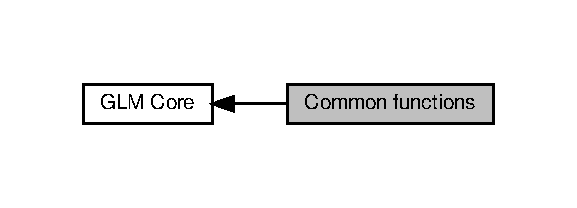
\includegraphics[width=277pt]{group__core__func__common}
\end{center}
\end{figure}
\subsection*{Functions}
\begin{DoxyCompactItemize}
\item 
{\footnotesize template$<$typename gen\+Type $>$ }\\\hyperlink{setup_8hpp_ab2d052de21a70539923e9bcbf6e83a51}{G\+L\+M\+\_\+\+F\+U\+N\+C\+\_\+\+D\+E\+CL} gen\+Type \hyperlink{group__core__func__common_gaea946f96ec1df259802effe9f532e1c1}{glm\+::abs} (gen\+Type const \&x)
\item 
{\footnotesize template$<$typename gen\+Type $>$ }\\\hyperlink{setup_8hpp_ab2d052de21a70539923e9bcbf6e83a51}{G\+L\+M\+\_\+\+F\+U\+N\+C\+\_\+\+D\+E\+CL} gen\+Type \hyperlink{group__core__func__common_gaa7afd59ab947e313d41cb6d9c655a80c}{glm\+::sign} (gen\+Type const \&x)
\item 
{\footnotesize template$<$typename gen\+Type $>$ }\\\hyperlink{setup_8hpp_ab2d052de21a70539923e9bcbf6e83a51}{G\+L\+M\+\_\+\+F\+U\+N\+C\+\_\+\+D\+E\+CL} gen\+Type \hyperlink{group__core__func__common_ga86350252cc9bf86421317460bbd1f21c}{glm\+::floor} (gen\+Type const \&x)
\item 
{\footnotesize template$<$typename gen\+Type $>$ }\\\hyperlink{setup_8hpp_ab2d052de21a70539923e9bcbf6e83a51}{G\+L\+M\+\_\+\+F\+U\+N\+C\+\_\+\+D\+E\+CL} gen\+Type \hyperlink{group__core__func__common_gadb091aed51e45872f6dc841affa41c5c}{glm\+::trunc} (gen\+Type const \&x)
\item 
{\footnotesize template$<$typename gen\+Type $>$ }\\\hyperlink{setup_8hpp_ab2d052de21a70539923e9bcbf6e83a51}{G\+L\+M\+\_\+\+F\+U\+N\+C\+\_\+\+D\+E\+CL} gen\+Type \hyperlink{group__core__func__common_ga75ebab3fe88a9c5c769135cf5a2649ef}{glm\+::round} (gen\+Type const \&x)
\item 
{\footnotesize template$<$typename gen\+Type $>$ }\\\hyperlink{setup_8hpp_ab2d052de21a70539923e9bcbf6e83a51}{G\+L\+M\+\_\+\+F\+U\+N\+C\+\_\+\+D\+E\+CL} gen\+Type \hyperlink{group__core__func__common_ga6535952553479a4bbca7f1f12a011b17}{glm\+::round\+Even} (gen\+Type const \&x)
\item 
{\footnotesize template$<$typename gen\+Type $>$ }\\\hyperlink{setup_8hpp_ab2d052de21a70539923e9bcbf6e83a51}{G\+L\+M\+\_\+\+F\+U\+N\+C\+\_\+\+D\+E\+CL} gen\+Type \hyperlink{group__core__func__common_gab81e02fff55c9391e28fa47e68c3c903}{glm\+::ceil} (gen\+Type const \&x)
\item 
{\footnotesize template$<$typename gen\+Type $>$ }\\\hyperlink{setup_8hpp_ab2d052de21a70539923e9bcbf6e83a51}{G\+L\+M\+\_\+\+F\+U\+N\+C\+\_\+\+D\+E\+CL} gen\+Type \hyperlink{group__core__func__common_gad04ac2908d032d5518d5f6c8403dbc8b}{glm\+::fract} (gen\+Type const \&x)
\item 
{\footnotesize template$<$typename gen\+Type $>$ }\\\hyperlink{setup_8hpp_ab2d052de21a70539923e9bcbf6e83a51}{G\+L\+M\+\_\+\+F\+U\+N\+C\+\_\+\+D\+E\+CL} gen\+Type \hyperlink{group__core__func__common_ga8cc8a75b05125fe1c30de43102ef42e1}{glm\+::mod} (gen\+Type const \&x, gen\+Type const \&y)
\item 
{\footnotesize template$<$typename gen\+Type $>$ }\\\hyperlink{setup_8hpp_ab2d052de21a70539923e9bcbf6e83a51}{G\+L\+M\+\_\+\+F\+U\+N\+C\+\_\+\+D\+E\+CL} gen\+Type \hyperlink{group__core__func__common_gad2127c78cb9e89ab462892b11417ded3}{glm\+::mod} (gen\+Type const \&x, typename gen\+Type\+::value\+\_\+type const \&y)
\item 
{\footnotesize template$<$typename gen\+Type $>$ }\\\hyperlink{setup_8hpp_ab2d052de21a70539923e9bcbf6e83a51}{G\+L\+M\+\_\+\+F\+U\+N\+C\+\_\+\+D\+E\+CL} gen\+Type \hyperlink{group__core__func__common_gae47da02eb07d660201c09a0df7298a05}{glm\+::modf} (gen\+Type const \&x, gen\+Type \&i)
\item 
{\footnotesize template$<$typename gen\+Type $>$ }\\\hyperlink{setup_8hpp_ab2d052de21a70539923e9bcbf6e83a51}{G\+L\+M\+\_\+\+F\+U\+N\+C\+\_\+\+D\+E\+CL} gen\+Type \hyperlink{group__core__func__common_ga3dc90dbd66c9ca1dd5625c93d9c50f02}{glm\+::min} (gen\+Type const \&x, gen\+Type const \&y)
\item 
{\footnotesize template$<$typename gen\+Type $>$ }\\\hyperlink{setup_8hpp_ab2d052de21a70539923e9bcbf6e83a51}{G\+L\+M\+\_\+\+F\+U\+N\+C\+\_\+\+D\+E\+CL} gen\+Type \hyperlink{group__core__func__common_gac0f3dec634730c146c121a6517441c9a}{glm\+::min} (gen\+Type const \&x, typename gen\+Type\+::value\+\_\+type const \&y)
\item 
{\footnotesize template$<$typename gen\+Type $>$ }\\\hyperlink{setup_8hpp_ab2d052de21a70539923e9bcbf6e83a51}{G\+L\+M\+\_\+\+F\+U\+N\+C\+\_\+\+D\+E\+CL} gen\+Type \hyperlink{group__core__func__common_gaa228561a9da55898f8f72ad2403fafac}{glm\+::max} (gen\+Type const \&x, gen\+Type const \&y)
\item 
{\footnotesize template$<$typename gen\+Type $>$ }\\\hyperlink{setup_8hpp_ab2d052de21a70539923e9bcbf6e83a51}{G\+L\+M\+\_\+\+F\+U\+N\+C\+\_\+\+D\+E\+CL} gen\+Type \hyperlink{group__core__func__common_ga30077cf0de58a7474450fb328ba456d7}{glm\+::max} (gen\+Type const \&x, typename gen\+Type\+::value\+\_\+type const \&y)
\item 
{\footnotesize template$<$typename gen\+Type $>$ }\\\hyperlink{setup_8hpp_ab2d052de21a70539923e9bcbf6e83a51}{G\+L\+M\+\_\+\+F\+U\+N\+C\+\_\+\+D\+E\+CL} gen\+Type \hyperlink{group__core__func__common_ga72e9e213c84f06a329a2a838b51200f4}{glm\+::clamp} (gen\+Type const \&x, gen\+Type const \&min\+Val, gen\+Type const \&max\+Val)
\item 
{\footnotesize template$<$typename gen\+Type , precision P$>$ }\\\hyperlink{setup_8hpp_ab2d052de21a70539923e9bcbf6e83a51}{G\+L\+M\+\_\+\+F\+U\+N\+C\+\_\+\+D\+E\+CL} gen\+Type \hyperlink{group__core__func__common_ga5409c55a5f3aaae3e02ed440a47380bb}{glm\+::clamp} (gen\+Type const \&x, typename gen\+Type\+::value\+\_\+type const \&min\+Val, typename gen\+Type\+::value\+\_\+type const \&max\+Val)
\item 
{\footnotesize template$<$typename T , typename U , precision P, template$<$ typename, precision $>$ class vec\+Type$>$ }\\\hyperlink{setup_8hpp_ab2d052de21a70539923e9bcbf6e83a51}{G\+L\+M\+\_\+\+F\+U\+N\+C\+\_\+\+D\+E\+CL} vec\+Type$<$ T, P $>$ \hyperlink{group__core__func__common_gadccbaffe46f369cf1a96b2aef92cbfdd}{glm\+::mix} (vec\+Type$<$ T, P $>$ const \&x, vec\+Type$<$ T, P $>$ const \&y, vec\+Type$<$ U, P $>$ const \&a)
\item 
{\footnotesize template$<$typename T , typename U , precision P, template$<$ typename, precision $>$ class vec\+Type$>$ }\\\hyperlink{setup_8hpp_ab2d052de21a70539923e9bcbf6e83a51}{G\+L\+M\+\_\+\+F\+U\+N\+C\+\_\+\+D\+E\+CL} vec\+Type$<$ T, P $>$ \hyperlink{group__core__func__common_gaa5c83ada94113757c0a555ab4f40cd6e}{glm\+::mix} (vec\+Type$<$ T, P $>$ const \&x, vec\+Type$<$ T, P $>$ const \&y, U const \&a)
\item 
{\footnotesize template$<$typename gen\+TypeT , typename gen\+TypeU $>$ }\\\hyperlink{setup_8hpp_ab2d052de21a70539923e9bcbf6e83a51}{G\+L\+M\+\_\+\+F\+U\+N\+C\+\_\+\+D\+E\+CL} gen\+TypeT \hyperlink{group__core__func__common_ga78aae7eea618ca112053d59fe03db239}{glm\+::mix} (gen\+TypeT const \&x, gen\+TypeT const \&y, gen\+TypeU const \&a)
\item 
{\footnotesize template$<$typename gen\+Type $>$ }\\\hyperlink{setup_8hpp_ab2d052de21a70539923e9bcbf6e83a51}{G\+L\+M\+\_\+\+F\+U\+N\+C\+\_\+\+D\+E\+CL} gen\+Type \hyperlink{group__core__func__common_gaf21c84759af7799f573865f70c2f0a86}{glm\+::step} (gen\+Type const \&edge, gen\+Type const \&x)
\item 
{\footnotesize template$<$template$<$ typename, precision $>$ class vec\+Type, typename T , precision P$>$ }\\\hyperlink{setup_8hpp_ab2d052de21a70539923e9bcbf6e83a51}{G\+L\+M\+\_\+\+F\+U\+N\+C\+\_\+\+D\+E\+CL} vec\+Type$<$ T, P $>$ \hyperlink{group__core__func__common_gae830a682901c0ba63c92a7d201bba007}{glm\+::step} (T const \&edge, vec\+Type$<$ T, P $>$ const \&x)
\item 
{\footnotesize template$<$typename gen\+Type $>$ }\\\hyperlink{setup_8hpp_ab2d052de21a70539923e9bcbf6e83a51}{G\+L\+M\+\_\+\+F\+U\+N\+C\+\_\+\+D\+E\+CL} gen\+Type \hyperlink{group__core__func__common_ga754103c8d2cdaf40f71429252457c10a}{glm\+::smoothstep} (gen\+Type const \&edge0, gen\+Type const \&edge1, gen\+Type const \&x)
\item 
{\footnotesize template$<$typename gen\+Type $>$ }\\\hyperlink{setup_8hpp_ab2d052de21a70539923e9bcbf6e83a51}{G\+L\+M\+\_\+\+F\+U\+N\+C\+\_\+\+D\+E\+CL} gen\+Type \hyperlink{group__core__func__common_ga1e7b9e668a0bd2f494a1d49b871a50ea}{glm\+::smoothstep} (typename gen\+Type\+::value\+\_\+type const \&edge0, typename gen\+Type\+::value\+\_\+type const \&edge1, gen\+Type const \&x)
\item 
{\footnotesize template$<$typename gen\+Type $>$ }\\\hyperlink{setup_8hpp_ab2d052de21a70539923e9bcbf6e83a51}{G\+L\+M\+\_\+\+F\+U\+N\+C\+\_\+\+D\+E\+CL} gen\+Type\+::bool\+\_\+type \hyperlink{group__core__func__common_ga8a9dec5200888766fbcb51b6a5898728}{glm\+::isnan} (gen\+Type const \&x)
\item 
{\footnotesize template$<$typename gen\+Type $>$ }\\\hyperlink{setup_8hpp_ab2d052de21a70539923e9bcbf6e83a51}{G\+L\+M\+\_\+\+F\+U\+N\+C\+\_\+\+D\+E\+CL} gen\+Type\+::bool\+\_\+type \hyperlink{group__core__func__common_ga9fce6a337c7e8ad089b9dc17c70cb873}{glm\+::isinf} (gen\+Type const \&x)
\item 
\hyperlink{setup_8hpp_ab2d052de21a70539923e9bcbf6e83a51}{G\+L\+M\+\_\+\+F\+U\+N\+C\+\_\+\+D\+E\+CL} int \hyperlink{group__core__func__common_gadc6a536a7bef046c3293d2ccad6d9ca2}{glm\+::float\+Bits\+To\+Int} (float const \&v)
\item 
{\footnotesize template$<$template$<$ typename, precision $>$ class vec\+Type, precision P$>$ }\\\hyperlink{setup_8hpp_ab2d052de21a70539923e9bcbf6e83a51}{G\+L\+M\+\_\+\+F\+U\+N\+C\+\_\+\+D\+E\+CL} vec\+Type$<$ int, P $>$ \hyperlink{group__core__func__common_gac4a0710238ae54c67931dd29a0b0f873}{glm\+::float\+Bits\+To\+Int} (vec\+Type$<$ float, P $>$ const \&v)
\item 
\hyperlink{setup_8hpp_ab2d052de21a70539923e9bcbf6e83a51}{G\+L\+M\+\_\+\+F\+U\+N\+C\+\_\+\+D\+E\+CL} \hyperlink{group__core__precision_ga4fd29415871152bfb5abd588334147c8}{uint} \hyperlink{group__core__func__common_ga748b4d2819b48d28ca09dc8733488873}{glm\+::float\+Bits\+To\+Uint} (float const \&v)
\item 
{\footnotesize template$<$template$<$ typename, precision $>$ class vec\+Type, precision P$>$ }\\\hyperlink{setup_8hpp_ab2d052de21a70539923e9bcbf6e83a51}{G\+L\+M\+\_\+\+F\+U\+N\+C\+\_\+\+D\+E\+CL} vec\+Type$<$ \hyperlink{group__core__precision_ga4fd29415871152bfb5abd588334147c8}{uint}, P $>$ \hyperlink{group__core__func__common_ga1804d4c443605d8a27be644aa461afe4}{glm\+::float\+Bits\+To\+Uint} (vec\+Type$<$ float, P $>$ const \&v)
\item 
\hyperlink{setup_8hpp_ab2d052de21a70539923e9bcbf6e83a51}{G\+L\+M\+\_\+\+F\+U\+N\+C\+\_\+\+D\+E\+CL} float \hyperlink{group__core__func__common_ga2650dc57b2148a6ffbce20944fb4d97a}{glm\+::int\+Bits\+To\+Float} (int const \&v)
\item 
{\footnotesize template$<$template$<$ typename, precision $>$ class vec\+Type, precision P$>$ }\\\hyperlink{setup_8hpp_ab2d052de21a70539923e9bcbf6e83a51}{G\+L\+M\+\_\+\+F\+U\+N\+C\+\_\+\+D\+E\+CL} vec\+Type$<$ float, P $>$ \hyperlink{group__core__func__common_gad21ab176dd0e6b59d923db5efca87f4e}{glm\+::int\+Bits\+To\+Float} (vec\+Type$<$ int, P $>$ const \&v)
\item 
\hyperlink{setup_8hpp_ab2d052de21a70539923e9bcbf6e83a51}{G\+L\+M\+\_\+\+F\+U\+N\+C\+\_\+\+D\+E\+CL} float \hyperlink{group__core__func__common_ga97464ca9ff4267de30ea408f700d4ca8}{glm\+::uint\+Bits\+To\+Float} (\hyperlink{group__core__precision_ga4fd29415871152bfb5abd588334147c8}{uint} const \&v)
\item 
{\footnotesize template$<$template$<$ typename, precision $>$ class vec\+Type, precision P$>$ }\\\hyperlink{setup_8hpp_ab2d052de21a70539923e9bcbf6e83a51}{G\+L\+M\+\_\+\+F\+U\+N\+C\+\_\+\+D\+E\+CL} vec\+Type$<$ float, P $>$ \hyperlink{group__core__func__common_ga3acab37650ecd792dc84548094b58684}{glm\+::uint\+Bits\+To\+Float} (vec\+Type$<$ \hyperlink{group__core__precision_ga4fd29415871152bfb5abd588334147c8}{uint}, P $>$ const \&v)
\item 
{\footnotesize template$<$typename gen\+Type $>$ }\\\hyperlink{setup_8hpp_ab2d052de21a70539923e9bcbf6e83a51}{G\+L\+M\+\_\+\+F\+U\+N\+C\+\_\+\+D\+E\+CL} gen\+Type \hyperlink{group__core__func__common_gad0f444d4b81cc53c3b6edf5aa25078c2}{glm\+::fma} (gen\+Type const \&a, gen\+Type const \&b, gen\+Type const \&c)
\item 
{\footnotesize template$<$typename gen\+Type , typename gen\+I\+Type $>$ }\\\hyperlink{setup_8hpp_ab2d052de21a70539923e9bcbf6e83a51}{G\+L\+M\+\_\+\+F\+U\+N\+C\+\_\+\+D\+E\+CL} gen\+Type \hyperlink{group__core__func__common_ga20620e83544d1a988857a3bc4ebe0e1d}{glm\+::frexp} (gen\+Type const \&x, gen\+I\+Type \&\hyperlink{group__core__func__exponential_gae154699ba6bda068d4b87cf9b987381f}{exp})
\item 
{\footnotesize template$<$typename gen\+Type , typename gen\+I\+Type $>$ }\\\hyperlink{setup_8hpp_ab2d052de21a70539923e9bcbf6e83a51}{G\+L\+M\+\_\+\+F\+U\+N\+C\+\_\+\+D\+E\+CL} gen\+Type \hyperlink{group__core__func__common_ga52e319d7289b849ec92055abd4830533}{glm\+::ldexp} (gen\+Type const \&x, gen\+I\+Type const \&\hyperlink{group__core__func__exponential_gae154699ba6bda068d4b87cf9b987381f}{exp})
\end{DoxyCompactItemize}


\subsection{Detailed Description}
These all operate component-\/wise. The description is per component. 

\subsection{Function Documentation}
\mbox{\Hypertarget{group__core__func__common_gaea946f96ec1df259802effe9f532e1c1}\label{group__core__func__common_gaea946f96ec1df259802effe9f532e1c1}} 
\index{Common functions@{Common functions}!abs@{abs}}
\index{abs@{abs}!Common functions@{Common functions}}
\subsubsection{\texorpdfstring{abs()}{abs()}}
{\footnotesize\ttfamily template$<$typename gen\+Type $>$ \\
\hyperlink{setup_8hpp_ab2d052de21a70539923e9bcbf6e83a51}{G\+L\+M\+\_\+\+F\+U\+N\+C\+\_\+\+D\+E\+CL} gen\+Type glm\+::abs (\begin{DoxyParamCaption}\item[{gen\+Type const \&}]{x }\end{DoxyParamCaption})}

Returns x if x $>$= 0; otherwise, it returns -\/x.


\begin{DoxyTemplParams}{Template Parameters}
{\em gen\+Type} & floating-\/point or signed integer; scalar or vector types.\\
\hline
\end{DoxyTemplParams}
\begin{DoxySeeAlso}{See also}
\href{http://www.opengl.org/sdk/docs/manglsl/xhtml/abs.xml}{\tt G\+L\+SL abs man page} 

\href{http://www.opengl.org/registry/doc/GLSLangSpec.4.20.8.pdf}{\tt G\+L\+SL 4.\+20.\+8 specification, section 8.\+3 Common Functions} 
\end{DoxySeeAlso}
\mbox{\Hypertarget{group__core__func__common_gab81e02fff55c9391e28fa47e68c3c903}\label{group__core__func__common_gab81e02fff55c9391e28fa47e68c3c903}} 
\index{Common functions@{Common functions}!ceil@{ceil}}
\index{ceil@{ceil}!Common functions@{Common functions}}
\subsubsection{\texorpdfstring{ceil()}{ceil()}}
{\footnotesize\ttfamily template$<$typename gen\+Type $>$ \\
\hyperlink{setup_8hpp_ab2d052de21a70539923e9bcbf6e83a51}{G\+L\+M\+\_\+\+F\+U\+N\+C\+\_\+\+D\+E\+CL} gen\+Type glm\+::ceil (\begin{DoxyParamCaption}\item[{gen\+Type const \&}]{x }\end{DoxyParamCaption})}

Returns a value equal to the nearest integer that is greater than or equal to x.


\begin{DoxyTemplParams}{Template Parameters}
{\em gen\+Type} & Floating-\/point scalar or vector types.\\
\hline
\end{DoxyTemplParams}
\begin{DoxySeeAlso}{See also}
\href{http://www.opengl.org/sdk/docs/manglsl/xhtml/ceil.xml}{\tt G\+L\+SL ceil man page} 

\href{http://www.opengl.org/registry/doc/GLSLangSpec.4.20.8.pdf}{\tt G\+L\+SL 4.\+20.\+8 specification, section 8.\+3 Common Functions} 
\end{DoxySeeAlso}


Definition at line 258 of file func\+\_\+common.\+inl.

\mbox{\Hypertarget{group__core__func__common_ga72e9e213c84f06a329a2a838b51200f4}\label{group__core__func__common_ga72e9e213c84f06a329a2a838b51200f4}} 
\index{Common functions@{Common functions}!clamp@{clamp}}
\index{clamp@{clamp}!Common functions@{Common functions}}
\subsubsection{\texorpdfstring{clamp()}{clamp()}\hspace{0.1cm}{\footnotesize\ttfamily [1/2]}}
{\footnotesize\ttfamily template$<$typename gen\+Type $>$ \\
\hyperlink{setup_8hpp_ab2d052de21a70539923e9bcbf6e83a51}{G\+L\+M\+\_\+\+F\+U\+N\+C\+\_\+\+D\+E\+CL} gen\+Type glm\+::clamp (\begin{DoxyParamCaption}\item[{gen\+Type const \&}]{x,  }\item[{gen\+Type const \&}]{min\+Val,  }\item[{gen\+Type const \&}]{max\+Val }\end{DoxyParamCaption})}

Returns min(max(x, min\+Val), max\+Val) for each component in x using the floating-\/point values min\+Val and max\+Val.


\begin{DoxyTemplParams}{Template Parameters}
{\em gen\+Type} & Floating-\/point or integer; scalar or vector types.\\
\hline
\end{DoxyTemplParams}
\begin{DoxySeeAlso}{See also}
\href{http://www.opengl.org/sdk/docs/manglsl/xhtml/clamp.xml}{\tt G\+L\+SL clamp man page} 

\href{http://www.opengl.org/registry/doc/GLSLangSpec.4.20.8.pdf}{\tt G\+L\+SL 4.\+20.\+8 specification, section 8.\+3 Common Functions} 
\end{DoxySeeAlso}


Definition at line 404 of file func\+\_\+common.\+inl.

\mbox{\Hypertarget{group__core__func__common_ga5409c55a5f3aaae3e02ed440a47380bb}\label{group__core__func__common_ga5409c55a5f3aaae3e02ed440a47380bb}} 
\index{Common functions@{Common functions}!clamp@{clamp}}
\index{clamp@{clamp}!Common functions@{Common functions}}
\subsubsection{\texorpdfstring{clamp()}{clamp()}\hspace{0.1cm}{\footnotesize\ttfamily [2/2]}}
{\footnotesize\ttfamily template$<$typename gen\+Type , precision P$>$ \\
\hyperlink{setup_8hpp_ab2d052de21a70539923e9bcbf6e83a51}{G\+L\+M\+\_\+\+F\+U\+N\+C\+\_\+\+D\+E\+CL} gen\+Type glm\+::clamp (\begin{DoxyParamCaption}\item[{gen\+Type const \&}]{x,  }\item[{typename gen\+Type\+::value\+\_\+type const \&}]{min\+Val,  }\item[{typename gen\+Type\+::value\+\_\+type const \&}]{max\+Val }\end{DoxyParamCaption})}

\mbox{\Hypertarget{group__core__func__common_gadc6a536a7bef046c3293d2ccad6d9ca2}\label{group__core__func__common_gadc6a536a7bef046c3293d2ccad6d9ca2}} 
\index{Common functions@{Common functions}!float\+Bits\+To\+Int@{float\+Bits\+To\+Int}}
\index{float\+Bits\+To\+Int@{float\+Bits\+To\+Int}!Common functions@{Common functions}}
\subsubsection{\texorpdfstring{float\+Bits\+To\+Int()}{floatBitsToInt()}\hspace{0.1cm}{\footnotesize\ttfamily [1/2]}}
{\footnotesize\ttfamily \hyperlink{setup_8hpp_a33fdea6f91c5f834105f7415e2a64407}{G\+L\+M\+\_\+\+F\+U\+N\+C\+\_\+\+Q\+U\+A\+L\+I\+F\+I\+ER} int glm\+::float\+Bits\+To\+Int (\begin{DoxyParamCaption}\item[{float const \&}]{v }\end{DoxyParamCaption})}

Returns a signed integer value representing the encoding of a floating-\/point value. The floating-\/point value\textquotesingle{}s bit-\/level representation is preserved.

\begin{DoxySeeAlso}{See also}
\href{http://www.opengl.org/sdk/docs/manglsl/xhtml/floatBitsToInt.xml}{\tt G\+L\+SL float\+Bits\+To\+Int man page} 

\href{http://www.opengl.org/registry/doc/GLSLangSpec.4.20.8.pdf}{\tt G\+L\+SL 4.\+20.\+8 specification, section 8.\+3 Common Functions} 
\end{DoxySeeAlso}


Definition at line 851 of file func\+\_\+common.\+inl.

\mbox{\Hypertarget{group__core__func__common_gac4a0710238ae54c67931dd29a0b0f873}\label{group__core__func__common_gac4a0710238ae54c67931dd29a0b0f873}} 
\index{Common functions@{Common functions}!float\+Bits\+To\+Int@{float\+Bits\+To\+Int}}
\index{float\+Bits\+To\+Int@{float\+Bits\+To\+Int}!Common functions@{Common functions}}
\subsubsection{\texorpdfstring{float\+Bits\+To\+Int()}{floatBitsToInt()}\hspace{0.1cm}{\footnotesize\ttfamily [2/2]}}
{\footnotesize\ttfamily template$<$template$<$ typename, precision $>$ class vec\+Type, precision P$>$ \\
\hyperlink{setup_8hpp_ab2d052de21a70539923e9bcbf6e83a51}{G\+L\+M\+\_\+\+F\+U\+N\+C\+\_\+\+D\+E\+CL} vec\+Type$<$int, P$>$ glm\+::float\+Bits\+To\+Int (\begin{DoxyParamCaption}\item[{vec\+Type$<$ float, P $>$ const \&}]{v }\end{DoxyParamCaption})}

Returns a signed integer value representing the encoding of a floating-\/point value. The floatingpoint value\textquotesingle{}s bit-\/level representation is preserved.

\begin{DoxySeeAlso}{See also}
\href{http://www.opengl.org/sdk/docs/manglsl/xhtml/floatBitsToInt.xml}{\tt G\+L\+SL float\+Bits\+To\+Int man page} 

\href{http://www.opengl.org/registry/doc/GLSLangSpec.4.20.8.pdf}{\tt G\+L\+SL 4.\+20.\+8 specification, section 8.\+3 Common Functions} 
\end{DoxySeeAlso}


Definition at line 857 of file func\+\_\+common.\+inl.

\mbox{\Hypertarget{group__core__func__common_ga748b4d2819b48d28ca09dc8733488873}\label{group__core__func__common_ga748b4d2819b48d28ca09dc8733488873}} 
\index{Common functions@{Common functions}!float\+Bits\+To\+Uint@{float\+Bits\+To\+Uint}}
\index{float\+Bits\+To\+Uint@{float\+Bits\+To\+Uint}!Common functions@{Common functions}}
\subsubsection{\texorpdfstring{float\+Bits\+To\+Uint()}{floatBitsToUint()}\hspace{0.1cm}{\footnotesize\ttfamily [1/2]}}
{\footnotesize\ttfamily \hyperlink{setup_8hpp_a33fdea6f91c5f834105f7415e2a64407}{G\+L\+M\+\_\+\+F\+U\+N\+C\+\_\+\+Q\+U\+A\+L\+I\+F\+I\+ER} \hyperlink{group__core__precision_ga4fd29415871152bfb5abd588334147c8}{uint} glm\+::float\+Bits\+To\+Uint (\begin{DoxyParamCaption}\item[{float const \&}]{v }\end{DoxyParamCaption})}

Returns a unsigned integer value representing the encoding of a floating-\/point value. The floatingpoint value\textquotesingle{}s bit-\/level representation is preserved.

\begin{DoxySeeAlso}{See also}
\href{http://www.opengl.org/sdk/docs/manglsl/xhtml/floatBitsToUint.xml}{\tt G\+L\+SL float\+Bits\+To\+Uint man page} 

\href{http://www.opengl.org/registry/doc/GLSLangSpec.4.20.8.pdf}{\tt G\+L\+SL 4.\+20.\+8 specification, section 8.\+3 Common Functions} 
\end{DoxySeeAlso}


Definition at line 862 of file func\+\_\+common.\+inl.

\mbox{\Hypertarget{group__core__func__common_ga1804d4c443605d8a27be644aa461afe4}\label{group__core__func__common_ga1804d4c443605d8a27be644aa461afe4}} 
\index{Common functions@{Common functions}!float\+Bits\+To\+Uint@{float\+Bits\+To\+Uint}}
\index{float\+Bits\+To\+Uint@{float\+Bits\+To\+Uint}!Common functions@{Common functions}}
\subsubsection{\texorpdfstring{float\+Bits\+To\+Uint()}{floatBitsToUint()}\hspace{0.1cm}{\footnotesize\ttfamily [2/2]}}
{\footnotesize\ttfamily template$<$template$<$ typename, precision $>$ class vec\+Type, precision P$>$ \\
\hyperlink{setup_8hpp_ab2d052de21a70539923e9bcbf6e83a51}{G\+L\+M\+\_\+\+F\+U\+N\+C\+\_\+\+D\+E\+CL} vec\+Type$<$\hyperlink{group__core__precision_ga4fd29415871152bfb5abd588334147c8}{uint}, P$>$ glm\+::float\+Bits\+To\+Uint (\begin{DoxyParamCaption}\item[{vec\+Type$<$ float, P $>$ const \&}]{v }\end{DoxyParamCaption})}

Returns a unsigned integer value representing the encoding of a floating-\/point value. The floatingpoint value\textquotesingle{}s bit-\/level representation is preserved.

\begin{DoxySeeAlso}{See also}
\href{http://www.opengl.org/sdk/docs/manglsl/xhtml/floatBitsToUint.xml}{\tt G\+L\+SL float\+Bits\+To\+Uint man page} 

\href{http://www.opengl.org/registry/doc/GLSLangSpec.4.20.8.pdf}{\tt G\+L\+SL 4.\+20.\+8 specification, section 8.\+3 Common Functions} 
\end{DoxySeeAlso}


Definition at line 868 of file func\+\_\+common.\+inl.

\mbox{\Hypertarget{group__core__func__common_ga86350252cc9bf86421317460bbd1f21c}\label{group__core__func__common_ga86350252cc9bf86421317460bbd1f21c}} 
\index{Common functions@{Common functions}!floor@{floor}}
\index{floor@{floor}!Common functions@{Common functions}}
\subsubsection{\texorpdfstring{floor()}{floor()}}
{\footnotesize\ttfamily template$<$typename gen\+Type $>$ \\
\hyperlink{setup_8hpp_ab2d052de21a70539923e9bcbf6e83a51}{G\+L\+M\+\_\+\+F\+U\+N\+C\+\_\+\+D\+E\+CL} gen\+Type glm\+::floor (\begin{DoxyParamCaption}\item[{gen\+Type const \&}]{x }\end{DoxyParamCaption})}

Returns a value equal to the nearest integer that is less then or equal to x.


\begin{DoxyTemplParams}{Template Parameters}
{\em gen\+Type} & Floating-\/point scalar or vector types.\\
\hline
\end{DoxyTemplParams}
\begin{DoxySeeAlso}{See also}
\href{http://www.opengl.org/sdk/docs/manglsl/xhtml/floor.xml}{\tt G\+L\+SL floor man page} 

\href{http://www.opengl.org/registry/doc/GLSLangSpec.4.20.8.pdf}{\tt G\+L\+SL 4.\+20.\+8 specification, section 8.\+3 Common Functions} 
\end{DoxySeeAlso}


Definition at line 170 of file func\+\_\+common.\+inl.

\mbox{\Hypertarget{group__core__func__common_gad0f444d4b81cc53c3b6edf5aa25078c2}\label{group__core__func__common_gad0f444d4b81cc53c3b6edf5aa25078c2}} 
\index{Common functions@{Common functions}!fma@{fma}}
\index{fma@{fma}!Common functions@{Common functions}}
\subsubsection{\texorpdfstring{fma()}{fma()}}
{\footnotesize\ttfamily template$<$typename gen\+Type $>$ \\
\hyperlink{setup_8hpp_ab2d052de21a70539923e9bcbf6e83a51}{G\+L\+M\+\_\+\+F\+U\+N\+C\+\_\+\+D\+E\+CL} gen\+Type glm\+::fma (\begin{DoxyParamCaption}\item[{gen\+Type const \&}]{a,  }\item[{gen\+Type const \&}]{b,  }\item[{gen\+Type const \&}]{c }\end{DoxyParamCaption})}

Computes and returns a $\ast$ b + c.


\begin{DoxyTemplParams}{Template Parameters}
{\em gen\+Type} & Floating-\/point scalar or vector types.\\
\hline
\end{DoxyTemplParams}
\begin{DoxySeeAlso}{See also}
\href{http://www.opengl.org/sdk/docs/manglsl/xhtml/fma.xml}{\tt G\+L\+SL fma man page} 

\href{http://www.opengl.org/registry/doc/GLSLangSpec.4.20.8.pdf}{\tt G\+L\+SL 4.\+20.\+8 specification, section 8.\+3 Common Functions} 
\end{DoxySeeAlso}


Definition at line 897 of file func\+\_\+common.\+inl.

\mbox{\Hypertarget{group__core__func__common_gad04ac2908d032d5518d5f6c8403dbc8b}\label{group__core__func__common_gad04ac2908d032d5518d5f6c8403dbc8b}} 
\index{Common functions@{Common functions}!fract@{fract}}
\index{fract@{fract}!Common functions@{Common functions}}
\subsubsection{\texorpdfstring{fract()}{fract()}}
{\footnotesize\ttfamily template$<$typename gen\+Type $>$ \\
\hyperlink{setup_8hpp_ab2d052de21a70539923e9bcbf6e83a51}{G\+L\+M\+\_\+\+F\+U\+N\+C\+\_\+\+D\+E\+CL} gen\+Type glm\+::fract (\begin{DoxyParamCaption}\item[{gen\+Type const \&}]{x }\end{DoxyParamCaption})}

Return x -\/ floor(x).


\begin{DoxyTemplParams}{Template Parameters}
{\em gen\+Type} & Floating-\/point scalar or vector types.\\
\hline
\end{DoxyTemplParams}
\begin{DoxySeeAlso}{See also}
\href{http://www.opengl.org/sdk/docs/manglsl/xhtml/fract.xml}{\tt G\+L\+SL fract man page} 

\href{http://www.opengl.org/registry/doc/GLSLangSpec.4.20.8.pdf}{\tt G\+L\+SL 4.\+20.\+8 specification, section 8.\+3 Common Functions} 
\end{DoxySeeAlso}


Definition at line 272 of file func\+\_\+common.\+inl.

\mbox{\Hypertarget{group__core__func__common_ga20620e83544d1a988857a3bc4ebe0e1d}\label{group__core__func__common_ga20620e83544d1a988857a3bc4ebe0e1d}} 
\index{Common functions@{Common functions}!frexp@{frexp}}
\index{frexp@{frexp}!Common functions@{Common functions}}
\subsubsection{\texorpdfstring{frexp()}{frexp()}}
{\footnotesize\ttfamily template$<$typename gen\+Type , typename gen\+I\+Type $>$ \\
\hyperlink{setup_8hpp_ab2d052de21a70539923e9bcbf6e83a51}{G\+L\+M\+\_\+\+F\+U\+N\+C\+\_\+\+D\+E\+CL} gen\+Type glm\+::frexp (\begin{DoxyParamCaption}\item[{gen\+Type const \&}]{x,  }\item[{gen\+I\+Type \&}]{exp }\end{DoxyParamCaption})}

Splits x into a floating-\/point significand in the range \mbox{[}0.\+5, 1.\+0) and an integral exponent of two, such that\+: x = significand $\ast$ exp(2, exponent)

The significand is returned by the function and the exponent is returned in the parameter exp. For a floating-\/point value of zero, the significant and exponent are both zero. For a floating-\/point value that is an infinity or is not a number, the results are undefined.


\begin{DoxyTemplParams}{Template Parameters}
{\em gen\+Type} & Floating-\/point scalar or vector types.\\
\hline
\end{DoxyTemplParams}
\begin{DoxySeeAlso}{See also}
\href{http://www.opengl.org/sdk/docs/manglsl/xhtml/frexp.xml}{\tt G\+L\+SL frexp man page} 

\href{http://www.opengl.org/registry/doc/GLSLangSpec.4.20.8.pdf}{\tt G\+L\+SL 4.\+20.\+8 specification, section 8.\+3 Common Functions} 
\end{DoxySeeAlso}
\mbox{\Hypertarget{group__core__func__common_ga2650dc57b2148a6ffbce20944fb4d97a}\label{group__core__func__common_ga2650dc57b2148a6ffbce20944fb4d97a}} 
\index{Common functions@{Common functions}!int\+Bits\+To\+Float@{int\+Bits\+To\+Float}}
\index{int\+Bits\+To\+Float@{int\+Bits\+To\+Float}!Common functions@{Common functions}}
\subsubsection{\texorpdfstring{int\+Bits\+To\+Float()}{intBitsToFloat()}\hspace{0.1cm}{\footnotesize\ttfamily [1/2]}}
{\footnotesize\ttfamily \hyperlink{setup_8hpp_a33fdea6f91c5f834105f7415e2a64407}{G\+L\+M\+\_\+\+F\+U\+N\+C\+\_\+\+Q\+U\+A\+L\+I\+F\+I\+ER} float glm\+::int\+Bits\+To\+Float (\begin{DoxyParamCaption}\item[{int const \&}]{v }\end{DoxyParamCaption})}

Returns a floating-\/point value corresponding to a signed integer encoding of a floating-\/point value. If an inf or NaN is passed in, it will not signal, and the resulting floating point value is unspecified. Otherwise, the bit-\/level representation is preserved.

\begin{DoxySeeAlso}{See also}
\href{http://www.opengl.org/sdk/docs/manglsl/xhtml/intBitsToFloat.xml}{\tt G\+L\+SL int\+Bits\+To\+Float man page} 

\href{http://www.opengl.org/registry/doc/GLSLangSpec.4.20.8.pdf}{\tt G\+L\+SL 4.\+20.\+8 specification, section 8.\+3 Common Functions} 
\end{DoxySeeAlso}


Definition at line 873 of file func\+\_\+common.\+inl.

\mbox{\Hypertarget{group__core__func__common_gad21ab176dd0e6b59d923db5efca87f4e}\label{group__core__func__common_gad21ab176dd0e6b59d923db5efca87f4e}} 
\index{Common functions@{Common functions}!int\+Bits\+To\+Float@{int\+Bits\+To\+Float}}
\index{int\+Bits\+To\+Float@{int\+Bits\+To\+Float}!Common functions@{Common functions}}
\subsubsection{\texorpdfstring{int\+Bits\+To\+Float()}{intBitsToFloat()}\hspace{0.1cm}{\footnotesize\ttfamily [2/2]}}
{\footnotesize\ttfamily template$<$template$<$ typename, precision $>$ class vec\+Type, precision P$>$ \\
\hyperlink{setup_8hpp_ab2d052de21a70539923e9bcbf6e83a51}{G\+L\+M\+\_\+\+F\+U\+N\+C\+\_\+\+D\+E\+CL} vec\+Type$<$float, P$>$ glm\+::int\+Bits\+To\+Float (\begin{DoxyParamCaption}\item[{vec\+Type$<$ int, P $>$ const \&}]{v }\end{DoxyParamCaption})}

Returns a floating-\/point value corresponding to a signed integer encoding of a floating-\/point value. If an inf or NaN is passed in, it will not signal, and the resulting floating point value is unspecified. Otherwise, the bit-\/level representation is preserved.

\begin{DoxySeeAlso}{See also}
\href{http://www.opengl.org/sdk/docs/manglsl/xhtml/intBitsToFloat.xml}{\tt G\+L\+SL int\+Bits\+To\+Float man page} 

\href{http://www.opengl.org/registry/doc/GLSLangSpec.4.20.8.pdf}{\tt G\+L\+SL 4.\+20.\+8 specification, section 8.\+3 Common Functions} 
\end{DoxySeeAlso}


Definition at line 879 of file func\+\_\+common.\+inl.

\mbox{\Hypertarget{group__core__func__common_ga9fce6a337c7e8ad089b9dc17c70cb873}\label{group__core__func__common_ga9fce6a337c7e8ad089b9dc17c70cb873}} 
\index{Common functions@{Common functions}!isinf@{isinf}}
\index{isinf@{isinf}!Common functions@{Common functions}}
\subsubsection{\texorpdfstring{isinf()}{isinf()}}
{\footnotesize\ttfamily template$<$typename gen\+Type $>$ \\
\hyperlink{setup_8hpp_ab2d052de21a70539923e9bcbf6e83a51}{G\+L\+M\+\_\+\+F\+U\+N\+C\+\_\+\+D\+E\+CL} gen\+Type\+::bool\+\_\+type glm\+::isinf (\begin{DoxyParamCaption}\item[{gen\+Type const \&}]{x }\end{DoxyParamCaption})}

Returns true if x holds a positive infinity or negative infinity representation in the underlying implementation\textquotesingle{}s set of floating point representations. Returns false otherwise, including for implementations with no infinity representations.


\begin{DoxyTemplParams}{Template Parameters}
{\em gen\+Type} & Floating-\/point scalar or vector types.\\
\hline
\end{DoxyTemplParams}
\begin{DoxySeeAlso}{See also}
\href{http://www.opengl.org/sdk/docs/manglsl/xhtml/isinf.xml}{\tt G\+L\+SL isinf man page} 

\href{http://www.opengl.org/registry/doc/GLSLangSpec.4.20.8.pdf}{\tt G\+L\+SL 4.\+20.\+8 specification, section 8.\+3 Common Functions} 
\end{DoxySeeAlso}


Definition at line 780 of file func\+\_\+common.\+inl.

\mbox{\Hypertarget{group__core__func__common_ga8a9dec5200888766fbcb51b6a5898728}\label{group__core__func__common_ga8a9dec5200888766fbcb51b6a5898728}} 
\index{Common functions@{Common functions}!isnan@{isnan}}
\index{isnan@{isnan}!Common functions@{Common functions}}
\subsubsection{\texorpdfstring{isnan()}{isnan()}}
{\footnotesize\ttfamily template$<$typename gen\+Type $>$ \\
\hyperlink{setup_8hpp_ab2d052de21a70539923e9bcbf6e83a51}{G\+L\+M\+\_\+\+F\+U\+N\+C\+\_\+\+D\+E\+CL} gen\+Type\+::bool\+\_\+type glm\+::isnan (\begin{DoxyParamCaption}\item[{gen\+Type const \&}]{x }\end{DoxyParamCaption})}

Returns true if x holds a NaN (not a number) representation in the underlying implementation\textquotesingle{}s set of floating point representations. Returns false otherwise, including for implementations with no NaN representations.

/!\textbackslash{} When using compiler fast math, this function may fail.


\begin{DoxyTemplParams}{Template Parameters}
{\em gen\+Type} & Floating-\/point scalar or vector types.\\
\hline
\end{DoxyTemplParams}
\begin{DoxySeeAlso}{See also}
\href{http://www.opengl.org/sdk/docs/manglsl/xhtml/isnan.xml}{\tt G\+L\+SL isnan man page} 

\href{http://www.opengl.org/registry/doc/GLSLangSpec.4.20.8.pdf}{\tt G\+L\+SL 4.\+20.\+8 specification, section 8.\+3 Common Functions} 
\end{DoxySeeAlso}


Definition at line 710 of file func\+\_\+common.\+inl.

\mbox{\Hypertarget{group__core__func__common_ga52e319d7289b849ec92055abd4830533}\label{group__core__func__common_ga52e319d7289b849ec92055abd4830533}} 
\index{Common functions@{Common functions}!ldexp@{ldexp}}
\index{ldexp@{ldexp}!Common functions@{Common functions}}
\subsubsection{\texorpdfstring{ldexp()}{ldexp()}}
{\footnotesize\ttfamily template$<$typename gen\+Type , typename gen\+I\+Type $>$ \\
\hyperlink{setup_8hpp_ab2d052de21a70539923e9bcbf6e83a51}{G\+L\+M\+\_\+\+F\+U\+N\+C\+\_\+\+D\+E\+CL} gen\+Type glm\+::ldexp (\begin{DoxyParamCaption}\item[{gen\+Type const \&}]{x,  }\item[{gen\+I\+Type const \&}]{exp }\end{DoxyParamCaption})}

Builds a floating-\/point number from x and the corresponding integral exponent of two in exp, returning\+: significand $\ast$ exp(2, exponent)

If this product is too large to be represented in the floating-\/point type, the result is undefined.


\begin{DoxyTemplParams}{Template Parameters}
{\em gen\+Type} & Floating-\/point scalar or vector types.\\
\hline
\end{DoxyTemplParams}
\begin{DoxySeeAlso}{See also}
\href{http://www.opengl.org/sdk/docs/manglsl/xhtml/ldexp.xml}{\tt G\+L\+SL ldexp man page}; 

\href{http://www.opengl.org/registry/doc/GLSLangSpec.4.20.8.pdf}{\tt G\+L\+SL 4.\+20.\+8 specification, section 8.\+3 Common Functions} 
\end{DoxySeeAlso}
\mbox{\Hypertarget{group__core__func__common_gaa228561a9da55898f8f72ad2403fafac}\label{group__core__func__common_gaa228561a9da55898f8f72ad2403fafac}} 
\index{Common functions@{Common functions}!max@{max}}
\index{max@{max}!Common functions@{Common functions}}
\subsubsection{\texorpdfstring{max()}{max()}\hspace{0.1cm}{\footnotesize\ttfamily [1/2]}}
{\footnotesize\ttfamily template$<$typename gen\+Type $>$ \\
\hyperlink{setup_8hpp_ab2d052de21a70539923e9bcbf6e83a51}{G\+L\+M\+\_\+\+F\+U\+N\+C\+\_\+\+D\+E\+CL} gen\+Type glm\+::max (\begin{DoxyParamCaption}\item[{gen\+Type const \&}]{x,  }\item[{gen\+Type const \&}]{y }\end{DoxyParamCaption})}

Returns y if x $<$ y; otherwise, it returns x.


\begin{DoxyTemplParams}{Template Parameters}
{\em gen\+Type} & Floating-\/point or integer; scalar or vector types.\\
\hline
\end{DoxyTemplParams}
\begin{DoxySeeAlso}{See also}
\href{http://www.opengl.org/sdk/docs/manglsl/xhtml/max.xml}{\tt G\+L\+SL max man page} 

\href{http://www.opengl.org/registry/doc/GLSLangSpec.4.20.8.pdf}{\tt G\+L\+SL 4.\+20.\+8 specification, section 8.\+3 Common Functions} 
\end{DoxySeeAlso}


Definition at line 386 of file func\+\_\+common.\+inl.

\mbox{\Hypertarget{group__core__func__common_ga30077cf0de58a7474450fb328ba456d7}\label{group__core__func__common_ga30077cf0de58a7474450fb328ba456d7}} 
\index{Common functions@{Common functions}!max@{max}}
\index{max@{max}!Common functions@{Common functions}}
\subsubsection{\texorpdfstring{max()}{max()}\hspace{0.1cm}{\footnotesize\ttfamily [2/2]}}
{\footnotesize\ttfamily template$<$typename gen\+Type $>$ \\
\hyperlink{setup_8hpp_ab2d052de21a70539923e9bcbf6e83a51}{G\+L\+M\+\_\+\+F\+U\+N\+C\+\_\+\+D\+E\+CL} gen\+Type glm\+::max (\begin{DoxyParamCaption}\item[{gen\+Type const \&}]{x,  }\item[{typename gen\+Type\+::value\+\_\+type const \&}]{y }\end{DoxyParamCaption})}

\mbox{\Hypertarget{group__core__func__common_ga3dc90dbd66c9ca1dd5625c93d9c50f02}\label{group__core__func__common_ga3dc90dbd66c9ca1dd5625c93d9c50f02}} 
\index{Common functions@{Common functions}!min@{min}}
\index{min@{min}!Common functions@{Common functions}}
\subsubsection{\texorpdfstring{min()}{min()}\hspace{0.1cm}{\footnotesize\ttfamily [1/2]}}
{\footnotesize\ttfamily template$<$typename gen\+Type $>$ \\
\hyperlink{setup_8hpp_ab2d052de21a70539923e9bcbf6e83a51}{G\+L\+M\+\_\+\+F\+U\+N\+C\+\_\+\+D\+E\+CL} gen\+Type glm\+::min (\begin{DoxyParamCaption}\item[{gen\+Type const \&}]{x,  }\item[{gen\+Type const \&}]{y }\end{DoxyParamCaption})}

Returns y if y $<$ x; otherwise, it returns x.


\begin{DoxyTemplParams}{Template Parameters}
{\em gen\+Type} & Floating-\/point or integer; scalar or vector types.\\
\hline
\end{DoxyTemplParams}
\begin{DoxySeeAlso}{See also}
\href{http://www.opengl.org/sdk/docs/manglsl/xhtml/min.xml}{\tt G\+L\+SL min man page} 

\href{http://www.opengl.org/registry/doc/GLSLangSpec.4.20.8.pdf}{\tt G\+L\+SL 4.\+20.\+8 specification, section 8.\+3 Common Functions}$<$$<$$<$$<$$<$$<$$<$ H\+E\+AD 
\end{DoxySeeAlso}


Definition at line 368 of file func\+\_\+common.\+inl.

\mbox{\Hypertarget{group__core__func__common_gac0f3dec634730c146c121a6517441c9a}\label{group__core__func__common_gac0f3dec634730c146c121a6517441c9a}} 
\index{Common functions@{Common functions}!min@{min}}
\index{min@{min}!Common functions@{Common functions}}
\subsubsection{\texorpdfstring{min()}{min()}\hspace{0.1cm}{\footnotesize\ttfamily [2/2]}}
{\footnotesize\ttfamily template$<$typename gen\+Type $>$ \\
\hyperlink{setup_8hpp_ab2d052de21a70539923e9bcbf6e83a51}{G\+L\+M\+\_\+\+F\+U\+N\+C\+\_\+\+D\+E\+CL} gen\+Type glm\+::min (\begin{DoxyParamCaption}\item[{gen\+Type const \&}]{x,  }\item[{typename gen\+Type\+::value\+\_\+type const \&}]{y }\end{DoxyParamCaption})}

\mbox{\Hypertarget{group__core__func__common_gadccbaffe46f369cf1a96b2aef92cbfdd}\label{group__core__func__common_gadccbaffe46f369cf1a96b2aef92cbfdd}} 
\index{Common functions@{Common functions}!mix@{mix}}
\index{mix@{mix}!Common functions@{Common functions}}
\subsubsection{\texorpdfstring{mix()}{mix()}\hspace{0.1cm}{\footnotesize\ttfamily [1/3]}}
{\footnotesize\ttfamily template$<$typename T , typename U , precision P, template$<$ typename, precision $>$ class vec\+Type$>$ \\
\hyperlink{setup_8hpp_ab2d052de21a70539923e9bcbf6e83a51}{G\+L\+M\+\_\+\+F\+U\+N\+C\+\_\+\+D\+E\+CL} vec\+Type$<$T, P$>$ glm\+::mix (\begin{DoxyParamCaption}\item[{vec\+Type$<$ T, P $>$ const \&}]{x,  }\item[{vec\+Type$<$ T, P $>$ const \&}]{y,  }\item[{vec\+Type$<$ U, P $>$ const \&}]{a }\end{DoxyParamCaption})}

If gen\+TypeU is a floating scalar or vector\+: Returns x $\ast$ (1.\+0 -\/ a) + y $\ast$ a, i.\+e., the linear blend of x and y using the floating-\/point value a. The value for a is not restricted to the range \mbox{[}0, 1\mbox{]}.

If gen\+TypeU is a boolean scalar or vector\+: Selects which vector each returned component comes from. For a component of  that is false, the corresponding component of x is returned. For a component of a that is true, the corresponding component of y is returned. Components of x and y that are not selected are allowed to be invalid floating point values and will have no effect on the results. Thus, this provides different functionality than gen\+Type mix(gen\+Type x, gen\+Type y, gen\+Type(a)) where a is a Boolean vector.

\begin{DoxySeeAlso}{See also}
\href{http://www.opengl.org/sdk/docs/manglsl/xhtml/mix.xml}{\tt G\+L\+SL mix man page} 

\href{http://www.opengl.org/registry/doc/GLSLangSpec.4.20.8.pdf}{\tt G\+L\+SL 4.\+20.\+8 specification, section 8.\+3 Common Functions}
\end{DoxySeeAlso}

\begin{DoxyParams}[1]{Parameters}
\mbox{\tt in}  & {\em x} & Value to interpolate. \\
\hline
\mbox{\tt in}  & {\em y} & Value to interpolate. \\
\hline
\mbox{\tt in}  & {\em a} & Interpolant.\\
\hline
\end{DoxyParams}

\begin{DoxyTemplParams}{Template Parameters}
{\em gen\+TypeT} & Floating point scalar or vector. \\
\hline
{\em gen\+TypeU} & Floating point or boolean scalar or vector. It can\textquotesingle{}t be a vector if it is the length of gen\+TypeT.\\
\hline
\end{DoxyTemplParams}

\begin{DoxyCode}
\textcolor{preprocessor}{#include <\hyperlink{third-party_2include_2glm_2glm_8hpp}{glm/glm.hpp}>}
...
float a;
\textcolor{keywordtype}{bool} b;
\hyperlink{structglm_1_1detail_1_1tvec3}{glm::dvec3} \hyperlink{group__gtc__constants_gab83fb6de0f05d6c0d11bdf0479f8319e}{e};
\hyperlink{structglm_1_1detail_1_1tvec3}{glm::dvec3} f;
\hyperlink{structglm_1_1detail_1_1tvec4}{glm::vec4} g;
\hyperlink{structglm_1_1detail_1_1tvec4}{glm::vec4} h;
...
glm::vec4 r = \hyperlink{group__core__func__common_gadccbaffe46f369cf1a96b2aef92cbfdd}{glm::mix}(g, h, a); \textcolor{comment}{// Interpolate with a floating-point scalar two vectors. }
\hyperlink{structglm_1_1detail_1_1tvec4}{glm::vec4} s = \hyperlink{group__core__func__common_gadccbaffe46f369cf1a96b2aef92cbfdd}{glm::mix}(g, h, b); \textcolor{comment}{// Teturns g or h;}
\hyperlink{structglm_1_1detail_1_1tvec3}{glm::dvec3} t = \hyperlink{group__core__func__common_gadccbaffe46f369cf1a96b2aef92cbfdd}{glm::mix}(e, f, a); \textcolor{comment}{// Types of the third parameter is not required to
       match with the first and the second.}
\hyperlink{structglm_1_1detail_1_1tvec4}{glm::vec4} u = \hyperlink{group__core__func__common_gadccbaffe46f369cf1a96b2aef92cbfdd}{glm::mix}(g, h, r); \textcolor{comment}{// Interpolations can be perform per component with a
       vector for the last parameter.}
\end{DoxyCode}
 

Definition at line 527 of file func\+\_\+common.\+inl.

\mbox{\Hypertarget{group__core__func__common_gaa5c83ada94113757c0a555ab4f40cd6e}\label{group__core__func__common_gaa5c83ada94113757c0a555ab4f40cd6e}} 
\index{Common functions@{Common functions}!mix@{mix}}
\index{mix@{mix}!Common functions@{Common functions}}
\subsubsection{\texorpdfstring{mix()}{mix()}\hspace{0.1cm}{\footnotesize\ttfamily [2/3]}}
{\footnotesize\ttfamily template$<$typename T , typename U , precision P, template$<$ typename, precision $>$ class vec\+Type$>$ \\
\hyperlink{setup_8hpp_ab2d052de21a70539923e9bcbf6e83a51}{G\+L\+M\+\_\+\+F\+U\+N\+C\+\_\+\+D\+E\+CL} vec\+Type$<$T, P$>$ glm\+::mix (\begin{DoxyParamCaption}\item[{vec\+Type$<$ T, P $>$ const \&}]{x,  }\item[{vec\+Type$<$ T, P $>$ const \&}]{y,  }\item[{U const \&}]{a }\end{DoxyParamCaption})}



Definition at line 538 of file func\+\_\+common.\+inl.

\mbox{\Hypertarget{group__core__func__common_ga78aae7eea618ca112053d59fe03db239}\label{group__core__func__common_ga78aae7eea618ca112053d59fe03db239}} 
\index{Common functions@{Common functions}!mix@{mix}}
\index{mix@{mix}!Common functions@{Common functions}}
\subsubsection{\texorpdfstring{mix()}{mix()}\hspace{0.1cm}{\footnotesize\ttfamily [3/3]}}
{\footnotesize\ttfamily template$<$typename gen\+TypeT , typename gen\+TypeU $>$ \\
\hyperlink{setup_8hpp_ab2d052de21a70539923e9bcbf6e83a51}{G\+L\+M\+\_\+\+F\+U\+N\+C\+\_\+\+D\+E\+CL} gen\+TypeT glm\+::mix (\begin{DoxyParamCaption}\item[{gen\+TypeT const \&}]{x,  }\item[{gen\+TypeT const \&}]{y,  }\item[{gen\+TypeU const \&}]{a }\end{DoxyParamCaption})}



Definition at line 549 of file func\+\_\+common.\+inl.

\mbox{\Hypertarget{group__core__func__common_ga8cc8a75b05125fe1c30de43102ef42e1}\label{group__core__func__common_ga8cc8a75b05125fe1c30de43102ef42e1}} 
\index{Common functions@{Common functions}!mod@{mod}}
\index{mod@{mod}!Common functions@{Common functions}}
\subsubsection{\texorpdfstring{mod()}{mod()}\hspace{0.1cm}{\footnotesize\ttfamily [1/2]}}
{\footnotesize\ttfamily template$<$typename gen\+Type $>$ \\
\hyperlink{setup_8hpp_ab2d052de21a70539923e9bcbf6e83a51}{G\+L\+M\+\_\+\+F\+U\+N\+C\+\_\+\+D\+E\+CL} gen\+Type glm\+::mod (\begin{DoxyParamCaption}\item[{gen\+Type const \&}]{x,  }\item[{gen\+Type const \&}]{y }\end{DoxyParamCaption})}

Modulus. Returns x -\/ y $\ast$ floor(x / y) for each component in x using the floating point value y.


\begin{DoxyTemplParams}{Template Parameters}
{\em gen\+Type} & Floating-\/point scalar or vector types.\\
\hline
\end{DoxyTemplParams}
\begin{DoxySeeAlso}{See also}
\href{http://www.opengl.org/sdk/docs/manglsl/xhtml/mod.xml}{\tt G\+L\+SL mod man page} 

\href{http://www.opengl.org/registry/doc/GLSLangSpec.4.20.8.pdf}{\tt G\+L\+SL 4.\+20.\+8 specification, section 8.\+3 Common Functions} 
\end{DoxySeeAlso}


Definition at line 288 of file func\+\_\+common.\+inl.

\mbox{\Hypertarget{group__core__func__common_gad2127c78cb9e89ab462892b11417ded3}\label{group__core__func__common_gad2127c78cb9e89ab462892b11417ded3}} 
\index{Common functions@{Common functions}!mod@{mod}}
\index{mod@{mod}!Common functions@{Common functions}}
\subsubsection{\texorpdfstring{mod()}{mod()}\hspace{0.1cm}{\footnotesize\ttfamily [2/2]}}
{\footnotesize\ttfamily template$<$typename gen\+Type $>$ \\
\hyperlink{setup_8hpp_ab2d052de21a70539923e9bcbf6e83a51}{G\+L\+M\+\_\+\+F\+U\+N\+C\+\_\+\+D\+E\+CL} gen\+Type glm\+::mod (\begin{DoxyParamCaption}\item[{gen\+Type const \&}]{x,  }\item[{typename gen\+Type\+::value\+\_\+type const \&}]{y }\end{DoxyParamCaption})}

Modulus. Returns x -\/ y $\ast$ floor(x / y) for each component in x using the floating point value y.


\begin{DoxyTemplParams}{Template Parameters}
{\em gen\+Type} & Floating-\/point scalar or vector types.\\
\hline
\end{DoxyTemplParams}
\begin{DoxySeeAlso}{See also}
\href{http://www.opengl.org/sdk/docs/manglsl/xhtml/mod.xml}{\tt G\+L\+SL mod man page} 

\href{http://www.opengl.org/registry/doc/GLSLangSpec.4.20.8.pdf}{\tt G\+L\+SL 4.\+20.\+8 specification, section 8.\+3 Common Functions} 
\end{DoxySeeAlso}
\mbox{\Hypertarget{group__core__func__common_gae47da02eb07d660201c09a0df7298a05}\label{group__core__func__common_gae47da02eb07d660201c09a0df7298a05}} 
\index{Common functions@{Common functions}!modf@{modf}}
\index{modf@{modf}!Common functions@{Common functions}}
\subsubsection{\texorpdfstring{modf()}{modf()}}
{\footnotesize\ttfamily template$<$typename gen\+Type $>$ \\
\hyperlink{setup_8hpp_ab2d052de21a70539923e9bcbf6e83a51}{G\+L\+M\+\_\+\+F\+U\+N\+C\+\_\+\+D\+E\+CL} gen\+Type glm\+::modf (\begin{DoxyParamCaption}\item[{gen\+Type const \&}]{x,  }\item[{gen\+Type \&}]{i }\end{DoxyParamCaption})}

Returns the fractional part of x and sets i to the integer part (as a whole number floating point value). Both the return value and the output parameter will have the same sign as x.


\begin{DoxyTemplParams}{Template Parameters}
{\em gen\+Type} & Floating-\/point scalar or vector types.\\
\hline
\end{DoxyTemplParams}
\begin{DoxySeeAlso}{See also}
\href{http://www.opengl.org/sdk/docs/manglsl/xhtml/modf.xml}{\tt G\+L\+SL modf man page} 

\href{http://www.opengl.org/registry/doc/GLSLangSpec.4.20.8.pdf}{\tt G\+L\+SL 4.\+20.\+8 specification, section 8.\+3 Common Functions} 
\end{DoxySeeAlso}


Definition at line 306 of file func\+\_\+common.\+inl.

\mbox{\Hypertarget{group__core__func__common_ga75ebab3fe88a9c5c769135cf5a2649ef}\label{group__core__func__common_ga75ebab3fe88a9c5c769135cf5a2649ef}} 
\index{Common functions@{Common functions}!round@{round}}
\index{round@{round}!Common functions@{Common functions}}
\subsubsection{\texorpdfstring{round()}{round()}}
{\footnotesize\ttfamily template$<$typename gen\+Type $>$ \\
\hyperlink{setup_8hpp_ab2d052de21a70539923e9bcbf6e83a51}{G\+L\+M\+\_\+\+F\+U\+N\+C\+\_\+\+D\+E\+CL} gen\+Type glm\+::round (\begin{DoxyParamCaption}\item[{gen\+Type const \&}]{x }\end{DoxyParamCaption})}

Returns a value equal to the nearest integer to x. The fraction 0.\+5 will round in a direction chosen by the implementation, presumably the direction that is fastest. This includes the possibility that round(x) returns the same value as round\+Even(x) for all values of x.


\begin{DoxyTemplParams}{Template Parameters}
{\em gen\+Type} & Floating-\/point scalar or vector types.\\
\hline
\end{DoxyTemplParams}
\begin{DoxySeeAlso}{See also}
\href{http://www.opengl.org/sdk/docs/manglsl/xhtml/round.xml}{\tt G\+L\+SL round man page} 

\href{http://www.opengl.org/registry/doc/GLSLangSpec.4.20.8.pdf}{\tt G\+L\+SL 4.\+20.\+8 specification, section 8.\+3 Common Functions} 
\end{DoxySeeAlso}


Definition at line 197 of file func\+\_\+common.\+inl.

\mbox{\Hypertarget{group__core__func__common_ga6535952553479a4bbca7f1f12a011b17}\label{group__core__func__common_ga6535952553479a4bbca7f1f12a011b17}} 
\index{Common functions@{Common functions}!round\+Even@{round\+Even}}
\index{round\+Even@{round\+Even}!Common functions@{Common functions}}
\subsubsection{\texorpdfstring{round\+Even()}{roundEven()}}
{\footnotesize\ttfamily template$<$typename gen\+Type $>$ \\
\hyperlink{setup_8hpp_ab2d052de21a70539923e9bcbf6e83a51}{G\+L\+M\+\_\+\+F\+U\+N\+C\+\_\+\+D\+E\+CL} gen\+Type glm\+::round\+Even (\begin{DoxyParamCaption}\item[{gen\+Type const \&}]{x }\end{DoxyParamCaption})}

Returns a value equal to the nearest integer to x. A fractional part of 0.\+5 will round toward the nearest even integer. (Both 3.\+5 and 4.\+5 for x will return 4.\+0.)


\begin{DoxyTemplParams}{Template Parameters}
{\em gen\+Type} & Floating-\/point scalar or vector types.\\
\hline
\end{DoxyTemplParams}
\begin{DoxySeeAlso}{See also}
\href{http://www.opengl.org/sdk/docs/manglsl/xhtml/roundEven.xml}{\tt G\+L\+SL round\+Even man page} 

\href{http://www.opengl.org/registry/doc/GLSLangSpec.4.20.8.pdf}{\tt G\+L\+SL 4.\+20.\+8 specification, section 8.\+3 Common Functions} 

\href{http://developer.amd.com/documentation/articles/pages/New-Round-to-Even-Technique.aspx}{\tt New round to even technique} 
\end{DoxySeeAlso}


Definition at line 222 of file func\+\_\+common.\+inl.

\mbox{\Hypertarget{group__core__func__common_gaa7afd59ab947e313d41cb6d9c655a80c}\label{group__core__func__common_gaa7afd59ab947e313d41cb6d9c655a80c}} 
\index{Common functions@{Common functions}!sign@{sign}}
\index{sign@{sign}!Common functions@{Common functions}}
\subsubsection{\texorpdfstring{sign()}{sign()}}
{\footnotesize\ttfamily template$<$typename gen\+Type $>$ \\
\hyperlink{setup_8hpp_ab2d052de21a70539923e9bcbf6e83a51}{G\+L\+M\+\_\+\+F\+U\+N\+C\+\_\+\+D\+E\+CL} gen\+Type glm\+::sign (\begin{DoxyParamCaption}\item[{gen\+Type const \&}]{x }\end{DoxyParamCaption})}

Returns 1.\+0 if x $>$ 0, 0.\+0 if x == 0, or -\/1.\+0 if x $<$ 0.


\begin{DoxyTemplParams}{Template Parameters}
{\em gen\+Type} & Floating-\/point or signed integer; scalar or vector types.\\
\hline
\end{DoxyTemplParams}
\begin{DoxySeeAlso}{See also}
\href{http://www.opengl.org/sdk/docs/manglsl/xhtml/sign.xml}{\tt G\+L\+SL sign man page} 

\href{http://www.opengl.org/registry/doc/GLSLangSpec.4.20.8.pdf}{\tt G\+L\+SL 4.\+20.\+8 specification, section 8.\+3 Common Functions} 
\end{DoxySeeAlso}
\mbox{\Hypertarget{group__core__func__common_ga754103c8d2cdaf40f71429252457c10a}\label{group__core__func__common_ga754103c8d2cdaf40f71429252457c10a}} 
\index{Common functions@{Common functions}!smoothstep@{smoothstep}}
\index{smoothstep@{smoothstep}!Common functions@{Common functions}}
\subsubsection{\texorpdfstring{smoothstep()}{smoothstep()}\hspace{0.1cm}{\footnotesize\ttfamily [1/2]}}
{\footnotesize\ttfamily template$<$typename gen\+Type $>$ \\
\hyperlink{setup_8hpp_ab2d052de21a70539923e9bcbf6e83a51}{G\+L\+M\+\_\+\+F\+U\+N\+C\+\_\+\+D\+E\+CL} gen\+Type glm\+::smoothstep (\begin{DoxyParamCaption}\item[{gen\+Type const \&}]{edge0,  }\item[{gen\+Type const \&}]{edge1,  }\item[{gen\+Type const \&}]{x }\end{DoxyParamCaption})}

Returns 0.\+0 if x $<$= edge0 and 1.\+0 if x $>$= edge1 and performs smooth Hermite interpolation between 0 and 1 when edge0 $<$ x $<$ edge1. This is useful in cases where you would want a threshold function with a smooth transition. This is equivalent to\+: gen\+Type t; t = clamp ((x -\/ edge0) / (edge1 -\/ edge0), 0, 1); return t $\ast$ t $\ast$ (3 -\/ 2 $\ast$ t); Results are undefined if edge0 $>$= edge1.


\begin{DoxyTemplParams}{Template Parameters}
{\em gen\+Type} & Floating-\/point scalar or vector types.\\
\hline
\end{DoxyTemplParams}
\begin{DoxySeeAlso}{See also}
\href{http://www.opengl.org/sdk/docs/manglsl/xhtml/smoothstep.xml}{\tt G\+L\+SL smoothstep man page} 

\href{http://www.opengl.org/registry/doc/GLSLangSpec.4.20.8.pdf}{\tt G\+L\+SL 4.\+20.\+8 specification, section 8.\+3 Common Functions} 
\end{DoxySeeAlso}


Definition at line 586 of file func\+\_\+common.\+inl.

\mbox{\Hypertarget{group__core__func__common_ga1e7b9e668a0bd2f494a1d49b871a50ea}\label{group__core__func__common_ga1e7b9e668a0bd2f494a1d49b871a50ea}} 
\index{Common functions@{Common functions}!smoothstep@{smoothstep}}
\index{smoothstep@{smoothstep}!Common functions@{Common functions}}
\subsubsection{\texorpdfstring{smoothstep()}{smoothstep()}\hspace{0.1cm}{\footnotesize\ttfamily [2/2]}}
{\footnotesize\ttfamily template$<$typename gen\+Type $>$ \\
\hyperlink{setup_8hpp_ab2d052de21a70539923e9bcbf6e83a51}{G\+L\+M\+\_\+\+F\+U\+N\+C\+\_\+\+D\+E\+CL} gen\+Type glm\+::smoothstep (\begin{DoxyParamCaption}\item[{typename gen\+Type\+::value\+\_\+type const \&}]{edge0,  }\item[{typename gen\+Type\+::value\+\_\+type const \&}]{edge1,  }\item[{gen\+Type const \&}]{x }\end{DoxyParamCaption})}

\mbox{\Hypertarget{group__core__func__common_gaf21c84759af7799f573865f70c2f0a86}\label{group__core__func__common_gaf21c84759af7799f573865f70c2f0a86}} 
\index{Common functions@{Common functions}!step@{step}}
\index{step@{step}!Common functions@{Common functions}}
\subsubsection{\texorpdfstring{step()}{step()}\hspace{0.1cm}{\footnotesize\ttfamily [1/2]}}
{\footnotesize\ttfamily template$<$typename gen\+Type $>$ \\
\hyperlink{setup_8hpp_ab2d052de21a70539923e9bcbf6e83a51}{G\+L\+M\+\_\+\+F\+U\+N\+C\+\_\+\+D\+E\+CL} gen\+Type glm\+::step (\begin{DoxyParamCaption}\item[{gen\+Type const \&}]{edge,  }\item[{gen\+Type const \&}]{x }\end{DoxyParamCaption})}

Returns 0.\+0 if x $<$ edge, otherwise it returns 1.\+0 for each component of a gen\+Type.

\begin{DoxySeeAlso}{See also}
\href{http://www.opengl.org/sdk/docs/manglsl/xhtml/step.xml}{\tt G\+L\+SL step man page} 

\href{http://www.opengl.org/registry/doc/GLSLangSpec.4.20.8.pdf}{\tt G\+L\+SL 4.\+20.\+8 specification, section 8.\+3 Common Functions} 
\end{DoxySeeAlso}


Definition at line 561 of file func\+\_\+common.\+inl.

\mbox{\Hypertarget{group__core__func__common_gae830a682901c0ba63c92a7d201bba007}\label{group__core__func__common_gae830a682901c0ba63c92a7d201bba007}} 
\index{Common functions@{Common functions}!step@{step}}
\index{step@{step}!Common functions@{Common functions}}
\subsubsection{\texorpdfstring{step()}{step()}\hspace{0.1cm}{\footnotesize\ttfamily [2/2]}}
{\footnotesize\ttfamily template$<$template$<$ typename, precision $>$ class vec\+Type, typename T , precision P$>$ \\
\hyperlink{setup_8hpp_ab2d052de21a70539923e9bcbf6e83a51}{G\+L\+M\+\_\+\+F\+U\+N\+C\+\_\+\+D\+E\+CL} vec\+Type$<$T, P$>$ glm\+::step (\begin{DoxyParamCaption}\item[{T const \&}]{edge,  }\item[{vec\+Type$<$ T, P $>$ const \&}]{x }\end{DoxyParamCaption})}

Returns 0.\+0 if x $<$ edge, otherwise it returns 1.\+0.

\begin{DoxySeeAlso}{See also}
\href{http://www.opengl.org/sdk/docs/manglsl/xhtml/step.xml}{\tt G\+L\+SL step man page} 

\href{http://www.opengl.org/registry/doc/GLSLangSpec.4.20.8.pdf}{\tt G\+L\+SL 4.\+20.\+8 specification, section 8.\+3 Common Functions} 
\end{DoxySeeAlso}


Definition at line 571 of file func\+\_\+common.\+inl.

\mbox{\Hypertarget{group__core__func__common_gadb091aed51e45872f6dc841affa41c5c}\label{group__core__func__common_gadb091aed51e45872f6dc841affa41c5c}} 
\index{Common functions@{Common functions}!trunc@{trunc}}
\index{trunc@{trunc}!Common functions@{Common functions}}
\subsubsection{\texorpdfstring{trunc()}{trunc()}}
{\footnotesize\ttfamily template$<$typename gen\+Type $>$ \\
\hyperlink{setup_8hpp_ab2d052de21a70539923e9bcbf6e83a51}{G\+L\+M\+\_\+\+F\+U\+N\+C\+\_\+\+D\+E\+CL} gen\+Type glm\+::trunc (\begin{DoxyParamCaption}\item[{gen\+Type const \&}]{x }\end{DoxyParamCaption})}

Returns a value equal to the nearest integer to x whose absolute value is not larger than the absolute value of x.


\begin{DoxyTemplParams}{Template Parameters}
{\em gen\+Type} & Floating-\/point scalar or vector types.\\
\hline
\end{DoxyTemplParams}
\begin{DoxySeeAlso}{See also}
\href{http://www.opengl.org/sdk/docs/manglsl/xhtml/trunc.xml}{\tt G\+L\+SL trunc man page} 

\href{http://www.opengl.org/registry/doc/GLSLangSpec.4.20.8.pdf}{\tt G\+L\+SL 4.\+20.\+8 specification, section 8.\+3 Common Functions} 
\end{DoxySeeAlso}


Definition at line 183 of file func\+\_\+common.\+inl.

\mbox{\Hypertarget{group__core__func__common_ga97464ca9ff4267de30ea408f700d4ca8}\label{group__core__func__common_ga97464ca9ff4267de30ea408f700d4ca8}} 
\index{Common functions@{Common functions}!uint\+Bits\+To\+Float@{uint\+Bits\+To\+Float}}
\index{uint\+Bits\+To\+Float@{uint\+Bits\+To\+Float}!Common functions@{Common functions}}
\subsubsection{\texorpdfstring{uint\+Bits\+To\+Float()}{uintBitsToFloat()}\hspace{0.1cm}{\footnotesize\ttfamily [1/2]}}
{\footnotesize\ttfamily \hyperlink{setup_8hpp_a33fdea6f91c5f834105f7415e2a64407}{G\+L\+M\+\_\+\+F\+U\+N\+C\+\_\+\+Q\+U\+A\+L\+I\+F\+I\+ER} float glm\+::uint\+Bits\+To\+Float (\begin{DoxyParamCaption}\item[{\hyperlink{group__core__precision_ga4fd29415871152bfb5abd588334147c8}{uint} const \&}]{v }\end{DoxyParamCaption})}

Returns a floating-\/point value corresponding to a unsigned integer encoding of a floating-\/point value. If an inf or NaN is passed in, it will not signal, and the resulting floating point value is unspecified. Otherwise, the bit-\/level representation is preserved.

\begin{DoxySeeAlso}{See also}
\href{http://www.opengl.org/sdk/docs/manglsl/xhtml/uintBitsToFloat.xml}{\tt G\+L\+SL uint\+Bits\+To\+Float man page} 

\href{http://www.opengl.org/registry/doc/GLSLangSpec.4.20.8.pdf}{\tt G\+L\+SL 4.\+20.\+8 specification, section 8.\+3 Common Functions} 
\end{DoxySeeAlso}


Definition at line 884 of file func\+\_\+common.\+inl.

\mbox{\Hypertarget{group__core__func__common_ga3acab37650ecd792dc84548094b58684}\label{group__core__func__common_ga3acab37650ecd792dc84548094b58684}} 
\index{Common functions@{Common functions}!uint\+Bits\+To\+Float@{uint\+Bits\+To\+Float}}
\index{uint\+Bits\+To\+Float@{uint\+Bits\+To\+Float}!Common functions@{Common functions}}
\subsubsection{\texorpdfstring{uint\+Bits\+To\+Float()}{uintBitsToFloat()}\hspace{0.1cm}{\footnotesize\ttfamily [2/2]}}
{\footnotesize\ttfamily template$<$template$<$ typename, precision $>$ class vec\+Type, precision P$>$ \\
\hyperlink{setup_8hpp_ab2d052de21a70539923e9bcbf6e83a51}{G\+L\+M\+\_\+\+F\+U\+N\+C\+\_\+\+D\+E\+CL} vec\+Type$<$float, P$>$ glm\+::uint\+Bits\+To\+Float (\begin{DoxyParamCaption}\item[{vec\+Type$<$ \hyperlink{group__core__precision_ga4fd29415871152bfb5abd588334147c8}{uint}, P $>$ const \&}]{v }\end{DoxyParamCaption})}

Returns a floating-\/point value corresponding to a unsigned integer encoding of a floating-\/point value. If an inf or NaN is passed in, it will not signal, and the resulting floating point value is unspecified. Otherwise, the bit-\/level representation is preserved.

\begin{DoxySeeAlso}{See also}
\href{http://www.opengl.org/sdk/docs/manglsl/xhtml/uintBitsToFloat.xml}{\tt G\+L\+SL uint\+Bits\+To\+Float man page} 

\href{http://www.opengl.org/registry/doc/GLSLangSpec.4.20.8.pdf}{\tt G\+L\+SL 4.\+20.\+8 specification, section 8.\+3 Common Functions} 
\end{DoxySeeAlso}


Definition at line 890 of file func\+\_\+common.\+inl.


\hypertarget{group__core__func__exponential}{}\section{Exponential functions}
\label{group__core__func__exponential}\index{Exponential functions@{Exponential functions}}
Collaboration diagram for Exponential functions\+:\nopagebreak
\begin{figure}[H]
\begin{center}
\leavevmode
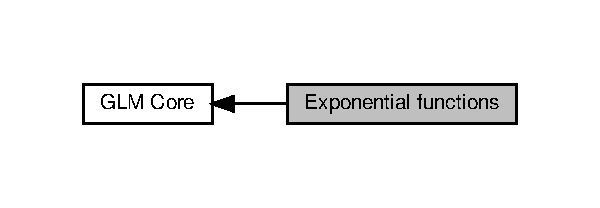
\includegraphics[width=288pt]{group__core__func__exponential}
\end{center}
\end{figure}
\subsection*{Functions}
\begin{DoxyCompactItemize}
\item 
{\footnotesize template$<$typename gen\+Type $>$ }\\\hyperlink{setup_8hpp_ab2d052de21a70539923e9bcbf6e83a51}{G\+L\+M\+\_\+\+F\+U\+N\+C\+\_\+\+D\+E\+CL} gen\+Type \hyperlink{group__core__func__exponential_ga1ce4b2fddd26d0d3a35a8d98f37f3ac0}{glm\+::pow} (gen\+Type const \&base, gen\+Type const \&exponent)
\item 
{\footnotesize template$<$typename gen\+Type $>$ }\\\hyperlink{setup_8hpp_ab2d052de21a70539923e9bcbf6e83a51}{G\+L\+M\+\_\+\+F\+U\+N\+C\+\_\+\+D\+E\+CL} gen\+Type \hyperlink{group__core__func__exponential_gae154699ba6bda068d4b87cf9b987381f}{glm\+::exp} (gen\+Type const \&x)
\item 
{\footnotesize template$<$typename gen\+Type $>$ }\\\hyperlink{setup_8hpp_ab2d052de21a70539923e9bcbf6e83a51}{G\+L\+M\+\_\+\+F\+U\+N\+C\+\_\+\+D\+E\+CL} gen\+Type \hyperlink{group__core__func__exponential_ga0c8da2d2921da250e8700ac4476916a1}{glm\+::log} (gen\+Type const \&x)
\item 
{\footnotesize template$<$typename gen\+Type $>$ }\\\hyperlink{setup_8hpp_ab2d052de21a70539923e9bcbf6e83a51}{G\+L\+M\+\_\+\+F\+U\+N\+C\+\_\+\+D\+E\+CL} gen\+Type \hyperlink{group__core__func__exponential_gac45997fb3ac907cad408d6da0a0f5f54}{glm\+::exp2} (gen\+Type const \&x)
\item 
{\footnotesize template$<$typename gen\+Type $>$ }\\\hyperlink{setup_8hpp_ab2d052de21a70539923e9bcbf6e83a51}{G\+L\+M\+\_\+\+F\+U\+N\+C\+\_\+\+D\+E\+CL} gen\+Type \hyperlink{group__core__func__exponential_gad41e336e9bc8190fe99d2cfd9261c19b}{glm\+::log2} (gen\+Type x)
\item 
{\footnotesize template$<$typename T , precision P, template$<$ typename, precision $>$ class vec\+Type$>$ }\\\hyperlink{setup_8hpp_ab2d052de21a70539923e9bcbf6e83a51}{G\+L\+M\+\_\+\+F\+U\+N\+C\+\_\+\+D\+E\+CL} vec\+Type$<$ T, P $>$ \hyperlink{group__core__func__exponential_ga2ea6c6738ad6e09ec3405a628047801b}{glm\+::sqrt} (vec\+Type$<$ T, P $>$ const \&x)
\item 
{\footnotesize template$<$typename gen\+Type $>$ }\\\hyperlink{setup_8hpp_ab2d052de21a70539923e9bcbf6e83a51}{G\+L\+M\+\_\+\+F\+U\+N\+C\+\_\+\+D\+E\+CL} gen\+Type \hyperlink{group__core__func__exponential_ga5ac08ead2e50ad0295b9ad85a3e449e9}{glm\+::inversesqrt} (gen\+Type const \&x)
\end{DoxyCompactItemize}


\subsection{Detailed Description}
These all operate component-\/wise. The description is per component. 

\subsection{Function Documentation}
\mbox{\Hypertarget{group__core__func__exponential_gae154699ba6bda068d4b87cf9b987381f}\label{group__core__func__exponential_gae154699ba6bda068d4b87cf9b987381f}} 
\index{Exponential functions@{Exponential functions}!exp@{exp}}
\index{exp@{exp}!Exponential functions@{Exponential functions}}
\subsubsection{\texorpdfstring{exp()}{exp()}}
{\footnotesize\ttfamily template$<$typename gen\+Type $>$ \\
\hyperlink{setup_8hpp_ab2d052de21a70539923e9bcbf6e83a51}{G\+L\+M\+\_\+\+F\+U\+N\+C\+\_\+\+D\+E\+CL} gen\+Type glm\+::exp (\begin{DoxyParamCaption}\item[{gen\+Type const \&}]{x }\end{DoxyParamCaption})}

Returns the natural exponentiation of x, i.\+e., e$^\wedge$x.


\begin{DoxyParams}{Parameters}
{\em x} & exp function is defined for input values of x defined in the range (inf-\/, inf+) in the limit of the type precision. \\
\hline
\end{DoxyParams}

\begin{DoxyTemplParams}{Template Parameters}
{\em gen\+Type} & Floating-\/point scalar or vector types.\\
\hline
\end{DoxyTemplParams}
\begin{DoxySeeAlso}{See also}
\href{http://www.opengl.org/sdk/docs/manglsl/xhtml/exp.xml}{\tt G\+L\+SL exp man page} 

\href{http://www.opengl.org/registry/doc/GLSLangSpec.4.20.8.pdf}{\tt G\+L\+SL 4.\+20.\+8 specification, section 8.\+2 Exponential Functions} 
\end{DoxySeeAlso}


Definition at line 100 of file func\+\_\+exponential.\+inl.

\mbox{\Hypertarget{group__core__func__exponential_gac45997fb3ac907cad408d6da0a0f5f54}\label{group__core__func__exponential_gac45997fb3ac907cad408d6da0a0f5f54}} 
\index{Exponential functions@{Exponential functions}!exp2@{exp2}}
\index{exp2@{exp2}!Exponential functions@{Exponential functions}}
\subsubsection{\texorpdfstring{exp2()}{exp2()}}
{\footnotesize\ttfamily template$<$typename gen\+Type $>$ \\
\hyperlink{setup_8hpp_ab2d052de21a70539923e9bcbf6e83a51}{G\+L\+M\+\_\+\+F\+U\+N\+C\+\_\+\+D\+E\+CL} gen\+Type glm\+::exp2 (\begin{DoxyParamCaption}\item[{gen\+Type const \&}]{x }\end{DoxyParamCaption})}

Returns 2 raised to the x power.


\begin{DoxyParams}{Parameters}
{\em x} & exp2 function is defined for input values of x defined in the range (inf-\/, inf+) in the limit of the type precision. \\
\hline
\end{DoxyParams}

\begin{DoxyTemplParams}{Template Parameters}
{\em gen\+Type} & Floating-\/point scalar or vector types.\\
\hline
\end{DoxyTemplParams}
\begin{DoxySeeAlso}{See also}
\href{http://www.opengl.org/sdk/docs/manglsl/xhtml/exp2.xml}{\tt G\+L\+SL exp2 man page} 

\href{http://www.opengl.org/registry/doc/GLSLangSpec.4.20.8.pdf}{\tt G\+L\+SL 4.\+20.\+8 specification, section 8.\+2 Exponential Functions} 
\end{DoxySeeAlso}


Definition at line 131 of file func\+\_\+exponential.\+inl.

\mbox{\Hypertarget{group__core__func__exponential_ga5ac08ead2e50ad0295b9ad85a3e449e9}\label{group__core__func__exponential_ga5ac08ead2e50ad0295b9ad85a3e449e9}} 
\index{Exponential functions@{Exponential functions}!inversesqrt@{inversesqrt}}
\index{inversesqrt@{inversesqrt}!Exponential functions@{Exponential functions}}
\subsubsection{\texorpdfstring{inversesqrt()}{inversesqrt()}}
{\footnotesize\ttfamily template$<$typename gen\+Type $>$ \\
\hyperlink{setup_8hpp_ab2d052de21a70539923e9bcbf6e83a51}{G\+L\+M\+\_\+\+F\+U\+N\+C\+\_\+\+D\+E\+CL} gen\+Type glm\+::inversesqrt (\begin{DoxyParamCaption}\item[{gen\+Type const \&}]{x }\end{DoxyParamCaption})}

Returns the reciprocal of the positive square root of x.


\begin{DoxyParams}{Parameters}
{\em x} & inversesqrt function is defined for input values of x defined in the range \mbox{[}0, inf+) in the limit of the type precision. \\
\hline
\end{DoxyParams}

\begin{DoxyTemplParams}{Template Parameters}
{\em gen\+Type} & Floating-\/point scalar or vector types.\\
\hline
\end{DoxyTemplParams}
\begin{DoxySeeAlso}{See also}
\href{http://www.opengl.org/sdk/docs/manglsl/xhtml/inversesqrt.xml}{\tt G\+L\+SL inversesqrt man page} 

\href{http://www.opengl.org/registry/doc/GLSLangSpec.4.20.8.pdf}{\tt G\+L\+SL 4.\+20.\+8 specification, section 8.\+2 Exponential Functions} 
\end{DoxySeeAlso}
\mbox{\Hypertarget{group__core__func__exponential_ga0c8da2d2921da250e8700ac4476916a1}\label{group__core__func__exponential_ga0c8da2d2921da250e8700ac4476916a1}} 
\index{Exponential functions@{Exponential functions}!log@{log}}
\index{log@{log}!Exponential functions@{Exponential functions}}
\subsubsection{\texorpdfstring{log()}{log()}}
{\footnotesize\ttfamily template$<$typename gen\+Type $>$ \\
\hyperlink{setup_8hpp_ab2d052de21a70539923e9bcbf6e83a51}{G\+L\+M\+\_\+\+F\+U\+N\+C\+\_\+\+D\+E\+CL} gen\+Type glm\+::log (\begin{DoxyParamCaption}\item[{gen\+Type const \&}]{x }\end{DoxyParamCaption})}

Returns the natural logarithm of x, i.\+e., returns the value y which satisfies the equation x = e$^\wedge$y. Results are undefined if x $<$= 0.


\begin{DoxyParams}{Parameters}
{\em x} & log function is defined for input values of x defined in the range (0, inf+) in the limit of the type precision. \\
\hline
\end{DoxyParams}

\begin{DoxyTemplParams}{Template Parameters}
{\em gen\+Type} & Floating-\/point scalar or vector types.\\
\hline
\end{DoxyTemplParams}
\begin{DoxySeeAlso}{See also}
\href{http://www.opengl.org/sdk/docs/manglsl/xhtml/log.xml}{\tt G\+L\+SL log man page} 

\href{http://www.opengl.org/registry/doc/GLSLangSpec.4.20.8.pdf}{\tt G\+L\+SL 4.\+20.\+8 specification, section 8.\+2 Exponential Functions} 
\end{DoxySeeAlso}


Definition at line 116 of file func\+\_\+exponential.\+inl.

\mbox{\Hypertarget{group__core__func__exponential_gad41e336e9bc8190fe99d2cfd9261c19b}\label{group__core__func__exponential_gad41e336e9bc8190fe99d2cfd9261c19b}} 
\index{Exponential functions@{Exponential functions}!log2@{log2}}
\index{log2@{log2}!Exponential functions@{Exponential functions}}
\subsubsection{\texorpdfstring{log2()}{log2()}}
{\footnotesize\ttfamily template$<$typename gen\+Type $>$ \\
\hyperlink{setup_8hpp_ab2d052de21a70539923e9bcbf6e83a51}{G\+L\+M\+\_\+\+F\+U\+N\+C\+\_\+\+D\+E\+CL} gen\+Type glm\+::log2 (\begin{DoxyParamCaption}\item[{gen\+Type}]{x }\end{DoxyParamCaption})}

Returns the base 2 log of x, i.\+e., returns the value y, which satisfies the equation x = 2 $^\wedge$ y.


\begin{DoxyParams}{Parameters}
{\em x} & log2 function is defined for input values of x defined in the range (0, inf+) in the limit of the type precision. \\
\hline
\end{DoxyParams}

\begin{DoxyTemplParams}{Template Parameters}
{\em gen\+Type} & Floating-\/point scalar or vector types.\\
\hline
\end{DoxyTemplParams}
\begin{DoxySeeAlso}{See also}
\href{http://www.opengl.org/sdk/docs/manglsl/xhtml/log2.xml}{\tt G\+L\+SL log2 man page} 

\href{http://www.opengl.org/registry/doc/GLSLangSpec.4.20.8.pdf}{\tt G\+L\+SL 4.\+20.\+8 specification, section 8.\+2 Exponential Functions} 
\end{DoxySeeAlso}


Definition at line 144 of file func\+\_\+exponential.\+inl.

\mbox{\Hypertarget{group__core__func__exponential_ga1ce4b2fddd26d0d3a35a8d98f37f3ac0}\label{group__core__func__exponential_ga1ce4b2fddd26d0d3a35a8d98f37f3ac0}} 
\index{Exponential functions@{Exponential functions}!pow@{pow}}
\index{pow@{pow}!Exponential functions@{Exponential functions}}
\subsubsection{\texorpdfstring{pow()}{pow()}}
{\footnotesize\ttfamily template$<$typename gen\+Type $>$ \\
\hyperlink{setup_8hpp_ab2d052de21a70539923e9bcbf6e83a51}{G\+L\+M\+\_\+\+F\+U\+N\+C\+\_\+\+D\+E\+CL} gen\+Type glm\+::pow (\begin{DoxyParamCaption}\item[{gen\+Type const \&}]{base,  }\item[{gen\+Type const \&}]{exponent }\end{DoxyParamCaption})}

Returns \textquotesingle{}base\textquotesingle{} raised to the power \textquotesingle{}exponent\textquotesingle{}.


\begin{DoxyParams}{Parameters}
{\em base} & Floating point value. pow function is defined for input values of x defined in the range (inf-\/, inf+) in the limit of the type precision. \\
\hline
{\em exponent} & Floating point value representing the \textquotesingle{}exponent\textquotesingle{}. \\
\hline
\end{DoxyParams}

\begin{DoxyTemplParams}{Template Parameters}
{\em gen\+Type} & Floating-\/point scalar or vector types.\\
\hline
\end{DoxyTemplParams}
\begin{DoxySeeAlso}{See also}
\href{http://www.opengl.org/sdk/docs/manglsl/xhtml/pow.xml}{\tt G\+L\+SL pow man page} 

\href{http://www.opengl.org/registry/doc/GLSLangSpec.4.20.8.pdf}{\tt G\+L\+SL 4.\+20.\+8 specification, section 8.\+2 Exponential Functions} 
\end{DoxySeeAlso}


Definition at line 83 of file func\+\_\+exponential.\+inl.

\mbox{\Hypertarget{group__core__func__exponential_ga2ea6c6738ad6e09ec3405a628047801b}\label{group__core__func__exponential_ga2ea6c6738ad6e09ec3405a628047801b}} 
\index{Exponential functions@{Exponential functions}!sqrt@{sqrt}}
\index{sqrt@{sqrt}!Exponential functions@{Exponential functions}}
\subsubsection{\texorpdfstring{sqrt()}{sqrt()}}
{\footnotesize\ttfamily template$<$typename T , precision P, template$<$ typename, precision $>$ class vec\+Type$>$ \\
\hyperlink{setup_8hpp_ab2d052de21a70539923e9bcbf6e83a51}{G\+L\+M\+\_\+\+F\+U\+N\+C\+\_\+\+D\+E\+CL} vec\+Type$<$T, P$>$ glm\+::sqrt (\begin{DoxyParamCaption}\item[{vec\+Type$<$ T, P $>$ const \&}]{x }\end{DoxyParamCaption})}

Returns the positive square root of x.


\begin{DoxyParams}{Parameters}
{\em x} & sqrt function is defined for input values of x defined in the range \mbox{[}0, inf+) in the limit of the type precision. \\
\hline
\end{DoxyParams}

\begin{DoxyTemplParams}{Template Parameters}
{\em gen\+Type} & Floating-\/point scalar or vector types.\\
\hline
\end{DoxyTemplParams}
\begin{DoxySeeAlso}{See also}
\href{http://www.opengl.org/sdk/docs/manglsl/xhtml/sqrt.xml}{\tt G\+L\+SL sqrt man page} 

\href{http://www.opengl.org/registry/doc/GLSLangSpec.4.20.8.pdf}{\tt G\+L\+SL 4.\+20.\+8 specification, section 8.\+2 Exponential Functions} 
\end{DoxySeeAlso}


Definition at line 219 of file func\+\_\+exponential.\+inl.


\hypertarget{group__core__func__geometric}{}\section{Geometric functions}
\label{group__core__func__geometric}\index{Geometric functions@{Geometric functions}}
Collaboration diagram for Geometric functions\+:\nopagebreak
\begin{figure}[H]
\begin{center}
\leavevmode
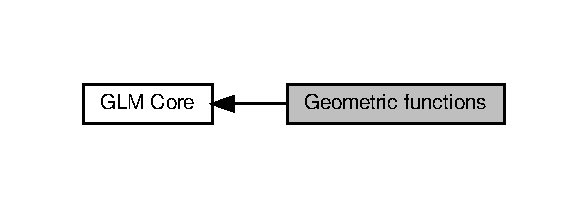
\includegraphics[width=282pt]{group__core__func__geometric}
\end{center}
\end{figure}
\subsection*{Functions}
\begin{DoxyCompactItemize}
\item 
{\footnotesize template$<$typename gen\+Type $>$ }\\\hyperlink{setup_8hpp_ab2d052de21a70539923e9bcbf6e83a51}{G\+L\+M\+\_\+\+F\+U\+N\+C\+\_\+\+D\+E\+CL} gen\+Type\+::value\+\_\+type \hyperlink{group__core__func__geometric_ga03b2831439defb8922832b540b91b8a7}{glm\+::length} (gen\+Type const \&x)
\item 
{\footnotesize template$<$typename gen\+Type $>$ }\\\hyperlink{setup_8hpp_ab2d052de21a70539923e9bcbf6e83a51}{G\+L\+M\+\_\+\+F\+U\+N\+C\+\_\+\+D\+E\+CL} gen\+Type\+::value\+\_\+type \hyperlink{group__core__func__geometric_ga00716eae37e8ae2a76ca7799f9c75682}{glm\+::distance} (gen\+Type const \&p0, gen\+Type const \&p1)
\item 
{\footnotesize template$<$typename T , precision P, template$<$ typename, precision $>$ class vec\+Type$>$ }\\\hyperlink{setup_8hpp_ab2d052de21a70539923e9bcbf6e83a51}{G\+L\+M\+\_\+\+F\+U\+N\+C\+\_\+\+D\+E\+CL} T \hyperlink{group__core__func__geometric_ga7dada304da2ba7dd3376ab4f178c3f6b}{glm\+::dot} (vec\+Type$<$ T, P $>$ const \&x, vec\+Type$<$ T, P $>$ const \&y)
\item 
{\footnotesize template$<$typename gen\+Type $>$ }\\\hyperlink{setup_8hpp_ab2d052de21a70539923e9bcbf6e83a51}{G\+L\+M\+\_\+\+F\+U\+N\+C\+\_\+\+D\+E\+CL} gen\+Type \hyperlink{group__core__func__geometric_gaef767c2b0678489cb9de7a534137a86d}{glm\+::dot} (gen\+Type const \&x, gen\+Type const \&y)
\item 
{\footnotesize template$<$typename T , precision P$>$ }\\\hyperlink{setup_8hpp_ab2d052de21a70539923e9bcbf6e83a51}{G\+L\+M\+\_\+\+F\+U\+N\+C\+\_\+\+D\+E\+CL} \hyperlink{structglm_1_1detail_1_1tvec3}{detail\+::tvec3}$<$ T, P $>$ \hyperlink{group__core__func__geometric_ga89b91c2a256cfb62ecbc589d1ee36d3c}{glm\+::cross} (\hyperlink{structglm_1_1detail_1_1tvec3}{detail\+::tvec3}$<$ T, P $>$ const \&x, \hyperlink{structglm_1_1detail_1_1tvec3}{detail\+::tvec3}$<$ T, P $>$ const \&y)
\item 
{\footnotesize template$<$typename gen\+Type $>$ }\\\hyperlink{setup_8hpp_ab2d052de21a70539923e9bcbf6e83a51}{G\+L\+M\+\_\+\+F\+U\+N\+C\+\_\+\+D\+E\+CL} gen\+Type \hyperlink{group__core__func__geometric_ga15aa87101457e41663b08a8dcc3357f8}{glm\+::normalize} (gen\+Type const \&x)
\item 
{\footnotesize template$<$typename gen\+Type $>$ }\\\hyperlink{setup_8hpp_ab2d052de21a70539923e9bcbf6e83a51}{G\+L\+M\+\_\+\+F\+U\+N\+C\+\_\+\+D\+E\+CL} gen\+Type \hyperlink{group__core__func__geometric_ga4bbb036ef9527ee9f67384233029ed9b}{glm\+::faceforward} (gen\+Type const \&N, gen\+Type const \&I, gen\+Type const \&Nref)
\item 
{\footnotesize template$<$typename gen\+Type $>$ }\\\hyperlink{setup_8hpp_ab2d052de21a70539923e9bcbf6e83a51}{G\+L\+M\+\_\+\+F\+U\+N\+C\+\_\+\+D\+E\+CL} gen\+Type \hyperlink{group__core__func__geometric_gab63646fc36b81cf69d3ce123a72f76f2}{glm\+::reflect} (gen\+Type const \&I, gen\+Type const \&N)
\item 
{\footnotesize template$<$typename T , precision P, template$<$ typename, precision $>$ class vec\+Type$>$ }\\\hyperlink{setup_8hpp_ab2d052de21a70539923e9bcbf6e83a51}{G\+L\+M\+\_\+\+F\+U\+N\+C\+\_\+\+D\+E\+CL} vec\+Type$<$ T, P $>$ \hyperlink{group__core__func__geometric_ga99d8ddb244b129892babaca9778206d0}{glm\+::refract} (vec\+Type$<$ T, P $>$ const \&I, vec\+Type$<$ T, P $>$ const \&N, T const \&eta)
\end{DoxyCompactItemize}


\subsection{Detailed Description}
These operate on vectors as vectors, not component-\/wise. 

\subsection{Function Documentation}
\mbox{\Hypertarget{group__core__func__geometric_ga89b91c2a256cfb62ecbc589d1ee36d3c}\label{group__core__func__geometric_ga89b91c2a256cfb62ecbc589d1ee36d3c}} 
\index{Geometric functions@{Geometric functions}!cross@{cross}}
\index{cross@{cross}!Geometric functions@{Geometric functions}}
\subsubsection{\texorpdfstring{cross()}{cross()}}
{\footnotesize\ttfamily template$<$typename T , precision P$>$ \\
\hyperlink{setup_8hpp_ab2d052de21a70539923e9bcbf6e83a51}{G\+L\+M\+\_\+\+F\+U\+N\+C\+\_\+\+D\+E\+CL} \hyperlink{structglm_1_1detail_1_1tvec3}{detail\+::tvec3}$<$T, P$>$ glm\+::cross (\begin{DoxyParamCaption}\item[{\hyperlink{structglm_1_1detail_1_1tvec3}{detail\+::tvec3}$<$ T, P $>$ const \&}]{x,  }\item[{\hyperlink{structglm_1_1detail_1_1tvec3}{detail\+::tvec3}$<$ T, P $>$ const \&}]{y }\end{DoxyParamCaption})}

Returns the cross product of x and y.


\begin{DoxyTemplParams}{Template Parameters}
{\em val\+Type} & Floating-\/point scalar types.\\
\hline
\end{DoxyTemplParams}
\begin{DoxySeeAlso}{See also}
\href{http://www.opengl.org/sdk/docs/manglsl/xhtml/cross.xml}{\tt G\+L\+SL cross man page} 

\href{http://www.opengl.org/registry/doc/GLSLangSpec.4.20.8.pdf}{\tt G\+L\+SL 4.\+20.\+8 specification, section 8.\+5 Geometric Functions} 
\end{DoxySeeAlso}


Definition at line 217 of file func\+\_\+geometric.\+inl.

\mbox{\Hypertarget{group__core__func__geometric_ga00716eae37e8ae2a76ca7799f9c75682}\label{group__core__func__geometric_ga00716eae37e8ae2a76ca7799f9c75682}} 
\index{Geometric functions@{Geometric functions}!distance@{distance}}
\index{distance@{distance}!Geometric functions@{Geometric functions}}
\subsubsection{\texorpdfstring{distance()}{distance()}}
{\footnotesize\ttfamily template$<$typename gen\+Type $>$ \\
\hyperlink{setup_8hpp_ab2d052de21a70539923e9bcbf6e83a51}{G\+L\+M\+\_\+\+F\+U\+N\+C\+\_\+\+D\+E\+CL} gen\+Type\+::value\+\_\+type glm\+::distance (\begin{DoxyParamCaption}\item[{gen\+Type const \&}]{p0,  }\item[{gen\+Type const \&}]{p1 }\end{DoxyParamCaption})}

Returns the distance betwwen p0 and p1, i.\+e., length(p0 -\/ p1).


\begin{DoxyTemplParams}{Template Parameters}
{\em gen\+Type} & Floating-\/point vector types.\\
\hline
\end{DoxyTemplParams}
\begin{DoxySeeAlso}{See also}
\href{http://www.opengl.org/sdk/docs/manglsl/xhtml/distance.xml}{\tt G\+L\+SL distance man page} 

\href{http://www.opengl.org/registry/doc/GLSLangSpec.4.20.8.pdf}{\tt G\+L\+SL 4.\+20.\+8 specification, section 8.\+5 Geometric Functions} 
\end{DoxySeeAlso}


Definition at line 128 of file func\+\_\+geometric.\+inl.

\mbox{\Hypertarget{group__core__func__geometric_ga7dada304da2ba7dd3376ab4f178c3f6b}\label{group__core__func__geometric_ga7dada304da2ba7dd3376ab4f178c3f6b}} 
\index{Geometric functions@{Geometric functions}!dot@{dot}}
\index{dot@{dot}!Geometric functions@{Geometric functions}}
\subsubsection{\texorpdfstring{dot()}{dot()}\hspace{0.1cm}{\footnotesize\ttfamily [1/2]}}
{\footnotesize\ttfamily template$<$typename T , precision P, template$<$ typename, precision $>$ class vec\+Type$>$ \\
\hyperlink{setup_8hpp_ab2d052de21a70539923e9bcbf6e83a51}{G\+L\+M\+\_\+\+F\+U\+N\+C\+\_\+\+D\+E\+CL} T glm\+::dot (\begin{DoxyParamCaption}\item[{vec\+Type$<$ T, P $>$ const \&}]{x,  }\item[{vec\+Type$<$ T, P $>$ const \&}]{y }\end{DoxyParamCaption})}

Returns the dot product of x and y, i.\+e., result = x $\ast$ y.


\begin{DoxyTemplParams}{Template Parameters}
{\em gen\+Type} & Floating-\/point vector types.\\
\hline
\end{DoxyTemplParams}
\begin{DoxySeeAlso}{See also}
\href{http://www.opengl.org/sdk/docs/manglsl/xhtml/dot.xml}{\tt G\+L\+SL dot man page} 

\href{http://www.opengl.org/registry/doc/GLSLangSpec.4.20.8.pdf}{\tt G\+L\+SL 4.\+20.\+8 specification, section 8.\+5 Geometric Functions} 
\end{DoxySeeAlso}


Definition at line 188 of file func\+\_\+geometric.\+inl.

\mbox{\Hypertarget{group__core__func__geometric_gaef767c2b0678489cb9de7a534137a86d}\label{group__core__func__geometric_gaef767c2b0678489cb9de7a534137a86d}} 
\index{Geometric functions@{Geometric functions}!dot@{dot}}
\index{dot@{dot}!Geometric functions@{Geometric functions}}
\subsubsection{\texorpdfstring{dot()}{dot()}\hspace{0.1cm}{\footnotesize\ttfamily [2/2]}}
{\footnotesize\ttfamily template$<$typename gen\+Type $>$ \\
\hyperlink{setup_8hpp_ab2d052de21a70539923e9bcbf6e83a51}{G\+L\+M\+\_\+\+F\+U\+N\+C\+\_\+\+D\+E\+CL} gen\+Type glm\+::dot (\begin{DoxyParamCaption}\item[{gen\+Type const \&}]{x,  }\item[{gen\+Type const \&}]{y }\end{DoxyParamCaption})}

Returns the dot product of x and y, i.\+e., result = x $\ast$ y.


\begin{DoxyTemplParams}{Template Parameters}
{\em gen\+Type} & Floating-\/point vector types.\\
\hline
\end{DoxyTemplParams}
\begin{DoxySeeAlso}{See also}
\href{http://www.opengl.org/sdk/docs/manglsl/xhtml/dot.xml}{\tt G\+L\+SL dot man page} 

\href{http://www.opengl.org/registry/doc/GLSLangSpec.4.20.8.pdf}{\tt G\+L\+SL 4.\+20.\+8 specification, section 8.\+5 Geometric Functions} 
\end{DoxySeeAlso}
\mbox{\Hypertarget{group__core__func__geometric_ga4bbb036ef9527ee9f67384233029ed9b}\label{group__core__func__geometric_ga4bbb036ef9527ee9f67384233029ed9b}} 
\index{Geometric functions@{Geometric functions}!faceforward@{faceforward}}
\index{faceforward@{faceforward}!Geometric functions@{Geometric functions}}
\subsubsection{\texorpdfstring{faceforward()}{faceforward()}}
{\footnotesize\ttfamily template$<$typename gen\+Type $>$ \\
\hyperlink{setup_8hpp_ab2d052de21a70539923e9bcbf6e83a51}{G\+L\+M\+\_\+\+F\+U\+N\+C\+\_\+\+D\+E\+CL} gen\+Type glm\+::faceforward (\begin{DoxyParamCaption}\item[{gen\+Type const \&}]{N,  }\item[{gen\+Type const \&}]{I,  }\item[{gen\+Type const \&}]{Nref }\end{DoxyParamCaption})}

If dot(\+Nref, I) $<$ 0.\+0, return N, otherwise, return -\/N.


\begin{DoxyTemplParams}{Template Parameters}
{\em gen\+Type} & Floating-\/point vector types.\\
\hline
\end{DoxyTemplParams}
\begin{DoxySeeAlso}{See also}
\href{http://www.opengl.org/sdk/docs/manglsl/xhtml/faceforward.xml}{\tt G\+L\+SL faceforward man page} 

\href{http://www.opengl.org/registry/doc/GLSLangSpec.4.20.8.pdf}{\tt G\+L\+SL 4.\+20.\+8 specification, section 8.\+5 Geometric Functions} 
\end{DoxySeeAlso}


Definition at line 282 of file func\+\_\+geometric.\+inl.

\mbox{\Hypertarget{group__core__func__geometric_ga03b2831439defb8922832b540b91b8a7}\label{group__core__func__geometric_ga03b2831439defb8922832b540b91b8a7}} 
\index{Geometric functions@{Geometric functions}!length@{length}}
\index{length@{length}!Geometric functions@{Geometric functions}}
\subsubsection{\texorpdfstring{length()}{length()}}
{\footnotesize\ttfamily template$<$typename gen\+Type $>$ \\
\hyperlink{setup_8hpp_ab2d052de21a70539923e9bcbf6e83a51}{G\+L\+M\+\_\+\+F\+U\+N\+C\+\_\+\+D\+E\+CL} gen\+Type\+::value\+\_\+type glm\+::length (\begin{DoxyParamCaption}\item[{gen\+Type const \&}]{x }\end{DoxyParamCaption})}

Returns the length of x, i.\+e., sqrt(x $\ast$ x).


\begin{DoxyTemplParams}{Template Parameters}
{\em gen\+Type} & Floating-\/point vector types.\\
\hline
\end{DoxyTemplParams}
\begin{DoxySeeAlso}{See also}
\href{http://www.opengl.org/sdk/docs/manglsl/xhtml/length.xml}{\tt G\+L\+SL length man page} 

\href{http://www.opengl.org/registry/doc/GLSLangSpec.4.20.8.pdf}{\tt G\+L\+SL 4.\+20.\+8 specification, section 8.\+5 Geometric Functions} 
\end{DoxySeeAlso}


Definition at line 89 of file func\+\_\+geometric.\+inl.

\mbox{\Hypertarget{group__core__func__geometric_ga15aa87101457e41663b08a8dcc3357f8}\label{group__core__func__geometric_ga15aa87101457e41663b08a8dcc3357f8}} 
\index{Geometric functions@{Geometric functions}!normalize@{normalize}}
\index{normalize@{normalize}!Geometric functions@{Geometric functions}}
\subsubsection{\texorpdfstring{normalize()}{normalize()}}
{\footnotesize\ttfamily template$<$typename gen\+Type $>$ \\
\hyperlink{setup_8hpp_ab2d052de21a70539923e9bcbf6e83a51}{G\+L\+M\+\_\+\+F\+U\+N\+C\+\_\+\+D\+E\+CL} gen\+Type glm\+::normalize (\begin{DoxyParamCaption}\item[{gen\+Type const \&}]{x }\end{DoxyParamCaption})}

Returns a vector in the same direction as x but with length of 1.

\begin{DoxySeeAlso}{See also}
\href{http://www.opengl.org/sdk/docs/manglsl/xhtml/normalize.xml}{\tt G\+L\+SL normalize man page} 

\href{http://www.opengl.org/registry/doc/GLSLangSpec.4.20.8.pdf}{\tt G\+L\+SL 4.\+20.\+8 specification, section 8.\+5 Geometric Functions} 
\end{DoxySeeAlso}


Definition at line 233 of file func\+\_\+geometric.\+inl.

\mbox{\Hypertarget{group__core__func__geometric_gab63646fc36b81cf69d3ce123a72f76f2}\label{group__core__func__geometric_gab63646fc36b81cf69d3ce123a72f76f2}} 
\index{Geometric functions@{Geometric functions}!reflect@{reflect}}
\index{reflect@{reflect}!Geometric functions@{Geometric functions}}
\subsubsection{\texorpdfstring{reflect()}{reflect()}}
{\footnotesize\ttfamily template$<$typename gen\+Type $>$ \\
\hyperlink{setup_8hpp_ab2d052de21a70539923e9bcbf6e83a51}{G\+L\+M\+\_\+\+F\+U\+N\+C\+\_\+\+D\+E\+CL} gen\+Type glm\+::reflect (\begin{DoxyParamCaption}\item[{gen\+Type const \&}]{I,  }\item[{gen\+Type const \&}]{N }\end{DoxyParamCaption})}

For the incident vector I and surface orientation N, returns the reflection direction \+: result = I -\/ 2.\+0 $\ast$ dot(\+N, I) $\ast$ N.


\begin{DoxyTemplParams}{Template Parameters}
{\em gen\+Type} & Floating-\/point vector types.\\
\hline
\end{DoxyTemplParams}
\begin{DoxySeeAlso}{See also}
\href{http://www.opengl.org/sdk/docs/manglsl/xhtml/reflect.xml}{\tt G\+L\+SL reflect man page} 

\href{http://www.opengl.org/registry/doc/GLSLangSpec.4.20.8.pdf}{\tt G\+L\+SL 4.\+20.\+8 specification, section 8.\+5 Geometric Functions} 
\end{DoxySeeAlso}


Definition at line 294 of file func\+\_\+geometric.\+inl.

\mbox{\Hypertarget{group__core__func__geometric_ga99d8ddb244b129892babaca9778206d0}\label{group__core__func__geometric_ga99d8ddb244b129892babaca9778206d0}} 
\index{Geometric functions@{Geometric functions}!refract@{refract}}
\index{refract@{refract}!Geometric functions@{Geometric functions}}
\subsubsection{\texorpdfstring{refract()}{refract()}}
{\footnotesize\ttfamily template$<$typename T , precision P, template$<$ typename, precision $>$ class vec\+Type$>$ \\
\hyperlink{setup_8hpp_ab2d052de21a70539923e9bcbf6e83a51}{G\+L\+M\+\_\+\+F\+U\+N\+C\+\_\+\+D\+E\+CL} vec\+Type$<$T, P$>$ glm\+::refract (\begin{DoxyParamCaption}\item[{vec\+Type$<$ T, P $>$ const \&}]{I,  }\item[{vec\+Type$<$ T, P $>$ const \&}]{N,  }\item[{T const \&}]{eta }\end{DoxyParamCaption})}

For the incident vector I and surface normal N, and the ratio of indices of refraction eta, return the refraction vector.


\begin{DoxyTemplParams}{Template Parameters}
{\em gen\+Type} & Floating-\/point vector types.\\
\hline
\end{DoxyTemplParams}
\begin{DoxySeeAlso}{See also}
\href{http://www.opengl.org/sdk/docs/manglsl/xhtml/refract.xml}{\tt G\+L\+SL refract man page} 

\href{http://www.opengl.org/registry/doc/GLSLangSpec.4.20.8.pdf}{\tt G\+L\+SL 4.\+20.\+8 specification, section 8.\+5 Geometric Functions} 
\end{DoxySeeAlso}


Definition at line 323 of file func\+\_\+geometric.\+inl.


\hypertarget{group__core__func__integer}{}\section{Integer functions}
\label{group__core__func__integer}\index{Integer functions@{Integer functions}}
Collaboration diagram for Integer functions\+:\nopagebreak
\begin{figure}[H]
\begin{center}
\leavevmode
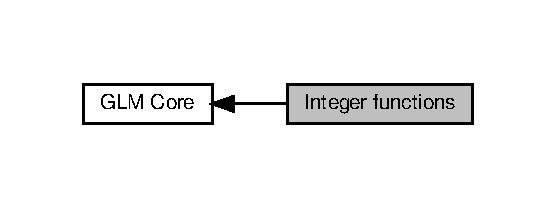
\includegraphics[width=267pt]{group__core__func__integer}
\end{center}
\end{figure}
\subsection*{Functions}
\begin{DoxyCompactItemize}
\item 
{\footnotesize template$<$typename gen\+U\+Type $>$ }\\\hyperlink{setup_8hpp_ab2d052de21a70539923e9bcbf6e83a51}{G\+L\+M\+\_\+\+F\+U\+N\+C\+\_\+\+D\+E\+CL} gen\+U\+Type \hyperlink{group__core__func__integer_ga19276bb7adbe9f0d74515ae49e40b481}{glm\+::uadd\+Carry} (gen\+U\+Type const \&x, gen\+U\+Type const \&y, gen\+U\+Type \&carry)
\item 
{\footnotesize template$<$typename gen\+U\+Type $>$ }\\\hyperlink{setup_8hpp_ab2d052de21a70539923e9bcbf6e83a51}{G\+L\+M\+\_\+\+F\+U\+N\+C\+\_\+\+D\+E\+CL} gen\+U\+Type \hyperlink{group__core__func__integer_gae5b4a6cefd1e21fd2e1b8526b4c964a7}{glm\+::usub\+Borrow} (gen\+U\+Type const \&x, gen\+U\+Type const \&y, gen\+U\+Type \&borrow)
\item 
{\footnotesize template$<$typename gen\+U\+Type $>$ }\\\hyperlink{setup_8hpp_ab2d052de21a70539923e9bcbf6e83a51}{G\+L\+M\+\_\+\+F\+U\+N\+C\+\_\+\+D\+E\+CL} void \hyperlink{group__core__func__integer_gad991bf53779a4309a920bb7bfcf2639c}{glm\+::umul\+Extended} (gen\+U\+Type const \&x, gen\+U\+Type const \&y, gen\+U\+Type \&msb, gen\+U\+Type \&lsb)
\item 
{\footnotesize template$<$typename gen\+I\+Type $>$ }\\\hyperlink{setup_8hpp_ab2d052de21a70539923e9bcbf6e83a51}{G\+L\+M\+\_\+\+F\+U\+N\+C\+\_\+\+D\+E\+CL} void \hyperlink{group__core__func__integer_ga7d284e3ea5059cae9fe8f0fe1a76dd02}{glm\+::imul\+Extended} (gen\+I\+Type const \&x, gen\+I\+Type const \&y, gen\+I\+Type \&msb, gen\+I\+Type \&lsb)
\item 
{\footnotesize template$<$typename gen\+I\+U\+Type $>$ }\\\hyperlink{setup_8hpp_ab2d052de21a70539923e9bcbf6e83a51}{G\+L\+M\+\_\+\+F\+U\+N\+C\+\_\+\+D\+E\+CL} gen\+I\+U\+Type \hyperlink{group__core__func__integer_ga251d309beb171bf95117d2c301b2ad8b}{glm\+::bitfield\+Extract} (gen\+I\+U\+Type const \&Value, int const \&Offset, int const \&Bits)
\item 
{\footnotesize template$<$typename gen\+I\+U\+Type $>$ }\\\hyperlink{setup_8hpp_ab2d052de21a70539923e9bcbf6e83a51}{G\+L\+M\+\_\+\+F\+U\+N\+C\+\_\+\+D\+E\+CL} gen\+I\+U\+Type \hyperlink{group__core__func__integer_ga7ab09972d52094d97d2480982e657dd0}{glm\+::bitfield\+Insert} (gen\+I\+U\+Type const \&Base, gen\+I\+U\+Type const \&Insert, int const \&Offset, int const \&Bits)
\item 
{\footnotesize template$<$typename gen\+I\+U\+Type $>$ }\\\hyperlink{setup_8hpp_ab2d052de21a70539923e9bcbf6e83a51}{G\+L\+M\+\_\+\+F\+U\+N\+C\+\_\+\+D\+E\+CL} gen\+I\+U\+Type \hyperlink{group__core__func__integer_gac28880e609c6eeb0a28f1a54b1edc715}{glm\+::bitfield\+Reverse} (gen\+I\+U\+Type const \&Value)
\item 
{\footnotesize template$<$typename T , template$<$ typename $>$ class gen\+I\+U\+Type$>$ }\\\hyperlink{setup_8hpp_ab2d052de21a70539923e9bcbf6e83a51}{G\+L\+M\+\_\+\+F\+U\+N\+C\+\_\+\+D\+E\+CL} gen\+I\+U\+Type$<$ T $>$\+::signed\+\_\+type \hyperlink{group__core__func__integer_gaf5ecf64cbcb7f806a3c7915dd622209b}{glm\+::bit\+Count} (gen\+I\+U\+Type$<$ T $>$ const \&Value)
\item 
{\footnotesize template$<$typename T , template$<$ typename $>$ class gen\+I\+U\+Type$>$ }\\\hyperlink{setup_8hpp_ab2d052de21a70539923e9bcbf6e83a51}{G\+L\+M\+\_\+\+F\+U\+N\+C\+\_\+\+D\+E\+CL} gen\+I\+U\+Type$<$ T $>$\+::signed\+\_\+type \hyperlink{group__core__func__integer_ga43d5d9ec05ba4c46035c764ad5fd3135}{glm\+::find\+L\+SB} (gen\+I\+U\+Type$<$ T $>$ const \&Value)
\item 
{\footnotesize template$<$typename T , template$<$ typename $>$ class gen\+I\+U\+Type$>$ }\\\hyperlink{setup_8hpp_ab2d052de21a70539923e9bcbf6e83a51}{G\+L\+M\+\_\+\+F\+U\+N\+C\+\_\+\+D\+E\+CL} gen\+I\+U\+Type$<$ T $>$\+::signed\+\_\+type \hyperlink{group__core__func__integer_gaee931af2eaecf61b629b33899c9d6f29}{glm\+::find\+M\+SB} (gen\+I\+U\+Type$<$ T $>$ const \&Value)
\end{DoxyCompactItemize}


\subsection{Detailed Description}
These all operate component-\/wise. The description is per component. The notation \mbox{[}a, b\mbox{]} means the set of bits from bit-\/number a through bit-\/number b, inclusive. The lowest-\/order bit is bit 0. 

\subsection{Function Documentation}
\mbox{\Hypertarget{group__core__func__integer_gaf5ecf64cbcb7f806a3c7915dd622209b}\label{group__core__func__integer_gaf5ecf64cbcb7f806a3c7915dd622209b}} 
\index{Integer functions@{Integer functions}!bit\+Count@{bit\+Count}}
\index{bit\+Count@{bit\+Count}!Integer functions@{Integer functions}}
\subsubsection{\texorpdfstring{bit\+Count()}{bitCount()}}
{\footnotesize\ttfamily template$<$typename T , template$<$ typename $>$ class gen\+I\+U\+Type$>$ \\
\hyperlink{setup_8hpp_ab2d052de21a70539923e9bcbf6e83a51}{G\+L\+M\+\_\+\+F\+U\+N\+C\+\_\+\+D\+E\+CL} gen\+I\+U\+Type$<$T$>$\+::signed\+\_\+type glm\+::bit\+Count (\begin{DoxyParamCaption}\item[{gen\+I\+U\+Type$<$ T $>$ const \&}]{Value }\end{DoxyParamCaption})}

Returns the number of bits set to 1 in the binary representation of value.


\begin{DoxyTemplParams}{Template Parameters}
{\em gen\+I\+U\+Type} & Signed or unsigned integer scalar or vector types.\\
\hline
\end{DoxyTemplParams}
\begin{DoxySeeAlso}{See also}
\href{http://www.opengl.org/sdk/docs/manglsl/xhtml/bitCount.xml}{\tt G\+L\+SL bit\+Count man page} 

\href{http://www.opengl.org/registry/doc/GLSLangSpec.4.20.8.pdf}{\tt G\+L\+SL 4.\+20.\+8 specification, section 8.\+8 Integer Functions}
\end{DoxySeeAlso}
\begin{DoxyRefDesc}{Todo}
\item[\hyperlink{todo__todo000001}{Todo}]Clarify the declaration to specify that scalars are suported. \end{DoxyRefDesc}
\mbox{\Hypertarget{group__core__func__integer_ga251d309beb171bf95117d2c301b2ad8b}\label{group__core__func__integer_ga251d309beb171bf95117d2c301b2ad8b}} 
\index{Integer functions@{Integer functions}!bitfield\+Extract@{bitfield\+Extract}}
\index{bitfield\+Extract@{bitfield\+Extract}!Integer functions@{Integer functions}}
\subsubsection{\texorpdfstring{bitfield\+Extract()}{bitfieldExtract()}}
{\footnotesize\ttfamily template$<$typename gen\+I\+U\+Type $>$ \\
\hyperlink{setup_8hpp_ab2d052de21a70539923e9bcbf6e83a51}{G\+L\+M\+\_\+\+F\+U\+N\+C\+\_\+\+D\+E\+CL} gen\+I\+U\+Type glm\+::bitfield\+Extract (\begin{DoxyParamCaption}\item[{gen\+I\+U\+Type const \&}]{Value,  }\item[{int const \&}]{Offset,  }\item[{int const \&}]{Bits }\end{DoxyParamCaption})}

Extracts bits \mbox{[}offset, offset + bits -\/ 1\mbox{]} from value, returning them in the least significant bits of the result. For unsigned data types, the most significant bits of the result will be set to zero. For signed data types, the most significant bits will be set to the value of bit offset + base -\/ 1.

If bits is zero, the result will be zero. The result will be undefined if offset or bits is negative, or if the sum of offset and bits is greater than the number of bits used to store the operand.


\begin{DoxyTemplParams}{Template Parameters}
{\em gen\+I\+U\+Type} & Signed or unsigned integer scalar or vector types.\\
\hline
\end{DoxyTemplParams}
\begin{DoxySeeAlso}{See also}
\href{http://www.opengl.org/sdk/docs/manglsl/xhtml/bitfieldExtract.xml}{\tt G\+L\+SL bitfield\+Extract man page} 

\href{http://www.opengl.org/registry/doc/GLSLangSpec.4.20.8.pdf}{\tt G\+L\+SL 4.\+20.\+8 specification, section 8.\+8 Integer Functions} 
\end{DoxySeeAlso}


Definition at line 286 of file func\+\_\+integer.\+inl.

\mbox{\Hypertarget{group__core__func__integer_ga7ab09972d52094d97d2480982e657dd0}\label{group__core__func__integer_ga7ab09972d52094d97d2480982e657dd0}} 
\index{Integer functions@{Integer functions}!bitfield\+Insert@{bitfield\+Insert}}
\index{bitfield\+Insert@{bitfield\+Insert}!Integer functions@{Integer functions}}
\subsubsection{\texorpdfstring{bitfield\+Insert()}{bitfieldInsert()}}
{\footnotesize\ttfamily template$<$typename gen\+I\+U\+Type $>$ \\
\hyperlink{setup_8hpp_ab2d052de21a70539923e9bcbf6e83a51}{G\+L\+M\+\_\+\+F\+U\+N\+C\+\_\+\+D\+E\+CL} gen\+I\+U\+Type glm\+::bitfield\+Insert (\begin{DoxyParamCaption}\item[{gen\+I\+U\+Type const \&}]{Base,  }\item[{gen\+I\+U\+Type const \&}]{Insert,  }\item[{int const \&}]{Offset,  }\item[{int const \&}]{Bits }\end{DoxyParamCaption})}

Returns the insertion the bits least-\/significant bits of insert into base.

The result will have bits \mbox{[}offset, offset + bits -\/ 1\mbox{]} taken from bits \mbox{[}0, bits -\/ 1\mbox{]} of insert, and all other bits taken directly from the corresponding bits of base. If bits is zero, the result will simply be base. The result will be undefined if offset or bits is negative, or if the sum of offset and bits is greater than the number of bits used to store the operand.


\begin{DoxyTemplParams}{Template Parameters}
{\em gen\+I\+U\+Type} & Signed or unsigned integer scalar or vector types.\\
\hline
\end{DoxyTemplParams}
\begin{DoxySeeAlso}{See also}
\href{http://www.opengl.org/sdk/docs/manglsl/xhtml/bitfieldInsert.xml}{\tt G\+L\+SL bitfield\+Insert man page} 

\href{http://www.opengl.org/registry/doc/GLSLangSpec.4.20.8.pdf}{\tt G\+L\+SL 4.\+20.\+8 specification, section 8.\+8 Integer Functions} 
\end{DoxySeeAlso}


Definition at line 347 of file func\+\_\+integer.\+inl.

\mbox{\Hypertarget{group__core__func__integer_gac28880e609c6eeb0a28f1a54b1edc715}\label{group__core__func__integer_gac28880e609c6eeb0a28f1a54b1edc715}} 
\index{Integer functions@{Integer functions}!bitfield\+Reverse@{bitfield\+Reverse}}
\index{bitfield\+Reverse@{bitfield\+Reverse}!Integer functions@{Integer functions}}
\subsubsection{\texorpdfstring{bitfield\+Reverse()}{bitfieldReverse()}}
{\footnotesize\ttfamily template$<$typename gen\+I\+U\+Type $>$ \\
\hyperlink{setup_8hpp_ab2d052de21a70539923e9bcbf6e83a51}{G\+L\+M\+\_\+\+F\+U\+N\+C\+\_\+\+D\+E\+CL} gen\+I\+U\+Type glm\+::bitfield\+Reverse (\begin{DoxyParamCaption}\item[{gen\+I\+U\+Type const \&}]{Value }\end{DoxyParamCaption})}

Returns the reversal of the bits of value. The bit numbered n of the result will be taken from bit (bits -\/ 1) -\/ n of value, where bits is the total number of bits used to represent value.


\begin{DoxyTemplParams}{Template Parameters}
{\em gen\+I\+U\+Type} & Signed or unsigned integer scalar or vector types.\\
\hline
\end{DoxyTemplParams}
\begin{DoxySeeAlso}{See also}
\href{http://www.opengl.org/sdk/docs/manglsl/xhtml/bitfieldReverse.xml}{\tt G\+L\+SL bitfield\+Reverse man page} 

\href{http://www.opengl.org/registry/doc/GLSLangSpec.4.20.8.pdf}{\tt G\+L\+SL 4.\+20.\+8 specification, section 8.\+8 Integer Functions} 
\end{DoxySeeAlso}


Definition at line 414 of file func\+\_\+integer.\+inl.

\mbox{\Hypertarget{group__core__func__integer_ga43d5d9ec05ba4c46035c764ad5fd3135}\label{group__core__func__integer_ga43d5d9ec05ba4c46035c764ad5fd3135}} 
\index{Integer functions@{Integer functions}!find\+L\+SB@{find\+L\+SB}}
\index{find\+L\+SB@{find\+L\+SB}!Integer functions@{Integer functions}}
\subsubsection{\texorpdfstring{find\+L\+S\+B()}{findLSB()}}
{\footnotesize\ttfamily template$<$typename T , template$<$ typename $>$ class gen\+I\+U\+Type$>$ \\
\hyperlink{setup_8hpp_ab2d052de21a70539923e9bcbf6e83a51}{G\+L\+M\+\_\+\+F\+U\+N\+C\+\_\+\+D\+E\+CL} gen\+I\+U\+Type$<$T$>$\+::signed\+\_\+type glm\+::find\+L\+SB (\begin{DoxyParamCaption}\item[{gen\+I\+U\+Type$<$ T $>$ const \&}]{Value }\end{DoxyParamCaption})}

Returns the bit number of the least significant bit set to 1 in the binary representation of value. If value is zero, -\/1 will be returned.


\begin{DoxyTemplParams}{Template Parameters}
{\em gen\+I\+U\+Type} & Signed or unsigned integer scalar or vector types.\\
\hline
\end{DoxyTemplParams}
\begin{DoxySeeAlso}{See also}
\href{http://www.opengl.org/sdk/docs/manglsl/xhtml/findLSB.xml}{\tt G\+L\+SL find\+L\+SB man page} 

\href{http://www.opengl.org/registry/doc/GLSLangSpec.4.20.8.pdf}{\tt G\+L\+SL 4.\+20.\+8 specification, section 8.\+8 Integer Functions}
\end{DoxySeeAlso}
\begin{DoxyRefDesc}{Todo}
\item[\hyperlink{todo__todo000002}{Todo}]Clarify the declaration to specify that scalars are suported. \end{DoxyRefDesc}
\mbox{\Hypertarget{group__core__func__integer_gaee931af2eaecf61b629b33899c9d6f29}\label{group__core__func__integer_gaee931af2eaecf61b629b33899c9d6f29}} 
\index{Integer functions@{Integer functions}!find\+M\+SB@{find\+M\+SB}}
\index{find\+M\+SB@{find\+M\+SB}!Integer functions@{Integer functions}}
\subsubsection{\texorpdfstring{find\+M\+S\+B()}{findMSB()}}
{\footnotesize\ttfamily template$<$typename T , template$<$ typename $>$ class gen\+I\+U\+Type$>$ \\
\hyperlink{setup_8hpp_ab2d052de21a70539923e9bcbf6e83a51}{G\+L\+M\+\_\+\+F\+U\+N\+C\+\_\+\+D\+E\+CL} gen\+I\+U\+Type$<$T$>$\+::signed\+\_\+type glm\+::find\+M\+SB (\begin{DoxyParamCaption}\item[{gen\+I\+U\+Type$<$ T $>$ const \&}]{Value }\end{DoxyParamCaption})}

Returns the bit number of the most significant bit in the binary representation of value. For positive integers, the result will be the bit number of the most significant bit set to 1. For negative integers, the result will be the bit number of the most significant bit set to 0. For a value of zero or negative one, -\/1 will be returned.


\begin{DoxyTemplParams}{Template Parameters}
{\em gen\+I\+U\+Type} & Signed or unsigned integer scalar or vector types.\\
\hline
\end{DoxyTemplParams}
\begin{DoxySeeAlso}{See also}
\href{http://www.opengl.org/sdk/docs/manglsl/xhtml/findMSB.xml}{\tt G\+L\+SL find\+M\+SB man page} 

\href{http://www.opengl.org/registry/doc/GLSLangSpec.4.20.8.pdf}{\tt G\+L\+SL 4.\+20.\+8 specification, section 8.\+8 Integer Functions}
\end{DoxySeeAlso}
\begin{DoxyRefDesc}{Todo}
\item[\hyperlink{todo__todo000003}{Todo}]Clarify the declaration to specify that scalars are suported. \end{DoxyRefDesc}
\mbox{\Hypertarget{group__core__func__integer_ga7d284e3ea5059cae9fe8f0fe1a76dd02}\label{group__core__func__integer_ga7d284e3ea5059cae9fe8f0fe1a76dd02}} 
\index{Integer functions@{Integer functions}!imul\+Extended@{imul\+Extended}}
\index{imul\+Extended@{imul\+Extended}!Integer functions@{Integer functions}}
\subsubsection{\texorpdfstring{imul\+Extended()}{imulExtended()}}
{\footnotesize\ttfamily template$<$typename gen\+I\+Type $>$ \\
\hyperlink{setup_8hpp_ab2d052de21a70539923e9bcbf6e83a51}{G\+L\+M\+\_\+\+F\+U\+N\+C\+\_\+\+D\+E\+CL} void glm\+::imul\+Extended (\begin{DoxyParamCaption}\item[{gen\+I\+Type const \&}]{x,  }\item[{gen\+I\+Type const \&}]{y,  }\item[{gen\+I\+Type \&}]{msb,  }\item[{gen\+I\+Type \&}]{lsb }\end{DoxyParamCaption})}

Multiplies 32-\/bit integers x and y, producing a 64-\/bit result. The 32 least-\/significant bits are returned in lsb. The 32 most-\/significant bits are returned in msb.


\begin{DoxyTemplParams}{Template Parameters}
{\em gen\+I\+Type} & Signed integer scalar or vector types.\\
\hline
\end{DoxyTemplParams}
\begin{DoxySeeAlso}{See also}
\href{http://www.opengl.org/sdk/docs/manglsl/xhtml/imulExtended.xml}{\tt G\+L\+SL imul\+Extended man page} 

\href{http://www.opengl.org/registry/doc/GLSLangSpec.4.20.8.pdf}{\tt G\+L\+SL 4.\+20.\+8 specification, section 8.\+8 Integer Functions} 
\end{DoxySeeAlso}
\mbox{\Hypertarget{group__core__func__integer_ga19276bb7adbe9f0d74515ae49e40b481}\label{group__core__func__integer_ga19276bb7adbe9f0d74515ae49e40b481}} 
\index{Integer functions@{Integer functions}!uadd\+Carry@{uadd\+Carry}}
\index{uadd\+Carry@{uadd\+Carry}!Integer functions@{Integer functions}}
\subsubsection{\texorpdfstring{uadd\+Carry()}{uaddCarry()}}
{\footnotesize\ttfamily template$<$typename gen\+U\+Type $>$ \\
\hyperlink{setup_8hpp_ab2d052de21a70539923e9bcbf6e83a51}{G\+L\+M\+\_\+\+F\+U\+N\+C\+\_\+\+D\+E\+CL} gen\+U\+Type glm\+::uadd\+Carry (\begin{DoxyParamCaption}\item[{gen\+U\+Type const \&}]{x,  }\item[{gen\+U\+Type const \&}]{y,  }\item[{gen\+U\+Type \&}]{carry }\end{DoxyParamCaption})}

Adds 32-\/bit unsigned integer x and y, returning the sum modulo pow(2, 32). The value carry is set to 0 if the sum was less than pow(2, 32), or to 1 otherwise.


\begin{DoxyTemplParams}{Template Parameters}
{\em gen\+U\+Type} & Unsigned integer scalar or vector types.\\
\hline
\end{DoxyTemplParams}
\begin{DoxySeeAlso}{See also}
\href{http://www.opengl.org/sdk/docs/manglsl/xhtml/uaddCarry.xml}{\tt G\+L\+SL uadd\+Carry man page} 

\href{http://www.opengl.org/registry/doc/GLSLangSpec.4.20.8.pdf}{\tt G\+L\+SL 4.\+20.\+8 specification, section 8.\+8 Integer Functions} 
\end{DoxySeeAlso}
\mbox{\Hypertarget{group__core__func__integer_gad991bf53779a4309a920bb7bfcf2639c}\label{group__core__func__integer_gad991bf53779a4309a920bb7bfcf2639c}} 
\index{Integer functions@{Integer functions}!umul\+Extended@{umul\+Extended}}
\index{umul\+Extended@{umul\+Extended}!Integer functions@{Integer functions}}
\subsubsection{\texorpdfstring{umul\+Extended()}{umulExtended()}}
{\footnotesize\ttfamily template$<$typename gen\+U\+Type $>$ \\
\hyperlink{setup_8hpp_ab2d052de21a70539923e9bcbf6e83a51}{G\+L\+M\+\_\+\+F\+U\+N\+C\+\_\+\+D\+E\+CL} void glm\+::umul\+Extended (\begin{DoxyParamCaption}\item[{gen\+U\+Type const \&}]{x,  }\item[{gen\+U\+Type const \&}]{y,  }\item[{gen\+U\+Type \&}]{msb,  }\item[{gen\+U\+Type \&}]{lsb }\end{DoxyParamCaption})}

Multiplies 32-\/bit integers x and y, producing a 64-\/bit result. The 32 least-\/significant bits are returned in lsb. The 32 most-\/significant bits are returned in msb.


\begin{DoxyTemplParams}{Template Parameters}
{\em gen\+U\+Type} & Unsigned integer scalar or vector types.\\
\hline
\end{DoxyTemplParams}
\begin{DoxySeeAlso}{See also}
\href{http://www.opengl.org/sdk/docs/manglsl/xhtml/umulExtended.xml}{\tt G\+L\+SL umul\+Extended man page} 

\href{http://www.opengl.org/registry/doc/GLSLangSpec.4.20.8.pdf}{\tt G\+L\+SL 4.\+20.\+8 specification, section 8.\+8 Integer Functions} 
\end{DoxySeeAlso}
\mbox{\Hypertarget{group__core__func__integer_gae5b4a6cefd1e21fd2e1b8526b4c964a7}\label{group__core__func__integer_gae5b4a6cefd1e21fd2e1b8526b4c964a7}} 
\index{Integer functions@{Integer functions}!usub\+Borrow@{usub\+Borrow}}
\index{usub\+Borrow@{usub\+Borrow}!Integer functions@{Integer functions}}
\subsubsection{\texorpdfstring{usub\+Borrow()}{usubBorrow()}}
{\footnotesize\ttfamily template$<$typename gen\+U\+Type $>$ \\
\hyperlink{setup_8hpp_ab2d052de21a70539923e9bcbf6e83a51}{G\+L\+M\+\_\+\+F\+U\+N\+C\+\_\+\+D\+E\+CL} gen\+U\+Type glm\+::usub\+Borrow (\begin{DoxyParamCaption}\item[{gen\+U\+Type const \&}]{x,  }\item[{gen\+U\+Type const \&}]{y,  }\item[{gen\+U\+Type \&}]{borrow }\end{DoxyParamCaption})}

Subtracts the 32-\/bit unsigned integer y from x, returning the difference if non-\/negative, or pow(2, 32) plus the difference otherwise. The value borrow is set to 0 if x $>$= y, or to 1 otherwise.


\begin{DoxyTemplParams}{Template Parameters}
{\em gen\+U\+Type} & Unsigned integer scalar or vector types.\\
\hline
\end{DoxyTemplParams}
\begin{DoxySeeAlso}{See also}
\href{http://www.opengl.org/sdk/docs/manglsl/xhtml/usubBorrow.xml}{\tt G\+L\+SL usub\+Borrow man page} 

\href{http://www.opengl.org/registry/doc/GLSLangSpec.4.20.8.pdf}{\tt G\+L\+SL 4.\+20.\+8 specification, section 8.\+8 Integer Functions} 
\end{DoxySeeAlso}

\hypertarget{group__core__func__matrix}{}\section{Matrix functions}
\label{group__core__func__matrix}\index{Matrix functions@{Matrix functions}}
Collaboration diagram for Matrix functions\+:\nopagebreak
\begin{figure}[H]
\begin{center}
\leavevmode
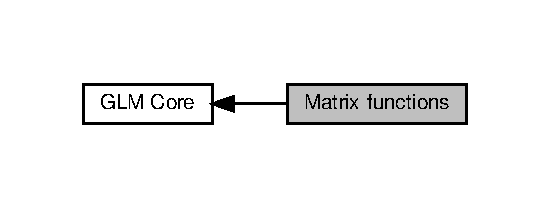
\includegraphics[width=264pt]{group__core__func__matrix}
\end{center}
\end{figure}
\subsection*{Functions}
\begin{DoxyCompactItemize}
\item 
{\footnotesize template$<$typename T , precision P, template$<$ typename, precision $>$ class mat\+Type$>$ }\\\hyperlink{setup_8hpp_ab2d052de21a70539923e9bcbf6e83a51}{G\+L\+M\+\_\+\+F\+U\+N\+C\+\_\+\+D\+E\+CL} mat\+Type$<$ T, P $>$ \hyperlink{group__core__func__matrix_ga4a54992e4741188ee624b21e3ba91814}{glm\+::matrix\+Comp\+Mult} (mat\+Type$<$ T, P $>$ const \&x, mat\+Type$<$ T, P $>$ const \&y)
\item 
{\footnotesize template$<$typename T , precision P, template$<$ typename, precision $>$ class vec\+TypeA, template$<$ typename, precision $>$ class vec\+TypeB$>$ }\\\hyperlink{setup_8hpp_ab2d052de21a70539923e9bcbf6e83a51}{G\+L\+M\+\_\+\+F\+U\+N\+C\+\_\+\+D\+E\+CL} \hyperlink{structglm_1_1detail_1_1outer_product__trait}{detail\+::outer\+Product\+\_\+trait}$<$ T, P, vec\+TypeA, vec\+TypeB $>$\+::type \hyperlink{group__core__func__matrix_gae9f513dc8e4f3ceb993669321b6d0f09}{glm\+::outer\+Product} (vec\+TypeA$<$ T, P $>$ const \&c, vec\+TypeB$<$ T, P $>$ const \&r)
\item 
{\footnotesize template$<$typename T , precision P, template$<$ typename, precision $>$ class mat\+Type$>$ }\\\hyperlink{setup_8hpp_ab2d052de21a70539923e9bcbf6e83a51}{G\+L\+M\+\_\+\+F\+U\+N\+C\+\_\+\+D\+E\+CL} T \hyperlink{group__core__func__matrix_ga26ea77c574802bc6fc193c40478718d2}{glm\+::determinant} (mat\+Type$<$ T, P $>$ const \&m)
\item 
{\footnotesize template$<$typename T , precision P, template$<$ typename, precision $>$ class mat\+Type$>$ }\\\hyperlink{setup_8hpp_ab2d052de21a70539923e9bcbf6e83a51}{G\+L\+M\+\_\+\+F\+U\+N\+C\+\_\+\+D\+E\+CL} mat\+Type$<$ T, P $>$ \hyperlink{group__core__func__matrix_ga7635d3dbe5aa10ff73a0e6903bf6bea5}{glm\+::inverse} (mat\+Type$<$ T, P $>$ const \&m)
\end{DoxyCompactItemize}


\subsection{Detailed Description}
For each of the following built-\/in matrix functions, there is both a single-\/precision floating point version, where all arguments and return values are single precision, and a double-\/precision floating version, where all arguments and return values are double precision. Only the single-\/precision floating point version is shown. 

\subsection{Function Documentation}
\mbox{\Hypertarget{group__core__func__matrix_ga26ea77c574802bc6fc193c40478718d2}\label{group__core__func__matrix_ga26ea77c574802bc6fc193c40478718d2}} 
\index{Matrix functions@{Matrix functions}!determinant@{determinant}}
\index{determinant@{determinant}!Matrix functions@{Matrix functions}}
\subsubsection{\texorpdfstring{determinant()}{determinant()}}
{\footnotesize\ttfamily template$<$typename T , precision P, template$<$ typename, precision $>$ class mat\+Type$>$ \\
\hyperlink{setup_8hpp_ab2d052de21a70539923e9bcbf6e83a51}{G\+L\+M\+\_\+\+F\+U\+N\+C\+\_\+\+D\+E\+CL} T glm\+::determinant (\begin{DoxyParamCaption}\item[{mat\+Type$<$ T, P $>$ const \&}]{m }\end{DoxyParamCaption})}

Returns the transposed matrix of x


\begin{DoxyTemplParams}{Template Parameters}
{\em mat\+Type} & Floating-\/point matrix types.\\
\hline
\end{DoxyTemplParams}
\begin{DoxySeeAlso}{See also}
\href{http://www.opengl.org/sdk/docs/manglsl/xhtml/transpose.xml}{\tt G\+L\+SL transpose man page} 

\href{http://www.opengl.org/registry/doc/GLSLangSpec.4.20.8.pdf}{\tt G\+L\+SL 4.\+20.\+8 specification, section 8.\+6 Matrix Functions} Return the \hyperlink{group__core__func__matrix_ga26ea77c574802bc6fc193c40478718d2}{determinant} of a squared matrix.
\end{DoxySeeAlso}

\begin{DoxyTemplParams}{Template Parameters}
{\em val\+Type} & Floating-\/point scalar types.\\
\hline
\end{DoxyTemplParams}
\begin{DoxySeeAlso}{See also}
\href{http://www.opengl.org/sdk/docs/manglsl/xhtml/determinant.xml}{\tt G\+L\+SL determinant man page} 

\href{http://www.opengl.org/registry/doc/GLSLangSpec.4.20.8.pdf}{\tt G\+L\+SL 4.\+20.\+8 specification, section 8.\+6 Matrix Functions} 
\end{DoxySeeAlso}


Definition at line 447 of file func\+\_\+matrix.\+inl.

\mbox{\Hypertarget{group__core__func__matrix_ga7635d3dbe5aa10ff73a0e6903bf6bea5}\label{group__core__func__matrix_ga7635d3dbe5aa10ff73a0e6903bf6bea5}} 
\index{Matrix functions@{Matrix functions}!inverse@{inverse}}
\index{inverse@{inverse}!Matrix functions@{Matrix functions}}
\subsubsection{\texorpdfstring{inverse()}{inverse()}}
{\footnotesize\ttfamily template$<$typename T , precision P, template$<$ typename, precision $>$ class mat\+Type$>$ \\
\hyperlink{setup_8hpp_ab2d052de21a70539923e9bcbf6e83a51}{G\+L\+M\+\_\+\+F\+U\+N\+C\+\_\+\+D\+E\+CL} mat\+Type$<$T, P$>$ glm\+::inverse (\begin{DoxyParamCaption}\item[{mat\+Type$<$ T, P $>$ const \&}]{m }\end{DoxyParamCaption})}

Return the inverse of a squared matrix.


\begin{DoxyTemplParams}{Template Parameters}
{\em val\+Type} & Floating-\/point scalar types.\\
\hline
\end{DoxyTemplParams}
\begin{DoxySeeAlso}{See also}
\href{http://www.opengl.org/sdk/docs/manglsl/xhtml/inverse.xml}{\tt G\+L\+SL inverse man page} 

\href{http://www.opengl.org/registry/doc/GLSLangSpec.4.20.8.pdf}{\tt G\+L\+SL 4.\+20.\+8 specification, section 8.\+6 Matrix Functions} 
\end{DoxySeeAlso}


Definition at line 454 of file func\+\_\+matrix.\+inl.

\mbox{\Hypertarget{group__core__func__matrix_ga4a54992e4741188ee624b21e3ba91814}\label{group__core__func__matrix_ga4a54992e4741188ee624b21e3ba91814}} 
\index{Matrix functions@{Matrix functions}!matrix\+Comp\+Mult@{matrix\+Comp\+Mult}}
\index{matrix\+Comp\+Mult@{matrix\+Comp\+Mult}!Matrix functions@{Matrix functions}}
\subsubsection{\texorpdfstring{matrix\+Comp\+Mult()}{matrixCompMult()}}
{\footnotesize\ttfamily template$<$typename T , precision P, template$<$ typename, precision $>$ class mat\+Type$>$ \\
\hyperlink{setup_8hpp_ab2d052de21a70539923e9bcbf6e83a51}{G\+L\+M\+\_\+\+F\+U\+N\+C\+\_\+\+D\+E\+CL} mat\+Type$<$T, P$>$ glm\+::matrix\+Comp\+Mult (\begin{DoxyParamCaption}\item[{mat\+Type$<$ T, P $>$ const \&}]{x,  }\item[{mat\+Type$<$ T, P $>$ const \&}]{y }\end{DoxyParamCaption})}

Multiply matrix x by matrix y component-\/wise, i.\+e., result\mbox{[}i\mbox{]}\mbox{[}j\mbox{]} is the scalar product of x\mbox{[}i\mbox{]}\mbox{[}j\mbox{]} and y\mbox{[}i\mbox{]}\mbox{[}j\mbox{]}.


\begin{DoxyTemplParams}{Template Parameters}
{\em mat\+Type} & Floating-\/point matrix types.\\
\hline
\end{DoxyTemplParams}
\begin{DoxySeeAlso}{See also}
\href{http://www.opengl.org/sdk/docs/manglsl/xhtml/matrixCompMult.xml}{\tt G\+L\+SL matrix\+Comp\+Mult man page} 

\href{http://www.opengl.org/registry/doc/GLSLangSpec.4.20.8.pdf}{\tt G\+L\+SL 4.\+20.\+8 specification, section 8.\+6 Matrix Functions} 
\end{DoxySeeAlso}


Definition at line 422 of file func\+\_\+matrix.\+inl.

\mbox{\Hypertarget{group__core__func__matrix_gae9f513dc8e4f3ceb993669321b6d0f09}\label{group__core__func__matrix_gae9f513dc8e4f3ceb993669321b6d0f09}} 
\index{Matrix functions@{Matrix functions}!outer\+Product@{outer\+Product}}
\index{outer\+Product@{outer\+Product}!Matrix functions@{Matrix functions}}
\subsubsection{\texorpdfstring{outer\+Product()}{outerProduct()}}
{\footnotesize\ttfamily template$<$typename T , precision P, template$<$ typename, precision $>$ class vec\+TypeA, template$<$ typename, precision $>$ class vec\+TypeB$>$ \\
\hyperlink{setup_8hpp_ab2d052de21a70539923e9bcbf6e83a51}{G\+L\+M\+\_\+\+F\+U\+N\+C\+\_\+\+D\+E\+CL} \hyperlink{structglm_1_1detail_1_1outer_product__trait}{detail\+::outer\+Product\+\_\+trait}$<$T, P, vec\+TypeA, vec\+TypeB$>$\+::type glm\+::outer\+Product (\begin{DoxyParamCaption}\item[{vec\+TypeA$<$ T, P $>$ const \&}]{c,  }\item[{vec\+TypeB$<$ T, P $>$ const \&}]{r }\end{DoxyParamCaption})}

Treats the first parameter c as a column vector and the second parameter r as a row vector and does a linear algebraic matrix multiply c $\ast$ r.


\begin{DoxyTemplParams}{Template Parameters}
{\em mat\+Type} & Floating-\/point matrix types.\\
\hline
\end{DoxyTemplParams}
\begin{DoxySeeAlso}{See also}
\href{http://www.opengl.org/sdk/docs/manglsl/xhtml/outerProduct.xml}{\tt G\+L\+SL outer\+Product man page} 

\href{http://www.opengl.org/registry/doc/GLSLangSpec.4.20.8.pdf}{\tt G\+L\+SL 4.\+20.\+8 specification, section 8.\+6 Matrix Functions}
\end{DoxySeeAlso}
\begin{DoxyRefDesc}{Todo}
\item[\hyperlink{todo__todo000004}{Todo}]Clarify the declaration to specify that mat\+Type doesn\textquotesingle{}t have to be provided when used. \end{DoxyRefDesc}


Definition at line 433 of file func\+\_\+matrix.\+inl.


\hypertarget{group__core__func__noise}{}\section{Noise functions}
\label{group__core__func__noise}\index{Noise functions@{Noise functions}}
Collaboration diagram for Noise functions\+:\nopagebreak
\begin{figure}[H]
\begin{center}
\leavevmode
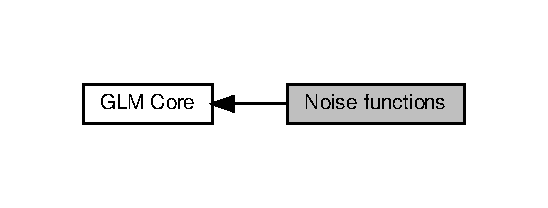
\includegraphics[width=263pt]{group__core__func__noise}
\end{center}
\end{figure}
\subsection*{Functions}
\begin{DoxyCompactItemize}
\item 
{\footnotesize template$<$typename gen\+Type $>$ }\\\hyperlink{setup_8hpp_ab2d052de21a70539923e9bcbf6e83a51}{G\+L\+M\+\_\+\+F\+U\+N\+C\+\_\+\+D\+E\+CL} gen\+Type\+::value\+\_\+type \hyperlink{group__core__func__noise_gadcbf14e3390990f33fda02bb20836960}{glm\+::noise1} (gen\+Type const \&x)
\item 
{\footnotesize template$<$typename gen\+Type $>$ }\\\hyperlink{setup_8hpp_ab2d052de21a70539923e9bcbf6e83a51}{G\+L\+M\+\_\+\+F\+U\+N\+C\+\_\+\+D\+E\+CL} \hyperlink{structglm_1_1detail_1_1tvec2}{detail\+::tvec2}$<$ typename gen\+Type\+::value\+\_\+type, \hyperlink{namespaceglm_a0f04f086094c747d227af4425893f545a9d21ccd8b5a009ec7eb7677befc3bf51}{defaultp} $>$ \hyperlink{group__core__func__noise_ga876ad0805cece7b52bac9f5bac42647a}{glm\+::noise2} (gen\+Type const \&x)
\item 
{\footnotesize template$<$typename gen\+Type $>$ }\\\hyperlink{setup_8hpp_ab2d052de21a70539923e9bcbf6e83a51}{G\+L\+M\+\_\+\+F\+U\+N\+C\+\_\+\+D\+E\+CL} \hyperlink{structglm_1_1detail_1_1tvec3}{detail\+::tvec3}$<$ typename gen\+Type\+::value\+\_\+type, \hyperlink{namespaceglm_a0f04f086094c747d227af4425893f545a9d21ccd8b5a009ec7eb7677befc3bf51}{defaultp} $>$ \hyperlink{group__core__func__noise_gadc066dd8e6c25b77a0dd4f59d4a2dd2c}{glm\+::noise3} (gen\+Type const \&x)
\item 
{\footnotesize template$<$typename gen\+Type $>$ }\\\hyperlink{setup_8hpp_ab2d052de21a70539923e9bcbf6e83a51}{G\+L\+M\+\_\+\+F\+U\+N\+C\+\_\+\+D\+E\+CL} \hyperlink{structglm_1_1detail_1_1tvec4}{detail\+::tvec4}$<$ typename gen\+Type\+::value\+\_\+type, \hyperlink{namespaceglm_a0f04f086094c747d227af4425893f545a9d21ccd8b5a009ec7eb7677befc3bf51}{defaultp} $>$ \hyperlink{group__core__func__noise_ga4ca7d36395a06c2f210ceca5d9a1d020}{glm\+::noise4} (gen\+Type const \&x)
\end{DoxyCompactItemize}


\subsection{Detailed Description}
Noise functions are stochastic functions that can be used to increase visual complexity. Values returned by the following noise functions give the appearance of randomness, but are not truly random. 

\subsection{Function Documentation}
\mbox{\Hypertarget{group__core__func__noise_gadcbf14e3390990f33fda02bb20836960}\label{group__core__func__noise_gadcbf14e3390990f33fda02bb20836960}} 
\index{Noise functions@{Noise functions}!noise1@{noise1}}
\index{noise1@{noise1}!Noise functions@{Noise functions}}
\subsubsection{\texorpdfstring{noise1()}{noise1()}}
{\footnotesize\ttfamily template$<$typename gen\+Type $>$ \\
\hyperlink{setup_8hpp_ab2d052de21a70539923e9bcbf6e83a51}{G\+L\+M\+\_\+\+F\+U\+N\+C\+\_\+\+D\+E\+CL} gen\+Type\+::value\+\_\+type glm\+::noise1 (\begin{DoxyParamCaption}\item[{gen\+Type const \&}]{x }\end{DoxyParamCaption})}

Returns a 1D noise value based on the input value x.


\begin{DoxyTemplParams}{Template Parameters}
{\em gen\+Type} & Floating-\/point scalar or vector types.\\
\hline
\end{DoxyTemplParams}
\begin{DoxySeeAlso}{See also}
\href{http://www.opengl.org/sdk/docs/manglsl/xhtml/noise1.xml}{\tt G\+L\+SL noise1 man page} 

\href{http://www.opengl.org/registry/doc/GLSLangSpec.4.20.8.pdf}{\tt G\+L\+SL 4.\+20.\+8 specification, section 8.\+13 Noise Functions} 
\end{DoxySeeAlso}
\mbox{\Hypertarget{group__core__func__noise_ga876ad0805cece7b52bac9f5bac42647a}\label{group__core__func__noise_ga876ad0805cece7b52bac9f5bac42647a}} 
\index{Noise functions@{Noise functions}!noise2@{noise2}}
\index{noise2@{noise2}!Noise functions@{Noise functions}}
\subsubsection{\texorpdfstring{noise2()}{noise2()}}
{\footnotesize\ttfamily template$<$typename gen\+Type $>$ \\
\hyperlink{setup_8hpp_ab2d052de21a70539923e9bcbf6e83a51}{G\+L\+M\+\_\+\+F\+U\+N\+C\+\_\+\+D\+E\+CL} \hyperlink{structglm_1_1detail_1_1tvec2}{detail\+::tvec2}$<$typename gen\+Type\+::value\+\_\+type, \hyperlink{namespaceglm_a0f04f086094c747d227af4425893f545a9d21ccd8b5a009ec7eb7677befc3bf51}{defaultp}$>$ glm\+::noise2 (\begin{DoxyParamCaption}\item[{gen\+Type const \&}]{x }\end{DoxyParamCaption})}

Returns a 2D noise value based on the input value x.


\begin{DoxyTemplParams}{Template Parameters}
{\em gen\+Type} & Floating-\/point scalar or vector types.\\
\hline
\end{DoxyTemplParams}
\begin{DoxySeeAlso}{See also}
\href{http://www.opengl.org/sdk/docs/manglsl/xhtml/noise2.xml}{\tt G\+L\+SL noise2 man page} 

\href{http://www.opengl.org/registry/doc/GLSLangSpec.4.20.8.pdf}{\tt G\+L\+SL 4.\+20.\+8 specification, section 8.\+13 Noise Functions} 
\end{DoxySeeAlso}
\mbox{\Hypertarget{group__core__func__noise_gadc066dd8e6c25b77a0dd4f59d4a2dd2c}\label{group__core__func__noise_gadc066dd8e6c25b77a0dd4f59d4a2dd2c}} 
\index{Noise functions@{Noise functions}!noise3@{noise3}}
\index{noise3@{noise3}!Noise functions@{Noise functions}}
\subsubsection{\texorpdfstring{noise3()}{noise3()}}
{\footnotesize\ttfamily template$<$typename gen\+Type $>$ \\
\hyperlink{setup_8hpp_ab2d052de21a70539923e9bcbf6e83a51}{G\+L\+M\+\_\+\+F\+U\+N\+C\+\_\+\+D\+E\+CL} \hyperlink{structglm_1_1detail_1_1tvec3}{detail\+::tvec3}$<$typename gen\+Type\+::value\+\_\+type, \hyperlink{namespaceglm_a0f04f086094c747d227af4425893f545a9d21ccd8b5a009ec7eb7677befc3bf51}{defaultp}$>$ glm\+::noise3 (\begin{DoxyParamCaption}\item[{gen\+Type const \&}]{x }\end{DoxyParamCaption})}

Returns a 3D noise value based on the input value x.


\begin{DoxyTemplParams}{Template Parameters}
{\em gen\+Type} & Floating-\/point scalar or vector types.\\
\hline
\end{DoxyTemplParams}
\begin{DoxySeeAlso}{See also}
\href{http://www.opengl.org/sdk/docs/manglsl/xhtml/noise3.xml}{\tt G\+L\+SL noise3 man page} 

\href{http://www.opengl.org/registry/doc/GLSLangSpec.4.20.8.pdf}{\tt G\+L\+SL 4.\+20.\+8 specification, section 8.\+13 Noise Functions} 
\end{DoxySeeAlso}
\mbox{\Hypertarget{group__core__func__noise_ga4ca7d36395a06c2f210ceca5d9a1d020}\label{group__core__func__noise_ga4ca7d36395a06c2f210ceca5d9a1d020}} 
\index{Noise functions@{Noise functions}!noise4@{noise4}}
\index{noise4@{noise4}!Noise functions@{Noise functions}}
\subsubsection{\texorpdfstring{noise4()}{noise4()}}
{\footnotesize\ttfamily template$<$typename gen\+Type $>$ \\
\hyperlink{setup_8hpp_ab2d052de21a70539923e9bcbf6e83a51}{G\+L\+M\+\_\+\+F\+U\+N\+C\+\_\+\+D\+E\+CL} \hyperlink{structglm_1_1detail_1_1tvec4}{detail\+::tvec4}$<$typename gen\+Type\+::value\+\_\+type, \hyperlink{namespaceglm_a0f04f086094c747d227af4425893f545a9d21ccd8b5a009ec7eb7677befc3bf51}{defaultp}$>$ glm\+::noise4 (\begin{DoxyParamCaption}\item[{gen\+Type const \&}]{x }\end{DoxyParamCaption})}

Returns a 4D noise value based on the input value x.


\begin{DoxyTemplParams}{Template Parameters}
{\em gen\+Type} & Floating-\/point scalar or vector types.\\
\hline
\end{DoxyTemplParams}
\begin{DoxySeeAlso}{See also}
\href{http://www.opengl.org/sdk/docs/manglsl/xhtml/noise4.xml}{\tt G\+L\+SL noise4 man page} 

\href{http://www.opengl.org/registry/doc/GLSLangSpec.4.20.8.pdf}{\tt G\+L\+SL 4.\+20.\+8 specification, section 8.\+13 Noise Functions} 
\end{DoxySeeAlso}

\hypertarget{group__core__func__packing}{}\section{Floating-\/\+Point Pack and Unpack Functions}
\label{group__core__func__packing}\index{Floating-\/\+Point Pack and Unpack Functions@{Floating-\/\+Point Pack and Unpack Functions}}
Collaboration diagram for Floating-\/\+Point Pack and Unpack Functions\+:\nopagebreak
\begin{figure}[H]
\begin{center}
\leavevmode
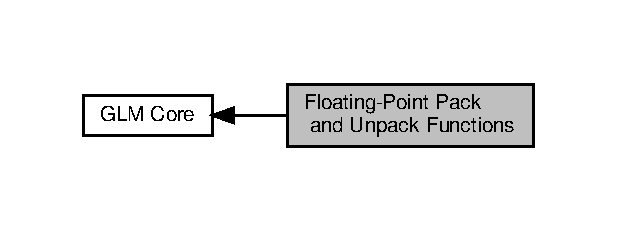
\includegraphics[width=296pt]{group__core__func__packing}
\end{center}
\end{figure}
\subsection*{Functions}
\begin{DoxyCompactItemize}
\item 
\hyperlink{setup_8hpp_ab2d052de21a70539923e9bcbf6e83a51}{G\+L\+M\+\_\+\+F\+U\+N\+C\+\_\+\+D\+E\+CL} \hyperlink{group__core__precision_ga4fd29415871152bfb5abd588334147c8}{uint} \hyperlink{group__core__func__packing_ga0659ddaf09727551c7bf51655d2a65cf}{glm\+::pack\+Unorm2x16} (\hyperlink{group__core__types_gaa1618f51db67eaa145db101d8c8431d8}{vec2} const \&v)
\item 
\hyperlink{setup_8hpp_ab2d052de21a70539923e9bcbf6e83a51}{G\+L\+M\+\_\+\+F\+U\+N\+C\+\_\+\+D\+E\+CL} \hyperlink{group__core__precision_ga4fd29415871152bfb5abd588334147c8}{uint} \hyperlink{group__core__func__packing_ga0c8005de240d6c4ca3d16c7bee25c622}{glm\+::pack\+Snorm2x16} (\hyperlink{group__core__types_gaa1618f51db67eaa145db101d8c8431d8}{vec2} const \&v)
\item 
\hyperlink{setup_8hpp_ab2d052de21a70539923e9bcbf6e83a51}{G\+L\+M\+\_\+\+F\+U\+N\+C\+\_\+\+D\+E\+CL} \hyperlink{group__core__precision_ga4fd29415871152bfb5abd588334147c8}{uint} \hyperlink{group__core__func__packing_ga834ee9a9e73dcb0a7c1fc88143f3edb8}{glm\+::pack\+Unorm4x8} (\hyperlink{group__core__types_ga5881b1b022d7fd1b7218f5916532dd02}{vec4} const \&v)
\item 
\hyperlink{setup_8hpp_ab2d052de21a70539923e9bcbf6e83a51}{G\+L\+M\+\_\+\+F\+U\+N\+C\+\_\+\+D\+E\+CL} \hyperlink{group__core__precision_ga4fd29415871152bfb5abd588334147c8}{uint} \hyperlink{group__core__func__packing_gafcf25acc0d361c6c696a433aa5dfd16b}{glm\+::pack\+Snorm4x8} (\hyperlink{group__core__types_ga5881b1b022d7fd1b7218f5916532dd02}{vec4} const \&v)
\item 
\hyperlink{setup_8hpp_ab2d052de21a70539923e9bcbf6e83a51}{G\+L\+M\+\_\+\+F\+U\+N\+C\+\_\+\+D\+E\+CL} \hyperlink{group__core__types_gaa1618f51db67eaa145db101d8c8431d8}{vec2} \hyperlink{group__core__func__packing_gaff327a2fca8abfe31b74b914b68ac5ec}{glm\+::unpack\+Unorm2x16} (\hyperlink{group__core__precision_ga4fd29415871152bfb5abd588334147c8}{uint} const \&p)
\item 
\hyperlink{setup_8hpp_ab2d052de21a70539923e9bcbf6e83a51}{G\+L\+M\+\_\+\+F\+U\+N\+C\+\_\+\+D\+E\+CL} \hyperlink{group__core__types_gaa1618f51db67eaa145db101d8c8431d8}{vec2} \hyperlink{group__core__func__packing_gaa3f9bd6a71d7bdfab090b9626f2466aa}{glm\+::unpack\+Snorm2x16} (\hyperlink{group__core__precision_ga4fd29415871152bfb5abd588334147c8}{uint} const \&p)
\item 
\hyperlink{setup_8hpp_ab2d052de21a70539923e9bcbf6e83a51}{G\+L\+M\+\_\+\+F\+U\+N\+C\+\_\+\+D\+E\+CL} \hyperlink{group__core__types_ga5881b1b022d7fd1b7218f5916532dd02}{vec4} \hyperlink{group__core__func__packing_ga5d3c4d354b48a317935349dd62a8b8a5}{glm\+::unpack\+Unorm4x8} (\hyperlink{group__core__precision_ga4fd29415871152bfb5abd588334147c8}{uint} const \&p)
\item 
\hyperlink{setup_8hpp_ab2d052de21a70539923e9bcbf6e83a51}{G\+L\+M\+\_\+\+F\+U\+N\+C\+\_\+\+D\+E\+CL} \hyperlink{group__core__types_ga5881b1b022d7fd1b7218f5916532dd02}{vec4} \hyperlink{group__core__func__packing_ga126a0deffef1f2d10dd67237981a870b}{glm\+::unpack\+Snorm4x8} (\hyperlink{group__core__precision_ga4fd29415871152bfb5abd588334147c8}{uint} const \&p)
\item 
\hyperlink{setup_8hpp_ab2d052de21a70539923e9bcbf6e83a51}{G\+L\+M\+\_\+\+F\+U\+N\+C\+\_\+\+D\+E\+CL} double \hyperlink{group__core__func__packing_gaf728fdfb98ce34da6f968d9f6bf154d7}{glm\+::pack\+Double2x32} (\hyperlink{group__core__types_gafd2041b45eff671aa8899d2c2835eee9}{uvec2} const \&v)
\item 
\hyperlink{setup_8hpp_ab2d052de21a70539923e9bcbf6e83a51}{G\+L\+M\+\_\+\+F\+U\+N\+C\+\_\+\+D\+E\+CL} \hyperlink{group__core__types_gafd2041b45eff671aa8899d2c2835eee9}{uvec2} \hyperlink{group__core__func__packing_ga7e8cf88c278c18969c99af83bceed024}{glm\+::unpack\+Double2x32} (double const \&v)
\item 
\hyperlink{setup_8hpp_ab2d052de21a70539923e9bcbf6e83a51}{G\+L\+M\+\_\+\+F\+U\+N\+C\+\_\+\+D\+E\+CL} \hyperlink{group__core__precision_ga4fd29415871152bfb5abd588334147c8}{uint} \hyperlink{group__core__func__packing_ga082f6dd65f73a547ed3067ef00be036f}{glm\+::pack\+Half2x16} (\hyperlink{group__core__types_gaa1618f51db67eaa145db101d8c8431d8}{vec2} const \&v)
\item 
\hyperlink{setup_8hpp_ab2d052de21a70539923e9bcbf6e83a51}{G\+L\+M\+\_\+\+F\+U\+N\+C\+\_\+\+D\+E\+CL} \hyperlink{group__core__types_gaa1618f51db67eaa145db101d8c8431d8}{vec2} \hyperlink{group__core__func__packing_ga4051804cc2c930ba4ca73382b79edf1d}{glm\+::unpack\+Half2x16} (\hyperlink{group__core__precision_ga4fd29415871152bfb5abd588334147c8}{uint} const \&v)
\end{DoxyCompactItemize}


\subsection{Detailed Description}
These functions do not operate component-\/wise, rather as described in each case. 

\subsection{Function Documentation}
\mbox{\Hypertarget{group__core__func__packing_gaf728fdfb98ce34da6f968d9f6bf154d7}\label{group__core__func__packing_gaf728fdfb98ce34da6f968d9f6bf154d7}} 
\index{Floating-\/\+Point Pack and Unpack Functions@{Floating-\/\+Point Pack and Unpack Functions}!pack\+Double2x32@{pack\+Double2x32}}
\index{pack\+Double2x32@{pack\+Double2x32}!Floating-\/\+Point Pack and Unpack Functions@{Floating-\/\+Point Pack and Unpack Functions}}
\subsubsection{\texorpdfstring{pack\+Double2x32()}{packDouble2x32()}}
{\footnotesize\ttfamily \hyperlink{setup_8hpp_a33fdea6f91c5f834105f7415e2a64407}{G\+L\+M\+\_\+\+F\+U\+N\+C\+\_\+\+Q\+U\+A\+L\+I\+F\+I\+ER} double glm\+::pack\+Double2x32 (\begin{DoxyParamCaption}\item[{\hyperlink{group__core__types_gafd2041b45eff671aa8899d2c2835eee9}{uvec2} const \&}]{v }\end{DoxyParamCaption})}

Returns a double-\/precision value obtained by packing the components of v into a 64-\/bit value. If an I\+E\+EE 754 Inf or NaN is created, it will not signal, and the resulting floating point value is unspecified. Otherwise, the bit-\/ level representation of v is preserved. The first vector component specifies the 32 least significant bits; the second component specifies the 32 most significant bits.

\begin{DoxySeeAlso}{See also}
\href{http://www.opengl.org/sdk/docs/manglsl/xhtml/packDouble2x32.xml}{\tt G\+L\+SL pack\+Double2x32 man page} 

\href{http://www.opengl.org/registry/doc/GLSLangSpec.4.20.8.pdf}{\tt G\+L\+SL 4.\+20.\+8 specification, section 8.\+4 Floating-\/\+Point Pack and Unpack Functions} 
\end{DoxySeeAlso}


Definition at line 91 of file func\+\_\+packing.\+inl.

\mbox{\Hypertarget{group__core__func__packing_ga082f6dd65f73a547ed3067ef00be036f}\label{group__core__func__packing_ga082f6dd65f73a547ed3067ef00be036f}} 
\index{Floating-\/\+Point Pack and Unpack Functions@{Floating-\/\+Point Pack and Unpack Functions}!pack\+Half2x16@{pack\+Half2x16}}
\index{pack\+Half2x16@{pack\+Half2x16}!Floating-\/\+Point Pack and Unpack Functions@{Floating-\/\+Point Pack and Unpack Functions}}
\subsubsection{\texorpdfstring{pack\+Half2x16()}{packHalf2x16()}}
{\footnotesize\ttfamily \hyperlink{setup_8hpp_a33fdea6f91c5f834105f7415e2a64407}{G\+L\+M\+\_\+\+F\+U\+N\+C\+\_\+\+Q\+U\+A\+L\+I\+F\+I\+ER} \hyperlink{group__core__precision_ga4fd29415871152bfb5abd588334147c8}{uint} glm\+::pack\+Half2x16 (\begin{DoxyParamCaption}\item[{\hyperlink{group__core__types_gaa1618f51db67eaa145db101d8c8431d8}{vec2} const \&}]{v }\end{DoxyParamCaption})}

Returns an unsigned integer obtained by converting the components of a two-\/component floating-\/point vector to the 16-\/bit floating-\/point representation found in the Open\+GL Specification, and then packing these two 16-\/ bit integers into a 32-\/bit unsigned integer. The first vector component specifies the 16 least-\/significant bits of the result; the second component specifies the 16 most-\/significant bits.

\begin{DoxySeeAlso}{See also}
\href{http://www.opengl.org/sdk/docs/manglsl/xhtml/packHalf2x16.xml}{\tt G\+L\+SL pack\+Half2x16 man page} 

\href{http://www.opengl.org/registry/doc/GLSLangSpec.4.20.8.pdf}{\tt G\+L\+SL 4.\+20.\+8 specification, section 8.\+4 Floating-\/\+Point Pack and Unpack Functions} 
\end{DoxySeeAlso}


Definition at line 101 of file func\+\_\+packing.\+inl.

\mbox{\Hypertarget{group__core__func__packing_ga0c8005de240d6c4ca3d16c7bee25c622}\label{group__core__func__packing_ga0c8005de240d6c4ca3d16c7bee25c622}} 
\index{Floating-\/\+Point Pack and Unpack Functions@{Floating-\/\+Point Pack and Unpack Functions}!pack\+Snorm2x16@{pack\+Snorm2x16}}
\index{pack\+Snorm2x16@{pack\+Snorm2x16}!Floating-\/\+Point Pack and Unpack Functions@{Floating-\/\+Point Pack and Unpack Functions}}
\subsubsection{\texorpdfstring{pack\+Snorm2x16()}{packSnorm2x16()}}
{\footnotesize\ttfamily \hyperlink{setup_8hpp_a33fdea6f91c5f834105f7415e2a64407}{G\+L\+M\+\_\+\+F\+U\+N\+C\+\_\+\+Q\+U\+A\+L\+I\+F\+I\+ER} \hyperlink{group__core__precision_ga4fd29415871152bfb5abd588334147c8}{uint} glm\+::pack\+Snorm2x16 (\begin{DoxyParamCaption}\item[{\hyperlink{group__core__types_gaa1618f51db67eaa145db101d8c8431d8}{vec2} const \&}]{v }\end{DoxyParamCaption})}

First, converts each component of the normalized floating-\/point value v into 8-\/ or 16-\/bit integer values. Then, the results are packed into the returned 32-\/bit unsigned integer.

The conversion for component c of v to fixed point is done as follows\+: pack\+Snorm2x16\+: round(clamp(v, -\/1, +1) $\ast$ 32767.\+0)

The first component of the vector will be written to the least significant bits of the output; the last component will be written to the most significant bits.

\begin{DoxySeeAlso}{See also}
\href{http://www.opengl.org/sdk/docs/manglsl/xhtml/packSnorm2x16.xml}{\tt G\+L\+SL pack\+Snorm2x16 man page} 

\href{http://www.opengl.org/registry/doc/GLSLangSpec.4.20.8.pdf}{\tt G\+L\+SL 4.\+20.\+8 specification, section 8.\+4 Floating-\/\+Point Pack and Unpack Functions} 
\end{DoxySeeAlso}


Definition at line 49 of file func\+\_\+packing.\+inl.

\mbox{\Hypertarget{group__core__func__packing_gafcf25acc0d361c6c696a433aa5dfd16b}\label{group__core__func__packing_gafcf25acc0d361c6c696a433aa5dfd16b}} 
\index{Floating-\/\+Point Pack and Unpack Functions@{Floating-\/\+Point Pack and Unpack Functions}!pack\+Snorm4x8@{pack\+Snorm4x8}}
\index{pack\+Snorm4x8@{pack\+Snorm4x8}!Floating-\/\+Point Pack and Unpack Functions@{Floating-\/\+Point Pack and Unpack Functions}}
\subsubsection{\texorpdfstring{pack\+Snorm4x8()}{packSnorm4x8()}}
{\footnotesize\ttfamily \hyperlink{setup_8hpp_a33fdea6f91c5f834105f7415e2a64407}{G\+L\+M\+\_\+\+F\+U\+N\+C\+\_\+\+Q\+U\+A\+L\+I\+F\+I\+ER} \hyperlink{group__core__precision_ga4fd29415871152bfb5abd588334147c8}{uint} glm\+::pack\+Snorm4x8 (\begin{DoxyParamCaption}\item[{\hyperlink{group__core__types_ga5881b1b022d7fd1b7218f5916532dd02}{vec4} const \&}]{v }\end{DoxyParamCaption})}

First, converts each component of the normalized floating-\/point value v into 8-\/ or 16-\/bit integer values. Then, the results are packed into the returned 32-\/bit unsigned integer.

The conversion for component c of v to fixed point is done as follows\+: pack\+Snorm4x8\+: round(clamp(c, -\/1, +1) $\ast$ 127.\+0)

The first component of the vector will be written to the least significant bits of the output; the last component will be written to the most significant bits.

\begin{DoxySeeAlso}{See also}
\href{http://www.opengl.org/sdk/docs/manglsl/xhtml/packSnorm4x8.xml}{\tt G\+L\+SL pack\+Snorm4x8 man page} 

\href{http://www.opengl.org/registry/doc/GLSLangSpec.4.20.8.pdf}{\tt G\+L\+SL 4.\+20.\+8 specification, section 8.\+4 Floating-\/\+Point Pack and Unpack Functions} 
\end{DoxySeeAlso}


Definition at line 77 of file func\+\_\+packing.\+inl.

\mbox{\Hypertarget{group__core__func__packing_ga0659ddaf09727551c7bf51655d2a65cf}\label{group__core__func__packing_ga0659ddaf09727551c7bf51655d2a65cf}} 
\index{Floating-\/\+Point Pack and Unpack Functions@{Floating-\/\+Point Pack and Unpack Functions}!pack\+Unorm2x16@{pack\+Unorm2x16}}
\index{pack\+Unorm2x16@{pack\+Unorm2x16}!Floating-\/\+Point Pack and Unpack Functions@{Floating-\/\+Point Pack and Unpack Functions}}
\subsubsection{\texorpdfstring{pack\+Unorm2x16()}{packUnorm2x16()}}
{\footnotesize\ttfamily \hyperlink{setup_8hpp_a33fdea6f91c5f834105f7415e2a64407}{G\+L\+M\+\_\+\+F\+U\+N\+C\+\_\+\+Q\+U\+A\+L\+I\+F\+I\+ER} \hyperlink{group__core__precision_ga4fd29415871152bfb5abd588334147c8}{uint} glm\+::pack\+Unorm2x16 (\begin{DoxyParamCaption}\item[{\hyperlink{group__core__types_gaa1618f51db67eaa145db101d8c8431d8}{vec2} const \&}]{v }\end{DoxyParamCaption})}

First, converts each component of the normalized floating-\/point value v into 8-\/ or 16-\/bit integer values. Then, the results are packed into the returned 32-\/bit unsigned integer.

The conversion for component c of v to fixed point is done as follows\+: pack\+Unorm2x16\+: round(clamp(c, 0, +1) $\ast$ 65535.\+0)

The first component of the vector will be written to the least significant bits of the output; the last component will be written to the most significant bits.

\begin{DoxySeeAlso}{See also}
\href{http://www.opengl.org/sdk/docs/manglsl/xhtml/packUnorm2x16.xml}{\tt G\+L\+SL pack\+Unorm2x16 man page} 

\href{http://www.opengl.org/registry/doc/GLSLangSpec.4.20.8.pdf}{\tt G\+L\+SL 4.\+20.\+8 specification, section 8.\+4 Floating-\/\+Point Pack and Unpack Functions} 
\end{DoxySeeAlso}


Definition at line 35 of file func\+\_\+packing.\+inl.

\mbox{\Hypertarget{group__core__func__packing_ga834ee9a9e73dcb0a7c1fc88143f3edb8}\label{group__core__func__packing_ga834ee9a9e73dcb0a7c1fc88143f3edb8}} 
\index{Floating-\/\+Point Pack and Unpack Functions@{Floating-\/\+Point Pack and Unpack Functions}!pack\+Unorm4x8@{pack\+Unorm4x8}}
\index{pack\+Unorm4x8@{pack\+Unorm4x8}!Floating-\/\+Point Pack and Unpack Functions@{Floating-\/\+Point Pack and Unpack Functions}}
\subsubsection{\texorpdfstring{pack\+Unorm4x8()}{packUnorm4x8()}}
{\footnotesize\ttfamily \hyperlink{setup_8hpp_a33fdea6f91c5f834105f7415e2a64407}{G\+L\+M\+\_\+\+F\+U\+N\+C\+\_\+\+Q\+U\+A\+L\+I\+F\+I\+ER} \hyperlink{group__core__precision_ga4fd29415871152bfb5abd588334147c8}{uint} glm\+::pack\+Unorm4x8 (\begin{DoxyParamCaption}\item[{\hyperlink{group__core__types_ga5881b1b022d7fd1b7218f5916532dd02}{vec4} const \&}]{v }\end{DoxyParamCaption})}

First, converts each component of the normalized floating-\/point value v into 8-\/ or 16-\/bit integer values. Then, the results are packed into the returned 32-\/bit unsigned integer.

The conversion for component c of v to fixed point is done as follows\+: pack\+Unorm4x8\+: round(clamp(c, 0, +1) $\ast$ 255.\+0)

The first component of the vector will be written to the least significant bits of the output; the last component will be written to the most significant bits.

\begin{DoxySeeAlso}{See also}
\href{http://www.opengl.org/sdk/docs/manglsl/xhtml/packUnorm4x8.xml}{\tt G\+L\+SL pack\+Unorm4x8 man page} 

\href{http://www.opengl.org/registry/doc/GLSLangSpec.4.20.8.pdf}{\tt G\+L\+SL 4.\+20.\+8 specification, section 8.\+4 Floating-\/\+Point Pack and Unpack Functions} 
\end{DoxySeeAlso}


Definition at line 65 of file func\+\_\+packing.\+inl.

\mbox{\Hypertarget{group__core__func__packing_ga7e8cf88c278c18969c99af83bceed024}\label{group__core__func__packing_ga7e8cf88c278c18969c99af83bceed024}} 
\index{Floating-\/\+Point Pack and Unpack Functions@{Floating-\/\+Point Pack and Unpack Functions}!unpack\+Double2x32@{unpack\+Double2x32}}
\index{unpack\+Double2x32@{unpack\+Double2x32}!Floating-\/\+Point Pack and Unpack Functions@{Floating-\/\+Point Pack and Unpack Functions}}
\subsubsection{\texorpdfstring{unpack\+Double2x32()}{unpackDouble2x32()}}
{\footnotesize\ttfamily \hyperlink{setup_8hpp_a33fdea6f91c5f834105f7415e2a64407}{G\+L\+M\+\_\+\+F\+U\+N\+C\+\_\+\+Q\+U\+A\+L\+I\+F\+I\+ER} \hyperlink{group__core__types_gafd2041b45eff671aa8899d2c2835eee9}{uvec2} glm\+::unpack\+Double2x32 (\begin{DoxyParamCaption}\item[{double const \&}]{v }\end{DoxyParamCaption})}

Returns a two-\/component unsigned integer vector representation of v. The bit-\/level representation of v is preserved. The first component of the vector contains the 32 least significant bits of the double; the second component consists the 32 most significant bits.

\begin{DoxySeeAlso}{See also}
\href{http://www.opengl.org/sdk/docs/manglsl/xhtml/unpackDouble2x32.xml}{\tt G\+L\+SL unpack\+Double2x32 man page} 

\href{http://www.opengl.org/registry/doc/GLSLangSpec.4.20.8.pdf}{\tt G\+L\+SL 4.\+20.\+8 specification, section 8.\+4 Floating-\/\+Point Pack and Unpack Functions} 
\end{DoxySeeAlso}


Definition at line 96 of file func\+\_\+packing.\+inl.

\mbox{\Hypertarget{group__core__func__packing_ga4051804cc2c930ba4ca73382b79edf1d}\label{group__core__func__packing_ga4051804cc2c930ba4ca73382b79edf1d}} 
\index{Floating-\/\+Point Pack and Unpack Functions@{Floating-\/\+Point Pack and Unpack Functions}!unpack\+Half2x16@{unpack\+Half2x16}}
\index{unpack\+Half2x16@{unpack\+Half2x16}!Floating-\/\+Point Pack and Unpack Functions@{Floating-\/\+Point Pack and Unpack Functions}}
\subsubsection{\texorpdfstring{unpack\+Half2x16()}{unpackHalf2x16()}}
{\footnotesize\ttfamily \hyperlink{setup_8hpp_a33fdea6f91c5f834105f7415e2a64407}{G\+L\+M\+\_\+\+F\+U\+N\+C\+\_\+\+Q\+U\+A\+L\+I\+F\+I\+ER} \hyperlink{group__core__types_gaa1618f51db67eaa145db101d8c8431d8}{vec2} glm\+::unpack\+Half2x16 (\begin{DoxyParamCaption}\item[{\hyperlink{group__core__precision_ga4fd29415871152bfb5abd588334147c8}{uint} const \&}]{v }\end{DoxyParamCaption})}

Returns a two-\/component floating-\/point vector with components obtained by unpacking a 32-\/bit unsigned integer into a pair of 16-\/bit values, interpreting those values as 16-\/bit floating-\/point numbers according to the Open\+GL Specification, and converting them to 32-\/bit floating-\/point values. The first component of the vector is obtained from the 16 least-\/significant bits of v; the second component is obtained from the 16 most-\/significant bits of v.

\begin{DoxySeeAlso}{See also}
\href{http://www.opengl.org/sdk/docs/manglsl/xhtml/unpackHalf2x16.xml}{\tt G\+L\+SL unpack\+Half2x16 man page} 

\href{http://www.opengl.org/registry/doc/GLSLangSpec.4.20.8.pdf}{\tt G\+L\+SL 4.\+20.\+8 specification, section 8.\+4 Floating-\/\+Point Pack and Unpack Functions} 
\end{DoxySeeAlso}


Definition at line 111 of file func\+\_\+packing.\+inl.

\mbox{\Hypertarget{group__core__func__packing_gaa3f9bd6a71d7bdfab090b9626f2466aa}\label{group__core__func__packing_gaa3f9bd6a71d7bdfab090b9626f2466aa}} 
\index{Floating-\/\+Point Pack and Unpack Functions@{Floating-\/\+Point Pack and Unpack Functions}!unpack\+Snorm2x16@{unpack\+Snorm2x16}}
\index{unpack\+Snorm2x16@{unpack\+Snorm2x16}!Floating-\/\+Point Pack and Unpack Functions@{Floating-\/\+Point Pack and Unpack Functions}}
\subsubsection{\texorpdfstring{unpack\+Snorm2x16()}{unpackSnorm2x16()}}
{\footnotesize\ttfamily \hyperlink{setup_8hpp_a33fdea6f91c5f834105f7415e2a64407}{G\+L\+M\+\_\+\+F\+U\+N\+C\+\_\+\+Q\+U\+A\+L\+I\+F\+I\+ER} \hyperlink{group__core__types_gaa1618f51db67eaa145db101d8c8431d8}{vec2} glm\+::unpack\+Snorm2x16 (\begin{DoxyParamCaption}\item[{\hyperlink{group__core__precision_ga4fd29415871152bfb5abd588334147c8}{uint} const \&}]{p }\end{DoxyParamCaption})}

First, unpacks a single 32-\/bit unsigned integer p into a pair of 16-\/bit unsigned integers, four 8-\/bit unsigned integers, or four 8-\/bit signed integers. Then, each component is converted to a normalized floating-\/point value to generate the returned two-\/ or four-\/component vector.

The conversion for unpacked fixed-\/point value f to floating point is done as follows\+: unpack\+Snorm2x16\+: clamp(f / 32767.\+0, -\/1, +1)

The first component of the returned vector will be extracted from the least significant bits of the input; the last component will be extracted from the most significant bits.

\begin{DoxySeeAlso}{See also}
\href{http://www.opengl.org/sdk/docs/manglsl/xhtml/unpackSnorm2x16.xml}{\tt G\+L\+SL unpack\+Snorm2x16 man page} 

\href{http://www.opengl.org/registry/doc/GLSLangSpec.4.20.8.pdf}{\tt G\+L\+SL 4.\+20.\+8 specification, section 8.\+4 Floating-\/\+Point Pack and Unpack Functions} 
\end{DoxySeeAlso}


Definition at line 57 of file func\+\_\+packing.\+inl.

\mbox{\Hypertarget{group__core__func__packing_ga126a0deffef1f2d10dd67237981a870b}\label{group__core__func__packing_ga126a0deffef1f2d10dd67237981a870b}} 
\index{Floating-\/\+Point Pack and Unpack Functions@{Floating-\/\+Point Pack and Unpack Functions}!unpack\+Snorm4x8@{unpack\+Snorm4x8}}
\index{unpack\+Snorm4x8@{unpack\+Snorm4x8}!Floating-\/\+Point Pack and Unpack Functions@{Floating-\/\+Point Pack and Unpack Functions}}
\subsubsection{\texorpdfstring{unpack\+Snorm4x8()}{unpackSnorm4x8()}}
{\footnotesize\ttfamily \hyperlink{setup_8hpp_a33fdea6f91c5f834105f7415e2a64407}{G\+L\+M\+\_\+\+F\+U\+N\+C\+\_\+\+Q\+U\+A\+L\+I\+F\+I\+ER} \hyperlink{group__core__types_ga5881b1b022d7fd1b7218f5916532dd02}{glm\+::vec4} glm\+::unpack\+Snorm4x8 (\begin{DoxyParamCaption}\item[{\hyperlink{group__core__precision_ga4fd29415871152bfb5abd588334147c8}{uint} const \&}]{p }\end{DoxyParamCaption})}

First, unpacks a single 32-\/bit unsigned integer p into a pair of 16-\/bit unsigned integers, four 8-\/bit unsigned integers, or four 8-\/bit signed integers. Then, each component is converted to a normalized floating-\/point value to generate the returned two-\/ or four-\/component vector.

The conversion for unpacked fixed-\/point value f to floating point is done as follows\+: unpack\+Snorm4x8\+: clamp(f / 127.\+0, -\/1, +1)

The first component of the returned vector will be extracted from the least significant bits of the input; the last component will be extracted from the most significant bits.

\begin{DoxySeeAlso}{See also}
\href{http://www.opengl.org/sdk/docs/manglsl/xhtml/unpackSnorm4x8.xml}{\tt G\+L\+SL unpack\+Snorm4x8 man page} 

\href{http://www.opengl.org/registry/doc/GLSLangSpec.4.20.8.pdf}{\tt G\+L\+SL 4.\+20.\+8 specification, section 8.\+4 Floating-\/\+Point Pack and Unpack Functions} 
\end{DoxySeeAlso}


Definition at line 83 of file func\+\_\+packing.\+inl.

\mbox{\Hypertarget{group__core__func__packing_gaff327a2fca8abfe31b74b914b68ac5ec}\label{group__core__func__packing_gaff327a2fca8abfe31b74b914b68ac5ec}} 
\index{Floating-\/\+Point Pack and Unpack Functions@{Floating-\/\+Point Pack and Unpack Functions}!unpack\+Unorm2x16@{unpack\+Unorm2x16}}
\index{unpack\+Unorm2x16@{unpack\+Unorm2x16}!Floating-\/\+Point Pack and Unpack Functions@{Floating-\/\+Point Pack and Unpack Functions}}
\subsubsection{\texorpdfstring{unpack\+Unorm2x16()}{unpackUnorm2x16()}}
{\footnotesize\ttfamily \hyperlink{setup_8hpp_a33fdea6f91c5f834105f7415e2a64407}{G\+L\+M\+\_\+\+F\+U\+N\+C\+\_\+\+Q\+U\+A\+L\+I\+F\+I\+ER} \hyperlink{group__core__types_gaa1618f51db67eaa145db101d8c8431d8}{vec2} glm\+::unpack\+Unorm2x16 (\begin{DoxyParamCaption}\item[{\hyperlink{group__core__precision_ga4fd29415871152bfb5abd588334147c8}{uint} const \&}]{p }\end{DoxyParamCaption})}

First, unpacks a single 32-\/bit unsigned integer p into a pair of 16-\/bit unsigned integers, four 8-\/bit unsigned integers, or four 8-\/bit signed integers. Then, each component is converted to a normalized floating-\/point value to generate the returned two-\/ or four-\/component vector.

The conversion for unpacked fixed-\/point value f to floating point is done as follows\+: unpack\+Unorm2x16\+: f / 65535.\+0

The first component of the returned vector will be extracted from the least significant bits of the input; the last component will be extracted from the most significant bits.

\begin{DoxySeeAlso}{See also}
\href{http://www.opengl.org/sdk/docs/manglsl/xhtml/unpackUnorm2x16.xml}{\tt G\+L\+SL unpack\+Unorm2x16 man page} 

\href{http://www.opengl.org/registry/doc/GLSLangSpec.4.20.8.pdf}{\tt G\+L\+SL 4.\+20.\+8 specification, section 8.\+4 Floating-\/\+Point Pack and Unpack Functions} 
\end{DoxySeeAlso}


Definition at line 43 of file func\+\_\+packing.\+inl.

\mbox{\Hypertarget{group__core__func__packing_ga5d3c4d354b48a317935349dd62a8b8a5}\label{group__core__func__packing_ga5d3c4d354b48a317935349dd62a8b8a5}} 
\index{Floating-\/\+Point Pack and Unpack Functions@{Floating-\/\+Point Pack and Unpack Functions}!unpack\+Unorm4x8@{unpack\+Unorm4x8}}
\index{unpack\+Unorm4x8@{unpack\+Unorm4x8}!Floating-\/\+Point Pack and Unpack Functions@{Floating-\/\+Point Pack and Unpack Functions}}
\subsubsection{\texorpdfstring{unpack\+Unorm4x8()}{unpackUnorm4x8()}}
{\footnotesize\ttfamily \hyperlink{setup_8hpp_a33fdea6f91c5f834105f7415e2a64407}{G\+L\+M\+\_\+\+F\+U\+N\+C\+\_\+\+Q\+U\+A\+L\+I\+F\+I\+ER} \hyperlink{group__core__types_ga5881b1b022d7fd1b7218f5916532dd02}{vec4} glm\+::unpack\+Unorm4x8 (\begin{DoxyParamCaption}\item[{\hyperlink{group__core__precision_ga4fd29415871152bfb5abd588334147c8}{uint} const \&}]{p }\end{DoxyParamCaption})}

First, unpacks a single 32-\/bit unsigned integer p into a pair of 16-\/bit unsigned integers, four 8-\/bit unsigned integers, or four 8-\/bit signed integers. Then, each component is converted to a normalized floating-\/point value to generate the returned two-\/ or four-\/component vector.

The conversion for unpacked fixed-\/point value f to floating point is done as follows\+: unpack\+Unorm4x8\+: f / 255.\+0

The first component of the returned vector will be extracted from the least significant bits of the input; the last component will be extracted from the most significant bits.

\begin{DoxySeeAlso}{See also}
\href{http://www.opengl.org/sdk/docs/manglsl/xhtml/unpackUnorm4x8.xml}{\tt G\+L\+SL unpack\+Unorm4x8 man page} 

\href{http://www.opengl.org/registry/doc/GLSLangSpec.4.20.8.pdf}{\tt G\+L\+SL 4.\+20.\+8 specification, section 8.\+4 Floating-\/\+Point Pack and Unpack Functions} 
\end{DoxySeeAlso}


Definition at line 71 of file func\+\_\+packing.\+inl.


\hypertarget{group__core__func__trigonometric}{}\section{Angle and Trigonometry Functions}
\label{group__core__func__trigonometric}\index{Angle and Trigonometry Functions@{Angle and Trigonometry Functions}}
Collaboration diagram for Angle and Trigonometry Functions\+:\nopagebreak
\begin{figure}[H]
\begin{center}
\leavevmode
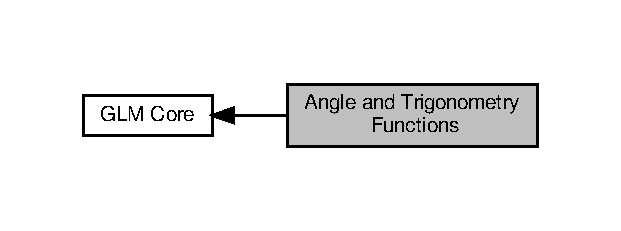
\includegraphics[width=298pt]{group__core__func__trigonometric}
\end{center}
\end{figure}
\subsection*{Functions}
\begin{DoxyCompactItemize}
\item 
{\footnotesize template$<$typename gen\+Type $>$ }\\\hyperlink{setup_8hpp_ab2d052de21a70539923e9bcbf6e83a51}{G\+L\+M\+\_\+\+F\+U\+N\+C\+\_\+\+D\+E\+CL} gen\+Type \hyperlink{group__core__func__trigonometric_ga431d31cdb060059bc5b0696e212f1453}{glm\+::radians} (gen\+Type const \&\hyperlink{group__core__func__trigonometric_gaf4e5661bd1c993f6090d49e988a4c78a}{degrees})
\item 
{\footnotesize template$<$typename gen\+Type $>$ }\\\hyperlink{setup_8hpp_ab2d052de21a70539923e9bcbf6e83a51}{G\+L\+M\+\_\+\+F\+U\+N\+C\+\_\+\+D\+E\+CL} gen\+Type \hyperlink{group__core__func__trigonometric_gaf4e5661bd1c993f6090d49e988a4c78a}{glm\+::degrees} (gen\+Type const \&\hyperlink{group__core__func__trigonometric_ga431d31cdb060059bc5b0696e212f1453}{radians})
\item 
{\footnotesize template$<$typename gen\+Type $>$ }\\\hyperlink{setup_8hpp_ab2d052de21a70539923e9bcbf6e83a51}{G\+L\+M\+\_\+\+F\+U\+N\+C\+\_\+\+D\+E\+CL} gen\+Type \hyperlink{group__core__func__trigonometric_gafbab21016b7f3bc21afb09a7e42e2df1}{glm\+::sin} (gen\+Type const \&\hyperlink{group__gtc__quaternion_ga23a3fc7ada5bbb665ff84c92c6e0542c}{angle})
\item 
{\footnotesize template$<$typename gen\+Type $>$ }\\\hyperlink{setup_8hpp_ab2d052de21a70539923e9bcbf6e83a51}{G\+L\+M\+\_\+\+F\+U\+N\+C\+\_\+\+D\+E\+CL} gen\+Type \hyperlink{group__core__func__trigonometric_gac6708d4f0895dc79b65f50db00840167}{glm\+::cos} (gen\+Type const \&\hyperlink{group__gtc__quaternion_ga23a3fc7ada5bbb665ff84c92c6e0542c}{angle})
\item 
{\footnotesize template$<$typename gen\+Type $>$ }\\\hyperlink{setup_8hpp_ab2d052de21a70539923e9bcbf6e83a51}{G\+L\+M\+\_\+\+F\+U\+N\+C\+\_\+\+D\+E\+CL} gen\+Type \hyperlink{group__core__func__trigonometric_ga328aeb0de4f312dc3d200cb929715d44}{glm\+::tan} (gen\+Type const \&\hyperlink{group__gtc__quaternion_ga23a3fc7ada5bbb665ff84c92c6e0542c}{angle})
\item 
{\footnotesize template$<$typename gen\+Type $>$ }\\\hyperlink{setup_8hpp_ab2d052de21a70539923e9bcbf6e83a51}{G\+L\+M\+\_\+\+F\+U\+N\+C\+\_\+\+D\+E\+CL} gen\+Type \hyperlink{group__core__func__trigonometric_gafca5e8c71ea06be0840227b4aafc5680}{glm\+::asin} (gen\+Type const \&x)
\item 
{\footnotesize template$<$typename gen\+Type $>$ }\\\hyperlink{setup_8hpp_ab2d052de21a70539923e9bcbf6e83a51}{G\+L\+M\+\_\+\+F\+U\+N\+C\+\_\+\+D\+E\+CL} gen\+Type \hyperlink{group__core__func__trigonometric_gac85497ed2e39d4cac4ac32bed4dfc506}{glm\+::acos} (gen\+Type const \&x)
\item 
{\footnotesize template$<$typename gen\+Type $>$ }\\\hyperlink{setup_8hpp_ab2d052de21a70539923e9bcbf6e83a51}{G\+L\+M\+\_\+\+F\+U\+N\+C\+\_\+\+D\+E\+CL} gen\+Type \hyperlink{group__core__func__trigonometric_gabf80ac0817d1db032dd6a0969aa2b84a}{glm\+::atan} (gen\+Type const \&y, gen\+Type const \&x)
\item 
{\footnotesize template$<$typename gen\+Type $>$ }\\\hyperlink{setup_8hpp_ab2d052de21a70539923e9bcbf6e83a51}{G\+L\+M\+\_\+\+F\+U\+N\+C\+\_\+\+D\+E\+CL} gen\+Type \hyperlink{group__core__func__trigonometric_gaa7be96f0c12a40eeac5c7f04a3d465a1}{glm\+::atan} (gen\+Type const \&y\+\_\+over\+\_\+x)
\item 
{\footnotesize template$<$typename gen\+Type $>$ }\\\hyperlink{setup_8hpp_ab2d052de21a70539923e9bcbf6e83a51}{G\+L\+M\+\_\+\+F\+U\+N\+C\+\_\+\+D\+E\+CL} gen\+Type \hyperlink{group__core__func__trigonometric_ga2e8c9a896e803661058de83429aa6eda}{glm\+::sinh} (gen\+Type const \&\hyperlink{group__gtc__quaternion_ga23a3fc7ada5bbb665ff84c92c6e0542c}{angle})
\item 
{\footnotesize template$<$typename gen\+Type $>$ }\\\hyperlink{setup_8hpp_ab2d052de21a70539923e9bcbf6e83a51}{G\+L\+M\+\_\+\+F\+U\+N\+C\+\_\+\+D\+E\+CL} gen\+Type \hyperlink{group__core__func__trigonometric_gaa7685634f6e920ba9a683e5ec7aed976}{glm\+::cosh} (gen\+Type const \&\hyperlink{group__gtc__quaternion_ga23a3fc7ada5bbb665ff84c92c6e0542c}{angle})
\item 
{\footnotesize template$<$typename gen\+Type $>$ }\\\hyperlink{setup_8hpp_ab2d052de21a70539923e9bcbf6e83a51}{G\+L\+M\+\_\+\+F\+U\+N\+C\+\_\+\+D\+E\+CL} gen\+Type \hyperlink{group__core__func__trigonometric_ga941f20e5315113d1a2e037f073a62f04}{glm\+::tanh} (gen\+Type const \&\hyperlink{group__gtc__quaternion_ga23a3fc7ada5bbb665ff84c92c6e0542c}{angle})
\item 
{\footnotesize template$<$typename gen\+Type $>$ }\\\hyperlink{setup_8hpp_ab2d052de21a70539923e9bcbf6e83a51}{G\+L\+M\+\_\+\+F\+U\+N\+C\+\_\+\+D\+E\+CL} gen\+Type \hyperlink{group__core__func__trigonometric_gaa52acc1218a5ddd0f8d94fcd098685b1}{glm\+::asinh} (gen\+Type const \&x)
\item 
{\footnotesize template$<$typename gen\+Type $>$ }\\\hyperlink{setup_8hpp_ab2d052de21a70539923e9bcbf6e83a51}{G\+L\+M\+\_\+\+F\+U\+N\+C\+\_\+\+D\+E\+CL} gen\+Type \hyperlink{group__core__func__trigonometric_ga961d72b4a20d09d6e71fdf076ad4f433}{glm\+::acosh} (gen\+Type const \&x)
\item 
{\footnotesize template$<$typename gen\+Type $>$ }\\\hyperlink{setup_8hpp_ab2d052de21a70539923e9bcbf6e83a51}{G\+L\+M\+\_\+\+F\+U\+N\+C\+\_\+\+D\+E\+CL} gen\+Type \hyperlink{group__core__func__trigonometric_gaa20b78cb9c12e30bd5a3054b8cb3d099}{glm\+::atanh} (gen\+Type const \&x)
\end{DoxyCompactItemize}


\subsection{Detailed Description}
Function parameters specified as angle are assumed to be in units of radians. In no case will any of these functions result in a divide by zero error. If the divisor of a ratio is 0, then results will be undefined.

These all operate component-\/wise. The description is per component. 

\subsection{Function Documentation}
\mbox{\Hypertarget{group__core__func__trigonometric_gac85497ed2e39d4cac4ac32bed4dfc506}\label{group__core__func__trigonometric_gac85497ed2e39d4cac4ac32bed4dfc506}} 
\index{Angle and Trigonometry Functions@{Angle and Trigonometry Functions}!acos@{acos}}
\index{acos@{acos}!Angle and Trigonometry Functions@{Angle and Trigonometry Functions}}
\subsubsection{\texorpdfstring{acos()}{acos()}}
{\footnotesize\ttfamily template$<$typename gen\+Type $>$ \\
\hyperlink{setup_8hpp_ab2d052de21a70539923e9bcbf6e83a51}{G\+L\+M\+\_\+\+F\+U\+N\+C\+\_\+\+D\+E\+CL} gen\+Type glm\+::acos (\begin{DoxyParamCaption}\item[{gen\+Type const \&}]{x }\end{DoxyParamCaption})}

Arc cosine. Returns an angle whose sine is x. The range of values returned by this function is \mbox{[}0, PI\mbox{]}. Results are undefined if $\vert$x$\vert$ $>$ 1.


\begin{DoxyTemplParams}{Template Parameters}
{\em gen\+Type} & Floating-\/point scalar or vector types.\\
\hline
\end{DoxyTemplParams}
\begin{DoxySeeAlso}{See also}
\href{http://www.opengl.org/sdk/docs/manglsl/xhtml/acos.xml}{\tt G\+L\+SL acos man page} 

\href{http://www.opengl.org/registry/doc/GLSLangSpec.4.20.8.pdf}{\tt G\+L\+SL 4.\+20.\+8 specification, section 8.\+1 Angle and Trigonometry Functions} 
\end{DoxySeeAlso}


Definition at line 119 of file func\+\_\+trigonometric.\+inl.

\mbox{\Hypertarget{group__core__func__trigonometric_ga961d72b4a20d09d6e71fdf076ad4f433}\label{group__core__func__trigonometric_ga961d72b4a20d09d6e71fdf076ad4f433}} 
\index{Angle and Trigonometry Functions@{Angle and Trigonometry Functions}!acosh@{acosh}}
\index{acosh@{acosh}!Angle and Trigonometry Functions@{Angle and Trigonometry Functions}}
\subsubsection{\texorpdfstring{acosh()}{acosh()}}
{\footnotesize\ttfamily template$<$typename gen\+Type $>$ \\
\hyperlink{setup_8hpp_ab2d052de21a70539923e9bcbf6e83a51}{G\+L\+M\+\_\+\+F\+U\+N\+C\+\_\+\+D\+E\+CL} gen\+Type glm\+::acosh (\begin{DoxyParamCaption}\item[{gen\+Type const \&}]{x }\end{DoxyParamCaption})}

Arc hyperbolic cosine; returns the non-\/negative inverse of cosh. Results are undefined if x $<$ 1.


\begin{DoxyTemplParams}{Template Parameters}
{\em gen\+Type} & Floating-\/point scalar or vector types.\\
\hline
\end{DoxyTemplParams}
\begin{DoxySeeAlso}{See also}
\href{http://www.opengl.org/sdk/docs/manglsl/xhtml/acosh.xml}{\tt G\+L\+SL acosh man page} 

\href{http://www.opengl.org/registry/doc/GLSLangSpec.4.20.8.pdf}{\tt G\+L\+SL 4.\+20.\+8 specification, section 8.\+1 Angle and Trigonometry Functions} 
\end{DoxySeeAlso}


Definition at line 217 of file func\+\_\+trigonometric.\+inl.

\mbox{\Hypertarget{group__core__func__trigonometric_gafca5e8c71ea06be0840227b4aafc5680}\label{group__core__func__trigonometric_gafca5e8c71ea06be0840227b4aafc5680}} 
\index{Angle and Trigonometry Functions@{Angle and Trigonometry Functions}!asin@{asin}}
\index{asin@{asin}!Angle and Trigonometry Functions@{Angle and Trigonometry Functions}}
\subsubsection{\texorpdfstring{asin()}{asin()}}
{\footnotesize\ttfamily template$<$typename gen\+Type $>$ \\
\hyperlink{setup_8hpp_ab2d052de21a70539923e9bcbf6e83a51}{G\+L\+M\+\_\+\+F\+U\+N\+C\+\_\+\+D\+E\+CL} gen\+Type glm\+::asin (\begin{DoxyParamCaption}\item[{gen\+Type const \&}]{x }\end{DoxyParamCaption})}

Arc sine. Returns an angle whose sine is x. The range of values returned by this function is \mbox{[}-\/\+P\+I/2, P\+I/2\mbox{]}. Results are undefined if $\vert$x$\vert$ $>$ 1.


\begin{DoxyTemplParams}{Template Parameters}
{\em gen\+Type} & Floating-\/point scalar or vector types.\\
\hline
\end{DoxyTemplParams}
\begin{DoxySeeAlso}{See also}
\href{http://www.opengl.org/sdk/docs/manglsl/xhtml/asin.xml}{\tt G\+L\+SL asin man page} 

\href{http://www.opengl.org/registry/doc/GLSLangSpec.4.20.8.pdf}{\tt G\+L\+SL 4.\+20.\+8 specification, section 8.\+1 Angle and Trigonometry Functions} 
\end{DoxySeeAlso}


Definition at line 105 of file func\+\_\+trigonometric.\+inl.

\mbox{\Hypertarget{group__core__func__trigonometric_gaa52acc1218a5ddd0f8d94fcd098685b1}\label{group__core__func__trigonometric_gaa52acc1218a5ddd0f8d94fcd098685b1}} 
\index{Angle and Trigonometry Functions@{Angle and Trigonometry Functions}!asinh@{asinh}}
\index{asinh@{asinh}!Angle and Trigonometry Functions@{Angle and Trigonometry Functions}}
\subsubsection{\texorpdfstring{asinh()}{asinh()}}
{\footnotesize\ttfamily template$<$typename gen\+Type $>$ \\
\hyperlink{setup_8hpp_ab2d052de21a70539923e9bcbf6e83a51}{G\+L\+M\+\_\+\+F\+U\+N\+C\+\_\+\+D\+E\+CL} gen\+Type glm\+::asinh (\begin{DoxyParamCaption}\item[{gen\+Type const \&}]{x }\end{DoxyParamCaption})}

Arc hyperbolic sine; returns the inverse of sinh.


\begin{DoxyTemplParams}{Template Parameters}
{\em gen\+Type} & Floating-\/point scalar or vector types.\\
\hline
\end{DoxyTemplParams}
\begin{DoxySeeAlso}{See also}
\href{http://www.opengl.org/sdk/docs/manglsl/xhtml/asinh.xml}{\tt G\+L\+SL asinh man page} 

\href{http://www.opengl.org/registry/doc/GLSLangSpec.4.20.8.pdf}{\tt G\+L\+SL 4.\+20.\+8 specification, section 8.\+1 Angle and Trigonometry Functions} 
\end{DoxySeeAlso}


Definition at line 203 of file func\+\_\+trigonometric.\+inl.

\mbox{\Hypertarget{group__core__func__trigonometric_gabf80ac0817d1db032dd6a0969aa2b84a}\label{group__core__func__trigonometric_gabf80ac0817d1db032dd6a0969aa2b84a}} 
\index{Angle and Trigonometry Functions@{Angle and Trigonometry Functions}!atan@{atan}}
\index{atan@{atan}!Angle and Trigonometry Functions@{Angle and Trigonometry Functions}}
\subsubsection{\texorpdfstring{atan()}{atan()}\hspace{0.1cm}{\footnotesize\ttfamily [1/2]}}
{\footnotesize\ttfamily template$<$typename gen\+Type $>$ \\
\hyperlink{setup_8hpp_ab2d052de21a70539923e9bcbf6e83a51}{G\+L\+M\+\_\+\+F\+U\+N\+C\+\_\+\+D\+E\+CL} gen\+Type glm\+::atan (\begin{DoxyParamCaption}\item[{gen\+Type const \&}]{y,  }\item[{gen\+Type const \&}]{x }\end{DoxyParamCaption})}

Arc tangent. Returns an angle whose tangent is y/x. The signs of x and y are used to determine what quadrant the angle is in. The range of values returned by this function is \mbox{[}-\/\+PI, PI\mbox{]}. Results are undefined if x and y are both 0.


\begin{DoxyTemplParams}{Template Parameters}
{\em gen\+Type} & Floating-\/point scalar or vector types.\\
\hline
\end{DoxyTemplParams}
\begin{DoxySeeAlso}{See also}
\href{http://www.opengl.org/sdk/docs/manglsl/xhtml/atan.xml}{\tt G\+L\+SL atan man page} 

\href{http://www.opengl.org/registry/doc/GLSLangSpec.4.20.8.pdf}{\tt G\+L\+SL 4.\+20.\+8 specification, section 8.\+1 Angle and Trigonometry Functions} 
\end{DoxySeeAlso}


Definition at line 133 of file func\+\_\+trigonometric.\+inl.

\mbox{\Hypertarget{group__core__func__trigonometric_gaa7be96f0c12a40eeac5c7f04a3d465a1}\label{group__core__func__trigonometric_gaa7be96f0c12a40eeac5c7f04a3d465a1}} 
\index{Angle and Trigonometry Functions@{Angle and Trigonometry Functions}!atan@{atan}}
\index{atan@{atan}!Angle and Trigonometry Functions@{Angle and Trigonometry Functions}}
\subsubsection{\texorpdfstring{atan()}{atan()}\hspace{0.1cm}{\footnotesize\ttfamily [2/2]}}
{\footnotesize\ttfamily template$<$typename gen\+Type $>$ \\
\hyperlink{setup_8hpp_ab2d052de21a70539923e9bcbf6e83a51}{G\+L\+M\+\_\+\+F\+U\+N\+C\+\_\+\+D\+E\+CL} gen\+Type glm\+::atan (\begin{DoxyParamCaption}\item[{gen\+Type const \&}]{y\+\_\+over\+\_\+x }\end{DoxyParamCaption})}

Arc tangent. Returns an angle whose tangent is y\+\_\+over\+\_\+x. The range of values returned by this function is \mbox{[}-\/\+P\+I/2, P\+I/2\mbox{]}.


\begin{DoxyTemplParams}{Template Parameters}
{\em gen\+Type} & Floating-\/point scalar or vector types.\\
\hline
\end{DoxyTemplParams}
\begin{DoxySeeAlso}{See also}
\href{http://www.opengl.org/sdk/docs/manglsl/xhtml/atan.xml}{\tt G\+L\+SL atan man page} 

\href{http://www.opengl.org/registry/doc/GLSLangSpec.4.20.8.pdf}{\tt G\+L\+SL 4.\+20.\+8 specification, section 8.\+1 Angle and Trigonometry Functions} 
\end{DoxySeeAlso}


Definition at line 147 of file func\+\_\+trigonometric.\+inl.

\mbox{\Hypertarget{group__core__func__trigonometric_gaa20b78cb9c12e30bd5a3054b8cb3d099}\label{group__core__func__trigonometric_gaa20b78cb9c12e30bd5a3054b8cb3d099}} 
\index{Angle and Trigonometry Functions@{Angle and Trigonometry Functions}!atanh@{atanh}}
\index{atanh@{atanh}!Angle and Trigonometry Functions@{Angle and Trigonometry Functions}}
\subsubsection{\texorpdfstring{atanh()}{atanh()}}
{\footnotesize\ttfamily template$<$typename gen\+Type $>$ \\
\hyperlink{setup_8hpp_ab2d052de21a70539923e9bcbf6e83a51}{G\+L\+M\+\_\+\+F\+U\+N\+C\+\_\+\+D\+E\+CL} gen\+Type glm\+::atanh (\begin{DoxyParamCaption}\item[{gen\+Type const \&}]{x }\end{DoxyParamCaption})}

Arc hyperbolic tangent; returns the inverse of tanh. Results are undefined if abs(x) $>$= 1.


\begin{DoxyTemplParams}{Template Parameters}
{\em gen\+Type} & Floating-\/point scalar or vector types.\\
\hline
\end{DoxyTemplParams}
\begin{DoxySeeAlso}{See also}
\href{http://www.opengl.org/sdk/docs/manglsl/xhtml/atanh.xml}{\tt G\+L\+SL atanh man page} 

\href{http://www.opengl.org/registry/doc/GLSLangSpec.4.20.8.pdf}{\tt G\+L\+SL 4.\+20.\+8 specification, section 8.\+1 Angle and Trigonometry Functions} 
\end{DoxySeeAlso}


Definition at line 233 of file func\+\_\+trigonometric.\+inl.

\mbox{\Hypertarget{group__core__func__trigonometric_gac6708d4f0895dc79b65f50db00840167}\label{group__core__func__trigonometric_gac6708d4f0895dc79b65f50db00840167}} 
\index{Angle and Trigonometry Functions@{Angle and Trigonometry Functions}!cos@{cos}}
\index{cos@{cos}!Angle and Trigonometry Functions@{Angle and Trigonometry Functions}}
\subsubsection{\texorpdfstring{cos()}{cos()}}
{\footnotesize\ttfamily template$<$typename gen\+Type $>$ \\
\hyperlink{setup_8hpp_ab2d052de21a70539923e9bcbf6e83a51}{G\+L\+M\+\_\+\+F\+U\+N\+C\+\_\+\+D\+E\+CL} gen\+Type glm\+::cos (\begin{DoxyParamCaption}\item[{gen\+Type const \&}]{angle }\end{DoxyParamCaption})}

The standard trigonometric cosine function. The values returned by this function will range from \mbox{[}-\/1, 1\mbox{]}.


\begin{DoxyTemplParams}{Template Parameters}
{\em gen\+Type} & Floating-\/point scalar or vector types.\\
\hline
\end{DoxyTemplParams}
\begin{DoxySeeAlso}{See also}
\href{http://www.opengl.org/sdk/docs/manglsl/xhtml/cos.xml}{\tt G\+L\+SL cos man page} 

\href{http://www.opengl.org/registry/doc/GLSLangSpec.4.20.8.pdf}{\tt G\+L\+SL 4.\+20.\+8 specification, section 8.\+1 Angle and Trigonometry Functions} 
\end{DoxySeeAlso}


Definition at line 79 of file func\+\_\+trigonometric.\+inl.

\mbox{\Hypertarget{group__core__func__trigonometric_gaa7685634f6e920ba9a683e5ec7aed976}\label{group__core__func__trigonometric_gaa7685634f6e920ba9a683e5ec7aed976}} 
\index{Angle and Trigonometry Functions@{Angle and Trigonometry Functions}!cosh@{cosh}}
\index{cosh@{cosh}!Angle and Trigonometry Functions@{Angle and Trigonometry Functions}}
\subsubsection{\texorpdfstring{cosh()}{cosh()}}
{\footnotesize\ttfamily template$<$typename gen\+Type $>$ \\
\hyperlink{setup_8hpp_ab2d052de21a70539923e9bcbf6e83a51}{G\+L\+M\+\_\+\+F\+U\+N\+C\+\_\+\+D\+E\+CL} gen\+Type glm\+::cosh (\begin{DoxyParamCaption}\item[{gen\+Type const \&}]{angle }\end{DoxyParamCaption})}

Returns the hyperbolic cosine function, (exp(x) + exp(-\/x)) / 2


\begin{DoxyTemplParams}{Template Parameters}
{\em gen\+Type} & Floating-\/point scalar or vector types.\\
\hline
\end{DoxyTemplParams}
\begin{DoxySeeAlso}{See also}
\href{http://www.opengl.org/sdk/docs/manglsl/xhtml/cosh.xml}{\tt G\+L\+SL cosh man page} 

\href{http://www.opengl.org/registry/doc/GLSLangSpec.4.20.8.pdf}{\tt G\+L\+SL 4.\+20.\+8 specification, section 8.\+1 Angle and Trigonometry Functions} 
\end{DoxySeeAlso}


Definition at line 175 of file func\+\_\+trigonometric.\+inl.

\mbox{\Hypertarget{group__core__func__trigonometric_gaf4e5661bd1c993f6090d49e988a4c78a}\label{group__core__func__trigonometric_gaf4e5661bd1c993f6090d49e988a4c78a}} 
\index{Angle and Trigonometry Functions@{Angle and Trigonometry Functions}!degrees@{degrees}}
\index{degrees@{degrees}!Angle and Trigonometry Functions@{Angle and Trigonometry Functions}}
\subsubsection{\texorpdfstring{degrees()}{degrees()}}
{\footnotesize\ttfamily template$<$typename gen\+Type $>$ \\
\hyperlink{setup_8hpp_ab2d052de21a70539923e9bcbf6e83a51}{G\+L\+M\+\_\+\+F\+U\+N\+C\+\_\+\+D\+E\+CL} gen\+Type glm\+::degrees (\begin{DoxyParamCaption}\item[{gen\+Type const \&}]{radians }\end{DoxyParamCaption})}

Converts radians to degrees and returns the result.


\begin{DoxyTemplParams}{Template Parameters}
{\em gen\+Type} & Floating-\/point scalar or vector types.\\
\hline
\end{DoxyTemplParams}
\begin{DoxySeeAlso}{See also}
\href{http://www.opengl.org/sdk/docs/manglsl/xhtml/degrees.xml}{\tt G\+L\+SL degrees man page} 

\href{http://www.opengl.org/registry/doc/GLSLangSpec.4.20.8.pdf}{\tt G\+L\+SL 4.\+20.\+8 specification, section 8.\+1 Angle and Trigonometry Functions} 
\end{DoxySeeAlso}


Definition at line 52 of file func\+\_\+trigonometric.\+inl.

\mbox{\Hypertarget{group__core__func__trigonometric_ga431d31cdb060059bc5b0696e212f1453}\label{group__core__func__trigonometric_ga431d31cdb060059bc5b0696e212f1453}} 
\index{Angle and Trigonometry Functions@{Angle and Trigonometry Functions}!radians@{radians}}
\index{radians@{radians}!Angle and Trigonometry Functions@{Angle and Trigonometry Functions}}
\subsubsection{\texorpdfstring{radians()}{radians()}}
{\footnotesize\ttfamily template$<$typename gen\+Type $>$ \\
\hyperlink{setup_8hpp_ab2d052de21a70539923e9bcbf6e83a51}{G\+L\+M\+\_\+\+F\+U\+N\+C\+\_\+\+D\+E\+CL} gen\+Type glm\+::radians (\begin{DoxyParamCaption}\item[{gen\+Type const \&}]{degrees }\end{DoxyParamCaption})}

Converts degrees to radians and returns the result.


\begin{DoxyTemplParams}{Template Parameters}
{\em gen\+Type} & Floating-\/point scalar or vector types.\\
\hline
\end{DoxyTemplParams}
\begin{DoxySeeAlso}{See also}
\href{http://www.opengl.org/sdk/docs/manglsl/xhtml/radians.xml}{\tt G\+L\+SL radians man page} 

\href{http://www.opengl.org/registry/doc/GLSLangSpec.4.20.8.pdf}{\tt G\+L\+SL 4.\+20.\+8 specification, section 8.\+1 Angle and Trigonometry Functions} 
\end{DoxySeeAlso}


Definition at line 38 of file func\+\_\+trigonometric.\+inl.

\mbox{\Hypertarget{group__core__func__trigonometric_gafbab21016b7f3bc21afb09a7e42e2df1}\label{group__core__func__trigonometric_gafbab21016b7f3bc21afb09a7e42e2df1}} 
\index{Angle and Trigonometry Functions@{Angle and Trigonometry Functions}!sin@{sin}}
\index{sin@{sin}!Angle and Trigonometry Functions@{Angle and Trigonometry Functions}}
\subsubsection{\texorpdfstring{sin()}{sin()}}
{\footnotesize\ttfamily template$<$typename gen\+Type $>$ \\
\hyperlink{setup_8hpp_ab2d052de21a70539923e9bcbf6e83a51}{G\+L\+M\+\_\+\+F\+U\+N\+C\+\_\+\+D\+E\+CL} gen\+Type glm\+::sin (\begin{DoxyParamCaption}\item[{gen\+Type const \&}]{angle }\end{DoxyParamCaption})}

The standard trigonometric sine function. The values returned by this function will range from \mbox{[}-\/1, 1\mbox{]}.


\begin{DoxyTemplParams}{Template Parameters}
{\em gen\+Type} & Floating-\/point scalar or vector types.\\
\hline
\end{DoxyTemplParams}
\begin{DoxySeeAlso}{See also}
\href{http://www.opengl.org/sdk/docs/manglsl/xhtml/sin.xml}{\tt G\+L\+SL sin man page} 

\href{http://www.opengl.org/registry/doc/GLSLangSpec.4.20.8.pdf}{\tt G\+L\+SL 4.\+20.\+8 specification, section 8.\+1 Angle and Trigonometry Functions} 
\end{DoxySeeAlso}


Definition at line 66 of file func\+\_\+trigonometric.\+inl.

\mbox{\Hypertarget{group__core__func__trigonometric_ga2e8c9a896e803661058de83429aa6eda}\label{group__core__func__trigonometric_ga2e8c9a896e803661058de83429aa6eda}} 
\index{Angle and Trigonometry Functions@{Angle and Trigonometry Functions}!sinh@{sinh}}
\index{sinh@{sinh}!Angle and Trigonometry Functions@{Angle and Trigonometry Functions}}
\subsubsection{\texorpdfstring{sinh()}{sinh()}}
{\footnotesize\ttfamily template$<$typename gen\+Type $>$ \\
\hyperlink{setup_8hpp_ab2d052de21a70539923e9bcbf6e83a51}{G\+L\+M\+\_\+\+F\+U\+N\+C\+\_\+\+D\+E\+CL} gen\+Type glm\+::sinh (\begin{DoxyParamCaption}\item[{gen\+Type const \&}]{angle }\end{DoxyParamCaption})}

Returns the hyperbolic sine function, (exp(x) -\/ exp(-\/x)) / 2


\begin{DoxyTemplParams}{Template Parameters}
{\em gen\+Type} & Floating-\/point scalar or vector types.\\
\hline
\end{DoxyTemplParams}
\begin{DoxySeeAlso}{See also}
\href{http://www.opengl.org/sdk/docs/manglsl/xhtml/sinh.xml}{\tt G\+L\+SL sinh man page} 

\href{http://www.opengl.org/registry/doc/GLSLangSpec.4.20.8.pdf}{\tt G\+L\+SL 4.\+20.\+8 specification, section 8.\+1 Angle and Trigonometry Functions} 
\end{DoxySeeAlso}


Definition at line 161 of file func\+\_\+trigonometric.\+inl.

\mbox{\Hypertarget{group__core__func__trigonometric_ga328aeb0de4f312dc3d200cb929715d44}\label{group__core__func__trigonometric_ga328aeb0de4f312dc3d200cb929715d44}} 
\index{Angle and Trigonometry Functions@{Angle and Trigonometry Functions}!tan@{tan}}
\index{tan@{tan}!Angle and Trigonometry Functions@{Angle and Trigonometry Functions}}
\subsubsection{\texorpdfstring{tan()}{tan()}}
{\footnotesize\ttfamily template$<$typename gen\+Type $>$ \\
\hyperlink{setup_8hpp_ab2d052de21a70539923e9bcbf6e83a51}{G\+L\+M\+\_\+\+F\+U\+N\+C\+\_\+\+D\+E\+CL} gen\+Type glm\+::tan (\begin{DoxyParamCaption}\item[{gen\+Type const \&}]{angle }\end{DoxyParamCaption})}

The standard trigonometric tangent function.


\begin{DoxyTemplParams}{Template Parameters}
{\em gen\+Type} & Floating-\/point scalar or vector types.\\
\hline
\end{DoxyTemplParams}
\begin{DoxySeeAlso}{See also}
\href{http://www.opengl.org/sdk/docs/manglsl/xhtml/tan.xml}{\tt G\+L\+SL tan man page} 

\href{http://www.opengl.org/registry/doc/GLSLangSpec.4.20.8.pdf}{\tt G\+L\+SL 4.\+20.\+8 specification, section 8.\+1 Angle and Trigonometry Functions} 
\end{DoxySeeAlso}


Definition at line 91 of file func\+\_\+trigonometric.\+inl.

\mbox{\Hypertarget{group__core__func__trigonometric_ga941f20e5315113d1a2e037f073a62f04}\label{group__core__func__trigonometric_ga941f20e5315113d1a2e037f073a62f04}} 
\index{Angle and Trigonometry Functions@{Angle and Trigonometry Functions}!tanh@{tanh}}
\index{tanh@{tanh}!Angle and Trigonometry Functions@{Angle and Trigonometry Functions}}
\subsubsection{\texorpdfstring{tanh()}{tanh()}}
{\footnotesize\ttfamily template$<$typename gen\+Type $>$ \\
\hyperlink{setup_8hpp_ab2d052de21a70539923e9bcbf6e83a51}{G\+L\+M\+\_\+\+F\+U\+N\+C\+\_\+\+D\+E\+CL} gen\+Type glm\+::tanh (\begin{DoxyParamCaption}\item[{gen\+Type const \&}]{angle }\end{DoxyParamCaption})}

Returns the hyperbolic tangent function, sinh(angle) / cosh(angle)


\begin{DoxyTemplParams}{Template Parameters}
{\em gen\+Type} & Floating-\/point scalar or vector types.\\
\hline
\end{DoxyTemplParams}
\begin{DoxySeeAlso}{See also}
\href{http://www.opengl.org/sdk/docs/manglsl/xhtml/tanh.xml}{\tt G\+L\+SL tanh man page} 

\href{http://www.opengl.org/registry/doc/GLSLangSpec.4.20.8.pdf}{\tt G\+L\+SL 4.\+20.\+8 specification, section 8.\+1 Angle and Trigonometry Functions} 
\end{DoxySeeAlso}


Definition at line 189 of file func\+\_\+trigonometric.\+inl.


\hypertarget{group__core__func__vector__relational}{}\section{Vector Relational Functions}
\label{group__core__func__vector__relational}\index{Vector Relational Functions@{Vector Relational Functions}}
Collaboration diagram for Vector Relational Functions\+:\nopagebreak
\begin{figure}[H]
\begin{center}
\leavevmode
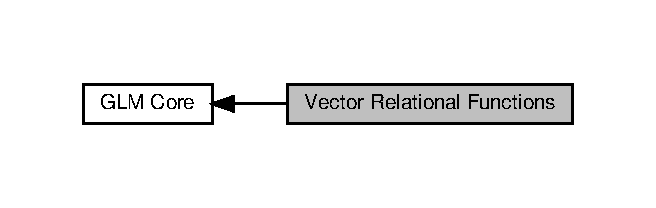
\includegraphics[width=315pt]{group__core__func__vector__relational}
\end{center}
\end{figure}
\subsection*{Functions}
\begin{DoxyCompactItemize}
\item 
{\footnotesize template$<$typename T , precision P, template$<$ typename, precision $>$ class vec\+Type$>$ }\\\hyperlink{setup_8hpp_ab2d052de21a70539923e9bcbf6e83a51}{G\+L\+M\+\_\+\+F\+U\+N\+C\+\_\+\+D\+E\+CL} vec\+Type$<$ T, P $>$\+::bool\+\_\+type \hyperlink{group__core__func__vector__relational_ga2167b22ac086c5791a4740932b62b685}{glm\+::less\+Than\+Equal} (vec\+Type$<$ T, P $>$ const \&x, vec\+Type$<$ T, P $>$ const \&y)
\item 
{\footnotesize template$<$typename T , precision P, template$<$ typename, precision $>$ class vec\+Type$>$ }\\\hyperlink{setup_8hpp_ab2d052de21a70539923e9bcbf6e83a51}{G\+L\+M\+\_\+\+F\+U\+N\+C\+\_\+\+D\+E\+CL} vec\+Type$<$ T, P $>$\+::bool\+\_\+type \hyperlink{group__core__func__vector__relational_gac9163d451231eb3eaae2c6b3da5add6a}{glm\+::greater\+Than} (vec\+Type$<$ T, P $>$ const \&x, vec\+Type$<$ T, P $>$ const \&y)
\item 
{\footnotesize template$<$typename T , precision P, template$<$ typename, precision $>$ class vec\+Type$>$ }\\\hyperlink{setup_8hpp_ab2d052de21a70539923e9bcbf6e83a51}{G\+L\+M\+\_\+\+F\+U\+N\+C\+\_\+\+D\+E\+CL} vec\+Type$<$ T, P $>$\+::bool\+\_\+type \hyperlink{group__core__func__vector__relational_gad1385064aa2fc7aaae37aa95daea9c31}{glm\+::greater\+Than\+Equal} (vec\+Type$<$ T, P $>$ const \&x, vec\+Type$<$ T, P $>$ const \&y)
\item 
{\footnotesize template$<$typename T , precision P, template$<$ typename, precision $>$ class vec\+Type$>$ }\\\hyperlink{setup_8hpp_ab2d052de21a70539923e9bcbf6e83a51}{G\+L\+M\+\_\+\+F\+U\+N\+C\+\_\+\+D\+E\+CL} vec\+Type$<$ T, P $>$\+::bool\+\_\+type \hyperlink{group__core__func__vector__relational_ga85d7bc5613c4dcc2d5873ec9d6ed4c19}{glm\+::not\+Equal} (vec\+Type$<$ T, P $>$ const \&x, vec\+Type$<$ T, P $>$ const \&y)
\item 
{\footnotesize template$<$precision P, template$<$ typename, precision $>$ class vec\+Type$>$ }\\\hyperlink{setup_8hpp_ab2d052de21a70539923e9bcbf6e83a51}{G\+L\+M\+\_\+\+F\+U\+N\+C\+\_\+\+D\+E\+CL} bool \hyperlink{group__core__func__vector__relational_ga632a2644532d9332011c8860400d30b2}{glm\+::any} (vec\+Type$<$ bool, P $>$ const \&v)
\item 
{\footnotesize template$<$precision P, template$<$ typename, precision $>$ class vec\+Type$>$ }\\\hyperlink{setup_8hpp_ab2d052de21a70539923e9bcbf6e83a51}{G\+L\+M\+\_\+\+F\+U\+N\+C\+\_\+\+D\+E\+CL} bool \hyperlink{group__core__func__vector__relational_ga14bbc94f2ae2774a1d64d91f8767773e}{glm\+::all} (vec\+Type$<$ bool, P $>$ const \&v)
\item 
{\footnotesize template$<$precision P, template$<$ typename, precision $>$ class vec\+Type$>$ }\\\hyperlink{setup_8hpp_ab2d052de21a70539923e9bcbf6e83a51}{G\+L\+M\+\_\+\+F\+U\+N\+C\+\_\+\+D\+E\+CL} vec\+Type$<$ bool, P $>$ \hyperlink{group__core__func__vector__relational_ga4329ecbc2ef012c9ec704bd09da1f177}{glm\+::not\+\_\+} (vec\+Type$<$ bool, P $>$ const \&v)
\end{DoxyCompactItemize}


\subsection{Detailed Description}
Relational and equality operators ($<$, $<$=, $>$, $>$=, ==, !=) are defined to operate on scalars and produce scalar Boolean results. For vector results, use the following built-\/in functions.

In all cases, the sizes of all the input and return vectors for any particular call must match. 

\subsection{Function Documentation}
\mbox{\Hypertarget{group__core__func__vector__relational_ga14bbc94f2ae2774a1d64d91f8767773e}\label{group__core__func__vector__relational_ga14bbc94f2ae2774a1d64d91f8767773e}} 
\index{Vector Relational Functions@{Vector Relational Functions}!all@{all}}
\index{all@{all}!Vector Relational Functions@{Vector Relational Functions}}
\subsubsection{\texorpdfstring{all()}{all()}}
{\footnotesize\ttfamily template$<$precision P, template$<$ typename, precision $>$ class vec\+Type$>$ \\
\hyperlink{setup_8hpp_ab2d052de21a70539923e9bcbf6e83a51}{G\+L\+M\+\_\+\+F\+U\+N\+C\+\_\+\+D\+E\+CL} bool glm\+::all (\begin{DoxyParamCaption}\item[{vec\+Type$<$ bool, P $>$ const \&}]{v }\end{DoxyParamCaption})}

Returns true if all components of x are true.


\begin{DoxyTemplParams}{Template Parameters}
{\em vec\+Type} & Boolean vector types.\\
\hline
\end{DoxyTemplParams}
\begin{DoxySeeAlso}{See also}
\href{http://www.opengl.org/sdk/docs/manglsl/xhtml/all.xml}{\tt G\+L\+SL all man page} 

\href{http://www.opengl.org/registry/doc/GLSLangSpec.4.20.8.pdf}{\tt G\+L\+SL 4.\+20.\+8 specification, section 8.\+7 Vector Relational Functions} 
\end{DoxySeeAlso}


Definition at line 142 of file func\+\_\+vector\+\_\+relational.\+inl.

\mbox{\Hypertarget{group__core__func__vector__relational_ga632a2644532d9332011c8860400d30b2}\label{group__core__func__vector__relational_ga632a2644532d9332011c8860400d30b2}} 
\index{Vector Relational Functions@{Vector Relational Functions}!any@{any}}
\index{any@{any}!Vector Relational Functions@{Vector Relational Functions}}
\subsubsection{\texorpdfstring{any()}{any()}}
{\footnotesize\ttfamily template$<$precision P, template$<$ typename, precision $>$ class vec\+Type$>$ \\
\hyperlink{setup_8hpp_ab2d052de21a70539923e9bcbf6e83a51}{G\+L\+M\+\_\+\+F\+U\+N\+C\+\_\+\+D\+E\+CL} bool glm\+::any (\begin{DoxyParamCaption}\item[{vec\+Type$<$ bool, P $>$ const \&}]{v }\end{DoxyParamCaption})}

Returns true if any component of x is true.


\begin{DoxyTemplParams}{Template Parameters}
{\em vec\+Type} & Boolean vector types.\\
\hline
\end{DoxyTemplParams}
\begin{DoxySeeAlso}{See also}
\href{http://www.opengl.org/sdk/docs/manglsl/xhtml/any.xml}{\tt G\+L\+SL any man page} 

\href{http://www.opengl.org/registry/doc/GLSLangSpec.4.20.8.pdf}{\tt G\+L\+SL 4.\+20.\+8 specification, section 8.\+7 Vector Relational Functions} 
\end{DoxySeeAlso}


Definition at line 133 of file func\+\_\+vector\+\_\+relational.\+inl.

\mbox{\Hypertarget{group__core__func__vector__relational_gac9163d451231eb3eaae2c6b3da5add6a}\label{group__core__func__vector__relational_gac9163d451231eb3eaae2c6b3da5add6a}} 
\index{Vector Relational Functions@{Vector Relational Functions}!greater\+Than@{greater\+Than}}
\index{greater\+Than@{greater\+Than}!Vector Relational Functions@{Vector Relational Functions}}
\subsubsection{\texorpdfstring{greater\+Than()}{greaterThan()}}
{\footnotesize\ttfamily template$<$typename T , precision P, template$<$ typename, precision $>$ class vec\+Type$>$ \\
\hyperlink{setup_8hpp_ab2d052de21a70539923e9bcbf6e83a51}{G\+L\+M\+\_\+\+F\+U\+N\+C\+\_\+\+D\+E\+CL} vec\+Type$<$T, P$>$\+::bool\+\_\+type glm\+::greater\+Than (\begin{DoxyParamCaption}\item[{vec\+Type$<$ T, P $>$ const \&}]{x,  }\item[{vec\+Type$<$ T, P $>$ const \&}]{y }\end{DoxyParamCaption})}

Returns the component-\/wise comparison of result x $>$ y.


\begin{DoxyTemplParams}{Template Parameters}
{\em vec\+Type} & Floating-\/point or integer vector types.\\
\hline
\end{DoxyTemplParams}
\begin{DoxySeeAlso}{See also}
\href{http://www.opengl.org/sdk/docs/manglsl/xhtml/greaterThan.xml}{\tt G\+L\+SL greater\+Than man page} 

\href{http://www.opengl.org/registry/doc/GLSLangSpec.4.20.8.pdf}{\tt G\+L\+SL 4.\+20.\+8 specification, section 8.\+7 Vector Relational Functions} 
\end{DoxySeeAlso}


Definition at line 70 of file func\+\_\+vector\+\_\+relational.\+inl.

\mbox{\Hypertarget{group__core__func__vector__relational_gad1385064aa2fc7aaae37aa95daea9c31}\label{group__core__func__vector__relational_gad1385064aa2fc7aaae37aa95daea9c31}} 
\index{Vector Relational Functions@{Vector Relational Functions}!greater\+Than\+Equal@{greater\+Than\+Equal}}
\index{greater\+Than\+Equal@{greater\+Than\+Equal}!Vector Relational Functions@{Vector Relational Functions}}
\subsubsection{\texorpdfstring{greater\+Than\+Equal()}{greaterThanEqual()}}
{\footnotesize\ttfamily template$<$typename T , precision P, template$<$ typename, precision $>$ class vec\+Type$>$ \\
\hyperlink{setup_8hpp_ab2d052de21a70539923e9bcbf6e83a51}{G\+L\+M\+\_\+\+F\+U\+N\+C\+\_\+\+D\+E\+CL} vec\+Type$<$T, P$>$\+::bool\+\_\+type glm\+::greater\+Than\+Equal (\begin{DoxyParamCaption}\item[{vec\+Type$<$ T, P $>$ const \&}]{x,  }\item[{vec\+Type$<$ T, P $>$ const \&}]{y }\end{DoxyParamCaption})}

Returns the component-\/wise comparison of result x $>$= y.


\begin{DoxyTemplParams}{Template Parameters}
{\em vec\+Type} & Floating-\/point or integer vector types.\\
\hline
\end{DoxyTemplParams}
\begin{DoxySeeAlso}{See also}
\href{http://www.opengl.org/sdk/docs/manglsl/xhtml/greaterThanEqual.xml}{\tt G\+L\+SL greater\+Than\+Equal man page} 

\href{http://www.opengl.org/registry/doc/GLSLangSpec.4.20.8.pdf}{\tt G\+L\+SL 4.\+20.\+8 specification, section 8.\+7 Vector Relational Functions} 
\end{DoxySeeAlso}


Definition at line 87 of file func\+\_\+vector\+\_\+relational.\+inl.

\mbox{\Hypertarget{group__core__func__vector__relational_ga2167b22ac086c5791a4740932b62b685}\label{group__core__func__vector__relational_ga2167b22ac086c5791a4740932b62b685}} 
\index{Vector Relational Functions@{Vector Relational Functions}!less\+Than\+Equal@{less\+Than\+Equal}}
\index{less\+Than\+Equal@{less\+Than\+Equal}!Vector Relational Functions@{Vector Relational Functions}}
\subsubsection{\texorpdfstring{less\+Than\+Equal()}{lessThanEqual()}}
{\footnotesize\ttfamily template$<$typename T , precision P, template$<$ typename, precision $>$ class vec\+Type$>$ \\
\hyperlink{setup_8hpp_ab2d052de21a70539923e9bcbf6e83a51}{G\+L\+M\+\_\+\+F\+U\+N\+C\+\_\+\+D\+E\+CL} vec\+Type$<$T, P$>$\+::bool\+\_\+type glm\+::less\+Than\+Equal (\begin{DoxyParamCaption}\item[{vec\+Type$<$ T, P $>$ const \&}]{x,  }\item[{vec\+Type$<$ T, P $>$ const \&}]{y }\end{DoxyParamCaption})}

Returns the component-\/wise comparison result of x $<$ y.


\begin{DoxyTemplParams}{Template Parameters}
{\em vec\+Type} & Floating-\/point or integer vector types.\\
\hline
\end{DoxyTemplParams}
\begin{DoxySeeAlso}{See also}
\href{http://www.opengl.org/sdk/docs/manglsl/xhtml/lessThan.xml}{\tt G\+L\+SL less\+Than man page} 

\href{http://www.opengl.org/registry/doc/GLSLangSpec.4.20.8.pdf}{\tt G\+L\+SL 4.\+20.\+8 specification, section 8.\+7 Vector Relational Functions} Returns the component-\/wise comparison of result x $<$= y.
\end{DoxySeeAlso}

\begin{DoxyTemplParams}{Template Parameters}
{\em vec\+Type} & Floating-\/point or integer vector types.\\
\hline
\end{DoxyTemplParams}
\begin{DoxySeeAlso}{See also}
\href{http://www.opengl.org/sdk/docs/manglsl/xhtml/lessThanEqual.xml}{\tt G\+L\+SL less\+Than\+Equal man page} 

\href{http://www.opengl.org/registry/doc/GLSLangSpec.4.20.8.pdf}{\tt G\+L\+SL 4.\+20.\+8 specification, section 8.\+7 Vector Relational Functions} 
\end{DoxySeeAlso}


Definition at line 53 of file func\+\_\+vector\+\_\+relational.\+inl.

\mbox{\Hypertarget{group__core__func__vector__relational_ga4329ecbc2ef012c9ec704bd09da1f177}\label{group__core__func__vector__relational_ga4329ecbc2ef012c9ec704bd09da1f177}} 
\index{Vector Relational Functions@{Vector Relational Functions}!not\+\_\+@{not\+\_\+}}
\index{not\+\_\+@{not\+\_\+}!Vector Relational Functions@{Vector Relational Functions}}
\subsubsection{\texorpdfstring{not\+\_\+()}{not\_()}}
{\footnotesize\ttfamily template$<$precision P, template$<$ typename, precision $>$ class vec\+Type$>$ \\
\hyperlink{setup_8hpp_ab2d052de21a70539923e9bcbf6e83a51}{G\+L\+M\+\_\+\+F\+U\+N\+C\+\_\+\+D\+E\+CL} vec\+Type$<$bool, P$>$ glm\+::not\+\_\+ (\begin{DoxyParamCaption}\item[{vec\+Type$<$ bool, P $>$ const \&}]{v }\end{DoxyParamCaption})}

Returns the component-\/wise logical complement of x. /!\textbackslash{} Because of language incompatibilities between C++ and G\+L\+SL, G\+LM defines the function not but not\+\_\+ instead.


\begin{DoxyTemplParams}{Template Parameters}
{\em vec\+Type} & Boolean vector types.\\
\hline
\end{DoxyTemplParams}
\begin{DoxySeeAlso}{See also}
\href{http://www.opengl.org/sdk/docs/manglsl/xhtml/not.xml}{\tt G\+L\+SL not man page} 

\href{http://www.opengl.org/registry/doc/GLSLangSpec.4.20.8.pdf}{\tt G\+L\+SL 4.\+20.\+8 specification, section 8.\+7 Vector Relational Functions} 
\end{DoxySeeAlso}


Definition at line 151 of file func\+\_\+vector\+\_\+relational.\+inl.

\mbox{\Hypertarget{group__core__func__vector__relational_ga85d7bc5613c4dcc2d5873ec9d6ed4c19}\label{group__core__func__vector__relational_ga85d7bc5613c4dcc2d5873ec9d6ed4c19}} 
\index{Vector Relational Functions@{Vector Relational Functions}!not\+Equal@{not\+Equal}}
\index{not\+Equal@{not\+Equal}!Vector Relational Functions@{Vector Relational Functions}}
\subsubsection{\texorpdfstring{not\+Equal()}{notEqual()}}
{\footnotesize\ttfamily template$<$typename T , precision P, template$<$ typename, precision $>$ class vec\+Type$>$ \\
\hyperlink{setup_8hpp_ab2d052de21a70539923e9bcbf6e83a51}{G\+L\+M\+\_\+\+F\+U\+N\+C\+\_\+\+D\+E\+CL} vec\+Type$<$T, P$>$\+::bool\+\_\+type glm\+::not\+Equal (\begin{DoxyParamCaption}\item[{vec\+Type$<$ T, P $>$ const \&}]{x,  }\item[{vec\+Type$<$ T, P $>$ const \&}]{y }\end{DoxyParamCaption})}

Returns the component-\/wise comparison of result x == y.


\begin{DoxyTemplParams}{Template Parameters}
{\em vec\+Type} & Floating-\/point, integer or boolean vector types.\\
\hline
\end{DoxyTemplParams}
\begin{DoxySeeAlso}{See also}
\href{http://www.opengl.org/sdk/docs/manglsl/xhtml/equal.xml}{\tt G\+L\+SL equal man page} 

\href{http://www.opengl.org/registry/doc/GLSLangSpec.4.20.8.pdf}{\tt G\+L\+SL 4.\+20.\+8 specification, section 8.\+7 Vector Relational Functions} Returns the component-\/wise comparison of result x != y.
\end{DoxySeeAlso}

\begin{DoxyTemplParams}{Template Parameters}
{\em vec\+Type} & Floating-\/point, integer or boolean vector types.\\
\hline
\end{DoxyTemplParams}
\begin{DoxySeeAlso}{See also}
\href{http://www.opengl.org/sdk/docs/manglsl/xhtml/notEqual.xml}{\tt G\+L\+SL not\+Equal man page} 

\href{http://www.opengl.org/registry/doc/GLSLangSpec.4.20.8.pdf}{\tt G\+L\+SL 4.\+20.\+8 specification, section 8.\+7 Vector Relational Functions} 
\end{DoxySeeAlso}


Definition at line 119 of file func\+\_\+vector\+\_\+relational.\+inl.


\hypertarget{group__gtc}{}\section{G\+TC Extensions (Stable)}
\label{group__gtc}\index{G\+T\+C Extensions (\+Stable)@{G\+T\+C Extensions (\+Stable)}}


Functions and types that the G\+L\+SL specification doesn\textquotesingle{}t define, but useful to have for a C++ program.  


Collaboration diagram for G\+TC Extensions (Stable)\+:\nopagebreak
\begin{figure}[H]
\begin{center}
\leavevmode
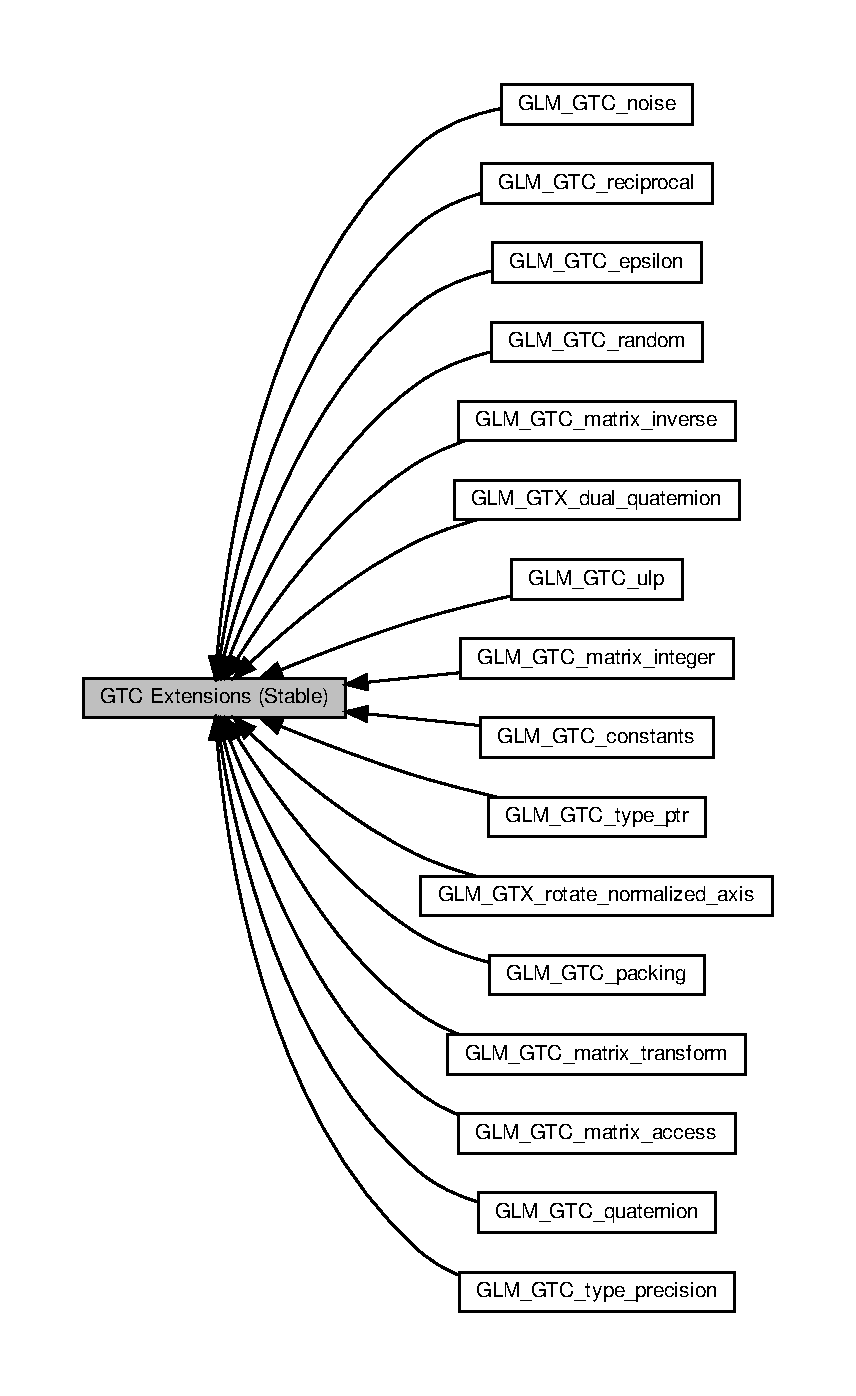
\includegraphics[height=550pt]{group__gtc}
\end{center}
\end{figure}
\subsection*{Modules}
\begin{DoxyCompactItemize}
\item 
\hyperlink{group__gtc__constants}{G\+L\+M\+\_\+\+G\+T\+C\+\_\+constants}
\begin{DoxyCompactList}\small\item\em Provide a list of constants and precomputed useful values. \end{DoxyCompactList}\item 
\hyperlink{group__gtc__epsilon}{G\+L\+M\+\_\+\+G\+T\+C\+\_\+epsilon}
\begin{DoxyCompactList}\small\item\em Comparison functions for a user defined epsilon values. \end{DoxyCompactList}\item 
\hyperlink{group__gtc__matrix__access}{G\+L\+M\+\_\+\+G\+T\+C\+\_\+matrix\+\_\+access}
\item 
\hyperlink{group__gtc__matrix__integer}{G\+L\+M\+\_\+\+G\+T\+C\+\_\+matrix\+\_\+integer}
\item 
\hyperlink{group__gtc__matrix__inverse}{G\+L\+M\+\_\+\+G\+T\+C\+\_\+matrix\+\_\+inverse}
\item 
\hyperlink{group__gtc__matrix__transform}{G\+L\+M\+\_\+\+G\+T\+C\+\_\+matrix\+\_\+transform}
\begin{DoxyCompactList}\small\item\em Defines functions that generate common transformation matrices. \end{DoxyCompactList}\item 
\hyperlink{group__gtc__noise}{G\+L\+M\+\_\+\+G\+T\+C\+\_\+noise}
\item 
\hyperlink{group__gtc__packing}{G\+L\+M\+\_\+\+G\+T\+C\+\_\+packing}
\begin{DoxyCompactList}\small\item\em This extension provides a set of function to convert vertors to packed formats. \end{DoxyCompactList}\item 
\hyperlink{group__gtc__quaternion}{G\+L\+M\+\_\+\+G\+T\+C\+\_\+quaternion}
\begin{DoxyCompactList}\small\item\em Defines a templated quaternion type and several quaternion operations. \end{DoxyCompactList}\item 
\hyperlink{group__gtc__random}{G\+L\+M\+\_\+\+G\+T\+C\+\_\+random}
\begin{DoxyCompactList}\small\item\em Generate random number from various distribution methods. \end{DoxyCompactList}\item 
\hyperlink{group__gtc__reciprocal}{G\+L\+M\+\_\+\+G\+T\+C\+\_\+reciprocal}
\begin{DoxyCompactList}\small\item\em Define secant, cosecant and cotangent functions. \end{DoxyCompactList}\item 
\hyperlink{group__gtc__type__precision}{G\+L\+M\+\_\+\+G\+T\+C\+\_\+type\+\_\+precision}
\begin{DoxyCompactList}\small\item\em Defines specific C++-\/based precision types. \end{DoxyCompactList}\item 
\hyperlink{group__gtc__type__ptr}{G\+L\+M\+\_\+\+G\+T\+C\+\_\+type\+\_\+ptr}
\begin{DoxyCompactList}\small\item\em Handles the interaction between pointers and vector, matrix types. \end{DoxyCompactList}\item 
\hyperlink{group__gtc__ulp}{G\+L\+M\+\_\+\+G\+T\+C\+\_\+ulp}
\begin{DoxyCompactList}\small\item\em Allow the measurement of the accuracy of a function against a reference implementation. This extension works on floating-\/point data and provide results in U\+LP. $<$\hyperlink{gtc_2ulp_8hpp}{glm/gtc/ulp.\+hpp}$>$ need to be included to use these features. \end{DoxyCompactList}\item 
\hyperlink{group__gtc__dual__quaternion}{G\+L\+M\+\_\+\+G\+T\+X\+\_\+dual\+\_\+quaternion}
\begin{DoxyCompactList}\small\item\em Defines a templated dual-\/quaternion type and several dual-\/quaternion operations. \end{DoxyCompactList}\item 
\hyperlink{group__gtx__rotate__normalized__axis}{G\+L\+M\+\_\+\+G\+T\+X\+\_\+rotate\+\_\+normalized\+\_\+axis}
\begin{DoxyCompactList}\small\item\em Quaternions and matrices rotations around normalized axis. \end{DoxyCompactList}\end{DoxyCompactItemize}


\subsection{Detailed Description}
Functions and types that the G\+L\+SL specification doesn\textquotesingle{}t define, but useful to have for a C++ program. 

G\+TC extensions aim to be stable.

Even if it\textquotesingle{}s highly unrecommended, it\textquotesingle{}s possible to include all the extensions at once by including $<$\hyperlink{ext_8hpp}{glm/ext.\+hpp}$>$. Otherwise, each extension needs to be included a specific file. 
\hypertarget{group__gtx}{}\section{G\+TX Extensions (Experimental)}
\label{group__gtx}\index{G\+T\+X Extensions (\+Experimental)@{G\+T\+X Extensions (\+Experimental)}}


Functions and types that the G\+L\+SL specification doesn\textquotesingle{}t define, but useful to have for a C++ program.  


Collaboration diagram for G\+TX Extensions (Experimental)\+:\nopagebreak
\begin{figure}[H]
\begin{center}
\leavevmode
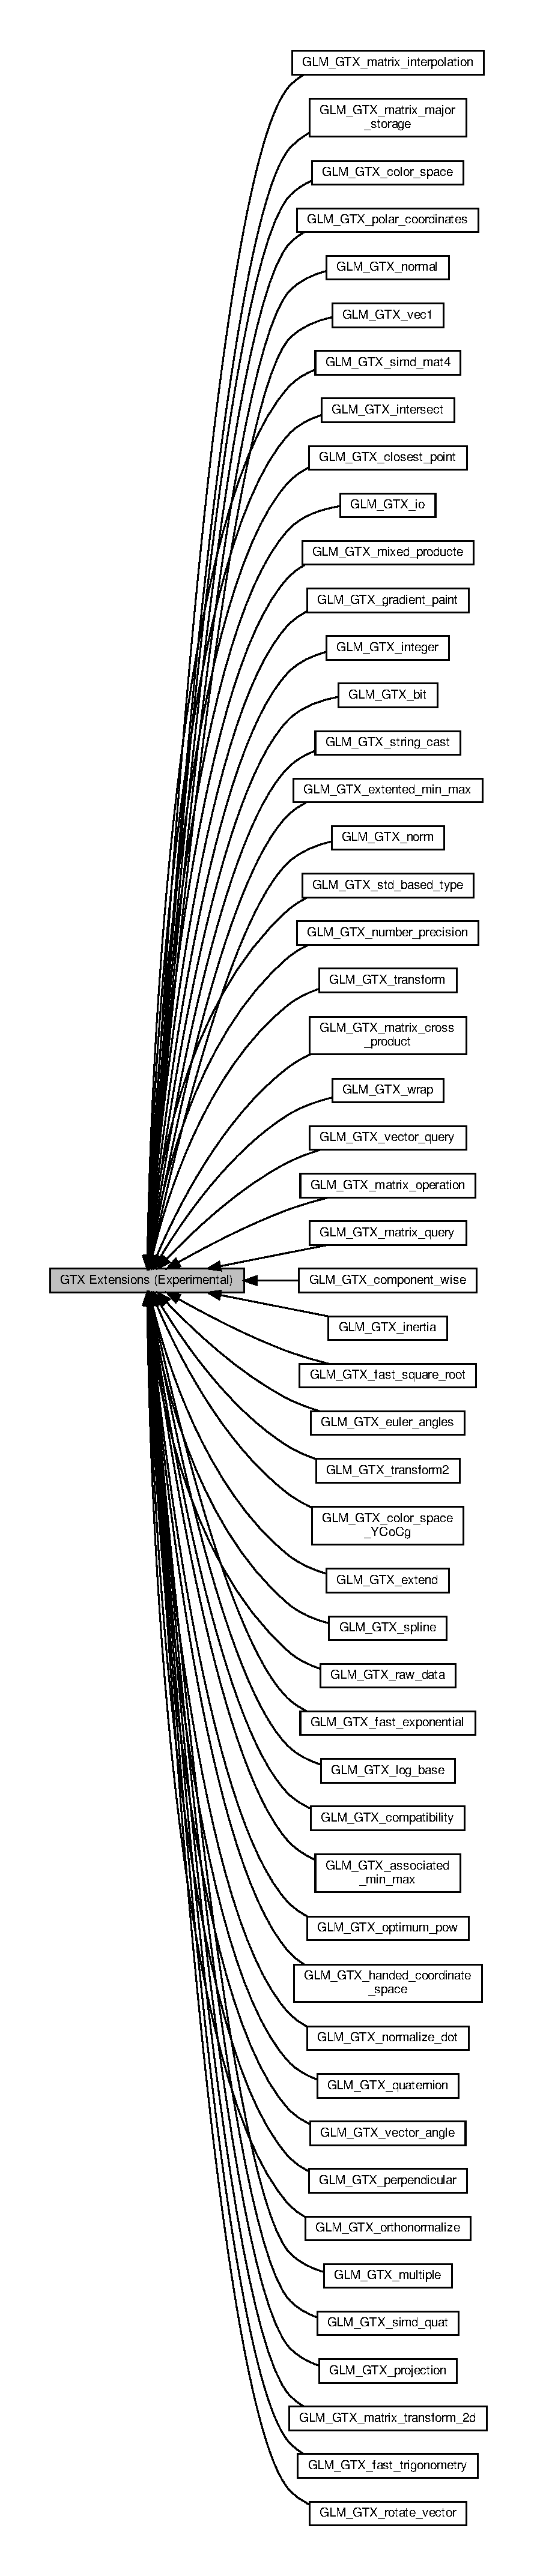
\includegraphics[height=550pt]{group__gtx}
\end{center}
\end{figure}
\subsection*{Modules}
\begin{DoxyCompactItemize}
\item 
\hyperlink{group__gtx__associated__min__max}{G\+L\+M\+\_\+\+G\+T\+X\+\_\+associated\+\_\+min\+\_\+max}
\begin{DoxyCompactList}\small\item\em Min and max functions that return associated values not the compared onces. $<$\hyperlink{associated__min__max_8hpp}{glm/gtx/associated\+\_\+min\+\_\+max.\+hpp}$>$ need to be included to use these functionalities. \end{DoxyCompactList}\item 
\hyperlink{group__gtx__bit}{G\+L\+M\+\_\+\+G\+T\+X\+\_\+bit}
\begin{DoxyCompactList}\small\item\em Allow to perform bit operations on integer values. \end{DoxyCompactList}\item 
\hyperlink{group__gtx__closest__point}{G\+L\+M\+\_\+\+G\+T\+X\+\_\+closest\+\_\+point}
\begin{DoxyCompactList}\small\item\em Find the point on a straight line which is the closet of a point. \end{DoxyCompactList}\item 
\hyperlink{group__gtx__color__space}{G\+L\+M\+\_\+\+G\+T\+X\+\_\+color\+\_\+space}
\begin{DoxyCompactList}\small\item\em Related to R\+GB to H\+SV conversions and operations. \end{DoxyCompactList}\item 
\hyperlink{group__gtx__color__space___y_co_cg}{G\+L\+M\+\_\+\+G\+T\+X\+\_\+color\+\_\+space\+\_\+\+Y\+Co\+Cg}
\begin{DoxyCompactList}\small\item\em R\+GB to Y\+Co\+Cg conversions and operations. \end{DoxyCompactList}\item 
\hyperlink{group__gtx__compatibility}{G\+L\+M\+\_\+\+G\+T\+X\+\_\+compatibility}
\begin{DoxyCompactList}\small\item\em Provide functions to increase the compatibility with Cg and H\+L\+SL languages. \end{DoxyCompactList}\item 
\hyperlink{group__gtx__component__wise}{G\+L\+M\+\_\+\+G\+T\+X\+\_\+component\+\_\+wise}
\begin{DoxyCompactList}\small\item\em Operations between components of a type. \end{DoxyCompactList}\item 
\hyperlink{group__gtx__euler__angles}{G\+L\+M\+\_\+\+G\+T\+X\+\_\+euler\+\_\+angles}
\begin{DoxyCompactList}\small\item\em Build matrices from Euler angles. \end{DoxyCompactList}\item 
\hyperlink{group__gtx__extend}{G\+L\+M\+\_\+\+G\+T\+X\+\_\+extend}
\begin{DoxyCompactList}\small\item\em Extend a position from a source to a position at a defined length. \end{DoxyCompactList}\item 
\hyperlink{group__gtx__extented__min__max}{G\+L\+M\+\_\+\+G\+T\+X\+\_\+extented\+\_\+min\+\_\+max}
\item 
\hyperlink{group__gtx__fast__exponential}{G\+L\+M\+\_\+\+G\+T\+X\+\_\+fast\+\_\+exponential}
\begin{DoxyCompactList}\small\item\em Fast but less accurate implementations of exponential based functions. \end{DoxyCompactList}\item 
\hyperlink{group__gtx__fast__square__root}{G\+L\+M\+\_\+\+G\+T\+X\+\_\+fast\+\_\+square\+\_\+root}
\begin{DoxyCompactList}\small\item\em Fast but less accurate implementations of square root based functions. \end{DoxyCompactList}\item 
\hyperlink{group__gtx__fast__trigonometry}{G\+L\+M\+\_\+\+G\+T\+X\+\_\+fast\+\_\+trigonometry}
\begin{DoxyCompactList}\small\item\em Fast but less accurate implementations of trigonometric functions. \end{DoxyCompactList}\item 
\hyperlink{group__gtx__gradient__paint}{G\+L\+M\+\_\+\+G\+T\+X\+\_\+gradient\+\_\+paint}
\begin{DoxyCompactList}\small\item\em Functions that return the color of procedural gradient for specific coordinates. $<$\hyperlink{gradient__paint_8hpp}{glm/gtx/gradient\+\_\+paint.\+hpp}$>$ need to be included to use these functionalities. \end{DoxyCompactList}\item 
\hyperlink{group__gtx__handed__coordinate__space}{G\+L\+M\+\_\+\+G\+T\+X\+\_\+handed\+\_\+coordinate\+\_\+space}
\begin{DoxyCompactList}\small\item\em To know if a set of three basis vectors defines a right or left-\/handed coordinate system. \end{DoxyCompactList}\item 
\hyperlink{group__gtx__inertia}{G\+L\+M\+\_\+\+G\+T\+X\+\_\+inertia}
\begin{DoxyCompactList}\small\item\em Create inertia matrices. \end{DoxyCompactList}\item 
\hyperlink{group__gtx__integer}{G\+L\+M\+\_\+\+G\+T\+X\+\_\+integer}
\begin{DoxyCompactList}\small\item\em Add support for integer for core functions. \end{DoxyCompactList}\item 
\hyperlink{group__gtx__intersect}{G\+L\+M\+\_\+\+G\+T\+X\+\_\+intersect}
\begin{DoxyCompactList}\small\item\em Add intersection functions. \end{DoxyCompactList}\item 
\hyperlink{group__gtx__io}{G\+L\+M\+\_\+\+G\+T\+X\+\_\+io}
\begin{DoxyCompactList}\small\item\em std\+:\+:\mbox{[}w\mbox{]}ostream support for glm types \end{DoxyCompactList}\item 
\hyperlink{group__gtx__log__base}{G\+L\+M\+\_\+\+G\+T\+X\+\_\+log\+\_\+base}
\begin{DoxyCompactList}\small\item\em Logarithm for any base. base can be a vector or a scalar. \end{DoxyCompactList}\item 
\hyperlink{group__gtx__matrix__cross__product}{G\+L\+M\+\_\+\+G\+T\+X\+\_\+matrix\+\_\+cross\+\_\+product}
\begin{DoxyCompactList}\small\item\em Build cross product matrices. \end{DoxyCompactList}\item 
\hyperlink{group__gtx__matrix__interpolation}{G\+L\+M\+\_\+\+G\+T\+X\+\_\+matrix\+\_\+interpolation}
\begin{DoxyCompactList}\small\item\em Allows to directly interpolate two exiciting matrices. \end{DoxyCompactList}\item 
\hyperlink{group__gtx__matrix__major__storage}{G\+L\+M\+\_\+\+G\+T\+X\+\_\+matrix\+\_\+major\+\_\+storage}
\begin{DoxyCompactList}\small\item\em Build matrices with specific matrix order, row or column. \end{DoxyCompactList}\item 
\hyperlink{group__gtx__matrix__operation}{G\+L\+M\+\_\+\+G\+T\+X\+\_\+matrix\+\_\+operation}
\begin{DoxyCompactList}\small\item\em Build diagonal matrices from vectors. \end{DoxyCompactList}\item 
\hyperlink{group__gtx__matrix__query}{G\+L\+M\+\_\+\+G\+T\+X\+\_\+matrix\+\_\+query}
\begin{DoxyCompactList}\small\item\em Query to evaluate matrix properties. \end{DoxyCompactList}\item 
\hyperlink{group__gtx__matrix__transform__2d}{G\+L\+M\+\_\+\+G\+T\+X\+\_\+matrix\+\_\+transform\+\_\+2d}
\begin{DoxyCompactList}\small\item\em Defines functions that generate common 2d transformation matrices. \end{DoxyCompactList}\item 
\hyperlink{group__gtx__mixed__product}{G\+L\+M\+\_\+\+G\+T\+X\+\_\+mixed\+\_\+producte}
\begin{DoxyCompactList}\small\item\em Mixed product of 3 vectors. \end{DoxyCompactList}\item 
\hyperlink{group__gtx__multiple}{G\+L\+M\+\_\+\+G\+T\+X\+\_\+multiple}
\begin{DoxyCompactList}\small\item\em Find the closest number of a number multiple of other number. \end{DoxyCompactList}\item 
\hyperlink{group__gtx__norm}{G\+L\+M\+\_\+\+G\+T\+X\+\_\+norm}
\begin{DoxyCompactList}\small\item\em Various ways to compute vector norms. \end{DoxyCompactList}\item 
\hyperlink{group__gtx__normal}{G\+L\+M\+\_\+\+G\+T\+X\+\_\+normal}
\begin{DoxyCompactList}\small\item\em Compute the normal of a triangle. \end{DoxyCompactList}\item 
\hyperlink{group__gtx__normalize__dot}{G\+L\+M\+\_\+\+G\+T\+X\+\_\+normalize\+\_\+dot}
\begin{DoxyCompactList}\small\item\em Dot product of vectors that need to be normalize with a single square root. \end{DoxyCompactList}\item 
\hyperlink{group__gtx__number__precision}{G\+L\+M\+\_\+\+G\+T\+X\+\_\+number\+\_\+precision}
\begin{DoxyCompactList}\small\item\em Defined size types. \end{DoxyCompactList}\item 
\hyperlink{group__gtx__optimum__pow}{G\+L\+M\+\_\+\+G\+T\+X\+\_\+optimum\+\_\+pow}
\begin{DoxyCompactList}\small\item\em Integer exponentiation of power functions. \end{DoxyCompactList}\item 
\hyperlink{group__gtx__orthonormalize}{G\+L\+M\+\_\+\+G\+T\+X\+\_\+orthonormalize}
\begin{DoxyCompactList}\small\item\em Orthonormalize matrices. \end{DoxyCompactList}\item 
\hyperlink{group__gtx__perpendicular}{G\+L\+M\+\_\+\+G\+T\+X\+\_\+perpendicular}
\begin{DoxyCompactList}\small\item\em Perpendicular of a vector from other one. \end{DoxyCompactList}\item 
\hyperlink{group__gtx__polar__coordinates}{G\+L\+M\+\_\+\+G\+T\+X\+\_\+polar\+\_\+coordinates}
\begin{DoxyCompactList}\small\item\em Conversion from Euclidean space to polar space and revert. \end{DoxyCompactList}\item 
\hyperlink{group__gtx__projection}{G\+L\+M\+\_\+\+G\+T\+X\+\_\+projection}
\begin{DoxyCompactList}\small\item\em Projection of a vector to other one. \end{DoxyCompactList}\item 
\hyperlink{group__gtx__quaternion}{G\+L\+M\+\_\+\+G\+T\+X\+\_\+quaternion}
\begin{DoxyCompactList}\small\item\em Extented quaternion types and functions. \end{DoxyCompactList}\item 
\hyperlink{group__gtx__raw__data}{G\+L\+M\+\_\+\+G\+T\+X\+\_\+raw\+\_\+data}
\begin{DoxyCompactList}\small\item\em Projection of a vector to other one. \end{DoxyCompactList}\item 
\hyperlink{group__gtx__rotate__vector}{G\+L\+M\+\_\+\+G\+T\+X\+\_\+rotate\+\_\+vector}
\begin{DoxyCompactList}\small\item\em Function to directly rotate a vector. \end{DoxyCompactList}\item 
\hyperlink{group__gtx__simd__mat4}{G\+L\+M\+\_\+\+G\+T\+X\+\_\+simd\+\_\+mat4}
\begin{DoxyCompactList}\small\item\em S\+I\+MD implementation of mat4 type. \end{DoxyCompactList}\item 
\hyperlink{group__gtx__simd__vec4}{G\+L\+M\+\_\+\+G\+T\+X\+\_\+simd\+\_\+quat}
\begin{DoxyCompactList}\small\item\em S\+I\+MD implementation of quat type. \end{DoxyCompactList}\item 
\hyperlink{group__gtx__spline}{G\+L\+M\+\_\+\+G\+T\+X\+\_\+spline}
\begin{DoxyCompactList}\small\item\em Spline functions. \end{DoxyCompactList}\item 
\hyperlink{group__gtx__std__based__type}{G\+L\+M\+\_\+\+G\+T\+X\+\_\+std\+\_\+based\+\_\+type}
\begin{DoxyCompactList}\small\item\em Adds vector types based on S\+TL value types. $<$\hyperlink{std__based__type_8hpp}{glm/gtx/std\+\_\+based\+\_\+type.\+hpp}$>$ need to be included to use these functionalities. \end{DoxyCompactList}\item 
\hyperlink{group__gtx__string__cast}{G\+L\+M\+\_\+\+G\+T\+X\+\_\+string\+\_\+cast}
\begin{DoxyCompactList}\small\item\em Setup strings for G\+LM type values. \end{DoxyCompactList}\item 
\hyperlink{group__gtx__transform}{G\+L\+M\+\_\+\+G\+T\+X\+\_\+transform}
\begin{DoxyCompactList}\small\item\em Add transformation matrices. \end{DoxyCompactList}\item 
\hyperlink{group__gtx__transform2}{G\+L\+M\+\_\+\+G\+T\+X\+\_\+transform2}
\begin{DoxyCompactList}\small\item\em Add extra transformation matrices. \end{DoxyCompactList}\item 
\hyperlink{group__gtx__vec1}{G\+L\+M\+\_\+\+G\+T\+X\+\_\+vec1}
\begin{DoxyCompactList}\small\item\em Add vec1, ivec1, uvec1 and bvec1 types. $<$\hyperlink{vec1_8hpp}{glm/gtx/vec1.\+hpp}$>$ need to be included to use these functionalities. \end{DoxyCompactList}\item 
\hyperlink{group__gtx__vector__angle}{G\+L\+M\+\_\+\+G\+T\+X\+\_\+vector\+\_\+angle}
\begin{DoxyCompactList}\small\item\em Compute angle between vectors. \end{DoxyCompactList}\item 
\hyperlink{group__gtx__vector__query}{G\+L\+M\+\_\+\+G\+T\+X\+\_\+vector\+\_\+query}
\begin{DoxyCompactList}\small\item\em Query informations of vector types. \end{DoxyCompactList}\item 
\hyperlink{group__gtx__wrap}{G\+L\+M\+\_\+\+G\+T\+X\+\_\+wrap}
\begin{DoxyCompactList}\small\item\em Wrapping mode of texture coordinates. \end{DoxyCompactList}\end{DoxyCompactItemize}


\subsection{Detailed Description}
Functions and types that the G\+L\+SL specification doesn\textquotesingle{}t define, but useful to have for a C++ program. 

Experimental extensions are useful functions and types, but the development of their A\+PI and functionality is not necessarily stable. They can change substantially between versions. Backwards compatibility is not much of an issue for them.

Even if it\textquotesingle{}s highly unrecommended, it\textquotesingle{}s possible to include all the extensions at once by including $<$\hyperlink{ext_8hpp}{glm/ext.\+hpp}$>$. Otherwise, each extension needs to be included a specific file. 
\hypertarget{group__virtrev}{}\section{V\+I\+R\+T\+R\+EV Extensions}
\label{group__virtrev}\index{V\+I\+R\+T\+R\+E\+V Extensions@{V\+I\+R\+T\+R\+E\+V Extensions}}


Extensions develop and maintain by Mathieu \mbox{[}matrem\mbox{]} Roumillac (\href{http://www.opengl.org/discussion_boards/ubbthreads.php?ubb=showprofile&User=22660}{\tt http\+://www.\+opengl.\+org/discussion\+\_\+boards/ubbthreads.\+php?ubb=showprofile\&\+User=22660}).  


Extensions develop and maintain by Mathieu \mbox{[}matrem\mbox{]} Roumillac (\href{http://www.opengl.org/discussion_boards/ubbthreads.php?ubb=showprofile&User=22660}{\tt http\+://www.\+opengl.\+org/discussion\+\_\+boards/ubbthreads.\+php?ubb=showprofile\&\+User=22660}). 


\hypertarget{group__core}{}\section{G\+LM Core}
\label{group__core}\index{G\+L\+M Core@{G\+L\+M Core}}


The core of G\+LM, which implements exactly and only the G\+L\+SL specification to the degree possible.  


Collaboration diagram for G\+LM Core\+:\nopagebreak
\begin{figure}[H]
\begin{center}
\leavevmode
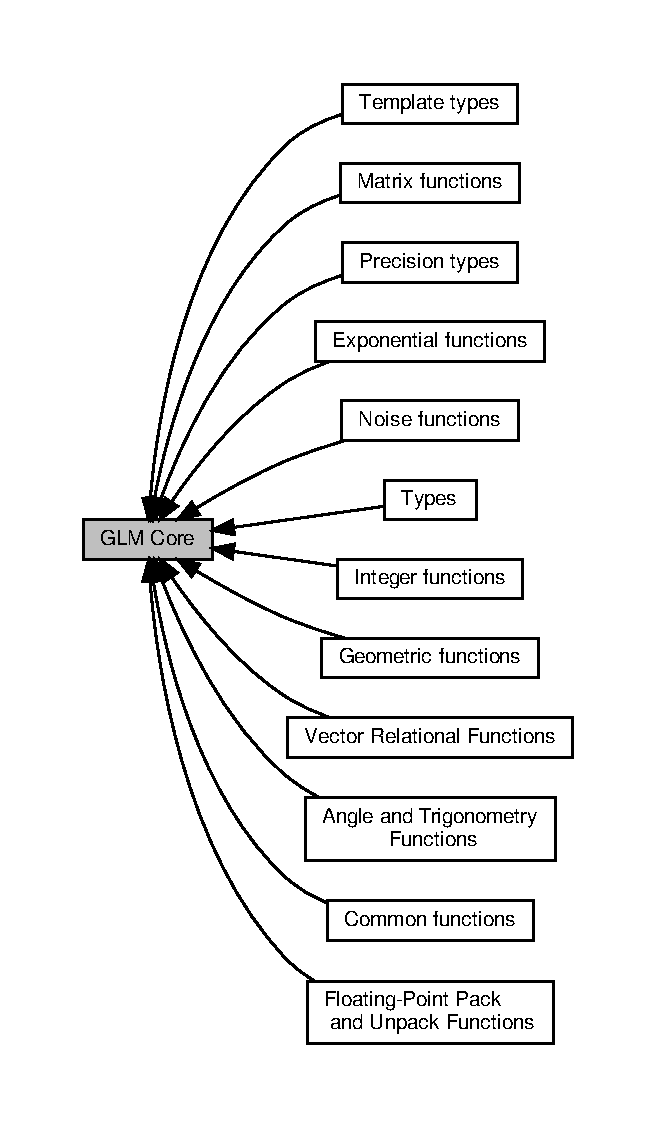
\includegraphics[width=315pt]{group__core}
\end{center}
\end{figure}
\subsection*{Modules}
\begin{DoxyCompactItemize}
\item 
\hyperlink{group__core__func__common}{Common functions}
\item 
\hyperlink{group__core__func__exponential}{Exponential functions}
\item 
\hyperlink{group__core__func__geometric}{Geometric functions}
\item 
\hyperlink{group__core__func__integer}{Integer functions}
\item 
\hyperlink{group__core__func__matrix}{Matrix functions}
\item 
\hyperlink{group__core__func__noise}{Noise functions}
\item 
\hyperlink{group__core__func__packing}{Floating-\/\+Point Pack and Unpack Functions}
\item 
\hyperlink{group__core__func__trigonometric}{Angle and Trigonometry Functions}
\item 
\hyperlink{group__core__func__vector__relational}{Vector Relational Functions}
\item 
\hyperlink{group__core__types}{Types}
\begin{DoxyCompactList}\small\item\em The standard types defined by the specification. \end{DoxyCompactList}\item 
\hyperlink{group__core__precision}{Precision types}
\begin{DoxyCompactList}\small\item\em Non-\/\+G\+L\+SL types that are used to define precision-\/based types. \end{DoxyCompactList}\item 
\hyperlink{group__core__template}{Template types}
\begin{DoxyCompactList}\small\item\em The generic template types used as the basis for the core types. \end{DoxyCompactList}\end{DoxyCompactItemize}


\subsection{Detailed Description}
The core of G\+LM, which implements exactly and only the G\+L\+SL specification to the degree possible. 

The G\+LM core consists of \hyperlink{group__core__types}{C++ types that mirror G\+L\+SL types} and C++ functions that mirror the G\+L\+SL functions. It also includes \hyperlink{group__core__precision}{a set of precision-\/based types} that can be used in the appropriate functions. The C++ types are all based on a basic set of \hyperlink{group__core__template}{template types}.

The best documentation for G\+LM Core is the current G\+L\+SL specification, \href{http://www.opengl.org/registry/doc/GLSLangSpec.4.20.8.clean.pdf}{\tt version 4.\+2 (pdf file)}. There are a few differences between G\+LM core and G\+L\+SL.

G\+LM core functionnalities require $<$\hyperlink{third-party_2include_2glm_2glm_8hpp}{glm/glm.\+hpp}$>$ to be included to be used. 
\hypertarget{group__core__types}{}\section{Types}
\label{group__core__types}\index{Types@{Types}}


The standard types defined by the specification.  


Collaboration diagram for Types\+:\nopagebreak
\begin{figure}[H]
\begin{center}
\leavevmode
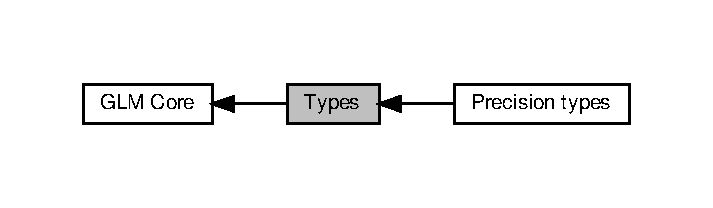
\includegraphics[width=342pt]{group__core__types}
\end{center}
\end{figure}
\subsection*{Modules}
\begin{DoxyCompactItemize}
\item 
\hyperlink{group__core__precision}{Precision types}
\begin{DoxyCompactList}\small\item\em Non-\/\+G\+L\+SL types that are used to define precision-\/based types. \end{DoxyCompactList}\end{DoxyCompactItemize}
\subsection*{Typedefs}
\begin{DoxyCompactItemize}
\item 
typedef \hyperlink{group__core__precision_ga694146b8d430b22caa8b37571d9bc8bc}{highp\+\_\+mat2x2} \hyperlink{group__core__types_gaeddc14adb4963d9bad73866cc202fb40}{glm\+::mat2x2}
\item 
typedef \hyperlink{group__core__precision_ga7d4e5a1c803be5688c75241c924dfa58}{highp\+\_\+mat2x3} \hyperlink{group__core__types_gaea02797b8231f6dd9380345f6ff12155}{glm\+::mat2x3}
\item 
typedef \hyperlink{group__core__precision_ga3cc506666b7a95db56f9d2eb787b6e20}{highp\+\_\+mat2x4} \hyperlink{group__core__types_gaa9bfb36efaf88ecad32369ec8a01d901}{glm\+::mat2x4}
\item 
typedef \hyperlink{group__core__precision_gabc7767293ff69cd56717ee9d8be62963}{highp\+\_\+mat3x2} \hyperlink{group__core__types_gad7476e0e866186f12ee87975c6b01552}{glm\+::mat3x2}
\item 
typedef \hyperlink{group__core__precision_ga8a3703cc71cdfc8928eddf46b3763c4b}{highp\+\_\+mat3x3} \hyperlink{group__core__types_ga6fecca6a869070b6bf8acb44ce1c2af3}{glm\+::mat3x3}
\item 
typedef \hyperlink{group__core__precision_gabaf9c8dd35db715b1093042703f879d0}{highp\+\_\+mat3x4} \hyperlink{group__core__types_ga5524ae15d7fc00a68b8e0e3a0733cc2a}{glm\+::mat3x4}
\item 
typedef \hyperlink{group__core__precision_gadf9c4a7947c2b0a79f52cc86a860f270}{highp\+\_\+mat4x2} \hyperlink{group__core__types_ga72cf8ec4f4cda85943f4683531e421bc}{glm\+::mat4x2}
\item 
typedef \hyperlink{group__core__precision_gab8dfe989c5100c35ab5dec0e94f59d2a}{highp\+\_\+mat4x3} \hyperlink{group__core__types_gad3f3f750dcdc74a9037342c5cae55f5e}{glm\+::mat4x3}
\item 
typedef \hyperlink{group__core__precision_ga231950d260be295a25d7340e2020f55c}{highp\+\_\+mat4x4} \hyperlink{group__core__types_ga63e3ee9447ed593484140a9368e738ec}{glm\+::mat4x4}
\item 
typedef \hyperlink{group__core__types_gaeddc14adb4963d9bad73866cc202fb40}{mat2x2} \hyperlink{group__core__types_ga8357ec0aab6f8cf69313592492663c3f}{glm\+::mat2}
\item 
typedef \hyperlink{group__core__types_ga6fecca6a869070b6bf8acb44ce1c2af3}{mat3x3} \hyperlink{group__core__types_gadfaff2a7dce5cbf4e77a47ecea42ac5b}{glm\+::mat3}
\item 
typedef \hyperlink{group__core__types_ga63e3ee9447ed593484140a9368e738ec}{mat4x4} \hyperlink{group__core__types_ga7dcd2365c2e368e6af5b7adeb6a9c8df}{glm\+::mat4}
\item 
typedef \hyperlink{group__core__precision_gaa5e35f6570d394c1cd34f411a473220c}{highp\+\_\+dmat2x2} \hyperlink{group__core__types_gad8c130d26c4cd9a1a831c1a74292a8f6}{glm\+::dmat2}
\item 
typedef \hyperlink{group__core__precision_gad7229dea82287910d88e6e8566e39fc7}{highp\+\_\+dmat3x3} \hyperlink{group__core__types_ga25fd62195c3ef5ac0d32ead1dbfbb929}{glm\+::dmat3}
\item 
typedef \hyperlink{group__core__precision_ga1c0a2edbde597b59e9005691a224b208}{highp\+\_\+dmat4x4} \hyperlink{group__core__types_ga7f7c1300ebfd19d573e9deb1e8758b54}{glm\+::dmat4}
\item 
typedef \hyperlink{group__core__precision_gaa5e35f6570d394c1cd34f411a473220c}{highp\+\_\+dmat2x2} \hyperlink{group__core__types_gae9932771e11a4f38e21f1136423bab18}{glm\+::dmat2x2}
\item 
typedef \hyperlink{group__core__precision_gafec7367665f006f2a7643103c5eddc38}{highp\+\_\+dmat2x3} \hyperlink{group__core__types_ga6b5ff9888ca0e468f35b637d4c3a361d}{glm\+::dmat2x3}
\item 
typedef \hyperlink{group__core__precision_gacd51d8188f7d66a83c035b8c4cd69f2d}{highp\+\_\+dmat2x4} \hyperlink{group__core__types_ga2d1dd4b4925d1ea67539902c820483a0}{glm\+::dmat2x4}
\item 
typedef \hyperlink{group__core__precision_gac956fe6b946f0ccee78367ccd5427351}{highp\+\_\+dmat3x2} \hyperlink{group__core__types_ga2db259d2e7921065c5b7d4dca9547960}{glm\+::dmat3x2}
\item 
typedef \hyperlink{group__core__precision_gad7229dea82287910d88e6e8566e39fc7}{highp\+\_\+dmat3x3} \hyperlink{group__core__types_gaf3c29c4f75a448f308463e75ca2efd4c}{glm\+::dmat3x3}
\item 
typedef \hyperlink{group__core__precision_gaff199c8d04a8edb92ed43283e8694c59}{highp\+\_\+dmat3x4} \hyperlink{group__core__types_ga19e745a83cba85f57afa1232276dcc96}{glm\+::dmat3x4}
\item 
typedef \hyperlink{group__core__precision_gaa4fb1ed350a6cd053abb9b093d13ce0d}{highp\+\_\+dmat4x2} \hyperlink{group__core__types_gab3d51ce41e6f0aa267d3e185cee09c44}{glm\+::dmat4x2}
\item 
typedef \hyperlink{group__core__precision_gaf8aeba0eecc5c651e0f06414b6e37754}{highp\+\_\+dmat4x3} \hyperlink{group__core__types_gaa4a157ac183c5bd5dcbd555a94b1b505}{glm\+::dmat4x3}
\item 
typedef \hyperlink{group__core__precision_ga1c0a2edbde597b59e9005691a224b208}{highp\+\_\+dmat4x4} \hyperlink{group__core__types_ga54d90d4b902d93638b906571af215bb1}{glm\+::dmat4x4}
\item 
typedef \hyperlink{group__core__precision_ga37645abcfcc1278567e99f1ca492bfbb}{highp\+\_\+vec2} \hyperlink{group__core__types_gaa1618f51db67eaa145db101d8c8431d8}{glm\+::vec2}
\item 
typedef \hyperlink{group__core__precision_ga4879124da7a18d6b681d933cb8c4267d}{highp\+\_\+vec3} \hyperlink{group__core__types_ga1c47e8b3386109bc992b6c48e91b0be7}{glm\+::vec3}
\item 
typedef \hyperlink{group__core__precision_gae32d5f99860247afbe7ed90564bceac1}{highp\+\_\+vec4} \hyperlink{group__core__types_ga5881b1b022d7fd1b7218f5916532dd02}{glm\+::vec4}
\item 
typedef \hyperlink{group__core__precision_gacfbe8512142fff27f0bfb44958c1752f}{highp\+\_\+dvec2} \hyperlink{group__core__types_gae6727259898288cae197724d5f172b3b}{glm\+::dvec2}
\item 
typedef \hyperlink{group__core__precision_ga4962711854156dae8ebb4eb39237c542}{highp\+\_\+dvec3} \hyperlink{group__core__types_ga7f3287f952e6ccb481231368091702ac}{glm\+::dvec3}
\item 
typedef \hyperlink{group__core__precision_gad5ff5ff4a69e6925f5b4f540e2633835}{highp\+\_\+dvec4} \hyperlink{group__core__types_ga0824ceed7ec3b2fba89765501c1540b5}{glm\+::dvec4}
\item 
typedef \hyperlink{group__core__precision_gab2bac6095f51f7d7f74747afc2f6747a}{highp\+\_\+ivec2} \hyperlink{group__core__types_ga9e6ce9cfc7919976b318197e18d8a065}{glm\+::ivec2}
\item 
typedef \hyperlink{group__core__precision_gae9f0a321de8ee92dce9d4400362d71e7}{highp\+\_\+ivec3} \hyperlink{group__core__types_ga6e12a4ca00d696f07da1df4eb73e0fe8}{glm\+::ivec3}
\item 
typedef \hyperlink{group__core__precision_gaeba08fcf78aeae954c3335d73500ff8b}{highp\+\_\+ivec4} \hyperlink{group__core__types_gaa4560ddc50320ea8f8a70d5c9c249fea}{glm\+::ivec4}
\item 
typedef \hyperlink{group__core__precision_gaaf92be4c1fca33cff90c1ed15b521c79}{highp\+\_\+uvec2} \hyperlink{group__core__types_gafd2041b45eff671aa8899d2c2835eee9}{glm\+::uvec2}
\item 
typedef \hyperlink{group__core__precision_ga66d0e4ae1742ede2eb32bf0bfedd7474}{highp\+\_\+uvec3} \hyperlink{group__core__types_gac4ba593917841b859ba1683b8b52b8fa}{glm\+::uvec3}
\item 
typedef \hyperlink{group__core__precision_ga7cb8cc501f7e680e1889b93eb80e6c46}{highp\+\_\+uvec4} \hyperlink{group__core__types_ga1c426d19627b32b14f0089f7f4ba7b1d}{glm\+::uvec4}
\item 
typedef \hyperlink{group__core__precision_ga4153415d1f3d390219ac9464652ac377}{highp\+\_\+bvec2} \hyperlink{group__core__types_ga7523cf292181cf7daef3aa0a3267d8e3}{glm\+::bvec2}
\item 
typedef \hyperlink{group__core__precision_ga1d77a773fdd024602413670788c10c62}{highp\+\_\+bvec3} \hyperlink{group__core__types_ga3f07d6d37fc6fe875170fd5799685bcf}{glm\+::bvec3}
\item 
typedef \hyperlink{group__core__precision_ga381539af52c5e5c659700e12fb706eaf}{highp\+\_\+bvec4} \hyperlink{group__core__types_ga6bb211b3d3bebae3867548d5673ca5cd}{glm\+::bvec4}
\end{DoxyCompactItemize}


\subsection{Detailed Description}
The standard types defined by the specification. 

These types are all typedefs of more generalized, template types. To see the definiton of these template types, go to \hyperlink{group__core__template}{Template types}. 

\subsection{Typedef Documentation}
\mbox{\Hypertarget{group__core__types_ga7523cf292181cf7daef3aa0a3267d8e3}\label{group__core__types_ga7523cf292181cf7daef3aa0a3267d8e3}} 
\index{Types@{Types}!bvec2@{bvec2}}
\index{bvec2@{bvec2}!Types@{Types}}
\subsubsection{\texorpdfstring{bvec2}{bvec2}}
{\footnotesize\ttfamily typedef \hyperlink{group__core__precision_ga4153415d1f3d390219ac9464652ac377}{highp\+\_\+bvec2} \hyperlink{group__core__types_ga7523cf292181cf7daef3aa0a3267d8e3}{glm\+::bvec2}}

2 components vector of boolean.

\begin{DoxySeeAlso}{See also}
\href{http://www.opengl.org/registry/doc/GLSLangSpec.4.20.8.pdf}{\tt G\+L\+SL 4.\+20.\+8 specification, section 4.\+1.\+5 Vectors} 
\end{DoxySeeAlso}


Definition at line 500 of file type\+\_\+vec.\+hpp.

\mbox{\Hypertarget{group__core__types_ga3f07d6d37fc6fe875170fd5799685bcf}\label{group__core__types_ga3f07d6d37fc6fe875170fd5799685bcf}} 
\index{Types@{Types}!bvec3@{bvec3}}
\index{bvec3@{bvec3}!Types@{Types}}
\subsubsection{\texorpdfstring{bvec3}{bvec3}}
{\footnotesize\ttfamily typedef \hyperlink{group__core__precision_ga1d77a773fdd024602413670788c10c62}{highp\+\_\+bvec3} \hyperlink{group__core__types_ga3f07d6d37fc6fe875170fd5799685bcf}{glm\+::bvec3}}

3 components vector of boolean.

\begin{DoxySeeAlso}{See also}
\href{http://www.opengl.org/registry/doc/GLSLangSpec.4.20.8.pdf}{\tt G\+L\+SL 4.\+20.\+8 specification, section 4.\+1.\+5 Vectors} 
\end{DoxySeeAlso}


Definition at line 505 of file type\+\_\+vec.\+hpp.

\mbox{\Hypertarget{group__core__types_ga6bb211b3d3bebae3867548d5673ca5cd}\label{group__core__types_ga6bb211b3d3bebae3867548d5673ca5cd}} 
\index{Types@{Types}!bvec4@{bvec4}}
\index{bvec4@{bvec4}!Types@{Types}}
\subsubsection{\texorpdfstring{bvec4}{bvec4}}
{\footnotesize\ttfamily typedef \hyperlink{group__core__precision_ga381539af52c5e5c659700e12fb706eaf}{highp\+\_\+bvec4} \hyperlink{group__core__types_ga6bb211b3d3bebae3867548d5673ca5cd}{glm\+::bvec4}}

4 components vector of boolean.

\begin{DoxySeeAlso}{See also}
\href{http://www.opengl.org/registry/doc/GLSLangSpec.4.20.8.pdf}{\tt G\+L\+SL 4.\+20.\+8 specification, section 4.\+1.\+5 Vectors} 
\end{DoxySeeAlso}


Definition at line 510 of file type\+\_\+vec.\+hpp.

\mbox{\Hypertarget{group__core__types_gad8c130d26c4cd9a1a831c1a74292a8f6}\label{group__core__types_gad8c130d26c4cd9a1a831c1a74292a8f6}} 
\index{Types@{Types}!dmat2@{dmat2}}
\index{dmat2@{dmat2}!Types@{Types}}
\subsubsection{\texorpdfstring{dmat2}{dmat2}}
{\footnotesize\ttfamily typedef \hyperlink{group__core__precision_gaa5e35f6570d394c1cd34f411a473220c}{highp\+\_\+dmat2x2} \hyperlink{group__core__types_gad8c130d26c4cd9a1a831c1a74292a8f6}{glm\+::dmat2}}

2 $\ast$ 2 matrix of double-\/precision floating-\/point numbers.

\begin{DoxySeeAlso}{See also}
\href{http://www.opengl.org/registry/doc/GLSLangSpec.4.20.8.pdf}{\tt G\+L\+SL 4.\+20.\+8 specification, section 4.\+1.\+6 Matrices} 
\end{DoxySeeAlso}


Definition at line 733 of file type\+\_\+mat.\+hpp.

\mbox{\Hypertarget{group__core__types_gae9932771e11a4f38e21f1136423bab18}\label{group__core__types_gae9932771e11a4f38e21f1136423bab18}} 
\index{Types@{Types}!dmat2x2@{dmat2x2}}
\index{dmat2x2@{dmat2x2}!Types@{Types}}
\subsubsection{\texorpdfstring{dmat2x2}{dmat2x2}}
{\footnotesize\ttfamily typedef \hyperlink{group__core__precision_gaa5e35f6570d394c1cd34f411a473220c}{highp\+\_\+dmat2x2} \hyperlink{group__core__types_gae9932771e11a4f38e21f1136423bab18}{glm\+::dmat2x2}}

2 $\ast$ 2 matrix of double-\/precision floating-\/point numbers.

\begin{DoxySeeAlso}{See also}
\href{http://www.opengl.org/registry/doc/GLSLangSpec.4.20.8.pdf}{\tt G\+L\+SL 4.\+20.\+8 specification, section 4.\+1.\+6 Matrices} 
\end{DoxySeeAlso}


Definition at line 748 of file type\+\_\+mat.\+hpp.

\mbox{\Hypertarget{group__core__types_ga6b5ff9888ca0e468f35b637d4c3a361d}\label{group__core__types_ga6b5ff9888ca0e468f35b637d4c3a361d}} 
\index{Types@{Types}!dmat2x3@{dmat2x3}}
\index{dmat2x3@{dmat2x3}!Types@{Types}}
\subsubsection{\texorpdfstring{dmat2x3}{dmat2x3}}
{\footnotesize\ttfamily typedef \hyperlink{group__core__precision_gafec7367665f006f2a7643103c5eddc38}{highp\+\_\+dmat2x3} \hyperlink{group__core__types_ga6b5ff9888ca0e468f35b637d4c3a361d}{glm\+::dmat2x3}}

2 $\ast$ 3 matrix of double-\/precision floating-\/point numbers.

\begin{DoxySeeAlso}{See also}
\href{http://www.opengl.org/registry/doc/GLSLangSpec.4.20.8.pdf}{\tt G\+L\+SL 4.\+20.\+8 specification, section 4.\+1.\+6 Matrices} 
\end{DoxySeeAlso}


Definition at line 753 of file type\+\_\+mat.\+hpp.

\mbox{\Hypertarget{group__core__types_ga2d1dd4b4925d1ea67539902c820483a0}\label{group__core__types_ga2d1dd4b4925d1ea67539902c820483a0}} 
\index{Types@{Types}!dmat2x4@{dmat2x4}}
\index{dmat2x4@{dmat2x4}!Types@{Types}}
\subsubsection{\texorpdfstring{dmat2x4}{dmat2x4}}
{\footnotesize\ttfamily typedef \hyperlink{group__core__precision_gacd51d8188f7d66a83c035b8c4cd69f2d}{highp\+\_\+dmat2x4} \hyperlink{group__core__types_ga2d1dd4b4925d1ea67539902c820483a0}{glm\+::dmat2x4}}

2 $\ast$ 4 matrix of double-\/precision floating-\/point numbers.

\begin{DoxySeeAlso}{See also}
\href{http://www.opengl.org/registry/doc/GLSLangSpec.4.20.8.pdf}{\tt G\+L\+SL 4.\+20.\+8 specification, section 4.\+1.\+6 Matrices} 
\end{DoxySeeAlso}


Definition at line 758 of file type\+\_\+mat.\+hpp.

\mbox{\Hypertarget{group__core__types_ga25fd62195c3ef5ac0d32ead1dbfbb929}\label{group__core__types_ga25fd62195c3ef5ac0d32ead1dbfbb929}} 
\index{Types@{Types}!dmat3@{dmat3}}
\index{dmat3@{dmat3}!Types@{Types}}
\subsubsection{\texorpdfstring{dmat3}{dmat3}}
{\footnotesize\ttfamily typedef \hyperlink{group__core__precision_gad7229dea82287910d88e6e8566e39fc7}{highp\+\_\+dmat3x3} \hyperlink{group__core__types_ga25fd62195c3ef5ac0d32ead1dbfbb929}{glm\+::dmat3}}

3 $\ast$ 3 matrix of double-\/precision floating-\/point numbers.

\begin{DoxySeeAlso}{See also}
\href{http://www.opengl.org/registry/doc/GLSLangSpec.4.20.8.pdf}{\tt G\+L\+SL 4.\+20.\+8 specification, section 4.\+1.\+6 Matrices} 
\end{DoxySeeAlso}


Definition at line 738 of file type\+\_\+mat.\+hpp.

\mbox{\Hypertarget{group__core__types_ga2db259d2e7921065c5b7d4dca9547960}\label{group__core__types_ga2db259d2e7921065c5b7d4dca9547960}} 
\index{Types@{Types}!dmat3x2@{dmat3x2}}
\index{dmat3x2@{dmat3x2}!Types@{Types}}
\subsubsection{\texorpdfstring{dmat3x2}{dmat3x2}}
{\footnotesize\ttfamily typedef \hyperlink{group__core__precision_gac956fe6b946f0ccee78367ccd5427351}{highp\+\_\+dmat3x2} \hyperlink{group__core__types_ga2db259d2e7921065c5b7d4dca9547960}{glm\+::dmat3x2}}

3 $\ast$ 2 matrix of double-\/precision floating-\/point numbers.

\begin{DoxySeeAlso}{See also}
\href{http://www.opengl.org/registry/doc/GLSLangSpec.4.20.8.pdf}{\tt G\+L\+SL 4.\+20.\+8 specification, section 4.\+1.\+6 Matrices} 
\end{DoxySeeAlso}


Definition at line 763 of file type\+\_\+mat.\+hpp.

\mbox{\Hypertarget{group__core__types_gaf3c29c4f75a448f308463e75ca2efd4c}\label{group__core__types_gaf3c29c4f75a448f308463e75ca2efd4c}} 
\index{Types@{Types}!dmat3x3@{dmat3x3}}
\index{dmat3x3@{dmat3x3}!Types@{Types}}
\subsubsection{\texorpdfstring{dmat3x3}{dmat3x3}}
{\footnotesize\ttfamily typedef \hyperlink{group__core__precision_gad7229dea82287910d88e6e8566e39fc7}{highp\+\_\+dmat3x3} \hyperlink{group__core__types_gaf3c29c4f75a448f308463e75ca2efd4c}{glm\+::dmat3x3}}

3 $\ast$ 3 matrix of double-\/precision floating-\/point numbers.

\begin{DoxySeeAlso}{See also}
\href{http://www.opengl.org/registry/doc/GLSLangSpec.4.20.8.pdf}{\tt G\+L\+SL 4.\+20.\+8 specification, section 4.\+1.\+6 Matrices} 
\end{DoxySeeAlso}


Definition at line 768 of file type\+\_\+mat.\+hpp.

\mbox{\Hypertarget{group__core__types_ga19e745a83cba85f57afa1232276dcc96}\label{group__core__types_ga19e745a83cba85f57afa1232276dcc96}} 
\index{Types@{Types}!dmat3x4@{dmat3x4}}
\index{dmat3x4@{dmat3x4}!Types@{Types}}
\subsubsection{\texorpdfstring{dmat3x4}{dmat3x4}}
{\footnotesize\ttfamily typedef \hyperlink{group__core__precision_gaff199c8d04a8edb92ed43283e8694c59}{highp\+\_\+dmat3x4} \hyperlink{group__core__types_ga19e745a83cba85f57afa1232276dcc96}{glm\+::dmat3x4}}

3 $\ast$ 4 matrix of double-\/precision floating-\/point numbers.

\begin{DoxySeeAlso}{See also}
\href{http://www.opengl.org/registry/doc/GLSLangSpec.4.20.8.pdf}{\tt G\+L\+SL 4.\+20.\+8 specification, section 4.\+1.\+6 Matrices} 
\end{DoxySeeAlso}


Definition at line 773 of file type\+\_\+mat.\+hpp.

\mbox{\Hypertarget{group__core__types_ga7f7c1300ebfd19d573e9deb1e8758b54}\label{group__core__types_ga7f7c1300ebfd19d573e9deb1e8758b54}} 
\index{Types@{Types}!dmat4@{dmat4}}
\index{dmat4@{dmat4}!Types@{Types}}
\subsubsection{\texorpdfstring{dmat4}{dmat4}}
{\footnotesize\ttfamily typedef \hyperlink{group__core__precision_ga1c0a2edbde597b59e9005691a224b208}{highp\+\_\+dmat4x4} \hyperlink{group__core__types_ga7f7c1300ebfd19d573e9deb1e8758b54}{glm\+::dmat4}}

4 $\ast$ 4 matrix of double-\/precision floating-\/point numbers.

\begin{DoxySeeAlso}{See also}
\href{http://www.opengl.org/registry/doc/GLSLangSpec.4.20.8.pdf}{\tt G\+L\+SL 4.\+20.\+8 specification, section 4.\+1.\+6 Matrices} 
\end{DoxySeeAlso}


Definition at line 743 of file type\+\_\+mat.\+hpp.

\mbox{\Hypertarget{group__core__types_gab3d51ce41e6f0aa267d3e185cee09c44}\label{group__core__types_gab3d51ce41e6f0aa267d3e185cee09c44}} 
\index{Types@{Types}!dmat4x2@{dmat4x2}}
\index{dmat4x2@{dmat4x2}!Types@{Types}}
\subsubsection{\texorpdfstring{dmat4x2}{dmat4x2}}
{\footnotesize\ttfamily typedef \hyperlink{group__core__precision_gaa4fb1ed350a6cd053abb9b093d13ce0d}{highp\+\_\+dmat4x2} \hyperlink{group__core__types_gab3d51ce41e6f0aa267d3e185cee09c44}{glm\+::dmat4x2}}

4 $\ast$ 2 matrix of double-\/precision floating-\/point numbers.

\begin{DoxySeeAlso}{See also}
\href{http://www.opengl.org/registry/doc/GLSLangSpec.4.20.8.pdf}{\tt G\+L\+SL 4.\+20.\+8 specification, section 4.\+1.\+6 Matrices} 
\end{DoxySeeAlso}


Definition at line 778 of file type\+\_\+mat.\+hpp.

\mbox{\Hypertarget{group__core__types_gaa4a157ac183c5bd5dcbd555a94b1b505}\label{group__core__types_gaa4a157ac183c5bd5dcbd555a94b1b505}} 
\index{Types@{Types}!dmat4x3@{dmat4x3}}
\index{dmat4x3@{dmat4x3}!Types@{Types}}
\subsubsection{\texorpdfstring{dmat4x3}{dmat4x3}}
{\footnotesize\ttfamily typedef \hyperlink{group__core__precision_gaf8aeba0eecc5c651e0f06414b6e37754}{highp\+\_\+dmat4x3} \hyperlink{group__core__types_gaa4a157ac183c5bd5dcbd555a94b1b505}{glm\+::dmat4x3}}

4 $\ast$ 3 matrix of double-\/precision floating-\/point numbers.

\begin{DoxySeeAlso}{See also}
\href{http://www.opengl.org/registry/doc/GLSLangSpec.4.20.8.pdf}{\tt G\+L\+SL 4.\+20.\+8 specification, section 4.\+1.\+6 Matrices} 
\end{DoxySeeAlso}


Definition at line 783 of file type\+\_\+mat.\+hpp.

\mbox{\Hypertarget{group__core__types_ga54d90d4b902d93638b906571af215bb1}\label{group__core__types_ga54d90d4b902d93638b906571af215bb1}} 
\index{Types@{Types}!dmat4x4@{dmat4x4}}
\index{dmat4x4@{dmat4x4}!Types@{Types}}
\subsubsection{\texorpdfstring{dmat4x4}{dmat4x4}}
{\footnotesize\ttfamily typedef \hyperlink{group__core__precision_ga1c0a2edbde597b59e9005691a224b208}{highp\+\_\+dmat4x4} \hyperlink{group__core__types_ga54d90d4b902d93638b906571af215bb1}{glm\+::dmat4x4}}

4 $\ast$ 4 matrix of double-\/precision floating-\/point numbers.

\begin{DoxySeeAlso}{See also}
\href{http://www.opengl.org/registry/doc/GLSLangSpec.4.20.8.pdf}{\tt G\+L\+SL 4.\+20.\+8 specification, section 4.\+1.\+6 Matrices} 
\end{DoxySeeAlso}


Definition at line 788 of file type\+\_\+mat.\+hpp.

\mbox{\Hypertarget{group__core__types_gae6727259898288cae197724d5f172b3b}\label{group__core__types_gae6727259898288cae197724d5f172b3b}} 
\index{Types@{Types}!dvec2@{dvec2}}
\index{dvec2@{dvec2}!Types@{Types}}
\subsubsection{\texorpdfstring{dvec2}{dvec2}}
{\footnotesize\ttfamily typedef \hyperlink{group__core__precision_gacfbe8512142fff27f0bfb44958c1752f}{highp\+\_\+dvec2} \hyperlink{group__core__types_gae6727259898288cae197724d5f172b3b}{glm\+::dvec2}}

2 components vector of double-\/precision floating-\/point numbers.

\begin{DoxySeeAlso}{See also}
\href{http://www.opengl.org/registry/doc/GLSLangSpec.4.20.8.pdf}{\tt G\+L\+SL 4.\+20.\+8 specification, section 4.\+1.\+5 Vectors} 
\end{DoxySeeAlso}


Definition at line 416 of file type\+\_\+vec.\+hpp.

\mbox{\Hypertarget{group__core__types_ga7f3287f952e6ccb481231368091702ac}\label{group__core__types_ga7f3287f952e6ccb481231368091702ac}} 
\index{Types@{Types}!dvec3@{dvec3}}
\index{dvec3@{dvec3}!Types@{Types}}
\subsubsection{\texorpdfstring{dvec3}{dvec3}}
{\footnotesize\ttfamily typedef \hyperlink{group__core__precision_ga4962711854156dae8ebb4eb39237c542}{highp\+\_\+dvec3} \hyperlink{group__core__types_ga7f3287f952e6ccb481231368091702ac}{glm\+::dvec3}}

3 components vector of double-\/precision floating-\/point numbers.

\begin{DoxySeeAlso}{See also}
\href{http://www.opengl.org/registry/doc/GLSLangSpec.4.20.8.pdf}{\tt G\+L\+SL 4.\+20.\+8 specification, section 4.\+1.\+5 Vectors} 
\end{DoxySeeAlso}


Definition at line 421 of file type\+\_\+vec.\+hpp.

\mbox{\Hypertarget{group__core__types_ga0824ceed7ec3b2fba89765501c1540b5}\label{group__core__types_ga0824ceed7ec3b2fba89765501c1540b5}} 
\index{Types@{Types}!dvec4@{dvec4}}
\index{dvec4@{dvec4}!Types@{Types}}
\subsubsection{\texorpdfstring{dvec4}{dvec4}}
{\footnotesize\ttfamily typedef \hyperlink{group__core__precision_gad5ff5ff4a69e6925f5b4f540e2633835}{highp\+\_\+dvec4} \hyperlink{group__core__types_ga0824ceed7ec3b2fba89765501c1540b5}{glm\+::dvec4}}

4 components vector of double-\/precision floating-\/point numbers.

\begin{DoxySeeAlso}{See also}
\href{http://www.opengl.org/registry/doc/GLSLangSpec.4.20.8.pdf}{\tt G\+L\+SL 4.\+20.\+8 specification, section 4.\+1.\+5 Vectors} 
\end{DoxySeeAlso}


Definition at line 426 of file type\+\_\+vec.\+hpp.

\mbox{\Hypertarget{group__core__types_ga9e6ce9cfc7919976b318197e18d8a065}\label{group__core__types_ga9e6ce9cfc7919976b318197e18d8a065}} 
\index{Types@{Types}!ivec2@{ivec2}}
\index{ivec2@{ivec2}!Types@{Types}}
\subsubsection{\texorpdfstring{ivec2}{ivec2}}
{\footnotesize\ttfamily typedef \hyperlink{group__core__precision_gab2bac6095f51f7d7f74747afc2f6747a}{highp\+\_\+ivec2} \hyperlink{group__core__types_ga9e6ce9cfc7919976b318197e18d8a065}{glm\+::ivec2}}

2 components vector of signed integer numbers.

\begin{DoxySeeAlso}{See also}
\href{http://www.opengl.org/registry/doc/GLSLangSpec.4.20.8.pdf}{\tt G\+L\+SL 4.\+20.\+8 specification, section 4.\+1.\+5 Vectors} 
\end{DoxySeeAlso}


Definition at line 444 of file type\+\_\+vec.\+hpp.

\mbox{\Hypertarget{group__core__types_ga6e12a4ca00d696f07da1df4eb73e0fe8}\label{group__core__types_ga6e12a4ca00d696f07da1df4eb73e0fe8}} 
\index{Types@{Types}!ivec3@{ivec3}}
\index{ivec3@{ivec3}!Types@{Types}}
\subsubsection{\texorpdfstring{ivec3}{ivec3}}
{\footnotesize\ttfamily typedef \hyperlink{group__core__precision_gae9f0a321de8ee92dce9d4400362d71e7}{highp\+\_\+ivec3} \hyperlink{group__core__types_ga6e12a4ca00d696f07da1df4eb73e0fe8}{glm\+::ivec3}}

3 components vector of signed integer numbers.

\begin{DoxySeeAlso}{See also}
\href{http://www.opengl.org/registry/doc/GLSLangSpec.4.20.8.pdf}{\tt G\+L\+SL 4.\+20.\+8 specification, section 4.\+1.\+5 Vectors} 
\end{DoxySeeAlso}


Definition at line 449 of file type\+\_\+vec.\+hpp.

\mbox{\Hypertarget{group__core__types_gaa4560ddc50320ea8f8a70d5c9c249fea}\label{group__core__types_gaa4560ddc50320ea8f8a70d5c9c249fea}} 
\index{Types@{Types}!ivec4@{ivec4}}
\index{ivec4@{ivec4}!Types@{Types}}
\subsubsection{\texorpdfstring{ivec4}{ivec4}}
{\footnotesize\ttfamily typedef \hyperlink{group__core__precision_gaeba08fcf78aeae954c3335d73500ff8b}{highp\+\_\+ivec4} \hyperlink{group__core__types_gaa4560ddc50320ea8f8a70d5c9c249fea}{glm\+::ivec4}}

4 components vector of signed integer numbers.

\begin{DoxySeeAlso}{See also}
\href{http://www.opengl.org/registry/doc/GLSLangSpec.4.20.8.pdf}{\tt G\+L\+SL 4.\+20.\+8 specification, section 4.\+1.\+5 Vectors} 
\end{DoxySeeAlso}


Definition at line 454 of file type\+\_\+vec.\+hpp.

\mbox{\Hypertarget{group__core__types_ga8357ec0aab6f8cf69313592492663c3f}\label{group__core__types_ga8357ec0aab6f8cf69313592492663c3f}} 
\index{Types@{Types}!mat2@{mat2}}
\index{mat2@{mat2}!Types@{Types}}
\subsubsection{\texorpdfstring{mat2}{mat2}}
{\footnotesize\ttfamily typedef \hyperlink{group__core__types_gaeddc14adb4963d9bad73866cc202fb40}{mat2x2} \hyperlink{group__core__types_ga8357ec0aab6f8cf69313592492663c3f}{glm\+::mat2}}

2 columns of 2 components matrix of floating-\/point numbers.

\begin{DoxySeeAlso}{See also}
\href{http://www.opengl.org/registry/doc/GLSLangSpec.4.20.8.pdf}{\tt G\+L\+SL 4.\+20.\+8 specification, section 4.\+1.\+6 Matrices} 
\end{DoxySeeAlso}


Definition at line 432 of file type\+\_\+mat.\+hpp.

\mbox{\Hypertarget{group__core__types_gaeddc14adb4963d9bad73866cc202fb40}\label{group__core__types_gaeddc14adb4963d9bad73866cc202fb40}} 
\index{Types@{Types}!mat2x2@{mat2x2}}
\index{mat2x2@{mat2x2}!Types@{Types}}
\subsubsection{\texorpdfstring{mat2x2}{mat2x2}}
{\footnotesize\ttfamily typedef \hyperlink{group__core__precision_ga694146b8d430b22caa8b37571d9bc8bc}{highp\+\_\+mat2x2} \hyperlink{group__core__types_gaeddc14adb4963d9bad73866cc202fb40}{glm\+::mat2x2}}

2 columns of 2 components matrix of floating-\/point numbers.

\begin{DoxySeeAlso}{See also}
\href{http://www.opengl.org/registry/doc/GLSLangSpec.4.20.8.pdf}{\tt G\+L\+SL 4.\+20.\+8 specification, section 4.\+1.\+6 Matrices} 
\end{DoxySeeAlso}


Definition at line 385 of file type\+\_\+mat.\+hpp.

\mbox{\Hypertarget{group__core__types_gaea02797b8231f6dd9380345f6ff12155}\label{group__core__types_gaea02797b8231f6dd9380345f6ff12155}} 
\index{Types@{Types}!mat2x3@{mat2x3}}
\index{mat2x3@{mat2x3}!Types@{Types}}
\subsubsection{\texorpdfstring{mat2x3}{mat2x3}}
{\footnotesize\ttfamily typedef \hyperlink{group__core__precision_ga7d4e5a1c803be5688c75241c924dfa58}{highp\+\_\+mat2x3} \hyperlink{group__core__types_gaea02797b8231f6dd9380345f6ff12155}{glm\+::mat2x3}}

2 columns of 3 components matrix of floating-\/point numbers.

\begin{DoxySeeAlso}{See also}
\href{http://www.opengl.org/registry/doc/GLSLangSpec.4.20.8.pdf}{\tt G\+L\+SL 4.\+20.\+8 specification, section 4.\+1.\+6 Matrices} 
\end{DoxySeeAlso}


Definition at line 390 of file type\+\_\+mat.\+hpp.

\mbox{\Hypertarget{group__core__types_gaa9bfb36efaf88ecad32369ec8a01d901}\label{group__core__types_gaa9bfb36efaf88ecad32369ec8a01d901}} 
\index{Types@{Types}!mat2x4@{mat2x4}}
\index{mat2x4@{mat2x4}!Types@{Types}}
\subsubsection{\texorpdfstring{mat2x4}{mat2x4}}
{\footnotesize\ttfamily typedef \hyperlink{group__core__precision_ga3cc506666b7a95db56f9d2eb787b6e20}{highp\+\_\+mat2x4} \hyperlink{group__core__types_gaa9bfb36efaf88ecad32369ec8a01d901}{glm\+::mat2x4}}

2 columns of 4 components matrix of floating-\/point numbers.

\begin{DoxySeeAlso}{See also}
\href{http://www.opengl.org/registry/doc/GLSLangSpec.4.20.8.pdf}{\tt G\+L\+SL 4.\+20.\+8 specification, section 4.\+1.\+6 Matrices} 
\end{DoxySeeAlso}


Definition at line 395 of file type\+\_\+mat.\+hpp.

\mbox{\Hypertarget{group__core__types_gadfaff2a7dce5cbf4e77a47ecea42ac5b}\label{group__core__types_gadfaff2a7dce5cbf4e77a47ecea42ac5b}} 
\index{Types@{Types}!mat3@{mat3}}
\index{mat3@{mat3}!Types@{Types}}
\subsubsection{\texorpdfstring{mat3}{mat3}}
{\footnotesize\ttfamily typedef \hyperlink{group__core__types_ga6fecca6a869070b6bf8acb44ce1c2af3}{mat3x3} \hyperlink{group__core__types_gadfaff2a7dce5cbf4e77a47ecea42ac5b}{glm\+::mat3}}

3 columns of 3 components matrix of floating-\/point numbers.

\begin{DoxySeeAlso}{See also}
\href{http://www.opengl.org/registry/doc/GLSLangSpec.4.20.8.pdf}{\tt G\+L\+SL 4.\+20.\+8 specification, section 4.\+1.\+6 Matrices} 
\end{DoxySeeAlso}


Definition at line 437 of file type\+\_\+mat.\+hpp.

\mbox{\Hypertarget{group__core__types_gad7476e0e866186f12ee87975c6b01552}\label{group__core__types_gad7476e0e866186f12ee87975c6b01552}} 
\index{Types@{Types}!mat3x2@{mat3x2}}
\index{mat3x2@{mat3x2}!Types@{Types}}
\subsubsection{\texorpdfstring{mat3x2}{mat3x2}}
{\footnotesize\ttfamily typedef \hyperlink{group__core__precision_gabc7767293ff69cd56717ee9d8be62963}{highp\+\_\+mat3x2} \hyperlink{group__core__types_gad7476e0e866186f12ee87975c6b01552}{glm\+::mat3x2}}

3 columns of 2 components matrix of floating-\/point numbers.

\begin{DoxySeeAlso}{See also}
\href{http://www.opengl.org/registry/doc/GLSLangSpec.4.20.8.pdf}{\tt G\+L\+SL 4.\+20.\+8 specification, section 4.\+1.\+6 Matrices} 
\end{DoxySeeAlso}


Definition at line 400 of file type\+\_\+mat.\+hpp.

\mbox{\Hypertarget{group__core__types_ga6fecca6a869070b6bf8acb44ce1c2af3}\label{group__core__types_ga6fecca6a869070b6bf8acb44ce1c2af3}} 
\index{Types@{Types}!mat3x3@{mat3x3}}
\index{mat3x3@{mat3x3}!Types@{Types}}
\subsubsection{\texorpdfstring{mat3x3}{mat3x3}}
{\footnotesize\ttfamily typedef \hyperlink{group__core__precision_ga8a3703cc71cdfc8928eddf46b3763c4b}{highp\+\_\+mat3x3} \hyperlink{group__core__types_ga6fecca6a869070b6bf8acb44ce1c2af3}{glm\+::mat3x3}}

3 columns of 3 components matrix of floating-\/point numbers.

\begin{DoxySeeAlso}{See also}
\href{http://www.opengl.org/registry/doc/GLSLangSpec.4.20.8.pdf}{\tt G\+L\+SL 4.\+20.\+8 specification, section 4.\+1.\+6 Matrices} 
\end{DoxySeeAlso}


Definition at line 405 of file type\+\_\+mat.\+hpp.

\mbox{\Hypertarget{group__core__types_ga5524ae15d7fc00a68b8e0e3a0733cc2a}\label{group__core__types_ga5524ae15d7fc00a68b8e0e3a0733cc2a}} 
\index{Types@{Types}!mat3x4@{mat3x4}}
\index{mat3x4@{mat3x4}!Types@{Types}}
\subsubsection{\texorpdfstring{mat3x4}{mat3x4}}
{\footnotesize\ttfamily typedef \hyperlink{group__core__precision_gabaf9c8dd35db715b1093042703f879d0}{highp\+\_\+mat3x4} \hyperlink{group__core__types_ga5524ae15d7fc00a68b8e0e3a0733cc2a}{glm\+::mat3x4}}

3 columns of 4 components matrix of floating-\/point numbers.

\begin{DoxySeeAlso}{See also}
\href{http://www.opengl.org/registry/doc/GLSLangSpec.4.20.8.pdf}{\tt G\+L\+SL 4.\+20.\+8 specification, section 4.\+1.\+6 Matrices} 
\end{DoxySeeAlso}


Definition at line 410 of file type\+\_\+mat.\+hpp.

\mbox{\Hypertarget{group__core__types_ga7dcd2365c2e368e6af5b7adeb6a9c8df}\label{group__core__types_ga7dcd2365c2e368e6af5b7adeb6a9c8df}} 
\index{Types@{Types}!mat4@{mat4}}
\index{mat4@{mat4}!Types@{Types}}
\subsubsection{\texorpdfstring{mat4}{mat4}}
{\footnotesize\ttfamily typedef \hyperlink{group__core__types_ga63e3ee9447ed593484140a9368e738ec}{mat4x4} \hyperlink{group__core__types_ga7dcd2365c2e368e6af5b7adeb6a9c8df}{glm\+::mat4}}

4 columns of 4 components matrix of floating-\/point numbers.

\begin{DoxySeeAlso}{See also}
\href{http://www.opengl.org/registry/doc/GLSLangSpec.4.20.8.pdf}{\tt G\+L\+SL 4.\+20.\+8 specification, section 4.\+1.\+6 Matrices} 
\end{DoxySeeAlso}


Definition at line 442 of file type\+\_\+mat.\+hpp.

\mbox{\Hypertarget{group__core__types_ga72cf8ec4f4cda85943f4683531e421bc}\label{group__core__types_ga72cf8ec4f4cda85943f4683531e421bc}} 
\index{Types@{Types}!mat4x2@{mat4x2}}
\index{mat4x2@{mat4x2}!Types@{Types}}
\subsubsection{\texorpdfstring{mat4x2}{mat4x2}}
{\footnotesize\ttfamily typedef \hyperlink{group__core__precision_gadf9c4a7947c2b0a79f52cc86a860f270}{highp\+\_\+mat4x2} \hyperlink{group__core__types_ga72cf8ec4f4cda85943f4683531e421bc}{glm\+::mat4x2}}

4 columns of 2 components matrix of floating-\/point numbers.

\begin{DoxySeeAlso}{See also}
\href{http://www.opengl.org/registry/doc/GLSLangSpec.4.20.8.pdf}{\tt G\+L\+SL 4.\+20.\+8 specification, section 4.\+1.\+6 Matrices} 
\end{DoxySeeAlso}


Definition at line 415 of file type\+\_\+mat.\+hpp.

\mbox{\Hypertarget{group__core__types_gad3f3f750dcdc74a9037342c5cae55f5e}\label{group__core__types_gad3f3f750dcdc74a9037342c5cae55f5e}} 
\index{Types@{Types}!mat4x3@{mat4x3}}
\index{mat4x3@{mat4x3}!Types@{Types}}
\subsubsection{\texorpdfstring{mat4x3}{mat4x3}}
{\footnotesize\ttfamily typedef \hyperlink{group__core__precision_gab8dfe989c5100c35ab5dec0e94f59d2a}{highp\+\_\+mat4x3} \hyperlink{group__core__types_gad3f3f750dcdc74a9037342c5cae55f5e}{glm\+::mat4x3}}

4 columns of 3 components matrix of floating-\/point numbers.

\begin{DoxySeeAlso}{See also}
\href{http://www.opengl.org/registry/doc/GLSLangSpec.4.20.8.pdf}{\tt G\+L\+SL 4.\+20.\+8 specification, section 4.\+1.\+6 Matrices} 
\end{DoxySeeAlso}


Definition at line 420 of file type\+\_\+mat.\+hpp.

\mbox{\Hypertarget{group__core__types_ga63e3ee9447ed593484140a9368e738ec}\label{group__core__types_ga63e3ee9447ed593484140a9368e738ec}} 
\index{Types@{Types}!mat4x4@{mat4x4}}
\index{mat4x4@{mat4x4}!Types@{Types}}
\subsubsection{\texorpdfstring{mat4x4}{mat4x4}}
{\footnotesize\ttfamily typedef \hyperlink{group__core__precision_ga231950d260be295a25d7340e2020f55c}{highp\+\_\+mat4x4} \hyperlink{group__core__types_ga63e3ee9447ed593484140a9368e738ec}{glm\+::mat4x4}}

4 columns of 4 components matrix of floating-\/point numbers.

\begin{DoxySeeAlso}{See also}
\href{http://www.opengl.org/registry/doc/GLSLangSpec.4.20.8.pdf}{\tt G\+L\+SL 4.\+20.\+8 specification, section 4.\+1.\+6 Matrices} 
\end{DoxySeeAlso}


Definition at line 425 of file type\+\_\+mat.\+hpp.

\mbox{\Hypertarget{group__core__types_gafd2041b45eff671aa8899d2c2835eee9}\label{group__core__types_gafd2041b45eff671aa8899d2c2835eee9}} 
\index{Types@{Types}!uvec2@{uvec2}}
\index{uvec2@{uvec2}!Types@{Types}}
\subsubsection{\texorpdfstring{uvec2}{uvec2}}
{\footnotesize\ttfamily typedef \hyperlink{group__core__precision_gaaf92be4c1fca33cff90c1ed15b521c79}{highp\+\_\+uvec2} \hyperlink{group__core__types_gafd2041b45eff671aa8899d2c2835eee9}{glm\+::uvec2}}

2 components vector of unsigned integer numbers.

\begin{DoxySeeAlso}{See also}
\href{http://www.opengl.org/registry/doc/GLSLangSpec.4.20.8.pdf}{\tt G\+L\+SL 4.\+20.\+8 specification, section 4.\+1.\+5 Vectors} 
\end{DoxySeeAlso}


Definition at line 472 of file type\+\_\+vec.\+hpp.

\mbox{\Hypertarget{group__core__types_gac4ba593917841b859ba1683b8b52b8fa}\label{group__core__types_gac4ba593917841b859ba1683b8b52b8fa}} 
\index{Types@{Types}!uvec3@{uvec3}}
\index{uvec3@{uvec3}!Types@{Types}}
\subsubsection{\texorpdfstring{uvec3}{uvec3}}
{\footnotesize\ttfamily typedef \hyperlink{group__core__precision_ga66d0e4ae1742ede2eb32bf0bfedd7474}{highp\+\_\+uvec3} \hyperlink{group__core__types_gac4ba593917841b859ba1683b8b52b8fa}{glm\+::uvec3}}

3 components vector of unsigned integer numbers.

\begin{DoxySeeAlso}{See also}
\href{http://www.opengl.org/registry/doc/GLSLangSpec.4.20.8.pdf}{\tt G\+L\+SL 4.\+20.\+8 specification, section 4.\+1.\+5 Vectors} 
\end{DoxySeeAlso}


Definition at line 477 of file type\+\_\+vec.\+hpp.

\mbox{\Hypertarget{group__core__types_ga1c426d19627b32b14f0089f7f4ba7b1d}\label{group__core__types_ga1c426d19627b32b14f0089f7f4ba7b1d}} 
\index{Types@{Types}!uvec4@{uvec4}}
\index{uvec4@{uvec4}!Types@{Types}}
\subsubsection{\texorpdfstring{uvec4}{uvec4}}
{\footnotesize\ttfamily typedef \hyperlink{group__core__precision_ga7cb8cc501f7e680e1889b93eb80e6c46}{highp\+\_\+uvec4} \hyperlink{group__core__types_ga1c426d19627b32b14f0089f7f4ba7b1d}{glm\+::uvec4}}

4 components vector of unsigned integer numbers.

\begin{DoxySeeAlso}{See also}
\href{http://www.opengl.org/registry/doc/GLSLangSpec.4.20.8.pdf}{\tt G\+L\+SL 4.\+20.\+8 specification, section 4.\+1.\+5 Vectors} 
\end{DoxySeeAlso}


Definition at line 482 of file type\+\_\+vec.\+hpp.

\mbox{\Hypertarget{group__core__types_gaa1618f51db67eaa145db101d8c8431d8}\label{group__core__types_gaa1618f51db67eaa145db101d8c8431d8}} 
\index{Types@{Types}!vec2@{vec2}}
\index{vec2@{vec2}!Types@{Types}}
\subsubsection{\texorpdfstring{vec2}{vec2}}
{\footnotesize\ttfamily typedef \hyperlink{group__core__precision_ga37645abcfcc1278567e99f1ca492bfbb}{highp\+\_\+vec2} \hyperlink{group__core__types_gaa1618f51db67eaa145db101d8c8431d8}{glm\+::vec2}}

2 components vector of floating-\/point numbers.

\begin{DoxySeeAlso}{See also}
\href{http://www.opengl.org/registry/doc/GLSLangSpec.4.20.8.pdf}{\tt G\+L\+SL 4.\+20.\+8 specification, section 4.\+1.\+5 Vectors} 
\end{DoxySeeAlso}


Definition at line 388 of file type\+\_\+vec.\+hpp.

\mbox{\Hypertarget{group__core__types_ga1c47e8b3386109bc992b6c48e91b0be7}\label{group__core__types_ga1c47e8b3386109bc992b6c48e91b0be7}} 
\index{Types@{Types}!vec3@{vec3}}
\index{vec3@{vec3}!Types@{Types}}
\subsubsection{\texorpdfstring{vec3}{vec3}}
{\footnotesize\ttfamily typedef \hyperlink{group__core__precision_ga4879124da7a18d6b681d933cb8c4267d}{highp\+\_\+vec3} \hyperlink{group__core__types_ga1c47e8b3386109bc992b6c48e91b0be7}{glm\+::vec3}}

3 components vector of floating-\/point numbers.

\begin{DoxySeeAlso}{See also}
\href{http://www.opengl.org/registry/doc/GLSLangSpec.4.20.8.pdf}{\tt G\+L\+SL 4.\+20.\+8 specification, section 4.\+1.\+5 Vectors} 
\end{DoxySeeAlso}


Definition at line 393 of file type\+\_\+vec.\+hpp.

\mbox{\Hypertarget{group__core__types_ga5881b1b022d7fd1b7218f5916532dd02}\label{group__core__types_ga5881b1b022d7fd1b7218f5916532dd02}} 
\index{Types@{Types}!vec4@{vec4}}
\index{vec4@{vec4}!Types@{Types}}
\subsubsection{\texorpdfstring{vec4}{vec4}}
{\footnotesize\ttfamily typedef \hyperlink{group__core__precision_gae32d5f99860247afbe7ed90564bceac1}{highp\+\_\+vec4} \hyperlink{group__core__types_ga5881b1b022d7fd1b7218f5916532dd02}{glm\+::vec4}}

4 components vector of floating-\/point numbers.

\begin{DoxySeeAlso}{See also}
\href{http://www.opengl.org/registry/doc/GLSLangSpec.4.20.8.pdf}{\tt G\+L\+SL 4.\+20.\+8 specification, section 4.\+1.\+5 Vectors} 
\end{DoxySeeAlso}


Definition at line 398 of file type\+\_\+vec.\+hpp.


\hypertarget{group__core__precision}{}\section{Precision types}
\label{group__core__precision}\index{Precision types@{Precision types}}


Non-\/\+G\+L\+SL types that are used to define precision-\/based types.  


Collaboration diagram for Precision types\+:\nopagebreak
\begin{figure}[H]
\begin{center}
\leavevmode
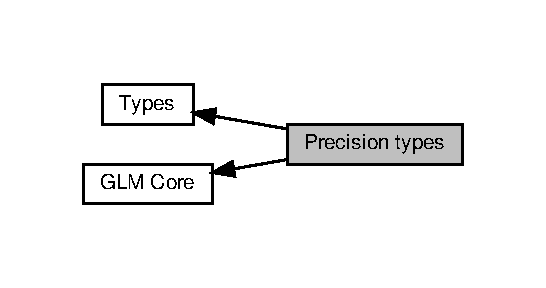
\includegraphics[width=262pt]{group__core__precision}
\end{center}
\end{figure}
\subsection*{Typedefs}
\begin{DoxyCompactItemize}
\item 
typedef \hyperlink{namespaceglm_a0a43b64238afac063f27ee7620205bf2}{lowp\+\_\+float\+\_\+t} \hyperlink{group__core__precision_ga2887fbc729ac5c1c5caeb7cd57a7145c}{glm\+::lowp\+\_\+float}
\item 
typedef \hyperlink{namespaceglm_aec127979a2b6edbf05b485cb4e8c47cc}{mediump\+\_\+float\+\_\+t} \hyperlink{group__core__precision_gac785826c039fe6c97c03b37c81c1a68e}{glm\+::mediump\+\_\+float}
\item 
typedef \hyperlink{namespaceglm_af6f4e45ae06ae3f979dd30cafe7d07c6}{highp\+\_\+float\+\_\+t} \hyperlink{group__core__precision_ga3d443a093adc053638ed7f81c5bfe300}{glm\+::highp\+\_\+float}
\item 
typedef \hyperlink{group__core__precision_gac785826c039fe6c97c03b37c81c1a68e}{mediump\+\_\+float} \hyperlink{group__core__precision_gae01b87f81bd15327230bf1b47c482b24}{glm\+::float\+\_\+t}
\item 
typedef \hyperlink{namespaceglm_1_1detail_a030a8128e369fc1f9c7982dc68a78ba7}{detail\+::lowp\+\_\+int\+\_\+t} \hyperlink{group__core__precision_ga4681244bf4a184734f03aa9df4e3d288}{glm\+::lowp\+\_\+int}
\item 
typedef \hyperlink{namespaceglm_1_1detail_aede0757f19204d1d44f716b3dd66d13c}{detail\+::mediump\+\_\+int\+\_\+t} \hyperlink{group__core__precision_ga2a3dcbcd7f4e17663d393a12061ac6ac}{glm\+::mediump\+\_\+int}
\item 
typedef \hyperlink{namespaceglm_1_1detail_a74c48e9deafcc33db998a4ee62da8d6e}{detail\+::highp\+\_\+int\+\_\+t} \hyperlink{group__core__precision_gaafed5240eb0a43328cb75faf5fb0a8c2}{glm\+::highp\+\_\+int}
\item 
typedef \hyperlink{namespaceglm_1_1detail_ad59c4581ad8ce0c3ef6146edaa7e15dc}{detail\+::lowp\+\_\+uint\+\_\+t} \hyperlink{group__core__precision_ga8077c90f2c87e419ea6c273157dcc1fc}{glm\+::lowp\+\_\+uint}
\item 
typedef \hyperlink{namespaceglm_1_1detail_a98f572e92099cc1b5740f1ccf1c80f8d}{detail\+::mediump\+\_\+uint\+\_\+t} \hyperlink{group__core__precision_ga08ae38ad78ade3539fdd1d25052b8c51}{glm\+::mediump\+\_\+uint}
\item 
typedef \hyperlink{namespaceglm_1_1detail_a994c05c8a976cc902a7cd193ad36bbba}{detail\+::highp\+\_\+uint\+\_\+t} \hyperlink{group__core__precision_gabfd1cf11193324a5f77d3831b6ac3205}{glm\+::highp\+\_\+uint}
\item 
typedef \hyperlink{group__core__precision_ga2a3dcbcd7f4e17663d393a12061ac6ac}{mediump\+\_\+int} \hyperlink{group__core__precision_gacd01d170508f812968875b0f2e730e8c}{glm\+::int\+\_\+t}
\item 
typedef \hyperlink{group__core__precision_ga08ae38ad78ade3539fdd1d25052b8c51}{mediump\+\_\+uint} \hyperlink{group__core__precision_ga5f2ae871c284c9d39ae8fdbb1305b566}{glm\+::uint\+\_\+t}
\item 
typedef unsigned int \hyperlink{group__core__precision_ga4fd29415871152bfb5abd588334147c8}{glm\+::uint}
\item 
typedef \hyperlink{structglm_1_1detail_1_1tmat2x2}{detail\+::tmat2x2}$<$ float, \hyperlink{namespaceglm_a0f04f086094c747d227af4425893f545ae161af3fc695e696ce3bf69f7332bc2d}{lowp} $>$ \hyperlink{group__core__precision_gac0acc3ccf8da050af3393ea639f698d6}{glm\+::lowp\+\_\+mat2}
\item 
typedef \hyperlink{structglm_1_1detail_1_1tmat2x2}{detail\+::tmat2x2}$<$ float, \hyperlink{namespaceglm_a0f04f086094c747d227af4425893f545a6416f3ea0c9025fb21ed50c4d6620482}{mediump} $>$ \hyperlink{group__core__precision_ga6ed8bfa67b72cea216cb558411f95f86}{glm\+::mediump\+\_\+mat2}
\item 
typedef \hyperlink{structglm_1_1detail_1_1tmat2x2}{detail\+::tmat2x2}$<$ float, \hyperlink{namespaceglm_a0f04f086094c747d227af4425893f545ac6f7eab42eacbb10d59a58e95e362074}{highp} $>$ \hyperlink{group__core__precision_gab9884251d84b95dbbf27aa1e4b3a1ec7}{glm\+::highp\+\_\+mat2}
\item 
typedef \hyperlink{structglm_1_1detail_1_1tmat2x2}{detail\+::tmat2x2}$<$ float, \hyperlink{namespaceglm_a0f04f086094c747d227af4425893f545ae161af3fc695e696ce3bf69f7332bc2d}{lowp} $>$ \hyperlink{group__core__precision_ga7d7e123d953978cc17de6882bb10400e}{glm\+::lowp\+\_\+mat2x2}
\item 
typedef \hyperlink{structglm_1_1detail_1_1tmat2x2}{detail\+::tmat2x2}$<$ float, \hyperlink{namespaceglm_a0f04f086094c747d227af4425893f545a6416f3ea0c9025fb21ed50c4d6620482}{mediump} $>$ \hyperlink{group__core__precision_ga867b486aea2d228a1e1a134af73b2c4b}{glm\+::mediump\+\_\+mat2x2}
\item 
typedef \hyperlink{structglm_1_1detail_1_1tmat2x2}{detail\+::tmat2x2}$<$ float, \hyperlink{namespaceglm_a0f04f086094c747d227af4425893f545ac6f7eab42eacbb10d59a58e95e362074}{highp} $>$ \hyperlink{group__core__precision_ga694146b8d430b22caa8b37571d9bc8bc}{glm\+::highp\+\_\+mat2x2}
\item 
typedef \hyperlink{structglm_1_1detail_1_1tmat2x3}{detail\+::tmat2x3}$<$ float, \hyperlink{namespaceglm_a0f04f086094c747d227af4425893f545ae161af3fc695e696ce3bf69f7332bc2d}{lowp} $>$ \hyperlink{group__core__precision_gaef481e637af5103a83ab561d30d28f2a}{glm\+::lowp\+\_\+mat2x3}
\item 
typedef \hyperlink{structglm_1_1detail_1_1tmat2x3}{detail\+::tmat2x3}$<$ float, \hyperlink{namespaceglm_a0f04f086094c747d227af4425893f545a6416f3ea0c9025fb21ed50c4d6620482}{mediump} $>$ \hyperlink{group__core__precision_gad4e099c0dfa8f35ce9c0ddc8605428cf}{glm\+::mediump\+\_\+mat2x3}
\item 
typedef \hyperlink{structglm_1_1detail_1_1tmat2x3}{detail\+::tmat2x3}$<$ float, \hyperlink{namespaceglm_a0f04f086094c747d227af4425893f545ac6f7eab42eacbb10d59a58e95e362074}{highp} $>$ \hyperlink{group__core__precision_ga7d4e5a1c803be5688c75241c924dfa58}{glm\+::highp\+\_\+mat2x3}
\item 
typedef \hyperlink{structglm_1_1detail_1_1tmat2x4}{detail\+::tmat2x4}$<$ float, \hyperlink{namespaceglm_a0f04f086094c747d227af4425893f545ae161af3fc695e696ce3bf69f7332bc2d}{lowp} $>$ \hyperlink{group__core__precision_gaa62e33ee2864909c8522a549fbf40ce5}{glm\+::lowp\+\_\+mat2x4}
\item 
typedef \hyperlink{structglm_1_1detail_1_1tmat2x4}{detail\+::tmat2x4}$<$ float, \hyperlink{namespaceglm_a0f04f086094c747d227af4425893f545a6416f3ea0c9025fb21ed50c4d6620482}{mediump} $>$ \hyperlink{group__core__precision_gae90cf4be1ded03a3a5b7b42045da253c}{glm\+::mediump\+\_\+mat2x4}
\item 
typedef \hyperlink{structglm_1_1detail_1_1tmat2x4}{detail\+::tmat2x4}$<$ float, \hyperlink{namespaceglm_a0f04f086094c747d227af4425893f545ac6f7eab42eacbb10d59a58e95e362074}{highp} $>$ \hyperlink{group__core__precision_ga3cc506666b7a95db56f9d2eb787b6e20}{glm\+::highp\+\_\+mat2x4}
\item 
typedef \hyperlink{structglm_1_1detail_1_1tmat3x2}{detail\+::tmat3x2}$<$ float, \hyperlink{namespaceglm_a0f04f086094c747d227af4425893f545ae161af3fc695e696ce3bf69f7332bc2d}{lowp} $>$ \hyperlink{group__core__precision_ga17219f89f804dbf4620d4caacf32cfe2}{glm\+::lowp\+\_\+mat3x2}
\item 
typedef \hyperlink{structglm_1_1detail_1_1tmat3x2}{detail\+::tmat3x2}$<$ float, \hyperlink{namespaceglm_a0f04f086094c747d227af4425893f545a6416f3ea0c9025fb21ed50c4d6620482}{mediump} $>$ \hyperlink{group__core__precision_ga1215b70c2750b6e9ab813ced8dcae568}{glm\+::mediump\+\_\+mat3x2}
\item 
typedef \hyperlink{structglm_1_1detail_1_1tmat3x2}{detail\+::tmat3x2}$<$ float, \hyperlink{namespaceglm_a0f04f086094c747d227af4425893f545ac6f7eab42eacbb10d59a58e95e362074}{highp} $>$ \hyperlink{group__core__precision_gabc7767293ff69cd56717ee9d8be62963}{glm\+::highp\+\_\+mat3x2}
\item 
typedef \hyperlink{structglm_1_1detail_1_1tmat3x3}{detail\+::tmat3x3}$<$ float, \hyperlink{namespaceglm_a0f04f086094c747d227af4425893f545ae161af3fc695e696ce3bf69f7332bc2d}{lowp} $>$ \hyperlink{group__core__precision_gaae2935658c6a3668ac1935a7f6064d51}{glm\+::lowp\+\_\+mat3}
\item 
typedef \hyperlink{structglm_1_1detail_1_1tmat3x3}{detail\+::tmat3x3}$<$ float, \hyperlink{namespaceglm_a0f04f086094c747d227af4425893f545a6416f3ea0c9025fb21ed50c4d6620482}{mediump} $>$ \hyperlink{group__core__precision_gacf45e22f1fb2703b181995676963a1f9}{glm\+::mediump\+\_\+mat3}
\item 
typedef \hyperlink{structglm_1_1detail_1_1tmat3x3}{detail\+::tmat3x3}$<$ float, \hyperlink{namespaceglm_a0f04f086094c747d227af4425893f545ac6f7eab42eacbb10d59a58e95e362074}{highp} $>$ \hyperlink{group__core__precision_ga334034520a655db41a2e188951f6aaad}{glm\+::highp\+\_\+mat3}
\item 
typedef \hyperlink{structglm_1_1detail_1_1tmat3x3}{detail\+::tmat3x3}$<$ float, \hyperlink{namespaceglm_a0f04f086094c747d227af4425893f545ae161af3fc695e696ce3bf69f7332bc2d}{lowp} $>$ \hyperlink{group__core__precision_ga31688b397d10806ead332c3adb7dc0f0}{glm\+::lowp\+\_\+mat3x3}
\item 
typedef \hyperlink{structglm_1_1detail_1_1tmat3x3}{detail\+::tmat3x3}$<$ float, \hyperlink{namespaceglm_a0f04f086094c747d227af4425893f545a6416f3ea0c9025fb21ed50c4d6620482}{mediump} $>$ \hyperlink{group__core__precision_gae4c7f0d5d3dab712f9a671183e63e5ab}{glm\+::mediump\+\_\+mat3x3}
\item 
typedef \hyperlink{structglm_1_1detail_1_1tmat3x3}{detail\+::tmat3x3}$<$ float, \hyperlink{namespaceglm_a0f04f086094c747d227af4425893f545ac6f7eab42eacbb10d59a58e95e362074}{highp} $>$ \hyperlink{group__core__precision_ga8a3703cc71cdfc8928eddf46b3763c4b}{glm\+::highp\+\_\+mat3x3}
\item 
typedef \hyperlink{structglm_1_1detail_1_1tmat3x4}{detail\+::tmat3x4}$<$ float, \hyperlink{namespaceglm_a0f04f086094c747d227af4425893f545ae161af3fc695e696ce3bf69f7332bc2d}{lowp} $>$ \hyperlink{group__core__precision_ga9cea06e7378fe59abf95c1f56edc4320}{glm\+::lowp\+\_\+mat3x4}
\item 
typedef \hyperlink{structglm_1_1detail_1_1tmat3x4}{detail\+::tmat3x4}$<$ float, \hyperlink{namespaceglm_a0f04f086094c747d227af4425893f545a6416f3ea0c9025fb21ed50c4d6620482}{mediump} $>$ \hyperlink{group__core__precision_ga5654236019c6a732844da31534a3cf28}{glm\+::mediump\+\_\+mat3x4}
\item 
typedef \hyperlink{structglm_1_1detail_1_1tmat3x4}{detail\+::tmat3x4}$<$ float, \hyperlink{namespaceglm_a0f04f086094c747d227af4425893f545ac6f7eab42eacbb10d59a58e95e362074}{highp} $>$ \hyperlink{group__core__precision_gabaf9c8dd35db715b1093042703f879d0}{glm\+::highp\+\_\+mat3x4}
\item 
typedef \hyperlink{structglm_1_1detail_1_1tmat4x2}{detail\+::tmat4x2}$<$ float, \hyperlink{namespaceglm_a0f04f086094c747d227af4425893f545ae161af3fc695e696ce3bf69f7332bc2d}{lowp} $>$ \hyperlink{group__core__precision_ga2cfe24ae14da17f3510acfc3d03e05a5}{glm\+::lowp\+\_\+mat4x2}
\item 
typedef \hyperlink{structglm_1_1detail_1_1tmat4x2}{detail\+::tmat4x2}$<$ float, \hyperlink{namespaceglm_a0f04f086094c747d227af4425893f545a6416f3ea0c9025fb21ed50c4d6620482}{mediump} $>$ \hyperlink{group__core__precision_ga5ade2a6a65653683f76988c45da39f15}{glm\+::mediump\+\_\+mat4x2}
\item 
typedef \hyperlink{structglm_1_1detail_1_1tmat4x2}{detail\+::tmat4x2}$<$ float, \hyperlink{namespaceglm_a0f04f086094c747d227af4425893f545ac6f7eab42eacbb10d59a58e95e362074}{highp} $>$ \hyperlink{group__core__precision_gadf9c4a7947c2b0a79f52cc86a860f270}{glm\+::highp\+\_\+mat4x2}
\item 
typedef \hyperlink{structglm_1_1detail_1_1tmat4x3}{detail\+::tmat4x3}$<$ float, \hyperlink{namespaceglm_a0f04f086094c747d227af4425893f545ae161af3fc695e696ce3bf69f7332bc2d}{lowp} $>$ \hyperlink{group__core__precision_gada92d0baf15002240dd6f638c57f9fec}{glm\+::lowp\+\_\+mat4x3}
\item 
typedef \hyperlink{structglm_1_1detail_1_1tmat4x3}{detail\+::tmat4x3}$<$ float, \hyperlink{namespaceglm_a0f04f086094c747d227af4425893f545a6416f3ea0c9025fb21ed50c4d6620482}{mediump} $>$ \hyperlink{group__core__precision_ga445d8aac3a5227af2d1e98d5c2f74d03}{glm\+::mediump\+\_\+mat4x3}
\item 
typedef \hyperlink{structglm_1_1detail_1_1tmat4x3}{detail\+::tmat4x3}$<$ float, \hyperlink{namespaceglm_a0f04f086094c747d227af4425893f545ac6f7eab42eacbb10d59a58e95e362074}{highp} $>$ \hyperlink{group__core__precision_gab8dfe989c5100c35ab5dec0e94f59d2a}{glm\+::highp\+\_\+mat4x3}
\item 
typedef \hyperlink{structglm_1_1detail_1_1tmat4x4}{detail\+::tmat4x4}$<$ float, \hyperlink{namespaceglm_a0f04f086094c747d227af4425893f545ae161af3fc695e696ce3bf69f7332bc2d}{lowp} $>$ \hyperlink{group__core__precision_ga8f6fef75ce51e9d6db7971478ad1f1c2}{glm\+::lowp\+\_\+mat4}
\item 
typedef \hyperlink{structglm_1_1detail_1_1tmat4x4}{detail\+::tmat4x4}$<$ float, \hyperlink{namespaceglm_a0f04f086094c747d227af4425893f545a6416f3ea0c9025fb21ed50c4d6620482}{mediump} $>$ \hyperlink{group__core__precision_gaf3de9a0400cf707d3c159f32902b92db}{glm\+::mediump\+\_\+mat4}
\item 
typedef \hyperlink{structglm_1_1detail_1_1tmat4x4}{detail\+::tmat4x4}$<$ float, \hyperlink{namespaceglm_a0f04f086094c747d227af4425893f545ac6f7eab42eacbb10d59a58e95e362074}{highp} $>$ \hyperlink{group__core__precision_ga3067b3b8ce793227a51b2e3c233257d5}{glm\+::highp\+\_\+mat4}
\item 
typedef \hyperlink{structglm_1_1detail_1_1tmat4x4}{detail\+::tmat4x4}$<$ float, \hyperlink{namespaceglm_a0f04f086094c747d227af4425893f545ae161af3fc695e696ce3bf69f7332bc2d}{lowp} $>$ \hyperlink{group__core__precision_gad31846a0565c22a0479950313c28b218}{glm\+::lowp\+\_\+mat4x4}
\item 
typedef \hyperlink{structglm_1_1detail_1_1tmat4x4}{detail\+::tmat4x4}$<$ float, \hyperlink{namespaceglm_a0f04f086094c747d227af4425893f545a6416f3ea0c9025fb21ed50c4d6620482}{mediump} $>$ \hyperlink{group__core__precision_gacb51d2d10f7607617ac544f6db9a6eef}{glm\+::mediump\+\_\+mat4x4}
\item 
typedef \hyperlink{structglm_1_1detail_1_1tmat4x4}{detail\+::tmat4x4}$<$ float, \hyperlink{namespaceglm_a0f04f086094c747d227af4425893f545ac6f7eab42eacbb10d59a58e95e362074}{highp} $>$ \hyperlink{group__core__precision_ga231950d260be295a25d7340e2020f55c}{glm\+::highp\+\_\+mat4x4}
\item 
typedef \hyperlink{structglm_1_1detail_1_1tmat2x2}{detail\+::tmat2x2}$<$ double, \hyperlink{namespaceglm_a0f04f086094c747d227af4425893f545ae161af3fc695e696ce3bf69f7332bc2d}{lowp} $>$ \hyperlink{group__core__precision_ga5e08c45dfef867e0326a1eee95060cd0}{glm\+::lowp\+\_\+dmat2}
\item 
typedef \hyperlink{structglm_1_1detail_1_1tmat2x2}{detail\+::tmat2x2}$<$ double, \hyperlink{namespaceglm_a0f04f086094c747d227af4425893f545a6416f3ea0c9025fb21ed50c4d6620482}{mediump} $>$ \hyperlink{group__core__precision_gac056ec9d1c37e591172544088163b7e4}{glm\+::mediump\+\_\+dmat2}
\item 
typedef \hyperlink{structglm_1_1detail_1_1tmat2x2}{detail\+::tmat2x2}$<$ double, \hyperlink{namespaceglm_a0f04f086094c747d227af4425893f545ac6f7eab42eacbb10d59a58e95e362074}{highp} $>$ \hyperlink{group__core__precision_ga9b158b3b722fe991bb66f7e65f136e68}{glm\+::highp\+\_\+dmat2}
\item 
typedef \hyperlink{structglm_1_1detail_1_1tmat2x2}{detail\+::tmat2x2}$<$ double, \hyperlink{namespaceglm_a0f04f086094c747d227af4425893f545ae161af3fc695e696ce3bf69f7332bc2d}{lowp} $>$ \hyperlink{group__core__precision_ga68b486ff22814c1a3781378513a9fcc0}{glm\+::lowp\+\_\+dmat2x2}
\item 
typedef \hyperlink{structglm_1_1detail_1_1tmat2x2}{detail\+::tmat2x2}$<$ double, \hyperlink{namespaceglm_a0f04f086094c747d227af4425893f545a6416f3ea0c9025fb21ed50c4d6620482}{mediump} $>$ \hyperlink{group__core__precision_ga88ddb4188060ab00fee67c9840f4417e}{glm\+::mediump\+\_\+dmat2x2}
\item 
typedef \hyperlink{structglm_1_1detail_1_1tmat2x2}{detail\+::tmat2x2}$<$ double, \hyperlink{namespaceglm_a0f04f086094c747d227af4425893f545ac6f7eab42eacbb10d59a58e95e362074}{highp} $>$ \hyperlink{group__core__precision_gaa5e35f6570d394c1cd34f411a473220c}{glm\+::highp\+\_\+dmat2x2}
\item 
typedef \hyperlink{structglm_1_1detail_1_1tmat2x3}{detail\+::tmat2x3}$<$ double, \hyperlink{namespaceglm_a0f04f086094c747d227af4425893f545ae161af3fc695e696ce3bf69f7332bc2d}{lowp} $>$ \hyperlink{group__core__precision_ga2c7432984a35cf72050870a54485ef35}{glm\+::lowp\+\_\+dmat2x3}
\item 
typedef \hyperlink{structglm_1_1detail_1_1tmat2x3}{detail\+::tmat2x3}$<$ double, \hyperlink{namespaceglm_a0f04f086094c747d227af4425893f545a6416f3ea0c9025fb21ed50c4d6620482}{mediump} $>$ \hyperlink{group__core__precision_ga734e988edf759c7012c443014acb6674}{glm\+::mediump\+\_\+dmat2x3}
\item 
typedef \hyperlink{structglm_1_1detail_1_1tmat2x3}{detail\+::tmat2x3}$<$ double, \hyperlink{namespaceglm_a0f04f086094c747d227af4425893f545ac6f7eab42eacbb10d59a58e95e362074}{highp} $>$ \hyperlink{group__core__precision_gafec7367665f006f2a7643103c5eddc38}{glm\+::highp\+\_\+dmat2x3}
\item 
typedef \hyperlink{structglm_1_1detail_1_1tmat2x4}{detail\+::tmat2x4}$<$ double, \hyperlink{namespaceglm_a0f04f086094c747d227af4425893f545ae161af3fc695e696ce3bf69f7332bc2d}{lowp} $>$ \hyperlink{group__core__precision_gac2285cef559b0dc35cb9a7f22e6a2dd8}{glm\+::lowp\+\_\+dmat2x4}
\item 
typedef \hyperlink{structglm_1_1detail_1_1tmat2x4}{detail\+::tmat2x4}$<$ double, \hyperlink{namespaceglm_a0f04f086094c747d227af4425893f545a6416f3ea0c9025fb21ed50c4d6620482}{mediump} $>$ \hyperlink{group__core__precision_gadb60bf60ef2b8da4a28a372b2bcca3a3}{glm\+::mediump\+\_\+dmat2x4}
\item 
typedef \hyperlink{structglm_1_1detail_1_1tmat2x4}{detail\+::tmat2x4}$<$ double, \hyperlink{namespaceglm_a0f04f086094c747d227af4425893f545ac6f7eab42eacbb10d59a58e95e362074}{highp} $>$ \hyperlink{group__core__precision_gacd51d8188f7d66a83c035b8c4cd69f2d}{glm\+::highp\+\_\+dmat2x4}
\item 
typedef \hyperlink{structglm_1_1detail_1_1tmat3x2}{detail\+::tmat3x2}$<$ double, \hyperlink{namespaceglm_a0f04f086094c747d227af4425893f545ae161af3fc695e696ce3bf69f7332bc2d}{lowp} $>$ \hyperlink{group__core__precision_ga678c21e4fadeda255cfb146d40844bdd}{glm\+::lowp\+\_\+dmat3x2}
\item 
typedef \hyperlink{structglm_1_1detail_1_1tmat3x2}{detail\+::tmat3x2}$<$ double, \hyperlink{namespaceglm_a0f04f086094c747d227af4425893f545a6416f3ea0c9025fb21ed50c4d6620482}{mediump} $>$ \hyperlink{group__core__precision_gaff0060984716bcda68ff69ed27536bf6}{glm\+::mediump\+\_\+dmat3x2}
\item 
typedef \hyperlink{structglm_1_1detail_1_1tmat3x2}{detail\+::tmat3x2}$<$ double, \hyperlink{namespaceglm_a0f04f086094c747d227af4425893f545ac6f7eab42eacbb10d59a58e95e362074}{highp} $>$ \hyperlink{group__core__precision_gac956fe6b946f0ccee78367ccd5427351}{glm\+::highp\+\_\+dmat3x2}
\item 
typedef \hyperlink{structglm_1_1detail_1_1tmat3x3}{detail\+::tmat3x3}$<$ float, \hyperlink{namespaceglm_a0f04f086094c747d227af4425893f545ae161af3fc695e696ce3bf69f7332bc2d}{lowp} $>$ \hyperlink{group__core__precision_ga07d9423bdde2d7ff880d6ece01dc9e32}{glm\+::lowp\+\_\+dmat3}
\item 
typedef \hyperlink{structglm_1_1detail_1_1tmat3x3}{detail\+::tmat3x3}$<$ double, \hyperlink{namespaceglm_a0f04f086094c747d227af4425893f545a6416f3ea0c9025fb21ed50c4d6620482}{mediump} $>$ \hyperlink{group__core__precision_ga80600af2c1ca11ead6123777185c372d}{glm\+::mediump\+\_\+dmat3}
\item 
typedef \hyperlink{structglm_1_1detail_1_1tmat3x3}{detail\+::tmat3x3}$<$ double, \hyperlink{namespaceglm_a0f04f086094c747d227af4425893f545ac6f7eab42eacbb10d59a58e95e362074}{highp} $>$ \hyperlink{group__core__precision_ga993461e1d2caf19abd4f64d02ccdafa9}{glm\+::highp\+\_\+dmat3}
\item 
typedef \hyperlink{structglm_1_1detail_1_1tmat3x3}{detail\+::tmat3x3}$<$ double, \hyperlink{namespaceglm_a0f04f086094c747d227af4425893f545ae161af3fc695e696ce3bf69f7332bc2d}{lowp} $>$ \hyperlink{group__core__precision_gaea1bc4ede38e1b904f01ff5ce59210ea}{glm\+::lowp\+\_\+dmat3x3}
\item 
typedef \hyperlink{structglm_1_1detail_1_1tmat3x3}{detail\+::tmat3x3}$<$ double, \hyperlink{namespaceglm_a0f04f086094c747d227af4425893f545a6416f3ea0c9025fb21ed50c4d6620482}{mediump} $>$ \hyperlink{group__core__precision_ga2f73508d8192390ca9f9b569f544fade}{glm\+::mediump\+\_\+dmat3x3}
\item 
typedef \hyperlink{structglm_1_1detail_1_1tmat3x3}{detail\+::tmat3x3}$<$ double, \hyperlink{namespaceglm_a0f04f086094c747d227af4425893f545ac6f7eab42eacbb10d59a58e95e362074}{highp} $>$ \hyperlink{group__core__precision_gad7229dea82287910d88e6e8566e39fc7}{glm\+::highp\+\_\+dmat3x3}
\item 
typedef \hyperlink{structglm_1_1detail_1_1tmat3x4}{detail\+::tmat3x4}$<$ double, \hyperlink{namespaceglm_a0f04f086094c747d227af4425893f545ae161af3fc695e696ce3bf69f7332bc2d}{lowp} $>$ \hyperlink{group__core__precision_ga4640e1d20ad705842525e79a4cc57b15}{glm\+::lowp\+\_\+dmat3x4}
\item 
typedef \hyperlink{structglm_1_1detail_1_1tmat3x4}{detail\+::tmat3x4}$<$ double, \hyperlink{namespaceglm_a0f04f086094c747d227af4425893f545a6416f3ea0c9025fb21ed50c4d6620482}{mediump} $>$ \hyperlink{group__core__precision_gaedd814e706701200b13b86fc6fd7b373}{glm\+::mediump\+\_\+dmat3x4}
\item 
typedef \hyperlink{structglm_1_1detail_1_1tmat3x4}{detail\+::tmat3x4}$<$ double, \hyperlink{namespaceglm_a0f04f086094c747d227af4425893f545ac6f7eab42eacbb10d59a58e95e362074}{highp} $>$ \hyperlink{group__core__precision_gaff199c8d04a8edb92ed43283e8694c59}{glm\+::highp\+\_\+dmat3x4}
\item 
typedef \hyperlink{structglm_1_1detail_1_1tmat4x2}{detail\+::tmat4x2}$<$ double, \hyperlink{namespaceglm_a0f04f086094c747d227af4425893f545ae161af3fc695e696ce3bf69f7332bc2d}{lowp} $>$ \hyperlink{group__core__precision_ga28a7ef670069c3707f19b9de1039517e}{glm\+::lowp\+\_\+dmat4x2}
\item 
typedef \hyperlink{structglm_1_1detail_1_1tmat4x2}{detail\+::tmat4x2}$<$ double, \hyperlink{namespaceglm_a0f04f086094c747d227af4425893f545a6416f3ea0c9025fb21ed50c4d6620482}{mediump} $>$ \hyperlink{group__core__precision_ga03056b616496470371473cd5df4dc1f8}{glm\+::mediump\+\_\+dmat4x2}
\item 
typedef \hyperlink{structglm_1_1detail_1_1tmat4x2}{detail\+::tmat4x2}$<$ double, \hyperlink{namespaceglm_a0f04f086094c747d227af4425893f545ac6f7eab42eacbb10d59a58e95e362074}{highp} $>$ \hyperlink{group__core__precision_gaa4fb1ed350a6cd053abb9b093d13ce0d}{glm\+::highp\+\_\+dmat4x2}
\item 
typedef \hyperlink{structglm_1_1detail_1_1tmat4x3}{detail\+::tmat4x3}$<$ double, \hyperlink{namespaceglm_a0f04f086094c747d227af4425893f545ae161af3fc695e696ce3bf69f7332bc2d}{lowp} $>$ \hyperlink{group__core__precision_gabc1be51eb0cae7cd4b1d6483a954c35d}{glm\+::lowp\+\_\+dmat4x3}
\item 
typedef \hyperlink{structglm_1_1detail_1_1tmat4x3}{detail\+::tmat4x3}$<$ double, \hyperlink{namespaceglm_a0f04f086094c747d227af4425893f545a6416f3ea0c9025fb21ed50c4d6620482}{mediump} $>$ \hyperlink{group__core__precision_gafa1ba33d2748737129cde471fedbf9c5}{glm\+::mediump\+\_\+dmat4x3}
\item 
typedef \hyperlink{structglm_1_1detail_1_1tmat4x3}{detail\+::tmat4x3}$<$ double, \hyperlink{namespaceglm_a0f04f086094c747d227af4425893f545ac6f7eab42eacbb10d59a58e95e362074}{highp} $>$ \hyperlink{group__core__precision_gaf8aeba0eecc5c651e0f06414b6e37754}{glm\+::highp\+\_\+dmat4x3}
\item 
typedef \hyperlink{structglm_1_1detail_1_1tmat4x4}{detail\+::tmat4x4}$<$ double, \hyperlink{namespaceglm_a0f04f086094c747d227af4425893f545ae161af3fc695e696ce3bf69f7332bc2d}{lowp} $>$ \hyperlink{group__core__precision_gaea69794db4e619881b77d37bf84b337e}{glm\+::lowp\+\_\+dmat4}
\item 
typedef \hyperlink{structglm_1_1detail_1_1tmat4x4}{detail\+::tmat4x4}$<$ double, \hyperlink{namespaceglm_a0f04f086094c747d227af4425893f545a6416f3ea0c9025fb21ed50c4d6620482}{mediump} $>$ \hyperlink{group__core__precision_ga73de517f040f7d50746bbe273a396685}{glm\+::mediump\+\_\+dmat4}
\item 
typedef \hyperlink{structglm_1_1detail_1_1tmat4x4}{detail\+::tmat4x4}$<$ double, \hyperlink{namespaceglm_a0f04f086094c747d227af4425893f545ac6f7eab42eacbb10d59a58e95e362074}{highp} $>$ \hyperlink{group__core__precision_ga9a5d95e476d451d28d3939ac7f124baf}{glm\+::highp\+\_\+dmat4}
\item 
typedef \hyperlink{structglm_1_1detail_1_1tmat4x4}{detail\+::tmat4x4}$<$ double, \hyperlink{namespaceglm_a0f04f086094c747d227af4425893f545ae161af3fc695e696ce3bf69f7332bc2d}{lowp} $>$ \hyperlink{group__core__precision_gac762dec40f53114dfe6894499a2c9a79}{glm\+::lowp\+\_\+dmat4x4}
\item 
typedef \hyperlink{structglm_1_1detail_1_1tmat4x4}{detail\+::tmat4x4}$<$ double, \hyperlink{namespaceglm_a0f04f086094c747d227af4425893f545a6416f3ea0c9025fb21ed50c4d6620482}{mediump} $>$ \hyperlink{group__core__precision_gad64329d45b05417ccf0cc3c23f584d26}{glm\+::mediump\+\_\+dmat4x4}
\item 
typedef \hyperlink{structglm_1_1detail_1_1tmat4x4}{detail\+::tmat4x4}$<$ double, \hyperlink{namespaceglm_a0f04f086094c747d227af4425893f545ac6f7eab42eacbb10d59a58e95e362074}{highp} $>$ \hyperlink{group__core__precision_ga1c0a2edbde597b59e9005691a224b208}{glm\+::highp\+\_\+dmat4x4}
\item 
typedef \hyperlink{structglm_1_1detail_1_1tvec2}{detail\+::tvec2}$<$ float, \hyperlink{namespaceglm_a0f04f086094c747d227af4425893f545ac6f7eab42eacbb10d59a58e95e362074}{highp} $>$ \hyperlink{group__core__precision_ga37645abcfcc1278567e99f1ca492bfbb}{glm\+::highp\+\_\+vec2}
\item 
typedef \hyperlink{structglm_1_1detail_1_1tvec2}{detail\+::tvec2}$<$ float, \hyperlink{namespaceglm_a0f04f086094c747d227af4425893f545a6416f3ea0c9025fb21ed50c4d6620482}{mediump} $>$ \hyperlink{group__core__precision_ga1365858c541931eb8a7473fa85a1d1cf}{glm\+::mediump\+\_\+vec2}
\item 
typedef \hyperlink{structglm_1_1detail_1_1tvec2}{detail\+::tvec2}$<$ float, \hyperlink{namespaceglm_a0f04f086094c747d227af4425893f545ae161af3fc695e696ce3bf69f7332bc2d}{lowp} $>$ \hyperlink{group__core__precision_gac63d79532b7e8d18f579ebe63e4fde49}{glm\+::lowp\+\_\+vec2}
\item 
typedef \hyperlink{structglm_1_1detail_1_1tvec2}{detail\+::tvec2}$<$ double, \hyperlink{namespaceglm_a0f04f086094c747d227af4425893f545ac6f7eab42eacbb10d59a58e95e362074}{highp} $>$ \hyperlink{group__core__precision_gacfbe8512142fff27f0bfb44958c1752f}{glm\+::highp\+\_\+dvec2}
\item 
typedef \hyperlink{structglm_1_1detail_1_1tvec2}{detail\+::tvec2}$<$ double, \hyperlink{namespaceglm_a0f04f086094c747d227af4425893f545a6416f3ea0c9025fb21ed50c4d6620482}{mediump} $>$ \hyperlink{group__core__precision_gace1f1cc2eb8e978dcb60e682af87b541}{glm\+::mediump\+\_\+dvec2}
\item 
typedef \hyperlink{structglm_1_1detail_1_1tvec2}{detail\+::tvec2}$<$ double, \hyperlink{namespaceglm_a0f04f086094c747d227af4425893f545ae161af3fc695e696ce3bf69f7332bc2d}{lowp} $>$ \hyperlink{group__core__precision_ga27a115a27d5f065e8c043f57191d583b}{glm\+::lowp\+\_\+dvec2}
\item 
typedef \hyperlink{structglm_1_1detail_1_1tvec2}{detail\+::tvec2}$<$ int, \hyperlink{namespaceglm_a0f04f086094c747d227af4425893f545ac6f7eab42eacbb10d59a58e95e362074}{highp} $>$ \hyperlink{group__core__precision_gab2bac6095f51f7d7f74747afc2f6747a}{glm\+::highp\+\_\+ivec2}
\item 
typedef \hyperlink{structglm_1_1detail_1_1tvec2}{detail\+::tvec2}$<$ int, \hyperlink{namespaceglm_a0f04f086094c747d227af4425893f545a6416f3ea0c9025fb21ed50c4d6620482}{mediump} $>$ \hyperlink{group__core__precision_ga4f1bf9844e667805235823afe809aa73}{glm\+::mediump\+\_\+ivec2}
\item 
typedef \hyperlink{structglm_1_1detail_1_1tvec2}{detail\+::tvec2}$<$ int, \hyperlink{namespaceglm_a0f04f086094c747d227af4425893f545ae161af3fc695e696ce3bf69f7332bc2d}{lowp} $>$ \hyperlink{group__core__precision_ga562c5c67d6431ab88fc4a032239e2137}{glm\+::lowp\+\_\+ivec2}
\item 
typedef \hyperlink{structglm_1_1detail_1_1tvec2}{detail\+::tvec2}$<$ \hyperlink{group__core__precision_ga4fd29415871152bfb5abd588334147c8}{uint}, \hyperlink{namespaceglm_a0f04f086094c747d227af4425893f545ac6f7eab42eacbb10d59a58e95e362074}{highp} $>$ \hyperlink{group__core__precision_gaaf92be4c1fca33cff90c1ed15b521c79}{glm\+::highp\+\_\+uvec2}
\item 
typedef \hyperlink{structglm_1_1detail_1_1tvec2}{detail\+::tvec2}$<$ \hyperlink{group__core__precision_ga4fd29415871152bfb5abd588334147c8}{uint}, \hyperlink{namespaceglm_a0f04f086094c747d227af4425893f545a6416f3ea0c9025fb21ed50c4d6620482}{mediump} $>$ \hyperlink{group__core__precision_ga15c8fb77bdb6763ef73b39e02eb98a56}{glm\+::mediump\+\_\+uvec2}
\item 
typedef \hyperlink{structglm_1_1detail_1_1tvec2}{detail\+::tvec2}$<$ \hyperlink{group__core__precision_ga4fd29415871152bfb5abd588334147c8}{uint}, \hyperlink{namespaceglm_a0f04f086094c747d227af4425893f545ae161af3fc695e696ce3bf69f7332bc2d}{lowp} $>$ \hyperlink{group__core__precision_ga06c64bb528bbecf276ab2d4a2b6c934e}{glm\+::lowp\+\_\+uvec2}
\item 
typedef \hyperlink{structglm_1_1detail_1_1tvec2}{detail\+::tvec2}$<$ bool, \hyperlink{namespaceglm_a0f04f086094c747d227af4425893f545ac6f7eab42eacbb10d59a58e95e362074}{highp} $>$ \hyperlink{group__core__precision_ga4153415d1f3d390219ac9464652ac377}{glm\+::highp\+\_\+bvec2}
\item 
typedef \hyperlink{structglm_1_1detail_1_1tvec2}{detail\+::tvec2}$<$ bool, \hyperlink{namespaceglm_a0f04f086094c747d227af4425893f545a6416f3ea0c9025fb21ed50c4d6620482}{mediump} $>$ \hyperlink{group__core__precision_ga1406d96eb96694d91052d3f882658ab2}{glm\+::mediump\+\_\+bvec2}
\item 
typedef \hyperlink{structglm_1_1detail_1_1tvec2}{detail\+::tvec2}$<$ bool, \hyperlink{namespaceglm_a0f04f086094c747d227af4425893f545ae161af3fc695e696ce3bf69f7332bc2d}{lowp} $>$ \hyperlink{group__core__precision_ga8ff6222d4bb4245106dab0727c8e8a45}{glm\+::lowp\+\_\+bvec2}
\item 
typedef \hyperlink{structglm_1_1detail_1_1tvec3}{detail\+::tvec3}$<$ float, \hyperlink{namespaceglm_a0f04f086094c747d227af4425893f545ac6f7eab42eacbb10d59a58e95e362074}{highp} $>$ \hyperlink{group__core__precision_ga4879124da7a18d6b681d933cb8c4267d}{glm\+::highp\+\_\+vec3}
\item 
typedef \hyperlink{structglm_1_1detail_1_1tvec3}{detail\+::tvec3}$<$ float, \hyperlink{namespaceglm_a0f04f086094c747d227af4425893f545a6416f3ea0c9025fb21ed50c4d6620482}{mediump} $>$ \hyperlink{group__core__precision_ga10acc767a046b85205f52ce7f834626f}{glm\+::mediump\+\_\+vec3}
\item 
typedef \hyperlink{structglm_1_1detail_1_1tvec3}{detail\+::tvec3}$<$ float, \hyperlink{namespaceglm_a0f04f086094c747d227af4425893f545ae161af3fc695e696ce3bf69f7332bc2d}{lowp} $>$ \hyperlink{group__core__precision_ga062795097526e2758d34cb38387dd82d}{glm\+::lowp\+\_\+vec3}
\item 
typedef \hyperlink{structglm_1_1detail_1_1tvec3}{detail\+::tvec3}$<$ double, \hyperlink{namespaceglm_a0f04f086094c747d227af4425893f545ac6f7eab42eacbb10d59a58e95e362074}{highp} $>$ \hyperlink{group__core__precision_ga4962711854156dae8ebb4eb39237c542}{glm\+::highp\+\_\+dvec3}
\item 
typedef \hyperlink{structglm_1_1detail_1_1tvec3}{detail\+::tvec3}$<$ double, \hyperlink{namespaceglm_a0f04f086094c747d227af4425893f545a6416f3ea0c9025fb21ed50c4d6620482}{mediump} $>$ \hyperlink{group__core__precision_gac051f0702cb0e717db5dd913f6261388}{glm\+::mediump\+\_\+dvec3}
\item 
typedef \hyperlink{structglm_1_1detail_1_1tvec3}{detail\+::tvec3}$<$ double, \hyperlink{namespaceglm_a0f04f086094c747d227af4425893f545ae161af3fc695e696ce3bf69f7332bc2d}{lowp} $>$ \hyperlink{group__core__precision_ga9bdb864f7242863e1227e3209f5b2dc4}{glm\+::lowp\+\_\+dvec3}
\item 
typedef \hyperlink{structglm_1_1detail_1_1tvec3}{detail\+::tvec3}$<$ int, \hyperlink{namespaceglm_a0f04f086094c747d227af4425893f545ac6f7eab42eacbb10d59a58e95e362074}{highp} $>$ \hyperlink{group__core__precision_gae9f0a321de8ee92dce9d4400362d71e7}{glm\+::highp\+\_\+ivec3}
\item 
typedef \hyperlink{structglm_1_1detail_1_1tvec3}{detail\+::tvec3}$<$ int, \hyperlink{namespaceglm_a0f04f086094c747d227af4425893f545a6416f3ea0c9025fb21ed50c4d6620482}{mediump} $>$ \hyperlink{group__core__precision_ga520d24fa0ea887284b80a02c062ca7b8}{glm\+::mediump\+\_\+ivec3}
\item 
typedef \hyperlink{structglm_1_1detail_1_1tvec3}{detail\+::tvec3}$<$ int, \hyperlink{namespaceglm_a0f04f086094c747d227af4425893f545ae161af3fc695e696ce3bf69f7332bc2d}{lowp} $>$ \hyperlink{group__core__precision_gad133fec5c629e3f712c1270e15144e6c}{glm\+::lowp\+\_\+ivec3}
\item 
typedef \hyperlink{structglm_1_1detail_1_1tvec3}{detail\+::tvec3}$<$ \hyperlink{group__core__precision_ga4fd29415871152bfb5abd588334147c8}{uint}, \hyperlink{namespaceglm_a0f04f086094c747d227af4425893f545ac6f7eab42eacbb10d59a58e95e362074}{highp} $>$ \hyperlink{group__core__precision_ga66d0e4ae1742ede2eb32bf0bfedd7474}{glm\+::highp\+\_\+uvec3}
\item 
typedef \hyperlink{structglm_1_1detail_1_1tvec3}{detail\+::tvec3}$<$ \hyperlink{group__core__precision_ga4fd29415871152bfb5abd588334147c8}{uint}, \hyperlink{namespaceglm_a0f04f086094c747d227af4425893f545a6416f3ea0c9025fb21ed50c4d6620482}{mediump} $>$ \hyperlink{group__core__precision_gaebdefe98b08421ef645f65c706af46b2}{glm\+::mediump\+\_\+uvec3}
\item 
typedef \hyperlink{structglm_1_1detail_1_1tvec3}{detail\+::tvec3}$<$ \hyperlink{group__core__precision_ga4fd29415871152bfb5abd588334147c8}{uint}, \hyperlink{namespaceglm_a0f04f086094c747d227af4425893f545ae161af3fc695e696ce3bf69f7332bc2d}{lowp} $>$ \hyperlink{group__core__precision_ga26fd88e52fe7003d41b0c57c5edffd6e}{glm\+::lowp\+\_\+uvec3}
\item 
typedef \hyperlink{structglm_1_1detail_1_1tvec3}{detail\+::tvec3}$<$ bool, \hyperlink{namespaceglm_a0f04f086094c747d227af4425893f545ac6f7eab42eacbb10d59a58e95e362074}{highp} $>$ \hyperlink{group__core__precision_ga1d77a773fdd024602413670788c10c62}{glm\+::highp\+\_\+bvec3}
\item 
typedef \hyperlink{structglm_1_1detail_1_1tvec3}{detail\+::tvec3}$<$ bool, \hyperlink{namespaceglm_a0f04f086094c747d227af4425893f545a6416f3ea0c9025fb21ed50c4d6620482}{mediump} $>$ \hyperlink{group__core__precision_gae7c8d0136e829d6fe3feb00856e35f11}{glm\+::mediump\+\_\+bvec3}
\item 
typedef \hyperlink{structglm_1_1detail_1_1tvec3}{detail\+::tvec3}$<$ bool, \hyperlink{namespaceglm_a0f04f086094c747d227af4425893f545ae161af3fc695e696ce3bf69f7332bc2d}{lowp} $>$ \hyperlink{group__core__precision_ga17ac2986f7b315a2ac4ee2662b5be9cb}{glm\+::lowp\+\_\+bvec3}
\item 
typedef \hyperlink{structglm_1_1detail_1_1tvec4}{detail\+::tvec4}$<$ float, \hyperlink{namespaceglm_a0f04f086094c747d227af4425893f545ac6f7eab42eacbb10d59a58e95e362074}{highp} $>$ \hyperlink{group__core__precision_gae32d5f99860247afbe7ed90564bceac1}{glm\+::highp\+\_\+vec4}
\item 
typedef \hyperlink{structglm_1_1detail_1_1tvec4}{detail\+::tvec4}$<$ float, \hyperlink{namespaceglm_a0f04f086094c747d227af4425893f545a6416f3ea0c9025fb21ed50c4d6620482}{mediump} $>$ \hyperlink{group__core__precision_ga2527a7f322907fecd58bef0a7a9c3ecd}{glm\+::mediump\+\_\+vec4}
\item 
typedef \hyperlink{structglm_1_1detail_1_1tvec4}{detail\+::tvec4}$<$ float, \hyperlink{namespaceglm_a0f04f086094c747d227af4425893f545ae161af3fc695e696ce3bf69f7332bc2d}{lowp} $>$ \hyperlink{group__core__precision_ga706ad1296c1cdcbd26c815fbb0f3f846}{glm\+::lowp\+\_\+vec4}
\item 
typedef \hyperlink{structglm_1_1detail_1_1tvec4}{detail\+::tvec4}$<$ double, \hyperlink{namespaceglm_a0f04f086094c747d227af4425893f545ac6f7eab42eacbb10d59a58e95e362074}{highp} $>$ \hyperlink{group__core__precision_gad5ff5ff4a69e6925f5b4f540e2633835}{glm\+::highp\+\_\+dvec4}
\item 
typedef \hyperlink{structglm_1_1detail_1_1tvec4}{detail\+::tvec4}$<$ double, \hyperlink{namespaceglm_a0f04f086094c747d227af4425893f545a6416f3ea0c9025fb21ed50c4d6620482}{mediump} $>$ \hyperlink{group__core__precision_gac61cf2fc2df895e5f277c978dace042a}{glm\+::mediump\+\_\+dvec4}
\item 
typedef \hyperlink{structglm_1_1detail_1_1tvec4}{detail\+::tvec4}$<$ double, \hyperlink{namespaceglm_a0f04f086094c747d227af4425893f545ae161af3fc695e696ce3bf69f7332bc2d}{lowp} $>$ \hyperlink{group__core__precision_gad04432e5d5accf764e10c6674e5d0c96}{glm\+::lowp\+\_\+dvec4}
\item 
typedef \hyperlink{structglm_1_1detail_1_1tvec4}{detail\+::tvec4}$<$ int, \hyperlink{namespaceglm_a0f04f086094c747d227af4425893f545ac6f7eab42eacbb10d59a58e95e362074}{highp} $>$ \hyperlink{group__core__precision_gaeba08fcf78aeae954c3335d73500ff8b}{glm\+::highp\+\_\+ivec4}
\item 
typedef \hyperlink{structglm_1_1detail_1_1tvec4}{detail\+::tvec4}$<$ int, \hyperlink{namespaceglm_a0f04f086094c747d227af4425893f545a6416f3ea0c9025fb21ed50c4d6620482}{mediump} $>$ \hyperlink{group__core__precision_gaa4c23a132d76436e041747b0c03265ad}{glm\+::mediump\+\_\+ivec4}
\item 
typedef \hyperlink{structglm_1_1detail_1_1tvec4}{detail\+::tvec4}$<$ int, \hyperlink{namespaceglm_a0f04f086094c747d227af4425893f545ae161af3fc695e696ce3bf69f7332bc2d}{lowp} $>$ \hyperlink{group__core__precision_gab9b404ae623385d5094499d2d4e4616d}{glm\+::lowp\+\_\+ivec4}
\item 
typedef \hyperlink{structglm_1_1detail_1_1tvec4}{detail\+::tvec4}$<$ \hyperlink{group__core__precision_ga4fd29415871152bfb5abd588334147c8}{uint}, \hyperlink{namespaceglm_a0f04f086094c747d227af4425893f545ac6f7eab42eacbb10d59a58e95e362074}{highp} $>$ \hyperlink{group__core__precision_ga7cb8cc501f7e680e1889b93eb80e6c46}{glm\+::highp\+\_\+uvec4}
\item 
typedef \hyperlink{structglm_1_1detail_1_1tvec4}{detail\+::tvec4}$<$ \hyperlink{group__core__precision_ga4fd29415871152bfb5abd588334147c8}{uint}, \hyperlink{namespaceglm_a0f04f086094c747d227af4425893f545a6416f3ea0c9025fb21ed50c4d6620482}{mediump} $>$ \hyperlink{group__core__precision_gad90c29c2643136a9bcb1165eac47c810}{glm\+::mediump\+\_\+uvec4}
\item 
typedef \hyperlink{structglm_1_1detail_1_1tvec4}{detail\+::tvec4}$<$ \hyperlink{group__core__precision_ga4fd29415871152bfb5abd588334147c8}{uint}, \hyperlink{namespaceglm_a0f04f086094c747d227af4425893f545ae161af3fc695e696ce3bf69f7332bc2d}{lowp} $>$ \hyperlink{group__core__precision_ga17b5f652e5c64b0034065420d844fca7}{glm\+::lowp\+\_\+uvec4}
\item 
typedef \hyperlink{structglm_1_1detail_1_1tvec4}{detail\+::tvec4}$<$ bool, \hyperlink{namespaceglm_a0f04f086094c747d227af4425893f545ac6f7eab42eacbb10d59a58e95e362074}{highp} $>$ \hyperlink{group__core__precision_ga381539af52c5e5c659700e12fb706eaf}{glm\+::highp\+\_\+bvec4}
\item 
typedef \hyperlink{structglm_1_1detail_1_1tvec4}{detail\+::tvec4}$<$ bool, \hyperlink{namespaceglm_a0f04f086094c747d227af4425893f545a6416f3ea0c9025fb21ed50c4d6620482}{mediump} $>$ \hyperlink{group__core__precision_ga8bb7cfe902e2cb356450d211ca4d58e2}{glm\+::mediump\+\_\+bvec4}
\item 
typedef \hyperlink{structglm_1_1detail_1_1tvec4}{detail\+::tvec4}$<$ bool, \hyperlink{namespaceglm_a0f04f086094c747d227af4425893f545ae161af3fc695e696ce3bf69f7332bc2d}{lowp} $>$ \hyperlink{group__core__precision_ga24c651dc8cb20779b3773428aef4f7f4}{glm\+::lowp\+\_\+bvec4}
\end{DoxyCompactItemize}


\subsection{Detailed Description}
Non-\/\+G\+L\+SL types that are used to define precision-\/based types. 

The G\+L\+SL language allows the user to define the precision of a particular variable. In Open\+GL\textquotesingle{}s G\+L\+SL, these precision qualifiers have no effect; they are there for compatibility with Open\+GL ES\textquotesingle{}s precision qualifiers, where they {\itshape do} have an effect.

C++ has no language equivalent to precision qualifiers. So G\+LM provides the next-\/best thing\+: a number of typedefs of the \hyperlink{group__core__template}{Template types} that use a particular precision.

None of these types make any guarantees about the actual precision used. 

\subsection{Typedef Documentation}
\mbox{\Hypertarget{group__core__precision_gae01b87f81bd15327230bf1b47c482b24}\label{group__core__precision_gae01b87f81bd15327230bf1b47c482b24}} 
\index{Precision types@{Precision types}!float\+\_\+t@{float\+\_\+t}}
\index{float\+\_\+t@{float\+\_\+t}!Precision types@{Precision types}}
\subsubsection{\texorpdfstring{float\+\_\+t}{float\_t}}
{\footnotesize\ttfamily typedef \hyperlink{group__core__precision_gac785826c039fe6c97c03b37c81c1a68e}{mediump\+\_\+float} \hyperlink{group__core__precision_gae01b87f81bd15327230bf1b47c482b24}{glm\+::float\+\_\+t}}



Definition at line 70 of file type\+\_\+float.\+hpp.

\mbox{\Hypertarget{group__core__precision_ga4153415d1f3d390219ac9464652ac377}\label{group__core__precision_ga4153415d1f3d390219ac9464652ac377}} 
\index{Precision types@{Precision types}!highp\+\_\+bvec2@{highp\+\_\+bvec2}}
\index{highp\+\_\+bvec2@{highp\+\_\+bvec2}!Precision types@{Precision types}}
\subsubsection{\texorpdfstring{highp\+\_\+bvec2}{highp\_bvec2}}
{\footnotesize\ttfamily typedef \hyperlink{structglm_1_1detail_1_1tvec2}{detail\+::tvec2}$<$bool, \hyperlink{namespaceglm_a0f04f086094c747d227af4425893f545ac6f7eab42eacbb10d59a58e95e362074}{highp}$>$ \hyperlink{group__core__precision_ga4153415d1f3d390219ac9464652ac377}{glm\+::highp\+\_\+bvec2}}

2 components vector of high precision bool numbers. There is no guarantee on the actual precision.

\begin{DoxySeeAlso}{See also}
\href{http://www.opengl.org/registry/doc/GLSLangSpec.4.20.8.pdf}{\tt G\+L\+SL 4.\+20.\+8 specification, section 4.\+1.\+5 Vectors} 

\href{http://www.opengl.org/registry/doc/GLSLangSpec.4.20.8.pdf}{\tt G\+L\+SL 4.\+20.\+8 specification, section 4.\+7.\+2 Precision Qualifier} 
\end{DoxySeeAlso}


Definition at line 149 of file type\+\_\+vec.\+hpp.

\mbox{\Hypertarget{group__core__precision_ga1d77a773fdd024602413670788c10c62}\label{group__core__precision_ga1d77a773fdd024602413670788c10c62}} 
\index{Precision types@{Precision types}!highp\+\_\+bvec3@{highp\+\_\+bvec3}}
\index{highp\+\_\+bvec3@{highp\+\_\+bvec3}!Precision types@{Precision types}}
\subsubsection{\texorpdfstring{highp\+\_\+bvec3}{highp\_bvec3}}
{\footnotesize\ttfamily typedef \hyperlink{structglm_1_1detail_1_1tvec3}{detail\+::tvec3}$<$bool, \hyperlink{namespaceglm_a0f04f086094c747d227af4425893f545ac6f7eab42eacbb10d59a58e95e362074}{highp}$>$ \hyperlink{group__core__precision_ga1d77a773fdd024602413670788c10c62}{glm\+::highp\+\_\+bvec3}}

3 components vector of high precision bool numbers.

\begin{DoxySeeAlso}{See also}
\href{http://www.opengl.org/registry/doc/GLSLangSpec.4.20.8.pdf}{\tt G\+L\+SL 4.\+20.\+8 specification, section 4.\+1.\+5 Vectors} 

\href{http://www.opengl.org/registry/doc/GLSLangSpec.4.20.8.pdf}{\tt G\+L\+SL 4.\+20.\+8 specification, section 4.\+7.\+2 Precision Qualifier} 
\end{DoxySeeAlso}


Definition at line 259 of file type\+\_\+vec.\+hpp.

\mbox{\Hypertarget{group__core__precision_ga381539af52c5e5c659700e12fb706eaf}\label{group__core__precision_ga381539af52c5e5c659700e12fb706eaf}} 
\index{Precision types@{Precision types}!highp\+\_\+bvec4@{highp\+\_\+bvec4}}
\index{highp\+\_\+bvec4@{highp\+\_\+bvec4}!Precision types@{Precision types}}
\subsubsection{\texorpdfstring{highp\+\_\+bvec4}{highp\_bvec4}}
{\footnotesize\ttfamily typedef \hyperlink{structglm_1_1detail_1_1tvec4}{detail\+::tvec4}$<$bool, \hyperlink{namespaceglm_a0f04f086094c747d227af4425893f545ac6f7eab42eacbb10d59a58e95e362074}{highp}$>$ \hyperlink{group__core__precision_ga381539af52c5e5c659700e12fb706eaf}{glm\+::highp\+\_\+bvec4}}

4 components vector of high precision bool numbers.

\begin{DoxySeeAlso}{See also}
\href{http://www.opengl.org/registry/doc/GLSLangSpec.4.20.8.pdf}{\tt G\+L\+SL 4.\+20.\+8 specification, section 4.\+1.\+5 Vectors} 

\href{http://www.opengl.org/registry/doc/GLSLangSpec.4.20.8.pdf}{\tt G\+L\+SL 4.\+20.\+8 specification, section 4.\+7.\+2 Precision Qualifier} 
\end{DoxySeeAlso}


Definition at line 354 of file type\+\_\+vec.\+hpp.

\mbox{\Hypertarget{group__core__precision_ga9b158b3b722fe991bb66f7e65f136e68}\label{group__core__precision_ga9b158b3b722fe991bb66f7e65f136e68}} 
\index{Precision types@{Precision types}!highp\+\_\+dmat2@{highp\+\_\+dmat2}}
\index{highp\+\_\+dmat2@{highp\+\_\+dmat2}!Precision types@{Precision types}}
\subsubsection{\texorpdfstring{highp\+\_\+dmat2}{highp\_dmat2}}
{\footnotesize\ttfamily typedef \hyperlink{structglm_1_1detail_1_1tmat2x2}{detail\+::tmat2x2}$<$double, \hyperlink{namespaceglm_a0f04f086094c747d227af4425893f545ac6f7eab42eacbb10d59a58e95e362074}{highp}$>$ \hyperlink{group__core__precision_ga9b158b3b722fe991bb66f7e65f136e68}{glm\+::highp\+\_\+dmat2}}

2 columns of 2 components matrix of high precision floating-\/point numbers.

\begin{DoxySeeAlso}{See also}
\href{http://www.opengl.org/registry/doc/GLSLangSpec.4.20.8.pdf}{\tt G\+L\+SL 4.\+20.\+8 specification, section 4.\+1.\+6 Matrices} 

\href{http://www.opengl.org/registry/doc/GLSLangSpec.4.20.8.pdf}{\tt G\+L\+SL 4.\+20.\+8 specification, section 4.\+7.\+2 Precision Qualifier} 
\end{DoxySeeAlso}


Definition at line 466 of file type\+\_\+mat.\+hpp.

\mbox{\Hypertarget{group__core__precision_gaa5e35f6570d394c1cd34f411a473220c}\label{group__core__precision_gaa5e35f6570d394c1cd34f411a473220c}} 
\index{Precision types@{Precision types}!highp\+\_\+dmat2x2@{highp\+\_\+dmat2x2}}
\index{highp\+\_\+dmat2x2@{highp\+\_\+dmat2x2}!Precision types@{Precision types}}
\subsubsection{\texorpdfstring{highp\+\_\+dmat2x2}{highp\_dmat2x2}}
{\footnotesize\ttfamily typedef \hyperlink{structglm_1_1detail_1_1tmat2x2}{detail\+::tmat2x2}$<$double, \hyperlink{namespaceglm_a0f04f086094c747d227af4425893f545ac6f7eab42eacbb10d59a58e95e362074}{highp}$>$ \hyperlink{group__core__precision_gaa5e35f6570d394c1cd34f411a473220c}{glm\+::highp\+\_\+dmat2x2}}

2 columns of 2 components matrix of high precision floating-\/point numbers.

\begin{DoxySeeAlso}{See also}
\href{http://www.opengl.org/registry/doc/GLSLangSpec.4.20.8.pdf}{\tt G\+L\+SL 4.\+20.\+8 specification, section 4.\+1.\+6 Matrices} 

\href{http://www.opengl.org/registry/doc/GLSLangSpec.4.20.8.pdf}{\tt G\+L\+SL 4.\+20.\+8 specification, section 4.\+7.\+2 Precision Qualifier} 
\end{DoxySeeAlso}


Definition at line 484 of file type\+\_\+mat.\+hpp.

\mbox{\Hypertarget{group__core__precision_gafec7367665f006f2a7643103c5eddc38}\label{group__core__precision_gafec7367665f006f2a7643103c5eddc38}} 
\index{Precision types@{Precision types}!highp\+\_\+dmat2x3@{highp\+\_\+dmat2x3}}
\index{highp\+\_\+dmat2x3@{highp\+\_\+dmat2x3}!Precision types@{Precision types}}
\subsubsection{\texorpdfstring{highp\+\_\+dmat2x3}{highp\_dmat2x3}}
{\footnotesize\ttfamily typedef \hyperlink{structglm_1_1detail_1_1tmat2x3}{detail\+::tmat2x3}$<$double, \hyperlink{namespaceglm_a0f04f086094c747d227af4425893f545ac6f7eab42eacbb10d59a58e95e362074}{highp}$>$ \hyperlink{group__core__precision_gafec7367665f006f2a7643103c5eddc38}{glm\+::highp\+\_\+dmat2x3}}

2 columns of 3 components matrix of high precision floating-\/point numbers.

\begin{DoxySeeAlso}{See also}
\href{http://www.opengl.org/registry/doc/GLSLangSpec.4.20.8.pdf}{\tt G\+L\+SL 4.\+20.\+8 specification, section 4.\+1.\+6 Matrices} 

\href{http://www.opengl.org/registry/doc/GLSLangSpec.4.20.8.pdf}{\tt G\+L\+SL 4.\+20.\+8 specification, section 4.\+7.\+2 Precision Qualifier} 
\end{DoxySeeAlso}


Definition at line 507 of file type\+\_\+mat.\+hpp.

\mbox{\Hypertarget{group__core__precision_gacd51d8188f7d66a83c035b8c4cd69f2d}\label{group__core__precision_gacd51d8188f7d66a83c035b8c4cd69f2d}} 
\index{Precision types@{Precision types}!highp\+\_\+dmat2x4@{highp\+\_\+dmat2x4}}
\index{highp\+\_\+dmat2x4@{highp\+\_\+dmat2x4}!Precision types@{Precision types}}
\subsubsection{\texorpdfstring{highp\+\_\+dmat2x4}{highp\_dmat2x4}}
{\footnotesize\ttfamily typedef \hyperlink{structglm_1_1detail_1_1tmat2x4}{detail\+::tmat2x4}$<$double, \hyperlink{namespaceglm_a0f04f086094c747d227af4425893f545ac6f7eab42eacbb10d59a58e95e362074}{highp}$>$ \hyperlink{group__core__precision_gacd51d8188f7d66a83c035b8c4cd69f2d}{glm\+::highp\+\_\+dmat2x4}}

2 columns of 4 components matrix of high precision floating-\/point numbers.

\begin{DoxySeeAlso}{See also}
\href{http://www.opengl.org/registry/doc/GLSLangSpec.4.20.8.pdf}{\tt G\+L\+SL 4.\+20.\+8 specification, section 4.\+1.\+6 Matrices} 

\href{http://www.opengl.org/registry/doc/GLSLangSpec.4.20.8.pdf}{\tt G\+L\+SL 4.\+20.\+8 specification, section 4.\+7.\+2 Precision Qualifier} 
\end{DoxySeeAlso}


Definition at line 530 of file type\+\_\+mat.\+hpp.

\mbox{\Hypertarget{group__core__precision_ga993461e1d2caf19abd4f64d02ccdafa9}\label{group__core__precision_ga993461e1d2caf19abd4f64d02ccdafa9}} 
\index{Precision types@{Precision types}!highp\+\_\+dmat3@{highp\+\_\+dmat3}}
\index{highp\+\_\+dmat3@{highp\+\_\+dmat3}!Precision types@{Precision types}}
\subsubsection{\texorpdfstring{highp\+\_\+dmat3}{highp\_dmat3}}
{\footnotesize\ttfamily typedef \hyperlink{structglm_1_1detail_1_1tmat3x3}{detail\+::tmat3x3}$<$double, \hyperlink{namespaceglm_a0f04f086094c747d227af4425893f545ac6f7eab42eacbb10d59a58e95e362074}{highp}$>$ \hyperlink{group__core__precision_ga993461e1d2caf19abd4f64d02ccdafa9}{glm\+::highp\+\_\+dmat3}}

3 columns of 3 components matrix of high precision floating-\/point numbers.

\begin{DoxySeeAlso}{See also}
\href{http://www.opengl.org/registry/doc/GLSLangSpec.4.20.8.pdf}{\tt G\+L\+SL 4.\+20.\+8 specification, section 4.\+1.\+6 Matrices} 

\href{http://www.opengl.org/registry/doc/GLSLangSpec.4.20.8.pdf}{\tt G\+L\+SL 4.\+20.\+8 specification, section 4.\+7.\+2 Precision Qualifier} 
\end{DoxySeeAlso}


Definition at line 576 of file type\+\_\+mat.\+hpp.

\mbox{\Hypertarget{group__core__precision_gac956fe6b946f0ccee78367ccd5427351}\label{group__core__precision_gac956fe6b946f0ccee78367ccd5427351}} 
\index{Precision types@{Precision types}!highp\+\_\+dmat3x2@{highp\+\_\+dmat3x2}}
\index{highp\+\_\+dmat3x2@{highp\+\_\+dmat3x2}!Precision types@{Precision types}}
\subsubsection{\texorpdfstring{highp\+\_\+dmat3x2}{highp\_dmat3x2}}
{\footnotesize\ttfamily typedef \hyperlink{structglm_1_1detail_1_1tmat3x2}{detail\+::tmat3x2}$<$double, \hyperlink{namespaceglm_a0f04f086094c747d227af4425893f545ac6f7eab42eacbb10d59a58e95e362074}{highp}$>$ \hyperlink{group__core__precision_gac956fe6b946f0ccee78367ccd5427351}{glm\+::highp\+\_\+dmat3x2}}

3 columns of 2 components matrix of high precision floating-\/point numbers.

\begin{DoxySeeAlso}{See also}
\href{http://www.opengl.org/registry/doc/GLSLangSpec.4.20.8.pdf}{\tt G\+L\+SL 4.\+20.\+8 specification, section 4.\+1.\+6 Matrices} 

\href{http://www.opengl.org/registry/doc/GLSLangSpec.4.20.8.pdf}{\tt G\+L\+SL 4.\+20.\+8 specification, section 4.\+7.\+2 Precision Qualifier} 
\end{DoxySeeAlso}


Definition at line 553 of file type\+\_\+mat.\+hpp.

\mbox{\Hypertarget{group__core__precision_gad7229dea82287910d88e6e8566e39fc7}\label{group__core__precision_gad7229dea82287910d88e6e8566e39fc7}} 
\index{Precision types@{Precision types}!highp\+\_\+dmat3x3@{highp\+\_\+dmat3x3}}
\index{highp\+\_\+dmat3x3@{highp\+\_\+dmat3x3}!Precision types@{Precision types}}
\subsubsection{\texorpdfstring{highp\+\_\+dmat3x3}{highp\_dmat3x3}}
{\footnotesize\ttfamily typedef \hyperlink{structglm_1_1detail_1_1tmat3x3}{detail\+::tmat3x3}$<$double, \hyperlink{namespaceglm_a0f04f086094c747d227af4425893f545ac6f7eab42eacbb10d59a58e95e362074}{highp}$>$ \hyperlink{group__core__precision_gad7229dea82287910d88e6e8566e39fc7}{glm\+::highp\+\_\+dmat3x3}}

3 columns of 3 components matrix of high precision floating-\/point numbers.

\begin{DoxySeeAlso}{See also}
\href{http://www.opengl.org/registry/doc/GLSLangSpec.4.20.8.pdf}{\tt G\+L\+SL 4.\+20.\+8 specification, section 4.\+1.\+6 Matrices} 

\href{http://www.opengl.org/registry/doc/GLSLangSpec.4.20.8.pdf}{\tt G\+L\+SL 4.\+20.\+8 specification, section 4.\+7.\+2 Precision Qualifier} 
\end{DoxySeeAlso}


Definition at line 594 of file type\+\_\+mat.\+hpp.

\mbox{\Hypertarget{group__core__precision_gaff199c8d04a8edb92ed43283e8694c59}\label{group__core__precision_gaff199c8d04a8edb92ed43283e8694c59}} 
\index{Precision types@{Precision types}!highp\+\_\+dmat3x4@{highp\+\_\+dmat3x4}}
\index{highp\+\_\+dmat3x4@{highp\+\_\+dmat3x4}!Precision types@{Precision types}}
\subsubsection{\texorpdfstring{highp\+\_\+dmat3x4}{highp\_dmat3x4}}
{\footnotesize\ttfamily typedef \hyperlink{structglm_1_1detail_1_1tmat3x4}{detail\+::tmat3x4}$<$double, \hyperlink{namespaceglm_a0f04f086094c747d227af4425893f545ac6f7eab42eacbb10d59a58e95e362074}{highp}$>$ \hyperlink{group__core__precision_gaff199c8d04a8edb92ed43283e8694c59}{glm\+::highp\+\_\+dmat3x4}}

3 columns of 4 components matrix of high precision floating-\/point numbers.

\begin{DoxySeeAlso}{See also}
\href{http://www.opengl.org/registry/doc/GLSLangSpec.4.20.8.pdf}{\tt G\+L\+SL 4.\+20.\+8 specification, section 4.\+1.\+6 Matrices} 

\href{http://www.opengl.org/registry/doc/GLSLangSpec.4.20.8.pdf}{\tt G\+L\+SL 4.\+20.\+8 specification, section 4.\+7.\+2 Precision Qualifier} 
\end{DoxySeeAlso}


Definition at line 617 of file type\+\_\+mat.\+hpp.

\mbox{\Hypertarget{group__core__precision_ga9a5d95e476d451d28d3939ac7f124baf}\label{group__core__precision_ga9a5d95e476d451d28d3939ac7f124baf}} 
\index{Precision types@{Precision types}!highp\+\_\+dmat4@{highp\+\_\+dmat4}}
\index{highp\+\_\+dmat4@{highp\+\_\+dmat4}!Precision types@{Precision types}}
\subsubsection{\texorpdfstring{highp\+\_\+dmat4}{highp\_dmat4}}
{\footnotesize\ttfamily typedef \hyperlink{structglm_1_1detail_1_1tmat4x4}{detail\+::tmat4x4}$<$double, \hyperlink{namespaceglm_a0f04f086094c747d227af4425893f545ac6f7eab42eacbb10d59a58e95e362074}{highp}$>$ \hyperlink{group__core__precision_ga9a5d95e476d451d28d3939ac7f124baf}{glm\+::highp\+\_\+dmat4}}

4 columns of 4 components matrix of high precision floating-\/point numbers.

\begin{DoxySeeAlso}{See also}
\href{http://www.opengl.org/registry/doc/GLSLangSpec.4.20.8.pdf}{\tt G\+L\+SL 4.\+20.\+8 specification, section 4.\+1.\+6 Matrices} 

\href{http://www.opengl.org/registry/doc/GLSLangSpec.4.20.8.pdf}{\tt G\+L\+SL 4.\+20.\+8 specification, section 4.\+7.\+2 Precision Qualifier} 
\end{DoxySeeAlso}


Definition at line 686 of file type\+\_\+mat.\+hpp.

\mbox{\Hypertarget{group__core__precision_gaa4fb1ed350a6cd053abb9b093d13ce0d}\label{group__core__precision_gaa4fb1ed350a6cd053abb9b093d13ce0d}} 
\index{Precision types@{Precision types}!highp\+\_\+dmat4x2@{highp\+\_\+dmat4x2}}
\index{highp\+\_\+dmat4x2@{highp\+\_\+dmat4x2}!Precision types@{Precision types}}
\subsubsection{\texorpdfstring{highp\+\_\+dmat4x2}{highp\_dmat4x2}}
{\footnotesize\ttfamily typedef \hyperlink{structglm_1_1detail_1_1tmat4x2}{detail\+::tmat4x2}$<$double, \hyperlink{namespaceglm_a0f04f086094c747d227af4425893f545ac6f7eab42eacbb10d59a58e95e362074}{highp}$>$ \hyperlink{group__core__precision_gaa4fb1ed350a6cd053abb9b093d13ce0d}{glm\+::highp\+\_\+dmat4x2}}

4 columns of 2 components matrix of high precision floating-\/point numbers.

\begin{DoxySeeAlso}{See also}
\href{http://www.opengl.org/registry/doc/GLSLangSpec.4.20.8.pdf}{\tt G\+L\+SL 4.\+20.\+8 specification, section 4.\+1.\+6 Matrices} 

\href{http://www.opengl.org/registry/doc/GLSLangSpec.4.20.8.pdf}{\tt G\+L\+SL 4.\+20.\+8 specification, section 4.\+7.\+2 Precision Qualifier} 
\end{DoxySeeAlso}


Definition at line 640 of file type\+\_\+mat.\+hpp.

\mbox{\Hypertarget{group__core__precision_gaf8aeba0eecc5c651e0f06414b6e37754}\label{group__core__precision_gaf8aeba0eecc5c651e0f06414b6e37754}} 
\index{Precision types@{Precision types}!highp\+\_\+dmat4x3@{highp\+\_\+dmat4x3}}
\index{highp\+\_\+dmat4x3@{highp\+\_\+dmat4x3}!Precision types@{Precision types}}
\subsubsection{\texorpdfstring{highp\+\_\+dmat4x3}{highp\_dmat4x3}}
{\footnotesize\ttfamily typedef \hyperlink{structglm_1_1detail_1_1tmat4x3}{detail\+::tmat4x3}$<$double, \hyperlink{namespaceglm_a0f04f086094c747d227af4425893f545ac6f7eab42eacbb10d59a58e95e362074}{highp}$>$ \hyperlink{group__core__precision_gaf8aeba0eecc5c651e0f06414b6e37754}{glm\+::highp\+\_\+dmat4x3}}

4 columns of 3 components matrix of high precision floating-\/point numbers.

\begin{DoxySeeAlso}{See also}
\href{http://www.opengl.org/registry/doc/GLSLangSpec.4.20.8.pdf}{\tt G\+L\+SL 4.\+20.\+8 specification, section 4.\+1.\+6 Matrices} 

\href{http://www.opengl.org/registry/doc/GLSLangSpec.4.20.8.pdf}{\tt G\+L\+SL 4.\+20.\+8 specification, section 4.\+7.\+2 Precision Qualifier} 
\end{DoxySeeAlso}


Definition at line 663 of file type\+\_\+mat.\+hpp.

\mbox{\Hypertarget{group__core__precision_ga1c0a2edbde597b59e9005691a224b208}\label{group__core__precision_ga1c0a2edbde597b59e9005691a224b208}} 
\index{Precision types@{Precision types}!highp\+\_\+dmat4x4@{highp\+\_\+dmat4x4}}
\index{highp\+\_\+dmat4x4@{highp\+\_\+dmat4x4}!Precision types@{Precision types}}
\subsubsection{\texorpdfstring{highp\+\_\+dmat4x4}{highp\_dmat4x4}}
{\footnotesize\ttfamily typedef \hyperlink{structglm_1_1detail_1_1tmat4x4}{detail\+::tmat4x4}$<$double, \hyperlink{namespaceglm_a0f04f086094c747d227af4425893f545ac6f7eab42eacbb10d59a58e95e362074}{highp}$>$ \hyperlink{group__core__precision_ga1c0a2edbde597b59e9005691a224b208}{glm\+::highp\+\_\+dmat4x4}}

4 columns of 4 components matrix of high precision floating-\/point numbers.

\begin{DoxySeeAlso}{See also}
\href{http://www.opengl.org/registry/doc/GLSLangSpec.4.20.8.pdf}{\tt G\+L\+SL 4.\+20.\+8 specification, section 4.\+1.\+6 Matrices} 

\href{http://www.opengl.org/registry/doc/GLSLangSpec.4.20.8.pdf}{\tt G\+L\+SL 4.\+20.\+8 specification, section 4.\+7.\+2 Precision Qualifier} 
\end{DoxySeeAlso}


Definition at line 704 of file type\+\_\+mat.\+hpp.

\mbox{\Hypertarget{group__core__precision_gacfbe8512142fff27f0bfb44958c1752f}\label{group__core__precision_gacfbe8512142fff27f0bfb44958c1752f}} 
\index{Precision types@{Precision types}!highp\+\_\+dvec2@{highp\+\_\+dvec2}}
\index{highp\+\_\+dvec2@{highp\+\_\+dvec2}!Precision types@{Precision types}}
\subsubsection{\texorpdfstring{highp\+\_\+dvec2}{highp\_dvec2}}
{\footnotesize\ttfamily typedef \hyperlink{structglm_1_1detail_1_1tvec2}{detail\+::tvec2}$<$double, \hyperlink{namespaceglm_a0f04f086094c747d227af4425893f545ac6f7eab42eacbb10d59a58e95e362074}{highp}$>$ \hyperlink{group__core__precision_gacfbe8512142fff27f0bfb44958c1752f}{glm\+::highp\+\_\+dvec2}}

2 components vector of high double-\/precision floating-\/point numbers. There is no guarantee on the actual precision.

\begin{DoxySeeAlso}{See also}
\href{http://www.opengl.org/registry/doc/GLSLangSpec.4.20.8.pdf}{\tt G\+L\+SL 4.\+20.\+8 specification, section 4.\+1.\+5 Vectors} 

\href{http://www.opengl.org/registry/doc/GLSLangSpec.4.20.8.pdf}{\tt G\+L\+SL 4.\+20.\+8 specification, section 4.\+7.\+2 Precision Qualifier} 
\end{DoxySeeAlso}


Definition at line 86 of file type\+\_\+vec.\+hpp.

\mbox{\Hypertarget{group__core__precision_ga4962711854156dae8ebb4eb39237c542}\label{group__core__precision_ga4962711854156dae8ebb4eb39237c542}} 
\index{Precision types@{Precision types}!highp\+\_\+dvec3@{highp\+\_\+dvec3}}
\index{highp\+\_\+dvec3@{highp\+\_\+dvec3}!Precision types@{Precision types}}
\subsubsection{\texorpdfstring{highp\+\_\+dvec3}{highp\_dvec3}}
{\footnotesize\ttfamily typedef \hyperlink{structglm_1_1detail_1_1tvec3}{detail\+::tvec3}$<$double, \hyperlink{namespaceglm_a0f04f086094c747d227af4425893f545ac6f7eab42eacbb10d59a58e95e362074}{highp}$>$ \hyperlink{group__core__precision_ga4962711854156dae8ebb4eb39237c542}{glm\+::highp\+\_\+dvec3}}

3 components vector of high double-\/precision floating-\/point numbers. There is no guarantee on the actual precision.

\begin{DoxySeeAlso}{See also}
\href{http://www.opengl.org/registry/doc/GLSLangSpec.4.20.8.pdf}{\tt G\+L\+SL 4.\+20.\+8 specification, section 4.\+1.\+5 Vectors} 

\href{http://www.opengl.org/registry/doc/GLSLangSpec.4.20.8.pdf}{\tt G\+L\+SL 4.\+20.\+8 specification, section 4.\+7.\+2 Precision Qualifier} 
\end{DoxySeeAlso}


Definition at line 197 of file type\+\_\+vec.\+hpp.

\mbox{\Hypertarget{group__core__precision_gad5ff5ff4a69e6925f5b4f540e2633835}\label{group__core__precision_gad5ff5ff4a69e6925f5b4f540e2633835}} 
\index{Precision types@{Precision types}!highp\+\_\+dvec4@{highp\+\_\+dvec4}}
\index{highp\+\_\+dvec4@{highp\+\_\+dvec4}!Precision types@{Precision types}}
\subsubsection{\texorpdfstring{highp\+\_\+dvec4}{highp\_dvec4}}
{\footnotesize\ttfamily typedef \hyperlink{structglm_1_1detail_1_1tvec4}{detail\+::tvec4}$<$double, \hyperlink{namespaceglm_a0f04f086094c747d227af4425893f545ac6f7eab42eacbb10d59a58e95e362074}{highp}$>$ \hyperlink{group__core__precision_gad5ff5ff4a69e6925f5b4f540e2633835}{glm\+::highp\+\_\+dvec4}}

4 components vector of high double-\/precision floating-\/point numbers.

\begin{DoxySeeAlso}{See also}
\href{http://www.opengl.org/registry/doc/GLSLangSpec.4.20.8.pdf}{\tt G\+L\+SL 4.\+20.\+8 specification, section 4.\+1.\+5 Vectors} 

\href{http://www.opengl.org/registry/doc/GLSLangSpec.4.20.8.pdf}{\tt G\+L\+SL 4.\+20.\+8 specification, section 4.\+7.\+2 Precision Qualifier} 
\end{DoxySeeAlso}


Definition at line 300 of file type\+\_\+vec.\+hpp.

\mbox{\Hypertarget{group__core__precision_ga3d443a093adc053638ed7f81c5bfe300}\label{group__core__precision_ga3d443a093adc053638ed7f81c5bfe300}} 
\index{Precision types@{Precision types}!highp\+\_\+float@{highp\+\_\+float}}
\index{highp\+\_\+float@{highp\+\_\+float}!Precision types@{Precision types}}
\subsubsection{\texorpdfstring{highp\+\_\+float}{highp\_float}}
{\footnotesize\ttfamily typedef \hyperlink{namespaceglm_af6f4e45ae06ae3f979dd30cafe7d07c6}{highp\+\_\+float\+\_\+t} \hyperlink{group__core__precision_ga3d443a093adc053638ed7f81c5bfe300}{glm\+::highp\+\_\+float}}

High precision floating-\/point numbers. There is no guarantee on the actual precision.

\begin{DoxySeeAlso}{See also}
\href{http://www.opengl.org/registry/doc/GLSLangSpec.4.20.8.pdf}{\tt G\+L\+SL 4.\+20.\+8 specification, section 4.\+1.\+4 Floats} 

\href{http://www.opengl.org/registry/doc/GLSLangSpec.4.20.8.pdf}{\tt G\+L\+SL 4.\+20.\+8 specification, section 4.\+7.\+2 Precision Qualifier} 
\end{DoxySeeAlso}


Definition at line 67 of file type\+\_\+float.\+hpp.

\mbox{\Hypertarget{group__core__precision_gaafed5240eb0a43328cb75faf5fb0a8c2}\label{group__core__precision_gaafed5240eb0a43328cb75faf5fb0a8c2}} 
\index{Precision types@{Precision types}!highp\+\_\+int@{highp\+\_\+int}}
\index{highp\+\_\+int@{highp\+\_\+int}!Precision types@{Precision types}}
\subsubsection{\texorpdfstring{highp\+\_\+int}{highp\_int}}
{\footnotesize\ttfamily typedef \hyperlink{namespaceglm_1_1detail_a74c48e9deafcc33db998a4ee62da8d6e}{detail\+::highp\+\_\+int\+\_\+t} \hyperlink{group__core__precision_gaafed5240eb0a43328cb75faf5fb0a8c2}{glm\+::highp\+\_\+int}}

High precision signed integer. There is no guarantee on the actual precision.

\begin{DoxySeeAlso}{See also}
\href{http://www.opengl.org/registry/doc/GLSLangSpec.4.20.8.pdf}{\tt G\+L\+SL 4.\+20.\+8 specification, section 4.\+1.\+3 Integers} 

\href{http://www.opengl.org/registry/doc/GLSLangSpec.4.20.8.pdf}{\tt G\+L\+SL 4.\+20.\+8 specification, section 4.\+7.\+2 Precision Qualifier} 
\end{DoxySeeAlso}


Definition at line 121 of file type\+\_\+int.\+hpp.

\mbox{\Hypertarget{group__core__precision_gab2bac6095f51f7d7f74747afc2f6747a}\label{group__core__precision_gab2bac6095f51f7d7f74747afc2f6747a}} 
\index{Precision types@{Precision types}!highp\+\_\+ivec2@{highp\+\_\+ivec2}}
\index{highp\+\_\+ivec2@{highp\+\_\+ivec2}!Precision types@{Precision types}}
\subsubsection{\texorpdfstring{highp\+\_\+ivec2}{highp\_ivec2}}
{\footnotesize\ttfamily typedef \hyperlink{structglm_1_1detail_1_1tvec2}{detail\+::tvec2}$<$int, \hyperlink{namespaceglm_a0f04f086094c747d227af4425893f545ac6f7eab42eacbb10d59a58e95e362074}{highp}$>$ \hyperlink{group__core__precision_gab2bac6095f51f7d7f74747afc2f6747a}{glm\+::highp\+\_\+ivec2}}

2 components vector of high precision signed integer numbers. There is no guarantee on the actual precision.

\begin{DoxySeeAlso}{See also}
\href{http://www.opengl.org/registry/doc/GLSLangSpec.4.20.8.pdf}{\tt G\+L\+SL 4.\+20.\+8 specification, section 4.\+1.\+5 Vectors} 

\href{http://www.opengl.org/registry/doc/GLSLangSpec.4.20.8.pdf}{\tt G\+L\+SL 4.\+20.\+8 specification, section 4.\+7.\+2 Precision Qualifier} 
\end{DoxySeeAlso}


Definition at line 107 of file type\+\_\+vec.\+hpp.

\mbox{\Hypertarget{group__core__precision_gae9f0a321de8ee92dce9d4400362d71e7}\label{group__core__precision_gae9f0a321de8ee92dce9d4400362d71e7}} 
\index{Precision types@{Precision types}!highp\+\_\+ivec3@{highp\+\_\+ivec3}}
\index{highp\+\_\+ivec3@{highp\+\_\+ivec3}!Precision types@{Precision types}}
\subsubsection{\texorpdfstring{highp\+\_\+ivec3}{highp\_ivec3}}
{\footnotesize\ttfamily typedef \hyperlink{structglm_1_1detail_1_1tvec3}{detail\+::tvec3}$<$int, \hyperlink{namespaceglm_a0f04f086094c747d227af4425893f545ac6f7eab42eacbb10d59a58e95e362074}{highp}$>$ \hyperlink{group__core__precision_gae9f0a321de8ee92dce9d4400362d71e7}{glm\+::highp\+\_\+ivec3}}

3 components vector of high precision signed integer numbers. There is no guarantee on the actual precision.

\begin{DoxySeeAlso}{See also}
\href{http://www.opengl.org/registry/doc/GLSLangSpec.4.20.8.pdf}{\tt G\+L\+SL 4.\+20.\+8 specification, section 4.\+1.\+5 Vectors} 

\href{http://www.opengl.org/registry/doc/GLSLangSpec.4.20.8.pdf}{\tt G\+L\+SL 4.\+20.\+8 specification, section 4.\+7.\+2 Precision Qualifier} 
\end{DoxySeeAlso}


Definition at line 218 of file type\+\_\+vec.\+hpp.

\mbox{\Hypertarget{group__core__precision_gaeba08fcf78aeae954c3335d73500ff8b}\label{group__core__precision_gaeba08fcf78aeae954c3335d73500ff8b}} 
\index{Precision types@{Precision types}!highp\+\_\+ivec4@{highp\+\_\+ivec4}}
\index{highp\+\_\+ivec4@{highp\+\_\+ivec4}!Precision types@{Precision types}}
\subsubsection{\texorpdfstring{highp\+\_\+ivec4}{highp\_ivec4}}
{\footnotesize\ttfamily typedef \hyperlink{structglm_1_1detail_1_1tvec4}{detail\+::tvec4}$<$int, \hyperlink{namespaceglm_a0f04f086094c747d227af4425893f545ac6f7eab42eacbb10d59a58e95e362074}{highp}$>$ \hyperlink{group__core__precision_gaeba08fcf78aeae954c3335d73500ff8b}{glm\+::highp\+\_\+ivec4}}

4 components vector of high precision signed integer numbers.

\begin{DoxySeeAlso}{See also}
\href{http://www.opengl.org/registry/doc/GLSLangSpec.4.20.8.pdf}{\tt G\+L\+SL 4.\+20.\+8 specification, section 4.\+1.\+5 Vectors} 

\href{http://www.opengl.org/registry/doc/GLSLangSpec.4.20.8.pdf}{\tt G\+L\+SL 4.\+20.\+8 specification, section 4.\+7.\+2 Precision Qualifier} 
\end{DoxySeeAlso}


Definition at line 318 of file type\+\_\+vec.\+hpp.

\mbox{\Hypertarget{group__core__precision_gab9884251d84b95dbbf27aa1e4b3a1ec7}\label{group__core__precision_gab9884251d84b95dbbf27aa1e4b3a1ec7}} 
\index{Precision types@{Precision types}!highp\+\_\+mat2@{highp\+\_\+mat2}}
\index{highp\+\_\+mat2@{highp\+\_\+mat2}!Precision types@{Precision types}}
\subsubsection{\texorpdfstring{highp\+\_\+mat2}{highp\_mat2}}
{\footnotesize\ttfamily typedef \hyperlink{structglm_1_1detail_1_1tmat2x2}{detail\+::tmat2x2}$<$ float, \hyperlink{namespaceglm_a0f04f086094c747d227af4425893f545ac6f7eab42eacbb10d59a58e95e362074}{highp} $>$ \hyperlink{group__core__precision_gab9884251d84b95dbbf27aa1e4b3a1ec7}{glm\+::highp\+\_\+mat2}}

2 columns of 2 components matrix of high precision floating-\/point numbers. There is no guarantee on the actual precision.

\begin{DoxySeeAlso}{See also}
\href{http://www.opengl.org/registry/doc/GLSLangSpec.4.20.8.pdf}{\tt G\+L\+SL 4.\+20.\+8 specification, section 4.\+1.\+6 Matrices} 

\href{http://www.opengl.org/registry/doc/GLSLangSpec.4.20.8.pdf}{\tt G\+L\+SL 4.\+20.\+8 specification, section 4.\+7.\+2 Precision Qualifier} 
\end{DoxySeeAlso}


Definition at line 79 of file type\+\_\+mat.\+hpp.

\mbox{\Hypertarget{group__core__precision_ga694146b8d430b22caa8b37571d9bc8bc}\label{group__core__precision_ga694146b8d430b22caa8b37571d9bc8bc}} 
\index{Precision types@{Precision types}!highp\+\_\+mat2x2@{highp\+\_\+mat2x2}}
\index{highp\+\_\+mat2x2@{highp\+\_\+mat2x2}!Precision types@{Precision types}}
\subsubsection{\texorpdfstring{highp\+\_\+mat2x2}{highp\_mat2x2}}
{\footnotesize\ttfamily typedef \hyperlink{structglm_1_1detail_1_1tmat2x2}{detail\+::tmat2x2}$<$ float, \hyperlink{namespaceglm_a0f04f086094c747d227af4425893f545ac6f7eab42eacbb10d59a58e95e362074}{highp} $>$ \hyperlink{group__core__precision_ga694146b8d430b22caa8b37571d9bc8bc}{glm\+::highp\+\_\+mat2x2}}

2 columns of 2 components matrix of high precision floating-\/point numbers. There is no guarantee on the actual precision.

\begin{DoxySeeAlso}{See also}
\href{http://www.opengl.org/registry/doc/GLSLangSpec.4.20.8.pdf}{\tt G\+L\+SL 4.\+20.\+8 specification, section 4.\+1.\+6 Matrices} 

\href{http://www.opengl.org/registry/doc/GLSLangSpec.4.20.8.pdf}{\tt G\+L\+SL 4.\+20.\+8 specification, section 4.\+7.\+2 Precision Qualifier} 
\end{DoxySeeAlso}


Definition at line 100 of file type\+\_\+mat.\+hpp.

\mbox{\Hypertarget{group__core__precision_ga7d4e5a1c803be5688c75241c924dfa58}\label{group__core__precision_ga7d4e5a1c803be5688c75241c924dfa58}} 
\index{Precision types@{Precision types}!highp\+\_\+mat2x3@{highp\+\_\+mat2x3}}
\index{highp\+\_\+mat2x3@{highp\+\_\+mat2x3}!Precision types@{Precision types}}
\subsubsection{\texorpdfstring{highp\+\_\+mat2x3}{highp\_mat2x3}}
{\footnotesize\ttfamily typedef \hyperlink{structglm_1_1detail_1_1tmat2x3}{detail\+::tmat2x3}$<$ float, \hyperlink{namespaceglm_a0f04f086094c747d227af4425893f545ac6f7eab42eacbb10d59a58e95e362074}{highp} $>$ \hyperlink{group__core__precision_ga7d4e5a1c803be5688c75241c924dfa58}{glm\+::highp\+\_\+mat2x3}}

2 columns of 3 components matrix of high precision floating-\/point numbers. There is no guarantee on the actual precision.

\begin{DoxySeeAlso}{See also}
\href{http://www.opengl.org/registry/doc/GLSLangSpec.4.20.8.pdf}{\tt G\+L\+SL 4.\+20.\+8 specification, section 4.\+1.\+6 Matrices} 

\href{http://www.opengl.org/registry/doc/GLSLangSpec.4.20.8.pdf}{\tt G\+L\+SL 4.\+20.\+8 specification, section 4.\+7.\+2 Precision Qualifier} 
\end{DoxySeeAlso}


Definition at line 126 of file type\+\_\+mat.\+hpp.

\mbox{\Hypertarget{group__core__precision_ga3cc506666b7a95db56f9d2eb787b6e20}\label{group__core__precision_ga3cc506666b7a95db56f9d2eb787b6e20}} 
\index{Precision types@{Precision types}!highp\+\_\+mat2x4@{highp\+\_\+mat2x4}}
\index{highp\+\_\+mat2x4@{highp\+\_\+mat2x4}!Precision types@{Precision types}}
\subsubsection{\texorpdfstring{highp\+\_\+mat2x4}{highp\_mat2x4}}
{\footnotesize\ttfamily typedef \hyperlink{structglm_1_1detail_1_1tmat2x4}{detail\+::tmat2x4}$<$ float, \hyperlink{namespaceglm_a0f04f086094c747d227af4425893f545ac6f7eab42eacbb10d59a58e95e362074}{highp} $>$ \hyperlink{group__core__precision_ga3cc506666b7a95db56f9d2eb787b6e20}{glm\+::highp\+\_\+mat2x4}}

2 columns of 4 components matrix of high precision floating-\/point numbers. There is no guarantee on the actual precision.

\begin{DoxySeeAlso}{See also}
\href{http://www.opengl.org/registry/doc/GLSLangSpec.4.20.8.pdf}{\tt G\+L\+SL 4.\+20.\+8 specification, section 4.\+1.\+6 Matrices} 

\href{http://www.opengl.org/registry/doc/GLSLangSpec.4.20.8.pdf}{\tt G\+L\+SL 4.\+20.\+8 specification, section 4.\+7.\+2 Precision Qualifier} 
\end{DoxySeeAlso}


Definition at line 152 of file type\+\_\+mat.\+hpp.

\mbox{\Hypertarget{group__core__precision_ga334034520a655db41a2e188951f6aaad}\label{group__core__precision_ga334034520a655db41a2e188951f6aaad}} 
\index{Precision types@{Precision types}!highp\+\_\+mat3@{highp\+\_\+mat3}}
\index{highp\+\_\+mat3@{highp\+\_\+mat3}!Precision types@{Precision types}}
\subsubsection{\texorpdfstring{highp\+\_\+mat3}{highp\_mat3}}
{\footnotesize\ttfamily typedef \hyperlink{structglm_1_1detail_1_1tmat3x3}{detail\+::tmat3x3}$<$ float, \hyperlink{namespaceglm_a0f04f086094c747d227af4425893f545ac6f7eab42eacbb10d59a58e95e362074}{highp} $>$ \hyperlink{group__core__precision_ga334034520a655db41a2e188951f6aaad}{glm\+::highp\+\_\+mat3}}

3 columns of 3 components matrix of high precision floating-\/point numbers. There is no guarantee on the actual precision.

\begin{DoxySeeAlso}{See also}
\href{http://www.opengl.org/registry/doc/GLSLangSpec.4.20.8.pdf}{\tt G\+L\+SL 4.\+20.\+8 specification, section 4.\+1.\+6 Matrices} 

\href{http://www.opengl.org/registry/doc/GLSLangSpec.4.20.8.pdf}{\tt G\+L\+SL 4.\+20.\+8 specification, section 4.\+7.\+2 Precision Qualifier} 
\end{DoxySeeAlso}


Definition at line 204 of file type\+\_\+mat.\+hpp.

\mbox{\Hypertarget{group__core__precision_gabc7767293ff69cd56717ee9d8be62963}\label{group__core__precision_gabc7767293ff69cd56717ee9d8be62963}} 
\index{Precision types@{Precision types}!highp\+\_\+mat3x2@{highp\+\_\+mat3x2}}
\index{highp\+\_\+mat3x2@{highp\+\_\+mat3x2}!Precision types@{Precision types}}
\subsubsection{\texorpdfstring{highp\+\_\+mat3x2}{highp\_mat3x2}}
{\footnotesize\ttfamily typedef \hyperlink{structglm_1_1detail_1_1tmat3x2}{detail\+::tmat3x2}$<$ float, \hyperlink{namespaceglm_a0f04f086094c747d227af4425893f545ac6f7eab42eacbb10d59a58e95e362074}{highp} $>$ \hyperlink{group__core__precision_gabc7767293ff69cd56717ee9d8be62963}{glm\+::highp\+\_\+mat3x2}}

3 columns of 2 components matrix of high precision floating-\/point numbers. There is no guarantee on the actual precision.

\begin{DoxySeeAlso}{See also}
\href{http://www.opengl.org/registry/doc/GLSLangSpec.4.20.8.pdf}{\tt G\+L\+SL 4.\+20.\+8 specification, section 4.\+1.\+6 Matrices} 

\href{http://www.opengl.org/registry/doc/GLSLangSpec.4.20.8.pdf}{\tt G\+L\+SL 4.\+20.\+8 specification, section 4.\+7.\+2 Precision Qualifier} 
\end{DoxySeeAlso}


Definition at line 178 of file type\+\_\+mat.\+hpp.

\mbox{\Hypertarget{group__core__precision_ga8a3703cc71cdfc8928eddf46b3763c4b}\label{group__core__precision_ga8a3703cc71cdfc8928eddf46b3763c4b}} 
\index{Precision types@{Precision types}!highp\+\_\+mat3x3@{highp\+\_\+mat3x3}}
\index{highp\+\_\+mat3x3@{highp\+\_\+mat3x3}!Precision types@{Precision types}}
\subsubsection{\texorpdfstring{highp\+\_\+mat3x3}{highp\_mat3x3}}
{\footnotesize\ttfamily typedef \hyperlink{structglm_1_1detail_1_1tmat3x3}{detail\+::tmat3x3}$<$ float, \hyperlink{namespaceglm_a0f04f086094c747d227af4425893f545ac6f7eab42eacbb10d59a58e95e362074}{highp} $>$ \hyperlink{group__core__precision_ga8a3703cc71cdfc8928eddf46b3763c4b}{glm\+::highp\+\_\+mat3x3}}

3 columns of 3 components matrix of high precision floating-\/point numbers. There is no guarantee on the actual precision.

\begin{DoxySeeAlso}{See also}
\href{http://www.opengl.org/registry/doc/GLSLangSpec.4.20.8.pdf}{\tt G\+L\+SL 4.\+20.\+8 specification, section 4.\+1.\+6 Matrices} 

\href{http://www.opengl.org/registry/doc/GLSLangSpec.4.20.8.pdf}{\tt G\+L\+SL 4.\+20.\+8 specification, section 4.\+7.\+2 Precision Qualifier} 
\end{DoxySeeAlso}


Definition at line 225 of file type\+\_\+mat.\+hpp.

\mbox{\Hypertarget{group__core__precision_gabaf9c8dd35db715b1093042703f879d0}\label{group__core__precision_gabaf9c8dd35db715b1093042703f879d0}} 
\index{Precision types@{Precision types}!highp\+\_\+mat3x4@{highp\+\_\+mat3x4}}
\index{highp\+\_\+mat3x4@{highp\+\_\+mat3x4}!Precision types@{Precision types}}
\subsubsection{\texorpdfstring{highp\+\_\+mat3x4}{highp\_mat3x4}}
{\footnotesize\ttfamily typedef \hyperlink{structglm_1_1detail_1_1tmat3x4}{detail\+::tmat3x4}$<$ float, \hyperlink{namespaceglm_a0f04f086094c747d227af4425893f545ac6f7eab42eacbb10d59a58e95e362074}{highp} $>$ \hyperlink{group__core__precision_gabaf9c8dd35db715b1093042703f879d0}{glm\+::highp\+\_\+mat3x4}}

3 columns of 4 components matrix of high precision floating-\/point numbers. There is no guarantee on the actual precision.

\begin{DoxySeeAlso}{See also}
\href{http://www.opengl.org/registry/doc/GLSLangSpec.4.20.8.pdf}{\tt G\+L\+SL 4.\+20.\+8 specification, section 4.\+1.\+6 Matrices} 

\href{http://www.opengl.org/registry/doc/GLSLangSpec.4.20.8.pdf}{\tt G\+L\+SL 4.\+20.\+8 specification, section 4.\+7.\+2 Precision Qualifier} 
\end{DoxySeeAlso}


Definition at line 251 of file type\+\_\+mat.\+hpp.

\mbox{\Hypertarget{group__core__precision_ga3067b3b8ce793227a51b2e3c233257d5}\label{group__core__precision_ga3067b3b8ce793227a51b2e3c233257d5}} 
\index{Precision types@{Precision types}!highp\+\_\+mat4@{highp\+\_\+mat4}}
\index{highp\+\_\+mat4@{highp\+\_\+mat4}!Precision types@{Precision types}}
\subsubsection{\texorpdfstring{highp\+\_\+mat4}{highp\_mat4}}
{\footnotesize\ttfamily typedef \hyperlink{structglm_1_1detail_1_1tmat4x4}{detail\+::tmat4x4}$<$ float, \hyperlink{namespaceglm_a0f04f086094c747d227af4425893f545ac6f7eab42eacbb10d59a58e95e362074}{highp} $>$ \hyperlink{group__core__precision_ga3067b3b8ce793227a51b2e3c233257d5}{glm\+::highp\+\_\+mat4}}

4 columns of 4 components matrix of high precision floating-\/point numbers. There is no guarantee on the actual precision.

\begin{DoxySeeAlso}{See also}
\href{http://www.opengl.org/registry/doc/GLSLangSpec.4.20.8.pdf}{\tt G\+L\+SL 4.\+20.\+8 specification, section 4.\+1.\+6 Matrices} 

\href{http://www.opengl.org/registry/doc/GLSLangSpec.4.20.8.pdf}{\tt G\+L\+SL 4.\+20.\+8 specification, section 4.\+7.\+2 Precision Qualifier} 
\end{DoxySeeAlso}


Definition at line 330 of file type\+\_\+mat.\+hpp.

\mbox{\Hypertarget{group__core__precision_gadf9c4a7947c2b0a79f52cc86a860f270}\label{group__core__precision_gadf9c4a7947c2b0a79f52cc86a860f270}} 
\index{Precision types@{Precision types}!highp\+\_\+mat4x2@{highp\+\_\+mat4x2}}
\index{highp\+\_\+mat4x2@{highp\+\_\+mat4x2}!Precision types@{Precision types}}
\subsubsection{\texorpdfstring{highp\+\_\+mat4x2}{highp\_mat4x2}}
{\footnotesize\ttfamily typedef \hyperlink{structglm_1_1detail_1_1tmat4x2}{detail\+::tmat4x2}$<$ float, \hyperlink{namespaceglm_a0f04f086094c747d227af4425893f545ac6f7eab42eacbb10d59a58e95e362074}{highp} $>$ \hyperlink{group__core__precision_gadf9c4a7947c2b0a79f52cc86a860f270}{glm\+::highp\+\_\+mat4x2}}

4 columns of 2 components matrix of high precision floating-\/point numbers. There is no guarantee on the actual precision.

\begin{DoxySeeAlso}{See also}
\href{http://www.opengl.org/registry/doc/GLSLangSpec.4.20.8.pdf}{\tt G\+L\+SL 4.\+20.\+8 specification, section 4.\+1.\+6 Matrices} 

\href{http://www.opengl.org/registry/doc/GLSLangSpec.4.20.8.pdf}{\tt G\+L\+SL 4.\+20.\+8 specification, section 4.\+7.\+2 Precision Qualifier} 
\end{DoxySeeAlso}


Definition at line 277 of file type\+\_\+mat.\+hpp.

\mbox{\Hypertarget{group__core__precision_gab8dfe989c5100c35ab5dec0e94f59d2a}\label{group__core__precision_gab8dfe989c5100c35ab5dec0e94f59d2a}} 
\index{Precision types@{Precision types}!highp\+\_\+mat4x3@{highp\+\_\+mat4x3}}
\index{highp\+\_\+mat4x3@{highp\+\_\+mat4x3}!Precision types@{Precision types}}
\subsubsection{\texorpdfstring{highp\+\_\+mat4x3}{highp\_mat4x3}}
{\footnotesize\ttfamily typedef \hyperlink{structglm_1_1detail_1_1tmat4x3}{detail\+::tmat4x3}$<$ float, \hyperlink{namespaceglm_a0f04f086094c747d227af4425893f545ac6f7eab42eacbb10d59a58e95e362074}{highp} $>$ \hyperlink{group__core__precision_gab8dfe989c5100c35ab5dec0e94f59d2a}{glm\+::highp\+\_\+mat4x3}}

4 columns of 3 components matrix of high precision floating-\/point numbers. There is no guarantee on the actual precision.

\begin{DoxySeeAlso}{See also}
\href{http://www.opengl.org/registry/doc/GLSLangSpec.4.20.8.pdf}{\tt G\+L\+SL 4.\+20.\+8 specification, section 4.\+1.\+6 Matrices} 

\href{http://www.opengl.org/registry/doc/GLSLangSpec.4.20.8.pdf}{\tt G\+L\+SL 4.\+20.\+8 specification, section 4.\+7.\+2 Precision Qualifier} 
\end{DoxySeeAlso}


Definition at line 303 of file type\+\_\+mat.\+hpp.

\mbox{\Hypertarget{group__core__precision_ga231950d260be295a25d7340e2020f55c}\label{group__core__precision_ga231950d260be295a25d7340e2020f55c}} 
\index{Precision types@{Precision types}!highp\+\_\+mat4x4@{highp\+\_\+mat4x4}}
\index{highp\+\_\+mat4x4@{highp\+\_\+mat4x4}!Precision types@{Precision types}}
\subsubsection{\texorpdfstring{highp\+\_\+mat4x4}{highp\_mat4x4}}
{\footnotesize\ttfamily typedef \hyperlink{structglm_1_1detail_1_1tmat4x4}{detail\+::tmat4x4}$<$ float, \hyperlink{namespaceglm_a0f04f086094c747d227af4425893f545ac6f7eab42eacbb10d59a58e95e362074}{highp} $>$ \hyperlink{group__core__precision_ga231950d260be295a25d7340e2020f55c}{glm\+::highp\+\_\+mat4x4}}

4 columns of 4 components matrix of high precision floating-\/point numbers. There is no guarantee on the actual precision.

\begin{DoxySeeAlso}{See also}
\href{http://www.opengl.org/registry/doc/GLSLangSpec.4.20.8.pdf}{\tt G\+L\+SL 4.\+20.\+8 specification, section 4.\+1.\+6 Matrices} 

\href{http://www.opengl.org/registry/doc/GLSLangSpec.4.20.8.pdf}{\tt G\+L\+SL 4.\+20.\+8 specification, section 4.\+7.\+2 Precision Qualifier} 
\end{DoxySeeAlso}


Definition at line 351 of file type\+\_\+mat.\+hpp.

\mbox{\Hypertarget{group__core__precision_gabfd1cf11193324a5f77d3831b6ac3205}\label{group__core__precision_gabfd1cf11193324a5f77d3831b6ac3205}} 
\index{Precision types@{Precision types}!highp\+\_\+uint@{highp\+\_\+uint}}
\index{highp\+\_\+uint@{highp\+\_\+uint}!Precision types@{Precision types}}
\subsubsection{\texorpdfstring{highp\+\_\+uint}{highp\_uint}}
{\footnotesize\ttfamily typedef \hyperlink{namespaceglm_1_1detail_a994c05c8a976cc902a7cd193ad36bbba}{detail\+::highp\+\_\+uint\+\_\+t} \hyperlink{group__core__precision_gabfd1cf11193324a5f77d3831b6ac3205}{glm\+::highp\+\_\+uint}}

High precision unsigned integer. There is no guarantee on the actual precision.

\begin{DoxySeeAlso}{See also}
\href{http://www.opengl.org/registry/doc/GLSLangSpec.4.20.8.pdf}{\tt G\+L\+SL 4.\+20.\+8 specification, section 4.\+1.\+3 Integers} 

\href{http://www.opengl.org/registry/doc/GLSLangSpec.4.20.8.pdf}{\tt G\+L\+SL 4.\+20.\+8 specification, section 4.\+7.\+2 Precision Qualifier} 
\end{DoxySeeAlso}


Definition at line 142 of file type\+\_\+int.\+hpp.

\mbox{\Hypertarget{group__core__precision_gaaf92be4c1fca33cff90c1ed15b521c79}\label{group__core__precision_gaaf92be4c1fca33cff90c1ed15b521c79}} 
\index{Precision types@{Precision types}!highp\+\_\+uvec2@{highp\+\_\+uvec2}}
\index{highp\+\_\+uvec2@{highp\+\_\+uvec2}!Precision types@{Precision types}}
\subsubsection{\texorpdfstring{highp\+\_\+uvec2}{highp\_uvec2}}
{\footnotesize\ttfamily typedef \hyperlink{structglm_1_1detail_1_1tvec2}{detail\+::tvec2}$<$\hyperlink{group__core__precision_ga4fd29415871152bfb5abd588334147c8}{uint}, \hyperlink{namespaceglm_a0f04f086094c747d227af4425893f545ac6f7eab42eacbb10d59a58e95e362074}{highp}$>$ \hyperlink{group__core__precision_gaaf92be4c1fca33cff90c1ed15b521c79}{glm\+::highp\+\_\+uvec2}}

2 components vector of high precision unsigned integer numbers. There is no guarantee on the actual precision.

\begin{DoxySeeAlso}{See also}
\href{http://www.opengl.org/registry/doc/GLSLangSpec.4.20.8.pdf}{\tt G\+L\+SL 4.\+20.\+8 specification, section 4.\+1.\+5 Vectors} 

\href{http://www.opengl.org/registry/doc/GLSLangSpec.4.20.8.pdf}{\tt G\+L\+SL 4.\+20.\+8 specification, section 4.\+7.\+2 Precision Qualifier} 
\end{DoxySeeAlso}


Definition at line 128 of file type\+\_\+vec.\+hpp.

\mbox{\Hypertarget{group__core__precision_ga66d0e4ae1742ede2eb32bf0bfedd7474}\label{group__core__precision_ga66d0e4ae1742ede2eb32bf0bfedd7474}} 
\index{Precision types@{Precision types}!highp\+\_\+uvec3@{highp\+\_\+uvec3}}
\index{highp\+\_\+uvec3@{highp\+\_\+uvec3}!Precision types@{Precision types}}
\subsubsection{\texorpdfstring{highp\+\_\+uvec3}{highp\_uvec3}}
{\footnotesize\ttfamily typedef \hyperlink{structglm_1_1detail_1_1tvec3}{detail\+::tvec3}$<$\hyperlink{group__core__precision_ga4fd29415871152bfb5abd588334147c8}{uint}, \hyperlink{namespaceglm_a0f04f086094c747d227af4425893f545ac6f7eab42eacbb10d59a58e95e362074}{highp}$>$ \hyperlink{group__core__precision_ga66d0e4ae1742ede2eb32bf0bfedd7474}{glm\+::highp\+\_\+uvec3}}

3 components vector of high precision unsigned integer numbers. There is no guarantee on the actual precision.

\begin{DoxySeeAlso}{See also}
\href{http://www.opengl.org/registry/doc/GLSLangSpec.4.20.8.pdf}{\tt G\+L\+SL 4.\+20.\+8 specification, section 4.\+1.\+5 Vectors} 

\href{http://www.opengl.org/registry/doc/GLSLangSpec.4.20.8.pdf}{\tt G\+L\+SL 4.\+20.\+8 specification, section 4.\+7.\+2 Precision Qualifier} 
\end{DoxySeeAlso}


Definition at line 239 of file type\+\_\+vec.\+hpp.

\mbox{\Hypertarget{group__core__precision_ga7cb8cc501f7e680e1889b93eb80e6c46}\label{group__core__precision_ga7cb8cc501f7e680e1889b93eb80e6c46}} 
\index{Precision types@{Precision types}!highp\+\_\+uvec4@{highp\+\_\+uvec4}}
\index{highp\+\_\+uvec4@{highp\+\_\+uvec4}!Precision types@{Precision types}}
\subsubsection{\texorpdfstring{highp\+\_\+uvec4}{highp\_uvec4}}
{\footnotesize\ttfamily typedef \hyperlink{structglm_1_1detail_1_1tvec4}{detail\+::tvec4}$<$\hyperlink{group__core__precision_ga4fd29415871152bfb5abd588334147c8}{uint}, \hyperlink{namespaceglm_a0f04f086094c747d227af4425893f545ac6f7eab42eacbb10d59a58e95e362074}{highp}$>$ \hyperlink{group__core__precision_ga7cb8cc501f7e680e1889b93eb80e6c46}{glm\+::highp\+\_\+uvec4}}

4 components vector of high precision unsigned integer numbers.

\begin{DoxySeeAlso}{See also}
\href{http://www.opengl.org/registry/doc/GLSLangSpec.4.20.8.pdf}{\tt G\+L\+SL 4.\+20.\+8 specification, section 4.\+1.\+5 Vectors} 

\href{http://www.opengl.org/registry/doc/GLSLangSpec.4.20.8.pdf}{\tt G\+L\+SL 4.\+20.\+8 specification, section 4.\+7.\+2 Precision Qualifier} 
\end{DoxySeeAlso}


Definition at line 336 of file type\+\_\+vec.\+hpp.

\mbox{\Hypertarget{group__core__precision_ga37645abcfcc1278567e99f1ca492bfbb}\label{group__core__precision_ga37645abcfcc1278567e99f1ca492bfbb}} 
\index{Precision types@{Precision types}!highp\+\_\+vec2@{highp\+\_\+vec2}}
\index{highp\+\_\+vec2@{highp\+\_\+vec2}!Precision types@{Precision types}}
\subsubsection{\texorpdfstring{highp\+\_\+vec2}{highp\_vec2}}
{\footnotesize\ttfamily typedef \hyperlink{structglm_1_1detail_1_1tvec2}{detail\+::tvec2}$<$ float, \hyperlink{namespaceglm_a0f04f086094c747d227af4425893f545ac6f7eab42eacbb10d59a58e95e362074}{highp} $>$ \hyperlink{group__core__precision_ga37645abcfcc1278567e99f1ca492bfbb}{glm\+::highp\+\_\+vec2}}

2 components vector of high single-\/precision floating-\/point numbers. There is no guarantee on the actual precision.

\begin{DoxySeeAlso}{See also}
\href{http://www.opengl.org/registry/doc/GLSLangSpec.4.20.8.pdf}{\tt G\+L\+SL 4.\+20.\+8 specification, section 4.\+1.\+5 Vectors} 

\href{http://www.opengl.org/registry/doc/GLSLangSpec.4.20.8.pdf}{\tt G\+L\+SL 4.\+20.\+8 specification, section 4.\+7.\+2 Precision Qualifier}
\end{DoxySeeAlso}
High Single-\/precision floating-\/point vector of 2 components. \begin{DoxySeeAlso}{See also}
\hyperlink{group__gtc__type__precision}{G\+L\+M\+\_\+\+G\+T\+C\+\_\+type\+\_\+precision} 
\end{DoxySeeAlso}


Definition at line 65 of file type\+\_\+vec.\+hpp.

\mbox{\Hypertarget{group__core__precision_ga4879124da7a18d6b681d933cb8c4267d}\label{group__core__precision_ga4879124da7a18d6b681d933cb8c4267d}} 
\index{Precision types@{Precision types}!highp\+\_\+vec3@{highp\+\_\+vec3}}
\index{highp\+\_\+vec3@{highp\+\_\+vec3}!Precision types@{Precision types}}
\subsubsection{\texorpdfstring{highp\+\_\+vec3}{highp\_vec3}}
{\footnotesize\ttfamily typedef \hyperlink{structglm_1_1detail_1_1tvec3}{detail\+::tvec3}$<$ float, \hyperlink{namespaceglm_a0f04f086094c747d227af4425893f545ac6f7eab42eacbb10d59a58e95e362074}{highp} $>$ \hyperlink{group__core__precision_ga4879124da7a18d6b681d933cb8c4267d}{glm\+::highp\+\_\+vec3}}

3 components vector of high single-\/precision floating-\/point numbers. There is no guarantee on the actual precision.

\begin{DoxySeeAlso}{See also}
\href{http://www.opengl.org/registry/doc/GLSLangSpec.4.20.8.pdf}{\tt G\+L\+SL 4.\+20.\+8 specification, section 4.\+1.\+5 Vectors} 

\href{http://www.opengl.org/registry/doc/GLSLangSpec.4.20.8.pdf}{\tt G\+L\+SL 4.\+20.\+8 specification, section 4.\+7.\+2 Precision Qualifier}
\end{DoxySeeAlso}
High Single-\/precision floating-\/point vector of 3 components. \begin{DoxySeeAlso}{See also}
\hyperlink{group__gtc__type__precision}{G\+L\+M\+\_\+\+G\+T\+C\+\_\+type\+\_\+precision} 
\end{DoxySeeAlso}


Definition at line 176 of file type\+\_\+vec.\+hpp.

\mbox{\Hypertarget{group__core__precision_gae32d5f99860247afbe7ed90564bceac1}\label{group__core__precision_gae32d5f99860247afbe7ed90564bceac1}} 
\index{Precision types@{Precision types}!highp\+\_\+vec4@{highp\+\_\+vec4}}
\index{highp\+\_\+vec4@{highp\+\_\+vec4}!Precision types@{Precision types}}
\subsubsection{\texorpdfstring{highp\+\_\+vec4}{highp\_vec4}}
{\footnotesize\ttfamily typedef \hyperlink{structglm_1_1detail_1_1tvec4}{detail\+::tvec4}$<$ float, \hyperlink{namespaceglm_a0f04f086094c747d227af4425893f545ac6f7eab42eacbb10d59a58e95e362074}{highp} $>$ \hyperlink{group__core__precision_gae32d5f99860247afbe7ed90564bceac1}{glm\+::highp\+\_\+vec4}}

4 components vector of high single-\/precision floating-\/point numbers.

\begin{DoxySeeAlso}{See also}
\href{http://www.opengl.org/registry/doc/GLSLangSpec.4.20.8.pdf}{\tt G\+L\+SL 4.\+20.\+8 specification, section 4.\+1.\+5 Vectors} 

\href{http://www.opengl.org/registry/doc/GLSLangSpec.4.20.8.pdf}{\tt G\+L\+SL 4.\+20.\+8 specification, section 4.\+7.\+2 Precision Qualifier}
\end{DoxySeeAlso}
High Single-\/precision floating-\/point vector of 4 components. \begin{DoxySeeAlso}{See also}
\hyperlink{group__gtc__type__precision}{G\+L\+M\+\_\+\+G\+T\+C\+\_\+type\+\_\+precision} 
\end{DoxySeeAlso}


Definition at line 282 of file type\+\_\+vec.\+hpp.

\mbox{\Hypertarget{group__core__precision_gacd01d170508f812968875b0f2e730e8c}\label{group__core__precision_gacd01d170508f812968875b0f2e730e8c}} 
\index{Precision types@{Precision types}!int\+\_\+t@{int\+\_\+t}}
\index{int\+\_\+t@{int\+\_\+t}!Precision types@{Precision types}}
\subsubsection{\texorpdfstring{int\+\_\+t}{int\_t}}
{\footnotesize\ttfamily typedef \hyperlink{group__core__precision_ga2a3dcbcd7f4e17663d393a12061ac6ac}{mediump\+\_\+int} \hyperlink{group__core__precision_gacd01d170508f812968875b0f2e730e8c}{glm\+::int\+\_\+t}}



Definition at line 145 of file type\+\_\+int.\+hpp.

\mbox{\Hypertarget{group__core__precision_ga8ff6222d4bb4245106dab0727c8e8a45}\label{group__core__precision_ga8ff6222d4bb4245106dab0727c8e8a45}} 
\index{Precision types@{Precision types}!lowp\+\_\+bvec2@{lowp\+\_\+bvec2}}
\index{lowp\+\_\+bvec2@{lowp\+\_\+bvec2}!Precision types@{Precision types}}
\subsubsection{\texorpdfstring{lowp\+\_\+bvec2}{lowp\_bvec2}}
{\footnotesize\ttfamily typedef \hyperlink{structglm_1_1detail_1_1tvec2}{detail\+::tvec2}$<$bool, \hyperlink{namespaceglm_a0f04f086094c747d227af4425893f545ae161af3fc695e696ce3bf69f7332bc2d}{lowp}$>$ \hyperlink{group__core__precision_ga8ff6222d4bb4245106dab0727c8e8a45}{glm\+::lowp\+\_\+bvec2}}

2 components vector of low precision bool numbers. There is no guarantee on the actual precision.

\begin{DoxySeeAlso}{See also}
\href{http://www.opengl.org/registry/doc/GLSLangSpec.4.20.8.pdf}{\tt G\+L\+SL 4.\+20.\+8 specification, section 4.\+1.\+5 Vectors} 

\href{http://www.opengl.org/registry/doc/GLSLangSpec.4.20.8.pdf}{\tt G\+L\+SL 4.\+20.\+8 specification, section 4.\+7.\+2 Precision Qualifier} 
\end{DoxySeeAlso}


Definition at line 163 of file type\+\_\+vec.\+hpp.

\mbox{\Hypertarget{group__core__precision_ga17ac2986f7b315a2ac4ee2662b5be9cb}\label{group__core__precision_ga17ac2986f7b315a2ac4ee2662b5be9cb}} 
\index{Precision types@{Precision types}!lowp\+\_\+bvec3@{lowp\+\_\+bvec3}}
\index{lowp\+\_\+bvec3@{lowp\+\_\+bvec3}!Precision types@{Precision types}}
\subsubsection{\texorpdfstring{lowp\+\_\+bvec3}{lowp\_bvec3}}
{\footnotesize\ttfamily typedef \hyperlink{structglm_1_1detail_1_1tvec3}{detail\+::tvec3}$<$bool, \hyperlink{namespaceglm_a0f04f086094c747d227af4425893f545ae161af3fc695e696ce3bf69f7332bc2d}{lowp}$>$ \hyperlink{group__core__precision_ga17ac2986f7b315a2ac4ee2662b5be9cb}{glm\+::lowp\+\_\+bvec3}}

3 components vector of low precision bool numbers.

\begin{DoxySeeAlso}{See also}
\href{http://www.opengl.org/registry/doc/GLSLangSpec.4.20.8.pdf}{\tt G\+L\+SL 4.\+20.\+8 specification, section 4.\+1.\+5 Vectors} 

\href{http://www.opengl.org/registry/doc/GLSLangSpec.4.20.8.pdf}{\tt G\+L\+SL 4.\+20.\+8 specification, section 4.\+7.\+2 Precision Qualifier} 
\end{DoxySeeAlso}


Definition at line 271 of file type\+\_\+vec.\+hpp.

\mbox{\Hypertarget{group__core__precision_ga24c651dc8cb20779b3773428aef4f7f4}\label{group__core__precision_ga24c651dc8cb20779b3773428aef4f7f4}} 
\index{Precision types@{Precision types}!lowp\+\_\+bvec4@{lowp\+\_\+bvec4}}
\index{lowp\+\_\+bvec4@{lowp\+\_\+bvec4}!Precision types@{Precision types}}
\subsubsection{\texorpdfstring{lowp\+\_\+bvec4}{lowp\_bvec4}}
{\footnotesize\ttfamily typedef \hyperlink{structglm_1_1detail_1_1tvec4}{detail\+::tvec4}$<$bool, \hyperlink{namespaceglm_a0f04f086094c747d227af4425893f545ae161af3fc695e696ce3bf69f7332bc2d}{lowp}$>$ \hyperlink{group__core__precision_ga24c651dc8cb20779b3773428aef4f7f4}{glm\+::lowp\+\_\+bvec4}}

4 components vector of low precision bool numbers.

\begin{DoxySeeAlso}{See also}
\href{http://www.opengl.org/registry/doc/GLSLangSpec.4.20.8.pdf}{\tt G\+L\+SL 4.\+20.\+8 specification, section 4.\+1.\+5 Vectors} 

\href{http://www.opengl.org/registry/doc/GLSLangSpec.4.20.8.pdf}{\tt G\+L\+SL 4.\+20.\+8 specification, section 4.\+7.\+2 Precision Qualifier} 
\end{DoxySeeAlso}


Definition at line 366 of file type\+\_\+vec.\+hpp.

\mbox{\Hypertarget{group__core__precision_ga5e08c45dfef867e0326a1eee95060cd0}\label{group__core__precision_ga5e08c45dfef867e0326a1eee95060cd0}} 
\index{Precision types@{Precision types}!lowp\+\_\+dmat2@{lowp\+\_\+dmat2}}
\index{lowp\+\_\+dmat2@{lowp\+\_\+dmat2}!Precision types@{Precision types}}
\subsubsection{\texorpdfstring{lowp\+\_\+dmat2}{lowp\_dmat2}}
{\footnotesize\ttfamily typedef \hyperlink{structglm_1_1detail_1_1tmat2x2}{detail\+::tmat2x2}$<$double, \hyperlink{namespaceglm_a0f04f086094c747d227af4425893f545ae161af3fc695e696ce3bf69f7332bc2d}{lowp}$>$ \hyperlink{group__core__precision_ga5e08c45dfef867e0326a1eee95060cd0}{glm\+::lowp\+\_\+dmat2}}

2 columns of 2 components matrix of low precision floating-\/point numbers.

\begin{DoxySeeAlso}{See also}
\href{http://www.opengl.org/registry/doc/GLSLangSpec.4.20.8.pdf}{\tt G\+L\+SL 4.\+20.\+8 specification, section 4.\+1.\+6 Matrices} 

\href{http://www.opengl.org/registry/doc/GLSLangSpec.4.20.8.pdf}{\tt G\+L\+SL 4.\+20.\+8 specification, section 4.\+7.\+2 Precision Qualifier} 
\end{DoxySeeAlso}


Definition at line 454 of file type\+\_\+mat.\+hpp.

\mbox{\Hypertarget{group__core__precision_ga68b486ff22814c1a3781378513a9fcc0}\label{group__core__precision_ga68b486ff22814c1a3781378513a9fcc0}} 
\index{Precision types@{Precision types}!lowp\+\_\+dmat2x2@{lowp\+\_\+dmat2x2}}
\index{lowp\+\_\+dmat2x2@{lowp\+\_\+dmat2x2}!Precision types@{Precision types}}
\subsubsection{\texorpdfstring{lowp\+\_\+dmat2x2}{lowp\_dmat2x2}}
{\footnotesize\ttfamily typedef \hyperlink{structglm_1_1detail_1_1tmat2x2}{detail\+::tmat2x2}$<$double, \hyperlink{namespaceglm_a0f04f086094c747d227af4425893f545ae161af3fc695e696ce3bf69f7332bc2d}{lowp}$>$ \hyperlink{group__core__precision_ga68b486ff22814c1a3781378513a9fcc0}{glm\+::lowp\+\_\+dmat2x2}}

2 columns of 2 components matrix of low precision floating-\/point numbers.

\begin{DoxySeeAlso}{See also}
\href{http://www.opengl.org/registry/doc/GLSLangSpec.4.20.8.pdf}{\tt G\+L\+SL 4.\+20.\+8 specification, section 4.\+1.\+6 Matrices} 

\href{http://www.opengl.org/registry/doc/GLSLangSpec.4.20.8.pdf}{\tt G\+L\+SL 4.\+20.\+8 specification, section 4.\+7.\+2 Precision Qualifier} 
\end{DoxySeeAlso}


Definition at line 472 of file type\+\_\+mat.\+hpp.

\mbox{\Hypertarget{group__core__precision_ga2c7432984a35cf72050870a54485ef35}\label{group__core__precision_ga2c7432984a35cf72050870a54485ef35}} 
\index{Precision types@{Precision types}!lowp\+\_\+dmat2x3@{lowp\+\_\+dmat2x3}}
\index{lowp\+\_\+dmat2x3@{lowp\+\_\+dmat2x3}!Precision types@{Precision types}}
\subsubsection{\texorpdfstring{lowp\+\_\+dmat2x3}{lowp\_dmat2x3}}
{\footnotesize\ttfamily typedef \hyperlink{structglm_1_1detail_1_1tmat2x3}{detail\+::tmat2x3}$<$double, \hyperlink{namespaceglm_a0f04f086094c747d227af4425893f545ae161af3fc695e696ce3bf69f7332bc2d}{lowp}$>$ \hyperlink{group__core__precision_ga2c7432984a35cf72050870a54485ef35}{glm\+::lowp\+\_\+dmat2x3}}

2 columns of 3 components matrix of low precision floating-\/point numbers.

\begin{DoxySeeAlso}{See also}
\href{http://www.opengl.org/registry/doc/GLSLangSpec.4.20.8.pdf}{\tt G\+L\+SL 4.\+20.\+8 specification, section 4.\+1.\+6 Matrices} 

\href{http://www.opengl.org/registry/doc/GLSLangSpec.4.20.8.pdf}{\tt G\+L\+SL 4.\+20.\+8 specification, section 4.\+7.\+2 Precision Qualifier} 
\end{DoxySeeAlso}


Definition at line 495 of file type\+\_\+mat.\+hpp.

\mbox{\Hypertarget{group__core__precision_gac2285cef559b0dc35cb9a7f22e6a2dd8}\label{group__core__precision_gac2285cef559b0dc35cb9a7f22e6a2dd8}} 
\index{Precision types@{Precision types}!lowp\+\_\+dmat2x4@{lowp\+\_\+dmat2x4}}
\index{lowp\+\_\+dmat2x4@{lowp\+\_\+dmat2x4}!Precision types@{Precision types}}
\subsubsection{\texorpdfstring{lowp\+\_\+dmat2x4}{lowp\_dmat2x4}}
{\footnotesize\ttfamily typedef \hyperlink{structglm_1_1detail_1_1tmat2x4}{detail\+::tmat2x4}$<$double, \hyperlink{namespaceglm_a0f04f086094c747d227af4425893f545ae161af3fc695e696ce3bf69f7332bc2d}{lowp}$>$ \hyperlink{group__core__precision_gac2285cef559b0dc35cb9a7f22e6a2dd8}{glm\+::lowp\+\_\+dmat2x4}}

2 columns of 4 components matrix of low precision floating-\/point numbers.

\begin{DoxySeeAlso}{See also}
\href{http://www.opengl.org/registry/doc/GLSLangSpec.4.20.8.pdf}{\tt G\+L\+SL 4.\+20.\+8 specification, section 4.\+1.\+6 Matrices} 

\href{http://www.opengl.org/registry/doc/GLSLangSpec.4.20.8.pdf}{\tt G\+L\+SL 4.\+20.\+8 specification, section 4.\+7.\+2 Precision Qualifier} 
\end{DoxySeeAlso}


Definition at line 518 of file type\+\_\+mat.\+hpp.

\mbox{\Hypertarget{group__core__precision_ga07d9423bdde2d7ff880d6ece01dc9e32}\label{group__core__precision_ga07d9423bdde2d7ff880d6ece01dc9e32}} 
\index{Precision types@{Precision types}!lowp\+\_\+dmat3@{lowp\+\_\+dmat3}}
\index{lowp\+\_\+dmat3@{lowp\+\_\+dmat3}!Precision types@{Precision types}}
\subsubsection{\texorpdfstring{lowp\+\_\+dmat3}{lowp\_dmat3}}
{\footnotesize\ttfamily typedef \hyperlink{structglm_1_1detail_1_1tmat3x3}{detail\+::tmat3x3}$<$float, \hyperlink{namespaceglm_a0f04f086094c747d227af4425893f545ae161af3fc695e696ce3bf69f7332bc2d}{lowp}$>$ \hyperlink{group__core__precision_ga07d9423bdde2d7ff880d6ece01dc9e32}{glm\+::lowp\+\_\+dmat3}}

3 columns of 3 components matrix of low precision floating-\/point numbers.

\begin{DoxySeeAlso}{See also}
\href{http://www.opengl.org/registry/doc/GLSLangSpec.4.20.8.pdf}{\tt G\+L\+SL 4.\+20.\+8 specification, section 4.\+1.\+6 Matrices} 

\href{http://www.opengl.org/registry/doc/GLSLangSpec.4.20.8.pdf}{\tt G\+L\+SL 4.\+20.\+8 specification, section 4.\+7.\+2 Precision Qualifier} 
\end{DoxySeeAlso}


Definition at line 564 of file type\+\_\+mat.\+hpp.

\mbox{\Hypertarget{group__core__precision_ga678c21e4fadeda255cfb146d40844bdd}\label{group__core__precision_ga678c21e4fadeda255cfb146d40844bdd}} 
\index{Precision types@{Precision types}!lowp\+\_\+dmat3x2@{lowp\+\_\+dmat3x2}}
\index{lowp\+\_\+dmat3x2@{lowp\+\_\+dmat3x2}!Precision types@{Precision types}}
\subsubsection{\texorpdfstring{lowp\+\_\+dmat3x2}{lowp\_dmat3x2}}
{\footnotesize\ttfamily typedef \hyperlink{structglm_1_1detail_1_1tmat3x2}{detail\+::tmat3x2}$<$double, \hyperlink{namespaceglm_a0f04f086094c747d227af4425893f545ae161af3fc695e696ce3bf69f7332bc2d}{lowp}$>$ \hyperlink{group__core__precision_ga678c21e4fadeda255cfb146d40844bdd}{glm\+::lowp\+\_\+dmat3x2}}

3 columns of 2 components matrix of low precision floating-\/point numbers.

\begin{DoxySeeAlso}{See also}
\href{http://www.opengl.org/registry/doc/GLSLangSpec.4.20.8.pdf}{\tt G\+L\+SL 4.\+20.\+8 specification, section 4.\+1.\+6 Matrices} 

\href{http://www.opengl.org/registry/doc/GLSLangSpec.4.20.8.pdf}{\tt G\+L\+SL 4.\+20.\+8 specification, section 4.\+7.\+2 Precision Qualifier} 
\end{DoxySeeAlso}


Definition at line 541 of file type\+\_\+mat.\+hpp.

\mbox{\Hypertarget{group__core__precision_gaea1bc4ede38e1b904f01ff5ce59210ea}\label{group__core__precision_gaea1bc4ede38e1b904f01ff5ce59210ea}} 
\index{Precision types@{Precision types}!lowp\+\_\+dmat3x3@{lowp\+\_\+dmat3x3}}
\index{lowp\+\_\+dmat3x3@{lowp\+\_\+dmat3x3}!Precision types@{Precision types}}
\subsubsection{\texorpdfstring{lowp\+\_\+dmat3x3}{lowp\_dmat3x3}}
{\footnotesize\ttfamily typedef \hyperlink{structglm_1_1detail_1_1tmat3x3}{detail\+::tmat3x3}$<$double, \hyperlink{namespaceglm_a0f04f086094c747d227af4425893f545ae161af3fc695e696ce3bf69f7332bc2d}{lowp}$>$ \hyperlink{group__core__precision_gaea1bc4ede38e1b904f01ff5ce59210ea}{glm\+::lowp\+\_\+dmat3x3}}

3 columns of 3 components matrix of low precision floating-\/point numbers.

\begin{DoxySeeAlso}{See also}
\href{http://www.opengl.org/registry/doc/GLSLangSpec.4.20.8.pdf}{\tt G\+L\+SL 4.\+20.\+8 specification, section 4.\+1.\+6 Matrices} 

\href{http://www.opengl.org/registry/doc/GLSLangSpec.4.20.8.pdf}{\tt G\+L\+SL 4.\+20.\+8 specification, section 4.\+7.\+2 Precision Qualifier} 
\end{DoxySeeAlso}


Definition at line 582 of file type\+\_\+mat.\+hpp.

\mbox{\Hypertarget{group__core__precision_ga4640e1d20ad705842525e79a4cc57b15}\label{group__core__precision_ga4640e1d20ad705842525e79a4cc57b15}} 
\index{Precision types@{Precision types}!lowp\+\_\+dmat3x4@{lowp\+\_\+dmat3x4}}
\index{lowp\+\_\+dmat3x4@{lowp\+\_\+dmat3x4}!Precision types@{Precision types}}
\subsubsection{\texorpdfstring{lowp\+\_\+dmat3x4}{lowp\_dmat3x4}}
{\footnotesize\ttfamily typedef \hyperlink{structglm_1_1detail_1_1tmat3x4}{detail\+::tmat3x4}$<$double, \hyperlink{namespaceglm_a0f04f086094c747d227af4425893f545ae161af3fc695e696ce3bf69f7332bc2d}{lowp}$>$ \hyperlink{group__core__precision_ga4640e1d20ad705842525e79a4cc57b15}{glm\+::lowp\+\_\+dmat3x4}}

3 columns of 4 components matrix of low precision floating-\/point numbers.

\begin{DoxySeeAlso}{See also}
\href{http://www.opengl.org/registry/doc/GLSLangSpec.4.20.8.pdf}{\tt G\+L\+SL 4.\+20.\+8 specification, section 4.\+1.\+6 Matrices} 

\href{http://www.opengl.org/registry/doc/GLSLangSpec.4.20.8.pdf}{\tt G\+L\+SL 4.\+20.\+8 specification, section 4.\+7.\+2 Precision Qualifier} 
\end{DoxySeeAlso}


Definition at line 605 of file type\+\_\+mat.\+hpp.

\mbox{\Hypertarget{group__core__precision_gaea69794db4e619881b77d37bf84b337e}\label{group__core__precision_gaea69794db4e619881b77d37bf84b337e}} 
\index{Precision types@{Precision types}!lowp\+\_\+dmat4@{lowp\+\_\+dmat4}}
\index{lowp\+\_\+dmat4@{lowp\+\_\+dmat4}!Precision types@{Precision types}}
\subsubsection{\texorpdfstring{lowp\+\_\+dmat4}{lowp\_dmat4}}
{\footnotesize\ttfamily typedef \hyperlink{structglm_1_1detail_1_1tmat4x4}{detail\+::tmat4x4}$<$double, \hyperlink{namespaceglm_a0f04f086094c747d227af4425893f545ae161af3fc695e696ce3bf69f7332bc2d}{lowp}$>$ \hyperlink{group__core__precision_gaea69794db4e619881b77d37bf84b337e}{glm\+::lowp\+\_\+dmat4}}

4 columns of 4 components matrix of low precision floating-\/point numbers.

\begin{DoxySeeAlso}{See also}
\href{http://www.opengl.org/registry/doc/GLSLangSpec.4.20.8.pdf}{\tt G\+L\+SL 4.\+20.\+8 specification, section 4.\+1.\+6 Matrices} 

\href{http://www.opengl.org/registry/doc/GLSLangSpec.4.20.8.pdf}{\tt G\+L\+SL 4.\+20.\+8 specification, section 4.\+7.\+2 Precision Qualifier} 
\end{DoxySeeAlso}


Definition at line 674 of file type\+\_\+mat.\+hpp.

\mbox{\Hypertarget{group__core__precision_ga28a7ef670069c3707f19b9de1039517e}\label{group__core__precision_ga28a7ef670069c3707f19b9de1039517e}} 
\index{Precision types@{Precision types}!lowp\+\_\+dmat4x2@{lowp\+\_\+dmat4x2}}
\index{lowp\+\_\+dmat4x2@{lowp\+\_\+dmat4x2}!Precision types@{Precision types}}
\subsubsection{\texorpdfstring{lowp\+\_\+dmat4x2}{lowp\_dmat4x2}}
{\footnotesize\ttfamily typedef \hyperlink{structglm_1_1detail_1_1tmat4x2}{detail\+::tmat4x2}$<$double, \hyperlink{namespaceglm_a0f04f086094c747d227af4425893f545ae161af3fc695e696ce3bf69f7332bc2d}{lowp}$>$ \hyperlink{group__core__precision_ga28a7ef670069c3707f19b9de1039517e}{glm\+::lowp\+\_\+dmat4x2}}

4 columns of 2 components matrix of low precision floating-\/point numbers.

\begin{DoxySeeAlso}{See also}
\href{http://www.opengl.org/registry/doc/GLSLangSpec.4.20.8.pdf}{\tt G\+L\+SL 4.\+20.\+8 specification, section 4.\+1.\+6 Matrices} 

\href{http://www.opengl.org/registry/doc/GLSLangSpec.4.20.8.pdf}{\tt G\+L\+SL 4.\+20.\+8 specification, section 4.\+7.\+2 Precision Qualifier} 
\end{DoxySeeAlso}


Definition at line 628 of file type\+\_\+mat.\+hpp.

\mbox{\Hypertarget{group__core__precision_gabc1be51eb0cae7cd4b1d6483a954c35d}\label{group__core__precision_gabc1be51eb0cae7cd4b1d6483a954c35d}} 
\index{Precision types@{Precision types}!lowp\+\_\+dmat4x3@{lowp\+\_\+dmat4x3}}
\index{lowp\+\_\+dmat4x3@{lowp\+\_\+dmat4x3}!Precision types@{Precision types}}
\subsubsection{\texorpdfstring{lowp\+\_\+dmat4x3}{lowp\_dmat4x3}}
{\footnotesize\ttfamily typedef \hyperlink{structglm_1_1detail_1_1tmat4x3}{detail\+::tmat4x3}$<$double, \hyperlink{namespaceglm_a0f04f086094c747d227af4425893f545ae161af3fc695e696ce3bf69f7332bc2d}{lowp}$>$ \hyperlink{group__core__precision_gabc1be51eb0cae7cd4b1d6483a954c35d}{glm\+::lowp\+\_\+dmat4x3}}

4 columns of 3 components matrix of low precision floating-\/point numbers.

\begin{DoxySeeAlso}{See also}
\href{http://www.opengl.org/registry/doc/GLSLangSpec.4.20.8.pdf}{\tt G\+L\+SL 4.\+20.\+8 specification, section 4.\+1.\+6 Matrices} 

\href{http://www.opengl.org/registry/doc/GLSLangSpec.4.20.8.pdf}{\tt G\+L\+SL 4.\+20.\+8 specification, section 4.\+7.\+2 Precision Qualifier} 
\end{DoxySeeAlso}


Definition at line 651 of file type\+\_\+mat.\+hpp.

\mbox{\Hypertarget{group__core__precision_gac762dec40f53114dfe6894499a2c9a79}\label{group__core__precision_gac762dec40f53114dfe6894499a2c9a79}} 
\index{Precision types@{Precision types}!lowp\+\_\+dmat4x4@{lowp\+\_\+dmat4x4}}
\index{lowp\+\_\+dmat4x4@{lowp\+\_\+dmat4x4}!Precision types@{Precision types}}
\subsubsection{\texorpdfstring{lowp\+\_\+dmat4x4}{lowp\_dmat4x4}}
{\footnotesize\ttfamily typedef \hyperlink{structglm_1_1detail_1_1tmat4x4}{detail\+::tmat4x4}$<$double, \hyperlink{namespaceglm_a0f04f086094c747d227af4425893f545ae161af3fc695e696ce3bf69f7332bc2d}{lowp}$>$ \hyperlink{group__core__precision_gac762dec40f53114dfe6894499a2c9a79}{glm\+::lowp\+\_\+dmat4x4}}

4 columns of 4 components matrix of low precision floating-\/point numbers.

\begin{DoxySeeAlso}{See also}
\href{http://www.opengl.org/registry/doc/GLSLangSpec.4.20.8.pdf}{\tt G\+L\+SL 4.\+20.\+8 specification, section 4.\+1.\+6 Matrices} 

\href{http://www.opengl.org/registry/doc/GLSLangSpec.4.20.8.pdf}{\tt G\+L\+SL 4.\+20.\+8 specification, section 4.\+7.\+2 Precision Qualifier} 
\end{DoxySeeAlso}


Definition at line 692 of file type\+\_\+mat.\+hpp.

\mbox{\Hypertarget{group__core__precision_ga27a115a27d5f065e8c043f57191d583b}\label{group__core__precision_ga27a115a27d5f065e8c043f57191d583b}} 
\index{Precision types@{Precision types}!lowp\+\_\+dvec2@{lowp\+\_\+dvec2}}
\index{lowp\+\_\+dvec2@{lowp\+\_\+dvec2}!Precision types@{Precision types}}
\subsubsection{\texorpdfstring{lowp\+\_\+dvec2}{lowp\_dvec2}}
{\footnotesize\ttfamily typedef \hyperlink{structglm_1_1detail_1_1tvec2}{detail\+::tvec2}$<$double, \hyperlink{namespaceglm_a0f04f086094c747d227af4425893f545ae161af3fc695e696ce3bf69f7332bc2d}{lowp}$>$ \hyperlink{group__core__precision_ga27a115a27d5f065e8c043f57191d583b}{glm\+::lowp\+\_\+dvec2}}

2 components vector of low double-\/precision floating-\/point numbers. There is no guarantee on the actual precision.

\begin{DoxySeeAlso}{See also}
\href{http://www.opengl.org/registry/doc/GLSLangSpec.4.20.8.pdf}{\tt G\+L\+SL 4.\+20.\+8 specification, section 4.\+1.\+5 Vectors} 

\href{http://www.opengl.org/registry/doc/GLSLangSpec.4.20.8.pdf}{\tt G\+L\+SL 4.\+20.\+8 specification, section 4.\+7.\+2 Precision Qualifier} 
\end{DoxySeeAlso}


Definition at line 100 of file type\+\_\+vec.\+hpp.

\mbox{\Hypertarget{group__core__precision_ga9bdb864f7242863e1227e3209f5b2dc4}\label{group__core__precision_ga9bdb864f7242863e1227e3209f5b2dc4}} 
\index{Precision types@{Precision types}!lowp\+\_\+dvec3@{lowp\+\_\+dvec3}}
\index{lowp\+\_\+dvec3@{lowp\+\_\+dvec3}!Precision types@{Precision types}}
\subsubsection{\texorpdfstring{lowp\+\_\+dvec3}{lowp\_dvec3}}
{\footnotesize\ttfamily typedef \hyperlink{structglm_1_1detail_1_1tvec3}{detail\+::tvec3}$<$double, \hyperlink{namespaceglm_a0f04f086094c747d227af4425893f545ae161af3fc695e696ce3bf69f7332bc2d}{lowp}$>$ \hyperlink{group__core__precision_ga9bdb864f7242863e1227e3209f5b2dc4}{glm\+::lowp\+\_\+dvec3}}

3 components vector of low double-\/precision floating-\/point numbers. There is no guarantee on the actual precision.

\begin{DoxySeeAlso}{See also}
\href{http://www.opengl.org/registry/doc/GLSLangSpec.4.20.8.pdf}{\tt G\+L\+SL 4.\+20.\+8 specification, section 4.\+1.\+5 Vectors} 

\href{http://www.opengl.org/registry/doc/GLSLangSpec.4.20.8.pdf}{\tt G\+L\+SL 4.\+20.\+8 specification, section 4.\+7.\+2 Precision Qualifier} 
\end{DoxySeeAlso}


Definition at line 211 of file type\+\_\+vec.\+hpp.

\mbox{\Hypertarget{group__core__precision_gad04432e5d5accf764e10c6674e5d0c96}\label{group__core__precision_gad04432e5d5accf764e10c6674e5d0c96}} 
\index{Precision types@{Precision types}!lowp\+\_\+dvec4@{lowp\+\_\+dvec4}}
\index{lowp\+\_\+dvec4@{lowp\+\_\+dvec4}!Precision types@{Precision types}}
\subsubsection{\texorpdfstring{lowp\+\_\+dvec4}{lowp\_dvec4}}
{\footnotesize\ttfamily typedef \hyperlink{structglm_1_1detail_1_1tvec4}{detail\+::tvec4}$<$double, \hyperlink{namespaceglm_a0f04f086094c747d227af4425893f545ae161af3fc695e696ce3bf69f7332bc2d}{lowp}$>$ \hyperlink{group__core__precision_gad04432e5d5accf764e10c6674e5d0c96}{glm\+::lowp\+\_\+dvec4}}

4 components vector of low double-\/precision floating-\/point numbers.

\begin{DoxySeeAlso}{See also}
\href{http://www.opengl.org/registry/doc/GLSLangSpec.4.20.8.pdf}{\tt G\+L\+SL 4.\+20.\+8 specification, section 4.\+1.\+5 Vectors} 

\href{http://www.opengl.org/registry/doc/GLSLangSpec.4.20.8.pdf}{\tt G\+L\+SL 4.\+20.\+8 specification, section 4.\+7.\+2 Precision Qualifier} 
\end{DoxySeeAlso}


Definition at line 312 of file type\+\_\+vec.\+hpp.

\mbox{\Hypertarget{group__core__precision_ga2887fbc729ac5c1c5caeb7cd57a7145c}\label{group__core__precision_ga2887fbc729ac5c1c5caeb7cd57a7145c}} 
\index{Precision types@{Precision types}!lowp\+\_\+float@{lowp\+\_\+float}}
\index{lowp\+\_\+float@{lowp\+\_\+float}!Precision types@{Precision types}}
\subsubsection{\texorpdfstring{lowp\+\_\+float}{lowp\_float}}
{\footnotesize\ttfamily typedef \hyperlink{namespaceglm_a0a43b64238afac063f27ee7620205bf2}{lowp\+\_\+float\+\_\+t} \hyperlink{group__core__precision_ga2887fbc729ac5c1c5caeb7cd57a7145c}{glm\+::lowp\+\_\+float}}

Low precision floating-\/point numbers. There is no guarantee on the actual precision.

\begin{DoxySeeAlso}{See also}
\href{http://www.opengl.org/registry/doc/GLSLangSpec.4.20.8.pdf}{\tt G\+L\+SL 4.\+20.\+8 specification, section 4.\+1.\+4 Floats} 

\href{http://www.opengl.org/registry/doc/GLSLangSpec.4.20.8.pdf}{\tt G\+L\+SL 4.\+20.\+8 specification, section 4.\+7.\+2 Precision Qualifier} 
\end{DoxySeeAlso}


Definition at line 53 of file type\+\_\+float.\+hpp.

\mbox{\Hypertarget{group__core__precision_ga4681244bf4a184734f03aa9df4e3d288}\label{group__core__precision_ga4681244bf4a184734f03aa9df4e3d288}} 
\index{Precision types@{Precision types}!lowp\+\_\+int@{lowp\+\_\+int}}
\index{lowp\+\_\+int@{lowp\+\_\+int}!Precision types@{Precision types}}
\subsubsection{\texorpdfstring{lowp\+\_\+int}{lowp\_int}}
{\footnotesize\ttfamily typedef \hyperlink{namespaceglm_1_1detail_a030a8128e369fc1f9c7982dc68a78ba7}{detail\+::lowp\+\_\+int\+\_\+t} \hyperlink{group__core__precision_ga4681244bf4a184734f03aa9df4e3d288}{glm\+::lowp\+\_\+int}}

Low precision signed integer. There is no guarantee on the actual precision.

\begin{DoxySeeAlso}{See also}
\href{http://www.opengl.org/registry/doc/GLSLangSpec.4.20.8.pdf}{\tt G\+L\+SL 4.\+20.\+8 specification, section 4.\+1.\+3 Integers} 

\href{http://www.opengl.org/registry/doc/GLSLangSpec.4.20.8.pdf}{\tt G\+L\+SL 4.\+20.\+8 specification, section 4.\+7.\+2 Precision Qualifier} 
\end{DoxySeeAlso}


Definition at line 107 of file type\+\_\+int.\+hpp.

\mbox{\Hypertarget{group__core__precision_ga562c5c67d6431ab88fc4a032239e2137}\label{group__core__precision_ga562c5c67d6431ab88fc4a032239e2137}} 
\index{Precision types@{Precision types}!lowp\+\_\+ivec2@{lowp\+\_\+ivec2}}
\index{lowp\+\_\+ivec2@{lowp\+\_\+ivec2}!Precision types@{Precision types}}
\subsubsection{\texorpdfstring{lowp\+\_\+ivec2}{lowp\_ivec2}}
{\footnotesize\ttfamily typedef \hyperlink{structglm_1_1detail_1_1tvec2}{detail\+::tvec2}$<$int, \hyperlink{namespaceglm_a0f04f086094c747d227af4425893f545ae161af3fc695e696ce3bf69f7332bc2d}{lowp}$>$ \hyperlink{group__core__precision_ga562c5c67d6431ab88fc4a032239e2137}{glm\+::lowp\+\_\+ivec2}}

2 components vector of low precision signed integer numbers. There is no guarantee on the actual precision.

\begin{DoxySeeAlso}{See also}
\href{http://www.opengl.org/registry/doc/GLSLangSpec.4.20.8.pdf}{\tt G\+L\+SL 4.\+20.\+8 specification, section 4.\+1.\+5 Vectors} 

\href{http://www.opengl.org/registry/doc/GLSLangSpec.4.20.8.pdf}{\tt G\+L\+SL 4.\+20.\+8 specification, section 4.\+7.\+2 Precision Qualifier} 
\end{DoxySeeAlso}


Definition at line 121 of file type\+\_\+vec.\+hpp.

\mbox{\Hypertarget{group__core__precision_gad133fec5c629e3f712c1270e15144e6c}\label{group__core__precision_gad133fec5c629e3f712c1270e15144e6c}} 
\index{Precision types@{Precision types}!lowp\+\_\+ivec3@{lowp\+\_\+ivec3}}
\index{lowp\+\_\+ivec3@{lowp\+\_\+ivec3}!Precision types@{Precision types}}
\subsubsection{\texorpdfstring{lowp\+\_\+ivec3}{lowp\_ivec3}}
{\footnotesize\ttfamily typedef \hyperlink{structglm_1_1detail_1_1tvec3}{detail\+::tvec3}$<$int, \hyperlink{namespaceglm_a0f04f086094c747d227af4425893f545ae161af3fc695e696ce3bf69f7332bc2d}{lowp}$>$ \hyperlink{group__core__precision_gad133fec5c629e3f712c1270e15144e6c}{glm\+::lowp\+\_\+ivec3}}

3 components vector of low precision signed integer numbers. There is no guarantee on the actual precision.

\begin{DoxySeeAlso}{See also}
\href{http://www.opengl.org/registry/doc/GLSLangSpec.4.20.8.pdf}{\tt G\+L\+SL 4.\+20.\+8 specification, section 4.\+1.\+5 Vectors} 

\href{http://www.opengl.org/registry/doc/GLSLangSpec.4.20.8.pdf}{\tt G\+L\+SL 4.\+20.\+8 specification, section 4.\+7.\+2 Precision Qualifier} 
\end{DoxySeeAlso}


Definition at line 232 of file type\+\_\+vec.\+hpp.

\mbox{\Hypertarget{group__core__precision_gab9b404ae623385d5094499d2d4e4616d}\label{group__core__precision_gab9b404ae623385d5094499d2d4e4616d}} 
\index{Precision types@{Precision types}!lowp\+\_\+ivec4@{lowp\+\_\+ivec4}}
\index{lowp\+\_\+ivec4@{lowp\+\_\+ivec4}!Precision types@{Precision types}}
\subsubsection{\texorpdfstring{lowp\+\_\+ivec4}{lowp\_ivec4}}
{\footnotesize\ttfamily typedef \hyperlink{structglm_1_1detail_1_1tvec4}{detail\+::tvec4}$<$int, \hyperlink{namespaceglm_a0f04f086094c747d227af4425893f545ae161af3fc695e696ce3bf69f7332bc2d}{lowp}$>$ \hyperlink{group__core__precision_gab9b404ae623385d5094499d2d4e4616d}{glm\+::lowp\+\_\+ivec4}}

4 components vector of low precision signed integer numbers.

\begin{DoxySeeAlso}{See also}
\href{http://www.opengl.org/registry/doc/GLSLangSpec.4.20.8.pdf}{\tt G\+L\+SL 4.\+20.\+8 specification, section 4.\+1.\+5 Vectors} 

\href{http://www.opengl.org/registry/doc/GLSLangSpec.4.20.8.pdf}{\tt G\+L\+SL 4.\+20.\+8 specification, section 4.\+7.\+2 Precision Qualifier} 
\end{DoxySeeAlso}


Definition at line 330 of file type\+\_\+vec.\+hpp.

\mbox{\Hypertarget{group__core__precision_gac0acc3ccf8da050af3393ea639f698d6}\label{group__core__precision_gac0acc3ccf8da050af3393ea639f698d6}} 
\index{Precision types@{Precision types}!lowp\+\_\+mat2@{lowp\+\_\+mat2}}
\index{lowp\+\_\+mat2@{lowp\+\_\+mat2}!Precision types@{Precision types}}
\subsubsection{\texorpdfstring{lowp\+\_\+mat2}{lowp\_mat2}}
{\footnotesize\ttfamily typedef \hyperlink{structglm_1_1detail_1_1tmat2x2}{detail\+::tmat2x2}$<$ float, \hyperlink{namespaceglm_a0f04f086094c747d227af4425893f545ae161af3fc695e696ce3bf69f7332bc2d}{lowp} $>$ \hyperlink{group__core__precision_gac0acc3ccf8da050af3393ea639f698d6}{glm\+::lowp\+\_\+mat2}}

2 columns of 2 components matrix of low precision floating-\/point numbers. There is no guarantee on the actual precision.

\begin{DoxySeeAlso}{See also}
\href{http://www.opengl.org/registry/doc/GLSLangSpec.4.20.8.pdf}{\tt G\+L\+SL 4.\+20.\+8 specification, section 4.\+1.\+6 Matrices} 

\href{http://www.opengl.org/registry/doc/GLSLangSpec.4.20.8.pdf}{\tt G\+L\+SL 4.\+20.\+8 specification, section 4.\+7.\+2 Precision Qualifier} 
\end{DoxySeeAlso}


Definition at line 65 of file type\+\_\+mat.\+hpp.

\mbox{\Hypertarget{group__core__precision_ga7d7e123d953978cc17de6882bb10400e}\label{group__core__precision_ga7d7e123d953978cc17de6882bb10400e}} 
\index{Precision types@{Precision types}!lowp\+\_\+mat2x2@{lowp\+\_\+mat2x2}}
\index{lowp\+\_\+mat2x2@{lowp\+\_\+mat2x2}!Precision types@{Precision types}}
\subsubsection{\texorpdfstring{lowp\+\_\+mat2x2}{lowp\_mat2x2}}
{\footnotesize\ttfamily typedef \hyperlink{structglm_1_1detail_1_1tmat2x2}{detail\+::tmat2x2}$<$ float, \hyperlink{namespaceglm_a0f04f086094c747d227af4425893f545ae161af3fc695e696ce3bf69f7332bc2d}{lowp} $>$ \hyperlink{group__core__precision_ga7d7e123d953978cc17de6882bb10400e}{glm\+::lowp\+\_\+mat2x2}}

2 columns of 2 components matrix of low precision floating-\/point numbers. There is no guarantee on the actual precision.

\begin{DoxySeeAlso}{See also}
\href{http://www.opengl.org/registry/doc/GLSLangSpec.4.20.8.pdf}{\tt G\+L\+SL 4.\+20.\+8 specification, section 4.\+1.\+6 Matrices} 

\href{http://www.opengl.org/registry/doc/GLSLangSpec.4.20.8.pdf}{\tt G\+L\+SL 4.\+20.\+8 specification, section 4.\+7.\+2 Precision Qualifier} 
\end{DoxySeeAlso}


Definition at line 86 of file type\+\_\+mat.\+hpp.

\mbox{\Hypertarget{group__core__precision_gaef481e637af5103a83ab561d30d28f2a}\label{group__core__precision_gaef481e637af5103a83ab561d30d28f2a}} 
\index{Precision types@{Precision types}!lowp\+\_\+mat2x3@{lowp\+\_\+mat2x3}}
\index{lowp\+\_\+mat2x3@{lowp\+\_\+mat2x3}!Precision types@{Precision types}}
\subsubsection{\texorpdfstring{lowp\+\_\+mat2x3}{lowp\_mat2x3}}
{\footnotesize\ttfamily typedef \hyperlink{structglm_1_1detail_1_1tmat2x3}{detail\+::tmat2x3}$<$ float, \hyperlink{namespaceglm_a0f04f086094c747d227af4425893f545ae161af3fc695e696ce3bf69f7332bc2d}{lowp} $>$ \hyperlink{group__core__precision_gaef481e637af5103a83ab561d30d28f2a}{glm\+::lowp\+\_\+mat2x3}}

2 columns of 3 components matrix of low precision floating-\/point numbers. There is no guarantee on the actual precision.

\begin{DoxySeeAlso}{See also}
\href{http://www.opengl.org/registry/doc/GLSLangSpec.4.20.8.pdf}{\tt G\+L\+SL 4.\+20.\+8 specification, section 4.\+1.\+6 Matrices} 

\href{http://www.opengl.org/registry/doc/GLSLangSpec.4.20.8.pdf}{\tt G\+L\+SL 4.\+20.\+8 specification, section 4.\+7.\+2 Precision Qualifier} 
\end{DoxySeeAlso}


Definition at line 112 of file type\+\_\+mat.\+hpp.

\mbox{\Hypertarget{group__core__precision_gaa62e33ee2864909c8522a549fbf40ce5}\label{group__core__precision_gaa62e33ee2864909c8522a549fbf40ce5}} 
\index{Precision types@{Precision types}!lowp\+\_\+mat2x4@{lowp\+\_\+mat2x4}}
\index{lowp\+\_\+mat2x4@{lowp\+\_\+mat2x4}!Precision types@{Precision types}}
\subsubsection{\texorpdfstring{lowp\+\_\+mat2x4}{lowp\_mat2x4}}
{\footnotesize\ttfamily typedef \hyperlink{structglm_1_1detail_1_1tmat2x4}{detail\+::tmat2x4}$<$ float, \hyperlink{namespaceglm_a0f04f086094c747d227af4425893f545ae161af3fc695e696ce3bf69f7332bc2d}{lowp} $>$ \hyperlink{group__core__precision_gaa62e33ee2864909c8522a549fbf40ce5}{glm\+::lowp\+\_\+mat2x4}}

2 columns of 4 components matrix of low precision floating-\/point numbers. There is no guarantee on the actual precision.

\begin{DoxySeeAlso}{See also}
\href{http://www.opengl.org/registry/doc/GLSLangSpec.4.20.8.pdf}{\tt G\+L\+SL 4.\+20.\+8 specification, section 4.\+1.\+6 Matrices} 

\href{http://www.opengl.org/registry/doc/GLSLangSpec.4.20.8.pdf}{\tt G\+L\+SL 4.\+20.\+8 specification, section 4.\+7.\+2 Precision Qualifier} 
\end{DoxySeeAlso}


Definition at line 138 of file type\+\_\+mat.\+hpp.

\mbox{\Hypertarget{group__core__precision_gaae2935658c6a3668ac1935a7f6064d51}\label{group__core__precision_gaae2935658c6a3668ac1935a7f6064d51}} 
\index{Precision types@{Precision types}!lowp\+\_\+mat3@{lowp\+\_\+mat3}}
\index{lowp\+\_\+mat3@{lowp\+\_\+mat3}!Precision types@{Precision types}}
\subsubsection{\texorpdfstring{lowp\+\_\+mat3}{lowp\_mat3}}
{\footnotesize\ttfamily typedef \hyperlink{structglm_1_1detail_1_1tmat3x3}{detail\+::tmat3x3}$<$ float, \hyperlink{namespaceglm_a0f04f086094c747d227af4425893f545ae161af3fc695e696ce3bf69f7332bc2d}{lowp} $>$ \hyperlink{group__core__precision_gaae2935658c6a3668ac1935a7f6064d51}{glm\+::lowp\+\_\+mat3}}

3 columns of 3 components matrix of low precision floating-\/point numbers. There is no guarantee on the actual precision.

\begin{DoxySeeAlso}{See also}
\href{http://www.opengl.org/registry/doc/GLSLangSpec.4.20.8.pdf}{\tt G\+L\+SL 4.\+20.\+8 specification, section 4.\+1.\+6 Matrices} 

\href{http://www.opengl.org/registry/doc/GLSLangSpec.4.20.8.pdf}{\tt G\+L\+SL 4.\+20.\+8 specification, section 4.\+7.\+2 Precision Qualifier} 
\end{DoxySeeAlso}


Definition at line 190 of file type\+\_\+mat.\+hpp.

\mbox{\Hypertarget{group__core__precision_ga17219f89f804dbf4620d4caacf32cfe2}\label{group__core__precision_ga17219f89f804dbf4620d4caacf32cfe2}} 
\index{Precision types@{Precision types}!lowp\+\_\+mat3x2@{lowp\+\_\+mat3x2}}
\index{lowp\+\_\+mat3x2@{lowp\+\_\+mat3x2}!Precision types@{Precision types}}
\subsubsection{\texorpdfstring{lowp\+\_\+mat3x2}{lowp\_mat3x2}}
{\footnotesize\ttfamily typedef \hyperlink{structglm_1_1detail_1_1tmat3x2}{detail\+::tmat3x2}$<$ float, \hyperlink{namespaceglm_a0f04f086094c747d227af4425893f545ae161af3fc695e696ce3bf69f7332bc2d}{lowp} $>$ \hyperlink{group__core__precision_ga17219f89f804dbf4620d4caacf32cfe2}{glm\+::lowp\+\_\+mat3x2}}

3 columns of 2 components matrix of low precision floating-\/point numbers. There is no guarantee on the actual precision.

\begin{DoxySeeAlso}{See also}
\href{http://www.opengl.org/registry/doc/GLSLangSpec.4.20.8.pdf}{\tt G\+L\+SL 4.\+20.\+8 specification, section 4.\+1.\+6 Matrices} 

\href{http://www.opengl.org/registry/doc/GLSLangSpec.4.20.8.pdf}{\tt G\+L\+SL 4.\+20.\+8 specification, section 4.\+7.\+2 Precision Qualifier} 
\end{DoxySeeAlso}


Definition at line 164 of file type\+\_\+mat.\+hpp.

\mbox{\Hypertarget{group__core__precision_ga31688b397d10806ead332c3adb7dc0f0}\label{group__core__precision_ga31688b397d10806ead332c3adb7dc0f0}} 
\index{Precision types@{Precision types}!lowp\+\_\+mat3x3@{lowp\+\_\+mat3x3}}
\index{lowp\+\_\+mat3x3@{lowp\+\_\+mat3x3}!Precision types@{Precision types}}
\subsubsection{\texorpdfstring{lowp\+\_\+mat3x3}{lowp\_mat3x3}}
{\footnotesize\ttfamily typedef \hyperlink{structglm_1_1detail_1_1tmat3x3}{detail\+::tmat3x3}$<$ float, \hyperlink{namespaceglm_a0f04f086094c747d227af4425893f545ae161af3fc695e696ce3bf69f7332bc2d}{lowp} $>$ \hyperlink{group__core__precision_ga31688b397d10806ead332c3adb7dc0f0}{glm\+::lowp\+\_\+mat3x3}}

3 columns of 3 components matrix of low precision floating-\/point numbers. There is no guarantee on the actual precision.

\begin{DoxySeeAlso}{See also}
\href{http://www.opengl.org/registry/doc/GLSLangSpec.4.20.8.pdf}{\tt G\+L\+SL 4.\+20.\+8 specification, section 4.\+1.\+6 Matrices} 

\href{http://www.opengl.org/registry/doc/GLSLangSpec.4.20.8.pdf}{\tt G\+L\+SL 4.\+20.\+8 specification, section 4.\+7.\+2 Precision Qualifier} 
\end{DoxySeeAlso}


Definition at line 211 of file type\+\_\+mat.\+hpp.

\mbox{\Hypertarget{group__core__precision_ga9cea06e7378fe59abf95c1f56edc4320}\label{group__core__precision_ga9cea06e7378fe59abf95c1f56edc4320}} 
\index{Precision types@{Precision types}!lowp\+\_\+mat3x4@{lowp\+\_\+mat3x4}}
\index{lowp\+\_\+mat3x4@{lowp\+\_\+mat3x4}!Precision types@{Precision types}}
\subsubsection{\texorpdfstring{lowp\+\_\+mat3x4}{lowp\_mat3x4}}
{\footnotesize\ttfamily typedef \hyperlink{structglm_1_1detail_1_1tmat3x4}{detail\+::tmat3x4}$<$ float, \hyperlink{namespaceglm_a0f04f086094c747d227af4425893f545ae161af3fc695e696ce3bf69f7332bc2d}{lowp} $>$ \hyperlink{group__core__precision_ga9cea06e7378fe59abf95c1f56edc4320}{glm\+::lowp\+\_\+mat3x4}}

3 columns of 4 components matrix of low precision floating-\/point numbers. There is no guarantee on the actual precision.

\begin{DoxySeeAlso}{See also}
\href{http://www.opengl.org/registry/doc/GLSLangSpec.4.20.8.pdf}{\tt G\+L\+SL 4.\+20.\+8 specification, section 4.\+1.\+6 Matrices} 

\href{http://www.opengl.org/registry/doc/GLSLangSpec.4.20.8.pdf}{\tt G\+L\+SL 4.\+20.\+8 specification, section 4.\+7.\+2 Precision Qualifier} 
\end{DoxySeeAlso}


Definition at line 237 of file type\+\_\+mat.\+hpp.

\mbox{\Hypertarget{group__core__precision_ga8f6fef75ce51e9d6db7971478ad1f1c2}\label{group__core__precision_ga8f6fef75ce51e9d6db7971478ad1f1c2}} 
\index{Precision types@{Precision types}!lowp\+\_\+mat4@{lowp\+\_\+mat4}}
\index{lowp\+\_\+mat4@{lowp\+\_\+mat4}!Precision types@{Precision types}}
\subsubsection{\texorpdfstring{lowp\+\_\+mat4}{lowp\_mat4}}
{\footnotesize\ttfamily typedef \hyperlink{structglm_1_1detail_1_1tmat4x4}{detail\+::tmat4x4}$<$ float, \hyperlink{namespaceglm_a0f04f086094c747d227af4425893f545ae161af3fc695e696ce3bf69f7332bc2d}{lowp} $>$ \hyperlink{group__core__precision_ga8f6fef75ce51e9d6db7971478ad1f1c2}{glm\+::lowp\+\_\+mat4}}

4 columns of 4 components matrix of low precision floating-\/point numbers. There is no guarantee on the actual precision.

\begin{DoxySeeAlso}{See also}
\href{http://www.opengl.org/registry/doc/GLSLangSpec.4.20.8.pdf}{\tt G\+L\+SL 4.\+20.\+8 specification, section 4.\+1.\+6 Matrices} 

\href{http://www.opengl.org/registry/doc/GLSLangSpec.4.20.8.pdf}{\tt G\+L\+SL 4.\+20.\+8 specification, section 4.\+7.\+2 Precision Qualifier} 
\end{DoxySeeAlso}


Definition at line 316 of file type\+\_\+mat.\+hpp.

\mbox{\Hypertarget{group__core__precision_ga2cfe24ae14da17f3510acfc3d03e05a5}\label{group__core__precision_ga2cfe24ae14da17f3510acfc3d03e05a5}} 
\index{Precision types@{Precision types}!lowp\+\_\+mat4x2@{lowp\+\_\+mat4x2}}
\index{lowp\+\_\+mat4x2@{lowp\+\_\+mat4x2}!Precision types@{Precision types}}
\subsubsection{\texorpdfstring{lowp\+\_\+mat4x2}{lowp\_mat4x2}}
{\footnotesize\ttfamily typedef \hyperlink{structglm_1_1detail_1_1tmat4x2}{detail\+::tmat4x2}$<$ float, \hyperlink{namespaceglm_a0f04f086094c747d227af4425893f545ae161af3fc695e696ce3bf69f7332bc2d}{lowp} $>$ \hyperlink{group__core__precision_ga2cfe24ae14da17f3510acfc3d03e05a5}{glm\+::lowp\+\_\+mat4x2}}

4 columns of 2 components matrix of low precision floating-\/point numbers. There is no guarantee on the actual precision.

\begin{DoxySeeAlso}{See also}
\href{http://www.opengl.org/registry/doc/GLSLangSpec.4.20.8.pdf}{\tt G\+L\+SL 4.\+20.\+8 specification, section 4.\+1.\+6 Matrices} 

\href{http://www.opengl.org/registry/doc/GLSLangSpec.4.20.8.pdf}{\tt G\+L\+SL 4.\+20.\+8 specification, section 4.\+7.\+2 Precision Qualifier} 
\end{DoxySeeAlso}


Definition at line 263 of file type\+\_\+mat.\+hpp.

\mbox{\Hypertarget{group__core__precision_gada92d0baf15002240dd6f638c57f9fec}\label{group__core__precision_gada92d0baf15002240dd6f638c57f9fec}} 
\index{Precision types@{Precision types}!lowp\+\_\+mat4x3@{lowp\+\_\+mat4x3}}
\index{lowp\+\_\+mat4x3@{lowp\+\_\+mat4x3}!Precision types@{Precision types}}
\subsubsection{\texorpdfstring{lowp\+\_\+mat4x3}{lowp\_mat4x3}}
{\footnotesize\ttfamily typedef \hyperlink{structglm_1_1detail_1_1tmat4x3}{detail\+::tmat4x3}$<$ float, \hyperlink{namespaceglm_a0f04f086094c747d227af4425893f545ae161af3fc695e696ce3bf69f7332bc2d}{lowp} $>$ \hyperlink{group__core__precision_gada92d0baf15002240dd6f638c57f9fec}{glm\+::lowp\+\_\+mat4x3}}

4 columns of 3 components matrix of low precision floating-\/point numbers. There is no guarantee on the actual precision.

\begin{DoxySeeAlso}{See also}
\href{http://www.opengl.org/registry/doc/GLSLangSpec.4.20.8.pdf}{\tt G\+L\+SL 4.\+20.\+8 specification, section 4.\+1.\+6 Matrices} 

\href{http://www.opengl.org/registry/doc/GLSLangSpec.4.20.8.pdf}{\tt G\+L\+SL 4.\+20.\+8 specification, section 4.\+7.\+2 Precision Qualifier} 
\end{DoxySeeAlso}


Definition at line 289 of file type\+\_\+mat.\+hpp.

\mbox{\Hypertarget{group__core__precision_gad31846a0565c22a0479950313c28b218}\label{group__core__precision_gad31846a0565c22a0479950313c28b218}} 
\index{Precision types@{Precision types}!lowp\+\_\+mat4x4@{lowp\+\_\+mat4x4}}
\index{lowp\+\_\+mat4x4@{lowp\+\_\+mat4x4}!Precision types@{Precision types}}
\subsubsection{\texorpdfstring{lowp\+\_\+mat4x4}{lowp\_mat4x4}}
{\footnotesize\ttfamily typedef \hyperlink{structglm_1_1detail_1_1tmat4x4}{detail\+::tmat4x4}$<$ float, \hyperlink{namespaceglm_a0f04f086094c747d227af4425893f545ae161af3fc695e696ce3bf69f7332bc2d}{lowp} $>$ \hyperlink{group__core__precision_gad31846a0565c22a0479950313c28b218}{glm\+::lowp\+\_\+mat4x4}}

4 columns of 4 components matrix of low precision floating-\/point numbers. There is no guarantee on the actual precision.

\begin{DoxySeeAlso}{See also}
\href{http://www.opengl.org/registry/doc/GLSLangSpec.4.20.8.pdf}{\tt G\+L\+SL 4.\+20.\+8 specification, section 4.\+1.\+6 Matrices} 

\href{http://www.opengl.org/registry/doc/GLSLangSpec.4.20.8.pdf}{\tt G\+L\+SL 4.\+20.\+8 specification, section 4.\+7.\+2 Precision Qualifier} 
\end{DoxySeeAlso}


Definition at line 337 of file type\+\_\+mat.\+hpp.

\mbox{\Hypertarget{group__core__precision_ga8077c90f2c87e419ea6c273157dcc1fc}\label{group__core__precision_ga8077c90f2c87e419ea6c273157dcc1fc}} 
\index{Precision types@{Precision types}!lowp\+\_\+uint@{lowp\+\_\+uint}}
\index{lowp\+\_\+uint@{lowp\+\_\+uint}!Precision types@{Precision types}}
\subsubsection{\texorpdfstring{lowp\+\_\+uint}{lowp\_uint}}
{\footnotesize\ttfamily typedef \hyperlink{namespaceglm_1_1detail_ad59c4581ad8ce0c3ef6146edaa7e15dc}{detail\+::lowp\+\_\+uint\+\_\+t} \hyperlink{group__core__precision_ga8077c90f2c87e419ea6c273157dcc1fc}{glm\+::lowp\+\_\+uint}}

Low precision unsigned integer. There is no guarantee on the actual precision.

\begin{DoxySeeAlso}{See also}
\href{http://www.opengl.org/registry/doc/GLSLangSpec.4.20.8.pdf}{\tt G\+L\+SL 4.\+20.\+8 specification, section 4.\+1.\+3 Integers} 

\href{http://www.opengl.org/registry/doc/GLSLangSpec.4.20.8.pdf}{\tt G\+L\+SL 4.\+20.\+8 specification, section 4.\+7.\+2 Precision Qualifier} 
\end{DoxySeeAlso}


Definition at line 128 of file type\+\_\+int.\+hpp.

\mbox{\Hypertarget{group__core__precision_ga06c64bb528bbecf276ab2d4a2b6c934e}\label{group__core__precision_ga06c64bb528bbecf276ab2d4a2b6c934e}} 
\index{Precision types@{Precision types}!lowp\+\_\+uvec2@{lowp\+\_\+uvec2}}
\index{lowp\+\_\+uvec2@{lowp\+\_\+uvec2}!Precision types@{Precision types}}
\subsubsection{\texorpdfstring{lowp\+\_\+uvec2}{lowp\_uvec2}}
{\footnotesize\ttfamily typedef \hyperlink{structglm_1_1detail_1_1tvec2}{detail\+::tvec2}$<$\hyperlink{group__core__precision_ga4fd29415871152bfb5abd588334147c8}{uint}, \hyperlink{namespaceglm_a0f04f086094c747d227af4425893f545ae161af3fc695e696ce3bf69f7332bc2d}{lowp}$>$ \hyperlink{group__core__precision_ga06c64bb528bbecf276ab2d4a2b6c934e}{glm\+::lowp\+\_\+uvec2}}

2 components vector of low precision unsigned integer numbers. There is no guarantee on the actual precision.

\begin{DoxySeeAlso}{See also}
\href{http://www.opengl.org/registry/doc/GLSLangSpec.4.20.8.pdf}{\tt G\+L\+SL 4.\+20.\+8 specification, section 4.\+1.\+5 Vectors} 

\href{http://www.opengl.org/registry/doc/GLSLangSpec.4.20.8.pdf}{\tt G\+L\+SL 4.\+20.\+8 specification, section 4.\+7.\+2 Precision Qualifier} 
\end{DoxySeeAlso}


Definition at line 142 of file type\+\_\+vec.\+hpp.

\mbox{\Hypertarget{group__core__precision_ga26fd88e52fe7003d41b0c57c5edffd6e}\label{group__core__precision_ga26fd88e52fe7003d41b0c57c5edffd6e}} 
\index{Precision types@{Precision types}!lowp\+\_\+uvec3@{lowp\+\_\+uvec3}}
\index{lowp\+\_\+uvec3@{lowp\+\_\+uvec3}!Precision types@{Precision types}}
\subsubsection{\texorpdfstring{lowp\+\_\+uvec3}{lowp\_uvec3}}
{\footnotesize\ttfamily typedef \hyperlink{structglm_1_1detail_1_1tvec3}{detail\+::tvec3}$<$\hyperlink{group__core__precision_ga4fd29415871152bfb5abd588334147c8}{uint}, \hyperlink{namespaceglm_a0f04f086094c747d227af4425893f545ae161af3fc695e696ce3bf69f7332bc2d}{lowp}$>$ \hyperlink{group__core__precision_ga26fd88e52fe7003d41b0c57c5edffd6e}{glm\+::lowp\+\_\+uvec3}}

3 components vector of low precision unsigned integer numbers. There is no guarantee on the actual precision.

\begin{DoxySeeAlso}{See also}
\href{http://www.opengl.org/registry/doc/GLSLangSpec.4.20.8.pdf}{\tt G\+L\+SL 4.\+20.\+8 specification, section 4.\+1.\+5 Vectors} 

\href{http://www.opengl.org/registry/doc/GLSLangSpec.4.20.8.pdf}{\tt G\+L\+SL 4.\+20.\+8 specification, section 4.\+7.\+2 Precision Qualifier} 
\end{DoxySeeAlso}


Definition at line 253 of file type\+\_\+vec.\+hpp.

\mbox{\Hypertarget{group__core__precision_ga17b5f652e5c64b0034065420d844fca7}\label{group__core__precision_ga17b5f652e5c64b0034065420d844fca7}} 
\index{Precision types@{Precision types}!lowp\+\_\+uvec4@{lowp\+\_\+uvec4}}
\index{lowp\+\_\+uvec4@{lowp\+\_\+uvec4}!Precision types@{Precision types}}
\subsubsection{\texorpdfstring{lowp\+\_\+uvec4}{lowp\_uvec4}}
{\footnotesize\ttfamily typedef \hyperlink{structglm_1_1detail_1_1tvec4}{detail\+::tvec4}$<$\hyperlink{group__core__precision_ga4fd29415871152bfb5abd588334147c8}{uint}, \hyperlink{namespaceglm_a0f04f086094c747d227af4425893f545ae161af3fc695e696ce3bf69f7332bc2d}{lowp}$>$ \hyperlink{group__core__precision_ga17b5f652e5c64b0034065420d844fca7}{glm\+::lowp\+\_\+uvec4}}

4 components vector of low precision unsigned integer numbers.

\begin{DoxySeeAlso}{See also}
\href{http://www.opengl.org/registry/doc/GLSLangSpec.4.20.8.pdf}{\tt G\+L\+SL 4.\+20.\+8 specification, section 4.\+1.\+5 Vectors} 

\href{http://www.opengl.org/registry/doc/GLSLangSpec.4.20.8.pdf}{\tt G\+L\+SL 4.\+20.\+8 specification, section 4.\+7.\+2 Precision Qualifier} 
\end{DoxySeeAlso}


Definition at line 348 of file type\+\_\+vec.\+hpp.

\mbox{\Hypertarget{group__core__precision_gac63d79532b7e8d18f579ebe63e4fde49}\label{group__core__precision_gac63d79532b7e8d18f579ebe63e4fde49}} 
\index{Precision types@{Precision types}!lowp\+\_\+vec2@{lowp\+\_\+vec2}}
\index{lowp\+\_\+vec2@{lowp\+\_\+vec2}!Precision types@{Precision types}}
\subsubsection{\texorpdfstring{lowp\+\_\+vec2}{lowp\_vec2}}
{\footnotesize\ttfamily typedef \hyperlink{structglm_1_1detail_1_1tvec2}{detail\+::tvec2}$<$ float, \hyperlink{namespaceglm_a0f04f086094c747d227af4425893f545ae161af3fc695e696ce3bf69f7332bc2d}{lowp} $>$ \hyperlink{group__core__precision_gac63d79532b7e8d18f579ebe63e4fde49}{glm\+::lowp\+\_\+vec2}}

2 components vector of low single-\/precision floating-\/point numbers. There is no guarantee on the actual precision.

\begin{DoxySeeAlso}{See also}
\href{http://www.opengl.org/registry/doc/GLSLangSpec.4.20.8.pdf}{\tt G\+L\+SL 4.\+20.\+8 specification, section 4.\+1.\+5 Vectors} 

\href{http://www.opengl.org/registry/doc/GLSLangSpec.4.20.8.pdf}{\tt G\+L\+SL 4.\+20.\+8 specification, section 4.\+7.\+2 Precision Qualifier}
\end{DoxySeeAlso}
Low single-\/precision floating-\/point vector of 2 components. \begin{DoxySeeAlso}{See also}
\hyperlink{group__gtc__type__precision}{G\+L\+M\+\_\+\+G\+T\+C\+\_\+type\+\_\+precision} 
\end{DoxySeeAlso}


Definition at line 79 of file type\+\_\+vec.\+hpp.

\mbox{\Hypertarget{group__core__precision_ga062795097526e2758d34cb38387dd82d}\label{group__core__precision_ga062795097526e2758d34cb38387dd82d}} 
\index{Precision types@{Precision types}!lowp\+\_\+vec3@{lowp\+\_\+vec3}}
\index{lowp\+\_\+vec3@{lowp\+\_\+vec3}!Precision types@{Precision types}}
\subsubsection{\texorpdfstring{lowp\+\_\+vec3}{lowp\_vec3}}
{\footnotesize\ttfamily typedef \hyperlink{structglm_1_1detail_1_1tvec3}{detail\+::tvec3}$<$ float, \hyperlink{namespaceglm_a0f04f086094c747d227af4425893f545ae161af3fc695e696ce3bf69f7332bc2d}{lowp} $>$ \hyperlink{group__core__precision_ga062795097526e2758d34cb38387dd82d}{glm\+::lowp\+\_\+vec3}}

3 components vector of low single-\/precision floating-\/point numbers. There is no guarantee on the actual precision.

\begin{DoxySeeAlso}{See also}
\href{http://www.opengl.org/registry/doc/GLSLangSpec.4.20.8.pdf}{\tt G\+L\+SL 4.\+20.\+8 specification, section 4.\+1.\+5 Vectors} 

\href{http://www.opengl.org/registry/doc/GLSLangSpec.4.20.8.pdf}{\tt G\+L\+SL 4.\+20.\+8 specification, section 4.\+7.\+2 Precision Qualifier}
\end{DoxySeeAlso}
Low single-\/precision floating-\/point vector of 3 components. \begin{DoxySeeAlso}{See also}
\hyperlink{group__gtc__type__precision}{G\+L\+M\+\_\+\+G\+T\+C\+\_\+type\+\_\+precision} 
\end{DoxySeeAlso}


Definition at line 190 of file type\+\_\+vec.\+hpp.

\mbox{\Hypertarget{group__core__precision_ga706ad1296c1cdcbd26c815fbb0f3f846}\label{group__core__precision_ga706ad1296c1cdcbd26c815fbb0f3f846}} 
\index{Precision types@{Precision types}!lowp\+\_\+vec4@{lowp\+\_\+vec4}}
\index{lowp\+\_\+vec4@{lowp\+\_\+vec4}!Precision types@{Precision types}}
\subsubsection{\texorpdfstring{lowp\+\_\+vec4}{lowp\_vec4}}
{\footnotesize\ttfamily typedef \hyperlink{structglm_1_1detail_1_1tvec4}{detail\+::tvec4}$<$ float, \hyperlink{namespaceglm_a0f04f086094c747d227af4425893f545ae161af3fc695e696ce3bf69f7332bc2d}{lowp} $>$ \hyperlink{group__core__precision_ga706ad1296c1cdcbd26c815fbb0f3f846}{glm\+::lowp\+\_\+vec4}}

4 components vector of low single-\/precision floating-\/point numbers.

\begin{DoxySeeAlso}{See also}
\href{http://www.opengl.org/registry/doc/GLSLangSpec.4.20.8.pdf}{\tt G\+L\+SL 4.\+20.\+8 specification, section 4.\+1.\+5 Vectors} 

\href{http://www.opengl.org/registry/doc/GLSLangSpec.4.20.8.pdf}{\tt G\+L\+SL 4.\+20.\+8 specification, section 4.\+7.\+2 Precision Qualifier}
\end{DoxySeeAlso}
Low single-\/precision floating-\/point vector of 4 components. \begin{DoxySeeAlso}{See also}
\hyperlink{group__gtc__type__precision}{G\+L\+M\+\_\+\+G\+T\+C\+\_\+type\+\_\+precision} 
\end{DoxySeeAlso}


Definition at line 294 of file type\+\_\+vec.\+hpp.

\mbox{\Hypertarget{group__core__precision_ga1406d96eb96694d91052d3f882658ab2}\label{group__core__precision_ga1406d96eb96694d91052d3f882658ab2}} 
\index{Precision types@{Precision types}!mediump\+\_\+bvec2@{mediump\+\_\+bvec2}}
\index{mediump\+\_\+bvec2@{mediump\+\_\+bvec2}!Precision types@{Precision types}}
\subsubsection{\texorpdfstring{mediump\+\_\+bvec2}{mediump\_bvec2}}
{\footnotesize\ttfamily typedef \hyperlink{structglm_1_1detail_1_1tvec2}{detail\+::tvec2}$<$bool, \hyperlink{namespaceglm_a0f04f086094c747d227af4425893f545a6416f3ea0c9025fb21ed50c4d6620482}{mediump}$>$ \hyperlink{group__core__precision_ga1406d96eb96694d91052d3f882658ab2}{glm\+::mediump\+\_\+bvec2}}

2 components vector of medium precision bool numbers. There is no guarantee on the actual precision.

\begin{DoxySeeAlso}{See also}
\href{http://www.opengl.org/registry/doc/GLSLangSpec.4.20.8.pdf}{\tt G\+L\+SL 4.\+20.\+8 specification, section 4.\+1.\+5 Vectors} 

\href{http://www.opengl.org/registry/doc/GLSLangSpec.4.20.8.pdf}{\tt G\+L\+SL 4.\+20.\+8 specification, section 4.\+7.\+2 Precision Qualifier} 
\end{DoxySeeAlso}


Definition at line 156 of file type\+\_\+vec.\+hpp.

\mbox{\Hypertarget{group__core__precision_gae7c8d0136e829d6fe3feb00856e35f11}\label{group__core__precision_gae7c8d0136e829d6fe3feb00856e35f11}} 
\index{Precision types@{Precision types}!mediump\+\_\+bvec3@{mediump\+\_\+bvec3}}
\index{mediump\+\_\+bvec3@{mediump\+\_\+bvec3}!Precision types@{Precision types}}
\subsubsection{\texorpdfstring{mediump\+\_\+bvec3}{mediump\_bvec3}}
{\footnotesize\ttfamily typedef \hyperlink{structglm_1_1detail_1_1tvec3}{detail\+::tvec3}$<$bool, \hyperlink{namespaceglm_a0f04f086094c747d227af4425893f545a6416f3ea0c9025fb21ed50c4d6620482}{mediump}$>$ \hyperlink{group__core__precision_gae7c8d0136e829d6fe3feb00856e35f11}{glm\+::mediump\+\_\+bvec3}}

3 components vector of medium precision bool numbers.

\begin{DoxySeeAlso}{See also}
\href{http://www.opengl.org/registry/doc/GLSLangSpec.4.20.8.pdf}{\tt G\+L\+SL 4.\+20.\+8 specification, section 4.\+1.\+5 Vectors} 

\href{http://www.opengl.org/registry/doc/GLSLangSpec.4.20.8.pdf}{\tt G\+L\+SL 4.\+20.\+8 specification, section 4.\+7.\+2 Precision Qualifier} 
\end{DoxySeeAlso}


Definition at line 265 of file type\+\_\+vec.\+hpp.

\mbox{\Hypertarget{group__core__precision_ga8bb7cfe902e2cb356450d211ca4d58e2}\label{group__core__precision_ga8bb7cfe902e2cb356450d211ca4d58e2}} 
\index{Precision types@{Precision types}!mediump\+\_\+bvec4@{mediump\+\_\+bvec4}}
\index{mediump\+\_\+bvec4@{mediump\+\_\+bvec4}!Precision types@{Precision types}}
\subsubsection{\texorpdfstring{mediump\+\_\+bvec4}{mediump\_bvec4}}
{\footnotesize\ttfamily typedef \hyperlink{structglm_1_1detail_1_1tvec4}{detail\+::tvec4}$<$bool, \hyperlink{namespaceglm_a0f04f086094c747d227af4425893f545a6416f3ea0c9025fb21ed50c4d6620482}{mediump}$>$ \hyperlink{group__core__precision_ga8bb7cfe902e2cb356450d211ca4d58e2}{glm\+::mediump\+\_\+bvec4}}

4 components vector of medium precision bool numbers.

\begin{DoxySeeAlso}{See also}
\href{http://www.opengl.org/registry/doc/GLSLangSpec.4.20.8.pdf}{\tt G\+L\+SL 4.\+20.\+8 specification, section 4.\+1.\+5 Vectors} 

\href{http://www.opengl.org/registry/doc/GLSLangSpec.4.20.8.pdf}{\tt G\+L\+SL 4.\+20.\+8 specification, section 4.\+7.\+2 Precision Qualifier} 
\end{DoxySeeAlso}


Definition at line 360 of file type\+\_\+vec.\+hpp.

\mbox{\Hypertarget{group__core__precision_gac056ec9d1c37e591172544088163b7e4}\label{group__core__precision_gac056ec9d1c37e591172544088163b7e4}} 
\index{Precision types@{Precision types}!mediump\+\_\+dmat2@{mediump\+\_\+dmat2}}
\index{mediump\+\_\+dmat2@{mediump\+\_\+dmat2}!Precision types@{Precision types}}
\subsubsection{\texorpdfstring{mediump\+\_\+dmat2}{mediump\_dmat2}}
{\footnotesize\ttfamily typedef \hyperlink{structglm_1_1detail_1_1tmat2x2}{detail\+::tmat2x2}$<$double, \hyperlink{namespaceglm_a0f04f086094c747d227af4425893f545a6416f3ea0c9025fb21ed50c4d6620482}{mediump}$>$ \hyperlink{group__core__precision_gac056ec9d1c37e591172544088163b7e4}{glm\+::mediump\+\_\+dmat2}}

2 columns of 2 components matrix of medium precision floating-\/point numbers.

\begin{DoxySeeAlso}{See also}
\href{http://www.opengl.org/registry/doc/GLSLangSpec.4.20.8.pdf}{\tt G\+L\+SL 4.\+20.\+8 specification, section 4.\+1.\+6 Matrices} 

\href{http://www.opengl.org/registry/doc/GLSLangSpec.4.20.8.pdf}{\tt G\+L\+SL 4.\+20.\+8 specification, section 4.\+7.\+2 Precision Qualifier} 
\end{DoxySeeAlso}


Definition at line 460 of file type\+\_\+mat.\+hpp.

\mbox{\Hypertarget{group__core__precision_ga88ddb4188060ab00fee67c9840f4417e}\label{group__core__precision_ga88ddb4188060ab00fee67c9840f4417e}} 
\index{Precision types@{Precision types}!mediump\+\_\+dmat2x2@{mediump\+\_\+dmat2x2}}
\index{mediump\+\_\+dmat2x2@{mediump\+\_\+dmat2x2}!Precision types@{Precision types}}
\subsubsection{\texorpdfstring{mediump\+\_\+dmat2x2}{mediump\_dmat2x2}}
{\footnotesize\ttfamily typedef \hyperlink{structglm_1_1detail_1_1tmat2x2}{detail\+::tmat2x2}$<$double, \hyperlink{namespaceglm_a0f04f086094c747d227af4425893f545a6416f3ea0c9025fb21ed50c4d6620482}{mediump}$>$ \hyperlink{group__core__precision_ga88ddb4188060ab00fee67c9840f4417e}{glm\+::mediump\+\_\+dmat2x2}}

2 columns of 2 components matrix of medium precision floating-\/point numbers.

\begin{DoxySeeAlso}{See also}
\href{http://www.opengl.org/registry/doc/GLSLangSpec.4.20.8.pdf}{\tt G\+L\+SL 4.\+20.\+8 specification, section 4.\+1.\+6 Matrices} 

\href{http://www.opengl.org/registry/doc/GLSLangSpec.4.20.8.pdf}{\tt G\+L\+SL 4.\+20.\+8 specification, section 4.\+7.\+2 Precision Qualifier} 
\end{DoxySeeAlso}


Definition at line 478 of file type\+\_\+mat.\+hpp.

\mbox{\Hypertarget{group__core__precision_ga734e988edf759c7012c443014acb6674}\label{group__core__precision_ga734e988edf759c7012c443014acb6674}} 
\index{Precision types@{Precision types}!mediump\+\_\+dmat2x3@{mediump\+\_\+dmat2x3}}
\index{mediump\+\_\+dmat2x3@{mediump\+\_\+dmat2x3}!Precision types@{Precision types}}
\subsubsection{\texorpdfstring{mediump\+\_\+dmat2x3}{mediump\_dmat2x3}}
{\footnotesize\ttfamily typedef \hyperlink{structglm_1_1detail_1_1tmat2x3}{detail\+::tmat2x3}$<$double, \hyperlink{namespaceglm_a0f04f086094c747d227af4425893f545a6416f3ea0c9025fb21ed50c4d6620482}{mediump}$>$ \hyperlink{group__core__precision_ga734e988edf759c7012c443014acb6674}{glm\+::mediump\+\_\+dmat2x3}}

2 columns of 3 components matrix of medium precision floating-\/point numbers.

\begin{DoxySeeAlso}{See also}
\href{http://www.opengl.org/registry/doc/GLSLangSpec.4.20.8.pdf}{\tt G\+L\+SL 4.\+20.\+8 specification, section 4.\+1.\+6 Matrices} 

\href{http://www.opengl.org/registry/doc/GLSLangSpec.4.20.8.pdf}{\tt G\+L\+SL 4.\+20.\+8 specification, section 4.\+7.\+2 Precision Qualifier} 
\end{DoxySeeAlso}


Definition at line 501 of file type\+\_\+mat.\+hpp.

\mbox{\Hypertarget{group__core__precision_gadb60bf60ef2b8da4a28a372b2bcca3a3}\label{group__core__precision_gadb60bf60ef2b8da4a28a372b2bcca3a3}} 
\index{Precision types@{Precision types}!mediump\+\_\+dmat2x4@{mediump\+\_\+dmat2x4}}
\index{mediump\+\_\+dmat2x4@{mediump\+\_\+dmat2x4}!Precision types@{Precision types}}
\subsubsection{\texorpdfstring{mediump\+\_\+dmat2x4}{mediump\_dmat2x4}}
{\footnotesize\ttfamily typedef \hyperlink{structglm_1_1detail_1_1tmat2x4}{detail\+::tmat2x4}$<$double, \hyperlink{namespaceglm_a0f04f086094c747d227af4425893f545a6416f3ea0c9025fb21ed50c4d6620482}{mediump}$>$ \hyperlink{group__core__precision_gadb60bf60ef2b8da4a28a372b2bcca3a3}{glm\+::mediump\+\_\+dmat2x4}}

2 columns of 4 components matrix of medium precision floating-\/point numbers.

\begin{DoxySeeAlso}{See also}
\href{http://www.opengl.org/registry/doc/GLSLangSpec.4.20.8.pdf}{\tt G\+L\+SL 4.\+20.\+8 specification, section 4.\+1.\+6 Matrices} 

\href{http://www.opengl.org/registry/doc/GLSLangSpec.4.20.8.pdf}{\tt G\+L\+SL 4.\+20.\+8 specification, section 4.\+7.\+2 Precision Qualifier} 
\end{DoxySeeAlso}


Definition at line 524 of file type\+\_\+mat.\+hpp.

\mbox{\Hypertarget{group__core__precision_ga80600af2c1ca11ead6123777185c372d}\label{group__core__precision_ga80600af2c1ca11ead6123777185c372d}} 
\index{Precision types@{Precision types}!mediump\+\_\+dmat3@{mediump\+\_\+dmat3}}
\index{mediump\+\_\+dmat3@{mediump\+\_\+dmat3}!Precision types@{Precision types}}
\subsubsection{\texorpdfstring{mediump\+\_\+dmat3}{mediump\_dmat3}}
{\footnotesize\ttfamily typedef \hyperlink{structglm_1_1detail_1_1tmat3x3}{detail\+::tmat3x3}$<$double, \hyperlink{namespaceglm_a0f04f086094c747d227af4425893f545a6416f3ea0c9025fb21ed50c4d6620482}{mediump}$>$ \hyperlink{group__core__precision_ga80600af2c1ca11ead6123777185c372d}{glm\+::mediump\+\_\+dmat3}}

3 columns of 3 components matrix of medium precision floating-\/point numbers.

\begin{DoxySeeAlso}{See also}
\href{http://www.opengl.org/registry/doc/GLSLangSpec.4.20.8.pdf}{\tt G\+L\+SL 4.\+20.\+8 specification, section 4.\+1.\+6 Matrices} 

\href{http://www.opengl.org/registry/doc/GLSLangSpec.4.20.8.pdf}{\tt G\+L\+SL 4.\+20.\+8 specification, section 4.\+7.\+2 Precision Qualifier} 
\end{DoxySeeAlso}


Definition at line 570 of file type\+\_\+mat.\+hpp.

\mbox{\Hypertarget{group__core__precision_gaff0060984716bcda68ff69ed27536bf6}\label{group__core__precision_gaff0060984716bcda68ff69ed27536bf6}} 
\index{Precision types@{Precision types}!mediump\+\_\+dmat3x2@{mediump\+\_\+dmat3x2}}
\index{mediump\+\_\+dmat3x2@{mediump\+\_\+dmat3x2}!Precision types@{Precision types}}
\subsubsection{\texorpdfstring{mediump\+\_\+dmat3x2}{mediump\_dmat3x2}}
{\footnotesize\ttfamily typedef \hyperlink{structglm_1_1detail_1_1tmat3x2}{detail\+::tmat3x2}$<$double, \hyperlink{namespaceglm_a0f04f086094c747d227af4425893f545a6416f3ea0c9025fb21ed50c4d6620482}{mediump}$>$ \hyperlink{group__core__precision_gaff0060984716bcda68ff69ed27536bf6}{glm\+::mediump\+\_\+dmat3x2}}

3 columns of 2 components matrix of medium precision floating-\/point numbers.

\begin{DoxySeeAlso}{See also}
\href{http://www.opengl.org/registry/doc/GLSLangSpec.4.20.8.pdf}{\tt G\+L\+SL 4.\+20.\+8 specification, section 4.\+1.\+6 Matrices} 

\href{http://www.opengl.org/registry/doc/GLSLangSpec.4.20.8.pdf}{\tt G\+L\+SL 4.\+20.\+8 specification, section 4.\+7.\+2 Precision Qualifier} 
\end{DoxySeeAlso}


Definition at line 547 of file type\+\_\+mat.\+hpp.

\mbox{\Hypertarget{group__core__precision_ga2f73508d8192390ca9f9b569f544fade}\label{group__core__precision_ga2f73508d8192390ca9f9b569f544fade}} 
\index{Precision types@{Precision types}!mediump\+\_\+dmat3x3@{mediump\+\_\+dmat3x3}}
\index{mediump\+\_\+dmat3x3@{mediump\+\_\+dmat3x3}!Precision types@{Precision types}}
\subsubsection{\texorpdfstring{mediump\+\_\+dmat3x3}{mediump\_dmat3x3}}
{\footnotesize\ttfamily typedef \hyperlink{structglm_1_1detail_1_1tmat3x3}{detail\+::tmat3x3}$<$double, \hyperlink{namespaceglm_a0f04f086094c747d227af4425893f545a6416f3ea0c9025fb21ed50c4d6620482}{mediump}$>$ \hyperlink{group__core__precision_ga2f73508d8192390ca9f9b569f544fade}{glm\+::mediump\+\_\+dmat3x3}}

3 columns of 3 components matrix of medium precision floating-\/point numbers.

\begin{DoxySeeAlso}{See also}
\href{http://www.opengl.org/registry/doc/GLSLangSpec.4.20.8.pdf}{\tt G\+L\+SL 4.\+20.\+8 specification, section 4.\+1.\+6 Matrices} 

\href{http://www.opengl.org/registry/doc/GLSLangSpec.4.20.8.pdf}{\tt G\+L\+SL 4.\+20.\+8 specification, section 4.\+7.\+2 Precision Qualifier} 
\end{DoxySeeAlso}


Definition at line 588 of file type\+\_\+mat.\+hpp.

\mbox{\Hypertarget{group__core__precision_gaedd814e706701200b13b86fc6fd7b373}\label{group__core__precision_gaedd814e706701200b13b86fc6fd7b373}} 
\index{Precision types@{Precision types}!mediump\+\_\+dmat3x4@{mediump\+\_\+dmat3x4}}
\index{mediump\+\_\+dmat3x4@{mediump\+\_\+dmat3x4}!Precision types@{Precision types}}
\subsubsection{\texorpdfstring{mediump\+\_\+dmat3x4}{mediump\_dmat3x4}}
{\footnotesize\ttfamily typedef \hyperlink{structglm_1_1detail_1_1tmat3x4}{detail\+::tmat3x4}$<$double, \hyperlink{namespaceglm_a0f04f086094c747d227af4425893f545a6416f3ea0c9025fb21ed50c4d6620482}{mediump}$>$ \hyperlink{group__core__precision_gaedd814e706701200b13b86fc6fd7b373}{glm\+::mediump\+\_\+dmat3x4}}

3 columns of 4 components matrix of medium precision floating-\/point numbers.

\begin{DoxySeeAlso}{See also}
\href{http://www.opengl.org/registry/doc/GLSLangSpec.4.20.8.pdf}{\tt G\+L\+SL 4.\+20.\+8 specification, section 4.\+1.\+6 Matrices} 

\href{http://www.opengl.org/registry/doc/GLSLangSpec.4.20.8.pdf}{\tt G\+L\+SL 4.\+20.\+8 specification, section 4.\+7.\+2 Precision Qualifier} 
\end{DoxySeeAlso}


Definition at line 611 of file type\+\_\+mat.\+hpp.

\mbox{\Hypertarget{group__core__precision_ga73de517f040f7d50746bbe273a396685}\label{group__core__precision_ga73de517f040f7d50746bbe273a396685}} 
\index{Precision types@{Precision types}!mediump\+\_\+dmat4@{mediump\+\_\+dmat4}}
\index{mediump\+\_\+dmat4@{mediump\+\_\+dmat4}!Precision types@{Precision types}}
\subsubsection{\texorpdfstring{mediump\+\_\+dmat4}{mediump\_dmat4}}
{\footnotesize\ttfamily typedef \hyperlink{structglm_1_1detail_1_1tmat4x4}{detail\+::tmat4x4}$<$double, \hyperlink{namespaceglm_a0f04f086094c747d227af4425893f545a6416f3ea0c9025fb21ed50c4d6620482}{mediump}$>$ \hyperlink{group__core__precision_ga73de517f040f7d50746bbe273a396685}{glm\+::mediump\+\_\+dmat4}}

4 columns of 4 components matrix of medium precision floating-\/point numbers.

\begin{DoxySeeAlso}{See also}
\href{http://www.opengl.org/registry/doc/GLSLangSpec.4.20.8.pdf}{\tt G\+L\+SL 4.\+20.\+8 specification, section 4.\+1.\+6 Matrices} 

\href{http://www.opengl.org/registry/doc/GLSLangSpec.4.20.8.pdf}{\tt G\+L\+SL 4.\+20.\+8 specification, section 4.\+7.\+2 Precision Qualifier} 
\end{DoxySeeAlso}


Definition at line 680 of file type\+\_\+mat.\+hpp.

\mbox{\Hypertarget{group__core__precision_ga03056b616496470371473cd5df4dc1f8}\label{group__core__precision_ga03056b616496470371473cd5df4dc1f8}} 
\index{Precision types@{Precision types}!mediump\+\_\+dmat4x2@{mediump\+\_\+dmat4x2}}
\index{mediump\+\_\+dmat4x2@{mediump\+\_\+dmat4x2}!Precision types@{Precision types}}
\subsubsection{\texorpdfstring{mediump\+\_\+dmat4x2}{mediump\_dmat4x2}}
{\footnotesize\ttfamily typedef \hyperlink{structglm_1_1detail_1_1tmat4x2}{detail\+::tmat4x2}$<$double, \hyperlink{namespaceglm_a0f04f086094c747d227af4425893f545a6416f3ea0c9025fb21ed50c4d6620482}{mediump}$>$ \hyperlink{group__core__precision_ga03056b616496470371473cd5df4dc1f8}{glm\+::mediump\+\_\+dmat4x2}}

4 columns of 2 components matrix of medium precision floating-\/point numbers.

\begin{DoxySeeAlso}{See also}
\href{http://www.opengl.org/registry/doc/GLSLangSpec.4.20.8.pdf}{\tt G\+L\+SL 4.\+20.\+8 specification, section 4.\+1.\+6 Matrices} 

\href{http://www.opengl.org/registry/doc/GLSLangSpec.4.20.8.pdf}{\tt G\+L\+SL 4.\+20.\+8 specification, section 4.\+7.\+2 Precision Qualifier} 
\end{DoxySeeAlso}


Definition at line 634 of file type\+\_\+mat.\+hpp.

\mbox{\Hypertarget{group__core__precision_gafa1ba33d2748737129cde471fedbf9c5}\label{group__core__precision_gafa1ba33d2748737129cde471fedbf9c5}} 
\index{Precision types@{Precision types}!mediump\+\_\+dmat4x3@{mediump\+\_\+dmat4x3}}
\index{mediump\+\_\+dmat4x3@{mediump\+\_\+dmat4x3}!Precision types@{Precision types}}
\subsubsection{\texorpdfstring{mediump\+\_\+dmat4x3}{mediump\_dmat4x3}}
{\footnotesize\ttfamily typedef \hyperlink{structglm_1_1detail_1_1tmat4x3}{detail\+::tmat4x3}$<$double, \hyperlink{namespaceglm_a0f04f086094c747d227af4425893f545a6416f3ea0c9025fb21ed50c4d6620482}{mediump}$>$ \hyperlink{group__core__precision_gafa1ba33d2748737129cde471fedbf9c5}{glm\+::mediump\+\_\+dmat4x3}}

4 columns of 3 components matrix of medium precision floating-\/point numbers.

\begin{DoxySeeAlso}{See also}
\href{http://www.opengl.org/registry/doc/GLSLangSpec.4.20.8.pdf}{\tt G\+L\+SL 4.\+20.\+8 specification, section 4.\+1.\+6 Matrices} 

\href{http://www.opengl.org/registry/doc/GLSLangSpec.4.20.8.pdf}{\tt G\+L\+SL 4.\+20.\+8 specification, section 4.\+7.\+2 Precision Qualifier} 
\end{DoxySeeAlso}


Definition at line 657 of file type\+\_\+mat.\+hpp.

\mbox{\Hypertarget{group__core__precision_gad64329d45b05417ccf0cc3c23f584d26}\label{group__core__precision_gad64329d45b05417ccf0cc3c23f584d26}} 
\index{Precision types@{Precision types}!mediump\+\_\+dmat4x4@{mediump\+\_\+dmat4x4}}
\index{mediump\+\_\+dmat4x4@{mediump\+\_\+dmat4x4}!Precision types@{Precision types}}
\subsubsection{\texorpdfstring{mediump\+\_\+dmat4x4}{mediump\_dmat4x4}}
{\footnotesize\ttfamily typedef \hyperlink{structglm_1_1detail_1_1tmat4x4}{detail\+::tmat4x4}$<$double, \hyperlink{namespaceglm_a0f04f086094c747d227af4425893f545a6416f3ea0c9025fb21ed50c4d6620482}{mediump}$>$ \hyperlink{group__core__precision_gad64329d45b05417ccf0cc3c23f584d26}{glm\+::mediump\+\_\+dmat4x4}}

4 columns of 4 components matrix of medium precision floating-\/point numbers.

\begin{DoxySeeAlso}{See also}
\href{http://www.opengl.org/registry/doc/GLSLangSpec.4.20.8.pdf}{\tt G\+L\+SL 4.\+20.\+8 specification, section 4.\+1.\+6 Matrices} 

\href{http://www.opengl.org/registry/doc/GLSLangSpec.4.20.8.pdf}{\tt G\+L\+SL 4.\+20.\+8 specification, section 4.\+7.\+2 Precision Qualifier} 
\end{DoxySeeAlso}


Definition at line 698 of file type\+\_\+mat.\+hpp.

\mbox{\Hypertarget{group__core__precision_gace1f1cc2eb8e978dcb60e682af87b541}\label{group__core__precision_gace1f1cc2eb8e978dcb60e682af87b541}} 
\index{Precision types@{Precision types}!mediump\+\_\+dvec2@{mediump\+\_\+dvec2}}
\index{mediump\+\_\+dvec2@{mediump\+\_\+dvec2}!Precision types@{Precision types}}
\subsubsection{\texorpdfstring{mediump\+\_\+dvec2}{mediump\_dvec2}}
{\footnotesize\ttfamily typedef \hyperlink{structglm_1_1detail_1_1tvec2}{detail\+::tvec2}$<$double, \hyperlink{namespaceglm_a0f04f086094c747d227af4425893f545a6416f3ea0c9025fb21ed50c4d6620482}{mediump}$>$ \hyperlink{group__core__precision_gace1f1cc2eb8e978dcb60e682af87b541}{glm\+::mediump\+\_\+dvec2}}

2 components vector of medium double-\/precision floating-\/point numbers. There is no guarantee on the actual precision.

\begin{DoxySeeAlso}{See also}
\href{http://www.opengl.org/registry/doc/GLSLangSpec.4.20.8.pdf}{\tt G\+L\+SL 4.\+20.\+8 specification, section 4.\+1.\+5 Vectors} 

\href{http://www.opengl.org/registry/doc/GLSLangSpec.4.20.8.pdf}{\tt G\+L\+SL 4.\+20.\+8 specification, section 4.\+7.\+2 Precision Qualifier} 
\end{DoxySeeAlso}


Definition at line 93 of file type\+\_\+vec.\+hpp.

\mbox{\Hypertarget{group__core__precision_gac051f0702cb0e717db5dd913f6261388}\label{group__core__precision_gac051f0702cb0e717db5dd913f6261388}} 
\index{Precision types@{Precision types}!mediump\+\_\+dvec3@{mediump\+\_\+dvec3}}
\index{mediump\+\_\+dvec3@{mediump\+\_\+dvec3}!Precision types@{Precision types}}
\subsubsection{\texorpdfstring{mediump\+\_\+dvec3}{mediump\_dvec3}}
{\footnotesize\ttfamily typedef \hyperlink{structglm_1_1detail_1_1tvec3}{detail\+::tvec3}$<$double, \hyperlink{namespaceglm_a0f04f086094c747d227af4425893f545a6416f3ea0c9025fb21ed50c4d6620482}{mediump}$>$ \hyperlink{group__core__precision_gac051f0702cb0e717db5dd913f6261388}{glm\+::mediump\+\_\+dvec3}}

3 components vector of medium double-\/precision floating-\/point numbers. There is no guarantee on the actual precision.

\begin{DoxySeeAlso}{See also}
\href{http://www.opengl.org/registry/doc/GLSLangSpec.4.20.8.pdf}{\tt G\+L\+SL 4.\+20.\+8 specification, section 4.\+1.\+5 Vectors} 

\href{http://www.opengl.org/registry/doc/GLSLangSpec.4.20.8.pdf}{\tt G\+L\+SL 4.\+20.\+8 specification, section 4.\+7.\+2 Precision Qualifier} 
\end{DoxySeeAlso}


Definition at line 204 of file type\+\_\+vec.\+hpp.

\mbox{\Hypertarget{group__core__precision_gac61cf2fc2df895e5f277c978dace042a}\label{group__core__precision_gac61cf2fc2df895e5f277c978dace042a}} 
\index{Precision types@{Precision types}!mediump\+\_\+dvec4@{mediump\+\_\+dvec4}}
\index{mediump\+\_\+dvec4@{mediump\+\_\+dvec4}!Precision types@{Precision types}}
\subsubsection{\texorpdfstring{mediump\+\_\+dvec4}{mediump\_dvec4}}
{\footnotesize\ttfamily typedef \hyperlink{structglm_1_1detail_1_1tvec4}{detail\+::tvec4}$<$double, \hyperlink{namespaceglm_a0f04f086094c747d227af4425893f545a6416f3ea0c9025fb21ed50c4d6620482}{mediump}$>$ \hyperlink{group__core__precision_gac61cf2fc2df895e5f277c978dace042a}{glm\+::mediump\+\_\+dvec4}}

4 components vector of medium double-\/precision floating-\/point numbers.

\begin{DoxySeeAlso}{See also}
\href{http://www.opengl.org/registry/doc/GLSLangSpec.4.20.8.pdf}{\tt G\+L\+SL 4.\+20.\+8 specification, section 4.\+1.\+5 Vectors} 

\href{http://www.opengl.org/registry/doc/GLSLangSpec.4.20.8.pdf}{\tt G\+L\+SL 4.\+20.\+8 specification, section 4.\+7.\+2 Precision Qualifier} 
\end{DoxySeeAlso}


Definition at line 306 of file type\+\_\+vec.\+hpp.

\mbox{\Hypertarget{group__core__precision_gac785826c039fe6c97c03b37c81c1a68e}\label{group__core__precision_gac785826c039fe6c97c03b37c81c1a68e}} 
\index{Precision types@{Precision types}!mediump\+\_\+float@{mediump\+\_\+float}}
\index{mediump\+\_\+float@{mediump\+\_\+float}!Precision types@{Precision types}}
\subsubsection{\texorpdfstring{mediump\+\_\+float}{mediump\_float}}
{\footnotesize\ttfamily typedef \hyperlink{namespaceglm_aec127979a2b6edbf05b485cb4e8c47cc}{mediump\+\_\+float\+\_\+t} \hyperlink{group__core__precision_gac785826c039fe6c97c03b37c81c1a68e}{glm\+::mediump\+\_\+float}}

Medium precision floating-\/point numbers. There is no guarantee on the actual precision.

\begin{DoxySeeAlso}{See also}
\href{http://www.opengl.org/registry/doc/GLSLangSpec.4.20.8.pdf}{\tt G\+L\+SL 4.\+20.\+8 specification, section 4.\+1.\+4 Floats} 

\href{http://www.opengl.org/registry/doc/GLSLangSpec.4.20.8.pdf}{\tt G\+L\+SL 4.\+20.\+8 specification, section 4.\+7.\+2 Precision Qualifier} 
\end{DoxySeeAlso}


Definition at line 60 of file type\+\_\+float.\+hpp.

\mbox{\Hypertarget{group__core__precision_ga2a3dcbcd7f4e17663d393a12061ac6ac}\label{group__core__precision_ga2a3dcbcd7f4e17663d393a12061ac6ac}} 
\index{Precision types@{Precision types}!mediump\+\_\+int@{mediump\+\_\+int}}
\index{mediump\+\_\+int@{mediump\+\_\+int}!Precision types@{Precision types}}
\subsubsection{\texorpdfstring{mediump\+\_\+int}{mediump\_int}}
{\footnotesize\ttfamily typedef \hyperlink{namespaceglm_1_1detail_aede0757f19204d1d44f716b3dd66d13c}{detail\+::mediump\+\_\+int\+\_\+t} \hyperlink{group__core__precision_ga2a3dcbcd7f4e17663d393a12061ac6ac}{glm\+::mediump\+\_\+int}}

Medium precision signed integer. There is no guarantee on the actual precision.

\begin{DoxySeeAlso}{See also}
\href{http://www.opengl.org/registry/doc/GLSLangSpec.4.20.8.pdf}{\tt G\+L\+SL 4.\+20.\+8 specification, section 4.\+1.\+3 Integers} 

\href{http://www.opengl.org/registry/doc/GLSLangSpec.4.20.8.pdf}{\tt G\+L\+SL 4.\+20.\+8 specification, section 4.\+7.\+2 Precision Qualifier} 
\end{DoxySeeAlso}


Definition at line 114 of file type\+\_\+int.\+hpp.

\mbox{\Hypertarget{group__core__precision_ga4f1bf9844e667805235823afe809aa73}\label{group__core__precision_ga4f1bf9844e667805235823afe809aa73}} 
\index{Precision types@{Precision types}!mediump\+\_\+ivec2@{mediump\+\_\+ivec2}}
\index{mediump\+\_\+ivec2@{mediump\+\_\+ivec2}!Precision types@{Precision types}}
\subsubsection{\texorpdfstring{mediump\+\_\+ivec2}{mediump\_ivec2}}
{\footnotesize\ttfamily typedef \hyperlink{structglm_1_1detail_1_1tvec2}{detail\+::tvec2}$<$int, \hyperlink{namespaceglm_a0f04f086094c747d227af4425893f545a6416f3ea0c9025fb21ed50c4d6620482}{mediump}$>$ \hyperlink{group__core__precision_ga4f1bf9844e667805235823afe809aa73}{glm\+::mediump\+\_\+ivec2}}

2 components vector of medium precision signed integer numbers. There is no guarantee on the actual precision.

\begin{DoxySeeAlso}{See also}
\href{http://www.opengl.org/registry/doc/GLSLangSpec.4.20.8.pdf}{\tt G\+L\+SL 4.\+20.\+8 specification, section 4.\+1.\+5 Vectors} 

\href{http://www.opengl.org/registry/doc/GLSLangSpec.4.20.8.pdf}{\tt G\+L\+SL 4.\+20.\+8 specification, section 4.\+7.\+2 Precision Qualifier} 
\end{DoxySeeAlso}


Definition at line 114 of file type\+\_\+vec.\+hpp.

\mbox{\Hypertarget{group__core__precision_ga520d24fa0ea887284b80a02c062ca7b8}\label{group__core__precision_ga520d24fa0ea887284b80a02c062ca7b8}} 
\index{Precision types@{Precision types}!mediump\+\_\+ivec3@{mediump\+\_\+ivec3}}
\index{mediump\+\_\+ivec3@{mediump\+\_\+ivec3}!Precision types@{Precision types}}
\subsubsection{\texorpdfstring{mediump\+\_\+ivec3}{mediump\_ivec3}}
{\footnotesize\ttfamily typedef \hyperlink{structglm_1_1detail_1_1tvec3}{detail\+::tvec3}$<$int, \hyperlink{namespaceglm_a0f04f086094c747d227af4425893f545a6416f3ea0c9025fb21ed50c4d6620482}{mediump}$>$ \hyperlink{group__core__precision_ga520d24fa0ea887284b80a02c062ca7b8}{glm\+::mediump\+\_\+ivec3}}

3 components vector of medium precision signed integer numbers. There is no guarantee on the actual precision.

\begin{DoxySeeAlso}{See also}
\href{http://www.opengl.org/registry/doc/GLSLangSpec.4.20.8.pdf}{\tt G\+L\+SL 4.\+20.\+8 specification, section 4.\+1.\+5 Vectors} 

\href{http://www.opengl.org/registry/doc/GLSLangSpec.4.20.8.pdf}{\tt G\+L\+SL 4.\+20.\+8 specification, section 4.\+7.\+2 Precision Qualifier} 
\end{DoxySeeAlso}


Definition at line 225 of file type\+\_\+vec.\+hpp.

\mbox{\Hypertarget{group__core__precision_gaa4c23a132d76436e041747b0c03265ad}\label{group__core__precision_gaa4c23a132d76436e041747b0c03265ad}} 
\index{Precision types@{Precision types}!mediump\+\_\+ivec4@{mediump\+\_\+ivec4}}
\index{mediump\+\_\+ivec4@{mediump\+\_\+ivec4}!Precision types@{Precision types}}
\subsubsection{\texorpdfstring{mediump\+\_\+ivec4}{mediump\_ivec4}}
{\footnotesize\ttfamily typedef \hyperlink{structglm_1_1detail_1_1tvec4}{detail\+::tvec4}$<$int, \hyperlink{namespaceglm_a0f04f086094c747d227af4425893f545a6416f3ea0c9025fb21ed50c4d6620482}{mediump}$>$ \hyperlink{group__core__precision_gaa4c23a132d76436e041747b0c03265ad}{glm\+::mediump\+\_\+ivec4}}

4 components vector of medium precision signed integer numbers.

\begin{DoxySeeAlso}{See also}
\href{http://www.opengl.org/registry/doc/GLSLangSpec.4.20.8.pdf}{\tt G\+L\+SL 4.\+20.\+8 specification, section 4.\+1.\+5 Vectors} 

\href{http://www.opengl.org/registry/doc/GLSLangSpec.4.20.8.pdf}{\tt G\+L\+SL 4.\+20.\+8 specification, section 4.\+7.\+2 Precision Qualifier} 
\end{DoxySeeAlso}


Definition at line 324 of file type\+\_\+vec.\+hpp.

\mbox{\Hypertarget{group__core__precision_ga6ed8bfa67b72cea216cb558411f95f86}\label{group__core__precision_ga6ed8bfa67b72cea216cb558411f95f86}} 
\index{Precision types@{Precision types}!mediump\+\_\+mat2@{mediump\+\_\+mat2}}
\index{mediump\+\_\+mat2@{mediump\+\_\+mat2}!Precision types@{Precision types}}
\subsubsection{\texorpdfstring{mediump\+\_\+mat2}{mediump\_mat2}}
{\footnotesize\ttfamily typedef \hyperlink{structglm_1_1detail_1_1tmat2x2}{detail\+::tmat2x2}$<$ float, \hyperlink{namespaceglm_a0f04f086094c747d227af4425893f545a6416f3ea0c9025fb21ed50c4d6620482}{mediump} $>$ \hyperlink{group__core__precision_ga6ed8bfa67b72cea216cb558411f95f86}{glm\+::mediump\+\_\+mat2}}

2 columns of 2 components matrix of medium precision floating-\/point numbers. There is no guarantee on the actual precision.

\begin{DoxySeeAlso}{See also}
\href{http://www.opengl.org/registry/doc/GLSLangSpec.4.20.8.pdf}{\tt G\+L\+SL 4.\+20.\+8 specification, section 4.\+1.\+6 Matrices} 

\href{http://www.opengl.org/registry/doc/GLSLangSpec.4.20.8.pdf}{\tt G\+L\+SL 4.\+20.\+8 specification, section 4.\+7.\+2 Precision Qualifier} 
\end{DoxySeeAlso}


Definition at line 72 of file type\+\_\+mat.\+hpp.

\mbox{\Hypertarget{group__core__precision_ga867b486aea2d228a1e1a134af73b2c4b}\label{group__core__precision_ga867b486aea2d228a1e1a134af73b2c4b}} 
\index{Precision types@{Precision types}!mediump\+\_\+mat2x2@{mediump\+\_\+mat2x2}}
\index{mediump\+\_\+mat2x2@{mediump\+\_\+mat2x2}!Precision types@{Precision types}}
\subsubsection{\texorpdfstring{mediump\+\_\+mat2x2}{mediump\_mat2x2}}
{\footnotesize\ttfamily typedef \hyperlink{structglm_1_1detail_1_1tmat2x2}{detail\+::tmat2x2}$<$ float, \hyperlink{namespaceglm_a0f04f086094c747d227af4425893f545a6416f3ea0c9025fb21ed50c4d6620482}{mediump} $>$ \hyperlink{group__core__precision_ga867b486aea2d228a1e1a134af73b2c4b}{glm\+::mediump\+\_\+mat2x2}}

2 columns of 2 components matrix of medium precision floating-\/point numbers. There is no guarantee on the actual precision.

\begin{DoxySeeAlso}{See also}
\href{http://www.opengl.org/registry/doc/GLSLangSpec.4.20.8.pdf}{\tt G\+L\+SL 4.\+20.\+8 specification, section 4.\+1.\+6 Matrices} 

\href{http://www.opengl.org/registry/doc/GLSLangSpec.4.20.8.pdf}{\tt G\+L\+SL 4.\+20.\+8 specification, section 4.\+7.\+2 Precision Qualifier} 
\end{DoxySeeAlso}


Definition at line 93 of file type\+\_\+mat.\+hpp.

\mbox{\Hypertarget{group__core__precision_gad4e099c0dfa8f35ce9c0ddc8605428cf}\label{group__core__precision_gad4e099c0dfa8f35ce9c0ddc8605428cf}} 
\index{Precision types@{Precision types}!mediump\+\_\+mat2x3@{mediump\+\_\+mat2x3}}
\index{mediump\+\_\+mat2x3@{mediump\+\_\+mat2x3}!Precision types@{Precision types}}
\subsubsection{\texorpdfstring{mediump\+\_\+mat2x3}{mediump\_mat2x3}}
{\footnotesize\ttfamily typedef \hyperlink{structglm_1_1detail_1_1tmat2x3}{detail\+::tmat2x3}$<$ float, \hyperlink{namespaceglm_a0f04f086094c747d227af4425893f545a6416f3ea0c9025fb21ed50c4d6620482}{mediump} $>$ \hyperlink{group__core__precision_gad4e099c0dfa8f35ce9c0ddc8605428cf}{glm\+::mediump\+\_\+mat2x3}}

2 columns of 3 components matrix of medium precision floating-\/point numbers. There is no guarantee on the actual precision.

\begin{DoxySeeAlso}{See also}
\href{http://www.opengl.org/registry/doc/GLSLangSpec.4.20.8.pdf}{\tt G\+L\+SL 4.\+20.\+8 specification, section 4.\+1.\+6 Matrices} 

\href{http://www.opengl.org/registry/doc/GLSLangSpec.4.20.8.pdf}{\tt G\+L\+SL 4.\+20.\+8 specification, section 4.\+7.\+2 Precision Qualifier} 
\end{DoxySeeAlso}


Definition at line 119 of file type\+\_\+mat.\+hpp.

\mbox{\Hypertarget{group__core__precision_gae90cf4be1ded03a3a5b7b42045da253c}\label{group__core__precision_gae90cf4be1ded03a3a5b7b42045da253c}} 
\index{Precision types@{Precision types}!mediump\+\_\+mat2x4@{mediump\+\_\+mat2x4}}
\index{mediump\+\_\+mat2x4@{mediump\+\_\+mat2x4}!Precision types@{Precision types}}
\subsubsection{\texorpdfstring{mediump\+\_\+mat2x4}{mediump\_mat2x4}}
{\footnotesize\ttfamily typedef \hyperlink{structglm_1_1detail_1_1tmat2x4}{detail\+::tmat2x4}$<$ float, \hyperlink{namespaceglm_a0f04f086094c747d227af4425893f545a6416f3ea0c9025fb21ed50c4d6620482}{mediump} $>$ \hyperlink{group__core__precision_gae90cf4be1ded03a3a5b7b42045da253c}{glm\+::mediump\+\_\+mat2x4}}

2 columns of 4 components matrix of medium precision floating-\/point numbers. There is no guarantee on the actual precision.

\begin{DoxySeeAlso}{See also}
\href{http://www.opengl.org/registry/doc/GLSLangSpec.4.20.8.pdf}{\tt G\+L\+SL 4.\+20.\+8 specification, section 4.\+1.\+6 Matrices} 

\href{http://www.opengl.org/registry/doc/GLSLangSpec.4.20.8.pdf}{\tt G\+L\+SL 4.\+20.\+8 specification, section 4.\+7.\+2 Precision Qualifier} 
\end{DoxySeeAlso}


Definition at line 145 of file type\+\_\+mat.\+hpp.

\mbox{\Hypertarget{group__core__precision_gacf45e22f1fb2703b181995676963a1f9}\label{group__core__precision_gacf45e22f1fb2703b181995676963a1f9}} 
\index{Precision types@{Precision types}!mediump\+\_\+mat3@{mediump\+\_\+mat3}}
\index{mediump\+\_\+mat3@{mediump\+\_\+mat3}!Precision types@{Precision types}}
\subsubsection{\texorpdfstring{mediump\+\_\+mat3}{mediump\_mat3}}
{\footnotesize\ttfamily typedef \hyperlink{structglm_1_1detail_1_1tmat3x3}{detail\+::tmat3x3}$<$ float, \hyperlink{namespaceglm_a0f04f086094c747d227af4425893f545a6416f3ea0c9025fb21ed50c4d6620482}{mediump} $>$ \hyperlink{group__core__precision_gacf45e22f1fb2703b181995676963a1f9}{glm\+::mediump\+\_\+mat3}}

3 columns of 3 components matrix of medium precision floating-\/point numbers. There is no guarantee on the actual precision.

\begin{DoxySeeAlso}{See also}
\href{http://www.opengl.org/registry/doc/GLSLangSpec.4.20.8.pdf}{\tt G\+L\+SL 4.\+20.\+8 specification, section 4.\+1.\+6 Matrices} 

\href{http://www.opengl.org/registry/doc/GLSLangSpec.4.20.8.pdf}{\tt G\+L\+SL 4.\+20.\+8 specification, section 4.\+7.\+2 Precision Qualifier} 
\end{DoxySeeAlso}


Definition at line 197 of file type\+\_\+mat.\+hpp.

\mbox{\Hypertarget{group__core__precision_ga1215b70c2750b6e9ab813ced8dcae568}\label{group__core__precision_ga1215b70c2750b6e9ab813ced8dcae568}} 
\index{Precision types@{Precision types}!mediump\+\_\+mat3x2@{mediump\+\_\+mat3x2}}
\index{mediump\+\_\+mat3x2@{mediump\+\_\+mat3x2}!Precision types@{Precision types}}
\subsubsection{\texorpdfstring{mediump\+\_\+mat3x2}{mediump\_mat3x2}}
{\footnotesize\ttfamily typedef \hyperlink{structglm_1_1detail_1_1tmat3x2}{detail\+::tmat3x2}$<$ float, \hyperlink{namespaceglm_a0f04f086094c747d227af4425893f545a6416f3ea0c9025fb21ed50c4d6620482}{mediump} $>$ \hyperlink{group__core__precision_ga1215b70c2750b6e9ab813ced8dcae568}{glm\+::mediump\+\_\+mat3x2}}

3 columns of 2 components matrix of medium precision floating-\/point numbers. There is no guarantee on the actual precision.

\begin{DoxySeeAlso}{See also}
\href{http://www.opengl.org/registry/doc/GLSLangSpec.4.20.8.pdf}{\tt G\+L\+SL 4.\+20.\+8 specification, section 4.\+1.\+6 Matrices} 

\href{http://www.opengl.org/registry/doc/GLSLangSpec.4.20.8.pdf}{\tt G\+L\+SL 4.\+20.\+8 specification, section 4.\+7.\+2 Precision Qualifier} 
\end{DoxySeeAlso}


Definition at line 171 of file type\+\_\+mat.\+hpp.

\mbox{\Hypertarget{group__core__precision_gae4c7f0d5d3dab712f9a671183e63e5ab}\label{group__core__precision_gae4c7f0d5d3dab712f9a671183e63e5ab}} 
\index{Precision types@{Precision types}!mediump\+\_\+mat3x3@{mediump\+\_\+mat3x3}}
\index{mediump\+\_\+mat3x3@{mediump\+\_\+mat3x3}!Precision types@{Precision types}}
\subsubsection{\texorpdfstring{mediump\+\_\+mat3x3}{mediump\_mat3x3}}
{\footnotesize\ttfamily typedef \hyperlink{structglm_1_1detail_1_1tmat3x3}{detail\+::tmat3x3}$<$ float, \hyperlink{namespaceglm_a0f04f086094c747d227af4425893f545a6416f3ea0c9025fb21ed50c4d6620482}{mediump} $>$ \hyperlink{group__core__precision_gae4c7f0d5d3dab712f9a671183e63e5ab}{glm\+::mediump\+\_\+mat3x3}}

3 columns of 3 components matrix of medium precision floating-\/point numbers. There is no guarantee on the actual precision.

\begin{DoxySeeAlso}{See also}
\href{http://www.opengl.org/registry/doc/GLSLangSpec.4.20.8.pdf}{\tt G\+L\+SL 4.\+20.\+8 specification, section 4.\+1.\+6 Matrices} 

\href{http://www.opengl.org/registry/doc/GLSLangSpec.4.20.8.pdf}{\tt G\+L\+SL 4.\+20.\+8 specification, section 4.\+7.\+2 Precision Qualifier} 
\end{DoxySeeAlso}


Definition at line 218 of file type\+\_\+mat.\+hpp.

\mbox{\Hypertarget{group__core__precision_ga5654236019c6a732844da31534a3cf28}\label{group__core__precision_ga5654236019c6a732844da31534a3cf28}} 
\index{Precision types@{Precision types}!mediump\+\_\+mat3x4@{mediump\+\_\+mat3x4}}
\index{mediump\+\_\+mat3x4@{mediump\+\_\+mat3x4}!Precision types@{Precision types}}
\subsubsection{\texorpdfstring{mediump\+\_\+mat3x4}{mediump\_mat3x4}}
{\footnotesize\ttfamily typedef \hyperlink{structglm_1_1detail_1_1tmat3x4}{detail\+::tmat3x4}$<$ float, \hyperlink{namespaceglm_a0f04f086094c747d227af4425893f545a6416f3ea0c9025fb21ed50c4d6620482}{mediump} $>$ \hyperlink{group__core__precision_ga5654236019c6a732844da31534a3cf28}{glm\+::mediump\+\_\+mat3x4}}

3 columns of 4 components matrix of medium precision floating-\/point numbers. There is no guarantee on the actual precision.

\begin{DoxySeeAlso}{See also}
\href{http://www.opengl.org/registry/doc/GLSLangSpec.4.20.8.pdf}{\tt G\+L\+SL 4.\+20.\+8 specification, section 4.\+1.\+6 Matrices} 

\href{http://www.opengl.org/registry/doc/GLSLangSpec.4.20.8.pdf}{\tt G\+L\+SL 4.\+20.\+8 specification, section 4.\+7.\+2 Precision Qualifier} 
\end{DoxySeeAlso}


Definition at line 244 of file type\+\_\+mat.\+hpp.

\mbox{\Hypertarget{group__core__precision_gaf3de9a0400cf707d3c159f32902b92db}\label{group__core__precision_gaf3de9a0400cf707d3c159f32902b92db}} 
\index{Precision types@{Precision types}!mediump\+\_\+mat4@{mediump\+\_\+mat4}}
\index{mediump\+\_\+mat4@{mediump\+\_\+mat4}!Precision types@{Precision types}}
\subsubsection{\texorpdfstring{mediump\+\_\+mat4}{mediump\_mat4}}
{\footnotesize\ttfamily typedef \hyperlink{structglm_1_1detail_1_1tmat4x4}{detail\+::tmat4x4}$<$ float, \hyperlink{namespaceglm_a0f04f086094c747d227af4425893f545a6416f3ea0c9025fb21ed50c4d6620482}{mediump} $>$ \hyperlink{group__core__precision_gaf3de9a0400cf707d3c159f32902b92db}{glm\+::mediump\+\_\+mat4}}

4 columns of 4 components matrix of medium precision floating-\/point numbers. There is no guarantee on the actual precision.

\begin{DoxySeeAlso}{See also}
\href{http://www.opengl.org/registry/doc/GLSLangSpec.4.20.8.pdf}{\tt G\+L\+SL 4.\+20.\+8 specification, section 4.\+1.\+6 Matrices} 

\href{http://www.opengl.org/registry/doc/GLSLangSpec.4.20.8.pdf}{\tt G\+L\+SL 4.\+20.\+8 specification, section 4.\+7.\+2 Precision Qualifier} 
\end{DoxySeeAlso}


Definition at line 323 of file type\+\_\+mat.\+hpp.

\mbox{\Hypertarget{group__core__precision_ga5ade2a6a65653683f76988c45da39f15}\label{group__core__precision_ga5ade2a6a65653683f76988c45da39f15}} 
\index{Precision types@{Precision types}!mediump\+\_\+mat4x2@{mediump\+\_\+mat4x2}}
\index{mediump\+\_\+mat4x2@{mediump\+\_\+mat4x2}!Precision types@{Precision types}}
\subsubsection{\texorpdfstring{mediump\+\_\+mat4x2}{mediump\_mat4x2}}
{\footnotesize\ttfamily typedef \hyperlink{structglm_1_1detail_1_1tmat4x2}{detail\+::tmat4x2}$<$ float, \hyperlink{namespaceglm_a0f04f086094c747d227af4425893f545a6416f3ea0c9025fb21ed50c4d6620482}{mediump} $>$ \hyperlink{group__core__precision_ga5ade2a6a65653683f76988c45da39f15}{glm\+::mediump\+\_\+mat4x2}}

4 columns of 2 components matrix of medium precision floating-\/point numbers. There is no guarantee on the actual precision.

\begin{DoxySeeAlso}{See also}
\href{http://www.opengl.org/registry/doc/GLSLangSpec.4.20.8.pdf}{\tt G\+L\+SL 4.\+20.\+8 specification, section 4.\+1.\+6 Matrices} 

\href{http://www.opengl.org/registry/doc/GLSLangSpec.4.20.8.pdf}{\tt G\+L\+SL 4.\+20.\+8 specification, section 4.\+7.\+2 Precision Qualifier} 
\end{DoxySeeAlso}


Definition at line 270 of file type\+\_\+mat.\+hpp.

\mbox{\Hypertarget{group__core__precision_ga445d8aac3a5227af2d1e98d5c2f74d03}\label{group__core__precision_ga445d8aac3a5227af2d1e98d5c2f74d03}} 
\index{Precision types@{Precision types}!mediump\+\_\+mat4x3@{mediump\+\_\+mat4x3}}
\index{mediump\+\_\+mat4x3@{mediump\+\_\+mat4x3}!Precision types@{Precision types}}
\subsubsection{\texorpdfstring{mediump\+\_\+mat4x3}{mediump\_mat4x3}}
{\footnotesize\ttfamily typedef \hyperlink{structglm_1_1detail_1_1tmat4x3}{detail\+::tmat4x3}$<$ float, \hyperlink{namespaceglm_a0f04f086094c747d227af4425893f545a6416f3ea0c9025fb21ed50c4d6620482}{mediump} $>$ \hyperlink{group__core__precision_ga445d8aac3a5227af2d1e98d5c2f74d03}{glm\+::mediump\+\_\+mat4x3}}

4 columns of 3 components matrix of medium precision floating-\/point numbers. There is no guarantee on the actual precision.

\begin{DoxySeeAlso}{See also}
\href{http://www.opengl.org/registry/doc/GLSLangSpec.4.20.8.pdf}{\tt G\+L\+SL 4.\+20.\+8 specification, section 4.\+1.\+6 Matrices} 

\href{http://www.opengl.org/registry/doc/GLSLangSpec.4.20.8.pdf}{\tt G\+L\+SL 4.\+20.\+8 specification, section 4.\+7.\+2 Precision Qualifier} 
\end{DoxySeeAlso}


Definition at line 296 of file type\+\_\+mat.\+hpp.

\mbox{\Hypertarget{group__core__precision_gacb51d2d10f7607617ac544f6db9a6eef}\label{group__core__precision_gacb51d2d10f7607617ac544f6db9a6eef}} 
\index{Precision types@{Precision types}!mediump\+\_\+mat4x4@{mediump\+\_\+mat4x4}}
\index{mediump\+\_\+mat4x4@{mediump\+\_\+mat4x4}!Precision types@{Precision types}}
\subsubsection{\texorpdfstring{mediump\+\_\+mat4x4}{mediump\_mat4x4}}
{\footnotesize\ttfamily typedef \hyperlink{structglm_1_1detail_1_1tmat4x4}{detail\+::tmat4x4}$<$ float, \hyperlink{namespaceglm_a0f04f086094c747d227af4425893f545a6416f3ea0c9025fb21ed50c4d6620482}{mediump} $>$ \hyperlink{group__core__precision_gacb51d2d10f7607617ac544f6db9a6eef}{glm\+::mediump\+\_\+mat4x4}}

4 columns of 4 components matrix of medium precision floating-\/point numbers. There is no guarantee on the actual precision.

\begin{DoxySeeAlso}{See also}
\href{http://www.opengl.org/registry/doc/GLSLangSpec.4.20.8.pdf}{\tt G\+L\+SL 4.\+20.\+8 specification, section 4.\+1.\+6 Matrices} 

\href{http://www.opengl.org/registry/doc/GLSLangSpec.4.20.8.pdf}{\tt G\+L\+SL 4.\+20.\+8 specification, section 4.\+7.\+2 Precision Qualifier} 
\end{DoxySeeAlso}


Definition at line 344 of file type\+\_\+mat.\+hpp.

\mbox{\Hypertarget{group__core__precision_ga08ae38ad78ade3539fdd1d25052b8c51}\label{group__core__precision_ga08ae38ad78ade3539fdd1d25052b8c51}} 
\index{Precision types@{Precision types}!mediump\+\_\+uint@{mediump\+\_\+uint}}
\index{mediump\+\_\+uint@{mediump\+\_\+uint}!Precision types@{Precision types}}
\subsubsection{\texorpdfstring{mediump\+\_\+uint}{mediump\_uint}}
{\footnotesize\ttfamily typedef \hyperlink{namespaceglm_1_1detail_a98f572e92099cc1b5740f1ccf1c80f8d}{detail\+::mediump\+\_\+uint\+\_\+t} \hyperlink{group__core__precision_ga08ae38ad78ade3539fdd1d25052b8c51}{glm\+::mediump\+\_\+uint}}

Medium precision unsigned integer. There is no guarantee on the actual precision.

\begin{DoxySeeAlso}{See also}
\href{http://www.opengl.org/registry/doc/GLSLangSpec.4.20.8.pdf}{\tt G\+L\+SL 4.\+20.\+8 specification, section 4.\+1.\+3 Integers} 

\href{http://www.opengl.org/registry/doc/GLSLangSpec.4.20.8.pdf}{\tt G\+L\+SL 4.\+20.\+8 specification, section 4.\+7.\+2 Precision Qualifier} 
\end{DoxySeeAlso}


Definition at line 135 of file type\+\_\+int.\+hpp.

\mbox{\Hypertarget{group__core__precision_ga15c8fb77bdb6763ef73b39e02eb98a56}\label{group__core__precision_ga15c8fb77bdb6763ef73b39e02eb98a56}} 
\index{Precision types@{Precision types}!mediump\+\_\+uvec2@{mediump\+\_\+uvec2}}
\index{mediump\+\_\+uvec2@{mediump\+\_\+uvec2}!Precision types@{Precision types}}
\subsubsection{\texorpdfstring{mediump\+\_\+uvec2}{mediump\_uvec2}}
{\footnotesize\ttfamily typedef \hyperlink{structglm_1_1detail_1_1tvec2}{detail\+::tvec2}$<$\hyperlink{group__core__precision_ga4fd29415871152bfb5abd588334147c8}{uint}, \hyperlink{namespaceglm_a0f04f086094c747d227af4425893f545a6416f3ea0c9025fb21ed50c4d6620482}{mediump}$>$ \hyperlink{group__core__precision_ga15c8fb77bdb6763ef73b39e02eb98a56}{glm\+::mediump\+\_\+uvec2}}

2 components vector of medium precision unsigned integer numbers. There is no guarantee on the actual precision.

\begin{DoxySeeAlso}{See also}
\href{http://www.opengl.org/registry/doc/GLSLangSpec.4.20.8.pdf}{\tt G\+L\+SL 4.\+20.\+8 specification, section 4.\+1.\+5 Vectors} 

\href{http://www.opengl.org/registry/doc/GLSLangSpec.4.20.8.pdf}{\tt G\+L\+SL 4.\+20.\+8 specification, section 4.\+7.\+2 Precision Qualifier} 
\end{DoxySeeAlso}


Definition at line 135 of file type\+\_\+vec.\+hpp.

\mbox{\Hypertarget{group__core__precision_gaebdefe98b08421ef645f65c706af46b2}\label{group__core__precision_gaebdefe98b08421ef645f65c706af46b2}} 
\index{Precision types@{Precision types}!mediump\+\_\+uvec3@{mediump\+\_\+uvec3}}
\index{mediump\+\_\+uvec3@{mediump\+\_\+uvec3}!Precision types@{Precision types}}
\subsubsection{\texorpdfstring{mediump\+\_\+uvec3}{mediump\_uvec3}}
{\footnotesize\ttfamily typedef \hyperlink{structglm_1_1detail_1_1tvec3}{detail\+::tvec3}$<$\hyperlink{group__core__precision_ga4fd29415871152bfb5abd588334147c8}{uint}, \hyperlink{namespaceglm_a0f04f086094c747d227af4425893f545a6416f3ea0c9025fb21ed50c4d6620482}{mediump}$>$ \hyperlink{group__core__precision_gaebdefe98b08421ef645f65c706af46b2}{glm\+::mediump\+\_\+uvec3}}

3 components vector of medium precision unsigned integer numbers. There is no guarantee on the actual precision.

\begin{DoxySeeAlso}{See also}
\href{http://www.opengl.org/registry/doc/GLSLangSpec.4.20.8.pdf}{\tt G\+L\+SL 4.\+20.\+8 specification, section 4.\+1.\+5 Vectors} 

\href{http://www.opengl.org/registry/doc/GLSLangSpec.4.20.8.pdf}{\tt G\+L\+SL 4.\+20.\+8 specification, section 4.\+7.\+2 Precision Qualifier} 
\end{DoxySeeAlso}


Definition at line 246 of file type\+\_\+vec.\+hpp.

\mbox{\Hypertarget{group__core__precision_gad90c29c2643136a9bcb1165eac47c810}\label{group__core__precision_gad90c29c2643136a9bcb1165eac47c810}} 
\index{Precision types@{Precision types}!mediump\+\_\+uvec4@{mediump\+\_\+uvec4}}
\index{mediump\+\_\+uvec4@{mediump\+\_\+uvec4}!Precision types@{Precision types}}
\subsubsection{\texorpdfstring{mediump\+\_\+uvec4}{mediump\_uvec4}}
{\footnotesize\ttfamily typedef \hyperlink{structglm_1_1detail_1_1tvec4}{detail\+::tvec4}$<$\hyperlink{group__core__precision_ga4fd29415871152bfb5abd588334147c8}{uint}, \hyperlink{namespaceglm_a0f04f086094c747d227af4425893f545a6416f3ea0c9025fb21ed50c4d6620482}{mediump}$>$ \hyperlink{group__core__precision_gad90c29c2643136a9bcb1165eac47c810}{glm\+::mediump\+\_\+uvec4}}

4 components vector of medium precision unsigned integer numbers.

\begin{DoxySeeAlso}{See also}
\href{http://www.opengl.org/registry/doc/GLSLangSpec.4.20.8.pdf}{\tt G\+L\+SL 4.\+20.\+8 specification, section 4.\+1.\+5 Vectors} 

\href{http://www.opengl.org/registry/doc/GLSLangSpec.4.20.8.pdf}{\tt G\+L\+SL 4.\+20.\+8 specification, section 4.\+7.\+2 Precision Qualifier} 
\end{DoxySeeAlso}


Definition at line 342 of file type\+\_\+vec.\+hpp.

\mbox{\Hypertarget{group__core__precision_ga1365858c541931eb8a7473fa85a1d1cf}\label{group__core__precision_ga1365858c541931eb8a7473fa85a1d1cf}} 
\index{Precision types@{Precision types}!mediump\+\_\+vec2@{mediump\+\_\+vec2}}
\index{mediump\+\_\+vec2@{mediump\+\_\+vec2}!Precision types@{Precision types}}
\subsubsection{\texorpdfstring{mediump\+\_\+vec2}{mediump\_vec2}}
{\footnotesize\ttfamily typedef \hyperlink{structglm_1_1detail_1_1tvec2}{detail\+::tvec2}$<$ float, \hyperlink{namespaceglm_a0f04f086094c747d227af4425893f545a6416f3ea0c9025fb21ed50c4d6620482}{mediump} $>$ \hyperlink{group__core__precision_ga1365858c541931eb8a7473fa85a1d1cf}{glm\+::mediump\+\_\+vec2}}

2 components vector of medium single-\/precision floating-\/point numbers. There is no guarantee on the actual precision.

\begin{DoxySeeAlso}{See also}
\href{http://www.opengl.org/registry/doc/GLSLangSpec.4.20.8.pdf}{\tt G\+L\+SL 4.\+20.\+8 specification, section 4.\+1.\+5 Vectors} 

\href{http://www.opengl.org/registry/doc/GLSLangSpec.4.20.8.pdf}{\tt G\+L\+SL 4.\+20.\+8 specification, section 4.\+7.\+2 Precision Qualifier}
\end{DoxySeeAlso}
Medium Single-\/precision floating-\/point vector of 2 components. \begin{DoxySeeAlso}{See also}
\hyperlink{group__gtc__type__precision}{G\+L\+M\+\_\+\+G\+T\+C\+\_\+type\+\_\+precision} 
\end{DoxySeeAlso}


Definition at line 72 of file type\+\_\+vec.\+hpp.

\mbox{\Hypertarget{group__core__precision_ga10acc767a046b85205f52ce7f834626f}\label{group__core__precision_ga10acc767a046b85205f52ce7f834626f}} 
\index{Precision types@{Precision types}!mediump\+\_\+vec3@{mediump\+\_\+vec3}}
\index{mediump\+\_\+vec3@{mediump\+\_\+vec3}!Precision types@{Precision types}}
\subsubsection{\texorpdfstring{mediump\+\_\+vec3}{mediump\_vec3}}
{\footnotesize\ttfamily typedef \hyperlink{structglm_1_1detail_1_1tvec3}{detail\+::tvec3}$<$ float, \hyperlink{namespaceglm_a0f04f086094c747d227af4425893f545a6416f3ea0c9025fb21ed50c4d6620482}{mediump} $>$ \hyperlink{group__core__precision_ga10acc767a046b85205f52ce7f834626f}{glm\+::mediump\+\_\+vec3}}

3 components vector of medium single-\/precision floating-\/point numbers. There is no guarantee on the actual precision.

\begin{DoxySeeAlso}{See also}
\href{http://www.opengl.org/registry/doc/GLSLangSpec.4.20.8.pdf}{\tt G\+L\+SL 4.\+20.\+8 specification, section 4.\+1.\+5 Vectors} 

\href{http://www.opengl.org/registry/doc/GLSLangSpec.4.20.8.pdf}{\tt G\+L\+SL 4.\+20.\+8 specification, section 4.\+7.\+2 Precision Qualifier}
\end{DoxySeeAlso}
Medium Single-\/precision floating-\/point vector of 3 components. \begin{DoxySeeAlso}{See also}
\hyperlink{group__gtc__type__precision}{G\+L\+M\+\_\+\+G\+T\+C\+\_\+type\+\_\+precision} 
\end{DoxySeeAlso}


Definition at line 183 of file type\+\_\+vec.\+hpp.

\mbox{\Hypertarget{group__core__precision_ga2527a7f322907fecd58bef0a7a9c3ecd}\label{group__core__precision_ga2527a7f322907fecd58bef0a7a9c3ecd}} 
\index{Precision types@{Precision types}!mediump\+\_\+vec4@{mediump\+\_\+vec4}}
\index{mediump\+\_\+vec4@{mediump\+\_\+vec4}!Precision types@{Precision types}}
\subsubsection{\texorpdfstring{mediump\+\_\+vec4}{mediump\_vec4}}
{\footnotesize\ttfamily typedef \hyperlink{structglm_1_1detail_1_1tvec4}{detail\+::tvec4}$<$ float, \hyperlink{namespaceglm_a0f04f086094c747d227af4425893f545a6416f3ea0c9025fb21ed50c4d6620482}{mediump} $>$ \hyperlink{group__core__precision_ga2527a7f322907fecd58bef0a7a9c3ecd}{glm\+::mediump\+\_\+vec4}}

4 components vector of medium single-\/precision floating-\/point numbers.

\begin{DoxySeeAlso}{See also}
\href{http://www.opengl.org/registry/doc/GLSLangSpec.4.20.8.pdf}{\tt G\+L\+SL 4.\+20.\+8 specification, section 4.\+1.\+5 Vectors} 

\href{http://www.opengl.org/registry/doc/GLSLangSpec.4.20.8.pdf}{\tt G\+L\+SL 4.\+20.\+8 specification, section 4.\+7.\+2 Precision Qualifier}
\end{DoxySeeAlso}
Medium Single-\/precision floating-\/point vector of 4 components. \begin{DoxySeeAlso}{See also}
\hyperlink{group__gtc__type__precision}{G\+L\+M\+\_\+\+G\+T\+C\+\_\+type\+\_\+precision} 
\end{DoxySeeAlso}


Definition at line 288 of file type\+\_\+vec.\+hpp.

\mbox{\Hypertarget{group__core__precision_ga4fd29415871152bfb5abd588334147c8}\label{group__core__precision_ga4fd29415871152bfb5abd588334147c8}} 
\index{Precision types@{Precision types}!uint@{uint}}
\index{uint@{uint}!Precision types@{Precision types}}
\subsubsection{\texorpdfstring{uint}{uint}}
{\footnotesize\ttfamily typedef unsigned int \hyperlink{group__core__precision_ga4fd29415871152bfb5abd588334147c8}{glm\+::uint}}

Unsigned integer type.

\begin{DoxySeeAlso}{See also}
\href{http://www.opengl.org/registry/doc/GLSLangSpec.4.20.8.pdf}{\tt G\+L\+SL 4.\+20.\+8 specification, section 4.\+1.\+3 Integers} 
\end{DoxySeeAlso}


Definition at line 171 of file type\+\_\+int.\+hpp.

\mbox{\Hypertarget{group__core__precision_ga5f2ae871c284c9d39ae8fdbb1305b566}\label{group__core__precision_ga5f2ae871c284c9d39ae8fdbb1305b566}} 
\index{Precision types@{Precision types}!uint\+\_\+t@{uint\+\_\+t}}
\index{uint\+\_\+t@{uint\+\_\+t}!Precision types@{Precision types}}
\subsubsection{\texorpdfstring{uint\+\_\+t}{uint\_t}}
{\footnotesize\ttfamily typedef \hyperlink{group__core__precision_ga08ae38ad78ade3539fdd1d25052b8c51}{mediump\+\_\+uint} \hyperlink{group__core__precision_ga5f2ae871c284c9d39ae8fdbb1305b566}{glm\+::uint\+\_\+t}}



Definition at line 157 of file type\+\_\+int.\+hpp.


\hypertarget{group__core__template}{}\section{Template types}
\label{group__core__template}\index{Template types@{Template types}}


The generic template types used as the basis for the core types.  


Collaboration diagram for Template types\+:\nopagebreak
\begin{figure}[H]
\begin{center}
\leavevmode
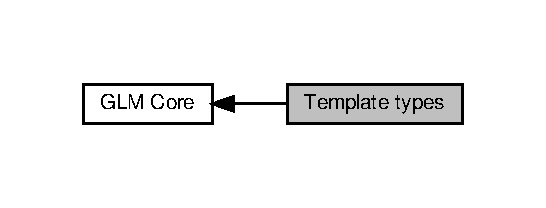
\includegraphics[width=262pt]{group__core__template}
\end{center}
\end{figure}
The generic template types used as the basis for the core types. 

These types are all templates used to define the actual \hyperlink{group__core__types}{Types}. These templetes are implementation details of G\+LM types and should not be used explicitly. 
\hypertarget{group__gtc__constants}{}\section{G\+L\+M\+\_\+\+G\+T\+C\+\_\+constants}
\label{group__gtc__constants}\index{G\+L\+M\+\_\+\+G\+T\+C\+\_\+constants@{G\+L\+M\+\_\+\+G\+T\+C\+\_\+constants}}


Provide a list of constants and precomputed useful values.  


Collaboration diagram for G\+L\+M\+\_\+\+G\+T\+C\+\_\+constants\+:\nopagebreak
\begin{figure}[H]
\begin{center}
\leavevmode
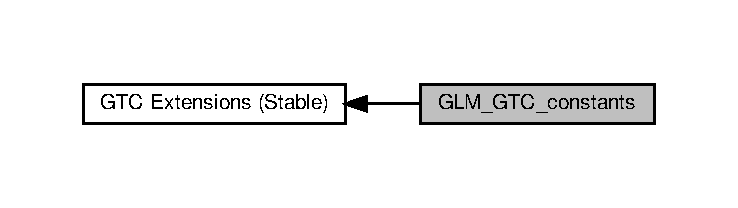
\includegraphics[width=350pt]{group__gtc__constants}
\end{center}
\end{figure}
\subsection*{Functions}
\begin{DoxyCompactItemize}
\item 
{\footnotesize template$<$typename gen\+Type $>$ }\\\hyperlink{setup_8hpp_ab2d052de21a70539923e9bcbf6e83a51}{G\+L\+M\+\_\+\+F\+U\+N\+C\+\_\+\+D\+E\+CL} gen\+Type \hyperlink{group__gtc__constants_gacb41049b8d22c8aa90e362b96c524feb}{glm\+::epsilon} ()
\item 
{\footnotesize template$<$typename gen\+Type $>$ }\\\hyperlink{setup_8hpp_ab2d052de21a70539923e9bcbf6e83a51}{G\+L\+M\+\_\+\+F\+U\+N\+C\+\_\+\+D\+E\+CL} gen\+Type \hyperlink{group__gtc__constants_ga5cc97dd01d37fc199264ff6030578435}{glm\+::zero} ()
\item 
{\footnotesize template$<$typename gen\+Type $>$ }\\\hyperlink{setup_8hpp_ab2d052de21a70539923e9bcbf6e83a51}{G\+L\+M\+\_\+\+F\+U\+N\+C\+\_\+\+D\+E\+CL} gen\+Type \hyperlink{group__gtc__constants_ga8186ec2c330457d41d9686c47cd3b2d1}{glm\+::one} ()
\item 
{\footnotesize template$<$typename gen\+Type $>$ }\\\hyperlink{setup_8hpp_ab2d052de21a70539923e9bcbf6e83a51}{G\+L\+M\+\_\+\+F\+U\+N\+C\+\_\+\+D\+E\+CL} gen\+Type \hyperlink{group__gtc__constants_gae671930537266a9a650ccb4b88757692}{glm\+::pi} ()
\item 
{\footnotesize template$<$typename gen\+Type $>$ }\\\hyperlink{setup_8hpp_ab2d052de21a70539923e9bcbf6e83a51}{G\+L\+M\+\_\+\+F\+U\+N\+C\+\_\+\+D\+E\+CL} gen\+Type \hyperlink{group__gtc__constants_ga1cfeb345f34f72697d14f4db8d5d4c6c}{glm\+::root\+\_\+pi} ()
\item 
{\footnotesize template$<$typename gen\+Type $>$ }\\\hyperlink{setup_8hpp_ab2d052de21a70539923e9bcbf6e83a51}{G\+L\+M\+\_\+\+F\+U\+N\+C\+\_\+\+D\+E\+CL} gen\+Type \hyperlink{group__gtc__constants_ga7f7a1050729f3b03b1873a06ba4a472f}{glm\+::half\+\_\+pi} ()
\item 
{\footnotesize template$<$typename gen\+Type $>$ }\\\hyperlink{setup_8hpp_ab2d052de21a70539923e9bcbf6e83a51}{G\+L\+M\+\_\+\+F\+U\+N\+C\+\_\+\+D\+E\+CL} gen\+Type \hyperlink{group__gtc__constants_ga0148d757b4bfda4d86251b8d1ea1dad3}{glm\+::quarter\+\_\+pi} ()
\item 
{\footnotesize template$<$typename gen\+Type $>$ }\\\hyperlink{setup_8hpp_ab2d052de21a70539923e9bcbf6e83a51}{G\+L\+M\+\_\+\+F\+U\+N\+C\+\_\+\+D\+E\+CL} gen\+Type \hyperlink{group__gtc__constants_ga9ba09a027db6d4f4e259b01cf5d6c178}{glm\+::one\+\_\+over\+\_\+pi} ()
\item 
{\footnotesize template$<$typename gen\+Type $>$ }\\\hyperlink{setup_8hpp_ab2d052de21a70539923e9bcbf6e83a51}{G\+L\+M\+\_\+\+F\+U\+N\+C\+\_\+\+D\+E\+CL} gen\+Type \hyperlink{group__gtc__constants_ga85729d38c47351686e8659f80447a7ea}{glm\+::two\+\_\+over\+\_\+pi} ()
\item 
{\footnotesize template$<$typename gen\+Type $>$ }\\\hyperlink{setup_8hpp_ab2d052de21a70539923e9bcbf6e83a51}{G\+L\+M\+\_\+\+F\+U\+N\+C\+\_\+\+D\+E\+CL} gen\+Type \hyperlink{group__gtc__constants_ga767e539c20585bf60aa63595b0f0b259}{glm\+::two\+\_\+over\+\_\+root\+\_\+pi} ()
\item 
{\footnotesize template$<$typename gen\+Type $>$ }\\\hyperlink{setup_8hpp_ab2d052de21a70539923e9bcbf6e83a51}{G\+L\+M\+\_\+\+F\+U\+N\+C\+\_\+\+D\+E\+CL} gen\+Type \hyperlink{group__gtc__constants_gac1a9b3248357fd9e9b740bed90e0b1b7}{glm\+::one\+\_\+over\+\_\+root\+\_\+two} ()
\item 
{\footnotesize template$<$typename gen\+Type $>$ }\\\hyperlink{setup_8hpp_ab2d052de21a70539923e9bcbf6e83a51}{G\+L\+M\+\_\+\+F\+U\+N\+C\+\_\+\+D\+E\+CL} gen\+Type \hyperlink{group__gtc__constants_gaec5af85e2148c118aad7e797430fdeb0}{glm\+::root\+\_\+half\+\_\+pi} ()
\item 
{\footnotesize template$<$typename gen\+Type $>$ }\\\hyperlink{setup_8hpp_ab2d052de21a70539923e9bcbf6e83a51}{G\+L\+M\+\_\+\+F\+U\+N\+C\+\_\+\+D\+E\+CL} gen\+Type \hyperlink{group__gtc__constants_gae991b4d39c57b57990054eec3677597c}{glm\+::root\+\_\+two\+\_\+pi} ()
\item 
{\footnotesize template$<$typename gen\+Type $>$ }\\\hyperlink{setup_8hpp_ab2d052de21a70539923e9bcbf6e83a51}{G\+L\+M\+\_\+\+F\+U\+N\+C\+\_\+\+D\+E\+CL} gen\+Type \hyperlink{group__gtc__constants_ga9cae3fad9314e34c1d3aab71fcdef05f}{glm\+::root\+\_\+ln\+\_\+four} ()
\item 
{\footnotesize template$<$typename gen\+Type $>$ }\\\hyperlink{setup_8hpp_ab2d052de21a70539923e9bcbf6e83a51}{G\+L\+M\+\_\+\+F\+U\+N\+C\+\_\+\+D\+E\+CL} gen\+Type \hyperlink{group__gtc__constants_gab83fb6de0f05d6c0d11bdf0479f8319e}{glm\+::e} ()
\item 
{\footnotesize template$<$typename gen\+Type $>$ }\\\hyperlink{setup_8hpp_ab2d052de21a70539923e9bcbf6e83a51}{G\+L\+M\+\_\+\+F\+U\+N\+C\+\_\+\+D\+E\+CL} gen\+Type \hyperlink{group__gtc__constants_ga6f14b46653b7ead1edcbd0fc6c9c5289}{glm\+::euler} ()
\item 
{\footnotesize template$<$typename gen\+Type $>$ }\\\hyperlink{setup_8hpp_ab2d052de21a70539923e9bcbf6e83a51}{G\+L\+M\+\_\+\+F\+U\+N\+C\+\_\+\+D\+E\+CL} gen\+Type \hyperlink{group__gtc__constants_gab91b7799f88f9f2be33e385dec11b9c2}{glm\+::root\+\_\+two} ()
\item 
{\footnotesize template$<$typename gen\+Type $>$ }\\\hyperlink{setup_8hpp_ab2d052de21a70539923e9bcbf6e83a51}{G\+L\+M\+\_\+\+F\+U\+N\+C\+\_\+\+D\+E\+CL} gen\+Type \hyperlink{group__gtc__constants_gab3183635ac615473e2f95852f491be83}{glm\+::root\+\_\+three} ()
\item 
{\footnotesize template$<$typename gen\+Type $>$ }\\\hyperlink{setup_8hpp_ab2d052de21a70539923e9bcbf6e83a51}{G\+L\+M\+\_\+\+F\+U\+N\+C\+\_\+\+D\+E\+CL} gen\+Type \hyperlink{group__gtc__constants_gace2b8dfed1ab9fabbb67dde08e7e5b58}{glm\+::root\+\_\+five} ()
\item 
{\footnotesize template$<$typename gen\+Type $>$ }\\\hyperlink{setup_8hpp_ab2d052de21a70539923e9bcbf6e83a51}{G\+L\+M\+\_\+\+F\+U\+N\+C\+\_\+\+D\+E\+CL} gen\+Type \hyperlink{group__gtc__constants_ga22fae798430edc3022766af4fd83e8a4}{glm\+::ln\+\_\+two} ()
\item 
{\footnotesize template$<$typename gen\+Type $>$ }\\\hyperlink{setup_8hpp_ab2d052de21a70539923e9bcbf6e83a51}{G\+L\+M\+\_\+\+F\+U\+N\+C\+\_\+\+D\+E\+CL} gen\+Type \hyperlink{group__gtc__constants_ga48addf0cb0980277d208a71a1c59c073}{glm\+::ln\+\_\+ten} ()
\item 
{\footnotesize template$<$typename gen\+Type $>$ }\\\hyperlink{setup_8hpp_ab2d052de21a70539923e9bcbf6e83a51}{G\+L\+M\+\_\+\+F\+U\+N\+C\+\_\+\+D\+E\+CL} gen\+Type \hyperlink{group__gtc__constants_ga650774609debe4a90bcac449b574de2c}{glm\+::ln\+\_\+ln\+\_\+two} ()
\item 
{\footnotesize template$<$typename gen\+Type $>$ }\\\hyperlink{setup_8hpp_ab2d052de21a70539923e9bcbf6e83a51}{G\+L\+M\+\_\+\+F\+U\+N\+C\+\_\+\+D\+E\+CL} gen\+Type \hyperlink{group__gtc__constants_gabf280496105e0ad070287417f840ebd8}{glm\+::third} ()
\item 
{\footnotesize template$<$typename gen\+Type $>$ }\\\hyperlink{setup_8hpp_ab2d052de21a70539923e9bcbf6e83a51}{G\+L\+M\+\_\+\+F\+U\+N\+C\+\_\+\+D\+E\+CL} gen\+Type \hyperlink{group__gtc__constants_gadde7f2efce3b14c8b26944fbafed4a10}{glm\+::two\+\_\+thirds} ()
\item 
{\footnotesize template$<$typename gen\+Type $>$ }\\\hyperlink{setup_8hpp_ab2d052de21a70539923e9bcbf6e83a51}{G\+L\+M\+\_\+\+F\+U\+N\+C\+\_\+\+D\+E\+CL} gen\+Type \hyperlink{group__gtc__constants_gafd53093ef2d756333865d774bea3cdf9}{glm\+::golden\+\_\+ratio} ()
\end{DoxyCompactItemize}


\subsection{Detailed Description}
Provide a list of constants and precomputed useful values. 

$<$\hyperlink{gtc_2constants_8hpp}{glm/gtc/constants.\+hpp}$>$ need to be included to use these features. 

\subsection{Function Documentation}
\mbox{\Hypertarget{group__gtc__constants_gab83fb6de0f05d6c0d11bdf0479f8319e}\label{group__gtc__constants_gab83fb6de0f05d6c0d11bdf0479f8319e}} 
\index{G\+L\+M\+\_\+\+G\+T\+C\+\_\+constants@{G\+L\+M\+\_\+\+G\+T\+C\+\_\+constants}!e@{e}}
\index{e@{e}!G\+L\+M\+\_\+\+G\+T\+C\+\_\+constants@{G\+L\+M\+\_\+\+G\+T\+C\+\_\+constants}}
\subsubsection{\texorpdfstring{e()}{e()}}
{\footnotesize\ttfamily template$<$typename gen\+Type $>$ \\
\hyperlink{setup_8hpp_ab2d052de21a70539923e9bcbf6e83a51}{G\+L\+M\+\_\+\+F\+U\+N\+C\+\_\+\+D\+E\+CL} gen\+Type glm\+::e (\begin{DoxyParamCaption}{ }\end{DoxyParamCaption})}

Return e constant. \begin{DoxySeeAlso}{See also}
\hyperlink{group__gtc__constants}{G\+L\+M\+\_\+\+G\+T\+C\+\_\+constants} 
\end{DoxySeeAlso}


Definition at line 118 of file constants.\+inl.

\mbox{\Hypertarget{group__gtc__constants_gacb41049b8d22c8aa90e362b96c524feb}\label{group__gtc__constants_gacb41049b8d22c8aa90e362b96c524feb}} 
\index{G\+L\+M\+\_\+\+G\+T\+C\+\_\+constants@{G\+L\+M\+\_\+\+G\+T\+C\+\_\+constants}!epsilon@{epsilon}}
\index{epsilon@{epsilon}!G\+L\+M\+\_\+\+G\+T\+C\+\_\+constants@{G\+L\+M\+\_\+\+G\+T\+C\+\_\+constants}}
\subsubsection{\texorpdfstring{epsilon()}{epsilon()}}
{\footnotesize\ttfamily template$<$typename gen\+Type $>$ \\
\hyperlink{setup_8hpp_ab2d052de21a70539923e9bcbf6e83a51}{G\+L\+M\+\_\+\+F\+U\+N\+C\+\_\+\+D\+E\+CL} gen\+Type glm\+::epsilon (\begin{DoxyParamCaption}{ }\end{DoxyParamCaption})}

Return the epsilon constant for floating point types. \begin{DoxyRefDesc}{Todo}
\item[\hyperlink{todo__todo000007}{Todo}]Implement epsilon for half-\/precision floating point type. \end{DoxyRefDesc}
\begin{DoxySeeAlso}{See also}
\hyperlink{group__gtc__constants}{G\+L\+M\+\_\+\+G\+T\+C\+\_\+constants} 
\end{DoxySeeAlso}


Definition at line 34 of file constants.\+inl.

\mbox{\Hypertarget{group__gtc__constants_ga6f14b46653b7ead1edcbd0fc6c9c5289}\label{group__gtc__constants_ga6f14b46653b7ead1edcbd0fc6c9c5289}} 
\index{G\+L\+M\+\_\+\+G\+T\+C\+\_\+constants@{G\+L\+M\+\_\+\+G\+T\+C\+\_\+constants}!euler@{euler}}
\index{euler@{euler}!G\+L\+M\+\_\+\+G\+T\+C\+\_\+constants@{G\+L\+M\+\_\+\+G\+T\+C\+\_\+constants}}
\subsubsection{\texorpdfstring{euler()}{euler()}}
{\footnotesize\ttfamily template$<$typename gen\+Type $>$ \\
\hyperlink{setup_8hpp_ab2d052de21a70539923e9bcbf6e83a51}{G\+L\+M\+\_\+\+F\+U\+N\+C\+\_\+\+D\+E\+CL} gen\+Type glm\+::euler (\begin{DoxyParamCaption}{ }\end{DoxyParamCaption})}

Return Euler\textquotesingle{}s constant. \begin{DoxySeeAlso}{See also}
\hyperlink{group__gtc__constants}{G\+L\+M\+\_\+\+G\+T\+C\+\_\+constants} 
\end{DoxySeeAlso}


Definition at line 124 of file constants.\+inl.

\mbox{\Hypertarget{group__gtc__constants_gafd53093ef2d756333865d774bea3cdf9}\label{group__gtc__constants_gafd53093ef2d756333865d774bea3cdf9}} 
\index{G\+L\+M\+\_\+\+G\+T\+C\+\_\+constants@{G\+L\+M\+\_\+\+G\+T\+C\+\_\+constants}!golden\+\_\+ratio@{golden\+\_\+ratio}}
\index{golden\+\_\+ratio@{golden\+\_\+ratio}!G\+L\+M\+\_\+\+G\+T\+C\+\_\+constants@{G\+L\+M\+\_\+\+G\+T\+C\+\_\+constants}}
\subsubsection{\texorpdfstring{golden\+\_\+ratio()}{golden\_ratio()}}
{\footnotesize\ttfamily template$<$typename gen\+Type $>$ \\
\hyperlink{setup_8hpp_ab2d052de21a70539923e9bcbf6e83a51}{G\+L\+M\+\_\+\+F\+U\+N\+C\+\_\+\+D\+E\+CL} gen\+Type glm\+::golden\+\_\+ratio (\begin{DoxyParamCaption}{ }\end{DoxyParamCaption})}

Return the golden ratio constant. \begin{DoxySeeAlso}{See also}
\hyperlink{group__gtc__constants}{G\+L\+M\+\_\+\+G\+T\+C\+\_\+constants} 
\end{DoxySeeAlso}


Definition at line 178 of file constants.\+inl.

\mbox{\Hypertarget{group__gtc__constants_ga7f7a1050729f3b03b1873a06ba4a472f}\label{group__gtc__constants_ga7f7a1050729f3b03b1873a06ba4a472f}} 
\index{G\+L\+M\+\_\+\+G\+T\+C\+\_\+constants@{G\+L\+M\+\_\+\+G\+T\+C\+\_\+constants}!half\+\_\+pi@{half\+\_\+pi}}
\index{half\+\_\+pi@{half\+\_\+pi}!G\+L\+M\+\_\+\+G\+T\+C\+\_\+constants@{G\+L\+M\+\_\+\+G\+T\+C\+\_\+constants}}
\subsubsection{\texorpdfstring{half\+\_\+pi()}{half\_pi()}}
{\footnotesize\ttfamily template$<$typename gen\+Type $>$ \\
\hyperlink{setup_8hpp_ab2d052de21a70539923e9bcbf6e83a51}{G\+L\+M\+\_\+\+F\+U\+N\+C\+\_\+\+D\+E\+CL} gen\+Type glm\+::half\+\_\+pi (\begin{DoxyParamCaption}{ }\end{DoxyParamCaption})}

Return pi / 2. \begin{DoxySeeAlso}{See also}
\hyperlink{group__gtc__constants}{G\+L\+M\+\_\+\+G\+T\+C\+\_\+constants} 
\end{DoxySeeAlso}


Definition at line 64 of file constants.\+inl.

\mbox{\Hypertarget{group__gtc__constants_ga650774609debe4a90bcac449b574de2c}\label{group__gtc__constants_ga650774609debe4a90bcac449b574de2c}} 
\index{G\+L\+M\+\_\+\+G\+T\+C\+\_\+constants@{G\+L\+M\+\_\+\+G\+T\+C\+\_\+constants}!ln\+\_\+ln\+\_\+two@{ln\+\_\+ln\+\_\+two}}
\index{ln\+\_\+ln\+\_\+two@{ln\+\_\+ln\+\_\+two}!G\+L\+M\+\_\+\+G\+T\+C\+\_\+constants@{G\+L\+M\+\_\+\+G\+T\+C\+\_\+constants}}
\subsubsection{\texorpdfstring{ln\+\_\+ln\+\_\+two()}{ln\_ln\_two()}}
{\footnotesize\ttfamily template$<$typename gen\+Type $>$ \\
\hyperlink{setup_8hpp_ab2d052de21a70539923e9bcbf6e83a51}{G\+L\+M\+\_\+\+F\+U\+N\+C\+\_\+\+D\+E\+CL} gen\+Type glm\+::ln\+\_\+ln\+\_\+two (\begin{DoxyParamCaption}{ }\end{DoxyParamCaption})}

Return ln(ln(2)). \begin{DoxySeeAlso}{See also}
\hyperlink{group__gtc__constants}{G\+L\+M\+\_\+\+G\+T\+C\+\_\+constants} 
\end{DoxySeeAlso}


Definition at line 160 of file constants.\+inl.

\mbox{\Hypertarget{group__gtc__constants_ga48addf0cb0980277d208a71a1c59c073}\label{group__gtc__constants_ga48addf0cb0980277d208a71a1c59c073}} 
\index{G\+L\+M\+\_\+\+G\+T\+C\+\_\+constants@{G\+L\+M\+\_\+\+G\+T\+C\+\_\+constants}!ln\+\_\+ten@{ln\+\_\+ten}}
\index{ln\+\_\+ten@{ln\+\_\+ten}!G\+L\+M\+\_\+\+G\+T\+C\+\_\+constants@{G\+L\+M\+\_\+\+G\+T\+C\+\_\+constants}}
\subsubsection{\texorpdfstring{ln\+\_\+ten()}{ln\_ten()}}
{\footnotesize\ttfamily template$<$typename gen\+Type $>$ \\
\hyperlink{setup_8hpp_ab2d052de21a70539923e9bcbf6e83a51}{G\+L\+M\+\_\+\+F\+U\+N\+C\+\_\+\+D\+E\+CL} gen\+Type glm\+::ln\+\_\+ten (\begin{DoxyParamCaption}{ }\end{DoxyParamCaption})}

Return ln(10). \begin{DoxySeeAlso}{See also}
\hyperlink{group__gtc__constants}{G\+L\+M\+\_\+\+G\+T\+C\+\_\+constants} 
\end{DoxySeeAlso}


Definition at line 154 of file constants.\+inl.

\mbox{\Hypertarget{group__gtc__constants_ga22fae798430edc3022766af4fd83e8a4}\label{group__gtc__constants_ga22fae798430edc3022766af4fd83e8a4}} 
\index{G\+L\+M\+\_\+\+G\+T\+C\+\_\+constants@{G\+L\+M\+\_\+\+G\+T\+C\+\_\+constants}!ln\+\_\+two@{ln\+\_\+two}}
\index{ln\+\_\+two@{ln\+\_\+two}!G\+L\+M\+\_\+\+G\+T\+C\+\_\+constants@{G\+L\+M\+\_\+\+G\+T\+C\+\_\+constants}}
\subsubsection{\texorpdfstring{ln\+\_\+two()}{ln\_two()}}
{\footnotesize\ttfamily template$<$typename gen\+Type $>$ \\
\hyperlink{setup_8hpp_ab2d052de21a70539923e9bcbf6e83a51}{G\+L\+M\+\_\+\+F\+U\+N\+C\+\_\+\+D\+E\+CL} gen\+Type glm\+::ln\+\_\+two (\begin{DoxyParamCaption}{ }\end{DoxyParamCaption})}

Return ln(2). \begin{DoxySeeAlso}{See also}
\hyperlink{group__gtc__constants}{G\+L\+M\+\_\+\+G\+T\+C\+\_\+constants} 
\end{DoxySeeAlso}


Definition at line 148 of file constants.\+inl.

\mbox{\Hypertarget{group__gtc__constants_ga8186ec2c330457d41d9686c47cd3b2d1}\label{group__gtc__constants_ga8186ec2c330457d41d9686c47cd3b2d1}} 
\index{G\+L\+M\+\_\+\+G\+T\+C\+\_\+constants@{G\+L\+M\+\_\+\+G\+T\+C\+\_\+constants}!one@{one}}
\index{one@{one}!G\+L\+M\+\_\+\+G\+T\+C\+\_\+constants@{G\+L\+M\+\_\+\+G\+T\+C\+\_\+constants}}
\subsubsection{\texorpdfstring{one()}{one()}}
{\footnotesize\ttfamily template$<$typename gen\+Type $>$ \\
\hyperlink{setup_8hpp_ab2d052de21a70539923e9bcbf6e83a51}{G\+L\+M\+\_\+\+F\+U\+N\+C\+\_\+\+D\+E\+CL} gen\+Type glm\+::one (\begin{DoxyParamCaption}{ }\end{DoxyParamCaption})}

Return 1. \begin{DoxySeeAlso}{See also}
\hyperlink{group__gtc__constants}{G\+L\+M\+\_\+\+G\+T\+C\+\_\+constants} 
\end{DoxySeeAlso}


Definition at line 46 of file constants.\+inl.

\mbox{\Hypertarget{group__gtc__constants_ga9ba09a027db6d4f4e259b01cf5d6c178}\label{group__gtc__constants_ga9ba09a027db6d4f4e259b01cf5d6c178}} 
\index{G\+L\+M\+\_\+\+G\+T\+C\+\_\+constants@{G\+L\+M\+\_\+\+G\+T\+C\+\_\+constants}!one\+\_\+over\+\_\+pi@{one\+\_\+over\+\_\+pi}}
\index{one\+\_\+over\+\_\+pi@{one\+\_\+over\+\_\+pi}!G\+L\+M\+\_\+\+G\+T\+C\+\_\+constants@{G\+L\+M\+\_\+\+G\+T\+C\+\_\+constants}}
\subsubsection{\texorpdfstring{one\+\_\+over\+\_\+pi()}{one\_over\_pi()}}
{\footnotesize\ttfamily template$<$typename gen\+Type $>$ \\
\hyperlink{setup_8hpp_ab2d052de21a70539923e9bcbf6e83a51}{G\+L\+M\+\_\+\+F\+U\+N\+C\+\_\+\+D\+E\+CL} gen\+Type glm\+::one\+\_\+over\+\_\+pi (\begin{DoxyParamCaption}{ }\end{DoxyParamCaption})}

Return 1 / pi. \begin{DoxySeeAlso}{See also}
\hyperlink{group__gtc__constants}{G\+L\+M\+\_\+\+G\+T\+C\+\_\+constants} 
\end{DoxySeeAlso}


Definition at line 76 of file constants.\+inl.

\mbox{\Hypertarget{group__gtc__constants_gac1a9b3248357fd9e9b740bed90e0b1b7}\label{group__gtc__constants_gac1a9b3248357fd9e9b740bed90e0b1b7}} 
\index{G\+L\+M\+\_\+\+G\+T\+C\+\_\+constants@{G\+L\+M\+\_\+\+G\+T\+C\+\_\+constants}!one\+\_\+over\+\_\+root\+\_\+two@{one\+\_\+over\+\_\+root\+\_\+two}}
\index{one\+\_\+over\+\_\+root\+\_\+two@{one\+\_\+over\+\_\+root\+\_\+two}!G\+L\+M\+\_\+\+G\+T\+C\+\_\+constants@{G\+L\+M\+\_\+\+G\+T\+C\+\_\+constants}}
\subsubsection{\texorpdfstring{one\+\_\+over\+\_\+root\+\_\+two()}{one\_over\_root\_two()}}
{\footnotesize\ttfamily template$<$typename gen\+Type $>$ \\
\hyperlink{setup_8hpp_ab2d052de21a70539923e9bcbf6e83a51}{G\+L\+M\+\_\+\+F\+U\+N\+C\+\_\+\+D\+E\+CL} gen\+Type glm\+::one\+\_\+over\+\_\+root\+\_\+two (\begin{DoxyParamCaption}{ }\end{DoxyParamCaption})}

Return 1 / sqrt(2). \begin{DoxySeeAlso}{See also}
\hyperlink{group__gtc__constants}{G\+L\+M\+\_\+\+G\+T\+C\+\_\+constants} 
\end{DoxySeeAlso}


Definition at line 94 of file constants.\+inl.

\mbox{\Hypertarget{group__gtc__constants_gae671930537266a9a650ccb4b88757692}\label{group__gtc__constants_gae671930537266a9a650ccb4b88757692}} 
\index{G\+L\+M\+\_\+\+G\+T\+C\+\_\+constants@{G\+L\+M\+\_\+\+G\+T\+C\+\_\+constants}!pi@{pi}}
\index{pi@{pi}!G\+L\+M\+\_\+\+G\+T\+C\+\_\+constants@{G\+L\+M\+\_\+\+G\+T\+C\+\_\+constants}}
\subsubsection{\texorpdfstring{pi()}{pi()}}
{\footnotesize\ttfamily template$<$typename gen\+Type $>$ \\
\hyperlink{setup_8hpp_ab2d052de21a70539923e9bcbf6e83a51}{G\+L\+M\+\_\+\+F\+U\+N\+C\+\_\+\+D\+E\+CL} gen\+Type glm\+::pi (\begin{DoxyParamCaption}{ }\end{DoxyParamCaption})}

Return the pi constant. \begin{DoxySeeAlso}{See also}
\hyperlink{group__gtc__constants}{G\+L\+M\+\_\+\+G\+T\+C\+\_\+constants} 
\end{DoxySeeAlso}


Definition at line 52 of file constants.\+inl.

\mbox{\Hypertarget{group__gtc__constants_ga0148d757b4bfda4d86251b8d1ea1dad3}\label{group__gtc__constants_ga0148d757b4bfda4d86251b8d1ea1dad3}} 
\index{G\+L\+M\+\_\+\+G\+T\+C\+\_\+constants@{G\+L\+M\+\_\+\+G\+T\+C\+\_\+constants}!quarter\+\_\+pi@{quarter\+\_\+pi}}
\index{quarter\+\_\+pi@{quarter\+\_\+pi}!G\+L\+M\+\_\+\+G\+T\+C\+\_\+constants@{G\+L\+M\+\_\+\+G\+T\+C\+\_\+constants}}
\subsubsection{\texorpdfstring{quarter\+\_\+pi()}{quarter\_pi()}}
{\footnotesize\ttfamily template$<$typename gen\+Type $>$ \\
\hyperlink{setup_8hpp_ab2d052de21a70539923e9bcbf6e83a51}{G\+L\+M\+\_\+\+F\+U\+N\+C\+\_\+\+D\+E\+CL} gen\+Type glm\+::quarter\+\_\+pi (\begin{DoxyParamCaption}{ }\end{DoxyParamCaption})}

Return pi / 4. \begin{DoxySeeAlso}{See also}
\hyperlink{group__gtc__constants}{G\+L\+M\+\_\+\+G\+T\+C\+\_\+constants} 
\end{DoxySeeAlso}


Definition at line 70 of file constants.\+inl.

\mbox{\Hypertarget{group__gtc__constants_gace2b8dfed1ab9fabbb67dde08e7e5b58}\label{group__gtc__constants_gace2b8dfed1ab9fabbb67dde08e7e5b58}} 
\index{G\+L\+M\+\_\+\+G\+T\+C\+\_\+constants@{G\+L\+M\+\_\+\+G\+T\+C\+\_\+constants}!root\+\_\+five@{root\+\_\+five}}
\index{root\+\_\+five@{root\+\_\+five}!G\+L\+M\+\_\+\+G\+T\+C\+\_\+constants@{G\+L\+M\+\_\+\+G\+T\+C\+\_\+constants}}
\subsubsection{\texorpdfstring{root\+\_\+five()}{root\_five()}}
{\footnotesize\ttfamily template$<$typename gen\+Type $>$ \\
\hyperlink{setup_8hpp_ab2d052de21a70539923e9bcbf6e83a51}{G\+L\+M\+\_\+\+F\+U\+N\+C\+\_\+\+D\+E\+CL} gen\+Type glm\+::root\+\_\+five (\begin{DoxyParamCaption}{ }\end{DoxyParamCaption})}

Return sqrt(5). \begin{DoxySeeAlso}{See also}
\hyperlink{group__gtc__constants}{G\+L\+M\+\_\+\+G\+T\+C\+\_\+constants} 
\end{DoxySeeAlso}


Definition at line 142 of file constants.\+inl.

\mbox{\Hypertarget{group__gtc__constants_gaec5af85e2148c118aad7e797430fdeb0}\label{group__gtc__constants_gaec5af85e2148c118aad7e797430fdeb0}} 
\index{G\+L\+M\+\_\+\+G\+T\+C\+\_\+constants@{G\+L\+M\+\_\+\+G\+T\+C\+\_\+constants}!root\+\_\+half\+\_\+pi@{root\+\_\+half\+\_\+pi}}
\index{root\+\_\+half\+\_\+pi@{root\+\_\+half\+\_\+pi}!G\+L\+M\+\_\+\+G\+T\+C\+\_\+constants@{G\+L\+M\+\_\+\+G\+T\+C\+\_\+constants}}
\subsubsection{\texorpdfstring{root\+\_\+half\+\_\+pi()}{root\_half\_pi()}}
{\footnotesize\ttfamily template$<$typename gen\+Type $>$ \\
\hyperlink{setup_8hpp_ab2d052de21a70539923e9bcbf6e83a51}{G\+L\+M\+\_\+\+F\+U\+N\+C\+\_\+\+D\+E\+CL} gen\+Type glm\+::root\+\_\+half\+\_\+pi (\begin{DoxyParamCaption}{ }\end{DoxyParamCaption})}

Return sqrt(pi / 2). \begin{DoxySeeAlso}{See also}
\hyperlink{group__gtc__constants}{G\+L\+M\+\_\+\+G\+T\+C\+\_\+constants} 
\end{DoxySeeAlso}


Definition at line 100 of file constants.\+inl.

\mbox{\Hypertarget{group__gtc__constants_ga9cae3fad9314e34c1d3aab71fcdef05f}\label{group__gtc__constants_ga9cae3fad9314e34c1d3aab71fcdef05f}} 
\index{G\+L\+M\+\_\+\+G\+T\+C\+\_\+constants@{G\+L\+M\+\_\+\+G\+T\+C\+\_\+constants}!root\+\_\+ln\+\_\+four@{root\+\_\+ln\+\_\+four}}
\index{root\+\_\+ln\+\_\+four@{root\+\_\+ln\+\_\+four}!G\+L\+M\+\_\+\+G\+T\+C\+\_\+constants@{G\+L\+M\+\_\+\+G\+T\+C\+\_\+constants}}
\subsubsection{\texorpdfstring{root\+\_\+ln\+\_\+four()}{root\_ln\_four()}}
{\footnotesize\ttfamily template$<$typename gen\+Type $>$ \\
\hyperlink{setup_8hpp_ab2d052de21a70539923e9bcbf6e83a51}{G\+L\+M\+\_\+\+F\+U\+N\+C\+\_\+\+D\+E\+CL} gen\+Type glm\+::root\+\_\+ln\+\_\+four (\begin{DoxyParamCaption}{ }\end{DoxyParamCaption})}

Return sqrt(ln(4)). \begin{DoxySeeAlso}{See also}
\hyperlink{group__gtc__constants}{G\+L\+M\+\_\+\+G\+T\+C\+\_\+constants} 
\end{DoxySeeAlso}


Definition at line 112 of file constants.\+inl.

\mbox{\Hypertarget{group__gtc__constants_ga1cfeb345f34f72697d14f4db8d5d4c6c}\label{group__gtc__constants_ga1cfeb345f34f72697d14f4db8d5d4c6c}} 
\index{G\+L\+M\+\_\+\+G\+T\+C\+\_\+constants@{G\+L\+M\+\_\+\+G\+T\+C\+\_\+constants}!root\+\_\+pi@{root\+\_\+pi}}
\index{root\+\_\+pi@{root\+\_\+pi}!G\+L\+M\+\_\+\+G\+T\+C\+\_\+constants@{G\+L\+M\+\_\+\+G\+T\+C\+\_\+constants}}
\subsubsection{\texorpdfstring{root\+\_\+pi()}{root\_pi()}}
{\footnotesize\ttfamily template$<$typename gen\+Type $>$ \\
\hyperlink{setup_8hpp_ab2d052de21a70539923e9bcbf6e83a51}{G\+L\+M\+\_\+\+F\+U\+N\+C\+\_\+\+D\+E\+CL} gen\+Type glm\+::root\+\_\+pi (\begin{DoxyParamCaption}{ }\end{DoxyParamCaption})}

Return square root of pi. \begin{DoxySeeAlso}{See also}
\hyperlink{group__gtc__constants}{G\+L\+M\+\_\+\+G\+T\+C\+\_\+constants} 
\end{DoxySeeAlso}


Definition at line 58 of file constants.\+inl.

\mbox{\Hypertarget{group__gtc__constants_gab3183635ac615473e2f95852f491be83}\label{group__gtc__constants_gab3183635ac615473e2f95852f491be83}} 
\index{G\+L\+M\+\_\+\+G\+T\+C\+\_\+constants@{G\+L\+M\+\_\+\+G\+T\+C\+\_\+constants}!root\+\_\+three@{root\+\_\+three}}
\index{root\+\_\+three@{root\+\_\+three}!G\+L\+M\+\_\+\+G\+T\+C\+\_\+constants@{G\+L\+M\+\_\+\+G\+T\+C\+\_\+constants}}
\subsubsection{\texorpdfstring{root\+\_\+three()}{root\_three()}}
{\footnotesize\ttfamily template$<$typename gen\+Type $>$ \\
\hyperlink{setup_8hpp_ab2d052de21a70539923e9bcbf6e83a51}{G\+L\+M\+\_\+\+F\+U\+N\+C\+\_\+\+D\+E\+CL} gen\+Type glm\+::root\+\_\+three (\begin{DoxyParamCaption}{ }\end{DoxyParamCaption})}

Return sqrt(3). \begin{DoxySeeAlso}{See also}
\hyperlink{group__gtc__constants}{G\+L\+M\+\_\+\+G\+T\+C\+\_\+constants} 
\end{DoxySeeAlso}


Definition at line 136 of file constants.\+inl.

\mbox{\Hypertarget{group__gtc__constants_gab91b7799f88f9f2be33e385dec11b9c2}\label{group__gtc__constants_gab91b7799f88f9f2be33e385dec11b9c2}} 
\index{G\+L\+M\+\_\+\+G\+T\+C\+\_\+constants@{G\+L\+M\+\_\+\+G\+T\+C\+\_\+constants}!root\+\_\+two@{root\+\_\+two}}
\index{root\+\_\+two@{root\+\_\+two}!G\+L\+M\+\_\+\+G\+T\+C\+\_\+constants@{G\+L\+M\+\_\+\+G\+T\+C\+\_\+constants}}
\subsubsection{\texorpdfstring{root\+\_\+two()}{root\_two()}}
{\footnotesize\ttfamily template$<$typename gen\+Type $>$ \\
\hyperlink{setup_8hpp_ab2d052de21a70539923e9bcbf6e83a51}{G\+L\+M\+\_\+\+F\+U\+N\+C\+\_\+\+D\+E\+CL} gen\+Type glm\+::root\+\_\+two (\begin{DoxyParamCaption}{ }\end{DoxyParamCaption})}

Return sqrt(2). \begin{DoxySeeAlso}{See also}
\hyperlink{group__gtc__constants}{G\+L\+M\+\_\+\+G\+T\+C\+\_\+constants} 
\end{DoxySeeAlso}


Definition at line 130 of file constants.\+inl.

\mbox{\Hypertarget{group__gtc__constants_gae991b4d39c57b57990054eec3677597c}\label{group__gtc__constants_gae991b4d39c57b57990054eec3677597c}} 
\index{G\+L\+M\+\_\+\+G\+T\+C\+\_\+constants@{G\+L\+M\+\_\+\+G\+T\+C\+\_\+constants}!root\+\_\+two\+\_\+pi@{root\+\_\+two\+\_\+pi}}
\index{root\+\_\+two\+\_\+pi@{root\+\_\+two\+\_\+pi}!G\+L\+M\+\_\+\+G\+T\+C\+\_\+constants@{G\+L\+M\+\_\+\+G\+T\+C\+\_\+constants}}
\subsubsection{\texorpdfstring{root\+\_\+two\+\_\+pi()}{root\_two\_pi()}}
{\footnotesize\ttfamily template$<$typename gen\+Type $>$ \\
\hyperlink{setup_8hpp_ab2d052de21a70539923e9bcbf6e83a51}{G\+L\+M\+\_\+\+F\+U\+N\+C\+\_\+\+D\+E\+CL} gen\+Type glm\+::root\+\_\+two\+\_\+pi (\begin{DoxyParamCaption}{ }\end{DoxyParamCaption})}

Return sqrt(2 $\ast$ pi). \begin{DoxySeeAlso}{See also}
\hyperlink{group__gtc__constants}{G\+L\+M\+\_\+\+G\+T\+C\+\_\+constants} 
\end{DoxySeeAlso}


Definition at line 106 of file constants.\+inl.

\mbox{\Hypertarget{group__gtc__constants_gabf280496105e0ad070287417f840ebd8}\label{group__gtc__constants_gabf280496105e0ad070287417f840ebd8}} 
\index{G\+L\+M\+\_\+\+G\+T\+C\+\_\+constants@{G\+L\+M\+\_\+\+G\+T\+C\+\_\+constants}!third@{third}}
\index{third@{third}!G\+L\+M\+\_\+\+G\+T\+C\+\_\+constants@{G\+L\+M\+\_\+\+G\+T\+C\+\_\+constants}}
\subsubsection{\texorpdfstring{third()}{third()}}
{\footnotesize\ttfamily template$<$typename gen\+Type $>$ \\
\hyperlink{setup_8hpp_ab2d052de21a70539923e9bcbf6e83a51}{G\+L\+M\+\_\+\+F\+U\+N\+C\+\_\+\+D\+E\+CL} gen\+Type glm\+::third (\begin{DoxyParamCaption}{ }\end{DoxyParamCaption})}

Return 1 / 3. \begin{DoxySeeAlso}{See also}
\hyperlink{group__gtc__constants}{G\+L\+M\+\_\+\+G\+T\+C\+\_\+constants} 
\end{DoxySeeAlso}


Definition at line 166 of file constants.\+inl.

\mbox{\Hypertarget{group__gtc__constants_ga85729d38c47351686e8659f80447a7ea}\label{group__gtc__constants_ga85729d38c47351686e8659f80447a7ea}} 
\index{G\+L\+M\+\_\+\+G\+T\+C\+\_\+constants@{G\+L\+M\+\_\+\+G\+T\+C\+\_\+constants}!two\+\_\+over\+\_\+pi@{two\+\_\+over\+\_\+pi}}
\index{two\+\_\+over\+\_\+pi@{two\+\_\+over\+\_\+pi}!G\+L\+M\+\_\+\+G\+T\+C\+\_\+constants@{G\+L\+M\+\_\+\+G\+T\+C\+\_\+constants}}
\subsubsection{\texorpdfstring{two\+\_\+over\+\_\+pi()}{two\_over\_pi()}}
{\footnotesize\ttfamily template$<$typename gen\+Type $>$ \\
\hyperlink{setup_8hpp_ab2d052de21a70539923e9bcbf6e83a51}{G\+L\+M\+\_\+\+F\+U\+N\+C\+\_\+\+D\+E\+CL} gen\+Type glm\+::two\+\_\+over\+\_\+pi (\begin{DoxyParamCaption}{ }\end{DoxyParamCaption})}

Return 2 / pi. \begin{DoxySeeAlso}{See also}
\hyperlink{group__gtc__constants}{G\+L\+M\+\_\+\+G\+T\+C\+\_\+constants} 
\end{DoxySeeAlso}


Definition at line 82 of file constants.\+inl.

\mbox{\Hypertarget{group__gtc__constants_ga767e539c20585bf60aa63595b0f0b259}\label{group__gtc__constants_ga767e539c20585bf60aa63595b0f0b259}} 
\index{G\+L\+M\+\_\+\+G\+T\+C\+\_\+constants@{G\+L\+M\+\_\+\+G\+T\+C\+\_\+constants}!two\+\_\+over\+\_\+root\+\_\+pi@{two\+\_\+over\+\_\+root\+\_\+pi}}
\index{two\+\_\+over\+\_\+root\+\_\+pi@{two\+\_\+over\+\_\+root\+\_\+pi}!G\+L\+M\+\_\+\+G\+T\+C\+\_\+constants@{G\+L\+M\+\_\+\+G\+T\+C\+\_\+constants}}
\subsubsection{\texorpdfstring{two\+\_\+over\+\_\+root\+\_\+pi()}{two\_over\_root\_pi()}}
{\footnotesize\ttfamily template$<$typename gen\+Type $>$ \\
\hyperlink{setup_8hpp_ab2d052de21a70539923e9bcbf6e83a51}{G\+L\+M\+\_\+\+F\+U\+N\+C\+\_\+\+D\+E\+CL} gen\+Type glm\+::two\+\_\+over\+\_\+root\+\_\+pi (\begin{DoxyParamCaption}{ }\end{DoxyParamCaption})}

Return 2 / sqrt(pi). \begin{DoxySeeAlso}{See also}
\hyperlink{group__gtc__constants}{G\+L\+M\+\_\+\+G\+T\+C\+\_\+constants} 
\end{DoxySeeAlso}


Definition at line 88 of file constants.\+inl.

\mbox{\Hypertarget{group__gtc__constants_gadde7f2efce3b14c8b26944fbafed4a10}\label{group__gtc__constants_gadde7f2efce3b14c8b26944fbafed4a10}} 
\index{G\+L\+M\+\_\+\+G\+T\+C\+\_\+constants@{G\+L\+M\+\_\+\+G\+T\+C\+\_\+constants}!two\+\_\+thirds@{two\+\_\+thirds}}
\index{two\+\_\+thirds@{two\+\_\+thirds}!G\+L\+M\+\_\+\+G\+T\+C\+\_\+constants@{G\+L\+M\+\_\+\+G\+T\+C\+\_\+constants}}
\subsubsection{\texorpdfstring{two\+\_\+thirds()}{two\_thirds()}}
{\footnotesize\ttfamily template$<$typename gen\+Type $>$ \\
\hyperlink{setup_8hpp_ab2d052de21a70539923e9bcbf6e83a51}{G\+L\+M\+\_\+\+F\+U\+N\+C\+\_\+\+D\+E\+CL} gen\+Type glm\+::two\+\_\+thirds (\begin{DoxyParamCaption}{ }\end{DoxyParamCaption})}

Return 2 / 3. \begin{DoxySeeAlso}{See also}
\hyperlink{group__gtc__constants}{G\+L\+M\+\_\+\+G\+T\+C\+\_\+constants} 
\end{DoxySeeAlso}


Definition at line 172 of file constants.\+inl.

\mbox{\Hypertarget{group__gtc__constants_ga5cc97dd01d37fc199264ff6030578435}\label{group__gtc__constants_ga5cc97dd01d37fc199264ff6030578435}} 
\index{G\+L\+M\+\_\+\+G\+T\+C\+\_\+constants@{G\+L\+M\+\_\+\+G\+T\+C\+\_\+constants}!zero@{zero}}
\index{zero@{zero}!G\+L\+M\+\_\+\+G\+T\+C\+\_\+constants@{G\+L\+M\+\_\+\+G\+T\+C\+\_\+constants}}
\subsubsection{\texorpdfstring{zero()}{zero()}}
{\footnotesize\ttfamily template$<$typename gen\+Type $>$ \\
\hyperlink{setup_8hpp_ab2d052de21a70539923e9bcbf6e83a51}{G\+L\+M\+\_\+\+F\+U\+N\+C\+\_\+\+D\+E\+CL} gen\+Type glm\+::zero (\begin{DoxyParamCaption}{ }\end{DoxyParamCaption})}

Return 0. \begin{DoxySeeAlso}{See also}
\hyperlink{group__gtc__constants}{G\+L\+M\+\_\+\+G\+T\+C\+\_\+constants} 
\end{DoxySeeAlso}


Definition at line 40 of file constants.\+inl.


\hypertarget{group__gtc__epsilon}{}\section{G\+L\+M\+\_\+\+G\+T\+C\+\_\+epsilon}
\label{group__gtc__epsilon}\index{G\+L\+M\+\_\+\+G\+T\+C\+\_\+epsilon@{G\+L\+M\+\_\+\+G\+T\+C\+\_\+epsilon}}


Comparison functions for a user defined epsilon values.  


Collaboration diagram for G\+L\+M\+\_\+\+G\+T\+C\+\_\+epsilon\+:\nopagebreak
\begin{figure}[H]
\begin{center}
\leavevmode
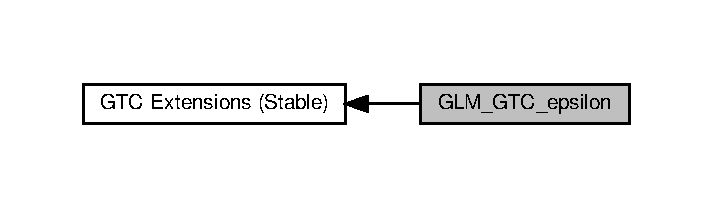
\includegraphics[width=342pt]{group__gtc__epsilon}
\end{center}
\end{figure}
\subsection*{Functions}
\begin{DoxyCompactItemize}
\item 
{\footnotesize template$<$typename T , precision P, template$<$ typename, precision $>$ class vec\+Type$>$ }\\\hyperlink{setup_8hpp_ab2d052de21a70539923e9bcbf6e83a51}{G\+L\+M\+\_\+\+F\+U\+N\+C\+\_\+\+D\+E\+CL} vec\+Type$<$ bool, P $>$ \hyperlink{group__gtc__epsilon_gaca9443f217dc36587624247245522331}{glm\+::epsilon\+Equal} (vec\+Type$<$ T, P $>$ const \&x, vec\+Type$<$ T, P $>$ const \&y, T const \&\hyperlink{group__gtc__constants_gacb41049b8d22c8aa90e362b96c524feb}{epsilon})
\item 
{\footnotesize template$<$typename gen\+Type $>$ }\\\hyperlink{setup_8hpp_ab2d052de21a70539923e9bcbf6e83a51}{G\+L\+M\+\_\+\+F\+U\+N\+C\+\_\+\+D\+E\+CL} bool \hyperlink{group__gtc__epsilon_gaa7f227999ca09e7ca994e8b35aba47bb}{glm\+::epsilon\+Equal} (gen\+Type const \&x, gen\+Type const \&y, gen\+Type const \&\hyperlink{group__gtc__constants_gacb41049b8d22c8aa90e362b96c524feb}{epsilon})
\item 
{\footnotesize template$<$typename gen\+Type $>$ }\\\hyperlink{setup_8hpp_ab2d052de21a70539923e9bcbf6e83a51}{G\+L\+M\+\_\+\+F\+U\+N\+C\+\_\+\+D\+E\+CL} gen\+Type\+::bool\+Type \hyperlink{group__gtc__epsilon_ga14e2888a304654ade8a3996024e2739c}{glm\+::epsilon\+Not\+Equal} (gen\+Type const \&x, gen\+Type const \&y, typename gen\+Type\+::value\+\_\+type const \&\hyperlink{group__gtc__constants_gacb41049b8d22c8aa90e362b96c524feb}{epsilon})
\item 
{\footnotesize template$<$typename gen\+Type $>$ }\\\hyperlink{setup_8hpp_ab2d052de21a70539923e9bcbf6e83a51}{G\+L\+M\+\_\+\+F\+U\+N\+C\+\_\+\+D\+E\+CL} bool \hyperlink{group__gtc__epsilon_ga50a92103fb0cbd796908e1bf20c79aaf}{glm\+::epsilon\+Not\+Equal} (gen\+Type const \&x, gen\+Type const \&y, gen\+Type const \&\hyperlink{group__gtc__constants_gacb41049b8d22c8aa90e362b96c524feb}{epsilon})
\end{DoxyCompactItemize}


\subsection{Detailed Description}
Comparison functions for a user defined epsilon values. 

$<$\hyperlink{gtc_2epsilon_8hpp}{glm/gtc/epsilon.\+hpp}$>$ need to be included to use these functionalities. 

\subsection{Function Documentation}
\mbox{\Hypertarget{group__gtc__epsilon_gaca9443f217dc36587624247245522331}\label{group__gtc__epsilon_gaca9443f217dc36587624247245522331}} 
\index{G\+L\+M\+\_\+\+G\+T\+C\+\_\+epsilon@{G\+L\+M\+\_\+\+G\+T\+C\+\_\+epsilon}!epsilon\+Equal@{epsilon\+Equal}}
\index{epsilon\+Equal@{epsilon\+Equal}!G\+L\+M\+\_\+\+G\+T\+C\+\_\+epsilon@{G\+L\+M\+\_\+\+G\+T\+C\+\_\+epsilon}}
\subsubsection{\texorpdfstring{epsilon\+Equal()}{epsilonEqual()}\hspace{0.1cm}{\footnotesize\ttfamily [1/2]}}
{\footnotesize\ttfamily template$<$typename T , precision P, template$<$ typename, precision $>$ class vec\+Type$>$ \\
\hyperlink{setup_8hpp_ab2d052de21a70539923e9bcbf6e83a51}{G\+L\+M\+\_\+\+F\+U\+N\+C\+\_\+\+D\+E\+CL} vec\+Type$<$bool, P$>$ glm\+::epsilon\+Equal (\begin{DoxyParamCaption}\item[{vec\+Type$<$ T, P $>$ const \&}]{x,  }\item[{vec\+Type$<$ T, P $>$ const \&}]{y,  }\item[{T const \&}]{epsilon }\end{DoxyParamCaption})}

Returns the component-\/wise comparison of $\vert$x -\/ y$\vert$ $<$ epsilon. True if this expression is satisfied.

\begin{DoxySeeAlso}{See also}
\hyperlink{group__gtc__epsilon}{G\+L\+M\+\_\+\+G\+T\+C\+\_\+epsilon} 
\end{DoxySeeAlso}


Definition at line 85 of file epsilon.\+inl.

\mbox{\Hypertarget{group__gtc__epsilon_gaa7f227999ca09e7ca994e8b35aba47bb}\label{group__gtc__epsilon_gaa7f227999ca09e7ca994e8b35aba47bb}} 
\index{G\+L\+M\+\_\+\+G\+T\+C\+\_\+epsilon@{G\+L\+M\+\_\+\+G\+T\+C\+\_\+epsilon}!epsilon\+Equal@{epsilon\+Equal}}
\index{epsilon\+Equal@{epsilon\+Equal}!G\+L\+M\+\_\+\+G\+T\+C\+\_\+epsilon@{G\+L\+M\+\_\+\+G\+T\+C\+\_\+epsilon}}
\subsubsection{\texorpdfstring{epsilon\+Equal()}{epsilonEqual()}\hspace{0.1cm}{\footnotesize\ttfamily [2/2]}}
{\footnotesize\ttfamily template$<$typename gen\+Type $>$ \\
\hyperlink{setup_8hpp_ab2d052de21a70539923e9bcbf6e83a51}{G\+L\+M\+\_\+\+F\+U\+N\+C\+\_\+\+D\+E\+CL} bool glm\+::epsilon\+Equal (\begin{DoxyParamCaption}\item[{gen\+Type const \&}]{x,  }\item[{gen\+Type const \&}]{y,  }\item[{gen\+Type const \&}]{epsilon }\end{DoxyParamCaption})}

Returns the component-\/wise comparison of $\vert$x -\/ y$\vert$ $<$ epsilon. True if this expression is satisfied.

\begin{DoxySeeAlso}{See also}
\hyperlink{group__gtc__epsilon}{G\+L\+M\+\_\+\+G\+T\+C\+\_\+epsilon} 
\end{DoxySeeAlso}
\mbox{\Hypertarget{group__gtc__epsilon_ga14e2888a304654ade8a3996024e2739c}\label{group__gtc__epsilon_ga14e2888a304654ade8a3996024e2739c}} 
\index{G\+L\+M\+\_\+\+G\+T\+C\+\_\+epsilon@{G\+L\+M\+\_\+\+G\+T\+C\+\_\+epsilon}!epsilon\+Not\+Equal@{epsilon\+Not\+Equal}}
\index{epsilon\+Not\+Equal@{epsilon\+Not\+Equal}!G\+L\+M\+\_\+\+G\+T\+C\+\_\+epsilon@{G\+L\+M\+\_\+\+G\+T\+C\+\_\+epsilon}}
\subsubsection{\texorpdfstring{epsilon\+Not\+Equal()}{epsilonNotEqual()}\hspace{0.1cm}{\footnotesize\ttfamily [1/2]}}
{\footnotesize\ttfamily template$<$typename gen\+Type $>$ \\
\hyperlink{setup_8hpp_ab2d052de21a70539923e9bcbf6e83a51}{G\+L\+M\+\_\+\+F\+U\+N\+C\+\_\+\+D\+E\+CL} gen\+Type\+::bool\+Type glm\+::epsilon\+Not\+Equal (\begin{DoxyParamCaption}\item[{gen\+Type const \&}]{x,  }\item[{gen\+Type const \&}]{y,  }\item[{typename gen\+Type\+::value\+\_\+type const \&}]{epsilon }\end{DoxyParamCaption})}

Returns the component-\/wise comparison of $\vert$x -\/ y$\vert$ $<$ epsilon. True if this expression is not satisfied.

\begin{DoxySeeAlso}{See also}
\hyperlink{group__gtc__epsilon}{G\+L\+M\+\_\+\+G\+T\+C\+\_\+epsilon} 
\end{DoxySeeAlso}
\mbox{\Hypertarget{group__gtc__epsilon_ga50a92103fb0cbd796908e1bf20c79aaf}\label{group__gtc__epsilon_ga50a92103fb0cbd796908e1bf20c79aaf}} 
\index{G\+L\+M\+\_\+\+G\+T\+C\+\_\+epsilon@{G\+L\+M\+\_\+\+G\+T\+C\+\_\+epsilon}!epsilon\+Not\+Equal@{epsilon\+Not\+Equal}}
\index{epsilon\+Not\+Equal@{epsilon\+Not\+Equal}!G\+L\+M\+\_\+\+G\+T\+C\+\_\+epsilon@{G\+L\+M\+\_\+\+G\+T\+C\+\_\+epsilon}}
\subsubsection{\texorpdfstring{epsilon\+Not\+Equal()}{epsilonNotEqual()}\hspace{0.1cm}{\footnotesize\ttfamily [2/2]}}
{\footnotesize\ttfamily template$<$typename gen\+Type $>$ \\
\hyperlink{setup_8hpp_ab2d052de21a70539923e9bcbf6e83a51}{G\+L\+M\+\_\+\+F\+U\+N\+C\+\_\+\+D\+E\+CL} bool glm\+::epsilon\+Not\+Equal (\begin{DoxyParamCaption}\item[{gen\+Type const \&}]{x,  }\item[{gen\+Type const \&}]{y,  }\item[{gen\+Type const \&}]{epsilon }\end{DoxyParamCaption})}

Returns the component-\/wise comparison of $\vert$x -\/ y$\vert$ $>$= epsilon. True if this expression is not satisfied.

\begin{DoxySeeAlso}{See also}
\hyperlink{group__gtc__epsilon}{G\+L\+M\+\_\+\+G\+T\+C\+\_\+epsilon} 
\end{DoxySeeAlso}

\hypertarget{group__gtc__matrix__access}{}\section{G\+L\+M\+\_\+\+G\+T\+C\+\_\+matrix\+\_\+access}
\label{group__gtc__matrix__access}\index{G\+L\+M\+\_\+\+G\+T\+C\+\_\+matrix\+\_\+access@{G\+L\+M\+\_\+\+G\+T\+C\+\_\+matrix\+\_\+access}}
Collaboration diagram for G\+L\+M\+\_\+\+G\+T\+C\+\_\+matrix\+\_\+access\+:\nopagebreak
\begin{figure}[H]
\begin{center}
\leavevmode
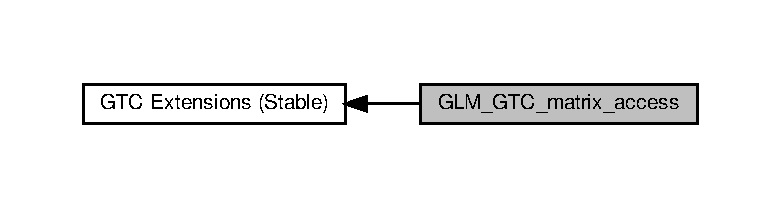
\includegraphics[width=350pt]{group__gtc__matrix__access}
\end{center}
\end{figure}
\subsection*{Functions}
\begin{DoxyCompactItemize}
\item 
{\footnotesize template$<$typename gen\+Type $>$ }\\\hyperlink{setup_8hpp_ab2d052de21a70539923e9bcbf6e83a51}{G\+L\+M\+\_\+\+F\+U\+N\+C\+\_\+\+D\+E\+CL} gen\+Type\+::row\+\_\+type \hyperlink{group__gtc__matrix__access_ga5b874831eef18913dbe30153e52a2476}{glm\+::row} (gen\+Type const \&m, \hyperlink{namespaceglm_a090a0de2260835bee80e71a702492ed9}{length\+\_\+t} const \&index)
\item 
{\footnotesize template$<$typename gen\+Type $>$ }\\\hyperlink{setup_8hpp_ab2d052de21a70539923e9bcbf6e83a51}{G\+L\+M\+\_\+\+F\+U\+N\+C\+\_\+\+D\+E\+CL} gen\+Type \hyperlink{group__gtc__matrix__access_gacb34e8dca9cd0efdd247a65e36ed0a86}{glm\+::row} (gen\+Type const \&m, \hyperlink{namespaceglm_a090a0de2260835bee80e71a702492ed9}{length\+\_\+t} const \&index, typename gen\+Type\+::row\+\_\+type const \&x)
\item 
{\footnotesize template$<$typename gen\+Type $>$ }\\\hyperlink{setup_8hpp_ab2d052de21a70539923e9bcbf6e83a51}{G\+L\+M\+\_\+\+F\+U\+N\+C\+\_\+\+D\+E\+CL} gen\+Type\+::col\+\_\+type \hyperlink{group__gtc__matrix__access_ga5c37fbeb062151f930e8a231c37e6b81}{glm\+::column} (gen\+Type const \&m, \hyperlink{namespaceglm_a090a0de2260835bee80e71a702492ed9}{length\+\_\+t} const \&index)
\item 
{\footnotesize template$<$typename gen\+Type $>$ }\\\hyperlink{setup_8hpp_ab2d052de21a70539923e9bcbf6e83a51}{G\+L\+M\+\_\+\+F\+U\+N\+C\+\_\+\+D\+E\+CL} gen\+Type \hyperlink{group__gtc__matrix__access_gaff0c6f887deb04ce0519084d32aadb85}{glm\+::column} (gen\+Type const \&m, \hyperlink{namespaceglm_a090a0de2260835bee80e71a702492ed9}{length\+\_\+t} const \&index, typename gen\+Type\+::col\+\_\+type const \&x)
\end{DoxyCompactItemize}


\subsection{Detailed Description}
Defines functions to access rows or columns of a matrix easily. $<$\hyperlink{matrix__access_8hpp}{glm/gtc/matrix\+\_\+access.\+hpp}$>$ need to be included to use these functionalities. 

\subsection{Function Documentation}
\mbox{\Hypertarget{group__gtc__matrix__access_ga5c37fbeb062151f930e8a231c37e6b81}\label{group__gtc__matrix__access_ga5c37fbeb062151f930e8a231c37e6b81}} 
\index{G\+L\+M\+\_\+\+G\+T\+C\+\_\+matrix\+\_\+access@{G\+L\+M\+\_\+\+G\+T\+C\+\_\+matrix\+\_\+access}!column@{column}}
\index{column@{column}!G\+L\+M\+\_\+\+G\+T\+C\+\_\+matrix\+\_\+access@{G\+L\+M\+\_\+\+G\+T\+C\+\_\+matrix\+\_\+access}}
\subsubsection{\texorpdfstring{column()}{column()}\hspace{0.1cm}{\footnotesize\ttfamily [1/2]}}
{\footnotesize\ttfamily template$<$typename gen\+Type $>$ \\
\hyperlink{setup_8hpp_ab2d052de21a70539923e9bcbf6e83a51}{G\+L\+M\+\_\+\+F\+U\+N\+C\+\_\+\+D\+E\+CL} gen\+Type\+::col\+\_\+type glm\+::column (\begin{DoxyParamCaption}\item[{gen\+Type const \&}]{m,  }\item[{\hyperlink{namespaceglm_a090a0de2260835bee80e71a702492ed9}{length\+\_\+t} const \&}]{index }\end{DoxyParamCaption})}

Get a specific column of a matrix. \begin{DoxySeeAlso}{See also}
\hyperlink{group__gtc__matrix__access}{G\+L\+M\+\_\+\+G\+T\+C\+\_\+matrix\+\_\+access} 
\end{DoxySeeAlso}


Definition at line 79 of file matrix\+\_\+access.\+inl.

\mbox{\Hypertarget{group__gtc__matrix__access_gaff0c6f887deb04ce0519084d32aadb85}\label{group__gtc__matrix__access_gaff0c6f887deb04ce0519084d32aadb85}} 
\index{G\+L\+M\+\_\+\+G\+T\+C\+\_\+matrix\+\_\+access@{G\+L\+M\+\_\+\+G\+T\+C\+\_\+matrix\+\_\+access}!column@{column}}
\index{column@{column}!G\+L\+M\+\_\+\+G\+T\+C\+\_\+matrix\+\_\+access@{G\+L\+M\+\_\+\+G\+T\+C\+\_\+matrix\+\_\+access}}
\subsubsection{\texorpdfstring{column()}{column()}\hspace{0.1cm}{\footnotesize\ttfamily [2/2]}}
{\footnotesize\ttfamily template$<$typename gen\+Type $>$ \\
\hyperlink{setup_8hpp_ab2d052de21a70539923e9bcbf6e83a51}{G\+L\+M\+\_\+\+F\+U\+N\+C\+\_\+\+D\+E\+CL} gen\+Type glm\+::column (\begin{DoxyParamCaption}\item[{gen\+Type const \&}]{m,  }\item[{\hyperlink{namespaceglm_a090a0de2260835bee80e71a702492ed9}{length\+\_\+t} const \&}]{index,  }\item[{typename gen\+Type\+::col\+\_\+type const \&}]{x }\end{DoxyParamCaption})}

Set a specific column to a matrix. \begin{DoxySeeAlso}{See also}
\hyperlink{group__gtc__matrix__access}{G\+L\+M\+\_\+\+G\+T\+C\+\_\+matrix\+\_\+access} 
\end{DoxySeeAlso}


Definition at line 64 of file matrix\+\_\+access.\+inl.

\mbox{\Hypertarget{group__gtc__matrix__access_ga5b874831eef18913dbe30153e52a2476}\label{group__gtc__matrix__access_ga5b874831eef18913dbe30153e52a2476}} 
\index{G\+L\+M\+\_\+\+G\+T\+C\+\_\+matrix\+\_\+access@{G\+L\+M\+\_\+\+G\+T\+C\+\_\+matrix\+\_\+access}!row@{row}}
\index{row@{row}!G\+L\+M\+\_\+\+G\+T\+C\+\_\+matrix\+\_\+access@{G\+L\+M\+\_\+\+G\+T\+C\+\_\+matrix\+\_\+access}}
\subsubsection{\texorpdfstring{row()}{row()}\hspace{0.1cm}{\footnotesize\ttfamily [1/2]}}
{\footnotesize\ttfamily template$<$typename gen\+Type $>$ \\
\hyperlink{setup_8hpp_ab2d052de21a70539923e9bcbf6e83a51}{G\+L\+M\+\_\+\+F\+U\+N\+C\+\_\+\+D\+E\+CL} gen\+Type\+::row\+\_\+type glm\+::row (\begin{DoxyParamCaption}\item[{gen\+Type const \&}]{m,  }\item[{\hyperlink{namespaceglm_a090a0de2260835bee80e71a702492ed9}{length\+\_\+t} const \&}]{index }\end{DoxyParamCaption})}

Get a specific row of a matrix. \begin{DoxySeeAlso}{See also}
\hyperlink{group__gtc__matrix__access}{G\+L\+M\+\_\+\+G\+T\+C\+\_\+matrix\+\_\+access} 
\end{DoxySeeAlso}


Definition at line 49 of file matrix\+\_\+access.\+inl.

\mbox{\Hypertarget{group__gtc__matrix__access_gacb34e8dca9cd0efdd247a65e36ed0a86}\label{group__gtc__matrix__access_gacb34e8dca9cd0efdd247a65e36ed0a86}} 
\index{G\+L\+M\+\_\+\+G\+T\+C\+\_\+matrix\+\_\+access@{G\+L\+M\+\_\+\+G\+T\+C\+\_\+matrix\+\_\+access}!row@{row}}
\index{row@{row}!G\+L\+M\+\_\+\+G\+T\+C\+\_\+matrix\+\_\+access@{G\+L\+M\+\_\+\+G\+T\+C\+\_\+matrix\+\_\+access}}
\subsubsection{\texorpdfstring{row()}{row()}\hspace{0.1cm}{\footnotesize\ttfamily [2/2]}}
{\footnotesize\ttfamily template$<$typename gen\+Type $>$ \\
\hyperlink{setup_8hpp_ab2d052de21a70539923e9bcbf6e83a51}{G\+L\+M\+\_\+\+F\+U\+N\+C\+\_\+\+D\+E\+CL} gen\+Type glm\+::row (\begin{DoxyParamCaption}\item[{gen\+Type const \&}]{m,  }\item[{\hyperlink{namespaceglm_a090a0de2260835bee80e71a702492ed9}{length\+\_\+t} const \&}]{index,  }\item[{typename gen\+Type\+::row\+\_\+type const \&}]{x }\end{DoxyParamCaption})}

Set a specific row to a matrix. \begin{DoxySeeAlso}{See also}
\hyperlink{group__gtc__matrix__access}{G\+L\+M\+\_\+\+G\+T\+C\+\_\+matrix\+\_\+access} 
\end{DoxySeeAlso}


Definition at line 33 of file matrix\+\_\+access.\+inl.


\hypertarget{group__gtc__matrix__integer}{}\section{G\+L\+M\+\_\+\+G\+T\+C\+\_\+matrix\+\_\+integer}
\label{group__gtc__matrix__integer}\index{G\+L\+M\+\_\+\+G\+T\+C\+\_\+matrix\+\_\+integer@{G\+L\+M\+\_\+\+G\+T\+C\+\_\+matrix\+\_\+integer}}
Collaboration diagram for G\+L\+M\+\_\+\+G\+T\+C\+\_\+matrix\+\_\+integer\+:\nopagebreak
\begin{figure}[H]
\begin{center}
\leavevmode
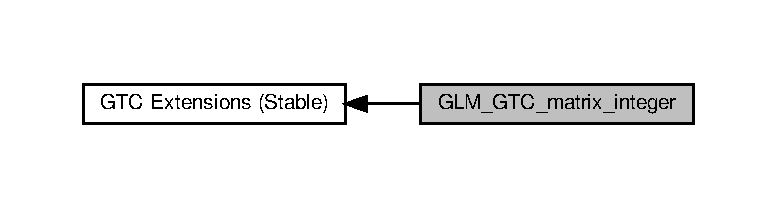
\includegraphics[width=350pt]{group__gtc__matrix__integer}
\end{center}
\end{figure}
\subsection*{Typedefs}
\begin{DoxyCompactItemize}
\item 
typedef \hyperlink{structglm_1_1detail_1_1tmat2x2}{detail\+::tmat2x2}$<$ int, \hyperlink{namespaceglm_a0f04f086094c747d227af4425893f545ac6f7eab42eacbb10d59a58e95e362074}{highp} $>$ \hyperlink{group__gtc__matrix__integer_ga70eae282157f23589db24f4664bbf956}{glm\+::highp\+\_\+imat2}
\item 
typedef \hyperlink{structglm_1_1detail_1_1tmat3x3}{detail\+::tmat3x3}$<$ int, \hyperlink{namespaceglm_a0f04f086094c747d227af4425893f545ac6f7eab42eacbb10d59a58e95e362074}{highp} $>$ \hyperlink{group__gtc__matrix__integer_gaf12b3aa7e16a88b1fcf51be9a132048c}{glm\+::highp\+\_\+imat3}
\item 
typedef \hyperlink{structglm_1_1detail_1_1tmat4x4}{detail\+::tmat4x4}$<$ int, \hyperlink{namespaceglm_a0f04f086094c747d227af4425893f545ac6f7eab42eacbb10d59a58e95e362074}{highp} $>$ \hyperlink{group__gtc__matrix__integer_ga9ca2f5624891bd1ac993fcde4dd24ac1}{glm\+::highp\+\_\+imat4}
\item 
typedef \hyperlink{structglm_1_1detail_1_1tmat2x2}{detail\+::tmat2x2}$<$ int, \hyperlink{namespaceglm_a0f04f086094c747d227af4425893f545ac6f7eab42eacbb10d59a58e95e362074}{highp} $>$ \hyperlink{group__gtc__matrix__integer_ga9646ff5ef973234755e63e727c5a37fc}{glm\+::highp\+\_\+imat2x2}
\item 
typedef \hyperlink{structglm_1_1detail_1_1tmat2x3}{detail\+::tmat2x3}$<$ int, \hyperlink{namespaceglm_a0f04f086094c747d227af4425893f545ac6f7eab42eacbb10d59a58e95e362074}{highp} $>$ \hyperlink{group__gtc__matrix__integer_ga7b7079ab95ac8f533ac565fcf1341c76}{glm\+::highp\+\_\+imat2x3}
\item 
typedef \hyperlink{structglm_1_1detail_1_1tmat2x4}{detail\+::tmat2x4}$<$ int, \hyperlink{namespaceglm_a0f04f086094c747d227af4425893f545ac6f7eab42eacbb10d59a58e95e362074}{highp} $>$ \hyperlink{group__gtc__matrix__integer_ga84aec2e744ecac589fe8d502266e8efc}{glm\+::highp\+\_\+imat2x4}
\item 
typedef \hyperlink{structglm_1_1detail_1_1tmat3x2}{detail\+::tmat3x2}$<$ int, \hyperlink{namespaceglm_a0f04f086094c747d227af4425893f545ac6f7eab42eacbb10d59a58e95e362074}{highp} $>$ \hyperlink{group__gtc__matrix__integer_ga9780c1bc052a34c59dc95f4dd9e1a5c8}{glm\+::highp\+\_\+imat3x2}
\item 
typedef \hyperlink{structglm_1_1detail_1_1tmat3x3}{detail\+::tmat3x3}$<$ int, \hyperlink{namespaceglm_a0f04f086094c747d227af4425893f545ac6f7eab42eacbb10d59a58e95e362074}{highp} $>$ \hyperlink{group__gtc__matrix__integer_ga4e7c11e49de5d71067b95a87c84308a8}{glm\+::highp\+\_\+imat3x3}
\item 
typedef \hyperlink{structglm_1_1detail_1_1tmat3x4}{detail\+::tmat3x4}$<$ int, \hyperlink{namespaceglm_a0f04f086094c747d227af4425893f545ac6f7eab42eacbb10d59a58e95e362074}{highp} $>$ \hyperlink{group__gtc__matrix__integer_ga97ddf84f7ae0c5d4d3ecc18bb1d47449}{glm\+::highp\+\_\+imat3x4}
\item 
typedef \hyperlink{structglm_1_1detail_1_1tmat4x2}{detail\+::tmat4x2}$<$ int, \hyperlink{namespaceglm_a0f04f086094c747d227af4425893f545ac6f7eab42eacbb10d59a58e95e362074}{highp} $>$ \hyperlink{group__gtc__matrix__integer_gad998dce143f674a95a25241ff6e5e7d2}{glm\+::highp\+\_\+imat4x2}
\item 
typedef \hyperlink{structglm_1_1detail_1_1tmat4x3}{detail\+::tmat4x3}$<$ int, \hyperlink{namespaceglm_a0f04f086094c747d227af4425893f545ac6f7eab42eacbb10d59a58e95e362074}{highp} $>$ \hyperlink{group__gtc__matrix__integer_ga9d51b6f1c8cd0b23c6fcc8dca924b14c}{glm\+::highp\+\_\+imat4x3}
\item 
typedef \hyperlink{structglm_1_1detail_1_1tmat4x4}{detail\+::tmat4x4}$<$ int, \hyperlink{namespaceglm_a0f04f086094c747d227af4425893f545ac6f7eab42eacbb10d59a58e95e362074}{highp} $>$ \hyperlink{group__gtc__matrix__integer_ga969c88d5c7530beb80768205a054ee80}{glm\+::highp\+\_\+imat4x4}
\item 
typedef \hyperlink{structglm_1_1detail_1_1tmat2x2}{detail\+::tmat2x2}$<$ int, \hyperlink{namespaceglm_a0f04f086094c747d227af4425893f545a6416f3ea0c9025fb21ed50c4d6620482}{mediump} $>$ \hyperlink{group__gtc__matrix__integer_gaec03a8eef2ec2536f8bebffd0bac8192}{glm\+::mediump\+\_\+imat2}
\item 
typedef \hyperlink{structglm_1_1detail_1_1tmat3x3}{detail\+::tmat3x3}$<$ int, \hyperlink{namespaceglm_a0f04f086094c747d227af4425893f545a6416f3ea0c9025fb21ed50c4d6620482}{mediump} $>$ \hyperlink{group__gtc__matrix__integer_ga6b438ab863af0122b532adc93b89105e}{glm\+::mediump\+\_\+imat3}
\item 
typedef \hyperlink{structglm_1_1detail_1_1tmat4x4}{detail\+::tmat4x4}$<$ int, \hyperlink{namespaceglm_a0f04f086094c747d227af4425893f545a6416f3ea0c9025fb21ed50c4d6620482}{mediump} $>$ \hyperlink{group__gtc__matrix__integer_gabf1a0fd4c85a21f67535b737e1feb355}{glm\+::mediump\+\_\+imat4}
\item 
typedef \hyperlink{structglm_1_1detail_1_1tmat2x2}{detail\+::tmat2x2}$<$ int, \hyperlink{namespaceglm_a0f04f086094c747d227af4425893f545a6416f3ea0c9025fb21ed50c4d6620482}{mediump} $>$ \hyperlink{group__gtc__matrix__integer_ga472222f6e3754124ee9cb64acaaedac1}{glm\+::mediump\+\_\+imat2x2}
\item 
typedef \hyperlink{structglm_1_1detail_1_1tmat2x3}{detail\+::tmat2x3}$<$ int, \hyperlink{namespaceglm_a0f04f086094c747d227af4425893f545a6416f3ea0c9025fb21ed50c4d6620482}{mediump} $>$ \hyperlink{group__gtc__matrix__integer_gabc92c714c2d257213c5b0771669df177}{glm\+::mediump\+\_\+imat2x3}
\item 
typedef \hyperlink{structglm_1_1detail_1_1tmat2x4}{detail\+::tmat2x4}$<$ int, \hyperlink{namespaceglm_a0f04f086094c747d227af4425893f545a6416f3ea0c9025fb21ed50c4d6620482}{mediump} $>$ \hyperlink{group__gtc__matrix__integer_ga90b020de8489a1d4424c0ffcc17c83dd}{glm\+::mediump\+\_\+imat2x4}
\item 
typedef \hyperlink{structglm_1_1detail_1_1tmat3x2}{detail\+::tmat3x2}$<$ int, \hyperlink{namespaceglm_a0f04f086094c747d227af4425893f545a6416f3ea0c9025fb21ed50c4d6620482}{mediump} $>$ \hyperlink{group__gtc__matrix__integer_ga2a90775c74656b8a825f24d510f0ea5d}{glm\+::mediump\+\_\+imat3x2}
\item 
typedef \hyperlink{structglm_1_1detail_1_1tmat3x3}{detail\+::tmat3x3}$<$ int, \hyperlink{namespaceglm_a0f04f086094c747d227af4425893f545a6416f3ea0c9025fb21ed50c4d6620482}{mediump} $>$ \hyperlink{group__gtc__matrix__integer_gac5ee8dc182055bb0a00a90c031d4a714}{glm\+::mediump\+\_\+imat3x3}
\item 
typedef \hyperlink{structglm_1_1detail_1_1tmat3x4}{detail\+::tmat3x4}$<$ int, \hyperlink{namespaceglm_a0f04f086094c747d227af4425893f545a6416f3ea0c9025fb21ed50c4d6620482}{mediump} $>$ \hyperlink{group__gtc__matrix__integer_gaaac79be4db34dde570c3331ffe728d55}{glm\+::mediump\+\_\+imat3x4}
\item 
typedef \hyperlink{structglm_1_1detail_1_1tmat4x2}{detail\+::tmat4x2}$<$ int, \hyperlink{namespaceglm_a0f04f086094c747d227af4425893f545a6416f3ea0c9025fb21ed50c4d6620482}{mediump} $>$ \hyperlink{group__gtc__matrix__integer_gacdae7d6ae4820756c62c2b5fd5c0370a}{glm\+::mediump\+\_\+imat4x2}
\item 
typedef \hyperlink{structglm_1_1detail_1_1tmat4x3}{detail\+::tmat4x3}$<$ int, \hyperlink{namespaceglm_a0f04f086094c747d227af4425893f545a6416f3ea0c9025fb21ed50c4d6620482}{mediump} $>$ \hyperlink{group__gtc__matrix__integer_ga5032ee978a55aa0db4842d5c3cbeade0}{glm\+::mediump\+\_\+imat4x3}
\item 
typedef \hyperlink{structglm_1_1detail_1_1tmat4x4}{detail\+::tmat4x4}$<$ int, \hyperlink{namespaceglm_a0f04f086094c747d227af4425893f545a6416f3ea0c9025fb21ed50c4d6620482}{mediump} $>$ \hyperlink{group__gtc__matrix__integer_gafa2df6be3aad055867b9bfea34e9c4a0}{glm\+::mediump\+\_\+imat4x4}
\item 
typedef \hyperlink{structglm_1_1detail_1_1tmat2x2}{detail\+::tmat2x2}$<$ int, \hyperlink{namespaceglm_a0f04f086094c747d227af4425893f545ae161af3fc695e696ce3bf69f7332bc2d}{lowp} $>$ \hyperlink{group__gtc__matrix__integer_gae0df4bc278c1a958a32af9ac82c47630}{glm\+::lowp\+\_\+imat2}
\item 
typedef \hyperlink{structglm_1_1detail_1_1tmat3x3}{detail\+::tmat3x3}$<$ int, \hyperlink{namespaceglm_a0f04f086094c747d227af4425893f545ae161af3fc695e696ce3bf69f7332bc2d}{lowp} $>$ \hyperlink{group__gtc__matrix__integer_ga149b90591e7275193c85cc08acbf0024}{glm\+::lowp\+\_\+imat3}
\item 
typedef \hyperlink{structglm_1_1detail_1_1tmat4x4}{detail\+::tmat4x4}$<$ int, \hyperlink{namespaceglm_a0f04f086094c747d227af4425893f545ae161af3fc695e696ce3bf69f7332bc2d}{lowp} $>$ \hyperlink{group__gtc__matrix__integer_ga7c687f14d923e05d5cf14aac41d10993}{glm\+::lowp\+\_\+imat4}
\item 
typedef \hyperlink{structglm_1_1detail_1_1tmat2x2}{detail\+::tmat2x2}$<$ int, \hyperlink{namespaceglm_a0f04f086094c747d227af4425893f545ae161af3fc695e696ce3bf69f7332bc2d}{lowp} $>$ \hyperlink{group__gtc__matrix__integer_ga05307630bc68a62132a82d1886a0b5e2}{glm\+::lowp\+\_\+imat2x2}
\item 
typedef \hyperlink{structglm_1_1detail_1_1tmat2x3}{detail\+::tmat2x3}$<$ int, \hyperlink{namespaceglm_a0f04f086094c747d227af4425893f545ae161af3fc695e696ce3bf69f7332bc2d}{lowp} $>$ \hyperlink{group__gtc__matrix__integer_ga5757953c508a6e05bf3573d6c099cf88}{glm\+::lowp\+\_\+imat2x3}
\item 
typedef \hyperlink{structglm_1_1detail_1_1tmat2x4}{detail\+::tmat2x4}$<$ int, \hyperlink{namespaceglm_a0f04f086094c747d227af4425893f545ae161af3fc695e696ce3bf69f7332bc2d}{lowp} $>$ \hyperlink{group__gtc__matrix__integer_ga4d859ef48cdfb15b2c9acc98064dd272}{glm\+::lowp\+\_\+imat2x4}
\item 
typedef \hyperlink{structglm_1_1detail_1_1tmat3x2}{detail\+::tmat3x2}$<$ int, \hyperlink{namespaceglm_a0f04f086094c747d227af4425893f545ae161af3fc695e696ce3bf69f7332bc2d}{lowp} $>$ \hyperlink{group__gtc__matrix__integer_ga250780f2be05f698b881b04ba7ce0452}{glm\+::lowp\+\_\+imat3x2}
\item 
typedef \hyperlink{structglm_1_1detail_1_1tmat3x3}{detail\+::tmat3x3}$<$ int, \hyperlink{namespaceglm_a0f04f086094c747d227af4425893f545ae161af3fc695e696ce3bf69f7332bc2d}{lowp} $>$ \hyperlink{group__gtc__matrix__integer_gae0d6068aaf9b1f8f06c6cc32941f9471}{glm\+::lowp\+\_\+imat3x3}
\item 
typedef \hyperlink{structglm_1_1detail_1_1tmat3x4}{detail\+::tmat3x4}$<$ int, \hyperlink{namespaceglm_a0f04f086094c747d227af4425893f545ae161af3fc695e696ce3bf69f7332bc2d}{lowp} $>$ \hyperlink{group__gtc__matrix__integer_gaba7c2c9f782278aaa10dad882d73ef0d}{glm\+::lowp\+\_\+imat3x4}
\item 
typedef \hyperlink{structglm_1_1detail_1_1tmat4x2}{detail\+::tmat4x2}$<$ int, \hyperlink{namespaceglm_a0f04f086094c747d227af4425893f545ae161af3fc695e696ce3bf69f7332bc2d}{lowp} $>$ \hyperlink{group__gtc__matrix__integer_ga0d7055814ab969df3b844ba9c52dbf61}{glm\+::lowp\+\_\+imat4x2}
\item 
typedef \hyperlink{structglm_1_1detail_1_1tmat4x3}{detail\+::tmat4x3}$<$ int, \hyperlink{namespaceglm_a0f04f086094c747d227af4425893f545ae161af3fc695e696ce3bf69f7332bc2d}{lowp} $>$ \hyperlink{group__gtc__matrix__integer_ga73858cf965b0aa7e72908eb817c192d6}{glm\+::lowp\+\_\+imat4x3}
\item 
typedef \hyperlink{structglm_1_1detail_1_1tmat4x4}{detail\+::tmat4x4}$<$ int, \hyperlink{namespaceglm_a0f04f086094c747d227af4425893f545ae161af3fc695e696ce3bf69f7332bc2d}{lowp} $>$ \hyperlink{group__gtc__matrix__integer_ga92339a0b053a721e3b88267e6d175014}{glm\+::lowp\+\_\+imat4x4}
\item 
typedef \hyperlink{structglm_1_1detail_1_1tmat2x2}{detail\+::tmat2x2}$<$ \hyperlink{group__core__precision_ga4fd29415871152bfb5abd588334147c8}{uint}, \hyperlink{namespaceglm_a0f04f086094c747d227af4425893f545ac6f7eab42eacbb10d59a58e95e362074}{highp} $>$ \hyperlink{group__gtc__matrix__integer_ga0c89800e3f63f82da4a4159004811cec}{glm\+::highp\+\_\+umat2}
\item 
typedef \hyperlink{structglm_1_1detail_1_1tmat3x3}{detail\+::tmat3x3}$<$ \hyperlink{group__core__precision_ga4fd29415871152bfb5abd588334147c8}{uint}, \hyperlink{namespaceglm_a0f04f086094c747d227af4425893f545ac6f7eab42eacbb10d59a58e95e362074}{highp} $>$ \hyperlink{group__gtc__matrix__integer_ga2a271939d0123103f088e325e5123385}{glm\+::highp\+\_\+umat3}
\item 
typedef \hyperlink{structglm_1_1detail_1_1tmat4x4}{detail\+::tmat4x4}$<$ \hyperlink{group__core__precision_ga4fd29415871152bfb5abd588334147c8}{uint}, \hyperlink{namespaceglm_a0f04f086094c747d227af4425893f545ac6f7eab42eacbb10d59a58e95e362074}{highp} $>$ \hyperlink{group__gtc__matrix__integer_gaf12f0d2744e809e64469d27ef392aa98}{glm\+::highp\+\_\+umat4}
\item 
typedef \hyperlink{structglm_1_1detail_1_1tmat2x2}{detail\+::tmat2x2}$<$ \hyperlink{group__core__precision_ga4fd29415871152bfb5abd588334147c8}{uint}, \hyperlink{namespaceglm_a0f04f086094c747d227af4425893f545ac6f7eab42eacbb10d59a58e95e362074}{highp} $>$ \hyperlink{group__gtc__matrix__integer_ga428410468e33d16dc8aee08b17166669}{glm\+::highp\+\_\+umat2x2}
\item 
typedef \hyperlink{structglm_1_1detail_1_1tmat2x3}{detail\+::tmat2x3}$<$ \hyperlink{group__core__precision_ga4fd29415871152bfb5abd588334147c8}{uint}, \hyperlink{namespaceglm_a0f04f086094c747d227af4425893f545ac6f7eab42eacbb10d59a58e95e362074}{highp} $>$ \hyperlink{group__gtc__matrix__integer_ga309076d055b5511a7071ebb5f660ed83}{glm\+::highp\+\_\+umat2x3}
\item 
typedef \hyperlink{structglm_1_1detail_1_1tmat2x4}{detail\+::tmat2x4}$<$ \hyperlink{group__core__precision_ga4fd29415871152bfb5abd588334147c8}{uint}, \hyperlink{namespaceglm_a0f04f086094c747d227af4425893f545ac6f7eab42eacbb10d59a58e95e362074}{highp} $>$ \hyperlink{group__gtc__matrix__integer_gabe8572c228aecc0bfa7ba92415b1c651}{glm\+::highp\+\_\+umat2x4}
\item 
typedef \hyperlink{structglm_1_1detail_1_1tmat3x2}{detail\+::tmat3x2}$<$ \hyperlink{group__core__precision_ga4fd29415871152bfb5abd588334147c8}{uint}, \hyperlink{namespaceglm_a0f04f086094c747d227af4425893f545ac6f7eab42eacbb10d59a58e95e362074}{highp} $>$ \hyperlink{group__gtc__matrix__integer_ga6f6a73ec605a515fb21d779663082ef9}{glm\+::highp\+\_\+umat3x2}
\item 
typedef \hyperlink{structglm_1_1detail_1_1tmat3x3}{detail\+::tmat3x3}$<$ \hyperlink{group__core__precision_ga4fd29415871152bfb5abd588334147c8}{uint}, \hyperlink{namespaceglm_a0f04f086094c747d227af4425893f545ac6f7eab42eacbb10d59a58e95e362074}{highp} $>$ \hyperlink{group__gtc__matrix__integer_ga8dd9f8bfe06de34c8f1a942d2c2e094c}{glm\+::highp\+\_\+umat3x3}
\item 
typedef \hyperlink{structglm_1_1detail_1_1tmat3x4}{detail\+::tmat3x4}$<$ \hyperlink{group__core__precision_ga4fd29415871152bfb5abd588334147c8}{uint}, \hyperlink{namespaceglm_a0f04f086094c747d227af4425893f545ac6f7eab42eacbb10d59a58e95e362074}{highp} $>$ \hyperlink{group__gtc__matrix__integer_gabaeb2363acd07cc7f99918bae48ccc05}{glm\+::highp\+\_\+umat3x4}
\item 
typedef \hyperlink{structglm_1_1detail_1_1tmat4x2}{detail\+::tmat4x2}$<$ \hyperlink{group__core__precision_ga4fd29415871152bfb5abd588334147c8}{uint}, \hyperlink{namespaceglm_a0f04f086094c747d227af4425893f545ac6f7eab42eacbb10d59a58e95e362074}{highp} $>$ \hyperlink{group__gtc__matrix__integer_ga32442efcb778cb80024a17bafa781f81}{glm\+::highp\+\_\+umat4x2}
\item 
typedef \hyperlink{structglm_1_1detail_1_1tmat4x3}{detail\+::tmat4x3}$<$ \hyperlink{group__core__precision_ga4fd29415871152bfb5abd588334147c8}{uint}, \hyperlink{namespaceglm_a0f04f086094c747d227af4425893f545ac6f7eab42eacbb10d59a58e95e362074}{highp} $>$ \hyperlink{group__gtc__matrix__integer_ga763a36c57b6073ca3cac739bfbe794ba}{glm\+::highp\+\_\+umat4x3}
\item 
typedef \hyperlink{structglm_1_1detail_1_1tmat4x4}{detail\+::tmat4x4}$<$ \hyperlink{group__core__precision_ga4fd29415871152bfb5abd588334147c8}{uint}, \hyperlink{namespaceglm_a0f04f086094c747d227af4425893f545ac6f7eab42eacbb10d59a58e95e362074}{highp} $>$ \hyperlink{group__gtc__matrix__integer_gaa14b7029cfaf6f26384782f5ff7acddf}{glm\+::highp\+\_\+umat4x4}
\item 
typedef \hyperlink{structglm_1_1detail_1_1tmat2x2}{detail\+::tmat2x2}$<$ \hyperlink{group__core__precision_ga4fd29415871152bfb5abd588334147c8}{uint}, \hyperlink{namespaceglm_a0f04f086094c747d227af4425893f545a6416f3ea0c9025fb21ed50c4d6620482}{mediump} $>$ \hyperlink{group__gtc__matrix__integer_ga388a5b9d7e494d5f5bd30b9e11ded06a}{glm\+::mediump\+\_\+umat2}
\item 
typedef \hyperlink{structglm_1_1detail_1_1tmat3x3}{detail\+::tmat3x3}$<$ \hyperlink{group__core__precision_ga4fd29415871152bfb5abd588334147c8}{uint}, \hyperlink{namespaceglm_a0f04f086094c747d227af4425893f545a6416f3ea0c9025fb21ed50c4d6620482}{mediump} $>$ \hyperlink{group__gtc__matrix__integer_ga123f7d8bac8849e3a150bdf8a21e44a2}{glm\+::mediump\+\_\+umat3}
\item 
typedef \hyperlink{structglm_1_1detail_1_1tmat4x4}{detail\+::tmat4x4}$<$ \hyperlink{group__core__precision_ga4fd29415871152bfb5abd588334147c8}{uint}, \hyperlink{namespaceglm_a0f04f086094c747d227af4425893f545a6416f3ea0c9025fb21ed50c4d6620482}{mediump} $>$ \hyperlink{group__gtc__matrix__integer_gac82f1c426fbca1c4989f0985eb7a4358}{glm\+::mediump\+\_\+umat4}
\item 
typedef \hyperlink{structglm_1_1detail_1_1tmat2x2}{detail\+::tmat2x2}$<$ \hyperlink{group__core__precision_ga4fd29415871152bfb5abd588334147c8}{uint}, \hyperlink{namespaceglm_a0f04f086094c747d227af4425893f545a6416f3ea0c9025fb21ed50c4d6620482}{mediump} $>$ \hyperlink{group__gtc__matrix__integer_ga80e478f09c6caa16410198ce78fe8a2b}{glm\+::mediump\+\_\+umat2x2}
\item 
typedef \hyperlink{structglm_1_1detail_1_1tmat2x3}{detail\+::tmat2x3}$<$ \hyperlink{group__core__precision_ga4fd29415871152bfb5abd588334147c8}{uint}, \hyperlink{namespaceglm_a0f04f086094c747d227af4425893f545a6416f3ea0c9025fb21ed50c4d6620482}{mediump} $>$ \hyperlink{group__gtc__matrix__integer_gaaae45c5dbaad1ecd57bfa936d851be1b}{glm\+::mediump\+\_\+umat2x3}
\item 
typedef \hyperlink{structglm_1_1detail_1_1tmat2x4}{detail\+::tmat2x4}$<$ \hyperlink{group__core__precision_ga4fd29415871152bfb5abd588334147c8}{uint}, \hyperlink{namespaceglm_a0f04f086094c747d227af4425893f545a6416f3ea0c9025fb21ed50c4d6620482}{mediump} $>$ \hyperlink{group__gtc__matrix__integer_gaf79e9c80f024d31f3d66ddae75e90b6c}{glm\+::mediump\+\_\+umat2x4}
\item 
typedef \hyperlink{structglm_1_1detail_1_1tmat3x2}{detail\+::tmat3x2}$<$ \hyperlink{group__core__precision_ga4fd29415871152bfb5abd588334147c8}{uint}, \hyperlink{namespaceglm_a0f04f086094c747d227af4425893f545a6416f3ea0c9025fb21ed50c4d6620482}{mediump} $>$ \hyperlink{group__gtc__matrix__integer_ga65a9fdb1a5918fe6f308577065983e23}{glm\+::mediump\+\_\+umat3x2}
\item 
typedef \hyperlink{structglm_1_1detail_1_1tmat3x3}{detail\+::tmat3x3}$<$ \hyperlink{group__core__precision_ga4fd29415871152bfb5abd588334147c8}{uint}, \hyperlink{namespaceglm_a0f04f086094c747d227af4425893f545a6416f3ea0c9025fb21ed50c4d6620482}{mediump} $>$ \hyperlink{group__gtc__matrix__integer_ga31a05e7b2a6a596bdc7ceeb5d9c10e1c}{glm\+::mediump\+\_\+umat3x3}
\item 
typedef \hyperlink{structglm_1_1detail_1_1tmat3x4}{detail\+::tmat3x4}$<$ \hyperlink{group__core__precision_ga4fd29415871152bfb5abd588334147c8}{uint}, \hyperlink{namespaceglm_a0f04f086094c747d227af4425893f545a6416f3ea0c9025fb21ed50c4d6620482}{mediump} $>$ \hyperlink{group__gtc__matrix__integer_ga8113e067e1f327fac64cf9015c8c5431}{glm\+::mediump\+\_\+umat3x4}
\item 
typedef \hyperlink{structglm_1_1detail_1_1tmat4x2}{detail\+::tmat4x2}$<$ \hyperlink{group__core__precision_ga4fd29415871152bfb5abd588334147c8}{uint}, \hyperlink{namespaceglm_a0f04f086094c747d227af4425893f545a6416f3ea0c9025fb21ed50c4d6620482}{mediump} $>$ \hyperlink{group__gtc__matrix__integer_ga8ea45737e8bc9bfae2668968056b109f}{glm\+::mediump\+\_\+umat4x2}
\item 
typedef \hyperlink{structglm_1_1detail_1_1tmat4x3}{detail\+::tmat4x3}$<$ \hyperlink{group__core__precision_ga4fd29415871152bfb5abd588334147c8}{uint}, \hyperlink{namespaceglm_a0f04f086094c747d227af4425893f545a6416f3ea0c9025fb21ed50c4d6620482}{mediump} $>$ \hyperlink{group__gtc__matrix__integer_gaebe3b1b4b6030c096447e40fb00528f4}{glm\+::mediump\+\_\+umat4x3}
\item 
typedef \hyperlink{structglm_1_1detail_1_1tmat4x4}{detail\+::tmat4x4}$<$ \hyperlink{group__core__precision_ga4fd29415871152bfb5abd588334147c8}{uint}, \hyperlink{namespaceglm_a0f04f086094c747d227af4425893f545a6416f3ea0c9025fb21ed50c4d6620482}{mediump} $>$ \hyperlink{group__gtc__matrix__integer_ga24b1c76fefa58f810e24cafe0ea6a6a0}{glm\+::mediump\+\_\+umat4x4}
\item 
typedef \hyperlink{structglm_1_1detail_1_1tmat2x2}{detail\+::tmat2x2}$<$ \hyperlink{group__core__precision_ga4fd29415871152bfb5abd588334147c8}{uint}, \hyperlink{namespaceglm_a0f04f086094c747d227af4425893f545ae161af3fc695e696ce3bf69f7332bc2d}{lowp} $>$ \hyperlink{group__gtc__matrix__integer_ga09df85e6b5e53f66a86d042e0633bfbc}{glm\+::lowp\+\_\+umat2}
\item 
typedef \hyperlink{structglm_1_1detail_1_1tmat3x3}{detail\+::tmat3x3}$<$ \hyperlink{group__core__precision_ga4fd29415871152bfb5abd588334147c8}{uint}, \hyperlink{namespaceglm_a0f04f086094c747d227af4425893f545ae161af3fc695e696ce3bf69f7332bc2d}{lowp} $>$ \hyperlink{group__gtc__matrix__integer_ga7160c0ac500826224d3baf1003c0432c}{glm\+::lowp\+\_\+umat3}
\item 
typedef \hyperlink{structglm_1_1detail_1_1tmat4x4}{detail\+::tmat4x4}$<$ \hyperlink{group__core__precision_ga4fd29415871152bfb5abd588334147c8}{uint}, \hyperlink{namespaceglm_a0f04f086094c747d227af4425893f545ae161af3fc695e696ce3bf69f7332bc2d}{lowp} $>$ \hyperlink{group__gtc__matrix__integer_ga571dcc0328ddd1d8c54eba047b5bfa2f}{glm\+::lowp\+\_\+umat4}
\item 
typedef \hyperlink{structglm_1_1detail_1_1tmat2x2}{detail\+::tmat2x2}$<$ \hyperlink{group__core__precision_ga4fd29415871152bfb5abd588334147c8}{uint}, \hyperlink{namespaceglm_a0f04f086094c747d227af4425893f545ae161af3fc695e696ce3bf69f7332bc2d}{lowp} $>$ \hyperlink{group__gtc__matrix__integer_gaa4dfe67706187e459004b9a6c500b048}{glm\+::lowp\+\_\+umat2x2}
\item 
typedef \hyperlink{structglm_1_1detail_1_1tmat2x3}{detail\+::tmat2x3}$<$ \hyperlink{group__core__precision_ga4fd29415871152bfb5abd588334147c8}{uint}, \hyperlink{namespaceglm_a0f04f086094c747d227af4425893f545ae161af3fc695e696ce3bf69f7332bc2d}{lowp} $>$ \hyperlink{group__gtc__matrix__integer_ga4c8388c4a03f228c0e12dd7b7445115d}{glm\+::lowp\+\_\+umat2x3}
\item 
typedef \hyperlink{structglm_1_1detail_1_1tmat2x4}{detail\+::tmat2x4}$<$ \hyperlink{group__core__precision_ga4fd29415871152bfb5abd588334147c8}{uint}, \hyperlink{namespaceglm_a0f04f086094c747d227af4425893f545ae161af3fc695e696ce3bf69f7332bc2d}{lowp} $>$ \hyperlink{group__gtc__matrix__integer_ga581eef861234e918e88377fd331e37e6}{glm\+::lowp\+\_\+umat2x4}
\item 
typedef \hyperlink{structglm_1_1detail_1_1tmat3x2}{detail\+::tmat3x2}$<$ \hyperlink{group__core__precision_ga4fd29415871152bfb5abd588334147c8}{uint}, \hyperlink{namespaceglm_a0f04f086094c747d227af4425893f545ae161af3fc695e696ce3bf69f7332bc2d}{lowp} $>$ \hyperlink{group__gtc__matrix__integer_ga5874e964b1816f230215df28d22ea7de}{glm\+::lowp\+\_\+umat3x2}
\item 
typedef \hyperlink{structglm_1_1detail_1_1tmat3x3}{detail\+::tmat3x3}$<$ \hyperlink{group__core__precision_ga4fd29415871152bfb5abd588334147c8}{uint}, \hyperlink{namespaceglm_a0f04f086094c747d227af4425893f545ae161af3fc695e696ce3bf69f7332bc2d}{lowp} $>$ \hyperlink{group__gtc__matrix__integer_ga691694b1a4c6d1e613d8f1f707acc829}{glm\+::lowp\+\_\+umat3x3}
\item 
typedef \hyperlink{structglm_1_1detail_1_1tmat3x4}{detail\+::tmat3x4}$<$ \hyperlink{group__core__precision_ga4fd29415871152bfb5abd588334147c8}{uint}, \hyperlink{namespaceglm_a0f04f086094c747d227af4425893f545ae161af3fc695e696ce3bf69f7332bc2d}{lowp} $>$ \hyperlink{group__gtc__matrix__integer_gad44577fcaebad47da39cc244566d7fe3}{glm\+::lowp\+\_\+umat3x4}
\item 
typedef \hyperlink{structglm_1_1detail_1_1tmat4x2}{detail\+::tmat4x2}$<$ \hyperlink{group__core__precision_ga4fd29415871152bfb5abd588334147c8}{uint}, \hyperlink{namespaceglm_a0f04f086094c747d227af4425893f545ae161af3fc695e696ce3bf69f7332bc2d}{lowp} $>$ \hyperlink{group__gtc__matrix__integer_ga7583563f93096623d54ec8fddd806d13}{glm\+::lowp\+\_\+umat4x2}
\item 
typedef \hyperlink{structglm_1_1detail_1_1tmat4x3}{detail\+::tmat4x3}$<$ \hyperlink{group__core__precision_ga4fd29415871152bfb5abd588334147c8}{uint}, \hyperlink{namespaceglm_a0f04f086094c747d227af4425893f545ae161af3fc695e696ce3bf69f7332bc2d}{lowp} $>$ \hyperlink{group__gtc__matrix__integer_ga03af6e7ea92be81959305fc89a239cf5}{glm\+::lowp\+\_\+umat4x3}
\item 
typedef \hyperlink{structglm_1_1detail_1_1tmat4x4}{detail\+::tmat4x4}$<$ \hyperlink{group__core__precision_ga4fd29415871152bfb5abd588334147c8}{uint}, \hyperlink{namespaceglm_a0f04f086094c747d227af4425893f545ae161af3fc695e696ce3bf69f7332bc2d}{lowp} $>$ \hyperlink{group__gtc__matrix__integer_ga394ee910348beffe9c7d6b694d5efe5f}{glm\+::lowp\+\_\+umat4x4}
\item 
typedef \hyperlink{group__gtc__matrix__integer_gaec03a8eef2ec2536f8bebffd0bac8192}{mediump\+\_\+imat2} \hyperlink{group__gtc__matrix__integer_ga77a581b3366fb63fc72f8f20830003e0}{glm\+::imat2}
\item 
typedef \hyperlink{group__gtc__matrix__integer_ga6b438ab863af0122b532adc93b89105e}{mediump\+\_\+imat3} \hyperlink{group__gtc__matrix__integer_ga45481922dd07a3a8e23758286311ee97}{glm\+::imat3}
\item 
typedef \hyperlink{group__gtc__matrix__integer_gabf1a0fd4c85a21f67535b737e1feb355}{mediump\+\_\+imat4} \hyperlink{group__gtc__matrix__integer_ga40fc5c5e0b07543497aa1c314891544a}{glm\+::imat4}
\item 
typedef \hyperlink{group__gtc__matrix__integer_ga472222f6e3754124ee9cb64acaaedac1}{mediump\+\_\+imat2x2} \hyperlink{group__gtc__matrix__integer_gaf7f44f44d966377666d41ed059524732}{glm\+::imat2x2}
\item 
typedef \hyperlink{group__gtc__matrix__integer_gabc92c714c2d257213c5b0771669df177}{mediump\+\_\+imat2x3} \hyperlink{group__gtc__matrix__integer_ga143bc5177bac9991d84b70da03952516}{glm\+::imat2x3}
\item 
typedef \hyperlink{group__gtc__matrix__integer_ga90b020de8489a1d4424c0ffcc17c83dd}{mediump\+\_\+imat2x4} \hyperlink{group__gtc__matrix__integer_gafe2d058e164fd1badace451ffcf4ae46}{glm\+::imat2x4}
\item 
typedef \hyperlink{group__gtc__matrix__integer_ga2a90775c74656b8a825f24d510f0ea5d}{mediump\+\_\+imat3x2} \hyperlink{group__gtc__matrix__integer_ga04deef94cdfdd3b3b2706e10a32ef7f3}{glm\+::imat3x2}
\item 
typedef \hyperlink{group__gtc__matrix__integer_gac5ee8dc182055bb0a00a90c031d4a714}{mediump\+\_\+imat3x3} \hyperlink{group__gtc__matrix__integer_gaeff9ef8f56cccc828d6b897923e75402}{glm\+::imat3x3}
\item 
typedef \hyperlink{group__gtc__matrix__integer_gaaac79be4db34dde570c3331ffe728d55}{mediump\+\_\+imat3x4} \hyperlink{group__gtc__matrix__integer_gaee5507e6cbbdd05841a0c174e60dd036}{glm\+::imat3x4}
\item 
typedef \hyperlink{group__gtc__matrix__integer_gacdae7d6ae4820756c62c2b5fd5c0370a}{mediump\+\_\+imat4x2} \hyperlink{group__gtc__matrix__integer_ga7e733984837e0e7aa9f4aac18f632f63}{glm\+::imat4x2}
\item 
typedef \hyperlink{group__gtc__matrix__integer_ga5032ee978a55aa0db4842d5c3cbeade0}{mediump\+\_\+imat4x3} \hyperlink{group__gtc__matrix__integer_gaa4cca8e80c0603239eda452860063844}{glm\+::imat4x3}
\item 
typedef \hyperlink{group__gtc__matrix__integer_gafa2df6be3aad055867b9bfea34e9c4a0}{mediump\+\_\+imat4x4} \hyperlink{group__gtc__matrix__integer_ga367d8d5281ff82f1215a227dd2ea5ba9}{glm\+::imat4x4}
\item 
typedef \hyperlink{group__gtc__matrix__integer_ga388a5b9d7e494d5f5bd30b9e11ded06a}{mediump\+\_\+umat2} \hyperlink{group__gtc__matrix__integer_gae2d45c058cfa0b60ab4df0cdda2d8516}{glm\+::umat2}
\item 
typedef \hyperlink{group__gtc__matrix__integer_ga123f7d8bac8849e3a150bdf8a21e44a2}{mediump\+\_\+umat3} \hyperlink{group__gtc__matrix__integer_ga8b8fbc858e28abf8fc344744f8d6d368}{glm\+::umat3}
\item 
typedef \hyperlink{group__gtc__matrix__integer_gac82f1c426fbca1c4989f0985eb7a4358}{mediump\+\_\+umat4} \hyperlink{group__gtc__matrix__integer_ga7ae562000d8a8d193e9f93cf51e2e113}{glm\+::umat4}
\item 
typedef \hyperlink{group__gtc__matrix__integer_ga80e478f09c6caa16410198ce78fe8a2b}{mediump\+\_\+umat2x2} \hyperlink{group__gtc__matrix__integer_gad3c997b31dd69bdb4787867e758ed48d}{glm\+::umat2x2}
\item 
typedef \hyperlink{group__gtc__matrix__integer_gaaae45c5dbaad1ecd57bfa936d851be1b}{mediump\+\_\+umat2x3} \hyperlink{group__gtc__matrix__integer_ga890ae28f9230794138b2c89f44ce3376}{glm\+::umat2x3}
\item 
typedef \hyperlink{group__gtc__matrix__integer_gaf79e9c80f024d31f3d66ddae75e90b6c}{mediump\+\_\+umat2x4} \hyperlink{group__gtc__matrix__integer_ga3b23b164240cf4dfb429776da7be9d88}{glm\+::umat2x4}
\item 
typedef \hyperlink{group__gtc__matrix__integer_ga65a9fdb1a5918fe6f308577065983e23}{mediump\+\_\+umat3x2} \hyperlink{group__gtc__matrix__integer_ga257300f2710612877ef45438a366e308}{glm\+::umat3x2}
\item 
typedef \hyperlink{group__gtc__matrix__integer_ga31a05e7b2a6a596bdc7ceeb5d9c10e1c}{mediump\+\_\+umat3x3} \hyperlink{group__gtc__matrix__integer_gab80b6501ba1b2c40119a0f2d256f4c97}{glm\+::umat3x3}
\item 
typedef \hyperlink{group__gtc__matrix__integer_ga8113e067e1f327fac64cf9015c8c5431}{mediump\+\_\+umat3x4} \hyperlink{group__gtc__matrix__integer_ga5410857d098a989a30b4017100bc2ff7}{glm\+::umat3x4}
\item 
typedef \hyperlink{group__gtc__matrix__integer_ga8ea45737e8bc9bfae2668968056b109f}{mediump\+\_\+umat4x2} \hyperlink{group__gtc__matrix__integer_ga13e8392218e9b6e1b7f194a21b5c88bf}{glm\+::umat4x2}
\item 
typedef \hyperlink{group__gtc__matrix__integer_gaebe3b1b4b6030c096447e40fb00528f4}{mediump\+\_\+umat4x3} \hyperlink{group__gtc__matrix__integer_ga08373f5588a54da1a48e5e55c7d51004}{glm\+::umat4x3}
\item 
typedef \hyperlink{group__gtc__matrix__integer_ga24b1c76fefa58f810e24cafe0ea6a6a0}{mediump\+\_\+umat4x4} \hyperlink{group__gtc__matrix__integer_gae0931b79e808fb0983848778a60eb548}{glm\+::umat4x4}
\end{DoxyCompactItemize}


\subsection{Detailed Description}
Defines a number of matrices with integer types. $<$\hyperlink{matrix__integer_8hpp}{glm/gtc/matrix\+\_\+integer.\+hpp}$>$ need to be included to use these functionalities. 

\subsection{Typedef Documentation}
\mbox{\Hypertarget{group__gtc__matrix__integer_ga70eae282157f23589db24f4664bbf956}\label{group__gtc__matrix__integer_ga70eae282157f23589db24f4664bbf956}} 
\index{G\+L\+M\+\_\+\+G\+T\+C\+\_\+matrix\+\_\+integer@{G\+L\+M\+\_\+\+G\+T\+C\+\_\+matrix\+\_\+integer}!highp\+\_\+imat2@{highp\+\_\+imat2}}
\index{highp\+\_\+imat2@{highp\+\_\+imat2}!G\+L\+M\+\_\+\+G\+T\+C\+\_\+matrix\+\_\+integer@{G\+L\+M\+\_\+\+G\+T\+C\+\_\+matrix\+\_\+integer}}
\subsubsection{\texorpdfstring{highp\+\_\+imat2}{highp\_imat2}}
{\footnotesize\ttfamily typedef \hyperlink{structglm_1_1detail_1_1tmat2x2}{detail\+::tmat2x2}$<$int, \hyperlink{namespaceglm_a0f04f086094c747d227af4425893f545ac6f7eab42eacbb10d59a58e95e362074}{highp}$>$ \hyperlink{group__gtc__matrix__integer_ga70eae282157f23589db24f4664bbf956}{glm\+::highp\+\_\+imat2}}

High-\/precision signed integer 2x2 matrix. \begin{DoxySeeAlso}{See also}
\hyperlink{group__gtc__matrix__integer}{G\+L\+M\+\_\+\+G\+T\+C\+\_\+matrix\+\_\+integer} 
\end{DoxySeeAlso}


Definition at line 62 of file matrix\+\_\+integer.\+hpp.

\mbox{\Hypertarget{group__gtc__matrix__integer_ga9646ff5ef973234755e63e727c5a37fc}\label{group__gtc__matrix__integer_ga9646ff5ef973234755e63e727c5a37fc}} 
\index{G\+L\+M\+\_\+\+G\+T\+C\+\_\+matrix\+\_\+integer@{G\+L\+M\+\_\+\+G\+T\+C\+\_\+matrix\+\_\+integer}!highp\+\_\+imat2x2@{highp\+\_\+imat2x2}}
\index{highp\+\_\+imat2x2@{highp\+\_\+imat2x2}!G\+L\+M\+\_\+\+G\+T\+C\+\_\+matrix\+\_\+integer@{G\+L\+M\+\_\+\+G\+T\+C\+\_\+matrix\+\_\+integer}}
\subsubsection{\texorpdfstring{highp\+\_\+imat2x2}{highp\_imat2x2}}
{\footnotesize\ttfamily typedef \hyperlink{structglm_1_1detail_1_1tmat2x2}{detail\+::tmat2x2}$<$int, \hyperlink{namespaceglm_a0f04f086094c747d227af4425893f545ac6f7eab42eacbb10d59a58e95e362074}{highp}$>$ \hyperlink{group__gtc__matrix__integer_ga9646ff5ef973234755e63e727c5a37fc}{glm\+::highp\+\_\+imat2x2}}

High-\/precision signed integer 2x2 matrix. \begin{DoxySeeAlso}{See also}
\hyperlink{group__gtc__matrix__integer}{G\+L\+M\+\_\+\+G\+T\+C\+\_\+matrix\+\_\+integer} 
\end{DoxySeeAlso}


Definition at line 74 of file matrix\+\_\+integer.\+hpp.

\mbox{\Hypertarget{group__gtc__matrix__integer_ga7b7079ab95ac8f533ac565fcf1341c76}\label{group__gtc__matrix__integer_ga7b7079ab95ac8f533ac565fcf1341c76}} 
\index{G\+L\+M\+\_\+\+G\+T\+C\+\_\+matrix\+\_\+integer@{G\+L\+M\+\_\+\+G\+T\+C\+\_\+matrix\+\_\+integer}!highp\+\_\+imat2x3@{highp\+\_\+imat2x3}}
\index{highp\+\_\+imat2x3@{highp\+\_\+imat2x3}!G\+L\+M\+\_\+\+G\+T\+C\+\_\+matrix\+\_\+integer@{G\+L\+M\+\_\+\+G\+T\+C\+\_\+matrix\+\_\+integer}}
\subsubsection{\texorpdfstring{highp\+\_\+imat2x3}{highp\_imat2x3}}
{\footnotesize\ttfamily typedef \hyperlink{structglm_1_1detail_1_1tmat2x3}{detail\+::tmat2x3}$<$int, \hyperlink{namespaceglm_a0f04f086094c747d227af4425893f545ac6f7eab42eacbb10d59a58e95e362074}{highp}$>$ \hyperlink{group__gtc__matrix__integer_ga7b7079ab95ac8f533ac565fcf1341c76}{glm\+::highp\+\_\+imat2x3}}

High-\/precision signed integer 2x3 matrix. \begin{DoxySeeAlso}{See also}
\hyperlink{group__gtc__matrix__integer}{G\+L\+M\+\_\+\+G\+T\+C\+\_\+matrix\+\_\+integer} 
\end{DoxySeeAlso}


Definition at line 78 of file matrix\+\_\+integer.\+hpp.

\mbox{\Hypertarget{group__gtc__matrix__integer_ga84aec2e744ecac589fe8d502266e8efc}\label{group__gtc__matrix__integer_ga84aec2e744ecac589fe8d502266e8efc}} 
\index{G\+L\+M\+\_\+\+G\+T\+C\+\_\+matrix\+\_\+integer@{G\+L\+M\+\_\+\+G\+T\+C\+\_\+matrix\+\_\+integer}!highp\+\_\+imat2x4@{highp\+\_\+imat2x4}}
\index{highp\+\_\+imat2x4@{highp\+\_\+imat2x4}!G\+L\+M\+\_\+\+G\+T\+C\+\_\+matrix\+\_\+integer@{G\+L\+M\+\_\+\+G\+T\+C\+\_\+matrix\+\_\+integer}}
\subsubsection{\texorpdfstring{highp\+\_\+imat2x4}{highp\_imat2x4}}
{\footnotesize\ttfamily typedef \hyperlink{structglm_1_1detail_1_1tmat2x4}{detail\+::tmat2x4}$<$int, \hyperlink{namespaceglm_a0f04f086094c747d227af4425893f545ac6f7eab42eacbb10d59a58e95e362074}{highp}$>$ \hyperlink{group__gtc__matrix__integer_ga84aec2e744ecac589fe8d502266e8efc}{glm\+::highp\+\_\+imat2x4}}

High-\/precision signed integer 2x4 matrix. \begin{DoxySeeAlso}{See also}
\hyperlink{group__gtc__matrix__integer}{G\+L\+M\+\_\+\+G\+T\+C\+\_\+matrix\+\_\+integer} 
\end{DoxySeeAlso}


Definition at line 82 of file matrix\+\_\+integer.\+hpp.

\mbox{\Hypertarget{group__gtc__matrix__integer_gaf12b3aa7e16a88b1fcf51be9a132048c}\label{group__gtc__matrix__integer_gaf12b3aa7e16a88b1fcf51be9a132048c}} 
\index{G\+L\+M\+\_\+\+G\+T\+C\+\_\+matrix\+\_\+integer@{G\+L\+M\+\_\+\+G\+T\+C\+\_\+matrix\+\_\+integer}!highp\+\_\+imat3@{highp\+\_\+imat3}}
\index{highp\+\_\+imat3@{highp\+\_\+imat3}!G\+L\+M\+\_\+\+G\+T\+C\+\_\+matrix\+\_\+integer@{G\+L\+M\+\_\+\+G\+T\+C\+\_\+matrix\+\_\+integer}}
\subsubsection{\texorpdfstring{highp\+\_\+imat3}{highp\_imat3}}
{\footnotesize\ttfamily typedef \hyperlink{structglm_1_1detail_1_1tmat3x3}{detail\+::tmat3x3}$<$int, \hyperlink{namespaceglm_a0f04f086094c747d227af4425893f545ac6f7eab42eacbb10d59a58e95e362074}{highp}$>$ \hyperlink{group__gtc__matrix__integer_gaf12b3aa7e16a88b1fcf51be9a132048c}{glm\+::highp\+\_\+imat3}}

High-\/precision signed integer 3x3 matrix. \begin{DoxySeeAlso}{See also}
\hyperlink{group__gtc__matrix__integer}{G\+L\+M\+\_\+\+G\+T\+C\+\_\+matrix\+\_\+integer} 
\end{DoxySeeAlso}


Definition at line 66 of file matrix\+\_\+integer.\+hpp.

\mbox{\Hypertarget{group__gtc__matrix__integer_ga9780c1bc052a34c59dc95f4dd9e1a5c8}\label{group__gtc__matrix__integer_ga9780c1bc052a34c59dc95f4dd9e1a5c8}} 
\index{G\+L\+M\+\_\+\+G\+T\+C\+\_\+matrix\+\_\+integer@{G\+L\+M\+\_\+\+G\+T\+C\+\_\+matrix\+\_\+integer}!highp\+\_\+imat3x2@{highp\+\_\+imat3x2}}
\index{highp\+\_\+imat3x2@{highp\+\_\+imat3x2}!G\+L\+M\+\_\+\+G\+T\+C\+\_\+matrix\+\_\+integer@{G\+L\+M\+\_\+\+G\+T\+C\+\_\+matrix\+\_\+integer}}
\subsubsection{\texorpdfstring{highp\+\_\+imat3x2}{highp\_imat3x2}}
{\footnotesize\ttfamily typedef \hyperlink{structglm_1_1detail_1_1tmat3x2}{detail\+::tmat3x2}$<$int, \hyperlink{namespaceglm_a0f04f086094c747d227af4425893f545ac6f7eab42eacbb10d59a58e95e362074}{highp}$>$ \hyperlink{group__gtc__matrix__integer_ga9780c1bc052a34c59dc95f4dd9e1a5c8}{glm\+::highp\+\_\+imat3x2}}

High-\/precision signed integer 3x2 matrix. \begin{DoxySeeAlso}{See also}
\hyperlink{group__gtc__matrix__integer}{G\+L\+M\+\_\+\+G\+T\+C\+\_\+matrix\+\_\+integer} 
\end{DoxySeeAlso}


Definition at line 86 of file matrix\+\_\+integer.\+hpp.

\mbox{\Hypertarget{group__gtc__matrix__integer_ga4e7c11e49de5d71067b95a87c84308a8}\label{group__gtc__matrix__integer_ga4e7c11e49de5d71067b95a87c84308a8}} 
\index{G\+L\+M\+\_\+\+G\+T\+C\+\_\+matrix\+\_\+integer@{G\+L\+M\+\_\+\+G\+T\+C\+\_\+matrix\+\_\+integer}!highp\+\_\+imat3x3@{highp\+\_\+imat3x3}}
\index{highp\+\_\+imat3x3@{highp\+\_\+imat3x3}!G\+L\+M\+\_\+\+G\+T\+C\+\_\+matrix\+\_\+integer@{G\+L\+M\+\_\+\+G\+T\+C\+\_\+matrix\+\_\+integer}}
\subsubsection{\texorpdfstring{highp\+\_\+imat3x3}{highp\_imat3x3}}
{\footnotesize\ttfamily typedef \hyperlink{structglm_1_1detail_1_1tmat3x3}{detail\+::tmat3x3}$<$int, \hyperlink{namespaceglm_a0f04f086094c747d227af4425893f545ac6f7eab42eacbb10d59a58e95e362074}{highp}$>$ \hyperlink{group__gtc__matrix__integer_ga4e7c11e49de5d71067b95a87c84308a8}{glm\+::highp\+\_\+imat3x3}}

High-\/precision signed integer 3x3 matrix. \begin{DoxySeeAlso}{See also}
\hyperlink{group__gtc__matrix__integer}{G\+L\+M\+\_\+\+G\+T\+C\+\_\+matrix\+\_\+integer} 
\end{DoxySeeAlso}


Definition at line 90 of file matrix\+\_\+integer.\+hpp.

\mbox{\Hypertarget{group__gtc__matrix__integer_ga97ddf84f7ae0c5d4d3ecc18bb1d47449}\label{group__gtc__matrix__integer_ga97ddf84f7ae0c5d4d3ecc18bb1d47449}} 
\index{G\+L\+M\+\_\+\+G\+T\+C\+\_\+matrix\+\_\+integer@{G\+L\+M\+\_\+\+G\+T\+C\+\_\+matrix\+\_\+integer}!highp\+\_\+imat3x4@{highp\+\_\+imat3x4}}
\index{highp\+\_\+imat3x4@{highp\+\_\+imat3x4}!G\+L\+M\+\_\+\+G\+T\+C\+\_\+matrix\+\_\+integer@{G\+L\+M\+\_\+\+G\+T\+C\+\_\+matrix\+\_\+integer}}
\subsubsection{\texorpdfstring{highp\+\_\+imat3x4}{highp\_imat3x4}}
{\footnotesize\ttfamily typedef \hyperlink{structglm_1_1detail_1_1tmat3x4}{detail\+::tmat3x4}$<$int, \hyperlink{namespaceglm_a0f04f086094c747d227af4425893f545ac6f7eab42eacbb10d59a58e95e362074}{highp}$>$ \hyperlink{group__gtc__matrix__integer_ga97ddf84f7ae0c5d4d3ecc18bb1d47449}{glm\+::highp\+\_\+imat3x4}}

High-\/precision signed integer 3x4 matrix. \begin{DoxySeeAlso}{See also}
\hyperlink{group__gtc__matrix__integer}{G\+L\+M\+\_\+\+G\+T\+C\+\_\+matrix\+\_\+integer} 
\end{DoxySeeAlso}


Definition at line 94 of file matrix\+\_\+integer.\+hpp.

\mbox{\Hypertarget{group__gtc__matrix__integer_ga9ca2f5624891bd1ac993fcde4dd24ac1}\label{group__gtc__matrix__integer_ga9ca2f5624891bd1ac993fcde4dd24ac1}} 
\index{G\+L\+M\+\_\+\+G\+T\+C\+\_\+matrix\+\_\+integer@{G\+L\+M\+\_\+\+G\+T\+C\+\_\+matrix\+\_\+integer}!highp\+\_\+imat4@{highp\+\_\+imat4}}
\index{highp\+\_\+imat4@{highp\+\_\+imat4}!G\+L\+M\+\_\+\+G\+T\+C\+\_\+matrix\+\_\+integer@{G\+L\+M\+\_\+\+G\+T\+C\+\_\+matrix\+\_\+integer}}
\subsubsection{\texorpdfstring{highp\+\_\+imat4}{highp\_imat4}}
{\footnotesize\ttfamily typedef \hyperlink{structglm_1_1detail_1_1tmat4x4}{detail\+::tmat4x4}$<$int, \hyperlink{namespaceglm_a0f04f086094c747d227af4425893f545ac6f7eab42eacbb10d59a58e95e362074}{highp}$>$ \hyperlink{group__gtc__matrix__integer_ga9ca2f5624891bd1ac993fcde4dd24ac1}{glm\+::highp\+\_\+imat4}}

High-\/precision signed integer 4x4 matrix. \begin{DoxySeeAlso}{See also}
\hyperlink{group__gtc__matrix__integer}{G\+L\+M\+\_\+\+G\+T\+C\+\_\+matrix\+\_\+integer} 
\end{DoxySeeAlso}


Definition at line 70 of file matrix\+\_\+integer.\+hpp.

\mbox{\Hypertarget{group__gtc__matrix__integer_gad998dce143f674a95a25241ff6e5e7d2}\label{group__gtc__matrix__integer_gad998dce143f674a95a25241ff6e5e7d2}} 
\index{G\+L\+M\+\_\+\+G\+T\+C\+\_\+matrix\+\_\+integer@{G\+L\+M\+\_\+\+G\+T\+C\+\_\+matrix\+\_\+integer}!highp\+\_\+imat4x2@{highp\+\_\+imat4x2}}
\index{highp\+\_\+imat4x2@{highp\+\_\+imat4x2}!G\+L\+M\+\_\+\+G\+T\+C\+\_\+matrix\+\_\+integer@{G\+L\+M\+\_\+\+G\+T\+C\+\_\+matrix\+\_\+integer}}
\subsubsection{\texorpdfstring{highp\+\_\+imat4x2}{highp\_imat4x2}}
{\footnotesize\ttfamily typedef \hyperlink{structglm_1_1detail_1_1tmat4x2}{detail\+::tmat4x2}$<$int, \hyperlink{namespaceglm_a0f04f086094c747d227af4425893f545ac6f7eab42eacbb10d59a58e95e362074}{highp}$>$ \hyperlink{group__gtc__matrix__integer_gad998dce143f674a95a25241ff6e5e7d2}{glm\+::highp\+\_\+imat4x2}}

High-\/precision signed integer 4x2 matrix. \begin{DoxySeeAlso}{See also}
\hyperlink{group__gtc__matrix__integer}{G\+L\+M\+\_\+\+G\+T\+C\+\_\+matrix\+\_\+integer} 
\end{DoxySeeAlso}


Definition at line 98 of file matrix\+\_\+integer.\+hpp.

\mbox{\Hypertarget{group__gtc__matrix__integer_ga9d51b6f1c8cd0b23c6fcc8dca924b14c}\label{group__gtc__matrix__integer_ga9d51b6f1c8cd0b23c6fcc8dca924b14c}} 
\index{G\+L\+M\+\_\+\+G\+T\+C\+\_\+matrix\+\_\+integer@{G\+L\+M\+\_\+\+G\+T\+C\+\_\+matrix\+\_\+integer}!highp\+\_\+imat4x3@{highp\+\_\+imat4x3}}
\index{highp\+\_\+imat4x3@{highp\+\_\+imat4x3}!G\+L\+M\+\_\+\+G\+T\+C\+\_\+matrix\+\_\+integer@{G\+L\+M\+\_\+\+G\+T\+C\+\_\+matrix\+\_\+integer}}
\subsubsection{\texorpdfstring{highp\+\_\+imat4x3}{highp\_imat4x3}}
{\footnotesize\ttfamily typedef \hyperlink{structglm_1_1detail_1_1tmat4x3}{detail\+::tmat4x3}$<$int, \hyperlink{namespaceglm_a0f04f086094c747d227af4425893f545ac6f7eab42eacbb10d59a58e95e362074}{highp}$>$ \hyperlink{group__gtc__matrix__integer_ga9d51b6f1c8cd0b23c6fcc8dca924b14c}{glm\+::highp\+\_\+imat4x3}}

High-\/precision signed integer 4x3 matrix. \begin{DoxySeeAlso}{See also}
\hyperlink{group__gtc__matrix__integer}{G\+L\+M\+\_\+\+G\+T\+C\+\_\+matrix\+\_\+integer} 
\end{DoxySeeAlso}


Definition at line 102 of file matrix\+\_\+integer.\+hpp.

\mbox{\Hypertarget{group__gtc__matrix__integer_ga969c88d5c7530beb80768205a054ee80}\label{group__gtc__matrix__integer_ga969c88d5c7530beb80768205a054ee80}} 
\index{G\+L\+M\+\_\+\+G\+T\+C\+\_\+matrix\+\_\+integer@{G\+L\+M\+\_\+\+G\+T\+C\+\_\+matrix\+\_\+integer}!highp\+\_\+imat4x4@{highp\+\_\+imat4x4}}
\index{highp\+\_\+imat4x4@{highp\+\_\+imat4x4}!G\+L\+M\+\_\+\+G\+T\+C\+\_\+matrix\+\_\+integer@{G\+L\+M\+\_\+\+G\+T\+C\+\_\+matrix\+\_\+integer}}
\subsubsection{\texorpdfstring{highp\+\_\+imat4x4}{highp\_imat4x4}}
{\footnotesize\ttfamily typedef \hyperlink{structglm_1_1detail_1_1tmat4x4}{detail\+::tmat4x4}$<$int, \hyperlink{namespaceglm_a0f04f086094c747d227af4425893f545ac6f7eab42eacbb10d59a58e95e362074}{highp}$>$ \hyperlink{group__gtc__matrix__integer_ga969c88d5c7530beb80768205a054ee80}{glm\+::highp\+\_\+imat4x4}}

High-\/precision signed integer 4x4 matrix. \begin{DoxySeeAlso}{See also}
\hyperlink{group__gtc__matrix__integer}{G\+L\+M\+\_\+\+G\+T\+C\+\_\+matrix\+\_\+integer} 
\end{DoxySeeAlso}


Definition at line 106 of file matrix\+\_\+integer.\+hpp.

\mbox{\Hypertarget{group__gtc__matrix__integer_ga0c89800e3f63f82da4a4159004811cec}\label{group__gtc__matrix__integer_ga0c89800e3f63f82da4a4159004811cec}} 
\index{G\+L\+M\+\_\+\+G\+T\+C\+\_\+matrix\+\_\+integer@{G\+L\+M\+\_\+\+G\+T\+C\+\_\+matrix\+\_\+integer}!highp\+\_\+umat2@{highp\+\_\+umat2}}
\index{highp\+\_\+umat2@{highp\+\_\+umat2}!G\+L\+M\+\_\+\+G\+T\+C\+\_\+matrix\+\_\+integer@{G\+L\+M\+\_\+\+G\+T\+C\+\_\+matrix\+\_\+integer}}
\subsubsection{\texorpdfstring{highp\+\_\+umat2}{highp\_umat2}}
{\footnotesize\ttfamily typedef \hyperlink{structglm_1_1detail_1_1tmat2x2}{detail\+::tmat2x2}$<$\hyperlink{group__core__precision_ga4fd29415871152bfb5abd588334147c8}{uint}, \hyperlink{namespaceglm_a0f04f086094c747d227af4425893f545ac6f7eab42eacbb10d59a58e95e362074}{highp}$>$ \hyperlink{group__gtc__matrix__integer_ga0c89800e3f63f82da4a4159004811cec}{glm\+::highp\+\_\+umat2}}

High-\/precision unsigned integer 2x2 matrix. \begin{DoxySeeAlso}{See also}
\hyperlink{group__gtc__matrix__integer}{G\+L\+M\+\_\+\+G\+T\+C\+\_\+matrix\+\_\+integer} 
\end{DoxySeeAlso}


Definition at line 211 of file matrix\+\_\+integer.\+hpp.

\mbox{\Hypertarget{group__gtc__matrix__integer_ga428410468e33d16dc8aee08b17166669}\label{group__gtc__matrix__integer_ga428410468e33d16dc8aee08b17166669}} 
\index{G\+L\+M\+\_\+\+G\+T\+C\+\_\+matrix\+\_\+integer@{G\+L\+M\+\_\+\+G\+T\+C\+\_\+matrix\+\_\+integer}!highp\+\_\+umat2x2@{highp\+\_\+umat2x2}}
\index{highp\+\_\+umat2x2@{highp\+\_\+umat2x2}!G\+L\+M\+\_\+\+G\+T\+C\+\_\+matrix\+\_\+integer@{G\+L\+M\+\_\+\+G\+T\+C\+\_\+matrix\+\_\+integer}}
\subsubsection{\texorpdfstring{highp\+\_\+umat2x2}{highp\_umat2x2}}
{\footnotesize\ttfamily typedef \hyperlink{structglm_1_1detail_1_1tmat2x2}{detail\+::tmat2x2}$<$\hyperlink{group__core__precision_ga4fd29415871152bfb5abd588334147c8}{uint}, \hyperlink{namespaceglm_a0f04f086094c747d227af4425893f545ac6f7eab42eacbb10d59a58e95e362074}{highp}$>$ \hyperlink{group__gtc__matrix__integer_ga428410468e33d16dc8aee08b17166669}{glm\+::highp\+\_\+umat2x2}}

High-\/precision unsigned integer 2x2 matrix. \begin{DoxySeeAlso}{See also}
\hyperlink{group__gtc__matrix__integer}{G\+L\+M\+\_\+\+G\+T\+C\+\_\+matrix\+\_\+integer} 
\end{DoxySeeAlso}


Definition at line 223 of file matrix\+\_\+integer.\+hpp.

\mbox{\Hypertarget{group__gtc__matrix__integer_ga309076d055b5511a7071ebb5f660ed83}\label{group__gtc__matrix__integer_ga309076d055b5511a7071ebb5f660ed83}} 
\index{G\+L\+M\+\_\+\+G\+T\+C\+\_\+matrix\+\_\+integer@{G\+L\+M\+\_\+\+G\+T\+C\+\_\+matrix\+\_\+integer}!highp\+\_\+umat2x3@{highp\+\_\+umat2x3}}
\index{highp\+\_\+umat2x3@{highp\+\_\+umat2x3}!G\+L\+M\+\_\+\+G\+T\+C\+\_\+matrix\+\_\+integer@{G\+L\+M\+\_\+\+G\+T\+C\+\_\+matrix\+\_\+integer}}
\subsubsection{\texorpdfstring{highp\+\_\+umat2x3}{highp\_umat2x3}}
{\footnotesize\ttfamily typedef \hyperlink{structglm_1_1detail_1_1tmat2x3}{detail\+::tmat2x3}$<$\hyperlink{group__core__precision_ga4fd29415871152bfb5abd588334147c8}{uint}, \hyperlink{namespaceglm_a0f04f086094c747d227af4425893f545ac6f7eab42eacbb10d59a58e95e362074}{highp}$>$ \hyperlink{group__gtc__matrix__integer_ga309076d055b5511a7071ebb5f660ed83}{glm\+::highp\+\_\+umat2x3}}

High-\/precision unsigned integer 2x3 matrix. \begin{DoxySeeAlso}{See also}
\hyperlink{group__gtc__matrix__integer}{G\+L\+M\+\_\+\+G\+T\+C\+\_\+matrix\+\_\+integer} 
\end{DoxySeeAlso}


Definition at line 227 of file matrix\+\_\+integer.\+hpp.

\mbox{\Hypertarget{group__gtc__matrix__integer_gabe8572c228aecc0bfa7ba92415b1c651}\label{group__gtc__matrix__integer_gabe8572c228aecc0bfa7ba92415b1c651}} 
\index{G\+L\+M\+\_\+\+G\+T\+C\+\_\+matrix\+\_\+integer@{G\+L\+M\+\_\+\+G\+T\+C\+\_\+matrix\+\_\+integer}!highp\+\_\+umat2x4@{highp\+\_\+umat2x4}}
\index{highp\+\_\+umat2x4@{highp\+\_\+umat2x4}!G\+L\+M\+\_\+\+G\+T\+C\+\_\+matrix\+\_\+integer@{G\+L\+M\+\_\+\+G\+T\+C\+\_\+matrix\+\_\+integer}}
\subsubsection{\texorpdfstring{highp\+\_\+umat2x4}{highp\_umat2x4}}
{\footnotesize\ttfamily typedef \hyperlink{structglm_1_1detail_1_1tmat2x4}{detail\+::tmat2x4}$<$\hyperlink{group__core__precision_ga4fd29415871152bfb5abd588334147c8}{uint}, \hyperlink{namespaceglm_a0f04f086094c747d227af4425893f545ac6f7eab42eacbb10d59a58e95e362074}{highp}$>$ \hyperlink{group__gtc__matrix__integer_gabe8572c228aecc0bfa7ba92415b1c651}{glm\+::highp\+\_\+umat2x4}}

High-\/precision unsigned integer 2x4 matrix. \begin{DoxySeeAlso}{See also}
\hyperlink{group__gtc__matrix__integer}{G\+L\+M\+\_\+\+G\+T\+C\+\_\+matrix\+\_\+integer} 
\end{DoxySeeAlso}


Definition at line 231 of file matrix\+\_\+integer.\+hpp.

\mbox{\Hypertarget{group__gtc__matrix__integer_ga2a271939d0123103f088e325e5123385}\label{group__gtc__matrix__integer_ga2a271939d0123103f088e325e5123385}} 
\index{G\+L\+M\+\_\+\+G\+T\+C\+\_\+matrix\+\_\+integer@{G\+L\+M\+\_\+\+G\+T\+C\+\_\+matrix\+\_\+integer}!highp\+\_\+umat3@{highp\+\_\+umat3}}
\index{highp\+\_\+umat3@{highp\+\_\+umat3}!G\+L\+M\+\_\+\+G\+T\+C\+\_\+matrix\+\_\+integer@{G\+L\+M\+\_\+\+G\+T\+C\+\_\+matrix\+\_\+integer}}
\subsubsection{\texorpdfstring{highp\+\_\+umat3}{highp\_umat3}}
{\footnotesize\ttfamily typedef \hyperlink{structglm_1_1detail_1_1tmat3x3}{detail\+::tmat3x3}$<$\hyperlink{group__core__precision_ga4fd29415871152bfb5abd588334147c8}{uint}, \hyperlink{namespaceglm_a0f04f086094c747d227af4425893f545ac6f7eab42eacbb10d59a58e95e362074}{highp}$>$ \hyperlink{group__gtc__matrix__integer_ga2a271939d0123103f088e325e5123385}{glm\+::highp\+\_\+umat3}}

High-\/precision unsigned integer 3x3 matrix. \begin{DoxySeeAlso}{See also}
\hyperlink{group__gtc__matrix__integer}{G\+L\+M\+\_\+\+G\+T\+C\+\_\+matrix\+\_\+integer} 
\end{DoxySeeAlso}


Definition at line 215 of file matrix\+\_\+integer.\+hpp.

\mbox{\Hypertarget{group__gtc__matrix__integer_ga6f6a73ec605a515fb21d779663082ef9}\label{group__gtc__matrix__integer_ga6f6a73ec605a515fb21d779663082ef9}} 
\index{G\+L\+M\+\_\+\+G\+T\+C\+\_\+matrix\+\_\+integer@{G\+L\+M\+\_\+\+G\+T\+C\+\_\+matrix\+\_\+integer}!highp\+\_\+umat3x2@{highp\+\_\+umat3x2}}
\index{highp\+\_\+umat3x2@{highp\+\_\+umat3x2}!G\+L\+M\+\_\+\+G\+T\+C\+\_\+matrix\+\_\+integer@{G\+L\+M\+\_\+\+G\+T\+C\+\_\+matrix\+\_\+integer}}
\subsubsection{\texorpdfstring{highp\+\_\+umat3x2}{highp\_umat3x2}}
{\footnotesize\ttfamily typedef \hyperlink{structglm_1_1detail_1_1tmat3x2}{detail\+::tmat3x2}$<$\hyperlink{group__core__precision_ga4fd29415871152bfb5abd588334147c8}{uint}, \hyperlink{namespaceglm_a0f04f086094c747d227af4425893f545ac6f7eab42eacbb10d59a58e95e362074}{highp}$>$ \hyperlink{group__gtc__matrix__integer_ga6f6a73ec605a515fb21d779663082ef9}{glm\+::highp\+\_\+umat3x2}}

High-\/precision unsigned integer 3x2 matrix. \begin{DoxySeeAlso}{See also}
\hyperlink{group__gtc__matrix__integer}{G\+L\+M\+\_\+\+G\+T\+C\+\_\+matrix\+\_\+integer} 
\end{DoxySeeAlso}


Definition at line 235 of file matrix\+\_\+integer.\+hpp.

\mbox{\Hypertarget{group__gtc__matrix__integer_ga8dd9f8bfe06de34c8f1a942d2c2e094c}\label{group__gtc__matrix__integer_ga8dd9f8bfe06de34c8f1a942d2c2e094c}} 
\index{G\+L\+M\+\_\+\+G\+T\+C\+\_\+matrix\+\_\+integer@{G\+L\+M\+\_\+\+G\+T\+C\+\_\+matrix\+\_\+integer}!highp\+\_\+umat3x3@{highp\+\_\+umat3x3}}
\index{highp\+\_\+umat3x3@{highp\+\_\+umat3x3}!G\+L\+M\+\_\+\+G\+T\+C\+\_\+matrix\+\_\+integer@{G\+L\+M\+\_\+\+G\+T\+C\+\_\+matrix\+\_\+integer}}
\subsubsection{\texorpdfstring{highp\+\_\+umat3x3}{highp\_umat3x3}}
{\footnotesize\ttfamily typedef \hyperlink{structglm_1_1detail_1_1tmat3x3}{detail\+::tmat3x3}$<$\hyperlink{group__core__precision_ga4fd29415871152bfb5abd588334147c8}{uint}, \hyperlink{namespaceglm_a0f04f086094c747d227af4425893f545ac6f7eab42eacbb10d59a58e95e362074}{highp}$>$ \hyperlink{group__gtc__matrix__integer_ga8dd9f8bfe06de34c8f1a942d2c2e094c}{glm\+::highp\+\_\+umat3x3}}

High-\/precision unsigned integer 3x3 matrix. \begin{DoxySeeAlso}{See also}
\hyperlink{group__gtc__matrix__integer}{G\+L\+M\+\_\+\+G\+T\+C\+\_\+matrix\+\_\+integer} 
\end{DoxySeeAlso}


Definition at line 239 of file matrix\+\_\+integer.\+hpp.

\mbox{\Hypertarget{group__gtc__matrix__integer_gabaeb2363acd07cc7f99918bae48ccc05}\label{group__gtc__matrix__integer_gabaeb2363acd07cc7f99918bae48ccc05}} 
\index{G\+L\+M\+\_\+\+G\+T\+C\+\_\+matrix\+\_\+integer@{G\+L\+M\+\_\+\+G\+T\+C\+\_\+matrix\+\_\+integer}!highp\+\_\+umat3x4@{highp\+\_\+umat3x4}}
\index{highp\+\_\+umat3x4@{highp\+\_\+umat3x4}!G\+L\+M\+\_\+\+G\+T\+C\+\_\+matrix\+\_\+integer@{G\+L\+M\+\_\+\+G\+T\+C\+\_\+matrix\+\_\+integer}}
\subsubsection{\texorpdfstring{highp\+\_\+umat3x4}{highp\_umat3x4}}
{\footnotesize\ttfamily typedef \hyperlink{structglm_1_1detail_1_1tmat3x4}{detail\+::tmat3x4}$<$\hyperlink{group__core__precision_ga4fd29415871152bfb5abd588334147c8}{uint}, \hyperlink{namespaceglm_a0f04f086094c747d227af4425893f545ac6f7eab42eacbb10d59a58e95e362074}{highp}$>$ \hyperlink{group__gtc__matrix__integer_gabaeb2363acd07cc7f99918bae48ccc05}{glm\+::highp\+\_\+umat3x4}}

High-\/precision unsigned integer 3x4 matrix. \begin{DoxySeeAlso}{See also}
\hyperlink{group__gtc__matrix__integer}{G\+L\+M\+\_\+\+G\+T\+C\+\_\+matrix\+\_\+integer} 
\end{DoxySeeAlso}


Definition at line 243 of file matrix\+\_\+integer.\+hpp.

\mbox{\Hypertarget{group__gtc__matrix__integer_gaf12f0d2744e809e64469d27ef392aa98}\label{group__gtc__matrix__integer_gaf12f0d2744e809e64469d27ef392aa98}} 
\index{G\+L\+M\+\_\+\+G\+T\+C\+\_\+matrix\+\_\+integer@{G\+L\+M\+\_\+\+G\+T\+C\+\_\+matrix\+\_\+integer}!highp\+\_\+umat4@{highp\+\_\+umat4}}
\index{highp\+\_\+umat4@{highp\+\_\+umat4}!G\+L\+M\+\_\+\+G\+T\+C\+\_\+matrix\+\_\+integer@{G\+L\+M\+\_\+\+G\+T\+C\+\_\+matrix\+\_\+integer}}
\subsubsection{\texorpdfstring{highp\+\_\+umat4}{highp\_umat4}}
{\footnotesize\ttfamily typedef \hyperlink{structglm_1_1detail_1_1tmat4x4}{detail\+::tmat4x4}$<$\hyperlink{group__core__precision_ga4fd29415871152bfb5abd588334147c8}{uint}, \hyperlink{namespaceglm_a0f04f086094c747d227af4425893f545ac6f7eab42eacbb10d59a58e95e362074}{highp}$>$ \hyperlink{group__gtc__matrix__integer_gaf12f0d2744e809e64469d27ef392aa98}{glm\+::highp\+\_\+umat4}}

High-\/precision unsigned integer 4x4 matrix. \begin{DoxySeeAlso}{See also}
\hyperlink{group__gtc__matrix__integer}{G\+L\+M\+\_\+\+G\+T\+C\+\_\+matrix\+\_\+integer} 
\end{DoxySeeAlso}


Definition at line 219 of file matrix\+\_\+integer.\+hpp.

\mbox{\Hypertarget{group__gtc__matrix__integer_ga32442efcb778cb80024a17bafa781f81}\label{group__gtc__matrix__integer_ga32442efcb778cb80024a17bafa781f81}} 
\index{G\+L\+M\+\_\+\+G\+T\+C\+\_\+matrix\+\_\+integer@{G\+L\+M\+\_\+\+G\+T\+C\+\_\+matrix\+\_\+integer}!highp\+\_\+umat4x2@{highp\+\_\+umat4x2}}
\index{highp\+\_\+umat4x2@{highp\+\_\+umat4x2}!G\+L\+M\+\_\+\+G\+T\+C\+\_\+matrix\+\_\+integer@{G\+L\+M\+\_\+\+G\+T\+C\+\_\+matrix\+\_\+integer}}
\subsubsection{\texorpdfstring{highp\+\_\+umat4x2}{highp\_umat4x2}}
{\footnotesize\ttfamily typedef \hyperlink{structglm_1_1detail_1_1tmat4x2}{detail\+::tmat4x2}$<$\hyperlink{group__core__precision_ga4fd29415871152bfb5abd588334147c8}{uint}, \hyperlink{namespaceglm_a0f04f086094c747d227af4425893f545ac6f7eab42eacbb10d59a58e95e362074}{highp}$>$ \hyperlink{group__gtc__matrix__integer_ga32442efcb778cb80024a17bafa781f81}{glm\+::highp\+\_\+umat4x2}}

High-\/precision unsigned integer 4x2 matrix. \begin{DoxySeeAlso}{See also}
\hyperlink{group__gtc__matrix__integer}{G\+L\+M\+\_\+\+G\+T\+C\+\_\+matrix\+\_\+integer} 
\end{DoxySeeAlso}


Definition at line 247 of file matrix\+\_\+integer.\+hpp.

\mbox{\Hypertarget{group__gtc__matrix__integer_ga763a36c57b6073ca3cac739bfbe794ba}\label{group__gtc__matrix__integer_ga763a36c57b6073ca3cac739bfbe794ba}} 
\index{G\+L\+M\+\_\+\+G\+T\+C\+\_\+matrix\+\_\+integer@{G\+L\+M\+\_\+\+G\+T\+C\+\_\+matrix\+\_\+integer}!highp\+\_\+umat4x3@{highp\+\_\+umat4x3}}
\index{highp\+\_\+umat4x3@{highp\+\_\+umat4x3}!G\+L\+M\+\_\+\+G\+T\+C\+\_\+matrix\+\_\+integer@{G\+L\+M\+\_\+\+G\+T\+C\+\_\+matrix\+\_\+integer}}
\subsubsection{\texorpdfstring{highp\+\_\+umat4x3}{highp\_umat4x3}}
{\footnotesize\ttfamily typedef \hyperlink{structglm_1_1detail_1_1tmat4x3}{detail\+::tmat4x3}$<$\hyperlink{group__core__precision_ga4fd29415871152bfb5abd588334147c8}{uint}, \hyperlink{namespaceglm_a0f04f086094c747d227af4425893f545ac6f7eab42eacbb10d59a58e95e362074}{highp}$>$ \hyperlink{group__gtc__matrix__integer_ga763a36c57b6073ca3cac739bfbe794ba}{glm\+::highp\+\_\+umat4x3}}

High-\/precision unsigned integer 4x3 matrix. \begin{DoxySeeAlso}{See also}
\hyperlink{group__gtc__matrix__integer}{G\+L\+M\+\_\+\+G\+T\+C\+\_\+matrix\+\_\+integer} 
\end{DoxySeeAlso}


Definition at line 251 of file matrix\+\_\+integer.\+hpp.

\mbox{\Hypertarget{group__gtc__matrix__integer_gaa14b7029cfaf6f26384782f5ff7acddf}\label{group__gtc__matrix__integer_gaa14b7029cfaf6f26384782f5ff7acddf}} 
\index{G\+L\+M\+\_\+\+G\+T\+C\+\_\+matrix\+\_\+integer@{G\+L\+M\+\_\+\+G\+T\+C\+\_\+matrix\+\_\+integer}!highp\+\_\+umat4x4@{highp\+\_\+umat4x4}}
\index{highp\+\_\+umat4x4@{highp\+\_\+umat4x4}!G\+L\+M\+\_\+\+G\+T\+C\+\_\+matrix\+\_\+integer@{G\+L\+M\+\_\+\+G\+T\+C\+\_\+matrix\+\_\+integer}}
\subsubsection{\texorpdfstring{highp\+\_\+umat4x4}{highp\_umat4x4}}
{\footnotesize\ttfamily typedef \hyperlink{structglm_1_1detail_1_1tmat4x4}{detail\+::tmat4x4}$<$\hyperlink{group__core__precision_ga4fd29415871152bfb5abd588334147c8}{uint}, \hyperlink{namespaceglm_a0f04f086094c747d227af4425893f545ac6f7eab42eacbb10d59a58e95e362074}{highp}$>$ \hyperlink{group__gtc__matrix__integer_gaa14b7029cfaf6f26384782f5ff7acddf}{glm\+::highp\+\_\+umat4x4}}

High-\/precision unsigned integer 4x4 matrix. \begin{DoxySeeAlso}{See also}
\hyperlink{group__gtc__matrix__integer}{G\+L\+M\+\_\+\+G\+T\+C\+\_\+matrix\+\_\+integer} 
\end{DoxySeeAlso}


Definition at line 255 of file matrix\+\_\+integer.\+hpp.

\mbox{\Hypertarget{group__gtc__matrix__integer_ga77a581b3366fb63fc72f8f20830003e0}\label{group__gtc__matrix__integer_ga77a581b3366fb63fc72f8f20830003e0}} 
\index{G\+L\+M\+\_\+\+G\+T\+C\+\_\+matrix\+\_\+integer@{G\+L\+M\+\_\+\+G\+T\+C\+\_\+matrix\+\_\+integer}!imat2@{imat2}}
\index{imat2@{imat2}!G\+L\+M\+\_\+\+G\+T\+C\+\_\+matrix\+\_\+integer@{G\+L\+M\+\_\+\+G\+T\+C\+\_\+matrix\+\_\+integer}}
\subsubsection{\texorpdfstring{imat2}{imat2}}
{\footnotesize\ttfamily typedef \hyperlink{group__gtc__matrix__integer_gaec03a8eef2ec2536f8bebffd0bac8192}{mediump\+\_\+imat2} \hyperlink{group__gtc__matrix__integer_ga77a581b3366fb63fc72f8f20830003e0}{glm\+::imat2}}

Signed integer 2x2 matrix. \begin{DoxySeeAlso}{See also}
\hyperlink{group__gtc__matrix__integer}{G\+L\+M\+\_\+\+G\+T\+C\+\_\+matrix\+\_\+integer} 
\end{DoxySeeAlso}


Definition at line 387 of file matrix\+\_\+integer.\+hpp.

\mbox{\Hypertarget{group__gtc__matrix__integer_gaf7f44f44d966377666d41ed059524732}\label{group__gtc__matrix__integer_gaf7f44f44d966377666d41ed059524732}} 
\index{G\+L\+M\+\_\+\+G\+T\+C\+\_\+matrix\+\_\+integer@{G\+L\+M\+\_\+\+G\+T\+C\+\_\+matrix\+\_\+integer}!imat2x2@{imat2x2}}
\index{imat2x2@{imat2x2}!G\+L\+M\+\_\+\+G\+T\+C\+\_\+matrix\+\_\+integer@{G\+L\+M\+\_\+\+G\+T\+C\+\_\+matrix\+\_\+integer}}
\subsubsection{\texorpdfstring{imat2x2}{imat2x2}}
{\footnotesize\ttfamily typedef \hyperlink{group__gtc__matrix__integer_ga472222f6e3754124ee9cb64acaaedac1}{mediump\+\_\+imat2x2} \hyperlink{group__gtc__matrix__integer_gaf7f44f44d966377666d41ed059524732}{glm\+::imat2x2}}

Signed integer 2x2 matrix. \begin{DoxySeeAlso}{See also}
\hyperlink{group__gtc__matrix__integer}{G\+L\+M\+\_\+\+G\+T\+C\+\_\+matrix\+\_\+integer} 
\end{DoxySeeAlso}


Definition at line 399 of file matrix\+\_\+integer.\+hpp.

\mbox{\Hypertarget{group__gtc__matrix__integer_ga143bc5177bac9991d84b70da03952516}\label{group__gtc__matrix__integer_ga143bc5177bac9991d84b70da03952516}} 
\index{G\+L\+M\+\_\+\+G\+T\+C\+\_\+matrix\+\_\+integer@{G\+L\+M\+\_\+\+G\+T\+C\+\_\+matrix\+\_\+integer}!imat2x3@{imat2x3}}
\index{imat2x3@{imat2x3}!G\+L\+M\+\_\+\+G\+T\+C\+\_\+matrix\+\_\+integer@{G\+L\+M\+\_\+\+G\+T\+C\+\_\+matrix\+\_\+integer}}
\subsubsection{\texorpdfstring{imat2x3}{imat2x3}}
{\footnotesize\ttfamily typedef \hyperlink{group__gtc__matrix__integer_gabc92c714c2d257213c5b0771669df177}{mediump\+\_\+imat2x3} \hyperlink{group__gtc__matrix__integer_ga143bc5177bac9991d84b70da03952516}{glm\+::imat2x3}}

Signed integer 2x3 matrix. \begin{DoxySeeAlso}{See also}
\hyperlink{group__gtc__matrix__integer}{G\+L\+M\+\_\+\+G\+T\+C\+\_\+matrix\+\_\+integer} 
\end{DoxySeeAlso}


Definition at line 403 of file matrix\+\_\+integer.\+hpp.

\mbox{\Hypertarget{group__gtc__matrix__integer_gafe2d058e164fd1badace451ffcf4ae46}\label{group__gtc__matrix__integer_gafe2d058e164fd1badace451ffcf4ae46}} 
\index{G\+L\+M\+\_\+\+G\+T\+C\+\_\+matrix\+\_\+integer@{G\+L\+M\+\_\+\+G\+T\+C\+\_\+matrix\+\_\+integer}!imat2x4@{imat2x4}}
\index{imat2x4@{imat2x4}!G\+L\+M\+\_\+\+G\+T\+C\+\_\+matrix\+\_\+integer@{G\+L\+M\+\_\+\+G\+T\+C\+\_\+matrix\+\_\+integer}}
\subsubsection{\texorpdfstring{imat2x4}{imat2x4}}
{\footnotesize\ttfamily typedef \hyperlink{group__gtc__matrix__integer_ga90b020de8489a1d4424c0ffcc17c83dd}{mediump\+\_\+imat2x4} \hyperlink{group__gtc__matrix__integer_gafe2d058e164fd1badace451ffcf4ae46}{glm\+::imat2x4}}

Signed integer 2x4 matrix. \begin{DoxySeeAlso}{See also}
\hyperlink{group__gtc__matrix__integer}{G\+L\+M\+\_\+\+G\+T\+C\+\_\+matrix\+\_\+integer} 
\end{DoxySeeAlso}


Definition at line 407 of file matrix\+\_\+integer.\+hpp.

\mbox{\Hypertarget{group__gtc__matrix__integer_ga45481922dd07a3a8e23758286311ee97}\label{group__gtc__matrix__integer_ga45481922dd07a3a8e23758286311ee97}} 
\index{G\+L\+M\+\_\+\+G\+T\+C\+\_\+matrix\+\_\+integer@{G\+L\+M\+\_\+\+G\+T\+C\+\_\+matrix\+\_\+integer}!imat3@{imat3}}
\index{imat3@{imat3}!G\+L\+M\+\_\+\+G\+T\+C\+\_\+matrix\+\_\+integer@{G\+L\+M\+\_\+\+G\+T\+C\+\_\+matrix\+\_\+integer}}
\subsubsection{\texorpdfstring{imat3}{imat3}}
{\footnotesize\ttfamily typedef \hyperlink{group__gtc__matrix__integer_ga6b438ab863af0122b532adc93b89105e}{mediump\+\_\+imat3} \hyperlink{group__gtc__matrix__integer_ga45481922dd07a3a8e23758286311ee97}{glm\+::imat3}}

Signed integer 3x3 matrix. \begin{DoxySeeAlso}{See also}
\hyperlink{group__gtc__matrix__integer}{G\+L\+M\+\_\+\+G\+T\+C\+\_\+matrix\+\_\+integer} 
\end{DoxySeeAlso}


Definition at line 391 of file matrix\+\_\+integer.\+hpp.

\mbox{\Hypertarget{group__gtc__matrix__integer_ga04deef94cdfdd3b3b2706e10a32ef7f3}\label{group__gtc__matrix__integer_ga04deef94cdfdd3b3b2706e10a32ef7f3}} 
\index{G\+L\+M\+\_\+\+G\+T\+C\+\_\+matrix\+\_\+integer@{G\+L\+M\+\_\+\+G\+T\+C\+\_\+matrix\+\_\+integer}!imat3x2@{imat3x2}}
\index{imat3x2@{imat3x2}!G\+L\+M\+\_\+\+G\+T\+C\+\_\+matrix\+\_\+integer@{G\+L\+M\+\_\+\+G\+T\+C\+\_\+matrix\+\_\+integer}}
\subsubsection{\texorpdfstring{imat3x2}{imat3x2}}
{\footnotesize\ttfamily typedef \hyperlink{group__gtc__matrix__integer_ga2a90775c74656b8a825f24d510f0ea5d}{mediump\+\_\+imat3x2} \hyperlink{group__gtc__matrix__integer_ga04deef94cdfdd3b3b2706e10a32ef7f3}{glm\+::imat3x2}}

Signed integer 3x2 matrix. \begin{DoxySeeAlso}{See also}
\hyperlink{group__gtc__matrix__integer}{G\+L\+M\+\_\+\+G\+T\+C\+\_\+matrix\+\_\+integer} 
\end{DoxySeeAlso}


Definition at line 411 of file matrix\+\_\+integer.\+hpp.

\mbox{\Hypertarget{group__gtc__matrix__integer_gaeff9ef8f56cccc828d6b897923e75402}\label{group__gtc__matrix__integer_gaeff9ef8f56cccc828d6b897923e75402}} 
\index{G\+L\+M\+\_\+\+G\+T\+C\+\_\+matrix\+\_\+integer@{G\+L\+M\+\_\+\+G\+T\+C\+\_\+matrix\+\_\+integer}!imat3x3@{imat3x3}}
\index{imat3x3@{imat3x3}!G\+L\+M\+\_\+\+G\+T\+C\+\_\+matrix\+\_\+integer@{G\+L\+M\+\_\+\+G\+T\+C\+\_\+matrix\+\_\+integer}}
\subsubsection{\texorpdfstring{imat3x3}{imat3x3}}
{\footnotesize\ttfamily typedef \hyperlink{group__gtc__matrix__integer_gac5ee8dc182055bb0a00a90c031d4a714}{mediump\+\_\+imat3x3} \hyperlink{group__gtc__matrix__integer_gaeff9ef8f56cccc828d6b897923e75402}{glm\+::imat3x3}}

Signed integer 3x3 matrix. \begin{DoxySeeAlso}{See also}
\hyperlink{group__gtc__matrix__integer}{G\+L\+M\+\_\+\+G\+T\+C\+\_\+matrix\+\_\+integer} 
\end{DoxySeeAlso}


Definition at line 415 of file matrix\+\_\+integer.\+hpp.

\mbox{\Hypertarget{group__gtc__matrix__integer_gaee5507e6cbbdd05841a0c174e60dd036}\label{group__gtc__matrix__integer_gaee5507e6cbbdd05841a0c174e60dd036}} 
\index{G\+L\+M\+\_\+\+G\+T\+C\+\_\+matrix\+\_\+integer@{G\+L\+M\+\_\+\+G\+T\+C\+\_\+matrix\+\_\+integer}!imat3x4@{imat3x4}}
\index{imat3x4@{imat3x4}!G\+L\+M\+\_\+\+G\+T\+C\+\_\+matrix\+\_\+integer@{G\+L\+M\+\_\+\+G\+T\+C\+\_\+matrix\+\_\+integer}}
\subsubsection{\texorpdfstring{imat3x4}{imat3x4}}
{\footnotesize\ttfamily typedef \hyperlink{group__gtc__matrix__integer_gaaac79be4db34dde570c3331ffe728d55}{mediump\+\_\+imat3x4} \hyperlink{group__gtc__matrix__integer_gaee5507e6cbbdd05841a0c174e60dd036}{glm\+::imat3x4}}

Signed integer 3x4 matrix. \begin{DoxySeeAlso}{See also}
\hyperlink{group__gtc__matrix__integer}{G\+L\+M\+\_\+\+G\+T\+C\+\_\+matrix\+\_\+integer} 
\end{DoxySeeAlso}


Definition at line 419 of file matrix\+\_\+integer.\+hpp.

\mbox{\Hypertarget{group__gtc__matrix__integer_ga40fc5c5e0b07543497aa1c314891544a}\label{group__gtc__matrix__integer_ga40fc5c5e0b07543497aa1c314891544a}} 
\index{G\+L\+M\+\_\+\+G\+T\+C\+\_\+matrix\+\_\+integer@{G\+L\+M\+\_\+\+G\+T\+C\+\_\+matrix\+\_\+integer}!imat4@{imat4}}
\index{imat4@{imat4}!G\+L\+M\+\_\+\+G\+T\+C\+\_\+matrix\+\_\+integer@{G\+L\+M\+\_\+\+G\+T\+C\+\_\+matrix\+\_\+integer}}
\subsubsection{\texorpdfstring{imat4}{imat4}}
{\footnotesize\ttfamily typedef \hyperlink{group__gtc__matrix__integer_gabf1a0fd4c85a21f67535b737e1feb355}{mediump\+\_\+imat4} \hyperlink{group__gtc__matrix__integer_ga40fc5c5e0b07543497aa1c314891544a}{glm\+::imat4}}

Signed integer 4x4 matrix. \begin{DoxySeeAlso}{See also}
\hyperlink{group__gtc__matrix__integer}{G\+L\+M\+\_\+\+G\+T\+C\+\_\+matrix\+\_\+integer} 
\end{DoxySeeAlso}


Definition at line 395 of file matrix\+\_\+integer.\+hpp.

\mbox{\Hypertarget{group__gtc__matrix__integer_ga7e733984837e0e7aa9f4aac18f632f63}\label{group__gtc__matrix__integer_ga7e733984837e0e7aa9f4aac18f632f63}} 
\index{G\+L\+M\+\_\+\+G\+T\+C\+\_\+matrix\+\_\+integer@{G\+L\+M\+\_\+\+G\+T\+C\+\_\+matrix\+\_\+integer}!imat4x2@{imat4x2}}
\index{imat4x2@{imat4x2}!G\+L\+M\+\_\+\+G\+T\+C\+\_\+matrix\+\_\+integer@{G\+L\+M\+\_\+\+G\+T\+C\+\_\+matrix\+\_\+integer}}
\subsubsection{\texorpdfstring{imat4x2}{imat4x2}}
{\footnotesize\ttfamily typedef \hyperlink{group__gtc__matrix__integer_gacdae7d6ae4820756c62c2b5fd5c0370a}{mediump\+\_\+imat4x2} \hyperlink{group__gtc__matrix__integer_ga7e733984837e0e7aa9f4aac18f632f63}{glm\+::imat4x2}}

Signed integer 4x2 matrix. \begin{DoxySeeAlso}{See also}
\hyperlink{group__gtc__matrix__integer}{G\+L\+M\+\_\+\+G\+T\+C\+\_\+matrix\+\_\+integer} 
\end{DoxySeeAlso}


Definition at line 423 of file matrix\+\_\+integer.\+hpp.

\mbox{\Hypertarget{group__gtc__matrix__integer_gaa4cca8e80c0603239eda452860063844}\label{group__gtc__matrix__integer_gaa4cca8e80c0603239eda452860063844}} 
\index{G\+L\+M\+\_\+\+G\+T\+C\+\_\+matrix\+\_\+integer@{G\+L\+M\+\_\+\+G\+T\+C\+\_\+matrix\+\_\+integer}!imat4x3@{imat4x3}}
\index{imat4x3@{imat4x3}!G\+L\+M\+\_\+\+G\+T\+C\+\_\+matrix\+\_\+integer@{G\+L\+M\+\_\+\+G\+T\+C\+\_\+matrix\+\_\+integer}}
\subsubsection{\texorpdfstring{imat4x3}{imat4x3}}
{\footnotesize\ttfamily typedef \hyperlink{group__gtc__matrix__integer_ga5032ee978a55aa0db4842d5c3cbeade0}{mediump\+\_\+imat4x3} \hyperlink{group__gtc__matrix__integer_gaa4cca8e80c0603239eda452860063844}{glm\+::imat4x3}}

Signed integer 4x3 matrix. \begin{DoxySeeAlso}{See also}
\hyperlink{group__gtc__matrix__integer}{G\+L\+M\+\_\+\+G\+T\+C\+\_\+matrix\+\_\+integer} 
\end{DoxySeeAlso}


Definition at line 427 of file matrix\+\_\+integer.\+hpp.

\mbox{\Hypertarget{group__gtc__matrix__integer_ga367d8d5281ff82f1215a227dd2ea5ba9}\label{group__gtc__matrix__integer_ga367d8d5281ff82f1215a227dd2ea5ba9}} 
\index{G\+L\+M\+\_\+\+G\+T\+C\+\_\+matrix\+\_\+integer@{G\+L\+M\+\_\+\+G\+T\+C\+\_\+matrix\+\_\+integer}!imat4x4@{imat4x4}}
\index{imat4x4@{imat4x4}!G\+L\+M\+\_\+\+G\+T\+C\+\_\+matrix\+\_\+integer@{G\+L\+M\+\_\+\+G\+T\+C\+\_\+matrix\+\_\+integer}}
\subsubsection{\texorpdfstring{imat4x4}{imat4x4}}
{\footnotesize\ttfamily typedef \hyperlink{group__gtc__matrix__integer_gafa2df6be3aad055867b9bfea34e9c4a0}{mediump\+\_\+imat4x4} \hyperlink{group__gtc__matrix__integer_ga367d8d5281ff82f1215a227dd2ea5ba9}{glm\+::imat4x4}}

Signed integer 4x4 matrix. \begin{DoxySeeAlso}{See also}
\hyperlink{group__gtc__matrix__integer}{G\+L\+M\+\_\+\+G\+T\+C\+\_\+matrix\+\_\+integer} 
\end{DoxySeeAlso}


Definition at line 431 of file matrix\+\_\+integer.\+hpp.

\mbox{\Hypertarget{group__gtc__matrix__integer_gae0df4bc278c1a958a32af9ac82c47630}\label{group__gtc__matrix__integer_gae0df4bc278c1a958a32af9ac82c47630}} 
\index{G\+L\+M\+\_\+\+G\+T\+C\+\_\+matrix\+\_\+integer@{G\+L\+M\+\_\+\+G\+T\+C\+\_\+matrix\+\_\+integer}!lowp\+\_\+imat2@{lowp\+\_\+imat2}}
\index{lowp\+\_\+imat2@{lowp\+\_\+imat2}!G\+L\+M\+\_\+\+G\+T\+C\+\_\+matrix\+\_\+integer@{G\+L\+M\+\_\+\+G\+T\+C\+\_\+matrix\+\_\+integer}}
\subsubsection{\texorpdfstring{lowp\+\_\+imat2}{lowp\_imat2}}
{\footnotesize\ttfamily typedef \hyperlink{structglm_1_1detail_1_1tmat2x2}{detail\+::tmat2x2}$<$int, \hyperlink{namespaceglm_a0f04f086094c747d227af4425893f545ae161af3fc695e696ce3bf69f7332bc2d}{lowp}$>$ \hyperlink{group__gtc__matrix__integer_gae0df4bc278c1a958a32af9ac82c47630}{glm\+::lowp\+\_\+imat2}}

Low-\/precision signed integer 2x2 matrix. \begin{DoxySeeAlso}{See also}
\hyperlink{group__gtc__matrix__integer}{G\+L\+M\+\_\+\+G\+T\+C\+\_\+matrix\+\_\+integer} 
\end{DoxySeeAlso}


Definition at line 161 of file matrix\+\_\+integer.\+hpp.

\mbox{\Hypertarget{group__gtc__matrix__integer_ga05307630bc68a62132a82d1886a0b5e2}\label{group__gtc__matrix__integer_ga05307630bc68a62132a82d1886a0b5e2}} 
\index{G\+L\+M\+\_\+\+G\+T\+C\+\_\+matrix\+\_\+integer@{G\+L\+M\+\_\+\+G\+T\+C\+\_\+matrix\+\_\+integer}!lowp\+\_\+imat2x2@{lowp\+\_\+imat2x2}}
\index{lowp\+\_\+imat2x2@{lowp\+\_\+imat2x2}!G\+L\+M\+\_\+\+G\+T\+C\+\_\+matrix\+\_\+integer@{G\+L\+M\+\_\+\+G\+T\+C\+\_\+matrix\+\_\+integer}}
\subsubsection{\texorpdfstring{lowp\+\_\+imat2x2}{lowp\_imat2x2}}
{\footnotesize\ttfamily typedef \hyperlink{structglm_1_1detail_1_1tmat2x2}{detail\+::tmat2x2}$<$int, \hyperlink{namespaceglm_a0f04f086094c747d227af4425893f545ae161af3fc695e696ce3bf69f7332bc2d}{lowp}$>$ \hyperlink{group__gtc__matrix__integer_ga05307630bc68a62132a82d1886a0b5e2}{glm\+::lowp\+\_\+imat2x2}}

Low-\/precision signed integer 2x2 matrix. \begin{DoxySeeAlso}{See also}
\hyperlink{group__gtc__matrix__integer}{G\+L\+M\+\_\+\+G\+T\+C\+\_\+matrix\+\_\+integer} 
\end{DoxySeeAlso}


Definition at line 174 of file matrix\+\_\+integer.\+hpp.

\mbox{\Hypertarget{group__gtc__matrix__integer_ga5757953c508a6e05bf3573d6c099cf88}\label{group__gtc__matrix__integer_ga5757953c508a6e05bf3573d6c099cf88}} 
\index{G\+L\+M\+\_\+\+G\+T\+C\+\_\+matrix\+\_\+integer@{G\+L\+M\+\_\+\+G\+T\+C\+\_\+matrix\+\_\+integer}!lowp\+\_\+imat2x3@{lowp\+\_\+imat2x3}}
\index{lowp\+\_\+imat2x3@{lowp\+\_\+imat2x3}!G\+L\+M\+\_\+\+G\+T\+C\+\_\+matrix\+\_\+integer@{G\+L\+M\+\_\+\+G\+T\+C\+\_\+matrix\+\_\+integer}}
\subsubsection{\texorpdfstring{lowp\+\_\+imat2x3}{lowp\_imat2x3}}
{\footnotesize\ttfamily typedef \hyperlink{structglm_1_1detail_1_1tmat2x3}{detail\+::tmat2x3}$<$int, \hyperlink{namespaceglm_a0f04f086094c747d227af4425893f545ae161af3fc695e696ce3bf69f7332bc2d}{lowp}$>$ \hyperlink{group__gtc__matrix__integer_ga5757953c508a6e05bf3573d6c099cf88}{glm\+::lowp\+\_\+imat2x3}}

Low-\/precision signed integer 2x3 matrix. \begin{DoxySeeAlso}{See also}
\hyperlink{group__gtc__matrix__integer}{G\+L\+M\+\_\+\+G\+T\+C\+\_\+matrix\+\_\+integer} 
\end{DoxySeeAlso}


Definition at line 178 of file matrix\+\_\+integer.\+hpp.

\mbox{\Hypertarget{group__gtc__matrix__integer_ga4d859ef48cdfb15b2c9acc98064dd272}\label{group__gtc__matrix__integer_ga4d859ef48cdfb15b2c9acc98064dd272}} 
\index{G\+L\+M\+\_\+\+G\+T\+C\+\_\+matrix\+\_\+integer@{G\+L\+M\+\_\+\+G\+T\+C\+\_\+matrix\+\_\+integer}!lowp\+\_\+imat2x4@{lowp\+\_\+imat2x4}}
\index{lowp\+\_\+imat2x4@{lowp\+\_\+imat2x4}!G\+L\+M\+\_\+\+G\+T\+C\+\_\+matrix\+\_\+integer@{G\+L\+M\+\_\+\+G\+T\+C\+\_\+matrix\+\_\+integer}}
\subsubsection{\texorpdfstring{lowp\+\_\+imat2x4}{lowp\_imat2x4}}
{\footnotesize\ttfamily typedef \hyperlink{structglm_1_1detail_1_1tmat2x4}{detail\+::tmat2x4}$<$int, \hyperlink{namespaceglm_a0f04f086094c747d227af4425893f545ae161af3fc695e696ce3bf69f7332bc2d}{lowp}$>$ \hyperlink{group__gtc__matrix__integer_ga4d859ef48cdfb15b2c9acc98064dd272}{glm\+::lowp\+\_\+imat2x4}}

Low-\/precision signed integer 2x4 matrix. \begin{DoxySeeAlso}{See also}
\hyperlink{group__gtc__matrix__integer}{G\+L\+M\+\_\+\+G\+T\+C\+\_\+matrix\+\_\+integer} 
\end{DoxySeeAlso}


Definition at line 182 of file matrix\+\_\+integer.\+hpp.

\mbox{\Hypertarget{group__gtc__matrix__integer_ga149b90591e7275193c85cc08acbf0024}\label{group__gtc__matrix__integer_ga149b90591e7275193c85cc08acbf0024}} 
\index{G\+L\+M\+\_\+\+G\+T\+C\+\_\+matrix\+\_\+integer@{G\+L\+M\+\_\+\+G\+T\+C\+\_\+matrix\+\_\+integer}!lowp\+\_\+imat3@{lowp\+\_\+imat3}}
\index{lowp\+\_\+imat3@{lowp\+\_\+imat3}!G\+L\+M\+\_\+\+G\+T\+C\+\_\+matrix\+\_\+integer@{G\+L\+M\+\_\+\+G\+T\+C\+\_\+matrix\+\_\+integer}}
\subsubsection{\texorpdfstring{lowp\+\_\+imat3}{lowp\_imat3}}
{\footnotesize\ttfamily typedef \hyperlink{structglm_1_1detail_1_1tmat3x3}{detail\+::tmat3x3}$<$int, \hyperlink{namespaceglm_a0f04f086094c747d227af4425893f545ae161af3fc695e696ce3bf69f7332bc2d}{lowp}$>$ \hyperlink{group__gtc__matrix__integer_ga149b90591e7275193c85cc08acbf0024}{glm\+::lowp\+\_\+imat3}}

Low-\/precision signed integer 3x3 matrix. \begin{DoxySeeAlso}{See also}
\hyperlink{group__gtc__matrix__integer}{G\+L\+M\+\_\+\+G\+T\+C\+\_\+matrix\+\_\+integer} 
\end{DoxySeeAlso}


Definition at line 165 of file matrix\+\_\+integer.\+hpp.

\mbox{\Hypertarget{group__gtc__matrix__integer_ga250780f2be05f698b881b04ba7ce0452}\label{group__gtc__matrix__integer_ga250780f2be05f698b881b04ba7ce0452}} 
\index{G\+L\+M\+\_\+\+G\+T\+C\+\_\+matrix\+\_\+integer@{G\+L\+M\+\_\+\+G\+T\+C\+\_\+matrix\+\_\+integer}!lowp\+\_\+imat3x2@{lowp\+\_\+imat3x2}}
\index{lowp\+\_\+imat3x2@{lowp\+\_\+imat3x2}!G\+L\+M\+\_\+\+G\+T\+C\+\_\+matrix\+\_\+integer@{G\+L\+M\+\_\+\+G\+T\+C\+\_\+matrix\+\_\+integer}}
\subsubsection{\texorpdfstring{lowp\+\_\+imat3x2}{lowp\_imat3x2}}
{\footnotesize\ttfamily typedef \hyperlink{structglm_1_1detail_1_1tmat3x2}{detail\+::tmat3x2}$<$int, \hyperlink{namespaceglm_a0f04f086094c747d227af4425893f545ae161af3fc695e696ce3bf69f7332bc2d}{lowp}$>$ \hyperlink{group__gtc__matrix__integer_ga250780f2be05f698b881b04ba7ce0452}{glm\+::lowp\+\_\+imat3x2}}

Low-\/precision signed integer 3x2 matrix. \begin{DoxySeeAlso}{See also}
\hyperlink{group__gtc__matrix__integer}{G\+L\+M\+\_\+\+G\+T\+C\+\_\+matrix\+\_\+integer} 
\end{DoxySeeAlso}


Definition at line 186 of file matrix\+\_\+integer.\+hpp.

\mbox{\Hypertarget{group__gtc__matrix__integer_gae0d6068aaf9b1f8f06c6cc32941f9471}\label{group__gtc__matrix__integer_gae0d6068aaf9b1f8f06c6cc32941f9471}} 
\index{G\+L\+M\+\_\+\+G\+T\+C\+\_\+matrix\+\_\+integer@{G\+L\+M\+\_\+\+G\+T\+C\+\_\+matrix\+\_\+integer}!lowp\+\_\+imat3x3@{lowp\+\_\+imat3x3}}
\index{lowp\+\_\+imat3x3@{lowp\+\_\+imat3x3}!G\+L\+M\+\_\+\+G\+T\+C\+\_\+matrix\+\_\+integer@{G\+L\+M\+\_\+\+G\+T\+C\+\_\+matrix\+\_\+integer}}
\subsubsection{\texorpdfstring{lowp\+\_\+imat3x3}{lowp\_imat3x3}}
{\footnotesize\ttfamily typedef \hyperlink{structglm_1_1detail_1_1tmat3x3}{detail\+::tmat3x3}$<$int, \hyperlink{namespaceglm_a0f04f086094c747d227af4425893f545ae161af3fc695e696ce3bf69f7332bc2d}{lowp}$>$ \hyperlink{group__gtc__matrix__integer_gae0d6068aaf9b1f8f06c6cc32941f9471}{glm\+::lowp\+\_\+imat3x3}}

Low-\/precision signed integer 3x3 matrix. \begin{DoxySeeAlso}{See also}
\hyperlink{group__gtc__matrix__integer}{G\+L\+M\+\_\+\+G\+T\+C\+\_\+matrix\+\_\+integer} 
\end{DoxySeeAlso}


Definition at line 190 of file matrix\+\_\+integer.\+hpp.

\mbox{\Hypertarget{group__gtc__matrix__integer_gaba7c2c9f782278aaa10dad882d73ef0d}\label{group__gtc__matrix__integer_gaba7c2c9f782278aaa10dad882d73ef0d}} 
\index{G\+L\+M\+\_\+\+G\+T\+C\+\_\+matrix\+\_\+integer@{G\+L\+M\+\_\+\+G\+T\+C\+\_\+matrix\+\_\+integer}!lowp\+\_\+imat3x4@{lowp\+\_\+imat3x4}}
\index{lowp\+\_\+imat3x4@{lowp\+\_\+imat3x4}!G\+L\+M\+\_\+\+G\+T\+C\+\_\+matrix\+\_\+integer@{G\+L\+M\+\_\+\+G\+T\+C\+\_\+matrix\+\_\+integer}}
\subsubsection{\texorpdfstring{lowp\+\_\+imat3x4}{lowp\_imat3x4}}
{\footnotesize\ttfamily typedef \hyperlink{structglm_1_1detail_1_1tmat3x4}{detail\+::tmat3x4}$<$int, \hyperlink{namespaceglm_a0f04f086094c747d227af4425893f545ae161af3fc695e696ce3bf69f7332bc2d}{lowp}$>$ \hyperlink{group__gtc__matrix__integer_gaba7c2c9f782278aaa10dad882d73ef0d}{glm\+::lowp\+\_\+imat3x4}}

Low-\/precision signed integer 3x4 matrix. \begin{DoxySeeAlso}{See also}
\hyperlink{group__gtc__matrix__integer}{G\+L\+M\+\_\+\+G\+T\+C\+\_\+matrix\+\_\+integer} 
\end{DoxySeeAlso}


Definition at line 194 of file matrix\+\_\+integer.\+hpp.

\mbox{\Hypertarget{group__gtc__matrix__integer_ga7c687f14d923e05d5cf14aac41d10993}\label{group__gtc__matrix__integer_ga7c687f14d923e05d5cf14aac41d10993}} 
\index{G\+L\+M\+\_\+\+G\+T\+C\+\_\+matrix\+\_\+integer@{G\+L\+M\+\_\+\+G\+T\+C\+\_\+matrix\+\_\+integer}!lowp\+\_\+imat4@{lowp\+\_\+imat4}}
\index{lowp\+\_\+imat4@{lowp\+\_\+imat4}!G\+L\+M\+\_\+\+G\+T\+C\+\_\+matrix\+\_\+integer@{G\+L\+M\+\_\+\+G\+T\+C\+\_\+matrix\+\_\+integer}}
\subsubsection{\texorpdfstring{lowp\+\_\+imat4}{lowp\_imat4}}
{\footnotesize\ttfamily typedef \hyperlink{structglm_1_1detail_1_1tmat4x4}{detail\+::tmat4x4}$<$int, \hyperlink{namespaceglm_a0f04f086094c747d227af4425893f545ae161af3fc695e696ce3bf69f7332bc2d}{lowp}$>$ \hyperlink{group__gtc__matrix__integer_ga7c687f14d923e05d5cf14aac41d10993}{glm\+::lowp\+\_\+imat4}}

Low-\/precision signed integer 4x4 matrix. \begin{DoxySeeAlso}{See also}
\hyperlink{group__gtc__matrix__integer}{G\+L\+M\+\_\+\+G\+T\+C\+\_\+matrix\+\_\+integer} 
\end{DoxySeeAlso}


Definition at line 169 of file matrix\+\_\+integer.\+hpp.

\mbox{\Hypertarget{group__gtc__matrix__integer_ga0d7055814ab969df3b844ba9c52dbf61}\label{group__gtc__matrix__integer_ga0d7055814ab969df3b844ba9c52dbf61}} 
\index{G\+L\+M\+\_\+\+G\+T\+C\+\_\+matrix\+\_\+integer@{G\+L\+M\+\_\+\+G\+T\+C\+\_\+matrix\+\_\+integer}!lowp\+\_\+imat4x2@{lowp\+\_\+imat4x2}}
\index{lowp\+\_\+imat4x2@{lowp\+\_\+imat4x2}!G\+L\+M\+\_\+\+G\+T\+C\+\_\+matrix\+\_\+integer@{G\+L\+M\+\_\+\+G\+T\+C\+\_\+matrix\+\_\+integer}}
\subsubsection{\texorpdfstring{lowp\+\_\+imat4x2}{lowp\_imat4x2}}
{\footnotesize\ttfamily typedef \hyperlink{structglm_1_1detail_1_1tmat4x2}{detail\+::tmat4x2}$<$int, \hyperlink{namespaceglm_a0f04f086094c747d227af4425893f545ae161af3fc695e696ce3bf69f7332bc2d}{lowp}$>$ \hyperlink{group__gtc__matrix__integer_ga0d7055814ab969df3b844ba9c52dbf61}{glm\+::lowp\+\_\+imat4x2}}

Low-\/precision signed integer 4x2 matrix. \begin{DoxySeeAlso}{See also}
\hyperlink{group__gtc__matrix__integer}{G\+L\+M\+\_\+\+G\+T\+C\+\_\+matrix\+\_\+integer} 
\end{DoxySeeAlso}


Definition at line 198 of file matrix\+\_\+integer.\+hpp.

\mbox{\Hypertarget{group__gtc__matrix__integer_ga73858cf965b0aa7e72908eb817c192d6}\label{group__gtc__matrix__integer_ga73858cf965b0aa7e72908eb817c192d6}} 
\index{G\+L\+M\+\_\+\+G\+T\+C\+\_\+matrix\+\_\+integer@{G\+L\+M\+\_\+\+G\+T\+C\+\_\+matrix\+\_\+integer}!lowp\+\_\+imat4x3@{lowp\+\_\+imat4x3}}
\index{lowp\+\_\+imat4x3@{lowp\+\_\+imat4x3}!G\+L\+M\+\_\+\+G\+T\+C\+\_\+matrix\+\_\+integer@{G\+L\+M\+\_\+\+G\+T\+C\+\_\+matrix\+\_\+integer}}
\subsubsection{\texorpdfstring{lowp\+\_\+imat4x3}{lowp\_imat4x3}}
{\footnotesize\ttfamily typedef \hyperlink{structglm_1_1detail_1_1tmat4x3}{detail\+::tmat4x3}$<$int, \hyperlink{namespaceglm_a0f04f086094c747d227af4425893f545ae161af3fc695e696ce3bf69f7332bc2d}{lowp}$>$ \hyperlink{group__gtc__matrix__integer_ga73858cf965b0aa7e72908eb817c192d6}{glm\+::lowp\+\_\+imat4x3}}

Low-\/precision signed integer 4x3 matrix. \begin{DoxySeeAlso}{See also}
\hyperlink{group__gtc__matrix__integer}{G\+L\+M\+\_\+\+G\+T\+C\+\_\+matrix\+\_\+integer} 
\end{DoxySeeAlso}


Definition at line 202 of file matrix\+\_\+integer.\+hpp.

\mbox{\Hypertarget{group__gtc__matrix__integer_ga92339a0b053a721e3b88267e6d175014}\label{group__gtc__matrix__integer_ga92339a0b053a721e3b88267e6d175014}} 
\index{G\+L\+M\+\_\+\+G\+T\+C\+\_\+matrix\+\_\+integer@{G\+L\+M\+\_\+\+G\+T\+C\+\_\+matrix\+\_\+integer}!lowp\+\_\+imat4x4@{lowp\+\_\+imat4x4}}
\index{lowp\+\_\+imat4x4@{lowp\+\_\+imat4x4}!G\+L\+M\+\_\+\+G\+T\+C\+\_\+matrix\+\_\+integer@{G\+L\+M\+\_\+\+G\+T\+C\+\_\+matrix\+\_\+integer}}
\subsubsection{\texorpdfstring{lowp\+\_\+imat4x4}{lowp\_imat4x4}}
{\footnotesize\ttfamily typedef \hyperlink{structglm_1_1detail_1_1tmat4x4}{detail\+::tmat4x4}$<$int, \hyperlink{namespaceglm_a0f04f086094c747d227af4425893f545ae161af3fc695e696ce3bf69f7332bc2d}{lowp}$>$ \hyperlink{group__gtc__matrix__integer_ga92339a0b053a721e3b88267e6d175014}{glm\+::lowp\+\_\+imat4x4}}

Low-\/precision signed integer 4x4 matrix. \begin{DoxySeeAlso}{See also}
\hyperlink{group__gtc__matrix__integer}{G\+L\+M\+\_\+\+G\+T\+C\+\_\+matrix\+\_\+integer} 
\end{DoxySeeAlso}


Definition at line 206 of file matrix\+\_\+integer.\+hpp.

\mbox{\Hypertarget{group__gtc__matrix__integer_ga09df85e6b5e53f66a86d042e0633bfbc}\label{group__gtc__matrix__integer_ga09df85e6b5e53f66a86d042e0633bfbc}} 
\index{G\+L\+M\+\_\+\+G\+T\+C\+\_\+matrix\+\_\+integer@{G\+L\+M\+\_\+\+G\+T\+C\+\_\+matrix\+\_\+integer}!lowp\+\_\+umat2@{lowp\+\_\+umat2}}
\index{lowp\+\_\+umat2@{lowp\+\_\+umat2}!G\+L\+M\+\_\+\+G\+T\+C\+\_\+matrix\+\_\+integer@{G\+L\+M\+\_\+\+G\+T\+C\+\_\+matrix\+\_\+integer}}
\subsubsection{\texorpdfstring{lowp\+\_\+umat2}{lowp\_umat2}}
{\footnotesize\ttfamily typedef \hyperlink{structglm_1_1detail_1_1tmat2x2}{detail\+::tmat2x2}$<$\hyperlink{group__core__precision_ga4fd29415871152bfb5abd588334147c8}{uint}, \hyperlink{namespaceglm_a0f04f086094c747d227af4425893f545ae161af3fc695e696ce3bf69f7332bc2d}{lowp}$>$ \hyperlink{group__gtc__matrix__integer_ga09df85e6b5e53f66a86d042e0633bfbc}{glm\+::lowp\+\_\+umat2}}

Low-\/precision unsigned integer 2x2 matrix. \begin{DoxySeeAlso}{See also}
\hyperlink{group__gtc__matrix__integer}{G\+L\+M\+\_\+\+G\+T\+C\+\_\+matrix\+\_\+integer} 
\end{DoxySeeAlso}


Definition at line 310 of file matrix\+\_\+integer.\+hpp.

\mbox{\Hypertarget{group__gtc__matrix__integer_gaa4dfe67706187e459004b9a6c500b048}\label{group__gtc__matrix__integer_gaa4dfe67706187e459004b9a6c500b048}} 
\index{G\+L\+M\+\_\+\+G\+T\+C\+\_\+matrix\+\_\+integer@{G\+L\+M\+\_\+\+G\+T\+C\+\_\+matrix\+\_\+integer}!lowp\+\_\+umat2x2@{lowp\+\_\+umat2x2}}
\index{lowp\+\_\+umat2x2@{lowp\+\_\+umat2x2}!G\+L\+M\+\_\+\+G\+T\+C\+\_\+matrix\+\_\+integer@{G\+L\+M\+\_\+\+G\+T\+C\+\_\+matrix\+\_\+integer}}
\subsubsection{\texorpdfstring{lowp\+\_\+umat2x2}{lowp\_umat2x2}}
{\footnotesize\ttfamily typedef \hyperlink{structglm_1_1detail_1_1tmat2x2}{detail\+::tmat2x2}$<$\hyperlink{group__core__precision_ga4fd29415871152bfb5abd588334147c8}{uint}, \hyperlink{namespaceglm_a0f04f086094c747d227af4425893f545ae161af3fc695e696ce3bf69f7332bc2d}{lowp}$>$ \hyperlink{group__gtc__matrix__integer_gaa4dfe67706187e459004b9a6c500b048}{glm\+::lowp\+\_\+umat2x2}}

Low-\/precision unsigned integer 2x2 matrix. \begin{DoxySeeAlso}{See also}
\hyperlink{group__gtc__matrix__integer}{G\+L\+M\+\_\+\+G\+T\+C\+\_\+matrix\+\_\+integer} 
\end{DoxySeeAlso}


Definition at line 323 of file matrix\+\_\+integer.\+hpp.

\mbox{\Hypertarget{group__gtc__matrix__integer_ga4c8388c4a03f228c0e12dd7b7445115d}\label{group__gtc__matrix__integer_ga4c8388c4a03f228c0e12dd7b7445115d}} 
\index{G\+L\+M\+\_\+\+G\+T\+C\+\_\+matrix\+\_\+integer@{G\+L\+M\+\_\+\+G\+T\+C\+\_\+matrix\+\_\+integer}!lowp\+\_\+umat2x3@{lowp\+\_\+umat2x3}}
\index{lowp\+\_\+umat2x3@{lowp\+\_\+umat2x3}!G\+L\+M\+\_\+\+G\+T\+C\+\_\+matrix\+\_\+integer@{G\+L\+M\+\_\+\+G\+T\+C\+\_\+matrix\+\_\+integer}}
\subsubsection{\texorpdfstring{lowp\+\_\+umat2x3}{lowp\_umat2x3}}
{\footnotesize\ttfamily typedef \hyperlink{structglm_1_1detail_1_1tmat2x3}{detail\+::tmat2x3}$<$\hyperlink{group__core__precision_ga4fd29415871152bfb5abd588334147c8}{uint}, \hyperlink{namespaceglm_a0f04f086094c747d227af4425893f545ae161af3fc695e696ce3bf69f7332bc2d}{lowp}$>$ \hyperlink{group__gtc__matrix__integer_ga4c8388c4a03f228c0e12dd7b7445115d}{glm\+::lowp\+\_\+umat2x3}}

Low-\/precision unsigned integer 2x3 matrix. \begin{DoxySeeAlso}{See also}
\hyperlink{group__gtc__matrix__integer}{G\+L\+M\+\_\+\+G\+T\+C\+\_\+matrix\+\_\+integer} 
\end{DoxySeeAlso}


Definition at line 327 of file matrix\+\_\+integer.\+hpp.

\mbox{\Hypertarget{group__gtc__matrix__integer_ga581eef861234e918e88377fd331e37e6}\label{group__gtc__matrix__integer_ga581eef861234e918e88377fd331e37e6}} 
\index{G\+L\+M\+\_\+\+G\+T\+C\+\_\+matrix\+\_\+integer@{G\+L\+M\+\_\+\+G\+T\+C\+\_\+matrix\+\_\+integer}!lowp\+\_\+umat2x4@{lowp\+\_\+umat2x4}}
\index{lowp\+\_\+umat2x4@{lowp\+\_\+umat2x4}!G\+L\+M\+\_\+\+G\+T\+C\+\_\+matrix\+\_\+integer@{G\+L\+M\+\_\+\+G\+T\+C\+\_\+matrix\+\_\+integer}}
\subsubsection{\texorpdfstring{lowp\+\_\+umat2x4}{lowp\_umat2x4}}
{\footnotesize\ttfamily typedef \hyperlink{structglm_1_1detail_1_1tmat2x4}{detail\+::tmat2x4}$<$\hyperlink{group__core__precision_ga4fd29415871152bfb5abd588334147c8}{uint}, \hyperlink{namespaceglm_a0f04f086094c747d227af4425893f545ae161af3fc695e696ce3bf69f7332bc2d}{lowp}$>$ \hyperlink{group__gtc__matrix__integer_ga581eef861234e918e88377fd331e37e6}{glm\+::lowp\+\_\+umat2x4}}

Low-\/precision unsigned integer 2x4 matrix. \begin{DoxySeeAlso}{See also}
\hyperlink{group__gtc__matrix__integer}{G\+L\+M\+\_\+\+G\+T\+C\+\_\+matrix\+\_\+integer} 
\end{DoxySeeAlso}


Definition at line 331 of file matrix\+\_\+integer.\+hpp.

\mbox{\Hypertarget{group__gtc__matrix__integer_ga7160c0ac500826224d3baf1003c0432c}\label{group__gtc__matrix__integer_ga7160c0ac500826224d3baf1003c0432c}} 
\index{G\+L\+M\+\_\+\+G\+T\+C\+\_\+matrix\+\_\+integer@{G\+L\+M\+\_\+\+G\+T\+C\+\_\+matrix\+\_\+integer}!lowp\+\_\+umat3@{lowp\+\_\+umat3}}
\index{lowp\+\_\+umat3@{lowp\+\_\+umat3}!G\+L\+M\+\_\+\+G\+T\+C\+\_\+matrix\+\_\+integer@{G\+L\+M\+\_\+\+G\+T\+C\+\_\+matrix\+\_\+integer}}
\subsubsection{\texorpdfstring{lowp\+\_\+umat3}{lowp\_umat3}}
{\footnotesize\ttfamily typedef \hyperlink{structglm_1_1detail_1_1tmat3x3}{detail\+::tmat3x3}$<$\hyperlink{group__core__precision_ga4fd29415871152bfb5abd588334147c8}{uint}, \hyperlink{namespaceglm_a0f04f086094c747d227af4425893f545ae161af3fc695e696ce3bf69f7332bc2d}{lowp}$>$ \hyperlink{group__gtc__matrix__integer_ga7160c0ac500826224d3baf1003c0432c}{glm\+::lowp\+\_\+umat3}}

Low-\/precision unsigned integer 3x3 matrix. \begin{DoxySeeAlso}{See also}
\hyperlink{group__gtc__matrix__integer}{G\+L\+M\+\_\+\+G\+T\+C\+\_\+matrix\+\_\+integer} 
\end{DoxySeeAlso}


Definition at line 314 of file matrix\+\_\+integer.\+hpp.

\mbox{\Hypertarget{group__gtc__matrix__integer_ga5874e964b1816f230215df28d22ea7de}\label{group__gtc__matrix__integer_ga5874e964b1816f230215df28d22ea7de}} 
\index{G\+L\+M\+\_\+\+G\+T\+C\+\_\+matrix\+\_\+integer@{G\+L\+M\+\_\+\+G\+T\+C\+\_\+matrix\+\_\+integer}!lowp\+\_\+umat3x2@{lowp\+\_\+umat3x2}}
\index{lowp\+\_\+umat3x2@{lowp\+\_\+umat3x2}!G\+L\+M\+\_\+\+G\+T\+C\+\_\+matrix\+\_\+integer@{G\+L\+M\+\_\+\+G\+T\+C\+\_\+matrix\+\_\+integer}}
\subsubsection{\texorpdfstring{lowp\+\_\+umat3x2}{lowp\_umat3x2}}
{\footnotesize\ttfamily typedef \hyperlink{structglm_1_1detail_1_1tmat3x2}{detail\+::tmat3x2}$<$\hyperlink{group__core__precision_ga4fd29415871152bfb5abd588334147c8}{uint}, \hyperlink{namespaceglm_a0f04f086094c747d227af4425893f545ae161af3fc695e696ce3bf69f7332bc2d}{lowp}$>$ \hyperlink{group__gtc__matrix__integer_ga5874e964b1816f230215df28d22ea7de}{glm\+::lowp\+\_\+umat3x2}}

Low-\/precision unsigned integer 3x2 matrix. \begin{DoxySeeAlso}{See also}
\hyperlink{group__gtc__matrix__integer}{G\+L\+M\+\_\+\+G\+T\+C\+\_\+matrix\+\_\+integer} 
\end{DoxySeeAlso}


Definition at line 335 of file matrix\+\_\+integer.\+hpp.

\mbox{\Hypertarget{group__gtc__matrix__integer_ga691694b1a4c6d1e613d8f1f707acc829}\label{group__gtc__matrix__integer_ga691694b1a4c6d1e613d8f1f707acc829}} 
\index{G\+L\+M\+\_\+\+G\+T\+C\+\_\+matrix\+\_\+integer@{G\+L\+M\+\_\+\+G\+T\+C\+\_\+matrix\+\_\+integer}!lowp\+\_\+umat3x3@{lowp\+\_\+umat3x3}}
\index{lowp\+\_\+umat3x3@{lowp\+\_\+umat3x3}!G\+L\+M\+\_\+\+G\+T\+C\+\_\+matrix\+\_\+integer@{G\+L\+M\+\_\+\+G\+T\+C\+\_\+matrix\+\_\+integer}}
\subsubsection{\texorpdfstring{lowp\+\_\+umat3x3}{lowp\_umat3x3}}
{\footnotesize\ttfamily typedef \hyperlink{structglm_1_1detail_1_1tmat3x3}{detail\+::tmat3x3}$<$\hyperlink{group__core__precision_ga4fd29415871152bfb5abd588334147c8}{uint}, \hyperlink{namespaceglm_a0f04f086094c747d227af4425893f545ae161af3fc695e696ce3bf69f7332bc2d}{lowp}$>$ \hyperlink{group__gtc__matrix__integer_ga691694b1a4c6d1e613d8f1f707acc829}{glm\+::lowp\+\_\+umat3x3}}

Low-\/precision unsigned integer 3x3 matrix. \begin{DoxySeeAlso}{See also}
\hyperlink{group__gtc__matrix__integer}{G\+L\+M\+\_\+\+G\+T\+C\+\_\+matrix\+\_\+integer} 
\end{DoxySeeAlso}


Definition at line 339 of file matrix\+\_\+integer.\+hpp.

\mbox{\Hypertarget{group__gtc__matrix__integer_gad44577fcaebad47da39cc244566d7fe3}\label{group__gtc__matrix__integer_gad44577fcaebad47da39cc244566d7fe3}} 
\index{G\+L\+M\+\_\+\+G\+T\+C\+\_\+matrix\+\_\+integer@{G\+L\+M\+\_\+\+G\+T\+C\+\_\+matrix\+\_\+integer}!lowp\+\_\+umat3x4@{lowp\+\_\+umat3x4}}
\index{lowp\+\_\+umat3x4@{lowp\+\_\+umat3x4}!G\+L\+M\+\_\+\+G\+T\+C\+\_\+matrix\+\_\+integer@{G\+L\+M\+\_\+\+G\+T\+C\+\_\+matrix\+\_\+integer}}
\subsubsection{\texorpdfstring{lowp\+\_\+umat3x4}{lowp\_umat3x4}}
{\footnotesize\ttfamily typedef \hyperlink{structglm_1_1detail_1_1tmat3x4}{detail\+::tmat3x4}$<$\hyperlink{group__core__precision_ga4fd29415871152bfb5abd588334147c8}{uint}, \hyperlink{namespaceglm_a0f04f086094c747d227af4425893f545ae161af3fc695e696ce3bf69f7332bc2d}{lowp}$>$ \hyperlink{group__gtc__matrix__integer_gad44577fcaebad47da39cc244566d7fe3}{glm\+::lowp\+\_\+umat3x4}}

Low-\/precision unsigned integer 3x4 matrix. \begin{DoxySeeAlso}{See also}
\hyperlink{group__gtc__matrix__integer}{G\+L\+M\+\_\+\+G\+T\+C\+\_\+matrix\+\_\+integer} 
\end{DoxySeeAlso}


Definition at line 343 of file matrix\+\_\+integer.\+hpp.

\mbox{\Hypertarget{group__gtc__matrix__integer_ga571dcc0328ddd1d8c54eba047b5bfa2f}\label{group__gtc__matrix__integer_ga571dcc0328ddd1d8c54eba047b5bfa2f}} 
\index{G\+L\+M\+\_\+\+G\+T\+C\+\_\+matrix\+\_\+integer@{G\+L\+M\+\_\+\+G\+T\+C\+\_\+matrix\+\_\+integer}!lowp\+\_\+umat4@{lowp\+\_\+umat4}}
\index{lowp\+\_\+umat4@{lowp\+\_\+umat4}!G\+L\+M\+\_\+\+G\+T\+C\+\_\+matrix\+\_\+integer@{G\+L\+M\+\_\+\+G\+T\+C\+\_\+matrix\+\_\+integer}}
\subsubsection{\texorpdfstring{lowp\+\_\+umat4}{lowp\_umat4}}
{\footnotesize\ttfamily typedef \hyperlink{structglm_1_1detail_1_1tmat4x4}{detail\+::tmat4x4}$<$\hyperlink{group__core__precision_ga4fd29415871152bfb5abd588334147c8}{uint}, \hyperlink{namespaceglm_a0f04f086094c747d227af4425893f545ae161af3fc695e696ce3bf69f7332bc2d}{lowp}$>$ \hyperlink{group__gtc__matrix__integer_ga571dcc0328ddd1d8c54eba047b5bfa2f}{glm\+::lowp\+\_\+umat4}}

Low-\/precision unsigned integer 4x4 matrix. \begin{DoxySeeAlso}{See also}
\hyperlink{group__gtc__matrix__integer}{G\+L\+M\+\_\+\+G\+T\+C\+\_\+matrix\+\_\+integer} 
\end{DoxySeeAlso}


Definition at line 318 of file matrix\+\_\+integer.\+hpp.

\mbox{\Hypertarget{group__gtc__matrix__integer_ga7583563f93096623d54ec8fddd806d13}\label{group__gtc__matrix__integer_ga7583563f93096623d54ec8fddd806d13}} 
\index{G\+L\+M\+\_\+\+G\+T\+C\+\_\+matrix\+\_\+integer@{G\+L\+M\+\_\+\+G\+T\+C\+\_\+matrix\+\_\+integer}!lowp\+\_\+umat4x2@{lowp\+\_\+umat4x2}}
\index{lowp\+\_\+umat4x2@{lowp\+\_\+umat4x2}!G\+L\+M\+\_\+\+G\+T\+C\+\_\+matrix\+\_\+integer@{G\+L\+M\+\_\+\+G\+T\+C\+\_\+matrix\+\_\+integer}}
\subsubsection{\texorpdfstring{lowp\+\_\+umat4x2}{lowp\_umat4x2}}
{\footnotesize\ttfamily typedef \hyperlink{structglm_1_1detail_1_1tmat4x2}{detail\+::tmat4x2}$<$\hyperlink{group__core__precision_ga4fd29415871152bfb5abd588334147c8}{uint}, \hyperlink{namespaceglm_a0f04f086094c747d227af4425893f545ae161af3fc695e696ce3bf69f7332bc2d}{lowp}$>$ \hyperlink{group__gtc__matrix__integer_ga7583563f93096623d54ec8fddd806d13}{glm\+::lowp\+\_\+umat4x2}}

Low-\/precision unsigned integer 4x2 matrix. \begin{DoxySeeAlso}{See also}
\hyperlink{group__gtc__matrix__integer}{G\+L\+M\+\_\+\+G\+T\+C\+\_\+matrix\+\_\+integer} 
\end{DoxySeeAlso}


Definition at line 347 of file matrix\+\_\+integer.\+hpp.

\mbox{\Hypertarget{group__gtc__matrix__integer_ga03af6e7ea92be81959305fc89a239cf5}\label{group__gtc__matrix__integer_ga03af6e7ea92be81959305fc89a239cf5}} 
\index{G\+L\+M\+\_\+\+G\+T\+C\+\_\+matrix\+\_\+integer@{G\+L\+M\+\_\+\+G\+T\+C\+\_\+matrix\+\_\+integer}!lowp\+\_\+umat4x3@{lowp\+\_\+umat4x3}}
\index{lowp\+\_\+umat4x3@{lowp\+\_\+umat4x3}!G\+L\+M\+\_\+\+G\+T\+C\+\_\+matrix\+\_\+integer@{G\+L\+M\+\_\+\+G\+T\+C\+\_\+matrix\+\_\+integer}}
\subsubsection{\texorpdfstring{lowp\+\_\+umat4x3}{lowp\_umat4x3}}
{\footnotesize\ttfamily typedef \hyperlink{structglm_1_1detail_1_1tmat4x3}{detail\+::tmat4x3}$<$\hyperlink{group__core__precision_ga4fd29415871152bfb5abd588334147c8}{uint}, \hyperlink{namespaceglm_a0f04f086094c747d227af4425893f545ae161af3fc695e696ce3bf69f7332bc2d}{lowp}$>$ \hyperlink{group__gtc__matrix__integer_ga03af6e7ea92be81959305fc89a239cf5}{glm\+::lowp\+\_\+umat4x3}}

Low-\/precision unsigned integer 4x3 matrix. \begin{DoxySeeAlso}{See also}
\hyperlink{group__gtc__matrix__integer}{G\+L\+M\+\_\+\+G\+T\+C\+\_\+matrix\+\_\+integer} 
\end{DoxySeeAlso}


Definition at line 351 of file matrix\+\_\+integer.\+hpp.

\mbox{\Hypertarget{group__gtc__matrix__integer_ga394ee910348beffe9c7d6b694d5efe5f}\label{group__gtc__matrix__integer_ga394ee910348beffe9c7d6b694d5efe5f}} 
\index{G\+L\+M\+\_\+\+G\+T\+C\+\_\+matrix\+\_\+integer@{G\+L\+M\+\_\+\+G\+T\+C\+\_\+matrix\+\_\+integer}!lowp\+\_\+umat4x4@{lowp\+\_\+umat4x4}}
\index{lowp\+\_\+umat4x4@{lowp\+\_\+umat4x4}!G\+L\+M\+\_\+\+G\+T\+C\+\_\+matrix\+\_\+integer@{G\+L\+M\+\_\+\+G\+T\+C\+\_\+matrix\+\_\+integer}}
\subsubsection{\texorpdfstring{lowp\+\_\+umat4x4}{lowp\_umat4x4}}
{\footnotesize\ttfamily typedef \hyperlink{structglm_1_1detail_1_1tmat4x4}{detail\+::tmat4x4}$<$\hyperlink{group__core__precision_ga4fd29415871152bfb5abd588334147c8}{uint}, \hyperlink{namespaceglm_a0f04f086094c747d227af4425893f545ae161af3fc695e696ce3bf69f7332bc2d}{lowp}$>$ \hyperlink{group__gtc__matrix__integer_ga394ee910348beffe9c7d6b694d5efe5f}{glm\+::lowp\+\_\+umat4x4}}

Low-\/precision unsigned integer 4x4 matrix. \begin{DoxySeeAlso}{See also}
\hyperlink{group__gtc__matrix__integer}{G\+L\+M\+\_\+\+G\+T\+C\+\_\+matrix\+\_\+integer} 
\end{DoxySeeAlso}


Definition at line 355 of file matrix\+\_\+integer.\+hpp.

\mbox{\Hypertarget{group__gtc__matrix__integer_gaec03a8eef2ec2536f8bebffd0bac8192}\label{group__gtc__matrix__integer_gaec03a8eef2ec2536f8bebffd0bac8192}} 
\index{G\+L\+M\+\_\+\+G\+T\+C\+\_\+matrix\+\_\+integer@{G\+L\+M\+\_\+\+G\+T\+C\+\_\+matrix\+\_\+integer}!mediump\+\_\+imat2@{mediump\+\_\+imat2}}
\index{mediump\+\_\+imat2@{mediump\+\_\+imat2}!G\+L\+M\+\_\+\+G\+T\+C\+\_\+matrix\+\_\+integer@{G\+L\+M\+\_\+\+G\+T\+C\+\_\+matrix\+\_\+integer}}
\subsubsection{\texorpdfstring{mediump\+\_\+imat2}{mediump\_imat2}}
{\footnotesize\ttfamily typedef \hyperlink{structglm_1_1detail_1_1tmat2x2}{detail\+::tmat2x2}$<$int, \hyperlink{namespaceglm_a0f04f086094c747d227af4425893f545a6416f3ea0c9025fb21ed50c4d6620482}{mediump}$>$ \hyperlink{group__gtc__matrix__integer_gaec03a8eef2ec2536f8bebffd0bac8192}{glm\+::mediump\+\_\+imat2}}

Medium-\/precision signed integer 2x2 matrix. \begin{DoxySeeAlso}{See also}
\hyperlink{group__gtc__matrix__integer}{G\+L\+M\+\_\+\+G\+T\+C\+\_\+matrix\+\_\+integer} 
\end{DoxySeeAlso}


Definition at line 111 of file matrix\+\_\+integer.\+hpp.

\mbox{\Hypertarget{group__gtc__matrix__integer_ga472222f6e3754124ee9cb64acaaedac1}\label{group__gtc__matrix__integer_ga472222f6e3754124ee9cb64acaaedac1}} 
\index{G\+L\+M\+\_\+\+G\+T\+C\+\_\+matrix\+\_\+integer@{G\+L\+M\+\_\+\+G\+T\+C\+\_\+matrix\+\_\+integer}!mediump\+\_\+imat2x2@{mediump\+\_\+imat2x2}}
\index{mediump\+\_\+imat2x2@{mediump\+\_\+imat2x2}!G\+L\+M\+\_\+\+G\+T\+C\+\_\+matrix\+\_\+integer@{G\+L\+M\+\_\+\+G\+T\+C\+\_\+matrix\+\_\+integer}}
\subsubsection{\texorpdfstring{mediump\+\_\+imat2x2}{mediump\_imat2x2}}
{\footnotesize\ttfamily typedef \hyperlink{structglm_1_1detail_1_1tmat2x2}{detail\+::tmat2x2}$<$int, \hyperlink{namespaceglm_a0f04f086094c747d227af4425893f545a6416f3ea0c9025fb21ed50c4d6620482}{mediump}$>$ \hyperlink{group__gtc__matrix__integer_ga472222f6e3754124ee9cb64acaaedac1}{glm\+::mediump\+\_\+imat2x2}}

Medium-\/precision signed integer 2x2 matrix. \begin{DoxySeeAlso}{See also}
\hyperlink{group__gtc__matrix__integer}{G\+L\+M\+\_\+\+G\+T\+C\+\_\+matrix\+\_\+integer} 
\end{DoxySeeAlso}


Definition at line 124 of file matrix\+\_\+integer.\+hpp.

\mbox{\Hypertarget{group__gtc__matrix__integer_gabc92c714c2d257213c5b0771669df177}\label{group__gtc__matrix__integer_gabc92c714c2d257213c5b0771669df177}} 
\index{G\+L\+M\+\_\+\+G\+T\+C\+\_\+matrix\+\_\+integer@{G\+L\+M\+\_\+\+G\+T\+C\+\_\+matrix\+\_\+integer}!mediump\+\_\+imat2x3@{mediump\+\_\+imat2x3}}
\index{mediump\+\_\+imat2x3@{mediump\+\_\+imat2x3}!G\+L\+M\+\_\+\+G\+T\+C\+\_\+matrix\+\_\+integer@{G\+L\+M\+\_\+\+G\+T\+C\+\_\+matrix\+\_\+integer}}
\subsubsection{\texorpdfstring{mediump\+\_\+imat2x3}{mediump\_imat2x3}}
{\footnotesize\ttfamily typedef \hyperlink{structglm_1_1detail_1_1tmat2x3}{detail\+::tmat2x3}$<$int, \hyperlink{namespaceglm_a0f04f086094c747d227af4425893f545a6416f3ea0c9025fb21ed50c4d6620482}{mediump}$>$ \hyperlink{group__gtc__matrix__integer_gabc92c714c2d257213c5b0771669df177}{glm\+::mediump\+\_\+imat2x3}}

Medium-\/precision signed integer 2x3 matrix. \begin{DoxySeeAlso}{See also}
\hyperlink{group__gtc__matrix__integer}{G\+L\+M\+\_\+\+G\+T\+C\+\_\+matrix\+\_\+integer} 
\end{DoxySeeAlso}


Definition at line 128 of file matrix\+\_\+integer.\+hpp.

\mbox{\Hypertarget{group__gtc__matrix__integer_ga90b020de8489a1d4424c0ffcc17c83dd}\label{group__gtc__matrix__integer_ga90b020de8489a1d4424c0ffcc17c83dd}} 
\index{G\+L\+M\+\_\+\+G\+T\+C\+\_\+matrix\+\_\+integer@{G\+L\+M\+\_\+\+G\+T\+C\+\_\+matrix\+\_\+integer}!mediump\+\_\+imat2x4@{mediump\+\_\+imat2x4}}
\index{mediump\+\_\+imat2x4@{mediump\+\_\+imat2x4}!G\+L\+M\+\_\+\+G\+T\+C\+\_\+matrix\+\_\+integer@{G\+L\+M\+\_\+\+G\+T\+C\+\_\+matrix\+\_\+integer}}
\subsubsection{\texorpdfstring{mediump\+\_\+imat2x4}{mediump\_imat2x4}}
{\footnotesize\ttfamily typedef \hyperlink{structglm_1_1detail_1_1tmat2x4}{detail\+::tmat2x4}$<$int, \hyperlink{namespaceglm_a0f04f086094c747d227af4425893f545a6416f3ea0c9025fb21ed50c4d6620482}{mediump}$>$ \hyperlink{group__gtc__matrix__integer_ga90b020de8489a1d4424c0ffcc17c83dd}{glm\+::mediump\+\_\+imat2x4}}

Medium-\/precision signed integer 2x4 matrix. \begin{DoxySeeAlso}{See also}
\hyperlink{group__gtc__matrix__integer}{G\+L\+M\+\_\+\+G\+T\+C\+\_\+matrix\+\_\+integer} 
\end{DoxySeeAlso}


Definition at line 132 of file matrix\+\_\+integer.\+hpp.

\mbox{\Hypertarget{group__gtc__matrix__integer_ga6b438ab863af0122b532adc93b89105e}\label{group__gtc__matrix__integer_ga6b438ab863af0122b532adc93b89105e}} 
\index{G\+L\+M\+\_\+\+G\+T\+C\+\_\+matrix\+\_\+integer@{G\+L\+M\+\_\+\+G\+T\+C\+\_\+matrix\+\_\+integer}!mediump\+\_\+imat3@{mediump\+\_\+imat3}}
\index{mediump\+\_\+imat3@{mediump\+\_\+imat3}!G\+L\+M\+\_\+\+G\+T\+C\+\_\+matrix\+\_\+integer@{G\+L\+M\+\_\+\+G\+T\+C\+\_\+matrix\+\_\+integer}}
\subsubsection{\texorpdfstring{mediump\+\_\+imat3}{mediump\_imat3}}
{\footnotesize\ttfamily typedef \hyperlink{structglm_1_1detail_1_1tmat3x3}{detail\+::tmat3x3}$<$int, \hyperlink{namespaceglm_a0f04f086094c747d227af4425893f545a6416f3ea0c9025fb21ed50c4d6620482}{mediump}$>$ \hyperlink{group__gtc__matrix__integer_ga6b438ab863af0122b532adc93b89105e}{glm\+::mediump\+\_\+imat3}}

Medium-\/precision signed integer 3x3 matrix. \begin{DoxySeeAlso}{See also}
\hyperlink{group__gtc__matrix__integer}{G\+L\+M\+\_\+\+G\+T\+C\+\_\+matrix\+\_\+integer} 
\end{DoxySeeAlso}


Definition at line 115 of file matrix\+\_\+integer.\+hpp.

\mbox{\Hypertarget{group__gtc__matrix__integer_ga2a90775c74656b8a825f24d510f0ea5d}\label{group__gtc__matrix__integer_ga2a90775c74656b8a825f24d510f0ea5d}} 
\index{G\+L\+M\+\_\+\+G\+T\+C\+\_\+matrix\+\_\+integer@{G\+L\+M\+\_\+\+G\+T\+C\+\_\+matrix\+\_\+integer}!mediump\+\_\+imat3x2@{mediump\+\_\+imat3x2}}
\index{mediump\+\_\+imat3x2@{mediump\+\_\+imat3x2}!G\+L\+M\+\_\+\+G\+T\+C\+\_\+matrix\+\_\+integer@{G\+L\+M\+\_\+\+G\+T\+C\+\_\+matrix\+\_\+integer}}
\subsubsection{\texorpdfstring{mediump\+\_\+imat3x2}{mediump\_imat3x2}}
{\footnotesize\ttfamily typedef \hyperlink{structglm_1_1detail_1_1tmat3x2}{detail\+::tmat3x2}$<$int, \hyperlink{namespaceglm_a0f04f086094c747d227af4425893f545a6416f3ea0c9025fb21ed50c4d6620482}{mediump}$>$ \hyperlink{group__gtc__matrix__integer_ga2a90775c74656b8a825f24d510f0ea5d}{glm\+::mediump\+\_\+imat3x2}}

Medium-\/precision signed integer 3x2 matrix. \begin{DoxySeeAlso}{See also}
\hyperlink{group__gtc__matrix__integer}{G\+L\+M\+\_\+\+G\+T\+C\+\_\+matrix\+\_\+integer} 
\end{DoxySeeAlso}


Definition at line 136 of file matrix\+\_\+integer.\+hpp.

\mbox{\Hypertarget{group__gtc__matrix__integer_gac5ee8dc182055bb0a00a90c031d4a714}\label{group__gtc__matrix__integer_gac5ee8dc182055bb0a00a90c031d4a714}} 
\index{G\+L\+M\+\_\+\+G\+T\+C\+\_\+matrix\+\_\+integer@{G\+L\+M\+\_\+\+G\+T\+C\+\_\+matrix\+\_\+integer}!mediump\+\_\+imat3x3@{mediump\+\_\+imat3x3}}
\index{mediump\+\_\+imat3x3@{mediump\+\_\+imat3x3}!G\+L\+M\+\_\+\+G\+T\+C\+\_\+matrix\+\_\+integer@{G\+L\+M\+\_\+\+G\+T\+C\+\_\+matrix\+\_\+integer}}
\subsubsection{\texorpdfstring{mediump\+\_\+imat3x3}{mediump\_imat3x3}}
{\footnotesize\ttfamily typedef \hyperlink{structglm_1_1detail_1_1tmat3x3}{detail\+::tmat3x3}$<$int, \hyperlink{namespaceglm_a0f04f086094c747d227af4425893f545a6416f3ea0c9025fb21ed50c4d6620482}{mediump}$>$ \hyperlink{group__gtc__matrix__integer_gac5ee8dc182055bb0a00a90c031d4a714}{glm\+::mediump\+\_\+imat3x3}}

Medium-\/precision signed integer 3x3 matrix. \begin{DoxySeeAlso}{See also}
\hyperlink{group__gtc__matrix__integer}{G\+L\+M\+\_\+\+G\+T\+C\+\_\+matrix\+\_\+integer} 
\end{DoxySeeAlso}


Definition at line 140 of file matrix\+\_\+integer.\+hpp.

\mbox{\Hypertarget{group__gtc__matrix__integer_gaaac79be4db34dde570c3331ffe728d55}\label{group__gtc__matrix__integer_gaaac79be4db34dde570c3331ffe728d55}} 
\index{G\+L\+M\+\_\+\+G\+T\+C\+\_\+matrix\+\_\+integer@{G\+L\+M\+\_\+\+G\+T\+C\+\_\+matrix\+\_\+integer}!mediump\+\_\+imat3x4@{mediump\+\_\+imat3x4}}
\index{mediump\+\_\+imat3x4@{mediump\+\_\+imat3x4}!G\+L\+M\+\_\+\+G\+T\+C\+\_\+matrix\+\_\+integer@{G\+L\+M\+\_\+\+G\+T\+C\+\_\+matrix\+\_\+integer}}
\subsubsection{\texorpdfstring{mediump\+\_\+imat3x4}{mediump\_imat3x4}}
{\footnotesize\ttfamily typedef \hyperlink{structglm_1_1detail_1_1tmat3x4}{detail\+::tmat3x4}$<$int, \hyperlink{namespaceglm_a0f04f086094c747d227af4425893f545a6416f3ea0c9025fb21ed50c4d6620482}{mediump}$>$ \hyperlink{group__gtc__matrix__integer_gaaac79be4db34dde570c3331ffe728d55}{glm\+::mediump\+\_\+imat3x4}}

Medium-\/precision signed integer 3x4 matrix. \begin{DoxySeeAlso}{See also}
\hyperlink{group__gtc__matrix__integer}{G\+L\+M\+\_\+\+G\+T\+C\+\_\+matrix\+\_\+integer} 
\end{DoxySeeAlso}


Definition at line 144 of file matrix\+\_\+integer.\+hpp.

\mbox{\Hypertarget{group__gtc__matrix__integer_gabf1a0fd4c85a21f67535b737e1feb355}\label{group__gtc__matrix__integer_gabf1a0fd4c85a21f67535b737e1feb355}} 
\index{G\+L\+M\+\_\+\+G\+T\+C\+\_\+matrix\+\_\+integer@{G\+L\+M\+\_\+\+G\+T\+C\+\_\+matrix\+\_\+integer}!mediump\+\_\+imat4@{mediump\+\_\+imat4}}
\index{mediump\+\_\+imat4@{mediump\+\_\+imat4}!G\+L\+M\+\_\+\+G\+T\+C\+\_\+matrix\+\_\+integer@{G\+L\+M\+\_\+\+G\+T\+C\+\_\+matrix\+\_\+integer}}
\subsubsection{\texorpdfstring{mediump\+\_\+imat4}{mediump\_imat4}}
{\footnotesize\ttfamily typedef \hyperlink{structglm_1_1detail_1_1tmat4x4}{detail\+::tmat4x4}$<$int, \hyperlink{namespaceglm_a0f04f086094c747d227af4425893f545a6416f3ea0c9025fb21ed50c4d6620482}{mediump}$>$ \hyperlink{group__gtc__matrix__integer_gabf1a0fd4c85a21f67535b737e1feb355}{glm\+::mediump\+\_\+imat4}}

Medium-\/precision signed integer 4x4 matrix. \begin{DoxySeeAlso}{See also}
\hyperlink{group__gtc__matrix__integer}{G\+L\+M\+\_\+\+G\+T\+C\+\_\+matrix\+\_\+integer} 
\end{DoxySeeAlso}


Definition at line 119 of file matrix\+\_\+integer.\+hpp.

\mbox{\Hypertarget{group__gtc__matrix__integer_gacdae7d6ae4820756c62c2b5fd5c0370a}\label{group__gtc__matrix__integer_gacdae7d6ae4820756c62c2b5fd5c0370a}} 
\index{G\+L\+M\+\_\+\+G\+T\+C\+\_\+matrix\+\_\+integer@{G\+L\+M\+\_\+\+G\+T\+C\+\_\+matrix\+\_\+integer}!mediump\+\_\+imat4x2@{mediump\+\_\+imat4x2}}
\index{mediump\+\_\+imat4x2@{mediump\+\_\+imat4x2}!G\+L\+M\+\_\+\+G\+T\+C\+\_\+matrix\+\_\+integer@{G\+L\+M\+\_\+\+G\+T\+C\+\_\+matrix\+\_\+integer}}
\subsubsection{\texorpdfstring{mediump\+\_\+imat4x2}{mediump\_imat4x2}}
{\footnotesize\ttfamily typedef \hyperlink{structglm_1_1detail_1_1tmat4x2}{detail\+::tmat4x2}$<$int, \hyperlink{namespaceglm_a0f04f086094c747d227af4425893f545a6416f3ea0c9025fb21ed50c4d6620482}{mediump}$>$ \hyperlink{group__gtc__matrix__integer_gacdae7d6ae4820756c62c2b5fd5c0370a}{glm\+::mediump\+\_\+imat4x2}}

Medium-\/precision signed integer 4x2 matrix. \begin{DoxySeeAlso}{See also}
\hyperlink{group__gtc__matrix__integer}{G\+L\+M\+\_\+\+G\+T\+C\+\_\+matrix\+\_\+integer} 
\end{DoxySeeAlso}


Definition at line 148 of file matrix\+\_\+integer.\+hpp.

\mbox{\Hypertarget{group__gtc__matrix__integer_ga5032ee978a55aa0db4842d5c3cbeade0}\label{group__gtc__matrix__integer_ga5032ee978a55aa0db4842d5c3cbeade0}} 
\index{G\+L\+M\+\_\+\+G\+T\+C\+\_\+matrix\+\_\+integer@{G\+L\+M\+\_\+\+G\+T\+C\+\_\+matrix\+\_\+integer}!mediump\+\_\+imat4x3@{mediump\+\_\+imat4x3}}
\index{mediump\+\_\+imat4x3@{mediump\+\_\+imat4x3}!G\+L\+M\+\_\+\+G\+T\+C\+\_\+matrix\+\_\+integer@{G\+L\+M\+\_\+\+G\+T\+C\+\_\+matrix\+\_\+integer}}
\subsubsection{\texorpdfstring{mediump\+\_\+imat4x3}{mediump\_imat4x3}}
{\footnotesize\ttfamily typedef \hyperlink{structglm_1_1detail_1_1tmat4x3}{detail\+::tmat4x3}$<$int, \hyperlink{namespaceglm_a0f04f086094c747d227af4425893f545a6416f3ea0c9025fb21ed50c4d6620482}{mediump}$>$ \hyperlink{group__gtc__matrix__integer_ga5032ee978a55aa0db4842d5c3cbeade0}{glm\+::mediump\+\_\+imat4x3}}

Medium-\/precision signed integer 4x3 matrix. \begin{DoxySeeAlso}{See also}
\hyperlink{group__gtc__matrix__integer}{G\+L\+M\+\_\+\+G\+T\+C\+\_\+matrix\+\_\+integer} 
\end{DoxySeeAlso}


Definition at line 152 of file matrix\+\_\+integer.\+hpp.

\mbox{\Hypertarget{group__gtc__matrix__integer_gafa2df6be3aad055867b9bfea34e9c4a0}\label{group__gtc__matrix__integer_gafa2df6be3aad055867b9bfea34e9c4a0}} 
\index{G\+L\+M\+\_\+\+G\+T\+C\+\_\+matrix\+\_\+integer@{G\+L\+M\+\_\+\+G\+T\+C\+\_\+matrix\+\_\+integer}!mediump\+\_\+imat4x4@{mediump\+\_\+imat4x4}}
\index{mediump\+\_\+imat4x4@{mediump\+\_\+imat4x4}!G\+L\+M\+\_\+\+G\+T\+C\+\_\+matrix\+\_\+integer@{G\+L\+M\+\_\+\+G\+T\+C\+\_\+matrix\+\_\+integer}}
\subsubsection{\texorpdfstring{mediump\+\_\+imat4x4}{mediump\_imat4x4}}
{\footnotesize\ttfamily typedef \hyperlink{structglm_1_1detail_1_1tmat4x4}{detail\+::tmat4x4}$<$int, \hyperlink{namespaceglm_a0f04f086094c747d227af4425893f545a6416f3ea0c9025fb21ed50c4d6620482}{mediump}$>$ \hyperlink{group__gtc__matrix__integer_gafa2df6be3aad055867b9bfea34e9c4a0}{glm\+::mediump\+\_\+imat4x4}}

Medium-\/precision signed integer 4x4 matrix. \begin{DoxySeeAlso}{See also}
\hyperlink{group__gtc__matrix__integer}{G\+L\+M\+\_\+\+G\+T\+C\+\_\+matrix\+\_\+integer} 
\end{DoxySeeAlso}


Definition at line 156 of file matrix\+\_\+integer.\+hpp.

\mbox{\Hypertarget{group__gtc__matrix__integer_ga388a5b9d7e494d5f5bd30b9e11ded06a}\label{group__gtc__matrix__integer_ga388a5b9d7e494d5f5bd30b9e11ded06a}} 
\index{G\+L\+M\+\_\+\+G\+T\+C\+\_\+matrix\+\_\+integer@{G\+L\+M\+\_\+\+G\+T\+C\+\_\+matrix\+\_\+integer}!mediump\+\_\+umat2@{mediump\+\_\+umat2}}
\index{mediump\+\_\+umat2@{mediump\+\_\+umat2}!G\+L\+M\+\_\+\+G\+T\+C\+\_\+matrix\+\_\+integer@{G\+L\+M\+\_\+\+G\+T\+C\+\_\+matrix\+\_\+integer}}
\subsubsection{\texorpdfstring{mediump\+\_\+umat2}{mediump\_umat2}}
{\footnotesize\ttfamily typedef \hyperlink{structglm_1_1detail_1_1tmat2x2}{detail\+::tmat2x2}$<$\hyperlink{group__core__precision_ga4fd29415871152bfb5abd588334147c8}{uint}, \hyperlink{namespaceglm_a0f04f086094c747d227af4425893f545a6416f3ea0c9025fb21ed50c4d6620482}{mediump}$>$ \hyperlink{group__gtc__matrix__integer_ga388a5b9d7e494d5f5bd30b9e11ded06a}{glm\+::mediump\+\_\+umat2}}

Medium-\/precision unsigned integer 2x2 matrix. \begin{DoxySeeAlso}{See also}
\hyperlink{group__gtc__matrix__integer}{G\+L\+M\+\_\+\+G\+T\+C\+\_\+matrix\+\_\+integer} 
\end{DoxySeeAlso}


Definition at line 260 of file matrix\+\_\+integer.\+hpp.

\mbox{\Hypertarget{group__gtc__matrix__integer_ga80e478f09c6caa16410198ce78fe8a2b}\label{group__gtc__matrix__integer_ga80e478f09c6caa16410198ce78fe8a2b}} 
\index{G\+L\+M\+\_\+\+G\+T\+C\+\_\+matrix\+\_\+integer@{G\+L\+M\+\_\+\+G\+T\+C\+\_\+matrix\+\_\+integer}!mediump\+\_\+umat2x2@{mediump\+\_\+umat2x2}}
\index{mediump\+\_\+umat2x2@{mediump\+\_\+umat2x2}!G\+L\+M\+\_\+\+G\+T\+C\+\_\+matrix\+\_\+integer@{G\+L\+M\+\_\+\+G\+T\+C\+\_\+matrix\+\_\+integer}}
\subsubsection{\texorpdfstring{mediump\+\_\+umat2x2}{mediump\_umat2x2}}
{\footnotesize\ttfamily typedef \hyperlink{structglm_1_1detail_1_1tmat2x2}{detail\+::tmat2x2}$<$\hyperlink{group__core__precision_ga4fd29415871152bfb5abd588334147c8}{uint}, \hyperlink{namespaceglm_a0f04f086094c747d227af4425893f545a6416f3ea0c9025fb21ed50c4d6620482}{mediump}$>$ \hyperlink{group__gtc__matrix__integer_ga80e478f09c6caa16410198ce78fe8a2b}{glm\+::mediump\+\_\+umat2x2}}

Medium-\/precision unsigned integer 2x2 matrix. \begin{DoxySeeAlso}{See also}
\hyperlink{group__gtc__matrix__integer}{G\+L\+M\+\_\+\+G\+T\+C\+\_\+matrix\+\_\+integer} 
\end{DoxySeeAlso}


Definition at line 273 of file matrix\+\_\+integer.\+hpp.

\mbox{\Hypertarget{group__gtc__matrix__integer_gaaae45c5dbaad1ecd57bfa936d851be1b}\label{group__gtc__matrix__integer_gaaae45c5dbaad1ecd57bfa936d851be1b}} 
\index{G\+L\+M\+\_\+\+G\+T\+C\+\_\+matrix\+\_\+integer@{G\+L\+M\+\_\+\+G\+T\+C\+\_\+matrix\+\_\+integer}!mediump\+\_\+umat2x3@{mediump\+\_\+umat2x3}}
\index{mediump\+\_\+umat2x3@{mediump\+\_\+umat2x3}!G\+L\+M\+\_\+\+G\+T\+C\+\_\+matrix\+\_\+integer@{G\+L\+M\+\_\+\+G\+T\+C\+\_\+matrix\+\_\+integer}}
\subsubsection{\texorpdfstring{mediump\+\_\+umat2x3}{mediump\_umat2x3}}
{\footnotesize\ttfamily typedef \hyperlink{structglm_1_1detail_1_1tmat2x3}{detail\+::tmat2x3}$<$\hyperlink{group__core__precision_ga4fd29415871152bfb5abd588334147c8}{uint}, \hyperlink{namespaceglm_a0f04f086094c747d227af4425893f545a6416f3ea0c9025fb21ed50c4d6620482}{mediump}$>$ \hyperlink{group__gtc__matrix__integer_gaaae45c5dbaad1ecd57bfa936d851be1b}{glm\+::mediump\+\_\+umat2x3}}

Medium-\/precision unsigned integer 2x3 matrix. \begin{DoxySeeAlso}{See also}
\hyperlink{group__gtc__matrix__integer}{G\+L\+M\+\_\+\+G\+T\+C\+\_\+matrix\+\_\+integer} 
\end{DoxySeeAlso}


Definition at line 277 of file matrix\+\_\+integer.\+hpp.

\mbox{\Hypertarget{group__gtc__matrix__integer_gaf79e9c80f024d31f3d66ddae75e90b6c}\label{group__gtc__matrix__integer_gaf79e9c80f024d31f3d66ddae75e90b6c}} 
\index{G\+L\+M\+\_\+\+G\+T\+C\+\_\+matrix\+\_\+integer@{G\+L\+M\+\_\+\+G\+T\+C\+\_\+matrix\+\_\+integer}!mediump\+\_\+umat2x4@{mediump\+\_\+umat2x4}}
\index{mediump\+\_\+umat2x4@{mediump\+\_\+umat2x4}!G\+L\+M\+\_\+\+G\+T\+C\+\_\+matrix\+\_\+integer@{G\+L\+M\+\_\+\+G\+T\+C\+\_\+matrix\+\_\+integer}}
\subsubsection{\texorpdfstring{mediump\+\_\+umat2x4}{mediump\_umat2x4}}
{\footnotesize\ttfamily typedef \hyperlink{structglm_1_1detail_1_1tmat2x4}{detail\+::tmat2x4}$<$\hyperlink{group__core__precision_ga4fd29415871152bfb5abd588334147c8}{uint}, \hyperlink{namespaceglm_a0f04f086094c747d227af4425893f545a6416f3ea0c9025fb21ed50c4d6620482}{mediump}$>$ \hyperlink{group__gtc__matrix__integer_gaf79e9c80f024d31f3d66ddae75e90b6c}{glm\+::mediump\+\_\+umat2x4}}

Medium-\/precision unsigned integer 2x4 matrix. \begin{DoxySeeAlso}{See also}
\hyperlink{group__gtc__matrix__integer}{G\+L\+M\+\_\+\+G\+T\+C\+\_\+matrix\+\_\+integer} 
\end{DoxySeeAlso}


Definition at line 281 of file matrix\+\_\+integer.\+hpp.

\mbox{\Hypertarget{group__gtc__matrix__integer_ga123f7d8bac8849e3a150bdf8a21e44a2}\label{group__gtc__matrix__integer_ga123f7d8bac8849e3a150bdf8a21e44a2}} 
\index{G\+L\+M\+\_\+\+G\+T\+C\+\_\+matrix\+\_\+integer@{G\+L\+M\+\_\+\+G\+T\+C\+\_\+matrix\+\_\+integer}!mediump\+\_\+umat3@{mediump\+\_\+umat3}}
\index{mediump\+\_\+umat3@{mediump\+\_\+umat3}!G\+L\+M\+\_\+\+G\+T\+C\+\_\+matrix\+\_\+integer@{G\+L\+M\+\_\+\+G\+T\+C\+\_\+matrix\+\_\+integer}}
\subsubsection{\texorpdfstring{mediump\+\_\+umat3}{mediump\_umat3}}
{\footnotesize\ttfamily typedef \hyperlink{structglm_1_1detail_1_1tmat3x3}{detail\+::tmat3x3}$<$\hyperlink{group__core__precision_ga4fd29415871152bfb5abd588334147c8}{uint}, \hyperlink{namespaceglm_a0f04f086094c747d227af4425893f545a6416f3ea0c9025fb21ed50c4d6620482}{mediump}$>$ \hyperlink{group__gtc__matrix__integer_ga123f7d8bac8849e3a150bdf8a21e44a2}{glm\+::mediump\+\_\+umat3}}

Medium-\/precision unsigned integer 3x3 matrix. \begin{DoxySeeAlso}{See also}
\hyperlink{group__gtc__matrix__integer}{G\+L\+M\+\_\+\+G\+T\+C\+\_\+matrix\+\_\+integer} 
\end{DoxySeeAlso}


Definition at line 264 of file matrix\+\_\+integer.\+hpp.

\mbox{\Hypertarget{group__gtc__matrix__integer_ga65a9fdb1a5918fe6f308577065983e23}\label{group__gtc__matrix__integer_ga65a9fdb1a5918fe6f308577065983e23}} 
\index{G\+L\+M\+\_\+\+G\+T\+C\+\_\+matrix\+\_\+integer@{G\+L\+M\+\_\+\+G\+T\+C\+\_\+matrix\+\_\+integer}!mediump\+\_\+umat3x2@{mediump\+\_\+umat3x2}}
\index{mediump\+\_\+umat3x2@{mediump\+\_\+umat3x2}!G\+L\+M\+\_\+\+G\+T\+C\+\_\+matrix\+\_\+integer@{G\+L\+M\+\_\+\+G\+T\+C\+\_\+matrix\+\_\+integer}}
\subsubsection{\texorpdfstring{mediump\+\_\+umat3x2}{mediump\_umat3x2}}
{\footnotesize\ttfamily typedef \hyperlink{structglm_1_1detail_1_1tmat3x2}{detail\+::tmat3x2}$<$\hyperlink{group__core__precision_ga4fd29415871152bfb5abd588334147c8}{uint}, \hyperlink{namespaceglm_a0f04f086094c747d227af4425893f545a6416f3ea0c9025fb21ed50c4d6620482}{mediump}$>$ \hyperlink{group__gtc__matrix__integer_ga65a9fdb1a5918fe6f308577065983e23}{glm\+::mediump\+\_\+umat3x2}}

Medium-\/precision unsigned integer 3x2 matrix. \begin{DoxySeeAlso}{See also}
\hyperlink{group__gtc__matrix__integer}{G\+L\+M\+\_\+\+G\+T\+C\+\_\+matrix\+\_\+integer} 
\end{DoxySeeAlso}


Definition at line 285 of file matrix\+\_\+integer.\+hpp.

\mbox{\Hypertarget{group__gtc__matrix__integer_ga31a05e7b2a6a596bdc7ceeb5d9c10e1c}\label{group__gtc__matrix__integer_ga31a05e7b2a6a596bdc7ceeb5d9c10e1c}} 
\index{G\+L\+M\+\_\+\+G\+T\+C\+\_\+matrix\+\_\+integer@{G\+L\+M\+\_\+\+G\+T\+C\+\_\+matrix\+\_\+integer}!mediump\+\_\+umat3x3@{mediump\+\_\+umat3x3}}
\index{mediump\+\_\+umat3x3@{mediump\+\_\+umat3x3}!G\+L\+M\+\_\+\+G\+T\+C\+\_\+matrix\+\_\+integer@{G\+L\+M\+\_\+\+G\+T\+C\+\_\+matrix\+\_\+integer}}
\subsubsection{\texorpdfstring{mediump\+\_\+umat3x3}{mediump\_umat3x3}}
{\footnotesize\ttfamily typedef \hyperlink{structglm_1_1detail_1_1tmat3x3}{detail\+::tmat3x3}$<$\hyperlink{group__core__precision_ga4fd29415871152bfb5abd588334147c8}{uint}, \hyperlink{namespaceglm_a0f04f086094c747d227af4425893f545a6416f3ea0c9025fb21ed50c4d6620482}{mediump}$>$ \hyperlink{group__gtc__matrix__integer_ga31a05e7b2a6a596bdc7ceeb5d9c10e1c}{glm\+::mediump\+\_\+umat3x3}}

Medium-\/precision unsigned integer 3x3 matrix. \begin{DoxySeeAlso}{See also}
\hyperlink{group__gtc__matrix__integer}{G\+L\+M\+\_\+\+G\+T\+C\+\_\+matrix\+\_\+integer} 
\end{DoxySeeAlso}


Definition at line 289 of file matrix\+\_\+integer.\+hpp.

\mbox{\Hypertarget{group__gtc__matrix__integer_ga8113e067e1f327fac64cf9015c8c5431}\label{group__gtc__matrix__integer_ga8113e067e1f327fac64cf9015c8c5431}} 
\index{G\+L\+M\+\_\+\+G\+T\+C\+\_\+matrix\+\_\+integer@{G\+L\+M\+\_\+\+G\+T\+C\+\_\+matrix\+\_\+integer}!mediump\+\_\+umat3x4@{mediump\+\_\+umat3x4}}
\index{mediump\+\_\+umat3x4@{mediump\+\_\+umat3x4}!G\+L\+M\+\_\+\+G\+T\+C\+\_\+matrix\+\_\+integer@{G\+L\+M\+\_\+\+G\+T\+C\+\_\+matrix\+\_\+integer}}
\subsubsection{\texorpdfstring{mediump\+\_\+umat3x4}{mediump\_umat3x4}}
{\footnotesize\ttfamily typedef \hyperlink{structglm_1_1detail_1_1tmat3x4}{detail\+::tmat3x4}$<$\hyperlink{group__core__precision_ga4fd29415871152bfb5abd588334147c8}{uint}, \hyperlink{namespaceglm_a0f04f086094c747d227af4425893f545a6416f3ea0c9025fb21ed50c4d6620482}{mediump}$>$ \hyperlink{group__gtc__matrix__integer_ga8113e067e1f327fac64cf9015c8c5431}{glm\+::mediump\+\_\+umat3x4}}

Medium-\/precision unsigned integer 3x4 matrix. \begin{DoxySeeAlso}{See also}
\hyperlink{group__gtc__matrix__integer}{G\+L\+M\+\_\+\+G\+T\+C\+\_\+matrix\+\_\+integer} 
\end{DoxySeeAlso}


Definition at line 293 of file matrix\+\_\+integer.\+hpp.

\mbox{\Hypertarget{group__gtc__matrix__integer_gac82f1c426fbca1c4989f0985eb7a4358}\label{group__gtc__matrix__integer_gac82f1c426fbca1c4989f0985eb7a4358}} 
\index{G\+L\+M\+\_\+\+G\+T\+C\+\_\+matrix\+\_\+integer@{G\+L\+M\+\_\+\+G\+T\+C\+\_\+matrix\+\_\+integer}!mediump\+\_\+umat4@{mediump\+\_\+umat4}}
\index{mediump\+\_\+umat4@{mediump\+\_\+umat4}!G\+L\+M\+\_\+\+G\+T\+C\+\_\+matrix\+\_\+integer@{G\+L\+M\+\_\+\+G\+T\+C\+\_\+matrix\+\_\+integer}}
\subsubsection{\texorpdfstring{mediump\+\_\+umat4}{mediump\_umat4}}
{\footnotesize\ttfamily typedef \hyperlink{structglm_1_1detail_1_1tmat4x4}{detail\+::tmat4x4}$<$\hyperlink{group__core__precision_ga4fd29415871152bfb5abd588334147c8}{uint}, \hyperlink{namespaceglm_a0f04f086094c747d227af4425893f545a6416f3ea0c9025fb21ed50c4d6620482}{mediump}$>$ \hyperlink{group__gtc__matrix__integer_gac82f1c426fbca1c4989f0985eb7a4358}{glm\+::mediump\+\_\+umat4}}

Medium-\/precision unsigned integer 4x4 matrix. \begin{DoxySeeAlso}{See also}
\hyperlink{group__gtc__matrix__integer}{G\+L\+M\+\_\+\+G\+T\+C\+\_\+matrix\+\_\+integer} 
\end{DoxySeeAlso}


Definition at line 268 of file matrix\+\_\+integer.\+hpp.

\mbox{\Hypertarget{group__gtc__matrix__integer_ga8ea45737e8bc9bfae2668968056b109f}\label{group__gtc__matrix__integer_ga8ea45737e8bc9bfae2668968056b109f}} 
\index{G\+L\+M\+\_\+\+G\+T\+C\+\_\+matrix\+\_\+integer@{G\+L\+M\+\_\+\+G\+T\+C\+\_\+matrix\+\_\+integer}!mediump\+\_\+umat4x2@{mediump\+\_\+umat4x2}}
\index{mediump\+\_\+umat4x2@{mediump\+\_\+umat4x2}!G\+L\+M\+\_\+\+G\+T\+C\+\_\+matrix\+\_\+integer@{G\+L\+M\+\_\+\+G\+T\+C\+\_\+matrix\+\_\+integer}}
\subsubsection{\texorpdfstring{mediump\+\_\+umat4x2}{mediump\_umat4x2}}
{\footnotesize\ttfamily typedef \hyperlink{structglm_1_1detail_1_1tmat4x2}{detail\+::tmat4x2}$<$\hyperlink{group__core__precision_ga4fd29415871152bfb5abd588334147c8}{uint}, \hyperlink{namespaceglm_a0f04f086094c747d227af4425893f545a6416f3ea0c9025fb21ed50c4d6620482}{mediump}$>$ \hyperlink{group__gtc__matrix__integer_ga8ea45737e8bc9bfae2668968056b109f}{glm\+::mediump\+\_\+umat4x2}}

Medium-\/precision unsigned integer 4x2 matrix. \begin{DoxySeeAlso}{See also}
\hyperlink{group__gtc__matrix__integer}{G\+L\+M\+\_\+\+G\+T\+C\+\_\+matrix\+\_\+integer} 
\end{DoxySeeAlso}


Definition at line 297 of file matrix\+\_\+integer.\+hpp.

\mbox{\Hypertarget{group__gtc__matrix__integer_gaebe3b1b4b6030c096447e40fb00528f4}\label{group__gtc__matrix__integer_gaebe3b1b4b6030c096447e40fb00528f4}} 
\index{G\+L\+M\+\_\+\+G\+T\+C\+\_\+matrix\+\_\+integer@{G\+L\+M\+\_\+\+G\+T\+C\+\_\+matrix\+\_\+integer}!mediump\+\_\+umat4x3@{mediump\+\_\+umat4x3}}
\index{mediump\+\_\+umat4x3@{mediump\+\_\+umat4x3}!G\+L\+M\+\_\+\+G\+T\+C\+\_\+matrix\+\_\+integer@{G\+L\+M\+\_\+\+G\+T\+C\+\_\+matrix\+\_\+integer}}
\subsubsection{\texorpdfstring{mediump\+\_\+umat4x3}{mediump\_umat4x3}}
{\footnotesize\ttfamily typedef \hyperlink{structglm_1_1detail_1_1tmat4x3}{detail\+::tmat4x3}$<$\hyperlink{group__core__precision_ga4fd29415871152bfb5abd588334147c8}{uint}, \hyperlink{namespaceglm_a0f04f086094c747d227af4425893f545a6416f3ea0c9025fb21ed50c4d6620482}{mediump}$>$ \hyperlink{group__gtc__matrix__integer_gaebe3b1b4b6030c096447e40fb00528f4}{glm\+::mediump\+\_\+umat4x3}}

Medium-\/precision unsigned integer 4x3 matrix. \begin{DoxySeeAlso}{See also}
\hyperlink{group__gtc__matrix__integer}{G\+L\+M\+\_\+\+G\+T\+C\+\_\+matrix\+\_\+integer} 
\end{DoxySeeAlso}


Definition at line 301 of file matrix\+\_\+integer.\+hpp.

\mbox{\Hypertarget{group__gtc__matrix__integer_ga24b1c76fefa58f810e24cafe0ea6a6a0}\label{group__gtc__matrix__integer_ga24b1c76fefa58f810e24cafe0ea6a6a0}} 
\index{G\+L\+M\+\_\+\+G\+T\+C\+\_\+matrix\+\_\+integer@{G\+L\+M\+\_\+\+G\+T\+C\+\_\+matrix\+\_\+integer}!mediump\+\_\+umat4x4@{mediump\+\_\+umat4x4}}
\index{mediump\+\_\+umat4x4@{mediump\+\_\+umat4x4}!G\+L\+M\+\_\+\+G\+T\+C\+\_\+matrix\+\_\+integer@{G\+L\+M\+\_\+\+G\+T\+C\+\_\+matrix\+\_\+integer}}
\subsubsection{\texorpdfstring{mediump\+\_\+umat4x4}{mediump\_umat4x4}}
{\footnotesize\ttfamily typedef \hyperlink{structglm_1_1detail_1_1tmat4x4}{detail\+::tmat4x4}$<$\hyperlink{group__core__precision_ga4fd29415871152bfb5abd588334147c8}{uint}, \hyperlink{namespaceglm_a0f04f086094c747d227af4425893f545a6416f3ea0c9025fb21ed50c4d6620482}{mediump}$>$ \hyperlink{group__gtc__matrix__integer_ga24b1c76fefa58f810e24cafe0ea6a6a0}{glm\+::mediump\+\_\+umat4x4}}

Medium-\/precision unsigned integer 4x4 matrix. \begin{DoxySeeAlso}{See also}
\hyperlink{group__gtc__matrix__integer}{G\+L\+M\+\_\+\+G\+T\+C\+\_\+matrix\+\_\+integer} 
\end{DoxySeeAlso}


Definition at line 305 of file matrix\+\_\+integer.\+hpp.

\mbox{\Hypertarget{group__gtc__matrix__integer_gae2d45c058cfa0b60ab4df0cdda2d8516}\label{group__gtc__matrix__integer_gae2d45c058cfa0b60ab4df0cdda2d8516}} 
\index{G\+L\+M\+\_\+\+G\+T\+C\+\_\+matrix\+\_\+integer@{G\+L\+M\+\_\+\+G\+T\+C\+\_\+matrix\+\_\+integer}!umat2@{umat2}}
\index{umat2@{umat2}!G\+L\+M\+\_\+\+G\+T\+C\+\_\+matrix\+\_\+integer@{G\+L\+M\+\_\+\+G\+T\+C\+\_\+matrix\+\_\+integer}}
\subsubsection{\texorpdfstring{umat2}{umat2}}
{\footnotesize\ttfamily typedef \hyperlink{group__gtc__matrix__integer_ga388a5b9d7e494d5f5bd30b9e11ded06a}{mediump\+\_\+umat2} \hyperlink{group__gtc__matrix__integer_gae2d45c058cfa0b60ab4df0cdda2d8516}{glm\+::umat2}}

Unsigned integer 2x2 matrix. \begin{DoxySeeAlso}{See also}
\hyperlink{group__gtc__matrix__integer}{G\+L\+M\+\_\+\+G\+T\+C\+\_\+matrix\+\_\+integer} 
\end{DoxySeeAlso}


Definition at line 464 of file matrix\+\_\+integer.\+hpp.

\mbox{\Hypertarget{group__gtc__matrix__integer_gad3c997b31dd69bdb4787867e758ed48d}\label{group__gtc__matrix__integer_gad3c997b31dd69bdb4787867e758ed48d}} 
\index{G\+L\+M\+\_\+\+G\+T\+C\+\_\+matrix\+\_\+integer@{G\+L\+M\+\_\+\+G\+T\+C\+\_\+matrix\+\_\+integer}!umat2x2@{umat2x2}}
\index{umat2x2@{umat2x2}!G\+L\+M\+\_\+\+G\+T\+C\+\_\+matrix\+\_\+integer@{G\+L\+M\+\_\+\+G\+T\+C\+\_\+matrix\+\_\+integer}}
\subsubsection{\texorpdfstring{umat2x2}{umat2x2}}
{\footnotesize\ttfamily typedef \hyperlink{group__gtc__matrix__integer_ga80e478f09c6caa16410198ce78fe8a2b}{mediump\+\_\+umat2x2} \hyperlink{group__gtc__matrix__integer_gad3c997b31dd69bdb4787867e758ed48d}{glm\+::umat2x2}}

Unsigned integer 2x2 matrix. \begin{DoxySeeAlso}{See also}
\hyperlink{group__gtc__matrix__integer}{G\+L\+M\+\_\+\+G\+T\+C\+\_\+matrix\+\_\+integer} 
\end{DoxySeeAlso}


Definition at line 476 of file matrix\+\_\+integer.\+hpp.

\mbox{\Hypertarget{group__gtc__matrix__integer_ga890ae28f9230794138b2c89f44ce3376}\label{group__gtc__matrix__integer_ga890ae28f9230794138b2c89f44ce3376}} 
\index{G\+L\+M\+\_\+\+G\+T\+C\+\_\+matrix\+\_\+integer@{G\+L\+M\+\_\+\+G\+T\+C\+\_\+matrix\+\_\+integer}!umat2x3@{umat2x3}}
\index{umat2x3@{umat2x3}!G\+L\+M\+\_\+\+G\+T\+C\+\_\+matrix\+\_\+integer@{G\+L\+M\+\_\+\+G\+T\+C\+\_\+matrix\+\_\+integer}}
\subsubsection{\texorpdfstring{umat2x3}{umat2x3}}
{\footnotesize\ttfamily typedef \hyperlink{group__gtc__matrix__integer_gaaae45c5dbaad1ecd57bfa936d851be1b}{mediump\+\_\+umat2x3} \hyperlink{group__gtc__matrix__integer_ga890ae28f9230794138b2c89f44ce3376}{glm\+::umat2x3}}

Unsigned integer 2x3 matrix. \begin{DoxySeeAlso}{See also}
\hyperlink{group__gtc__matrix__integer}{G\+L\+M\+\_\+\+G\+T\+C\+\_\+matrix\+\_\+integer} 
\end{DoxySeeAlso}


Definition at line 480 of file matrix\+\_\+integer.\+hpp.

\mbox{\Hypertarget{group__gtc__matrix__integer_ga3b23b164240cf4dfb429776da7be9d88}\label{group__gtc__matrix__integer_ga3b23b164240cf4dfb429776da7be9d88}} 
\index{G\+L\+M\+\_\+\+G\+T\+C\+\_\+matrix\+\_\+integer@{G\+L\+M\+\_\+\+G\+T\+C\+\_\+matrix\+\_\+integer}!umat2x4@{umat2x4}}
\index{umat2x4@{umat2x4}!G\+L\+M\+\_\+\+G\+T\+C\+\_\+matrix\+\_\+integer@{G\+L\+M\+\_\+\+G\+T\+C\+\_\+matrix\+\_\+integer}}
\subsubsection{\texorpdfstring{umat2x4}{umat2x4}}
{\footnotesize\ttfamily typedef \hyperlink{group__gtc__matrix__integer_gaf79e9c80f024d31f3d66ddae75e90b6c}{mediump\+\_\+umat2x4} \hyperlink{group__gtc__matrix__integer_ga3b23b164240cf4dfb429776da7be9d88}{glm\+::umat2x4}}

Unsigned integer 2x4 matrix. \begin{DoxySeeAlso}{See also}
\hyperlink{group__gtc__matrix__integer}{G\+L\+M\+\_\+\+G\+T\+C\+\_\+matrix\+\_\+integer} 
\end{DoxySeeAlso}


Definition at line 484 of file matrix\+\_\+integer.\+hpp.

\mbox{\Hypertarget{group__gtc__matrix__integer_ga8b8fbc858e28abf8fc344744f8d6d368}\label{group__gtc__matrix__integer_ga8b8fbc858e28abf8fc344744f8d6d368}} 
\index{G\+L\+M\+\_\+\+G\+T\+C\+\_\+matrix\+\_\+integer@{G\+L\+M\+\_\+\+G\+T\+C\+\_\+matrix\+\_\+integer}!umat3@{umat3}}
\index{umat3@{umat3}!G\+L\+M\+\_\+\+G\+T\+C\+\_\+matrix\+\_\+integer@{G\+L\+M\+\_\+\+G\+T\+C\+\_\+matrix\+\_\+integer}}
\subsubsection{\texorpdfstring{umat3}{umat3}}
{\footnotesize\ttfamily typedef \hyperlink{group__gtc__matrix__integer_ga123f7d8bac8849e3a150bdf8a21e44a2}{mediump\+\_\+umat3} \hyperlink{group__gtc__matrix__integer_ga8b8fbc858e28abf8fc344744f8d6d368}{glm\+::umat3}}

Unsigned integer 3x3 matrix. \begin{DoxySeeAlso}{See also}
\hyperlink{group__gtc__matrix__integer}{G\+L\+M\+\_\+\+G\+T\+C\+\_\+matrix\+\_\+integer} 
\end{DoxySeeAlso}


Definition at line 468 of file matrix\+\_\+integer.\+hpp.

\mbox{\Hypertarget{group__gtc__matrix__integer_ga257300f2710612877ef45438a366e308}\label{group__gtc__matrix__integer_ga257300f2710612877ef45438a366e308}} 
\index{G\+L\+M\+\_\+\+G\+T\+C\+\_\+matrix\+\_\+integer@{G\+L\+M\+\_\+\+G\+T\+C\+\_\+matrix\+\_\+integer}!umat3x2@{umat3x2}}
\index{umat3x2@{umat3x2}!G\+L\+M\+\_\+\+G\+T\+C\+\_\+matrix\+\_\+integer@{G\+L\+M\+\_\+\+G\+T\+C\+\_\+matrix\+\_\+integer}}
\subsubsection{\texorpdfstring{umat3x2}{umat3x2}}
{\footnotesize\ttfamily typedef \hyperlink{group__gtc__matrix__integer_ga65a9fdb1a5918fe6f308577065983e23}{mediump\+\_\+umat3x2} \hyperlink{group__gtc__matrix__integer_ga257300f2710612877ef45438a366e308}{glm\+::umat3x2}}

Unsigned integer 3x2 matrix. \begin{DoxySeeAlso}{See also}
\hyperlink{group__gtc__matrix__integer}{G\+L\+M\+\_\+\+G\+T\+C\+\_\+matrix\+\_\+integer} 
\end{DoxySeeAlso}


Definition at line 488 of file matrix\+\_\+integer.\+hpp.

\mbox{\Hypertarget{group__gtc__matrix__integer_gab80b6501ba1b2c40119a0f2d256f4c97}\label{group__gtc__matrix__integer_gab80b6501ba1b2c40119a0f2d256f4c97}} 
\index{G\+L\+M\+\_\+\+G\+T\+C\+\_\+matrix\+\_\+integer@{G\+L\+M\+\_\+\+G\+T\+C\+\_\+matrix\+\_\+integer}!umat3x3@{umat3x3}}
\index{umat3x3@{umat3x3}!G\+L\+M\+\_\+\+G\+T\+C\+\_\+matrix\+\_\+integer@{G\+L\+M\+\_\+\+G\+T\+C\+\_\+matrix\+\_\+integer}}
\subsubsection{\texorpdfstring{umat3x3}{umat3x3}}
{\footnotesize\ttfamily typedef \hyperlink{group__gtc__matrix__integer_ga31a05e7b2a6a596bdc7ceeb5d9c10e1c}{mediump\+\_\+umat3x3} \hyperlink{group__gtc__matrix__integer_gab80b6501ba1b2c40119a0f2d256f4c97}{glm\+::umat3x3}}

Unsigned integer 3x3 matrix. \begin{DoxySeeAlso}{See also}
\hyperlink{group__gtc__matrix__integer}{G\+L\+M\+\_\+\+G\+T\+C\+\_\+matrix\+\_\+integer} 
\end{DoxySeeAlso}


Definition at line 492 of file matrix\+\_\+integer.\+hpp.

\mbox{\Hypertarget{group__gtc__matrix__integer_ga5410857d098a989a30b4017100bc2ff7}\label{group__gtc__matrix__integer_ga5410857d098a989a30b4017100bc2ff7}} 
\index{G\+L\+M\+\_\+\+G\+T\+C\+\_\+matrix\+\_\+integer@{G\+L\+M\+\_\+\+G\+T\+C\+\_\+matrix\+\_\+integer}!umat3x4@{umat3x4}}
\index{umat3x4@{umat3x4}!G\+L\+M\+\_\+\+G\+T\+C\+\_\+matrix\+\_\+integer@{G\+L\+M\+\_\+\+G\+T\+C\+\_\+matrix\+\_\+integer}}
\subsubsection{\texorpdfstring{umat3x4}{umat3x4}}
{\footnotesize\ttfamily typedef \hyperlink{group__gtc__matrix__integer_ga8113e067e1f327fac64cf9015c8c5431}{mediump\+\_\+umat3x4} \hyperlink{group__gtc__matrix__integer_ga5410857d098a989a30b4017100bc2ff7}{glm\+::umat3x4}}

Unsigned integer 3x4 matrix. \begin{DoxySeeAlso}{See also}
\hyperlink{group__gtc__matrix__integer}{G\+L\+M\+\_\+\+G\+T\+C\+\_\+matrix\+\_\+integer} 
\end{DoxySeeAlso}


Definition at line 496 of file matrix\+\_\+integer.\+hpp.

\mbox{\Hypertarget{group__gtc__matrix__integer_ga7ae562000d8a8d193e9f93cf51e2e113}\label{group__gtc__matrix__integer_ga7ae562000d8a8d193e9f93cf51e2e113}} 
\index{G\+L\+M\+\_\+\+G\+T\+C\+\_\+matrix\+\_\+integer@{G\+L\+M\+\_\+\+G\+T\+C\+\_\+matrix\+\_\+integer}!umat4@{umat4}}
\index{umat4@{umat4}!G\+L\+M\+\_\+\+G\+T\+C\+\_\+matrix\+\_\+integer@{G\+L\+M\+\_\+\+G\+T\+C\+\_\+matrix\+\_\+integer}}
\subsubsection{\texorpdfstring{umat4}{umat4}}
{\footnotesize\ttfamily typedef \hyperlink{group__gtc__matrix__integer_gac82f1c426fbca1c4989f0985eb7a4358}{mediump\+\_\+umat4} \hyperlink{group__gtc__matrix__integer_ga7ae562000d8a8d193e9f93cf51e2e113}{glm\+::umat4}}

Unsigned integer 4x4 matrix. \begin{DoxySeeAlso}{See also}
\hyperlink{group__gtc__matrix__integer}{G\+L\+M\+\_\+\+G\+T\+C\+\_\+matrix\+\_\+integer} 
\end{DoxySeeAlso}


Definition at line 472 of file matrix\+\_\+integer.\+hpp.

\mbox{\Hypertarget{group__gtc__matrix__integer_ga13e8392218e9b6e1b7f194a21b5c88bf}\label{group__gtc__matrix__integer_ga13e8392218e9b6e1b7f194a21b5c88bf}} 
\index{G\+L\+M\+\_\+\+G\+T\+C\+\_\+matrix\+\_\+integer@{G\+L\+M\+\_\+\+G\+T\+C\+\_\+matrix\+\_\+integer}!umat4x2@{umat4x2}}
\index{umat4x2@{umat4x2}!G\+L\+M\+\_\+\+G\+T\+C\+\_\+matrix\+\_\+integer@{G\+L\+M\+\_\+\+G\+T\+C\+\_\+matrix\+\_\+integer}}
\subsubsection{\texorpdfstring{umat4x2}{umat4x2}}
{\footnotesize\ttfamily typedef \hyperlink{group__gtc__matrix__integer_ga8ea45737e8bc9bfae2668968056b109f}{mediump\+\_\+umat4x2} \hyperlink{group__gtc__matrix__integer_ga13e8392218e9b6e1b7f194a21b5c88bf}{glm\+::umat4x2}}

Unsigned integer 4x2 matrix. \begin{DoxySeeAlso}{See also}
\hyperlink{group__gtc__matrix__integer}{G\+L\+M\+\_\+\+G\+T\+C\+\_\+matrix\+\_\+integer} 
\end{DoxySeeAlso}


Definition at line 500 of file matrix\+\_\+integer.\+hpp.

\mbox{\Hypertarget{group__gtc__matrix__integer_ga08373f5588a54da1a48e5e55c7d51004}\label{group__gtc__matrix__integer_ga08373f5588a54da1a48e5e55c7d51004}} 
\index{G\+L\+M\+\_\+\+G\+T\+C\+\_\+matrix\+\_\+integer@{G\+L\+M\+\_\+\+G\+T\+C\+\_\+matrix\+\_\+integer}!umat4x3@{umat4x3}}
\index{umat4x3@{umat4x3}!G\+L\+M\+\_\+\+G\+T\+C\+\_\+matrix\+\_\+integer@{G\+L\+M\+\_\+\+G\+T\+C\+\_\+matrix\+\_\+integer}}
\subsubsection{\texorpdfstring{umat4x3}{umat4x3}}
{\footnotesize\ttfamily typedef \hyperlink{group__gtc__matrix__integer_gaebe3b1b4b6030c096447e40fb00528f4}{mediump\+\_\+umat4x3} \hyperlink{group__gtc__matrix__integer_ga08373f5588a54da1a48e5e55c7d51004}{glm\+::umat4x3}}

Unsigned integer 4x3 matrix. \begin{DoxySeeAlso}{See also}
\hyperlink{group__gtc__matrix__integer}{G\+L\+M\+\_\+\+G\+T\+C\+\_\+matrix\+\_\+integer} 
\end{DoxySeeAlso}


Definition at line 504 of file matrix\+\_\+integer.\+hpp.

\mbox{\Hypertarget{group__gtc__matrix__integer_gae0931b79e808fb0983848778a60eb548}\label{group__gtc__matrix__integer_gae0931b79e808fb0983848778a60eb548}} 
\index{G\+L\+M\+\_\+\+G\+T\+C\+\_\+matrix\+\_\+integer@{G\+L\+M\+\_\+\+G\+T\+C\+\_\+matrix\+\_\+integer}!umat4x4@{umat4x4}}
\index{umat4x4@{umat4x4}!G\+L\+M\+\_\+\+G\+T\+C\+\_\+matrix\+\_\+integer@{G\+L\+M\+\_\+\+G\+T\+C\+\_\+matrix\+\_\+integer}}
\subsubsection{\texorpdfstring{umat4x4}{umat4x4}}
{\footnotesize\ttfamily typedef \hyperlink{group__gtc__matrix__integer_ga24b1c76fefa58f810e24cafe0ea6a6a0}{mediump\+\_\+umat4x4} \hyperlink{group__gtc__matrix__integer_gae0931b79e808fb0983848778a60eb548}{glm\+::umat4x4}}

Unsigned integer 4x4 matrix. \begin{DoxySeeAlso}{See also}
\hyperlink{group__gtc__matrix__integer}{G\+L\+M\+\_\+\+G\+T\+C\+\_\+matrix\+\_\+integer} 
\end{DoxySeeAlso}


Definition at line 508 of file matrix\+\_\+integer.\+hpp.


\hypertarget{group__gtc__matrix__inverse}{}\section{G\+L\+M\+\_\+\+G\+T\+C\+\_\+matrix\+\_\+inverse}
\label{group__gtc__matrix__inverse}\index{G\+L\+M\+\_\+\+G\+T\+C\+\_\+matrix\+\_\+inverse@{G\+L\+M\+\_\+\+G\+T\+C\+\_\+matrix\+\_\+inverse}}
Collaboration diagram for G\+L\+M\+\_\+\+G\+T\+C\+\_\+matrix\+\_\+inverse\+:\nopagebreak
\begin{figure}[H]
\begin{center}
\leavevmode
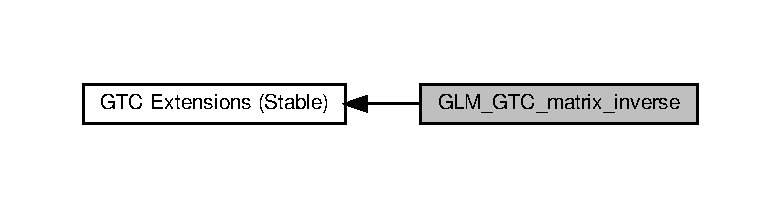
\includegraphics[width=350pt]{group__gtc__matrix__inverse}
\end{center}
\end{figure}
\subsection*{Functions}
\begin{DoxyCompactItemize}
\item 
{\footnotesize template$<$typename gen\+Type $>$ }\\\hyperlink{setup_8hpp_ab2d052de21a70539923e9bcbf6e83a51}{G\+L\+M\+\_\+\+F\+U\+N\+C\+\_\+\+D\+E\+CL} gen\+Type \hyperlink{group__gtc__matrix__inverse_gae0fcc5fc8783291f9702272de428fa0e}{glm\+::affine\+Inverse} (gen\+Type const \&m)
\item 
{\footnotesize template$<$typename gen\+Type $>$ }\\\hyperlink{setup_8hpp_ab2d052de21a70539923e9bcbf6e83a51}{G\+L\+M\+\_\+\+F\+U\+N\+C\+\_\+\+D\+E\+CL} gen\+Type\+::value\+\_\+type \hyperlink{group__gtc__matrix__inverse_gac23f1be9db49b929cc74e40f17f48593}{glm\+::inverse\+Transpose} (gen\+Type const \&m)
\end{DoxyCompactItemize}


\subsection{Detailed Description}
Defines additional matrix inverting functions. $<$\hyperlink{matrix__inverse_8hpp}{glm/gtc/matrix\+\_\+inverse.\+hpp}$>$ need to be included to use these functionalities. 

\subsection{Function Documentation}
\mbox{\Hypertarget{group__gtc__matrix__inverse_gae0fcc5fc8783291f9702272de428fa0e}\label{group__gtc__matrix__inverse_gae0fcc5fc8783291f9702272de428fa0e}} 
\index{G\+L\+M\+\_\+\+G\+T\+C\+\_\+matrix\+\_\+inverse@{G\+L\+M\+\_\+\+G\+T\+C\+\_\+matrix\+\_\+inverse}!affine\+Inverse@{affine\+Inverse}}
\index{affine\+Inverse@{affine\+Inverse}!G\+L\+M\+\_\+\+G\+T\+C\+\_\+matrix\+\_\+inverse@{G\+L\+M\+\_\+\+G\+T\+C\+\_\+matrix\+\_\+inverse}}
\subsubsection{\texorpdfstring{affine\+Inverse()}{affineInverse()}}
{\footnotesize\ttfamily template$<$typename gen\+Type $>$ \\
\hyperlink{setup_8hpp_ab2d052de21a70539923e9bcbf6e83a51}{G\+L\+M\+\_\+\+F\+U\+N\+C\+\_\+\+D\+E\+CL} gen\+Type glm\+::affine\+Inverse (\begin{DoxyParamCaption}\item[{gen\+Type const \&}]{m }\end{DoxyParamCaption})}

Fast matrix inverse for affine matrix.


\begin{DoxyParams}{Parameters}
{\em m} & Input matrix to invert. \\
\hline
\end{DoxyParams}

\begin{DoxyTemplParams}{Template Parameters}
{\em gen\+Type} & Squared floating-\/point matrix\+: half, float or double. Inverse of matrix based of half-\/precision floating point value is highly innacurate. \\
\hline
\end{DoxyTemplParams}
\begin{DoxySeeAlso}{See also}
\hyperlink{group__gtc__matrix__inverse}{G\+L\+M\+\_\+\+G\+T\+C\+\_\+matrix\+\_\+inverse} 
\end{DoxySeeAlso}
\mbox{\Hypertarget{group__gtc__matrix__inverse_gac23f1be9db49b929cc74e40f17f48593}\label{group__gtc__matrix__inverse_gac23f1be9db49b929cc74e40f17f48593}} 
\index{G\+L\+M\+\_\+\+G\+T\+C\+\_\+matrix\+\_\+inverse@{G\+L\+M\+\_\+\+G\+T\+C\+\_\+matrix\+\_\+inverse}!inverse\+Transpose@{inverse\+Transpose}}
\index{inverse\+Transpose@{inverse\+Transpose}!G\+L\+M\+\_\+\+G\+T\+C\+\_\+matrix\+\_\+inverse@{G\+L\+M\+\_\+\+G\+T\+C\+\_\+matrix\+\_\+inverse}}
\subsubsection{\texorpdfstring{inverse\+Transpose()}{inverseTranspose()}}
{\footnotesize\ttfamily template$<$typename gen\+Type $>$ \\
\hyperlink{setup_8hpp_ab2d052de21a70539923e9bcbf6e83a51}{G\+L\+M\+\_\+\+F\+U\+N\+C\+\_\+\+D\+E\+CL} gen\+Type\+::value\+\_\+type glm\+::inverse\+Transpose (\begin{DoxyParamCaption}\item[{gen\+Type const \&}]{m }\end{DoxyParamCaption})}

Compute the inverse transpose of a matrix.


\begin{DoxyParams}{Parameters}
{\em m} & Input matrix to invert transpose. \\
\hline
\end{DoxyParams}

\begin{DoxyTemplParams}{Template Parameters}
{\em gen\+Type} & Squared floating-\/point matrix\+: half, float or double. Inverse of matrix based of half-\/precision floating point value is highly innacurate. \\
\hline
\end{DoxyTemplParams}
\begin{DoxySeeAlso}{See also}
\hyperlink{group__gtc__matrix__inverse}{G\+L\+M\+\_\+\+G\+T\+C\+\_\+matrix\+\_\+inverse} 
\end{DoxySeeAlso}

\hypertarget{group__gtc__matrix__transform}{}\section{G\+L\+M\+\_\+\+G\+T\+C\+\_\+matrix\+\_\+transform}
\label{group__gtc__matrix__transform}\index{G\+L\+M\+\_\+\+G\+T\+C\+\_\+matrix\+\_\+transform@{G\+L\+M\+\_\+\+G\+T\+C\+\_\+matrix\+\_\+transform}}


Defines functions that generate common transformation matrices.  


Collaboration diagram for G\+L\+M\+\_\+\+G\+T\+C\+\_\+matrix\+\_\+transform\+:\nopagebreak
\begin{figure}[H]
\begin{center}
\leavevmode
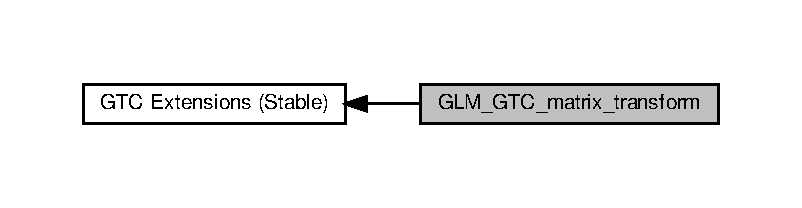
\includegraphics[width=350pt]{group__gtc__matrix__transform}
\end{center}
\end{figure}
\subsection*{Functions}
\begin{DoxyCompactItemize}
\item 
{\footnotesize template$<$typename T , precision P$>$ }\\\hyperlink{setup_8hpp_ab2d052de21a70539923e9bcbf6e83a51}{G\+L\+M\+\_\+\+F\+U\+N\+C\+\_\+\+D\+E\+CL} \hyperlink{structglm_1_1detail_1_1tmat4x4}{detail\+::tmat4x4}$<$ T, P $>$ \hyperlink{group__gtc__matrix__transform_ga1501de0fa580dcc491b67e0685bbc7c2}{glm\+::translate} (\hyperlink{structglm_1_1detail_1_1tmat4x4}{detail\+::tmat4x4}$<$ T, P $>$ const \&m, \hyperlink{structglm_1_1detail_1_1tvec3}{detail\+::tvec3}$<$ T, P $>$ const \&v)
\item 
{\footnotesize template$<$typename T , precision P$>$ }\\\hyperlink{setup_8hpp_ab2d052de21a70539923e9bcbf6e83a51}{G\+L\+M\+\_\+\+F\+U\+N\+C\+\_\+\+D\+E\+CL} \hyperlink{structglm_1_1detail_1_1tmat4x4}{detail\+::tmat4x4}$<$ T, P $>$ \hyperlink{group__gtc__matrix__transform_ga61e65a3bb227c267d1a15113d1056fb1}{glm\+::rotate} (\hyperlink{structglm_1_1detail_1_1tmat4x4}{detail\+::tmat4x4}$<$ T, P $>$ const \&m, T const \&\hyperlink{group__gtc__quaternion_ga23a3fc7ada5bbb665ff84c92c6e0542c}{angle}, \hyperlink{structglm_1_1detail_1_1tvec3}{detail\+::tvec3}$<$ T, P $>$ const \&\hyperlink{group__gtc__quaternion_ga8eef9f8c3f2e4836dccf09df975b20fb}{axis})
\item 
{\footnotesize template$<$typename T , precision P$>$ }\\\hyperlink{setup_8hpp_ab2d052de21a70539923e9bcbf6e83a51}{G\+L\+M\+\_\+\+F\+U\+N\+C\+\_\+\+D\+E\+CL} \hyperlink{structglm_1_1detail_1_1tmat4x4}{detail\+::tmat4x4}$<$ T, P $>$ \hyperlink{group__gtc__matrix__transform_gabd40959f269abd16c256a4f59ab03d62}{glm\+::scale} (\hyperlink{structglm_1_1detail_1_1tmat4x4}{detail\+::tmat4x4}$<$ T, P $>$ const \&m, \hyperlink{structglm_1_1detail_1_1tvec3}{detail\+::tvec3}$<$ T, P $>$ const \&v)
\item 
{\footnotesize template$<$typename T $>$ }\\\hyperlink{setup_8hpp_ab2d052de21a70539923e9bcbf6e83a51}{G\+L\+M\+\_\+\+F\+U\+N\+C\+\_\+\+D\+E\+CL} \hyperlink{structglm_1_1detail_1_1tmat4x4}{detail\+::tmat4x4}$<$ T, \hyperlink{namespaceglm_a0f04f086094c747d227af4425893f545a9d21ccd8b5a009ec7eb7677befc3bf51}{defaultp} $>$ \hyperlink{group__gtc__matrix__transform_gac393e9262776e4980731c386123e4377}{glm\+::ortho} (T const \&left, T const \&right, T const \&bottom, T const \&top, T const \&z\+Near, T const \&z\+Far)
\item 
{\footnotesize template$<$typename T $>$ }\\\hyperlink{setup_8hpp_ab2d052de21a70539923e9bcbf6e83a51}{G\+L\+M\+\_\+\+F\+U\+N\+C\+\_\+\+D\+E\+CL} \hyperlink{structglm_1_1detail_1_1tmat4x4}{detail\+::tmat4x4}$<$ T, \hyperlink{namespaceglm_a0f04f086094c747d227af4425893f545a9d21ccd8b5a009ec7eb7677befc3bf51}{defaultp} $>$ \hyperlink{group__gtc__matrix__transform_gab03587bce3510aa5d2f4e5f1be6c2370}{glm\+::ortho} (T const \&left, T const \&right, T const \&bottom, T const \&top)
\item 
{\footnotesize template$<$typename T $>$ }\\\hyperlink{setup_8hpp_ab2d052de21a70539923e9bcbf6e83a51}{G\+L\+M\+\_\+\+F\+U\+N\+C\+\_\+\+D\+E\+CL} \hyperlink{structglm_1_1detail_1_1tmat4x4}{detail\+::tmat4x4}$<$ T, \hyperlink{namespaceglm_a0f04f086094c747d227af4425893f545a9d21ccd8b5a009ec7eb7677befc3bf51}{defaultp} $>$ \hyperlink{group__gtc__matrix__transform_ga486d3d6819c04880559f3dccd38f9f58}{glm\+::frustum} (T const \&left, T const \&right, T const \&bottom, T const \&top, T const \&near, T const \&far)
\item 
{\footnotesize template$<$typename T $>$ }\\\hyperlink{setup_8hpp_ab2d052de21a70539923e9bcbf6e83a51}{G\+L\+M\+\_\+\+F\+U\+N\+C\+\_\+\+D\+E\+CL} \hyperlink{structglm_1_1detail_1_1tmat4x4}{detail\+::tmat4x4}$<$ T, \hyperlink{namespaceglm_a0f04f086094c747d227af4425893f545a9d21ccd8b5a009ec7eb7677befc3bf51}{defaultp} $>$ \hyperlink{group__gtc__matrix__transform_ga6c82aa0ea748cfbb16887d81cf6c5a10}{glm\+::perspective} (T const \&fovy, T const \&aspect, T const \&near, T const \&far)
\item 
{\footnotesize template$<$typename T $>$ }\\\hyperlink{setup_8hpp_ab2d052de21a70539923e9bcbf6e83a51}{G\+L\+M\+\_\+\+F\+U\+N\+C\+\_\+\+D\+E\+CL} \hyperlink{structglm_1_1detail_1_1tmat4x4}{detail\+::tmat4x4}$<$ T, \hyperlink{namespaceglm_a0f04f086094c747d227af4425893f545a9d21ccd8b5a009ec7eb7677befc3bf51}{defaultp} $>$ \hyperlink{group__gtc__matrix__transform_gac00bf68d4f7ec62380b84c5354567f71}{glm\+::perspective\+Fov} (T const \&fov, T const \&width, T const \&height, T const \&near, T const \&far)
\item 
{\footnotesize template$<$typename T $>$ }\\\hyperlink{setup_8hpp_ab2d052de21a70539923e9bcbf6e83a51}{G\+L\+M\+\_\+\+F\+U\+N\+C\+\_\+\+D\+E\+CL} \hyperlink{structglm_1_1detail_1_1tmat4x4}{detail\+::tmat4x4}$<$ T, \hyperlink{namespaceglm_a0f04f086094c747d227af4425893f545a9d21ccd8b5a009ec7eb7677befc3bf51}{defaultp} $>$ \hyperlink{group__gtc__matrix__transform_ga63ba1ddb9c4a08d4e58becd0dc5b725a}{glm\+::infinite\+Perspective} (T fovy, T aspect, T near)
\item 
{\footnotesize template$<$typename T $>$ }\\\hyperlink{setup_8hpp_ab2d052de21a70539923e9bcbf6e83a51}{G\+L\+M\+\_\+\+F\+U\+N\+C\+\_\+\+D\+E\+CL} \hyperlink{structglm_1_1detail_1_1tmat4x4}{detail\+::tmat4x4}$<$ T, \hyperlink{namespaceglm_a0f04f086094c747d227af4425893f545a9d21ccd8b5a009ec7eb7677befc3bf51}{defaultp} $>$ \hyperlink{group__gtc__matrix__transform_ga9d67732836d71a79dc21eb8f87603cb7}{glm\+::tweaked\+Infinite\+Perspective} (T fovy, T aspect, T near)
\item 
{\footnotesize template$<$typename T $>$ }\\\hyperlink{setup_8hpp_ab2d052de21a70539923e9bcbf6e83a51}{G\+L\+M\+\_\+\+F\+U\+N\+C\+\_\+\+D\+E\+CL} \hyperlink{structglm_1_1detail_1_1tmat4x4}{detail\+::tmat4x4}$<$ T, \hyperlink{namespaceglm_a0f04f086094c747d227af4425893f545a9d21ccd8b5a009ec7eb7677befc3bf51}{defaultp} $>$ \hyperlink{group__gtc__matrix__transform_gade8abc58c0ac541163e872eb66f3e5de}{glm\+::tweaked\+Infinite\+Perspective} (T fovy, T aspect, T near, T ep)
\item 
{\footnotesize template$<$typename T , typename U , precision P$>$ }\\\hyperlink{setup_8hpp_ab2d052de21a70539923e9bcbf6e83a51}{G\+L\+M\+\_\+\+F\+U\+N\+C\+\_\+\+D\+E\+CL} \hyperlink{structglm_1_1detail_1_1tvec3}{detail\+::tvec3}$<$ T, P $>$ \hyperlink{group__gtc__matrix__transform_ga41227b7b98882dcbaa8dab52df372c7b}{glm\+::project} (\hyperlink{structglm_1_1detail_1_1tvec3}{detail\+::tvec3}$<$ T, P $>$ const \&obj, \hyperlink{structglm_1_1detail_1_1tmat4x4}{detail\+::tmat4x4}$<$ T, P $>$ const \&model, \hyperlink{structglm_1_1detail_1_1tmat4x4}{detail\+::tmat4x4}$<$ T, P $>$ const \&\hyperlink{group__gtx__projection_gadf29123bcf748fc9d6fb0998192184cf}{proj}, \hyperlink{structglm_1_1detail_1_1tvec4}{detail\+::tvec4}$<$ U, P $>$ const \&viewport)
\item 
{\footnotesize template$<$typename T , typename U , precision P$>$ }\\\hyperlink{setup_8hpp_ab2d052de21a70539923e9bcbf6e83a51}{G\+L\+M\+\_\+\+F\+U\+N\+C\+\_\+\+D\+E\+CL} \hyperlink{structglm_1_1detail_1_1tvec3}{detail\+::tvec3}$<$ T, P $>$ \hyperlink{group__gtc__matrix__transform_ga4b0a9086d15e2a743ecd7b6128146af1}{glm\+::un\+Project} (\hyperlink{structglm_1_1detail_1_1tvec3}{detail\+::tvec3}$<$ T, P $>$ const \&win, \hyperlink{structglm_1_1detail_1_1tmat4x4}{detail\+::tmat4x4}$<$ T, P $>$ const \&model, \hyperlink{structglm_1_1detail_1_1tmat4x4}{detail\+::tmat4x4}$<$ T, P $>$ const \&\hyperlink{group__gtx__projection_gadf29123bcf748fc9d6fb0998192184cf}{proj}, \hyperlink{structglm_1_1detail_1_1tvec4}{detail\+::tvec4}$<$ U, P $>$ const \&viewport)
\item 
{\footnotesize template$<$typename T , precision P, typename U $>$ }\\\hyperlink{setup_8hpp_ab2d052de21a70539923e9bcbf6e83a51}{G\+L\+M\+\_\+\+F\+U\+N\+C\+\_\+\+D\+E\+CL} \hyperlink{structglm_1_1detail_1_1tmat4x4}{detail\+::tmat4x4}$<$ T, P $>$ \hyperlink{group__gtc__matrix__transform_ga0fb64f04bf5ad52523fcd4b10b46aff6}{glm\+::pick\+Matrix} (\hyperlink{structglm_1_1detail_1_1tvec2}{detail\+::tvec2}$<$ T, P $>$ const \&center, \hyperlink{structglm_1_1detail_1_1tvec2}{detail\+::tvec2}$<$ T, P $>$ const \&delta, \hyperlink{structglm_1_1detail_1_1tvec4}{detail\+::tvec4}$<$ U, P $>$ const \&viewport)
\item 
{\footnotesize template$<$typename T , precision P$>$ }\\\hyperlink{setup_8hpp_ab2d052de21a70539923e9bcbf6e83a51}{G\+L\+M\+\_\+\+F\+U\+N\+C\+\_\+\+D\+E\+CL} \hyperlink{structglm_1_1detail_1_1tmat4x4}{detail\+::tmat4x4}$<$ T, P $>$ \hyperlink{group__gtc__matrix__transform_ga454fdf3163c2779eeeeeb9d75907ce97}{glm\+::look\+At} (\hyperlink{structglm_1_1detail_1_1tvec3}{detail\+::tvec3}$<$ T, P $>$ const \&eye, \hyperlink{structglm_1_1detail_1_1tvec3}{detail\+::tvec3}$<$ T, P $>$ const \&center, \hyperlink{structglm_1_1detail_1_1tvec3}{detail\+::tvec3}$<$ T, P $>$ const \&up)
\end{DoxyCompactItemize}


\subsection{Detailed Description}
Defines functions that generate common transformation matrices. 

The matrices generated by this extension use standard Open\+GL fixed-\/function conventions. For example, the look\+At function generates a transform from world space into the specific eye space that the projective matrix functions (perspective, ortho, etc) are designed to expect. The Open\+GL compatibility specifications defines the particular layout of this eye space.

$<$\hyperlink{matrix__transform_8hpp}{glm/gtc/matrix\+\_\+transform.\+hpp}$>$ need to be included to use these functionalities. 

\subsection{Function Documentation}
\mbox{\Hypertarget{group__gtc__matrix__transform_ga486d3d6819c04880559f3dccd38f9f58}\label{group__gtc__matrix__transform_ga486d3d6819c04880559f3dccd38f9f58}} 
\index{G\+L\+M\+\_\+\+G\+T\+C\+\_\+matrix\+\_\+transform@{G\+L\+M\+\_\+\+G\+T\+C\+\_\+matrix\+\_\+transform}!frustum@{frustum}}
\index{frustum@{frustum}!G\+L\+M\+\_\+\+G\+T\+C\+\_\+matrix\+\_\+transform@{G\+L\+M\+\_\+\+G\+T\+C\+\_\+matrix\+\_\+transform}}
\subsubsection{\texorpdfstring{frustum()}{frustum()}}
{\footnotesize\ttfamily template$<$typename T $>$ \\
\hyperlink{setup_8hpp_ab2d052de21a70539923e9bcbf6e83a51}{G\+L\+M\+\_\+\+F\+U\+N\+C\+\_\+\+D\+E\+CL} \hyperlink{structglm_1_1detail_1_1tmat4x4}{detail\+::tmat4x4}$<$T, \hyperlink{namespaceglm_a0f04f086094c747d227af4425893f545a9d21ccd8b5a009ec7eb7677befc3bf51}{defaultp}$>$ glm\+::frustum (\begin{DoxyParamCaption}\item[{T const \&}]{left,  }\item[{T const \&}]{right,  }\item[{T const \&}]{bottom,  }\item[{T const \&}]{top,  }\item[{T const \&}]{near,  }\item[{T const \&}]{far }\end{DoxyParamCaption})}

Creates a frustum matrix.


\begin{DoxyParams}{Parameters}
{\em left} & \\
\hline
{\em right} & \\
\hline
{\em bottom} & \\
\hline
{\em top} & \\
\hline
{\em near} & \\
\hline
{\em far} & \\
\hline
\end{DoxyParams}

\begin{DoxyTemplParams}{Template Parameters}
{\em T} & Value type used to build the matrix. Currently supported\+: half (not recommanded), float or double. \\
\hline
\end{DoxyTemplParams}
\begin{DoxySeeAlso}{See also}
\hyperlink{group__gtc__matrix__transform}{G\+L\+M\+\_\+\+G\+T\+C\+\_\+matrix\+\_\+transform} 
\end{DoxySeeAlso}


Definition at line 197 of file matrix\+\_\+transform.\+inl.

\mbox{\Hypertarget{group__gtc__matrix__transform_ga63ba1ddb9c4a08d4e58becd0dc5b725a}\label{group__gtc__matrix__transform_ga63ba1ddb9c4a08d4e58becd0dc5b725a}} 
\index{G\+L\+M\+\_\+\+G\+T\+C\+\_\+matrix\+\_\+transform@{G\+L\+M\+\_\+\+G\+T\+C\+\_\+matrix\+\_\+transform}!infinite\+Perspective@{infinite\+Perspective}}
\index{infinite\+Perspective@{infinite\+Perspective}!G\+L\+M\+\_\+\+G\+T\+C\+\_\+matrix\+\_\+transform@{G\+L\+M\+\_\+\+G\+T\+C\+\_\+matrix\+\_\+transform}}
\subsubsection{\texorpdfstring{infinite\+Perspective()}{infinitePerspective()}}
{\footnotesize\ttfamily template$<$typename T $>$ \\
\hyperlink{setup_8hpp_ab2d052de21a70539923e9bcbf6e83a51}{G\+L\+M\+\_\+\+F\+U\+N\+C\+\_\+\+D\+E\+CL} \hyperlink{structglm_1_1detail_1_1tmat4x4}{detail\+::tmat4x4}$<$T, \hyperlink{namespaceglm_a0f04f086094c747d227af4425893f545a9d21ccd8b5a009ec7eb7677befc3bf51}{defaultp}$>$ glm\+::infinite\+Perspective (\begin{DoxyParamCaption}\item[{T}]{fovy,  }\item[{T}]{aspect,  }\item[{T}]{near }\end{DoxyParamCaption})}

Creates a matrix for a symmetric perspective-\/view frustum with far plane at infinite.


\begin{DoxyParams}{Parameters}
{\em fovy} & Expressed in radians if G\+L\+M\+\_\+\+F\+O\+R\+C\+E\+\_\+\+R\+A\+D\+I\+A\+NS is define or degrees otherwise. \\
\hline
{\em aspect} & \\
\hline
{\em near} & \\
\hline
\end{DoxyParams}

\begin{DoxyTemplParams}{Template Parameters}
{\em T} & Value type used to build the matrix. Currently supported\+: half (not recommanded), float or double. \\
\hline
\end{DoxyTemplParams}
\begin{DoxySeeAlso}{See also}
\hyperlink{group__gtc__matrix__transform}{G\+L\+M\+\_\+\+G\+T\+C\+\_\+matrix\+\_\+transform} 
\end{DoxySeeAlso}


Definition at line 281 of file matrix\+\_\+transform.\+inl.

\mbox{\Hypertarget{group__gtc__matrix__transform_ga454fdf3163c2779eeeeeb9d75907ce97}\label{group__gtc__matrix__transform_ga454fdf3163c2779eeeeeb9d75907ce97}} 
\index{G\+L\+M\+\_\+\+G\+T\+C\+\_\+matrix\+\_\+transform@{G\+L\+M\+\_\+\+G\+T\+C\+\_\+matrix\+\_\+transform}!look\+At@{look\+At}}
\index{look\+At@{look\+At}!G\+L\+M\+\_\+\+G\+T\+C\+\_\+matrix\+\_\+transform@{G\+L\+M\+\_\+\+G\+T\+C\+\_\+matrix\+\_\+transform}}
\subsubsection{\texorpdfstring{look\+At()}{lookAt()}}
{\footnotesize\ttfamily template$<$typename T , precision P$>$ \\
\hyperlink{setup_8hpp_ab2d052de21a70539923e9bcbf6e83a51}{G\+L\+M\+\_\+\+F\+U\+N\+C\+\_\+\+D\+E\+CL} \hyperlink{structglm_1_1detail_1_1tmat4x4}{detail\+::tmat4x4}$<$T, P$>$ glm\+::look\+At (\begin{DoxyParamCaption}\item[{\hyperlink{structglm_1_1detail_1_1tvec3}{detail\+::tvec3}$<$ T, P $>$ const \&}]{eye,  }\item[{\hyperlink{structglm_1_1detail_1_1tvec3}{detail\+::tvec3}$<$ T, P $>$ const \&}]{center,  }\item[{\hyperlink{structglm_1_1detail_1_1tvec3}{detail\+::tvec3}$<$ T, P $>$ const \&}]{up }\end{DoxyParamCaption})}

Build a look at view matrix.


\begin{DoxyParams}{Parameters}
{\em eye} & Position of the camera \\
\hline
{\em center} & Position where the camera is looking at \\
\hline
{\em up} & Normalized up vector, how the camera is oriented. Typically (0, 0, 1) \\
\hline
\end{DoxyParams}
\begin{DoxySeeAlso}{See also}
\hyperlink{group__gtc__matrix__transform}{G\+L\+M\+\_\+\+G\+T\+C\+\_\+matrix\+\_\+transform} 

-\/ \hyperlink{group__gtc__matrix__transform_ga486d3d6819c04880559f3dccd38f9f58}{frustum(\+T const \& left, T const \& right, T const \& bottom, T const \& top, T const \& near\+Val, T const \& far\+Val)} \hyperlink{group__gtc__matrix__transform_ga486d3d6819c04880559f3dccd38f9f58}{frustum(\+T const \& left, T const \& right, T const \& bottom, T const \& top, T const \& near\+Val, T const \& far\+Val)} 
\end{DoxySeeAlso}


Definition at line 417 of file matrix\+\_\+transform.\+inl.

\mbox{\Hypertarget{group__gtc__matrix__transform_gac393e9262776e4980731c386123e4377}\label{group__gtc__matrix__transform_gac393e9262776e4980731c386123e4377}} 
\index{G\+L\+M\+\_\+\+G\+T\+C\+\_\+matrix\+\_\+transform@{G\+L\+M\+\_\+\+G\+T\+C\+\_\+matrix\+\_\+transform}!ortho@{ortho}}
\index{ortho@{ortho}!G\+L\+M\+\_\+\+G\+T\+C\+\_\+matrix\+\_\+transform@{G\+L\+M\+\_\+\+G\+T\+C\+\_\+matrix\+\_\+transform}}
\subsubsection{\texorpdfstring{ortho()}{ortho()}\hspace{0.1cm}{\footnotesize\ttfamily [1/2]}}
{\footnotesize\ttfamily template$<$typename T $>$ \\
\hyperlink{setup_8hpp_ab2d052de21a70539923e9bcbf6e83a51}{G\+L\+M\+\_\+\+F\+U\+N\+C\+\_\+\+D\+E\+CL} \hyperlink{structglm_1_1detail_1_1tmat4x4}{detail\+::tmat4x4}$<$T, \hyperlink{namespaceglm_a0f04f086094c747d227af4425893f545a9d21ccd8b5a009ec7eb7677befc3bf51}{defaultp}$>$ glm\+::ortho (\begin{DoxyParamCaption}\item[{T const \&}]{left,  }\item[{T const \&}]{right,  }\item[{T const \&}]{bottom,  }\item[{T const \&}]{top,  }\item[{T const \&}]{z\+Near,  }\item[{T const \&}]{z\+Far }\end{DoxyParamCaption})}

Creates a matrix for an orthographic parallel viewing volume.


\begin{DoxyParams}{Parameters}
{\em left} & \\
\hline
{\em right} & \\
\hline
{\em bottom} & \\
\hline
{\em top} & \\
\hline
{\em z\+Near} & \\
\hline
{\em z\+Far} & \\
\hline
\end{DoxyParams}

\begin{DoxyTemplParams}{Template Parameters}
{\em T} & Value type used to build the matrix. Currently supported\+: half (not recommanded), float or double. \\
\hline
\end{DoxyTemplParams}
\begin{DoxySeeAlso}{See also}
\hyperlink{group__gtc__matrix__transform}{G\+L\+M\+\_\+\+G\+T\+C\+\_\+matrix\+\_\+transform} 

-\/ \hyperlink{group__gtc__matrix__transform_gab03587bce3510aa5d2f4e5f1be6c2370}{glm\+::ortho(\+T const \& left, T const \& right, T const \& bottom, T const \& top)} 
\end{DoxySeeAlso}


Definition at line 158 of file matrix\+\_\+transform.\+inl.

\mbox{\Hypertarget{group__gtc__matrix__transform_gab03587bce3510aa5d2f4e5f1be6c2370}\label{group__gtc__matrix__transform_gab03587bce3510aa5d2f4e5f1be6c2370}} 
\index{G\+L\+M\+\_\+\+G\+T\+C\+\_\+matrix\+\_\+transform@{G\+L\+M\+\_\+\+G\+T\+C\+\_\+matrix\+\_\+transform}!ortho@{ortho}}
\index{ortho@{ortho}!G\+L\+M\+\_\+\+G\+T\+C\+\_\+matrix\+\_\+transform@{G\+L\+M\+\_\+\+G\+T\+C\+\_\+matrix\+\_\+transform}}
\subsubsection{\texorpdfstring{ortho()}{ortho()}\hspace{0.1cm}{\footnotesize\ttfamily [2/2]}}
{\footnotesize\ttfamily template$<$typename T $>$ \\
\hyperlink{setup_8hpp_ab2d052de21a70539923e9bcbf6e83a51}{G\+L\+M\+\_\+\+F\+U\+N\+C\+\_\+\+D\+E\+CL} \hyperlink{structglm_1_1detail_1_1tmat4x4}{detail\+::tmat4x4}$<$T, \hyperlink{namespaceglm_a0f04f086094c747d227af4425893f545a9d21ccd8b5a009ec7eb7677befc3bf51}{defaultp}$>$ glm\+::ortho (\begin{DoxyParamCaption}\item[{T const \&}]{left,  }\item[{T const \&}]{right,  }\item[{T const \&}]{bottom,  }\item[{T const \&}]{top }\end{DoxyParamCaption})}

Creates a matrix for projecting two-\/dimensional coordinates onto the screen.


\begin{DoxyParams}{Parameters}
{\em left} & \\
\hline
{\em right} & \\
\hline
{\em bottom} & \\
\hline
{\em top} & \\
\hline
\end{DoxyParams}

\begin{DoxyTemplParams}{Template Parameters}
{\em T} & Value type used to build the matrix. Currently supported\+: half (not recommanded), float or double. \\
\hline
\end{DoxyTemplParams}
\begin{DoxySeeAlso}{See also}
\hyperlink{group__gtc__matrix__transform}{G\+L\+M\+\_\+\+G\+T\+C\+\_\+matrix\+\_\+transform} 

-\/ \hyperlink{group__gtc__matrix__transform_gac393e9262776e4980731c386123e4377}{glm\+::ortho(\+T const \& left, T const \& right, T const \& bottom, T const \& top, T const \& z\+Near, T const \& z\+Far)} 
\end{DoxySeeAlso}


Definition at line 179 of file matrix\+\_\+transform.\+inl.

\mbox{\Hypertarget{group__gtc__matrix__transform_ga6c82aa0ea748cfbb16887d81cf6c5a10}\label{group__gtc__matrix__transform_ga6c82aa0ea748cfbb16887d81cf6c5a10}} 
\index{G\+L\+M\+\_\+\+G\+T\+C\+\_\+matrix\+\_\+transform@{G\+L\+M\+\_\+\+G\+T\+C\+\_\+matrix\+\_\+transform}!perspective@{perspective}}
\index{perspective@{perspective}!G\+L\+M\+\_\+\+G\+T\+C\+\_\+matrix\+\_\+transform@{G\+L\+M\+\_\+\+G\+T\+C\+\_\+matrix\+\_\+transform}}
\subsubsection{\texorpdfstring{perspective()}{perspective()}}
{\footnotesize\ttfamily template$<$typename T $>$ \\
\hyperlink{setup_8hpp_ab2d052de21a70539923e9bcbf6e83a51}{G\+L\+M\+\_\+\+F\+U\+N\+C\+\_\+\+D\+E\+CL} \hyperlink{structglm_1_1detail_1_1tmat4x4}{detail\+::tmat4x4}$<$T, \hyperlink{namespaceglm_a0f04f086094c747d227af4425893f545a9d21ccd8b5a009ec7eb7677befc3bf51}{defaultp}$>$ glm\+::perspective (\begin{DoxyParamCaption}\item[{T const \&}]{fovy,  }\item[{T const \&}]{aspect,  }\item[{T const \&}]{near,  }\item[{T const \&}]{far }\end{DoxyParamCaption})}

Creates a matrix for a symetric perspective-\/view frustum.


\begin{DoxyParams}{Parameters}
{\em fovy} & Expressed in radians if G\+L\+M\+\_\+\+F\+O\+R\+C\+E\+\_\+\+R\+A\+D\+I\+A\+NS is define or degrees otherwise. \\
\hline
{\em aspect} & \\
\hline
{\em near} & \\
\hline
{\em far} & \\
\hline
\end{DoxyParams}

\begin{DoxyTemplParams}{Template Parameters}
{\em T} & Value type used to build the matrix. Currently supported\+: half (not recommanded), float or double. \\
\hline
\end{DoxyTemplParams}
\begin{DoxySeeAlso}{See also}
\hyperlink{group__gtc__matrix__transform}{G\+L\+M\+\_\+\+G\+T\+C\+\_\+matrix\+\_\+transform} 
\end{DoxySeeAlso}


Definition at line 219 of file matrix\+\_\+transform.\+inl.

\mbox{\Hypertarget{group__gtc__matrix__transform_gac00bf68d4f7ec62380b84c5354567f71}\label{group__gtc__matrix__transform_gac00bf68d4f7ec62380b84c5354567f71}} 
\index{G\+L\+M\+\_\+\+G\+T\+C\+\_\+matrix\+\_\+transform@{G\+L\+M\+\_\+\+G\+T\+C\+\_\+matrix\+\_\+transform}!perspective\+Fov@{perspective\+Fov}}
\index{perspective\+Fov@{perspective\+Fov}!G\+L\+M\+\_\+\+G\+T\+C\+\_\+matrix\+\_\+transform@{G\+L\+M\+\_\+\+G\+T\+C\+\_\+matrix\+\_\+transform}}
\subsubsection{\texorpdfstring{perspective\+Fov()}{perspectiveFov()}}
{\footnotesize\ttfamily template$<$typename T $>$ \\
\hyperlink{setup_8hpp_ab2d052de21a70539923e9bcbf6e83a51}{G\+L\+M\+\_\+\+F\+U\+N\+C\+\_\+\+D\+E\+CL} \hyperlink{structglm_1_1detail_1_1tmat4x4}{detail\+::tmat4x4}$<$T, \hyperlink{namespaceglm_a0f04f086094c747d227af4425893f545a9d21ccd8b5a009ec7eb7677befc3bf51}{defaultp}$>$ glm\+::perspective\+Fov (\begin{DoxyParamCaption}\item[{T const \&}]{fov,  }\item[{T const \&}]{width,  }\item[{T const \&}]{height,  }\item[{T const \&}]{near,  }\item[{T const \&}]{far }\end{DoxyParamCaption})}

Builds a perspective projection matrix based on a field of view.


\begin{DoxyParams}{Parameters}
{\em fov} & Expressed in radians if G\+L\+M\+\_\+\+F\+O\+R\+C\+E\+\_\+\+R\+A\+D\+I\+A\+NS is define or degrees otherwise. \\
\hline
{\em width} & \\
\hline
{\em height} & \\
\hline
{\em near} & \\
\hline
{\em far} & \\
\hline
\end{DoxyParams}

\begin{DoxyTemplParams}{Template Parameters}
{\em T} & Value type used to build the matrix. Currently supported\+: half (not recommanded), float or double. \\
\hline
\end{DoxyTemplParams}
\begin{DoxySeeAlso}{See also}
\hyperlink{group__gtc__matrix__transform}{G\+L\+M\+\_\+\+G\+T\+C\+\_\+matrix\+\_\+transform} 
\end{DoxySeeAlso}
todo max(width , Height) / min(width , Height)? 

Definition at line 249 of file matrix\+\_\+transform.\+inl.

\mbox{\Hypertarget{group__gtc__matrix__transform_ga0fb64f04bf5ad52523fcd4b10b46aff6}\label{group__gtc__matrix__transform_ga0fb64f04bf5ad52523fcd4b10b46aff6}} 
\index{G\+L\+M\+\_\+\+G\+T\+C\+\_\+matrix\+\_\+transform@{G\+L\+M\+\_\+\+G\+T\+C\+\_\+matrix\+\_\+transform}!pick\+Matrix@{pick\+Matrix}}
\index{pick\+Matrix@{pick\+Matrix}!G\+L\+M\+\_\+\+G\+T\+C\+\_\+matrix\+\_\+transform@{G\+L\+M\+\_\+\+G\+T\+C\+\_\+matrix\+\_\+transform}}
\subsubsection{\texorpdfstring{pick\+Matrix()}{pickMatrix()}}
{\footnotesize\ttfamily template$<$typename T , precision P, typename U $>$ \\
\hyperlink{setup_8hpp_ab2d052de21a70539923e9bcbf6e83a51}{G\+L\+M\+\_\+\+F\+U\+N\+C\+\_\+\+D\+E\+CL} \hyperlink{structglm_1_1detail_1_1tmat4x4}{detail\+::tmat4x4}$<$T, P$>$ glm\+::pick\+Matrix (\begin{DoxyParamCaption}\item[{\hyperlink{structglm_1_1detail_1_1tvec2}{detail\+::tvec2}$<$ T, P $>$ const \&}]{center,  }\item[{\hyperlink{structglm_1_1detail_1_1tvec2}{detail\+::tvec2}$<$ T, P $>$ const \&}]{delta,  }\item[{\hyperlink{structglm_1_1detail_1_1tvec4}{detail\+::tvec4}$<$ U, P $>$ const \&}]{viewport }\end{DoxyParamCaption})}

Define a picking region


\begin{DoxyParams}{Parameters}
{\em center} & \\
\hline
{\em delta} & \\
\hline
{\em viewport} & \\
\hline
\end{DoxyParams}

\begin{DoxyTemplParams}{Template Parameters}
{\em T} & Native type used for the computation. Currently supported\+: half (not recommanded), float or double. \\
\hline
{\em U} & Currently supported\+: Floating-\/point types and integer types. \\
\hline
\end{DoxyTemplParams}
\begin{DoxySeeAlso}{See also}
\hyperlink{group__gtc__matrix__transform}{G\+L\+M\+\_\+\+G\+T\+C\+\_\+matrix\+\_\+transform} 
\end{DoxySeeAlso}


Definition at line 393 of file matrix\+\_\+transform.\+inl.

\mbox{\Hypertarget{group__gtc__matrix__transform_ga41227b7b98882dcbaa8dab52df372c7b}\label{group__gtc__matrix__transform_ga41227b7b98882dcbaa8dab52df372c7b}} 
\index{G\+L\+M\+\_\+\+G\+T\+C\+\_\+matrix\+\_\+transform@{G\+L\+M\+\_\+\+G\+T\+C\+\_\+matrix\+\_\+transform}!project@{project}}
\index{project@{project}!G\+L\+M\+\_\+\+G\+T\+C\+\_\+matrix\+\_\+transform@{G\+L\+M\+\_\+\+G\+T\+C\+\_\+matrix\+\_\+transform}}
\subsubsection{\texorpdfstring{project()}{project()}}
{\footnotesize\ttfamily template$<$typename T , typename U , precision P$>$ \\
\hyperlink{setup_8hpp_ab2d052de21a70539923e9bcbf6e83a51}{G\+L\+M\+\_\+\+F\+U\+N\+C\+\_\+\+D\+E\+CL} \hyperlink{structglm_1_1detail_1_1tvec3}{detail\+::tvec3}$<$T, P$>$ glm\+::project (\begin{DoxyParamCaption}\item[{\hyperlink{structglm_1_1detail_1_1tvec3}{detail\+::tvec3}$<$ T, P $>$ const \&}]{obj,  }\item[{\hyperlink{structglm_1_1detail_1_1tmat4x4}{detail\+::tmat4x4}$<$ T, P $>$ const \&}]{model,  }\item[{\hyperlink{structglm_1_1detail_1_1tmat4x4}{detail\+::tmat4x4}$<$ T, P $>$ const \&}]{proj,  }\item[{\hyperlink{structglm_1_1detail_1_1tvec4}{detail\+::tvec4}$<$ U, P $>$ const \&}]{viewport }\end{DoxyParamCaption})}

Map the specified object coordinates (obj.\+x, obj.\+y, obj.\+z) into window coordinates.


\begin{DoxyParams}{Parameters}
{\em obj} & \\
\hline
{\em model} & \\
\hline
{\em proj} & \\
\hline
{\em viewport} & \\
\hline
\end{DoxyParams}

\begin{DoxyTemplParams}{Template Parameters}
{\em T} & Native type used for the computation. Currently supported\+: half (not recommanded), float or double. \\
\hline
{\em U} & Currently supported\+: Floating-\/point types and integer types. \\
\hline
\end{DoxyTemplParams}
\begin{DoxySeeAlso}{See also}
\hyperlink{group__gtc__matrix__transform}{G\+L\+M\+\_\+\+G\+T\+C\+\_\+matrix\+\_\+transform} 
\end{DoxySeeAlso}


Definition at line 350 of file matrix\+\_\+transform.\+inl.

\mbox{\Hypertarget{group__gtc__matrix__transform_ga61e65a3bb227c267d1a15113d1056fb1}\label{group__gtc__matrix__transform_ga61e65a3bb227c267d1a15113d1056fb1}} 
\index{G\+L\+M\+\_\+\+G\+T\+C\+\_\+matrix\+\_\+transform@{G\+L\+M\+\_\+\+G\+T\+C\+\_\+matrix\+\_\+transform}!rotate@{rotate}}
\index{rotate@{rotate}!G\+L\+M\+\_\+\+G\+T\+C\+\_\+matrix\+\_\+transform@{G\+L\+M\+\_\+\+G\+T\+C\+\_\+matrix\+\_\+transform}}
\subsubsection{\texorpdfstring{rotate()}{rotate()}}
{\footnotesize\ttfamily template$<$typename T , precision P$>$ \\
\hyperlink{setup_8hpp_ab2d052de21a70539923e9bcbf6e83a51}{G\+L\+M\+\_\+\+F\+U\+N\+C\+\_\+\+D\+E\+CL} \hyperlink{structglm_1_1detail_1_1tmat4x4}{detail\+::tmat4x4}$<$T, P$>$ glm\+::rotate (\begin{DoxyParamCaption}\item[{\hyperlink{structglm_1_1detail_1_1tmat4x4}{detail\+::tmat4x4}$<$ T, P $>$ const \&}]{m,  }\item[{T const \&}]{angle,  }\item[{\hyperlink{structglm_1_1detail_1_1tvec3}{detail\+::tvec3}$<$ T, P $>$ const \&}]{axis }\end{DoxyParamCaption})}

Builds a rotation 4 $\ast$ 4 matrix created from an axis vector and an angle.


\begin{DoxyParams}{Parameters}
{\em m} & Input matrix multiplied by this rotation matrix. \\
\hline
{\em angle} & Rotation angle expressed in radians if G\+L\+M\+\_\+\+F\+O\+R\+C\+E\+\_\+\+R\+A\+D\+I\+A\+NS is define or degrees otherwise. \\
\hline
{\em axis} & Rotation axis, recommanded to be normalized. \\
\hline
\end{DoxyParams}

\begin{DoxyTemplParams}{Template Parameters}
{\em T} & Value type used to build the matrix. Supported\+: half, float or double. \\
\hline
\end{DoxyTemplParams}
\begin{DoxySeeAlso}{See also}
\hyperlink{group__gtc__matrix__transform}{G\+L\+M\+\_\+\+G\+T\+C\+\_\+matrix\+\_\+transform} 

\hyperlink{group__gtx__transform}{G\+L\+M\+\_\+\+G\+T\+X\+\_\+transform} 

-\/ rotate(\+T angle, T x, T y, T z) 

-\/ rotate(detail\+::tmat4x4$<$\+T, P$>$ const \& m, T angle, T x, T y, T z) 

-\/ \hyperlink{group__gtx__transform_gaac4ccdbf699a62fe6429005512c0cda5}{rotate(\+T angle, detail\+::tvec3$<$\+T, P$>$ const \& v)} 
\end{DoxySeeAlso}


Definition at line 49 of file matrix\+\_\+transform.\+inl.

\mbox{\Hypertarget{group__gtc__matrix__transform_gabd40959f269abd16c256a4f59ab03d62}\label{group__gtc__matrix__transform_gabd40959f269abd16c256a4f59ab03d62}} 
\index{G\+L\+M\+\_\+\+G\+T\+C\+\_\+matrix\+\_\+transform@{G\+L\+M\+\_\+\+G\+T\+C\+\_\+matrix\+\_\+transform}!scale@{scale}}
\index{scale@{scale}!G\+L\+M\+\_\+\+G\+T\+C\+\_\+matrix\+\_\+transform@{G\+L\+M\+\_\+\+G\+T\+C\+\_\+matrix\+\_\+transform}}
\subsubsection{\texorpdfstring{scale()}{scale()}}
{\footnotesize\ttfamily template$<$typename T , precision P$>$ \\
\hyperlink{setup_8hpp_ab2d052de21a70539923e9bcbf6e83a51}{G\+L\+M\+\_\+\+F\+U\+N\+C\+\_\+\+D\+E\+CL} \hyperlink{structglm_1_1detail_1_1tmat4x4}{detail\+::tmat4x4}$<$T, P$>$ glm\+::scale (\begin{DoxyParamCaption}\item[{\hyperlink{structglm_1_1detail_1_1tmat4x4}{detail\+::tmat4x4}$<$ T, P $>$ const \&}]{m,  }\item[{\hyperlink{structglm_1_1detail_1_1tvec3}{detail\+::tvec3}$<$ T, P $>$ const \&}]{v }\end{DoxyParamCaption})}

Builds a scale 4 $\ast$ 4 matrix created from 3 scalars.


\begin{DoxyParams}{Parameters}
{\em m} & Input matrix multiplied by this scale matrix. \\
\hline
{\em v} & Ratio of scaling for each axis. \\
\hline
\end{DoxyParams}

\begin{DoxyTemplParams}{Template Parameters}
{\em T} & Value type used to build the matrix. Currently supported\+: half (not recommanded), float or double. \\
\hline
\end{DoxyTemplParams}
\begin{DoxySeeAlso}{See also}
\hyperlink{group__gtc__matrix__transform}{G\+L\+M\+\_\+\+G\+T\+C\+\_\+matrix\+\_\+transform} 

\hyperlink{group__gtx__transform}{G\+L\+M\+\_\+\+G\+T\+X\+\_\+transform} 

-\/ scale(\+T x, T y, T z) scale(\+T const \& x, T const \& y, T const \& z) 

-\/ scale(detail\+::tmat4x4$<$\+T, P$>$ const \& m, T x, T y, T z) 

-\/ \hyperlink{group__gtx__transform_ga80eb26a1eb382b7ab1e3631532d21103}{scale(detail\+::tvec3$<$\+T, P$>$ const \& v)} 
\end{DoxySeeAlso}


Definition at line 129 of file matrix\+\_\+transform.\+inl.

\mbox{\Hypertarget{group__gtc__matrix__transform_ga1501de0fa580dcc491b67e0685bbc7c2}\label{group__gtc__matrix__transform_ga1501de0fa580dcc491b67e0685bbc7c2}} 
\index{G\+L\+M\+\_\+\+G\+T\+C\+\_\+matrix\+\_\+transform@{G\+L\+M\+\_\+\+G\+T\+C\+\_\+matrix\+\_\+transform}!translate@{translate}}
\index{translate@{translate}!G\+L\+M\+\_\+\+G\+T\+C\+\_\+matrix\+\_\+transform@{G\+L\+M\+\_\+\+G\+T\+C\+\_\+matrix\+\_\+transform}}
\subsubsection{\texorpdfstring{translate()}{translate()}}
{\footnotesize\ttfamily template$<$typename T , precision P$>$ \\
\hyperlink{setup_8hpp_ab2d052de21a70539923e9bcbf6e83a51}{G\+L\+M\+\_\+\+F\+U\+N\+C\+\_\+\+D\+E\+CL} \hyperlink{structglm_1_1detail_1_1tmat4x4}{detail\+::tmat4x4}$<$T, P$>$ glm\+::translate (\begin{DoxyParamCaption}\item[{\hyperlink{structglm_1_1detail_1_1tmat4x4}{detail\+::tmat4x4}$<$ T, P $>$ const \&}]{m,  }\item[{\hyperlink{structglm_1_1detail_1_1tvec3}{detail\+::tvec3}$<$ T, P $>$ const \&}]{v }\end{DoxyParamCaption})}

Builds a translation 4 $\ast$ 4 matrix created from a vector of 3 components.


\begin{DoxyParams}{Parameters}
{\em m} & Input matrix multiplied by this translation matrix. \\
\hline
{\em v} & Coordinates of a translation vector. \\
\hline
\end{DoxyParams}

\begin{DoxyTemplParams}{Template Parameters}
{\em T} & Value type used to build the matrix. Currently supported\+: half (not recommanded), float or double. 
\begin{DoxyCode}
\textcolor{preprocessor}{#include <\hyperlink{third-party_2include_2glm_2glm_8hpp}{glm/glm.hpp}>}
\textcolor{preprocessor}{#include <\hyperlink{matrix__transform_8hpp}{glm/gtc/matrix\_transform.hpp}>}
...
glm::mat4 m = \hyperlink{group__gtc__matrix__transform_ga1501de0fa580dcc491b67e0685bbc7c2}{glm::translate}(\hyperlink{structglm_1_1detail_1_1tmat4x4}{glm::mat4}(1.0f), \hyperlink{structglm_1_1detail_1_1tvec3}{glm::vec3}(1.0f));
\textcolor{comment}{// m[0][0] == 1.0f, m[0][1] == 0.0f, m[0][2] == 0.0f, m[0][3] == 0.0f}
\textcolor{comment}{// m[1][0] == 0.0f, m[1][1] == 1.0f, m[1][2] == 0.0f, m[1][3] == 0.0f}
\textcolor{comment}{// m[2][0] == 0.0f, m[2][1] == 0.0f, m[2][2] == 1.0f, m[2][3] == 0.0f}
\textcolor{comment}{// m[3][0] == 1.0f, m[3][1] == 1.0f, m[3][2] == 1.0f, m[3][3] == 1.0f}
\end{DoxyCode}
 \\
\hline
\end{DoxyTemplParams}
\begin{DoxySeeAlso}{See also}
\hyperlink{group__gtc__matrix__transform}{G\+L\+M\+\_\+\+G\+T\+C\+\_\+matrix\+\_\+transform} 

\hyperlink{group__gtx__transform}{G\+L\+M\+\_\+\+G\+T\+X\+\_\+transform} 

-\/ translate(\+T x, T y, T z) 

-\/ translate(detail\+::tmat4x4$<$\+T, P$>$ const \& m, T x, T y, T z) 

-\/ \hyperlink{group__gtx__transform_ga8a2efce0917bf301cc0ea7afb428f688}{translate(detail\+::tvec3$<$\+T, P$>$ const \& v)} 
\end{DoxySeeAlso}


Definition at line 37 of file matrix\+\_\+transform.\+inl.

\mbox{\Hypertarget{group__gtc__matrix__transform_ga9d67732836d71a79dc21eb8f87603cb7}\label{group__gtc__matrix__transform_ga9d67732836d71a79dc21eb8f87603cb7}} 
\index{G\+L\+M\+\_\+\+G\+T\+C\+\_\+matrix\+\_\+transform@{G\+L\+M\+\_\+\+G\+T\+C\+\_\+matrix\+\_\+transform}!tweaked\+Infinite\+Perspective@{tweaked\+Infinite\+Perspective}}
\index{tweaked\+Infinite\+Perspective@{tweaked\+Infinite\+Perspective}!G\+L\+M\+\_\+\+G\+T\+C\+\_\+matrix\+\_\+transform@{G\+L\+M\+\_\+\+G\+T\+C\+\_\+matrix\+\_\+transform}}
\subsubsection{\texorpdfstring{tweaked\+Infinite\+Perspective()}{tweakedInfinitePerspective()}\hspace{0.1cm}{\footnotesize\ttfamily [1/2]}}
{\footnotesize\ttfamily template$<$typename T $>$ \\
\hyperlink{setup_8hpp_ab2d052de21a70539923e9bcbf6e83a51}{G\+L\+M\+\_\+\+F\+U\+N\+C\+\_\+\+D\+E\+CL} \hyperlink{structglm_1_1detail_1_1tmat4x4}{detail\+::tmat4x4}$<$T, \hyperlink{namespaceglm_a0f04f086094c747d227af4425893f545a9d21ccd8b5a009ec7eb7677befc3bf51}{defaultp}$>$ glm\+::tweaked\+Infinite\+Perspective (\begin{DoxyParamCaption}\item[{T}]{fovy,  }\item[{T}]{aspect,  }\item[{T}]{near }\end{DoxyParamCaption})}

Creates a matrix for a symmetric perspective-\/view frustum with far plane at infinite for graphics hardware that doesn\textquotesingle{}t support depth clamping.


\begin{DoxyParams}{Parameters}
{\em fovy} & Expressed in radians if G\+L\+M\+\_\+\+F\+O\+R\+C\+E\+\_\+\+R\+A\+D\+I\+A\+NS is define or degrees otherwise. \\
\hline
{\em aspect} & \\
\hline
{\em near} & \\
\hline
\end{DoxyParams}

\begin{DoxyTemplParams}{Template Parameters}
{\em T} & Value type used to build the matrix. Currently supported\+: half (not recommanded), float or double. \\
\hline
\end{DoxyTemplParams}
\begin{DoxySeeAlso}{See also}
\hyperlink{group__gtc__matrix__transform}{G\+L\+M\+\_\+\+G\+T\+C\+\_\+matrix\+\_\+transform} 
\end{DoxySeeAlso}


Definition at line 339 of file matrix\+\_\+transform.\+inl.

\mbox{\Hypertarget{group__gtc__matrix__transform_gade8abc58c0ac541163e872eb66f3e5de}\label{group__gtc__matrix__transform_gade8abc58c0ac541163e872eb66f3e5de}} 
\index{G\+L\+M\+\_\+\+G\+T\+C\+\_\+matrix\+\_\+transform@{G\+L\+M\+\_\+\+G\+T\+C\+\_\+matrix\+\_\+transform}!tweaked\+Infinite\+Perspective@{tweaked\+Infinite\+Perspective}}
\index{tweaked\+Infinite\+Perspective@{tweaked\+Infinite\+Perspective}!G\+L\+M\+\_\+\+G\+T\+C\+\_\+matrix\+\_\+transform@{G\+L\+M\+\_\+\+G\+T\+C\+\_\+matrix\+\_\+transform}}
\subsubsection{\texorpdfstring{tweaked\+Infinite\+Perspective()}{tweakedInfinitePerspective()}\hspace{0.1cm}{\footnotesize\ttfamily [2/2]}}
{\footnotesize\ttfamily template$<$typename T $>$ \\
\hyperlink{setup_8hpp_ab2d052de21a70539923e9bcbf6e83a51}{G\+L\+M\+\_\+\+F\+U\+N\+C\+\_\+\+D\+E\+CL} \hyperlink{structglm_1_1detail_1_1tmat4x4}{detail\+::tmat4x4}$<$T, \hyperlink{namespaceglm_a0f04f086094c747d227af4425893f545a9d21ccd8b5a009ec7eb7677befc3bf51}{defaultp}$>$ glm\+::tweaked\+Infinite\+Perspective (\begin{DoxyParamCaption}\item[{T}]{fovy,  }\item[{T}]{aspect,  }\item[{T}]{near,  }\item[{T}]{ep }\end{DoxyParamCaption})}

Creates a matrix for a symmetric perspective-\/view frustum with far plane at infinite for graphics hardware that doesn\textquotesingle{}t support depth clamping.


\begin{DoxyParams}{Parameters}
{\em fovy} & Expressed in radians if G\+L\+M\+\_\+\+F\+O\+R\+C\+E\+\_\+\+R\+A\+D\+I\+A\+NS is define or degrees otherwise. \\
\hline
{\em aspect} & \\
\hline
{\em near} & \\
\hline
\end{DoxyParams}

\begin{DoxyTemplParams}{Template Parameters}
{\em T} & Value type used to build the matrix. Currently supported\+: half (not recommanded), float or double. \\
\hline
\end{DoxyTemplParams}
\begin{DoxySeeAlso}{See also}
\hyperlink{group__gtc__matrix__transform}{G\+L\+M\+\_\+\+G\+T\+C\+\_\+matrix\+\_\+transform} 
\end{DoxySeeAlso}


Definition at line 310 of file matrix\+\_\+transform.\+inl.

\mbox{\Hypertarget{group__gtc__matrix__transform_ga4b0a9086d15e2a743ecd7b6128146af1}\label{group__gtc__matrix__transform_ga4b0a9086d15e2a743ecd7b6128146af1}} 
\index{G\+L\+M\+\_\+\+G\+T\+C\+\_\+matrix\+\_\+transform@{G\+L\+M\+\_\+\+G\+T\+C\+\_\+matrix\+\_\+transform}!un\+Project@{un\+Project}}
\index{un\+Project@{un\+Project}!G\+L\+M\+\_\+\+G\+T\+C\+\_\+matrix\+\_\+transform@{G\+L\+M\+\_\+\+G\+T\+C\+\_\+matrix\+\_\+transform}}
\subsubsection{\texorpdfstring{un\+Project()}{unProject()}}
{\footnotesize\ttfamily template$<$typename T , typename U , precision P$>$ \\
\hyperlink{setup_8hpp_ab2d052de21a70539923e9bcbf6e83a51}{G\+L\+M\+\_\+\+F\+U\+N\+C\+\_\+\+D\+E\+CL} \hyperlink{structglm_1_1detail_1_1tvec3}{detail\+::tvec3}$<$T, P$>$ glm\+::un\+Project (\begin{DoxyParamCaption}\item[{\hyperlink{structglm_1_1detail_1_1tvec3}{detail\+::tvec3}$<$ T, P $>$ const \&}]{win,  }\item[{\hyperlink{structglm_1_1detail_1_1tmat4x4}{detail\+::tmat4x4}$<$ T, P $>$ const \&}]{model,  }\item[{\hyperlink{structglm_1_1detail_1_1tmat4x4}{detail\+::tmat4x4}$<$ T, P $>$ const \&}]{proj,  }\item[{\hyperlink{structglm_1_1detail_1_1tvec4}{detail\+::tvec4}$<$ U, P $>$ const \&}]{viewport }\end{DoxyParamCaption})}

Map the specified window coordinates (win.\+x, win.\+y, win.\+z) into object coordinates.


\begin{DoxyParams}{Parameters}
{\em win} & \\
\hline
{\em model} & \\
\hline
{\em proj} & \\
\hline
{\em viewport} & \\
\hline
\end{DoxyParams}

\begin{DoxyTemplParams}{Template Parameters}
{\em T} & Native type used for the computation. Currently supported\+: half (not recommanded), float or double. \\
\hline
{\em U} & Currently supported\+: Floating-\/point types and integer types. \\
\hline
\end{DoxyTemplParams}
\begin{DoxySeeAlso}{See also}
\hyperlink{group__gtc__matrix__transform}{G\+L\+M\+\_\+\+G\+T\+C\+\_\+matrix\+\_\+transform} 
\end{DoxySeeAlso}


Definition at line 371 of file matrix\+\_\+transform.\+inl.


\hypertarget{group__gtc__noise}{}\section{G\+L\+M\+\_\+\+G\+T\+C\+\_\+noise}
\label{group__gtc__noise}\index{G\+L\+M\+\_\+\+G\+T\+C\+\_\+noise@{G\+L\+M\+\_\+\+G\+T\+C\+\_\+noise}}
Collaboration diagram for G\+L\+M\+\_\+\+G\+T\+C\+\_\+noise\+:\nopagebreak
\begin{figure}[H]
\begin{center}
\leavevmode
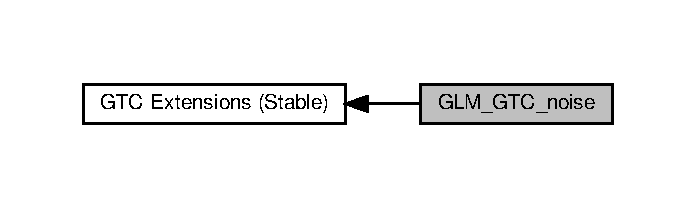
\includegraphics[width=334pt]{group__gtc__noise}
\end{center}
\end{figure}
\subsection*{Functions}
\begin{DoxyCompactItemize}
\item 
{\footnotesize template$<$typename T , precision P, template$<$ typename, precision $>$ class vec\+Type$>$ }\\\hyperlink{setup_8hpp_ab2d052de21a70539923e9bcbf6e83a51}{G\+L\+M\+\_\+\+F\+U\+N\+C\+\_\+\+D\+E\+CL} T \hyperlink{group__gtc__noise_ga14e5975486b2b36e747861d3c65b16c1}{glm\+::perlin} (vec\+Type$<$ T, P $>$ const \&p)
\item 
{\footnotesize template$<$typename T , precision P, template$<$ typename, precision $>$ class vec\+Type$>$ }\\\hyperlink{setup_8hpp_ab2d052de21a70539923e9bcbf6e83a51}{G\+L\+M\+\_\+\+F\+U\+N\+C\+\_\+\+D\+E\+CL} T \hyperlink{group__gtc__noise_ga7e103ffffacb322fe2d4863c372ae2fd}{glm\+::perlin} (vec\+Type$<$ T, P $>$ const \&p, vec\+Type$<$ T, P $>$ const \&rep)
\item 
{\footnotesize template$<$typename T , precision P, template$<$ typename, precision $>$ class vec\+Type$>$ }\\\hyperlink{setup_8hpp_ab2d052de21a70539923e9bcbf6e83a51}{G\+L\+M\+\_\+\+F\+U\+N\+C\+\_\+\+D\+E\+CL} T \hyperlink{group__gtc__noise_ga05f5ab240c9a3fdeee353636e464c285}{glm\+::simplex} (vec\+Type$<$ T, P $>$ const \&p)
\end{DoxyCompactItemize}


\subsection{Detailed Description}
Defines 2D, 3D and 4D procedural noise functions Based on the work of Stefan Gustavson and Ashima Arts on \char`\"{}webgl-\/noise\char`\"{}\+: \href{https://github.com/ashima/webgl-noise}{\tt https\+://github.\+com/ashima/webgl-\/noise} Following Stefan Gustavson\textquotesingle{}s paper \char`\"{}\+Simplex noise demystified\char`\"{}\+: \href{http://www.itn.liu.se/~stegu/simplexnoise/simplexnoise.pdf}{\tt http\+://www.\+itn.\+liu.\+se/$\sim$stegu/simplexnoise/simplexnoise.\+pdf} $<$\hyperlink{gtc_2noise_8hpp}{glm/gtc/noise.\+hpp}$>$ need to be included to use these functionalities. 

\subsection{Function Documentation}
\mbox{\Hypertarget{group__gtc__noise_ga14e5975486b2b36e747861d3c65b16c1}\label{group__gtc__noise_ga14e5975486b2b36e747861d3c65b16c1}} 
\index{G\+L\+M\+\_\+\+G\+T\+C\+\_\+noise@{G\+L\+M\+\_\+\+G\+T\+C\+\_\+noise}!perlin@{perlin}}
\index{perlin@{perlin}!G\+L\+M\+\_\+\+G\+T\+C\+\_\+noise@{G\+L\+M\+\_\+\+G\+T\+C\+\_\+noise}}
\subsubsection{\texorpdfstring{perlin()}{perlin()}\hspace{0.1cm}{\footnotesize\ttfamily [1/2]}}
{\footnotesize\ttfamily template$<$typename T , precision P, template$<$ typename, precision $>$ class vec\+Type$>$ \\
\hyperlink{setup_8hpp_ab2d052de21a70539923e9bcbf6e83a51}{G\+L\+M\+\_\+\+F\+U\+N\+C\+\_\+\+D\+E\+CL} T glm\+::perlin (\begin{DoxyParamCaption}\item[{vec\+Type$<$ T, P $>$ const \&}]{p }\end{DoxyParamCaption})}

Classic perlin noise. \begin{DoxySeeAlso}{See also}
\hyperlink{group__gtc__noise}{G\+L\+M\+\_\+\+G\+T\+C\+\_\+noise} 
\end{DoxySeeAlso}
\mbox{\Hypertarget{group__gtc__noise_ga7e103ffffacb322fe2d4863c372ae2fd}\label{group__gtc__noise_ga7e103ffffacb322fe2d4863c372ae2fd}} 
\index{G\+L\+M\+\_\+\+G\+T\+C\+\_\+noise@{G\+L\+M\+\_\+\+G\+T\+C\+\_\+noise}!perlin@{perlin}}
\index{perlin@{perlin}!G\+L\+M\+\_\+\+G\+T\+C\+\_\+noise@{G\+L\+M\+\_\+\+G\+T\+C\+\_\+noise}}
\subsubsection{\texorpdfstring{perlin()}{perlin()}\hspace{0.1cm}{\footnotesize\ttfamily [2/2]}}
{\footnotesize\ttfamily template$<$typename T , precision P, template$<$ typename, precision $>$ class vec\+Type$>$ \\
\hyperlink{setup_8hpp_ab2d052de21a70539923e9bcbf6e83a51}{G\+L\+M\+\_\+\+F\+U\+N\+C\+\_\+\+D\+E\+CL} T glm\+::perlin (\begin{DoxyParamCaption}\item[{vec\+Type$<$ T, P $>$ const \&}]{p,  }\item[{vec\+Type$<$ T, P $>$ const \&}]{rep }\end{DoxyParamCaption})}

Periodic perlin noise. \begin{DoxySeeAlso}{See also}
\hyperlink{group__gtc__noise}{G\+L\+M\+\_\+\+G\+T\+C\+\_\+noise} 
\end{DoxySeeAlso}
\mbox{\Hypertarget{group__gtc__noise_ga05f5ab240c9a3fdeee353636e464c285}\label{group__gtc__noise_ga05f5ab240c9a3fdeee353636e464c285}} 
\index{G\+L\+M\+\_\+\+G\+T\+C\+\_\+noise@{G\+L\+M\+\_\+\+G\+T\+C\+\_\+noise}!simplex@{simplex}}
\index{simplex@{simplex}!G\+L\+M\+\_\+\+G\+T\+C\+\_\+noise@{G\+L\+M\+\_\+\+G\+T\+C\+\_\+noise}}
\subsubsection{\texorpdfstring{simplex()}{simplex()}}
{\footnotesize\ttfamily template$<$typename T , precision P, template$<$ typename, precision $>$ class vec\+Type$>$ \\
\hyperlink{setup_8hpp_ab2d052de21a70539923e9bcbf6e83a51}{G\+L\+M\+\_\+\+F\+U\+N\+C\+\_\+\+D\+E\+CL} T glm\+::simplex (\begin{DoxyParamCaption}\item[{vec\+Type$<$ T, P $>$ const \&}]{p }\end{DoxyParamCaption})}

Simplex noise. \begin{DoxySeeAlso}{See also}
\hyperlink{group__gtc__noise}{G\+L\+M\+\_\+\+G\+T\+C\+\_\+noise} 
\end{DoxySeeAlso}

\hypertarget{group__gtc__packing}{}\section{G\+L\+M\+\_\+\+G\+T\+C\+\_\+packing}
\label{group__gtc__packing}\index{G\+L\+M\+\_\+\+G\+T\+C\+\_\+packing@{G\+L\+M\+\_\+\+G\+T\+C\+\_\+packing}}


This extension provides a set of function to convert vertors to packed formats.  


Collaboration diagram for G\+L\+M\+\_\+\+G\+T\+C\+\_\+packing\+:\nopagebreak
\begin{figure}[H]
\begin{center}
\leavevmode
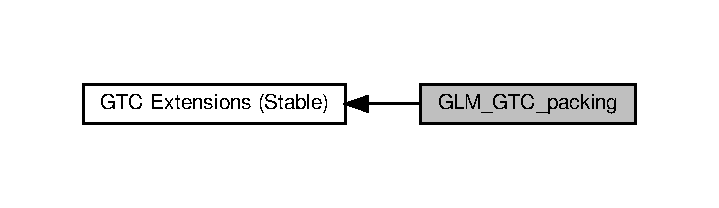
\includegraphics[width=345pt]{group__gtc__packing}
\end{center}
\end{figure}
\subsection*{Functions}
\begin{DoxyCompactItemize}
\item 
\hyperlink{setup_8hpp_ab2d052de21a70539923e9bcbf6e83a51}{G\+L\+M\+\_\+\+F\+U\+N\+C\+\_\+\+D\+E\+CL} \hyperlink{group__gtc__type__precision_ga1a7dcd8aac97cc8020817c94049deff2}{uint8} \hyperlink{group__gtc__packing_ga2f9963e5d762b10085b280d3662017ba}{glm\+::pack\+Unorm1x8} (float v)
\item 
\hyperlink{setup_8hpp_ab2d052de21a70539923e9bcbf6e83a51}{G\+L\+M\+\_\+\+F\+U\+N\+C\+\_\+\+D\+E\+CL} float \hyperlink{group__gtc__packing_ga32f3f2642df2ea87449d59fb614a8305}{glm\+::unpack\+Unorm1x8} (\hyperlink{group__gtc__type__precision_ga1a7dcd8aac97cc8020817c94049deff2}{uint8} p)
\item 
\hyperlink{setup_8hpp_ab2d052de21a70539923e9bcbf6e83a51}{G\+L\+M\+\_\+\+F\+U\+N\+C\+\_\+\+D\+E\+CL} \hyperlink{group__gtc__type__precision_gad8c2939e1fdd8e5828b31d95c52255d5}{uint16} \hyperlink{group__gtc__packing_ga833288fc0d4a79f19d0db75a6843bfe6}{glm\+::pack\+Unorm2x8} (\hyperlink{group__core__types_gaa1618f51db67eaa145db101d8c8431d8}{vec2} const \&v)
\item 
\hyperlink{setup_8hpp_ab2d052de21a70539923e9bcbf6e83a51}{G\+L\+M\+\_\+\+F\+U\+N\+C\+\_\+\+D\+E\+CL} \hyperlink{group__core__types_gaa1618f51db67eaa145db101d8c8431d8}{vec2} \hyperlink{group__gtc__packing_ga96ce0c24339ee676e28a027fffd1edf6}{glm\+::unpack\+Unorm2x8} (\hyperlink{group__gtc__type__precision_gad8c2939e1fdd8e5828b31d95c52255d5}{uint16} p)
\item 
\hyperlink{setup_8hpp_ab2d052de21a70539923e9bcbf6e83a51}{G\+L\+M\+\_\+\+F\+U\+N\+C\+\_\+\+D\+E\+CL} \hyperlink{group__gtc__type__precision_ga1a7dcd8aac97cc8020817c94049deff2}{uint8} \hyperlink{group__gtc__packing_ga26b6cd7a35c46c4b6a342f3b97b47423}{glm\+::pack\+Snorm1x8} (float s)
\item 
\hyperlink{setup_8hpp_ab2d052de21a70539923e9bcbf6e83a51}{G\+L\+M\+\_\+\+F\+U\+N\+C\+\_\+\+D\+E\+CL} float \hyperlink{group__gtc__packing_ga6f2bebf536fbf7c8b97d4b306bb3354e}{glm\+::unpack\+Snorm1x8} (\hyperlink{group__gtc__type__precision_ga1a7dcd8aac97cc8020817c94049deff2}{uint8} p)
\item 
\hyperlink{setup_8hpp_ab2d052de21a70539923e9bcbf6e83a51}{G\+L\+M\+\_\+\+F\+U\+N\+C\+\_\+\+D\+E\+CL} \hyperlink{group__gtc__type__precision_gad8c2939e1fdd8e5828b31d95c52255d5}{uint16} \hyperlink{group__gtc__packing_ga05d08a82923166ec7cd5d0e6154c9953}{glm\+::pack\+Snorm2x8} (\hyperlink{group__core__types_gaa1618f51db67eaa145db101d8c8431d8}{vec2} const \&v)
\item 
\hyperlink{setup_8hpp_ab2d052de21a70539923e9bcbf6e83a51}{G\+L\+M\+\_\+\+F\+U\+N\+C\+\_\+\+D\+E\+CL} \hyperlink{group__core__types_gaa1618f51db67eaa145db101d8c8431d8}{vec2} \hyperlink{group__gtc__packing_ga27f30f0281b88e152b0895f5e2ead878}{glm\+::unpack\+Snorm2x8} (\hyperlink{group__gtc__type__precision_gad8c2939e1fdd8e5828b31d95c52255d5}{uint16} p)
\item 
\hyperlink{setup_8hpp_ab2d052de21a70539923e9bcbf6e83a51}{G\+L\+M\+\_\+\+F\+U\+N\+C\+\_\+\+D\+E\+CL} \hyperlink{group__gtc__type__precision_gad8c2939e1fdd8e5828b31d95c52255d5}{uint16} \hyperlink{group__gtc__packing_ga60c7d915f5653559ae02c2f79a8c5c1d}{glm\+::pack\+Unorm1x16} (float v)
\item 
\hyperlink{setup_8hpp_ab2d052de21a70539923e9bcbf6e83a51}{G\+L\+M\+\_\+\+F\+U\+N\+C\+\_\+\+D\+E\+CL} float \hyperlink{group__gtc__packing_ga7770e3ade4f4764cc1b2eb42ac4ec188}{glm\+::unpack\+Unorm1x16} (\hyperlink{group__gtc__type__precision_gad8c2939e1fdd8e5828b31d95c52255d5}{uint16} p)
\item 
\hyperlink{setup_8hpp_ab2d052de21a70539923e9bcbf6e83a51}{G\+L\+M\+\_\+\+F\+U\+N\+C\+\_\+\+D\+E\+CL} \hyperlink{group__gtc__type__precision_gae3632bf9b37da66233d78930dd06378a}{uint64} \hyperlink{group__gtc__packing_gac561f06c908b7302537a8ef29fcb409e}{glm\+::pack\+Unorm4x16} (\hyperlink{group__core__types_ga5881b1b022d7fd1b7218f5916532dd02}{vec4} const \&v)
\item 
\hyperlink{setup_8hpp_ab2d052de21a70539923e9bcbf6e83a51}{G\+L\+M\+\_\+\+F\+U\+N\+C\+\_\+\+D\+E\+CL} \hyperlink{group__core__types_ga5881b1b022d7fd1b7218f5916532dd02}{vec4} \hyperlink{group__gtc__packing_gafb2b502bc406031a5618ce930139a9e3}{glm\+::unpack\+Unorm4x16} (\hyperlink{group__gtc__type__precision_gae3632bf9b37da66233d78930dd06378a}{uint64} p)
\item 
\hyperlink{setup_8hpp_ab2d052de21a70539923e9bcbf6e83a51}{G\+L\+M\+\_\+\+F\+U\+N\+C\+\_\+\+D\+E\+CL} \hyperlink{group__gtc__type__precision_gad8c2939e1fdd8e5828b31d95c52255d5}{uint16} \hyperlink{group__gtc__packing_gac29411d6c0f6ed0fe9f0396dfe92e0e8}{glm\+::pack\+Snorm1x16} (float v)
\item 
\hyperlink{setup_8hpp_ab2d052de21a70539923e9bcbf6e83a51}{G\+L\+M\+\_\+\+F\+U\+N\+C\+\_\+\+D\+E\+CL} float \hyperlink{group__gtc__packing_ga246f451cebf590726324f7a283e3d65e}{glm\+::unpack\+Snorm1x16} (\hyperlink{group__gtc__type__precision_gad8c2939e1fdd8e5828b31d95c52255d5}{uint16} p)
\item 
\hyperlink{setup_8hpp_ab2d052de21a70539923e9bcbf6e83a51}{G\+L\+M\+\_\+\+F\+U\+N\+C\+\_\+\+D\+E\+CL} \hyperlink{group__gtc__type__precision_gae3632bf9b37da66233d78930dd06378a}{uint64} \hyperlink{group__gtc__packing_ga9b237d7c66b7a71964e6d1f4dc06539f}{glm\+::pack\+Snorm4x16} (\hyperlink{group__core__types_ga5881b1b022d7fd1b7218f5916532dd02}{vec4} const \&v)
\item 
\hyperlink{setup_8hpp_ab2d052de21a70539923e9bcbf6e83a51}{G\+L\+M\+\_\+\+F\+U\+N\+C\+\_\+\+D\+E\+CL} \hyperlink{group__core__types_ga5881b1b022d7fd1b7218f5916532dd02}{vec4} \hyperlink{group__gtc__packing_gadb01fc0530f07beb509c89d97b6f4d20}{glm\+::unpack\+Snorm4x16} (\hyperlink{group__gtc__type__precision_gae3632bf9b37da66233d78930dd06378a}{uint64} const \&p)
\item 
\hyperlink{setup_8hpp_ab2d052de21a70539923e9bcbf6e83a51}{G\+L\+M\+\_\+\+F\+U\+N\+C\+\_\+\+D\+E\+CL} \hyperlink{group__gtc__type__precision_gad8c2939e1fdd8e5828b31d95c52255d5}{uint16} \hyperlink{group__gtc__packing_gaba534b320836a35372e00af5771dd1a2}{glm\+::pack\+Half1x16} (float v)
\item 
\hyperlink{setup_8hpp_ab2d052de21a70539923e9bcbf6e83a51}{G\+L\+M\+\_\+\+F\+U\+N\+C\+\_\+\+D\+E\+CL} float \hyperlink{group__gtc__packing_gaa6eebcdfc746584b7d1823f1d5344fed}{glm\+::unpack\+Half1x16} (\hyperlink{group__gtc__type__precision_gad8c2939e1fdd8e5828b31d95c52255d5}{uint16} v)
\item 
\hyperlink{setup_8hpp_ab2d052de21a70539923e9bcbf6e83a51}{G\+L\+M\+\_\+\+F\+U\+N\+C\+\_\+\+D\+E\+CL} \hyperlink{group__gtc__type__precision_gae3632bf9b37da66233d78930dd06378a}{uint64} \hyperlink{group__gtc__packing_ga8104f0b719b7792491f2b789a6dd6f96}{glm\+::pack\+Half4x16} (\hyperlink{group__core__types_ga5881b1b022d7fd1b7218f5916532dd02}{vec4} const \&v)
\item 
\hyperlink{setup_8hpp_ab2d052de21a70539923e9bcbf6e83a51}{G\+L\+M\+\_\+\+F\+U\+N\+C\+\_\+\+D\+E\+CL} \hyperlink{group__core__types_ga5881b1b022d7fd1b7218f5916532dd02}{vec4} \hyperlink{group__gtc__packing_gaea526d6491ad40401eac34803984bf27}{glm\+::unpack\+Half4x16} (\hyperlink{group__gtc__type__precision_gae3632bf9b37da66233d78930dd06378a}{uint64} p)
\item 
\hyperlink{setup_8hpp_ab2d052de21a70539923e9bcbf6e83a51}{G\+L\+M\+\_\+\+F\+U\+N\+C\+\_\+\+D\+E\+CL} \hyperlink{group__gtc__type__precision_ga202b6a53c105fcb7e531f9b443518451}{uint32} \hyperlink{group__gtc__packing_ga032e18fa5bc5b8f3897104aeb2f1e195}{glm\+::pack\+I3x10\+\_\+1x2} (\hyperlink{group__core__types_gaa4560ddc50320ea8f8a70d5c9c249fea}{ivec4} const \&v)
\item 
\hyperlink{setup_8hpp_ab2d052de21a70539923e9bcbf6e83a51}{G\+L\+M\+\_\+\+F\+U\+N\+C\+\_\+\+D\+E\+CL} \hyperlink{group__core__types_gaa4560ddc50320ea8f8a70d5c9c249fea}{ivec4} \hyperlink{group__gtc__packing_ga08bcd34cf9c34701d658dd861ee6e300}{glm\+::unpack\+I3x10\+\_\+1x2} (\hyperlink{group__gtc__type__precision_ga202b6a53c105fcb7e531f9b443518451}{uint32} p)
\item 
\hyperlink{setup_8hpp_ab2d052de21a70539923e9bcbf6e83a51}{G\+L\+M\+\_\+\+F\+U\+N\+C\+\_\+\+D\+E\+CL} \hyperlink{group__gtc__type__precision_ga202b6a53c105fcb7e531f9b443518451}{uint32} \hyperlink{group__gtc__packing_gaf656d8862628f96b20de7a36eaa1fe56}{glm\+::pack\+U3x10\+\_\+1x2} (\hyperlink{group__core__types_ga1c426d19627b32b14f0089f7f4ba7b1d}{uvec4} const \&v)
\item 
\hyperlink{setup_8hpp_ab2d052de21a70539923e9bcbf6e83a51}{G\+L\+M\+\_\+\+F\+U\+N\+C\+\_\+\+D\+E\+CL} \hyperlink{group__core__types_ga1c426d19627b32b14f0089f7f4ba7b1d}{uvec4} \hyperlink{group__gtc__packing_ga119aa2d7d55952f9dc4214390a6ffefc}{glm\+::unpack\+U3x10\+\_\+1x2} (\hyperlink{group__gtc__type__precision_ga202b6a53c105fcb7e531f9b443518451}{uint32} p)
\item 
\hyperlink{setup_8hpp_ab2d052de21a70539923e9bcbf6e83a51}{G\+L\+M\+\_\+\+F\+U\+N\+C\+\_\+\+D\+E\+CL} \hyperlink{group__gtc__type__precision_ga202b6a53c105fcb7e531f9b443518451}{uint32} \hyperlink{group__gtc__packing_ga0d4157cec37c0312216a7be1cc92df54}{glm\+::pack\+Snorm3x10\+\_\+1x2} (\hyperlink{group__core__types_ga5881b1b022d7fd1b7218f5916532dd02}{vec4} const \&v)
\item 
\hyperlink{setup_8hpp_ab2d052de21a70539923e9bcbf6e83a51}{G\+L\+M\+\_\+\+F\+U\+N\+C\+\_\+\+D\+E\+CL} \hyperlink{group__core__types_ga5881b1b022d7fd1b7218f5916532dd02}{vec4} \hyperlink{group__gtc__packing_ga8b8bb827a3743ca553d8702d3e337101}{glm\+::unpack\+Snorm3x10\+\_\+1x2} (\hyperlink{group__gtc__type__precision_ga202b6a53c105fcb7e531f9b443518451}{uint32} p)
\item 
\hyperlink{setup_8hpp_ab2d052de21a70539923e9bcbf6e83a51}{G\+L\+M\+\_\+\+F\+U\+N\+C\+\_\+\+D\+E\+CL} \hyperlink{group__gtc__type__precision_ga202b6a53c105fcb7e531f9b443518451}{uint32} \hyperlink{group__gtc__packing_ga2cf2d11b40bd48639110456fd74c2e33}{glm\+::pack\+Unorm3x10\+\_\+1x2} (\hyperlink{group__core__types_ga5881b1b022d7fd1b7218f5916532dd02}{vec4} const \&v)
\item 
\hyperlink{setup_8hpp_ab2d052de21a70539923e9bcbf6e83a51}{G\+L\+M\+\_\+\+F\+U\+N\+C\+\_\+\+D\+E\+CL} \hyperlink{group__core__types_ga5881b1b022d7fd1b7218f5916532dd02}{vec4} \hyperlink{group__gtc__packing_gaf69ace2b5e9234f8afb4e99c3df1193d}{glm\+::unpack\+Unorm3x10\+\_\+1x2} (\hyperlink{group__gtc__type__precision_ga202b6a53c105fcb7e531f9b443518451}{uint32} p)
\item 
\hyperlink{setup_8hpp_ab2d052de21a70539923e9bcbf6e83a51}{G\+L\+M\+\_\+\+F\+U\+N\+C\+\_\+\+D\+E\+CL} \hyperlink{group__gtc__type__precision_ga202b6a53c105fcb7e531f9b443518451}{uint32} \hyperlink{group__gtc__packing_ga8c2a0eeee677ca4dafd9e093d9e81062}{glm\+::pack\+F2x11\+\_\+1x10} (\hyperlink{group__core__types_ga1c47e8b3386109bc992b6c48e91b0be7}{vec3} const \&v)
\item 
\hyperlink{setup_8hpp_ab2d052de21a70539923e9bcbf6e83a51}{G\+L\+M\+\_\+\+F\+U\+N\+C\+\_\+\+D\+E\+CL} \hyperlink{group__core__types_ga1c47e8b3386109bc992b6c48e91b0be7}{vec3} \hyperlink{group__gtc__packing_ga8b9c7991eb021d95c778bf5c0b2f7824}{glm\+::unpack\+F2x11\+\_\+1x10} (\hyperlink{group__gtc__type__precision_ga202b6a53c105fcb7e531f9b443518451}{uint32} p)
\end{DoxyCompactItemize}


\subsection{Detailed Description}
This extension provides a set of function to convert vertors to packed formats. 

$<$\hyperlink{gtc_2packing_8hpp}{glm/gtc/packing.\+hpp}$>$ need to be included to use these features. 

\subsection{Function Documentation}
\mbox{\Hypertarget{group__gtc__packing_ga8c2a0eeee677ca4dafd9e093d9e81062}\label{group__gtc__packing_ga8c2a0eeee677ca4dafd9e093d9e81062}} 
\index{G\+L\+M\+\_\+\+G\+T\+C\+\_\+packing@{G\+L\+M\+\_\+\+G\+T\+C\+\_\+packing}!pack\+F2x11\+\_\+1x10@{pack\+F2x11\+\_\+1x10}}
\index{pack\+F2x11\+\_\+1x10@{pack\+F2x11\+\_\+1x10}!G\+L\+M\+\_\+\+G\+T\+C\+\_\+packing@{G\+L\+M\+\_\+\+G\+T\+C\+\_\+packing}}
\subsubsection{\texorpdfstring{pack\+F2x11\+\_\+1x10()}{packF2x11\_1x10()}}
{\footnotesize\ttfamily \hyperlink{setup_8hpp_a33fdea6f91c5f834105f7415e2a64407}{G\+L\+M\+\_\+\+F\+U\+N\+C\+\_\+\+Q\+U\+A\+L\+I\+F\+I\+ER} \hyperlink{group__gtc__type__precision_ga202b6a53c105fcb7e531f9b443518451}{uint32} glm\+::pack\+F2x11\+\_\+1x10 (\begin{DoxyParamCaption}\item[{\hyperlink{group__core__types_ga1c47e8b3386109bc992b6c48e91b0be7}{vec3} const \&}]{v }\end{DoxyParamCaption})}

First, converts the first two components of the normalized floating-\/point value v into 11-\/bit signless floating-\/point values. Then, converts the third component of the normalized floating-\/point value v into a 10-\/bit signless floating-\/point value. Then, the results are packed into the returned 32-\/bit unsigned integer.

The first vector component specifies the 11 least-\/significant bits of the result; the last component specifies the 10 most-\/significant bits.

\begin{DoxySeeAlso}{See also}
\hyperlink{group__gtc__packing}{G\+L\+M\+\_\+\+G\+T\+C\+\_\+packing} 

\hyperlink{group__core__types_ga1c47e8b3386109bc992b6c48e91b0be7}{vec3} unpack\+F2x11\+\_\+1x10(uint32 const \& p) 
\end{DoxySeeAlso}


Definition at line 480 of file packing.\+inl.

\mbox{\Hypertarget{group__gtc__packing_gaba534b320836a35372e00af5771dd1a2}\label{group__gtc__packing_gaba534b320836a35372e00af5771dd1a2}} 
\index{G\+L\+M\+\_\+\+G\+T\+C\+\_\+packing@{G\+L\+M\+\_\+\+G\+T\+C\+\_\+packing}!pack\+Half1x16@{pack\+Half1x16}}
\index{pack\+Half1x16@{pack\+Half1x16}!G\+L\+M\+\_\+\+G\+T\+C\+\_\+packing@{G\+L\+M\+\_\+\+G\+T\+C\+\_\+packing}}
\subsubsection{\texorpdfstring{pack\+Half1x16()}{packHalf1x16()}}
{\footnotesize\ttfamily \hyperlink{setup_8hpp_a33fdea6f91c5f834105f7415e2a64407}{G\+L\+M\+\_\+\+F\+U\+N\+C\+\_\+\+Q\+U\+A\+L\+I\+F\+I\+ER} \hyperlink{group__gtc__type__precision_gad8c2939e1fdd8e5828b31d95c52255d5}{uint16} glm\+::pack\+Half1x16 (\begin{DoxyParamCaption}\item[{float}]{v }\end{DoxyParamCaption})}

Returns an unsigned integer obtained by converting the components of a floating-\/point scalar to the 16-\/bit floating-\/point representation found in the Open\+GL Specification, and then packing this 16-\/bit value into a 16-\/bit unsigned integer.

\begin{DoxySeeAlso}{See also}
\hyperlink{group__gtc__packing}{G\+L\+M\+\_\+\+G\+T\+C\+\_\+packing} 

\hyperlink{group__gtc__type__precision_ga202b6a53c105fcb7e531f9b443518451}{uint32} \hyperlink{group__core__func__packing_ga082f6dd65f73a547ed3067ef00be036f}{pack\+Half2x16(vec2 const \& v)} 

\hyperlink{group__gtc__type__precision_gae3632bf9b37da66233d78930dd06378a}{uint64} \hyperlink{group__gtc__packing_ga8104f0b719b7792491f2b789a6dd6f96}{pack\+Half4x16(vec4 const \& v)} 

\href{http://www.opengl.org/sdk/docs/manglsl/xhtml/packHalf2x16.xml}{\tt G\+L\+SL pack\+Half2x16 man page} 

\href{http://www.opengl.org/registry/doc/GLSLangSpec.4.20.8.pdf}{\tt G\+L\+SL 4.\+20.\+8 specification, section 8.\+4 Floating-\/\+Point Pack and Unpack Functions} 
\end{DoxySeeAlso}


Definition at line 357 of file packing.\+inl.

\mbox{\Hypertarget{group__gtc__packing_ga8104f0b719b7792491f2b789a6dd6f96}\label{group__gtc__packing_ga8104f0b719b7792491f2b789a6dd6f96}} 
\index{G\+L\+M\+\_\+\+G\+T\+C\+\_\+packing@{G\+L\+M\+\_\+\+G\+T\+C\+\_\+packing}!pack\+Half4x16@{pack\+Half4x16}}
\index{pack\+Half4x16@{pack\+Half4x16}!G\+L\+M\+\_\+\+G\+T\+C\+\_\+packing@{G\+L\+M\+\_\+\+G\+T\+C\+\_\+packing}}
\subsubsection{\texorpdfstring{pack\+Half4x16()}{packHalf4x16()}}
{\footnotesize\ttfamily \hyperlink{setup_8hpp_a33fdea6f91c5f834105f7415e2a64407}{G\+L\+M\+\_\+\+F\+U\+N\+C\+\_\+\+Q\+U\+A\+L\+I\+F\+I\+ER} \hyperlink{group__gtc__type__precision_gae3632bf9b37da66233d78930dd06378a}{uint64} glm\+::pack\+Half4x16 (\begin{DoxyParamCaption}\item[{\hyperlink{group__core__types_ga5881b1b022d7fd1b7218f5916532dd02}{glm\+::vec4} const \&}]{v }\end{DoxyParamCaption})}

Returns an unsigned integer obtained by converting the components of a four-\/component floating-\/point vector to the 16-\/bit floating-\/point representation found in the Open\+GL Specification, and then packing these four 16-\/bit values into a 64-\/bit unsigned integer. The first vector component specifies the 16 least-\/significant bits of the result; the forth component specifies the 16 most-\/significant bits.

\begin{DoxySeeAlso}{See also}
\hyperlink{group__gtc__packing}{G\+L\+M\+\_\+\+G\+T\+C\+\_\+packing} 

\hyperlink{group__gtc__type__precision_gad8c2939e1fdd8e5828b31d95c52255d5}{uint16} pack\+Half1x16(float const \& v) 

\hyperlink{group__gtc__type__precision_ga202b6a53c105fcb7e531f9b443518451}{uint32} \hyperlink{group__core__func__packing_ga082f6dd65f73a547ed3067ef00be036f}{pack\+Half2x16(vec2 const \& v)} 

\href{http://www.opengl.org/sdk/docs/manglsl/xhtml/packHalf2x16.xml}{\tt G\+L\+SL pack\+Half2x16 man page} 

\href{http://www.opengl.org/registry/doc/GLSLangSpec.4.20.8.pdf}{\tt G\+L\+SL 4.\+20.\+8 specification, section 8.\+4 Floating-\/\+Point Pack and Unpack Functions} 
\end{DoxySeeAlso}


Definition at line 370 of file packing.\+inl.

\mbox{\Hypertarget{group__gtc__packing_ga032e18fa5bc5b8f3897104aeb2f1e195}\label{group__gtc__packing_ga032e18fa5bc5b8f3897104aeb2f1e195}} 
\index{G\+L\+M\+\_\+\+G\+T\+C\+\_\+packing@{G\+L\+M\+\_\+\+G\+T\+C\+\_\+packing}!pack\+I3x10\+\_\+1x2@{pack\+I3x10\+\_\+1x2}}
\index{pack\+I3x10\+\_\+1x2@{pack\+I3x10\+\_\+1x2}!G\+L\+M\+\_\+\+G\+T\+C\+\_\+packing@{G\+L\+M\+\_\+\+G\+T\+C\+\_\+packing}}
\subsubsection{\texorpdfstring{pack\+I3x10\+\_\+1x2()}{packI3x10\_1x2()}}
{\footnotesize\ttfamily \hyperlink{setup_8hpp_a33fdea6f91c5f834105f7415e2a64407}{G\+L\+M\+\_\+\+F\+U\+N\+C\+\_\+\+Q\+U\+A\+L\+I\+F\+I\+ER} \hyperlink{group__gtc__type__precision_ga202b6a53c105fcb7e531f9b443518451}{uint32} glm\+::pack\+I3x10\+\_\+1x2 (\begin{DoxyParamCaption}\item[{\hyperlink{group__core__types_gaa4560ddc50320ea8f8a70d5c9c249fea}{ivec4} const \&}]{v }\end{DoxyParamCaption})}

Returns an unsigned integer obtained by converting the components of a four-\/component signed integer vector to the 10-\/10-\/10-\/2-\/bit signed integer representation found in the Open\+GL Specification, and then packing these four values into a 32-\/bit unsigned integer. The first vector component specifies the 10 least-\/significant bits of the result; the forth component specifies the 2 most-\/significant bits.

\begin{DoxySeeAlso}{See also}
\hyperlink{group__gtc__packing}{G\+L\+M\+\_\+\+G\+T\+C\+\_\+packing} 

\hyperlink{group__gtc__type__precision_ga202b6a53c105fcb7e531f9b443518451}{uint32} pack\+I3x10\+\_\+1x2(uvec4 const \& v) 

\hyperlink{group__gtc__type__precision_ga202b6a53c105fcb7e531f9b443518451}{uint32} \hyperlink{group__gtc__packing_ga0d4157cec37c0312216a7be1cc92df54}{pack\+Snorm3x10\+\_\+1x2(vec4 const \& v)} 

\hyperlink{group__gtc__type__precision_ga202b6a53c105fcb7e531f9b443518451}{uint32} \hyperlink{group__gtc__packing_ga2cf2d11b40bd48639110456fd74c2e33}{pack\+Unorm3x10\+\_\+1x2(vec4 const \& v)} 

\hyperlink{group__core__types_gaa4560ddc50320ea8f8a70d5c9c249fea}{ivec4} unpack\+I3x10\+\_\+1x2(uint32 const \& p) 
\end{DoxySeeAlso}


Definition at line 394 of file packing.\+inl.

\mbox{\Hypertarget{group__gtc__packing_gac29411d6c0f6ed0fe9f0396dfe92e0e8}\label{group__gtc__packing_gac29411d6c0f6ed0fe9f0396dfe92e0e8}} 
\index{G\+L\+M\+\_\+\+G\+T\+C\+\_\+packing@{G\+L\+M\+\_\+\+G\+T\+C\+\_\+packing}!pack\+Snorm1x16@{pack\+Snorm1x16}}
\index{pack\+Snorm1x16@{pack\+Snorm1x16}!G\+L\+M\+\_\+\+G\+T\+C\+\_\+packing@{G\+L\+M\+\_\+\+G\+T\+C\+\_\+packing}}
\subsubsection{\texorpdfstring{pack\+Snorm1x16()}{packSnorm1x16()}}
{\footnotesize\ttfamily \hyperlink{setup_8hpp_a33fdea6f91c5f834105f7415e2a64407}{G\+L\+M\+\_\+\+F\+U\+N\+C\+\_\+\+Q\+U\+A\+L\+I\+F\+I\+ER} \hyperlink{group__gtc__type__precision_gad8c2939e1fdd8e5828b31d95c52255d5}{uint16} glm\+::pack\+Snorm1x16 (\begin{DoxyParamCaption}\item[{float}]{v }\end{DoxyParamCaption})}

First, converts the normalized floating-\/point value v into 16-\/bit integer value. Then, the results are packed into the returned 16-\/bit unsigned integer.

The conversion to fixed point is done as follows\+: pack\+Snorm1x8\+: round(clamp(s, -\/1, +1) $\ast$ 32767.\+0)

\begin{DoxySeeAlso}{See also}
\hyperlink{group__gtc__packing}{G\+L\+M\+\_\+\+G\+T\+C\+\_\+packing} 

\hyperlink{group__gtc__type__precision_ga202b6a53c105fcb7e531f9b443518451}{uint32} \hyperlink{group__core__func__packing_ga0c8005de240d6c4ca3d16c7bee25c622}{pack\+Snorm2x16(vec2 const \& v)} 

\hyperlink{group__gtc__type__precision_gae3632bf9b37da66233d78930dd06378a}{uint64} \hyperlink{group__gtc__packing_ga9b237d7c66b7a71964e6d1f4dc06539f}{pack\+Snorm4x16(vec4 const \& v)} 

\href{http://www.opengl.org/sdk/docs/manglsl/xhtml/packSnorm4x8.xml}{\tt G\+L\+SL pack\+Snorm4x8 man page} 

\href{http://www.opengl.org/registry/doc/GLSLangSpec.4.20.8.pdf}{\tt G\+L\+SL 4.\+20.\+8 specification, section 8.\+4 Floating-\/\+Point Pack and Unpack Functions} 
\end{DoxySeeAlso}


Definition at line 327 of file packing.\+inl.

\mbox{\Hypertarget{group__gtc__packing_ga26b6cd7a35c46c4b6a342f3b97b47423}\label{group__gtc__packing_ga26b6cd7a35c46c4b6a342f3b97b47423}} 
\index{G\+L\+M\+\_\+\+G\+T\+C\+\_\+packing@{G\+L\+M\+\_\+\+G\+T\+C\+\_\+packing}!pack\+Snorm1x8@{pack\+Snorm1x8}}
\index{pack\+Snorm1x8@{pack\+Snorm1x8}!G\+L\+M\+\_\+\+G\+T\+C\+\_\+packing@{G\+L\+M\+\_\+\+G\+T\+C\+\_\+packing}}
\subsubsection{\texorpdfstring{pack\+Snorm1x8()}{packSnorm1x8()}}
{\footnotesize\ttfamily \hyperlink{setup_8hpp_a33fdea6f91c5f834105f7415e2a64407}{G\+L\+M\+\_\+\+F\+U\+N\+C\+\_\+\+Q\+U\+A\+L\+I\+F\+I\+ER} \hyperlink{group__gtc__type__precision_ga1a7dcd8aac97cc8020817c94049deff2}{uint8} glm\+::pack\+Snorm1x8 (\begin{DoxyParamCaption}\item[{float}]{s }\end{DoxyParamCaption})}

First, converts the normalized floating-\/point value v into 8-\/bit integer value. Then, the results are packed into the returned 8-\/bit unsigned integer.

The conversion to fixed point is done as follows\+: pack\+Snorm1x8\+: round(clamp(s, -\/1, +1) $\ast$ 127.\+0)

\begin{DoxySeeAlso}{See also}
\hyperlink{group__gtc__packing}{G\+L\+M\+\_\+\+G\+T\+C\+\_\+packing} 

\hyperlink{group__gtc__type__precision_gad8c2939e1fdd8e5828b31d95c52255d5}{uint16} \hyperlink{group__gtc__packing_ga05d08a82923166ec7cd5d0e6154c9953}{pack\+Snorm2x8(vec2 const \& v)} 

\hyperlink{group__gtc__type__precision_ga202b6a53c105fcb7e531f9b443518451}{uint32} \hyperlink{group__core__func__packing_gafcf25acc0d361c6c696a433aa5dfd16b}{pack\+Snorm4x8(vec4 const \& v)} 

\href{http://www.opengl.org/sdk/docs/manglsl/xhtml/packSnorm4x8.xml}{\tt G\+L\+SL pack\+Snorm4x8 man page} 

\href{http://www.opengl.org/registry/doc/GLSLangSpec.4.20.8.pdf}{\tt G\+L\+SL 4.\+20.\+8 specification, section 8.\+4 Floating-\/\+Point Pack and Unpack Functions} 
\end{DoxySeeAlso}


Definition at line 273 of file packing.\+inl.

\mbox{\Hypertarget{group__gtc__packing_ga05d08a82923166ec7cd5d0e6154c9953}\label{group__gtc__packing_ga05d08a82923166ec7cd5d0e6154c9953}} 
\index{G\+L\+M\+\_\+\+G\+T\+C\+\_\+packing@{G\+L\+M\+\_\+\+G\+T\+C\+\_\+packing}!pack\+Snorm2x8@{pack\+Snorm2x8}}
\index{pack\+Snorm2x8@{pack\+Snorm2x8}!G\+L\+M\+\_\+\+G\+T\+C\+\_\+packing@{G\+L\+M\+\_\+\+G\+T\+C\+\_\+packing}}
\subsubsection{\texorpdfstring{pack\+Snorm2x8()}{packSnorm2x8()}}
{\footnotesize\ttfamily \hyperlink{setup_8hpp_a33fdea6f91c5f834105f7415e2a64407}{G\+L\+M\+\_\+\+F\+U\+N\+C\+\_\+\+Q\+U\+A\+L\+I\+F\+I\+ER} \hyperlink{group__gtc__type__precision_gad8c2939e1fdd8e5828b31d95c52255d5}{uint16} glm\+::pack\+Snorm2x8 (\begin{DoxyParamCaption}\item[{\hyperlink{group__core__types_gaa1618f51db67eaa145db101d8c8431d8}{vec2} const \&}]{v }\end{DoxyParamCaption})}

First, converts each component of the normalized floating-\/point value v into 8-\/bit integer values. Then, the results are packed into the returned 16-\/bit unsigned integer.

The conversion for component c of v to fixed point is done as follows\+: pack\+Snorm2x8\+: round(clamp(c, -\/1, +1) $\ast$ 127.\+0)

The first component of the vector will be written to the least significant bits of the output; the last component will be written to the most significant bits.

\begin{DoxySeeAlso}{See also}
\hyperlink{group__gtc__packing}{G\+L\+M\+\_\+\+G\+T\+C\+\_\+packing} 

\hyperlink{group__gtc__type__precision_ga1a7dcd8aac97cc8020817c94049deff2}{uint8} pack\+Snorm1x8(float const \& v) 

\hyperlink{group__gtc__type__precision_ga202b6a53c105fcb7e531f9b443518451}{uint32} \hyperlink{group__core__func__packing_gafcf25acc0d361c6c696a433aa5dfd16b}{pack\+Snorm4x8(vec4 const \& v)} 

\href{http://www.opengl.org/sdk/docs/manglsl/xhtml/packSnorm4x8.xml}{\tt G\+L\+SL pack\+Snorm4x8 man page} 

\href{http://www.opengl.org/registry/doc/GLSLangSpec.4.20.8.pdf}{\tt G\+L\+SL 4.\+20.\+8 specification, section 8.\+4 Floating-\/\+Point Pack and Unpack Functions} 
\end{DoxySeeAlso}


Definition at line 288 of file packing.\+inl.

\mbox{\Hypertarget{group__gtc__packing_ga0d4157cec37c0312216a7be1cc92df54}\label{group__gtc__packing_ga0d4157cec37c0312216a7be1cc92df54}} 
\index{G\+L\+M\+\_\+\+G\+T\+C\+\_\+packing@{G\+L\+M\+\_\+\+G\+T\+C\+\_\+packing}!pack\+Snorm3x10\+\_\+1x2@{pack\+Snorm3x10\+\_\+1x2}}
\index{pack\+Snorm3x10\+\_\+1x2@{pack\+Snorm3x10\+\_\+1x2}!G\+L\+M\+\_\+\+G\+T\+C\+\_\+packing@{G\+L\+M\+\_\+\+G\+T\+C\+\_\+packing}}
\subsubsection{\texorpdfstring{pack\+Snorm3x10\+\_\+1x2()}{packSnorm3x10\_1x2()}}
{\footnotesize\ttfamily \hyperlink{setup_8hpp_a33fdea6f91c5f834105f7415e2a64407}{G\+L\+M\+\_\+\+F\+U\+N\+C\+\_\+\+Q\+U\+A\+L\+I\+F\+I\+ER} \hyperlink{group__gtc__type__precision_ga202b6a53c105fcb7e531f9b443518451}{uint32} glm\+::pack\+Snorm3x10\+\_\+1x2 (\begin{DoxyParamCaption}\item[{\hyperlink{group__core__types_ga5881b1b022d7fd1b7218f5916532dd02}{vec4} const \&}]{v }\end{DoxyParamCaption})}

First, converts the first three components of the normalized floating-\/point value v into 10-\/bit signed integer values. Then, converts the forth component of the normalized floating-\/point value v into 2-\/bit signed integer values. Then, the results are packed into the returned 32-\/bit unsigned integer.

The conversion for component c of v to fixed point is done as follows\+: pack\+Snorm3x10\+\_\+1x2(xyz)\+: round(clamp(c, -\/1, +1) $\ast$ 511.\+0) pack\+Snorm3x10\+\_\+1x2(w)\+: round(clamp(c, -\/1, +1) $\ast$ 1.\+0)

The first vector component specifies the 10 least-\/significant bits of the result; the forth component specifies the 2 most-\/significant bits.

\begin{DoxySeeAlso}{See also}
\hyperlink{group__gtc__packing}{G\+L\+M\+\_\+\+G\+T\+C\+\_\+packing} 

\hyperlink{group__core__types_ga5881b1b022d7fd1b7218f5916532dd02}{vec4} unpack\+Snorm3x10\+\_\+1x2(uint32 const \& p) 

\hyperlink{group__gtc__type__precision_ga202b6a53c105fcb7e531f9b443518451}{uint32} \hyperlink{group__gtc__packing_ga2cf2d11b40bd48639110456fd74c2e33}{pack\+Unorm3x10\+\_\+1x2(vec4 const \& v)} 

\hyperlink{group__gtc__type__precision_ga202b6a53c105fcb7e531f9b443518451}{uint32} \hyperlink{group__gtc__packing_gaf656d8862628f96b20de7a36eaa1fe56}{pack\+U3x10\+\_\+1x2(uvec4 const \& v)} 

\hyperlink{group__gtc__type__precision_ga202b6a53c105fcb7e531f9b443518451}{uint32} \hyperlink{group__gtc__packing_ga032e18fa5bc5b8f3897104aeb2f1e195}{pack\+I3x10\+\_\+1x2(ivec4 const \& v)} 
\end{DoxySeeAlso}


Definition at line 436 of file packing.\+inl.

\mbox{\Hypertarget{group__gtc__packing_ga9b237d7c66b7a71964e6d1f4dc06539f}\label{group__gtc__packing_ga9b237d7c66b7a71964e6d1f4dc06539f}} 
\index{G\+L\+M\+\_\+\+G\+T\+C\+\_\+packing@{G\+L\+M\+\_\+\+G\+T\+C\+\_\+packing}!pack\+Snorm4x16@{pack\+Snorm4x16}}
\index{pack\+Snorm4x16@{pack\+Snorm4x16}!G\+L\+M\+\_\+\+G\+T\+C\+\_\+packing@{G\+L\+M\+\_\+\+G\+T\+C\+\_\+packing}}
\subsubsection{\texorpdfstring{pack\+Snorm4x16()}{packSnorm4x16()}}
{\footnotesize\ttfamily \hyperlink{setup_8hpp_a33fdea6f91c5f834105f7415e2a64407}{G\+L\+M\+\_\+\+F\+U\+N\+C\+\_\+\+Q\+U\+A\+L\+I\+F\+I\+ER} \hyperlink{group__gtc__type__precision_gae3632bf9b37da66233d78930dd06378a}{uint64} glm\+::pack\+Snorm4x16 (\begin{DoxyParamCaption}\item[{\hyperlink{group__core__types_ga5881b1b022d7fd1b7218f5916532dd02}{vec4} const \&}]{v }\end{DoxyParamCaption})}

First, converts each component of the normalized floating-\/point value v into 16-\/bit integer values. Then, the results are packed into the returned 64-\/bit unsigned integer.

The conversion for component c of v to fixed point is done as follows\+: pack\+Snorm2x8\+: round(clamp(c, -\/1, +1) $\ast$ 32767.\+0)

The first component of the vector will be written to the least significant bits of the output; the last component will be written to the most significant bits.

\begin{DoxySeeAlso}{See also}
\hyperlink{group__gtc__packing}{G\+L\+M\+\_\+\+G\+T\+C\+\_\+packing} 

\hyperlink{group__gtc__type__precision_gad8c2939e1fdd8e5828b31d95c52255d5}{uint16} pack\+Snorm1x16(float const \& v) 

\hyperlink{group__gtc__type__precision_ga202b6a53c105fcb7e531f9b443518451}{uint32} \hyperlink{group__core__func__packing_ga0c8005de240d6c4ca3d16c7bee25c622}{pack\+Snorm2x16(vec2 const \& v)} 

\href{http://www.opengl.org/sdk/docs/manglsl/xhtml/packSnorm4x8.xml}{\tt G\+L\+SL pack\+Snorm4x8 man page} 

\href{http://www.opengl.org/registry/doc/GLSLangSpec.4.20.8.pdf}{\tt G\+L\+SL 4.\+20.\+8 specification, section 8.\+4 Floating-\/\+Point Pack and Unpack Functions} 
\end{DoxySeeAlso}


Definition at line 342 of file packing.\+inl.

\mbox{\Hypertarget{group__gtc__packing_gaf656d8862628f96b20de7a36eaa1fe56}\label{group__gtc__packing_gaf656d8862628f96b20de7a36eaa1fe56}} 
\index{G\+L\+M\+\_\+\+G\+T\+C\+\_\+packing@{G\+L\+M\+\_\+\+G\+T\+C\+\_\+packing}!pack\+U3x10\+\_\+1x2@{pack\+U3x10\+\_\+1x2}}
\index{pack\+U3x10\+\_\+1x2@{pack\+U3x10\+\_\+1x2}!G\+L\+M\+\_\+\+G\+T\+C\+\_\+packing@{G\+L\+M\+\_\+\+G\+T\+C\+\_\+packing}}
\subsubsection{\texorpdfstring{pack\+U3x10\+\_\+1x2()}{packU3x10\_1x2()}}
{\footnotesize\ttfamily \hyperlink{setup_8hpp_a33fdea6f91c5f834105f7415e2a64407}{G\+L\+M\+\_\+\+F\+U\+N\+C\+\_\+\+Q\+U\+A\+L\+I\+F\+I\+ER} \hyperlink{group__gtc__type__precision_ga202b6a53c105fcb7e531f9b443518451}{uint32} glm\+::pack\+U3x10\+\_\+1x2 (\begin{DoxyParamCaption}\item[{\hyperlink{group__core__types_ga1c426d19627b32b14f0089f7f4ba7b1d}{uvec4} const \&}]{v }\end{DoxyParamCaption})}

Returns an unsigned integer obtained by converting the components of a four-\/component unsigned integer vector to the 10-\/10-\/10-\/2-\/bit unsigned integer representation found in the Open\+GL Specification, and then packing these four values into a 32-\/bit unsigned integer. The first vector component specifies the 10 least-\/significant bits of the result; the forth component specifies the 2 most-\/significant bits.

\begin{DoxySeeAlso}{See also}
\hyperlink{group__gtc__packing}{G\+L\+M\+\_\+\+G\+T\+C\+\_\+packing} 

\hyperlink{group__gtc__type__precision_ga202b6a53c105fcb7e531f9b443518451}{uint32} \hyperlink{group__gtc__packing_ga032e18fa5bc5b8f3897104aeb2f1e195}{pack\+I3x10\+\_\+1x2(ivec4 const \& v)} 

\hyperlink{group__gtc__type__precision_ga202b6a53c105fcb7e531f9b443518451}{uint32} \hyperlink{group__gtc__packing_ga0d4157cec37c0312216a7be1cc92df54}{pack\+Snorm3x10\+\_\+1x2(vec4 const \& v)} 

\hyperlink{group__gtc__type__precision_ga202b6a53c105fcb7e531f9b443518451}{uint32} \hyperlink{group__gtc__packing_ga2cf2d11b40bd48639110456fd74c2e33}{pack\+Unorm3x10\+\_\+1x2(vec4 const \& v)} 

\hyperlink{group__core__types_gaa4560ddc50320ea8f8a70d5c9c249fea}{ivec4} unpack\+U3x10\+\_\+1x2(uint32 const \& p) 
\end{DoxySeeAlso}


Definition at line 415 of file packing.\+inl.

\mbox{\Hypertarget{group__gtc__packing_ga60c7d915f5653559ae02c2f79a8c5c1d}\label{group__gtc__packing_ga60c7d915f5653559ae02c2f79a8c5c1d}} 
\index{G\+L\+M\+\_\+\+G\+T\+C\+\_\+packing@{G\+L\+M\+\_\+\+G\+T\+C\+\_\+packing}!pack\+Unorm1x16@{pack\+Unorm1x16}}
\index{pack\+Unorm1x16@{pack\+Unorm1x16}!G\+L\+M\+\_\+\+G\+T\+C\+\_\+packing@{G\+L\+M\+\_\+\+G\+T\+C\+\_\+packing}}
\subsubsection{\texorpdfstring{pack\+Unorm1x16()}{packUnorm1x16()}}
{\footnotesize\ttfamily \hyperlink{setup_8hpp_a33fdea6f91c5f834105f7415e2a64407}{G\+L\+M\+\_\+\+F\+U\+N\+C\+\_\+\+Q\+U\+A\+L\+I\+F\+I\+ER} \hyperlink{group__gtc__type__precision_gad8c2939e1fdd8e5828b31d95c52255d5}{uint16} glm\+::pack\+Unorm1x16 (\begin{DoxyParamCaption}\item[{float}]{v }\end{DoxyParamCaption})}

First, converts the normalized floating-\/point value v into a 16-\/bit integer value. Then, the results are packed into the returned 16-\/bit unsigned integer.

The conversion for component c of v to fixed point is done as follows\+: pack\+Unorm1x16\+: round(clamp(c, 0, +1) $\ast$ 65535.\+0)

\begin{DoxySeeAlso}{See also}
\hyperlink{group__gtc__packing}{G\+L\+M\+\_\+\+G\+T\+C\+\_\+packing} 

\hyperlink{group__gtc__type__precision_gad8c2939e1fdd8e5828b31d95c52255d5}{uint16} pack\+Snorm1x16(float const \& v) 

\hyperlink{group__gtc__type__precision_gae3632bf9b37da66233d78930dd06378a}{uint64} \hyperlink{group__gtc__packing_ga9b237d7c66b7a71964e6d1f4dc06539f}{pack\+Snorm4x16(vec4 const \& v)} 

\href{http://www.opengl.org/sdk/docs/manglsl/xhtml/packUnorm4x8.xml}{\tt G\+L\+SL pack\+Unorm4x8 man page} 

\href{http://www.opengl.org/registry/doc/GLSLangSpec.4.20.8.pdf}{\tt G\+L\+SL 4.\+20.\+8 specification, section 8.\+4 Floating-\/\+Point Pack and Unpack Functions} 
\end{DoxySeeAlso}


Definition at line 303 of file packing.\+inl.

\mbox{\Hypertarget{group__gtc__packing_ga2f9963e5d762b10085b280d3662017ba}\label{group__gtc__packing_ga2f9963e5d762b10085b280d3662017ba}} 
\index{G\+L\+M\+\_\+\+G\+T\+C\+\_\+packing@{G\+L\+M\+\_\+\+G\+T\+C\+\_\+packing}!pack\+Unorm1x8@{pack\+Unorm1x8}}
\index{pack\+Unorm1x8@{pack\+Unorm1x8}!G\+L\+M\+\_\+\+G\+T\+C\+\_\+packing@{G\+L\+M\+\_\+\+G\+T\+C\+\_\+packing}}
\subsubsection{\texorpdfstring{pack\+Unorm1x8()}{packUnorm1x8()}}
{\footnotesize\ttfamily \hyperlink{setup_8hpp_a33fdea6f91c5f834105f7415e2a64407}{G\+L\+M\+\_\+\+F\+U\+N\+C\+\_\+\+Q\+U\+A\+L\+I\+F\+I\+ER} \hyperlink{group__gtc__type__precision_ga1a7dcd8aac97cc8020817c94049deff2}{uint8} glm\+::pack\+Unorm1x8 (\begin{DoxyParamCaption}\item[{float}]{v }\end{DoxyParamCaption})}

First, converts the normalized floating-\/point value v into a 8-\/bit integer value. Then, the results are packed into the returned 8-\/bit unsigned integer.

The conversion for component c of v to fixed point is done as follows\+: pack\+Unorm1x8\+: round(clamp(c, 0, +1) $\ast$ 255.\+0)

\begin{DoxySeeAlso}{See also}
\hyperlink{group__gtc__packing}{G\+L\+M\+\_\+\+G\+T\+C\+\_\+packing} 

\hyperlink{group__gtc__type__precision_gad8c2939e1fdd8e5828b31d95c52255d5}{uint16} \hyperlink{group__gtc__packing_ga833288fc0d4a79f19d0db75a6843bfe6}{pack\+Unorm2x8(vec2 const \& v)} 

\hyperlink{group__gtc__type__precision_ga202b6a53c105fcb7e531f9b443518451}{uint32} \hyperlink{group__core__func__packing_ga834ee9a9e73dcb0a7c1fc88143f3edb8}{pack\+Unorm4x8(vec4 const \& v)} 

\href{http://www.opengl.org/sdk/docs/manglsl/xhtml/packUnorm4x8.xml}{\tt G\+L\+SL pack\+Unorm4x8 man page} 

\href{http://www.opengl.org/registry/doc/GLSLangSpec.4.20.8.pdf}{\tt G\+L\+SL 4.\+20.\+8 specification, section 8.\+4 Floating-\/\+Point Pack and Unpack Functions} 
\end{DoxySeeAlso}


Definition at line 249 of file packing.\+inl.

\mbox{\Hypertarget{group__gtc__packing_ga833288fc0d4a79f19d0db75a6843bfe6}\label{group__gtc__packing_ga833288fc0d4a79f19d0db75a6843bfe6}} 
\index{G\+L\+M\+\_\+\+G\+T\+C\+\_\+packing@{G\+L\+M\+\_\+\+G\+T\+C\+\_\+packing}!pack\+Unorm2x8@{pack\+Unorm2x8}}
\index{pack\+Unorm2x8@{pack\+Unorm2x8}!G\+L\+M\+\_\+\+G\+T\+C\+\_\+packing@{G\+L\+M\+\_\+\+G\+T\+C\+\_\+packing}}
\subsubsection{\texorpdfstring{pack\+Unorm2x8()}{packUnorm2x8()}}
{\footnotesize\ttfamily \hyperlink{setup_8hpp_a33fdea6f91c5f834105f7415e2a64407}{G\+L\+M\+\_\+\+F\+U\+N\+C\+\_\+\+Q\+U\+A\+L\+I\+F\+I\+ER} \hyperlink{group__gtc__type__precision_gad8c2939e1fdd8e5828b31d95c52255d5}{uint16} glm\+::pack\+Unorm2x8 (\begin{DoxyParamCaption}\item[{\hyperlink{group__core__types_gaa1618f51db67eaa145db101d8c8431d8}{vec2} const \&}]{v }\end{DoxyParamCaption})}

First, converts each component of the normalized floating-\/point value v into 8-\/bit integer values. Then, the results are packed into the returned 16-\/bit unsigned integer.

The conversion for component c of v to fixed point is done as follows\+: pack\+Unorm2x8\+: round(clamp(c, 0, +1) $\ast$ 255.\+0)

The first component of the vector will be written to the least significant bits of the output; the last component will be written to the most significant bits.

\begin{DoxySeeAlso}{See also}
\hyperlink{group__gtc__packing}{G\+L\+M\+\_\+\+G\+T\+C\+\_\+packing} 

\hyperlink{group__gtc__type__precision_ga1a7dcd8aac97cc8020817c94049deff2}{uint8} pack\+Unorm1x8(float const \& v) 

\hyperlink{group__gtc__type__precision_ga202b6a53c105fcb7e531f9b443518451}{uint32} \hyperlink{group__core__func__packing_ga834ee9a9e73dcb0a7c1fc88143f3edb8}{pack\+Unorm4x8(vec4 const \& v)} 

\href{http://www.opengl.org/sdk/docs/manglsl/xhtml/packUnorm4x8.xml}{\tt G\+L\+SL pack\+Unorm4x8 man page} 

\href{http://www.opengl.org/registry/doc/GLSLangSpec.4.20.8.pdf}{\tt G\+L\+SL 4.\+20.\+8 specification, section 8.\+4 Floating-\/\+Point Pack and Unpack Functions} 
\end{DoxySeeAlso}


Definition at line 260 of file packing.\+inl.

\mbox{\Hypertarget{group__gtc__packing_ga2cf2d11b40bd48639110456fd74c2e33}\label{group__gtc__packing_ga2cf2d11b40bd48639110456fd74c2e33}} 
\index{G\+L\+M\+\_\+\+G\+T\+C\+\_\+packing@{G\+L\+M\+\_\+\+G\+T\+C\+\_\+packing}!pack\+Unorm3x10\+\_\+1x2@{pack\+Unorm3x10\+\_\+1x2}}
\index{pack\+Unorm3x10\+\_\+1x2@{pack\+Unorm3x10\+\_\+1x2}!G\+L\+M\+\_\+\+G\+T\+C\+\_\+packing@{G\+L\+M\+\_\+\+G\+T\+C\+\_\+packing}}
\subsubsection{\texorpdfstring{pack\+Unorm3x10\+\_\+1x2()}{packUnorm3x10\_1x2()}}
{\footnotesize\ttfamily \hyperlink{setup_8hpp_a33fdea6f91c5f834105f7415e2a64407}{G\+L\+M\+\_\+\+F\+U\+N\+C\+\_\+\+Q\+U\+A\+L\+I\+F\+I\+ER} \hyperlink{group__gtc__type__precision_ga202b6a53c105fcb7e531f9b443518451}{uint32} glm\+::pack\+Unorm3x10\+\_\+1x2 (\begin{DoxyParamCaption}\item[{\hyperlink{group__core__types_ga5881b1b022d7fd1b7218f5916532dd02}{vec4} const \&}]{v }\end{DoxyParamCaption})}

First, converts the first three components of the normalized floating-\/point value v into 10-\/bit unsigned integer values. Then, converts the forth component of the normalized floating-\/point value v into 2-\/bit signed uninteger values. Then, the results are packed into the returned 32-\/bit unsigned integer.

The conversion for component c of v to fixed point is done as follows\+: pack\+Unorm3x10\+\_\+1x2(xyz)\+: round(clamp(c, 0, +1) $\ast$ 1023.\+0) pack\+Unorm3x10\+\_\+1x2(w)\+: round(clamp(c, 0, +1) $\ast$ 3.\+0)

The first vector component specifies the 10 least-\/significant bits of the result; the forth component specifies the 2 most-\/significant bits.

\begin{DoxySeeAlso}{See also}
\hyperlink{group__gtc__packing}{G\+L\+M\+\_\+\+G\+T\+C\+\_\+packing} 

\hyperlink{group__core__types_ga5881b1b022d7fd1b7218f5916532dd02}{vec4} unpack\+Unorm3x10\+\_\+1x2(uint32 const \& p) 

\hyperlink{group__gtc__type__precision_ga202b6a53c105fcb7e531f9b443518451}{uint32} \hyperlink{group__gtc__packing_ga2cf2d11b40bd48639110456fd74c2e33}{pack\+Unorm3x10\+\_\+1x2(vec4 const \& v)} 

\hyperlink{group__gtc__type__precision_ga202b6a53c105fcb7e531f9b443518451}{uint32} \hyperlink{group__gtc__packing_gaf656d8862628f96b20de7a36eaa1fe56}{pack\+U3x10\+\_\+1x2(uvec4 const \& v)} 

\hyperlink{group__gtc__type__precision_ga202b6a53c105fcb7e531f9b443518451}{uint32} \hyperlink{group__gtc__packing_ga032e18fa5bc5b8f3897104aeb2f1e195}{pack\+I3x10\+\_\+1x2(ivec4 const \& v)} 
\end{DoxySeeAlso}


Definition at line 458 of file packing.\+inl.

\mbox{\Hypertarget{group__gtc__packing_gac561f06c908b7302537a8ef29fcb409e}\label{group__gtc__packing_gac561f06c908b7302537a8ef29fcb409e}} 
\index{G\+L\+M\+\_\+\+G\+T\+C\+\_\+packing@{G\+L\+M\+\_\+\+G\+T\+C\+\_\+packing}!pack\+Unorm4x16@{pack\+Unorm4x16}}
\index{pack\+Unorm4x16@{pack\+Unorm4x16}!G\+L\+M\+\_\+\+G\+T\+C\+\_\+packing@{G\+L\+M\+\_\+\+G\+T\+C\+\_\+packing}}
\subsubsection{\texorpdfstring{pack\+Unorm4x16()}{packUnorm4x16()}}
{\footnotesize\ttfamily \hyperlink{setup_8hpp_a33fdea6f91c5f834105f7415e2a64407}{G\+L\+M\+\_\+\+F\+U\+N\+C\+\_\+\+Q\+U\+A\+L\+I\+F\+I\+ER} \hyperlink{group__gtc__type__precision_gae3632bf9b37da66233d78930dd06378a}{uint64} glm\+::pack\+Unorm4x16 (\begin{DoxyParamCaption}\item[{\hyperlink{group__core__types_ga5881b1b022d7fd1b7218f5916532dd02}{vec4} const \&}]{v }\end{DoxyParamCaption})}

First, converts each component of the normalized floating-\/point value v into 16-\/bit integer values. Then, the results are packed into the returned 64-\/bit unsigned integer.

The conversion for component c of v to fixed point is done as follows\+: pack\+Unorm4x16\+: round(clamp(c, 0, +1) $\ast$ 65535.\+0)

The first component of the vector will be written to the least significant bits of the output; the last component will be written to the most significant bits.

\begin{DoxySeeAlso}{See also}
\hyperlink{group__gtc__packing}{G\+L\+M\+\_\+\+G\+T\+C\+\_\+packing} 

\hyperlink{group__gtc__type__precision_gad8c2939e1fdd8e5828b31d95c52255d5}{uint16} pack\+Unorm1x16(float const \& v) 

\hyperlink{group__gtc__type__precision_ga202b6a53c105fcb7e531f9b443518451}{uint32} \hyperlink{group__core__func__packing_ga0659ddaf09727551c7bf51655d2a65cf}{pack\+Unorm2x16(vec2 const \& v)} 

\href{http://www.opengl.org/sdk/docs/manglsl/xhtml/packUnorm4x8.xml}{\tt G\+L\+SL pack\+Unorm4x8 man page} 

\href{http://www.opengl.org/registry/doc/GLSLangSpec.4.20.8.pdf}{\tt G\+L\+SL 4.\+20.\+8 specification, section 8.\+4 Floating-\/\+Point Pack and Unpack Functions} 
\end{DoxySeeAlso}


Definition at line 314 of file packing.\+inl.

\mbox{\Hypertarget{group__gtc__packing_ga8b9c7991eb021d95c778bf5c0b2f7824}\label{group__gtc__packing_ga8b9c7991eb021d95c778bf5c0b2f7824}} 
\index{G\+L\+M\+\_\+\+G\+T\+C\+\_\+packing@{G\+L\+M\+\_\+\+G\+T\+C\+\_\+packing}!unpack\+F2x11\+\_\+1x10@{unpack\+F2x11\+\_\+1x10}}
\index{unpack\+F2x11\+\_\+1x10@{unpack\+F2x11\+\_\+1x10}!G\+L\+M\+\_\+\+G\+T\+C\+\_\+packing@{G\+L\+M\+\_\+\+G\+T\+C\+\_\+packing}}
\subsubsection{\texorpdfstring{unpack\+F2x11\+\_\+1x10()}{unpackF2x11\_1x10()}}
{\footnotesize\ttfamily \hyperlink{setup_8hpp_a33fdea6f91c5f834105f7415e2a64407}{G\+L\+M\+\_\+\+F\+U\+N\+C\+\_\+\+Q\+U\+A\+L\+I\+F\+I\+ER} \hyperlink{group__core__types_ga1c47e8b3386109bc992b6c48e91b0be7}{vec3} glm\+::unpack\+F2x11\+\_\+1x10 (\begin{DoxyParamCaption}\item[{\hyperlink{group__gtc__type__precision_ga202b6a53c105fcb7e531f9b443518451}{uint32}}]{p }\end{DoxyParamCaption})}

First, unpacks a single 32-\/bit unsigned integer p into two 11-\/bit signless floating-\/point values and one 10-\/bit signless floating-\/point value . Then, each component is converted to a normalized floating-\/point value to generate the returned three-\/component vector.

The first component of the returned vector will be extracted from the least significant bits of the input; the last component will be extracted from the most significant bits.

\begin{DoxySeeAlso}{See also}
\hyperlink{group__gtc__packing}{G\+L\+M\+\_\+\+G\+T\+C\+\_\+packing} 

\hyperlink{group__gtc__type__precision_ga202b6a53c105fcb7e531f9b443518451}{uint32} \hyperlink{group__gtc__packing_ga8c2a0eeee677ca4dafd9e093d9e81062}{pack\+F2x11\+\_\+1x10(vec3 const \& v)} 
\end{DoxySeeAlso}


Definition at line 488 of file packing.\+inl.

\mbox{\Hypertarget{group__gtc__packing_gaa6eebcdfc746584b7d1823f1d5344fed}\label{group__gtc__packing_gaa6eebcdfc746584b7d1823f1d5344fed}} 
\index{G\+L\+M\+\_\+\+G\+T\+C\+\_\+packing@{G\+L\+M\+\_\+\+G\+T\+C\+\_\+packing}!unpack\+Half1x16@{unpack\+Half1x16}}
\index{unpack\+Half1x16@{unpack\+Half1x16}!G\+L\+M\+\_\+\+G\+T\+C\+\_\+packing@{G\+L\+M\+\_\+\+G\+T\+C\+\_\+packing}}
\subsubsection{\texorpdfstring{unpack\+Half1x16()}{unpackHalf1x16()}}
{\footnotesize\ttfamily \hyperlink{setup_8hpp_a33fdea6f91c5f834105f7415e2a64407}{G\+L\+M\+\_\+\+F\+U\+N\+C\+\_\+\+Q\+U\+A\+L\+I\+F\+I\+ER} float glm\+::unpack\+Half1x16 (\begin{DoxyParamCaption}\item[{\hyperlink{group__gtc__type__precision_gad8c2939e1fdd8e5828b31d95c52255d5}{uint16}}]{v }\end{DoxyParamCaption})}

Returns a floating-\/point scalar with components obtained by unpacking a 16-\/bit unsigned integer into a 16-\/bit value, interpreted as a 16-\/bit floating-\/point number according to the Open\+GL Specification, and converting it to 32-\/bit floating-\/point values.

\begin{DoxySeeAlso}{See also}
\hyperlink{group__gtc__packing}{G\+L\+M\+\_\+\+G\+T\+C\+\_\+packing} 

\hyperlink{group__core__types_gaa1618f51db67eaa145db101d8c8431d8}{vec2} \hyperlink{group__core__func__packing_ga4051804cc2c930ba4ca73382b79edf1d}{unpack\+Half2x16(uint32 const \& v)} 

\hyperlink{group__core__types_ga5881b1b022d7fd1b7218f5916532dd02}{vec4} unpack\+Half4x16(uint64 const \& v) 

\href{http://www.opengl.org/sdk/docs/manglsl/xhtml/unpackHalf2x16.xml}{\tt G\+L\+SL unpack\+Half2x16 man page} 

\href{http://www.opengl.org/registry/doc/GLSLangSpec.4.20.8.pdf}{\tt G\+L\+SL 4.\+20.\+8 specification, section 8.\+4 Floating-\/\+Point Pack and Unpack Functions} 
\end{DoxySeeAlso}


Definition at line 364 of file packing.\+inl.

\mbox{\Hypertarget{group__gtc__packing_gaea526d6491ad40401eac34803984bf27}\label{group__gtc__packing_gaea526d6491ad40401eac34803984bf27}} 
\index{G\+L\+M\+\_\+\+G\+T\+C\+\_\+packing@{G\+L\+M\+\_\+\+G\+T\+C\+\_\+packing}!unpack\+Half4x16@{unpack\+Half4x16}}
\index{unpack\+Half4x16@{unpack\+Half4x16}!G\+L\+M\+\_\+\+G\+T\+C\+\_\+packing@{G\+L\+M\+\_\+\+G\+T\+C\+\_\+packing}}
\subsubsection{\texorpdfstring{unpack\+Half4x16()}{unpackHalf4x16()}}
{\footnotesize\ttfamily \hyperlink{setup_8hpp_a33fdea6f91c5f834105f7415e2a64407}{G\+L\+M\+\_\+\+F\+U\+N\+C\+\_\+\+Q\+U\+A\+L\+I\+F\+I\+ER} \hyperlink{group__core__types_ga5881b1b022d7fd1b7218f5916532dd02}{glm\+::vec4} glm\+::unpack\+Half4x16 (\begin{DoxyParamCaption}\item[{\hyperlink{group__gtc__type__precision_gae3632bf9b37da66233d78930dd06378a}{uint64}}]{p }\end{DoxyParamCaption})}

Returns a four-\/component floating-\/point vector with components obtained by unpacking a 64-\/bit unsigned integer into four 16-\/bit values, interpreting those values as 16-\/bit floating-\/point numbers according to the Open\+GL Specification, and converting them to 32-\/bit floating-\/point values. The first component of the vector is obtained from the 16 least-\/significant bits of v; the forth component is obtained from the 16 most-\/significant bits of v.

\begin{DoxySeeAlso}{See also}
\hyperlink{group__gtc__packing}{G\+L\+M\+\_\+\+G\+T\+C\+\_\+packing} 

float unpack\+Half1x16(uint16 const \& v) 

\hyperlink{group__core__types_gaa1618f51db67eaa145db101d8c8431d8}{vec2} \hyperlink{group__core__func__packing_ga4051804cc2c930ba4ca73382b79edf1d}{unpack\+Half2x16(uint32 const \& v)} 

\href{http://www.opengl.org/sdk/docs/manglsl/xhtml/unpackHalf2x16.xml}{\tt G\+L\+SL unpack\+Half2x16 man page} 

\href{http://www.opengl.org/registry/doc/GLSLangSpec.4.20.8.pdf}{\tt G\+L\+SL 4.\+20.\+8 specification, section 8.\+4 Floating-\/\+Point Pack and Unpack Functions} 
\end{DoxySeeAlso}


Definition at line 382 of file packing.\+inl.

\mbox{\Hypertarget{group__gtc__packing_ga08bcd34cf9c34701d658dd861ee6e300}\label{group__gtc__packing_ga08bcd34cf9c34701d658dd861ee6e300}} 
\index{G\+L\+M\+\_\+\+G\+T\+C\+\_\+packing@{G\+L\+M\+\_\+\+G\+T\+C\+\_\+packing}!unpack\+I3x10\+\_\+1x2@{unpack\+I3x10\+\_\+1x2}}
\index{unpack\+I3x10\+\_\+1x2@{unpack\+I3x10\+\_\+1x2}!G\+L\+M\+\_\+\+G\+T\+C\+\_\+packing@{G\+L\+M\+\_\+\+G\+T\+C\+\_\+packing}}
\subsubsection{\texorpdfstring{unpack\+I3x10\+\_\+1x2()}{unpackI3x10\_1x2()}}
{\footnotesize\ttfamily \hyperlink{setup_8hpp_a33fdea6f91c5f834105f7415e2a64407}{G\+L\+M\+\_\+\+F\+U\+N\+C\+\_\+\+Q\+U\+A\+L\+I\+F\+I\+ER} \hyperlink{group__core__types_gaa4560ddc50320ea8f8a70d5c9c249fea}{ivec4} glm\+::unpack\+I3x10\+\_\+1x2 (\begin{DoxyParamCaption}\item[{\hyperlink{group__gtc__type__precision_ga202b6a53c105fcb7e531f9b443518451}{uint32}}]{p }\end{DoxyParamCaption})}

Unpacks a single 32-\/bit unsigned integer p into three 10-\/bit and one 2-\/bit signed integers.

The first component of the returned vector will be extracted from the least significant bits of the input; the last component will be extracted from the most significant bits.

\begin{DoxySeeAlso}{See also}
\hyperlink{group__gtc__packing}{G\+L\+M\+\_\+\+G\+T\+C\+\_\+packing} 

\hyperlink{group__gtc__type__precision_ga202b6a53c105fcb7e531f9b443518451}{uint32} \hyperlink{group__gtc__packing_gaf656d8862628f96b20de7a36eaa1fe56}{pack\+U3x10\+\_\+1x2(uvec4 const \& v)} 

\hyperlink{group__core__types_ga5881b1b022d7fd1b7218f5916532dd02}{vec4} unpack\+Snorm3x10\+\_\+1x2(uint32 const \& p); 

\hyperlink{group__core__types_ga1c426d19627b32b14f0089f7f4ba7b1d}{uvec4} unpack\+I3x10\+\_\+1x2(uint32 const \& p); 
\end{DoxySeeAlso}


Definition at line 404 of file packing.\+inl.

\mbox{\Hypertarget{group__gtc__packing_ga246f451cebf590726324f7a283e3d65e}\label{group__gtc__packing_ga246f451cebf590726324f7a283e3d65e}} 
\index{G\+L\+M\+\_\+\+G\+T\+C\+\_\+packing@{G\+L\+M\+\_\+\+G\+T\+C\+\_\+packing}!unpack\+Snorm1x16@{unpack\+Snorm1x16}}
\index{unpack\+Snorm1x16@{unpack\+Snorm1x16}!G\+L\+M\+\_\+\+G\+T\+C\+\_\+packing@{G\+L\+M\+\_\+\+G\+T\+C\+\_\+packing}}
\subsubsection{\texorpdfstring{unpack\+Snorm1x16()}{unpackSnorm1x16()}}
{\footnotesize\ttfamily \hyperlink{setup_8hpp_a33fdea6f91c5f834105f7415e2a64407}{G\+L\+M\+\_\+\+F\+U\+N\+C\+\_\+\+Q\+U\+A\+L\+I\+F\+I\+ER} float glm\+::unpack\+Snorm1x16 (\begin{DoxyParamCaption}\item[{\hyperlink{group__gtc__type__precision_gad8c2939e1fdd8e5828b31d95c52255d5}{uint16}}]{p }\end{DoxyParamCaption})}

First, unpacks a single 16-\/bit unsigned integer p into a single 16-\/bit signed integers. Then, each component is converted to a normalized floating-\/point value to generate the returned scalar.

The conversion for unpacked fixed-\/point value f to floating point is done as follows\+: unpack\+Snorm1x16\+: clamp(f / 32767.\+0, -\/1, +1)

\begin{DoxySeeAlso}{See also}
\hyperlink{group__gtc__packing}{G\+L\+M\+\_\+\+G\+T\+C\+\_\+packing} 

\hyperlink{group__core__types_gaa1618f51db67eaa145db101d8c8431d8}{vec2} unpack\+Snorm2x16(uint32 p) 

\hyperlink{group__core__types_ga5881b1b022d7fd1b7218f5916532dd02}{vec4} \hyperlink{namespaceglm_a1bfaa3f217fd7a4b6b9d3117ecb3fcac}{unpack\+Snorm4x16(uint64 p)} 

\href{http://www.opengl.org/sdk/docs/manglsl/xhtml/unpackSnorm1x16.xml}{\tt G\+L\+SL unpack\+Snorm4x8 man page} 

\href{http://www.opengl.org/registry/doc/GLSLangSpec.4.20.8.pdf}{\tt G\+L\+SL 4.\+20.\+8 specification, section 8.\+4 Floating-\/\+Point Pack and Unpack Functions} 
\end{DoxySeeAlso}


Definition at line 334 of file packing.\+inl.

\mbox{\Hypertarget{group__gtc__packing_ga6f2bebf536fbf7c8b97d4b306bb3354e}\label{group__gtc__packing_ga6f2bebf536fbf7c8b97d4b306bb3354e}} 
\index{G\+L\+M\+\_\+\+G\+T\+C\+\_\+packing@{G\+L\+M\+\_\+\+G\+T\+C\+\_\+packing}!unpack\+Snorm1x8@{unpack\+Snorm1x8}}
\index{unpack\+Snorm1x8@{unpack\+Snorm1x8}!G\+L\+M\+\_\+\+G\+T\+C\+\_\+packing@{G\+L\+M\+\_\+\+G\+T\+C\+\_\+packing}}
\subsubsection{\texorpdfstring{unpack\+Snorm1x8()}{unpackSnorm1x8()}}
{\footnotesize\ttfamily \hyperlink{setup_8hpp_a33fdea6f91c5f834105f7415e2a64407}{G\+L\+M\+\_\+\+F\+U\+N\+C\+\_\+\+Q\+U\+A\+L\+I\+F\+I\+ER} float glm\+::unpack\+Snorm1x8 (\begin{DoxyParamCaption}\item[{\hyperlink{group__gtc__type__precision_ga1a7dcd8aac97cc8020817c94049deff2}{uint8}}]{p }\end{DoxyParamCaption})}

First, unpacks a single 8-\/bit unsigned integer p into a single 8-\/bit signed integers. Then, the value is converted to a normalized floating-\/point value to generate the returned scalar.

The conversion for unpacked fixed-\/point value f to floating point is done as follows\+: unpack\+Snorm1x8\+: clamp(f / 127.\+0, -\/1, +1)

\begin{DoxySeeAlso}{See also}
\hyperlink{group__gtc__packing}{G\+L\+M\+\_\+\+G\+T\+C\+\_\+packing} 

\hyperlink{group__core__types_gaa1618f51db67eaa145db101d8c8431d8}{vec2} \hyperlink{group__gtc__packing_ga27f30f0281b88e152b0895f5e2ead878}{unpack\+Snorm2x8(uint16 p)} 

\hyperlink{group__core__types_ga5881b1b022d7fd1b7218f5916532dd02}{vec4} unpack\+Snorm4x8(uint32 p) 

\href{http://www.opengl.org/sdk/docs/manglsl/xhtml/unpackSnorm4x8.xml}{\tt G\+L\+SL unpack\+Snorm4x8 man page} 

\href{http://www.opengl.org/registry/doc/GLSLangSpec.4.20.8.pdf}{\tt G\+L\+SL 4.\+20.\+8 specification, section 8.\+4 Floating-\/\+Point Pack and Unpack Functions} 
\end{DoxySeeAlso}


Definition at line 280 of file packing.\+inl.

\mbox{\Hypertarget{group__gtc__packing_ga27f30f0281b88e152b0895f5e2ead878}\label{group__gtc__packing_ga27f30f0281b88e152b0895f5e2ead878}} 
\index{G\+L\+M\+\_\+\+G\+T\+C\+\_\+packing@{G\+L\+M\+\_\+\+G\+T\+C\+\_\+packing}!unpack\+Snorm2x8@{unpack\+Snorm2x8}}
\index{unpack\+Snorm2x8@{unpack\+Snorm2x8}!G\+L\+M\+\_\+\+G\+T\+C\+\_\+packing@{G\+L\+M\+\_\+\+G\+T\+C\+\_\+packing}}
\subsubsection{\texorpdfstring{unpack\+Snorm2x8()}{unpackSnorm2x8()}}
{\footnotesize\ttfamily \hyperlink{setup_8hpp_a33fdea6f91c5f834105f7415e2a64407}{G\+L\+M\+\_\+\+F\+U\+N\+C\+\_\+\+Q\+U\+A\+L\+I\+F\+I\+ER} \hyperlink{group__core__types_gaa1618f51db67eaa145db101d8c8431d8}{vec2} glm\+::unpack\+Snorm2x8 (\begin{DoxyParamCaption}\item[{\hyperlink{group__gtc__type__precision_gad8c2939e1fdd8e5828b31d95c52255d5}{uint16}}]{p }\end{DoxyParamCaption})}

First, unpacks a single 16-\/bit unsigned integer p into a pair of 8-\/bit signed integers. Then, each component is converted to a normalized floating-\/point value to generate the returned two-\/component vector.

The conversion for unpacked fixed-\/point value f to floating point is done as follows\+: unpack\+Snorm2x8\+: clamp(f / 127.\+0, -\/1, +1)

The first component of the returned vector will be extracted from the least significant bits of the input; the last component will be extracted from the most significant bits.

\begin{DoxySeeAlso}{See also}
\hyperlink{group__gtc__packing}{G\+L\+M\+\_\+\+G\+T\+C\+\_\+packing} 

float \hyperlink{group__gtc__packing_ga6f2bebf536fbf7c8b97d4b306bb3354e}{unpack\+Snorm1x8(uint8 p)} 

\hyperlink{group__core__types_ga5881b1b022d7fd1b7218f5916532dd02}{vec4} unpack\+Snorm4x8(uint32 p) 

\href{http://www.opengl.org/sdk/docs/manglsl/xhtml/unpackSnorm4x8.xml}{\tt G\+L\+SL unpack\+Snorm4x8 man page} 

\href{http://www.opengl.org/registry/doc/GLSLangSpec.4.20.8.pdf}{\tt G\+L\+SL 4.\+20.\+8 specification, section 8.\+4 Floating-\/\+Point Pack and Unpack Functions} 
\end{DoxySeeAlso}


Definition at line 295 of file packing.\+inl.

\mbox{\Hypertarget{group__gtc__packing_ga8b8bb827a3743ca553d8702d3e337101}\label{group__gtc__packing_ga8b8bb827a3743ca553d8702d3e337101}} 
\index{G\+L\+M\+\_\+\+G\+T\+C\+\_\+packing@{G\+L\+M\+\_\+\+G\+T\+C\+\_\+packing}!unpack\+Snorm3x10\+\_\+1x2@{unpack\+Snorm3x10\+\_\+1x2}}
\index{unpack\+Snorm3x10\+\_\+1x2@{unpack\+Snorm3x10\+\_\+1x2}!G\+L\+M\+\_\+\+G\+T\+C\+\_\+packing@{G\+L\+M\+\_\+\+G\+T\+C\+\_\+packing}}
\subsubsection{\texorpdfstring{unpack\+Snorm3x10\+\_\+1x2()}{unpackSnorm3x10\_1x2()}}
{\footnotesize\ttfamily \hyperlink{setup_8hpp_a33fdea6f91c5f834105f7415e2a64407}{G\+L\+M\+\_\+\+F\+U\+N\+C\+\_\+\+Q\+U\+A\+L\+I\+F\+I\+ER} \hyperlink{group__core__types_ga5881b1b022d7fd1b7218f5916532dd02}{vec4} glm\+::unpack\+Snorm3x10\+\_\+1x2 (\begin{DoxyParamCaption}\item[{\hyperlink{group__gtc__type__precision_ga202b6a53c105fcb7e531f9b443518451}{uint32}}]{p }\end{DoxyParamCaption})}

First, unpacks a single 32-\/bit unsigned integer p into four 16-\/bit signed integers. Then, each component is converted to a normalized floating-\/point value to generate the returned four-\/component vector.

The conversion for unpacked fixed-\/point value f to floating point is done as follows\+: unpack\+Snorm3x10\+\_\+1x2(xyz)\+: clamp(f / 511.\+0, -\/1, +1) unpack\+Snorm3x10\+\_\+1x2(w)\+: clamp(f / 511.\+0, -\/1, +1)

The first component of the returned vector will be extracted from the least significant bits of the input; the last component will be extracted from the most significant bits.

\begin{DoxySeeAlso}{See also}
\hyperlink{group__gtc__packing}{G\+L\+M\+\_\+\+G\+T\+C\+\_\+packing} 

\hyperlink{group__gtc__type__precision_ga202b6a53c105fcb7e531f9b443518451}{uint32} \hyperlink{group__gtc__packing_ga0d4157cec37c0312216a7be1cc92df54}{pack\+Snorm3x10\+\_\+1x2(vec4 const \& v)} 

\hyperlink{group__core__types_ga5881b1b022d7fd1b7218f5916532dd02}{vec4} unpack\+Unorm3x10\+\_\+1x2(uint32 const \& p)) 

\hyperlink{group__core__types_ga1c426d19627b32b14f0089f7f4ba7b1d}{uvec4} unpack\+I3x10\+\_\+1x2(uint32 const \& p) 

\hyperlink{group__core__types_ga1c426d19627b32b14f0089f7f4ba7b1d}{uvec4} unpack\+U3x10\+\_\+1x2(uint32 const \& p) 
\end{DoxySeeAlso}


Definition at line 446 of file packing.\+inl.

\mbox{\Hypertarget{group__gtc__packing_gadb01fc0530f07beb509c89d97b6f4d20}\label{group__gtc__packing_gadb01fc0530f07beb509c89d97b6f4d20}} 
\index{G\+L\+M\+\_\+\+G\+T\+C\+\_\+packing@{G\+L\+M\+\_\+\+G\+T\+C\+\_\+packing}!unpack\+Snorm4x16@{unpack\+Snorm4x16}}
\index{unpack\+Snorm4x16@{unpack\+Snorm4x16}!G\+L\+M\+\_\+\+G\+T\+C\+\_\+packing@{G\+L\+M\+\_\+\+G\+T\+C\+\_\+packing}}
\subsubsection{\texorpdfstring{unpack\+Snorm4x16()}{unpackSnorm4x16()}}
{\footnotesize\ttfamily \hyperlink{setup_8hpp_ab2d052de21a70539923e9bcbf6e83a51}{G\+L\+M\+\_\+\+F\+U\+N\+C\+\_\+\+D\+E\+CL} \hyperlink{group__core__types_ga5881b1b022d7fd1b7218f5916532dd02}{vec4} glm\+::unpack\+Snorm4x16 (\begin{DoxyParamCaption}\item[{\hyperlink{group__gtc__type__precision_gae3632bf9b37da66233d78930dd06378a}{uint64} const \&}]{p }\end{DoxyParamCaption})}

First, unpacks a single 64-\/bit unsigned integer p into four 16-\/bit signed integers. Then, each component is converted to a normalized floating-\/point value to generate the returned four-\/component vector.

The conversion for unpacked fixed-\/point value f to floating point is done as follows\+: unpack\+Snorm4x16\+: clamp(f / 32767.\+0, -\/1, +1)

The first component of the returned vector will be extracted from the least significant bits of the input; the last component will be extracted from the most significant bits.

\begin{DoxySeeAlso}{See also}
\hyperlink{group__gtc__packing}{G\+L\+M\+\_\+\+G\+T\+C\+\_\+packing} 

float \hyperlink{group__gtc__packing_ga246f451cebf590726324f7a283e3d65e}{unpack\+Snorm1x16(uint16 p)} 

\hyperlink{group__core__types_gaa1618f51db67eaa145db101d8c8431d8}{vec2} unpack\+Snorm2x16(uint32 p) 

\href{http://www.opengl.org/sdk/docs/manglsl/xhtml/unpackSnorm2x16.xml}{\tt G\+L\+SL unpack\+Snorm4x8 man page} 

\href{http://www.opengl.org/registry/doc/GLSLangSpec.4.20.8.pdf}{\tt G\+L\+SL 4.\+20.\+8 specification, section 8.\+4 Floating-\/\+Point Pack and Unpack Functions} 
\end{DoxySeeAlso}
\mbox{\Hypertarget{group__gtc__packing_ga119aa2d7d55952f9dc4214390a6ffefc}\label{group__gtc__packing_ga119aa2d7d55952f9dc4214390a6ffefc}} 
\index{G\+L\+M\+\_\+\+G\+T\+C\+\_\+packing@{G\+L\+M\+\_\+\+G\+T\+C\+\_\+packing}!unpack\+U3x10\+\_\+1x2@{unpack\+U3x10\+\_\+1x2}}
\index{unpack\+U3x10\+\_\+1x2@{unpack\+U3x10\+\_\+1x2}!G\+L\+M\+\_\+\+G\+T\+C\+\_\+packing@{G\+L\+M\+\_\+\+G\+T\+C\+\_\+packing}}
\subsubsection{\texorpdfstring{unpack\+U3x10\+\_\+1x2()}{unpackU3x10\_1x2()}}
{\footnotesize\ttfamily \hyperlink{setup_8hpp_a33fdea6f91c5f834105f7415e2a64407}{G\+L\+M\+\_\+\+F\+U\+N\+C\+\_\+\+Q\+U\+A\+L\+I\+F\+I\+ER} \hyperlink{group__core__types_ga1c426d19627b32b14f0089f7f4ba7b1d}{uvec4} glm\+::unpack\+U3x10\+\_\+1x2 (\begin{DoxyParamCaption}\item[{\hyperlink{group__gtc__type__precision_ga202b6a53c105fcb7e531f9b443518451}{uint32}}]{p }\end{DoxyParamCaption})}

Unpacks a single 32-\/bit unsigned integer p into three 10-\/bit and one 2-\/bit unsigned integers.

The first component of the returned vector will be extracted from the least significant bits of the input; the last component will be extracted from the most significant bits.

\begin{DoxySeeAlso}{See also}
\hyperlink{group__gtc__packing}{G\+L\+M\+\_\+\+G\+T\+C\+\_\+packing} 

\hyperlink{group__gtc__type__precision_ga202b6a53c105fcb7e531f9b443518451}{uint32} \hyperlink{group__gtc__packing_gaf656d8862628f96b20de7a36eaa1fe56}{pack\+U3x10\+\_\+1x2(uvec4 const \& v)} 

\hyperlink{group__core__types_ga5881b1b022d7fd1b7218f5916532dd02}{vec4} unpack\+Snorm3x10\+\_\+1x2(uint32 const \& p); 

\hyperlink{group__core__types_ga1c426d19627b32b14f0089f7f4ba7b1d}{uvec4} unpack\+I3x10\+\_\+1x2(uint32 const \& p); 
\end{DoxySeeAlso}


Definition at line 425 of file packing.\+inl.

\mbox{\Hypertarget{group__gtc__packing_ga7770e3ade4f4764cc1b2eb42ac4ec188}\label{group__gtc__packing_ga7770e3ade4f4764cc1b2eb42ac4ec188}} 
\index{G\+L\+M\+\_\+\+G\+T\+C\+\_\+packing@{G\+L\+M\+\_\+\+G\+T\+C\+\_\+packing}!unpack\+Unorm1x16@{unpack\+Unorm1x16}}
\index{unpack\+Unorm1x16@{unpack\+Unorm1x16}!G\+L\+M\+\_\+\+G\+T\+C\+\_\+packing@{G\+L\+M\+\_\+\+G\+T\+C\+\_\+packing}}
\subsubsection{\texorpdfstring{unpack\+Unorm1x16()}{unpackUnorm1x16()}}
{\footnotesize\ttfamily \hyperlink{setup_8hpp_a33fdea6f91c5f834105f7415e2a64407}{G\+L\+M\+\_\+\+F\+U\+N\+C\+\_\+\+Q\+U\+A\+L\+I\+F\+I\+ER} float glm\+::unpack\+Unorm1x16 (\begin{DoxyParamCaption}\item[{\hyperlink{group__gtc__type__precision_gad8c2939e1fdd8e5828b31d95c52255d5}{uint16}}]{p }\end{DoxyParamCaption})}

First, unpacks a single 16-\/bit unsigned integer p into a of 16-\/bit unsigned integers. Then, the value is converted to a normalized floating-\/point value to generate the returned scalar.

The conversion for unpacked fixed-\/point value f to floating point is done as follows\+: unpack\+Unorm1x16\+: f / 65535.\+0

\begin{DoxySeeAlso}{See also}
\hyperlink{group__gtc__packing}{G\+L\+M\+\_\+\+G\+T\+C\+\_\+packing} 

\hyperlink{group__core__types_gaa1618f51db67eaa145db101d8c8431d8}{vec2} unpack\+Unorm2x16(uint32 p) 

\hyperlink{group__core__types_ga5881b1b022d7fd1b7218f5916532dd02}{vec4} \hyperlink{group__gtc__packing_gafb2b502bc406031a5618ce930139a9e3}{unpack\+Unorm4x16(uint64 p)} 

\href{http://www.opengl.org/sdk/docs/manglsl/xhtml/unpackUnorm2x16.xml}{\tt G\+L\+SL unpack\+Unorm2x16 man page} 

\href{http://www.opengl.org/registry/doc/GLSLangSpec.4.20.8.pdf}{\tt G\+L\+SL 4.\+20.\+8 specification, section 8.\+4 Floating-\/\+Point Pack and Unpack Functions} 
\end{DoxySeeAlso}


Definition at line 308 of file packing.\+inl.

\mbox{\Hypertarget{group__gtc__packing_ga32f3f2642df2ea87449d59fb614a8305}\label{group__gtc__packing_ga32f3f2642df2ea87449d59fb614a8305}} 
\index{G\+L\+M\+\_\+\+G\+T\+C\+\_\+packing@{G\+L\+M\+\_\+\+G\+T\+C\+\_\+packing}!unpack\+Unorm1x8@{unpack\+Unorm1x8}}
\index{unpack\+Unorm1x8@{unpack\+Unorm1x8}!G\+L\+M\+\_\+\+G\+T\+C\+\_\+packing@{G\+L\+M\+\_\+\+G\+T\+C\+\_\+packing}}
\subsubsection{\texorpdfstring{unpack\+Unorm1x8()}{unpackUnorm1x8()}}
{\footnotesize\ttfamily \hyperlink{setup_8hpp_a33fdea6f91c5f834105f7415e2a64407}{G\+L\+M\+\_\+\+F\+U\+N\+C\+\_\+\+Q\+U\+A\+L\+I\+F\+I\+ER} float glm\+::unpack\+Unorm1x8 (\begin{DoxyParamCaption}\item[{\hyperlink{group__gtc__type__precision_ga1a7dcd8aac97cc8020817c94049deff2}{uint8}}]{p }\end{DoxyParamCaption})}

Convert a single 8-\/bit integer to a normalized floating-\/point value.

The conversion for unpacked fixed-\/point value f to floating point is done as follows\+: unpack\+Unorm4x8\+: f / 255.\+0

\begin{DoxySeeAlso}{See also}
\hyperlink{group__gtc__packing}{G\+L\+M\+\_\+\+G\+T\+C\+\_\+packing} 

\hyperlink{group__core__types_gaa1618f51db67eaa145db101d8c8431d8}{vec2} \hyperlink{group__gtc__packing_ga96ce0c24339ee676e28a027fffd1edf6}{unpack\+Unorm2x8(uint16 p)} 

\hyperlink{group__core__types_ga5881b1b022d7fd1b7218f5916532dd02}{vec4} unpack\+Unorm4x8(uint32 p) 

\href{http://www.opengl.org/sdk/docs/manglsl/xhtml/unpackUnorm4x8.xml}{\tt G\+L\+SL unpack\+Unorm4x8 man page} 

\href{http://www.opengl.org/registry/doc/GLSLangSpec.4.20.8.pdf}{\tt G\+L\+SL 4.\+20.\+8 specification, section 8.\+4 Floating-\/\+Point Pack and Unpack Functions} 
\end{DoxySeeAlso}


Definition at line 254 of file packing.\+inl.

\mbox{\Hypertarget{group__gtc__packing_ga96ce0c24339ee676e28a027fffd1edf6}\label{group__gtc__packing_ga96ce0c24339ee676e28a027fffd1edf6}} 
\index{G\+L\+M\+\_\+\+G\+T\+C\+\_\+packing@{G\+L\+M\+\_\+\+G\+T\+C\+\_\+packing}!unpack\+Unorm2x8@{unpack\+Unorm2x8}}
\index{unpack\+Unorm2x8@{unpack\+Unorm2x8}!G\+L\+M\+\_\+\+G\+T\+C\+\_\+packing@{G\+L\+M\+\_\+\+G\+T\+C\+\_\+packing}}
\subsubsection{\texorpdfstring{unpack\+Unorm2x8()}{unpackUnorm2x8()}}
{\footnotesize\ttfamily \hyperlink{setup_8hpp_a33fdea6f91c5f834105f7415e2a64407}{G\+L\+M\+\_\+\+F\+U\+N\+C\+\_\+\+Q\+U\+A\+L\+I\+F\+I\+ER} \hyperlink{group__core__types_gaa1618f51db67eaa145db101d8c8431d8}{vec2} glm\+::unpack\+Unorm2x8 (\begin{DoxyParamCaption}\item[{\hyperlink{group__gtc__type__precision_gad8c2939e1fdd8e5828b31d95c52255d5}{uint16}}]{p }\end{DoxyParamCaption})}

First, unpacks a single 16-\/bit unsigned integer p into a pair of 8-\/bit unsigned integers. Then, each component is converted to a normalized floating-\/point value to generate the returned two-\/component vector.

The conversion for unpacked fixed-\/point value f to floating point is done as follows\+: unpack\+Unorm4x8\+: f / 255.\+0

The first component of the returned vector will be extracted from the least significant bits of the input; the last component will be extracted from the most significant bits.

\begin{DoxySeeAlso}{See also}
\hyperlink{group__gtc__packing}{G\+L\+M\+\_\+\+G\+T\+C\+\_\+packing} 

float \hyperlink{group__gtc__packing_ga32f3f2642df2ea87449d59fb614a8305}{unpack\+Unorm1x8(uint8 v)} 

\hyperlink{group__core__types_ga5881b1b022d7fd1b7218f5916532dd02}{vec4} unpack\+Unorm4x8(uint32 p) 

\href{http://www.opengl.org/sdk/docs/manglsl/xhtml/unpackUnorm4x8.xml}{\tt G\+L\+SL unpack\+Unorm4x8 man page} 

\href{http://www.opengl.org/registry/doc/GLSLangSpec.4.20.8.pdf}{\tt G\+L\+SL 4.\+20.\+8 specification, section 8.\+4 Floating-\/\+Point Pack and Unpack Functions} 
\end{DoxySeeAlso}


Definition at line 267 of file packing.\+inl.

\mbox{\Hypertarget{group__gtc__packing_gaf69ace2b5e9234f8afb4e99c3df1193d}\label{group__gtc__packing_gaf69ace2b5e9234f8afb4e99c3df1193d}} 
\index{G\+L\+M\+\_\+\+G\+T\+C\+\_\+packing@{G\+L\+M\+\_\+\+G\+T\+C\+\_\+packing}!unpack\+Unorm3x10\+\_\+1x2@{unpack\+Unorm3x10\+\_\+1x2}}
\index{unpack\+Unorm3x10\+\_\+1x2@{unpack\+Unorm3x10\+\_\+1x2}!G\+L\+M\+\_\+\+G\+T\+C\+\_\+packing@{G\+L\+M\+\_\+\+G\+T\+C\+\_\+packing}}
\subsubsection{\texorpdfstring{unpack\+Unorm3x10\+\_\+1x2()}{unpackUnorm3x10\_1x2()}}
{\footnotesize\ttfamily \hyperlink{setup_8hpp_a33fdea6f91c5f834105f7415e2a64407}{G\+L\+M\+\_\+\+F\+U\+N\+C\+\_\+\+Q\+U\+A\+L\+I\+F\+I\+ER} \hyperlink{group__core__types_ga5881b1b022d7fd1b7218f5916532dd02}{vec4} glm\+::unpack\+Unorm3x10\+\_\+1x2 (\begin{DoxyParamCaption}\item[{\hyperlink{group__gtc__type__precision_ga202b6a53c105fcb7e531f9b443518451}{uint32}}]{p }\end{DoxyParamCaption})}

First, unpacks a single 32-\/bit unsigned integer p into four 16-\/bit signed integers. Then, each component is converted to a normalized floating-\/point value to generate the returned four-\/component vector.

The conversion for unpacked fixed-\/point value f to floating point is done as follows\+: unpack\+Snorm3x10\+\_\+1x2(xyz)\+: clamp(f / 1023.\+0, 0, +1) unpack\+Snorm3x10\+\_\+1x2(w)\+: clamp(f / 3.\+0, 0, +1)

The first component of the returned vector will be extracted from the least significant bits of the input; the last component will be extracted from the most significant bits.

\begin{DoxySeeAlso}{See also}
\hyperlink{group__gtc__packing}{G\+L\+M\+\_\+\+G\+T\+C\+\_\+packing} 

\hyperlink{group__gtc__type__precision_ga202b6a53c105fcb7e531f9b443518451}{uint32} \hyperlink{group__gtc__packing_ga0d4157cec37c0312216a7be1cc92df54}{pack\+Snorm3x10\+\_\+1x2(vec4 const \& v)} 

\hyperlink{group__core__types_ga5881b1b022d7fd1b7218f5916532dd02}{vec4} unpack\+Inorm3x10\+\_\+1x2(uint32 const \& p)) 

\hyperlink{group__core__types_ga1c426d19627b32b14f0089f7f4ba7b1d}{uvec4} unpack\+I3x10\+\_\+1x2(uint32 const \& p) 

\hyperlink{group__core__types_ga1c426d19627b32b14f0089f7f4ba7b1d}{uvec4} unpack\+U3x10\+\_\+1x2(uint32 const \& p) 
\end{DoxySeeAlso}


Definition at line 468 of file packing.\+inl.

\mbox{\Hypertarget{group__gtc__packing_gafb2b502bc406031a5618ce930139a9e3}\label{group__gtc__packing_gafb2b502bc406031a5618ce930139a9e3}} 
\index{G\+L\+M\+\_\+\+G\+T\+C\+\_\+packing@{G\+L\+M\+\_\+\+G\+T\+C\+\_\+packing}!unpack\+Unorm4x16@{unpack\+Unorm4x16}}
\index{unpack\+Unorm4x16@{unpack\+Unorm4x16}!G\+L\+M\+\_\+\+G\+T\+C\+\_\+packing@{G\+L\+M\+\_\+\+G\+T\+C\+\_\+packing}}
\subsubsection{\texorpdfstring{unpack\+Unorm4x16()}{unpackUnorm4x16()}}
{\footnotesize\ttfamily \hyperlink{setup_8hpp_a33fdea6f91c5f834105f7415e2a64407}{G\+L\+M\+\_\+\+F\+U\+N\+C\+\_\+\+Q\+U\+A\+L\+I\+F\+I\+ER} \hyperlink{group__core__types_ga5881b1b022d7fd1b7218f5916532dd02}{vec4} glm\+::unpack\+Unorm4x16 (\begin{DoxyParamCaption}\item[{\hyperlink{group__gtc__type__precision_gae3632bf9b37da66233d78930dd06378a}{uint64}}]{p }\end{DoxyParamCaption})}

First, unpacks a single 64-\/bit unsigned integer p into four 16-\/bit unsigned integers. Then, each component is converted to a normalized floating-\/point value to generate the returned four-\/component vector.

The conversion for unpacked fixed-\/point value f to floating point is done as follows\+: unpack\+Unormx4x16\+: f / 65535.\+0

The first component of the returned vector will be extracted from the least significant bits of the input; the last component will be extracted from the most significant bits.

\begin{DoxySeeAlso}{See also}
\hyperlink{group__gtc__packing}{G\+L\+M\+\_\+\+G\+T\+C\+\_\+packing} 

float \hyperlink{group__gtc__packing_ga7770e3ade4f4764cc1b2eb42ac4ec188}{unpack\+Unorm1x16(uint16 p)} 

\hyperlink{group__core__types_gaa1618f51db67eaa145db101d8c8431d8}{vec2} unpack\+Unorm2x16(uint32 p) 

\href{http://www.opengl.org/sdk/docs/manglsl/xhtml/unpackUnorm2x16.xml}{\tt G\+L\+SL unpack\+Unorm2x16 man page} 

\href{http://www.opengl.org/registry/doc/GLSLangSpec.4.20.8.pdf}{\tt G\+L\+SL 4.\+20.\+8 specification, section 8.\+4 Floating-\/\+Point Pack and Unpack Functions} 
\end{DoxySeeAlso}


Definition at line 321 of file packing.\+inl.


\hypertarget{group__gtc__quaternion}{}\section{G\+L\+M\+\_\+\+G\+T\+C\+\_\+quaternion}
\label{group__gtc__quaternion}\index{G\+L\+M\+\_\+\+G\+T\+C\+\_\+quaternion@{G\+L\+M\+\_\+\+G\+T\+C\+\_\+quaternion}}


Defines a templated quaternion type and several quaternion operations.  


Collaboration diagram for G\+L\+M\+\_\+\+G\+T\+C\+\_\+quaternion\+:\nopagebreak
\begin{figure}[H]
\begin{center}
\leavevmode
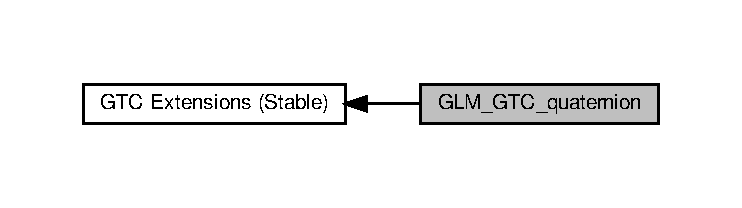
\includegraphics[width=350pt]{group__gtc__quaternion}
\end{center}
\end{figure}
\subsection*{Functions}
\begin{DoxyCompactItemize}
\item 
{\footnotesize template$<$typename T , precision P$>$ }\\\hyperlink{setup_8hpp_ab2d052de21a70539923e9bcbf6e83a51}{G\+L\+M\+\_\+\+F\+U\+N\+C\+\_\+\+D\+E\+CL} T \hyperlink{group__gtc__quaternion_ga3406ab83e2cafd4034f359957e942410}{glm\+::length} (\hyperlink{structglm_1_1detail_1_1tquat}{detail\+::tquat}$<$ T, P $>$ const \&q)
\item 
{\footnotesize template$<$typename T , precision P$>$ }\\\hyperlink{setup_8hpp_ab2d052de21a70539923e9bcbf6e83a51}{G\+L\+M\+\_\+\+F\+U\+N\+C\+\_\+\+D\+E\+CL} \hyperlink{structglm_1_1detail_1_1tquat}{detail\+::tquat}$<$ T, P $>$ \hyperlink{group__gtc__quaternion_ga34ee289ca53a08207904e935104715d8}{glm\+::normalize} (\hyperlink{structglm_1_1detail_1_1tquat}{detail\+::tquat}$<$ T, P $>$ const \&q)
\item 
{\footnotesize template$<$typename T , precision P, template$<$ typename, precision $>$ class quat\+Type$>$ }\\\hyperlink{setup_8hpp_ab2d052de21a70539923e9bcbf6e83a51}{G\+L\+M\+\_\+\+F\+U\+N\+C\+\_\+\+D\+E\+CL} T \hyperlink{group__gtc__quaternion_gac54dfc83de465a2d03e90d342242ab3d}{glm\+::dot} (quat\+Type$<$ T, P $>$ const \&x, quat\+Type$<$ T, P $>$ const \&y)
\item 
{\footnotesize template$<$typename T , precision P$>$ }\\\hyperlink{setup_8hpp_ab2d052de21a70539923e9bcbf6e83a51}{G\+L\+M\+\_\+\+F\+U\+N\+C\+\_\+\+D\+E\+CL} \hyperlink{structglm_1_1detail_1_1tquat}{detail\+::tquat}$<$ T, P $>$ \hyperlink{group__gtc__quaternion_gafabf175ae3e2cd30bf58dc313321955a}{glm\+::mix} (\hyperlink{structglm_1_1detail_1_1tquat}{detail\+::tquat}$<$ T, P $>$ const \&x, \hyperlink{structglm_1_1detail_1_1tquat}{detail\+::tquat}$<$ T, P $>$ const \&y, T const \&a)
\item 
{\footnotesize template$<$typename T , precision P$>$ }\\\hyperlink{setup_8hpp_ab2d052de21a70539923e9bcbf6e83a51}{G\+L\+M\+\_\+\+F\+U\+N\+C\+\_\+\+D\+E\+CL} \hyperlink{structglm_1_1detail_1_1tquat}{detail\+::tquat}$<$ T, P $>$ \hyperlink{group__gtc__quaternion_gafc1c989eaa2c786d34218b176f680fe0}{glm\+::lerp} (\hyperlink{structglm_1_1detail_1_1tquat}{detail\+::tquat}$<$ T, P $>$ const \&x, \hyperlink{structglm_1_1detail_1_1tquat}{detail\+::tquat}$<$ T, P $>$ const \&y, T const \&a)
\item 
{\footnotesize template$<$typename T , precision P$>$ }\\\hyperlink{setup_8hpp_ab2d052de21a70539923e9bcbf6e83a51}{G\+L\+M\+\_\+\+F\+U\+N\+C\+\_\+\+D\+E\+CL} \hyperlink{structglm_1_1detail_1_1tquat}{detail\+::tquat}$<$ T, P $>$ \hyperlink{group__gtc__quaternion_ga7468a211a20ea56ea5cfb0625226868a}{glm\+::slerp} (\hyperlink{structglm_1_1detail_1_1tquat}{detail\+::tquat}$<$ T, P $>$ const \&x, \hyperlink{structglm_1_1detail_1_1tquat}{detail\+::tquat}$<$ T, P $>$ const \&y, T const \&a)
\begin{DoxyCompactList}\small\item\em Returns the slurp interpolation between two quaternions. \end{DoxyCompactList}\item 
{\footnotesize template$<$typename T , precision P$>$ }\\\hyperlink{setup_8hpp_ab2d052de21a70539923e9bcbf6e83a51}{G\+L\+M\+\_\+\+F\+U\+N\+C\+\_\+\+D\+E\+CL} \hyperlink{structglm_1_1detail_1_1tquat}{detail\+::tquat}$<$ T, P $>$ \hyperlink{group__gtc__quaternion_gaf78006c47276b151777fc194cf11a688}{glm\+::conjugate} (\hyperlink{structglm_1_1detail_1_1tquat}{detail\+::tquat}$<$ T, P $>$ const \&q)
\item 
{\footnotesize template$<$typename T , precision P$>$ }\\\hyperlink{setup_8hpp_ab2d052de21a70539923e9bcbf6e83a51}{G\+L\+M\+\_\+\+F\+U\+N\+C\+\_\+\+D\+E\+CL} \hyperlink{structglm_1_1detail_1_1tquat}{detail\+::tquat}$<$ T, P $>$ \hyperlink{group__gtc__quaternion_ga6613ef61cb980a18f19ece5f421564da}{glm\+::inverse} (\hyperlink{structglm_1_1detail_1_1tquat}{detail\+::tquat}$<$ T, P $>$ const \&q)
\item 
{\footnotesize template$<$typename T , precision P$>$ }\\\hyperlink{setup_8hpp_ab2d052de21a70539923e9bcbf6e83a51}{G\+L\+M\+\_\+\+F\+U\+N\+C\+\_\+\+D\+E\+CL} \hyperlink{structglm_1_1detail_1_1tquat}{detail\+::tquat}$<$ T, P $>$ \hyperlink{group__gtc__quaternion_gaa9a8891f03d8f5373525c4b3159c1c73}{glm\+::rotate} (\hyperlink{structglm_1_1detail_1_1tquat}{detail\+::tquat}$<$ T, P $>$ const \&q, T const \&\hyperlink{group__gtc__quaternion_ga23a3fc7ada5bbb665ff84c92c6e0542c}{angle}, \hyperlink{structglm_1_1detail_1_1tvec3}{detail\+::tvec3}$<$ T, P $>$ const \&\hyperlink{group__gtc__quaternion_ga8eef9f8c3f2e4836dccf09df975b20fb}{axis})
\item 
{\footnotesize template$<$typename T , precision P$>$ }\\\hyperlink{setup_8hpp_ab2d052de21a70539923e9bcbf6e83a51}{G\+L\+M\+\_\+\+F\+U\+N\+C\+\_\+\+D\+E\+CL} \hyperlink{structglm_1_1detail_1_1tvec3}{detail\+::tvec3}$<$ T, P $>$ \hyperlink{group__gtc__quaternion_gade4034f49ccadf63cb31a7fb5fa3c8aa}{glm\+::euler\+Angles} (\hyperlink{structglm_1_1detail_1_1tquat}{detail\+::tquat}$<$ T, P $>$ const \&x)
\item 
{\footnotesize template$<$typename T , precision P$>$ }\\\hyperlink{setup_8hpp_ab2d052de21a70539923e9bcbf6e83a51}{G\+L\+M\+\_\+\+F\+U\+N\+C\+\_\+\+D\+E\+CL} T \hyperlink{group__gtc__quaternion_ga6d883e423bc425f4334fcce202131f7e}{glm\+::roll} (\hyperlink{structglm_1_1detail_1_1tquat}{detail\+::tquat}$<$ T, P $>$ const \&x)
\item 
{\footnotesize template$<$typename T , precision P$>$ }\\\hyperlink{setup_8hpp_ab2d052de21a70539923e9bcbf6e83a51}{G\+L\+M\+\_\+\+F\+U\+N\+C\+\_\+\+D\+E\+CL} T \hyperlink{group__gtc__quaternion_ga4d345dc369a54f53f5ebc375bac56d11}{glm\+::pitch} (\hyperlink{structglm_1_1detail_1_1tquat}{detail\+::tquat}$<$ T, P $>$ const \&x)
\item 
{\footnotesize template$<$typename T , precision P$>$ }\\\hyperlink{setup_8hpp_ab2d052de21a70539923e9bcbf6e83a51}{G\+L\+M\+\_\+\+F\+U\+N\+C\+\_\+\+D\+E\+CL} T \hyperlink{group__gtc__quaternion_ga1de7653ddf380ff06d2300eea831664c}{glm\+::yaw} (\hyperlink{structglm_1_1detail_1_1tquat}{detail\+::tquat}$<$ T, P $>$ const \&x)
\item 
{\footnotesize template$<$typename T , precision P$>$ }\\\hyperlink{setup_8hpp_ab2d052de21a70539923e9bcbf6e83a51}{G\+L\+M\+\_\+\+F\+U\+N\+C\+\_\+\+D\+E\+CL} \hyperlink{structglm_1_1detail_1_1tmat3x3}{detail\+::tmat3x3}$<$ T, P $>$ \hyperlink{group__gtc__quaternion_ga65257c3494022ad80a50ce11da95049d}{glm\+::mat3\+\_\+cast} (\hyperlink{structglm_1_1detail_1_1tquat}{detail\+::tquat}$<$ T, P $>$ const \&x)
\item 
{\footnotesize template$<$typename T , precision P$>$ }\\\hyperlink{setup_8hpp_ab2d052de21a70539923e9bcbf6e83a51}{G\+L\+M\+\_\+\+F\+U\+N\+C\+\_\+\+D\+E\+CL} \hyperlink{structglm_1_1detail_1_1tmat4x4}{detail\+::tmat4x4}$<$ T, P $>$ \hyperlink{group__gtc__quaternion_gafc4e34c836f7ccb5f3bb2a0373c831e0}{glm\+::mat4\+\_\+cast} (\hyperlink{structglm_1_1detail_1_1tquat}{detail\+::tquat}$<$ T, P $>$ const \&x)
\item 
{\footnotesize template$<$typename T , precision P$>$ }\\\hyperlink{setup_8hpp_ab2d052de21a70539923e9bcbf6e83a51}{G\+L\+M\+\_\+\+F\+U\+N\+C\+\_\+\+D\+E\+CL} \hyperlink{structglm_1_1detail_1_1tquat}{detail\+::tquat}$<$ T, P $>$ \hyperlink{group__gtc__quaternion_gafb826745dedb1760100bbd25d0f63fde}{glm\+::quat\+\_\+cast} (\hyperlink{structglm_1_1detail_1_1tmat3x3}{detail\+::tmat3x3}$<$ T, P $>$ const \&x)
\item 
{\footnotesize template$<$typename T , precision P$>$ }\\\hyperlink{setup_8hpp_ab2d052de21a70539923e9bcbf6e83a51}{G\+L\+M\+\_\+\+F\+U\+N\+C\+\_\+\+D\+E\+CL} \hyperlink{structglm_1_1detail_1_1tquat}{detail\+::tquat}$<$ T, P $>$ \hyperlink{group__gtc__quaternion_ga385af22ef1a45c4464ddd28b80d5ce18}{glm\+::quat\+\_\+cast} (\hyperlink{structglm_1_1detail_1_1tmat4x4}{detail\+::tmat4x4}$<$ T, P $>$ const \&x)
\item 
{\footnotesize template$<$typename T , precision P$>$ }\\\hyperlink{setup_8hpp_ab2d052de21a70539923e9bcbf6e83a51}{G\+L\+M\+\_\+\+F\+U\+N\+C\+\_\+\+D\+E\+CL} T \hyperlink{group__gtc__quaternion_ga23a3fc7ada5bbb665ff84c92c6e0542c}{glm\+::angle} (\hyperlink{structglm_1_1detail_1_1tquat}{detail\+::tquat}$<$ T, P $>$ const \&x)
\item 
{\footnotesize template$<$typename T , precision P$>$ }\\\hyperlink{setup_8hpp_ab2d052de21a70539923e9bcbf6e83a51}{G\+L\+M\+\_\+\+F\+U\+N\+C\+\_\+\+D\+E\+CL} \hyperlink{structglm_1_1detail_1_1tvec3}{detail\+::tvec3}$<$ T, P $>$ \hyperlink{group__gtc__quaternion_ga8eef9f8c3f2e4836dccf09df975b20fb}{glm\+::axis} (\hyperlink{structglm_1_1detail_1_1tquat}{detail\+::tquat}$<$ T, P $>$ const \&x)
\item 
{\footnotesize template$<$typename T , precision P$>$ }\\\hyperlink{setup_8hpp_ab2d052de21a70539923e9bcbf6e83a51}{G\+L\+M\+\_\+\+F\+U\+N\+C\+\_\+\+D\+E\+CL} \hyperlink{structglm_1_1detail_1_1tquat}{detail\+::tquat}$<$ T, P $>$ \hyperlink{group__gtc__quaternion_ga771b3e16cca8324e7111b923476be666}{glm\+::angle\+Axis} (T const \&\hyperlink{group__gtc__quaternion_ga23a3fc7ada5bbb665ff84c92c6e0542c}{angle}, \hyperlink{structglm_1_1detail_1_1tvec3}{detail\+::tvec3}$<$ T, P $>$ const \&\hyperlink{group__gtc__quaternion_ga8eef9f8c3f2e4836dccf09df975b20fb}{axis})
\item 
{\footnotesize template$<$typename T , precision P$>$ }\\\hyperlink{setup_8hpp_ab2d052de21a70539923e9bcbf6e83a51}{G\+L\+M\+\_\+\+F\+U\+N\+C\+\_\+\+D\+E\+CL} \hyperlink{structglm_1_1detail_1_1tvec4}{detail\+::tvec4}$<$ bool, P $>$ \hyperlink{group__gtc__quaternion_ga4e4c37b86cecde7e1076c5b5fdb920b9}{glm\+::less\+Than} (\hyperlink{structglm_1_1detail_1_1tquat}{detail\+::tquat}$<$ T, P $>$ const \&x, \hyperlink{structglm_1_1detail_1_1tquat}{detail\+::tquat}$<$ T, P $>$ const \&y)
\item 
{\footnotesize template$<$typename T , precision P$>$ }\\\hyperlink{setup_8hpp_ab2d052de21a70539923e9bcbf6e83a51}{G\+L\+M\+\_\+\+F\+U\+N\+C\+\_\+\+D\+E\+CL} \hyperlink{structglm_1_1detail_1_1tvec4}{detail\+::tvec4}$<$ bool, P $>$ \hyperlink{group__gtc__quaternion_ga313fe20896a8cd43c6d08cc88fa18faa}{glm\+::less\+Than\+Equal} (\hyperlink{structglm_1_1detail_1_1tquat}{detail\+::tquat}$<$ T, P $>$ const \&x, \hyperlink{structglm_1_1detail_1_1tquat}{detail\+::tquat}$<$ T, P $>$ const \&y)
\item 
{\footnotesize template$<$typename T , precision P$>$ }\\\hyperlink{setup_8hpp_ab2d052de21a70539923e9bcbf6e83a51}{G\+L\+M\+\_\+\+F\+U\+N\+C\+\_\+\+D\+E\+CL} \hyperlink{structglm_1_1detail_1_1tvec4}{detail\+::tvec4}$<$ bool, P $>$ \hyperlink{group__gtc__quaternion_ga63be67bccef0b0ad4e60656223ab3761}{glm\+::greater\+Than} (\hyperlink{structglm_1_1detail_1_1tquat}{detail\+::tquat}$<$ T, P $>$ const \&x, \hyperlink{structglm_1_1detail_1_1tquat}{detail\+::tquat}$<$ T, P $>$ const \&y)
\item 
{\footnotesize template$<$typename T , precision P$>$ }\\\hyperlink{setup_8hpp_ab2d052de21a70539923e9bcbf6e83a51}{G\+L\+M\+\_\+\+F\+U\+N\+C\+\_\+\+D\+E\+CL} \hyperlink{structglm_1_1detail_1_1tvec4}{detail\+::tvec4}$<$ bool, P $>$ \hyperlink{group__gtc__quaternion_gac90d5af34a03cd665a349ac30e4cc44c}{glm\+::greater\+Than\+Equal} (\hyperlink{structglm_1_1detail_1_1tquat}{detail\+::tquat}$<$ T, P $>$ const \&x, \hyperlink{structglm_1_1detail_1_1tquat}{detail\+::tquat}$<$ T, P $>$ const \&y)
\item 
{\footnotesize template$<$typename T , precision P$>$ }\\\hyperlink{setup_8hpp_ab2d052de21a70539923e9bcbf6e83a51}{G\+L\+M\+\_\+\+F\+U\+N\+C\+\_\+\+D\+E\+CL} \hyperlink{structglm_1_1detail_1_1tvec4}{detail\+::tvec4}$<$ bool, P $>$ \hyperlink{group__gtc__quaternion_ga32ff2cc6fb576639a6237d8d8ed5818b}{glm\+::equal} (\hyperlink{structglm_1_1detail_1_1tquat}{detail\+::tquat}$<$ T, P $>$ const \&x, \hyperlink{structglm_1_1detail_1_1tquat}{detail\+::tquat}$<$ T, P $>$ const \&y)
\item 
{\footnotesize template$<$typename T , precision P$>$ }\\\hyperlink{setup_8hpp_ab2d052de21a70539923e9bcbf6e83a51}{G\+L\+M\+\_\+\+F\+U\+N\+C\+\_\+\+D\+E\+CL} \hyperlink{structglm_1_1detail_1_1tvec4}{detail\+::tvec4}$<$ bool, P $>$ \hyperlink{group__gtc__quaternion_gaa3a8cf1aa580e435ca96acafbd7870a5}{glm\+::not\+Equal} (\hyperlink{structglm_1_1detail_1_1tquat}{detail\+::tquat}$<$ T, P $>$ const \&x, \hyperlink{structglm_1_1detail_1_1tquat}{detail\+::tquat}$<$ T, P $>$ const \&y)
\end{DoxyCompactItemize}


\subsection{Detailed Description}
Defines a templated quaternion type and several quaternion operations. 

$<$\hyperlink{gtc_2quaternion_8hpp}{glm/gtc/quaternion.\+hpp}$>$ need to be included to use these functionalities. 

\subsection{Function Documentation}
\mbox{\Hypertarget{group__gtc__quaternion_ga23a3fc7ada5bbb665ff84c92c6e0542c}\label{group__gtc__quaternion_ga23a3fc7ada5bbb665ff84c92c6e0542c}} 
\index{G\+L\+M\+\_\+\+G\+T\+C\+\_\+quaternion@{G\+L\+M\+\_\+\+G\+T\+C\+\_\+quaternion}!angle@{angle}}
\index{angle@{angle}!G\+L\+M\+\_\+\+G\+T\+C\+\_\+quaternion@{G\+L\+M\+\_\+\+G\+T\+C\+\_\+quaternion}}
\subsubsection{\texorpdfstring{angle()}{angle()}}
{\footnotesize\ttfamily template$<$typename T , precision P$>$ \\
\hyperlink{setup_8hpp_ab2d052de21a70539923e9bcbf6e83a51}{G\+L\+M\+\_\+\+F\+U\+N\+C\+\_\+\+D\+E\+CL} T glm\+::angle (\begin{DoxyParamCaption}\item[{\hyperlink{structglm_1_1detail_1_1tquat}{detail\+::tquat}$<$ T, P $>$ const \&}]{x }\end{DoxyParamCaption})}

Returns the quaternion rotation angle.

\begin{DoxySeeAlso}{See also}
\hyperlink{group__gtc__quaternion}{G\+L\+M\+\_\+\+G\+T\+C\+\_\+quaternion} 
\end{DoxySeeAlso}


Definition at line 799 of file quaternion.\+inl.

\mbox{\Hypertarget{group__gtc__quaternion_ga771b3e16cca8324e7111b923476be666}\label{group__gtc__quaternion_ga771b3e16cca8324e7111b923476be666}} 
\index{G\+L\+M\+\_\+\+G\+T\+C\+\_\+quaternion@{G\+L\+M\+\_\+\+G\+T\+C\+\_\+quaternion}!angle\+Axis@{angle\+Axis}}
\index{angle\+Axis@{angle\+Axis}!G\+L\+M\+\_\+\+G\+T\+C\+\_\+quaternion@{G\+L\+M\+\_\+\+G\+T\+C\+\_\+quaternion}}
\subsubsection{\texorpdfstring{angle\+Axis()}{angleAxis()}}
{\footnotesize\ttfamily template$<$typename T , precision P$>$ \\
\hyperlink{setup_8hpp_ab2d052de21a70539923e9bcbf6e83a51}{G\+L\+M\+\_\+\+F\+U\+N\+C\+\_\+\+D\+E\+CL} \hyperlink{structglm_1_1detail_1_1tquat}{detail\+::tquat}$<$T, P$>$ glm\+::angle\+Axis (\begin{DoxyParamCaption}\item[{T const \&}]{angle,  }\item[{\hyperlink{structglm_1_1detail_1_1tvec3}{detail\+::tvec3}$<$ T, P $>$ const \&}]{axis }\end{DoxyParamCaption})}

Build a quaternion from an angle and a normalized axis.


\begin{DoxyParams}{Parameters}
{\em angle} & Angle expressed in radians if G\+L\+M\+\_\+\+F\+O\+R\+C\+E\+\_\+\+R\+A\+D\+I\+A\+NS is define or degrees otherwise. \\
\hline
{\em axis} & Axis of the quaternion, must be normalized.\\
\hline
\end{DoxyParams}
\begin{DoxySeeAlso}{See also}
\hyperlink{group__gtc__quaternion}{G\+L\+M\+\_\+\+G\+T\+C\+\_\+quaternion} 
\end{DoxySeeAlso}


Definition at line 826 of file quaternion.\+inl.

\mbox{\Hypertarget{group__gtc__quaternion_ga8eef9f8c3f2e4836dccf09df975b20fb}\label{group__gtc__quaternion_ga8eef9f8c3f2e4836dccf09df975b20fb}} 
\index{G\+L\+M\+\_\+\+G\+T\+C\+\_\+quaternion@{G\+L\+M\+\_\+\+G\+T\+C\+\_\+quaternion}!axis@{axis}}
\index{axis@{axis}!G\+L\+M\+\_\+\+G\+T\+C\+\_\+quaternion@{G\+L\+M\+\_\+\+G\+T\+C\+\_\+quaternion}}
\subsubsection{\texorpdfstring{axis()}{axis()}}
{\footnotesize\ttfamily template$<$typename T , precision P$>$ \\
\hyperlink{setup_8hpp_ab2d052de21a70539923e9bcbf6e83a51}{G\+L\+M\+\_\+\+F\+U\+N\+C\+\_\+\+D\+E\+CL} \hyperlink{structglm_1_1detail_1_1tvec3}{detail\+::tvec3}$<$T, P$>$ glm\+::axis (\begin{DoxyParamCaption}\item[{\hyperlink{structglm_1_1detail_1_1tquat}{detail\+::tquat}$<$ T, P $>$ const \&}]{x }\end{DoxyParamCaption})}

Returns the q rotation axis.

\begin{DoxySeeAlso}{See also}
\hyperlink{group__gtc__quaternion}{G\+L\+M\+\_\+\+G\+T\+C\+\_\+quaternion} 
\end{DoxySeeAlso}


Definition at line 813 of file quaternion.\+inl.

\mbox{\Hypertarget{group__gtc__quaternion_gaf78006c47276b151777fc194cf11a688}\label{group__gtc__quaternion_gaf78006c47276b151777fc194cf11a688}} 
\index{G\+L\+M\+\_\+\+G\+T\+C\+\_\+quaternion@{G\+L\+M\+\_\+\+G\+T\+C\+\_\+quaternion}!conjugate@{conjugate}}
\index{conjugate@{conjugate}!G\+L\+M\+\_\+\+G\+T\+C\+\_\+quaternion@{G\+L\+M\+\_\+\+G\+T\+C\+\_\+quaternion}}
\subsubsection{\texorpdfstring{conjugate()}{conjugate()}}
{\footnotesize\ttfamily template$<$typename T , precision P$>$ \\
\hyperlink{setup_8hpp_ab2d052de21a70539923e9bcbf6e83a51}{G\+L\+M\+\_\+\+F\+U\+N\+C\+\_\+\+D\+E\+CL} \hyperlink{structglm_1_1detail_1_1tquat}{detail\+::tquat}$<$T, P$>$ glm\+::conjugate (\begin{DoxyParamCaption}\item[{\hyperlink{structglm_1_1detail_1_1tquat}{detail\+::tquat}$<$ T, P $>$ const \&}]{q }\end{DoxyParamCaption})}

Returns the q conjugate.

\begin{DoxySeeAlso}{See also}
\hyperlink{group__gtc__quaternion}{G\+L\+M\+\_\+\+G\+T\+C\+\_\+quaternion} 
\end{DoxySeeAlso}


Definition at line 177 of file quaternion.\+inl.

\mbox{\Hypertarget{group__gtc__quaternion_gac54dfc83de465a2d03e90d342242ab3d}\label{group__gtc__quaternion_gac54dfc83de465a2d03e90d342242ab3d}} 
\index{G\+L\+M\+\_\+\+G\+T\+C\+\_\+quaternion@{G\+L\+M\+\_\+\+G\+T\+C\+\_\+quaternion}!dot@{dot}}
\index{dot@{dot}!G\+L\+M\+\_\+\+G\+T\+C\+\_\+quaternion@{G\+L\+M\+\_\+\+G\+T\+C\+\_\+quaternion}}
\subsubsection{\texorpdfstring{dot()}{dot()}}
{\footnotesize\ttfamily template$<$typename T , precision P, template$<$ typename, precision $>$ class quat\+Type$>$ \\
\hyperlink{setup_8hpp_ab2d052de21a70539923e9bcbf6e83a51}{G\+L\+M\+\_\+\+F\+U\+N\+C\+\_\+\+D\+E\+CL} T glm\+::dot (\begin{DoxyParamCaption}\item[{quat\+Type$<$ T, P $>$ const \&}]{x,  }\item[{quat\+Type$<$ T, P $>$ const \&}]{y }\end{DoxyParamCaption})}

Returns dot product of q1 and q2, i.\+e., q1\mbox{[}0\mbox{]} $\ast$ q2\mbox{[}0\mbox{]} + q1\mbox{[}1\mbox{]} $\ast$ q2\mbox{[}1\mbox{]} + ...

\begin{DoxySeeAlso}{See also}
\hyperlink{group__gtc__quaternion}{G\+L\+M\+\_\+\+G\+T\+C\+\_\+quaternion} 
\end{DoxySeeAlso}
\mbox{\Hypertarget{group__gtc__quaternion_ga32ff2cc6fb576639a6237d8d8ed5818b}\label{group__gtc__quaternion_ga32ff2cc6fb576639a6237d8d8ed5818b}} 
\index{G\+L\+M\+\_\+\+G\+T\+C\+\_\+quaternion@{G\+L\+M\+\_\+\+G\+T\+C\+\_\+quaternion}!equal@{equal}}
\index{equal@{equal}!G\+L\+M\+\_\+\+G\+T\+C\+\_\+quaternion@{G\+L\+M\+\_\+\+G\+T\+C\+\_\+quaternion}}
\subsubsection{\texorpdfstring{equal()}{equal()}}
{\footnotesize\ttfamily template$<$typename T , precision P$>$ \\
\hyperlink{setup_8hpp_ab2d052de21a70539923e9bcbf6e83a51}{G\+L\+M\+\_\+\+F\+U\+N\+C\+\_\+\+D\+E\+CL} \hyperlink{structglm_1_1detail_1_1tvec4}{detail\+::tvec4}$<$bool, P$>$ glm\+::equal (\begin{DoxyParamCaption}\item[{\hyperlink{structglm_1_1detail_1_1tquat}{detail\+::tquat}$<$ T, P $>$ const \&}]{x,  }\item[{\hyperlink{structglm_1_1detail_1_1tquat}{detail\+::tquat}$<$ T, P $>$ const \&}]{y }\end{DoxyParamCaption})}

Returns the component-\/wise comparison of result x == y.


\begin{DoxyTemplParams}{Template Parameters}
{\em quat\+Type} & Floating-\/point quaternion types.\\
\hline
\end{DoxyTemplParams}
\begin{DoxySeeAlso}{See also}
\hyperlink{group__gtc__quaternion}{G\+L\+M\+\_\+\+G\+T\+C\+\_\+quaternion} 
\end{DoxySeeAlso}


Definition at line 902 of file quaternion.\+inl.

\mbox{\Hypertarget{group__gtc__quaternion_gade4034f49ccadf63cb31a7fb5fa3c8aa}\label{group__gtc__quaternion_gade4034f49ccadf63cb31a7fb5fa3c8aa}} 
\index{G\+L\+M\+\_\+\+G\+T\+C\+\_\+quaternion@{G\+L\+M\+\_\+\+G\+T\+C\+\_\+quaternion}!euler\+Angles@{euler\+Angles}}
\index{euler\+Angles@{euler\+Angles}!G\+L\+M\+\_\+\+G\+T\+C\+\_\+quaternion@{G\+L\+M\+\_\+\+G\+T\+C\+\_\+quaternion}}
\subsubsection{\texorpdfstring{euler\+Angles()}{eulerAngles()}}
{\footnotesize\ttfamily template$<$typename T , precision P$>$ \\
\hyperlink{setup_8hpp_ab2d052de21a70539923e9bcbf6e83a51}{G\+L\+M\+\_\+\+F\+U\+N\+C\+\_\+\+D\+E\+CL} \hyperlink{structglm_1_1detail_1_1tvec3}{detail\+::tvec3}$<$T, P$>$ glm\+::euler\+Angles (\begin{DoxyParamCaption}\item[{\hyperlink{structglm_1_1detail_1_1tquat}{detail\+::tquat}$<$ T, P $>$ const \&}]{x }\end{DoxyParamCaption})}

Returns euler angles, yitch as x, yaw as y, roll as z. The result is expressed in radians if G\+L\+M\+\_\+\+F\+O\+R\+C\+E\+\_\+\+R\+A\+D\+I\+A\+NS is defined or degrees otherwise.

\begin{DoxySeeAlso}{See also}
\hyperlink{group__gtc__quaternion}{G\+L\+M\+\_\+\+G\+T\+C\+\_\+quaternion} 
\end{DoxySeeAlso}


Definition at line 632 of file quaternion.\+inl.

\mbox{\Hypertarget{group__gtc__quaternion_ga63be67bccef0b0ad4e60656223ab3761}\label{group__gtc__quaternion_ga63be67bccef0b0ad4e60656223ab3761}} 
\index{G\+L\+M\+\_\+\+G\+T\+C\+\_\+quaternion@{G\+L\+M\+\_\+\+G\+T\+C\+\_\+quaternion}!greater\+Than@{greater\+Than}}
\index{greater\+Than@{greater\+Than}!G\+L\+M\+\_\+\+G\+T\+C\+\_\+quaternion@{G\+L\+M\+\_\+\+G\+T\+C\+\_\+quaternion}}
\subsubsection{\texorpdfstring{greater\+Than()}{greaterThan()}}
{\footnotesize\ttfamily template$<$typename T , precision P$>$ \\
\hyperlink{setup_8hpp_ab2d052de21a70539923e9bcbf6e83a51}{G\+L\+M\+\_\+\+F\+U\+N\+C\+\_\+\+D\+E\+CL} \hyperlink{structglm_1_1detail_1_1tvec4}{detail\+::tvec4}$<$bool, P$>$ glm\+::greater\+Than (\begin{DoxyParamCaption}\item[{\hyperlink{structglm_1_1detail_1_1tquat}{detail\+::tquat}$<$ T, P $>$ const \&}]{x,  }\item[{\hyperlink{structglm_1_1detail_1_1tquat}{detail\+::tquat}$<$ T, P $>$ const \&}]{y }\end{DoxyParamCaption})}

Returns the component-\/wise comparison of result x $>$ y.


\begin{DoxyTemplParams}{Template Parameters}
{\em quat\+Type} & Floating-\/point quaternion types.\\
\hline
\end{DoxyTemplParams}
\begin{DoxySeeAlso}{See also}
\hyperlink{group__gtc__quaternion}{G\+L\+M\+\_\+\+G\+T\+C\+\_\+quaternion} 
\end{DoxySeeAlso}


Definition at line 876 of file quaternion.\+inl.

\mbox{\Hypertarget{group__gtc__quaternion_gac90d5af34a03cd665a349ac30e4cc44c}\label{group__gtc__quaternion_gac90d5af34a03cd665a349ac30e4cc44c}} 
\index{G\+L\+M\+\_\+\+G\+T\+C\+\_\+quaternion@{G\+L\+M\+\_\+\+G\+T\+C\+\_\+quaternion}!greater\+Than\+Equal@{greater\+Than\+Equal}}
\index{greater\+Than\+Equal@{greater\+Than\+Equal}!G\+L\+M\+\_\+\+G\+T\+C\+\_\+quaternion@{G\+L\+M\+\_\+\+G\+T\+C\+\_\+quaternion}}
\subsubsection{\texorpdfstring{greater\+Than\+Equal()}{greaterThanEqual()}}
{\footnotesize\ttfamily template$<$typename T , precision P$>$ \\
\hyperlink{setup_8hpp_ab2d052de21a70539923e9bcbf6e83a51}{G\+L\+M\+\_\+\+F\+U\+N\+C\+\_\+\+D\+E\+CL} \hyperlink{structglm_1_1detail_1_1tvec4}{detail\+::tvec4}$<$bool, P$>$ glm\+::greater\+Than\+Equal (\begin{DoxyParamCaption}\item[{\hyperlink{structglm_1_1detail_1_1tquat}{detail\+::tquat}$<$ T, P $>$ const \&}]{x,  }\item[{\hyperlink{structglm_1_1detail_1_1tquat}{detail\+::tquat}$<$ T, P $>$ const \&}]{y }\end{DoxyParamCaption})}

Returns the component-\/wise comparison of result x $>$= y.


\begin{DoxyTemplParams}{Template Parameters}
{\em quat\+Type} & Floating-\/point quaternion types.\\
\hline
\end{DoxyTemplParams}
\begin{DoxySeeAlso}{See also}
\hyperlink{group__gtc__quaternion}{G\+L\+M\+\_\+\+G\+T\+C\+\_\+quaternion} 
\end{DoxySeeAlso}


Definition at line 889 of file quaternion.\+inl.

\mbox{\Hypertarget{group__gtc__quaternion_ga6613ef61cb980a18f19ece5f421564da}\label{group__gtc__quaternion_ga6613ef61cb980a18f19ece5f421564da}} 
\index{G\+L\+M\+\_\+\+G\+T\+C\+\_\+quaternion@{G\+L\+M\+\_\+\+G\+T\+C\+\_\+quaternion}!inverse@{inverse}}
\index{inverse@{inverse}!G\+L\+M\+\_\+\+G\+T\+C\+\_\+quaternion@{G\+L\+M\+\_\+\+G\+T\+C\+\_\+quaternion}}
\subsubsection{\texorpdfstring{inverse()}{inverse()}}
{\footnotesize\ttfamily template$<$typename T , precision P$>$ \\
\hyperlink{setup_8hpp_ab2d052de21a70539923e9bcbf6e83a51}{G\+L\+M\+\_\+\+F\+U\+N\+C\+\_\+\+D\+E\+CL} \hyperlink{structglm_1_1detail_1_1tquat}{detail\+::tquat}$<$T, P$>$ glm\+::inverse (\begin{DoxyParamCaption}\item[{\hyperlink{structglm_1_1detail_1_1tquat}{detail\+::tquat}$<$ T, P $>$ const \&}]{q }\end{DoxyParamCaption})}

Returns the q inverse.

\begin{DoxySeeAlso}{See also}
\hyperlink{group__gtc__quaternion}{G\+L\+M\+\_\+\+G\+T\+C\+\_\+quaternion} 
\end{DoxySeeAlso}


Definition at line 186 of file quaternion.\+inl.

\mbox{\Hypertarget{group__gtc__quaternion_ga3406ab83e2cafd4034f359957e942410}\label{group__gtc__quaternion_ga3406ab83e2cafd4034f359957e942410}} 
\index{G\+L\+M\+\_\+\+G\+T\+C\+\_\+quaternion@{G\+L\+M\+\_\+\+G\+T\+C\+\_\+quaternion}!length@{length}}
\index{length@{length}!G\+L\+M\+\_\+\+G\+T\+C\+\_\+quaternion@{G\+L\+M\+\_\+\+G\+T\+C\+\_\+quaternion}}
\subsubsection{\texorpdfstring{length()}{length()}}
{\footnotesize\ttfamily template$<$typename T , precision P$>$ \\
\hyperlink{setup_8hpp_ab2d052de21a70539923e9bcbf6e83a51}{G\+L\+M\+\_\+\+F\+U\+N\+C\+\_\+\+D\+E\+CL} T glm\+::length (\begin{DoxyParamCaption}\item[{\hyperlink{structglm_1_1detail_1_1tquat}{detail\+::tquat}$<$ T, P $>$ const \&}]{q }\end{DoxyParamCaption})}

Returns the length of the quaternion.

\begin{DoxySeeAlso}{See also}
\hyperlink{group__gtc__quaternion}{G\+L\+M\+\_\+\+G\+T\+C\+\_\+quaternion} 
\end{DoxySeeAlso}


Definition at line 402 of file quaternion.\+inl.

\mbox{\Hypertarget{group__gtc__quaternion_gafc1c989eaa2c786d34218b176f680fe0}\label{group__gtc__quaternion_gafc1c989eaa2c786d34218b176f680fe0}} 
\index{G\+L\+M\+\_\+\+G\+T\+C\+\_\+quaternion@{G\+L\+M\+\_\+\+G\+T\+C\+\_\+quaternion}!lerp@{lerp}}
\index{lerp@{lerp}!G\+L\+M\+\_\+\+G\+T\+C\+\_\+quaternion@{G\+L\+M\+\_\+\+G\+T\+C\+\_\+quaternion}}
\subsubsection{\texorpdfstring{lerp()}{lerp()}}
{\footnotesize\ttfamily template$<$typename T , precision P$>$ \\
\hyperlink{setup_8hpp_ab2d052de21a70539923e9bcbf6e83a51}{G\+L\+M\+\_\+\+F\+U\+N\+C\+\_\+\+D\+E\+CL} \hyperlink{structglm_1_1detail_1_1tquat}{detail\+::tquat}$<$T, P$>$ glm\+::lerp (\begin{DoxyParamCaption}\item[{\hyperlink{structglm_1_1detail_1_1tquat}{detail\+::tquat}$<$ T, P $>$ const \&}]{x,  }\item[{\hyperlink{structglm_1_1detail_1_1tquat}{detail\+::tquat}$<$ T, P $>$ const \&}]{y,  }\item[{T const \&}]{a }\end{DoxyParamCaption})}

Linear interpolation of two quaternions. The interpolation is oriented.


\begin{DoxyParams}{Parameters}
{\em x} & A quaternion \\
\hline
{\em y} & A quaternion \\
\hline
{\em a} & Interpolation factor. The interpolation is defined in the range \mbox{[}0, 1\mbox{]}. \\
\hline
\end{DoxyParams}

\begin{DoxyTemplParams}{Template Parameters}
{\em T} & Value type used to build the quaternion. Supported\+: half, float or double. \\
\hline
\end{DoxyTemplParams}
\begin{DoxySeeAlso}{See also}
\hyperlink{group__gtc__quaternion}{G\+L\+M\+\_\+\+G\+T\+C\+\_\+quaternion} 
\end{DoxySeeAlso}


Definition at line 547 of file quaternion.\+inl.

\mbox{\Hypertarget{group__gtc__quaternion_ga4e4c37b86cecde7e1076c5b5fdb920b9}\label{group__gtc__quaternion_ga4e4c37b86cecde7e1076c5b5fdb920b9}} 
\index{G\+L\+M\+\_\+\+G\+T\+C\+\_\+quaternion@{G\+L\+M\+\_\+\+G\+T\+C\+\_\+quaternion}!less\+Than@{less\+Than}}
\index{less\+Than@{less\+Than}!G\+L\+M\+\_\+\+G\+T\+C\+\_\+quaternion@{G\+L\+M\+\_\+\+G\+T\+C\+\_\+quaternion}}
\subsubsection{\texorpdfstring{less\+Than()}{lessThan()}}
{\footnotesize\ttfamily template$<$typename T , precision P$>$ \\
\hyperlink{setup_8hpp_ab2d052de21a70539923e9bcbf6e83a51}{G\+L\+M\+\_\+\+F\+U\+N\+C\+\_\+\+D\+E\+CL} \hyperlink{structglm_1_1detail_1_1tvec4}{detail\+::tvec4}$<$bool, P$>$ glm\+::less\+Than (\begin{DoxyParamCaption}\item[{\hyperlink{structglm_1_1detail_1_1tquat}{detail\+::tquat}$<$ T, P $>$ const \&}]{x,  }\item[{\hyperlink{structglm_1_1detail_1_1tquat}{detail\+::tquat}$<$ T, P $>$ const \&}]{y }\end{DoxyParamCaption})}

Returns the component-\/wise comparison result of x $<$ y.


\begin{DoxyTemplParams}{Template Parameters}
{\em quat\+Type} & Floating-\/point quaternion types.\\
\hline
\end{DoxyTemplParams}
\begin{DoxySeeAlso}{See also}
\hyperlink{group__gtc__quaternion}{G\+L\+M\+\_\+\+G\+T\+C\+\_\+quaternion} 
\end{DoxySeeAlso}


Definition at line 850 of file quaternion.\+inl.

\mbox{\Hypertarget{group__gtc__quaternion_ga313fe20896a8cd43c6d08cc88fa18faa}\label{group__gtc__quaternion_ga313fe20896a8cd43c6d08cc88fa18faa}} 
\index{G\+L\+M\+\_\+\+G\+T\+C\+\_\+quaternion@{G\+L\+M\+\_\+\+G\+T\+C\+\_\+quaternion}!less\+Than\+Equal@{less\+Than\+Equal}}
\index{less\+Than\+Equal@{less\+Than\+Equal}!G\+L\+M\+\_\+\+G\+T\+C\+\_\+quaternion@{G\+L\+M\+\_\+\+G\+T\+C\+\_\+quaternion}}
\subsubsection{\texorpdfstring{less\+Than\+Equal()}{lessThanEqual()}}
{\footnotesize\ttfamily template$<$typename T , precision P$>$ \\
\hyperlink{setup_8hpp_ab2d052de21a70539923e9bcbf6e83a51}{G\+L\+M\+\_\+\+F\+U\+N\+C\+\_\+\+D\+E\+CL} \hyperlink{structglm_1_1detail_1_1tvec4}{detail\+::tvec4}$<$bool, P$>$ glm\+::less\+Than\+Equal (\begin{DoxyParamCaption}\item[{\hyperlink{structglm_1_1detail_1_1tquat}{detail\+::tquat}$<$ T, P $>$ const \&}]{x,  }\item[{\hyperlink{structglm_1_1detail_1_1tquat}{detail\+::tquat}$<$ T, P $>$ const \&}]{y }\end{DoxyParamCaption})}

Returns the component-\/wise comparison of result x $<$= y.


\begin{DoxyTemplParams}{Template Parameters}
{\em quat\+Type} & Floating-\/point quaternion types.\\
\hline
\end{DoxyTemplParams}
\begin{DoxySeeAlso}{See also}
\hyperlink{group__gtc__quaternion}{G\+L\+M\+\_\+\+G\+T\+C\+\_\+quaternion} 
\end{DoxySeeAlso}


Definition at line 863 of file quaternion.\+inl.

\mbox{\Hypertarget{group__gtc__quaternion_ga65257c3494022ad80a50ce11da95049d}\label{group__gtc__quaternion_ga65257c3494022ad80a50ce11da95049d}} 
\index{G\+L\+M\+\_\+\+G\+T\+C\+\_\+quaternion@{G\+L\+M\+\_\+\+G\+T\+C\+\_\+quaternion}!mat3\+\_\+cast@{mat3\+\_\+cast}}
\index{mat3\+\_\+cast@{mat3\+\_\+cast}!G\+L\+M\+\_\+\+G\+T\+C\+\_\+quaternion@{G\+L\+M\+\_\+\+G\+T\+C\+\_\+quaternion}}
\subsubsection{\texorpdfstring{mat3\+\_\+cast()}{mat3\_cast()}}
{\footnotesize\ttfamily template$<$typename T , precision P$>$ \\
\hyperlink{setup_8hpp_ab2d052de21a70539923e9bcbf6e83a51}{G\+L\+M\+\_\+\+F\+U\+N\+C\+\_\+\+D\+E\+CL} \hyperlink{structglm_1_1detail_1_1tmat3x3}{detail\+::tmat3x3}$<$T, P$>$ glm\+::mat3\+\_\+cast (\begin{DoxyParamCaption}\item[{\hyperlink{structglm_1_1detail_1_1tquat}{detail\+::tquat}$<$ T, P $>$ const \&}]{x }\end{DoxyParamCaption})}

Converts a quaternion to a 3 $\ast$ 3 matrix.

\begin{DoxySeeAlso}{See also}
\hyperlink{group__gtc__quaternion}{G\+L\+M\+\_\+\+G\+T\+C\+\_\+quaternion} 
\end{DoxySeeAlso}


Definition at line 683 of file quaternion.\+inl.

\mbox{\Hypertarget{group__gtc__quaternion_gafc4e34c836f7ccb5f3bb2a0373c831e0}\label{group__gtc__quaternion_gafc4e34c836f7ccb5f3bb2a0373c831e0}} 
\index{G\+L\+M\+\_\+\+G\+T\+C\+\_\+quaternion@{G\+L\+M\+\_\+\+G\+T\+C\+\_\+quaternion}!mat4\+\_\+cast@{mat4\+\_\+cast}}
\index{mat4\+\_\+cast@{mat4\+\_\+cast}!G\+L\+M\+\_\+\+G\+T\+C\+\_\+quaternion@{G\+L\+M\+\_\+\+G\+T\+C\+\_\+quaternion}}
\subsubsection{\texorpdfstring{mat4\+\_\+cast()}{mat4\_cast()}}
{\footnotesize\ttfamily template$<$typename T , precision P$>$ \\
\hyperlink{setup_8hpp_ab2d052de21a70539923e9bcbf6e83a51}{G\+L\+M\+\_\+\+F\+U\+N\+C\+\_\+\+D\+E\+CL} \hyperlink{structglm_1_1detail_1_1tmat4x4}{detail\+::tmat4x4}$<$T, P$>$ glm\+::mat4\+\_\+cast (\begin{DoxyParamCaption}\item[{\hyperlink{structglm_1_1detail_1_1tquat}{detail\+::tquat}$<$ T, P $>$ const \&}]{x }\end{DoxyParamCaption})}

Converts a quaternion to a 4 $\ast$ 4 matrix.

\begin{DoxySeeAlso}{See also}
\hyperlink{group__gtc__quaternion}{G\+L\+M\+\_\+\+G\+T\+C\+\_\+quaternion} 
\end{DoxySeeAlso}


Definition at line 714 of file quaternion.\+inl.

\mbox{\Hypertarget{group__gtc__quaternion_gafabf175ae3e2cd30bf58dc313321955a}\label{group__gtc__quaternion_gafabf175ae3e2cd30bf58dc313321955a}} 
\index{G\+L\+M\+\_\+\+G\+T\+C\+\_\+quaternion@{G\+L\+M\+\_\+\+G\+T\+C\+\_\+quaternion}!mix@{mix}}
\index{mix@{mix}!G\+L\+M\+\_\+\+G\+T\+C\+\_\+quaternion@{G\+L\+M\+\_\+\+G\+T\+C\+\_\+quaternion}}
\subsubsection{\texorpdfstring{mix()}{mix()}}
{\footnotesize\ttfamily template$<$typename T , precision P$>$ \\
\hyperlink{setup_8hpp_ab2d052de21a70539923e9bcbf6e83a51}{G\+L\+M\+\_\+\+F\+U\+N\+C\+\_\+\+D\+E\+CL} \hyperlink{structglm_1_1detail_1_1tquat}{detail\+::tquat}$<$T, P$>$ glm\+::mix (\begin{DoxyParamCaption}\item[{\hyperlink{structglm_1_1detail_1_1tquat}{detail\+::tquat}$<$ T, P $>$ const \&}]{x,  }\item[{\hyperlink{structglm_1_1detail_1_1tquat}{detail\+::tquat}$<$ T, P $>$ const \&}]{y,  }\item[{T const \&}]{a }\end{DoxyParamCaption})}

Spherical linear interpolation of two quaternions. The interpolation is oriented and the rotation is performed at constant speed. For short path spherical linear interpolation, use the slerp function.


\begin{DoxyParams}{Parameters}
{\em x} & A quaternion \\
\hline
{\em y} & A quaternion \\
\hline
{\em a} & Interpolation factor. The interpolation is defined beyond the range \mbox{[}0, 1\mbox{]}. \\
\hline
\end{DoxyParams}

\begin{DoxyTemplParams}{Template Parameters}
{\em T} & Value type used to build the quaternion. Supported\+: half, float or double. \\
\hline
\end{DoxyTemplParams}
\begin{DoxySeeAlso}{See also}
\hyperlink{group__gtc__quaternion}{G\+L\+M\+\_\+\+G\+T\+C\+\_\+quaternion} 

-\/ \hyperlink{group__gtc__quaternion_ga7468a211a20ea56ea5cfb0625226868a}{slerp(detail\+::tquat$<$\+T, P$>$ const \& x, detail\+::tquat$<$\+T, P$>$ const \& y, T const \& a)} 
\end{DoxySeeAlso}


Definition at line 519 of file quaternion.\+inl.

\mbox{\Hypertarget{group__gtc__quaternion_ga34ee289ca53a08207904e935104715d8}\label{group__gtc__quaternion_ga34ee289ca53a08207904e935104715d8}} 
\index{G\+L\+M\+\_\+\+G\+T\+C\+\_\+quaternion@{G\+L\+M\+\_\+\+G\+T\+C\+\_\+quaternion}!normalize@{normalize}}
\index{normalize@{normalize}!G\+L\+M\+\_\+\+G\+T\+C\+\_\+quaternion@{G\+L\+M\+\_\+\+G\+T\+C\+\_\+quaternion}}
\subsubsection{\texorpdfstring{normalize()}{normalize()}}
{\footnotesize\ttfamily template$<$typename T , precision P$>$ \\
\hyperlink{setup_8hpp_ab2d052de21a70539923e9bcbf6e83a51}{G\+L\+M\+\_\+\+F\+U\+N\+C\+\_\+\+D\+E\+CL} \hyperlink{structglm_1_1detail_1_1tquat}{detail\+::tquat}$<$T, P$>$ glm\+::normalize (\begin{DoxyParamCaption}\item[{\hyperlink{structglm_1_1detail_1_1tquat}{detail\+::tquat}$<$ T, P $>$ const \&}]{q }\end{DoxyParamCaption})}

Returns the normalized quaternion.

\begin{DoxySeeAlso}{See also}
\hyperlink{group__gtc__quaternion}{G\+L\+M\+\_\+\+G\+T\+C\+\_\+quaternion} 
\end{DoxySeeAlso}


Definition at line 411 of file quaternion.\+inl.

\mbox{\Hypertarget{group__gtc__quaternion_gaa3a8cf1aa580e435ca96acafbd7870a5}\label{group__gtc__quaternion_gaa3a8cf1aa580e435ca96acafbd7870a5}} 
\index{G\+L\+M\+\_\+\+G\+T\+C\+\_\+quaternion@{G\+L\+M\+\_\+\+G\+T\+C\+\_\+quaternion}!not\+Equal@{not\+Equal}}
\index{not\+Equal@{not\+Equal}!G\+L\+M\+\_\+\+G\+T\+C\+\_\+quaternion@{G\+L\+M\+\_\+\+G\+T\+C\+\_\+quaternion}}
\subsubsection{\texorpdfstring{not\+Equal()}{notEqual()}}
{\footnotesize\ttfamily template$<$typename T , precision P$>$ \\
\hyperlink{setup_8hpp_ab2d052de21a70539923e9bcbf6e83a51}{G\+L\+M\+\_\+\+F\+U\+N\+C\+\_\+\+D\+E\+CL} \hyperlink{structglm_1_1detail_1_1tvec4}{detail\+::tvec4}$<$bool, P$>$ glm\+::not\+Equal (\begin{DoxyParamCaption}\item[{\hyperlink{structglm_1_1detail_1_1tquat}{detail\+::tquat}$<$ T, P $>$ const \&}]{x,  }\item[{\hyperlink{structglm_1_1detail_1_1tquat}{detail\+::tquat}$<$ T, P $>$ const \&}]{y }\end{DoxyParamCaption})}

Returns the component-\/wise comparison of result x != y.


\begin{DoxyTemplParams}{Template Parameters}
{\em quat\+Type} & Floating-\/point quaternion types.\\
\hline
\end{DoxyTemplParams}
\begin{DoxySeeAlso}{See also}
\hyperlink{group__gtc__quaternion}{G\+L\+M\+\_\+\+G\+T\+C\+\_\+quaternion} 
\end{DoxySeeAlso}


Definition at line 915 of file quaternion.\+inl.

\mbox{\Hypertarget{group__gtc__quaternion_ga4d345dc369a54f53f5ebc375bac56d11}\label{group__gtc__quaternion_ga4d345dc369a54f53f5ebc375bac56d11}} 
\index{G\+L\+M\+\_\+\+G\+T\+C\+\_\+quaternion@{G\+L\+M\+\_\+\+G\+T\+C\+\_\+quaternion}!pitch@{pitch}}
\index{pitch@{pitch}!G\+L\+M\+\_\+\+G\+T\+C\+\_\+quaternion@{G\+L\+M\+\_\+\+G\+T\+C\+\_\+quaternion}}
\subsubsection{\texorpdfstring{pitch()}{pitch()}}
{\footnotesize\ttfamily template$<$typename T , precision P$>$ \\
\hyperlink{setup_8hpp_ab2d052de21a70539923e9bcbf6e83a51}{G\+L\+M\+\_\+\+F\+U\+N\+C\+\_\+\+D\+E\+CL} T glm\+::pitch (\begin{DoxyParamCaption}\item[{\hyperlink{structglm_1_1detail_1_1tquat}{detail\+::tquat}$<$ T, P $>$ const \&}]{x }\end{DoxyParamCaption})}

Returns pitch value of euler angles expressed in radians if G\+L\+M\+\_\+\+F\+O\+R\+C\+E\+\_\+\+R\+A\+D\+I\+A\+NS is defined or degrees otherwise.

\begin{DoxySeeAlso}{See also}
\hyperlink{group__gtx__quaternion}{G\+L\+M\+\_\+\+G\+T\+X\+\_\+quaternion} 
\end{DoxySeeAlso}


Definition at line 655 of file quaternion.\+inl.

\mbox{\Hypertarget{group__gtc__quaternion_gafb826745dedb1760100bbd25d0f63fde}\label{group__gtc__quaternion_gafb826745dedb1760100bbd25d0f63fde}} 
\index{G\+L\+M\+\_\+\+G\+T\+C\+\_\+quaternion@{G\+L\+M\+\_\+\+G\+T\+C\+\_\+quaternion}!quat\+\_\+cast@{quat\+\_\+cast}}
\index{quat\+\_\+cast@{quat\+\_\+cast}!G\+L\+M\+\_\+\+G\+T\+C\+\_\+quaternion@{G\+L\+M\+\_\+\+G\+T\+C\+\_\+quaternion}}
\subsubsection{\texorpdfstring{quat\+\_\+cast()}{quat\_cast()}\hspace{0.1cm}{\footnotesize\ttfamily [1/2]}}
{\footnotesize\ttfamily template$<$typename T , precision P$>$ \\
\hyperlink{setup_8hpp_ab2d052de21a70539923e9bcbf6e83a51}{G\+L\+M\+\_\+\+F\+U\+N\+C\+\_\+\+D\+E\+CL} \hyperlink{structglm_1_1detail_1_1tquat}{detail\+::tquat}$<$T, P$>$ glm\+::quat\+\_\+cast (\begin{DoxyParamCaption}\item[{\hyperlink{structglm_1_1detail_1_1tmat3x3}{detail\+::tmat3x3}$<$ T, P $>$ const \&}]{x }\end{DoxyParamCaption})}

Converts a 3 $\ast$ 3 matrix to a quaternion.

\begin{DoxySeeAlso}{See also}
\hyperlink{group__gtc__quaternion}{G\+L\+M\+\_\+\+G\+T\+C\+\_\+quaternion} 
\end{DoxySeeAlso}


Definition at line 723 of file quaternion.\+inl.

\mbox{\Hypertarget{group__gtc__quaternion_ga385af22ef1a45c4464ddd28b80d5ce18}\label{group__gtc__quaternion_ga385af22ef1a45c4464ddd28b80d5ce18}} 
\index{G\+L\+M\+\_\+\+G\+T\+C\+\_\+quaternion@{G\+L\+M\+\_\+\+G\+T\+C\+\_\+quaternion}!quat\+\_\+cast@{quat\+\_\+cast}}
\index{quat\+\_\+cast@{quat\+\_\+cast}!G\+L\+M\+\_\+\+G\+T\+C\+\_\+quaternion@{G\+L\+M\+\_\+\+G\+T\+C\+\_\+quaternion}}
\subsubsection{\texorpdfstring{quat\+\_\+cast()}{quat\_cast()}\hspace{0.1cm}{\footnotesize\ttfamily [2/2]}}
{\footnotesize\ttfamily template$<$typename T , precision P$>$ \\
\hyperlink{setup_8hpp_ab2d052de21a70539923e9bcbf6e83a51}{G\+L\+M\+\_\+\+F\+U\+N\+C\+\_\+\+D\+E\+CL} \hyperlink{structglm_1_1detail_1_1tquat}{detail\+::tquat}$<$T, P$>$ glm\+::quat\+\_\+cast (\begin{DoxyParamCaption}\item[{\hyperlink{structglm_1_1detail_1_1tmat4x4}{detail\+::tmat4x4}$<$ T, P $>$ const \&}]{x }\end{DoxyParamCaption})}

Converts a 4 $\ast$ 4 matrix to a quaternion.

\begin{DoxySeeAlso}{See also}
\hyperlink{group__gtc__quaternion}{G\+L\+M\+\_\+\+G\+T\+C\+\_\+quaternion} 
\end{DoxySeeAlso}


Definition at line 790 of file quaternion.\+inl.

\mbox{\Hypertarget{group__gtc__quaternion_ga6d883e423bc425f4334fcce202131f7e}\label{group__gtc__quaternion_ga6d883e423bc425f4334fcce202131f7e}} 
\index{G\+L\+M\+\_\+\+G\+T\+C\+\_\+quaternion@{G\+L\+M\+\_\+\+G\+T\+C\+\_\+quaternion}!roll@{roll}}
\index{roll@{roll}!G\+L\+M\+\_\+\+G\+T\+C\+\_\+quaternion@{G\+L\+M\+\_\+\+G\+T\+C\+\_\+quaternion}}
\subsubsection{\texorpdfstring{roll()}{roll()}}
{\footnotesize\ttfamily template$<$typename T , precision P$>$ \\
\hyperlink{setup_8hpp_ab2d052de21a70539923e9bcbf6e83a51}{G\+L\+M\+\_\+\+F\+U\+N\+C\+\_\+\+D\+E\+CL} T glm\+::roll (\begin{DoxyParamCaption}\item[{\hyperlink{structglm_1_1detail_1_1tquat}{detail\+::tquat}$<$ T, P $>$ const \&}]{x }\end{DoxyParamCaption})}

Returns roll value of euler angles expressed in radians if G\+L\+M\+\_\+\+F\+O\+R\+C\+E\+\_\+\+R\+A\+D\+I\+A\+NS is defined or degrees otherwise.

\begin{DoxySeeAlso}{See also}
\hyperlink{group__gtx__quaternion}{G\+L\+M\+\_\+\+G\+T\+X\+\_\+quaternion} 
\end{DoxySeeAlso}


Definition at line 641 of file quaternion.\+inl.

\mbox{\Hypertarget{group__gtc__quaternion_gaa9a8891f03d8f5373525c4b3159c1c73}\label{group__gtc__quaternion_gaa9a8891f03d8f5373525c4b3159c1c73}} 
\index{G\+L\+M\+\_\+\+G\+T\+C\+\_\+quaternion@{G\+L\+M\+\_\+\+G\+T\+C\+\_\+quaternion}!rotate@{rotate}}
\index{rotate@{rotate}!G\+L\+M\+\_\+\+G\+T\+C\+\_\+quaternion@{G\+L\+M\+\_\+\+G\+T\+C\+\_\+quaternion}}
\subsubsection{\texorpdfstring{rotate()}{rotate()}}
{\footnotesize\ttfamily template$<$typename T , precision P$>$ \\
\hyperlink{setup_8hpp_ab2d052de21a70539923e9bcbf6e83a51}{G\+L\+M\+\_\+\+F\+U\+N\+C\+\_\+\+D\+E\+CL} \hyperlink{structglm_1_1detail_1_1tquat}{detail\+::tquat}$<$T, P$>$ glm\+::rotate (\begin{DoxyParamCaption}\item[{\hyperlink{structglm_1_1detail_1_1tquat}{detail\+::tquat}$<$ T, P $>$ const \&}]{q,  }\item[{T const \&}]{angle,  }\item[{\hyperlink{structglm_1_1detail_1_1tvec3}{detail\+::tvec3}$<$ T, P $>$ const \&}]{axis }\end{DoxyParamCaption})}

Rotates a quaternion from a vector of 3 components axis and an angle.


\begin{DoxyParams}{Parameters}
{\em q} & Source orientation \\
\hline
{\em angle} & Angle expressed in radians if G\+L\+M\+\_\+\+F\+O\+R\+C\+E\+\_\+\+R\+A\+D\+I\+A\+NS is define or degrees otherwise. \\
\hline
{\em axis} & Axis of the rotation\\
\hline
\end{DoxyParams}
\begin{DoxySeeAlso}{See also}
\hyperlink{group__gtc__quaternion}{G\+L\+M\+\_\+\+G\+T\+C\+\_\+quaternion} 
\end{DoxySeeAlso}


Definition at line 600 of file quaternion.\+inl.

\mbox{\Hypertarget{group__gtc__quaternion_ga7468a211a20ea56ea5cfb0625226868a}\label{group__gtc__quaternion_ga7468a211a20ea56ea5cfb0625226868a}} 
\index{G\+L\+M\+\_\+\+G\+T\+C\+\_\+quaternion@{G\+L\+M\+\_\+\+G\+T\+C\+\_\+quaternion}!slerp@{slerp}}
\index{slerp@{slerp}!G\+L\+M\+\_\+\+G\+T\+C\+\_\+quaternion@{G\+L\+M\+\_\+\+G\+T\+C\+\_\+quaternion}}
\subsubsection{\texorpdfstring{slerp()}{slerp()}}
{\footnotesize\ttfamily template$<$typename T , precision P$>$ \\
\hyperlink{setup_8hpp_ab2d052de21a70539923e9bcbf6e83a51}{G\+L\+M\+\_\+\+F\+U\+N\+C\+\_\+\+D\+E\+CL} \hyperlink{structglm_1_1detail_1_1tquat}{detail\+::tquat}$<$T, P$>$ glm\+::slerp (\begin{DoxyParamCaption}\item[{\hyperlink{structglm_1_1detail_1_1tquat}{detail\+::tquat}$<$ T, P $>$ const \&}]{x,  }\item[{\hyperlink{structglm_1_1detail_1_1tquat}{detail\+::tquat}$<$ T, P $>$ const \&}]{y,  }\item[{T const \&}]{a }\end{DoxyParamCaption})}



Returns the slurp interpolation between two quaternions. 

Spherical linear interpolation of two quaternions. The interpolation always take the short path and the rotation is performed at constant speed.


\begin{DoxyParams}{Parameters}
{\em x} & A quaternion \\
\hline
{\em y} & A quaternion \\
\hline
{\em a} & Interpolation factor. The interpolation is defined beyond the range \mbox{[}0, 1\mbox{]}. \\
\hline
\end{DoxyParams}

\begin{DoxyTemplParams}{Template Parameters}
{\em T} & Value type used to build the quaternion. Supported\+: half, float or double. \\
\hline
\end{DoxyTemplParams}
\begin{DoxySeeAlso}{See also}
\hyperlink{group__gtc__quaternion}{G\+L\+M\+\_\+\+G\+T\+C\+\_\+quaternion} 
\end{DoxySeeAlso}


Definition at line 562 of file quaternion.\+inl.

\mbox{\Hypertarget{group__gtc__quaternion_ga1de7653ddf380ff06d2300eea831664c}\label{group__gtc__quaternion_ga1de7653ddf380ff06d2300eea831664c}} 
\index{G\+L\+M\+\_\+\+G\+T\+C\+\_\+quaternion@{G\+L\+M\+\_\+\+G\+T\+C\+\_\+quaternion}!yaw@{yaw}}
\index{yaw@{yaw}!G\+L\+M\+\_\+\+G\+T\+C\+\_\+quaternion@{G\+L\+M\+\_\+\+G\+T\+C\+\_\+quaternion}}
\subsubsection{\texorpdfstring{yaw()}{yaw()}}
{\footnotesize\ttfamily template$<$typename T , precision P$>$ \\
\hyperlink{setup_8hpp_ab2d052de21a70539923e9bcbf6e83a51}{G\+L\+M\+\_\+\+F\+U\+N\+C\+\_\+\+D\+E\+CL} T glm\+::yaw (\begin{DoxyParamCaption}\item[{\hyperlink{structglm_1_1detail_1_1tquat}{detail\+::tquat}$<$ T, P $>$ const \&}]{x }\end{DoxyParamCaption})}

Returns yaw value of euler angles expressed in radians if G\+L\+M\+\_\+\+F\+O\+R\+C\+E\+\_\+\+R\+A\+D\+I\+A\+NS is defined or degrees otherwise.

\begin{DoxySeeAlso}{See also}
\hyperlink{group__gtx__quaternion}{G\+L\+M\+\_\+\+G\+T\+X\+\_\+quaternion} 
\end{DoxySeeAlso}


Definition at line 669 of file quaternion.\+inl.


\hypertarget{group__gtc__random}{}\section{G\+L\+M\+\_\+\+G\+T\+C\+\_\+random}
\label{group__gtc__random}\index{G\+L\+M\+\_\+\+G\+T\+C\+\_\+random@{G\+L\+M\+\_\+\+G\+T\+C\+\_\+random}}


Generate random number from various distribution methods.  


Collaboration diagram for G\+L\+M\+\_\+\+G\+T\+C\+\_\+random\+:\nopagebreak
\begin{figure}[H]
\begin{center}
\leavevmode
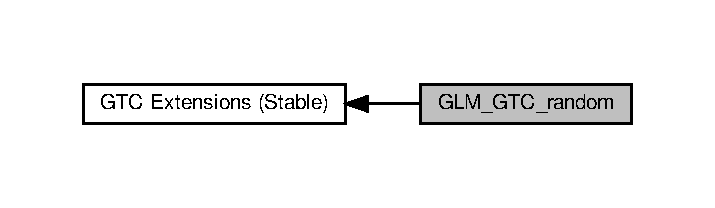
\includegraphics[width=343pt]{group__gtc__random}
\end{center}
\end{figure}
\subsection*{Functions}
\begin{DoxyCompactItemize}
\item 
{\footnotesize template$<$typename gen\+Type $>$ }\\\hyperlink{setup_8hpp_ab2d052de21a70539923e9bcbf6e83a51}{G\+L\+M\+\_\+\+F\+U\+N\+C\+\_\+\+D\+E\+CL} gen\+Type \hyperlink{group__gtc__random_ga310c2e65883e62a4405128f187f41f27}{glm\+::linear\+Rand} (gen\+Type const \&Min, gen\+Type const \&Max)
\item 
{\footnotesize template$<$typename gen\+Type $>$ }\\\hyperlink{setup_8hpp_ab2d052de21a70539923e9bcbf6e83a51}{G\+L\+M\+\_\+\+F\+U\+N\+C\+\_\+\+D\+E\+CL} gen\+Type \hyperlink{group__gtc__random_gacba09f5b8e1e8eac3d318ae6426bbd26}{glm\+::gauss\+Rand} (gen\+Type const \&Mean, gen\+Type const \&Deviation)
\item 
{\footnotesize template$<$typename T $>$ }\\\hyperlink{setup_8hpp_ab2d052de21a70539923e9bcbf6e83a51}{G\+L\+M\+\_\+\+F\+U\+N\+C\+\_\+\+D\+E\+CL} \hyperlink{structglm_1_1detail_1_1tvec2}{detail\+::tvec2}$<$ T, \hyperlink{namespaceglm_a0f04f086094c747d227af4425893f545a9d21ccd8b5a009ec7eb7677befc3bf51}{defaultp} $>$ \hyperlink{group__gtc__random_gac1ab03c2c797ce352fd74cdb5229b151}{glm\+::circular\+Rand} (T const \&Radius)
\item 
{\footnotesize template$<$typename T $>$ }\\\hyperlink{setup_8hpp_ab2d052de21a70539923e9bcbf6e83a51}{G\+L\+M\+\_\+\+F\+U\+N\+C\+\_\+\+D\+E\+CL} \hyperlink{structglm_1_1detail_1_1tvec3}{detail\+::tvec3}$<$ T, \hyperlink{namespaceglm_a0f04f086094c747d227af4425893f545a9d21ccd8b5a009ec7eb7677befc3bf51}{defaultp} $>$ \hyperlink{group__gtc__random_ga8a9eee1fcb08690881ead242fe4259dc}{glm\+::spherical\+Rand} (T const \&Radius)
\item 
{\footnotesize template$<$typename T $>$ }\\\hyperlink{setup_8hpp_ab2d052de21a70539923e9bcbf6e83a51}{G\+L\+M\+\_\+\+F\+U\+N\+C\+\_\+\+D\+E\+CL} \hyperlink{structglm_1_1detail_1_1tvec2}{detail\+::tvec2}$<$ T, \hyperlink{namespaceglm_a0f04f086094c747d227af4425893f545a9d21ccd8b5a009ec7eb7677befc3bf51}{defaultp} $>$ \hyperlink{group__gtc__random_ga7d24fc3ef13fd7b6cad7e7b870b0e322}{glm\+::disk\+Rand} (T const \&Radius)
\item 
{\footnotesize template$<$typename T $>$ }\\\hyperlink{setup_8hpp_ab2d052de21a70539923e9bcbf6e83a51}{G\+L\+M\+\_\+\+F\+U\+N\+C\+\_\+\+D\+E\+CL} \hyperlink{structglm_1_1detail_1_1tvec3}{detail\+::tvec3}$<$ T, \hyperlink{namespaceglm_a0f04f086094c747d227af4425893f545a9d21ccd8b5a009ec7eb7677befc3bf51}{defaultp} $>$ \hyperlink{group__gtc__random_gac9c6e44b013874c291547f568d240500}{glm\+::ball\+Rand} (T const \&Radius)
\end{DoxyCompactItemize}


\subsection{Detailed Description}
Generate random number from various distribution methods. 

$<$\hyperlink{gtc_2random_8hpp}{glm/gtc/random.\+hpp}$>$ need to be included to use these functionalities. 

\subsection{Function Documentation}
\mbox{\Hypertarget{group__gtc__random_gac9c6e44b013874c291547f568d240500}\label{group__gtc__random_gac9c6e44b013874c291547f568d240500}} 
\index{G\+L\+M\+\_\+\+G\+T\+C\+\_\+random@{G\+L\+M\+\_\+\+G\+T\+C\+\_\+random}!ball\+Rand@{ball\+Rand}}
\index{ball\+Rand@{ball\+Rand}!G\+L\+M\+\_\+\+G\+T\+C\+\_\+random@{G\+L\+M\+\_\+\+G\+T\+C\+\_\+random}}
\subsubsection{\texorpdfstring{ball\+Rand()}{ballRand()}}
{\footnotesize\ttfamily template$<$typename T $>$ \\
\hyperlink{setup_8hpp_ab2d052de21a70539923e9bcbf6e83a51}{G\+L\+M\+\_\+\+F\+U\+N\+C\+\_\+\+D\+E\+CL} \hyperlink{structglm_1_1detail_1_1tvec3}{detail\+::tvec3}$<$T, \hyperlink{namespaceglm_a0f04f086094c747d227af4425893f545a9d21ccd8b5a009ec7eb7677befc3bf51}{defaultp}$>$ glm\+::ball\+Rand (\begin{DoxyParamCaption}\item[{T const \&}]{Radius }\end{DoxyParamCaption})}

Generate a random 3D vector which coordinates are regulary distributed within the volume of a ball of a given radius


\begin{DoxyParams}{Parameters}
{\em Radius} & \\
\hline
\end{DoxyParams}
\begin{DoxySeeAlso}{See also}
\hyperlink{group__gtc__random}{G\+L\+M\+\_\+\+G\+T\+C\+\_\+random} 
\end{DoxySeeAlso}


Definition at line 126 of file random.\+inl.

\mbox{\Hypertarget{group__gtc__random_gac1ab03c2c797ce352fd74cdb5229b151}\label{group__gtc__random_gac1ab03c2c797ce352fd74cdb5229b151}} 
\index{G\+L\+M\+\_\+\+G\+T\+C\+\_\+random@{G\+L\+M\+\_\+\+G\+T\+C\+\_\+random}!circular\+Rand@{circular\+Rand}}
\index{circular\+Rand@{circular\+Rand}!G\+L\+M\+\_\+\+G\+T\+C\+\_\+random@{G\+L\+M\+\_\+\+G\+T\+C\+\_\+random}}
\subsubsection{\texorpdfstring{circular\+Rand()}{circularRand()}}
{\footnotesize\ttfamily template$<$typename T $>$ \\
\hyperlink{setup_8hpp_ab2d052de21a70539923e9bcbf6e83a51}{G\+L\+M\+\_\+\+F\+U\+N\+C\+\_\+\+D\+E\+CL} \hyperlink{structglm_1_1detail_1_1tvec2}{detail\+::tvec2}$<$T, \hyperlink{namespaceglm_a0f04f086094c747d227af4425893f545a9d21ccd8b5a009ec7eb7677befc3bf51}{defaultp}$>$ glm\+::circular\+Rand (\begin{DoxyParamCaption}\item[{T const \&}]{Radius }\end{DoxyParamCaption})}

Generate a random 2D vector which coordinates are regulary distributed on a circle of a given radius


\begin{DoxyParams}{Parameters}
{\em Radius} & \\
\hline
\end{DoxyParams}
\begin{DoxySeeAlso}{See also}
\hyperlink{group__gtc__random}{G\+L\+M\+\_\+\+G\+T\+C\+\_\+random} 
\end{DoxySeeAlso}


Definition at line 147 of file random.\+inl.

\mbox{\Hypertarget{group__gtc__random_ga7d24fc3ef13fd7b6cad7e7b870b0e322}\label{group__gtc__random_ga7d24fc3ef13fd7b6cad7e7b870b0e322}} 
\index{G\+L\+M\+\_\+\+G\+T\+C\+\_\+random@{G\+L\+M\+\_\+\+G\+T\+C\+\_\+random}!disk\+Rand@{disk\+Rand}}
\index{disk\+Rand@{disk\+Rand}!G\+L\+M\+\_\+\+G\+T\+C\+\_\+random@{G\+L\+M\+\_\+\+G\+T\+C\+\_\+random}}
\subsubsection{\texorpdfstring{disk\+Rand()}{diskRand()}}
{\footnotesize\ttfamily template$<$typename T $>$ \\
\hyperlink{setup_8hpp_ab2d052de21a70539923e9bcbf6e83a51}{G\+L\+M\+\_\+\+F\+U\+N\+C\+\_\+\+D\+E\+CL} \hyperlink{structglm_1_1detail_1_1tvec2}{detail\+::tvec2}$<$T, \hyperlink{namespaceglm_a0f04f086094c747d227af4425893f545a9d21ccd8b5a009ec7eb7677befc3bf51}{defaultp}$>$ glm\+::disk\+Rand (\begin{DoxyParamCaption}\item[{T const \&}]{Radius }\end{DoxyParamCaption})}

Generate a random 2D vector which coordinates are regulary distributed within the area of a disk of a given radius


\begin{DoxyParams}{Parameters}
{\em Radius} & \\
\hline
\end{DoxyParams}
\begin{DoxySeeAlso}{See also}
\hyperlink{group__gtc__random}{G\+L\+M\+\_\+\+G\+T\+C\+\_\+random} 
\end{DoxySeeAlso}


Definition at line 105 of file random.\+inl.

\mbox{\Hypertarget{group__gtc__random_gacba09f5b8e1e8eac3d318ae6426bbd26}\label{group__gtc__random_gacba09f5b8e1e8eac3d318ae6426bbd26}} 
\index{G\+L\+M\+\_\+\+G\+T\+C\+\_\+random@{G\+L\+M\+\_\+\+G\+T\+C\+\_\+random}!gauss\+Rand@{gauss\+Rand}}
\index{gauss\+Rand@{gauss\+Rand}!G\+L\+M\+\_\+\+G\+T\+C\+\_\+random@{G\+L\+M\+\_\+\+G\+T\+C\+\_\+random}}
\subsubsection{\texorpdfstring{gauss\+Rand()}{gaussRand()}}
{\footnotesize\ttfamily template$<$typename gen\+Type $>$ \\
\hyperlink{setup_8hpp_ab2d052de21a70539923e9bcbf6e83a51}{G\+L\+M\+\_\+\+F\+U\+N\+C\+\_\+\+D\+E\+CL} gen\+Type glm\+::gauss\+Rand (\begin{DoxyParamCaption}\item[{gen\+Type const \&}]{Mean,  }\item[{gen\+Type const \&}]{Deviation }\end{DoxyParamCaption})}

Generate random numbers in the interval \mbox{[}Min, Max\mbox{]}, according a gaussian distribution


\begin{DoxyParams}{Parameters}
{\em Mean} & \\
\hline
{\em Deviation} & \\
\hline
\end{DoxyParams}
\begin{DoxySeeAlso}{See also}
\hyperlink{group__gtc__random}{G\+L\+M\+\_\+\+G\+T\+C\+\_\+random} 
\end{DoxySeeAlso}


Definition at line 83 of file random.\+inl.

\mbox{\Hypertarget{group__gtc__random_ga310c2e65883e62a4405128f187f41f27}\label{group__gtc__random_ga310c2e65883e62a4405128f187f41f27}} 
\index{G\+L\+M\+\_\+\+G\+T\+C\+\_\+random@{G\+L\+M\+\_\+\+G\+T\+C\+\_\+random}!linear\+Rand@{linear\+Rand}}
\index{linear\+Rand@{linear\+Rand}!G\+L\+M\+\_\+\+G\+T\+C\+\_\+random@{G\+L\+M\+\_\+\+G\+T\+C\+\_\+random}}
\subsubsection{\texorpdfstring{linear\+Rand()}{linearRand()}}
{\footnotesize\ttfamily template$<$typename gen\+Type $>$ \\
\hyperlink{setup_8hpp_ab2d052de21a70539923e9bcbf6e83a51}{G\+L\+M\+\_\+\+F\+U\+N\+C\+\_\+\+D\+E\+CL} gen\+Type glm\+::linear\+Rand (\begin{DoxyParamCaption}\item[{gen\+Type const \&}]{Min,  }\item[{gen\+Type const \&}]{Max }\end{DoxyParamCaption})}

Generate random numbers in the interval \mbox{[}Min, Max\mbox{]}, according a linear distribution


\begin{DoxyParams}{Parameters}
{\em Min} & \\
\hline
{\em Max} & \\
\hline
\end{DoxyParams}

\begin{DoxyTemplParams}{Template Parameters}
{\em gen\+Type} & Value type. Currently supported\+: half (not recommanded), float or double scalars and vectors. \\
\hline
\end{DoxyTemplParams}
\begin{DoxySeeAlso}{See also}
\hyperlink{group__gtc__random}{G\+L\+M\+\_\+\+G\+T\+C\+\_\+random} 
\end{DoxySeeAlso}


Definition at line 71 of file random.\+inl.

\mbox{\Hypertarget{group__gtc__random_ga8a9eee1fcb08690881ead242fe4259dc}\label{group__gtc__random_ga8a9eee1fcb08690881ead242fe4259dc}} 
\index{G\+L\+M\+\_\+\+G\+T\+C\+\_\+random@{G\+L\+M\+\_\+\+G\+T\+C\+\_\+random}!spherical\+Rand@{spherical\+Rand}}
\index{spherical\+Rand@{spherical\+Rand}!G\+L\+M\+\_\+\+G\+T\+C\+\_\+random@{G\+L\+M\+\_\+\+G\+T\+C\+\_\+random}}
\subsubsection{\texorpdfstring{spherical\+Rand()}{sphericalRand()}}
{\footnotesize\ttfamily template$<$typename T $>$ \\
\hyperlink{setup_8hpp_ab2d052de21a70539923e9bcbf6e83a51}{G\+L\+M\+\_\+\+F\+U\+N\+C\+\_\+\+D\+E\+CL} \hyperlink{structglm_1_1detail_1_1tvec3}{detail\+::tvec3}$<$T, \hyperlink{namespaceglm_a0f04f086094c747d227af4425893f545a9d21ccd8b5a009ec7eb7677befc3bf51}{defaultp}$>$ glm\+::spherical\+Rand (\begin{DoxyParamCaption}\item[{T const \&}]{Radius }\end{DoxyParamCaption})}

Generate a random 3D vector which coordinates are regulary distributed on a sphere of a given radius


\begin{DoxyParams}{Parameters}
{\em Radius} & \\
\hline
\end{DoxyParams}
\begin{DoxySeeAlso}{See also}
\hyperlink{group__gtc__random}{G\+L\+M\+\_\+\+G\+T\+C\+\_\+random} 
\end{DoxySeeAlso}


Definition at line 157 of file random.\+inl.


\hypertarget{group__gtc__reciprocal}{}\section{G\+L\+M\+\_\+\+G\+T\+C\+\_\+reciprocal}
\label{group__gtc__reciprocal}\index{G\+L\+M\+\_\+\+G\+T\+C\+\_\+reciprocal@{G\+L\+M\+\_\+\+G\+T\+C\+\_\+reciprocal}}


Define secant, cosecant and cotangent functions.  


Collaboration diagram for G\+L\+M\+\_\+\+G\+T\+C\+\_\+reciprocal\+:\nopagebreak
\begin{figure}[H]
\begin{center}
\leavevmode
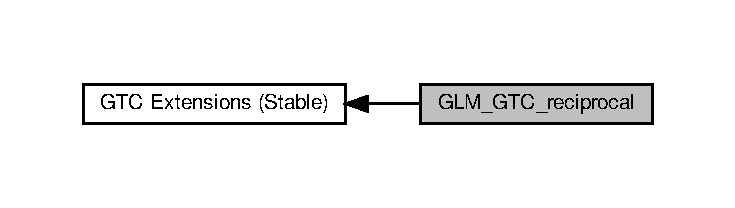
\includegraphics[width=350pt]{group__gtc__reciprocal}
\end{center}
\end{figure}
\subsection*{Functions}
\begin{DoxyCompactItemize}
\item 
{\footnotesize template$<$typename gen\+Type $>$ }\\\hyperlink{setup_8hpp_ab2d052de21a70539923e9bcbf6e83a51}{G\+L\+M\+\_\+\+F\+U\+N\+C\+\_\+\+D\+E\+CL} gen\+Type \hyperlink{group__gtc__reciprocal_gabb6829a472da1cc94d88afa6396bed1f}{glm\+::sec} (gen\+Type const \&\hyperlink{group__gtc__quaternion_ga23a3fc7ada5bbb665ff84c92c6e0542c}{angle})
\item 
{\footnotesize template$<$typename gen\+Type $>$ }\\\hyperlink{setup_8hpp_ab2d052de21a70539923e9bcbf6e83a51}{G\+L\+M\+\_\+\+F\+U\+N\+C\+\_\+\+D\+E\+CL} gen\+Type \hyperlink{group__gtc__reciprocal_ga5df75de99f63e854087a06f538907b2c}{glm\+::csc} (gen\+Type const \&\hyperlink{group__gtc__quaternion_ga23a3fc7ada5bbb665ff84c92c6e0542c}{angle})
\item 
{\footnotesize template$<$typename gen\+Type $>$ }\\\hyperlink{setup_8hpp_ab2d052de21a70539923e9bcbf6e83a51}{G\+L\+M\+\_\+\+F\+U\+N\+C\+\_\+\+D\+E\+CL} gen\+Type \hyperlink{group__gtc__reciprocal_ga2f49e28c2634ae1a212e2fc38c42ad42}{glm\+::cot} (gen\+Type const \&\hyperlink{group__gtc__quaternion_ga23a3fc7ada5bbb665ff84c92c6e0542c}{angle})
\item 
{\footnotesize template$<$typename gen\+Type $>$ }\\\hyperlink{setup_8hpp_ab2d052de21a70539923e9bcbf6e83a51}{G\+L\+M\+\_\+\+F\+U\+N\+C\+\_\+\+D\+E\+CL} gen\+Type \hyperlink{group__gtc__reciprocal_gac9761980e09149002a466ca131a4bcac}{glm\+::asec} (gen\+Type const \&x)
\item 
{\footnotesize template$<$typename gen\+Type $>$ }\\\hyperlink{setup_8hpp_ab2d052de21a70539923e9bcbf6e83a51}{G\+L\+M\+\_\+\+F\+U\+N\+C\+\_\+\+D\+E\+CL} gen\+Type \hyperlink{group__gtc__reciprocal_ga135e8f6b36bb85b5f7d8067e6b890e4d}{glm\+::acsc} (gen\+Type const \&x)
\item 
{\footnotesize template$<$typename gen\+Type $>$ }\\\hyperlink{setup_8hpp_ab2d052de21a70539923e9bcbf6e83a51}{G\+L\+M\+\_\+\+F\+U\+N\+C\+\_\+\+D\+E\+CL} gen\+Type \hyperlink{group__gtc__reciprocal_ga97d029f989f849b62915b068c264246b}{glm\+::acot} (gen\+Type const \&x)
\item 
{\footnotesize template$<$typename gen\+Type $>$ }\\\hyperlink{setup_8hpp_ab2d052de21a70539923e9bcbf6e83a51}{G\+L\+M\+\_\+\+F\+U\+N\+C\+\_\+\+D\+E\+CL} gen\+Type \hyperlink{group__gtc__reciprocal_gaaa698b992c63f454a3a1a1baa2773a3c}{glm\+::sech} (gen\+Type const \&\hyperlink{group__gtc__quaternion_ga23a3fc7ada5bbb665ff84c92c6e0542c}{angle})
\item 
{\footnotesize template$<$typename gen\+Type $>$ }\\\hyperlink{setup_8hpp_ab2d052de21a70539923e9bcbf6e83a51}{G\+L\+M\+\_\+\+F\+U\+N\+C\+\_\+\+D\+E\+CL} gen\+Type \hyperlink{group__gtc__reciprocal_ga00404a9cdf62023792d1d0afedd7f896}{glm\+::csch} (gen\+Type const \&\hyperlink{group__gtc__quaternion_ga23a3fc7ada5bbb665ff84c92c6e0542c}{angle})
\item 
{\footnotesize template$<$typename gen\+Type $>$ }\\\hyperlink{setup_8hpp_ab2d052de21a70539923e9bcbf6e83a51}{G\+L\+M\+\_\+\+F\+U\+N\+C\+\_\+\+D\+E\+CL} gen\+Type \hyperlink{group__gtc__reciprocal_gae2f1e6f7c360dda452b88e0c492d6f4d}{glm\+::coth} (gen\+Type const \&\hyperlink{group__gtc__quaternion_ga23a3fc7ada5bbb665ff84c92c6e0542c}{angle})
\item 
{\footnotesize template$<$typename gen\+Type $>$ }\\\hyperlink{setup_8hpp_ab2d052de21a70539923e9bcbf6e83a51}{G\+L\+M\+\_\+\+F\+U\+N\+C\+\_\+\+D\+E\+CL} gen\+Type \hyperlink{group__gtc__reciprocal_ga450f3bf1c04751198994d26d92ac2a63}{glm\+::asech} (gen\+Type const \&x)
\item 
{\footnotesize template$<$typename gen\+Type $>$ }\\\hyperlink{setup_8hpp_ab2d052de21a70539923e9bcbf6e83a51}{G\+L\+M\+\_\+\+F\+U\+N\+C\+\_\+\+D\+E\+CL} gen\+Type \hyperlink{group__gtc__reciprocal_ga418b31539e1a69c262712f2c7a4f27eb}{glm\+::acsch} (gen\+Type const \&x)
\item 
{\footnotesize template$<$typename gen\+Type $>$ }\\\hyperlink{setup_8hpp_ab2d052de21a70539923e9bcbf6e83a51}{G\+L\+M\+\_\+\+F\+U\+N\+C\+\_\+\+D\+E\+CL} gen\+Type \hyperlink{group__gtc__reciprocal_gad73911994e6bb6a06cc3ea1bd89201ab}{glm\+::acoth} (gen\+Type const \&x)
\end{DoxyCompactItemize}


\subsection{Detailed Description}
Define secant, cosecant and cotangent functions. 

$<$\hyperlink{gtc_2reciprocal_8hpp}{glm/gtc/reciprocal.\+hpp}$>$ need to be included to use these features. 

\subsection{Function Documentation}
\mbox{\Hypertarget{group__gtc__reciprocal_ga97d029f989f849b62915b068c264246b}\label{group__gtc__reciprocal_ga97d029f989f849b62915b068c264246b}} 
\index{G\+L\+M\+\_\+\+G\+T\+C\+\_\+reciprocal@{G\+L\+M\+\_\+\+G\+T\+C\+\_\+reciprocal}!acot@{acot}}
\index{acot@{acot}!G\+L\+M\+\_\+\+G\+T\+C\+\_\+reciprocal@{G\+L\+M\+\_\+\+G\+T\+C\+\_\+reciprocal}}
\subsubsection{\texorpdfstring{acot()}{acot()}}
{\footnotesize\ttfamily template$<$typename gen\+Type $>$ \\
\hyperlink{setup_8hpp_ab2d052de21a70539923e9bcbf6e83a51}{G\+L\+M\+\_\+\+F\+U\+N\+C\+\_\+\+D\+E\+CL} gen\+Type glm\+::acot (\begin{DoxyParamCaption}\item[{gen\+Type const \&}]{x }\end{DoxyParamCaption})}

Inverse cotangent function.

\begin{DoxySeeAlso}{See also}
\hyperlink{group__gtc__reciprocal}{G\+L\+M\+\_\+\+G\+T\+C\+\_\+reciprocal} 
\end{DoxySeeAlso}


Definition at line 107 of file reciprocal.\+inl.

\mbox{\Hypertarget{group__gtc__reciprocal_gad73911994e6bb6a06cc3ea1bd89201ab}\label{group__gtc__reciprocal_gad73911994e6bb6a06cc3ea1bd89201ab}} 
\index{G\+L\+M\+\_\+\+G\+T\+C\+\_\+reciprocal@{G\+L\+M\+\_\+\+G\+T\+C\+\_\+reciprocal}!acoth@{acoth}}
\index{acoth@{acoth}!G\+L\+M\+\_\+\+G\+T\+C\+\_\+reciprocal@{G\+L\+M\+\_\+\+G\+T\+C\+\_\+reciprocal}}
\subsubsection{\texorpdfstring{acoth()}{acoth()}}
{\footnotesize\ttfamily template$<$typename gen\+Type $>$ \\
\hyperlink{setup_8hpp_ab2d052de21a70539923e9bcbf6e83a51}{G\+L\+M\+\_\+\+F\+U\+N\+C\+\_\+\+D\+E\+CL} gen\+Type glm\+::acoth (\begin{DoxyParamCaption}\item[{gen\+Type const \&}]{x }\end{DoxyParamCaption})}

Inverse cotangent hyperbolic function.

\begin{DoxySeeAlso}{See also}
\hyperlink{group__gtc__reciprocal}{G\+L\+M\+\_\+\+G\+T\+C\+\_\+reciprocal} 
\end{DoxySeeAlso}


Definition at line 192 of file reciprocal.\+inl.

\mbox{\Hypertarget{group__gtc__reciprocal_ga135e8f6b36bb85b5f7d8067e6b890e4d}\label{group__gtc__reciprocal_ga135e8f6b36bb85b5f7d8067e6b890e4d}} 
\index{G\+L\+M\+\_\+\+G\+T\+C\+\_\+reciprocal@{G\+L\+M\+\_\+\+G\+T\+C\+\_\+reciprocal}!acsc@{acsc}}
\index{acsc@{acsc}!G\+L\+M\+\_\+\+G\+T\+C\+\_\+reciprocal@{G\+L\+M\+\_\+\+G\+T\+C\+\_\+reciprocal}}
\subsubsection{\texorpdfstring{acsc()}{acsc()}}
{\footnotesize\ttfamily template$<$typename gen\+Type $>$ \\
\hyperlink{setup_8hpp_ab2d052de21a70539923e9bcbf6e83a51}{G\+L\+M\+\_\+\+F\+U\+N\+C\+\_\+\+D\+E\+CL} gen\+Type glm\+::acsc (\begin{DoxyParamCaption}\item[{gen\+Type const \&}]{x }\end{DoxyParamCaption})}

Inverse cosecant function.

\begin{DoxySeeAlso}{See also}
\hyperlink{group__gtc__reciprocal}{G\+L\+M\+\_\+\+G\+T\+C\+\_\+reciprocal} 
\end{DoxySeeAlso}


Definition at line 93 of file reciprocal.\+inl.

\mbox{\Hypertarget{group__gtc__reciprocal_ga418b31539e1a69c262712f2c7a4f27eb}\label{group__gtc__reciprocal_ga418b31539e1a69c262712f2c7a4f27eb}} 
\index{G\+L\+M\+\_\+\+G\+T\+C\+\_\+reciprocal@{G\+L\+M\+\_\+\+G\+T\+C\+\_\+reciprocal}!acsch@{acsch}}
\index{acsch@{acsch}!G\+L\+M\+\_\+\+G\+T\+C\+\_\+reciprocal@{G\+L\+M\+\_\+\+G\+T\+C\+\_\+reciprocal}}
\subsubsection{\texorpdfstring{acsch()}{acsch()}}
{\footnotesize\ttfamily template$<$typename gen\+Type $>$ \\
\hyperlink{setup_8hpp_ab2d052de21a70539923e9bcbf6e83a51}{G\+L\+M\+\_\+\+F\+U\+N\+C\+\_\+\+D\+E\+CL} gen\+Type glm\+::acsch (\begin{DoxyParamCaption}\item[{gen\+Type const \&}]{x }\end{DoxyParamCaption})}

Inverse cosecant hyperbolic function.

\begin{DoxySeeAlso}{See also}
\hyperlink{group__gtc__reciprocal}{G\+L\+M\+\_\+\+G\+T\+C\+\_\+reciprocal} 
\end{DoxySeeAlso}


Definition at line 178 of file reciprocal.\+inl.

\mbox{\Hypertarget{group__gtc__reciprocal_gac9761980e09149002a466ca131a4bcac}\label{group__gtc__reciprocal_gac9761980e09149002a466ca131a4bcac}} 
\index{G\+L\+M\+\_\+\+G\+T\+C\+\_\+reciprocal@{G\+L\+M\+\_\+\+G\+T\+C\+\_\+reciprocal}!asec@{asec}}
\index{asec@{asec}!G\+L\+M\+\_\+\+G\+T\+C\+\_\+reciprocal@{G\+L\+M\+\_\+\+G\+T\+C\+\_\+reciprocal}}
\subsubsection{\texorpdfstring{asec()}{asec()}}
{\footnotesize\ttfamily template$<$typename gen\+Type $>$ \\
\hyperlink{setup_8hpp_ab2d052de21a70539923e9bcbf6e83a51}{G\+L\+M\+\_\+\+F\+U\+N\+C\+\_\+\+D\+E\+CL} gen\+Type glm\+::asec (\begin{DoxyParamCaption}\item[{gen\+Type const \&}]{x }\end{DoxyParamCaption})}

Inverse secant function.

\begin{DoxySeeAlso}{See also}
\hyperlink{group__gtc__reciprocal}{G\+L\+M\+\_\+\+G\+T\+C\+\_\+reciprocal} 
\end{DoxySeeAlso}


Definition at line 79 of file reciprocal.\+inl.

\mbox{\Hypertarget{group__gtc__reciprocal_ga450f3bf1c04751198994d26d92ac2a63}\label{group__gtc__reciprocal_ga450f3bf1c04751198994d26d92ac2a63}} 
\index{G\+L\+M\+\_\+\+G\+T\+C\+\_\+reciprocal@{G\+L\+M\+\_\+\+G\+T\+C\+\_\+reciprocal}!asech@{asech}}
\index{asech@{asech}!G\+L\+M\+\_\+\+G\+T\+C\+\_\+reciprocal@{G\+L\+M\+\_\+\+G\+T\+C\+\_\+reciprocal}}
\subsubsection{\texorpdfstring{asech()}{asech()}}
{\footnotesize\ttfamily template$<$typename gen\+Type $>$ \\
\hyperlink{setup_8hpp_ab2d052de21a70539923e9bcbf6e83a51}{G\+L\+M\+\_\+\+F\+U\+N\+C\+\_\+\+D\+E\+CL} gen\+Type glm\+::asech (\begin{DoxyParamCaption}\item[{gen\+Type const \&}]{x }\end{DoxyParamCaption})}

Inverse secant hyperbolic function.

\begin{DoxySeeAlso}{See also}
\hyperlink{group__gtc__reciprocal}{G\+L\+M\+\_\+\+G\+T\+C\+\_\+reciprocal} 
\end{DoxySeeAlso}


Definition at line 164 of file reciprocal.\+inl.

\mbox{\Hypertarget{group__gtc__reciprocal_ga2f49e28c2634ae1a212e2fc38c42ad42}\label{group__gtc__reciprocal_ga2f49e28c2634ae1a212e2fc38c42ad42}} 
\index{G\+L\+M\+\_\+\+G\+T\+C\+\_\+reciprocal@{G\+L\+M\+\_\+\+G\+T\+C\+\_\+reciprocal}!cot@{cot}}
\index{cot@{cot}!G\+L\+M\+\_\+\+G\+T\+C\+\_\+reciprocal@{G\+L\+M\+\_\+\+G\+T\+C\+\_\+reciprocal}}
\subsubsection{\texorpdfstring{cot()}{cot()}}
{\footnotesize\ttfamily template$<$typename gen\+Type $>$ \\
\hyperlink{setup_8hpp_ab2d052de21a70539923e9bcbf6e83a51}{G\+L\+M\+\_\+\+F\+U\+N\+C\+\_\+\+D\+E\+CL} gen\+Type glm\+::cot (\begin{DoxyParamCaption}\item[{gen\+Type const \&}]{angle }\end{DoxyParamCaption})}

Cotangent function. adjacent / opposite or 1 / tan(x)

\begin{DoxySeeAlso}{See also}
\hyperlink{group__gtc__reciprocal}{G\+L\+M\+\_\+\+G\+T\+C\+\_\+reciprocal} 
\end{DoxySeeAlso}


Definition at line 65 of file reciprocal.\+inl.

\mbox{\Hypertarget{group__gtc__reciprocal_gae2f1e6f7c360dda452b88e0c492d6f4d}\label{group__gtc__reciprocal_gae2f1e6f7c360dda452b88e0c492d6f4d}} 
\index{G\+L\+M\+\_\+\+G\+T\+C\+\_\+reciprocal@{G\+L\+M\+\_\+\+G\+T\+C\+\_\+reciprocal}!coth@{coth}}
\index{coth@{coth}!G\+L\+M\+\_\+\+G\+T\+C\+\_\+reciprocal@{G\+L\+M\+\_\+\+G\+T\+C\+\_\+reciprocal}}
\subsubsection{\texorpdfstring{coth()}{coth()}}
{\footnotesize\ttfamily template$<$typename gen\+Type $>$ \\
\hyperlink{setup_8hpp_ab2d052de21a70539923e9bcbf6e83a51}{G\+L\+M\+\_\+\+F\+U\+N\+C\+\_\+\+D\+E\+CL} gen\+Type glm\+::coth (\begin{DoxyParamCaption}\item[{gen\+Type const \&}]{angle }\end{DoxyParamCaption})}

Cotangent hyperbolic function.

\begin{DoxySeeAlso}{See also}
\hyperlink{group__gtc__reciprocal}{G\+L\+M\+\_\+\+G\+T\+C\+\_\+reciprocal} 
\end{DoxySeeAlso}


Definition at line 150 of file reciprocal.\+inl.

\mbox{\Hypertarget{group__gtc__reciprocal_ga5df75de99f63e854087a06f538907b2c}\label{group__gtc__reciprocal_ga5df75de99f63e854087a06f538907b2c}} 
\index{G\+L\+M\+\_\+\+G\+T\+C\+\_\+reciprocal@{G\+L\+M\+\_\+\+G\+T\+C\+\_\+reciprocal}!csc@{csc}}
\index{csc@{csc}!G\+L\+M\+\_\+\+G\+T\+C\+\_\+reciprocal@{G\+L\+M\+\_\+\+G\+T\+C\+\_\+reciprocal}}
\subsubsection{\texorpdfstring{csc()}{csc()}}
{\footnotesize\ttfamily template$<$typename gen\+Type $>$ \\
\hyperlink{setup_8hpp_ab2d052de21a70539923e9bcbf6e83a51}{G\+L\+M\+\_\+\+F\+U\+N\+C\+\_\+\+D\+E\+CL} gen\+Type glm\+::csc (\begin{DoxyParamCaption}\item[{gen\+Type const \&}]{angle }\end{DoxyParamCaption})}

Cosecant function. hypotenuse / opposite or 1 / sin(x)

\begin{DoxySeeAlso}{See also}
\hyperlink{group__gtc__reciprocal}{G\+L\+M\+\_\+\+G\+T\+C\+\_\+reciprocal} 
\end{DoxySeeAlso}


Definition at line 51 of file reciprocal.\+inl.

\mbox{\Hypertarget{group__gtc__reciprocal_ga00404a9cdf62023792d1d0afedd7f896}\label{group__gtc__reciprocal_ga00404a9cdf62023792d1d0afedd7f896}} 
\index{G\+L\+M\+\_\+\+G\+T\+C\+\_\+reciprocal@{G\+L\+M\+\_\+\+G\+T\+C\+\_\+reciprocal}!csch@{csch}}
\index{csch@{csch}!G\+L\+M\+\_\+\+G\+T\+C\+\_\+reciprocal@{G\+L\+M\+\_\+\+G\+T\+C\+\_\+reciprocal}}
\subsubsection{\texorpdfstring{csch()}{csch()}}
{\footnotesize\ttfamily template$<$typename gen\+Type $>$ \\
\hyperlink{setup_8hpp_ab2d052de21a70539923e9bcbf6e83a51}{G\+L\+M\+\_\+\+F\+U\+N\+C\+\_\+\+D\+E\+CL} gen\+Type glm\+::csch (\begin{DoxyParamCaption}\item[{gen\+Type const \&}]{angle }\end{DoxyParamCaption})}

Cosecant hyperbolic function.

\begin{DoxySeeAlso}{See also}
\hyperlink{group__gtc__reciprocal}{G\+L\+M\+\_\+\+G\+T\+C\+\_\+reciprocal} 
\end{DoxySeeAlso}


Definition at line 136 of file reciprocal.\+inl.

\mbox{\Hypertarget{group__gtc__reciprocal_gabb6829a472da1cc94d88afa6396bed1f}\label{group__gtc__reciprocal_gabb6829a472da1cc94d88afa6396bed1f}} 
\index{G\+L\+M\+\_\+\+G\+T\+C\+\_\+reciprocal@{G\+L\+M\+\_\+\+G\+T\+C\+\_\+reciprocal}!sec@{sec}}
\index{sec@{sec}!G\+L\+M\+\_\+\+G\+T\+C\+\_\+reciprocal@{G\+L\+M\+\_\+\+G\+T\+C\+\_\+reciprocal}}
\subsubsection{\texorpdfstring{sec()}{sec()}}
{\footnotesize\ttfamily template$<$typename gen\+Type $>$ \\
\hyperlink{setup_8hpp_ab2d052de21a70539923e9bcbf6e83a51}{G\+L\+M\+\_\+\+F\+U\+N\+C\+\_\+\+D\+E\+CL} gen\+Type glm\+::sec (\begin{DoxyParamCaption}\item[{gen\+Type const \&}]{angle }\end{DoxyParamCaption})}

Secant function. hypotenuse / adjacent or 1 / cos(x)

\begin{DoxySeeAlso}{See also}
\hyperlink{group__gtc__reciprocal}{G\+L\+M\+\_\+\+G\+T\+C\+\_\+reciprocal} 
\end{DoxySeeAlso}


Definition at line 37 of file reciprocal.\+inl.

\mbox{\Hypertarget{group__gtc__reciprocal_gaaa698b992c63f454a3a1a1baa2773a3c}\label{group__gtc__reciprocal_gaaa698b992c63f454a3a1a1baa2773a3c}} 
\index{G\+L\+M\+\_\+\+G\+T\+C\+\_\+reciprocal@{G\+L\+M\+\_\+\+G\+T\+C\+\_\+reciprocal}!sech@{sech}}
\index{sech@{sech}!G\+L\+M\+\_\+\+G\+T\+C\+\_\+reciprocal@{G\+L\+M\+\_\+\+G\+T\+C\+\_\+reciprocal}}
\subsubsection{\texorpdfstring{sech()}{sech()}}
{\footnotesize\ttfamily template$<$typename gen\+Type $>$ \\
\hyperlink{setup_8hpp_ab2d052de21a70539923e9bcbf6e83a51}{G\+L\+M\+\_\+\+F\+U\+N\+C\+\_\+\+D\+E\+CL} gen\+Type glm\+::sech (\begin{DoxyParamCaption}\item[{gen\+Type const \&}]{angle }\end{DoxyParamCaption})}

Secant hyperbolic function.

\begin{DoxySeeAlso}{See also}
\hyperlink{group__gtc__reciprocal}{G\+L\+M\+\_\+\+G\+T\+C\+\_\+reciprocal} 
\end{DoxySeeAlso}


Definition at line 122 of file reciprocal.\+inl.


\hypertarget{group__gtc__type__precision}{}\section{G\+L\+M\+\_\+\+G\+T\+C\+\_\+type\+\_\+precision}
\label{group__gtc__type__precision}\index{G\+L\+M\+\_\+\+G\+T\+C\+\_\+type\+\_\+precision@{G\+L\+M\+\_\+\+G\+T\+C\+\_\+type\+\_\+precision}}


Defines specific C++-\/based precision types.  


Collaboration diagram for G\+L\+M\+\_\+\+G\+T\+C\+\_\+type\+\_\+precision\+:\nopagebreak
\begin{figure}[H]
\begin{center}
\leavevmode
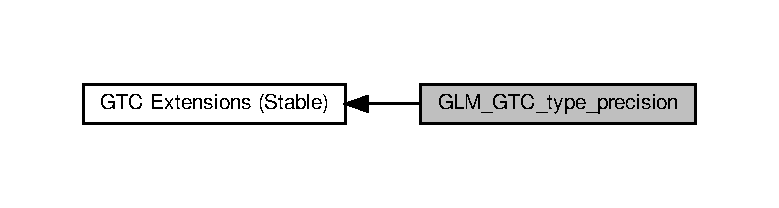
\includegraphics[width=350pt]{group__gtc__type__precision}
\end{center}
\end{figure}
\subsection*{Typedefs}
\begin{DoxyCompactItemize}
\item 
typedef \hyperlink{namespaceglm_1_1detail_a04b526a8d7a9b455602a0afa78c531e0}{detail\+::int8} \hyperlink{group__gtc__type__precision_gaf9e675b6392764242ae87eb179e9d3d6}{glm\+::lowp\+\_\+int8}
\item 
typedef \hyperlink{namespaceglm_1_1detail_a375938874ca4f0a0982ec6373b56117b}{detail\+::int16} \hyperlink{group__gtc__type__precision_ga71fc0c399fa4780507748b643733f153}{glm\+::lowp\+\_\+int16}
\item 
typedef \hyperlink{namespaceglm_1_1detail_a9f85b4efeca416cdcec2fd08939a2e17}{detail\+::int32} \hyperlink{group__gtc__type__precision_gad9939c9d6fec1c6accc02a83c6500f08}{glm\+::lowp\+\_\+int32}
\item 
typedef \hyperlink{namespaceglm_1_1detail_a5b1c3227ec636c24a0676746381adfc8}{detail\+::int64} \hyperlink{group__gtc__type__precision_gab8a8e75af347592406e41b3ae2c0712b}{glm\+::lowp\+\_\+int64}
\item 
typedef \hyperlink{namespaceglm_1_1detail_a04b526a8d7a9b455602a0afa78c531e0}{detail\+::int8} \hyperlink{group__gtc__type__precision_gae6092311f6970a305c2df19a372360a3}{glm\+::lowp\+\_\+int8\+\_\+t}
\item 
typedef \hyperlink{namespaceglm_1_1detail_a375938874ca4f0a0982ec6373b56117b}{detail\+::int16} \hyperlink{group__gtc__type__precision_gae34c3d53c4c1434fc9f26538b0185667}{glm\+::lowp\+\_\+int16\+\_\+t}
\item 
typedef \hyperlink{namespaceglm_1_1detail_a9f85b4efeca416cdcec2fd08939a2e17}{detail\+::int32} \hyperlink{group__gtc__type__precision_gad9567c806dc39f534174eef42663119d}{glm\+::lowp\+\_\+int32\+\_\+t}
\item 
typedef \hyperlink{namespaceglm_1_1detail_a5b1c3227ec636c24a0676746381adfc8}{detail\+::int64} \hyperlink{group__gtc__type__precision_ga14d72e76d57c7f28eca8e933816c9fd6}{glm\+::lowp\+\_\+int64\+\_\+t}
\item 
typedef \hyperlink{namespaceglm_1_1detail_a04b526a8d7a9b455602a0afa78c531e0}{detail\+::int8} \hyperlink{group__gtc__type__precision_gaa2e13ee29c90f75658beed6082541097}{glm\+::lowp\+\_\+i8}
\item 
typedef \hyperlink{namespaceglm_1_1detail_a375938874ca4f0a0982ec6373b56117b}{detail\+::int16} \hyperlink{group__gtc__type__precision_gaf7bbfd31bcec25a416ea94d09efb5451}{glm\+::lowp\+\_\+i16}
\item 
typedef \hyperlink{namespaceglm_1_1detail_a9f85b4efeca416cdcec2fd08939a2e17}{detail\+::int32} \hyperlink{group__gtc__type__precision_ga70fd34e8b8cffc92739161284ed77328}{glm\+::lowp\+\_\+i32}
\item 
typedef \hyperlink{namespaceglm_1_1detail_a5b1c3227ec636c24a0676746381adfc8}{detail\+::int64} \hyperlink{group__gtc__type__precision_ga1f4ded25f71c0f3b4518936d50b54b6e}{glm\+::lowp\+\_\+i64}
\item 
typedef \hyperlink{namespaceglm_1_1detail_a04b526a8d7a9b455602a0afa78c531e0}{detail\+::int8} \hyperlink{group__gtc__type__precision_ga3ee8faab2278c44c5785af04b7b18a14}{glm\+::mediump\+\_\+int8}
\item 
typedef \hyperlink{namespaceglm_1_1detail_a375938874ca4f0a0982ec6373b56117b}{detail\+::int16} \hyperlink{group__gtc__type__precision_ga4611997edb6c61606daa11990cf08798}{glm\+::mediump\+\_\+int16}
\item 
typedef \hyperlink{namespaceglm_1_1detail_a9f85b4efeca416cdcec2fd08939a2e17}{detail\+::int32} \hyperlink{group__gtc__type__precision_ga0660a752402702f420f13c686a7fff29}{glm\+::mediump\+\_\+int32}
\item 
typedef \hyperlink{namespaceglm_1_1detail_a5b1c3227ec636c24a0676746381adfc8}{detail\+::int64} \hyperlink{group__gtc__type__precision_ga603c695fe5cd677d3f72a81343e19a74}{glm\+::mediump\+\_\+int64}
\item 
typedef \hyperlink{namespaceglm_1_1detail_a04b526a8d7a9b455602a0afa78c531e0}{detail\+::int8} \hyperlink{group__gtc__type__precision_ga626ac5f73d3538e62a879d6c56abfb36}{glm\+::mediump\+\_\+int8\+\_\+t}
\item 
typedef \hyperlink{namespaceglm_1_1detail_a375938874ca4f0a0982ec6373b56117b}{detail\+::int16} \hyperlink{group__gtc__type__precision_ga478fab608cf43040013d719a3e03b194}{glm\+::mediump\+\_\+int16\+\_\+t}
\item 
typedef \hyperlink{namespaceglm_1_1detail_a9f85b4efeca416cdcec2fd08939a2e17}{detail\+::int32} \hyperlink{group__gtc__type__precision_gafd9b4bd9e4465aec63351b59100692c4}{glm\+::mediump\+\_\+int32\+\_\+t}
\item 
typedef \hyperlink{namespaceglm_1_1detail_a5b1c3227ec636c24a0676746381adfc8}{detail\+::int64} \hyperlink{group__gtc__type__precision_ga555a2f85641550c232db473a9bb981f7}{glm\+::mediump\+\_\+int64\+\_\+t}
\item 
typedef \hyperlink{namespaceglm_1_1detail_a04b526a8d7a9b455602a0afa78c531e0}{detail\+::int8} \hyperlink{group__gtc__type__precision_ga28a8b5fd51072680bb55178c17cc7411}{glm\+::mediump\+\_\+i8}
\item 
typedef \hyperlink{namespaceglm_1_1detail_a375938874ca4f0a0982ec6373b56117b}{detail\+::int16} \hyperlink{group__gtc__type__precision_ga8454fc6a82c7bb787d0ac9663e08f63d}{glm\+::mediump\+\_\+i16}
\item 
typedef \hyperlink{namespaceglm_1_1detail_a9f85b4efeca416cdcec2fd08939a2e17}{detail\+::int32} \hyperlink{group__gtc__type__precision_ga5e00ec824eb55968a6b6496f294d8c07}{glm\+::mediump\+\_\+i32}
\item 
typedef \hyperlink{namespaceglm_1_1detail_a5b1c3227ec636c24a0676746381adfc8}{detail\+::int64} \hyperlink{group__gtc__type__precision_ga90fedf6c701ffbe00535156715e50787}{glm\+::mediump\+\_\+i64}
\item 
typedef \hyperlink{namespaceglm_1_1detail_a04b526a8d7a9b455602a0afa78c531e0}{detail\+::int8} \hyperlink{group__gtc__type__precision_ga57c86999e666760c304453f9bfdc09d1}{glm\+::highp\+\_\+int8}
\item 
typedef \hyperlink{namespaceglm_1_1detail_a375938874ca4f0a0982ec6373b56117b}{detail\+::int16} \hyperlink{group__gtc__type__precision_gaf0430ed80e88c0d1dfbe47f359659c81}{glm\+::highp\+\_\+int16}
\item 
typedef \hyperlink{namespaceglm_1_1detail_a9f85b4efeca416cdcec2fd08939a2e17}{detail\+::int32} \hyperlink{group__gtc__type__precision_gaa2045c92b9553d463191af6a20e997bb}{glm\+::highp\+\_\+int32}
\item 
typedef \hyperlink{namespaceglm_1_1detail_a5b1c3227ec636c24a0676746381adfc8}{detail\+::int64} \hyperlink{group__gtc__type__precision_ga7ffb27943e9569800979081bc548621c}{glm\+::highp\+\_\+int64}
\item 
typedef \hyperlink{namespaceglm_1_1detail_a04b526a8d7a9b455602a0afa78c531e0}{detail\+::int8} \hyperlink{group__gtc__type__precision_ga417701b99e6e7992f35ab2ef694f88b2}{glm\+::highp\+\_\+int8\+\_\+t}
\item 
typedef \hyperlink{namespaceglm_1_1detail_a375938874ca4f0a0982ec6373b56117b}{detail\+::int16} \hyperlink{group__gtc__type__precision_ga07d318d61472e75238e53b9642227672}{glm\+::highp\+\_\+int16\+\_\+t}
\item 
typedef \hyperlink{namespaceglm_1_1detail_a9f85b4efeca416cdcec2fd08939a2e17}{detail\+::int32} \hyperlink{group__gtc__type__precision_ga783d077a513c1f475f6cdb406b4238c3}{glm\+::highp\+\_\+int32\+\_\+t}
\item 
typedef \hyperlink{namespaceglm_1_1detail_a5b1c3227ec636c24a0676746381adfc8}{detail\+::int64} \hyperlink{group__gtc__type__precision_ga0f5186bde44471133b08057cae8a51ac}{glm\+::highp\+\_\+int64\+\_\+t}
\item 
typedef \hyperlink{namespaceglm_1_1detail_a04b526a8d7a9b455602a0afa78c531e0}{detail\+::int8} \hyperlink{group__gtc__type__precision_ga8b9eb0b24cce7f14478bfcacb53ce839}{glm\+::highp\+\_\+i8}
\item 
typedef \hyperlink{namespaceglm_1_1detail_a375938874ca4f0a0982ec6373b56117b}{detail\+::int16} \hyperlink{group__gtc__type__precision_gaa04399853952dbce29cb62e2432f350a}{glm\+::highp\+\_\+i16}
\item 
typedef \hyperlink{namespaceglm_1_1detail_a9f85b4efeca416cdcec2fd08939a2e17}{detail\+::int32} \hyperlink{group__gtc__type__precision_ga197d19b585222da57d70238a5cfc2be8}{glm\+::highp\+\_\+i32}
\item 
typedef \hyperlink{namespaceglm_1_1detail_a5b1c3227ec636c24a0676746381adfc8}{detail\+::int64} \hyperlink{group__gtc__type__precision_gad3cb9a0ac0266ea2c51c6fac256345d1}{glm\+::highp\+\_\+i64}
\item 
typedef \hyperlink{namespaceglm_1_1detail_a04b526a8d7a9b455602a0afa78c531e0}{detail\+::int8} \hyperlink{group__gtc__type__precision_ga96254f9c1c4506fc8eb5cf3301ce8565}{glm\+::int8}
\item 
typedef \hyperlink{namespaceglm_1_1detail_a375938874ca4f0a0982ec6373b56117b}{detail\+::int16} \hyperlink{group__gtc__type__precision_ga2945a61d12771f8954994fcddf02b021}{glm\+::int16}
\item 
typedef \hyperlink{namespaceglm_1_1detail_a9f85b4efeca416cdcec2fd08939a2e17}{detail\+::int32} \hyperlink{group__gtc__type__precision_ga632d8b25f6b61659f39ea4321fab92a4}{glm\+::int32}
\item 
typedef \hyperlink{namespaceglm_1_1detail_a5b1c3227ec636c24a0676746381adfc8}{detail\+::int64} \hyperlink{group__gtc__type__precision_ga435d75819cce297cc5fa21bd84ef89a5}{glm\+::int64}
\item 
typedef \hyperlink{namespaceglm_1_1detail_a04b526a8d7a9b455602a0afa78c531e0}{detail\+::int8} \hyperlink{group__gtc__type__precision_ga673898d450b2a91186f3c4f40c5f8633}{glm\+::int8\+\_\+t}
\item 
typedef \hyperlink{namespaceglm_1_1detail_a375938874ca4f0a0982ec6373b56117b}{detail\+::int16} \hyperlink{group__gtc__type__precision_gaf89ee61e0d34aa4a462104b7ae7f2da6}{glm\+::int16\+\_\+t}
\item 
typedef \hyperlink{namespaceglm_1_1detail_a9f85b4efeca416cdcec2fd08939a2e17}{detail\+::int32} \hyperlink{group__gtc__type__precision_gab870c0eb6f525b0c8c4716762e0fc3a8}{glm\+::int32\+\_\+t}
\item 
typedef \hyperlink{namespaceglm_1_1detail_a5b1c3227ec636c24a0676746381adfc8}{detail\+::int64} \hyperlink{group__gtc__type__precision_ga6abb23fbf4e39c50ec5341160b5da5ab}{glm\+::int64\+\_\+t}
\item 
typedef \hyperlink{namespaceglm_1_1detail_a04b526a8d7a9b455602a0afa78c531e0}{detail\+::int8} \hyperlink{group__gtc__type__precision_gaae064be68b7d36cd7910c16e8ad18bba}{glm\+::i8}
\item 
typedef \hyperlink{namespaceglm_1_1detail_a375938874ca4f0a0982ec6373b56117b}{detail\+::int16} \hyperlink{group__gtc__type__precision_ga35e5542ca05b29cc256fdafb8503d1fd}{glm\+::i16}
\item 
typedef \hyperlink{namespaceglm_1_1detail_a9f85b4efeca416cdcec2fd08939a2e17}{detail\+::int32} \hyperlink{group__gtc__type__precision_ga1d8ed5c43e91ea7d4528389da4fa9524}{glm\+::i32}
\item 
typedef \hyperlink{namespaceglm_1_1detail_a5b1c3227ec636c24a0676746381adfc8}{detail\+::int64} \hyperlink{group__gtc__type__precision_gac7a7eaad46064fc952b06df33689da23}{glm\+::i64}
\item 
typedef \hyperlink{structglm_1_1detail_1_1tvec1}{detail\+::tvec1}$<$ \hyperlink{group__gtc__type__precision_gaae064be68b7d36cd7910c16e8ad18bba}{i8}, \hyperlink{namespaceglm_a0f04f086094c747d227af4425893f545ae161af3fc695e696ce3bf69f7332bc2d}{lowp} $>$ \hyperlink{group__gtc__type__precision_ga490ff77964d0386c1db936eb2a324988}{glm\+::lowp\+\_\+i8vec1}
\item 
typedef \hyperlink{structglm_1_1detail_1_1tvec2}{detail\+::tvec2}$<$ \hyperlink{group__gtc__type__precision_gaae064be68b7d36cd7910c16e8ad18bba}{i8}, \hyperlink{namespaceglm_a0f04f086094c747d227af4425893f545ae161af3fc695e696ce3bf69f7332bc2d}{lowp} $>$ \hyperlink{group__gtc__type__precision_ga511280c8869c7c79bba3c359f37f5559}{glm\+::lowp\+\_\+i8vec2}
\item 
typedef \hyperlink{structglm_1_1detail_1_1tvec3}{detail\+::tvec3}$<$ \hyperlink{group__gtc__type__precision_gaae064be68b7d36cd7910c16e8ad18bba}{i8}, \hyperlink{namespaceglm_a0f04f086094c747d227af4425893f545ae161af3fc695e696ce3bf69f7332bc2d}{lowp} $>$ \hyperlink{group__gtc__type__precision_ga048811f03c327d4b56564a72d98800e8}{glm\+::lowp\+\_\+i8vec3}
\item 
typedef \hyperlink{structglm_1_1detail_1_1tvec4}{detail\+::tvec4}$<$ \hyperlink{group__gtc__type__precision_gaae064be68b7d36cd7910c16e8ad18bba}{i8}, \hyperlink{namespaceglm_a0f04f086094c747d227af4425893f545ae161af3fc695e696ce3bf69f7332bc2d}{lowp} $>$ \hyperlink{group__gtc__type__precision_ga095202095a1fefbdae4a974c3b750223}{glm\+::lowp\+\_\+i8vec4}
\item 
typedef \hyperlink{structglm_1_1detail_1_1tvec1}{detail\+::tvec1}$<$ \hyperlink{group__gtc__type__precision_gaae064be68b7d36cd7910c16e8ad18bba}{i8}, \hyperlink{namespaceglm_a0f04f086094c747d227af4425893f545a6416f3ea0c9025fb21ed50c4d6620482}{mediump} $>$ \hyperlink{group__gtc__type__precision_ga820f8b497e06d518968d00761747c547}{glm\+::mediump\+\_\+i8vec1}
\item 
typedef \hyperlink{structglm_1_1detail_1_1tvec2}{detail\+::tvec2}$<$ \hyperlink{group__gtc__type__precision_gaae064be68b7d36cd7910c16e8ad18bba}{i8}, \hyperlink{namespaceglm_a0f04f086094c747d227af4425893f545a6416f3ea0c9025fb21ed50c4d6620482}{mediump} $>$ \hyperlink{group__gtc__type__precision_ga38eba1ab306fe5cc5eeafa35ce5b5b26}{glm\+::mediump\+\_\+i8vec2}
\item 
typedef \hyperlink{structglm_1_1detail_1_1tvec3}{detail\+::tvec3}$<$ \hyperlink{group__gtc__type__precision_gaae064be68b7d36cd7910c16e8ad18bba}{i8}, \hyperlink{namespaceglm_a0f04f086094c747d227af4425893f545a6416f3ea0c9025fb21ed50c4d6620482}{mediump} $>$ \hyperlink{group__gtc__type__precision_ga91b40a693c1db26a7cc544339b326df3}{glm\+::mediump\+\_\+i8vec3}
\item 
typedef \hyperlink{structglm_1_1detail_1_1tvec4}{detail\+::tvec4}$<$ \hyperlink{group__gtc__type__precision_gaae064be68b7d36cd7910c16e8ad18bba}{i8}, \hyperlink{namespaceglm_a0f04f086094c747d227af4425893f545a6416f3ea0c9025fb21ed50c4d6620482}{mediump} $>$ \hyperlink{group__gtc__type__precision_gad41bf4bfa504dc1191623ff77151d01f}{glm\+::mediump\+\_\+i8vec4}
\item 
typedef \hyperlink{structglm_1_1detail_1_1tvec1}{detail\+::tvec1}$<$ \hyperlink{group__gtc__type__precision_gaae064be68b7d36cd7910c16e8ad18bba}{i8}, \hyperlink{namespaceglm_a0f04f086094c747d227af4425893f545ac6f7eab42eacbb10d59a58e95e362074}{highp} $>$ \hyperlink{group__gtc__type__precision_ga0334353753f93388bcc89f91c9aff476}{glm\+::highp\+\_\+i8vec1}
\item 
typedef \hyperlink{structglm_1_1detail_1_1tvec2}{detail\+::tvec2}$<$ \hyperlink{group__gtc__type__precision_gaae064be68b7d36cd7910c16e8ad18bba}{i8}, \hyperlink{namespaceglm_a0f04f086094c747d227af4425893f545ac6f7eab42eacbb10d59a58e95e362074}{highp} $>$ \hyperlink{group__gtc__type__precision_ga2224945795a870e41d951f0847d54f02}{glm\+::highp\+\_\+i8vec2}
\item 
typedef \hyperlink{structglm_1_1detail_1_1tvec3}{detail\+::tvec3}$<$ \hyperlink{group__gtc__type__precision_gaae064be68b7d36cd7910c16e8ad18bba}{i8}, \hyperlink{namespaceglm_a0f04f086094c747d227af4425893f545ac6f7eab42eacbb10d59a58e95e362074}{highp} $>$ \hyperlink{group__gtc__type__precision_gad716792169ce7de963df25b865714438}{glm\+::highp\+\_\+i8vec3}
\item 
typedef \hyperlink{structglm_1_1detail_1_1tvec4}{detail\+::tvec4}$<$ \hyperlink{group__gtc__type__precision_gaae064be68b7d36cd7910c16e8ad18bba}{i8}, \hyperlink{namespaceglm_a0f04f086094c747d227af4425893f545ac6f7eab42eacbb10d59a58e95e362074}{highp} $>$ \hyperlink{group__gtc__type__precision_ga283b2f580a4bd7207d27418ef4a1068b}{glm\+::highp\+\_\+i8vec4}
\item 
typedef \hyperlink{group__gtc__type__precision_ga0334353753f93388bcc89f91c9aff476}{highp\+\_\+i8vec1} \hyperlink{group__gtc__type__precision_gae67d2e1e7ebd1a79176cac554395b881}{glm\+::i8vec1}
\item 
typedef \hyperlink{group__gtc__type__precision_ga2224945795a870e41d951f0847d54f02}{highp\+\_\+i8vec2} \hyperlink{group__gtc__type__precision_gafd7bbd3878c298014276975f999a8677}{glm\+::i8vec2}
\item 
typedef \hyperlink{group__gtc__type__precision_gad716792169ce7de963df25b865714438}{highp\+\_\+i8vec3} \hyperlink{group__gtc__type__precision_gae1e3127c58fbf1b6fbf28885cfd3dfad}{glm\+::i8vec3}
\item 
typedef \hyperlink{group__gtc__type__precision_ga283b2f580a4bd7207d27418ef4a1068b}{highp\+\_\+i8vec4} \hyperlink{group__gtc__type__precision_ga89bb5e6481ae11fb2599b71e36a390bb}{glm\+::i8vec4}
\item 
typedef \hyperlink{structglm_1_1detail_1_1tvec1}{detail\+::tvec1}$<$ \hyperlink{group__gtc__type__precision_ga35e5542ca05b29cc256fdafb8503d1fd}{i16}, \hyperlink{namespaceglm_a0f04f086094c747d227af4425893f545ae161af3fc695e696ce3bf69f7332bc2d}{lowp} $>$ \hyperlink{group__gtc__type__precision_ga6f1e42c07424a2f14faf731c74ba2153}{glm\+::lowp\+\_\+i16vec1}
\item 
typedef \hyperlink{structglm_1_1detail_1_1tvec2}{detail\+::tvec2}$<$ \hyperlink{group__gtc__type__precision_ga35e5542ca05b29cc256fdafb8503d1fd}{i16}, \hyperlink{namespaceglm_a0f04f086094c747d227af4425893f545ae161af3fc695e696ce3bf69f7332bc2d}{lowp} $>$ \hyperlink{group__gtc__type__precision_ga47c5d4c919266799ecc76d832356feff}{glm\+::lowp\+\_\+i16vec2}
\item 
typedef \hyperlink{structglm_1_1detail_1_1tvec3}{detail\+::tvec3}$<$ \hyperlink{group__gtc__type__precision_ga35e5542ca05b29cc256fdafb8503d1fd}{i16}, \hyperlink{namespaceglm_a0f04f086094c747d227af4425893f545ae161af3fc695e696ce3bf69f7332bc2d}{lowp} $>$ \hyperlink{group__gtc__type__precision_ga5b71f24a26316aa21f3c58d25c8db9a8}{glm\+::lowp\+\_\+i16vec3}
\item 
typedef \hyperlink{structglm_1_1detail_1_1tvec4}{detail\+::tvec4}$<$ \hyperlink{group__gtc__type__precision_ga35e5542ca05b29cc256fdafb8503d1fd}{i16}, \hyperlink{namespaceglm_a0f04f086094c747d227af4425893f545ae161af3fc695e696ce3bf69f7332bc2d}{lowp} $>$ \hyperlink{group__gtc__type__precision_ga59ea63973187e1e990fb6633d1800c6d}{glm\+::lowp\+\_\+i16vec4}
\item 
typedef \hyperlink{structglm_1_1detail_1_1tvec1}{detail\+::tvec1}$<$ \hyperlink{group__gtc__type__precision_ga35e5542ca05b29cc256fdafb8503d1fd}{i16}, \hyperlink{namespaceglm_a0f04f086094c747d227af4425893f545a6416f3ea0c9025fb21ed50c4d6620482}{mediump} $>$ \hyperlink{group__gtc__type__precision_ga6a1d37139ea8990de24edf4bfa3500ad}{glm\+::mediump\+\_\+i16vec1}
\item 
typedef \hyperlink{structglm_1_1detail_1_1tvec2}{detail\+::tvec2}$<$ \hyperlink{group__gtc__type__precision_ga35e5542ca05b29cc256fdafb8503d1fd}{i16}, \hyperlink{namespaceglm_a0f04f086094c747d227af4425893f545a6416f3ea0c9025fb21ed50c4d6620482}{mediump} $>$ \hyperlink{group__gtc__type__precision_ga664a0266910df3c2d6559651f94d32e6}{glm\+::mediump\+\_\+i16vec2}
\item 
typedef \hyperlink{structglm_1_1detail_1_1tvec3}{detail\+::tvec3}$<$ \hyperlink{group__gtc__type__precision_ga35e5542ca05b29cc256fdafb8503d1fd}{i16}, \hyperlink{namespaceglm_a0f04f086094c747d227af4425893f545a6416f3ea0c9025fb21ed50c4d6620482}{mediump} $>$ \hyperlink{group__gtc__type__precision_gad9e470f707da812fe454505c99035471}{glm\+::mediump\+\_\+i16vec3}
\item 
typedef \hyperlink{structglm_1_1detail_1_1tvec4}{detail\+::tvec4}$<$ \hyperlink{group__gtc__type__precision_ga35e5542ca05b29cc256fdafb8503d1fd}{i16}, \hyperlink{namespaceglm_a0f04f086094c747d227af4425893f545a6416f3ea0c9025fb21ed50c4d6620482}{mediump} $>$ \hyperlink{group__gtc__type__precision_gad9aca299fc3e96c84be6b063381c9f3e}{glm\+::mediump\+\_\+i16vec4}
\item 
typedef \hyperlink{structglm_1_1detail_1_1tvec1}{detail\+::tvec1}$<$ \hyperlink{group__gtc__type__precision_ga35e5542ca05b29cc256fdafb8503d1fd}{i16}, \hyperlink{namespaceglm_a0f04f086094c747d227af4425893f545ac6f7eab42eacbb10d59a58e95e362074}{highp} $>$ \hyperlink{group__gtc__type__precision_ga0ed3103e2d3acb4efbe313add4243a72}{glm\+::highp\+\_\+i16vec1}
\item 
typedef \hyperlink{structglm_1_1detail_1_1tvec2}{detail\+::tvec2}$<$ \hyperlink{group__gtc__type__precision_ga35e5542ca05b29cc256fdafb8503d1fd}{i16}, \hyperlink{namespaceglm_a0f04f086094c747d227af4425893f545ac6f7eab42eacbb10d59a58e95e362074}{highp} $>$ \hyperlink{group__gtc__type__precision_ga74df9e215c049f82d277473c4c974bb4}{glm\+::highp\+\_\+i16vec2}
\item 
typedef \hyperlink{structglm_1_1detail_1_1tvec3}{detail\+::tvec3}$<$ \hyperlink{group__gtc__type__precision_ga35e5542ca05b29cc256fdafb8503d1fd}{i16}, \hyperlink{namespaceglm_a0f04f086094c747d227af4425893f545ac6f7eab42eacbb10d59a58e95e362074}{highp} $>$ \hyperlink{group__gtc__type__precision_ga8dcfd412bd9ce99a1cf5c2b6e50f07e7}{glm\+::highp\+\_\+i16vec3}
\item 
typedef \hyperlink{structglm_1_1detail_1_1tvec4}{detail\+::tvec4}$<$ \hyperlink{group__gtc__type__precision_ga35e5542ca05b29cc256fdafb8503d1fd}{i16}, \hyperlink{namespaceglm_a0f04f086094c747d227af4425893f545ac6f7eab42eacbb10d59a58e95e362074}{highp} $>$ \hyperlink{group__gtc__type__precision_ga7fd6f1b3c224833cc330a2c64b6994dd}{glm\+::highp\+\_\+i16vec4}
\item 
typedef \hyperlink{group__gtc__type__precision_ga0ed3103e2d3acb4efbe313add4243a72}{highp\+\_\+i16vec1} \hyperlink{group__gtc__type__precision_gaa3a2fe05ca6a7086c5580922ebda4bf3}{glm\+::i16vec1}
\item 
typedef \hyperlink{group__gtc__type__precision_ga74df9e215c049f82d277473c4c974bb4}{highp\+\_\+i16vec2} \hyperlink{group__gtc__type__precision_ga13f7a88281faec6a72231dce73ce6129}{glm\+::i16vec2}
\item 
typedef \hyperlink{group__gtc__type__precision_ga8dcfd412bd9ce99a1cf5c2b6e50f07e7}{highp\+\_\+i16vec3} \hyperlink{group__gtc__type__precision_ga22ec113d49837ef823048bb01511564c}{glm\+::i16vec3}
\item 
typedef \hyperlink{group__gtc__type__precision_ga7fd6f1b3c224833cc330a2c64b6994dd}{highp\+\_\+i16vec4} \hyperlink{group__gtc__type__precision_ga28cd96ac55e2209bdbd3a41cb8af970a}{glm\+::i16vec4}
\item 
typedef \hyperlink{structglm_1_1detail_1_1tvec1}{detail\+::tvec1}$<$ \hyperlink{group__gtc__type__precision_ga1d8ed5c43e91ea7d4528389da4fa9524}{i32}, \hyperlink{namespaceglm_a0f04f086094c747d227af4425893f545ae161af3fc695e696ce3bf69f7332bc2d}{lowp} $>$ \hyperlink{group__gtc__type__precision_gadb82f1c8a0f4d3304862d32079961974}{glm\+::lowp\+\_\+i32vec1}
\item 
typedef \hyperlink{structglm_1_1detail_1_1tvec2}{detail\+::tvec2}$<$ \hyperlink{group__gtc__type__precision_ga1d8ed5c43e91ea7d4528389da4fa9524}{i32}, \hyperlink{namespaceglm_a0f04f086094c747d227af4425893f545ae161af3fc695e696ce3bf69f7332bc2d}{lowp} $>$ \hyperlink{group__gtc__type__precision_ga1ac855a9b4ef24908d00ab715e7ddbff}{glm\+::lowp\+\_\+i32vec2}
\item 
typedef \hyperlink{structglm_1_1detail_1_1tvec3}{detail\+::tvec3}$<$ \hyperlink{group__gtc__type__precision_ga1d8ed5c43e91ea7d4528389da4fa9524}{i32}, \hyperlink{namespaceglm_a0f04f086094c747d227af4425893f545ae161af3fc695e696ce3bf69f7332bc2d}{lowp} $>$ \hyperlink{group__gtc__type__precision_gaa4a0dd64d4253a3641225254670c7b95}{glm\+::lowp\+\_\+i32vec3}
\item 
typedef \hyperlink{structglm_1_1detail_1_1tvec4}{detail\+::tvec4}$<$ \hyperlink{group__gtc__type__precision_ga1d8ed5c43e91ea7d4528389da4fa9524}{i32}, \hyperlink{namespaceglm_a0f04f086094c747d227af4425893f545ae161af3fc695e696ce3bf69f7332bc2d}{lowp} $>$ \hyperlink{group__gtc__type__precision_ga99adefeda08a56345b0553d13283d2fa}{glm\+::lowp\+\_\+i32vec4}
\item 
typedef \hyperlink{structglm_1_1detail_1_1tvec1}{detail\+::tvec1}$<$ \hyperlink{group__gtc__type__precision_ga1d8ed5c43e91ea7d4528389da4fa9524}{i32}, \hyperlink{namespaceglm_a0f04f086094c747d227af4425893f545a6416f3ea0c9025fb21ed50c4d6620482}{mediump} $>$ \hyperlink{group__gtc__type__precision_ga44c6a3b78e635d91e35e1c41ab6b0ba1}{glm\+::mediump\+\_\+i32vec1}
\item 
typedef \hyperlink{structglm_1_1detail_1_1tvec2}{detail\+::tvec2}$<$ \hyperlink{group__gtc__type__precision_ga1d8ed5c43e91ea7d4528389da4fa9524}{i32}, \hyperlink{namespaceglm_a0f04f086094c747d227af4425893f545a6416f3ea0c9025fb21ed50c4d6620482}{mediump} $>$ \hyperlink{group__gtc__type__precision_gaef7b37956ce9e1cc4faecf21b7fdae8b}{glm\+::mediump\+\_\+i32vec2}
\item 
typedef \hyperlink{structglm_1_1detail_1_1tvec3}{detail\+::tvec3}$<$ \hyperlink{group__gtc__type__precision_ga1d8ed5c43e91ea7d4528389da4fa9524}{i32}, \hyperlink{namespaceglm_a0f04f086094c747d227af4425893f545a6416f3ea0c9025fb21ed50c4d6620482}{mediump} $>$ \hyperlink{group__gtc__type__precision_ga768e62b66086bd85a438341eedfad651}{glm\+::mediump\+\_\+i32vec3}
\item 
typedef \hyperlink{structglm_1_1detail_1_1tvec4}{detail\+::tvec4}$<$ \hyperlink{group__gtc__type__precision_ga1d8ed5c43e91ea7d4528389da4fa9524}{i32}, \hyperlink{namespaceglm_a0f04f086094c747d227af4425893f545a6416f3ea0c9025fb21ed50c4d6620482}{mediump} $>$ \hyperlink{group__gtc__type__precision_ga68126328090f37655d8218c5a5fb8ae5}{glm\+::mediump\+\_\+i32vec4}
\item 
typedef \hyperlink{structglm_1_1detail_1_1tvec1}{detail\+::tvec1}$<$ \hyperlink{group__gtc__type__precision_ga1d8ed5c43e91ea7d4528389da4fa9524}{i32}, \hyperlink{namespaceglm_a0f04f086094c747d227af4425893f545ac6f7eab42eacbb10d59a58e95e362074}{highp} $>$ \hyperlink{group__gtc__type__precision_gadcd58130a48fa561e784a135a88c5d6e}{glm\+::highp\+\_\+i32vec1}
\item 
typedef \hyperlink{structglm_1_1detail_1_1tvec2}{detail\+::tvec2}$<$ \hyperlink{group__gtc__type__precision_ga1d8ed5c43e91ea7d4528389da4fa9524}{i32}, \hyperlink{namespaceglm_a0f04f086094c747d227af4425893f545ac6f7eab42eacbb10d59a58e95e362074}{highp} $>$ \hyperlink{group__gtc__type__precision_ga6020d795076243085eb0d6826c849b4a}{glm\+::highp\+\_\+i32vec2}
\item 
typedef \hyperlink{structglm_1_1detail_1_1tvec3}{detail\+::tvec3}$<$ \hyperlink{group__gtc__type__precision_ga1d8ed5c43e91ea7d4528389da4fa9524}{i32}, \hyperlink{namespaceglm_a0f04f086094c747d227af4425893f545ac6f7eab42eacbb10d59a58e95e362074}{highp} $>$ \hyperlink{group__gtc__type__precision_ga95de80f73e676fb6b9976ff0d33bbc4b}{glm\+::highp\+\_\+i32vec3}
\item 
typedef \hyperlink{structglm_1_1detail_1_1tvec4}{detail\+::tvec4}$<$ \hyperlink{group__gtc__type__precision_ga1d8ed5c43e91ea7d4528389da4fa9524}{i32}, \hyperlink{namespaceglm_a0f04f086094c747d227af4425893f545ac6f7eab42eacbb10d59a58e95e362074}{highp} $>$ \hyperlink{group__gtc__type__precision_ga174af0fafdc5a9eb24150792bffa8b5c}{glm\+::highp\+\_\+i32vec4}
\item 
typedef \hyperlink{group__gtc__type__precision_gadcd58130a48fa561e784a135a88c5d6e}{highp\+\_\+i32vec1} \hyperlink{group__gtc__type__precision_ga0d3741d44591183f3dee9500b4ad9ab4}{glm\+::i32vec1}
\item 
typedef \hyperlink{group__gtc__type__precision_ga6020d795076243085eb0d6826c849b4a}{highp\+\_\+i32vec2} \hyperlink{group__gtc__type__precision_gabb9ac4a278f8a8e3a3928dc9bef81089}{glm\+::i32vec2}
\item 
typedef \hyperlink{group__gtc__type__precision_ga95de80f73e676fb6b9976ff0d33bbc4b}{highp\+\_\+i32vec3} \hyperlink{group__gtc__type__precision_ga79a21b299190b6fee673087376753db0}{glm\+::i32vec3}
\item 
typedef \hyperlink{group__gtc__type__precision_ga174af0fafdc5a9eb24150792bffa8b5c}{highp\+\_\+i32vec4} \hyperlink{group__gtc__type__precision_ga5fea6ade2c848bca1fa55636e75a10b9}{glm\+::i32vec4}
\item 
typedef \hyperlink{structglm_1_1detail_1_1tvec1}{detail\+::tvec1}$<$ \hyperlink{group__gtc__type__precision_gac7a7eaad46064fc952b06df33689da23}{i64}, \hyperlink{namespaceglm_a0f04f086094c747d227af4425893f545ae161af3fc695e696ce3bf69f7332bc2d}{lowp} $>$ \hyperlink{group__gtc__type__precision_gaf427ced1906a1788fdd9faab2e57c60a}{glm\+::lowp\+\_\+i64vec1}
\item 
typedef \hyperlink{structglm_1_1detail_1_1tvec2}{detail\+::tvec2}$<$ \hyperlink{group__gtc__type__precision_gac7a7eaad46064fc952b06df33689da23}{i64}, \hyperlink{namespaceglm_a0f04f086094c747d227af4425893f545ae161af3fc695e696ce3bf69f7332bc2d}{lowp} $>$ \hyperlink{group__gtc__type__precision_gad88a04aaa07fabf57fdbad8e6b7bcc9c}{glm\+::lowp\+\_\+i64vec2}
\item 
typedef \hyperlink{structglm_1_1detail_1_1tvec3}{detail\+::tvec3}$<$ \hyperlink{group__gtc__type__precision_gac7a7eaad46064fc952b06df33689da23}{i64}, \hyperlink{namespaceglm_a0f04f086094c747d227af4425893f545ae161af3fc695e696ce3bf69f7332bc2d}{lowp} $>$ \hyperlink{group__gtc__type__precision_gaa42f666ccdb6d1ef6326882b4f377678}{glm\+::lowp\+\_\+i64vec3}
\item 
typedef \hyperlink{structglm_1_1detail_1_1tvec4}{detail\+::tvec4}$<$ \hyperlink{group__gtc__type__precision_gac7a7eaad46064fc952b06df33689da23}{i64}, \hyperlink{namespaceglm_a0f04f086094c747d227af4425893f545ae161af3fc695e696ce3bf69f7332bc2d}{lowp} $>$ \hyperlink{group__gtc__type__precision_ga95c13b9d4f94d1783e7d96534d1651d8}{glm\+::lowp\+\_\+i64vec4}
\item 
typedef \hyperlink{structglm_1_1detail_1_1tvec1}{detail\+::tvec1}$<$ \hyperlink{group__gtc__type__precision_gac7a7eaad46064fc952b06df33689da23}{i64}, \hyperlink{namespaceglm_a0f04f086094c747d227af4425893f545a6416f3ea0c9025fb21ed50c4d6620482}{mediump} $>$ \hyperlink{group__gtc__type__precision_gad2423a91c791b9ca2f8a3ecfc71b080d}{glm\+::mediump\+\_\+i64vec1}
\item 
typedef \hyperlink{structglm_1_1detail_1_1tvec2}{detail\+::tvec2}$<$ \hyperlink{group__gtc__type__precision_gac7a7eaad46064fc952b06df33689da23}{i64}, \hyperlink{namespaceglm_a0f04f086094c747d227af4425893f545a6416f3ea0c9025fb21ed50c4d6620482}{mediump} $>$ \hyperlink{group__gtc__type__precision_ga5cf0bec13b01b6124e966360cffe15a4}{glm\+::mediump\+\_\+i64vec2}
\item 
typedef \hyperlink{structglm_1_1detail_1_1tvec3}{detail\+::tvec3}$<$ \hyperlink{group__gtc__type__precision_gac7a7eaad46064fc952b06df33689da23}{i64}, \hyperlink{namespaceglm_a0f04f086094c747d227af4425893f545a6416f3ea0c9025fb21ed50c4d6620482}{mediump} $>$ \hyperlink{group__gtc__type__precision_gae1aa82d2b9a62a87648306205dfe69ab}{glm\+::mediump\+\_\+i64vec3}
\item 
typedef \hyperlink{structglm_1_1detail_1_1tvec4}{detail\+::tvec4}$<$ \hyperlink{group__gtc__type__precision_gac7a7eaad46064fc952b06df33689da23}{i64}, \hyperlink{namespaceglm_a0f04f086094c747d227af4425893f545a6416f3ea0c9025fb21ed50c4d6620482}{mediump} $>$ \hyperlink{group__gtc__type__precision_gab4db11ebb425fa18fe5d15d455c360a3}{glm\+::mediump\+\_\+i64vec4}
\item 
typedef \hyperlink{structglm_1_1detail_1_1tvec1}{detail\+::tvec1}$<$ \hyperlink{group__gtc__type__precision_gac7a7eaad46064fc952b06df33689da23}{i64}, \hyperlink{namespaceglm_a0f04f086094c747d227af4425893f545ac6f7eab42eacbb10d59a58e95e362074}{highp} $>$ \hyperlink{group__gtc__type__precision_ga06c21aba992669f5c160ec5f5a480522}{glm\+::highp\+\_\+i64vec1}
\item 
typedef \hyperlink{structglm_1_1detail_1_1tvec2}{detail\+::tvec2}$<$ \hyperlink{group__gtc__type__precision_gac7a7eaad46064fc952b06df33689da23}{i64}, \hyperlink{namespaceglm_a0f04f086094c747d227af4425893f545ac6f7eab42eacbb10d59a58e95e362074}{highp} $>$ \hyperlink{group__gtc__type__precision_gabfe3aa6fa4003a47577beb9678ab2661}{glm\+::highp\+\_\+i64vec2}
\item 
typedef \hyperlink{structglm_1_1detail_1_1tvec3}{detail\+::tvec3}$<$ \hyperlink{group__gtc__type__precision_gac7a7eaad46064fc952b06df33689da23}{i64}, \hyperlink{namespaceglm_a0f04f086094c747d227af4425893f545ac6f7eab42eacbb10d59a58e95e362074}{highp} $>$ \hyperlink{group__gtc__type__precision_ga4030f8ad15da56f5e427aa457d39e888}{glm\+::highp\+\_\+i64vec3}
\item 
typedef \hyperlink{structglm_1_1detail_1_1tvec4}{detail\+::tvec4}$<$ \hyperlink{group__gtc__type__precision_gac7a7eaad46064fc952b06df33689da23}{i64}, \hyperlink{namespaceglm_a0f04f086094c747d227af4425893f545ac6f7eab42eacbb10d59a58e95e362074}{highp} $>$ \hyperlink{group__gtc__type__precision_ga0ea279cd954fbb71a1db62e897d4d7f5}{glm\+::highp\+\_\+i64vec4}
\item 
typedef \hyperlink{group__gtc__type__precision_ga06c21aba992669f5c160ec5f5a480522}{highp\+\_\+i64vec1} \hyperlink{group__gtc__type__precision_ga8bc234da7e4a6436e01241f439fc7ddd}{glm\+::i64vec1}
\item 
typedef \hyperlink{group__gtc__type__precision_gabfe3aa6fa4003a47577beb9678ab2661}{highp\+\_\+i64vec2} \hyperlink{group__gtc__type__precision_ga75461c98baf3e3913566550bd9d8d17f}{glm\+::i64vec2}
\item 
typedef \hyperlink{group__gtc__type__precision_ga4030f8ad15da56f5e427aa457d39e888}{highp\+\_\+i64vec3} \hyperlink{group__gtc__type__precision_gab6eefcd7eb24e4142ed23dc1e87163a6}{glm\+::i64vec3}
\item 
typedef \hyperlink{group__gtc__type__precision_ga0ea279cd954fbb71a1db62e897d4d7f5}{highp\+\_\+i64vec4} \hyperlink{group__gtc__type__precision_ga19846034cab6ee6e031884ea30def7fc}{glm\+::i64vec4}
\item 
typedef \hyperlink{namespaceglm_1_1detail_aef2588f97d090cc19fbbe0c74fe17c8f}{detail\+::uint8} \hyperlink{group__gtc__type__precision_ga4d9dc08b7b248a386dfe9afd00fc6b1e}{glm\+::lowp\+\_\+uint8}
\item 
typedef \hyperlink{namespaceglm_1_1detail_a47b2a7d006d187338e8031a352d1ce56}{detail\+::uint16} \hyperlink{group__gtc__type__precision_ga9b8409887319f62f06e664f6ca121b9d}{glm\+::lowp\+\_\+uint16}
\item 
typedef \hyperlink{namespaceglm_1_1detail_ade6cfbf377022aaa391af8cd50489222}{detail\+::uint32} \hyperlink{group__gtc__type__precision_gaf11e85af414720b4cd12bd57b3a81e68}{glm\+::lowp\+\_\+uint32}
\item 
typedef \hyperlink{namespaceglm_1_1detail_adec4b19bf4982125e122db2fe03c5810}{detail\+::uint64} \hyperlink{group__gtc__type__precision_gacf666a9d9b309c4615c7a4f2ab0be289}{glm\+::lowp\+\_\+uint64}
\item 
typedef \hyperlink{namespaceglm_1_1detail_aef2588f97d090cc19fbbe0c74fe17c8f}{detail\+::uint8} \hyperlink{group__gtc__type__precision_ga0910ef24195d1b8b26e34d73148c0c45}{glm\+::lowp\+\_\+uint8\+\_\+t}
\item 
typedef \hyperlink{namespaceglm_1_1detail_a47b2a7d006d187338e8031a352d1ce56}{detail\+::uint16} \hyperlink{group__gtc__type__precision_ga9a71176a4e5bc61951f9e9197d9c80e1}{glm\+::lowp\+\_\+uint16\+\_\+t}
\item 
typedef \hyperlink{namespaceglm_1_1detail_ade6cfbf377022aaa391af8cd50489222}{detail\+::uint32} \hyperlink{group__gtc__type__precision_ga9f8cb602a358e1f48bda2682cf051f0c}{glm\+::lowp\+\_\+uint32\+\_\+t}
\item 
typedef \hyperlink{namespaceglm_1_1detail_adec4b19bf4982125e122db2fe03c5810}{detail\+::uint64} \hyperlink{group__gtc__type__precision_gabf3069d4f188557a87b1d7f35eb0a270}{glm\+::lowp\+\_\+uint64\+\_\+t}
\item 
typedef \hyperlink{namespaceglm_1_1detail_aef2588f97d090cc19fbbe0c74fe17c8f}{detail\+::uint8} \hyperlink{group__gtc__type__precision_gae63f942c49a30dbf266b2f13f3efe257}{glm\+::lowp\+\_\+u8}
\item 
typedef \hyperlink{namespaceglm_1_1detail_a47b2a7d006d187338e8031a352d1ce56}{detail\+::uint16} \hyperlink{group__gtc__type__precision_ga22c5364f27caa0a6eb0627cbc21e46be}{glm\+::lowp\+\_\+u16}
\item 
typedef \hyperlink{namespaceglm_1_1detail_ade6cfbf377022aaa391af8cd50489222}{detail\+::uint32} \hyperlink{group__gtc__type__precision_gaba06fae1dd98ca50c017e68345df0365}{glm\+::lowp\+\_\+u32}
\item 
typedef \hyperlink{namespaceglm_1_1detail_adec4b19bf4982125e122db2fe03c5810}{detail\+::uint64} \hyperlink{group__gtc__type__precision_ga61ed4c68a4cffb77cd63cc107119123a}{glm\+::lowp\+\_\+u64}
\item 
typedef \hyperlink{namespaceglm_1_1detail_aef2588f97d090cc19fbbe0c74fe17c8f}{detail\+::uint8} \hyperlink{group__gtc__type__precision_gac4b849eaac0543a10f97f4bdda4850a8}{glm\+::mediump\+\_\+uint8}
\item 
typedef \hyperlink{namespaceglm_1_1detail_a47b2a7d006d187338e8031a352d1ce56}{detail\+::uint16} \hyperlink{group__gtc__type__precision_ga2cef3a0d7b0fce75c9885f64656d8933}{glm\+::mediump\+\_\+uint16}
\item 
typedef \hyperlink{namespaceglm_1_1detail_ade6cfbf377022aaa391af8cd50489222}{detail\+::uint32} \hyperlink{group__gtc__type__precision_ga861dbd1051f488e425b3966001b568e5}{glm\+::mediump\+\_\+uint32}
\item 
typedef \hyperlink{namespaceglm_1_1detail_adec4b19bf4982125e122db2fe03c5810}{detail\+::uint64} \hyperlink{group__gtc__type__precision_ga6685788d15d0a973ee7c2460d0456dc1}{glm\+::mediump\+\_\+uint64}
\item 
typedef \hyperlink{namespaceglm_1_1detail_aef2588f97d090cc19fbbe0c74fe17c8f}{detail\+::uint8} \hyperlink{group__gtc__type__precision_gadfa38f3c245d371c4b2079f1fd68928b}{glm\+::mediump\+\_\+uint8\+\_\+t}
\item 
typedef \hyperlink{namespaceglm_1_1detail_a47b2a7d006d187338e8031a352d1ce56}{detail\+::uint16} \hyperlink{group__gtc__type__precision_ga0b385466deac5ac96061ef2cdd6db20f}{glm\+::mediump\+\_\+uint16\+\_\+t}
\item 
typedef \hyperlink{namespaceglm_1_1detail_ade6cfbf377022aaa391af8cd50489222}{detail\+::uint32} \hyperlink{group__gtc__type__precision_gac7782c1e393f9ad47e41a177a685f287}{glm\+::mediump\+\_\+uint32\+\_\+t}
\item 
typedef \hyperlink{namespaceglm_1_1detail_adec4b19bf4982125e122db2fe03c5810}{detail\+::uint64} \hyperlink{group__gtc__type__precision_gaa97354d3120a6dc029a5e9563723de18}{glm\+::mediump\+\_\+uint64\+\_\+t}
\item 
typedef \hyperlink{namespaceglm_1_1detail_aef2588f97d090cc19fbbe0c74fe17c8f}{detail\+::uint8} \hyperlink{group__gtc__type__precision_gac04b372784392e82bd557f300c4de097}{glm\+::mediump\+\_\+u8}
\item 
typedef \hyperlink{namespaceglm_1_1detail_a47b2a7d006d187338e8031a352d1ce56}{detail\+::uint16} \hyperlink{group__gtc__type__precision_ga6745262ef6a6fdb8637b2387ef924828}{glm\+::mediump\+\_\+u16}
\item 
typedef \hyperlink{namespaceglm_1_1detail_ade6cfbf377022aaa391af8cd50489222}{detail\+::uint32} \hyperlink{group__gtc__type__precision_gad0c27a525045c299a92306eb4cd7c13a}{glm\+::mediump\+\_\+u32}
\item 
typedef \hyperlink{namespaceglm_1_1detail_adec4b19bf4982125e122db2fe03c5810}{detail\+::uint64} \hyperlink{group__gtc__type__precision_ga00c51a16fa190b0a90205d50d6d8a44a}{glm\+::mediump\+\_\+u64}
\item 
typedef \hyperlink{namespaceglm_1_1detail_aef2588f97d090cc19fbbe0c74fe17c8f}{detail\+::uint8} \hyperlink{group__gtc__type__precision_ga2c27c6dd26e893786f04b10f99c1ee95}{glm\+::highp\+\_\+uint8}
\item 
typedef \hyperlink{namespaceglm_1_1detail_a47b2a7d006d187338e8031a352d1ce56}{detail\+::uint16} \hyperlink{group__gtc__type__precision_ga4d32967d45ba8365e2a05eaaac85e978}{glm\+::highp\+\_\+uint16}
\item 
typedef \hyperlink{namespaceglm_1_1detail_ade6cfbf377022aaa391af8cd50489222}{detail\+::uint32} \hyperlink{group__gtc__type__precision_ga3145e44c73e2df7dfe4f3cb65974bf22}{glm\+::highp\+\_\+uint32}
\item 
typedef \hyperlink{namespaceglm_1_1detail_adec4b19bf4982125e122db2fe03c5810}{detail\+::uint64} \hyperlink{group__gtc__type__precision_ga8079c653e20cda03d34b99de629a7b09}{glm\+::highp\+\_\+uint64}
\item 
typedef \hyperlink{namespaceglm_1_1detail_aef2588f97d090cc19fbbe0c74fe17c8f}{detail\+::uint8} \hyperlink{group__gtc__type__precision_ga9ba529fcc75b82d23da979f0ce6e4518}{glm\+::highp\+\_\+uint8\+\_\+t}
\item 
typedef \hyperlink{namespaceglm_1_1detail_a47b2a7d006d187338e8031a352d1ce56}{detail\+::uint16} \hyperlink{group__gtc__type__precision_ga3145bc0ee80432c165e985a188a722b3}{glm\+::highp\+\_\+uint16\+\_\+t}
\item 
typedef \hyperlink{namespaceglm_1_1detail_ade6cfbf377022aaa391af8cd50489222}{detail\+::uint32} \hyperlink{group__gtc__type__precision_ga8eb85ad460079c63b68866ae34637bda}{glm\+::highp\+\_\+uint32\+\_\+t}
\item 
typedef \hyperlink{namespaceglm_1_1detail_adec4b19bf4982125e122db2fe03c5810}{detail\+::uint64} \hyperlink{group__gtc__type__precision_ga6e66f40c5909bfc872b068187fa6029e}{glm\+::highp\+\_\+uint64\+\_\+t}
\item 
typedef \hyperlink{namespaceglm_1_1detail_aef2588f97d090cc19fbbe0c74fe17c8f}{detail\+::uint8} \hyperlink{group__gtc__type__precision_ga8a60abe782749c504fb5ae51eb8b49cc}{glm\+::highp\+\_\+u8}
\item 
typedef \hyperlink{namespaceglm_1_1detail_a47b2a7d006d187338e8031a352d1ce56}{detail\+::uint16} \hyperlink{group__gtc__type__precision_ga9da2178d7501d9c0f225fa1a7b70cb45}{glm\+::highp\+\_\+u16}
\item 
typedef \hyperlink{namespaceglm_1_1detail_ade6cfbf377022aaa391af8cd50489222}{detail\+::uint32} \hyperlink{group__gtc__type__precision_gae8e8a2c712653891a03c171795286ac5}{glm\+::highp\+\_\+u32}
\item 
typedef \hyperlink{namespaceglm_1_1detail_adec4b19bf4982125e122db2fe03c5810}{detail\+::uint64} \hyperlink{group__gtc__type__precision_ga6006ea883d3c0491791650b2fb84de39}{glm\+::highp\+\_\+u64}
\item 
typedef \hyperlink{namespaceglm_1_1detail_aef2588f97d090cc19fbbe0c74fe17c8f}{detail\+::uint8} \hyperlink{group__gtc__type__precision_ga1a7dcd8aac97cc8020817c94049deff2}{glm\+::uint8}
\item 
typedef \hyperlink{namespaceglm_1_1detail_a47b2a7d006d187338e8031a352d1ce56}{detail\+::uint16} \hyperlink{group__gtc__type__precision_gad8c2939e1fdd8e5828b31d95c52255d5}{glm\+::uint16}
\item 
typedef \hyperlink{namespaceglm_1_1detail_ade6cfbf377022aaa391af8cd50489222}{detail\+::uint32} \hyperlink{group__gtc__type__precision_ga202b6a53c105fcb7e531f9b443518451}{glm\+::uint32}
\item 
typedef \hyperlink{namespaceglm_1_1detail_adec4b19bf4982125e122db2fe03c5810}{detail\+::uint64} \hyperlink{group__gtc__type__precision_gae3632bf9b37da66233d78930dd06378a}{glm\+::uint64}
\item 
typedef \hyperlink{namespaceglm_1_1detail_aef2588f97d090cc19fbbe0c74fe17c8f}{detail\+::uint8} \hyperlink{group__gtc__type__precision_ga93adf6dd9803408f3e3aaf9dedda352b}{glm\+::uint8\+\_\+t}
\item 
typedef \hyperlink{namespaceglm_1_1detail_a47b2a7d006d187338e8031a352d1ce56}{detail\+::uint16} \hyperlink{group__gtc__type__precision_gac4eb4f43cae8129b00086dc234d3b8fc}{glm\+::uint16\+\_\+t}
\item 
typedef \hyperlink{namespaceglm_1_1detail_ade6cfbf377022aaa391af8cd50489222}{detail\+::uint32} \hyperlink{group__gtc__type__precision_ga822ca53a9ad412504532838906276a99}{glm\+::uint32\+\_\+t}
\item 
typedef \hyperlink{namespaceglm_1_1detail_adec4b19bf4982125e122db2fe03c5810}{detail\+::uint64} \hyperlink{group__gtc__type__precision_ga058f57c19e1befdcf12498944bd73e69}{glm\+::uint64\+\_\+t}
\item 
typedef \hyperlink{namespaceglm_1_1detail_aef2588f97d090cc19fbbe0c74fe17c8f}{detail\+::uint8} \hyperlink{group__gtc__type__precision_ga5e3dc67373d5068997d2d9f41c9024d2}{glm\+::u8}
\item 
typedef \hyperlink{namespaceglm_1_1detail_a47b2a7d006d187338e8031a352d1ce56}{detail\+::uint16} \hyperlink{group__gtc__type__precision_gae7a1571503f83d2264ddfa705a6b082a}{glm\+::u16}
\item 
typedef \hyperlink{namespaceglm_1_1detail_ade6cfbf377022aaa391af8cd50489222}{detail\+::uint32} \hyperlink{group__gtc__type__precision_ga54e837745059fd29017bed71cfa0a8db}{glm\+::u32}
\item 
typedef \hyperlink{namespaceglm_1_1detail_adec4b19bf4982125e122db2fe03c5810}{detail\+::uint64} \hyperlink{group__gtc__type__precision_ga71cedd4972f9cb1a5e14dfe5ab83ecd7}{glm\+::u64}
\item 
typedef \hyperlink{structglm_1_1detail_1_1tvec1}{detail\+::tvec1}$<$ \hyperlink{group__gtc__type__precision_ga5e3dc67373d5068997d2d9f41c9024d2}{u8}, \hyperlink{namespaceglm_a0f04f086094c747d227af4425893f545ae161af3fc695e696ce3bf69f7332bc2d}{lowp} $>$ \hyperlink{group__gtc__type__precision_gaee3cba2c93fa8cb7295671908995197c}{glm\+::lowp\+\_\+u8vec1}
\item 
typedef \hyperlink{structglm_1_1detail_1_1tvec2}{detail\+::tvec2}$<$ \hyperlink{group__gtc__type__precision_ga5e3dc67373d5068997d2d9f41c9024d2}{u8}, \hyperlink{namespaceglm_a0f04f086094c747d227af4425893f545ae161af3fc695e696ce3bf69f7332bc2d}{lowp} $>$ \hyperlink{group__gtc__type__precision_ga8e5a056cbbcb70dca5c65950fa13a787}{glm\+::lowp\+\_\+u8vec2}
\item 
typedef \hyperlink{structglm_1_1detail_1_1tvec3}{detail\+::tvec3}$<$ \hyperlink{group__gtc__type__precision_ga5e3dc67373d5068997d2d9f41c9024d2}{u8}, \hyperlink{namespaceglm_a0f04f086094c747d227af4425893f545ae161af3fc695e696ce3bf69f7332bc2d}{lowp} $>$ \hyperlink{group__gtc__type__precision_gaf0d7154052c636edf4a902fc8a4a56f2}{glm\+::lowp\+\_\+u8vec3}
\item 
typedef \hyperlink{structglm_1_1detail_1_1tvec4}{detail\+::tvec4}$<$ \hyperlink{group__gtc__type__precision_ga5e3dc67373d5068997d2d9f41c9024d2}{u8}, \hyperlink{namespaceglm_a0f04f086094c747d227af4425893f545ae161af3fc695e696ce3bf69f7332bc2d}{lowp} $>$ \hyperlink{group__gtc__type__precision_ga98f82380862128fac9afae1b53840562}{glm\+::lowp\+\_\+u8vec4}
\item 
typedef \hyperlink{structglm_1_1detail_1_1tvec1}{detail\+::tvec1}$<$ \hyperlink{group__gtc__type__precision_ga5e3dc67373d5068997d2d9f41c9024d2}{u8}, \hyperlink{namespaceglm_a0f04f086094c747d227af4425893f545a6416f3ea0c9025fb21ed50c4d6620482}{mediump} $>$ \hyperlink{group__gtc__type__precision_gadefca284b7a5980fb6be735abb77395e}{glm\+::mediump\+\_\+u8vec1}
\item 
typedef \hyperlink{structglm_1_1detail_1_1tvec2}{detail\+::tvec2}$<$ \hyperlink{group__gtc__type__precision_ga5e3dc67373d5068997d2d9f41c9024d2}{u8}, \hyperlink{namespaceglm_a0f04f086094c747d227af4425893f545a6416f3ea0c9025fb21ed50c4d6620482}{mediump} $>$ \hyperlink{group__gtc__type__precision_ga5e20c1315bc1fecc867bc74525bea2ab}{glm\+::mediump\+\_\+u8vec2}
\item 
typedef \hyperlink{structglm_1_1detail_1_1tvec3}{detail\+::tvec3}$<$ \hyperlink{group__gtc__type__precision_ga5e3dc67373d5068997d2d9f41c9024d2}{u8}, \hyperlink{namespaceglm_a0f04f086094c747d227af4425893f545a6416f3ea0c9025fb21ed50c4d6620482}{mediump} $>$ \hyperlink{group__gtc__type__precision_ga58f79eee840b2838443292c50ddb2919}{glm\+::mediump\+\_\+u8vec3}
\item 
typedef \hyperlink{structglm_1_1detail_1_1tvec4}{detail\+::tvec4}$<$ \hyperlink{group__gtc__type__precision_ga5e3dc67373d5068997d2d9f41c9024d2}{u8}, \hyperlink{namespaceglm_a0f04f086094c747d227af4425893f545a6416f3ea0c9025fb21ed50c4d6620482}{mediump} $>$ \hyperlink{group__gtc__type__precision_ga407b5aa9a3fd6d344b70fa6ce2ce92d4}{glm\+::mediump\+\_\+u8vec4}
\item 
typedef \hyperlink{structglm_1_1detail_1_1tvec1}{detail\+::tvec1}$<$ \hyperlink{group__gtc__type__precision_ga5e3dc67373d5068997d2d9f41c9024d2}{u8}, \hyperlink{namespaceglm_a0f04f086094c747d227af4425893f545ac6f7eab42eacbb10d59a58e95e362074}{highp} $>$ \hyperlink{group__gtc__type__precision_ga8e7e9156357a2b748fe39702c3bdbeec}{glm\+::highp\+\_\+u8vec1}
\item 
typedef \hyperlink{structglm_1_1detail_1_1tvec2}{detail\+::tvec2}$<$ \hyperlink{group__gtc__type__precision_ga5e3dc67373d5068997d2d9f41c9024d2}{u8}, \hyperlink{namespaceglm_a0f04f086094c747d227af4425893f545ac6f7eab42eacbb10d59a58e95e362074}{highp} $>$ \hyperlink{group__gtc__type__precision_ga9aed4b3bacd37a43ec369bcf76be144a}{glm\+::highp\+\_\+u8vec2}
\item 
typedef \hyperlink{structglm_1_1detail_1_1tvec3}{detail\+::tvec3}$<$ \hyperlink{group__gtc__type__precision_ga5e3dc67373d5068997d2d9f41c9024d2}{u8}, \hyperlink{namespaceglm_a0f04f086094c747d227af4425893f545ac6f7eab42eacbb10d59a58e95e362074}{highp} $>$ \hyperlink{group__gtc__type__precision_ga52bdf53a4f05023c13a9b817526d249f}{glm\+::highp\+\_\+u8vec3}
\item 
typedef \hyperlink{structglm_1_1detail_1_1tvec4}{detail\+::tvec4}$<$ \hyperlink{group__gtc__type__precision_ga5e3dc67373d5068997d2d9f41c9024d2}{u8}, \hyperlink{namespaceglm_a0f04f086094c747d227af4425893f545ac6f7eab42eacbb10d59a58e95e362074}{highp} $>$ \hyperlink{group__gtc__type__precision_ga3a46f19674a65471988b41ffdaa834c5}{glm\+::highp\+\_\+u8vec4}
\item 
typedef \hyperlink{group__gtc__type__precision_ga8e7e9156357a2b748fe39702c3bdbeec}{highp\+\_\+u8vec1} \hyperlink{group__gtc__type__precision_gaf0155c700da11c0b5518a777d1f0cd23}{glm\+::u8vec1}
\item 
typedef \hyperlink{group__gtc__type__precision_ga9aed4b3bacd37a43ec369bcf76be144a}{highp\+\_\+u8vec2} \hyperlink{group__gtc__type__precision_gaa7ea171741c23b5bb2a3c91fe8c84e8a}{glm\+::u8vec2}
\item 
typedef \hyperlink{group__gtc__type__precision_ga52bdf53a4f05023c13a9b817526d249f}{highp\+\_\+u8vec3} \hyperlink{group__gtc__type__precision_ga3b4624ecd0485fe5143f956864e7934e}{glm\+::u8vec3}
\item 
typedef \hyperlink{group__gtc__type__precision_ga3a46f19674a65471988b41ffdaa834c5}{highp\+\_\+u8vec4} \hyperlink{group__gtc__type__precision_gaaf6b3d127698d893de8652deedfd3d9b}{glm\+::u8vec4}
\item 
typedef \hyperlink{structglm_1_1detail_1_1tvec1}{detail\+::tvec1}$<$ \hyperlink{group__gtc__type__precision_gae7a1571503f83d2264ddfa705a6b082a}{u16}, \hyperlink{namespaceglm_a0f04f086094c747d227af4425893f545ae161af3fc695e696ce3bf69f7332bc2d}{lowp} $>$ \hyperlink{group__gtc__type__precision_ga25464b09e8e3c63f6896605e0c997eb1}{glm\+::lowp\+\_\+u16vec1}
\item 
typedef \hyperlink{structglm_1_1detail_1_1tvec2}{detail\+::tvec2}$<$ \hyperlink{group__gtc__type__precision_gae7a1571503f83d2264ddfa705a6b082a}{u16}, \hyperlink{namespaceglm_a0f04f086094c747d227af4425893f545ae161af3fc695e696ce3bf69f7332bc2d}{lowp} $>$ \hyperlink{group__gtc__type__precision_gaff5ca5a8bc621bb8f4b28f046c0de508}{glm\+::lowp\+\_\+u16vec2}
\item 
typedef \hyperlink{structglm_1_1detail_1_1tvec3}{detail\+::tvec3}$<$ \hyperlink{group__gtc__type__precision_gae7a1571503f83d2264ddfa705a6b082a}{u16}, \hyperlink{namespaceglm_a0f04f086094c747d227af4425893f545ae161af3fc695e696ce3bf69f7332bc2d}{lowp} $>$ \hyperlink{group__gtc__type__precision_ga74d5491c9ee66d068309d200601e907b}{glm\+::lowp\+\_\+u16vec3}
\item 
typedef \hyperlink{structglm_1_1detail_1_1tvec4}{detail\+::tvec4}$<$ \hyperlink{group__gtc__type__precision_gae7a1571503f83d2264ddfa705a6b082a}{u16}, \hyperlink{namespaceglm_a0f04f086094c747d227af4425893f545ae161af3fc695e696ce3bf69f7332bc2d}{lowp} $>$ \hyperlink{group__gtc__type__precision_gab0210f390e7d75fa8eb42128a05ff23a}{glm\+::lowp\+\_\+u16vec4}
\item 
typedef \hyperlink{structglm_1_1detail_1_1tvec1}{detail\+::tvec1}$<$ \hyperlink{group__gtc__type__precision_gae7a1571503f83d2264ddfa705a6b082a}{u16}, \hyperlink{namespaceglm_a0f04f086094c747d227af4425893f545a6416f3ea0c9025fb21ed50c4d6620482}{mediump} $>$ \hyperlink{group__gtc__type__precision_gacb35d25d662b2a6396d094197ca834f0}{glm\+::mediump\+\_\+u16vec1}
\item 
typedef \hyperlink{structglm_1_1detail_1_1tvec2}{detail\+::tvec2}$<$ \hyperlink{group__gtc__type__precision_gae7a1571503f83d2264ddfa705a6b082a}{u16}, \hyperlink{namespaceglm_a0f04f086094c747d227af4425893f545a6416f3ea0c9025fb21ed50c4d6620482}{mediump} $>$ \hyperlink{group__gtc__type__precision_ga93fe5ddc21391f0334eb3a60b76c390b}{glm\+::mediump\+\_\+u16vec2}
\item 
typedef \hyperlink{structglm_1_1detail_1_1tvec3}{detail\+::tvec3}$<$ \hyperlink{group__gtc__type__precision_gae7a1571503f83d2264ddfa705a6b082a}{u16}, \hyperlink{namespaceglm_a0f04f086094c747d227af4425893f545a6416f3ea0c9025fb21ed50c4d6620482}{mediump} $>$ \hyperlink{group__gtc__type__precision_ga82dbfd263ced8d03577008a3ef096598}{glm\+::mediump\+\_\+u16vec3}
\item 
typedef \hyperlink{structglm_1_1detail_1_1tvec4}{detail\+::tvec4}$<$ \hyperlink{group__gtc__type__precision_gae7a1571503f83d2264ddfa705a6b082a}{u16}, \hyperlink{namespaceglm_a0f04f086094c747d227af4425893f545a6416f3ea0c9025fb21ed50c4d6620482}{mediump} $>$ \hyperlink{group__gtc__type__precision_gaad8b540f4231f69823c39fe9dfcb945a}{glm\+::mediump\+\_\+u16vec4}
\item 
typedef \hyperlink{structglm_1_1detail_1_1tvec1}{detail\+::tvec1}$<$ \hyperlink{group__gtc__type__precision_gae7a1571503f83d2264ddfa705a6b082a}{u16}, \hyperlink{namespaceglm_a0f04f086094c747d227af4425893f545ac6f7eab42eacbb10d59a58e95e362074}{highp} $>$ \hyperlink{group__gtc__type__precision_gac4a83dec879b77ab0055c8da232da066}{glm\+::highp\+\_\+u16vec1}
\item 
typedef \hyperlink{structglm_1_1detail_1_1tvec2}{detail\+::tvec2}$<$ \hyperlink{group__gtc__type__precision_gae7a1571503f83d2264ddfa705a6b082a}{u16}, \hyperlink{namespaceglm_a0f04f086094c747d227af4425893f545ac6f7eab42eacbb10d59a58e95e362074}{highp} $>$ \hyperlink{group__gtc__type__precision_gafad4245d389a4990eb505cd74a2d0a6f}{glm\+::highp\+\_\+u16vec2}
\item 
typedef \hyperlink{structglm_1_1detail_1_1tvec3}{detail\+::tvec3}$<$ \hyperlink{group__gtc__type__precision_gae7a1571503f83d2264ddfa705a6b082a}{u16}, \hyperlink{namespaceglm_a0f04f086094c747d227af4425893f545ac6f7eab42eacbb10d59a58e95e362074}{highp} $>$ \hyperlink{group__gtc__type__precision_gad98b30ad9bbfb79233340be3ba53ceb6}{glm\+::highp\+\_\+u16vec3}
\item 
typedef \hyperlink{structglm_1_1detail_1_1tvec4}{detail\+::tvec4}$<$ \hyperlink{group__gtc__type__precision_gae7a1571503f83d2264ddfa705a6b082a}{u16}, \hyperlink{namespaceglm_a0f04f086094c747d227af4425893f545ac6f7eab42eacbb10d59a58e95e362074}{highp} $>$ \hyperlink{group__gtc__type__precision_ga89074b108ec0643cffdfd008bedd3ffb}{glm\+::highp\+\_\+u16vec4}
\item 
typedef \hyperlink{group__gtc__type__precision_gac4a83dec879b77ab0055c8da232da066}{highp\+\_\+u16vec1} \hyperlink{group__gtc__type__precision_ga95324b9d781c51a6d31b05fcc63c5cbe}{glm\+::u16vec1}
\item 
typedef \hyperlink{group__gtc__type__precision_gafad4245d389a4990eb505cd74a2d0a6f}{highp\+\_\+u16vec2} \hyperlink{group__gtc__type__precision_ga4beac509930099bb494b4bd0a44c49f2}{glm\+::u16vec2}
\item 
typedef \hyperlink{group__gtc__type__precision_gad98b30ad9bbfb79233340be3ba53ceb6}{highp\+\_\+u16vec3} \hyperlink{group__gtc__type__precision_ga372e1184da616b77fcbd48b8c166c24a}{glm\+::u16vec3}
\item 
typedef \hyperlink{group__gtc__type__precision_ga89074b108ec0643cffdfd008bedd3ffb}{highp\+\_\+u16vec4} \hyperlink{group__gtc__type__precision_gaac02cce8820bcdbbeea9659aeaa718fb}{glm\+::u16vec4}
\item 
typedef \hyperlink{structglm_1_1detail_1_1tvec1}{detail\+::tvec1}$<$ \hyperlink{group__gtc__type__precision_ga54e837745059fd29017bed71cfa0a8db}{u32}, \hyperlink{namespaceglm_a0f04f086094c747d227af4425893f545ae161af3fc695e696ce3bf69f7332bc2d}{lowp} $>$ \hyperlink{group__gtc__type__precision_ga579d71c2ae1225b689aaab0bc7d33146}{glm\+::lowp\+\_\+u32vec1}
\item 
typedef \hyperlink{structglm_1_1detail_1_1tvec2}{detail\+::tvec2}$<$ \hyperlink{group__gtc__type__precision_ga54e837745059fd29017bed71cfa0a8db}{u32}, \hyperlink{namespaceglm_a0f04f086094c747d227af4425893f545ae161af3fc695e696ce3bf69f7332bc2d}{lowp} $>$ \hyperlink{group__gtc__type__precision_ga2f588e15c609987b89bd03f50b2a492d}{glm\+::lowp\+\_\+u32vec2}
\item 
typedef \hyperlink{structglm_1_1detail_1_1tvec3}{detail\+::tvec3}$<$ \hyperlink{group__gtc__type__precision_ga54e837745059fd29017bed71cfa0a8db}{u32}, \hyperlink{namespaceglm_a0f04f086094c747d227af4425893f545ae161af3fc695e696ce3bf69f7332bc2d}{lowp} $>$ \hyperlink{group__gtc__type__precision_ga53b6133cd2491fce1445c1744556b1bb}{glm\+::lowp\+\_\+u32vec3}
\item 
typedef \hyperlink{structglm_1_1detail_1_1tvec4}{detail\+::tvec4}$<$ \hyperlink{group__gtc__type__precision_ga54e837745059fd29017bed71cfa0a8db}{u32}, \hyperlink{namespaceglm_a0f04f086094c747d227af4425893f545ae161af3fc695e696ce3bf69f7332bc2d}{lowp} $>$ \hyperlink{group__gtc__type__precision_gaad6408408c9c5321cb6ee54f201de578}{glm\+::lowp\+\_\+u32vec4}
\item 
typedef \hyperlink{structglm_1_1detail_1_1tvec1}{detail\+::tvec1}$<$ \hyperlink{group__gtc__type__precision_ga54e837745059fd29017bed71cfa0a8db}{u32}, \hyperlink{namespaceglm_a0f04f086094c747d227af4425893f545a6416f3ea0c9025fb21ed50c4d6620482}{mediump} $>$ \hyperlink{group__gtc__type__precision_ga323fb0ed8f492d918b087226db2994f3}{glm\+::mediump\+\_\+u32vec1}
\item 
typedef \hyperlink{structglm_1_1detail_1_1tvec2}{detail\+::tvec2}$<$ \hyperlink{group__gtc__type__precision_ga54e837745059fd29017bed71cfa0a8db}{u32}, \hyperlink{namespaceglm_a0f04f086094c747d227af4425893f545a6416f3ea0c9025fb21ed50c4d6620482}{mediump} $>$ \hyperlink{group__gtc__type__precision_ga5d16ea7e110d8ba923ca347c16704f88}{glm\+::mediump\+\_\+u32vec2}
\item 
typedef \hyperlink{structglm_1_1detail_1_1tvec3}{detail\+::tvec3}$<$ \hyperlink{group__gtc__type__precision_ga54e837745059fd29017bed71cfa0a8db}{u32}, \hyperlink{namespaceglm_a0f04f086094c747d227af4425893f545a6416f3ea0c9025fb21ed50c4d6620482}{mediump} $>$ \hyperlink{group__gtc__type__precision_ga84a903ce8834b22f78d80a64eb0181bb}{glm\+::mediump\+\_\+u32vec3}
\item 
typedef \hyperlink{structglm_1_1detail_1_1tvec4}{detail\+::tvec4}$<$ \hyperlink{group__gtc__type__precision_ga54e837745059fd29017bed71cfa0a8db}{u32}, \hyperlink{namespaceglm_a0f04f086094c747d227af4425893f545a6416f3ea0c9025fb21ed50c4d6620482}{mediump} $>$ \hyperlink{group__gtc__type__precision_ga532f59ac4c36a7e1371341165f7be33b}{glm\+::mediump\+\_\+u32vec4}
\item 
typedef \hyperlink{structglm_1_1detail_1_1tvec1}{detail\+::tvec1}$<$ \hyperlink{group__gtc__type__precision_ga54e837745059fd29017bed71cfa0a8db}{u32}, \hyperlink{namespaceglm_a0f04f086094c747d227af4425893f545ac6f7eab42eacbb10d59a58e95e362074}{highp} $>$ \hyperlink{group__gtc__type__precision_ga8a92d1f79e2fd4a03be803e35aac8e1b}{glm\+::highp\+\_\+u32vec1}
\item 
typedef \hyperlink{structglm_1_1detail_1_1tvec2}{detail\+::tvec2}$<$ \hyperlink{group__gtc__type__precision_ga54e837745059fd29017bed71cfa0a8db}{u32}, \hyperlink{namespaceglm_a0f04f086094c747d227af4425893f545ac6f7eab42eacbb10d59a58e95e362074}{highp} $>$ \hyperlink{group__gtc__type__precision_gaddb81e8e12bd640e188744ed372c95bb}{glm\+::highp\+\_\+u32vec2}
\item 
typedef \hyperlink{structglm_1_1detail_1_1tvec3}{detail\+::tvec3}$<$ \hyperlink{group__gtc__type__precision_ga54e837745059fd29017bed71cfa0a8db}{u32}, \hyperlink{namespaceglm_a0f04f086094c747d227af4425893f545ac6f7eab42eacbb10d59a58e95e362074}{highp} $>$ \hyperlink{group__gtc__type__precision_gab1e386f5e415e00f800edf5d15207286}{glm\+::highp\+\_\+u32vec3}
\item 
typedef \hyperlink{structglm_1_1detail_1_1tvec4}{detail\+::tvec4}$<$ \hyperlink{group__gtc__type__precision_ga54e837745059fd29017bed71cfa0a8db}{u32}, \hyperlink{namespaceglm_a0f04f086094c747d227af4425893f545ac6f7eab42eacbb10d59a58e95e362074}{highp} $>$ \hyperlink{group__gtc__type__precision_ga9418a8d549d344d4f7b7158771a2fdfe}{glm\+::highp\+\_\+u32vec4}
\item 
typedef \hyperlink{group__gtc__type__precision_ga8a92d1f79e2fd4a03be803e35aac8e1b}{highp\+\_\+u32vec1} \hyperlink{group__gtc__type__precision_gac8263c8c0bb36bc5c3d109f508e0fb41}{glm\+::u32vec1}
\item 
typedef \hyperlink{group__gtc__type__precision_gaddb81e8e12bd640e188744ed372c95bb}{highp\+\_\+u32vec2} \hyperlink{group__gtc__type__precision_gaa543e17450ca67dee12e2c41badfb3a7}{glm\+::u32vec2}
\item 
typedef \hyperlink{group__gtc__type__precision_gab1e386f5e415e00f800edf5d15207286}{highp\+\_\+u32vec3} \hyperlink{group__gtc__type__precision_ga7c88634a005904a441cba739d7cc4055}{glm\+::u32vec3}
\item 
typedef \hyperlink{group__gtc__type__precision_ga9418a8d549d344d4f7b7158771a2fdfe}{highp\+\_\+u32vec4} \hyperlink{group__gtc__type__precision_ga7e4574f8327a2f576baf2617343d0170}{glm\+::u32vec4}
\item 
typedef \hyperlink{structglm_1_1detail_1_1tvec1}{detail\+::tvec1}$<$ \hyperlink{group__gtc__type__precision_ga71cedd4972f9cb1a5e14dfe5ab83ecd7}{u64}, \hyperlink{namespaceglm_a0f04f086094c747d227af4425893f545ae161af3fc695e696ce3bf69f7332bc2d}{lowp} $>$ \hyperlink{group__gtc__type__precision_gacd97dc5e92d0e2f6f6d62a5160508e2a}{glm\+::lowp\+\_\+u64vec1}
\item 
typedef \hyperlink{structglm_1_1detail_1_1tvec2}{detail\+::tvec2}$<$ \hyperlink{group__gtc__type__precision_ga71cedd4972f9cb1a5e14dfe5ab83ecd7}{u64}, \hyperlink{namespaceglm_a0f04f086094c747d227af4425893f545ae161af3fc695e696ce3bf69f7332bc2d}{lowp} $>$ \hyperlink{group__gtc__type__precision_gae0e7d3ed32e8e79b4f6dd0c9baafcaea}{glm\+::lowp\+\_\+u64vec2}
\item 
typedef \hyperlink{structglm_1_1detail_1_1tvec3}{detail\+::tvec3}$<$ \hyperlink{group__gtc__type__precision_ga71cedd4972f9cb1a5e14dfe5ab83ecd7}{u64}, \hyperlink{namespaceglm_a0f04f086094c747d227af4425893f545ae161af3fc695e696ce3bf69f7332bc2d}{lowp} $>$ \hyperlink{group__gtc__type__precision_gaa62794e3f055a333a85c0e52376f2429}{glm\+::lowp\+\_\+u64vec3}
\item 
typedef \hyperlink{structglm_1_1detail_1_1tvec4}{detail\+::tvec4}$<$ \hyperlink{group__gtc__type__precision_ga71cedd4972f9cb1a5e14dfe5ab83ecd7}{u64}, \hyperlink{namespaceglm_a0f04f086094c747d227af4425893f545ae161af3fc695e696ce3bf69f7332bc2d}{lowp} $>$ \hyperlink{group__gtc__type__precision_ga1dc6d791a39dc52ee296a891d5b9b084}{glm\+::lowp\+\_\+u64vec4}
\item 
typedef \hyperlink{structglm_1_1detail_1_1tvec1}{detail\+::tvec1}$<$ \hyperlink{group__gtc__type__precision_ga71cedd4972f9cb1a5e14dfe5ab83ecd7}{u64}, \hyperlink{namespaceglm_a0f04f086094c747d227af4425893f545a6416f3ea0c9025fb21ed50c4d6620482}{mediump} $>$ \hyperlink{group__gtc__type__precision_gaf4211dc9e211d57b34b45a612b6de193}{glm\+::mediump\+\_\+u64vec1}
\item 
typedef \hyperlink{structglm_1_1detail_1_1tvec2}{detail\+::tvec2}$<$ \hyperlink{group__gtc__type__precision_ga71cedd4972f9cb1a5e14dfe5ab83ecd7}{u64}, \hyperlink{namespaceglm_a0f04f086094c747d227af4425893f545a6416f3ea0c9025fb21ed50c4d6620482}{mediump} $>$ \hyperlink{group__gtc__type__precision_ga9eda8d6f5be7a2919fb90412535b385f}{glm\+::mediump\+\_\+u64vec2}
\item 
typedef \hyperlink{structglm_1_1detail_1_1tvec3}{detail\+::tvec3}$<$ \hyperlink{group__gtc__type__precision_ga71cedd4972f9cb1a5e14dfe5ab83ecd7}{u64}, \hyperlink{namespaceglm_a0f04f086094c747d227af4425893f545a6416f3ea0c9025fb21ed50c4d6620482}{mediump} $>$ \hyperlink{group__gtc__type__precision_ga7af0601e6a8ce71bd21ecf67971f5154}{glm\+::mediump\+\_\+u64vec3}
\item 
typedef \hyperlink{structglm_1_1detail_1_1tvec4}{detail\+::tvec4}$<$ \hyperlink{group__gtc__type__precision_ga71cedd4972f9cb1a5e14dfe5ab83ecd7}{u64}, \hyperlink{namespaceglm_a0f04f086094c747d227af4425893f545a6416f3ea0c9025fb21ed50c4d6620482}{mediump} $>$ \hyperlink{group__gtc__type__precision_gae25a6609fa377ba1ec983ec32a91f1d4}{glm\+::mediump\+\_\+u64vec4}
\item 
typedef \hyperlink{structglm_1_1detail_1_1tvec1}{detail\+::tvec1}$<$ \hyperlink{group__gtc__type__precision_ga71cedd4972f9cb1a5e14dfe5ab83ecd7}{u64}, \hyperlink{namespaceglm_a0f04f086094c747d227af4425893f545ac6f7eab42eacbb10d59a58e95e362074}{highp} $>$ \hyperlink{group__gtc__type__precision_gab48ca217e1d1cc9aac3d9f037493ae7e}{glm\+::highp\+\_\+u64vec1}
\item 
typedef \hyperlink{structglm_1_1detail_1_1tvec2}{detail\+::tvec2}$<$ \hyperlink{group__gtc__type__precision_ga71cedd4972f9cb1a5e14dfe5ab83ecd7}{u64}, \hyperlink{namespaceglm_a0f04f086094c747d227af4425893f545ac6f7eab42eacbb10d59a58e95e362074}{highp} $>$ \hyperlink{group__gtc__type__precision_gad11667a4764867732a89791ec2a01aeb}{glm\+::highp\+\_\+u64vec2}
\item 
typedef \hyperlink{structglm_1_1detail_1_1tvec3}{detail\+::tvec3}$<$ \hyperlink{group__gtc__type__precision_ga71cedd4972f9cb1a5e14dfe5ab83ecd7}{u64}, \hyperlink{namespaceglm_a0f04f086094c747d227af4425893f545ac6f7eab42eacbb10d59a58e95e362074}{highp} $>$ \hyperlink{group__gtc__type__precision_ga3cb5c038f8cba0dfb894af66b7b2ba13}{glm\+::highp\+\_\+u64vec3}
\item 
typedef \hyperlink{structglm_1_1detail_1_1tvec4}{detail\+::tvec4}$<$ \hyperlink{group__gtc__type__precision_ga71cedd4972f9cb1a5e14dfe5ab83ecd7}{u64}, \hyperlink{namespaceglm_a0f04f086094c747d227af4425893f545ac6f7eab42eacbb10d59a58e95e362074}{highp} $>$ \hyperlink{group__gtc__type__precision_ga8aa6fc9f16dfa3078d411f6361188a45}{glm\+::highp\+\_\+u64vec4}
\item 
typedef \hyperlink{group__gtc__type__precision_gab48ca217e1d1cc9aac3d9f037493ae7e}{highp\+\_\+u64vec1} \hyperlink{group__gtc__type__precision_ga7d5145019ad749f4becd39ce8e786a5f}{glm\+::u64vec1}
\item 
typedef \hyperlink{group__gtc__type__precision_gad11667a4764867732a89791ec2a01aeb}{highp\+\_\+u64vec2} \hyperlink{group__gtc__type__precision_gaffa78d655fd98b33e47043e2bd38641b}{glm\+::u64vec2}
\item 
typedef \hyperlink{group__gtc__type__precision_ga3cb5c038f8cba0dfb894af66b7b2ba13}{highp\+\_\+u64vec3} \hyperlink{group__gtc__type__precision_gae934e74663d832989066cc852560866d}{glm\+::u64vec3}
\item 
typedef \hyperlink{group__gtc__type__precision_ga8aa6fc9f16dfa3078d411f6361188a45}{highp\+\_\+u64vec4} \hyperlink{group__gtc__type__precision_ga59d78a1ff6d275bbb425dce92f607b9c}{glm\+::u64vec4}
\item 
typedef \hyperlink{namespaceglm_1_1detail_ad60558c5c304624de0b54c51b5857737}{detail\+::float32} \hyperlink{group__gtc__type__precision_ga92be8087f3c84504f3a44af1a9efc51e}{glm\+::lowp\+\_\+float32}
\item 
typedef \hyperlink{namespaceglm_1_1detail_a5a0a9a1be3fd5dbe6d47ae45c3022b06}{detail\+::float64} \hyperlink{group__gtc__type__precision_ga32e02689f4e83fb269c9047418536f2c}{glm\+::lowp\+\_\+float64}
\item 
typedef \hyperlink{namespaceglm_1_1detail_ad60558c5c304624de0b54c51b5857737}{detail\+::float32} \hyperlink{group__gtc__type__precision_gadfb453b23cb820e3e4e766e047c67dab}{glm\+::lowp\+\_\+float32\+\_\+t}
\item 
typedef \hyperlink{namespaceglm_1_1detail_a5a0a9a1be3fd5dbe6d47ae45c3022b06}{detail\+::float64} \hyperlink{group__gtc__type__precision_gac9d64f4e69d6c2eade41a848077866b5}{glm\+::lowp\+\_\+float64\+\_\+t}
\item 
typedef \hyperlink{group__gtc__type__precision_ga814f2f65354b6588b067cc5c67a6b340}{float32} \hyperlink{group__gtc__type__precision_ga1b9734de4b4429dc26b1454a2a399b05}{glm\+::lowp\+\_\+f32}
\item 
typedef \hyperlink{group__gtc__type__precision_gab721f828b41f46b20cf4883b50733d3b}{float64} \hyperlink{group__gtc__type__precision_ga59839f4bf6b97c93b0def577890bbfb8}{glm\+::lowp\+\_\+f64}
\item 
typedef \hyperlink{namespaceglm_1_1detail_ad60558c5c304624de0b54c51b5857737}{detail\+::float32} \hyperlink{group__gtc__type__precision_ga1b5f74cbeed0c9d42cd57d77609be7ee}{glm\+::mediump\+\_\+float32}
\item 
typedef \hyperlink{namespaceglm_1_1detail_a5a0a9a1be3fd5dbe6d47ae45c3022b06}{detail\+::float64} \hyperlink{group__gtc__type__precision_ga9225ae6aed0f90b6eb65bf8d466199c1}{glm\+::mediump\+\_\+float64}
\item 
typedef \hyperlink{namespaceglm_1_1detail_ad60558c5c304624de0b54c51b5857737}{detail\+::float32} \hyperlink{group__gtc__type__precision_gacbd406715148db96c9d9d2a2ef6460de}{glm\+::mediump\+\_\+float32\+\_\+t}
\item 
typedef \hyperlink{namespaceglm_1_1detail_a5a0a9a1be3fd5dbe6d47ae45c3022b06}{detail\+::float64} \hyperlink{group__gtc__type__precision_ga97a0747b103eb5ef320a91888de52f51}{glm\+::mediump\+\_\+float64\+\_\+t}
\item 
typedef \hyperlink{group__gtc__type__precision_ga814f2f65354b6588b067cc5c67a6b340}{float32} \hyperlink{group__gtc__type__precision_ga3dbba6bd06a546d7a11d1c09c2f04b1a}{glm\+::mediump\+\_\+f32}
\item 
typedef \hyperlink{group__gtc__type__precision_gab721f828b41f46b20cf4883b50733d3b}{float64} \hyperlink{group__gtc__type__precision_gabd273bd38ea5e013aeec9ffd2b2591fb}{glm\+::mediump\+\_\+f64}
\item 
typedef \hyperlink{namespaceglm_1_1detail_ad60558c5c304624de0b54c51b5857737}{detail\+::float32} \hyperlink{group__gtc__type__precision_ga91af7513c1102410646f2c435ca29be5}{glm\+::highp\+\_\+float32}
\item 
typedef \hyperlink{namespaceglm_1_1detail_a5a0a9a1be3fd5dbe6d47ae45c3022b06}{detail\+::float64} \hyperlink{group__gtc__type__precision_gab871a78c548d2fa53e1e8ec64a46eee7}{glm\+::highp\+\_\+float64}
\item 
typedef \hyperlink{namespaceglm_1_1detail_ad60558c5c304624de0b54c51b5857737}{detail\+::float32} \hyperlink{group__gtc__type__precision_ga4e16a7818d09e2da3b81765999f23928}{glm\+::highp\+\_\+float32\+\_\+t}
\item 
typedef \hyperlink{namespaceglm_1_1detail_a5a0a9a1be3fd5dbe6d47ae45c3022b06}{detail\+::float64} \hyperlink{group__gtc__type__precision_gae8b3b2ace5be2a61c6bf63f12643fa15}{glm\+::highp\+\_\+float64\+\_\+t}
\item 
typedef \hyperlink{group__gtc__type__precision_ga814f2f65354b6588b067cc5c67a6b340}{float32} \hyperlink{group__gtc__type__precision_ga48d80b6fd3a40b71b2e414493832d1ca}{glm\+::highp\+\_\+f32}
\item 
typedef \hyperlink{group__gtc__type__precision_gab721f828b41f46b20cf4883b50733d3b}{float64} \hyperlink{group__gtc__type__precision_gab1306a5a8ae99fb2867b548b1546bbe0}{glm\+::highp\+\_\+f64}
\item 
typedef float \hyperlink{group__gtc__type__precision_ga814f2f65354b6588b067cc5c67a6b340}{glm\+::float32}
\item 
typedef double \hyperlink{group__gtc__type__precision_gab721f828b41f46b20cf4883b50733d3b}{glm\+::float64}
\item 
typedef \hyperlink{group__gtc__type__precision_ga4e16a7818d09e2da3b81765999f23928}{highp\+\_\+float32\+\_\+t} \hyperlink{group__gtc__type__precision_ga642737ae3e7c434b366f2191e6944bf2}{glm\+::float32\+\_\+t}
\item 
typedef \hyperlink{group__gtc__type__precision_gae8b3b2ace5be2a61c6bf63f12643fa15}{highp\+\_\+float64\+\_\+t} \hyperlink{group__gtc__type__precision_gade966a3eb25ebeb16dd53c40d3fdeb46}{glm\+::float64\+\_\+t}
\item 
typedef \hyperlink{group__gtc__type__precision_ga4e16a7818d09e2da3b81765999f23928}{highp\+\_\+float32\+\_\+t} \hyperlink{group__gtc__type__precision_ga0ec999b57f5330d9021256e96038df04}{glm\+::f32}
\item 
typedef \hyperlink{group__gtc__type__precision_gae8b3b2ace5be2a61c6bf63f12643fa15}{highp\+\_\+float64\+\_\+t} \hyperlink{group__gtc__type__precision_ga2bba392e555124b36cde6abba349bab3}{glm\+::f64}
\item 
typedef \hyperlink{structglm_1_1detail_1_1tvec1}{detail\+::tvec1}$<$ float, \hyperlink{namespaceglm_a0f04f086094c747d227af4425893f545ae161af3fc695e696ce3bf69f7332bc2d}{lowp} $>$ \hyperlink{group__gtc__type__precision_gae48c64f920be353ece773ff367f0161c}{glm\+::lowp\+\_\+vec1}
\item 
typedef \hyperlink{structglm_1_1detail_1_1tvec1}{detail\+::tvec1}$<$ float, \hyperlink{namespaceglm_a0f04f086094c747d227af4425893f545ae161af3fc695e696ce3bf69f7332bc2d}{lowp} $>$ \hyperlink{group__gtc__type__precision_gad5266f0507395cf8cdfe84b9cf5496e4}{glm\+::lowp\+\_\+fvec1}
\item 
typedef \hyperlink{structglm_1_1detail_1_1tvec2}{detail\+::tvec2}$<$ float, \hyperlink{namespaceglm_a0f04f086094c747d227af4425893f545ae161af3fc695e696ce3bf69f7332bc2d}{lowp} $>$ \hyperlink{group__gtc__type__precision_gaf365442c52322b810bc0ed943e539229}{glm\+::lowp\+\_\+fvec2}
\item 
typedef \hyperlink{structglm_1_1detail_1_1tvec3}{detail\+::tvec3}$<$ float, \hyperlink{namespaceglm_a0f04f086094c747d227af4425893f545ae161af3fc695e696ce3bf69f7332bc2d}{lowp} $>$ \hyperlink{group__gtc__type__precision_ga83d77dfe136d4add9e214cd205320c12}{glm\+::lowp\+\_\+fvec3}
\item 
typedef \hyperlink{structglm_1_1detail_1_1tvec4}{detail\+::tvec4}$<$ float, \hyperlink{namespaceglm_a0f04f086094c747d227af4425893f545ae161af3fc695e696ce3bf69f7332bc2d}{lowp} $>$ \hyperlink{group__gtc__type__precision_ga0d016cdbff067c450122115d0620bf85}{glm\+::lowp\+\_\+fvec4}
\item 
typedef \hyperlink{structglm_1_1detail_1_1tvec1}{detail\+::tvec1}$<$ float, \hyperlink{namespaceglm_a0f04f086094c747d227af4425893f545a6416f3ea0c9025fb21ed50c4d6620482}{mediump} $>$ \hyperlink{group__gtc__type__precision_ga1b734d715033ab3026b2fb27e1fb7d3e}{glm\+::mediump\+\_\+vec1}
\item 
typedef \hyperlink{structglm_1_1detail_1_1tvec1}{detail\+::tvec1}$<$ float, \hyperlink{namespaceglm_a0f04f086094c747d227af4425893f545a6416f3ea0c9025fb21ed50c4d6620482}{mediump} $>$ \hyperlink{group__gtc__type__precision_ga4534af301d5260974cee29f76842d579}{glm\+::mediump\+\_\+fvec1}
\item 
typedef \hyperlink{structglm_1_1detail_1_1tvec2}{detail\+::tvec2}$<$ float, \hyperlink{namespaceglm_a0f04f086094c747d227af4425893f545a6416f3ea0c9025fb21ed50c4d6620482}{mediump} $>$ \hyperlink{group__gtc__type__precision_ga5c2686caa6838515f6727eea1b64aa05}{glm\+::mediump\+\_\+fvec2}
\item 
typedef \hyperlink{structglm_1_1detail_1_1tvec3}{detail\+::tvec3}$<$ float, \hyperlink{namespaceglm_a0f04f086094c747d227af4425893f545a6416f3ea0c9025fb21ed50c4d6620482}{mediump} $>$ \hyperlink{group__gtc__type__precision_ga710c3af5ebb05e5e863cff78affd25a6}{glm\+::mediump\+\_\+fvec3}
\item 
typedef \hyperlink{structglm_1_1detail_1_1tvec4}{detail\+::tvec4}$<$ float, \hyperlink{namespaceglm_a0f04f086094c747d227af4425893f545a6416f3ea0c9025fb21ed50c4d6620482}{mediump} $>$ \hyperlink{group__gtc__type__precision_gaba16de142de00531a1598d83716c6939}{glm\+::mediump\+\_\+fvec4}
\item 
typedef \hyperlink{structglm_1_1detail_1_1tvec1}{detail\+::tvec1}$<$ float, \hyperlink{namespaceglm_a0f04f086094c747d227af4425893f545ac6f7eab42eacbb10d59a58e95e362074}{highp} $>$ \hyperlink{group__gtc__type__precision_gab3f08c031846e7a95b49e81c48d920d3}{glm\+::highp\+\_\+vec1}
\item 
typedef \hyperlink{structglm_1_1detail_1_1tvec1}{detail\+::tvec1}$<$ float, \hyperlink{namespaceglm_a0f04f086094c747d227af4425893f545ac6f7eab42eacbb10d59a58e95e362074}{highp} $>$ \hyperlink{group__gtc__type__precision_ga5d9f2208253856df60a57925f92ff0c8}{glm\+::highp\+\_\+fvec1}
\item 
typedef \hyperlink{structglm_1_1detail_1_1tvec2}{detail\+::tvec2}$<$ float, \hyperlink{namespaceglm_a0f04f086094c747d227af4425893f545ac6f7eab42eacbb10d59a58e95e362074}{highp} $>$ \hyperlink{group__gtc__type__precision_gab58ecc53699d45f4f88d67bbff084c54}{glm\+::highp\+\_\+fvec2}
\item 
typedef \hyperlink{structglm_1_1detail_1_1tvec3}{detail\+::tvec3}$<$ float, \hyperlink{namespaceglm_a0f04f086094c747d227af4425893f545ac6f7eab42eacbb10d59a58e95e362074}{highp} $>$ \hyperlink{group__gtc__type__precision_ga79b821fc8ae989b12bb43e2cd3932580}{glm\+::highp\+\_\+fvec3}
\item 
typedef \hyperlink{structglm_1_1detail_1_1tvec4}{detail\+::tvec4}$<$ float, \hyperlink{namespaceglm_a0f04f086094c747d227af4425893f545ac6f7eab42eacbb10d59a58e95e362074}{highp} $>$ \hyperlink{group__gtc__type__precision_gae0de2413648d89bf5a8e598e5520a439}{glm\+::highp\+\_\+fvec4}
\item 
typedef \hyperlink{structglm_1_1detail_1_1tvec1}{detail\+::tvec1}$<$ \hyperlink{group__gtc__type__precision_ga0ec999b57f5330d9021256e96038df04}{f32}, \hyperlink{namespaceglm_a0f04f086094c747d227af4425893f545ae161af3fc695e696ce3bf69f7332bc2d}{lowp} $>$ \hyperlink{group__gtc__type__precision_gae802918ade0497b72c606430830f5ebb}{glm\+::lowp\+\_\+f32vec1}
\item 
typedef \hyperlink{structglm_1_1detail_1_1tvec2}{detail\+::tvec2}$<$ \hyperlink{group__gtc__type__precision_ga0ec999b57f5330d9021256e96038df04}{f32}, \hyperlink{namespaceglm_a0f04f086094c747d227af4425893f545ae161af3fc695e696ce3bf69f7332bc2d}{lowp} $>$ \hyperlink{group__gtc__type__precision_ga7faa2c9884c87b1e6512a966adad69e4}{glm\+::lowp\+\_\+f32vec2}
\item 
typedef \hyperlink{structglm_1_1detail_1_1tvec3}{detail\+::tvec3}$<$ \hyperlink{group__gtc__type__precision_ga0ec999b57f5330d9021256e96038df04}{f32}, \hyperlink{namespaceglm_a0f04f086094c747d227af4425893f545ae161af3fc695e696ce3bf69f7332bc2d}{lowp} $>$ \hyperlink{group__gtc__type__precision_ga1f878d91a5f5ab92c756244b62af7248}{glm\+::lowp\+\_\+f32vec3}
\item 
typedef \hyperlink{structglm_1_1detail_1_1tvec4}{detail\+::tvec4}$<$ \hyperlink{group__gtc__type__precision_ga0ec999b57f5330d9021256e96038df04}{f32}, \hyperlink{namespaceglm_a0f04f086094c747d227af4425893f545ae161af3fc695e696ce3bf69f7332bc2d}{lowp} $>$ \hyperlink{group__gtc__type__precision_ga59f7292d7ed0b7df72e6aa31010e2648}{glm\+::lowp\+\_\+f32vec4}
\item 
typedef \hyperlink{structglm_1_1detail_1_1tvec1}{detail\+::tvec1}$<$ \hyperlink{group__gtc__type__precision_ga0ec999b57f5330d9021256e96038df04}{f32}, \hyperlink{namespaceglm_a0f04f086094c747d227af4425893f545a6416f3ea0c9025fb21ed50c4d6620482}{mediump} $>$ \hyperlink{group__gtc__type__precision_gaf3d4077b241fbcab529fb0e0d88c0df6}{glm\+::mediump\+\_\+f32vec1}
\item 
typedef \hyperlink{structglm_1_1detail_1_1tvec2}{detail\+::tvec2}$<$ \hyperlink{group__gtc__type__precision_ga0ec999b57f5330d9021256e96038df04}{f32}, \hyperlink{namespaceglm_a0f04f086094c747d227af4425893f545a6416f3ea0c9025fb21ed50c4d6620482}{mediump} $>$ \hyperlink{group__gtc__type__precision_gaf53d380f948fdbb540eab960f2ad4b58}{glm\+::mediump\+\_\+f32vec2}
\item 
typedef \hyperlink{structglm_1_1detail_1_1tvec3}{detail\+::tvec3}$<$ \hyperlink{group__gtc__type__precision_ga0ec999b57f5330d9021256e96038df04}{f32}, \hyperlink{namespaceglm_a0f04f086094c747d227af4425893f545a6416f3ea0c9025fb21ed50c4d6620482}{mediump} $>$ \hyperlink{group__gtc__type__precision_gada8879dd10f28428e2eb1ae62f643f65}{glm\+::mediump\+\_\+f32vec3}
\item 
typedef \hyperlink{structglm_1_1detail_1_1tvec4}{detail\+::tvec4}$<$ \hyperlink{group__gtc__type__precision_ga0ec999b57f5330d9021256e96038df04}{f32}, \hyperlink{namespaceglm_a0f04f086094c747d227af4425893f545a6416f3ea0c9025fb21ed50c4d6620482}{mediump} $>$ \hyperlink{group__gtc__type__precision_gaa5a1b058d185d87504591a11c6247518}{glm\+::mediump\+\_\+f32vec4}
\item 
typedef \hyperlink{structglm_1_1detail_1_1tvec1}{detail\+::tvec1}$<$ \hyperlink{group__gtc__type__precision_ga0ec999b57f5330d9021256e96038df04}{f32}, \hyperlink{namespaceglm_a0f04f086094c747d227af4425893f545ac6f7eab42eacbb10d59a58e95e362074}{highp} $>$ \hyperlink{group__gtc__type__precision_gac8be8ce31b9df0a5005d7c7458a3d03e}{glm\+::highp\+\_\+f32vec1}
\item 
typedef \hyperlink{structglm_1_1detail_1_1tvec2}{detail\+::tvec2}$<$ \hyperlink{group__gtc__type__precision_ga0ec999b57f5330d9021256e96038df04}{f32}, \hyperlink{namespaceglm_a0f04f086094c747d227af4425893f545ac6f7eab42eacbb10d59a58e95e362074}{highp} $>$ \hyperlink{group__gtc__type__precision_gabba3e1b3ae0bcaa7aaac573c08c2f8d3}{glm\+::highp\+\_\+f32vec2}
\item 
typedef \hyperlink{structglm_1_1detail_1_1tvec3}{detail\+::tvec3}$<$ \hyperlink{group__gtc__type__precision_ga0ec999b57f5330d9021256e96038df04}{f32}, \hyperlink{namespaceglm_a0f04f086094c747d227af4425893f545ac6f7eab42eacbb10d59a58e95e362074}{highp} $>$ \hyperlink{group__gtc__type__precision_ga581a4a4eb1f3a269d16af0c4e2d8daf4}{glm\+::highp\+\_\+f32vec3}
\item 
typedef \hyperlink{structglm_1_1detail_1_1tvec4}{detail\+::tvec4}$<$ \hyperlink{group__gtc__type__precision_ga0ec999b57f5330d9021256e96038df04}{f32}, \hyperlink{namespaceglm_a0f04f086094c747d227af4425893f545ac6f7eab42eacbb10d59a58e95e362074}{highp} $>$ \hyperlink{group__gtc__type__precision_ga53d3c1a17e2e6f26ee5ad1e8879d710e}{glm\+::highp\+\_\+f32vec4}
\item 
typedef \hyperlink{structglm_1_1detail_1_1tvec1}{detail\+::tvec1}$<$ \hyperlink{group__gtc__type__precision_ga2bba392e555124b36cde6abba349bab3}{f64}, \hyperlink{namespaceglm_a0f04f086094c747d227af4425893f545ae161af3fc695e696ce3bf69f7332bc2d}{lowp} $>$ \hyperlink{group__gtc__type__precision_ga47d9eed23b6e3fc58676176be392293a}{glm\+::lowp\+\_\+f64vec1}
\item 
typedef \hyperlink{structglm_1_1detail_1_1tvec2}{detail\+::tvec2}$<$ \hyperlink{group__gtc__type__precision_ga2bba392e555124b36cde6abba349bab3}{f64}, \hyperlink{namespaceglm_a0f04f086094c747d227af4425893f545ae161af3fc695e696ce3bf69f7332bc2d}{lowp} $>$ \hyperlink{group__gtc__type__precision_gaf2c6cba98bb2c2f1560d8edff4b70938}{glm\+::lowp\+\_\+f64vec2}
\item 
typedef \hyperlink{structglm_1_1detail_1_1tvec3}{detail\+::tvec3}$<$ \hyperlink{group__gtc__type__precision_ga2bba392e555124b36cde6abba349bab3}{f64}, \hyperlink{namespaceglm_a0f04f086094c747d227af4425893f545ae161af3fc695e696ce3bf69f7332bc2d}{lowp} $>$ \hyperlink{group__gtc__type__precision_gad2d5e1436d926ae7201c860dce01a0fe}{glm\+::lowp\+\_\+f64vec3}
\item 
typedef \hyperlink{structglm_1_1detail_1_1tvec4}{detail\+::tvec4}$<$ \hyperlink{group__gtc__type__precision_ga2bba392e555124b36cde6abba349bab3}{f64}, \hyperlink{namespaceglm_a0f04f086094c747d227af4425893f545ae161af3fc695e696ce3bf69f7332bc2d}{lowp} $>$ \hyperlink{group__gtc__type__precision_gaf99497c42a2d011fecab7f3f2312213d}{glm\+::lowp\+\_\+f64vec4}
\item 
typedef \hyperlink{structglm_1_1detail_1_1tvec1}{detail\+::tvec1}$<$ \hyperlink{group__gtc__type__precision_ga2bba392e555124b36cde6abba349bab3}{f64}, \hyperlink{namespaceglm_a0f04f086094c747d227af4425893f545a6416f3ea0c9025fb21ed50c4d6620482}{mediump} $>$ \hyperlink{group__gtc__type__precision_ga1e3bbbd9ce5e215c4ba0980264b2711d}{glm\+::mediump\+\_\+f64vec1}
\item 
typedef \hyperlink{structglm_1_1detail_1_1tvec2}{detail\+::tvec2}$<$ \hyperlink{group__gtc__type__precision_ga2bba392e555124b36cde6abba349bab3}{f64}, \hyperlink{namespaceglm_a0f04f086094c747d227af4425893f545a6416f3ea0c9025fb21ed50c4d6620482}{mediump} $>$ \hyperlink{group__gtc__type__precision_ga892891863b8e50195e3e48077a329335}{glm\+::mediump\+\_\+f64vec2}
\item 
typedef \hyperlink{structglm_1_1detail_1_1tvec3}{detail\+::tvec3}$<$ \hyperlink{group__gtc__type__precision_ga2bba392e555124b36cde6abba349bab3}{f64}, \hyperlink{namespaceglm_a0f04f086094c747d227af4425893f545a6416f3ea0c9025fb21ed50c4d6620482}{mediump} $>$ \hyperlink{group__gtc__type__precision_gae2832f9acbf0cc1071fcf93336db6e0c}{glm\+::mediump\+\_\+f64vec3}
\item 
typedef \hyperlink{structglm_1_1detail_1_1tvec4}{detail\+::tvec4}$<$ \hyperlink{group__gtc__type__precision_ga2bba392e555124b36cde6abba349bab3}{f64}, \hyperlink{namespaceglm_a0f04f086094c747d227af4425893f545a6416f3ea0c9025fb21ed50c4d6620482}{mediump} $>$ \hyperlink{group__gtc__type__precision_ga0e011facac062fd7fb9b40c7d8288310}{glm\+::mediump\+\_\+f64vec4}
\item 
typedef \hyperlink{structglm_1_1detail_1_1tvec1}{detail\+::tvec1}$<$ \hyperlink{group__gtc__type__precision_ga2bba392e555124b36cde6abba349bab3}{f64}, \hyperlink{namespaceglm_a0f04f086094c747d227af4425893f545ac6f7eab42eacbb10d59a58e95e362074}{highp} $>$ \hyperlink{group__gtc__type__precision_ga1054b4e4da2b907b35e1806bd6fbaef1}{glm\+::highp\+\_\+f64vec1}
\item 
typedef \hyperlink{structglm_1_1detail_1_1tvec2}{detail\+::tvec2}$<$ \hyperlink{group__gtc__type__precision_ga2bba392e555124b36cde6abba349bab3}{f64}, \hyperlink{namespaceglm_a0f04f086094c747d227af4425893f545ac6f7eab42eacbb10d59a58e95e362074}{highp} $>$ \hyperlink{group__gtc__type__precision_ga1efd4982eaeafae59ce40deb89e018e7}{glm\+::highp\+\_\+f64vec2}
\item 
typedef \hyperlink{structglm_1_1detail_1_1tvec3}{detail\+::tvec3}$<$ \hyperlink{group__gtc__type__precision_ga2bba392e555124b36cde6abba349bab3}{f64}, \hyperlink{namespaceglm_a0f04f086094c747d227af4425893f545ac6f7eab42eacbb10d59a58e95e362074}{highp} $>$ \hyperlink{group__gtc__type__precision_ga93cbac95bb9106fe15c987c0f56ae679}{glm\+::highp\+\_\+f64vec3}
\item 
typedef \hyperlink{structglm_1_1detail_1_1tvec4}{detail\+::tvec4}$<$ \hyperlink{group__gtc__type__precision_ga2bba392e555124b36cde6abba349bab3}{f64}, \hyperlink{namespaceglm_a0f04f086094c747d227af4425893f545ac6f7eab42eacbb10d59a58e95e362074}{highp} $>$ \hyperlink{group__gtc__type__precision_ga1e9d8145fb9521701a5eeb6df5754184}{glm\+::highp\+\_\+f64vec4}
\item 
typedef \hyperlink{structglm_1_1detail_1_1tmat2x2}{detail\+::tmat2x2}$<$ \hyperlink{group__gtc__type__precision_ga0ec999b57f5330d9021256e96038df04}{f32}, \hyperlink{namespaceglm_a0f04f086094c747d227af4425893f545ae161af3fc695e696ce3bf69f7332bc2d}{lowp} $>$ \hyperlink{group__gtc__type__precision_ga99367a30c64035d7e7f76410105d10e3}{glm\+::lowp\+\_\+fmat2x2}
\item 
typedef \hyperlink{structglm_1_1detail_1_1tmat2x3}{detail\+::tmat2x3}$<$ \hyperlink{group__gtc__type__precision_ga0ec999b57f5330d9021256e96038df04}{f32}, \hyperlink{namespaceglm_a0f04f086094c747d227af4425893f545ae161af3fc695e696ce3bf69f7332bc2d}{lowp} $>$ \hyperlink{group__gtc__type__precision_ga01c5c29a6cee22c3e75de25c98dbecc9}{glm\+::lowp\+\_\+fmat2x3}
\item 
typedef \hyperlink{structglm_1_1detail_1_1tmat2x4}{detail\+::tmat2x4}$<$ \hyperlink{group__gtc__type__precision_ga0ec999b57f5330d9021256e96038df04}{f32}, \hyperlink{namespaceglm_a0f04f086094c747d227af4425893f545ae161af3fc695e696ce3bf69f7332bc2d}{lowp} $>$ \hyperlink{group__gtc__type__precision_ga14b4460b2132fd3db19b53ec6f9353f2}{glm\+::lowp\+\_\+fmat2x4}
\item 
typedef \hyperlink{structglm_1_1detail_1_1tmat3x2}{detail\+::tmat3x2}$<$ \hyperlink{group__gtc__type__precision_ga0ec999b57f5330d9021256e96038df04}{f32}, \hyperlink{namespaceglm_a0f04f086094c747d227af4425893f545ae161af3fc695e696ce3bf69f7332bc2d}{lowp} $>$ \hyperlink{group__gtc__type__precision_ga6e03c9a11f7d781af7549ce566844cc6}{glm\+::lowp\+\_\+fmat3x2}
\item 
typedef \hyperlink{structglm_1_1detail_1_1tmat3x3}{detail\+::tmat3x3}$<$ \hyperlink{group__gtc__type__precision_ga0ec999b57f5330d9021256e96038df04}{f32}, \hyperlink{namespaceglm_a0f04f086094c747d227af4425893f545ae161af3fc695e696ce3bf69f7332bc2d}{lowp} $>$ \hyperlink{group__gtc__type__precision_ga25b389b52269f3256f015b4fff5789c2}{glm\+::lowp\+\_\+fmat3x3}
\item 
typedef \hyperlink{structglm_1_1detail_1_1tmat3x4}{detail\+::tmat3x4}$<$ \hyperlink{group__gtc__type__precision_ga0ec999b57f5330d9021256e96038df04}{f32}, \hyperlink{namespaceglm_a0f04f086094c747d227af4425893f545ae161af3fc695e696ce3bf69f7332bc2d}{lowp} $>$ \hyperlink{group__gtc__type__precision_ga366a3249a72ddc76fb3ee4f2379cf3fb}{glm\+::lowp\+\_\+fmat3x4}
\item 
typedef \hyperlink{structglm_1_1detail_1_1tmat4x2}{detail\+::tmat4x2}$<$ \hyperlink{group__gtc__type__precision_ga0ec999b57f5330d9021256e96038df04}{f32}, \hyperlink{namespaceglm_a0f04f086094c747d227af4425893f545ae161af3fc695e696ce3bf69f7332bc2d}{lowp} $>$ \hyperlink{group__gtc__type__precision_ga2433f92674e42eb6a75384fbab262306}{glm\+::lowp\+\_\+fmat4x2}
\item 
typedef \hyperlink{structglm_1_1detail_1_1tmat4x3}{detail\+::tmat4x3}$<$ \hyperlink{group__gtc__type__precision_ga0ec999b57f5330d9021256e96038df04}{f32}, \hyperlink{namespaceglm_a0f04f086094c747d227af4425893f545ae161af3fc695e696ce3bf69f7332bc2d}{lowp} $>$ \hyperlink{group__gtc__type__precision_gaa4df4f3adcc8eb3bed680b14a87fb2c4}{glm\+::lowp\+\_\+fmat4x3}
\item 
typedef \hyperlink{structglm_1_1detail_1_1tmat4x4}{detail\+::tmat4x4}$<$ \hyperlink{group__gtc__type__precision_ga0ec999b57f5330d9021256e96038df04}{f32}, \hyperlink{namespaceglm_a0f04f086094c747d227af4425893f545ae161af3fc695e696ce3bf69f7332bc2d}{lowp} $>$ \hyperlink{group__gtc__type__precision_ga9ff955b170643f547661d2e7263ee426}{glm\+::lowp\+\_\+fmat4x4}
\item 
typedef \hyperlink{group__gtc__type__precision_ga99367a30c64035d7e7f76410105d10e3}{lowp\+\_\+fmat2x2} \hyperlink{group__gtc__type__precision_ga9bafb192cb7327d543ad55be2e6e675c}{glm\+::lowp\+\_\+fmat2}
\item 
typedef \hyperlink{group__gtc__type__precision_ga25b389b52269f3256f015b4fff5789c2}{lowp\+\_\+fmat3x3} \hyperlink{group__gtc__type__precision_ga88ae00cab6aae48d56700915c7799973}{glm\+::lowp\+\_\+fmat3}
\item 
typedef \hyperlink{group__gtc__type__precision_ga9ff955b170643f547661d2e7263ee426}{lowp\+\_\+fmat4x4} \hyperlink{group__gtc__type__precision_ga00dfb85ec53bb5f173747f73d13c1b8b}{glm\+::lowp\+\_\+fmat4}
\item 
typedef \hyperlink{structglm_1_1detail_1_1tmat2x2}{detail\+::tmat2x2}$<$ \hyperlink{group__gtc__type__precision_ga0ec999b57f5330d9021256e96038df04}{f32}, \hyperlink{namespaceglm_a0f04f086094c747d227af4425893f545a6416f3ea0c9025fb21ed50c4d6620482}{mediump} $>$ \hyperlink{group__gtc__type__precision_gae9af1d96efbaeeb5c5edd9c7b0a24fa5}{glm\+::mediump\+\_\+fmat2x2}
\item 
typedef \hyperlink{structglm_1_1detail_1_1tmat2x3}{detail\+::tmat2x3}$<$ \hyperlink{group__gtc__type__precision_ga0ec999b57f5330d9021256e96038df04}{f32}, \hyperlink{namespaceglm_a0f04f086094c747d227af4425893f545a6416f3ea0c9025fb21ed50c4d6620482}{mediump} $>$ \hyperlink{group__gtc__type__precision_gaae7081e19f495e7cdbf727e1550b95a8}{glm\+::mediump\+\_\+fmat2x3}
\item 
typedef \hyperlink{structglm_1_1detail_1_1tmat2x4}{detail\+::tmat2x4}$<$ \hyperlink{group__gtc__type__precision_ga0ec999b57f5330d9021256e96038df04}{f32}, \hyperlink{namespaceglm_a0f04f086094c747d227af4425893f545a6416f3ea0c9025fb21ed50c4d6620482}{mediump} $>$ \hyperlink{group__gtc__type__precision_ga8f793d90a5a6bea23c13ad195fcb5de2}{glm\+::mediump\+\_\+fmat2x4}
\item 
typedef \hyperlink{structglm_1_1detail_1_1tmat3x2}{detail\+::tmat3x2}$<$ \hyperlink{group__gtc__type__precision_ga0ec999b57f5330d9021256e96038df04}{f32}, \hyperlink{namespaceglm_a0f04f086094c747d227af4425893f545a6416f3ea0c9025fb21ed50c4d6620482}{mediump} $>$ \hyperlink{group__gtc__type__precision_ga40681f25413b8705b16da2f534692f59}{glm\+::mediump\+\_\+fmat3x2}
\item 
typedef \hyperlink{structglm_1_1detail_1_1tmat3x3}{detail\+::tmat3x3}$<$ \hyperlink{group__gtc__type__precision_ga0ec999b57f5330d9021256e96038df04}{f32}, \hyperlink{namespaceglm_a0f04f086094c747d227af4425893f545a6416f3ea0c9025fb21ed50c4d6620482}{mediump} $>$ \hyperlink{group__gtc__type__precision_gaa7f015dd5b962a658178bb881d4620cc}{glm\+::mediump\+\_\+fmat3x3}
\item 
typedef \hyperlink{structglm_1_1detail_1_1tmat3x4}{detail\+::tmat3x4}$<$ \hyperlink{group__gtc__type__precision_ga0ec999b57f5330d9021256e96038df04}{f32}, \hyperlink{namespaceglm_a0f04f086094c747d227af4425893f545a6416f3ea0c9025fb21ed50c4d6620482}{mediump} $>$ \hyperlink{group__gtc__type__precision_gafa5aaa948365f349840dfeb9eeebf0cd}{glm\+::mediump\+\_\+fmat3x4}
\item 
typedef \hyperlink{structglm_1_1detail_1_1tmat4x2}{detail\+::tmat4x2}$<$ \hyperlink{group__gtc__type__precision_ga0ec999b57f5330d9021256e96038df04}{f32}, \hyperlink{namespaceglm_a0f04f086094c747d227af4425893f545a6416f3ea0c9025fb21ed50c4d6620482}{mediump} $>$ \hyperlink{group__gtc__type__precision_ga09a2851d38fe3cf52735a1d26199bdcc}{glm\+::mediump\+\_\+fmat4x2}
\item 
typedef \hyperlink{structglm_1_1detail_1_1tmat4x3}{detail\+::tmat4x3}$<$ \hyperlink{group__gtc__type__precision_ga0ec999b57f5330d9021256e96038df04}{f32}, \hyperlink{namespaceglm_a0f04f086094c747d227af4425893f545a6416f3ea0c9025fb21ed50c4d6620482}{mediump} $>$ \hyperlink{group__gtc__type__precision_ga5e5de428d1e1da2c593a6245d92dd8c0}{glm\+::mediump\+\_\+fmat4x3}
\item 
typedef \hyperlink{structglm_1_1detail_1_1tmat4x4}{detail\+::tmat4x4}$<$ \hyperlink{group__gtc__type__precision_ga0ec999b57f5330d9021256e96038df04}{f32}, \hyperlink{namespaceglm_a0f04f086094c747d227af4425893f545a6416f3ea0c9025fb21ed50c4d6620482}{mediump} $>$ \hyperlink{group__gtc__type__precision_ga7f4ae9d05ca94005a0b7d8e3c59943cd}{glm\+::mediump\+\_\+fmat4x4}
\item 
typedef \hyperlink{group__gtc__type__precision_gae9af1d96efbaeeb5c5edd9c7b0a24fa5}{mediump\+\_\+fmat2x2} \hyperlink{group__gtc__type__precision_ga5b9de77ef7403ffc972700219eca5450}{glm\+::mediump\+\_\+fmat2}
\item 
typedef \hyperlink{group__gtc__type__precision_gaa7f015dd5b962a658178bb881d4620cc}{mediump\+\_\+fmat3x3} \hyperlink{group__gtc__type__precision_ga85f2267401434ea8c5463af040f0760c}{glm\+::mediump\+\_\+fmat3}
\item 
typedef \hyperlink{group__gtc__type__precision_ga7f4ae9d05ca94005a0b7d8e3c59943cd}{mediump\+\_\+fmat4x4} \hyperlink{group__gtc__type__precision_ga6cd3ae1f3509b79061edcc83564769d4}{glm\+::mediump\+\_\+fmat4}
\item 
typedef \hyperlink{structglm_1_1detail_1_1tmat2x2}{detail\+::tmat2x2}$<$ \hyperlink{group__gtc__type__precision_ga0ec999b57f5330d9021256e96038df04}{f32}, \hyperlink{namespaceglm_a0f04f086094c747d227af4425893f545ac6f7eab42eacbb10d59a58e95e362074}{highp} $>$ \hyperlink{group__gtc__type__precision_gaeb76f1230ecfd4c80635d3c618405e31}{glm\+::highp\+\_\+fmat2x2}
\item 
typedef \hyperlink{structglm_1_1detail_1_1tmat2x3}{detail\+::tmat2x3}$<$ \hyperlink{group__gtc__type__precision_ga0ec999b57f5330d9021256e96038df04}{f32}, \hyperlink{namespaceglm_a0f04f086094c747d227af4425893f545ac6f7eab42eacbb10d59a58e95e362074}{highp} $>$ \hyperlink{group__gtc__type__precision_ga53c126d1650b460bc7496a6fd5e5e764}{glm\+::highp\+\_\+fmat2x3}
\item 
typedef \hyperlink{structglm_1_1detail_1_1tmat2x4}{detail\+::tmat2x4}$<$ \hyperlink{group__gtc__type__precision_ga0ec999b57f5330d9021256e96038df04}{f32}, \hyperlink{namespaceglm_a0f04f086094c747d227af4425893f545ac6f7eab42eacbb10d59a58e95e362074}{highp} $>$ \hyperlink{group__gtc__type__precision_ga5df8430c47272adc901ef224d85a9c4d}{glm\+::highp\+\_\+fmat2x4}
\item 
typedef \hyperlink{structglm_1_1detail_1_1tmat3x2}{detail\+::tmat3x2}$<$ \hyperlink{group__gtc__type__precision_ga0ec999b57f5330d9021256e96038df04}{f32}, \hyperlink{namespaceglm_a0f04f086094c747d227af4425893f545ac6f7eab42eacbb10d59a58e95e362074}{highp} $>$ \hyperlink{group__gtc__type__precision_gad5c083691eb15539fd81e27e1dc6b813}{glm\+::highp\+\_\+fmat3x2}
\item 
typedef \hyperlink{structglm_1_1detail_1_1tmat3x3}{detail\+::tmat3x3}$<$ \hyperlink{group__gtc__type__precision_ga0ec999b57f5330d9021256e96038df04}{f32}, \hyperlink{namespaceglm_a0f04f086094c747d227af4425893f545ac6f7eab42eacbb10d59a58e95e362074}{highp} $>$ \hyperlink{group__gtc__type__precision_gaf1d697243b1de74a5769c49e68b1e2a6}{glm\+::highp\+\_\+fmat3x3}
\item 
typedef \hyperlink{structglm_1_1detail_1_1tmat3x4}{detail\+::tmat3x4}$<$ \hyperlink{group__gtc__type__precision_ga0ec999b57f5330d9021256e96038df04}{f32}, \hyperlink{namespaceglm_a0f04f086094c747d227af4425893f545ac6f7eab42eacbb10d59a58e95e362074}{highp} $>$ \hyperlink{group__gtc__type__precision_ga1f377a3da21dd6c418ec3a5119a4514a}{glm\+::highp\+\_\+fmat3x4}
\item 
typedef \hyperlink{structglm_1_1detail_1_1tmat4x2}{detail\+::tmat4x2}$<$ \hyperlink{group__gtc__type__precision_ga0ec999b57f5330d9021256e96038df04}{f32}, \hyperlink{namespaceglm_a0f04f086094c747d227af4425893f545ac6f7eab42eacbb10d59a58e95e362074}{highp} $>$ \hyperlink{group__gtc__type__precision_gab3d688f05a884be93c647bce2d8a46f4}{glm\+::highp\+\_\+fmat4x2}
\item 
typedef \hyperlink{structglm_1_1detail_1_1tmat4x3}{detail\+::tmat4x3}$<$ \hyperlink{group__gtc__type__precision_ga0ec999b57f5330d9021256e96038df04}{f32}, \hyperlink{namespaceglm_a0f04f086094c747d227af4425893f545ac6f7eab42eacbb10d59a58e95e362074}{highp} $>$ \hyperlink{group__gtc__type__precision_ga07f7578fc5a4dd8cdd8a532db25d535f}{glm\+::highp\+\_\+fmat4x3}
\item 
typedef \hyperlink{structglm_1_1detail_1_1tmat4x4}{detail\+::tmat4x4}$<$ \hyperlink{group__gtc__type__precision_ga0ec999b57f5330d9021256e96038df04}{f32}, \hyperlink{namespaceglm_a0f04f086094c747d227af4425893f545ac6f7eab42eacbb10d59a58e95e362074}{highp} $>$ \hyperlink{group__gtc__type__precision_gaf0a98d6caffce89da963d3430e05ddb0}{glm\+::highp\+\_\+fmat4x4}
\item 
typedef \hyperlink{group__gtc__type__precision_gaeb76f1230ecfd4c80635d3c618405e31}{highp\+\_\+fmat2x2} \hyperlink{group__gtc__type__precision_ga10d47be18a81c111a8706d0a6df5b4ea}{glm\+::highp\+\_\+fmat2}
\item 
typedef \hyperlink{group__gtc__type__precision_gaf1d697243b1de74a5769c49e68b1e2a6}{highp\+\_\+fmat3x3} \hyperlink{group__gtc__type__precision_ga3ff9af2eba26aa6df92aa73e1083e81e}{glm\+::highp\+\_\+fmat3}
\item 
typedef \hyperlink{group__gtc__type__precision_gaf0a98d6caffce89da963d3430e05ddb0}{highp\+\_\+fmat4x4} \hyperlink{group__gtc__type__precision_ga4c7c9823ade7c29e29b5a313949ae502}{glm\+::highp\+\_\+fmat4}
\item 
typedef \hyperlink{structglm_1_1detail_1_1tmat2x2}{detail\+::tmat2x2}$<$ \hyperlink{group__gtc__type__precision_ga0ec999b57f5330d9021256e96038df04}{f32}, \hyperlink{namespaceglm_a0f04f086094c747d227af4425893f545ae161af3fc695e696ce3bf69f7332bc2d}{lowp} $>$ \hyperlink{group__gtc__type__precision_gae5beaa9212ba199167c7c7088a70b2bd}{glm\+::lowp\+\_\+f32mat2x2}
\item 
typedef \hyperlink{structglm_1_1detail_1_1tmat2x3}{detail\+::tmat2x3}$<$ \hyperlink{group__gtc__type__precision_ga0ec999b57f5330d9021256e96038df04}{f32}, \hyperlink{namespaceglm_a0f04f086094c747d227af4425893f545ae161af3fc695e696ce3bf69f7332bc2d}{lowp} $>$ \hyperlink{group__gtc__type__precision_ga7e45acb54ae2e4f5113a05b08eea5812}{glm\+::lowp\+\_\+f32mat2x3}
\item 
typedef \hyperlink{structglm_1_1detail_1_1tmat2x4}{detail\+::tmat2x4}$<$ \hyperlink{group__gtc__type__precision_ga0ec999b57f5330d9021256e96038df04}{f32}, \hyperlink{namespaceglm_a0f04f086094c747d227af4425893f545ae161af3fc695e696ce3bf69f7332bc2d}{lowp} $>$ \hyperlink{group__gtc__type__precision_gae0da8e4239df703d44875b49a900c893}{glm\+::lowp\+\_\+f32mat2x4}
\item 
typedef \hyperlink{structglm_1_1detail_1_1tmat3x2}{detail\+::tmat3x2}$<$ \hyperlink{group__gtc__type__precision_ga0ec999b57f5330d9021256e96038df04}{f32}, \hyperlink{namespaceglm_a0f04f086094c747d227af4425893f545ae161af3fc695e696ce3bf69f7332bc2d}{lowp} $>$ \hyperlink{group__gtc__type__precision_gadf8ee4630e8d2b6ae72293a7c8dff497}{glm\+::lowp\+\_\+f32mat3x2}
\item 
typedef \hyperlink{structglm_1_1detail_1_1tmat3x3}{detail\+::tmat3x3}$<$ \hyperlink{group__gtc__type__precision_ga0ec999b57f5330d9021256e96038df04}{f32}, \hyperlink{namespaceglm_a0f04f086094c747d227af4425893f545ae161af3fc695e696ce3bf69f7332bc2d}{lowp} $>$ \hyperlink{group__gtc__type__precision_ga92f4b130a9651c69361600272f113542}{glm\+::lowp\+\_\+f32mat3x3}
\item 
typedef \hyperlink{structglm_1_1detail_1_1tmat3x4}{detail\+::tmat3x4}$<$ \hyperlink{group__gtc__type__precision_ga0ec999b57f5330d9021256e96038df04}{f32}, \hyperlink{namespaceglm_a0f04f086094c747d227af4425893f545ae161af3fc695e696ce3bf69f7332bc2d}{lowp} $>$ \hyperlink{group__gtc__type__precision_ga7f81032f05c8a1b96b33c328f38c72d3}{glm\+::lowp\+\_\+f32mat3x4}
\item 
typedef \hyperlink{structglm_1_1detail_1_1tmat4x2}{detail\+::tmat4x2}$<$ \hyperlink{group__gtc__type__precision_ga0ec999b57f5330d9021256e96038df04}{f32}, \hyperlink{namespaceglm_a0f04f086094c747d227af4425893f545ae161af3fc695e696ce3bf69f7332bc2d}{lowp} $>$ \hyperlink{group__gtc__type__precision_ga6eedee3981e5bf150ad7463786d0d694}{glm\+::lowp\+\_\+f32mat4x2}
\item 
typedef \hyperlink{structglm_1_1detail_1_1tmat4x3}{detail\+::tmat4x3}$<$ \hyperlink{group__gtc__type__precision_ga0ec999b57f5330d9021256e96038df04}{f32}, \hyperlink{namespaceglm_a0f04f086094c747d227af4425893f545ae161af3fc695e696ce3bf69f7332bc2d}{lowp} $>$ \hyperlink{group__gtc__type__precision_gadd0ff5b09c6ecac83e4e908e3f6478c7}{glm\+::lowp\+\_\+f32mat4x3}
\item 
typedef \hyperlink{structglm_1_1detail_1_1tmat4x4}{detail\+::tmat4x4}$<$ \hyperlink{group__gtc__type__precision_ga0ec999b57f5330d9021256e96038df04}{f32}, \hyperlink{namespaceglm_a0f04f086094c747d227af4425893f545ae161af3fc695e696ce3bf69f7332bc2d}{lowp} $>$ \hyperlink{group__gtc__type__precision_gab7a6454e1f5d5c434ff316b139eb0231}{glm\+::lowp\+\_\+f32mat4x4}
\item 
typedef \hyperlink{group__gtc__type__precision_gae5beaa9212ba199167c7c7088a70b2bd}{lowp\+\_\+f32mat2x2} \hyperlink{group__gtc__type__precision_gad717448ef1129d7b795ebcfee6c4944c}{glm\+::lowp\+\_\+f32mat2}
\item 
typedef \hyperlink{group__gtc__type__precision_ga92f4b130a9651c69361600272f113542}{lowp\+\_\+f32mat3x3} \hyperlink{group__gtc__type__precision_ga84500ab23c0f0f3c585f8ad02f33b88c}{glm\+::lowp\+\_\+f32mat3}
\item 
typedef \hyperlink{group__gtc__type__precision_gab7a6454e1f5d5c434ff316b139eb0231}{lowp\+\_\+f32mat4x4} \hyperlink{group__gtc__type__precision_gada4d11f44b410c1be7b6b1d05ccf692c}{glm\+::lowp\+\_\+f32mat4}
\item 
typedef \hyperlink{structglm_1_1detail_1_1tmat2x2}{detail\+::tmat2x2}$<$ \hyperlink{group__gtc__type__precision_ga0ec999b57f5330d9021256e96038df04}{f32}, \hyperlink{namespaceglm_a0f04f086094c747d227af4425893f545a6416f3ea0c9025fb21ed50c4d6620482}{mediump} $>$ \hyperlink{group__gtc__type__precision_ga23c9239d6aa9b41c3d2145e2faa81edb}{glm\+::mediump\+\_\+f32mat2x2}
\item 
typedef \hyperlink{structglm_1_1detail_1_1tmat2x3}{detail\+::tmat2x3}$<$ \hyperlink{group__gtc__type__precision_ga0ec999b57f5330d9021256e96038df04}{f32}, \hyperlink{namespaceglm_a0f04f086094c747d227af4425893f545a6416f3ea0c9025fb21ed50c4d6620482}{mediump} $>$ \hyperlink{group__gtc__type__precision_ga42497d19668931d225bccf1b9c614c19}{glm\+::mediump\+\_\+f32mat2x3}
\item 
typedef \hyperlink{structglm_1_1detail_1_1tmat2x4}{detail\+::tmat2x4}$<$ \hyperlink{group__gtc__type__precision_ga0ec999b57f5330d9021256e96038df04}{f32}, \hyperlink{namespaceglm_a0f04f086094c747d227af4425893f545a6416f3ea0c9025fb21ed50c4d6620482}{mediump} $>$ \hyperlink{group__gtc__type__precision_ga20c5b3b715b70f1c09f7f95bfaa7aa84}{glm\+::mediump\+\_\+f32mat2x4}
\item 
typedef \hyperlink{structglm_1_1detail_1_1tmat3x2}{detail\+::tmat3x2}$<$ \hyperlink{group__gtc__type__precision_ga0ec999b57f5330d9021256e96038df04}{f32}, \hyperlink{namespaceglm_a0f04f086094c747d227af4425893f545a6416f3ea0c9025fb21ed50c4d6620482}{mediump} $>$ \hyperlink{group__gtc__type__precision_ga9762d48bb9b41e3cf40f6e616cf61b6b}{glm\+::mediump\+\_\+f32mat3x2}
\item 
typedef \hyperlink{structglm_1_1detail_1_1tmat3x3}{detail\+::tmat3x3}$<$ \hyperlink{group__gtc__type__precision_ga0ec999b57f5330d9021256e96038df04}{f32}, \hyperlink{namespaceglm_a0f04f086094c747d227af4425893f545a6416f3ea0c9025fb21ed50c4d6620482}{mediump} $>$ \hyperlink{group__gtc__type__precision_gad4d01189a1462366b143c5cbc3de0ea9}{glm\+::mediump\+\_\+f32mat3x3}
\item 
typedef \hyperlink{structglm_1_1detail_1_1tmat3x4}{detail\+::tmat3x4}$<$ \hyperlink{group__gtc__type__precision_ga0ec999b57f5330d9021256e96038df04}{f32}, \hyperlink{namespaceglm_a0f04f086094c747d227af4425893f545a6416f3ea0c9025fb21ed50c4d6620482}{mediump} $>$ \hyperlink{group__gtc__type__precision_ga7ad59b967576d930f4c8aa7b8c48e1af}{glm\+::mediump\+\_\+f32mat3x4}
\item 
typedef \hyperlink{structglm_1_1detail_1_1tmat4x2}{detail\+::tmat4x2}$<$ \hyperlink{group__gtc__type__precision_ga0ec999b57f5330d9021256e96038df04}{f32}, \hyperlink{namespaceglm_a0f04f086094c747d227af4425893f545a6416f3ea0c9025fb21ed50c4d6620482}{mediump} $>$ \hyperlink{group__gtc__type__precision_ga3400d5463f0a58cf3959406aa2b69f72}{glm\+::mediump\+\_\+f32mat4x2}
\item 
typedef \hyperlink{structglm_1_1detail_1_1tmat4x3}{detail\+::tmat4x3}$<$ \hyperlink{group__gtc__type__precision_ga0ec999b57f5330d9021256e96038df04}{f32}, \hyperlink{namespaceglm_a0f04f086094c747d227af4425893f545a6416f3ea0c9025fb21ed50c4d6620482}{mediump} $>$ \hyperlink{group__gtc__type__precision_ga31635d753ab8a19fdaa80d2b89e90c54}{glm\+::mediump\+\_\+f32mat4x3}
\item 
typedef \hyperlink{structglm_1_1detail_1_1tmat4x4}{detail\+::tmat4x4}$<$ \hyperlink{group__gtc__type__precision_ga0ec999b57f5330d9021256e96038df04}{f32}, \hyperlink{namespaceglm_a0f04f086094c747d227af4425893f545a6416f3ea0c9025fb21ed50c4d6620482}{mediump} $>$ \hyperlink{group__gtc__type__precision_ga8f83086fffe71f9cd15e75a1de101ba6}{glm\+::mediump\+\_\+f32mat4x4}
\item 
typedef \hyperlink{group__gtc__type__precision_ga23c9239d6aa9b41c3d2145e2faa81edb}{mediump\+\_\+f32mat2x2} \hyperlink{group__gtc__type__precision_ga103735a38477f7c389b36aae0fbdf274}{glm\+::mediump\+\_\+f32mat2}
\item 
typedef \hyperlink{group__gtc__type__precision_gad4d01189a1462366b143c5cbc3de0ea9}{mediump\+\_\+f32mat3x3} \hyperlink{group__gtc__type__precision_gae263a08ef179894fdd36f9a51698c4ab}{glm\+::mediump\+\_\+f32mat3}
\item 
typedef \hyperlink{group__gtc__type__precision_ga8f83086fffe71f9cd15e75a1de101ba6}{mediump\+\_\+f32mat4x4} \hyperlink{group__gtc__type__precision_ga56bd98ec31b6abc0315d688d4ecd94a0}{glm\+::mediump\+\_\+f32mat4}
\item 
typedef \hyperlink{structglm_1_1detail_1_1tmat2x2}{detail\+::tmat2x2}$<$ \hyperlink{group__gtc__type__precision_ga0ec999b57f5330d9021256e96038df04}{f32}, \hyperlink{namespaceglm_a0f04f086094c747d227af4425893f545ac6f7eab42eacbb10d59a58e95e362074}{highp} $>$ \hyperlink{group__gtc__type__precision_gaf3a2cc948ca6fd168391138ce6fdd100}{glm\+::highp\+\_\+f32mat2x2}
\item 
typedef \hyperlink{structglm_1_1detail_1_1tmat2x3}{detail\+::tmat2x3}$<$ \hyperlink{group__gtc__type__precision_ga0ec999b57f5330d9021256e96038df04}{f32}, \hyperlink{namespaceglm_a0f04f086094c747d227af4425893f545ac6f7eab42eacbb10d59a58e95e362074}{highp} $>$ \hyperlink{group__gtc__type__precision_ga53613c1b93f81207065a8a935ff02a81}{glm\+::highp\+\_\+f32mat2x3}
\item 
typedef \hyperlink{structglm_1_1detail_1_1tmat2x4}{detail\+::tmat2x4}$<$ \hyperlink{group__gtc__type__precision_ga0ec999b57f5330d9021256e96038df04}{f32}, \hyperlink{namespaceglm_a0f04f086094c747d227af4425893f545ac6f7eab42eacbb10d59a58e95e362074}{highp} $>$ \hyperlink{group__gtc__type__precision_ga9689dbe21bc976ca8069c63300b5887e}{glm\+::highp\+\_\+f32mat2x4}
\item 
typedef \hyperlink{structglm_1_1detail_1_1tmat3x2}{detail\+::tmat3x2}$<$ \hyperlink{group__gtc__type__precision_ga0ec999b57f5330d9021256e96038df04}{f32}, \hyperlink{namespaceglm_a0f04f086094c747d227af4425893f545ac6f7eab42eacbb10d59a58e95e362074}{highp} $>$ \hyperlink{group__gtc__type__precision_gaf36b2b34ea881977c61491b0d3b25a28}{glm\+::highp\+\_\+f32mat3x2}
\item 
typedef \hyperlink{structglm_1_1detail_1_1tmat3x3}{detail\+::tmat3x3}$<$ \hyperlink{group__gtc__type__precision_ga0ec999b57f5330d9021256e96038df04}{f32}, \hyperlink{namespaceglm_a0f04f086094c747d227af4425893f545ac6f7eab42eacbb10d59a58e95e362074}{highp} $>$ \hyperlink{group__gtc__type__precision_ga334eca23d23aef90972fb20c5b749ca3}{glm\+::highp\+\_\+f32mat3x3}
\item 
typedef \hyperlink{structglm_1_1detail_1_1tmat3x4}{detail\+::tmat3x4}$<$ \hyperlink{group__gtc__type__precision_ga0ec999b57f5330d9021256e96038df04}{f32}, \hyperlink{namespaceglm_a0f04f086094c747d227af4425893f545ac6f7eab42eacbb10d59a58e95e362074}{highp} $>$ \hyperlink{group__gtc__type__precision_gaa71f504ecb02f9178026b01013b77ba0}{glm\+::highp\+\_\+f32mat3x4}
\item 
typedef \hyperlink{structglm_1_1detail_1_1tmat4x2}{detail\+::tmat4x2}$<$ \hyperlink{group__gtc__type__precision_ga0ec999b57f5330d9021256e96038df04}{f32}, \hyperlink{namespaceglm_a0f04f086094c747d227af4425893f545ac6f7eab42eacbb10d59a58e95e362074}{highp} $>$ \hyperlink{group__gtc__type__precision_ga4d799497b303c2434fe709f81f6bd4dd}{glm\+::highp\+\_\+f32mat4x2}
\item 
typedef \hyperlink{structglm_1_1detail_1_1tmat4x3}{detail\+::tmat4x3}$<$ \hyperlink{group__gtc__type__precision_ga0ec999b57f5330d9021256e96038df04}{f32}, \hyperlink{namespaceglm_a0f04f086094c747d227af4425893f545ac6f7eab42eacbb10d59a58e95e362074}{highp} $>$ \hyperlink{group__gtc__type__precision_ga5bd692575886422f501a379386e391d9}{glm\+::highp\+\_\+f32mat4x3}
\item 
typedef \hyperlink{structglm_1_1detail_1_1tmat4x4}{detail\+::tmat4x4}$<$ \hyperlink{group__gtc__type__precision_ga0ec999b57f5330d9021256e96038df04}{f32}, \hyperlink{namespaceglm_a0f04f086094c747d227af4425893f545ac6f7eab42eacbb10d59a58e95e362074}{highp} $>$ \hyperlink{group__gtc__type__precision_gafe24f12e4f5453058caea3f583ad7d9c}{glm\+::highp\+\_\+f32mat4x4}
\item 
typedef \hyperlink{group__gtc__type__precision_gaf3a2cc948ca6fd168391138ce6fdd100}{highp\+\_\+f32mat2x2} \hyperlink{group__gtc__type__precision_gaed934f561aaf8ad891c0a8f5e719aea8}{glm\+::highp\+\_\+f32mat2}
\item 
typedef \hyperlink{group__gtc__type__precision_ga334eca23d23aef90972fb20c5b749ca3}{highp\+\_\+f32mat3x3} \hyperlink{group__gtc__type__precision_ga06809818db73785334f839742a9ad85a}{glm\+::highp\+\_\+f32mat3}
\item 
typedef \hyperlink{group__gtc__type__precision_gafe24f12e4f5453058caea3f583ad7d9c}{highp\+\_\+f32mat4x4} \hyperlink{group__gtc__type__precision_gac14c1bfb647e39d459c7489ede2156cc}{glm\+::highp\+\_\+f32mat4}
\item 
typedef \hyperlink{structglm_1_1detail_1_1tmat2x2}{detail\+::tmat2x2}$<$ \hyperlink{group__gtc__type__precision_ga2bba392e555124b36cde6abba349bab3}{f64}, \hyperlink{namespaceglm_a0f04f086094c747d227af4425893f545ae161af3fc695e696ce3bf69f7332bc2d}{lowp} $>$ \hyperlink{group__gtc__type__precision_ga38e41c5332b4eb20b23b4ed1f06608d4}{glm\+::lowp\+\_\+f64mat2x2}
\item 
typedef \hyperlink{structglm_1_1detail_1_1tmat2x3}{detail\+::tmat2x3}$<$ \hyperlink{group__gtc__type__precision_ga2bba392e555124b36cde6abba349bab3}{f64}, \hyperlink{namespaceglm_a0f04f086094c747d227af4425893f545ae161af3fc695e696ce3bf69f7332bc2d}{lowp} $>$ \hyperlink{group__gtc__type__precision_ga2add7d48faba102f53fbad2e14dfed12}{glm\+::lowp\+\_\+f64mat2x3}
\item 
typedef \hyperlink{structglm_1_1detail_1_1tmat2x4}{detail\+::tmat2x4}$<$ \hyperlink{group__gtc__type__precision_ga2bba392e555124b36cde6abba349bab3}{f64}, \hyperlink{namespaceglm_a0f04f086094c747d227af4425893f545ae161af3fc695e696ce3bf69f7332bc2d}{lowp} $>$ \hyperlink{group__gtc__type__precision_ga38366c50f2a2755c49110c7fc1441683}{glm\+::lowp\+\_\+f64mat2x4}
\item 
typedef \hyperlink{structglm_1_1detail_1_1tmat3x2}{detail\+::tmat3x2}$<$ \hyperlink{group__gtc__type__precision_ga2bba392e555124b36cde6abba349bab3}{f64}, \hyperlink{namespaceglm_a0f04f086094c747d227af4425893f545ae161af3fc695e696ce3bf69f7332bc2d}{lowp} $>$ \hyperlink{group__gtc__type__precision_ga99f6455a37a4c407a26981561184c76d}{glm\+::lowp\+\_\+f64mat3x2}
\item 
typedef \hyperlink{structglm_1_1detail_1_1tmat3x3}{detail\+::tmat3x3}$<$ \hyperlink{group__gtc__type__precision_ga2bba392e555124b36cde6abba349bab3}{f64}, \hyperlink{namespaceglm_a0f04f086094c747d227af4425893f545ae161af3fc695e696ce3bf69f7332bc2d}{lowp} $>$ \hyperlink{group__gtc__type__precision_ga3b636bef3048da2f7935eae13e66f7b3}{glm\+::lowp\+\_\+f64mat3x3}
\item 
typedef \hyperlink{structglm_1_1detail_1_1tmat3x4}{detail\+::tmat3x4}$<$ \hyperlink{group__gtc__type__precision_ga2bba392e555124b36cde6abba349bab3}{f64}, \hyperlink{namespaceglm_a0f04f086094c747d227af4425893f545ae161af3fc695e696ce3bf69f7332bc2d}{lowp} $>$ \hyperlink{group__gtc__type__precision_ga988c6645dead17a842c47ec042b5369e}{glm\+::lowp\+\_\+f64mat3x4}
\item 
typedef \hyperlink{structglm_1_1detail_1_1tmat4x2}{detail\+::tmat4x2}$<$ \hyperlink{group__gtc__type__precision_ga2bba392e555124b36cde6abba349bab3}{f64}, \hyperlink{namespaceglm_a0f04f086094c747d227af4425893f545ae161af3fc695e696ce3bf69f7332bc2d}{lowp} $>$ \hyperlink{group__gtc__type__precision_ga37d10de43251a9a1be734bbb340ad2e7}{glm\+::lowp\+\_\+f64mat4x2}
\item 
typedef \hyperlink{structglm_1_1detail_1_1tmat4x3}{detail\+::tmat4x3}$<$ \hyperlink{group__gtc__type__precision_ga2bba392e555124b36cde6abba349bab3}{f64}, \hyperlink{namespaceglm_a0f04f086094c747d227af4425893f545ae161af3fc695e696ce3bf69f7332bc2d}{lowp} $>$ \hyperlink{group__gtc__type__precision_ga05dba0f9d45301c7b10a9276c60b8a0e}{glm\+::lowp\+\_\+f64mat4x3}
\item 
typedef \hyperlink{structglm_1_1detail_1_1tmat4x4}{detail\+::tmat4x4}$<$ \hyperlink{group__gtc__type__precision_ga2bba392e555124b36cde6abba349bab3}{f64}, \hyperlink{namespaceglm_a0f04f086094c747d227af4425893f545ae161af3fc695e696ce3bf69f7332bc2d}{lowp} $>$ \hyperlink{group__gtc__type__precision_gab7d0922ed8d93ee3ce995858feb41231}{glm\+::lowp\+\_\+f64mat4x4}
\item 
typedef \hyperlink{group__gtc__type__precision_ga38e41c5332b4eb20b23b4ed1f06608d4}{lowp\+\_\+f64mat2x2} \hyperlink{group__gtc__type__precision_ga2984b3b0b6ee0657044d186bb875b4e3}{glm\+::lowp\+\_\+f64mat2}
\item 
typedef \hyperlink{group__gtc__type__precision_ga3b636bef3048da2f7935eae13e66f7b3}{lowp\+\_\+f64mat3x3} \hyperlink{group__gtc__type__precision_ga4acbda53fb7ff9568c0a2786fad450b8}{glm\+::lowp\+\_\+f64mat3}
\item 
typedef \hyperlink{group__gtc__type__precision_gab7d0922ed8d93ee3ce995858feb41231}{lowp\+\_\+f64mat4x4} \hyperlink{group__gtc__type__precision_ga4378d9384f1b24848043ccb02dcf2959}{glm\+::lowp\+\_\+f64mat4}
\item 
typedef \hyperlink{structglm_1_1detail_1_1tmat2x2}{detail\+::tmat2x2}$<$ \hyperlink{group__gtc__type__precision_ga2bba392e555124b36cde6abba349bab3}{f64}, \hyperlink{namespaceglm_a0f04f086094c747d227af4425893f545a6416f3ea0c9025fb21ed50c4d6620482}{mediump} $>$ \hyperlink{group__gtc__type__precision_gacfa9f872c78d9e8b8e6c5dd0088db8fc}{glm\+::mediump\+\_\+f64mat2x2}
\item 
typedef \hyperlink{structglm_1_1detail_1_1tmat2x3}{detail\+::tmat2x3}$<$ \hyperlink{group__gtc__type__precision_ga2bba392e555124b36cde6abba349bab3}{f64}, \hyperlink{namespaceglm_a0f04f086094c747d227af4425893f545a6416f3ea0c9025fb21ed50c4d6620482}{mediump} $>$ \hyperlink{group__gtc__type__precision_ga6f463cb5e9b4e5c07a385843ed50e6b8}{glm\+::mediump\+\_\+f64mat2x3}
\item 
typedef \hyperlink{structglm_1_1detail_1_1tmat2x4}{detail\+::tmat2x4}$<$ \hyperlink{group__gtc__type__precision_ga2bba392e555124b36cde6abba349bab3}{f64}, \hyperlink{namespaceglm_a0f04f086094c747d227af4425893f545a6416f3ea0c9025fb21ed50c4d6620482}{mediump} $>$ \hyperlink{group__gtc__type__precision_ga65c67789f7e2ff605d8f48dc3750a515}{glm\+::mediump\+\_\+f64mat2x4}
\item 
typedef \hyperlink{structglm_1_1detail_1_1tmat3x2}{detail\+::tmat3x2}$<$ \hyperlink{group__gtc__type__precision_ga2bba392e555124b36cde6abba349bab3}{f64}, \hyperlink{namespaceglm_a0f04f086094c747d227af4425893f545a6416f3ea0c9025fb21ed50c4d6620482}{mediump} $>$ \hyperlink{group__gtc__type__precision_gad6408472435fce994a3bb9d14d321ddd}{glm\+::mediump\+\_\+f64mat3x2}
\item 
typedef \hyperlink{structglm_1_1detail_1_1tmat3x3}{detail\+::tmat3x3}$<$ \hyperlink{group__gtc__type__precision_ga2bba392e555124b36cde6abba349bab3}{f64}, \hyperlink{namespaceglm_a0f04f086094c747d227af4425893f545a6416f3ea0c9025fb21ed50c4d6620482}{mediump} $>$ \hyperlink{group__gtc__type__precision_ga871b69a221dae7461aa746e6e6d372fc}{glm\+::mediump\+\_\+f64mat3x3}
\item 
typedef \hyperlink{structglm_1_1detail_1_1tmat3x4}{detail\+::tmat3x4}$<$ \hyperlink{group__gtc__type__precision_ga2bba392e555124b36cde6abba349bab3}{f64}, \hyperlink{namespaceglm_a0f04f086094c747d227af4425893f545a6416f3ea0c9025fb21ed50c4d6620482}{mediump} $>$ \hyperlink{group__gtc__type__precision_gac3b0ca6d79631a2480cee8897dcd79ec}{glm\+::mediump\+\_\+f64mat3x4}
\item 
typedef \hyperlink{structglm_1_1detail_1_1tmat4x2}{detail\+::tmat4x2}$<$ \hyperlink{group__gtc__type__precision_ga2bba392e555124b36cde6abba349bab3}{f64}, \hyperlink{namespaceglm_a0f04f086094c747d227af4425893f545a6416f3ea0c9025fb21ed50c4d6620482}{mediump} $>$ \hyperlink{group__gtc__type__precision_ga4a7a2b6889f08c9209a4f994fd87cc4e}{glm\+::mediump\+\_\+f64mat4x2}
\item 
typedef \hyperlink{structglm_1_1detail_1_1tmat4x3}{detail\+::tmat4x3}$<$ \hyperlink{group__gtc__type__precision_ga2bba392e555124b36cde6abba349bab3}{f64}, \hyperlink{namespaceglm_a0f04f086094c747d227af4425893f545a6416f3ea0c9025fb21ed50c4d6620482}{mediump} $>$ \hyperlink{group__gtc__type__precision_ga4a920abfb082b0ffd8d89614cb787021}{glm\+::mediump\+\_\+f64mat4x3}
\item 
typedef \hyperlink{structglm_1_1detail_1_1tmat4x4}{detail\+::tmat4x4}$<$ \hyperlink{group__gtc__type__precision_ga2bba392e555124b36cde6abba349bab3}{f64}, \hyperlink{namespaceglm_a0f04f086094c747d227af4425893f545a6416f3ea0c9025fb21ed50c4d6620482}{mediump} $>$ \hyperlink{group__gtc__type__precision_ga941e42a0b337b5c8ad9c324aaa6b2ad5}{glm\+::mediump\+\_\+f64mat4x4}
\item 
typedef \hyperlink{group__gtc__type__precision_gacfa9f872c78d9e8b8e6c5dd0088db8fc}{mediump\+\_\+f64mat2x2} \hyperlink{group__gtc__type__precision_gaa7eac0340d2aaf670ec4dfbd1826fd35}{glm\+::mediump\+\_\+f64mat2}
\item 
typedef \hyperlink{group__gtc__type__precision_ga871b69a221dae7461aa746e6e6d372fc}{mediump\+\_\+f64mat3x3} \hyperlink{group__gtc__type__precision_gae38a4a0b57e25d9cbb153dcaab9432ec}{glm\+::mediump\+\_\+f64mat3}
\item 
typedef \hyperlink{group__gtc__type__precision_ga941e42a0b337b5c8ad9c324aaa6b2ad5}{mediump\+\_\+f64mat4x4} \hyperlink{group__gtc__type__precision_ga2763f655bfe2141a014e66d26a9d2f18}{glm\+::mediump\+\_\+f64mat4}
\item 
typedef \hyperlink{structglm_1_1detail_1_1tmat2x2}{detail\+::tmat2x2}$<$ \hyperlink{group__gtc__type__precision_ga2bba392e555124b36cde6abba349bab3}{f64}, \hyperlink{namespaceglm_a0f04f086094c747d227af4425893f545ac6f7eab42eacbb10d59a58e95e362074}{highp} $>$ \hyperlink{group__gtc__type__precision_ga4babca568fc88f185620c02e4fdac0d8}{glm\+::highp\+\_\+f64mat2x2}
\item 
typedef \hyperlink{structglm_1_1detail_1_1tmat2x3}{detail\+::tmat2x3}$<$ \hyperlink{group__gtc__type__precision_ga2bba392e555124b36cde6abba349bab3}{f64}, \hyperlink{namespaceglm_a0f04f086094c747d227af4425893f545ac6f7eab42eacbb10d59a58e95e362074}{highp} $>$ \hyperlink{group__gtc__type__precision_gafb5b42b29b3bd7f1605483223fa35312}{glm\+::highp\+\_\+f64mat2x3}
\item 
typedef \hyperlink{structglm_1_1detail_1_1tmat2x4}{detail\+::tmat2x4}$<$ \hyperlink{group__gtc__type__precision_ga2bba392e555124b36cde6abba349bab3}{f64}, \hyperlink{namespaceglm_a0f04f086094c747d227af4425893f545ac6f7eab42eacbb10d59a58e95e362074}{highp} $>$ \hyperlink{group__gtc__type__precision_ga72fae79e6633cbc6bf691f69278b36d3}{glm\+::highp\+\_\+f64mat2x4}
\item 
typedef \hyperlink{structglm_1_1detail_1_1tmat3x2}{detail\+::tmat3x2}$<$ \hyperlink{group__gtc__type__precision_ga2bba392e555124b36cde6abba349bab3}{f64}, \hyperlink{namespaceglm_a0f04f086094c747d227af4425893f545ac6f7eab42eacbb10d59a58e95e362074}{highp} $>$ \hyperlink{group__gtc__type__precision_ga5cdc9d6fb9ce07e5485c4e2db919ce7e}{glm\+::highp\+\_\+f64mat3x2}
\item 
typedef \hyperlink{structglm_1_1detail_1_1tmat3x3}{detail\+::tmat3x3}$<$ \hyperlink{group__gtc__type__precision_ga2bba392e555124b36cde6abba349bab3}{f64}, \hyperlink{namespaceglm_a0f04f086094c747d227af4425893f545ac6f7eab42eacbb10d59a58e95e362074}{highp} $>$ \hyperlink{group__gtc__type__precision_gaf520a9307867c632408029a53af3e375}{glm\+::highp\+\_\+f64mat3x3}
\item 
typedef \hyperlink{structglm_1_1detail_1_1tmat3x4}{detail\+::tmat3x4}$<$ \hyperlink{group__gtc__type__precision_ga2bba392e555124b36cde6abba349bab3}{f64}, \hyperlink{namespaceglm_a0f04f086094c747d227af4425893f545ac6f7eab42eacbb10d59a58e95e362074}{highp} $>$ \hyperlink{group__gtc__type__precision_ga4144f547189dd7e52b4dd282f41a1cd1}{glm\+::highp\+\_\+f64mat3x4}
\item 
typedef \hyperlink{structglm_1_1detail_1_1tmat4x2}{detail\+::tmat4x2}$<$ \hyperlink{group__gtc__type__precision_ga2bba392e555124b36cde6abba349bab3}{f64}, \hyperlink{namespaceglm_a0f04f086094c747d227af4425893f545ac6f7eab42eacbb10d59a58e95e362074}{highp} $>$ \hyperlink{group__gtc__type__precision_gabe9bc3680e7d83a7b34297da518a8117}{glm\+::highp\+\_\+f64mat4x2}
\item 
typedef \hyperlink{structglm_1_1detail_1_1tmat4x3}{detail\+::tmat4x3}$<$ \hyperlink{group__gtc__type__precision_ga2bba392e555124b36cde6abba349bab3}{f64}, \hyperlink{namespaceglm_a0f04f086094c747d227af4425893f545ac6f7eab42eacbb10d59a58e95e362074}{highp} $>$ \hyperlink{group__gtc__type__precision_ga0264562b4667b8073b7708efc2280691}{glm\+::highp\+\_\+f64mat4x3}
\item 
typedef \hyperlink{structglm_1_1detail_1_1tmat4x4}{detail\+::tmat4x4}$<$ \hyperlink{group__gtc__type__precision_ga2bba392e555124b36cde6abba349bab3}{f64}, \hyperlink{namespaceglm_a0f04f086094c747d227af4425893f545ac6f7eab42eacbb10d59a58e95e362074}{highp} $>$ \hyperlink{group__gtc__type__precision_gaa95b52552df369b75d09155ebb29b1bd}{glm\+::highp\+\_\+f64mat4x4}
\item 
typedef \hyperlink{group__gtc__type__precision_ga4babca568fc88f185620c02e4fdac0d8}{highp\+\_\+f64mat2x2} \hyperlink{group__gtc__type__precision_ga7d9fd446fd43310ba6f63c8f9468acc0}{glm\+::highp\+\_\+f64mat2}
\item 
typedef \hyperlink{group__gtc__type__precision_gaf520a9307867c632408029a53af3e375}{highp\+\_\+f64mat3x3} \hyperlink{group__gtc__type__precision_ga00c5743b0eba6b437422571f4eda27b8}{glm\+::highp\+\_\+f64mat3}
\item 
typedef \hyperlink{group__gtc__type__precision_gaa95b52552df369b75d09155ebb29b1bd}{highp\+\_\+f64mat4x4} \hyperlink{group__gtc__type__precision_ga1ac5d0564721a22765c68c54a0a4f87a}{glm\+::highp\+\_\+f64mat4}
\item 
typedef \hyperlink{structglm_1_1detail_1_1tquat}{detail\+::tquat}$<$ \hyperlink{group__gtc__type__precision_ga0ec999b57f5330d9021256e96038df04}{f32}, \hyperlink{namespaceglm_a0f04f086094c747d227af4425893f545ae161af3fc695e696ce3bf69f7332bc2d}{lowp} $>$ \hyperlink{group__gtc__type__precision_ga83edc5f21bfa41f72f881b29aabbd919}{glm\+::lowp\+\_\+f32quat}
\item 
typedef \hyperlink{structglm_1_1detail_1_1tquat}{detail\+::tquat}$<$ \hyperlink{group__gtc__type__precision_ga2bba392e555124b36cde6abba349bab3}{f64}, \hyperlink{namespaceglm_a0f04f086094c747d227af4425893f545ae161af3fc695e696ce3bf69f7332bc2d}{lowp} $>$ \hyperlink{group__gtc__type__precision_ga225e6f95dd6a7049b1a86db23b90cbac}{glm\+::lowp\+\_\+f64quat}
\item 
typedef \hyperlink{structglm_1_1detail_1_1tquat}{detail\+::tquat}$<$ \hyperlink{group__gtc__type__precision_ga0ec999b57f5330d9021256e96038df04}{f32}, \hyperlink{namespaceglm_a0f04f086094c747d227af4425893f545a6416f3ea0c9025fb21ed50c4d6620482}{mediump} $>$ \hyperlink{group__gtc__type__precision_gab038e3482ca401bca2b2634c96f44f09}{glm\+::mediump\+\_\+f32quat}
\item 
typedef \hyperlink{structglm_1_1detail_1_1tquat}{detail\+::tquat}$<$ \hyperlink{group__gtc__type__precision_ga2bba392e555124b36cde6abba349bab3}{f64}, \hyperlink{namespaceglm_a0f04f086094c747d227af4425893f545a6416f3ea0c9025fb21ed50c4d6620482}{mediump} $>$ \hyperlink{group__gtc__type__precision_ga7cf626acf7f4fc29355c147bfe05163d}{glm\+::mediump\+\_\+f64quat}
\item 
typedef \hyperlink{structglm_1_1detail_1_1tquat}{detail\+::tquat}$<$ \hyperlink{group__gtc__type__precision_ga0ec999b57f5330d9021256e96038df04}{f32}, \hyperlink{namespaceglm_a0f04f086094c747d227af4425893f545ac6f7eab42eacbb10d59a58e95e362074}{highp} $>$ \hyperlink{group__gtc__type__precision_ga26eef27d2efbd759e7e93c40672402e9}{glm\+::highp\+\_\+f32quat}
\item 
typedef \hyperlink{structglm_1_1detail_1_1tquat}{detail\+::tquat}$<$ \hyperlink{group__gtc__type__precision_ga2bba392e555124b36cde6abba349bab3}{f64}, \hyperlink{namespaceglm_a0f04f086094c747d227af4425893f545ac6f7eab42eacbb10d59a58e95e362074}{highp} $>$ \hyperlink{group__gtc__type__precision_ga9372e8b60f401fd94aba637b3ed17cfc}{glm\+::highp\+\_\+f64quat}
\item 
typedef \hyperlink{group__gtc__type__precision_gac8be8ce31b9df0a5005d7c7458a3d03e}{highp\+\_\+f32vec1} \hyperlink{group__gtc__type__precision_gab927d62f22fa57461367011950cec650}{glm\+::fvec1}
\item 
typedef \hyperlink{group__gtc__type__precision_gabba3e1b3ae0bcaa7aaac573c08c2f8d3}{highp\+\_\+f32vec2} \hyperlink{group__gtc__type__precision_gaafd518792a4646c7bb60aabc62a4684c}{glm\+::fvec2}
\item 
typedef \hyperlink{group__gtc__type__precision_ga581a4a4eb1f3a269d16af0c4e2d8daf4}{highp\+\_\+f32vec3} \hyperlink{group__gtc__type__precision_ga33b85a14a8f68ec99029ff13db6af369}{glm\+::fvec3}
\item 
typedef \hyperlink{group__gtc__type__precision_ga53d3c1a17e2e6f26ee5ad1e8879d710e}{highp\+\_\+f32vec4} \hyperlink{group__gtc__type__precision_ga55d1365630d3b3ecf7c7f4e7c29a9cb1}{glm\+::fvec4}
\item 
typedef \hyperlink{group__gtc__type__precision_gaf3a2cc948ca6fd168391138ce6fdd100}{highp\+\_\+f32mat2x2} \hyperlink{group__gtc__type__precision_gada7823c23ae249dccaecb5a016c667f4}{glm\+::fmat2x2}
\item 
typedef \hyperlink{group__gtc__type__precision_ga53613c1b93f81207065a8a935ff02a81}{highp\+\_\+f32mat2x3} \hyperlink{group__gtc__type__precision_ga087d875cd4e384f101a28a4caf8ccd94}{glm\+::fmat2x3}
\item 
typedef \hyperlink{group__gtc__type__precision_ga9689dbe21bc976ca8069c63300b5887e}{highp\+\_\+f32mat2x4} \hyperlink{group__gtc__type__precision_gaf3af7a2f10aaf8028a95b7232b24d84e}{glm\+::fmat2x4}
\item 
typedef \hyperlink{group__gtc__type__precision_gaf36b2b34ea881977c61491b0d3b25a28}{highp\+\_\+f32mat3x2} \hyperlink{group__gtc__type__precision_ga723b6e3dd4ff1c0d76d3c9f72ea0d9a7}{glm\+::fmat3x2}
\item 
typedef \hyperlink{group__gtc__type__precision_ga334eca23d23aef90972fb20c5b749ca3}{highp\+\_\+f32mat3x3} \hyperlink{group__gtc__type__precision_gafa6841eaaa5ee45de1d892c26b349571}{glm\+::fmat3x3}
\item 
typedef \hyperlink{group__gtc__type__precision_gaa71f504ecb02f9178026b01013b77ba0}{highp\+\_\+f32mat3x4} \hyperlink{group__gtc__type__precision_ga87084a1f4d6e8dd94f719029840dbafc}{glm\+::fmat3x4}
\item 
typedef \hyperlink{group__gtc__type__precision_ga4d799497b303c2434fe709f81f6bd4dd}{highp\+\_\+f32mat4x2} \hyperlink{group__gtc__type__precision_ga0cf4b66f4929b3c21ab7b967386fc7dd}{glm\+::fmat4x2}
\item 
typedef \hyperlink{group__gtc__type__precision_ga5bd692575886422f501a379386e391d9}{highp\+\_\+f32mat4x3} \hyperlink{group__gtc__type__precision_ga5af77d2574bca528d321fbf261c90107}{glm\+::fmat4x3}
\item 
typedef \hyperlink{group__gtc__type__precision_gafe24f12e4f5453058caea3f583ad7d9c}{highp\+\_\+f32mat4x4} \hyperlink{group__gtc__type__precision_gaa641dae0fcc277f028b4e48e16bbea86}{glm\+::fmat4x4}
\item 
typedef \hyperlink{group__gtc__type__precision_gada7823c23ae249dccaecb5a016c667f4}{fmat2x2} \hyperlink{group__gtc__type__precision_ga96b15c5eaecce87b352dab5d373da979}{glm\+::fmat2}
\item 
typedef \hyperlink{group__gtc__type__precision_gafa6841eaaa5ee45de1d892c26b349571}{fmat3x3} \hyperlink{group__gtc__type__precision_gaa7b09502b183884aca53338c35b09509}{glm\+::fmat3}
\item 
typedef \hyperlink{group__gtc__type__precision_gaa641dae0fcc277f028b4e48e16bbea86}{fmat4x4} \hyperlink{group__gtc__type__precision_gafbea1649c5384f13ff4595c9d0003a68}{glm\+::fmat4}
\item 
typedef \hyperlink{namespaceglm_ac1f6a5957091b849730ea6f05a6b7ad6}{quat} \hyperlink{group__gtc__type__precision_gaa95d73f08018f3864c6ae08dbf1c59f2}{glm\+::fquat}
\item 
typedef \hyperlink{group__gtc__type__precision_gac8be8ce31b9df0a5005d7c7458a3d03e}{highp\+\_\+f32vec1} \hyperlink{group__gtc__type__precision_ga7335bddf7a09ba275d5d04f7681f03e6}{glm\+::f32vec1}
\item 
typedef \hyperlink{group__gtc__type__precision_gabba3e1b3ae0bcaa7aaac573c08c2f8d3}{highp\+\_\+f32vec2} \hyperlink{group__gtc__type__precision_ga0eba48c6b8abbee31dbf5655dd171ead}{glm\+::f32vec2}
\item 
typedef \hyperlink{group__gtc__type__precision_ga581a4a4eb1f3a269d16af0c4e2d8daf4}{highp\+\_\+f32vec3} \hyperlink{group__gtc__type__precision_ga9b74939fb3bdd450be65f798037dd79d}{glm\+::f32vec3}
\item 
typedef \hyperlink{group__gtc__type__precision_ga53d3c1a17e2e6f26ee5ad1e8879d710e}{highp\+\_\+f32vec4} \hyperlink{group__gtc__type__precision_gab6254ab9d409cce6579d7dc75dd34114}{glm\+::f32vec4}
\item 
typedef \hyperlink{group__gtc__type__precision_gaf3a2cc948ca6fd168391138ce6fdd100}{highp\+\_\+f32mat2x2} \hyperlink{group__gtc__type__precision_ga4eb16d89ecff72fa77f10c9a1e7ca475}{glm\+::f32mat2x2}
\item 
typedef \hyperlink{group__gtc__type__precision_ga53613c1b93f81207065a8a935ff02a81}{highp\+\_\+f32mat2x3} \hyperlink{group__gtc__type__precision_ga5ad96c3a7d4c81520d1f30bf5dcdc2b6}{glm\+::f32mat2x3}
\item 
typedef \hyperlink{group__gtc__type__precision_ga9689dbe21bc976ca8069c63300b5887e}{highp\+\_\+f32mat2x4} \hyperlink{group__gtc__type__precision_gaba05bfeff59b12ea8e8ad2f6bfd8eece}{glm\+::f32mat2x4}
\item 
typedef \hyperlink{group__gtc__type__precision_gaf36b2b34ea881977c61491b0d3b25a28}{highp\+\_\+f32mat3x2} \hyperlink{group__gtc__type__precision_ga43fa9ba1875db74cba2cea33321a77ff}{glm\+::f32mat3x2}
\item 
typedef \hyperlink{group__gtc__type__precision_ga334eca23d23aef90972fb20c5b749ca3}{highp\+\_\+f32mat3x3} \hyperlink{group__gtc__type__precision_ga56465dc40dd0e35221f00bdf44fb7c2e}{glm\+::f32mat3x3}
\item 
typedef \hyperlink{group__gtc__type__precision_gaa71f504ecb02f9178026b01013b77ba0}{highp\+\_\+f32mat3x4} \hyperlink{group__gtc__type__precision_ga9d953c44b7bf260d2f2e61d73dc2ab08}{glm\+::f32mat3x4}
\item 
typedef \hyperlink{group__gtc__type__precision_ga4d799497b303c2434fe709f81f6bd4dd}{highp\+\_\+f32mat4x2} \hyperlink{group__gtc__type__precision_ga6aee56c6561190811699bfd2b1cd0d57}{glm\+::f32mat4x2}
\item 
typedef \hyperlink{group__gtc__type__precision_ga5bd692575886422f501a379386e391d9}{highp\+\_\+f32mat4x3} \hyperlink{group__gtc__type__precision_ga5102ae88531e072efe57e75354e10347}{glm\+::f32mat4x3}
\item 
typedef \hyperlink{group__gtc__type__precision_gafe24f12e4f5453058caea3f583ad7d9c}{highp\+\_\+f32mat4x4} \hyperlink{group__gtc__type__precision_ga939fc7fbeb62575aca543d3a0342d807}{glm\+::f32mat4x4}
\item 
typedef \hyperlink{group__gtc__type__precision_ga4eb16d89ecff72fa77f10c9a1e7ca475}{f32mat2x2} \hyperlink{group__gtc__type__precision_ga5a8b82f5ef3eb6355640d57466793d9b}{glm\+::f32mat2}
\item 
typedef \hyperlink{group__gtc__type__precision_ga56465dc40dd0e35221f00bdf44fb7c2e}{f32mat3x3} \hyperlink{group__gtc__type__precision_gaf8d666dea6f652c21f0c1515ce522090}{glm\+::f32mat3}
\item 
typedef \hyperlink{group__gtc__type__precision_ga939fc7fbeb62575aca543d3a0342d807}{f32mat4x4} \hyperlink{group__gtc__type__precision_ga6bf98d2ab0eb4889e5190c26e1853292}{glm\+::f32mat4}
\item 
typedef \hyperlink{group__gtc__type__precision_ga26eef27d2efbd759e7e93c40672402e9}{highp\+\_\+f32quat} \hyperlink{group__gtc__type__precision_gafc69e0f1b9ac1a001bb4b1b9710d4f92}{glm\+::f32quat}
\item 
typedef \hyperlink{group__gtc__type__precision_ga1054b4e4da2b907b35e1806bd6fbaef1}{highp\+\_\+f64vec1} \hyperlink{group__gtc__type__precision_ga55bdb96a24de2e3531c74310b12ba5d7}{glm\+::f64vec1}
\item 
typedef \hyperlink{group__gtc__type__precision_ga1efd4982eaeafae59ce40deb89e018e7}{highp\+\_\+f64vec2} \hyperlink{group__gtc__type__precision_ga3f131d462df8154918f93ba1ac7cc4bd}{glm\+::f64vec2}
\item 
typedef \hyperlink{group__gtc__type__precision_ga93cbac95bb9106fe15c987c0f56ae679}{highp\+\_\+f64vec3} \hyperlink{group__gtc__type__precision_ga794ee8f0a105cda01946cd9860f492a8}{glm\+::f64vec3}
\item 
typedef \hyperlink{group__gtc__type__precision_ga1e9d8145fb9521701a5eeb6df5754184}{highp\+\_\+f64vec4} \hyperlink{group__gtc__type__precision_gac10d088c5f1d16a62fb019408af34e1b}{glm\+::f64vec4}
\item 
typedef \hyperlink{group__gtc__type__precision_ga4babca568fc88f185620c02e4fdac0d8}{highp\+\_\+f64mat2x2} \hyperlink{group__gtc__type__precision_gad125d405392e76f26f359798350fb64f}{glm\+::f64mat2x2}
\item 
typedef \hyperlink{group__gtc__type__precision_gafb5b42b29b3bd7f1605483223fa35312}{highp\+\_\+f64mat2x3} \hyperlink{group__gtc__type__precision_ga5b665390818b04bdd95bb6b2a25e5c2c}{glm\+::f64mat2x3}
\item 
typedef \hyperlink{group__gtc__type__precision_ga72fae79e6633cbc6bf691f69278b36d3}{highp\+\_\+f64mat2x4} \hyperlink{group__gtc__type__precision_ga7f84d2c51081d56599a45c01d67ac155}{glm\+::f64mat2x4}
\item 
typedef \hyperlink{group__gtc__type__precision_ga5cdc9d6fb9ce07e5485c4e2db919ce7e}{highp\+\_\+f64mat3x2} \hyperlink{group__gtc__type__precision_gae6388c7664b5bb281047a9fd7984f97b}{glm\+::f64mat3x2}
\item 
typedef \hyperlink{group__gtc__type__precision_gaf520a9307867c632408029a53af3e375}{highp\+\_\+f64mat3x3} \hyperlink{group__gtc__type__precision_gad74db0197015b8d1d77ce54cf8d0ae60}{glm\+::f64mat3x3}
\item 
typedef \hyperlink{group__gtc__type__precision_ga4144f547189dd7e52b4dd282f41a1cd1}{highp\+\_\+f64mat3x4} \hyperlink{group__gtc__type__precision_gac9468e5fa519d06b452d3126bb22a597}{glm\+::f64mat3x4}
\item 
typedef \hyperlink{group__gtc__type__precision_gabe9bc3680e7d83a7b34297da518a8117}{highp\+\_\+f64mat4x2} \hyperlink{group__gtc__type__precision_gae716a8717cc6af191aec562d93ff6299}{glm\+::f64mat4x2}
\item 
typedef \hyperlink{group__gtc__type__precision_ga0264562b4667b8073b7708efc2280691}{highp\+\_\+f64mat4x3} \hyperlink{group__gtc__type__precision_gaca283f88500d9895afb939516e7372d1}{glm\+::f64mat4x3}
\item 
typedef \hyperlink{group__gtc__type__precision_gaa95b52552df369b75d09155ebb29b1bd}{highp\+\_\+f64mat4x4} \hyperlink{group__gtc__type__precision_ga37a1ae1f6e67b5a6a06b1ee7c83f4bec}{glm\+::f64mat4x4}
\item 
typedef \hyperlink{group__gtc__type__precision_gad125d405392e76f26f359798350fb64f}{f64mat2x2} \hyperlink{group__gtc__type__precision_gaa66040c1fd82a9d1f6ac82d4e1e8baa6}{glm\+::f64mat2}
\item 
typedef \hyperlink{group__gtc__type__precision_gad74db0197015b8d1d77ce54cf8d0ae60}{f64mat3x3} \hyperlink{group__gtc__type__precision_gaa9e69ab90c0130b9a84a0a7fd8e49664}{glm\+::f64mat3}
\item 
typedef \hyperlink{group__gtc__type__precision_ga37a1ae1f6e67b5a6a06b1ee7c83f4bec}{f64mat4x4} \hyperlink{group__gtc__type__precision_ga1e2d73ea989e6a5abd90cbe9f1025a41}{glm\+::f64mat4}
\item 
typedef \hyperlink{group__gtc__type__precision_ga9372e8b60f401fd94aba637b3ed17cfc}{highp\+\_\+f64quat} \hyperlink{group__gtc__type__precision_ga860589eddc4ff95795a858318652b6ff}{glm\+::f64quat}
\end{DoxyCompactItemize}


\subsection{Detailed Description}
Defines specific C++-\/based precision types. 

\hyperlink{group__core__precision}{Precision types} defines types based on G\+L\+SL\textquotesingle{}s precision qualifiers. This extension defines types based on explicitly-\/sized C++ data types.

$<$\hyperlink{type__precision_8hpp}{glm/gtc/type\+\_\+precision.\+hpp}$>$ need to be included to use these functionalities. 

\subsection{Typedef Documentation}
\mbox{\Hypertarget{group__gtc__type__precision_ga0ec999b57f5330d9021256e96038df04}\label{group__gtc__type__precision_ga0ec999b57f5330d9021256e96038df04}} 
\index{G\+L\+M\+\_\+\+G\+T\+C\+\_\+type\+\_\+precision@{G\+L\+M\+\_\+\+G\+T\+C\+\_\+type\+\_\+precision}!f32@{f32}}
\index{f32@{f32}!G\+L\+M\+\_\+\+G\+T\+C\+\_\+type\+\_\+precision@{G\+L\+M\+\_\+\+G\+T\+C\+\_\+type\+\_\+precision}}
\subsubsection{\texorpdfstring{f32}{f32}}
{\footnotesize\ttfamily typedef \hyperlink{group__gtc__type__precision_ga814f2f65354b6588b067cc5c67a6b340}{float32} \hyperlink{group__gtc__type__precision_ga0ec999b57f5330d9021256e96038df04}{glm\+::f32}}

Default 32 bit single-\/precision floating-\/point scalar. \begin{DoxySeeAlso}{See also}
\hyperlink{group__gtc__type__precision}{G\+L\+M\+\_\+\+G\+T\+C\+\_\+type\+\_\+precision}
\end{DoxySeeAlso}
32 bit single-\/precision floating-\/point scalar. \begin{DoxySeeAlso}{See also}
\hyperlink{group__gtc__type__precision}{G\+L\+M\+\_\+\+G\+T\+C\+\_\+type\+\_\+precision} 
\end{DoxySeeAlso}


Definition at line 1523 of file fwd.\+hpp.

\mbox{\Hypertarget{group__gtc__type__precision_ga5a8b82f5ef3eb6355640d57466793d9b}\label{group__gtc__type__precision_ga5a8b82f5ef3eb6355640d57466793d9b}} 
\index{G\+L\+M\+\_\+\+G\+T\+C\+\_\+type\+\_\+precision@{G\+L\+M\+\_\+\+G\+T\+C\+\_\+type\+\_\+precision}!f32mat2@{f32mat2}}
\index{f32mat2@{f32mat2}!G\+L\+M\+\_\+\+G\+T\+C\+\_\+type\+\_\+precision@{G\+L\+M\+\_\+\+G\+T\+C\+\_\+type\+\_\+precision}}
\subsubsection{\texorpdfstring{f32mat2}{f32mat2}}
{\footnotesize\ttfamily typedef \hyperlink{structglm_1_1detail_1_1tmat2x2}{detail\+::tmat2x2}$<$ \hyperlink{group__gtc__type__precision_ga0ec999b57f5330d9021256e96038df04}{f32}, \hyperlink{namespaceglm_a0f04f086094c747d227af4425893f545a9d21ccd8b5a009ec7eb7677befc3bf51}{defaultp} $>$ \hyperlink{group__gtc__type__precision_ga5a8b82f5ef3eb6355640d57466793d9b}{glm\+::f32mat2}}

Default single-\/precision floating-\/point 2x2 matrix. \begin{DoxySeeAlso}{See also}
\hyperlink{group__gtc__type__precision}{G\+L\+M\+\_\+\+G\+T\+C\+\_\+type\+\_\+precision}
\end{DoxySeeAlso}
Single-\/precision floating-\/point 1x1 matrix. \begin{DoxySeeAlso}{See also}
\hyperlink{group__gtc__type__precision}{G\+L\+M\+\_\+\+G\+T\+C\+\_\+type\+\_\+precision} Single-\/precision floating-\/point 2x2 matrix. 

\hyperlink{group__gtc__type__precision}{G\+L\+M\+\_\+\+G\+T\+C\+\_\+type\+\_\+precision} 
\end{DoxySeeAlso}


Definition at line 2475 of file fwd.\+hpp.

\mbox{\Hypertarget{group__gtc__type__precision_ga4eb16d89ecff72fa77f10c9a1e7ca475}\label{group__gtc__type__precision_ga4eb16d89ecff72fa77f10c9a1e7ca475}} 
\index{G\+L\+M\+\_\+\+G\+T\+C\+\_\+type\+\_\+precision@{G\+L\+M\+\_\+\+G\+T\+C\+\_\+type\+\_\+precision}!f32mat2x2@{f32mat2x2}}
\index{f32mat2x2@{f32mat2x2}!G\+L\+M\+\_\+\+G\+T\+C\+\_\+type\+\_\+precision@{G\+L\+M\+\_\+\+G\+T\+C\+\_\+type\+\_\+precision}}
\subsubsection{\texorpdfstring{f32mat2x2}{f32mat2x2}}
{\footnotesize\ttfamily typedef \hyperlink{structglm_1_1detail_1_1tmat2x2}{detail\+::tmat2x2}$<$ \hyperlink{group__gtc__type__precision_ga0ec999b57f5330d9021256e96038df04}{f32}, \hyperlink{namespaceglm_a0f04f086094c747d227af4425893f545a9d21ccd8b5a009ec7eb7677befc3bf51}{defaultp} $>$ \hyperlink{group__gtc__type__precision_ga4eb16d89ecff72fa77f10c9a1e7ca475}{glm\+::f32mat2x2}}

Default single-\/precision floating-\/point 2x2 matrix. \begin{DoxySeeAlso}{See also}
\hyperlink{group__gtc__type__precision}{G\+L\+M\+\_\+\+G\+T\+C\+\_\+type\+\_\+precision}
\end{DoxySeeAlso}
Single-\/precision floating-\/point 1x1 matrix. \begin{DoxySeeAlso}{See also}
\hyperlink{group__gtc__type__precision}{G\+L\+M\+\_\+\+G\+T\+C\+\_\+type\+\_\+precision} Single-\/precision floating-\/point 2x2 matrix. 

\hyperlink{group__gtc__type__precision}{G\+L\+M\+\_\+\+G\+T\+C\+\_\+type\+\_\+precision} 
\end{DoxySeeAlso}


Definition at line 2439 of file fwd.\+hpp.

\mbox{\Hypertarget{group__gtc__type__precision_ga5ad96c3a7d4c81520d1f30bf5dcdc2b6}\label{group__gtc__type__precision_ga5ad96c3a7d4c81520d1f30bf5dcdc2b6}} 
\index{G\+L\+M\+\_\+\+G\+T\+C\+\_\+type\+\_\+precision@{G\+L\+M\+\_\+\+G\+T\+C\+\_\+type\+\_\+precision}!f32mat2x3@{f32mat2x3}}
\index{f32mat2x3@{f32mat2x3}!G\+L\+M\+\_\+\+G\+T\+C\+\_\+type\+\_\+precision@{G\+L\+M\+\_\+\+G\+T\+C\+\_\+type\+\_\+precision}}
\subsubsection{\texorpdfstring{f32mat2x3}{f32mat2x3}}
{\footnotesize\ttfamily typedef \hyperlink{structglm_1_1detail_1_1tmat2x3}{detail\+::tmat2x3}$<$ \hyperlink{group__gtc__type__precision_ga0ec999b57f5330d9021256e96038df04}{f32}, \hyperlink{namespaceglm_a0f04f086094c747d227af4425893f545a9d21ccd8b5a009ec7eb7677befc3bf51}{defaultp} $>$ \hyperlink{group__gtc__type__precision_ga5ad96c3a7d4c81520d1f30bf5dcdc2b6}{glm\+::f32mat2x3}}

Default single-\/precision floating-\/point 2x3 matrix. \begin{DoxySeeAlso}{See also}
\hyperlink{group__gtc__type__precision}{G\+L\+M\+\_\+\+G\+T\+C\+\_\+type\+\_\+precision}
\end{DoxySeeAlso}
Single-\/precision floating-\/point 2x3 matrix. \begin{DoxySeeAlso}{See also}
\hyperlink{group__gtc__type__precision}{G\+L\+M\+\_\+\+G\+T\+C\+\_\+type\+\_\+precision} 
\end{DoxySeeAlso}


Definition at line 2443 of file fwd.\+hpp.

\mbox{\Hypertarget{group__gtc__type__precision_gaba05bfeff59b12ea8e8ad2f6bfd8eece}\label{group__gtc__type__precision_gaba05bfeff59b12ea8e8ad2f6bfd8eece}} 
\index{G\+L\+M\+\_\+\+G\+T\+C\+\_\+type\+\_\+precision@{G\+L\+M\+\_\+\+G\+T\+C\+\_\+type\+\_\+precision}!f32mat2x4@{f32mat2x4}}
\index{f32mat2x4@{f32mat2x4}!G\+L\+M\+\_\+\+G\+T\+C\+\_\+type\+\_\+precision@{G\+L\+M\+\_\+\+G\+T\+C\+\_\+type\+\_\+precision}}
\subsubsection{\texorpdfstring{f32mat2x4}{f32mat2x4}}
{\footnotesize\ttfamily typedef \hyperlink{structglm_1_1detail_1_1tmat2x4}{detail\+::tmat2x4}$<$ \hyperlink{group__gtc__type__precision_ga0ec999b57f5330d9021256e96038df04}{f32}, \hyperlink{namespaceglm_a0f04f086094c747d227af4425893f545a9d21ccd8b5a009ec7eb7677befc3bf51}{defaultp} $>$ \hyperlink{group__gtc__type__precision_gaba05bfeff59b12ea8e8ad2f6bfd8eece}{glm\+::f32mat2x4}}

Default single-\/precision floating-\/point 2x4 matrix. \begin{DoxySeeAlso}{See also}
\hyperlink{group__gtc__type__precision}{G\+L\+M\+\_\+\+G\+T\+C\+\_\+type\+\_\+precision}
\end{DoxySeeAlso}
Single-\/precision floating-\/point 2x4 matrix. \begin{DoxySeeAlso}{See also}
\hyperlink{group__gtc__type__precision}{G\+L\+M\+\_\+\+G\+T\+C\+\_\+type\+\_\+precision} 
\end{DoxySeeAlso}


Definition at line 2447 of file fwd.\+hpp.

\mbox{\Hypertarget{group__gtc__type__precision_gaf8d666dea6f652c21f0c1515ce522090}\label{group__gtc__type__precision_gaf8d666dea6f652c21f0c1515ce522090}} 
\index{G\+L\+M\+\_\+\+G\+T\+C\+\_\+type\+\_\+precision@{G\+L\+M\+\_\+\+G\+T\+C\+\_\+type\+\_\+precision}!f32mat3@{f32mat3}}
\index{f32mat3@{f32mat3}!G\+L\+M\+\_\+\+G\+T\+C\+\_\+type\+\_\+precision@{G\+L\+M\+\_\+\+G\+T\+C\+\_\+type\+\_\+precision}}
\subsubsection{\texorpdfstring{f32mat3}{f32mat3}}
{\footnotesize\ttfamily typedef \hyperlink{structglm_1_1detail_1_1tmat3x3}{detail\+::tmat3x3}$<$ \hyperlink{group__gtc__type__precision_ga0ec999b57f5330d9021256e96038df04}{f32}, \hyperlink{namespaceglm_a0f04f086094c747d227af4425893f545a9d21ccd8b5a009ec7eb7677befc3bf51}{defaultp} $>$ \hyperlink{group__gtc__type__precision_gaf8d666dea6f652c21f0c1515ce522090}{glm\+::f32mat3}}

Default single-\/precision floating-\/point 3x3 matrix. \begin{DoxySeeAlso}{See also}
\hyperlink{group__gtc__type__precision}{G\+L\+M\+\_\+\+G\+T\+C\+\_\+type\+\_\+precision}
\end{DoxySeeAlso}
Single-\/precision floating-\/point 3x3 matrix. \begin{DoxySeeAlso}{See also}
\hyperlink{group__gtc__type__precision}{G\+L\+M\+\_\+\+G\+T\+C\+\_\+type\+\_\+precision} 
\end{DoxySeeAlso}


Definition at line 2479 of file fwd.\+hpp.

\mbox{\Hypertarget{group__gtc__type__precision_ga43fa9ba1875db74cba2cea33321a77ff}\label{group__gtc__type__precision_ga43fa9ba1875db74cba2cea33321a77ff}} 
\index{G\+L\+M\+\_\+\+G\+T\+C\+\_\+type\+\_\+precision@{G\+L\+M\+\_\+\+G\+T\+C\+\_\+type\+\_\+precision}!f32mat3x2@{f32mat3x2}}
\index{f32mat3x2@{f32mat3x2}!G\+L\+M\+\_\+\+G\+T\+C\+\_\+type\+\_\+precision@{G\+L\+M\+\_\+\+G\+T\+C\+\_\+type\+\_\+precision}}
\subsubsection{\texorpdfstring{f32mat3x2}{f32mat3x2}}
{\footnotesize\ttfamily typedef \hyperlink{structglm_1_1detail_1_1tmat3x2}{detail\+::tmat3x2}$<$ \hyperlink{group__gtc__type__precision_ga0ec999b57f5330d9021256e96038df04}{f32}, \hyperlink{namespaceglm_a0f04f086094c747d227af4425893f545a9d21ccd8b5a009ec7eb7677befc3bf51}{defaultp} $>$ \hyperlink{group__gtc__type__precision_ga43fa9ba1875db74cba2cea33321a77ff}{glm\+::f32mat3x2}}

Default single-\/precision floating-\/point 3x2 matrix. \begin{DoxySeeAlso}{See also}
\hyperlink{group__gtc__type__precision}{G\+L\+M\+\_\+\+G\+T\+C\+\_\+type\+\_\+precision}
\end{DoxySeeAlso}
Single-\/precision floating-\/point 3x2 matrix. \begin{DoxySeeAlso}{See also}
\hyperlink{group__gtc__type__precision}{G\+L\+M\+\_\+\+G\+T\+C\+\_\+type\+\_\+precision} 
\end{DoxySeeAlso}


Definition at line 2451 of file fwd.\+hpp.

\mbox{\Hypertarget{group__gtc__type__precision_ga56465dc40dd0e35221f00bdf44fb7c2e}\label{group__gtc__type__precision_ga56465dc40dd0e35221f00bdf44fb7c2e}} 
\index{G\+L\+M\+\_\+\+G\+T\+C\+\_\+type\+\_\+precision@{G\+L\+M\+\_\+\+G\+T\+C\+\_\+type\+\_\+precision}!f32mat3x3@{f32mat3x3}}
\index{f32mat3x3@{f32mat3x3}!G\+L\+M\+\_\+\+G\+T\+C\+\_\+type\+\_\+precision@{G\+L\+M\+\_\+\+G\+T\+C\+\_\+type\+\_\+precision}}
\subsubsection{\texorpdfstring{f32mat3x3}{f32mat3x3}}
{\footnotesize\ttfamily typedef \hyperlink{structglm_1_1detail_1_1tmat3x3}{detail\+::tmat3x3}$<$ \hyperlink{group__gtc__type__precision_ga0ec999b57f5330d9021256e96038df04}{f32}, \hyperlink{namespaceglm_a0f04f086094c747d227af4425893f545a9d21ccd8b5a009ec7eb7677befc3bf51}{defaultp} $>$ \hyperlink{group__gtc__type__precision_ga56465dc40dd0e35221f00bdf44fb7c2e}{glm\+::f32mat3x3}}

Default single-\/precision floating-\/point 3x3 matrix. \begin{DoxySeeAlso}{See also}
\hyperlink{group__gtc__type__precision}{G\+L\+M\+\_\+\+G\+T\+C\+\_\+type\+\_\+precision}
\end{DoxySeeAlso}
Single-\/precision floating-\/point 3x3 matrix. \begin{DoxySeeAlso}{See also}
\hyperlink{group__gtc__type__precision}{G\+L\+M\+\_\+\+G\+T\+C\+\_\+type\+\_\+precision} 
\end{DoxySeeAlso}


Definition at line 2455 of file fwd.\+hpp.

\mbox{\Hypertarget{group__gtc__type__precision_ga9d953c44b7bf260d2f2e61d73dc2ab08}\label{group__gtc__type__precision_ga9d953c44b7bf260d2f2e61d73dc2ab08}} 
\index{G\+L\+M\+\_\+\+G\+T\+C\+\_\+type\+\_\+precision@{G\+L\+M\+\_\+\+G\+T\+C\+\_\+type\+\_\+precision}!f32mat3x4@{f32mat3x4}}
\index{f32mat3x4@{f32mat3x4}!G\+L\+M\+\_\+\+G\+T\+C\+\_\+type\+\_\+precision@{G\+L\+M\+\_\+\+G\+T\+C\+\_\+type\+\_\+precision}}
\subsubsection{\texorpdfstring{f32mat3x4}{f32mat3x4}}
{\footnotesize\ttfamily typedef \hyperlink{structglm_1_1detail_1_1tmat3x4}{detail\+::tmat3x4}$<$ \hyperlink{group__gtc__type__precision_ga0ec999b57f5330d9021256e96038df04}{f32}, \hyperlink{namespaceglm_a0f04f086094c747d227af4425893f545a9d21ccd8b5a009ec7eb7677befc3bf51}{defaultp} $>$ \hyperlink{group__gtc__type__precision_ga9d953c44b7bf260d2f2e61d73dc2ab08}{glm\+::f32mat3x4}}

Default single-\/precision floating-\/point 3x4 matrix. \begin{DoxySeeAlso}{See also}
\hyperlink{group__gtc__type__precision}{G\+L\+M\+\_\+\+G\+T\+C\+\_\+type\+\_\+precision}
\end{DoxySeeAlso}
Single-\/precision floating-\/point 3x4 matrix. \begin{DoxySeeAlso}{See also}
\hyperlink{group__gtc__type__precision}{G\+L\+M\+\_\+\+G\+T\+C\+\_\+type\+\_\+precision} 
\end{DoxySeeAlso}


Definition at line 2459 of file fwd.\+hpp.

\mbox{\Hypertarget{group__gtc__type__precision_ga6bf98d2ab0eb4889e5190c26e1853292}\label{group__gtc__type__precision_ga6bf98d2ab0eb4889e5190c26e1853292}} 
\index{G\+L\+M\+\_\+\+G\+T\+C\+\_\+type\+\_\+precision@{G\+L\+M\+\_\+\+G\+T\+C\+\_\+type\+\_\+precision}!f32mat4@{f32mat4}}
\index{f32mat4@{f32mat4}!G\+L\+M\+\_\+\+G\+T\+C\+\_\+type\+\_\+precision@{G\+L\+M\+\_\+\+G\+T\+C\+\_\+type\+\_\+precision}}
\subsubsection{\texorpdfstring{f32mat4}{f32mat4}}
{\footnotesize\ttfamily typedef \hyperlink{structglm_1_1detail_1_1tmat4x4}{detail\+::tmat4x4}$<$ \hyperlink{group__gtc__type__precision_ga0ec999b57f5330d9021256e96038df04}{f32}, \hyperlink{namespaceglm_a0f04f086094c747d227af4425893f545a9d21ccd8b5a009ec7eb7677befc3bf51}{defaultp} $>$ \hyperlink{group__gtc__type__precision_ga6bf98d2ab0eb4889e5190c26e1853292}{glm\+::f32mat4}}

Default single-\/precision floating-\/point 4x4 matrix. \begin{DoxySeeAlso}{See also}
\hyperlink{group__gtc__type__precision}{G\+L\+M\+\_\+\+G\+T\+C\+\_\+type\+\_\+precision}
\end{DoxySeeAlso}
Single-\/precision floating-\/point 4x4 matrix. \begin{DoxySeeAlso}{See also}
\hyperlink{group__gtc__type__precision}{G\+L\+M\+\_\+\+G\+T\+C\+\_\+type\+\_\+precision} 
\end{DoxySeeAlso}


Definition at line 2483 of file fwd.\+hpp.

\mbox{\Hypertarget{group__gtc__type__precision_ga6aee56c6561190811699bfd2b1cd0d57}\label{group__gtc__type__precision_ga6aee56c6561190811699bfd2b1cd0d57}} 
\index{G\+L\+M\+\_\+\+G\+T\+C\+\_\+type\+\_\+precision@{G\+L\+M\+\_\+\+G\+T\+C\+\_\+type\+\_\+precision}!f32mat4x2@{f32mat4x2}}
\index{f32mat4x2@{f32mat4x2}!G\+L\+M\+\_\+\+G\+T\+C\+\_\+type\+\_\+precision@{G\+L\+M\+\_\+\+G\+T\+C\+\_\+type\+\_\+precision}}
\subsubsection{\texorpdfstring{f32mat4x2}{f32mat4x2}}
{\footnotesize\ttfamily typedef \hyperlink{structglm_1_1detail_1_1tmat4x2}{detail\+::tmat4x2}$<$ \hyperlink{group__gtc__type__precision_ga0ec999b57f5330d9021256e96038df04}{f32}, \hyperlink{namespaceglm_a0f04f086094c747d227af4425893f545a9d21ccd8b5a009ec7eb7677befc3bf51}{defaultp} $>$ \hyperlink{group__gtc__type__precision_ga6aee56c6561190811699bfd2b1cd0d57}{glm\+::f32mat4x2}}

Default single-\/precision floating-\/point 4x2 matrix. \begin{DoxySeeAlso}{See also}
\hyperlink{group__gtc__type__precision}{G\+L\+M\+\_\+\+G\+T\+C\+\_\+type\+\_\+precision}
\end{DoxySeeAlso}
Single-\/precision floating-\/point 4x2 matrix. \begin{DoxySeeAlso}{See also}
\hyperlink{group__gtc__type__precision}{G\+L\+M\+\_\+\+G\+T\+C\+\_\+type\+\_\+precision} 
\end{DoxySeeAlso}


Definition at line 2463 of file fwd.\+hpp.

\mbox{\Hypertarget{group__gtc__type__precision_ga5102ae88531e072efe57e75354e10347}\label{group__gtc__type__precision_ga5102ae88531e072efe57e75354e10347}} 
\index{G\+L\+M\+\_\+\+G\+T\+C\+\_\+type\+\_\+precision@{G\+L\+M\+\_\+\+G\+T\+C\+\_\+type\+\_\+precision}!f32mat4x3@{f32mat4x3}}
\index{f32mat4x3@{f32mat4x3}!G\+L\+M\+\_\+\+G\+T\+C\+\_\+type\+\_\+precision@{G\+L\+M\+\_\+\+G\+T\+C\+\_\+type\+\_\+precision}}
\subsubsection{\texorpdfstring{f32mat4x3}{f32mat4x3}}
{\footnotesize\ttfamily typedef \hyperlink{structglm_1_1detail_1_1tmat4x3}{detail\+::tmat4x3}$<$ \hyperlink{group__gtc__type__precision_ga0ec999b57f5330d9021256e96038df04}{f32}, \hyperlink{namespaceglm_a0f04f086094c747d227af4425893f545a9d21ccd8b5a009ec7eb7677befc3bf51}{defaultp} $>$ \hyperlink{group__gtc__type__precision_ga5102ae88531e072efe57e75354e10347}{glm\+::f32mat4x3}}

Default single-\/precision floating-\/point 4x3 matrix. \begin{DoxySeeAlso}{See also}
\hyperlink{group__gtc__type__precision}{G\+L\+M\+\_\+\+G\+T\+C\+\_\+type\+\_\+precision}
\end{DoxySeeAlso}
Single-\/precision floating-\/point 4x3 matrix. \begin{DoxySeeAlso}{See also}
\hyperlink{group__gtc__type__precision}{G\+L\+M\+\_\+\+G\+T\+C\+\_\+type\+\_\+precision} 
\end{DoxySeeAlso}


Definition at line 2467 of file fwd.\+hpp.

\mbox{\Hypertarget{group__gtc__type__precision_ga939fc7fbeb62575aca543d3a0342d807}\label{group__gtc__type__precision_ga939fc7fbeb62575aca543d3a0342d807}} 
\index{G\+L\+M\+\_\+\+G\+T\+C\+\_\+type\+\_\+precision@{G\+L\+M\+\_\+\+G\+T\+C\+\_\+type\+\_\+precision}!f32mat4x4@{f32mat4x4}}
\index{f32mat4x4@{f32mat4x4}!G\+L\+M\+\_\+\+G\+T\+C\+\_\+type\+\_\+precision@{G\+L\+M\+\_\+\+G\+T\+C\+\_\+type\+\_\+precision}}
\subsubsection{\texorpdfstring{f32mat4x4}{f32mat4x4}}
{\footnotesize\ttfamily typedef \hyperlink{structglm_1_1detail_1_1tmat4x4}{detail\+::tmat4x4}$<$ \hyperlink{group__gtc__type__precision_ga0ec999b57f5330d9021256e96038df04}{f32}, \hyperlink{namespaceglm_a0f04f086094c747d227af4425893f545a9d21ccd8b5a009ec7eb7677befc3bf51}{defaultp} $>$ \hyperlink{group__gtc__type__precision_ga939fc7fbeb62575aca543d3a0342d807}{glm\+::f32mat4x4}}

Default single-\/precision floating-\/point 4x4 matrix. \begin{DoxySeeAlso}{See also}
\hyperlink{group__gtc__type__precision}{G\+L\+M\+\_\+\+G\+T\+C\+\_\+type\+\_\+precision}
\end{DoxySeeAlso}
Single-\/precision floating-\/point 4x4 matrix. \begin{DoxySeeAlso}{See also}
\hyperlink{group__gtc__type__precision}{G\+L\+M\+\_\+\+G\+T\+C\+\_\+type\+\_\+precision} 
\end{DoxySeeAlso}


Definition at line 2471 of file fwd.\+hpp.

\mbox{\Hypertarget{group__gtc__type__precision_gafc69e0f1b9ac1a001bb4b1b9710d4f92}\label{group__gtc__type__precision_gafc69e0f1b9ac1a001bb4b1b9710d4f92}} 
\index{G\+L\+M\+\_\+\+G\+T\+C\+\_\+type\+\_\+precision@{G\+L\+M\+\_\+\+G\+T\+C\+\_\+type\+\_\+precision}!f32quat@{f32quat}}
\index{f32quat@{f32quat}!G\+L\+M\+\_\+\+G\+T\+C\+\_\+type\+\_\+precision@{G\+L\+M\+\_\+\+G\+T\+C\+\_\+type\+\_\+precision}}
\subsubsection{\texorpdfstring{f32quat}{f32quat}}
{\footnotesize\ttfamily typedef \hyperlink{structglm_1_1detail_1_1tquat}{detail\+::tquat}$<$ \hyperlink{group__gtc__type__precision_ga0ec999b57f5330d9021256e96038df04}{f32}, \hyperlink{namespaceglm_a0f04f086094c747d227af4425893f545a9d21ccd8b5a009ec7eb7677befc3bf51}{defaultp} $>$ \hyperlink{group__gtc__type__precision_gafc69e0f1b9ac1a001bb4b1b9710d4f92}{glm\+::f32quat}}

Default single-\/precision floating-\/point quaternion. \begin{DoxySeeAlso}{See also}
\hyperlink{group__gtc__type__precision}{G\+L\+M\+\_\+\+G\+T\+C\+\_\+type\+\_\+precision}
\end{DoxySeeAlso}
Single-\/precision floating-\/point quaternion. \begin{DoxySeeAlso}{See also}
\hyperlink{group__gtc__type__precision}{G\+L\+M\+\_\+\+G\+T\+C\+\_\+type\+\_\+precision} 
\end{DoxySeeAlso}


Definition at line 2487 of file fwd.\+hpp.

\mbox{\Hypertarget{group__gtc__type__precision_ga7335bddf7a09ba275d5d04f7681f03e6}\label{group__gtc__type__precision_ga7335bddf7a09ba275d5d04f7681f03e6}} 
\index{G\+L\+M\+\_\+\+G\+T\+C\+\_\+type\+\_\+precision@{G\+L\+M\+\_\+\+G\+T\+C\+\_\+type\+\_\+precision}!f32vec1@{f32vec1}}
\index{f32vec1@{f32vec1}!G\+L\+M\+\_\+\+G\+T\+C\+\_\+type\+\_\+precision@{G\+L\+M\+\_\+\+G\+T\+C\+\_\+type\+\_\+precision}}
\subsubsection{\texorpdfstring{f32vec1}{f32vec1}}
{\footnotesize\ttfamily typedef \hyperlink{structglm_1_1detail_1_1tvec1}{detail\+::tvec1}$<$ \hyperlink{group__gtc__type__precision_ga0ec999b57f5330d9021256e96038df04}{f32}, \hyperlink{namespaceglm_a0f04f086094c747d227af4425893f545a9d21ccd8b5a009ec7eb7677befc3bf51}{defaultp} $>$ \hyperlink{group__gtc__type__precision_ga7335bddf7a09ba275d5d04f7681f03e6}{glm\+::f32vec1}}

Default single-\/precision floating-\/point vector of 1 components. \begin{DoxySeeAlso}{See also}
\hyperlink{group__gtc__type__precision}{G\+L\+M\+\_\+\+G\+T\+C\+\_\+type\+\_\+precision}
\end{DoxySeeAlso}
Single-\/precision floating-\/point vector of 1 component. \begin{DoxySeeAlso}{See also}
\hyperlink{group__gtc__type__precision}{G\+L\+M\+\_\+\+G\+T\+C\+\_\+type\+\_\+precision} 
\end{DoxySeeAlso}


Definition at line 2423 of file fwd.\+hpp.

\mbox{\Hypertarget{group__gtc__type__precision_ga0eba48c6b8abbee31dbf5655dd171ead}\label{group__gtc__type__precision_ga0eba48c6b8abbee31dbf5655dd171ead}} 
\index{G\+L\+M\+\_\+\+G\+T\+C\+\_\+type\+\_\+precision@{G\+L\+M\+\_\+\+G\+T\+C\+\_\+type\+\_\+precision}!f32vec2@{f32vec2}}
\index{f32vec2@{f32vec2}!G\+L\+M\+\_\+\+G\+T\+C\+\_\+type\+\_\+precision@{G\+L\+M\+\_\+\+G\+T\+C\+\_\+type\+\_\+precision}}
\subsubsection{\texorpdfstring{f32vec2}{f32vec2}}
{\footnotesize\ttfamily typedef \hyperlink{structglm_1_1detail_1_1tvec2}{detail\+::tvec2}$<$ \hyperlink{group__gtc__type__precision_ga0ec999b57f5330d9021256e96038df04}{f32}, \hyperlink{namespaceglm_a0f04f086094c747d227af4425893f545a9d21ccd8b5a009ec7eb7677befc3bf51}{defaultp} $>$ \hyperlink{group__gtc__type__precision_ga0eba48c6b8abbee31dbf5655dd171ead}{glm\+::f32vec2}}

Default single-\/precision floating-\/point vector of 2 components. \begin{DoxySeeAlso}{See also}
\hyperlink{group__gtc__type__precision}{G\+L\+M\+\_\+\+G\+T\+C\+\_\+type\+\_\+precision}
\end{DoxySeeAlso}
Single-\/precision floating-\/point vector of 2 components. \begin{DoxySeeAlso}{See also}
\hyperlink{group__gtc__type__precision}{G\+L\+M\+\_\+\+G\+T\+C\+\_\+type\+\_\+precision} 
\end{DoxySeeAlso}


Definition at line 2427 of file fwd.\+hpp.

\mbox{\Hypertarget{group__gtc__type__precision_ga9b74939fb3bdd450be65f798037dd79d}\label{group__gtc__type__precision_ga9b74939fb3bdd450be65f798037dd79d}} 
\index{G\+L\+M\+\_\+\+G\+T\+C\+\_\+type\+\_\+precision@{G\+L\+M\+\_\+\+G\+T\+C\+\_\+type\+\_\+precision}!f32vec3@{f32vec3}}
\index{f32vec3@{f32vec3}!G\+L\+M\+\_\+\+G\+T\+C\+\_\+type\+\_\+precision@{G\+L\+M\+\_\+\+G\+T\+C\+\_\+type\+\_\+precision}}
\subsubsection{\texorpdfstring{f32vec3}{f32vec3}}
{\footnotesize\ttfamily typedef \hyperlink{structglm_1_1detail_1_1tvec3}{detail\+::tvec3}$<$ \hyperlink{group__gtc__type__precision_ga0ec999b57f5330d9021256e96038df04}{f32}, \hyperlink{namespaceglm_a0f04f086094c747d227af4425893f545a9d21ccd8b5a009ec7eb7677befc3bf51}{defaultp} $>$ \hyperlink{group__gtc__type__precision_ga9b74939fb3bdd450be65f798037dd79d}{glm\+::f32vec3}}

Default single-\/precision floating-\/point vector of 3 components. \begin{DoxySeeAlso}{See also}
\hyperlink{group__gtc__type__precision}{G\+L\+M\+\_\+\+G\+T\+C\+\_\+type\+\_\+precision}
\end{DoxySeeAlso}
Single-\/precision floating-\/point vector of 3 components. \begin{DoxySeeAlso}{See also}
\hyperlink{group__gtc__type__precision}{G\+L\+M\+\_\+\+G\+T\+C\+\_\+type\+\_\+precision} 
\end{DoxySeeAlso}


Definition at line 2431 of file fwd.\+hpp.

\mbox{\Hypertarget{group__gtc__type__precision_gab6254ab9d409cce6579d7dc75dd34114}\label{group__gtc__type__precision_gab6254ab9d409cce6579d7dc75dd34114}} 
\index{G\+L\+M\+\_\+\+G\+T\+C\+\_\+type\+\_\+precision@{G\+L\+M\+\_\+\+G\+T\+C\+\_\+type\+\_\+precision}!f32vec4@{f32vec4}}
\index{f32vec4@{f32vec4}!G\+L\+M\+\_\+\+G\+T\+C\+\_\+type\+\_\+precision@{G\+L\+M\+\_\+\+G\+T\+C\+\_\+type\+\_\+precision}}
\subsubsection{\texorpdfstring{f32vec4}{f32vec4}}
{\footnotesize\ttfamily typedef \hyperlink{structglm_1_1detail_1_1tvec4}{detail\+::tvec4}$<$ \hyperlink{group__gtc__type__precision_ga0ec999b57f5330d9021256e96038df04}{f32}, \hyperlink{namespaceglm_a0f04f086094c747d227af4425893f545a9d21ccd8b5a009ec7eb7677befc3bf51}{defaultp} $>$ \hyperlink{group__gtc__type__precision_gab6254ab9d409cce6579d7dc75dd34114}{glm\+::f32vec4}}

Default single-\/precision floating-\/point vector of 4 components. \begin{DoxySeeAlso}{See also}
\hyperlink{group__gtc__type__precision}{G\+L\+M\+\_\+\+G\+T\+C\+\_\+type\+\_\+precision}
\end{DoxySeeAlso}
Single-\/precision floating-\/point vector of 4 components. \begin{DoxySeeAlso}{See also}
\hyperlink{group__gtc__type__precision}{G\+L\+M\+\_\+\+G\+T\+C\+\_\+type\+\_\+precision} 
\end{DoxySeeAlso}


Definition at line 2435 of file fwd.\+hpp.

\mbox{\Hypertarget{group__gtc__type__precision_ga2bba392e555124b36cde6abba349bab3}\label{group__gtc__type__precision_ga2bba392e555124b36cde6abba349bab3}} 
\index{G\+L\+M\+\_\+\+G\+T\+C\+\_\+type\+\_\+precision@{G\+L\+M\+\_\+\+G\+T\+C\+\_\+type\+\_\+precision}!f64@{f64}}
\index{f64@{f64}!G\+L\+M\+\_\+\+G\+T\+C\+\_\+type\+\_\+precision@{G\+L\+M\+\_\+\+G\+T\+C\+\_\+type\+\_\+precision}}
\subsubsection{\texorpdfstring{f64}{f64}}
{\footnotesize\ttfamily typedef \hyperlink{group__gtc__type__precision_gab721f828b41f46b20cf4883b50733d3b}{float64} \hyperlink{group__gtc__type__precision_ga2bba392e555124b36cde6abba349bab3}{glm\+::f64}}

Default 64 bit double-\/precision floating-\/point scalar. \begin{DoxySeeAlso}{See also}
\hyperlink{group__gtc__type__precision}{G\+L\+M\+\_\+\+G\+T\+C\+\_\+type\+\_\+precision}
\end{DoxySeeAlso}
64 bit double-\/precision floating-\/point scalar. \begin{DoxySeeAlso}{See also}
\hyperlink{group__gtc__type__precision}{G\+L\+M\+\_\+\+G\+T\+C\+\_\+type\+\_\+precision} 
\end{DoxySeeAlso}


Definition at line 1527 of file fwd.\+hpp.

\mbox{\Hypertarget{group__gtc__type__precision_gaa66040c1fd82a9d1f6ac82d4e1e8baa6}\label{group__gtc__type__precision_gaa66040c1fd82a9d1f6ac82d4e1e8baa6}} 
\index{G\+L\+M\+\_\+\+G\+T\+C\+\_\+type\+\_\+precision@{G\+L\+M\+\_\+\+G\+T\+C\+\_\+type\+\_\+precision}!f64mat2@{f64mat2}}
\index{f64mat2@{f64mat2}!G\+L\+M\+\_\+\+G\+T\+C\+\_\+type\+\_\+precision@{G\+L\+M\+\_\+\+G\+T\+C\+\_\+type\+\_\+precision}}
\subsubsection{\texorpdfstring{f64mat2}{f64mat2}}
{\footnotesize\ttfamily typedef \hyperlink{structglm_1_1detail_1_1tmat2x2}{detail\+::tmat2x2}$<$ \hyperlink{group__gtc__type__precision_ga2bba392e555124b36cde6abba349bab3}{f64}, \hyperlink{namespaceglm_a0f04f086094c747d227af4425893f545a9d21ccd8b5a009ec7eb7677befc3bf51}{defaultp} $>$ \hyperlink{group__gtc__type__precision_gaa66040c1fd82a9d1f6ac82d4e1e8baa6}{glm\+::f64mat2}}

Default double-\/precision floating-\/point 2x2 matrix. \begin{DoxySeeAlso}{See also}
\hyperlink{group__gtc__type__precision}{G\+L\+M\+\_\+\+G\+T\+C\+\_\+type\+\_\+precision}
\end{DoxySeeAlso}
Double-\/precision floating-\/point 1x1 matrix. \begin{DoxySeeAlso}{See also}
\hyperlink{group__gtc__type__precision}{G\+L\+M\+\_\+\+G\+T\+C\+\_\+type\+\_\+precision} Double-\/precision floating-\/point 2x2 matrix. 

\hyperlink{group__gtc__type__precision}{G\+L\+M\+\_\+\+G\+T\+C\+\_\+type\+\_\+precision} 
\end{DoxySeeAlso}


Definition at line 2582 of file fwd.\+hpp.

\mbox{\Hypertarget{group__gtc__type__precision_gad125d405392e76f26f359798350fb64f}\label{group__gtc__type__precision_gad125d405392e76f26f359798350fb64f}} 
\index{G\+L\+M\+\_\+\+G\+T\+C\+\_\+type\+\_\+precision@{G\+L\+M\+\_\+\+G\+T\+C\+\_\+type\+\_\+precision}!f64mat2x2@{f64mat2x2}}
\index{f64mat2x2@{f64mat2x2}!G\+L\+M\+\_\+\+G\+T\+C\+\_\+type\+\_\+precision@{G\+L\+M\+\_\+\+G\+T\+C\+\_\+type\+\_\+precision}}
\subsubsection{\texorpdfstring{f64mat2x2}{f64mat2x2}}
{\footnotesize\ttfamily typedef \hyperlink{structglm_1_1detail_1_1tmat2x2}{detail\+::tmat2x2}$<$ \hyperlink{group__gtc__type__precision_ga2bba392e555124b36cde6abba349bab3}{f64}, \hyperlink{namespaceglm_a0f04f086094c747d227af4425893f545a9d21ccd8b5a009ec7eb7677befc3bf51}{defaultp} $>$ \hyperlink{group__gtc__type__precision_gad125d405392e76f26f359798350fb64f}{glm\+::f64mat2x2}}

Default double-\/precision floating-\/point 2x2 matrix. \begin{DoxySeeAlso}{See also}
\hyperlink{group__gtc__type__precision}{G\+L\+M\+\_\+\+G\+T\+C\+\_\+type\+\_\+precision}
\end{DoxySeeAlso}
Double-\/precision floating-\/point 1x1 matrix. \begin{DoxySeeAlso}{See also}
\hyperlink{group__gtc__type__precision}{G\+L\+M\+\_\+\+G\+T\+C\+\_\+type\+\_\+precision} Double-\/precision floating-\/point 2x2 matrix. 

\hyperlink{group__gtc__type__precision}{G\+L\+M\+\_\+\+G\+T\+C\+\_\+type\+\_\+precision} 
\end{DoxySeeAlso}


Definition at line 2546 of file fwd.\+hpp.

\mbox{\Hypertarget{group__gtc__type__precision_ga5b665390818b04bdd95bb6b2a25e5c2c}\label{group__gtc__type__precision_ga5b665390818b04bdd95bb6b2a25e5c2c}} 
\index{G\+L\+M\+\_\+\+G\+T\+C\+\_\+type\+\_\+precision@{G\+L\+M\+\_\+\+G\+T\+C\+\_\+type\+\_\+precision}!f64mat2x3@{f64mat2x3}}
\index{f64mat2x3@{f64mat2x3}!G\+L\+M\+\_\+\+G\+T\+C\+\_\+type\+\_\+precision@{G\+L\+M\+\_\+\+G\+T\+C\+\_\+type\+\_\+precision}}
\subsubsection{\texorpdfstring{f64mat2x3}{f64mat2x3}}
{\footnotesize\ttfamily typedef \hyperlink{structglm_1_1detail_1_1tmat2x3}{detail\+::tmat2x3}$<$ \hyperlink{group__gtc__type__precision_ga2bba392e555124b36cde6abba349bab3}{f64}, \hyperlink{namespaceglm_a0f04f086094c747d227af4425893f545a9d21ccd8b5a009ec7eb7677befc3bf51}{defaultp} $>$ \hyperlink{group__gtc__type__precision_ga5b665390818b04bdd95bb6b2a25e5c2c}{glm\+::f64mat2x3}}

Default double-\/precision floating-\/point 2x3 matrix. \begin{DoxySeeAlso}{See also}
\hyperlink{group__gtc__type__precision}{G\+L\+M\+\_\+\+G\+T\+C\+\_\+type\+\_\+precision}
\end{DoxySeeAlso}
Double-\/precision floating-\/point 2x3 matrix. \begin{DoxySeeAlso}{See also}
\hyperlink{group__gtc__type__precision}{G\+L\+M\+\_\+\+G\+T\+C\+\_\+type\+\_\+precision} 
\end{DoxySeeAlso}


Definition at line 2550 of file fwd.\+hpp.

\mbox{\Hypertarget{group__gtc__type__precision_ga7f84d2c51081d56599a45c01d67ac155}\label{group__gtc__type__precision_ga7f84d2c51081d56599a45c01d67ac155}} 
\index{G\+L\+M\+\_\+\+G\+T\+C\+\_\+type\+\_\+precision@{G\+L\+M\+\_\+\+G\+T\+C\+\_\+type\+\_\+precision}!f64mat2x4@{f64mat2x4}}
\index{f64mat2x4@{f64mat2x4}!G\+L\+M\+\_\+\+G\+T\+C\+\_\+type\+\_\+precision@{G\+L\+M\+\_\+\+G\+T\+C\+\_\+type\+\_\+precision}}
\subsubsection{\texorpdfstring{f64mat2x4}{f64mat2x4}}
{\footnotesize\ttfamily typedef \hyperlink{structglm_1_1detail_1_1tmat2x4}{detail\+::tmat2x4}$<$ \hyperlink{group__gtc__type__precision_ga2bba392e555124b36cde6abba349bab3}{f64}, \hyperlink{namespaceglm_a0f04f086094c747d227af4425893f545a9d21ccd8b5a009ec7eb7677befc3bf51}{defaultp} $>$ \hyperlink{group__gtc__type__precision_ga7f84d2c51081d56599a45c01d67ac155}{glm\+::f64mat2x4}}

Default double-\/precision floating-\/point 2x4 matrix. \begin{DoxySeeAlso}{See also}
\hyperlink{group__gtc__type__precision}{G\+L\+M\+\_\+\+G\+T\+C\+\_\+type\+\_\+precision}
\end{DoxySeeAlso}
Double-\/precision floating-\/point 2x4 matrix. \begin{DoxySeeAlso}{See also}
\hyperlink{group__gtc__type__precision}{G\+L\+M\+\_\+\+G\+T\+C\+\_\+type\+\_\+precision} 
\end{DoxySeeAlso}


Definition at line 2554 of file fwd.\+hpp.

\mbox{\Hypertarget{group__gtc__type__precision_gaa9e69ab90c0130b9a84a0a7fd8e49664}\label{group__gtc__type__precision_gaa9e69ab90c0130b9a84a0a7fd8e49664}} 
\index{G\+L\+M\+\_\+\+G\+T\+C\+\_\+type\+\_\+precision@{G\+L\+M\+\_\+\+G\+T\+C\+\_\+type\+\_\+precision}!f64mat3@{f64mat3}}
\index{f64mat3@{f64mat3}!G\+L\+M\+\_\+\+G\+T\+C\+\_\+type\+\_\+precision@{G\+L\+M\+\_\+\+G\+T\+C\+\_\+type\+\_\+precision}}
\subsubsection{\texorpdfstring{f64mat3}{f64mat3}}
{\footnotesize\ttfamily typedef \hyperlink{structglm_1_1detail_1_1tmat3x3}{detail\+::tmat3x3}$<$ \hyperlink{group__gtc__type__precision_ga2bba392e555124b36cde6abba349bab3}{f64}, \hyperlink{namespaceglm_a0f04f086094c747d227af4425893f545a9d21ccd8b5a009ec7eb7677befc3bf51}{defaultp} $>$ \hyperlink{group__gtc__type__precision_gaa9e69ab90c0130b9a84a0a7fd8e49664}{glm\+::f64mat3}}

Default double-\/precision floating-\/point 3x3 matrix. \begin{DoxySeeAlso}{See also}
\hyperlink{group__gtc__type__precision}{G\+L\+M\+\_\+\+G\+T\+C\+\_\+type\+\_\+precision}
\end{DoxySeeAlso}
Double-\/precision floating-\/point 3x3 matrix. \begin{DoxySeeAlso}{See also}
\hyperlink{group__gtc__type__precision}{G\+L\+M\+\_\+\+G\+T\+C\+\_\+type\+\_\+precision} 
\end{DoxySeeAlso}


Definition at line 2586 of file fwd.\+hpp.

\mbox{\Hypertarget{group__gtc__type__precision_gae6388c7664b5bb281047a9fd7984f97b}\label{group__gtc__type__precision_gae6388c7664b5bb281047a9fd7984f97b}} 
\index{G\+L\+M\+\_\+\+G\+T\+C\+\_\+type\+\_\+precision@{G\+L\+M\+\_\+\+G\+T\+C\+\_\+type\+\_\+precision}!f64mat3x2@{f64mat3x2}}
\index{f64mat3x2@{f64mat3x2}!G\+L\+M\+\_\+\+G\+T\+C\+\_\+type\+\_\+precision@{G\+L\+M\+\_\+\+G\+T\+C\+\_\+type\+\_\+precision}}
\subsubsection{\texorpdfstring{f64mat3x2}{f64mat3x2}}
{\footnotesize\ttfamily typedef \hyperlink{structglm_1_1detail_1_1tmat3x2}{detail\+::tmat3x2}$<$ \hyperlink{group__gtc__type__precision_ga2bba392e555124b36cde6abba349bab3}{f64}, \hyperlink{namespaceglm_a0f04f086094c747d227af4425893f545a9d21ccd8b5a009ec7eb7677befc3bf51}{defaultp} $>$ \hyperlink{group__gtc__type__precision_gae6388c7664b5bb281047a9fd7984f97b}{glm\+::f64mat3x2}}

Default double-\/precision floating-\/point 3x2 matrix. \begin{DoxySeeAlso}{See also}
\hyperlink{group__gtc__type__precision}{G\+L\+M\+\_\+\+G\+T\+C\+\_\+type\+\_\+precision}
\end{DoxySeeAlso}
Double-\/precision floating-\/point 3x2 matrix. \begin{DoxySeeAlso}{See also}
\hyperlink{group__gtc__type__precision}{G\+L\+M\+\_\+\+G\+T\+C\+\_\+type\+\_\+precision} 
\end{DoxySeeAlso}


Definition at line 2558 of file fwd.\+hpp.

\mbox{\Hypertarget{group__gtc__type__precision_gad74db0197015b8d1d77ce54cf8d0ae60}\label{group__gtc__type__precision_gad74db0197015b8d1d77ce54cf8d0ae60}} 
\index{G\+L\+M\+\_\+\+G\+T\+C\+\_\+type\+\_\+precision@{G\+L\+M\+\_\+\+G\+T\+C\+\_\+type\+\_\+precision}!f64mat3x3@{f64mat3x3}}
\index{f64mat3x3@{f64mat3x3}!G\+L\+M\+\_\+\+G\+T\+C\+\_\+type\+\_\+precision@{G\+L\+M\+\_\+\+G\+T\+C\+\_\+type\+\_\+precision}}
\subsubsection{\texorpdfstring{f64mat3x3}{f64mat3x3}}
{\footnotesize\ttfamily typedef \hyperlink{structglm_1_1detail_1_1tmat3x3}{detail\+::tmat3x3}$<$ \hyperlink{group__gtc__type__precision_ga2bba392e555124b36cde6abba349bab3}{f64}, \hyperlink{namespaceglm_a0f04f086094c747d227af4425893f545a9d21ccd8b5a009ec7eb7677befc3bf51}{defaultp} $>$ \hyperlink{group__gtc__type__precision_gad74db0197015b8d1d77ce54cf8d0ae60}{glm\+::f64mat3x3}}

Default double-\/precision floating-\/point 3x3 matrix. \begin{DoxySeeAlso}{See also}
\hyperlink{group__gtc__type__precision}{G\+L\+M\+\_\+\+G\+T\+C\+\_\+type\+\_\+precision}
\end{DoxySeeAlso}
Double-\/precision floating-\/point 3x3 matrix. \begin{DoxySeeAlso}{See also}
\hyperlink{group__gtc__type__precision}{G\+L\+M\+\_\+\+G\+T\+C\+\_\+type\+\_\+precision} 
\end{DoxySeeAlso}


Definition at line 2562 of file fwd.\+hpp.

\mbox{\Hypertarget{group__gtc__type__precision_gac9468e5fa519d06b452d3126bb22a597}\label{group__gtc__type__precision_gac9468e5fa519d06b452d3126bb22a597}} 
\index{G\+L\+M\+\_\+\+G\+T\+C\+\_\+type\+\_\+precision@{G\+L\+M\+\_\+\+G\+T\+C\+\_\+type\+\_\+precision}!f64mat3x4@{f64mat3x4}}
\index{f64mat3x4@{f64mat3x4}!G\+L\+M\+\_\+\+G\+T\+C\+\_\+type\+\_\+precision@{G\+L\+M\+\_\+\+G\+T\+C\+\_\+type\+\_\+precision}}
\subsubsection{\texorpdfstring{f64mat3x4}{f64mat3x4}}
{\footnotesize\ttfamily typedef \hyperlink{structglm_1_1detail_1_1tmat3x4}{detail\+::tmat3x4}$<$ \hyperlink{group__gtc__type__precision_ga2bba392e555124b36cde6abba349bab3}{f64}, \hyperlink{namespaceglm_a0f04f086094c747d227af4425893f545a9d21ccd8b5a009ec7eb7677befc3bf51}{defaultp} $>$ \hyperlink{group__gtc__type__precision_gac9468e5fa519d06b452d3126bb22a597}{glm\+::f64mat3x4}}

Default double-\/precision floating-\/point 3x4 matrix. \begin{DoxySeeAlso}{See also}
\hyperlink{group__gtc__type__precision}{G\+L\+M\+\_\+\+G\+T\+C\+\_\+type\+\_\+precision}
\end{DoxySeeAlso}
Double-\/precision floating-\/point 3x4 matrix. \begin{DoxySeeAlso}{See also}
\hyperlink{group__gtc__type__precision}{G\+L\+M\+\_\+\+G\+T\+C\+\_\+type\+\_\+precision} 
\end{DoxySeeAlso}


Definition at line 2566 of file fwd.\+hpp.

\mbox{\Hypertarget{group__gtc__type__precision_ga1e2d73ea989e6a5abd90cbe9f1025a41}\label{group__gtc__type__precision_ga1e2d73ea989e6a5abd90cbe9f1025a41}} 
\index{G\+L\+M\+\_\+\+G\+T\+C\+\_\+type\+\_\+precision@{G\+L\+M\+\_\+\+G\+T\+C\+\_\+type\+\_\+precision}!f64mat4@{f64mat4}}
\index{f64mat4@{f64mat4}!G\+L\+M\+\_\+\+G\+T\+C\+\_\+type\+\_\+precision@{G\+L\+M\+\_\+\+G\+T\+C\+\_\+type\+\_\+precision}}
\subsubsection{\texorpdfstring{f64mat4}{f64mat4}}
{\footnotesize\ttfamily typedef \hyperlink{structglm_1_1detail_1_1tmat4x4}{detail\+::tmat4x4}$<$ \hyperlink{group__gtc__type__precision_ga2bba392e555124b36cde6abba349bab3}{f64}, \hyperlink{namespaceglm_a0f04f086094c747d227af4425893f545a9d21ccd8b5a009ec7eb7677befc3bf51}{defaultp} $>$ \hyperlink{group__gtc__type__precision_ga1e2d73ea989e6a5abd90cbe9f1025a41}{glm\+::f64mat4}}

Default double-\/precision floating-\/point 4x4 matrix. \begin{DoxySeeAlso}{See also}
\hyperlink{group__gtc__type__precision}{G\+L\+M\+\_\+\+G\+T\+C\+\_\+type\+\_\+precision}
\end{DoxySeeAlso}
Double-\/precision floating-\/point 4x4 matrix. \begin{DoxySeeAlso}{See also}
\hyperlink{group__gtc__type__precision}{G\+L\+M\+\_\+\+G\+T\+C\+\_\+type\+\_\+precision} 
\end{DoxySeeAlso}


Definition at line 2590 of file fwd.\+hpp.

\mbox{\Hypertarget{group__gtc__type__precision_gae716a8717cc6af191aec562d93ff6299}\label{group__gtc__type__precision_gae716a8717cc6af191aec562d93ff6299}} 
\index{G\+L\+M\+\_\+\+G\+T\+C\+\_\+type\+\_\+precision@{G\+L\+M\+\_\+\+G\+T\+C\+\_\+type\+\_\+precision}!f64mat4x2@{f64mat4x2}}
\index{f64mat4x2@{f64mat4x2}!G\+L\+M\+\_\+\+G\+T\+C\+\_\+type\+\_\+precision@{G\+L\+M\+\_\+\+G\+T\+C\+\_\+type\+\_\+precision}}
\subsubsection{\texorpdfstring{f64mat4x2}{f64mat4x2}}
{\footnotesize\ttfamily typedef \hyperlink{structglm_1_1detail_1_1tmat4x2}{detail\+::tmat4x2}$<$ \hyperlink{group__gtc__type__precision_ga2bba392e555124b36cde6abba349bab3}{f64}, \hyperlink{namespaceglm_a0f04f086094c747d227af4425893f545a9d21ccd8b5a009ec7eb7677befc3bf51}{defaultp} $>$ \hyperlink{group__gtc__type__precision_gae716a8717cc6af191aec562d93ff6299}{glm\+::f64mat4x2}}

Default double-\/precision floating-\/point 4x2 matrix. \begin{DoxySeeAlso}{See also}
\hyperlink{group__gtc__type__precision}{G\+L\+M\+\_\+\+G\+T\+C\+\_\+type\+\_\+precision}
\end{DoxySeeAlso}
Double-\/precision floating-\/point 4x2 matrix. \begin{DoxySeeAlso}{See also}
\hyperlink{group__gtc__type__precision}{G\+L\+M\+\_\+\+G\+T\+C\+\_\+type\+\_\+precision} 
\end{DoxySeeAlso}


Definition at line 2570 of file fwd.\+hpp.

\mbox{\Hypertarget{group__gtc__type__precision_gaca283f88500d9895afb939516e7372d1}\label{group__gtc__type__precision_gaca283f88500d9895afb939516e7372d1}} 
\index{G\+L\+M\+\_\+\+G\+T\+C\+\_\+type\+\_\+precision@{G\+L\+M\+\_\+\+G\+T\+C\+\_\+type\+\_\+precision}!f64mat4x3@{f64mat4x3}}
\index{f64mat4x3@{f64mat4x3}!G\+L\+M\+\_\+\+G\+T\+C\+\_\+type\+\_\+precision@{G\+L\+M\+\_\+\+G\+T\+C\+\_\+type\+\_\+precision}}
\subsubsection{\texorpdfstring{f64mat4x3}{f64mat4x3}}
{\footnotesize\ttfamily typedef \hyperlink{structglm_1_1detail_1_1tmat4x3}{detail\+::tmat4x3}$<$ \hyperlink{group__gtc__type__precision_ga2bba392e555124b36cde6abba349bab3}{f64}, \hyperlink{namespaceglm_a0f04f086094c747d227af4425893f545a9d21ccd8b5a009ec7eb7677befc3bf51}{defaultp} $>$ \hyperlink{group__gtc__type__precision_gaca283f88500d9895afb939516e7372d1}{glm\+::f64mat4x3}}

Default double-\/precision floating-\/point 4x3 matrix. \begin{DoxySeeAlso}{See also}
\hyperlink{group__gtc__type__precision}{G\+L\+M\+\_\+\+G\+T\+C\+\_\+type\+\_\+precision}
\end{DoxySeeAlso}
Double-\/precision floating-\/point 4x3 matrix. \begin{DoxySeeAlso}{See also}
\hyperlink{group__gtc__type__precision}{G\+L\+M\+\_\+\+G\+T\+C\+\_\+type\+\_\+precision} 
\end{DoxySeeAlso}


Definition at line 2574 of file fwd.\+hpp.

\mbox{\Hypertarget{group__gtc__type__precision_ga37a1ae1f6e67b5a6a06b1ee7c83f4bec}\label{group__gtc__type__precision_ga37a1ae1f6e67b5a6a06b1ee7c83f4bec}} 
\index{G\+L\+M\+\_\+\+G\+T\+C\+\_\+type\+\_\+precision@{G\+L\+M\+\_\+\+G\+T\+C\+\_\+type\+\_\+precision}!f64mat4x4@{f64mat4x4}}
\index{f64mat4x4@{f64mat4x4}!G\+L\+M\+\_\+\+G\+T\+C\+\_\+type\+\_\+precision@{G\+L\+M\+\_\+\+G\+T\+C\+\_\+type\+\_\+precision}}
\subsubsection{\texorpdfstring{f64mat4x4}{f64mat4x4}}
{\footnotesize\ttfamily typedef \hyperlink{structglm_1_1detail_1_1tmat4x4}{detail\+::tmat4x4}$<$ \hyperlink{group__gtc__type__precision_ga2bba392e555124b36cde6abba349bab3}{f64}, \hyperlink{namespaceglm_a0f04f086094c747d227af4425893f545a9d21ccd8b5a009ec7eb7677befc3bf51}{defaultp} $>$ \hyperlink{group__gtc__type__precision_ga37a1ae1f6e67b5a6a06b1ee7c83f4bec}{glm\+::f64mat4x4}}

Default double-\/precision floating-\/point 4x4 matrix. \begin{DoxySeeAlso}{See also}
\hyperlink{group__gtc__type__precision}{G\+L\+M\+\_\+\+G\+T\+C\+\_\+type\+\_\+precision}
\end{DoxySeeAlso}
Double-\/precision floating-\/point 4x4 matrix. \begin{DoxySeeAlso}{See also}
\hyperlink{group__gtc__type__precision}{G\+L\+M\+\_\+\+G\+T\+C\+\_\+type\+\_\+precision} 
\end{DoxySeeAlso}


Definition at line 2578 of file fwd.\+hpp.

\mbox{\Hypertarget{group__gtc__type__precision_ga860589eddc4ff95795a858318652b6ff}\label{group__gtc__type__precision_ga860589eddc4ff95795a858318652b6ff}} 
\index{G\+L\+M\+\_\+\+G\+T\+C\+\_\+type\+\_\+precision@{G\+L\+M\+\_\+\+G\+T\+C\+\_\+type\+\_\+precision}!f64quat@{f64quat}}
\index{f64quat@{f64quat}!G\+L\+M\+\_\+\+G\+T\+C\+\_\+type\+\_\+precision@{G\+L\+M\+\_\+\+G\+T\+C\+\_\+type\+\_\+precision}}
\subsubsection{\texorpdfstring{f64quat}{f64quat}}
{\footnotesize\ttfamily typedef \hyperlink{structglm_1_1detail_1_1tquat}{detail\+::tquat}$<$ \hyperlink{group__gtc__type__precision_ga2bba392e555124b36cde6abba349bab3}{f64}, \hyperlink{namespaceglm_a0f04f086094c747d227af4425893f545a9d21ccd8b5a009ec7eb7677befc3bf51}{defaultp} $>$ \hyperlink{group__gtc__type__precision_ga860589eddc4ff95795a858318652b6ff}{glm\+::f64quat}}

Default double-\/precision floating-\/point quaternion. \begin{DoxySeeAlso}{See also}
\hyperlink{group__gtc__type__precision}{G\+L\+M\+\_\+\+G\+T\+C\+\_\+type\+\_\+precision}
\end{DoxySeeAlso}
Double-\/precision floating-\/point quaternion. \begin{DoxySeeAlso}{See also}
\hyperlink{group__gtc__type__precision}{G\+L\+M\+\_\+\+G\+T\+C\+\_\+type\+\_\+precision} 
\end{DoxySeeAlso}


Definition at line 2594 of file fwd.\+hpp.

\mbox{\Hypertarget{group__gtc__type__precision_ga55bdb96a24de2e3531c74310b12ba5d7}\label{group__gtc__type__precision_ga55bdb96a24de2e3531c74310b12ba5d7}} 
\index{G\+L\+M\+\_\+\+G\+T\+C\+\_\+type\+\_\+precision@{G\+L\+M\+\_\+\+G\+T\+C\+\_\+type\+\_\+precision}!f64vec1@{f64vec1}}
\index{f64vec1@{f64vec1}!G\+L\+M\+\_\+\+G\+T\+C\+\_\+type\+\_\+precision@{G\+L\+M\+\_\+\+G\+T\+C\+\_\+type\+\_\+precision}}
\subsubsection{\texorpdfstring{f64vec1}{f64vec1}}
{\footnotesize\ttfamily typedef \hyperlink{structglm_1_1detail_1_1tvec1}{detail\+::tvec1}$<$ \hyperlink{group__gtc__type__precision_ga2bba392e555124b36cde6abba349bab3}{f64}, \hyperlink{namespaceglm_a0f04f086094c747d227af4425893f545a9d21ccd8b5a009ec7eb7677befc3bf51}{defaultp} $>$ \hyperlink{group__gtc__type__precision_ga55bdb96a24de2e3531c74310b12ba5d7}{glm\+::f64vec1}}

Default double-\/precision floating-\/point vector of 1 components. \begin{DoxySeeAlso}{See also}
\hyperlink{group__gtc__type__precision}{G\+L\+M\+\_\+\+G\+T\+C\+\_\+type\+\_\+precision}
\end{DoxySeeAlso}
Double-\/precision floating-\/point vector of 1 component. \begin{DoxySeeAlso}{See also}
\hyperlink{group__gtc__type__precision}{G\+L\+M\+\_\+\+G\+T\+C\+\_\+type\+\_\+precision} 
\end{DoxySeeAlso}


Definition at line 2530 of file fwd.\+hpp.

\mbox{\Hypertarget{group__gtc__type__precision_ga3f131d462df8154918f93ba1ac7cc4bd}\label{group__gtc__type__precision_ga3f131d462df8154918f93ba1ac7cc4bd}} 
\index{G\+L\+M\+\_\+\+G\+T\+C\+\_\+type\+\_\+precision@{G\+L\+M\+\_\+\+G\+T\+C\+\_\+type\+\_\+precision}!f64vec2@{f64vec2}}
\index{f64vec2@{f64vec2}!G\+L\+M\+\_\+\+G\+T\+C\+\_\+type\+\_\+precision@{G\+L\+M\+\_\+\+G\+T\+C\+\_\+type\+\_\+precision}}
\subsubsection{\texorpdfstring{f64vec2}{f64vec2}}
{\footnotesize\ttfamily typedef \hyperlink{structglm_1_1detail_1_1tvec2}{detail\+::tvec2}$<$ \hyperlink{group__gtc__type__precision_ga2bba392e555124b36cde6abba349bab3}{f64}, \hyperlink{namespaceglm_a0f04f086094c747d227af4425893f545a9d21ccd8b5a009ec7eb7677befc3bf51}{defaultp} $>$ \hyperlink{group__gtc__type__precision_ga3f131d462df8154918f93ba1ac7cc4bd}{glm\+::f64vec2}}

Default double-\/precision floating-\/point vector of 2 components. \begin{DoxySeeAlso}{See also}
\hyperlink{group__gtc__type__precision}{G\+L\+M\+\_\+\+G\+T\+C\+\_\+type\+\_\+precision}
\end{DoxySeeAlso}
Double-\/precision floating-\/point vector of 2 components. \begin{DoxySeeAlso}{See also}
\hyperlink{group__gtc__type__precision}{G\+L\+M\+\_\+\+G\+T\+C\+\_\+type\+\_\+precision} 
\end{DoxySeeAlso}


Definition at line 2534 of file fwd.\+hpp.

\mbox{\Hypertarget{group__gtc__type__precision_ga794ee8f0a105cda01946cd9860f492a8}\label{group__gtc__type__precision_ga794ee8f0a105cda01946cd9860f492a8}} 
\index{G\+L\+M\+\_\+\+G\+T\+C\+\_\+type\+\_\+precision@{G\+L\+M\+\_\+\+G\+T\+C\+\_\+type\+\_\+precision}!f64vec3@{f64vec3}}
\index{f64vec3@{f64vec3}!G\+L\+M\+\_\+\+G\+T\+C\+\_\+type\+\_\+precision@{G\+L\+M\+\_\+\+G\+T\+C\+\_\+type\+\_\+precision}}
\subsubsection{\texorpdfstring{f64vec3}{f64vec3}}
{\footnotesize\ttfamily typedef \hyperlink{structglm_1_1detail_1_1tvec3}{detail\+::tvec3}$<$ \hyperlink{group__gtc__type__precision_ga2bba392e555124b36cde6abba349bab3}{f64}, \hyperlink{namespaceglm_a0f04f086094c747d227af4425893f545a9d21ccd8b5a009ec7eb7677befc3bf51}{defaultp} $>$ \hyperlink{group__gtc__type__precision_ga794ee8f0a105cda01946cd9860f492a8}{glm\+::f64vec3}}

Default double-\/precision floating-\/point vector of 3 components. \begin{DoxySeeAlso}{See also}
\hyperlink{group__gtc__type__precision}{G\+L\+M\+\_\+\+G\+T\+C\+\_\+type\+\_\+precision}
\end{DoxySeeAlso}
Double-\/precision floating-\/point vector of 3 components. \begin{DoxySeeAlso}{See also}
\hyperlink{group__gtc__type__precision}{G\+L\+M\+\_\+\+G\+T\+C\+\_\+type\+\_\+precision} 
\end{DoxySeeAlso}


Definition at line 2538 of file fwd.\+hpp.

\mbox{\Hypertarget{group__gtc__type__precision_gac10d088c5f1d16a62fb019408af34e1b}\label{group__gtc__type__precision_gac10d088c5f1d16a62fb019408af34e1b}} 
\index{G\+L\+M\+\_\+\+G\+T\+C\+\_\+type\+\_\+precision@{G\+L\+M\+\_\+\+G\+T\+C\+\_\+type\+\_\+precision}!f64vec4@{f64vec4}}
\index{f64vec4@{f64vec4}!G\+L\+M\+\_\+\+G\+T\+C\+\_\+type\+\_\+precision@{G\+L\+M\+\_\+\+G\+T\+C\+\_\+type\+\_\+precision}}
\subsubsection{\texorpdfstring{f64vec4}{f64vec4}}
{\footnotesize\ttfamily typedef \hyperlink{structglm_1_1detail_1_1tvec4}{detail\+::tvec4}$<$ \hyperlink{group__gtc__type__precision_ga2bba392e555124b36cde6abba349bab3}{f64}, \hyperlink{namespaceglm_a0f04f086094c747d227af4425893f545a9d21ccd8b5a009ec7eb7677befc3bf51}{defaultp} $>$ \hyperlink{group__gtc__type__precision_gac10d088c5f1d16a62fb019408af34e1b}{glm\+::f64vec4}}

Default double-\/precision floating-\/point vector of 4 components. \begin{DoxySeeAlso}{See also}
\hyperlink{group__gtc__type__precision}{G\+L\+M\+\_\+\+G\+T\+C\+\_\+type\+\_\+precision}
\end{DoxySeeAlso}
Double-\/precision floating-\/point vector of 4 components. \begin{DoxySeeAlso}{See also}
\hyperlink{group__gtc__type__precision}{G\+L\+M\+\_\+\+G\+T\+C\+\_\+type\+\_\+precision} 
\end{DoxySeeAlso}


Definition at line 2542 of file fwd.\+hpp.

\mbox{\Hypertarget{group__gtc__type__precision_ga814f2f65354b6588b067cc5c67a6b340}\label{group__gtc__type__precision_ga814f2f65354b6588b067cc5c67a6b340}} 
\index{G\+L\+M\+\_\+\+G\+T\+C\+\_\+type\+\_\+precision@{G\+L\+M\+\_\+\+G\+T\+C\+\_\+type\+\_\+precision}!float32@{float32}}
\index{float32@{float32}!G\+L\+M\+\_\+\+G\+T\+C\+\_\+type\+\_\+precision@{G\+L\+M\+\_\+\+G\+T\+C\+\_\+type\+\_\+precision}}
\subsubsection{\texorpdfstring{float32}{float32}}
{\footnotesize\ttfamily typedef \hyperlink{namespaceglm_1_1detail_ad60558c5c304624de0b54c51b5857737}{detail\+::float32} \hyperlink{group__gtc__type__precision_ga814f2f65354b6588b067cc5c67a6b340}{glm\+::float32}}

Default 32 bit single-\/precision floating-\/point scalar. \begin{DoxySeeAlso}{See also}
\hyperlink{group__gtc__type__precision}{G\+L\+M\+\_\+\+G\+T\+C\+\_\+type\+\_\+precision}
\end{DoxySeeAlso}
32 bit single-\/precision floating-\/point scalar. \begin{DoxySeeAlso}{See also}
\hyperlink{group__gtc__type__precision}{G\+L\+M\+\_\+\+G\+T\+C\+\_\+type\+\_\+precision} 
\end{DoxySeeAlso}


Definition at line 81 of file type\+\_\+float.\+hpp.

\mbox{\Hypertarget{group__gtc__type__precision_ga642737ae3e7c434b366f2191e6944bf2}\label{group__gtc__type__precision_ga642737ae3e7c434b366f2191e6944bf2}} 
\index{G\+L\+M\+\_\+\+G\+T\+C\+\_\+type\+\_\+precision@{G\+L\+M\+\_\+\+G\+T\+C\+\_\+type\+\_\+precision}!float32\+\_\+t@{float32\+\_\+t}}
\index{float32\+\_\+t@{float32\+\_\+t}!G\+L\+M\+\_\+\+G\+T\+C\+\_\+type\+\_\+precision@{G\+L\+M\+\_\+\+G\+T\+C\+\_\+type\+\_\+precision}}
\subsubsection{\texorpdfstring{float32\+\_\+t}{float32\_t}}
{\footnotesize\ttfamily typedef \hyperlink{namespaceglm_1_1detail_ad60558c5c304624de0b54c51b5857737}{detail\+::float32} \hyperlink{group__gtc__type__precision_ga642737ae3e7c434b366f2191e6944bf2}{glm\+::float32\+\_\+t}}

Default 32 bit single-\/precision floating-\/point scalar. \begin{DoxySeeAlso}{See also}
\hyperlink{group__gtc__type__precision}{G\+L\+M\+\_\+\+G\+T\+C\+\_\+type\+\_\+precision}
\end{DoxySeeAlso}
32 bit single-\/precision floating-\/point scalar. \begin{DoxySeeAlso}{See also}
\hyperlink{group__gtc__type__precision}{G\+L\+M\+\_\+\+G\+T\+C\+\_\+type\+\_\+precision} 
\end{DoxySeeAlso}


Definition at line 1515 of file fwd.\+hpp.

\mbox{\Hypertarget{group__gtc__type__precision_gab721f828b41f46b20cf4883b50733d3b}\label{group__gtc__type__precision_gab721f828b41f46b20cf4883b50733d3b}} 
\index{G\+L\+M\+\_\+\+G\+T\+C\+\_\+type\+\_\+precision@{G\+L\+M\+\_\+\+G\+T\+C\+\_\+type\+\_\+precision}!float64@{float64}}
\index{float64@{float64}!G\+L\+M\+\_\+\+G\+T\+C\+\_\+type\+\_\+precision@{G\+L\+M\+\_\+\+G\+T\+C\+\_\+type\+\_\+precision}}
\subsubsection{\texorpdfstring{float64}{float64}}
{\footnotesize\ttfamily typedef \hyperlink{namespaceglm_1_1detail_a5a0a9a1be3fd5dbe6d47ae45c3022b06}{detail\+::float64} \hyperlink{group__gtc__type__precision_gab721f828b41f46b20cf4883b50733d3b}{glm\+::float64}}

Default 64 bit double-\/precision floating-\/point scalar. \begin{DoxySeeAlso}{See also}
\hyperlink{group__gtc__type__precision}{G\+L\+M\+\_\+\+G\+T\+C\+\_\+type\+\_\+precision}
\end{DoxySeeAlso}
64 bit double-\/precision floating-\/point scalar. \begin{DoxySeeAlso}{See also}
\hyperlink{group__gtc__type__precision}{G\+L\+M\+\_\+\+G\+T\+C\+\_\+type\+\_\+precision} 
\end{DoxySeeAlso}


Definition at line 82 of file type\+\_\+float.\+hpp.

\mbox{\Hypertarget{group__gtc__type__precision_gade966a3eb25ebeb16dd53c40d3fdeb46}\label{group__gtc__type__precision_gade966a3eb25ebeb16dd53c40d3fdeb46}} 
\index{G\+L\+M\+\_\+\+G\+T\+C\+\_\+type\+\_\+precision@{G\+L\+M\+\_\+\+G\+T\+C\+\_\+type\+\_\+precision}!float64\+\_\+t@{float64\+\_\+t}}
\index{float64\+\_\+t@{float64\+\_\+t}!G\+L\+M\+\_\+\+G\+T\+C\+\_\+type\+\_\+precision@{G\+L\+M\+\_\+\+G\+T\+C\+\_\+type\+\_\+precision}}
\subsubsection{\texorpdfstring{float64\+\_\+t}{float64\_t}}
{\footnotesize\ttfamily typedef \hyperlink{namespaceglm_1_1detail_a5a0a9a1be3fd5dbe6d47ae45c3022b06}{detail\+::float64} \hyperlink{group__gtc__type__precision_gade966a3eb25ebeb16dd53c40d3fdeb46}{glm\+::float64\+\_\+t}}

Default 64 bit double-\/precision floating-\/point scalar. \begin{DoxySeeAlso}{See also}
\hyperlink{group__gtc__type__precision}{G\+L\+M\+\_\+\+G\+T\+C\+\_\+type\+\_\+precision}
\end{DoxySeeAlso}
64 bit double-\/precision floating-\/point scalar. \begin{DoxySeeAlso}{See also}
\hyperlink{group__gtc__type__precision}{G\+L\+M\+\_\+\+G\+T\+C\+\_\+type\+\_\+precision} 
\end{DoxySeeAlso}


Definition at line 1519 of file fwd.\+hpp.

\mbox{\Hypertarget{group__gtc__type__precision_ga96b15c5eaecce87b352dab5d373da979}\label{group__gtc__type__precision_ga96b15c5eaecce87b352dab5d373da979}} 
\index{G\+L\+M\+\_\+\+G\+T\+C\+\_\+type\+\_\+precision@{G\+L\+M\+\_\+\+G\+T\+C\+\_\+type\+\_\+precision}!fmat2@{fmat2}}
\index{fmat2@{fmat2}!G\+L\+M\+\_\+\+G\+T\+C\+\_\+type\+\_\+precision@{G\+L\+M\+\_\+\+G\+T\+C\+\_\+type\+\_\+precision}}
\subsubsection{\texorpdfstring{fmat2}{fmat2}}
{\footnotesize\ttfamily typedef \hyperlink{structglm_1_1detail_1_1tmat2x2}{detail\+::tmat2x2}$<$ \hyperlink{group__gtc__type__precision_ga0ec999b57f5330d9021256e96038df04}{f32}, \hyperlink{namespaceglm_a0f04f086094c747d227af4425893f545a9d21ccd8b5a009ec7eb7677befc3bf51}{defaultp} $>$ \hyperlink{group__gtc__type__precision_ga96b15c5eaecce87b352dab5d373da979}{glm\+::fmat2}}

Default single-\/precision floating-\/point 2x2 matrix. \begin{DoxySeeAlso}{See also}
\hyperlink{group__gtc__type__precision}{G\+L\+M\+\_\+\+G\+T\+C\+\_\+type\+\_\+precision}
\end{DoxySeeAlso}
Single-\/precision floating-\/point 1x1 matrix. \begin{DoxySeeAlso}{See also}
\hyperlink{group__gtc__type__precision}{G\+L\+M\+\_\+\+G\+T\+C\+\_\+type\+\_\+precision} Single-\/precision floating-\/point 2x2 matrix. 

\hyperlink{group__gtc__type__precision}{G\+L\+M\+\_\+\+G\+T\+C\+\_\+type\+\_\+precision} 
\end{DoxySeeAlso}


Definition at line 2405 of file fwd.\+hpp.

\mbox{\Hypertarget{group__gtc__type__precision_gada7823c23ae249dccaecb5a016c667f4}\label{group__gtc__type__precision_gada7823c23ae249dccaecb5a016c667f4}} 
\index{G\+L\+M\+\_\+\+G\+T\+C\+\_\+type\+\_\+precision@{G\+L\+M\+\_\+\+G\+T\+C\+\_\+type\+\_\+precision}!fmat2x2@{fmat2x2}}
\index{fmat2x2@{fmat2x2}!G\+L\+M\+\_\+\+G\+T\+C\+\_\+type\+\_\+precision@{G\+L\+M\+\_\+\+G\+T\+C\+\_\+type\+\_\+precision}}
\subsubsection{\texorpdfstring{fmat2x2}{fmat2x2}}
{\footnotesize\ttfamily typedef \hyperlink{structglm_1_1detail_1_1tmat2x2}{detail\+::tmat2x2}$<$ \hyperlink{group__gtc__type__precision_ga0ec999b57f5330d9021256e96038df04}{f32}, \hyperlink{namespaceglm_a0f04f086094c747d227af4425893f545a9d21ccd8b5a009ec7eb7677befc3bf51}{defaultp} $>$ \hyperlink{group__gtc__type__precision_gada7823c23ae249dccaecb5a016c667f4}{glm\+::fmat2x2}}

Default single-\/precision floating-\/point 2x2 matrix. \begin{DoxySeeAlso}{See also}
\hyperlink{group__gtc__type__precision}{G\+L\+M\+\_\+\+G\+T\+C\+\_\+type\+\_\+precision}
\end{DoxySeeAlso}
Single-\/precision floating-\/point 1x1 matrix. \begin{DoxySeeAlso}{See also}
\hyperlink{group__gtc__type__precision}{G\+L\+M\+\_\+\+G\+T\+C\+\_\+type\+\_\+precision} Single-\/precision floating-\/point 2x2 matrix. 

\hyperlink{group__gtc__type__precision}{G\+L\+M\+\_\+\+G\+T\+C\+\_\+type\+\_\+precision} 
\end{DoxySeeAlso}


Definition at line 2369 of file fwd.\+hpp.

\mbox{\Hypertarget{group__gtc__type__precision_ga087d875cd4e384f101a28a4caf8ccd94}\label{group__gtc__type__precision_ga087d875cd4e384f101a28a4caf8ccd94}} 
\index{G\+L\+M\+\_\+\+G\+T\+C\+\_\+type\+\_\+precision@{G\+L\+M\+\_\+\+G\+T\+C\+\_\+type\+\_\+precision}!fmat2x3@{fmat2x3}}
\index{fmat2x3@{fmat2x3}!G\+L\+M\+\_\+\+G\+T\+C\+\_\+type\+\_\+precision@{G\+L\+M\+\_\+\+G\+T\+C\+\_\+type\+\_\+precision}}
\subsubsection{\texorpdfstring{fmat2x3}{fmat2x3}}
{\footnotesize\ttfamily typedef \hyperlink{structglm_1_1detail_1_1tmat2x3}{detail\+::tmat2x3}$<$ \hyperlink{group__gtc__type__precision_ga0ec999b57f5330d9021256e96038df04}{f32}, \hyperlink{namespaceglm_a0f04f086094c747d227af4425893f545a9d21ccd8b5a009ec7eb7677befc3bf51}{defaultp} $>$ \hyperlink{group__gtc__type__precision_ga087d875cd4e384f101a28a4caf8ccd94}{glm\+::fmat2x3}}

Default single-\/precision floating-\/point 2x3 matrix. \begin{DoxySeeAlso}{See also}
\hyperlink{group__gtc__type__precision}{G\+L\+M\+\_\+\+G\+T\+C\+\_\+type\+\_\+precision}
\end{DoxySeeAlso}
Single-\/precision floating-\/point 2x3 matrix. \begin{DoxySeeAlso}{See also}
\hyperlink{group__gtc__type__precision}{G\+L\+M\+\_\+\+G\+T\+C\+\_\+type\+\_\+precision} 
\end{DoxySeeAlso}


Definition at line 2373 of file fwd.\+hpp.

\mbox{\Hypertarget{group__gtc__type__precision_gaf3af7a2f10aaf8028a95b7232b24d84e}\label{group__gtc__type__precision_gaf3af7a2f10aaf8028a95b7232b24d84e}} 
\index{G\+L\+M\+\_\+\+G\+T\+C\+\_\+type\+\_\+precision@{G\+L\+M\+\_\+\+G\+T\+C\+\_\+type\+\_\+precision}!fmat2x4@{fmat2x4}}
\index{fmat2x4@{fmat2x4}!G\+L\+M\+\_\+\+G\+T\+C\+\_\+type\+\_\+precision@{G\+L\+M\+\_\+\+G\+T\+C\+\_\+type\+\_\+precision}}
\subsubsection{\texorpdfstring{fmat2x4}{fmat2x4}}
{\footnotesize\ttfamily typedef \hyperlink{structglm_1_1detail_1_1tmat2x4}{detail\+::tmat2x4}$<$ \hyperlink{group__gtc__type__precision_ga0ec999b57f5330d9021256e96038df04}{f32}, \hyperlink{namespaceglm_a0f04f086094c747d227af4425893f545a9d21ccd8b5a009ec7eb7677befc3bf51}{defaultp} $>$ \hyperlink{group__gtc__type__precision_gaf3af7a2f10aaf8028a95b7232b24d84e}{glm\+::fmat2x4}}

Default single-\/precision floating-\/point 2x4 matrix. \begin{DoxySeeAlso}{See also}
\hyperlink{group__gtc__type__precision}{G\+L\+M\+\_\+\+G\+T\+C\+\_\+type\+\_\+precision}
\end{DoxySeeAlso}
Single-\/precision floating-\/point 2x4 matrix. \begin{DoxySeeAlso}{See also}
\hyperlink{group__gtc__type__precision}{G\+L\+M\+\_\+\+G\+T\+C\+\_\+type\+\_\+precision} 
\end{DoxySeeAlso}


Definition at line 2377 of file fwd.\+hpp.

\mbox{\Hypertarget{group__gtc__type__precision_gaa7b09502b183884aca53338c35b09509}\label{group__gtc__type__precision_gaa7b09502b183884aca53338c35b09509}} 
\index{G\+L\+M\+\_\+\+G\+T\+C\+\_\+type\+\_\+precision@{G\+L\+M\+\_\+\+G\+T\+C\+\_\+type\+\_\+precision}!fmat3@{fmat3}}
\index{fmat3@{fmat3}!G\+L\+M\+\_\+\+G\+T\+C\+\_\+type\+\_\+precision@{G\+L\+M\+\_\+\+G\+T\+C\+\_\+type\+\_\+precision}}
\subsubsection{\texorpdfstring{fmat3}{fmat3}}
{\footnotesize\ttfamily typedef \hyperlink{structglm_1_1detail_1_1tmat3x3}{detail\+::tmat3x3}$<$ \hyperlink{group__gtc__type__precision_ga0ec999b57f5330d9021256e96038df04}{f32}, \hyperlink{namespaceglm_a0f04f086094c747d227af4425893f545a9d21ccd8b5a009ec7eb7677befc3bf51}{defaultp} $>$ \hyperlink{group__gtc__type__precision_gaa7b09502b183884aca53338c35b09509}{glm\+::fmat3}}

Default single-\/precision floating-\/point 3x3 matrix. \begin{DoxySeeAlso}{See also}
\hyperlink{group__gtc__type__precision}{G\+L\+M\+\_\+\+G\+T\+C\+\_\+type\+\_\+precision}
\end{DoxySeeAlso}
Single-\/precision floating-\/point 3x3 matrix. \begin{DoxySeeAlso}{See also}
\hyperlink{group__gtc__type__precision}{G\+L\+M\+\_\+\+G\+T\+C\+\_\+type\+\_\+precision} 
\end{DoxySeeAlso}


Definition at line 2409 of file fwd.\+hpp.

\mbox{\Hypertarget{group__gtc__type__precision_ga723b6e3dd4ff1c0d76d3c9f72ea0d9a7}\label{group__gtc__type__precision_ga723b6e3dd4ff1c0d76d3c9f72ea0d9a7}} 
\index{G\+L\+M\+\_\+\+G\+T\+C\+\_\+type\+\_\+precision@{G\+L\+M\+\_\+\+G\+T\+C\+\_\+type\+\_\+precision}!fmat3x2@{fmat3x2}}
\index{fmat3x2@{fmat3x2}!G\+L\+M\+\_\+\+G\+T\+C\+\_\+type\+\_\+precision@{G\+L\+M\+\_\+\+G\+T\+C\+\_\+type\+\_\+precision}}
\subsubsection{\texorpdfstring{fmat3x2}{fmat3x2}}
{\footnotesize\ttfamily typedef \hyperlink{structglm_1_1detail_1_1tmat3x2}{detail\+::tmat3x2}$<$ \hyperlink{group__gtc__type__precision_ga0ec999b57f5330d9021256e96038df04}{f32}, \hyperlink{namespaceglm_a0f04f086094c747d227af4425893f545a9d21ccd8b5a009ec7eb7677befc3bf51}{defaultp} $>$ \hyperlink{group__gtc__type__precision_ga723b6e3dd4ff1c0d76d3c9f72ea0d9a7}{glm\+::fmat3x2}}

Default single-\/precision floating-\/point 3x2 matrix. \begin{DoxySeeAlso}{See also}
\hyperlink{group__gtc__type__precision}{G\+L\+M\+\_\+\+G\+T\+C\+\_\+type\+\_\+precision}
\end{DoxySeeAlso}
Single-\/precision floating-\/point 3x2 matrix. \begin{DoxySeeAlso}{See also}
\hyperlink{group__gtc__type__precision}{G\+L\+M\+\_\+\+G\+T\+C\+\_\+type\+\_\+precision} 
\end{DoxySeeAlso}


Definition at line 2381 of file fwd.\+hpp.

\mbox{\Hypertarget{group__gtc__type__precision_gafa6841eaaa5ee45de1d892c26b349571}\label{group__gtc__type__precision_gafa6841eaaa5ee45de1d892c26b349571}} 
\index{G\+L\+M\+\_\+\+G\+T\+C\+\_\+type\+\_\+precision@{G\+L\+M\+\_\+\+G\+T\+C\+\_\+type\+\_\+precision}!fmat3x3@{fmat3x3}}
\index{fmat3x3@{fmat3x3}!G\+L\+M\+\_\+\+G\+T\+C\+\_\+type\+\_\+precision@{G\+L\+M\+\_\+\+G\+T\+C\+\_\+type\+\_\+precision}}
\subsubsection{\texorpdfstring{fmat3x3}{fmat3x3}}
{\footnotesize\ttfamily typedef \hyperlink{structglm_1_1detail_1_1tmat3x3}{detail\+::tmat3x3}$<$ \hyperlink{group__gtc__type__precision_ga0ec999b57f5330d9021256e96038df04}{f32}, \hyperlink{namespaceglm_a0f04f086094c747d227af4425893f545a9d21ccd8b5a009ec7eb7677befc3bf51}{defaultp} $>$ \hyperlink{group__gtc__type__precision_gafa6841eaaa5ee45de1d892c26b349571}{glm\+::fmat3x3}}

Default single-\/precision floating-\/point 3x3 matrix. \begin{DoxySeeAlso}{See also}
\hyperlink{group__gtc__type__precision}{G\+L\+M\+\_\+\+G\+T\+C\+\_\+type\+\_\+precision}
\end{DoxySeeAlso}
Single-\/precision floating-\/point 3x3 matrix. \begin{DoxySeeAlso}{See also}
\hyperlink{group__gtc__type__precision}{G\+L\+M\+\_\+\+G\+T\+C\+\_\+type\+\_\+precision} 
\end{DoxySeeAlso}


Definition at line 2385 of file fwd.\+hpp.

\mbox{\Hypertarget{group__gtc__type__precision_ga87084a1f4d6e8dd94f719029840dbafc}\label{group__gtc__type__precision_ga87084a1f4d6e8dd94f719029840dbafc}} 
\index{G\+L\+M\+\_\+\+G\+T\+C\+\_\+type\+\_\+precision@{G\+L\+M\+\_\+\+G\+T\+C\+\_\+type\+\_\+precision}!fmat3x4@{fmat3x4}}
\index{fmat3x4@{fmat3x4}!G\+L\+M\+\_\+\+G\+T\+C\+\_\+type\+\_\+precision@{G\+L\+M\+\_\+\+G\+T\+C\+\_\+type\+\_\+precision}}
\subsubsection{\texorpdfstring{fmat3x4}{fmat3x4}}
{\footnotesize\ttfamily typedef \hyperlink{structglm_1_1detail_1_1tmat3x4}{detail\+::tmat3x4}$<$ \hyperlink{group__gtc__type__precision_ga0ec999b57f5330d9021256e96038df04}{f32}, \hyperlink{namespaceglm_a0f04f086094c747d227af4425893f545a9d21ccd8b5a009ec7eb7677befc3bf51}{defaultp} $>$ \hyperlink{group__gtc__type__precision_ga87084a1f4d6e8dd94f719029840dbafc}{glm\+::fmat3x4}}

Default single-\/precision floating-\/point 3x4 matrix. \begin{DoxySeeAlso}{See also}
\hyperlink{group__gtc__type__precision}{G\+L\+M\+\_\+\+G\+T\+C\+\_\+type\+\_\+precision}
\end{DoxySeeAlso}
Single-\/precision floating-\/point 3x4 matrix. \begin{DoxySeeAlso}{See also}
\hyperlink{group__gtc__type__precision}{G\+L\+M\+\_\+\+G\+T\+C\+\_\+type\+\_\+precision} 
\end{DoxySeeAlso}


Definition at line 2389 of file fwd.\+hpp.

\mbox{\Hypertarget{group__gtc__type__precision_gafbea1649c5384f13ff4595c9d0003a68}\label{group__gtc__type__precision_gafbea1649c5384f13ff4595c9d0003a68}} 
\index{G\+L\+M\+\_\+\+G\+T\+C\+\_\+type\+\_\+precision@{G\+L\+M\+\_\+\+G\+T\+C\+\_\+type\+\_\+precision}!fmat4@{fmat4}}
\index{fmat4@{fmat4}!G\+L\+M\+\_\+\+G\+T\+C\+\_\+type\+\_\+precision@{G\+L\+M\+\_\+\+G\+T\+C\+\_\+type\+\_\+precision}}
\subsubsection{\texorpdfstring{fmat4}{fmat4}}
{\footnotesize\ttfamily typedef \hyperlink{structglm_1_1detail_1_1tmat4x4}{detail\+::tmat4x4}$<$ \hyperlink{group__gtc__type__precision_ga0ec999b57f5330d9021256e96038df04}{f32}, \hyperlink{namespaceglm_a0f04f086094c747d227af4425893f545a9d21ccd8b5a009ec7eb7677befc3bf51}{defaultp} $>$ \hyperlink{group__gtc__type__precision_gafbea1649c5384f13ff4595c9d0003a68}{glm\+::fmat4}}

Default single-\/precision floating-\/point 4x4 matrix. \begin{DoxySeeAlso}{See also}
\hyperlink{group__gtc__type__precision}{G\+L\+M\+\_\+\+G\+T\+C\+\_\+type\+\_\+precision}
\end{DoxySeeAlso}
Single-\/precision floating-\/point 4x4 matrix. \begin{DoxySeeAlso}{See also}
\hyperlink{group__gtc__type__precision}{G\+L\+M\+\_\+\+G\+T\+C\+\_\+type\+\_\+precision} 
\end{DoxySeeAlso}


Definition at line 2413 of file fwd.\+hpp.

\mbox{\Hypertarget{group__gtc__type__precision_ga0cf4b66f4929b3c21ab7b967386fc7dd}\label{group__gtc__type__precision_ga0cf4b66f4929b3c21ab7b967386fc7dd}} 
\index{G\+L\+M\+\_\+\+G\+T\+C\+\_\+type\+\_\+precision@{G\+L\+M\+\_\+\+G\+T\+C\+\_\+type\+\_\+precision}!fmat4x2@{fmat4x2}}
\index{fmat4x2@{fmat4x2}!G\+L\+M\+\_\+\+G\+T\+C\+\_\+type\+\_\+precision@{G\+L\+M\+\_\+\+G\+T\+C\+\_\+type\+\_\+precision}}
\subsubsection{\texorpdfstring{fmat4x2}{fmat4x2}}
{\footnotesize\ttfamily typedef \hyperlink{structglm_1_1detail_1_1tmat4x2}{detail\+::tmat4x2}$<$ \hyperlink{group__gtc__type__precision_ga0ec999b57f5330d9021256e96038df04}{f32}, \hyperlink{namespaceglm_a0f04f086094c747d227af4425893f545a9d21ccd8b5a009ec7eb7677befc3bf51}{defaultp} $>$ \hyperlink{group__gtc__type__precision_ga0cf4b66f4929b3c21ab7b967386fc7dd}{glm\+::fmat4x2}}

Default single-\/precision floating-\/point 4x2 matrix. \begin{DoxySeeAlso}{See also}
\hyperlink{group__gtc__type__precision}{G\+L\+M\+\_\+\+G\+T\+C\+\_\+type\+\_\+precision}
\end{DoxySeeAlso}
Single-\/precision floating-\/point 4x2 matrix. \begin{DoxySeeAlso}{See also}
\hyperlink{group__gtc__type__precision}{G\+L\+M\+\_\+\+G\+T\+C\+\_\+type\+\_\+precision} 
\end{DoxySeeAlso}


Definition at line 2393 of file fwd.\+hpp.

\mbox{\Hypertarget{group__gtc__type__precision_ga5af77d2574bca528d321fbf261c90107}\label{group__gtc__type__precision_ga5af77d2574bca528d321fbf261c90107}} 
\index{G\+L\+M\+\_\+\+G\+T\+C\+\_\+type\+\_\+precision@{G\+L\+M\+\_\+\+G\+T\+C\+\_\+type\+\_\+precision}!fmat4x3@{fmat4x3}}
\index{fmat4x3@{fmat4x3}!G\+L\+M\+\_\+\+G\+T\+C\+\_\+type\+\_\+precision@{G\+L\+M\+\_\+\+G\+T\+C\+\_\+type\+\_\+precision}}
\subsubsection{\texorpdfstring{fmat4x3}{fmat4x3}}
{\footnotesize\ttfamily typedef \hyperlink{structglm_1_1detail_1_1tmat4x3}{detail\+::tmat4x3}$<$ \hyperlink{group__gtc__type__precision_ga0ec999b57f5330d9021256e96038df04}{f32}, \hyperlink{namespaceglm_a0f04f086094c747d227af4425893f545a9d21ccd8b5a009ec7eb7677befc3bf51}{defaultp} $>$ \hyperlink{group__gtc__type__precision_ga5af77d2574bca528d321fbf261c90107}{glm\+::fmat4x3}}

Default single-\/precision floating-\/point 4x3 matrix. \begin{DoxySeeAlso}{See also}
\hyperlink{group__gtc__type__precision}{G\+L\+M\+\_\+\+G\+T\+C\+\_\+type\+\_\+precision}
\end{DoxySeeAlso}
Single-\/precision floating-\/point 4x3 matrix. \begin{DoxySeeAlso}{See also}
\hyperlink{group__gtc__type__precision}{G\+L\+M\+\_\+\+G\+T\+C\+\_\+type\+\_\+precision} 
\end{DoxySeeAlso}


Definition at line 2397 of file fwd.\+hpp.

\mbox{\Hypertarget{group__gtc__type__precision_gaa641dae0fcc277f028b4e48e16bbea86}\label{group__gtc__type__precision_gaa641dae0fcc277f028b4e48e16bbea86}} 
\index{G\+L\+M\+\_\+\+G\+T\+C\+\_\+type\+\_\+precision@{G\+L\+M\+\_\+\+G\+T\+C\+\_\+type\+\_\+precision}!fmat4x4@{fmat4x4}}
\index{fmat4x4@{fmat4x4}!G\+L\+M\+\_\+\+G\+T\+C\+\_\+type\+\_\+precision@{G\+L\+M\+\_\+\+G\+T\+C\+\_\+type\+\_\+precision}}
\subsubsection{\texorpdfstring{fmat4x4}{fmat4x4}}
{\footnotesize\ttfamily typedef \hyperlink{structglm_1_1detail_1_1tmat4x4}{detail\+::tmat4x4}$<$ \hyperlink{group__gtc__type__precision_ga0ec999b57f5330d9021256e96038df04}{f32}, \hyperlink{namespaceglm_a0f04f086094c747d227af4425893f545a9d21ccd8b5a009ec7eb7677befc3bf51}{defaultp} $>$ \hyperlink{group__gtc__type__precision_gaa641dae0fcc277f028b4e48e16bbea86}{glm\+::fmat4x4}}

Default single-\/precision floating-\/point 4x4 matrix. \begin{DoxySeeAlso}{See also}
\hyperlink{group__gtc__type__precision}{G\+L\+M\+\_\+\+G\+T\+C\+\_\+type\+\_\+precision}
\end{DoxySeeAlso}
Single-\/precision floating-\/point 4x4 matrix. \begin{DoxySeeAlso}{See also}
\hyperlink{group__gtc__type__precision}{G\+L\+M\+\_\+\+G\+T\+C\+\_\+type\+\_\+precision} 
\end{DoxySeeAlso}


Definition at line 2401 of file fwd.\+hpp.

\mbox{\Hypertarget{group__gtc__type__precision_gaa95d73f08018f3864c6ae08dbf1c59f2}\label{group__gtc__type__precision_gaa95d73f08018f3864c6ae08dbf1c59f2}} 
\index{G\+L\+M\+\_\+\+G\+T\+C\+\_\+type\+\_\+precision@{G\+L\+M\+\_\+\+G\+T\+C\+\_\+type\+\_\+precision}!fquat@{fquat}}
\index{fquat@{fquat}!G\+L\+M\+\_\+\+G\+T\+C\+\_\+type\+\_\+precision@{G\+L\+M\+\_\+\+G\+T\+C\+\_\+type\+\_\+precision}}
\subsubsection{\texorpdfstring{fquat}{fquat}}
{\footnotesize\ttfamily typedef \hyperlink{namespaceglm_ad1acf6af4ae4af94dfec8814b058d5eb}{highp\+\_\+fquat} \hyperlink{group__gtc__type__precision_gaa95d73f08018f3864c6ae08dbf1c59f2}{glm\+::fquat}}

Quaternion of default single-\/precision floating-\/point numbers.

\begin{DoxySeeAlso}{See also}
\hyperlink{group__gtc__quaternion}{G\+L\+M\+\_\+\+G\+T\+C\+\_\+quaternion}
\end{DoxySeeAlso}
Default single-\/precision floating-\/point quaternion. \begin{DoxySeeAlso}{See also}
\hyperlink{group__gtc__type__precision}{G\+L\+M\+\_\+\+G\+T\+C\+\_\+type\+\_\+precision} 
\end{DoxySeeAlso}


Definition at line 90 of file fwd.\+hpp.

\mbox{\Hypertarget{group__gtc__type__precision_gab927d62f22fa57461367011950cec650}\label{group__gtc__type__precision_gab927d62f22fa57461367011950cec650}} 
\index{G\+L\+M\+\_\+\+G\+T\+C\+\_\+type\+\_\+precision@{G\+L\+M\+\_\+\+G\+T\+C\+\_\+type\+\_\+precision}!fvec1@{fvec1}}
\index{fvec1@{fvec1}!G\+L\+M\+\_\+\+G\+T\+C\+\_\+type\+\_\+precision@{G\+L\+M\+\_\+\+G\+T\+C\+\_\+type\+\_\+precision}}
\subsubsection{\texorpdfstring{fvec1}{fvec1}}
{\footnotesize\ttfamily typedef \hyperlink{structglm_1_1detail_1_1tvec1}{detail\+::tvec1}$<$ float, \hyperlink{namespaceglm_a0f04f086094c747d227af4425893f545a9d21ccd8b5a009ec7eb7677befc3bf51}{defaultp} $>$ \hyperlink{group__gtc__type__precision_gab927d62f22fa57461367011950cec650}{glm\+::fvec1}}

Default single-\/precision floating-\/point vector of 1 components. \begin{DoxySeeAlso}{See also}
\hyperlink{group__gtc__type__precision}{G\+L\+M\+\_\+\+G\+T\+C\+\_\+type\+\_\+precision}
\end{DoxySeeAlso}
Single-\/precision floating-\/point vector of 1 component. \begin{DoxySeeAlso}{See also}
\hyperlink{group__gtc__type__precision}{G\+L\+M\+\_\+\+G\+T\+C\+\_\+type\+\_\+precision} 
\end{DoxySeeAlso}


Definition at line 2353 of file fwd.\+hpp.

\mbox{\Hypertarget{group__gtc__type__precision_gaafd518792a4646c7bb60aabc62a4684c}\label{group__gtc__type__precision_gaafd518792a4646c7bb60aabc62a4684c}} 
\index{G\+L\+M\+\_\+\+G\+T\+C\+\_\+type\+\_\+precision@{G\+L\+M\+\_\+\+G\+T\+C\+\_\+type\+\_\+precision}!fvec2@{fvec2}}
\index{fvec2@{fvec2}!G\+L\+M\+\_\+\+G\+T\+C\+\_\+type\+\_\+precision@{G\+L\+M\+\_\+\+G\+T\+C\+\_\+type\+\_\+precision}}
\subsubsection{\texorpdfstring{fvec2}{fvec2}}
{\footnotesize\ttfamily typedef \hyperlink{structglm_1_1detail_1_1tvec2}{detail\+::tvec2}$<$ float, \hyperlink{namespaceglm_a0f04f086094c747d227af4425893f545a9d21ccd8b5a009ec7eb7677befc3bf51}{defaultp} $>$ \hyperlink{group__gtc__type__precision_gaafd518792a4646c7bb60aabc62a4684c}{glm\+::fvec2}}

Default single-\/precision floating-\/point vector of 2 components. \begin{DoxySeeAlso}{See also}
\hyperlink{group__gtc__type__precision}{G\+L\+M\+\_\+\+G\+T\+C\+\_\+type\+\_\+precision}
\end{DoxySeeAlso}
Single-\/precision floating-\/point vector of 2 components. \begin{DoxySeeAlso}{See also}
\hyperlink{group__gtc__type__precision}{G\+L\+M\+\_\+\+G\+T\+C\+\_\+type\+\_\+precision} 
\end{DoxySeeAlso}


Definition at line 2357 of file fwd.\+hpp.

\mbox{\Hypertarget{group__gtc__type__precision_ga33b85a14a8f68ec99029ff13db6af369}\label{group__gtc__type__precision_ga33b85a14a8f68ec99029ff13db6af369}} 
\index{G\+L\+M\+\_\+\+G\+T\+C\+\_\+type\+\_\+precision@{G\+L\+M\+\_\+\+G\+T\+C\+\_\+type\+\_\+precision}!fvec3@{fvec3}}
\index{fvec3@{fvec3}!G\+L\+M\+\_\+\+G\+T\+C\+\_\+type\+\_\+precision@{G\+L\+M\+\_\+\+G\+T\+C\+\_\+type\+\_\+precision}}
\subsubsection{\texorpdfstring{fvec3}{fvec3}}
{\footnotesize\ttfamily typedef \hyperlink{structglm_1_1detail_1_1tvec3}{detail\+::tvec3}$<$ float, \hyperlink{namespaceglm_a0f04f086094c747d227af4425893f545a9d21ccd8b5a009ec7eb7677befc3bf51}{defaultp} $>$ \hyperlink{group__gtc__type__precision_ga33b85a14a8f68ec99029ff13db6af369}{glm\+::fvec3}}

Default single-\/precision floating-\/point vector of 3 components. \begin{DoxySeeAlso}{See also}
\hyperlink{group__gtc__type__precision}{G\+L\+M\+\_\+\+G\+T\+C\+\_\+type\+\_\+precision}
\end{DoxySeeAlso}
Single-\/precision floating-\/point vector of 3 components. \begin{DoxySeeAlso}{See also}
\hyperlink{group__gtc__type__precision}{G\+L\+M\+\_\+\+G\+T\+C\+\_\+type\+\_\+precision} 
\end{DoxySeeAlso}


Definition at line 2361 of file fwd.\+hpp.

\mbox{\Hypertarget{group__gtc__type__precision_ga55d1365630d3b3ecf7c7f4e7c29a9cb1}\label{group__gtc__type__precision_ga55d1365630d3b3ecf7c7f4e7c29a9cb1}} 
\index{G\+L\+M\+\_\+\+G\+T\+C\+\_\+type\+\_\+precision@{G\+L\+M\+\_\+\+G\+T\+C\+\_\+type\+\_\+precision}!fvec4@{fvec4}}
\index{fvec4@{fvec4}!G\+L\+M\+\_\+\+G\+T\+C\+\_\+type\+\_\+precision@{G\+L\+M\+\_\+\+G\+T\+C\+\_\+type\+\_\+precision}}
\subsubsection{\texorpdfstring{fvec4}{fvec4}}
{\footnotesize\ttfamily typedef \hyperlink{structglm_1_1detail_1_1tvec4}{detail\+::tvec4}$<$ float, \hyperlink{namespaceglm_a0f04f086094c747d227af4425893f545a9d21ccd8b5a009ec7eb7677befc3bf51}{defaultp} $>$ \hyperlink{group__gtc__type__precision_ga55d1365630d3b3ecf7c7f4e7c29a9cb1}{glm\+::fvec4}}

Default single-\/precision floating-\/point vector of 4 components. \begin{DoxySeeAlso}{See also}
\hyperlink{group__gtc__type__precision}{G\+L\+M\+\_\+\+G\+T\+C\+\_\+type\+\_\+precision}
\end{DoxySeeAlso}
Single-\/precision floating-\/point vector of 4 components. \begin{DoxySeeAlso}{See also}
\hyperlink{group__gtc__type__precision}{G\+L\+M\+\_\+\+G\+T\+C\+\_\+type\+\_\+precision} 
\end{DoxySeeAlso}


Definition at line 2365 of file fwd.\+hpp.

\mbox{\Hypertarget{group__gtc__type__precision_ga48d80b6fd3a40b71b2e414493832d1ca}\label{group__gtc__type__precision_ga48d80b6fd3a40b71b2e414493832d1ca}} 
\index{G\+L\+M\+\_\+\+G\+T\+C\+\_\+type\+\_\+precision@{G\+L\+M\+\_\+\+G\+T\+C\+\_\+type\+\_\+precision}!highp\+\_\+f32@{highp\+\_\+f32}}
\index{highp\+\_\+f32@{highp\+\_\+f32}!G\+L\+M\+\_\+\+G\+T\+C\+\_\+type\+\_\+precision@{G\+L\+M\+\_\+\+G\+T\+C\+\_\+type\+\_\+precision}}
\subsubsection{\texorpdfstring{highp\+\_\+f32}{highp\_f32}}
{\footnotesize\ttfamily typedef \hyperlink{group__gtc__type__precision_ga814f2f65354b6588b067cc5c67a6b340}{float32} \hyperlink{group__gtc__type__precision_ga48d80b6fd3a40b71b2e414493832d1ca}{glm\+::highp\+\_\+f32}}

High 32 bit single-\/precision floating-\/point scalar. \begin{DoxySeeAlso}{See also}
\hyperlink{group__gtc__type__precision}{G\+L\+M\+\_\+\+G\+T\+C\+\_\+type\+\_\+precision} 
\end{DoxySeeAlso}


Definition at line 1445 of file fwd.\+hpp.

\mbox{\Hypertarget{group__gtc__type__precision_gaed934f561aaf8ad891c0a8f5e719aea8}\label{group__gtc__type__precision_gaed934f561aaf8ad891c0a8f5e719aea8}} 
\index{G\+L\+M\+\_\+\+G\+T\+C\+\_\+type\+\_\+precision@{G\+L\+M\+\_\+\+G\+T\+C\+\_\+type\+\_\+precision}!highp\+\_\+f32mat2@{highp\+\_\+f32mat2}}
\index{highp\+\_\+f32mat2@{highp\+\_\+f32mat2}!G\+L\+M\+\_\+\+G\+T\+C\+\_\+type\+\_\+precision@{G\+L\+M\+\_\+\+G\+T\+C\+\_\+type\+\_\+precision}}
\subsubsection{\texorpdfstring{highp\+\_\+f32mat2}{highp\_f32mat2}}
{\footnotesize\ttfamily typedef \hyperlink{group__gtc__type__precision_gaf3a2cc948ca6fd168391138ce6fdd100}{highp\+\_\+f32mat2x2} \hyperlink{group__gtc__type__precision_gaed934f561aaf8ad891c0a8f5e719aea8}{glm\+::highp\+\_\+f32mat2}}

High single-\/precision floating-\/point 1x1 matrix. \begin{DoxySeeAlso}{See also}
\hyperlink{group__gtc__type__precision}{G\+L\+M\+\_\+\+G\+T\+C\+\_\+type\+\_\+precision} High single-\/precision floating-\/point 2x2 matrix. 

\hyperlink{group__gtc__type__precision}{G\+L\+M\+\_\+\+G\+T\+C\+\_\+type\+\_\+precision} 
\end{DoxySeeAlso}


Definition at line 2068 of file fwd.\+hpp.

\mbox{\Hypertarget{group__gtc__type__precision_gaf3a2cc948ca6fd168391138ce6fdd100}\label{group__gtc__type__precision_gaf3a2cc948ca6fd168391138ce6fdd100}} 
\index{G\+L\+M\+\_\+\+G\+T\+C\+\_\+type\+\_\+precision@{G\+L\+M\+\_\+\+G\+T\+C\+\_\+type\+\_\+precision}!highp\+\_\+f32mat2x2@{highp\+\_\+f32mat2x2}}
\index{highp\+\_\+f32mat2x2@{highp\+\_\+f32mat2x2}!G\+L\+M\+\_\+\+G\+T\+C\+\_\+type\+\_\+precision@{G\+L\+M\+\_\+\+G\+T\+C\+\_\+type\+\_\+precision}}
\subsubsection{\texorpdfstring{highp\+\_\+f32mat2x2}{highp\_f32mat2x2}}
{\footnotesize\ttfamily typedef \hyperlink{structglm_1_1detail_1_1tmat2x2}{detail\+::tmat2x2}$<$\hyperlink{group__gtc__type__precision_ga0ec999b57f5330d9021256e96038df04}{f32}, \hyperlink{namespaceglm_a0f04f086094c747d227af4425893f545ac6f7eab42eacbb10d59a58e95e362074}{highp}$>$ \hyperlink{group__gtc__type__precision_gaf3a2cc948ca6fd168391138ce6fdd100}{glm\+::highp\+\_\+f32mat2x2}}

High single-\/precision floating-\/point 1x1 matrix. \begin{DoxySeeAlso}{See also}
\hyperlink{group__gtc__type__precision}{G\+L\+M\+\_\+\+G\+T\+C\+\_\+type\+\_\+precision} High single-\/precision floating-\/point 2x2 matrix. 

\hyperlink{group__gtc__type__precision}{G\+L\+M\+\_\+\+G\+T\+C\+\_\+type\+\_\+precision} 
\end{DoxySeeAlso}


Definition at line 2028 of file fwd.\+hpp.

\mbox{\Hypertarget{group__gtc__type__precision_ga53613c1b93f81207065a8a935ff02a81}\label{group__gtc__type__precision_ga53613c1b93f81207065a8a935ff02a81}} 
\index{G\+L\+M\+\_\+\+G\+T\+C\+\_\+type\+\_\+precision@{G\+L\+M\+\_\+\+G\+T\+C\+\_\+type\+\_\+precision}!highp\+\_\+f32mat2x3@{highp\+\_\+f32mat2x3}}
\index{highp\+\_\+f32mat2x3@{highp\+\_\+f32mat2x3}!G\+L\+M\+\_\+\+G\+T\+C\+\_\+type\+\_\+precision@{G\+L\+M\+\_\+\+G\+T\+C\+\_\+type\+\_\+precision}}
\subsubsection{\texorpdfstring{highp\+\_\+f32mat2x3}{highp\_f32mat2x3}}
{\footnotesize\ttfamily typedef \hyperlink{structglm_1_1detail_1_1tmat2x3}{detail\+::tmat2x3}$<$\hyperlink{group__gtc__type__precision_ga0ec999b57f5330d9021256e96038df04}{f32}, \hyperlink{namespaceglm_a0f04f086094c747d227af4425893f545ac6f7eab42eacbb10d59a58e95e362074}{highp}$>$ \hyperlink{group__gtc__type__precision_ga53613c1b93f81207065a8a935ff02a81}{glm\+::highp\+\_\+f32mat2x3}}

High single-\/precision floating-\/point 2x3 matrix. \begin{DoxySeeAlso}{See also}
\hyperlink{group__gtc__type__precision}{G\+L\+M\+\_\+\+G\+T\+C\+\_\+type\+\_\+precision} 
\end{DoxySeeAlso}


Definition at line 2032 of file fwd.\+hpp.

\mbox{\Hypertarget{group__gtc__type__precision_ga9689dbe21bc976ca8069c63300b5887e}\label{group__gtc__type__precision_ga9689dbe21bc976ca8069c63300b5887e}} 
\index{G\+L\+M\+\_\+\+G\+T\+C\+\_\+type\+\_\+precision@{G\+L\+M\+\_\+\+G\+T\+C\+\_\+type\+\_\+precision}!highp\+\_\+f32mat2x4@{highp\+\_\+f32mat2x4}}
\index{highp\+\_\+f32mat2x4@{highp\+\_\+f32mat2x4}!G\+L\+M\+\_\+\+G\+T\+C\+\_\+type\+\_\+precision@{G\+L\+M\+\_\+\+G\+T\+C\+\_\+type\+\_\+precision}}
\subsubsection{\texorpdfstring{highp\+\_\+f32mat2x4}{highp\_f32mat2x4}}
{\footnotesize\ttfamily typedef \hyperlink{structglm_1_1detail_1_1tmat2x4}{detail\+::tmat2x4}$<$\hyperlink{group__gtc__type__precision_ga0ec999b57f5330d9021256e96038df04}{f32}, \hyperlink{namespaceglm_a0f04f086094c747d227af4425893f545ac6f7eab42eacbb10d59a58e95e362074}{highp}$>$ \hyperlink{group__gtc__type__precision_ga9689dbe21bc976ca8069c63300b5887e}{glm\+::highp\+\_\+f32mat2x4}}

High single-\/precision floating-\/point 2x4 matrix. \begin{DoxySeeAlso}{See also}
\hyperlink{group__gtc__type__precision}{G\+L\+M\+\_\+\+G\+T\+C\+\_\+type\+\_\+precision} 
\end{DoxySeeAlso}


Definition at line 2036 of file fwd.\+hpp.

\mbox{\Hypertarget{group__gtc__type__precision_ga06809818db73785334f839742a9ad85a}\label{group__gtc__type__precision_ga06809818db73785334f839742a9ad85a}} 
\index{G\+L\+M\+\_\+\+G\+T\+C\+\_\+type\+\_\+precision@{G\+L\+M\+\_\+\+G\+T\+C\+\_\+type\+\_\+precision}!highp\+\_\+f32mat3@{highp\+\_\+f32mat3}}
\index{highp\+\_\+f32mat3@{highp\+\_\+f32mat3}!G\+L\+M\+\_\+\+G\+T\+C\+\_\+type\+\_\+precision@{G\+L\+M\+\_\+\+G\+T\+C\+\_\+type\+\_\+precision}}
\subsubsection{\texorpdfstring{highp\+\_\+f32mat3}{highp\_f32mat3}}
{\footnotesize\ttfamily typedef \hyperlink{group__gtc__type__precision_ga334eca23d23aef90972fb20c5b749ca3}{highp\+\_\+f32mat3x3} \hyperlink{group__gtc__type__precision_ga06809818db73785334f839742a9ad85a}{glm\+::highp\+\_\+f32mat3}}

High single-\/precision floating-\/point 3x3 matrix. \begin{DoxySeeAlso}{See also}
\hyperlink{group__gtc__type__precision}{G\+L\+M\+\_\+\+G\+T\+C\+\_\+type\+\_\+precision} 
\end{DoxySeeAlso}


Definition at line 2072 of file fwd.\+hpp.

\mbox{\Hypertarget{group__gtc__type__precision_gaf36b2b34ea881977c61491b0d3b25a28}\label{group__gtc__type__precision_gaf36b2b34ea881977c61491b0d3b25a28}} 
\index{G\+L\+M\+\_\+\+G\+T\+C\+\_\+type\+\_\+precision@{G\+L\+M\+\_\+\+G\+T\+C\+\_\+type\+\_\+precision}!highp\+\_\+f32mat3x2@{highp\+\_\+f32mat3x2}}
\index{highp\+\_\+f32mat3x2@{highp\+\_\+f32mat3x2}!G\+L\+M\+\_\+\+G\+T\+C\+\_\+type\+\_\+precision@{G\+L\+M\+\_\+\+G\+T\+C\+\_\+type\+\_\+precision}}
\subsubsection{\texorpdfstring{highp\+\_\+f32mat3x2}{highp\_f32mat3x2}}
{\footnotesize\ttfamily typedef \hyperlink{structglm_1_1detail_1_1tmat3x2}{detail\+::tmat3x2}$<$\hyperlink{group__gtc__type__precision_ga0ec999b57f5330d9021256e96038df04}{f32}, \hyperlink{namespaceglm_a0f04f086094c747d227af4425893f545ac6f7eab42eacbb10d59a58e95e362074}{highp}$>$ \hyperlink{group__gtc__type__precision_gaf36b2b34ea881977c61491b0d3b25a28}{glm\+::highp\+\_\+f32mat3x2}}

High single-\/precision floating-\/point 3x2 matrix. \begin{DoxySeeAlso}{See also}
\hyperlink{group__gtc__type__precision}{G\+L\+M\+\_\+\+G\+T\+C\+\_\+type\+\_\+precision} 
\end{DoxySeeAlso}


Definition at line 2040 of file fwd.\+hpp.

\mbox{\Hypertarget{group__gtc__type__precision_ga334eca23d23aef90972fb20c5b749ca3}\label{group__gtc__type__precision_ga334eca23d23aef90972fb20c5b749ca3}} 
\index{G\+L\+M\+\_\+\+G\+T\+C\+\_\+type\+\_\+precision@{G\+L\+M\+\_\+\+G\+T\+C\+\_\+type\+\_\+precision}!highp\+\_\+f32mat3x3@{highp\+\_\+f32mat3x3}}
\index{highp\+\_\+f32mat3x3@{highp\+\_\+f32mat3x3}!G\+L\+M\+\_\+\+G\+T\+C\+\_\+type\+\_\+precision@{G\+L\+M\+\_\+\+G\+T\+C\+\_\+type\+\_\+precision}}
\subsubsection{\texorpdfstring{highp\+\_\+f32mat3x3}{highp\_f32mat3x3}}
{\footnotesize\ttfamily typedef \hyperlink{structglm_1_1detail_1_1tmat3x3}{detail\+::tmat3x3}$<$\hyperlink{group__gtc__type__precision_ga0ec999b57f5330d9021256e96038df04}{f32}, \hyperlink{namespaceglm_a0f04f086094c747d227af4425893f545ac6f7eab42eacbb10d59a58e95e362074}{highp}$>$ \hyperlink{group__gtc__type__precision_ga334eca23d23aef90972fb20c5b749ca3}{glm\+::highp\+\_\+f32mat3x3}}

High single-\/precision floating-\/point 3x3 matrix. \begin{DoxySeeAlso}{See also}
\hyperlink{group__gtc__type__precision}{G\+L\+M\+\_\+\+G\+T\+C\+\_\+type\+\_\+precision} 
\end{DoxySeeAlso}


Definition at line 2044 of file fwd.\+hpp.

\mbox{\Hypertarget{group__gtc__type__precision_gaa71f504ecb02f9178026b01013b77ba0}\label{group__gtc__type__precision_gaa71f504ecb02f9178026b01013b77ba0}} 
\index{G\+L\+M\+\_\+\+G\+T\+C\+\_\+type\+\_\+precision@{G\+L\+M\+\_\+\+G\+T\+C\+\_\+type\+\_\+precision}!highp\+\_\+f32mat3x4@{highp\+\_\+f32mat3x4}}
\index{highp\+\_\+f32mat3x4@{highp\+\_\+f32mat3x4}!G\+L\+M\+\_\+\+G\+T\+C\+\_\+type\+\_\+precision@{G\+L\+M\+\_\+\+G\+T\+C\+\_\+type\+\_\+precision}}
\subsubsection{\texorpdfstring{highp\+\_\+f32mat3x4}{highp\_f32mat3x4}}
{\footnotesize\ttfamily typedef \hyperlink{structglm_1_1detail_1_1tmat3x4}{detail\+::tmat3x4}$<$\hyperlink{group__gtc__type__precision_ga0ec999b57f5330d9021256e96038df04}{f32}, \hyperlink{namespaceglm_a0f04f086094c747d227af4425893f545ac6f7eab42eacbb10d59a58e95e362074}{highp}$>$ \hyperlink{group__gtc__type__precision_gaa71f504ecb02f9178026b01013b77ba0}{glm\+::highp\+\_\+f32mat3x4}}

High single-\/precision floating-\/point 3x4 matrix. \begin{DoxySeeAlso}{See also}
\hyperlink{group__gtc__type__precision}{G\+L\+M\+\_\+\+G\+T\+C\+\_\+type\+\_\+precision} 
\end{DoxySeeAlso}


Definition at line 2048 of file fwd.\+hpp.

\mbox{\Hypertarget{group__gtc__type__precision_gac14c1bfb647e39d459c7489ede2156cc}\label{group__gtc__type__precision_gac14c1bfb647e39d459c7489ede2156cc}} 
\index{G\+L\+M\+\_\+\+G\+T\+C\+\_\+type\+\_\+precision@{G\+L\+M\+\_\+\+G\+T\+C\+\_\+type\+\_\+precision}!highp\+\_\+f32mat4@{highp\+\_\+f32mat4}}
\index{highp\+\_\+f32mat4@{highp\+\_\+f32mat4}!G\+L\+M\+\_\+\+G\+T\+C\+\_\+type\+\_\+precision@{G\+L\+M\+\_\+\+G\+T\+C\+\_\+type\+\_\+precision}}
\subsubsection{\texorpdfstring{highp\+\_\+f32mat4}{highp\_f32mat4}}
{\footnotesize\ttfamily typedef \hyperlink{group__gtc__type__precision_gafe24f12e4f5453058caea3f583ad7d9c}{highp\+\_\+f32mat4x4} \hyperlink{group__gtc__type__precision_gac14c1bfb647e39d459c7489ede2156cc}{glm\+::highp\+\_\+f32mat4}}

High single-\/precision floating-\/point 4x4 matrix. \begin{DoxySeeAlso}{See also}
\hyperlink{group__gtc__type__precision}{G\+L\+M\+\_\+\+G\+T\+C\+\_\+type\+\_\+precision} 
\end{DoxySeeAlso}


Definition at line 2076 of file fwd.\+hpp.

\mbox{\Hypertarget{group__gtc__type__precision_ga4d799497b303c2434fe709f81f6bd4dd}\label{group__gtc__type__precision_ga4d799497b303c2434fe709f81f6bd4dd}} 
\index{G\+L\+M\+\_\+\+G\+T\+C\+\_\+type\+\_\+precision@{G\+L\+M\+\_\+\+G\+T\+C\+\_\+type\+\_\+precision}!highp\+\_\+f32mat4x2@{highp\+\_\+f32mat4x2}}
\index{highp\+\_\+f32mat4x2@{highp\+\_\+f32mat4x2}!G\+L\+M\+\_\+\+G\+T\+C\+\_\+type\+\_\+precision@{G\+L\+M\+\_\+\+G\+T\+C\+\_\+type\+\_\+precision}}
\subsubsection{\texorpdfstring{highp\+\_\+f32mat4x2}{highp\_f32mat4x2}}
{\footnotesize\ttfamily typedef \hyperlink{structglm_1_1detail_1_1tmat4x2}{detail\+::tmat4x2}$<$\hyperlink{group__gtc__type__precision_ga0ec999b57f5330d9021256e96038df04}{f32}, \hyperlink{namespaceglm_a0f04f086094c747d227af4425893f545ac6f7eab42eacbb10d59a58e95e362074}{highp}$>$ \hyperlink{group__gtc__type__precision_ga4d799497b303c2434fe709f81f6bd4dd}{glm\+::highp\+\_\+f32mat4x2}}

High single-\/precision floating-\/point 4x2 matrix. \begin{DoxySeeAlso}{See also}
\hyperlink{group__gtc__type__precision}{G\+L\+M\+\_\+\+G\+T\+C\+\_\+type\+\_\+precision} 
\end{DoxySeeAlso}


Definition at line 2052 of file fwd.\+hpp.

\mbox{\Hypertarget{group__gtc__type__precision_ga5bd692575886422f501a379386e391d9}\label{group__gtc__type__precision_ga5bd692575886422f501a379386e391d9}} 
\index{G\+L\+M\+\_\+\+G\+T\+C\+\_\+type\+\_\+precision@{G\+L\+M\+\_\+\+G\+T\+C\+\_\+type\+\_\+precision}!highp\+\_\+f32mat4x3@{highp\+\_\+f32mat4x3}}
\index{highp\+\_\+f32mat4x3@{highp\+\_\+f32mat4x3}!G\+L\+M\+\_\+\+G\+T\+C\+\_\+type\+\_\+precision@{G\+L\+M\+\_\+\+G\+T\+C\+\_\+type\+\_\+precision}}
\subsubsection{\texorpdfstring{highp\+\_\+f32mat4x3}{highp\_f32mat4x3}}
{\footnotesize\ttfamily typedef \hyperlink{structglm_1_1detail_1_1tmat4x3}{detail\+::tmat4x3}$<$\hyperlink{group__gtc__type__precision_ga0ec999b57f5330d9021256e96038df04}{f32}, \hyperlink{namespaceglm_a0f04f086094c747d227af4425893f545ac6f7eab42eacbb10d59a58e95e362074}{highp}$>$ \hyperlink{group__gtc__type__precision_ga5bd692575886422f501a379386e391d9}{glm\+::highp\+\_\+f32mat4x3}}

High single-\/precision floating-\/point 4x3 matrix. \begin{DoxySeeAlso}{See also}
\hyperlink{group__gtc__type__precision}{G\+L\+M\+\_\+\+G\+T\+C\+\_\+type\+\_\+precision} 
\end{DoxySeeAlso}


Definition at line 2056 of file fwd.\+hpp.

\mbox{\Hypertarget{group__gtc__type__precision_gafe24f12e4f5453058caea3f583ad7d9c}\label{group__gtc__type__precision_gafe24f12e4f5453058caea3f583ad7d9c}} 
\index{G\+L\+M\+\_\+\+G\+T\+C\+\_\+type\+\_\+precision@{G\+L\+M\+\_\+\+G\+T\+C\+\_\+type\+\_\+precision}!highp\+\_\+f32mat4x4@{highp\+\_\+f32mat4x4}}
\index{highp\+\_\+f32mat4x4@{highp\+\_\+f32mat4x4}!G\+L\+M\+\_\+\+G\+T\+C\+\_\+type\+\_\+precision@{G\+L\+M\+\_\+\+G\+T\+C\+\_\+type\+\_\+precision}}
\subsubsection{\texorpdfstring{highp\+\_\+f32mat4x4}{highp\_f32mat4x4}}
{\footnotesize\ttfamily typedef \hyperlink{structglm_1_1detail_1_1tmat4x4}{detail\+::tmat4x4}$<$\hyperlink{group__gtc__type__precision_ga0ec999b57f5330d9021256e96038df04}{f32}, \hyperlink{namespaceglm_a0f04f086094c747d227af4425893f545ac6f7eab42eacbb10d59a58e95e362074}{highp}$>$ \hyperlink{group__gtc__type__precision_gafe24f12e4f5453058caea3f583ad7d9c}{glm\+::highp\+\_\+f32mat4x4}}

High single-\/precision floating-\/point 4x4 matrix. \begin{DoxySeeAlso}{See also}
\hyperlink{group__gtc__type__precision}{G\+L\+M\+\_\+\+G\+T\+C\+\_\+type\+\_\+precision} 
\end{DoxySeeAlso}


Definition at line 2060 of file fwd.\+hpp.

\mbox{\Hypertarget{group__gtc__type__precision_ga26eef27d2efbd759e7e93c40672402e9}\label{group__gtc__type__precision_ga26eef27d2efbd759e7e93c40672402e9}} 
\index{G\+L\+M\+\_\+\+G\+T\+C\+\_\+type\+\_\+precision@{G\+L\+M\+\_\+\+G\+T\+C\+\_\+type\+\_\+precision}!highp\+\_\+f32quat@{highp\+\_\+f32quat}}
\index{highp\+\_\+f32quat@{highp\+\_\+f32quat}!G\+L\+M\+\_\+\+G\+T\+C\+\_\+type\+\_\+precision@{G\+L\+M\+\_\+\+G\+T\+C\+\_\+type\+\_\+precision}}
\subsubsection{\texorpdfstring{highp\+\_\+f32quat}{highp\_f32quat}}
{\footnotesize\ttfamily typedef \hyperlink{structglm_1_1detail_1_1tquat}{detail\+::tquat}$<$\hyperlink{group__gtc__type__precision_ga0ec999b57f5330d9021256e96038df04}{f32}, \hyperlink{namespaceglm_a0f04f086094c747d227af4425893f545ac6f7eab42eacbb10d59a58e95e362074}{highp}$>$ \hyperlink{group__gtc__type__precision_ga26eef27d2efbd759e7e93c40672402e9}{glm\+::highp\+\_\+f32quat}}

High single-\/precision floating-\/point quaternion. \begin{DoxySeeAlso}{See also}
\hyperlink{group__gtc__type__precision}{G\+L\+M\+\_\+\+G\+T\+C\+\_\+type\+\_\+precision} 
\end{DoxySeeAlso}


Definition at line 2271 of file fwd.\+hpp.

\mbox{\Hypertarget{group__gtc__type__precision_gac8be8ce31b9df0a5005d7c7458a3d03e}\label{group__gtc__type__precision_gac8be8ce31b9df0a5005d7c7458a3d03e}} 
\index{G\+L\+M\+\_\+\+G\+T\+C\+\_\+type\+\_\+precision@{G\+L\+M\+\_\+\+G\+T\+C\+\_\+type\+\_\+precision}!highp\+\_\+f32vec1@{highp\+\_\+f32vec1}}
\index{highp\+\_\+f32vec1@{highp\+\_\+f32vec1}!G\+L\+M\+\_\+\+G\+T\+C\+\_\+type\+\_\+precision@{G\+L\+M\+\_\+\+G\+T\+C\+\_\+type\+\_\+precision}}
\subsubsection{\texorpdfstring{highp\+\_\+f32vec1}{highp\_f32vec1}}
{\footnotesize\ttfamily typedef \hyperlink{structglm_1_1detail_1_1tvec1}{detail\+::tvec1}$<$\hyperlink{group__gtc__type__precision_ga0ec999b57f5330d9021256e96038df04}{f32}, \hyperlink{namespaceglm_a0f04f086094c747d227af4425893f545ac6f7eab42eacbb10d59a58e95e362074}{highp}$>$ \hyperlink{group__gtc__type__precision_gac8be8ce31b9df0a5005d7c7458a3d03e}{glm\+::highp\+\_\+f32vec1}}

High single-\/precision floating-\/point vector of 1 component. \begin{DoxySeeAlso}{See also}
\hyperlink{group__gtc__type__precision}{G\+L\+M\+\_\+\+G\+T\+C\+\_\+type\+\_\+precision} 
\end{DoxySeeAlso}


Definition at line 1666 of file fwd.\+hpp.

\mbox{\Hypertarget{group__gtc__type__precision_gabba3e1b3ae0bcaa7aaac573c08c2f8d3}\label{group__gtc__type__precision_gabba3e1b3ae0bcaa7aaac573c08c2f8d3}} 
\index{G\+L\+M\+\_\+\+G\+T\+C\+\_\+type\+\_\+precision@{G\+L\+M\+\_\+\+G\+T\+C\+\_\+type\+\_\+precision}!highp\+\_\+f32vec2@{highp\+\_\+f32vec2}}
\index{highp\+\_\+f32vec2@{highp\+\_\+f32vec2}!G\+L\+M\+\_\+\+G\+T\+C\+\_\+type\+\_\+precision@{G\+L\+M\+\_\+\+G\+T\+C\+\_\+type\+\_\+precision}}
\subsubsection{\texorpdfstring{highp\+\_\+f32vec2}{highp\_f32vec2}}
{\footnotesize\ttfamily typedef \hyperlink{structglm_1_1detail_1_1tvec2}{detail\+::tvec2}$<$\hyperlink{group__gtc__type__precision_ga0ec999b57f5330d9021256e96038df04}{f32}, \hyperlink{namespaceglm_a0f04f086094c747d227af4425893f545ac6f7eab42eacbb10d59a58e95e362074}{highp}$>$ \hyperlink{group__gtc__type__precision_gabba3e1b3ae0bcaa7aaac573c08c2f8d3}{glm\+::highp\+\_\+f32vec2}}

High single-\/precision floating-\/point vector of 2 components. \begin{DoxySeeAlso}{See also}
\hyperlink{group__gtc__type__precision}{G\+L\+M\+\_\+\+G\+T\+C\+\_\+type\+\_\+precision} 
\end{DoxySeeAlso}


Definition at line 1670 of file fwd.\+hpp.

\mbox{\Hypertarget{group__gtc__type__precision_ga581a4a4eb1f3a269d16af0c4e2d8daf4}\label{group__gtc__type__precision_ga581a4a4eb1f3a269d16af0c4e2d8daf4}} 
\index{G\+L\+M\+\_\+\+G\+T\+C\+\_\+type\+\_\+precision@{G\+L\+M\+\_\+\+G\+T\+C\+\_\+type\+\_\+precision}!highp\+\_\+f32vec3@{highp\+\_\+f32vec3}}
\index{highp\+\_\+f32vec3@{highp\+\_\+f32vec3}!G\+L\+M\+\_\+\+G\+T\+C\+\_\+type\+\_\+precision@{G\+L\+M\+\_\+\+G\+T\+C\+\_\+type\+\_\+precision}}
\subsubsection{\texorpdfstring{highp\+\_\+f32vec3}{highp\_f32vec3}}
{\footnotesize\ttfamily typedef \hyperlink{structglm_1_1detail_1_1tvec3}{detail\+::tvec3}$<$\hyperlink{group__gtc__type__precision_ga0ec999b57f5330d9021256e96038df04}{f32}, \hyperlink{namespaceglm_a0f04f086094c747d227af4425893f545ac6f7eab42eacbb10d59a58e95e362074}{highp}$>$ \hyperlink{group__gtc__type__precision_ga581a4a4eb1f3a269d16af0c4e2d8daf4}{glm\+::highp\+\_\+f32vec3}}

High single-\/precision floating-\/point vector of 3 components. \begin{DoxySeeAlso}{See also}
\hyperlink{group__gtc__type__precision}{G\+L\+M\+\_\+\+G\+T\+C\+\_\+type\+\_\+precision} 
\end{DoxySeeAlso}


Definition at line 1674 of file fwd.\+hpp.

\mbox{\Hypertarget{group__gtc__type__precision_ga53d3c1a17e2e6f26ee5ad1e8879d710e}\label{group__gtc__type__precision_ga53d3c1a17e2e6f26ee5ad1e8879d710e}} 
\index{G\+L\+M\+\_\+\+G\+T\+C\+\_\+type\+\_\+precision@{G\+L\+M\+\_\+\+G\+T\+C\+\_\+type\+\_\+precision}!highp\+\_\+f32vec4@{highp\+\_\+f32vec4}}
\index{highp\+\_\+f32vec4@{highp\+\_\+f32vec4}!G\+L\+M\+\_\+\+G\+T\+C\+\_\+type\+\_\+precision@{G\+L\+M\+\_\+\+G\+T\+C\+\_\+type\+\_\+precision}}
\subsubsection{\texorpdfstring{highp\+\_\+f32vec4}{highp\_f32vec4}}
{\footnotesize\ttfamily typedef \hyperlink{structglm_1_1detail_1_1tvec4}{detail\+::tvec4}$<$\hyperlink{group__gtc__type__precision_ga0ec999b57f5330d9021256e96038df04}{f32}, \hyperlink{namespaceglm_a0f04f086094c747d227af4425893f545ac6f7eab42eacbb10d59a58e95e362074}{highp}$>$ \hyperlink{group__gtc__type__precision_ga53d3c1a17e2e6f26ee5ad1e8879d710e}{glm\+::highp\+\_\+f32vec4}}

High single-\/precision floating-\/point vector of 4 components. \begin{DoxySeeAlso}{See also}
\hyperlink{group__gtc__type__precision}{G\+L\+M\+\_\+\+G\+T\+C\+\_\+type\+\_\+precision} 
\end{DoxySeeAlso}


Definition at line 1678 of file fwd.\+hpp.

\mbox{\Hypertarget{group__gtc__type__precision_gab1306a5a8ae99fb2867b548b1546bbe0}\label{group__gtc__type__precision_gab1306a5a8ae99fb2867b548b1546bbe0}} 
\index{G\+L\+M\+\_\+\+G\+T\+C\+\_\+type\+\_\+precision@{G\+L\+M\+\_\+\+G\+T\+C\+\_\+type\+\_\+precision}!highp\+\_\+f64@{highp\+\_\+f64}}
\index{highp\+\_\+f64@{highp\+\_\+f64}!G\+L\+M\+\_\+\+G\+T\+C\+\_\+type\+\_\+precision@{G\+L\+M\+\_\+\+G\+T\+C\+\_\+type\+\_\+precision}}
\subsubsection{\texorpdfstring{highp\+\_\+f64}{highp\_f64}}
{\footnotesize\ttfamily typedef \hyperlink{group__gtc__type__precision_gab721f828b41f46b20cf4883b50733d3b}{float64} \hyperlink{group__gtc__type__precision_gab1306a5a8ae99fb2867b548b1546bbe0}{glm\+::highp\+\_\+f64}}

High 64 bit double-\/precision floating-\/point scalar. \begin{DoxySeeAlso}{See also}
\hyperlink{group__gtc__type__precision}{G\+L\+M\+\_\+\+G\+T\+C\+\_\+type\+\_\+precision} 
\end{DoxySeeAlso}


Definition at line 1449 of file fwd.\+hpp.

\mbox{\Hypertarget{group__gtc__type__precision_ga7d9fd446fd43310ba6f63c8f9468acc0}\label{group__gtc__type__precision_ga7d9fd446fd43310ba6f63c8f9468acc0}} 
\index{G\+L\+M\+\_\+\+G\+T\+C\+\_\+type\+\_\+precision@{G\+L\+M\+\_\+\+G\+T\+C\+\_\+type\+\_\+precision}!highp\+\_\+f64mat2@{highp\+\_\+f64mat2}}
\index{highp\+\_\+f64mat2@{highp\+\_\+f64mat2}!G\+L\+M\+\_\+\+G\+T\+C\+\_\+type\+\_\+precision@{G\+L\+M\+\_\+\+G\+T\+C\+\_\+type\+\_\+precision}}
\subsubsection{\texorpdfstring{highp\+\_\+f64mat2}{highp\_f64mat2}}
{\footnotesize\ttfamily typedef \hyperlink{group__gtc__type__precision_ga4babca568fc88f185620c02e4fdac0d8}{highp\+\_\+f64mat2x2} \hyperlink{group__gtc__type__precision_ga7d9fd446fd43310ba6f63c8f9468acc0}{glm\+::highp\+\_\+f64mat2}}

High double-\/precision floating-\/point 1x1 matrix. \begin{DoxySeeAlso}{See also}
\hyperlink{group__gtc__type__precision}{G\+L\+M\+\_\+\+G\+T\+C\+\_\+type\+\_\+precision} High double-\/precision floating-\/point 2x2 matrix. 

\hyperlink{group__gtc__type__precision}{G\+L\+M\+\_\+\+G\+T\+C\+\_\+type\+\_\+precision} 
\end{DoxySeeAlso}


Definition at line 2240 of file fwd.\+hpp.

\mbox{\Hypertarget{group__gtc__type__precision_ga4babca568fc88f185620c02e4fdac0d8}\label{group__gtc__type__precision_ga4babca568fc88f185620c02e4fdac0d8}} 
\index{G\+L\+M\+\_\+\+G\+T\+C\+\_\+type\+\_\+precision@{G\+L\+M\+\_\+\+G\+T\+C\+\_\+type\+\_\+precision}!highp\+\_\+f64mat2x2@{highp\+\_\+f64mat2x2}}
\index{highp\+\_\+f64mat2x2@{highp\+\_\+f64mat2x2}!G\+L\+M\+\_\+\+G\+T\+C\+\_\+type\+\_\+precision@{G\+L\+M\+\_\+\+G\+T\+C\+\_\+type\+\_\+precision}}
\subsubsection{\texorpdfstring{highp\+\_\+f64mat2x2}{highp\_f64mat2x2}}
{\footnotesize\ttfamily typedef \hyperlink{structglm_1_1detail_1_1tmat2x2}{detail\+::tmat2x2}$<$\hyperlink{group__gtc__type__precision_ga2bba392e555124b36cde6abba349bab3}{f64}, \hyperlink{namespaceglm_a0f04f086094c747d227af4425893f545ac6f7eab42eacbb10d59a58e95e362074}{highp}$>$ \hyperlink{group__gtc__type__precision_ga4babca568fc88f185620c02e4fdac0d8}{glm\+::highp\+\_\+f64mat2x2}}

High double-\/precision floating-\/point 1x1 matrix. \begin{DoxySeeAlso}{See also}
\hyperlink{group__gtc__type__precision}{G\+L\+M\+\_\+\+G\+T\+C\+\_\+type\+\_\+precision} High double-\/precision floating-\/point 2x2 matrix. 

\hyperlink{group__gtc__type__precision}{G\+L\+M\+\_\+\+G\+T\+C\+\_\+type\+\_\+precision} 
\end{DoxySeeAlso}


Definition at line 2200 of file fwd.\+hpp.

\mbox{\Hypertarget{group__gtc__type__precision_gafb5b42b29b3bd7f1605483223fa35312}\label{group__gtc__type__precision_gafb5b42b29b3bd7f1605483223fa35312}} 
\index{G\+L\+M\+\_\+\+G\+T\+C\+\_\+type\+\_\+precision@{G\+L\+M\+\_\+\+G\+T\+C\+\_\+type\+\_\+precision}!highp\+\_\+f64mat2x3@{highp\+\_\+f64mat2x3}}
\index{highp\+\_\+f64mat2x3@{highp\+\_\+f64mat2x3}!G\+L\+M\+\_\+\+G\+T\+C\+\_\+type\+\_\+precision@{G\+L\+M\+\_\+\+G\+T\+C\+\_\+type\+\_\+precision}}
\subsubsection{\texorpdfstring{highp\+\_\+f64mat2x3}{highp\_f64mat2x3}}
{\footnotesize\ttfamily typedef \hyperlink{structglm_1_1detail_1_1tmat2x3}{detail\+::tmat2x3}$<$\hyperlink{group__gtc__type__precision_ga2bba392e555124b36cde6abba349bab3}{f64}, \hyperlink{namespaceglm_a0f04f086094c747d227af4425893f545ac6f7eab42eacbb10d59a58e95e362074}{highp}$>$ \hyperlink{group__gtc__type__precision_gafb5b42b29b3bd7f1605483223fa35312}{glm\+::highp\+\_\+f64mat2x3}}

High double-\/precision floating-\/point 2x3 matrix. \begin{DoxySeeAlso}{See also}
\hyperlink{group__gtc__type__precision}{G\+L\+M\+\_\+\+G\+T\+C\+\_\+type\+\_\+precision} 
\end{DoxySeeAlso}


Definition at line 2204 of file fwd.\+hpp.

\mbox{\Hypertarget{group__gtc__type__precision_ga72fae79e6633cbc6bf691f69278b36d3}\label{group__gtc__type__precision_ga72fae79e6633cbc6bf691f69278b36d3}} 
\index{G\+L\+M\+\_\+\+G\+T\+C\+\_\+type\+\_\+precision@{G\+L\+M\+\_\+\+G\+T\+C\+\_\+type\+\_\+precision}!highp\+\_\+f64mat2x4@{highp\+\_\+f64mat2x4}}
\index{highp\+\_\+f64mat2x4@{highp\+\_\+f64mat2x4}!G\+L\+M\+\_\+\+G\+T\+C\+\_\+type\+\_\+precision@{G\+L\+M\+\_\+\+G\+T\+C\+\_\+type\+\_\+precision}}
\subsubsection{\texorpdfstring{highp\+\_\+f64mat2x4}{highp\_f64mat2x4}}
{\footnotesize\ttfamily typedef \hyperlink{structglm_1_1detail_1_1tmat2x4}{detail\+::tmat2x4}$<$\hyperlink{group__gtc__type__precision_ga2bba392e555124b36cde6abba349bab3}{f64}, \hyperlink{namespaceglm_a0f04f086094c747d227af4425893f545ac6f7eab42eacbb10d59a58e95e362074}{highp}$>$ \hyperlink{group__gtc__type__precision_ga72fae79e6633cbc6bf691f69278b36d3}{glm\+::highp\+\_\+f64mat2x4}}

High double-\/precision floating-\/point 2x4 matrix. \begin{DoxySeeAlso}{See also}
\hyperlink{group__gtc__type__precision}{G\+L\+M\+\_\+\+G\+T\+C\+\_\+type\+\_\+precision} 
\end{DoxySeeAlso}


Definition at line 2208 of file fwd.\+hpp.

\mbox{\Hypertarget{group__gtc__type__precision_ga00c5743b0eba6b437422571f4eda27b8}\label{group__gtc__type__precision_ga00c5743b0eba6b437422571f4eda27b8}} 
\index{G\+L\+M\+\_\+\+G\+T\+C\+\_\+type\+\_\+precision@{G\+L\+M\+\_\+\+G\+T\+C\+\_\+type\+\_\+precision}!highp\+\_\+f64mat3@{highp\+\_\+f64mat3}}
\index{highp\+\_\+f64mat3@{highp\+\_\+f64mat3}!G\+L\+M\+\_\+\+G\+T\+C\+\_\+type\+\_\+precision@{G\+L\+M\+\_\+\+G\+T\+C\+\_\+type\+\_\+precision}}
\subsubsection{\texorpdfstring{highp\+\_\+f64mat3}{highp\_f64mat3}}
{\footnotesize\ttfamily typedef \hyperlink{group__gtc__type__precision_gaf520a9307867c632408029a53af3e375}{highp\+\_\+f64mat3x3} \hyperlink{group__gtc__type__precision_ga00c5743b0eba6b437422571f4eda27b8}{glm\+::highp\+\_\+f64mat3}}

High double-\/precision floating-\/point 3x3 matrix. \begin{DoxySeeAlso}{See also}
\hyperlink{group__gtc__type__precision}{G\+L\+M\+\_\+\+G\+T\+C\+\_\+type\+\_\+precision} 
\end{DoxySeeAlso}


Definition at line 2244 of file fwd.\+hpp.

\mbox{\Hypertarget{group__gtc__type__precision_ga5cdc9d6fb9ce07e5485c4e2db919ce7e}\label{group__gtc__type__precision_ga5cdc9d6fb9ce07e5485c4e2db919ce7e}} 
\index{G\+L\+M\+\_\+\+G\+T\+C\+\_\+type\+\_\+precision@{G\+L\+M\+\_\+\+G\+T\+C\+\_\+type\+\_\+precision}!highp\+\_\+f64mat3x2@{highp\+\_\+f64mat3x2}}
\index{highp\+\_\+f64mat3x2@{highp\+\_\+f64mat3x2}!G\+L\+M\+\_\+\+G\+T\+C\+\_\+type\+\_\+precision@{G\+L\+M\+\_\+\+G\+T\+C\+\_\+type\+\_\+precision}}
\subsubsection{\texorpdfstring{highp\+\_\+f64mat3x2}{highp\_f64mat3x2}}
{\footnotesize\ttfamily typedef \hyperlink{structglm_1_1detail_1_1tmat3x2}{detail\+::tmat3x2}$<$\hyperlink{group__gtc__type__precision_ga2bba392e555124b36cde6abba349bab3}{f64}, \hyperlink{namespaceglm_a0f04f086094c747d227af4425893f545ac6f7eab42eacbb10d59a58e95e362074}{highp}$>$ \hyperlink{group__gtc__type__precision_ga5cdc9d6fb9ce07e5485c4e2db919ce7e}{glm\+::highp\+\_\+f64mat3x2}}

High double-\/precision floating-\/point 3x2 matrix. \begin{DoxySeeAlso}{See also}
\hyperlink{group__gtc__type__precision}{G\+L\+M\+\_\+\+G\+T\+C\+\_\+type\+\_\+precision} 
\end{DoxySeeAlso}


Definition at line 2212 of file fwd.\+hpp.

\mbox{\Hypertarget{group__gtc__type__precision_gaf520a9307867c632408029a53af3e375}\label{group__gtc__type__precision_gaf520a9307867c632408029a53af3e375}} 
\index{G\+L\+M\+\_\+\+G\+T\+C\+\_\+type\+\_\+precision@{G\+L\+M\+\_\+\+G\+T\+C\+\_\+type\+\_\+precision}!highp\+\_\+f64mat3x3@{highp\+\_\+f64mat3x3}}
\index{highp\+\_\+f64mat3x3@{highp\+\_\+f64mat3x3}!G\+L\+M\+\_\+\+G\+T\+C\+\_\+type\+\_\+precision@{G\+L\+M\+\_\+\+G\+T\+C\+\_\+type\+\_\+precision}}
\subsubsection{\texorpdfstring{highp\+\_\+f64mat3x3}{highp\_f64mat3x3}}
{\footnotesize\ttfamily typedef \hyperlink{structglm_1_1detail_1_1tmat3x3}{detail\+::tmat3x3}$<$\hyperlink{group__gtc__type__precision_ga2bba392e555124b36cde6abba349bab3}{f64}, \hyperlink{namespaceglm_a0f04f086094c747d227af4425893f545ac6f7eab42eacbb10d59a58e95e362074}{highp}$>$ \hyperlink{group__gtc__type__precision_gaf520a9307867c632408029a53af3e375}{glm\+::highp\+\_\+f64mat3x3}}

High double-\/precision floating-\/point 3x3 matrix. \begin{DoxySeeAlso}{See also}
\hyperlink{group__gtc__type__precision}{G\+L\+M\+\_\+\+G\+T\+C\+\_\+type\+\_\+precision} 
\end{DoxySeeAlso}


Definition at line 2216 of file fwd.\+hpp.

\mbox{\Hypertarget{group__gtc__type__precision_ga4144f547189dd7e52b4dd282f41a1cd1}\label{group__gtc__type__precision_ga4144f547189dd7e52b4dd282f41a1cd1}} 
\index{G\+L\+M\+\_\+\+G\+T\+C\+\_\+type\+\_\+precision@{G\+L\+M\+\_\+\+G\+T\+C\+\_\+type\+\_\+precision}!highp\+\_\+f64mat3x4@{highp\+\_\+f64mat3x4}}
\index{highp\+\_\+f64mat3x4@{highp\+\_\+f64mat3x4}!G\+L\+M\+\_\+\+G\+T\+C\+\_\+type\+\_\+precision@{G\+L\+M\+\_\+\+G\+T\+C\+\_\+type\+\_\+precision}}
\subsubsection{\texorpdfstring{highp\+\_\+f64mat3x4}{highp\_f64mat3x4}}
{\footnotesize\ttfamily typedef \hyperlink{structglm_1_1detail_1_1tmat3x4}{detail\+::tmat3x4}$<$\hyperlink{group__gtc__type__precision_ga2bba392e555124b36cde6abba349bab3}{f64}, \hyperlink{namespaceglm_a0f04f086094c747d227af4425893f545ac6f7eab42eacbb10d59a58e95e362074}{highp}$>$ \hyperlink{group__gtc__type__precision_ga4144f547189dd7e52b4dd282f41a1cd1}{glm\+::highp\+\_\+f64mat3x4}}

High double-\/precision floating-\/point 3x4 matrix. \begin{DoxySeeAlso}{See also}
\hyperlink{group__gtc__type__precision}{G\+L\+M\+\_\+\+G\+T\+C\+\_\+type\+\_\+precision} 
\end{DoxySeeAlso}


Definition at line 2220 of file fwd.\+hpp.

\mbox{\Hypertarget{group__gtc__type__precision_ga1ac5d0564721a22765c68c54a0a4f87a}\label{group__gtc__type__precision_ga1ac5d0564721a22765c68c54a0a4f87a}} 
\index{G\+L\+M\+\_\+\+G\+T\+C\+\_\+type\+\_\+precision@{G\+L\+M\+\_\+\+G\+T\+C\+\_\+type\+\_\+precision}!highp\+\_\+f64mat4@{highp\+\_\+f64mat4}}
\index{highp\+\_\+f64mat4@{highp\+\_\+f64mat4}!G\+L\+M\+\_\+\+G\+T\+C\+\_\+type\+\_\+precision@{G\+L\+M\+\_\+\+G\+T\+C\+\_\+type\+\_\+precision}}
\subsubsection{\texorpdfstring{highp\+\_\+f64mat4}{highp\_f64mat4}}
{\footnotesize\ttfamily typedef \hyperlink{group__gtc__type__precision_gaa95b52552df369b75d09155ebb29b1bd}{highp\+\_\+f64mat4x4} \hyperlink{group__gtc__type__precision_ga1ac5d0564721a22765c68c54a0a4f87a}{glm\+::highp\+\_\+f64mat4}}

High double-\/precision floating-\/point 4x4 matrix. \begin{DoxySeeAlso}{See also}
\hyperlink{group__gtc__type__precision}{G\+L\+M\+\_\+\+G\+T\+C\+\_\+type\+\_\+precision} 
\end{DoxySeeAlso}


Definition at line 2248 of file fwd.\+hpp.

\mbox{\Hypertarget{group__gtc__type__precision_gabe9bc3680e7d83a7b34297da518a8117}\label{group__gtc__type__precision_gabe9bc3680e7d83a7b34297da518a8117}} 
\index{G\+L\+M\+\_\+\+G\+T\+C\+\_\+type\+\_\+precision@{G\+L\+M\+\_\+\+G\+T\+C\+\_\+type\+\_\+precision}!highp\+\_\+f64mat4x2@{highp\+\_\+f64mat4x2}}
\index{highp\+\_\+f64mat4x2@{highp\+\_\+f64mat4x2}!G\+L\+M\+\_\+\+G\+T\+C\+\_\+type\+\_\+precision@{G\+L\+M\+\_\+\+G\+T\+C\+\_\+type\+\_\+precision}}
\subsubsection{\texorpdfstring{highp\+\_\+f64mat4x2}{highp\_f64mat4x2}}
{\footnotesize\ttfamily typedef \hyperlink{structglm_1_1detail_1_1tmat4x2}{detail\+::tmat4x2}$<$\hyperlink{group__gtc__type__precision_ga2bba392e555124b36cde6abba349bab3}{f64}, \hyperlink{namespaceglm_a0f04f086094c747d227af4425893f545ac6f7eab42eacbb10d59a58e95e362074}{highp}$>$ \hyperlink{group__gtc__type__precision_gabe9bc3680e7d83a7b34297da518a8117}{glm\+::highp\+\_\+f64mat4x2}}

High double-\/precision floating-\/point 4x2 matrix. \begin{DoxySeeAlso}{See also}
\hyperlink{group__gtc__type__precision}{G\+L\+M\+\_\+\+G\+T\+C\+\_\+type\+\_\+precision} 
\end{DoxySeeAlso}


Definition at line 2224 of file fwd.\+hpp.

\mbox{\Hypertarget{group__gtc__type__precision_ga0264562b4667b8073b7708efc2280691}\label{group__gtc__type__precision_ga0264562b4667b8073b7708efc2280691}} 
\index{G\+L\+M\+\_\+\+G\+T\+C\+\_\+type\+\_\+precision@{G\+L\+M\+\_\+\+G\+T\+C\+\_\+type\+\_\+precision}!highp\+\_\+f64mat4x3@{highp\+\_\+f64mat4x3}}
\index{highp\+\_\+f64mat4x3@{highp\+\_\+f64mat4x3}!G\+L\+M\+\_\+\+G\+T\+C\+\_\+type\+\_\+precision@{G\+L\+M\+\_\+\+G\+T\+C\+\_\+type\+\_\+precision}}
\subsubsection{\texorpdfstring{highp\+\_\+f64mat4x3}{highp\_f64mat4x3}}
{\footnotesize\ttfamily typedef \hyperlink{structglm_1_1detail_1_1tmat4x3}{detail\+::tmat4x3}$<$\hyperlink{group__gtc__type__precision_ga2bba392e555124b36cde6abba349bab3}{f64}, \hyperlink{namespaceglm_a0f04f086094c747d227af4425893f545ac6f7eab42eacbb10d59a58e95e362074}{highp}$>$ \hyperlink{group__gtc__type__precision_ga0264562b4667b8073b7708efc2280691}{glm\+::highp\+\_\+f64mat4x3}}

High double-\/precision floating-\/point 4x3 matrix. \begin{DoxySeeAlso}{See also}
\hyperlink{group__gtc__type__precision}{G\+L\+M\+\_\+\+G\+T\+C\+\_\+type\+\_\+precision} 
\end{DoxySeeAlso}


Definition at line 2228 of file fwd.\+hpp.

\mbox{\Hypertarget{group__gtc__type__precision_gaa95b52552df369b75d09155ebb29b1bd}\label{group__gtc__type__precision_gaa95b52552df369b75d09155ebb29b1bd}} 
\index{G\+L\+M\+\_\+\+G\+T\+C\+\_\+type\+\_\+precision@{G\+L\+M\+\_\+\+G\+T\+C\+\_\+type\+\_\+precision}!highp\+\_\+f64mat4x4@{highp\+\_\+f64mat4x4}}
\index{highp\+\_\+f64mat4x4@{highp\+\_\+f64mat4x4}!G\+L\+M\+\_\+\+G\+T\+C\+\_\+type\+\_\+precision@{G\+L\+M\+\_\+\+G\+T\+C\+\_\+type\+\_\+precision}}
\subsubsection{\texorpdfstring{highp\+\_\+f64mat4x4}{highp\_f64mat4x4}}
{\footnotesize\ttfamily typedef \hyperlink{structglm_1_1detail_1_1tmat4x4}{detail\+::tmat4x4}$<$\hyperlink{group__gtc__type__precision_ga2bba392e555124b36cde6abba349bab3}{f64}, \hyperlink{namespaceglm_a0f04f086094c747d227af4425893f545ac6f7eab42eacbb10d59a58e95e362074}{highp}$>$ \hyperlink{group__gtc__type__precision_gaa95b52552df369b75d09155ebb29b1bd}{glm\+::highp\+\_\+f64mat4x4}}

High double-\/precision floating-\/point 4x4 matrix. \begin{DoxySeeAlso}{See also}
\hyperlink{group__gtc__type__precision}{G\+L\+M\+\_\+\+G\+T\+C\+\_\+type\+\_\+precision} 
\end{DoxySeeAlso}


Definition at line 2232 of file fwd.\+hpp.

\mbox{\Hypertarget{group__gtc__type__precision_ga9372e8b60f401fd94aba637b3ed17cfc}\label{group__gtc__type__precision_ga9372e8b60f401fd94aba637b3ed17cfc}} 
\index{G\+L\+M\+\_\+\+G\+T\+C\+\_\+type\+\_\+precision@{G\+L\+M\+\_\+\+G\+T\+C\+\_\+type\+\_\+precision}!highp\+\_\+f64quat@{highp\+\_\+f64quat}}
\index{highp\+\_\+f64quat@{highp\+\_\+f64quat}!G\+L\+M\+\_\+\+G\+T\+C\+\_\+type\+\_\+precision@{G\+L\+M\+\_\+\+G\+T\+C\+\_\+type\+\_\+precision}}
\subsubsection{\texorpdfstring{highp\+\_\+f64quat}{highp\_f64quat}}
{\footnotesize\ttfamily typedef \hyperlink{structglm_1_1detail_1_1tquat}{detail\+::tquat}$<$\hyperlink{group__gtc__type__precision_ga2bba392e555124b36cde6abba349bab3}{f64}, \hyperlink{namespaceglm_a0f04f086094c747d227af4425893f545ac6f7eab42eacbb10d59a58e95e362074}{highp}$>$ \hyperlink{group__gtc__type__precision_ga9372e8b60f401fd94aba637b3ed17cfc}{glm\+::highp\+\_\+f64quat}}

High double-\/precision floating-\/point quaternion. \begin{DoxySeeAlso}{See also}
\hyperlink{group__gtc__type__precision}{G\+L\+M\+\_\+\+G\+T\+C\+\_\+type\+\_\+precision} 
\end{DoxySeeAlso}


Definition at line 2275 of file fwd.\+hpp.

\mbox{\Hypertarget{group__gtc__type__precision_ga1054b4e4da2b907b35e1806bd6fbaef1}\label{group__gtc__type__precision_ga1054b4e4da2b907b35e1806bd6fbaef1}} 
\index{G\+L\+M\+\_\+\+G\+T\+C\+\_\+type\+\_\+precision@{G\+L\+M\+\_\+\+G\+T\+C\+\_\+type\+\_\+precision}!highp\+\_\+f64vec1@{highp\+\_\+f64vec1}}
\index{highp\+\_\+f64vec1@{highp\+\_\+f64vec1}!G\+L\+M\+\_\+\+G\+T\+C\+\_\+type\+\_\+precision@{G\+L\+M\+\_\+\+G\+T\+C\+\_\+type\+\_\+precision}}
\subsubsection{\texorpdfstring{highp\+\_\+f64vec1}{highp\_f64vec1}}
{\footnotesize\ttfamily typedef \hyperlink{structglm_1_1detail_1_1tvec1}{detail\+::tvec1}$<$\hyperlink{group__gtc__type__precision_ga2bba392e555124b36cde6abba349bab3}{f64}, \hyperlink{namespaceglm_a0f04f086094c747d227af4425893f545ac6f7eab42eacbb10d59a58e95e362074}{highp}$>$ \hyperlink{group__gtc__type__precision_ga1054b4e4da2b907b35e1806bd6fbaef1}{glm\+::highp\+\_\+f64vec1}}

High double-\/precision floating-\/point vector of 1 component. \begin{DoxySeeAlso}{See also}
\hyperlink{group__gtc__type__precision}{G\+L\+M\+\_\+\+G\+T\+C\+\_\+type\+\_\+precision} 
\end{DoxySeeAlso}


Definition at line 1715 of file fwd.\+hpp.

\mbox{\Hypertarget{group__gtc__type__precision_ga1efd4982eaeafae59ce40deb89e018e7}\label{group__gtc__type__precision_ga1efd4982eaeafae59ce40deb89e018e7}} 
\index{G\+L\+M\+\_\+\+G\+T\+C\+\_\+type\+\_\+precision@{G\+L\+M\+\_\+\+G\+T\+C\+\_\+type\+\_\+precision}!highp\+\_\+f64vec2@{highp\+\_\+f64vec2}}
\index{highp\+\_\+f64vec2@{highp\+\_\+f64vec2}!G\+L\+M\+\_\+\+G\+T\+C\+\_\+type\+\_\+precision@{G\+L\+M\+\_\+\+G\+T\+C\+\_\+type\+\_\+precision}}
\subsubsection{\texorpdfstring{highp\+\_\+f64vec2}{highp\_f64vec2}}
{\footnotesize\ttfamily typedef \hyperlink{structglm_1_1detail_1_1tvec2}{detail\+::tvec2}$<$\hyperlink{group__gtc__type__precision_ga2bba392e555124b36cde6abba349bab3}{f64}, \hyperlink{namespaceglm_a0f04f086094c747d227af4425893f545ac6f7eab42eacbb10d59a58e95e362074}{highp}$>$ \hyperlink{group__gtc__type__precision_ga1efd4982eaeafae59ce40deb89e018e7}{glm\+::highp\+\_\+f64vec2}}

High double-\/precision floating-\/point vector of 2 components. \begin{DoxySeeAlso}{See also}
\hyperlink{group__gtc__type__precision}{G\+L\+M\+\_\+\+G\+T\+C\+\_\+type\+\_\+precision} 
\end{DoxySeeAlso}


Definition at line 1719 of file fwd.\+hpp.

\mbox{\Hypertarget{group__gtc__type__precision_ga93cbac95bb9106fe15c987c0f56ae679}\label{group__gtc__type__precision_ga93cbac95bb9106fe15c987c0f56ae679}} 
\index{G\+L\+M\+\_\+\+G\+T\+C\+\_\+type\+\_\+precision@{G\+L\+M\+\_\+\+G\+T\+C\+\_\+type\+\_\+precision}!highp\+\_\+f64vec3@{highp\+\_\+f64vec3}}
\index{highp\+\_\+f64vec3@{highp\+\_\+f64vec3}!G\+L\+M\+\_\+\+G\+T\+C\+\_\+type\+\_\+precision@{G\+L\+M\+\_\+\+G\+T\+C\+\_\+type\+\_\+precision}}
\subsubsection{\texorpdfstring{highp\+\_\+f64vec3}{highp\_f64vec3}}
{\footnotesize\ttfamily typedef \hyperlink{structglm_1_1detail_1_1tvec3}{detail\+::tvec3}$<$\hyperlink{group__gtc__type__precision_ga2bba392e555124b36cde6abba349bab3}{f64}, \hyperlink{namespaceglm_a0f04f086094c747d227af4425893f545ac6f7eab42eacbb10d59a58e95e362074}{highp}$>$ \hyperlink{group__gtc__type__precision_ga93cbac95bb9106fe15c987c0f56ae679}{glm\+::highp\+\_\+f64vec3}}

High double-\/precision floating-\/point vector of 3 components. \begin{DoxySeeAlso}{See also}
\hyperlink{group__gtc__type__precision}{G\+L\+M\+\_\+\+G\+T\+C\+\_\+type\+\_\+precision} 
\end{DoxySeeAlso}


Definition at line 1723 of file fwd.\+hpp.

\mbox{\Hypertarget{group__gtc__type__precision_ga1e9d8145fb9521701a5eeb6df5754184}\label{group__gtc__type__precision_ga1e9d8145fb9521701a5eeb6df5754184}} 
\index{G\+L\+M\+\_\+\+G\+T\+C\+\_\+type\+\_\+precision@{G\+L\+M\+\_\+\+G\+T\+C\+\_\+type\+\_\+precision}!highp\+\_\+f64vec4@{highp\+\_\+f64vec4}}
\index{highp\+\_\+f64vec4@{highp\+\_\+f64vec4}!G\+L\+M\+\_\+\+G\+T\+C\+\_\+type\+\_\+precision@{G\+L\+M\+\_\+\+G\+T\+C\+\_\+type\+\_\+precision}}
\subsubsection{\texorpdfstring{highp\+\_\+f64vec4}{highp\_f64vec4}}
{\footnotesize\ttfamily typedef \hyperlink{structglm_1_1detail_1_1tvec4}{detail\+::tvec4}$<$\hyperlink{group__gtc__type__precision_ga2bba392e555124b36cde6abba349bab3}{f64}, \hyperlink{namespaceglm_a0f04f086094c747d227af4425893f545ac6f7eab42eacbb10d59a58e95e362074}{highp}$>$ \hyperlink{group__gtc__type__precision_ga1e9d8145fb9521701a5eeb6df5754184}{glm\+::highp\+\_\+f64vec4}}

High double-\/precision floating-\/point vector of 4 components. \begin{DoxySeeAlso}{See also}
\hyperlink{group__gtc__type__precision}{G\+L\+M\+\_\+\+G\+T\+C\+\_\+type\+\_\+precision} 
\end{DoxySeeAlso}


Definition at line 1727 of file fwd.\+hpp.

\mbox{\Hypertarget{group__gtc__type__precision_ga91af7513c1102410646f2c435ca29be5}\label{group__gtc__type__precision_ga91af7513c1102410646f2c435ca29be5}} 
\index{G\+L\+M\+\_\+\+G\+T\+C\+\_\+type\+\_\+precision@{G\+L\+M\+\_\+\+G\+T\+C\+\_\+type\+\_\+precision}!highp\+\_\+float32@{highp\+\_\+float32}}
\index{highp\+\_\+float32@{highp\+\_\+float32}!G\+L\+M\+\_\+\+G\+T\+C\+\_\+type\+\_\+precision@{G\+L\+M\+\_\+\+G\+T\+C\+\_\+type\+\_\+precision}}
\subsubsection{\texorpdfstring{highp\+\_\+float32}{highp\_float32}}
{\footnotesize\ttfamily typedef \hyperlink{namespaceglm_1_1detail_ad60558c5c304624de0b54c51b5857737}{detail\+::float32} \hyperlink{group__gtc__type__precision_ga91af7513c1102410646f2c435ca29be5}{glm\+::highp\+\_\+float32}}

High 32 bit single-\/precision floating-\/point scalar. \begin{DoxySeeAlso}{See also}
\hyperlink{group__gtc__type__precision}{G\+L\+M\+\_\+\+G\+T\+C\+\_\+type\+\_\+precision} 
\end{DoxySeeAlso}


Definition at line 1429 of file fwd.\+hpp.

\mbox{\Hypertarget{group__gtc__type__precision_ga4e16a7818d09e2da3b81765999f23928}\label{group__gtc__type__precision_ga4e16a7818d09e2da3b81765999f23928}} 
\index{G\+L\+M\+\_\+\+G\+T\+C\+\_\+type\+\_\+precision@{G\+L\+M\+\_\+\+G\+T\+C\+\_\+type\+\_\+precision}!highp\+\_\+float32\+\_\+t@{highp\+\_\+float32\+\_\+t}}
\index{highp\+\_\+float32\+\_\+t@{highp\+\_\+float32\+\_\+t}!G\+L\+M\+\_\+\+G\+T\+C\+\_\+type\+\_\+precision@{G\+L\+M\+\_\+\+G\+T\+C\+\_\+type\+\_\+precision}}
\subsubsection{\texorpdfstring{highp\+\_\+float32\+\_\+t}{highp\_float32\_t}}
{\footnotesize\ttfamily typedef \hyperlink{namespaceglm_1_1detail_ad60558c5c304624de0b54c51b5857737}{detail\+::float32} \hyperlink{group__gtc__type__precision_ga4e16a7818d09e2da3b81765999f23928}{glm\+::highp\+\_\+float32\+\_\+t}}

High 32 bit single-\/precision floating-\/point scalar. \begin{DoxySeeAlso}{See also}
\hyperlink{group__gtc__type__precision}{G\+L\+M\+\_\+\+G\+T\+C\+\_\+type\+\_\+precision} 
\end{DoxySeeAlso}


Definition at line 1437 of file fwd.\+hpp.

\mbox{\Hypertarget{group__gtc__type__precision_gab871a78c548d2fa53e1e8ec64a46eee7}\label{group__gtc__type__precision_gab871a78c548d2fa53e1e8ec64a46eee7}} 
\index{G\+L\+M\+\_\+\+G\+T\+C\+\_\+type\+\_\+precision@{G\+L\+M\+\_\+\+G\+T\+C\+\_\+type\+\_\+precision}!highp\+\_\+float64@{highp\+\_\+float64}}
\index{highp\+\_\+float64@{highp\+\_\+float64}!G\+L\+M\+\_\+\+G\+T\+C\+\_\+type\+\_\+precision@{G\+L\+M\+\_\+\+G\+T\+C\+\_\+type\+\_\+precision}}
\subsubsection{\texorpdfstring{highp\+\_\+float64}{highp\_float64}}
{\footnotesize\ttfamily typedef \hyperlink{namespaceglm_1_1detail_a5a0a9a1be3fd5dbe6d47ae45c3022b06}{detail\+::float64} \hyperlink{group__gtc__type__precision_gab871a78c548d2fa53e1e8ec64a46eee7}{glm\+::highp\+\_\+float64}}

High 64 bit double-\/precision floating-\/point scalar. \begin{DoxySeeAlso}{See also}
\hyperlink{group__gtc__type__precision}{G\+L\+M\+\_\+\+G\+T\+C\+\_\+type\+\_\+precision} 
\end{DoxySeeAlso}


Definition at line 1433 of file fwd.\+hpp.

\mbox{\Hypertarget{group__gtc__type__precision_gae8b3b2ace5be2a61c6bf63f12643fa15}\label{group__gtc__type__precision_gae8b3b2ace5be2a61c6bf63f12643fa15}} 
\index{G\+L\+M\+\_\+\+G\+T\+C\+\_\+type\+\_\+precision@{G\+L\+M\+\_\+\+G\+T\+C\+\_\+type\+\_\+precision}!highp\+\_\+float64\+\_\+t@{highp\+\_\+float64\+\_\+t}}
\index{highp\+\_\+float64\+\_\+t@{highp\+\_\+float64\+\_\+t}!G\+L\+M\+\_\+\+G\+T\+C\+\_\+type\+\_\+precision@{G\+L\+M\+\_\+\+G\+T\+C\+\_\+type\+\_\+precision}}
\subsubsection{\texorpdfstring{highp\+\_\+float64\+\_\+t}{highp\_float64\_t}}
{\footnotesize\ttfamily typedef \hyperlink{namespaceglm_1_1detail_a5a0a9a1be3fd5dbe6d47ae45c3022b06}{detail\+::float64} \hyperlink{group__gtc__type__precision_gae8b3b2ace5be2a61c6bf63f12643fa15}{glm\+::highp\+\_\+float64\+\_\+t}}

High 64 bit double-\/precision floating-\/point scalar. \begin{DoxySeeAlso}{See also}
\hyperlink{group__gtc__type__precision}{G\+L\+M\+\_\+\+G\+T\+C\+\_\+type\+\_\+precision} 
\end{DoxySeeAlso}


Definition at line 1441 of file fwd.\+hpp.

\mbox{\Hypertarget{group__gtc__type__precision_ga10d47be18a81c111a8706d0a6df5b4ea}\label{group__gtc__type__precision_ga10d47be18a81c111a8706d0a6df5b4ea}} 
\index{G\+L\+M\+\_\+\+G\+T\+C\+\_\+type\+\_\+precision@{G\+L\+M\+\_\+\+G\+T\+C\+\_\+type\+\_\+precision}!highp\+\_\+fmat2@{highp\+\_\+fmat2}}
\index{highp\+\_\+fmat2@{highp\+\_\+fmat2}!G\+L\+M\+\_\+\+G\+T\+C\+\_\+type\+\_\+precision@{G\+L\+M\+\_\+\+G\+T\+C\+\_\+type\+\_\+precision}}
\subsubsection{\texorpdfstring{highp\+\_\+fmat2}{highp\_fmat2}}
{\footnotesize\ttfamily typedef \hyperlink{group__gtc__type__precision_gaeb76f1230ecfd4c80635d3c618405e31}{highp\+\_\+fmat2x2} \hyperlink{group__gtc__type__precision_ga10d47be18a81c111a8706d0a6df5b4ea}{glm\+::highp\+\_\+fmat2}}

High single-\/precision floating-\/point 1x1 matrix. \begin{DoxySeeAlso}{See also}
\hyperlink{group__gtc__type__precision}{G\+L\+M\+\_\+\+G\+T\+C\+\_\+type\+\_\+precision} High single-\/precision floating-\/point 2x2 matrix. 

\hyperlink{group__gtc__type__precision}{G\+L\+M\+\_\+\+G\+T\+C\+\_\+type\+\_\+precision} 
\end{DoxySeeAlso}


Definition at line 1894 of file fwd.\+hpp.

\mbox{\Hypertarget{group__gtc__type__precision_gaeb76f1230ecfd4c80635d3c618405e31}\label{group__gtc__type__precision_gaeb76f1230ecfd4c80635d3c618405e31}} 
\index{G\+L\+M\+\_\+\+G\+T\+C\+\_\+type\+\_\+precision@{G\+L\+M\+\_\+\+G\+T\+C\+\_\+type\+\_\+precision}!highp\+\_\+fmat2x2@{highp\+\_\+fmat2x2}}
\index{highp\+\_\+fmat2x2@{highp\+\_\+fmat2x2}!G\+L\+M\+\_\+\+G\+T\+C\+\_\+type\+\_\+precision@{G\+L\+M\+\_\+\+G\+T\+C\+\_\+type\+\_\+precision}}
\subsubsection{\texorpdfstring{highp\+\_\+fmat2x2}{highp\_fmat2x2}}
{\footnotesize\ttfamily typedef \hyperlink{structglm_1_1detail_1_1tmat2x2}{detail\+::tmat2x2}$<$\hyperlink{group__gtc__type__precision_ga0ec999b57f5330d9021256e96038df04}{f32}, \hyperlink{namespaceglm_a0f04f086094c747d227af4425893f545ac6f7eab42eacbb10d59a58e95e362074}{highp}$>$ \hyperlink{group__gtc__type__precision_gaeb76f1230ecfd4c80635d3c618405e31}{glm\+::highp\+\_\+fmat2x2}}

High single-\/precision floating-\/point 1x1 matrix. \begin{DoxySeeAlso}{See also}
\hyperlink{group__gtc__type__precision}{G\+L\+M\+\_\+\+G\+T\+C\+\_\+type\+\_\+precision} High single-\/precision floating-\/point 2x2 matrix. 

\hyperlink{group__gtc__type__precision}{G\+L\+M\+\_\+\+G\+T\+C\+\_\+type\+\_\+precision} 
\end{DoxySeeAlso}


Definition at line 1854 of file fwd.\+hpp.

\mbox{\Hypertarget{group__gtc__type__precision_ga53c126d1650b460bc7496a6fd5e5e764}\label{group__gtc__type__precision_ga53c126d1650b460bc7496a6fd5e5e764}} 
\index{G\+L\+M\+\_\+\+G\+T\+C\+\_\+type\+\_\+precision@{G\+L\+M\+\_\+\+G\+T\+C\+\_\+type\+\_\+precision}!highp\+\_\+fmat2x3@{highp\+\_\+fmat2x3}}
\index{highp\+\_\+fmat2x3@{highp\+\_\+fmat2x3}!G\+L\+M\+\_\+\+G\+T\+C\+\_\+type\+\_\+precision@{G\+L\+M\+\_\+\+G\+T\+C\+\_\+type\+\_\+precision}}
\subsubsection{\texorpdfstring{highp\+\_\+fmat2x3}{highp\_fmat2x3}}
{\footnotesize\ttfamily typedef \hyperlink{structglm_1_1detail_1_1tmat2x3}{detail\+::tmat2x3}$<$\hyperlink{group__gtc__type__precision_ga0ec999b57f5330d9021256e96038df04}{f32}, \hyperlink{namespaceglm_a0f04f086094c747d227af4425893f545ac6f7eab42eacbb10d59a58e95e362074}{highp}$>$ \hyperlink{group__gtc__type__precision_ga53c126d1650b460bc7496a6fd5e5e764}{glm\+::highp\+\_\+fmat2x3}}

High single-\/precision floating-\/point 2x3 matrix. \begin{DoxySeeAlso}{See also}
\hyperlink{group__gtc__type__precision}{G\+L\+M\+\_\+\+G\+T\+C\+\_\+type\+\_\+precision} 
\end{DoxySeeAlso}


Definition at line 1858 of file fwd.\+hpp.

\mbox{\Hypertarget{group__gtc__type__precision_ga5df8430c47272adc901ef224d85a9c4d}\label{group__gtc__type__precision_ga5df8430c47272adc901ef224d85a9c4d}} 
\index{G\+L\+M\+\_\+\+G\+T\+C\+\_\+type\+\_\+precision@{G\+L\+M\+\_\+\+G\+T\+C\+\_\+type\+\_\+precision}!highp\+\_\+fmat2x4@{highp\+\_\+fmat2x4}}
\index{highp\+\_\+fmat2x4@{highp\+\_\+fmat2x4}!G\+L\+M\+\_\+\+G\+T\+C\+\_\+type\+\_\+precision@{G\+L\+M\+\_\+\+G\+T\+C\+\_\+type\+\_\+precision}}
\subsubsection{\texorpdfstring{highp\+\_\+fmat2x4}{highp\_fmat2x4}}
{\footnotesize\ttfamily typedef \hyperlink{structglm_1_1detail_1_1tmat2x4}{detail\+::tmat2x4}$<$\hyperlink{group__gtc__type__precision_ga0ec999b57f5330d9021256e96038df04}{f32}, \hyperlink{namespaceglm_a0f04f086094c747d227af4425893f545ac6f7eab42eacbb10d59a58e95e362074}{highp}$>$ \hyperlink{group__gtc__type__precision_ga5df8430c47272adc901ef224d85a9c4d}{glm\+::highp\+\_\+fmat2x4}}

High single-\/precision floating-\/point 2x4 matrix. \begin{DoxySeeAlso}{See also}
\hyperlink{group__gtc__type__precision}{G\+L\+M\+\_\+\+G\+T\+C\+\_\+type\+\_\+precision} 
\end{DoxySeeAlso}


Definition at line 1862 of file fwd.\+hpp.

\mbox{\Hypertarget{group__gtc__type__precision_ga3ff9af2eba26aa6df92aa73e1083e81e}\label{group__gtc__type__precision_ga3ff9af2eba26aa6df92aa73e1083e81e}} 
\index{G\+L\+M\+\_\+\+G\+T\+C\+\_\+type\+\_\+precision@{G\+L\+M\+\_\+\+G\+T\+C\+\_\+type\+\_\+precision}!highp\+\_\+fmat3@{highp\+\_\+fmat3}}
\index{highp\+\_\+fmat3@{highp\+\_\+fmat3}!G\+L\+M\+\_\+\+G\+T\+C\+\_\+type\+\_\+precision@{G\+L\+M\+\_\+\+G\+T\+C\+\_\+type\+\_\+precision}}
\subsubsection{\texorpdfstring{highp\+\_\+fmat3}{highp\_fmat3}}
{\footnotesize\ttfamily typedef \hyperlink{group__gtc__type__precision_gaf1d697243b1de74a5769c49e68b1e2a6}{highp\+\_\+fmat3x3} \hyperlink{group__gtc__type__precision_ga3ff9af2eba26aa6df92aa73e1083e81e}{glm\+::highp\+\_\+fmat3}}

High single-\/precision floating-\/point 3x3 matrix. \begin{DoxySeeAlso}{See also}
\hyperlink{group__gtc__type__precision}{G\+L\+M\+\_\+\+G\+T\+C\+\_\+type\+\_\+precision} 
\end{DoxySeeAlso}


Definition at line 1898 of file fwd.\+hpp.

\mbox{\Hypertarget{group__gtc__type__precision_gad5c083691eb15539fd81e27e1dc6b813}\label{group__gtc__type__precision_gad5c083691eb15539fd81e27e1dc6b813}} 
\index{G\+L\+M\+\_\+\+G\+T\+C\+\_\+type\+\_\+precision@{G\+L\+M\+\_\+\+G\+T\+C\+\_\+type\+\_\+precision}!highp\+\_\+fmat3x2@{highp\+\_\+fmat3x2}}
\index{highp\+\_\+fmat3x2@{highp\+\_\+fmat3x2}!G\+L\+M\+\_\+\+G\+T\+C\+\_\+type\+\_\+precision@{G\+L\+M\+\_\+\+G\+T\+C\+\_\+type\+\_\+precision}}
\subsubsection{\texorpdfstring{highp\+\_\+fmat3x2}{highp\_fmat3x2}}
{\footnotesize\ttfamily typedef \hyperlink{structglm_1_1detail_1_1tmat3x2}{detail\+::tmat3x2}$<$\hyperlink{group__gtc__type__precision_ga0ec999b57f5330d9021256e96038df04}{f32}, \hyperlink{namespaceglm_a0f04f086094c747d227af4425893f545ac6f7eab42eacbb10d59a58e95e362074}{highp}$>$ \hyperlink{group__gtc__type__precision_gad5c083691eb15539fd81e27e1dc6b813}{glm\+::highp\+\_\+fmat3x2}}

High single-\/precision floating-\/point 3x2 matrix. \begin{DoxySeeAlso}{See also}
\hyperlink{group__gtc__type__precision}{G\+L\+M\+\_\+\+G\+T\+C\+\_\+type\+\_\+precision} 
\end{DoxySeeAlso}


Definition at line 1866 of file fwd.\+hpp.

\mbox{\Hypertarget{group__gtc__type__precision_gaf1d697243b1de74a5769c49e68b1e2a6}\label{group__gtc__type__precision_gaf1d697243b1de74a5769c49e68b1e2a6}} 
\index{G\+L\+M\+\_\+\+G\+T\+C\+\_\+type\+\_\+precision@{G\+L\+M\+\_\+\+G\+T\+C\+\_\+type\+\_\+precision}!highp\+\_\+fmat3x3@{highp\+\_\+fmat3x3}}
\index{highp\+\_\+fmat3x3@{highp\+\_\+fmat3x3}!G\+L\+M\+\_\+\+G\+T\+C\+\_\+type\+\_\+precision@{G\+L\+M\+\_\+\+G\+T\+C\+\_\+type\+\_\+precision}}
\subsubsection{\texorpdfstring{highp\+\_\+fmat3x3}{highp\_fmat3x3}}
{\footnotesize\ttfamily typedef \hyperlink{structglm_1_1detail_1_1tmat3x3}{detail\+::tmat3x3}$<$\hyperlink{group__gtc__type__precision_ga0ec999b57f5330d9021256e96038df04}{f32}, \hyperlink{namespaceglm_a0f04f086094c747d227af4425893f545ac6f7eab42eacbb10d59a58e95e362074}{highp}$>$ \hyperlink{group__gtc__type__precision_gaf1d697243b1de74a5769c49e68b1e2a6}{glm\+::highp\+\_\+fmat3x3}}

High single-\/precision floating-\/point 3x3 matrix. \begin{DoxySeeAlso}{See also}
\hyperlink{group__gtc__type__precision}{G\+L\+M\+\_\+\+G\+T\+C\+\_\+type\+\_\+precision} 
\end{DoxySeeAlso}


Definition at line 1870 of file fwd.\+hpp.

\mbox{\Hypertarget{group__gtc__type__precision_ga1f377a3da21dd6c418ec3a5119a4514a}\label{group__gtc__type__precision_ga1f377a3da21dd6c418ec3a5119a4514a}} 
\index{G\+L\+M\+\_\+\+G\+T\+C\+\_\+type\+\_\+precision@{G\+L\+M\+\_\+\+G\+T\+C\+\_\+type\+\_\+precision}!highp\+\_\+fmat3x4@{highp\+\_\+fmat3x4}}
\index{highp\+\_\+fmat3x4@{highp\+\_\+fmat3x4}!G\+L\+M\+\_\+\+G\+T\+C\+\_\+type\+\_\+precision@{G\+L\+M\+\_\+\+G\+T\+C\+\_\+type\+\_\+precision}}
\subsubsection{\texorpdfstring{highp\+\_\+fmat3x4}{highp\_fmat3x4}}
{\footnotesize\ttfamily typedef \hyperlink{structglm_1_1detail_1_1tmat3x4}{detail\+::tmat3x4}$<$\hyperlink{group__gtc__type__precision_ga0ec999b57f5330d9021256e96038df04}{f32}, \hyperlink{namespaceglm_a0f04f086094c747d227af4425893f545ac6f7eab42eacbb10d59a58e95e362074}{highp}$>$ \hyperlink{group__gtc__type__precision_ga1f377a3da21dd6c418ec3a5119a4514a}{glm\+::highp\+\_\+fmat3x4}}

High single-\/precision floating-\/point 3x4 matrix. \begin{DoxySeeAlso}{See also}
\hyperlink{group__gtc__type__precision}{G\+L\+M\+\_\+\+G\+T\+C\+\_\+type\+\_\+precision} 
\end{DoxySeeAlso}


Definition at line 1874 of file fwd.\+hpp.

\mbox{\Hypertarget{group__gtc__type__precision_ga4c7c9823ade7c29e29b5a313949ae502}\label{group__gtc__type__precision_ga4c7c9823ade7c29e29b5a313949ae502}} 
\index{G\+L\+M\+\_\+\+G\+T\+C\+\_\+type\+\_\+precision@{G\+L\+M\+\_\+\+G\+T\+C\+\_\+type\+\_\+precision}!highp\+\_\+fmat4@{highp\+\_\+fmat4}}
\index{highp\+\_\+fmat4@{highp\+\_\+fmat4}!G\+L\+M\+\_\+\+G\+T\+C\+\_\+type\+\_\+precision@{G\+L\+M\+\_\+\+G\+T\+C\+\_\+type\+\_\+precision}}
\subsubsection{\texorpdfstring{highp\+\_\+fmat4}{highp\_fmat4}}
{\footnotesize\ttfamily typedef \hyperlink{group__gtc__type__precision_gaf0a98d6caffce89da963d3430e05ddb0}{highp\+\_\+fmat4x4} \hyperlink{group__gtc__type__precision_ga4c7c9823ade7c29e29b5a313949ae502}{glm\+::highp\+\_\+fmat4}}

High single-\/precision floating-\/point 4x4 matrix. \begin{DoxySeeAlso}{See also}
\hyperlink{group__gtc__type__precision}{G\+L\+M\+\_\+\+G\+T\+C\+\_\+type\+\_\+precision} 
\end{DoxySeeAlso}


Definition at line 1902 of file fwd.\+hpp.

\mbox{\Hypertarget{group__gtc__type__precision_gab3d688f05a884be93c647bce2d8a46f4}\label{group__gtc__type__precision_gab3d688f05a884be93c647bce2d8a46f4}} 
\index{G\+L\+M\+\_\+\+G\+T\+C\+\_\+type\+\_\+precision@{G\+L\+M\+\_\+\+G\+T\+C\+\_\+type\+\_\+precision}!highp\+\_\+fmat4x2@{highp\+\_\+fmat4x2}}
\index{highp\+\_\+fmat4x2@{highp\+\_\+fmat4x2}!G\+L\+M\+\_\+\+G\+T\+C\+\_\+type\+\_\+precision@{G\+L\+M\+\_\+\+G\+T\+C\+\_\+type\+\_\+precision}}
\subsubsection{\texorpdfstring{highp\+\_\+fmat4x2}{highp\_fmat4x2}}
{\footnotesize\ttfamily typedef \hyperlink{structglm_1_1detail_1_1tmat4x2}{detail\+::tmat4x2}$<$\hyperlink{group__gtc__type__precision_ga0ec999b57f5330d9021256e96038df04}{f32}, \hyperlink{namespaceglm_a0f04f086094c747d227af4425893f545ac6f7eab42eacbb10d59a58e95e362074}{highp}$>$ \hyperlink{group__gtc__type__precision_gab3d688f05a884be93c647bce2d8a46f4}{glm\+::highp\+\_\+fmat4x2}}

High single-\/precision floating-\/point 4x2 matrix. \begin{DoxySeeAlso}{See also}
\hyperlink{group__gtc__type__precision}{G\+L\+M\+\_\+\+G\+T\+C\+\_\+type\+\_\+precision} 
\end{DoxySeeAlso}


Definition at line 1878 of file fwd.\+hpp.

\mbox{\Hypertarget{group__gtc__type__precision_ga07f7578fc5a4dd8cdd8a532db25d535f}\label{group__gtc__type__precision_ga07f7578fc5a4dd8cdd8a532db25d535f}} 
\index{G\+L\+M\+\_\+\+G\+T\+C\+\_\+type\+\_\+precision@{G\+L\+M\+\_\+\+G\+T\+C\+\_\+type\+\_\+precision}!highp\+\_\+fmat4x3@{highp\+\_\+fmat4x3}}
\index{highp\+\_\+fmat4x3@{highp\+\_\+fmat4x3}!G\+L\+M\+\_\+\+G\+T\+C\+\_\+type\+\_\+precision@{G\+L\+M\+\_\+\+G\+T\+C\+\_\+type\+\_\+precision}}
\subsubsection{\texorpdfstring{highp\+\_\+fmat4x3}{highp\_fmat4x3}}
{\footnotesize\ttfamily typedef \hyperlink{structglm_1_1detail_1_1tmat4x3}{detail\+::tmat4x3}$<$\hyperlink{group__gtc__type__precision_ga0ec999b57f5330d9021256e96038df04}{f32}, \hyperlink{namespaceglm_a0f04f086094c747d227af4425893f545ac6f7eab42eacbb10d59a58e95e362074}{highp}$>$ \hyperlink{group__gtc__type__precision_ga07f7578fc5a4dd8cdd8a532db25d535f}{glm\+::highp\+\_\+fmat4x3}}

High single-\/precision floating-\/point 4x3 matrix. \begin{DoxySeeAlso}{See also}
\hyperlink{group__gtc__type__precision}{G\+L\+M\+\_\+\+G\+T\+C\+\_\+type\+\_\+precision} 
\end{DoxySeeAlso}


Definition at line 1882 of file fwd.\+hpp.

\mbox{\Hypertarget{group__gtc__type__precision_gaf0a98d6caffce89da963d3430e05ddb0}\label{group__gtc__type__precision_gaf0a98d6caffce89da963d3430e05ddb0}} 
\index{G\+L\+M\+\_\+\+G\+T\+C\+\_\+type\+\_\+precision@{G\+L\+M\+\_\+\+G\+T\+C\+\_\+type\+\_\+precision}!highp\+\_\+fmat4x4@{highp\+\_\+fmat4x4}}
\index{highp\+\_\+fmat4x4@{highp\+\_\+fmat4x4}!G\+L\+M\+\_\+\+G\+T\+C\+\_\+type\+\_\+precision@{G\+L\+M\+\_\+\+G\+T\+C\+\_\+type\+\_\+precision}}
\subsubsection{\texorpdfstring{highp\+\_\+fmat4x4}{highp\_fmat4x4}}
{\footnotesize\ttfamily typedef \hyperlink{structglm_1_1detail_1_1tmat4x4}{detail\+::tmat4x4}$<$\hyperlink{group__gtc__type__precision_ga0ec999b57f5330d9021256e96038df04}{f32}, \hyperlink{namespaceglm_a0f04f086094c747d227af4425893f545ac6f7eab42eacbb10d59a58e95e362074}{highp}$>$ \hyperlink{group__gtc__type__precision_gaf0a98d6caffce89da963d3430e05ddb0}{glm\+::highp\+\_\+fmat4x4}}

High single-\/precision floating-\/point 4x4 matrix. \begin{DoxySeeAlso}{See also}
\hyperlink{group__gtc__type__precision}{G\+L\+M\+\_\+\+G\+T\+C\+\_\+type\+\_\+precision} 
\end{DoxySeeAlso}


Definition at line 1886 of file fwd.\+hpp.

\mbox{\Hypertarget{group__gtc__type__precision_ga5d9f2208253856df60a57925f92ff0c8}\label{group__gtc__type__precision_ga5d9f2208253856df60a57925f92ff0c8}} 
\index{G\+L\+M\+\_\+\+G\+T\+C\+\_\+type\+\_\+precision@{G\+L\+M\+\_\+\+G\+T\+C\+\_\+type\+\_\+precision}!highp\+\_\+fvec1@{highp\+\_\+fvec1}}
\index{highp\+\_\+fvec1@{highp\+\_\+fvec1}!G\+L\+M\+\_\+\+G\+T\+C\+\_\+type\+\_\+precision@{G\+L\+M\+\_\+\+G\+T\+C\+\_\+type\+\_\+precision}}
\subsubsection{\texorpdfstring{highp\+\_\+fvec1}{highp\_fvec1}}
{\footnotesize\ttfamily typedef \hyperlink{structglm_1_1detail_1_1tvec1}{detail\+::tvec1}$<$float, \hyperlink{namespaceglm_a0f04f086094c747d227af4425893f545ac6f7eab42eacbb10d59a58e95e362074}{highp}$>$ \hyperlink{group__gtc__type__precision_ga5d9f2208253856df60a57925f92ff0c8}{glm\+::highp\+\_\+fvec1}}

High single-\/precision floating-\/point vector of 1 component. \begin{DoxySeeAlso}{See also}
\hyperlink{group__gtc__type__precision}{G\+L\+M\+\_\+\+G\+T\+C\+\_\+type\+\_\+precision} 
\end{DoxySeeAlso}


Definition at line 1617 of file fwd.\+hpp.

\mbox{\Hypertarget{group__gtc__type__precision_gab58ecc53699d45f4f88d67bbff084c54}\label{group__gtc__type__precision_gab58ecc53699d45f4f88d67bbff084c54}} 
\index{G\+L\+M\+\_\+\+G\+T\+C\+\_\+type\+\_\+precision@{G\+L\+M\+\_\+\+G\+T\+C\+\_\+type\+\_\+precision}!highp\+\_\+fvec2@{highp\+\_\+fvec2}}
\index{highp\+\_\+fvec2@{highp\+\_\+fvec2}!G\+L\+M\+\_\+\+G\+T\+C\+\_\+type\+\_\+precision@{G\+L\+M\+\_\+\+G\+T\+C\+\_\+type\+\_\+precision}}
\subsubsection{\texorpdfstring{highp\+\_\+fvec2}{highp\_fvec2}}
{\footnotesize\ttfamily typedef \hyperlink{structglm_1_1detail_1_1tvec2}{detail\+::tvec2}$<$float, \hyperlink{namespaceglm_a0f04f086094c747d227af4425893f545ac6f7eab42eacbb10d59a58e95e362074}{highp}$>$ \hyperlink{group__gtc__type__precision_gab58ecc53699d45f4f88d67bbff084c54}{glm\+::highp\+\_\+fvec2}}

High Single-\/precision floating-\/point vector of 2 components. \begin{DoxySeeAlso}{See also}
\hyperlink{group__gtc__type__precision}{G\+L\+M\+\_\+\+G\+T\+C\+\_\+type\+\_\+precision} 
\end{DoxySeeAlso}


Definition at line 1621 of file fwd.\+hpp.

\mbox{\Hypertarget{group__gtc__type__precision_ga79b821fc8ae989b12bb43e2cd3932580}\label{group__gtc__type__precision_ga79b821fc8ae989b12bb43e2cd3932580}} 
\index{G\+L\+M\+\_\+\+G\+T\+C\+\_\+type\+\_\+precision@{G\+L\+M\+\_\+\+G\+T\+C\+\_\+type\+\_\+precision}!highp\+\_\+fvec3@{highp\+\_\+fvec3}}
\index{highp\+\_\+fvec3@{highp\+\_\+fvec3}!G\+L\+M\+\_\+\+G\+T\+C\+\_\+type\+\_\+precision@{G\+L\+M\+\_\+\+G\+T\+C\+\_\+type\+\_\+precision}}
\subsubsection{\texorpdfstring{highp\+\_\+fvec3}{highp\_fvec3}}
{\footnotesize\ttfamily typedef \hyperlink{structglm_1_1detail_1_1tvec3}{detail\+::tvec3}$<$float, \hyperlink{namespaceglm_a0f04f086094c747d227af4425893f545ac6f7eab42eacbb10d59a58e95e362074}{highp}$>$ \hyperlink{group__gtc__type__precision_ga79b821fc8ae989b12bb43e2cd3932580}{glm\+::highp\+\_\+fvec3}}

High Single-\/precision floating-\/point vector of 3 components. \begin{DoxySeeAlso}{See also}
\hyperlink{group__gtc__type__precision}{G\+L\+M\+\_\+\+G\+T\+C\+\_\+type\+\_\+precision} 
\end{DoxySeeAlso}


Definition at line 1625 of file fwd.\+hpp.

\mbox{\Hypertarget{group__gtc__type__precision_gae0de2413648d89bf5a8e598e5520a439}\label{group__gtc__type__precision_gae0de2413648d89bf5a8e598e5520a439}} 
\index{G\+L\+M\+\_\+\+G\+T\+C\+\_\+type\+\_\+precision@{G\+L\+M\+\_\+\+G\+T\+C\+\_\+type\+\_\+precision}!highp\+\_\+fvec4@{highp\+\_\+fvec4}}
\index{highp\+\_\+fvec4@{highp\+\_\+fvec4}!G\+L\+M\+\_\+\+G\+T\+C\+\_\+type\+\_\+precision@{G\+L\+M\+\_\+\+G\+T\+C\+\_\+type\+\_\+precision}}
\subsubsection{\texorpdfstring{highp\+\_\+fvec4}{highp\_fvec4}}
{\footnotesize\ttfamily typedef \hyperlink{structglm_1_1detail_1_1tvec4}{detail\+::tvec4}$<$float, \hyperlink{namespaceglm_a0f04f086094c747d227af4425893f545ac6f7eab42eacbb10d59a58e95e362074}{highp}$>$ \hyperlink{group__gtc__type__precision_gae0de2413648d89bf5a8e598e5520a439}{glm\+::highp\+\_\+fvec4}}

High Single-\/precision floating-\/point vector of 4 components. \begin{DoxySeeAlso}{See also}
\hyperlink{group__gtc__type__precision}{G\+L\+M\+\_\+\+G\+T\+C\+\_\+type\+\_\+precision} 
\end{DoxySeeAlso}


Definition at line 1629 of file fwd.\+hpp.

\mbox{\Hypertarget{group__gtc__type__precision_gaa04399853952dbce29cb62e2432f350a}\label{group__gtc__type__precision_gaa04399853952dbce29cb62e2432f350a}} 
\index{G\+L\+M\+\_\+\+G\+T\+C\+\_\+type\+\_\+precision@{G\+L\+M\+\_\+\+G\+T\+C\+\_\+type\+\_\+precision}!highp\+\_\+i16@{highp\+\_\+i16}}
\index{highp\+\_\+i16@{highp\+\_\+i16}!G\+L\+M\+\_\+\+G\+T\+C\+\_\+type\+\_\+precision@{G\+L\+M\+\_\+\+G\+T\+C\+\_\+type\+\_\+precision}}
\subsubsection{\texorpdfstring{highp\+\_\+i16}{highp\_i16}}
{\footnotesize\ttfamily typedef \hyperlink{namespaceglm_1_1detail_a375938874ca4f0a0982ec6373b56117b}{detail\+::int16} \hyperlink{group__gtc__type__precision_gaa04399853952dbce29cb62e2432f350a}{glm\+::highp\+\_\+i16}}

High precision 16 bit signed integer type. \begin{DoxySeeAlso}{See also}
\hyperlink{group__gtc__type__precision}{G\+L\+M\+\_\+\+G\+T\+C\+\_\+type\+\_\+precision} 
\end{DoxySeeAlso}


Definition at line 264 of file fwd.\+hpp.

\mbox{\Hypertarget{group__gtc__type__precision_ga0ed3103e2d3acb4efbe313add4243a72}\label{group__gtc__type__precision_ga0ed3103e2d3acb4efbe313add4243a72}} 
\index{G\+L\+M\+\_\+\+G\+T\+C\+\_\+type\+\_\+precision@{G\+L\+M\+\_\+\+G\+T\+C\+\_\+type\+\_\+precision}!highp\+\_\+i16vec1@{highp\+\_\+i16vec1}}
\index{highp\+\_\+i16vec1@{highp\+\_\+i16vec1}!G\+L\+M\+\_\+\+G\+T\+C\+\_\+type\+\_\+precision@{G\+L\+M\+\_\+\+G\+T\+C\+\_\+type\+\_\+precision}}
\subsubsection{\texorpdfstring{highp\+\_\+i16vec1}{highp\_i16vec1}}
{\footnotesize\ttfamily typedef \hyperlink{structglm_1_1detail_1_1tvec1}{detail\+::tvec1}$<$\hyperlink{group__gtc__type__precision_ga35e5542ca05b29cc256fdafb8503d1fd}{i16}, \hyperlink{namespaceglm_a0f04f086094c747d227af4425893f545ac6f7eab42eacbb10d59a58e95e362074}{highp}$>$ \hyperlink{group__gtc__type__precision_ga0ed3103e2d3acb4efbe313add4243a72}{glm\+::highp\+\_\+i16vec1}}

High precision 16 bit signed integer scalar type. \begin{DoxySeeAlso}{See also}
\hyperlink{group__gtc__type__precision}{G\+L\+M\+\_\+\+G\+T\+C\+\_\+type\+\_\+precision} 
\end{DoxySeeAlso}


Definition at line 440 of file fwd.\+hpp.

\mbox{\Hypertarget{group__gtc__type__precision_ga74df9e215c049f82d277473c4c974bb4}\label{group__gtc__type__precision_ga74df9e215c049f82d277473c4c974bb4}} 
\index{G\+L\+M\+\_\+\+G\+T\+C\+\_\+type\+\_\+precision@{G\+L\+M\+\_\+\+G\+T\+C\+\_\+type\+\_\+precision}!highp\+\_\+i16vec2@{highp\+\_\+i16vec2}}
\index{highp\+\_\+i16vec2@{highp\+\_\+i16vec2}!G\+L\+M\+\_\+\+G\+T\+C\+\_\+type\+\_\+precision@{G\+L\+M\+\_\+\+G\+T\+C\+\_\+type\+\_\+precision}}
\subsubsection{\texorpdfstring{highp\+\_\+i16vec2}{highp\_i16vec2}}
{\footnotesize\ttfamily typedef \hyperlink{structglm_1_1detail_1_1tvec2}{detail\+::tvec2}$<$\hyperlink{group__gtc__type__precision_ga35e5542ca05b29cc256fdafb8503d1fd}{i16}, \hyperlink{namespaceglm_a0f04f086094c747d227af4425893f545ac6f7eab42eacbb10d59a58e95e362074}{highp}$>$ \hyperlink{group__gtc__type__precision_ga74df9e215c049f82d277473c4c974bb4}{glm\+::highp\+\_\+i16vec2}}

High precision 16 bit signed integer vector of 2 components type. \begin{DoxySeeAlso}{See also}
\hyperlink{group__gtc__type__precision}{G\+L\+M\+\_\+\+G\+T\+C\+\_\+type\+\_\+precision} 
\end{DoxySeeAlso}


Definition at line 444 of file fwd.\+hpp.

\mbox{\Hypertarget{group__gtc__type__precision_ga8dcfd412bd9ce99a1cf5c2b6e50f07e7}\label{group__gtc__type__precision_ga8dcfd412bd9ce99a1cf5c2b6e50f07e7}} 
\index{G\+L\+M\+\_\+\+G\+T\+C\+\_\+type\+\_\+precision@{G\+L\+M\+\_\+\+G\+T\+C\+\_\+type\+\_\+precision}!highp\+\_\+i16vec3@{highp\+\_\+i16vec3}}
\index{highp\+\_\+i16vec3@{highp\+\_\+i16vec3}!G\+L\+M\+\_\+\+G\+T\+C\+\_\+type\+\_\+precision@{G\+L\+M\+\_\+\+G\+T\+C\+\_\+type\+\_\+precision}}
\subsubsection{\texorpdfstring{highp\+\_\+i16vec3}{highp\_i16vec3}}
{\footnotesize\ttfamily typedef \hyperlink{structglm_1_1detail_1_1tvec3}{detail\+::tvec3}$<$\hyperlink{group__gtc__type__precision_ga35e5542ca05b29cc256fdafb8503d1fd}{i16}, \hyperlink{namespaceglm_a0f04f086094c747d227af4425893f545ac6f7eab42eacbb10d59a58e95e362074}{highp}$>$ \hyperlink{group__gtc__type__precision_ga8dcfd412bd9ce99a1cf5c2b6e50f07e7}{glm\+::highp\+\_\+i16vec3}}

High precision 16 bit signed integer vector of 3 components type. \begin{DoxySeeAlso}{See also}
\hyperlink{group__gtc__type__precision}{G\+L\+M\+\_\+\+G\+T\+C\+\_\+type\+\_\+precision} 
\end{DoxySeeAlso}


Definition at line 448 of file fwd.\+hpp.

\mbox{\Hypertarget{group__gtc__type__precision_ga7fd6f1b3c224833cc330a2c64b6994dd}\label{group__gtc__type__precision_ga7fd6f1b3c224833cc330a2c64b6994dd}} 
\index{G\+L\+M\+\_\+\+G\+T\+C\+\_\+type\+\_\+precision@{G\+L\+M\+\_\+\+G\+T\+C\+\_\+type\+\_\+precision}!highp\+\_\+i16vec4@{highp\+\_\+i16vec4}}
\index{highp\+\_\+i16vec4@{highp\+\_\+i16vec4}!G\+L\+M\+\_\+\+G\+T\+C\+\_\+type\+\_\+precision@{G\+L\+M\+\_\+\+G\+T\+C\+\_\+type\+\_\+precision}}
\subsubsection{\texorpdfstring{highp\+\_\+i16vec4}{highp\_i16vec4}}
{\footnotesize\ttfamily typedef \hyperlink{structglm_1_1detail_1_1tvec4}{detail\+::tvec4}$<$\hyperlink{group__gtc__type__precision_ga35e5542ca05b29cc256fdafb8503d1fd}{i16}, \hyperlink{namespaceglm_a0f04f086094c747d227af4425893f545ac6f7eab42eacbb10d59a58e95e362074}{highp}$>$ \hyperlink{group__gtc__type__precision_ga7fd6f1b3c224833cc330a2c64b6994dd}{glm\+::highp\+\_\+i16vec4}}

High precision 16 bit signed integer vector of 4 components type. \begin{DoxySeeAlso}{See also}
\hyperlink{group__gtc__type__precision}{G\+L\+M\+\_\+\+G\+T\+C\+\_\+type\+\_\+precision} 
\end{DoxySeeAlso}


Definition at line 452 of file fwd.\+hpp.

\mbox{\Hypertarget{group__gtc__type__precision_ga197d19b585222da57d70238a5cfc2be8}\label{group__gtc__type__precision_ga197d19b585222da57d70238a5cfc2be8}} 
\index{G\+L\+M\+\_\+\+G\+T\+C\+\_\+type\+\_\+precision@{G\+L\+M\+\_\+\+G\+T\+C\+\_\+type\+\_\+precision}!highp\+\_\+i32@{highp\+\_\+i32}}
\index{highp\+\_\+i32@{highp\+\_\+i32}!G\+L\+M\+\_\+\+G\+T\+C\+\_\+type\+\_\+precision@{G\+L\+M\+\_\+\+G\+T\+C\+\_\+type\+\_\+precision}}
\subsubsection{\texorpdfstring{highp\+\_\+i32}{highp\_i32}}
{\footnotesize\ttfamily typedef \hyperlink{namespaceglm_1_1detail_a9f85b4efeca416cdcec2fd08939a2e17}{detail\+::int32} \hyperlink{group__gtc__type__precision_ga197d19b585222da57d70238a5cfc2be8}{glm\+::highp\+\_\+i32}}

High precision 32 bit signed integer type. \begin{DoxySeeAlso}{See also}
\hyperlink{group__gtc__type__precision}{G\+L\+M\+\_\+\+G\+T\+C\+\_\+type\+\_\+precision} 
\end{DoxySeeAlso}


Definition at line 268 of file fwd.\+hpp.

\mbox{\Hypertarget{group__gtc__type__precision_gadcd58130a48fa561e784a135a88c5d6e}\label{group__gtc__type__precision_gadcd58130a48fa561e784a135a88c5d6e}} 
\index{G\+L\+M\+\_\+\+G\+T\+C\+\_\+type\+\_\+precision@{G\+L\+M\+\_\+\+G\+T\+C\+\_\+type\+\_\+precision}!highp\+\_\+i32vec1@{highp\+\_\+i32vec1}}
\index{highp\+\_\+i32vec1@{highp\+\_\+i32vec1}!G\+L\+M\+\_\+\+G\+T\+C\+\_\+type\+\_\+precision@{G\+L\+M\+\_\+\+G\+T\+C\+\_\+type\+\_\+precision}}
\subsubsection{\texorpdfstring{highp\+\_\+i32vec1}{highp\_i32vec1}}
{\footnotesize\ttfamily typedef \hyperlink{structglm_1_1detail_1_1tvec1}{detail\+::tvec1}$<$ \hyperlink{group__gtc__type__precision_ga1d8ed5c43e91ea7d4528389da4fa9524}{i32}, \hyperlink{namespaceglm_a0f04f086094c747d227af4425893f545ac6f7eab42eacbb10d59a58e95e362074}{highp} $>$ \hyperlink{group__gtc__type__precision_gadcd58130a48fa561e784a135a88c5d6e}{glm\+::highp\+\_\+i32vec1}}

High precision 32 bit signed integer scalar type. \begin{DoxySeeAlso}{See also}
\hyperlink{group__gtc__type__precision}{G\+L\+M\+\_\+\+G\+T\+C\+\_\+type\+\_\+precision} 
\end{DoxySeeAlso}


Definition at line 520 of file fwd.\+hpp.

\mbox{\Hypertarget{group__gtc__type__precision_ga6020d795076243085eb0d6826c849b4a}\label{group__gtc__type__precision_ga6020d795076243085eb0d6826c849b4a}} 
\index{G\+L\+M\+\_\+\+G\+T\+C\+\_\+type\+\_\+precision@{G\+L\+M\+\_\+\+G\+T\+C\+\_\+type\+\_\+precision}!highp\+\_\+i32vec2@{highp\+\_\+i32vec2}}
\index{highp\+\_\+i32vec2@{highp\+\_\+i32vec2}!G\+L\+M\+\_\+\+G\+T\+C\+\_\+type\+\_\+precision@{G\+L\+M\+\_\+\+G\+T\+C\+\_\+type\+\_\+precision}}
\subsubsection{\texorpdfstring{highp\+\_\+i32vec2}{highp\_i32vec2}}
{\footnotesize\ttfamily typedef \hyperlink{structglm_1_1detail_1_1tvec2}{detail\+::tvec2}$<$ \hyperlink{group__gtc__type__precision_ga1d8ed5c43e91ea7d4528389da4fa9524}{i32}, \hyperlink{namespaceglm_a0f04f086094c747d227af4425893f545ac6f7eab42eacbb10d59a58e95e362074}{highp} $>$ \hyperlink{group__gtc__type__precision_ga6020d795076243085eb0d6826c849b4a}{glm\+::highp\+\_\+i32vec2}}

High precision 32 bit signed integer vector of 2 components type. \begin{DoxySeeAlso}{See also}
\hyperlink{group__gtc__type__precision}{G\+L\+M\+\_\+\+G\+T\+C\+\_\+type\+\_\+precision} 
\end{DoxySeeAlso}


Definition at line 524 of file fwd.\+hpp.

\mbox{\Hypertarget{group__gtc__type__precision_ga95de80f73e676fb6b9976ff0d33bbc4b}\label{group__gtc__type__precision_ga95de80f73e676fb6b9976ff0d33bbc4b}} 
\index{G\+L\+M\+\_\+\+G\+T\+C\+\_\+type\+\_\+precision@{G\+L\+M\+\_\+\+G\+T\+C\+\_\+type\+\_\+precision}!highp\+\_\+i32vec3@{highp\+\_\+i32vec3}}
\index{highp\+\_\+i32vec3@{highp\+\_\+i32vec3}!G\+L\+M\+\_\+\+G\+T\+C\+\_\+type\+\_\+precision@{G\+L\+M\+\_\+\+G\+T\+C\+\_\+type\+\_\+precision}}
\subsubsection{\texorpdfstring{highp\+\_\+i32vec3}{highp\_i32vec3}}
{\footnotesize\ttfamily typedef \hyperlink{structglm_1_1detail_1_1tvec3}{detail\+::tvec3}$<$ \hyperlink{group__gtc__type__precision_ga1d8ed5c43e91ea7d4528389da4fa9524}{i32}, \hyperlink{namespaceglm_a0f04f086094c747d227af4425893f545ac6f7eab42eacbb10d59a58e95e362074}{highp} $>$ \hyperlink{group__gtc__type__precision_ga95de80f73e676fb6b9976ff0d33bbc4b}{glm\+::highp\+\_\+i32vec3}}

High precision 32 bit signed integer vector of 3 components type. \begin{DoxySeeAlso}{See also}
\hyperlink{group__gtc__type__precision}{G\+L\+M\+\_\+\+G\+T\+C\+\_\+type\+\_\+precision} 
\end{DoxySeeAlso}


Definition at line 528 of file fwd.\+hpp.

\mbox{\Hypertarget{group__gtc__type__precision_ga174af0fafdc5a9eb24150792bffa8b5c}\label{group__gtc__type__precision_ga174af0fafdc5a9eb24150792bffa8b5c}} 
\index{G\+L\+M\+\_\+\+G\+T\+C\+\_\+type\+\_\+precision@{G\+L\+M\+\_\+\+G\+T\+C\+\_\+type\+\_\+precision}!highp\+\_\+i32vec4@{highp\+\_\+i32vec4}}
\index{highp\+\_\+i32vec4@{highp\+\_\+i32vec4}!G\+L\+M\+\_\+\+G\+T\+C\+\_\+type\+\_\+precision@{G\+L\+M\+\_\+\+G\+T\+C\+\_\+type\+\_\+precision}}
\subsubsection{\texorpdfstring{highp\+\_\+i32vec4}{highp\_i32vec4}}
{\footnotesize\ttfamily typedef \hyperlink{structglm_1_1detail_1_1tvec4}{detail\+::tvec4}$<$ \hyperlink{group__gtc__type__precision_ga1d8ed5c43e91ea7d4528389da4fa9524}{i32}, \hyperlink{namespaceglm_a0f04f086094c747d227af4425893f545ac6f7eab42eacbb10d59a58e95e362074}{highp} $>$ \hyperlink{group__gtc__type__precision_ga174af0fafdc5a9eb24150792bffa8b5c}{glm\+::highp\+\_\+i32vec4}}

High precision 32 bit signed integer vector of 4 components type. \begin{DoxySeeAlso}{See also}
\hyperlink{group__gtc__type__precision}{G\+L\+M\+\_\+\+G\+T\+C\+\_\+type\+\_\+precision} 
\end{DoxySeeAlso}


Definition at line 532 of file fwd.\+hpp.

\mbox{\Hypertarget{group__gtc__type__precision_gad3cb9a0ac0266ea2c51c6fac256345d1}\label{group__gtc__type__precision_gad3cb9a0ac0266ea2c51c6fac256345d1}} 
\index{G\+L\+M\+\_\+\+G\+T\+C\+\_\+type\+\_\+precision@{G\+L\+M\+\_\+\+G\+T\+C\+\_\+type\+\_\+precision}!highp\+\_\+i64@{highp\+\_\+i64}}
\index{highp\+\_\+i64@{highp\+\_\+i64}!G\+L\+M\+\_\+\+G\+T\+C\+\_\+type\+\_\+precision@{G\+L\+M\+\_\+\+G\+T\+C\+\_\+type\+\_\+precision}}
\subsubsection{\texorpdfstring{highp\+\_\+i64}{highp\_i64}}
{\footnotesize\ttfamily typedef \hyperlink{namespaceglm_1_1detail_a5b1c3227ec636c24a0676746381adfc8}{detail\+::int64} \hyperlink{group__gtc__type__precision_gad3cb9a0ac0266ea2c51c6fac256345d1}{glm\+::highp\+\_\+i64}}

High precision 64 bit signed integer type. \begin{DoxySeeAlso}{See also}
\hyperlink{group__gtc__type__precision}{G\+L\+M\+\_\+\+G\+T\+C\+\_\+type\+\_\+precision} 
\end{DoxySeeAlso}


Definition at line 272 of file fwd.\+hpp.

\mbox{\Hypertarget{group__gtc__type__precision_ga06c21aba992669f5c160ec5f5a480522}\label{group__gtc__type__precision_ga06c21aba992669f5c160ec5f5a480522}} 
\index{G\+L\+M\+\_\+\+G\+T\+C\+\_\+type\+\_\+precision@{G\+L\+M\+\_\+\+G\+T\+C\+\_\+type\+\_\+precision}!highp\+\_\+i64vec1@{highp\+\_\+i64vec1}}
\index{highp\+\_\+i64vec1@{highp\+\_\+i64vec1}!G\+L\+M\+\_\+\+G\+T\+C\+\_\+type\+\_\+precision@{G\+L\+M\+\_\+\+G\+T\+C\+\_\+type\+\_\+precision}}
\subsubsection{\texorpdfstring{highp\+\_\+i64vec1}{highp\_i64vec1}}
{\footnotesize\ttfamily typedef \hyperlink{structglm_1_1detail_1_1tvec1}{detail\+::tvec1}$<$\hyperlink{group__gtc__type__precision_gac7a7eaad46064fc952b06df33689da23}{i64}, \hyperlink{namespaceglm_a0f04f086094c747d227af4425893f545ac6f7eab42eacbb10d59a58e95e362074}{highp}$>$ \hyperlink{group__gtc__type__precision_ga06c21aba992669f5c160ec5f5a480522}{glm\+::highp\+\_\+i64vec1}}

High precision 64 bit signed integer scalar type. \begin{DoxySeeAlso}{See also}
\hyperlink{group__gtc__type__precision}{G\+L\+M\+\_\+\+G\+T\+C\+\_\+type\+\_\+precision} 
\end{DoxySeeAlso}


Definition at line 679 of file fwd.\+hpp.

\mbox{\Hypertarget{group__gtc__type__precision_gabfe3aa6fa4003a47577beb9678ab2661}\label{group__gtc__type__precision_gabfe3aa6fa4003a47577beb9678ab2661}} 
\index{G\+L\+M\+\_\+\+G\+T\+C\+\_\+type\+\_\+precision@{G\+L\+M\+\_\+\+G\+T\+C\+\_\+type\+\_\+precision}!highp\+\_\+i64vec2@{highp\+\_\+i64vec2}}
\index{highp\+\_\+i64vec2@{highp\+\_\+i64vec2}!G\+L\+M\+\_\+\+G\+T\+C\+\_\+type\+\_\+precision@{G\+L\+M\+\_\+\+G\+T\+C\+\_\+type\+\_\+precision}}
\subsubsection{\texorpdfstring{highp\+\_\+i64vec2}{highp\_i64vec2}}
{\footnotesize\ttfamily typedef \hyperlink{structglm_1_1detail_1_1tvec2}{detail\+::tvec2}$<$\hyperlink{group__gtc__type__precision_gac7a7eaad46064fc952b06df33689da23}{i64}, \hyperlink{namespaceglm_a0f04f086094c747d227af4425893f545ac6f7eab42eacbb10d59a58e95e362074}{highp}$>$ \hyperlink{group__gtc__type__precision_gabfe3aa6fa4003a47577beb9678ab2661}{glm\+::highp\+\_\+i64vec2}}

High precision 64 bit signed integer vector of 2 components type. \begin{DoxySeeAlso}{See also}
\hyperlink{group__gtc__type__precision}{G\+L\+M\+\_\+\+G\+T\+C\+\_\+type\+\_\+precision} 
\end{DoxySeeAlso}


Definition at line 683 of file fwd.\+hpp.

\mbox{\Hypertarget{group__gtc__type__precision_ga4030f8ad15da56f5e427aa457d39e888}\label{group__gtc__type__precision_ga4030f8ad15da56f5e427aa457d39e888}} 
\index{G\+L\+M\+\_\+\+G\+T\+C\+\_\+type\+\_\+precision@{G\+L\+M\+\_\+\+G\+T\+C\+\_\+type\+\_\+precision}!highp\+\_\+i64vec3@{highp\+\_\+i64vec3}}
\index{highp\+\_\+i64vec3@{highp\+\_\+i64vec3}!G\+L\+M\+\_\+\+G\+T\+C\+\_\+type\+\_\+precision@{G\+L\+M\+\_\+\+G\+T\+C\+\_\+type\+\_\+precision}}
\subsubsection{\texorpdfstring{highp\+\_\+i64vec3}{highp\_i64vec3}}
{\footnotesize\ttfamily typedef \hyperlink{structglm_1_1detail_1_1tvec3}{detail\+::tvec3}$<$\hyperlink{group__gtc__type__precision_gac7a7eaad46064fc952b06df33689da23}{i64}, \hyperlink{namespaceglm_a0f04f086094c747d227af4425893f545ac6f7eab42eacbb10d59a58e95e362074}{highp}$>$ \hyperlink{group__gtc__type__precision_ga4030f8ad15da56f5e427aa457d39e888}{glm\+::highp\+\_\+i64vec3}}

High precision 64 bit signed integer vector of 3 components type. \begin{DoxySeeAlso}{See also}
\hyperlink{group__gtc__type__precision}{G\+L\+M\+\_\+\+G\+T\+C\+\_\+type\+\_\+precision} 
\end{DoxySeeAlso}


Definition at line 687 of file fwd.\+hpp.

\mbox{\Hypertarget{group__gtc__type__precision_ga0ea279cd954fbb71a1db62e897d4d7f5}\label{group__gtc__type__precision_ga0ea279cd954fbb71a1db62e897d4d7f5}} 
\index{G\+L\+M\+\_\+\+G\+T\+C\+\_\+type\+\_\+precision@{G\+L\+M\+\_\+\+G\+T\+C\+\_\+type\+\_\+precision}!highp\+\_\+i64vec4@{highp\+\_\+i64vec4}}
\index{highp\+\_\+i64vec4@{highp\+\_\+i64vec4}!G\+L\+M\+\_\+\+G\+T\+C\+\_\+type\+\_\+precision@{G\+L\+M\+\_\+\+G\+T\+C\+\_\+type\+\_\+precision}}
\subsubsection{\texorpdfstring{highp\+\_\+i64vec4}{highp\_i64vec4}}
{\footnotesize\ttfamily typedef \hyperlink{structglm_1_1detail_1_1tvec4}{detail\+::tvec4}$<$\hyperlink{group__gtc__type__precision_gac7a7eaad46064fc952b06df33689da23}{i64}, \hyperlink{namespaceglm_a0f04f086094c747d227af4425893f545ac6f7eab42eacbb10d59a58e95e362074}{highp}$>$ \hyperlink{group__gtc__type__precision_ga0ea279cd954fbb71a1db62e897d4d7f5}{glm\+::highp\+\_\+i64vec4}}

High precision 64 bit signed integer vector of 4 components type. \begin{DoxySeeAlso}{See also}
\hyperlink{group__gtc__type__precision}{G\+L\+M\+\_\+\+G\+T\+C\+\_\+type\+\_\+precision} 
\end{DoxySeeAlso}


Definition at line 691 of file fwd.\+hpp.

\mbox{\Hypertarget{group__gtc__type__precision_ga8b9eb0b24cce7f14478bfcacb53ce839}\label{group__gtc__type__precision_ga8b9eb0b24cce7f14478bfcacb53ce839}} 
\index{G\+L\+M\+\_\+\+G\+T\+C\+\_\+type\+\_\+precision@{G\+L\+M\+\_\+\+G\+T\+C\+\_\+type\+\_\+precision}!highp\+\_\+i8@{highp\+\_\+i8}}
\index{highp\+\_\+i8@{highp\+\_\+i8}!G\+L\+M\+\_\+\+G\+T\+C\+\_\+type\+\_\+precision@{G\+L\+M\+\_\+\+G\+T\+C\+\_\+type\+\_\+precision}}
\subsubsection{\texorpdfstring{highp\+\_\+i8}{highp\_i8}}
{\footnotesize\ttfamily typedef \hyperlink{namespaceglm_1_1detail_a04b526a8d7a9b455602a0afa78c531e0}{detail\+::int8} \hyperlink{group__gtc__type__precision_ga8b9eb0b24cce7f14478bfcacb53ce839}{glm\+::highp\+\_\+i8}}

High precision 8 bit signed integer type. \begin{DoxySeeAlso}{See also}
\hyperlink{group__gtc__type__precision}{G\+L\+M\+\_\+\+G\+T\+C\+\_\+type\+\_\+precision} 
\end{DoxySeeAlso}


Definition at line 260 of file fwd.\+hpp.

\mbox{\Hypertarget{group__gtc__type__precision_ga0334353753f93388bcc89f91c9aff476}\label{group__gtc__type__precision_ga0334353753f93388bcc89f91c9aff476}} 
\index{G\+L\+M\+\_\+\+G\+T\+C\+\_\+type\+\_\+precision@{G\+L\+M\+\_\+\+G\+T\+C\+\_\+type\+\_\+precision}!highp\+\_\+i8vec1@{highp\+\_\+i8vec1}}
\index{highp\+\_\+i8vec1@{highp\+\_\+i8vec1}!G\+L\+M\+\_\+\+G\+T\+C\+\_\+type\+\_\+precision@{G\+L\+M\+\_\+\+G\+T\+C\+\_\+type\+\_\+precision}}
\subsubsection{\texorpdfstring{highp\+\_\+i8vec1}{highp\_i8vec1}}
{\footnotesize\ttfamily typedef \hyperlink{structglm_1_1detail_1_1tvec1}{detail\+::tvec1}$<$\hyperlink{group__gtc__type__precision_gaae064be68b7d36cd7910c16e8ad18bba}{i8}, \hyperlink{namespaceglm_a0f04f086094c747d227af4425893f545ac6f7eab42eacbb10d59a58e95e362074}{highp}$>$ \hyperlink{group__gtc__type__precision_ga0334353753f93388bcc89f91c9aff476}{glm\+::highp\+\_\+i8vec1}}

High precision 8 bit signed integer scalar type. \begin{DoxySeeAlso}{See also}
\hyperlink{group__gtc__type__precision}{G\+L\+M\+\_\+\+G\+T\+C\+\_\+type\+\_\+precision} 
\end{DoxySeeAlso}


Definition at line 361 of file fwd.\+hpp.

\mbox{\Hypertarget{group__gtc__type__precision_ga2224945795a870e41d951f0847d54f02}\label{group__gtc__type__precision_ga2224945795a870e41d951f0847d54f02}} 
\index{G\+L\+M\+\_\+\+G\+T\+C\+\_\+type\+\_\+precision@{G\+L\+M\+\_\+\+G\+T\+C\+\_\+type\+\_\+precision}!highp\+\_\+i8vec2@{highp\+\_\+i8vec2}}
\index{highp\+\_\+i8vec2@{highp\+\_\+i8vec2}!G\+L\+M\+\_\+\+G\+T\+C\+\_\+type\+\_\+precision@{G\+L\+M\+\_\+\+G\+T\+C\+\_\+type\+\_\+precision}}
\subsubsection{\texorpdfstring{highp\+\_\+i8vec2}{highp\_i8vec2}}
{\footnotesize\ttfamily typedef \hyperlink{structglm_1_1detail_1_1tvec2}{detail\+::tvec2}$<$\hyperlink{group__gtc__type__precision_gaae064be68b7d36cd7910c16e8ad18bba}{i8}, \hyperlink{namespaceglm_a0f04f086094c747d227af4425893f545ac6f7eab42eacbb10d59a58e95e362074}{highp}$>$ \hyperlink{group__gtc__type__precision_ga2224945795a870e41d951f0847d54f02}{glm\+::highp\+\_\+i8vec2}}

High precision 8 bit signed integer vector of 2 components type. \begin{DoxySeeAlso}{See also}
\hyperlink{group__gtc__type__precision}{G\+L\+M\+\_\+\+G\+T\+C\+\_\+type\+\_\+precision} 
\end{DoxySeeAlso}


Definition at line 365 of file fwd.\+hpp.

\mbox{\Hypertarget{group__gtc__type__precision_gad716792169ce7de963df25b865714438}\label{group__gtc__type__precision_gad716792169ce7de963df25b865714438}} 
\index{G\+L\+M\+\_\+\+G\+T\+C\+\_\+type\+\_\+precision@{G\+L\+M\+\_\+\+G\+T\+C\+\_\+type\+\_\+precision}!highp\+\_\+i8vec3@{highp\+\_\+i8vec3}}
\index{highp\+\_\+i8vec3@{highp\+\_\+i8vec3}!G\+L\+M\+\_\+\+G\+T\+C\+\_\+type\+\_\+precision@{G\+L\+M\+\_\+\+G\+T\+C\+\_\+type\+\_\+precision}}
\subsubsection{\texorpdfstring{highp\+\_\+i8vec3}{highp\_i8vec3}}
{\footnotesize\ttfamily typedef \hyperlink{structglm_1_1detail_1_1tvec3}{detail\+::tvec3}$<$\hyperlink{group__gtc__type__precision_gaae064be68b7d36cd7910c16e8ad18bba}{i8}, \hyperlink{namespaceglm_a0f04f086094c747d227af4425893f545ac6f7eab42eacbb10d59a58e95e362074}{highp}$>$ \hyperlink{group__gtc__type__precision_gad716792169ce7de963df25b865714438}{glm\+::highp\+\_\+i8vec3}}

High precision 8 bit signed integer vector of 3 components type. \begin{DoxySeeAlso}{See also}
\hyperlink{group__gtc__type__precision}{G\+L\+M\+\_\+\+G\+T\+C\+\_\+type\+\_\+precision} 
\end{DoxySeeAlso}


Definition at line 369 of file fwd.\+hpp.

\mbox{\Hypertarget{group__gtc__type__precision_ga283b2f580a4bd7207d27418ef4a1068b}\label{group__gtc__type__precision_ga283b2f580a4bd7207d27418ef4a1068b}} 
\index{G\+L\+M\+\_\+\+G\+T\+C\+\_\+type\+\_\+precision@{G\+L\+M\+\_\+\+G\+T\+C\+\_\+type\+\_\+precision}!highp\+\_\+i8vec4@{highp\+\_\+i8vec4}}
\index{highp\+\_\+i8vec4@{highp\+\_\+i8vec4}!G\+L\+M\+\_\+\+G\+T\+C\+\_\+type\+\_\+precision@{G\+L\+M\+\_\+\+G\+T\+C\+\_\+type\+\_\+precision}}
\subsubsection{\texorpdfstring{highp\+\_\+i8vec4}{highp\_i8vec4}}
{\footnotesize\ttfamily typedef \hyperlink{structglm_1_1detail_1_1tvec4}{detail\+::tvec4}$<$\hyperlink{group__gtc__type__precision_gaae064be68b7d36cd7910c16e8ad18bba}{i8}, \hyperlink{namespaceglm_a0f04f086094c747d227af4425893f545ac6f7eab42eacbb10d59a58e95e362074}{highp}$>$ \hyperlink{group__gtc__type__precision_ga283b2f580a4bd7207d27418ef4a1068b}{glm\+::highp\+\_\+i8vec4}}

High precision 8 bit signed integer vector of 4 components type. \begin{DoxySeeAlso}{See also}
\hyperlink{group__gtc__type__precision}{G\+L\+M\+\_\+\+G\+T\+C\+\_\+type\+\_\+precision} 
\end{DoxySeeAlso}


Definition at line 373 of file fwd.\+hpp.

\mbox{\Hypertarget{group__gtc__type__precision_gaf0430ed80e88c0d1dfbe47f359659c81}\label{group__gtc__type__precision_gaf0430ed80e88c0d1dfbe47f359659c81}} 
\index{G\+L\+M\+\_\+\+G\+T\+C\+\_\+type\+\_\+precision@{G\+L\+M\+\_\+\+G\+T\+C\+\_\+type\+\_\+precision}!highp\+\_\+int16@{highp\+\_\+int16}}
\index{highp\+\_\+int16@{highp\+\_\+int16}!G\+L\+M\+\_\+\+G\+T\+C\+\_\+type\+\_\+precision@{G\+L\+M\+\_\+\+G\+T\+C\+\_\+type\+\_\+precision}}
\subsubsection{\texorpdfstring{highp\+\_\+int16}{highp\_int16}}
{\footnotesize\ttfamily typedef \hyperlink{namespaceglm_1_1detail_a375938874ca4f0a0982ec6373b56117b}{detail\+::int16} \hyperlink{group__gtc__type__precision_gaf0430ed80e88c0d1dfbe47f359659c81}{glm\+::highp\+\_\+int16}}

High precision 16 bit signed integer type. \begin{DoxySeeAlso}{See also}
\hyperlink{group__gtc__type__precision}{G\+L\+M\+\_\+\+G\+T\+C\+\_\+type\+\_\+precision} 
\end{DoxySeeAlso}


Definition at line 232 of file fwd.\+hpp.

\mbox{\Hypertarget{group__gtc__type__precision_ga07d318d61472e75238e53b9642227672}\label{group__gtc__type__precision_ga07d318d61472e75238e53b9642227672}} 
\index{G\+L\+M\+\_\+\+G\+T\+C\+\_\+type\+\_\+precision@{G\+L\+M\+\_\+\+G\+T\+C\+\_\+type\+\_\+precision}!highp\+\_\+int16\+\_\+t@{highp\+\_\+int16\+\_\+t}}
\index{highp\+\_\+int16\+\_\+t@{highp\+\_\+int16\+\_\+t}!G\+L\+M\+\_\+\+G\+T\+C\+\_\+type\+\_\+precision@{G\+L\+M\+\_\+\+G\+T\+C\+\_\+type\+\_\+precision}}
\subsubsection{\texorpdfstring{highp\+\_\+int16\+\_\+t}{highp\_int16\_t}}
{\footnotesize\ttfamily typedef \hyperlink{namespaceglm_1_1detail_a375938874ca4f0a0982ec6373b56117b}{detail\+::int16} \hyperlink{group__gtc__type__precision_ga07d318d61472e75238e53b9642227672}{glm\+::highp\+\_\+int16\+\_\+t}}

High precision 16 bit signed integer type. \begin{DoxySeeAlso}{See also}
\hyperlink{group__gtc__type__precision}{G\+L\+M\+\_\+\+G\+T\+C\+\_\+type\+\_\+precision} 
\end{DoxySeeAlso}


Definition at line 248 of file fwd.\+hpp.

\mbox{\Hypertarget{group__gtc__type__precision_gaa2045c92b9553d463191af6a20e997bb}\label{group__gtc__type__precision_gaa2045c92b9553d463191af6a20e997bb}} 
\index{G\+L\+M\+\_\+\+G\+T\+C\+\_\+type\+\_\+precision@{G\+L\+M\+\_\+\+G\+T\+C\+\_\+type\+\_\+precision}!highp\+\_\+int32@{highp\+\_\+int32}}
\index{highp\+\_\+int32@{highp\+\_\+int32}!G\+L\+M\+\_\+\+G\+T\+C\+\_\+type\+\_\+precision@{G\+L\+M\+\_\+\+G\+T\+C\+\_\+type\+\_\+precision}}
\subsubsection{\texorpdfstring{highp\+\_\+int32}{highp\_int32}}
{\footnotesize\ttfamily typedef \hyperlink{namespaceglm_1_1detail_a9f85b4efeca416cdcec2fd08939a2e17}{detail\+::int32} \hyperlink{group__gtc__type__precision_gaa2045c92b9553d463191af6a20e997bb}{glm\+::highp\+\_\+int32}}

High precision 32 bit signed integer type. \begin{DoxySeeAlso}{See also}
\hyperlink{group__gtc__type__precision}{G\+L\+M\+\_\+\+G\+T\+C\+\_\+type\+\_\+precision} 
\end{DoxySeeAlso}


Definition at line 236 of file fwd.\+hpp.

\mbox{\Hypertarget{group__gtc__type__precision_ga783d077a513c1f475f6cdb406b4238c3}\label{group__gtc__type__precision_ga783d077a513c1f475f6cdb406b4238c3}} 
\index{G\+L\+M\+\_\+\+G\+T\+C\+\_\+type\+\_\+precision@{G\+L\+M\+\_\+\+G\+T\+C\+\_\+type\+\_\+precision}!highp\+\_\+int32\+\_\+t@{highp\+\_\+int32\+\_\+t}}
\index{highp\+\_\+int32\+\_\+t@{highp\+\_\+int32\+\_\+t}!G\+L\+M\+\_\+\+G\+T\+C\+\_\+type\+\_\+precision@{G\+L\+M\+\_\+\+G\+T\+C\+\_\+type\+\_\+precision}}
\subsubsection{\texorpdfstring{highp\+\_\+int32\+\_\+t}{highp\_int32\_t}}
{\footnotesize\ttfamily typedef \hyperlink{namespaceglm_1_1detail_a9f85b4efeca416cdcec2fd08939a2e17}{detail\+::int32} \hyperlink{group__gtc__type__precision_ga783d077a513c1f475f6cdb406b4238c3}{glm\+::highp\+\_\+int32\+\_\+t}}

32 bit signed integer type. \begin{DoxySeeAlso}{See also}
\hyperlink{group__gtc__type__precision}{G\+L\+M\+\_\+\+G\+T\+C\+\_\+type\+\_\+precision} 
\end{DoxySeeAlso}


Definition at line 252 of file fwd.\+hpp.

\mbox{\Hypertarget{group__gtc__type__precision_ga7ffb27943e9569800979081bc548621c}\label{group__gtc__type__precision_ga7ffb27943e9569800979081bc548621c}} 
\index{G\+L\+M\+\_\+\+G\+T\+C\+\_\+type\+\_\+precision@{G\+L\+M\+\_\+\+G\+T\+C\+\_\+type\+\_\+precision}!highp\+\_\+int64@{highp\+\_\+int64}}
\index{highp\+\_\+int64@{highp\+\_\+int64}!G\+L\+M\+\_\+\+G\+T\+C\+\_\+type\+\_\+precision@{G\+L\+M\+\_\+\+G\+T\+C\+\_\+type\+\_\+precision}}
\subsubsection{\texorpdfstring{highp\+\_\+int64}{highp\_int64}}
{\footnotesize\ttfamily typedef \hyperlink{namespaceglm_1_1detail_a5b1c3227ec636c24a0676746381adfc8}{detail\+::int64} \hyperlink{group__gtc__type__precision_ga7ffb27943e9569800979081bc548621c}{glm\+::highp\+\_\+int64}}

High precision 64 bit signed integer type. \begin{DoxySeeAlso}{See also}
\hyperlink{group__gtc__type__precision}{G\+L\+M\+\_\+\+G\+T\+C\+\_\+type\+\_\+precision} 
\end{DoxySeeAlso}


Definition at line 240 of file fwd.\+hpp.

\mbox{\Hypertarget{group__gtc__type__precision_ga0f5186bde44471133b08057cae8a51ac}\label{group__gtc__type__precision_ga0f5186bde44471133b08057cae8a51ac}} 
\index{G\+L\+M\+\_\+\+G\+T\+C\+\_\+type\+\_\+precision@{G\+L\+M\+\_\+\+G\+T\+C\+\_\+type\+\_\+precision}!highp\+\_\+int64\+\_\+t@{highp\+\_\+int64\+\_\+t}}
\index{highp\+\_\+int64\+\_\+t@{highp\+\_\+int64\+\_\+t}!G\+L\+M\+\_\+\+G\+T\+C\+\_\+type\+\_\+precision@{G\+L\+M\+\_\+\+G\+T\+C\+\_\+type\+\_\+precision}}
\subsubsection{\texorpdfstring{highp\+\_\+int64\+\_\+t}{highp\_int64\_t}}
{\footnotesize\ttfamily typedef \hyperlink{namespaceglm_1_1detail_a5b1c3227ec636c24a0676746381adfc8}{detail\+::int64} \hyperlink{group__gtc__type__precision_ga0f5186bde44471133b08057cae8a51ac}{glm\+::highp\+\_\+int64\+\_\+t}}

High precision 64 bit signed integer type. \begin{DoxySeeAlso}{See also}
\hyperlink{group__gtc__type__precision}{G\+L\+M\+\_\+\+G\+T\+C\+\_\+type\+\_\+precision} 
\end{DoxySeeAlso}


Definition at line 256 of file fwd.\+hpp.

\mbox{\Hypertarget{group__gtc__type__precision_ga57c86999e666760c304453f9bfdc09d1}\label{group__gtc__type__precision_ga57c86999e666760c304453f9bfdc09d1}} 
\index{G\+L\+M\+\_\+\+G\+T\+C\+\_\+type\+\_\+precision@{G\+L\+M\+\_\+\+G\+T\+C\+\_\+type\+\_\+precision}!highp\+\_\+int8@{highp\+\_\+int8}}
\index{highp\+\_\+int8@{highp\+\_\+int8}!G\+L\+M\+\_\+\+G\+T\+C\+\_\+type\+\_\+precision@{G\+L\+M\+\_\+\+G\+T\+C\+\_\+type\+\_\+precision}}
\subsubsection{\texorpdfstring{highp\+\_\+int8}{highp\_int8}}
{\footnotesize\ttfamily typedef \hyperlink{namespaceglm_1_1detail_a04b526a8d7a9b455602a0afa78c531e0}{detail\+::int8} \hyperlink{group__gtc__type__precision_ga57c86999e666760c304453f9bfdc09d1}{glm\+::highp\+\_\+int8}}

High precision 8 bit signed integer type. \begin{DoxySeeAlso}{See also}
\hyperlink{group__gtc__type__precision}{G\+L\+M\+\_\+\+G\+T\+C\+\_\+type\+\_\+precision} 
\end{DoxySeeAlso}


Definition at line 228 of file fwd.\+hpp.

\mbox{\Hypertarget{group__gtc__type__precision_ga417701b99e6e7992f35ab2ef694f88b2}\label{group__gtc__type__precision_ga417701b99e6e7992f35ab2ef694f88b2}} 
\index{G\+L\+M\+\_\+\+G\+T\+C\+\_\+type\+\_\+precision@{G\+L\+M\+\_\+\+G\+T\+C\+\_\+type\+\_\+precision}!highp\+\_\+int8\+\_\+t@{highp\+\_\+int8\+\_\+t}}
\index{highp\+\_\+int8\+\_\+t@{highp\+\_\+int8\+\_\+t}!G\+L\+M\+\_\+\+G\+T\+C\+\_\+type\+\_\+precision@{G\+L\+M\+\_\+\+G\+T\+C\+\_\+type\+\_\+precision}}
\subsubsection{\texorpdfstring{highp\+\_\+int8\+\_\+t}{highp\_int8\_t}}
{\footnotesize\ttfamily typedef \hyperlink{namespaceglm_1_1detail_a04b526a8d7a9b455602a0afa78c531e0}{detail\+::int8} \hyperlink{group__gtc__type__precision_ga417701b99e6e7992f35ab2ef694f88b2}{glm\+::highp\+\_\+int8\+\_\+t}}

High precision 8 bit signed integer type. \begin{DoxySeeAlso}{See also}
\hyperlink{group__gtc__type__precision}{G\+L\+M\+\_\+\+G\+T\+C\+\_\+type\+\_\+precision} 
\end{DoxySeeAlso}


Definition at line 244 of file fwd.\+hpp.

\mbox{\Hypertarget{group__gtc__type__precision_ga9da2178d7501d9c0f225fa1a7b70cb45}\label{group__gtc__type__precision_ga9da2178d7501d9c0f225fa1a7b70cb45}} 
\index{G\+L\+M\+\_\+\+G\+T\+C\+\_\+type\+\_\+precision@{G\+L\+M\+\_\+\+G\+T\+C\+\_\+type\+\_\+precision}!highp\+\_\+u16@{highp\+\_\+u16}}
\index{highp\+\_\+u16@{highp\+\_\+u16}!G\+L\+M\+\_\+\+G\+T\+C\+\_\+type\+\_\+precision@{G\+L\+M\+\_\+\+G\+T\+C\+\_\+type\+\_\+precision}}
\subsubsection{\texorpdfstring{highp\+\_\+u16}{highp\_u16}}
{\footnotesize\ttfamily typedef \hyperlink{namespaceglm_1_1detail_a47b2a7d006d187338e8031a352d1ce56}{detail\+::uint16} \hyperlink{group__gtc__type__precision_ga9da2178d7501d9c0f225fa1a7b70cb45}{glm\+::highp\+\_\+u16}}

Medium precision 16 bit unsigned integer type. \begin{DoxySeeAlso}{See also}
\hyperlink{group__gtc__type__precision}{G\+L\+M\+\_\+\+G\+T\+C\+\_\+type\+\_\+precision}
\end{DoxySeeAlso}
High precision 16 bit unsigned integer type. \begin{DoxySeeAlso}{See also}
\hyperlink{group__gtc__type__precision}{G\+L\+M\+\_\+\+G\+T\+C\+\_\+type\+\_\+precision} 
\end{DoxySeeAlso}


Definition at line 865 of file fwd.\+hpp.

\mbox{\Hypertarget{group__gtc__type__precision_gac4a83dec879b77ab0055c8da232da066}\label{group__gtc__type__precision_gac4a83dec879b77ab0055c8da232da066}} 
\index{G\+L\+M\+\_\+\+G\+T\+C\+\_\+type\+\_\+precision@{G\+L\+M\+\_\+\+G\+T\+C\+\_\+type\+\_\+precision}!highp\+\_\+u16vec1@{highp\+\_\+u16vec1}}
\index{highp\+\_\+u16vec1@{highp\+\_\+u16vec1}!G\+L\+M\+\_\+\+G\+T\+C\+\_\+type\+\_\+precision@{G\+L\+M\+\_\+\+G\+T\+C\+\_\+type\+\_\+precision}}
\subsubsection{\texorpdfstring{highp\+\_\+u16vec1}{highp\_u16vec1}}
{\footnotesize\ttfamily typedef \hyperlink{structglm_1_1detail_1_1tvec1}{detail\+::tvec1}$<$\hyperlink{group__gtc__type__precision_gae7a1571503f83d2264ddfa705a6b082a}{u16}, \hyperlink{namespaceglm_a0f04f086094c747d227af4425893f545ac6f7eab42eacbb10d59a58e95e362074}{highp}$>$ \hyperlink{group__gtc__type__precision_gac4a83dec879b77ab0055c8da232da066}{glm\+::highp\+\_\+u16vec1}}

High precision 16 bit unsigned integer scalar type. \begin{DoxySeeAlso}{See also}
\hyperlink{group__gtc__type__precision}{G\+L\+M\+\_\+\+G\+T\+C\+\_\+type\+\_\+precision} 
\end{DoxySeeAlso}


Definition at line 1043 of file fwd.\+hpp.

\mbox{\Hypertarget{group__gtc__type__precision_gafad4245d389a4990eb505cd74a2d0a6f}\label{group__gtc__type__precision_gafad4245d389a4990eb505cd74a2d0a6f}} 
\index{G\+L\+M\+\_\+\+G\+T\+C\+\_\+type\+\_\+precision@{G\+L\+M\+\_\+\+G\+T\+C\+\_\+type\+\_\+precision}!highp\+\_\+u16vec2@{highp\+\_\+u16vec2}}
\index{highp\+\_\+u16vec2@{highp\+\_\+u16vec2}!G\+L\+M\+\_\+\+G\+T\+C\+\_\+type\+\_\+precision@{G\+L\+M\+\_\+\+G\+T\+C\+\_\+type\+\_\+precision}}
\subsubsection{\texorpdfstring{highp\+\_\+u16vec2}{highp\_u16vec2}}
{\footnotesize\ttfamily typedef \hyperlink{structglm_1_1detail_1_1tvec2}{detail\+::tvec2}$<$\hyperlink{group__gtc__type__precision_gae7a1571503f83d2264ddfa705a6b082a}{u16}, \hyperlink{namespaceglm_a0f04f086094c747d227af4425893f545ac6f7eab42eacbb10d59a58e95e362074}{highp}$>$ \hyperlink{group__gtc__type__precision_gafad4245d389a4990eb505cd74a2d0a6f}{glm\+::highp\+\_\+u16vec2}}

High precision 16 bit unsigned integer vector of 2 components type. \begin{DoxySeeAlso}{See also}
\hyperlink{group__gtc__type__precision}{G\+L\+M\+\_\+\+G\+T\+C\+\_\+type\+\_\+precision} 
\end{DoxySeeAlso}


Definition at line 1047 of file fwd.\+hpp.

\mbox{\Hypertarget{group__gtc__type__precision_gad98b30ad9bbfb79233340be3ba53ceb6}\label{group__gtc__type__precision_gad98b30ad9bbfb79233340be3ba53ceb6}} 
\index{G\+L\+M\+\_\+\+G\+T\+C\+\_\+type\+\_\+precision@{G\+L\+M\+\_\+\+G\+T\+C\+\_\+type\+\_\+precision}!highp\+\_\+u16vec3@{highp\+\_\+u16vec3}}
\index{highp\+\_\+u16vec3@{highp\+\_\+u16vec3}!G\+L\+M\+\_\+\+G\+T\+C\+\_\+type\+\_\+precision@{G\+L\+M\+\_\+\+G\+T\+C\+\_\+type\+\_\+precision}}
\subsubsection{\texorpdfstring{highp\+\_\+u16vec3}{highp\_u16vec3}}
{\footnotesize\ttfamily typedef \hyperlink{structglm_1_1detail_1_1tvec3}{detail\+::tvec3}$<$\hyperlink{group__gtc__type__precision_gae7a1571503f83d2264ddfa705a6b082a}{u16}, \hyperlink{namespaceglm_a0f04f086094c747d227af4425893f545ac6f7eab42eacbb10d59a58e95e362074}{highp}$>$ \hyperlink{group__gtc__type__precision_gad98b30ad9bbfb79233340be3ba53ceb6}{glm\+::highp\+\_\+u16vec3}}

High precision 16 bit unsigned integer vector of 3 components type. \begin{DoxySeeAlso}{See also}
\hyperlink{group__gtc__type__precision}{G\+L\+M\+\_\+\+G\+T\+C\+\_\+type\+\_\+precision} 
\end{DoxySeeAlso}


Definition at line 1051 of file fwd.\+hpp.

\mbox{\Hypertarget{group__gtc__type__precision_ga89074b108ec0643cffdfd008bedd3ffb}\label{group__gtc__type__precision_ga89074b108ec0643cffdfd008bedd3ffb}} 
\index{G\+L\+M\+\_\+\+G\+T\+C\+\_\+type\+\_\+precision@{G\+L\+M\+\_\+\+G\+T\+C\+\_\+type\+\_\+precision}!highp\+\_\+u16vec4@{highp\+\_\+u16vec4}}
\index{highp\+\_\+u16vec4@{highp\+\_\+u16vec4}!G\+L\+M\+\_\+\+G\+T\+C\+\_\+type\+\_\+precision@{G\+L\+M\+\_\+\+G\+T\+C\+\_\+type\+\_\+precision}}
\subsubsection{\texorpdfstring{highp\+\_\+u16vec4}{highp\_u16vec4}}
{\footnotesize\ttfamily typedef \hyperlink{structglm_1_1detail_1_1tvec4}{detail\+::tvec4}$<$\hyperlink{group__gtc__type__precision_gae7a1571503f83d2264ddfa705a6b082a}{u16}, \hyperlink{namespaceglm_a0f04f086094c747d227af4425893f545ac6f7eab42eacbb10d59a58e95e362074}{highp}$>$ \hyperlink{group__gtc__type__precision_ga89074b108ec0643cffdfd008bedd3ffb}{glm\+::highp\+\_\+u16vec4}}

High precision 16 bit unsigned integer vector of 4 components type. \begin{DoxySeeAlso}{See also}
\hyperlink{group__gtc__type__precision}{G\+L\+M\+\_\+\+G\+T\+C\+\_\+type\+\_\+precision} 
\end{DoxySeeAlso}


Definition at line 1055 of file fwd.\+hpp.

\mbox{\Hypertarget{group__gtc__type__precision_gae8e8a2c712653891a03c171795286ac5}\label{group__gtc__type__precision_gae8e8a2c712653891a03c171795286ac5}} 
\index{G\+L\+M\+\_\+\+G\+T\+C\+\_\+type\+\_\+precision@{G\+L\+M\+\_\+\+G\+T\+C\+\_\+type\+\_\+precision}!highp\+\_\+u32@{highp\+\_\+u32}}
\index{highp\+\_\+u32@{highp\+\_\+u32}!G\+L\+M\+\_\+\+G\+T\+C\+\_\+type\+\_\+precision@{G\+L\+M\+\_\+\+G\+T\+C\+\_\+type\+\_\+precision}}
\subsubsection{\texorpdfstring{highp\+\_\+u32}{highp\_u32}}
{\footnotesize\ttfamily typedef \hyperlink{namespaceglm_1_1detail_ade6cfbf377022aaa391af8cd50489222}{detail\+::uint32} \hyperlink{group__gtc__type__precision_gae8e8a2c712653891a03c171795286ac5}{glm\+::highp\+\_\+u32}}

Medium precision 32 bit unsigned integer type. \begin{DoxySeeAlso}{See also}
\hyperlink{group__gtc__type__precision}{G\+L\+M\+\_\+\+G\+T\+C\+\_\+type\+\_\+precision}
\end{DoxySeeAlso}
High precision 32 bit unsigned integer type. \begin{DoxySeeAlso}{See also}
\hyperlink{group__gtc__type__precision}{G\+L\+M\+\_\+\+G\+T\+C\+\_\+type\+\_\+precision} 
\end{DoxySeeAlso}


Definition at line 869 of file fwd.\+hpp.

\mbox{\Hypertarget{group__gtc__type__precision_ga8a92d1f79e2fd4a03be803e35aac8e1b}\label{group__gtc__type__precision_ga8a92d1f79e2fd4a03be803e35aac8e1b}} 
\index{G\+L\+M\+\_\+\+G\+T\+C\+\_\+type\+\_\+precision@{G\+L\+M\+\_\+\+G\+T\+C\+\_\+type\+\_\+precision}!highp\+\_\+u32vec1@{highp\+\_\+u32vec1}}
\index{highp\+\_\+u32vec1@{highp\+\_\+u32vec1}!G\+L\+M\+\_\+\+G\+T\+C\+\_\+type\+\_\+precision@{G\+L\+M\+\_\+\+G\+T\+C\+\_\+type\+\_\+precision}}
\subsubsection{\texorpdfstring{highp\+\_\+u32vec1}{highp\_u32vec1}}
{\footnotesize\ttfamily typedef \hyperlink{structglm_1_1detail_1_1tvec1}{detail\+::tvec1}$<$ \hyperlink{group__gtc__type__precision_ga54e837745059fd29017bed71cfa0a8db}{u32}, \hyperlink{namespaceglm_a0f04f086094c747d227af4425893f545ac6f7eab42eacbb10d59a58e95e362074}{highp} $>$ \hyperlink{group__gtc__type__precision_ga8a92d1f79e2fd4a03be803e35aac8e1b}{glm\+::highp\+\_\+u32vec1}}

High precision 32 bit unsigned integer scalar type. \begin{DoxySeeAlso}{See also}
\hyperlink{group__gtc__type__precision}{G\+L\+M\+\_\+\+G\+T\+C\+\_\+type\+\_\+precision} 
\end{DoxySeeAlso}


Definition at line 1123 of file fwd.\+hpp.

\mbox{\Hypertarget{group__gtc__type__precision_gaddb81e8e12bd640e188744ed372c95bb}\label{group__gtc__type__precision_gaddb81e8e12bd640e188744ed372c95bb}} 
\index{G\+L\+M\+\_\+\+G\+T\+C\+\_\+type\+\_\+precision@{G\+L\+M\+\_\+\+G\+T\+C\+\_\+type\+\_\+precision}!highp\+\_\+u32vec2@{highp\+\_\+u32vec2}}
\index{highp\+\_\+u32vec2@{highp\+\_\+u32vec2}!G\+L\+M\+\_\+\+G\+T\+C\+\_\+type\+\_\+precision@{G\+L\+M\+\_\+\+G\+T\+C\+\_\+type\+\_\+precision}}
\subsubsection{\texorpdfstring{highp\+\_\+u32vec2}{highp\_u32vec2}}
{\footnotesize\ttfamily typedef \hyperlink{structglm_1_1detail_1_1tvec2}{detail\+::tvec2}$<$ \hyperlink{group__gtc__type__precision_ga54e837745059fd29017bed71cfa0a8db}{u32}, \hyperlink{namespaceglm_a0f04f086094c747d227af4425893f545ac6f7eab42eacbb10d59a58e95e362074}{highp} $>$ \hyperlink{group__gtc__type__precision_gaddb81e8e12bd640e188744ed372c95bb}{glm\+::highp\+\_\+u32vec2}}

High precision 32 bit unsigned integer vector of 2 components type. \begin{DoxySeeAlso}{See also}
\hyperlink{group__gtc__type__precision}{G\+L\+M\+\_\+\+G\+T\+C\+\_\+type\+\_\+precision} 
\end{DoxySeeAlso}


Definition at line 1127 of file fwd.\+hpp.

\mbox{\Hypertarget{group__gtc__type__precision_gab1e386f5e415e00f800edf5d15207286}\label{group__gtc__type__precision_gab1e386f5e415e00f800edf5d15207286}} 
\index{G\+L\+M\+\_\+\+G\+T\+C\+\_\+type\+\_\+precision@{G\+L\+M\+\_\+\+G\+T\+C\+\_\+type\+\_\+precision}!highp\+\_\+u32vec3@{highp\+\_\+u32vec3}}
\index{highp\+\_\+u32vec3@{highp\+\_\+u32vec3}!G\+L\+M\+\_\+\+G\+T\+C\+\_\+type\+\_\+precision@{G\+L\+M\+\_\+\+G\+T\+C\+\_\+type\+\_\+precision}}
\subsubsection{\texorpdfstring{highp\+\_\+u32vec3}{highp\_u32vec3}}
{\footnotesize\ttfamily typedef \hyperlink{structglm_1_1detail_1_1tvec3}{detail\+::tvec3}$<$ \hyperlink{group__gtc__type__precision_ga54e837745059fd29017bed71cfa0a8db}{u32}, \hyperlink{namespaceglm_a0f04f086094c747d227af4425893f545ac6f7eab42eacbb10d59a58e95e362074}{highp} $>$ \hyperlink{group__gtc__type__precision_gab1e386f5e415e00f800edf5d15207286}{glm\+::highp\+\_\+u32vec3}}

High precision 32 bit unsigned integer vector of 3 components type. \begin{DoxySeeAlso}{See also}
\hyperlink{group__gtc__type__precision}{G\+L\+M\+\_\+\+G\+T\+C\+\_\+type\+\_\+precision} 
\end{DoxySeeAlso}


Definition at line 1131 of file fwd.\+hpp.

\mbox{\Hypertarget{group__gtc__type__precision_ga9418a8d549d344d4f7b7158771a2fdfe}\label{group__gtc__type__precision_ga9418a8d549d344d4f7b7158771a2fdfe}} 
\index{G\+L\+M\+\_\+\+G\+T\+C\+\_\+type\+\_\+precision@{G\+L\+M\+\_\+\+G\+T\+C\+\_\+type\+\_\+precision}!highp\+\_\+u32vec4@{highp\+\_\+u32vec4}}
\index{highp\+\_\+u32vec4@{highp\+\_\+u32vec4}!G\+L\+M\+\_\+\+G\+T\+C\+\_\+type\+\_\+precision@{G\+L\+M\+\_\+\+G\+T\+C\+\_\+type\+\_\+precision}}
\subsubsection{\texorpdfstring{highp\+\_\+u32vec4}{highp\_u32vec4}}
{\footnotesize\ttfamily typedef \hyperlink{structglm_1_1detail_1_1tvec4}{detail\+::tvec4}$<$ \hyperlink{group__gtc__type__precision_ga54e837745059fd29017bed71cfa0a8db}{u32}, \hyperlink{namespaceglm_a0f04f086094c747d227af4425893f545ac6f7eab42eacbb10d59a58e95e362074}{highp} $>$ \hyperlink{group__gtc__type__precision_ga9418a8d549d344d4f7b7158771a2fdfe}{glm\+::highp\+\_\+u32vec4}}

High precision 32 bit unsigned integer vector of 4 components type. \begin{DoxySeeAlso}{See also}
\hyperlink{group__gtc__type__precision}{G\+L\+M\+\_\+\+G\+T\+C\+\_\+type\+\_\+precision} 
\end{DoxySeeAlso}


Definition at line 1135 of file fwd.\+hpp.

\mbox{\Hypertarget{group__gtc__type__precision_ga6006ea883d3c0491791650b2fb84de39}\label{group__gtc__type__precision_ga6006ea883d3c0491791650b2fb84de39}} 
\index{G\+L\+M\+\_\+\+G\+T\+C\+\_\+type\+\_\+precision@{G\+L\+M\+\_\+\+G\+T\+C\+\_\+type\+\_\+precision}!highp\+\_\+u64@{highp\+\_\+u64}}
\index{highp\+\_\+u64@{highp\+\_\+u64}!G\+L\+M\+\_\+\+G\+T\+C\+\_\+type\+\_\+precision@{G\+L\+M\+\_\+\+G\+T\+C\+\_\+type\+\_\+precision}}
\subsubsection{\texorpdfstring{highp\+\_\+u64}{highp\_u64}}
{\footnotesize\ttfamily typedef \hyperlink{namespaceglm_1_1detail_adec4b19bf4982125e122db2fe03c5810}{detail\+::uint64} \hyperlink{group__gtc__type__precision_ga6006ea883d3c0491791650b2fb84de39}{glm\+::highp\+\_\+u64}}

Medium precision 64 bit unsigned integer type. \begin{DoxySeeAlso}{See also}
\hyperlink{group__gtc__type__precision}{G\+L\+M\+\_\+\+G\+T\+C\+\_\+type\+\_\+precision}
\end{DoxySeeAlso}
High precision 64 bit unsigned integer type. \begin{DoxySeeAlso}{See also}
\hyperlink{group__gtc__type__precision}{G\+L\+M\+\_\+\+G\+T\+C\+\_\+type\+\_\+precision} 
\end{DoxySeeAlso}


Definition at line 873 of file fwd.\+hpp.

\mbox{\Hypertarget{group__gtc__type__precision_gab48ca217e1d1cc9aac3d9f037493ae7e}\label{group__gtc__type__precision_gab48ca217e1d1cc9aac3d9f037493ae7e}} 
\index{G\+L\+M\+\_\+\+G\+T\+C\+\_\+type\+\_\+precision@{G\+L\+M\+\_\+\+G\+T\+C\+\_\+type\+\_\+precision}!highp\+\_\+u64vec1@{highp\+\_\+u64vec1}}
\index{highp\+\_\+u64vec1@{highp\+\_\+u64vec1}!G\+L\+M\+\_\+\+G\+T\+C\+\_\+type\+\_\+precision@{G\+L\+M\+\_\+\+G\+T\+C\+\_\+type\+\_\+precision}}
\subsubsection{\texorpdfstring{highp\+\_\+u64vec1}{highp\_u64vec1}}
{\footnotesize\ttfamily typedef \hyperlink{structglm_1_1detail_1_1tvec1}{detail\+::tvec1}$<$\hyperlink{group__gtc__type__precision_ga71cedd4972f9cb1a5e14dfe5ab83ecd7}{u64}, \hyperlink{namespaceglm_a0f04f086094c747d227af4425893f545ac6f7eab42eacbb10d59a58e95e362074}{highp}$>$ \hyperlink{group__gtc__type__precision_gab48ca217e1d1cc9aac3d9f037493ae7e}{glm\+::highp\+\_\+u64vec1}}

High precision 64 bit unsigned integer scalar type. \begin{DoxySeeAlso}{See also}
\hyperlink{group__gtc__type__precision}{G\+L\+M\+\_\+\+G\+T\+C\+\_\+type\+\_\+precision} 
\end{DoxySeeAlso}


Definition at line 1282 of file fwd.\+hpp.

\mbox{\Hypertarget{group__gtc__type__precision_gad11667a4764867732a89791ec2a01aeb}\label{group__gtc__type__precision_gad11667a4764867732a89791ec2a01aeb}} 
\index{G\+L\+M\+\_\+\+G\+T\+C\+\_\+type\+\_\+precision@{G\+L\+M\+\_\+\+G\+T\+C\+\_\+type\+\_\+precision}!highp\+\_\+u64vec2@{highp\+\_\+u64vec2}}
\index{highp\+\_\+u64vec2@{highp\+\_\+u64vec2}!G\+L\+M\+\_\+\+G\+T\+C\+\_\+type\+\_\+precision@{G\+L\+M\+\_\+\+G\+T\+C\+\_\+type\+\_\+precision}}
\subsubsection{\texorpdfstring{highp\+\_\+u64vec2}{highp\_u64vec2}}
{\footnotesize\ttfamily typedef \hyperlink{structglm_1_1detail_1_1tvec2}{detail\+::tvec2}$<$\hyperlink{group__gtc__type__precision_ga71cedd4972f9cb1a5e14dfe5ab83ecd7}{u64}, \hyperlink{namespaceglm_a0f04f086094c747d227af4425893f545ac6f7eab42eacbb10d59a58e95e362074}{highp}$>$ \hyperlink{group__gtc__type__precision_gad11667a4764867732a89791ec2a01aeb}{glm\+::highp\+\_\+u64vec2}}

High precision 64 bit unsigned integer vector of 2 components type. \begin{DoxySeeAlso}{See also}
\hyperlink{group__gtc__type__precision}{G\+L\+M\+\_\+\+G\+T\+C\+\_\+type\+\_\+precision} 
\end{DoxySeeAlso}


Definition at line 1286 of file fwd.\+hpp.

\mbox{\Hypertarget{group__gtc__type__precision_ga3cb5c038f8cba0dfb894af66b7b2ba13}\label{group__gtc__type__precision_ga3cb5c038f8cba0dfb894af66b7b2ba13}} 
\index{G\+L\+M\+\_\+\+G\+T\+C\+\_\+type\+\_\+precision@{G\+L\+M\+\_\+\+G\+T\+C\+\_\+type\+\_\+precision}!highp\+\_\+u64vec3@{highp\+\_\+u64vec3}}
\index{highp\+\_\+u64vec3@{highp\+\_\+u64vec3}!G\+L\+M\+\_\+\+G\+T\+C\+\_\+type\+\_\+precision@{G\+L\+M\+\_\+\+G\+T\+C\+\_\+type\+\_\+precision}}
\subsubsection{\texorpdfstring{highp\+\_\+u64vec3}{highp\_u64vec3}}
{\footnotesize\ttfamily typedef \hyperlink{structglm_1_1detail_1_1tvec3}{detail\+::tvec3}$<$\hyperlink{group__gtc__type__precision_ga71cedd4972f9cb1a5e14dfe5ab83ecd7}{u64}, \hyperlink{namespaceglm_a0f04f086094c747d227af4425893f545ac6f7eab42eacbb10d59a58e95e362074}{highp}$>$ \hyperlink{group__gtc__type__precision_ga3cb5c038f8cba0dfb894af66b7b2ba13}{glm\+::highp\+\_\+u64vec3}}

High precision 64 bit unsigned integer vector of 3 components type. \begin{DoxySeeAlso}{See also}
\hyperlink{group__gtc__type__precision}{G\+L\+M\+\_\+\+G\+T\+C\+\_\+type\+\_\+precision} 
\end{DoxySeeAlso}


Definition at line 1290 of file fwd.\+hpp.

\mbox{\Hypertarget{group__gtc__type__precision_ga8aa6fc9f16dfa3078d411f6361188a45}\label{group__gtc__type__precision_ga8aa6fc9f16dfa3078d411f6361188a45}} 
\index{G\+L\+M\+\_\+\+G\+T\+C\+\_\+type\+\_\+precision@{G\+L\+M\+\_\+\+G\+T\+C\+\_\+type\+\_\+precision}!highp\+\_\+u64vec4@{highp\+\_\+u64vec4}}
\index{highp\+\_\+u64vec4@{highp\+\_\+u64vec4}!G\+L\+M\+\_\+\+G\+T\+C\+\_\+type\+\_\+precision@{G\+L\+M\+\_\+\+G\+T\+C\+\_\+type\+\_\+precision}}
\subsubsection{\texorpdfstring{highp\+\_\+u64vec4}{highp\_u64vec4}}
{\footnotesize\ttfamily typedef \hyperlink{structglm_1_1detail_1_1tvec4}{detail\+::tvec4}$<$\hyperlink{group__gtc__type__precision_ga71cedd4972f9cb1a5e14dfe5ab83ecd7}{u64}, \hyperlink{namespaceglm_a0f04f086094c747d227af4425893f545ac6f7eab42eacbb10d59a58e95e362074}{highp}$>$ \hyperlink{group__gtc__type__precision_ga8aa6fc9f16dfa3078d411f6361188a45}{glm\+::highp\+\_\+u64vec4}}

High precision 64 bit unsigned integer vector of 4 components type. \begin{DoxySeeAlso}{See also}
\hyperlink{group__gtc__type__precision}{G\+L\+M\+\_\+\+G\+T\+C\+\_\+type\+\_\+precision} 
\end{DoxySeeAlso}


Definition at line 1294 of file fwd.\+hpp.

\mbox{\Hypertarget{group__gtc__type__precision_ga8a60abe782749c504fb5ae51eb8b49cc}\label{group__gtc__type__precision_ga8a60abe782749c504fb5ae51eb8b49cc}} 
\index{G\+L\+M\+\_\+\+G\+T\+C\+\_\+type\+\_\+precision@{G\+L\+M\+\_\+\+G\+T\+C\+\_\+type\+\_\+precision}!highp\+\_\+u8@{highp\+\_\+u8}}
\index{highp\+\_\+u8@{highp\+\_\+u8}!G\+L\+M\+\_\+\+G\+T\+C\+\_\+type\+\_\+precision@{G\+L\+M\+\_\+\+G\+T\+C\+\_\+type\+\_\+precision}}
\subsubsection{\texorpdfstring{highp\+\_\+u8}{highp\_u8}}
{\footnotesize\ttfamily typedef \hyperlink{namespaceglm_1_1detail_aef2588f97d090cc19fbbe0c74fe17c8f}{detail\+::uint8} \hyperlink{group__gtc__type__precision_ga8a60abe782749c504fb5ae51eb8b49cc}{glm\+::highp\+\_\+u8}}

Medium precision 8 bit unsigned integer type. \begin{DoxySeeAlso}{See also}
\hyperlink{group__gtc__type__precision}{G\+L\+M\+\_\+\+G\+T\+C\+\_\+type\+\_\+precision}
\end{DoxySeeAlso}
High precision 8 bit unsigned integer type. \begin{DoxySeeAlso}{See also}
\hyperlink{group__gtc__type__precision}{G\+L\+M\+\_\+\+G\+T\+C\+\_\+type\+\_\+precision} 
\end{DoxySeeAlso}


Definition at line 861 of file fwd.\+hpp.

\mbox{\Hypertarget{group__gtc__type__precision_ga8e7e9156357a2b748fe39702c3bdbeec}\label{group__gtc__type__precision_ga8e7e9156357a2b748fe39702c3bdbeec}} 
\index{G\+L\+M\+\_\+\+G\+T\+C\+\_\+type\+\_\+precision@{G\+L\+M\+\_\+\+G\+T\+C\+\_\+type\+\_\+precision}!highp\+\_\+u8vec1@{highp\+\_\+u8vec1}}
\index{highp\+\_\+u8vec1@{highp\+\_\+u8vec1}!G\+L\+M\+\_\+\+G\+T\+C\+\_\+type\+\_\+precision@{G\+L\+M\+\_\+\+G\+T\+C\+\_\+type\+\_\+precision}}
\subsubsection{\texorpdfstring{highp\+\_\+u8vec1}{highp\_u8vec1}}
{\footnotesize\ttfamily typedef \hyperlink{structglm_1_1detail_1_1tvec1}{detail\+::tvec1}$<$\hyperlink{group__gtc__type__precision_ga5e3dc67373d5068997d2d9f41c9024d2}{u8}, \hyperlink{namespaceglm_a0f04f086094c747d227af4425893f545ac6f7eab42eacbb10d59a58e95e362074}{highp}$>$ \hyperlink{group__gtc__type__precision_ga8e7e9156357a2b748fe39702c3bdbeec}{glm\+::highp\+\_\+u8vec1}}

High precision 8 bit unsigned integer scalar type. \begin{DoxySeeAlso}{See also}
\hyperlink{group__gtc__type__precision}{G\+L\+M\+\_\+\+G\+T\+C\+\_\+type\+\_\+precision} 
\end{DoxySeeAlso}


Definition at line 964 of file fwd.\+hpp.

\mbox{\Hypertarget{group__gtc__type__precision_ga9aed4b3bacd37a43ec369bcf76be144a}\label{group__gtc__type__precision_ga9aed4b3bacd37a43ec369bcf76be144a}} 
\index{G\+L\+M\+\_\+\+G\+T\+C\+\_\+type\+\_\+precision@{G\+L\+M\+\_\+\+G\+T\+C\+\_\+type\+\_\+precision}!highp\+\_\+u8vec2@{highp\+\_\+u8vec2}}
\index{highp\+\_\+u8vec2@{highp\+\_\+u8vec2}!G\+L\+M\+\_\+\+G\+T\+C\+\_\+type\+\_\+precision@{G\+L\+M\+\_\+\+G\+T\+C\+\_\+type\+\_\+precision}}
\subsubsection{\texorpdfstring{highp\+\_\+u8vec2}{highp\_u8vec2}}
{\footnotesize\ttfamily typedef \hyperlink{structglm_1_1detail_1_1tvec2}{detail\+::tvec2}$<$\hyperlink{group__gtc__type__precision_ga5e3dc67373d5068997d2d9f41c9024d2}{u8}, \hyperlink{namespaceglm_a0f04f086094c747d227af4425893f545ac6f7eab42eacbb10d59a58e95e362074}{highp}$>$ \hyperlink{group__gtc__type__precision_ga9aed4b3bacd37a43ec369bcf76be144a}{glm\+::highp\+\_\+u8vec2}}

High precision 8 bit unsigned integer vector of 2 components type. \begin{DoxySeeAlso}{See also}
\hyperlink{group__gtc__type__precision}{G\+L\+M\+\_\+\+G\+T\+C\+\_\+type\+\_\+precision} 
\end{DoxySeeAlso}


Definition at line 968 of file fwd.\+hpp.

\mbox{\Hypertarget{group__gtc__type__precision_ga52bdf53a4f05023c13a9b817526d249f}\label{group__gtc__type__precision_ga52bdf53a4f05023c13a9b817526d249f}} 
\index{G\+L\+M\+\_\+\+G\+T\+C\+\_\+type\+\_\+precision@{G\+L\+M\+\_\+\+G\+T\+C\+\_\+type\+\_\+precision}!highp\+\_\+u8vec3@{highp\+\_\+u8vec3}}
\index{highp\+\_\+u8vec3@{highp\+\_\+u8vec3}!G\+L\+M\+\_\+\+G\+T\+C\+\_\+type\+\_\+precision@{G\+L\+M\+\_\+\+G\+T\+C\+\_\+type\+\_\+precision}}
\subsubsection{\texorpdfstring{highp\+\_\+u8vec3}{highp\_u8vec3}}
{\footnotesize\ttfamily typedef \hyperlink{structglm_1_1detail_1_1tvec3}{detail\+::tvec3}$<$\hyperlink{group__gtc__type__precision_ga5e3dc67373d5068997d2d9f41c9024d2}{u8}, \hyperlink{namespaceglm_a0f04f086094c747d227af4425893f545ac6f7eab42eacbb10d59a58e95e362074}{highp}$>$ \hyperlink{group__gtc__type__precision_ga52bdf53a4f05023c13a9b817526d249f}{glm\+::highp\+\_\+u8vec3}}

High precision 8 bit unsigned integer vector of 3 components type. \begin{DoxySeeAlso}{See also}
\hyperlink{group__gtc__type__precision}{G\+L\+M\+\_\+\+G\+T\+C\+\_\+type\+\_\+precision} 
\end{DoxySeeAlso}


Definition at line 972 of file fwd.\+hpp.

\mbox{\Hypertarget{group__gtc__type__precision_ga3a46f19674a65471988b41ffdaa834c5}\label{group__gtc__type__precision_ga3a46f19674a65471988b41ffdaa834c5}} 
\index{G\+L\+M\+\_\+\+G\+T\+C\+\_\+type\+\_\+precision@{G\+L\+M\+\_\+\+G\+T\+C\+\_\+type\+\_\+precision}!highp\+\_\+u8vec4@{highp\+\_\+u8vec4}}
\index{highp\+\_\+u8vec4@{highp\+\_\+u8vec4}!G\+L\+M\+\_\+\+G\+T\+C\+\_\+type\+\_\+precision@{G\+L\+M\+\_\+\+G\+T\+C\+\_\+type\+\_\+precision}}
\subsubsection{\texorpdfstring{highp\+\_\+u8vec4}{highp\_u8vec4}}
{\footnotesize\ttfamily typedef \hyperlink{structglm_1_1detail_1_1tvec4}{detail\+::tvec4}$<$\hyperlink{group__gtc__type__precision_ga5e3dc67373d5068997d2d9f41c9024d2}{u8}, \hyperlink{namespaceglm_a0f04f086094c747d227af4425893f545ac6f7eab42eacbb10d59a58e95e362074}{highp}$>$ \hyperlink{group__gtc__type__precision_ga3a46f19674a65471988b41ffdaa834c5}{glm\+::highp\+\_\+u8vec4}}

High precision 8 bit unsigned integer vector of 4 components type. \begin{DoxySeeAlso}{See also}
\hyperlink{group__gtc__type__precision}{G\+L\+M\+\_\+\+G\+T\+C\+\_\+type\+\_\+precision} 
\end{DoxySeeAlso}


Definition at line 976 of file fwd.\+hpp.

\mbox{\Hypertarget{group__gtc__type__precision_ga4d32967d45ba8365e2a05eaaac85e978}\label{group__gtc__type__precision_ga4d32967d45ba8365e2a05eaaac85e978}} 
\index{G\+L\+M\+\_\+\+G\+T\+C\+\_\+type\+\_\+precision@{G\+L\+M\+\_\+\+G\+T\+C\+\_\+type\+\_\+precision}!highp\+\_\+uint16@{highp\+\_\+uint16}}
\index{highp\+\_\+uint16@{highp\+\_\+uint16}!G\+L\+M\+\_\+\+G\+T\+C\+\_\+type\+\_\+precision@{G\+L\+M\+\_\+\+G\+T\+C\+\_\+type\+\_\+precision}}
\subsubsection{\texorpdfstring{highp\+\_\+uint16}{highp\_uint16}}
{\footnotesize\ttfamily typedef \hyperlink{namespaceglm_1_1detail_a47b2a7d006d187338e8031a352d1ce56}{detail\+::uint16} \hyperlink{group__gtc__type__precision_ga4d32967d45ba8365e2a05eaaac85e978}{glm\+::highp\+\_\+uint16}}

Medium precision 16 bit unsigned integer type. \begin{DoxySeeAlso}{See also}
\hyperlink{group__gtc__type__precision}{G\+L\+M\+\_\+\+G\+T\+C\+\_\+type\+\_\+precision}
\end{DoxySeeAlso}
High precision 16 bit unsigned integer type. \begin{DoxySeeAlso}{See also}
\hyperlink{group__gtc__type__precision}{G\+L\+M\+\_\+\+G\+T\+C\+\_\+type\+\_\+precision} 
\end{DoxySeeAlso}


Definition at line 833 of file fwd.\+hpp.

\mbox{\Hypertarget{group__gtc__type__precision_ga3145bc0ee80432c165e985a188a722b3}\label{group__gtc__type__precision_ga3145bc0ee80432c165e985a188a722b3}} 
\index{G\+L\+M\+\_\+\+G\+T\+C\+\_\+type\+\_\+precision@{G\+L\+M\+\_\+\+G\+T\+C\+\_\+type\+\_\+precision}!highp\+\_\+uint16\+\_\+t@{highp\+\_\+uint16\+\_\+t}}
\index{highp\+\_\+uint16\+\_\+t@{highp\+\_\+uint16\+\_\+t}!G\+L\+M\+\_\+\+G\+T\+C\+\_\+type\+\_\+precision@{G\+L\+M\+\_\+\+G\+T\+C\+\_\+type\+\_\+precision}}
\subsubsection{\texorpdfstring{highp\+\_\+uint16\+\_\+t}{highp\_uint16\_t}}
{\footnotesize\ttfamily typedef \hyperlink{namespaceglm_1_1detail_a47b2a7d006d187338e8031a352d1ce56}{detail\+::uint16} \hyperlink{group__gtc__type__precision_ga3145bc0ee80432c165e985a188a722b3}{glm\+::highp\+\_\+uint16\+\_\+t}}

Medium precision 16 bit unsigned integer type. \begin{DoxySeeAlso}{See also}
\hyperlink{group__gtc__type__precision}{G\+L\+M\+\_\+\+G\+T\+C\+\_\+type\+\_\+precision}
\end{DoxySeeAlso}
High precision 16 bit unsigned integer type. \begin{DoxySeeAlso}{See also}
\hyperlink{group__gtc__type__precision}{G\+L\+M\+\_\+\+G\+T\+C\+\_\+type\+\_\+precision} 
\end{DoxySeeAlso}


Definition at line 849 of file fwd.\+hpp.

\mbox{\Hypertarget{group__gtc__type__precision_ga3145e44c73e2df7dfe4f3cb65974bf22}\label{group__gtc__type__precision_ga3145e44c73e2df7dfe4f3cb65974bf22}} 
\index{G\+L\+M\+\_\+\+G\+T\+C\+\_\+type\+\_\+precision@{G\+L\+M\+\_\+\+G\+T\+C\+\_\+type\+\_\+precision}!highp\+\_\+uint32@{highp\+\_\+uint32}}
\index{highp\+\_\+uint32@{highp\+\_\+uint32}!G\+L\+M\+\_\+\+G\+T\+C\+\_\+type\+\_\+precision@{G\+L\+M\+\_\+\+G\+T\+C\+\_\+type\+\_\+precision}}
\subsubsection{\texorpdfstring{highp\+\_\+uint32}{highp\_uint32}}
{\footnotesize\ttfamily typedef \hyperlink{namespaceglm_1_1detail_ade6cfbf377022aaa391af8cd50489222}{detail\+::uint32} \hyperlink{group__gtc__type__precision_ga3145e44c73e2df7dfe4f3cb65974bf22}{glm\+::highp\+\_\+uint32}}

Medium precision 32 bit unsigned integer type. \begin{DoxySeeAlso}{See also}
\hyperlink{group__gtc__type__precision}{G\+L\+M\+\_\+\+G\+T\+C\+\_\+type\+\_\+precision}
\end{DoxySeeAlso}
High precision 32 bit unsigned integer type. \begin{DoxySeeAlso}{See also}
\hyperlink{group__gtc__type__precision}{G\+L\+M\+\_\+\+G\+T\+C\+\_\+type\+\_\+precision} 
\end{DoxySeeAlso}


Definition at line 837 of file fwd.\+hpp.

\mbox{\Hypertarget{group__gtc__type__precision_ga8eb85ad460079c63b68866ae34637bda}\label{group__gtc__type__precision_ga8eb85ad460079c63b68866ae34637bda}} 
\index{G\+L\+M\+\_\+\+G\+T\+C\+\_\+type\+\_\+precision@{G\+L\+M\+\_\+\+G\+T\+C\+\_\+type\+\_\+precision}!highp\+\_\+uint32\+\_\+t@{highp\+\_\+uint32\+\_\+t}}
\index{highp\+\_\+uint32\+\_\+t@{highp\+\_\+uint32\+\_\+t}!G\+L\+M\+\_\+\+G\+T\+C\+\_\+type\+\_\+precision@{G\+L\+M\+\_\+\+G\+T\+C\+\_\+type\+\_\+precision}}
\subsubsection{\texorpdfstring{highp\+\_\+uint32\+\_\+t}{highp\_uint32\_t}}
{\footnotesize\ttfamily typedef \hyperlink{namespaceglm_1_1detail_ade6cfbf377022aaa391af8cd50489222}{detail\+::uint32} \hyperlink{group__gtc__type__precision_ga8eb85ad460079c63b68866ae34637bda}{glm\+::highp\+\_\+uint32\+\_\+t}}

Medium precision 32 bit unsigned integer type. \begin{DoxySeeAlso}{See also}
\hyperlink{group__gtc__type__precision}{G\+L\+M\+\_\+\+G\+T\+C\+\_\+type\+\_\+precision}
\end{DoxySeeAlso}
High precision 32 bit unsigned integer type. \begin{DoxySeeAlso}{See also}
\hyperlink{group__gtc__type__precision}{G\+L\+M\+\_\+\+G\+T\+C\+\_\+type\+\_\+precision} 
\end{DoxySeeAlso}


Definition at line 853 of file fwd.\+hpp.

\mbox{\Hypertarget{group__gtc__type__precision_ga8079c653e20cda03d34b99de629a7b09}\label{group__gtc__type__precision_ga8079c653e20cda03d34b99de629a7b09}} 
\index{G\+L\+M\+\_\+\+G\+T\+C\+\_\+type\+\_\+precision@{G\+L\+M\+\_\+\+G\+T\+C\+\_\+type\+\_\+precision}!highp\+\_\+uint64@{highp\+\_\+uint64}}
\index{highp\+\_\+uint64@{highp\+\_\+uint64}!G\+L\+M\+\_\+\+G\+T\+C\+\_\+type\+\_\+precision@{G\+L\+M\+\_\+\+G\+T\+C\+\_\+type\+\_\+precision}}
\subsubsection{\texorpdfstring{highp\+\_\+uint64}{highp\_uint64}}
{\footnotesize\ttfamily typedef \hyperlink{namespaceglm_1_1detail_adec4b19bf4982125e122db2fe03c5810}{detail\+::uint64} \hyperlink{group__gtc__type__precision_ga8079c653e20cda03d34b99de629a7b09}{glm\+::highp\+\_\+uint64}}

Medium precision 64 bit unsigned integer type. \begin{DoxySeeAlso}{See also}
\hyperlink{group__gtc__type__precision}{G\+L\+M\+\_\+\+G\+T\+C\+\_\+type\+\_\+precision}
\end{DoxySeeAlso}
High precision 64 bit unsigned integer type. \begin{DoxySeeAlso}{See also}
\hyperlink{group__gtc__type__precision}{G\+L\+M\+\_\+\+G\+T\+C\+\_\+type\+\_\+precision} 
\end{DoxySeeAlso}


Definition at line 841 of file fwd.\+hpp.

\mbox{\Hypertarget{group__gtc__type__precision_ga6e66f40c5909bfc872b068187fa6029e}\label{group__gtc__type__precision_ga6e66f40c5909bfc872b068187fa6029e}} 
\index{G\+L\+M\+\_\+\+G\+T\+C\+\_\+type\+\_\+precision@{G\+L\+M\+\_\+\+G\+T\+C\+\_\+type\+\_\+precision}!highp\+\_\+uint64\+\_\+t@{highp\+\_\+uint64\+\_\+t}}
\index{highp\+\_\+uint64\+\_\+t@{highp\+\_\+uint64\+\_\+t}!G\+L\+M\+\_\+\+G\+T\+C\+\_\+type\+\_\+precision@{G\+L\+M\+\_\+\+G\+T\+C\+\_\+type\+\_\+precision}}
\subsubsection{\texorpdfstring{highp\+\_\+uint64\+\_\+t}{highp\_uint64\_t}}
{\footnotesize\ttfamily typedef \hyperlink{namespaceglm_1_1detail_adec4b19bf4982125e122db2fe03c5810}{detail\+::uint64} \hyperlink{group__gtc__type__precision_ga6e66f40c5909bfc872b068187fa6029e}{glm\+::highp\+\_\+uint64\+\_\+t}}

Medium precision 64 bit unsigned integer type. \begin{DoxySeeAlso}{See also}
\hyperlink{group__gtc__type__precision}{G\+L\+M\+\_\+\+G\+T\+C\+\_\+type\+\_\+precision}
\end{DoxySeeAlso}
High precision 64 bit unsigned integer type. \begin{DoxySeeAlso}{See also}
\hyperlink{group__gtc__type__precision}{G\+L\+M\+\_\+\+G\+T\+C\+\_\+type\+\_\+precision} 
\end{DoxySeeAlso}


Definition at line 857 of file fwd.\+hpp.

\mbox{\Hypertarget{group__gtc__type__precision_ga2c27c6dd26e893786f04b10f99c1ee95}\label{group__gtc__type__precision_ga2c27c6dd26e893786f04b10f99c1ee95}} 
\index{G\+L\+M\+\_\+\+G\+T\+C\+\_\+type\+\_\+precision@{G\+L\+M\+\_\+\+G\+T\+C\+\_\+type\+\_\+precision}!highp\+\_\+uint8@{highp\+\_\+uint8}}
\index{highp\+\_\+uint8@{highp\+\_\+uint8}!G\+L\+M\+\_\+\+G\+T\+C\+\_\+type\+\_\+precision@{G\+L\+M\+\_\+\+G\+T\+C\+\_\+type\+\_\+precision}}
\subsubsection{\texorpdfstring{highp\+\_\+uint8}{highp\_uint8}}
{\footnotesize\ttfamily typedef \hyperlink{namespaceglm_1_1detail_aef2588f97d090cc19fbbe0c74fe17c8f}{detail\+::uint8} \hyperlink{group__gtc__type__precision_ga2c27c6dd26e893786f04b10f99c1ee95}{glm\+::highp\+\_\+uint8}}

Medium precision 8 bit unsigned integer type. \begin{DoxySeeAlso}{See also}
\hyperlink{group__gtc__type__precision}{G\+L\+M\+\_\+\+G\+T\+C\+\_\+type\+\_\+precision}
\end{DoxySeeAlso}
High precision 8 bit unsigned integer type. \begin{DoxySeeAlso}{See also}
\hyperlink{group__gtc__type__precision}{G\+L\+M\+\_\+\+G\+T\+C\+\_\+type\+\_\+precision} 
\end{DoxySeeAlso}


Definition at line 829 of file fwd.\+hpp.

\mbox{\Hypertarget{group__gtc__type__precision_ga9ba529fcc75b82d23da979f0ce6e4518}\label{group__gtc__type__precision_ga9ba529fcc75b82d23da979f0ce6e4518}} 
\index{G\+L\+M\+\_\+\+G\+T\+C\+\_\+type\+\_\+precision@{G\+L\+M\+\_\+\+G\+T\+C\+\_\+type\+\_\+precision}!highp\+\_\+uint8\+\_\+t@{highp\+\_\+uint8\+\_\+t}}
\index{highp\+\_\+uint8\+\_\+t@{highp\+\_\+uint8\+\_\+t}!G\+L\+M\+\_\+\+G\+T\+C\+\_\+type\+\_\+precision@{G\+L\+M\+\_\+\+G\+T\+C\+\_\+type\+\_\+precision}}
\subsubsection{\texorpdfstring{highp\+\_\+uint8\+\_\+t}{highp\_uint8\_t}}
{\footnotesize\ttfamily typedef \hyperlink{namespaceglm_1_1detail_aef2588f97d090cc19fbbe0c74fe17c8f}{detail\+::uint8} \hyperlink{group__gtc__type__precision_ga9ba529fcc75b82d23da979f0ce6e4518}{glm\+::highp\+\_\+uint8\+\_\+t}}

Medium precision 8 bit unsigned integer type. \begin{DoxySeeAlso}{See also}
\hyperlink{group__gtc__type__precision}{G\+L\+M\+\_\+\+G\+T\+C\+\_\+type\+\_\+precision}
\end{DoxySeeAlso}
High precision 8 bit unsigned integer type. \begin{DoxySeeAlso}{See also}
\hyperlink{group__gtc__type__precision}{G\+L\+M\+\_\+\+G\+T\+C\+\_\+type\+\_\+precision} 
\end{DoxySeeAlso}


Definition at line 845 of file fwd.\+hpp.

\mbox{\Hypertarget{group__gtc__type__precision_gab3f08c031846e7a95b49e81c48d920d3}\label{group__gtc__type__precision_gab3f08c031846e7a95b49e81c48d920d3}} 
\index{G\+L\+M\+\_\+\+G\+T\+C\+\_\+type\+\_\+precision@{G\+L\+M\+\_\+\+G\+T\+C\+\_\+type\+\_\+precision}!highp\+\_\+vec1@{highp\+\_\+vec1}}
\index{highp\+\_\+vec1@{highp\+\_\+vec1}!G\+L\+M\+\_\+\+G\+T\+C\+\_\+type\+\_\+precision@{G\+L\+M\+\_\+\+G\+T\+C\+\_\+type\+\_\+precision}}
\subsubsection{\texorpdfstring{highp\+\_\+vec1}{highp\_vec1}}
{\footnotesize\ttfamily typedef \hyperlink{namespaceglm_aa500b77d9369f9121bdd014d0e64c4f2}{highp\+\_\+vec1\+\_\+t} \hyperlink{group__gtc__type__precision_gab3f08c031846e7a95b49e81c48d920d3}{glm\+::highp\+\_\+vec1}}

High single-\/precision floating-\/point vector of 1 component. \begin{DoxySeeAlso}{See also}
\hyperlink{group__gtc__type__precision}{G\+L\+M\+\_\+\+G\+T\+C\+\_\+type\+\_\+precision}
\end{DoxySeeAlso}
1 component vector of high precision floating-\/point numbers. There is no guarantee on the actual precision. \begin{DoxySeeAlso}{See also}
\hyperlink{group__gtx__vec1}{G\+L\+M\+\_\+\+G\+T\+X\+\_\+vec1} extension. 
\end{DoxySeeAlso}


Definition at line 1601 of file fwd.\+hpp.

\mbox{\Hypertarget{group__gtc__type__precision_ga35e5542ca05b29cc256fdafb8503d1fd}\label{group__gtc__type__precision_ga35e5542ca05b29cc256fdafb8503d1fd}} 
\index{G\+L\+M\+\_\+\+G\+T\+C\+\_\+type\+\_\+precision@{G\+L\+M\+\_\+\+G\+T\+C\+\_\+type\+\_\+precision}!i16@{i16}}
\index{i16@{i16}!G\+L\+M\+\_\+\+G\+T\+C\+\_\+type\+\_\+precision@{G\+L\+M\+\_\+\+G\+T\+C\+\_\+type\+\_\+precision}}
\subsubsection{\texorpdfstring{i16}{i16}}
{\footnotesize\ttfamily typedef \hyperlink{namespaceglm_1_1detail_a375938874ca4f0a0982ec6373b56117b}{detail\+::int16} \hyperlink{group__gtc__type__precision_ga35e5542ca05b29cc256fdafb8503d1fd}{glm\+::i16}}

16 bit signed integer type. \begin{DoxySeeAlso}{See also}
\hyperlink{group__gtc__type__precision}{G\+L\+M\+\_\+\+G\+T\+C\+\_\+type\+\_\+precision} 
\end{DoxySeeAlso}


Definition at line 313 of file fwd.\+hpp.

\mbox{\Hypertarget{group__gtc__type__precision_gaa3a2fe05ca6a7086c5580922ebda4bf3}\label{group__gtc__type__precision_gaa3a2fe05ca6a7086c5580922ebda4bf3}} 
\index{G\+L\+M\+\_\+\+G\+T\+C\+\_\+type\+\_\+precision@{G\+L\+M\+\_\+\+G\+T\+C\+\_\+type\+\_\+precision}!i16vec1@{i16vec1}}
\index{i16vec1@{i16vec1}!G\+L\+M\+\_\+\+G\+T\+C\+\_\+type\+\_\+precision@{G\+L\+M\+\_\+\+G\+T\+C\+\_\+type\+\_\+precision}}
\subsubsection{\texorpdfstring{i16vec1}{i16vec1}}
{\footnotesize\ttfamily typedef \hyperlink{structglm_1_1detail_1_1tvec1}{detail\+::tvec1}$<$ \hyperlink{group__gtc__type__precision_ga35e5542ca05b29cc256fdafb8503d1fd}{i16}, \hyperlink{namespaceglm_a0f04f086094c747d227af4425893f545a9d21ccd8b5a009ec7eb7677befc3bf51}{defaultp} $>$ \hyperlink{group__gtc__type__precision_gaa3a2fe05ca6a7086c5580922ebda4bf3}{glm\+::i16vec1}}

Default precision 16 bit signed integer scalar type. \begin{DoxySeeAlso}{See also}
\hyperlink{group__gtc__type__precision}{G\+L\+M\+\_\+\+G\+T\+C\+\_\+type\+\_\+precision}
\end{DoxySeeAlso}
16 bit signed integer scalar type. \begin{DoxySeeAlso}{See also}
\hyperlink{group__gtc__type__precision}{G\+L\+M\+\_\+\+G\+T\+C\+\_\+type\+\_\+precision} 
\end{DoxySeeAlso}


Definition at line 468 of file fwd.\+hpp.

\mbox{\Hypertarget{group__gtc__type__precision_ga13f7a88281faec6a72231dce73ce6129}\label{group__gtc__type__precision_ga13f7a88281faec6a72231dce73ce6129}} 
\index{G\+L\+M\+\_\+\+G\+T\+C\+\_\+type\+\_\+precision@{G\+L\+M\+\_\+\+G\+T\+C\+\_\+type\+\_\+precision}!i16vec2@{i16vec2}}
\index{i16vec2@{i16vec2}!G\+L\+M\+\_\+\+G\+T\+C\+\_\+type\+\_\+precision@{G\+L\+M\+\_\+\+G\+T\+C\+\_\+type\+\_\+precision}}
\subsubsection{\texorpdfstring{i16vec2}{i16vec2}}
{\footnotesize\ttfamily typedef \hyperlink{structglm_1_1detail_1_1tvec2}{detail\+::tvec2}$<$ \hyperlink{group__gtc__type__precision_ga35e5542ca05b29cc256fdafb8503d1fd}{i16}, \hyperlink{namespaceglm_a0f04f086094c747d227af4425893f545a9d21ccd8b5a009ec7eb7677befc3bf51}{defaultp} $>$ \hyperlink{group__gtc__type__precision_ga13f7a88281faec6a72231dce73ce6129}{glm\+::i16vec2}}

Default precision 16 bit signed integer vector of 2 components type. \begin{DoxySeeAlso}{See also}
\hyperlink{group__gtc__type__precision}{G\+L\+M\+\_\+\+G\+T\+C\+\_\+type\+\_\+precision}
\end{DoxySeeAlso}
16 bit signed integer vector of 2 components type. \begin{DoxySeeAlso}{See also}
\hyperlink{group__gtc__type__precision}{G\+L\+M\+\_\+\+G\+T\+C\+\_\+type\+\_\+precision} 
\end{DoxySeeAlso}


Definition at line 472 of file fwd.\+hpp.

\mbox{\Hypertarget{group__gtc__type__precision_ga22ec113d49837ef823048bb01511564c}\label{group__gtc__type__precision_ga22ec113d49837ef823048bb01511564c}} 
\index{G\+L\+M\+\_\+\+G\+T\+C\+\_\+type\+\_\+precision@{G\+L\+M\+\_\+\+G\+T\+C\+\_\+type\+\_\+precision}!i16vec3@{i16vec3}}
\index{i16vec3@{i16vec3}!G\+L\+M\+\_\+\+G\+T\+C\+\_\+type\+\_\+precision@{G\+L\+M\+\_\+\+G\+T\+C\+\_\+type\+\_\+precision}}
\subsubsection{\texorpdfstring{i16vec3}{i16vec3}}
{\footnotesize\ttfamily typedef \hyperlink{structglm_1_1detail_1_1tvec3}{detail\+::tvec3}$<$ \hyperlink{group__gtc__type__precision_ga35e5542ca05b29cc256fdafb8503d1fd}{i16}, \hyperlink{namespaceglm_a0f04f086094c747d227af4425893f545a9d21ccd8b5a009ec7eb7677befc3bf51}{defaultp} $>$ \hyperlink{group__gtc__type__precision_ga22ec113d49837ef823048bb01511564c}{glm\+::i16vec3}}

Default precision 16 bit signed integer vector of 3 components type. \begin{DoxySeeAlso}{See also}
\hyperlink{group__gtc__type__precision}{G\+L\+M\+\_\+\+G\+T\+C\+\_\+type\+\_\+precision}
\end{DoxySeeAlso}
16 bit signed integer vector of 3 components type. \begin{DoxySeeAlso}{See also}
\hyperlink{group__gtc__type__precision}{G\+L\+M\+\_\+\+G\+T\+C\+\_\+type\+\_\+precision} 
\end{DoxySeeAlso}


Definition at line 476 of file fwd.\+hpp.

\mbox{\Hypertarget{group__gtc__type__precision_ga28cd96ac55e2209bdbd3a41cb8af970a}\label{group__gtc__type__precision_ga28cd96ac55e2209bdbd3a41cb8af970a}} 
\index{G\+L\+M\+\_\+\+G\+T\+C\+\_\+type\+\_\+precision@{G\+L\+M\+\_\+\+G\+T\+C\+\_\+type\+\_\+precision}!i16vec4@{i16vec4}}
\index{i16vec4@{i16vec4}!G\+L\+M\+\_\+\+G\+T\+C\+\_\+type\+\_\+precision@{G\+L\+M\+\_\+\+G\+T\+C\+\_\+type\+\_\+precision}}
\subsubsection{\texorpdfstring{i16vec4}{i16vec4}}
{\footnotesize\ttfamily typedef \hyperlink{structglm_1_1detail_1_1tvec4}{detail\+::tvec4}$<$ \hyperlink{group__gtc__type__precision_ga35e5542ca05b29cc256fdafb8503d1fd}{i16}, \hyperlink{namespaceglm_a0f04f086094c747d227af4425893f545a9d21ccd8b5a009ec7eb7677befc3bf51}{defaultp} $>$ \hyperlink{group__gtc__type__precision_ga28cd96ac55e2209bdbd3a41cb8af970a}{glm\+::i16vec4}}

Default precision 16 bit signed integer vector of 4 components type. \begin{DoxySeeAlso}{See also}
\hyperlink{group__gtc__type__precision}{G\+L\+M\+\_\+\+G\+T\+C\+\_\+type\+\_\+precision}
\end{DoxySeeAlso}
16 bit signed integer vector of 4 components type. \begin{DoxySeeAlso}{See also}
\hyperlink{group__gtc__type__precision}{G\+L\+M\+\_\+\+G\+T\+C\+\_\+type\+\_\+precision} 
\end{DoxySeeAlso}


Definition at line 480 of file fwd.\+hpp.

\mbox{\Hypertarget{group__gtc__type__precision_ga1d8ed5c43e91ea7d4528389da4fa9524}\label{group__gtc__type__precision_ga1d8ed5c43e91ea7d4528389da4fa9524}} 
\index{G\+L\+M\+\_\+\+G\+T\+C\+\_\+type\+\_\+precision@{G\+L\+M\+\_\+\+G\+T\+C\+\_\+type\+\_\+precision}!i32@{i32}}
\index{i32@{i32}!G\+L\+M\+\_\+\+G\+T\+C\+\_\+type\+\_\+precision@{G\+L\+M\+\_\+\+G\+T\+C\+\_\+type\+\_\+precision}}
\subsubsection{\texorpdfstring{i32}{i32}}
{\footnotesize\ttfamily typedef \hyperlink{namespaceglm_1_1detail_a9f85b4efeca416cdcec2fd08939a2e17}{detail\+::int32} \hyperlink{group__gtc__type__precision_ga1d8ed5c43e91ea7d4528389da4fa9524}{glm\+::i32}}

32 bit signed integer type. \begin{DoxySeeAlso}{See also}
\hyperlink{group__gtc__type__precision}{G\+L\+M\+\_\+\+G\+T\+C\+\_\+type\+\_\+precision} 
\end{DoxySeeAlso}


Definition at line 317 of file fwd.\+hpp.

\mbox{\Hypertarget{group__gtc__type__precision_ga0d3741d44591183f3dee9500b4ad9ab4}\label{group__gtc__type__precision_ga0d3741d44591183f3dee9500b4ad9ab4}} 
\index{G\+L\+M\+\_\+\+G\+T\+C\+\_\+type\+\_\+precision@{G\+L\+M\+\_\+\+G\+T\+C\+\_\+type\+\_\+precision}!i32vec1@{i32vec1}}
\index{i32vec1@{i32vec1}!G\+L\+M\+\_\+\+G\+T\+C\+\_\+type\+\_\+precision@{G\+L\+M\+\_\+\+G\+T\+C\+\_\+type\+\_\+precision}}
\subsubsection{\texorpdfstring{i32vec1}{i32vec1}}
{\footnotesize\ttfamily typedef \hyperlink{structglm_1_1detail_1_1tvec1}{detail\+::tvec1}$<$ \hyperlink{group__gtc__type__precision_ga1d8ed5c43e91ea7d4528389da4fa9524}{i32}, \hyperlink{namespaceglm_a0f04f086094c747d227af4425893f545a9d21ccd8b5a009ec7eb7677befc3bf51}{defaultp} $>$ \hyperlink{group__gtc__type__precision_ga0d3741d44591183f3dee9500b4ad9ab4}{glm\+::i32vec1}}

Default precision 32 bit signed integer scalar type. \begin{DoxySeeAlso}{See also}
\hyperlink{group__gtc__type__precision}{G\+L\+M\+\_\+\+G\+T\+C\+\_\+type\+\_\+precision}
\end{DoxySeeAlso}
32 bit signed integer scalar type. \begin{DoxySeeAlso}{See also}
\hyperlink{group__gtc__type__precision}{G\+L\+M\+\_\+\+G\+T\+C\+\_\+type\+\_\+precision} 
\end{DoxySeeAlso}


Definition at line 547 of file fwd.\+hpp.

\mbox{\Hypertarget{group__gtc__type__precision_gabb9ac4a278f8a8e3a3928dc9bef81089}\label{group__gtc__type__precision_gabb9ac4a278f8a8e3a3928dc9bef81089}} 
\index{G\+L\+M\+\_\+\+G\+T\+C\+\_\+type\+\_\+precision@{G\+L\+M\+\_\+\+G\+T\+C\+\_\+type\+\_\+precision}!i32vec2@{i32vec2}}
\index{i32vec2@{i32vec2}!G\+L\+M\+\_\+\+G\+T\+C\+\_\+type\+\_\+precision@{G\+L\+M\+\_\+\+G\+T\+C\+\_\+type\+\_\+precision}}
\subsubsection{\texorpdfstring{i32vec2}{i32vec2}}
{\footnotesize\ttfamily typedef \hyperlink{structglm_1_1detail_1_1tvec2}{detail\+::tvec2}$<$ \hyperlink{group__gtc__type__precision_ga1d8ed5c43e91ea7d4528389da4fa9524}{i32}, \hyperlink{namespaceglm_a0f04f086094c747d227af4425893f545a9d21ccd8b5a009ec7eb7677befc3bf51}{defaultp} $>$ \hyperlink{group__gtc__type__precision_gabb9ac4a278f8a8e3a3928dc9bef81089}{glm\+::i32vec2}}

Default precision 32 bit signed integer vector of 2 components type. \begin{DoxySeeAlso}{See also}
\hyperlink{group__gtc__type__precision}{G\+L\+M\+\_\+\+G\+T\+C\+\_\+type\+\_\+precision}
\end{DoxySeeAlso}
32 bit signed integer vector of 2 components type. \begin{DoxySeeAlso}{See also}
\hyperlink{group__gtc__type__precision}{G\+L\+M\+\_\+\+G\+T\+C\+\_\+type\+\_\+precision} 
\end{DoxySeeAlso}


Definition at line 551 of file fwd.\+hpp.

\mbox{\Hypertarget{group__gtc__type__precision_ga79a21b299190b6fee673087376753db0}\label{group__gtc__type__precision_ga79a21b299190b6fee673087376753db0}} 
\index{G\+L\+M\+\_\+\+G\+T\+C\+\_\+type\+\_\+precision@{G\+L\+M\+\_\+\+G\+T\+C\+\_\+type\+\_\+precision}!i32vec3@{i32vec3}}
\index{i32vec3@{i32vec3}!G\+L\+M\+\_\+\+G\+T\+C\+\_\+type\+\_\+precision@{G\+L\+M\+\_\+\+G\+T\+C\+\_\+type\+\_\+precision}}
\subsubsection{\texorpdfstring{i32vec3}{i32vec3}}
{\footnotesize\ttfamily typedef \hyperlink{structglm_1_1detail_1_1tvec3}{detail\+::tvec3}$<$ \hyperlink{group__gtc__type__precision_ga1d8ed5c43e91ea7d4528389da4fa9524}{i32}, \hyperlink{namespaceglm_a0f04f086094c747d227af4425893f545a9d21ccd8b5a009ec7eb7677befc3bf51}{defaultp} $>$ \hyperlink{group__gtc__type__precision_ga79a21b299190b6fee673087376753db0}{glm\+::i32vec3}}

Default precision 32 bit signed integer vector of 3 components type. \begin{DoxySeeAlso}{See also}
\hyperlink{group__gtc__type__precision}{G\+L\+M\+\_\+\+G\+T\+C\+\_\+type\+\_\+precision}
\end{DoxySeeAlso}
32 bit signed integer vector of 3 components type. \begin{DoxySeeAlso}{See also}
\hyperlink{group__gtc__type__precision}{G\+L\+M\+\_\+\+G\+T\+C\+\_\+type\+\_\+precision} 
\end{DoxySeeAlso}


Definition at line 555 of file fwd.\+hpp.

\mbox{\Hypertarget{group__gtc__type__precision_ga5fea6ade2c848bca1fa55636e75a10b9}\label{group__gtc__type__precision_ga5fea6ade2c848bca1fa55636e75a10b9}} 
\index{G\+L\+M\+\_\+\+G\+T\+C\+\_\+type\+\_\+precision@{G\+L\+M\+\_\+\+G\+T\+C\+\_\+type\+\_\+precision}!i32vec4@{i32vec4}}
\index{i32vec4@{i32vec4}!G\+L\+M\+\_\+\+G\+T\+C\+\_\+type\+\_\+precision@{G\+L\+M\+\_\+\+G\+T\+C\+\_\+type\+\_\+precision}}
\subsubsection{\texorpdfstring{i32vec4}{i32vec4}}
{\footnotesize\ttfamily typedef \hyperlink{structglm_1_1detail_1_1tvec4}{detail\+::tvec4}$<$ \hyperlink{group__gtc__type__precision_ga1d8ed5c43e91ea7d4528389da4fa9524}{i32}, \hyperlink{namespaceglm_a0f04f086094c747d227af4425893f545a9d21ccd8b5a009ec7eb7677befc3bf51}{defaultp} $>$ \hyperlink{group__gtc__type__precision_ga5fea6ade2c848bca1fa55636e75a10b9}{glm\+::i32vec4}}

Default precision 32 bit signed integer vector of 4 components type. \begin{DoxySeeAlso}{See also}
\hyperlink{group__gtc__type__precision}{G\+L\+M\+\_\+\+G\+T\+C\+\_\+type\+\_\+precision}
\end{DoxySeeAlso}
32 bit signed integer vector of 4 components type. \begin{DoxySeeAlso}{See also}
\hyperlink{group__gtc__type__precision}{G\+L\+M\+\_\+\+G\+T\+C\+\_\+type\+\_\+precision} 
\end{DoxySeeAlso}


Definition at line 559 of file fwd.\+hpp.

\mbox{\Hypertarget{group__gtc__type__precision_gac7a7eaad46064fc952b06df33689da23}\label{group__gtc__type__precision_gac7a7eaad46064fc952b06df33689da23}} 
\index{G\+L\+M\+\_\+\+G\+T\+C\+\_\+type\+\_\+precision@{G\+L\+M\+\_\+\+G\+T\+C\+\_\+type\+\_\+precision}!i64@{i64}}
\index{i64@{i64}!G\+L\+M\+\_\+\+G\+T\+C\+\_\+type\+\_\+precision@{G\+L\+M\+\_\+\+G\+T\+C\+\_\+type\+\_\+precision}}
\subsubsection{\texorpdfstring{i64}{i64}}
{\footnotesize\ttfamily typedef \hyperlink{namespaceglm_1_1detail_a5b1c3227ec636c24a0676746381adfc8}{detail\+::int64} \hyperlink{group__gtc__type__precision_gac7a7eaad46064fc952b06df33689da23}{glm\+::i64}}

64 bit signed integer type. \begin{DoxySeeAlso}{See also}
\hyperlink{group__gtc__type__precision}{G\+L\+M\+\_\+\+G\+T\+C\+\_\+type\+\_\+precision} 
\end{DoxySeeAlso}


Definition at line 321 of file fwd.\+hpp.

\mbox{\Hypertarget{group__gtc__type__precision_ga8bc234da7e4a6436e01241f439fc7ddd}\label{group__gtc__type__precision_ga8bc234da7e4a6436e01241f439fc7ddd}} 
\index{G\+L\+M\+\_\+\+G\+T\+C\+\_\+type\+\_\+precision@{G\+L\+M\+\_\+\+G\+T\+C\+\_\+type\+\_\+precision}!i64vec1@{i64vec1}}
\index{i64vec1@{i64vec1}!G\+L\+M\+\_\+\+G\+T\+C\+\_\+type\+\_\+precision@{G\+L\+M\+\_\+\+G\+T\+C\+\_\+type\+\_\+precision}}
\subsubsection{\texorpdfstring{i64vec1}{i64vec1}}
{\footnotesize\ttfamily typedef \hyperlink{structglm_1_1detail_1_1tvec1}{detail\+::tvec1}$<$ \hyperlink{group__gtc__type__precision_gac7a7eaad46064fc952b06df33689da23}{i64}, \hyperlink{namespaceglm_a0f04f086094c747d227af4425893f545a9d21ccd8b5a009ec7eb7677befc3bf51}{defaultp} $>$ \hyperlink{group__gtc__type__precision_ga8bc234da7e4a6436e01241f439fc7ddd}{glm\+::i64vec1}}

Default precision 64 bit signed integer scalar type. \begin{DoxySeeAlso}{See also}
\hyperlink{group__gtc__type__precision}{G\+L\+M\+\_\+\+G\+T\+C\+\_\+type\+\_\+precision}
\end{DoxySeeAlso}
64 bit signed integer scalar type. \begin{DoxySeeAlso}{See also}
\hyperlink{group__gtc__type__precision}{G\+L\+M\+\_\+\+G\+T\+C\+\_\+type\+\_\+precision} 
\end{DoxySeeAlso}


Definition at line 706 of file fwd.\+hpp.

\mbox{\Hypertarget{group__gtc__type__precision_ga75461c98baf3e3913566550bd9d8d17f}\label{group__gtc__type__precision_ga75461c98baf3e3913566550bd9d8d17f}} 
\index{G\+L\+M\+\_\+\+G\+T\+C\+\_\+type\+\_\+precision@{G\+L\+M\+\_\+\+G\+T\+C\+\_\+type\+\_\+precision}!i64vec2@{i64vec2}}
\index{i64vec2@{i64vec2}!G\+L\+M\+\_\+\+G\+T\+C\+\_\+type\+\_\+precision@{G\+L\+M\+\_\+\+G\+T\+C\+\_\+type\+\_\+precision}}
\subsubsection{\texorpdfstring{i64vec2}{i64vec2}}
{\footnotesize\ttfamily typedef \hyperlink{structglm_1_1detail_1_1tvec2}{detail\+::tvec2}$<$ \hyperlink{group__gtc__type__precision_gac7a7eaad46064fc952b06df33689da23}{i64}, \hyperlink{namespaceglm_a0f04f086094c747d227af4425893f545a9d21ccd8b5a009ec7eb7677befc3bf51}{defaultp} $>$ \hyperlink{group__gtc__type__precision_ga75461c98baf3e3913566550bd9d8d17f}{glm\+::i64vec2}}

Default precision 64 bit signed integer vector of 2 components type. \begin{DoxySeeAlso}{See also}
\hyperlink{group__gtc__type__precision}{G\+L\+M\+\_\+\+G\+T\+C\+\_\+type\+\_\+precision}
\end{DoxySeeAlso}
64 bit signed integer vector of 2 components type. \begin{DoxySeeAlso}{See also}
\hyperlink{group__gtc__type__precision}{G\+L\+M\+\_\+\+G\+T\+C\+\_\+type\+\_\+precision} 
\end{DoxySeeAlso}


Definition at line 710 of file fwd.\+hpp.

\mbox{\Hypertarget{group__gtc__type__precision_gab6eefcd7eb24e4142ed23dc1e87163a6}\label{group__gtc__type__precision_gab6eefcd7eb24e4142ed23dc1e87163a6}} 
\index{G\+L\+M\+\_\+\+G\+T\+C\+\_\+type\+\_\+precision@{G\+L\+M\+\_\+\+G\+T\+C\+\_\+type\+\_\+precision}!i64vec3@{i64vec3}}
\index{i64vec3@{i64vec3}!G\+L\+M\+\_\+\+G\+T\+C\+\_\+type\+\_\+precision@{G\+L\+M\+\_\+\+G\+T\+C\+\_\+type\+\_\+precision}}
\subsubsection{\texorpdfstring{i64vec3}{i64vec3}}
{\footnotesize\ttfamily typedef \hyperlink{structglm_1_1detail_1_1tvec3}{detail\+::tvec3}$<$ \hyperlink{group__gtc__type__precision_gac7a7eaad46064fc952b06df33689da23}{i64}, \hyperlink{namespaceglm_a0f04f086094c747d227af4425893f545a9d21ccd8b5a009ec7eb7677befc3bf51}{defaultp} $>$ \hyperlink{group__gtc__type__precision_gab6eefcd7eb24e4142ed23dc1e87163a6}{glm\+::i64vec3}}

Default precision 64 bit signed integer vector of 3 components type. \begin{DoxySeeAlso}{See also}
\hyperlink{group__gtc__type__precision}{G\+L\+M\+\_\+\+G\+T\+C\+\_\+type\+\_\+precision}
\end{DoxySeeAlso}
64 bit signed integer vector of 3 components type. \begin{DoxySeeAlso}{See also}
\hyperlink{group__gtc__type__precision}{G\+L\+M\+\_\+\+G\+T\+C\+\_\+type\+\_\+precision} 
\end{DoxySeeAlso}


Definition at line 714 of file fwd.\+hpp.

\mbox{\Hypertarget{group__gtc__type__precision_ga19846034cab6ee6e031884ea30def7fc}\label{group__gtc__type__precision_ga19846034cab6ee6e031884ea30def7fc}} 
\index{G\+L\+M\+\_\+\+G\+T\+C\+\_\+type\+\_\+precision@{G\+L\+M\+\_\+\+G\+T\+C\+\_\+type\+\_\+precision}!i64vec4@{i64vec4}}
\index{i64vec4@{i64vec4}!G\+L\+M\+\_\+\+G\+T\+C\+\_\+type\+\_\+precision@{G\+L\+M\+\_\+\+G\+T\+C\+\_\+type\+\_\+precision}}
\subsubsection{\texorpdfstring{i64vec4}{i64vec4}}
{\footnotesize\ttfamily typedef \hyperlink{structglm_1_1detail_1_1tvec4}{detail\+::tvec4}$<$ \hyperlink{group__gtc__type__precision_gac7a7eaad46064fc952b06df33689da23}{i64}, \hyperlink{namespaceglm_a0f04f086094c747d227af4425893f545a9d21ccd8b5a009ec7eb7677befc3bf51}{defaultp} $>$ \hyperlink{group__gtc__type__precision_ga19846034cab6ee6e031884ea30def7fc}{glm\+::i64vec4}}

Default precision 64 bit signed integer vector of 4 components type. \begin{DoxySeeAlso}{See also}
\hyperlink{group__gtc__type__precision}{G\+L\+M\+\_\+\+G\+T\+C\+\_\+type\+\_\+precision}
\end{DoxySeeAlso}
64 bit signed integer vector of 4 components type. \begin{DoxySeeAlso}{See also}
\hyperlink{group__gtc__type__precision}{G\+L\+M\+\_\+\+G\+T\+C\+\_\+type\+\_\+precision} 
\end{DoxySeeAlso}


Definition at line 718 of file fwd.\+hpp.

\mbox{\Hypertarget{group__gtc__type__precision_gaae064be68b7d36cd7910c16e8ad18bba}\label{group__gtc__type__precision_gaae064be68b7d36cd7910c16e8ad18bba}} 
\index{G\+L\+M\+\_\+\+G\+T\+C\+\_\+type\+\_\+precision@{G\+L\+M\+\_\+\+G\+T\+C\+\_\+type\+\_\+precision}!i8@{i8}}
\index{i8@{i8}!G\+L\+M\+\_\+\+G\+T\+C\+\_\+type\+\_\+precision@{G\+L\+M\+\_\+\+G\+T\+C\+\_\+type\+\_\+precision}}
\subsubsection{\texorpdfstring{i8}{i8}}
{\footnotesize\ttfamily typedef \hyperlink{namespaceglm_1_1detail_a04b526a8d7a9b455602a0afa78c531e0}{detail\+::int8} \hyperlink{group__gtc__type__precision_gaae064be68b7d36cd7910c16e8ad18bba}{glm\+::i8}}

8 bit signed integer type. \begin{DoxySeeAlso}{See also}
\hyperlink{group__gtc__type__precision}{G\+L\+M\+\_\+\+G\+T\+C\+\_\+type\+\_\+precision} 
\end{DoxySeeAlso}


Definition at line 309 of file fwd.\+hpp.

\mbox{\Hypertarget{group__gtc__type__precision_gae67d2e1e7ebd1a79176cac554395b881}\label{group__gtc__type__precision_gae67d2e1e7ebd1a79176cac554395b881}} 
\index{G\+L\+M\+\_\+\+G\+T\+C\+\_\+type\+\_\+precision@{G\+L\+M\+\_\+\+G\+T\+C\+\_\+type\+\_\+precision}!i8vec1@{i8vec1}}
\index{i8vec1@{i8vec1}!G\+L\+M\+\_\+\+G\+T\+C\+\_\+type\+\_\+precision@{G\+L\+M\+\_\+\+G\+T\+C\+\_\+type\+\_\+precision}}
\subsubsection{\texorpdfstring{i8vec1}{i8vec1}}
{\footnotesize\ttfamily typedef \hyperlink{structglm_1_1detail_1_1tvec1}{detail\+::tvec1}$<$ \hyperlink{group__gtc__type__precision_gaae064be68b7d36cd7910c16e8ad18bba}{i8}, \hyperlink{namespaceglm_a0f04f086094c747d227af4425893f545a9d21ccd8b5a009ec7eb7677befc3bf51}{defaultp} $>$ \hyperlink{group__gtc__type__precision_gae67d2e1e7ebd1a79176cac554395b881}{glm\+::i8vec1}}

Default precision 8 bit signed integer scalar type. \begin{DoxySeeAlso}{See also}
\hyperlink{group__gtc__type__precision}{G\+L\+M\+\_\+\+G\+T\+C\+\_\+type\+\_\+precision}
\end{DoxySeeAlso}
8 bit signed integer scalar type. \begin{DoxySeeAlso}{See also}
\hyperlink{group__gtc__type__precision}{G\+L\+M\+\_\+\+G\+T\+C\+\_\+type\+\_\+precision} 
\end{DoxySeeAlso}


Definition at line 388 of file fwd.\+hpp.

\mbox{\Hypertarget{group__gtc__type__precision_gafd7bbd3878c298014276975f999a8677}\label{group__gtc__type__precision_gafd7bbd3878c298014276975f999a8677}} 
\index{G\+L\+M\+\_\+\+G\+T\+C\+\_\+type\+\_\+precision@{G\+L\+M\+\_\+\+G\+T\+C\+\_\+type\+\_\+precision}!i8vec2@{i8vec2}}
\index{i8vec2@{i8vec2}!G\+L\+M\+\_\+\+G\+T\+C\+\_\+type\+\_\+precision@{G\+L\+M\+\_\+\+G\+T\+C\+\_\+type\+\_\+precision}}
\subsubsection{\texorpdfstring{i8vec2}{i8vec2}}
{\footnotesize\ttfamily typedef \hyperlink{structglm_1_1detail_1_1tvec2}{detail\+::tvec2}$<$ \hyperlink{group__gtc__type__precision_gaae064be68b7d36cd7910c16e8ad18bba}{i8}, \hyperlink{namespaceglm_a0f04f086094c747d227af4425893f545a9d21ccd8b5a009ec7eb7677befc3bf51}{defaultp} $>$ \hyperlink{group__gtc__type__precision_gafd7bbd3878c298014276975f999a8677}{glm\+::i8vec2}}

Default precision 8 bit signed integer vector of 2 components type. \begin{DoxySeeAlso}{See also}
\hyperlink{group__gtc__type__precision}{G\+L\+M\+\_\+\+G\+T\+C\+\_\+type\+\_\+precision}
\end{DoxySeeAlso}
8 bit signed integer vector of 2 components type. \begin{DoxySeeAlso}{See also}
\hyperlink{group__gtc__type__precision}{G\+L\+M\+\_\+\+G\+T\+C\+\_\+type\+\_\+precision} 
\end{DoxySeeAlso}


Definition at line 392 of file fwd.\+hpp.

\mbox{\Hypertarget{group__gtc__type__precision_gae1e3127c58fbf1b6fbf28885cfd3dfad}\label{group__gtc__type__precision_gae1e3127c58fbf1b6fbf28885cfd3dfad}} 
\index{G\+L\+M\+\_\+\+G\+T\+C\+\_\+type\+\_\+precision@{G\+L\+M\+\_\+\+G\+T\+C\+\_\+type\+\_\+precision}!i8vec3@{i8vec3}}
\index{i8vec3@{i8vec3}!G\+L\+M\+\_\+\+G\+T\+C\+\_\+type\+\_\+precision@{G\+L\+M\+\_\+\+G\+T\+C\+\_\+type\+\_\+precision}}
\subsubsection{\texorpdfstring{i8vec3}{i8vec3}}
{\footnotesize\ttfamily typedef \hyperlink{structglm_1_1detail_1_1tvec3}{detail\+::tvec3}$<$ \hyperlink{group__gtc__type__precision_gaae064be68b7d36cd7910c16e8ad18bba}{i8}, \hyperlink{namespaceglm_a0f04f086094c747d227af4425893f545a9d21ccd8b5a009ec7eb7677befc3bf51}{defaultp} $>$ \hyperlink{group__gtc__type__precision_gae1e3127c58fbf1b6fbf28885cfd3dfad}{glm\+::i8vec3}}

Default precision 8 bit signed integer vector of 3 components type. \begin{DoxySeeAlso}{See also}
\hyperlink{group__gtc__type__precision}{G\+L\+M\+\_\+\+G\+T\+C\+\_\+type\+\_\+precision}
\end{DoxySeeAlso}
8 bit signed integer vector of 3 components type. \begin{DoxySeeAlso}{See also}
\hyperlink{group__gtc__type__precision}{G\+L\+M\+\_\+\+G\+T\+C\+\_\+type\+\_\+precision} 
\end{DoxySeeAlso}


Definition at line 396 of file fwd.\+hpp.

\mbox{\Hypertarget{group__gtc__type__precision_ga89bb5e6481ae11fb2599b71e36a390bb}\label{group__gtc__type__precision_ga89bb5e6481ae11fb2599b71e36a390bb}} 
\index{G\+L\+M\+\_\+\+G\+T\+C\+\_\+type\+\_\+precision@{G\+L\+M\+\_\+\+G\+T\+C\+\_\+type\+\_\+precision}!i8vec4@{i8vec4}}
\index{i8vec4@{i8vec4}!G\+L\+M\+\_\+\+G\+T\+C\+\_\+type\+\_\+precision@{G\+L\+M\+\_\+\+G\+T\+C\+\_\+type\+\_\+precision}}
\subsubsection{\texorpdfstring{i8vec4}{i8vec4}}
{\footnotesize\ttfamily typedef \hyperlink{structglm_1_1detail_1_1tvec4}{detail\+::tvec4}$<$ \hyperlink{group__gtc__type__precision_gaae064be68b7d36cd7910c16e8ad18bba}{i8}, \hyperlink{namespaceglm_a0f04f086094c747d227af4425893f545a9d21ccd8b5a009ec7eb7677befc3bf51}{defaultp} $>$ \hyperlink{group__gtc__type__precision_ga89bb5e6481ae11fb2599b71e36a390bb}{glm\+::i8vec4}}

Default precision 8 bit signed integer vector of 4 components type. \begin{DoxySeeAlso}{See also}
\hyperlink{group__gtc__type__precision}{G\+L\+M\+\_\+\+G\+T\+C\+\_\+type\+\_\+precision}
\end{DoxySeeAlso}
8 bit signed integer vector of 4 components type. \begin{DoxySeeAlso}{See also}
\hyperlink{group__gtc__type__precision}{G\+L\+M\+\_\+\+G\+T\+C\+\_\+type\+\_\+precision} 
\end{DoxySeeAlso}


Definition at line 400 of file fwd.\+hpp.

\mbox{\Hypertarget{group__gtc__type__precision_ga2945a61d12771f8954994fcddf02b021}\label{group__gtc__type__precision_ga2945a61d12771f8954994fcddf02b021}} 
\index{G\+L\+M\+\_\+\+G\+T\+C\+\_\+type\+\_\+precision@{G\+L\+M\+\_\+\+G\+T\+C\+\_\+type\+\_\+precision}!int16@{int16}}
\index{int16@{int16}!G\+L\+M\+\_\+\+G\+T\+C\+\_\+type\+\_\+precision@{G\+L\+M\+\_\+\+G\+T\+C\+\_\+type\+\_\+precision}}
\subsubsection{\texorpdfstring{int16}{int16}}
{\footnotesize\ttfamily typedef \hyperlink{namespaceglm_1_1detail_a375938874ca4f0a0982ec6373b56117b}{detail\+::int16} \hyperlink{group__gtc__type__precision_ga2945a61d12771f8954994fcddf02b021}{glm\+::int16}}

16 bit signed integer type. \begin{DoxySeeAlso}{See also}
\hyperlink{group__gtc__type__precision}{G\+L\+M\+\_\+\+G\+T\+C\+\_\+type\+\_\+precision} 
\end{DoxySeeAlso}


Definition at line 90 of file type\+\_\+int.\+hpp.

\mbox{\Hypertarget{group__gtc__type__precision_gaf89ee61e0d34aa4a462104b7ae7f2da6}\label{group__gtc__type__precision_gaf89ee61e0d34aa4a462104b7ae7f2da6}} 
\index{G\+L\+M\+\_\+\+G\+T\+C\+\_\+type\+\_\+precision@{G\+L\+M\+\_\+\+G\+T\+C\+\_\+type\+\_\+precision}!int16\+\_\+t@{int16\+\_\+t}}
\index{int16\+\_\+t@{int16\+\_\+t}!G\+L\+M\+\_\+\+G\+T\+C\+\_\+type\+\_\+precision@{G\+L\+M\+\_\+\+G\+T\+C\+\_\+type\+\_\+precision}}
\subsubsection{\texorpdfstring{int16\+\_\+t}{int16\_t}}
{\footnotesize\ttfamily typedef \hyperlink{namespaceglm_1_1detail_a375938874ca4f0a0982ec6373b56117b}{detail\+::int16} \hyperlink{group__gtc__type__precision_gaf89ee61e0d34aa4a462104b7ae7f2da6}{glm\+::int16\+\_\+t}}

16 bit signed integer type. \begin{DoxySeeAlso}{See also}
\hyperlink{group__gtc__type__precision}{G\+L\+M\+\_\+\+G\+T\+C\+\_\+type\+\_\+precision} 
\end{DoxySeeAlso}


Definition at line 297 of file fwd.\+hpp.

\mbox{\Hypertarget{group__gtc__type__precision_ga632d8b25f6b61659f39ea4321fab92a4}\label{group__gtc__type__precision_ga632d8b25f6b61659f39ea4321fab92a4}} 
\index{G\+L\+M\+\_\+\+G\+T\+C\+\_\+type\+\_\+precision@{G\+L\+M\+\_\+\+G\+T\+C\+\_\+type\+\_\+precision}!int32@{int32}}
\index{int32@{int32}!G\+L\+M\+\_\+\+G\+T\+C\+\_\+type\+\_\+precision@{G\+L\+M\+\_\+\+G\+T\+C\+\_\+type\+\_\+precision}}
\subsubsection{\texorpdfstring{int32}{int32}}
{\footnotesize\ttfamily typedef \hyperlink{namespaceglm_1_1detail_a9f85b4efeca416cdcec2fd08939a2e17}{detail\+::int32} \hyperlink{group__gtc__type__precision_ga632d8b25f6b61659f39ea4321fab92a4}{glm\+::int32}}

32 bit signed integer type. \begin{DoxySeeAlso}{See also}
\hyperlink{group__gtc__type__precision}{G\+L\+M\+\_\+\+G\+T\+C\+\_\+type\+\_\+precision} 
\end{DoxySeeAlso}


Definition at line 91 of file type\+\_\+int.\+hpp.

\mbox{\Hypertarget{group__gtc__type__precision_gab870c0eb6f525b0c8c4716762e0fc3a8}\label{group__gtc__type__precision_gab870c0eb6f525b0c8c4716762e0fc3a8}} 
\index{G\+L\+M\+\_\+\+G\+T\+C\+\_\+type\+\_\+precision@{G\+L\+M\+\_\+\+G\+T\+C\+\_\+type\+\_\+precision}!int32\+\_\+t@{int32\+\_\+t}}
\index{int32\+\_\+t@{int32\+\_\+t}!G\+L\+M\+\_\+\+G\+T\+C\+\_\+type\+\_\+precision@{G\+L\+M\+\_\+\+G\+T\+C\+\_\+type\+\_\+precision}}
\subsubsection{\texorpdfstring{int32\+\_\+t}{int32\_t}}
{\footnotesize\ttfamily typedef \hyperlink{namespaceglm_1_1detail_a9f85b4efeca416cdcec2fd08939a2e17}{detail\+::int32} \hyperlink{group__gtc__type__precision_gab870c0eb6f525b0c8c4716762e0fc3a8}{glm\+::int32\+\_\+t}}

32 bit signed integer type. \begin{DoxySeeAlso}{See also}
\hyperlink{group__gtc__type__precision}{G\+L\+M\+\_\+\+G\+T\+C\+\_\+type\+\_\+precision} 
\end{DoxySeeAlso}


Definition at line 301 of file fwd.\+hpp.

\mbox{\Hypertarget{group__gtc__type__precision_ga435d75819cce297cc5fa21bd84ef89a5}\label{group__gtc__type__precision_ga435d75819cce297cc5fa21bd84ef89a5}} 
\index{G\+L\+M\+\_\+\+G\+T\+C\+\_\+type\+\_\+precision@{G\+L\+M\+\_\+\+G\+T\+C\+\_\+type\+\_\+precision}!int64@{int64}}
\index{int64@{int64}!G\+L\+M\+\_\+\+G\+T\+C\+\_\+type\+\_\+precision@{G\+L\+M\+\_\+\+G\+T\+C\+\_\+type\+\_\+precision}}
\subsubsection{\texorpdfstring{int64}{int64}}
{\footnotesize\ttfamily typedef \hyperlink{namespaceglm_1_1detail_a5b1c3227ec636c24a0676746381adfc8}{detail\+::int64} \hyperlink{group__gtc__type__precision_ga435d75819cce297cc5fa21bd84ef89a5}{glm\+::int64}}

64 bit signed integer type. \begin{DoxySeeAlso}{See also}
\hyperlink{group__gtc__type__precision}{G\+L\+M\+\_\+\+G\+T\+C\+\_\+type\+\_\+precision} 
\end{DoxySeeAlso}


Definition at line 92 of file type\+\_\+int.\+hpp.

\mbox{\Hypertarget{group__gtc__type__precision_ga6abb23fbf4e39c50ec5341160b5da5ab}\label{group__gtc__type__precision_ga6abb23fbf4e39c50ec5341160b5da5ab}} 
\index{G\+L\+M\+\_\+\+G\+T\+C\+\_\+type\+\_\+precision@{G\+L\+M\+\_\+\+G\+T\+C\+\_\+type\+\_\+precision}!int64\+\_\+t@{int64\+\_\+t}}
\index{int64\+\_\+t@{int64\+\_\+t}!G\+L\+M\+\_\+\+G\+T\+C\+\_\+type\+\_\+precision@{G\+L\+M\+\_\+\+G\+T\+C\+\_\+type\+\_\+precision}}
\subsubsection{\texorpdfstring{int64\+\_\+t}{int64\_t}}
{\footnotesize\ttfamily typedef \hyperlink{namespaceglm_1_1detail_a5b1c3227ec636c24a0676746381adfc8}{detail\+::int64} \hyperlink{group__gtc__type__precision_ga6abb23fbf4e39c50ec5341160b5da5ab}{glm\+::int64\+\_\+t}}

64 bit signed integer type. \begin{DoxySeeAlso}{See also}
\hyperlink{group__gtc__type__precision}{G\+L\+M\+\_\+\+G\+T\+C\+\_\+type\+\_\+precision} 
\end{DoxySeeAlso}


Definition at line 305 of file fwd.\+hpp.

\mbox{\Hypertarget{group__gtc__type__precision_ga96254f9c1c4506fc8eb5cf3301ce8565}\label{group__gtc__type__precision_ga96254f9c1c4506fc8eb5cf3301ce8565}} 
\index{G\+L\+M\+\_\+\+G\+T\+C\+\_\+type\+\_\+precision@{G\+L\+M\+\_\+\+G\+T\+C\+\_\+type\+\_\+precision}!int8@{int8}}
\index{int8@{int8}!G\+L\+M\+\_\+\+G\+T\+C\+\_\+type\+\_\+precision@{G\+L\+M\+\_\+\+G\+T\+C\+\_\+type\+\_\+precision}}
\subsubsection{\texorpdfstring{int8}{int8}}
{\footnotesize\ttfamily typedef \hyperlink{namespaceglm_1_1detail_a04b526a8d7a9b455602a0afa78c531e0}{detail\+::int8} \hyperlink{group__gtc__type__precision_ga96254f9c1c4506fc8eb5cf3301ce8565}{glm\+::int8}}

8 bit signed integer type. \begin{DoxySeeAlso}{See also}
\hyperlink{group__gtc__type__precision}{G\+L\+M\+\_\+\+G\+T\+C\+\_\+type\+\_\+precision} 
\end{DoxySeeAlso}


Definition at line 89 of file type\+\_\+int.\+hpp.

\mbox{\Hypertarget{group__gtc__type__precision_ga673898d450b2a91186f3c4f40c5f8633}\label{group__gtc__type__precision_ga673898d450b2a91186f3c4f40c5f8633}} 
\index{G\+L\+M\+\_\+\+G\+T\+C\+\_\+type\+\_\+precision@{G\+L\+M\+\_\+\+G\+T\+C\+\_\+type\+\_\+precision}!int8\+\_\+t@{int8\+\_\+t}}
\index{int8\+\_\+t@{int8\+\_\+t}!G\+L\+M\+\_\+\+G\+T\+C\+\_\+type\+\_\+precision@{G\+L\+M\+\_\+\+G\+T\+C\+\_\+type\+\_\+precision}}
\subsubsection{\texorpdfstring{int8\+\_\+t}{int8\_t}}
{\footnotesize\ttfamily typedef \hyperlink{namespaceglm_1_1detail_a04b526a8d7a9b455602a0afa78c531e0}{detail\+::int8} \hyperlink{group__gtc__type__precision_ga673898d450b2a91186f3c4f40c5f8633}{glm\+::int8\+\_\+t}}

8 bit signed integer type. \begin{DoxySeeAlso}{See also}
\hyperlink{group__gtc__type__precision}{G\+L\+M\+\_\+\+G\+T\+C\+\_\+type\+\_\+precision} 
\end{DoxySeeAlso}


Definition at line 293 of file fwd.\+hpp.

\mbox{\Hypertarget{group__gtc__type__precision_ga1b9734de4b4429dc26b1454a2a399b05}\label{group__gtc__type__precision_ga1b9734de4b4429dc26b1454a2a399b05}} 
\index{G\+L\+M\+\_\+\+G\+T\+C\+\_\+type\+\_\+precision@{G\+L\+M\+\_\+\+G\+T\+C\+\_\+type\+\_\+precision}!lowp\+\_\+f32@{lowp\+\_\+f32}}
\index{lowp\+\_\+f32@{lowp\+\_\+f32}!G\+L\+M\+\_\+\+G\+T\+C\+\_\+type\+\_\+precision@{G\+L\+M\+\_\+\+G\+T\+C\+\_\+type\+\_\+precision}}
\subsubsection{\texorpdfstring{lowp\+\_\+f32}{lowp\_f32}}
{\footnotesize\ttfamily typedef \hyperlink{group__gtc__type__precision_ga814f2f65354b6588b067cc5c67a6b340}{float32} \hyperlink{group__gtc__type__precision_ga1b9734de4b4429dc26b1454a2a399b05}{glm\+::lowp\+\_\+f32}}

Low 32 bit single-\/precision floating-\/point scalar. \begin{DoxySeeAlso}{See also}
\hyperlink{group__gtc__type__precision}{G\+L\+M\+\_\+\+G\+T\+C\+\_\+type\+\_\+precision} 
\end{DoxySeeAlso}


Definition at line 1346 of file fwd.\+hpp.

\mbox{\Hypertarget{group__gtc__type__precision_gad717448ef1129d7b795ebcfee6c4944c}\label{group__gtc__type__precision_gad717448ef1129d7b795ebcfee6c4944c}} 
\index{G\+L\+M\+\_\+\+G\+T\+C\+\_\+type\+\_\+precision@{G\+L\+M\+\_\+\+G\+T\+C\+\_\+type\+\_\+precision}!lowp\+\_\+f32mat2@{lowp\+\_\+f32mat2}}
\index{lowp\+\_\+f32mat2@{lowp\+\_\+f32mat2}!G\+L\+M\+\_\+\+G\+T\+C\+\_\+type\+\_\+precision@{G\+L\+M\+\_\+\+G\+T\+C\+\_\+type\+\_\+precision}}
\subsubsection{\texorpdfstring{lowp\+\_\+f32mat2}{lowp\_f32mat2}}
{\footnotesize\ttfamily typedef \hyperlink{group__gtc__type__precision_gae5beaa9212ba199167c7c7088a70b2bd}{lowp\+\_\+f32mat2x2} \hyperlink{group__gtc__type__precision_gad717448ef1129d7b795ebcfee6c4944c}{glm\+::lowp\+\_\+f32mat2}}

Low single-\/precision floating-\/point 1x1 matrix. \begin{DoxySeeAlso}{See also}
\hyperlink{group__gtc__type__precision}{G\+L\+M\+\_\+\+G\+T\+C\+\_\+type\+\_\+precision} Low single-\/precision floating-\/point 2x2 matrix. 

\hyperlink{group__gtc__type__precision}{G\+L\+M\+\_\+\+G\+T\+C\+\_\+type\+\_\+precision} 
\end{DoxySeeAlso}


Definition at line 1951 of file fwd.\+hpp.

\mbox{\Hypertarget{group__gtc__type__precision_gae5beaa9212ba199167c7c7088a70b2bd}\label{group__gtc__type__precision_gae5beaa9212ba199167c7c7088a70b2bd}} 
\index{G\+L\+M\+\_\+\+G\+T\+C\+\_\+type\+\_\+precision@{G\+L\+M\+\_\+\+G\+T\+C\+\_\+type\+\_\+precision}!lowp\+\_\+f32mat2x2@{lowp\+\_\+f32mat2x2}}
\index{lowp\+\_\+f32mat2x2@{lowp\+\_\+f32mat2x2}!G\+L\+M\+\_\+\+G\+T\+C\+\_\+type\+\_\+precision@{G\+L\+M\+\_\+\+G\+T\+C\+\_\+type\+\_\+precision}}
\subsubsection{\texorpdfstring{lowp\+\_\+f32mat2x2}{lowp\_f32mat2x2}}
{\footnotesize\ttfamily typedef \hyperlink{structglm_1_1detail_1_1tmat2x2}{detail\+::tmat2x2}$<$\hyperlink{group__gtc__type__precision_ga0ec999b57f5330d9021256e96038df04}{f32}, \hyperlink{namespaceglm_a0f04f086094c747d227af4425893f545ae161af3fc695e696ce3bf69f7332bc2d}{lowp}$>$ \hyperlink{group__gtc__type__precision_gae5beaa9212ba199167c7c7088a70b2bd}{glm\+::lowp\+\_\+f32mat2x2}}

Low single-\/precision floating-\/point 1x1 matrix. \begin{DoxySeeAlso}{See also}
\hyperlink{group__gtc__type__precision}{G\+L\+M\+\_\+\+G\+T\+C\+\_\+type\+\_\+precision} Low single-\/precision floating-\/point 2x2 matrix. 

\hyperlink{group__gtc__type__precision}{G\+L\+M\+\_\+\+G\+T\+C\+\_\+type\+\_\+precision} 
\end{DoxySeeAlso}


Definition at line 1911 of file fwd.\+hpp.

\mbox{\Hypertarget{group__gtc__type__precision_ga7e45acb54ae2e4f5113a05b08eea5812}\label{group__gtc__type__precision_ga7e45acb54ae2e4f5113a05b08eea5812}} 
\index{G\+L\+M\+\_\+\+G\+T\+C\+\_\+type\+\_\+precision@{G\+L\+M\+\_\+\+G\+T\+C\+\_\+type\+\_\+precision}!lowp\+\_\+f32mat2x3@{lowp\+\_\+f32mat2x3}}
\index{lowp\+\_\+f32mat2x3@{lowp\+\_\+f32mat2x3}!G\+L\+M\+\_\+\+G\+T\+C\+\_\+type\+\_\+precision@{G\+L\+M\+\_\+\+G\+T\+C\+\_\+type\+\_\+precision}}
\subsubsection{\texorpdfstring{lowp\+\_\+f32mat2x3}{lowp\_f32mat2x3}}
{\footnotesize\ttfamily typedef \hyperlink{structglm_1_1detail_1_1tmat2x3}{detail\+::tmat2x3}$<$\hyperlink{group__gtc__type__precision_ga0ec999b57f5330d9021256e96038df04}{f32}, \hyperlink{namespaceglm_a0f04f086094c747d227af4425893f545ae161af3fc695e696ce3bf69f7332bc2d}{lowp}$>$ \hyperlink{group__gtc__type__precision_ga7e45acb54ae2e4f5113a05b08eea5812}{glm\+::lowp\+\_\+f32mat2x3}}

Low single-\/precision floating-\/point 2x3 matrix. \begin{DoxySeeAlso}{See also}
\hyperlink{group__gtc__type__precision}{G\+L\+M\+\_\+\+G\+T\+C\+\_\+type\+\_\+precision} 
\end{DoxySeeAlso}


Definition at line 1915 of file fwd.\+hpp.

\mbox{\Hypertarget{group__gtc__type__precision_gae0da8e4239df703d44875b49a900c893}\label{group__gtc__type__precision_gae0da8e4239df703d44875b49a900c893}} 
\index{G\+L\+M\+\_\+\+G\+T\+C\+\_\+type\+\_\+precision@{G\+L\+M\+\_\+\+G\+T\+C\+\_\+type\+\_\+precision}!lowp\+\_\+f32mat2x4@{lowp\+\_\+f32mat2x4}}
\index{lowp\+\_\+f32mat2x4@{lowp\+\_\+f32mat2x4}!G\+L\+M\+\_\+\+G\+T\+C\+\_\+type\+\_\+precision@{G\+L\+M\+\_\+\+G\+T\+C\+\_\+type\+\_\+precision}}
\subsubsection{\texorpdfstring{lowp\+\_\+f32mat2x4}{lowp\_f32mat2x4}}
{\footnotesize\ttfamily typedef \hyperlink{structglm_1_1detail_1_1tmat2x4}{detail\+::tmat2x4}$<$\hyperlink{group__gtc__type__precision_ga0ec999b57f5330d9021256e96038df04}{f32}, \hyperlink{namespaceglm_a0f04f086094c747d227af4425893f545ae161af3fc695e696ce3bf69f7332bc2d}{lowp}$>$ \hyperlink{group__gtc__type__precision_gae0da8e4239df703d44875b49a900c893}{glm\+::lowp\+\_\+f32mat2x4}}

Low single-\/precision floating-\/point 2x4 matrix. \begin{DoxySeeAlso}{See also}
\hyperlink{group__gtc__type__precision}{G\+L\+M\+\_\+\+G\+T\+C\+\_\+type\+\_\+precision} 
\end{DoxySeeAlso}


Definition at line 1919 of file fwd.\+hpp.

\mbox{\Hypertarget{group__gtc__type__precision_ga84500ab23c0f0f3c585f8ad02f33b88c}\label{group__gtc__type__precision_ga84500ab23c0f0f3c585f8ad02f33b88c}} 
\index{G\+L\+M\+\_\+\+G\+T\+C\+\_\+type\+\_\+precision@{G\+L\+M\+\_\+\+G\+T\+C\+\_\+type\+\_\+precision}!lowp\+\_\+f32mat3@{lowp\+\_\+f32mat3}}
\index{lowp\+\_\+f32mat3@{lowp\+\_\+f32mat3}!G\+L\+M\+\_\+\+G\+T\+C\+\_\+type\+\_\+precision@{G\+L\+M\+\_\+\+G\+T\+C\+\_\+type\+\_\+precision}}
\subsubsection{\texorpdfstring{lowp\+\_\+f32mat3}{lowp\_f32mat3}}
{\footnotesize\ttfamily typedef \hyperlink{group__gtc__type__precision_ga92f4b130a9651c69361600272f113542}{lowp\+\_\+f32mat3x3} \hyperlink{group__gtc__type__precision_ga84500ab23c0f0f3c585f8ad02f33b88c}{glm\+::lowp\+\_\+f32mat3}}

Low single-\/precision floating-\/point 3x3 matrix. \begin{DoxySeeAlso}{See also}
\hyperlink{group__gtc__type__precision}{G\+L\+M\+\_\+\+G\+T\+C\+\_\+type\+\_\+precision} 
\end{DoxySeeAlso}


Definition at line 1955 of file fwd.\+hpp.

\mbox{\Hypertarget{group__gtc__type__precision_gadf8ee4630e8d2b6ae72293a7c8dff497}\label{group__gtc__type__precision_gadf8ee4630e8d2b6ae72293a7c8dff497}} 
\index{G\+L\+M\+\_\+\+G\+T\+C\+\_\+type\+\_\+precision@{G\+L\+M\+\_\+\+G\+T\+C\+\_\+type\+\_\+precision}!lowp\+\_\+f32mat3x2@{lowp\+\_\+f32mat3x2}}
\index{lowp\+\_\+f32mat3x2@{lowp\+\_\+f32mat3x2}!G\+L\+M\+\_\+\+G\+T\+C\+\_\+type\+\_\+precision@{G\+L\+M\+\_\+\+G\+T\+C\+\_\+type\+\_\+precision}}
\subsubsection{\texorpdfstring{lowp\+\_\+f32mat3x2}{lowp\_f32mat3x2}}
{\footnotesize\ttfamily typedef \hyperlink{structglm_1_1detail_1_1tmat3x2}{detail\+::tmat3x2}$<$\hyperlink{group__gtc__type__precision_ga0ec999b57f5330d9021256e96038df04}{f32}, \hyperlink{namespaceglm_a0f04f086094c747d227af4425893f545ae161af3fc695e696ce3bf69f7332bc2d}{lowp}$>$ \hyperlink{group__gtc__type__precision_gadf8ee4630e8d2b6ae72293a7c8dff497}{glm\+::lowp\+\_\+f32mat3x2}}

Low single-\/precision floating-\/point 3x2 matrix. \begin{DoxySeeAlso}{See also}
\hyperlink{group__gtc__type__precision}{G\+L\+M\+\_\+\+G\+T\+C\+\_\+type\+\_\+precision} 
\end{DoxySeeAlso}


Definition at line 1923 of file fwd.\+hpp.

\mbox{\Hypertarget{group__gtc__type__precision_ga92f4b130a9651c69361600272f113542}\label{group__gtc__type__precision_ga92f4b130a9651c69361600272f113542}} 
\index{G\+L\+M\+\_\+\+G\+T\+C\+\_\+type\+\_\+precision@{G\+L\+M\+\_\+\+G\+T\+C\+\_\+type\+\_\+precision}!lowp\+\_\+f32mat3x3@{lowp\+\_\+f32mat3x3}}
\index{lowp\+\_\+f32mat3x3@{lowp\+\_\+f32mat3x3}!G\+L\+M\+\_\+\+G\+T\+C\+\_\+type\+\_\+precision@{G\+L\+M\+\_\+\+G\+T\+C\+\_\+type\+\_\+precision}}
\subsubsection{\texorpdfstring{lowp\+\_\+f32mat3x3}{lowp\_f32mat3x3}}
{\footnotesize\ttfamily typedef \hyperlink{structglm_1_1detail_1_1tmat3x3}{detail\+::tmat3x3}$<$\hyperlink{group__gtc__type__precision_ga0ec999b57f5330d9021256e96038df04}{f32}, \hyperlink{namespaceglm_a0f04f086094c747d227af4425893f545ae161af3fc695e696ce3bf69f7332bc2d}{lowp}$>$ \hyperlink{group__gtc__type__precision_ga92f4b130a9651c69361600272f113542}{glm\+::lowp\+\_\+f32mat3x3}}

Low single-\/precision floating-\/point 3x3 matrix. \begin{DoxySeeAlso}{See also}
\hyperlink{group__gtc__type__precision}{G\+L\+M\+\_\+\+G\+T\+C\+\_\+type\+\_\+precision} 
\end{DoxySeeAlso}


Definition at line 1927 of file fwd.\+hpp.

\mbox{\Hypertarget{group__gtc__type__precision_ga7f81032f05c8a1b96b33c328f38c72d3}\label{group__gtc__type__precision_ga7f81032f05c8a1b96b33c328f38c72d3}} 
\index{G\+L\+M\+\_\+\+G\+T\+C\+\_\+type\+\_\+precision@{G\+L\+M\+\_\+\+G\+T\+C\+\_\+type\+\_\+precision}!lowp\+\_\+f32mat3x4@{lowp\+\_\+f32mat3x4}}
\index{lowp\+\_\+f32mat3x4@{lowp\+\_\+f32mat3x4}!G\+L\+M\+\_\+\+G\+T\+C\+\_\+type\+\_\+precision@{G\+L\+M\+\_\+\+G\+T\+C\+\_\+type\+\_\+precision}}
\subsubsection{\texorpdfstring{lowp\+\_\+f32mat3x4}{lowp\_f32mat3x4}}
{\footnotesize\ttfamily typedef \hyperlink{structglm_1_1detail_1_1tmat3x4}{detail\+::tmat3x4}$<$\hyperlink{group__gtc__type__precision_ga0ec999b57f5330d9021256e96038df04}{f32}, \hyperlink{namespaceglm_a0f04f086094c747d227af4425893f545ae161af3fc695e696ce3bf69f7332bc2d}{lowp}$>$ \hyperlink{group__gtc__type__precision_ga7f81032f05c8a1b96b33c328f38c72d3}{glm\+::lowp\+\_\+f32mat3x4}}

Low single-\/precision floating-\/point 3x4 matrix. \begin{DoxySeeAlso}{See also}
\hyperlink{group__gtc__type__precision}{G\+L\+M\+\_\+\+G\+T\+C\+\_\+type\+\_\+precision} 
\end{DoxySeeAlso}


Definition at line 1931 of file fwd.\+hpp.

\mbox{\Hypertarget{group__gtc__type__precision_gada4d11f44b410c1be7b6b1d05ccf692c}\label{group__gtc__type__precision_gada4d11f44b410c1be7b6b1d05ccf692c}} 
\index{G\+L\+M\+\_\+\+G\+T\+C\+\_\+type\+\_\+precision@{G\+L\+M\+\_\+\+G\+T\+C\+\_\+type\+\_\+precision}!lowp\+\_\+f32mat4@{lowp\+\_\+f32mat4}}
\index{lowp\+\_\+f32mat4@{lowp\+\_\+f32mat4}!G\+L\+M\+\_\+\+G\+T\+C\+\_\+type\+\_\+precision@{G\+L\+M\+\_\+\+G\+T\+C\+\_\+type\+\_\+precision}}
\subsubsection{\texorpdfstring{lowp\+\_\+f32mat4}{lowp\_f32mat4}}
{\footnotesize\ttfamily typedef \hyperlink{group__gtc__type__precision_gab7a6454e1f5d5c434ff316b139eb0231}{lowp\+\_\+f32mat4x4} \hyperlink{group__gtc__type__precision_gada4d11f44b410c1be7b6b1d05ccf692c}{glm\+::lowp\+\_\+f32mat4}}

Low single-\/precision floating-\/point 4x4 matrix. \begin{DoxySeeAlso}{See also}
\hyperlink{group__gtc__type__precision}{G\+L\+M\+\_\+\+G\+T\+C\+\_\+type\+\_\+precision} 
\end{DoxySeeAlso}


Definition at line 1959 of file fwd.\+hpp.

\mbox{\Hypertarget{group__gtc__type__precision_ga6eedee3981e5bf150ad7463786d0d694}\label{group__gtc__type__precision_ga6eedee3981e5bf150ad7463786d0d694}} 
\index{G\+L\+M\+\_\+\+G\+T\+C\+\_\+type\+\_\+precision@{G\+L\+M\+\_\+\+G\+T\+C\+\_\+type\+\_\+precision}!lowp\+\_\+f32mat4x2@{lowp\+\_\+f32mat4x2}}
\index{lowp\+\_\+f32mat4x2@{lowp\+\_\+f32mat4x2}!G\+L\+M\+\_\+\+G\+T\+C\+\_\+type\+\_\+precision@{G\+L\+M\+\_\+\+G\+T\+C\+\_\+type\+\_\+precision}}
\subsubsection{\texorpdfstring{lowp\+\_\+f32mat4x2}{lowp\_f32mat4x2}}
{\footnotesize\ttfamily typedef \hyperlink{structglm_1_1detail_1_1tmat4x2}{detail\+::tmat4x2}$<$\hyperlink{group__gtc__type__precision_ga0ec999b57f5330d9021256e96038df04}{f32}, \hyperlink{namespaceglm_a0f04f086094c747d227af4425893f545ae161af3fc695e696ce3bf69f7332bc2d}{lowp}$>$ \hyperlink{group__gtc__type__precision_ga6eedee3981e5bf150ad7463786d0d694}{glm\+::lowp\+\_\+f32mat4x2}}

Low single-\/precision floating-\/point 4x2 matrix. \begin{DoxySeeAlso}{See also}
\hyperlink{group__gtc__type__precision}{G\+L\+M\+\_\+\+G\+T\+C\+\_\+type\+\_\+precision} 
\end{DoxySeeAlso}


Definition at line 1935 of file fwd.\+hpp.

\mbox{\Hypertarget{group__gtc__type__precision_gadd0ff5b09c6ecac83e4e908e3f6478c7}\label{group__gtc__type__precision_gadd0ff5b09c6ecac83e4e908e3f6478c7}} 
\index{G\+L\+M\+\_\+\+G\+T\+C\+\_\+type\+\_\+precision@{G\+L\+M\+\_\+\+G\+T\+C\+\_\+type\+\_\+precision}!lowp\+\_\+f32mat4x3@{lowp\+\_\+f32mat4x3}}
\index{lowp\+\_\+f32mat4x3@{lowp\+\_\+f32mat4x3}!G\+L\+M\+\_\+\+G\+T\+C\+\_\+type\+\_\+precision@{G\+L\+M\+\_\+\+G\+T\+C\+\_\+type\+\_\+precision}}
\subsubsection{\texorpdfstring{lowp\+\_\+f32mat4x3}{lowp\_f32mat4x3}}
{\footnotesize\ttfamily typedef \hyperlink{structglm_1_1detail_1_1tmat4x3}{detail\+::tmat4x3}$<$\hyperlink{group__gtc__type__precision_ga0ec999b57f5330d9021256e96038df04}{f32}, \hyperlink{namespaceglm_a0f04f086094c747d227af4425893f545ae161af3fc695e696ce3bf69f7332bc2d}{lowp}$>$ \hyperlink{group__gtc__type__precision_gadd0ff5b09c6ecac83e4e908e3f6478c7}{glm\+::lowp\+\_\+f32mat4x3}}

Low single-\/precision floating-\/point 4x3 matrix. \begin{DoxySeeAlso}{See also}
\hyperlink{group__gtc__type__precision}{G\+L\+M\+\_\+\+G\+T\+C\+\_\+type\+\_\+precision} 
\end{DoxySeeAlso}


Definition at line 1939 of file fwd.\+hpp.

\mbox{\Hypertarget{group__gtc__type__precision_gab7a6454e1f5d5c434ff316b139eb0231}\label{group__gtc__type__precision_gab7a6454e1f5d5c434ff316b139eb0231}} 
\index{G\+L\+M\+\_\+\+G\+T\+C\+\_\+type\+\_\+precision@{G\+L\+M\+\_\+\+G\+T\+C\+\_\+type\+\_\+precision}!lowp\+\_\+f32mat4x4@{lowp\+\_\+f32mat4x4}}
\index{lowp\+\_\+f32mat4x4@{lowp\+\_\+f32mat4x4}!G\+L\+M\+\_\+\+G\+T\+C\+\_\+type\+\_\+precision@{G\+L\+M\+\_\+\+G\+T\+C\+\_\+type\+\_\+precision}}
\subsubsection{\texorpdfstring{lowp\+\_\+f32mat4x4}{lowp\_f32mat4x4}}
{\footnotesize\ttfamily typedef \hyperlink{structglm_1_1detail_1_1tmat4x4}{detail\+::tmat4x4}$<$\hyperlink{group__gtc__type__precision_ga0ec999b57f5330d9021256e96038df04}{f32}, \hyperlink{namespaceglm_a0f04f086094c747d227af4425893f545ae161af3fc695e696ce3bf69f7332bc2d}{lowp}$>$ \hyperlink{group__gtc__type__precision_gab7a6454e1f5d5c434ff316b139eb0231}{glm\+::lowp\+\_\+f32mat4x4}}

Low single-\/precision floating-\/point 4x4 matrix. \begin{DoxySeeAlso}{See also}
\hyperlink{group__gtc__type__precision}{G\+L\+M\+\_\+\+G\+T\+C\+\_\+type\+\_\+precision} 
\end{DoxySeeAlso}


Definition at line 1943 of file fwd.\+hpp.

\mbox{\Hypertarget{group__gtc__type__precision_ga83edc5f21bfa41f72f881b29aabbd919}\label{group__gtc__type__precision_ga83edc5f21bfa41f72f881b29aabbd919}} 
\index{G\+L\+M\+\_\+\+G\+T\+C\+\_\+type\+\_\+precision@{G\+L\+M\+\_\+\+G\+T\+C\+\_\+type\+\_\+precision}!lowp\+\_\+f32quat@{lowp\+\_\+f32quat}}
\index{lowp\+\_\+f32quat@{lowp\+\_\+f32quat}!G\+L\+M\+\_\+\+G\+T\+C\+\_\+type\+\_\+precision@{G\+L\+M\+\_\+\+G\+T\+C\+\_\+type\+\_\+precision}}
\subsubsection{\texorpdfstring{lowp\+\_\+f32quat}{lowp\_f32quat}}
{\footnotesize\ttfamily typedef \hyperlink{structglm_1_1detail_1_1tquat}{detail\+::tquat}$<$\hyperlink{group__gtc__type__precision_ga0ec999b57f5330d9021256e96038df04}{f32}, \hyperlink{namespaceglm_a0f04f086094c747d227af4425893f545ae161af3fc695e696ce3bf69f7332bc2d}{lowp}$>$ \hyperlink{group__gtc__type__precision_ga83edc5f21bfa41f72f881b29aabbd919}{glm\+::lowp\+\_\+f32quat}}

Low single-\/precision floating-\/point quaternion. \begin{DoxySeeAlso}{See also}
\hyperlink{group__gtc__type__precision}{G\+L\+M\+\_\+\+G\+T\+C\+\_\+type\+\_\+precision} 
\end{DoxySeeAlso}


Definition at line 2255 of file fwd.\+hpp.

\mbox{\Hypertarget{group__gtc__type__precision_gae802918ade0497b72c606430830f5ebb}\label{group__gtc__type__precision_gae802918ade0497b72c606430830f5ebb}} 
\index{G\+L\+M\+\_\+\+G\+T\+C\+\_\+type\+\_\+precision@{G\+L\+M\+\_\+\+G\+T\+C\+\_\+type\+\_\+precision}!lowp\+\_\+f32vec1@{lowp\+\_\+f32vec1}}
\index{lowp\+\_\+f32vec1@{lowp\+\_\+f32vec1}!G\+L\+M\+\_\+\+G\+T\+C\+\_\+type\+\_\+precision@{G\+L\+M\+\_\+\+G\+T\+C\+\_\+type\+\_\+precision}}
\subsubsection{\texorpdfstring{lowp\+\_\+f32vec1}{lowp\_f32vec1}}
{\footnotesize\ttfamily typedef \hyperlink{structglm_1_1detail_1_1tvec1}{detail\+::tvec1}$<$\hyperlink{group__gtc__type__precision_ga0ec999b57f5330d9021256e96038df04}{f32}, \hyperlink{namespaceglm_a0f04f086094c747d227af4425893f545ae161af3fc695e696ce3bf69f7332bc2d}{lowp}$>$ \hyperlink{group__gtc__type__precision_gae802918ade0497b72c606430830f5ebb}{glm\+::lowp\+\_\+f32vec1}}

Low single-\/precision floating-\/point vector of 1 component. \begin{DoxySeeAlso}{See also}
\hyperlink{group__gtc__type__precision}{G\+L\+M\+\_\+\+G\+T\+C\+\_\+type\+\_\+precision} 
\end{DoxySeeAlso}


Definition at line 1634 of file fwd.\+hpp.

\mbox{\Hypertarget{group__gtc__type__precision_ga7faa2c9884c87b1e6512a966adad69e4}\label{group__gtc__type__precision_ga7faa2c9884c87b1e6512a966adad69e4}} 
\index{G\+L\+M\+\_\+\+G\+T\+C\+\_\+type\+\_\+precision@{G\+L\+M\+\_\+\+G\+T\+C\+\_\+type\+\_\+precision}!lowp\+\_\+f32vec2@{lowp\+\_\+f32vec2}}
\index{lowp\+\_\+f32vec2@{lowp\+\_\+f32vec2}!G\+L\+M\+\_\+\+G\+T\+C\+\_\+type\+\_\+precision@{G\+L\+M\+\_\+\+G\+T\+C\+\_\+type\+\_\+precision}}
\subsubsection{\texorpdfstring{lowp\+\_\+f32vec2}{lowp\_f32vec2}}
{\footnotesize\ttfamily typedef \hyperlink{structglm_1_1detail_1_1tvec2}{detail\+::tvec2}$<$\hyperlink{group__gtc__type__precision_ga0ec999b57f5330d9021256e96038df04}{f32}, \hyperlink{namespaceglm_a0f04f086094c747d227af4425893f545ae161af3fc695e696ce3bf69f7332bc2d}{lowp}$>$ \hyperlink{group__gtc__type__precision_ga7faa2c9884c87b1e6512a966adad69e4}{glm\+::lowp\+\_\+f32vec2}}

Low single-\/precision floating-\/point vector of 2 components. \begin{DoxySeeAlso}{See also}
\hyperlink{group__gtc__type__precision}{G\+L\+M\+\_\+\+G\+T\+C\+\_\+type\+\_\+precision} 
\end{DoxySeeAlso}


Definition at line 1638 of file fwd.\+hpp.

\mbox{\Hypertarget{group__gtc__type__precision_ga1f878d91a5f5ab92c756244b62af7248}\label{group__gtc__type__precision_ga1f878d91a5f5ab92c756244b62af7248}} 
\index{G\+L\+M\+\_\+\+G\+T\+C\+\_\+type\+\_\+precision@{G\+L\+M\+\_\+\+G\+T\+C\+\_\+type\+\_\+precision}!lowp\+\_\+f32vec3@{lowp\+\_\+f32vec3}}
\index{lowp\+\_\+f32vec3@{lowp\+\_\+f32vec3}!G\+L\+M\+\_\+\+G\+T\+C\+\_\+type\+\_\+precision@{G\+L\+M\+\_\+\+G\+T\+C\+\_\+type\+\_\+precision}}
\subsubsection{\texorpdfstring{lowp\+\_\+f32vec3}{lowp\_f32vec3}}
{\footnotesize\ttfamily typedef \hyperlink{structglm_1_1detail_1_1tvec3}{detail\+::tvec3}$<$\hyperlink{group__gtc__type__precision_ga0ec999b57f5330d9021256e96038df04}{f32}, \hyperlink{namespaceglm_a0f04f086094c747d227af4425893f545ae161af3fc695e696ce3bf69f7332bc2d}{lowp}$>$ \hyperlink{group__gtc__type__precision_ga1f878d91a5f5ab92c756244b62af7248}{glm\+::lowp\+\_\+f32vec3}}

Low single-\/precision floating-\/point vector of 3 components. \begin{DoxySeeAlso}{See also}
\hyperlink{group__gtc__type__precision}{G\+L\+M\+\_\+\+G\+T\+C\+\_\+type\+\_\+precision} 
\end{DoxySeeAlso}


Definition at line 1642 of file fwd.\+hpp.

\mbox{\Hypertarget{group__gtc__type__precision_ga59f7292d7ed0b7df72e6aa31010e2648}\label{group__gtc__type__precision_ga59f7292d7ed0b7df72e6aa31010e2648}} 
\index{G\+L\+M\+\_\+\+G\+T\+C\+\_\+type\+\_\+precision@{G\+L\+M\+\_\+\+G\+T\+C\+\_\+type\+\_\+precision}!lowp\+\_\+f32vec4@{lowp\+\_\+f32vec4}}
\index{lowp\+\_\+f32vec4@{lowp\+\_\+f32vec4}!G\+L\+M\+\_\+\+G\+T\+C\+\_\+type\+\_\+precision@{G\+L\+M\+\_\+\+G\+T\+C\+\_\+type\+\_\+precision}}
\subsubsection{\texorpdfstring{lowp\+\_\+f32vec4}{lowp\_f32vec4}}
{\footnotesize\ttfamily typedef \hyperlink{structglm_1_1detail_1_1tvec4}{detail\+::tvec4}$<$\hyperlink{group__gtc__type__precision_ga0ec999b57f5330d9021256e96038df04}{f32}, \hyperlink{namespaceglm_a0f04f086094c747d227af4425893f545ae161af3fc695e696ce3bf69f7332bc2d}{lowp}$>$ \hyperlink{group__gtc__type__precision_ga59f7292d7ed0b7df72e6aa31010e2648}{glm\+::lowp\+\_\+f32vec4}}

Low single-\/precision floating-\/point vector of 4 components. \begin{DoxySeeAlso}{See also}
\hyperlink{group__gtc__type__precision}{G\+L\+M\+\_\+\+G\+T\+C\+\_\+type\+\_\+precision} 
\end{DoxySeeAlso}


Definition at line 1646 of file fwd.\+hpp.

\mbox{\Hypertarget{group__gtc__type__precision_ga59839f4bf6b97c93b0def577890bbfb8}\label{group__gtc__type__precision_ga59839f4bf6b97c93b0def577890bbfb8}} 
\index{G\+L\+M\+\_\+\+G\+T\+C\+\_\+type\+\_\+precision@{G\+L\+M\+\_\+\+G\+T\+C\+\_\+type\+\_\+precision}!lowp\+\_\+f64@{lowp\+\_\+f64}}
\index{lowp\+\_\+f64@{lowp\+\_\+f64}!G\+L\+M\+\_\+\+G\+T\+C\+\_\+type\+\_\+precision@{G\+L\+M\+\_\+\+G\+T\+C\+\_\+type\+\_\+precision}}
\subsubsection{\texorpdfstring{lowp\+\_\+f64}{lowp\_f64}}
{\footnotesize\ttfamily typedef \hyperlink{group__gtc__type__precision_gab721f828b41f46b20cf4883b50733d3b}{float64} \hyperlink{group__gtc__type__precision_ga59839f4bf6b97c93b0def577890bbfb8}{glm\+::lowp\+\_\+f64}}

Low 64 bit double-\/precision floating-\/point scalar. \begin{DoxySeeAlso}{See also}
\hyperlink{group__gtc__type__precision}{G\+L\+M\+\_\+\+G\+T\+C\+\_\+type\+\_\+precision} 
\end{DoxySeeAlso}


Definition at line 1350 of file fwd.\+hpp.

\mbox{\Hypertarget{group__gtc__type__precision_ga2984b3b0b6ee0657044d186bb875b4e3}\label{group__gtc__type__precision_ga2984b3b0b6ee0657044d186bb875b4e3}} 
\index{G\+L\+M\+\_\+\+G\+T\+C\+\_\+type\+\_\+precision@{G\+L\+M\+\_\+\+G\+T\+C\+\_\+type\+\_\+precision}!lowp\+\_\+f64mat2@{lowp\+\_\+f64mat2}}
\index{lowp\+\_\+f64mat2@{lowp\+\_\+f64mat2}!G\+L\+M\+\_\+\+G\+T\+C\+\_\+type\+\_\+precision@{G\+L\+M\+\_\+\+G\+T\+C\+\_\+type\+\_\+precision}}
\subsubsection{\texorpdfstring{lowp\+\_\+f64mat2}{lowp\_f64mat2}}
{\footnotesize\ttfamily typedef \hyperlink{group__gtc__type__precision_ga38e41c5332b4eb20b23b4ed1f06608d4}{lowp\+\_\+f64mat2x2} \hyperlink{group__gtc__type__precision_ga2984b3b0b6ee0657044d186bb875b4e3}{glm\+::lowp\+\_\+f64mat2}}

Low double-\/precision floating-\/point 1x1 matrix. \begin{DoxySeeAlso}{See also}
\hyperlink{group__gtc__type__precision}{G\+L\+M\+\_\+\+G\+T\+C\+\_\+type\+\_\+precision} Low double-\/precision floating-\/point 2x2 matrix. 

\hyperlink{group__gtc__type__precision}{G\+L\+M\+\_\+\+G\+T\+C\+\_\+type\+\_\+precision} 
\end{DoxySeeAlso}


Definition at line 2126 of file fwd.\+hpp.

\mbox{\Hypertarget{group__gtc__type__precision_ga38e41c5332b4eb20b23b4ed1f06608d4}\label{group__gtc__type__precision_ga38e41c5332b4eb20b23b4ed1f06608d4}} 
\index{G\+L\+M\+\_\+\+G\+T\+C\+\_\+type\+\_\+precision@{G\+L\+M\+\_\+\+G\+T\+C\+\_\+type\+\_\+precision}!lowp\+\_\+f64mat2x2@{lowp\+\_\+f64mat2x2}}
\index{lowp\+\_\+f64mat2x2@{lowp\+\_\+f64mat2x2}!G\+L\+M\+\_\+\+G\+T\+C\+\_\+type\+\_\+precision@{G\+L\+M\+\_\+\+G\+T\+C\+\_\+type\+\_\+precision}}
\subsubsection{\texorpdfstring{lowp\+\_\+f64mat2x2}{lowp\_f64mat2x2}}
{\footnotesize\ttfamily typedef \hyperlink{structglm_1_1detail_1_1tmat2x2}{detail\+::tmat2x2}$<$\hyperlink{group__gtc__type__precision_ga2bba392e555124b36cde6abba349bab3}{f64}, \hyperlink{namespaceglm_a0f04f086094c747d227af4425893f545ae161af3fc695e696ce3bf69f7332bc2d}{lowp}$>$ \hyperlink{group__gtc__type__precision_ga38e41c5332b4eb20b23b4ed1f06608d4}{glm\+::lowp\+\_\+f64mat2x2}}

Low double-\/precision floating-\/point 1x1 matrix. \begin{DoxySeeAlso}{See also}
\hyperlink{group__gtc__type__precision}{G\+L\+M\+\_\+\+G\+T\+C\+\_\+type\+\_\+precision} Low double-\/precision floating-\/point 2x2 matrix. 

\hyperlink{group__gtc__type__precision}{G\+L\+M\+\_\+\+G\+T\+C\+\_\+type\+\_\+precision} 
\end{DoxySeeAlso}


Definition at line 2086 of file fwd.\+hpp.

\mbox{\Hypertarget{group__gtc__type__precision_ga2add7d48faba102f53fbad2e14dfed12}\label{group__gtc__type__precision_ga2add7d48faba102f53fbad2e14dfed12}} 
\index{G\+L\+M\+\_\+\+G\+T\+C\+\_\+type\+\_\+precision@{G\+L\+M\+\_\+\+G\+T\+C\+\_\+type\+\_\+precision}!lowp\+\_\+f64mat2x3@{lowp\+\_\+f64mat2x3}}
\index{lowp\+\_\+f64mat2x3@{lowp\+\_\+f64mat2x3}!G\+L\+M\+\_\+\+G\+T\+C\+\_\+type\+\_\+precision@{G\+L\+M\+\_\+\+G\+T\+C\+\_\+type\+\_\+precision}}
\subsubsection{\texorpdfstring{lowp\+\_\+f64mat2x3}{lowp\_f64mat2x3}}
{\footnotesize\ttfamily typedef \hyperlink{structglm_1_1detail_1_1tmat2x3}{detail\+::tmat2x3}$<$\hyperlink{group__gtc__type__precision_ga2bba392e555124b36cde6abba349bab3}{f64}, \hyperlink{namespaceglm_a0f04f086094c747d227af4425893f545ae161af3fc695e696ce3bf69f7332bc2d}{lowp}$>$ \hyperlink{group__gtc__type__precision_ga2add7d48faba102f53fbad2e14dfed12}{glm\+::lowp\+\_\+f64mat2x3}}

Low double-\/precision floating-\/point 2x3 matrix. \begin{DoxySeeAlso}{See also}
\hyperlink{group__gtc__type__precision}{G\+L\+M\+\_\+\+G\+T\+C\+\_\+type\+\_\+precision} 
\end{DoxySeeAlso}


Definition at line 2090 of file fwd.\+hpp.

\mbox{\Hypertarget{group__gtc__type__precision_ga38366c50f2a2755c49110c7fc1441683}\label{group__gtc__type__precision_ga38366c50f2a2755c49110c7fc1441683}} 
\index{G\+L\+M\+\_\+\+G\+T\+C\+\_\+type\+\_\+precision@{G\+L\+M\+\_\+\+G\+T\+C\+\_\+type\+\_\+precision}!lowp\+\_\+f64mat2x4@{lowp\+\_\+f64mat2x4}}
\index{lowp\+\_\+f64mat2x4@{lowp\+\_\+f64mat2x4}!G\+L\+M\+\_\+\+G\+T\+C\+\_\+type\+\_\+precision@{G\+L\+M\+\_\+\+G\+T\+C\+\_\+type\+\_\+precision}}
\subsubsection{\texorpdfstring{lowp\+\_\+f64mat2x4}{lowp\_f64mat2x4}}
{\footnotesize\ttfamily typedef \hyperlink{structglm_1_1detail_1_1tmat2x4}{detail\+::tmat2x4}$<$\hyperlink{group__gtc__type__precision_ga2bba392e555124b36cde6abba349bab3}{f64}, \hyperlink{namespaceglm_a0f04f086094c747d227af4425893f545ae161af3fc695e696ce3bf69f7332bc2d}{lowp}$>$ \hyperlink{group__gtc__type__precision_ga38366c50f2a2755c49110c7fc1441683}{glm\+::lowp\+\_\+f64mat2x4}}

Low double-\/precision floating-\/point 2x4 matrix. \begin{DoxySeeAlso}{See also}
\hyperlink{group__gtc__type__precision}{G\+L\+M\+\_\+\+G\+T\+C\+\_\+type\+\_\+precision} 
\end{DoxySeeAlso}


Definition at line 2094 of file fwd.\+hpp.

\mbox{\Hypertarget{group__gtc__type__precision_ga4acbda53fb7ff9568c0a2786fad450b8}\label{group__gtc__type__precision_ga4acbda53fb7ff9568c0a2786fad450b8}} 
\index{G\+L\+M\+\_\+\+G\+T\+C\+\_\+type\+\_\+precision@{G\+L\+M\+\_\+\+G\+T\+C\+\_\+type\+\_\+precision}!lowp\+\_\+f64mat3@{lowp\+\_\+f64mat3}}
\index{lowp\+\_\+f64mat3@{lowp\+\_\+f64mat3}!G\+L\+M\+\_\+\+G\+T\+C\+\_\+type\+\_\+precision@{G\+L\+M\+\_\+\+G\+T\+C\+\_\+type\+\_\+precision}}
\subsubsection{\texorpdfstring{lowp\+\_\+f64mat3}{lowp\_f64mat3}}
{\footnotesize\ttfamily typedef \hyperlink{group__gtc__type__precision_ga3b636bef3048da2f7935eae13e66f7b3}{lowp\+\_\+f64mat3x3} \hyperlink{group__gtc__type__precision_ga4acbda53fb7ff9568c0a2786fad450b8}{glm\+::lowp\+\_\+f64mat3}}

Low double-\/precision floating-\/point 3x3 matrix. \begin{DoxySeeAlso}{See also}
\hyperlink{group__gtc__type__precision}{G\+L\+M\+\_\+\+G\+T\+C\+\_\+type\+\_\+precision} 
\end{DoxySeeAlso}


Definition at line 2130 of file fwd.\+hpp.

\mbox{\Hypertarget{group__gtc__type__precision_ga99f6455a37a4c407a26981561184c76d}\label{group__gtc__type__precision_ga99f6455a37a4c407a26981561184c76d}} 
\index{G\+L\+M\+\_\+\+G\+T\+C\+\_\+type\+\_\+precision@{G\+L\+M\+\_\+\+G\+T\+C\+\_\+type\+\_\+precision}!lowp\+\_\+f64mat3x2@{lowp\+\_\+f64mat3x2}}
\index{lowp\+\_\+f64mat3x2@{lowp\+\_\+f64mat3x2}!G\+L\+M\+\_\+\+G\+T\+C\+\_\+type\+\_\+precision@{G\+L\+M\+\_\+\+G\+T\+C\+\_\+type\+\_\+precision}}
\subsubsection{\texorpdfstring{lowp\+\_\+f64mat3x2}{lowp\_f64mat3x2}}
{\footnotesize\ttfamily typedef \hyperlink{structglm_1_1detail_1_1tmat3x2}{detail\+::tmat3x2}$<$\hyperlink{group__gtc__type__precision_ga2bba392e555124b36cde6abba349bab3}{f64}, \hyperlink{namespaceglm_a0f04f086094c747d227af4425893f545ae161af3fc695e696ce3bf69f7332bc2d}{lowp}$>$ \hyperlink{group__gtc__type__precision_ga99f6455a37a4c407a26981561184c76d}{glm\+::lowp\+\_\+f64mat3x2}}

Low double-\/precision floating-\/point 3x2 matrix. \begin{DoxySeeAlso}{See also}
\hyperlink{group__gtc__type__precision}{G\+L\+M\+\_\+\+G\+T\+C\+\_\+type\+\_\+precision} 
\end{DoxySeeAlso}


Definition at line 2098 of file fwd.\+hpp.

\mbox{\Hypertarget{group__gtc__type__precision_ga3b636bef3048da2f7935eae13e66f7b3}\label{group__gtc__type__precision_ga3b636bef3048da2f7935eae13e66f7b3}} 
\index{G\+L\+M\+\_\+\+G\+T\+C\+\_\+type\+\_\+precision@{G\+L\+M\+\_\+\+G\+T\+C\+\_\+type\+\_\+precision}!lowp\+\_\+f64mat3x3@{lowp\+\_\+f64mat3x3}}
\index{lowp\+\_\+f64mat3x3@{lowp\+\_\+f64mat3x3}!G\+L\+M\+\_\+\+G\+T\+C\+\_\+type\+\_\+precision@{G\+L\+M\+\_\+\+G\+T\+C\+\_\+type\+\_\+precision}}
\subsubsection{\texorpdfstring{lowp\+\_\+f64mat3x3}{lowp\_f64mat3x3}}
{\footnotesize\ttfamily typedef \hyperlink{structglm_1_1detail_1_1tmat3x3}{detail\+::tmat3x3}$<$\hyperlink{group__gtc__type__precision_ga2bba392e555124b36cde6abba349bab3}{f64}, \hyperlink{namespaceglm_a0f04f086094c747d227af4425893f545ae161af3fc695e696ce3bf69f7332bc2d}{lowp}$>$ \hyperlink{group__gtc__type__precision_ga3b636bef3048da2f7935eae13e66f7b3}{glm\+::lowp\+\_\+f64mat3x3}}

Low double-\/precision floating-\/point 3x3 matrix. \begin{DoxySeeAlso}{See also}
\hyperlink{group__gtc__type__precision}{G\+L\+M\+\_\+\+G\+T\+C\+\_\+type\+\_\+precision} 
\end{DoxySeeAlso}


Definition at line 2102 of file fwd.\+hpp.

\mbox{\Hypertarget{group__gtc__type__precision_ga988c6645dead17a842c47ec042b5369e}\label{group__gtc__type__precision_ga988c6645dead17a842c47ec042b5369e}} 
\index{G\+L\+M\+\_\+\+G\+T\+C\+\_\+type\+\_\+precision@{G\+L\+M\+\_\+\+G\+T\+C\+\_\+type\+\_\+precision}!lowp\+\_\+f64mat3x4@{lowp\+\_\+f64mat3x4}}
\index{lowp\+\_\+f64mat3x4@{lowp\+\_\+f64mat3x4}!G\+L\+M\+\_\+\+G\+T\+C\+\_\+type\+\_\+precision@{G\+L\+M\+\_\+\+G\+T\+C\+\_\+type\+\_\+precision}}
\subsubsection{\texorpdfstring{lowp\+\_\+f64mat3x4}{lowp\_f64mat3x4}}
{\footnotesize\ttfamily typedef \hyperlink{structglm_1_1detail_1_1tmat3x4}{detail\+::tmat3x4}$<$\hyperlink{group__gtc__type__precision_ga2bba392e555124b36cde6abba349bab3}{f64}, \hyperlink{namespaceglm_a0f04f086094c747d227af4425893f545ae161af3fc695e696ce3bf69f7332bc2d}{lowp}$>$ \hyperlink{group__gtc__type__precision_ga988c6645dead17a842c47ec042b5369e}{glm\+::lowp\+\_\+f64mat3x4}}

Low double-\/precision floating-\/point 3x4 matrix. \begin{DoxySeeAlso}{See also}
\hyperlink{group__gtc__type__precision}{G\+L\+M\+\_\+\+G\+T\+C\+\_\+type\+\_\+precision} 
\end{DoxySeeAlso}


Definition at line 2106 of file fwd.\+hpp.

\mbox{\Hypertarget{group__gtc__type__precision_ga4378d9384f1b24848043ccb02dcf2959}\label{group__gtc__type__precision_ga4378d9384f1b24848043ccb02dcf2959}} 
\index{G\+L\+M\+\_\+\+G\+T\+C\+\_\+type\+\_\+precision@{G\+L\+M\+\_\+\+G\+T\+C\+\_\+type\+\_\+precision}!lowp\+\_\+f64mat4@{lowp\+\_\+f64mat4}}
\index{lowp\+\_\+f64mat4@{lowp\+\_\+f64mat4}!G\+L\+M\+\_\+\+G\+T\+C\+\_\+type\+\_\+precision@{G\+L\+M\+\_\+\+G\+T\+C\+\_\+type\+\_\+precision}}
\subsubsection{\texorpdfstring{lowp\+\_\+f64mat4}{lowp\_f64mat4}}
{\footnotesize\ttfamily typedef \hyperlink{group__gtc__type__precision_gab7d0922ed8d93ee3ce995858feb41231}{lowp\+\_\+f64mat4x4} \hyperlink{group__gtc__type__precision_ga4378d9384f1b24848043ccb02dcf2959}{glm\+::lowp\+\_\+f64mat4}}

Low double-\/precision floating-\/point 4x4 matrix. \begin{DoxySeeAlso}{See also}
\hyperlink{group__gtc__type__precision}{G\+L\+M\+\_\+\+G\+T\+C\+\_\+type\+\_\+precision} 
\end{DoxySeeAlso}


Definition at line 2134 of file fwd.\+hpp.

\mbox{\Hypertarget{group__gtc__type__precision_ga37d10de43251a9a1be734bbb340ad2e7}\label{group__gtc__type__precision_ga37d10de43251a9a1be734bbb340ad2e7}} 
\index{G\+L\+M\+\_\+\+G\+T\+C\+\_\+type\+\_\+precision@{G\+L\+M\+\_\+\+G\+T\+C\+\_\+type\+\_\+precision}!lowp\+\_\+f64mat4x2@{lowp\+\_\+f64mat4x2}}
\index{lowp\+\_\+f64mat4x2@{lowp\+\_\+f64mat4x2}!G\+L\+M\+\_\+\+G\+T\+C\+\_\+type\+\_\+precision@{G\+L\+M\+\_\+\+G\+T\+C\+\_\+type\+\_\+precision}}
\subsubsection{\texorpdfstring{lowp\+\_\+f64mat4x2}{lowp\_f64mat4x2}}
{\footnotesize\ttfamily typedef \hyperlink{structglm_1_1detail_1_1tmat4x2}{detail\+::tmat4x2}$<$\hyperlink{group__gtc__type__precision_ga2bba392e555124b36cde6abba349bab3}{f64}, \hyperlink{namespaceglm_a0f04f086094c747d227af4425893f545ae161af3fc695e696ce3bf69f7332bc2d}{lowp}$>$ \hyperlink{group__gtc__type__precision_ga37d10de43251a9a1be734bbb340ad2e7}{glm\+::lowp\+\_\+f64mat4x2}}

Low double-\/precision floating-\/point 4x2 matrix. \begin{DoxySeeAlso}{See also}
\hyperlink{group__gtc__type__precision}{G\+L\+M\+\_\+\+G\+T\+C\+\_\+type\+\_\+precision} 
\end{DoxySeeAlso}


Definition at line 2110 of file fwd.\+hpp.

\mbox{\Hypertarget{group__gtc__type__precision_ga05dba0f9d45301c7b10a9276c60b8a0e}\label{group__gtc__type__precision_ga05dba0f9d45301c7b10a9276c60b8a0e}} 
\index{G\+L\+M\+\_\+\+G\+T\+C\+\_\+type\+\_\+precision@{G\+L\+M\+\_\+\+G\+T\+C\+\_\+type\+\_\+precision}!lowp\+\_\+f64mat4x3@{lowp\+\_\+f64mat4x3}}
\index{lowp\+\_\+f64mat4x3@{lowp\+\_\+f64mat4x3}!G\+L\+M\+\_\+\+G\+T\+C\+\_\+type\+\_\+precision@{G\+L\+M\+\_\+\+G\+T\+C\+\_\+type\+\_\+precision}}
\subsubsection{\texorpdfstring{lowp\+\_\+f64mat4x3}{lowp\_f64mat4x3}}
{\footnotesize\ttfamily typedef \hyperlink{structglm_1_1detail_1_1tmat4x3}{detail\+::tmat4x3}$<$\hyperlink{group__gtc__type__precision_ga2bba392e555124b36cde6abba349bab3}{f64}, \hyperlink{namespaceglm_a0f04f086094c747d227af4425893f545ae161af3fc695e696ce3bf69f7332bc2d}{lowp}$>$ \hyperlink{group__gtc__type__precision_ga05dba0f9d45301c7b10a9276c60b8a0e}{glm\+::lowp\+\_\+f64mat4x3}}

Low double-\/precision floating-\/point 4x3 matrix. \begin{DoxySeeAlso}{See also}
\hyperlink{group__gtc__type__precision}{G\+L\+M\+\_\+\+G\+T\+C\+\_\+type\+\_\+precision} 
\end{DoxySeeAlso}


Definition at line 2114 of file fwd.\+hpp.

\mbox{\Hypertarget{group__gtc__type__precision_gab7d0922ed8d93ee3ce995858feb41231}\label{group__gtc__type__precision_gab7d0922ed8d93ee3ce995858feb41231}} 
\index{G\+L\+M\+\_\+\+G\+T\+C\+\_\+type\+\_\+precision@{G\+L\+M\+\_\+\+G\+T\+C\+\_\+type\+\_\+precision}!lowp\+\_\+f64mat4x4@{lowp\+\_\+f64mat4x4}}
\index{lowp\+\_\+f64mat4x4@{lowp\+\_\+f64mat4x4}!G\+L\+M\+\_\+\+G\+T\+C\+\_\+type\+\_\+precision@{G\+L\+M\+\_\+\+G\+T\+C\+\_\+type\+\_\+precision}}
\subsubsection{\texorpdfstring{lowp\+\_\+f64mat4x4}{lowp\_f64mat4x4}}
{\footnotesize\ttfamily typedef \hyperlink{structglm_1_1detail_1_1tmat4x4}{detail\+::tmat4x4}$<$\hyperlink{group__gtc__type__precision_ga2bba392e555124b36cde6abba349bab3}{f64}, \hyperlink{namespaceglm_a0f04f086094c747d227af4425893f545ae161af3fc695e696ce3bf69f7332bc2d}{lowp}$>$ \hyperlink{group__gtc__type__precision_gab7d0922ed8d93ee3ce995858feb41231}{glm\+::lowp\+\_\+f64mat4x4}}

Low double-\/precision floating-\/point 4x4 matrix. \begin{DoxySeeAlso}{See also}
\hyperlink{group__gtc__type__precision}{G\+L\+M\+\_\+\+G\+T\+C\+\_\+type\+\_\+precision} 
\end{DoxySeeAlso}


Definition at line 2118 of file fwd.\+hpp.

\mbox{\Hypertarget{group__gtc__type__precision_ga225e6f95dd6a7049b1a86db23b90cbac}\label{group__gtc__type__precision_ga225e6f95dd6a7049b1a86db23b90cbac}} 
\index{G\+L\+M\+\_\+\+G\+T\+C\+\_\+type\+\_\+precision@{G\+L\+M\+\_\+\+G\+T\+C\+\_\+type\+\_\+precision}!lowp\+\_\+f64quat@{lowp\+\_\+f64quat}}
\index{lowp\+\_\+f64quat@{lowp\+\_\+f64quat}!G\+L\+M\+\_\+\+G\+T\+C\+\_\+type\+\_\+precision@{G\+L\+M\+\_\+\+G\+T\+C\+\_\+type\+\_\+precision}}
\subsubsection{\texorpdfstring{lowp\+\_\+f64quat}{lowp\_f64quat}}
{\footnotesize\ttfamily typedef \hyperlink{structglm_1_1detail_1_1tquat}{detail\+::tquat}$<$\hyperlink{group__gtc__type__precision_ga2bba392e555124b36cde6abba349bab3}{f64}, \hyperlink{namespaceglm_a0f04f086094c747d227af4425893f545ae161af3fc695e696ce3bf69f7332bc2d}{lowp}$>$ \hyperlink{group__gtc__type__precision_ga225e6f95dd6a7049b1a86db23b90cbac}{glm\+::lowp\+\_\+f64quat}}

Low double-\/precision floating-\/point quaternion. \begin{DoxySeeAlso}{See also}
\hyperlink{group__gtc__type__precision}{G\+L\+M\+\_\+\+G\+T\+C\+\_\+type\+\_\+precision} 
\end{DoxySeeAlso}


Definition at line 2259 of file fwd.\+hpp.

\mbox{\Hypertarget{group__gtc__type__precision_ga47d9eed23b6e3fc58676176be392293a}\label{group__gtc__type__precision_ga47d9eed23b6e3fc58676176be392293a}} 
\index{G\+L\+M\+\_\+\+G\+T\+C\+\_\+type\+\_\+precision@{G\+L\+M\+\_\+\+G\+T\+C\+\_\+type\+\_\+precision}!lowp\+\_\+f64vec1@{lowp\+\_\+f64vec1}}
\index{lowp\+\_\+f64vec1@{lowp\+\_\+f64vec1}!G\+L\+M\+\_\+\+G\+T\+C\+\_\+type\+\_\+precision@{G\+L\+M\+\_\+\+G\+T\+C\+\_\+type\+\_\+precision}}
\subsubsection{\texorpdfstring{lowp\+\_\+f64vec1}{lowp\_f64vec1}}
{\footnotesize\ttfamily typedef \hyperlink{structglm_1_1detail_1_1tvec1}{detail\+::tvec1}$<$\hyperlink{group__gtc__type__precision_ga2bba392e555124b36cde6abba349bab3}{f64}, \hyperlink{namespaceglm_a0f04f086094c747d227af4425893f545ae161af3fc695e696ce3bf69f7332bc2d}{lowp}$>$ \hyperlink{group__gtc__type__precision_ga47d9eed23b6e3fc58676176be392293a}{glm\+::lowp\+\_\+f64vec1}}

Low double-\/precision floating-\/point vector of 1 component. \begin{DoxySeeAlso}{See also}
\hyperlink{group__gtc__type__precision}{G\+L\+M\+\_\+\+G\+T\+C\+\_\+type\+\_\+precision} 
\end{DoxySeeAlso}


Definition at line 1683 of file fwd.\+hpp.

\mbox{\Hypertarget{group__gtc__type__precision_gaf2c6cba98bb2c2f1560d8edff4b70938}\label{group__gtc__type__precision_gaf2c6cba98bb2c2f1560d8edff4b70938}} 
\index{G\+L\+M\+\_\+\+G\+T\+C\+\_\+type\+\_\+precision@{G\+L\+M\+\_\+\+G\+T\+C\+\_\+type\+\_\+precision}!lowp\+\_\+f64vec2@{lowp\+\_\+f64vec2}}
\index{lowp\+\_\+f64vec2@{lowp\+\_\+f64vec2}!G\+L\+M\+\_\+\+G\+T\+C\+\_\+type\+\_\+precision@{G\+L\+M\+\_\+\+G\+T\+C\+\_\+type\+\_\+precision}}
\subsubsection{\texorpdfstring{lowp\+\_\+f64vec2}{lowp\_f64vec2}}
{\footnotesize\ttfamily typedef \hyperlink{structglm_1_1detail_1_1tvec2}{detail\+::tvec2}$<$\hyperlink{group__gtc__type__precision_ga2bba392e555124b36cde6abba349bab3}{f64}, \hyperlink{namespaceglm_a0f04f086094c747d227af4425893f545ae161af3fc695e696ce3bf69f7332bc2d}{lowp}$>$ \hyperlink{group__gtc__type__precision_gaf2c6cba98bb2c2f1560d8edff4b70938}{glm\+::lowp\+\_\+f64vec2}}

Low double-\/precision floating-\/point vector of 2 components. \begin{DoxySeeAlso}{See also}
\hyperlink{group__gtc__type__precision}{G\+L\+M\+\_\+\+G\+T\+C\+\_\+type\+\_\+precision} 
\end{DoxySeeAlso}


Definition at line 1687 of file fwd.\+hpp.

\mbox{\Hypertarget{group__gtc__type__precision_gad2d5e1436d926ae7201c860dce01a0fe}\label{group__gtc__type__precision_gad2d5e1436d926ae7201c860dce01a0fe}} 
\index{G\+L\+M\+\_\+\+G\+T\+C\+\_\+type\+\_\+precision@{G\+L\+M\+\_\+\+G\+T\+C\+\_\+type\+\_\+precision}!lowp\+\_\+f64vec3@{lowp\+\_\+f64vec3}}
\index{lowp\+\_\+f64vec3@{lowp\+\_\+f64vec3}!G\+L\+M\+\_\+\+G\+T\+C\+\_\+type\+\_\+precision@{G\+L\+M\+\_\+\+G\+T\+C\+\_\+type\+\_\+precision}}
\subsubsection{\texorpdfstring{lowp\+\_\+f64vec3}{lowp\_f64vec3}}
{\footnotesize\ttfamily typedef \hyperlink{structglm_1_1detail_1_1tvec3}{detail\+::tvec3}$<$\hyperlink{group__gtc__type__precision_ga2bba392e555124b36cde6abba349bab3}{f64}, \hyperlink{namespaceglm_a0f04f086094c747d227af4425893f545ae161af3fc695e696ce3bf69f7332bc2d}{lowp}$>$ \hyperlink{group__gtc__type__precision_gad2d5e1436d926ae7201c860dce01a0fe}{glm\+::lowp\+\_\+f64vec3}}

Low double-\/precision floating-\/point vector of 3 components. \begin{DoxySeeAlso}{See also}
\hyperlink{group__gtc__type__precision}{G\+L\+M\+\_\+\+G\+T\+C\+\_\+type\+\_\+precision} 
\end{DoxySeeAlso}


Definition at line 1691 of file fwd.\+hpp.

\mbox{\Hypertarget{group__gtc__type__precision_gaf99497c42a2d011fecab7f3f2312213d}\label{group__gtc__type__precision_gaf99497c42a2d011fecab7f3f2312213d}} 
\index{G\+L\+M\+\_\+\+G\+T\+C\+\_\+type\+\_\+precision@{G\+L\+M\+\_\+\+G\+T\+C\+\_\+type\+\_\+precision}!lowp\+\_\+f64vec4@{lowp\+\_\+f64vec4}}
\index{lowp\+\_\+f64vec4@{lowp\+\_\+f64vec4}!G\+L\+M\+\_\+\+G\+T\+C\+\_\+type\+\_\+precision@{G\+L\+M\+\_\+\+G\+T\+C\+\_\+type\+\_\+precision}}
\subsubsection{\texorpdfstring{lowp\+\_\+f64vec4}{lowp\_f64vec4}}
{\footnotesize\ttfamily typedef \hyperlink{structglm_1_1detail_1_1tvec4}{detail\+::tvec4}$<$\hyperlink{group__gtc__type__precision_ga2bba392e555124b36cde6abba349bab3}{f64}, \hyperlink{namespaceglm_a0f04f086094c747d227af4425893f545ae161af3fc695e696ce3bf69f7332bc2d}{lowp}$>$ \hyperlink{group__gtc__type__precision_gaf99497c42a2d011fecab7f3f2312213d}{glm\+::lowp\+\_\+f64vec4}}

Low double-\/precision floating-\/point vector of 4 components. \begin{DoxySeeAlso}{See also}
\hyperlink{group__gtc__type__precision}{G\+L\+M\+\_\+\+G\+T\+C\+\_\+type\+\_\+precision} 
\end{DoxySeeAlso}


Definition at line 1695 of file fwd.\+hpp.

\mbox{\Hypertarget{group__gtc__type__precision_ga92be8087f3c84504f3a44af1a9efc51e}\label{group__gtc__type__precision_ga92be8087f3c84504f3a44af1a9efc51e}} 
\index{G\+L\+M\+\_\+\+G\+T\+C\+\_\+type\+\_\+precision@{G\+L\+M\+\_\+\+G\+T\+C\+\_\+type\+\_\+precision}!lowp\+\_\+float32@{lowp\+\_\+float32}}
\index{lowp\+\_\+float32@{lowp\+\_\+float32}!G\+L\+M\+\_\+\+G\+T\+C\+\_\+type\+\_\+precision@{G\+L\+M\+\_\+\+G\+T\+C\+\_\+type\+\_\+precision}}
\subsubsection{\texorpdfstring{lowp\+\_\+float32}{lowp\_float32}}
{\footnotesize\ttfamily typedef \hyperlink{namespaceglm_1_1detail_ad60558c5c304624de0b54c51b5857737}{detail\+::float32} \hyperlink{group__gtc__type__precision_ga92be8087f3c84504f3a44af1a9efc51e}{glm\+::lowp\+\_\+float32}}

Low 32 bit single-\/precision floating-\/point scalar. \begin{DoxySeeAlso}{See also}
\hyperlink{group__gtc__type__precision}{G\+L\+M\+\_\+\+G\+T\+C\+\_\+type\+\_\+precision} 
\end{DoxySeeAlso}


Definition at line 1330 of file fwd.\+hpp.

\mbox{\Hypertarget{group__gtc__type__precision_gadfb453b23cb820e3e4e766e047c67dab}\label{group__gtc__type__precision_gadfb453b23cb820e3e4e766e047c67dab}} 
\index{G\+L\+M\+\_\+\+G\+T\+C\+\_\+type\+\_\+precision@{G\+L\+M\+\_\+\+G\+T\+C\+\_\+type\+\_\+precision}!lowp\+\_\+float32\+\_\+t@{lowp\+\_\+float32\+\_\+t}}
\index{lowp\+\_\+float32\+\_\+t@{lowp\+\_\+float32\+\_\+t}!G\+L\+M\+\_\+\+G\+T\+C\+\_\+type\+\_\+precision@{G\+L\+M\+\_\+\+G\+T\+C\+\_\+type\+\_\+precision}}
\subsubsection{\texorpdfstring{lowp\+\_\+float32\+\_\+t}{lowp\_float32\_t}}
{\footnotesize\ttfamily typedef \hyperlink{namespaceglm_1_1detail_ad60558c5c304624de0b54c51b5857737}{detail\+::float32} \hyperlink{group__gtc__type__precision_gadfb453b23cb820e3e4e766e047c67dab}{glm\+::lowp\+\_\+float32\+\_\+t}}

Low 32 bit single-\/precision floating-\/point scalar. \begin{DoxySeeAlso}{See also}
\hyperlink{group__gtc__type__precision}{G\+L\+M\+\_\+\+G\+T\+C\+\_\+type\+\_\+precision} 
\end{DoxySeeAlso}


Definition at line 1338 of file fwd.\+hpp.

\mbox{\Hypertarget{group__gtc__type__precision_ga32e02689f4e83fb269c9047418536f2c}\label{group__gtc__type__precision_ga32e02689f4e83fb269c9047418536f2c}} 
\index{G\+L\+M\+\_\+\+G\+T\+C\+\_\+type\+\_\+precision@{G\+L\+M\+\_\+\+G\+T\+C\+\_\+type\+\_\+precision}!lowp\+\_\+float64@{lowp\+\_\+float64}}
\index{lowp\+\_\+float64@{lowp\+\_\+float64}!G\+L\+M\+\_\+\+G\+T\+C\+\_\+type\+\_\+precision@{G\+L\+M\+\_\+\+G\+T\+C\+\_\+type\+\_\+precision}}
\subsubsection{\texorpdfstring{lowp\+\_\+float64}{lowp\_float64}}
{\footnotesize\ttfamily typedef \hyperlink{namespaceglm_1_1detail_a5a0a9a1be3fd5dbe6d47ae45c3022b06}{detail\+::float64} \hyperlink{group__gtc__type__precision_ga32e02689f4e83fb269c9047418536f2c}{glm\+::lowp\+\_\+float64}}

Low 64 bit double-\/precision floating-\/point scalar. \begin{DoxySeeAlso}{See also}
\hyperlink{group__gtc__type__precision}{G\+L\+M\+\_\+\+G\+T\+C\+\_\+type\+\_\+precision} 
\end{DoxySeeAlso}


Definition at line 1334 of file fwd.\+hpp.

\mbox{\Hypertarget{group__gtc__type__precision_gac9d64f4e69d6c2eade41a848077866b5}\label{group__gtc__type__precision_gac9d64f4e69d6c2eade41a848077866b5}} 
\index{G\+L\+M\+\_\+\+G\+T\+C\+\_\+type\+\_\+precision@{G\+L\+M\+\_\+\+G\+T\+C\+\_\+type\+\_\+precision}!lowp\+\_\+float64\+\_\+t@{lowp\+\_\+float64\+\_\+t}}
\index{lowp\+\_\+float64\+\_\+t@{lowp\+\_\+float64\+\_\+t}!G\+L\+M\+\_\+\+G\+T\+C\+\_\+type\+\_\+precision@{G\+L\+M\+\_\+\+G\+T\+C\+\_\+type\+\_\+precision}}
\subsubsection{\texorpdfstring{lowp\+\_\+float64\+\_\+t}{lowp\_float64\_t}}
{\footnotesize\ttfamily typedef \hyperlink{namespaceglm_1_1detail_a5a0a9a1be3fd5dbe6d47ae45c3022b06}{detail\+::float64} \hyperlink{group__gtc__type__precision_gac9d64f4e69d6c2eade41a848077866b5}{glm\+::lowp\+\_\+float64\+\_\+t}}

Low 64 bit double-\/precision floating-\/point scalar. \begin{DoxySeeAlso}{See also}
\hyperlink{group__gtc__type__precision}{G\+L\+M\+\_\+\+G\+T\+C\+\_\+type\+\_\+precision} 
\end{DoxySeeAlso}


Definition at line 1342 of file fwd.\+hpp.

\mbox{\Hypertarget{group__gtc__type__precision_ga9bafb192cb7327d543ad55be2e6e675c}\label{group__gtc__type__precision_ga9bafb192cb7327d543ad55be2e6e675c}} 
\index{G\+L\+M\+\_\+\+G\+T\+C\+\_\+type\+\_\+precision@{G\+L\+M\+\_\+\+G\+T\+C\+\_\+type\+\_\+precision}!lowp\+\_\+fmat2@{lowp\+\_\+fmat2}}
\index{lowp\+\_\+fmat2@{lowp\+\_\+fmat2}!G\+L\+M\+\_\+\+G\+T\+C\+\_\+type\+\_\+precision@{G\+L\+M\+\_\+\+G\+T\+C\+\_\+type\+\_\+precision}}
\subsubsection{\texorpdfstring{lowp\+\_\+fmat2}{lowp\_fmat2}}
{\footnotesize\ttfamily typedef \hyperlink{group__gtc__type__precision_ga99367a30c64035d7e7f76410105d10e3}{lowp\+\_\+fmat2x2} \hyperlink{group__gtc__type__precision_ga9bafb192cb7327d543ad55be2e6e675c}{glm\+::lowp\+\_\+fmat2}}

Low single-\/precision floating-\/point 1x1 matrix. \begin{DoxySeeAlso}{See also}
\hyperlink{group__gtc__type__precision}{G\+L\+M\+\_\+\+G\+T\+C\+\_\+type\+\_\+precision} Low single-\/precision floating-\/point 2x2 matrix. 

\hyperlink{group__gtc__type__precision}{G\+L\+M\+\_\+\+G\+T\+C\+\_\+type\+\_\+precision} 
\end{DoxySeeAlso}


Definition at line 1779 of file fwd.\+hpp.

\mbox{\Hypertarget{group__gtc__type__precision_ga99367a30c64035d7e7f76410105d10e3}\label{group__gtc__type__precision_ga99367a30c64035d7e7f76410105d10e3}} 
\index{G\+L\+M\+\_\+\+G\+T\+C\+\_\+type\+\_\+precision@{G\+L\+M\+\_\+\+G\+T\+C\+\_\+type\+\_\+precision}!lowp\+\_\+fmat2x2@{lowp\+\_\+fmat2x2}}
\index{lowp\+\_\+fmat2x2@{lowp\+\_\+fmat2x2}!G\+L\+M\+\_\+\+G\+T\+C\+\_\+type\+\_\+precision@{G\+L\+M\+\_\+\+G\+T\+C\+\_\+type\+\_\+precision}}
\subsubsection{\texorpdfstring{lowp\+\_\+fmat2x2}{lowp\_fmat2x2}}
{\footnotesize\ttfamily typedef \hyperlink{structglm_1_1detail_1_1tmat2x2}{detail\+::tmat2x2}$<$\hyperlink{group__gtc__type__precision_ga0ec999b57f5330d9021256e96038df04}{f32}, \hyperlink{namespaceglm_a0f04f086094c747d227af4425893f545ae161af3fc695e696ce3bf69f7332bc2d}{lowp}$>$ \hyperlink{group__gtc__type__precision_ga99367a30c64035d7e7f76410105d10e3}{glm\+::lowp\+\_\+fmat2x2}}

Low single-\/precision floating-\/point 1x1 matrix. \begin{DoxySeeAlso}{See also}
\hyperlink{group__gtc__type__precision}{G\+L\+M\+\_\+\+G\+T\+C\+\_\+type\+\_\+precision} Low single-\/precision floating-\/point 2x2 matrix. 

\hyperlink{group__gtc__type__precision}{G\+L\+M\+\_\+\+G\+T\+C\+\_\+type\+\_\+precision} 
\end{DoxySeeAlso}


Definition at line 1739 of file fwd.\+hpp.

\mbox{\Hypertarget{group__gtc__type__precision_ga01c5c29a6cee22c3e75de25c98dbecc9}\label{group__gtc__type__precision_ga01c5c29a6cee22c3e75de25c98dbecc9}} 
\index{G\+L\+M\+\_\+\+G\+T\+C\+\_\+type\+\_\+precision@{G\+L\+M\+\_\+\+G\+T\+C\+\_\+type\+\_\+precision}!lowp\+\_\+fmat2x3@{lowp\+\_\+fmat2x3}}
\index{lowp\+\_\+fmat2x3@{lowp\+\_\+fmat2x3}!G\+L\+M\+\_\+\+G\+T\+C\+\_\+type\+\_\+precision@{G\+L\+M\+\_\+\+G\+T\+C\+\_\+type\+\_\+precision}}
\subsubsection{\texorpdfstring{lowp\+\_\+fmat2x3}{lowp\_fmat2x3}}
{\footnotesize\ttfamily typedef \hyperlink{structglm_1_1detail_1_1tmat2x3}{detail\+::tmat2x3}$<$\hyperlink{group__gtc__type__precision_ga0ec999b57f5330d9021256e96038df04}{f32}, \hyperlink{namespaceglm_a0f04f086094c747d227af4425893f545ae161af3fc695e696ce3bf69f7332bc2d}{lowp}$>$ \hyperlink{group__gtc__type__precision_ga01c5c29a6cee22c3e75de25c98dbecc9}{glm\+::lowp\+\_\+fmat2x3}}

Low single-\/precision floating-\/point 2x3 matrix. \begin{DoxySeeAlso}{See also}
\hyperlink{group__gtc__type__precision}{G\+L\+M\+\_\+\+G\+T\+C\+\_\+type\+\_\+precision} 
\end{DoxySeeAlso}


Definition at line 1743 of file fwd.\+hpp.

\mbox{\Hypertarget{group__gtc__type__precision_ga14b4460b2132fd3db19b53ec6f9353f2}\label{group__gtc__type__precision_ga14b4460b2132fd3db19b53ec6f9353f2}} 
\index{G\+L\+M\+\_\+\+G\+T\+C\+\_\+type\+\_\+precision@{G\+L\+M\+\_\+\+G\+T\+C\+\_\+type\+\_\+precision}!lowp\+\_\+fmat2x4@{lowp\+\_\+fmat2x4}}
\index{lowp\+\_\+fmat2x4@{lowp\+\_\+fmat2x4}!G\+L\+M\+\_\+\+G\+T\+C\+\_\+type\+\_\+precision@{G\+L\+M\+\_\+\+G\+T\+C\+\_\+type\+\_\+precision}}
\subsubsection{\texorpdfstring{lowp\+\_\+fmat2x4}{lowp\_fmat2x4}}
{\footnotesize\ttfamily typedef \hyperlink{structglm_1_1detail_1_1tmat2x4}{detail\+::tmat2x4}$<$\hyperlink{group__gtc__type__precision_ga0ec999b57f5330d9021256e96038df04}{f32}, \hyperlink{namespaceglm_a0f04f086094c747d227af4425893f545ae161af3fc695e696ce3bf69f7332bc2d}{lowp}$>$ \hyperlink{group__gtc__type__precision_ga14b4460b2132fd3db19b53ec6f9353f2}{glm\+::lowp\+\_\+fmat2x4}}

Low single-\/precision floating-\/point 2x4 matrix. \begin{DoxySeeAlso}{See also}
\hyperlink{group__gtc__type__precision}{G\+L\+M\+\_\+\+G\+T\+C\+\_\+type\+\_\+precision} 
\end{DoxySeeAlso}


Definition at line 1747 of file fwd.\+hpp.

\mbox{\Hypertarget{group__gtc__type__precision_ga88ae00cab6aae48d56700915c7799973}\label{group__gtc__type__precision_ga88ae00cab6aae48d56700915c7799973}} 
\index{G\+L\+M\+\_\+\+G\+T\+C\+\_\+type\+\_\+precision@{G\+L\+M\+\_\+\+G\+T\+C\+\_\+type\+\_\+precision}!lowp\+\_\+fmat3@{lowp\+\_\+fmat3}}
\index{lowp\+\_\+fmat3@{lowp\+\_\+fmat3}!G\+L\+M\+\_\+\+G\+T\+C\+\_\+type\+\_\+precision@{G\+L\+M\+\_\+\+G\+T\+C\+\_\+type\+\_\+precision}}
\subsubsection{\texorpdfstring{lowp\+\_\+fmat3}{lowp\_fmat3}}
{\footnotesize\ttfamily typedef \hyperlink{group__gtc__type__precision_ga25b389b52269f3256f015b4fff5789c2}{lowp\+\_\+fmat3x3} \hyperlink{group__gtc__type__precision_ga88ae00cab6aae48d56700915c7799973}{glm\+::lowp\+\_\+fmat3}}

Low single-\/precision floating-\/point 3x3 matrix. \begin{DoxySeeAlso}{See also}
\hyperlink{group__gtc__type__precision}{G\+L\+M\+\_\+\+G\+T\+C\+\_\+type\+\_\+precision} 
\end{DoxySeeAlso}


Definition at line 1783 of file fwd.\+hpp.

\mbox{\Hypertarget{group__gtc__type__precision_ga6e03c9a11f7d781af7549ce566844cc6}\label{group__gtc__type__precision_ga6e03c9a11f7d781af7549ce566844cc6}} 
\index{G\+L\+M\+\_\+\+G\+T\+C\+\_\+type\+\_\+precision@{G\+L\+M\+\_\+\+G\+T\+C\+\_\+type\+\_\+precision}!lowp\+\_\+fmat3x2@{lowp\+\_\+fmat3x2}}
\index{lowp\+\_\+fmat3x2@{lowp\+\_\+fmat3x2}!G\+L\+M\+\_\+\+G\+T\+C\+\_\+type\+\_\+precision@{G\+L\+M\+\_\+\+G\+T\+C\+\_\+type\+\_\+precision}}
\subsubsection{\texorpdfstring{lowp\+\_\+fmat3x2}{lowp\_fmat3x2}}
{\footnotesize\ttfamily typedef \hyperlink{structglm_1_1detail_1_1tmat3x2}{detail\+::tmat3x2}$<$\hyperlink{group__gtc__type__precision_ga0ec999b57f5330d9021256e96038df04}{f32}, \hyperlink{namespaceglm_a0f04f086094c747d227af4425893f545ae161af3fc695e696ce3bf69f7332bc2d}{lowp}$>$ \hyperlink{group__gtc__type__precision_ga6e03c9a11f7d781af7549ce566844cc6}{glm\+::lowp\+\_\+fmat3x2}}

Low single-\/precision floating-\/point 3x2 matrix. \begin{DoxySeeAlso}{See also}
\hyperlink{group__gtc__type__precision}{G\+L\+M\+\_\+\+G\+T\+C\+\_\+type\+\_\+precision} 
\end{DoxySeeAlso}


Definition at line 1751 of file fwd.\+hpp.

\mbox{\Hypertarget{group__gtc__type__precision_ga25b389b52269f3256f015b4fff5789c2}\label{group__gtc__type__precision_ga25b389b52269f3256f015b4fff5789c2}} 
\index{G\+L\+M\+\_\+\+G\+T\+C\+\_\+type\+\_\+precision@{G\+L\+M\+\_\+\+G\+T\+C\+\_\+type\+\_\+precision}!lowp\+\_\+fmat3x3@{lowp\+\_\+fmat3x3}}
\index{lowp\+\_\+fmat3x3@{lowp\+\_\+fmat3x3}!G\+L\+M\+\_\+\+G\+T\+C\+\_\+type\+\_\+precision@{G\+L\+M\+\_\+\+G\+T\+C\+\_\+type\+\_\+precision}}
\subsubsection{\texorpdfstring{lowp\+\_\+fmat3x3}{lowp\_fmat3x3}}
{\footnotesize\ttfamily typedef \hyperlink{structglm_1_1detail_1_1tmat3x3}{detail\+::tmat3x3}$<$\hyperlink{group__gtc__type__precision_ga0ec999b57f5330d9021256e96038df04}{f32}, \hyperlink{namespaceglm_a0f04f086094c747d227af4425893f545ae161af3fc695e696ce3bf69f7332bc2d}{lowp}$>$ \hyperlink{group__gtc__type__precision_ga25b389b52269f3256f015b4fff5789c2}{glm\+::lowp\+\_\+fmat3x3}}

Low single-\/precision floating-\/point 3x3 matrix. \begin{DoxySeeAlso}{See also}
\hyperlink{group__gtc__type__precision}{G\+L\+M\+\_\+\+G\+T\+C\+\_\+type\+\_\+precision} 
\end{DoxySeeAlso}


Definition at line 1755 of file fwd.\+hpp.

\mbox{\Hypertarget{group__gtc__type__precision_ga366a3249a72ddc76fb3ee4f2379cf3fb}\label{group__gtc__type__precision_ga366a3249a72ddc76fb3ee4f2379cf3fb}} 
\index{G\+L\+M\+\_\+\+G\+T\+C\+\_\+type\+\_\+precision@{G\+L\+M\+\_\+\+G\+T\+C\+\_\+type\+\_\+precision}!lowp\+\_\+fmat3x4@{lowp\+\_\+fmat3x4}}
\index{lowp\+\_\+fmat3x4@{lowp\+\_\+fmat3x4}!G\+L\+M\+\_\+\+G\+T\+C\+\_\+type\+\_\+precision@{G\+L\+M\+\_\+\+G\+T\+C\+\_\+type\+\_\+precision}}
\subsubsection{\texorpdfstring{lowp\+\_\+fmat3x4}{lowp\_fmat3x4}}
{\footnotesize\ttfamily typedef \hyperlink{structglm_1_1detail_1_1tmat3x4}{detail\+::tmat3x4}$<$\hyperlink{group__gtc__type__precision_ga0ec999b57f5330d9021256e96038df04}{f32}, \hyperlink{namespaceglm_a0f04f086094c747d227af4425893f545ae161af3fc695e696ce3bf69f7332bc2d}{lowp}$>$ \hyperlink{group__gtc__type__precision_ga366a3249a72ddc76fb3ee4f2379cf3fb}{glm\+::lowp\+\_\+fmat3x4}}

Low single-\/precision floating-\/point 3x4 matrix. \begin{DoxySeeAlso}{See also}
\hyperlink{group__gtc__type__precision}{G\+L\+M\+\_\+\+G\+T\+C\+\_\+type\+\_\+precision} 
\end{DoxySeeAlso}


Definition at line 1759 of file fwd.\+hpp.

\mbox{\Hypertarget{group__gtc__type__precision_ga00dfb85ec53bb5f173747f73d13c1b8b}\label{group__gtc__type__precision_ga00dfb85ec53bb5f173747f73d13c1b8b}} 
\index{G\+L\+M\+\_\+\+G\+T\+C\+\_\+type\+\_\+precision@{G\+L\+M\+\_\+\+G\+T\+C\+\_\+type\+\_\+precision}!lowp\+\_\+fmat4@{lowp\+\_\+fmat4}}
\index{lowp\+\_\+fmat4@{lowp\+\_\+fmat4}!G\+L\+M\+\_\+\+G\+T\+C\+\_\+type\+\_\+precision@{G\+L\+M\+\_\+\+G\+T\+C\+\_\+type\+\_\+precision}}
\subsubsection{\texorpdfstring{lowp\+\_\+fmat4}{lowp\_fmat4}}
{\footnotesize\ttfamily typedef \hyperlink{group__gtc__type__precision_ga9ff955b170643f547661d2e7263ee426}{lowp\+\_\+fmat4x4} \hyperlink{group__gtc__type__precision_ga00dfb85ec53bb5f173747f73d13c1b8b}{glm\+::lowp\+\_\+fmat4}}

Low single-\/precision floating-\/point 4x4 matrix. \begin{DoxySeeAlso}{See also}
\hyperlink{group__gtc__type__precision}{G\+L\+M\+\_\+\+G\+T\+C\+\_\+type\+\_\+precision} 
\end{DoxySeeAlso}


Definition at line 1787 of file fwd.\+hpp.

\mbox{\Hypertarget{group__gtc__type__precision_ga2433f92674e42eb6a75384fbab262306}\label{group__gtc__type__precision_ga2433f92674e42eb6a75384fbab262306}} 
\index{G\+L\+M\+\_\+\+G\+T\+C\+\_\+type\+\_\+precision@{G\+L\+M\+\_\+\+G\+T\+C\+\_\+type\+\_\+precision}!lowp\+\_\+fmat4x2@{lowp\+\_\+fmat4x2}}
\index{lowp\+\_\+fmat4x2@{lowp\+\_\+fmat4x2}!G\+L\+M\+\_\+\+G\+T\+C\+\_\+type\+\_\+precision@{G\+L\+M\+\_\+\+G\+T\+C\+\_\+type\+\_\+precision}}
\subsubsection{\texorpdfstring{lowp\+\_\+fmat4x2}{lowp\_fmat4x2}}
{\footnotesize\ttfamily typedef \hyperlink{structglm_1_1detail_1_1tmat4x2}{detail\+::tmat4x2}$<$\hyperlink{group__gtc__type__precision_ga0ec999b57f5330d9021256e96038df04}{f32}, \hyperlink{namespaceglm_a0f04f086094c747d227af4425893f545ae161af3fc695e696ce3bf69f7332bc2d}{lowp}$>$ \hyperlink{group__gtc__type__precision_ga2433f92674e42eb6a75384fbab262306}{glm\+::lowp\+\_\+fmat4x2}}

Low single-\/precision floating-\/point 4x2 matrix. \begin{DoxySeeAlso}{See also}
\hyperlink{group__gtc__type__precision}{G\+L\+M\+\_\+\+G\+T\+C\+\_\+type\+\_\+precision} 
\end{DoxySeeAlso}


Definition at line 1763 of file fwd.\+hpp.

\mbox{\Hypertarget{group__gtc__type__precision_gaa4df4f3adcc8eb3bed680b14a87fb2c4}\label{group__gtc__type__precision_gaa4df4f3adcc8eb3bed680b14a87fb2c4}} 
\index{G\+L\+M\+\_\+\+G\+T\+C\+\_\+type\+\_\+precision@{G\+L\+M\+\_\+\+G\+T\+C\+\_\+type\+\_\+precision}!lowp\+\_\+fmat4x3@{lowp\+\_\+fmat4x3}}
\index{lowp\+\_\+fmat4x3@{lowp\+\_\+fmat4x3}!G\+L\+M\+\_\+\+G\+T\+C\+\_\+type\+\_\+precision@{G\+L\+M\+\_\+\+G\+T\+C\+\_\+type\+\_\+precision}}
\subsubsection{\texorpdfstring{lowp\+\_\+fmat4x3}{lowp\_fmat4x3}}
{\footnotesize\ttfamily typedef \hyperlink{structglm_1_1detail_1_1tmat4x3}{detail\+::tmat4x3}$<$\hyperlink{group__gtc__type__precision_ga0ec999b57f5330d9021256e96038df04}{f32}, \hyperlink{namespaceglm_a0f04f086094c747d227af4425893f545ae161af3fc695e696ce3bf69f7332bc2d}{lowp}$>$ \hyperlink{group__gtc__type__precision_gaa4df4f3adcc8eb3bed680b14a87fb2c4}{glm\+::lowp\+\_\+fmat4x3}}

Low single-\/precision floating-\/point 4x3 matrix. \begin{DoxySeeAlso}{See also}
\hyperlink{group__gtc__type__precision}{G\+L\+M\+\_\+\+G\+T\+C\+\_\+type\+\_\+precision} 
\end{DoxySeeAlso}


Definition at line 1767 of file fwd.\+hpp.

\mbox{\Hypertarget{group__gtc__type__precision_ga9ff955b170643f547661d2e7263ee426}\label{group__gtc__type__precision_ga9ff955b170643f547661d2e7263ee426}} 
\index{G\+L\+M\+\_\+\+G\+T\+C\+\_\+type\+\_\+precision@{G\+L\+M\+\_\+\+G\+T\+C\+\_\+type\+\_\+precision}!lowp\+\_\+fmat4x4@{lowp\+\_\+fmat4x4}}
\index{lowp\+\_\+fmat4x4@{lowp\+\_\+fmat4x4}!G\+L\+M\+\_\+\+G\+T\+C\+\_\+type\+\_\+precision@{G\+L\+M\+\_\+\+G\+T\+C\+\_\+type\+\_\+precision}}
\subsubsection{\texorpdfstring{lowp\+\_\+fmat4x4}{lowp\_fmat4x4}}
{\footnotesize\ttfamily typedef \hyperlink{structglm_1_1detail_1_1tmat4x4}{detail\+::tmat4x4}$<$\hyperlink{group__gtc__type__precision_ga0ec999b57f5330d9021256e96038df04}{f32}, \hyperlink{namespaceglm_a0f04f086094c747d227af4425893f545ae161af3fc695e696ce3bf69f7332bc2d}{lowp}$>$ \hyperlink{group__gtc__type__precision_ga9ff955b170643f547661d2e7263ee426}{glm\+::lowp\+\_\+fmat4x4}}

Low single-\/precision floating-\/point 4x4 matrix. \begin{DoxySeeAlso}{See also}
\hyperlink{group__gtc__type__precision}{G\+L\+M\+\_\+\+G\+T\+C\+\_\+type\+\_\+precision} 
\end{DoxySeeAlso}


Definition at line 1771 of file fwd.\+hpp.

\mbox{\Hypertarget{group__gtc__type__precision_gad5266f0507395cf8cdfe84b9cf5496e4}\label{group__gtc__type__precision_gad5266f0507395cf8cdfe84b9cf5496e4}} 
\index{G\+L\+M\+\_\+\+G\+T\+C\+\_\+type\+\_\+precision@{G\+L\+M\+\_\+\+G\+T\+C\+\_\+type\+\_\+precision}!lowp\+\_\+fvec1@{lowp\+\_\+fvec1}}
\index{lowp\+\_\+fvec1@{lowp\+\_\+fvec1}!G\+L\+M\+\_\+\+G\+T\+C\+\_\+type\+\_\+precision@{G\+L\+M\+\_\+\+G\+T\+C\+\_\+type\+\_\+precision}}
\subsubsection{\texorpdfstring{lowp\+\_\+fvec1}{lowp\_fvec1}}
{\footnotesize\ttfamily typedef \hyperlink{structglm_1_1detail_1_1tvec1}{detail\+::tvec1}$<$float, \hyperlink{namespaceglm_a0f04f086094c747d227af4425893f545ae161af3fc695e696ce3bf69f7332bc2d}{lowp}$>$ \hyperlink{group__gtc__type__precision_gad5266f0507395cf8cdfe84b9cf5496e4}{glm\+::lowp\+\_\+fvec1}}

Low single-\/precision floating-\/point vector of 1 component. \begin{DoxySeeAlso}{See also}
\hyperlink{group__gtc__type__precision}{G\+L\+M\+\_\+\+G\+T\+C\+\_\+type\+\_\+precision} 
\end{DoxySeeAlso}


Definition at line 1549 of file fwd.\+hpp.

\mbox{\Hypertarget{group__gtc__type__precision_gaf365442c52322b810bc0ed943e539229}\label{group__gtc__type__precision_gaf365442c52322b810bc0ed943e539229}} 
\index{G\+L\+M\+\_\+\+G\+T\+C\+\_\+type\+\_\+precision@{G\+L\+M\+\_\+\+G\+T\+C\+\_\+type\+\_\+precision}!lowp\+\_\+fvec2@{lowp\+\_\+fvec2}}
\index{lowp\+\_\+fvec2@{lowp\+\_\+fvec2}!G\+L\+M\+\_\+\+G\+T\+C\+\_\+type\+\_\+precision@{G\+L\+M\+\_\+\+G\+T\+C\+\_\+type\+\_\+precision}}
\subsubsection{\texorpdfstring{lowp\+\_\+fvec2}{lowp\_fvec2}}
{\footnotesize\ttfamily typedef \hyperlink{structglm_1_1detail_1_1tvec2}{detail\+::tvec2}$<$float, \hyperlink{namespaceglm_a0f04f086094c747d227af4425893f545ae161af3fc695e696ce3bf69f7332bc2d}{lowp}$>$ \hyperlink{group__gtc__type__precision_gaf365442c52322b810bc0ed943e539229}{glm\+::lowp\+\_\+fvec2}}

Low single-\/precision floating-\/point vector of 2 components. \begin{DoxySeeAlso}{See also}
\hyperlink{group__gtc__type__precision}{G\+L\+M\+\_\+\+G\+T\+C\+\_\+type\+\_\+precision} 
\end{DoxySeeAlso}


Definition at line 1553 of file fwd.\+hpp.

\mbox{\Hypertarget{group__gtc__type__precision_ga83d77dfe136d4add9e214cd205320c12}\label{group__gtc__type__precision_ga83d77dfe136d4add9e214cd205320c12}} 
\index{G\+L\+M\+\_\+\+G\+T\+C\+\_\+type\+\_\+precision@{G\+L\+M\+\_\+\+G\+T\+C\+\_\+type\+\_\+precision}!lowp\+\_\+fvec3@{lowp\+\_\+fvec3}}
\index{lowp\+\_\+fvec3@{lowp\+\_\+fvec3}!G\+L\+M\+\_\+\+G\+T\+C\+\_\+type\+\_\+precision@{G\+L\+M\+\_\+\+G\+T\+C\+\_\+type\+\_\+precision}}
\subsubsection{\texorpdfstring{lowp\+\_\+fvec3}{lowp\_fvec3}}
{\footnotesize\ttfamily typedef \hyperlink{structglm_1_1detail_1_1tvec3}{detail\+::tvec3}$<$float, \hyperlink{namespaceglm_a0f04f086094c747d227af4425893f545ae161af3fc695e696ce3bf69f7332bc2d}{lowp}$>$ \hyperlink{group__gtc__type__precision_ga83d77dfe136d4add9e214cd205320c12}{glm\+::lowp\+\_\+fvec3}}

Low single-\/precision floating-\/point vector of 3 components. \begin{DoxySeeAlso}{See also}
\hyperlink{group__gtc__type__precision}{G\+L\+M\+\_\+\+G\+T\+C\+\_\+type\+\_\+precision} 
\end{DoxySeeAlso}


Definition at line 1557 of file fwd.\+hpp.

\mbox{\Hypertarget{group__gtc__type__precision_ga0d016cdbff067c450122115d0620bf85}\label{group__gtc__type__precision_ga0d016cdbff067c450122115d0620bf85}} 
\index{G\+L\+M\+\_\+\+G\+T\+C\+\_\+type\+\_\+precision@{G\+L\+M\+\_\+\+G\+T\+C\+\_\+type\+\_\+precision}!lowp\+\_\+fvec4@{lowp\+\_\+fvec4}}
\index{lowp\+\_\+fvec4@{lowp\+\_\+fvec4}!G\+L\+M\+\_\+\+G\+T\+C\+\_\+type\+\_\+precision@{G\+L\+M\+\_\+\+G\+T\+C\+\_\+type\+\_\+precision}}
\subsubsection{\texorpdfstring{lowp\+\_\+fvec4}{lowp\_fvec4}}
{\footnotesize\ttfamily typedef \hyperlink{structglm_1_1detail_1_1tvec4}{detail\+::tvec4}$<$float, \hyperlink{namespaceglm_a0f04f086094c747d227af4425893f545ae161af3fc695e696ce3bf69f7332bc2d}{lowp}$>$ \hyperlink{group__gtc__type__precision_ga0d016cdbff067c450122115d0620bf85}{glm\+::lowp\+\_\+fvec4}}

Low single-\/precision floating-\/point vector of 4 components. \begin{DoxySeeAlso}{See also}
\hyperlink{group__gtc__type__precision}{G\+L\+M\+\_\+\+G\+T\+C\+\_\+type\+\_\+precision} 
\end{DoxySeeAlso}


Definition at line 1561 of file fwd.\+hpp.

\mbox{\Hypertarget{group__gtc__type__precision_gaf7bbfd31bcec25a416ea94d09efb5451}\label{group__gtc__type__precision_gaf7bbfd31bcec25a416ea94d09efb5451}} 
\index{G\+L\+M\+\_\+\+G\+T\+C\+\_\+type\+\_\+precision@{G\+L\+M\+\_\+\+G\+T\+C\+\_\+type\+\_\+precision}!lowp\+\_\+i16@{lowp\+\_\+i16}}
\index{lowp\+\_\+i16@{lowp\+\_\+i16}!G\+L\+M\+\_\+\+G\+T\+C\+\_\+type\+\_\+precision@{G\+L\+M\+\_\+\+G\+T\+C\+\_\+type\+\_\+precision}}
\subsubsection{\texorpdfstring{lowp\+\_\+i16}{lowp\_i16}}
{\footnotesize\ttfamily typedef \hyperlink{namespaceglm_1_1detail_a375938874ca4f0a0982ec6373b56117b}{detail\+::int16} \hyperlink{group__gtc__type__precision_gaf7bbfd31bcec25a416ea94d09efb5451}{glm\+::lowp\+\_\+i16}}

Low precision 16 bit signed integer type. \begin{DoxySeeAlso}{See also}
\hyperlink{group__gtc__type__precision}{G\+L\+M\+\_\+\+G\+T\+C\+\_\+type\+\_\+precision} 
\end{DoxySeeAlso}


Definition at line 168 of file fwd.\+hpp.

\mbox{\Hypertarget{group__gtc__type__precision_ga6f1e42c07424a2f14faf731c74ba2153}\label{group__gtc__type__precision_ga6f1e42c07424a2f14faf731c74ba2153}} 
\index{G\+L\+M\+\_\+\+G\+T\+C\+\_\+type\+\_\+precision@{G\+L\+M\+\_\+\+G\+T\+C\+\_\+type\+\_\+precision}!lowp\+\_\+i16vec1@{lowp\+\_\+i16vec1}}
\index{lowp\+\_\+i16vec1@{lowp\+\_\+i16vec1}!G\+L\+M\+\_\+\+G\+T\+C\+\_\+type\+\_\+precision@{G\+L\+M\+\_\+\+G\+T\+C\+\_\+type\+\_\+precision}}
\subsubsection{\texorpdfstring{lowp\+\_\+i16vec1}{lowp\_i16vec1}}
{\footnotesize\ttfamily typedef \hyperlink{structglm_1_1detail_1_1tvec1}{detail\+::tvec1}$<$\hyperlink{group__gtc__type__precision_ga35e5542ca05b29cc256fdafb8503d1fd}{i16}, \hyperlink{namespaceglm_a0f04f086094c747d227af4425893f545ae161af3fc695e696ce3bf69f7332bc2d}{lowp}$>$ \hyperlink{group__gtc__type__precision_ga6f1e42c07424a2f14faf731c74ba2153}{glm\+::lowp\+\_\+i16vec1}}

Low precision 16 bit signed integer scalar type. \begin{DoxySeeAlso}{See also}
\hyperlink{group__gtc__type__precision}{G\+L\+M\+\_\+\+G\+T\+C\+\_\+type\+\_\+precision} 
\end{DoxySeeAlso}


Definition at line 406 of file fwd.\+hpp.

\mbox{\Hypertarget{group__gtc__type__precision_ga47c5d4c919266799ecc76d832356feff}\label{group__gtc__type__precision_ga47c5d4c919266799ecc76d832356feff}} 
\index{G\+L\+M\+\_\+\+G\+T\+C\+\_\+type\+\_\+precision@{G\+L\+M\+\_\+\+G\+T\+C\+\_\+type\+\_\+precision}!lowp\+\_\+i16vec2@{lowp\+\_\+i16vec2}}
\index{lowp\+\_\+i16vec2@{lowp\+\_\+i16vec2}!G\+L\+M\+\_\+\+G\+T\+C\+\_\+type\+\_\+precision@{G\+L\+M\+\_\+\+G\+T\+C\+\_\+type\+\_\+precision}}
\subsubsection{\texorpdfstring{lowp\+\_\+i16vec2}{lowp\_i16vec2}}
{\footnotesize\ttfamily typedef \hyperlink{structglm_1_1detail_1_1tvec2}{detail\+::tvec2}$<$\hyperlink{group__gtc__type__precision_ga35e5542ca05b29cc256fdafb8503d1fd}{i16}, \hyperlink{namespaceglm_a0f04f086094c747d227af4425893f545ae161af3fc695e696ce3bf69f7332bc2d}{lowp}$>$ \hyperlink{group__gtc__type__precision_ga47c5d4c919266799ecc76d832356feff}{glm\+::lowp\+\_\+i16vec2}}

Low precision 16 bit signed integer vector of 2 components type. \begin{DoxySeeAlso}{See also}
\hyperlink{group__gtc__type__precision}{G\+L\+M\+\_\+\+G\+T\+C\+\_\+type\+\_\+precision} 
\end{DoxySeeAlso}


Definition at line 410 of file fwd.\+hpp.

\mbox{\Hypertarget{group__gtc__type__precision_ga5b71f24a26316aa21f3c58d25c8db9a8}\label{group__gtc__type__precision_ga5b71f24a26316aa21f3c58d25c8db9a8}} 
\index{G\+L\+M\+\_\+\+G\+T\+C\+\_\+type\+\_\+precision@{G\+L\+M\+\_\+\+G\+T\+C\+\_\+type\+\_\+precision}!lowp\+\_\+i16vec3@{lowp\+\_\+i16vec3}}
\index{lowp\+\_\+i16vec3@{lowp\+\_\+i16vec3}!G\+L\+M\+\_\+\+G\+T\+C\+\_\+type\+\_\+precision@{G\+L\+M\+\_\+\+G\+T\+C\+\_\+type\+\_\+precision}}
\subsubsection{\texorpdfstring{lowp\+\_\+i16vec3}{lowp\_i16vec3}}
{\footnotesize\ttfamily typedef \hyperlink{structglm_1_1detail_1_1tvec3}{detail\+::tvec3}$<$\hyperlink{group__gtc__type__precision_ga35e5542ca05b29cc256fdafb8503d1fd}{i16}, \hyperlink{namespaceglm_a0f04f086094c747d227af4425893f545ae161af3fc695e696ce3bf69f7332bc2d}{lowp}$>$ \hyperlink{group__gtc__type__precision_ga5b71f24a26316aa21f3c58d25c8db9a8}{glm\+::lowp\+\_\+i16vec3}}

Low precision 16 bit signed integer vector of 3 components type. \begin{DoxySeeAlso}{See also}
\hyperlink{group__gtc__type__precision}{G\+L\+M\+\_\+\+G\+T\+C\+\_\+type\+\_\+precision} 
\end{DoxySeeAlso}


Definition at line 414 of file fwd.\+hpp.

\mbox{\Hypertarget{group__gtc__type__precision_ga59ea63973187e1e990fb6633d1800c6d}\label{group__gtc__type__precision_ga59ea63973187e1e990fb6633d1800c6d}} 
\index{G\+L\+M\+\_\+\+G\+T\+C\+\_\+type\+\_\+precision@{G\+L\+M\+\_\+\+G\+T\+C\+\_\+type\+\_\+precision}!lowp\+\_\+i16vec4@{lowp\+\_\+i16vec4}}
\index{lowp\+\_\+i16vec4@{lowp\+\_\+i16vec4}!G\+L\+M\+\_\+\+G\+T\+C\+\_\+type\+\_\+precision@{G\+L\+M\+\_\+\+G\+T\+C\+\_\+type\+\_\+precision}}
\subsubsection{\texorpdfstring{lowp\+\_\+i16vec4}{lowp\_i16vec4}}
{\footnotesize\ttfamily typedef \hyperlink{structglm_1_1detail_1_1tvec4}{detail\+::tvec4}$<$\hyperlink{group__gtc__type__precision_ga35e5542ca05b29cc256fdafb8503d1fd}{i16}, \hyperlink{namespaceglm_a0f04f086094c747d227af4425893f545ae161af3fc695e696ce3bf69f7332bc2d}{lowp}$>$ \hyperlink{group__gtc__type__precision_ga59ea63973187e1e990fb6633d1800c6d}{glm\+::lowp\+\_\+i16vec4}}

Low precision 16 bit signed integer vector of 4 components type. \begin{DoxySeeAlso}{See also}
\hyperlink{group__gtc__type__precision}{G\+L\+M\+\_\+\+G\+T\+C\+\_\+type\+\_\+precision} 
\end{DoxySeeAlso}


Definition at line 418 of file fwd.\+hpp.

\mbox{\Hypertarget{group__gtc__type__precision_ga70fd34e8b8cffc92739161284ed77328}\label{group__gtc__type__precision_ga70fd34e8b8cffc92739161284ed77328}} 
\index{G\+L\+M\+\_\+\+G\+T\+C\+\_\+type\+\_\+precision@{G\+L\+M\+\_\+\+G\+T\+C\+\_\+type\+\_\+precision}!lowp\+\_\+i32@{lowp\+\_\+i32}}
\index{lowp\+\_\+i32@{lowp\+\_\+i32}!G\+L\+M\+\_\+\+G\+T\+C\+\_\+type\+\_\+precision@{G\+L\+M\+\_\+\+G\+T\+C\+\_\+type\+\_\+precision}}
\subsubsection{\texorpdfstring{lowp\+\_\+i32}{lowp\_i32}}
{\footnotesize\ttfamily typedef \hyperlink{namespaceglm_1_1detail_a9f85b4efeca416cdcec2fd08939a2e17}{detail\+::int32} \hyperlink{group__gtc__type__precision_ga70fd34e8b8cffc92739161284ed77328}{glm\+::lowp\+\_\+i32}}

Low precision 32 bit signed integer type. \begin{DoxySeeAlso}{See also}
\hyperlink{group__gtc__type__precision}{G\+L\+M\+\_\+\+G\+T\+C\+\_\+type\+\_\+precision} 
\end{DoxySeeAlso}


Definition at line 172 of file fwd.\+hpp.

\mbox{\Hypertarget{group__gtc__type__precision_gadb82f1c8a0f4d3304862d32079961974}\label{group__gtc__type__precision_gadb82f1c8a0f4d3304862d32079961974}} 
\index{G\+L\+M\+\_\+\+G\+T\+C\+\_\+type\+\_\+precision@{G\+L\+M\+\_\+\+G\+T\+C\+\_\+type\+\_\+precision}!lowp\+\_\+i32vec1@{lowp\+\_\+i32vec1}}
\index{lowp\+\_\+i32vec1@{lowp\+\_\+i32vec1}!G\+L\+M\+\_\+\+G\+T\+C\+\_\+type\+\_\+precision@{G\+L\+M\+\_\+\+G\+T\+C\+\_\+type\+\_\+precision}}
\subsubsection{\texorpdfstring{lowp\+\_\+i32vec1}{lowp\_i32vec1}}
{\footnotesize\ttfamily typedef \hyperlink{structglm_1_1detail_1_1tvec1}{detail\+::tvec1}$<$ \hyperlink{group__gtc__type__precision_ga1d8ed5c43e91ea7d4528389da4fa9524}{i32}, \hyperlink{namespaceglm_a0f04f086094c747d227af4425893f545ae161af3fc695e696ce3bf69f7332bc2d}{lowp} $>$ \hyperlink{group__gtc__type__precision_gadb82f1c8a0f4d3304862d32079961974}{glm\+::lowp\+\_\+i32vec1}}

Low precision 32 bit signed integer scalar type. \begin{DoxySeeAlso}{See also}
\hyperlink{group__gtc__type__precision}{G\+L\+M\+\_\+\+G\+T\+C\+\_\+type\+\_\+precision} 
\end{DoxySeeAlso}


Definition at line 486 of file fwd.\+hpp.

\mbox{\Hypertarget{group__gtc__type__precision_ga1ac855a9b4ef24908d00ab715e7ddbff}\label{group__gtc__type__precision_ga1ac855a9b4ef24908d00ab715e7ddbff}} 
\index{G\+L\+M\+\_\+\+G\+T\+C\+\_\+type\+\_\+precision@{G\+L\+M\+\_\+\+G\+T\+C\+\_\+type\+\_\+precision}!lowp\+\_\+i32vec2@{lowp\+\_\+i32vec2}}
\index{lowp\+\_\+i32vec2@{lowp\+\_\+i32vec2}!G\+L\+M\+\_\+\+G\+T\+C\+\_\+type\+\_\+precision@{G\+L\+M\+\_\+\+G\+T\+C\+\_\+type\+\_\+precision}}
\subsubsection{\texorpdfstring{lowp\+\_\+i32vec2}{lowp\_i32vec2}}
{\footnotesize\ttfamily typedef \hyperlink{structglm_1_1detail_1_1tvec2}{detail\+::tvec2}$<$ \hyperlink{group__gtc__type__precision_ga1d8ed5c43e91ea7d4528389da4fa9524}{i32}, \hyperlink{namespaceglm_a0f04f086094c747d227af4425893f545ae161af3fc695e696ce3bf69f7332bc2d}{lowp} $>$ \hyperlink{group__gtc__type__precision_ga1ac855a9b4ef24908d00ab715e7ddbff}{glm\+::lowp\+\_\+i32vec2}}

Low precision 32 bit signed integer vector of 2 components type. \begin{DoxySeeAlso}{See also}
\hyperlink{group__gtc__type__precision}{G\+L\+M\+\_\+\+G\+T\+C\+\_\+type\+\_\+precision} 
\end{DoxySeeAlso}


Definition at line 490 of file fwd.\+hpp.

\mbox{\Hypertarget{group__gtc__type__precision_gaa4a0dd64d4253a3641225254670c7b95}\label{group__gtc__type__precision_gaa4a0dd64d4253a3641225254670c7b95}} 
\index{G\+L\+M\+\_\+\+G\+T\+C\+\_\+type\+\_\+precision@{G\+L\+M\+\_\+\+G\+T\+C\+\_\+type\+\_\+precision}!lowp\+\_\+i32vec3@{lowp\+\_\+i32vec3}}
\index{lowp\+\_\+i32vec3@{lowp\+\_\+i32vec3}!G\+L\+M\+\_\+\+G\+T\+C\+\_\+type\+\_\+precision@{G\+L\+M\+\_\+\+G\+T\+C\+\_\+type\+\_\+precision}}
\subsubsection{\texorpdfstring{lowp\+\_\+i32vec3}{lowp\_i32vec3}}
{\footnotesize\ttfamily typedef \hyperlink{structglm_1_1detail_1_1tvec3}{detail\+::tvec3}$<$ \hyperlink{group__gtc__type__precision_ga1d8ed5c43e91ea7d4528389da4fa9524}{i32}, \hyperlink{namespaceglm_a0f04f086094c747d227af4425893f545ae161af3fc695e696ce3bf69f7332bc2d}{lowp} $>$ \hyperlink{group__gtc__type__precision_gaa4a0dd64d4253a3641225254670c7b95}{glm\+::lowp\+\_\+i32vec3}}

Low precision 32 bit signed integer vector of 3 components type. \begin{DoxySeeAlso}{See also}
\hyperlink{group__gtc__type__precision}{G\+L\+M\+\_\+\+G\+T\+C\+\_\+type\+\_\+precision} 
\end{DoxySeeAlso}


Definition at line 494 of file fwd.\+hpp.

\mbox{\Hypertarget{group__gtc__type__precision_ga99adefeda08a56345b0553d13283d2fa}\label{group__gtc__type__precision_ga99adefeda08a56345b0553d13283d2fa}} 
\index{G\+L\+M\+\_\+\+G\+T\+C\+\_\+type\+\_\+precision@{G\+L\+M\+\_\+\+G\+T\+C\+\_\+type\+\_\+precision}!lowp\+\_\+i32vec4@{lowp\+\_\+i32vec4}}
\index{lowp\+\_\+i32vec4@{lowp\+\_\+i32vec4}!G\+L\+M\+\_\+\+G\+T\+C\+\_\+type\+\_\+precision@{G\+L\+M\+\_\+\+G\+T\+C\+\_\+type\+\_\+precision}}
\subsubsection{\texorpdfstring{lowp\+\_\+i32vec4}{lowp\_i32vec4}}
{\footnotesize\ttfamily typedef \hyperlink{structglm_1_1detail_1_1tvec4}{detail\+::tvec4}$<$ \hyperlink{group__gtc__type__precision_ga1d8ed5c43e91ea7d4528389da4fa9524}{i32}, \hyperlink{namespaceglm_a0f04f086094c747d227af4425893f545ae161af3fc695e696ce3bf69f7332bc2d}{lowp} $>$ \hyperlink{group__gtc__type__precision_ga99adefeda08a56345b0553d13283d2fa}{glm\+::lowp\+\_\+i32vec4}}

Low precision 32 bit signed integer vector of 4 components type. \begin{DoxySeeAlso}{See also}
\hyperlink{group__gtc__type__precision}{G\+L\+M\+\_\+\+G\+T\+C\+\_\+type\+\_\+precision} 
\end{DoxySeeAlso}


Definition at line 498 of file fwd.\+hpp.

\mbox{\Hypertarget{group__gtc__type__precision_ga1f4ded25f71c0f3b4518936d50b54b6e}\label{group__gtc__type__precision_ga1f4ded25f71c0f3b4518936d50b54b6e}} 
\index{G\+L\+M\+\_\+\+G\+T\+C\+\_\+type\+\_\+precision@{G\+L\+M\+\_\+\+G\+T\+C\+\_\+type\+\_\+precision}!lowp\+\_\+i64@{lowp\+\_\+i64}}
\index{lowp\+\_\+i64@{lowp\+\_\+i64}!G\+L\+M\+\_\+\+G\+T\+C\+\_\+type\+\_\+precision@{G\+L\+M\+\_\+\+G\+T\+C\+\_\+type\+\_\+precision}}
\subsubsection{\texorpdfstring{lowp\+\_\+i64}{lowp\_i64}}
{\footnotesize\ttfamily typedef \hyperlink{namespaceglm_1_1detail_a5b1c3227ec636c24a0676746381adfc8}{detail\+::int64} \hyperlink{group__gtc__type__precision_ga1f4ded25f71c0f3b4518936d50b54b6e}{glm\+::lowp\+\_\+i64}}

Low precision 64 bit signed integer type. \begin{DoxySeeAlso}{See also}
\hyperlink{group__gtc__type__precision}{G\+L\+M\+\_\+\+G\+T\+C\+\_\+type\+\_\+precision} 
\end{DoxySeeAlso}


Definition at line 176 of file fwd.\+hpp.

\mbox{\Hypertarget{group__gtc__type__precision_gaf427ced1906a1788fdd9faab2e57c60a}\label{group__gtc__type__precision_gaf427ced1906a1788fdd9faab2e57c60a}} 
\index{G\+L\+M\+\_\+\+G\+T\+C\+\_\+type\+\_\+precision@{G\+L\+M\+\_\+\+G\+T\+C\+\_\+type\+\_\+precision}!lowp\+\_\+i64vec1@{lowp\+\_\+i64vec1}}
\index{lowp\+\_\+i64vec1@{lowp\+\_\+i64vec1}!G\+L\+M\+\_\+\+G\+T\+C\+\_\+type\+\_\+precision@{G\+L\+M\+\_\+\+G\+T\+C\+\_\+type\+\_\+precision}}
\subsubsection{\texorpdfstring{lowp\+\_\+i64vec1}{lowp\_i64vec1}}
{\footnotesize\ttfamily typedef \hyperlink{structglm_1_1detail_1_1tvec1}{detail\+::tvec1}$<$\hyperlink{group__gtc__type__precision_gac7a7eaad46064fc952b06df33689da23}{i64}, \hyperlink{namespaceglm_a0f04f086094c747d227af4425893f545ae161af3fc695e696ce3bf69f7332bc2d}{lowp}$>$ \hyperlink{group__gtc__type__precision_gaf427ced1906a1788fdd9faab2e57c60a}{glm\+::lowp\+\_\+i64vec1}}

Low precision 64 bit signed integer scalar type. \begin{DoxySeeAlso}{See also}
\hyperlink{group__gtc__type__precision}{G\+L\+M\+\_\+\+G\+T\+C\+\_\+type\+\_\+precision} 
\end{DoxySeeAlso}


Definition at line 645 of file fwd.\+hpp.

\mbox{\Hypertarget{group__gtc__type__precision_gad88a04aaa07fabf57fdbad8e6b7bcc9c}\label{group__gtc__type__precision_gad88a04aaa07fabf57fdbad8e6b7bcc9c}} 
\index{G\+L\+M\+\_\+\+G\+T\+C\+\_\+type\+\_\+precision@{G\+L\+M\+\_\+\+G\+T\+C\+\_\+type\+\_\+precision}!lowp\+\_\+i64vec2@{lowp\+\_\+i64vec2}}
\index{lowp\+\_\+i64vec2@{lowp\+\_\+i64vec2}!G\+L\+M\+\_\+\+G\+T\+C\+\_\+type\+\_\+precision@{G\+L\+M\+\_\+\+G\+T\+C\+\_\+type\+\_\+precision}}
\subsubsection{\texorpdfstring{lowp\+\_\+i64vec2}{lowp\_i64vec2}}
{\footnotesize\ttfamily typedef \hyperlink{structglm_1_1detail_1_1tvec2}{detail\+::tvec2}$<$\hyperlink{group__gtc__type__precision_gac7a7eaad46064fc952b06df33689da23}{i64}, \hyperlink{namespaceglm_a0f04f086094c747d227af4425893f545ae161af3fc695e696ce3bf69f7332bc2d}{lowp}$>$ \hyperlink{group__gtc__type__precision_gad88a04aaa07fabf57fdbad8e6b7bcc9c}{glm\+::lowp\+\_\+i64vec2}}

Low precision 64 bit signed integer vector of 2 components type. \begin{DoxySeeAlso}{See also}
\hyperlink{group__gtc__type__precision}{G\+L\+M\+\_\+\+G\+T\+C\+\_\+type\+\_\+precision} 
\end{DoxySeeAlso}


Definition at line 649 of file fwd.\+hpp.

\mbox{\Hypertarget{group__gtc__type__precision_gaa42f666ccdb6d1ef6326882b4f377678}\label{group__gtc__type__precision_gaa42f666ccdb6d1ef6326882b4f377678}} 
\index{G\+L\+M\+\_\+\+G\+T\+C\+\_\+type\+\_\+precision@{G\+L\+M\+\_\+\+G\+T\+C\+\_\+type\+\_\+precision}!lowp\+\_\+i64vec3@{lowp\+\_\+i64vec3}}
\index{lowp\+\_\+i64vec3@{lowp\+\_\+i64vec3}!G\+L\+M\+\_\+\+G\+T\+C\+\_\+type\+\_\+precision@{G\+L\+M\+\_\+\+G\+T\+C\+\_\+type\+\_\+precision}}
\subsubsection{\texorpdfstring{lowp\+\_\+i64vec3}{lowp\_i64vec3}}
{\footnotesize\ttfamily typedef \hyperlink{structglm_1_1detail_1_1tvec3}{detail\+::tvec3}$<$\hyperlink{group__gtc__type__precision_gac7a7eaad46064fc952b06df33689da23}{i64}, \hyperlink{namespaceglm_a0f04f086094c747d227af4425893f545ae161af3fc695e696ce3bf69f7332bc2d}{lowp}$>$ \hyperlink{group__gtc__type__precision_gaa42f666ccdb6d1ef6326882b4f377678}{glm\+::lowp\+\_\+i64vec3}}

Low precision 64 bit signed integer vector of 3 components type. \begin{DoxySeeAlso}{See also}
\hyperlink{group__gtc__type__precision}{G\+L\+M\+\_\+\+G\+T\+C\+\_\+type\+\_\+precision} 
\end{DoxySeeAlso}


Definition at line 653 of file fwd.\+hpp.

\mbox{\Hypertarget{group__gtc__type__precision_ga95c13b9d4f94d1783e7d96534d1651d8}\label{group__gtc__type__precision_ga95c13b9d4f94d1783e7d96534d1651d8}} 
\index{G\+L\+M\+\_\+\+G\+T\+C\+\_\+type\+\_\+precision@{G\+L\+M\+\_\+\+G\+T\+C\+\_\+type\+\_\+precision}!lowp\+\_\+i64vec4@{lowp\+\_\+i64vec4}}
\index{lowp\+\_\+i64vec4@{lowp\+\_\+i64vec4}!G\+L\+M\+\_\+\+G\+T\+C\+\_\+type\+\_\+precision@{G\+L\+M\+\_\+\+G\+T\+C\+\_\+type\+\_\+precision}}
\subsubsection{\texorpdfstring{lowp\+\_\+i64vec4}{lowp\_i64vec4}}
{\footnotesize\ttfamily typedef \hyperlink{structglm_1_1detail_1_1tvec4}{detail\+::tvec4}$<$\hyperlink{group__gtc__type__precision_gac7a7eaad46064fc952b06df33689da23}{i64}, \hyperlink{namespaceglm_a0f04f086094c747d227af4425893f545ae161af3fc695e696ce3bf69f7332bc2d}{lowp}$>$ \hyperlink{group__gtc__type__precision_ga95c13b9d4f94d1783e7d96534d1651d8}{glm\+::lowp\+\_\+i64vec4}}

Low precision 64 bit signed integer vector of 4 components type. \begin{DoxySeeAlso}{See also}
\hyperlink{group__gtc__type__precision}{G\+L\+M\+\_\+\+G\+T\+C\+\_\+type\+\_\+precision} 
\end{DoxySeeAlso}


Definition at line 657 of file fwd.\+hpp.

\mbox{\Hypertarget{group__gtc__type__precision_gaa2e13ee29c90f75658beed6082541097}\label{group__gtc__type__precision_gaa2e13ee29c90f75658beed6082541097}} 
\index{G\+L\+M\+\_\+\+G\+T\+C\+\_\+type\+\_\+precision@{G\+L\+M\+\_\+\+G\+T\+C\+\_\+type\+\_\+precision}!lowp\+\_\+i8@{lowp\+\_\+i8}}
\index{lowp\+\_\+i8@{lowp\+\_\+i8}!G\+L\+M\+\_\+\+G\+T\+C\+\_\+type\+\_\+precision@{G\+L\+M\+\_\+\+G\+T\+C\+\_\+type\+\_\+precision}}
\subsubsection{\texorpdfstring{lowp\+\_\+i8}{lowp\_i8}}
{\footnotesize\ttfamily typedef \hyperlink{namespaceglm_1_1detail_a04b526a8d7a9b455602a0afa78c531e0}{detail\+::int8} \hyperlink{group__gtc__type__precision_gaa2e13ee29c90f75658beed6082541097}{glm\+::lowp\+\_\+i8}}

Low precision 8 bit signed integer type. \begin{DoxySeeAlso}{See also}
\hyperlink{group__gtc__type__precision}{G\+L\+M\+\_\+\+G\+T\+C\+\_\+type\+\_\+precision} 
\end{DoxySeeAlso}


Definition at line 164 of file fwd.\+hpp.

\mbox{\Hypertarget{group__gtc__type__precision_ga490ff77964d0386c1db936eb2a324988}\label{group__gtc__type__precision_ga490ff77964d0386c1db936eb2a324988}} 
\index{G\+L\+M\+\_\+\+G\+T\+C\+\_\+type\+\_\+precision@{G\+L\+M\+\_\+\+G\+T\+C\+\_\+type\+\_\+precision}!lowp\+\_\+i8vec1@{lowp\+\_\+i8vec1}}
\index{lowp\+\_\+i8vec1@{lowp\+\_\+i8vec1}!G\+L\+M\+\_\+\+G\+T\+C\+\_\+type\+\_\+precision@{G\+L\+M\+\_\+\+G\+T\+C\+\_\+type\+\_\+precision}}
\subsubsection{\texorpdfstring{lowp\+\_\+i8vec1}{lowp\_i8vec1}}
{\footnotesize\ttfamily typedef \hyperlink{structglm_1_1detail_1_1tvec1}{detail\+::tvec1}$<$\hyperlink{group__gtc__type__precision_gaae064be68b7d36cd7910c16e8ad18bba}{i8}, \hyperlink{namespaceglm_a0f04f086094c747d227af4425893f545ae161af3fc695e696ce3bf69f7332bc2d}{lowp}$>$ \hyperlink{group__gtc__type__precision_ga490ff77964d0386c1db936eb2a324988}{glm\+::lowp\+\_\+i8vec1}}

Low precision 8 bit signed integer scalar type. \begin{DoxySeeAlso}{See also}
\hyperlink{group__gtc__type__precision}{G\+L\+M\+\_\+\+G\+T\+C\+\_\+type\+\_\+precision} 
\end{DoxySeeAlso}


Definition at line 327 of file fwd.\+hpp.

\mbox{\Hypertarget{group__gtc__type__precision_ga511280c8869c7c79bba3c359f37f5559}\label{group__gtc__type__precision_ga511280c8869c7c79bba3c359f37f5559}} 
\index{G\+L\+M\+\_\+\+G\+T\+C\+\_\+type\+\_\+precision@{G\+L\+M\+\_\+\+G\+T\+C\+\_\+type\+\_\+precision}!lowp\+\_\+i8vec2@{lowp\+\_\+i8vec2}}
\index{lowp\+\_\+i8vec2@{lowp\+\_\+i8vec2}!G\+L\+M\+\_\+\+G\+T\+C\+\_\+type\+\_\+precision@{G\+L\+M\+\_\+\+G\+T\+C\+\_\+type\+\_\+precision}}
\subsubsection{\texorpdfstring{lowp\+\_\+i8vec2}{lowp\_i8vec2}}
{\footnotesize\ttfamily typedef \hyperlink{structglm_1_1detail_1_1tvec2}{detail\+::tvec2}$<$\hyperlink{group__gtc__type__precision_gaae064be68b7d36cd7910c16e8ad18bba}{i8}, \hyperlink{namespaceglm_a0f04f086094c747d227af4425893f545ae161af3fc695e696ce3bf69f7332bc2d}{lowp}$>$ \hyperlink{group__gtc__type__precision_ga511280c8869c7c79bba3c359f37f5559}{glm\+::lowp\+\_\+i8vec2}}

Low precision 8 bit signed integer vector of 2 components type. \begin{DoxySeeAlso}{See also}
\hyperlink{group__gtc__type__precision}{G\+L\+M\+\_\+\+G\+T\+C\+\_\+type\+\_\+precision} 
\end{DoxySeeAlso}


Definition at line 331 of file fwd.\+hpp.

\mbox{\Hypertarget{group__gtc__type__precision_ga048811f03c327d4b56564a72d98800e8}\label{group__gtc__type__precision_ga048811f03c327d4b56564a72d98800e8}} 
\index{G\+L\+M\+\_\+\+G\+T\+C\+\_\+type\+\_\+precision@{G\+L\+M\+\_\+\+G\+T\+C\+\_\+type\+\_\+precision}!lowp\+\_\+i8vec3@{lowp\+\_\+i8vec3}}
\index{lowp\+\_\+i8vec3@{lowp\+\_\+i8vec3}!G\+L\+M\+\_\+\+G\+T\+C\+\_\+type\+\_\+precision@{G\+L\+M\+\_\+\+G\+T\+C\+\_\+type\+\_\+precision}}
\subsubsection{\texorpdfstring{lowp\+\_\+i8vec3}{lowp\_i8vec3}}
{\footnotesize\ttfamily typedef \hyperlink{structglm_1_1detail_1_1tvec3}{detail\+::tvec3}$<$\hyperlink{group__gtc__type__precision_gaae064be68b7d36cd7910c16e8ad18bba}{i8}, \hyperlink{namespaceglm_a0f04f086094c747d227af4425893f545ae161af3fc695e696ce3bf69f7332bc2d}{lowp}$>$ \hyperlink{group__gtc__type__precision_ga048811f03c327d4b56564a72d98800e8}{glm\+::lowp\+\_\+i8vec3}}

Low precision 8 bit signed integer vector of 3 components type. \begin{DoxySeeAlso}{See also}
\hyperlink{group__gtc__type__precision}{G\+L\+M\+\_\+\+G\+T\+C\+\_\+type\+\_\+precision} 
\end{DoxySeeAlso}


Definition at line 335 of file fwd.\+hpp.

\mbox{\Hypertarget{group__gtc__type__precision_ga095202095a1fefbdae4a974c3b750223}\label{group__gtc__type__precision_ga095202095a1fefbdae4a974c3b750223}} 
\index{G\+L\+M\+\_\+\+G\+T\+C\+\_\+type\+\_\+precision@{G\+L\+M\+\_\+\+G\+T\+C\+\_\+type\+\_\+precision}!lowp\+\_\+i8vec4@{lowp\+\_\+i8vec4}}
\index{lowp\+\_\+i8vec4@{lowp\+\_\+i8vec4}!G\+L\+M\+\_\+\+G\+T\+C\+\_\+type\+\_\+precision@{G\+L\+M\+\_\+\+G\+T\+C\+\_\+type\+\_\+precision}}
\subsubsection{\texorpdfstring{lowp\+\_\+i8vec4}{lowp\_i8vec4}}
{\footnotesize\ttfamily typedef \hyperlink{structglm_1_1detail_1_1tvec4}{detail\+::tvec4}$<$\hyperlink{group__gtc__type__precision_gaae064be68b7d36cd7910c16e8ad18bba}{i8}, \hyperlink{namespaceglm_a0f04f086094c747d227af4425893f545ae161af3fc695e696ce3bf69f7332bc2d}{lowp}$>$ \hyperlink{group__gtc__type__precision_ga095202095a1fefbdae4a974c3b750223}{glm\+::lowp\+\_\+i8vec4}}

Low precision 8 bit signed integer vector of 4 components type. \begin{DoxySeeAlso}{See also}
\hyperlink{group__gtc__type__precision}{G\+L\+M\+\_\+\+G\+T\+C\+\_\+type\+\_\+precision} 
\end{DoxySeeAlso}


Definition at line 339 of file fwd.\+hpp.

\mbox{\Hypertarget{group__gtc__type__precision_ga71fc0c399fa4780507748b643733f153}\label{group__gtc__type__precision_ga71fc0c399fa4780507748b643733f153}} 
\index{G\+L\+M\+\_\+\+G\+T\+C\+\_\+type\+\_\+precision@{G\+L\+M\+\_\+\+G\+T\+C\+\_\+type\+\_\+precision}!lowp\+\_\+int16@{lowp\+\_\+int16}}
\index{lowp\+\_\+int16@{lowp\+\_\+int16}!G\+L\+M\+\_\+\+G\+T\+C\+\_\+type\+\_\+precision@{G\+L\+M\+\_\+\+G\+T\+C\+\_\+type\+\_\+precision}}
\subsubsection{\texorpdfstring{lowp\+\_\+int16}{lowp\_int16}}
{\footnotesize\ttfamily typedef \hyperlink{namespaceglm_1_1detail_a375938874ca4f0a0982ec6373b56117b}{detail\+::int16} \hyperlink{group__gtc__type__precision_ga71fc0c399fa4780507748b643733f153}{glm\+::lowp\+\_\+int16}}

Low precision 16 bit signed integer type. \begin{DoxySeeAlso}{See also}
\hyperlink{group__gtc__type__precision}{G\+L\+M\+\_\+\+G\+T\+C\+\_\+type\+\_\+precision} 
\end{DoxySeeAlso}


Definition at line 136 of file fwd.\+hpp.

\mbox{\Hypertarget{group__gtc__type__precision_gae34c3d53c4c1434fc9f26538b0185667}\label{group__gtc__type__precision_gae34c3d53c4c1434fc9f26538b0185667}} 
\index{G\+L\+M\+\_\+\+G\+T\+C\+\_\+type\+\_\+precision@{G\+L\+M\+\_\+\+G\+T\+C\+\_\+type\+\_\+precision}!lowp\+\_\+int16\+\_\+t@{lowp\+\_\+int16\+\_\+t}}
\index{lowp\+\_\+int16\+\_\+t@{lowp\+\_\+int16\+\_\+t}!G\+L\+M\+\_\+\+G\+T\+C\+\_\+type\+\_\+precision@{G\+L\+M\+\_\+\+G\+T\+C\+\_\+type\+\_\+precision}}
\subsubsection{\texorpdfstring{lowp\+\_\+int16\+\_\+t}{lowp\_int16\_t}}
{\footnotesize\ttfamily typedef \hyperlink{namespaceglm_1_1detail_a375938874ca4f0a0982ec6373b56117b}{detail\+::int16} \hyperlink{group__gtc__type__precision_gae34c3d53c4c1434fc9f26538b0185667}{glm\+::lowp\+\_\+int16\+\_\+t}}

Low precision 16 bit signed integer type. \begin{DoxySeeAlso}{See also}
\hyperlink{group__gtc__type__precision}{G\+L\+M\+\_\+\+G\+T\+C\+\_\+type\+\_\+precision} 
\end{DoxySeeAlso}


Definition at line 152 of file fwd.\+hpp.

\mbox{\Hypertarget{group__gtc__type__precision_gad9939c9d6fec1c6accc02a83c6500f08}\label{group__gtc__type__precision_gad9939c9d6fec1c6accc02a83c6500f08}} 
\index{G\+L\+M\+\_\+\+G\+T\+C\+\_\+type\+\_\+precision@{G\+L\+M\+\_\+\+G\+T\+C\+\_\+type\+\_\+precision}!lowp\+\_\+int32@{lowp\+\_\+int32}}
\index{lowp\+\_\+int32@{lowp\+\_\+int32}!G\+L\+M\+\_\+\+G\+T\+C\+\_\+type\+\_\+precision@{G\+L\+M\+\_\+\+G\+T\+C\+\_\+type\+\_\+precision}}
\subsubsection{\texorpdfstring{lowp\+\_\+int32}{lowp\_int32}}
{\footnotesize\ttfamily typedef \hyperlink{namespaceglm_1_1detail_a9f85b4efeca416cdcec2fd08939a2e17}{detail\+::int32} \hyperlink{group__gtc__type__precision_gad9939c9d6fec1c6accc02a83c6500f08}{glm\+::lowp\+\_\+int32}}

Low precision 32 bit signed integer type. \begin{DoxySeeAlso}{See also}
\hyperlink{group__gtc__type__precision}{G\+L\+M\+\_\+\+G\+T\+C\+\_\+type\+\_\+precision} 
\end{DoxySeeAlso}


Definition at line 140 of file fwd.\+hpp.

\mbox{\Hypertarget{group__gtc__type__precision_gad9567c806dc39f534174eef42663119d}\label{group__gtc__type__precision_gad9567c806dc39f534174eef42663119d}} 
\index{G\+L\+M\+\_\+\+G\+T\+C\+\_\+type\+\_\+precision@{G\+L\+M\+\_\+\+G\+T\+C\+\_\+type\+\_\+precision}!lowp\+\_\+int32\+\_\+t@{lowp\+\_\+int32\+\_\+t}}
\index{lowp\+\_\+int32\+\_\+t@{lowp\+\_\+int32\+\_\+t}!G\+L\+M\+\_\+\+G\+T\+C\+\_\+type\+\_\+precision@{G\+L\+M\+\_\+\+G\+T\+C\+\_\+type\+\_\+precision}}
\subsubsection{\texorpdfstring{lowp\+\_\+int32\+\_\+t}{lowp\_int32\_t}}
{\footnotesize\ttfamily typedef \hyperlink{namespaceglm_1_1detail_a9f85b4efeca416cdcec2fd08939a2e17}{detail\+::int32} \hyperlink{group__gtc__type__precision_gad9567c806dc39f534174eef42663119d}{glm\+::lowp\+\_\+int32\+\_\+t}}

Low precision 32 bit signed integer type. \begin{DoxySeeAlso}{See also}
\hyperlink{group__gtc__type__precision}{G\+L\+M\+\_\+\+G\+T\+C\+\_\+type\+\_\+precision} 
\end{DoxySeeAlso}


Definition at line 156 of file fwd.\+hpp.

\mbox{\Hypertarget{group__gtc__type__precision_gab8a8e75af347592406e41b3ae2c0712b}\label{group__gtc__type__precision_gab8a8e75af347592406e41b3ae2c0712b}} 
\index{G\+L\+M\+\_\+\+G\+T\+C\+\_\+type\+\_\+precision@{G\+L\+M\+\_\+\+G\+T\+C\+\_\+type\+\_\+precision}!lowp\+\_\+int64@{lowp\+\_\+int64}}
\index{lowp\+\_\+int64@{lowp\+\_\+int64}!G\+L\+M\+\_\+\+G\+T\+C\+\_\+type\+\_\+precision@{G\+L\+M\+\_\+\+G\+T\+C\+\_\+type\+\_\+precision}}
\subsubsection{\texorpdfstring{lowp\+\_\+int64}{lowp\_int64}}
{\footnotesize\ttfamily typedef \hyperlink{namespaceglm_1_1detail_a5b1c3227ec636c24a0676746381adfc8}{detail\+::int64} \hyperlink{group__gtc__type__precision_gab8a8e75af347592406e41b3ae2c0712b}{glm\+::lowp\+\_\+int64}}

Low precision 64 bit signed integer type. \begin{DoxySeeAlso}{See also}
\hyperlink{group__gtc__type__precision}{G\+L\+M\+\_\+\+G\+T\+C\+\_\+type\+\_\+precision} 
\end{DoxySeeAlso}


Definition at line 144 of file fwd.\+hpp.

\mbox{\Hypertarget{group__gtc__type__precision_ga14d72e76d57c7f28eca8e933816c9fd6}\label{group__gtc__type__precision_ga14d72e76d57c7f28eca8e933816c9fd6}} 
\index{G\+L\+M\+\_\+\+G\+T\+C\+\_\+type\+\_\+precision@{G\+L\+M\+\_\+\+G\+T\+C\+\_\+type\+\_\+precision}!lowp\+\_\+int64\+\_\+t@{lowp\+\_\+int64\+\_\+t}}
\index{lowp\+\_\+int64\+\_\+t@{lowp\+\_\+int64\+\_\+t}!G\+L\+M\+\_\+\+G\+T\+C\+\_\+type\+\_\+precision@{G\+L\+M\+\_\+\+G\+T\+C\+\_\+type\+\_\+precision}}
\subsubsection{\texorpdfstring{lowp\+\_\+int64\+\_\+t}{lowp\_int64\_t}}
{\footnotesize\ttfamily typedef \hyperlink{namespaceglm_1_1detail_a5b1c3227ec636c24a0676746381adfc8}{detail\+::int64} \hyperlink{group__gtc__type__precision_ga14d72e76d57c7f28eca8e933816c9fd6}{glm\+::lowp\+\_\+int64\+\_\+t}}

Low precision 64 bit signed integer type. \begin{DoxySeeAlso}{See also}
\hyperlink{group__gtc__type__precision}{G\+L\+M\+\_\+\+G\+T\+C\+\_\+type\+\_\+precision} 
\end{DoxySeeAlso}


Definition at line 160 of file fwd.\+hpp.

\mbox{\Hypertarget{group__gtc__type__precision_gaf9e675b6392764242ae87eb179e9d3d6}\label{group__gtc__type__precision_gaf9e675b6392764242ae87eb179e9d3d6}} 
\index{G\+L\+M\+\_\+\+G\+T\+C\+\_\+type\+\_\+precision@{G\+L\+M\+\_\+\+G\+T\+C\+\_\+type\+\_\+precision}!lowp\+\_\+int8@{lowp\+\_\+int8}}
\index{lowp\+\_\+int8@{lowp\+\_\+int8}!G\+L\+M\+\_\+\+G\+T\+C\+\_\+type\+\_\+precision@{G\+L\+M\+\_\+\+G\+T\+C\+\_\+type\+\_\+precision}}
\subsubsection{\texorpdfstring{lowp\+\_\+int8}{lowp\_int8}}
{\footnotesize\ttfamily typedef \hyperlink{namespaceglm_1_1detail_a04b526a8d7a9b455602a0afa78c531e0}{detail\+::int8} \hyperlink{group__gtc__type__precision_gaf9e675b6392764242ae87eb179e9d3d6}{glm\+::lowp\+\_\+int8}}

Low precision 8 bit signed integer type. \begin{DoxySeeAlso}{See also}
\hyperlink{group__gtc__type__precision}{G\+L\+M\+\_\+\+G\+T\+C\+\_\+type\+\_\+precision} 
\end{DoxySeeAlso}


Definition at line 132 of file fwd.\+hpp.

\mbox{\Hypertarget{group__gtc__type__precision_gae6092311f6970a305c2df19a372360a3}\label{group__gtc__type__precision_gae6092311f6970a305c2df19a372360a3}} 
\index{G\+L\+M\+\_\+\+G\+T\+C\+\_\+type\+\_\+precision@{G\+L\+M\+\_\+\+G\+T\+C\+\_\+type\+\_\+precision}!lowp\+\_\+int8\+\_\+t@{lowp\+\_\+int8\+\_\+t}}
\index{lowp\+\_\+int8\+\_\+t@{lowp\+\_\+int8\+\_\+t}!G\+L\+M\+\_\+\+G\+T\+C\+\_\+type\+\_\+precision@{G\+L\+M\+\_\+\+G\+T\+C\+\_\+type\+\_\+precision}}
\subsubsection{\texorpdfstring{lowp\+\_\+int8\+\_\+t}{lowp\_int8\_t}}
{\footnotesize\ttfamily typedef \hyperlink{namespaceglm_1_1detail_a04b526a8d7a9b455602a0afa78c531e0}{detail\+::int8} \hyperlink{group__gtc__type__precision_gae6092311f6970a305c2df19a372360a3}{glm\+::lowp\+\_\+int8\+\_\+t}}

Low precision 8 bit signed integer type. \begin{DoxySeeAlso}{See also}
\hyperlink{group__gtc__type__precision}{G\+L\+M\+\_\+\+G\+T\+C\+\_\+type\+\_\+precision} 
\end{DoxySeeAlso}


Definition at line 148 of file fwd.\+hpp.

\mbox{\Hypertarget{group__gtc__type__precision_ga22c5364f27caa0a6eb0627cbc21e46be}\label{group__gtc__type__precision_ga22c5364f27caa0a6eb0627cbc21e46be}} 
\index{G\+L\+M\+\_\+\+G\+T\+C\+\_\+type\+\_\+precision@{G\+L\+M\+\_\+\+G\+T\+C\+\_\+type\+\_\+precision}!lowp\+\_\+u16@{lowp\+\_\+u16}}
\index{lowp\+\_\+u16@{lowp\+\_\+u16}!G\+L\+M\+\_\+\+G\+T\+C\+\_\+type\+\_\+precision@{G\+L\+M\+\_\+\+G\+T\+C\+\_\+type\+\_\+precision}}
\subsubsection{\texorpdfstring{lowp\+\_\+u16}{lowp\_u16}}
{\footnotesize\ttfamily typedef \hyperlink{namespaceglm_1_1detail_a47b2a7d006d187338e8031a352d1ce56}{detail\+::uint16} \hyperlink{group__gtc__type__precision_ga22c5364f27caa0a6eb0627cbc21e46be}{glm\+::lowp\+\_\+u16}}

Low precision 16 bit unsigned integer type. \begin{DoxySeeAlso}{See also}
\hyperlink{group__gtc__type__precision}{G\+L\+M\+\_\+\+G\+T\+C\+\_\+type\+\_\+precision} 
\end{DoxySeeAlso}


Definition at line 765 of file fwd.\+hpp.

\mbox{\Hypertarget{group__gtc__type__precision_ga25464b09e8e3c63f6896605e0c997eb1}\label{group__gtc__type__precision_ga25464b09e8e3c63f6896605e0c997eb1}} 
\index{G\+L\+M\+\_\+\+G\+T\+C\+\_\+type\+\_\+precision@{G\+L\+M\+\_\+\+G\+T\+C\+\_\+type\+\_\+precision}!lowp\+\_\+u16vec1@{lowp\+\_\+u16vec1}}
\index{lowp\+\_\+u16vec1@{lowp\+\_\+u16vec1}!G\+L\+M\+\_\+\+G\+T\+C\+\_\+type\+\_\+precision@{G\+L\+M\+\_\+\+G\+T\+C\+\_\+type\+\_\+precision}}
\subsubsection{\texorpdfstring{lowp\+\_\+u16vec1}{lowp\_u16vec1}}
{\footnotesize\ttfamily typedef \hyperlink{structglm_1_1detail_1_1tvec1}{detail\+::tvec1}$<$\hyperlink{group__gtc__type__precision_gae7a1571503f83d2264ddfa705a6b082a}{u16}, \hyperlink{namespaceglm_a0f04f086094c747d227af4425893f545ae161af3fc695e696ce3bf69f7332bc2d}{lowp}$>$ \hyperlink{group__gtc__type__precision_ga25464b09e8e3c63f6896605e0c997eb1}{glm\+::lowp\+\_\+u16vec1}}

Low precision 16 bit unsigned integer scalar type. \begin{DoxySeeAlso}{See also}
\hyperlink{group__gtc__type__precision}{G\+L\+M\+\_\+\+G\+T\+C\+\_\+type\+\_\+precision} 
\end{DoxySeeAlso}


Definition at line 1009 of file fwd.\+hpp.

\mbox{\Hypertarget{group__gtc__type__precision_gaff5ca5a8bc621bb8f4b28f046c0de508}\label{group__gtc__type__precision_gaff5ca5a8bc621bb8f4b28f046c0de508}} 
\index{G\+L\+M\+\_\+\+G\+T\+C\+\_\+type\+\_\+precision@{G\+L\+M\+\_\+\+G\+T\+C\+\_\+type\+\_\+precision}!lowp\+\_\+u16vec2@{lowp\+\_\+u16vec2}}
\index{lowp\+\_\+u16vec2@{lowp\+\_\+u16vec2}!G\+L\+M\+\_\+\+G\+T\+C\+\_\+type\+\_\+precision@{G\+L\+M\+\_\+\+G\+T\+C\+\_\+type\+\_\+precision}}
\subsubsection{\texorpdfstring{lowp\+\_\+u16vec2}{lowp\_u16vec2}}
{\footnotesize\ttfamily typedef \hyperlink{structglm_1_1detail_1_1tvec2}{detail\+::tvec2}$<$\hyperlink{group__gtc__type__precision_gae7a1571503f83d2264ddfa705a6b082a}{u16}, \hyperlink{namespaceglm_a0f04f086094c747d227af4425893f545ae161af3fc695e696ce3bf69f7332bc2d}{lowp}$>$ \hyperlink{group__gtc__type__precision_gaff5ca5a8bc621bb8f4b28f046c0de508}{glm\+::lowp\+\_\+u16vec2}}

Low precision 16 bit unsigned integer vector of 2 components type. \begin{DoxySeeAlso}{See also}
\hyperlink{group__gtc__type__precision}{G\+L\+M\+\_\+\+G\+T\+C\+\_\+type\+\_\+precision} 
\end{DoxySeeAlso}


Definition at line 1013 of file fwd.\+hpp.

\mbox{\Hypertarget{group__gtc__type__precision_ga74d5491c9ee66d068309d200601e907b}\label{group__gtc__type__precision_ga74d5491c9ee66d068309d200601e907b}} 
\index{G\+L\+M\+\_\+\+G\+T\+C\+\_\+type\+\_\+precision@{G\+L\+M\+\_\+\+G\+T\+C\+\_\+type\+\_\+precision}!lowp\+\_\+u16vec3@{lowp\+\_\+u16vec3}}
\index{lowp\+\_\+u16vec3@{lowp\+\_\+u16vec3}!G\+L\+M\+\_\+\+G\+T\+C\+\_\+type\+\_\+precision@{G\+L\+M\+\_\+\+G\+T\+C\+\_\+type\+\_\+precision}}
\subsubsection{\texorpdfstring{lowp\+\_\+u16vec3}{lowp\_u16vec3}}
{\footnotesize\ttfamily typedef \hyperlink{structglm_1_1detail_1_1tvec3}{detail\+::tvec3}$<$\hyperlink{group__gtc__type__precision_gae7a1571503f83d2264ddfa705a6b082a}{u16}, \hyperlink{namespaceglm_a0f04f086094c747d227af4425893f545ae161af3fc695e696ce3bf69f7332bc2d}{lowp}$>$ \hyperlink{group__gtc__type__precision_ga74d5491c9ee66d068309d200601e907b}{glm\+::lowp\+\_\+u16vec3}}

Low precision 16 bit unsigned integer vector of 3 components type. \begin{DoxySeeAlso}{See also}
\hyperlink{group__gtc__type__precision}{G\+L\+M\+\_\+\+G\+T\+C\+\_\+type\+\_\+precision} 
\end{DoxySeeAlso}


Definition at line 1017 of file fwd.\+hpp.

\mbox{\Hypertarget{group__gtc__type__precision_gab0210f390e7d75fa8eb42128a05ff23a}\label{group__gtc__type__precision_gab0210f390e7d75fa8eb42128a05ff23a}} 
\index{G\+L\+M\+\_\+\+G\+T\+C\+\_\+type\+\_\+precision@{G\+L\+M\+\_\+\+G\+T\+C\+\_\+type\+\_\+precision}!lowp\+\_\+u16vec4@{lowp\+\_\+u16vec4}}
\index{lowp\+\_\+u16vec4@{lowp\+\_\+u16vec4}!G\+L\+M\+\_\+\+G\+T\+C\+\_\+type\+\_\+precision@{G\+L\+M\+\_\+\+G\+T\+C\+\_\+type\+\_\+precision}}
\subsubsection{\texorpdfstring{lowp\+\_\+u16vec4}{lowp\_u16vec4}}
{\footnotesize\ttfamily typedef \hyperlink{structglm_1_1detail_1_1tvec4}{detail\+::tvec4}$<$\hyperlink{group__gtc__type__precision_gae7a1571503f83d2264ddfa705a6b082a}{u16}, \hyperlink{namespaceglm_a0f04f086094c747d227af4425893f545ae161af3fc695e696ce3bf69f7332bc2d}{lowp}$>$ \hyperlink{group__gtc__type__precision_gab0210f390e7d75fa8eb42128a05ff23a}{glm\+::lowp\+\_\+u16vec4}}

Low precision 16 bit unsigned integer vector of 4 components type. \begin{DoxySeeAlso}{See also}
\hyperlink{group__gtc__type__precision}{G\+L\+M\+\_\+\+G\+T\+C\+\_\+type\+\_\+precision} 
\end{DoxySeeAlso}


Definition at line 1021 of file fwd.\+hpp.

\mbox{\Hypertarget{group__gtc__type__precision_gaba06fae1dd98ca50c017e68345df0365}\label{group__gtc__type__precision_gaba06fae1dd98ca50c017e68345df0365}} 
\index{G\+L\+M\+\_\+\+G\+T\+C\+\_\+type\+\_\+precision@{G\+L\+M\+\_\+\+G\+T\+C\+\_\+type\+\_\+precision}!lowp\+\_\+u32@{lowp\+\_\+u32}}
\index{lowp\+\_\+u32@{lowp\+\_\+u32}!G\+L\+M\+\_\+\+G\+T\+C\+\_\+type\+\_\+precision@{G\+L\+M\+\_\+\+G\+T\+C\+\_\+type\+\_\+precision}}
\subsubsection{\texorpdfstring{lowp\+\_\+u32}{lowp\_u32}}
{\footnotesize\ttfamily typedef \hyperlink{namespaceglm_1_1detail_ade6cfbf377022aaa391af8cd50489222}{detail\+::uint32} \hyperlink{group__gtc__type__precision_gaba06fae1dd98ca50c017e68345df0365}{glm\+::lowp\+\_\+u32}}

Low precision 32 bit unsigned integer type. \begin{DoxySeeAlso}{See also}
\hyperlink{group__gtc__type__precision}{G\+L\+M\+\_\+\+G\+T\+C\+\_\+type\+\_\+precision} 
\end{DoxySeeAlso}


Definition at line 769 of file fwd.\+hpp.

\mbox{\Hypertarget{group__gtc__type__precision_ga579d71c2ae1225b689aaab0bc7d33146}\label{group__gtc__type__precision_ga579d71c2ae1225b689aaab0bc7d33146}} 
\index{G\+L\+M\+\_\+\+G\+T\+C\+\_\+type\+\_\+precision@{G\+L\+M\+\_\+\+G\+T\+C\+\_\+type\+\_\+precision}!lowp\+\_\+u32vec1@{lowp\+\_\+u32vec1}}
\index{lowp\+\_\+u32vec1@{lowp\+\_\+u32vec1}!G\+L\+M\+\_\+\+G\+T\+C\+\_\+type\+\_\+precision@{G\+L\+M\+\_\+\+G\+T\+C\+\_\+type\+\_\+precision}}
\subsubsection{\texorpdfstring{lowp\+\_\+u32vec1}{lowp\_u32vec1}}
{\footnotesize\ttfamily typedef \hyperlink{structglm_1_1detail_1_1tvec1}{detail\+::tvec1}$<$ \hyperlink{group__gtc__type__precision_ga54e837745059fd29017bed71cfa0a8db}{u32}, \hyperlink{namespaceglm_a0f04f086094c747d227af4425893f545ae161af3fc695e696ce3bf69f7332bc2d}{lowp} $>$ \hyperlink{group__gtc__type__precision_ga579d71c2ae1225b689aaab0bc7d33146}{glm\+::lowp\+\_\+u32vec1}}

Low precision 32 bit unsigned integer scalar type. \begin{DoxySeeAlso}{See also}
\hyperlink{group__gtc__type__precision}{G\+L\+M\+\_\+\+G\+T\+C\+\_\+type\+\_\+precision} 
\end{DoxySeeAlso}


Definition at line 1089 of file fwd.\+hpp.

\mbox{\Hypertarget{group__gtc__type__precision_ga2f588e15c609987b89bd03f50b2a492d}\label{group__gtc__type__precision_ga2f588e15c609987b89bd03f50b2a492d}} 
\index{G\+L\+M\+\_\+\+G\+T\+C\+\_\+type\+\_\+precision@{G\+L\+M\+\_\+\+G\+T\+C\+\_\+type\+\_\+precision}!lowp\+\_\+u32vec2@{lowp\+\_\+u32vec2}}
\index{lowp\+\_\+u32vec2@{lowp\+\_\+u32vec2}!G\+L\+M\+\_\+\+G\+T\+C\+\_\+type\+\_\+precision@{G\+L\+M\+\_\+\+G\+T\+C\+\_\+type\+\_\+precision}}
\subsubsection{\texorpdfstring{lowp\+\_\+u32vec2}{lowp\_u32vec2}}
{\footnotesize\ttfamily typedef \hyperlink{structglm_1_1detail_1_1tvec2}{detail\+::tvec2}$<$ \hyperlink{group__gtc__type__precision_ga54e837745059fd29017bed71cfa0a8db}{u32}, \hyperlink{namespaceglm_a0f04f086094c747d227af4425893f545ae161af3fc695e696ce3bf69f7332bc2d}{lowp} $>$ \hyperlink{group__gtc__type__precision_ga2f588e15c609987b89bd03f50b2a492d}{glm\+::lowp\+\_\+u32vec2}}

Low precision 32 bit unsigned integer vector of 2 components type. \begin{DoxySeeAlso}{See also}
\hyperlink{group__gtc__type__precision}{G\+L\+M\+\_\+\+G\+T\+C\+\_\+type\+\_\+precision} 
\end{DoxySeeAlso}


Definition at line 1093 of file fwd.\+hpp.

\mbox{\Hypertarget{group__gtc__type__precision_ga53b6133cd2491fce1445c1744556b1bb}\label{group__gtc__type__precision_ga53b6133cd2491fce1445c1744556b1bb}} 
\index{G\+L\+M\+\_\+\+G\+T\+C\+\_\+type\+\_\+precision@{G\+L\+M\+\_\+\+G\+T\+C\+\_\+type\+\_\+precision}!lowp\+\_\+u32vec3@{lowp\+\_\+u32vec3}}
\index{lowp\+\_\+u32vec3@{lowp\+\_\+u32vec3}!G\+L\+M\+\_\+\+G\+T\+C\+\_\+type\+\_\+precision@{G\+L\+M\+\_\+\+G\+T\+C\+\_\+type\+\_\+precision}}
\subsubsection{\texorpdfstring{lowp\+\_\+u32vec3}{lowp\_u32vec3}}
{\footnotesize\ttfamily typedef \hyperlink{structglm_1_1detail_1_1tvec3}{detail\+::tvec3}$<$ \hyperlink{group__gtc__type__precision_ga54e837745059fd29017bed71cfa0a8db}{u32}, \hyperlink{namespaceglm_a0f04f086094c747d227af4425893f545ae161af3fc695e696ce3bf69f7332bc2d}{lowp} $>$ \hyperlink{group__gtc__type__precision_ga53b6133cd2491fce1445c1744556b1bb}{glm\+::lowp\+\_\+u32vec3}}

Low precision 32 bit unsigned integer vector of 3 components type. \begin{DoxySeeAlso}{See also}
\hyperlink{group__gtc__type__precision}{G\+L\+M\+\_\+\+G\+T\+C\+\_\+type\+\_\+precision} 
\end{DoxySeeAlso}


Definition at line 1097 of file fwd.\+hpp.

\mbox{\Hypertarget{group__gtc__type__precision_gaad6408408c9c5321cb6ee54f201de578}\label{group__gtc__type__precision_gaad6408408c9c5321cb6ee54f201de578}} 
\index{G\+L\+M\+\_\+\+G\+T\+C\+\_\+type\+\_\+precision@{G\+L\+M\+\_\+\+G\+T\+C\+\_\+type\+\_\+precision}!lowp\+\_\+u32vec4@{lowp\+\_\+u32vec4}}
\index{lowp\+\_\+u32vec4@{lowp\+\_\+u32vec4}!G\+L\+M\+\_\+\+G\+T\+C\+\_\+type\+\_\+precision@{G\+L\+M\+\_\+\+G\+T\+C\+\_\+type\+\_\+precision}}
\subsubsection{\texorpdfstring{lowp\+\_\+u32vec4}{lowp\_u32vec4}}
{\footnotesize\ttfamily typedef \hyperlink{structglm_1_1detail_1_1tvec4}{detail\+::tvec4}$<$ \hyperlink{group__gtc__type__precision_ga54e837745059fd29017bed71cfa0a8db}{u32}, \hyperlink{namespaceglm_a0f04f086094c747d227af4425893f545ae161af3fc695e696ce3bf69f7332bc2d}{lowp} $>$ \hyperlink{group__gtc__type__precision_gaad6408408c9c5321cb6ee54f201de578}{glm\+::lowp\+\_\+u32vec4}}

Low precision 32 bit unsigned integer vector of 4 components type. \begin{DoxySeeAlso}{See also}
\hyperlink{group__gtc__type__precision}{G\+L\+M\+\_\+\+G\+T\+C\+\_\+type\+\_\+precision} 
\end{DoxySeeAlso}


Definition at line 1101 of file fwd.\+hpp.

\mbox{\Hypertarget{group__gtc__type__precision_ga61ed4c68a4cffb77cd63cc107119123a}\label{group__gtc__type__precision_ga61ed4c68a4cffb77cd63cc107119123a}} 
\index{G\+L\+M\+\_\+\+G\+T\+C\+\_\+type\+\_\+precision@{G\+L\+M\+\_\+\+G\+T\+C\+\_\+type\+\_\+precision}!lowp\+\_\+u64@{lowp\+\_\+u64}}
\index{lowp\+\_\+u64@{lowp\+\_\+u64}!G\+L\+M\+\_\+\+G\+T\+C\+\_\+type\+\_\+precision@{G\+L\+M\+\_\+\+G\+T\+C\+\_\+type\+\_\+precision}}
\subsubsection{\texorpdfstring{lowp\+\_\+u64}{lowp\_u64}}
{\footnotesize\ttfamily typedef \hyperlink{namespaceglm_1_1detail_adec4b19bf4982125e122db2fe03c5810}{detail\+::uint64} \hyperlink{group__gtc__type__precision_ga61ed4c68a4cffb77cd63cc107119123a}{glm\+::lowp\+\_\+u64}}

Low precision 64 bit unsigned integer type. \begin{DoxySeeAlso}{See also}
\hyperlink{group__gtc__type__precision}{G\+L\+M\+\_\+\+G\+T\+C\+\_\+type\+\_\+precision} 
\end{DoxySeeAlso}


Definition at line 773 of file fwd.\+hpp.

\mbox{\Hypertarget{group__gtc__type__precision_gacd97dc5e92d0e2f6f6d62a5160508e2a}\label{group__gtc__type__precision_gacd97dc5e92d0e2f6f6d62a5160508e2a}} 
\index{G\+L\+M\+\_\+\+G\+T\+C\+\_\+type\+\_\+precision@{G\+L\+M\+\_\+\+G\+T\+C\+\_\+type\+\_\+precision}!lowp\+\_\+u64vec1@{lowp\+\_\+u64vec1}}
\index{lowp\+\_\+u64vec1@{lowp\+\_\+u64vec1}!G\+L\+M\+\_\+\+G\+T\+C\+\_\+type\+\_\+precision@{G\+L\+M\+\_\+\+G\+T\+C\+\_\+type\+\_\+precision}}
\subsubsection{\texorpdfstring{lowp\+\_\+u64vec1}{lowp\_u64vec1}}
{\footnotesize\ttfamily typedef \hyperlink{structglm_1_1detail_1_1tvec1}{detail\+::tvec1}$<$\hyperlink{group__gtc__type__precision_ga71cedd4972f9cb1a5e14dfe5ab83ecd7}{u64}, \hyperlink{namespaceglm_a0f04f086094c747d227af4425893f545ae161af3fc695e696ce3bf69f7332bc2d}{lowp}$>$ \hyperlink{group__gtc__type__precision_gacd97dc5e92d0e2f6f6d62a5160508e2a}{glm\+::lowp\+\_\+u64vec1}}

Low precision 64 bit unsigned integer scalar type. \begin{DoxySeeAlso}{See also}
\hyperlink{group__gtc__type__precision}{G\+L\+M\+\_\+\+G\+T\+C\+\_\+type\+\_\+precision} 
\end{DoxySeeAlso}


Definition at line 1248 of file fwd.\+hpp.

\mbox{\Hypertarget{group__gtc__type__precision_gae0e7d3ed32e8e79b4f6dd0c9baafcaea}\label{group__gtc__type__precision_gae0e7d3ed32e8e79b4f6dd0c9baafcaea}} 
\index{G\+L\+M\+\_\+\+G\+T\+C\+\_\+type\+\_\+precision@{G\+L\+M\+\_\+\+G\+T\+C\+\_\+type\+\_\+precision}!lowp\+\_\+u64vec2@{lowp\+\_\+u64vec2}}
\index{lowp\+\_\+u64vec2@{lowp\+\_\+u64vec2}!G\+L\+M\+\_\+\+G\+T\+C\+\_\+type\+\_\+precision@{G\+L\+M\+\_\+\+G\+T\+C\+\_\+type\+\_\+precision}}
\subsubsection{\texorpdfstring{lowp\+\_\+u64vec2}{lowp\_u64vec2}}
{\footnotesize\ttfamily typedef \hyperlink{structglm_1_1detail_1_1tvec2}{detail\+::tvec2}$<$\hyperlink{group__gtc__type__precision_ga71cedd4972f9cb1a5e14dfe5ab83ecd7}{u64}, \hyperlink{namespaceglm_a0f04f086094c747d227af4425893f545ae161af3fc695e696ce3bf69f7332bc2d}{lowp}$>$ \hyperlink{group__gtc__type__precision_gae0e7d3ed32e8e79b4f6dd0c9baafcaea}{glm\+::lowp\+\_\+u64vec2}}

Low precision 64 bit unsigned integer vector of 2 components type. \begin{DoxySeeAlso}{See also}
\hyperlink{group__gtc__type__precision}{G\+L\+M\+\_\+\+G\+T\+C\+\_\+type\+\_\+precision} 
\end{DoxySeeAlso}


Definition at line 1252 of file fwd.\+hpp.

\mbox{\Hypertarget{group__gtc__type__precision_gaa62794e3f055a333a85c0e52376f2429}\label{group__gtc__type__precision_gaa62794e3f055a333a85c0e52376f2429}} 
\index{G\+L\+M\+\_\+\+G\+T\+C\+\_\+type\+\_\+precision@{G\+L\+M\+\_\+\+G\+T\+C\+\_\+type\+\_\+precision}!lowp\+\_\+u64vec3@{lowp\+\_\+u64vec3}}
\index{lowp\+\_\+u64vec3@{lowp\+\_\+u64vec3}!G\+L\+M\+\_\+\+G\+T\+C\+\_\+type\+\_\+precision@{G\+L\+M\+\_\+\+G\+T\+C\+\_\+type\+\_\+precision}}
\subsubsection{\texorpdfstring{lowp\+\_\+u64vec3}{lowp\_u64vec3}}
{\footnotesize\ttfamily typedef \hyperlink{structglm_1_1detail_1_1tvec3}{detail\+::tvec3}$<$\hyperlink{group__gtc__type__precision_ga71cedd4972f9cb1a5e14dfe5ab83ecd7}{u64}, \hyperlink{namespaceglm_a0f04f086094c747d227af4425893f545ae161af3fc695e696ce3bf69f7332bc2d}{lowp}$>$ \hyperlink{group__gtc__type__precision_gaa62794e3f055a333a85c0e52376f2429}{glm\+::lowp\+\_\+u64vec3}}

Low precision 64 bit unsigned integer vector of 3 components type. \begin{DoxySeeAlso}{See also}
\hyperlink{group__gtc__type__precision}{G\+L\+M\+\_\+\+G\+T\+C\+\_\+type\+\_\+precision} 
\end{DoxySeeAlso}


Definition at line 1256 of file fwd.\+hpp.

\mbox{\Hypertarget{group__gtc__type__precision_ga1dc6d791a39dc52ee296a891d5b9b084}\label{group__gtc__type__precision_ga1dc6d791a39dc52ee296a891d5b9b084}} 
\index{G\+L\+M\+\_\+\+G\+T\+C\+\_\+type\+\_\+precision@{G\+L\+M\+\_\+\+G\+T\+C\+\_\+type\+\_\+precision}!lowp\+\_\+u64vec4@{lowp\+\_\+u64vec4}}
\index{lowp\+\_\+u64vec4@{lowp\+\_\+u64vec4}!G\+L\+M\+\_\+\+G\+T\+C\+\_\+type\+\_\+precision@{G\+L\+M\+\_\+\+G\+T\+C\+\_\+type\+\_\+precision}}
\subsubsection{\texorpdfstring{lowp\+\_\+u64vec4}{lowp\_u64vec4}}
{\footnotesize\ttfamily typedef \hyperlink{structglm_1_1detail_1_1tvec4}{detail\+::tvec4}$<$\hyperlink{group__gtc__type__precision_ga71cedd4972f9cb1a5e14dfe5ab83ecd7}{u64}, \hyperlink{namespaceglm_a0f04f086094c747d227af4425893f545ae161af3fc695e696ce3bf69f7332bc2d}{lowp}$>$ \hyperlink{group__gtc__type__precision_ga1dc6d791a39dc52ee296a891d5b9b084}{glm\+::lowp\+\_\+u64vec4}}

Low precision 64 bit unsigned integer vector of 4 components type. \begin{DoxySeeAlso}{See also}
\hyperlink{group__gtc__type__precision}{G\+L\+M\+\_\+\+G\+T\+C\+\_\+type\+\_\+precision} 
\end{DoxySeeAlso}


Definition at line 1260 of file fwd.\+hpp.

\mbox{\Hypertarget{group__gtc__type__precision_gae63f942c49a30dbf266b2f13f3efe257}\label{group__gtc__type__precision_gae63f942c49a30dbf266b2f13f3efe257}} 
\index{G\+L\+M\+\_\+\+G\+T\+C\+\_\+type\+\_\+precision@{G\+L\+M\+\_\+\+G\+T\+C\+\_\+type\+\_\+precision}!lowp\+\_\+u8@{lowp\+\_\+u8}}
\index{lowp\+\_\+u8@{lowp\+\_\+u8}!G\+L\+M\+\_\+\+G\+T\+C\+\_\+type\+\_\+precision@{G\+L\+M\+\_\+\+G\+T\+C\+\_\+type\+\_\+precision}}
\subsubsection{\texorpdfstring{lowp\+\_\+u8}{lowp\_u8}}
{\footnotesize\ttfamily typedef \hyperlink{namespaceglm_1_1detail_aef2588f97d090cc19fbbe0c74fe17c8f}{detail\+::uint8} \hyperlink{group__gtc__type__precision_gae63f942c49a30dbf266b2f13f3efe257}{glm\+::lowp\+\_\+u8}}

Low precision 8 bit unsigned integer type. \begin{DoxySeeAlso}{See also}
\hyperlink{group__gtc__type__precision}{G\+L\+M\+\_\+\+G\+T\+C\+\_\+type\+\_\+precision} 
\end{DoxySeeAlso}


Definition at line 761 of file fwd.\+hpp.

\mbox{\Hypertarget{group__gtc__type__precision_gaee3cba2c93fa8cb7295671908995197c}\label{group__gtc__type__precision_gaee3cba2c93fa8cb7295671908995197c}} 
\index{G\+L\+M\+\_\+\+G\+T\+C\+\_\+type\+\_\+precision@{G\+L\+M\+\_\+\+G\+T\+C\+\_\+type\+\_\+precision}!lowp\+\_\+u8vec1@{lowp\+\_\+u8vec1}}
\index{lowp\+\_\+u8vec1@{lowp\+\_\+u8vec1}!G\+L\+M\+\_\+\+G\+T\+C\+\_\+type\+\_\+precision@{G\+L\+M\+\_\+\+G\+T\+C\+\_\+type\+\_\+precision}}
\subsubsection{\texorpdfstring{lowp\+\_\+u8vec1}{lowp\_u8vec1}}
{\footnotesize\ttfamily typedef \hyperlink{structglm_1_1detail_1_1tvec1}{detail\+::tvec1}$<$\hyperlink{group__gtc__type__precision_ga5e3dc67373d5068997d2d9f41c9024d2}{u8}, \hyperlink{namespaceglm_a0f04f086094c747d227af4425893f545ae161af3fc695e696ce3bf69f7332bc2d}{lowp}$>$ \hyperlink{group__gtc__type__precision_gaee3cba2c93fa8cb7295671908995197c}{glm\+::lowp\+\_\+u8vec1}}

Low precision 8 bit unsigned integer scalar type. \begin{DoxySeeAlso}{See also}
\hyperlink{group__gtc__type__precision}{G\+L\+M\+\_\+\+G\+T\+C\+\_\+type\+\_\+precision} 
\end{DoxySeeAlso}


Definition at line 930 of file fwd.\+hpp.

\mbox{\Hypertarget{group__gtc__type__precision_ga8e5a056cbbcb70dca5c65950fa13a787}\label{group__gtc__type__precision_ga8e5a056cbbcb70dca5c65950fa13a787}} 
\index{G\+L\+M\+\_\+\+G\+T\+C\+\_\+type\+\_\+precision@{G\+L\+M\+\_\+\+G\+T\+C\+\_\+type\+\_\+precision}!lowp\+\_\+u8vec2@{lowp\+\_\+u8vec2}}
\index{lowp\+\_\+u8vec2@{lowp\+\_\+u8vec2}!G\+L\+M\+\_\+\+G\+T\+C\+\_\+type\+\_\+precision@{G\+L\+M\+\_\+\+G\+T\+C\+\_\+type\+\_\+precision}}
\subsubsection{\texorpdfstring{lowp\+\_\+u8vec2}{lowp\_u8vec2}}
{\footnotesize\ttfamily typedef \hyperlink{structglm_1_1detail_1_1tvec2}{detail\+::tvec2}$<$\hyperlink{group__gtc__type__precision_ga5e3dc67373d5068997d2d9f41c9024d2}{u8}, \hyperlink{namespaceglm_a0f04f086094c747d227af4425893f545ae161af3fc695e696ce3bf69f7332bc2d}{lowp}$>$ \hyperlink{group__gtc__type__precision_ga8e5a056cbbcb70dca5c65950fa13a787}{glm\+::lowp\+\_\+u8vec2}}

Low precision 8 bit unsigned integer vector of 2 components type. \begin{DoxySeeAlso}{See also}
\hyperlink{group__gtc__type__precision}{G\+L\+M\+\_\+\+G\+T\+C\+\_\+type\+\_\+precision} 
\end{DoxySeeAlso}


Definition at line 934 of file fwd.\+hpp.

\mbox{\Hypertarget{group__gtc__type__precision_gaf0d7154052c636edf4a902fc8a4a56f2}\label{group__gtc__type__precision_gaf0d7154052c636edf4a902fc8a4a56f2}} 
\index{G\+L\+M\+\_\+\+G\+T\+C\+\_\+type\+\_\+precision@{G\+L\+M\+\_\+\+G\+T\+C\+\_\+type\+\_\+precision}!lowp\+\_\+u8vec3@{lowp\+\_\+u8vec3}}
\index{lowp\+\_\+u8vec3@{lowp\+\_\+u8vec3}!G\+L\+M\+\_\+\+G\+T\+C\+\_\+type\+\_\+precision@{G\+L\+M\+\_\+\+G\+T\+C\+\_\+type\+\_\+precision}}
\subsubsection{\texorpdfstring{lowp\+\_\+u8vec3}{lowp\_u8vec3}}
{\footnotesize\ttfamily typedef \hyperlink{structglm_1_1detail_1_1tvec3}{detail\+::tvec3}$<$\hyperlink{group__gtc__type__precision_ga5e3dc67373d5068997d2d9f41c9024d2}{u8}, \hyperlink{namespaceglm_a0f04f086094c747d227af4425893f545ae161af3fc695e696ce3bf69f7332bc2d}{lowp}$>$ \hyperlink{group__gtc__type__precision_gaf0d7154052c636edf4a902fc8a4a56f2}{glm\+::lowp\+\_\+u8vec3}}

Low precision 8 bit unsigned integer vector of 3 components type. \begin{DoxySeeAlso}{See also}
\hyperlink{group__gtc__type__precision}{G\+L\+M\+\_\+\+G\+T\+C\+\_\+type\+\_\+precision} 
\end{DoxySeeAlso}


Definition at line 938 of file fwd.\+hpp.

\mbox{\Hypertarget{group__gtc__type__precision_ga98f82380862128fac9afae1b53840562}\label{group__gtc__type__precision_ga98f82380862128fac9afae1b53840562}} 
\index{G\+L\+M\+\_\+\+G\+T\+C\+\_\+type\+\_\+precision@{G\+L\+M\+\_\+\+G\+T\+C\+\_\+type\+\_\+precision}!lowp\+\_\+u8vec4@{lowp\+\_\+u8vec4}}
\index{lowp\+\_\+u8vec4@{lowp\+\_\+u8vec4}!G\+L\+M\+\_\+\+G\+T\+C\+\_\+type\+\_\+precision@{G\+L\+M\+\_\+\+G\+T\+C\+\_\+type\+\_\+precision}}
\subsubsection{\texorpdfstring{lowp\+\_\+u8vec4}{lowp\_u8vec4}}
{\footnotesize\ttfamily typedef \hyperlink{structglm_1_1detail_1_1tvec4}{detail\+::tvec4}$<$\hyperlink{group__gtc__type__precision_ga5e3dc67373d5068997d2d9f41c9024d2}{u8}, \hyperlink{namespaceglm_a0f04f086094c747d227af4425893f545ae161af3fc695e696ce3bf69f7332bc2d}{lowp}$>$ \hyperlink{group__gtc__type__precision_ga98f82380862128fac9afae1b53840562}{glm\+::lowp\+\_\+u8vec4}}

Low precision 8 bit unsigned integer vector of 4 components type. \begin{DoxySeeAlso}{See also}
\hyperlink{group__gtc__type__precision}{G\+L\+M\+\_\+\+G\+T\+C\+\_\+type\+\_\+precision} 
\end{DoxySeeAlso}


Definition at line 942 of file fwd.\+hpp.

\mbox{\Hypertarget{group__gtc__type__precision_ga9b8409887319f62f06e664f6ca121b9d}\label{group__gtc__type__precision_ga9b8409887319f62f06e664f6ca121b9d}} 
\index{G\+L\+M\+\_\+\+G\+T\+C\+\_\+type\+\_\+precision@{G\+L\+M\+\_\+\+G\+T\+C\+\_\+type\+\_\+precision}!lowp\+\_\+uint16@{lowp\+\_\+uint16}}
\index{lowp\+\_\+uint16@{lowp\+\_\+uint16}!G\+L\+M\+\_\+\+G\+T\+C\+\_\+type\+\_\+precision@{G\+L\+M\+\_\+\+G\+T\+C\+\_\+type\+\_\+precision}}
\subsubsection{\texorpdfstring{lowp\+\_\+uint16}{lowp\_uint16}}
{\footnotesize\ttfamily typedef \hyperlink{namespaceglm_1_1detail_a47b2a7d006d187338e8031a352d1ce56}{detail\+::uint16} \hyperlink{group__gtc__type__precision_ga9b8409887319f62f06e664f6ca121b9d}{glm\+::lowp\+\_\+uint16}}

Low precision 16 bit unsigned integer type. \begin{DoxySeeAlso}{See also}
\hyperlink{group__gtc__type__precision}{G\+L\+M\+\_\+\+G\+T\+C\+\_\+type\+\_\+precision} 
\end{DoxySeeAlso}


Definition at line 731 of file fwd.\+hpp.

\mbox{\Hypertarget{group__gtc__type__precision_ga9a71176a4e5bc61951f9e9197d9c80e1}\label{group__gtc__type__precision_ga9a71176a4e5bc61951f9e9197d9c80e1}} 
\index{G\+L\+M\+\_\+\+G\+T\+C\+\_\+type\+\_\+precision@{G\+L\+M\+\_\+\+G\+T\+C\+\_\+type\+\_\+precision}!lowp\+\_\+uint16\+\_\+t@{lowp\+\_\+uint16\+\_\+t}}
\index{lowp\+\_\+uint16\+\_\+t@{lowp\+\_\+uint16\+\_\+t}!G\+L\+M\+\_\+\+G\+T\+C\+\_\+type\+\_\+precision@{G\+L\+M\+\_\+\+G\+T\+C\+\_\+type\+\_\+precision}}
\subsubsection{\texorpdfstring{lowp\+\_\+uint16\+\_\+t}{lowp\_uint16\_t}}
{\footnotesize\ttfamily typedef \hyperlink{namespaceglm_1_1detail_a47b2a7d006d187338e8031a352d1ce56}{detail\+::uint16} \hyperlink{group__gtc__type__precision_ga9a71176a4e5bc61951f9e9197d9c80e1}{glm\+::lowp\+\_\+uint16\+\_\+t}}

Low precision 16 bit unsigned integer type. \begin{DoxySeeAlso}{See also}
\hyperlink{group__gtc__type__precision}{G\+L\+M\+\_\+\+G\+T\+C\+\_\+type\+\_\+precision} 
\end{DoxySeeAlso}


Definition at line 748 of file fwd.\+hpp.

\mbox{\Hypertarget{group__gtc__type__precision_gaf11e85af414720b4cd12bd57b3a81e68}\label{group__gtc__type__precision_gaf11e85af414720b4cd12bd57b3a81e68}} 
\index{G\+L\+M\+\_\+\+G\+T\+C\+\_\+type\+\_\+precision@{G\+L\+M\+\_\+\+G\+T\+C\+\_\+type\+\_\+precision}!lowp\+\_\+uint32@{lowp\+\_\+uint32}}
\index{lowp\+\_\+uint32@{lowp\+\_\+uint32}!G\+L\+M\+\_\+\+G\+T\+C\+\_\+type\+\_\+precision@{G\+L\+M\+\_\+\+G\+T\+C\+\_\+type\+\_\+precision}}
\subsubsection{\texorpdfstring{lowp\+\_\+uint32}{lowp\_uint32}}
{\footnotesize\ttfamily typedef \hyperlink{namespaceglm_1_1detail_ade6cfbf377022aaa391af8cd50489222}{detail\+::uint32} \hyperlink{group__gtc__type__precision_gaf11e85af414720b4cd12bd57b3a81e68}{glm\+::lowp\+\_\+uint32}}

Low precision 32 bit unsigned integer type. \begin{DoxySeeAlso}{See also}
\hyperlink{group__gtc__type__precision}{G\+L\+M\+\_\+\+G\+T\+C\+\_\+type\+\_\+precision} 
\end{DoxySeeAlso}


Definition at line 735 of file fwd.\+hpp.

\mbox{\Hypertarget{group__gtc__type__precision_ga9f8cb602a358e1f48bda2682cf051f0c}\label{group__gtc__type__precision_ga9f8cb602a358e1f48bda2682cf051f0c}} 
\index{G\+L\+M\+\_\+\+G\+T\+C\+\_\+type\+\_\+precision@{G\+L\+M\+\_\+\+G\+T\+C\+\_\+type\+\_\+precision}!lowp\+\_\+uint32\+\_\+t@{lowp\+\_\+uint32\+\_\+t}}
\index{lowp\+\_\+uint32\+\_\+t@{lowp\+\_\+uint32\+\_\+t}!G\+L\+M\+\_\+\+G\+T\+C\+\_\+type\+\_\+precision@{G\+L\+M\+\_\+\+G\+T\+C\+\_\+type\+\_\+precision}}
\subsubsection{\texorpdfstring{lowp\+\_\+uint32\+\_\+t}{lowp\_uint32\_t}}
{\footnotesize\ttfamily typedef \hyperlink{namespaceglm_1_1detail_ade6cfbf377022aaa391af8cd50489222}{detail\+::uint32} \hyperlink{group__gtc__type__precision_ga9f8cb602a358e1f48bda2682cf051f0c}{glm\+::lowp\+\_\+uint32\+\_\+t}}

Low precision 32 bit unsigned integer type. \begin{DoxySeeAlso}{See also}
\hyperlink{group__gtc__type__precision}{G\+L\+M\+\_\+\+G\+T\+C\+\_\+type\+\_\+precision} 
\end{DoxySeeAlso}


Definition at line 752 of file fwd.\+hpp.

\mbox{\Hypertarget{group__gtc__type__precision_gacf666a9d9b309c4615c7a4f2ab0be289}\label{group__gtc__type__precision_gacf666a9d9b309c4615c7a4f2ab0be289}} 
\index{G\+L\+M\+\_\+\+G\+T\+C\+\_\+type\+\_\+precision@{G\+L\+M\+\_\+\+G\+T\+C\+\_\+type\+\_\+precision}!lowp\+\_\+uint64@{lowp\+\_\+uint64}}
\index{lowp\+\_\+uint64@{lowp\+\_\+uint64}!G\+L\+M\+\_\+\+G\+T\+C\+\_\+type\+\_\+precision@{G\+L\+M\+\_\+\+G\+T\+C\+\_\+type\+\_\+precision}}
\subsubsection{\texorpdfstring{lowp\+\_\+uint64}{lowp\_uint64}}
{\footnotesize\ttfamily typedef \hyperlink{namespaceglm_1_1detail_adec4b19bf4982125e122db2fe03c5810}{detail\+::uint64} \hyperlink{group__gtc__type__precision_gacf666a9d9b309c4615c7a4f2ab0be289}{glm\+::lowp\+\_\+uint64}}

Low precision 64 bit unsigned integer type. \begin{DoxySeeAlso}{See also}
\hyperlink{group__gtc__type__precision}{G\+L\+M\+\_\+\+G\+T\+C\+\_\+type\+\_\+precision} 
\end{DoxySeeAlso}


Definition at line 739 of file fwd.\+hpp.

\mbox{\Hypertarget{group__gtc__type__precision_gabf3069d4f188557a87b1d7f35eb0a270}\label{group__gtc__type__precision_gabf3069d4f188557a87b1d7f35eb0a270}} 
\index{G\+L\+M\+\_\+\+G\+T\+C\+\_\+type\+\_\+precision@{G\+L\+M\+\_\+\+G\+T\+C\+\_\+type\+\_\+precision}!lowp\+\_\+uint64\+\_\+t@{lowp\+\_\+uint64\+\_\+t}}
\index{lowp\+\_\+uint64\+\_\+t@{lowp\+\_\+uint64\+\_\+t}!G\+L\+M\+\_\+\+G\+T\+C\+\_\+type\+\_\+precision@{G\+L\+M\+\_\+\+G\+T\+C\+\_\+type\+\_\+precision}}
\subsubsection{\texorpdfstring{lowp\+\_\+uint64\+\_\+t}{lowp\_uint64\_t}}
{\footnotesize\ttfamily typedef \hyperlink{namespaceglm_1_1detail_adec4b19bf4982125e122db2fe03c5810}{detail\+::uint64} \hyperlink{group__gtc__type__precision_gabf3069d4f188557a87b1d7f35eb0a270}{glm\+::lowp\+\_\+uint64\+\_\+t}}

Low precision 64 bit unsigned integer type. \begin{DoxySeeAlso}{See also}
\hyperlink{group__gtc__type__precision}{G\+L\+M\+\_\+\+G\+T\+C\+\_\+type\+\_\+precision} 
\end{DoxySeeAlso}


Definition at line 756 of file fwd.\+hpp.

\mbox{\Hypertarget{group__gtc__type__precision_ga4d9dc08b7b248a386dfe9afd00fc6b1e}\label{group__gtc__type__precision_ga4d9dc08b7b248a386dfe9afd00fc6b1e}} 
\index{G\+L\+M\+\_\+\+G\+T\+C\+\_\+type\+\_\+precision@{G\+L\+M\+\_\+\+G\+T\+C\+\_\+type\+\_\+precision}!lowp\+\_\+uint8@{lowp\+\_\+uint8}}
\index{lowp\+\_\+uint8@{lowp\+\_\+uint8}!G\+L\+M\+\_\+\+G\+T\+C\+\_\+type\+\_\+precision@{G\+L\+M\+\_\+\+G\+T\+C\+\_\+type\+\_\+precision}}
\subsubsection{\texorpdfstring{lowp\+\_\+uint8}{lowp\_uint8}}
{\footnotesize\ttfamily typedef \hyperlink{namespaceglm_1_1detail_aef2588f97d090cc19fbbe0c74fe17c8f}{detail\+::uint8} \hyperlink{group__gtc__type__precision_ga4d9dc08b7b248a386dfe9afd00fc6b1e}{glm\+::lowp\+\_\+uint8}}

Low precision 8 bit unsigned integer type. \begin{DoxySeeAlso}{See also}
\hyperlink{group__gtc__type__precision}{G\+L\+M\+\_\+\+G\+T\+C\+\_\+type\+\_\+precision} 
\end{DoxySeeAlso}


Definition at line 727 of file fwd.\+hpp.

\mbox{\Hypertarget{group__gtc__type__precision_ga0910ef24195d1b8b26e34d73148c0c45}\label{group__gtc__type__precision_ga0910ef24195d1b8b26e34d73148c0c45}} 
\index{G\+L\+M\+\_\+\+G\+T\+C\+\_\+type\+\_\+precision@{G\+L\+M\+\_\+\+G\+T\+C\+\_\+type\+\_\+precision}!lowp\+\_\+uint8\+\_\+t@{lowp\+\_\+uint8\+\_\+t}}
\index{lowp\+\_\+uint8\+\_\+t@{lowp\+\_\+uint8\+\_\+t}!G\+L\+M\+\_\+\+G\+T\+C\+\_\+type\+\_\+precision@{G\+L\+M\+\_\+\+G\+T\+C\+\_\+type\+\_\+precision}}
\subsubsection{\texorpdfstring{lowp\+\_\+uint8\+\_\+t}{lowp\_uint8\_t}}
{\footnotesize\ttfamily typedef \hyperlink{namespaceglm_1_1detail_aef2588f97d090cc19fbbe0c74fe17c8f}{detail\+::uint8} \hyperlink{group__gtc__type__precision_ga0910ef24195d1b8b26e34d73148c0c45}{glm\+::lowp\+\_\+uint8\+\_\+t}}

Low precision 8 bit unsigned integer type. \begin{DoxySeeAlso}{See also}
\hyperlink{group__gtc__type__precision}{G\+L\+M\+\_\+\+G\+T\+C\+\_\+type\+\_\+precision} 
\end{DoxySeeAlso}


Definition at line 744 of file fwd.\+hpp.

\mbox{\Hypertarget{group__gtc__type__precision_gae48c64f920be353ece773ff367f0161c}\label{group__gtc__type__precision_gae48c64f920be353ece773ff367f0161c}} 
\index{G\+L\+M\+\_\+\+G\+T\+C\+\_\+type\+\_\+precision@{G\+L\+M\+\_\+\+G\+T\+C\+\_\+type\+\_\+precision}!lowp\+\_\+vec1@{lowp\+\_\+vec1}}
\index{lowp\+\_\+vec1@{lowp\+\_\+vec1}!G\+L\+M\+\_\+\+G\+T\+C\+\_\+type\+\_\+precision@{G\+L\+M\+\_\+\+G\+T\+C\+\_\+type\+\_\+precision}}
\subsubsection{\texorpdfstring{lowp\+\_\+vec1}{lowp\_vec1}}
{\footnotesize\ttfamily typedef \hyperlink{namespaceglm_a6f4858c888bac87e7fbae4addee5719b}{lowp\+\_\+vec1\+\_\+t} \hyperlink{group__gtc__type__precision_gae48c64f920be353ece773ff367f0161c}{glm\+::lowp\+\_\+vec1}}

Low single-\/precision floating-\/point vector of 1 component. \begin{DoxySeeAlso}{See also}
\hyperlink{group__gtc__type__precision}{G\+L\+M\+\_\+\+G\+T\+C\+\_\+type\+\_\+precision}
\end{DoxySeeAlso}
1 component vector of low precision floating-\/point numbers. There is no guarantee on the actual precision. \begin{DoxySeeAlso}{See also}
\hyperlink{group__gtx__vec1}{G\+L\+M\+\_\+\+G\+T\+X\+\_\+vec1} extension. 
\end{DoxySeeAlso}


Definition at line 1533 of file fwd.\+hpp.

\mbox{\Hypertarget{group__gtc__type__precision_ga3dbba6bd06a546d7a11d1c09c2f04b1a}\label{group__gtc__type__precision_ga3dbba6bd06a546d7a11d1c09c2f04b1a}} 
\index{G\+L\+M\+\_\+\+G\+T\+C\+\_\+type\+\_\+precision@{G\+L\+M\+\_\+\+G\+T\+C\+\_\+type\+\_\+precision}!mediump\+\_\+f32@{mediump\+\_\+f32}}
\index{mediump\+\_\+f32@{mediump\+\_\+f32}!G\+L\+M\+\_\+\+G\+T\+C\+\_\+type\+\_\+precision@{G\+L\+M\+\_\+\+G\+T\+C\+\_\+type\+\_\+precision}}
\subsubsection{\texorpdfstring{mediump\+\_\+f32}{mediump\_f32}}
{\footnotesize\ttfamily typedef \hyperlink{group__gtc__type__precision_ga814f2f65354b6588b067cc5c67a6b340}{float32} \hyperlink{group__gtc__type__precision_ga3dbba6bd06a546d7a11d1c09c2f04b1a}{glm\+::mediump\+\_\+f32}}

Medium 32 bit single-\/precision floating-\/point scalar. \begin{DoxySeeAlso}{See also}
\hyperlink{group__gtc__type__precision}{G\+L\+M\+\_\+\+G\+T\+C\+\_\+type\+\_\+precision} 
\end{DoxySeeAlso}


Definition at line 1420 of file fwd.\+hpp.

\mbox{\Hypertarget{group__gtc__type__precision_ga103735a38477f7c389b36aae0fbdf274}\label{group__gtc__type__precision_ga103735a38477f7c389b36aae0fbdf274}} 
\index{G\+L\+M\+\_\+\+G\+T\+C\+\_\+type\+\_\+precision@{G\+L\+M\+\_\+\+G\+T\+C\+\_\+type\+\_\+precision}!mediump\+\_\+f32mat2@{mediump\+\_\+f32mat2}}
\index{mediump\+\_\+f32mat2@{mediump\+\_\+f32mat2}!G\+L\+M\+\_\+\+G\+T\+C\+\_\+type\+\_\+precision@{G\+L\+M\+\_\+\+G\+T\+C\+\_\+type\+\_\+precision}}
\subsubsection{\texorpdfstring{mediump\+\_\+f32mat2}{mediump\_f32mat2}}
{\footnotesize\ttfamily typedef \hyperlink{group__gtc__type__precision_ga23c9239d6aa9b41c3d2145e2faa81edb}{mediump\+\_\+f32mat2x2} \hyperlink{group__gtc__type__precision_ga103735a38477f7c389b36aae0fbdf274}{glm\+::mediump\+\_\+f32mat2}}

Medium single-\/precision floating-\/point 1x1 matrix. \begin{DoxySeeAlso}{See also}
\hyperlink{group__gtc__type__precision}{G\+L\+M\+\_\+\+G\+T\+C\+\_\+type\+\_\+precision} Medium single-\/precision floating-\/point 2x2 matrix. 

\hyperlink{group__gtc__type__precision}{G\+L\+M\+\_\+\+G\+T\+C\+\_\+type\+\_\+precision} 
\end{DoxySeeAlso}


Definition at line 2009 of file fwd.\+hpp.

\mbox{\Hypertarget{group__gtc__type__precision_ga23c9239d6aa9b41c3d2145e2faa81edb}\label{group__gtc__type__precision_ga23c9239d6aa9b41c3d2145e2faa81edb}} 
\index{G\+L\+M\+\_\+\+G\+T\+C\+\_\+type\+\_\+precision@{G\+L\+M\+\_\+\+G\+T\+C\+\_\+type\+\_\+precision}!mediump\+\_\+f32mat2x2@{mediump\+\_\+f32mat2x2}}
\index{mediump\+\_\+f32mat2x2@{mediump\+\_\+f32mat2x2}!G\+L\+M\+\_\+\+G\+T\+C\+\_\+type\+\_\+precision@{G\+L\+M\+\_\+\+G\+T\+C\+\_\+type\+\_\+precision}}
\subsubsection{\texorpdfstring{mediump\+\_\+f32mat2x2}{mediump\_f32mat2x2}}
{\footnotesize\ttfamily typedef \hyperlink{structglm_1_1detail_1_1tmat2x2}{detail\+::tmat2x2}$<$\hyperlink{group__gtc__type__precision_ga0ec999b57f5330d9021256e96038df04}{f32}, \hyperlink{namespaceglm_a0f04f086094c747d227af4425893f545a6416f3ea0c9025fb21ed50c4d6620482}{mediump}$>$ \hyperlink{group__gtc__type__precision_ga23c9239d6aa9b41c3d2145e2faa81edb}{glm\+::mediump\+\_\+f32mat2x2}}

High single-\/precision floating-\/point 1x1 matrix. \begin{DoxySeeAlso}{See also}
\hyperlink{group__gtc__type__precision}{G\+L\+M\+\_\+\+G\+T\+C\+\_\+type\+\_\+precision} Low single-\/precision floating-\/point 2x2 matrix. 

\hyperlink{group__gtc__type__precision}{G\+L\+M\+\_\+\+G\+T\+C\+\_\+type\+\_\+precision} 
\end{DoxySeeAlso}


Definition at line 1969 of file fwd.\+hpp.

\mbox{\Hypertarget{group__gtc__type__precision_ga42497d19668931d225bccf1b9c614c19}\label{group__gtc__type__precision_ga42497d19668931d225bccf1b9c614c19}} 
\index{G\+L\+M\+\_\+\+G\+T\+C\+\_\+type\+\_\+precision@{G\+L\+M\+\_\+\+G\+T\+C\+\_\+type\+\_\+precision}!mediump\+\_\+f32mat2x3@{mediump\+\_\+f32mat2x3}}
\index{mediump\+\_\+f32mat2x3@{mediump\+\_\+f32mat2x3}!G\+L\+M\+\_\+\+G\+T\+C\+\_\+type\+\_\+precision@{G\+L\+M\+\_\+\+G\+T\+C\+\_\+type\+\_\+precision}}
\subsubsection{\texorpdfstring{mediump\+\_\+f32mat2x3}{mediump\_f32mat2x3}}
{\footnotesize\ttfamily typedef \hyperlink{structglm_1_1detail_1_1tmat2x3}{detail\+::tmat2x3}$<$\hyperlink{group__gtc__type__precision_ga0ec999b57f5330d9021256e96038df04}{f32}, \hyperlink{namespaceglm_a0f04f086094c747d227af4425893f545a6416f3ea0c9025fb21ed50c4d6620482}{mediump}$>$ \hyperlink{group__gtc__type__precision_ga42497d19668931d225bccf1b9c614c19}{glm\+::mediump\+\_\+f32mat2x3}}

Medium single-\/precision floating-\/point 2x3 matrix. \begin{DoxySeeAlso}{See also}
\hyperlink{group__gtc__type__precision}{G\+L\+M\+\_\+\+G\+T\+C\+\_\+type\+\_\+precision} 
\end{DoxySeeAlso}


Definition at line 1973 of file fwd.\+hpp.

\mbox{\Hypertarget{group__gtc__type__precision_ga20c5b3b715b70f1c09f7f95bfaa7aa84}\label{group__gtc__type__precision_ga20c5b3b715b70f1c09f7f95bfaa7aa84}} 
\index{G\+L\+M\+\_\+\+G\+T\+C\+\_\+type\+\_\+precision@{G\+L\+M\+\_\+\+G\+T\+C\+\_\+type\+\_\+precision}!mediump\+\_\+f32mat2x4@{mediump\+\_\+f32mat2x4}}
\index{mediump\+\_\+f32mat2x4@{mediump\+\_\+f32mat2x4}!G\+L\+M\+\_\+\+G\+T\+C\+\_\+type\+\_\+precision@{G\+L\+M\+\_\+\+G\+T\+C\+\_\+type\+\_\+precision}}
\subsubsection{\texorpdfstring{mediump\+\_\+f32mat2x4}{mediump\_f32mat2x4}}
{\footnotesize\ttfamily typedef \hyperlink{structglm_1_1detail_1_1tmat2x4}{detail\+::tmat2x4}$<$\hyperlink{group__gtc__type__precision_ga0ec999b57f5330d9021256e96038df04}{f32}, \hyperlink{namespaceglm_a0f04f086094c747d227af4425893f545a6416f3ea0c9025fb21ed50c4d6620482}{mediump}$>$ \hyperlink{group__gtc__type__precision_ga20c5b3b715b70f1c09f7f95bfaa7aa84}{glm\+::mediump\+\_\+f32mat2x4}}

Medium single-\/precision floating-\/point 2x4 matrix. \begin{DoxySeeAlso}{See also}
\hyperlink{group__gtc__type__precision}{G\+L\+M\+\_\+\+G\+T\+C\+\_\+type\+\_\+precision} 
\end{DoxySeeAlso}


Definition at line 1977 of file fwd.\+hpp.

\mbox{\Hypertarget{group__gtc__type__precision_gae263a08ef179894fdd36f9a51698c4ab}\label{group__gtc__type__precision_gae263a08ef179894fdd36f9a51698c4ab}} 
\index{G\+L\+M\+\_\+\+G\+T\+C\+\_\+type\+\_\+precision@{G\+L\+M\+\_\+\+G\+T\+C\+\_\+type\+\_\+precision}!mediump\+\_\+f32mat3@{mediump\+\_\+f32mat3}}
\index{mediump\+\_\+f32mat3@{mediump\+\_\+f32mat3}!G\+L\+M\+\_\+\+G\+T\+C\+\_\+type\+\_\+precision@{G\+L\+M\+\_\+\+G\+T\+C\+\_\+type\+\_\+precision}}
\subsubsection{\texorpdfstring{mediump\+\_\+f32mat3}{mediump\_f32mat3}}
{\footnotesize\ttfamily typedef \hyperlink{group__gtc__type__precision_gad4d01189a1462366b143c5cbc3de0ea9}{mediump\+\_\+f32mat3x3} \hyperlink{group__gtc__type__precision_gae263a08ef179894fdd36f9a51698c4ab}{glm\+::mediump\+\_\+f32mat3}}

Medium single-\/precision floating-\/point 3x3 matrix. \begin{DoxySeeAlso}{See also}
\hyperlink{group__gtc__type__precision}{G\+L\+M\+\_\+\+G\+T\+C\+\_\+type\+\_\+precision} 
\end{DoxySeeAlso}


Definition at line 2013 of file fwd.\+hpp.

\mbox{\Hypertarget{group__gtc__type__precision_ga9762d48bb9b41e3cf40f6e616cf61b6b}\label{group__gtc__type__precision_ga9762d48bb9b41e3cf40f6e616cf61b6b}} 
\index{G\+L\+M\+\_\+\+G\+T\+C\+\_\+type\+\_\+precision@{G\+L\+M\+\_\+\+G\+T\+C\+\_\+type\+\_\+precision}!mediump\+\_\+f32mat3x2@{mediump\+\_\+f32mat3x2}}
\index{mediump\+\_\+f32mat3x2@{mediump\+\_\+f32mat3x2}!G\+L\+M\+\_\+\+G\+T\+C\+\_\+type\+\_\+precision@{G\+L\+M\+\_\+\+G\+T\+C\+\_\+type\+\_\+precision}}
\subsubsection{\texorpdfstring{mediump\+\_\+f32mat3x2}{mediump\_f32mat3x2}}
{\footnotesize\ttfamily typedef \hyperlink{structglm_1_1detail_1_1tmat3x2}{detail\+::tmat3x2}$<$\hyperlink{group__gtc__type__precision_ga0ec999b57f5330d9021256e96038df04}{f32}, \hyperlink{namespaceglm_a0f04f086094c747d227af4425893f545a6416f3ea0c9025fb21ed50c4d6620482}{mediump}$>$ \hyperlink{group__gtc__type__precision_ga9762d48bb9b41e3cf40f6e616cf61b6b}{glm\+::mediump\+\_\+f32mat3x2}}

Medium single-\/precision floating-\/point 3x2 matrix. \begin{DoxySeeAlso}{See also}
\hyperlink{group__gtc__type__precision}{G\+L\+M\+\_\+\+G\+T\+C\+\_\+type\+\_\+precision} 
\end{DoxySeeAlso}


Definition at line 1981 of file fwd.\+hpp.

\mbox{\Hypertarget{group__gtc__type__precision_gad4d01189a1462366b143c5cbc3de0ea9}\label{group__gtc__type__precision_gad4d01189a1462366b143c5cbc3de0ea9}} 
\index{G\+L\+M\+\_\+\+G\+T\+C\+\_\+type\+\_\+precision@{G\+L\+M\+\_\+\+G\+T\+C\+\_\+type\+\_\+precision}!mediump\+\_\+f32mat3x3@{mediump\+\_\+f32mat3x3}}
\index{mediump\+\_\+f32mat3x3@{mediump\+\_\+f32mat3x3}!G\+L\+M\+\_\+\+G\+T\+C\+\_\+type\+\_\+precision@{G\+L\+M\+\_\+\+G\+T\+C\+\_\+type\+\_\+precision}}
\subsubsection{\texorpdfstring{mediump\+\_\+f32mat3x3}{mediump\_f32mat3x3}}
{\footnotesize\ttfamily typedef \hyperlink{structglm_1_1detail_1_1tmat3x3}{detail\+::tmat3x3}$<$\hyperlink{group__gtc__type__precision_ga0ec999b57f5330d9021256e96038df04}{f32}, \hyperlink{namespaceglm_a0f04f086094c747d227af4425893f545a6416f3ea0c9025fb21ed50c4d6620482}{mediump}$>$ \hyperlink{group__gtc__type__precision_gad4d01189a1462366b143c5cbc3de0ea9}{glm\+::mediump\+\_\+f32mat3x3}}

Medium single-\/precision floating-\/point 3x3 matrix. \begin{DoxySeeAlso}{See also}
\hyperlink{group__gtc__type__precision}{G\+L\+M\+\_\+\+G\+T\+C\+\_\+type\+\_\+precision} 
\end{DoxySeeAlso}


Definition at line 1985 of file fwd.\+hpp.

\mbox{\Hypertarget{group__gtc__type__precision_ga7ad59b967576d930f4c8aa7b8c48e1af}\label{group__gtc__type__precision_ga7ad59b967576d930f4c8aa7b8c48e1af}} 
\index{G\+L\+M\+\_\+\+G\+T\+C\+\_\+type\+\_\+precision@{G\+L\+M\+\_\+\+G\+T\+C\+\_\+type\+\_\+precision}!mediump\+\_\+f32mat3x4@{mediump\+\_\+f32mat3x4}}
\index{mediump\+\_\+f32mat3x4@{mediump\+\_\+f32mat3x4}!G\+L\+M\+\_\+\+G\+T\+C\+\_\+type\+\_\+precision@{G\+L\+M\+\_\+\+G\+T\+C\+\_\+type\+\_\+precision}}
\subsubsection{\texorpdfstring{mediump\+\_\+f32mat3x4}{mediump\_f32mat3x4}}
{\footnotesize\ttfamily typedef \hyperlink{structglm_1_1detail_1_1tmat3x4}{detail\+::tmat3x4}$<$\hyperlink{group__gtc__type__precision_ga0ec999b57f5330d9021256e96038df04}{f32}, \hyperlink{namespaceglm_a0f04f086094c747d227af4425893f545a6416f3ea0c9025fb21ed50c4d6620482}{mediump}$>$ \hyperlink{group__gtc__type__precision_ga7ad59b967576d930f4c8aa7b8c48e1af}{glm\+::mediump\+\_\+f32mat3x4}}

Medium single-\/precision floating-\/point 3x4 matrix. \begin{DoxySeeAlso}{See also}
\hyperlink{group__gtc__type__precision}{G\+L\+M\+\_\+\+G\+T\+C\+\_\+type\+\_\+precision} 
\end{DoxySeeAlso}


Definition at line 1989 of file fwd.\+hpp.

\mbox{\Hypertarget{group__gtc__type__precision_ga56bd98ec31b6abc0315d688d4ecd94a0}\label{group__gtc__type__precision_ga56bd98ec31b6abc0315d688d4ecd94a0}} 
\index{G\+L\+M\+\_\+\+G\+T\+C\+\_\+type\+\_\+precision@{G\+L\+M\+\_\+\+G\+T\+C\+\_\+type\+\_\+precision}!mediump\+\_\+f32mat4@{mediump\+\_\+f32mat4}}
\index{mediump\+\_\+f32mat4@{mediump\+\_\+f32mat4}!G\+L\+M\+\_\+\+G\+T\+C\+\_\+type\+\_\+precision@{G\+L\+M\+\_\+\+G\+T\+C\+\_\+type\+\_\+precision}}
\subsubsection{\texorpdfstring{mediump\+\_\+f32mat4}{mediump\_f32mat4}}
{\footnotesize\ttfamily typedef \hyperlink{group__gtc__type__precision_ga8f83086fffe71f9cd15e75a1de101ba6}{mediump\+\_\+f32mat4x4} \hyperlink{group__gtc__type__precision_ga56bd98ec31b6abc0315d688d4ecd94a0}{glm\+::mediump\+\_\+f32mat4}}

Medium single-\/precision floating-\/point 4x4 matrix. \begin{DoxySeeAlso}{See also}
\hyperlink{group__gtc__type__precision}{G\+L\+M\+\_\+\+G\+T\+C\+\_\+type\+\_\+precision} 
\end{DoxySeeAlso}


Definition at line 2017 of file fwd.\+hpp.

\mbox{\Hypertarget{group__gtc__type__precision_ga3400d5463f0a58cf3959406aa2b69f72}\label{group__gtc__type__precision_ga3400d5463f0a58cf3959406aa2b69f72}} 
\index{G\+L\+M\+\_\+\+G\+T\+C\+\_\+type\+\_\+precision@{G\+L\+M\+\_\+\+G\+T\+C\+\_\+type\+\_\+precision}!mediump\+\_\+f32mat4x2@{mediump\+\_\+f32mat4x2}}
\index{mediump\+\_\+f32mat4x2@{mediump\+\_\+f32mat4x2}!G\+L\+M\+\_\+\+G\+T\+C\+\_\+type\+\_\+precision@{G\+L\+M\+\_\+\+G\+T\+C\+\_\+type\+\_\+precision}}
\subsubsection{\texorpdfstring{mediump\+\_\+f32mat4x2}{mediump\_f32mat4x2}}
{\footnotesize\ttfamily typedef \hyperlink{structglm_1_1detail_1_1tmat4x2}{detail\+::tmat4x2}$<$\hyperlink{group__gtc__type__precision_ga0ec999b57f5330d9021256e96038df04}{f32}, \hyperlink{namespaceglm_a0f04f086094c747d227af4425893f545a6416f3ea0c9025fb21ed50c4d6620482}{mediump}$>$ \hyperlink{group__gtc__type__precision_ga3400d5463f0a58cf3959406aa2b69f72}{glm\+::mediump\+\_\+f32mat4x2}}

Medium single-\/precision floating-\/point 4x2 matrix. \begin{DoxySeeAlso}{See also}
\hyperlink{group__gtc__type__precision}{G\+L\+M\+\_\+\+G\+T\+C\+\_\+type\+\_\+precision} 
\end{DoxySeeAlso}


Definition at line 1993 of file fwd.\+hpp.

\mbox{\Hypertarget{group__gtc__type__precision_ga31635d753ab8a19fdaa80d2b89e90c54}\label{group__gtc__type__precision_ga31635d753ab8a19fdaa80d2b89e90c54}} 
\index{G\+L\+M\+\_\+\+G\+T\+C\+\_\+type\+\_\+precision@{G\+L\+M\+\_\+\+G\+T\+C\+\_\+type\+\_\+precision}!mediump\+\_\+f32mat4x3@{mediump\+\_\+f32mat4x3}}
\index{mediump\+\_\+f32mat4x3@{mediump\+\_\+f32mat4x3}!G\+L\+M\+\_\+\+G\+T\+C\+\_\+type\+\_\+precision@{G\+L\+M\+\_\+\+G\+T\+C\+\_\+type\+\_\+precision}}
\subsubsection{\texorpdfstring{mediump\+\_\+f32mat4x3}{mediump\_f32mat4x3}}
{\footnotesize\ttfamily typedef \hyperlink{structglm_1_1detail_1_1tmat4x3}{detail\+::tmat4x3}$<$\hyperlink{group__gtc__type__precision_ga0ec999b57f5330d9021256e96038df04}{f32}, \hyperlink{namespaceglm_a0f04f086094c747d227af4425893f545a6416f3ea0c9025fb21ed50c4d6620482}{mediump}$>$ \hyperlink{group__gtc__type__precision_ga31635d753ab8a19fdaa80d2b89e90c54}{glm\+::mediump\+\_\+f32mat4x3}}

Medium single-\/precision floating-\/point 4x3 matrix. \begin{DoxySeeAlso}{See also}
\hyperlink{group__gtc__type__precision}{G\+L\+M\+\_\+\+G\+T\+C\+\_\+type\+\_\+precision} 
\end{DoxySeeAlso}


Definition at line 1997 of file fwd.\+hpp.

\mbox{\Hypertarget{group__gtc__type__precision_ga8f83086fffe71f9cd15e75a1de101ba6}\label{group__gtc__type__precision_ga8f83086fffe71f9cd15e75a1de101ba6}} 
\index{G\+L\+M\+\_\+\+G\+T\+C\+\_\+type\+\_\+precision@{G\+L\+M\+\_\+\+G\+T\+C\+\_\+type\+\_\+precision}!mediump\+\_\+f32mat4x4@{mediump\+\_\+f32mat4x4}}
\index{mediump\+\_\+f32mat4x4@{mediump\+\_\+f32mat4x4}!G\+L\+M\+\_\+\+G\+T\+C\+\_\+type\+\_\+precision@{G\+L\+M\+\_\+\+G\+T\+C\+\_\+type\+\_\+precision}}
\subsubsection{\texorpdfstring{mediump\+\_\+f32mat4x4}{mediump\_f32mat4x4}}
{\footnotesize\ttfamily typedef \hyperlink{structglm_1_1detail_1_1tmat4x4}{detail\+::tmat4x4}$<$\hyperlink{group__gtc__type__precision_ga0ec999b57f5330d9021256e96038df04}{f32}, \hyperlink{namespaceglm_a0f04f086094c747d227af4425893f545a6416f3ea0c9025fb21ed50c4d6620482}{mediump}$>$ \hyperlink{group__gtc__type__precision_ga8f83086fffe71f9cd15e75a1de101ba6}{glm\+::mediump\+\_\+f32mat4x4}}

Medium single-\/precision floating-\/point 4x4 matrix. \begin{DoxySeeAlso}{See also}
\hyperlink{group__gtc__type__precision}{G\+L\+M\+\_\+\+G\+T\+C\+\_\+type\+\_\+precision} 
\end{DoxySeeAlso}


Definition at line 2001 of file fwd.\+hpp.

\mbox{\Hypertarget{group__gtc__type__precision_gab038e3482ca401bca2b2634c96f44f09}\label{group__gtc__type__precision_gab038e3482ca401bca2b2634c96f44f09}} 
\index{G\+L\+M\+\_\+\+G\+T\+C\+\_\+type\+\_\+precision@{G\+L\+M\+\_\+\+G\+T\+C\+\_\+type\+\_\+precision}!mediump\+\_\+f32quat@{mediump\+\_\+f32quat}}
\index{mediump\+\_\+f32quat@{mediump\+\_\+f32quat}!G\+L\+M\+\_\+\+G\+T\+C\+\_\+type\+\_\+precision@{G\+L\+M\+\_\+\+G\+T\+C\+\_\+type\+\_\+precision}}
\subsubsection{\texorpdfstring{mediump\+\_\+f32quat}{mediump\_f32quat}}
{\footnotesize\ttfamily typedef \hyperlink{structglm_1_1detail_1_1tquat}{detail\+::tquat}$<$\hyperlink{group__gtc__type__precision_ga0ec999b57f5330d9021256e96038df04}{f32}, \hyperlink{namespaceglm_a0f04f086094c747d227af4425893f545a6416f3ea0c9025fb21ed50c4d6620482}{mediump}$>$ \hyperlink{group__gtc__type__precision_gab038e3482ca401bca2b2634c96f44f09}{glm\+::mediump\+\_\+f32quat}}

Medium single-\/precision floating-\/point quaternion. \begin{DoxySeeAlso}{See also}
\hyperlink{group__gtc__type__precision}{G\+L\+M\+\_\+\+G\+T\+C\+\_\+type\+\_\+precision} 
\end{DoxySeeAlso}


Definition at line 2263 of file fwd.\+hpp.

\mbox{\Hypertarget{group__gtc__type__precision_gaf3d4077b241fbcab529fb0e0d88c0df6}\label{group__gtc__type__precision_gaf3d4077b241fbcab529fb0e0d88c0df6}} 
\index{G\+L\+M\+\_\+\+G\+T\+C\+\_\+type\+\_\+precision@{G\+L\+M\+\_\+\+G\+T\+C\+\_\+type\+\_\+precision}!mediump\+\_\+f32vec1@{mediump\+\_\+f32vec1}}
\index{mediump\+\_\+f32vec1@{mediump\+\_\+f32vec1}!G\+L\+M\+\_\+\+G\+T\+C\+\_\+type\+\_\+precision@{G\+L\+M\+\_\+\+G\+T\+C\+\_\+type\+\_\+precision}}
\subsubsection{\texorpdfstring{mediump\+\_\+f32vec1}{mediump\_f32vec1}}
{\footnotesize\ttfamily typedef \hyperlink{structglm_1_1detail_1_1tvec1}{detail\+::tvec1}$<$\hyperlink{group__gtc__type__precision_ga0ec999b57f5330d9021256e96038df04}{f32}, \hyperlink{namespaceglm_a0f04f086094c747d227af4425893f545a6416f3ea0c9025fb21ed50c4d6620482}{mediump}$>$ \hyperlink{group__gtc__type__precision_gaf3d4077b241fbcab529fb0e0d88c0df6}{glm\+::mediump\+\_\+f32vec1}}

Medium single-\/precision floating-\/point vector of 1 component. \begin{DoxySeeAlso}{See also}
\hyperlink{group__gtc__type__precision}{G\+L\+M\+\_\+\+G\+T\+C\+\_\+type\+\_\+precision} 
\end{DoxySeeAlso}


Definition at line 1650 of file fwd.\+hpp.

\mbox{\Hypertarget{group__gtc__type__precision_gaf53d380f948fdbb540eab960f2ad4b58}\label{group__gtc__type__precision_gaf53d380f948fdbb540eab960f2ad4b58}} 
\index{G\+L\+M\+\_\+\+G\+T\+C\+\_\+type\+\_\+precision@{G\+L\+M\+\_\+\+G\+T\+C\+\_\+type\+\_\+precision}!mediump\+\_\+f32vec2@{mediump\+\_\+f32vec2}}
\index{mediump\+\_\+f32vec2@{mediump\+\_\+f32vec2}!G\+L\+M\+\_\+\+G\+T\+C\+\_\+type\+\_\+precision@{G\+L\+M\+\_\+\+G\+T\+C\+\_\+type\+\_\+precision}}
\subsubsection{\texorpdfstring{mediump\+\_\+f32vec2}{mediump\_f32vec2}}
{\footnotesize\ttfamily typedef \hyperlink{structglm_1_1detail_1_1tvec2}{detail\+::tvec2}$<$\hyperlink{group__gtc__type__precision_ga0ec999b57f5330d9021256e96038df04}{f32}, \hyperlink{namespaceglm_a0f04f086094c747d227af4425893f545a6416f3ea0c9025fb21ed50c4d6620482}{mediump}$>$ \hyperlink{group__gtc__type__precision_gaf53d380f948fdbb540eab960f2ad4b58}{glm\+::mediump\+\_\+f32vec2}}

Medium single-\/precision floating-\/point vector of 2 components. \begin{DoxySeeAlso}{See also}
\hyperlink{group__gtc__type__precision}{G\+L\+M\+\_\+\+G\+T\+C\+\_\+type\+\_\+precision} 
\end{DoxySeeAlso}


Definition at line 1654 of file fwd.\+hpp.

\mbox{\Hypertarget{group__gtc__type__precision_gada8879dd10f28428e2eb1ae62f643f65}\label{group__gtc__type__precision_gada8879dd10f28428e2eb1ae62f643f65}} 
\index{G\+L\+M\+\_\+\+G\+T\+C\+\_\+type\+\_\+precision@{G\+L\+M\+\_\+\+G\+T\+C\+\_\+type\+\_\+precision}!mediump\+\_\+f32vec3@{mediump\+\_\+f32vec3}}
\index{mediump\+\_\+f32vec3@{mediump\+\_\+f32vec3}!G\+L\+M\+\_\+\+G\+T\+C\+\_\+type\+\_\+precision@{G\+L\+M\+\_\+\+G\+T\+C\+\_\+type\+\_\+precision}}
\subsubsection{\texorpdfstring{mediump\+\_\+f32vec3}{mediump\_f32vec3}}
{\footnotesize\ttfamily typedef \hyperlink{structglm_1_1detail_1_1tvec3}{detail\+::tvec3}$<$\hyperlink{group__gtc__type__precision_ga0ec999b57f5330d9021256e96038df04}{f32}, \hyperlink{namespaceglm_a0f04f086094c747d227af4425893f545a6416f3ea0c9025fb21ed50c4d6620482}{mediump}$>$ \hyperlink{group__gtc__type__precision_gada8879dd10f28428e2eb1ae62f643f65}{glm\+::mediump\+\_\+f32vec3}}

Medium single-\/precision floating-\/point vector of 3 components. \begin{DoxySeeAlso}{See also}
\hyperlink{group__gtc__type__precision}{G\+L\+M\+\_\+\+G\+T\+C\+\_\+type\+\_\+precision} 
\end{DoxySeeAlso}


Definition at line 1658 of file fwd.\+hpp.

\mbox{\Hypertarget{group__gtc__type__precision_gaa5a1b058d185d87504591a11c6247518}\label{group__gtc__type__precision_gaa5a1b058d185d87504591a11c6247518}} 
\index{G\+L\+M\+\_\+\+G\+T\+C\+\_\+type\+\_\+precision@{G\+L\+M\+\_\+\+G\+T\+C\+\_\+type\+\_\+precision}!mediump\+\_\+f32vec4@{mediump\+\_\+f32vec4}}
\index{mediump\+\_\+f32vec4@{mediump\+\_\+f32vec4}!G\+L\+M\+\_\+\+G\+T\+C\+\_\+type\+\_\+precision@{G\+L\+M\+\_\+\+G\+T\+C\+\_\+type\+\_\+precision}}
\subsubsection{\texorpdfstring{mediump\+\_\+f32vec4}{mediump\_f32vec4}}
{\footnotesize\ttfamily typedef \hyperlink{structglm_1_1detail_1_1tvec4}{detail\+::tvec4}$<$\hyperlink{group__gtc__type__precision_ga0ec999b57f5330d9021256e96038df04}{f32}, \hyperlink{namespaceglm_a0f04f086094c747d227af4425893f545a6416f3ea0c9025fb21ed50c4d6620482}{mediump}$>$ \hyperlink{group__gtc__type__precision_gaa5a1b058d185d87504591a11c6247518}{glm\+::mediump\+\_\+f32vec4}}

Medium single-\/precision floating-\/point vector of 4 components. \begin{DoxySeeAlso}{See also}
\hyperlink{group__gtc__type__precision}{G\+L\+M\+\_\+\+G\+T\+C\+\_\+type\+\_\+precision} 
\end{DoxySeeAlso}


Definition at line 1662 of file fwd.\+hpp.

\mbox{\Hypertarget{group__gtc__type__precision_gabd273bd38ea5e013aeec9ffd2b2591fb}\label{group__gtc__type__precision_gabd273bd38ea5e013aeec9ffd2b2591fb}} 
\index{G\+L\+M\+\_\+\+G\+T\+C\+\_\+type\+\_\+precision@{G\+L\+M\+\_\+\+G\+T\+C\+\_\+type\+\_\+precision}!mediump\+\_\+f64@{mediump\+\_\+f64}}
\index{mediump\+\_\+f64@{mediump\+\_\+f64}!G\+L\+M\+\_\+\+G\+T\+C\+\_\+type\+\_\+precision@{G\+L\+M\+\_\+\+G\+T\+C\+\_\+type\+\_\+precision}}
\subsubsection{\texorpdfstring{mediump\+\_\+f64}{mediump\_f64}}
{\footnotesize\ttfamily typedef \hyperlink{group__gtc__type__precision_gab721f828b41f46b20cf4883b50733d3b}{float64} \hyperlink{group__gtc__type__precision_gabd273bd38ea5e013aeec9ffd2b2591fb}{glm\+::mediump\+\_\+f64}}

Medium 64 bit double-\/precision floating-\/point scalar. \begin{DoxySeeAlso}{See also}
\hyperlink{group__gtc__type__precision}{G\+L\+M\+\_\+\+G\+T\+C\+\_\+type\+\_\+precision} 
\end{DoxySeeAlso}


Definition at line 1424 of file fwd.\+hpp.

\mbox{\Hypertarget{group__gtc__type__precision_gaa7eac0340d2aaf670ec4dfbd1826fd35}\label{group__gtc__type__precision_gaa7eac0340d2aaf670ec4dfbd1826fd35}} 
\index{G\+L\+M\+\_\+\+G\+T\+C\+\_\+type\+\_\+precision@{G\+L\+M\+\_\+\+G\+T\+C\+\_\+type\+\_\+precision}!mediump\+\_\+f64mat2@{mediump\+\_\+f64mat2}}
\index{mediump\+\_\+f64mat2@{mediump\+\_\+f64mat2}!G\+L\+M\+\_\+\+G\+T\+C\+\_\+type\+\_\+precision@{G\+L\+M\+\_\+\+G\+T\+C\+\_\+type\+\_\+precision}}
\subsubsection{\texorpdfstring{mediump\+\_\+f64mat2}{mediump\_f64mat2}}
{\footnotesize\ttfamily typedef \hyperlink{group__gtc__type__precision_gacfa9f872c78d9e8b8e6c5dd0088db8fc}{mediump\+\_\+f64mat2x2} \hyperlink{group__gtc__type__precision_gaa7eac0340d2aaf670ec4dfbd1826fd35}{glm\+::mediump\+\_\+f64mat2}}

Medium double-\/precision floating-\/point 1x1 matrix. \begin{DoxySeeAlso}{See also}
\hyperlink{group__gtc__type__precision}{G\+L\+M\+\_\+\+G\+T\+C\+\_\+type\+\_\+precision} Medium double-\/precision floating-\/point 2x2 matrix. 

\hyperlink{group__gtc__type__precision}{G\+L\+M\+\_\+\+G\+T\+C\+\_\+type\+\_\+precision} 
\end{DoxySeeAlso}


Definition at line 2184 of file fwd.\+hpp.

\mbox{\Hypertarget{group__gtc__type__precision_gacfa9f872c78d9e8b8e6c5dd0088db8fc}\label{group__gtc__type__precision_gacfa9f872c78d9e8b8e6c5dd0088db8fc}} 
\index{G\+L\+M\+\_\+\+G\+T\+C\+\_\+type\+\_\+precision@{G\+L\+M\+\_\+\+G\+T\+C\+\_\+type\+\_\+precision}!mediump\+\_\+f64mat2x2@{mediump\+\_\+f64mat2x2}}
\index{mediump\+\_\+f64mat2x2@{mediump\+\_\+f64mat2x2}!G\+L\+M\+\_\+\+G\+T\+C\+\_\+type\+\_\+precision@{G\+L\+M\+\_\+\+G\+T\+C\+\_\+type\+\_\+precision}}
\subsubsection{\texorpdfstring{mediump\+\_\+f64mat2x2}{mediump\_f64mat2x2}}
{\footnotesize\ttfamily typedef \hyperlink{structglm_1_1detail_1_1tmat2x2}{detail\+::tmat2x2}$<$\hyperlink{group__gtc__type__precision_ga2bba392e555124b36cde6abba349bab3}{f64}, \hyperlink{namespaceglm_a0f04f086094c747d227af4425893f545a6416f3ea0c9025fb21ed50c4d6620482}{mediump}$>$ \hyperlink{group__gtc__type__precision_gacfa9f872c78d9e8b8e6c5dd0088db8fc}{glm\+::mediump\+\_\+f64mat2x2}}

Medium double-\/precision floating-\/point 1x1 matrix. \begin{DoxySeeAlso}{See also}
\hyperlink{group__gtc__type__precision}{G\+L\+M\+\_\+\+G\+T\+C\+\_\+type\+\_\+precision} Medium double-\/precision floating-\/point 2x2 matrix. 

\hyperlink{group__gtc__type__precision}{G\+L\+M\+\_\+\+G\+T\+C\+\_\+type\+\_\+precision} 
\end{DoxySeeAlso}


Definition at line 2144 of file fwd.\+hpp.

\mbox{\Hypertarget{group__gtc__type__precision_ga6f463cb5e9b4e5c07a385843ed50e6b8}\label{group__gtc__type__precision_ga6f463cb5e9b4e5c07a385843ed50e6b8}} 
\index{G\+L\+M\+\_\+\+G\+T\+C\+\_\+type\+\_\+precision@{G\+L\+M\+\_\+\+G\+T\+C\+\_\+type\+\_\+precision}!mediump\+\_\+f64mat2x3@{mediump\+\_\+f64mat2x3}}
\index{mediump\+\_\+f64mat2x3@{mediump\+\_\+f64mat2x3}!G\+L\+M\+\_\+\+G\+T\+C\+\_\+type\+\_\+precision@{G\+L\+M\+\_\+\+G\+T\+C\+\_\+type\+\_\+precision}}
\subsubsection{\texorpdfstring{mediump\+\_\+f64mat2x3}{mediump\_f64mat2x3}}
{\footnotesize\ttfamily typedef \hyperlink{structglm_1_1detail_1_1tmat2x3}{detail\+::tmat2x3}$<$\hyperlink{group__gtc__type__precision_ga2bba392e555124b36cde6abba349bab3}{f64}, \hyperlink{namespaceglm_a0f04f086094c747d227af4425893f545a6416f3ea0c9025fb21ed50c4d6620482}{mediump}$>$ \hyperlink{group__gtc__type__precision_ga6f463cb5e9b4e5c07a385843ed50e6b8}{glm\+::mediump\+\_\+f64mat2x3}}

Medium double-\/precision floating-\/point 2x3 matrix. \begin{DoxySeeAlso}{See also}
\hyperlink{group__gtc__type__precision}{G\+L\+M\+\_\+\+G\+T\+C\+\_\+type\+\_\+precision} 
\end{DoxySeeAlso}


Definition at line 2148 of file fwd.\+hpp.

\mbox{\Hypertarget{group__gtc__type__precision_ga65c67789f7e2ff605d8f48dc3750a515}\label{group__gtc__type__precision_ga65c67789f7e2ff605d8f48dc3750a515}} 
\index{G\+L\+M\+\_\+\+G\+T\+C\+\_\+type\+\_\+precision@{G\+L\+M\+\_\+\+G\+T\+C\+\_\+type\+\_\+precision}!mediump\+\_\+f64mat2x4@{mediump\+\_\+f64mat2x4}}
\index{mediump\+\_\+f64mat2x4@{mediump\+\_\+f64mat2x4}!G\+L\+M\+\_\+\+G\+T\+C\+\_\+type\+\_\+precision@{G\+L\+M\+\_\+\+G\+T\+C\+\_\+type\+\_\+precision}}
\subsubsection{\texorpdfstring{mediump\+\_\+f64mat2x4}{mediump\_f64mat2x4}}
{\footnotesize\ttfamily typedef \hyperlink{structglm_1_1detail_1_1tmat2x4}{detail\+::tmat2x4}$<$\hyperlink{group__gtc__type__precision_ga2bba392e555124b36cde6abba349bab3}{f64}, \hyperlink{namespaceglm_a0f04f086094c747d227af4425893f545a6416f3ea0c9025fb21ed50c4d6620482}{mediump}$>$ \hyperlink{group__gtc__type__precision_ga65c67789f7e2ff605d8f48dc3750a515}{glm\+::mediump\+\_\+f64mat2x4}}

Medium double-\/precision floating-\/point 2x4 matrix. \begin{DoxySeeAlso}{See also}
\hyperlink{group__gtc__type__precision}{G\+L\+M\+\_\+\+G\+T\+C\+\_\+type\+\_\+precision} 
\end{DoxySeeAlso}


Definition at line 2152 of file fwd.\+hpp.

\mbox{\Hypertarget{group__gtc__type__precision_gae38a4a0b57e25d9cbb153dcaab9432ec}\label{group__gtc__type__precision_gae38a4a0b57e25d9cbb153dcaab9432ec}} 
\index{G\+L\+M\+\_\+\+G\+T\+C\+\_\+type\+\_\+precision@{G\+L\+M\+\_\+\+G\+T\+C\+\_\+type\+\_\+precision}!mediump\+\_\+f64mat3@{mediump\+\_\+f64mat3}}
\index{mediump\+\_\+f64mat3@{mediump\+\_\+f64mat3}!G\+L\+M\+\_\+\+G\+T\+C\+\_\+type\+\_\+precision@{G\+L\+M\+\_\+\+G\+T\+C\+\_\+type\+\_\+precision}}
\subsubsection{\texorpdfstring{mediump\+\_\+f64mat3}{mediump\_f64mat3}}
{\footnotesize\ttfamily typedef \hyperlink{group__gtc__type__precision_ga871b69a221dae7461aa746e6e6d372fc}{mediump\+\_\+f64mat3x3} \hyperlink{group__gtc__type__precision_gae38a4a0b57e25d9cbb153dcaab9432ec}{glm\+::mediump\+\_\+f64mat3}}

Medium double-\/precision floating-\/point 3x3 matrix. \begin{DoxySeeAlso}{See also}
\hyperlink{group__gtc__type__precision}{G\+L\+M\+\_\+\+G\+T\+C\+\_\+type\+\_\+precision} 
\end{DoxySeeAlso}


Definition at line 2188 of file fwd.\+hpp.

\mbox{\Hypertarget{group__gtc__type__precision_gad6408472435fce994a3bb9d14d321ddd}\label{group__gtc__type__precision_gad6408472435fce994a3bb9d14d321ddd}} 
\index{G\+L\+M\+\_\+\+G\+T\+C\+\_\+type\+\_\+precision@{G\+L\+M\+\_\+\+G\+T\+C\+\_\+type\+\_\+precision}!mediump\+\_\+f64mat3x2@{mediump\+\_\+f64mat3x2}}
\index{mediump\+\_\+f64mat3x2@{mediump\+\_\+f64mat3x2}!G\+L\+M\+\_\+\+G\+T\+C\+\_\+type\+\_\+precision@{G\+L\+M\+\_\+\+G\+T\+C\+\_\+type\+\_\+precision}}
\subsubsection{\texorpdfstring{mediump\+\_\+f64mat3x2}{mediump\_f64mat3x2}}
{\footnotesize\ttfamily typedef \hyperlink{structglm_1_1detail_1_1tmat3x2}{detail\+::tmat3x2}$<$\hyperlink{group__gtc__type__precision_ga2bba392e555124b36cde6abba349bab3}{f64}, \hyperlink{namespaceglm_a0f04f086094c747d227af4425893f545a6416f3ea0c9025fb21ed50c4d6620482}{mediump}$>$ \hyperlink{group__gtc__type__precision_gad6408472435fce994a3bb9d14d321ddd}{glm\+::mediump\+\_\+f64mat3x2}}

Medium double-\/precision floating-\/point 3x2 matrix. \begin{DoxySeeAlso}{See also}
\hyperlink{group__gtc__type__precision}{G\+L\+M\+\_\+\+G\+T\+C\+\_\+type\+\_\+precision} 
\end{DoxySeeAlso}


Definition at line 2156 of file fwd.\+hpp.

\mbox{\Hypertarget{group__gtc__type__precision_ga871b69a221dae7461aa746e6e6d372fc}\label{group__gtc__type__precision_ga871b69a221dae7461aa746e6e6d372fc}} 
\index{G\+L\+M\+\_\+\+G\+T\+C\+\_\+type\+\_\+precision@{G\+L\+M\+\_\+\+G\+T\+C\+\_\+type\+\_\+precision}!mediump\+\_\+f64mat3x3@{mediump\+\_\+f64mat3x3}}
\index{mediump\+\_\+f64mat3x3@{mediump\+\_\+f64mat3x3}!G\+L\+M\+\_\+\+G\+T\+C\+\_\+type\+\_\+precision@{G\+L\+M\+\_\+\+G\+T\+C\+\_\+type\+\_\+precision}}
\subsubsection{\texorpdfstring{mediump\+\_\+f64mat3x3}{mediump\_f64mat3x3}}
{\footnotesize\ttfamily typedef \hyperlink{structglm_1_1detail_1_1tmat3x3}{detail\+::tmat3x3}$<$\hyperlink{group__gtc__type__precision_ga2bba392e555124b36cde6abba349bab3}{f64}, \hyperlink{namespaceglm_a0f04f086094c747d227af4425893f545a6416f3ea0c9025fb21ed50c4d6620482}{mediump}$>$ \hyperlink{group__gtc__type__precision_ga871b69a221dae7461aa746e6e6d372fc}{glm\+::mediump\+\_\+f64mat3x3}}

Medium double-\/precision floating-\/point 3x3 matrix. \begin{DoxySeeAlso}{See also}
\hyperlink{group__gtc__type__precision}{G\+L\+M\+\_\+\+G\+T\+C\+\_\+type\+\_\+precision} 
\end{DoxySeeAlso}


Definition at line 2160 of file fwd.\+hpp.

\mbox{\Hypertarget{group__gtc__type__precision_gac3b0ca6d79631a2480cee8897dcd79ec}\label{group__gtc__type__precision_gac3b0ca6d79631a2480cee8897dcd79ec}} 
\index{G\+L\+M\+\_\+\+G\+T\+C\+\_\+type\+\_\+precision@{G\+L\+M\+\_\+\+G\+T\+C\+\_\+type\+\_\+precision}!mediump\+\_\+f64mat3x4@{mediump\+\_\+f64mat3x4}}
\index{mediump\+\_\+f64mat3x4@{mediump\+\_\+f64mat3x4}!G\+L\+M\+\_\+\+G\+T\+C\+\_\+type\+\_\+precision@{G\+L\+M\+\_\+\+G\+T\+C\+\_\+type\+\_\+precision}}
\subsubsection{\texorpdfstring{mediump\+\_\+f64mat3x4}{mediump\_f64mat3x4}}
{\footnotesize\ttfamily typedef \hyperlink{structglm_1_1detail_1_1tmat3x4}{detail\+::tmat3x4}$<$\hyperlink{group__gtc__type__precision_ga2bba392e555124b36cde6abba349bab3}{f64}, \hyperlink{namespaceglm_a0f04f086094c747d227af4425893f545a6416f3ea0c9025fb21ed50c4d6620482}{mediump}$>$ \hyperlink{group__gtc__type__precision_gac3b0ca6d79631a2480cee8897dcd79ec}{glm\+::mediump\+\_\+f64mat3x4}}

Medium double-\/precision floating-\/point 3x4 matrix. \begin{DoxySeeAlso}{See also}
\hyperlink{group__gtc__type__precision}{G\+L\+M\+\_\+\+G\+T\+C\+\_\+type\+\_\+precision} 
\end{DoxySeeAlso}


Definition at line 2164 of file fwd.\+hpp.

\mbox{\Hypertarget{group__gtc__type__precision_ga2763f655bfe2141a014e66d26a9d2f18}\label{group__gtc__type__precision_ga2763f655bfe2141a014e66d26a9d2f18}} 
\index{G\+L\+M\+\_\+\+G\+T\+C\+\_\+type\+\_\+precision@{G\+L\+M\+\_\+\+G\+T\+C\+\_\+type\+\_\+precision}!mediump\+\_\+f64mat4@{mediump\+\_\+f64mat4}}
\index{mediump\+\_\+f64mat4@{mediump\+\_\+f64mat4}!G\+L\+M\+\_\+\+G\+T\+C\+\_\+type\+\_\+precision@{G\+L\+M\+\_\+\+G\+T\+C\+\_\+type\+\_\+precision}}
\subsubsection{\texorpdfstring{mediump\+\_\+f64mat4}{mediump\_f64mat4}}
{\footnotesize\ttfamily typedef \hyperlink{group__gtc__type__precision_ga941e42a0b337b5c8ad9c324aaa6b2ad5}{mediump\+\_\+f64mat4x4} \hyperlink{group__gtc__type__precision_ga2763f655bfe2141a014e66d26a9d2f18}{glm\+::mediump\+\_\+f64mat4}}

Medium double-\/precision floating-\/point 4x4 matrix. \begin{DoxySeeAlso}{See also}
\hyperlink{group__gtc__type__precision}{G\+L\+M\+\_\+\+G\+T\+C\+\_\+type\+\_\+precision} 
\end{DoxySeeAlso}


Definition at line 2192 of file fwd.\+hpp.

\mbox{\Hypertarget{group__gtc__type__precision_ga4a7a2b6889f08c9209a4f994fd87cc4e}\label{group__gtc__type__precision_ga4a7a2b6889f08c9209a4f994fd87cc4e}} 
\index{G\+L\+M\+\_\+\+G\+T\+C\+\_\+type\+\_\+precision@{G\+L\+M\+\_\+\+G\+T\+C\+\_\+type\+\_\+precision}!mediump\+\_\+f64mat4x2@{mediump\+\_\+f64mat4x2}}
\index{mediump\+\_\+f64mat4x2@{mediump\+\_\+f64mat4x2}!G\+L\+M\+\_\+\+G\+T\+C\+\_\+type\+\_\+precision@{G\+L\+M\+\_\+\+G\+T\+C\+\_\+type\+\_\+precision}}
\subsubsection{\texorpdfstring{mediump\+\_\+f64mat4x2}{mediump\_f64mat4x2}}
{\footnotesize\ttfamily typedef \hyperlink{structglm_1_1detail_1_1tmat4x2}{detail\+::tmat4x2}$<$\hyperlink{group__gtc__type__precision_ga2bba392e555124b36cde6abba349bab3}{f64}, \hyperlink{namespaceglm_a0f04f086094c747d227af4425893f545a6416f3ea0c9025fb21ed50c4d6620482}{mediump}$>$ \hyperlink{group__gtc__type__precision_ga4a7a2b6889f08c9209a4f994fd87cc4e}{glm\+::mediump\+\_\+f64mat4x2}}

Medium double-\/precision floating-\/point 4x2 matrix. \begin{DoxySeeAlso}{See also}
\hyperlink{group__gtc__type__precision}{G\+L\+M\+\_\+\+G\+T\+C\+\_\+type\+\_\+precision} 
\end{DoxySeeAlso}


Definition at line 2168 of file fwd.\+hpp.

\mbox{\Hypertarget{group__gtc__type__precision_ga4a920abfb082b0ffd8d89614cb787021}\label{group__gtc__type__precision_ga4a920abfb082b0ffd8d89614cb787021}} 
\index{G\+L\+M\+\_\+\+G\+T\+C\+\_\+type\+\_\+precision@{G\+L\+M\+\_\+\+G\+T\+C\+\_\+type\+\_\+precision}!mediump\+\_\+f64mat4x3@{mediump\+\_\+f64mat4x3}}
\index{mediump\+\_\+f64mat4x3@{mediump\+\_\+f64mat4x3}!G\+L\+M\+\_\+\+G\+T\+C\+\_\+type\+\_\+precision@{G\+L\+M\+\_\+\+G\+T\+C\+\_\+type\+\_\+precision}}
\subsubsection{\texorpdfstring{mediump\+\_\+f64mat4x3}{mediump\_f64mat4x3}}
{\footnotesize\ttfamily typedef \hyperlink{structglm_1_1detail_1_1tmat4x3}{detail\+::tmat4x3}$<$\hyperlink{group__gtc__type__precision_ga2bba392e555124b36cde6abba349bab3}{f64}, \hyperlink{namespaceglm_a0f04f086094c747d227af4425893f545a6416f3ea0c9025fb21ed50c4d6620482}{mediump}$>$ \hyperlink{group__gtc__type__precision_ga4a920abfb082b0ffd8d89614cb787021}{glm\+::mediump\+\_\+f64mat4x3}}

Medium double-\/precision floating-\/point 4x3 matrix. \begin{DoxySeeAlso}{See also}
\hyperlink{group__gtc__type__precision}{G\+L\+M\+\_\+\+G\+T\+C\+\_\+type\+\_\+precision} 
\end{DoxySeeAlso}


Definition at line 2172 of file fwd.\+hpp.

\mbox{\Hypertarget{group__gtc__type__precision_ga941e42a0b337b5c8ad9c324aaa6b2ad5}\label{group__gtc__type__precision_ga941e42a0b337b5c8ad9c324aaa6b2ad5}} 
\index{G\+L\+M\+\_\+\+G\+T\+C\+\_\+type\+\_\+precision@{G\+L\+M\+\_\+\+G\+T\+C\+\_\+type\+\_\+precision}!mediump\+\_\+f64mat4x4@{mediump\+\_\+f64mat4x4}}
\index{mediump\+\_\+f64mat4x4@{mediump\+\_\+f64mat4x4}!G\+L\+M\+\_\+\+G\+T\+C\+\_\+type\+\_\+precision@{G\+L\+M\+\_\+\+G\+T\+C\+\_\+type\+\_\+precision}}
\subsubsection{\texorpdfstring{mediump\+\_\+f64mat4x4}{mediump\_f64mat4x4}}
{\footnotesize\ttfamily typedef \hyperlink{structglm_1_1detail_1_1tmat4x4}{detail\+::tmat4x4}$<$\hyperlink{group__gtc__type__precision_ga2bba392e555124b36cde6abba349bab3}{f64}, \hyperlink{namespaceglm_a0f04f086094c747d227af4425893f545a6416f3ea0c9025fb21ed50c4d6620482}{mediump}$>$ \hyperlink{group__gtc__type__precision_ga941e42a0b337b5c8ad9c324aaa6b2ad5}{glm\+::mediump\+\_\+f64mat4x4}}

Medium double-\/precision floating-\/point 4x4 matrix. \begin{DoxySeeAlso}{See also}
\hyperlink{group__gtc__type__precision}{G\+L\+M\+\_\+\+G\+T\+C\+\_\+type\+\_\+precision} 
\end{DoxySeeAlso}


Definition at line 2176 of file fwd.\+hpp.

\mbox{\Hypertarget{group__gtc__type__precision_ga7cf626acf7f4fc29355c147bfe05163d}\label{group__gtc__type__precision_ga7cf626acf7f4fc29355c147bfe05163d}} 
\index{G\+L\+M\+\_\+\+G\+T\+C\+\_\+type\+\_\+precision@{G\+L\+M\+\_\+\+G\+T\+C\+\_\+type\+\_\+precision}!mediump\+\_\+f64quat@{mediump\+\_\+f64quat}}
\index{mediump\+\_\+f64quat@{mediump\+\_\+f64quat}!G\+L\+M\+\_\+\+G\+T\+C\+\_\+type\+\_\+precision@{G\+L\+M\+\_\+\+G\+T\+C\+\_\+type\+\_\+precision}}
\subsubsection{\texorpdfstring{mediump\+\_\+f64quat}{mediump\_f64quat}}
{\footnotesize\ttfamily typedef \hyperlink{structglm_1_1detail_1_1tquat}{detail\+::tquat}$<$\hyperlink{group__gtc__type__precision_ga2bba392e555124b36cde6abba349bab3}{f64}, \hyperlink{namespaceglm_a0f04f086094c747d227af4425893f545a6416f3ea0c9025fb21ed50c4d6620482}{mediump}$>$ \hyperlink{group__gtc__type__precision_ga7cf626acf7f4fc29355c147bfe05163d}{glm\+::mediump\+\_\+f64quat}}

Medium double-\/precision floating-\/point quaternion. \begin{DoxySeeAlso}{See also}
\hyperlink{group__gtc__type__precision}{G\+L\+M\+\_\+\+G\+T\+C\+\_\+type\+\_\+precision} 
\end{DoxySeeAlso}


Definition at line 2267 of file fwd.\+hpp.

\mbox{\Hypertarget{group__gtc__type__precision_ga1e3bbbd9ce5e215c4ba0980264b2711d}\label{group__gtc__type__precision_ga1e3bbbd9ce5e215c4ba0980264b2711d}} 
\index{G\+L\+M\+\_\+\+G\+T\+C\+\_\+type\+\_\+precision@{G\+L\+M\+\_\+\+G\+T\+C\+\_\+type\+\_\+precision}!mediump\+\_\+f64vec1@{mediump\+\_\+f64vec1}}
\index{mediump\+\_\+f64vec1@{mediump\+\_\+f64vec1}!G\+L\+M\+\_\+\+G\+T\+C\+\_\+type\+\_\+precision@{G\+L\+M\+\_\+\+G\+T\+C\+\_\+type\+\_\+precision}}
\subsubsection{\texorpdfstring{mediump\+\_\+f64vec1}{mediump\_f64vec1}}
{\footnotesize\ttfamily typedef \hyperlink{structglm_1_1detail_1_1tvec1}{detail\+::tvec1}$<$\hyperlink{group__gtc__type__precision_ga2bba392e555124b36cde6abba349bab3}{f64}, \hyperlink{namespaceglm_a0f04f086094c747d227af4425893f545a6416f3ea0c9025fb21ed50c4d6620482}{mediump}$>$ \hyperlink{group__gtc__type__precision_ga1e3bbbd9ce5e215c4ba0980264b2711d}{glm\+::mediump\+\_\+f64vec1}}

Medium double-\/precision floating-\/point vector of 1 component. \begin{DoxySeeAlso}{See also}
\hyperlink{group__gtc__type__precision}{G\+L\+M\+\_\+\+G\+T\+C\+\_\+type\+\_\+precision} 
\end{DoxySeeAlso}


Definition at line 1699 of file fwd.\+hpp.

\mbox{\Hypertarget{group__gtc__type__precision_ga892891863b8e50195e3e48077a329335}\label{group__gtc__type__precision_ga892891863b8e50195e3e48077a329335}} 
\index{G\+L\+M\+\_\+\+G\+T\+C\+\_\+type\+\_\+precision@{G\+L\+M\+\_\+\+G\+T\+C\+\_\+type\+\_\+precision}!mediump\+\_\+f64vec2@{mediump\+\_\+f64vec2}}
\index{mediump\+\_\+f64vec2@{mediump\+\_\+f64vec2}!G\+L\+M\+\_\+\+G\+T\+C\+\_\+type\+\_\+precision@{G\+L\+M\+\_\+\+G\+T\+C\+\_\+type\+\_\+precision}}
\subsubsection{\texorpdfstring{mediump\+\_\+f64vec2}{mediump\_f64vec2}}
{\footnotesize\ttfamily typedef \hyperlink{structglm_1_1detail_1_1tvec2}{detail\+::tvec2}$<$\hyperlink{group__gtc__type__precision_ga2bba392e555124b36cde6abba349bab3}{f64}, \hyperlink{namespaceglm_a0f04f086094c747d227af4425893f545a6416f3ea0c9025fb21ed50c4d6620482}{mediump}$>$ \hyperlink{group__gtc__type__precision_ga892891863b8e50195e3e48077a329335}{glm\+::mediump\+\_\+f64vec2}}

Medium double-\/precision floating-\/point vector of 2 components. \begin{DoxySeeAlso}{See also}
\hyperlink{group__gtc__type__precision}{G\+L\+M\+\_\+\+G\+T\+C\+\_\+type\+\_\+precision} 
\end{DoxySeeAlso}


Definition at line 1703 of file fwd.\+hpp.

\mbox{\Hypertarget{group__gtc__type__precision_gae2832f9acbf0cc1071fcf93336db6e0c}\label{group__gtc__type__precision_gae2832f9acbf0cc1071fcf93336db6e0c}} 
\index{G\+L\+M\+\_\+\+G\+T\+C\+\_\+type\+\_\+precision@{G\+L\+M\+\_\+\+G\+T\+C\+\_\+type\+\_\+precision}!mediump\+\_\+f64vec3@{mediump\+\_\+f64vec3}}
\index{mediump\+\_\+f64vec3@{mediump\+\_\+f64vec3}!G\+L\+M\+\_\+\+G\+T\+C\+\_\+type\+\_\+precision@{G\+L\+M\+\_\+\+G\+T\+C\+\_\+type\+\_\+precision}}
\subsubsection{\texorpdfstring{mediump\+\_\+f64vec3}{mediump\_f64vec3}}
{\footnotesize\ttfamily typedef \hyperlink{structglm_1_1detail_1_1tvec3}{detail\+::tvec3}$<$\hyperlink{group__gtc__type__precision_ga2bba392e555124b36cde6abba349bab3}{f64}, \hyperlink{namespaceglm_a0f04f086094c747d227af4425893f545a6416f3ea0c9025fb21ed50c4d6620482}{mediump}$>$ \hyperlink{group__gtc__type__precision_gae2832f9acbf0cc1071fcf93336db6e0c}{glm\+::mediump\+\_\+f64vec3}}

Medium double-\/precision floating-\/point vector of 3 components. \begin{DoxySeeAlso}{See also}
\hyperlink{group__gtc__type__precision}{G\+L\+M\+\_\+\+G\+T\+C\+\_\+type\+\_\+precision} 
\end{DoxySeeAlso}


Definition at line 1707 of file fwd.\+hpp.

\mbox{\Hypertarget{group__gtc__type__precision_ga0e011facac062fd7fb9b40c7d8288310}\label{group__gtc__type__precision_ga0e011facac062fd7fb9b40c7d8288310}} 
\index{G\+L\+M\+\_\+\+G\+T\+C\+\_\+type\+\_\+precision@{G\+L\+M\+\_\+\+G\+T\+C\+\_\+type\+\_\+precision}!mediump\+\_\+f64vec4@{mediump\+\_\+f64vec4}}
\index{mediump\+\_\+f64vec4@{mediump\+\_\+f64vec4}!G\+L\+M\+\_\+\+G\+T\+C\+\_\+type\+\_\+precision@{G\+L\+M\+\_\+\+G\+T\+C\+\_\+type\+\_\+precision}}
\subsubsection{\texorpdfstring{mediump\+\_\+f64vec4}{mediump\_f64vec4}}
{\footnotesize\ttfamily typedef \hyperlink{structglm_1_1detail_1_1tvec4}{detail\+::tvec4}$<$\hyperlink{group__gtc__type__precision_ga2bba392e555124b36cde6abba349bab3}{f64}, \hyperlink{namespaceglm_a0f04f086094c747d227af4425893f545a6416f3ea0c9025fb21ed50c4d6620482}{mediump}$>$ \hyperlink{group__gtc__type__precision_ga0e011facac062fd7fb9b40c7d8288310}{glm\+::mediump\+\_\+f64vec4}}

Medium double-\/precision floating-\/point vector of 4 components. \begin{DoxySeeAlso}{See also}
\hyperlink{group__gtc__type__precision}{G\+L\+M\+\_\+\+G\+T\+C\+\_\+type\+\_\+precision} 
\end{DoxySeeAlso}


Definition at line 1711 of file fwd.\+hpp.

\mbox{\Hypertarget{group__gtc__type__precision_ga1b5f74cbeed0c9d42cd57d77609be7ee}\label{group__gtc__type__precision_ga1b5f74cbeed0c9d42cd57d77609be7ee}} 
\index{G\+L\+M\+\_\+\+G\+T\+C\+\_\+type\+\_\+precision@{G\+L\+M\+\_\+\+G\+T\+C\+\_\+type\+\_\+precision}!mediump\+\_\+float32@{mediump\+\_\+float32}}
\index{mediump\+\_\+float32@{mediump\+\_\+float32}!G\+L\+M\+\_\+\+G\+T\+C\+\_\+type\+\_\+precision@{G\+L\+M\+\_\+\+G\+T\+C\+\_\+type\+\_\+precision}}
\subsubsection{\texorpdfstring{mediump\+\_\+float32}{mediump\_float32}}
{\footnotesize\ttfamily typedef \hyperlink{namespaceglm_1_1detail_ad60558c5c304624de0b54c51b5857737}{detail\+::float32} \hyperlink{group__gtc__type__precision_ga1b5f74cbeed0c9d42cd57d77609be7ee}{glm\+::mediump\+\_\+float32}}

Medium 32 bit single-\/precision floating-\/point scalar. \begin{DoxySeeAlso}{See also}
\hyperlink{group__gtc__type__precision}{G\+L\+M\+\_\+\+G\+T\+C\+\_\+type\+\_\+precision} 
\end{DoxySeeAlso}


Definition at line 1404 of file fwd.\+hpp.

\mbox{\Hypertarget{group__gtc__type__precision_gacbd406715148db96c9d9d2a2ef6460de}\label{group__gtc__type__precision_gacbd406715148db96c9d9d2a2ef6460de}} 
\index{G\+L\+M\+\_\+\+G\+T\+C\+\_\+type\+\_\+precision@{G\+L\+M\+\_\+\+G\+T\+C\+\_\+type\+\_\+precision}!mediump\+\_\+float32\+\_\+t@{mediump\+\_\+float32\+\_\+t}}
\index{mediump\+\_\+float32\+\_\+t@{mediump\+\_\+float32\+\_\+t}!G\+L\+M\+\_\+\+G\+T\+C\+\_\+type\+\_\+precision@{G\+L\+M\+\_\+\+G\+T\+C\+\_\+type\+\_\+precision}}
\subsubsection{\texorpdfstring{mediump\+\_\+float32\+\_\+t}{mediump\_float32\_t}}
{\footnotesize\ttfamily typedef \hyperlink{namespaceglm_1_1detail_ad60558c5c304624de0b54c51b5857737}{detail\+::float32} \hyperlink{group__gtc__type__precision_gacbd406715148db96c9d9d2a2ef6460de}{glm\+::mediump\+\_\+float32\+\_\+t}}

Medium 32 bit single-\/precision floating-\/point scalar. \begin{DoxySeeAlso}{See also}
\hyperlink{group__gtc__type__precision}{G\+L\+M\+\_\+\+G\+T\+C\+\_\+type\+\_\+precision} 
\end{DoxySeeAlso}


Definition at line 1412 of file fwd.\+hpp.

\mbox{\Hypertarget{group__gtc__type__precision_ga9225ae6aed0f90b6eb65bf8d466199c1}\label{group__gtc__type__precision_ga9225ae6aed0f90b6eb65bf8d466199c1}} 
\index{G\+L\+M\+\_\+\+G\+T\+C\+\_\+type\+\_\+precision@{G\+L\+M\+\_\+\+G\+T\+C\+\_\+type\+\_\+precision}!mediump\+\_\+float64@{mediump\+\_\+float64}}
\index{mediump\+\_\+float64@{mediump\+\_\+float64}!G\+L\+M\+\_\+\+G\+T\+C\+\_\+type\+\_\+precision@{G\+L\+M\+\_\+\+G\+T\+C\+\_\+type\+\_\+precision}}
\subsubsection{\texorpdfstring{mediump\+\_\+float64}{mediump\_float64}}
{\footnotesize\ttfamily typedef \hyperlink{namespaceglm_1_1detail_a5a0a9a1be3fd5dbe6d47ae45c3022b06}{detail\+::float64} \hyperlink{group__gtc__type__precision_ga9225ae6aed0f90b6eb65bf8d466199c1}{glm\+::mediump\+\_\+float64}}

Medium 64 bit double-\/precision floating-\/point scalar. \begin{DoxySeeAlso}{See also}
\hyperlink{group__gtc__type__precision}{G\+L\+M\+\_\+\+G\+T\+C\+\_\+type\+\_\+precision} 
\end{DoxySeeAlso}


Definition at line 1408 of file fwd.\+hpp.

\mbox{\Hypertarget{group__gtc__type__precision_ga97a0747b103eb5ef320a91888de52f51}\label{group__gtc__type__precision_ga97a0747b103eb5ef320a91888de52f51}} 
\index{G\+L\+M\+\_\+\+G\+T\+C\+\_\+type\+\_\+precision@{G\+L\+M\+\_\+\+G\+T\+C\+\_\+type\+\_\+precision}!mediump\+\_\+float64\+\_\+t@{mediump\+\_\+float64\+\_\+t}}
\index{mediump\+\_\+float64\+\_\+t@{mediump\+\_\+float64\+\_\+t}!G\+L\+M\+\_\+\+G\+T\+C\+\_\+type\+\_\+precision@{G\+L\+M\+\_\+\+G\+T\+C\+\_\+type\+\_\+precision}}
\subsubsection{\texorpdfstring{mediump\+\_\+float64\+\_\+t}{mediump\_float64\_t}}
{\footnotesize\ttfamily typedef \hyperlink{namespaceglm_1_1detail_a5a0a9a1be3fd5dbe6d47ae45c3022b06}{detail\+::float64} \hyperlink{group__gtc__type__precision_ga97a0747b103eb5ef320a91888de52f51}{glm\+::mediump\+\_\+float64\+\_\+t}}

Medium 64 bit double-\/precision floating-\/point scalar. \begin{DoxySeeAlso}{See also}
\hyperlink{group__gtc__type__precision}{G\+L\+M\+\_\+\+G\+T\+C\+\_\+type\+\_\+precision} 
\end{DoxySeeAlso}


Definition at line 1416 of file fwd.\+hpp.

\mbox{\Hypertarget{group__gtc__type__precision_ga5b9de77ef7403ffc972700219eca5450}\label{group__gtc__type__precision_ga5b9de77ef7403ffc972700219eca5450}} 
\index{G\+L\+M\+\_\+\+G\+T\+C\+\_\+type\+\_\+precision@{G\+L\+M\+\_\+\+G\+T\+C\+\_\+type\+\_\+precision}!mediump\+\_\+fmat2@{mediump\+\_\+fmat2}}
\index{mediump\+\_\+fmat2@{mediump\+\_\+fmat2}!G\+L\+M\+\_\+\+G\+T\+C\+\_\+type\+\_\+precision@{G\+L\+M\+\_\+\+G\+T\+C\+\_\+type\+\_\+precision}}
\subsubsection{\texorpdfstring{mediump\+\_\+fmat2}{mediump\_fmat2}}
{\footnotesize\ttfamily typedef \hyperlink{group__gtc__type__precision_gae9af1d96efbaeeb5c5edd9c7b0a24fa5}{mediump\+\_\+fmat2x2} \hyperlink{group__gtc__type__precision_ga5b9de77ef7403ffc972700219eca5450}{glm\+::mediump\+\_\+fmat2}}

Medium single-\/precision floating-\/point 1x1 matrix. \begin{DoxySeeAlso}{See also}
\hyperlink{group__gtc__type__precision}{G\+L\+M\+\_\+\+G\+T\+C\+\_\+type\+\_\+precision} Medium single-\/precision floating-\/point 2x2 matrix. 

\hyperlink{group__gtc__type__precision}{G\+L\+M\+\_\+\+G\+T\+C\+\_\+type\+\_\+precision} 
\end{DoxySeeAlso}


Definition at line 1836 of file fwd.\+hpp.

\mbox{\Hypertarget{group__gtc__type__precision_gae9af1d96efbaeeb5c5edd9c7b0a24fa5}\label{group__gtc__type__precision_gae9af1d96efbaeeb5c5edd9c7b0a24fa5}} 
\index{G\+L\+M\+\_\+\+G\+T\+C\+\_\+type\+\_\+precision@{G\+L\+M\+\_\+\+G\+T\+C\+\_\+type\+\_\+precision}!mediump\+\_\+fmat2x2@{mediump\+\_\+fmat2x2}}
\index{mediump\+\_\+fmat2x2@{mediump\+\_\+fmat2x2}!G\+L\+M\+\_\+\+G\+T\+C\+\_\+type\+\_\+precision@{G\+L\+M\+\_\+\+G\+T\+C\+\_\+type\+\_\+precision}}
\subsubsection{\texorpdfstring{mediump\+\_\+fmat2x2}{mediump\_fmat2x2}}
{\footnotesize\ttfamily typedef \hyperlink{structglm_1_1detail_1_1tmat2x2}{detail\+::tmat2x2}$<$\hyperlink{group__gtc__type__precision_ga0ec999b57f5330d9021256e96038df04}{f32}, \hyperlink{namespaceglm_a0f04f086094c747d227af4425893f545a6416f3ea0c9025fb21ed50c4d6620482}{mediump}$>$ \hyperlink{group__gtc__type__precision_gae9af1d96efbaeeb5c5edd9c7b0a24fa5}{glm\+::mediump\+\_\+fmat2x2}}

Medium single-\/precision floating-\/point 1x1 matrix. \begin{DoxySeeAlso}{See also}
\hyperlink{group__gtc__type__precision}{G\+L\+M\+\_\+\+G\+T\+C\+\_\+type\+\_\+precision} Medium single-\/precision floating-\/point 2x2 matrix. 

\hyperlink{group__gtc__type__precision}{G\+L\+M\+\_\+\+G\+T\+C\+\_\+type\+\_\+precision} 
\end{DoxySeeAlso}


Definition at line 1796 of file fwd.\+hpp.

\mbox{\Hypertarget{group__gtc__type__precision_gaae7081e19f495e7cdbf727e1550b95a8}\label{group__gtc__type__precision_gaae7081e19f495e7cdbf727e1550b95a8}} 
\index{G\+L\+M\+\_\+\+G\+T\+C\+\_\+type\+\_\+precision@{G\+L\+M\+\_\+\+G\+T\+C\+\_\+type\+\_\+precision}!mediump\+\_\+fmat2x3@{mediump\+\_\+fmat2x3}}
\index{mediump\+\_\+fmat2x3@{mediump\+\_\+fmat2x3}!G\+L\+M\+\_\+\+G\+T\+C\+\_\+type\+\_\+precision@{G\+L\+M\+\_\+\+G\+T\+C\+\_\+type\+\_\+precision}}
\subsubsection{\texorpdfstring{mediump\+\_\+fmat2x3}{mediump\_fmat2x3}}
{\footnotesize\ttfamily typedef \hyperlink{structglm_1_1detail_1_1tmat2x3}{detail\+::tmat2x3}$<$\hyperlink{group__gtc__type__precision_ga0ec999b57f5330d9021256e96038df04}{f32}, \hyperlink{namespaceglm_a0f04f086094c747d227af4425893f545a6416f3ea0c9025fb21ed50c4d6620482}{mediump}$>$ \hyperlink{group__gtc__type__precision_gaae7081e19f495e7cdbf727e1550b95a8}{glm\+::mediump\+\_\+fmat2x3}}

Medium single-\/precision floating-\/point 2x3 matrix. \begin{DoxySeeAlso}{See also}
\hyperlink{group__gtc__type__precision}{G\+L\+M\+\_\+\+G\+T\+C\+\_\+type\+\_\+precision} 
\end{DoxySeeAlso}


Definition at line 1800 of file fwd.\+hpp.

\mbox{\Hypertarget{group__gtc__type__precision_ga8f793d90a5a6bea23c13ad195fcb5de2}\label{group__gtc__type__precision_ga8f793d90a5a6bea23c13ad195fcb5de2}} 
\index{G\+L\+M\+\_\+\+G\+T\+C\+\_\+type\+\_\+precision@{G\+L\+M\+\_\+\+G\+T\+C\+\_\+type\+\_\+precision}!mediump\+\_\+fmat2x4@{mediump\+\_\+fmat2x4}}
\index{mediump\+\_\+fmat2x4@{mediump\+\_\+fmat2x4}!G\+L\+M\+\_\+\+G\+T\+C\+\_\+type\+\_\+precision@{G\+L\+M\+\_\+\+G\+T\+C\+\_\+type\+\_\+precision}}
\subsubsection{\texorpdfstring{mediump\+\_\+fmat2x4}{mediump\_fmat2x4}}
{\footnotesize\ttfamily typedef \hyperlink{structglm_1_1detail_1_1tmat2x4}{detail\+::tmat2x4}$<$\hyperlink{group__gtc__type__precision_ga0ec999b57f5330d9021256e96038df04}{f32}, \hyperlink{namespaceglm_a0f04f086094c747d227af4425893f545a6416f3ea0c9025fb21ed50c4d6620482}{mediump}$>$ \hyperlink{group__gtc__type__precision_ga8f793d90a5a6bea23c13ad195fcb5de2}{glm\+::mediump\+\_\+fmat2x4}}

Medium single-\/precision floating-\/point 2x4 matrix. \begin{DoxySeeAlso}{See also}
\hyperlink{group__gtc__type__precision}{G\+L\+M\+\_\+\+G\+T\+C\+\_\+type\+\_\+precision} 
\end{DoxySeeAlso}


Definition at line 1804 of file fwd.\+hpp.

\mbox{\Hypertarget{group__gtc__type__precision_ga85f2267401434ea8c5463af040f0760c}\label{group__gtc__type__precision_ga85f2267401434ea8c5463af040f0760c}} 
\index{G\+L\+M\+\_\+\+G\+T\+C\+\_\+type\+\_\+precision@{G\+L\+M\+\_\+\+G\+T\+C\+\_\+type\+\_\+precision}!mediump\+\_\+fmat3@{mediump\+\_\+fmat3}}
\index{mediump\+\_\+fmat3@{mediump\+\_\+fmat3}!G\+L\+M\+\_\+\+G\+T\+C\+\_\+type\+\_\+precision@{G\+L\+M\+\_\+\+G\+T\+C\+\_\+type\+\_\+precision}}
\subsubsection{\texorpdfstring{mediump\+\_\+fmat3}{mediump\_fmat3}}
{\footnotesize\ttfamily typedef \hyperlink{group__gtc__type__precision_gaa7f015dd5b962a658178bb881d4620cc}{mediump\+\_\+fmat3x3} \hyperlink{group__gtc__type__precision_ga85f2267401434ea8c5463af040f0760c}{glm\+::mediump\+\_\+fmat3}}

Medium single-\/precision floating-\/point 3x3 matrix. \begin{DoxySeeAlso}{See also}
\hyperlink{group__gtc__type__precision}{G\+L\+M\+\_\+\+G\+T\+C\+\_\+type\+\_\+precision} 
\end{DoxySeeAlso}


Definition at line 1840 of file fwd.\+hpp.

\mbox{\Hypertarget{group__gtc__type__precision_ga40681f25413b8705b16da2f534692f59}\label{group__gtc__type__precision_ga40681f25413b8705b16da2f534692f59}} 
\index{G\+L\+M\+\_\+\+G\+T\+C\+\_\+type\+\_\+precision@{G\+L\+M\+\_\+\+G\+T\+C\+\_\+type\+\_\+precision}!mediump\+\_\+fmat3x2@{mediump\+\_\+fmat3x2}}
\index{mediump\+\_\+fmat3x2@{mediump\+\_\+fmat3x2}!G\+L\+M\+\_\+\+G\+T\+C\+\_\+type\+\_\+precision@{G\+L\+M\+\_\+\+G\+T\+C\+\_\+type\+\_\+precision}}
\subsubsection{\texorpdfstring{mediump\+\_\+fmat3x2}{mediump\_fmat3x2}}
{\footnotesize\ttfamily typedef \hyperlink{structglm_1_1detail_1_1tmat3x2}{detail\+::tmat3x2}$<$\hyperlink{group__gtc__type__precision_ga0ec999b57f5330d9021256e96038df04}{f32}, \hyperlink{namespaceglm_a0f04f086094c747d227af4425893f545a6416f3ea0c9025fb21ed50c4d6620482}{mediump}$>$ \hyperlink{group__gtc__type__precision_ga40681f25413b8705b16da2f534692f59}{glm\+::mediump\+\_\+fmat3x2}}

Medium single-\/precision floating-\/point 3x2 matrix. \begin{DoxySeeAlso}{See also}
\hyperlink{group__gtc__type__precision}{G\+L\+M\+\_\+\+G\+T\+C\+\_\+type\+\_\+precision} 
\end{DoxySeeAlso}


Definition at line 1808 of file fwd.\+hpp.

\mbox{\Hypertarget{group__gtc__type__precision_gaa7f015dd5b962a658178bb881d4620cc}\label{group__gtc__type__precision_gaa7f015dd5b962a658178bb881d4620cc}} 
\index{G\+L\+M\+\_\+\+G\+T\+C\+\_\+type\+\_\+precision@{G\+L\+M\+\_\+\+G\+T\+C\+\_\+type\+\_\+precision}!mediump\+\_\+fmat3x3@{mediump\+\_\+fmat3x3}}
\index{mediump\+\_\+fmat3x3@{mediump\+\_\+fmat3x3}!G\+L\+M\+\_\+\+G\+T\+C\+\_\+type\+\_\+precision@{G\+L\+M\+\_\+\+G\+T\+C\+\_\+type\+\_\+precision}}
\subsubsection{\texorpdfstring{mediump\+\_\+fmat3x3}{mediump\_fmat3x3}}
{\footnotesize\ttfamily typedef \hyperlink{structglm_1_1detail_1_1tmat3x3}{detail\+::tmat3x3}$<$\hyperlink{group__gtc__type__precision_ga0ec999b57f5330d9021256e96038df04}{f32}, \hyperlink{namespaceglm_a0f04f086094c747d227af4425893f545a6416f3ea0c9025fb21ed50c4d6620482}{mediump}$>$ \hyperlink{group__gtc__type__precision_gaa7f015dd5b962a658178bb881d4620cc}{glm\+::mediump\+\_\+fmat3x3}}

Medium single-\/precision floating-\/point 3x3 matrix. \begin{DoxySeeAlso}{See also}
\hyperlink{group__gtc__type__precision}{G\+L\+M\+\_\+\+G\+T\+C\+\_\+type\+\_\+precision} 
\end{DoxySeeAlso}


Definition at line 1812 of file fwd.\+hpp.

\mbox{\Hypertarget{group__gtc__type__precision_gafa5aaa948365f349840dfeb9eeebf0cd}\label{group__gtc__type__precision_gafa5aaa948365f349840dfeb9eeebf0cd}} 
\index{G\+L\+M\+\_\+\+G\+T\+C\+\_\+type\+\_\+precision@{G\+L\+M\+\_\+\+G\+T\+C\+\_\+type\+\_\+precision}!mediump\+\_\+fmat3x4@{mediump\+\_\+fmat3x4}}
\index{mediump\+\_\+fmat3x4@{mediump\+\_\+fmat3x4}!G\+L\+M\+\_\+\+G\+T\+C\+\_\+type\+\_\+precision@{G\+L\+M\+\_\+\+G\+T\+C\+\_\+type\+\_\+precision}}
\subsubsection{\texorpdfstring{mediump\+\_\+fmat3x4}{mediump\_fmat3x4}}
{\footnotesize\ttfamily typedef \hyperlink{structglm_1_1detail_1_1tmat3x4}{detail\+::tmat3x4}$<$\hyperlink{group__gtc__type__precision_ga0ec999b57f5330d9021256e96038df04}{f32}, \hyperlink{namespaceglm_a0f04f086094c747d227af4425893f545a6416f3ea0c9025fb21ed50c4d6620482}{mediump}$>$ \hyperlink{group__gtc__type__precision_gafa5aaa948365f349840dfeb9eeebf0cd}{glm\+::mediump\+\_\+fmat3x4}}

Medium single-\/precision floating-\/point 3x4 matrix. \begin{DoxySeeAlso}{See also}
\hyperlink{group__gtc__type__precision}{G\+L\+M\+\_\+\+G\+T\+C\+\_\+type\+\_\+precision} 
\end{DoxySeeAlso}


Definition at line 1816 of file fwd.\+hpp.

\mbox{\Hypertarget{group__gtc__type__precision_ga6cd3ae1f3509b79061edcc83564769d4}\label{group__gtc__type__precision_ga6cd3ae1f3509b79061edcc83564769d4}} 
\index{G\+L\+M\+\_\+\+G\+T\+C\+\_\+type\+\_\+precision@{G\+L\+M\+\_\+\+G\+T\+C\+\_\+type\+\_\+precision}!mediump\+\_\+fmat4@{mediump\+\_\+fmat4}}
\index{mediump\+\_\+fmat4@{mediump\+\_\+fmat4}!G\+L\+M\+\_\+\+G\+T\+C\+\_\+type\+\_\+precision@{G\+L\+M\+\_\+\+G\+T\+C\+\_\+type\+\_\+precision}}
\subsubsection{\texorpdfstring{mediump\+\_\+fmat4}{mediump\_fmat4}}
{\footnotesize\ttfamily typedef \hyperlink{group__gtc__type__precision_ga7f4ae9d05ca94005a0b7d8e3c59943cd}{mediump\+\_\+fmat4x4} \hyperlink{group__gtc__type__precision_ga6cd3ae1f3509b79061edcc83564769d4}{glm\+::mediump\+\_\+fmat4}}

Medium single-\/precision floating-\/point 4x4 matrix. \begin{DoxySeeAlso}{See also}
\hyperlink{group__gtc__type__precision}{G\+L\+M\+\_\+\+G\+T\+C\+\_\+type\+\_\+precision} 
\end{DoxySeeAlso}


Definition at line 1844 of file fwd.\+hpp.

\mbox{\Hypertarget{group__gtc__type__precision_ga09a2851d38fe3cf52735a1d26199bdcc}\label{group__gtc__type__precision_ga09a2851d38fe3cf52735a1d26199bdcc}} 
\index{G\+L\+M\+\_\+\+G\+T\+C\+\_\+type\+\_\+precision@{G\+L\+M\+\_\+\+G\+T\+C\+\_\+type\+\_\+precision}!mediump\+\_\+fmat4x2@{mediump\+\_\+fmat4x2}}
\index{mediump\+\_\+fmat4x2@{mediump\+\_\+fmat4x2}!G\+L\+M\+\_\+\+G\+T\+C\+\_\+type\+\_\+precision@{G\+L\+M\+\_\+\+G\+T\+C\+\_\+type\+\_\+precision}}
\subsubsection{\texorpdfstring{mediump\+\_\+fmat4x2}{mediump\_fmat4x2}}
{\footnotesize\ttfamily typedef \hyperlink{structglm_1_1detail_1_1tmat4x2}{detail\+::tmat4x2}$<$\hyperlink{group__gtc__type__precision_ga0ec999b57f5330d9021256e96038df04}{f32}, \hyperlink{namespaceglm_a0f04f086094c747d227af4425893f545a6416f3ea0c9025fb21ed50c4d6620482}{mediump}$>$ \hyperlink{group__gtc__type__precision_ga09a2851d38fe3cf52735a1d26199bdcc}{glm\+::mediump\+\_\+fmat4x2}}

Medium single-\/precision floating-\/point 4x2 matrix. \begin{DoxySeeAlso}{See also}
\hyperlink{group__gtc__type__precision}{G\+L\+M\+\_\+\+G\+T\+C\+\_\+type\+\_\+precision} 
\end{DoxySeeAlso}


Definition at line 1820 of file fwd.\+hpp.

\mbox{\Hypertarget{group__gtc__type__precision_ga5e5de428d1e1da2c593a6245d92dd8c0}\label{group__gtc__type__precision_ga5e5de428d1e1da2c593a6245d92dd8c0}} 
\index{G\+L\+M\+\_\+\+G\+T\+C\+\_\+type\+\_\+precision@{G\+L\+M\+\_\+\+G\+T\+C\+\_\+type\+\_\+precision}!mediump\+\_\+fmat4x3@{mediump\+\_\+fmat4x3}}
\index{mediump\+\_\+fmat4x3@{mediump\+\_\+fmat4x3}!G\+L\+M\+\_\+\+G\+T\+C\+\_\+type\+\_\+precision@{G\+L\+M\+\_\+\+G\+T\+C\+\_\+type\+\_\+precision}}
\subsubsection{\texorpdfstring{mediump\+\_\+fmat4x3}{mediump\_fmat4x3}}
{\footnotesize\ttfamily typedef \hyperlink{structglm_1_1detail_1_1tmat4x3}{detail\+::tmat4x3}$<$\hyperlink{group__gtc__type__precision_ga0ec999b57f5330d9021256e96038df04}{f32}, \hyperlink{namespaceglm_a0f04f086094c747d227af4425893f545a6416f3ea0c9025fb21ed50c4d6620482}{mediump}$>$ \hyperlink{group__gtc__type__precision_ga5e5de428d1e1da2c593a6245d92dd8c0}{glm\+::mediump\+\_\+fmat4x3}}

Medium single-\/precision floating-\/point 4x3 matrix. \begin{DoxySeeAlso}{See also}
\hyperlink{group__gtc__type__precision}{G\+L\+M\+\_\+\+G\+T\+C\+\_\+type\+\_\+precision} 
\end{DoxySeeAlso}


Definition at line 1824 of file fwd.\+hpp.

\mbox{\Hypertarget{group__gtc__type__precision_ga7f4ae9d05ca94005a0b7d8e3c59943cd}\label{group__gtc__type__precision_ga7f4ae9d05ca94005a0b7d8e3c59943cd}} 
\index{G\+L\+M\+\_\+\+G\+T\+C\+\_\+type\+\_\+precision@{G\+L\+M\+\_\+\+G\+T\+C\+\_\+type\+\_\+precision}!mediump\+\_\+fmat4x4@{mediump\+\_\+fmat4x4}}
\index{mediump\+\_\+fmat4x4@{mediump\+\_\+fmat4x4}!G\+L\+M\+\_\+\+G\+T\+C\+\_\+type\+\_\+precision@{G\+L\+M\+\_\+\+G\+T\+C\+\_\+type\+\_\+precision}}
\subsubsection{\texorpdfstring{mediump\+\_\+fmat4x4}{mediump\_fmat4x4}}
{\footnotesize\ttfamily typedef \hyperlink{structglm_1_1detail_1_1tmat4x4}{detail\+::tmat4x4}$<$\hyperlink{group__gtc__type__precision_ga0ec999b57f5330d9021256e96038df04}{f32}, \hyperlink{namespaceglm_a0f04f086094c747d227af4425893f545a6416f3ea0c9025fb21ed50c4d6620482}{mediump}$>$ \hyperlink{group__gtc__type__precision_ga7f4ae9d05ca94005a0b7d8e3c59943cd}{glm\+::mediump\+\_\+fmat4x4}}

Medium single-\/precision floating-\/point 4x4 matrix. \begin{DoxySeeAlso}{See also}
\hyperlink{group__gtc__type__precision}{G\+L\+M\+\_\+\+G\+T\+C\+\_\+type\+\_\+precision} 
\end{DoxySeeAlso}


Definition at line 1828 of file fwd.\+hpp.

\mbox{\Hypertarget{group__gtc__type__precision_ga4534af301d5260974cee29f76842d579}\label{group__gtc__type__precision_ga4534af301d5260974cee29f76842d579}} 
\index{G\+L\+M\+\_\+\+G\+T\+C\+\_\+type\+\_\+precision@{G\+L\+M\+\_\+\+G\+T\+C\+\_\+type\+\_\+precision}!mediump\+\_\+fvec1@{mediump\+\_\+fvec1}}
\index{mediump\+\_\+fvec1@{mediump\+\_\+fvec1}!G\+L\+M\+\_\+\+G\+T\+C\+\_\+type\+\_\+precision@{G\+L\+M\+\_\+\+G\+T\+C\+\_\+type\+\_\+precision}}
\subsubsection{\texorpdfstring{mediump\+\_\+fvec1}{mediump\_fvec1}}
{\footnotesize\ttfamily typedef \hyperlink{structglm_1_1detail_1_1tvec1}{detail\+::tvec1}$<$float, \hyperlink{namespaceglm_a0f04f086094c747d227af4425893f545a6416f3ea0c9025fb21ed50c4d6620482}{mediump}$>$ \hyperlink{group__gtc__type__precision_ga4534af301d5260974cee29f76842d579}{glm\+::mediump\+\_\+fvec1}}

Medium single-\/precision floating-\/point vector of 1 component. \begin{DoxySeeAlso}{See also}
\hyperlink{group__gtc__type__precision}{G\+L\+M\+\_\+\+G\+T\+C\+\_\+type\+\_\+precision} 
\end{DoxySeeAlso}


Definition at line 1583 of file fwd.\+hpp.

\mbox{\Hypertarget{group__gtc__type__precision_ga5c2686caa6838515f6727eea1b64aa05}\label{group__gtc__type__precision_ga5c2686caa6838515f6727eea1b64aa05}} 
\index{G\+L\+M\+\_\+\+G\+T\+C\+\_\+type\+\_\+precision@{G\+L\+M\+\_\+\+G\+T\+C\+\_\+type\+\_\+precision}!mediump\+\_\+fvec2@{mediump\+\_\+fvec2}}
\index{mediump\+\_\+fvec2@{mediump\+\_\+fvec2}!G\+L\+M\+\_\+\+G\+T\+C\+\_\+type\+\_\+precision@{G\+L\+M\+\_\+\+G\+T\+C\+\_\+type\+\_\+precision}}
\subsubsection{\texorpdfstring{mediump\+\_\+fvec2}{mediump\_fvec2}}
{\footnotesize\ttfamily typedef \hyperlink{structglm_1_1detail_1_1tvec2}{detail\+::tvec2}$<$float, \hyperlink{namespaceglm_a0f04f086094c747d227af4425893f545a6416f3ea0c9025fb21ed50c4d6620482}{mediump}$>$ \hyperlink{group__gtc__type__precision_ga5c2686caa6838515f6727eea1b64aa05}{glm\+::mediump\+\_\+fvec2}}

Medium Single-\/precision floating-\/point vector of 2 components. \begin{DoxySeeAlso}{See also}
\hyperlink{group__gtc__type__precision}{G\+L\+M\+\_\+\+G\+T\+C\+\_\+type\+\_\+precision} 
\end{DoxySeeAlso}


Definition at line 1587 of file fwd.\+hpp.

\mbox{\Hypertarget{group__gtc__type__precision_ga710c3af5ebb05e5e863cff78affd25a6}\label{group__gtc__type__precision_ga710c3af5ebb05e5e863cff78affd25a6}} 
\index{G\+L\+M\+\_\+\+G\+T\+C\+\_\+type\+\_\+precision@{G\+L\+M\+\_\+\+G\+T\+C\+\_\+type\+\_\+precision}!mediump\+\_\+fvec3@{mediump\+\_\+fvec3}}
\index{mediump\+\_\+fvec3@{mediump\+\_\+fvec3}!G\+L\+M\+\_\+\+G\+T\+C\+\_\+type\+\_\+precision@{G\+L\+M\+\_\+\+G\+T\+C\+\_\+type\+\_\+precision}}
\subsubsection{\texorpdfstring{mediump\+\_\+fvec3}{mediump\_fvec3}}
{\footnotesize\ttfamily typedef \hyperlink{structglm_1_1detail_1_1tvec3}{detail\+::tvec3}$<$float, \hyperlink{namespaceglm_a0f04f086094c747d227af4425893f545a6416f3ea0c9025fb21ed50c4d6620482}{mediump}$>$ \hyperlink{group__gtc__type__precision_ga710c3af5ebb05e5e863cff78affd25a6}{glm\+::mediump\+\_\+fvec3}}

Medium Single-\/precision floating-\/point vector of 3 components. \begin{DoxySeeAlso}{See also}
\hyperlink{group__gtc__type__precision}{G\+L\+M\+\_\+\+G\+T\+C\+\_\+type\+\_\+precision} 
\end{DoxySeeAlso}


Definition at line 1591 of file fwd.\+hpp.

\mbox{\Hypertarget{group__gtc__type__precision_gaba16de142de00531a1598d83716c6939}\label{group__gtc__type__precision_gaba16de142de00531a1598d83716c6939}} 
\index{G\+L\+M\+\_\+\+G\+T\+C\+\_\+type\+\_\+precision@{G\+L\+M\+\_\+\+G\+T\+C\+\_\+type\+\_\+precision}!mediump\+\_\+fvec4@{mediump\+\_\+fvec4}}
\index{mediump\+\_\+fvec4@{mediump\+\_\+fvec4}!G\+L\+M\+\_\+\+G\+T\+C\+\_\+type\+\_\+precision@{G\+L\+M\+\_\+\+G\+T\+C\+\_\+type\+\_\+precision}}
\subsubsection{\texorpdfstring{mediump\+\_\+fvec4}{mediump\_fvec4}}
{\footnotesize\ttfamily typedef \hyperlink{structglm_1_1detail_1_1tvec4}{detail\+::tvec4}$<$float, \hyperlink{namespaceglm_a0f04f086094c747d227af4425893f545a6416f3ea0c9025fb21ed50c4d6620482}{mediump}$>$ \hyperlink{group__gtc__type__precision_gaba16de142de00531a1598d83716c6939}{glm\+::mediump\+\_\+fvec4}}

Medium Single-\/precision floating-\/point vector of 4 components. \begin{DoxySeeAlso}{See also}
\hyperlink{group__gtc__type__precision}{G\+L\+M\+\_\+\+G\+T\+C\+\_\+type\+\_\+precision} 
\end{DoxySeeAlso}


Definition at line 1595 of file fwd.\+hpp.

\mbox{\Hypertarget{group__gtc__type__precision_ga8454fc6a82c7bb787d0ac9663e08f63d}\label{group__gtc__type__precision_ga8454fc6a82c7bb787d0ac9663e08f63d}} 
\index{G\+L\+M\+\_\+\+G\+T\+C\+\_\+type\+\_\+precision@{G\+L\+M\+\_\+\+G\+T\+C\+\_\+type\+\_\+precision}!mediump\+\_\+i16@{mediump\+\_\+i16}}
\index{mediump\+\_\+i16@{mediump\+\_\+i16}!G\+L\+M\+\_\+\+G\+T\+C\+\_\+type\+\_\+precision@{G\+L\+M\+\_\+\+G\+T\+C\+\_\+type\+\_\+precision}}
\subsubsection{\texorpdfstring{mediump\+\_\+i16}{mediump\_i16}}
{\footnotesize\ttfamily typedef \hyperlink{namespaceglm_1_1detail_a375938874ca4f0a0982ec6373b56117b}{detail\+::int16} \hyperlink{group__gtc__type__precision_ga8454fc6a82c7bb787d0ac9663e08f63d}{glm\+::mediump\+\_\+i16}}

Medium precision 16 bit signed integer type. \begin{DoxySeeAlso}{See also}
\hyperlink{group__gtc__type__precision}{G\+L\+M\+\_\+\+G\+T\+C\+\_\+type\+\_\+precision} 
\end{DoxySeeAlso}


Definition at line 216 of file fwd.\+hpp.

\mbox{\Hypertarget{group__gtc__type__precision_ga6a1d37139ea8990de24edf4bfa3500ad}\label{group__gtc__type__precision_ga6a1d37139ea8990de24edf4bfa3500ad}} 
\index{G\+L\+M\+\_\+\+G\+T\+C\+\_\+type\+\_\+precision@{G\+L\+M\+\_\+\+G\+T\+C\+\_\+type\+\_\+precision}!mediump\+\_\+i16vec1@{mediump\+\_\+i16vec1}}
\index{mediump\+\_\+i16vec1@{mediump\+\_\+i16vec1}!G\+L\+M\+\_\+\+G\+T\+C\+\_\+type\+\_\+precision@{G\+L\+M\+\_\+\+G\+T\+C\+\_\+type\+\_\+precision}}
\subsubsection{\texorpdfstring{mediump\+\_\+i16vec1}{mediump\_i16vec1}}
{\footnotesize\ttfamily typedef \hyperlink{structglm_1_1detail_1_1tvec1}{detail\+::tvec1}$<$\hyperlink{group__gtc__type__precision_ga35e5542ca05b29cc256fdafb8503d1fd}{i16}, \hyperlink{namespaceglm_a0f04f086094c747d227af4425893f545a6416f3ea0c9025fb21ed50c4d6620482}{mediump}$>$ \hyperlink{group__gtc__type__precision_ga6a1d37139ea8990de24edf4bfa3500ad}{glm\+::mediump\+\_\+i16vec1}}

Medium precision 16 bit signed integer scalar type. \begin{DoxySeeAlso}{See also}
\hyperlink{group__gtc__type__precision}{G\+L\+M\+\_\+\+G\+T\+C\+\_\+type\+\_\+precision} 
\end{DoxySeeAlso}


Definition at line 423 of file fwd.\+hpp.

\mbox{\Hypertarget{group__gtc__type__precision_ga664a0266910df3c2d6559651f94d32e6}\label{group__gtc__type__precision_ga664a0266910df3c2d6559651f94d32e6}} 
\index{G\+L\+M\+\_\+\+G\+T\+C\+\_\+type\+\_\+precision@{G\+L\+M\+\_\+\+G\+T\+C\+\_\+type\+\_\+precision}!mediump\+\_\+i16vec2@{mediump\+\_\+i16vec2}}
\index{mediump\+\_\+i16vec2@{mediump\+\_\+i16vec2}!G\+L\+M\+\_\+\+G\+T\+C\+\_\+type\+\_\+precision@{G\+L\+M\+\_\+\+G\+T\+C\+\_\+type\+\_\+precision}}
\subsubsection{\texorpdfstring{mediump\+\_\+i16vec2}{mediump\_i16vec2}}
{\footnotesize\ttfamily typedef \hyperlink{structglm_1_1detail_1_1tvec2}{detail\+::tvec2}$<$\hyperlink{group__gtc__type__precision_ga35e5542ca05b29cc256fdafb8503d1fd}{i16}, \hyperlink{namespaceglm_a0f04f086094c747d227af4425893f545a6416f3ea0c9025fb21ed50c4d6620482}{mediump}$>$ \hyperlink{group__gtc__type__precision_ga664a0266910df3c2d6559651f94d32e6}{glm\+::mediump\+\_\+i16vec2}}

Medium precision 16 bit signed integer vector of 2 components type. \begin{DoxySeeAlso}{See also}
\hyperlink{group__gtc__type__precision}{G\+L\+M\+\_\+\+G\+T\+C\+\_\+type\+\_\+precision} 
\end{DoxySeeAlso}


Definition at line 427 of file fwd.\+hpp.

\mbox{\Hypertarget{group__gtc__type__precision_gad9e470f707da812fe454505c99035471}\label{group__gtc__type__precision_gad9e470f707da812fe454505c99035471}} 
\index{G\+L\+M\+\_\+\+G\+T\+C\+\_\+type\+\_\+precision@{G\+L\+M\+\_\+\+G\+T\+C\+\_\+type\+\_\+precision}!mediump\+\_\+i16vec3@{mediump\+\_\+i16vec3}}
\index{mediump\+\_\+i16vec3@{mediump\+\_\+i16vec3}!G\+L\+M\+\_\+\+G\+T\+C\+\_\+type\+\_\+precision@{G\+L\+M\+\_\+\+G\+T\+C\+\_\+type\+\_\+precision}}
\subsubsection{\texorpdfstring{mediump\+\_\+i16vec3}{mediump\_i16vec3}}
{\footnotesize\ttfamily typedef \hyperlink{structglm_1_1detail_1_1tvec3}{detail\+::tvec3}$<$\hyperlink{group__gtc__type__precision_ga35e5542ca05b29cc256fdafb8503d1fd}{i16}, \hyperlink{namespaceglm_a0f04f086094c747d227af4425893f545a6416f3ea0c9025fb21ed50c4d6620482}{mediump}$>$ \hyperlink{group__gtc__type__precision_gad9e470f707da812fe454505c99035471}{glm\+::mediump\+\_\+i16vec3}}

Medium precision 16 bit signed integer vector of 3 components type. \begin{DoxySeeAlso}{See also}
\hyperlink{group__gtc__type__precision}{G\+L\+M\+\_\+\+G\+T\+C\+\_\+type\+\_\+precision} 
\end{DoxySeeAlso}


Definition at line 431 of file fwd.\+hpp.

\mbox{\Hypertarget{group__gtc__type__precision_gad9aca299fc3e96c84be6b063381c9f3e}\label{group__gtc__type__precision_gad9aca299fc3e96c84be6b063381c9f3e}} 
\index{G\+L\+M\+\_\+\+G\+T\+C\+\_\+type\+\_\+precision@{G\+L\+M\+\_\+\+G\+T\+C\+\_\+type\+\_\+precision}!mediump\+\_\+i16vec4@{mediump\+\_\+i16vec4}}
\index{mediump\+\_\+i16vec4@{mediump\+\_\+i16vec4}!G\+L\+M\+\_\+\+G\+T\+C\+\_\+type\+\_\+precision@{G\+L\+M\+\_\+\+G\+T\+C\+\_\+type\+\_\+precision}}
\subsubsection{\texorpdfstring{mediump\+\_\+i16vec4}{mediump\_i16vec4}}
{\footnotesize\ttfamily typedef \hyperlink{structglm_1_1detail_1_1tvec4}{detail\+::tvec4}$<$\hyperlink{group__gtc__type__precision_ga35e5542ca05b29cc256fdafb8503d1fd}{i16}, \hyperlink{namespaceglm_a0f04f086094c747d227af4425893f545a6416f3ea0c9025fb21ed50c4d6620482}{mediump}$>$ \hyperlink{group__gtc__type__precision_gad9aca299fc3e96c84be6b063381c9f3e}{glm\+::mediump\+\_\+i16vec4}}

Medium precision 16 bit signed integer vector of 4 components type. \begin{DoxySeeAlso}{See also}
\hyperlink{group__gtc__type__precision}{G\+L\+M\+\_\+\+G\+T\+C\+\_\+type\+\_\+precision} 
\end{DoxySeeAlso}


Definition at line 435 of file fwd.\+hpp.

\mbox{\Hypertarget{group__gtc__type__precision_ga5e00ec824eb55968a6b6496f294d8c07}\label{group__gtc__type__precision_ga5e00ec824eb55968a6b6496f294d8c07}} 
\index{G\+L\+M\+\_\+\+G\+T\+C\+\_\+type\+\_\+precision@{G\+L\+M\+\_\+\+G\+T\+C\+\_\+type\+\_\+precision}!mediump\+\_\+i32@{mediump\+\_\+i32}}
\index{mediump\+\_\+i32@{mediump\+\_\+i32}!G\+L\+M\+\_\+\+G\+T\+C\+\_\+type\+\_\+precision@{G\+L\+M\+\_\+\+G\+T\+C\+\_\+type\+\_\+precision}}
\subsubsection{\texorpdfstring{mediump\+\_\+i32}{mediump\_i32}}
{\footnotesize\ttfamily typedef \hyperlink{namespaceglm_1_1detail_a9f85b4efeca416cdcec2fd08939a2e17}{detail\+::int32} \hyperlink{group__gtc__type__precision_ga5e00ec824eb55968a6b6496f294d8c07}{glm\+::mediump\+\_\+i32}}

Medium precision 32 bit signed integer type. \begin{DoxySeeAlso}{See also}
\hyperlink{group__gtc__type__precision}{G\+L\+M\+\_\+\+G\+T\+C\+\_\+type\+\_\+precision} 
\end{DoxySeeAlso}


Definition at line 220 of file fwd.\+hpp.

\mbox{\Hypertarget{group__gtc__type__precision_ga44c6a3b78e635d91e35e1c41ab6b0ba1}\label{group__gtc__type__precision_ga44c6a3b78e635d91e35e1c41ab6b0ba1}} 
\index{G\+L\+M\+\_\+\+G\+T\+C\+\_\+type\+\_\+precision@{G\+L\+M\+\_\+\+G\+T\+C\+\_\+type\+\_\+precision}!mediump\+\_\+i32vec1@{mediump\+\_\+i32vec1}}
\index{mediump\+\_\+i32vec1@{mediump\+\_\+i32vec1}!G\+L\+M\+\_\+\+G\+T\+C\+\_\+type\+\_\+precision@{G\+L\+M\+\_\+\+G\+T\+C\+\_\+type\+\_\+precision}}
\subsubsection{\texorpdfstring{mediump\+\_\+i32vec1}{mediump\_i32vec1}}
{\footnotesize\ttfamily typedef \hyperlink{structglm_1_1detail_1_1tvec1}{detail\+::tvec1}$<$ \hyperlink{group__gtc__type__precision_ga1d8ed5c43e91ea7d4528389da4fa9524}{i32}, \hyperlink{namespaceglm_a0f04f086094c747d227af4425893f545a6416f3ea0c9025fb21ed50c4d6620482}{mediump} $>$ \hyperlink{group__gtc__type__precision_ga44c6a3b78e635d91e35e1c41ab6b0ba1}{glm\+::mediump\+\_\+i32vec1}}

Medium precision 32 bit signed integer scalar type. \begin{DoxySeeAlso}{See also}
\hyperlink{group__gtc__type__precision}{G\+L\+M\+\_\+\+G\+T\+C\+\_\+type\+\_\+precision} 
\end{DoxySeeAlso}


Definition at line 503 of file fwd.\+hpp.

\mbox{\Hypertarget{group__gtc__type__precision_gaef7b37956ce9e1cc4faecf21b7fdae8b}\label{group__gtc__type__precision_gaef7b37956ce9e1cc4faecf21b7fdae8b}} 
\index{G\+L\+M\+\_\+\+G\+T\+C\+\_\+type\+\_\+precision@{G\+L\+M\+\_\+\+G\+T\+C\+\_\+type\+\_\+precision}!mediump\+\_\+i32vec2@{mediump\+\_\+i32vec2}}
\index{mediump\+\_\+i32vec2@{mediump\+\_\+i32vec2}!G\+L\+M\+\_\+\+G\+T\+C\+\_\+type\+\_\+precision@{G\+L\+M\+\_\+\+G\+T\+C\+\_\+type\+\_\+precision}}
\subsubsection{\texorpdfstring{mediump\+\_\+i32vec2}{mediump\_i32vec2}}
{\footnotesize\ttfamily typedef \hyperlink{structglm_1_1detail_1_1tvec2}{detail\+::tvec2}$<$ \hyperlink{group__gtc__type__precision_ga1d8ed5c43e91ea7d4528389da4fa9524}{i32}, \hyperlink{namespaceglm_a0f04f086094c747d227af4425893f545a6416f3ea0c9025fb21ed50c4d6620482}{mediump} $>$ \hyperlink{group__gtc__type__precision_gaef7b37956ce9e1cc4faecf21b7fdae8b}{glm\+::mediump\+\_\+i32vec2}}

Medium precision 32 bit signed integer vector of 2 components type. \begin{DoxySeeAlso}{See also}
\hyperlink{group__gtc__type__precision}{G\+L\+M\+\_\+\+G\+T\+C\+\_\+type\+\_\+precision} 
\end{DoxySeeAlso}


Definition at line 507 of file fwd.\+hpp.

\mbox{\Hypertarget{group__gtc__type__precision_ga768e62b66086bd85a438341eedfad651}\label{group__gtc__type__precision_ga768e62b66086bd85a438341eedfad651}} 
\index{G\+L\+M\+\_\+\+G\+T\+C\+\_\+type\+\_\+precision@{G\+L\+M\+\_\+\+G\+T\+C\+\_\+type\+\_\+precision}!mediump\+\_\+i32vec3@{mediump\+\_\+i32vec3}}
\index{mediump\+\_\+i32vec3@{mediump\+\_\+i32vec3}!G\+L\+M\+\_\+\+G\+T\+C\+\_\+type\+\_\+precision@{G\+L\+M\+\_\+\+G\+T\+C\+\_\+type\+\_\+precision}}
\subsubsection{\texorpdfstring{mediump\+\_\+i32vec3}{mediump\_i32vec3}}
{\footnotesize\ttfamily typedef \hyperlink{structglm_1_1detail_1_1tvec3}{detail\+::tvec3}$<$ \hyperlink{group__gtc__type__precision_ga1d8ed5c43e91ea7d4528389da4fa9524}{i32}, \hyperlink{namespaceglm_a0f04f086094c747d227af4425893f545a6416f3ea0c9025fb21ed50c4d6620482}{mediump} $>$ \hyperlink{group__gtc__type__precision_ga768e62b66086bd85a438341eedfad651}{glm\+::mediump\+\_\+i32vec3}}

Medium precision 32 bit signed integer vector of 3 components type. \begin{DoxySeeAlso}{See also}
\hyperlink{group__gtc__type__precision}{G\+L\+M\+\_\+\+G\+T\+C\+\_\+type\+\_\+precision} 
\end{DoxySeeAlso}


Definition at line 511 of file fwd.\+hpp.

\mbox{\Hypertarget{group__gtc__type__precision_ga68126328090f37655d8218c5a5fb8ae5}\label{group__gtc__type__precision_ga68126328090f37655d8218c5a5fb8ae5}} 
\index{G\+L\+M\+\_\+\+G\+T\+C\+\_\+type\+\_\+precision@{G\+L\+M\+\_\+\+G\+T\+C\+\_\+type\+\_\+precision}!mediump\+\_\+i32vec4@{mediump\+\_\+i32vec4}}
\index{mediump\+\_\+i32vec4@{mediump\+\_\+i32vec4}!G\+L\+M\+\_\+\+G\+T\+C\+\_\+type\+\_\+precision@{G\+L\+M\+\_\+\+G\+T\+C\+\_\+type\+\_\+precision}}
\subsubsection{\texorpdfstring{mediump\+\_\+i32vec4}{mediump\_i32vec4}}
{\footnotesize\ttfamily typedef \hyperlink{structglm_1_1detail_1_1tvec4}{detail\+::tvec4}$<$ \hyperlink{group__gtc__type__precision_ga1d8ed5c43e91ea7d4528389da4fa9524}{i32}, \hyperlink{namespaceglm_a0f04f086094c747d227af4425893f545a6416f3ea0c9025fb21ed50c4d6620482}{mediump} $>$ \hyperlink{group__gtc__type__precision_ga68126328090f37655d8218c5a5fb8ae5}{glm\+::mediump\+\_\+i32vec4}}

Medium precision 32 bit signed integer vector of 4 components type. \begin{DoxySeeAlso}{See also}
\hyperlink{group__gtc__type__precision}{G\+L\+M\+\_\+\+G\+T\+C\+\_\+type\+\_\+precision} 
\end{DoxySeeAlso}


Definition at line 515 of file fwd.\+hpp.

\mbox{\Hypertarget{group__gtc__type__precision_ga90fedf6c701ffbe00535156715e50787}\label{group__gtc__type__precision_ga90fedf6c701ffbe00535156715e50787}} 
\index{G\+L\+M\+\_\+\+G\+T\+C\+\_\+type\+\_\+precision@{G\+L\+M\+\_\+\+G\+T\+C\+\_\+type\+\_\+precision}!mediump\+\_\+i64@{mediump\+\_\+i64}}
\index{mediump\+\_\+i64@{mediump\+\_\+i64}!G\+L\+M\+\_\+\+G\+T\+C\+\_\+type\+\_\+precision@{G\+L\+M\+\_\+\+G\+T\+C\+\_\+type\+\_\+precision}}
\subsubsection{\texorpdfstring{mediump\+\_\+i64}{mediump\_i64}}
{\footnotesize\ttfamily typedef \hyperlink{namespaceglm_1_1detail_a5b1c3227ec636c24a0676746381adfc8}{detail\+::int64} \hyperlink{group__gtc__type__precision_ga90fedf6c701ffbe00535156715e50787}{glm\+::mediump\+\_\+i64}}

Medium precision 64 bit signed integer type. \begin{DoxySeeAlso}{See also}
\hyperlink{group__gtc__type__precision}{G\+L\+M\+\_\+\+G\+T\+C\+\_\+type\+\_\+precision} 
\end{DoxySeeAlso}


Definition at line 224 of file fwd.\+hpp.

\mbox{\Hypertarget{group__gtc__type__precision_gad2423a91c791b9ca2f8a3ecfc71b080d}\label{group__gtc__type__precision_gad2423a91c791b9ca2f8a3ecfc71b080d}} 
\index{G\+L\+M\+\_\+\+G\+T\+C\+\_\+type\+\_\+precision@{G\+L\+M\+\_\+\+G\+T\+C\+\_\+type\+\_\+precision}!mediump\+\_\+i64vec1@{mediump\+\_\+i64vec1}}
\index{mediump\+\_\+i64vec1@{mediump\+\_\+i64vec1}!G\+L\+M\+\_\+\+G\+T\+C\+\_\+type\+\_\+precision@{G\+L\+M\+\_\+\+G\+T\+C\+\_\+type\+\_\+precision}}
\subsubsection{\texorpdfstring{mediump\+\_\+i64vec1}{mediump\_i64vec1}}
{\footnotesize\ttfamily typedef \hyperlink{structglm_1_1detail_1_1tvec1}{detail\+::tvec1}$<$\hyperlink{group__gtc__type__precision_gac7a7eaad46064fc952b06df33689da23}{i64}, \hyperlink{namespaceglm_a0f04f086094c747d227af4425893f545a6416f3ea0c9025fb21ed50c4d6620482}{mediump}$>$ \hyperlink{group__gtc__type__precision_gad2423a91c791b9ca2f8a3ecfc71b080d}{glm\+::mediump\+\_\+i64vec1}}

Medium precision 64 bit signed integer scalar type. \begin{DoxySeeAlso}{See also}
\hyperlink{group__gtc__type__precision}{G\+L\+M\+\_\+\+G\+T\+C\+\_\+type\+\_\+precision} 
\end{DoxySeeAlso}


Definition at line 662 of file fwd.\+hpp.

\mbox{\Hypertarget{group__gtc__type__precision_ga5cf0bec13b01b6124e966360cffe15a4}\label{group__gtc__type__precision_ga5cf0bec13b01b6124e966360cffe15a4}} 
\index{G\+L\+M\+\_\+\+G\+T\+C\+\_\+type\+\_\+precision@{G\+L\+M\+\_\+\+G\+T\+C\+\_\+type\+\_\+precision}!mediump\+\_\+i64vec2@{mediump\+\_\+i64vec2}}
\index{mediump\+\_\+i64vec2@{mediump\+\_\+i64vec2}!G\+L\+M\+\_\+\+G\+T\+C\+\_\+type\+\_\+precision@{G\+L\+M\+\_\+\+G\+T\+C\+\_\+type\+\_\+precision}}
\subsubsection{\texorpdfstring{mediump\+\_\+i64vec2}{mediump\_i64vec2}}
{\footnotesize\ttfamily typedef \hyperlink{structglm_1_1detail_1_1tvec2}{detail\+::tvec2}$<$\hyperlink{group__gtc__type__precision_gac7a7eaad46064fc952b06df33689da23}{i64}, \hyperlink{namespaceglm_a0f04f086094c747d227af4425893f545a6416f3ea0c9025fb21ed50c4d6620482}{mediump}$>$ \hyperlink{group__gtc__type__precision_ga5cf0bec13b01b6124e966360cffe15a4}{glm\+::mediump\+\_\+i64vec2}}

Medium precision 64 bit signed integer vector of 2 components type. \begin{DoxySeeAlso}{See also}
\hyperlink{group__gtc__type__precision}{G\+L\+M\+\_\+\+G\+T\+C\+\_\+type\+\_\+precision} 
\end{DoxySeeAlso}


Definition at line 666 of file fwd.\+hpp.

\mbox{\Hypertarget{group__gtc__type__precision_gae1aa82d2b9a62a87648306205dfe69ab}\label{group__gtc__type__precision_gae1aa82d2b9a62a87648306205dfe69ab}} 
\index{G\+L\+M\+\_\+\+G\+T\+C\+\_\+type\+\_\+precision@{G\+L\+M\+\_\+\+G\+T\+C\+\_\+type\+\_\+precision}!mediump\+\_\+i64vec3@{mediump\+\_\+i64vec3}}
\index{mediump\+\_\+i64vec3@{mediump\+\_\+i64vec3}!G\+L\+M\+\_\+\+G\+T\+C\+\_\+type\+\_\+precision@{G\+L\+M\+\_\+\+G\+T\+C\+\_\+type\+\_\+precision}}
\subsubsection{\texorpdfstring{mediump\+\_\+i64vec3}{mediump\_i64vec3}}
{\footnotesize\ttfamily typedef \hyperlink{structglm_1_1detail_1_1tvec3}{detail\+::tvec3}$<$\hyperlink{group__gtc__type__precision_gac7a7eaad46064fc952b06df33689da23}{i64}, \hyperlink{namespaceglm_a0f04f086094c747d227af4425893f545a6416f3ea0c9025fb21ed50c4d6620482}{mediump}$>$ \hyperlink{group__gtc__type__precision_gae1aa82d2b9a62a87648306205dfe69ab}{glm\+::mediump\+\_\+i64vec3}}

Medium precision 64 bit signed integer vector of 3 components type. \begin{DoxySeeAlso}{See also}
\hyperlink{group__gtc__type__precision}{G\+L\+M\+\_\+\+G\+T\+C\+\_\+type\+\_\+precision} 
\end{DoxySeeAlso}


Definition at line 670 of file fwd.\+hpp.

\mbox{\Hypertarget{group__gtc__type__precision_gab4db11ebb425fa18fe5d15d455c360a3}\label{group__gtc__type__precision_gab4db11ebb425fa18fe5d15d455c360a3}} 
\index{G\+L\+M\+\_\+\+G\+T\+C\+\_\+type\+\_\+precision@{G\+L\+M\+\_\+\+G\+T\+C\+\_\+type\+\_\+precision}!mediump\+\_\+i64vec4@{mediump\+\_\+i64vec4}}
\index{mediump\+\_\+i64vec4@{mediump\+\_\+i64vec4}!G\+L\+M\+\_\+\+G\+T\+C\+\_\+type\+\_\+precision@{G\+L\+M\+\_\+\+G\+T\+C\+\_\+type\+\_\+precision}}
\subsubsection{\texorpdfstring{mediump\+\_\+i64vec4}{mediump\_i64vec4}}
{\footnotesize\ttfamily typedef \hyperlink{structglm_1_1detail_1_1tvec4}{detail\+::tvec4}$<$\hyperlink{group__gtc__type__precision_gac7a7eaad46064fc952b06df33689da23}{i64}, \hyperlink{namespaceglm_a0f04f086094c747d227af4425893f545a6416f3ea0c9025fb21ed50c4d6620482}{mediump}$>$ \hyperlink{group__gtc__type__precision_gab4db11ebb425fa18fe5d15d455c360a3}{glm\+::mediump\+\_\+i64vec4}}

Medium precision 64 bit signed integer vector of 4 components type. \begin{DoxySeeAlso}{See also}
\hyperlink{group__gtc__type__precision}{G\+L\+M\+\_\+\+G\+T\+C\+\_\+type\+\_\+precision} 
\end{DoxySeeAlso}


Definition at line 674 of file fwd.\+hpp.

\mbox{\Hypertarget{group__gtc__type__precision_ga28a8b5fd51072680bb55178c17cc7411}\label{group__gtc__type__precision_ga28a8b5fd51072680bb55178c17cc7411}} 
\index{G\+L\+M\+\_\+\+G\+T\+C\+\_\+type\+\_\+precision@{G\+L\+M\+\_\+\+G\+T\+C\+\_\+type\+\_\+precision}!mediump\+\_\+i8@{mediump\+\_\+i8}}
\index{mediump\+\_\+i8@{mediump\+\_\+i8}!G\+L\+M\+\_\+\+G\+T\+C\+\_\+type\+\_\+precision@{G\+L\+M\+\_\+\+G\+T\+C\+\_\+type\+\_\+precision}}
\subsubsection{\texorpdfstring{mediump\+\_\+i8}{mediump\_i8}}
{\footnotesize\ttfamily typedef \hyperlink{namespaceglm_1_1detail_a04b526a8d7a9b455602a0afa78c531e0}{detail\+::int8} \hyperlink{group__gtc__type__precision_ga28a8b5fd51072680bb55178c17cc7411}{glm\+::mediump\+\_\+i8}}

Medium precision 8 bit signed integer type. \begin{DoxySeeAlso}{See also}
\hyperlink{group__gtc__type__precision}{G\+L\+M\+\_\+\+G\+T\+C\+\_\+type\+\_\+precision} 
\end{DoxySeeAlso}


Definition at line 212 of file fwd.\+hpp.

\mbox{\Hypertarget{group__gtc__type__precision_ga820f8b497e06d518968d00761747c547}\label{group__gtc__type__precision_ga820f8b497e06d518968d00761747c547}} 
\index{G\+L\+M\+\_\+\+G\+T\+C\+\_\+type\+\_\+precision@{G\+L\+M\+\_\+\+G\+T\+C\+\_\+type\+\_\+precision}!mediump\+\_\+i8vec1@{mediump\+\_\+i8vec1}}
\index{mediump\+\_\+i8vec1@{mediump\+\_\+i8vec1}!G\+L\+M\+\_\+\+G\+T\+C\+\_\+type\+\_\+precision@{G\+L\+M\+\_\+\+G\+T\+C\+\_\+type\+\_\+precision}}
\subsubsection{\texorpdfstring{mediump\+\_\+i8vec1}{mediump\_i8vec1}}
{\footnotesize\ttfamily typedef \hyperlink{structglm_1_1detail_1_1tvec1}{detail\+::tvec1}$<$\hyperlink{group__gtc__type__precision_gaae064be68b7d36cd7910c16e8ad18bba}{i8}, \hyperlink{namespaceglm_a0f04f086094c747d227af4425893f545a6416f3ea0c9025fb21ed50c4d6620482}{mediump}$>$ \hyperlink{group__gtc__type__precision_ga820f8b497e06d518968d00761747c547}{glm\+::mediump\+\_\+i8vec1}}

Medium precision 8 bit signed integer scalar type. \begin{DoxySeeAlso}{See also}
\hyperlink{group__gtc__type__precision}{G\+L\+M\+\_\+\+G\+T\+C\+\_\+type\+\_\+precision} 
\end{DoxySeeAlso}


Definition at line 344 of file fwd.\+hpp.

\mbox{\Hypertarget{group__gtc__type__precision_ga38eba1ab306fe5cc5eeafa35ce5b5b26}\label{group__gtc__type__precision_ga38eba1ab306fe5cc5eeafa35ce5b5b26}} 
\index{G\+L\+M\+\_\+\+G\+T\+C\+\_\+type\+\_\+precision@{G\+L\+M\+\_\+\+G\+T\+C\+\_\+type\+\_\+precision}!mediump\+\_\+i8vec2@{mediump\+\_\+i8vec2}}
\index{mediump\+\_\+i8vec2@{mediump\+\_\+i8vec2}!G\+L\+M\+\_\+\+G\+T\+C\+\_\+type\+\_\+precision@{G\+L\+M\+\_\+\+G\+T\+C\+\_\+type\+\_\+precision}}
\subsubsection{\texorpdfstring{mediump\+\_\+i8vec2}{mediump\_i8vec2}}
{\footnotesize\ttfamily typedef \hyperlink{structglm_1_1detail_1_1tvec2}{detail\+::tvec2}$<$\hyperlink{group__gtc__type__precision_gaae064be68b7d36cd7910c16e8ad18bba}{i8}, \hyperlink{namespaceglm_a0f04f086094c747d227af4425893f545a6416f3ea0c9025fb21ed50c4d6620482}{mediump}$>$ \hyperlink{group__gtc__type__precision_ga38eba1ab306fe5cc5eeafa35ce5b5b26}{glm\+::mediump\+\_\+i8vec2}}

Medium precision 8 bit signed integer vector of 2 components type. \begin{DoxySeeAlso}{See also}
\hyperlink{group__gtc__type__precision}{G\+L\+M\+\_\+\+G\+T\+C\+\_\+type\+\_\+precision} 
\end{DoxySeeAlso}


Definition at line 348 of file fwd.\+hpp.

\mbox{\Hypertarget{group__gtc__type__precision_ga91b40a693c1db26a7cc544339b326df3}\label{group__gtc__type__precision_ga91b40a693c1db26a7cc544339b326df3}} 
\index{G\+L\+M\+\_\+\+G\+T\+C\+\_\+type\+\_\+precision@{G\+L\+M\+\_\+\+G\+T\+C\+\_\+type\+\_\+precision}!mediump\+\_\+i8vec3@{mediump\+\_\+i8vec3}}
\index{mediump\+\_\+i8vec3@{mediump\+\_\+i8vec3}!G\+L\+M\+\_\+\+G\+T\+C\+\_\+type\+\_\+precision@{G\+L\+M\+\_\+\+G\+T\+C\+\_\+type\+\_\+precision}}
\subsubsection{\texorpdfstring{mediump\+\_\+i8vec3}{mediump\_i8vec3}}
{\footnotesize\ttfamily typedef \hyperlink{structglm_1_1detail_1_1tvec3}{detail\+::tvec3}$<$\hyperlink{group__gtc__type__precision_gaae064be68b7d36cd7910c16e8ad18bba}{i8}, \hyperlink{namespaceglm_a0f04f086094c747d227af4425893f545a6416f3ea0c9025fb21ed50c4d6620482}{mediump}$>$ \hyperlink{group__gtc__type__precision_ga91b40a693c1db26a7cc544339b326df3}{glm\+::mediump\+\_\+i8vec3}}

Medium precision 8 bit signed integer vector of 3 components type. \begin{DoxySeeAlso}{See also}
\hyperlink{group__gtc__type__precision}{G\+L\+M\+\_\+\+G\+T\+C\+\_\+type\+\_\+precision} 
\end{DoxySeeAlso}


Definition at line 352 of file fwd.\+hpp.

\mbox{\Hypertarget{group__gtc__type__precision_gad41bf4bfa504dc1191623ff77151d01f}\label{group__gtc__type__precision_gad41bf4bfa504dc1191623ff77151d01f}} 
\index{G\+L\+M\+\_\+\+G\+T\+C\+\_\+type\+\_\+precision@{G\+L\+M\+\_\+\+G\+T\+C\+\_\+type\+\_\+precision}!mediump\+\_\+i8vec4@{mediump\+\_\+i8vec4}}
\index{mediump\+\_\+i8vec4@{mediump\+\_\+i8vec4}!G\+L\+M\+\_\+\+G\+T\+C\+\_\+type\+\_\+precision@{G\+L\+M\+\_\+\+G\+T\+C\+\_\+type\+\_\+precision}}
\subsubsection{\texorpdfstring{mediump\+\_\+i8vec4}{mediump\_i8vec4}}
{\footnotesize\ttfamily typedef \hyperlink{structglm_1_1detail_1_1tvec4}{detail\+::tvec4}$<$\hyperlink{group__gtc__type__precision_gaae064be68b7d36cd7910c16e8ad18bba}{i8}, \hyperlink{namespaceglm_a0f04f086094c747d227af4425893f545a6416f3ea0c9025fb21ed50c4d6620482}{mediump}$>$ \hyperlink{group__gtc__type__precision_gad41bf4bfa504dc1191623ff77151d01f}{glm\+::mediump\+\_\+i8vec4}}

Medium precision 8 bit signed integer vector of 4 components type. \begin{DoxySeeAlso}{See also}
\hyperlink{group__gtc__type__precision}{G\+L\+M\+\_\+\+G\+T\+C\+\_\+type\+\_\+precision} 
\end{DoxySeeAlso}


Definition at line 356 of file fwd.\+hpp.

\mbox{\Hypertarget{group__gtc__type__precision_ga4611997edb6c61606daa11990cf08798}\label{group__gtc__type__precision_ga4611997edb6c61606daa11990cf08798}} 
\index{G\+L\+M\+\_\+\+G\+T\+C\+\_\+type\+\_\+precision@{G\+L\+M\+\_\+\+G\+T\+C\+\_\+type\+\_\+precision}!mediump\+\_\+int16@{mediump\+\_\+int16}}
\index{mediump\+\_\+int16@{mediump\+\_\+int16}!G\+L\+M\+\_\+\+G\+T\+C\+\_\+type\+\_\+precision@{G\+L\+M\+\_\+\+G\+T\+C\+\_\+type\+\_\+precision}}
\subsubsection{\texorpdfstring{mediump\+\_\+int16}{mediump\_int16}}
{\footnotesize\ttfamily typedef \hyperlink{namespaceglm_1_1detail_a375938874ca4f0a0982ec6373b56117b}{detail\+::int16} \hyperlink{group__gtc__type__precision_ga4611997edb6c61606daa11990cf08798}{glm\+::mediump\+\_\+int16}}

Medium precision 16 bit signed integer type. \begin{DoxySeeAlso}{See also}
\hyperlink{group__gtc__type__precision}{G\+L\+M\+\_\+\+G\+T\+C\+\_\+type\+\_\+precision} 
\end{DoxySeeAlso}


Definition at line 184 of file fwd.\+hpp.

\mbox{\Hypertarget{group__gtc__type__precision_ga478fab608cf43040013d719a3e03b194}\label{group__gtc__type__precision_ga478fab608cf43040013d719a3e03b194}} 
\index{G\+L\+M\+\_\+\+G\+T\+C\+\_\+type\+\_\+precision@{G\+L\+M\+\_\+\+G\+T\+C\+\_\+type\+\_\+precision}!mediump\+\_\+int16\+\_\+t@{mediump\+\_\+int16\+\_\+t}}
\index{mediump\+\_\+int16\+\_\+t@{mediump\+\_\+int16\+\_\+t}!G\+L\+M\+\_\+\+G\+T\+C\+\_\+type\+\_\+precision@{G\+L\+M\+\_\+\+G\+T\+C\+\_\+type\+\_\+precision}}
\subsubsection{\texorpdfstring{mediump\+\_\+int16\+\_\+t}{mediump\_int16\_t}}
{\footnotesize\ttfamily typedef \hyperlink{namespaceglm_1_1detail_a375938874ca4f0a0982ec6373b56117b}{detail\+::int16} \hyperlink{group__gtc__type__precision_ga478fab608cf43040013d719a3e03b194}{glm\+::mediump\+\_\+int16\+\_\+t}}

Medium precision 16 bit signed integer type. \begin{DoxySeeAlso}{See also}
\hyperlink{group__gtc__type__precision}{G\+L\+M\+\_\+\+G\+T\+C\+\_\+type\+\_\+precision} 
\end{DoxySeeAlso}


Definition at line 200 of file fwd.\+hpp.

\mbox{\Hypertarget{group__gtc__type__precision_ga0660a752402702f420f13c686a7fff29}\label{group__gtc__type__precision_ga0660a752402702f420f13c686a7fff29}} 
\index{G\+L\+M\+\_\+\+G\+T\+C\+\_\+type\+\_\+precision@{G\+L\+M\+\_\+\+G\+T\+C\+\_\+type\+\_\+precision}!mediump\+\_\+int32@{mediump\+\_\+int32}}
\index{mediump\+\_\+int32@{mediump\+\_\+int32}!G\+L\+M\+\_\+\+G\+T\+C\+\_\+type\+\_\+precision@{G\+L\+M\+\_\+\+G\+T\+C\+\_\+type\+\_\+precision}}
\subsubsection{\texorpdfstring{mediump\+\_\+int32}{mediump\_int32}}
{\footnotesize\ttfamily typedef \hyperlink{namespaceglm_1_1detail_a9f85b4efeca416cdcec2fd08939a2e17}{detail\+::int32} \hyperlink{group__gtc__type__precision_ga0660a752402702f420f13c686a7fff29}{glm\+::mediump\+\_\+int32}}

Medium precision 32 bit signed integer type. \begin{DoxySeeAlso}{See also}
\hyperlink{group__gtc__type__precision}{G\+L\+M\+\_\+\+G\+T\+C\+\_\+type\+\_\+precision} 
\end{DoxySeeAlso}


Definition at line 188 of file fwd.\+hpp.

\mbox{\Hypertarget{group__gtc__type__precision_gafd9b4bd9e4465aec63351b59100692c4}\label{group__gtc__type__precision_gafd9b4bd9e4465aec63351b59100692c4}} 
\index{G\+L\+M\+\_\+\+G\+T\+C\+\_\+type\+\_\+precision@{G\+L\+M\+\_\+\+G\+T\+C\+\_\+type\+\_\+precision}!mediump\+\_\+int32\+\_\+t@{mediump\+\_\+int32\+\_\+t}}
\index{mediump\+\_\+int32\+\_\+t@{mediump\+\_\+int32\+\_\+t}!G\+L\+M\+\_\+\+G\+T\+C\+\_\+type\+\_\+precision@{G\+L\+M\+\_\+\+G\+T\+C\+\_\+type\+\_\+precision}}
\subsubsection{\texorpdfstring{mediump\+\_\+int32\+\_\+t}{mediump\_int32\_t}}
{\footnotesize\ttfamily typedef \hyperlink{namespaceglm_1_1detail_a9f85b4efeca416cdcec2fd08939a2e17}{detail\+::int32} \hyperlink{group__gtc__type__precision_gafd9b4bd9e4465aec63351b59100692c4}{glm\+::mediump\+\_\+int32\+\_\+t}}

Medium precision 32 bit signed integer type. \begin{DoxySeeAlso}{See also}
\hyperlink{group__gtc__type__precision}{G\+L\+M\+\_\+\+G\+T\+C\+\_\+type\+\_\+precision} 
\end{DoxySeeAlso}


Definition at line 204 of file fwd.\+hpp.

\mbox{\Hypertarget{group__gtc__type__precision_ga603c695fe5cd677d3f72a81343e19a74}\label{group__gtc__type__precision_ga603c695fe5cd677d3f72a81343e19a74}} 
\index{G\+L\+M\+\_\+\+G\+T\+C\+\_\+type\+\_\+precision@{G\+L\+M\+\_\+\+G\+T\+C\+\_\+type\+\_\+precision}!mediump\+\_\+int64@{mediump\+\_\+int64}}
\index{mediump\+\_\+int64@{mediump\+\_\+int64}!G\+L\+M\+\_\+\+G\+T\+C\+\_\+type\+\_\+precision@{G\+L\+M\+\_\+\+G\+T\+C\+\_\+type\+\_\+precision}}
\subsubsection{\texorpdfstring{mediump\+\_\+int64}{mediump\_int64}}
{\footnotesize\ttfamily typedef \hyperlink{namespaceglm_1_1detail_a5b1c3227ec636c24a0676746381adfc8}{detail\+::int64} \hyperlink{group__gtc__type__precision_ga603c695fe5cd677d3f72a81343e19a74}{glm\+::mediump\+\_\+int64}}

Medium precision 64 bit signed integer type. \begin{DoxySeeAlso}{See also}
\hyperlink{group__gtc__type__precision}{G\+L\+M\+\_\+\+G\+T\+C\+\_\+type\+\_\+precision} 
\end{DoxySeeAlso}


Definition at line 192 of file fwd.\+hpp.

\mbox{\Hypertarget{group__gtc__type__precision_ga555a2f85641550c232db473a9bb981f7}\label{group__gtc__type__precision_ga555a2f85641550c232db473a9bb981f7}} 
\index{G\+L\+M\+\_\+\+G\+T\+C\+\_\+type\+\_\+precision@{G\+L\+M\+\_\+\+G\+T\+C\+\_\+type\+\_\+precision}!mediump\+\_\+int64\+\_\+t@{mediump\+\_\+int64\+\_\+t}}
\index{mediump\+\_\+int64\+\_\+t@{mediump\+\_\+int64\+\_\+t}!G\+L\+M\+\_\+\+G\+T\+C\+\_\+type\+\_\+precision@{G\+L\+M\+\_\+\+G\+T\+C\+\_\+type\+\_\+precision}}
\subsubsection{\texorpdfstring{mediump\+\_\+int64\+\_\+t}{mediump\_int64\_t}}
{\footnotesize\ttfamily typedef \hyperlink{namespaceglm_1_1detail_a5b1c3227ec636c24a0676746381adfc8}{detail\+::int64} \hyperlink{group__gtc__type__precision_ga555a2f85641550c232db473a9bb981f7}{glm\+::mediump\+\_\+int64\+\_\+t}}

Medium precision 64 bit signed integer type. \begin{DoxySeeAlso}{See also}
\hyperlink{group__gtc__type__precision}{G\+L\+M\+\_\+\+G\+T\+C\+\_\+type\+\_\+precision} 
\end{DoxySeeAlso}


Definition at line 208 of file fwd.\+hpp.

\mbox{\Hypertarget{group__gtc__type__precision_ga3ee8faab2278c44c5785af04b7b18a14}\label{group__gtc__type__precision_ga3ee8faab2278c44c5785af04b7b18a14}} 
\index{G\+L\+M\+\_\+\+G\+T\+C\+\_\+type\+\_\+precision@{G\+L\+M\+\_\+\+G\+T\+C\+\_\+type\+\_\+precision}!mediump\+\_\+int8@{mediump\+\_\+int8}}
\index{mediump\+\_\+int8@{mediump\+\_\+int8}!G\+L\+M\+\_\+\+G\+T\+C\+\_\+type\+\_\+precision@{G\+L\+M\+\_\+\+G\+T\+C\+\_\+type\+\_\+precision}}
\subsubsection{\texorpdfstring{mediump\+\_\+int8}{mediump\_int8}}
{\footnotesize\ttfamily typedef \hyperlink{namespaceglm_1_1detail_a04b526a8d7a9b455602a0afa78c531e0}{detail\+::int8} \hyperlink{group__gtc__type__precision_ga3ee8faab2278c44c5785af04b7b18a14}{glm\+::mediump\+\_\+int8}}

Medium precision 8 bit signed integer type. \begin{DoxySeeAlso}{See also}
\hyperlink{group__gtc__type__precision}{G\+L\+M\+\_\+\+G\+T\+C\+\_\+type\+\_\+precision} 
\end{DoxySeeAlso}


Definition at line 180 of file fwd.\+hpp.

\mbox{\Hypertarget{group__gtc__type__precision_ga626ac5f73d3538e62a879d6c56abfb36}\label{group__gtc__type__precision_ga626ac5f73d3538e62a879d6c56abfb36}} 
\index{G\+L\+M\+\_\+\+G\+T\+C\+\_\+type\+\_\+precision@{G\+L\+M\+\_\+\+G\+T\+C\+\_\+type\+\_\+precision}!mediump\+\_\+int8\+\_\+t@{mediump\+\_\+int8\+\_\+t}}
\index{mediump\+\_\+int8\+\_\+t@{mediump\+\_\+int8\+\_\+t}!G\+L\+M\+\_\+\+G\+T\+C\+\_\+type\+\_\+precision@{G\+L\+M\+\_\+\+G\+T\+C\+\_\+type\+\_\+precision}}
\subsubsection{\texorpdfstring{mediump\+\_\+int8\+\_\+t}{mediump\_int8\_t}}
{\footnotesize\ttfamily typedef \hyperlink{namespaceglm_1_1detail_a04b526a8d7a9b455602a0afa78c531e0}{detail\+::int8} \hyperlink{group__gtc__type__precision_ga626ac5f73d3538e62a879d6c56abfb36}{glm\+::mediump\+\_\+int8\+\_\+t}}

Medium precision 8 bit signed integer type. \begin{DoxySeeAlso}{See also}
\hyperlink{group__gtc__type__precision}{G\+L\+M\+\_\+\+G\+T\+C\+\_\+type\+\_\+precision} 
\end{DoxySeeAlso}


Definition at line 196 of file fwd.\+hpp.

\mbox{\Hypertarget{group__gtc__type__precision_ga6745262ef6a6fdb8637b2387ef924828}\label{group__gtc__type__precision_ga6745262ef6a6fdb8637b2387ef924828}} 
\index{G\+L\+M\+\_\+\+G\+T\+C\+\_\+type\+\_\+precision@{G\+L\+M\+\_\+\+G\+T\+C\+\_\+type\+\_\+precision}!mediump\+\_\+u16@{mediump\+\_\+u16}}
\index{mediump\+\_\+u16@{mediump\+\_\+u16}!G\+L\+M\+\_\+\+G\+T\+C\+\_\+type\+\_\+precision@{G\+L\+M\+\_\+\+G\+T\+C\+\_\+type\+\_\+precision}}
\subsubsection{\texorpdfstring{mediump\+\_\+u16}{mediump\_u16}}
{\footnotesize\ttfamily typedef \hyperlink{namespaceglm_1_1detail_a47b2a7d006d187338e8031a352d1ce56}{detail\+::uint16} \hyperlink{group__gtc__type__precision_ga6745262ef6a6fdb8637b2387ef924828}{glm\+::mediump\+\_\+u16}}

Medium precision 16 bit unsigned integer type. \begin{DoxySeeAlso}{See also}
\hyperlink{group__gtc__type__precision}{G\+L\+M\+\_\+\+G\+T\+C\+\_\+type\+\_\+precision} 
\end{DoxySeeAlso}


Definition at line 815 of file fwd.\+hpp.

\mbox{\Hypertarget{group__gtc__type__precision_gacb35d25d662b2a6396d094197ca834f0}\label{group__gtc__type__precision_gacb35d25d662b2a6396d094197ca834f0}} 
\index{G\+L\+M\+\_\+\+G\+T\+C\+\_\+type\+\_\+precision@{G\+L\+M\+\_\+\+G\+T\+C\+\_\+type\+\_\+precision}!mediump\+\_\+u16vec1@{mediump\+\_\+u16vec1}}
\index{mediump\+\_\+u16vec1@{mediump\+\_\+u16vec1}!G\+L\+M\+\_\+\+G\+T\+C\+\_\+type\+\_\+precision@{G\+L\+M\+\_\+\+G\+T\+C\+\_\+type\+\_\+precision}}
\subsubsection{\texorpdfstring{mediump\+\_\+u16vec1}{mediump\_u16vec1}}
{\footnotesize\ttfamily typedef \hyperlink{structglm_1_1detail_1_1tvec1}{detail\+::tvec1}$<$\hyperlink{group__gtc__type__precision_gae7a1571503f83d2264ddfa705a6b082a}{u16}, \hyperlink{namespaceglm_a0f04f086094c747d227af4425893f545a6416f3ea0c9025fb21ed50c4d6620482}{mediump}$>$ \hyperlink{group__gtc__type__precision_gacb35d25d662b2a6396d094197ca834f0}{glm\+::mediump\+\_\+u16vec1}}

Medium precision 16 bit unsigned integer scalar type. \begin{DoxySeeAlso}{See also}
\hyperlink{group__gtc__type__precision}{G\+L\+M\+\_\+\+G\+T\+C\+\_\+type\+\_\+precision} 
\end{DoxySeeAlso}


Definition at line 1026 of file fwd.\+hpp.

\mbox{\Hypertarget{group__gtc__type__precision_ga93fe5ddc21391f0334eb3a60b76c390b}\label{group__gtc__type__precision_ga93fe5ddc21391f0334eb3a60b76c390b}} 
\index{G\+L\+M\+\_\+\+G\+T\+C\+\_\+type\+\_\+precision@{G\+L\+M\+\_\+\+G\+T\+C\+\_\+type\+\_\+precision}!mediump\+\_\+u16vec2@{mediump\+\_\+u16vec2}}
\index{mediump\+\_\+u16vec2@{mediump\+\_\+u16vec2}!G\+L\+M\+\_\+\+G\+T\+C\+\_\+type\+\_\+precision@{G\+L\+M\+\_\+\+G\+T\+C\+\_\+type\+\_\+precision}}
\subsubsection{\texorpdfstring{mediump\+\_\+u16vec2}{mediump\_u16vec2}}
{\footnotesize\ttfamily typedef \hyperlink{structglm_1_1detail_1_1tvec2}{detail\+::tvec2}$<$\hyperlink{group__gtc__type__precision_gae7a1571503f83d2264ddfa705a6b082a}{u16}, \hyperlink{namespaceglm_a0f04f086094c747d227af4425893f545a6416f3ea0c9025fb21ed50c4d6620482}{mediump}$>$ \hyperlink{group__gtc__type__precision_ga93fe5ddc21391f0334eb3a60b76c390b}{glm\+::mediump\+\_\+u16vec2}}

Medium precision 16 bit unsigned integer vector of 2 components type. \begin{DoxySeeAlso}{See also}
\hyperlink{group__gtc__type__precision}{G\+L\+M\+\_\+\+G\+T\+C\+\_\+type\+\_\+precision} 
\end{DoxySeeAlso}


Definition at line 1030 of file fwd.\+hpp.

\mbox{\Hypertarget{group__gtc__type__precision_ga82dbfd263ced8d03577008a3ef096598}\label{group__gtc__type__precision_ga82dbfd263ced8d03577008a3ef096598}} 
\index{G\+L\+M\+\_\+\+G\+T\+C\+\_\+type\+\_\+precision@{G\+L\+M\+\_\+\+G\+T\+C\+\_\+type\+\_\+precision}!mediump\+\_\+u16vec3@{mediump\+\_\+u16vec3}}
\index{mediump\+\_\+u16vec3@{mediump\+\_\+u16vec3}!G\+L\+M\+\_\+\+G\+T\+C\+\_\+type\+\_\+precision@{G\+L\+M\+\_\+\+G\+T\+C\+\_\+type\+\_\+precision}}
\subsubsection{\texorpdfstring{mediump\+\_\+u16vec3}{mediump\_u16vec3}}
{\footnotesize\ttfamily typedef \hyperlink{structglm_1_1detail_1_1tvec3}{detail\+::tvec3}$<$\hyperlink{group__gtc__type__precision_gae7a1571503f83d2264ddfa705a6b082a}{u16}, \hyperlink{namespaceglm_a0f04f086094c747d227af4425893f545a6416f3ea0c9025fb21ed50c4d6620482}{mediump}$>$ \hyperlink{group__gtc__type__precision_ga82dbfd263ced8d03577008a3ef096598}{glm\+::mediump\+\_\+u16vec3}}

Medium precision 16 bit unsigned integer vector of 3 components type. \begin{DoxySeeAlso}{See also}
\hyperlink{group__gtc__type__precision}{G\+L\+M\+\_\+\+G\+T\+C\+\_\+type\+\_\+precision} 
\end{DoxySeeAlso}


Definition at line 1034 of file fwd.\+hpp.

\mbox{\Hypertarget{group__gtc__type__precision_gaad8b540f4231f69823c39fe9dfcb945a}\label{group__gtc__type__precision_gaad8b540f4231f69823c39fe9dfcb945a}} 
\index{G\+L\+M\+\_\+\+G\+T\+C\+\_\+type\+\_\+precision@{G\+L\+M\+\_\+\+G\+T\+C\+\_\+type\+\_\+precision}!mediump\+\_\+u16vec4@{mediump\+\_\+u16vec4}}
\index{mediump\+\_\+u16vec4@{mediump\+\_\+u16vec4}!G\+L\+M\+\_\+\+G\+T\+C\+\_\+type\+\_\+precision@{G\+L\+M\+\_\+\+G\+T\+C\+\_\+type\+\_\+precision}}
\subsubsection{\texorpdfstring{mediump\+\_\+u16vec4}{mediump\_u16vec4}}
{\footnotesize\ttfamily typedef \hyperlink{structglm_1_1detail_1_1tvec4}{detail\+::tvec4}$<$\hyperlink{group__gtc__type__precision_gae7a1571503f83d2264ddfa705a6b082a}{u16}, \hyperlink{namespaceglm_a0f04f086094c747d227af4425893f545a6416f3ea0c9025fb21ed50c4d6620482}{mediump}$>$ \hyperlink{group__gtc__type__precision_gaad8b540f4231f69823c39fe9dfcb945a}{glm\+::mediump\+\_\+u16vec4}}

Medium precision 16 bit unsigned integer vector of 4 components type. \begin{DoxySeeAlso}{See also}
\hyperlink{group__gtc__type__precision}{G\+L\+M\+\_\+\+G\+T\+C\+\_\+type\+\_\+precision} 
\end{DoxySeeAlso}


Definition at line 1038 of file fwd.\+hpp.

\mbox{\Hypertarget{group__gtc__type__precision_gad0c27a525045c299a92306eb4cd7c13a}\label{group__gtc__type__precision_gad0c27a525045c299a92306eb4cd7c13a}} 
\index{G\+L\+M\+\_\+\+G\+T\+C\+\_\+type\+\_\+precision@{G\+L\+M\+\_\+\+G\+T\+C\+\_\+type\+\_\+precision}!mediump\+\_\+u32@{mediump\+\_\+u32}}
\index{mediump\+\_\+u32@{mediump\+\_\+u32}!G\+L\+M\+\_\+\+G\+T\+C\+\_\+type\+\_\+precision@{G\+L\+M\+\_\+\+G\+T\+C\+\_\+type\+\_\+precision}}
\subsubsection{\texorpdfstring{mediump\+\_\+u32}{mediump\_u32}}
{\footnotesize\ttfamily typedef \hyperlink{namespaceglm_1_1detail_ade6cfbf377022aaa391af8cd50489222}{detail\+::uint32} \hyperlink{group__gtc__type__precision_gad0c27a525045c299a92306eb4cd7c13a}{glm\+::mediump\+\_\+u32}}

Medium precision 32 bit unsigned integer type. \begin{DoxySeeAlso}{See also}
\hyperlink{group__gtc__type__precision}{G\+L\+M\+\_\+\+G\+T\+C\+\_\+type\+\_\+precision} 
\end{DoxySeeAlso}


Definition at line 819 of file fwd.\+hpp.

\mbox{\Hypertarget{group__gtc__type__precision_ga323fb0ed8f492d918b087226db2994f3}\label{group__gtc__type__precision_ga323fb0ed8f492d918b087226db2994f3}} 
\index{G\+L\+M\+\_\+\+G\+T\+C\+\_\+type\+\_\+precision@{G\+L\+M\+\_\+\+G\+T\+C\+\_\+type\+\_\+precision}!mediump\+\_\+u32vec1@{mediump\+\_\+u32vec1}}
\index{mediump\+\_\+u32vec1@{mediump\+\_\+u32vec1}!G\+L\+M\+\_\+\+G\+T\+C\+\_\+type\+\_\+precision@{G\+L\+M\+\_\+\+G\+T\+C\+\_\+type\+\_\+precision}}
\subsubsection{\texorpdfstring{mediump\+\_\+u32vec1}{mediump\_u32vec1}}
{\footnotesize\ttfamily typedef \hyperlink{structglm_1_1detail_1_1tvec1}{detail\+::tvec1}$<$ \hyperlink{group__gtc__type__precision_ga54e837745059fd29017bed71cfa0a8db}{u32}, \hyperlink{namespaceglm_a0f04f086094c747d227af4425893f545a6416f3ea0c9025fb21ed50c4d6620482}{mediump} $>$ \hyperlink{group__gtc__type__precision_ga323fb0ed8f492d918b087226db2994f3}{glm\+::mediump\+\_\+u32vec1}}

Medium precision 32 bit unsigned integer scalar type. \begin{DoxySeeAlso}{See also}
\hyperlink{group__gtc__type__precision}{G\+L\+M\+\_\+\+G\+T\+C\+\_\+type\+\_\+precision} 
\end{DoxySeeAlso}


Definition at line 1106 of file fwd.\+hpp.

\mbox{\Hypertarget{group__gtc__type__precision_ga5d16ea7e110d8ba923ca347c16704f88}\label{group__gtc__type__precision_ga5d16ea7e110d8ba923ca347c16704f88}} 
\index{G\+L\+M\+\_\+\+G\+T\+C\+\_\+type\+\_\+precision@{G\+L\+M\+\_\+\+G\+T\+C\+\_\+type\+\_\+precision}!mediump\+\_\+u32vec2@{mediump\+\_\+u32vec2}}
\index{mediump\+\_\+u32vec2@{mediump\+\_\+u32vec2}!G\+L\+M\+\_\+\+G\+T\+C\+\_\+type\+\_\+precision@{G\+L\+M\+\_\+\+G\+T\+C\+\_\+type\+\_\+precision}}
\subsubsection{\texorpdfstring{mediump\+\_\+u32vec2}{mediump\_u32vec2}}
{\footnotesize\ttfamily typedef \hyperlink{structglm_1_1detail_1_1tvec2}{detail\+::tvec2}$<$ \hyperlink{group__gtc__type__precision_ga54e837745059fd29017bed71cfa0a8db}{u32}, \hyperlink{namespaceglm_a0f04f086094c747d227af4425893f545a6416f3ea0c9025fb21ed50c4d6620482}{mediump} $>$ \hyperlink{group__gtc__type__precision_ga5d16ea7e110d8ba923ca347c16704f88}{glm\+::mediump\+\_\+u32vec2}}

Medium precision 32 bit unsigned integer vector of 2 components type. \begin{DoxySeeAlso}{See also}
\hyperlink{group__gtc__type__precision}{G\+L\+M\+\_\+\+G\+T\+C\+\_\+type\+\_\+precision} 
\end{DoxySeeAlso}


Definition at line 1110 of file fwd.\+hpp.

\mbox{\Hypertarget{group__gtc__type__precision_ga84a903ce8834b22f78d80a64eb0181bb}\label{group__gtc__type__precision_ga84a903ce8834b22f78d80a64eb0181bb}} 
\index{G\+L\+M\+\_\+\+G\+T\+C\+\_\+type\+\_\+precision@{G\+L\+M\+\_\+\+G\+T\+C\+\_\+type\+\_\+precision}!mediump\+\_\+u32vec3@{mediump\+\_\+u32vec3}}
\index{mediump\+\_\+u32vec3@{mediump\+\_\+u32vec3}!G\+L\+M\+\_\+\+G\+T\+C\+\_\+type\+\_\+precision@{G\+L\+M\+\_\+\+G\+T\+C\+\_\+type\+\_\+precision}}
\subsubsection{\texorpdfstring{mediump\+\_\+u32vec3}{mediump\_u32vec3}}
{\footnotesize\ttfamily typedef \hyperlink{structglm_1_1detail_1_1tvec3}{detail\+::tvec3}$<$ \hyperlink{group__gtc__type__precision_ga54e837745059fd29017bed71cfa0a8db}{u32}, \hyperlink{namespaceglm_a0f04f086094c747d227af4425893f545a6416f3ea0c9025fb21ed50c4d6620482}{mediump} $>$ \hyperlink{group__gtc__type__precision_ga84a903ce8834b22f78d80a64eb0181bb}{glm\+::mediump\+\_\+u32vec3}}

Medium precision 32 bit unsigned integer vector of 3 components type. \begin{DoxySeeAlso}{See also}
\hyperlink{group__gtc__type__precision}{G\+L\+M\+\_\+\+G\+T\+C\+\_\+type\+\_\+precision} 
\end{DoxySeeAlso}


Definition at line 1114 of file fwd.\+hpp.

\mbox{\Hypertarget{group__gtc__type__precision_ga532f59ac4c36a7e1371341165f7be33b}\label{group__gtc__type__precision_ga532f59ac4c36a7e1371341165f7be33b}} 
\index{G\+L\+M\+\_\+\+G\+T\+C\+\_\+type\+\_\+precision@{G\+L\+M\+\_\+\+G\+T\+C\+\_\+type\+\_\+precision}!mediump\+\_\+u32vec4@{mediump\+\_\+u32vec4}}
\index{mediump\+\_\+u32vec4@{mediump\+\_\+u32vec4}!G\+L\+M\+\_\+\+G\+T\+C\+\_\+type\+\_\+precision@{G\+L\+M\+\_\+\+G\+T\+C\+\_\+type\+\_\+precision}}
\subsubsection{\texorpdfstring{mediump\+\_\+u32vec4}{mediump\_u32vec4}}
{\footnotesize\ttfamily typedef \hyperlink{structglm_1_1detail_1_1tvec4}{detail\+::tvec4}$<$ \hyperlink{group__gtc__type__precision_ga54e837745059fd29017bed71cfa0a8db}{u32}, \hyperlink{namespaceglm_a0f04f086094c747d227af4425893f545a6416f3ea0c9025fb21ed50c4d6620482}{mediump} $>$ \hyperlink{group__gtc__type__precision_ga532f59ac4c36a7e1371341165f7be33b}{glm\+::mediump\+\_\+u32vec4}}

Medium precision 32 bit unsigned integer vector of 4 components type. \begin{DoxySeeAlso}{See also}
\hyperlink{group__gtc__type__precision}{G\+L\+M\+\_\+\+G\+T\+C\+\_\+type\+\_\+precision} 
\end{DoxySeeAlso}


Definition at line 1118 of file fwd.\+hpp.

\mbox{\Hypertarget{group__gtc__type__precision_ga00c51a16fa190b0a90205d50d6d8a44a}\label{group__gtc__type__precision_ga00c51a16fa190b0a90205d50d6d8a44a}} 
\index{G\+L\+M\+\_\+\+G\+T\+C\+\_\+type\+\_\+precision@{G\+L\+M\+\_\+\+G\+T\+C\+\_\+type\+\_\+precision}!mediump\+\_\+u64@{mediump\+\_\+u64}}
\index{mediump\+\_\+u64@{mediump\+\_\+u64}!G\+L\+M\+\_\+\+G\+T\+C\+\_\+type\+\_\+precision@{G\+L\+M\+\_\+\+G\+T\+C\+\_\+type\+\_\+precision}}
\subsubsection{\texorpdfstring{mediump\+\_\+u64}{mediump\_u64}}
{\footnotesize\ttfamily typedef \hyperlink{namespaceglm_1_1detail_adec4b19bf4982125e122db2fe03c5810}{detail\+::uint64} \hyperlink{group__gtc__type__precision_ga00c51a16fa190b0a90205d50d6d8a44a}{glm\+::mediump\+\_\+u64}}

Medium precision 64 bit unsigned integer type. \begin{DoxySeeAlso}{See also}
\hyperlink{group__gtc__type__precision}{G\+L\+M\+\_\+\+G\+T\+C\+\_\+type\+\_\+precision} 
\end{DoxySeeAlso}


Definition at line 823 of file fwd.\+hpp.

\mbox{\Hypertarget{group__gtc__type__precision_gaf4211dc9e211d57b34b45a612b6de193}\label{group__gtc__type__precision_gaf4211dc9e211d57b34b45a612b6de193}} 
\index{G\+L\+M\+\_\+\+G\+T\+C\+\_\+type\+\_\+precision@{G\+L\+M\+\_\+\+G\+T\+C\+\_\+type\+\_\+precision}!mediump\+\_\+u64vec1@{mediump\+\_\+u64vec1}}
\index{mediump\+\_\+u64vec1@{mediump\+\_\+u64vec1}!G\+L\+M\+\_\+\+G\+T\+C\+\_\+type\+\_\+precision@{G\+L\+M\+\_\+\+G\+T\+C\+\_\+type\+\_\+precision}}
\subsubsection{\texorpdfstring{mediump\+\_\+u64vec1}{mediump\_u64vec1}}
{\footnotesize\ttfamily typedef \hyperlink{structglm_1_1detail_1_1tvec1}{detail\+::tvec1}$<$\hyperlink{group__gtc__type__precision_ga71cedd4972f9cb1a5e14dfe5ab83ecd7}{u64}, \hyperlink{namespaceglm_a0f04f086094c747d227af4425893f545a6416f3ea0c9025fb21ed50c4d6620482}{mediump}$>$ \hyperlink{group__gtc__type__precision_gaf4211dc9e211d57b34b45a612b6de193}{glm\+::mediump\+\_\+u64vec1}}

Medium precision 64 bit unsigned integer scalar type. \begin{DoxySeeAlso}{See also}
\hyperlink{group__gtc__type__precision}{G\+L\+M\+\_\+\+G\+T\+C\+\_\+type\+\_\+precision} 
\end{DoxySeeAlso}


Definition at line 1265 of file fwd.\+hpp.

\mbox{\Hypertarget{group__gtc__type__precision_ga9eda8d6f5be7a2919fb90412535b385f}\label{group__gtc__type__precision_ga9eda8d6f5be7a2919fb90412535b385f}} 
\index{G\+L\+M\+\_\+\+G\+T\+C\+\_\+type\+\_\+precision@{G\+L\+M\+\_\+\+G\+T\+C\+\_\+type\+\_\+precision}!mediump\+\_\+u64vec2@{mediump\+\_\+u64vec2}}
\index{mediump\+\_\+u64vec2@{mediump\+\_\+u64vec2}!G\+L\+M\+\_\+\+G\+T\+C\+\_\+type\+\_\+precision@{G\+L\+M\+\_\+\+G\+T\+C\+\_\+type\+\_\+precision}}
\subsubsection{\texorpdfstring{mediump\+\_\+u64vec2}{mediump\_u64vec2}}
{\footnotesize\ttfamily typedef \hyperlink{structglm_1_1detail_1_1tvec2}{detail\+::tvec2}$<$\hyperlink{group__gtc__type__precision_ga71cedd4972f9cb1a5e14dfe5ab83ecd7}{u64}, \hyperlink{namespaceglm_a0f04f086094c747d227af4425893f545a6416f3ea0c9025fb21ed50c4d6620482}{mediump}$>$ \hyperlink{group__gtc__type__precision_ga9eda8d6f5be7a2919fb90412535b385f}{glm\+::mediump\+\_\+u64vec2}}

Medium precision 64 bit unsigned integer vector of 2 components type. \begin{DoxySeeAlso}{See also}
\hyperlink{group__gtc__type__precision}{G\+L\+M\+\_\+\+G\+T\+C\+\_\+type\+\_\+precision} 
\end{DoxySeeAlso}


Definition at line 1269 of file fwd.\+hpp.

\mbox{\Hypertarget{group__gtc__type__precision_ga7af0601e6a8ce71bd21ecf67971f5154}\label{group__gtc__type__precision_ga7af0601e6a8ce71bd21ecf67971f5154}} 
\index{G\+L\+M\+\_\+\+G\+T\+C\+\_\+type\+\_\+precision@{G\+L\+M\+\_\+\+G\+T\+C\+\_\+type\+\_\+precision}!mediump\+\_\+u64vec3@{mediump\+\_\+u64vec3}}
\index{mediump\+\_\+u64vec3@{mediump\+\_\+u64vec3}!G\+L\+M\+\_\+\+G\+T\+C\+\_\+type\+\_\+precision@{G\+L\+M\+\_\+\+G\+T\+C\+\_\+type\+\_\+precision}}
\subsubsection{\texorpdfstring{mediump\+\_\+u64vec3}{mediump\_u64vec3}}
{\footnotesize\ttfamily typedef \hyperlink{structglm_1_1detail_1_1tvec3}{detail\+::tvec3}$<$\hyperlink{group__gtc__type__precision_ga71cedd4972f9cb1a5e14dfe5ab83ecd7}{u64}, \hyperlink{namespaceglm_a0f04f086094c747d227af4425893f545a6416f3ea0c9025fb21ed50c4d6620482}{mediump}$>$ \hyperlink{group__gtc__type__precision_ga7af0601e6a8ce71bd21ecf67971f5154}{glm\+::mediump\+\_\+u64vec3}}

Medium precision 64 bit unsigned integer vector of 3 components type. \begin{DoxySeeAlso}{See also}
\hyperlink{group__gtc__type__precision}{G\+L\+M\+\_\+\+G\+T\+C\+\_\+type\+\_\+precision} 
\end{DoxySeeAlso}


Definition at line 1273 of file fwd.\+hpp.

\mbox{\Hypertarget{group__gtc__type__precision_gae25a6609fa377ba1ec983ec32a91f1d4}\label{group__gtc__type__precision_gae25a6609fa377ba1ec983ec32a91f1d4}} 
\index{G\+L\+M\+\_\+\+G\+T\+C\+\_\+type\+\_\+precision@{G\+L\+M\+\_\+\+G\+T\+C\+\_\+type\+\_\+precision}!mediump\+\_\+u64vec4@{mediump\+\_\+u64vec4}}
\index{mediump\+\_\+u64vec4@{mediump\+\_\+u64vec4}!G\+L\+M\+\_\+\+G\+T\+C\+\_\+type\+\_\+precision@{G\+L\+M\+\_\+\+G\+T\+C\+\_\+type\+\_\+precision}}
\subsubsection{\texorpdfstring{mediump\+\_\+u64vec4}{mediump\_u64vec4}}
{\footnotesize\ttfamily typedef \hyperlink{structglm_1_1detail_1_1tvec4}{detail\+::tvec4}$<$\hyperlink{group__gtc__type__precision_ga71cedd4972f9cb1a5e14dfe5ab83ecd7}{u64}, \hyperlink{namespaceglm_a0f04f086094c747d227af4425893f545a6416f3ea0c9025fb21ed50c4d6620482}{mediump}$>$ \hyperlink{group__gtc__type__precision_gae25a6609fa377ba1ec983ec32a91f1d4}{glm\+::mediump\+\_\+u64vec4}}

Medium precision 64 bit unsigned integer vector of 4 components type. \begin{DoxySeeAlso}{See also}
\hyperlink{group__gtc__type__precision}{G\+L\+M\+\_\+\+G\+T\+C\+\_\+type\+\_\+precision} 
\end{DoxySeeAlso}


Definition at line 1277 of file fwd.\+hpp.

\mbox{\Hypertarget{group__gtc__type__precision_gac04b372784392e82bd557f300c4de097}\label{group__gtc__type__precision_gac04b372784392e82bd557f300c4de097}} 
\index{G\+L\+M\+\_\+\+G\+T\+C\+\_\+type\+\_\+precision@{G\+L\+M\+\_\+\+G\+T\+C\+\_\+type\+\_\+precision}!mediump\+\_\+u8@{mediump\+\_\+u8}}
\index{mediump\+\_\+u8@{mediump\+\_\+u8}!G\+L\+M\+\_\+\+G\+T\+C\+\_\+type\+\_\+precision@{G\+L\+M\+\_\+\+G\+T\+C\+\_\+type\+\_\+precision}}
\subsubsection{\texorpdfstring{mediump\+\_\+u8}{mediump\_u8}}
{\footnotesize\ttfamily typedef \hyperlink{namespaceglm_1_1detail_aef2588f97d090cc19fbbe0c74fe17c8f}{detail\+::uint8} \hyperlink{group__gtc__type__precision_gac04b372784392e82bd557f300c4de097}{glm\+::mediump\+\_\+u8}}

Medium precision 8 bit unsigned integer type. \begin{DoxySeeAlso}{See also}
\hyperlink{group__gtc__type__precision}{G\+L\+M\+\_\+\+G\+T\+C\+\_\+type\+\_\+precision} 
\end{DoxySeeAlso}


Definition at line 811 of file fwd.\+hpp.

\mbox{\Hypertarget{group__gtc__type__precision_gadefca284b7a5980fb6be735abb77395e}\label{group__gtc__type__precision_gadefca284b7a5980fb6be735abb77395e}} 
\index{G\+L\+M\+\_\+\+G\+T\+C\+\_\+type\+\_\+precision@{G\+L\+M\+\_\+\+G\+T\+C\+\_\+type\+\_\+precision}!mediump\+\_\+u8vec1@{mediump\+\_\+u8vec1}}
\index{mediump\+\_\+u8vec1@{mediump\+\_\+u8vec1}!G\+L\+M\+\_\+\+G\+T\+C\+\_\+type\+\_\+precision@{G\+L\+M\+\_\+\+G\+T\+C\+\_\+type\+\_\+precision}}
\subsubsection{\texorpdfstring{mediump\+\_\+u8vec1}{mediump\_u8vec1}}
{\footnotesize\ttfamily typedef \hyperlink{structglm_1_1detail_1_1tvec1}{detail\+::tvec1}$<$\hyperlink{group__gtc__type__precision_ga5e3dc67373d5068997d2d9f41c9024d2}{u8}, \hyperlink{namespaceglm_a0f04f086094c747d227af4425893f545a6416f3ea0c9025fb21ed50c4d6620482}{mediump}$>$ \hyperlink{group__gtc__type__precision_gadefca284b7a5980fb6be735abb77395e}{glm\+::mediump\+\_\+u8vec1}}

Medium precision 8 bit unsigned integer scalar type. \begin{DoxySeeAlso}{See also}
\hyperlink{group__gtc__type__precision}{G\+L\+M\+\_\+\+G\+T\+C\+\_\+type\+\_\+precision} 
\end{DoxySeeAlso}


Definition at line 947 of file fwd.\+hpp.

\mbox{\Hypertarget{group__gtc__type__precision_ga5e20c1315bc1fecc867bc74525bea2ab}\label{group__gtc__type__precision_ga5e20c1315bc1fecc867bc74525bea2ab}} 
\index{G\+L\+M\+\_\+\+G\+T\+C\+\_\+type\+\_\+precision@{G\+L\+M\+\_\+\+G\+T\+C\+\_\+type\+\_\+precision}!mediump\+\_\+u8vec2@{mediump\+\_\+u8vec2}}
\index{mediump\+\_\+u8vec2@{mediump\+\_\+u8vec2}!G\+L\+M\+\_\+\+G\+T\+C\+\_\+type\+\_\+precision@{G\+L\+M\+\_\+\+G\+T\+C\+\_\+type\+\_\+precision}}
\subsubsection{\texorpdfstring{mediump\+\_\+u8vec2}{mediump\_u8vec2}}
{\footnotesize\ttfamily typedef \hyperlink{structglm_1_1detail_1_1tvec2}{detail\+::tvec2}$<$\hyperlink{group__gtc__type__precision_ga5e3dc67373d5068997d2d9f41c9024d2}{u8}, \hyperlink{namespaceglm_a0f04f086094c747d227af4425893f545a6416f3ea0c9025fb21ed50c4d6620482}{mediump}$>$ \hyperlink{group__gtc__type__precision_ga5e20c1315bc1fecc867bc74525bea2ab}{glm\+::mediump\+\_\+u8vec2}}

Medium precision 8 bit unsigned integer vector of 2 components type. \begin{DoxySeeAlso}{See also}
\hyperlink{group__gtc__type__precision}{G\+L\+M\+\_\+\+G\+T\+C\+\_\+type\+\_\+precision} 
\end{DoxySeeAlso}


Definition at line 951 of file fwd.\+hpp.

\mbox{\Hypertarget{group__gtc__type__precision_ga58f79eee840b2838443292c50ddb2919}\label{group__gtc__type__precision_ga58f79eee840b2838443292c50ddb2919}} 
\index{G\+L\+M\+\_\+\+G\+T\+C\+\_\+type\+\_\+precision@{G\+L\+M\+\_\+\+G\+T\+C\+\_\+type\+\_\+precision}!mediump\+\_\+u8vec3@{mediump\+\_\+u8vec3}}
\index{mediump\+\_\+u8vec3@{mediump\+\_\+u8vec3}!G\+L\+M\+\_\+\+G\+T\+C\+\_\+type\+\_\+precision@{G\+L\+M\+\_\+\+G\+T\+C\+\_\+type\+\_\+precision}}
\subsubsection{\texorpdfstring{mediump\+\_\+u8vec3}{mediump\_u8vec3}}
{\footnotesize\ttfamily typedef \hyperlink{structglm_1_1detail_1_1tvec3}{detail\+::tvec3}$<$\hyperlink{group__gtc__type__precision_ga5e3dc67373d5068997d2d9f41c9024d2}{u8}, \hyperlink{namespaceglm_a0f04f086094c747d227af4425893f545a6416f3ea0c9025fb21ed50c4d6620482}{mediump}$>$ \hyperlink{group__gtc__type__precision_ga58f79eee840b2838443292c50ddb2919}{glm\+::mediump\+\_\+u8vec3}}

Medium precision 8 bit unsigned integer vector of 3 components type. \begin{DoxySeeAlso}{See also}
\hyperlink{group__gtc__type__precision}{G\+L\+M\+\_\+\+G\+T\+C\+\_\+type\+\_\+precision} 
\end{DoxySeeAlso}


Definition at line 955 of file fwd.\+hpp.

\mbox{\Hypertarget{group__gtc__type__precision_ga407b5aa9a3fd6d344b70fa6ce2ce92d4}\label{group__gtc__type__precision_ga407b5aa9a3fd6d344b70fa6ce2ce92d4}} 
\index{G\+L\+M\+\_\+\+G\+T\+C\+\_\+type\+\_\+precision@{G\+L\+M\+\_\+\+G\+T\+C\+\_\+type\+\_\+precision}!mediump\+\_\+u8vec4@{mediump\+\_\+u8vec4}}
\index{mediump\+\_\+u8vec4@{mediump\+\_\+u8vec4}!G\+L\+M\+\_\+\+G\+T\+C\+\_\+type\+\_\+precision@{G\+L\+M\+\_\+\+G\+T\+C\+\_\+type\+\_\+precision}}
\subsubsection{\texorpdfstring{mediump\+\_\+u8vec4}{mediump\_u8vec4}}
{\footnotesize\ttfamily typedef \hyperlink{structglm_1_1detail_1_1tvec4}{detail\+::tvec4}$<$\hyperlink{group__gtc__type__precision_ga5e3dc67373d5068997d2d9f41c9024d2}{u8}, \hyperlink{namespaceglm_a0f04f086094c747d227af4425893f545a6416f3ea0c9025fb21ed50c4d6620482}{mediump}$>$ \hyperlink{group__gtc__type__precision_ga407b5aa9a3fd6d344b70fa6ce2ce92d4}{glm\+::mediump\+\_\+u8vec4}}

Medium precision 8 bit unsigned integer vector of 4 components type. \begin{DoxySeeAlso}{See also}
\hyperlink{group__gtc__type__precision}{G\+L\+M\+\_\+\+G\+T\+C\+\_\+type\+\_\+precision} 
\end{DoxySeeAlso}


Definition at line 959 of file fwd.\+hpp.

\mbox{\Hypertarget{group__gtc__type__precision_ga2cef3a0d7b0fce75c9885f64656d8933}\label{group__gtc__type__precision_ga2cef3a0d7b0fce75c9885f64656d8933}} 
\index{G\+L\+M\+\_\+\+G\+T\+C\+\_\+type\+\_\+precision@{G\+L\+M\+\_\+\+G\+T\+C\+\_\+type\+\_\+precision}!mediump\+\_\+uint16@{mediump\+\_\+uint16}}
\index{mediump\+\_\+uint16@{mediump\+\_\+uint16}!G\+L\+M\+\_\+\+G\+T\+C\+\_\+type\+\_\+precision@{G\+L\+M\+\_\+\+G\+T\+C\+\_\+type\+\_\+precision}}
\subsubsection{\texorpdfstring{mediump\+\_\+uint16}{mediump\_uint16}}
{\footnotesize\ttfamily typedef \hyperlink{namespaceglm_1_1detail_a47b2a7d006d187338e8031a352d1ce56}{detail\+::uint16} \hyperlink{group__gtc__type__precision_ga2cef3a0d7b0fce75c9885f64656d8933}{glm\+::mediump\+\_\+uint16}}

Medium precision 16 bit unsigned integer type. \begin{DoxySeeAlso}{See also}
\hyperlink{group__gtc__type__precision}{G\+L\+M\+\_\+\+G\+T\+C\+\_\+type\+\_\+precision} 
\end{DoxySeeAlso}


Definition at line 783 of file fwd.\+hpp.

\mbox{\Hypertarget{group__gtc__type__precision_ga0b385466deac5ac96061ef2cdd6db20f}\label{group__gtc__type__precision_ga0b385466deac5ac96061ef2cdd6db20f}} 
\index{G\+L\+M\+\_\+\+G\+T\+C\+\_\+type\+\_\+precision@{G\+L\+M\+\_\+\+G\+T\+C\+\_\+type\+\_\+precision}!mediump\+\_\+uint16\+\_\+t@{mediump\+\_\+uint16\+\_\+t}}
\index{mediump\+\_\+uint16\+\_\+t@{mediump\+\_\+uint16\+\_\+t}!G\+L\+M\+\_\+\+G\+T\+C\+\_\+type\+\_\+precision@{G\+L\+M\+\_\+\+G\+T\+C\+\_\+type\+\_\+precision}}
\subsubsection{\texorpdfstring{mediump\+\_\+uint16\+\_\+t}{mediump\_uint16\_t}}
{\footnotesize\ttfamily typedef \hyperlink{namespaceglm_1_1detail_a47b2a7d006d187338e8031a352d1ce56}{detail\+::uint16} \hyperlink{group__gtc__type__precision_ga0b385466deac5ac96061ef2cdd6db20f}{glm\+::mediump\+\_\+uint16\+\_\+t}}

Medium precision 16 bit unsigned integer type. \begin{DoxySeeAlso}{See also}
\hyperlink{group__gtc__type__precision}{G\+L\+M\+\_\+\+G\+T\+C\+\_\+type\+\_\+precision} 
\end{DoxySeeAlso}


Definition at line 799 of file fwd.\+hpp.

\mbox{\Hypertarget{group__gtc__type__precision_ga861dbd1051f488e425b3966001b568e5}\label{group__gtc__type__precision_ga861dbd1051f488e425b3966001b568e5}} 
\index{G\+L\+M\+\_\+\+G\+T\+C\+\_\+type\+\_\+precision@{G\+L\+M\+\_\+\+G\+T\+C\+\_\+type\+\_\+precision}!mediump\+\_\+uint32@{mediump\+\_\+uint32}}
\index{mediump\+\_\+uint32@{mediump\+\_\+uint32}!G\+L\+M\+\_\+\+G\+T\+C\+\_\+type\+\_\+precision@{G\+L\+M\+\_\+\+G\+T\+C\+\_\+type\+\_\+precision}}
\subsubsection{\texorpdfstring{mediump\+\_\+uint32}{mediump\_uint32}}
{\footnotesize\ttfamily typedef \hyperlink{namespaceglm_1_1detail_ade6cfbf377022aaa391af8cd50489222}{detail\+::uint32} \hyperlink{group__gtc__type__precision_ga861dbd1051f488e425b3966001b568e5}{glm\+::mediump\+\_\+uint32}}

Medium precision 32 bit unsigned integer type. \begin{DoxySeeAlso}{See also}
\hyperlink{group__gtc__type__precision}{G\+L\+M\+\_\+\+G\+T\+C\+\_\+type\+\_\+precision} 
\end{DoxySeeAlso}


Definition at line 787 of file fwd.\+hpp.

\mbox{\Hypertarget{group__gtc__type__precision_gac7782c1e393f9ad47e41a177a685f287}\label{group__gtc__type__precision_gac7782c1e393f9ad47e41a177a685f287}} 
\index{G\+L\+M\+\_\+\+G\+T\+C\+\_\+type\+\_\+precision@{G\+L\+M\+\_\+\+G\+T\+C\+\_\+type\+\_\+precision}!mediump\+\_\+uint32\+\_\+t@{mediump\+\_\+uint32\+\_\+t}}
\index{mediump\+\_\+uint32\+\_\+t@{mediump\+\_\+uint32\+\_\+t}!G\+L\+M\+\_\+\+G\+T\+C\+\_\+type\+\_\+precision@{G\+L\+M\+\_\+\+G\+T\+C\+\_\+type\+\_\+precision}}
\subsubsection{\texorpdfstring{mediump\+\_\+uint32\+\_\+t}{mediump\_uint32\_t}}
{\footnotesize\ttfamily typedef \hyperlink{namespaceglm_1_1detail_ade6cfbf377022aaa391af8cd50489222}{detail\+::uint32} \hyperlink{group__gtc__type__precision_gac7782c1e393f9ad47e41a177a685f287}{glm\+::mediump\+\_\+uint32\+\_\+t}}

Medium precision 32 bit unsigned integer type. \begin{DoxySeeAlso}{See also}
\hyperlink{group__gtc__type__precision}{G\+L\+M\+\_\+\+G\+T\+C\+\_\+type\+\_\+precision} 
\end{DoxySeeAlso}


Definition at line 803 of file fwd.\+hpp.

\mbox{\Hypertarget{group__gtc__type__precision_ga6685788d15d0a973ee7c2460d0456dc1}\label{group__gtc__type__precision_ga6685788d15d0a973ee7c2460d0456dc1}} 
\index{G\+L\+M\+\_\+\+G\+T\+C\+\_\+type\+\_\+precision@{G\+L\+M\+\_\+\+G\+T\+C\+\_\+type\+\_\+precision}!mediump\+\_\+uint64@{mediump\+\_\+uint64}}
\index{mediump\+\_\+uint64@{mediump\+\_\+uint64}!G\+L\+M\+\_\+\+G\+T\+C\+\_\+type\+\_\+precision@{G\+L\+M\+\_\+\+G\+T\+C\+\_\+type\+\_\+precision}}
\subsubsection{\texorpdfstring{mediump\+\_\+uint64}{mediump\_uint64}}
{\footnotesize\ttfamily typedef \hyperlink{namespaceglm_1_1detail_adec4b19bf4982125e122db2fe03c5810}{detail\+::uint64} \hyperlink{group__gtc__type__precision_ga6685788d15d0a973ee7c2460d0456dc1}{glm\+::mediump\+\_\+uint64}}

Medium precision 64 bit unsigned integer type. \begin{DoxySeeAlso}{See also}
\hyperlink{group__gtc__type__precision}{G\+L\+M\+\_\+\+G\+T\+C\+\_\+type\+\_\+precision} 
\end{DoxySeeAlso}


Definition at line 791 of file fwd.\+hpp.

\mbox{\Hypertarget{group__gtc__type__precision_gaa97354d3120a6dc029a5e9563723de18}\label{group__gtc__type__precision_gaa97354d3120a6dc029a5e9563723de18}} 
\index{G\+L\+M\+\_\+\+G\+T\+C\+\_\+type\+\_\+precision@{G\+L\+M\+\_\+\+G\+T\+C\+\_\+type\+\_\+precision}!mediump\+\_\+uint64\+\_\+t@{mediump\+\_\+uint64\+\_\+t}}
\index{mediump\+\_\+uint64\+\_\+t@{mediump\+\_\+uint64\+\_\+t}!G\+L\+M\+\_\+\+G\+T\+C\+\_\+type\+\_\+precision@{G\+L\+M\+\_\+\+G\+T\+C\+\_\+type\+\_\+precision}}
\subsubsection{\texorpdfstring{mediump\+\_\+uint64\+\_\+t}{mediump\_uint64\_t}}
{\footnotesize\ttfamily typedef \hyperlink{namespaceglm_1_1detail_adec4b19bf4982125e122db2fe03c5810}{detail\+::uint64} \hyperlink{group__gtc__type__precision_gaa97354d3120a6dc029a5e9563723de18}{glm\+::mediump\+\_\+uint64\+\_\+t}}

Medium precision 64 bit unsigned integer type. \begin{DoxySeeAlso}{See also}
\hyperlink{group__gtc__type__precision}{G\+L\+M\+\_\+\+G\+T\+C\+\_\+type\+\_\+precision} 
\end{DoxySeeAlso}


Definition at line 807 of file fwd.\+hpp.

\mbox{\Hypertarget{group__gtc__type__precision_gac4b849eaac0543a10f97f4bdda4850a8}\label{group__gtc__type__precision_gac4b849eaac0543a10f97f4bdda4850a8}} 
\index{G\+L\+M\+\_\+\+G\+T\+C\+\_\+type\+\_\+precision@{G\+L\+M\+\_\+\+G\+T\+C\+\_\+type\+\_\+precision}!mediump\+\_\+uint8@{mediump\+\_\+uint8}}
\index{mediump\+\_\+uint8@{mediump\+\_\+uint8}!G\+L\+M\+\_\+\+G\+T\+C\+\_\+type\+\_\+precision@{G\+L\+M\+\_\+\+G\+T\+C\+\_\+type\+\_\+precision}}
\subsubsection{\texorpdfstring{mediump\+\_\+uint8}{mediump\_uint8}}
{\footnotesize\ttfamily typedef \hyperlink{namespaceglm_1_1detail_aef2588f97d090cc19fbbe0c74fe17c8f}{detail\+::uint8} \hyperlink{group__gtc__type__precision_gac4b849eaac0543a10f97f4bdda4850a8}{glm\+::mediump\+\_\+uint8}}

Medium precision 8 bit unsigned integer type. \begin{DoxySeeAlso}{See also}
\hyperlink{group__gtc__type__precision}{G\+L\+M\+\_\+\+G\+T\+C\+\_\+type\+\_\+precision} 
\end{DoxySeeAlso}


Definition at line 779 of file fwd.\+hpp.

\mbox{\Hypertarget{group__gtc__type__precision_gadfa38f3c245d371c4b2079f1fd68928b}\label{group__gtc__type__precision_gadfa38f3c245d371c4b2079f1fd68928b}} 
\index{G\+L\+M\+\_\+\+G\+T\+C\+\_\+type\+\_\+precision@{G\+L\+M\+\_\+\+G\+T\+C\+\_\+type\+\_\+precision}!mediump\+\_\+uint8\+\_\+t@{mediump\+\_\+uint8\+\_\+t}}
\index{mediump\+\_\+uint8\+\_\+t@{mediump\+\_\+uint8\+\_\+t}!G\+L\+M\+\_\+\+G\+T\+C\+\_\+type\+\_\+precision@{G\+L\+M\+\_\+\+G\+T\+C\+\_\+type\+\_\+precision}}
\subsubsection{\texorpdfstring{mediump\+\_\+uint8\+\_\+t}{mediump\_uint8\_t}}
{\footnotesize\ttfamily typedef \hyperlink{namespaceglm_1_1detail_aef2588f97d090cc19fbbe0c74fe17c8f}{detail\+::uint8} \hyperlink{group__gtc__type__precision_gadfa38f3c245d371c4b2079f1fd68928b}{glm\+::mediump\+\_\+uint8\+\_\+t}}

Medium precision 8 bit unsigned integer type. \begin{DoxySeeAlso}{See also}
\hyperlink{group__gtc__type__precision}{G\+L\+M\+\_\+\+G\+T\+C\+\_\+type\+\_\+precision} 
\end{DoxySeeAlso}


Definition at line 795 of file fwd.\+hpp.

\mbox{\Hypertarget{group__gtc__type__precision_ga1b734d715033ab3026b2fb27e1fb7d3e}\label{group__gtc__type__precision_ga1b734d715033ab3026b2fb27e1fb7d3e}} 
\index{G\+L\+M\+\_\+\+G\+T\+C\+\_\+type\+\_\+precision@{G\+L\+M\+\_\+\+G\+T\+C\+\_\+type\+\_\+precision}!mediump\+\_\+vec1@{mediump\+\_\+vec1}}
\index{mediump\+\_\+vec1@{mediump\+\_\+vec1}!G\+L\+M\+\_\+\+G\+T\+C\+\_\+type\+\_\+precision@{G\+L\+M\+\_\+\+G\+T\+C\+\_\+type\+\_\+precision}}
\subsubsection{\texorpdfstring{mediump\+\_\+vec1}{mediump\_vec1}}
{\footnotesize\ttfamily typedef \hyperlink{namespaceglm_a34591cc7729d24d31e7c1af9ab86d8be}{mediump\+\_\+vec1\+\_\+t} \hyperlink{group__gtc__type__precision_ga1b734d715033ab3026b2fb27e1fb7d3e}{glm\+::mediump\+\_\+vec1}}

Medium single-\/precision floating-\/point vector of 1 component. \begin{DoxySeeAlso}{See also}
\hyperlink{group__gtc__type__precision}{G\+L\+M\+\_\+\+G\+T\+C\+\_\+type\+\_\+precision}
\end{DoxySeeAlso}
1 component vector of medium precision floating-\/point numbers. There is no guarantee on the actual precision. \begin{DoxySeeAlso}{See also}
\hyperlink{group__gtx__vec1}{G\+L\+M\+\_\+\+G\+T\+X\+\_\+vec1} extension. 
\end{DoxySeeAlso}


Definition at line 1567 of file fwd.\+hpp.

\mbox{\Hypertarget{group__gtc__type__precision_gae7a1571503f83d2264ddfa705a6b082a}\label{group__gtc__type__precision_gae7a1571503f83d2264ddfa705a6b082a}} 
\index{G\+L\+M\+\_\+\+G\+T\+C\+\_\+type\+\_\+precision@{G\+L\+M\+\_\+\+G\+T\+C\+\_\+type\+\_\+precision}!u16@{u16}}
\index{u16@{u16}!G\+L\+M\+\_\+\+G\+T\+C\+\_\+type\+\_\+precision@{G\+L\+M\+\_\+\+G\+T\+C\+\_\+type\+\_\+precision}}
\subsubsection{\texorpdfstring{u16}{u16}}
{\footnotesize\ttfamily typedef \hyperlink{namespaceglm_1_1detail_a47b2a7d006d187338e8031a352d1ce56}{detail\+::uint16} \hyperlink{group__gtc__type__precision_gae7a1571503f83d2264ddfa705a6b082a}{glm\+::u16}}

16 bit unsigned integer type. \begin{DoxySeeAlso}{See also}
\hyperlink{group__gtc__type__precision}{G\+L\+M\+\_\+\+G\+T\+C\+\_\+type\+\_\+precision}
\end{DoxySeeAlso}
Default precision 16 bit unsigned integer type. \begin{DoxySeeAlso}{See also}
\hyperlink{group__gtc__type__precision}{G\+L\+M\+\_\+\+G\+T\+C\+\_\+type\+\_\+precision} 
\end{DoxySeeAlso}


Definition at line 915 of file fwd.\+hpp.

\mbox{\Hypertarget{group__gtc__type__precision_ga95324b9d781c51a6d31b05fcc63c5cbe}\label{group__gtc__type__precision_ga95324b9d781c51a6d31b05fcc63c5cbe}} 
\index{G\+L\+M\+\_\+\+G\+T\+C\+\_\+type\+\_\+precision@{G\+L\+M\+\_\+\+G\+T\+C\+\_\+type\+\_\+precision}!u16vec1@{u16vec1}}
\index{u16vec1@{u16vec1}!G\+L\+M\+\_\+\+G\+T\+C\+\_\+type\+\_\+precision@{G\+L\+M\+\_\+\+G\+T\+C\+\_\+type\+\_\+precision}}
\subsubsection{\texorpdfstring{u16vec1}{u16vec1}}
{\footnotesize\ttfamily typedef \hyperlink{structglm_1_1detail_1_1tvec1}{detail\+::tvec1}$<$ \hyperlink{group__gtc__type__precision_gae7a1571503f83d2264ddfa705a6b082a}{u16}, \hyperlink{namespaceglm_a0f04f086094c747d227af4425893f545a9d21ccd8b5a009ec7eb7677befc3bf51}{defaultp} $>$ \hyperlink{group__gtc__type__precision_ga95324b9d781c51a6d31b05fcc63c5cbe}{glm\+::u16vec1}}

Default precision 16 bit unsigned integer scalar type. \begin{DoxySeeAlso}{See also}
\hyperlink{group__gtc__type__precision}{G\+L\+M\+\_\+\+G\+T\+C\+\_\+type\+\_\+precision} 
\end{DoxySeeAlso}


Definition at line 1071 of file fwd.\+hpp.

\mbox{\Hypertarget{group__gtc__type__precision_ga4beac509930099bb494b4bd0a44c49f2}\label{group__gtc__type__precision_ga4beac509930099bb494b4bd0a44c49f2}} 
\index{G\+L\+M\+\_\+\+G\+T\+C\+\_\+type\+\_\+precision@{G\+L\+M\+\_\+\+G\+T\+C\+\_\+type\+\_\+precision}!u16vec2@{u16vec2}}
\index{u16vec2@{u16vec2}!G\+L\+M\+\_\+\+G\+T\+C\+\_\+type\+\_\+precision@{G\+L\+M\+\_\+\+G\+T\+C\+\_\+type\+\_\+precision}}
\subsubsection{\texorpdfstring{u16vec2}{u16vec2}}
{\footnotesize\ttfamily typedef \hyperlink{structglm_1_1detail_1_1tvec2}{detail\+::tvec2}$<$ \hyperlink{group__gtc__type__precision_gae7a1571503f83d2264ddfa705a6b082a}{u16}, \hyperlink{namespaceglm_a0f04f086094c747d227af4425893f545a9d21ccd8b5a009ec7eb7677befc3bf51}{defaultp} $>$ \hyperlink{group__gtc__type__precision_ga4beac509930099bb494b4bd0a44c49f2}{glm\+::u16vec2}}

Default precision 16 bit unsigned integer vector of 2 components type. \begin{DoxySeeAlso}{See also}
\hyperlink{group__gtc__type__precision}{G\+L\+M\+\_\+\+G\+T\+C\+\_\+type\+\_\+precision} 
\end{DoxySeeAlso}


Definition at line 1075 of file fwd.\+hpp.

\mbox{\Hypertarget{group__gtc__type__precision_ga372e1184da616b77fcbd48b8c166c24a}\label{group__gtc__type__precision_ga372e1184da616b77fcbd48b8c166c24a}} 
\index{G\+L\+M\+\_\+\+G\+T\+C\+\_\+type\+\_\+precision@{G\+L\+M\+\_\+\+G\+T\+C\+\_\+type\+\_\+precision}!u16vec3@{u16vec3}}
\index{u16vec3@{u16vec3}!G\+L\+M\+\_\+\+G\+T\+C\+\_\+type\+\_\+precision@{G\+L\+M\+\_\+\+G\+T\+C\+\_\+type\+\_\+precision}}
\subsubsection{\texorpdfstring{u16vec3}{u16vec3}}
{\footnotesize\ttfamily typedef \hyperlink{structglm_1_1detail_1_1tvec3}{detail\+::tvec3}$<$ \hyperlink{group__gtc__type__precision_gae7a1571503f83d2264ddfa705a6b082a}{u16}, \hyperlink{namespaceglm_a0f04f086094c747d227af4425893f545a9d21ccd8b5a009ec7eb7677befc3bf51}{defaultp} $>$ \hyperlink{group__gtc__type__precision_ga372e1184da616b77fcbd48b8c166c24a}{glm\+::u16vec3}}

Default precision 16 bit unsigned integer vector of 3 components type. \begin{DoxySeeAlso}{See also}
\hyperlink{group__gtc__type__precision}{G\+L\+M\+\_\+\+G\+T\+C\+\_\+type\+\_\+precision} 
\end{DoxySeeAlso}


Definition at line 1079 of file fwd.\+hpp.

\mbox{\Hypertarget{group__gtc__type__precision_gaac02cce8820bcdbbeea9659aeaa718fb}\label{group__gtc__type__precision_gaac02cce8820bcdbbeea9659aeaa718fb}} 
\index{G\+L\+M\+\_\+\+G\+T\+C\+\_\+type\+\_\+precision@{G\+L\+M\+\_\+\+G\+T\+C\+\_\+type\+\_\+precision}!u16vec4@{u16vec4}}
\index{u16vec4@{u16vec4}!G\+L\+M\+\_\+\+G\+T\+C\+\_\+type\+\_\+precision@{G\+L\+M\+\_\+\+G\+T\+C\+\_\+type\+\_\+precision}}
\subsubsection{\texorpdfstring{u16vec4}{u16vec4}}
{\footnotesize\ttfamily typedef \hyperlink{structglm_1_1detail_1_1tvec4}{detail\+::tvec4}$<$ \hyperlink{group__gtc__type__precision_gae7a1571503f83d2264ddfa705a6b082a}{u16}, \hyperlink{namespaceglm_a0f04f086094c747d227af4425893f545a9d21ccd8b5a009ec7eb7677befc3bf51}{defaultp} $>$ \hyperlink{group__gtc__type__precision_gaac02cce8820bcdbbeea9659aeaa718fb}{glm\+::u16vec4}}

Default precision 16 bit unsigned integer vector of 4 components type. \begin{DoxySeeAlso}{See also}
\hyperlink{group__gtc__type__precision}{G\+L\+M\+\_\+\+G\+T\+C\+\_\+type\+\_\+precision} 
\end{DoxySeeAlso}


Definition at line 1083 of file fwd.\+hpp.

\mbox{\Hypertarget{group__gtc__type__precision_ga54e837745059fd29017bed71cfa0a8db}\label{group__gtc__type__precision_ga54e837745059fd29017bed71cfa0a8db}} 
\index{G\+L\+M\+\_\+\+G\+T\+C\+\_\+type\+\_\+precision@{G\+L\+M\+\_\+\+G\+T\+C\+\_\+type\+\_\+precision}!u32@{u32}}
\index{u32@{u32}!G\+L\+M\+\_\+\+G\+T\+C\+\_\+type\+\_\+precision@{G\+L\+M\+\_\+\+G\+T\+C\+\_\+type\+\_\+precision}}
\subsubsection{\texorpdfstring{u32}{u32}}
{\footnotesize\ttfamily typedef \hyperlink{namespaceglm_1_1detail_ade6cfbf377022aaa391af8cd50489222}{detail\+::uint32} \hyperlink{group__gtc__type__precision_ga54e837745059fd29017bed71cfa0a8db}{glm\+::u32}}

32 bit unsigned integer type. \begin{DoxySeeAlso}{See also}
\hyperlink{group__gtc__type__precision}{G\+L\+M\+\_\+\+G\+T\+C\+\_\+type\+\_\+precision}
\end{DoxySeeAlso}
Default precision 32 bit unsigned integer type. \begin{DoxySeeAlso}{See also}
\hyperlink{group__gtc__type__precision}{G\+L\+M\+\_\+\+G\+T\+C\+\_\+type\+\_\+precision} 
\end{DoxySeeAlso}


Definition at line 919 of file fwd.\+hpp.

\mbox{\Hypertarget{group__gtc__type__precision_gac8263c8c0bb36bc5c3d109f508e0fb41}\label{group__gtc__type__precision_gac8263c8c0bb36bc5c3d109f508e0fb41}} 
\index{G\+L\+M\+\_\+\+G\+T\+C\+\_\+type\+\_\+precision@{G\+L\+M\+\_\+\+G\+T\+C\+\_\+type\+\_\+precision}!u32vec1@{u32vec1}}
\index{u32vec1@{u32vec1}!G\+L\+M\+\_\+\+G\+T\+C\+\_\+type\+\_\+precision@{G\+L\+M\+\_\+\+G\+T\+C\+\_\+type\+\_\+precision}}
\subsubsection{\texorpdfstring{u32vec1}{u32vec1}}
{\footnotesize\ttfamily typedef \hyperlink{structglm_1_1detail_1_1tvec1}{detail\+::tvec1}$<$ \hyperlink{group__gtc__type__precision_ga54e837745059fd29017bed71cfa0a8db}{u32}, \hyperlink{namespaceglm_a0f04f086094c747d227af4425893f545a9d21ccd8b5a009ec7eb7677befc3bf51}{defaultp} $>$ \hyperlink{group__gtc__type__precision_gac8263c8c0bb36bc5c3d109f508e0fb41}{glm\+::u32vec1}}

Default precision 32 bit unsigned integer scalar type. \begin{DoxySeeAlso}{See also}
\hyperlink{group__gtc__type__precision}{G\+L\+M\+\_\+\+G\+T\+C\+\_\+type\+\_\+precision} 
\end{DoxySeeAlso}


Definition at line 1150 of file fwd.\+hpp.

\mbox{\Hypertarget{group__gtc__type__precision_gaa543e17450ca67dee12e2c41badfb3a7}\label{group__gtc__type__precision_gaa543e17450ca67dee12e2c41badfb3a7}} 
\index{G\+L\+M\+\_\+\+G\+T\+C\+\_\+type\+\_\+precision@{G\+L\+M\+\_\+\+G\+T\+C\+\_\+type\+\_\+precision}!u32vec2@{u32vec2}}
\index{u32vec2@{u32vec2}!G\+L\+M\+\_\+\+G\+T\+C\+\_\+type\+\_\+precision@{G\+L\+M\+\_\+\+G\+T\+C\+\_\+type\+\_\+precision}}
\subsubsection{\texorpdfstring{u32vec2}{u32vec2}}
{\footnotesize\ttfamily typedef \hyperlink{structglm_1_1detail_1_1tvec2}{detail\+::tvec2}$<$ \hyperlink{group__gtc__type__precision_ga54e837745059fd29017bed71cfa0a8db}{u32}, \hyperlink{namespaceglm_a0f04f086094c747d227af4425893f545a9d21ccd8b5a009ec7eb7677befc3bf51}{defaultp} $>$ \hyperlink{group__gtc__type__precision_gaa543e17450ca67dee12e2c41badfb3a7}{glm\+::u32vec2}}

Default precision 32 bit unsigned integer vector of 2 components type. \begin{DoxySeeAlso}{See also}
\hyperlink{group__gtc__type__precision}{G\+L\+M\+\_\+\+G\+T\+C\+\_\+type\+\_\+precision} 
\end{DoxySeeAlso}


Definition at line 1154 of file fwd.\+hpp.

\mbox{\Hypertarget{group__gtc__type__precision_ga7c88634a005904a441cba739d7cc4055}\label{group__gtc__type__precision_ga7c88634a005904a441cba739d7cc4055}} 
\index{G\+L\+M\+\_\+\+G\+T\+C\+\_\+type\+\_\+precision@{G\+L\+M\+\_\+\+G\+T\+C\+\_\+type\+\_\+precision}!u32vec3@{u32vec3}}
\index{u32vec3@{u32vec3}!G\+L\+M\+\_\+\+G\+T\+C\+\_\+type\+\_\+precision@{G\+L\+M\+\_\+\+G\+T\+C\+\_\+type\+\_\+precision}}
\subsubsection{\texorpdfstring{u32vec3}{u32vec3}}
{\footnotesize\ttfamily typedef \hyperlink{structglm_1_1detail_1_1tvec3}{detail\+::tvec3}$<$ \hyperlink{group__gtc__type__precision_ga54e837745059fd29017bed71cfa0a8db}{u32}, \hyperlink{namespaceglm_a0f04f086094c747d227af4425893f545a9d21ccd8b5a009ec7eb7677befc3bf51}{defaultp} $>$ \hyperlink{group__gtc__type__precision_ga7c88634a005904a441cba739d7cc4055}{glm\+::u32vec3}}

Default precision 32 bit unsigned integer vector of 3 components type. \begin{DoxySeeAlso}{See also}
\hyperlink{group__gtc__type__precision}{G\+L\+M\+\_\+\+G\+T\+C\+\_\+type\+\_\+precision} 
\end{DoxySeeAlso}


Definition at line 1158 of file fwd.\+hpp.

\mbox{\Hypertarget{group__gtc__type__precision_ga7e4574f8327a2f576baf2617343d0170}\label{group__gtc__type__precision_ga7e4574f8327a2f576baf2617343d0170}} 
\index{G\+L\+M\+\_\+\+G\+T\+C\+\_\+type\+\_\+precision@{G\+L\+M\+\_\+\+G\+T\+C\+\_\+type\+\_\+precision}!u32vec4@{u32vec4}}
\index{u32vec4@{u32vec4}!G\+L\+M\+\_\+\+G\+T\+C\+\_\+type\+\_\+precision@{G\+L\+M\+\_\+\+G\+T\+C\+\_\+type\+\_\+precision}}
\subsubsection{\texorpdfstring{u32vec4}{u32vec4}}
{\footnotesize\ttfamily typedef \hyperlink{structglm_1_1detail_1_1tvec4}{detail\+::tvec4}$<$ \hyperlink{group__gtc__type__precision_ga54e837745059fd29017bed71cfa0a8db}{u32}, \hyperlink{namespaceglm_a0f04f086094c747d227af4425893f545a9d21ccd8b5a009ec7eb7677befc3bf51}{defaultp} $>$ \hyperlink{group__gtc__type__precision_ga7e4574f8327a2f576baf2617343d0170}{glm\+::u32vec4}}

Default precision 32 bit unsigned integer vector of 4 components type. \begin{DoxySeeAlso}{See also}
\hyperlink{group__gtc__type__precision}{G\+L\+M\+\_\+\+G\+T\+C\+\_\+type\+\_\+precision} 
\end{DoxySeeAlso}


Definition at line 1162 of file fwd.\+hpp.

\mbox{\Hypertarget{group__gtc__type__precision_ga71cedd4972f9cb1a5e14dfe5ab83ecd7}\label{group__gtc__type__precision_ga71cedd4972f9cb1a5e14dfe5ab83ecd7}} 
\index{G\+L\+M\+\_\+\+G\+T\+C\+\_\+type\+\_\+precision@{G\+L\+M\+\_\+\+G\+T\+C\+\_\+type\+\_\+precision}!u64@{u64}}
\index{u64@{u64}!G\+L\+M\+\_\+\+G\+T\+C\+\_\+type\+\_\+precision@{G\+L\+M\+\_\+\+G\+T\+C\+\_\+type\+\_\+precision}}
\subsubsection{\texorpdfstring{u64}{u64}}
{\footnotesize\ttfamily typedef \hyperlink{namespaceglm_1_1detail_adec4b19bf4982125e122db2fe03c5810}{detail\+::uint64} \hyperlink{group__gtc__type__precision_ga71cedd4972f9cb1a5e14dfe5ab83ecd7}{glm\+::u64}}

64 bit unsigned integer type. \begin{DoxySeeAlso}{See also}
\hyperlink{group__gtc__type__precision}{G\+L\+M\+\_\+\+G\+T\+C\+\_\+type\+\_\+precision}
\end{DoxySeeAlso}
Default precision 64 bit unsigned integer type. \begin{DoxySeeAlso}{See also}
\hyperlink{group__gtc__type__precision}{G\+L\+M\+\_\+\+G\+T\+C\+\_\+type\+\_\+precision} 
\end{DoxySeeAlso}


Definition at line 923 of file fwd.\+hpp.

\mbox{\Hypertarget{group__gtc__type__precision_ga7d5145019ad749f4becd39ce8e786a5f}\label{group__gtc__type__precision_ga7d5145019ad749f4becd39ce8e786a5f}} 
\index{G\+L\+M\+\_\+\+G\+T\+C\+\_\+type\+\_\+precision@{G\+L\+M\+\_\+\+G\+T\+C\+\_\+type\+\_\+precision}!u64vec1@{u64vec1}}
\index{u64vec1@{u64vec1}!G\+L\+M\+\_\+\+G\+T\+C\+\_\+type\+\_\+precision@{G\+L\+M\+\_\+\+G\+T\+C\+\_\+type\+\_\+precision}}
\subsubsection{\texorpdfstring{u64vec1}{u64vec1}}
{\footnotesize\ttfamily typedef \hyperlink{structglm_1_1detail_1_1tvec1}{detail\+::tvec1}$<$ \hyperlink{group__gtc__type__precision_ga71cedd4972f9cb1a5e14dfe5ab83ecd7}{u64}, \hyperlink{namespaceglm_a0f04f086094c747d227af4425893f545a9d21ccd8b5a009ec7eb7677befc3bf51}{defaultp} $>$ \hyperlink{group__gtc__type__precision_ga7d5145019ad749f4becd39ce8e786a5f}{glm\+::u64vec1}}

Default precision 64 bit unsigned integer scalar type. \begin{DoxySeeAlso}{See also}
\hyperlink{group__gtc__type__precision}{G\+L\+M\+\_\+\+G\+T\+C\+\_\+type\+\_\+precision} 
\end{DoxySeeAlso}


Definition at line 1309 of file fwd.\+hpp.

\mbox{\Hypertarget{group__gtc__type__precision_gaffa78d655fd98b33e47043e2bd38641b}\label{group__gtc__type__precision_gaffa78d655fd98b33e47043e2bd38641b}} 
\index{G\+L\+M\+\_\+\+G\+T\+C\+\_\+type\+\_\+precision@{G\+L\+M\+\_\+\+G\+T\+C\+\_\+type\+\_\+precision}!u64vec2@{u64vec2}}
\index{u64vec2@{u64vec2}!G\+L\+M\+\_\+\+G\+T\+C\+\_\+type\+\_\+precision@{G\+L\+M\+\_\+\+G\+T\+C\+\_\+type\+\_\+precision}}
\subsubsection{\texorpdfstring{u64vec2}{u64vec2}}
{\footnotesize\ttfamily typedef \hyperlink{structglm_1_1detail_1_1tvec2}{detail\+::tvec2}$<$ \hyperlink{group__gtc__type__precision_ga71cedd4972f9cb1a5e14dfe5ab83ecd7}{u64}, \hyperlink{namespaceglm_a0f04f086094c747d227af4425893f545a9d21ccd8b5a009ec7eb7677befc3bf51}{defaultp} $>$ \hyperlink{group__gtc__type__precision_gaffa78d655fd98b33e47043e2bd38641b}{glm\+::u64vec2}}

Default precision 64 bit unsigned integer vector of 2 components type. \begin{DoxySeeAlso}{See also}
\hyperlink{group__gtc__type__precision}{G\+L\+M\+\_\+\+G\+T\+C\+\_\+type\+\_\+precision} 
\end{DoxySeeAlso}


Definition at line 1313 of file fwd.\+hpp.

\mbox{\Hypertarget{group__gtc__type__precision_gae934e74663d832989066cc852560866d}\label{group__gtc__type__precision_gae934e74663d832989066cc852560866d}} 
\index{G\+L\+M\+\_\+\+G\+T\+C\+\_\+type\+\_\+precision@{G\+L\+M\+\_\+\+G\+T\+C\+\_\+type\+\_\+precision}!u64vec3@{u64vec3}}
\index{u64vec3@{u64vec3}!G\+L\+M\+\_\+\+G\+T\+C\+\_\+type\+\_\+precision@{G\+L\+M\+\_\+\+G\+T\+C\+\_\+type\+\_\+precision}}
\subsubsection{\texorpdfstring{u64vec3}{u64vec3}}
{\footnotesize\ttfamily typedef \hyperlink{structglm_1_1detail_1_1tvec3}{detail\+::tvec3}$<$ \hyperlink{group__gtc__type__precision_ga71cedd4972f9cb1a5e14dfe5ab83ecd7}{u64}, \hyperlink{namespaceglm_a0f04f086094c747d227af4425893f545a9d21ccd8b5a009ec7eb7677befc3bf51}{defaultp} $>$ \hyperlink{group__gtc__type__precision_gae934e74663d832989066cc852560866d}{glm\+::u64vec3}}

Default precision 64 bit unsigned integer vector of 3 components type. \begin{DoxySeeAlso}{See also}
\hyperlink{group__gtc__type__precision}{G\+L\+M\+\_\+\+G\+T\+C\+\_\+type\+\_\+precision} 
\end{DoxySeeAlso}


Definition at line 1317 of file fwd.\+hpp.

\mbox{\Hypertarget{group__gtc__type__precision_ga59d78a1ff6d275bbb425dce92f607b9c}\label{group__gtc__type__precision_ga59d78a1ff6d275bbb425dce92f607b9c}} 
\index{G\+L\+M\+\_\+\+G\+T\+C\+\_\+type\+\_\+precision@{G\+L\+M\+\_\+\+G\+T\+C\+\_\+type\+\_\+precision}!u64vec4@{u64vec4}}
\index{u64vec4@{u64vec4}!G\+L\+M\+\_\+\+G\+T\+C\+\_\+type\+\_\+precision@{G\+L\+M\+\_\+\+G\+T\+C\+\_\+type\+\_\+precision}}
\subsubsection{\texorpdfstring{u64vec4}{u64vec4}}
{\footnotesize\ttfamily typedef \hyperlink{structglm_1_1detail_1_1tvec4}{detail\+::tvec4}$<$ \hyperlink{group__gtc__type__precision_ga71cedd4972f9cb1a5e14dfe5ab83ecd7}{u64}, \hyperlink{namespaceglm_a0f04f086094c747d227af4425893f545a9d21ccd8b5a009ec7eb7677befc3bf51}{defaultp} $>$ \hyperlink{group__gtc__type__precision_ga59d78a1ff6d275bbb425dce92f607b9c}{glm\+::u64vec4}}

Default precision 64 bit unsigned integer vector of 4 components type. \begin{DoxySeeAlso}{See also}
\hyperlink{group__gtc__type__precision}{G\+L\+M\+\_\+\+G\+T\+C\+\_\+type\+\_\+precision} 
\end{DoxySeeAlso}


Definition at line 1321 of file fwd.\+hpp.

\mbox{\Hypertarget{group__gtc__type__precision_ga5e3dc67373d5068997d2d9f41c9024d2}\label{group__gtc__type__precision_ga5e3dc67373d5068997d2d9f41c9024d2}} 
\index{G\+L\+M\+\_\+\+G\+T\+C\+\_\+type\+\_\+precision@{G\+L\+M\+\_\+\+G\+T\+C\+\_\+type\+\_\+precision}!u8@{u8}}
\index{u8@{u8}!G\+L\+M\+\_\+\+G\+T\+C\+\_\+type\+\_\+precision@{G\+L\+M\+\_\+\+G\+T\+C\+\_\+type\+\_\+precision}}
\subsubsection{\texorpdfstring{u8}{u8}}
{\footnotesize\ttfamily typedef \hyperlink{namespaceglm_1_1detail_aef2588f97d090cc19fbbe0c74fe17c8f}{detail\+::uint8} \hyperlink{group__gtc__type__precision_ga5e3dc67373d5068997d2d9f41c9024d2}{glm\+::u8}}

8 bit unsigned integer type. \begin{DoxySeeAlso}{See also}
\hyperlink{group__gtc__type__precision}{G\+L\+M\+\_\+\+G\+T\+C\+\_\+type\+\_\+precision}
\end{DoxySeeAlso}
Default precision 8 bit unsigned integer type. \begin{DoxySeeAlso}{See also}
\hyperlink{group__gtc__type__precision}{G\+L\+M\+\_\+\+G\+T\+C\+\_\+type\+\_\+precision} 
\end{DoxySeeAlso}


Definition at line 911 of file fwd.\+hpp.

\mbox{\Hypertarget{group__gtc__type__precision_gaf0155c700da11c0b5518a777d1f0cd23}\label{group__gtc__type__precision_gaf0155c700da11c0b5518a777d1f0cd23}} 
\index{G\+L\+M\+\_\+\+G\+T\+C\+\_\+type\+\_\+precision@{G\+L\+M\+\_\+\+G\+T\+C\+\_\+type\+\_\+precision}!u8vec1@{u8vec1}}
\index{u8vec1@{u8vec1}!G\+L\+M\+\_\+\+G\+T\+C\+\_\+type\+\_\+precision@{G\+L\+M\+\_\+\+G\+T\+C\+\_\+type\+\_\+precision}}
\subsubsection{\texorpdfstring{u8vec1}{u8vec1}}
{\footnotesize\ttfamily typedef \hyperlink{structglm_1_1detail_1_1tvec1}{detail\+::tvec1}$<$ \hyperlink{group__gtc__type__precision_ga5e3dc67373d5068997d2d9f41c9024d2}{u8}, \hyperlink{namespaceglm_a0f04f086094c747d227af4425893f545a9d21ccd8b5a009ec7eb7677befc3bf51}{defaultp} $>$ \hyperlink{group__gtc__type__precision_gaf0155c700da11c0b5518a777d1f0cd23}{glm\+::u8vec1}}

Default precision 8 bit unsigned integer scalar type. \begin{DoxySeeAlso}{See also}
\hyperlink{group__gtc__type__precision}{G\+L\+M\+\_\+\+G\+T\+C\+\_\+type\+\_\+precision} 
\end{DoxySeeAlso}


Definition at line 991 of file fwd.\+hpp.

\mbox{\Hypertarget{group__gtc__type__precision_gaa7ea171741c23b5bb2a3c91fe8c84e8a}\label{group__gtc__type__precision_gaa7ea171741c23b5bb2a3c91fe8c84e8a}} 
\index{G\+L\+M\+\_\+\+G\+T\+C\+\_\+type\+\_\+precision@{G\+L\+M\+\_\+\+G\+T\+C\+\_\+type\+\_\+precision}!u8vec2@{u8vec2}}
\index{u8vec2@{u8vec2}!G\+L\+M\+\_\+\+G\+T\+C\+\_\+type\+\_\+precision@{G\+L\+M\+\_\+\+G\+T\+C\+\_\+type\+\_\+precision}}
\subsubsection{\texorpdfstring{u8vec2}{u8vec2}}
{\footnotesize\ttfamily typedef \hyperlink{structglm_1_1detail_1_1tvec2}{detail\+::tvec2}$<$ \hyperlink{group__gtc__type__precision_ga5e3dc67373d5068997d2d9f41c9024d2}{u8}, \hyperlink{namespaceglm_a0f04f086094c747d227af4425893f545a9d21ccd8b5a009ec7eb7677befc3bf51}{defaultp} $>$ \hyperlink{group__gtc__type__precision_gaa7ea171741c23b5bb2a3c91fe8c84e8a}{glm\+::u8vec2}}

Default precision 8 bit unsigned integer vector of 2 components type. \begin{DoxySeeAlso}{See also}
\hyperlink{group__gtc__type__precision}{G\+L\+M\+\_\+\+G\+T\+C\+\_\+type\+\_\+precision} 
\end{DoxySeeAlso}


Definition at line 995 of file fwd.\+hpp.

\mbox{\Hypertarget{group__gtc__type__precision_ga3b4624ecd0485fe5143f956864e7934e}\label{group__gtc__type__precision_ga3b4624ecd0485fe5143f956864e7934e}} 
\index{G\+L\+M\+\_\+\+G\+T\+C\+\_\+type\+\_\+precision@{G\+L\+M\+\_\+\+G\+T\+C\+\_\+type\+\_\+precision}!u8vec3@{u8vec3}}
\index{u8vec3@{u8vec3}!G\+L\+M\+\_\+\+G\+T\+C\+\_\+type\+\_\+precision@{G\+L\+M\+\_\+\+G\+T\+C\+\_\+type\+\_\+precision}}
\subsubsection{\texorpdfstring{u8vec3}{u8vec3}}
{\footnotesize\ttfamily typedef \hyperlink{structglm_1_1detail_1_1tvec3}{detail\+::tvec3}$<$ \hyperlink{group__gtc__type__precision_ga5e3dc67373d5068997d2d9f41c9024d2}{u8}, \hyperlink{namespaceglm_a0f04f086094c747d227af4425893f545a9d21ccd8b5a009ec7eb7677befc3bf51}{defaultp} $>$ \hyperlink{group__gtc__type__precision_ga3b4624ecd0485fe5143f956864e7934e}{glm\+::u8vec3}}

Default precision 8 bit unsigned integer vector of 3 components type. \begin{DoxySeeAlso}{See also}
\hyperlink{group__gtc__type__precision}{G\+L\+M\+\_\+\+G\+T\+C\+\_\+type\+\_\+precision} 
\end{DoxySeeAlso}


Definition at line 999 of file fwd.\+hpp.

\mbox{\Hypertarget{group__gtc__type__precision_gaaf6b3d127698d893de8652deedfd3d9b}\label{group__gtc__type__precision_gaaf6b3d127698d893de8652deedfd3d9b}} 
\index{G\+L\+M\+\_\+\+G\+T\+C\+\_\+type\+\_\+precision@{G\+L\+M\+\_\+\+G\+T\+C\+\_\+type\+\_\+precision}!u8vec4@{u8vec4}}
\index{u8vec4@{u8vec4}!G\+L\+M\+\_\+\+G\+T\+C\+\_\+type\+\_\+precision@{G\+L\+M\+\_\+\+G\+T\+C\+\_\+type\+\_\+precision}}
\subsubsection{\texorpdfstring{u8vec4}{u8vec4}}
{\footnotesize\ttfamily typedef \hyperlink{structglm_1_1detail_1_1tvec4}{detail\+::tvec4}$<$ \hyperlink{group__gtc__type__precision_ga5e3dc67373d5068997d2d9f41c9024d2}{u8}, \hyperlink{namespaceglm_a0f04f086094c747d227af4425893f545a9d21ccd8b5a009ec7eb7677befc3bf51}{defaultp} $>$ \hyperlink{group__gtc__type__precision_gaaf6b3d127698d893de8652deedfd3d9b}{glm\+::u8vec4}}

Default precision 8 bit unsigned integer vector of 4 components type. \begin{DoxySeeAlso}{See also}
\hyperlink{group__gtc__type__precision}{G\+L\+M\+\_\+\+G\+T\+C\+\_\+type\+\_\+precision} 
\end{DoxySeeAlso}


Definition at line 1003 of file fwd.\+hpp.

\mbox{\Hypertarget{group__gtc__type__precision_gad8c2939e1fdd8e5828b31d95c52255d5}\label{group__gtc__type__precision_gad8c2939e1fdd8e5828b31d95c52255d5}} 
\index{G\+L\+M\+\_\+\+G\+T\+C\+\_\+type\+\_\+precision@{G\+L\+M\+\_\+\+G\+T\+C\+\_\+type\+\_\+precision}!uint16@{uint16}}
\index{uint16@{uint16}!G\+L\+M\+\_\+\+G\+T\+C\+\_\+type\+\_\+precision@{G\+L\+M\+\_\+\+G\+T\+C\+\_\+type\+\_\+precision}}
\subsubsection{\texorpdfstring{uint16}{uint16}}
{\footnotesize\ttfamily typedef \hyperlink{namespaceglm_1_1detail_a47b2a7d006d187338e8031a352d1ce56}{detail\+::uint16} \hyperlink{group__gtc__type__precision_gad8c2939e1fdd8e5828b31d95c52255d5}{glm\+::uint16}}

16 bit unsigned integer type. \begin{DoxySeeAlso}{See also}
\hyperlink{group__gtc__type__precision}{G\+L\+M\+\_\+\+G\+T\+C\+\_\+type\+\_\+precision}
\end{DoxySeeAlso}
Default precision 16 bit unsigned integer type. \begin{DoxySeeAlso}{See also}
\hyperlink{group__gtc__type__precision}{G\+L\+M\+\_\+\+G\+T\+C\+\_\+type\+\_\+precision} 
\end{DoxySeeAlso}


Definition at line 95 of file type\+\_\+int.\+hpp.

\mbox{\Hypertarget{group__gtc__type__precision_gac4eb4f43cae8129b00086dc234d3b8fc}\label{group__gtc__type__precision_gac4eb4f43cae8129b00086dc234d3b8fc}} 
\index{G\+L\+M\+\_\+\+G\+T\+C\+\_\+type\+\_\+precision@{G\+L\+M\+\_\+\+G\+T\+C\+\_\+type\+\_\+precision}!uint16\+\_\+t@{uint16\+\_\+t}}
\index{uint16\+\_\+t@{uint16\+\_\+t}!G\+L\+M\+\_\+\+G\+T\+C\+\_\+type\+\_\+precision@{G\+L\+M\+\_\+\+G\+T\+C\+\_\+type\+\_\+precision}}
\subsubsection{\texorpdfstring{uint16\+\_\+t}{uint16\_t}}
{\footnotesize\ttfamily typedef \hyperlink{namespaceglm_1_1detail_a47b2a7d006d187338e8031a352d1ce56}{detail\+::uint16} \hyperlink{group__gtc__type__precision_gac4eb4f43cae8129b00086dc234d3b8fc}{glm\+::uint16\+\_\+t}}

16 bit unsigned integer type. \begin{DoxySeeAlso}{See also}
\hyperlink{group__gtc__type__precision}{G\+L\+M\+\_\+\+G\+T\+C\+\_\+type\+\_\+precision}
\end{DoxySeeAlso}
Default precision 16 bit unsigned integer type. \begin{DoxySeeAlso}{See also}
\hyperlink{group__gtc__type__precision}{G\+L\+M\+\_\+\+G\+T\+C\+\_\+type\+\_\+precision} 
\end{DoxySeeAlso}


Definition at line 899 of file fwd.\+hpp.

\mbox{\Hypertarget{group__gtc__type__precision_ga202b6a53c105fcb7e531f9b443518451}\label{group__gtc__type__precision_ga202b6a53c105fcb7e531f9b443518451}} 
\index{G\+L\+M\+\_\+\+G\+T\+C\+\_\+type\+\_\+precision@{G\+L\+M\+\_\+\+G\+T\+C\+\_\+type\+\_\+precision}!uint32@{uint32}}
\index{uint32@{uint32}!G\+L\+M\+\_\+\+G\+T\+C\+\_\+type\+\_\+precision@{G\+L\+M\+\_\+\+G\+T\+C\+\_\+type\+\_\+precision}}
\subsubsection{\texorpdfstring{uint32}{uint32}}
{\footnotesize\ttfamily typedef \hyperlink{namespaceglm_1_1detail_ade6cfbf377022aaa391af8cd50489222}{detail\+::uint32} \hyperlink{group__gtc__type__precision_ga202b6a53c105fcb7e531f9b443518451}{glm\+::uint32}}

32 bit unsigned integer type. \begin{DoxySeeAlso}{See also}
\hyperlink{group__gtc__type__precision}{G\+L\+M\+\_\+\+G\+T\+C\+\_\+type\+\_\+precision}
\end{DoxySeeAlso}
Default precision 32 bit unsigned integer type. \begin{DoxySeeAlso}{See also}
\hyperlink{group__gtc__type__precision}{G\+L\+M\+\_\+\+G\+T\+C\+\_\+type\+\_\+precision} 
\end{DoxySeeAlso}


Definition at line 96 of file type\+\_\+int.\+hpp.

\mbox{\Hypertarget{group__gtc__type__precision_ga822ca53a9ad412504532838906276a99}\label{group__gtc__type__precision_ga822ca53a9ad412504532838906276a99}} 
\index{G\+L\+M\+\_\+\+G\+T\+C\+\_\+type\+\_\+precision@{G\+L\+M\+\_\+\+G\+T\+C\+\_\+type\+\_\+precision}!uint32\+\_\+t@{uint32\+\_\+t}}
\index{uint32\+\_\+t@{uint32\+\_\+t}!G\+L\+M\+\_\+\+G\+T\+C\+\_\+type\+\_\+precision@{G\+L\+M\+\_\+\+G\+T\+C\+\_\+type\+\_\+precision}}
\subsubsection{\texorpdfstring{uint32\+\_\+t}{uint32\_t}}
{\footnotesize\ttfamily typedef \hyperlink{namespaceglm_1_1detail_ade6cfbf377022aaa391af8cd50489222}{detail\+::uint32} \hyperlink{group__gtc__type__precision_ga822ca53a9ad412504532838906276a99}{glm\+::uint32\+\_\+t}}

32 bit unsigned integer type. \begin{DoxySeeAlso}{See also}
\hyperlink{group__gtc__type__precision}{G\+L\+M\+\_\+\+G\+T\+C\+\_\+type\+\_\+precision}
\end{DoxySeeAlso}
Default precision 32 bit unsigned integer type. \begin{DoxySeeAlso}{See also}
\hyperlink{group__gtc__type__precision}{G\+L\+M\+\_\+\+G\+T\+C\+\_\+type\+\_\+precision} 
\end{DoxySeeAlso}


Definition at line 903 of file fwd.\+hpp.

\mbox{\Hypertarget{group__gtc__type__precision_gae3632bf9b37da66233d78930dd06378a}\label{group__gtc__type__precision_gae3632bf9b37da66233d78930dd06378a}} 
\index{G\+L\+M\+\_\+\+G\+T\+C\+\_\+type\+\_\+precision@{G\+L\+M\+\_\+\+G\+T\+C\+\_\+type\+\_\+precision}!uint64@{uint64}}
\index{uint64@{uint64}!G\+L\+M\+\_\+\+G\+T\+C\+\_\+type\+\_\+precision@{G\+L\+M\+\_\+\+G\+T\+C\+\_\+type\+\_\+precision}}
\subsubsection{\texorpdfstring{uint64}{uint64}}
{\footnotesize\ttfamily typedef \hyperlink{namespaceglm_1_1detail_adec4b19bf4982125e122db2fe03c5810}{detail\+::uint64} \hyperlink{group__gtc__type__precision_gae3632bf9b37da66233d78930dd06378a}{glm\+::uint64}}

64 bit unsigned integer type. \begin{DoxySeeAlso}{See also}
\hyperlink{group__gtc__type__precision}{G\+L\+M\+\_\+\+G\+T\+C\+\_\+type\+\_\+precision}
\end{DoxySeeAlso}
Default precision 64 bit unsigned integer type. \begin{DoxySeeAlso}{See also}
\hyperlink{group__gtc__type__precision}{G\+L\+M\+\_\+\+G\+T\+C\+\_\+type\+\_\+precision} 
\end{DoxySeeAlso}


Definition at line 97 of file type\+\_\+int.\+hpp.

\mbox{\Hypertarget{group__gtc__type__precision_ga058f57c19e1befdcf12498944bd73e69}\label{group__gtc__type__precision_ga058f57c19e1befdcf12498944bd73e69}} 
\index{G\+L\+M\+\_\+\+G\+T\+C\+\_\+type\+\_\+precision@{G\+L\+M\+\_\+\+G\+T\+C\+\_\+type\+\_\+precision}!uint64\+\_\+t@{uint64\+\_\+t}}
\index{uint64\+\_\+t@{uint64\+\_\+t}!G\+L\+M\+\_\+\+G\+T\+C\+\_\+type\+\_\+precision@{G\+L\+M\+\_\+\+G\+T\+C\+\_\+type\+\_\+precision}}
\subsubsection{\texorpdfstring{uint64\+\_\+t}{uint64\_t}}
{\footnotesize\ttfamily typedef \hyperlink{namespaceglm_1_1detail_adec4b19bf4982125e122db2fe03c5810}{detail\+::uint64} \hyperlink{group__gtc__type__precision_ga058f57c19e1befdcf12498944bd73e69}{glm\+::uint64\+\_\+t}}

64 bit unsigned integer type. \begin{DoxySeeAlso}{See also}
\hyperlink{group__gtc__type__precision}{G\+L\+M\+\_\+\+G\+T\+C\+\_\+type\+\_\+precision}
\end{DoxySeeAlso}
Default precision 64 bit unsigned integer type. \begin{DoxySeeAlso}{See also}
\hyperlink{group__gtc__type__precision}{G\+L\+M\+\_\+\+G\+T\+C\+\_\+type\+\_\+precision} 
\end{DoxySeeAlso}


Definition at line 907 of file fwd.\+hpp.

\mbox{\Hypertarget{group__gtc__type__precision_ga1a7dcd8aac97cc8020817c94049deff2}\label{group__gtc__type__precision_ga1a7dcd8aac97cc8020817c94049deff2}} 
\index{G\+L\+M\+\_\+\+G\+T\+C\+\_\+type\+\_\+precision@{G\+L\+M\+\_\+\+G\+T\+C\+\_\+type\+\_\+precision}!uint8@{uint8}}
\index{uint8@{uint8}!G\+L\+M\+\_\+\+G\+T\+C\+\_\+type\+\_\+precision@{G\+L\+M\+\_\+\+G\+T\+C\+\_\+type\+\_\+precision}}
\subsubsection{\texorpdfstring{uint8}{uint8}}
{\footnotesize\ttfamily typedef \hyperlink{namespaceglm_1_1detail_aef2588f97d090cc19fbbe0c74fe17c8f}{detail\+::uint8} \hyperlink{group__gtc__type__precision_ga1a7dcd8aac97cc8020817c94049deff2}{glm\+::uint8}}

8 bit unsigned integer type. \begin{DoxySeeAlso}{See also}
\hyperlink{group__gtc__type__precision}{G\+L\+M\+\_\+\+G\+T\+C\+\_\+type\+\_\+precision}
\end{DoxySeeAlso}
Default precision 8 bit unsigned integer type. \begin{DoxySeeAlso}{See also}
\hyperlink{group__gtc__type__precision}{G\+L\+M\+\_\+\+G\+T\+C\+\_\+type\+\_\+precision} 
\end{DoxySeeAlso}


Definition at line 94 of file type\+\_\+int.\+hpp.

\mbox{\Hypertarget{group__gtc__type__precision_ga93adf6dd9803408f3e3aaf9dedda352b}\label{group__gtc__type__precision_ga93adf6dd9803408f3e3aaf9dedda352b}} 
\index{G\+L\+M\+\_\+\+G\+T\+C\+\_\+type\+\_\+precision@{G\+L\+M\+\_\+\+G\+T\+C\+\_\+type\+\_\+precision}!uint8\+\_\+t@{uint8\+\_\+t}}
\index{uint8\+\_\+t@{uint8\+\_\+t}!G\+L\+M\+\_\+\+G\+T\+C\+\_\+type\+\_\+precision@{G\+L\+M\+\_\+\+G\+T\+C\+\_\+type\+\_\+precision}}
\subsubsection{\texorpdfstring{uint8\+\_\+t}{uint8\_t}}
{\footnotesize\ttfamily typedef \hyperlink{namespaceglm_1_1detail_aef2588f97d090cc19fbbe0c74fe17c8f}{detail\+::uint8} \hyperlink{group__gtc__type__precision_ga93adf6dd9803408f3e3aaf9dedda352b}{glm\+::uint8\+\_\+t}}

8 bit unsigned integer type. \begin{DoxySeeAlso}{See also}
\hyperlink{group__gtc__type__precision}{G\+L\+M\+\_\+\+G\+T\+C\+\_\+type\+\_\+precision}
\end{DoxySeeAlso}
Default precision 8 bit unsigned integer type. \begin{DoxySeeAlso}{See also}
\hyperlink{group__gtc__type__precision}{G\+L\+M\+\_\+\+G\+T\+C\+\_\+type\+\_\+precision} 
\end{DoxySeeAlso}


Definition at line 895 of file fwd.\+hpp.


\hypertarget{group__gtc__type__ptr}{}\section{G\+L\+M\+\_\+\+G\+T\+C\+\_\+type\+\_\+ptr}
\label{group__gtc__type__ptr}\index{G\+L\+M\+\_\+\+G\+T\+C\+\_\+type\+\_\+ptr@{G\+L\+M\+\_\+\+G\+T\+C\+\_\+type\+\_\+ptr}}


Handles the interaction between pointers and vector, matrix types.  


Collaboration diagram for G\+L\+M\+\_\+\+G\+T\+C\+\_\+type\+\_\+ptr\+:\nopagebreak
\begin{figure}[H]
\begin{center}
\leavevmode
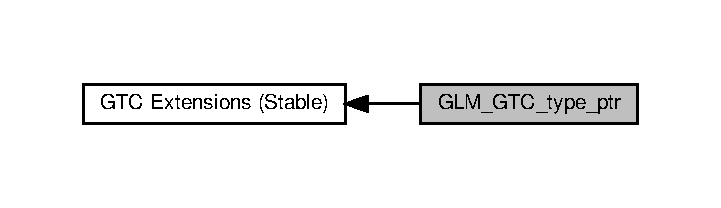
\includegraphics[width=346pt]{group__gtc__type__ptr}
\end{center}
\end{figure}
\subsection*{Functions}
\begin{DoxyCompactItemize}
\item 
{\footnotesize template$<$typename gen\+Type $>$ }\\\hyperlink{setup_8hpp_ab2d052de21a70539923e9bcbf6e83a51}{G\+L\+M\+\_\+\+F\+U\+N\+C\+\_\+\+D\+E\+CL} gen\+Type\+::value\+\_\+type const  $\ast$ \hyperlink{group__gtc__type__ptr_gaf019636bb8bd7c9efb7c7ce3bb23bcfc}{glm\+::value\+\_\+ptr} (gen\+Type const \&vec)
\item 
{\footnotesize template$<$typename T $>$ }\\\hyperlink{setup_8hpp_ab2d052de21a70539923e9bcbf6e83a51}{G\+L\+M\+\_\+\+F\+U\+N\+C\+\_\+\+D\+E\+CL} \hyperlink{structglm_1_1detail_1_1tvec2}{detail\+::tvec2}$<$ T, \hyperlink{namespaceglm_a0f04f086094c747d227af4425893f545a9d21ccd8b5a009ec7eb7677befc3bf51}{defaultp} $>$ \hyperlink{group__gtc__type__ptr_ga70f570befb4773ba3a658b76f9fdd6ab}{glm\+::make\+\_\+vec2} (T const $\ast$const ptr)
\item 
{\footnotesize template$<$typename T $>$ }\\\hyperlink{setup_8hpp_ab2d052de21a70539923e9bcbf6e83a51}{G\+L\+M\+\_\+\+F\+U\+N\+C\+\_\+\+D\+E\+CL} \hyperlink{structglm_1_1detail_1_1tvec3}{detail\+::tvec3}$<$ T, \hyperlink{namespaceglm_a0f04f086094c747d227af4425893f545a9d21ccd8b5a009ec7eb7677befc3bf51}{defaultp} $>$ \hyperlink{group__gtc__type__ptr_gad91a6a0fe324630b151208703a1591ed}{glm\+::make\+\_\+vec3} (T const $\ast$const ptr)
\item 
{\footnotesize template$<$typename T $>$ }\\\hyperlink{setup_8hpp_ab2d052de21a70539923e9bcbf6e83a51}{G\+L\+M\+\_\+\+F\+U\+N\+C\+\_\+\+D\+E\+CL} \hyperlink{structglm_1_1detail_1_1tvec4}{detail\+::tvec4}$<$ T, \hyperlink{namespaceglm_a0f04f086094c747d227af4425893f545a9d21ccd8b5a009ec7eb7677befc3bf51}{defaultp} $>$ \hyperlink{group__gtc__type__ptr_ga1b9e0d9ca48d79ba87edc121c1872c44}{glm\+::make\+\_\+vec4} (T const $\ast$const ptr)
\item 
{\footnotesize template$<$typename T $>$ }\\\hyperlink{setup_8hpp_ab2d052de21a70539923e9bcbf6e83a51}{G\+L\+M\+\_\+\+F\+U\+N\+C\+\_\+\+D\+E\+CL} \hyperlink{structglm_1_1detail_1_1tmat2x2}{detail\+::tmat2x2}$<$ T, \hyperlink{namespaceglm_a0f04f086094c747d227af4425893f545a9d21ccd8b5a009ec7eb7677befc3bf51}{defaultp} $>$ \hyperlink{group__gtc__type__ptr_ga860d529f631ea6f9a0e510491d29a8ac}{glm\+::make\+\_\+mat2x2} (T const $\ast$const ptr)
\item 
{\footnotesize template$<$typename T $>$ }\\\hyperlink{setup_8hpp_ab2d052de21a70539923e9bcbf6e83a51}{G\+L\+M\+\_\+\+F\+U\+N\+C\+\_\+\+D\+E\+CL} \hyperlink{structglm_1_1detail_1_1tmat2x3}{detail\+::tmat2x3}$<$ T, \hyperlink{namespaceglm_a0f04f086094c747d227af4425893f545a9d21ccd8b5a009ec7eb7677befc3bf51}{defaultp} $>$ \hyperlink{group__gtc__type__ptr_gadef48cd950566f23a4b1e47127ee478c}{glm\+::make\+\_\+mat2x3} (T const $\ast$const ptr)
\item 
{\footnotesize template$<$typename T $>$ }\\\hyperlink{setup_8hpp_ab2d052de21a70539923e9bcbf6e83a51}{G\+L\+M\+\_\+\+F\+U\+N\+C\+\_\+\+D\+E\+CL} \hyperlink{structglm_1_1detail_1_1tmat2x4}{detail\+::tmat2x4}$<$ T, \hyperlink{namespaceglm_a0f04f086094c747d227af4425893f545a9d21ccd8b5a009ec7eb7677befc3bf51}{defaultp} $>$ \hyperlink{group__gtc__type__ptr_ga174a43e8913682834de9cd918e36df25}{glm\+::make\+\_\+mat2x4} (T const $\ast$const ptr)
\item 
{\footnotesize template$<$typename T $>$ }\\\hyperlink{setup_8hpp_ab2d052de21a70539923e9bcbf6e83a51}{G\+L\+M\+\_\+\+F\+U\+N\+C\+\_\+\+D\+E\+CL} \hyperlink{structglm_1_1detail_1_1tmat3x2}{detail\+::tmat3x2}$<$ T, \hyperlink{namespaceglm_a0f04f086094c747d227af4425893f545a9d21ccd8b5a009ec7eb7677befc3bf51}{defaultp} $>$ \hyperlink{group__gtc__type__ptr_gaa40868af4de8c5ed5470fdcc9985dbfc}{glm\+::make\+\_\+mat3x2} (T const $\ast$const ptr)
\item 
{\footnotesize template$<$typename T $>$ }\\\hyperlink{setup_8hpp_ab2d052de21a70539923e9bcbf6e83a51}{G\+L\+M\+\_\+\+F\+U\+N\+C\+\_\+\+D\+E\+CL} \hyperlink{structglm_1_1detail_1_1tmat3x3}{detail\+::tmat3x3}$<$ T, \hyperlink{namespaceglm_a0f04f086094c747d227af4425893f545a9d21ccd8b5a009ec7eb7677befc3bf51}{defaultp} $>$ \hyperlink{group__gtc__type__ptr_gaf8ba0a0a523423ae1149a1c2d90eb337}{glm\+::make\+\_\+mat3x3} (T const $\ast$const ptr)
\item 
{\footnotesize template$<$typename T $>$ }\\\hyperlink{setup_8hpp_ab2d052de21a70539923e9bcbf6e83a51}{G\+L\+M\+\_\+\+F\+U\+N\+C\+\_\+\+D\+E\+CL} \hyperlink{structglm_1_1detail_1_1tmat3x4}{detail\+::tmat3x4}$<$ T, \hyperlink{namespaceglm_a0f04f086094c747d227af4425893f545a9d21ccd8b5a009ec7eb7677befc3bf51}{defaultp} $>$ \hyperlink{group__gtc__type__ptr_gaa0c07ac459a5e16374aa12e3b35ee043}{glm\+::make\+\_\+mat3x4} (T const $\ast$const ptr)
\item 
{\footnotesize template$<$typename T $>$ }\\\hyperlink{setup_8hpp_ab2d052de21a70539923e9bcbf6e83a51}{G\+L\+M\+\_\+\+F\+U\+N\+C\+\_\+\+D\+E\+CL} \hyperlink{structglm_1_1detail_1_1tmat4x2}{detail\+::tmat4x2}$<$ T, \hyperlink{namespaceglm_a0f04f086094c747d227af4425893f545a9d21ccd8b5a009ec7eb7677befc3bf51}{defaultp} $>$ \hyperlink{group__gtc__type__ptr_gae4ad99adfe4fb195a192712a71de901d}{glm\+::make\+\_\+mat4x2} (T const $\ast$const ptr)
\item 
{\footnotesize template$<$typename T $>$ }\\\hyperlink{setup_8hpp_ab2d052de21a70539923e9bcbf6e83a51}{G\+L\+M\+\_\+\+F\+U\+N\+C\+\_\+\+D\+E\+CL} \hyperlink{structglm_1_1detail_1_1tmat4x3}{detail\+::tmat4x3}$<$ T, \hyperlink{namespaceglm_a0f04f086094c747d227af4425893f545a9d21ccd8b5a009ec7eb7677befc3bf51}{defaultp} $>$ \hyperlink{group__gtc__type__ptr_ga37ec66362c22d86ad2ee11930b638c4a}{glm\+::make\+\_\+mat4x3} (T const $\ast$const ptr)
\item 
{\footnotesize template$<$typename T $>$ }\\\hyperlink{setup_8hpp_ab2d052de21a70539923e9bcbf6e83a51}{G\+L\+M\+\_\+\+F\+U\+N\+C\+\_\+\+D\+E\+CL} \hyperlink{structglm_1_1detail_1_1tmat4x4}{detail\+::tmat4x4}$<$ T, \hyperlink{namespaceglm_a0f04f086094c747d227af4425893f545a9d21ccd8b5a009ec7eb7677befc3bf51}{defaultp} $>$ \hyperlink{group__gtc__type__ptr_ga4b13ff6840a66d032724a9a1db50f704}{glm\+::make\+\_\+mat4x4} (T const $\ast$const ptr)
\item 
{\footnotesize template$<$typename T $>$ }\\\hyperlink{setup_8hpp_ab2d052de21a70539923e9bcbf6e83a51}{G\+L\+M\+\_\+\+F\+U\+N\+C\+\_\+\+D\+E\+CL} \hyperlink{structglm_1_1detail_1_1tmat2x2}{detail\+::tmat2x2}$<$ T, \hyperlink{namespaceglm_a0f04f086094c747d227af4425893f545a9d21ccd8b5a009ec7eb7677befc3bf51}{defaultp} $>$ \hyperlink{group__gtc__type__ptr_ga903422b2c346cbaccad3153a5a1f404c}{glm\+::make\+\_\+mat2} (T const $\ast$const ptr)
\item 
{\footnotesize template$<$typename T $>$ }\\\hyperlink{setup_8hpp_ab2d052de21a70539923e9bcbf6e83a51}{G\+L\+M\+\_\+\+F\+U\+N\+C\+\_\+\+D\+E\+CL} \hyperlink{structglm_1_1detail_1_1tmat3x3}{detail\+::tmat3x3}$<$ T, \hyperlink{namespaceglm_a0f04f086094c747d227af4425893f545a9d21ccd8b5a009ec7eb7677befc3bf51}{defaultp} $>$ \hyperlink{group__gtc__type__ptr_gae50ecac46eb8771fb074e310b602bf53}{glm\+::make\+\_\+mat3} (T const $\ast$const ptr)
\item 
{\footnotesize template$<$typename T $>$ }\\\hyperlink{setup_8hpp_ab2d052de21a70539923e9bcbf6e83a51}{G\+L\+M\+\_\+\+F\+U\+N\+C\+\_\+\+D\+E\+CL} \hyperlink{structglm_1_1detail_1_1tmat4x4}{detail\+::tmat4x4}$<$ T, \hyperlink{namespaceglm_a0f04f086094c747d227af4425893f545a9d21ccd8b5a009ec7eb7677befc3bf51}{defaultp} $>$ \hyperlink{group__gtc__type__ptr_gac3920fd61f0c459a4749b8eb9107982c}{glm\+::make\+\_\+mat4} (T const $\ast$const ptr)
\item 
{\footnotesize template$<$typename T $>$ }\\\hyperlink{setup_8hpp_ab2d052de21a70539923e9bcbf6e83a51}{G\+L\+M\+\_\+\+F\+U\+N\+C\+\_\+\+D\+E\+CL} \hyperlink{structglm_1_1detail_1_1tquat}{detail\+::tquat}$<$ T, \hyperlink{namespaceglm_a0f04f086094c747d227af4425893f545a9d21ccd8b5a009ec7eb7677befc3bf51}{defaultp} $>$ \hyperlink{group__gtc__type__ptr_ga051ec24a44af31a08b11eccbf8726b02}{glm\+::make\+\_\+quat} (T const $\ast$const ptr)
\item 
{\footnotesize template$<$typename T , precision P$>$ }\\\hyperlink{setup_8hpp_a33fdea6f91c5f834105f7415e2a64407}{G\+L\+M\+\_\+\+F\+U\+N\+C\+\_\+\+Q\+U\+A\+L\+I\+F\+I\+ER} T const  $\ast$ \hyperlink{group__gtc__type__ptr_gac57a976f59e794e6406ecf2924a18f4e}{glm\+::value\+\_\+ptr} (\hyperlink{structglm_1_1detail_1_1tvec2}{detail\+::tvec2}$<$ T, P $>$ const \&vec)
\item 
{\footnotesize template$<$typename T , precision P$>$ }\\\hyperlink{setup_8hpp_a33fdea6f91c5f834105f7415e2a64407}{G\+L\+M\+\_\+\+F\+U\+N\+C\+\_\+\+Q\+U\+A\+L\+I\+F\+I\+ER} T $\ast$ \hyperlink{group__gtc__type__ptr_gac2a64387090621acf7176b63f31b70a2}{glm\+::value\+\_\+ptr} (\hyperlink{structglm_1_1detail_1_1tvec2}{detail\+::tvec2}$<$ T, P $>$ \&vec)
\item 
{\footnotesize template$<$typename T , precision P$>$ }\\\hyperlink{setup_8hpp_a33fdea6f91c5f834105f7415e2a64407}{G\+L\+M\+\_\+\+F\+U\+N\+C\+\_\+\+Q\+U\+A\+L\+I\+F\+I\+ER} T const  $\ast$ \hyperlink{group__gtc__type__ptr_ga676a0ba6f4b7cd817fe6d16cb3113857}{glm\+::value\+\_\+ptr} (\hyperlink{structglm_1_1detail_1_1tvec3}{detail\+::tvec3}$<$ T, P $>$ const \&vec)
\item 
{\footnotesize template$<$typename T , precision P$>$ }\\\hyperlink{setup_8hpp_a33fdea6f91c5f834105f7415e2a64407}{G\+L\+M\+\_\+\+F\+U\+N\+C\+\_\+\+Q\+U\+A\+L\+I\+F\+I\+ER} T $\ast$ \hyperlink{group__gtc__type__ptr_ga4babc9956e32bbd0769bc20ab2d73800}{glm\+::value\+\_\+ptr} (\hyperlink{structglm_1_1detail_1_1tvec3}{detail\+::tvec3}$<$ T, P $>$ \&vec)
\item 
{\footnotesize template$<$typename T , precision P$>$ }\\\hyperlink{setup_8hpp_a33fdea6f91c5f834105f7415e2a64407}{G\+L\+M\+\_\+\+F\+U\+N\+C\+\_\+\+Q\+U\+A\+L\+I\+F\+I\+ER} T const  $\ast$ \hyperlink{group__gtc__type__ptr_ga6963deec2c77b8a49b3f7e434914f6ba}{glm\+::value\+\_\+ptr} (\hyperlink{structglm_1_1detail_1_1tvec4}{detail\+::tvec4}$<$ T, P $>$ const \&vec)
\item 
{\footnotesize template$<$typename T , precision P$>$ }\\\hyperlink{setup_8hpp_a33fdea6f91c5f834105f7415e2a64407}{G\+L\+M\+\_\+\+F\+U\+N\+C\+\_\+\+Q\+U\+A\+L\+I\+F\+I\+ER} T $\ast$ \hyperlink{group__gtc__type__ptr_gaa3ed69a05293987972b589311e5feb23}{glm\+::value\+\_\+ptr} (\hyperlink{structglm_1_1detail_1_1tvec4}{detail\+::tvec4}$<$ T, P $>$ \&vec)
\item 
{\footnotesize template$<$typename T , precision P$>$ }\\\hyperlink{setup_8hpp_a33fdea6f91c5f834105f7415e2a64407}{G\+L\+M\+\_\+\+F\+U\+N\+C\+\_\+\+Q\+U\+A\+L\+I\+F\+I\+ER} T const  $\ast$ \hyperlink{group__gtc__type__ptr_ga013fcf415d78cc3aa9273c5d4f780325}{glm\+::value\+\_\+ptr} (\hyperlink{structglm_1_1detail_1_1tmat2x2}{detail\+::tmat2x2}$<$ T, P $>$ const \&mat)
\item 
{\footnotesize template$<$typename T , precision P$>$ }\\\hyperlink{setup_8hpp_a33fdea6f91c5f834105f7415e2a64407}{G\+L\+M\+\_\+\+F\+U\+N\+C\+\_\+\+Q\+U\+A\+L\+I\+F\+I\+ER} T $\ast$ \hyperlink{group__gtc__type__ptr_ga11e5b6c0d7d5d2627df624bb4b219f20}{glm\+::value\+\_\+ptr} (\hyperlink{structglm_1_1detail_1_1tmat2x2}{detail\+::tmat2x2}$<$ T, P $>$ \&mat)
\item 
{\footnotesize template$<$typename T , precision P$>$ }\\\hyperlink{setup_8hpp_a33fdea6f91c5f834105f7415e2a64407}{G\+L\+M\+\_\+\+F\+U\+N\+C\+\_\+\+Q\+U\+A\+L\+I\+F\+I\+ER} T const  $\ast$ \hyperlink{group__gtc__type__ptr_ga78acb1fd15ce7d1d2861493fac9693ec}{glm\+::value\+\_\+ptr} (\hyperlink{structglm_1_1detail_1_1tmat3x3}{detail\+::tmat3x3}$<$ T, P $>$ const \&mat)
\item 
{\footnotesize template$<$typename T , precision P$>$ }\\\hyperlink{setup_8hpp_a33fdea6f91c5f834105f7415e2a64407}{G\+L\+M\+\_\+\+F\+U\+N\+C\+\_\+\+Q\+U\+A\+L\+I\+F\+I\+ER} T $\ast$ \hyperlink{group__gtc__type__ptr_gaad64150511d5c6a2d2c7afec724e4064}{glm\+::value\+\_\+ptr} (\hyperlink{structglm_1_1detail_1_1tmat3x3}{detail\+::tmat3x3}$<$ T, P $>$ \&mat)
\item 
{\footnotesize template$<$typename T , precision P$>$ }\\\hyperlink{setup_8hpp_a33fdea6f91c5f834105f7415e2a64407}{G\+L\+M\+\_\+\+F\+U\+N\+C\+\_\+\+Q\+U\+A\+L\+I\+F\+I\+ER} T const  $\ast$ \hyperlink{group__gtc__type__ptr_gaa99522f78635f6949ebf82f065bafa94}{glm\+::value\+\_\+ptr} (\hyperlink{structglm_1_1detail_1_1tmat4x4}{detail\+::tmat4x4}$<$ T, P $>$ const \&mat)
\item 
{\footnotesize template$<$typename T , precision P$>$ }\\\hyperlink{setup_8hpp_a33fdea6f91c5f834105f7415e2a64407}{G\+L\+M\+\_\+\+F\+U\+N\+C\+\_\+\+Q\+U\+A\+L\+I\+F\+I\+ER} T $\ast$ \hyperlink{group__gtc__type__ptr_ga46c85fe444b7260c496be5fe0c146e87}{glm\+::value\+\_\+ptr} (\hyperlink{structglm_1_1detail_1_1tmat4x4}{detail\+::tmat4x4}$<$ T, P $>$ \&mat)
\item 
{\footnotesize template$<$typename T , precision P$>$ }\\\hyperlink{setup_8hpp_a33fdea6f91c5f834105f7415e2a64407}{G\+L\+M\+\_\+\+F\+U\+N\+C\+\_\+\+Q\+U\+A\+L\+I\+F\+I\+ER} T const  $\ast$ \hyperlink{group__gtc__type__ptr_gad5c4faad7a4553c875bc45656fcae73c}{glm\+::value\+\_\+ptr} (\hyperlink{structglm_1_1detail_1_1tmat2x3}{detail\+::tmat2x3}$<$ T, P $>$ const \&mat)
\item 
{\footnotesize template$<$typename T , precision P$>$ }\\\hyperlink{setup_8hpp_a33fdea6f91c5f834105f7415e2a64407}{G\+L\+M\+\_\+\+F\+U\+N\+C\+\_\+\+Q\+U\+A\+L\+I\+F\+I\+ER} T $\ast$ \hyperlink{group__gtc__type__ptr_gaaba8179ff5559d8b4493499313eb7a02}{glm\+::value\+\_\+ptr} (\hyperlink{structglm_1_1detail_1_1tmat2x3}{detail\+::tmat2x3}$<$ T, P $>$ \&mat)
\item 
{\footnotesize template$<$typename T , precision P$>$ }\\\hyperlink{setup_8hpp_a33fdea6f91c5f834105f7415e2a64407}{G\+L\+M\+\_\+\+F\+U\+N\+C\+\_\+\+Q\+U\+A\+L\+I\+F\+I\+ER} T const  $\ast$ \hyperlink{group__gtc__type__ptr_gaf8edbe29063a5b8221fc8afcb6af224d}{glm\+::value\+\_\+ptr} (\hyperlink{structglm_1_1detail_1_1tmat3x2}{detail\+::tmat3x2}$<$ T, P $>$ const \&mat)
\item 
{\footnotesize template$<$typename T , precision P$>$ }\\\hyperlink{setup_8hpp_a33fdea6f91c5f834105f7415e2a64407}{G\+L\+M\+\_\+\+F\+U\+N\+C\+\_\+\+Q\+U\+A\+L\+I\+F\+I\+ER} T $\ast$ \hyperlink{group__gtc__type__ptr_gae2e604002202417c7156db3deeb1301d}{glm\+::value\+\_\+ptr} (\hyperlink{structglm_1_1detail_1_1tmat3x2}{detail\+::tmat3x2}$<$ T, P $>$ \&mat)
\item 
{\footnotesize template$<$typename T , precision P$>$ }\\\hyperlink{setup_8hpp_a33fdea6f91c5f834105f7415e2a64407}{G\+L\+M\+\_\+\+F\+U\+N\+C\+\_\+\+Q\+U\+A\+L\+I\+F\+I\+ER} T const  $\ast$ \hyperlink{group__gtc__type__ptr_ga7b738eac576043c00c39bda2fc515d7b}{glm\+::value\+\_\+ptr} (\hyperlink{structglm_1_1detail_1_1tmat2x4}{detail\+::tmat2x4}$<$ T, P $>$ const \&mat)
\item 
{\footnotesize template$<$typename T , precision P$>$ }\\\hyperlink{setup_8hpp_a33fdea6f91c5f834105f7415e2a64407}{G\+L\+M\+\_\+\+F\+U\+N\+C\+\_\+\+Q\+U\+A\+L\+I\+F\+I\+ER} T $\ast$ \hyperlink{group__gtc__type__ptr_ga59b17271f4f487e556383b715f9b8534}{glm\+::value\+\_\+ptr} (\hyperlink{structglm_1_1detail_1_1tmat2x4}{detail\+::tmat2x4}$<$ T, P $>$ \&mat)
\item 
{\footnotesize template$<$typename T , precision P$>$ }\\\hyperlink{setup_8hpp_a33fdea6f91c5f834105f7415e2a64407}{G\+L\+M\+\_\+\+F\+U\+N\+C\+\_\+\+Q\+U\+A\+L\+I\+F\+I\+ER} T const  $\ast$ \hyperlink{group__gtc__type__ptr_ga73acc0dbfeeb9e6c09df1f79fd990b84}{glm\+::value\+\_\+ptr} (\hyperlink{structglm_1_1detail_1_1tmat4x2}{detail\+::tmat4x2}$<$ T, P $>$ const \&mat)
\item 
{\footnotesize template$<$typename T , precision P$>$ }\\\hyperlink{setup_8hpp_a33fdea6f91c5f834105f7415e2a64407}{G\+L\+M\+\_\+\+F\+U\+N\+C\+\_\+\+Q\+U\+A\+L\+I\+F\+I\+ER} T $\ast$ \hyperlink{group__gtc__type__ptr_ga478c7dc470b36836ac5392e852fd2348}{glm\+::value\+\_\+ptr} (\hyperlink{structglm_1_1detail_1_1tmat4x2}{detail\+::tmat4x2}$<$ T, P $>$ \&mat)
\item 
{\footnotesize template$<$typename T , precision P$>$ }\\\hyperlink{setup_8hpp_a33fdea6f91c5f834105f7415e2a64407}{G\+L\+M\+\_\+\+F\+U\+N\+C\+\_\+\+Q\+U\+A\+L\+I\+F\+I\+ER} T const  $\ast$ \hyperlink{group__gtc__type__ptr_ga233effe326542ae9657b8feac80e541f}{glm\+::value\+\_\+ptr} (\hyperlink{structglm_1_1detail_1_1tmat3x4}{detail\+::tmat3x4}$<$ T, P $>$ const \&mat)
\item 
{\footnotesize template$<$typename T , precision P$>$ }\\\hyperlink{setup_8hpp_a33fdea6f91c5f834105f7415e2a64407}{G\+L\+M\+\_\+\+F\+U\+N\+C\+\_\+\+Q\+U\+A\+L\+I\+F\+I\+ER} T $\ast$ \hyperlink{group__gtc__type__ptr_gad8c6b1dbda2b48d19fd1bc8b01cf701c}{glm\+::value\+\_\+ptr} (\hyperlink{structglm_1_1detail_1_1tmat3x4}{detail\+::tmat3x4}$<$ T, P $>$ \&mat)
\item 
{\footnotesize template$<$typename T , precision P$>$ }\\\hyperlink{setup_8hpp_a33fdea6f91c5f834105f7415e2a64407}{G\+L\+M\+\_\+\+F\+U\+N\+C\+\_\+\+Q\+U\+A\+L\+I\+F\+I\+ER} T const  $\ast$ \hyperlink{group__gtc__type__ptr_gaebe5b66d8b05f6ace85d26cedd03732d}{glm\+::value\+\_\+ptr} (\hyperlink{structglm_1_1detail_1_1tmat4x3}{detail\+::tmat4x3}$<$ T, P $>$ const \&mat)
\item 
{\footnotesize template$<$typename T , precision P$>$ }\\\hyperlink{setup_8hpp_a33fdea6f91c5f834105f7415e2a64407}{G\+L\+M\+\_\+\+F\+U\+N\+C\+\_\+\+Q\+U\+A\+L\+I\+F\+I\+ER} T $\ast$ \hyperlink{group__gtc__type__ptr_ga4a4b23867cc26441441ff4458844fa27}{glm\+::value\+\_\+ptr} (\hyperlink{structglm_1_1detail_1_1tmat4x3}{detail\+::tmat4x3}$<$ T, P $>$ \&mat)
\item 
{\footnotesize template$<$typename T , precision P$>$ }\\\hyperlink{setup_8hpp_a33fdea6f91c5f834105f7415e2a64407}{G\+L\+M\+\_\+\+F\+U\+N\+C\+\_\+\+Q\+U\+A\+L\+I\+F\+I\+ER} T const  $\ast$ \hyperlink{group__gtc__type__ptr_ga961a5b150a0ffd632aaa0252c4d6b9ab}{glm\+::value\+\_\+ptr} (\hyperlink{structglm_1_1detail_1_1tquat}{detail\+::tquat}$<$ T, P $>$ const \&q)
\item 
{\footnotesize template$<$typename T , precision P$>$ }\\\hyperlink{setup_8hpp_a33fdea6f91c5f834105f7415e2a64407}{G\+L\+M\+\_\+\+F\+U\+N\+C\+\_\+\+Q\+U\+A\+L\+I\+F\+I\+ER} T $\ast$ \hyperlink{group__gtc__type__ptr_gab72389186ae9e8c822ff6cc9b474a37f}{glm\+::value\+\_\+ptr} (\hyperlink{structglm_1_1detail_1_1tquat}{detail\+::tquat}$<$ T, P $>$ \&q)
\end{DoxyCompactItemize}


\subsection{Detailed Description}
Handles the interaction between pointers and vector, matrix types. 

This extension defines an overloaded function, \hyperlink{group__gtc__type__ptr_gaf019636bb8bd7c9efb7c7ce3bb23bcfc}{glm\+::value\+\_\+ptr}, which takes any of the \hyperlink{group__core__template}{core template types}. It returns a pointer to the memory layout of the object. Matrix types store their values in column-\/major order.

This is useful for uploading data to matrices or copying data to buffer objects.

Example\+: 
\begin{DoxyCode}
\textcolor{preprocessor}{#include <\hyperlink{third-party_2include_2glm_2glm_8hpp}{glm/glm.hpp}>}
\textcolor{preprocessor}{#include <\hyperlink{type__ptr_8hpp}{glm/gtc/type\_ptr.hpp}>}

\hyperlink{structglm_1_1detail_1_1tvec3}{glm::vec3} aVector(3);
\hyperlink{structglm_1_1detail_1_1tmat4x4}{glm::mat4} someMatrix(1.0);

glUniform3fv(uniformLoc, 1, \hyperlink{group__gtc__type__ptr_gaf019636bb8bd7c9efb7c7ce3bb23bcfc}{glm::value\_ptr}(aVector));
\hyperlink{dummy_8cpp_a0294e2a1faa1a1ff720a35ac06b4282a}{glUniformMatrix4fv}(uniformMatrixLoc, 1, \hyperlink{dummy_8cpp_abca6d43f43fae31f49dcb883b2f301f6}{GL\_FALSE}, 
      \hyperlink{group__gtc__type__ptr_gaf019636bb8bd7c9efb7c7ce3bb23bcfc}{glm::value\_ptr}(someMatrix));
\end{DoxyCode}


$<$\hyperlink{type__ptr_8hpp}{glm/gtc/type\+\_\+ptr.\+hpp}$>$ need to be included to use these functionalities. 

\subsection{Function Documentation}
\mbox{\Hypertarget{group__gtc__type__ptr_ga903422b2c346cbaccad3153a5a1f404c}\label{group__gtc__type__ptr_ga903422b2c346cbaccad3153a5a1f404c}} 
\index{G\+L\+M\+\_\+\+G\+T\+C\+\_\+type\+\_\+ptr@{G\+L\+M\+\_\+\+G\+T\+C\+\_\+type\+\_\+ptr}!make\+\_\+mat2@{make\+\_\+mat2}}
\index{make\+\_\+mat2@{make\+\_\+mat2}!G\+L\+M\+\_\+\+G\+T\+C\+\_\+type\+\_\+ptr@{G\+L\+M\+\_\+\+G\+T\+C\+\_\+type\+\_\+ptr}}
\subsubsection{\texorpdfstring{make\+\_\+mat2()}{make\_mat2()}}
{\footnotesize\ttfamily template$<$typename T $>$ \\
\hyperlink{setup_8hpp_ab2d052de21a70539923e9bcbf6e83a51}{G\+L\+M\+\_\+\+F\+U\+N\+C\+\_\+\+D\+E\+CL} \hyperlink{structglm_1_1detail_1_1tmat2x2}{detail\+::tmat2x2}$<$T, \hyperlink{namespaceglm_a0f04f086094c747d227af4425893f545a9d21ccd8b5a009ec7eb7677befc3bf51}{defaultp}$>$ glm\+::make\+\_\+mat2 (\begin{DoxyParamCaption}\item[{T const $\ast$const}]{ptr }\end{DoxyParamCaption})}

Build a matrix from a pointer. \begin{DoxySeeAlso}{See also}
\hyperlink{group__gtc__type__ptr}{G\+L\+M\+\_\+\+G\+T\+C\+\_\+type\+\_\+ptr} 
\end{DoxySeeAlso}


Definition at line 442 of file type\+\_\+ptr.\+inl.

\mbox{\Hypertarget{group__gtc__type__ptr_ga860d529f631ea6f9a0e510491d29a8ac}\label{group__gtc__type__ptr_ga860d529f631ea6f9a0e510491d29a8ac}} 
\index{G\+L\+M\+\_\+\+G\+T\+C\+\_\+type\+\_\+ptr@{G\+L\+M\+\_\+\+G\+T\+C\+\_\+type\+\_\+ptr}!make\+\_\+mat2x2@{make\+\_\+mat2x2}}
\index{make\+\_\+mat2x2@{make\+\_\+mat2x2}!G\+L\+M\+\_\+\+G\+T\+C\+\_\+type\+\_\+ptr@{G\+L\+M\+\_\+\+G\+T\+C\+\_\+type\+\_\+ptr}}
\subsubsection{\texorpdfstring{make\+\_\+mat2x2()}{make\_mat2x2()}}
{\footnotesize\ttfamily template$<$typename T $>$ \\
\hyperlink{setup_8hpp_ab2d052de21a70539923e9bcbf6e83a51}{G\+L\+M\+\_\+\+F\+U\+N\+C\+\_\+\+D\+E\+CL} \hyperlink{structglm_1_1detail_1_1tmat2x2}{detail\+::tmat2x2}$<$T, \hyperlink{namespaceglm_a0f04f086094c747d227af4425893f545a9d21ccd8b5a009ec7eb7677befc3bf51}{defaultp}$>$ glm\+::make\+\_\+mat2x2 (\begin{DoxyParamCaption}\item[{T const $\ast$const}]{ptr }\end{DoxyParamCaption})}

Build a matrix from a pointer. \begin{DoxySeeAlso}{See also}
\hyperlink{group__gtc__type__ptr}{G\+L\+M\+\_\+\+G\+T\+C\+\_\+type\+\_\+ptr} 
\end{DoxySeeAlso}


Definition at line 352 of file type\+\_\+ptr.\+inl.

\mbox{\Hypertarget{group__gtc__type__ptr_gadef48cd950566f23a4b1e47127ee478c}\label{group__gtc__type__ptr_gadef48cd950566f23a4b1e47127ee478c}} 
\index{G\+L\+M\+\_\+\+G\+T\+C\+\_\+type\+\_\+ptr@{G\+L\+M\+\_\+\+G\+T\+C\+\_\+type\+\_\+ptr}!make\+\_\+mat2x3@{make\+\_\+mat2x3}}
\index{make\+\_\+mat2x3@{make\+\_\+mat2x3}!G\+L\+M\+\_\+\+G\+T\+C\+\_\+type\+\_\+ptr@{G\+L\+M\+\_\+\+G\+T\+C\+\_\+type\+\_\+ptr}}
\subsubsection{\texorpdfstring{make\+\_\+mat2x3()}{make\_mat2x3()}}
{\footnotesize\ttfamily template$<$typename T $>$ \\
\hyperlink{setup_8hpp_ab2d052de21a70539923e9bcbf6e83a51}{G\+L\+M\+\_\+\+F\+U\+N\+C\+\_\+\+D\+E\+CL} \hyperlink{structglm_1_1detail_1_1tmat2x3}{detail\+::tmat2x3}$<$T, \hyperlink{namespaceglm_a0f04f086094c747d227af4425893f545a9d21ccd8b5a009ec7eb7677befc3bf51}{defaultp}$>$ glm\+::make\+\_\+mat2x3 (\begin{DoxyParamCaption}\item[{T const $\ast$const}]{ptr }\end{DoxyParamCaption})}

Build a matrix from a pointer. \begin{DoxySeeAlso}{See also}
\hyperlink{group__gtc__type__ptr}{G\+L\+M\+\_\+\+G\+T\+C\+\_\+type\+\_\+ptr} 
\end{DoxySeeAlso}


Definition at line 362 of file type\+\_\+ptr.\+inl.

\mbox{\Hypertarget{group__gtc__type__ptr_ga174a43e8913682834de9cd918e36df25}\label{group__gtc__type__ptr_ga174a43e8913682834de9cd918e36df25}} 
\index{G\+L\+M\+\_\+\+G\+T\+C\+\_\+type\+\_\+ptr@{G\+L\+M\+\_\+\+G\+T\+C\+\_\+type\+\_\+ptr}!make\+\_\+mat2x4@{make\+\_\+mat2x4}}
\index{make\+\_\+mat2x4@{make\+\_\+mat2x4}!G\+L\+M\+\_\+\+G\+T\+C\+\_\+type\+\_\+ptr@{G\+L\+M\+\_\+\+G\+T\+C\+\_\+type\+\_\+ptr}}
\subsubsection{\texorpdfstring{make\+\_\+mat2x4()}{make\_mat2x4()}}
{\footnotesize\ttfamily template$<$typename T $>$ \\
\hyperlink{setup_8hpp_ab2d052de21a70539923e9bcbf6e83a51}{G\+L\+M\+\_\+\+F\+U\+N\+C\+\_\+\+D\+E\+CL} \hyperlink{structglm_1_1detail_1_1tmat2x4}{detail\+::tmat2x4}$<$T, \hyperlink{namespaceglm_a0f04f086094c747d227af4425893f545a9d21ccd8b5a009ec7eb7677befc3bf51}{defaultp}$>$ glm\+::make\+\_\+mat2x4 (\begin{DoxyParamCaption}\item[{T const $\ast$const}]{ptr }\end{DoxyParamCaption})}

Build a matrix from a pointer. \begin{DoxySeeAlso}{See also}
\hyperlink{group__gtc__type__ptr}{G\+L\+M\+\_\+\+G\+T\+C\+\_\+type\+\_\+ptr} 
\end{DoxySeeAlso}


Definition at line 372 of file type\+\_\+ptr.\+inl.

\mbox{\Hypertarget{group__gtc__type__ptr_gae50ecac46eb8771fb074e310b602bf53}\label{group__gtc__type__ptr_gae50ecac46eb8771fb074e310b602bf53}} 
\index{G\+L\+M\+\_\+\+G\+T\+C\+\_\+type\+\_\+ptr@{G\+L\+M\+\_\+\+G\+T\+C\+\_\+type\+\_\+ptr}!make\+\_\+mat3@{make\+\_\+mat3}}
\index{make\+\_\+mat3@{make\+\_\+mat3}!G\+L\+M\+\_\+\+G\+T\+C\+\_\+type\+\_\+ptr@{G\+L\+M\+\_\+\+G\+T\+C\+\_\+type\+\_\+ptr}}
\subsubsection{\texorpdfstring{make\+\_\+mat3()}{make\_mat3()}}
{\footnotesize\ttfamily template$<$typename T $>$ \\
\hyperlink{setup_8hpp_ab2d052de21a70539923e9bcbf6e83a51}{G\+L\+M\+\_\+\+F\+U\+N\+C\+\_\+\+D\+E\+CL} \hyperlink{structglm_1_1detail_1_1tmat3x3}{detail\+::tmat3x3}$<$T, \hyperlink{namespaceglm_a0f04f086094c747d227af4425893f545a9d21ccd8b5a009ec7eb7677befc3bf51}{defaultp}$>$ glm\+::make\+\_\+mat3 (\begin{DoxyParamCaption}\item[{T const $\ast$const}]{ptr }\end{DoxyParamCaption})}

Build a matrix from a pointer. \begin{DoxySeeAlso}{See also}
\hyperlink{group__gtc__type__ptr}{G\+L\+M\+\_\+\+G\+T\+C\+\_\+type\+\_\+ptr} 
\end{DoxySeeAlso}


Definition at line 450 of file type\+\_\+ptr.\+inl.

\mbox{\Hypertarget{group__gtc__type__ptr_gaa40868af4de8c5ed5470fdcc9985dbfc}\label{group__gtc__type__ptr_gaa40868af4de8c5ed5470fdcc9985dbfc}} 
\index{G\+L\+M\+\_\+\+G\+T\+C\+\_\+type\+\_\+ptr@{G\+L\+M\+\_\+\+G\+T\+C\+\_\+type\+\_\+ptr}!make\+\_\+mat3x2@{make\+\_\+mat3x2}}
\index{make\+\_\+mat3x2@{make\+\_\+mat3x2}!G\+L\+M\+\_\+\+G\+T\+C\+\_\+type\+\_\+ptr@{G\+L\+M\+\_\+\+G\+T\+C\+\_\+type\+\_\+ptr}}
\subsubsection{\texorpdfstring{make\+\_\+mat3x2()}{make\_mat3x2()}}
{\footnotesize\ttfamily template$<$typename T $>$ \\
\hyperlink{setup_8hpp_ab2d052de21a70539923e9bcbf6e83a51}{G\+L\+M\+\_\+\+F\+U\+N\+C\+\_\+\+D\+E\+CL} \hyperlink{structglm_1_1detail_1_1tmat3x2}{detail\+::tmat3x2}$<$T, \hyperlink{namespaceglm_a0f04f086094c747d227af4425893f545a9d21ccd8b5a009ec7eb7677befc3bf51}{defaultp}$>$ glm\+::make\+\_\+mat3x2 (\begin{DoxyParamCaption}\item[{T const $\ast$const}]{ptr }\end{DoxyParamCaption})}

Build a matrix from a pointer. \begin{DoxySeeAlso}{See also}
\hyperlink{group__gtc__type__ptr}{G\+L\+M\+\_\+\+G\+T\+C\+\_\+type\+\_\+ptr} 
\end{DoxySeeAlso}


Definition at line 382 of file type\+\_\+ptr.\+inl.

\mbox{\Hypertarget{group__gtc__type__ptr_gaf8ba0a0a523423ae1149a1c2d90eb337}\label{group__gtc__type__ptr_gaf8ba0a0a523423ae1149a1c2d90eb337}} 
\index{G\+L\+M\+\_\+\+G\+T\+C\+\_\+type\+\_\+ptr@{G\+L\+M\+\_\+\+G\+T\+C\+\_\+type\+\_\+ptr}!make\+\_\+mat3x3@{make\+\_\+mat3x3}}
\index{make\+\_\+mat3x3@{make\+\_\+mat3x3}!G\+L\+M\+\_\+\+G\+T\+C\+\_\+type\+\_\+ptr@{G\+L\+M\+\_\+\+G\+T\+C\+\_\+type\+\_\+ptr}}
\subsubsection{\texorpdfstring{make\+\_\+mat3x3()}{make\_mat3x3()}}
{\footnotesize\ttfamily template$<$typename T $>$ \\
\hyperlink{setup_8hpp_ab2d052de21a70539923e9bcbf6e83a51}{G\+L\+M\+\_\+\+F\+U\+N\+C\+\_\+\+D\+E\+CL} \hyperlink{structglm_1_1detail_1_1tmat3x3}{detail\+::tmat3x3}$<$T, \hyperlink{namespaceglm_a0f04f086094c747d227af4425893f545a9d21ccd8b5a009ec7eb7677befc3bf51}{defaultp}$>$ glm\+::make\+\_\+mat3x3 (\begin{DoxyParamCaption}\item[{T const $\ast$const}]{ptr }\end{DoxyParamCaption})}

Build a matrix from a pointer. \begin{DoxySeeAlso}{See also}
\hyperlink{group__gtc__type__ptr}{G\+L\+M\+\_\+\+G\+T\+C\+\_\+type\+\_\+ptr} 
\end{DoxySeeAlso}


Definition at line 392 of file type\+\_\+ptr.\+inl.

\mbox{\Hypertarget{group__gtc__type__ptr_gaa0c07ac459a5e16374aa12e3b35ee043}\label{group__gtc__type__ptr_gaa0c07ac459a5e16374aa12e3b35ee043}} 
\index{G\+L\+M\+\_\+\+G\+T\+C\+\_\+type\+\_\+ptr@{G\+L\+M\+\_\+\+G\+T\+C\+\_\+type\+\_\+ptr}!make\+\_\+mat3x4@{make\+\_\+mat3x4}}
\index{make\+\_\+mat3x4@{make\+\_\+mat3x4}!G\+L\+M\+\_\+\+G\+T\+C\+\_\+type\+\_\+ptr@{G\+L\+M\+\_\+\+G\+T\+C\+\_\+type\+\_\+ptr}}
\subsubsection{\texorpdfstring{make\+\_\+mat3x4()}{make\_mat3x4()}}
{\footnotesize\ttfamily template$<$typename T $>$ \\
\hyperlink{setup_8hpp_ab2d052de21a70539923e9bcbf6e83a51}{G\+L\+M\+\_\+\+F\+U\+N\+C\+\_\+\+D\+E\+CL} \hyperlink{structglm_1_1detail_1_1tmat3x4}{detail\+::tmat3x4}$<$T, \hyperlink{namespaceglm_a0f04f086094c747d227af4425893f545a9d21ccd8b5a009ec7eb7677befc3bf51}{defaultp}$>$ glm\+::make\+\_\+mat3x4 (\begin{DoxyParamCaption}\item[{T const $\ast$const}]{ptr }\end{DoxyParamCaption})}

Build a matrix from a pointer. \begin{DoxySeeAlso}{See also}
\hyperlink{group__gtc__type__ptr}{G\+L\+M\+\_\+\+G\+T\+C\+\_\+type\+\_\+ptr} 
\end{DoxySeeAlso}


Definition at line 402 of file type\+\_\+ptr.\+inl.

\mbox{\Hypertarget{group__gtc__type__ptr_gac3920fd61f0c459a4749b8eb9107982c}\label{group__gtc__type__ptr_gac3920fd61f0c459a4749b8eb9107982c}} 
\index{G\+L\+M\+\_\+\+G\+T\+C\+\_\+type\+\_\+ptr@{G\+L\+M\+\_\+\+G\+T\+C\+\_\+type\+\_\+ptr}!make\+\_\+mat4@{make\+\_\+mat4}}
\index{make\+\_\+mat4@{make\+\_\+mat4}!G\+L\+M\+\_\+\+G\+T\+C\+\_\+type\+\_\+ptr@{G\+L\+M\+\_\+\+G\+T\+C\+\_\+type\+\_\+ptr}}
\subsubsection{\texorpdfstring{make\+\_\+mat4()}{make\_mat4()}}
{\footnotesize\ttfamily template$<$typename T $>$ \\
\hyperlink{setup_8hpp_ab2d052de21a70539923e9bcbf6e83a51}{G\+L\+M\+\_\+\+F\+U\+N\+C\+\_\+\+D\+E\+CL} \hyperlink{structglm_1_1detail_1_1tmat4x4}{detail\+::tmat4x4}$<$T, \hyperlink{namespaceglm_a0f04f086094c747d227af4425893f545a9d21ccd8b5a009ec7eb7677befc3bf51}{defaultp}$>$ glm\+::make\+\_\+mat4 (\begin{DoxyParamCaption}\item[{T const $\ast$const}]{ptr }\end{DoxyParamCaption})}

Build a matrix from a pointer. \begin{DoxySeeAlso}{See also}
\hyperlink{group__gtc__type__ptr}{G\+L\+M\+\_\+\+G\+T\+C\+\_\+type\+\_\+ptr} 
\end{DoxySeeAlso}


Definition at line 458 of file type\+\_\+ptr.\+inl.

\mbox{\Hypertarget{group__gtc__type__ptr_gae4ad99adfe4fb195a192712a71de901d}\label{group__gtc__type__ptr_gae4ad99adfe4fb195a192712a71de901d}} 
\index{G\+L\+M\+\_\+\+G\+T\+C\+\_\+type\+\_\+ptr@{G\+L\+M\+\_\+\+G\+T\+C\+\_\+type\+\_\+ptr}!make\+\_\+mat4x2@{make\+\_\+mat4x2}}
\index{make\+\_\+mat4x2@{make\+\_\+mat4x2}!G\+L\+M\+\_\+\+G\+T\+C\+\_\+type\+\_\+ptr@{G\+L\+M\+\_\+\+G\+T\+C\+\_\+type\+\_\+ptr}}
\subsubsection{\texorpdfstring{make\+\_\+mat4x2()}{make\_mat4x2()}}
{\footnotesize\ttfamily template$<$typename T $>$ \\
\hyperlink{setup_8hpp_ab2d052de21a70539923e9bcbf6e83a51}{G\+L\+M\+\_\+\+F\+U\+N\+C\+\_\+\+D\+E\+CL} \hyperlink{structglm_1_1detail_1_1tmat4x2}{detail\+::tmat4x2}$<$T, \hyperlink{namespaceglm_a0f04f086094c747d227af4425893f545a9d21ccd8b5a009ec7eb7677befc3bf51}{defaultp}$>$ glm\+::make\+\_\+mat4x2 (\begin{DoxyParamCaption}\item[{T const $\ast$const}]{ptr }\end{DoxyParamCaption})}

Build a matrix from a pointer. \begin{DoxySeeAlso}{See also}
\hyperlink{group__gtc__type__ptr}{G\+L\+M\+\_\+\+G\+T\+C\+\_\+type\+\_\+ptr} 
\end{DoxySeeAlso}


Definition at line 412 of file type\+\_\+ptr.\+inl.

\mbox{\Hypertarget{group__gtc__type__ptr_ga37ec66362c22d86ad2ee11930b638c4a}\label{group__gtc__type__ptr_ga37ec66362c22d86ad2ee11930b638c4a}} 
\index{G\+L\+M\+\_\+\+G\+T\+C\+\_\+type\+\_\+ptr@{G\+L\+M\+\_\+\+G\+T\+C\+\_\+type\+\_\+ptr}!make\+\_\+mat4x3@{make\+\_\+mat4x3}}
\index{make\+\_\+mat4x3@{make\+\_\+mat4x3}!G\+L\+M\+\_\+\+G\+T\+C\+\_\+type\+\_\+ptr@{G\+L\+M\+\_\+\+G\+T\+C\+\_\+type\+\_\+ptr}}
\subsubsection{\texorpdfstring{make\+\_\+mat4x3()}{make\_mat4x3()}}
{\footnotesize\ttfamily template$<$typename T $>$ \\
\hyperlink{setup_8hpp_ab2d052de21a70539923e9bcbf6e83a51}{G\+L\+M\+\_\+\+F\+U\+N\+C\+\_\+\+D\+E\+CL} \hyperlink{structglm_1_1detail_1_1tmat4x3}{detail\+::tmat4x3}$<$T, \hyperlink{namespaceglm_a0f04f086094c747d227af4425893f545a9d21ccd8b5a009ec7eb7677befc3bf51}{defaultp}$>$ glm\+::make\+\_\+mat4x3 (\begin{DoxyParamCaption}\item[{T const $\ast$const}]{ptr }\end{DoxyParamCaption})}

Build a matrix from a pointer. \begin{DoxySeeAlso}{See also}
\hyperlink{group__gtc__type__ptr}{G\+L\+M\+\_\+\+G\+T\+C\+\_\+type\+\_\+ptr} 
\end{DoxySeeAlso}


Definition at line 422 of file type\+\_\+ptr.\+inl.

\mbox{\Hypertarget{group__gtc__type__ptr_ga4b13ff6840a66d032724a9a1db50f704}\label{group__gtc__type__ptr_ga4b13ff6840a66d032724a9a1db50f704}} 
\index{G\+L\+M\+\_\+\+G\+T\+C\+\_\+type\+\_\+ptr@{G\+L\+M\+\_\+\+G\+T\+C\+\_\+type\+\_\+ptr}!make\+\_\+mat4x4@{make\+\_\+mat4x4}}
\index{make\+\_\+mat4x4@{make\+\_\+mat4x4}!G\+L\+M\+\_\+\+G\+T\+C\+\_\+type\+\_\+ptr@{G\+L\+M\+\_\+\+G\+T\+C\+\_\+type\+\_\+ptr}}
\subsubsection{\texorpdfstring{make\+\_\+mat4x4()}{make\_mat4x4()}}
{\footnotesize\ttfamily template$<$typename T $>$ \\
\hyperlink{setup_8hpp_ab2d052de21a70539923e9bcbf6e83a51}{G\+L\+M\+\_\+\+F\+U\+N\+C\+\_\+\+D\+E\+CL} \hyperlink{structglm_1_1detail_1_1tmat4x4}{detail\+::tmat4x4}$<$T, \hyperlink{namespaceglm_a0f04f086094c747d227af4425893f545a9d21ccd8b5a009ec7eb7677befc3bf51}{defaultp}$>$ glm\+::make\+\_\+mat4x4 (\begin{DoxyParamCaption}\item[{T const $\ast$const}]{ptr }\end{DoxyParamCaption})}

Build a matrix from a pointer. \begin{DoxySeeAlso}{See also}
\hyperlink{group__gtc__type__ptr}{G\+L\+M\+\_\+\+G\+T\+C\+\_\+type\+\_\+ptr} 
\end{DoxySeeAlso}


Definition at line 432 of file type\+\_\+ptr.\+inl.

\mbox{\Hypertarget{group__gtc__type__ptr_ga051ec24a44af31a08b11eccbf8726b02}\label{group__gtc__type__ptr_ga051ec24a44af31a08b11eccbf8726b02}} 
\index{G\+L\+M\+\_\+\+G\+T\+C\+\_\+type\+\_\+ptr@{G\+L\+M\+\_\+\+G\+T\+C\+\_\+type\+\_\+ptr}!make\+\_\+quat@{make\+\_\+quat}}
\index{make\+\_\+quat@{make\+\_\+quat}!G\+L\+M\+\_\+\+G\+T\+C\+\_\+type\+\_\+ptr@{G\+L\+M\+\_\+\+G\+T\+C\+\_\+type\+\_\+ptr}}
\subsubsection{\texorpdfstring{make\+\_\+quat()}{make\_quat()}}
{\footnotesize\ttfamily template$<$typename T $>$ \\
\hyperlink{setup_8hpp_ab2d052de21a70539923e9bcbf6e83a51}{G\+L\+M\+\_\+\+F\+U\+N\+C\+\_\+\+D\+E\+CL} \hyperlink{structglm_1_1detail_1_1tquat}{detail\+::tquat}$<$T, \hyperlink{namespaceglm_a0f04f086094c747d227af4425893f545a9d21ccd8b5a009ec7eb7677befc3bf51}{defaultp}$>$ glm\+::make\+\_\+quat (\begin{DoxyParamCaption}\item[{T const $\ast$const}]{ptr }\end{DoxyParamCaption})}

Build a quaternion from a pointer. \begin{DoxySeeAlso}{See also}
\hyperlink{group__gtc__type__ptr}{G\+L\+M\+\_\+\+G\+T\+C\+\_\+type\+\_\+ptr} 
\end{DoxySeeAlso}


Definition at line 466 of file type\+\_\+ptr.\+inl.

\mbox{\Hypertarget{group__gtc__type__ptr_ga70f570befb4773ba3a658b76f9fdd6ab}\label{group__gtc__type__ptr_ga70f570befb4773ba3a658b76f9fdd6ab}} 
\index{G\+L\+M\+\_\+\+G\+T\+C\+\_\+type\+\_\+ptr@{G\+L\+M\+\_\+\+G\+T\+C\+\_\+type\+\_\+ptr}!make\+\_\+vec2@{make\+\_\+vec2}}
\index{make\+\_\+vec2@{make\+\_\+vec2}!G\+L\+M\+\_\+\+G\+T\+C\+\_\+type\+\_\+ptr@{G\+L\+M\+\_\+\+G\+T\+C\+\_\+type\+\_\+ptr}}
\subsubsection{\texorpdfstring{make\+\_\+vec2()}{make\_vec2()}}
{\footnotesize\ttfamily template$<$typename T $>$ \\
\hyperlink{setup_8hpp_ab2d052de21a70539923e9bcbf6e83a51}{G\+L\+M\+\_\+\+F\+U\+N\+C\+\_\+\+D\+E\+CL} \hyperlink{structglm_1_1detail_1_1tvec2}{detail\+::tvec2}$<$T, \hyperlink{namespaceglm_a0f04f086094c747d227af4425893f545a9d21ccd8b5a009ec7eb7677befc3bf51}{defaultp}$>$ glm\+::make\+\_\+vec2 (\begin{DoxyParamCaption}\item[{T const $\ast$const}]{ptr }\end{DoxyParamCaption})}

Build a vector from a pointer. \begin{DoxySeeAlso}{See also}
\hyperlink{group__gtc__type__ptr}{G\+L\+M\+\_\+\+G\+T\+C\+\_\+type\+\_\+ptr} 
\end{DoxySeeAlso}


Definition at line 322 of file type\+\_\+ptr.\+inl.

\mbox{\Hypertarget{group__gtc__type__ptr_gad91a6a0fe324630b151208703a1591ed}\label{group__gtc__type__ptr_gad91a6a0fe324630b151208703a1591ed}} 
\index{G\+L\+M\+\_\+\+G\+T\+C\+\_\+type\+\_\+ptr@{G\+L\+M\+\_\+\+G\+T\+C\+\_\+type\+\_\+ptr}!make\+\_\+vec3@{make\+\_\+vec3}}
\index{make\+\_\+vec3@{make\+\_\+vec3}!G\+L\+M\+\_\+\+G\+T\+C\+\_\+type\+\_\+ptr@{G\+L\+M\+\_\+\+G\+T\+C\+\_\+type\+\_\+ptr}}
\subsubsection{\texorpdfstring{make\+\_\+vec3()}{make\_vec3()}}
{\footnotesize\ttfamily template$<$typename T $>$ \\
\hyperlink{setup_8hpp_ab2d052de21a70539923e9bcbf6e83a51}{G\+L\+M\+\_\+\+F\+U\+N\+C\+\_\+\+D\+E\+CL} \hyperlink{structglm_1_1detail_1_1tvec3}{detail\+::tvec3}$<$T, \hyperlink{namespaceglm_a0f04f086094c747d227af4425893f545a9d21ccd8b5a009ec7eb7677befc3bf51}{defaultp}$>$ glm\+::make\+\_\+vec3 (\begin{DoxyParamCaption}\item[{T const $\ast$const}]{ptr }\end{DoxyParamCaption})}

Build a vector from a pointer. \begin{DoxySeeAlso}{See also}
\hyperlink{group__gtc__type__ptr}{G\+L\+M\+\_\+\+G\+T\+C\+\_\+type\+\_\+ptr} 
\end{DoxySeeAlso}


Definition at line 332 of file type\+\_\+ptr.\+inl.

\mbox{\Hypertarget{group__gtc__type__ptr_ga1b9e0d9ca48d79ba87edc121c1872c44}\label{group__gtc__type__ptr_ga1b9e0d9ca48d79ba87edc121c1872c44}} 
\index{G\+L\+M\+\_\+\+G\+T\+C\+\_\+type\+\_\+ptr@{G\+L\+M\+\_\+\+G\+T\+C\+\_\+type\+\_\+ptr}!make\+\_\+vec4@{make\+\_\+vec4}}
\index{make\+\_\+vec4@{make\+\_\+vec4}!G\+L\+M\+\_\+\+G\+T\+C\+\_\+type\+\_\+ptr@{G\+L\+M\+\_\+\+G\+T\+C\+\_\+type\+\_\+ptr}}
\subsubsection{\texorpdfstring{make\+\_\+vec4()}{make\_vec4()}}
{\footnotesize\ttfamily template$<$typename T $>$ \\
\hyperlink{setup_8hpp_ab2d052de21a70539923e9bcbf6e83a51}{G\+L\+M\+\_\+\+F\+U\+N\+C\+\_\+\+D\+E\+CL} \hyperlink{structglm_1_1detail_1_1tvec4}{detail\+::tvec4}$<$T, \hyperlink{namespaceglm_a0f04f086094c747d227af4425893f545a9d21ccd8b5a009ec7eb7677befc3bf51}{defaultp}$>$ glm\+::make\+\_\+vec4 (\begin{DoxyParamCaption}\item[{T const $\ast$const}]{ptr }\end{DoxyParamCaption})}

Build a vector from a pointer. \begin{DoxySeeAlso}{See also}
\hyperlink{group__gtc__type__ptr}{G\+L\+M\+\_\+\+G\+T\+C\+\_\+type\+\_\+ptr} 
\end{DoxySeeAlso}


Definition at line 342 of file type\+\_\+ptr.\+inl.

\mbox{\Hypertarget{group__gtc__type__ptr_gac57a976f59e794e6406ecf2924a18f4e}\label{group__gtc__type__ptr_gac57a976f59e794e6406ecf2924a18f4e}} 
\index{G\+L\+M\+\_\+\+G\+T\+C\+\_\+type\+\_\+ptr@{G\+L\+M\+\_\+\+G\+T\+C\+\_\+type\+\_\+ptr}!value\+\_\+ptr@{value\+\_\+ptr}}
\index{value\+\_\+ptr@{value\+\_\+ptr}!G\+L\+M\+\_\+\+G\+T\+C\+\_\+type\+\_\+ptr@{G\+L\+M\+\_\+\+G\+T\+C\+\_\+type\+\_\+ptr}}
\subsubsection{\texorpdfstring{value\+\_\+ptr()}{value\_ptr()}\hspace{0.1cm}{\footnotesize\ttfamily [1/27]}}
{\footnotesize\ttfamily template$<$typename T , precision P$>$ \\
\hyperlink{setup_8hpp_a33fdea6f91c5f834105f7415e2a64407}{G\+L\+M\+\_\+\+F\+U\+N\+C\+\_\+\+Q\+U\+A\+L\+I\+F\+I\+ER} T const$\ast$ glm\+::value\+\_\+ptr (\begin{DoxyParamCaption}\item[{\hyperlink{structglm_1_1detail_1_1tvec2}{detail\+::tvec2}$<$ T, P $>$ const \&}]{vec }\end{DoxyParamCaption})}

Return the constant address to the data of the vector input. \begin{DoxySeeAlso}{See also}
\hyperlink{group__gtc__type__ptr}{G\+L\+M\+\_\+\+G\+T\+C\+\_\+type\+\_\+ptr} 
\end{DoxySeeAlso}


Definition at line 40 of file type\+\_\+ptr.\+inl.

\mbox{\Hypertarget{group__gtc__type__ptr_gac2a64387090621acf7176b63f31b70a2}\label{group__gtc__type__ptr_gac2a64387090621acf7176b63f31b70a2}} 
\index{G\+L\+M\+\_\+\+G\+T\+C\+\_\+type\+\_\+ptr@{G\+L\+M\+\_\+\+G\+T\+C\+\_\+type\+\_\+ptr}!value\+\_\+ptr@{value\+\_\+ptr}}
\index{value\+\_\+ptr@{value\+\_\+ptr}!G\+L\+M\+\_\+\+G\+T\+C\+\_\+type\+\_\+ptr@{G\+L\+M\+\_\+\+G\+T\+C\+\_\+type\+\_\+ptr}}
\subsubsection{\texorpdfstring{value\+\_\+ptr()}{value\_ptr()}\hspace{0.1cm}{\footnotesize\ttfamily [2/27]}}
{\footnotesize\ttfamily template$<$typename T , precision P$>$ \\
\hyperlink{setup_8hpp_a33fdea6f91c5f834105f7415e2a64407}{G\+L\+M\+\_\+\+F\+U\+N\+C\+\_\+\+Q\+U\+A\+L\+I\+F\+I\+ER} T$\ast$ glm\+::value\+\_\+ptr (\begin{DoxyParamCaption}\item[{\hyperlink{structglm_1_1detail_1_1tvec2}{detail\+::tvec2}$<$ T, P $>$ \&}]{vec }\end{DoxyParamCaption})}

Return the address to the data of the vector input. \begin{DoxySeeAlso}{See also}
\hyperlink{group__gtc__type__ptr}{G\+L\+M\+\_\+\+G\+T\+C\+\_\+type\+\_\+ptr} 
\end{DoxySeeAlso}


Definition at line 51 of file type\+\_\+ptr.\+inl.

\mbox{\Hypertarget{group__gtc__type__ptr_ga676a0ba6f4b7cd817fe6d16cb3113857}\label{group__gtc__type__ptr_ga676a0ba6f4b7cd817fe6d16cb3113857}} 
\index{G\+L\+M\+\_\+\+G\+T\+C\+\_\+type\+\_\+ptr@{G\+L\+M\+\_\+\+G\+T\+C\+\_\+type\+\_\+ptr}!value\+\_\+ptr@{value\+\_\+ptr}}
\index{value\+\_\+ptr@{value\+\_\+ptr}!G\+L\+M\+\_\+\+G\+T\+C\+\_\+type\+\_\+ptr@{G\+L\+M\+\_\+\+G\+T\+C\+\_\+type\+\_\+ptr}}
\subsubsection{\texorpdfstring{value\+\_\+ptr()}{value\_ptr()}\hspace{0.1cm}{\footnotesize\ttfamily [3/27]}}
{\footnotesize\ttfamily template$<$typename T , precision P$>$ \\
\hyperlink{setup_8hpp_a33fdea6f91c5f834105f7415e2a64407}{G\+L\+M\+\_\+\+F\+U\+N\+C\+\_\+\+Q\+U\+A\+L\+I\+F\+I\+ER} T const$\ast$ glm\+::value\+\_\+ptr (\begin{DoxyParamCaption}\item[{\hyperlink{structglm_1_1detail_1_1tvec3}{detail\+::tvec3}$<$ T, P $>$ const \&}]{vec }\end{DoxyParamCaption})}

Return the constant address to the data of the vector input. \begin{DoxySeeAlso}{See also}
\hyperlink{group__gtc__type__ptr}{G\+L\+M\+\_\+\+G\+T\+C\+\_\+type\+\_\+ptr} 
\end{DoxySeeAlso}


Definition at line 62 of file type\+\_\+ptr.\+inl.

\mbox{\Hypertarget{group__gtc__type__ptr_ga4babc9956e32bbd0769bc20ab2d73800}\label{group__gtc__type__ptr_ga4babc9956e32bbd0769bc20ab2d73800}} 
\index{G\+L\+M\+\_\+\+G\+T\+C\+\_\+type\+\_\+ptr@{G\+L\+M\+\_\+\+G\+T\+C\+\_\+type\+\_\+ptr}!value\+\_\+ptr@{value\+\_\+ptr}}
\index{value\+\_\+ptr@{value\+\_\+ptr}!G\+L\+M\+\_\+\+G\+T\+C\+\_\+type\+\_\+ptr@{G\+L\+M\+\_\+\+G\+T\+C\+\_\+type\+\_\+ptr}}
\subsubsection{\texorpdfstring{value\+\_\+ptr()}{value\_ptr()}\hspace{0.1cm}{\footnotesize\ttfamily [4/27]}}
{\footnotesize\ttfamily template$<$typename T , precision P$>$ \\
\hyperlink{setup_8hpp_a33fdea6f91c5f834105f7415e2a64407}{G\+L\+M\+\_\+\+F\+U\+N\+C\+\_\+\+Q\+U\+A\+L\+I\+F\+I\+ER} T$\ast$ glm\+::value\+\_\+ptr (\begin{DoxyParamCaption}\item[{\hyperlink{structglm_1_1detail_1_1tvec3}{detail\+::tvec3}$<$ T, P $>$ \&}]{vec }\end{DoxyParamCaption})}

Return the address to the data of the vector input. \begin{DoxySeeAlso}{See also}
\hyperlink{group__gtc__type__ptr}{G\+L\+M\+\_\+\+G\+T\+C\+\_\+type\+\_\+ptr} 
\end{DoxySeeAlso}


Definition at line 73 of file type\+\_\+ptr.\+inl.

\mbox{\Hypertarget{group__gtc__type__ptr_ga6963deec2c77b8a49b3f7e434914f6ba}\label{group__gtc__type__ptr_ga6963deec2c77b8a49b3f7e434914f6ba}} 
\index{G\+L\+M\+\_\+\+G\+T\+C\+\_\+type\+\_\+ptr@{G\+L\+M\+\_\+\+G\+T\+C\+\_\+type\+\_\+ptr}!value\+\_\+ptr@{value\+\_\+ptr}}
\index{value\+\_\+ptr@{value\+\_\+ptr}!G\+L\+M\+\_\+\+G\+T\+C\+\_\+type\+\_\+ptr@{G\+L\+M\+\_\+\+G\+T\+C\+\_\+type\+\_\+ptr}}
\subsubsection{\texorpdfstring{value\+\_\+ptr()}{value\_ptr()}\hspace{0.1cm}{\footnotesize\ttfamily [5/27]}}
{\footnotesize\ttfamily template$<$typename T , precision P$>$ \\
\hyperlink{setup_8hpp_a33fdea6f91c5f834105f7415e2a64407}{G\+L\+M\+\_\+\+F\+U\+N\+C\+\_\+\+Q\+U\+A\+L\+I\+F\+I\+ER} T const$\ast$ glm\+::value\+\_\+ptr (\begin{DoxyParamCaption}\item[{\hyperlink{structglm_1_1detail_1_1tvec4}{detail\+::tvec4}$<$ T, P $>$ const \&}]{vec }\end{DoxyParamCaption})}

Return the constant address to the data of the vector input. \begin{DoxySeeAlso}{See also}
\hyperlink{group__gtc__type__ptr}{G\+L\+M\+\_\+\+G\+T\+C\+\_\+type\+\_\+ptr} 
\end{DoxySeeAlso}


Definition at line 84 of file type\+\_\+ptr.\+inl.

\mbox{\Hypertarget{group__gtc__type__ptr_gaf019636bb8bd7c9efb7c7ce3bb23bcfc}\label{group__gtc__type__ptr_gaf019636bb8bd7c9efb7c7ce3bb23bcfc}} 
\index{G\+L\+M\+\_\+\+G\+T\+C\+\_\+type\+\_\+ptr@{G\+L\+M\+\_\+\+G\+T\+C\+\_\+type\+\_\+ptr}!value\+\_\+ptr@{value\+\_\+ptr}}
\index{value\+\_\+ptr@{value\+\_\+ptr}!G\+L\+M\+\_\+\+G\+T\+C\+\_\+type\+\_\+ptr@{G\+L\+M\+\_\+\+G\+T\+C\+\_\+type\+\_\+ptr}}
\subsubsection{\texorpdfstring{value\+\_\+ptr()}{value\_ptr()}\hspace{0.1cm}{\footnotesize\ttfamily [6/27]}}
{\footnotesize\ttfamily template$<$typename gen\+Type $>$ \\
\hyperlink{setup_8hpp_ab2d052de21a70539923e9bcbf6e83a51}{G\+L\+M\+\_\+\+F\+U\+N\+C\+\_\+\+D\+E\+CL} gen\+Type\+::value\+\_\+type const$\ast$ glm\+::value\+\_\+ptr (\begin{DoxyParamCaption}\item[{gen\+Type const \&}]{vec }\end{DoxyParamCaption})}

Return the constant address to the data of the input parameter. \begin{DoxySeeAlso}{See also}
\hyperlink{group__gtc__type__ptr}{G\+L\+M\+\_\+\+G\+T\+C\+\_\+type\+\_\+ptr} 
\end{DoxySeeAlso}
\mbox{\Hypertarget{group__gtc__type__ptr_gaa3ed69a05293987972b589311e5feb23}\label{group__gtc__type__ptr_gaa3ed69a05293987972b589311e5feb23}} 
\index{G\+L\+M\+\_\+\+G\+T\+C\+\_\+type\+\_\+ptr@{G\+L\+M\+\_\+\+G\+T\+C\+\_\+type\+\_\+ptr}!value\+\_\+ptr@{value\+\_\+ptr}}
\index{value\+\_\+ptr@{value\+\_\+ptr}!G\+L\+M\+\_\+\+G\+T\+C\+\_\+type\+\_\+ptr@{G\+L\+M\+\_\+\+G\+T\+C\+\_\+type\+\_\+ptr}}
\subsubsection{\texorpdfstring{value\+\_\+ptr()}{value\_ptr()}\hspace{0.1cm}{\footnotesize\ttfamily [7/27]}}
{\footnotesize\ttfamily template$<$typename T , precision P$>$ \\
\hyperlink{setup_8hpp_a33fdea6f91c5f834105f7415e2a64407}{G\+L\+M\+\_\+\+F\+U\+N\+C\+\_\+\+Q\+U\+A\+L\+I\+F\+I\+ER} T$\ast$ glm\+::value\+\_\+ptr (\begin{DoxyParamCaption}\item[{\hyperlink{structglm_1_1detail_1_1tvec4}{detail\+::tvec4}$<$ T, P $>$ \&}]{vec }\end{DoxyParamCaption})}

Return the address to the data of the vector input. From G\+L\+M\+\_\+\+G\+T\+C\+\_\+type\+\_\+ptr extension. 

Definition at line 95 of file type\+\_\+ptr.\+inl.

\mbox{\Hypertarget{group__gtc__type__ptr_ga013fcf415d78cc3aa9273c5d4f780325}\label{group__gtc__type__ptr_ga013fcf415d78cc3aa9273c5d4f780325}} 
\index{G\+L\+M\+\_\+\+G\+T\+C\+\_\+type\+\_\+ptr@{G\+L\+M\+\_\+\+G\+T\+C\+\_\+type\+\_\+ptr}!value\+\_\+ptr@{value\+\_\+ptr}}
\index{value\+\_\+ptr@{value\+\_\+ptr}!G\+L\+M\+\_\+\+G\+T\+C\+\_\+type\+\_\+ptr@{G\+L\+M\+\_\+\+G\+T\+C\+\_\+type\+\_\+ptr}}
\subsubsection{\texorpdfstring{value\+\_\+ptr()}{value\_ptr()}\hspace{0.1cm}{\footnotesize\ttfamily [8/27]}}
{\footnotesize\ttfamily template$<$typename T , precision P$>$ \\
\hyperlink{setup_8hpp_a33fdea6f91c5f834105f7415e2a64407}{G\+L\+M\+\_\+\+F\+U\+N\+C\+\_\+\+Q\+U\+A\+L\+I\+F\+I\+ER} T const$\ast$ glm\+::value\+\_\+ptr (\begin{DoxyParamCaption}\item[{\hyperlink{structglm_1_1detail_1_1tmat2x2}{detail\+::tmat2x2}$<$ T, P $>$ const \&}]{mat }\end{DoxyParamCaption})}

Return the constant address to the data of the matrix input. \begin{DoxySeeAlso}{See also}
\hyperlink{group__gtc__type__ptr}{G\+L\+M\+\_\+\+G\+T\+C\+\_\+type\+\_\+ptr} 
\end{DoxySeeAlso}


Definition at line 106 of file type\+\_\+ptr.\+inl.

\mbox{\Hypertarget{group__gtc__type__ptr_ga11e5b6c0d7d5d2627df624bb4b219f20}\label{group__gtc__type__ptr_ga11e5b6c0d7d5d2627df624bb4b219f20}} 
\index{G\+L\+M\+\_\+\+G\+T\+C\+\_\+type\+\_\+ptr@{G\+L\+M\+\_\+\+G\+T\+C\+\_\+type\+\_\+ptr}!value\+\_\+ptr@{value\+\_\+ptr}}
\index{value\+\_\+ptr@{value\+\_\+ptr}!G\+L\+M\+\_\+\+G\+T\+C\+\_\+type\+\_\+ptr@{G\+L\+M\+\_\+\+G\+T\+C\+\_\+type\+\_\+ptr}}
\subsubsection{\texorpdfstring{value\+\_\+ptr()}{value\_ptr()}\hspace{0.1cm}{\footnotesize\ttfamily [9/27]}}
{\footnotesize\ttfamily template$<$typename T , precision P$>$ \\
\hyperlink{setup_8hpp_a33fdea6f91c5f834105f7415e2a64407}{G\+L\+M\+\_\+\+F\+U\+N\+C\+\_\+\+Q\+U\+A\+L\+I\+F\+I\+ER} T$\ast$ glm\+::value\+\_\+ptr (\begin{DoxyParamCaption}\item[{\hyperlink{structglm_1_1detail_1_1tmat2x2}{detail\+::tmat2x2}$<$ T, P $>$ \&}]{mat }\end{DoxyParamCaption})}

Return the address to the data of the matrix input. \begin{DoxySeeAlso}{See also}
\hyperlink{group__gtc__type__ptr}{G\+L\+M\+\_\+\+G\+T\+C\+\_\+type\+\_\+ptr} 
\end{DoxySeeAlso}


Definition at line 117 of file type\+\_\+ptr.\+inl.

\mbox{\Hypertarget{group__gtc__type__ptr_ga78acb1fd15ce7d1d2861493fac9693ec}\label{group__gtc__type__ptr_ga78acb1fd15ce7d1d2861493fac9693ec}} 
\index{G\+L\+M\+\_\+\+G\+T\+C\+\_\+type\+\_\+ptr@{G\+L\+M\+\_\+\+G\+T\+C\+\_\+type\+\_\+ptr}!value\+\_\+ptr@{value\+\_\+ptr}}
\index{value\+\_\+ptr@{value\+\_\+ptr}!G\+L\+M\+\_\+\+G\+T\+C\+\_\+type\+\_\+ptr@{G\+L\+M\+\_\+\+G\+T\+C\+\_\+type\+\_\+ptr}}
\subsubsection{\texorpdfstring{value\+\_\+ptr()}{value\_ptr()}\hspace{0.1cm}{\footnotesize\ttfamily [10/27]}}
{\footnotesize\ttfamily template$<$typename T , precision P$>$ \\
\hyperlink{setup_8hpp_a33fdea6f91c5f834105f7415e2a64407}{G\+L\+M\+\_\+\+F\+U\+N\+C\+\_\+\+Q\+U\+A\+L\+I\+F\+I\+ER} T const$\ast$ glm\+::value\+\_\+ptr (\begin{DoxyParamCaption}\item[{\hyperlink{structglm_1_1detail_1_1tmat3x3}{detail\+::tmat3x3}$<$ T, P $>$ const \&}]{mat }\end{DoxyParamCaption})}

Return the constant address to the data of the matrix input. \begin{DoxySeeAlso}{See also}
\hyperlink{group__gtc__type__ptr}{G\+L\+M\+\_\+\+G\+T\+C\+\_\+type\+\_\+ptr} 
\end{DoxySeeAlso}


Definition at line 128 of file type\+\_\+ptr.\+inl.

\mbox{\Hypertarget{group__gtc__type__ptr_gaad64150511d5c6a2d2c7afec724e4064}\label{group__gtc__type__ptr_gaad64150511d5c6a2d2c7afec724e4064}} 
\index{G\+L\+M\+\_\+\+G\+T\+C\+\_\+type\+\_\+ptr@{G\+L\+M\+\_\+\+G\+T\+C\+\_\+type\+\_\+ptr}!value\+\_\+ptr@{value\+\_\+ptr}}
\index{value\+\_\+ptr@{value\+\_\+ptr}!G\+L\+M\+\_\+\+G\+T\+C\+\_\+type\+\_\+ptr@{G\+L\+M\+\_\+\+G\+T\+C\+\_\+type\+\_\+ptr}}
\subsubsection{\texorpdfstring{value\+\_\+ptr()}{value\_ptr()}\hspace{0.1cm}{\footnotesize\ttfamily [11/27]}}
{\footnotesize\ttfamily template$<$typename T , precision P$>$ \\
\hyperlink{setup_8hpp_a33fdea6f91c5f834105f7415e2a64407}{G\+L\+M\+\_\+\+F\+U\+N\+C\+\_\+\+Q\+U\+A\+L\+I\+F\+I\+ER} T$\ast$ glm\+::value\+\_\+ptr (\begin{DoxyParamCaption}\item[{\hyperlink{structglm_1_1detail_1_1tmat3x3}{detail\+::tmat3x3}$<$ T, P $>$ \&}]{mat }\end{DoxyParamCaption})}

Return the address to the data of the matrix input. \begin{DoxySeeAlso}{See also}
\hyperlink{group__gtc__type__ptr}{G\+L\+M\+\_\+\+G\+T\+C\+\_\+type\+\_\+ptr} 
\end{DoxySeeAlso}


Definition at line 139 of file type\+\_\+ptr.\+inl.

\mbox{\Hypertarget{group__gtc__type__ptr_gaa99522f78635f6949ebf82f065bafa94}\label{group__gtc__type__ptr_gaa99522f78635f6949ebf82f065bafa94}} 
\index{G\+L\+M\+\_\+\+G\+T\+C\+\_\+type\+\_\+ptr@{G\+L\+M\+\_\+\+G\+T\+C\+\_\+type\+\_\+ptr}!value\+\_\+ptr@{value\+\_\+ptr}}
\index{value\+\_\+ptr@{value\+\_\+ptr}!G\+L\+M\+\_\+\+G\+T\+C\+\_\+type\+\_\+ptr@{G\+L\+M\+\_\+\+G\+T\+C\+\_\+type\+\_\+ptr}}
\subsubsection{\texorpdfstring{value\+\_\+ptr()}{value\_ptr()}\hspace{0.1cm}{\footnotesize\ttfamily [12/27]}}
{\footnotesize\ttfamily template$<$typename T , precision P$>$ \\
\hyperlink{setup_8hpp_a33fdea6f91c5f834105f7415e2a64407}{G\+L\+M\+\_\+\+F\+U\+N\+C\+\_\+\+Q\+U\+A\+L\+I\+F\+I\+ER} T const$\ast$ glm\+::value\+\_\+ptr (\begin{DoxyParamCaption}\item[{\hyperlink{structglm_1_1detail_1_1tmat4x4}{detail\+::tmat4x4}$<$ T, P $>$ const \&}]{mat }\end{DoxyParamCaption})}

Return the constant address to the data of the matrix input. \begin{DoxySeeAlso}{See also}
\hyperlink{group__gtc__type__ptr}{G\+L\+M\+\_\+\+G\+T\+C\+\_\+type\+\_\+ptr} 
\end{DoxySeeAlso}


Definition at line 150 of file type\+\_\+ptr.\+inl.

\mbox{\Hypertarget{group__gtc__type__ptr_ga46c85fe444b7260c496be5fe0c146e87}\label{group__gtc__type__ptr_ga46c85fe444b7260c496be5fe0c146e87}} 
\index{G\+L\+M\+\_\+\+G\+T\+C\+\_\+type\+\_\+ptr@{G\+L\+M\+\_\+\+G\+T\+C\+\_\+type\+\_\+ptr}!value\+\_\+ptr@{value\+\_\+ptr}}
\index{value\+\_\+ptr@{value\+\_\+ptr}!G\+L\+M\+\_\+\+G\+T\+C\+\_\+type\+\_\+ptr@{G\+L\+M\+\_\+\+G\+T\+C\+\_\+type\+\_\+ptr}}
\subsubsection{\texorpdfstring{value\+\_\+ptr()}{value\_ptr()}\hspace{0.1cm}{\footnotesize\ttfamily [13/27]}}
{\footnotesize\ttfamily template$<$typename T , precision P$>$ \\
\hyperlink{setup_8hpp_a33fdea6f91c5f834105f7415e2a64407}{G\+L\+M\+\_\+\+F\+U\+N\+C\+\_\+\+Q\+U\+A\+L\+I\+F\+I\+ER} T$\ast$ glm\+::value\+\_\+ptr (\begin{DoxyParamCaption}\item[{\hyperlink{structglm_1_1detail_1_1tmat4x4}{detail\+::tmat4x4}$<$ T, P $>$ \&}]{mat }\end{DoxyParamCaption})}

Return the address to the data of the matrix input. From G\+L\+M\+\_\+\+G\+T\+C\+\_\+type\+\_\+ptr extension. 

Definition at line 161 of file type\+\_\+ptr.\+inl.

\mbox{\Hypertarget{group__gtc__type__ptr_gad5c4faad7a4553c875bc45656fcae73c}\label{group__gtc__type__ptr_gad5c4faad7a4553c875bc45656fcae73c}} 
\index{G\+L\+M\+\_\+\+G\+T\+C\+\_\+type\+\_\+ptr@{G\+L\+M\+\_\+\+G\+T\+C\+\_\+type\+\_\+ptr}!value\+\_\+ptr@{value\+\_\+ptr}}
\index{value\+\_\+ptr@{value\+\_\+ptr}!G\+L\+M\+\_\+\+G\+T\+C\+\_\+type\+\_\+ptr@{G\+L\+M\+\_\+\+G\+T\+C\+\_\+type\+\_\+ptr}}
\subsubsection{\texorpdfstring{value\+\_\+ptr()}{value\_ptr()}\hspace{0.1cm}{\footnotesize\ttfamily [14/27]}}
{\footnotesize\ttfamily template$<$typename T , precision P$>$ \\
\hyperlink{setup_8hpp_a33fdea6f91c5f834105f7415e2a64407}{G\+L\+M\+\_\+\+F\+U\+N\+C\+\_\+\+Q\+U\+A\+L\+I\+F\+I\+ER} T const$\ast$ glm\+::value\+\_\+ptr (\begin{DoxyParamCaption}\item[{\hyperlink{structglm_1_1detail_1_1tmat2x3}{detail\+::tmat2x3}$<$ T, P $>$ const \&}]{mat }\end{DoxyParamCaption})}

Return the constant address to the data of the matrix input. \begin{DoxySeeAlso}{See also}
\hyperlink{group__gtc__type__ptr}{G\+L\+M\+\_\+\+G\+T\+C\+\_\+type\+\_\+ptr} 
\end{DoxySeeAlso}


Definition at line 172 of file type\+\_\+ptr.\+inl.

\mbox{\Hypertarget{group__gtc__type__ptr_gaaba8179ff5559d8b4493499313eb7a02}\label{group__gtc__type__ptr_gaaba8179ff5559d8b4493499313eb7a02}} 
\index{G\+L\+M\+\_\+\+G\+T\+C\+\_\+type\+\_\+ptr@{G\+L\+M\+\_\+\+G\+T\+C\+\_\+type\+\_\+ptr}!value\+\_\+ptr@{value\+\_\+ptr}}
\index{value\+\_\+ptr@{value\+\_\+ptr}!G\+L\+M\+\_\+\+G\+T\+C\+\_\+type\+\_\+ptr@{G\+L\+M\+\_\+\+G\+T\+C\+\_\+type\+\_\+ptr}}
\subsubsection{\texorpdfstring{value\+\_\+ptr()}{value\_ptr()}\hspace{0.1cm}{\footnotesize\ttfamily [15/27]}}
{\footnotesize\ttfamily template$<$typename T , precision P$>$ \\
\hyperlink{setup_8hpp_a33fdea6f91c5f834105f7415e2a64407}{G\+L\+M\+\_\+\+F\+U\+N\+C\+\_\+\+Q\+U\+A\+L\+I\+F\+I\+ER} T$\ast$ glm\+::value\+\_\+ptr (\begin{DoxyParamCaption}\item[{\hyperlink{structglm_1_1detail_1_1tmat2x3}{detail\+::tmat2x3}$<$ T, P $>$ \&}]{mat }\end{DoxyParamCaption})}

Return the address to the data of the matrix input. \begin{DoxySeeAlso}{See also}
\hyperlink{group__gtc__type__ptr}{G\+L\+M\+\_\+\+G\+T\+C\+\_\+type\+\_\+ptr} 
\end{DoxySeeAlso}


Definition at line 183 of file type\+\_\+ptr.\+inl.

\mbox{\Hypertarget{group__gtc__type__ptr_gaf8edbe29063a5b8221fc8afcb6af224d}\label{group__gtc__type__ptr_gaf8edbe29063a5b8221fc8afcb6af224d}} 
\index{G\+L\+M\+\_\+\+G\+T\+C\+\_\+type\+\_\+ptr@{G\+L\+M\+\_\+\+G\+T\+C\+\_\+type\+\_\+ptr}!value\+\_\+ptr@{value\+\_\+ptr}}
\index{value\+\_\+ptr@{value\+\_\+ptr}!G\+L\+M\+\_\+\+G\+T\+C\+\_\+type\+\_\+ptr@{G\+L\+M\+\_\+\+G\+T\+C\+\_\+type\+\_\+ptr}}
\subsubsection{\texorpdfstring{value\+\_\+ptr()}{value\_ptr()}\hspace{0.1cm}{\footnotesize\ttfamily [16/27]}}
{\footnotesize\ttfamily template$<$typename T , precision P$>$ \\
\hyperlink{setup_8hpp_a33fdea6f91c5f834105f7415e2a64407}{G\+L\+M\+\_\+\+F\+U\+N\+C\+\_\+\+Q\+U\+A\+L\+I\+F\+I\+ER} T const$\ast$ glm\+::value\+\_\+ptr (\begin{DoxyParamCaption}\item[{\hyperlink{structglm_1_1detail_1_1tmat3x2}{detail\+::tmat3x2}$<$ T, P $>$ const \&}]{mat }\end{DoxyParamCaption})}

Return the constant address to the data of the matrix input. \begin{DoxySeeAlso}{See also}
\hyperlink{group__gtc__type__ptr}{G\+L\+M\+\_\+\+G\+T\+C\+\_\+type\+\_\+ptr} 
\end{DoxySeeAlso}


Definition at line 194 of file type\+\_\+ptr.\+inl.

\mbox{\Hypertarget{group__gtc__type__ptr_gae2e604002202417c7156db3deeb1301d}\label{group__gtc__type__ptr_gae2e604002202417c7156db3deeb1301d}} 
\index{G\+L\+M\+\_\+\+G\+T\+C\+\_\+type\+\_\+ptr@{G\+L\+M\+\_\+\+G\+T\+C\+\_\+type\+\_\+ptr}!value\+\_\+ptr@{value\+\_\+ptr}}
\index{value\+\_\+ptr@{value\+\_\+ptr}!G\+L\+M\+\_\+\+G\+T\+C\+\_\+type\+\_\+ptr@{G\+L\+M\+\_\+\+G\+T\+C\+\_\+type\+\_\+ptr}}
\subsubsection{\texorpdfstring{value\+\_\+ptr()}{value\_ptr()}\hspace{0.1cm}{\footnotesize\ttfamily [17/27]}}
{\footnotesize\ttfamily template$<$typename T , precision P$>$ \\
\hyperlink{setup_8hpp_a33fdea6f91c5f834105f7415e2a64407}{G\+L\+M\+\_\+\+F\+U\+N\+C\+\_\+\+Q\+U\+A\+L\+I\+F\+I\+ER} T$\ast$ glm\+::value\+\_\+ptr (\begin{DoxyParamCaption}\item[{\hyperlink{structglm_1_1detail_1_1tmat3x2}{detail\+::tmat3x2}$<$ T, P $>$ \&}]{mat }\end{DoxyParamCaption})}

Return the address to the data of the matrix input. \begin{DoxySeeAlso}{See also}
\hyperlink{group__gtc__type__ptr}{G\+L\+M\+\_\+\+G\+T\+C\+\_\+type\+\_\+ptr} 
\end{DoxySeeAlso}


Definition at line 205 of file type\+\_\+ptr.\+inl.

\mbox{\Hypertarget{group__gtc__type__ptr_ga7b738eac576043c00c39bda2fc515d7b}\label{group__gtc__type__ptr_ga7b738eac576043c00c39bda2fc515d7b}} 
\index{G\+L\+M\+\_\+\+G\+T\+C\+\_\+type\+\_\+ptr@{G\+L\+M\+\_\+\+G\+T\+C\+\_\+type\+\_\+ptr}!value\+\_\+ptr@{value\+\_\+ptr}}
\index{value\+\_\+ptr@{value\+\_\+ptr}!G\+L\+M\+\_\+\+G\+T\+C\+\_\+type\+\_\+ptr@{G\+L\+M\+\_\+\+G\+T\+C\+\_\+type\+\_\+ptr}}
\subsubsection{\texorpdfstring{value\+\_\+ptr()}{value\_ptr()}\hspace{0.1cm}{\footnotesize\ttfamily [18/27]}}
{\footnotesize\ttfamily template$<$typename T , precision P$>$ \\
\hyperlink{setup_8hpp_a33fdea6f91c5f834105f7415e2a64407}{G\+L\+M\+\_\+\+F\+U\+N\+C\+\_\+\+Q\+U\+A\+L\+I\+F\+I\+ER} T const$\ast$ glm\+::value\+\_\+ptr (\begin{DoxyParamCaption}\item[{\hyperlink{structglm_1_1detail_1_1tmat2x4}{detail\+::tmat2x4}$<$ T, P $>$ const \&}]{mat }\end{DoxyParamCaption})}

Return the constant address to the data of the matrix input. \begin{DoxySeeAlso}{See also}
\hyperlink{group__gtc__type__ptr}{G\+L\+M\+\_\+\+G\+T\+C\+\_\+type\+\_\+ptr} 
\end{DoxySeeAlso}


Definition at line 216 of file type\+\_\+ptr.\+inl.

\mbox{\Hypertarget{group__gtc__type__ptr_ga59b17271f4f487e556383b715f9b8534}\label{group__gtc__type__ptr_ga59b17271f4f487e556383b715f9b8534}} 
\index{G\+L\+M\+\_\+\+G\+T\+C\+\_\+type\+\_\+ptr@{G\+L\+M\+\_\+\+G\+T\+C\+\_\+type\+\_\+ptr}!value\+\_\+ptr@{value\+\_\+ptr}}
\index{value\+\_\+ptr@{value\+\_\+ptr}!G\+L\+M\+\_\+\+G\+T\+C\+\_\+type\+\_\+ptr@{G\+L\+M\+\_\+\+G\+T\+C\+\_\+type\+\_\+ptr}}
\subsubsection{\texorpdfstring{value\+\_\+ptr()}{value\_ptr()}\hspace{0.1cm}{\footnotesize\ttfamily [19/27]}}
{\footnotesize\ttfamily template$<$typename T , precision P$>$ \\
\hyperlink{setup_8hpp_a33fdea6f91c5f834105f7415e2a64407}{G\+L\+M\+\_\+\+F\+U\+N\+C\+\_\+\+Q\+U\+A\+L\+I\+F\+I\+ER} T$\ast$ glm\+::value\+\_\+ptr (\begin{DoxyParamCaption}\item[{\hyperlink{structglm_1_1detail_1_1tmat2x4}{detail\+::tmat2x4}$<$ T, P $>$ \&}]{mat }\end{DoxyParamCaption})}

Return the address to the data of the matrix input. \begin{DoxySeeAlso}{See also}
\hyperlink{group__gtc__type__ptr}{G\+L\+M\+\_\+\+G\+T\+C\+\_\+type\+\_\+ptr} 
\end{DoxySeeAlso}


Definition at line 227 of file type\+\_\+ptr.\+inl.

\mbox{\Hypertarget{group__gtc__type__ptr_ga73acc0dbfeeb9e6c09df1f79fd990b84}\label{group__gtc__type__ptr_ga73acc0dbfeeb9e6c09df1f79fd990b84}} 
\index{G\+L\+M\+\_\+\+G\+T\+C\+\_\+type\+\_\+ptr@{G\+L\+M\+\_\+\+G\+T\+C\+\_\+type\+\_\+ptr}!value\+\_\+ptr@{value\+\_\+ptr}}
\index{value\+\_\+ptr@{value\+\_\+ptr}!G\+L\+M\+\_\+\+G\+T\+C\+\_\+type\+\_\+ptr@{G\+L\+M\+\_\+\+G\+T\+C\+\_\+type\+\_\+ptr}}
\subsubsection{\texorpdfstring{value\+\_\+ptr()}{value\_ptr()}\hspace{0.1cm}{\footnotesize\ttfamily [20/27]}}
{\footnotesize\ttfamily template$<$typename T , precision P$>$ \\
\hyperlink{setup_8hpp_a33fdea6f91c5f834105f7415e2a64407}{G\+L\+M\+\_\+\+F\+U\+N\+C\+\_\+\+Q\+U\+A\+L\+I\+F\+I\+ER} T const$\ast$ glm\+::value\+\_\+ptr (\begin{DoxyParamCaption}\item[{\hyperlink{structglm_1_1detail_1_1tmat4x2}{detail\+::tmat4x2}$<$ T, P $>$ const \&}]{mat }\end{DoxyParamCaption})}

Return the constant address to the data of the matrix input. \begin{DoxySeeAlso}{See also}
\hyperlink{group__gtc__type__ptr}{G\+L\+M\+\_\+\+G\+T\+C\+\_\+type\+\_\+ptr} 
\end{DoxySeeAlso}


Definition at line 238 of file type\+\_\+ptr.\+inl.

\mbox{\Hypertarget{group__gtc__type__ptr_ga478c7dc470b36836ac5392e852fd2348}\label{group__gtc__type__ptr_ga478c7dc470b36836ac5392e852fd2348}} 
\index{G\+L\+M\+\_\+\+G\+T\+C\+\_\+type\+\_\+ptr@{G\+L\+M\+\_\+\+G\+T\+C\+\_\+type\+\_\+ptr}!value\+\_\+ptr@{value\+\_\+ptr}}
\index{value\+\_\+ptr@{value\+\_\+ptr}!G\+L\+M\+\_\+\+G\+T\+C\+\_\+type\+\_\+ptr@{G\+L\+M\+\_\+\+G\+T\+C\+\_\+type\+\_\+ptr}}
\subsubsection{\texorpdfstring{value\+\_\+ptr()}{value\_ptr()}\hspace{0.1cm}{\footnotesize\ttfamily [21/27]}}
{\footnotesize\ttfamily template$<$typename T , precision P$>$ \\
\hyperlink{setup_8hpp_a33fdea6f91c5f834105f7415e2a64407}{G\+L\+M\+\_\+\+F\+U\+N\+C\+\_\+\+Q\+U\+A\+L\+I\+F\+I\+ER} T$\ast$ glm\+::value\+\_\+ptr (\begin{DoxyParamCaption}\item[{\hyperlink{structglm_1_1detail_1_1tmat4x2}{detail\+::tmat4x2}$<$ T, P $>$ \&}]{mat }\end{DoxyParamCaption})}

Return the address to the data of the matrix input. \begin{DoxySeeAlso}{See also}
\hyperlink{group__gtc__type__ptr}{G\+L\+M\+\_\+\+G\+T\+C\+\_\+type\+\_\+ptr} 
\end{DoxySeeAlso}


Definition at line 249 of file type\+\_\+ptr.\+inl.

\mbox{\Hypertarget{group__gtc__type__ptr_ga233effe326542ae9657b8feac80e541f}\label{group__gtc__type__ptr_ga233effe326542ae9657b8feac80e541f}} 
\index{G\+L\+M\+\_\+\+G\+T\+C\+\_\+type\+\_\+ptr@{G\+L\+M\+\_\+\+G\+T\+C\+\_\+type\+\_\+ptr}!value\+\_\+ptr@{value\+\_\+ptr}}
\index{value\+\_\+ptr@{value\+\_\+ptr}!G\+L\+M\+\_\+\+G\+T\+C\+\_\+type\+\_\+ptr@{G\+L\+M\+\_\+\+G\+T\+C\+\_\+type\+\_\+ptr}}
\subsubsection{\texorpdfstring{value\+\_\+ptr()}{value\_ptr()}\hspace{0.1cm}{\footnotesize\ttfamily [22/27]}}
{\footnotesize\ttfamily template$<$typename T , precision P$>$ \\
\hyperlink{setup_8hpp_a33fdea6f91c5f834105f7415e2a64407}{G\+L\+M\+\_\+\+F\+U\+N\+C\+\_\+\+Q\+U\+A\+L\+I\+F\+I\+ER} T const$\ast$ glm\+::value\+\_\+ptr (\begin{DoxyParamCaption}\item[{\hyperlink{structglm_1_1detail_1_1tmat3x4}{detail\+::tmat3x4}$<$ T, P $>$ const \&}]{mat }\end{DoxyParamCaption})}

Return the constant address to the data of the matrix input. \begin{DoxySeeAlso}{See also}
\hyperlink{group__gtc__type__ptr}{G\+L\+M\+\_\+\+G\+T\+C\+\_\+type\+\_\+ptr} 
\end{DoxySeeAlso}


Definition at line 260 of file type\+\_\+ptr.\+inl.

\mbox{\Hypertarget{group__gtc__type__ptr_gad8c6b1dbda2b48d19fd1bc8b01cf701c}\label{group__gtc__type__ptr_gad8c6b1dbda2b48d19fd1bc8b01cf701c}} 
\index{G\+L\+M\+\_\+\+G\+T\+C\+\_\+type\+\_\+ptr@{G\+L\+M\+\_\+\+G\+T\+C\+\_\+type\+\_\+ptr}!value\+\_\+ptr@{value\+\_\+ptr}}
\index{value\+\_\+ptr@{value\+\_\+ptr}!G\+L\+M\+\_\+\+G\+T\+C\+\_\+type\+\_\+ptr@{G\+L\+M\+\_\+\+G\+T\+C\+\_\+type\+\_\+ptr}}
\subsubsection{\texorpdfstring{value\+\_\+ptr()}{value\_ptr()}\hspace{0.1cm}{\footnotesize\ttfamily [23/27]}}
{\footnotesize\ttfamily template$<$typename T , precision P$>$ \\
\hyperlink{setup_8hpp_a33fdea6f91c5f834105f7415e2a64407}{G\+L\+M\+\_\+\+F\+U\+N\+C\+\_\+\+Q\+U\+A\+L\+I\+F\+I\+ER} T$\ast$ glm\+::value\+\_\+ptr (\begin{DoxyParamCaption}\item[{\hyperlink{structglm_1_1detail_1_1tmat3x4}{detail\+::tmat3x4}$<$ T, P $>$ \&}]{mat }\end{DoxyParamCaption})}

Return the address to the data of the matrix input. \begin{DoxySeeAlso}{See also}
\hyperlink{group__gtc__type__ptr}{G\+L\+M\+\_\+\+G\+T\+C\+\_\+type\+\_\+ptr} 
\end{DoxySeeAlso}


Definition at line 271 of file type\+\_\+ptr.\+inl.

\mbox{\Hypertarget{group__gtc__type__ptr_gaebe5b66d8b05f6ace85d26cedd03732d}\label{group__gtc__type__ptr_gaebe5b66d8b05f6ace85d26cedd03732d}} 
\index{G\+L\+M\+\_\+\+G\+T\+C\+\_\+type\+\_\+ptr@{G\+L\+M\+\_\+\+G\+T\+C\+\_\+type\+\_\+ptr}!value\+\_\+ptr@{value\+\_\+ptr}}
\index{value\+\_\+ptr@{value\+\_\+ptr}!G\+L\+M\+\_\+\+G\+T\+C\+\_\+type\+\_\+ptr@{G\+L\+M\+\_\+\+G\+T\+C\+\_\+type\+\_\+ptr}}
\subsubsection{\texorpdfstring{value\+\_\+ptr()}{value\_ptr()}\hspace{0.1cm}{\footnotesize\ttfamily [24/27]}}
{\footnotesize\ttfamily template$<$typename T , precision P$>$ \\
\hyperlink{setup_8hpp_a33fdea6f91c5f834105f7415e2a64407}{G\+L\+M\+\_\+\+F\+U\+N\+C\+\_\+\+Q\+U\+A\+L\+I\+F\+I\+ER} T const$\ast$ glm\+::value\+\_\+ptr (\begin{DoxyParamCaption}\item[{\hyperlink{structglm_1_1detail_1_1tmat4x3}{detail\+::tmat4x3}$<$ T, P $>$ const \&}]{mat }\end{DoxyParamCaption})}

Return the constant address to the data of the matrix input. \begin{DoxySeeAlso}{See also}
\hyperlink{group__gtc__type__ptr}{G\+L\+M\+\_\+\+G\+T\+C\+\_\+type\+\_\+ptr} 
\end{DoxySeeAlso}


Definition at line 282 of file type\+\_\+ptr.\+inl.

\mbox{\Hypertarget{group__gtc__type__ptr_ga4a4b23867cc26441441ff4458844fa27}\label{group__gtc__type__ptr_ga4a4b23867cc26441441ff4458844fa27}} 
\index{G\+L\+M\+\_\+\+G\+T\+C\+\_\+type\+\_\+ptr@{G\+L\+M\+\_\+\+G\+T\+C\+\_\+type\+\_\+ptr}!value\+\_\+ptr@{value\+\_\+ptr}}
\index{value\+\_\+ptr@{value\+\_\+ptr}!G\+L\+M\+\_\+\+G\+T\+C\+\_\+type\+\_\+ptr@{G\+L\+M\+\_\+\+G\+T\+C\+\_\+type\+\_\+ptr}}
\subsubsection{\texorpdfstring{value\+\_\+ptr()}{value\_ptr()}\hspace{0.1cm}{\footnotesize\ttfamily [25/27]}}
{\footnotesize\ttfamily template$<$typename T , precision P$>$ \\
\hyperlink{setup_8hpp_a33fdea6f91c5f834105f7415e2a64407}{G\+L\+M\+\_\+\+F\+U\+N\+C\+\_\+\+Q\+U\+A\+L\+I\+F\+I\+ER} T$\ast$ glm\+::value\+\_\+ptr (\begin{DoxyParamCaption}\item[{\hyperlink{structglm_1_1detail_1_1tmat4x3}{detail\+::tmat4x3}$<$ T, P $>$ \&}]{mat }\end{DoxyParamCaption})}

Return the address to the data of the matrix input. \begin{DoxySeeAlso}{See also}
\hyperlink{group__gtc__type__ptr}{G\+L\+M\+\_\+\+G\+T\+C\+\_\+type\+\_\+ptr} 
\end{DoxySeeAlso}


Definition at line 292 of file type\+\_\+ptr.\+inl.

\mbox{\Hypertarget{group__gtc__type__ptr_ga961a5b150a0ffd632aaa0252c4d6b9ab}\label{group__gtc__type__ptr_ga961a5b150a0ffd632aaa0252c4d6b9ab}} 
\index{G\+L\+M\+\_\+\+G\+T\+C\+\_\+type\+\_\+ptr@{G\+L\+M\+\_\+\+G\+T\+C\+\_\+type\+\_\+ptr}!value\+\_\+ptr@{value\+\_\+ptr}}
\index{value\+\_\+ptr@{value\+\_\+ptr}!G\+L\+M\+\_\+\+G\+T\+C\+\_\+type\+\_\+ptr@{G\+L\+M\+\_\+\+G\+T\+C\+\_\+type\+\_\+ptr}}
\subsubsection{\texorpdfstring{value\+\_\+ptr()}{value\_ptr()}\hspace{0.1cm}{\footnotesize\ttfamily [26/27]}}
{\footnotesize\ttfamily template$<$typename T , precision P$>$ \\
\hyperlink{setup_8hpp_a33fdea6f91c5f834105f7415e2a64407}{G\+L\+M\+\_\+\+F\+U\+N\+C\+\_\+\+Q\+U\+A\+L\+I\+F\+I\+ER} T const$\ast$ glm\+::value\+\_\+ptr (\begin{DoxyParamCaption}\item[{\hyperlink{structglm_1_1detail_1_1tquat}{detail\+::tquat}$<$ T, P $>$ const \&}]{q }\end{DoxyParamCaption})}

Return the constant address to the data of the input parameter. \begin{DoxySeeAlso}{See also}
\hyperlink{group__gtc__type__ptr}{G\+L\+M\+\_\+\+G\+T\+C\+\_\+type\+\_\+ptr} 
\end{DoxySeeAlso}


Definition at line 301 of file type\+\_\+ptr.\+inl.

\mbox{\Hypertarget{group__gtc__type__ptr_gab72389186ae9e8c822ff6cc9b474a37f}\label{group__gtc__type__ptr_gab72389186ae9e8c822ff6cc9b474a37f}} 
\index{G\+L\+M\+\_\+\+G\+T\+C\+\_\+type\+\_\+ptr@{G\+L\+M\+\_\+\+G\+T\+C\+\_\+type\+\_\+ptr}!value\+\_\+ptr@{value\+\_\+ptr}}
\index{value\+\_\+ptr@{value\+\_\+ptr}!G\+L\+M\+\_\+\+G\+T\+C\+\_\+type\+\_\+ptr@{G\+L\+M\+\_\+\+G\+T\+C\+\_\+type\+\_\+ptr}}
\subsubsection{\texorpdfstring{value\+\_\+ptr()}{value\_ptr()}\hspace{0.1cm}{\footnotesize\ttfamily [27/27]}}
{\footnotesize\ttfamily template$<$typename T , precision P$>$ \\
\hyperlink{setup_8hpp_a33fdea6f91c5f834105f7415e2a64407}{G\+L\+M\+\_\+\+F\+U\+N\+C\+\_\+\+Q\+U\+A\+L\+I\+F\+I\+ER} T$\ast$ glm\+::value\+\_\+ptr (\begin{DoxyParamCaption}\item[{\hyperlink{structglm_1_1detail_1_1tquat}{detail\+::tquat}$<$ T, P $>$ \&}]{q }\end{DoxyParamCaption})}

Return the address to the data of the quaternion input. \begin{DoxySeeAlso}{See also}
\hyperlink{group__gtc__type__ptr}{G\+L\+M\+\_\+\+G\+T\+C\+\_\+type\+\_\+ptr} 
\end{DoxySeeAlso}


Definition at line 312 of file type\+\_\+ptr.\+inl.


\hypertarget{group__gtc__ulp}{}\section{G\+L\+M\+\_\+\+G\+T\+C\+\_\+ulp}
\label{group__gtc__ulp}\index{G\+L\+M\+\_\+\+G\+T\+C\+\_\+ulp@{G\+L\+M\+\_\+\+G\+T\+C\+\_\+ulp}}


Allow the measurement of the accuracy of a function against a reference implementation. This extension works on floating-\/point data and provide results in U\+LP. $<$\hyperlink{gtc_2ulp_8hpp}{glm/gtc/ulp.\+hpp}$>$ need to be included to use these features.  


Collaboration diagram for G\+L\+M\+\_\+\+G\+T\+C\+\_\+ulp\+:\nopagebreak
\begin{figure}[H]
\begin{center}
\leavevmode
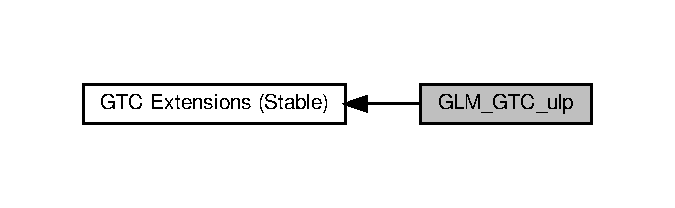
\includegraphics[width=324pt]{group__gtc__ulp}
\end{center}
\end{figure}
\subsection*{Functions}
\begin{DoxyCompactItemize}
\item 
{\footnotesize template$<$typename gen\+Type $>$ }\\\hyperlink{setup_8hpp_ab2d052de21a70539923e9bcbf6e83a51}{G\+L\+M\+\_\+\+F\+U\+N\+C\+\_\+\+D\+E\+CL} gen\+Type \hyperlink{group__gtc__ulp_gae516ae554faa6117660828240e8bdaf0}{glm\+::next\+\_\+float} (gen\+Type const \&x)
\item 
{\footnotesize template$<$typename gen\+Type $>$ }\\\hyperlink{setup_8hpp_ab2d052de21a70539923e9bcbf6e83a51}{G\+L\+M\+\_\+\+F\+U\+N\+C\+\_\+\+D\+E\+CL} gen\+Type \hyperlink{group__gtc__ulp_ga2fcbb7bfbfc595712bfddc51b0715b07}{glm\+::prev\+\_\+float} (gen\+Type const \&x)
\item 
{\footnotesize template$<$typename gen\+Type $>$ }\\\hyperlink{setup_8hpp_ab2d052de21a70539923e9bcbf6e83a51}{G\+L\+M\+\_\+\+F\+U\+N\+C\+\_\+\+D\+E\+CL} gen\+Type \hyperlink{group__gtc__ulp_gad107ec3d9697ef82032a33338a73ebdd}{glm\+::next\+\_\+float} (gen\+Type const \&x, \hyperlink{group__core__precision_ga4fd29415871152bfb5abd588334147c8}{uint} const \&Distance)
\item 
{\footnotesize template$<$typename gen\+Type $>$ }\\\hyperlink{setup_8hpp_ab2d052de21a70539923e9bcbf6e83a51}{G\+L\+M\+\_\+\+F\+U\+N\+C\+\_\+\+D\+E\+CL} gen\+Type \hyperlink{group__gtc__ulp_gaa399d5b6472a70e8952f9b26ecaacdec}{glm\+::prev\+\_\+float} (gen\+Type const \&x, \hyperlink{group__core__precision_ga4fd29415871152bfb5abd588334147c8}{uint} const \&Distance)
\item 
{\footnotesize template$<$typename T $>$ }\\\hyperlink{setup_8hpp_ab2d052de21a70539923e9bcbf6e83a51}{G\+L\+M\+\_\+\+F\+U\+N\+C\+\_\+\+D\+E\+CL} \hyperlink{group__core__precision_ga4fd29415871152bfb5abd588334147c8}{uint} \hyperlink{group__gtc__ulp_ga2e09bd6c8b0a9c91f6f5683d68245634}{glm\+::float\+\_\+distance} (T const \&x, T const \&y)
\item 
{\footnotesize template$<$typename T , template$<$ typename $>$ class vec\+Type$>$ }\\\hyperlink{setup_8hpp_ab2d052de21a70539923e9bcbf6e83a51}{G\+L\+M\+\_\+\+F\+U\+N\+C\+\_\+\+D\+E\+CL} vec\+Type$<$ \hyperlink{group__core__precision_ga4fd29415871152bfb5abd588334147c8}{uint} $>$ \hyperlink{group__gtc__ulp_ga85355f2549d75789eb66e5d565d8ad26}{glm\+::float\+\_\+distance} (vec\+Type$<$ T $>$ const \&x, vec\+Type$<$ T $>$ const \&y)
\end{DoxyCompactItemize}


\subsection{Detailed Description}
Allow the measurement of the accuracy of a function against a reference implementation. This extension works on floating-\/point data and provide results in U\+LP. $<$\hyperlink{gtc_2ulp_8hpp}{glm/gtc/ulp.\+hpp}$>$ need to be included to use these features. 



\subsection{Function Documentation}
\mbox{\Hypertarget{group__gtc__ulp_ga2e09bd6c8b0a9c91f6f5683d68245634}\label{group__gtc__ulp_ga2e09bd6c8b0a9c91f6f5683d68245634}} 
\index{G\+L\+M\+\_\+\+G\+T\+C\+\_\+ulp@{G\+L\+M\+\_\+\+G\+T\+C\+\_\+ulp}!float\+\_\+distance@{float\+\_\+distance}}
\index{float\+\_\+distance@{float\+\_\+distance}!G\+L\+M\+\_\+\+G\+T\+C\+\_\+ulp@{G\+L\+M\+\_\+\+G\+T\+C\+\_\+ulp}}
\subsubsection{\texorpdfstring{float\+\_\+distance()}{float\_distance()}\hspace{0.1cm}{\footnotesize\ttfamily [1/2]}}
{\footnotesize\ttfamily template$<$typename T $>$ \\
\hyperlink{setup_8hpp_ab2d052de21a70539923e9bcbf6e83a51}{G\+L\+M\+\_\+\+F\+U\+N\+C\+\_\+\+D\+E\+CL} \hyperlink{group__core__precision_ga4fd29415871152bfb5abd588334147c8}{uint} glm\+::float\+\_\+distance (\begin{DoxyParamCaption}\item[{T const \&}]{x,  }\item[{T const \&}]{y }\end{DoxyParamCaption})}

Return the distance in the number of U\+LP between 2 scalars. \begin{DoxySeeAlso}{See also}
\hyperlink{group__gtc__ulp}{G\+L\+M\+\_\+\+G\+T\+C\+\_\+ulp} 
\end{DoxySeeAlso}


Definition at line 300 of file ulp.\+inl.

\mbox{\Hypertarget{group__gtc__ulp_ga85355f2549d75789eb66e5d565d8ad26}\label{group__gtc__ulp_ga85355f2549d75789eb66e5d565d8ad26}} 
\index{G\+L\+M\+\_\+\+G\+T\+C\+\_\+ulp@{G\+L\+M\+\_\+\+G\+T\+C\+\_\+ulp}!float\+\_\+distance@{float\+\_\+distance}}
\index{float\+\_\+distance@{float\+\_\+distance}!G\+L\+M\+\_\+\+G\+T\+C\+\_\+ulp@{G\+L\+M\+\_\+\+G\+T\+C\+\_\+ulp}}
\subsubsection{\texorpdfstring{float\+\_\+distance()}{float\_distance()}\hspace{0.1cm}{\footnotesize\ttfamily [2/2]}}
{\footnotesize\ttfamily template$<$typename T , template$<$ typename $>$ class vec\+Type$>$ \\
\hyperlink{setup_8hpp_ab2d052de21a70539923e9bcbf6e83a51}{G\+L\+M\+\_\+\+F\+U\+N\+C\+\_\+\+D\+E\+CL} vec\+Type$<$\hyperlink{group__core__precision_ga4fd29415871152bfb5abd588334147c8}{uint}$>$ glm\+::float\+\_\+distance (\begin{DoxyParamCaption}\item[{vec\+Type$<$ T $>$ const \&}]{x,  }\item[{vec\+Type$<$ T $>$ const \&}]{y }\end{DoxyParamCaption})}

Return the distance in the number of U\+LP between 2 vectors. \begin{DoxySeeAlso}{See also}
\hyperlink{group__gtc__ulp}{G\+L\+M\+\_\+\+G\+T\+C\+\_\+ulp} 
\end{DoxySeeAlso}
\mbox{\Hypertarget{group__gtc__ulp_gae516ae554faa6117660828240e8bdaf0}\label{group__gtc__ulp_gae516ae554faa6117660828240e8bdaf0}} 
\index{G\+L\+M\+\_\+\+G\+T\+C\+\_\+ulp@{G\+L\+M\+\_\+\+G\+T\+C\+\_\+ulp}!next\+\_\+float@{next\+\_\+float}}
\index{next\+\_\+float@{next\+\_\+float}!G\+L\+M\+\_\+\+G\+T\+C\+\_\+ulp@{G\+L\+M\+\_\+\+G\+T\+C\+\_\+ulp}}
\subsubsection{\texorpdfstring{next\+\_\+float()}{next\_float()}\hspace{0.1cm}{\footnotesize\ttfamily [1/2]}}
{\footnotesize\ttfamily template$<$typename gen\+Type $>$ \\
\hyperlink{setup_8hpp_ab2d052de21a70539923e9bcbf6e83a51}{G\+L\+M\+\_\+\+F\+U\+N\+C\+\_\+\+D\+E\+CL} gen\+Type glm\+::next\+\_\+float (\begin{DoxyParamCaption}\item[{gen\+Type const \&}]{x }\end{DoxyParamCaption})}

Return the next U\+LP value(s) after the input value(s). \begin{DoxySeeAlso}{See also}
\hyperlink{group__gtc__ulp}{G\+L\+M\+\_\+\+G\+T\+C\+\_\+ulp} 
\end{DoxySeeAlso}
\mbox{\Hypertarget{group__gtc__ulp_gad107ec3d9697ef82032a33338a73ebdd}\label{group__gtc__ulp_gad107ec3d9697ef82032a33338a73ebdd}} 
\index{G\+L\+M\+\_\+\+G\+T\+C\+\_\+ulp@{G\+L\+M\+\_\+\+G\+T\+C\+\_\+ulp}!next\+\_\+float@{next\+\_\+float}}
\index{next\+\_\+float@{next\+\_\+float}!G\+L\+M\+\_\+\+G\+T\+C\+\_\+ulp@{G\+L\+M\+\_\+\+G\+T\+C\+\_\+ulp}}
\subsubsection{\texorpdfstring{next\+\_\+float()}{next\_float()}\hspace{0.1cm}{\footnotesize\ttfamily [2/2]}}
{\footnotesize\ttfamily template$<$typename gen\+Type $>$ \\
\hyperlink{setup_8hpp_ab2d052de21a70539923e9bcbf6e83a51}{G\+L\+M\+\_\+\+F\+U\+N\+C\+\_\+\+D\+E\+CL} gen\+Type glm\+::next\+\_\+float (\begin{DoxyParamCaption}\item[{gen\+Type const \&}]{x,  }\item[{\hyperlink{group__core__precision_ga4fd29415871152bfb5abd588334147c8}{uint} const \&}]{Distance }\end{DoxyParamCaption})}

Return the value(s) U\+LP distance after the input value(s). \begin{DoxySeeAlso}{See also}
\hyperlink{group__gtc__ulp}{G\+L\+M\+\_\+\+G\+T\+C\+\_\+ulp} 
\end{DoxySeeAlso}
\mbox{\Hypertarget{group__gtc__ulp_ga2fcbb7bfbfc595712bfddc51b0715b07}\label{group__gtc__ulp_ga2fcbb7bfbfc595712bfddc51b0715b07}} 
\index{G\+L\+M\+\_\+\+G\+T\+C\+\_\+ulp@{G\+L\+M\+\_\+\+G\+T\+C\+\_\+ulp}!prev\+\_\+float@{prev\+\_\+float}}
\index{prev\+\_\+float@{prev\+\_\+float}!G\+L\+M\+\_\+\+G\+T\+C\+\_\+ulp@{G\+L\+M\+\_\+\+G\+T\+C\+\_\+ulp}}
\subsubsection{\texorpdfstring{prev\+\_\+float()}{prev\_float()}\hspace{0.1cm}{\footnotesize\ttfamily [1/2]}}
{\footnotesize\ttfamily template$<$typename gen\+Type $>$ \\
\hyperlink{setup_8hpp_ab2d052de21a70539923e9bcbf6e83a51}{G\+L\+M\+\_\+\+F\+U\+N\+C\+\_\+\+D\+E\+CL} gen\+Type glm\+::prev\+\_\+float (\begin{DoxyParamCaption}\item[{gen\+Type const \&}]{x }\end{DoxyParamCaption})}

Return the previous U\+LP value(s) before the input value(s). \begin{DoxySeeAlso}{See also}
\hyperlink{group__gtc__ulp}{G\+L\+M\+\_\+\+G\+T\+C\+\_\+ulp} 
\end{DoxySeeAlso}
\mbox{\Hypertarget{group__gtc__ulp_gaa399d5b6472a70e8952f9b26ecaacdec}\label{group__gtc__ulp_gaa399d5b6472a70e8952f9b26ecaacdec}} 
\index{G\+L\+M\+\_\+\+G\+T\+C\+\_\+ulp@{G\+L\+M\+\_\+\+G\+T\+C\+\_\+ulp}!prev\+\_\+float@{prev\+\_\+float}}
\index{prev\+\_\+float@{prev\+\_\+float}!G\+L\+M\+\_\+\+G\+T\+C\+\_\+ulp@{G\+L\+M\+\_\+\+G\+T\+C\+\_\+ulp}}
\subsubsection{\texorpdfstring{prev\+\_\+float()}{prev\_float()}\hspace{0.1cm}{\footnotesize\ttfamily [2/2]}}
{\footnotesize\ttfamily template$<$typename gen\+Type $>$ \\
\hyperlink{setup_8hpp_ab2d052de21a70539923e9bcbf6e83a51}{G\+L\+M\+\_\+\+F\+U\+N\+C\+\_\+\+D\+E\+CL} gen\+Type glm\+::prev\+\_\+float (\begin{DoxyParamCaption}\item[{gen\+Type const \&}]{x,  }\item[{\hyperlink{group__core__precision_ga4fd29415871152bfb5abd588334147c8}{uint} const \&}]{Distance }\end{DoxyParamCaption})}

Return the value(s) U\+LP distance before the input value(s). \begin{DoxySeeAlso}{See also}
\hyperlink{group__gtc__ulp}{G\+L\+M\+\_\+\+G\+T\+C\+\_\+ulp} 
\end{DoxySeeAlso}

\hypertarget{group__gtx__associated__min__max}{}\section{G\+L\+M\+\_\+\+G\+T\+X\+\_\+associated\+\_\+min\+\_\+max}
\label{group__gtx__associated__min__max}\index{G\+L\+M\+\_\+\+G\+T\+X\+\_\+associated\+\_\+min\+\_\+max@{G\+L\+M\+\_\+\+G\+T\+X\+\_\+associated\+\_\+min\+\_\+max}}


Min and max functions that return associated values not the compared onces. $<$\hyperlink{associated__min__max_8hpp}{glm/gtx/associated\+\_\+min\+\_\+max.\+hpp}$>$ need to be included to use these functionalities.  


Collaboration diagram for G\+L\+M\+\_\+\+G\+T\+X\+\_\+associated\+\_\+min\+\_\+max\+:\nopagebreak
\begin{figure}[H]
\begin{center}
\leavevmode
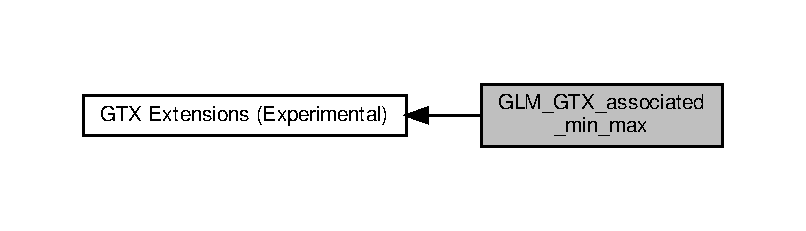
\includegraphics[width=350pt]{group__gtx__associated__min__max}
\end{center}
\end{figure}
\subsection*{Functions}
\begin{DoxyCompactItemize}
\item 
{\footnotesize template$<$typename gen\+TypeT , typename gen\+TypeU $>$ }\\\hyperlink{setup_8hpp_ab2d052de21a70539923e9bcbf6e83a51}{G\+L\+M\+\_\+\+F\+U\+N\+C\+\_\+\+D\+E\+CL} gen\+TypeU \hyperlink{group__gtx__associated__min__max_ga47bdb60409768f3d315bc5a1f739810a}{glm\+::associated\+Min} (const gen\+TypeT \&x, const gen\+TypeU \&a, const gen\+TypeT \&y, const gen\+TypeU \&b)
\item 
{\footnotesize template$<$typename gen\+TypeT , typename gen\+TypeU $>$ }\\\hyperlink{setup_8hpp_ab2d052de21a70539923e9bcbf6e83a51}{G\+L\+M\+\_\+\+F\+U\+N\+C\+\_\+\+D\+E\+CL} gen\+TypeU \hyperlink{group__gtx__associated__min__max_ga3f696c0cce55211f333edb7336cc9cb8}{glm\+::associated\+Min} (const gen\+TypeT \&x, const gen\+TypeU \&a, const gen\+TypeT \&y, const gen\+TypeU \&b, const gen\+TypeT \&z, const gen\+TypeU \&c)
\item 
{\footnotesize template$<$typename gen\+TypeT , typename gen\+TypeU $>$ }\\\hyperlink{setup_8hpp_ab2d052de21a70539923e9bcbf6e83a51}{G\+L\+M\+\_\+\+F\+U\+N\+C\+\_\+\+D\+E\+CL} gen\+TypeU \hyperlink{group__gtx__associated__min__max_ga45618e13844d00046a0fe3409ae7513e}{glm\+::associated\+Min} (const gen\+TypeT \&x, const gen\+TypeU \&a, const gen\+TypeT \&y, const gen\+TypeU \&b, const gen\+TypeT \&z, const gen\+TypeU \&c, const gen\+TypeT \&w, const gen\+TypeU \&d)
\item 
{\footnotesize template$<$typename gen\+TypeT , typename gen\+TypeU $>$ }\\\hyperlink{setup_8hpp_ab2d052de21a70539923e9bcbf6e83a51}{G\+L\+M\+\_\+\+F\+U\+N\+C\+\_\+\+D\+E\+CL} gen\+TypeU \hyperlink{group__gtx__associated__min__max_gaee554495240b93d80492b3d2312ede1d}{glm\+::associated\+Max} (const gen\+TypeT \&x, const gen\+TypeU \&a, const gen\+TypeT \&y, const gen\+TypeU \&b)
\item 
{\footnotesize template$<$typename gen\+TypeT , typename gen\+TypeU $>$ }\\\hyperlink{setup_8hpp_ab2d052de21a70539923e9bcbf6e83a51}{G\+L\+M\+\_\+\+F\+U\+N\+C\+\_\+\+D\+E\+CL} gen\+TypeU \hyperlink{group__gtx__associated__min__max_ga20218dcc769c76adf0c3e9aad21c64a4}{glm\+::associated\+Max} (const gen\+TypeT \&x, const gen\+TypeU \&a, const gen\+TypeT \&y, const gen\+TypeU \&b, const gen\+TypeT \&z, const gen\+TypeU \&c)
\item 
{\footnotesize template$<$typename gen\+TypeT , typename gen\+TypeU $>$ }\\\hyperlink{setup_8hpp_ab2d052de21a70539923e9bcbf6e83a51}{G\+L\+M\+\_\+\+F\+U\+N\+C\+\_\+\+D\+E\+CL} gen\+TypeU \hyperlink{group__gtx__associated__min__max_ga23f2bce9c1d6f775cd1f7bf36525286e}{glm\+::associated\+Max} (const gen\+TypeT \&x, const gen\+TypeU \&a, const gen\+TypeT \&y, const gen\+TypeU \&b, const gen\+TypeT \&z, const gen\+TypeU \&c, const gen\+TypeT \&w, const gen\+TypeU \&d)
\end{DoxyCompactItemize}


\subsection{Detailed Description}
Min and max functions that return associated values not the compared onces. $<$\hyperlink{associated__min__max_8hpp}{glm/gtx/associated\+\_\+min\+\_\+max.\+hpp}$>$ need to be included to use these functionalities. 



\subsection{Function Documentation}
\mbox{\Hypertarget{group__gtx__associated__min__max_gaee554495240b93d80492b3d2312ede1d}\label{group__gtx__associated__min__max_gaee554495240b93d80492b3d2312ede1d}} 
\index{G\+L\+M\+\_\+\+G\+T\+X\+\_\+associated\+\_\+min\+\_\+max@{G\+L\+M\+\_\+\+G\+T\+X\+\_\+associated\+\_\+min\+\_\+max}!associated\+Max@{associated\+Max}}
\index{associated\+Max@{associated\+Max}!G\+L\+M\+\_\+\+G\+T\+X\+\_\+associated\+\_\+min\+\_\+max@{G\+L\+M\+\_\+\+G\+T\+X\+\_\+associated\+\_\+min\+\_\+max}}
\subsubsection{\texorpdfstring{associated\+Max()}{associatedMax()}\hspace{0.1cm}{\footnotesize\ttfamily [1/3]}}
{\footnotesize\ttfamily template$<$typename gen\+TypeT , typename gen\+TypeU $>$ \\
\hyperlink{setup_8hpp_ab2d052de21a70539923e9bcbf6e83a51}{G\+L\+M\+\_\+\+F\+U\+N\+C\+\_\+\+D\+E\+CL} gen\+TypeU glm\+::associated\+Max (\begin{DoxyParamCaption}\item[{const gen\+TypeT \&}]{x,  }\item[{const gen\+TypeU \&}]{a,  }\item[{const gen\+TypeT \&}]{y,  }\item[{const gen\+TypeU \&}]{b }\end{DoxyParamCaption})}

Max comparison between 2 variables \begin{DoxySeeAlso}{See also}
\hyperlink{group__gtx__associated__min__max}{G\+L\+M\+\_\+\+G\+T\+X\+\_\+associated\+\_\+min\+\_\+max} 
\end{DoxySeeAlso}
\mbox{\Hypertarget{group__gtx__associated__min__max_ga20218dcc769c76adf0c3e9aad21c64a4}\label{group__gtx__associated__min__max_ga20218dcc769c76adf0c3e9aad21c64a4}} 
\index{G\+L\+M\+\_\+\+G\+T\+X\+\_\+associated\+\_\+min\+\_\+max@{G\+L\+M\+\_\+\+G\+T\+X\+\_\+associated\+\_\+min\+\_\+max}!associated\+Max@{associated\+Max}}
\index{associated\+Max@{associated\+Max}!G\+L\+M\+\_\+\+G\+T\+X\+\_\+associated\+\_\+min\+\_\+max@{G\+L\+M\+\_\+\+G\+T\+X\+\_\+associated\+\_\+min\+\_\+max}}
\subsubsection{\texorpdfstring{associated\+Max()}{associatedMax()}\hspace{0.1cm}{\footnotesize\ttfamily [2/3]}}
{\footnotesize\ttfamily template$<$typename gen\+TypeT , typename gen\+TypeU $>$ \\
\hyperlink{setup_8hpp_ab2d052de21a70539923e9bcbf6e83a51}{G\+L\+M\+\_\+\+F\+U\+N\+C\+\_\+\+D\+E\+CL} gen\+TypeU glm\+::associated\+Max (\begin{DoxyParamCaption}\item[{const gen\+TypeT \&}]{x,  }\item[{const gen\+TypeU \&}]{a,  }\item[{const gen\+TypeT \&}]{y,  }\item[{const gen\+TypeU \&}]{b,  }\item[{const gen\+TypeT \&}]{z,  }\item[{const gen\+TypeU \&}]{c }\end{DoxyParamCaption})}

Max comparison between 3 variables \begin{DoxySeeAlso}{See also}
\hyperlink{group__gtx__associated__min__max}{G\+L\+M\+\_\+\+G\+T\+X\+\_\+associated\+\_\+min\+\_\+max} 
\end{DoxySeeAlso}
\mbox{\Hypertarget{group__gtx__associated__min__max_ga23f2bce9c1d6f775cd1f7bf36525286e}\label{group__gtx__associated__min__max_ga23f2bce9c1d6f775cd1f7bf36525286e}} 
\index{G\+L\+M\+\_\+\+G\+T\+X\+\_\+associated\+\_\+min\+\_\+max@{G\+L\+M\+\_\+\+G\+T\+X\+\_\+associated\+\_\+min\+\_\+max}!associated\+Max@{associated\+Max}}
\index{associated\+Max@{associated\+Max}!G\+L\+M\+\_\+\+G\+T\+X\+\_\+associated\+\_\+min\+\_\+max@{G\+L\+M\+\_\+\+G\+T\+X\+\_\+associated\+\_\+min\+\_\+max}}
\subsubsection{\texorpdfstring{associated\+Max()}{associatedMax()}\hspace{0.1cm}{\footnotesize\ttfamily [3/3]}}
{\footnotesize\ttfamily template$<$typename gen\+TypeT , typename gen\+TypeU $>$ \\
\hyperlink{setup_8hpp_ab2d052de21a70539923e9bcbf6e83a51}{G\+L\+M\+\_\+\+F\+U\+N\+C\+\_\+\+D\+E\+CL} gen\+TypeU glm\+::associated\+Max (\begin{DoxyParamCaption}\item[{const gen\+TypeT \&}]{x,  }\item[{const gen\+TypeU \&}]{a,  }\item[{const gen\+TypeT \&}]{y,  }\item[{const gen\+TypeU \&}]{b,  }\item[{const gen\+TypeT \&}]{z,  }\item[{const gen\+TypeU \&}]{c,  }\item[{const gen\+TypeT \&}]{w,  }\item[{const gen\+TypeU \&}]{d }\end{DoxyParamCaption})}

Max comparison between 4 variables \begin{DoxySeeAlso}{See also}
\hyperlink{group__gtx__associated__min__max}{G\+L\+M\+\_\+\+G\+T\+X\+\_\+associated\+\_\+min\+\_\+max} 
\end{DoxySeeAlso}
\mbox{\Hypertarget{group__gtx__associated__min__max_ga47bdb60409768f3d315bc5a1f739810a}\label{group__gtx__associated__min__max_ga47bdb60409768f3d315bc5a1f739810a}} 
\index{G\+L\+M\+\_\+\+G\+T\+X\+\_\+associated\+\_\+min\+\_\+max@{G\+L\+M\+\_\+\+G\+T\+X\+\_\+associated\+\_\+min\+\_\+max}!associated\+Min@{associated\+Min}}
\index{associated\+Min@{associated\+Min}!G\+L\+M\+\_\+\+G\+T\+X\+\_\+associated\+\_\+min\+\_\+max@{G\+L\+M\+\_\+\+G\+T\+X\+\_\+associated\+\_\+min\+\_\+max}}
\subsubsection{\texorpdfstring{associated\+Min()}{associatedMin()}\hspace{0.1cm}{\footnotesize\ttfamily [1/3]}}
{\footnotesize\ttfamily template$<$typename gen\+TypeT , typename gen\+TypeU $>$ \\
\hyperlink{setup_8hpp_ab2d052de21a70539923e9bcbf6e83a51}{G\+L\+M\+\_\+\+F\+U\+N\+C\+\_\+\+D\+E\+CL} gen\+TypeU glm\+::associated\+Min (\begin{DoxyParamCaption}\item[{const gen\+TypeT \&}]{x,  }\item[{const gen\+TypeU \&}]{a,  }\item[{const gen\+TypeT \&}]{y,  }\item[{const gen\+TypeU \&}]{b }\end{DoxyParamCaption})}

Min comparison between 2 variables \begin{DoxySeeAlso}{See also}
\hyperlink{group__gtx__associated__min__max}{G\+L\+M\+\_\+\+G\+T\+X\+\_\+associated\+\_\+min\+\_\+max} 
\end{DoxySeeAlso}
\mbox{\Hypertarget{group__gtx__associated__min__max_ga3f696c0cce55211f333edb7336cc9cb8}\label{group__gtx__associated__min__max_ga3f696c0cce55211f333edb7336cc9cb8}} 
\index{G\+L\+M\+\_\+\+G\+T\+X\+\_\+associated\+\_\+min\+\_\+max@{G\+L\+M\+\_\+\+G\+T\+X\+\_\+associated\+\_\+min\+\_\+max}!associated\+Min@{associated\+Min}}
\index{associated\+Min@{associated\+Min}!G\+L\+M\+\_\+\+G\+T\+X\+\_\+associated\+\_\+min\+\_\+max@{G\+L\+M\+\_\+\+G\+T\+X\+\_\+associated\+\_\+min\+\_\+max}}
\subsubsection{\texorpdfstring{associated\+Min()}{associatedMin()}\hspace{0.1cm}{\footnotesize\ttfamily [2/3]}}
{\footnotesize\ttfamily template$<$typename gen\+TypeT , typename gen\+TypeU $>$ \\
\hyperlink{setup_8hpp_ab2d052de21a70539923e9bcbf6e83a51}{G\+L\+M\+\_\+\+F\+U\+N\+C\+\_\+\+D\+E\+CL} gen\+TypeU glm\+::associated\+Min (\begin{DoxyParamCaption}\item[{const gen\+TypeT \&}]{x,  }\item[{const gen\+TypeU \&}]{a,  }\item[{const gen\+TypeT \&}]{y,  }\item[{const gen\+TypeU \&}]{b,  }\item[{const gen\+TypeT \&}]{z,  }\item[{const gen\+TypeU \&}]{c }\end{DoxyParamCaption})}

Min comparison between 3 variables \begin{DoxySeeAlso}{See also}
\hyperlink{group__gtx__associated__min__max}{G\+L\+M\+\_\+\+G\+T\+X\+\_\+associated\+\_\+min\+\_\+max} 
\end{DoxySeeAlso}
\mbox{\Hypertarget{group__gtx__associated__min__max_ga45618e13844d00046a0fe3409ae7513e}\label{group__gtx__associated__min__max_ga45618e13844d00046a0fe3409ae7513e}} 
\index{G\+L\+M\+\_\+\+G\+T\+X\+\_\+associated\+\_\+min\+\_\+max@{G\+L\+M\+\_\+\+G\+T\+X\+\_\+associated\+\_\+min\+\_\+max}!associated\+Min@{associated\+Min}}
\index{associated\+Min@{associated\+Min}!G\+L\+M\+\_\+\+G\+T\+X\+\_\+associated\+\_\+min\+\_\+max@{G\+L\+M\+\_\+\+G\+T\+X\+\_\+associated\+\_\+min\+\_\+max}}
\subsubsection{\texorpdfstring{associated\+Min()}{associatedMin()}\hspace{0.1cm}{\footnotesize\ttfamily [3/3]}}
{\footnotesize\ttfamily template$<$typename gen\+TypeT , typename gen\+TypeU $>$ \\
\hyperlink{setup_8hpp_ab2d052de21a70539923e9bcbf6e83a51}{G\+L\+M\+\_\+\+F\+U\+N\+C\+\_\+\+D\+E\+CL} gen\+TypeU glm\+::associated\+Min (\begin{DoxyParamCaption}\item[{const gen\+TypeT \&}]{x,  }\item[{const gen\+TypeU \&}]{a,  }\item[{const gen\+TypeT \&}]{y,  }\item[{const gen\+TypeU \&}]{b,  }\item[{const gen\+TypeT \&}]{z,  }\item[{const gen\+TypeU \&}]{c,  }\item[{const gen\+TypeT \&}]{w,  }\item[{const gen\+TypeU \&}]{d }\end{DoxyParamCaption})}

Min comparison between 4 variables \begin{DoxySeeAlso}{See also}
\hyperlink{group__gtx__associated__min__max}{G\+L\+M\+\_\+\+G\+T\+X\+\_\+associated\+\_\+min\+\_\+max} 
\end{DoxySeeAlso}

\hypertarget{group__gtx__bit}{}\section{G\+L\+M\+\_\+\+G\+T\+X\+\_\+bit}
\label{group__gtx__bit}\index{G\+L\+M\+\_\+\+G\+T\+X\+\_\+bit@{G\+L\+M\+\_\+\+G\+T\+X\+\_\+bit}}


Allow to perform bit operations on integer values.  


Collaboration diagram for G\+L\+M\+\_\+\+G\+T\+X\+\_\+bit\+:\nopagebreak
\begin{figure}[H]
\begin{center}
\leavevmode
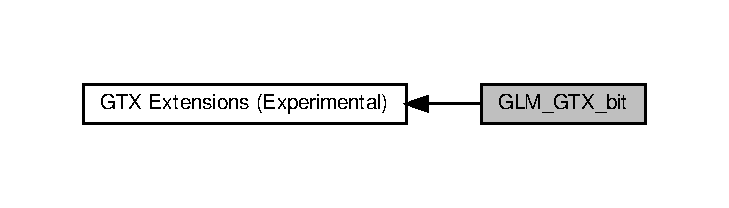
\includegraphics[width=350pt]{group__gtx__bit}
\end{center}
\end{figure}
\subsection*{Functions}
\begin{DoxyCompactItemize}
\item 
{\footnotesize template$<$typename gen\+I\+Type $>$ }\\\hyperlink{setup_8hpp_ab2d052de21a70539923e9bcbf6e83a51}{G\+L\+M\+\_\+\+F\+U\+N\+C\+\_\+\+D\+E\+CL} gen\+I\+Type \hyperlink{group__gtx__bit_ga79f1482a09c91f785e7e0ea8aed2b20e}{glm\+::mask} (gen\+I\+Type const \&count)
\item 
{\footnotesize template$<$typename gen\+Type $>$ }\\\hyperlink{setup_8hpp_ab2d052de21a70539923e9bcbf6e83a51}{G\+L\+M\+\_\+\+F\+U\+N\+C\+\_\+\+D\+E\+CL} gen\+Type \hyperlink{group__gtx__bit_ga9621840252c293918780bc3890374b86}{glm\+::highest\+Bit\+Value} (gen\+Type const \&value)
\item 
{\footnotesize template$<$typename gen\+Type $>$ }\\\hyperlink{setup_8hpp_ab2d052de21a70539923e9bcbf6e83a51}{G\+L\+M\+\_\+\+F\+U\+N\+C\+\_\+\+D\+E\+CL} bool \hyperlink{group__gtx__bit_ga5ddca7546d8be35992eedd3411842545}{glm\+::is\+Power\+Of\+Two} (gen\+Type const \&value)
\item 
{\footnotesize template$<$typename gen\+Type $>$ }\\\hyperlink{setup_8hpp_ab2d052de21a70539923e9bcbf6e83a51}{G\+L\+M\+\_\+\+F\+U\+N\+C\+\_\+\+D\+E\+CL} gen\+Type \hyperlink{group__gtx__bit_gaa49786cf3f8a1f65de6e70b6088a811e}{glm\+::power\+Of\+Two\+Above} (gen\+Type const \&value)
\item 
{\footnotesize template$<$typename gen\+Type $>$ }\\\hyperlink{setup_8hpp_ab2d052de21a70539923e9bcbf6e83a51}{G\+L\+M\+\_\+\+F\+U\+N\+C\+\_\+\+D\+E\+CL} gen\+Type \hyperlink{group__gtx__bit_gaeceaea338213cbff7a275460e35e8d0c}{glm\+::power\+Of\+Two\+Below} (gen\+Type const \&value)
\item 
{\footnotesize template$<$typename gen\+Type $>$ }\\\hyperlink{setup_8hpp_ab2d052de21a70539923e9bcbf6e83a51}{G\+L\+M\+\_\+\+F\+U\+N\+C\+\_\+\+D\+E\+CL} gen\+Type \hyperlink{group__gtx__bit_ga9e68299f4ca0cd6674efbee62d425b95}{glm\+::power\+Of\+Two\+Nearest} (gen\+Type const \&value)
\item 
{\footnotesize template$<$typename gen\+Type $>$ }\\\hyperlink{setup_8hpp_a8edfb48cdc249a3ee48406bf179023dc}{G\+L\+M\+\_\+\+D\+E\+P\+R\+E\+C\+A\+T\+ED} \hyperlink{setup_8hpp_ab2d052de21a70539923e9bcbf6e83a51}{G\+L\+M\+\_\+\+F\+U\+N\+C\+\_\+\+D\+E\+CL} gen\+Type \hyperlink{group__gtx__bit_ga2d3939fbf96aa54cb2fd3461a60aba02}{glm\+::bit\+Revert} (gen\+Type const \&value)
\item 
{\footnotesize template$<$typename gen\+Type $>$ }\\\hyperlink{setup_8hpp_ab2d052de21a70539923e9bcbf6e83a51}{G\+L\+M\+\_\+\+F\+U\+N\+C\+\_\+\+D\+E\+CL} gen\+Type \hyperlink{group__gtx__bit_gaf999dbfe97a5be5ea68841a58cf89a4a}{glm\+::bit\+Rotate\+Right} (gen\+Type const \&In, std\+::size\+\_\+t Shift)
\item 
{\footnotesize template$<$typename gen\+Type $>$ }\\\hyperlink{setup_8hpp_ab2d052de21a70539923e9bcbf6e83a51}{G\+L\+M\+\_\+\+F\+U\+N\+C\+\_\+\+D\+E\+CL} gen\+Type \hyperlink{group__gtx__bit_ga32c0a5149152a9aa75afafe81b19be53}{glm\+::bit\+Rotate\+Left} (gen\+Type const \&In, std\+::size\+\_\+t Shift)
\item 
{\footnotesize template$<$typename gen\+I\+U\+Type $>$ }\\\hyperlink{setup_8hpp_ab2d052de21a70539923e9bcbf6e83a51}{G\+L\+M\+\_\+\+F\+U\+N\+C\+\_\+\+D\+E\+CL} gen\+I\+U\+Type \hyperlink{group__gtx__bit_gafac2a9e0ef0d5d2fc4e569bff2b2f452}{glm\+::fill\+Bitfield\+With\+One} (gen\+I\+U\+Type const \&Value, int const \&From\+Bit, int const \&To\+Bit)
\item 
{\footnotesize template$<$typename gen\+I\+U\+Type $>$ }\\\hyperlink{setup_8hpp_ab2d052de21a70539923e9bcbf6e83a51}{G\+L\+M\+\_\+\+F\+U\+N\+C\+\_\+\+D\+E\+CL} gen\+I\+U\+Type \hyperlink{group__gtx__bit_ga0c514d45387003260783ba6a8a4f3285}{glm\+::fill\+Bitfield\+With\+Zero} (gen\+I\+U\+Type const \&Value, int const \&From\+Bit, int const \&To\+Bit)
\item 
\hyperlink{setup_8hpp_ab2d052de21a70539923e9bcbf6e83a51}{G\+L\+M\+\_\+\+F\+U\+N\+C\+\_\+\+D\+E\+CL} \hyperlink{group__gtc__type__precision_ga2945a61d12771f8954994fcddf02b021}{int16} \hyperlink{group__gtx__bit_ga479134317bc95d99f2b2e235d3db287b}{glm\+::bitfield\+Interleave} (\hyperlink{group__gtc__type__precision_ga96254f9c1c4506fc8eb5cf3301ce8565}{int8} x, \hyperlink{group__gtc__type__precision_ga96254f9c1c4506fc8eb5cf3301ce8565}{int8} y)
\item 
\hyperlink{setup_8hpp_ab2d052de21a70539923e9bcbf6e83a51}{G\+L\+M\+\_\+\+F\+U\+N\+C\+\_\+\+D\+E\+CL} \hyperlink{group__gtc__type__precision_gad8c2939e1fdd8e5828b31d95c52255d5}{uint16} \hyperlink{group__gtx__bit_ga0700a3ceb088a0ecc23d76c154096061}{glm\+::bitfield\+Interleave} (\hyperlink{group__gtc__type__precision_ga1a7dcd8aac97cc8020817c94049deff2}{uint8} x, \hyperlink{group__gtc__type__precision_ga1a7dcd8aac97cc8020817c94049deff2}{uint8} y)
\item 
\hyperlink{setup_8hpp_ab2d052de21a70539923e9bcbf6e83a51}{G\+L\+M\+\_\+\+F\+U\+N\+C\+\_\+\+D\+E\+CL} \hyperlink{group__gtc__type__precision_ga632d8b25f6b61659f39ea4321fab92a4}{int32} \hyperlink{group__gtx__bit_ga1a0264598647ae00a596865af4e1e878}{glm\+::bitfield\+Interleave} (\hyperlink{group__gtc__type__precision_ga2945a61d12771f8954994fcddf02b021}{int16} x, \hyperlink{group__gtc__type__precision_ga2945a61d12771f8954994fcddf02b021}{int16} y)
\item 
\hyperlink{setup_8hpp_ab2d052de21a70539923e9bcbf6e83a51}{G\+L\+M\+\_\+\+F\+U\+N\+C\+\_\+\+D\+E\+CL} \hyperlink{group__gtc__type__precision_ga202b6a53c105fcb7e531f9b443518451}{uint32} \hyperlink{group__gtx__bit_ga19ef8360379483e3ee245e89cb62ff93}{glm\+::bitfield\+Interleave} (\hyperlink{group__gtc__type__precision_gad8c2939e1fdd8e5828b31d95c52255d5}{uint16} x, \hyperlink{group__gtc__type__precision_gad8c2939e1fdd8e5828b31d95c52255d5}{uint16} y)
\item 
\hyperlink{setup_8hpp_ab2d052de21a70539923e9bcbf6e83a51}{G\+L\+M\+\_\+\+F\+U\+N\+C\+\_\+\+D\+E\+CL} \hyperlink{group__gtc__type__precision_ga435d75819cce297cc5fa21bd84ef89a5}{int64} \hyperlink{group__gtx__bit_ga0de51d5985e6a703f305a5a61479babd}{glm\+::bitfield\+Interleave} (\hyperlink{group__gtc__type__precision_ga632d8b25f6b61659f39ea4321fab92a4}{int32} x, \hyperlink{group__gtc__type__precision_ga632d8b25f6b61659f39ea4321fab92a4}{int32} y)
\item 
\hyperlink{setup_8hpp_ab2d052de21a70539923e9bcbf6e83a51}{G\+L\+M\+\_\+\+F\+U\+N\+C\+\_\+\+D\+E\+CL} \hyperlink{group__gtc__type__precision_gae3632bf9b37da66233d78930dd06378a}{uint64} \hyperlink{group__gtx__bit_ga2bc87fd66f6f8471c1a46888360cef12}{glm\+::bitfield\+Interleave} (\hyperlink{group__gtc__type__precision_ga202b6a53c105fcb7e531f9b443518451}{uint32} x, \hyperlink{group__gtc__type__precision_ga202b6a53c105fcb7e531f9b443518451}{uint32} y)
\item 
\hyperlink{setup_8hpp_ab2d052de21a70539923e9bcbf6e83a51}{G\+L\+M\+\_\+\+F\+U\+N\+C\+\_\+\+D\+E\+CL} \hyperlink{group__gtc__type__precision_ga632d8b25f6b61659f39ea4321fab92a4}{int32} \hyperlink{group__gtx__bit_ga6dee2ce1c45805063bb7fc5f6fd8f5ca}{glm\+::bitfield\+Interleave} (\hyperlink{group__gtc__type__precision_ga96254f9c1c4506fc8eb5cf3301ce8565}{int8} x, \hyperlink{group__gtc__type__precision_ga96254f9c1c4506fc8eb5cf3301ce8565}{int8} y, \hyperlink{group__gtc__type__precision_ga96254f9c1c4506fc8eb5cf3301ce8565}{int8} z)
\item 
\hyperlink{setup_8hpp_ab2d052de21a70539923e9bcbf6e83a51}{G\+L\+M\+\_\+\+F\+U\+N\+C\+\_\+\+D\+E\+CL} \hyperlink{group__gtc__type__precision_ga202b6a53c105fcb7e531f9b443518451}{uint32} \hyperlink{group__gtx__bit_gab9d593a2e916beb8f8137a0dbeae3afe}{glm\+::bitfield\+Interleave} (\hyperlink{group__gtc__type__precision_ga1a7dcd8aac97cc8020817c94049deff2}{uint8} x, \hyperlink{group__gtc__type__precision_ga1a7dcd8aac97cc8020817c94049deff2}{uint8} y, \hyperlink{group__gtc__type__precision_ga1a7dcd8aac97cc8020817c94049deff2}{uint8} z)
\item 
\hyperlink{setup_8hpp_ab2d052de21a70539923e9bcbf6e83a51}{G\+L\+M\+\_\+\+F\+U\+N\+C\+\_\+\+D\+E\+CL} \hyperlink{group__gtc__type__precision_ga435d75819cce297cc5fa21bd84ef89a5}{int64} \hyperlink{group__gtx__bit_gaf898f842ac089fcc8d6201c32702584a}{glm\+::bitfield\+Interleave} (\hyperlink{group__gtc__type__precision_ga2945a61d12771f8954994fcddf02b021}{int16} x, \hyperlink{group__gtc__type__precision_ga2945a61d12771f8954994fcddf02b021}{int16} y, \hyperlink{group__gtc__type__precision_ga2945a61d12771f8954994fcddf02b021}{int16} z)
\item 
\hyperlink{setup_8hpp_ab2d052de21a70539923e9bcbf6e83a51}{G\+L\+M\+\_\+\+F\+U\+N\+C\+\_\+\+D\+E\+CL} \hyperlink{group__gtc__type__precision_gae3632bf9b37da66233d78930dd06378a}{uint64} \hyperlink{group__gtx__bit_ga3c170e2ec54f2faab5e1c5bb693d718d}{glm\+::bitfield\+Interleave} (\hyperlink{group__gtc__type__precision_gad8c2939e1fdd8e5828b31d95c52255d5}{uint16} x, \hyperlink{group__gtc__type__precision_gad8c2939e1fdd8e5828b31d95c52255d5}{uint16} y, \hyperlink{group__gtc__type__precision_gad8c2939e1fdd8e5828b31d95c52255d5}{uint16} z)
\item 
\hyperlink{setup_8hpp_ab2d052de21a70539923e9bcbf6e83a51}{G\+L\+M\+\_\+\+F\+U\+N\+C\+\_\+\+D\+E\+CL} \hyperlink{group__gtc__type__precision_ga435d75819cce297cc5fa21bd84ef89a5}{int64} \hyperlink{group__gtx__bit_ga64e2d84f6560af3cc639644b1e628c42}{glm\+::bitfield\+Interleave} (\hyperlink{group__gtc__type__precision_ga632d8b25f6b61659f39ea4321fab92a4}{int32} x, \hyperlink{group__gtc__type__precision_ga632d8b25f6b61659f39ea4321fab92a4}{int32} y, \hyperlink{group__gtc__type__precision_ga632d8b25f6b61659f39ea4321fab92a4}{int32} z)
\item 
\hyperlink{setup_8hpp_ab2d052de21a70539923e9bcbf6e83a51}{G\+L\+M\+\_\+\+F\+U\+N\+C\+\_\+\+D\+E\+CL} \hyperlink{group__gtc__type__precision_gae3632bf9b37da66233d78930dd06378a}{uint64} \hyperlink{group__gtx__bit_ga7c10eb37f608365cfaef5ca2c476e1ce}{glm\+::bitfield\+Interleave} (\hyperlink{group__gtc__type__precision_ga202b6a53c105fcb7e531f9b443518451}{uint32} x, \hyperlink{group__gtc__type__precision_ga202b6a53c105fcb7e531f9b443518451}{uint32} y, \hyperlink{group__gtc__type__precision_ga202b6a53c105fcb7e531f9b443518451}{uint32} z)
\item 
\hyperlink{setup_8hpp_ab2d052de21a70539923e9bcbf6e83a51}{G\+L\+M\+\_\+\+F\+U\+N\+C\+\_\+\+D\+E\+CL} \hyperlink{group__gtc__type__precision_ga632d8b25f6b61659f39ea4321fab92a4}{int32} \hyperlink{group__gtx__bit_ga7da84ecc2b3a46c9c08a9f40012359cf}{glm\+::bitfield\+Interleave} (\hyperlink{group__gtc__type__precision_ga96254f9c1c4506fc8eb5cf3301ce8565}{int8} x, \hyperlink{group__gtc__type__precision_ga96254f9c1c4506fc8eb5cf3301ce8565}{int8} y, \hyperlink{group__gtc__type__precision_ga96254f9c1c4506fc8eb5cf3301ce8565}{int8} z, \hyperlink{group__gtc__type__precision_ga96254f9c1c4506fc8eb5cf3301ce8565}{int8} w)
\item 
\hyperlink{setup_8hpp_ab2d052de21a70539923e9bcbf6e83a51}{G\+L\+M\+\_\+\+F\+U\+N\+C\+\_\+\+D\+E\+CL} \hyperlink{group__gtc__type__precision_ga202b6a53c105fcb7e531f9b443518451}{uint32} \hyperlink{group__gtx__bit_ga447c0bbed9d60c14578626d8f03f3755}{glm\+::bitfield\+Interleave} (\hyperlink{group__gtc__type__precision_ga1a7dcd8aac97cc8020817c94049deff2}{uint8} x, \hyperlink{group__gtc__type__precision_ga1a7dcd8aac97cc8020817c94049deff2}{uint8} y, \hyperlink{group__gtc__type__precision_ga1a7dcd8aac97cc8020817c94049deff2}{uint8} z, \hyperlink{group__gtc__type__precision_ga1a7dcd8aac97cc8020817c94049deff2}{uint8} w)
\item 
\hyperlink{setup_8hpp_ab2d052de21a70539923e9bcbf6e83a51}{G\+L\+M\+\_\+\+F\+U\+N\+C\+\_\+\+D\+E\+CL} \hyperlink{group__gtc__type__precision_ga435d75819cce297cc5fa21bd84ef89a5}{int64} \hyperlink{group__gtx__bit_ga09ee0be0fac790a1607a711e597dd9bf}{glm\+::bitfield\+Interleave} (\hyperlink{group__gtc__type__precision_ga2945a61d12771f8954994fcddf02b021}{int16} x, \hyperlink{group__gtc__type__precision_ga2945a61d12771f8954994fcddf02b021}{int16} y, \hyperlink{group__gtc__type__precision_ga2945a61d12771f8954994fcddf02b021}{int16} z, \hyperlink{group__gtc__type__precision_ga2945a61d12771f8954994fcddf02b021}{int16} w)
\item 
\hyperlink{setup_8hpp_ab2d052de21a70539923e9bcbf6e83a51}{G\+L\+M\+\_\+\+F\+U\+N\+C\+\_\+\+D\+E\+CL} \hyperlink{group__gtc__type__precision_gae3632bf9b37da66233d78930dd06378a}{uint64} \hyperlink{group__gtx__bit_gac8a926a7bfd9b23c22a4f685193fbfe1}{glm\+::bitfield\+Interleave} (\hyperlink{group__gtc__type__precision_gad8c2939e1fdd8e5828b31d95c52255d5}{uint16} x, \hyperlink{group__gtc__type__precision_gad8c2939e1fdd8e5828b31d95c52255d5}{uint16} y, \hyperlink{group__gtc__type__precision_gad8c2939e1fdd8e5828b31d95c52255d5}{uint16} z, \hyperlink{group__gtc__type__precision_gad8c2939e1fdd8e5828b31d95c52255d5}{uint16} w)
\end{DoxyCompactItemize}


\subsection{Detailed Description}
Allow to perform bit operations on integer values. 

$<$\hyperlink{bit_8hpp}{glm/gtx/bit.\+hpp}$>$ need to be included to use these functionalities. 

\subsection{Function Documentation}
\mbox{\Hypertarget{group__gtx__bit_ga479134317bc95d99f2b2e235d3db287b}\label{group__gtx__bit_ga479134317bc95d99f2b2e235d3db287b}} 
\index{G\+L\+M\+\_\+\+G\+T\+X\+\_\+bit@{G\+L\+M\+\_\+\+G\+T\+X\+\_\+bit}!bitfield\+Interleave@{bitfield\+Interleave}}
\index{bitfield\+Interleave@{bitfield\+Interleave}!G\+L\+M\+\_\+\+G\+T\+X\+\_\+bit@{G\+L\+M\+\_\+\+G\+T\+X\+\_\+bit}}
\subsubsection{\texorpdfstring{bitfield\+Interleave()}{bitfieldInterleave()}\hspace{0.1cm}{\footnotesize\ttfamily [1/16]}}
{\footnotesize\ttfamily \hyperlink{setup_8hpp_a33fdea6f91c5f834105f7415e2a64407}{G\+L\+M\+\_\+\+F\+U\+N\+C\+\_\+\+Q\+U\+A\+L\+I\+F\+I\+ER} \hyperlink{group__gtc__type__precision_ga2945a61d12771f8954994fcddf02b021}{int16} glm\+::bitfield\+Interleave (\begin{DoxyParamCaption}\item[{\hyperlink{group__gtc__type__precision_ga96254f9c1c4506fc8eb5cf3301ce8565}{int8}}]{x,  }\item[{\hyperlink{group__gtc__type__precision_ga96254f9c1c4506fc8eb5cf3301ce8565}{int8}}]{y }\end{DoxyParamCaption})}

Interleaves the bits of x and y. The first bit is the first bit of x followed by the first bit of y. The other bits are interleaved following the previous sequence.

\begin{DoxySeeAlso}{See also}
\hyperlink{group__gtx__bit}{G\+L\+M\+\_\+\+G\+T\+X\+\_\+bit} 
\end{DoxySeeAlso}


Definition at line 567 of file bit.\+inl.

\mbox{\Hypertarget{group__gtx__bit_ga0700a3ceb088a0ecc23d76c154096061}\label{group__gtx__bit_ga0700a3ceb088a0ecc23d76c154096061}} 
\index{G\+L\+M\+\_\+\+G\+T\+X\+\_\+bit@{G\+L\+M\+\_\+\+G\+T\+X\+\_\+bit}!bitfield\+Interleave@{bitfield\+Interleave}}
\index{bitfield\+Interleave@{bitfield\+Interleave}!G\+L\+M\+\_\+\+G\+T\+X\+\_\+bit@{G\+L\+M\+\_\+\+G\+T\+X\+\_\+bit}}
\subsubsection{\texorpdfstring{bitfield\+Interleave()}{bitfieldInterleave()}\hspace{0.1cm}{\footnotesize\ttfamily [2/16]}}
{\footnotesize\ttfamily \hyperlink{setup_8hpp_a33fdea6f91c5f834105f7415e2a64407}{G\+L\+M\+\_\+\+F\+U\+N\+C\+\_\+\+Q\+U\+A\+L\+I\+F\+I\+ER} \hyperlink{group__gtc__type__precision_gad8c2939e1fdd8e5828b31d95c52255d5}{uint16} glm\+::bitfield\+Interleave (\begin{DoxyParamCaption}\item[{\hyperlink{group__gtc__type__precision_ga1a7dcd8aac97cc8020817c94049deff2}{uint8}}]{x,  }\item[{\hyperlink{group__gtc__type__precision_ga1a7dcd8aac97cc8020817c94049deff2}{uint8}}]{y }\end{DoxyParamCaption})}

Interleaves the bits of x and y. The first bit is the first bit of x followed by the first bit of y. The other bits are interleaved following the previous sequence.

\begin{DoxySeeAlso}{See also}
\hyperlink{group__gtx__bit}{G\+L\+M\+\_\+\+G\+T\+X\+\_\+bit} 
\end{DoxySeeAlso}


Definition at line 588 of file bit.\+inl.

\mbox{\Hypertarget{group__gtx__bit_ga1a0264598647ae00a596865af4e1e878}\label{group__gtx__bit_ga1a0264598647ae00a596865af4e1e878}} 
\index{G\+L\+M\+\_\+\+G\+T\+X\+\_\+bit@{G\+L\+M\+\_\+\+G\+T\+X\+\_\+bit}!bitfield\+Interleave@{bitfield\+Interleave}}
\index{bitfield\+Interleave@{bitfield\+Interleave}!G\+L\+M\+\_\+\+G\+T\+X\+\_\+bit@{G\+L\+M\+\_\+\+G\+T\+X\+\_\+bit}}
\subsubsection{\texorpdfstring{bitfield\+Interleave()}{bitfieldInterleave()}\hspace{0.1cm}{\footnotesize\ttfamily [3/16]}}
{\footnotesize\ttfamily \hyperlink{setup_8hpp_a33fdea6f91c5f834105f7415e2a64407}{G\+L\+M\+\_\+\+F\+U\+N\+C\+\_\+\+Q\+U\+A\+L\+I\+F\+I\+ER} \hyperlink{group__gtc__type__precision_ga632d8b25f6b61659f39ea4321fab92a4}{int32} glm\+::bitfield\+Interleave (\begin{DoxyParamCaption}\item[{\hyperlink{group__gtc__type__precision_ga2945a61d12771f8954994fcddf02b021}{int16}}]{x,  }\item[{\hyperlink{group__gtc__type__precision_ga2945a61d12771f8954994fcddf02b021}{int16}}]{y }\end{DoxyParamCaption})}

Interleaves the bits of x and y. The first bit is the first bit of x followed by the first bit of y. The other bits are interleaved following the previous sequence.

\begin{DoxySeeAlso}{See also}
\hyperlink{group__gtx__bit}{G\+L\+M\+\_\+\+G\+T\+X\+\_\+bit} 
\end{DoxySeeAlso}


Definition at line 593 of file bit.\+inl.

\mbox{\Hypertarget{group__gtx__bit_ga19ef8360379483e3ee245e89cb62ff93}\label{group__gtx__bit_ga19ef8360379483e3ee245e89cb62ff93}} 
\index{G\+L\+M\+\_\+\+G\+T\+X\+\_\+bit@{G\+L\+M\+\_\+\+G\+T\+X\+\_\+bit}!bitfield\+Interleave@{bitfield\+Interleave}}
\index{bitfield\+Interleave@{bitfield\+Interleave}!G\+L\+M\+\_\+\+G\+T\+X\+\_\+bit@{G\+L\+M\+\_\+\+G\+T\+X\+\_\+bit}}
\subsubsection{\texorpdfstring{bitfield\+Interleave()}{bitfieldInterleave()}\hspace{0.1cm}{\footnotesize\ttfamily [4/16]}}
{\footnotesize\ttfamily \hyperlink{setup_8hpp_a33fdea6f91c5f834105f7415e2a64407}{G\+L\+M\+\_\+\+F\+U\+N\+C\+\_\+\+Q\+U\+A\+L\+I\+F\+I\+ER} \hyperlink{group__gtc__type__precision_ga202b6a53c105fcb7e531f9b443518451}{uint32} glm\+::bitfield\+Interleave (\begin{DoxyParamCaption}\item[{\hyperlink{group__gtc__type__precision_gad8c2939e1fdd8e5828b31d95c52255d5}{uint16}}]{x,  }\item[{\hyperlink{group__gtc__type__precision_gad8c2939e1fdd8e5828b31d95c52255d5}{uint16}}]{y }\end{DoxyParamCaption})}

Interleaves the bits of x and y. The first bit is the first bit of x followed by the first bit of y. The other bits are interleaved following the previous sequence.

\begin{DoxySeeAlso}{See also}
\hyperlink{group__gtx__bit}{G\+L\+M\+\_\+\+G\+T\+X\+\_\+bit} 
\end{DoxySeeAlso}


Definition at line 614 of file bit.\+inl.

\mbox{\Hypertarget{group__gtx__bit_ga0de51d5985e6a703f305a5a61479babd}\label{group__gtx__bit_ga0de51d5985e6a703f305a5a61479babd}} 
\index{G\+L\+M\+\_\+\+G\+T\+X\+\_\+bit@{G\+L\+M\+\_\+\+G\+T\+X\+\_\+bit}!bitfield\+Interleave@{bitfield\+Interleave}}
\index{bitfield\+Interleave@{bitfield\+Interleave}!G\+L\+M\+\_\+\+G\+T\+X\+\_\+bit@{G\+L\+M\+\_\+\+G\+T\+X\+\_\+bit}}
\subsubsection{\texorpdfstring{bitfield\+Interleave()}{bitfieldInterleave()}\hspace{0.1cm}{\footnotesize\ttfamily [5/16]}}
{\footnotesize\ttfamily \hyperlink{setup_8hpp_a33fdea6f91c5f834105f7415e2a64407}{G\+L\+M\+\_\+\+F\+U\+N\+C\+\_\+\+Q\+U\+A\+L\+I\+F\+I\+ER} \hyperlink{group__gtc__type__precision_ga435d75819cce297cc5fa21bd84ef89a5}{int64} glm\+::bitfield\+Interleave (\begin{DoxyParamCaption}\item[{\hyperlink{group__gtc__type__precision_ga632d8b25f6b61659f39ea4321fab92a4}{int32}}]{x,  }\item[{\hyperlink{group__gtc__type__precision_ga632d8b25f6b61659f39ea4321fab92a4}{int32}}]{y }\end{DoxyParamCaption})}

Interleaves the bits of x and y. The first bit is the first bit of x followed by the first bit of y. The other bits are interleaved following the previous sequence.

\begin{DoxySeeAlso}{See also}
\hyperlink{group__gtx__bit}{G\+L\+M\+\_\+\+G\+T\+X\+\_\+bit} 
\end{DoxySeeAlso}


Definition at line 619 of file bit.\+inl.

\mbox{\Hypertarget{group__gtx__bit_ga2bc87fd66f6f8471c1a46888360cef12}\label{group__gtx__bit_ga2bc87fd66f6f8471c1a46888360cef12}} 
\index{G\+L\+M\+\_\+\+G\+T\+X\+\_\+bit@{G\+L\+M\+\_\+\+G\+T\+X\+\_\+bit}!bitfield\+Interleave@{bitfield\+Interleave}}
\index{bitfield\+Interleave@{bitfield\+Interleave}!G\+L\+M\+\_\+\+G\+T\+X\+\_\+bit@{G\+L\+M\+\_\+\+G\+T\+X\+\_\+bit}}
\subsubsection{\texorpdfstring{bitfield\+Interleave()}{bitfieldInterleave()}\hspace{0.1cm}{\footnotesize\ttfamily [6/16]}}
{\footnotesize\ttfamily \hyperlink{setup_8hpp_a33fdea6f91c5f834105f7415e2a64407}{G\+L\+M\+\_\+\+F\+U\+N\+C\+\_\+\+Q\+U\+A\+L\+I\+F\+I\+ER} \hyperlink{group__gtc__type__precision_gae3632bf9b37da66233d78930dd06378a}{uint64} glm\+::bitfield\+Interleave (\begin{DoxyParamCaption}\item[{\hyperlink{group__gtc__type__precision_ga202b6a53c105fcb7e531f9b443518451}{uint32}}]{x,  }\item[{\hyperlink{group__gtc__type__precision_ga202b6a53c105fcb7e531f9b443518451}{uint32}}]{y }\end{DoxyParamCaption})}

Interleaves the bits of x and y. The first bit is the first bit of x followed by the first bit of y. The other bits are interleaved following the previous sequence.

\begin{DoxySeeAlso}{See also}
\hyperlink{group__gtx__bit}{G\+L\+M\+\_\+\+G\+T\+X\+\_\+bit} 
\end{DoxySeeAlso}


Definition at line 640 of file bit.\+inl.

\mbox{\Hypertarget{group__gtx__bit_ga6dee2ce1c45805063bb7fc5f6fd8f5ca}\label{group__gtx__bit_ga6dee2ce1c45805063bb7fc5f6fd8f5ca}} 
\index{G\+L\+M\+\_\+\+G\+T\+X\+\_\+bit@{G\+L\+M\+\_\+\+G\+T\+X\+\_\+bit}!bitfield\+Interleave@{bitfield\+Interleave}}
\index{bitfield\+Interleave@{bitfield\+Interleave}!G\+L\+M\+\_\+\+G\+T\+X\+\_\+bit@{G\+L\+M\+\_\+\+G\+T\+X\+\_\+bit}}
\subsubsection{\texorpdfstring{bitfield\+Interleave()}{bitfieldInterleave()}\hspace{0.1cm}{\footnotesize\ttfamily [7/16]}}
{\footnotesize\ttfamily \hyperlink{setup_8hpp_a33fdea6f91c5f834105f7415e2a64407}{G\+L\+M\+\_\+\+F\+U\+N\+C\+\_\+\+Q\+U\+A\+L\+I\+F\+I\+ER} \hyperlink{group__gtc__type__precision_ga632d8b25f6b61659f39ea4321fab92a4}{int32} glm\+::bitfield\+Interleave (\begin{DoxyParamCaption}\item[{\hyperlink{group__gtc__type__precision_ga96254f9c1c4506fc8eb5cf3301ce8565}{int8}}]{x,  }\item[{\hyperlink{group__gtc__type__precision_ga96254f9c1c4506fc8eb5cf3301ce8565}{int8}}]{y,  }\item[{\hyperlink{group__gtc__type__precision_ga96254f9c1c4506fc8eb5cf3301ce8565}{int8}}]{z }\end{DoxyParamCaption})}

Interleaves the bits of x, y and z. The first bit is the first bit of x followed by the first bit of y and the first bit of z. The other bits are interleaved following the previous sequence.

\begin{DoxySeeAlso}{See also}
\hyperlink{group__gtx__bit}{G\+L\+M\+\_\+\+G\+T\+X\+\_\+bit} 
\end{DoxySeeAlso}


Definition at line 645 of file bit.\+inl.

\mbox{\Hypertarget{group__gtx__bit_gab9d593a2e916beb8f8137a0dbeae3afe}\label{group__gtx__bit_gab9d593a2e916beb8f8137a0dbeae3afe}} 
\index{G\+L\+M\+\_\+\+G\+T\+X\+\_\+bit@{G\+L\+M\+\_\+\+G\+T\+X\+\_\+bit}!bitfield\+Interleave@{bitfield\+Interleave}}
\index{bitfield\+Interleave@{bitfield\+Interleave}!G\+L\+M\+\_\+\+G\+T\+X\+\_\+bit@{G\+L\+M\+\_\+\+G\+T\+X\+\_\+bit}}
\subsubsection{\texorpdfstring{bitfield\+Interleave()}{bitfieldInterleave()}\hspace{0.1cm}{\footnotesize\ttfamily [8/16]}}
{\footnotesize\ttfamily \hyperlink{setup_8hpp_a33fdea6f91c5f834105f7415e2a64407}{G\+L\+M\+\_\+\+F\+U\+N\+C\+\_\+\+Q\+U\+A\+L\+I\+F\+I\+ER} \hyperlink{group__gtc__type__precision_ga202b6a53c105fcb7e531f9b443518451}{uint32} glm\+::bitfield\+Interleave (\begin{DoxyParamCaption}\item[{\hyperlink{group__gtc__type__precision_ga1a7dcd8aac97cc8020817c94049deff2}{uint8}}]{x,  }\item[{\hyperlink{group__gtc__type__precision_ga1a7dcd8aac97cc8020817c94049deff2}{uint8}}]{y,  }\item[{\hyperlink{group__gtc__type__precision_ga1a7dcd8aac97cc8020817c94049deff2}{uint8}}]{z }\end{DoxyParamCaption})}

Interleaves the bits of x, y and z. The first bit is the first bit of x followed by the first bit of y and the first bit of z. The other bits are interleaved following the previous sequence.

\begin{DoxySeeAlso}{See also}
\hyperlink{group__gtx__bit}{G\+L\+M\+\_\+\+G\+T\+X\+\_\+bit} 
\end{DoxySeeAlso}


Definition at line 667 of file bit.\+inl.

\mbox{\Hypertarget{group__gtx__bit_gaf898f842ac089fcc8d6201c32702584a}\label{group__gtx__bit_gaf898f842ac089fcc8d6201c32702584a}} 
\index{G\+L\+M\+\_\+\+G\+T\+X\+\_\+bit@{G\+L\+M\+\_\+\+G\+T\+X\+\_\+bit}!bitfield\+Interleave@{bitfield\+Interleave}}
\index{bitfield\+Interleave@{bitfield\+Interleave}!G\+L\+M\+\_\+\+G\+T\+X\+\_\+bit@{G\+L\+M\+\_\+\+G\+T\+X\+\_\+bit}}
\subsubsection{\texorpdfstring{bitfield\+Interleave()}{bitfieldInterleave()}\hspace{0.1cm}{\footnotesize\ttfamily [9/16]}}
{\footnotesize\ttfamily \hyperlink{setup_8hpp_a33fdea6f91c5f834105f7415e2a64407}{G\+L\+M\+\_\+\+F\+U\+N\+C\+\_\+\+Q\+U\+A\+L\+I\+F\+I\+ER} \hyperlink{group__gtc__type__precision_ga435d75819cce297cc5fa21bd84ef89a5}{int64} glm\+::bitfield\+Interleave (\begin{DoxyParamCaption}\item[{\hyperlink{group__gtc__type__precision_ga2945a61d12771f8954994fcddf02b021}{int16}}]{x,  }\item[{\hyperlink{group__gtc__type__precision_ga2945a61d12771f8954994fcddf02b021}{int16}}]{y,  }\item[{\hyperlink{group__gtc__type__precision_ga2945a61d12771f8954994fcddf02b021}{int16}}]{z }\end{DoxyParamCaption})}

Interleaves the bits of x, y and z. The first bit is the first bit of x followed by the first bit of y and the first bit of z. The other bits are interleaved following the previous sequence.

\begin{DoxySeeAlso}{See also}
\hyperlink{group__gtx__bit}{G\+L\+M\+\_\+\+G\+T\+X\+\_\+bit} 
\end{DoxySeeAlso}


Definition at line 672 of file bit.\+inl.

\mbox{\Hypertarget{group__gtx__bit_ga3c170e2ec54f2faab5e1c5bb693d718d}\label{group__gtx__bit_ga3c170e2ec54f2faab5e1c5bb693d718d}} 
\index{G\+L\+M\+\_\+\+G\+T\+X\+\_\+bit@{G\+L\+M\+\_\+\+G\+T\+X\+\_\+bit}!bitfield\+Interleave@{bitfield\+Interleave}}
\index{bitfield\+Interleave@{bitfield\+Interleave}!G\+L\+M\+\_\+\+G\+T\+X\+\_\+bit@{G\+L\+M\+\_\+\+G\+T\+X\+\_\+bit}}
\subsubsection{\texorpdfstring{bitfield\+Interleave()}{bitfieldInterleave()}\hspace{0.1cm}{\footnotesize\ttfamily [10/16]}}
{\footnotesize\ttfamily \hyperlink{setup_8hpp_a33fdea6f91c5f834105f7415e2a64407}{G\+L\+M\+\_\+\+F\+U\+N\+C\+\_\+\+Q\+U\+A\+L\+I\+F\+I\+ER} \hyperlink{group__gtc__type__precision_gae3632bf9b37da66233d78930dd06378a}{uint64} glm\+::bitfield\+Interleave (\begin{DoxyParamCaption}\item[{\hyperlink{group__gtc__type__precision_gad8c2939e1fdd8e5828b31d95c52255d5}{uint16}}]{x,  }\item[{\hyperlink{group__gtc__type__precision_gad8c2939e1fdd8e5828b31d95c52255d5}{uint16}}]{y,  }\item[{\hyperlink{group__gtc__type__precision_gad8c2939e1fdd8e5828b31d95c52255d5}{uint16}}]{z }\end{DoxyParamCaption})}

Interleaves the bits of x, y and z. The first bit is the first bit of x followed by the first bit of y and the first bit of z. The other bits are interleaved following the previous sequence.

\begin{DoxySeeAlso}{See also}
\hyperlink{group__gtx__bit}{G\+L\+M\+\_\+\+G\+T\+X\+\_\+bit} 
\end{DoxySeeAlso}


Definition at line 694 of file bit.\+inl.

\mbox{\Hypertarget{group__gtx__bit_ga64e2d84f6560af3cc639644b1e628c42}\label{group__gtx__bit_ga64e2d84f6560af3cc639644b1e628c42}} 
\index{G\+L\+M\+\_\+\+G\+T\+X\+\_\+bit@{G\+L\+M\+\_\+\+G\+T\+X\+\_\+bit}!bitfield\+Interleave@{bitfield\+Interleave}}
\index{bitfield\+Interleave@{bitfield\+Interleave}!G\+L\+M\+\_\+\+G\+T\+X\+\_\+bit@{G\+L\+M\+\_\+\+G\+T\+X\+\_\+bit}}
\subsubsection{\texorpdfstring{bitfield\+Interleave()}{bitfieldInterleave()}\hspace{0.1cm}{\footnotesize\ttfamily [11/16]}}
{\footnotesize\ttfamily \hyperlink{setup_8hpp_a33fdea6f91c5f834105f7415e2a64407}{G\+L\+M\+\_\+\+F\+U\+N\+C\+\_\+\+Q\+U\+A\+L\+I\+F\+I\+ER} \hyperlink{group__gtc__type__precision_ga435d75819cce297cc5fa21bd84ef89a5}{int64} glm\+::bitfield\+Interleave (\begin{DoxyParamCaption}\item[{\hyperlink{group__gtc__type__precision_ga632d8b25f6b61659f39ea4321fab92a4}{int32}}]{x,  }\item[{\hyperlink{group__gtc__type__precision_ga632d8b25f6b61659f39ea4321fab92a4}{int32}}]{y,  }\item[{\hyperlink{group__gtc__type__precision_ga632d8b25f6b61659f39ea4321fab92a4}{int32}}]{z }\end{DoxyParamCaption})}

Interleaves the bits of x, y and z. The first bit is the first bit of x followed by the first bit of y and the first bit of z. The other bits are interleaved following the previous sequence.

\begin{DoxySeeAlso}{See also}
\hyperlink{group__gtx__bit}{G\+L\+M\+\_\+\+G\+T\+X\+\_\+bit} 
\end{DoxySeeAlso}


Definition at line 699 of file bit.\+inl.

\mbox{\Hypertarget{group__gtx__bit_ga7c10eb37f608365cfaef5ca2c476e1ce}\label{group__gtx__bit_ga7c10eb37f608365cfaef5ca2c476e1ce}} 
\index{G\+L\+M\+\_\+\+G\+T\+X\+\_\+bit@{G\+L\+M\+\_\+\+G\+T\+X\+\_\+bit}!bitfield\+Interleave@{bitfield\+Interleave}}
\index{bitfield\+Interleave@{bitfield\+Interleave}!G\+L\+M\+\_\+\+G\+T\+X\+\_\+bit@{G\+L\+M\+\_\+\+G\+T\+X\+\_\+bit}}
\subsubsection{\texorpdfstring{bitfield\+Interleave()}{bitfieldInterleave()}\hspace{0.1cm}{\footnotesize\ttfamily [12/16]}}
{\footnotesize\ttfamily \hyperlink{setup_8hpp_a33fdea6f91c5f834105f7415e2a64407}{G\+L\+M\+\_\+\+F\+U\+N\+C\+\_\+\+Q\+U\+A\+L\+I\+F\+I\+ER} \hyperlink{group__gtc__type__precision_gae3632bf9b37da66233d78930dd06378a}{uint64} glm\+::bitfield\+Interleave (\begin{DoxyParamCaption}\item[{\hyperlink{group__gtc__type__precision_ga202b6a53c105fcb7e531f9b443518451}{uint32}}]{x,  }\item[{\hyperlink{group__gtc__type__precision_ga202b6a53c105fcb7e531f9b443518451}{uint32}}]{y,  }\item[{\hyperlink{group__gtc__type__precision_ga202b6a53c105fcb7e531f9b443518451}{uint32}}]{z }\end{DoxyParamCaption})}

Interleaves the bits of x, y and z. The first bit is the first bit of x followed by the first bit of y and the first bit of z. The other bits are interleaved following the previous sequence.

\begin{DoxySeeAlso}{See also}
\hyperlink{group__gtx__bit}{G\+L\+M\+\_\+\+G\+T\+X\+\_\+bit} 
\end{DoxySeeAlso}


Definition at line 721 of file bit.\+inl.

\mbox{\Hypertarget{group__gtx__bit_ga7da84ecc2b3a46c9c08a9f40012359cf}\label{group__gtx__bit_ga7da84ecc2b3a46c9c08a9f40012359cf}} 
\index{G\+L\+M\+\_\+\+G\+T\+X\+\_\+bit@{G\+L\+M\+\_\+\+G\+T\+X\+\_\+bit}!bitfield\+Interleave@{bitfield\+Interleave}}
\index{bitfield\+Interleave@{bitfield\+Interleave}!G\+L\+M\+\_\+\+G\+T\+X\+\_\+bit@{G\+L\+M\+\_\+\+G\+T\+X\+\_\+bit}}
\subsubsection{\texorpdfstring{bitfield\+Interleave()}{bitfieldInterleave()}\hspace{0.1cm}{\footnotesize\ttfamily [13/16]}}
{\footnotesize\ttfamily \hyperlink{setup_8hpp_a33fdea6f91c5f834105f7415e2a64407}{G\+L\+M\+\_\+\+F\+U\+N\+C\+\_\+\+Q\+U\+A\+L\+I\+F\+I\+ER} \hyperlink{group__gtc__type__precision_ga632d8b25f6b61659f39ea4321fab92a4}{int32} glm\+::bitfield\+Interleave (\begin{DoxyParamCaption}\item[{\hyperlink{group__gtc__type__precision_ga96254f9c1c4506fc8eb5cf3301ce8565}{int8}}]{x,  }\item[{\hyperlink{group__gtc__type__precision_ga96254f9c1c4506fc8eb5cf3301ce8565}{int8}}]{y,  }\item[{\hyperlink{group__gtc__type__precision_ga96254f9c1c4506fc8eb5cf3301ce8565}{int8}}]{z,  }\item[{\hyperlink{group__gtc__type__precision_ga96254f9c1c4506fc8eb5cf3301ce8565}{int8}}]{w }\end{DoxyParamCaption})}

Interleaves the bits of x, y, z and w. The first bit is the first bit of x followed by the first bit of y, the first bit of z and finally the first bit of w. The other bits are interleaved following the previous sequence.

\begin{DoxySeeAlso}{See also}
\hyperlink{group__gtx__bit}{G\+L\+M\+\_\+\+G\+T\+X\+\_\+bit} 
\end{DoxySeeAlso}


Definition at line 726 of file bit.\+inl.

\mbox{\Hypertarget{group__gtx__bit_ga447c0bbed9d60c14578626d8f03f3755}\label{group__gtx__bit_ga447c0bbed9d60c14578626d8f03f3755}} 
\index{G\+L\+M\+\_\+\+G\+T\+X\+\_\+bit@{G\+L\+M\+\_\+\+G\+T\+X\+\_\+bit}!bitfield\+Interleave@{bitfield\+Interleave}}
\index{bitfield\+Interleave@{bitfield\+Interleave}!G\+L\+M\+\_\+\+G\+T\+X\+\_\+bit@{G\+L\+M\+\_\+\+G\+T\+X\+\_\+bit}}
\subsubsection{\texorpdfstring{bitfield\+Interleave()}{bitfieldInterleave()}\hspace{0.1cm}{\footnotesize\ttfamily [14/16]}}
{\footnotesize\ttfamily \hyperlink{setup_8hpp_a33fdea6f91c5f834105f7415e2a64407}{G\+L\+M\+\_\+\+F\+U\+N\+C\+\_\+\+Q\+U\+A\+L\+I\+F\+I\+ER} \hyperlink{group__gtc__type__precision_ga202b6a53c105fcb7e531f9b443518451}{uint32} glm\+::bitfield\+Interleave (\begin{DoxyParamCaption}\item[{\hyperlink{group__gtc__type__precision_ga1a7dcd8aac97cc8020817c94049deff2}{uint8}}]{x,  }\item[{\hyperlink{group__gtc__type__precision_ga1a7dcd8aac97cc8020817c94049deff2}{uint8}}]{y,  }\item[{\hyperlink{group__gtc__type__precision_ga1a7dcd8aac97cc8020817c94049deff2}{uint8}}]{z,  }\item[{\hyperlink{group__gtc__type__precision_ga1a7dcd8aac97cc8020817c94049deff2}{uint8}}]{w }\end{DoxyParamCaption})}

Interleaves the bits of x, y, z and w. The first bit is the first bit of x followed by the first bit of y, the first bit of z and finally the first bit of w. The other bits are interleaved following the previous sequence.

\begin{DoxySeeAlso}{See also}
\hyperlink{group__gtx__bit}{G\+L\+M\+\_\+\+G\+T\+X\+\_\+bit} 
\end{DoxySeeAlso}


Definition at line 749 of file bit.\+inl.

\mbox{\Hypertarget{group__gtx__bit_ga09ee0be0fac790a1607a711e597dd9bf}\label{group__gtx__bit_ga09ee0be0fac790a1607a711e597dd9bf}} 
\index{G\+L\+M\+\_\+\+G\+T\+X\+\_\+bit@{G\+L\+M\+\_\+\+G\+T\+X\+\_\+bit}!bitfield\+Interleave@{bitfield\+Interleave}}
\index{bitfield\+Interleave@{bitfield\+Interleave}!G\+L\+M\+\_\+\+G\+T\+X\+\_\+bit@{G\+L\+M\+\_\+\+G\+T\+X\+\_\+bit}}
\subsubsection{\texorpdfstring{bitfield\+Interleave()}{bitfieldInterleave()}\hspace{0.1cm}{\footnotesize\ttfamily [15/16]}}
{\footnotesize\ttfamily \hyperlink{setup_8hpp_a33fdea6f91c5f834105f7415e2a64407}{G\+L\+M\+\_\+\+F\+U\+N\+C\+\_\+\+Q\+U\+A\+L\+I\+F\+I\+ER} \hyperlink{group__gtc__type__precision_ga435d75819cce297cc5fa21bd84ef89a5}{int64} glm\+::bitfield\+Interleave (\begin{DoxyParamCaption}\item[{\hyperlink{group__gtc__type__precision_ga2945a61d12771f8954994fcddf02b021}{int16}}]{x,  }\item[{\hyperlink{group__gtc__type__precision_ga2945a61d12771f8954994fcddf02b021}{int16}}]{y,  }\item[{\hyperlink{group__gtc__type__precision_ga2945a61d12771f8954994fcddf02b021}{int16}}]{z,  }\item[{\hyperlink{group__gtc__type__precision_ga2945a61d12771f8954994fcddf02b021}{int16}}]{w }\end{DoxyParamCaption})}

Interleaves the bits of x, y, z and w. The first bit is the first bit of x followed by the first bit of y, the first bit of z and finally the first bit of w. The other bits are interleaved following the previous sequence.

\begin{DoxySeeAlso}{See also}
\hyperlink{group__gtx__bit}{G\+L\+M\+\_\+\+G\+T\+X\+\_\+bit} 
\end{DoxySeeAlso}


Definition at line 754 of file bit.\+inl.

\mbox{\Hypertarget{group__gtx__bit_gac8a926a7bfd9b23c22a4f685193fbfe1}\label{group__gtx__bit_gac8a926a7bfd9b23c22a4f685193fbfe1}} 
\index{G\+L\+M\+\_\+\+G\+T\+X\+\_\+bit@{G\+L\+M\+\_\+\+G\+T\+X\+\_\+bit}!bitfield\+Interleave@{bitfield\+Interleave}}
\index{bitfield\+Interleave@{bitfield\+Interleave}!G\+L\+M\+\_\+\+G\+T\+X\+\_\+bit@{G\+L\+M\+\_\+\+G\+T\+X\+\_\+bit}}
\subsubsection{\texorpdfstring{bitfield\+Interleave()}{bitfieldInterleave()}\hspace{0.1cm}{\footnotesize\ttfamily [16/16]}}
{\footnotesize\ttfamily \hyperlink{setup_8hpp_a33fdea6f91c5f834105f7415e2a64407}{G\+L\+M\+\_\+\+F\+U\+N\+C\+\_\+\+Q\+U\+A\+L\+I\+F\+I\+ER} \hyperlink{group__gtc__type__precision_gae3632bf9b37da66233d78930dd06378a}{uint64} glm\+::bitfield\+Interleave (\begin{DoxyParamCaption}\item[{\hyperlink{group__gtc__type__precision_gad8c2939e1fdd8e5828b31d95c52255d5}{uint16}}]{x,  }\item[{\hyperlink{group__gtc__type__precision_gad8c2939e1fdd8e5828b31d95c52255d5}{uint16}}]{y,  }\item[{\hyperlink{group__gtc__type__precision_gad8c2939e1fdd8e5828b31d95c52255d5}{uint16}}]{z,  }\item[{\hyperlink{group__gtc__type__precision_gad8c2939e1fdd8e5828b31d95c52255d5}{uint16}}]{w }\end{DoxyParamCaption})}

Interleaves the bits of x, y, z and w. The first bit is the first bit of x followed by the first bit of y, the first bit of z and finally the first bit of w. The other bits are interleaved following the previous sequence.

\begin{DoxySeeAlso}{See also}
\hyperlink{group__gtx__bit}{G\+L\+M\+\_\+\+G\+T\+X\+\_\+bit} 
\end{DoxySeeAlso}


Definition at line 777 of file bit.\+inl.

\mbox{\Hypertarget{group__gtx__bit_ga2d3939fbf96aa54cb2fd3461a60aba02}\label{group__gtx__bit_ga2d3939fbf96aa54cb2fd3461a60aba02}} 
\index{G\+L\+M\+\_\+\+G\+T\+X\+\_\+bit@{G\+L\+M\+\_\+\+G\+T\+X\+\_\+bit}!bit\+Revert@{bit\+Revert}}
\index{bit\+Revert@{bit\+Revert}!G\+L\+M\+\_\+\+G\+T\+X\+\_\+bit@{G\+L\+M\+\_\+\+G\+T\+X\+\_\+bit}}
\subsubsection{\texorpdfstring{bit\+Revert()}{bitRevert()}}
{\footnotesize\ttfamily template$<$typename gen\+Type $>$ \\
\hyperlink{setup_8hpp_a8edfb48cdc249a3ee48406bf179023dc}{G\+L\+M\+\_\+\+D\+E\+P\+R\+E\+C\+A\+T\+ED} \hyperlink{setup_8hpp_ab2d052de21a70539923e9bcbf6e83a51}{G\+L\+M\+\_\+\+F\+U\+N\+C\+\_\+\+D\+E\+CL} gen\+Type glm\+::bit\+Revert (\begin{DoxyParamCaption}\item[{gen\+Type const \&}]{value }\end{DoxyParamCaption})}

Revert all bits of any integer based type. \begin{DoxySeeAlso}{See also}
\hyperlink{group__gtx__bit}{G\+L\+M\+\_\+\+G\+T\+X\+\_\+bit} 
\end{DoxySeeAlso}


Definition at line 168 of file bit.\+inl.

\mbox{\Hypertarget{group__gtx__bit_ga32c0a5149152a9aa75afafe81b19be53}\label{group__gtx__bit_ga32c0a5149152a9aa75afafe81b19be53}} 
\index{G\+L\+M\+\_\+\+G\+T\+X\+\_\+bit@{G\+L\+M\+\_\+\+G\+T\+X\+\_\+bit}!bit\+Rotate\+Left@{bit\+Rotate\+Left}}
\index{bit\+Rotate\+Left@{bit\+Rotate\+Left}!G\+L\+M\+\_\+\+G\+T\+X\+\_\+bit@{G\+L\+M\+\_\+\+G\+T\+X\+\_\+bit}}
\subsubsection{\texorpdfstring{bit\+Rotate\+Left()}{bitRotateLeft()}}
{\footnotesize\ttfamily template$<$typename gen\+Type $>$ \\
\hyperlink{setup_8hpp_ab2d052de21a70539923e9bcbf6e83a51}{G\+L\+M\+\_\+\+F\+U\+N\+C\+\_\+\+D\+E\+CL} gen\+Type glm\+::bit\+Rotate\+Left (\begin{DoxyParamCaption}\item[{gen\+Type const \&}]{In,  }\item[{std\+::size\+\_\+t}]{Shift }\end{DoxyParamCaption})}

Rotate all bits to the left. \begin{DoxySeeAlso}{See also}
\hyperlink{group__gtx__bit}{G\+L\+M\+\_\+\+G\+T\+X\+\_\+bit} 
\end{DoxySeeAlso}


Definition at line 231 of file bit.\+inl.

\mbox{\Hypertarget{group__gtx__bit_gaf999dbfe97a5be5ea68841a58cf89a4a}\label{group__gtx__bit_gaf999dbfe97a5be5ea68841a58cf89a4a}} 
\index{G\+L\+M\+\_\+\+G\+T\+X\+\_\+bit@{G\+L\+M\+\_\+\+G\+T\+X\+\_\+bit}!bit\+Rotate\+Right@{bit\+Rotate\+Right}}
\index{bit\+Rotate\+Right@{bit\+Rotate\+Right}!G\+L\+M\+\_\+\+G\+T\+X\+\_\+bit@{G\+L\+M\+\_\+\+G\+T\+X\+\_\+bit}}
\subsubsection{\texorpdfstring{bit\+Rotate\+Right()}{bitRotateRight()}}
{\footnotesize\ttfamily template$<$typename gen\+Type $>$ \\
\hyperlink{setup_8hpp_ab2d052de21a70539923e9bcbf6e83a51}{G\+L\+M\+\_\+\+F\+U\+N\+C\+\_\+\+D\+E\+CL} gen\+Type glm\+::bit\+Rotate\+Right (\begin{DoxyParamCaption}\item[{gen\+Type const \&}]{In,  }\item[{std\+::size\+\_\+t}]{Shift }\end{DoxyParamCaption})}

Rotate all bits to the right. \begin{DoxySeeAlso}{See also}
\hyperlink{group__gtx__bit}{G\+L\+M\+\_\+\+G\+T\+X\+\_\+bit} 
\end{DoxySeeAlso}


Definition at line 183 of file bit.\+inl.

\mbox{\Hypertarget{group__gtx__bit_gafac2a9e0ef0d5d2fc4e569bff2b2f452}\label{group__gtx__bit_gafac2a9e0ef0d5d2fc4e569bff2b2f452}} 
\index{G\+L\+M\+\_\+\+G\+T\+X\+\_\+bit@{G\+L\+M\+\_\+\+G\+T\+X\+\_\+bit}!fill\+Bitfield\+With\+One@{fill\+Bitfield\+With\+One}}
\index{fill\+Bitfield\+With\+One@{fill\+Bitfield\+With\+One}!G\+L\+M\+\_\+\+G\+T\+X\+\_\+bit@{G\+L\+M\+\_\+\+G\+T\+X\+\_\+bit}}
\subsubsection{\texorpdfstring{fill\+Bitfield\+With\+One()}{fillBitfieldWithOne()}}
{\footnotesize\ttfamily template$<$typename gen\+I\+U\+Type $>$ \\
\hyperlink{setup_8hpp_ab2d052de21a70539923e9bcbf6e83a51}{G\+L\+M\+\_\+\+F\+U\+N\+C\+\_\+\+D\+E\+CL} gen\+I\+U\+Type glm\+::fill\+Bitfield\+With\+One (\begin{DoxyParamCaption}\item[{gen\+I\+U\+Type const \&}]{Value,  }\item[{int const \&}]{From\+Bit,  }\item[{int const \&}]{To\+Bit }\end{DoxyParamCaption})}

Set to 1 a range of bits. \begin{DoxySeeAlso}{See also}
\hyperlink{group__gtx__bit}{G\+L\+M\+\_\+\+G\+T\+X\+\_\+bit} 
\end{DoxySeeAlso}


Definition at line 280 of file bit.\+inl.

\mbox{\Hypertarget{group__gtx__bit_ga0c514d45387003260783ba6a8a4f3285}\label{group__gtx__bit_ga0c514d45387003260783ba6a8a4f3285}} 
\index{G\+L\+M\+\_\+\+G\+T\+X\+\_\+bit@{G\+L\+M\+\_\+\+G\+T\+X\+\_\+bit}!fill\+Bitfield\+With\+Zero@{fill\+Bitfield\+With\+Zero}}
\index{fill\+Bitfield\+With\+Zero@{fill\+Bitfield\+With\+Zero}!G\+L\+M\+\_\+\+G\+T\+X\+\_\+bit@{G\+L\+M\+\_\+\+G\+T\+X\+\_\+bit}}
\subsubsection{\texorpdfstring{fill\+Bitfield\+With\+Zero()}{fillBitfieldWithZero()}}
{\footnotesize\ttfamily template$<$typename gen\+I\+U\+Type $>$ \\
\hyperlink{setup_8hpp_ab2d052de21a70539923e9bcbf6e83a51}{G\+L\+M\+\_\+\+F\+U\+N\+C\+\_\+\+D\+E\+CL} gen\+I\+U\+Type glm\+::fill\+Bitfield\+With\+Zero (\begin{DoxyParamCaption}\item[{gen\+I\+U\+Type const \&}]{Value,  }\item[{int const \&}]{From\+Bit,  }\item[{int const \&}]{To\+Bit }\end{DoxyParamCaption})}

Set to 0 a range of bits. \begin{DoxySeeAlso}{See also}
\hyperlink{group__gtx__bit}{G\+L\+M\+\_\+\+G\+T\+X\+\_\+bit} 
\end{DoxySeeAlso}


Definition at line 297 of file bit.\+inl.

\mbox{\Hypertarget{group__gtx__bit_ga9621840252c293918780bc3890374b86}\label{group__gtx__bit_ga9621840252c293918780bc3890374b86}} 
\index{G\+L\+M\+\_\+\+G\+T\+X\+\_\+bit@{G\+L\+M\+\_\+\+G\+T\+X\+\_\+bit}!highest\+Bit\+Value@{highest\+Bit\+Value}}
\index{highest\+Bit\+Value@{highest\+Bit\+Value}!G\+L\+M\+\_\+\+G\+T\+X\+\_\+bit@{G\+L\+M\+\_\+\+G\+T\+X\+\_\+bit}}
\subsubsection{\texorpdfstring{highest\+Bit\+Value()}{highestBitValue()}}
{\footnotesize\ttfamily template$<$typename gen\+Type $>$ \\
\hyperlink{setup_8hpp_ab2d052de21a70539923e9bcbf6e83a51}{G\+L\+M\+\_\+\+F\+U\+N\+C\+\_\+\+D\+E\+CL} gen\+Type glm\+::highest\+Bit\+Value (\begin{DoxyParamCaption}\item[{gen\+Type const \&}]{value }\end{DoxyParamCaption})}

Find the highest bit set to 1 in a integer variable and return its value. \begin{DoxySeeAlso}{See also}
\hyperlink{group__gtx__bit}{G\+L\+M\+\_\+\+G\+T\+X\+\_\+bit} 
\end{DoxySeeAlso}


Definition at line 29 of file bit.\+inl.

\mbox{\Hypertarget{group__gtx__bit_ga5ddca7546d8be35992eedd3411842545}\label{group__gtx__bit_ga5ddca7546d8be35992eedd3411842545}} 
\index{G\+L\+M\+\_\+\+G\+T\+X\+\_\+bit@{G\+L\+M\+\_\+\+G\+T\+X\+\_\+bit}!is\+Power\+Of\+Two@{is\+Power\+Of\+Two}}
\index{is\+Power\+Of\+Two@{is\+Power\+Of\+Two}!G\+L\+M\+\_\+\+G\+T\+X\+\_\+bit@{G\+L\+M\+\_\+\+G\+T\+X\+\_\+bit}}
\subsubsection{\texorpdfstring{is\+Power\+Of\+Two()}{isPowerOfTwo()}}
{\footnotesize\ttfamily template$<$typename gen\+Type $>$ \\
\hyperlink{setup_8hpp_ab2d052de21a70539923e9bcbf6e83a51}{G\+L\+M\+\_\+\+F\+U\+N\+C\+\_\+\+D\+E\+CL} bool glm\+::is\+Power\+Of\+Two (\begin{DoxyParamCaption}\item[{gen\+Type const \&}]{value }\end{DoxyParamCaption})}

Return true if the value is a power of two number. \begin{DoxySeeAlso}{See also}
\hyperlink{group__gtx__bit}{G\+L\+M\+\_\+\+G\+T\+X\+\_\+bit} 
\end{DoxySeeAlso}


Definition at line 81 of file bit.\+inl.

\mbox{\Hypertarget{group__gtx__bit_ga79f1482a09c91f785e7e0ea8aed2b20e}\label{group__gtx__bit_ga79f1482a09c91f785e7e0ea8aed2b20e}} 
\index{G\+L\+M\+\_\+\+G\+T\+X\+\_\+bit@{G\+L\+M\+\_\+\+G\+T\+X\+\_\+bit}!mask@{mask}}
\index{mask@{mask}!G\+L\+M\+\_\+\+G\+T\+X\+\_\+bit@{G\+L\+M\+\_\+\+G\+T\+X\+\_\+bit}}
\subsubsection{\texorpdfstring{mask()}{mask()}}
{\footnotesize\ttfamily template$<$typename gen\+I\+Type $>$ \\
\hyperlink{setup_8hpp_ab2d052de21a70539923e9bcbf6e83a51}{G\+L\+M\+\_\+\+F\+U\+N\+C\+\_\+\+D\+E\+CL} gen\+I\+Type glm\+::mask (\begin{DoxyParamCaption}\item[{gen\+I\+Type const \&}]{count }\end{DoxyParamCaption})}

Build a mask of \textquotesingle{}count\textquotesingle{} bits \begin{DoxySeeAlso}{See also}
\hyperlink{group__gtx__bit}{G\+L\+M\+\_\+\+G\+T\+X\+\_\+bit} 
\end{DoxySeeAlso}


Definition at line 17 of file bit.\+inl.

\mbox{\Hypertarget{group__gtx__bit_gaa49786cf3f8a1f65de6e70b6088a811e}\label{group__gtx__bit_gaa49786cf3f8a1f65de6e70b6088a811e}} 
\index{G\+L\+M\+\_\+\+G\+T\+X\+\_\+bit@{G\+L\+M\+\_\+\+G\+T\+X\+\_\+bit}!power\+Of\+Two\+Above@{power\+Of\+Two\+Above}}
\index{power\+Of\+Two\+Above@{power\+Of\+Two\+Above}!G\+L\+M\+\_\+\+G\+T\+X\+\_\+bit@{G\+L\+M\+\_\+\+G\+T\+X\+\_\+bit}}
\subsubsection{\texorpdfstring{power\+Of\+Two\+Above()}{powerOfTwoAbove()}}
{\footnotesize\ttfamily template$<$typename gen\+Type $>$ \\
\hyperlink{setup_8hpp_ab2d052de21a70539923e9bcbf6e83a51}{G\+L\+M\+\_\+\+F\+U\+N\+C\+\_\+\+D\+E\+CL} gen\+Type glm\+::power\+Of\+Two\+Above (\begin{DoxyParamCaption}\item[{gen\+Type const \&}]{value }\end{DoxyParamCaption})}

Return the power of two number which value is just higher the input value. \begin{DoxySeeAlso}{See also}
\hyperlink{group__gtx__bit}{G\+L\+M\+\_\+\+G\+T\+X\+\_\+bit} 
\end{DoxySeeAlso}


Definition at line 131 of file bit.\+inl.

\mbox{\Hypertarget{group__gtx__bit_gaeceaea338213cbff7a275460e35e8d0c}\label{group__gtx__bit_gaeceaea338213cbff7a275460e35e8d0c}} 
\index{G\+L\+M\+\_\+\+G\+T\+X\+\_\+bit@{G\+L\+M\+\_\+\+G\+T\+X\+\_\+bit}!power\+Of\+Two\+Below@{power\+Of\+Two\+Below}}
\index{power\+Of\+Two\+Below@{power\+Of\+Two\+Below}!G\+L\+M\+\_\+\+G\+T\+X\+\_\+bit@{G\+L\+M\+\_\+\+G\+T\+X\+\_\+bit}}
\subsubsection{\texorpdfstring{power\+Of\+Two\+Below()}{powerOfTwoBelow()}}
{\footnotesize\ttfamily template$<$typename gen\+Type $>$ \\
\hyperlink{setup_8hpp_ab2d052de21a70539923e9bcbf6e83a51}{G\+L\+M\+\_\+\+F\+U\+N\+C\+\_\+\+D\+E\+CL} gen\+Type glm\+::power\+Of\+Two\+Below (\begin{DoxyParamCaption}\item[{gen\+Type const \&}]{value }\end{DoxyParamCaption})}

Return the power of two number which value is just lower the input value. \begin{DoxySeeAlso}{See also}
\hyperlink{group__gtx__bit}{G\+L\+M\+\_\+\+G\+T\+X\+\_\+bit} 
\end{DoxySeeAlso}


Definition at line 141 of file bit.\+inl.

\mbox{\Hypertarget{group__gtx__bit_ga9e68299f4ca0cd6674efbee62d425b95}\label{group__gtx__bit_ga9e68299f4ca0cd6674efbee62d425b95}} 
\index{G\+L\+M\+\_\+\+G\+T\+X\+\_\+bit@{G\+L\+M\+\_\+\+G\+T\+X\+\_\+bit}!power\+Of\+Two\+Nearest@{power\+Of\+Two\+Nearest}}
\index{power\+Of\+Two\+Nearest@{power\+Of\+Two\+Nearest}!G\+L\+M\+\_\+\+G\+T\+X\+\_\+bit@{G\+L\+M\+\_\+\+G\+T\+X\+\_\+bit}}
\subsubsection{\texorpdfstring{power\+Of\+Two\+Nearest()}{powerOfTwoNearest()}}
{\footnotesize\ttfamily template$<$typename gen\+Type $>$ \\
\hyperlink{setup_8hpp_ab2d052de21a70539923e9bcbf6e83a51}{G\+L\+M\+\_\+\+F\+U\+N\+C\+\_\+\+D\+E\+CL} gen\+Type glm\+::power\+Of\+Two\+Nearest (\begin{DoxyParamCaption}\item[{gen\+Type const \&}]{value }\end{DoxyParamCaption})}

Return the power of two number which value is the closet to the input value. \begin{DoxySeeAlso}{See also}
\hyperlink{group__gtx__bit}{G\+L\+M\+\_\+\+G\+T\+X\+\_\+bit} 
\end{DoxySeeAlso}


Definition at line 153 of file bit.\+inl.


\hypertarget{group__gtx__closest__point}{}\section{G\+L\+M\+\_\+\+G\+T\+X\+\_\+closest\+\_\+point}
\label{group__gtx__closest__point}\index{G\+L\+M\+\_\+\+G\+T\+X\+\_\+closest\+\_\+point@{G\+L\+M\+\_\+\+G\+T\+X\+\_\+closest\+\_\+point}}


Find the point on a straight line which is the closet of a point.  


Collaboration diagram for G\+L\+M\+\_\+\+G\+T\+X\+\_\+closest\+\_\+point\+:\nopagebreak
\begin{figure}[H]
\begin{center}
\leavevmode
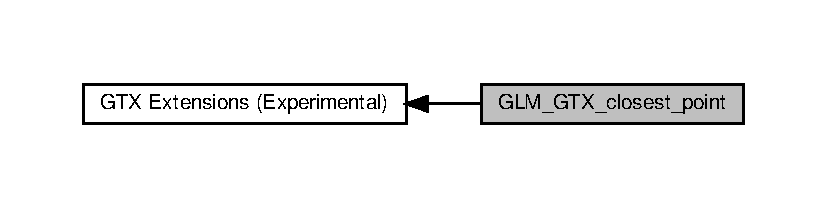
\includegraphics[width=350pt]{group__gtx__closest__point}
\end{center}
\end{figure}
\subsection*{Functions}
\begin{DoxyCompactItemize}
\item 
{\footnotesize template$<$typename T , precision P$>$ }\\\hyperlink{setup_8hpp_ab2d052de21a70539923e9bcbf6e83a51}{G\+L\+M\+\_\+\+F\+U\+N\+C\+\_\+\+D\+E\+CL} \hyperlink{structglm_1_1detail_1_1tvec3}{detail\+::tvec3}$<$ T, P $>$ \hyperlink{group__gtx__closest__point_ga03a6d7e93590f5d45050f6dc7aa8bf8f}{glm\+::closest\+Point\+On\+Line} (\hyperlink{structglm_1_1detail_1_1tvec3}{detail\+::tvec3}$<$ T, P $>$ const \&point, \hyperlink{structglm_1_1detail_1_1tvec3}{detail\+::tvec3}$<$ T, P $>$ const \&a, \hyperlink{structglm_1_1detail_1_1tvec3}{detail\+::tvec3}$<$ T, P $>$ const \&b)
\end{DoxyCompactItemize}


\subsection{Detailed Description}
Find the point on a straight line which is the closet of a point. 

$<$\hyperlink{closest__point_8hpp}{glm/gtx/closest\+\_\+point.\+hpp}$>$ need to be included to use these functionalities. 

\subsection{Function Documentation}
\mbox{\Hypertarget{group__gtx__closest__point_ga03a6d7e93590f5d45050f6dc7aa8bf8f}\label{group__gtx__closest__point_ga03a6d7e93590f5d45050f6dc7aa8bf8f}} 
\index{G\+L\+M\+\_\+\+G\+T\+X\+\_\+closest\+\_\+point@{G\+L\+M\+\_\+\+G\+T\+X\+\_\+closest\+\_\+point}!closest\+Point\+On\+Line@{closest\+Point\+On\+Line}}
\index{closest\+Point\+On\+Line@{closest\+Point\+On\+Line}!G\+L\+M\+\_\+\+G\+T\+X\+\_\+closest\+\_\+point@{G\+L\+M\+\_\+\+G\+T\+X\+\_\+closest\+\_\+point}}
\subsubsection{\texorpdfstring{closest\+Point\+On\+Line()}{closestPointOnLine()}}
{\footnotesize\ttfamily template$<$typename T , precision P$>$ \\
\hyperlink{setup_8hpp_ab2d052de21a70539923e9bcbf6e83a51}{G\+L\+M\+\_\+\+F\+U\+N\+C\+\_\+\+D\+E\+CL} \hyperlink{structglm_1_1detail_1_1tvec3}{detail\+::tvec3}$<$T, P$>$ glm\+::closest\+Point\+On\+Line (\begin{DoxyParamCaption}\item[{\hyperlink{structglm_1_1detail_1_1tvec3}{detail\+::tvec3}$<$ T, P $>$ const \&}]{point,  }\item[{\hyperlink{structglm_1_1detail_1_1tvec3}{detail\+::tvec3}$<$ T, P $>$ const \&}]{a,  }\item[{\hyperlink{structglm_1_1detail_1_1tvec3}{detail\+::tvec3}$<$ T, P $>$ const \&}]{b }\end{DoxyParamCaption})}

Find the point on a straight line which is the closet of a point. \begin{DoxySeeAlso}{See also}
\hyperlink{group__gtx__closest__point}{G\+L\+M\+\_\+\+G\+T\+X\+\_\+closest\+\_\+point} 
\end{DoxySeeAlso}


Definition at line 17 of file closest\+\_\+point.\+inl.


\hypertarget{group__gtx__color__space}{}\section{G\+L\+M\+\_\+\+G\+T\+X\+\_\+color\+\_\+space}
\label{group__gtx__color__space}\index{G\+L\+M\+\_\+\+G\+T\+X\+\_\+color\+\_\+space@{G\+L\+M\+\_\+\+G\+T\+X\+\_\+color\+\_\+space}}


Related to R\+GB to H\+SV conversions and operations.  


Collaboration diagram for G\+L\+M\+\_\+\+G\+T\+X\+\_\+color\+\_\+space\+:\nopagebreak
\begin{figure}[H]
\begin{center}
\leavevmode
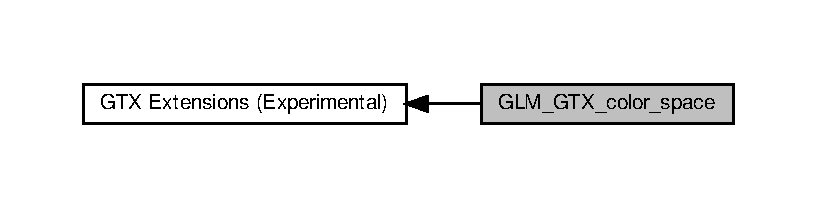
\includegraphics[width=350pt]{group__gtx__color__space}
\end{center}
\end{figure}
\subsection*{Functions}
\begin{DoxyCompactItemize}
\item 
{\footnotesize template$<$typename T , precision P$>$ }\\\hyperlink{setup_8hpp_ab2d052de21a70539923e9bcbf6e83a51}{G\+L\+M\+\_\+\+F\+U\+N\+C\+\_\+\+D\+E\+CL} \hyperlink{structglm_1_1detail_1_1tvec3}{detail\+::tvec3}$<$ T, P $>$ \hyperlink{group__gtx__color__space_gafe29cc37c2675aee66c9f9ae3e5e7294}{glm\+::rgb\+Color} (\hyperlink{structglm_1_1detail_1_1tvec3}{detail\+::tvec3}$<$ T, P $>$ const \&hsv\+Value)
\item 
{\footnotesize template$<$typename T , precision P$>$ }\\\hyperlink{setup_8hpp_ab2d052de21a70539923e9bcbf6e83a51}{G\+L\+M\+\_\+\+F\+U\+N\+C\+\_\+\+D\+E\+CL} \hyperlink{structglm_1_1detail_1_1tvec3}{detail\+::tvec3}$<$ T, P $>$ \hyperlink{group__gtx__color__space_ga9d3d99c06af10403d317dec0cb655090}{glm\+::hsv\+Color} (\hyperlink{structglm_1_1detail_1_1tvec3}{detail\+::tvec3}$<$ T, P $>$ const \&rgb\+Value)
\item 
{\footnotesize template$<$typename T $>$ }\\\hyperlink{setup_8hpp_ab2d052de21a70539923e9bcbf6e83a51}{G\+L\+M\+\_\+\+F\+U\+N\+C\+\_\+\+D\+E\+CL} \hyperlink{structglm_1_1detail_1_1tmat4x4}{detail\+::tmat4x4}$<$ T, \hyperlink{namespaceglm_a0f04f086094c747d227af4425893f545a9d21ccd8b5a009ec7eb7677befc3bf51}{defaultp} $>$ \hyperlink{group__gtx__color__space_ga444bcc8582eaa894acf405762ba2a5ff}{glm\+::saturation} (T const s)
\item 
{\footnotesize template$<$typename T , precision P$>$ }\\\hyperlink{setup_8hpp_ab2d052de21a70539923e9bcbf6e83a51}{G\+L\+M\+\_\+\+F\+U\+N\+C\+\_\+\+D\+E\+CL} \hyperlink{structglm_1_1detail_1_1tvec3}{detail\+::tvec3}$<$ T, P $>$ \hyperlink{group__gtx__color__space_ga1a6fe89b5effcc718b5f49de5bb50fad}{glm\+::saturation} (T const s, \hyperlink{structglm_1_1detail_1_1tvec3}{detail\+::tvec3}$<$ T, P $>$ const \&color)
\item 
{\footnotesize template$<$typename T , precision P$>$ }\\\hyperlink{setup_8hpp_ab2d052de21a70539923e9bcbf6e83a51}{G\+L\+M\+\_\+\+F\+U\+N\+C\+\_\+\+D\+E\+CL} \hyperlink{structglm_1_1detail_1_1tvec4}{detail\+::tvec4}$<$ T, P $>$ \hyperlink{group__gtx__color__space_ga42cc34c45ab66e010c629106952c8bdd}{glm\+::saturation} (T const s, \hyperlink{structglm_1_1detail_1_1tvec4}{detail\+::tvec4}$<$ T, P $>$ const \&color)
\item 
{\footnotesize template$<$typename T , precision P$>$ }\\\hyperlink{setup_8hpp_ab2d052de21a70539923e9bcbf6e83a51}{G\+L\+M\+\_\+\+F\+U\+N\+C\+\_\+\+D\+E\+CL} T \hyperlink{group__gtx__color__space_ga3fb6710bbbf4f3e2303b06946e9cf00c}{glm\+::luminosity} (\hyperlink{structglm_1_1detail_1_1tvec3}{detail\+::tvec3}$<$ T, P $>$ const \&color)
\end{DoxyCompactItemize}


\subsection{Detailed Description}
Related to R\+GB to H\+SV conversions and operations. 

$<$\hyperlink{color__space_8hpp}{glm/gtx/color\+\_\+space.\+hpp}$>$ need to be included to use these functionalities. 

\subsection{Function Documentation}
\mbox{\Hypertarget{group__gtx__color__space_ga9d3d99c06af10403d317dec0cb655090}\label{group__gtx__color__space_ga9d3d99c06af10403d317dec0cb655090}} 
\index{G\+L\+M\+\_\+\+G\+T\+X\+\_\+color\+\_\+space@{G\+L\+M\+\_\+\+G\+T\+X\+\_\+color\+\_\+space}!hsv\+Color@{hsv\+Color}}
\index{hsv\+Color@{hsv\+Color}!G\+L\+M\+\_\+\+G\+T\+X\+\_\+color\+\_\+space@{G\+L\+M\+\_\+\+G\+T\+X\+\_\+color\+\_\+space}}
\subsubsection{\texorpdfstring{hsv\+Color()}{hsvColor()}}
{\footnotesize\ttfamily template$<$typename T , precision P$>$ \\
\hyperlink{setup_8hpp_ab2d052de21a70539923e9bcbf6e83a51}{G\+L\+M\+\_\+\+F\+U\+N\+C\+\_\+\+D\+E\+CL} \hyperlink{structglm_1_1detail_1_1tvec3}{detail\+::tvec3}$<$T, P$>$ glm\+::hsv\+Color (\begin{DoxyParamCaption}\item[{\hyperlink{structglm_1_1detail_1_1tvec3}{detail\+::tvec3}$<$ T, P $>$ const \&}]{rgb\+Value }\end{DoxyParamCaption})}

Converts a color from R\+GB color space to its color in H\+SV color space. \begin{DoxySeeAlso}{See also}
\hyperlink{group__gtx__color__space}{G\+L\+M\+\_\+\+G\+T\+X\+\_\+color\+\_\+space} 
\end{DoxySeeAlso}


Definition at line 70 of file color\+\_\+space.\+inl.

\mbox{\Hypertarget{group__gtx__color__space_ga3fb6710bbbf4f3e2303b06946e9cf00c}\label{group__gtx__color__space_ga3fb6710bbbf4f3e2303b06946e9cf00c}} 
\index{G\+L\+M\+\_\+\+G\+T\+X\+\_\+color\+\_\+space@{G\+L\+M\+\_\+\+G\+T\+X\+\_\+color\+\_\+space}!luminosity@{luminosity}}
\index{luminosity@{luminosity}!G\+L\+M\+\_\+\+G\+T\+X\+\_\+color\+\_\+space@{G\+L\+M\+\_\+\+G\+T\+X\+\_\+color\+\_\+space}}
\subsubsection{\texorpdfstring{luminosity()}{luminosity()}}
{\footnotesize\ttfamily template$<$typename T , precision P$>$ \\
\hyperlink{setup_8hpp_ab2d052de21a70539923e9bcbf6e83a51}{G\+L\+M\+\_\+\+F\+U\+N\+C\+\_\+\+D\+E\+CL} T glm\+::luminosity (\begin{DoxyParamCaption}\item[{\hyperlink{structglm_1_1detail_1_1tvec3}{detail\+::tvec3}$<$ T, P $>$ const \&}]{color }\end{DoxyParamCaption})}

Compute color luminosity associating ratios (0.\+33, 0.\+59, 0.\+11) to R\+GB canals. \begin{DoxySeeAlso}{See also}
\hyperlink{group__gtx__color__space}{G\+L\+M\+\_\+\+G\+T\+X\+\_\+color\+\_\+space} 
\end{DoxySeeAlso}


Definition at line 144 of file color\+\_\+space.\+inl.

\mbox{\Hypertarget{group__gtx__color__space_gafe29cc37c2675aee66c9f9ae3e5e7294}\label{group__gtx__color__space_gafe29cc37c2675aee66c9f9ae3e5e7294}} 
\index{G\+L\+M\+\_\+\+G\+T\+X\+\_\+color\+\_\+space@{G\+L\+M\+\_\+\+G\+T\+X\+\_\+color\+\_\+space}!rgb\+Color@{rgb\+Color}}
\index{rgb\+Color@{rgb\+Color}!G\+L\+M\+\_\+\+G\+T\+X\+\_\+color\+\_\+space@{G\+L\+M\+\_\+\+G\+T\+X\+\_\+color\+\_\+space}}
\subsubsection{\texorpdfstring{rgb\+Color()}{rgbColor()}}
{\footnotesize\ttfamily template$<$typename T , precision P$>$ \\
\hyperlink{setup_8hpp_ab2d052de21a70539923e9bcbf6e83a51}{G\+L\+M\+\_\+\+F\+U\+N\+C\+\_\+\+D\+E\+CL} \hyperlink{structglm_1_1detail_1_1tvec3}{detail\+::tvec3}$<$T, P$>$ glm\+::rgb\+Color (\begin{DoxyParamCaption}\item[{\hyperlink{structglm_1_1detail_1_1tvec3}{detail\+::tvec3}$<$ T, P $>$ const \&}]{hsv\+Value }\end{DoxyParamCaption})}

Converts a color from H\+SV color space to its color in R\+GB color space. \begin{DoxySeeAlso}{See also}
\hyperlink{group__gtx__color__space}{G\+L\+M\+\_\+\+G\+T\+X\+\_\+color\+\_\+space} 
\end{DoxySeeAlso}


Definition at line 13 of file color\+\_\+space.\+inl.

\mbox{\Hypertarget{group__gtx__color__space_ga444bcc8582eaa894acf405762ba2a5ff}\label{group__gtx__color__space_ga444bcc8582eaa894acf405762ba2a5ff}} 
\index{G\+L\+M\+\_\+\+G\+T\+X\+\_\+color\+\_\+space@{G\+L\+M\+\_\+\+G\+T\+X\+\_\+color\+\_\+space}!saturation@{saturation}}
\index{saturation@{saturation}!G\+L\+M\+\_\+\+G\+T\+X\+\_\+color\+\_\+space@{G\+L\+M\+\_\+\+G\+T\+X\+\_\+color\+\_\+space}}
\subsubsection{\texorpdfstring{saturation()}{saturation()}\hspace{0.1cm}{\footnotesize\ttfamily [1/3]}}
{\footnotesize\ttfamily template$<$typename T $>$ \\
\hyperlink{setup_8hpp_ab2d052de21a70539923e9bcbf6e83a51}{G\+L\+M\+\_\+\+F\+U\+N\+C\+\_\+\+D\+E\+CL} \hyperlink{structglm_1_1detail_1_1tmat4x4}{detail\+::tmat4x4}$<$T, \hyperlink{namespaceglm_a0f04f086094c747d227af4425893f545a9d21ccd8b5a009ec7eb7677befc3bf51}{defaultp}$>$ glm\+::saturation (\begin{DoxyParamCaption}\item[{T const}]{s }\end{DoxyParamCaption})}

Build a saturation matrix. \begin{DoxySeeAlso}{See also}
\hyperlink{group__gtx__color__space}{G\+L\+M\+\_\+\+G\+T\+X\+\_\+color\+\_\+space} 
\end{DoxySeeAlso}


Definition at line 110 of file color\+\_\+space.\+inl.

\mbox{\Hypertarget{group__gtx__color__space_ga1a6fe89b5effcc718b5f49de5bb50fad}\label{group__gtx__color__space_ga1a6fe89b5effcc718b5f49de5bb50fad}} 
\index{G\+L\+M\+\_\+\+G\+T\+X\+\_\+color\+\_\+space@{G\+L\+M\+\_\+\+G\+T\+X\+\_\+color\+\_\+space}!saturation@{saturation}}
\index{saturation@{saturation}!G\+L\+M\+\_\+\+G\+T\+X\+\_\+color\+\_\+space@{G\+L\+M\+\_\+\+G\+T\+X\+\_\+color\+\_\+space}}
\subsubsection{\texorpdfstring{saturation()}{saturation()}\hspace{0.1cm}{\footnotesize\ttfamily [2/3]}}
{\footnotesize\ttfamily template$<$typename T , precision P$>$ \\
\hyperlink{setup_8hpp_ab2d052de21a70539923e9bcbf6e83a51}{G\+L\+M\+\_\+\+F\+U\+N\+C\+\_\+\+D\+E\+CL} \hyperlink{structglm_1_1detail_1_1tvec3}{detail\+::tvec3}$<$T, P$>$ glm\+::saturation (\begin{DoxyParamCaption}\item[{T const}]{s,  }\item[{\hyperlink{structglm_1_1detail_1_1tvec3}{detail\+::tvec3}$<$ T, P $>$ const \&}]{color }\end{DoxyParamCaption})}

Modify the saturation of a color. \begin{DoxySeeAlso}{See also}
\hyperlink{group__gtx__color__space}{G\+L\+M\+\_\+\+G\+T\+X\+\_\+color\+\_\+space} 
\end{DoxySeeAlso}


Definition at line 132 of file color\+\_\+space.\+inl.

\mbox{\Hypertarget{group__gtx__color__space_ga42cc34c45ab66e010c629106952c8bdd}\label{group__gtx__color__space_ga42cc34c45ab66e010c629106952c8bdd}} 
\index{G\+L\+M\+\_\+\+G\+T\+X\+\_\+color\+\_\+space@{G\+L\+M\+\_\+\+G\+T\+X\+\_\+color\+\_\+space}!saturation@{saturation}}
\index{saturation@{saturation}!G\+L\+M\+\_\+\+G\+T\+X\+\_\+color\+\_\+space@{G\+L\+M\+\_\+\+G\+T\+X\+\_\+color\+\_\+space}}
\subsubsection{\texorpdfstring{saturation()}{saturation()}\hspace{0.1cm}{\footnotesize\ttfamily [3/3]}}
{\footnotesize\ttfamily template$<$typename T , precision P$>$ \\
\hyperlink{setup_8hpp_ab2d052de21a70539923e9bcbf6e83a51}{G\+L\+M\+\_\+\+F\+U\+N\+C\+\_\+\+D\+E\+CL} \hyperlink{structglm_1_1detail_1_1tvec4}{detail\+::tvec4}$<$T, P$>$ glm\+::saturation (\begin{DoxyParamCaption}\item[{T const}]{s,  }\item[{\hyperlink{structglm_1_1detail_1_1tvec4}{detail\+::tvec4}$<$ T, P $>$ const \&}]{color }\end{DoxyParamCaption})}

Modify the saturation of a color. \begin{DoxySeeAlso}{See also}
\hyperlink{group__gtx__color__space}{G\+L\+M\+\_\+\+G\+T\+X\+\_\+color\+\_\+space} 
\end{DoxySeeAlso}


Definition at line 138 of file color\+\_\+space.\+inl.


\hypertarget{group__gtx__color__space___y_co_cg}{}\section{G\+L\+M\+\_\+\+G\+T\+X\+\_\+color\+\_\+space\+\_\+\+Y\+Co\+Cg}
\label{group__gtx__color__space___y_co_cg}\index{G\+L\+M\+\_\+\+G\+T\+X\+\_\+color\+\_\+space\+\_\+\+Y\+Co\+Cg@{G\+L\+M\+\_\+\+G\+T\+X\+\_\+color\+\_\+space\+\_\+\+Y\+Co\+Cg}}


R\+GB to Y\+Co\+Cg conversions and operations.  


Collaboration diagram for G\+L\+M\+\_\+\+G\+T\+X\+\_\+color\+\_\+space\+\_\+\+Y\+Co\+Cg\+:\nopagebreak
\begin{figure}[H]
\begin{center}
\leavevmode
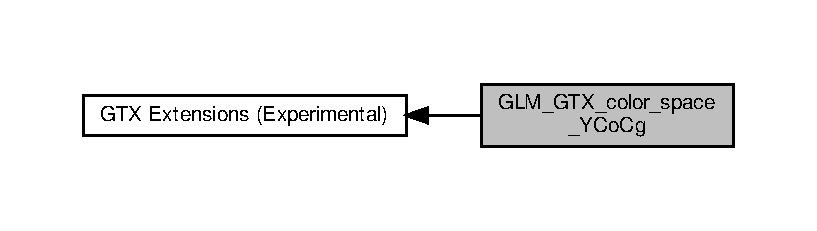
\includegraphics[width=350pt]{group__gtx__color__space___y_co_cg}
\end{center}
\end{figure}
\subsection*{Functions}
\begin{DoxyCompactItemize}
\item 
{\footnotesize template$<$typename T , precision P$>$ }\\\hyperlink{setup_8hpp_ab2d052de21a70539923e9bcbf6e83a51}{G\+L\+M\+\_\+\+F\+U\+N\+C\+\_\+\+D\+E\+CL} \hyperlink{structglm_1_1detail_1_1tvec3}{detail\+::tvec3}$<$ T, P $>$ \hyperlink{group__gtx__color__space___y_co_cg_ga2a235b86e67866fd9fef640bcc47c93d}{glm\+::rgb2\+Y\+Co\+Cg} (\hyperlink{structglm_1_1detail_1_1tvec3}{detail\+::tvec3}$<$ T, P $>$ const \&\hyperlink{group__gtx__color__space_gafe29cc37c2675aee66c9f9ae3e5e7294}{rgb\+Color})
\item 
{\footnotesize template$<$typename T , precision P$>$ }\\\hyperlink{setup_8hpp_ab2d052de21a70539923e9bcbf6e83a51}{G\+L\+M\+\_\+\+F\+U\+N\+C\+\_\+\+D\+E\+CL} \hyperlink{structglm_1_1detail_1_1tvec3}{detail\+::tvec3}$<$ T, P $>$ \hyperlink{group__gtx__color__space___y_co_cg_gab40e31e352d2d318d3f062df2882c500}{glm\+::\+Y\+Co\+Cg2rgb} (\hyperlink{structglm_1_1detail_1_1tvec3}{detail\+::tvec3}$<$ T, P $>$ const \&Y\+Co\+Cg\+Color)
\item 
{\footnotesize template$<$typename T , precision P$>$ }\\\hyperlink{setup_8hpp_ab2d052de21a70539923e9bcbf6e83a51}{G\+L\+M\+\_\+\+F\+U\+N\+C\+\_\+\+D\+E\+CL} \hyperlink{structglm_1_1detail_1_1tvec3}{detail\+::tvec3}$<$ T, P $>$ \hyperlink{group__gtx__color__space___y_co_cg_gaeee43c2a06fe63d46a96cee4d1c63ce6}{glm\+::rgb2\+Y\+Co\+CgR} (\hyperlink{structglm_1_1detail_1_1tvec3}{detail\+::tvec3}$<$ T, P $>$ const \&\hyperlink{group__gtx__color__space_gafe29cc37c2675aee66c9f9ae3e5e7294}{rgb\+Color})
\item 
{\footnotesize template$<$typename T , precision P$>$ }\\\hyperlink{setup_8hpp_ab2d052de21a70539923e9bcbf6e83a51}{G\+L\+M\+\_\+\+F\+U\+N\+C\+\_\+\+D\+E\+CL} \hyperlink{structglm_1_1detail_1_1tvec3}{detail\+::tvec3}$<$ T, P $>$ \hyperlink{group__gtx__color__space___y_co_cg_ga7b90b9b5758dbe96a82a2ef8237a17e9}{glm\+::\+Y\+Co\+Cg\+R2rgb} (\hyperlink{structglm_1_1detail_1_1tvec3}{detail\+::tvec3}$<$ T, P $>$ const \&Y\+Co\+Cg\+Color)
\end{DoxyCompactItemize}


\subsection{Detailed Description}
R\+GB to Y\+Co\+Cg conversions and operations. 

$<$\hyperlink{color__space___y_co_cg_8hpp}{glm/gtx/color\+\_\+space\+\_\+\+Y\+Co\+Cg.\+hpp}$>$ need to be included to use these functionalities. 

\subsection{Function Documentation}
\mbox{\Hypertarget{group__gtx__color__space___y_co_cg_ga2a235b86e67866fd9fef640bcc47c93d}\label{group__gtx__color__space___y_co_cg_ga2a235b86e67866fd9fef640bcc47c93d}} 
\index{G\+L\+M\+\_\+\+G\+T\+X\+\_\+color\+\_\+space\+\_\+\+Y\+Co\+Cg@{G\+L\+M\+\_\+\+G\+T\+X\+\_\+color\+\_\+space\+\_\+\+Y\+Co\+Cg}!rgb2\+Y\+Co\+Cg@{rgb2\+Y\+Co\+Cg}}
\index{rgb2\+Y\+Co\+Cg@{rgb2\+Y\+Co\+Cg}!G\+L\+M\+\_\+\+G\+T\+X\+\_\+color\+\_\+space\+\_\+\+Y\+Co\+Cg@{G\+L\+M\+\_\+\+G\+T\+X\+\_\+color\+\_\+space\+\_\+\+Y\+Co\+Cg}}
\subsubsection{\texorpdfstring{rgb2\+Y\+Co\+Cg()}{rgb2YCoCg()}}
{\footnotesize\ttfamily template$<$typename T , precision P$>$ \\
\hyperlink{setup_8hpp_ab2d052de21a70539923e9bcbf6e83a51}{G\+L\+M\+\_\+\+F\+U\+N\+C\+\_\+\+D\+E\+CL} \hyperlink{structglm_1_1detail_1_1tvec3}{detail\+::tvec3}$<$T, P$>$ glm\+::rgb2\+Y\+Co\+Cg (\begin{DoxyParamCaption}\item[{\hyperlink{structglm_1_1detail_1_1tvec3}{detail\+::tvec3}$<$ T, P $>$ const \&}]{rgb\+Color }\end{DoxyParamCaption})}

Convert a color from R\+GB color space to Y\+Co\+Cg color space. \begin{DoxySeeAlso}{See also}
\hyperlink{group__gtx__color__space___y_co_cg}{G\+L\+M\+\_\+\+G\+T\+X\+\_\+color\+\_\+space\+\_\+\+Y\+Co\+Cg} 
\end{DoxySeeAlso}


Definition at line 14 of file color\+\_\+space\+\_\+\+Y\+Co\+Cg.\+inl.

\mbox{\Hypertarget{group__gtx__color__space___y_co_cg_gaeee43c2a06fe63d46a96cee4d1c63ce6}\label{group__gtx__color__space___y_co_cg_gaeee43c2a06fe63d46a96cee4d1c63ce6}} 
\index{G\+L\+M\+\_\+\+G\+T\+X\+\_\+color\+\_\+space\+\_\+\+Y\+Co\+Cg@{G\+L\+M\+\_\+\+G\+T\+X\+\_\+color\+\_\+space\+\_\+\+Y\+Co\+Cg}!rgb2\+Y\+Co\+CgR@{rgb2\+Y\+Co\+CgR}}
\index{rgb2\+Y\+Co\+CgR@{rgb2\+Y\+Co\+CgR}!G\+L\+M\+\_\+\+G\+T\+X\+\_\+color\+\_\+space\+\_\+\+Y\+Co\+Cg@{G\+L\+M\+\_\+\+G\+T\+X\+\_\+color\+\_\+space\+\_\+\+Y\+Co\+Cg}}
\subsubsection{\texorpdfstring{rgb2\+Y\+Co\+Cg\+R()}{rgb2YCoCgR()}}
{\footnotesize\ttfamily template$<$typename T , precision P$>$ \\
\hyperlink{setup_8hpp_ab2d052de21a70539923e9bcbf6e83a51}{G\+L\+M\+\_\+\+F\+U\+N\+C\+\_\+\+D\+E\+CL} \hyperlink{structglm_1_1detail_1_1tvec3}{detail\+::tvec3}$<$T, P$>$ glm\+::rgb2\+Y\+Co\+CgR (\begin{DoxyParamCaption}\item[{\hyperlink{structglm_1_1detail_1_1tvec3}{detail\+::tvec3}$<$ T, P $>$ const \&}]{rgb\+Color }\end{DoxyParamCaption})}

Convert a color from R\+GB color space to Y\+Co\+CgR color space. \begin{DoxySeeAlso}{See also}
\char`\"{}\+Y\+Co\+Cg-\/\+R\+: A Color Space with R\+G\+B Reversibility and Low Dynamic Range\char`\"{} 

\hyperlink{group__gtx__color__space___y_co_cg}{G\+L\+M\+\_\+\+G\+T\+X\+\_\+color\+\_\+space\+\_\+\+Y\+Co\+Cg} 
\end{DoxySeeAlso}


Definition at line 27 of file color\+\_\+space\+\_\+\+Y\+Co\+Cg.\+inl.

\mbox{\Hypertarget{group__gtx__color__space___y_co_cg_gab40e31e352d2d318d3f062df2882c500}\label{group__gtx__color__space___y_co_cg_gab40e31e352d2d318d3f062df2882c500}} 
\index{G\+L\+M\+\_\+\+G\+T\+X\+\_\+color\+\_\+space\+\_\+\+Y\+Co\+Cg@{G\+L\+M\+\_\+\+G\+T\+X\+\_\+color\+\_\+space\+\_\+\+Y\+Co\+Cg}!Y\+Co\+Cg2rgb@{Y\+Co\+Cg2rgb}}
\index{Y\+Co\+Cg2rgb@{Y\+Co\+Cg2rgb}!G\+L\+M\+\_\+\+G\+T\+X\+\_\+color\+\_\+space\+\_\+\+Y\+Co\+Cg@{G\+L\+M\+\_\+\+G\+T\+X\+\_\+color\+\_\+space\+\_\+\+Y\+Co\+Cg}}
\subsubsection{\texorpdfstring{Y\+Co\+Cg2rgb()}{YCoCg2rgb()}}
{\footnotesize\ttfamily template$<$typename T , precision P$>$ \\
\hyperlink{setup_8hpp_ab2d052de21a70539923e9bcbf6e83a51}{G\+L\+M\+\_\+\+F\+U\+N\+C\+\_\+\+D\+E\+CL} \hyperlink{structglm_1_1detail_1_1tvec3}{detail\+::tvec3}$<$T, P$>$ glm\+::\+Y\+Co\+Cg2rgb (\begin{DoxyParamCaption}\item[{\hyperlink{structglm_1_1detail_1_1tvec3}{detail\+::tvec3}$<$ T, P $>$ const \&}]{Y\+Co\+Cg\+Color }\end{DoxyParamCaption})}

Convert a color from Y\+Co\+Cg color space to R\+GB color space. \begin{DoxySeeAlso}{See also}
\hyperlink{group__gtx__color__space___y_co_cg}{G\+L\+M\+\_\+\+G\+T\+X\+\_\+color\+\_\+space\+\_\+\+Y\+Co\+Cg} 
\end{DoxySeeAlso}


Definition at line 40 of file color\+\_\+space\+\_\+\+Y\+Co\+Cg.\+inl.

\mbox{\Hypertarget{group__gtx__color__space___y_co_cg_ga7b90b9b5758dbe96a82a2ef8237a17e9}\label{group__gtx__color__space___y_co_cg_ga7b90b9b5758dbe96a82a2ef8237a17e9}} 
\index{G\+L\+M\+\_\+\+G\+T\+X\+\_\+color\+\_\+space\+\_\+\+Y\+Co\+Cg@{G\+L\+M\+\_\+\+G\+T\+X\+\_\+color\+\_\+space\+\_\+\+Y\+Co\+Cg}!Y\+Co\+Cg\+R2rgb@{Y\+Co\+Cg\+R2rgb}}
\index{Y\+Co\+Cg\+R2rgb@{Y\+Co\+Cg\+R2rgb}!G\+L\+M\+\_\+\+G\+T\+X\+\_\+color\+\_\+space\+\_\+\+Y\+Co\+Cg@{G\+L\+M\+\_\+\+G\+T\+X\+\_\+color\+\_\+space\+\_\+\+Y\+Co\+Cg}}
\subsubsection{\texorpdfstring{Y\+Co\+Cg\+R2rgb()}{YCoCgR2rgb()}}
{\footnotesize\ttfamily template$<$typename T , precision P$>$ \\
\hyperlink{setup_8hpp_ab2d052de21a70539923e9bcbf6e83a51}{G\+L\+M\+\_\+\+F\+U\+N\+C\+\_\+\+D\+E\+CL} \hyperlink{structglm_1_1detail_1_1tvec3}{detail\+::tvec3}$<$T, P$>$ glm\+::\+Y\+Co\+Cg\+R2rgb (\begin{DoxyParamCaption}\item[{\hyperlink{structglm_1_1detail_1_1tvec3}{detail\+::tvec3}$<$ T, P $>$ const \&}]{Y\+Co\+Cg\+Color }\end{DoxyParamCaption})}

Convert a color from Y\+Co\+CgR color space to R\+GB color space. \begin{DoxySeeAlso}{See also}
\char`\"{}\+Y\+Co\+Cg-\/\+R\+: A Color Space with R\+G\+B Reversibility and Low Dynamic Range\char`\"{} 

\hyperlink{group__gtx__color__space___y_co_cg}{G\+L\+M\+\_\+\+G\+T\+X\+\_\+color\+\_\+space\+\_\+\+Y\+Co\+Cg} 
\end{DoxySeeAlso}


Definition at line 53 of file color\+\_\+space\+\_\+\+Y\+Co\+Cg.\+inl.


\hypertarget{group__gtx__compatibility}{}\section{G\+L\+M\+\_\+\+G\+T\+X\+\_\+compatibility}
\label{group__gtx__compatibility}\index{G\+L\+M\+\_\+\+G\+T\+X\+\_\+compatibility@{G\+L\+M\+\_\+\+G\+T\+X\+\_\+compatibility}}


Provide functions to increase the compatibility with Cg and H\+L\+SL languages.  


Collaboration diagram for G\+L\+M\+\_\+\+G\+T\+X\+\_\+compatibility\+:\nopagebreak
\begin{figure}[H]
\begin{center}
\leavevmode
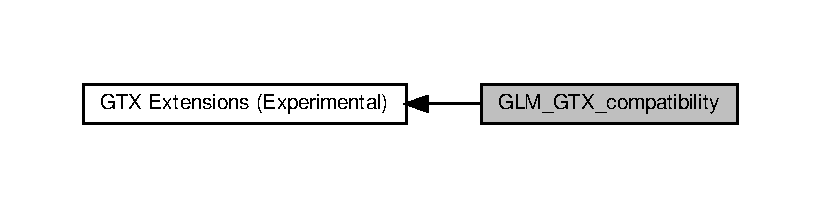
\includegraphics[width=350pt]{group__gtx__compatibility}
\end{center}
\end{figure}
\subsection*{Typedefs}
\begin{DoxyCompactItemize}
\item 
typedef bool \hyperlink{group__gtx__compatibility_gab65f19f5170f95a2f06d6aa6482c9405}{glm\+::bool1}
\begin{DoxyCompactList}\small\item\em boolean type with 1 component. (From G\+L\+M\+\_\+\+G\+T\+X\+\_\+compatibility extension) \end{DoxyCompactList}\item 
typedef \hyperlink{structglm_1_1detail_1_1tvec2}{detail\+::tvec2}$<$ bool, \hyperlink{namespaceglm_a0f04f086094c747d227af4425893f545ac6f7eab42eacbb10d59a58e95e362074}{highp} $>$ \hyperlink{group__gtx__compatibility_gafede6e8549e9bb9da63f404022298d40}{glm\+::bool2}
\begin{DoxyCompactList}\small\item\em boolean type with 2 components. (From G\+L\+M\+\_\+\+G\+T\+X\+\_\+compatibility extension) \end{DoxyCompactList}\item 
typedef \hyperlink{structglm_1_1detail_1_1tvec3}{detail\+::tvec3}$<$ bool, \hyperlink{namespaceglm_a0f04f086094c747d227af4425893f545ac6f7eab42eacbb10d59a58e95e362074}{highp} $>$ \hyperlink{group__gtx__compatibility_gad18ebb149851844fd704e138c4af9a44}{glm\+::bool3}
\begin{DoxyCompactList}\small\item\em boolean type with 3 components. (From G\+L\+M\+\_\+\+G\+T\+X\+\_\+compatibility extension) \end{DoxyCompactList}\item 
typedef \hyperlink{structglm_1_1detail_1_1tvec4}{detail\+::tvec4}$<$ bool, \hyperlink{namespaceglm_a0f04f086094c747d227af4425893f545ac6f7eab42eacbb10d59a58e95e362074}{highp} $>$ \hyperlink{group__gtx__compatibility_ga6ef1f104d22f384c4d59f2b1ca1768a7}{glm\+::bool4}
\begin{DoxyCompactList}\small\item\em boolean type with 4 components. (From G\+L\+M\+\_\+\+G\+T\+X\+\_\+compatibility extension) \end{DoxyCompactList}\item 
typedef bool \hyperlink{group__gtx__compatibility_ga98d9d3da22aebc872ba38ce5afa0eff7}{glm\+::bool1x1}
\begin{DoxyCompactList}\small\item\em boolean matrix with 1 x 1 component. (From G\+L\+M\+\_\+\+G\+T\+X\+\_\+compatibility extension) \end{DoxyCompactList}\item 
typedef \hyperlink{structglm_1_1detail_1_1tmat2x2}{detail\+::tmat2x2}$<$ bool, \hyperlink{namespaceglm_a0f04f086094c747d227af4425893f545ac6f7eab42eacbb10d59a58e95e362074}{highp} $>$ \hyperlink{group__gtx__compatibility_ga44cd09c0dad9ea163f038a342555867f}{glm\+::bool2x2}
\begin{DoxyCompactList}\small\item\em boolean matrix with 2 x 2 components. (From G\+L\+M\+\_\+\+G\+T\+X\+\_\+compatibility extension) \end{DoxyCompactList}\item 
typedef \hyperlink{structglm_1_1detail_1_1tmat2x3}{detail\+::tmat2x3}$<$ bool, \hyperlink{namespaceglm_a0f04f086094c747d227af4425893f545ac6f7eab42eacbb10d59a58e95e362074}{highp} $>$ \hyperlink{group__gtx__compatibility_ga75013772bb088d107a1c1a994e7f9b14}{glm\+::bool2x3}
\begin{DoxyCompactList}\small\item\em boolean matrix with 2 x 3 components. (From G\+L\+M\+\_\+\+G\+T\+X\+\_\+compatibility extension) \end{DoxyCompactList}\item 
typedef \hyperlink{structglm_1_1detail_1_1tmat2x4}{detail\+::tmat2x4}$<$ bool, \hyperlink{namespaceglm_a0f04f086094c747d227af4425893f545ac6f7eab42eacbb10d59a58e95e362074}{highp} $>$ \hyperlink{group__gtx__compatibility_gaf24096d8a88d274b94002386a3fcab0c}{glm\+::bool2x4}
\begin{DoxyCompactList}\small\item\em boolean matrix with 2 x 4 components. (From G\+L\+M\+\_\+\+G\+T\+X\+\_\+compatibility extension) \end{DoxyCompactList}\item 
typedef \hyperlink{structglm_1_1detail_1_1tmat3x2}{detail\+::tmat3x2}$<$ bool, \hyperlink{namespaceglm_a0f04f086094c747d227af4425893f545ac6f7eab42eacbb10d59a58e95e362074}{highp} $>$ \hyperlink{group__gtx__compatibility_gacf961fda4c64459911f552cbffdbffa8}{glm\+::bool3x2}
\begin{DoxyCompactList}\small\item\em boolean matrix with 3 x 2 components. (From G\+L\+M\+\_\+\+G\+T\+X\+\_\+compatibility extension) \end{DoxyCompactList}\item 
typedef \hyperlink{structglm_1_1detail_1_1tmat3x3}{detail\+::tmat3x3}$<$ bool, \hyperlink{namespaceglm_a0f04f086094c747d227af4425893f545ac6f7eab42eacbb10d59a58e95e362074}{highp} $>$ \hyperlink{group__gtx__compatibility_gae9cc5d3d9c72543e303af4d702bf7b40}{glm\+::bool3x3}
\begin{DoxyCompactList}\small\item\em boolean matrix with 3 x 3 components. (From G\+L\+M\+\_\+\+G\+T\+X\+\_\+compatibility extension) \end{DoxyCompactList}\item 
typedef \hyperlink{structglm_1_1detail_1_1tmat3x4}{detail\+::tmat3x4}$<$ bool, \hyperlink{namespaceglm_a0f04f086094c747d227af4425893f545ac6f7eab42eacbb10d59a58e95e362074}{highp} $>$ \hyperlink{group__gtx__compatibility_gaf68d62e1c790fa3f09ef5e866af690f1}{glm\+::bool3x4}
\begin{DoxyCompactList}\small\item\em boolean matrix with 3 x 4 components. (From G\+L\+M\+\_\+\+G\+T\+X\+\_\+compatibility extension) \end{DoxyCompactList}\item 
typedef \hyperlink{structglm_1_1detail_1_1tmat4x2}{detail\+::tmat4x2}$<$ bool, \hyperlink{namespaceglm_a0f04f086094c747d227af4425893f545ac6f7eab42eacbb10d59a58e95e362074}{highp} $>$ \hyperlink{group__gtx__compatibility_gaa431c2e87e8d78c4780c938a9483d6ff}{glm\+::bool4x2}
\begin{DoxyCompactList}\small\item\em boolean matrix with 4 x 2 components. (From G\+L\+M\+\_\+\+G\+T\+X\+\_\+compatibility extension) \end{DoxyCompactList}\item 
typedef \hyperlink{structglm_1_1detail_1_1tmat4x3}{detail\+::tmat4x3}$<$ bool, \hyperlink{namespaceglm_a0f04f086094c747d227af4425893f545ac6f7eab42eacbb10d59a58e95e362074}{highp} $>$ \hyperlink{group__gtx__compatibility_ga7acb207ab877c53dc5751752e1f70053}{glm\+::bool4x3}
\begin{DoxyCompactList}\small\item\em boolean matrix with 4 x 3 components. (From G\+L\+M\+\_\+\+G\+T\+X\+\_\+compatibility extension) \end{DoxyCompactList}\item 
typedef \hyperlink{structglm_1_1detail_1_1tmat4x4}{detail\+::tmat4x4}$<$ bool, \hyperlink{namespaceglm_a0f04f086094c747d227af4425893f545ac6f7eab42eacbb10d59a58e95e362074}{highp} $>$ \hyperlink{group__gtx__compatibility_ga4738dad3625bfa64ddf218897da020e9}{glm\+::bool4x4}
\begin{DoxyCompactList}\small\item\em boolean matrix with 4 x 4 components. (From G\+L\+M\+\_\+\+G\+T\+X\+\_\+compatibility extension) \end{DoxyCompactList}\item 
typedef int \hyperlink{group__gtx__compatibility_gaba41d7803e4b24c17656d74377b88286}{glm\+::int1}
\begin{DoxyCompactList}\small\item\em integer vector with 1 component. (From G\+L\+M\+\_\+\+G\+T\+X\+\_\+compatibility extension) \end{DoxyCompactList}\item 
typedef \hyperlink{structglm_1_1detail_1_1tvec2}{detail\+::tvec2}$<$ int, \hyperlink{namespaceglm_a0f04f086094c747d227af4425893f545ac6f7eab42eacbb10d59a58e95e362074}{highp} $>$ \hyperlink{group__gtx__compatibility_ga3f999377257cbda84c745b688ddcba81}{glm\+::int2}
\begin{DoxyCompactList}\small\item\em integer vector with 2 components. (From G\+L\+M\+\_\+\+G\+T\+X\+\_\+compatibility extension) \end{DoxyCompactList}\item 
typedef \hyperlink{structglm_1_1detail_1_1tvec3}{detail\+::tvec3}$<$ int, \hyperlink{namespaceglm_a0f04f086094c747d227af4425893f545ac6f7eab42eacbb10d59a58e95e362074}{highp} $>$ \hyperlink{group__gtx__compatibility_gac305b0da08fad90d91854569679c935e}{glm\+::int3}
\begin{DoxyCompactList}\small\item\em integer vector with 3 components. (From G\+L\+M\+\_\+\+G\+T\+X\+\_\+compatibility extension) \end{DoxyCompactList}\item 
typedef \hyperlink{structglm_1_1detail_1_1tvec4}{detail\+::tvec4}$<$ int, \hyperlink{namespaceglm_a0f04f086094c747d227af4425893f545ac6f7eab42eacbb10d59a58e95e362074}{highp} $>$ \hyperlink{group__gtx__compatibility_ga9f621a690aa1c2918a9a8a684376b562}{glm\+::int4}
\begin{DoxyCompactList}\small\item\em integer vector with 4 components. (From G\+L\+M\+\_\+\+G\+T\+X\+\_\+compatibility extension) \end{DoxyCompactList}\item 
typedef int \hyperlink{group__gtx__compatibility_ga09016a637a3cd093c22e6188080ac750}{glm\+::int1x1}
\begin{DoxyCompactList}\small\item\em integer matrix with 1 component. (From G\+L\+M\+\_\+\+G\+T\+X\+\_\+compatibility extension) \end{DoxyCompactList}\item 
typedef \hyperlink{structglm_1_1detail_1_1tmat2x2}{detail\+::tmat2x2}$<$ int, \hyperlink{namespaceglm_a0f04f086094c747d227af4425893f545ac6f7eab42eacbb10d59a58e95e362074}{highp} $>$ \hyperlink{group__gtx__compatibility_ga7762d2b809aab75003e7e7873ca74a2f}{glm\+::int2x2}
\begin{DoxyCompactList}\small\item\em integer matrix with 2 x 2 components. (From G\+L\+M\+\_\+\+G\+T\+X\+\_\+compatibility extension) \end{DoxyCompactList}\item 
typedef \hyperlink{structglm_1_1detail_1_1tmat2x3}{detail\+::tmat2x3}$<$ int, \hyperlink{namespaceglm_a0f04f086094c747d227af4425893f545ac6f7eab42eacbb10d59a58e95e362074}{highp} $>$ \hyperlink{group__gtx__compatibility_ga42c3d6e4924de559104b9ca2b127c9ac}{glm\+::int2x3}
\begin{DoxyCompactList}\small\item\em integer matrix with 2 x 3 components. (From G\+L\+M\+\_\+\+G\+T\+X\+\_\+compatibility extension) \end{DoxyCompactList}\item 
typedef \hyperlink{structglm_1_1detail_1_1tmat2x4}{detail\+::tmat2x4}$<$ int, \hyperlink{namespaceglm_a0f04f086094c747d227af4425893f545ac6f7eab42eacbb10d59a58e95e362074}{highp} $>$ \hyperlink{group__gtx__compatibility_ga145a388c0d988490d6ce901a664faf50}{glm\+::int2x4}
\begin{DoxyCompactList}\small\item\em integer matrix with 2 x 4 components. (From G\+L\+M\+\_\+\+G\+T\+X\+\_\+compatibility extension) \end{DoxyCompactList}\item 
typedef \hyperlink{structglm_1_1detail_1_1tmat3x2}{detail\+::tmat3x2}$<$ int, \hyperlink{namespaceglm_a0f04f086094c747d227af4425893f545ac6f7eab42eacbb10d59a58e95e362074}{highp} $>$ \hyperlink{group__gtx__compatibility_ga2b1f3046fb4692c0c2f76b3933389868}{glm\+::int3x2}
\begin{DoxyCompactList}\small\item\em integer matrix with 3 x 2 components. (From G\+L\+M\+\_\+\+G\+T\+X\+\_\+compatibility extension) \end{DoxyCompactList}\item 
typedef \hyperlink{structglm_1_1detail_1_1tmat3x3}{detail\+::tmat3x3}$<$ int, \hyperlink{namespaceglm_a0f04f086094c747d227af4425893f545ac6f7eab42eacbb10d59a58e95e362074}{highp} $>$ \hyperlink{group__gtx__compatibility_ga8773c9f240dcac9f28d1afef71f7f779}{glm\+::int3x3}
\begin{DoxyCompactList}\small\item\em integer matrix with 3 x 3 components. (From G\+L\+M\+\_\+\+G\+T\+X\+\_\+compatibility extension) \end{DoxyCompactList}\item 
typedef \hyperlink{structglm_1_1detail_1_1tmat3x4}{detail\+::tmat3x4}$<$ int, \hyperlink{namespaceglm_a0f04f086094c747d227af4425893f545ac6f7eab42eacbb10d59a58e95e362074}{highp} $>$ \hyperlink{group__gtx__compatibility_ga7cb1c0960d6551c34c666ad5829e9c65}{glm\+::int3x4}
\begin{DoxyCompactList}\small\item\em integer matrix with 3 x 4 components. (From G\+L\+M\+\_\+\+G\+T\+X\+\_\+compatibility extension) \end{DoxyCompactList}\item 
typedef \hyperlink{structglm_1_1detail_1_1tmat4x2}{detail\+::tmat4x2}$<$ int, \hyperlink{namespaceglm_a0f04f086094c747d227af4425893f545ac6f7eab42eacbb10d59a58e95e362074}{highp} $>$ \hyperlink{group__gtx__compatibility_gac391157aca117c5d52b10c2c3ca5c9be}{glm\+::int4x2}
\begin{DoxyCompactList}\small\item\em integer matrix with 4 x 2 components. (From G\+L\+M\+\_\+\+G\+T\+X\+\_\+compatibility extension) \end{DoxyCompactList}\item 
typedef \hyperlink{structglm_1_1detail_1_1tmat4x3}{detail\+::tmat4x3}$<$ int, \hyperlink{namespaceglm_a0f04f086094c747d227af4425893f545ac6f7eab42eacbb10d59a58e95e362074}{highp} $>$ \hyperlink{group__gtx__compatibility_gaa80ec1b785920a08d366b3c09859d888}{glm\+::int4x3}
\begin{DoxyCompactList}\small\item\em integer matrix with 4 x 3 components. (From G\+L\+M\+\_\+\+G\+T\+X\+\_\+compatibility extension) \end{DoxyCompactList}\item 
typedef \hyperlink{structglm_1_1detail_1_1tmat4x4}{detail\+::tmat4x4}$<$ int, \hyperlink{namespaceglm_a0f04f086094c747d227af4425893f545ac6f7eab42eacbb10d59a58e95e362074}{highp} $>$ \hyperlink{group__gtx__compatibility_ga5f8072c2dce67ad49939e12b168d1de1}{glm\+::int4x4}
\begin{DoxyCompactList}\small\item\em integer matrix with 4 x 4 components. (From G\+L\+M\+\_\+\+G\+T\+X\+\_\+compatibility extension) \end{DoxyCompactList}\item 
typedef float \hyperlink{group__gtx__compatibility_gae0ad1b0450320cda98bbbecb56bc3167}{glm\+::float1}
\begin{DoxyCompactList}\small\item\em single-\/precision floating-\/point vector with 1 component. (From G\+L\+M\+\_\+\+G\+T\+X\+\_\+compatibility extension) \end{DoxyCompactList}\item 
typedef \hyperlink{structglm_1_1detail_1_1tvec2}{detail\+::tvec2}$<$ float, \hyperlink{namespaceglm_a0f04f086094c747d227af4425893f545ac6f7eab42eacbb10d59a58e95e362074}{highp} $>$ \hyperlink{group__gtx__compatibility_ga6ab0b791bbb15ef51a0e930a8710e6b1}{glm\+::float2}
\begin{DoxyCompactList}\small\item\em single-\/precision floating-\/point vector with 2 components. (From G\+L\+M\+\_\+\+G\+T\+X\+\_\+compatibility extension) \end{DoxyCompactList}\item 
typedef \hyperlink{structglm_1_1detail_1_1tvec3}{detail\+::tvec3}$<$ float, \hyperlink{namespaceglm_a0f04f086094c747d227af4425893f545ac6f7eab42eacbb10d59a58e95e362074}{highp} $>$ \hyperlink{group__gtx__compatibility_ga7e0d8fa3501c0a7eaaca31adb6e02de2}{glm\+::float3}
\begin{DoxyCompactList}\small\item\em single-\/precision floating-\/point vector with 3 components. (From G\+L\+M\+\_\+\+G\+T\+X\+\_\+compatibility extension) \end{DoxyCompactList}\item 
typedef \hyperlink{structglm_1_1detail_1_1tvec4}{detail\+::tvec4}$<$ float, \hyperlink{namespaceglm_a0f04f086094c747d227af4425893f545ac6f7eab42eacbb10d59a58e95e362074}{highp} $>$ \hyperlink{group__gtx__compatibility_gac0676d140051809309ca683c325bf439}{glm\+::float4}
\begin{DoxyCompactList}\small\item\em single-\/precision floating-\/point vector with 4 components. (From G\+L\+M\+\_\+\+G\+T\+X\+\_\+compatibility extension) \end{DoxyCompactList}\item 
typedef float \hyperlink{group__gtx__compatibility_gaac1faa940ac1fbb32d4a315005b578af}{glm\+::float1x1}
\begin{DoxyCompactList}\small\item\em single-\/precision floating-\/point matrix with 1 component. (From G\+L\+M\+\_\+\+G\+T\+X\+\_\+compatibility extension) \end{DoxyCompactList}\item 
typedef \hyperlink{structglm_1_1detail_1_1tmat2x2}{detail\+::tmat2x2}$<$ float, \hyperlink{namespaceglm_a0f04f086094c747d227af4425893f545ac6f7eab42eacbb10d59a58e95e362074}{highp} $>$ \hyperlink{group__gtx__compatibility_gaa4a1e4449913b2437f12434ed713dd73}{glm\+::float2x2}
\begin{DoxyCompactList}\small\item\em single-\/precision floating-\/point matrix with 2 x 2 components. (From G\+L\+M\+\_\+\+G\+T\+X\+\_\+compatibility extension) \end{DoxyCompactList}\item 
typedef \hyperlink{structglm_1_1detail_1_1tmat2x3}{detail\+::tmat2x3}$<$ float, \hyperlink{namespaceglm_a0f04f086094c747d227af4425893f545ac6f7eab42eacbb10d59a58e95e362074}{highp} $>$ \hyperlink{group__gtx__compatibility_gaf6c91675c075853da392b1d2dfc45f65}{glm\+::float2x3}
\begin{DoxyCompactList}\small\item\em single-\/precision floating-\/point matrix with 2 x 3 components. (From G\+L\+M\+\_\+\+G\+T\+X\+\_\+compatibility extension) \end{DoxyCompactList}\item 
typedef \hyperlink{structglm_1_1detail_1_1tmat2x4}{detail\+::tmat2x4}$<$ float, \hyperlink{namespaceglm_a0f04f086094c747d227af4425893f545ac6f7eab42eacbb10d59a58e95e362074}{highp} $>$ \hyperlink{group__gtx__compatibility_gaaff795523eb814705d3f1cc7fd3421f2}{glm\+::float2x4}
\begin{DoxyCompactList}\small\item\em single-\/precision floating-\/point matrix with 2 x 4 components. (From G\+L\+M\+\_\+\+G\+T\+X\+\_\+compatibility extension) \end{DoxyCompactList}\item 
typedef \hyperlink{structglm_1_1detail_1_1tmat3x2}{detail\+::tmat3x2}$<$ float, \hyperlink{namespaceglm_a0f04f086094c747d227af4425893f545ac6f7eab42eacbb10d59a58e95e362074}{highp} $>$ \hyperlink{group__gtx__compatibility_ga19bcbd4d65c70cd07907b2d688bc84ed}{glm\+::float3x2}
\begin{DoxyCompactList}\small\item\em single-\/precision floating-\/point matrix with 3 x 2 components. (From G\+L\+M\+\_\+\+G\+T\+X\+\_\+compatibility extension) \end{DoxyCompactList}\item 
typedef \hyperlink{structglm_1_1detail_1_1tmat3x3}{detail\+::tmat3x3}$<$ float, \hyperlink{namespaceglm_a0f04f086094c747d227af4425893f545ac6f7eab42eacbb10d59a58e95e362074}{highp} $>$ \hyperlink{group__gtx__compatibility_ga11458ecd63c32b7e502d90091a6d0a6c}{glm\+::float3x3}
\begin{DoxyCompactList}\small\item\em single-\/precision floating-\/point matrix with 3 x 3 components. (From G\+L\+M\+\_\+\+G\+T\+X\+\_\+compatibility extension) \end{DoxyCompactList}\item 
typedef \hyperlink{structglm_1_1detail_1_1tmat3x4}{detail\+::tmat3x4}$<$ float, \hyperlink{namespaceglm_a0f04f086094c747d227af4425893f545ac6f7eab42eacbb10d59a58e95e362074}{highp} $>$ \hyperlink{group__gtx__compatibility_ga53eb75b08b92aa34886397150c983943}{glm\+::float3x4}
\begin{DoxyCompactList}\small\item\em single-\/precision floating-\/point matrix with 3 x 4 components. (From G\+L\+M\+\_\+\+G\+T\+X\+\_\+compatibility extension) \end{DoxyCompactList}\item 
typedef \hyperlink{structglm_1_1detail_1_1tmat4x2}{detail\+::tmat4x2}$<$ float, \hyperlink{namespaceglm_a0f04f086094c747d227af4425893f545ac6f7eab42eacbb10d59a58e95e362074}{highp} $>$ \hyperlink{group__gtx__compatibility_gab805aa2d6bbd5edddf78bd2e9322e6c7}{glm\+::float4x2}
\begin{DoxyCompactList}\small\item\em single-\/precision floating-\/point matrix with 4 x 2 components. (From G\+L\+M\+\_\+\+G\+T\+X\+\_\+compatibility extension) \end{DoxyCompactList}\item 
typedef \hyperlink{structglm_1_1detail_1_1tmat4x3}{detail\+::tmat4x3}$<$ float, \hyperlink{namespaceglm_a0f04f086094c747d227af4425893f545ac6f7eab42eacbb10d59a58e95e362074}{highp} $>$ \hyperlink{group__gtx__compatibility_ga72398a5d715031923beca8907c52f5d6}{glm\+::float4x3}
\begin{DoxyCompactList}\small\item\em single-\/precision floating-\/point matrix with 4 x 3 components. (From G\+L\+M\+\_\+\+G\+T\+X\+\_\+compatibility extension) \end{DoxyCompactList}\item 
typedef \hyperlink{structglm_1_1detail_1_1tmat4x4}{detail\+::tmat4x4}$<$ float, \hyperlink{namespaceglm_a0f04f086094c747d227af4425893f545ac6f7eab42eacbb10d59a58e95e362074}{highp} $>$ \hyperlink{group__gtx__compatibility_ga1f48a19e35b3640cf3d509041f7a800b}{glm\+::float4x4}
\begin{DoxyCompactList}\small\item\em single-\/precision floating-\/point matrix with 4 x 4 components. (From G\+L\+M\+\_\+\+G\+T\+X\+\_\+compatibility extension) \end{DoxyCompactList}\item 
typedef double \hyperlink{group__gtx__compatibility_gab8b88350212cea916857cb2f49b8a29f}{glm\+::double1}
\begin{DoxyCompactList}\small\item\em double-\/precision floating-\/point vector with 1 component. (From G\+L\+M\+\_\+\+G\+T\+X\+\_\+compatibility extension) \end{DoxyCompactList}\item 
typedef \hyperlink{structglm_1_1detail_1_1tvec2}{detail\+::tvec2}$<$ double, \hyperlink{namespaceglm_a0f04f086094c747d227af4425893f545ac6f7eab42eacbb10d59a58e95e362074}{highp} $>$ \hyperlink{group__gtx__compatibility_ga227d30a4fa630c9e3fb6c7ea87250c62}{glm\+::double2}
\begin{DoxyCompactList}\small\item\em double-\/precision floating-\/point vector with 2 components. (From G\+L\+M\+\_\+\+G\+T\+X\+\_\+compatibility extension) \end{DoxyCompactList}\item 
typedef \hyperlink{structglm_1_1detail_1_1tvec3}{detail\+::tvec3}$<$ double, \hyperlink{namespaceglm_a0f04f086094c747d227af4425893f545ac6f7eab42eacbb10d59a58e95e362074}{highp} $>$ \hyperlink{group__gtx__compatibility_ga3b94d4a19ca0272cad6e025fc5150d06}{glm\+::double3}
\begin{DoxyCompactList}\small\item\em double-\/precision floating-\/point vector with 3 components. (From G\+L\+M\+\_\+\+G\+T\+X\+\_\+compatibility extension) \end{DoxyCompactList}\item 
typedef \hyperlink{structglm_1_1detail_1_1tvec4}{detail\+::tvec4}$<$ double, \hyperlink{namespaceglm_a0f04f086094c747d227af4425893f545ac6f7eab42eacbb10d59a58e95e362074}{highp} $>$ \hyperlink{group__gtx__compatibility_ga1edf736b418528a2fc87d826f7697b9d}{glm\+::double4}
\begin{DoxyCompactList}\small\item\em double-\/precision floating-\/point vector with 4 components. (From G\+L\+M\+\_\+\+G\+T\+X\+\_\+compatibility extension) \end{DoxyCompactList}\item 
typedef double \hyperlink{group__gtx__compatibility_ga1c87d3042377335eb050a20ab0ec148a}{glm\+::double1x1}
\begin{DoxyCompactList}\small\item\em double-\/precision floating-\/point matrix with 1 component. (From G\+L\+M\+\_\+\+G\+T\+X\+\_\+compatibility extension) \end{DoxyCompactList}\item 
typedef \hyperlink{structglm_1_1detail_1_1tmat2x2}{detail\+::tmat2x2}$<$ double, \hyperlink{namespaceglm_a0f04f086094c747d227af4425893f545ac6f7eab42eacbb10d59a58e95e362074}{highp} $>$ \hyperlink{group__gtx__compatibility_ga75cfac00b48c51f4b677151f789b8547}{glm\+::double2x2}
\begin{DoxyCompactList}\small\item\em double-\/precision floating-\/point matrix with 2 x 2 components. (From G\+L\+M\+\_\+\+G\+T\+X\+\_\+compatibility extension) \end{DoxyCompactList}\item 
typedef \hyperlink{structglm_1_1detail_1_1tmat2x3}{detail\+::tmat2x3}$<$ double, \hyperlink{namespaceglm_a0f04f086094c747d227af4425893f545ac6f7eab42eacbb10d59a58e95e362074}{highp} $>$ \hyperlink{group__gtx__compatibility_gac267cd849a60e6e96350aa5fd665d5ef}{glm\+::double2x3}
\begin{DoxyCompactList}\small\item\em double-\/precision floating-\/point matrix with 2 x 3 components. (From G\+L\+M\+\_\+\+G\+T\+X\+\_\+compatibility extension) \end{DoxyCompactList}\item 
typedef \hyperlink{structglm_1_1detail_1_1tmat2x4}{detail\+::tmat2x4}$<$ double, \hyperlink{namespaceglm_a0f04f086094c747d227af4425893f545ac6f7eab42eacbb10d59a58e95e362074}{highp} $>$ \hyperlink{group__gtx__compatibility_ga063ad3c07c7650955da6ec55819f11fe}{glm\+::double2x4}
\begin{DoxyCompactList}\small\item\em double-\/precision floating-\/point matrix with 2 x 4 components. (From G\+L\+M\+\_\+\+G\+T\+X\+\_\+compatibility extension) \end{DoxyCompactList}\item 
typedef \hyperlink{structglm_1_1detail_1_1tmat3x2}{detail\+::tmat3x2}$<$ double, \hyperlink{namespaceglm_a0f04f086094c747d227af4425893f545ac6f7eab42eacbb10d59a58e95e362074}{highp} $>$ \hyperlink{group__gtx__compatibility_ga1f70107ac850f512ac4e09737e1f85b7}{glm\+::double3x2}
\begin{DoxyCompactList}\small\item\em double-\/precision floating-\/point matrix with 3 x 2 components. (From G\+L\+M\+\_\+\+G\+T\+X\+\_\+compatibility extension) \end{DoxyCompactList}\item 
typedef \hyperlink{structglm_1_1detail_1_1tmat3x3}{detail\+::tmat3x3}$<$ double, \hyperlink{namespaceglm_a0f04f086094c747d227af4425893f545ac6f7eab42eacbb10d59a58e95e362074}{highp} $>$ \hyperlink{group__gtx__compatibility_ga2b56fa7536ae728c64fde99d6618139a}{glm\+::double3x3}
\begin{DoxyCompactList}\small\item\em double-\/precision floating-\/point matrix with 3 x 3 components. (From G\+L\+M\+\_\+\+G\+T\+X\+\_\+compatibility extension) \end{DoxyCompactList}\item 
typedef \hyperlink{structglm_1_1detail_1_1tmat3x4}{detail\+::tmat3x4}$<$ double, \hyperlink{namespaceglm_a0f04f086094c747d227af4425893f545ac6f7eab42eacbb10d59a58e95e362074}{highp} $>$ \hyperlink{group__gtx__compatibility_gab38107892c0116610e7de83126aff405}{glm\+::double3x4}
\begin{DoxyCompactList}\small\item\em double-\/precision floating-\/point matrix with 3 x 4 components. (From G\+L\+M\+\_\+\+G\+T\+X\+\_\+compatibility extension) \end{DoxyCompactList}\item 
typedef \hyperlink{structglm_1_1detail_1_1tmat4x2}{detail\+::tmat4x2}$<$ double, \hyperlink{namespaceglm_a0f04f086094c747d227af4425893f545ac6f7eab42eacbb10d59a58e95e362074}{highp} $>$ \hyperlink{group__gtx__compatibility_ga816d1a516a5ec13511fe1ae703ddcf94}{glm\+::double4x2}
\begin{DoxyCompactList}\small\item\em double-\/precision floating-\/point matrix with 4 x 2 components. (From G\+L\+M\+\_\+\+G\+T\+X\+\_\+compatibility extension) \end{DoxyCompactList}\item 
typedef \hyperlink{structglm_1_1detail_1_1tmat4x3}{detail\+::tmat4x3}$<$ double, \hyperlink{namespaceglm_a0f04f086094c747d227af4425893f545ac6f7eab42eacbb10d59a58e95e362074}{highp} $>$ \hyperlink{group__gtx__compatibility_ga1199ee41226db53d5f190d0628041845}{glm\+::double4x3}
\begin{DoxyCompactList}\small\item\em double-\/precision floating-\/point matrix with 4 x 3 components. (From G\+L\+M\+\_\+\+G\+T\+X\+\_\+compatibility extension) \end{DoxyCompactList}\item 
typedef \hyperlink{structglm_1_1detail_1_1tmat4x4}{detail\+::tmat4x4}$<$ double, \hyperlink{namespaceglm_a0f04f086094c747d227af4425893f545ac6f7eab42eacbb10d59a58e95e362074}{highp} $>$ \hyperlink{group__gtx__compatibility_ga95e88bfe8dea34a6d4b30b1029c3e2da}{glm\+::double4x4}
\begin{DoxyCompactList}\small\item\em double-\/precision floating-\/point matrix with 4 x 4 components. (From G\+L\+M\+\_\+\+G\+T\+X\+\_\+compatibility extension) \end{DoxyCompactList}\end{DoxyCompactItemize}
\subsection*{Functions}
\begin{DoxyCompactItemize}
\item 
{\footnotesize template$<$typename T $>$ }\\\hyperlink{setup_8hpp_a33fdea6f91c5f834105f7415e2a64407}{G\+L\+M\+\_\+\+F\+U\+N\+C\+\_\+\+Q\+U\+A\+L\+I\+F\+I\+ER} T \hyperlink{group__gtx__compatibility_ga5494ba3a95ea6594c86fc75236886864}{glm\+::lerp} (T x, T y, T a)
\begin{DoxyCompactList}\small\item\em Returns x $\ast$ (1.\+0 -\/ a) + y $\ast$ a, i.\+e., the linear blend of x and y using the floating-\/point value a. The value for a is not restricted to the range \mbox{[}0, 1\mbox{]}. (From G\+L\+M\+\_\+\+G\+T\+X\+\_\+compatibility) \end{DoxyCompactList}\item 
{\footnotesize template$<$typename T , precision P$>$ }\\\hyperlink{setup_8hpp_a33fdea6f91c5f834105f7415e2a64407}{G\+L\+M\+\_\+\+F\+U\+N\+C\+\_\+\+Q\+U\+A\+L\+I\+F\+I\+ER} \hyperlink{structglm_1_1detail_1_1tvec2}{detail\+::tvec2}$<$ T, P $>$ \hyperlink{group__gtx__compatibility_gad97d71f29fcd1d51a1857a74b67490a0}{glm\+::lerp} (const \hyperlink{structglm_1_1detail_1_1tvec2}{detail\+::tvec2}$<$ T, P $>$ \&x, const \hyperlink{structglm_1_1detail_1_1tvec2}{detail\+::tvec2}$<$ T, P $>$ \&y, T a)
\begin{DoxyCompactList}\small\item\em Returns x $\ast$ (1.\+0 -\/ a) + y $\ast$ a, i.\+e., the linear blend of x and y using the floating-\/point value a. The value for a is not restricted to the range \mbox{[}0, 1\mbox{]}. (From G\+L\+M\+\_\+\+G\+T\+X\+\_\+compatibility) \end{DoxyCompactList}\item 
{\footnotesize template$<$typename T , precision P$>$ }\\\hyperlink{setup_8hpp_a33fdea6f91c5f834105f7415e2a64407}{G\+L\+M\+\_\+\+F\+U\+N\+C\+\_\+\+Q\+U\+A\+L\+I\+F\+I\+ER} \hyperlink{structglm_1_1detail_1_1tvec3}{detail\+::tvec3}$<$ T, P $>$ \hyperlink{group__gtx__compatibility_ga5680b8166d1d6a5fa70cbfb56345a5e6}{glm\+::lerp} (const \hyperlink{structglm_1_1detail_1_1tvec3}{detail\+::tvec3}$<$ T, P $>$ \&x, const \hyperlink{structglm_1_1detail_1_1tvec3}{detail\+::tvec3}$<$ T, P $>$ \&y, T a)
\begin{DoxyCompactList}\small\item\em Returns x $\ast$ (1.\+0 -\/ a) + y $\ast$ a, i.\+e., the linear blend of x and y using the floating-\/point value a. The value for a is not restricted to the range \mbox{[}0, 1\mbox{]}. (From G\+L\+M\+\_\+\+G\+T\+X\+\_\+compatibility) \end{DoxyCompactList}\item 
{\footnotesize template$<$typename T , precision P$>$ }\\\hyperlink{setup_8hpp_a33fdea6f91c5f834105f7415e2a64407}{G\+L\+M\+\_\+\+F\+U\+N\+C\+\_\+\+Q\+U\+A\+L\+I\+F\+I\+ER} \hyperlink{structglm_1_1detail_1_1tvec4}{detail\+::tvec4}$<$ T, P $>$ \hyperlink{group__gtx__compatibility_ga063de7edddb13ecc44fcfddd9bf38111}{glm\+::lerp} (const \hyperlink{structglm_1_1detail_1_1tvec4}{detail\+::tvec4}$<$ T, P $>$ \&x, const \hyperlink{structglm_1_1detail_1_1tvec4}{detail\+::tvec4}$<$ T, P $>$ \&y, T a)
\begin{DoxyCompactList}\small\item\em Returns x $\ast$ (1.\+0 -\/ a) + y $\ast$ a, i.\+e., the linear blend of x and y using the floating-\/point value a. The value for a is not restricted to the range \mbox{[}0, 1\mbox{]}. (From G\+L\+M\+\_\+\+G\+T\+X\+\_\+compatibility) \end{DoxyCompactList}\item 
{\footnotesize template$<$typename T , precision P$>$ }\\\hyperlink{setup_8hpp_a33fdea6f91c5f834105f7415e2a64407}{G\+L\+M\+\_\+\+F\+U\+N\+C\+\_\+\+Q\+U\+A\+L\+I\+F\+I\+ER} \hyperlink{structglm_1_1detail_1_1tvec2}{detail\+::tvec2}$<$ T, P $>$ \hyperlink{group__gtx__compatibility_ga9cc12766a2675ce054a30b0cab4b567b}{glm\+::lerp} (const \hyperlink{structglm_1_1detail_1_1tvec2}{detail\+::tvec2}$<$ T, P $>$ \&x, const \hyperlink{structglm_1_1detail_1_1tvec2}{detail\+::tvec2}$<$ T, P $>$ \&y, const \hyperlink{structglm_1_1detail_1_1tvec2}{detail\+::tvec2}$<$ T, P $>$ \&a)
\begin{DoxyCompactList}\small\item\em Returns the component-\/wise result of x $\ast$ (1.\+0 -\/ a) + y $\ast$ a, i.\+e., the linear blend of x and y using vector a. The value for a is not restricted to the range \mbox{[}0, 1\mbox{]}. (From G\+L\+M\+\_\+\+G\+T\+X\+\_\+compatibility) \end{DoxyCompactList}\item 
{\footnotesize template$<$typename T , precision P$>$ }\\\hyperlink{setup_8hpp_a33fdea6f91c5f834105f7415e2a64407}{G\+L\+M\+\_\+\+F\+U\+N\+C\+\_\+\+Q\+U\+A\+L\+I\+F\+I\+ER} \hyperlink{structglm_1_1detail_1_1tvec3}{detail\+::tvec3}$<$ T, P $>$ \hyperlink{group__gtx__compatibility_gaa07546447a0138988802c82cf38aa53d}{glm\+::lerp} (const \hyperlink{structglm_1_1detail_1_1tvec3}{detail\+::tvec3}$<$ T, P $>$ \&x, const \hyperlink{structglm_1_1detail_1_1tvec3}{detail\+::tvec3}$<$ T, P $>$ \&y, const \hyperlink{structglm_1_1detail_1_1tvec3}{detail\+::tvec3}$<$ T, P $>$ \&a)
\begin{DoxyCompactList}\small\item\em Returns the component-\/wise result of x $\ast$ (1.\+0 -\/ a) + y $\ast$ a, i.\+e., the linear blend of x and y using vector a. The value for a is not restricted to the range \mbox{[}0, 1\mbox{]}. (From G\+L\+M\+\_\+\+G\+T\+X\+\_\+compatibility) \end{DoxyCompactList}\item 
{\footnotesize template$<$typename T , precision P$>$ }\\\hyperlink{setup_8hpp_a33fdea6f91c5f834105f7415e2a64407}{G\+L\+M\+\_\+\+F\+U\+N\+C\+\_\+\+Q\+U\+A\+L\+I\+F\+I\+ER} \hyperlink{structglm_1_1detail_1_1tvec4}{detail\+::tvec4}$<$ T, P $>$ \hyperlink{group__gtx__compatibility_ga48f60aeee275f1848cfc60a85fde96f2}{glm\+::lerp} (const \hyperlink{structglm_1_1detail_1_1tvec4}{detail\+::tvec4}$<$ T, P $>$ \&x, const \hyperlink{structglm_1_1detail_1_1tvec4}{detail\+::tvec4}$<$ T, P $>$ \&y, const \hyperlink{structglm_1_1detail_1_1tvec4}{detail\+::tvec4}$<$ T, P $>$ \&a)
\begin{DoxyCompactList}\small\item\em Returns the component-\/wise result of x $\ast$ (1.\+0 -\/ a) + y $\ast$ a, i.\+e., the linear blend of x and y using vector a. The value for a is not restricted to the range \mbox{[}0, 1\mbox{]}. (From G\+L\+M\+\_\+\+G\+T\+X\+\_\+compatibility) \end{DoxyCompactList}\item 
{\footnotesize template$<$typename T , precision P$>$ }\\\hyperlink{setup_8hpp_a33fdea6f91c5f834105f7415e2a64407}{G\+L\+M\+\_\+\+F\+U\+N\+C\+\_\+\+Q\+U\+A\+L\+I\+F\+I\+ER} T \hyperlink{group__gtx__compatibility_gaa47df8c302c9b42c813da3f658f90e1a}{glm\+::slerp} (\hyperlink{structglm_1_1detail_1_1tquat}{detail\+::tquat}$<$ T, P $>$ const \&x, \hyperlink{structglm_1_1detail_1_1tquat}{detail\+::tquat}$<$ T, P $>$ const \&y, T const \&a)
\begin{DoxyCompactList}\small\item\em Returns the slurp interpolation between two quaternions. \end{DoxyCompactList}\item 
{\footnotesize template$<$typename T , precision P$>$ }\\\hyperlink{setup_8hpp_a33fdea6f91c5f834105f7415e2a64407}{G\+L\+M\+\_\+\+F\+U\+N\+C\+\_\+\+Q\+U\+A\+L\+I\+F\+I\+ER} T \hyperlink{group__gtx__compatibility_ga0fd09e616d122bc2ed9726682ffd44b7}{glm\+::saturate} (T x)
\begin{DoxyCompactList}\small\item\em Returns clamp(x, 0, 1) for each component in x. (From G\+L\+M\+\_\+\+G\+T\+X\+\_\+compatibility) \end{DoxyCompactList}\item 
{\footnotesize template$<$typename T , precision P$>$ }\\\hyperlink{setup_8hpp_a33fdea6f91c5f834105f7415e2a64407}{G\+L\+M\+\_\+\+F\+U\+N\+C\+\_\+\+Q\+U\+A\+L\+I\+F\+I\+ER} \hyperlink{structglm_1_1detail_1_1tvec2}{detail\+::tvec2}$<$ T, P $>$ \hyperlink{group__gtx__compatibility_gab7c26da683d068e34feaa3ae90a528c1}{glm\+::saturate} (const \hyperlink{structglm_1_1detail_1_1tvec2}{detail\+::tvec2}$<$ T, P $>$ \&x)
\begin{DoxyCompactList}\small\item\em Returns clamp(x, 0, 1) for each component in x. (From G\+L\+M\+\_\+\+G\+T\+X\+\_\+compatibility) \end{DoxyCompactList}\item 
{\footnotesize template$<$typename T , precision P$>$ }\\\hyperlink{setup_8hpp_a33fdea6f91c5f834105f7415e2a64407}{G\+L\+M\+\_\+\+F\+U\+N\+C\+\_\+\+Q\+U\+A\+L\+I\+F\+I\+ER} \hyperlink{structglm_1_1detail_1_1tvec3}{detail\+::tvec3}$<$ T, P $>$ \hyperlink{group__gtx__compatibility_ga367b1adb1d748e156db972cc92b42483}{glm\+::saturate} (const \hyperlink{structglm_1_1detail_1_1tvec3}{detail\+::tvec3}$<$ T, P $>$ \&x)
\begin{DoxyCompactList}\small\item\em Returns clamp(x, 0, 1) for each component in x. (From G\+L\+M\+\_\+\+G\+T\+X\+\_\+compatibility) \end{DoxyCompactList}\item 
{\footnotesize template$<$typename T , precision P$>$ }\\\hyperlink{setup_8hpp_a33fdea6f91c5f834105f7415e2a64407}{G\+L\+M\+\_\+\+F\+U\+N\+C\+\_\+\+Q\+U\+A\+L\+I\+F\+I\+ER} \hyperlink{structglm_1_1detail_1_1tvec4}{detail\+::tvec4}$<$ T, P $>$ \hyperlink{group__gtx__compatibility_gaad58ab5081f38e91ba5a99a25ba6270c}{glm\+::saturate} (const \hyperlink{structglm_1_1detail_1_1tvec4}{detail\+::tvec4}$<$ T, P $>$ \&x)
\begin{DoxyCompactList}\small\item\em Returns clamp(x, 0, 1) for each component in x. (From G\+L\+M\+\_\+\+G\+T\+X\+\_\+compatibility) \end{DoxyCompactList}\item 
{\footnotesize template$<$typename T , precision P$>$ }\\\hyperlink{setup_8hpp_a33fdea6f91c5f834105f7415e2a64407}{G\+L\+M\+\_\+\+F\+U\+N\+C\+\_\+\+Q\+U\+A\+L\+I\+F\+I\+ER} T \hyperlink{group__gtx__compatibility_gac63011205bf6d0be82589dc56dd26708}{glm\+::atan2} (T x, T y)
\begin{DoxyCompactList}\small\item\em Arc tangent. Returns an angle whose tangent is y/x. The signs of x and y are used to determine what quadrant the angle is in. The range of values returned by this function is \mbox{[}-\/\+PI, PI\mbox{]}. Results are undefined if x and y are both 0. (From G\+L\+M\+\_\+\+G\+T\+X\+\_\+compatibility) \end{DoxyCompactList}\item 
{\footnotesize template$<$typename T , precision P$>$ }\\\hyperlink{setup_8hpp_a33fdea6f91c5f834105f7415e2a64407}{G\+L\+M\+\_\+\+F\+U\+N\+C\+\_\+\+Q\+U\+A\+L\+I\+F\+I\+ER} \hyperlink{structglm_1_1detail_1_1tvec2}{detail\+::tvec2}$<$ T, P $>$ \hyperlink{group__gtx__compatibility_ga9947ea1e628e2823b9276924445e0147}{glm\+::atan2} (const \hyperlink{structglm_1_1detail_1_1tvec2}{detail\+::tvec2}$<$ T, P $>$ \&x, const \hyperlink{structglm_1_1detail_1_1tvec2}{detail\+::tvec2}$<$ T, P $>$ \&y)
\begin{DoxyCompactList}\small\item\em Arc tangent. Returns an angle whose tangent is y/x. The signs of x and y are used to determine what quadrant the angle is in. The range of values returned by this function is \mbox{[}-\/\+PI, PI\mbox{]}. Results are undefined if x and y are both 0. (From G\+L\+M\+\_\+\+G\+T\+X\+\_\+compatibility) \end{DoxyCompactList}\item 
{\footnotesize template$<$typename T , precision P$>$ }\\\hyperlink{setup_8hpp_a33fdea6f91c5f834105f7415e2a64407}{G\+L\+M\+\_\+\+F\+U\+N\+C\+\_\+\+Q\+U\+A\+L\+I\+F\+I\+ER} \hyperlink{structglm_1_1detail_1_1tvec3}{detail\+::tvec3}$<$ T, P $>$ \hyperlink{group__gtx__compatibility_gac457f8819be9cd8e3f42be17451b750a}{glm\+::atan2} (const \hyperlink{structglm_1_1detail_1_1tvec3}{detail\+::tvec3}$<$ T, P $>$ \&x, const \hyperlink{structglm_1_1detail_1_1tvec3}{detail\+::tvec3}$<$ T, P $>$ \&y)
\begin{DoxyCompactList}\small\item\em Arc tangent. Returns an angle whose tangent is y/x. The signs of x and y are used to determine what quadrant the angle is in. The range of values returned by this function is \mbox{[}-\/\+PI, PI\mbox{]}. Results are undefined if x and y are both 0. (From G\+L\+M\+\_\+\+G\+T\+X\+\_\+compatibility) \end{DoxyCompactList}\item 
{\footnotesize template$<$typename T , precision P$>$ }\\\hyperlink{setup_8hpp_a33fdea6f91c5f834105f7415e2a64407}{G\+L\+M\+\_\+\+F\+U\+N\+C\+\_\+\+Q\+U\+A\+L\+I\+F\+I\+ER} \hyperlink{structglm_1_1detail_1_1tvec4}{detail\+::tvec4}$<$ T, P $>$ \hyperlink{group__gtx__compatibility_ga3b9f0577d1b5d76c0f6ab04e28599fc4}{glm\+::atan2} (const \hyperlink{structglm_1_1detail_1_1tvec4}{detail\+::tvec4}$<$ T, P $>$ \&x, const \hyperlink{structglm_1_1detail_1_1tvec4}{detail\+::tvec4}$<$ T, P $>$ \&y)
\begin{DoxyCompactList}\small\item\em Arc tangent. Returns an angle whose tangent is y/x. The signs of x and y are used to determine what quadrant the angle is in. The range of values returned by this function is \mbox{[}-\/\+PI, PI\mbox{]}. Results are undefined if x and y are both 0. (From G\+L\+M\+\_\+\+G\+T\+X\+\_\+compatibility) \end{DoxyCompactList}\item 
{\footnotesize template$<$typename gen\+Type $>$ }\\\hyperlink{setup_8hpp_ab2d052de21a70539923e9bcbf6e83a51}{G\+L\+M\+\_\+\+F\+U\+N\+C\+\_\+\+D\+E\+CL} bool \hyperlink{group__gtx__compatibility_gaf4b04dcd3526996d68c1bfe17bfc8657}{glm\+::isfinite} (gen\+Type const \&x)
\begin{DoxyCompactList}\small\item\em Test whether or not a scalar or each vector component is a finite value. (From G\+L\+M\+\_\+\+G\+T\+X\+\_\+compatibility) \end{DoxyCompactList}\item 
{\footnotesize template$<$typename T , precision P$>$ }\\\hyperlink{setup_8hpp_ab2d052de21a70539923e9bcbf6e83a51}{G\+L\+M\+\_\+\+F\+U\+N\+C\+\_\+\+D\+E\+CL} \hyperlink{structglm_1_1detail_1_1tvec2}{detail\+::tvec2}$<$ bool, P $>$ \hyperlink{group__gtx__compatibility_ga604f38239da3a5b5b1e4fe06dec7f64d}{glm\+::isfinite} (const \hyperlink{structglm_1_1detail_1_1tvec2}{detail\+::tvec2}$<$ T, P $>$ \&x)
\begin{DoxyCompactList}\small\item\em Test whether or not a scalar or each vector component is a finite value. (From G\+L\+M\+\_\+\+G\+T\+X\+\_\+compatibility) \end{DoxyCompactList}\item 
{\footnotesize template$<$typename T , precision P$>$ }\\\hyperlink{setup_8hpp_ab2d052de21a70539923e9bcbf6e83a51}{G\+L\+M\+\_\+\+F\+U\+N\+C\+\_\+\+D\+E\+CL} \hyperlink{structglm_1_1detail_1_1tvec3}{detail\+::tvec3}$<$ bool, P $>$ \hyperlink{group__gtx__compatibility_ga416b6078bffd22e3a56a5c5379ba2cf8}{glm\+::isfinite} (const \hyperlink{structglm_1_1detail_1_1tvec3}{detail\+::tvec3}$<$ T, P $>$ \&x)
\begin{DoxyCompactList}\small\item\em Test whether or not a scalar or each vector component is a finite value. (From G\+L\+M\+\_\+\+G\+T\+X\+\_\+compatibility) \end{DoxyCompactList}\item 
{\footnotesize template$<$typename T , precision P$>$ }\\\hyperlink{setup_8hpp_ab2d052de21a70539923e9bcbf6e83a51}{G\+L\+M\+\_\+\+F\+U\+N\+C\+\_\+\+D\+E\+CL} \hyperlink{structglm_1_1detail_1_1tvec4}{detail\+::tvec4}$<$ bool, P $>$ \hyperlink{group__gtx__compatibility_gab256d4b6eaa066847d0629d6dde1dcba}{glm\+::isfinite} (const \hyperlink{structglm_1_1detail_1_1tvec4}{detail\+::tvec4}$<$ T, P $>$ \&x)
\begin{DoxyCompactList}\small\item\em Test whether or not a scalar or each vector component is a finite value. (From G\+L\+M\+\_\+\+G\+T\+X\+\_\+compatibility) \end{DoxyCompactList}\end{DoxyCompactItemize}


\subsection{Detailed Description}
Provide functions to increase the compatibility with Cg and H\+L\+SL languages. 

$<$\hyperlink{compatibility_8hpp}{glm/gtx/compatibility.\+hpp}$>$ need to be included to use these functionalities. 

\subsection{Typedef Documentation}
\mbox{\Hypertarget{group__gtx__compatibility_gab65f19f5170f95a2f06d6aa6482c9405}\label{group__gtx__compatibility_gab65f19f5170f95a2f06d6aa6482c9405}} 
\index{G\+L\+M\+\_\+\+G\+T\+X\+\_\+compatibility@{G\+L\+M\+\_\+\+G\+T\+X\+\_\+compatibility}!bool1@{bool1}}
\index{bool1@{bool1}!G\+L\+M\+\_\+\+G\+T\+X\+\_\+compatibility@{G\+L\+M\+\_\+\+G\+T\+X\+\_\+compatibility}}
\subsubsection{\texorpdfstring{bool1}{bool1}}
{\footnotesize\ttfamily typedef bool \hyperlink{group__gtx__compatibility_gab65f19f5170f95a2f06d6aa6482c9405}{glm\+::bool1}}



boolean type with 1 component. (From G\+L\+M\+\_\+\+G\+T\+X\+\_\+compatibility extension) 



Definition at line 90 of file compatibility.\+hpp.

\mbox{\Hypertarget{group__gtx__compatibility_ga98d9d3da22aebc872ba38ce5afa0eff7}\label{group__gtx__compatibility_ga98d9d3da22aebc872ba38ce5afa0eff7}} 
\index{G\+L\+M\+\_\+\+G\+T\+X\+\_\+compatibility@{G\+L\+M\+\_\+\+G\+T\+X\+\_\+compatibility}!bool1x1@{bool1x1}}
\index{bool1x1@{bool1x1}!G\+L\+M\+\_\+\+G\+T\+X\+\_\+compatibility@{G\+L\+M\+\_\+\+G\+T\+X\+\_\+compatibility}}
\subsubsection{\texorpdfstring{bool1x1}{bool1x1}}
{\footnotesize\ttfamily typedef bool \hyperlink{group__gtx__compatibility_ga98d9d3da22aebc872ba38ce5afa0eff7}{glm\+::bool1x1}}



boolean matrix with 1 x 1 component. (From G\+L\+M\+\_\+\+G\+T\+X\+\_\+compatibility extension) 



Definition at line 95 of file compatibility.\+hpp.

\mbox{\Hypertarget{group__gtx__compatibility_gafede6e8549e9bb9da63f404022298d40}\label{group__gtx__compatibility_gafede6e8549e9bb9da63f404022298d40}} 
\index{G\+L\+M\+\_\+\+G\+T\+X\+\_\+compatibility@{G\+L\+M\+\_\+\+G\+T\+X\+\_\+compatibility}!bool2@{bool2}}
\index{bool2@{bool2}!G\+L\+M\+\_\+\+G\+T\+X\+\_\+compatibility@{G\+L\+M\+\_\+\+G\+T\+X\+\_\+compatibility}}
\subsubsection{\texorpdfstring{bool2}{bool2}}
{\footnotesize\ttfamily typedef \hyperlink{structglm_1_1detail_1_1tvec2}{detail\+::tvec2}$<$bool, \hyperlink{namespaceglm_a0f04f086094c747d227af4425893f545ac6f7eab42eacbb10d59a58e95e362074}{highp}$>$ \hyperlink{group__gtx__compatibility_gafede6e8549e9bb9da63f404022298d40}{glm\+::bool2}}



boolean type with 2 components. (From G\+L\+M\+\_\+\+G\+T\+X\+\_\+compatibility extension) 



Definition at line 91 of file compatibility.\+hpp.

\mbox{\Hypertarget{group__gtx__compatibility_ga44cd09c0dad9ea163f038a342555867f}\label{group__gtx__compatibility_ga44cd09c0dad9ea163f038a342555867f}} 
\index{G\+L\+M\+\_\+\+G\+T\+X\+\_\+compatibility@{G\+L\+M\+\_\+\+G\+T\+X\+\_\+compatibility}!bool2x2@{bool2x2}}
\index{bool2x2@{bool2x2}!G\+L\+M\+\_\+\+G\+T\+X\+\_\+compatibility@{G\+L\+M\+\_\+\+G\+T\+X\+\_\+compatibility}}
\subsubsection{\texorpdfstring{bool2x2}{bool2x2}}
{\footnotesize\ttfamily typedef \hyperlink{structglm_1_1detail_1_1tmat2x2}{detail\+::tmat2x2}$<$bool, \hyperlink{namespaceglm_a0f04f086094c747d227af4425893f545ac6f7eab42eacbb10d59a58e95e362074}{highp}$>$ \hyperlink{group__gtx__compatibility_ga44cd09c0dad9ea163f038a342555867f}{glm\+::bool2x2}}



boolean matrix with 2 x 2 components. (From G\+L\+M\+\_\+\+G\+T\+X\+\_\+compatibility extension) 



Definition at line 96 of file compatibility.\+hpp.

\mbox{\Hypertarget{group__gtx__compatibility_ga75013772bb088d107a1c1a994e7f9b14}\label{group__gtx__compatibility_ga75013772bb088d107a1c1a994e7f9b14}} 
\index{G\+L\+M\+\_\+\+G\+T\+X\+\_\+compatibility@{G\+L\+M\+\_\+\+G\+T\+X\+\_\+compatibility}!bool2x3@{bool2x3}}
\index{bool2x3@{bool2x3}!G\+L\+M\+\_\+\+G\+T\+X\+\_\+compatibility@{G\+L\+M\+\_\+\+G\+T\+X\+\_\+compatibility}}
\subsubsection{\texorpdfstring{bool2x3}{bool2x3}}
{\footnotesize\ttfamily typedef \hyperlink{structglm_1_1detail_1_1tmat2x3}{detail\+::tmat2x3}$<$bool, \hyperlink{namespaceglm_a0f04f086094c747d227af4425893f545ac6f7eab42eacbb10d59a58e95e362074}{highp}$>$ \hyperlink{group__gtx__compatibility_ga75013772bb088d107a1c1a994e7f9b14}{glm\+::bool2x3}}



boolean matrix with 2 x 3 components. (From G\+L\+M\+\_\+\+G\+T\+X\+\_\+compatibility extension) 



Definition at line 97 of file compatibility.\+hpp.

\mbox{\Hypertarget{group__gtx__compatibility_gaf24096d8a88d274b94002386a3fcab0c}\label{group__gtx__compatibility_gaf24096d8a88d274b94002386a3fcab0c}} 
\index{G\+L\+M\+\_\+\+G\+T\+X\+\_\+compatibility@{G\+L\+M\+\_\+\+G\+T\+X\+\_\+compatibility}!bool2x4@{bool2x4}}
\index{bool2x4@{bool2x4}!G\+L\+M\+\_\+\+G\+T\+X\+\_\+compatibility@{G\+L\+M\+\_\+\+G\+T\+X\+\_\+compatibility}}
\subsubsection{\texorpdfstring{bool2x4}{bool2x4}}
{\footnotesize\ttfamily typedef \hyperlink{structglm_1_1detail_1_1tmat2x4}{detail\+::tmat2x4}$<$bool, \hyperlink{namespaceglm_a0f04f086094c747d227af4425893f545ac6f7eab42eacbb10d59a58e95e362074}{highp}$>$ \hyperlink{group__gtx__compatibility_gaf24096d8a88d274b94002386a3fcab0c}{glm\+::bool2x4}}



boolean matrix with 2 x 4 components. (From G\+L\+M\+\_\+\+G\+T\+X\+\_\+compatibility extension) 



Definition at line 98 of file compatibility.\+hpp.

\mbox{\Hypertarget{group__gtx__compatibility_gad18ebb149851844fd704e138c4af9a44}\label{group__gtx__compatibility_gad18ebb149851844fd704e138c4af9a44}} 
\index{G\+L\+M\+\_\+\+G\+T\+X\+\_\+compatibility@{G\+L\+M\+\_\+\+G\+T\+X\+\_\+compatibility}!bool3@{bool3}}
\index{bool3@{bool3}!G\+L\+M\+\_\+\+G\+T\+X\+\_\+compatibility@{G\+L\+M\+\_\+\+G\+T\+X\+\_\+compatibility}}
\subsubsection{\texorpdfstring{bool3}{bool3}}
{\footnotesize\ttfamily typedef \hyperlink{structglm_1_1detail_1_1tvec3}{detail\+::tvec3}$<$bool, \hyperlink{namespaceglm_a0f04f086094c747d227af4425893f545ac6f7eab42eacbb10d59a58e95e362074}{highp}$>$ \hyperlink{group__gtx__compatibility_gad18ebb149851844fd704e138c4af9a44}{glm\+::bool3}}



boolean type with 3 components. (From G\+L\+M\+\_\+\+G\+T\+X\+\_\+compatibility extension) 



Definition at line 92 of file compatibility.\+hpp.

\mbox{\Hypertarget{group__gtx__compatibility_gacf961fda4c64459911f552cbffdbffa8}\label{group__gtx__compatibility_gacf961fda4c64459911f552cbffdbffa8}} 
\index{G\+L\+M\+\_\+\+G\+T\+X\+\_\+compatibility@{G\+L\+M\+\_\+\+G\+T\+X\+\_\+compatibility}!bool3x2@{bool3x2}}
\index{bool3x2@{bool3x2}!G\+L\+M\+\_\+\+G\+T\+X\+\_\+compatibility@{G\+L\+M\+\_\+\+G\+T\+X\+\_\+compatibility}}
\subsubsection{\texorpdfstring{bool3x2}{bool3x2}}
{\footnotesize\ttfamily typedef \hyperlink{structglm_1_1detail_1_1tmat3x2}{detail\+::tmat3x2}$<$bool, \hyperlink{namespaceglm_a0f04f086094c747d227af4425893f545ac6f7eab42eacbb10d59a58e95e362074}{highp}$>$ \hyperlink{group__gtx__compatibility_gacf961fda4c64459911f552cbffdbffa8}{glm\+::bool3x2}}



boolean matrix with 3 x 2 components. (From G\+L\+M\+\_\+\+G\+T\+X\+\_\+compatibility extension) 



Definition at line 99 of file compatibility.\+hpp.

\mbox{\Hypertarget{group__gtx__compatibility_gae9cc5d3d9c72543e303af4d702bf7b40}\label{group__gtx__compatibility_gae9cc5d3d9c72543e303af4d702bf7b40}} 
\index{G\+L\+M\+\_\+\+G\+T\+X\+\_\+compatibility@{G\+L\+M\+\_\+\+G\+T\+X\+\_\+compatibility}!bool3x3@{bool3x3}}
\index{bool3x3@{bool3x3}!G\+L\+M\+\_\+\+G\+T\+X\+\_\+compatibility@{G\+L\+M\+\_\+\+G\+T\+X\+\_\+compatibility}}
\subsubsection{\texorpdfstring{bool3x3}{bool3x3}}
{\footnotesize\ttfamily typedef \hyperlink{structglm_1_1detail_1_1tmat3x3}{detail\+::tmat3x3}$<$bool, \hyperlink{namespaceglm_a0f04f086094c747d227af4425893f545ac6f7eab42eacbb10d59a58e95e362074}{highp}$>$ \hyperlink{group__gtx__compatibility_gae9cc5d3d9c72543e303af4d702bf7b40}{glm\+::bool3x3}}



boolean matrix with 3 x 3 components. (From G\+L\+M\+\_\+\+G\+T\+X\+\_\+compatibility extension) 



Definition at line 100 of file compatibility.\+hpp.

\mbox{\Hypertarget{group__gtx__compatibility_gaf68d62e1c790fa3f09ef5e866af690f1}\label{group__gtx__compatibility_gaf68d62e1c790fa3f09ef5e866af690f1}} 
\index{G\+L\+M\+\_\+\+G\+T\+X\+\_\+compatibility@{G\+L\+M\+\_\+\+G\+T\+X\+\_\+compatibility}!bool3x4@{bool3x4}}
\index{bool3x4@{bool3x4}!G\+L\+M\+\_\+\+G\+T\+X\+\_\+compatibility@{G\+L\+M\+\_\+\+G\+T\+X\+\_\+compatibility}}
\subsubsection{\texorpdfstring{bool3x4}{bool3x4}}
{\footnotesize\ttfamily typedef \hyperlink{structglm_1_1detail_1_1tmat3x4}{detail\+::tmat3x4}$<$bool, \hyperlink{namespaceglm_a0f04f086094c747d227af4425893f545ac6f7eab42eacbb10d59a58e95e362074}{highp}$>$ \hyperlink{group__gtx__compatibility_gaf68d62e1c790fa3f09ef5e866af690f1}{glm\+::bool3x4}}



boolean matrix with 3 x 4 components. (From G\+L\+M\+\_\+\+G\+T\+X\+\_\+compatibility extension) 



Definition at line 101 of file compatibility.\+hpp.

\mbox{\Hypertarget{group__gtx__compatibility_ga6ef1f104d22f384c4d59f2b1ca1768a7}\label{group__gtx__compatibility_ga6ef1f104d22f384c4d59f2b1ca1768a7}} 
\index{G\+L\+M\+\_\+\+G\+T\+X\+\_\+compatibility@{G\+L\+M\+\_\+\+G\+T\+X\+\_\+compatibility}!bool4@{bool4}}
\index{bool4@{bool4}!G\+L\+M\+\_\+\+G\+T\+X\+\_\+compatibility@{G\+L\+M\+\_\+\+G\+T\+X\+\_\+compatibility}}
\subsubsection{\texorpdfstring{bool4}{bool4}}
{\footnotesize\ttfamily typedef \hyperlink{structglm_1_1detail_1_1tvec4}{detail\+::tvec4}$<$bool, \hyperlink{namespaceglm_a0f04f086094c747d227af4425893f545ac6f7eab42eacbb10d59a58e95e362074}{highp}$>$ \hyperlink{group__gtx__compatibility_ga6ef1f104d22f384c4d59f2b1ca1768a7}{glm\+::bool4}}



boolean type with 4 components. (From G\+L\+M\+\_\+\+G\+T\+X\+\_\+compatibility extension) 



Definition at line 93 of file compatibility.\+hpp.

\mbox{\Hypertarget{group__gtx__compatibility_gaa431c2e87e8d78c4780c938a9483d6ff}\label{group__gtx__compatibility_gaa431c2e87e8d78c4780c938a9483d6ff}} 
\index{G\+L\+M\+\_\+\+G\+T\+X\+\_\+compatibility@{G\+L\+M\+\_\+\+G\+T\+X\+\_\+compatibility}!bool4x2@{bool4x2}}
\index{bool4x2@{bool4x2}!G\+L\+M\+\_\+\+G\+T\+X\+\_\+compatibility@{G\+L\+M\+\_\+\+G\+T\+X\+\_\+compatibility}}
\subsubsection{\texorpdfstring{bool4x2}{bool4x2}}
{\footnotesize\ttfamily typedef \hyperlink{structglm_1_1detail_1_1tmat4x2}{detail\+::tmat4x2}$<$bool, \hyperlink{namespaceglm_a0f04f086094c747d227af4425893f545ac6f7eab42eacbb10d59a58e95e362074}{highp}$>$ \hyperlink{group__gtx__compatibility_gaa431c2e87e8d78c4780c938a9483d6ff}{glm\+::bool4x2}}



boolean matrix with 4 x 2 components. (From G\+L\+M\+\_\+\+G\+T\+X\+\_\+compatibility extension) 



Definition at line 102 of file compatibility.\+hpp.

\mbox{\Hypertarget{group__gtx__compatibility_ga7acb207ab877c53dc5751752e1f70053}\label{group__gtx__compatibility_ga7acb207ab877c53dc5751752e1f70053}} 
\index{G\+L\+M\+\_\+\+G\+T\+X\+\_\+compatibility@{G\+L\+M\+\_\+\+G\+T\+X\+\_\+compatibility}!bool4x3@{bool4x3}}
\index{bool4x3@{bool4x3}!G\+L\+M\+\_\+\+G\+T\+X\+\_\+compatibility@{G\+L\+M\+\_\+\+G\+T\+X\+\_\+compatibility}}
\subsubsection{\texorpdfstring{bool4x3}{bool4x3}}
{\footnotesize\ttfamily typedef \hyperlink{structglm_1_1detail_1_1tmat4x3}{detail\+::tmat4x3}$<$bool, \hyperlink{namespaceglm_a0f04f086094c747d227af4425893f545ac6f7eab42eacbb10d59a58e95e362074}{highp}$>$ \hyperlink{group__gtx__compatibility_ga7acb207ab877c53dc5751752e1f70053}{glm\+::bool4x3}}



boolean matrix with 4 x 3 components. (From G\+L\+M\+\_\+\+G\+T\+X\+\_\+compatibility extension) 



Definition at line 103 of file compatibility.\+hpp.

\mbox{\Hypertarget{group__gtx__compatibility_ga4738dad3625bfa64ddf218897da020e9}\label{group__gtx__compatibility_ga4738dad3625bfa64ddf218897da020e9}} 
\index{G\+L\+M\+\_\+\+G\+T\+X\+\_\+compatibility@{G\+L\+M\+\_\+\+G\+T\+X\+\_\+compatibility}!bool4x4@{bool4x4}}
\index{bool4x4@{bool4x4}!G\+L\+M\+\_\+\+G\+T\+X\+\_\+compatibility@{G\+L\+M\+\_\+\+G\+T\+X\+\_\+compatibility}}
\subsubsection{\texorpdfstring{bool4x4}{bool4x4}}
{\footnotesize\ttfamily typedef \hyperlink{structglm_1_1detail_1_1tmat4x4}{detail\+::tmat4x4}$<$bool, \hyperlink{namespaceglm_a0f04f086094c747d227af4425893f545ac6f7eab42eacbb10d59a58e95e362074}{highp}$>$ \hyperlink{group__gtx__compatibility_ga4738dad3625bfa64ddf218897da020e9}{glm\+::bool4x4}}



boolean matrix with 4 x 4 components. (From G\+L\+M\+\_\+\+G\+T\+X\+\_\+compatibility extension) 



Definition at line 104 of file compatibility.\+hpp.

\mbox{\Hypertarget{group__gtx__compatibility_gab8b88350212cea916857cb2f49b8a29f}\label{group__gtx__compatibility_gab8b88350212cea916857cb2f49b8a29f}} 
\index{G\+L\+M\+\_\+\+G\+T\+X\+\_\+compatibility@{G\+L\+M\+\_\+\+G\+T\+X\+\_\+compatibility}!double1@{double1}}
\index{double1@{double1}!G\+L\+M\+\_\+\+G\+T\+X\+\_\+compatibility@{G\+L\+M\+\_\+\+G\+T\+X\+\_\+compatibility}}
\subsubsection{\texorpdfstring{double1}{double1}}
{\footnotesize\ttfamily typedef double \hyperlink{group__gtx__compatibility_gab8b88350212cea916857cb2f49b8a29f}{glm\+::double1}}



double-\/precision floating-\/point vector with 1 component. (From G\+L\+M\+\_\+\+G\+T\+X\+\_\+compatibility extension) 



Definition at line 138 of file compatibility.\+hpp.

\mbox{\Hypertarget{group__gtx__compatibility_ga1c87d3042377335eb050a20ab0ec148a}\label{group__gtx__compatibility_ga1c87d3042377335eb050a20ab0ec148a}} 
\index{G\+L\+M\+\_\+\+G\+T\+X\+\_\+compatibility@{G\+L\+M\+\_\+\+G\+T\+X\+\_\+compatibility}!double1x1@{double1x1}}
\index{double1x1@{double1x1}!G\+L\+M\+\_\+\+G\+T\+X\+\_\+compatibility@{G\+L\+M\+\_\+\+G\+T\+X\+\_\+compatibility}}
\subsubsection{\texorpdfstring{double1x1}{double1x1}}
{\footnotesize\ttfamily typedef double \hyperlink{group__gtx__compatibility_ga1c87d3042377335eb050a20ab0ec148a}{glm\+::double1x1}}



double-\/precision floating-\/point matrix with 1 component. (From G\+L\+M\+\_\+\+G\+T\+X\+\_\+compatibility extension) 



Definition at line 143 of file compatibility.\+hpp.

\mbox{\Hypertarget{group__gtx__compatibility_ga227d30a4fa630c9e3fb6c7ea87250c62}\label{group__gtx__compatibility_ga227d30a4fa630c9e3fb6c7ea87250c62}} 
\index{G\+L\+M\+\_\+\+G\+T\+X\+\_\+compatibility@{G\+L\+M\+\_\+\+G\+T\+X\+\_\+compatibility}!double2@{double2}}
\index{double2@{double2}!G\+L\+M\+\_\+\+G\+T\+X\+\_\+compatibility@{G\+L\+M\+\_\+\+G\+T\+X\+\_\+compatibility}}
\subsubsection{\texorpdfstring{double2}{double2}}
{\footnotesize\ttfamily typedef \hyperlink{structglm_1_1detail_1_1tvec2}{detail\+::tvec2}$<$double, \hyperlink{namespaceglm_a0f04f086094c747d227af4425893f545ac6f7eab42eacbb10d59a58e95e362074}{highp}$>$ \hyperlink{group__gtx__compatibility_ga227d30a4fa630c9e3fb6c7ea87250c62}{glm\+::double2}}



double-\/precision floating-\/point vector with 2 components. (From G\+L\+M\+\_\+\+G\+T\+X\+\_\+compatibility extension) 



Definition at line 139 of file compatibility.\+hpp.

\mbox{\Hypertarget{group__gtx__compatibility_ga75cfac00b48c51f4b677151f789b8547}\label{group__gtx__compatibility_ga75cfac00b48c51f4b677151f789b8547}} 
\index{G\+L\+M\+\_\+\+G\+T\+X\+\_\+compatibility@{G\+L\+M\+\_\+\+G\+T\+X\+\_\+compatibility}!double2x2@{double2x2}}
\index{double2x2@{double2x2}!G\+L\+M\+\_\+\+G\+T\+X\+\_\+compatibility@{G\+L\+M\+\_\+\+G\+T\+X\+\_\+compatibility}}
\subsubsection{\texorpdfstring{double2x2}{double2x2}}
{\footnotesize\ttfamily typedef \hyperlink{structglm_1_1detail_1_1tmat2x2}{detail\+::tmat2x2}$<$double, \hyperlink{namespaceglm_a0f04f086094c747d227af4425893f545ac6f7eab42eacbb10d59a58e95e362074}{highp}$>$ \hyperlink{group__gtx__compatibility_ga75cfac00b48c51f4b677151f789b8547}{glm\+::double2x2}}



double-\/precision floating-\/point matrix with 2 x 2 components. (From G\+L\+M\+\_\+\+G\+T\+X\+\_\+compatibility extension) 



Definition at line 144 of file compatibility.\+hpp.

\mbox{\Hypertarget{group__gtx__compatibility_gac267cd849a60e6e96350aa5fd665d5ef}\label{group__gtx__compatibility_gac267cd849a60e6e96350aa5fd665d5ef}} 
\index{G\+L\+M\+\_\+\+G\+T\+X\+\_\+compatibility@{G\+L\+M\+\_\+\+G\+T\+X\+\_\+compatibility}!double2x3@{double2x3}}
\index{double2x3@{double2x3}!G\+L\+M\+\_\+\+G\+T\+X\+\_\+compatibility@{G\+L\+M\+\_\+\+G\+T\+X\+\_\+compatibility}}
\subsubsection{\texorpdfstring{double2x3}{double2x3}}
{\footnotesize\ttfamily typedef \hyperlink{structglm_1_1detail_1_1tmat2x3}{detail\+::tmat2x3}$<$double, \hyperlink{namespaceglm_a0f04f086094c747d227af4425893f545ac6f7eab42eacbb10d59a58e95e362074}{highp}$>$ \hyperlink{group__gtx__compatibility_gac267cd849a60e6e96350aa5fd665d5ef}{glm\+::double2x3}}



double-\/precision floating-\/point matrix with 2 x 3 components. (From G\+L\+M\+\_\+\+G\+T\+X\+\_\+compatibility extension) 



Definition at line 145 of file compatibility.\+hpp.

\mbox{\Hypertarget{group__gtx__compatibility_ga063ad3c07c7650955da6ec55819f11fe}\label{group__gtx__compatibility_ga063ad3c07c7650955da6ec55819f11fe}} 
\index{G\+L\+M\+\_\+\+G\+T\+X\+\_\+compatibility@{G\+L\+M\+\_\+\+G\+T\+X\+\_\+compatibility}!double2x4@{double2x4}}
\index{double2x4@{double2x4}!G\+L\+M\+\_\+\+G\+T\+X\+\_\+compatibility@{G\+L\+M\+\_\+\+G\+T\+X\+\_\+compatibility}}
\subsubsection{\texorpdfstring{double2x4}{double2x4}}
{\footnotesize\ttfamily typedef \hyperlink{structglm_1_1detail_1_1tmat2x4}{detail\+::tmat2x4}$<$double, \hyperlink{namespaceglm_a0f04f086094c747d227af4425893f545ac6f7eab42eacbb10d59a58e95e362074}{highp}$>$ \hyperlink{group__gtx__compatibility_ga063ad3c07c7650955da6ec55819f11fe}{glm\+::double2x4}}



double-\/precision floating-\/point matrix with 2 x 4 components. (From G\+L\+M\+\_\+\+G\+T\+X\+\_\+compatibility extension) 



Definition at line 146 of file compatibility.\+hpp.

\mbox{\Hypertarget{group__gtx__compatibility_ga3b94d4a19ca0272cad6e025fc5150d06}\label{group__gtx__compatibility_ga3b94d4a19ca0272cad6e025fc5150d06}} 
\index{G\+L\+M\+\_\+\+G\+T\+X\+\_\+compatibility@{G\+L\+M\+\_\+\+G\+T\+X\+\_\+compatibility}!double3@{double3}}
\index{double3@{double3}!G\+L\+M\+\_\+\+G\+T\+X\+\_\+compatibility@{G\+L\+M\+\_\+\+G\+T\+X\+\_\+compatibility}}
\subsubsection{\texorpdfstring{double3}{double3}}
{\footnotesize\ttfamily typedef \hyperlink{structglm_1_1detail_1_1tvec3}{detail\+::tvec3}$<$double, \hyperlink{namespaceglm_a0f04f086094c747d227af4425893f545ac6f7eab42eacbb10d59a58e95e362074}{highp}$>$ \hyperlink{group__gtx__compatibility_ga3b94d4a19ca0272cad6e025fc5150d06}{glm\+::double3}}



double-\/precision floating-\/point vector with 3 components. (From G\+L\+M\+\_\+\+G\+T\+X\+\_\+compatibility extension) 



Definition at line 140 of file compatibility.\+hpp.

\mbox{\Hypertarget{group__gtx__compatibility_ga1f70107ac850f512ac4e09737e1f85b7}\label{group__gtx__compatibility_ga1f70107ac850f512ac4e09737e1f85b7}} 
\index{G\+L\+M\+\_\+\+G\+T\+X\+\_\+compatibility@{G\+L\+M\+\_\+\+G\+T\+X\+\_\+compatibility}!double3x2@{double3x2}}
\index{double3x2@{double3x2}!G\+L\+M\+\_\+\+G\+T\+X\+\_\+compatibility@{G\+L\+M\+\_\+\+G\+T\+X\+\_\+compatibility}}
\subsubsection{\texorpdfstring{double3x2}{double3x2}}
{\footnotesize\ttfamily typedef \hyperlink{structglm_1_1detail_1_1tmat3x2}{detail\+::tmat3x2}$<$double, \hyperlink{namespaceglm_a0f04f086094c747d227af4425893f545ac6f7eab42eacbb10d59a58e95e362074}{highp}$>$ \hyperlink{group__gtx__compatibility_ga1f70107ac850f512ac4e09737e1f85b7}{glm\+::double3x2}}



double-\/precision floating-\/point matrix with 3 x 2 components. (From G\+L\+M\+\_\+\+G\+T\+X\+\_\+compatibility extension) 



Definition at line 147 of file compatibility.\+hpp.

\mbox{\Hypertarget{group__gtx__compatibility_ga2b56fa7536ae728c64fde99d6618139a}\label{group__gtx__compatibility_ga2b56fa7536ae728c64fde99d6618139a}} 
\index{G\+L\+M\+\_\+\+G\+T\+X\+\_\+compatibility@{G\+L\+M\+\_\+\+G\+T\+X\+\_\+compatibility}!double3x3@{double3x3}}
\index{double3x3@{double3x3}!G\+L\+M\+\_\+\+G\+T\+X\+\_\+compatibility@{G\+L\+M\+\_\+\+G\+T\+X\+\_\+compatibility}}
\subsubsection{\texorpdfstring{double3x3}{double3x3}}
{\footnotesize\ttfamily typedef \hyperlink{structglm_1_1detail_1_1tmat3x3}{detail\+::tmat3x3}$<$double, \hyperlink{namespaceglm_a0f04f086094c747d227af4425893f545ac6f7eab42eacbb10d59a58e95e362074}{highp}$>$ \hyperlink{group__gtx__compatibility_ga2b56fa7536ae728c64fde99d6618139a}{glm\+::double3x3}}



double-\/precision floating-\/point matrix with 3 x 3 components. (From G\+L\+M\+\_\+\+G\+T\+X\+\_\+compatibility extension) 



Definition at line 148 of file compatibility.\+hpp.

\mbox{\Hypertarget{group__gtx__compatibility_gab38107892c0116610e7de83126aff405}\label{group__gtx__compatibility_gab38107892c0116610e7de83126aff405}} 
\index{G\+L\+M\+\_\+\+G\+T\+X\+\_\+compatibility@{G\+L\+M\+\_\+\+G\+T\+X\+\_\+compatibility}!double3x4@{double3x4}}
\index{double3x4@{double3x4}!G\+L\+M\+\_\+\+G\+T\+X\+\_\+compatibility@{G\+L\+M\+\_\+\+G\+T\+X\+\_\+compatibility}}
\subsubsection{\texorpdfstring{double3x4}{double3x4}}
{\footnotesize\ttfamily typedef \hyperlink{structglm_1_1detail_1_1tmat3x4}{detail\+::tmat3x4}$<$double, \hyperlink{namespaceglm_a0f04f086094c747d227af4425893f545ac6f7eab42eacbb10d59a58e95e362074}{highp}$>$ \hyperlink{group__gtx__compatibility_gab38107892c0116610e7de83126aff405}{glm\+::double3x4}}



double-\/precision floating-\/point matrix with 3 x 4 components. (From G\+L\+M\+\_\+\+G\+T\+X\+\_\+compatibility extension) 



Definition at line 149 of file compatibility.\+hpp.

\mbox{\Hypertarget{group__gtx__compatibility_ga1edf736b418528a2fc87d826f7697b9d}\label{group__gtx__compatibility_ga1edf736b418528a2fc87d826f7697b9d}} 
\index{G\+L\+M\+\_\+\+G\+T\+X\+\_\+compatibility@{G\+L\+M\+\_\+\+G\+T\+X\+\_\+compatibility}!double4@{double4}}
\index{double4@{double4}!G\+L\+M\+\_\+\+G\+T\+X\+\_\+compatibility@{G\+L\+M\+\_\+\+G\+T\+X\+\_\+compatibility}}
\subsubsection{\texorpdfstring{double4}{double4}}
{\footnotesize\ttfamily typedef \hyperlink{structglm_1_1detail_1_1tvec4}{detail\+::tvec4}$<$double, \hyperlink{namespaceglm_a0f04f086094c747d227af4425893f545ac6f7eab42eacbb10d59a58e95e362074}{highp}$>$ \hyperlink{group__gtx__compatibility_ga1edf736b418528a2fc87d826f7697b9d}{glm\+::double4}}



double-\/precision floating-\/point vector with 4 components. (From G\+L\+M\+\_\+\+G\+T\+X\+\_\+compatibility extension) 



Definition at line 141 of file compatibility.\+hpp.

\mbox{\Hypertarget{group__gtx__compatibility_ga816d1a516a5ec13511fe1ae703ddcf94}\label{group__gtx__compatibility_ga816d1a516a5ec13511fe1ae703ddcf94}} 
\index{G\+L\+M\+\_\+\+G\+T\+X\+\_\+compatibility@{G\+L\+M\+\_\+\+G\+T\+X\+\_\+compatibility}!double4x2@{double4x2}}
\index{double4x2@{double4x2}!G\+L\+M\+\_\+\+G\+T\+X\+\_\+compatibility@{G\+L\+M\+\_\+\+G\+T\+X\+\_\+compatibility}}
\subsubsection{\texorpdfstring{double4x2}{double4x2}}
{\footnotesize\ttfamily typedef \hyperlink{structglm_1_1detail_1_1tmat4x2}{detail\+::tmat4x2}$<$double, \hyperlink{namespaceglm_a0f04f086094c747d227af4425893f545ac6f7eab42eacbb10d59a58e95e362074}{highp}$>$ \hyperlink{group__gtx__compatibility_ga816d1a516a5ec13511fe1ae703ddcf94}{glm\+::double4x2}}



double-\/precision floating-\/point matrix with 4 x 2 components. (From G\+L\+M\+\_\+\+G\+T\+X\+\_\+compatibility extension) 



Definition at line 150 of file compatibility.\+hpp.

\mbox{\Hypertarget{group__gtx__compatibility_ga1199ee41226db53d5f190d0628041845}\label{group__gtx__compatibility_ga1199ee41226db53d5f190d0628041845}} 
\index{G\+L\+M\+\_\+\+G\+T\+X\+\_\+compatibility@{G\+L\+M\+\_\+\+G\+T\+X\+\_\+compatibility}!double4x3@{double4x3}}
\index{double4x3@{double4x3}!G\+L\+M\+\_\+\+G\+T\+X\+\_\+compatibility@{G\+L\+M\+\_\+\+G\+T\+X\+\_\+compatibility}}
\subsubsection{\texorpdfstring{double4x3}{double4x3}}
{\footnotesize\ttfamily typedef \hyperlink{structglm_1_1detail_1_1tmat4x3}{detail\+::tmat4x3}$<$double, \hyperlink{namespaceglm_a0f04f086094c747d227af4425893f545ac6f7eab42eacbb10d59a58e95e362074}{highp}$>$ \hyperlink{group__gtx__compatibility_ga1199ee41226db53d5f190d0628041845}{glm\+::double4x3}}



double-\/precision floating-\/point matrix with 4 x 3 components. (From G\+L\+M\+\_\+\+G\+T\+X\+\_\+compatibility extension) 



Definition at line 151 of file compatibility.\+hpp.

\mbox{\Hypertarget{group__gtx__compatibility_ga95e88bfe8dea34a6d4b30b1029c3e2da}\label{group__gtx__compatibility_ga95e88bfe8dea34a6d4b30b1029c3e2da}} 
\index{G\+L\+M\+\_\+\+G\+T\+X\+\_\+compatibility@{G\+L\+M\+\_\+\+G\+T\+X\+\_\+compatibility}!double4x4@{double4x4}}
\index{double4x4@{double4x4}!G\+L\+M\+\_\+\+G\+T\+X\+\_\+compatibility@{G\+L\+M\+\_\+\+G\+T\+X\+\_\+compatibility}}
\subsubsection{\texorpdfstring{double4x4}{double4x4}}
{\footnotesize\ttfamily typedef \hyperlink{structglm_1_1detail_1_1tmat4x4}{detail\+::tmat4x4}$<$double, \hyperlink{namespaceglm_a0f04f086094c747d227af4425893f545ac6f7eab42eacbb10d59a58e95e362074}{highp}$>$ \hyperlink{group__gtx__compatibility_ga95e88bfe8dea34a6d4b30b1029c3e2da}{glm\+::double4x4}}



double-\/precision floating-\/point matrix with 4 x 4 components. (From G\+L\+M\+\_\+\+G\+T\+X\+\_\+compatibility extension) 



Definition at line 152 of file compatibility.\+hpp.

\mbox{\Hypertarget{group__gtx__compatibility_gae0ad1b0450320cda98bbbecb56bc3167}\label{group__gtx__compatibility_gae0ad1b0450320cda98bbbecb56bc3167}} 
\index{G\+L\+M\+\_\+\+G\+T\+X\+\_\+compatibility@{G\+L\+M\+\_\+\+G\+T\+X\+\_\+compatibility}!float1@{float1}}
\index{float1@{float1}!G\+L\+M\+\_\+\+G\+T\+X\+\_\+compatibility@{G\+L\+M\+\_\+\+G\+T\+X\+\_\+compatibility}}
\subsubsection{\texorpdfstring{float1}{float1}}
{\footnotesize\ttfamily typedef float \hyperlink{group__gtx__compatibility_gae0ad1b0450320cda98bbbecb56bc3167}{glm\+::float1}}



single-\/precision floating-\/point vector with 1 component. (From G\+L\+M\+\_\+\+G\+T\+X\+\_\+compatibility extension) 



Definition at line 122 of file compatibility.\+hpp.

\mbox{\Hypertarget{group__gtx__compatibility_gaac1faa940ac1fbb32d4a315005b578af}\label{group__gtx__compatibility_gaac1faa940ac1fbb32d4a315005b578af}} 
\index{G\+L\+M\+\_\+\+G\+T\+X\+\_\+compatibility@{G\+L\+M\+\_\+\+G\+T\+X\+\_\+compatibility}!float1x1@{float1x1}}
\index{float1x1@{float1x1}!G\+L\+M\+\_\+\+G\+T\+X\+\_\+compatibility@{G\+L\+M\+\_\+\+G\+T\+X\+\_\+compatibility}}
\subsubsection{\texorpdfstring{float1x1}{float1x1}}
{\footnotesize\ttfamily typedef float \hyperlink{group__gtx__compatibility_gaac1faa940ac1fbb32d4a315005b578af}{glm\+::float1x1}}



single-\/precision floating-\/point matrix with 1 component. (From G\+L\+M\+\_\+\+G\+T\+X\+\_\+compatibility extension) 



Definition at line 127 of file compatibility.\+hpp.

\mbox{\Hypertarget{group__gtx__compatibility_ga6ab0b791bbb15ef51a0e930a8710e6b1}\label{group__gtx__compatibility_ga6ab0b791bbb15ef51a0e930a8710e6b1}} 
\index{G\+L\+M\+\_\+\+G\+T\+X\+\_\+compatibility@{G\+L\+M\+\_\+\+G\+T\+X\+\_\+compatibility}!float2@{float2}}
\index{float2@{float2}!G\+L\+M\+\_\+\+G\+T\+X\+\_\+compatibility@{G\+L\+M\+\_\+\+G\+T\+X\+\_\+compatibility}}
\subsubsection{\texorpdfstring{float2}{float2}}
{\footnotesize\ttfamily typedef \hyperlink{structglm_1_1detail_1_1tvec2}{detail\+::tvec2}$<$float, \hyperlink{namespaceglm_a0f04f086094c747d227af4425893f545ac6f7eab42eacbb10d59a58e95e362074}{highp}$>$ \hyperlink{group__gtx__compatibility_ga6ab0b791bbb15ef51a0e930a8710e6b1}{glm\+::float2}}



single-\/precision floating-\/point vector with 2 components. (From G\+L\+M\+\_\+\+G\+T\+X\+\_\+compatibility extension) 



Definition at line 123 of file compatibility.\+hpp.

\mbox{\Hypertarget{group__gtx__compatibility_gaa4a1e4449913b2437f12434ed713dd73}\label{group__gtx__compatibility_gaa4a1e4449913b2437f12434ed713dd73}} 
\index{G\+L\+M\+\_\+\+G\+T\+X\+\_\+compatibility@{G\+L\+M\+\_\+\+G\+T\+X\+\_\+compatibility}!float2x2@{float2x2}}
\index{float2x2@{float2x2}!G\+L\+M\+\_\+\+G\+T\+X\+\_\+compatibility@{G\+L\+M\+\_\+\+G\+T\+X\+\_\+compatibility}}
\subsubsection{\texorpdfstring{float2x2}{float2x2}}
{\footnotesize\ttfamily typedef \hyperlink{structglm_1_1detail_1_1tmat2x2}{detail\+::tmat2x2}$<$float, \hyperlink{namespaceglm_a0f04f086094c747d227af4425893f545ac6f7eab42eacbb10d59a58e95e362074}{highp}$>$ \hyperlink{group__gtx__compatibility_gaa4a1e4449913b2437f12434ed713dd73}{glm\+::float2x2}}



single-\/precision floating-\/point matrix with 2 x 2 components. (From G\+L\+M\+\_\+\+G\+T\+X\+\_\+compatibility extension) 



Definition at line 128 of file compatibility.\+hpp.

\mbox{\Hypertarget{group__gtx__compatibility_gaf6c91675c075853da392b1d2dfc45f65}\label{group__gtx__compatibility_gaf6c91675c075853da392b1d2dfc45f65}} 
\index{G\+L\+M\+\_\+\+G\+T\+X\+\_\+compatibility@{G\+L\+M\+\_\+\+G\+T\+X\+\_\+compatibility}!float2x3@{float2x3}}
\index{float2x3@{float2x3}!G\+L\+M\+\_\+\+G\+T\+X\+\_\+compatibility@{G\+L\+M\+\_\+\+G\+T\+X\+\_\+compatibility}}
\subsubsection{\texorpdfstring{float2x3}{float2x3}}
{\footnotesize\ttfamily typedef \hyperlink{structglm_1_1detail_1_1tmat2x3}{detail\+::tmat2x3}$<$float, \hyperlink{namespaceglm_a0f04f086094c747d227af4425893f545ac6f7eab42eacbb10d59a58e95e362074}{highp}$>$ \hyperlink{group__gtx__compatibility_gaf6c91675c075853da392b1d2dfc45f65}{glm\+::float2x3}}



single-\/precision floating-\/point matrix with 2 x 3 components. (From G\+L\+M\+\_\+\+G\+T\+X\+\_\+compatibility extension) 



Definition at line 129 of file compatibility.\+hpp.

\mbox{\Hypertarget{group__gtx__compatibility_gaaff795523eb814705d3f1cc7fd3421f2}\label{group__gtx__compatibility_gaaff795523eb814705d3f1cc7fd3421f2}} 
\index{G\+L\+M\+\_\+\+G\+T\+X\+\_\+compatibility@{G\+L\+M\+\_\+\+G\+T\+X\+\_\+compatibility}!float2x4@{float2x4}}
\index{float2x4@{float2x4}!G\+L\+M\+\_\+\+G\+T\+X\+\_\+compatibility@{G\+L\+M\+\_\+\+G\+T\+X\+\_\+compatibility}}
\subsubsection{\texorpdfstring{float2x4}{float2x4}}
{\footnotesize\ttfamily typedef \hyperlink{structglm_1_1detail_1_1tmat2x4}{detail\+::tmat2x4}$<$float, \hyperlink{namespaceglm_a0f04f086094c747d227af4425893f545ac6f7eab42eacbb10d59a58e95e362074}{highp}$>$ \hyperlink{group__gtx__compatibility_gaaff795523eb814705d3f1cc7fd3421f2}{glm\+::float2x4}}



single-\/precision floating-\/point matrix with 2 x 4 components. (From G\+L\+M\+\_\+\+G\+T\+X\+\_\+compatibility extension) 



Definition at line 130 of file compatibility.\+hpp.

\mbox{\Hypertarget{group__gtx__compatibility_ga7e0d8fa3501c0a7eaaca31adb6e02de2}\label{group__gtx__compatibility_ga7e0d8fa3501c0a7eaaca31adb6e02de2}} 
\index{G\+L\+M\+\_\+\+G\+T\+X\+\_\+compatibility@{G\+L\+M\+\_\+\+G\+T\+X\+\_\+compatibility}!float3@{float3}}
\index{float3@{float3}!G\+L\+M\+\_\+\+G\+T\+X\+\_\+compatibility@{G\+L\+M\+\_\+\+G\+T\+X\+\_\+compatibility}}
\subsubsection{\texorpdfstring{float3}{float3}}
{\footnotesize\ttfamily typedef \hyperlink{structglm_1_1detail_1_1tvec3}{detail\+::tvec3}$<$float, \hyperlink{namespaceglm_a0f04f086094c747d227af4425893f545ac6f7eab42eacbb10d59a58e95e362074}{highp}$>$ \hyperlink{group__gtx__compatibility_ga7e0d8fa3501c0a7eaaca31adb6e02de2}{glm\+::float3}}



single-\/precision floating-\/point vector with 3 components. (From G\+L\+M\+\_\+\+G\+T\+X\+\_\+compatibility extension) 



Definition at line 124 of file compatibility.\+hpp.

\mbox{\Hypertarget{group__gtx__compatibility_ga19bcbd4d65c70cd07907b2d688bc84ed}\label{group__gtx__compatibility_ga19bcbd4d65c70cd07907b2d688bc84ed}} 
\index{G\+L\+M\+\_\+\+G\+T\+X\+\_\+compatibility@{G\+L\+M\+\_\+\+G\+T\+X\+\_\+compatibility}!float3x2@{float3x2}}
\index{float3x2@{float3x2}!G\+L\+M\+\_\+\+G\+T\+X\+\_\+compatibility@{G\+L\+M\+\_\+\+G\+T\+X\+\_\+compatibility}}
\subsubsection{\texorpdfstring{float3x2}{float3x2}}
{\footnotesize\ttfamily typedef \hyperlink{structglm_1_1detail_1_1tmat3x2}{detail\+::tmat3x2}$<$float, \hyperlink{namespaceglm_a0f04f086094c747d227af4425893f545ac6f7eab42eacbb10d59a58e95e362074}{highp}$>$ \hyperlink{group__gtx__compatibility_ga19bcbd4d65c70cd07907b2d688bc84ed}{glm\+::float3x2}}



single-\/precision floating-\/point matrix with 3 x 2 components. (From G\+L\+M\+\_\+\+G\+T\+X\+\_\+compatibility extension) 



Definition at line 131 of file compatibility.\+hpp.

\mbox{\Hypertarget{group__gtx__compatibility_ga11458ecd63c32b7e502d90091a6d0a6c}\label{group__gtx__compatibility_ga11458ecd63c32b7e502d90091a6d0a6c}} 
\index{G\+L\+M\+\_\+\+G\+T\+X\+\_\+compatibility@{G\+L\+M\+\_\+\+G\+T\+X\+\_\+compatibility}!float3x3@{float3x3}}
\index{float3x3@{float3x3}!G\+L\+M\+\_\+\+G\+T\+X\+\_\+compatibility@{G\+L\+M\+\_\+\+G\+T\+X\+\_\+compatibility}}
\subsubsection{\texorpdfstring{float3x3}{float3x3}}
{\footnotesize\ttfamily typedef \hyperlink{structglm_1_1detail_1_1tmat3x3}{detail\+::tmat3x3}$<$float, \hyperlink{namespaceglm_a0f04f086094c747d227af4425893f545ac6f7eab42eacbb10d59a58e95e362074}{highp}$>$ \hyperlink{group__gtx__compatibility_ga11458ecd63c32b7e502d90091a6d0a6c}{glm\+::float3x3}}



single-\/precision floating-\/point matrix with 3 x 3 components. (From G\+L\+M\+\_\+\+G\+T\+X\+\_\+compatibility extension) 



Definition at line 132 of file compatibility.\+hpp.

\mbox{\Hypertarget{group__gtx__compatibility_ga53eb75b08b92aa34886397150c983943}\label{group__gtx__compatibility_ga53eb75b08b92aa34886397150c983943}} 
\index{G\+L\+M\+\_\+\+G\+T\+X\+\_\+compatibility@{G\+L\+M\+\_\+\+G\+T\+X\+\_\+compatibility}!float3x4@{float3x4}}
\index{float3x4@{float3x4}!G\+L\+M\+\_\+\+G\+T\+X\+\_\+compatibility@{G\+L\+M\+\_\+\+G\+T\+X\+\_\+compatibility}}
\subsubsection{\texorpdfstring{float3x4}{float3x4}}
{\footnotesize\ttfamily typedef \hyperlink{structglm_1_1detail_1_1tmat3x4}{detail\+::tmat3x4}$<$float, \hyperlink{namespaceglm_a0f04f086094c747d227af4425893f545ac6f7eab42eacbb10d59a58e95e362074}{highp}$>$ \hyperlink{group__gtx__compatibility_ga53eb75b08b92aa34886397150c983943}{glm\+::float3x4}}



single-\/precision floating-\/point matrix with 3 x 4 components. (From G\+L\+M\+\_\+\+G\+T\+X\+\_\+compatibility extension) 



Definition at line 133 of file compatibility.\+hpp.

\mbox{\Hypertarget{group__gtx__compatibility_gac0676d140051809309ca683c325bf439}\label{group__gtx__compatibility_gac0676d140051809309ca683c325bf439}} 
\index{G\+L\+M\+\_\+\+G\+T\+X\+\_\+compatibility@{G\+L\+M\+\_\+\+G\+T\+X\+\_\+compatibility}!float4@{float4}}
\index{float4@{float4}!G\+L\+M\+\_\+\+G\+T\+X\+\_\+compatibility@{G\+L\+M\+\_\+\+G\+T\+X\+\_\+compatibility}}
\subsubsection{\texorpdfstring{float4}{float4}}
{\footnotesize\ttfamily typedef \hyperlink{structglm_1_1detail_1_1tvec4}{detail\+::tvec4}$<$float, \hyperlink{namespaceglm_a0f04f086094c747d227af4425893f545ac6f7eab42eacbb10d59a58e95e362074}{highp}$>$ \hyperlink{group__gtx__compatibility_gac0676d140051809309ca683c325bf439}{glm\+::float4}}



single-\/precision floating-\/point vector with 4 components. (From G\+L\+M\+\_\+\+G\+T\+X\+\_\+compatibility extension) 



Definition at line 125 of file compatibility.\+hpp.

\mbox{\Hypertarget{group__gtx__compatibility_gab805aa2d6bbd5edddf78bd2e9322e6c7}\label{group__gtx__compatibility_gab805aa2d6bbd5edddf78bd2e9322e6c7}} 
\index{G\+L\+M\+\_\+\+G\+T\+X\+\_\+compatibility@{G\+L\+M\+\_\+\+G\+T\+X\+\_\+compatibility}!float4x2@{float4x2}}
\index{float4x2@{float4x2}!G\+L\+M\+\_\+\+G\+T\+X\+\_\+compatibility@{G\+L\+M\+\_\+\+G\+T\+X\+\_\+compatibility}}
\subsubsection{\texorpdfstring{float4x2}{float4x2}}
{\footnotesize\ttfamily typedef \hyperlink{structglm_1_1detail_1_1tmat4x2}{detail\+::tmat4x2}$<$float, \hyperlink{namespaceglm_a0f04f086094c747d227af4425893f545ac6f7eab42eacbb10d59a58e95e362074}{highp}$>$ \hyperlink{group__gtx__compatibility_gab805aa2d6bbd5edddf78bd2e9322e6c7}{glm\+::float4x2}}



single-\/precision floating-\/point matrix with 4 x 2 components. (From G\+L\+M\+\_\+\+G\+T\+X\+\_\+compatibility extension) 



Definition at line 134 of file compatibility.\+hpp.

\mbox{\Hypertarget{group__gtx__compatibility_ga72398a5d715031923beca8907c52f5d6}\label{group__gtx__compatibility_ga72398a5d715031923beca8907c52f5d6}} 
\index{G\+L\+M\+\_\+\+G\+T\+X\+\_\+compatibility@{G\+L\+M\+\_\+\+G\+T\+X\+\_\+compatibility}!float4x3@{float4x3}}
\index{float4x3@{float4x3}!G\+L\+M\+\_\+\+G\+T\+X\+\_\+compatibility@{G\+L\+M\+\_\+\+G\+T\+X\+\_\+compatibility}}
\subsubsection{\texorpdfstring{float4x3}{float4x3}}
{\footnotesize\ttfamily typedef \hyperlink{structglm_1_1detail_1_1tmat4x3}{detail\+::tmat4x3}$<$float, \hyperlink{namespaceglm_a0f04f086094c747d227af4425893f545ac6f7eab42eacbb10d59a58e95e362074}{highp}$>$ \hyperlink{group__gtx__compatibility_ga72398a5d715031923beca8907c52f5d6}{glm\+::float4x3}}



single-\/precision floating-\/point matrix with 4 x 3 components. (From G\+L\+M\+\_\+\+G\+T\+X\+\_\+compatibility extension) 



Definition at line 135 of file compatibility.\+hpp.

\mbox{\Hypertarget{group__gtx__compatibility_ga1f48a19e35b3640cf3d509041f7a800b}\label{group__gtx__compatibility_ga1f48a19e35b3640cf3d509041f7a800b}} 
\index{G\+L\+M\+\_\+\+G\+T\+X\+\_\+compatibility@{G\+L\+M\+\_\+\+G\+T\+X\+\_\+compatibility}!float4x4@{float4x4}}
\index{float4x4@{float4x4}!G\+L\+M\+\_\+\+G\+T\+X\+\_\+compatibility@{G\+L\+M\+\_\+\+G\+T\+X\+\_\+compatibility}}
\subsubsection{\texorpdfstring{float4x4}{float4x4}}
{\footnotesize\ttfamily typedef \hyperlink{structglm_1_1detail_1_1tmat4x4}{detail\+::tmat4x4}$<$float, \hyperlink{namespaceglm_a0f04f086094c747d227af4425893f545ac6f7eab42eacbb10d59a58e95e362074}{highp}$>$ \hyperlink{group__gtx__compatibility_ga1f48a19e35b3640cf3d509041f7a800b}{glm\+::float4x4}}



single-\/precision floating-\/point matrix with 4 x 4 components. (From G\+L\+M\+\_\+\+G\+T\+X\+\_\+compatibility extension) 



Definition at line 136 of file compatibility.\+hpp.

\mbox{\Hypertarget{group__gtx__compatibility_gaba41d7803e4b24c17656d74377b88286}\label{group__gtx__compatibility_gaba41d7803e4b24c17656d74377b88286}} 
\index{G\+L\+M\+\_\+\+G\+T\+X\+\_\+compatibility@{G\+L\+M\+\_\+\+G\+T\+X\+\_\+compatibility}!int1@{int1}}
\index{int1@{int1}!G\+L\+M\+\_\+\+G\+T\+X\+\_\+compatibility@{G\+L\+M\+\_\+\+G\+T\+X\+\_\+compatibility}}
\subsubsection{\texorpdfstring{int1}{int1}}
{\footnotesize\ttfamily typedef int \hyperlink{group__gtx__compatibility_gaba41d7803e4b24c17656d74377b88286}{glm\+::int1}}



integer vector with 1 component. (From G\+L\+M\+\_\+\+G\+T\+X\+\_\+compatibility extension) 



Definition at line 106 of file compatibility.\+hpp.

\mbox{\Hypertarget{group__gtx__compatibility_ga09016a637a3cd093c22e6188080ac750}\label{group__gtx__compatibility_ga09016a637a3cd093c22e6188080ac750}} 
\index{G\+L\+M\+\_\+\+G\+T\+X\+\_\+compatibility@{G\+L\+M\+\_\+\+G\+T\+X\+\_\+compatibility}!int1x1@{int1x1}}
\index{int1x1@{int1x1}!G\+L\+M\+\_\+\+G\+T\+X\+\_\+compatibility@{G\+L\+M\+\_\+\+G\+T\+X\+\_\+compatibility}}
\subsubsection{\texorpdfstring{int1x1}{int1x1}}
{\footnotesize\ttfamily typedef int \hyperlink{group__gtx__compatibility_ga09016a637a3cd093c22e6188080ac750}{glm\+::int1x1}}



integer matrix with 1 component. (From G\+L\+M\+\_\+\+G\+T\+X\+\_\+compatibility extension) 



Definition at line 111 of file compatibility.\+hpp.

\mbox{\Hypertarget{group__gtx__compatibility_ga3f999377257cbda84c745b688ddcba81}\label{group__gtx__compatibility_ga3f999377257cbda84c745b688ddcba81}} 
\index{G\+L\+M\+\_\+\+G\+T\+X\+\_\+compatibility@{G\+L\+M\+\_\+\+G\+T\+X\+\_\+compatibility}!int2@{int2}}
\index{int2@{int2}!G\+L\+M\+\_\+\+G\+T\+X\+\_\+compatibility@{G\+L\+M\+\_\+\+G\+T\+X\+\_\+compatibility}}
\subsubsection{\texorpdfstring{int2}{int2}}
{\footnotesize\ttfamily typedef \hyperlink{structglm_1_1detail_1_1tvec2}{detail\+::tvec2}$<$int, \hyperlink{namespaceglm_a0f04f086094c747d227af4425893f545ac6f7eab42eacbb10d59a58e95e362074}{highp}$>$ \hyperlink{group__gtx__compatibility_ga3f999377257cbda84c745b688ddcba81}{glm\+::int2}}



integer vector with 2 components. (From G\+L\+M\+\_\+\+G\+T\+X\+\_\+compatibility extension) 



Definition at line 107 of file compatibility.\+hpp.

\mbox{\Hypertarget{group__gtx__compatibility_ga7762d2b809aab75003e7e7873ca74a2f}\label{group__gtx__compatibility_ga7762d2b809aab75003e7e7873ca74a2f}} 
\index{G\+L\+M\+\_\+\+G\+T\+X\+\_\+compatibility@{G\+L\+M\+\_\+\+G\+T\+X\+\_\+compatibility}!int2x2@{int2x2}}
\index{int2x2@{int2x2}!G\+L\+M\+\_\+\+G\+T\+X\+\_\+compatibility@{G\+L\+M\+\_\+\+G\+T\+X\+\_\+compatibility}}
\subsubsection{\texorpdfstring{int2x2}{int2x2}}
{\footnotesize\ttfamily typedef \hyperlink{structglm_1_1detail_1_1tmat2x2}{detail\+::tmat2x2}$<$int, \hyperlink{namespaceglm_a0f04f086094c747d227af4425893f545ac6f7eab42eacbb10d59a58e95e362074}{highp}$>$ \hyperlink{group__gtx__compatibility_ga7762d2b809aab75003e7e7873ca74a2f}{glm\+::int2x2}}



integer matrix with 2 x 2 components. (From G\+L\+M\+\_\+\+G\+T\+X\+\_\+compatibility extension) 



Definition at line 112 of file compatibility.\+hpp.

\mbox{\Hypertarget{group__gtx__compatibility_ga42c3d6e4924de559104b9ca2b127c9ac}\label{group__gtx__compatibility_ga42c3d6e4924de559104b9ca2b127c9ac}} 
\index{G\+L\+M\+\_\+\+G\+T\+X\+\_\+compatibility@{G\+L\+M\+\_\+\+G\+T\+X\+\_\+compatibility}!int2x3@{int2x3}}
\index{int2x3@{int2x3}!G\+L\+M\+\_\+\+G\+T\+X\+\_\+compatibility@{G\+L\+M\+\_\+\+G\+T\+X\+\_\+compatibility}}
\subsubsection{\texorpdfstring{int2x3}{int2x3}}
{\footnotesize\ttfamily typedef \hyperlink{structglm_1_1detail_1_1tmat2x3}{detail\+::tmat2x3}$<$int, \hyperlink{namespaceglm_a0f04f086094c747d227af4425893f545ac6f7eab42eacbb10d59a58e95e362074}{highp}$>$ \hyperlink{group__gtx__compatibility_ga42c3d6e4924de559104b9ca2b127c9ac}{glm\+::int2x3}}



integer matrix with 2 x 3 components. (From G\+L\+M\+\_\+\+G\+T\+X\+\_\+compatibility extension) 



Definition at line 113 of file compatibility.\+hpp.

\mbox{\Hypertarget{group__gtx__compatibility_ga145a388c0d988490d6ce901a664faf50}\label{group__gtx__compatibility_ga145a388c0d988490d6ce901a664faf50}} 
\index{G\+L\+M\+\_\+\+G\+T\+X\+\_\+compatibility@{G\+L\+M\+\_\+\+G\+T\+X\+\_\+compatibility}!int2x4@{int2x4}}
\index{int2x4@{int2x4}!G\+L\+M\+\_\+\+G\+T\+X\+\_\+compatibility@{G\+L\+M\+\_\+\+G\+T\+X\+\_\+compatibility}}
\subsubsection{\texorpdfstring{int2x4}{int2x4}}
{\footnotesize\ttfamily typedef \hyperlink{structglm_1_1detail_1_1tmat2x4}{detail\+::tmat2x4}$<$int, \hyperlink{namespaceglm_a0f04f086094c747d227af4425893f545ac6f7eab42eacbb10d59a58e95e362074}{highp}$>$ \hyperlink{group__gtx__compatibility_ga145a388c0d988490d6ce901a664faf50}{glm\+::int2x4}}



integer matrix with 2 x 4 components. (From G\+L\+M\+\_\+\+G\+T\+X\+\_\+compatibility extension) 



Definition at line 114 of file compatibility.\+hpp.

\mbox{\Hypertarget{group__gtx__compatibility_gac305b0da08fad90d91854569679c935e}\label{group__gtx__compatibility_gac305b0da08fad90d91854569679c935e}} 
\index{G\+L\+M\+\_\+\+G\+T\+X\+\_\+compatibility@{G\+L\+M\+\_\+\+G\+T\+X\+\_\+compatibility}!int3@{int3}}
\index{int3@{int3}!G\+L\+M\+\_\+\+G\+T\+X\+\_\+compatibility@{G\+L\+M\+\_\+\+G\+T\+X\+\_\+compatibility}}
\subsubsection{\texorpdfstring{int3}{int3}}
{\footnotesize\ttfamily typedef \hyperlink{structglm_1_1detail_1_1tvec3}{detail\+::tvec3}$<$int, \hyperlink{namespaceglm_a0f04f086094c747d227af4425893f545ac6f7eab42eacbb10d59a58e95e362074}{highp}$>$ \hyperlink{group__gtx__compatibility_gac305b0da08fad90d91854569679c935e}{glm\+::int3}}



integer vector with 3 components. (From G\+L\+M\+\_\+\+G\+T\+X\+\_\+compatibility extension) 



Definition at line 108 of file compatibility.\+hpp.

\mbox{\Hypertarget{group__gtx__compatibility_ga2b1f3046fb4692c0c2f76b3933389868}\label{group__gtx__compatibility_ga2b1f3046fb4692c0c2f76b3933389868}} 
\index{G\+L\+M\+\_\+\+G\+T\+X\+\_\+compatibility@{G\+L\+M\+\_\+\+G\+T\+X\+\_\+compatibility}!int3x2@{int3x2}}
\index{int3x2@{int3x2}!G\+L\+M\+\_\+\+G\+T\+X\+\_\+compatibility@{G\+L\+M\+\_\+\+G\+T\+X\+\_\+compatibility}}
\subsubsection{\texorpdfstring{int3x2}{int3x2}}
{\footnotesize\ttfamily typedef \hyperlink{structglm_1_1detail_1_1tmat3x2}{detail\+::tmat3x2}$<$int, \hyperlink{namespaceglm_a0f04f086094c747d227af4425893f545ac6f7eab42eacbb10d59a58e95e362074}{highp}$>$ \hyperlink{group__gtx__compatibility_ga2b1f3046fb4692c0c2f76b3933389868}{glm\+::int3x2}}



integer matrix with 3 x 2 components. (From G\+L\+M\+\_\+\+G\+T\+X\+\_\+compatibility extension) 



Definition at line 115 of file compatibility.\+hpp.

\mbox{\Hypertarget{group__gtx__compatibility_ga8773c9f240dcac9f28d1afef71f7f779}\label{group__gtx__compatibility_ga8773c9f240dcac9f28d1afef71f7f779}} 
\index{G\+L\+M\+\_\+\+G\+T\+X\+\_\+compatibility@{G\+L\+M\+\_\+\+G\+T\+X\+\_\+compatibility}!int3x3@{int3x3}}
\index{int3x3@{int3x3}!G\+L\+M\+\_\+\+G\+T\+X\+\_\+compatibility@{G\+L\+M\+\_\+\+G\+T\+X\+\_\+compatibility}}
\subsubsection{\texorpdfstring{int3x3}{int3x3}}
{\footnotesize\ttfamily typedef \hyperlink{structglm_1_1detail_1_1tmat3x3}{detail\+::tmat3x3}$<$int, \hyperlink{namespaceglm_a0f04f086094c747d227af4425893f545ac6f7eab42eacbb10d59a58e95e362074}{highp}$>$ \hyperlink{group__gtx__compatibility_ga8773c9f240dcac9f28d1afef71f7f779}{glm\+::int3x3}}



integer matrix with 3 x 3 components. (From G\+L\+M\+\_\+\+G\+T\+X\+\_\+compatibility extension) 



Definition at line 116 of file compatibility.\+hpp.

\mbox{\Hypertarget{group__gtx__compatibility_ga7cb1c0960d6551c34c666ad5829e9c65}\label{group__gtx__compatibility_ga7cb1c0960d6551c34c666ad5829e9c65}} 
\index{G\+L\+M\+\_\+\+G\+T\+X\+\_\+compatibility@{G\+L\+M\+\_\+\+G\+T\+X\+\_\+compatibility}!int3x4@{int3x4}}
\index{int3x4@{int3x4}!G\+L\+M\+\_\+\+G\+T\+X\+\_\+compatibility@{G\+L\+M\+\_\+\+G\+T\+X\+\_\+compatibility}}
\subsubsection{\texorpdfstring{int3x4}{int3x4}}
{\footnotesize\ttfamily typedef \hyperlink{structglm_1_1detail_1_1tmat3x4}{detail\+::tmat3x4}$<$int, \hyperlink{namespaceglm_a0f04f086094c747d227af4425893f545ac6f7eab42eacbb10d59a58e95e362074}{highp}$>$ \hyperlink{group__gtx__compatibility_ga7cb1c0960d6551c34c666ad5829e9c65}{glm\+::int3x4}}



integer matrix with 3 x 4 components. (From G\+L\+M\+\_\+\+G\+T\+X\+\_\+compatibility extension) 



Definition at line 117 of file compatibility.\+hpp.

\mbox{\Hypertarget{group__gtx__compatibility_ga9f621a690aa1c2918a9a8a684376b562}\label{group__gtx__compatibility_ga9f621a690aa1c2918a9a8a684376b562}} 
\index{G\+L\+M\+\_\+\+G\+T\+X\+\_\+compatibility@{G\+L\+M\+\_\+\+G\+T\+X\+\_\+compatibility}!int4@{int4}}
\index{int4@{int4}!G\+L\+M\+\_\+\+G\+T\+X\+\_\+compatibility@{G\+L\+M\+\_\+\+G\+T\+X\+\_\+compatibility}}
\subsubsection{\texorpdfstring{int4}{int4}}
{\footnotesize\ttfamily typedef \hyperlink{structglm_1_1detail_1_1tvec4}{detail\+::tvec4}$<$int, \hyperlink{namespaceglm_a0f04f086094c747d227af4425893f545ac6f7eab42eacbb10d59a58e95e362074}{highp}$>$ \hyperlink{group__gtx__compatibility_ga9f621a690aa1c2918a9a8a684376b562}{glm\+::int4}}



integer vector with 4 components. (From G\+L\+M\+\_\+\+G\+T\+X\+\_\+compatibility extension) 



Definition at line 109 of file compatibility.\+hpp.

\mbox{\Hypertarget{group__gtx__compatibility_gac391157aca117c5d52b10c2c3ca5c9be}\label{group__gtx__compatibility_gac391157aca117c5d52b10c2c3ca5c9be}} 
\index{G\+L\+M\+\_\+\+G\+T\+X\+\_\+compatibility@{G\+L\+M\+\_\+\+G\+T\+X\+\_\+compatibility}!int4x2@{int4x2}}
\index{int4x2@{int4x2}!G\+L\+M\+\_\+\+G\+T\+X\+\_\+compatibility@{G\+L\+M\+\_\+\+G\+T\+X\+\_\+compatibility}}
\subsubsection{\texorpdfstring{int4x2}{int4x2}}
{\footnotesize\ttfamily typedef \hyperlink{structglm_1_1detail_1_1tmat4x2}{detail\+::tmat4x2}$<$int, \hyperlink{namespaceglm_a0f04f086094c747d227af4425893f545ac6f7eab42eacbb10d59a58e95e362074}{highp}$>$ \hyperlink{group__gtx__compatibility_gac391157aca117c5d52b10c2c3ca5c9be}{glm\+::int4x2}}



integer matrix with 4 x 2 components. (From G\+L\+M\+\_\+\+G\+T\+X\+\_\+compatibility extension) 



Definition at line 118 of file compatibility.\+hpp.

\mbox{\Hypertarget{group__gtx__compatibility_gaa80ec1b785920a08d366b3c09859d888}\label{group__gtx__compatibility_gaa80ec1b785920a08d366b3c09859d888}} 
\index{G\+L\+M\+\_\+\+G\+T\+X\+\_\+compatibility@{G\+L\+M\+\_\+\+G\+T\+X\+\_\+compatibility}!int4x3@{int4x3}}
\index{int4x3@{int4x3}!G\+L\+M\+\_\+\+G\+T\+X\+\_\+compatibility@{G\+L\+M\+\_\+\+G\+T\+X\+\_\+compatibility}}
\subsubsection{\texorpdfstring{int4x3}{int4x3}}
{\footnotesize\ttfamily typedef \hyperlink{structglm_1_1detail_1_1tmat4x3}{detail\+::tmat4x3}$<$int, \hyperlink{namespaceglm_a0f04f086094c747d227af4425893f545ac6f7eab42eacbb10d59a58e95e362074}{highp}$>$ \hyperlink{group__gtx__compatibility_gaa80ec1b785920a08d366b3c09859d888}{glm\+::int4x3}}



integer matrix with 4 x 3 components. (From G\+L\+M\+\_\+\+G\+T\+X\+\_\+compatibility extension) 



Definition at line 119 of file compatibility.\+hpp.

\mbox{\Hypertarget{group__gtx__compatibility_ga5f8072c2dce67ad49939e12b168d1de1}\label{group__gtx__compatibility_ga5f8072c2dce67ad49939e12b168d1de1}} 
\index{G\+L\+M\+\_\+\+G\+T\+X\+\_\+compatibility@{G\+L\+M\+\_\+\+G\+T\+X\+\_\+compatibility}!int4x4@{int4x4}}
\index{int4x4@{int4x4}!G\+L\+M\+\_\+\+G\+T\+X\+\_\+compatibility@{G\+L\+M\+\_\+\+G\+T\+X\+\_\+compatibility}}
\subsubsection{\texorpdfstring{int4x4}{int4x4}}
{\footnotesize\ttfamily typedef \hyperlink{structglm_1_1detail_1_1tmat4x4}{detail\+::tmat4x4}$<$int, \hyperlink{namespaceglm_a0f04f086094c747d227af4425893f545ac6f7eab42eacbb10d59a58e95e362074}{highp}$>$ \hyperlink{group__gtx__compatibility_ga5f8072c2dce67ad49939e12b168d1de1}{glm\+::int4x4}}



integer matrix with 4 x 4 components. (From G\+L\+M\+\_\+\+G\+T\+X\+\_\+compatibility extension) 



Definition at line 120 of file compatibility.\+hpp.



\subsection{Function Documentation}
\mbox{\Hypertarget{group__gtx__compatibility_gac63011205bf6d0be82589dc56dd26708}\label{group__gtx__compatibility_gac63011205bf6d0be82589dc56dd26708}} 
\index{G\+L\+M\+\_\+\+G\+T\+X\+\_\+compatibility@{G\+L\+M\+\_\+\+G\+T\+X\+\_\+compatibility}!atan2@{atan2}}
\index{atan2@{atan2}!G\+L\+M\+\_\+\+G\+T\+X\+\_\+compatibility@{G\+L\+M\+\_\+\+G\+T\+X\+\_\+compatibility}}
\subsubsection{\texorpdfstring{atan2()}{atan2()}\hspace{0.1cm}{\footnotesize\ttfamily [1/4]}}
{\footnotesize\ttfamily template$<$typename T , precision P$>$ \\
\hyperlink{setup_8hpp_a33fdea6f91c5f834105f7415e2a64407}{G\+L\+M\+\_\+\+F\+U\+N\+C\+\_\+\+Q\+U\+A\+L\+I\+F\+I\+ER} T glm\+::atan2 (\begin{DoxyParamCaption}\item[{T}]{x,  }\item[{T}]{y }\end{DoxyParamCaption})}



Arc tangent. Returns an angle whose tangent is y/x. The signs of x and y are used to determine what quadrant the angle is in. The range of values returned by this function is \mbox{[}-\/\+PI, PI\mbox{]}. Results are undefined if x and y are both 0. (From G\+L\+M\+\_\+\+G\+T\+X\+\_\+compatibility) 



Definition at line 80 of file compatibility.\+hpp.

\mbox{\Hypertarget{group__gtx__compatibility_ga9947ea1e628e2823b9276924445e0147}\label{group__gtx__compatibility_ga9947ea1e628e2823b9276924445e0147}} 
\index{G\+L\+M\+\_\+\+G\+T\+X\+\_\+compatibility@{G\+L\+M\+\_\+\+G\+T\+X\+\_\+compatibility}!atan2@{atan2}}
\index{atan2@{atan2}!G\+L\+M\+\_\+\+G\+T\+X\+\_\+compatibility@{G\+L\+M\+\_\+\+G\+T\+X\+\_\+compatibility}}
\subsubsection{\texorpdfstring{atan2()}{atan2()}\hspace{0.1cm}{\footnotesize\ttfamily [2/4]}}
{\footnotesize\ttfamily template$<$typename T , precision P$>$ \\
\hyperlink{setup_8hpp_a33fdea6f91c5f834105f7415e2a64407}{G\+L\+M\+\_\+\+F\+U\+N\+C\+\_\+\+Q\+U\+A\+L\+I\+F\+I\+ER} \hyperlink{structglm_1_1detail_1_1tvec2}{detail\+::tvec2}$<$T, P$>$ glm\+::atan2 (\begin{DoxyParamCaption}\item[{const \hyperlink{structglm_1_1detail_1_1tvec2}{detail\+::tvec2}$<$ T, P $>$ \&}]{x,  }\item[{const \hyperlink{structglm_1_1detail_1_1tvec2}{detail\+::tvec2}$<$ T, P $>$ \&}]{y }\end{DoxyParamCaption})}



Arc tangent. Returns an angle whose tangent is y/x. The signs of x and y are used to determine what quadrant the angle is in. The range of values returned by this function is \mbox{[}-\/\+PI, PI\mbox{]}. Results are undefined if x and y are both 0. (From G\+L\+M\+\_\+\+G\+T\+X\+\_\+compatibility) 



Definition at line 81 of file compatibility.\+hpp.

\mbox{\Hypertarget{group__gtx__compatibility_gac457f8819be9cd8e3f42be17451b750a}\label{group__gtx__compatibility_gac457f8819be9cd8e3f42be17451b750a}} 
\index{G\+L\+M\+\_\+\+G\+T\+X\+\_\+compatibility@{G\+L\+M\+\_\+\+G\+T\+X\+\_\+compatibility}!atan2@{atan2}}
\index{atan2@{atan2}!G\+L\+M\+\_\+\+G\+T\+X\+\_\+compatibility@{G\+L\+M\+\_\+\+G\+T\+X\+\_\+compatibility}}
\subsubsection{\texorpdfstring{atan2()}{atan2()}\hspace{0.1cm}{\footnotesize\ttfamily [3/4]}}
{\footnotesize\ttfamily template$<$typename T , precision P$>$ \\
\hyperlink{setup_8hpp_a33fdea6f91c5f834105f7415e2a64407}{G\+L\+M\+\_\+\+F\+U\+N\+C\+\_\+\+Q\+U\+A\+L\+I\+F\+I\+ER} \hyperlink{structglm_1_1detail_1_1tvec3}{detail\+::tvec3}$<$T, P$>$ glm\+::atan2 (\begin{DoxyParamCaption}\item[{const \hyperlink{structglm_1_1detail_1_1tvec3}{detail\+::tvec3}$<$ T, P $>$ \&}]{x,  }\item[{const \hyperlink{structglm_1_1detail_1_1tvec3}{detail\+::tvec3}$<$ T, P $>$ \&}]{y }\end{DoxyParamCaption})}



Arc tangent. Returns an angle whose tangent is y/x. The signs of x and y are used to determine what quadrant the angle is in. The range of values returned by this function is \mbox{[}-\/\+PI, PI\mbox{]}. Results are undefined if x and y are both 0. (From G\+L\+M\+\_\+\+G\+T\+X\+\_\+compatibility) 



Definition at line 82 of file compatibility.\+hpp.

\mbox{\Hypertarget{group__gtx__compatibility_ga3b9f0577d1b5d76c0f6ab04e28599fc4}\label{group__gtx__compatibility_ga3b9f0577d1b5d76c0f6ab04e28599fc4}} 
\index{G\+L\+M\+\_\+\+G\+T\+X\+\_\+compatibility@{G\+L\+M\+\_\+\+G\+T\+X\+\_\+compatibility}!atan2@{atan2}}
\index{atan2@{atan2}!G\+L\+M\+\_\+\+G\+T\+X\+\_\+compatibility@{G\+L\+M\+\_\+\+G\+T\+X\+\_\+compatibility}}
\subsubsection{\texorpdfstring{atan2()}{atan2()}\hspace{0.1cm}{\footnotesize\ttfamily [4/4]}}
{\footnotesize\ttfamily template$<$typename T , precision P$>$ \\
\hyperlink{setup_8hpp_a33fdea6f91c5f834105f7415e2a64407}{G\+L\+M\+\_\+\+F\+U\+N\+C\+\_\+\+Q\+U\+A\+L\+I\+F\+I\+ER} \hyperlink{structglm_1_1detail_1_1tvec4}{detail\+::tvec4}$<$T, P$>$ glm\+::atan2 (\begin{DoxyParamCaption}\item[{const \hyperlink{structglm_1_1detail_1_1tvec4}{detail\+::tvec4}$<$ T, P $>$ \&}]{x,  }\item[{const \hyperlink{structglm_1_1detail_1_1tvec4}{detail\+::tvec4}$<$ T, P $>$ \&}]{y }\end{DoxyParamCaption})}



Arc tangent. Returns an angle whose tangent is y/x. The signs of x and y are used to determine what quadrant the angle is in. The range of values returned by this function is \mbox{[}-\/\+PI, PI\mbox{]}. Results are undefined if x and y are both 0. (From G\+L\+M\+\_\+\+G\+T\+X\+\_\+compatibility) 



Definition at line 83 of file compatibility.\+hpp.

\mbox{\Hypertarget{group__gtx__compatibility_gaf4b04dcd3526996d68c1bfe17bfc8657}\label{group__gtx__compatibility_gaf4b04dcd3526996d68c1bfe17bfc8657}} 
\index{G\+L\+M\+\_\+\+G\+T\+X\+\_\+compatibility@{G\+L\+M\+\_\+\+G\+T\+X\+\_\+compatibility}!isfinite@{isfinite}}
\index{isfinite@{isfinite}!G\+L\+M\+\_\+\+G\+T\+X\+\_\+compatibility@{G\+L\+M\+\_\+\+G\+T\+X\+\_\+compatibility}}
\subsubsection{\texorpdfstring{isfinite()}{isfinite()}\hspace{0.1cm}{\footnotesize\ttfamily [1/4]}}
{\footnotesize\ttfamily template$<$typename gen\+Type $>$ \\
\hyperlink{setup_8hpp_ab2d052de21a70539923e9bcbf6e83a51}{G\+L\+M\+\_\+\+F\+U\+N\+C\+\_\+\+D\+E\+CL} bool glm\+::isfinite (\begin{DoxyParamCaption}\item[{gen\+Type const \&}]{x }\end{DoxyParamCaption})}



Test whether or not a scalar or each vector component is a finite value. (From G\+L\+M\+\_\+\+G\+T\+X\+\_\+compatibility) 



Definition at line 14 of file compatibility.\+inl.

\mbox{\Hypertarget{group__gtx__compatibility_ga604f38239da3a5b5b1e4fe06dec7f64d}\label{group__gtx__compatibility_ga604f38239da3a5b5b1e4fe06dec7f64d}} 
\index{G\+L\+M\+\_\+\+G\+T\+X\+\_\+compatibility@{G\+L\+M\+\_\+\+G\+T\+X\+\_\+compatibility}!isfinite@{isfinite}}
\index{isfinite@{isfinite}!G\+L\+M\+\_\+\+G\+T\+X\+\_\+compatibility@{G\+L\+M\+\_\+\+G\+T\+X\+\_\+compatibility}}
\subsubsection{\texorpdfstring{isfinite()}{isfinite()}\hspace{0.1cm}{\footnotesize\ttfamily [2/4]}}
{\footnotesize\ttfamily template$<$typename T , precision P$>$ \\
\hyperlink{setup_8hpp_ab2d052de21a70539923e9bcbf6e83a51}{G\+L\+M\+\_\+\+F\+U\+N\+C\+\_\+\+D\+E\+CL} \hyperlink{structglm_1_1detail_1_1tvec2}{detail\+::tvec2}$<$bool, P$>$ glm\+::isfinite (\begin{DoxyParamCaption}\item[{const \hyperlink{structglm_1_1detail_1_1tvec2}{detail\+::tvec2}$<$ T, P $>$ \&}]{x }\end{DoxyParamCaption})}



Test whether or not a scalar or each vector component is a finite value. (From G\+L\+M\+\_\+\+G\+T\+X\+\_\+compatibility) 



Definition at line 29 of file compatibility.\+inl.

\mbox{\Hypertarget{group__gtx__compatibility_ga416b6078bffd22e3a56a5c5379ba2cf8}\label{group__gtx__compatibility_ga416b6078bffd22e3a56a5c5379ba2cf8}} 
\index{G\+L\+M\+\_\+\+G\+T\+X\+\_\+compatibility@{G\+L\+M\+\_\+\+G\+T\+X\+\_\+compatibility}!isfinite@{isfinite}}
\index{isfinite@{isfinite}!G\+L\+M\+\_\+\+G\+T\+X\+\_\+compatibility@{G\+L\+M\+\_\+\+G\+T\+X\+\_\+compatibility}}
\subsubsection{\texorpdfstring{isfinite()}{isfinite()}\hspace{0.1cm}{\footnotesize\ttfamily [3/4]}}
{\footnotesize\ttfamily template$<$typename T , precision P$>$ \\
\hyperlink{setup_8hpp_ab2d052de21a70539923e9bcbf6e83a51}{G\+L\+M\+\_\+\+F\+U\+N\+C\+\_\+\+D\+E\+CL} \hyperlink{structglm_1_1detail_1_1tvec3}{detail\+::tvec3}$<$bool, P$>$ glm\+::isfinite (\begin{DoxyParamCaption}\item[{const \hyperlink{structglm_1_1detail_1_1tvec3}{detail\+::tvec3}$<$ T, P $>$ \&}]{x }\end{DoxyParamCaption})}



Test whether or not a scalar or each vector component is a finite value. (From G\+L\+M\+\_\+\+G\+T\+X\+\_\+compatibility) 



Definition at line 38 of file compatibility.\+inl.

\mbox{\Hypertarget{group__gtx__compatibility_gab256d4b6eaa066847d0629d6dde1dcba}\label{group__gtx__compatibility_gab256d4b6eaa066847d0629d6dde1dcba}} 
\index{G\+L\+M\+\_\+\+G\+T\+X\+\_\+compatibility@{G\+L\+M\+\_\+\+G\+T\+X\+\_\+compatibility}!isfinite@{isfinite}}
\index{isfinite@{isfinite}!G\+L\+M\+\_\+\+G\+T\+X\+\_\+compatibility@{G\+L\+M\+\_\+\+G\+T\+X\+\_\+compatibility}}
\subsubsection{\texorpdfstring{isfinite()}{isfinite()}\hspace{0.1cm}{\footnotesize\ttfamily [4/4]}}
{\footnotesize\ttfamily template$<$typename T , precision P$>$ \\
\hyperlink{setup_8hpp_ab2d052de21a70539923e9bcbf6e83a51}{G\+L\+M\+\_\+\+F\+U\+N\+C\+\_\+\+D\+E\+CL} \hyperlink{structglm_1_1detail_1_1tvec4}{detail\+::tvec4}$<$bool, P$>$ glm\+::isfinite (\begin{DoxyParamCaption}\item[{const \hyperlink{structglm_1_1detail_1_1tvec4}{detail\+::tvec4}$<$ T, P $>$ \&}]{x }\end{DoxyParamCaption})}



Test whether or not a scalar or each vector component is a finite value. (From G\+L\+M\+\_\+\+G\+T\+X\+\_\+compatibility) 



Definition at line 48 of file compatibility.\+inl.

\mbox{\Hypertarget{group__gtx__compatibility_ga5494ba3a95ea6594c86fc75236886864}\label{group__gtx__compatibility_ga5494ba3a95ea6594c86fc75236886864}} 
\index{G\+L\+M\+\_\+\+G\+T\+X\+\_\+compatibility@{G\+L\+M\+\_\+\+G\+T\+X\+\_\+compatibility}!lerp@{lerp}}
\index{lerp@{lerp}!G\+L\+M\+\_\+\+G\+T\+X\+\_\+compatibility@{G\+L\+M\+\_\+\+G\+T\+X\+\_\+compatibility}}
\subsubsection{\texorpdfstring{lerp()}{lerp()}\hspace{0.1cm}{\footnotesize\ttfamily [1/7]}}
{\footnotesize\ttfamily template$<$typename T $>$ \\
\hyperlink{setup_8hpp_a33fdea6f91c5f834105f7415e2a64407}{G\+L\+M\+\_\+\+F\+U\+N\+C\+\_\+\+Q\+U\+A\+L\+I\+F\+I\+ER} T glm\+::lerp (\begin{DoxyParamCaption}\item[{T}]{x,  }\item[{T}]{y,  }\item[{T}]{a }\end{DoxyParamCaption})}



Returns x $\ast$ (1.\+0 -\/ a) + y $\ast$ a, i.\+e., the linear blend of x and y using the floating-\/point value a. The value for a is not restricted to the range \mbox{[}0, 1\mbox{]}. (From G\+L\+M\+\_\+\+G\+T\+X\+\_\+compatibility) 



Definition at line 64 of file compatibility.\+hpp.

\mbox{\Hypertarget{group__gtx__compatibility_gad97d71f29fcd1d51a1857a74b67490a0}\label{group__gtx__compatibility_gad97d71f29fcd1d51a1857a74b67490a0}} 
\index{G\+L\+M\+\_\+\+G\+T\+X\+\_\+compatibility@{G\+L\+M\+\_\+\+G\+T\+X\+\_\+compatibility}!lerp@{lerp}}
\index{lerp@{lerp}!G\+L\+M\+\_\+\+G\+T\+X\+\_\+compatibility@{G\+L\+M\+\_\+\+G\+T\+X\+\_\+compatibility}}
\subsubsection{\texorpdfstring{lerp()}{lerp()}\hspace{0.1cm}{\footnotesize\ttfamily [2/7]}}
{\footnotesize\ttfamily template$<$typename T , precision P$>$ \\
\hyperlink{setup_8hpp_a33fdea6f91c5f834105f7415e2a64407}{G\+L\+M\+\_\+\+F\+U\+N\+C\+\_\+\+Q\+U\+A\+L\+I\+F\+I\+ER} \hyperlink{structglm_1_1detail_1_1tvec2}{detail\+::tvec2}$<$T, P$>$ glm\+::lerp (\begin{DoxyParamCaption}\item[{const \hyperlink{structglm_1_1detail_1_1tvec2}{detail\+::tvec2}$<$ T, P $>$ \&}]{x,  }\item[{const \hyperlink{structglm_1_1detail_1_1tvec2}{detail\+::tvec2}$<$ T, P $>$ \&}]{y,  }\item[{T}]{a }\end{DoxyParamCaption})}



Returns x $\ast$ (1.\+0 -\/ a) + y $\ast$ a, i.\+e., the linear blend of x and y using the floating-\/point value a. The value for a is not restricted to the range \mbox{[}0, 1\mbox{]}. (From G\+L\+M\+\_\+\+G\+T\+X\+\_\+compatibility) 



Definition at line 65 of file compatibility.\+hpp.

\mbox{\Hypertarget{group__gtx__compatibility_ga5680b8166d1d6a5fa70cbfb56345a5e6}\label{group__gtx__compatibility_ga5680b8166d1d6a5fa70cbfb56345a5e6}} 
\index{G\+L\+M\+\_\+\+G\+T\+X\+\_\+compatibility@{G\+L\+M\+\_\+\+G\+T\+X\+\_\+compatibility}!lerp@{lerp}}
\index{lerp@{lerp}!G\+L\+M\+\_\+\+G\+T\+X\+\_\+compatibility@{G\+L\+M\+\_\+\+G\+T\+X\+\_\+compatibility}}
\subsubsection{\texorpdfstring{lerp()}{lerp()}\hspace{0.1cm}{\footnotesize\ttfamily [3/7]}}
{\footnotesize\ttfamily template$<$typename T , precision P$>$ \\
\hyperlink{setup_8hpp_a33fdea6f91c5f834105f7415e2a64407}{G\+L\+M\+\_\+\+F\+U\+N\+C\+\_\+\+Q\+U\+A\+L\+I\+F\+I\+ER} \hyperlink{structglm_1_1detail_1_1tvec3}{detail\+::tvec3}$<$T, P$>$ glm\+::lerp (\begin{DoxyParamCaption}\item[{const \hyperlink{structglm_1_1detail_1_1tvec3}{detail\+::tvec3}$<$ T, P $>$ \&}]{x,  }\item[{const \hyperlink{structglm_1_1detail_1_1tvec3}{detail\+::tvec3}$<$ T, P $>$ \&}]{y,  }\item[{T}]{a }\end{DoxyParamCaption})}



Returns x $\ast$ (1.\+0 -\/ a) + y $\ast$ a, i.\+e., the linear blend of x and y using the floating-\/point value a. The value for a is not restricted to the range \mbox{[}0, 1\mbox{]}. (From G\+L\+M\+\_\+\+G\+T\+X\+\_\+compatibility) 



Definition at line 67 of file compatibility.\+hpp.

\mbox{\Hypertarget{group__gtx__compatibility_ga063de7edddb13ecc44fcfddd9bf38111}\label{group__gtx__compatibility_ga063de7edddb13ecc44fcfddd9bf38111}} 
\index{G\+L\+M\+\_\+\+G\+T\+X\+\_\+compatibility@{G\+L\+M\+\_\+\+G\+T\+X\+\_\+compatibility}!lerp@{lerp}}
\index{lerp@{lerp}!G\+L\+M\+\_\+\+G\+T\+X\+\_\+compatibility@{G\+L\+M\+\_\+\+G\+T\+X\+\_\+compatibility}}
\subsubsection{\texorpdfstring{lerp()}{lerp()}\hspace{0.1cm}{\footnotesize\ttfamily [4/7]}}
{\footnotesize\ttfamily template$<$typename T , precision P$>$ \\
\hyperlink{setup_8hpp_a33fdea6f91c5f834105f7415e2a64407}{G\+L\+M\+\_\+\+F\+U\+N\+C\+\_\+\+Q\+U\+A\+L\+I\+F\+I\+ER} \hyperlink{structglm_1_1detail_1_1tvec4}{detail\+::tvec4}$<$T, P$>$ glm\+::lerp (\begin{DoxyParamCaption}\item[{const \hyperlink{structglm_1_1detail_1_1tvec4}{detail\+::tvec4}$<$ T, P $>$ \&}]{x,  }\item[{const \hyperlink{structglm_1_1detail_1_1tvec4}{detail\+::tvec4}$<$ T, P $>$ \&}]{y,  }\item[{T}]{a }\end{DoxyParamCaption})}



Returns x $\ast$ (1.\+0 -\/ a) + y $\ast$ a, i.\+e., the linear blend of x and y using the floating-\/point value a. The value for a is not restricted to the range \mbox{[}0, 1\mbox{]}. (From G\+L\+M\+\_\+\+G\+T\+X\+\_\+compatibility) 



Definition at line 68 of file compatibility.\+hpp.

\mbox{\Hypertarget{group__gtx__compatibility_ga9cc12766a2675ce054a30b0cab4b567b}\label{group__gtx__compatibility_ga9cc12766a2675ce054a30b0cab4b567b}} 
\index{G\+L\+M\+\_\+\+G\+T\+X\+\_\+compatibility@{G\+L\+M\+\_\+\+G\+T\+X\+\_\+compatibility}!lerp@{lerp}}
\index{lerp@{lerp}!G\+L\+M\+\_\+\+G\+T\+X\+\_\+compatibility@{G\+L\+M\+\_\+\+G\+T\+X\+\_\+compatibility}}
\subsubsection{\texorpdfstring{lerp()}{lerp()}\hspace{0.1cm}{\footnotesize\ttfamily [5/7]}}
{\footnotesize\ttfamily template$<$typename T , precision P$>$ \\
\hyperlink{setup_8hpp_a33fdea6f91c5f834105f7415e2a64407}{G\+L\+M\+\_\+\+F\+U\+N\+C\+\_\+\+Q\+U\+A\+L\+I\+F\+I\+ER} \hyperlink{structglm_1_1detail_1_1tvec2}{detail\+::tvec2}$<$T, P$>$ glm\+::lerp (\begin{DoxyParamCaption}\item[{const \hyperlink{structglm_1_1detail_1_1tvec2}{detail\+::tvec2}$<$ T, P $>$ \&}]{x,  }\item[{const \hyperlink{structglm_1_1detail_1_1tvec2}{detail\+::tvec2}$<$ T, P $>$ \&}]{y,  }\item[{const \hyperlink{structglm_1_1detail_1_1tvec2}{detail\+::tvec2}$<$ T, P $>$ \&}]{a }\end{DoxyParamCaption})}



Returns the component-\/wise result of x $\ast$ (1.\+0 -\/ a) + y $\ast$ a, i.\+e., the linear blend of x and y using vector a. The value for a is not restricted to the range \mbox{[}0, 1\mbox{]}. (From G\+L\+M\+\_\+\+G\+T\+X\+\_\+compatibility) 



Definition at line 69 of file compatibility.\+hpp.

\mbox{\Hypertarget{group__gtx__compatibility_gaa07546447a0138988802c82cf38aa53d}\label{group__gtx__compatibility_gaa07546447a0138988802c82cf38aa53d}} 
\index{G\+L\+M\+\_\+\+G\+T\+X\+\_\+compatibility@{G\+L\+M\+\_\+\+G\+T\+X\+\_\+compatibility}!lerp@{lerp}}
\index{lerp@{lerp}!G\+L\+M\+\_\+\+G\+T\+X\+\_\+compatibility@{G\+L\+M\+\_\+\+G\+T\+X\+\_\+compatibility}}
\subsubsection{\texorpdfstring{lerp()}{lerp()}\hspace{0.1cm}{\footnotesize\ttfamily [6/7]}}
{\footnotesize\ttfamily template$<$typename T , precision P$>$ \\
\hyperlink{setup_8hpp_a33fdea6f91c5f834105f7415e2a64407}{G\+L\+M\+\_\+\+F\+U\+N\+C\+\_\+\+Q\+U\+A\+L\+I\+F\+I\+ER} \hyperlink{structglm_1_1detail_1_1tvec3}{detail\+::tvec3}$<$T, P$>$ glm\+::lerp (\begin{DoxyParamCaption}\item[{const \hyperlink{structglm_1_1detail_1_1tvec3}{detail\+::tvec3}$<$ T, P $>$ \&}]{x,  }\item[{const \hyperlink{structglm_1_1detail_1_1tvec3}{detail\+::tvec3}$<$ T, P $>$ \&}]{y,  }\item[{const \hyperlink{structglm_1_1detail_1_1tvec3}{detail\+::tvec3}$<$ T, P $>$ \&}]{a }\end{DoxyParamCaption})}



Returns the component-\/wise result of x $\ast$ (1.\+0 -\/ a) + y $\ast$ a, i.\+e., the linear blend of x and y using vector a. The value for a is not restricted to the range \mbox{[}0, 1\mbox{]}. (From G\+L\+M\+\_\+\+G\+T\+X\+\_\+compatibility) 



Definition at line 70 of file compatibility.\+hpp.

\mbox{\Hypertarget{group__gtx__compatibility_ga48f60aeee275f1848cfc60a85fde96f2}\label{group__gtx__compatibility_ga48f60aeee275f1848cfc60a85fde96f2}} 
\index{G\+L\+M\+\_\+\+G\+T\+X\+\_\+compatibility@{G\+L\+M\+\_\+\+G\+T\+X\+\_\+compatibility}!lerp@{lerp}}
\index{lerp@{lerp}!G\+L\+M\+\_\+\+G\+T\+X\+\_\+compatibility@{G\+L\+M\+\_\+\+G\+T\+X\+\_\+compatibility}}
\subsubsection{\texorpdfstring{lerp()}{lerp()}\hspace{0.1cm}{\footnotesize\ttfamily [7/7]}}
{\footnotesize\ttfamily template$<$typename T , precision P$>$ \\
\hyperlink{setup_8hpp_a33fdea6f91c5f834105f7415e2a64407}{G\+L\+M\+\_\+\+F\+U\+N\+C\+\_\+\+Q\+U\+A\+L\+I\+F\+I\+ER} \hyperlink{structglm_1_1detail_1_1tvec4}{detail\+::tvec4}$<$T, P$>$ glm\+::lerp (\begin{DoxyParamCaption}\item[{const \hyperlink{structglm_1_1detail_1_1tvec4}{detail\+::tvec4}$<$ T, P $>$ \&}]{x,  }\item[{const \hyperlink{structglm_1_1detail_1_1tvec4}{detail\+::tvec4}$<$ T, P $>$ \&}]{y,  }\item[{const \hyperlink{structglm_1_1detail_1_1tvec4}{detail\+::tvec4}$<$ T, P $>$ \&}]{a }\end{DoxyParamCaption})}



Returns the component-\/wise result of x $\ast$ (1.\+0 -\/ a) + y $\ast$ a, i.\+e., the linear blend of x and y using vector a. The value for a is not restricted to the range \mbox{[}0, 1\mbox{]}. (From G\+L\+M\+\_\+\+G\+T\+X\+\_\+compatibility) 



Definition at line 71 of file compatibility.\+hpp.

\mbox{\Hypertarget{group__gtx__compatibility_ga0fd09e616d122bc2ed9726682ffd44b7}\label{group__gtx__compatibility_ga0fd09e616d122bc2ed9726682ffd44b7}} 
\index{G\+L\+M\+\_\+\+G\+T\+X\+\_\+compatibility@{G\+L\+M\+\_\+\+G\+T\+X\+\_\+compatibility}!saturate@{saturate}}
\index{saturate@{saturate}!G\+L\+M\+\_\+\+G\+T\+X\+\_\+compatibility@{G\+L\+M\+\_\+\+G\+T\+X\+\_\+compatibility}}
\subsubsection{\texorpdfstring{saturate()}{saturate()}\hspace{0.1cm}{\footnotesize\ttfamily [1/4]}}
{\footnotesize\ttfamily template$<$typename T , precision P$>$ \\
\hyperlink{setup_8hpp_a33fdea6f91c5f834105f7415e2a64407}{G\+L\+M\+\_\+\+F\+U\+N\+C\+\_\+\+Q\+U\+A\+L\+I\+F\+I\+ER} T glm\+::saturate (\begin{DoxyParamCaption}\item[{T}]{x }\end{DoxyParamCaption})}



Returns clamp(x, 0, 1) for each component in x. (From G\+L\+M\+\_\+\+G\+T\+X\+\_\+compatibility) 



Definition at line 75 of file compatibility.\+hpp.

\mbox{\Hypertarget{group__gtx__compatibility_gab7c26da683d068e34feaa3ae90a528c1}\label{group__gtx__compatibility_gab7c26da683d068e34feaa3ae90a528c1}} 
\index{G\+L\+M\+\_\+\+G\+T\+X\+\_\+compatibility@{G\+L\+M\+\_\+\+G\+T\+X\+\_\+compatibility}!saturate@{saturate}}
\index{saturate@{saturate}!G\+L\+M\+\_\+\+G\+T\+X\+\_\+compatibility@{G\+L\+M\+\_\+\+G\+T\+X\+\_\+compatibility}}
\subsubsection{\texorpdfstring{saturate()}{saturate()}\hspace{0.1cm}{\footnotesize\ttfamily [2/4]}}
{\footnotesize\ttfamily template$<$typename T , precision P$>$ \\
\hyperlink{setup_8hpp_a33fdea6f91c5f834105f7415e2a64407}{G\+L\+M\+\_\+\+F\+U\+N\+C\+\_\+\+Q\+U\+A\+L\+I\+F\+I\+ER} \hyperlink{structglm_1_1detail_1_1tvec2}{detail\+::tvec2}$<$T, P$>$ glm\+::saturate (\begin{DoxyParamCaption}\item[{const \hyperlink{structglm_1_1detail_1_1tvec2}{detail\+::tvec2}$<$ T, P $>$ \&}]{x }\end{DoxyParamCaption})}



Returns clamp(x, 0, 1) for each component in x. (From G\+L\+M\+\_\+\+G\+T\+X\+\_\+compatibility) 



Definition at line 76 of file compatibility.\+hpp.

\mbox{\Hypertarget{group__gtx__compatibility_ga367b1adb1d748e156db972cc92b42483}\label{group__gtx__compatibility_ga367b1adb1d748e156db972cc92b42483}} 
\index{G\+L\+M\+\_\+\+G\+T\+X\+\_\+compatibility@{G\+L\+M\+\_\+\+G\+T\+X\+\_\+compatibility}!saturate@{saturate}}
\index{saturate@{saturate}!G\+L\+M\+\_\+\+G\+T\+X\+\_\+compatibility@{G\+L\+M\+\_\+\+G\+T\+X\+\_\+compatibility}}
\subsubsection{\texorpdfstring{saturate()}{saturate()}\hspace{0.1cm}{\footnotesize\ttfamily [3/4]}}
{\footnotesize\ttfamily template$<$typename T , precision P$>$ \\
\hyperlink{setup_8hpp_a33fdea6f91c5f834105f7415e2a64407}{G\+L\+M\+\_\+\+F\+U\+N\+C\+\_\+\+Q\+U\+A\+L\+I\+F\+I\+ER} \hyperlink{structglm_1_1detail_1_1tvec3}{detail\+::tvec3}$<$T, P$>$ glm\+::saturate (\begin{DoxyParamCaption}\item[{const \hyperlink{structglm_1_1detail_1_1tvec3}{detail\+::tvec3}$<$ T, P $>$ \&}]{x }\end{DoxyParamCaption})}



Returns clamp(x, 0, 1) for each component in x. (From G\+L\+M\+\_\+\+G\+T\+X\+\_\+compatibility) 



Definition at line 77 of file compatibility.\+hpp.

\mbox{\Hypertarget{group__gtx__compatibility_gaad58ab5081f38e91ba5a99a25ba6270c}\label{group__gtx__compatibility_gaad58ab5081f38e91ba5a99a25ba6270c}} 
\index{G\+L\+M\+\_\+\+G\+T\+X\+\_\+compatibility@{G\+L\+M\+\_\+\+G\+T\+X\+\_\+compatibility}!saturate@{saturate}}
\index{saturate@{saturate}!G\+L\+M\+\_\+\+G\+T\+X\+\_\+compatibility@{G\+L\+M\+\_\+\+G\+T\+X\+\_\+compatibility}}
\subsubsection{\texorpdfstring{saturate()}{saturate()}\hspace{0.1cm}{\footnotesize\ttfamily [4/4]}}
{\footnotesize\ttfamily template$<$typename T , precision P$>$ \\
\hyperlink{setup_8hpp_a33fdea6f91c5f834105f7415e2a64407}{G\+L\+M\+\_\+\+F\+U\+N\+C\+\_\+\+Q\+U\+A\+L\+I\+F\+I\+ER} \hyperlink{structglm_1_1detail_1_1tvec4}{detail\+::tvec4}$<$T, P$>$ glm\+::saturate (\begin{DoxyParamCaption}\item[{const \hyperlink{structglm_1_1detail_1_1tvec4}{detail\+::tvec4}$<$ T, P $>$ \&}]{x }\end{DoxyParamCaption})}



Returns clamp(x, 0, 1) for each component in x. (From G\+L\+M\+\_\+\+G\+T\+X\+\_\+compatibility) 



Definition at line 78 of file compatibility.\+hpp.

\mbox{\Hypertarget{group__gtx__compatibility_gaa47df8c302c9b42c813da3f658f90e1a}\label{group__gtx__compatibility_gaa47df8c302c9b42c813da3f658f90e1a}} 
\index{G\+L\+M\+\_\+\+G\+T\+X\+\_\+compatibility@{G\+L\+M\+\_\+\+G\+T\+X\+\_\+compatibility}!slerp@{slerp}}
\index{slerp@{slerp}!G\+L\+M\+\_\+\+G\+T\+X\+\_\+compatibility@{G\+L\+M\+\_\+\+G\+T\+X\+\_\+compatibility}}
\subsubsection{\texorpdfstring{slerp()}{slerp()}}
{\footnotesize\ttfamily template$<$typename T , precision P$>$ \\
\hyperlink{setup_8hpp_a33fdea6f91c5f834105f7415e2a64407}{G\+L\+M\+\_\+\+F\+U\+N\+C\+\_\+\+Q\+U\+A\+L\+I\+F\+I\+ER} T glm\+::slerp (\begin{DoxyParamCaption}\item[{\hyperlink{structglm_1_1detail_1_1tquat}{detail\+::tquat}$<$ T, P $>$ const \&}]{x,  }\item[{\hyperlink{structglm_1_1detail_1_1tquat}{detail\+::tquat}$<$ T, P $>$ const \&}]{y,  }\item[{T const \&}]{a }\end{DoxyParamCaption})}



Returns the slurp interpolation between two quaternions. 

Spherical linear interpolation of two quaternions. The interpolation always take the short path and the rotation is performed at constant speed.


\begin{DoxyParams}{Parameters}
{\em x} & A quaternion \\
\hline
{\em y} & A quaternion \\
\hline
{\em a} & Interpolation factor. The interpolation is defined beyond the range \mbox{[}0, 1\mbox{]}. \\
\hline
\end{DoxyParams}

\begin{DoxyTemplParams}{Template Parameters}
{\em T} & Value type used to build the quaternion. Supported\+: half, float or double. \\
\hline
\end{DoxyTemplParams}
\begin{DoxySeeAlso}{See also}
\hyperlink{group__gtc__quaternion}{G\+L\+M\+\_\+\+G\+T\+C\+\_\+quaternion} 
\end{DoxySeeAlso}


Definition at line 73 of file compatibility.\+hpp.


\hypertarget{group__gtx__component__wise}{}\section{G\+L\+M\+\_\+\+G\+T\+X\+\_\+component\+\_\+wise}
\label{group__gtx__component__wise}\index{G\+L\+M\+\_\+\+G\+T\+X\+\_\+component\+\_\+wise@{G\+L\+M\+\_\+\+G\+T\+X\+\_\+component\+\_\+wise}}


Operations between components of a type.  


Collaboration diagram for G\+L\+M\+\_\+\+G\+T\+X\+\_\+component\+\_\+wise\+:\nopagebreak
\begin{figure}[H]
\begin{center}
\leavevmode
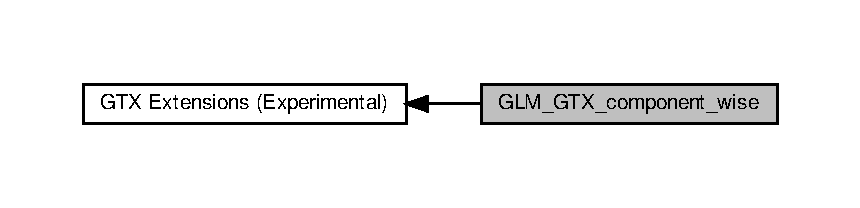
\includegraphics[width=350pt]{group__gtx__component__wise}
\end{center}
\end{figure}
\subsection*{Functions}
\begin{DoxyCompactItemize}
\item 
{\footnotesize template$<$typename gen\+Type $>$ }\\\hyperlink{setup_8hpp_ab2d052de21a70539923e9bcbf6e83a51}{G\+L\+M\+\_\+\+F\+U\+N\+C\+\_\+\+D\+E\+CL} gen\+Type\+::value\+\_\+type \hyperlink{group__gtx__component__wise_gaf71833350e15e74d31cbf8a3e7f27051}{glm\+::comp\+Add} (gen\+Type const \&v)
\item 
{\footnotesize template$<$typename gen\+Type $>$ }\\\hyperlink{setup_8hpp_ab2d052de21a70539923e9bcbf6e83a51}{G\+L\+M\+\_\+\+F\+U\+N\+C\+\_\+\+D\+E\+CL} gen\+Type\+::value\+\_\+type \hyperlink{group__gtx__component__wise_gae8ab88024197202c9479d33bdc5a8a5d}{glm\+::comp\+Mul} (gen\+Type const \&v)
\item 
{\footnotesize template$<$typename gen\+Type $>$ }\\\hyperlink{setup_8hpp_ab2d052de21a70539923e9bcbf6e83a51}{G\+L\+M\+\_\+\+F\+U\+N\+C\+\_\+\+D\+E\+CL} gen\+Type\+::value\+\_\+type \hyperlink{group__gtx__component__wise_gab5d0832b5c7bb01b8d7395973bfb1425}{glm\+::comp\+Min} (gen\+Type const \&v)
\item 
{\footnotesize template$<$typename gen\+Type $>$ }\\\hyperlink{setup_8hpp_ab2d052de21a70539923e9bcbf6e83a51}{G\+L\+M\+\_\+\+F\+U\+N\+C\+\_\+\+D\+E\+CL} gen\+Type\+::value\+\_\+type \hyperlink{group__gtx__component__wise_gabfa4bb19298c8c73d4217ba759c496b6}{glm\+::comp\+Max} (gen\+Type const \&v)
\end{DoxyCompactItemize}


\subsection{Detailed Description}
Operations between components of a type. 

$<$\hyperlink{component__wise_8hpp}{glm/gtx/component\+\_\+wise.\+hpp}$>$ need to be included to use these functionalities. 

\subsection{Function Documentation}
\mbox{\Hypertarget{group__gtx__component__wise_gaf71833350e15e74d31cbf8a3e7f27051}\label{group__gtx__component__wise_gaf71833350e15e74d31cbf8a3e7f27051}} 
\index{G\+L\+M\+\_\+\+G\+T\+X\+\_\+component\+\_\+wise@{G\+L\+M\+\_\+\+G\+T\+X\+\_\+component\+\_\+wise}!comp\+Add@{comp\+Add}}
\index{comp\+Add@{comp\+Add}!G\+L\+M\+\_\+\+G\+T\+X\+\_\+component\+\_\+wise@{G\+L\+M\+\_\+\+G\+T\+X\+\_\+component\+\_\+wise}}
\subsubsection{\texorpdfstring{comp\+Add()}{compAdd()}}
{\footnotesize\ttfamily template$<$typename gen\+Type $>$ \\
\hyperlink{setup_8hpp_ab2d052de21a70539923e9bcbf6e83a51}{G\+L\+M\+\_\+\+F\+U\+N\+C\+\_\+\+D\+E\+CL} gen\+Type\+::value\+\_\+type glm\+::comp\+Add (\begin{DoxyParamCaption}\item[{gen\+Type const \&}]{v }\end{DoxyParamCaption})}

Add all vector components together. \begin{DoxySeeAlso}{See also}
\hyperlink{group__gtx__component__wise}{G\+L\+M\+\_\+\+G\+T\+X\+\_\+component\+\_\+wise} 
\end{DoxySeeAlso}
\mbox{\Hypertarget{group__gtx__component__wise_gabfa4bb19298c8c73d4217ba759c496b6}\label{group__gtx__component__wise_gabfa4bb19298c8c73d4217ba759c496b6}} 
\index{G\+L\+M\+\_\+\+G\+T\+X\+\_\+component\+\_\+wise@{G\+L\+M\+\_\+\+G\+T\+X\+\_\+component\+\_\+wise}!comp\+Max@{comp\+Max}}
\index{comp\+Max@{comp\+Max}!G\+L\+M\+\_\+\+G\+T\+X\+\_\+component\+\_\+wise@{G\+L\+M\+\_\+\+G\+T\+X\+\_\+component\+\_\+wise}}
\subsubsection{\texorpdfstring{comp\+Max()}{compMax()}}
{\footnotesize\ttfamily template$<$typename gen\+Type $>$ \\
\hyperlink{setup_8hpp_ab2d052de21a70539923e9bcbf6e83a51}{G\+L\+M\+\_\+\+F\+U\+N\+C\+\_\+\+D\+E\+CL} gen\+Type\+::value\+\_\+type glm\+::comp\+Max (\begin{DoxyParamCaption}\item[{gen\+Type const \&}]{v }\end{DoxyParamCaption})}

Find the maximum value between single vector components. \begin{DoxySeeAlso}{See also}
\hyperlink{group__gtx__component__wise}{G\+L\+M\+\_\+\+G\+T\+X\+\_\+component\+\_\+wise} 
\end{DoxySeeAlso}
\mbox{\Hypertarget{group__gtx__component__wise_gab5d0832b5c7bb01b8d7395973bfb1425}\label{group__gtx__component__wise_gab5d0832b5c7bb01b8d7395973bfb1425}} 
\index{G\+L\+M\+\_\+\+G\+T\+X\+\_\+component\+\_\+wise@{G\+L\+M\+\_\+\+G\+T\+X\+\_\+component\+\_\+wise}!comp\+Min@{comp\+Min}}
\index{comp\+Min@{comp\+Min}!G\+L\+M\+\_\+\+G\+T\+X\+\_\+component\+\_\+wise@{G\+L\+M\+\_\+\+G\+T\+X\+\_\+component\+\_\+wise}}
\subsubsection{\texorpdfstring{comp\+Min()}{compMin()}}
{\footnotesize\ttfamily template$<$typename gen\+Type $>$ \\
\hyperlink{setup_8hpp_ab2d052de21a70539923e9bcbf6e83a51}{G\+L\+M\+\_\+\+F\+U\+N\+C\+\_\+\+D\+E\+CL} gen\+Type\+::value\+\_\+type glm\+::comp\+Min (\begin{DoxyParamCaption}\item[{gen\+Type const \&}]{v }\end{DoxyParamCaption})}

Find the minimum value between single vector components. \begin{DoxySeeAlso}{See also}
\hyperlink{group__gtx__component__wise}{G\+L\+M\+\_\+\+G\+T\+X\+\_\+component\+\_\+wise} 
\end{DoxySeeAlso}
\mbox{\Hypertarget{group__gtx__component__wise_gae8ab88024197202c9479d33bdc5a8a5d}\label{group__gtx__component__wise_gae8ab88024197202c9479d33bdc5a8a5d}} 
\index{G\+L\+M\+\_\+\+G\+T\+X\+\_\+component\+\_\+wise@{G\+L\+M\+\_\+\+G\+T\+X\+\_\+component\+\_\+wise}!comp\+Mul@{comp\+Mul}}
\index{comp\+Mul@{comp\+Mul}!G\+L\+M\+\_\+\+G\+T\+X\+\_\+component\+\_\+wise@{G\+L\+M\+\_\+\+G\+T\+X\+\_\+component\+\_\+wise}}
\subsubsection{\texorpdfstring{comp\+Mul()}{compMul()}}
{\footnotesize\ttfamily template$<$typename gen\+Type $>$ \\
\hyperlink{setup_8hpp_ab2d052de21a70539923e9bcbf6e83a51}{G\+L\+M\+\_\+\+F\+U\+N\+C\+\_\+\+D\+E\+CL} gen\+Type\+::value\+\_\+type glm\+::comp\+Mul (\begin{DoxyParamCaption}\item[{gen\+Type const \&}]{v }\end{DoxyParamCaption})}

Multiply all vector components together. \begin{DoxySeeAlso}{See also}
\hyperlink{group__gtx__component__wise}{G\+L\+M\+\_\+\+G\+T\+X\+\_\+component\+\_\+wise} 
\end{DoxySeeAlso}

\hypertarget{group__gtc__dual__quaternion}{}\section{G\+L\+M\+\_\+\+G\+T\+X\+\_\+dual\+\_\+quaternion}
\label{group__gtc__dual__quaternion}\index{G\+L\+M\+\_\+\+G\+T\+X\+\_\+dual\+\_\+quaternion@{G\+L\+M\+\_\+\+G\+T\+X\+\_\+dual\+\_\+quaternion}}


Defines a templated dual-\/quaternion type and several dual-\/quaternion operations.  


Collaboration diagram for G\+L\+M\+\_\+\+G\+T\+X\+\_\+dual\+\_\+quaternion\+:\nopagebreak
\begin{figure}[H]
\begin{center}
\leavevmode
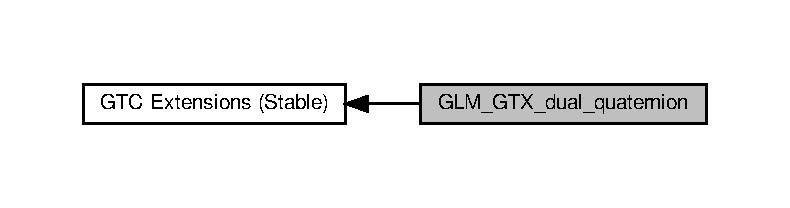
\includegraphics[width=350pt]{group__gtc__dual__quaternion}
\end{center}
\end{figure}
\subsection*{Typedefs}
\begin{DoxyCompactItemize}
\item 
typedef \hyperlink{structglm_1_1detail_1_1tdualquat}{detail\+::tdualquat}$<$ float, \hyperlink{namespaceglm_a0f04f086094c747d227af4425893f545ae161af3fc695e696ce3bf69f7332bc2d}{lowp} $>$ \hyperlink{group__gtc__dual__quaternion_gae1772179edc60f4e8b46c8772eeeccee}{glm\+::lowp\+\_\+dualquat}
\item 
typedef \hyperlink{structglm_1_1detail_1_1tdualquat}{detail\+::tdualquat}$<$ float, \hyperlink{namespaceglm_a0f04f086094c747d227af4425893f545a6416f3ea0c9025fb21ed50c4d6620482}{mediump} $>$ \hyperlink{group__gtc__dual__quaternion_ga71fc1c10a382330c1fee55ce29703405}{glm\+::mediump\+\_\+dualquat}
\item 
typedef \hyperlink{structglm_1_1detail_1_1tdualquat}{detail\+::tdualquat}$<$ float, \hyperlink{namespaceglm_a0f04f086094c747d227af4425893f545ac6f7eab42eacbb10d59a58e95e362074}{highp} $>$ \hyperlink{group__gtc__dual__quaternion_gaf3a01deb502f53ca555ee1d45e6d6776}{glm\+::highp\+\_\+dualquat}
\item 
typedef \hyperlink{structglm_1_1detail_1_1tdualquat}{detail\+::tdualquat}$<$ float, \hyperlink{namespaceglm_a0f04f086094c747d227af4425893f545ae161af3fc695e696ce3bf69f7332bc2d}{lowp} $>$ \hyperlink{group__gtc__dual__quaternion_gae62c636c63c9eb3c1ea6d10f4b7d7c81}{glm\+::lowp\+\_\+fdualquat}
\item 
typedef \hyperlink{structglm_1_1detail_1_1tdualquat}{detail\+::tdualquat}$<$ float, \hyperlink{namespaceglm_a0f04f086094c747d227af4425893f545a6416f3ea0c9025fb21ed50c4d6620482}{mediump} $>$ \hyperlink{group__gtc__dual__quaternion_gab211d24786158490e57dfa57d7744f71}{glm\+::mediump\+\_\+fdualquat}
\item 
typedef \hyperlink{structglm_1_1detail_1_1tdualquat}{detail\+::tdualquat}$<$ float, \hyperlink{namespaceglm_a0f04f086094c747d227af4425893f545ac6f7eab42eacbb10d59a58e95e362074}{highp} $>$ \hyperlink{group__gtc__dual__quaternion_ga2ed3283c09d3ffaf52a0e0a4b248eab6}{glm\+::highp\+\_\+fdualquat}
\item 
typedef \hyperlink{structglm_1_1detail_1_1tdualquat}{detail\+::tdualquat}$<$ double, \hyperlink{namespaceglm_a0f04f086094c747d227af4425893f545ae161af3fc695e696ce3bf69f7332bc2d}{lowp} $>$ \hyperlink{group__gtc__dual__quaternion_ga29461fddd543ffdf65a199fc28c42458}{glm\+::lowp\+\_\+ddualquat}
\item 
typedef \hyperlink{structglm_1_1detail_1_1tdualquat}{detail\+::tdualquat}$<$ double, \hyperlink{namespaceglm_a0f04f086094c747d227af4425893f545a6416f3ea0c9025fb21ed50c4d6620482}{mediump} $>$ \hyperlink{group__gtc__dual__quaternion_ga62d8cbf30e2afd0b1044204268a69066}{glm\+::mediump\+\_\+ddualquat}
\item 
typedef \hyperlink{structglm_1_1detail_1_1tdualquat}{detail\+::tdualquat}$<$ double, \hyperlink{namespaceglm_a0f04f086094c747d227af4425893f545ac6f7eab42eacbb10d59a58e95e362074}{highp} $>$ \hyperlink{group__gtc__dual__quaternion_ga61b654c21f080135aedcf23461eb1037}{glm\+::highp\+\_\+ddualquat}
\item 
typedef \hyperlink{group__gtc__dual__quaternion_ga2ed3283c09d3ffaf52a0e0a4b248eab6}{highp\+\_\+fdualquat} \hyperlink{group__gtc__dual__quaternion_ga2f6227b5f9dc08a2e7682065a84b3aa9}{glm\+::dualquat}
\item 
typedef \hyperlink{group__gtc__dual__quaternion_ga2ed3283c09d3ffaf52a0e0a4b248eab6}{highp\+\_\+fdualquat} \hyperlink{group__gtc__dual__quaternion_ga436906129bc69ca5059555cafcbac9fd}{glm\+::fdualquat}
\item 
typedef \hyperlink{group__gtc__dual__quaternion_ga61b654c21f080135aedcf23461eb1037}{highp\+\_\+ddualquat} \hyperlink{group__gtc__dual__quaternion_ga373431ffdd82d5c03c258217a9e1f1a6}{glm\+::ddualquat}
\end{DoxyCompactItemize}
\subsection*{Functions}
\begin{DoxyCompactItemize}
\item 
{\footnotesize template$<$typename T , precision P$>$ }\\\hyperlink{setup_8hpp_ab2d052de21a70539923e9bcbf6e83a51}{G\+L\+M\+\_\+\+F\+U\+N\+C\+\_\+\+D\+E\+CL} \hyperlink{structglm_1_1detail_1_1tdualquat}{detail\+::tdualquat}$<$ T, P $>$ \hyperlink{group__gtc__dual__quaternion_ga4364d115fe8ee2f65ff047726133d0ad}{glm\+::normalize} (\hyperlink{structglm_1_1detail_1_1tdualquat}{detail\+::tdualquat}$<$ T, P $>$ const \&q)
\item 
{\footnotesize template$<$typename T , precision P$>$ }\\\hyperlink{setup_8hpp_ab2d052de21a70539923e9bcbf6e83a51}{G\+L\+M\+\_\+\+F\+U\+N\+C\+\_\+\+D\+E\+CL} \hyperlink{structglm_1_1detail_1_1tdualquat}{detail\+::tdualquat}$<$ T, P $>$ \hyperlink{group__gtc__dual__quaternion_ga28cbcf029272d5351d4695b8610de126}{glm\+::lerp} (\hyperlink{structglm_1_1detail_1_1tdualquat}{detail\+::tdualquat}$<$ T, P $>$ const \&x, \hyperlink{structglm_1_1detail_1_1tdualquat}{detail\+::tdualquat}$<$ T, P $>$ const \&y, T const \&a)
\item 
{\footnotesize template$<$typename T , precision P$>$ }\\\hyperlink{setup_8hpp_ab2d052de21a70539923e9bcbf6e83a51}{G\+L\+M\+\_\+\+F\+U\+N\+C\+\_\+\+D\+E\+CL} \hyperlink{structglm_1_1detail_1_1tdualquat}{detail\+::tdualquat}$<$ T, P $>$ \hyperlink{group__gtc__dual__quaternion_gaad6b9faeb1134c04defae01426a777f8}{glm\+::inverse} (\hyperlink{structglm_1_1detail_1_1tdualquat}{detail\+::tdualquat}$<$ T, P $>$ const \&q)
\item 
{\footnotesize template$<$typename T , precision P$>$ }\\\hyperlink{setup_8hpp_ab2d052de21a70539923e9bcbf6e83a51}{G\+L\+M\+\_\+\+F\+U\+N\+C\+\_\+\+D\+E\+CL} \hyperlink{structglm_1_1detail_1_1tmat2x4}{detail\+::tmat2x4}$<$ T, P $>$ \hyperlink{group__gtc__dual__quaternion_gade155fb0dfc144259a25897776e73325}{glm\+::mat2x4\+\_\+cast} (\hyperlink{structglm_1_1detail_1_1tdualquat}{detail\+::tdualquat}$<$ T, P $>$ const \&x)
\item 
{\footnotesize template$<$typename T , precision P$>$ }\\\hyperlink{setup_8hpp_ab2d052de21a70539923e9bcbf6e83a51}{G\+L\+M\+\_\+\+F\+U\+N\+C\+\_\+\+D\+E\+CL} \hyperlink{structglm_1_1detail_1_1tmat3x4}{detail\+::tmat3x4}$<$ T, P $>$ \hyperlink{group__gtc__dual__quaternion_ga2f4f0a1275fa95c272dd6ad6df75013d}{glm\+::mat3x4\+\_\+cast} (\hyperlink{structglm_1_1detail_1_1tdualquat}{detail\+::tdualquat}$<$ T, P $>$ const \&x)
\item 
{\footnotesize template$<$typename T , precision P$>$ }\\\hyperlink{setup_8hpp_ab2d052de21a70539923e9bcbf6e83a51}{G\+L\+M\+\_\+\+F\+U\+N\+C\+\_\+\+D\+E\+CL} \hyperlink{structglm_1_1detail_1_1tdualquat}{detail\+::tdualquat}$<$ T, P $>$ \hyperlink{group__gtc__dual__quaternion_gad47c752ec23a5f9924e7d7f84c40f3e5}{glm\+::dualquat\+\_\+cast} (\hyperlink{structglm_1_1detail_1_1tmat2x4}{detail\+::tmat2x4}$<$ T, P $>$ const \&x)
\item 
{\footnotesize template$<$typename T , precision P$>$ }\\\hyperlink{setup_8hpp_ab2d052de21a70539923e9bcbf6e83a51}{G\+L\+M\+\_\+\+F\+U\+N\+C\+\_\+\+D\+E\+CL} \hyperlink{structglm_1_1detail_1_1tdualquat}{detail\+::tdualquat}$<$ T, P $>$ \hyperlink{group__gtc__dual__quaternion_ga97c4fb8941ad1954e01578cca8182180}{glm\+::dualquat\+\_\+cast} (\hyperlink{structglm_1_1detail_1_1tmat3x4}{detail\+::tmat3x4}$<$ T, P $>$ const \&x)
\end{DoxyCompactItemize}


\subsection{Detailed Description}
Defines a templated dual-\/quaternion type and several dual-\/quaternion operations. 

$<$\hyperlink{dual__quaternion_8hpp}{glm/gtx/dual\+\_\+quaternion.\+hpp}$>$ need to be included to use these functionalities. 

\subsection{Typedef Documentation}
\mbox{\Hypertarget{group__gtc__dual__quaternion_ga373431ffdd82d5c03c258217a9e1f1a6}\label{group__gtc__dual__quaternion_ga373431ffdd82d5c03c258217a9e1f1a6}} 
\index{G\+L\+M\+\_\+\+G\+T\+X\+\_\+dual\+\_\+quaternion@{G\+L\+M\+\_\+\+G\+T\+X\+\_\+dual\+\_\+quaternion}!ddualquat@{ddualquat}}
\index{ddualquat@{ddualquat}!G\+L\+M\+\_\+\+G\+T\+X\+\_\+dual\+\_\+quaternion@{G\+L\+M\+\_\+\+G\+T\+X\+\_\+dual\+\_\+quaternion}}
\subsubsection{\texorpdfstring{ddualquat}{ddualquat}}
{\footnotesize\ttfamily typedef \hyperlink{group__gtc__dual__quaternion_ga61b654c21f080135aedcf23461eb1037}{highp\+\_\+ddualquat} \hyperlink{group__gtc__dual__quaternion_ga373431ffdd82d5c03c258217a9e1f1a6}{glm\+::ddualquat}}

Dual-\/quaternion of default double-\/precision floating-\/point numbers.

\begin{DoxySeeAlso}{See also}
\hyperlink{group__gtc__dual__quaternion}{G\+L\+M\+\_\+\+G\+T\+X\+\_\+dual\+\_\+quaternion} 
\end{DoxySeeAlso}


Definition at line 279 of file dual\+\_\+quaternion.\+hpp.

\mbox{\Hypertarget{group__gtc__dual__quaternion_ga2f6227b5f9dc08a2e7682065a84b3aa9}\label{group__gtc__dual__quaternion_ga2f6227b5f9dc08a2e7682065a84b3aa9}} 
\index{G\+L\+M\+\_\+\+G\+T\+X\+\_\+dual\+\_\+quaternion@{G\+L\+M\+\_\+\+G\+T\+X\+\_\+dual\+\_\+quaternion}!dualquat@{dualquat}}
\index{dualquat@{dualquat}!G\+L\+M\+\_\+\+G\+T\+X\+\_\+dual\+\_\+quaternion@{G\+L\+M\+\_\+\+G\+T\+X\+\_\+dual\+\_\+quaternion}}
\subsubsection{\texorpdfstring{dualquat}{dualquat}}
{\footnotesize\ttfamily typedef \hyperlink{group__gtc__dual__quaternion_ga2ed3283c09d3ffaf52a0e0a4b248eab6}{highp\+\_\+fdualquat} \hyperlink{group__gtc__dual__quaternion_ga2f6227b5f9dc08a2e7682065a84b3aa9}{glm\+::dualquat}}

Dual-\/quaternion of floating-\/point numbers.

\begin{DoxySeeAlso}{See also}
\hyperlink{group__gtc__dual__quaternion}{G\+L\+M\+\_\+\+G\+T\+X\+\_\+dual\+\_\+quaternion} 
\end{DoxySeeAlso}


Definition at line 255 of file dual\+\_\+quaternion.\+hpp.

\mbox{\Hypertarget{group__gtc__dual__quaternion_ga436906129bc69ca5059555cafcbac9fd}\label{group__gtc__dual__quaternion_ga436906129bc69ca5059555cafcbac9fd}} 
\index{G\+L\+M\+\_\+\+G\+T\+X\+\_\+dual\+\_\+quaternion@{G\+L\+M\+\_\+\+G\+T\+X\+\_\+dual\+\_\+quaternion}!fdualquat@{fdualquat}}
\index{fdualquat@{fdualquat}!G\+L\+M\+\_\+\+G\+T\+X\+\_\+dual\+\_\+quaternion@{G\+L\+M\+\_\+\+G\+T\+X\+\_\+dual\+\_\+quaternion}}
\subsubsection{\texorpdfstring{fdualquat}{fdualquat}}
{\footnotesize\ttfamily typedef \hyperlink{group__gtc__dual__quaternion_ga2ed3283c09d3ffaf52a0e0a4b248eab6}{highp\+\_\+fdualquat} \hyperlink{group__gtc__dual__quaternion_ga436906129bc69ca5059555cafcbac9fd}{glm\+::fdualquat}}

Dual-\/quaternion of single-\/precision floating-\/point numbers.

\begin{DoxySeeAlso}{See also}
\hyperlink{group__gtc__dual__quaternion}{G\+L\+M\+\_\+\+G\+T\+X\+\_\+dual\+\_\+quaternion} 
\end{DoxySeeAlso}


Definition at line 260 of file dual\+\_\+quaternion.\+hpp.

\mbox{\Hypertarget{group__gtc__dual__quaternion_ga61b654c21f080135aedcf23461eb1037}\label{group__gtc__dual__quaternion_ga61b654c21f080135aedcf23461eb1037}} 
\index{G\+L\+M\+\_\+\+G\+T\+X\+\_\+dual\+\_\+quaternion@{G\+L\+M\+\_\+\+G\+T\+X\+\_\+dual\+\_\+quaternion}!highp\+\_\+ddualquat@{highp\+\_\+ddualquat}}
\index{highp\+\_\+ddualquat@{highp\+\_\+ddualquat}!G\+L\+M\+\_\+\+G\+T\+X\+\_\+dual\+\_\+quaternion@{G\+L\+M\+\_\+\+G\+T\+X\+\_\+dual\+\_\+quaternion}}
\subsubsection{\texorpdfstring{highp\+\_\+ddualquat}{highp\_ddualquat}}
{\footnotesize\ttfamily typedef \hyperlink{structglm_1_1detail_1_1tdualquat}{detail\+::tdualquat}$<$double, \hyperlink{namespaceglm_a0f04f086094c747d227af4425893f545ac6f7eab42eacbb10d59a58e95e362074}{highp}$>$ \hyperlink{group__gtc__dual__quaternion_ga61b654c21f080135aedcf23461eb1037}{glm\+::highp\+\_\+ddualquat}}

Dual-\/quaternion of high double-\/precision floating-\/point numbers.

\begin{DoxySeeAlso}{See also}
\hyperlink{group__gtc__dual__quaternion}{G\+L\+M\+\_\+\+G\+T\+X\+\_\+dual\+\_\+quaternion} 
\end{DoxySeeAlso}


Definition at line 248 of file dual\+\_\+quaternion.\+hpp.

\mbox{\Hypertarget{group__gtc__dual__quaternion_gaf3a01deb502f53ca555ee1d45e6d6776}\label{group__gtc__dual__quaternion_gaf3a01deb502f53ca555ee1d45e6d6776}} 
\index{G\+L\+M\+\_\+\+G\+T\+X\+\_\+dual\+\_\+quaternion@{G\+L\+M\+\_\+\+G\+T\+X\+\_\+dual\+\_\+quaternion}!highp\+\_\+dualquat@{highp\+\_\+dualquat}}
\index{highp\+\_\+dualquat@{highp\+\_\+dualquat}!G\+L\+M\+\_\+\+G\+T\+X\+\_\+dual\+\_\+quaternion@{G\+L\+M\+\_\+\+G\+T\+X\+\_\+dual\+\_\+quaternion}}
\subsubsection{\texorpdfstring{highp\+\_\+dualquat}{highp\_dualquat}}
{\footnotesize\ttfamily typedef \hyperlink{structglm_1_1detail_1_1tdualquat}{detail\+::tdualquat}$<$float, \hyperlink{namespaceglm_a0f04f086094c747d227af4425893f545ac6f7eab42eacbb10d59a58e95e362074}{highp}$>$ \hyperlink{group__gtc__dual__quaternion_gaf3a01deb502f53ca555ee1d45e6d6776}{glm\+::highp\+\_\+dualquat}}

Dual-\/quaternion of high single-\/precision floating-\/point numbers.

\begin{DoxySeeAlso}{See also}
\hyperlink{group__gtc__dual__quaternion}{G\+L\+M\+\_\+\+G\+T\+X\+\_\+dual\+\_\+quaternion} 
\end{DoxySeeAlso}


Definition at line 216 of file dual\+\_\+quaternion.\+hpp.

\mbox{\Hypertarget{group__gtc__dual__quaternion_ga2ed3283c09d3ffaf52a0e0a4b248eab6}\label{group__gtc__dual__quaternion_ga2ed3283c09d3ffaf52a0e0a4b248eab6}} 
\index{G\+L\+M\+\_\+\+G\+T\+X\+\_\+dual\+\_\+quaternion@{G\+L\+M\+\_\+\+G\+T\+X\+\_\+dual\+\_\+quaternion}!highp\+\_\+fdualquat@{highp\+\_\+fdualquat}}
\index{highp\+\_\+fdualquat@{highp\+\_\+fdualquat}!G\+L\+M\+\_\+\+G\+T\+X\+\_\+dual\+\_\+quaternion@{G\+L\+M\+\_\+\+G\+T\+X\+\_\+dual\+\_\+quaternion}}
\subsubsection{\texorpdfstring{highp\+\_\+fdualquat}{highp\_fdualquat}}
{\footnotesize\ttfamily typedef \hyperlink{structglm_1_1detail_1_1tdualquat}{detail\+::tdualquat}$<$float, \hyperlink{namespaceglm_a0f04f086094c747d227af4425893f545ac6f7eab42eacbb10d59a58e95e362074}{highp}$>$ \hyperlink{group__gtc__dual__quaternion_ga2ed3283c09d3ffaf52a0e0a4b248eab6}{glm\+::highp\+\_\+fdualquat}}

Dual-\/quaternion of high single-\/precision floating-\/point numbers.

\begin{DoxySeeAlso}{See also}
\hyperlink{group__gtc__dual__quaternion}{G\+L\+M\+\_\+\+G\+T\+X\+\_\+dual\+\_\+quaternion} 
\end{DoxySeeAlso}


Definition at line 232 of file dual\+\_\+quaternion.\+hpp.

\mbox{\Hypertarget{group__gtc__dual__quaternion_ga29461fddd543ffdf65a199fc28c42458}\label{group__gtc__dual__quaternion_ga29461fddd543ffdf65a199fc28c42458}} 
\index{G\+L\+M\+\_\+\+G\+T\+X\+\_\+dual\+\_\+quaternion@{G\+L\+M\+\_\+\+G\+T\+X\+\_\+dual\+\_\+quaternion}!lowp\+\_\+ddualquat@{lowp\+\_\+ddualquat}}
\index{lowp\+\_\+ddualquat@{lowp\+\_\+ddualquat}!G\+L\+M\+\_\+\+G\+T\+X\+\_\+dual\+\_\+quaternion@{G\+L\+M\+\_\+\+G\+T\+X\+\_\+dual\+\_\+quaternion}}
\subsubsection{\texorpdfstring{lowp\+\_\+ddualquat}{lowp\_ddualquat}}
{\footnotesize\ttfamily typedef \hyperlink{structglm_1_1detail_1_1tdualquat}{detail\+::tdualquat}$<$double, \hyperlink{namespaceglm_a0f04f086094c747d227af4425893f545ae161af3fc695e696ce3bf69f7332bc2d}{lowp}$>$ \hyperlink{group__gtc__dual__quaternion_ga29461fddd543ffdf65a199fc28c42458}{glm\+::lowp\+\_\+ddualquat}}

Dual-\/quaternion of low double-\/precision floating-\/point numbers.

\begin{DoxySeeAlso}{See also}
\hyperlink{group__gtc__dual__quaternion}{G\+L\+M\+\_\+\+G\+T\+X\+\_\+dual\+\_\+quaternion} 
\end{DoxySeeAlso}


Definition at line 238 of file dual\+\_\+quaternion.\+hpp.

\mbox{\Hypertarget{group__gtc__dual__quaternion_gae1772179edc60f4e8b46c8772eeeccee}\label{group__gtc__dual__quaternion_gae1772179edc60f4e8b46c8772eeeccee}} 
\index{G\+L\+M\+\_\+\+G\+T\+X\+\_\+dual\+\_\+quaternion@{G\+L\+M\+\_\+\+G\+T\+X\+\_\+dual\+\_\+quaternion}!lowp\+\_\+dualquat@{lowp\+\_\+dualquat}}
\index{lowp\+\_\+dualquat@{lowp\+\_\+dualquat}!G\+L\+M\+\_\+\+G\+T\+X\+\_\+dual\+\_\+quaternion@{G\+L\+M\+\_\+\+G\+T\+X\+\_\+dual\+\_\+quaternion}}
\subsubsection{\texorpdfstring{lowp\+\_\+dualquat}{lowp\_dualquat}}
{\footnotesize\ttfamily typedef \hyperlink{structglm_1_1detail_1_1tdualquat}{detail\+::tdualquat}$<$float, \hyperlink{namespaceglm_a0f04f086094c747d227af4425893f545ae161af3fc695e696ce3bf69f7332bc2d}{lowp}$>$ \hyperlink{group__gtc__dual__quaternion_gae1772179edc60f4e8b46c8772eeeccee}{glm\+::lowp\+\_\+dualquat}}

Dual-\/quaternion of low single-\/precision floating-\/point numbers.

\begin{DoxySeeAlso}{See also}
\hyperlink{group__gtc__dual__quaternion}{G\+L\+M\+\_\+\+G\+T\+X\+\_\+dual\+\_\+quaternion} 
\end{DoxySeeAlso}


Definition at line 206 of file dual\+\_\+quaternion.\+hpp.

\mbox{\Hypertarget{group__gtc__dual__quaternion_gae62c636c63c9eb3c1ea6d10f4b7d7c81}\label{group__gtc__dual__quaternion_gae62c636c63c9eb3c1ea6d10f4b7d7c81}} 
\index{G\+L\+M\+\_\+\+G\+T\+X\+\_\+dual\+\_\+quaternion@{G\+L\+M\+\_\+\+G\+T\+X\+\_\+dual\+\_\+quaternion}!lowp\+\_\+fdualquat@{lowp\+\_\+fdualquat}}
\index{lowp\+\_\+fdualquat@{lowp\+\_\+fdualquat}!G\+L\+M\+\_\+\+G\+T\+X\+\_\+dual\+\_\+quaternion@{G\+L\+M\+\_\+\+G\+T\+X\+\_\+dual\+\_\+quaternion}}
\subsubsection{\texorpdfstring{lowp\+\_\+fdualquat}{lowp\_fdualquat}}
{\footnotesize\ttfamily typedef \hyperlink{structglm_1_1detail_1_1tdualquat}{detail\+::tdualquat}$<$float, \hyperlink{namespaceglm_a0f04f086094c747d227af4425893f545ae161af3fc695e696ce3bf69f7332bc2d}{lowp}$>$ \hyperlink{group__gtc__dual__quaternion_gae62c636c63c9eb3c1ea6d10f4b7d7c81}{glm\+::lowp\+\_\+fdualquat}}

Dual-\/quaternion of low single-\/precision floating-\/point numbers.

\begin{DoxySeeAlso}{See also}
\hyperlink{group__gtc__dual__quaternion}{G\+L\+M\+\_\+\+G\+T\+X\+\_\+dual\+\_\+quaternion} 
\end{DoxySeeAlso}


Definition at line 222 of file dual\+\_\+quaternion.\+hpp.

\mbox{\Hypertarget{group__gtc__dual__quaternion_ga62d8cbf30e2afd0b1044204268a69066}\label{group__gtc__dual__quaternion_ga62d8cbf30e2afd0b1044204268a69066}} 
\index{G\+L\+M\+\_\+\+G\+T\+X\+\_\+dual\+\_\+quaternion@{G\+L\+M\+\_\+\+G\+T\+X\+\_\+dual\+\_\+quaternion}!mediump\+\_\+ddualquat@{mediump\+\_\+ddualquat}}
\index{mediump\+\_\+ddualquat@{mediump\+\_\+ddualquat}!G\+L\+M\+\_\+\+G\+T\+X\+\_\+dual\+\_\+quaternion@{G\+L\+M\+\_\+\+G\+T\+X\+\_\+dual\+\_\+quaternion}}
\subsubsection{\texorpdfstring{mediump\+\_\+ddualquat}{mediump\_ddualquat}}
{\footnotesize\ttfamily typedef \hyperlink{structglm_1_1detail_1_1tdualquat}{detail\+::tdualquat}$<$double, \hyperlink{namespaceglm_a0f04f086094c747d227af4425893f545a6416f3ea0c9025fb21ed50c4d6620482}{mediump}$>$ \hyperlink{group__gtc__dual__quaternion_ga62d8cbf30e2afd0b1044204268a69066}{glm\+::mediump\+\_\+ddualquat}}

Dual-\/quaternion of medium double-\/precision floating-\/point numbers.

\begin{DoxySeeAlso}{See also}
\hyperlink{group__gtc__dual__quaternion}{G\+L\+M\+\_\+\+G\+T\+X\+\_\+dual\+\_\+quaternion} 
\end{DoxySeeAlso}


Definition at line 243 of file dual\+\_\+quaternion.\+hpp.

\mbox{\Hypertarget{group__gtc__dual__quaternion_ga71fc1c10a382330c1fee55ce29703405}\label{group__gtc__dual__quaternion_ga71fc1c10a382330c1fee55ce29703405}} 
\index{G\+L\+M\+\_\+\+G\+T\+X\+\_\+dual\+\_\+quaternion@{G\+L\+M\+\_\+\+G\+T\+X\+\_\+dual\+\_\+quaternion}!mediump\+\_\+dualquat@{mediump\+\_\+dualquat}}
\index{mediump\+\_\+dualquat@{mediump\+\_\+dualquat}!G\+L\+M\+\_\+\+G\+T\+X\+\_\+dual\+\_\+quaternion@{G\+L\+M\+\_\+\+G\+T\+X\+\_\+dual\+\_\+quaternion}}
\subsubsection{\texorpdfstring{mediump\+\_\+dualquat}{mediump\_dualquat}}
{\footnotesize\ttfamily typedef \hyperlink{structglm_1_1detail_1_1tdualquat}{detail\+::tdualquat}$<$float, \hyperlink{namespaceglm_a0f04f086094c747d227af4425893f545a6416f3ea0c9025fb21ed50c4d6620482}{mediump}$>$ \hyperlink{group__gtc__dual__quaternion_ga71fc1c10a382330c1fee55ce29703405}{glm\+::mediump\+\_\+dualquat}}

Dual-\/quaternion of medium single-\/precision floating-\/point numbers.

\begin{DoxySeeAlso}{See also}
\hyperlink{group__gtc__dual__quaternion}{G\+L\+M\+\_\+\+G\+T\+X\+\_\+dual\+\_\+quaternion} 
\end{DoxySeeAlso}


Definition at line 211 of file dual\+\_\+quaternion.\+hpp.

\mbox{\Hypertarget{group__gtc__dual__quaternion_gab211d24786158490e57dfa57d7744f71}\label{group__gtc__dual__quaternion_gab211d24786158490e57dfa57d7744f71}} 
\index{G\+L\+M\+\_\+\+G\+T\+X\+\_\+dual\+\_\+quaternion@{G\+L\+M\+\_\+\+G\+T\+X\+\_\+dual\+\_\+quaternion}!mediump\+\_\+fdualquat@{mediump\+\_\+fdualquat}}
\index{mediump\+\_\+fdualquat@{mediump\+\_\+fdualquat}!G\+L\+M\+\_\+\+G\+T\+X\+\_\+dual\+\_\+quaternion@{G\+L\+M\+\_\+\+G\+T\+X\+\_\+dual\+\_\+quaternion}}
\subsubsection{\texorpdfstring{mediump\+\_\+fdualquat}{mediump\_fdualquat}}
{\footnotesize\ttfamily typedef \hyperlink{structglm_1_1detail_1_1tdualquat}{detail\+::tdualquat}$<$float, \hyperlink{namespaceglm_a0f04f086094c747d227af4425893f545a6416f3ea0c9025fb21ed50c4d6620482}{mediump}$>$ \hyperlink{group__gtc__dual__quaternion_gab211d24786158490e57dfa57d7744f71}{glm\+::mediump\+\_\+fdualquat}}

Dual-\/quaternion of medium single-\/precision floating-\/point numbers.

\begin{DoxySeeAlso}{See also}
\hyperlink{group__gtc__dual__quaternion}{G\+L\+M\+\_\+\+G\+T\+X\+\_\+dual\+\_\+quaternion} 
\end{DoxySeeAlso}


Definition at line 227 of file dual\+\_\+quaternion.\+hpp.



\subsection{Function Documentation}
\mbox{\Hypertarget{group__gtc__dual__quaternion_gad47c752ec23a5f9924e7d7f84c40f3e5}\label{group__gtc__dual__quaternion_gad47c752ec23a5f9924e7d7f84c40f3e5}} 
\index{G\+L\+M\+\_\+\+G\+T\+X\+\_\+dual\+\_\+quaternion@{G\+L\+M\+\_\+\+G\+T\+X\+\_\+dual\+\_\+quaternion}!dualquat\+\_\+cast@{dualquat\+\_\+cast}}
\index{dualquat\+\_\+cast@{dualquat\+\_\+cast}!G\+L\+M\+\_\+\+G\+T\+X\+\_\+dual\+\_\+quaternion@{G\+L\+M\+\_\+\+G\+T\+X\+\_\+dual\+\_\+quaternion}}
\subsubsection{\texorpdfstring{dualquat\+\_\+cast()}{dualquat\_cast()}\hspace{0.1cm}{\footnotesize\ttfamily [1/2]}}
{\footnotesize\ttfamily template$<$typename T , precision P$>$ \\
\hyperlink{setup_8hpp_ab2d052de21a70539923e9bcbf6e83a51}{G\+L\+M\+\_\+\+F\+U\+N\+C\+\_\+\+D\+E\+CL} \hyperlink{structglm_1_1detail_1_1tdualquat}{detail\+::tdualquat}$<$T, P$>$ glm\+::dualquat\+\_\+cast (\begin{DoxyParamCaption}\item[{\hyperlink{structglm_1_1detail_1_1tmat2x4}{detail\+::tmat2x4}$<$ T, P $>$ const \&}]{x }\end{DoxyParamCaption})}

Converts a 2 $\ast$ 4 matrix (matrix which holds real and dual parts) to a quaternion.

\begin{DoxySeeAlso}{See also}
\hyperlink{group__gtc__dual__quaternion}{G\+L\+M\+\_\+\+G\+T\+X\+\_\+dual\+\_\+quaternion} 
\end{DoxySeeAlso}


Definition at line 358 of file dual\+\_\+quaternion.\+inl.

\mbox{\Hypertarget{group__gtc__dual__quaternion_ga97c4fb8941ad1954e01578cca8182180}\label{group__gtc__dual__quaternion_ga97c4fb8941ad1954e01578cca8182180}} 
\index{G\+L\+M\+\_\+\+G\+T\+X\+\_\+dual\+\_\+quaternion@{G\+L\+M\+\_\+\+G\+T\+X\+\_\+dual\+\_\+quaternion}!dualquat\+\_\+cast@{dualquat\+\_\+cast}}
\index{dualquat\+\_\+cast@{dualquat\+\_\+cast}!G\+L\+M\+\_\+\+G\+T\+X\+\_\+dual\+\_\+quaternion@{G\+L\+M\+\_\+\+G\+T\+X\+\_\+dual\+\_\+quaternion}}
\subsubsection{\texorpdfstring{dualquat\+\_\+cast()}{dualquat\_cast()}\hspace{0.1cm}{\footnotesize\ttfamily [2/2]}}
{\footnotesize\ttfamily template$<$typename T , precision P$>$ \\
\hyperlink{setup_8hpp_ab2d052de21a70539923e9bcbf6e83a51}{G\+L\+M\+\_\+\+F\+U\+N\+C\+\_\+\+D\+E\+CL} \hyperlink{structglm_1_1detail_1_1tdualquat}{detail\+::tdualquat}$<$T, P$>$ glm\+::dualquat\+\_\+cast (\begin{DoxyParamCaption}\item[{\hyperlink{structglm_1_1detail_1_1tmat3x4}{detail\+::tmat3x4}$<$ T, P $>$ const \&}]{x }\end{DoxyParamCaption})}

Converts a 3 $\ast$ 4 matrix (augmented matrix rotation + translation) to a quaternion.

\begin{DoxySeeAlso}{See also}
\hyperlink{group__gtc__dual__quaternion}{G\+L\+M\+\_\+\+G\+T\+X\+\_\+dual\+\_\+quaternion} 
\end{DoxySeeAlso}


Definition at line 369 of file dual\+\_\+quaternion.\+inl.

\mbox{\Hypertarget{group__gtc__dual__quaternion_gaad6b9faeb1134c04defae01426a777f8}\label{group__gtc__dual__quaternion_gaad6b9faeb1134c04defae01426a777f8}} 
\index{G\+L\+M\+\_\+\+G\+T\+X\+\_\+dual\+\_\+quaternion@{G\+L\+M\+\_\+\+G\+T\+X\+\_\+dual\+\_\+quaternion}!inverse@{inverse}}
\index{inverse@{inverse}!G\+L\+M\+\_\+\+G\+T\+X\+\_\+dual\+\_\+quaternion@{G\+L\+M\+\_\+\+G\+T\+X\+\_\+dual\+\_\+quaternion}}
\subsubsection{\texorpdfstring{inverse()}{inverse()}}
{\footnotesize\ttfamily template$<$typename T , precision P$>$ \\
\hyperlink{setup_8hpp_ab2d052de21a70539923e9bcbf6e83a51}{G\+L\+M\+\_\+\+F\+U\+N\+C\+\_\+\+D\+E\+CL} \hyperlink{structglm_1_1detail_1_1tdualquat}{detail\+::tdualquat}$<$T, P$>$ glm\+::inverse (\begin{DoxyParamCaption}\item[{\hyperlink{structglm_1_1detail_1_1tdualquat}{detail\+::tdualquat}$<$ T, P $>$ const \&}]{q }\end{DoxyParamCaption})}

Returns the q inverse.

\begin{DoxySeeAlso}{See also}
\hyperlink{group__gtc__dual__quaternion}{G\+L\+M\+\_\+\+G\+T\+X\+\_\+dual\+\_\+quaternion} 
\end{DoxySeeAlso}


Definition at line 299 of file dual\+\_\+quaternion.\+inl.

\mbox{\Hypertarget{group__gtc__dual__quaternion_ga28cbcf029272d5351d4695b8610de126}\label{group__gtc__dual__quaternion_ga28cbcf029272d5351d4695b8610de126}} 
\index{G\+L\+M\+\_\+\+G\+T\+X\+\_\+dual\+\_\+quaternion@{G\+L\+M\+\_\+\+G\+T\+X\+\_\+dual\+\_\+quaternion}!lerp@{lerp}}
\index{lerp@{lerp}!G\+L\+M\+\_\+\+G\+T\+X\+\_\+dual\+\_\+quaternion@{G\+L\+M\+\_\+\+G\+T\+X\+\_\+dual\+\_\+quaternion}}
\subsubsection{\texorpdfstring{lerp()}{lerp()}}
{\footnotesize\ttfamily template$<$typename T , precision P$>$ \\
\hyperlink{setup_8hpp_ab2d052de21a70539923e9bcbf6e83a51}{G\+L\+M\+\_\+\+F\+U\+N\+C\+\_\+\+D\+E\+CL} \hyperlink{structglm_1_1detail_1_1tdualquat}{detail\+::tdualquat}$<$T, P$>$ glm\+::lerp (\begin{DoxyParamCaption}\item[{\hyperlink{structglm_1_1detail_1_1tdualquat}{detail\+::tdualquat}$<$ T, P $>$ const \&}]{x,  }\item[{\hyperlink{structglm_1_1detail_1_1tdualquat}{detail\+::tdualquat}$<$ T, P $>$ const \&}]{y,  }\item[{T const \&}]{a }\end{DoxyParamCaption})}

Returns the linear interpolation of two dual quaternion.

\begin{DoxySeeAlso}{See also}
\hyperlink{group__gtc__dual__quaternion}{G\+L\+M\+\_\+\+G\+T\+X\+\_\+dual\+\_\+quaternion} 
\end{DoxySeeAlso}


Definition at line 282 of file dual\+\_\+quaternion.\+inl.

\mbox{\Hypertarget{group__gtc__dual__quaternion_gade155fb0dfc144259a25897776e73325}\label{group__gtc__dual__quaternion_gade155fb0dfc144259a25897776e73325}} 
\index{G\+L\+M\+\_\+\+G\+T\+X\+\_\+dual\+\_\+quaternion@{G\+L\+M\+\_\+\+G\+T\+X\+\_\+dual\+\_\+quaternion}!mat2x4\+\_\+cast@{mat2x4\+\_\+cast}}
\index{mat2x4\+\_\+cast@{mat2x4\+\_\+cast}!G\+L\+M\+\_\+\+G\+T\+X\+\_\+dual\+\_\+quaternion@{G\+L\+M\+\_\+\+G\+T\+X\+\_\+dual\+\_\+quaternion}}
\subsubsection{\texorpdfstring{mat2x4\+\_\+cast()}{mat2x4\_cast()}}
{\footnotesize\ttfamily template$<$typename T , precision P$>$ \\
\hyperlink{setup_8hpp_ab2d052de21a70539923e9bcbf6e83a51}{G\+L\+M\+\_\+\+F\+U\+N\+C\+\_\+\+D\+E\+CL} \hyperlink{structglm_1_1detail_1_1tmat2x4}{detail\+::tmat2x4}$<$T, P$>$ glm\+::mat2x4\+\_\+cast (\begin{DoxyParamCaption}\item[{\hyperlink{structglm_1_1detail_1_1tdualquat}{detail\+::tdualquat}$<$ T, P $>$ const \&}]{x }\end{DoxyParamCaption})}

Converts a quaternion to a 2 $\ast$ 4 matrix.

\begin{DoxySeeAlso}{See also}
\hyperlink{group__gtc__dual__quaternion}{G\+L\+M\+\_\+\+G\+T\+X\+\_\+dual\+\_\+quaternion} 
\end{DoxySeeAlso}


Definition at line 310 of file dual\+\_\+quaternion.\+inl.

\mbox{\Hypertarget{group__gtc__dual__quaternion_ga2f4f0a1275fa95c272dd6ad6df75013d}\label{group__gtc__dual__quaternion_ga2f4f0a1275fa95c272dd6ad6df75013d}} 
\index{G\+L\+M\+\_\+\+G\+T\+X\+\_\+dual\+\_\+quaternion@{G\+L\+M\+\_\+\+G\+T\+X\+\_\+dual\+\_\+quaternion}!mat3x4\+\_\+cast@{mat3x4\+\_\+cast}}
\index{mat3x4\+\_\+cast@{mat3x4\+\_\+cast}!G\+L\+M\+\_\+\+G\+T\+X\+\_\+dual\+\_\+quaternion@{G\+L\+M\+\_\+\+G\+T\+X\+\_\+dual\+\_\+quaternion}}
\subsubsection{\texorpdfstring{mat3x4\+\_\+cast()}{mat3x4\_cast()}}
{\footnotesize\ttfamily template$<$typename T , precision P$>$ \\
\hyperlink{setup_8hpp_ab2d052de21a70539923e9bcbf6e83a51}{G\+L\+M\+\_\+\+F\+U\+N\+C\+\_\+\+D\+E\+CL} \hyperlink{structglm_1_1detail_1_1tmat3x4}{detail\+::tmat3x4}$<$T, P$>$ glm\+::mat3x4\+\_\+cast (\begin{DoxyParamCaption}\item[{\hyperlink{structglm_1_1detail_1_1tdualquat}{detail\+::tdualquat}$<$ T, P $>$ const \&}]{x }\end{DoxyParamCaption})}

Converts a quaternion to a 3 $\ast$ 4 matrix.

\begin{DoxySeeAlso}{See also}
\hyperlink{group__gtc__dual__quaternion}{G\+L\+M\+\_\+\+G\+T\+X\+\_\+dual\+\_\+quaternion} 
\end{DoxySeeAlso}


Definition at line 319 of file dual\+\_\+quaternion.\+inl.

\mbox{\Hypertarget{group__gtc__dual__quaternion_ga4364d115fe8ee2f65ff047726133d0ad}\label{group__gtc__dual__quaternion_ga4364d115fe8ee2f65ff047726133d0ad}} 
\index{G\+L\+M\+\_\+\+G\+T\+X\+\_\+dual\+\_\+quaternion@{G\+L\+M\+\_\+\+G\+T\+X\+\_\+dual\+\_\+quaternion}!normalize@{normalize}}
\index{normalize@{normalize}!G\+L\+M\+\_\+\+G\+T\+X\+\_\+dual\+\_\+quaternion@{G\+L\+M\+\_\+\+G\+T\+X\+\_\+dual\+\_\+quaternion}}
\subsubsection{\texorpdfstring{normalize()}{normalize()}}
{\footnotesize\ttfamily template$<$typename T , precision P$>$ \\
\hyperlink{setup_8hpp_ab2d052de21a70539923e9bcbf6e83a51}{G\+L\+M\+\_\+\+F\+U\+N\+C\+\_\+\+D\+E\+CL} \hyperlink{structglm_1_1detail_1_1tdualquat}{detail\+::tdualquat}$<$T, P$>$ glm\+::normalize (\begin{DoxyParamCaption}\item[{\hyperlink{structglm_1_1detail_1_1tdualquat}{detail\+::tdualquat}$<$ T, P $>$ const \&}]{q }\end{DoxyParamCaption})}

Returns the normalized quaternion.

\begin{DoxySeeAlso}{See also}
\hyperlink{group__gtc__dual__quaternion}{G\+L\+M\+\_\+\+G\+T\+X\+\_\+dual\+\_\+quaternion} 
\end{DoxySeeAlso}


Definition at line 273 of file dual\+\_\+quaternion.\+inl.


\hypertarget{group__gtx__euler__angles}{}\section{G\+L\+M\+\_\+\+G\+T\+X\+\_\+euler\+\_\+angles}
\label{group__gtx__euler__angles}\index{G\+L\+M\+\_\+\+G\+T\+X\+\_\+euler\+\_\+angles@{G\+L\+M\+\_\+\+G\+T\+X\+\_\+euler\+\_\+angles}}


Build matrices from Euler angles.  


Collaboration diagram for G\+L\+M\+\_\+\+G\+T\+X\+\_\+euler\+\_\+angles\+:\nopagebreak
\begin{figure}[H]
\begin{center}
\leavevmode
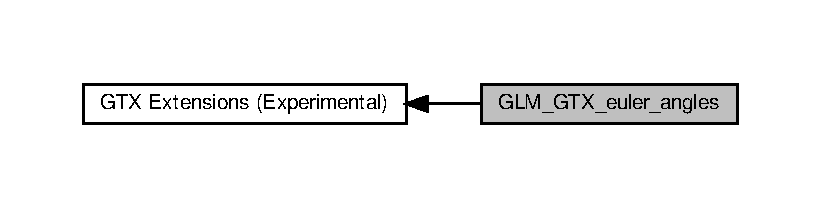
\includegraphics[width=350pt]{group__gtx__euler__angles}
\end{center}
\end{figure}
\subsection*{Functions}
\begin{DoxyCompactItemize}
\item 
{\footnotesize template$<$typename T $>$ }\\\hyperlink{setup_8hpp_ab2d052de21a70539923e9bcbf6e83a51}{G\+L\+M\+\_\+\+F\+U\+N\+C\+\_\+\+D\+E\+CL} \hyperlink{structglm_1_1detail_1_1tmat4x4}{detail\+::tmat4x4}$<$ T, \hyperlink{namespaceglm_a0f04f086094c747d227af4425893f545a9d21ccd8b5a009ec7eb7677befc3bf51}{defaultp} $>$ \hyperlink{group__gtx__euler__angles_ga97994e53d856ae89ed2622d66ab86c2c}{glm\+::euler\+AngleX} (T const \&angleX)
\item 
{\footnotesize template$<$typename T $>$ }\\\hyperlink{setup_8hpp_ab2d052de21a70539923e9bcbf6e83a51}{G\+L\+M\+\_\+\+F\+U\+N\+C\+\_\+\+D\+E\+CL} \hyperlink{structglm_1_1detail_1_1tmat4x4}{detail\+::tmat4x4}$<$ T, \hyperlink{namespaceglm_a0f04f086094c747d227af4425893f545a9d21ccd8b5a009ec7eb7677befc3bf51}{defaultp} $>$ \hyperlink{group__gtx__euler__angles_gacdc188a23a928d57d4490ff7d646fb96}{glm\+::euler\+AngleY} (T const \&angleY)
\item 
{\footnotesize template$<$typename T $>$ }\\\hyperlink{setup_8hpp_ab2d052de21a70539923e9bcbf6e83a51}{G\+L\+M\+\_\+\+F\+U\+N\+C\+\_\+\+D\+E\+CL} \hyperlink{structglm_1_1detail_1_1tmat4x4}{detail\+::tmat4x4}$<$ T, \hyperlink{namespaceglm_a0f04f086094c747d227af4425893f545a9d21ccd8b5a009ec7eb7677befc3bf51}{defaultp} $>$ \hyperlink{group__gtx__euler__angles_gaf55b28c29ebd7ba728f1ad6490c89687}{glm\+::euler\+AngleZ} (T const \&angleZ)
\item 
{\footnotesize template$<$typename T $>$ }\\\hyperlink{setup_8hpp_ab2d052de21a70539923e9bcbf6e83a51}{G\+L\+M\+\_\+\+F\+U\+N\+C\+\_\+\+D\+E\+CL} \hyperlink{structglm_1_1detail_1_1tmat4x4}{detail\+::tmat4x4}$<$ T, \hyperlink{namespaceglm_a0f04f086094c747d227af4425893f545a9d21ccd8b5a009ec7eb7677befc3bf51}{defaultp} $>$ \hyperlink{group__gtx__euler__angles_ga83a52d36fd752c92ce189197b51ea785}{glm\+::euler\+Angle\+XY} (T const \&angleX, T const \&angleY)
\item 
{\footnotesize template$<$typename T $>$ }\\\hyperlink{setup_8hpp_ab2d052de21a70539923e9bcbf6e83a51}{G\+L\+M\+\_\+\+F\+U\+N\+C\+\_\+\+D\+E\+CL} \hyperlink{structglm_1_1detail_1_1tmat4x4}{detail\+::tmat4x4}$<$ T, \hyperlink{namespaceglm_a0f04f086094c747d227af4425893f545a9d21ccd8b5a009ec7eb7677befc3bf51}{defaultp} $>$ \hyperlink{group__gtx__euler__angles_ga7599a8aaf3bf33b15517dd522a6d8020}{glm\+::euler\+Angle\+YX} (T const \&angleY, T const \&angleX)
\item 
{\footnotesize template$<$typename T $>$ }\\\hyperlink{setup_8hpp_ab2d052de21a70539923e9bcbf6e83a51}{G\+L\+M\+\_\+\+F\+U\+N\+C\+\_\+\+D\+E\+CL} \hyperlink{structglm_1_1detail_1_1tmat4x4}{detail\+::tmat4x4}$<$ T, \hyperlink{namespaceglm_a0f04f086094c747d227af4425893f545a9d21ccd8b5a009ec7eb7677befc3bf51}{defaultp} $>$ \hyperlink{group__gtx__euler__angles_ga61110cb520fbf21dd541cf4e25d81a65}{glm\+::euler\+Angle\+XZ} (T const \&angleX, T const \&angleZ)
\item 
{\footnotesize template$<$typename T $>$ }\\\hyperlink{setup_8hpp_ab2d052de21a70539923e9bcbf6e83a51}{G\+L\+M\+\_\+\+F\+U\+N\+C\+\_\+\+D\+E\+CL} \hyperlink{structglm_1_1detail_1_1tmat4x4}{detail\+::tmat4x4}$<$ T, \hyperlink{namespaceglm_a0f04f086094c747d227af4425893f545a9d21ccd8b5a009ec7eb7677befc3bf51}{defaultp} $>$ \hyperlink{group__gtx__euler__angles_ga5766bbe3f5b17b5c33ed21b2933ff278}{glm\+::euler\+Angle\+ZX} (T const \&\hyperlink{group__gtc__quaternion_ga23a3fc7ada5bbb665ff84c92c6e0542c}{angle}, T const \&angleX)
\item 
{\footnotesize template$<$typename T $>$ }\\\hyperlink{setup_8hpp_ab2d052de21a70539923e9bcbf6e83a51}{G\+L\+M\+\_\+\+F\+U\+N\+C\+\_\+\+D\+E\+CL} \hyperlink{structglm_1_1detail_1_1tmat4x4}{detail\+::tmat4x4}$<$ T, \hyperlink{namespaceglm_a0f04f086094c747d227af4425893f545a9d21ccd8b5a009ec7eb7677befc3bf51}{defaultp} $>$ \hyperlink{group__gtx__euler__angles_ga4bff0f8324770261d3a6ddadd790ec22}{glm\+::euler\+Angle\+YZ} (T const \&angleY, T const \&angleZ)
\item 
{\footnotesize template$<$typename T $>$ }\\\hyperlink{setup_8hpp_ab2d052de21a70539923e9bcbf6e83a51}{G\+L\+M\+\_\+\+F\+U\+N\+C\+\_\+\+D\+E\+CL} \hyperlink{structglm_1_1detail_1_1tmat4x4}{detail\+::tmat4x4}$<$ T, \hyperlink{namespaceglm_a0f04f086094c747d227af4425893f545a9d21ccd8b5a009ec7eb7677befc3bf51}{defaultp} $>$ \hyperlink{group__gtx__euler__angles_gaeabd76319f5a19188a0423769950df76}{glm\+::euler\+Angle\+ZY} (T const \&angleZ, T const \&angleY)
\item 
{\footnotesize template$<$typename T $>$ }\\\hyperlink{setup_8hpp_ab2d052de21a70539923e9bcbf6e83a51}{G\+L\+M\+\_\+\+F\+U\+N\+C\+\_\+\+D\+E\+CL} \hyperlink{structglm_1_1detail_1_1tmat4x4}{detail\+::tmat4x4}$<$ T, \hyperlink{namespaceglm_a0f04f086094c747d227af4425893f545a9d21ccd8b5a009ec7eb7677befc3bf51}{defaultp} $>$ \hyperlink{group__gtx__euler__angles_gab9bc80f4f579efd8f0d161e8b58ff452}{glm\+::euler\+Angle\+Y\+XZ} (T const \&\hyperlink{group__gtc__quaternion_ga1de7653ddf380ff06d2300eea831664c}{yaw}, T const \&\hyperlink{group__gtc__quaternion_ga4d345dc369a54f53f5ebc375bac56d11}{pitch}, T const \&\hyperlink{group__gtc__quaternion_ga6d883e423bc425f4334fcce202131f7e}{roll})
\item 
{\footnotesize template$<$typename T $>$ }\\\hyperlink{setup_8hpp_ab2d052de21a70539923e9bcbf6e83a51}{G\+L\+M\+\_\+\+F\+U\+N\+C\+\_\+\+D\+E\+CL} \hyperlink{structglm_1_1detail_1_1tmat4x4}{detail\+::tmat4x4}$<$ T, \hyperlink{namespaceglm_a0f04f086094c747d227af4425893f545a9d21ccd8b5a009ec7eb7677befc3bf51}{defaultp} $>$ \hyperlink{group__gtx__euler__angles_gaf6f927d06835272cd6a61ee3f8f65f5e}{glm\+::yaw\+Pitch\+Roll} (T const \&\hyperlink{group__gtc__quaternion_ga1de7653ddf380ff06d2300eea831664c}{yaw}, T const \&\hyperlink{group__gtc__quaternion_ga4d345dc369a54f53f5ebc375bac56d11}{pitch}, T const \&\hyperlink{group__gtc__quaternion_ga6d883e423bc425f4334fcce202131f7e}{roll})
\item 
{\footnotesize template$<$typename T $>$ }\\\hyperlink{setup_8hpp_ab2d052de21a70539923e9bcbf6e83a51}{G\+L\+M\+\_\+\+F\+U\+N\+C\+\_\+\+D\+E\+CL} \hyperlink{structglm_1_1detail_1_1tmat2x2}{detail\+::tmat2x2}$<$ T, \hyperlink{namespaceglm_a0f04f086094c747d227af4425893f545a9d21ccd8b5a009ec7eb7677befc3bf51}{defaultp} $>$ \hyperlink{group__gtx__euler__angles_gab39476f0decc117783e02ba389a04ee7}{glm\+::orientate2} (T const \&\hyperlink{group__gtc__quaternion_ga23a3fc7ada5bbb665ff84c92c6e0542c}{angle})
\item 
{\footnotesize template$<$typename T $>$ }\\\hyperlink{setup_8hpp_ab2d052de21a70539923e9bcbf6e83a51}{G\+L\+M\+\_\+\+F\+U\+N\+C\+\_\+\+D\+E\+CL} \hyperlink{structglm_1_1detail_1_1tmat3x3}{detail\+::tmat3x3}$<$ T, \hyperlink{namespaceglm_a0f04f086094c747d227af4425893f545a9d21ccd8b5a009ec7eb7677befc3bf51}{defaultp} $>$ \hyperlink{group__gtx__euler__angles_ga2c94907d441c40beb413fe3284c1b267}{glm\+::orientate3} (T const \&\hyperlink{group__gtc__quaternion_ga23a3fc7ada5bbb665ff84c92c6e0542c}{angle})
\item 
{\footnotesize template$<$typename T , precision P$>$ }\\\hyperlink{setup_8hpp_ab2d052de21a70539923e9bcbf6e83a51}{G\+L\+M\+\_\+\+F\+U\+N\+C\+\_\+\+D\+E\+CL} \hyperlink{structglm_1_1detail_1_1tmat3x3}{detail\+::tmat3x3}$<$ T, P $>$ \hyperlink{group__gtx__euler__angles_gab6a2a986916647ddedc94bbd2516f20c}{glm\+::orientate3} (\hyperlink{structglm_1_1detail_1_1tvec3}{detail\+::tvec3}$<$ T, P $>$ const \&angles)
\item 
{\footnotesize template$<$typename T , precision P$>$ }\\\hyperlink{setup_8hpp_ab2d052de21a70539923e9bcbf6e83a51}{G\+L\+M\+\_\+\+F\+U\+N\+C\+\_\+\+D\+E\+CL} \hyperlink{structglm_1_1detail_1_1tmat4x4}{detail\+::tmat4x4}$<$ T, P $>$ \hyperlink{group__gtx__euler__angles_ga3b9f62da9726cdad708df41712792082}{glm\+::orientate4} (\hyperlink{structglm_1_1detail_1_1tvec3}{detail\+::tvec3}$<$ T, P $>$ const \&angles)
\end{DoxyCompactItemize}


\subsection{Detailed Description}
Build matrices from Euler angles. 

$<$\hyperlink{euler__angles_8hpp}{glm/gtx/euler\+\_\+angles.\+hpp}$>$ need to be included to use these functionalities. 

\subsection{Function Documentation}
\mbox{\Hypertarget{group__gtx__euler__angles_ga97994e53d856ae89ed2622d66ab86c2c}\label{group__gtx__euler__angles_ga97994e53d856ae89ed2622d66ab86c2c}} 
\index{G\+L\+M\+\_\+\+G\+T\+X\+\_\+euler\+\_\+angles@{G\+L\+M\+\_\+\+G\+T\+X\+\_\+euler\+\_\+angles}!euler\+AngleX@{euler\+AngleX}}
\index{euler\+AngleX@{euler\+AngleX}!G\+L\+M\+\_\+\+G\+T\+X\+\_\+euler\+\_\+angles@{G\+L\+M\+\_\+\+G\+T\+X\+\_\+euler\+\_\+angles}}
\subsubsection{\texorpdfstring{euler\+Angle\+X()}{eulerAngleX()}}
{\footnotesize\ttfamily template$<$typename T $>$ \\
\hyperlink{setup_8hpp_ab2d052de21a70539923e9bcbf6e83a51}{G\+L\+M\+\_\+\+F\+U\+N\+C\+\_\+\+D\+E\+CL} \hyperlink{structglm_1_1detail_1_1tmat4x4}{detail\+::tmat4x4}$<$T, \hyperlink{namespaceglm_a0f04f086094c747d227af4425893f545a9d21ccd8b5a009ec7eb7677befc3bf51}{defaultp}$>$ glm\+::euler\+AngleX (\begin{DoxyParamCaption}\item[{T const \&}]{angleX }\end{DoxyParamCaption})}

Creates a 3D 4 $\ast$ 4 homogeneous rotation matrix from an euler angle X. \begin{DoxySeeAlso}{See also}
\hyperlink{group__gtx__euler__angles}{G\+L\+M\+\_\+\+G\+T\+X\+\_\+euler\+\_\+angles} 
\end{DoxySeeAlso}


Definition at line 14 of file euler\+\_\+angles.\+inl.

\mbox{\Hypertarget{group__gtx__euler__angles_ga83a52d36fd752c92ce189197b51ea785}\label{group__gtx__euler__angles_ga83a52d36fd752c92ce189197b51ea785}} 
\index{G\+L\+M\+\_\+\+G\+T\+X\+\_\+euler\+\_\+angles@{G\+L\+M\+\_\+\+G\+T\+X\+\_\+euler\+\_\+angles}!euler\+Angle\+XY@{euler\+Angle\+XY}}
\index{euler\+Angle\+XY@{euler\+Angle\+XY}!G\+L\+M\+\_\+\+G\+T\+X\+\_\+euler\+\_\+angles@{G\+L\+M\+\_\+\+G\+T\+X\+\_\+euler\+\_\+angles}}
\subsubsection{\texorpdfstring{euler\+Angle\+X\+Y()}{eulerAngleXY()}}
{\footnotesize\ttfamily template$<$typename T $>$ \\
\hyperlink{setup_8hpp_ab2d052de21a70539923e9bcbf6e83a51}{G\+L\+M\+\_\+\+F\+U\+N\+C\+\_\+\+D\+E\+CL} \hyperlink{structglm_1_1detail_1_1tmat4x4}{detail\+::tmat4x4}$<$T, \hyperlink{namespaceglm_a0f04f086094c747d227af4425893f545a9d21ccd8b5a009ec7eb7677befc3bf51}{defaultp}$>$ glm\+::euler\+Angle\+XY (\begin{DoxyParamCaption}\item[{T const \&}]{angleX,  }\item[{T const \&}]{angleY }\end{DoxyParamCaption})}

Creates a 3D 4 $\ast$ 4 homogeneous rotation matrix from euler angles (X $\ast$ Y). \begin{DoxySeeAlso}{See also}
\hyperlink{group__gtx__euler__angles}{G\+L\+M\+\_\+\+G\+T\+X\+\_\+euler\+\_\+angles} 
\end{DoxySeeAlso}


Definition at line 62 of file euler\+\_\+angles.\+inl.

\mbox{\Hypertarget{group__gtx__euler__angles_ga61110cb520fbf21dd541cf4e25d81a65}\label{group__gtx__euler__angles_ga61110cb520fbf21dd541cf4e25d81a65}} 
\index{G\+L\+M\+\_\+\+G\+T\+X\+\_\+euler\+\_\+angles@{G\+L\+M\+\_\+\+G\+T\+X\+\_\+euler\+\_\+angles}!euler\+Angle\+XZ@{euler\+Angle\+XZ}}
\index{euler\+Angle\+XZ@{euler\+Angle\+XZ}!G\+L\+M\+\_\+\+G\+T\+X\+\_\+euler\+\_\+angles@{G\+L\+M\+\_\+\+G\+T\+X\+\_\+euler\+\_\+angles}}
\subsubsection{\texorpdfstring{euler\+Angle\+X\+Z()}{eulerAngleXZ()}}
{\footnotesize\ttfamily template$<$typename T $>$ \\
\hyperlink{setup_8hpp_ab2d052de21a70539923e9bcbf6e83a51}{G\+L\+M\+\_\+\+F\+U\+N\+C\+\_\+\+D\+E\+CL} \hyperlink{structglm_1_1detail_1_1tmat4x4}{detail\+::tmat4x4}$<$T, \hyperlink{namespaceglm_a0f04f086094c747d227af4425893f545a9d21ccd8b5a009ec7eb7677befc3bf51}{defaultp}$>$ glm\+::euler\+Angle\+XZ (\begin{DoxyParamCaption}\item[{T const \&}]{angleX,  }\item[{T const \&}]{angleZ }\end{DoxyParamCaption})}

Creates a 3D 4 $\ast$ 4 homogeneous rotation matrix from euler angles (X $\ast$ Z). \begin{DoxySeeAlso}{See also}
\hyperlink{group__gtx__euler__angles}{G\+L\+M\+\_\+\+G\+T\+X\+\_\+euler\+\_\+angles} 
\end{DoxySeeAlso}


Definition at line 100 of file euler\+\_\+angles.\+inl.

\mbox{\Hypertarget{group__gtx__euler__angles_gacdc188a23a928d57d4490ff7d646fb96}\label{group__gtx__euler__angles_gacdc188a23a928d57d4490ff7d646fb96}} 
\index{G\+L\+M\+\_\+\+G\+T\+X\+\_\+euler\+\_\+angles@{G\+L\+M\+\_\+\+G\+T\+X\+\_\+euler\+\_\+angles}!euler\+AngleY@{euler\+AngleY}}
\index{euler\+AngleY@{euler\+AngleY}!G\+L\+M\+\_\+\+G\+T\+X\+\_\+euler\+\_\+angles@{G\+L\+M\+\_\+\+G\+T\+X\+\_\+euler\+\_\+angles}}
\subsubsection{\texorpdfstring{euler\+Angle\+Y()}{eulerAngleY()}}
{\footnotesize\ttfamily template$<$typename T $>$ \\
\hyperlink{setup_8hpp_ab2d052de21a70539923e9bcbf6e83a51}{G\+L\+M\+\_\+\+F\+U\+N\+C\+\_\+\+D\+E\+CL} \hyperlink{structglm_1_1detail_1_1tmat4x4}{detail\+::tmat4x4}$<$T, \hyperlink{namespaceglm_a0f04f086094c747d227af4425893f545a9d21ccd8b5a009ec7eb7677befc3bf51}{defaultp}$>$ glm\+::euler\+AngleY (\begin{DoxyParamCaption}\item[{T const \&}]{angleY }\end{DoxyParamCaption})}

Creates a 3D 4 $\ast$ 4 homogeneous rotation matrix from an euler angle Y. \begin{DoxySeeAlso}{See also}
\hyperlink{group__gtx__euler__angles}{G\+L\+M\+\_\+\+G\+T\+X\+\_\+euler\+\_\+angles} 
\end{DoxySeeAlso}


Definition at line 30 of file euler\+\_\+angles.\+inl.

\mbox{\Hypertarget{group__gtx__euler__angles_ga7599a8aaf3bf33b15517dd522a6d8020}\label{group__gtx__euler__angles_ga7599a8aaf3bf33b15517dd522a6d8020}} 
\index{G\+L\+M\+\_\+\+G\+T\+X\+\_\+euler\+\_\+angles@{G\+L\+M\+\_\+\+G\+T\+X\+\_\+euler\+\_\+angles}!euler\+Angle\+YX@{euler\+Angle\+YX}}
\index{euler\+Angle\+YX@{euler\+Angle\+YX}!G\+L\+M\+\_\+\+G\+T\+X\+\_\+euler\+\_\+angles@{G\+L\+M\+\_\+\+G\+T\+X\+\_\+euler\+\_\+angles}}
\subsubsection{\texorpdfstring{euler\+Angle\+Y\+X()}{eulerAngleYX()}}
{\footnotesize\ttfamily template$<$typename T $>$ \\
\hyperlink{setup_8hpp_ab2d052de21a70539923e9bcbf6e83a51}{G\+L\+M\+\_\+\+F\+U\+N\+C\+\_\+\+D\+E\+CL} \hyperlink{structglm_1_1detail_1_1tmat4x4}{detail\+::tmat4x4}$<$T, \hyperlink{namespaceglm_a0f04f086094c747d227af4425893f545a9d21ccd8b5a009ec7eb7677befc3bf51}{defaultp}$>$ glm\+::euler\+Angle\+YX (\begin{DoxyParamCaption}\item[{T const \&}]{angleY,  }\item[{T const \&}]{angleX }\end{DoxyParamCaption})}

Creates a 3D 4 $\ast$ 4 homogeneous rotation matrix from euler angles (Y $\ast$ X). \begin{DoxySeeAlso}{See also}
\hyperlink{group__gtx__euler__angles}{G\+L\+M\+\_\+\+G\+T\+X\+\_\+euler\+\_\+angles} 
\end{DoxySeeAlso}


Definition at line 81 of file euler\+\_\+angles.\+inl.

\mbox{\Hypertarget{group__gtx__euler__angles_gab9bc80f4f579efd8f0d161e8b58ff452}\label{group__gtx__euler__angles_gab9bc80f4f579efd8f0d161e8b58ff452}} 
\index{G\+L\+M\+\_\+\+G\+T\+X\+\_\+euler\+\_\+angles@{G\+L\+M\+\_\+\+G\+T\+X\+\_\+euler\+\_\+angles}!euler\+Angle\+Y\+XZ@{euler\+Angle\+Y\+XZ}}
\index{euler\+Angle\+Y\+XZ@{euler\+Angle\+Y\+XZ}!G\+L\+M\+\_\+\+G\+T\+X\+\_\+euler\+\_\+angles@{G\+L\+M\+\_\+\+G\+T\+X\+\_\+euler\+\_\+angles}}
\subsubsection{\texorpdfstring{euler\+Angle\+Y\+X\+Z()}{eulerAngleYXZ()}}
{\footnotesize\ttfamily template$<$typename T $>$ \\
\hyperlink{setup_8hpp_ab2d052de21a70539923e9bcbf6e83a51}{G\+L\+M\+\_\+\+F\+U\+N\+C\+\_\+\+D\+E\+CL} \hyperlink{structglm_1_1detail_1_1tmat4x4}{detail\+::tmat4x4}$<$T, \hyperlink{namespaceglm_a0f04f086094c747d227af4425893f545a9d21ccd8b5a009ec7eb7677befc3bf51}{defaultp}$>$ glm\+::euler\+Angle\+Y\+XZ (\begin{DoxyParamCaption}\item[{T const \&}]{yaw,  }\item[{T const \&}]{pitch,  }\item[{T const \&}]{roll }\end{DoxyParamCaption})}

Creates a 3D 4 $\ast$ 4 homogeneous rotation matrix from euler angles (Y $\ast$ X $\ast$ Z). \begin{DoxySeeAlso}{See also}
\hyperlink{group__gtx__euler__angles}{G\+L\+M\+\_\+\+G\+T\+X\+\_\+euler\+\_\+angles} 
\end{DoxySeeAlso}


Definition at line 140 of file euler\+\_\+angles.\+inl.

\mbox{\Hypertarget{group__gtx__euler__angles_ga4bff0f8324770261d3a6ddadd790ec22}\label{group__gtx__euler__angles_ga4bff0f8324770261d3a6ddadd790ec22}} 
\index{G\+L\+M\+\_\+\+G\+T\+X\+\_\+euler\+\_\+angles@{G\+L\+M\+\_\+\+G\+T\+X\+\_\+euler\+\_\+angles}!euler\+Angle\+YZ@{euler\+Angle\+YZ}}
\index{euler\+Angle\+YZ@{euler\+Angle\+YZ}!G\+L\+M\+\_\+\+G\+T\+X\+\_\+euler\+\_\+angles@{G\+L\+M\+\_\+\+G\+T\+X\+\_\+euler\+\_\+angles}}
\subsubsection{\texorpdfstring{euler\+Angle\+Y\+Z()}{eulerAngleYZ()}}
{\footnotesize\ttfamily template$<$typename T $>$ \\
\hyperlink{setup_8hpp_ab2d052de21a70539923e9bcbf6e83a51}{G\+L\+M\+\_\+\+F\+U\+N\+C\+\_\+\+D\+E\+CL} \hyperlink{structglm_1_1detail_1_1tmat4x4}{detail\+::tmat4x4}$<$T, \hyperlink{namespaceglm_a0f04f086094c747d227af4425893f545a9d21ccd8b5a009ec7eb7677befc3bf51}{defaultp}$>$ glm\+::euler\+Angle\+YZ (\begin{DoxyParamCaption}\item[{T const \&}]{angleY,  }\item[{T const \&}]{angleZ }\end{DoxyParamCaption})}

Creates a 3D 4 $\ast$ 4 homogeneous rotation matrix from euler angles (Y $\ast$ Z). \begin{DoxySeeAlso}{See also}
\hyperlink{group__gtx__euler__angles}{G\+L\+M\+\_\+\+G\+T\+X\+\_\+euler\+\_\+angles} 
\end{DoxySeeAlso}


Definition at line 120 of file euler\+\_\+angles.\+inl.

\mbox{\Hypertarget{group__gtx__euler__angles_gaf55b28c29ebd7ba728f1ad6490c89687}\label{group__gtx__euler__angles_gaf55b28c29ebd7ba728f1ad6490c89687}} 
\index{G\+L\+M\+\_\+\+G\+T\+X\+\_\+euler\+\_\+angles@{G\+L\+M\+\_\+\+G\+T\+X\+\_\+euler\+\_\+angles}!euler\+AngleZ@{euler\+AngleZ}}
\index{euler\+AngleZ@{euler\+AngleZ}!G\+L\+M\+\_\+\+G\+T\+X\+\_\+euler\+\_\+angles@{G\+L\+M\+\_\+\+G\+T\+X\+\_\+euler\+\_\+angles}}
\subsubsection{\texorpdfstring{euler\+Angle\+Z()}{eulerAngleZ()}}
{\footnotesize\ttfamily template$<$typename T $>$ \\
\hyperlink{setup_8hpp_ab2d052de21a70539923e9bcbf6e83a51}{G\+L\+M\+\_\+\+F\+U\+N\+C\+\_\+\+D\+E\+CL} \hyperlink{structglm_1_1detail_1_1tmat4x4}{detail\+::tmat4x4}$<$T, \hyperlink{namespaceglm_a0f04f086094c747d227af4425893f545a9d21ccd8b5a009ec7eb7677befc3bf51}{defaultp}$>$ glm\+::euler\+AngleZ (\begin{DoxyParamCaption}\item[{T const \&}]{angleZ }\end{DoxyParamCaption})}

Creates a 3D 4 $\ast$ 4 homogeneous rotation matrix from an euler angle Z. \begin{DoxySeeAlso}{See also}
\hyperlink{group__gtx__euler__angles}{G\+L\+M\+\_\+\+G\+T\+X\+\_\+euler\+\_\+angles} 
\end{DoxySeeAlso}


Definition at line 46 of file euler\+\_\+angles.\+inl.

\mbox{\Hypertarget{group__gtx__euler__angles_ga5766bbe3f5b17b5c33ed21b2933ff278}\label{group__gtx__euler__angles_ga5766bbe3f5b17b5c33ed21b2933ff278}} 
\index{G\+L\+M\+\_\+\+G\+T\+X\+\_\+euler\+\_\+angles@{G\+L\+M\+\_\+\+G\+T\+X\+\_\+euler\+\_\+angles}!euler\+Angle\+ZX@{euler\+Angle\+ZX}}
\index{euler\+Angle\+ZX@{euler\+Angle\+ZX}!G\+L\+M\+\_\+\+G\+T\+X\+\_\+euler\+\_\+angles@{G\+L\+M\+\_\+\+G\+T\+X\+\_\+euler\+\_\+angles}}
\subsubsection{\texorpdfstring{euler\+Angle\+Z\+X()}{eulerAngleZX()}}
{\footnotesize\ttfamily template$<$typename T $>$ \\
\hyperlink{setup_8hpp_ab2d052de21a70539923e9bcbf6e83a51}{G\+L\+M\+\_\+\+F\+U\+N\+C\+\_\+\+D\+E\+CL} \hyperlink{structglm_1_1detail_1_1tmat4x4}{detail\+::tmat4x4}$<$T, \hyperlink{namespaceglm_a0f04f086094c747d227af4425893f545a9d21ccd8b5a009ec7eb7677befc3bf51}{defaultp}$>$ glm\+::euler\+Angle\+ZX (\begin{DoxyParamCaption}\item[{T const \&}]{angle,  }\item[{T const \&}]{angleX }\end{DoxyParamCaption})}

Creates a 3D 4 $\ast$ 4 homogeneous rotation matrix from euler angles (Z $\ast$ X). \begin{DoxySeeAlso}{See also}
\hyperlink{group__gtx__euler__angles}{G\+L\+M\+\_\+\+G\+T\+X\+\_\+euler\+\_\+angles} 
\end{DoxySeeAlso}


Definition at line 110 of file euler\+\_\+angles.\+inl.

\mbox{\Hypertarget{group__gtx__euler__angles_gaeabd76319f5a19188a0423769950df76}\label{group__gtx__euler__angles_gaeabd76319f5a19188a0423769950df76}} 
\index{G\+L\+M\+\_\+\+G\+T\+X\+\_\+euler\+\_\+angles@{G\+L\+M\+\_\+\+G\+T\+X\+\_\+euler\+\_\+angles}!euler\+Angle\+ZY@{euler\+Angle\+ZY}}
\index{euler\+Angle\+ZY@{euler\+Angle\+ZY}!G\+L\+M\+\_\+\+G\+T\+X\+\_\+euler\+\_\+angles@{G\+L\+M\+\_\+\+G\+T\+X\+\_\+euler\+\_\+angles}}
\subsubsection{\texorpdfstring{euler\+Angle\+Z\+Y()}{eulerAngleZY()}}
{\footnotesize\ttfamily template$<$typename T $>$ \\
\hyperlink{setup_8hpp_ab2d052de21a70539923e9bcbf6e83a51}{G\+L\+M\+\_\+\+F\+U\+N\+C\+\_\+\+D\+E\+CL} \hyperlink{structglm_1_1detail_1_1tmat4x4}{detail\+::tmat4x4}$<$T, \hyperlink{namespaceglm_a0f04f086094c747d227af4425893f545a9d21ccd8b5a009ec7eb7677befc3bf51}{defaultp}$>$ glm\+::euler\+Angle\+ZY (\begin{DoxyParamCaption}\item[{T const \&}]{angleZ,  }\item[{T const \&}]{angleY }\end{DoxyParamCaption})}

Creates a 3D 4 $\ast$ 4 homogeneous rotation matrix from euler angles (Z $\ast$ Y). \begin{DoxySeeAlso}{See also}
\hyperlink{group__gtx__euler__angles}{G\+L\+M\+\_\+\+G\+T\+X\+\_\+euler\+\_\+angles} 
\end{DoxySeeAlso}


Definition at line 130 of file euler\+\_\+angles.\+inl.

\mbox{\Hypertarget{group__gtx__euler__angles_gab39476f0decc117783e02ba389a04ee7}\label{group__gtx__euler__angles_gab39476f0decc117783e02ba389a04ee7}} 
\index{G\+L\+M\+\_\+\+G\+T\+X\+\_\+euler\+\_\+angles@{G\+L\+M\+\_\+\+G\+T\+X\+\_\+euler\+\_\+angles}!orientate2@{orientate2}}
\index{orientate2@{orientate2}!G\+L\+M\+\_\+\+G\+T\+X\+\_\+euler\+\_\+angles@{G\+L\+M\+\_\+\+G\+T\+X\+\_\+euler\+\_\+angles}}
\subsubsection{\texorpdfstring{orientate2()}{orientate2()}}
{\footnotesize\ttfamily template$<$typename T $>$ \\
\hyperlink{setup_8hpp_ab2d052de21a70539923e9bcbf6e83a51}{G\+L\+M\+\_\+\+F\+U\+N\+C\+\_\+\+D\+E\+CL} \hyperlink{structglm_1_1detail_1_1tmat2x2}{detail\+::tmat2x2}$<$T, \hyperlink{namespaceglm_a0f04f086094c747d227af4425893f545a9d21ccd8b5a009ec7eb7677befc3bf51}{defaultp}$>$ glm\+::orientate2 (\begin{DoxyParamCaption}\item[{T const \&}]{angle }\end{DoxyParamCaption})}

Creates a 2D 2 $\ast$ 2 rotation matrix from an euler angle. \begin{DoxySeeAlso}{See also}
\hyperlink{group__gtx__euler__angles}{G\+L\+M\+\_\+\+G\+T\+X\+\_\+euler\+\_\+angles} 
\end{DoxySeeAlso}


Definition at line 210 of file euler\+\_\+angles.\+inl.

\mbox{\Hypertarget{group__gtx__euler__angles_ga2c94907d441c40beb413fe3284c1b267}\label{group__gtx__euler__angles_ga2c94907d441c40beb413fe3284c1b267}} 
\index{G\+L\+M\+\_\+\+G\+T\+X\+\_\+euler\+\_\+angles@{G\+L\+M\+\_\+\+G\+T\+X\+\_\+euler\+\_\+angles}!orientate3@{orientate3}}
\index{orientate3@{orientate3}!G\+L\+M\+\_\+\+G\+T\+X\+\_\+euler\+\_\+angles@{G\+L\+M\+\_\+\+G\+T\+X\+\_\+euler\+\_\+angles}}
\subsubsection{\texorpdfstring{orientate3()}{orientate3()}\hspace{0.1cm}{\footnotesize\ttfamily [1/2]}}
{\footnotesize\ttfamily template$<$typename T $>$ \\
\hyperlink{setup_8hpp_ab2d052de21a70539923e9bcbf6e83a51}{G\+L\+M\+\_\+\+F\+U\+N\+C\+\_\+\+D\+E\+CL} \hyperlink{structglm_1_1detail_1_1tmat3x3}{detail\+::tmat3x3}$<$T, \hyperlink{namespaceglm_a0f04f086094c747d227af4425893f545a9d21ccd8b5a009ec7eb7677befc3bf51}{defaultp}$>$ glm\+::orientate3 (\begin{DoxyParamCaption}\item[{T const \&}]{angle }\end{DoxyParamCaption})}

Creates a 2D 4 $\ast$ 4 homogeneous rotation matrix from an euler angle. \begin{DoxySeeAlso}{See also}
\hyperlink{group__gtx__euler__angles}{G\+L\+M\+\_\+\+G\+T\+X\+\_\+euler\+\_\+angles} 
\end{DoxySeeAlso}


Definition at line 227 of file euler\+\_\+angles.\+inl.

\mbox{\Hypertarget{group__gtx__euler__angles_gab6a2a986916647ddedc94bbd2516f20c}\label{group__gtx__euler__angles_gab6a2a986916647ddedc94bbd2516f20c}} 
\index{G\+L\+M\+\_\+\+G\+T\+X\+\_\+euler\+\_\+angles@{G\+L\+M\+\_\+\+G\+T\+X\+\_\+euler\+\_\+angles}!orientate3@{orientate3}}
\index{orientate3@{orientate3}!G\+L\+M\+\_\+\+G\+T\+X\+\_\+euler\+\_\+angles@{G\+L\+M\+\_\+\+G\+T\+X\+\_\+euler\+\_\+angles}}
\subsubsection{\texorpdfstring{orientate3()}{orientate3()}\hspace{0.1cm}{\footnotesize\ttfamily [2/2]}}
{\footnotesize\ttfamily template$<$typename T , precision P$>$ \\
\hyperlink{setup_8hpp_ab2d052de21a70539923e9bcbf6e83a51}{G\+L\+M\+\_\+\+F\+U\+N\+C\+\_\+\+D\+E\+CL} \hyperlink{structglm_1_1detail_1_1tmat3x3}{detail\+::tmat3x3}$<$T, P$>$ glm\+::orientate3 (\begin{DoxyParamCaption}\item[{\hyperlink{structglm_1_1detail_1_1tvec3}{detail\+::tvec3}$<$ T, P $>$ const \&}]{angles }\end{DoxyParamCaption})}

Creates a 3D 3 $\ast$ 3 rotation matrix from euler angles (Y $\ast$ X $\ast$ Z). \begin{DoxySeeAlso}{See also}
\hyperlink{group__gtx__euler__angles}{G\+L\+M\+\_\+\+G\+T\+X\+\_\+euler\+\_\+angles} 
\end{DoxySeeAlso}


Definition at line 249 of file euler\+\_\+angles.\+inl.

\mbox{\Hypertarget{group__gtx__euler__angles_ga3b9f62da9726cdad708df41712792082}\label{group__gtx__euler__angles_ga3b9f62da9726cdad708df41712792082}} 
\index{G\+L\+M\+\_\+\+G\+T\+X\+\_\+euler\+\_\+angles@{G\+L\+M\+\_\+\+G\+T\+X\+\_\+euler\+\_\+angles}!orientate4@{orientate4}}
\index{orientate4@{orientate4}!G\+L\+M\+\_\+\+G\+T\+X\+\_\+euler\+\_\+angles@{G\+L\+M\+\_\+\+G\+T\+X\+\_\+euler\+\_\+angles}}
\subsubsection{\texorpdfstring{orientate4()}{orientate4()}}
{\footnotesize\ttfamily template$<$typename T , precision P$>$ \\
\hyperlink{setup_8hpp_ab2d052de21a70539923e9bcbf6e83a51}{G\+L\+M\+\_\+\+F\+U\+N\+C\+\_\+\+D\+E\+CL} \hyperlink{structglm_1_1detail_1_1tmat4x4}{detail\+::tmat4x4}$<$T, P$>$ glm\+::orientate4 (\begin{DoxyParamCaption}\item[{\hyperlink{structglm_1_1detail_1_1tvec3}{detail\+::tvec3}$<$ T, P $>$ const \&}]{angles }\end{DoxyParamCaption})}

Creates a 3D 4 $\ast$ 4 homogeneous rotation matrix from euler angles (Y $\ast$ X $\ast$ Z). \begin{DoxySeeAlso}{See also}
\hyperlink{group__gtx__euler__angles}{G\+L\+M\+\_\+\+G\+T\+X\+\_\+euler\+\_\+angles} 
\end{DoxySeeAlso}


Definition at line 258 of file euler\+\_\+angles.\+inl.

\mbox{\Hypertarget{group__gtx__euler__angles_gaf6f927d06835272cd6a61ee3f8f65f5e}\label{group__gtx__euler__angles_gaf6f927d06835272cd6a61ee3f8f65f5e}} 
\index{G\+L\+M\+\_\+\+G\+T\+X\+\_\+euler\+\_\+angles@{G\+L\+M\+\_\+\+G\+T\+X\+\_\+euler\+\_\+angles}!yaw\+Pitch\+Roll@{yaw\+Pitch\+Roll}}
\index{yaw\+Pitch\+Roll@{yaw\+Pitch\+Roll}!G\+L\+M\+\_\+\+G\+T\+X\+\_\+euler\+\_\+angles@{G\+L\+M\+\_\+\+G\+T\+X\+\_\+euler\+\_\+angles}}
\subsubsection{\texorpdfstring{yaw\+Pitch\+Roll()}{yawPitchRoll()}}
{\footnotesize\ttfamily template$<$typename T $>$ \\
\hyperlink{setup_8hpp_ab2d052de21a70539923e9bcbf6e83a51}{G\+L\+M\+\_\+\+F\+U\+N\+C\+\_\+\+D\+E\+CL} \hyperlink{structglm_1_1detail_1_1tmat4x4}{detail\+::tmat4x4}$<$T, \hyperlink{namespaceglm_a0f04f086094c747d227af4425893f545a9d21ccd8b5a009ec7eb7677befc3bf51}{defaultp}$>$ glm\+::yaw\+Pitch\+Roll (\begin{DoxyParamCaption}\item[{T const \&}]{yaw,  }\item[{T const \&}]{pitch,  }\item[{T const \&}]{roll }\end{DoxyParamCaption})}

Creates a 3D 4 $\ast$ 4 homogeneous rotation matrix from euler angles (Y $\ast$ X $\ast$ Z). \begin{DoxySeeAlso}{See also}
\hyperlink{group__gtx__euler__angles}{G\+L\+M\+\_\+\+G\+T\+X\+\_\+euler\+\_\+angles} 
\end{DoxySeeAlso}


Definition at line 175 of file euler\+\_\+angles.\+inl.


\hypertarget{group__gtx__extend}{}\section{G\+L\+M\+\_\+\+G\+T\+X\+\_\+extend}
\label{group__gtx__extend}\index{G\+L\+M\+\_\+\+G\+T\+X\+\_\+extend@{G\+L\+M\+\_\+\+G\+T\+X\+\_\+extend}}


Extend a position from a source to a position at a defined length.  


Collaboration diagram for G\+L\+M\+\_\+\+G\+T\+X\+\_\+extend\+:\nopagebreak
\begin{figure}[H]
\begin{center}
\leavevmode
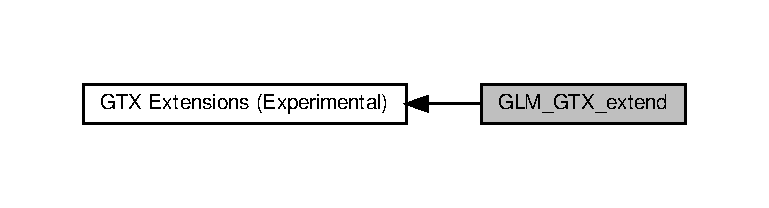
\includegraphics[width=350pt]{group__gtx__extend}
\end{center}
\end{figure}
\subsection*{Functions}
\begin{DoxyCompactItemize}
\item 
{\footnotesize template$<$typename gen\+Type $>$ }\\\hyperlink{setup_8hpp_ab2d052de21a70539923e9bcbf6e83a51}{G\+L\+M\+\_\+\+F\+U\+N\+C\+\_\+\+D\+E\+CL} gen\+Type \hyperlink{group__gtx__extend_ga8140caae613b0f847ab0d7175dc03a37}{glm\+::extend} (gen\+Type const \&Origin, gen\+Type const \&Source, typename gen\+Type\+::value\+\_\+type const Length)
\end{DoxyCompactItemize}


\subsection{Detailed Description}
Extend a position from a source to a position at a defined length. 

$<$\hyperlink{extend_8hpp}{glm/gtx/extend.\+hpp}$>$ need to be included to use these functionalities.

$<$\hyperlink{scalar__relational_8hpp}{glm/gtx/scalar\+\_\+relational.\+hpp}$>$ need to be included to use these functionalities. 

\subsection{Function Documentation}
\mbox{\Hypertarget{group__gtx__extend_ga8140caae613b0f847ab0d7175dc03a37}\label{group__gtx__extend_ga8140caae613b0f847ab0d7175dc03a37}} 
\index{G\+L\+M\+\_\+\+G\+T\+X\+\_\+extend@{G\+L\+M\+\_\+\+G\+T\+X\+\_\+extend}!extend@{extend}}
\index{extend@{extend}!G\+L\+M\+\_\+\+G\+T\+X\+\_\+extend@{G\+L\+M\+\_\+\+G\+T\+X\+\_\+extend}}
\subsubsection{\texorpdfstring{extend()}{extend()}}
{\footnotesize\ttfamily template$<$typename gen\+Type $>$ \\
\hyperlink{setup_8hpp_ab2d052de21a70539923e9bcbf6e83a51}{G\+L\+M\+\_\+\+F\+U\+N\+C\+\_\+\+D\+E\+CL} gen\+Type glm\+::extend (\begin{DoxyParamCaption}\item[{gen\+Type const \&}]{Origin,  }\item[{gen\+Type const \&}]{Source,  }\item[{typename gen\+Type\+::value\+\_\+type const}]{Length }\end{DoxyParamCaption})}

Extends of Length the Origin position using the (Source -\/ Origin) direction. \begin{DoxySeeAlso}{See also}
\hyperlink{group__gtx__extend}{G\+L\+M\+\_\+\+G\+T\+X\+\_\+extend} 
\end{DoxySeeAlso}

\hypertarget{group__gtx__extented__min__max}{}\section{G\+L\+M\+\_\+\+G\+T\+X\+\_\+extented\+\_\+min\+\_\+max}
\label{group__gtx__extented__min__max}\index{G\+L\+M\+\_\+\+G\+T\+X\+\_\+extented\+\_\+min\+\_\+max@{G\+L\+M\+\_\+\+G\+T\+X\+\_\+extented\+\_\+min\+\_\+max}}
Collaboration diagram for G\+L\+M\+\_\+\+G\+T\+X\+\_\+extented\+\_\+min\+\_\+max\+:\nopagebreak
\begin{figure}[H]
\begin{center}
\leavevmode
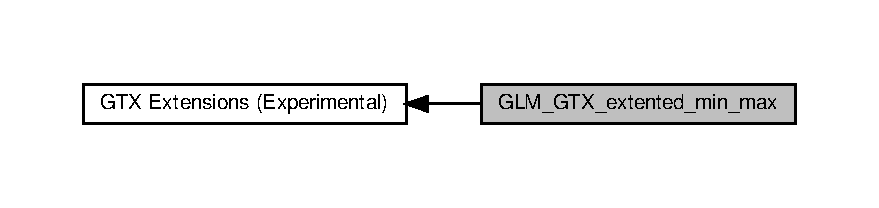
\includegraphics[width=350pt]{group__gtx__extented__min__max}
\end{center}
\end{figure}
\subsection*{Functions}
\begin{DoxyCompactItemize}
\item 
{\footnotesize template$<$typename T $>$ }\\\hyperlink{setup_8hpp_ab2d052de21a70539923e9bcbf6e83a51}{G\+L\+M\+\_\+\+F\+U\+N\+C\+\_\+\+D\+E\+CL} T \hyperlink{group__gtx__extented__min__max_ga713d3f9b3e76312c0d314e0c8611a6a6}{glm\+::min} (T const \&x, T const \&y, T const \&z)
\item 
{\footnotesize template$<$typename T , template$<$ typename $>$ class C$>$ }\\\hyperlink{setup_8hpp_ab2d052de21a70539923e9bcbf6e83a51}{G\+L\+M\+\_\+\+F\+U\+N\+C\+\_\+\+D\+E\+CL} C$<$ T $>$ \hyperlink{group__gtx__extented__min__max_ga74d1a96e7cdbac40f6d35142d3bcbbd4}{glm\+::min} (C$<$ T $>$ const \&x, typename C$<$ T $>$\+::T const \&y, typename C$<$ T $>$\+::T const \&z)
\item 
{\footnotesize template$<$typename T , template$<$ typename $>$ class C$>$ }\\\hyperlink{setup_8hpp_ab2d052de21a70539923e9bcbf6e83a51}{G\+L\+M\+\_\+\+F\+U\+N\+C\+\_\+\+D\+E\+CL} C$<$ T $>$ \hyperlink{group__gtx__extented__min__max_ga42b5c3fc027fd3d9a50d2ccc9126d9f0}{glm\+::min} (C$<$ T $>$ const \&x, C$<$ T $>$ const \&y, C$<$ T $>$ const \&z)
\item 
{\footnotesize template$<$typename T $>$ }\\\hyperlink{setup_8hpp_ab2d052de21a70539923e9bcbf6e83a51}{G\+L\+M\+\_\+\+F\+U\+N\+C\+\_\+\+D\+E\+CL} T \hyperlink{group__gtx__extented__min__max_ga95466987024d03039607f09e69813d69}{glm\+::min} (T const \&x, T const \&y, T const \&z, T const \&w)
\item 
{\footnotesize template$<$typename T , template$<$ typename $>$ class C$>$ }\\\hyperlink{setup_8hpp_ab2d052de21a70539923e9bcbf6e83a51}{G\+L\+M\+\_\+\+F\+U\+N\+C\+\_\+\+D\+E\+CL} C$<$ T $>$ \hyperlink{group__gtx__extented__min__max_ga4fe35dd31dd0c45693c9b60b830b8d47}{glm\+::min} (C$<$ T $>$ const \&x, typename C$<$ T $>$\+::T const \&y, typename C$<$ T $>$\+::T const \&z, typename C$<$ T $>$\+::T const \&w)
\item 
{\footnotesize template$<$typename T , template$<$ typename $>$ class C$>$ }\\\hyperlink{setup_8hpp_ab2d052de21a70539923e9bcbf6e83a51}{G\+L\+M\+\_\+\+F\+U\+N\+C\+\_\+\+D\+E\+CL} C$<$ T $>$ \hyperlink{group__gtx__extented__min__max_ga7471ea4159eed8dd9ea4ac5d46c2fead}{glm\+::min} (C$<$ T $>$ const \&x, C$<$ T $>$ const \&y, C$<$ T $>$ const \&z, C$<$ T $>$ const \&w)
\item 
{\footnotesize template$<$typename T $>$ }\\\hyperlink{setup_8hpp_ab2d052de21a70539923e9bcbf6e83a51}{G\+L\+M\+\_\+\+F\+U\+N\+C\+\_\+\+D\+E\+CL} T \hyperlink{group__gtx__extented__min__max_ga04991ccb9865c4c4e58488cfb209ce69}{glm\+::max} (T const \&x, T const \&y, T const \&z)
\item 
{\footnotesize template$<$typename T , template$<$ typename $>$ class C$>$ }\\\hyperlink{setup_8hpp_ab2d052de21a70539923e9bcbf6e83a51}{G\+L\+M\+\_\+\+F\+U\+N\+C\+\_\+\+D\+E\+CL} C$<$ T $>$ \hyperlink{group__gtx__extented__min__max_gae1b7bbe5c91de4924835ea3e14530744}{glm\+::max} (C$<$ T $>$ const \&x, typename C$<$ T $>$\+::T const \&y, typename C$<$ T $>$\+::T const \&z)
\item 
{\footnotesize template$<$typename T , template$<$ typename $>$ class C$>$ }\\\hyperlink{setup_8hpp_ab2d052de21a70539923e9bcbf6e83a51}{G\+L\+M\+\_\+\+F\+U\+N\+C\+\_\+\+D\+E\+CL} C$<$ T $>$ \hyperlink{group__gtx__extented__min__max_gaf832e9d4ab4826b2dda2fda25935a3a4}{glm\+::max} (C$<$ T $>$ const \&x, C$<$ T $>$ const \&y, C$<$ T $>$ const \&z)
\item 
{\footnotesize template$<$typename T $>$ }\\\hyperlink{setup_8hpp_ab2d052de21a70539923e9bcbf6e83a51}{G\+L\+M\+\_\+\+F\+U\+N\+C\+\_\+\+D\+E\+CL} T \hyperlink{group__gtx__extented__min__max_ga78e04a0cef1c4863fcae1a2130500d87}{glm\+::max} (T const \&x, T const \&y, T const \&z, T const \&w)
\item 
{\footnotesize template$<$typename T , template$<$ typename $>$ class C$>$ }\\\hyperlink{setup_8hpp_ab2d052de21a70539923e9bcbf6e83a51}{G\+L\+M\+\_\+\+F\+U\+N\+C\+\_\+\+D\+E\+CL} C$<$ T $>$ \hyperlink{group__gtx__extented__min__max_ga7cca8b53cfda402040494cdf40fbdf4a}{glm\+::max} (C$<$ T $>$ const \&x, typename C$<$ T $>$\+::T const \&y, typename C$<$ T $>$\+::T const \&z, typename C$<$ T $>$\+::T const \&w)
\item 
{\footnotesize template$<$typename T , template$<$ typename $>$ class C$>$ }\\\hyperlink{setup_8hpp_ab2d052de21a70539923e9bcbf6e83a51}{G\+L\+M\+\_\+\+F\+U\+N\+C\+\_\+\+D\+E\+CL} C$<$ T $>$ \hyperlink{group__gtx__extented__min__max_gaacffbc466c2d08c140b181e7fd8a4858}{glm\+::max} (C$<$ T $>$ const \&x, C$<$ T $>$ const \&y, C$<$ T $>$ const \&z, C$<$ T $>$ const \&w)
\end{DoxyCompactItemize}


\subsection{Detailed Description}
Min and max functions for 3 to 4 parameters.

$<$\hyperlink{extented__min__max_8hpp}{glm/gtx/extented\+\_\+min\+\_\+max.\+hpp}$>$ need to be included to use these functionalities. 

\subsection{Function Documentation}
\mbox{\Hypertarget{group__gtx__extented__min__max_ga04991ccb9865c4c4e58488cfb209ce69}\label{group__gtx__extented__min__max_ga04991ccb9865c4c4e58488cfb209ce69}} 
\index{G\+L\+M\+\_\+\+G\+T\+X\+\_\+extented\+\_\+min\+\_\+max@{G\+L\+M\+\_\+\+G\+T\+X\+\_\+extented\+\_\+min\+\_\+max}!max@{max}}
\index{max@{max}!G\+L\+M\+\_\+\+G\+T\+X\+\_\+extented\+\_\+min\+\_\+max@{G\+L\+M\+\_\+\+G\+T\+X\+\_\+extented\+\_\+min\+\_\+max}}
\subsubsection{\texorpdfstring{max()}{max()}\hspace{0.1cm}{\footnotesize\ttfamily [1/6]}}
{\footnotesize\ttfamily template$<$typename T $>$ \\
\hyperlink{setup_8hpp_ab2d052de21a70539923e9bcbf6e83a51}{G\+L\+M\+\_\+\+F\+U\+N\+C\+\_\+\+D\+E\+CL} T glm\+::max (\begin{DoxyParamCaption}\item[{T const \&}]{x,  }\item[{T const \&}]{y,  }\item[{T const \&}]{z }\end{DoxyParamCaption})}

Return the maximum component-\/wise values of 3 inputs \begin{DoxySeeAlso}{See also}
\hyperlink{group__gtx__extented__min__max}{G\+L\+M\+\_\+\+G\+T\+X\+\_\+extented\+\_\+min\+\_\+max} 
\end{DoxySeeAlso}


Definition at line 80 of file extented\+\_\+min\+\_\+max.\+inl.

\mbox{\Hypertarget{group__gtx__extented__min__max_gae1b7bbe5c91de4924835ea3e14530744}\label{group__gtx__extented__min__max_gae1b7bbe5c91de4924835ea3e14530744}} 
\index{G\+L\+M\+\_\+\+G\+T\+X\+\_\+extented\+\_\+min\+\_\+max@{G\+L\+M\+\_\+\+G\+T\+X\+\_\+extented\+\_\+min\+\_\+max}!max@{max}}
\index{max@{max}!G\+L\+M\+\_\+\+G\+T\+X\+\_\+extented\+\_\+min\+\_\+max@{G\+L\+M\+\_\+\+G\+T\+X\+\_\+extented\+\_\+min\+\_\+max}}
\subsubsection{\texorpdfstring{max()}{max()}\hspace{0.1cm}{\footnotesize\ttfamily [2/6]}}
{\footnotesize\ttfamily template$<$typename T , template$<$ typename $>$ class C$>$ \\
\hyperlink{setup_8hpp_ab2d052de21a70539923e9bcbf6e83a51}{G\+L\+M\+\_\+\+F\+U\+N\+C\+\_\+\+D\+E\+CL} C$<$T$>$ glm\+::max (\begin{DoxyParamCaption}\item[{C$<$ T $>$ const \&}]{x,  }\item[{typename C$<$ T $>$\+::T const \&}]{y,  }\item[{typename C$<$ T $>$\+::T const \&}]{z }\end{DoxyParamCaption})}

Return the maximum component-\/wise values of 3 inputs \begin{DoxySeeAlso}{See also}
\hyperlink{group__gtx__extented__min__max}{G\+L\+M\+\_\+\+G\+T\+X\+\_\+extented\+\_\+min\+\_\+max} 
\end{DoxySeeAlso}


Definition at line 90 of file extented\+\_\+min\+\_\+max.\+inl.

\mbox{\Hypertarget{group__gtx__extented__min__max_gaf832e9d4ab4826b2dda2fda25935a3a4}\label{group__gtx__extented__min__max_gaf832e9d4ab4826b2dda2fda25935a3a4}} 
\index{G\+L\+M\+\_\+\+G\+T\+X\+\_\+extented\+\_\+min\+\_\+max@{G\+L\+M\+\_\+\+G\+T\+X\+\_\+extented\+\_\+min\+\_\+max}!max@{max}}
\index{max@{max}!G\+L\+M\+\_\+\+G\+T\+X\+\_\+extented\+\_\+min\+\_\+max@{G\+L\+M\+\_\+\+G\+T\+X\+\_\+extented\+\_\+min\+\_\+max}}
\subsubsection{\texorpdfstring{max()}{max()}\hspace{0.1cm}{\footnotesize\ttfamily [3/6]}}
{\footnotesize\ttfamily template$<$typename T , template$<$ typename $>$ class C$>$ \\
\hyperlink{setup_8hpp_ab2d052de21a70539923e9bcbf6e83a51}{G\+L\+M\+\_\+\+F\+U\+N\+C\+\_\+\+D\+E\+CL} C$<$T$>$ glm\+::max (\begin{DoxyParamCaption}\item[{C$<$ T $>$ const \&}]{x,  }\item[{C$<$ T $>$ const \&}]{y,  }\item[{C$<$ T $>$ const \&}]{z }\end{DoxyParamCaption})}

Return the maximum component-\/wise values of 3 inputs \begin{DoxySeeAlso}{See also}
\hyperlink{group__gtx__extented__min__max}{G\+L\+M\+\_\+\+G\+T\+X\+\_\+extented\+\_\+min\+\_\+max} 
\end{DoxySeeAlso}


Definition at line 101 of file extented\+\_\+min\+\_\+max.\+inl.

\mbox{\Hypertarget{group__gtx__extented__min__max_ga78e04a0cef1c4863fcae1a2130500d87}\label{group__gtx__extented__min__max_ga78e04a0cef1c4863fcae1a2130500d87}} 
\index{G\+L\+M\+\_\+\+G\+T\+X\+\_\+extented\+\_\+min\+\_\+max@{G\+L\+M\+\_\+\+G\+T\+X\+\_\+extented\+\_\+min\+\_\+max}!max@{max}}
\index{max@{max}!G\+L\+M\+\_\+\+G\+T\+X\+\_\+extented\+\_\+min\+\_\+max@{G\+L\+M\+\_\+\+G\+T\+X\+\_\+extented\+\_\+min\+\_\+max}}
\subsubsection{\texorpdfstring{max()}{max()}\hspace{0.1cm}{\footnotesize\ttfamily [4/6]}}
{\footnotesize\ttfamily template$<$typename T $>$ \\
\hyperlink{setup_8hpp_ab2d052de21a70539923e9bcbf6e83a51}{G\+L\+M\+\_\+\+F\+U\+N\+C\+\_\+\+D\+E\+CL} T glm\+::max (\begin{DoxyParamCaption}\item[{T const \&}]{x,  }\item[{T const \&}]{y,  }\item[{T const \&}]{z,  }\item[{T const \&}]{w }\end{DoxyParamCaption})}

Return the maximum component-\/wise values of 4 inputs \begin{DoxySeeAlso}{See also}
\hyperlink{group__gtx__extented__min__max}{G\+L\+M\+\_\+\+G\+T\+X\+\_\+extented\+\_\+min\+\_\+max} 
\end{DoxySeeAlso}


Definition at line 112 of file extented\+\_\+min\+\_\+max.\+inl.

\mbox{\Hypertarget{group__gtx__extented__min__max_ga7cca8b53cfda402040494cdf40fbdf4a}\label{group__gtx__extented__min__max_ga7cca8b53cfda402040494cdf40fbdf4a}} 
\index{G\+L\+M\+\_\+\+G\+T\+X\+\_\+extented\+\_\+min\+\_\+max@{G\+L\+M\+\_\+\+G\+T\+X\+\_\+extented\+\_\+min\+\_\+max}!max@{max}}
\index{max@{max}!G\+L\+M\+\_\+\+G\+T\+X\+\_\+extented\+\_\+min\+\_\+max@{G\+L\+M\+\_\+\+G\+T\+X\+\_\+extented\+\_\+min\+\_\+max}}
\subsubsection{\texorpdfstring{max()}{max()}\hspace{0.1cm}{\footnotesize\ttfamily [5/6]}}
{\footnotesize\ttfamily template$<$typename T , template$<$ typename $>$ class C$>$ \\
\hyperlink{setup_8hpp_ab2d052de21a70539923e9bcbf6e83a51}{G\+L\+M\+\_\+\+F\+U\+N\+C\+\_\+\+D\+E\+CL} C$<$T$>$ glm\+::max (\begin{DoxyParamCaption}\item[{C$<$ T $>$ const \&}]{x,  }\item[{typename C$<$ T $>$\+::T const \&}]{y,  }\item[{typename C$<$ T $>$\+::T const \&}]{z,  }\item[{typename C$<$ T $>$\+::T const \&}]{w }\end{DoxyParamCaption})}

Return the maximum component-\/wise values of 4 inputs \begin{DoxySeeAlso}{See also}
\hyperlink{group__gtx__extented__min__max}{G\+L\+M\+\_\+\+G\+T\+X\+\_\+extented\+\_\+min\+\_\+max} 
\end{DoxySeeAlso}


Definition at line 124 of file extented\+\_\+min\+\_\+max.\+inl.

\mbox{\Hypertarget{group__gtx__extented__min__max_gaacffbc466c2d08c140b181e7fd8a4858}\label{group__gtx__extented__min__max_gaacffbc466c2d08c140b181e7fd8a4858}} 
\index{G\+L\+M\+\_\+\+G\+T\+X\+\_\+extented\+\_\+min\+\_\+max@{G\+L\+M\+\_\+\+G\+T\+X\+\_\+extented\+\_\+min\+\_\+max}!max@{max}}
\index{max@{max}!G\+L\+M\+\_\+\+G\+T\+X\+\_\+extented\+\_\+min\+\_\+max@{G\+L\+M\+\_\+\+G\+T\+X\+\_\+extented\+\_\+min\+\_\+max}}
\subsubsection{\texorpdfstring{max()}{max()}\hspace{0.1cm}{\footnotesize\ttfamily [6/6]}}
{\footnotesize\ttfamily template$<$typename T , template$<$ typename $>$ class C$>$ \\
\hyperlink{setup_8hpp_ab2d052de21a70539923e9bcbf6e83a51}{G\+L\+M\+\_\+\+F\+U\+N\+C\+\_\+\+D\+E\+CL} C$<$T$>$ glm\+::max (\begin{DoxyParamCaption}\item[{C$<$ T $>$ const \&}]{x,  }\item[{C$<$ T $>$ const \&}]{y,  }\item[{C$<$ T $>$ const \&}]{z,  }\item[{C$<$ T $>$ const \&}]{w }\end{DoxyParamCaption})}

Return the maximum component-\/wise values of 4 inputs \begin{DoxySeeAlso}{See also}
\hyperlink{group__gtx__extented__min__max}{G\+L\+M\+\_\+\+G\+T\+X\+\_\+extented\+\_\+min\+\_\+max} 
\end{DoxySeeAlso}


Definition at line 136 of file extented\+\_\+min\+\_\+max.\+inl.

\mbox{\Hypertarget{group__gtx__extented__min__max_ga713d3f9b3e76312c0d314e0c8611a6a6}\label{group__gtx__extented__min__max_ga713d3f9b3e76312c0d314e0c8611a6a6}} 
\index{G\+L\+M\+\_\+\+G\+T\+X\+\_\+extented\+\_\+min\+\_\+max@{G\+L\+M\+\_\+\+G\+T\+X\+\_\+extented\+\_\+min\+\_\+max}!min@{min}}
\index{min@{min}!G\+L\+M\+\_\+\+G\+T\+X\+\_\+extented\+\_\+min\+\_\+max@{G\+L\+M\+\_\+\+G\+T\+X\+\_\+extented\+\_\+min\+\_\+max}}
\subsubsection{\texorpdfstring{min()}{min()}\hspace{0.1cm}{\footnotesize\ttfamily [1/6]}}
{\footnotesize\ttfamily template$<$typename T $>$ \\
\hyperlink{setup_8hpp_ab2d052de21a70539923e9bcbf6e83a51}{G\+L\+M\+\_\+\+F\+U\+N\+C\+\_\+\+D\+E\+CL} T glm\+::min (\begin{DoxyParamCaption}\item[{T const \&}]{x,  }\item[{T const \&}]{y,  }\item[{T const \&}]{z }\end{DoxyParamCaption})}

Return the minimum component-\/wise values of 3 inputs \begin{DoxySeeAlso}{See also}
\hyperlink{group__gtx__extented__min__max}{G\+L\+M\+\_\+\+G\+T\+X\+\_\+extented\+\_\+min\+\_\+max} 
\end{DoxySeeAlso}


Definition at line 13 of file extented\+\_\+min\+\_\+max.\+inl.

\mbox{\Hypertarget{group__gtx__extented__min__max_ga74d1a96e7cdbac40f6d35142d3bcbbd4}\label{group__gtx__extented__min__max_ga74d1a96e7cdbac40f6d35142d3bcbbd4}} 
\index{G\+L\+M\+\_\+\+G\+T\+X\+\_\+extented\+\_\+min\+\_\+max@{G\+L\+M\+\_\+\+G\+T\+X\+\_\+extented\+\_\+min\+\_\+max}!min@{min}}
\index{min@{min}!G\+L\+M\+\_\+\+G\+T\+X\+\_\+extented\+\_\+min\+\_\+max@{G\+L\+M\+\_\+\+G\+T\+X\+\_\+extented\+\_\+min\+\_\+max}}
\subsubsection{\texorpdfstring{min()}{min()}\hspace{0.1cm}{\footnotesize\ttfamily [2/6]}}
{\footnotesize\ttfamily template$<$typename T , template$<$ typename $>$ class C$>$ \\
\hyperlink{setup_8hpp_ab2d052de21a70539923e9bcbf6e83a51}{G\+L\+M\+\_\+\+F\+U\+N\+C\+\_\+\+D\+E\+CL} C$<$T$>$ glm\+::min (\begin{DoxyParamCaption}\item[{C$<$ T $>$ const \&}]{x,  }\item[{typename C$<$ T $>$\+::T const \&}]{y,  }\item[{typename C$<$ T $>$\+::T const \&}]{z }\end{DoxyParamCaption})}

Return the minimum component-\/wise values of 3 inputs \begin{DoxySeeAlso}{See also}
\hyperlink{group__gtx__extented__min__max}{G\+L\+M\+\_\+\+G\+T\+X\+\_\+extented\+\_\+min\+\_\+max} 
\end{DoxySeeAlso}


Definition at line 23 of file extented\+\_\+min\+\_\+max.\+inl.

\mbox{\Hypertarget{group__gtx__extented__min__max_ga42b5c3fc027fd3d9a50d2ccc9126d9f0}\label{group__gtx__extented__min__max_ga42b5c3fc027fd3d9a50d2ccc9126d9f0}} 
\index{G\+L\+M\+\_\+\+G\+T\+X\+\_\+extented\+\_\+min\+\_\+max@{G\+L\+M\+\_\+\+G\+T\+X\+\_\+extented\+\_\+min\+\_\+max}!min@{min}}
\index{min@{min}!G\+L\+M\+\_\+\+G\+T\+X\+\_\+extented\+\_\+min\+\_\+max@{G\+L\+M\+\_\+\+G\+T\+X\+\_\+extented\+\_\+min\+\_\+max}}
\subsubsection{\texorpdfstring{min()}{min()}\hspace{0.1cm}{\footnotesize\ttfamily [3/6]}}
{\footnotesize\ttfamily template$<$typename T , template$<$ typename $>$ class C$>$ \\
\hyperlink{setup_8hpp_ab2d052de21a70539923e9bcbf6e83a51}{G\+L\+M\+\_\+\+F\+U\+N\+C\+\_\+\+D\+E\+CL} C$<$T$>$ glm\+::min (\begin{DoxyParamCaption}\item[{C$<$ T $>$ const \&}]{x,  }\item[{C$<$ T $>$ const \&}]{y,  }\item[{C$<$ T $>$ const \&}]{z }\end{DoxyParamCaption})}

Return the minimum component-\/wise values of 3 inputs \begin{DoxySeeAlso}{See also}
\hyperlink{group__gtx__extented__min__max}{G\+L\+M\+\_\+\+G\+T\+X\+\_\+extented\+\_\+min\+\_\+max} 
\end{DoxySeeAlso}


Definition at line 34 of file extented\+\_\+min\+\_\+max.\+inl.

\mbox{\Hypertarget{group__gtx__extented__min__max_ga95466987024d03039607f09e69813d69}\label{group__gtx__extented__min__max_ga95466987024d03039607f09e69813d69}} 
\index{G\+L\+M\+\_\+\+G\+T\+X\+\_\+extented\+\_\+min\+\_\+max@{G\+L\+M\+\_\+\+G\+T\+X\+\_\+extented\+\_\+min\+\_\+max}!min@{min}}
\index{min@{min}!G\+L\+M\+\_\+\+G\+T\+X\+\_\+extented\+\_\+min\+\_\+max@{G\+L\+M\+\_\+\+G\+T\+X\+\_\+extented\+\_\+min\+\_\+max}}
\subsubsection{\texorpdfstring{min()}{min()}\hspace{0.1cm}{\footnotesize\ttfamily [4/6]}}
{\footnotesize\ttfamily template$<$typename T $>$ \\
\hyperlink{setup_8hpp_ab2d052de21a70539923e9bcbf6e83a51}{G\+L\+M\+\_\+\+F\+U\+N\+C\+\_\+\+D\+E\+CL} T glm\+::min (\begin{DoxyParamCaption}\item[{T const \&}]{x,  }\item[{T const \&}]{y,  }\item[{T const \&}]{z,  }\item[{T const \&}]{w }\end{DoxyParamCaption})}

Return the minimum component-\/wise values of 4 inputs \begin{DoxySeeAlso}{See also}
\hyperlink{group__gtx__extented__min__max}{G\+L\+M\+\_\+\+G\+T\+X\+\_\+extented\+\_\+min\+\_\+max} 
\end{DoxySeeAlso}


Definition at line 45 of file extented\+\_\+min\+\_\+max.\+inl.

\mbox{\Hypertarget{group__gtx__extented__min__max_ga4fe35dd31dd0c45693c9b60b830b8d47}\label{group__gtx__extented__min__max_ga4fe35dd31dd0c45693c9b60b830b8d47}} 
\index{G\+L\+M\+\_\+\+G\+T\+X\+\_\+extented\+\_\+min\+\_\+max@{G\+L\+M\+\_\+\+G\+T\+X\+\_\+extented\+\_\+min\+\_\+max}!min@{min}}
\index{min@{min}!G\+L\+M\+\_\+\+G\+T\+X\+\_\+extented\+\_\+min\+\_\+max@{G\+L\+M\+\_\+\+G\+T\+X\+\_\+extented\+\_\+min\+\_\+max}}
\subsubsection{\texorpdfstring{min()}{min()}\hspace{0.1cm}{\footnotesize\ttfamily [5/6]}}
{\footnotesize\ttfamily template$<$typename T , template$<$ typename $>$ class C$>$ \\
\hyperlink{setup_8hpp_ab2d052de21a70539923e9bcbf6e83a51}{G\+L\+M\+\_\+\+F\+U\+N\+C\+\_\+\+D\+E\+CL} C$<$T$>$ glm\+::min (\begin{DoxyParamCaption}\item[{C$<$ T $>$ const \&}]{x,  }\item[{typename C$<$ T $>$\+::T const \&}]{y,  }\item[{typename C$<$ T $>$\+::T const \&}]{z,  }\item[{typename C$<$ T $>$\+::T const \&}]{w }\end{DoxyParamCaption})}

Return the minimum component-\/wise values of 4 inputs \begin{DoxySeeAlso}{See also}
\hyperlink{group__gtx__extented__min__max}{G\+L\+M\+\_\+\+G\+T\+X\+\_\+extented\+\_\+min\+\_\+max} 
\end{DoxySeeAlso}


Definition at line 57 of file extented\+\_\+min\+\_\+max.\+inl.

\mbox{\Hypertarget{group__gtx__extented__min__max_ga7471ea4159eed8dd9ea4ac5d46c2fead}\label{group__gtx__extented__min__max_ga7471ea4159eed8dd9ea4ac5d46c2fead}} 
\index{G\+L\+M\+\_\+\+G\+T\+X\+\_\+extented\+\_\+min\+\_\+max@{G\+L\+M\+\_\+\+G\+T\+X\+\_\+extented\+\_\+min\+\_\+max}!min@{min}}
\index{min@{min}!G\+L\+M\+\_\+\+G\+T\+X\+\_\+extented\+\_\+min\+\_\+max@{G\+L\+M\+\_\+\+G\+T\+X\+\_\+extented\+\_\+min\+\_\+max}}
\subsubsection{\texorpdfstring{min()}{min()}\hspace{0.1cm}{\footnotesize\ttfamily [6/6]}}
{\footnotesize\ttfamily template$<$typename T , template$<$ typename $>$ class C$>$ \\
\hyperlink{setup_8hpp_ab2d052de21a70539923e9bcbf6e83a51}{G\+L\+M\+\_\+\+F\+U\+N\+C\+\_\+\+D\+E\+CL} C$<$T$>$ glm\+::min (\begin{DoxyParamCaption}\item[{C$<$ T $>$ const \&}]{x,  }\item[{C$<$ T $>$ const \&}]{y,  }\item[{C$<$ T $>$ const \&}]{z,  }\item[{C$<$ T $>$ const \&}]{w }\end{DoxyParamCaption})}

Return the minimum component-\/wise values of 4 inputs \begin{DoxySeeAlso}{See also}
\hyperlink{group__gtx__extented__min__max}{G\+L\+M\+\_\+\+G\+T\+X\+\_\+extented\+\_\+min\+\_\+max} 
\end{DoxySeeAlso}


Definition at line 69 of file extented\+\_\+min\+\_\+max.\+inl.


\hypertarget{group__gtx__fast__exponential}{}\section{G\+L\+M\+\_\+\+G\+T\+X\+\_\+fast\+\_\+exponential}
\label{group__gtx__fast__exponential}\index{G\+L\+M\+\_\+\+G\+T\+X\+\_\+fast\+\_\+exponential@{G\+L\+M\+\_\+\+G\+T\+X\+\_\+fast\+\_\+exponential}}


Fast but less accurate implementations of exponential based functions.  


Collaboration diagram for G\+L\+M\+\_\+\+G\+T\+X\+\_\+fast\+\_\+exponential\+:\nopagebreak
\begin{figure}[H]
\begin{center}
\leavevmode
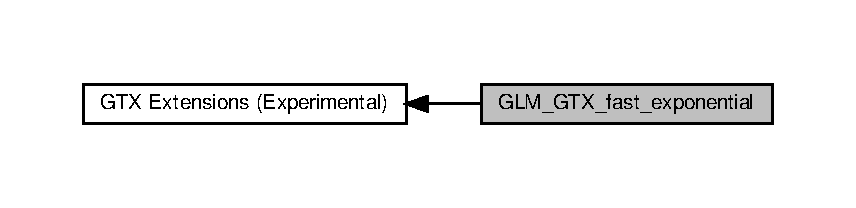
\includegraphics[width=350pt]{group__gtx__fast__exponential}
\end{center}
\end{figure}
\subsection*{Functions}
\begin{DoxyCompactItemize}
\item 
{\footnotesize template$<$typename gen\+Type $>$ }\\\hyperlink{setup_8hpp_ab2d052de21a70539923e9bcbf6e83a51}{G\+L\+M\+\_\+\+F\+U\+N\+C\+\_\+\+D\+E\+CL} gen\+Type \hyperlink{group__gtx__fast__exponential_ga842ec5e981c76f8aae7ae14972795378}{glm\+::fast\+Pow} (gen\+Type const \&x, gen\+Type const \&y)
\item 
{\footnotesize template$<$typename gen\+TypeT , typename gen\+TypeU $>$ }\\\hyperlink{setup_8hpp_ab2d052de21a70539923e9bcbf6e83a51}{G\+L\+M\+\_\+\+F\+U\+N\+C\+\_\+\+D\+E\+CL} gen\+TypeT \hyperlink{group__gtx__fast__exponential_ga08af6240d87ce7b9851c9095808c1eb8}{glm\+::fast\+Pow} (gen\+TypeT const \&x, gen\+TypeU const \&y)
\item 
{\footnotesize template$<$typename T $>$ }\\\hyperlink{setup_8hpp_ab2d052de21a70539923e9bcbf6e83a51}{G\+L\+M\+\_\+\+F\+U\+N\+C\+\_\+\+D\+E\+CL} T \hyperlink{group__gtx__fast__exponential_ga22a548f1bf42c53898c140e56af16529}{glm\+::fast\+Exp} (const T \&x)
\item 
{\footnotesize template$<$typename T $>$ }\\\hyperlink{setup_8hpp_ab2d052de21a70539923e9bcbf6e83a51}{G\+L\+M\+\_\+\+F\+U\+N\+C\+\_\+\+D\+E\+CL} T \hyperlink{group__gtx__fast__exponential_ga0130dd03ca124c27dc2094de7ee47e8a}{glm\+::fast\+Log} (const T \&x)
\item 
{\footnotesize template$<$typename T $>$ }\\\hyperlink{setup_8hpp_ab2d052de21a70539923e9bcbf6e83a51}{G\+L\+M\+\_\+\+F\+U\+N\+C\+\_\+\+D\+E\+CL} T \hyperlink{group__gtx__fast__exponential_ga62216328ac3af1811add813d0804437d}{glm\+::fast\+Exp2} (const T \&x)
\item 
{\footnotesize template$<$typename T $>$ }\\\hyperlink{setup_8hpp_ab2d052de21a70539923e9bcbf6e83a51}{G\+L\+M\+\_\+\+F\+U\+N\+C\+\_\+\+D\+E\+CL} T \hyperlink{group__gtx__fast__exponential_gadff374a7349142c0ae65f476b9bf4886}{glm\+::fast\+Log2} (const T \&x)
\item 
{\footnotesize template$<$typename T $>$ }\\\hyperlink{setup_8hpp_ab2d052de21a70539923e9bcbf6e83a51}{G\+L\+M\+\_\+\+F\+U\+N\+C\+\_\+\+D\+E\+CL} T \hyperlink{group__gtx__fast__exponential_ga8f27c4779039f88ae790a9a69be01630}{glm\+::fast\+Ln} (const T \&x)
\end{DoxyCompactItemize}


\subsection{Detailed Description}
Fast but less accurate implementations of exponential based functions. 

$<$\hyperlink{fast__exponential_8hpp}{glm/gtx/fast\+\_\+exponential.\+hpp}$>$ need to be included to use these functionalities. 

\subsection{Function Documentation}
\mbox{\Hypertarget{group__gtx__fast__exponential_ga22a548f1bf42c53898c140e56af16529}\label{group__gtx__fast__exponential_ga22a548f1bf42c53898c140e56af16529}} 
\index{G\+L\+M\+\_\+\+G\+T\+X\+\_\+fast\+\_\+exponential@{G\+L\+M\+\_\+\+G\+T\+X\+\_\+fast\+\_\+exponential}!fast\+Exp@{fast\+Exp}}
\index{fast\+Exp@{fast\+Exp}!G\+L\+M\+\_\+\+G\+T\+X\+\_\+fast\+\_\+exponential@{G\+L\+M\+\_\+\+G\+T\+X\+\_\+fast\+\_\+exponential}}
\subsubsection{\texorpdfstring{fast\+Exp()}{fastExp()}}
{\footnotesize\ttfamily template$<$typename T $>$ \\
\hyperlink{setup_8hpp_ab2d052de21a70539923e9bcbf6e83a51}{G\+L\+M\+\_\+\+F\+U\+N\+C\+\_\+\+D\+E\+CL} T glm\+::fast\+Exp (\begin{DoxyParamCaption}\item[{const T \&}]{x }\end{DoxyParamCaption})}

Faster than the common exp function but less accurate. \begin{DoxySeeAlso}{See also}
\hyperlink{group__gtx__fast__exponential}{G\+L\+M\+\_\+\+G\+T\+X\+\_\+fast\+\_\+exponential} 
\end{DoxySeeAlso}
\mbox{\Hypertarget{group__gtx__fast__exponential_ga62216328ac3af1811add813d0804437d}\label{group__gtx__fast__exponential_ga62216328ac3af1811add813d0804437d}} 
\index{G\+L\+M\+\_\+\+G\+T\+X\+\_\+fast\+\_\+exponential@{G\+L\+M\+\_\+\+G\+T\+X\+\_\+fast\+\_\+exponential}!fast\+Exp2@{fast\+Exp2}}
\index{fast\+Exp2@{fast\+Exp2}!G\+L\+M\+\_\+\+G\+T\+X\+\_\+fast\+\_\+exponential@{G\+L\+M\+\_\+\+G\+T\+X\+\_\+fast\+\_\+exponential}}
\subsubsection{\texorpdfstring{fast\+Exp2()}{fastExp2()}}
{\footnotesize\ttfamily template$<$typename T $>$ \\
\hyperlink{setup_8hpp_ab2d052de21a70539923e9bcbf6e83a51}{G\+L\+M\+\_\+\+F\+U\+N\+C\+\_\+\+D\+E\+CL} T glm\+::fast\+Exp2 (\begin{DoxyParamCaption}\item[{const T \&}]{x }\end{DoxyParamCaption})}

Faster than the common exp2 function but less accurate. \begin{DoxySeeAlso}{See also}
\hyperlink{group__gtx__fast__exponential}{G\+L\+M\+\_\+\+G\+T\+X\+\_\+fast\+\_\+exponential} 
\end{DoxySeeAlso}
\mbox{\Hypertarget{group__gtx__fast__exponential_ga8f27c4779039f88ae790a9a69be01630}\label{group__gtx__fast__exponential_ga8f27c4779039f88ae790a9a69be01630}} 
\index{G\+L\+M\+\_\+\+G\+T\+X\+\_\+fast\+\_\+exponential@{G\+L\+M\+\_\+\+G\+T\+X\+\_\+fast\+\_\+exponential}!fast\+Ln@{fast\+Ln}}
\index{fast\+Ln@{fast\+Ln}!G\+L\+M\+\_\+\+G\+T\+X\+\_\+fast\+\_\+exponential@{G\+L\+M\+\_\+\+G\+T\+X\+\_\+fast\+\_\+exponential}}
\subsubsection{\texorpdfstring{fast\+Ln()}{fastLn()}}
{\footnotesize\ttfamily template$<$typename T $>$ \\
\hyperlink{setup_8hpp_ab2d052de21a70539923e9bcbf6e83a51}{G\+L\+M\+\_\+\+F\+U\+N\+C\+\_\+\+D\+E\+CL} T glm\+::fast\+Ln (\begin{DoxyParamCaption}\item[{const T \&}]{x }\end{DoxyParamCaption})}

Faster than the common ln function but less accurate. \begin{DoxySeeAlso}{See also}
\hyperlink{group__gtx__fast__exponential}{G\+L\+M\+\_\+\+G\+T\+X\+\_\+fast\+\_\+exponential} 
\end{DoxySeeAlso}
\mbox{\Hypertarget{group__gtx__fast__exponential_ga0130dd03ca124c27dc2094de7ee47e8a}\label{group__gtx__fast__exponential_ga0130dd03ca124c27dc2094de7ee47e8a}} 
\index{G\+L\+M\+\_\+\+G\+T\+X\+\_\+fast\+\_\+exponential@{G\+L\+M\+\_\+\+G\+T\+X\+\_\+fast\+\_\+exponential}!fast\+Log@{fast\+Log}}
\index{fast\+Log@{fast\+Log}!G\+L\+M\+\_\+\+G\+T\+X\+\_\+fast\+\_\+exponential@{G\+L\+M\+\_\+\+G\+T\+X\+\_\+fast\+\_\+exponential}}
\subsubsection{\texorpdfstring{fast\+Log()}{fastLog()}}
{\footnotesize\ttfamily template$<$typename T $>$ \\
\hyperlink{setup_8hpp_ab2d052de21a70539923e9bcbf6e83a51}{G\+L\+M\+\_\+\+F\+U\+N\+C\+\_\+\+D\+E\+CL} T glm\+::fast\+Log (\begin{DoxyParamCaption}\item[{const T \&}]{x }\end{DoxyParamCaption})}

Faster than the common log function but less accurate. \begin{DoxySeeAlso}{See also}
\hyperlink{group__gtx__fast__exponential}{G\+L\+M\+\_\+\+G\+T\+X\+\_\+fast\+\_\+exponential} 
\end{DoxySeeAlso}
\mbox{\Hypertarget{group__gtx__fast__exponential_gadff374a7349142c0ae65f476b9bf4886}\label{group__gtx__fast__exponential_gadff374a7349142c0ae65f476b9bf4886}} 
\index{G\+L\+M\+\_\+\+G\+T\+X\+\_\+fast\+\_\+exponential@{G\+L\+M\+\_\+\+G\+T\+X\+\_\+fast\+\_\+exponential}!fast\+Log2@{fast\+Log2}}
\index{fast\+Log2@{fast\+Log2}!G\+L\+M\+\_\+\+G\+T\+X\+\_\+fast\+\_\+exponential@{G\+L\+M\+\_\+\+G\+T\+X\+\_\+fast\+\_\+exponential}}
\subsubsection{\texorpdfstring{fast\+Log2()}{fastLog2()}}
{\footnotesize\ttfamily template$<$typename T $>$ \\
\hyperlink{setup_8hpp_ab2d052de21a70539923e9bcbf6e83a51}{G\+L\+M\+\_\+\+F\+U\+N\+C\+\_\+\+D\+E\+CL} T glm\+::fast\+Log2 (\begin{DoxyParamCaption}\item[{const T \&}]{x }\end{DoxyParamCaption})}

Faster than the common log2 function but less accurate. \begin{DoxySeeAlso}{See also}
\hyperlink{group__gtx__fast__exponential}{G\+L\+M\+\_\+\+G\+T\+X\+\_\+fast\+\_\+exponential} 
\end{DoxySeeAlso}
\mbox{\Hypertarget{group__gtx__fast__exponential_ga842ec5e981c76f8aae7ae14972795378}\label{group__gtx__fast__exponential_ga842ec5e981c76f8aae7ae14972795378}} 
\index{G\+L\+M\+\_\+\+G\+T\+X\+\_\+fast\+\_\+exponential@{G\+L\+M\+\_\+\+G\+T\+X\+\_\+fast\+\_\+exponential}!fast\+Pow@{fast\+Pow}}
\index{fast\+Pow@{fast\+Pow}!G\+L\+M\+\_\+\+G\+T\+X\+\_\+fast\+\_\+exponential@{G\+L\+M\+\_\+\+G\+T\+X\+\_\+fast\+\_\+exponential}}
\subsubsection{\texorpdfstring{fast\+Pow()}{fastPow()}\hspace{0.1cm}{\footnotesize\ttfamily [1/2]}}
{\footnotesize\ttfamily template$<$typename gen\+Type $>$ \\
\hyperlink{setup_8hpp_ab2d052de21a70539923e9bcbf6e83a51}{G\+L\+M\+\_\+\+F\+U\+N\+C\+\_\+\+D\+E\+CL} gen\+Type glm\+::fast\+Pow (\begin{DoxyParamCaption}\item[{gen\+Type const \&}]{x,  }\item[{gen\+Type const \&}]{y }\end{DoxyParamCaption})}

Faster than the common pow function but less accurate. \begin{DoxySeeAlso}{See also}
\hyperlink{group__gtx__fast__exponential}{G\+L\+M\+\_\+\+G\+T\+X\+\_\+fast\+\_\+exponential} 
\end{DoxySeeAlso}


Definition at line 14 of file fast\+\_\+exponential.\+inl.

\mbox{\Hypertarget{group__gtx__fast__exponential_ga08af6240d87ce7b9851c9095808c1eb8}\label{group__gtx__fast__exponential_ga08af6240d87ce7b9851c9095808c1eb8}} 
\index{G\+L\+M\+\_\+\+G\+T\+X\+\_\+fast\+\_\+exponential@{G\+L\+M\+\_\+\+G\+T\+X\+\_\+fast\+\_\+exponential}!fast\+Pow@{fast\+Pow}}
\index{fast\+Pow@{fast\+Pow}!G\+L\+M\+\_\+\+G\+T\+X\+\_\+fast\+\_\+exponential@{G\+L\+M\+\_\+\+G\+T\+X\+\_\+fast\+\_\+exponential}}
\subsubsection{\texorpdfstring{fast\+Pow()}{fastPow()}\hspace{0.1cm}{\footnotesize\ttfamily [2/2]}}
{\footnotesize\ttfamily template$<$typename gen\+TypeT , typename gen\+TypeU $>$ \\
\hyperlink{setup_8hpp_ab2d052de21a70539923e9bcbf6e83a51}{G\+L\+M\+\_\+\+F\+U\+N\+C\+\_\+\+D\+E\+CL} gen\+TypeT glm\+::fast\+Pow (\begin{DoxyParamCaption}\item[{gen\+TypeT const \&}]{x,  }\item[{gen\+TypeU const \&}]{y }\end{DoxyParamCaption})}

Faster than the common pow function but less accurate. \begin{DoxySeeAlso}{See also}
\hyperlink{group__gtx__fast__exponential}{G\+L\+M\+\_\+\+G\+T\+X\+\_\+fast\+\_\+exponential} 
\end{DoxySeeAlso}

\hypertarget{group__gtx__fast__square__root}{}\section{G\+L\+M\+\_\+\+G\+T\+X\+\_\+fast\+\_\+square\+\_\+root}
\label{group__gtx__fast__square__root}\index{G\+L\+M\+\_\+\+G\+T\+X\+\_\+fast\+\_\+square\+\_\+root@{G\+L\+M\+\_\+\+G\+T\+X\+\_\+fast\+\_\+square\+\_\+root}}


Fast but less accurate implementations of square root based functions.  


Collaboration diagram for G\+L\+M\+\_\+\+G\+T\+X\+\_\+fast\+\_\+square\+\_\+root\+:\nopagebreak
\begin{figure}[H]
\begin{center}
\leavevmode
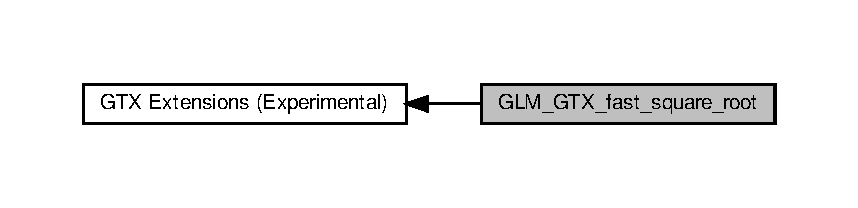
\includegraphics[width=350pt]{group__gtx__fast__square__root}
\end{center}
\end{figure}
\subsection*{Functions}
\begin{DoxyCompactItemize}
\item 
{\footnotesize template$<$typename gen\+Type $>$ }\\\hyperlink{setup_8hpp_ab2d052de21a70539923e9bcbf6e83a51}{G\+L\+M\+\_\+\+F\+U\+N\+C\+\_\+\+D\+E\+CL} gen\+Type \hyperlink{group__gtx__fast__square__root_gab07ddede2731f3438d687a652c843673}{glm\+::fast\+Sqrt} (gen\+Type const \&x)
\item 
{\footnotesize template$<$typename gen\+Type $>$ }\\\hyperlink{setup_8hpp_ab2d052de21a70539923e9bcbf6e83a51}{G\+L\+M\+\_\+\+F\+U\+N\+C\+\_\+\+D\+E\+CL} gen\+Type \hyperlink{group__gtx__fast__square__root_ga65237d716748c6262f316ec1eaf7f073}{glm\+::fast\+Inverse\+Sqrt} (gen\+Type const \&x)
\item 
{\footnotesize template$<$typename T , precision P, template$<$ typename, precision $>$ class vec\+Type$>$ }\\\hyperlink{setup_8hpp_ab2d052de21a70539923e9bcbf6e83a51}{G\+L\+M\+\_\+\+F\+U\+N\+C\+\_\+\+D\+E\+CL} vec\+Type$<$ T, P $>$ \hyperlink{group__gtx__fast__square__root_ga903878071f92e51e551791e584a171a1}{glm\+::fast\+Inverse\+Sqrt} (vec\+Type$<$ T, P $>$ const \&x)
\item 
{\footnotesize template$<$typename gen\+Type $>$ }\\\hyperlink{setup_8hpp_ab2d052de21a70539923e9bcbf6e83a51}{G\+L\+M\+\_\+\+F\+U\+N\+C\+\_\+\+D\+E\+CL} gen\+Type\+::value\+\_\+type \hyperlink{group__gtx__fast__square__root_ga70aa3c80d8bb22e021c6c3ebdcf8e3ee}{glm\+::fast\+Length} (gen\+Type const \&x)
\item 
{\footnotesize template$<$typename gen\+Type $>$ }\\\hyperlink{setup_8hpp_ab2d052de21a70539923e9bcbf6e83a51}{G\+L\+M\+\_\+\+F\+U\+N\+C\+\_\+\+D\+E\+CL} gen\+Type\+::value\+\_\+type \hyperlink{group__gtx__fast__square__root_ga69778792fcadc29f586efa3ec2118cdc}{glm\+::fast\+Distance} (gen\+Type const \&x, gen\+Type const \&y)
\item 
{\footnotesize template$<$typename gen\+Type $>$ }\\\hyperlink{setup_8hpp_ab2d052de21a70539923e9bcbf6e83a51}{G\+L\+M\+\_\+\+F\+U\+N\+C\+\_\+\+D\+E\+CL} gen\+Type \hyperlink{group__gtx__fast__square__root_ga3b02c1d6e0c754144e2f1e110bf9f16c}{glm\+::fast\+Normalize} (gen\+Type const \&x)
\end{DoxyCompactItemize}


\subsection{Detailed Description}
Fast but less accurate implementations of square root based functions. 


\begin{DoxyItemize}
\item Sqrt optimisation based on Newton\textquotesingle{}s method, www.\+gamedev.\+net/community/forums/topic.asp?topic id=139956
\end{DoxyItemize}

$<$\hyperlink{fast__square__root_8hpp}{glm/gtx/fast\+\_\+square\+\_\+root.\+hpp}$>$ need to be included to use these functionalities. 

\subsection{Function Documentation}
\mbox{\Hypertarget{group__gtx__fast__square__root_ga69778792fcadc29f586efa3ec2118cdc}\label{group__gtx__fast__square__root_ga69778792fcadc29f586efa3ec2118cdc}} 
\index{G\+L\+M\+\_\+\+G\+T\+X\+\_\+fast\+\_\+square\+\_\+root@{G\+L\+M\+\_\+\+G\+T\+X\+\_\+fast\+\_\+square\+\_\+root}!fast\+Distance@{fast\+Distance}}
\index{fast\+Distance@{fast\+Distance}!G\+L\+M\+\_\+\+G\+T\+X\+\_\+fast\+\_\+square\+\_\+root@{G\+L\+M\+\_\+\+G\+T\+X\+\_\+fast\+\_\+square\+\_\+root}}
\subsubsection{\texorpdfstring{fast\+Distance()}{fastDistance()}}
{\footnotesize\ttfamily template$<$typename gen\+Type $>$ \\
\hyperlink{setup_8hpp_ab2d052de21a70539923e9bcbf6e83a51}{G\+L\+M\+\_\+\+F\+U\+N\+C\+\_\+\+D\+E\+CL} gen\+Type\+::value\+\_\+type glm\+::fast\+Distance (\begin{DoxyParamCaption}\item[{gen\+Type const \&}]{x,  }\item[{gen\+Type const \&}]{y }\end{DoxyParamCaption})}

Faster than the common distance function but less accurate. From G\+L\+M\+\_\+\+G\+T\+X\+\_\+fast\+\_\+square\+\_\+root extension. 

Definition at line 103 of file fast\+\_\+square\+\_\+root.\+inl.

\mbox{\Hypertarget{group__gtx__fast__square__root_ga65237d716748c6262f316ec1eaf7f073}\label{group__gtx__fast__square__root_ga65237d716748c6262f316ec1eaf7f073}} 
\index{G\+L\+M\+\_\+\+G\+T\+X\+\_\+fast\+\_\+square\+\_\+root@{G\+L\+M\+\_\+\+G\+T\+X\+\_\+fast\+\_\+square\+\_\+root}!fast\+Inverse\+Sqrt@{fast\+Inverse\+Sqrt}}
\index{fast\+Inverse\+Sqrt@{fast\+Inverse\+Sqrt}!G\+L\+M\+\_\+\+G\+T\+X\+\_\+fast\+\_\+square\+\_\+root@{G\+L\+M\+\_\+\+G\+T\+X\+\_\+fast\+\_\+square\+\_\+root}}
\subsubsection{\texorpdfstring{fast\+Inverse\+Sqrt()}{fastInverseSqrt()}\hspace{0.1cm}{\footnotesize\ttfamily [1/2]}}
{\footnotesize\ttfamily template$<$typename gen\+Type $>$ \\
\hyperlink{setup_8hpp_ab2d052de21a70539923e9bcbf6e83a51}{G\+L\+M\+\_\+\+F\+U\+N\+C\+\_\+\+D\+E\+CL} gen\+Type glm\+::fast\+Inverse\+Sqrt (\begin{DoxyParamCaption}\item[{gen\+Type const \&}]{x }\end{DoxyParamCaption})}

Faster than the common inversesqrt function but less accurate. From G\+L\+M\+\_\+\+G\+T\+X\+\_\+fast\+\_\+square\+\_\+root extension. \mbox{\Hypertarget{group__gtx__fast__square__root_ga903878071f92e51e551791e584a171a1}\label{group__gtx__fast__square__root_ga903878071f92e51e551791e584a171a1}} 
\index{G\+L\+M\+\_\+\+G\+T\+X\+\_\+fast\+\_\+square\+\_\+root@{G\+L\+M\+\_\+\+G\+T\+X\+\_\+fast\+\_\+square\+\_\+root}!fast\+Inverse\+Sqrt@{fast\+Inverse\+Sqrt}}
\index{fast\+Inverse\+Sqrt@{fast\+Inverse\+Sqrt}!G\+L\+M\+\_\+\+G\+T\+X\+\_\+fast\+\_\+square\+\_\+root@{G\+L\+M\+\_\+\+G\+T\+X\+\_\+fast\+\_\+square\+\_\+root}}
\subsubsection{\texorpdfstring{fast\+Inverse\+Sqrt()}{fastInverseSqrt()}\hspace{0.1cm}{\footnotesize\ttfamily [2/2]}}
{\footnotesize\ttfamily template$<$typename T , precision P, template$<$ typename, precision $>$ class vec\+Type$>$ \\
\hyperlink{setup_8hpp_ab2d052de21a70539923e9bcbf6e83a51}{G\+L\+M\+\_\+\+F\+U\+N\+C\+\_\+\+D\+E\+CL} vec\+Type$<$T, P$>$ glm\+::fast\+Inverse\+Sqrt (\begin{DoxyParamCaption}\item[{vec\+Type$<$ T, P $>$ const \&}]{x }\end{DoxyParamCaption})}

Faster than the common inversesqrt function but less accurate. From G\+L\+M\+\_\+\+G\+T\+X\+\_\+fast\+\_\+square\+\_\+root extension. 

Definition at line 51 of file fast\+\_\+square\+\_\+root.\+inl.

\mbox{\Hypertarget{group__gtx__fast__square__root_ga70aa3c80d8bb22e021c6c3ebdcf8e3ee}\label{group__gtx__fast__square__root_ga70aa3c80d8bb22e021c6c3ebdcf8e3ee}} 
\index{G\+L\+M\+\_\+\+G\+T\+X\+\_\+fast\+\_\+square\+\_\+root@{G\+L\+M\+\_\+\+G\+T\+X\+\_\+fast\+\_\+square\+\_\+root}!fast\+Length@{fast\+Length}}
\index{fast\+Length@{fast\+Length}!G\+L\+M\+\_\+\+G\+T\+X\+\_\+fast\+\_\+square\+\_\+root@{G\+L\+M\+\_\+\+G\+T\+X\+\_\+fast\+\_\+square\+\_\+root}}
\subsubsection{\texorpdfstring{fast\+Length()}{fastLength()}}
{\footnotesize\ttfamily template$<$typename gen\+Type $>$ \\
\hyperlink{setup_8hpp_ab2d052de21a70539923e9bcbf6e83a51}{G\+L\+M\+\_\+\+F\+U\+N\+C\+\_\+\+D\+E\+CL} gen\+Type\+::value\+\_\+type glm\+::fast\+Length (\begin{DoxyParamCaption}\item[{gen\+Type const \&}]{x }\end{DoxyParamCaption})}

Faster than the common length function but less accurate. From G\+L\+M\+\_\+\+G\+T\+X\+\_\+fast\+\_\+square\+\_\+root extension. 

Definition at line 63 of file fast\+\_\+square\+\_\+root.\+inl.

\mbox{\Hypertarget{group__gtx__fast__square__root_ga3b02c1d6e0c754144e2f1e110bf9f16c}\label{group__gtx__fast__square__root_ga3b02c1d6e0c754144e2f1e110bf9f16c}} 
\index{G\+L\+M\+\_\+\+G\+T\+X\+\_\+fast\+\_\+square\+\_\+root@{G\+L\+M\+\_\+\+G\+T\+X\+\_\+fast\+\_\+square\+\_\+root}!fast\+Normalize@{fast\+Normalize}}
\index{fast\+Normalize@{fast\+Normalize}!G\+L\+M\+\_\+\+G\+T\+X\+\_\+fast\+\_\+square\+\_\+root@{G\+L\+M\+\_\+\+G\+T\+X\+\_\+fast\+\_\+square\+\_\+root}}
\subsubsection{\texorpdfstring{fast\+Normalize()}{fastNormalize()}}
{\footnotesize\ttfamily template$<$typename gen\+Type $>$ \\
\hyperlink{setup_8hpp_ab2d052de21a70539923e9bcbf6e83a51}{G\+L\+M\+\_\+\+F\+U\+N\+C\+\_\+\+D\+E\+CL} gen\+Type glm\+::fast\+Normalize (\begin{DoxyParamCaption}\item[{gen\+Type const \&}]{x }\end{DoxyParamCaption})}

Faster than the common normalize function but less accurate. From G\+L\+M\+\_\+\+G\+T\+X\+\_\+fast\+\_\+square\+\_\+root extension. 

Definition at line 144 of file fast\+\_\+square\+\_\+root.\+inl.

\mbox{\Hypertarget{group__gtx__fast__square__root_gab07ddede2731f3438d687a652c843673}\label{group__gtx__fast__square__root_gab07ddede2731f3438d687a652c843673}} 
\index{G\+L\+M\+\_\+\+G\+T\+X\+\_\+fast\+\_\+square\+\_\+root@{G\+L\+M\+\_\+\+G\+T\+X\+\_\+fast\+\_\+square\+\_\+root}!fast\+Sqrt@{fast\+Sqrt}}
\index{fast\+Sqrt@{fast\+Sqrt}!G\+L\+M\+\_\+\+G\+T\+X\+\_\+fast\+\_\+square\+\_\+root@{G\+L\+M\+\_\+\+G\+T\+X\+\_\+fast\+\_\+square\+\_\+root}}
\subsubsection{\texorpdfstring{fast\+Sqrt()}{fastSqrt()}}
{\footnotesize\ttfamily template$<$typename gen\+Type $>$ \\
\hyperlink{setup_8hpp_ab2d052de21a70539923e9bcbf6e83a51}{G\+L\+M\+\_\+\+F\+U\+N\+C\+\_\+\+D\+E\+CL} gen\+Type glm\+::fast\+Sqrt (\begin{DoxyParamCaption}\item[{gen\+Type const \&}]{x }\end{DoxyParamCaption})}

Faster than the common sqrt function but less accurate. From G\+L\+M\+\_\+\+G\+T\+X\+\_\+fast\+\_\+square\+\_\+root extension. 

Definition at line 15 of file fast\+\_\+square\+\_\+root.\+inl.


\hypertarget{group__gtx__fast__trigonometry}{}\section{G\+L\+M\+\_\+\+G\+T\+X\+\_\+fast\+\_\+trigonometry}
\label{group__gtx__fast__trigonometry}\index{G\+L\+M\+\_\+\+G\+T\+X\+\_\+fast\+\_\+trigonometry@{G\+L\+M\+\_\+\+G\+T\+X\+\_\+fast\+\_\+trigonometry}}


Fast but less accurate implementations of trigonometric functions.  


Collaboration diagram for G\+L\+M\+\_\+\+G\+T\+X\+\_\+fast\+\_\+trigonometry\+:\nopagebreak
\begin{figure}[H]
\begin{center}
\leavevmode
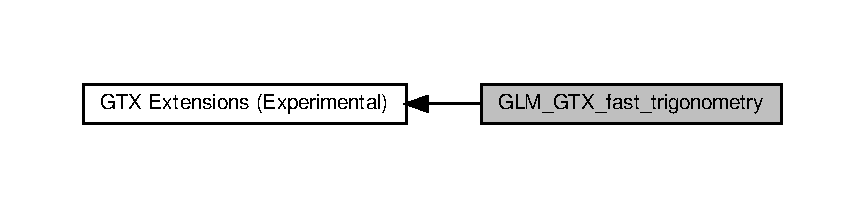
\includegraphics[width=350pt]{group__gtx__fast__trigonometry}
\end{center}
\end{figure}
\subsection*{Functions}
\begin{DoxyCompactItemize}
\item 
{\footnotesize template$<$typename T $>$ }\\\hyperlink{setup_8hpp_ab2d052de21a70539923e9bcbf6e83a51}{G\+L\+M\+\_\+\+F\+U\+N\+C\+\_\+\+D\+E\+CL} T \hyperlink{group__gtx__fast__trigonometry_ga01b7dc431bf5f5e6acce7d6bba311f86}{glm\+::fast\+Sin} (const T \&\hyperlink{group__gtc__quaternion_ga23a3fc7ada5bbb665ff84c92c6e0542c}{angle})
\item 
{\footnotesize template$<$typename T $>$ }\\\hyperlink{setup_8hpp_ab2d052de21a70539923e9bcbf6e83a51}{G\+L\+M\+\_\+\+F\+U\+N\+C\+\_\+\+D\+E\+CL} T \hyperlink{group__gtx__fast__trigonometry_gad54184beaba79e41db71a1f5711380c4}{glm\+::fast\+Cos} (const T \&\hyperlink{group__gtc__quaternion_ga23a3fc7ada5bbb665ff84c92c6e0542c}{angle})
\item 
{\footnotesize template$<$typename T $>$ }\\\hyperlink{setup_8hpp_ab2d052de21a70539923e9bcbf6e83a51}{G\+L\+M\+\_\+\+F\+U\+N\+C\+\_\+\+D\+E\+CL} T \hyperlink{group__gtx__fast__trigonometry_gae6615cdb40d8dc58115a07a21f495561}{glm\+::fast\+Tan} (const T \&\hyperlink{group__gtc__quaternion_ga23a3fc7ada5bbb665ff84c92c6e0542c}{angle})
\item 
{\footnotesize template$<$typename T $>$ }\\\hyperlink{setup_8hpp_ab2d052de21a70539923e9bcbf6e83a51}{G\+L\+M\+\_\+\+F\+U\+N\+C\+\_\+\+D\+E\+CL} T \hyperlink{group__gtx__fast__trigonometry_gab8595a77c5b215b95f662238dc3ff722}{glm\+::fast\+Asin} (const T \&\hyperlink{group__gtc__quaternion_ga23a3fc7ada5bbb665ff84c92c6e0542c}{angle})
\item 
{\footnotesize template$<$typename T $>$ }\\\hyperlink{setup_8hpp_ab2d052de21a70539923e9bcbf6e83a51}{G\+L\+M\+\_\+\+F\+U\+N\+C\+\_\+\+D\+E\+CL} T \hyperlink{group__gtx__fast__trigonometry_ga44e6efc3e776a51645fdf998e3e4f11b}{glm\+::fast\+Acos} (const T \&\hyperlink{group__gtc__quaternion_ga23a3fc7ada5bbb665ff84c92c6e0542c}{angle})
\item 
{\footnotesize template$<$typename T $>$ }\\\hyperlink{setup_8hpp_ab2d052de21a70539923e9bcbf6e83a51}{G\+L\+M\+\_\+\+F\+U\+N\+C\+\_\+\+D\+E\+CL} T \hyperlink{group__gtx__fast__trigonometry_gaf6234384b94846e29cf2c51dc245d484}{glm\+::fast\+Atan} (const T \&y, const T \&x)
\item 
{\footnotesize template$<$typename T $>$ }\\\hyperlink{setup_8hpp_ab2d052de21a70539923e9bcbf6e83a51}{G\+L\+M\+\_\+\+F\+U\+N\+C\+\_\+\+D\+E\+CL} T \hyperlink{group__gtx__fast__trigonometry_ga49b3b2b777b83eeed3e11205e800027e}{glm\+::fast\+Atan} (const T \&\hyperlink{group__gtc__quaternion_ga23a3fc7ada5bbb665ff84c92c6e0542c}{angle})
\end{DoxyCompactItemize}


\subsection{Detailed Description}
Fast but less accurate implementations of trigonometric functions. 

$<$\hyperlink{fast__trigonometry_8hpp}{glm/gtx/fast\+\_\+trigonometry.\+hpp}$>$ need to be included to use these functionalities. 

\subsection{Function Documentation}
\mbox{\Hypertarget{group__gtx__fast__trigonometry_ga44e6efc3e776a51645fdf998e3e4f11b}\label{group__gtx__fast__trigonometry_ga44e6efc3e776a51645fdf998e3e4f11b}} 
\index{G\+L\+M\+\_\+\+G\+T\+X\+\_\+fast\+\_\+trigonometry@{G\+L\+M\+\_\+\+G\+T\+X\+\_\+fast\+\_\+trigonometry}!fast\+Acos@{fast\+Acos}}
\index{fast\+Acos@{fast\+Acos}!G\+L\+M\+\_\+\+G\+T\+X\+\_\+fast\+\_\+trigonometry@{G\+L\+M\+\_\+\+G\+T\+X\+\_\+fast\+\_\+trigonometry}}
\subsubsection{\texorpdfstring{fast\+Acos()}{fastAcos()}}
{\footnotesize\ttfamily template$<$typename T $>$ \\
\hyperlink{setup_8hpp_ab2d052de21a70539923e9bcbf6e83a51}{G\+L\+M\+\_\+\+F\+U\+N\+C\+\_\+\+D\+E\+CL} T glm\+::fast\+Acos (\begin{DoxyParamCaption}\item[{const T \&}]{angle }\end{DoxyParamCaption})}

Faster than the common acos function but less accurate. Defined between -\/2pi and 2pi. From G\+L\+M\+\_\+\+G\+T\+X\+\_\+fast\+\_\+trigonometry extension. 

Definition at line 50 of file fast\+\_\+trigonometry.\+inl.

\mbox{\Hypertarget{group__gtx__fast__trigonometry_gab8595a77c5b215b95f662238dc3ff722}\label{group__gtx__fast__trigonometry_gab8595a77c5b215b95f662238dc3ff722}} 
\index{G\+L\+M\+\_\+\+G\+T\+X\+\_\+fast\+\_\+trigonometry@{G\+L\+M\+\_\+\+G\+T\+X\+\_\+fast\+\_\+trigonometry}!fast\+Asin@{fast\+Asin}}
\index{fast\+Asin@{fast\+Asin}!G\+L\+M\+\_\+\+G\+T\+X\+\_\+fast\+\_\+trigonometry@{G\+L\+M\+\_\+\+G\+T\+X\+\_\+fast\+\_\+trigonometry}}
\subsubsection{\texorpdfstring{fast\+Asin()}{fastAsin()}}
{\footnotesize\ttfamily template$<$typename T $>$ \\
\hyperlink{setup_8hpp_ab2d052de21a70539923e9bcbf6e83a51}{G\+L\+M\+\_\+\+F\+U\+N\+C\+\_\+\+D\+E\+CL} T glm\+::fast\+Asin (\begin{DoxyParamCaption}\item[{const T \&}]{angle }\end{DoxyParamCaption})}

Faster than the common asin function but less accurate. Defined between -\/2pi and 2pi. From G\+L\+M\+\_\+\+G\+T\+X\+\_\+fast\+\_\+trigonometry extension. 

Definition at line 41 of file fast\+\_\+trigonometry.\+inl.

\mbox{\Hypertarget{group__gtx__fast__trigonometry_gaf6234384b94846e29cf2c51dc245d484}\label{group__gtx__fast__trigonometry_gaf6234384b94846e29cf2c51dc245d484}} 
\index{G\+L\+M\+\_\+\+G\+T\+X\+\_\+fast\+\_\+trigonometry@{G\+L\+M\+\_\+\+G\+T\+X\+\_\+fast\+\_\+trigonometry}!fast\+Atan@{fast\+Atan}}
\index{fast\+Atan@{fast\+Atan}!G\+L\+M\+\_\+\+G\+T\+X\+\_\+fast\+\_\+trigonometry@{G\+L\+M\+\_\+\+G\+T\+X\+\_\+fast\+\_\+trigonometry}}
\subsubsection{\texorpdfstring{fast\+Atan()}{fastAtan()}\hspace{0.1cm}{\footnotesize\ttfamily [1/2]}}
{\footnotesize\ttfamily template$<$typename T $>$ \\
\hyperlink{setup_8hpp_ab2d052de21a70539923e9bcbf6e83a51}{G\+L\+M\+\_\+\+F\+U\+N\+C\+\_\+\+D\+E\+CL} T glm\+::fast\+Atan (\begin{DoxyParamCaption}\item[{const T \&}]{y,  }\item[{const T \&}]{x }\end{DoxyParamCaption})}

Faster than the common atan function but less accurate. Defined between -\/2pi and 2pi. From G\+L\+M\+\_\+\+G\+T\+X\+\_\+fast\+\_\+trigonometry extension. 

Definition at line 59 of file fast\+\_\+trigonometry.\+inl.

\mbox{\Hypertarget{group__gtx__fast__trigonometry_ga49b3b2b777b83eeed3e11205e800027e}\label{group__gtx__fast__trigonometry_ga49b3b2b777b83eeed3e11205e800027e}} 
\index{G\+L\+M\+\_\+\+G\+T\+X\+\_\+fast\+\_\+trigonometry@{G\+L\+M\+\_\+\+G\+T\+X\+\_\+fast\+\_\+trigonometry}!fast\+Atan@{fast\+Atan}}
\index{fast\+Atan@{fast\+Atan}!G\+L\+M\+\_\+\+G\+T\+X\+\_\+fast\+\_\+trigonometry@{G\+L\+M\+\_\+\+G\+T\+X\+\_\+fast\+\_\+trigonometry}}
\subsubsection{\texorpdfstring{fast\+Atan()}{fastAtan()}\hspace{0.1cm}{\footnotesize\ttfamily [2/2]}}
{\footnotesize\ttfamily template$<$typename T $>$ \\
\hyperlink{setup_8hpp_ab2d052de21a70539923e9bcbf6e83a51}{G\+L\+M\+\_\+\+F\+U\+N\+C\+\_\+\+D\+E\+CL} T glm\+::fast\+Atan (\begin{DoxyParamCaption}\item[{const T \&}]{angle }\end{DoxyParamCaption})}

Faster than the common atan function but less accurate. Defined between -\/2pi and 2pi. From G\+L\+M\+\_\+\+G\+T\+X\+\_\+fast\+\_\+trigonometry extension. 

Definition at line 68 of file fast\+\_\+trigonometry.\+inl.

\mbox{\Hypertarget{group__gtx__fast__trigonometry_gad54184beaba79e41db71a1f5711380c4}\label{group__gtx__fast__trigonometry_gad54184beaba79e41db71a1f5711380c4}} 
\index{G\+L\+M\+\_\+\+G\+T\+X\+\_\+fast\+\_\+trigonometry@{G\+L\+M\+\_\+\+G\+T\+X\+\_\+fast\+\_\+trigonometry}!fast\+Cos@{fast\+Cos}}
\index{fast\+Cos@{fast\+Cos}!G\+L\+M\+\_\+\+G\+T\+X\+\_\+fast\+\_\+trigonometry@{G\+L\+M\+\_\+\+G\+T\+X\+\_\+fast\+\_\+trigonometry}}
\subsubsection{\texorpdfstring{fast\+Cos()}{fastCos()}}
{\footnotesize\ttfamily template$<$typename T $>$ \\
\hyperlink{setup_8hpp_ab2d052de21a70539923e9bcbf6e83a51}{G\+L\+M\+\_\+\+F\+U\+N\+C\+\_\+\+D\+E\+CL} T glm\+::fast\+Cos (\begin{DoxyParamCaption}\item[{const T \&}]{angle }\end{DoxyParamCaption})}

Faster than the common cos function but less accurate. Defined between -\/2pi and 2pi. From G\+L\+M\+\_\+\+G\+T\+X\+\_\+fast\+\_\+trigonometry extension. 

Definition at line 23 of file fast\+\_\+trigonometry.\+inl.

\mbox{\Hypertarget{group__gtx__fast__trigonometry_ga01b7dc431bf5f5e6acce7d6bba311f86}\label{group__gtx__fast__trigonometry_ga01b7dc431bf5f5e6acce7d6bba311f86}} 
\index{G\+L\+M\+\_\+\+G\+T\+X\+\_\+fast\+\_\+trigonometry@{G\+L\+M\+\_\+\+G\+T\+X\+\_\+fast\+\_\+trigonometry}!fast\+Sin@{fast\+Sin}}
\index{fast\+Sin@{fast\+Sin}!G\+L\+M\+\_\+\+G\+T\+X\+\_\+fast\+\_\+trigonometry@{G\+L\+M\+\_\+\+G\+T\+X\+\_\+fast\+\_\+trigonometry}}
\subsubsection{\texorpdfstring{fast\+Sin()}{fastSin()}}
{\footnotesize\ttfamily template$<$typename T $>$ \\
\hyperlink{setup_8hpp_ab2d052de21a70539923e9bcbf6e83a51}{G\+L\+M\+\_\+\+F\+U\+N\+C\+\_\+\+D\+E\+CL} T glm\+::fast\+Sin (\begin{DoxyParamCaption}\item[{const T \&}]{angle }\end{DoxyParamCaption})}

Faster than the common sin function but less accurate. Defined between -\/2pi and 2pi. From G\+L\+M\+\_\+\+G\+T\+X\+\_\+fast\+\_\+trigonometry extension. 

Definition at line 14 of file fast\+\_\+trigonometry.\+inl.

\mbox{\Hypertarget{group__gtx__fast__trigonometry_gae6615cdb40d8dc58115a07a21f495561}\label{group__gtx__fast__trigonometry_gae6615cdb40d8dc58115a07a21f495561}} 
\index{G\+L\+M\+\_\+\+G\+T\+X\+\_\+fast\+\_\+trigonometry@{G\+L\+M\+\_\+\+G\+T\+X\+\_\+fast\+\_\+trigonometry}!fast\+Tan@{fast\+Tan}}
\index{fast\+Tan@{fast\+Tan}!G\+L\+M\+\_\+\+G\+T\+X\+\_\+fast\+\_\+trigonometry@{G\+L\+M\+\_\+\+G\+T\+X\+\_\+fast\+\_\+trigonometry}}
\subsubsection{\texorpdfstring{fast\+Tan()}{fastTan()}}
{\footnotesize\ttfamily template$<$typename T $>$ \\
\hyperlink{setup_8hpp_ab2d052de21a70539923e9bcbf6e83a51}{G\+L\+M\+\_\+\+F\+U\+N\+C\+\_\+\+D\+E\+CL} T glm\+::fast\+Tan (\begin{DoxyParamCaption}\item[{const T \&}]{angle }\end{DoxyParamCaption})}

Faster than the common tan function but less accurate. Defined between -\/2pi and 2pi. From G\+L\+M\+\_\+\+G\+T\+X\+\_\+fast\+\_\+trigonometry extension. 

Definition at line 32 of file fast\+\_\+trigonometry.\+inl.


\hypertarget{group__gtx__gradient__paint}{}\section{G\+L\+M\+\_\+\+G\+T\+X\+\_\+gradient\+\_\+paint}
\label{group__gtx__gradient__paint}\index{G\+L\+M\+\_\+\+G\+T\+X\+\_\+gradient\+\_\+paint@{G\+L\+M\+\_\+\+G\+T\+X\+\_\+gradient\+\_\+paint}}


Functions that return the color of procedural gradient for specific coordinates. $<$\hyperlink{gradient__paint_8hpp}{glm/gtx/gradient\+\_\+paint.\+hpp}$>$ need to be included to use these functionalities.  


Collaboration diagram for G\+L\+M\+\_\+\+G\+T\+X\+\_\+gradient\+\_\+paint\+:\nopagebreak
\begin{figure}[H]
\begin{center}
\leavevmode
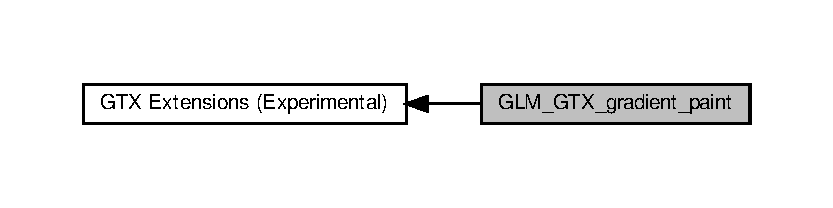
\includegraphics[width=350pt]{group__gtx__gradient__paint}
\end{center}
\end{figure}
\subsection*{Functions}
\begin{DoxyCompactItemize}
\item 
{\footnotesize template$<$typename T , precision P$>$ }\\\hyperlink{setup_8hpp_ab2d052de21a70539923e9bcbf6e83a51}{G\+L\+M\+\_\+\+F\+U\+N\+C\+\_\+\+D\+E\+CL} T \hyperlink{group__gtx__gradient__paint_ga864c46234e363137b717119231f422f6}{glm\+::radial\+Gradient} (\hyperlink{structglm_1_1detail_1_1tvec2}{detail\+::tvec2}$<$ T, P $>$ const \&Center, T const \&Radius, \hyperlink{structglm_1_1detail_1_1tvec2}{detail\+::tvec2}$<$ T, P $>$ const \&Focal, \hyperlink{structglm_1_1detail_1_1tvec2}{detail\+::tvec2}$<$ T, P $>$ const \&Position)
\item 
{\footnotesize template$<$typename T , precision P$>$ }\\\hyperlink{setup_8hpp_ab2d052de21a70539923e9bcbf6e83a51}{G\+L\+M\+\_\+\+F\+U\+N\+C\+\_\+\+D\+E\+CL} T \hyperlink{group__gtx__gradient__paint_ga01eb377864e98f86bd44378e1b86eb22}{glm\+::linear\+Gradient} (\hyperlink{structglm_1_1detail_1_1tvec2}{detail\+::tvec2}$<$ T, P $>$ const \&Point0, \hyperlink{structglm_1_1detail_1_1tvec2}{detail\+::tvec2}$<$ T, P $>$ const \&Point1, \hyperlink{structglm_1_1detail_1_1tvec2}{detail\+::tvec2}$<$ T, P $>$ const \&Position)
\end{DoxyCompactItemize}


\subsection{Detailed Description}
Functions that return the color of procedural gradient for specific coordinates. $<$\hyperlink{gradient__paint_8hpp}{glm/gtx/gradient\+\_\+paint.\+hpp}$>$ need to be included to use these functionalities. 



\subsection{Function Documentation}
\mbox{\Hypertarget{group__gtx__gradient__paint_ga01eb377864e98f86bd44378e1b86eb22}\label{group__gtx__gradient__paint_ga01eb377864e98f86bd44378e1b86eb22}} 
\index{G\+L\+M\+\_\+\+G\+T\+X\+\_\+gradient\+\_\+paint@{G\+L\+M\+\_\+\+G\+T\+X\+\_\+gradient\+\_\+paint}!linear\+Gradient@{linear\+Gradient}}
\index{linear\+Gradient@{linear\+Gradient}!G\+L\+M\+\_\+\+G\+T\+X\+\_\+gradient\+\_\+paint@{G\+L\+M\+\_\+\+G\+T\+X\+\_\+gradient\+\_\+paint}}
\subsubsection{\texorpdfstring{linear\+Gradient()}{linearGradient()}}
{\footnotesize\ttfamily template$<$typename T , precision P$>$ \\
\hyperlink{setup_8hpp_ab2d052de21a70539923e9bcbf6e83a51}{G\+L\+M\+\_\+\+F\+U\+N\+C\+\_\+\+D\+E\+CL} T glm\+::linear\+Gradient (\begin{DoxyParamCaption}\item[{\hyperlink{structglm_1_1detail_1_1tvec2}{detail\+::tvec2}$<$ T, P $>$ const \&}]{Point0,  }\item[{\hyperlink{structglm_1_1detail_1_1tvec2}{detail\+::tvec2}$<$ T, P $>$ const \&}]{Point1,  }\item[{\hyperlink{structglm_1_1detail_1_1tvec2}{detail\+::tvec2}$<$ T, P $>$ const \&}]{Position }\end{DoxyParamCaption})}

Return a color from a linear gradient. \begin{DoxySeeAlso}{See also}
-\/ \hyperlink{group__gtx__gradient__paint}{G\+L\+M\+\_\+\+G\+T\+X\+\_\+gradient\+\_\+paint} 
\end{DoxySeeAlso}


Definition at line 34 of file gradient\+\_\+paint.\+inl.

\mbox{\Hypertarget{group__gtx__gradient__paint_ga864c46234e363137b717119231f422f6}\label{group__gtx__gradient__paint_ga864c46234e363137b717119231f422f6}} 
\index{G\+L\+M\+\_\+\+G\+T\+X\+\_\+gradient\+\_\+paint@{G\+L\+M\+\_\+\+G\+T\+X\+\_\+gradient\+\_\+paint}!radial\+Gradient@{radial\+Gradient}}
\index{radial\+Gradient@{radial\+Gradient}!G\+L\+M\+\_\+\+G\+T\+X\+\_\+gradient\+\_\+paint@{G\+L\+M\+\_\+\+G\+T\+X\+\_\+gradient\+\_\+paint}}
\subsubsection{\texorpdfstring{radial\+Gradient()}{radialGradient()}}
{\footnotesize\ttfamily template$<$typename T , precision P$>$ \\
\hyperlink{setup_8hpp_ab2d052de21a70539923e9bcbf6e83a51}{G\+L\+M\+\_\+\+F\+U\+N\+C\+\_\+\+D\+E\+CL} T glm\+::radial\+Gradient (\begin{DoxyParamCaption}\item[{\hyperlink{structglm_1_1detail_1_1tvec2}{detail\+::tvec2}$<$ T, P $>$ const \&}]{Center,  }\item[{T const \&}]{Radius,  }\item[{\hyperlink{structglm_1_1detail_1_1tvec2}{detail\+::tvec2}$<$ T, P $>$ const \&}]{Focal,  }\item[{\hyperlink{structglm_1_1detail_1_1tvec2}{detail\+::tvec2}$<$ T, P $>$ const \&}]{Position }\end{DoxyParamCaption})}

Return a color from a radial gradient. \begin{DoxySeeAlso}{See also}
-\/ \hyperlink{group__gtx__gradient__paint}{G\+L\+M\+\_\+\+G\+T\+X\+\_\+gradient\+\_\+paint} 
\end{DoxySeeAlso}


Definition at line 14 of file gradient\+\_\+paint.\+inl.


\hypertarget{group__gtx__handed__coordinate__space}{}\section{G\+L\+M\+\_\+\+G\+T\+X\+\_\+handed\+\_\+coordinate\+\_\+space}
\label{group__gtx__handed__coordinate__space}\index{G\+L\+M\+\_\+\+G\+T\+X\+\_\+handed\+\_\+coordinate\+\_\+space@{G\+L\+M\+\_\+\+G\+T\+X\+\_\+handed\+\_\+coordinate\+\_\+space}}


To know if a set of three basis vectors defines a right or left-\/handed coordinate system.  


Collaboration diagram for G\+L\+M\+\_\+\+G\+T\+X\+\_\+handed\+\_\+coordinate\+\_\+space\+:\nopagebreak
\begin{figure}[H]
\begin{center}
\leavevmode
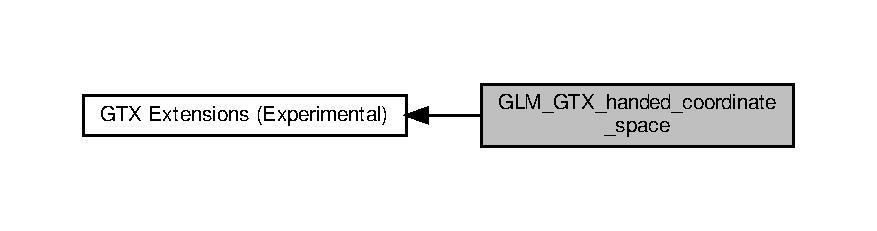
\includegraphics[width=350pt]{group__gtx__handed__coordinate__space}
\end{center}
\end{figure}
\subsection*{Functions}
\begin{DoxyCompactItemize}
\item 
{\footnotesize template$<$typename T , precision P$>$ }\\\hyperlink{setup_8hpp_ab2d052de21a70539923e9bcbf6e83a51}{G\+L\+M\+\_\+\+F\+U\+N\+C\+\_\+\+D\+E\+CL} bool \hyperlink{group__gtx__handed__coordinate__space_ga16517e8a56cba5ba908e6eac6500ab94}{glm\+::right\+Handed} (\hyperlink{structglm_1_1detail_1_1tvec3}{detail\+::tvec3}$<$ T, P $>$ const \&tangent, \hyperlink{structglm_1_1detail_1_1tvec3}{detail\+::tvec3}$<$ T, P $>$ const \&binormal, \hyperlink{structglm_1_1detail_1_1tvec3}{detail\+::tvec3}$<$ T, P $>$ const \&normal)
\item 
{\footnotesize template$<$typename T , precision P$>$ }\\\hyperlink{setup_8hpp_ab2d052de21a70539923e9bcbf6e83a51}{G\+L\+M\+\_\+\+F\+U\+N\+C\+\_\+\+D\+E\+CL} bool \hyperlink{group__gtx__handed__coordinate__space_ga2c0882af0eabd0e39da5680931f586ed}{glm\+::left\+Handed} (\hyperlink{structglm_1_1detail_1_1tvec3}{detail\+::tvec3}$<$ T, P $>$ const \&tangent, \hyperlink{structglm_1_1detail_1_1tvec3}{detail\+::tvec3}$<$ T, P $>$ const \&binormal, \hyperlink{structglm_1_1detail_1_1tvec3}{detail\+::tvec3}$<$ T, P $>$ const \&normal)
\end{DoxyCompactItemize}


\subsection{Detailed Description}
To know if a set of three basis vectors defines a right or left-\/handed coordinate system. 

$<$glm/gtx/handed\+\_\+coordinate\+\_\+system.\+hpp$>$ need to be included to use these functionalities. 

\subsection{Function Documentation}
\mbox{\Hypertarget{group__gtx__handed__coordinate__space_ga2c0882af0eabd0e39da5680931f586ed}\label{group__gtx__handed__coordinate__space_ga2c0882af0eabd0e39da5680931f586ed}} 
\index{G\+L\+M\+\_\+\+G\+T\+X\+\_\+handed\+\_\+coordinate\+\_\+space@{G\+L\+M\+\_\+\+G\+T\+X\+\_\+handed\+\_\+coordinate\+\_\+space}!left\+Handed@{left\+Handed}}
\index{left\+Handed@{left\+Handed}!G\+L\+M\+\_\+\+G\+T\+X\+\_\+handed\+\_\+coordinate\+\_\+space@{G\+L\+M\+\_\+\+G\+T\+X\+\_\+handed\+\_\+coordinate\+\_\+space}}
\subsubsection{\texorpdfstring{left\+Handed()}{leftHanded()}}
{\footnotesize\ttfamily template$<$typename T , precision P$>$ \\
\hyperlink{setup_8hpp_ab2d052de21a70539923e9bcbf6e83a51}{G\+L\+M\+\_\+\+F\+U\+N\+C\+\_\+\+D\+E\+CL} bool glm\+::left\+Handed (\begin{DoxyParamCaption}\item[{\hyperlink{structglm_1_1detail_1_1tvec3}{detail\+::tvec3}$<$ T, P $>$ const \&}]{tangent,  }\item[{\hyperlink{structglm_1_1detail_1_1tvec3}{detail\+::tvec3}$<$ T, P $>$ const \&}]{binormal,  }\item[{\hyperlink{structglm_1_1detail_1_1tvec3}{detail\+::tvec3}$<$ T, P $>$ const \&}]{normal }\end{DoxyParamCaption})}

Return if a trihedron left handed or not. From G\+L\+M\+\_\+\+G\+T\+X\+\_\+handed\+\_\+coordinate\+\_\+space extension. 

Definition at line 25 of file handed\+\_\+coordinate\+\_\+space.\+inl.

\mbox{\Hypertarget{group__gtx__handed__coordinate__space_ga16517e8a56cba5ba908e6eac6500ab94}\label{group__gtx__handed__coordinate__space_ga16517e8a56cba5ba908e6eac6500ab94}} 
\index{G\+L\+M\+\_\+\+G\+T\+X\+\_\+handed\+\_\+coordinate\+\_\+space@{G\+L\+M\+\_\+\+G\+T\+X\+\_\+handed\+\_\+coordinate\+\_\+space}!right\+Handed@{right\+Handed}}
\index{right\+Handed@{right\+Handed}!G\+L\+M\+\_\+\+G\+T\+X\+\_\+handed\+\_\+coordinate\+\_\+space@{G\+L\+M\+\_\+\+G\+T\+X\+\_\+handed\+\_\+coordinate\+\_\+space}}
\subsubsection{\texorpdfstring{right\+Handed()}{rightHanded()}}
{\footnotesize\ttfamily template$<$typename T , precision P$>$ \\
\hyperlink{setup_8hpp_ab2d052de21a70539923e9bcbf6e83a51}{G\+L\+M\+\_\+\+F\+U\+N\+C\+\_\+\+D\+E\+CL} bool glm\+::right\+Handed (\begin{DoxyParamCaption}\item[{\hyperlink{structglm_1_1detail_1_1tvec3}{detail\+::tvec3}$<$ T, P $>$ const \&}]{tangent,  }\item[{\hyperlink{structglm_1_1detail_1_1tvec3}{detail\+::tvec3}$<$ T, P $>$ const \&}]{binormal,  }\item[{\hyperlink{structglm_1_1detail_1_1tvec3}{detail\+::tvec3}$<$ T, P $>$ const \&}]{normal }\end{DoxyParamCaption})}

Return if a trihedron right handed or not. From G\+L\+M\+\_\+\+G\+T\+X\+\_\+handed\+\_\+coordinate\+\_\+space extension. 

Definition at line 14 of file handed\+\_\+coordinate\+\_\+space.\+inl.


\hypertarget{group__gtx__inertia}{}\section{G\+L\+M\+\_\+\+G\+T\+X\+\_\+inertia}
\label{group__gtx__inertia}\index{G\+L\+M\+\_\+\+G\+T\+X\+\_\+inertia@{G\+L\+M\+\_\+\+G\+T\+X\+\_\+inertia}}


Create inertia matrices.  


Collaboration diagram for G\+L\+M\+\_\+\+G\+T\+X\+\_\+inertia\+:\nopagebreak
\begin{figure}[H]
\begin{center}
\leavevmode
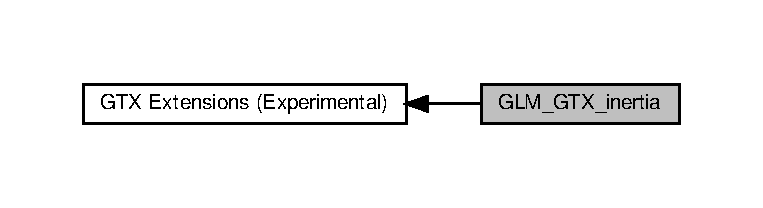
\includegraphics[width=350pt]{group__gtx__inertia}
\end{center}
\end{figure}
Create inertia matrices. 

$<$\hyperlink{inertia_8hpp}{glm/gtx/inertia.\+hpp}$>$ need to be included to use these functionalities. 
\hypertarget{group__gtx__integer}{}\section{G\+L\+M\+\_\+\+G\+T\+X\+\_\+integer}
\label{group__gtx__integer}\index{G\+L\+M\+\_\+\+G\+T\+X\+\_\+integer@{G\+L\+M\+\_\+\+G\+T\+X\+\_\+integer}}


Add support for integer for core functions.  


Collaboration diagram for G\+L\+M\+\_\+\+G\+T\+X\+\_\+integer\+:\nopagebreak
\begin{figure}[H]
\begin{center}
\leavevmode
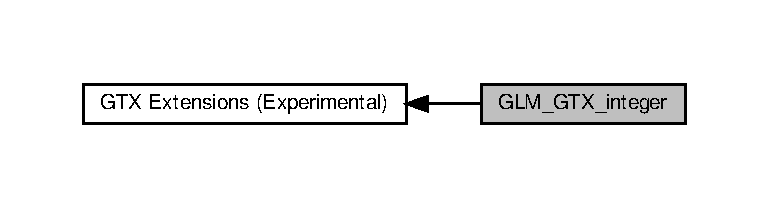
\includegraphics[width=350pt]{group__gtx__integer}
\end{center}
\end{figure}
\subsection*{Typedefs}
\begin{DoxyCompactItemize}
\item 
typedef signed int \hyperlink{group__gtx__integer_ga73643e09d8c6d362418aec541fdb987d}{glm\+::sint}
\end{DoxyCompactItemize}
\subsection*{Functions}
\begin{DoxyCompactItemize}
\item 
\hyperlink{setup_8hpp_ab2d052de21a70539923e9bcbf6e83a51}{G\+L\+M\+\_\+\+F\+U\+N\+C\+\_\+\+D\+E\+CL} int \hyperlink{group__gtx__integer_ga9642514a44a67afa70966d756f040ca9}{glm\+::pow} (int x, int y)
\item 
\hyperlink{setup_8hpp_ab2d052de21a70539923e9bcbf6e83a51}{G\+L\+M\+\_\+\+F\+U\+N\+C\+\_\+\+D\+E\+CL} int \hyperlink{group__gtx__integer_ga78e2e68330e91d350fcfc2f4831cad12}{glm\+::sqrt} (int x)
\item 
{\footnotesize template$<$typename gen\+I\+U\+Type $>$ }\\\hyperlink{setup_8hpp_ab2d052de21a70539923e9bcbf6e83a51}{G\+L\+M\+\_\+\+F\+U\+N\+C\+\_\+\+D\+E\+CL} gen\+I\+U\+Type \hyperlink{group__gtx__integer_ga9bd682e74bfacb005c735305207ec417}{glm\+::log2} (gen\+I\+U\+Type x)
\item 
\hyperlink{setup_8hpp_ab2d052de21a70539923e9bcbf6e83a51}{G\+L\+M\+\_\+\+F\+U\+N\+C\+\_\+\+D\+E\+CL} unsigned int \hyperlink{group__gtx__integer_ga7011b4e1c1e1ed492149b028feacc00e}{glm\+::floor\+\_\+log2} (unsigned int x)
\item 
\hyperlink{setup_8hpp_ab2d052de21a70539923e9bcbf6e83a51}{G\+L\+M\+\_\+\+F\+U\+N\+C\+\_\+\+D\+E\+CL} int \hyperlink{group__gtx__integer_gab9d22df91aac4d9eb925a4910f556f1b}{glm\+::mod} (int x, int y)
\item 
{\footnotesize template$<$typename gen\+Type $>$ }\\\hyperlink{setup_8hpp_ab2d052de21a70539923e9bcbf6e83a51}{G\+L\+M\+\_\+\+F\+U\+N\+C\+\_\+\+D\+E\+CL} gen\+Type \hyperlink{group__gtx__integer_ga8cbd3120905f398ec321b5d1836e08fb}{glm\+::factorial} (gen\+Type const \&x)
\item 
\hyperlink{setup_8hpp_ab2d052de21a70539923e9bcbf6e83a51}{G\+L\+M\+\_\+\+F\+U\+N\+C\+\_\+\+D\+E\+CL} \hyperlink{group__core__precision_ga4fd29415871152bfb5abd588334147c8}{uint} \hyperlink{group__gtx__integer_gaa8229e850c3cc4ad83492fe390ada044}{glm\+::pow} (\hyperlink{group__core__precision_ga4fd29415871152bfb5abd588334147c8}{uint} x, \hyperlink{group__core__precision_ga4fd29415871152bfb5abd588334147c8}{uint} y)
\item 
\hyperlink{setup_8hpp_ab2d052de21a70539923e9bcbf6e83a51}{G\+L\+M\+\_\+\+F\+U\+N\+C\+\_\+\+D\+E\+CL} \hyperlink{group__core__precision_ga4fd29415871152bfb5abd588334147c8}{uint} \hyperlink{group__gtx__integer_ga457e9efca8339bf918d319e9c55f7c8f}{glm\+::sqrt} (\hyperlink{group__core__precision_ga4fd29415871152bfb5abd588334147c8}{uint} x)
\item 
\hyperlink{setup_8hpp_ab2d052de21a70539923e9bcbf6e83a51}{G\+L\+M\+\_\+\+F\+U\+N\+C\+\_\+\+D\+E\+CL} \hyperlink{group__core__precision_ga4fd29415871152bfb5abd588334147c8}{uint} \hyperlink{group__gtx__integer_gab8f9ec0ca93ca90669434224818f0750}{glm\+::mod} (\hyperlink{group__core__precision_ga4fd29415871152bfb5abd588334147c8}{uint} x, \hyperlink{group__core__precision_ga4fd29415871152bfb5abd588334147c8}{uint} y)
\item 
\hyperlink{setup_8hpp_ab2d052de21a70539923e9bcbf6e83a51}{G\+L\+M\+\_\+\+F\+U\+N\+C\+\_\+\+D\+E\+CL} \hyperlink{group__core__precision_ga4fd29415871152bfb5abd588334147c8}{uint} \hyperlink{group__gtx__integer_gacbe62fd2384464c16ea30ecc4defc11c}{glm\+::nlz} (\hyperlink{group__core__precision_ga4fd29415871152bfb5abd588334147c8}{uint} x)
\end{DoxyCompactItemize}


\subsection{Detailed Description}
Add support for integer for core functions. 

$<$\hyperlink{gtx_2integer_8hpp}{glm/gtx/integer.\+hpp}$>$ need to be included to use these functionalities. 

\subsection{Typedef Documentation}
\mbox{\Hypertarget{group__gtx__integer_ga73643e09d8c6d362418aec541fdb987d}\label{group__gtx__integer_ga73643e09d8c6d362418aec541fdb987d}} 
\index{G\+L\+M\+\_\+\+G\+T\+X\+\_\+integer@{G\+L\+M\+\_\+\+G\+T\+X\+\_\+integer}!sint@{sint}}
\index{sint@{sint}!G\+L\+M\+\_\+\+G\+T\+X\+\_\+integer@{G\+L\+M\+\_\+\+G\+T\+X\+\_\+integer}}
\subsubsection{\texorpdfstring{sint}{sint}}
{\footnotesize\ttfamily typedef signed int \hyperlink{group__gtx__integer_ga73643e09d8c6d362418aec541fdb987d}{glm\+::sint}}

32bit signed integer. From G\+L\+M\+\_\+\+G\+T\+X\+\_\+integer extension. 

Definition at line 81 of file integer.\+hpp.



\subsection{Function Documentation}
\mbox{\Hypertarget{group__gtx__integer_ga8cbd3120905f398ec321b5d1836e08fb}\label{group__gtx__integer_ga8cbd3120905f398ec321b5d1836e08fb}} 
\index{G\+L\+M\+\_\+\+G\+T\+X\+\_\+integer@{G\+L\+M\+\_\+\+G\+T\+X\+\_\+integer}!factorial@{factorial}}
\index{factorial@{factorial}!G\+L\+M\+\_\+\+G\+T\+X\+\_\+integer@{G\+L\+M\+\_\+\+G\+T\+X\+\_\+integer}}
\subsubsection{\texorpdfstring{factorial()}{factorial()}}
{\footnotesize\ttfamily template$<$typename gen\+Type $>$ \\
\hyperlink{setup_8hpp_ab2d052de21a70539923e9bcbf6e83a51}{G\+L\+M\+\_\+\+F\+U\+N\+C\+\_\+\+D\+E\+CL} gen\+Type glm\+::factorial (\begin{DoxyParamCaption}\item[{gen\+Type const \&}]{x }\end{DoxyParamCaption})}

Return the factorial value of a number (!12 max, integer only) From G\+L\+M\+\_\+\+G\+T\+X\+\_\+integer extension. 

Definition at line 93 of file integer.\+inl.

\mbox{\Hypertarget{group__gtx__integer_ga7011b4e1c1e1ed492149b028feacc00e}\label{group__gtx__integer_ga7011b4e1c1e1ed492149b028feacc00e}} 
\index{G\+L\+M\+\_\+\+G\+T\+X\+\_\+integer@{G\+L\+M\+\_\+\+G\+T\+X\+\_\+integer}!floor\+\_\+log2@{floor\+\_\+log2}}
\index{floor\+\_\+log2@{floor\+\_\+log2}!G\+L\+M\+\_\+\+G\+T\+X\+\_\+integer@{G\+L\+M\+\_\+\+G\+T\+X\+\_\+integer}}
\subsubsection{\texorpdfstring{floor\+\_\+log2()}{floor\_log2()}}
{\footnotesize\ttfamily \hyperlink{setup_8hpp_ab2d052de21a70539923e9bcbf6e83a51}{G\+L\+M\+\_\+\+F\+U\+N\+C\+\_\+\+D\+E\+CL} unsigned int glm\+::floor\+\_\+log2 (\begin{DoxyParamCaption}\item[{unsigned int}]{x }\end{DoxyParamCaption})}

Returns the floor log2 of x. From G\+L\+M\+\_\+\+G\+T\+X\+\_\+integer extension. \mbox{\Hypertarget{group__gtx__integer_ga9bd682e74bfacb005c735305207ec417}\label{group__gtx__integer_ga9bd682e74bfacb005c735305207ec417}} 
\index{G\+L\+M\+\_\+\+G\+T\+X\+\_\+integer@{G\+L\+M\+\_\+\+G\+T\+X\+\_\+integer}!log2@{log2}}
\index{log2@{log2}!G\+L\+M\+\_\+\+G\+T\+X\+\_\+integer@{G\+L\+M\+\_\+\+G\+T\+X\+\_\+integer}}
\subsubsection{\texorpdfstring{log2()}{log2()}}
{\footnotesize\ttfamily template$<$typename gen\+I\+U\+Type $>$ \\
\hyperlink{setup_8hpp_ab2d052de21a70539923e9bcbf6e83a51}{G\+L\+M\+\_\+\+F\+U\+N\+C\+\_\+\+D\+E\+CL} gen\+I\+U\+Type glm\+::log2 (\begin{DoxyParamCaption}\item[{gen\+I\+U\+Type}]{x }\end{DoxyParamCaption})}

Returns the log2 of x. Can be reliably using to compute mipmap count from the texture size. From G\+L\+M\+\_\+\+G\+T\+X\+\_\+integer extension. \mbox{\Hypertarget{group__gtx__integer_gab9d22df91aac4d9eb925a4910f556f1b}\label{group__gtx__integer_gab9d22df91aac4d9eb925a4910f556f1b}} 
\index{G\+L\+M\+\_\+\+G\+T\+X\+\_\+integer@{G\+L\+M\+\_\+\+G\+T\+X\+\_\+integer}!mod@{mod}}
\index{mod@{mod}!G\+L\+M\+\_\+\+G\+T\+X\+\_\+integer@{G\+L\+M\+\_\+\+G\+T\+X\+\_\+integer}}
\subsubsection{\texorpdfstring{mod()}{mod()}\hspace{0.1cm}{\footnotesize\ttfamily [1/2]}}
{\footnotesize\ttfamily \hyperlink{setup_8hpp_a33fdea6f91c5f834105f7415e2a64407}{G\+L\+M\+\_\+\+F\+U\+N\+C\+\_\+\+Q\+U\+A\+L\+I\+F\+I\+ER} int glm\+::mod (\begin{DoxyParamCaption}\item[{int}]{x,  }\item[{int}]{y }\end{DoxyParamCaption})}

Modulus. Returns x -\/ y $\ast$ floor(x / y) for each component in x using the floating point value y. From G\+L\+M\+\_\+\+G\+T\+X\+\_\+integer extension. 

Definition at line 86 of file integer.\+inl.

\mbox{\Hypertarget{group__gtx__integer_gab8f9ec0ca93ca90669434224818f0750}\label{group__gtx__integer_gab8f9ec0ca93ca90669434224818f0750}} 
\index{G\+L\+M\+\_\+\+G\+T\+X\+\_\+integer@{G\+L\+M\+\_\+\+G\+T\+X\+\_\+integer}!mod@{mod}}
\index{mod@{mod}!G\+L\+M\+\_\+\+G\+T\+X\+\_\+integer@{G\+L\+M\+\_\+\+G\+T\+X\+\_\+integer}}
\subsubsection{\texorpdfstring{mod()}{mod()}\hspace{0.1cm}{\footnotesize\ttfamily [2/2]}}
{\footnotesize\ttfamily \hyperlink{setup_8hpp_a33fdea6f91c5f834105f7415e2a64407}{G\+L\+M\+\_\+\+F\+U\+N\+C\+\_\+\+Q\+U\+A\+L\+I\+F\+I\+ER} \hyperlink{group__core__precision_ga4fd29415871152bfb5abd588334147c8}{uint} glm\+::mod (\begin{DoxyParamCaption}\item[{\hyperlink{group__core__precision_ga4fd29415871152bfb5abd588334147c8}{uint}}]{x,  }\item[{\hyperlink{group__core__precision_ga4fd29415871152bfb5abd588334147c8}{uint}}]{y }\end{DoxyParamCaption})}

Modulus. Returns x -\/ y $\ast$ floor(x / y) for each component in x using the floating point value y. From G\+L\+M\+\_\+\+G\+T\+X\+\_\+integer extension. 

Definition at line 156 of file integer.\+inl.

\mbox{\Hypertarget{group__gtx__integer_gacbe62fd2384464c16ea30ecc4defc11c}\label{group__gtx__integer_gacbe62fd2384464c16ea30ecc4defc11c}} 
\index{G\+L\+M\+\_\+\+G\+T\+X\+\_\+integer@{G\+L\+M\+\_\+\+G\+T\+X\+\_\+integer}!nlz@{nlz}}
\index{nlz@{nlz}!G\+L\+M\+\_\+\+G\+T\+X\+\_\+integer@{G\+L\+M\+\_\+\+G\+T\+X\+\_\+integer}}
\subsubsection{\texorpdfstring{nlz()}{nlz()}}
{\footnotesize\ttfamily \hyperlink{setup_8hpp_a33fdea6f91c5f834105f7415e2a64407}{G\+L\+M\+\_\+\+F\+U\+N\+C\+\_\+\+Q\+U\+A\+L\+I\+F\+I\+ER} unsigned int glm\+::nlz (\begin{DoxyParamCaption}\item[{\hyperlink{group__core__precision_ga4fd29415871152bfb5abd588334147c8}{uint}}]{x }\end{DoxyParamCaption})}

Returns the number of leading zeros. From G\+L\+M\+\_\+\+G\+T\+X\+\_\+integer extension. 

Definition at line 171 of file integer.\+inl.

\mbox{\Hypertarget{group__gtx__integer_ga9642514a44a67afa70966d756f040ca9}\label{group__gtx__integer_ga9642514a44a67afa70966d756f040ca9}} 
\index{G\+L\+M\+\_\+\+G\+T\+X\+\_\+integer@{G\+L\+M\+\_\+\+G\+T\+X\+\_\+integer}!pow@{pow}}
\index{pow@{pow}!G\+L\+M\+\_\+\+G\+T\+X\+\_\+integer@{G\+L\+M\+\_\+\+G\+T\+X\+\_\+integer}}
\subsubsection{\texorpdfstring{pow()}{pow()}\hspace{0.1cm}{\footnotesize\ttfamily [1/2]}}
{\footnotesize\ttfamily \hyperlink{setup_8hpp_a33fdea6f91c5f834105f7415e2a64407}{G\+L\+M\+\_\+\+F\+U\+N\+C\+\_\+\+Q\+U\+A\+L\+I\+F\+I\+ER} int glm\+::pow (\begin{DoxyParamCaption}\item[{int}]{x,  }\item[{int}]{y }\end{DoxyParamCaption})}

Returns x raised to the y power. From G\+L\+M\+\_\+\+G\+T\+X\+\_\+integer extension. 

Definition at line 13 of file integer.\+inl.

\mbox{\Hypertarget{group__gtx__integer_gaa8229e850c3cc4ad83492fe390ada044}\label{group__gtx__integer_gaa8229e850c3cc4ad83492fe390ada044}} 
\index{G\+L\+M\+\_\+\+G\+T\+X\+\_\+integer@{G\+L\+M\+\_\+\+G\+T\+X\+\_\+integer}!pow@{pow}}
\index{pow@{pow}!G\+L\+M\+\_\+\+G\+T\+X\+\_\+integer@{G\+L\+M\+\_\+\+G\+T\+X\+\_\+integer}}
\subsubsection{\texorpdfstring{pow()}{pow()}\hspace{0.1cm}{\footnotesize\ttfamily [2/2]}}
{\footnotesize\ttfamily \hyperlink{setup_8hpp_a33fdea6f91c5f834105f7415e2a64407}{G\+L\+M\+\_\+\+F\+U\+N\+C\+\_\+\+Q\+U\+A\+L\+I\+F\+I\+ER} \hyperlink{group__core__precision_ga4fd29415871152bfb5abd588334147c8}{uint} glm\+::pow (\begin{DoxyParamCaption}\item[{\hyperlink{group__core__precision_ga4fd29415871152bfb5abd588334147c8}{uint}}]{x,  }\item[{\hyperlink{group__core__precision_ga4fd29415871152bfb5abd588334147c8}{uint}}]{y }\end{DoxyParamCaption})}

Returns x raised to the y power. From G\+L\+M\+\_\+\+G\+T\+X\+\_\+integer extension. 

Definition at line 132 of file integer.\+inl.

\mbox{\Hypertarget{group__gtx__integer_ga78e2e68330e91d350fcfc2f4831cad12}\label{group__gtx__integer_ga78e2e68330e91d350fcfc2f4831cad12}} 
\index{G\+L\+M\+\_\+\+G\+T\+X\+\_\+integer@{G\+L\+M\+\_\+\+G\+T\+X\+\_\+integer}!sqrt@{sqrt}}
\index{sqrt@{sqrt}!G\+L\+M\+\_\+\+G\+T\+X\+\_\+integer@{G\+L\+M\+\_\+\+G\+T\+X\+\_\+integer}}
\subsubsection{\texorpdfstring{sqrt()}{sqrt()}\hspace{0.1cm}{\footnotesize\ttfamily [1/2]}}
{\footnotesize\ttfamily \hyperlink{setup_8hpp_a33fdea6f91c5f834105f7415e2a64407}{G\+L\+M\+\_\+\+F\+U\+N\+C\+\_\+\+Q\+U\+A\+L\+I\+F\+I\+ER} int glm\+::sqrt (\begin{DoxyParamCaption}\item[{int}]{x }\end{DoxyParamCaption})}

Returns the positive square root of x. From G\+L\+M\+\_\+\+G\+T\+X\+\_\+integer extension. 

Definition at line 24 of file integer.\+inl.

\mbox{\Hypertarget{group__gtx__integer_ga457e9efca8339bf918d319e9c55f7c8f}\label{group__gtx__integer_ga457e9efca8339bf918d319e9c55f7c8f}} 
\index{G\+L\+M\+\_\+\+G\+T\+X\+\_\+integer@{G\+L\+M\+\_\+\+G\+T\+X\+\_\+integer}!sqrt@{sqrt}}
\index{sqrt@{sqrt}!G\+L\+M\+\_\+\+G\+T\+X\+\_\+integer@{G\+L\+M\+\_\+\+G\+T\+X\+\_\+integer}}
\subsubsection{\texorpdfstring{sqrt()}{sqrt()}\hspace{0.1cm}{\footnotesize\ttfamily [2/2]}}
{\footnotesize\ttfamily \hyperlink{setup_8hpp_a33fdea6f91c5f834105f7415e2a64407}{G\+L\+M\+\_\+\+F\+U\+N\+C\+\_\+\+Q\+U\+A\+L\+I\+F\+I\+ER} \hyperlink{group__core__precision_ga4fd29415871152bfb5abd588334147c8}{uint} glm\+::sqrt (\begin{DoxyParamCaption}\item[{\hyperlink{group__core__precision_ga4fd29415871152bfb5abd588334147c8}{uint}}]{x }\end{DoxyParamCaption})}

Returns the positive square root of x. From G\+L\+M\+\_\+\+G\+T\+X\+\_\+integer extension. 

Definition at line 140 of file integer.\+inl.


\hypertarget{group__gtx__intersect}{}\section{G\+L\+M\+\_\+\+G\+T\+X\+\_\+intersect}
\label{group__gtx__intersect}\index{G\+L\+M\+\_\+\+G\+T\+X\+\_\+intersect@{G\+L\+M\+\_\+\+G\+T\+X\+\_\+intersect}}


Add intersection functions.  


Collaboration diagram for G\+L\+M\+\_\+\+G\+T\+X\+\_\+intersect\+:\nopagebreak
\begin{figure}[H]
\begin{center}
\leavevmode
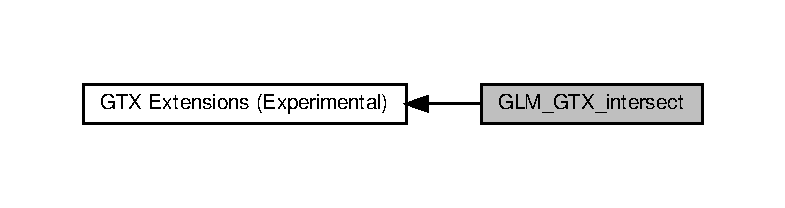
\includegraphics[width=350pt]{group__gtx__intersect}
\end{center}
\end{figure}
\subsection*{Functions}
\begin{DoxyCompactItemize}
\item 
{\footnotesize template$<$typename gen\+Type $>$ }\\\hyperlink{setup_8hpp_ab2d052de21a70539923e9bcbf6e83a51}{G\+L\+M\+\_\+\+F\+U\+N\+C\+\_\+\+D\+E\+CL} bool \hyperlink{group__gtx__intersect_gad3697a9700ea379739a667ea02573488}{glm\+::intersect\+Ray\+Plane} (gen\+Type const \&orig, gen\+Type const \&dir, gen\+Type const \&plane\+Orig, gen\+Type const \&plane\+Normal, typename gen\+Type\+::value\+\_\+type \&intersection\+Distance)
\item 
{\footnotesize template$<$typename gen\+Type $>$ }\\\hyperlink{setup_8hpp_ab2d052de21a70539923e9bcbf6e83a51}{G\+L\+M\+\_\+\+F\+U\+N\+C\+\_\+\+D\+E\+CL} bool \hyperlink{group__gtx__intersect_gab16c1b47c10451e7604b51b39a7ef21d}{glm\+::intersect\+Ray\+Triangle} (gen\+Type const \&orig, gen\+Type const \&dir, gen\+Type const \&vert0, gen\+Type const \&vert1, gen\+Type const \&vert2, gen\+Type \&bary\+Position)
\item 
{\footnotesize template$<$typename gen\+Type $>$ }\\\hyperlink{setup_8hpp_ab2d052de21a70539923e9bcbf6e83a51}{G\+L\+M\+\_\+\+F\+U\+N\+C\+\_\+\+D\+E\+CL} bool \hyperlink{group__gtx__intersect_ga9d29b9b3acb504d43986502f42740df4}{glm\+::intersect\+Line\+Triangle} (gen\+Type const \&orig, gen\+Type const \&dir, gen\+Type const \&vert0, gen\+Type const \&vert1, gen\+Type const \&vert2, gen\+Type \&position)
\item 
{\footnotesize template$<$typename gen\+Type $>$ }\\\hyperlink{setup_8hpp_ab2d052de21a70539923e9bcbf6e83a51}{G\+L\+M\+\_\+\+F\+U\+N\+C\+\_\+\+D\+E\+CL} bool \hyperlink{group__gtx__intersect_gac88f8cd84c4bcb5b947d56acbbcfa56e}{glm\+::intersect\+Ray\+Sphere} (gen\+Type const \&ray\+Starting, gen\+Type const \&ray\+Normalized\+Direction, gen\+Type const \&sphere\+Center, typename gen\+Type\+::value\+\_\+type const sphere\+Radius\+Squered, typename gen\+Type\+::value\+\_\+type \&intersection\+Distance)
\item 
{\footnotesize template$<$typename gen\+Type $>$ }\\\hyperlink{setup_8hpp_ab2d052de21a70539923e9bcbf6e83a51}{G\+L\+M\+\_\+\+F\+U\+N\+C\+\_\+\+D\+E\+CL} bool \hyperlink{group__gtx__intersect_gad28c00515b823b579c608aafa1100c1d}{glm\+::intersect\+Ray\+Sphere} (gen\+Type const \&ray\+Starting, gen\+Type const \&ray\+Normalized\+Direction, gen\+Type const \&sphere\+Center, const typename gen\+Type\+::value\+\_\+type sphere\+Radius, gen\+Type \&intersection\+Position, gen\+Type \&intersection\+Normal)
\item 
{\footnotesize template$<$typename gen\+Type $>$ }\\\hyperlink{setup_8hpp_ab2d052de21a70539923e9bcbf6e83a51}{G\+L\+M\+\_\+\+F\+U\+N\+C\+\_\+\+D\+E\+CL} bool \hyperlink{group__gtx__intersect_ga9c68139f3d8a4f3d7fe45f9dbc0de5b7}{glm\+::intersect\+Line\+Sphere} (gen\+Type const \&point0, gen\+Type const \&point1, gen\+Type const \&sphere\+Center, typename gen\+Type\+::value\+\_\+type sphere\+Radius, gen\+Type \&intersection\+Position1, gen\+Type \&intersection\+Normal1, gen\+Type \&intersection\+Position2=gen\+Type(), gen\+Type \&intersection\+Normal2=gen\+Type())
\end{DoxyCompactItemize}


\subsection{Detailed Description}
Add intersection functions. 

$<$\hyperlink{intersect_8hpp}{glm/gtx/intersect.\+hpp}$>$ need to be included to use these functionalities. 

\subsection{Function Documentation}
\mbox{\Hypertarget{group__gtx__intersect_ga9c68139f3d8a4f3d7fe45f9dbc0de5b7}\label{group__gtx__intersect_ga9c68139f3d8a4f3d7fe45f9dbc0de5b7}} 
\index{G\+L\+M\+\_\+\+G\+T\+X\+\_\+intersect@{G\+L\+M\+\_\+\+G\+T\+X\+\_\+intersect}!intersect\+Line\+Sphere@{intersect\+Line\+Sphere}}
\index{intersect\+Line\+Sphere@{intersect\+Line\+Sphere}!G\+L\+M\+\_\+\+G\+T\+X\+\_\+intersect@{G\+L\+M\+\_\+\+G\+T\+X\+\_\+intersect}}
\subsubsection{\texorpdfstring{intersect\+Line\+Sphere()}{intersectLineSphere()}}
{\footnotesize\ttfamily template$<$typename gen\+Type $>$ \\
\hyperlink{setup_8hpp_ab2d052de21a70539923e9bcbf6e83a51}{G\+L\+M\+\_\+\+F\+U\+N\+C\+\_\+\+D\+E\+CL} bool glm\+::intersect\+Line\+Sphere (\begin{DoxyParamCaption}\item[{gen\+Type const \&}]{point0,  }\item[{gen\+Type const \&}]{point1,  }\item[{gen\+Type const \&}]{sphere\+Center,  }\item[{typename gen\+Type\+::value\+\_\+type}]{sphere\+Radius,  }\item[{gen\+Type \&}]{intersection\+Position1,  }\item[{gen\+Type \&}]{intersection\+Normal1,  }\item[{gen\+Type \&}]{intersection\+Position2 = {\ttfamily genType()},  }\item[{gen\+Type \&}]{intersection\+Normal2 = {\ttfamily genType()} }\end{DoxyParamCaption})}

Compute the intersection of a line and a sphere. From G\+L\+M\+\_\+\+G\+T\+X\+\_\+intersect extension 

Definition at line 192 of file intersect.\+inl.

\mbox{\Hypertarget{group__gtx__intersect_ga9d29b9b3acb504d43986502f42740df4}\label{group__gtx__intersect_ga9d29b9b3acb504d43986502f42740df4}} 
\index{G\+L\+M\+\_\+\+G\+T\+X\+\_\+intersect@{G\+L\+M\+\_\+\+G\+T\+X\+\_\+intersect}!intersect\+Line\+Triangle@{intersect\+Line\+Triangle}}
\index{intersect\+Line\+Triangle@{intersect\+Line\+Triangle}!G\+L\+M\+\_\+\+G\+T\+X\+\_\+intersect@{G\+L\+M\+\_\+\+G\+T\+X\+\_\+intersect}}
\subsubsection{\texorpdfstring{intersect\+Line\+Triangle()}{intersectLineTriangle()}}
{\footnotesize\ttfamily template$<$typename gen\+Type $>$ \\
\hyperlink{setup_8hpp_ab2d052de21a70539923e9bcbf6e83a51}{G\+L\+M\+\_\+\+F\+U\+N\+C\+\_\+\+D\+E\+CL} bool glm\+::intersect\+Line\+Triangle (\begin{DoxyParamCaption}\item[{gen\+Type const \&}]{orig,  }\item[{gen\+Type const \&}]{dir,  }\item[{gen\+Type const \&}]{vert0,  }\item[{gen\+Type const \&}]{vert1,  }\item[{gen\+Type const \&}]{vert2,  }\item[{gen\+Type \&}]{position }\end{DoxyParamCaption})}

Compute the intersection of a line and a triangle. From G\+L\+M\+\_\+\+G\+T\+X\+\_\+intersect extension. 

Definition at line 115 of file intersect.\+inl.

\mbox{\Hypertarget{group__gtx__intersect_gad3697a9700ea379739a667ea02573488}\label{group__gtx__intersect_gad3697a9700ea379739a667ea02573488}} 
\index{G\+L\+M\+\_\+\+G\+T\+X\+\_\+intersect@{G\+L\+M\+\_\+\+G\+T\+X\+\_\+intersect}!intersect\+Ray\+Plane@{intersect\+Ray\+Plane}}
\index{intersect\+Ray\+Plane@{intersect\+Ray\+Plane}!G\+L\+M\+\_\+\+G\+T\+X\+\_\+intersect@{G\+L\+M\+\_\+\+G\+T\+X\+\_\+intersect}}
\subsubsection{\texorpdfstring{intersect\+Ray\+Plane()}{intersectRayPlane()}}
{\footnotesize\ttfamily template$<$typename gen\+Type $>$ \\
\hyperlink{setup_8hpp_ab2d052de21a70539923e9bcbf6e83a51}{G\+L\+M\+\_\+\+F\+U\+N\+C\+\_\+\+D\+E\+CL} bool glm\+::intersect\+Ray\+Plane (\begin{DoxyParamCaption}\item[{gen\+Type const \&}]{orig,  }\item[{gen\+Type const \&}]{dir,  }\item[{gen\+Type const \&}]{plane\+Orig,  }\item[{gen\+Type const \&}]{plane\+Normal,  }\item[{typename gen\+Type\+::value\+\_\+type \&}]{intersection\+Distance }\end{DoxyParamCaption})}

Compute the intersection of a ray and a triangle. Ray direction and plane normal must be unit length. From G\+L\+M\+\_\+\+G\+T\+X\+\_\+intersect extension. 

Definition at line 18 of file intersect.\+inl.

\mbox{\Hypertarget{group__gtx__intersect_gac88f8cd84c4bcb5b947d56acbbcfa56e}\label{group__gtx__intersect_gac88f8cd84c4bcb5b947d56acbbcfa56e}} 
\index{G\+L\+M\+\_\+\+G\+T\+X\+\_\+intersect@{G\+L\+M\+\_\+\+G\+T\+X\+\_\+intersect}!intersect\+Ray\+Sphere@{intersect\+Ray\+Sphere}}
\index{intersect\+Ray\+Sphere@{intersect\+Ray\+Sphere}!G\+L\+M\+\_\+\+G\+T\+X\+\_\+intersect@{G\+L\+M\+\_\+\+G\+T\+X\+\_\+intersect}}
\subsubsection{\texorpdfstring{intersect\+Ray\+Sphere()}{intersectRaySphere()}\hspace{0.1cm}{\footnotesize\ttfamily [1/2]}}
{\footnotesize\ttfamily template$<$typename gen\+Type $>$ \\
\hyperlink{setup_8hpp_ab2d052de21a70539923e9bcbf6e83a51}{G\+L\+M\+\_\+\+F\+U\+N\+C\+\_\+\+D\+E\+CL} bool glm\+::intersect\+Ray\+Sphere (\begin{DoxyParamCaption}\item[{gen\+Type const \&}]{ray\+Starting,  }\item[{gen\+Type const \&}]{ray\+Normalized\+Direction,  }\item[{gen\+Type const \&}]{sphere\+Center,  }\item[{typename gen\+Type\+::value\+\_\+type const}]{sphere\+Radius\+Squered,  }\item[{typename gen\+Type\+::value\+\_\+type \&}]{intersection\+Distance }\end{DoxyParamCaption})}

Compute the intersection distance of a ray and a sphere. The ray direction vector is unit length. From G\+L\+M\+\_\+\+G\+T\+X\+\_\+intersect extension. 

Definition at line 153 of file intersect.\+inl.

\mbox{\Hypertarget{group__gtx__intersect_gad28c00515b823b579c608aafa1100c1d}\label{group__gtx__intersect_gad28c00515b823b579c608aafa1100c1d}} 
\index{G\+L\+M\+\_\+\+G\+T\+X\+\_\+intersect@{G\+L\+M\+\_\+\+G\+T\+X\+\_\+intersect}!intersect\+Ray\+Sphere@{intersect\+Ray\+Sphere}}
\index{intersect\+Ray\+Sphere@{intersect\+Ray\+Sphere}!G\+L\+M\+\_\+\+G\+T\+X\+\_\+intersect@{G\+L\+M\+\_\+\+G\+T\+X\+\_\+intersect}}
\subsubsection{\texorpdfstring{intersect\+Ray\+Sphere()}{intersectRaySphere()}\hspace{0.1cm}{\footnotesize\ttfamily [2/2]}}
{\footnotesize\ttfamily template$<$typename gen\+Type $>$ \\
\hyperlink{setup_8hpp_ab2d052de21a70539923e9bcbf6e83a51}{G\+L\+M\+\_\+\+F\+U\+N\+C\+\_\+\+D\+E\+CL} bool glm\+::intersect\+Ray\+Sphere (\begin{DoxyParamCaption}\item[{gen\+Type const \&}]{ray\+Starting,  }\item[{gen\+Type const \&}]{ray\+Normalized\+Direction,  }\item[{gen\+Type const \&}]{sphere\+Center,  }\item[{const typename gen\+Type\+::value\+\_\+type}]{sphere\+Radius,  }\item[{gen\+Type \&}]{intersection\+Position,  }\item[{gen\+Type \&}]{intersection\+Normal }\end{DoxyParamCaption})}

Compute the intersection of a ray and a sphere. From G\+L\+M\+\_\+\+G\+T\+X\+\_\+intersect extension. 

Definition at line 174 of file intersect.\+inl.

\mbox{\Hypertarget{group__gtx__intersect_gab16c1b47c10451e7604b51b39a7ef21d}\label{group__gtx__intersect_gab16c1b47c10451e7604b51b39a7ef21d}} 
\index{G\+L\+M\+\_\+\+G\+T\+X\+\_\+intersect@{G\+L\+M\+\_\+\+G\+T\+X\+\_\+intersect}!intersect\+Ray\+Triangle@{intersect\+Ray\+Triangle}}
\index{intersect\+Ray\+Triangle@{intersect\+Ray\+Triangle}!G\+L\+M\+\_\+\+G\+T\+X\+\_\+intersect@{G\+L\+M\+\_\+\+G\+T\+X\+\_\+intersect}}
\subsubsection{\texorpdfstring{intersect\+Ray\+Triangle()}{intersectRayTriangle()}}
{\footnotesize\ttfamily template$<$typename gen\+Type $>$ \\
\hyperlink{setup_8hpp_ab2d052de21a70539923e9bcbf6e83a51}{G\+L\+M\+\_\+\+F\+U\+N\+C\+\_\+\+D\+E\+CL} bool glm\+::intersect\+Ray\+Triangle (\begin{DoxyParamCaption}\item[{gen\+Type const \&}]{orig,  }\item[{gen\+Type const \&}]{dir,  }\item[{gen\+Type const \&}]{vert0,  }\item[{gen\+Type const \&}]{vert1,  }\item[{gen\+Type const \&}]{vert2,  }\item[{gen\+Type \&}]{bary\+Position }\end{DoxyParamCaption})}

Compute the intersection of a ray and a triangle. From G\+L\+M\+\_\+\+G\+T\+X\+\_\+intersect extension. 

Definition at line 38 of file intersect.\+inl.


\hypertarget{group__gtx__io}{}\section{G\+L\+M\+\_\+\+G\+T\+X\+\_\+io}
\label{group__gtx__io}\index{G\+L\+M\+\_\+\+G\+T\+X\+\_\+io@{G\+L\+M\+\_\+\+G\+T\+X\+\_\+io}}


std\+:\+:\mbox{[}w\mbox{]}ostream support for glm types  


Collaboration diagram for G\+L\+M\+\_\+\+G\+T\+X\+\_\+io\+:\nopagebreak
\begin{figure}[H]
\begin{center}
\leavevmode
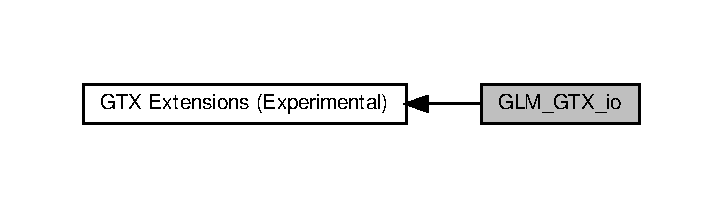
\includegraphics[width=347pt]{group__gtx__io}
\end{center}
\end{figure}
\subsection*{Namespaces}
\begin{DoxyCompactItemize}
\item 
 \hyperlink{namespaceglm_1_1io}{glm\+::io}
\item 
 \hyperlink{namespaceglm_1_1detail}{glm\+::detail}
\end{DoxyCompactItemize}


\subsection{Detailed Description}
std\+:\+:\mbox{[}w\mbox{]}ostream support for glm types 

std\+:\+:\mbox{[}w\mbox{]}ostream support for glm types + precision/width/etc. manipulators based on howard hinnant\textquotesingle{}s std\+::chrono io proposal \mbox{[}\href{http://home.roadrunner.com/~hinnant/bloomington/chrono_io.html}{\tt http\+://home.\+roadrunner.\+com/$\sim$hinnant/bloomington/chrono\+\_\+io.\+html}\mbox{]}

$<$\hyperlink{io_8hpp}{glm/gtx/io.\+hpp}$>$ needs to be included to use these functionalities. 
\hypertarget{group__gtx__log__base}{}\section{G\+L\+M\+\_\+\+G\+T\+X\+\_\+log\+\_\+base}
\label{group__gtx__log__base}\index{G\+L\+M\+\_\+\+G\+T\+X\+\_\+log\+\_\+base@{G\+L\+M\+\_\+\+G\+T\+X\+\_\+log\+\_\+base}}


Logarithm for any base. base can be a vector or a scalar.  


Collaboration diagram for G\+L\+M\+\_\+\+G\+T\+X\+\_\+log\+\_\+base\+:\nopagebreak
\begin{figure}[H]
\begin{center}
\leavevmode
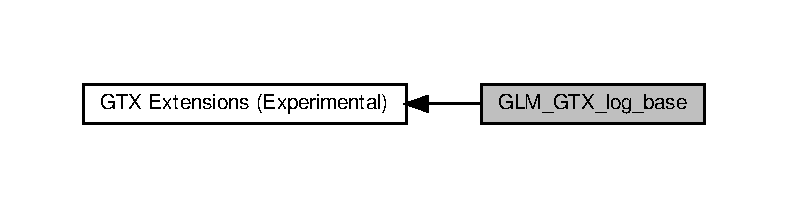
\includegraphics[width=350pt]{group__gtx__log__base}
\end{center}
\end{figure}
\subsection*{Functions}
\begin{DoxyCompactItemize}
\item 
{\footnotesize template$<$typename gen\+Type $>$ }\\\hyperlink{setup_8hpp_ab2d052de21a70539923e9bcbf6e83a51}{G\+L\+M\+\_\+\+F\+U\+N\+C\+\_\+\+D\+E\+CL} gen\+Type \hyperlink{group__gtx__log__base_ga60a7b0a401da660869946b2b77c710c9}{glm\+::log} (gen\+Type const \&x, gen\+Type const \&base)
\end{DoxyCompactItemize}


\subsection{Detailed Description}
Logarithm for any base. base can be a vector or a scalar. 

$<$\hyperlink{log__base_8hpp}{glm/gtx/log\+\_\+base.\+hpp}$>$ need to be included to use these functionalities. 

\subsection{Function Documentation}
\mbox{\Hypertarget{group__gtx__log__base_ga60a7b0a401da660869946b2b77c710c9}\label{group__gtx__log__base_ga60a7b0a401da660869946b2b77c710c9}} 
\index{G\+L\+M\+\_\+\+G\+T\+X\+\_\+log\+\_\+base@{G\+L\+M\+\_\+\+G\+T\+X\+\_\+log\+\_\+base}!log@{log}}
\index{log@{log}!G\+L\+M\+\_\+\+G\+T\+X\+\_\+log\+\_\+base@{G\+L\+M\+\_\+\+G\+T\+X\+\_\+log\+\_\+base}}
\subsubsection{\texorpdfstring{log()}{log()}}
{\footnotesize\ttfamily template$<$typename gen\+Type $>$ \\
\hyperlink{setup_8hpp_ab2d052de21a70539923e9bcbf6e83a51}{G\+L\+M\+\_\+\+F\+U\+N\+C\+\_\+\+D\+E\+CL} gen\+Type glm\+::log (\begin{DoxyParamCaption}\item[{gen\+Type const \&}]{x,  }\item[{gen\+Type const \&}]{base }\end{DoxyParamCaption})}

Logarithm for any base. From G\+L\+M\+\_\+\+G\+T\+X\+\_\+log\+\_\+base. 

Definition at line 13 of file log\+\_\+base.\+inl.


\hypertarget{group__gtx__matrix__cross__product}{}\section{G\+L\+M\+\_\+\+G\+T\+X\+\_\+matrix\+\_\+cross\+\_\+product}
\label{group__gtx__matrix__cross__product}\index{G\+L\+M\+\_\+\+G\+T\+X\+\_\+matrix\+\_\+cross\+\_\+product@{G\+L\+M\+\_\+\+G\+T\+X\+\_\+matrix\+\_\+cross\+\_\+product}}


Build cross product matrices.  


Collaboration diagram for G\+L\+M\+\_\+\+G\+T\+X\+\_\+matrix\+\_\+cross\+\_\+product\+:\nopagebreak
\begin{figure}[H]
\begin{center}
\leavevmode
\includegraphics[width=350pt]{group__gtx__matrix__cross__product}
\end{center}
\end{figure}
\subsection*{Functions}
\begin{DoxyCompactItemize}
\item 
{\footnotesize template$<$typename T , precision P$>$ }\\\hyperlink{setup_8hpp_ab2d052de21a70539923e9bcbf6e83a51}{G\+L\+M\+\_\+\+F\+U\+N\+C\+\_\+\+D\+E\+CL} \hyperlink{structglm_1_1detail_1_1tmat3x3}{detail\+::tmat3x3}$<$ T, P $>$ \hyperlink{group__gtx__matrix__cross__product_gaebbd4b4436b55c14b6d0b973167a25e4}{glm\+::matrix\+Cross3} (\hyperlink{structglm_1_1detail_1_1tvec3}{detail\+::tvec3}$<$ T, P $>$ const \&x)
\item 
{\footnotesize template$<$typename T , precision P$>$ }\\\hyperlink{setup_8hpp_ab2d052de21a70539923e9bcbf6e83a51}{G\+L\+M\+\_\+\+F\+U\+N\+C\+\_\+\+D\+E\+CL} \hyperlink{structglm_1_1detail_1_1tmat4x4}{detail\+::tmat4x4}$<$ T, P $>$ \hyperlink{group__gtx__matrix__cross__product_gab3c272adc9c9fc1f7c26d6f353b4bb4b}{glm\+::matrix\+Cross4} (\hyperlink{structglm_1_1detail_1_1tvec3}{detail\+::tvec3}$<$ T, P $>$ const \&x)
\end{DoxyCompactItemize}


\subsection{Detailed Description}
Build cross product matrices. 

$<$\hyperlink{matrix__cross__product_8hpp}{glm/gtx/matrix\+\_\+cross\+\_\+product.\+hpp}$>$ need to be included to use these functionalities. 

\subsection{Function Documentation}
\mbox{\Hypertarget{group__gtx__matrix__cross__product_gaebbd4b4436b55c14b6d0b973167a25e4}\label{group__gtx__matrix__cross__product_gaebbd4b4436b55c14b6d0b973167a25e4}} 
\index{G\+L\+M\+\_\+\+G\+T\+X\+\_\+matrix\+\_\+cross\+\_\+product@{G\+L\+M\+\_\+\+G\+T\+X\+\_\+matrix\+\_\+cross\+\_\+product}!matrix\+Cross3@{matrix\+Cross3}}
\index{matrix\+Cross3@{matrix\+Cross3}!G\+L\+M\+\_\+\+G\+T\+X\+\_\+matrix\+\_\+cross\+\_\+product@{G\+L\+M\+\_\+\+G\+T\+X\+\_\+matrix\+\_\+cross\+\_\+product}}
\subsubsection{\texorpdfstring{matrix\+Cross3()}{matrixCross3()}}
{\footnotesize\ttfamily template$<$typename T , precision P$>$ \\
\hyperlink{setup_8hpp_ab2d052de21a70539923e9bcbf6e83a51}{G\+L\+M\+\_\+\+F\+U\+N\+C\+\_\+\+D\+E\+CL} \hyperlink{structglm_1_1detail_1_1tmat3x3}{detail\+::tmat3x3}$<$T, P$>$ glm\+::matrix\+Cross3 (\begin{DoxyParamCaption}\item[{\hyperlink{structglm_1_1detail_1_1tvec3}{detail\+::tvec3}$<$ T, P $>$ const \&}]{x }\end{DoxyParamCaption})}

Build a cross product matrix. From G\+L\+M\+\_\+\+G\+T\+X\+\_\+matrix\+\_\+cross\+\_\+product extension. 

Definition at line 14 of file matrix\+\_\+cross\+\_\+product.\+inl.

\mbox{\Hypertarget{group__gtx__matrix__cross__product_gab3c272adc9c9fc1f7c26d6f353b4bb4b}\label{group__gtx__matrix__cross__product_gab3c272adc9c9fc1f7c26d6f353b4bb4b}} 
\index{G\+L\+M\+\_\+\+G\+T\+X\+\_\+matrix\+\_\+cross\+\_\+product@{G\+L\+M\+\_\+\+G\+T\+X\+\_\+matrix\+\_\+cross\+\_\+product}!matrix\+Cross4@{matrix\+Cross4}}
\index{matrix\+Cross4@{matrix\+Cross4}!G\+L\+M\+\_\+\+G\+T\+X\+\_\+matrix\+\_\+cross\+\_\+product@{G\+L\+M\+\_\+\+G\+T\+X\+\_\+matrix\+\_\+cross\+\_\+product}}
\subsubsection{\texorpdfstring{matrix\+Cross4()}{matrixCross4()}}
{\footnotesize\ttfamily template$<$typename T , precision P$>$ \\
\hyperlink{setup_8hpp_ab2d052de21a70539923e9bcbf6e83a51}{G\+L\+M\+\_\+\+F\+U\+N\+C\+\_\+\+D\+E\+CL} \hyperlink{structglm_1_1detail_1_1tmat4x4}{detail\+::tmat4x4}$<$T, P$>$ glm\+::matrix\+Cross4 (\begin{DoxyParamCaption}\item[{\hyperlink{structglm_1_1detail_1_1tvec3}{detail\+::tvec3}$<$ T, P $>$ const \&}]{x }\end{DoxyParamCaption})}

Build a cross product matrix. From G\+L\+M\+\_\+\+G\+T\+X\+\_\+matrix\+\_\+cross\+\_\+product extension. 

Definition at line 30 of file matrix\+\_\+cross\+\_\+product.\+inl.


\hypertarget{group__gtx__matrix__interpolation}{}\section{G\+L\+M\+\_\+\+G\+T\+X\+\_\+matrix\+\_\+interpolation}
\label{group__gtx__matrix__interpolation}\index{G\+L\+M\+\_\+\+G\+T\+X\+\_\+matrix\+\_\+interpolation@{G\+L\+M\+\_\+\+G\+T\+X\+\_\+matrix\+\_\+interpolation}}


Allows to directly interpolate two exiciting matrices.  


Collaboration diagram for G\+L\+M\+\_\+\+G\+T\+X\+\_\+matrix\+\_\+interpolation\+:\nopagebreak
\begin{figure}[H]
\begin{center}
\leavevmode
\includegraphics[width=350pt]{group__gtx__matrix__interpolation}
\end{center}
\end{figure}
\subsection*{Functions}
\begin{DoxyCompactItemize}
\item 
{\footnotesize template$<$typename T , precision P$>$ }\\\hyperlink{setup_8hpp_ab2d052de21a70539923e9bcbf6e83a51}{G\+L\+M\+\_\+\+F\+U\+N\+C\+\_\+\+D\+E\+CL} void \hyperlink{group__gtx__matrix__interpolation_gadf049332345bf754b63fe24a914f8fac}{glm\+::axis\+Angle} (\hyperlink{structglm_1_1detail_1_1tmat4x4}{detail\+::tmat4x4}$<$ T, P $>$ const \&mat, \hyperlink{structglm_1_1detail_1_1tvec3}{detail\+::tvec3}$<$ T, P $>$ \&\hyperlink{group__gtc__quaternion_ga8eef9f8c3f2e4836dccf09df975b20fb}{axis}, T \&\hyperlink{group__gtc__quaternion_ga23a3fc7ada5bbb665ff84c92c6e0542c}{angle})
\item 
{\footnotesize template$<$typename T , precision P$>$ }\\\hyperlink{setup_8hpp_ab2d052de21a70539923e9bcbf6e83a51}{G\+L\+M\+\_\+\+F\+U\+N\+C\+\_\+\+D\+E\+CL} \hyperlink{structglm_1_1detail_1_1tmat4x4}{detail\+::tmat4x4}$<$ T, P $>$ \hyperlink{group__gtx__matrix__interpolation_gafc6982aa7c8e8198b21f038f51fc4b90}{glm\+::axis\+Angle\+Matrix} (\hyperlink{structglm_1_1detail_1_1tvec3}{detail\+::tvec3}$<$ T, P $>$ const \&\hyperlink{group__gtc__quaternion_ga8eef9f8c3f2e4836dccf09df975b20fb}{axis}, T const \hyperlink{group__gtc__quaternion_ga23a3fc7ada5bbb665ff84c92c6e0542c}{angle})
\item 
{\footnotesize template$<$typename T , precision P$>$ }\\\hyperlink{setup_8hpp_ab2d052de21a70539923e9bcbf6e83a51}{G\+L\+M\+\_\+\+F\+U\+N\+C\+\_\+\+D\+E\+CL} \hyperlink{structglm_1_1detail_1_1tmat4x4}{detail\+::tmat4x4}$<$ T, P $>$ \hyperlink{group__gtx__matrix__interpolation_gacb1e3e76c1710d89a1852d87d58c021e}{glm\+::extract\+Matrix\+Rotation} (\hyperlink{structglm_1_1detail_1_1tmat4x4}{detail\+::tmat4x4}$<$ T, P $>$ const \&mat)
\item 
{\footnotesize template$<$typename T , precision P$>$ }\\\hyperlink{setup_8hpp_ab2d052de21a70539923e9bcbf6e83a51}{G\+L\+M\+\_\+\+F\+U\+N\+C\+\_\+\+D\+E\+CL} \hyperlink{structglm_1_1detail_1_1tmat4x4}{detail\+::tmat4x4}$<$ T, P $>$ \hyperlink{group__gtx__matrix__interpolation_gad7dbb702234767be1b4d3c191a2327ac}{glm\+::interpolate} (\hyperlink{structglm_1_1detail_1_1tmat4x4}{detail\+::tmat4x4}$<$ T, P $>$ const \&m1, \hyperlink{structglm_1_1detail_1_1tmat4x4}{detail\+::tmat4x4}$<$ T, P $>$ const \&m2, T const delta)
\end{DoxyCompactItemize}


\subsection{Detailed Description}
Allows to directly interpolate two exiciting matrices. 

$<$\hyperlink{matrix__interpolation_8hpp}{glm/gtx/matrix\+\_\+interpolation.\+hpp}$>$ need to be included to use these functionalities. 

\subsection{Function Documentation}
\mbox{\Hypertarget{group__gtx__matrix__interpolation_gadf049332345bf754b63fe24a914f8fac}\label{group__gtx__matrix__interpolation_gadf049332345bf754b63fe24a914f8fac}} 
\index{G\+L\+M\+\_\+\+G\+T\+X\+\_\+matrix\+\_\+interpolation@{G\+L\+M\+\_\+\+G\+T\+X\+\_\+matrix\+\_\+interpolation}!axis\+Angle@{axis\+Angle}}
\index{axis\+Angle@{axis\+Angle}!G\+L\+M\+\_\+\+G\+T\+X\+\_\+matrix\+\_\+interpolation@{G\+L\+M\+\_\+\+G\+T\+X\+\_\+matrix\+\_\+interpolation}}
\subsubsection{\texorpdfstring{axis\+Angle()}{axisAngle()}}
{\footnotesize\ttfamily template$<$typename T , precision P$>$ \\
\hyperlink{setup_8hpp_ab2d052de21a70539923e9bcbf6e83a51}{G\+L\+M\+\_\+\+F\+U\+N\+C\+\_\+\+D\+E\+CL} void glm\+::axis\+Angle (\begin{DoxyParamCaption}\item[{\hyperlink{structglm_1_1detail_1_1tmat4x4}{detail\+::tmat4x4}$<$ T, P $>$ const \&}]{mat,  }\item[{\hyperlink{structglm_1_1detail_1_1tvec3}{detail\+::tvec3}$<$ T, P $>$ \&}]{axis,  }\item[{T \&}]{angle }\end{DoxyParamCaption})}

Get the axis and angle of the rotation from a matrix. From G\+L\+M\+\_\+\+G\+T\+X\+\_\+matrix\+\_\+interpolation extension. 

Definition at line 14 of file matrix\+\_\+interpolation.\+inl.

\mbox{\Hypertarget{group__gtx__matrix__interpolation_gafc6982aa7c8e8198b21f038f51fc4b90}\label{group__gtx__matrix__interpolation_gafc6982aa7c8e8198b21f038f51fc4b90}} 
\index{G\+L\+M\+\_\+\+G\+T\+X\+\_\+matrix\+\_\+interpolation@{G\+L\+M\+\_\+\+G\+T\+X\+\_\+matrix\+\_\+interpolation}!axis\+Angle\+Matrix@{axis\+Angle\+Matrix}}
\index{axis\+Angle\+Matrix@{axis\+Angle\+Matrix}!G\+L\+M\+\_\+\+G\+T\+X\+\_\+matrix\+\_\+interpolation@{G\+L\+M\+\_\+\+G\+T\+X\+\_\+matrix\+\_\+interpolation}}
\subsubsection{\texorpdfstring{axis\+Angle\+Matrix()}{axisAngleMatrix()}}
{\footnotesize\ttfamily template$<$typename T , precision P$>$ \\
\hyperlink{setup_8hpp_ab2d052de21a70539923e9bcbf6e83a51}{G\+L\+M\+\_\+\+F\+U\+N\+C\+\_\+\+D\+E\+CL} \hyperlink{structglm_1_1detail_1_1tmat4x4}{detail\+::tmat4x4}$<$T, P$>$ glm\+::axis\+Angle\+Matrix (\begin{DoxyParamCaption}\item[{\hyperlink{structglm_1_1detail_1_1tvec3}{detail\+::tvec3}$<$ T, P $>$ const \&}]{axis,  }\item[{T const}]{angle }\end{DoxyParamCaption})}

Build a matrix from axis and angle. From G\+L\+M\+\_\+\+G\+T\+X\+\_\+matrix\+\_\+interpolation extension. 

Definition at line 89 of file matrix\+\_\+interpolation.\+inl.

\mbox{\Hypertarget{group__gtx__matrix__interpolation_gacb1e3e76c1710d89a1852d87d58c021e}\label{group__gtx__matrix__interpolation_gacb1e3e76c1710d89a1852d87d58c021e}} 
\index{G\+L\+M\+\_\+\+G\+T\+X\+\_\+matrix\+\_\+interpolation@{G\+L\+M\+\_\+\+G\+T\+X\+\_\+matrix\+\_\+interpolation}!extract\+Matrix\+Rotation@{extract\+Matrix\+Rotation}}
\index{extract\+Matrix\+Rotation@{extract\+Matrix\+Rotation}!G\+L\+M\+\_\+\+G\+T\+X\+\_\+matrix\+\_\+interpolation@{G\+L\+M\+\_\+\+G\+T\+X\+\_\+matrix\+\_\+interpolation}}
\subsubsection{\texorpdfstring{extract\+Matrix\+Rotation()}{extractMatrixRotation()}}
{\footnotesize\ttfamily template$<$typename T , precision P$>$ \\
\hyperlink{setup_8hpp_ab2d052de21a70539923e9bcbf6e83a51}{G\+L\+M\+\_\+\+F\+U\+N\+C\+\_\+\+D\+E\+CL} \hyperlink{structglm_1_1detail_1_1tmat4x4}{detail\+::tmat4x4}$<$T, P$>$ glm\+::extract\+Matrix\+Rotation (\begin{DoxyParamCaption}\item[{\hyperlink{structglm_1_1detail_1_1tmat4x4}{detail\+::tmat4x4}$<$ T, P $>$ const \&}]{mat }\end{DoxyParamCaption})}

Extracts the rotation part of a matrix. From G\+L\+M\+\_\+\+G\+T\+X\+\_\+matrix\+\_\+interpolation extension. 

Definition at line 109 of file matrix\+\_\+interpolation.\+inl.

\mbox{\Hypertarget{group__gtx__matrix__interpolation_gad7dbb702234767be1b4d3c191a2327ac}\label{group__gtx__matrix__interpolation_gad7dbb702234767be1b4d3c191a2327ac}} 
\index{G\+L\+M\+\_\+\+G\+T\+X\+\_\+matrix\+\_\+interpolation@{G\+L\+M\+\_\+\+G\+T\+X\+\_\+matrix\+\_\+interpolation}!interpolate@{interpolate}}
\index{interpolate@{interpolate}!G\+L\+M\+\_\+\+G\+T\+X\+\_\+matrix\+\_\+interpolation@{G\+L\+M\+\_\+\+G\+T\+X\+\_\+matrix\+\_\+interpolation}}
\subsubsection{\texorpdfstring{interpolate()}{interpolate()}}
{\footnotesize\ttfamily template$<$typename T , precision P$>$ \\
\hyperlink{setup_8hpp_ab2d052de21a70539923e9bcbf6e83a51}{G\+L\+M\+\_\+\+F\+U\+N\+C\+\_\+\+D\+E\+CL} \hyperlink{structglm_1_1detail_1_1tmat4x4}{detail\+::tmat4x4}$<$T, P$>$ glm\+::interpolate (\begin{DoxyParamCaption}\item[{\hyperlink{structglm_1_1detail_1_1tmat4x4}{detail\+::tmat4x4}$<$ T, P $>$ const \&}]{m1,  }\item[{\hyperlink{structglm_1_1detail_1_1tmat4x4}{detail\+::tmat4x4}$<$ T, P $>$ const \&}]{m2,  }\item[{T const}]{delta }\end{DoxyParamCaption})}

Build a interpolation of 4 $\ast$ 4 matrixes. From G\+L\+M\+\_\+\+G\+T\+X\+\_\+matrix\+\_\+interpolation extension. Warning! works only with rotation and/or translation matrixes, scale will generate unexpected results. 

Definition at line 123 of file matrix\+\_\+interpolation.\+inl.


\hypertarget{group__gtx__matrix__major__storage}{}\section{G\+L\+M\+\_\+\+G\+T\+X\+\_\+matrix\+\_\+major\+\_\+storage}
\label{group__gtx__matrix__major__storage}\index{G\+L\+M\+\_\+\+G\+T\+X\+\_\+matrix\+\_\+major\+\_\+storage@{G\+L\+M\+\_\+\+G\+T\+X\+\_\+matrix\+\_\+major\+\_\+storage}}


Build matrices with specific matrix order, row or column.  


Collaboration diagram for G\+L\+M\+\_\+\+G\+T\+X\+\_\+matrix\+\_\+major\+\_\+storage\+:\nopagebreak
\begin{figure}[H]
\begin{center}
\leavevmode
\includegraphics[width=350pt]{group__gtx__matrix__major__storage}
\end{center}
\end{figure}
\subsection*{Functions}
\begin{DoxyCompactItemize}
\item 
{\footnotesize template$<$typename T , precision P$>$ }\\\hyperlink{setup_8hpp_ab2d052de21a70539923e9bcbf6e83a51}{G\+L\+M\+\_\+\+F\+U\+N\+C\+\_\+\+D\+E\+CL} \hyperlink{structglm_1_1detail_1_1tmat2x2}{detail\+::tmat2x2}$<$ T, P $>$ \hyperlink{group__gtx__matrix__major__storage_ga63d72819ad07f4f875a0565f1462652b}{glm\+::row\+Major2} (\hyperlink{structglm_1_1detail_1_1tvec2}{detail\+::tvec2}$<$ T, P $>$ const \&v1, \hyperlink{structglm_1_1detail_1_1tvec2}{detail\+::tvec2}$<$ T, P $>$ const \&v2)
\item 
{\footnotesize template$<$typename T , precision P$>$ }\\\hyperlink{setup_8hpp_ab2d052de21a70539923e9bcbf6e83a51}{G\+L\+M\+\_\+\+F\+U\+N\+C\+\_\+\+D\+E\+CL} \hyperlink{structglm_1_1detail_1_1tmat2x2}{detail\+::tmat2x2}$<$ T, P $>$ \hyperlink{group__gtx__matrix__major__storage_ga5e3cee7cdc09b9ebf0e072247a5eac54}{glm\+::row\+Major2} (\hyperlink{structglm_1_1detail_1_1tmat2x2}{detail\+::tmat2x2}$<$ T, P $>$ const \&m)
\item 
{\footnotesize template$<$typename T , precision P$>$ }\\\hyperlink{setup_8hpp_ab2d052de21a70539923e9bcbf6e83a51}{G\+L\+M\+\_\+\+F\+U\+N\+C\+\_\+\+D\+E\+CL} \hyperlink{structglm_1_1detail_1_1tmat3x3}{detail\+::tmat3x3}$<$ T, P $>$ \hyperlink{group__gtx__matrix__major__storage_gaacbbf46215dff1c3da9599916ba04a94}{glm\+::row\+Major3} (\hyperlink{structglm_1_1detail_1_1tvec3}{detail\+::tvec3}$<$ T, P $>$ const \&v1, \hyperlink{structglm_1_1detail_1_1tvec3}{detail\+::tvec3}$<$ T, P $>$ const \&v2, \hyperlink{structglm_1_1detail_1_1tvec3}{detail\+::tvec3}$<$ T, P $>$ const \&v3)
\item 
{\footnotesize template$<$typename T , precision P$>$ }\\\hyperlink{setup_8hpp_ab2d052de21a70539923e9bcbf6e83a51}{G\+L\+M\+\_\+\+F\+U\+N\+C\+\_\+\+D\+E\+CL} \hyperlink{structglm_1_1detail_1_1tmat3x3}{detail\+::tmat3x3}$<$ T, P $>$ \hyperlink{group__gtx__matrix__major__storage_gafb5e7381b2451a85db394c457c284fb7}{glm\+::row\+Major3} (\hyperlink{structglm_1_1detail_1_1tmat3x3}{detail\+::tmat3x3}$<$ T, P $>$ const \&m)
\item 
{\footnotesize template$<$typename T , precision P$>$ }\\\hyperlink{setup_8hpp_ab2d052de21a70539923e9bcbf6e83a51}{G\+L\+M\+\_\+\+F\+U\+N\+C\+\_\+\+D\+E\+CL} \hyperlink{structglm_1_1detail_1_1tmat4x4}{detail\+::tmat4x4}$<$ T, P $>$ \hyperlink{group__gtx__matrix__major__storage_gaba5dbb8fa29fcf57c80daf43ca7cf9db}{glm\+::row\+Major4} (\hyperlink{structglm_1_1detail_1_1tvec4}{detail\+::tvec4}$<$ T, P $>$ const \&v1, \hyperlink{structglm_1_1detail_1_1tvec4}{detail\+::tvec4}$<$ T, P $>$ const \&v2, \hyperlink{structglm_1_1detail_1_1tvec4}{detail\+::tvec4}$<$ T, P $>$ const \&v3, \hyperlink{structglm_1_1detail_1_1tvec4}{detail\+::tvec4}$<$ T, P $>$ const \&v4)
\item 
{\footnotesize template$<$typename T , precision P$>$ }\\\hyperlink{setup_8hpp_ab2d052de21a70539923e9bcbf6e83a51}{G\+L\+M\+\_\+\+F\+U\+N\+C\+\_\+\+D\+E\+CL} \hyperlink{structglm_1_1detail_1_1tmat4x4}{detail\+::tmat4x4}$<$ T, P $>$ \hyperlink{group__gtx__matrix__major__storage_ga1a797d9a3f0d6b81e50b4f1bef2ed281}{glm\+::row\+Major4} (\hyperlink{structglm_1_1detail_1_1tmat4x4}{detail\+::tmat4x4}$<$ T, P $>$ const \&m)
\item 
{\footnotesize template$<$typename T , precision P$>$ }\\\hyperlink{setup_8hpp_ab2d052de21a70539923e9bcbf6e83a51}{G\+L\+M\+\_\+\+F\+U\+N\+C\+\_\+\+D\+E\+CL} \hyperlink{structglm_1_1detail_1_1tmat2x2}{detail\+::tmat2x2}$<$ T, P $>$ \hyperlink{group__gtx__matrix__major__storage_gae53863d1ced5629d5aa3ce04abf14ab1}{glm\+::col\+Major2} (\hyperlink{structglm_1_1detail_1_1tvec2}{detail\+::tvec2}$<$ T, P $>$ const \&v1, \hyperlink{structglm_1_1detail_1_1tvec2}{detail\+::tvec2}$<$ T, P $>$ const \&v2)
\item 
{\footnotesize template$<$typename T , precision P$>$ }\\\hyperlink{setup_8hpp_ab2d052de21a70539923e9bcbf6e83a51}{G\+L\+M\+\_\+\+F\+U\+N\+C\+\_\+\+D\+E\+CL} \hyperlink{structglm_1_1detail_1_1tmat2x2}{detail\+::tmat2x2}$<$ T, P $>$ \hyperlink{group__gtx__matrix__major__storage_ga84d93f2dea8fd341232f0505038d50f6}{glm\+::col\+Major2} (\hyperlink{structglm_1_1detail_1_1tmat2x2}{detail\+::tmat2x2}$<$ T, P $>$ const \&m)
\item 
{\footnotesize template$<$typename T , precision P$>$ }\\\hyperlink{setup_8hpp_ab2d052de21a70539923e9bcbf6e83a51}{G\+L\+M\+\_\+\+F\+U\+N\+C\+\_\+\+D\+E\+CL} \hyperlink{structglm_1_1detail_1_1tmat3x3}{detail\+::tmat3x3}$<$ T, P $>$ \hyperlink{group__gtx__matrix__major__storage_ga8bc9dc6fcd7017b7123a151d9f251013}{glm\+::col\+Major3} (\hyperlink{structglm_1_1detail_1_1tvec3}{detail\+::tvec3}$<$ T, P $>$ const \&v1, \hyperlink{structglm_1_1detail_1_1tvec3}{detail\+::tvec3}$<$ T, P $>$ const \&v2, \hyperlink{structglm_1_1detail_1_1tvec3}{detail\+::tvec3}$<$ T, P $>$ const \&v3)
\item 
{\footnotesize template$<$typename T , precision P$>$ }\\\hyperlink{setup_8hpp_ab2d052de21a70539923e9bcbf6e83a51}{G\+L\+M\+\_\+\+F\+U\+N\+C\+\_\+\+D\+E\+CL} \hyperlink{structglm_1_1detail_1_1tmat3x3}{detail\+::tmat3x3}$<$ T, P $>$ \hyperlink{group__gtx__matrix__major__storage_ga40caccd20b8afb6de68c626efc376927}{glm\+::col\+Major3} (\hyperlink{structglm_1_1detail_1_1tmat3x3}{detail\+::tmat3x3}$<$ T, P $>$ const \&m)
\item 
{\footnotesize template$<$typename T , precision P$>$ }\\\hyperlink{setup_8hpp_ab2d052de21a70539923e9bcbf6e83a51}{G\+L\+M\+\_\+\+F\+U\+N\+C\+\_\+\+D\+E\+CL} \hyperlink{structglm_1_1detail_1_1tmat4x4}{detail\+::tmat4x4}$<$ T, P $>$ \hyperlink{group__gtx__matrix__major__storage_ga50e127c56370410d8054be2cdef03503}{glm\+::col\+Major4} (\hyperlink{structglm_1_1detail_1_1tvec4}{detail\+::tvec4}$<$ T, P $>$ const \&v1, \hyperlink{structglm_1_1detail_1_1tvec4}{detail\+::tvec4}$<$ T, P $>$ const \&v2, \hyperlink{structglm_1_1detail_1_1tvec4}{detail\+::tvec4}$<$ T, P $>$ const \&v3, \hyperlink{structglm_1_1detail_1_1tvec4}{detail\+::tvec4}$<$ T, P $>$ const \&v4)
\item 
{\footnotesize template$<$typename T , precision P$>$ }\\\hyperlink{setup_8hpp_ab2d052de21a70539923e9bcbf6e83a51}{G\+L\+M\+\_\+\+F\+U\+N\+C\+\_\+\+D\+E\+CL} \hyperlink{structglm_1_1detail_1_1tmat4x4}{detail\+::tmat4x4}$<$ T, P $>$ \hyperlink{group__gtx__matrix__major__storage_ga89086c0396205669304be98a8c601b78}{glm\+::col\+Major4} (\hyperlink{structglm_1_1detail_1_1tmat4x4}{detail\+::tmat4x4}$<$ T, P $>$ const \&m)
\end{DoxyCompactItemize}


\subsection{Detailed Description}
Build matrices with specific matrix order, row or column. 

$<$\hyperlink{matrix__major__storage_8hpp}{glm/gtx/matrix\+\_\+major\+\_\+storage.\+hpp}$>$ need to be included to use these functionalities. 

\subsection{Function Documentation}
\mbox{\Hypertarget{group__gtx__matrix__major__storage_gae53863d1ced5629d5aa3ce04abf14ab1}\label{group__gtx__matrix__major__storage_gae53863d1ced5629d5aa3ce04abf14ab1}} 
\index{G\+L\+M\+\_\+\+G\+T\+X\+\_\+matrix\+\_\+major\+\_\+storage@{G\+L\+M\+\_\+\+G\+T\+X\+\_\+matrix\+\_\+major\+\_\+storage}!col\+Major2@{col\+Major2}}
\index{col\+Major2@{col\+Major2}!G\+L\+M\+\_\+\+G\+T\+X\+\_\+matrix\+\_\+major\+\_\+storage@{G\+L\+M\+\_\+\+G\+T\+X\+\_\+matrix\+\_\+major\+\_\+storage}}
\subsubsection{\texorpdfstring{col\+Major2()}{colMajor2()}\hspace{0.1cm}{\footnotesize\ttfamily [1/2]}}
{\footnotesize\ttfamily template$<$typename T , precision P$>$ \\
\hyperlink{setup_8hpp_ab2d052de21a70539923e9bcbf6e83a51}{G\+L\+M\+\_\+\+F\+U\+N\+C\+\_\+\+D\+E\+CL} \hyperlink{structglm_1_1detail_1_1tmat2x2}{detail\+::tmat2x2}$<$T, P$>$ glm\+::col\+Major2 (\begin{DoxyParamCaption}\item[{\hyperlink{structglm_1_1detail_1_1tvec2}{detail\+::tvec2}$<$ T, P $>$ const \&}]{v1,  }\item[{\hyperlink{structglm_1_1detail_1_1tvec2}{detail\+::tvec2}$<$ T, P $>$ const \&}]{v2 }\end{DoxyParamCaption})}

Build a column major matrix from column vectors. From G\+L\+M\+\_\+\+G\+T\+X\+\_\+matrix\+\_\+major\+\_\+storage extension. 

Definition at line 127 of file matrix\+\_\+major\+\_\+storage.\+inl.

\mbox{\Hypertarget{group__gtx__matrix__major__storage_ga84d93f2dea8fd341232f0505038d50f6}\label{group__gtx__matrix__major__storage_ga84d93f2dea8fd341232f0505038d50f6}} 
\index{G\+L\+M\+\_\+\+G\+T\+X\+\_\+matrix\+\_\+major\+\_\+storage@{G\+L\+M\+\_\+\+G\+T\+X\+\_\+matrix\+\_\+major\+\_\+storage}!col\+Major2@{col\+Major2}}
\index{col\+Major2@{col\+Major2}!G\+L\+M\+\_\+\+G\+T\+X\+\_\+matrix\+\_\+major\+\_\+storage@{G\+L\+M\+\_\+\+G\+T\+X\+\_\+matrix\+\_\+major\+\_\+storage}}
\subsubsection{\texorpdfstring{col\+Major2()}{colMajor2()}\hspace{0.1cm}{\footnotesize\ttfamily [2/2]}}
{\footnotesize\ttfamily template$<$typename T , precision P$>$ \\
\hyperlink{setup_8hpp_ab2d052de21a70539923e9bcbf6e83a51}{G\+L\+M\+\_\+\+F\+U\+N\+C\+\_\+\+D\+E\+CL} \hyperlink{structglm_1_1detail_1_1tmat2x2}{detail\+::tmat2x2}$<$T, P$>$ glm\+::col\+Major2 (\begin{DoxyParamCaption}\item[{\hyperlink{structglm_1_1detail_1_1tmat2x2}{detail\+::tmat2x2}$<$ T, P $>$ const \&}]{m }\end{DoxyParamCaption})}

Build a column major matrix from other matrix. From G\+L\+M\+\_\+\+G\+T\+X\+\_\+matrix\+\_\+major\+\_\+storage extension. 

Definition at line 135 of file matrix\+\_\+major\+\_\+storage.\+inl.

\mbox{\Hypertarget{group__gtx__matrix__major__storage_ga8bc9dc6fcd7017b7123a151d9f251013}\label{group__gtx__matrix__major__storage_ga8bc9dc6fcd7017b7123a151d9f251013}} 
\index{G\+L\+M\+\_\+\+G\+T\+X\+\_\+matrix\+\_\+major\+\_\+storage@{G\+L\+M\+\_\+\+G\+T\+X\+\_\+matrix\+\_\+major\+\_\+storage}!col\+Major3@{col\+Major3}}
\index{col\+Major3@{col\+Major3}!G\+L\+M\+\_\+\+G\+T\+X\+\_\+matrix\+\_\+major\+\_\+storage@{G\+L\+M\+\_\+\+G\+T\+X\+\_\+matrix\+\_\+major\+\_\+storage}}
\subsubsection{\texorpdfstring{col\+Major3()}{colMajor3()}\hspace{0.1cm}{\footnotesize\ttfamily [1/2]}}
{\footnotesize\ttfamily template$<$typename T , precision P$>$ \\
\hyperlink{setup_8hpp_ab2d052de21a70539923e9bcbf6e83a51}{G\+L\+M\+\_\+\+F\+U\+N\+C\+\_\+\+D\+E\+CL} \hyperlink{structglm_1_1detail_1_1tmat3x3}{detail\+::tmat3x3}$<$T, P$>$ glm\+::col\+Major3 (\begin{DoxyParamCaption}\item[{\hyperlink{structglm_1_1detail_1_1tvec3}{detail\+::tvec3}$<$ T, P $>$ const \&}]{v1,  }\item[{\hyperlink{structglm_1_1detail_1_1tvec3}{detail\+::tvec3}$<$ T, P $>$ const \&}]{v2,  }\item[{\hyperlink{structglm_1_1detail_1_1tvec3}{detail\+::tvec3}$<$ T, P $>$ const \&}]{v3 }\end{DoxyParamCaption})}

Build a column major matrix from column vectors. From G\+L\+M\+\_\+\+G\+T\+X\+\_\+matrix\+\_\+major\+\_\+storage extension. 

Definition at line 142 of file matrix\+\_\+major\+\_\+storage.\+inl.

\mbox{\Hypertarget{group__gtx__matrix__major__storage_ga40caccd20b8afb6de68c626efc376927}\label{group__gtx__matrix__major__storage_ga40caccd20b8afb6de68c626efc376927}} 
\index{G\+L\+M\+\_\+\+G\+T\+X\+\_\+matrix\+\_\+major\+\_\+storage@{G\+L\+M\+\_\+\+G\+T\+X\+\_\+matrix\+\_\+major\+\_\+storage}!col\+Major3@{col\+Major3}}
\index{col\+Major3@{col\+Major3}!G\+L\+M\+\_\+\+G\+T\+X\+\_\+matrix\+\_\+major\+\_\+storage@{G\+L\+M\+\_\+\+G\+T\+X\+\_\+matrix\+\_\+major\+\_\+storage}}
\subsubsection{\texorpdfstring{col\+Major3()}{colMajor3()}\hspace{0.1cm}{\footnotesize\ttfamily [2/2]}}
{\footnotesize\ttfamily template$<$typename T , precision P$>$ \\
\hyperlink{setup_8hpp_ab2d052de21a70539923e9bcbf6e83a51}{G\+L\+M\+\_\+\+F\+U\+N\+C\+\_\+\+D\+E\+CL} \hyperlink{structglm_1_1detail_1_1tmat3x3}{detail\+::tmat3x3}$<$T, P$>$ glm\+::col\+Major3 (\begin{DoxyParamCaption}\item[{\hyperlink{structglm_1_1detail_1_1tmat3x3}{detail\+::tmat3x3}$<$ T, P $>$ const \&}]{m }\end{DoxyParamCaption})}

Build a column major matrix from other matrix. From G\+L\+M\+\_\+\+G\+T\+X\+\_\+matrix\+\_\+major\+\_\+storage extension. 

Definition at line 151 of file matrix\+\_\+major\+\_\+storage.\+inl.

\mbox{\Hypertarget{group__gtx__matrix__major__storage_ga50e127c56370410d8054be2cdef03503}\label{group__gtx__matrix__major__storage_ga50e127c56370410d8054be2cdef03503}} 
\index{G\+L\+M\+\_\+\+G\+T\+X\+\_\+matrix\+\_\+major\+\_\+storage@{G\+L\+M\+\_\+\+G\+T\+X\+\_\+matrix\+\_\+major\+\_\+storage}!col\+Major4@{col\+Major4}}
\index{col\+Major4@{col\+Major4}!G\+L\+M\+\_\+\+G\+T\+X\+\_\+matrix\+\_\+major\+\_\+storage@{G\+L\+M\+\_\+\+G\+T\+X\+\_\+matrix\+\_\+major\+\_\+storage}}
\subsubsection{\texorpdfstring{col\+Major4()}{colMajor4()}\hspace{0.1cm}{\footnotesize\ttfamily [1/2]}}
{\footnotesize\ttfamily template$<$typename T , precision P$>$ \\
\hyperlink{setup_8hpp_ab2d052de21a70539923e9bcbf6e83a51}{G\+L\+M\+\_\+\+F\+U\+N\+C\+\_\+\+D\+E\+CL} \hyperlink{structglm_1_1detail_1_1tmat4x4}{detail\+::tmat4x4}$<$T, P$>$ glm\+::col\+Major4 (\begin{DoxyParamCaption}\item[{\hyperlink{structglm_1_1detail_1_1tvec4}{detail\+::tvec4}$<$ T, P $>$ const \&}]{v1,  }\item[{\hyperlink{structglm_1_1detail_1_1tvec4}{detail\+::tvec4}$<$ T, P $>$ const \&}]{v2,  }\item[{\hyperlink{structglm_1_1detail_1_1tvec4}{detail\+::tvec4}$<$ T, P $>$ const \&}]{v3,  }\item[{\hyperlink{structglm_1_1detail_1_1tvec4}{detail\+::tvec4}$<$ T, P $>$ const \&}]{v4 }\end{DoxyParamCaption})}

Build a column major matrix from column vectors. From G\+L\+M\+\_\+\+G\+T\+X\+\_\+matrix\+\_\+major\+\_\+storage extension. 

Definition at line 158 of file matrix\+\_\+major\+\_\+storage.\+inl.

\mbox{\Hypertarget{group__gtx__matrix__major__storage_ga89086c0396205669304be98a8c601b78}\label{group__gtx__matrix__major__storage_ga89086c0396205669304be98a8c601b78}} 
\index{G\+L\+M\+\_\+\+G\+T\+X\+\_\+matrix\+\_\+major\+\_\+storage@{G\+L\+M\+\_\+\+G\+T\+X\+\_\+matrix\+\_\+major\+\_\+storage}!col\+Major4@{col\+Major4}}
\index{col\+Major4@{col\+Major4}!G\+L\+M\+\_\+\+G\+T\+X\+\_\+matrix\+\_\+major\+\_\+storage@{G\+L\+M\+\_\+\+G\+T\+X\+\_\+matrix\+\_\+major\+\_\+storage}}
\subsubsection{\texorpdfstring{col\+Major4()}{colMajor4()}\hspace{0.1cm}{\footnotesize\ttfamily [2/2]}}
{\footnotesize\ttfamily template$<$typename T , precision P$>$ \\
\hyperlink{setup_8hpp_ab2d052de21a70539923e9bcbf6e83a51}{G\+L\+M\+\_\+\+F\+U\+N\+C\+\_\+\+D\+E\+CL} \hyperlink{structglm_1_1detail_1_1tmat4x4}{detail\+::tmat4x4}$<$T, P$>$ glm\+::col\+Major4 (\begin{DoxyParamCaption}\item[{\hyperlink{structglm_1_1detail_1_1tmat4x4}{detail\+::tmat4x4}$<$ T, P $>$ const \&}]{m }\end{DoxyParamCaption})}

Build a column major matrix from other matrix. From G\+L\+M\+\_\+\+G\+T\+X\+\_\+matrix\+\_\+major\+\_\+storage extension. 

Definition at line 168 of file matrix\+\_\+major\+\_\+storage.\+inl.

\mbox{\Hypertarget{group__gtx__matrix__major__storage_ga63d72819ad07f4f875a0565f1462652b}\label{group__gtx__matrix__major__storage_ga63d72819ad07f4f875a0565f1462652b}} 
\index{G\+L\+M\+\_\+\+G\+T\+X\+\_\+matrix\+\_\+major\+\_\+storage@{G\+L\+M\+\_\+\+G\+T\+X\+\_\+matrix\+\_\+major\+\_\+storage}!row\+Major2@{row\+Major2}}
\index{row\+Major2@{row\+Major2}!G\+L\+M\+\_\+\+G\+T\+X\+\_\+matrix\+\_\+major\+\_\+storage@{G\+L\+M\+\_\+\+G\+T\+X\+\_\+matrix\+\_\+major\+\_\+storage}}
\subsubsection{\texorpdfstring{row\+Major2()}{rowMajor2()}\hspace{0.1cm}{\footnotesize\ttfamily [1/2]}}
{\footnotesize\ttfamily template$<$typename T , precision P$>$ \\
\hyperlink{setup_8hpp_ab2d052de21a70539923e9bcbf6e83a51}{G\+L\+M\+\_\+\+F\+U\+N\+C\+\_\+\+D\+E\+CL} \hyperlink{structglm_1_1detail_1_1tmat2x2}{detail\+::tmat2x2}$<$T, P$>$ glm\+::row\+Major2 (\begin{DoxyParamCaption}\item[{\hyperlink{structglm_1_1detail_1_1tvec2}{detail\+::tvec2}$<$ T, P $>$ const \&}]{v1,  }\item[{\hyperlink{structglm_1_1detail_1_1tvec2}{detail\+::tvec2}$<$ T, P $>$ const \&}]{v2 }\end{DoxyParamCaption})}

Build a row major matrix from row vectors. From G\+L\+M\+\_\+\+G\+T\+X\+\_\+matrix\+\_\+major\+\_\+storage extension. 

Definition at line 14 of file matrix\+\_\+major\+\_\+storage.\+inl.

\mbox{\Hypertarget{group__gtx__matrix__major__storage_ga5e3cee7cdc09b9ebf0e072247a5eac54}\label{group__gtx__matrix__major__storage_ga5e3cee7cdc09b9ebf0e072247a5eac54}} 
\index{G\+L\+M\+\_\+\+G\+T\+X\+\_\+matrix\+\_\+major\+\_\+storage@{G\+L\+M\+\_\+\+G\+T\+X\+\_\+matrix\+\_\+major\+\_\+storage}!row\+Major2@{row\+Major2}}
\index{row\+Major2@{row\+Major2}!G\+L\+M\+\_\+\+G\+T\+X\+\_\+matrix\+\_\+major\+\_\+storage@{G\+L\+M\+\_\+\+G\+T\+X\+\_\+matrix\+\_\+major\+\_\+storage}}
\subsubsection{\texorpdfstring{row\+Major2()}{rowMajor2()}\hspace{0.1cm}{\footnotesize\ttfamily [2/2]}}
{\footnotesize\ttfamily template$<$typename T , precision P$>$ \\
\hyperlink{setup_8hpp_ab2d052de21a70539923e9bcbf6e83a51}{G\+L\+M\+\_\+\+F\+U\+N\+C\+\_\+\+D\+E\+CL} \hyperlink{structglm_1_1detail_1_1tmat2x2}{detail\+::tmat2x2}$<$T, P$>$ glm\+::row\+Major2 (\begin{DoxyParamCaption}\item[{\hyperlink{structglm_1_1detail_1_1tmat2x2}{detail\+::tmat2x2}$<$ T, P $>$ const \&}]{m }\end{DoxyParamCaption})}

Build a row major matrix from other matrix. From G\+L\+M\+\_\+\+G\+T\+X\+\_\+matrix\+\_\+major\+\_\+storage extension. 

Definition at line 28 of file matrix\+\_\+major\+\_\+storage.\+inl.

\mbox{\Hypertarget{group__gtx__matrix__major__storage_gaacbbf46215dff1c3da9599916ba04a94}\label{group__gtx__matrix__major__storage_gaacbbf46215dff1c3da9599916ba04a94}} 
\index{G\+L\+M\+\_\+\+G\+T\+X\+\_\+matrix\+\_\+major\+\_\+storage@{G\+L\+M\+\_\+\+G\+T\+X\+\_\+matrix\+\_\+major\+\_\+storage}!row\+Major3@{row\+Major3}}
\index{row\+Major3@{row\+Major3}!G\+L\+M\+\_\+\+G\+T\+X\+\_\+matrix\+\_\+major\+\_\+storage@{G\+L\+M\+\_\+\+G\+T\+X\+\_\+matrix\+\_\+major\+\_\+storage}}
\subsubsection{\texorpdfstring{row\+Major3()}{rowMajor3()}\hspace{0.1cm}{\footnotesize\ttfamily [1/2]}}
{\footnotesize\ttfamily template$<$typename T , precision P$>$ \\
\hyperlink{setup_8hpp_ab2d052de21a70539923e9bcbf6e83a51}{G\+L\+M\+\_\+\+F\+U\+N\+C\+\_\+\+D\+E\+CL} \hyperlink{structglm_1_1detail_1_1tmat3x3}{detail\+::tmat3x3}$<$T, P$>$ glm\+::row\+Major3 (\begin{DoxyParamCaption}\item[{\hyperlink{structglm_1_1detail_1_1tvec3}{detail\+::tvec3}$<$ T, P $>$ const \&}]{v1,  }\item[{\hyperlink{structglm_1_1detail_1_1tvec3}{detail\+::tvec3}$<$ T, P $>$ const \&}]{v2,  }\item[{\hyperlink{structglm_1_1detail_1_1tvec3}{detail\+::tvec3}$<$ T, P $>$ const \&}]{v3 }\end{DoxyParamCaption})}

Build a row major matrix from row vectors. From G\+L\+M\+\_\+\+G\+T\+X\+\_\+matrix\+\_\+major\+\_\+storage extension. 

Definition at line 40 of file matrix\+\_\+major\+\_\+storage.\+inl.

\mbox{\Hypertarget{group__gtx__matrix__major__storage_gafb5e7381b2451a85db394c457c284fb7}\label{group__gtx__matrix__major__storage_gafb5e7381b2451a85db394c457c284fb7}} 
\index{G\+L\+M\+\_\+\+G\+T\+X\+\_\+matrix\+\_\+major\+\_\+storage@{G\+L\+M\+\_\+\+G\+T\+X\+\_\+matrix\+\_\+major\+\_\+storage}!row\+Major3@{row\+Major3}}
\index{row\+Major3@{row\+Major3}!G\+L\+M\+\_\+\+G\+T\+X\+\_\+matrix\+\_\+major\+\_\+storage@{G\+L\+M\+\_\+\+G\+T\+X\+\_\+matrix\+\_\+major\+\_\+storage}}
\subsubsection{\texorpdfstring{row\+Major3()}{rowMajor3()}\hspace{0.1cm}{\footnotesize\ttfamily [2/2]}}
{\footnotesize\ttfamily template$<$typename T , precision P$>$ \\
\hyperlink{setup_8hpp_ab2d052de21a70539923e9bcbf6e83a51}{G\+L\+M\+\_\+\+F\+U\+N\+C\+\_\+\+D\+E\+CL} \hyperlink{structglm_1_1detail_1_1tmat3x3}{detail\+::tmat3x3}$<$T, P$>$ glm\+::row\+Major3 (\begin{DoxyParamCaption}\item[{\hyperlink{structglm_1_1detail_1_1tmat3x3}{detail\+::tmat3x3}$<$ T, P $>$ const \&}]{m }\end{DoxyParamCaption})}

Build a row major matrix from other matrix. From G\+L\+M\+\_\+\+G\+T\+X\+\_\+matrix\+\_\+major\+\_\+storage extension. 

Definition at line 59 of file matrix\+\_\+major\+\_\+storage.\+inl.

\mbox{\Hypertarget{group__gtx__matrix__major__storage_gaba5dbb8fa29fcf57c80daf43ca7cf9db}\label{group__gtx__matrix__major__storage_gaba5dbb8fa29fcf57c80daf43ca7cf9db}} 
\index{G\+L\+M\+\_\+\+G\+T\+X\+\_\+matrix\+\_\+major\+\_\+storage@{G\+L\+M\+\_\+\+G\+T\+X\+\_\+matrix\+\_\+major\+\_\+storage}!row\+Major4@{row\+Major4}}
\index{row\+Major4@{row\+Major4}!G\+L\+M\+\_\+\+G\+T\+X\+\_\+matrix\+\_\+major\+\_\+storage@{G\+L\+M\+\_\+\+G\+T\+X\+\_\+matrix\+\_\+major\+\_\+storage}}
\subsubsection{\texorpdfstring{row\+Major4()}{rowMajor4()}\hspace{0.1cm}{\footnotesize\ttfamily [1/2]}}
{\footnotesize\ttfamily template$<$typename T , precision P$>$ \\
\hyperlink{setup_8hpp_ab2d052de21a70539923e9bcbf6e83a51}{G\+L\+M\+\_\+\+F\+U\+N\+C\+\_\+\+D\+E\+CL} \hyperlink{structglm_1_1detail_1_1tmat4x4}{detail\+::tmat4x4}$<$T, P$>$ glm\+::row\+Major4 (\begin{DoxyParamCaption}\item[{\hyperlink{structglm_1_1detail_1_1tvec4}{detail\+::tvec4}$<$ T, P $>$ const \&}]{v1,  }\item[{\hyperlink{structglm_1_1detail_1_1tvec4}{detail\+::tvec4}$<$ T, P $>$ const \&}]{v2,  }\item[{\hyperlink{structglm_1_1detail_1_1tvec4}{detail\+::tvec4}$<$ T, P $>$ const \&}]{v3,  }\item[{\hyperlink{structglm_1_1detail_1_1tvec4}{detail\+::tvec4}$<$ T, P $>$ const \&}]{v4 }\end{DoxyParamCaption})}

Build a row major matrix from row vectors. From G\+L\+M\+\_\+\+G\+T\+X\+\_\+matrix\+\_\+major\+\_\+storage extension. 

Definition at line 76 of file matrix\+\_\+major\+\_\+storage.\+inl.

\mbox{\Hypertarget{group__gtx__matrix__major__storage_ga1a797d9a3f0d6b81e50b4f1bef2ed281}\label{group__gtx__matrix__major__storage_ga1a797d9a3f0d6b81e50b4f1bef2ed281}} 
\index{G\+L\+M\+\_\+\+G\+T\+X\+\_\+matrix\+\_\+major\+\_\+storage@{G\+L\+M\+\_\+\+G\+T\+X\+\_\+matrix\+\_\+major\+\_\+storage}!row\+Major4@{row\+Major4}}
\index{row\+Major4@{row\+Major4}!G\+L\+M\+\_\+\+G\+T\+X\+\_\+matrix\+\_\+major\+\_\+storage@{G\+L\+M\+\_\+\+G\+T\+X\+\_\+matrix\+\_\+major\+\_\+storage}}
\subsubsection{\texorpdfstring{row\+Major4()}{rowMajor4()}\hspace{0.1cm}{\footnotesize\ttfamily [2/2]}}
{\footnotesize\ttfamily template$<$typename T , precision P$>$ \\
\hyperlink{setup_8hpp_ab2d052de21a70539923e9bcbf6e83a51}{G\+L\+M\+\_\+\+F\+U\+N\+C\+\_\+\+D\+E\+CL} \hyperlink{structglm_1_1detail_1_1tmat4x4}{detail\+::tmat4x4}$<$T, P$>$ glm\+::row\+Major4 (\begin{DoxyParamCaption}\item[{\hyperlink{structglm_1_1detail_1_1tmat4x4}{detail\+::tmat4x4}$<$ T, P $>$ const \&}]{m }\end{DoxyParamCaption})}

Build a row major matrix from other matrix. From G\+L\+M\+\_\+\+G\+T\+X\+\_\+matrix\+\_\+major\+\_\+storage extension. 

Definition at line 103 of file matrix\+\_\+major\+\_\+storage.\+inl.


\hypertarget{group__gtx__matrix__operation}{}\section{G\+L\+M\+\_\+\+G\+T\+X\+\_\+matrix\+\_\+operation}
\label{group__gtx__matrix__operation}\index{G\+L\+M\+\_\+\+G\+T\+X\+\_\+matrix\+\_\+operation@{G\+L\+M\+\_\+\+G\+T\+X\+\_\+matrix\+\_\+operation}}


Build diagonal matrices from vectors.  


Collaboration diagram for G\+L\+M\+\_\+\+G\+T\+X\+\_\+matrix\+\_\+operation\+:\nopagebreak
\begin{figure}[H]
\begin{center}
\leavevmode
\includegraphics[width=350pt]{group__gtx__matrix__operation}
\end{center}
\end{figure}
\subsection*{Functions}
\begin{DoxyCompactItemize}
\item 
{\footnotesize template$<$typename T , precision P$>$ }\\\hyperlink{setup_8hpp_ab2d052de21a70539923e9bcbf6e83a51}{G\+L\+M\+\_\+\+F\+U\+N\+C\+\_\+\+D\+E\+CL} \hyperlink{structglm_1_1detail_1_1tmat2x2}{detail\+::tmat2x2}$<$ T, P $>$ \hyperlink{group__gtx__matrix__operation_gae4177a43a89e6b4b7352f82198f2ea84}{glm\+::diagonal2x2} (\hyperlink{structglm_1_1detail_1_1tvec2}{detail\+::tvec2}$<$ T, P $>$ const \&v)
\item 
{\footnotesize template$<$typename T , precision P$>$ }\\\hyperlink{setup_8hpp_ab2d052de21a70539923e9bcbf6e83a51}{G\+L\+M\+\_\+\+F\+U\+N\+C\+\_\+\+D\+E\+CL} \hyperlink{structglm_1_1detail_1_1tmat2x3}{detail\+::tmat2x3}$<$ T, P $>$ \hyperlink{group__gtx__matrix__operation_ga873468c41cb29fb84a12a866549e0136}{glm\+::diagonal2x3} (\hyperlink{structglm_1_1detail_1_1tvec2}{detail\+::tvec2}$<$ T, P $>$ const \&v)
\item 
{\footnotesize template$<$typename T , precision P$>$ }\\\hyperlink{setup_8hpp_ab2d052de21a70539923e9bcbf6e83a51}{G\+L\+M\+\_\+\+F\+U\+N\+C\+\_\+\+D\+E\+CL} \hyperlink{structglm_1_1detail_1_1tmat2x4}{detail\+::tmat2x4}$<$ T, P $>$ \hyperlink{group__gtx__matrix__operation_gaf97e094855cc3c6186b879d045f67aca}{glm\+::diagonal2x4} (\hyperlink{structglm_1_1detail_1_1tvec2}{detail\+::tvec2}$<$ T, P $>$ const \&v)
\item 
{\footnotesize template$<$typename T , precision P$>$ }\\\hyperlink{setup_8hpp_ab2d052de21a70539923e9bcbf6e83a51}{G\+L\+M\+\_\+\+F\+U\+N\+C\+\_\+\+D\+E\+CL} \hyperlink{structglm_1_1detail_1_1tmat3x2}{detail\+::tmat3x2}$<$ T, P $>$ \hyperlink{group__gtx__matrix__operation_gabf8e8445e2884aeaa35f0ec32ba5bd01}{glm\+::diagonal3x2} (\hyperlink{structglm_1_1detail_1_1tvec2}{detail\+::tvec2}$<$ T, P $>$ const \&v)
\item 
{\footnotesize template$<$typename T , precision P$>$ }\\\hyperlink{setup_8hpp_ab2d052de21a70539923e9bcbf6e83a51}{G\+L\+M\+\_\+\+F\+U\+N\+C\+\_\+\+D\+E\+CL} \hyperlink{structglm_1_1detail_1_1tmat3x3}{detail\+::tmat3x3}$<$ T, P $>$ \hyperlink{group__gtx__matrix__operation_gaa49be0f424ad2f3015c5945c13a5fad0}{glm\+::diagonal3x3} (\hyperlink{structglm_1_1detail_1_1tvec3}{detail\+::tvec3}$<$ T, P $>$ const \&v)
\item 
{\footnotesize template$<$typename T , precision P$>$ }\\\hyperlink{setup_8hpp_ab2d052de21a70539923e9bcbf6e83a51}{G\+L\+M\+\_\+\+F\+U\+N\+C\+\_\+\+D\+E\+CL} \hyperlink{structglm_1_1detail_1_1tmat3x4}{detail\+::tmat3x4}$<$ T, P $>$ \hyperlink{group__gtx__matrix__operation_gab96c533557a191bd972300868f8111ef}{glm\+::diagonal3x4} (\hyperlink{structglm_1_1detail_1_1tvec3}{detail\+::tvec3}$<$ T, P $>$ const \&v)
\item 
{\footnotesize template$<$typename T , precision P$>$ }\\\hyperlink{setup_8hpp_ab2d052de21a70539923e9bcbf6e83a51}{G\+L\+M\+\_\+\+F\+U\+N\+C\+\_\+\+D\+E\+CL} \hyperlink{structglm_1_1detail_1_1tmat4x2}{detail\+::tmat4x2}$<$ T, P $>$ \hyperlink{group__gtx__matrix__operation_ga1ec0fc953d871fc9894bcfcc81dbaf68}{glm\+::diagonal4x2} (\hyperlink{structglm_1_1detail_1_1tvec2}{detail\+::tvec2}$<$ T, P $>$ const \&v)
\item 
{\footnotesize template$<$typename T , precision P$>$ }\\\hyperlink{setup_8hpp_ab2d052de21a70539923e9bcbf6e83a51}{G\+L\+M\+\_\+\+F\+U\+N\+C\+\_\+\+D\+E\+CL} \hyperlink{structglm_1_1detail_1_1tmat4x3}{detail\+::tmat4x3}$<$ T, P $>$ \hyperlink{group__gtx__matrix__operation_gaff804ead2f02ac48c8daf0d44a81d224}{glm\+::diagonal4x3} (\hyperlink{structglm_1_1detail_1_1tvec3}{detail\+::tvec3}$<$ T, P $>$ const \&v)
\item 
{\footnotesize template$<$typename T , precision P$>$ }\\\hyperlink{setup_8hpp_ab2d052de21a70539923e9bcbf6e83a51}{G\+L\+M\+\_\+\+F\+U\+N\+C\+\_\+\+D\+E\+CL} \hyperlink{structglm_1_1detail_1_1tmat4x4}{detail\+::tmat4x4}$<$ T, P $>$ \hyperlink{group__gtx__matrix__operation_ga0c286e9aa92074f12663617cfedfa72c}{glm\+::diagonal4x4} (\hyperlink{structglm_1_1detail_1_1tvec4}{detail\+::tvec4}$<$ T, P $>$ const \&v)
\end{DoxyCompactItemize}


\subsection{Detailed Description}
Build diagonal matrices from vectors. 

$<$\hyperlink{matrix__operation_8hpp}{glm/gtx/matrix\+\_\+operation.\+hpp}$>$ need to be included to use these functionalities. 

\subsection{Function Documentation}
\mbox{\Hypertarget{group__gtx__matrix__operation_gae4177a43a89e6b4b7352f82198f2ea84}\label{group__gtx__matrix__operation_gae4177a43a89e6b4b7352f82198f2ea84}} 
\index{G\+L\+M\+\_\+\+G\+T\+X\+\_\+matrix\+\_\+operation@{G\+L\+M\+\_\+\+G\+T\+X\+\_\+matrix\+\_\+operation}!diagonal2x2@{diagonal2x2}}
\index{diagonal2x2@{diagonal2x2}!G\+L\+M\+\_\+\+G\+T\+X\+\_\+matrix\+\_\+operation@{G\+L\+M\+\_\+\+G\+T\+X\+\_\+matrix\+\_\+operation}}
\subsubsection{\texorpdfstring{diagonal2x2()}{diagonal2x2()}}
{\footnotesize\ttfamily template$<$typename T , precision P$>$ \\
\hyperlink{setup_8hpp_ab2d052de21a70539923e9bcbf6e83a51}{G\+L\+M\+\_\+\+F\+U\+N\+C\+\_\+\+D\+E\+CL} \hyperlink{structglm_1_1detail_1_1tmat2x2}{detail\+::tmat2x2}$<$T, P$>$ glm\+::diagonal2x2 (\begin{DoxyParamCaption}\item[{\hyperlink{structglm_1_1detail_1_1tvec2}{detail\+::tvec2}$<$ T, P $>$ const \&}]{v }\end{DoxyParamCaption})}

Build a diagonal matrix. From G\+L\+M\+\_\+\+G\+T\+X\+\_\+matrix\+\_\+operation extension. 

Definition at line 14 of file matrix\+\_\+operation.\+inl.

\mbox{\Hypertarget{group__gtx__matrix__operation_ga873468c41cb29fb84a12a866549e0136}\label{group__gtx__matrix__operation_ga873468c41cb29fb84a12a866549e0136}} 
\index{G\+L\+M\+\_\+\+G\+T\+X\+\_\+matrix\+\_\+operation@{G\+L\+M\+\_\+\+G\+T\+X\+\_\+matrix\+\_\+operation}!diagonal2x3@{diagonal2x3}}
\index{diagonal2x3@{diagonal2x3}!G\+L\+M\+\_\+\+G\+T\+X\+\_\+matrix\+\_\+operation@{G\+L\+M\+\_\+\+G\+T\+X\+\_\+matrix\+\_\+operation}}
\subsubsection{\texorpdfstring{diagonal2x3()}{diagonal2x3()}}
{\footnotesize\ttfamily template$<$typename T , precision P$>$ \\
\hyperlink{setup_8hpp_ab2d052de21a70539923e9bcbf6e83a51}{G\+L\+M\+\_\+\+F\+U\+N\+C\+\_\+\+D\+E\+CL} \hyperlink{structglm_1_1detail_1_1tmat2x3}{detail\+::tmat2x3}$<$T, P$>$ glm\+::diagonal2x3 (\begin{DoxyParamCaption}\item[{\hyperlink{structglm_1_1detail_1_1tvec2}{detail\+::tvec2}$<$ T, P $>$ const \&}]{v }\end{DoxyParamCaption})}

Build a diagonal matrix. From G\+L\+M\+\_\+\+G\+T\+X\+\_\+matrix\+\_\+operation extension. 

Definition at line 26 of file matrix\+\_\+operation.\+inl.

\mbox{\Hypertarget{group__gtx__matrix__operation_gaf97e094855cc3c6186b879d045f67aca}\label{group__gtx__matrix__operation_gaf97e094855cc3c6186b879d045f67aca}} 
\index{G\+L\+M\+\_\+\+G\+T\+X\+\_\+matrix\+\_\+operation@{G\+L\+M\+\_\+\+G\+T\+X\+\_\+matrix\+\_\+operation}!diagonal2x4@{diagonal2x4}}
\index{diagonal2x4@{diagonal2x4}!G\+L\+M\+\_\+\+G\+T\+X\+\_\+matrix\+\_\+operation@{G\+L\+M\+\_\+\+G\+T\+X\+\_\+matrix\+\_\+operation}}
\subsubsection{\texorpdfstring{diagonal2x4()}{diagonal2x4()}}
{\footnotesize\ttfamily template$<$typename T , precision P$>$ \\
\hyperlink{setup_8hpp_ab2d052de21a70539923e9bcbf6e83a51}{G\+L\+M\+\_\+\+F\+U\+N\+C\+\_\+\+D\+E\+CL} \hyperlink{structglm_1_1detail_1_1tmat2x4}{detail\+::tmat2x4}$<$T, P$>$ glm\+::diagonal2x4 (\begin{DoxyParamCaption}\item[{\hyperlink{structglm_1_1detail_1_1tvec2}{detail\+::tvec2}$<$ T, P $>$ const \&}]{v }\end{DoxyParamCaption})}

Build a diagonal matrix. From G\+L\+M\+\_\+\+G\+T\+X\+\_\+matrix\+\_\+operation extension. 

Definition at line 38 of file matrix\+\_\+operation.\+inl.

\mbox{\Hypertarget{group__gtx__matrix__operation_gabf8e8445e2884aeaa35f0ec32ba5bd01}\label{group__gtx__matrix__operation_gabf8e8445e2884aeaa35f0ec32ba5bd01}} 
\index{G\+L\+M\+\_\+\+G\+T\+X\+\_\+matrix\+\_\+operation@{G\+L\+M\+\_\+\+G\+T\+X\+\_\+matrix\+\_\+operation}!diagonal3x2@{diagonal3x2}}
\index{diagonal3x2@{diagonal3x2}!G\+L\+M\+\_\+\+G\+T\+X\+\_\+matrix\+\_\+operation@{G\+L\+M\+\_\+\+G\+T\+X\+\_\+matrix\+\_\+operation}}
\subsubsection{\texorpdfstring{diagonal3x2()}{diagonal3x2()}}
{\footnotesize\ttfamily template$<$typename T , precision P$>$ \\
\hyperlink{setup_8hpp_ab2d052de21a70539923e9bcbf6e83a51}{G\+L\+M\+\_\+\+F\+U\+N\+C\+\_\+\+D\+E\+CL} \hyperlink{structglm_1_1detail_1_1tmat3x2}{detail\+::tmat3x2}$<$T, P$>$ glm\+::diagonal3x2 (\begin{DoxyParamCaption}\item[{\hyperlink{structglm_1_1detail_1_1tvec2}{detail\+::tvec2}$<$ T, P $>$ const \&}]{v }\end{DoxyParamCaption})}

Build a diagonal matrix. From G\+L\+M\+\_\+\+G\+T\+X\+\_\+matrix\+\_\+operation extension. 

Definition at line 50 of file matrix\+\_\+operation.\+inl.

\mbox{\Hypertarget{group__gtx__matrix__operation_gaa49be0f424ad2f3015c5945c13a5fad0}\label{group__gtx__matrix__operation_gaa49be0f424ad2f3015c5945c13a5fad0}} 
\index{G\+L\+M\+\_\+\+G\+T\+X\+\_\+matrix\+\_\+operation@{G\+L\+M\+\_\+\+G\+T\+X\+\_\+matrix\+\_\+operation}!diagonal3x3@{diagonal3x3}}
\index{diagonal3x3@{diagonal3x3}!G\+L\+M\+\_\+\+G\+T\+X\+\_\+matrix\+\_\+operation@{G\+L\+M\+\_\+\+G\+T\+X\+\_\+matrix\+\_\+operation}}
\subsubsection{\texorpdfstring{diagonal3x3()}{diagonal3x3()}}
{\footnotesize\ttfamily template$<$typename T , precision P$>$ \\
\hyperlink{setup_8hpp_ab2d052de21a70539923e9bcbf6e83a51}{G\+L\+M\+\_\+\+F\+U\+N\+C\+\_\+\+D\+E\+CL} \hyperlink{structglm_1_1detail_1_1tmat3x3}{detail\+::tmat3x3}$<$T, P$>$ glm\+::diagonal3x3 (\begin{DoxyParamCaption}\item[{\hyperlink{structglm_1_1detail_1_1tvec3}{detail\+::tvec3}$<$ T, P $>$ const \&}]{v }\end{DoxyParamCaption})}

Build a diagonal matrix. From G\+L\+M\+\_\+\+G\+T\+X\+\_\+matrix\+\_\+operation extension. 

Definition at line 62 of file matrix\+\_\+operation.\+inl.

\mbox{\Hypertarget{group__gtx__matrix__operation_gab96c533557a191bd972300868f8111ef}\label{group__gtx__matrix__operation_gab96c533557a191bd972300868f8111ef}} 
\index{G\+L\+M\+\_\+\+G\+T\+X\+\_\+matrix\+\_\+operation@{G\+L\+M\+\_\+\+G\+T\+X\+\_\+matrix\+\_\+operation}!diagonal3x4@{diagonal3x4}}
\index{diagonal3x4@{diagonal3x4}!G\+L\+M\+\_\+\+G\+T\+X\+\_\+matrix\+\_\+operation@{G\+L\+M\+\_\+\+G\+T\+X\+\_\+matrix\+\_\+operation}}
\subsubsection{\texorpdfstring{diagonal3x4()}{diagonal3x4()}}
{\footnotesize\ttfamily template$<$typename T , precision P$>$ \\
\hyperlink{setup_8hpp_ab2d052de21a70539923e9bcbf6e83a51}{G\+L\+M\+\_\+\+F\+U\+N\+C\+\_\+\+D\+E\+CL} \hyperlink{structglm_1_1detail_1_1tmat3x4}{detail\+::tmat3x4}$<$T, P$>$ glm\+::diagonal3x4 (\begin{DoxyParamCaption}\item[{\hyperlink{structglm_1_1detail_1_1tvec3}{detail\+::tvec3}$<$ T, P $>$ const \&}]{v }\end{DoxyParamCaption})}

Build a diagonal matrix. From G\+L\+M\+\_\+\+G\+T\+X\+\_\+matrix\+\_\+operation extension. 

Definition at line 75 of file matrix\+\_\+operation.\+inl.

\mbox{\Hypertarget{group__gtx__matrix__operation_ga1ec0fc953d871fc9894bcfcc81dbaf68}\label{group__gtx__matrix__operation_ga1ec0fc953d871fc9894bcfcc81dbaf68}} 
\index{G\+L\+M\+\_\+\+G\+T\+X\+\_\+matrix\+\_\+operation@{G\+L\+M\+\_\+\+G\+T\+X\+\_\+matrix\+\_\+operation}!diagonal4x2@{diagonal4x2}}
\index{diagonal4x2@{diagonal4x2}!G\+L\+M\+\_\+\+G\+T\+X\+\_\+matrix\+\_\+operation@{G\+L\+M\+\_\+\+G\+T\+X\+\_\+matrix\+\_\+operation}}
\subsubsection{\texorpdfstring{diagonal4x2()}{diagonal4x2()}}
{\footnotesize\ttfamily template$<$typename T , precision P$>$ \\
\hyperlink{setup_8hpp_ab2d052de21a70539923e9bcbf6e83a51}{G\+L\+M\+\_\+\+F\+U\+N\+C\+\_\+\+D\+E\+CL} \hyperlink{structglm_1_1detail_1_1tmat4x2}{detail\+::tmat4x2}$<$T, P$>$ glm\+::diagonal4x2 (\begin{DoxyParamCaption}\item[{\hyperlink{structglm_1_1detail_1_1tvec2}{detail\+::tvec2}$<$ T, P $>$ const \&}]{v }\end{DoxyParamCaption})}

Build a diagonal matrix. From G\+L\+M\+\_\+\+G\+T\+X\+\_\+matrix\+\_\+operation extension. 

Definition at line 115 of file matrix\+\_\+operation.\+inl.

\mbox{\Hypertarget{group__gtx__matrix__operation_gaff804ead2f02ac48c8daf0d44a81d224}\label{group__gtx__matrix__operation_gaff804ead2f02ac48c8daf0d44a81d224}} 
\index{G\+L\+M\+\_\+\+G\+T\+X\+\_\+matrix\+\_\+operation@{G\+L\+M\+\_\+\+G\+T\+X\+\_\+matrix\+\_\+operation}!diagonal4x3@{diagonal4x3}}
\index{diagonal4x3@{diagonal4x3}!G\+L\+M\+\_\+\+G\+T\+X\+\_\+matrix\+\_\+operation@{G\+L\+M\+\_\+\+G\+T\+X\+\_\+matrix\+\_\+operation}}
\subsubsection{\texorpdfstring{diagonal4x3()}{diagonal4x3()}}
{\footnotesize\ttfamily template$<$typename T , precision P$>$ \\
\hyperlink{setup_8hpp_ab2d052de21a70539923e9bcbf6e83a51}{G\+L\+M\+\_\+\+F\+U\+N\+C\+\_\+\+D\+E\+CL} \hyperlink{structglm_1_1detail_1_1tmat4x3}{detail\+::tmat4x3}$<$T, P$>$ glm\+::diagonal4x3 (\begin{DoxyParamCaption}\item[{\hyperlink{structglm_1_1detail_1_1tvec3}{detail\+::tvec3}$<$ T, P $>$ const \&}]{v }\end{DoxyParamCaption})}

Build a diagonal matrix. From G\+L\+M\+\_\+\+G\+T\+X\+\_\+matrix\+\_\+operation extension. 

Definition at line 102 of file matrix\+\_\+operation.\+inl.

\mbox{\Hypertarget{group__gtx__matrix__operation_ga0c286e9aa92074f12663617cfedfa72c}\label{group__gtx__matrix__operation_ga0c286e9aa92074f12663617cfedfa72c}} 
\index{G\+L\+M\+\_\+\+G\+T\+X\+\_\+matrix\+\_\+operation@{G\+L\+M\+\_\+\+G\+T\+X\+\_\+matrix\+\_\+operation}!diagonal4x4@{diagonal4x4}}
\index{diagonal4x4@{diagonal4x4}!G\+L\+M\+\_\+\+G\+T\+X\+\_\+matrix\+\_\+operation@{G\+L\+M\+\_\+\+G\+T\+X\+\_\+matrix\+\_\+operation}}
\subsubsection{\texorpdfstring{diagonal4x4()}{diagonal4x4()}}
{\footnotesize\ttfamily template$<$typename T , precision P$>$ \\
\hyperlink{setup_8hpp_ab2d052de21a70539923e9bcbf6e83a51}{G\+L\+M\+\_\+\+F\+U\+N\+C\+\_\+\+D\+E\+CL} \hyperlink{structglm_1_1detail_1_1tmat4x4}{detail\+::tmat4x4}$<$T, P$>$ glm\+::diagonal4x4 (\begin{DoxyParamCaption}\item[{\hyperlink{structglm_1_1detail_1_1tvec4}{detail\+::tvec4}$<$ T, P $>$ const \&}]{v }\end{DoxyParamCaption})}

Build a diagonal matrix. From G\+L\+M\+\_\+\+G\+T\+X\+\_\+matrix\+\_\+operation extension. 

Definition at line 88 of file matrix\+\_\+operation.\+inl.


\hypertarget{group__gtx__matrix__query}{}\section{G\+L\+M\+\_\+\+G\+T\+X\+\_\+matrix\+\_\+query}
\label{group__gtx__matrix__query}\index{G\+L\+M\+\_\+\+G\+T\+X\+\_\+matrix\+\_\+query@{G\+L\+M\+\_\+\+G\+T\+X\+\_\+matrix\+\_\+query}}


Query to evaluate matrix properties.  


Collaboration diagram for G\+L\+M\+\_\+\+G\+T\+X\+\_\+matrix\+\_\+query\+:\nopagebreak
\begin{figure}[H]
\begin{center}
\leavevmode
\includegraphics[width=350pt]{group__gtx__matrix__query}
\end{center}
\end{figure}
\subsection*{Functions}
\begin{DoxyCompactItemize}
\item 
{\footnotesize template$<$typename T , precision P$>$ }\\\hyperlink{setup_8hpp_ab2d052de21a70539923e9bcbf6e83a51}{G\+L\+M\+\_\+\+F\+U\+N\+C\+\_\+\+D\+E\+CL} bool \hyperlink{group__gtx__matrix__query_gaf7e38680b67a3589a262d281660e4694}{glm\+::is\+Null} (\hyperlink{structglm_1_1detail_1_1tmat2x2}{detail\+::tmat2x2}$<$ T, P $>$ const \&m, T const \&\hyperlink{group__gtc__constants_gacb41049b8d22c8aa90e362b96c524feb}{epsilon})
\item 
{\footnotesize template$<$typename T , precision P$>$ }\\\hyperlink{setup_8hpp_ab2d052de21a70539923e9bcbf6e83a51}{G\+L\+M\+\_\+\+F\+U\+N\+C\+\_\+\+D\+E\+CL} bool \hyperlink{group__gtx__matrix__query_ga7a6ef9f174fec0224214ff5ba6c27ba4}{glm\+::is\+Null} (\hyperlink{structglm_1_1detail_1_1tmat3x3}{detail\+::tmat3x3}$<$ T, P $>$ const \&m, T const \&\hyperlink{group__gtc__constants_gacb41049b8d22c8aa90e362b96c524feb}{epsilon})
\item 
{\footnotesize template$<$typename T , precision P$>$ }\\\hyperlink{setup_8hpp_ab2d052de21a70539923e9bcbf6e83a51}{G\+L\+M\+\_\+\+F\+U\+N\+C\+\_\+\+D\+E\+CL} bool \hyperlink{group__gtx__matrix__query_ga5b8d7b0c7bf1d48ff8df10321440a61a}{glm\+::is\+Null} (\hyperlink{structglm_1_1detail_1_1tmat4x4}{detail\+::tmat4x4}$<$ T, P $>$ const \&m, T const \&\hyperlink{group__gtc__constants_gacb41049b8d22c8aa90e362b96c524feb}{epsilon})
\item 
{\footnotesize template$<$typename T , precision P, template$<$ typename, precision $>$ class mat\+Type$>$ }\\\hyperlink{setup_8hpp_ab2d052de21a70539923e9bcbf6e83a51}{G\+L\+M\+\_\+\+F\+U\+N\+C\+\_\+\+D\+E\+CL} bool \hyperlink{group__gtx__matrix__query_gafc1ce12c738b8c5d007179e615609330}{glm\+::is\+Identity} (mat\+Type$<$ T, P $>$ const \&m, T const \&\hyperlink{group__gtc__constants_gacb41049b8d22c8aa90e362b96c524feb}{epsilon})
\item 
{\footnotesize template$<$typename T , precision P$>$ }\\\hyperlink{setup_8hpp_ab2d052de21a70539923e9bcbf6e83a51}{G\+L\+M\+\_\+\+F\+U\+N\+C\+\_\+\+D\+E\+CL} bool \hyperlink{group__gtx__matrix__query_gaae7339fac94c86ed741f20b6915682ab}{glm\+::is\+Normalized} (\hyperlink{structglm_1_1detail_1_1tmat2x2}{detail\+::tmat2x2}$<$ T, P $>$ const \&m, T const \&\hyperlink{group__gtc__constants_gacb41049b8d22c8aa90e362b96c524feb}{epsilon})
\item 
{\footnotesize template$<$typename T , precision P$>$ }\\\hyperlink{setup_8hpp_ab2d052de21a70539923e9bcbf6e83a51}{G\+L\+M\+\_\+\+F\+U\+N\+C\+\_\+\+D\+E\+CL} bool \hyperlink{group__gtx__matrix__query_gab4c4106cd851951bad5e78a83bfc75dd}{glm\+::is\+Normalized} (\hyperlink{structglm_1_1detail_1_1tmat3x3}{detail\+::tmat3x3}$<$ T, P $>$ const \&m, T const \&\hyperlink{group__gtc__constants_gacb41049b8d22c8aa90e362b96c524feb}{epsilon})
\item 
{\footnotesize template$<$typename T , precision P$>$ }\\\hyperlink{setup_8hpp_ab2d052de21a70539923e9bcbf6e83a51}{G\+L\+M\+\_\+\+F\+U\+N\+C\+\_\+\+D\+E\+CL} bool \hyperlink{group__gtx__matrix__query_gad0ff11cc2c26d3086d9f88316a321637}{glm\+::is\+Normalized} (\hyperlink{structglm_1_1detail_1_1tmat4x4}{detail\+::tmat4x4}$<$ T, P $>$ const \&m, T const \&\hyperlink{group__gtc__constants_gacb41049b8d22c8aa90e362b96c524feb}{epsilon})
\item 
{\footnotesize template$<$typename T , precision P, template$<$ typename, precision $>$ class mat\+Type$>$ }\\\hyperlink{setup_8hpp_ab2d052de21a70539923e9bcbf6e83a51}{G\+L\+M\+\_\+\+F\+U\+N\+C\+\_\+\+D\+E\+CL} bool \hyperlink{group__gtx__matrix__query_gab2cb5d23df77b4e4e63ad2965acd31b3}{glm\+::is\+Orthogonal} (mat\+Type$<$ T, P $>$ const \&m, T const \&\hyperlink{group__gtc__constants_gacb41049b8d22c8aa90e362b96c524feb}{epsilon})
\end{DoxyCompactItemize}


\subsection{Detailed Description}
Query to evaluate matrix properties. 

$<$\hyperlink{matrix__query_8hpp}{glm/gtx/matrix\+\_\+query.\+hpp}$>$ need to be included to use these functionalities. 

\subsection{Function Documentation}
\mbox{\Hypertarget{group__gtx__matrix__query_gafc1ce12c738b8c5d007179e615609330}\label{group__gtx__matrix__query_gafc1ce12c738b8c5d007179e615609330}} 
\index{G\+L\+M\+\_\+\+G\+T\+X\+\_\+matrix\+\_\+query@{G\+L\+M\+\_\+\+G\+T\+X\+\_\+matrix\+\_\+query}!is\+Identity@{is\+Identity}}
\index{is\+Identity@{is\+Identity}!G\+L\+M\+\_\+\+G\+T\+X\+\_\+matrix\+\_\+query@{G\+L\+M\+\_\+\+G\+T\+X\+\_\+matrix\+\_\+query}}
\subsubsection{\texorpdfstring{is\+Identity()}{isIdentity()}}
{\footnotesize\ttfamily template$<$typename T , precision P, template$<$ typename, precision $>$ class mat\+Type$>$ \\
\hyperlink{setup_8hpp_ab2d052de21a70539923e9bcbf6e83a51}{G\+L\+M\+\_\+\+F\+U\+N\+C\+\_\+\+D\+E\+CL} bool glm\+::is\+Identity (\begin{DoxyParamCaption}\item[{mat\+Type$<$ T, P $>$ const \&}]{m,  }\item[{T const \&}]{epsilon }\end{DoxyParamCaption})}

Return whether a matrix is an identity matrix. From G\+L\+M\+\_\+\+G\+T\+X\+\_\+matrix\+\_\+query extension. 

Definition at line 43 of file matrix\+\_\+query.\+inl.

\mbox{\Hypertarget{group__gtx__matrix__query_gaae7339fac94c86ed741f20b6915682ab}\label{group__gtx__matrix__query_gaae7339fac94c86ed741f20b6915682ab}} 
\index{G\+L\+M\+\_\+\+G\+T\+X\+\_\+matrix\+\_\+query@{G\+L\+M\+\_\+\+G\+T\+X\+\_\+matrix\+\_\+query}!is\+Normalized@{is\+Normalized}}
\index{is\+Normalized@{is\+Normalized}!G\+L\+M\+\_\+\+G\+T\+X\+\_\+matrix\+\_\+query@{G\+L\+M\+\_\+\+G\+T\+X\+\_\+matrix\+\_\+query}}
\subsubsection{\texorpdfstring{is\+Normalized()}{isNormalized()}\hspace{0.1cm}{\footnotesize\ttfamily [1/3]}}
{\footnotesize\ttfamily template$<$typename T , precision P$>$ \\
\hyperlink{setup_8hpp_ab2d052de21a70539923e9bcbf6e83a51}{G\+L\+M\+\_\+\+F\+U\+N\+C\+\_\+\+D\+E\+CL} bool glm\+::is\+Normalized (\begin{DoxyParamCaption}\item[{\hyperlink{structglm_1_1detail_1_1tmat2x2}{detail\+::tmat2x2}$<$ T, P $>$ const \&}]{m,  }\item[{T const \&}]{epsilon }\end{DoxyParamCaption})}

Return whether a matrix is a normalized matrix. From G\+L\+M\+\_\+\+G\+T\+X\+\_\+matrix\+\_\+query extension. 

Definition at line 59 of file matrix\+\_\+query.\+inl.

\mbox{\Hypertarget{group__gtx__matrix__query_gab4c4106cd851951bad5e78a83bfc75dd}\label{group__gtx__matrix__query_gab4c4106cd851951bad5e78a83bfc75dd}} 
\index{G\+L\+M\+\_\+\+G\+T\+X\+\_\+matrix\+\_\+query@{G\+L\+M\+\_\+\+G\+T\+X\+\_\+matrix\+\_\+query}!is\+Normalized@{is\+Normalized}}
\index{is\+Normalized@{is\+Normalized}!G\+L\+M\+\_\+\+G\+T\+X\+\_\+matrix\+\_\+query@{G\+L\+M\+\_\+\+G\+T\+X\+\_\+matrix\+\_\+query}}
\subsubsection{\texorpdfstring{is\+Normalized()}{isNormalized()}\hspace{0.1cm}{\footnotesize\ttfamily [2/3]}}
{\footnotesize\ttfamily template$<$typename T , precision P$>$ \\
\hyperlink{setup_8hpp_ab2d052de21a70539923e9bcbf6e83a51}{G\+L\+M\+\_\+\+F\+U\+N\+C\+\_\+\+D\+E\+CL} bool glm\+::is\+Normalized (\begin{DoxyParamCaption}\item[{\hyperlink{structglm_1_1detail_1_1tmat3x3}{detail\+::tmat3x3}$<$ T, P $>$ const \&}]{m,  }\item[{T const \&}]{epsilon }\end{DoxyParamCaption})}

Return whether a matrix is a normalized matrix. From G\+L\+M\+\_\+\+G\+T\+X\+\_\+matrix\+\_\+query extension. 

Definition at line 75 of file matrix\+\_\+query.\+inl.

\mbox{\Hypertarget{group__gtx__matrix__query_gad0ff11cc2c26d3086d9f88316a321637}\label{group__gtx__matrix__query_gad0ff11cc2c26d3086d9f88316a321637}} 
\index{G\+L\+M\+\_\+\+G\+T\+X\+\_\+matrix\+\_\+query@{G\+L\+M\+\_\+\+G\+T\+X\+\_\+matrix\+\_\+query}!is\+Normalized@{is\+Normalized}}
\index{is\+Normalized@{is\+Normalized}!G\+L\+M\+\_\+\+G\+T\+X\+\_\+matrix\+\_\+query@{G\+L\+M\+\_\+\+G\+T\+X\+\_\+matrix\+\_\+query}}
\subsubsection{\texorpdfstring{is\+Normalized()}{isNormalized()}\hspace{0.1cm}{\footnotesize\ttfamily [3/3]}}
{\footnotesize\ttfamily template$<$typename T , precision P$>$ \\
\hyperlink{setup_8hpp_ab2d052de21a70539923e9bcbf6e83a51}{G\+L\+M\+\_\+\+F\+U\+N\+C\+\_\+\+D\+E\+CL} bool glm\+::is\+Normalized (\begin{DoxyParamCaption}\item[{\hyperlink{structglm_1_1detail_1_1tmat4x4}{detail\+::tmat4x4}$<$ T, P $>$ const \&}]{m,  }\item[{T const \&}]{epsilon }\end{DoxyParamCaption})}

Return whether a matrix is a normalized matrix. From G\+L\+M\+\_\+\+G\+T\+X\+\_\+matrix\+\_\+query extension. 

Definition at line 91 of file matrix\+\_\+query.\+inl.

\mbox{\Hypertarget{group__gtx__matrix__query_gaf7e38680b67a3589a262d281660e4694}\label{group__gtx__matrix__query_gaf7e38680b67a3589a262d281660e4694}} 
\index{G\+L\+M\+\_\+\+G\+T\+X\+\_\+matrix\+\_\+query@{G\+L\+M\+\_\+\+G\+T\+X\+\_\+matrix\+\_\+query}!is\+Null@{is\+Null}}
\index{is\+Null@{is\+Null}!G\+L\+M\+\_\+\+G\+T\+X\+\_\+matrix\+\_\+query@{G\+L\+M\+\_\+\+G\+T\+X\+\_\+matrix\+\_\+query}}
\subsubsection{\texorpdfstring{is\+Null()}{isNull()}\hspace{0.1cm}{\footnotesize\ttfamily [1/3]}}
{\footnotesize\ttfamily template$<$typename T , precision P$>$ \\
\hyperlink{setup_8hpp_ab2d052de21a70539923e9bcbf6e83a51}{G\+L\+M\+\_\+\+F\+U\+N\+C\+\_\+\+D\+E\+CL} bool glm\+::is\+Null (\begin{DoxyParamCaption}\item[{\hyperlink{structglm_1_1detail_1_1tmat2x2}{detail\+::tmat2x2}$<$ T, P $>$ const \&}]{m,  }\item[{T const \&}]{epsilon }\end{DoxyParamCaption})}

Return whether a matrix a null matrix. From G\+L\+M\+\_\+\+G\+T\+X\+\_\+matrix\+\_\+query extension. 

Definition at line 16 of file matrix\+\_\+query.\+inl.

\mbox{\Hypertarget{group__gtx__matrix__query_ga7a6ef9f174fec0224214ff5ba6c27ba4}\label{group__gtx__matrix__query_ga7a6ef9f174fec0224214ff5ba6c27ba4}} 
\index{G\+L\+M\+\_\+\+G\+T\+X\+\_\+matrix\+\_\+query@{G\+L\+M\+\_\+\+G\+T\+X\+\_\+matrix\+\_\+query}!is\+Null@{is\+Null}}
\index{is\+Null@{is\+Null}!G\+L\+M\+\_\+\+G\+T\+X\+\_\+matrix\+\_\+query@{G\+L\+M\+\_\+\+G\+T\+X\+\_\+matrix\+\_\+query}}
\subsubsection{\texorpdfstring{is\+Null()}{isNull()}\hspace{0.1cm}{\footnotesize\ttfamily [2/3]}}
{\footnotesize\ttfamily template$<$typename T , precision P$>$ \\
\hyperlink{setup_8hpp_ab2d052de21a70539923e9bcbf6e83a51}{G\+L\+M\+\_\+\+F\+U\+N\+C\+\_\+\+D\+E\+CL} bool glm\+::is\+Null (\begin{DoxyParamCaption}\item[{\hyperlink{structglm_1_1detail_1_1tmat3x3}{detail\+::tmat3x3}$<$ T, P $>$ const \&}]{m,  }\item[{T const \&}]{epsilon }\end{DoxyParamCaption})}

Return whether a matrix a null matrix. From G\+L\+M\+\_\+\+G\+T\+X\+\_\+matrix\+\_\+query extension. 

Definition at line 25 of file matrix\+\_\+query.\+inl.

\mbox{\Hypertarget{group__gtx__matrix__query_ga5b8d7b0c7bf1d48ff8df10321440a61a}\label{group__gtx__matrix__query_ga5b8d7b0c7bf1d48ff8df10321440a61a}} 
\index{G\+L\+M\+\_\+\+G\+T\+X\+\_\+matrix\+\_\+query@{G\+L\+M\+\_\+\+G\+T\+X\+\_\+matrix\+\_\+query}!is\+Null@{is\+Null}}
\index{is\+Null@{is\+Null}!G\+L\+M\+\_\+\+G\+T\+X\+\_\+matrix\+\_\+query@{G\+L\+M\+\_\+\+G\+T\+X\+\_\+matrix\+\_\+query}}
\subsubsection{\texorpdfstring{is\+Null()}{isNull()}\hspace{0.1cm}{\footnotesize\ttfamily [3/3]}}
{\footnotesize\ttfamily template$<$typename T , precision P$>$ \\
\hyperlink{setup_8hpp_ab2d052de21a70539923e9bcbf6e83a51}{G\+L\+M\+\_\+\+F\+U\+N\+C\+\_\+\+D\+E\+CL} bool glm\+::is\+Null (\begin{DoxyParamCaption}\item[{\hyperlink{structglm_1_1detail_1_1tmat4x4}{detail\+::tmat4x4}$<$ T, P $>$ const \&}]{m,  }\item[{T const \&}]{epsilon }\end{DoxyParamCaption})}

Return whether a matrix is a null matrix. From G\+L\+M\+\_\+\+G\+T\+X\+\_\+matrix\+\_\+query extension. 

Definition at line 34 of file matrix\+\_\+query.\+inl.

\mbox{\Hypertarget{group__gtx__matrix__query_gab2cb5d23df77b4e4e63ad2965acd31b3}\label{group__gtx__matrix__query_gab2cb5d23df77b4e4e63ad2965acd31b3}} 
\index{G\+L\+M\+\_\+\+G\+T\+X\+\_\+matrix\+\_\+query@{G\+L\+M\+\_\+\+G\+T\+X\+\_\+matrix\+\_\+query}!is\+Orthogonal@{is\+Orthogonal}}
\index{is\+Orthogonal@{is\+Orthogonal}!G\+L\+M\+\_\+\+G\+T\+X\+\_\+matrix\+\_\+query@{G\+L\+M\+\_\+\+G\+T\+X\+\_\+matrix\+\_\+query}}
\subsubsection{\texorpdfstring{is\+Orthogonal()}{isOrthogonal()}}
{\footnotesize\ttfamily template$<$typename T , precision P, template$<$ typename, precision $>$ class mat\+Type$>$ \\
\hyperlink{setup_8hpp_ab2d052de21a70539923e9bcbf6e83a51}{G\+L\+M\+\_\+\+F\+U\+N\+C\+\_\+\+D\+E\+CL} bool glm\+::is\+Orthogonal (\begin{DoxyParamCaption}\item[{mat\+Type$<$ T, P $>$ const \&}]{m,  }\item[{T const \&}]{epsilon }\end{DoxyParamCaption})}

Return whether a matrix is an orthonormalized matrix. From G\+L\+M\+\_\+\+G\+T\+X\+\_\+matrix\+\_\+query extension. 

Definition at line 107 of file matrix\+\_\+query.\+inl.


\hypertarget{group__gtx__matrix__transform__2d}{}\section{G\+L\+M\+\_\+\+G\+T\+X\+\_\+matrix\+\_\+transform\+\_\+2d}
\label{group__gtx__matrix__transform__2d}\index{G\+L\+M\+\_\+\+G\+T\+X\+\_\+matrix\+\_\+transform\+\_\+2d@{G\+L\+M\+\_\+\+G\+T\+X\+\_\+matrix\+\_\+transform\+\_\+2d}}


Defines functions that generate common 2d transformation matrices.  


Collaboration diagram for G\+L\+M\+\_\+\+G\+T\+X\+\_\+matrix\+\_\+transform\+\_\+2d\+:\nopagebreak
\begin{figure}[H]
\begin{center}
\leavevmode
\includegraphics[width=350pt]{group__gtx__matrix__transform__2d}
\end{center}
\end{figure}
\subsection*{Functions}
\begin{DoxyCompactItemize}
\item 
{\footnotesize template$<$typename T , precision P$>$ }\\\hyperlink{setup_8hpp_a33fdea6f91c5f834105f7415e2a64407}{G\+L\+M\+\_\+\+F\+U\+N\+C\+\_\+\+Q\+U\+A\+L\+I\+F\+I\+ER} \hyperlink{structglm_1_1detail_1_1tmat3x3}{detail\+::tmat3x3}$<$ T, P $>$ \hyperlink{group__gtx__matrix__transform__2d_gaa73c0e940e66b4e8aebf9dc72f5a7e34}{glm\+::translate} (\hyperlink{structglm_1_1detail_1_1tmat3x3}{detail\+::tmat3x3}$<$ T, P $>$ const \&m, \hyperlink{structglm_1_1detail_1_1tvec2}{detail\+::tvec2}$<$ T, P $>$ const \&v)
\item 
{\footnotesize template$<$typename T , precision P$>$ }\\\hyperlink{setup_8hpp_a33fdea6f91c5f834105f7415e2a64407}{G\+L\+M\+\_\+\+F\+U\+N\+C\+\_\+\+Q\+U\+A\+L\+I\+F\+I\+ER} \hyperlink{structglm_1_1detail_1_1tmat3x3}{detail\+::tmat3x3}$<$ T, P $>$ \hyperlink{group__gtx__matrix__transform__2d_gae172cd1e33a5c7b82c69a9731eac6c67}{glm\+::rotate} (\hyperlink{structglm_1_1detail_1_1tmat3x3}{detail\+::tmat3x3}$<$ T, P $>$ const \&m, T const \&\hyperlink{group__gtc__quaternion_ga23a3fc7ada5bbb665ff84c92c6e0542c}{angle})
\item 
{\footnotesize template$<$typename T , precision P$>$ }\\\hyperlink{setup_8hpp_a33fdea6f91c5f834105f7415e2a64407}{G\+L\+M\+\_\+\+F\+U\+N\+C\+\_\+\+Q\+U\+A\+L\+I\+F\+I\+ER} \hyperlink{structglm_1_1detail_1_1tmat3x3}{detail\+::tmat3x3}$<$ T, P $>$ \hyperlink{group__gtx__matrix__transform__2d_gaf17588e16120250980b221c2ebdde0eb}{glm\+::scale} (\hyperlink{structglm_1_1detail_1_1tmat3x3}{detail\+::tmat3x3}$<$ T, P $>$ const \&m, \hyperlink{structglm_1_1detail_1_1tvec2}{detail\+::tvec2}$<$ T, P $>$ const \&v)
\item 
{\footnotesize template$<$typename T , precision P$>$ }\\\hyperlink{setup_8hpp_a33fdea6f91c5f834105f7415e2a64407}{G\+L\+M\+\_\+\+F\+U\+N\+C\+\_\+\+Q\+U\+A\+L\+I\+F\+I\+ER} \hyperlink{structglm_1_1detail_1_1tmat3x3}{detail\+::tmat3x3}$<$ T, P $>$ \hyperlink{group__gtx__matrix__transform__2d_gaeac73f42bba3e35100d9a43c40dc0f23}{glm\+::shearX} (\hyperlink{structglm_1_1detail_1_1tmat3x3}{detail\+::tmat3x3}$<$ T, P $>$ const \&m, T const \&y)
\item 
{\footnotesize template$<$typename T , precision P$>$ }\\\hyperlink{setup_8hpp_a33fdea6f91c5f834105f7415e2a64407}{G\+L\+M\+\_\+\+F\+U\+N\+C\+\_\+\+Q\+U\+A\+L\+I\+F\+I\+ER} \hyperlink{structglm_1_1detail_1_1tmat3x3}{detail\+::tmat3x3}$<$ T, P $>$ \hyperlink{group__gtx__matrix__transform__2d_ga04dd04815c1c8ee0bd49e6ae499d8252}{glm\+::shearY} (\hyperlink{structglm_1_1detail_1_1tmat3x3}{detail\+::tmat3x3}$<$ T, P $>$ const \&m, T const \&x)
\end{DoxyCompactItemize}


\subsection{Detailed Description}
Defines functions that generate common 2d transformation matrices. 

$<$\hyperlink{matrix__transform__2d_8hpp}{glm/gtx/matrix\+\_\+transform\+\_\+2d.\+hpp}$>$ need to be included to use these functionalities. 

\subsection{Function Documentation}
\mbox{\Hypertarget{group__gtx__matrix__transform__2d_gae172cd1e33a5c7b82c69a9731eac6c67}\label{group__gtx__matrix__transform__2d_gae172cd1e33a5c7b82c69a9731eac6c67}} 
\index{G\+L\+M\+\_\+\+G\+T\+X\+\_\+matrix\+\_\+transform\+\_\+2d@{G\+L\+M\+\_\+\+G\+T\+X\+\_\+matrix\+\_\+transform\+\_\+2d}!rotate@{rotate}}
\index{rotate@{rotate}!G\+L\+M\+\_\+\+G\+T\+X\+\_\+matrix\+\_\+transform\+\_\+2d@{G\+L\+M\+\_\+\+G\+T\+X\+\_\+matrix\+\_\+transform\+\_\+2d}}
\subsubsection{\texorpdfstring{rotate()}{rotate()}}
{\footnotesize\ttfamily template$<$typename T , precision P$>$ \\
\hyperlink{setup_8hpp_a33fdea6f91c5f834105f7415e2a64407}{G\+L\+M\+\_\+\+F\+U\+N\+C\+\_\+\+Q\+U\+A\+L\+I\+F\+I\+ER} \hyperlink{structglm_1_1detail_1_1tmat3x3}{detail\+::tmat3x3}$<$ T, P $>$ glm\+::rotate (\begin{DoxyParamCaption}\item[{\hyperlink{structglm_1_1detail_1_1tmat3x3}{detail\+::tmat3x3}$<$ T, P $>$ const \&}]{m,  }\item[{T const \&}]{angle }\end{DoxyParamCaption})}

Builds a rotation 3 $\ast$ 3 matrix created from an angle.


\begin{DoxyParams}{Parameters}
{\em m} & Input matrix multiplied by this translation matrix. \\
\hline
{\em angle} & Rotation angle expressed in radians if G\+L\+M\+\_\+\+F\+O\+R\+C\+E\+\_\+\+R\+A\+D\+I\+A\+NS is defined or degrees otherwise. \\
\hline
\end{DoxyParams}


Definition at line 46 of file matrix\+\_\+transform\+\_\+2d.\+inl.

\mbox{\Hypertarget{group__gtx__matrix__transform__2d_gaf17588e16120250980b221c2ebdde0eb}\label{group__gtx__matrix__transform__2d_gaf17588e16120250980b221c2ebdde0eb}} 
\index{G\+L\+M\+\_\+\+G\+T\+X\+\_\+matrix\+\_\+transform\+\_\+2d@{G\+L\+M\+\_\+\+G\+T\+X\+\_\+matrix\+\_\+transform\+\_\+2d}!scale@{scale}}
\index{scale@{scale}!G\+L\+M\+\_\+\+G\+T\+X\+\_\+matrix\+\_\+transform\+\_\+2d@{G\+L\+M\+\_\+\+G\+T\+X\+\_\+matrix\+\_\+transform\+\_\+2d}}
\subsubsection{\texorpdfstring{scale()}{scale()}}
{\footnotesize\ttfamily template$<$typename T , precision P$>$ \\
\hyperlink{setup_8hpp_a33fdea6f91c5f834105f7415e2a64407}{G\+L\+M\+\_\+\+F\+U\+N\+C\+\_\+\+Q\+U\+A\+L\+I\+F\+I\+ER} \hyperlink{structglm_1_1detail_1_1tmat3x3}{detail\+::tmat3x3}$<$ T, P $>$ glm\+::scale (\begin{DoxyParamCaption}\item[{\hyperlink{structglm_1_1detail_1_1tmat3x3}{detail\+::tmat3x3}$<$ T, P $>$ const \&}]{m,  }\item[{\hyperlink{structglm_1_1detail_1_1tvec2}{detail\+::tvec2}$<$ T, P $>$ const \&}]{v }\end{DoxyParamCaption})}

Builds a scale 3 $\ast$ 3 matrix created from a vector of 2 components.


\begin{DoxyParams}{Parameters}
{\em m} & Input matrix multiplied by this translation matrix. \\
\hline
{\em v} & Coordinates of a scale vector. \\
\hline
\end{DoxyParams}


Definition at line 66 of file matrix\+\_\+transform\+\_\+2d.\+inl.

\mbox{\Hypertarget{group__gtx__matrix__transform__2d_gaeac73f42bba3e35100d9a43c40dc0f23}\label{group__gtx__matrix__transform__2d_gaeac73f42bba3e35100d9a43c40dc0f23}} 
\index{G\+L\+M\+\_\+\+G\+T\+X\+\_\+matrix\+\_\+transform\+\_\+2d@{G\+L\+M\+\_\+\+G\+T\+X\+\_\+matrix\+\_\+transform\+\_\+2d}!shearX@{shearX}}
\index{shearX@{shearX}!G\+L\+M\+\_\+\+G\+T\+X\+\_\+matrix\+\_\+transform\+\_\+2d@{G\+L\+M\+\_\+\+G\+T\+X\+\_\+matrix\+\_\+transform\+\_\+2d}}
\subsubsection{\texorpdfstring{shear\+X()}{shearX()}}
{\footnotesize\ttfamily template$<$typename T , precision P$>$ \\
\hyperlink{setup_8hpp_a33fdea6f91c5f834105f7415e2a64407}{G\+L\+M\+\_\+\+F\+U\+N\+C\+\_\+\+Q\+U\+A\+L\+I\+F\+I\+ER} \hyperlink{structglm_1_1detail_1_1tmat3x3}{detail\+::tmat3x3}$<$ T, P $>$ glm\+::shearX (\begin{DoxyParamCaption}\item[{\hyperlink{structglm_1_1detail_1_1tmat3x3}{detail\+::tmat3x3}$<$ T, P $>$ const \&}]{m,  }\item[{T const \&}]{y }\end{DoxyParamCaption})}

Builds an horizontal (parallel to the x axis) shear 3 $\ast$ 3 matrix.


\begin{DoxyParams}{Parameters}
{\em m} & Input matrix multiplied by this translation matrix. \\
\hline
{\em y} & Shear factor. \\
\hline
\end{DoxyParams}


Definition at line 78 of file matrix\+\_\+transform\+\_\+2d.\+inl.

\mbox{\Hypertarget{group__gtx__matrix__transform__2d_ga04dd04815c1c8ee0bd49e6ae499d8252}\label{group__gtx__matrix__transform__2d_ga04dd04815c1c8ee0bd49e6ae499d8252}} 
\index{G\+L\+M\+\_\+\+G\+T\+X\+\_\+matrix\+\_\+transform\+\_\+2d@{G\+L\+M\+\_\+\+G\+T\+X\+\_\+matrix\+\_\+transform\+\_\+2d}!shearY@{shearY}}
\index{shearY@{shearY}!G\+L\+M\+\_\+\+G\+T\+X\+\_\+matrix\+\_\+transform\+\_\+2d@{G\+L\+M\+\_\+\+G\+T\+X\+\_\+matrix\+\_\+transform\+\_\+2d}}
\subsubsection{\texorpdfstring{shear\+Y()}{shearY()}}
{\footnotesize\ttfamily template$<$typename T , precision P$>$ \\
\hyperlink{setup_8hpp_a33fdea6f91c5f834105f7415e2a64407}{G\+L\+M\+\_\+\+F\+U\+N\+C\+\_\+\+Q\+U\+A\+L\+I\+F\+I\+ER} \hyperlink{structglm_1_1detail_1_1tmat3x3}{detail\+::tmat3x3}$<$ T, P $>$ glm\+::shearY (\begin{DoxyParamCaption}\item[{\hyperlink{structglm_1_1detail_1_1tmat3x3}{detail\+::tmat3x3}$<$ T, P $>$ const \&}]{m,  }\item[{T const \&}]{x }\end{DoxyParamCaption})}

Builds a vertical (parallel to the y axis) shear 3 $\ast$ 3 matrix.


\begin{DoxyParams}{Parameters}
{\em m} & Input matrix multiplied by this translation matrix. \\
\hline
{\em x} & Shear factor. \\
\hline
\end{DoxyParams}


Definition at line 88 of file matrix\+\_\+transform\+\_\+2d.\+inl.

\mbox{\Hypertarget{group__gtx__matrix__transform__2d_gaa73c0e940e66b4e8aebf9dc72f5a7e34}\label{group__gtx__matrix__transform__2d_gaa73c0e940e66b4e8aebf9dc72f5a7e34}} 
\index{G\+L\+M\+\_\+\+G\+T\+X\+\_\+matrix\+\_\+transform\+\_\+2d@{G\+L\+M\+\_\+\+G\+T\+X\+\_\+matrix\+\_\+transform\+\_\+2d}!translate@{translate}}
\index{translate@{translate}!G\+L\+M\+\_\+\+G\+T\+X\+\_\+matrix\+\_\+transform\+\_\+2d@{G\+L\+M\+\_\+\+G\+T\+X\+\_\+matrix\+\_\+transform\+\_\+2d}}
\subsubsection{\texorpdfstring{translate()}{translate()}}
{\footnotesize\ttfamily template$<$typename T , precision P$>$ \\
\hyperlink{setup_8hpp_a33fdea6f91c5f834105f7415e2a64407}{G\+L\+M\+\_\+\+F\+U\+N\+C\+\_\+\+Q\+U\+A\+L\+I\+F\+I\+ER} \hyperlink{structglm_1_1detail_1_1tmat3x3}{detail\+::tmat3x3}$<$ T, P $>$ glm\+::translate (\begin{DoxyParamCaption}\item[{\hyperlink{structglm_1_1detail_1_1tmat3x3}{detail\+::tmat3x3}$<$ T, P $>$ const \&}]{m,  }\item[{\hyperlink{structglm_1_1detail_1_1tvec2}{detail\+::tvec2}$<$ T, P $>$ const \&}]{v }\end{DoxyParamCaption})}

Builds a translation 3 $\ast$ 3 matrix created from a vector of 2 components.


\begin{DoxyParams}{Parameters}
{\em m} & Input matrix multiplied by this translation matrix. \\
\hline
{\em v} & Coordinates of a translation vector. \\
\hline
\end{DoxyParams}


Definition at line 35 of file matrix\+\_\+transform\+\_\+2d.\+inl.


\hypertarget{group__gtx__mixed__product}{}\section{G\+L\+M\+\_\+\+G\+T\+X\+\_\+mixed\+\_\+producte}
\label{group__gtx__mixed__product}\index{G\+L\+M\+\_\+\+G\+T\+X\+\_\+mixed\+\_\+producte@{G\+L\+M\+\_\+\+G\+T\+X\+\_\+mixed\+\_\+producte}}


Mixed product of 3 vectors.  


Collaboration diagram for G\+L\+M\+\_\+\+G\+T\+X\+\_\+mixed\+\_\+producte\+:\nopagebreak
\begin{figure}[H]
\begin{center}
\leavevmode
\includegraphics[width=350pt]{group__gtx__mixed__product}
\end{center}
\end{figure}
\subsection*{Functions}
\begin{DoxyCompactItemize}
\item 
{\footnotesize template$<$typename T , precision P$>$ }\\\hyperlink{setup_8hpp_ab2d052de21a70539923e9bcbf6e83a51}{G\+L\+M\+\_\+\+F\+U\+N\+C\+\_\+\+D\+E\+CL} T \hyperlink{group__gtx__mixed__product_ga3c7ec94fdd2b088eac78fb4a0211f32d}{glm\+::mixed\+Product} (\hyperlink{structglm_1_1detail_1_1tvec3}{detail\+::tvec3}$<$ T, P $>$ const \&v1, \hyperlink{structglm_1_1detail_1_1tvec3}{detail\+::tvec3}$<$ T, P $>$ const \&v2, \hyperlink{structglm_1_1detail_1_1tvec3}{detail\+::tvec3}$<$ T, P $>$ const \&v3)
\begin{DoxyCompactList}\small\item\em Mixed product of 3 vectors (from G\+L\+M\+\_\+\+G\+T\+X\+\_\+mixed\+\_\+product extension) \end{DoxyCompactList}\end{DoxyCompactItemize}


\subsection{Detailed Description}
Mixed product of 3 vectors. 

$<$\hyperlink{mixed__product_8hpp}{glm/gtx/mixed\+\_\+product.\+hpp}$>$ need to be included to use these functionalities. 

\subsection{Function Documentation}
\mbox{\Hypertarget{group__gtx__mixed__product_ga3c7ec94fdd2b088eac78fb4a0211f32d}\label{group__gtx__mixed__product_ga3c7ec94fdd2b088eac78fb4a0211f32d}} 
\index{G\+L\+M\+\_\+\+G\+T\+X\+\_\+mixed\+\_\+producte@{G\+L\+M\+\_\+\+G\+T\+X\+\_\+mixed\+\_\+producte}!mixed\+Product@{mixed\+Product}}
\index{mixed\+Product@{mixed\+Product}!G\+L\+M\+\_\+\+G\+T\+X\+\_\+mixed\+\_\+producte@{G\+L\+M\+\_\+\+G\+T\+X\+\_\+mixed\+\_\+producte}}
\subsubsection{\texorpdfstring{mixed\+Product()}{mixedProduct()}}
{\footnotesize\ttfamily template$<$typename T , precision P$>$ \\
\hyperlink{setup_8hpp_ab2d052de21a70539923e9bcbf6e83a51}{G\+L\+M\+\_\+\+F\+U\+N\+C\+\_\+\+D\+E\+CL} T glm\+::mixed\+Product (\begin{DoxyParamCaption}\item[{\hyperlink{structglm_1_1detail_1_1tvec3}{detail\+::tvec3}$<$ T, P $>$ const \&}]{v1,  }\item[{\hyperlink{structglm_1_1detail_1_1tvec3}{detail\+::tvec3}$<$ T, P $>$ const \&}]{v2,  }\item[{\hyperlink{structglm_1_1detail_1_1tvec3}{detail\+::tvec3}$<$ T, P $>$ const \&}]{v3 }\end{DoxyParamCaption})}



Mixed product of 3 vectors (from G\+L\+M\+\_\+\+G\+T\+X\+\_\+mixed\+\_\+product extension) 



Definition at line 14 of file mixed\+\_\+product.\+inl.


\hypertarget{group__gtx__multiple}{}\section{G\+L\+M\+\_\+\+G\+T\+X\+\_\+multiple}
\label{group__gtx__multiple}\index{G\+L\+M\+\_\+\+G\+T\+X\+\_\+multiple@{G\+L\+M\+\_\+\+G\+T\+X\+\_\+multiple}}


Find the closest number of a number multiple of other number.  


Collaboration diagram for G\+L\+M\+\_\+\+G\+T\+X\+\_\+multiple\+:\nopagebreak
\begin{figure}[H]
\begin{center}
\leavevmode
\includegraphics[width=350pt]{group__gtx__multiple}
\end{center}
\end{figure}
\subsection*{Functions}
\begin{DoxyCompactItemize}
\item 
{\footnotesize template$<$typename gen\+Type $>$ }\\\hyperlink{setup_8hpp_ab2d052de21a70539923e9bcbf6e83a51}{G\+L\+M\+\_\+\+F\+U\+N\+C\+\_\+\+D\+E\+CL} gen\+Type \hyperlink{group__gtx__multiple_gaa2bb85aaacfdb9366b8365f8d5c7e25d}{glm\+::higher\+Multiple} (gen\+Type const \&Source, gen\+Type const \&Multiple)
\item 
{\footnotesize template$<$typename gen\+Type $>$ }\\\hyperlink{setup_8hpp_ab2d052de21a70539923e9bcbf6e83a51}{G\+L\+M\+\_\+\+F\+U\+N\+C\+\_\+\+D\+E\+CL} gen\+Type \hyperlink{group__gtx__multiple_ga11b955f3cb3589d561c8991118771ea6}{glm\+::lower\+Multiple} (gen\+Type const \&Source, gen\+Type const \&Multiple)
\end{DoxyCompactItemize}


\subsection{Detailed Description}
Find the closest number of a number multiple of other number. 

$<$\hyperlink{multiple_8hpp}{glm/gtx/multiple.\+hpp}$>$ need to be included to use these functionalities. 

\subsection{Function Documentation}
\mbox{\Hypertarget{group__gtx__multiple_gaa2bb85aaacfdb9366b8365f8d5c7e25d}\label{group__gtx__multiple_gaa2bb85aaacfdb9366b8365f8d5c7e25d}} 
\index{G\+L\+M\+\_\+\+G\+T\+X\+\_\+multiple@{G\+L\+M\+\_\+\+G\+T\+X\+\_\+multiple}!higher\+Multiple@{higher\+Multiple}}
\index{higher\+Multiple@{higher\+Multiple}!G\+L\+M\+\_\+\+G\+T\+X\+\_\+multiple@{G\+L\+M\+\_\+\+G\+T\+X\+\_\+multiple}}
\subsubsection{\texorpdfstring{higher\+Multiple()}{higherMultiple()}}
{\footnotesize\ttfamily template$<$typename gen\+Type $>$ \\
\hyperlink{setup_8hpp_ab2d052de21a70539923e9bcbf6e83a51}{G\+L\+M\+\_\+\+F\+U\+N\+C\+\_\+\+D\+E\+CL} gen\+Type glm\+::higher\+Multiple (\begin{DoxyParamCaption}\item[{gen\+Type const \&}]{Source,  }\item[{gen\+Type const \&}]{Multiple }\end{DoxyParamCaption})}

Higher multiple number of Source.


\begin{DoxyTemplParams}{Template Parameters}
{\em gen\+Type} & Floating-\/point or integer scalar or vector types. \\
\hline
\end{DoxyTemplParams}

\begin{DoxyParams}{Parameters}
{\em Source} & \\
\hline
{\em Multiple} & Must be a null or positive value\\
\hline
\end{DoxyParams}
\begin{DoxySeeAlso}{See also}
\hyperlink{group__gtx__multiple}{G\+L\+M\+\_\+\+G\+T\+X\+\_\+multiple} 
\end{DoxySeeAlso}


Definition at line 57 of file multiple.\+inl.

\mbox{\Hypertarget{group__gtx__multiple_ga11b955f3cb3589d561c8991118771ea6}\label{group__gtx__multiple_ga11b955f3cb3589d561c8991118771ea6}} 
\index{G\+L\+M\+\_\+\+G\+T\+X\+\_\+multiple@{G\+L\+M\+\_\+\+G\+T\+X\+\_\+multiple}!lower\+Multiple@{lower\+Multiple}}
\index{lower\+Multiple@{lower\+Multiple}!G\+L\+M\+\_\+\+G\+T\+X\+\_\+multiple@{G\+L\+M\+\_\+\+G\+T\+X\+\_\+multiple}}
\subsubsection{\texorpdfstring{lower\+Multiple()}{lowerMultiple()}}
{\footnotesize\ttfamily template$<$typename gen\+Type $>$ \\
\hyperlink{setup_8hpp_ab2d052de21a70539923e9bcbf6e83a51}{G\+L\+M\+\_\+\+F\+U\+N\+C\+\_\+\+D\+E\+CL} gen\+Type glm\+::lower\+Multiple (\begin{DoxyParamCaption}\item[{gen\+Type const \&}]{Source,  }\item[{gen\+Type const \&}]{Multiple }\end{DoxyParamCaption})}

Lower multiple number of Source.


\begin{DoxyTemplParams}{Template Parameters}
{\em gen\+Type} & Floating-\/point or integer scalar or vector types. \\
\hline
\end{DoxyTemplParams}

\begin{DoxyParams}{Parameters}
{\em Source} & \\
\hline
{\em Multiple} & Must be a null or positive value\\
\hline
\end{DoxyParams}
\begin{DoxySeeAlso}{See also}
\hyperlink{group__gtx__multiple}{G\+L\+M\+\_\+\+G\+T\+X\+\_\+multiple} 
\end{DoxySeeAlso}


Definition at line 105 of file multiple.\+inl.


\hypertarget{group__gtx__norm}{}\section{G\+L\+M\+\_\+\+G\+T\+X\+\_\+norm}
\label{group__gtx__norm}\index{G\+L\+M\+\_\+\+G\+T\+X\+\_\+norm@{G\+L\+M\+\_\+\+G\+T\+X\+\_\+norm}}


Various ways to compute vector norms.  


Collaboration diagram for G\+L\+M\+\_\+\+G\+T\+X\+\_\+norm\+:\nopagebreak
\begin{figure}[H]
\begin{center}
\leavevmode
\includegraphics[width=350pt]{group__gtx__norm}
\end{center}
\end{figure}
\subsection*{Functions}
\begin{DoxyCompactItemize}
\item 
{\footnotesize template$<$typename T $>$ }\\\hyperlink{setup_8hpp_ab2d052de21a70539923e9bcbf6e83a51}{G\+L\+M\+\_\+\+F\+U\+N\+C\+\_\+\+D\+E\+CL} T \hyperlink{group__gtx__norm_ga08c670024cd230e22f8b853f185ff533}{glm\+::length2} (T const \&x)
\item 
{\footnotesize template$<$typename gen\+Type $>$ }\\\hyperlink{setup_8hpp_ab2d052de21a70539923e9bcbf6e83a51}{G\+L\+M\+\_\+\+F\+U\+N\+C\+\_\+\+D\+E\+CL} gen\+Type\+::value\+\_\+type \hyperlink{group__gtx__norm_gaa279ba7fdecbed3f9f2b60502b7ec8ca}{glm\+::length2} (gen\+Type const \&x)
\item 
{\footnotesize template$<$typename T $>$ }\\\hyperlink{setup_8hpp_ab2d052de21a70539923e9bcbf6e83a51}{G\+L\+M\+\_\+\+F\+U\+N\+C\+\_\+\+D\+E\+CL} T \hyperlink{group__gtx__norm_ga3544f6288d3bce2cf2a9f6ebe39e0557}{glm\+::distance2} (T const \&p0, T const \&p1)
\item 
{\footnotesize template$<$typename gen\+Type $>$ }\\\hyperlink{setup_8hpp_ab2d052de21a70539923e9bcbf6e83a51}{G\+L\+M\+\_\+\+F\+U\+N\+C\+\_\+\+D\+E\+CL} gen\+Type\+::value\+\_\+type \hyperlink{group__gtx__norm_gaec2d9df62436879b48207d39516f3788}{glm\+::distance2} (gen\+Type const \&p0, gen\+Type const \&p1)
\item 
{\footnotesize template$<$typename T , precision P$>$ }\\\hyperlink{setup_8hpp_ab2d052de21a70539923e9bcbf6e83a51}{G\+L\+M\+\_\+\+F\+U\+N\+C\+\_\+\+D\+E\+CL} T \hyperlink{group__gtx__norm_gae7c48d18df3e4a9c13bb9c003e434d5f}{glm\+::l1\+Norm} (\hyperlink{structglm_1_1detail_1_1tvec3}{detail\+::tvec3}$<$ T, P $>$ const \&x, \hyperlink{structglm_1_1detail_1_1tvec3}{detail\+::tvec3}$<$ T, P $>$ const \&y)
\item 
{\footnotesize template$<$typename T , precision P$>$ }\\\hyperlink{setup_8hpp_ab2d052de21a70539923e9bcbf6e83a51}{G\+L\+M\+\_\+\+F\+U\+N\+C\+\_\+\+D\+E\+CL} T \hyperlink{group__gtx__norm_ga466d01e7b4350f44250d80ec48128fbd}{glm\+::l1\+Norm} (\hyperlink{structglm_1_1detail_1_1tvec3}{detail\+::tvec3}$<$ T, P $>$ const \&v)
\item 
{\footnotesize template$<$typename T , precision P$>$ }\\\hyperlink{setup_8hpp_ab2d052de21a70539923e9bcbf6e83a51}{G\+L\+M\+\_\+\+F\+U\+N\+C\+\_\+\+D\+E\+CL} T \hyperlink{group__gtx__norm_ga46af6669c4e8b042e284dd3b6c0caf28}{glm\+::l2\+Norm} (\hyperlink{structglm_1_1detail_1_1tvec3}{detail\+::tvec3}$<$ T, P $>$ const \&x, \hyperlink{structglm_1_1detail_1_1tvec3}{detail\+::tvec3}$<$ T, P $>$ const \&y)
\item 
{\footnotesize template$<$typename T , precision P$>$ }\\\hyperlink{setup_8hpp_ab2d052de21a70539923e9bcbf6e83a51}{G\+L\+M\+\_\+\+F\+U\+N\+C\+\_\+\+D\+E\+CL} T \hyperlink{group__gtx__norm_gacdfd8d645b91db95a191a1294226571b}{glm\+::l2\+Norm} (\hyperlink{structglm_1_1detail_1_1tvec3}{detail\+::tvec3}$<$ T, P $>$ const \&x)
\item 
{\footnotesize template$<$typename T , precision P$>$ }\\\hyperlink{setup_8hpp_ab2d052de21a70539923e9bcbf6e83a51}{G\+L\+M\+\_\+\+F\+U\+N\+C\+\_\+\+D\+E\+CL} T \hyperlink{group__gtx__norm_gaf2ec2a2b14e0d4ddfadd5b1a98ed9799}{glm\+::lx\+Norm} (\hyperlink{structglm_1_1detail_1_1tvec3}{detail\+::tvec3}$<$ T, P $>$ const \&x, \hyperlink{structglm_1_1detail_1_1tvec3}{detail\+::tvec3}$<$ T, P $>$ const \&y, unsigned int Depth)
\item 
{\footnotesize template$<$typename T , precision P$>$ }\\\hyperlink{setup_8hpp_ab2d052de21a70539923e9bcbf6e83a51}{G\+L\+M\+\_\+\+F\+U\+N\+C\+\_\+\+D\+E\+CL} T \hyperlink{group__gtx__norm_ga7f76252fa0266db34865dba8a8c0f7d6}{glm\+::lx\+Norm} (\hyperlink{structglm_1_1detail_1_1tvec3}{detail\+::tvec3}$<$ T, P $>$ const \&x, unsigned int Depth)
\end{DoxyCompactItemize}


\subsection{Detailed Description}
Various ways to compute vector norms. 

$<$\hyperlink{norm_8hpp}{glm/gtx/norm.\+hpp}$>$ need to be included to use these functionalities. 

\subsection{Function Documentation}
\mbox{\Hypertarget{group__gtx__norm_ga3544f6288d3bce2cf2a9f6ebe39e0557}\label{group__gtx__norm_ga3544f6288d3bce2cf2a9f6ebe39e0557}} 
\index{G\+L\+M\+\_\+\+G\+T\+X\+\_\+norm@{G\+L\+M\+\_\+\+G\+T\+X\+\_\+norm}!distance2@{distance2}}
\index{distance2@{distance2}!G\+L\+M\+\_\+\+G\+T\+X\+\_\+norm@{G\+L\+M\+\_\+\+G\+T\+X\+\_\+norm}}
\subsubsection{\texorpdfstring{distance2()}{distance2()}\hspace{0.1cm}{\footnotesize\ttfamily [1/2]}}
{\footnotesize\ttfamily template$<$typename T $>$ \\
\hyperlink{setup_8hpp_ab2d052de21a70539923e9bcbf6e83a51}{G\+L\+M\+\_\+\+F\+U\+N\+C\+\_\+\+D\+E\+CL} T glm\+::distance2 (\begin{DoxyParamCaption}\item[{T const \&}]{p0,  }\item[{T const \&}]{p1 }\end{DoxyParamCaption})}

Returns the squared distance between p0 and p1, i.\+e., length(p0 -\/ p1). From G\+L\+M\+\_\+\+G\+T\+X\+\_\+norm extension. 

Definition at line 50 of file norm.\+inl.

\mbox{\Hypertarget{group__gtx__norm_gaec2d9df62436879b48207d39516f3788}\label{group__gtx__norm_gaec2d9df62436879b48207d39516f3788}} 
\index{G\+L\+M\+\_\+\+G\+T\+X\+\_\+norm@{G\+L\+M\+\_\+\+G\+T\+X\+\_\+norm}!distance2@{distance2}}
\index{distance2@{distance2}!G\+L\+M\+\_\+\+G\+T\+X\+\_\+norm@{G\+L\+M\+\_\+\+G\+T\+X\+\_\+norm}}
\subsubsection{\texorpdfstring{distance2()}{distance2()}\hspace{0.1cm}{\footnotesize\ttfamily [2/2]}}
{\footnotesize\ttfamily template$<$typename gen\+Type $>$ \\
\hyperlink{setup_8hpp_ab2d052de21a70539923e9bcbf6e83a51}{G\+L\+M\+\_\+\+F\+U\+N\+C\+\_\+\+D\+E\+CL} gen\+Type\+::value\+\_\+type glm\+::distance2 (\begin{DoxyParamCaption}\item[{gen\+Type const \&}]{p0,  }\item[{gen\+Type const \&}]{p1 }\end{DoxyParamCaption})}

Returns the squared distance between p0 and p1, i.\+e., length(p0 -\/ p1). From G\+L\+M\+\_\+\+G\+T\+X\+\_\+norm extension. \mbox{\Hypertarget{group__gtx__norm_gae7c48d18df3e4a9c13bb9c003e434d5f}\label{group__gtx__norm_gae7c48d18df3e4a9c13bb9c003e434d5f}} 
\index{G\+L\+M\+\_\+\+G\+T\+X\+\_\+norm@{G\+L\+M\+\_\+\+G\+T\+X\+\_\+norm}!l1\+Norm@{l1\+Norm}}
\index{l1\+Norm@{l1\+Norm}!G\+L\+M\+\_\+\+G\+T\+X\+\_\+norm@{G\+L\+M\+\_\+\+G\+T\+X\+\_\+norm}}
\subsubsection{\texorpdfstring{l1\+Norm()}{l1Norm()}\hspace{0.1cm}{\footnotesize\ttfamily [1/2]}}
{\footnotesize\ttfamily template$<$typename T , precision P$>$ \\
\hyperlink{setup_8hpp_ab2d052de21a70539923e9bcbf6e83a51}{G\+L\+M\+\_\+\+F\+U\+N\+C\+\_\+\+D\+E\+CL} T glm\+::l1\+Norm (\begin{DoxyParamCaption}\item[{\hyperlink{structglm_1_1detail_1_1tvec3}{detail\+::tvec3}$<$ T, P $>$ const \&}]{x,  }\item[{\hyperlink{structglm_1_1detail_1_1tvec3}{detail\+::tvec3}$<$ T, P $>$ const \&}]{y }\end{DoxyParamCaption})}

Returns the L1 norm between x and y. From G\+L\+M\+\_\+\+G\+T\+X\+\_\+norm extension. 

Definition at line 90 of file norm.\+inl.

\mbox{\Hypertarget{group__gtx__norm_ga466d01e7b4350f44250d80ec48128fbd}\label{group__gtx__norm_ga466d01e7b4350f44250d80ec48128fbd}} 
\index{G\+L\+M\+\_\+\+G\+T\+X\+\_\+norm@{G\+L\+M\+\_\+\+G\+T\+X\+\_\+norm}!l1\+Norm@{l1\+Norm}}
\index{l1\+Norm@{l1\+Norm}!G\+L\+M\+\_\+\+G\+T\+X\+\_\+norm@{G\+L\+M\+\_\+\+G\+T\+X\+\_\+norm}}
\subsubsection{\texorpdfstring{l1\+Norm()}{l1Norm()}\hspace{0.1cm}{\footnotesize\ttfamily [2/2]}}
{\footnotesize\ttfamily template$<$typename T , precision P$>$ \\
\hyperlink{setup_8hpp_ab2d052de21a70539923e9bcbf6e83a51}{G\+L\+M\+\_\+\+F\+U\+N\+C\+\_\+\+D\+E\+CL} T glm\+::l1\+Norm (\begin{DoxyParamCaption}\item[{\hyperlink{structglm_1_1detail_1_1tvec3}{detail\+::tvec3}$<$ T, P $>$ const \&}]{v }\end{DoxyParamCaption})}

Returns the L1 norm of v. From G\+L\+M\+\_\+\+G\+T\+X\+\_\+norm extension. 

Definition at line 100 of file norm.\+inl.

\mbox{\Hypertarget{group__gtx__norm_ga46af6669c4e8b042e284dd3b6c0caf28}\label{group__gtx__norm_ga46af6669c4e8b042e284dd3b6c0caf28}} 
\index{G\+L\+M\+\_\+\+G\+T\+X\+\_\+norm@{G\+L\+M\+\_\+\+G\+T\+X\+\_\+norm}!l2\+Norm@{l2\+Norm}}
\index{l2\+Norm@{l2\+Norm}!G\+L\+M\+\_\+\+G\+T\+X\+\_\+norm@{G\+L\+M\+\_\+\+G\+T\+X\+\_\+norm}}
\subsubsection{\texorpdfstring{l2\+Norm()}{l2Norm()}\hspace{0.1cm}{\footnotesize\ttfamily [1/2]}}
{\footnotesize\ttfamily template$<$typename T , precision P$>$ \\
\hyperlink{setup_8hpp_ab2d052de21a70539923e9bcbf6e83a51}{G\+L\+M\+\_\+\+F\+U\+N\+C\+\_\+\+D\+E\+CL} T glm\+::l2\+Norm (\begin{DoxyParamCaption}\item[{\hyperlink{structglm_1_1detail_1_1tvec3}{detail\+::tvec3}$<$ T, P $>$ const \&}]{x,  }\item[{\hyperlink{structglm_1_1detail_1_1tvec3}{detail\+::tvec3}$<$ T, P $>$ const \&}]{y }\end{DoxyParamCaption})}

Returns the L2 norm between x and y. From G\+L\+M\+\_\+\+G\+T\+X\+\_\+norm extension. 

Definition at line 109 of file norm.\+inl.

\mbox{\Hypertarget{group__gtx__norm_gacdfd8d645b91db95a191a1294226571b}\label{group__gtx__norm_gacdfd8d645b91db95a191a1294226571b}} 
\index{G\+L\+M\+\_\+\+G\+T\+X\+\_\+norm@{G\+L\+M\+\_\+\+G\+T\+X\+\_\+norm}!l2\+Norm@{l2\+Norm}}
\index{l2\+Norm@{l2\+Norm}!G\+L\+M\+\_\+\+G\+T\+X\+\_\+norm@{G\+L\+M\+\_\+\+G\+T\+X\+\_\+norm}}
\subsubsection{\texorpdfstring{l2\+Norm()}{l2Norm()}\hspace{0.1cm}{\footnotesize\ttfamily [2/2]}}
{\footnotesize\ttfamily template$<$typename T , precision P$>$ \\
\hyperlink{setup_8hpp_ab2d052de21a70539923e9bcbf6e83a51}{G\+L\+M\+\_\+\+F\+U\+N\+C\+\_\+\+D\+E\+CL} T glm\+::l2\+Norm (\begin{DoxyParamCaption}\item[{\hyperlink{structglm_1_1detail_1_1tvec3}{detail\+::tvec3}$<$ T, P $>$ const \&}]{x }\end{DoxyParamCaption})}

Returns the L2 norm of v. From G\+L\+M\+\_\+\+G\+T\+X\+\_\+norm extension. 

Definition at line 119 of file norm.\+inl.

\mbox{\Hypertarget{group__gtx__norm_ga08c670024cd230e22f8b853f185ff533}\label{group__gtx__norm_ga08c670024cd230e22f8b853f185ff533}} 
\index{G\+L\+M\+\_\+\+G\+T\+X\+\_\+norm@{G\+L\+M\+\_\+\+G\+T\+X\+\_\+norm}!length2@{length2}}
\index{length2@{length2}!G\+L\+M\+\_\+\+G\+T\+X\+\_\+norm@{G\+L\+M\+\_\+\+G\+T\+X\+\_\+norm}}
\subsubsection{\texorpdfstring{length2()}{length2()}\hspace{0.1cm}{\footnotesize\ttfamily [1/2]}}
{\footnotesize\ttfamily template$<$typename T $>$ \\
\hyperlink{setup_8hpp_ab2d052de21a70539923e9bcbf6e83a51}{G\+L\+M\+\_\+\+F\+U\+N\+C\+\_\+\+D\+E\+CL} T glm\+::length2 (\begin{DoxyParamCaption}\item[{T const \&}]{x }\end{DoxyParamCaption})}

Returns the squared length of x. From G\+L\+M\+\_\+\+G\+T\+X\+\_\+norm extension. 

Definition at line 14 of file norm.\+inl.

\mbox{\Hypertarget{group__gtx__norm_gaa279ba7fdecbed3f9f2b60502b7ec8ca}\label{group__gtx__norm_gaa279ba7fdecbed3f9f2b60502b7ec8ca}} 
\index{G\+L\+M\+\_\+\+G\+T\+X\+\_\+norm@{G\+L\+M\+\_\+\+G\+T\+X\+\_\+norm}!length2@{length2}}
\index{length2@{length2}!G\+L\+M\+\_\+\+G\+T\+X\+\_\+norm@{G\+L\+M\+\_\+\+G\+T\+X\+\_\+norm}}
\subsubsection{\texorpdfstring{length2()}{length2()}\hspace{0.1cm}{\footnotesize\ttfamily [2/2]}}
{\footnotesize\ttfamily template$<$typename gen\+Type $>$ \\
\hyperlink{setup_8hpp_ab2d052de21a70539923e9bcbf6e83a51}{G\+L\+M\+\_\+\+F\+U\+N\+C\+\_\+\+D\+E\+CL} gen\+Type\+::value\+\_\+type glm\+::length2 (\begin{DoxyParamCaption}\item[{gen\+Type const \&}]{x }\end{DoxyParamCaption})}

Returns the squared length of x. From G\+L\+M\+\_\+\+G\+T\+X\+\_\+norm extension. \mbox{\Hypertarget{group__gtx__norm_gaf2ec2a2b14e0d4ddfadd5b1a98ed9799}\label{group__gtx__norm_gaf2ec2a2b14e0d4ddfadd5b1a98ed9799}} 
\index{G\+L\+M\+\_\+\+G\+T\+X\+\_\+norm@{G\+L\+M\+\_\+\+G\+T\+X\+\_\+norm}!lx\+Norm@{lx\+Norm}}
\index{lx\+Norm@{lx\+Norm}!G\+L\+M\+\_\+\+G\+T\+X\+\_\+norm@{G\+L\+M\+\_\+\+G\+T\+X\+\_\+norm}}
\subsubsection{\texorpdfstring{lx\+Norm()}{lxNorm()}\hspace{0.1cm}{\footnotesize\ttfamily [1/2]}}
{\footnotesize\ttfamily template$<$typename T , precision P$>$ \\
\hyperlink{setup_8hpp_ab2d052de21a70539923e9bcbf6e83a51}{G\+L\+M\+\_\+\+F\+U\+N\+C\+\_\+\+D\+E\+CL} T glm\+::lx\+Norm (\begin{DoxyParamCaption}\item[{\hyperlink{structglm_1_1detail_1_1tvec3}{detail\+::tvec3}$<$ T, P $>$ const \&}]{x,  }\item[{\hyperlink{structglm_1_1detail_1_1tvec3}{detail\+::tvec3}$<$ T, P $>$ const \&}]{y,  }\item[{unsigned int}]{Depth }\end{DoxyParamCaption})}

Returns the L norm between x and y. From G\+L\+M\+\_\+\+G\+T\+X\+\_\+norm extension. 

Definition at line 128 of file norm.\+inl.

\mbox{\Hypertarget{group__gtx__norm_ga7f76252fa0266db34865dba8a8c0f7d6}\label{group__gtx__norm_ga7f76252fa0266db34865dba8a8c0f7d6}} 
\index{G\+L\+M\+\_\+\+G\+T\+X\+\_\+norm@{G\+L\+M\+\_\+\+G\+T\+X\+\_\+norm}!lx\+Norm@{lx\+Norm}}
\index{lx\+Norm@{lx\+Norm}!G\+L\+M\+\_\+\+G\+T\+X\+\_\+norm@{G\+L\+M\+\_\+\+G\+T\+X\+\_\+norm}}
\subsubsection{\texorpdfstring{lx\+Norm()}{lxNorm()}\hspace{0.1cm}{\footnotesize\ttfamily [2/2]}}
{\footnotesize\ttfamily template$<$typename T , precision P$>$ \\
\hyperlink{setup_8hpp_ab2d052de21a70539923e9bcbf6e83a51}{G\+L\+M\+\_\+\+F\+U\+N\+C\+\_\+\+D\+E\+CL} T glm\+::lx\+Norm (\begin{DoxyParamCaption}\item[{\hyperlink{structglm_1_1detail_1_1tvec3}{detail\+::tvec3}$<$ T, P $>$ const \&}]{x,  }\item[{unsigned int}]{Depth }\end{DoxyParamCaption})}

Returns the L norm of v. From G\+L\+M\+\_\+\+G\+T\+X\+\_\+norm extension. 

Definition at line 139 of file norm.\+inl.


\hypertarget{group__gtx__normal}{}\section{G\+L\+M\+\_\+\+G\+T\+X\+\_\+normal}
\label{group__gtx__normal}\index{G\+L\+M\+\_\+\+G\+T\+X\+\_\+normal@{G\+L\+M\+\_\+\+G\+T\+X\+\_\+normal}}


Compute the normal of a triangle.  


Collaboration diagram for G\+L\+M\+\_\+\+G\+T\+X\+\_\+normal\+:\nopagebreak
\begin{figure}[H]
\begin{center}
\leavevmode
\includegraphics[width=350pt]{group__gtx__normal}
\end{center}
\end{figure}
\subsection*{Functions}
\begin{DoxyCompactItemize}
\item 
{\footnotesize template$<$typename T , precision P$>$ }\\\hyperlink{setup_8hpp_ab2d052de21a70539923e9bcbf6e83a51}{G\+L\+M\+\_\+\+F\+U\+N\+C\+\_\+\+D\+E\+CL} \hyperlink{structglm_1_1detail_1_1tvec3}{detail\+::tvec3}$<$ T, P $>$ \hyperlink{group__gtx__normal_gadd95b70793270eaeec13e2e8788b71d2}{glm\+::triangle\+Normal} (\hyperlink{structglm_1_1detail_1_1tvec3}{detail\+::tvec3}$<$ T, P $>$ const \&p1, \hyperlink{structglm_1_1detail_1_1tvec3}{detail\+::tvec3}$<$ T, P $>$ const \&p2, \hyperlink{structglm_1_1detail_1_1tvec3}{detail\+::tvec3}$<$ T, P $>$ const \&p3)
\end{DoxyCompactItemize}


\subsection{Detailed Description}
Compute the normal of a triangle. 

$<$\hyperlink{normal_8hpp}{glm/gtx/normal.\+hpp}$>$ need to be included to use these functionalities. 

\subsection{Function Documentation}
\mbox{\Hypertarget{group__gtx__normal_gadd95b70793270eaeec13e2e8788b71d2}\label{group__gtx__normal_gadd95b70793270eaeec13e2e8788b71d2}} 
\index{G\+L\+M\+\_\+\+G\+T\+X\+\_\+normal@{G\+L\+M\+\_\+\+G\+T\+X\+\_\+normal}!triangle\+Normal@{triangle\+Normal}}
\index{triangle\+Normal@{triangle\+Normal}!G\+L\+M\+\_\+\+G\+T\+X\+\_\+normal@{G\+L\+M\+\_\+\+G\+T\+X\+\_\+normal}}
\subsubsection{\texorpdfstring{triangle\+Normal()}{triangleNormal()}}
{\footnotesize\ttfamily template$<$typename T , precision P$>$ \\
\hyperlink{setup_8hpp_ab2d052de21a70539923e9bcbf6e83a51}{G\+L\+M\+\_\+\+F\+U\+N\+C\+\_\+\+D\+E\+CL} \hyperlink{structglm_1_1detail_1_1tvec3}{detail\+::tvec3}$<$T, P$>$ glm\+::triangle\+Normal (\begin{DoxyParamCaption}\item[{\hyperlink{structglm_1_1detail_1_1tvec3}{detail\+::tvec3}$<$ T, P $>$ const \&}]{p1,  }\item[{\hyperlink{structglm_1_1detail_1_1tvec3}{detail\+::tvec3}$<$ T, P $>$ const \&}]{p2,  }\item[{\hyperlink{structglm_1_1detail_1_1tvec3}{detail\+::tvec3}$<$ T, P $>$ const \&}]{p3 }\end{DoxyParamCaption})}

Computes triangle normal from triangle points. From G\+L\+M\+\_\+\+G\+T\+X\+\_\+normal extension. 

Definition at line 14 of file normal.\+inl.


\hypertarget{group__gtx__normalize__dot}{}\section{G\+L\+M\+\_\+\+G\+T\+X\+\_\+normalize\+\_\+dot}
\label{group__gtx__normalize__dot}\index{G\+L\+M\+\_\+\+G\+T\+X\+\_\+normalize\+\_\+dot@{G\+L\+M\+\_\+\+G\+T\+X\+\_\+normalize\+\_\+dot}}


Dot product of vectors that need to be normalize with a single square root.  


Collaboration diagram for G\+L\+M\+\_\+\+G\+T\+X\+\_\+normalize\+\_\+dot\+:\nopagebreak
\begin{figure}[H]
\begin{center}
\leavevmode
\includegraphics[width=350pt]{group__gtx__normalize__dot}
\end{center}
\end{figure}
\subsection*{Functions}
\begin{DoxyCompactItemize}
\item 
{\footnotesize template$<$typename gen\+Type $>$ }\\\hyperlink{setup_8hpp_ab2d052de21a70539923e9bcbf6e83a51}{G\+L\+M\+\_\+\+F\+U\+N\+C\+\_\+\+D\+E\+CL} gen\+Type\+::value\+\_\+type \hyperlink{group__gtx__normalize__dot_ga13b81f0882c1811cb6c99a5864b9c152}{glm\+::normalize\+Dot} (gen\+Type const \&x, gen\+Type const \&y)
\item 
{\footnotesize template$<$typename gen\+Type $>$ }\\\hyperlink{setup_8hpp_ab2d052de21a70539923e9bcbf6e83a51}{G\+L\+M\+\_\+\+F\+U\+N\+C\+\_\+\+D\+E\+CL} gen\+Type\+::value\+\_\+type \hyperlink{group__gtx__normalize__dot_gaeb26ec35a51c30dbd0d91f9da45eeafe}{glm\+::fast\+Normalize\+Dot} (gen\+Type const \&x, gen\+Type const \&y)
\end{DoxyCompactItemize}


\subsection{Detailed Description}
Dot product of vectors that need to be normalize with a single square root. 

$<$glm/gtx/normalized\+\_\+dot.\+hpp$>$ need to be included to use these functionalities. 

\subsection{Function Documentation}
\mbox{\Hypertarget{group__gtx__normalize__dot_gaeb26ec35a51c30dbd0d91f9da45eeafe}\label{group__gtx__normalize__dot_gaeb26ec35a51c30dbd0d91f9da45eeafe}} 
\index{G\+L\+M\+\_\+\+G\+T\+X\+\_\+normalize\+\_\+dot@{G\+L\+M\+\_\+\+G\+T\+X\+\_\+normalize\+\_\+dot}!fast\+Normalize\+Dot@{fast\+Normalize\+Dot}}
\index{fast\+Normalize\+Dot@{fast\+Normalize\+Dot}!G\+L\+M\+\_\+\+G\+T\+X\+\_\+normalize\+\_\+dot@{G\+L\+M\+\_\+\+G\+T\+X\+\_\+normalize\+\_\+dot}}
\subsubsection{\texorpdfstring{fast\+Normalize\+Dot()}{fastNormalizeDot()}}
{\footnotesize\ttfamily template$<$typename gen\+Type $>$ \\
\hyperlink{setup_8hpp_ab2d052de21a70539923e9bcbf6e83a51}{G\+L\+M\+\_\+\+F\+U\+N\+C\+\_\+\+D\+E\+CL} gen\+Type\+::value\+\_\+type glm\+::fast\+Normalize\+Dot (\begin{DoxyParamCaption}\item[{gen\+Type const \&}]{x,  }\item[{gen\+Type const \&}]{y }\end{DoxyParamCaption})}

Normalize parameters and returns the dot product of x and y. Faster that dot(fast\+Normalize(x), fast\+Normalize(y)). From G\+L\+M\+\_\+\+G\+T\+X\+\_\+normalize\+\_\+dot extension. 

Definition at line 66 of file normalize\+\_\+dot.\+inl.

\mbox{\Hypertarget{group__gtx__normalize__dot_ga13b81f0882c1811cb6c99a5864b9c152}\label{group__gtx__normalize__dot_ga13b81f0882c1811cb6c99a5864b9c152}} 
\index{G\+L\+M\+\_\+\+G\+T\+X\+\_\+normalize\+\_\+dot@{G\+L\+M\+\_\+\+G\+T\+X\+\_\+normalize\+\_\+dot}!normalize\+Dot@{normalize\+Dot}}
\index{normalize\+Dot@{normalize\+Dot}!G\+L\+M\+\_\+\+G\+T\+X\+\_\+normalize\+\_\+dot@{G\+L\+M\+\_\+\+G\+T\+X\+\_\+normalize\+\_\+dot}}
\subsubsection{\texorpdfstring{normalize\+Dot()}{normalizeDot()}}
{\footnotesize\ttfamily template$<$typename gen\+Type $>$ \\
\hyperlink{setup_8hpp_ab2d052de21a70539923e9bcbf6e83a51}{G\+L\+M\+\_\+\+F\+U\+N\+C\+\_\+\+D\+E\+CL} gen\+Type\+::value\+\_\+type glm\+::normalize\+Dot (\begin{DoxyParamCaption}\item[{gen\+Type const \&}]{x,  }\item[{gen\+Type const \&}]{y }\end{DoxyParamCaption})}

Normalize parameters and returns the dot product of x and y. It\textquotesingle{}s faster that dot(normalize(x), normalize(y)). From G\+L\+M\+\_\+\+G\+T\+X\+\_\+normalize\+\_\+dot extension. 

Definition at line 14 of file normalize\+\_\+dot.\+inl.


\hypertarget{group__gtx__number__precision}{}\section{G\+L\+M\+\_\+\+G\+T\+X\+\_\+number\+\_\+precision}
\label{group__gtx__number__precision}\index{G\+L\+M\+\_\+\+G\+T\+X\+\_\+number\+\_\+precision@{G\+L\+M\+\_\+\+G\+T\+X\+\_\+number\+\_\+precision}}


Defined size types.  


Collaboration diagram for G\+L\+M\+\_\+\+G\+T\+X\+\_\+number\+\_\+precision\+:\nopagebreak
\begin{figure}[H]
\begin{center}
\leavevmode
\includegraphics[width=350pt]{group__gtx__number__precision}
\end{center}
\end{figure}
\subsection*{Typedefs}
\begin{DoxyCompactItemize}
\item 
typedef \hyperlink{group__gtc__type__precision_ga5e3dc67373d5068997d2d9f41c9024d2}{u8} \hyperlink{group__gtx__number__precision_ga35ae7849593a354420e4f52d1b36c2d6}{glm\+::gtx\+::u8vec1}
\begin{DoxyCompactList}\small\item\em 8bit unsigned integer scalar. (from G\+L\+M\+\_\+\+G\+T\+X\+\_\+number\+\_\+precision extension) \end{DoxyCompactList}\item 
typedef \hyperlink{group__gtc__type__precision_gae7a1571503f83d2264ddfa705a6b082a}{u16} \hyperlink{group__gtx__number__precision_ga807d7e5f24e981b1575bd40ca159781d}{glm\+::gtx\+::u16vec1}
\begin{DoxyCompactList}\small\item\em 16bit unsigned integer scalar. (from G\+L\+M\+\_\+\+G\+T\+X\+\_\+number\+\_\+precision extension) \end{DoxyCompactList}\item 
typedef \hyperlink{group__gtc__type__precision_ga54e837745059fd29017bed71cfa0a8db}{u32} \hyperlink{group__gtx__number__precision_gac46a7890b20928df83e734c3ea9557d4}{glm\+::gtx\+::u32vec1}
\begin{DoxyCompactList}\small\item\em 32bit unsigned integer scalar. (from G\+L\+M\+\_\+\+G\+T\+X\+\_\+number\+\_\+precision extension) \end{DoxyCompactList}\item 
typedef \hyperlink{group__gtc__type__precision_ga71cedd4972f9cb1a5e14dfe5ab83ecd7}{u64} \hyperlink{group__gtx__number__precision_ga92812a1d7e746bcaba61d2f5a64afc52}{glm\+::gtx\+::u64vec1}
\begin{DoxyCompactList}\small\item\em 64bit unsigned integer scalar. (from G\+L\+M\+\_\+\+G\+T\+X\+\_\+number\+\_\+precision extension) \end{DoxyCompactList}\item 
typedef \hyperlink{group__gtc__type__precision_ga0ec999b57f5330d9021256e96038df04}{f32} \hyperlink{group__gtx__number__precision_gadab8e598b0b4697629482682bdb7f223}{glm\+::gtx\+::f32vec1}
\begin{DoxyCompactList}\small\item\em Single-\/precision floating-\/point scalar. (from G\+L\+M\+\_\+\+G\+T\+X\+\_\+number\+\_\+precision extension) \end{DoxyCompactList}\item 
typedef \hyperlink{group__gtc__type__precision_ga2bba392e555124b36cde6abba349bab3}{f64} \hyperlink{group__gtx__number__precision_ga44336a26c958d66efdfb5a6c114c538e}{glm\+::gtx\+::f64vec1}
\begin{DoxyCompactList}\small\item\em Single-\/precision floating-\/point scalar. (from G\+L\+M\+\_\+\+G\+T\+X\+\_\+number\+\_\+precision extension) \end{DoxyCompactList}\item 
typedef \hyperlink{group__gtc__type__precision_ga0ec999b57f5330d9021256e96038df04}{f32} \hyperlink{group__gtx__number__precision_gae5ff376ec910c360f06acc0c2b99260c}{glm\+::gtx\+::f32mat1}
\begin{DoxyCompactList}\small\item\em Single-\/precision floating-\/point scalar. (from G\+L\+M\+\_\+\+G\+T\+X\+\_\+number\+\_\+precision extension) \end{DoxyCompactList}\item 
typedef \hyperlink{group__gtc__type__precision_ga0ec999b57f5330d9021256e96038df04}{f32} \hyperlink{group__gtx__number__precision_ga01caec78388a82a9a22bd45e5751a38a}{glm\+::gtx\+::f32mat1x1}
\begin{DoxyCompactList}\small\item\em Single-\/precision floating-\/point scalar. (from G\+L\+M\+\_\+\+G\+T\+X\+\_\+number\+\_\+precision extension) \end{DoxyCompactList}\item 
typedef \hyperlink{group__gtc__type__precision_ga2bba392e555124b36cde6abba349bab3}{f64} \hyperlink{group__gtx__number__precision_ga23f8f53c78b50aa07a113c3d07d01bc9}{glm\+::gtx\+::f64mat1}
\begin{DoxyCompactList}\small\item\em Double-\/precision floating-\/point scalar. (from G\+L\+M\+\_\+\+G\+T\+X\+\_\+number\+\_\+precision extension) \end{DoxyCompactList}\item 
typedef \hyperlink{group__gtc__type__precision_ga2bba392e555124b36cde6abba349bab3}{f64} \hyperlink{group__gtx__number__precision_ga710a5952d78b22635c71c5fc2c0a3319}{glm\+::gtx\+::f64mat1x1}
\begin{DoxyCompactList}\small\item\em Double-\/precision floating-\/point scalar. (from G\+L\+M\+\_\+\+G\+T\+X\+\_\+number\+\_\+precision extension) \end{DoxyCompactList}\end{DoxyCompactItemize}


\subsection{Detailed Description}
Defined size types. 

$<$\hyperlink{number__precision_8hpp}{glm/gtx/number\+\_\+precision.\+hpp}$>$ need to be included to use these functionalities. 

\subsection{Typedef Documentation}
\mbox{\Hypertarget{group__gtx__number__precision_gae5ff376ec910c360f06acc0c2b99260c}\label{group__gtx__number__precision_gae5ff376ec910c360f06acc0c2b99260c}} 
\index{G\+L\+M\+\_\+\+G\+T\+X\+\_\+number\+\_\+precision@{G\+L\+M\+\_\+\+G\+T\+X\+\_\+number\+\_\+precision}!f32mat1@{f32mat1}}
\index{f32mat1@{f32mat1}!G\+L\+M\+\_\+\+G\+T\+X\+\_\+number\+\_\+precision@{G\+L\+M\+\_\+\+G\+T\+X\+\_\+number\+\_\+precision}}
\subsubsection{\texorpdfstring{f32mat1}{f32mat1}}
{\footnotesize\ttfamily typedef \hyperlink{group__gtc__type__precision_ga0ec999b57f5330d9021256e96038df04}{f32} \hyperlink{group__gtx__number__precision_gae5ff376ec910c360f06acc0c2b99260c}{glm\+::gtx\+::f32mat1}}



Single-\/precision floating-\/point scalar. (from G\+L\+M\+\_\+\+G\+T\+X\+\_\+number\+\_\+precision extension) 



Definition at line 74 of file number\+\_\+precision.\+hpp.

\mbox{\Hypertarget{group__gtx__number__precision_ga01caec78388a82a9a22bd45e5751a38a}\label{group__gtx__number__precision_ga01caec78388a82a9a22bd45e5751a38a}} 
\index{G\+L\+M\+\_\+\+G\+T\+X\+\_\+number\+\_\+precision@{G\+L\+M\+\_\+\+G\+T\+X\+\_\+number\+\_\+precision}!f32mat1x1@{f32mat1x1}}
\index{f32mat1x1@{f32mat1x1}!G\+L\+M\+\_\+\+G\+T\+X\+\_\+number\+\_\+precision@{G\+L\+M\+\_\+\+G\+T\+X\+\_\+number\+\_\+precision}}
\subsubsection{\texorpdfstring{f32mat1x1}{f32mat1x1}}
{\footnotesize\ttfamily typedef \hyperlink{group__gtc__type__precision_ga0ec999b57f5330d9021256e96038df04}{f32} \hyperlink{group__gtx__number__precision_ga01caec78388a82a9a22bd45e5751a38a}{glm\+::gtx\+::f32mat1x1}}



Single-\/precision floating-\/point scalar. (from G\+L\+M\+\_\+\+G\+T\+X\+\_\+number\+\_\+precision extension) 



Definition at line 75 of file number\+\_\+precision.\+hpp.

\mbox{\Hypertarget{group__gtx__number__precision_gadab8e598b0b4697629482682bdb7f223}\label{group__gtx__number__precision_gadab8e598b0b4697629482682bdb7f223}} 
\index{G\+L\+M\+\_\+\+G\+T\+X\+\_\+number\+\_\+precision@{G\+L\+M\+\_\+\+G\+T\+X\+\_\+number\+\_\+precision}!f32vec1@{f32vec1}}
\index{f32vec1@{f32vec1}!G\+L\+M\+\_\+\+G\+T\+X\+\_\+number\+\_\+precision@{G\+L\+M\+\_\+\+G\+T\+X\+\_\+number\+\_\+precision}}
\subsubsection{\texorpdfstring{f32vec1}{f32vec1}}
{\footnotesize\ttfamily typedef \hyperlink{group__gtc__type__precision_ga0ec999b57f5330d9021256e96038df04}{f32} \hyperlink{group__gtx__number__precision_gadab8e598b0b4697629482682bdb7f223}{glm\+::gtx\+::f32vec1}}



Single-\/precision floating-\/point scalar. (from G\+L\+M\+\_\+\+G\+T\+X\+\_\+number\+\_\+precision extension) 



Definition at line 68 of file number\+\_\+precision.\+hpp.

\mbox{\Hypertarget{group__gtx__number__precision_ga23f8f53c78b50aa07a113c3d07d01bc9}\label{group__gtx__number__precision_ga23f8f53c78b50aa07a113c3d07d01bc9}} 
\index{G\+L\+M\+\_\+\+G\+T\+X\+\_\+number\+\_\+precision@{G\+L\+M\+\_\+\+G\+T\+X\+\_\+number\+\_\+precision}!f64mat1@{f64mat1}}
\index{f64mat1@{f64mat1}!G\+L\+M\+\_\+\+G\+T\+X\+\_\+number\+\_\+precision@{G\+L\+M\+\_\+\+G\+T\+X\+\_\+number\+\_\+precision}}
\subsubsection{\texorpdfstring{f64mat1}{f64mat1}}
{\footnotesize\ttfamily typedef \hyperlink{group__gtc__type__precision_ga2bba392e555124b36cde6abba349bab3}{f64} \hyperlink{group__gtx__number__precision_ga23f8f53c78b50aa07a113c3d07d01bc9}{glm\+::gtx\+::f64mat1}}



Double-\/precision floating-\/point scalar. (from G\+L\+M\+\_\+\+G\+T\+X\+\_\+number\+\_\+precision extension) 



Definition at line 76 of file number\+\_\+precision.\+hpp.

\mbox{\Hypertarget{group__gtx__number__precision_ga710a5952d78b22635c71c5fc2c0a3319}\label{group__gtx__number__precision_ga710a5952d78b22635c71c5fc2c0a3319}} 
\index{G\+L\+M\+\_\+\+G\+T\+X\+\_\+number\+\_\+precision@{G\+L\+M\+\_\+\+G\+T\+X\+\_\+number\+\_\+precision}!f64mat1x1@{f64mat1x1}}
\index{f64mat1x1@{f64mat1x1}!G\+L\+M\+\_\+\+G\+T\+X\+\_\+number\+\_\+precision@{G\+L\+M\+\_\+\+G\+T\+X\+\_\+number\+\_\+precision}}
\subsubsection{\texorpdfstring{f64mat1x1}{f64mat1x1}}
{\footnotesize\ttfamily typedef \hyperlink{group__gtc__type__precision_ga2bba392e555124b36cde6abba349bab3}{f64} \hyperlink{group__gtx__number__precision_ga710a5952d78b22635c71c5fc2c0a3319}{glm\+::gtx\+::f64mat1x1}}



Double-\/precision floating-\/point scalar. (from G\+L\+M\+\_\+\+G\+T\+X\+\_\+number\+\_\+precision extension) 



Definition at line 77 of file number\+\_\+precision.\+hpp.

\mbox{\Hypertarget{group__gtx__number__precision_ga44336a26c958d66efdfb5a6c114c538e}\label{group__gtx__number__precision_ga44336a26c958d66efdfb5a6c114c538e}} 
\index{G\+L\+M\+\_\+\+G\+T\+X\+\_\+number\+\_\+precision@{G\+L\+M\+\_\+\+G\+T\+X\+\_\+number\+\_\+precision}!f64vec1@{f64vec1}}
\index{f64vec1@{f64vec1}!G\+L\+M\+\_\+\+G\+T\+X\+\_\+number\+\_\+precision@{G\+L\+M\+\_\+\+G\+T\+X\+\_\+number\+\_\+precision}}
\subsubsection{\texorpdfstring{f64vec1}{f64vec1}}
{\footnotesize\ttfamily typedef \hyperlink{group__gtc__type__precision_ga2bba392e555124b36cde6abba349bab3}{f64} \hyperlink{group__gtx__number__precision_ga44336a26c958d66efdfb5a6c114c538e}{glm\+::gtx\+::f64vec1}}



Single-\/precision floating-\/point scalar. (from G\+L\+M\+\_\+\+G\+T\+X\+\_\+number\+\_\+precision extension) 



Definition at line 69 of file number\+\_\+precision.\+hpp.

\mbox{\Hypertarget{group__gtx__number__precision_ga807d7e5f24e981b1575bd40ca159781d}\label{group__gtx__number__precision_ga807d7e5f24e981b1575bd40ca159781d}} 
\index{G\+L\+M\+\_\+\+G\+T\+X\+\_\+number\+\_\+precision@{G\+L\+M\+\_\+\+G\+T\+X\+\_\+number\+\_\+precision}!u16vec1@{u16vec1}}
\index{u16vec1@{u16vec1}!G\+L\+M\+\_\+\+G\+T\+X\+\_\+number\+\_\+precision@{G\+L\+M\+\_\+\+G\+T\+X\+\_\+number\+\_\+precision}}
\subsubsection{\texorpdfstring{u16vec1}{u16vec1}}
{\footnotesize\ttfamily typedef \hyperlink{group__gtc__type__precision_gae7a1571503f83d2264ddfa705a6b082a}{u16} \hyperlink{group__gtx__number__precision_ga807d7e5f24e981b1575bd40ca159781d}{glm\+::gtx\+::u16vec1}}



16bit unsigned integer scalar. (from G\+L\+M\+\_\+\+G\+T\+X\+\_\+number\+\_\+precision extension) 



Definition at line 61 of file number\+\_\+precision.\+hpp.

\mbox{\Hypertarget{group__gtx__number__precision_gac46a7890b20928df83e734c3ea9557d4}\label{group__gtx__number__precision_gac46a7890b20928df83e734c3ea9557d4}} 
\index{G\+L\+M\+\_\+\+G\+T\+X\+\_\+number\+\_\+precision@{G\+L\+M\+\_\+\+G\+T\+X\+\_\+number\+\_\+precision}!u32vec1@{u32vec1}}
\index{u32vec1@{u32vec1}!G\+L\+M\+\_\+\+G\+T\+X\+\_\+number\+\_\+precision@{G\+L\+M\+\_\+\+G\+T\+X\+\_\+number\+\_\+precision}}
\subsubsection{\texorpdfstring{u32vec1}{u32vec1}}
{\footnotesize\ttfamily typedef \hyperlink{group__gtc__type__precision_ga54e837745059fd29017bed71cfa0a8db}{u32} \hyperlink{group__gtx__number__precision_gac46a7890b20928df83e734c3ea9557d4}{glm\+::gtx\+::u32vec1}}



32bit unsigned integer scalar. (from G\+L\+M\+\_\+\+G\+T\+X\+\_\+number\+\_\+precision extension) 



Definition at line 62 of file number\+\_\+precision.\+hpp.

\mbox{\Hypertarget{group__gtx__number__precision_ga92812a1d7e746bcaba61d2f5a64afc52}\label{group__gtx__number__precision_ga92812a1d7e746bcaba61d2f5a64afc52}} 
\index{G\+L\+M\+\_\+\+G\+T\+X\+\_\+number\+\_\+precision@{G\+L\+M\+\_\+\+G\+T\+X\+\_\+number\+\_\+precision}!u64vec1@{u64vec1}}
\index{u64vec1@{u64vec1}!G\+L\+M\+\_\+\+G\+T\+X\+\_\+number\+\_\+precision@{G\+L\+M\+\_\+\+G\+T\+X\+\_\+number\+\_\+precision}}
\subsubsection{\texorpdfstring{u64vec1}{u64vec1}}
{\footnotesize\ttfamily typedef \hyperlink{group__gtc__type__precision_ga71cedd4972f9cb1a5e14dfe5ab83ecd7}{u64} \hyperlink{group__gtx__number__precision_ga92812a1d7e746bcaba61d2f5a64afc52}{glm\+::gtx\+::u64vec1}}



64bit unsigned integer scalar. (from G\+L\+M\+\_\+\+G\+T\+X\+\_\+number\+\_\+precision extension) 



Definition at line 63 of file number\+\_\+precision.\+hpp.

\mbox{\Hypertarget{group__gtx__number__precision_ga35ae7849593a354420e4f52d1b36c2d6}\label{group__gtx__number__precision_ga35ae7849593a354420e4f52d1b36c2d6}} 
\index{G\+L\+M\+\_\+\+G\+T\+X\+\_\+number\+\_\+precision@{G\+L\+M\+\_\+\+G\+T\+X\+\_\+number\+\_\+precision}!u8vec1@{u8vec1}}
\index{u8vec1@{u8vec1}!G\+L\+M\+\_\+\+G\+T\+X\+\_\+number\+\_\+precision@{G\+L\+M\+\_\+\+G\+T\+X\+\_\+number\+\_\+precision}}
\subsubsection{\texorpdfstring{u8vec1}{u8vec1}}
{\footnotesize\ttfamily typedef \hyperlink{group__gtc__type__precision_ga5e3dc67373d5068997d2d9f41c9024d2}{u8} \hyperlink{group__gtx__number__precision_ga35ae7849593a354420e4f52d1b36c2d6}{glm\+::gtx\+::u8vec1}}



8bit unsigned integer scalar. (from G\+L\+M\+\_\+\+G\+T\+X\+\_\+number\+\_\+precision extension) 



Definition at line 60 of file number\+\_\+precision.\+hpp.


\hypertarget{group__gtx__optimum__pow}{}\section{G\+L\+M\+\_\+\+G\+T\+X\+\_\+optimum\+\_\+pow}
\label{group__gtx__optimum__pow}\index{G\+L\+M\+\_\+\+G\+T\+X\+\_\+optimum\+\_\+pow@{G\+L\+M\+\_\+\+G\+T\+X\+\_\+optimum\+\_\+pow}}


Integer exponentiation of power functions.  


Collaboration diagram for G\+L\+M\+\_\+\+G\+T\+X\+\_\+optimum\+\_\+pow\+:\nopagebreak
\begin{figure}[H]
\begin{center}
\leavevmode
\includegraphics[width=350pt]{group__gtx__optimum__pow}
\end{center}
\end{figure}
\subsection*{Functions}
\begin{DoxyCompactItemize}
\item 
{\footnotesize template$<$typename gen\+Type $>$ }\\\hyperlink{setup_8hpp_ab2d052de21a70539923e9bcbf6e83a51}{G\+L\+M\+\_\+\+F\+U\+N\+C\+\_\+\+D\+E\+CL} gen\+Type \hyperlink{group__gtx__optimum__pow_gad18baedb0f3eaea4b4544771e19574f5}{glm\+::gtx\+::pow2} (const gen\+Type \&x)
\item 
{\footnotesize template$<$typename gen\+Type $>$ }\\\hyperlink{setup_8hpp_ab2d052de21a70539923e9bcbf6e83a51}{G\+L\+M\+\_\+\+F\+U\+N\+C\+\_\+\+D\+E\+CL} gen\+Type \hyperlink{group__gtx__optimum__pow_ga47dbbd973d7ad8be1b135d57281e16cf}{glm\+::gtx\+::pow3} (const gen\+Type \&x)
\item 
{\footnotesize template$<$typename gen\+Type $>$ }\\\hyperlink{setup_8hpp_ab2d052de21a70539923e9bcbf6e83a51}{G\+L\+M\+\_\+\+F\+U\+N\+C\+\_\+\+D\+E\+CL} gen\+Type \hyperlink{group__gtx__optimum__pow_gabae007bac8e442a2601db03de5827107}{glm\+::gtx\+::pow4} (const gen\+Type \&x)
\item 
\hyperlink{setup_8hpp_ab2d052de21a70539923e9bcbf6e83a51}{G\+L\+M\+\_\+\+F\+U\+N\+C\+\_\+\+D\+E\+CL} bool \hyperlink{group__gtx__optimum__pow_ga399b24df28267c1f061c462dd359affd}{glm\+::gtx\+::pow\+Of\+Two} (int num)
\item 
{\footnotesize template$<$precision P$>$ }\\\hyperlink{setup_8hpp_ab2d052de21a70539923e9bcbf6e83a51}{G\+L\+M\+\_\+\+F\+U\+N\+C\+\_\+\+D\+E\+CL} \hyperlink{structglm_1_1detail_1_1tvec2}{detail\+::tvec2}$<$ bool, P $>$ \hyperlink{group__gtx__optimum__pow_ga2dff80972edb8f4be69e40bb27ed0a9b}{glm\+::gtx\+::pow\+Of\+Two} (\hyperlink{structglm_1_1detail_1_1tvec2}{detail\+::tvec2}$<$ int, P $>$ const \&x)
\item 
{\footnotesize template$<$precision P$>$ }\\\hyperlink{setup_8hpp_ab2d052de21a70539923e9bcbf6e83a51}{G\+L\+M\+\_\+\+F\+U\+N\+C\+\_\+\+D\+E\+CL} \hyperlink{structglm_1_1detail_1_1tvec3}{detail\+::tvec3}$<$ bool, P $>$ \hyperlink{group__gtx__optimum__pow_ga103cbf6e3d63ab4c2bb5449e19b8639d}{glm\+::gtx\+::pow\+Of\+Two} (\hyperlink{structglm_1_1detail_1_1tvec3}{detail\+::tvec3}$<$ int, P $>$ const \&x)
\item 
{\footnotesize template$<$precision P$>$ }\\\hyperlink{setup_8hpp_ab2d052de21a70539923e9bcbf6e83a51}{G\+L\+M\+\_\+\+F\+U\+N\+C\+\_\+\+D\+E\+CL} \hyperlink{structglm_1_1detail_1_1tvec4}{detail\+::tvec4}$<$ bool, P $>$ \hyperlink{group__gtx__optimum__pow_ga3471bc7e9e580f6b76647cb5156135cc}{glm\+::gtx\+::pow\+Of\+Two} (\hyperlink{structglm_1_1detail_1_1tvec4}{detail\+::tvec4}$<$ int, P $>$ const \&x)
\end{DoxyCompactItemize}


\subsection{Detailed Description}
Integer exponentiation of power functions. 

$<$\hyperlink{optimum__pow_8hpp}{glm/gtx/optimum\+\_\+pow.\+hpp}$>$ need to be included to use these functionalities. 

\subsection{Function Documentation}
\mbox{\Hypertarget{group__gtx__optimum__pow_gad18baedb0f3eaea4b4544771e19574f5}\label{group__gtx__optimum__pow_gad18baedb0f3eaea4b4544771e19574f5}} 
\index{G\+L\+M\+\_\+\+G\+T\+X\+\_\+optimum\+\_\+pow@{G\+L\+M\+\_\+\+G\+T\+X\+\_\+optimum\+\_\+pow}!pow2@{pow2}}
\index{pow2@{pow2}!G\+L\+M\+\_\+\+G\+T\+X\+\_\+optimum\+\_\+pow@{G\+L\+M\+\_\+\+G\+T\+X\+\_\+optimum\+\_\+pow}}
\subsubsection{\texorpdfstring{pow2()}{pow2()}}
{\footnotesize\ttfamily template$<$typename gen\+Type $>$ \\
\hyperlink{setup_8hpp_ab2d052de21a70539923e9bcbf6e83a51}{G\+L\+M\+\_\+\+F\+U\+N\+C\+\_\+\+D\+E\+CL} gen\+Type glm\+::gtx\+::pow2 (\begin{DoxyParamCaption}\item[{const gen\+Type \&}]{x }\end{DoxyParamCaption})}

Returns x raised to the power of 2. From G\+L\+M\+\_\+\+G\+T\+X\+\_\+optimum\+\_\+pow extension. 

Definition at line 13 of file optimum\+\_\+pow.\+inl.

\mbox{\Hypertarget{group__gtx__optimum__pow_ga47dbbd973d7ad8be1b135d57281e16cf}\label{group__gtx__optimum__pow_ga47dbbd973d7ad8be1b135d57281e16cf}} 
\index{G\+L\+M\+\_\+\+G\+T\+X\+\_\+optimum\+\_\+pow@{G\+L\+M\+\_\+\+G\+T\+X\+\_\+optimum\+\_\+pow}!pow3@{pow3}}
\index{pow3@{pow3}!G\+L\+M\+\_\+\+G\+T\+X\+\_\+optimum\+\_\+pow@{G\+L\+M\+\_\+\+G\+T\+X\+\_\+optimum\+\_\+pow}}
\subsubsection{\texorpdfstring{pow3()}{pow3()}}
{\footnotesize\ttfamily template$<$typename gen\+Type $>$ \\
\hyperlink{setup_8hpp_ab2d052de21a70539923e9bcbf6e83a51}{G\+L\+M\+\_\+\+F\+U\+N\+C\+\_\+\+D\+E\+CL} gen\+Type glm\+::gtx\+::pow3 (\begin{DoxyParamCaption}\item[{const gen\+Type \&}]{x }\end{DoxyParamCaption})}

Returns x raised to the power of 3. From G\+L\+M\+\_\+\+G\+T\+X\+\_\+optimum\+\_\+pow extension. 

Definition at line 19 of file optimum\+\_\+pow.\+inl.

\mbox{\Hypertarget{group__gtx__optimum__pow_gabae007bac8e442a2601db03de5827107}\label{group__gtx__optimum__pow_gabae007bac8e442a2601db03de5827107}} 
\index{G\+L\+M\+\_\+\+G\+T\+X\+\_\+optimum\+\_\+pow@{G\+L\+M\+\_\+\+G\+T\+X\+\_\+optimum\+\_\+pow}!pow4@{pow4}}
\index{pow4@{pow4}!G\+L\+M\+\_\+\+G\+T\+X\+\_\+optimum\+\_\+pow@{G\+L\+M\+\_\+\+G\+T\+X\+\_\+optimum\+\_\+pow}}
\subsubsection{\texorpdfstring{pow4()}{pow4()}}
{\footnotesize\ttfamily template$<$typename gen\+Type $>$ \\
\hyperlink{setup_8hpp_ab2d052de21a70539923e9bcbf6e83a51}{G\+L\+M\+\_\+\+F\+U\+N\+C\+\_\+\+D\+E\+CL} gen\+Type glm\+::gtx\+::pow4 (\begin{DoxyParamCaption}\item[{const gen\+Type \&}]{x }\end{DoxyParamCaption})}

Returns x raised to the power of 4. From G\+L\+M\+\_\+\+G\+T\+X\+\_\+optimum\+\_\+pow extension. 

Definition at line 25 of file optimum\+\_\+pow.\+inl.

\mbox{\Hypertarget{group__gtx__optimum__pow_ga399b24df28267c1f061c462dd359affd}\label{group__gtx__optimum__pow_ga399b24df28267c1f061c462dd359affd}} 
\index{G\+L\+M\+\_\+\+G\+T\+X\+\_\+optimum\+\_\+pow@{G\+L\+M\+\_\+\+G\+T\+X\+\_\+optimum\+\_\+pow}!pow\+Of\+Two@{pow\+Of\+Two}}
\index{pow\+Of\+Two@{pow\+Of\+Two}!G\+L\+M\+\_\+\+G\+T\+X\+\_\+optimum\+\_\+pow@{G\+L\+M\+\_\+\+G\+T\+X\+\_\+optimum\+\_\+pow}}
\subsubsection{\texorpdfstring{pow\+Of\+Two()}{powOfTwo()}\hspace{0.1cm}{\footnotesize\ttfamily [1/4]}}
{\footnotesize\ttfamily \hyperlink{setup_8hpp_ab2d052de21a70539923e9bcbf6e83a51}{G\+L\+M\+\_\+\+F\+U\+N\+C\+\_\+\+D\+E\+CL} bool glm\+::gtx\+::pow\+Of\+Two (\begin{DoxyParamCaption}\item[{int}]{num }\end{DoxyParamCaption})}

Checks if the parameter is a power of 2 number. From G\+L\+M\+\_\+\+G\+T\+X\+\_\+optimum\+\_\+pow extension. 

Definition at line 30 of file optimum\+\_\+pow.\+inl.

\mbox{\Hypertarget{group__gtx__optimum__pow_ga2dff80972edb8f4be69e40bb27ed0a9b}\label{group__gtx__optimum__pow_ga2dff80972edb8f4be69e40bb27ed0a9b}} 
\index{G\+L\+M\+\_\+\+G\+T\+X\+\_\+optimum\+\_\+pow@{G\+L\+M\+\_\+\+G\+T\+X\+\_\+optimum\+\_\+pow}!pow\+Of\+Two@{pow\+Of\+Two}}
\index{pow\+Of\+Two@{pow\+Of\+Two}!G\+L\+M\+\_\+\+G\+T\+X\+\_\+optimum\+\_\+pow@{G\+L\+M\+\_\+\+G\+T\+X\+\_\+optimum\+\_\+pow}}
\subsubsection{\texorpdfstring{pow\+Of\+Two()}{powOfTwo()}\hspace{0.1cm}{\footnotesize\ttfamily [2/4]}}
{\footnotesize\ttfamily template$<$precision P$>$ \\
\hyperlink{setup_8hpp_ab2d052de21a70539923e9bcbf6e83a51}{G\+L\+M\+\_\+\+F\+U\+N\+C\+\_\+\+D\+E\+CL} \hyperlink{structglm_1_1detail_1_1tvec2}{detail\+::tvec2}$<$bool, P$>$ glm\+::gtx\+::pow\+Of\+Two (\begin{DoxyParamCaption}\item[{\hyperlink{structglm_1_1detail_1_1tvec2}{detail\+::tvec2}$<$ int, P $>$ const \&}]{x }\end{DoxyParamCaption})}

Checks to determine if the parameter component are power of 2 numbers. From G\+L\+M\+\_\+\+G\+T\+X\+\_\+optimum\+\_\+pow extension. 

Definition at line 36 of file optimum\+\_\+pow.\+inl.

\mbox{\Hypertarget{group__gtx__optimum__pow_ga103cbf6e3d63ab4c2bb5449e19b8639d}\label{group__gtx__optimum__pow_ga103cbf6e3d63ab4c2bb5449e19b8639d}} 
\index{G\+L\+M\+\_\+\+G\+T\+X\+\_\+optimum\+\_\+pow@{G\+L\+M\+\_\+\+G\+T\+X\+\_\+optimum\+\_\+pow}!pow\+Of\+Two@{pow\+Of\+Two}}
\index{pow\+Of\+Two@{pow\+Of\+Two}!G\+L\+M\+\_\+\+G\+T\+X\+\_\+optimum\+\_\+pow@{G\+L\+M\+\_\+\+G\+T\+X\+\_\+optimum\+\_\+pow}}
\subsubsection{\texorpdfstring{pow\+Of\+Two()}{powOfTwo()}\hspace{0.1cm}{\footnotesize\ttfamily [3/4]}}
{\footnotesize\ttfamily template$<$precision P$>$ \\
\hyperlink{setup_8hpp_ab2d052de21a70539923e9bcbf6e83a51}{G\+L\+M\+\_\+\+F\+U\+N\+C\+\_\+\+D\+E\+CL} \hyperlink{structglm_1_1detail_1_1tvec3}{detail\+::tvec3}$<$bool, P$>$ glm\+::gtx\+::pow\+Of\+Two (\begin{DoxyParamCaption}\item[{\hyperlink{structglm_1_1detail_1_1tvec3}{detail\+::tvec3}$<$ int, P $>$ const \&}]{x }\end{DoxyParamCaption})}

Checks to determine if the parameter component are power of 2 numbers. From G\+L\+M\+\_\+\+G\+T\+X\+\_\+optimum\+\_\+pow extension. 

Definition at line 44 of file optimum\+\_\+pow.\+inl.

\mbox{\Hypertarget{group__gtx__optimum__pow_ga3471bc7e9e580f6b76647cb5156135cc}\label{group__gtx__optimum__pow_ga3471bc7e9e580f6b76647cb5156135cc}} 
\index{G\+L\+M\+\_\+\+G\+T\+X\+\_\+optimum\+\_\+pow@{G\+L\+M\+\_\+\+G\+T\+X\+\_\+optimum\+\_\+pow}!pow\+Of\+Two@{pow\+Of\+Two}}
\index{pow\+Of\+Two@{pow\+Of\+Two}!G\+L\+M\+\_\+\+G\+T\+X\+\_\+optimum\+\_\+pow@{G\+L\+M\+\_\+\+G\+T\+X\+\_\+optimum\+\_\+pow}}
\subsubsection{\texorpdfstring{pow\+Of\+Two()}{powOfTwo()}\hspace{0.1cm}{\footnotesize\ttfamily [4/4]}}
{\footnotesize\ttfamily template$<$precision P$>$ \\
\hyperlink{setup_8hpp_ab2d052de21a70539923e9bcbf6e83a51}{G\+L\+M\+\_\+\+F\+U\+N\+C\+\_\+\+D\+E\+CL} \hyperlink{structglm_1_1detail_1_1tvec4}{detail\+::tvec4}$<$bool, P$>$ glm\+::gtx\+::pow\+Of\+Two (\begin{DoxyParamCaption}\item[{\hyperlink{structglm_1_1detail_1_1tvec4}{detail\+::tvec4}$<$ int, P $>$ const \&}]{x }\end{DoxyParamCaption})}

Checks to determine if the parameter component are power of 2 numbers. From G\+L\+M\+\_\+\+G\+T\+X\+\_\+optimum\+\_\+pow extension. 

Definition at line 53 of file optimum\+\_\+pow.\+inl.


\hypertarget{group__gtx__orthonormalize}{}\section{G\+L\+M\+\_\+\+G\+T\+X\+\_\+orthonormalize}
\label{group__gtx__orthonormalize}\index{G\+L\+M\+\_\+\+G\+T\+X\+\_\+orthonormalize@{G\+L\+M\+\_\+\+G\+T\+X\+\_\+orthonormalize}}


Orthonormalize matrices.  


Collaboration diagram for G\+L\+M\+\_\+\+G\+T\+X\+\_\+orthonormalize\+:\nopagebreak
\begin{figure}[H]
\begin{center}
\leavevmode
\includegraphics[width=350pt]{group__gtx__orthonormalize}
\end{center}
\end{figure}
\subsection*{Functions}
\begin{DoxyCompactItemize}
\item 
{\footnotesize template$<$typename T , precision P$>$ }\\\hyperlink{setup_8hpp_ab2d052de21a70539923e9bcbf6e83a51}{G\+L\+M\+\_\+\+F\+U\+N\+C\+\_\+\+D\+E\+CL} \hyperlink{structglm_1_1detail_1_1tmat3x3}{detail\+::tmat3x3}$<$ T, P $>$ \hyperlink{group__gtx__orthonormalize_ga2d615d8b740d7d11e583651c34103e40}{glm\+::orthonormalize} (const \hyperlink{structglm_1_1detail_1_1tmat3x3}{detail\+::tmat3x3}$<$ T, P $>$ \&m)
\item 
{\footnotesize template$<$typename T , precision P$>$ }\\\hyperlink{setup_8hpp_ab2d052de21a70539923e9bcbf6e83a51}{G\+L\+M\+\_\+\+F\+U\+N\+C\+\_\+\+D\+E\+CL} \hyperlink{structglm_1_1detail_1_1tvec3}{detail\+::tvec3}$<$ T, P $>$ \hyperlink{group__gtx__orthonormalize_ga41d176cb31fda91b672655c839084b43}{glm\+::orthonormalize} (const \hyperlink{structglm_1_1detail_1_1tvec3}{detail\+::tvec3}$<$ T, P $>$ \&x, const \hyperlink{structglm_1_1detail_1_1tvec3}{detail\+::tvec3}$<$ T, P $>$ \&y)
\end{DoxyCompactItemize}


\subsection{Detailed Description}
Orthonormalize matrices. 

$<$\hyperlink{orthonormalize_8hpp}{glm/gtx/orthonormalize.\+hpp}$>$ need to be included to use these functionalities. 

\subsection{Function Documentation}
\mbox{\Hypertarget{group__gtx__orthonormalize_ga2d615d8b740d7d11e583651c34103e40}\label{group__gtx__orthonormalize_ga2d615d8b740d7d11e583651c34103e40}} 
\index{G\+L\+M\+\_\+\+G\+T\+X\+\_\+orthonormalize@{G\+L\+M\+\_\+\+G\+T\+X\+\_\+orthonormalize}!orthonormalize@{orthonormalize}}
\index{orthonormalize@{orthonormalize}!G\+L\+M\+\_\+\+G\+T\+X\+\_\+orthonormalize@{G\+L\+M\+\_\+\+G\+T\+X\+\_\+orthonormalize}}
\subsubsection{\texorpdfstring{orthonormalize()}{orthonormalize()}\hspace{0.1cm}{\footnotesize\ttfamily [1/2]}}
{\footnotesize\ttfamily template$<$typename T , precision P$>$ \\
\hyperlink{setup_8hpp_ab2d052de21a70539923e9bcbf6e83a51}{G\+L\+M\+\_\+\+F\+U\+N\+C\+\_\+\+D\+E\+CL} \hyperlink{structglm_1_1detail_1_1tmat3x3}{detail\+::tmat3x3}$<$T, P$>$ glm\+::orthonormalize (\begin{DoxyParamCaption}\item[{const \hyperlink{structglm_1_1detail_1_1tmat3x3}{detail\+::tmat3x3}$<$ T, P $>$ \&}]{m }\end{DoxyParamCaption})}

Returns the orthonormalized matrix of m. From G\+L\+M\+\_\+\+G\+T\+X\+\_\+orthonormalize extension. 

Definition at line 14 of file orthonormalize.\+inl.

\mbox{\Hypertarget{group__gtx__orthonormalize_ga41d176cb31fda91b672655c839084b43}\label{group__gtx__orthonormalize_ga41d176cb31fda91b672655c839084b43}} 
\index{G\+L\+M\+\_\+\+G\+T\+X\+\_\+orthonormalize@{G\+L\+M\+\_\+\+G\+T\+X\+\_\+orthonormalize}!orthonormalize@{orthonormalize}}
\index{orthonormalize@{orthonormalize}!G\+L\+M\+\_\+\+G\+T\+X\+\_\+orthonormalize@{G\+L\+M\+\_\+\+G\+T\+X\+\_\+orthonormalize}}
\subsubsection{\texorpdfstring{orthonormalize()}{orthonormalize()}\hspace{0.1cm}{\footnotesize\ttfamily [2/2]}}
{\footnotesize\ttfamily template$<$typename T , precision P$>$ \\
\hyperlink{setup_8hpp_ab2d052de21a70539923e9bcbf6e83a51}{G\+L\+M\+\_\+\+F\+U\+N\+C\+\_\+\+D\+E\+CL} \hyperlink{structglm_1_1detail_1_1tvec3}{detail\+::tvec3}$<$T, P$>$ glm\+::orthonormalize (\begin{DoxyParamCaption}\item[{const \hyperlink{structglm_1_1detail_1_1tvec3}{detail\+::tvec3}$<$ T, P $>$ \&}]{x,  }\item[{const \hyperlink{structglm_1_1detail_1_1tvec3}{detail\+::tvec3}$<$ T, P $>$ \&}]{y }\end{DoxyParamCaption})}

Orthonormalizes x according y. From G\+L\+M\+\_\+\+G\+T\+X\+\_\+orthonormalize extension. 

Definition at line 36 of file orthonormalize.\+inl.


\hypertarget{group__gtx__perpendicular}{}\section{G\+L\+M\+\_\+\+G\+T\+X\+\_\+perpendicular}
\label{group__gtx__perpendicular}\index{G\+L\+M\+\_\+\+G\+T\+X\+\_\+perpendicular@{G\+L\+M\+\_\+\+G\+T\+X\+\_\+perpendicular}}


Perpendicular of a vector from other one.  


Collaboration diagram for G\+L\+M\+\_\+\+G\+T\+X\+\_\+perpendicular\+:\nopagebreak
\begin{figure}[H]
\begin{center}
\leavevmode
\includegraphics[width=350pt]{group__gtx__perpendicular}
\end{center}
\end{figure}
\subsection*{Functions}
\begin{DoxyCompactItemize}
\item 
{\footnotesize template$<$typename vec\+Type $>$ }\\\hyperlink{setup_8hpp_ab2d052de21a70539923e9bcbf6e83a51}{G\+L\+M\+\_\+\+F\+U\+N\+C\+\_\+\+D\+E\+CL} vec\+Type \hyperlink{group__gtx__perpendicular_ga41f8c73da9798a18e6b1e32f1e301f07}{glm\+::perp} (vec\+Type const \&x, vec\+Type const \&Normal)
\end{DoxyCompactItemize}


\subsection{Detailed Description}
Perpendicular of a vector from other one. 

$<$\hyperlink{perpendicular_8hpp}{glm/gtx/perpendicular.\+hpp}$>$ need to be included to use these functionalities. 

\subsection{Function Documentation}
\mbox{\Hypertarget{group__gtx__perpendicular_ga41f8c73da9798a18e6b1e32f1e301f07}\label{group__gtx__perpendicular_ga41f8c73da9798a18e6b1e32f1e301f07}} 
\index{G\+L\+M\+\_\+\+G\+T\+X\+\_\+perpendicular@{G\+L\+M\+\_\+\+G\+T\+X\+\_\+perpendicular}!perp@{perp}}
\index{perp@{perp}!G\+L\+M\+\_\+\+G\+T\+X\+\_\+perpendicular@{G\+L\+M\+\_\+\+G\+T\+X\+\_\+perpendicular}}
\subsubsection{\texorpdfstring{perp()}{perp()}}
{\footnotesize\ttfamily template$<$typename vec\+Type $>$ \\
\hyperlink{setup_8hpp_ab2d052de21a70539923e9bcbf6e83a51}{G\+L\+M\+\_\+\+F\+U\+N\+C\+\_\+\+D\+E\+CL} vec\+Type glm\+::perp (\begin{DoxyParamCaption}\item[{vec\+Type const \&}]{x,  }\item[{vec\+Type const \&}]{Normal }\end{DoxyParamCaption})}

Projects x a perpendicular axis of Normal. From G\+L\+M\+\_\+\+G\+T\+X\+\_\+perpendicular extension. 

Definition at line 14 of file perpendicular.\+inl.


\hypertarget{group__gtx__polar__coordinates}{}\section{G\+L\+M\+\_\+\+G\+T\+X\+\_\+polar\+\_\+coordinates}
\label{group__gtx__polar__coordinates}\index{G\+L\+M\+\_\+\+G\+T\+X\+\_\+polar\+\_\+coordinates@{G\+L\+M\+\_\+\+G\+T\+X\+\_\+polar\+\_\+coordinates}}


Conversion from Euclidean space to polar space and revert.  


Collaboration diagram for G\+L\+M\+\_\+\+G\+T\+X\+\_\+polar\+\_\+coordinates\+:\nopagebreak
\begin{figure}[H]
\begin{center}
\leavevmode
\includegraphics[width=350pt]{group__gtx__polar__coordinates}
\end{center}
\end{figure}
\subsection*{Functions}
\begin{DoxyCompactItemize}
\item 
{\footnotesize template$<$typename T , precision P$>$ }\\\hyperlink{setup_8hpp_ab2d052de21a70539923e9bcbf6e83a51}{G\+L\+M\+\_\+\+F\+U\+N\+C\+\_\+\+D\+E\+CL} \hyperlink{structglm_1_1detail_1_1tvec3}{detail\+::tvec3}$<$ T, P $>$ \hyperlink{group__gtx__polar__coordinates_ga7d0a4068875efec56e5d2c6451b5bde2}{glm\+::polar} (\hyperlink{structglm_1_1detail_1_1tvec3}{detail\+::tvec3}$<$ T, P $>$ const \&\hyperlink{group__gtx__polar__coordinates_ga221eaf671619626425e9fb5cb69400b0}{euclidean})
\item 
{\footnotesize template$<$typename T , precision P$>$ }\\\hyperlink{setup_8hpp_ab2d052de21a70539923e9bcbf6e83a51}{G\+L\+M\+\_\+\+F\+U\+N\+C\+\_\+\+D\+E\+CL} \hyperlink{structglm_1_1detail_1_1tvec3}{detail\+::tvec3}$<$ T, P $>$ \hyperlink{group__gtx__polar__coordinates_ga221eaf671619626425e9fb5cb69400b0}{glm\+::euclidean} (\hyperlink{structglm_1_1detail_1_1tvec2}{detail\+::tvec2}$<$ T, P $>$ const \&\hyperlink{group__gtx__polar__coordinates_ga7d0a4068875efec56e5d2c6451b5bde2}{polar})
\end{DoxyCompactItemize}


\subsection{Detailed Description}
Conversion from Euclidean space to polar space and revert. 

$<$\hyperlink{polar__coordinates_8hpp}{glm/gtx/polar\+\_\+coordinates.\+hpp}$>$ need to be included to use these functionalities. 

\subsection{Function Documentation}
\mbox{\Hypertarget{group__gtx__polar__coordinates_ga221eaf671619626425e9fb5cb69400b0}\label{group__gtx__polar__coordinates_ga221eaf671619626425e9fb5cb69400b0}} 
\index{G\+L\+M\+\_\+\+G\+T\+X\+\_\+polar\+\_\+coordinates@{G\+L\+M\+\_\+\+G\+T\+X\+\_\+polar\+\_\+coordinates}!euclidean@{euclidean}}
\index{euclidean@{euclidean}!G\+L\+M\+\_\+\+G\+T\+X\+\_\+polar\+\_\+coordinates@{G\+L\+M\+\_\+\+G\+T\+X\+\_\+polar\+\_\+coordinates}}
\subsubsection{\texorpdfstring{euclidean()}{euclidean()}}
{\footnotesize\ttfamily template$<$typename T , precision P$>$ \\
\hyperlink{setup_8hpp_ab2d052de21a70539923e9bcbf6e83a51}{G\+L\+M\+\_\+\+F\+U\+N\+C\+\_\+\+D\+E\+CL} \hyperlink{structglm_1_1detail_1_1tvec3}{detail\+::tvec3}$<$T, P$>$ glm\+::euclidean (\begin{DoxyParamCaption}\item[{\hyperlink{structglm_1_1detail_1_1tvec2}{detail\+::tvec2}$<$ T, P $>$ const \&}]{polar }\end{DoxyParamCaption})}

Convert Polar to Euclidean coordinates.

\begin{DoxySeeAlso}{See also}
\hyperlink{group__gtx__polar__coordinates}{G\+L\+M\+\_\+\+G\+T\+X\+\_\+polar\+\_\+coordinates} 
\end{DoxySeeAlso}


Definition at line 38 of file polar\+\_\+coordinates.\+inl.

\mbox{\Hypertarget{group__gtx__polar__coordinates_ga7d0a4068875efec56e5d2c6451b5bde2}\label{group__gtx__polar__coordinates_ga7d0a4068875efec56e5d2c6451b5bde2}} 
\index{G\+L\+M\+\_\+\+G\+T\+X\+\_\+polar\+\_\+coordinates@{G\+L\+M\+\_\+\+G\+T\+X\+\_\+polar\+\_\+coordinates}!polar@{polar}}
\index{polar@{polar}!G\+L\+M\+\_\+\+G\+T\+X\+\_\+polar\+\_\+coordinates@{G\+L\+M\+\_\+\+G\+T\+X\+\_\+polar\+\_\+coordinates}}
\subsubsection{\texorpdfstring{polar()}{polar()}}
{\footnotesize\ttfamily template$<$typename T , precision P$>$ \\
\hyperlink{setup_8hpp_ab2d052de21a70539923e9bcbf6e83a51}{G\+L\+M\+\_\+\+F\+U\+N\+C\+\_\+\+D\+E\+CL} \hyperlink{structglm_1_1detail_1_1tvec3}{detail\+::tvec3}$<$T, P$>$ glm\+::polar (\begin{DoxyParamCaption}\item[{\hyperlink{structglm_1_1detail_1_1tvec3}{detail\+::tvec3}$<$ T, P $>$ const \&}]{euclidean }\end{DoxyParamCaption})}

Convert Euclidean to Polar coordinates, x is the xz distance, y, the latitude and z the longitude.

\begin{DoxySeeAlso}{See also}
\hyperlink{group__gtx__polar__coordinates}{G\+L\+M\+\_\+\+G\+T\+X\+\_\+polar\+\_\+coordinates} 
\end{DoxySeeAlso}


Definition at line 14 of file polar\+\_\+coordinates.\+inl.


\hypertarget{group__gtx__projection}{}\section{G\+L\+M\+\_\+\+G\+T\+X\+\_\+projection}
\label{group__gtx__projection}\index{G\+L\+M\+\_\+\+G\+T\+X\+\_\+projection@{G\+L\+M\+\_\+\+G\+T\+X\+\_\+projection}}


Projection of a vector to other one.  


Collaboration diagram for G\+L\+M\+\_\+\+G\+T\+X\+\_\+projection\+:\nopagebreak
\begin{figure}[H]
\begin{center}
\leavevmode
\includegraphics[width=350pt]{group__gtx__projection}
\end{center}
\end{figure}
\subsection*{Functions}
\begin{DoxyCompactItemize}
\item 
{\footnotesize template$<$typename vec\+Type $>$ }\\\hyperlink{setup_8hpp_ab2d052de21a70539923e9bcbf6e83a51}{G\+L\+M\+\_\+\+F\+U\+N\+C\+\_\+\+D\+E\+CL} vec\+Type \hyperlink{group__gtx__projection_gadf29123bcf748fc9d6fb0998192184cf}{glm\+::proj} (vec\+Type const \&x, vec\+Type const \&Normal)
\end{DoxyCompactItemize}


\subsection{Detailed Description}
Projection of a vector to other one. 

$<$\hyperlink{projection_8hpp}{glm/gtx/projection.\+hpp}$>$ need to be included to use these functionalities. 

\subsection{Function Documentation}
\mbox{\Hypertarget{group__gtx__projection_gadf29123bcf748fc9d6fb0998192184cf}\label{group__gtx__projection_gadf29123bcf748fc9d6fb0998192184cf}} 
\index{G\+L\+M\+\_\+\+G\+T\+X\+\_\+projection@{G\+L\+M\+\_\+\+G\+T\+X\+\_\+projection}!proj@{proj}}
\index{proj@{proj}!G\+L\+M\+\_\+\+G\+T\+X\+\_\+projection@{G\+L\+M\+\_\+\+G\+T\+X\+\_\+projection}}
\subsubsection{\texorpdfstring{proj()}{proj()}}
{\footnotesize\ttfamily template$<$typename vec\+Type $>$ \\
\hyperlink{setup_8hpp_ab2d052de21a70539923e9bcbf6e83a51}{G\+L\+M\+\_\+\+F\+U\+N\+C\+\_\+\+D\+E\+CL} vec\+Type glm\+::proj (\begin{DoxyParamCaption}\item[{vec\+Type const \&}]{x,  }\item[{vec\+Type const \&}]{Normal }\end{DoxyParamCaption})}

Projects x on Normal. From G\+L\+M\+\_\+\+G\+T\+X\+\_\+projection extension. 

Definition at line 14 of file projection.\+inl.


\hypertarget{group__gtx__quaternion}{}\section{G\+L\+M\+\_\+\+G\+T\+X\+\_\+quaternion}
\label{group__gtx__quaternion}\index{G\+L\+M\+\_\+\+G\+T\+X\+\_\+quaternion@{G\+L\+M\+\_\+\+G\+T\+X\+\_\+quaternion}}


Extented quaternion types and functions.  


Collaboration diagram for G\+L\+M\+\_\+\+G\+T\+X\+\_\+quaternion\+:\nopagebreak
\begin{figure}[H]
\begin{center}
\leavevmode
\includegraphics[width=350pt]{group__gtx__quaternion}
\end{center}
\end{figure}
\subsection*{Functions}
\begin{DoxyCompactItemize}
\item 
{\footnotesize template$<$typename T , precision P$>$ }\\\hyperlink{setup_8hpp_ab2d052de21a70539923e9bcbf6e83a51}{G\+L\+M\+\_\+\+F\+U\+N\+C\+\_\+\+D\+E\+CL} \hyperlink{structglm_1_1detail_1_1tvec3}{detail\+::tvec3}$<$ T, P $>$ \hyperlink{group__gtx__quaternion_ga8b5c3ff869c773f26d0a562dfcd3f9e4}{glm\+::cross} (\hyperlink{structglm_1_1detail_1_1tquat}{detail\+::tquat}$<$ T, P $>$ const \&q, \hyperlink{structglm_1_1detail_1_1tvec3}{detail\+::tvec3}$<$ T, P $>$ const \&v)
\item 
{\footnotesize template$<$typename T , precision P$>$ }\\\hyperlink{setup_8hpp_ab2d052de21a70539923e9bcbf6e83a51}{G\+L\+M\+\_\+\+F\+U\+N\+C\+\_\+\+D\+E\+CL} \hyperlink{structglm_1_1detail_1_1tvec3}{detail\+::tvec3}$<$ T, P $>$ \hyperlink{group__gtx__quaternion_ga7794f940ba271ff846ea706204b0259a}{glm\+::cross} (\hyperlink{structglm_1_1detail_1_1tvec3}{detail\+::tvec3}$<$ T, P $>$ const \&v, \hyperlink{structglm_1_1detail_1_1tquat}{detail\+::tquat}$<$ T, P $>$ const \&q)
\item 
{\footnotesize template$<$typename T , precision P$>$ }\\\hyperlink{setup_8hpp_ab2d052de21a70539923e9bcbf6e83a51}{G\+L\+M\+\_\+\+F\+U\+N\+C\+\_\+\+D\+E\+CL} \hyperlink{structglm_1_1detail_1_1tquat}{detail\+::tquat}$<$ T, P $>$ \hyperlink{group__gtx__quaternion_ga5e756a5817856a3d69f0974fac8322e2}{glm\+::squad} (\hyperlink{structglm_1_1detail_1_1tquat}{detail\+::tquat}$<$ T, P $>$ const \&q1, \hyperlink{structglm_1_1detail_1_1tquat}{detail\+::tquat}$<$ T, P $>$ const \&q2, \hyperlink{structglm_1_1detail_1_1tquat}{detail\+::tquat}$<$ T, P $>$ const \&s1, \hyperlink{structglm_1_1detail_1_1tquat}{detail\+::tquat}$<$ T, P $>$ const \&s2, T const \&h)
\item 
{\footnotesize template$<$typename T , precision P$>$ }\\\hyperlink{setup_8hpp_ab2d052de21a70539923e9bcbf6e83a51}{G\+L\+M\+\_\+\+F\+U\+N\+C\+\_\+\+D\+E\+CL} \hyperlink{structglm_1_1detail_1_1tquat}{detail\+::tquat}$<$ T, P $>$ \hyperlink{group__gtx__quaternion_ga96cb50103d939ea50d8b80bc898b2a35}{glm\+::intermediate} (\hyperlink{structglm_1_1detail_1_1tquat}{detail\+::tquat}$<$ T, P $>$ const \&prev, \hyperlink{structglm_1_1detail_1_1tquat}{detail\+::tquat}$<$ T, P $>$ const \&curr, \hyperlink{structglm_1_1detail_1_1tquat}{detail\+::tquat}$<$ T, P $>$ const \&next)
\item 
{\footnotesize template$<$typename T , precision P$>$ }\\\hyperlink{setup_8hpp_ab2d052de21a70539923e9bcbf6e83a51}{G\+L\+M\+\_\+\+F\+U\+N\+C\+\_\+\+D\+E\+CL} \hyperlink{structglm_1_1detail_1_1tquat}{detail\+::tquat}$<$ T, P $>$ \hyperlink{group__gtx__quaternion_gaadebfad5c8b4b3dde114915f0494b739}{glm\+::exp} (\hyperlink{structglm_1_1detail_1_1tquat}{detail\+::tquat}$<$ T, P $>$ const \&q)
\item 
{\footnotesize template$<$typename T , precision P$>$ }\\\hyperlink{setup_8hpp_ab2d052de21a70539923e9bcbf6e83a51}{G\+L\+M\+\_\+\+F\+U\+N\+C\+\_\+\+D\+E\+CL} \hyperlink{structglm_1_1detail_1_1tquat}{detail\+::tquat}$<$ T, P $>$ \hyperlink{group__gtx__quaternion_ga832e6b69f9e5f596cad8bada9ebb4477}{glm\+::log} (\hyperlink{structglm_1_1detail_1_1tquat}{detail\+::tquat}$<$ T, P $>$ const \&q)
\item 
{\footnotesize template$<$typename T , precision P$>$ }\\\hyperlink{setup_8hpp_ab2d052de21a70539923e9bcbf6e83a51}{G\+L\+M\+\_\+\+F\+U\+N\+C\+\_\+\+D\+E\+CL} \hyperlink{structglm_1_1detail_1_1tquat}{detail\+::tquat}$<$ T, P $>$ \hyperlink{group__gtx__quaternion_ga9c9854d641f71f853cfed9dc5d4ef762}{glm\+::pow} (\hyperlink{structglm_1_1detail_1_1tquat}{detail\+::tquat}$<$ T, P $>$ const \&x, T const \&y)
\item 
{\footnotesize template$<$typename T , precision P$>$ }\\\hyperlink{setup_8hpp_ab2d052de21a70539923e9bcbf6e83a51}{G\+L\+M\+\_\+\+F\+U\+N\+C\+\_\+\+D\+E\+CL} \hyperlink{structglm_1_1detail_1_1tvec3}{detail\+::tvec3}$<$ T, P $>$ \hyperlink{group__gtx__quaternion_gaa4ac5806c1c001ac0247b1e1fd07dddf}{glm\+::rotate} (\hyperlink{structglm_1_1detail_1_1tquat}{detail\+::tquat}$<$ T, P $>$ const \&q, \hyperlink{structglm_1_1detail_1_1tvec3}{detail\+::tvec3}$<$ T, P $>$ const \&v)
\item 
{\footnotesize template$<$typename T , precision P$>$ }\\\hyperlink{setup_8hpp_ab2d052de21a70539923e9bcbf6e83a51}{G\+L\+M\+\_\+\+F\+U\+N\+C\+\_\+\+D\+E\+CL} \hyperlink{structglm_1_1detail_1_1tvec4}{detail\+::tvec4}$<$ T, P $>$ \hyperlink{group__gtx__quaternion_ga3461e43b8c7da533b10bc5e9961add80}{glm\+::rotate} (\hyperlink{structglm_1_1detail_1_1tquat}{detail\+::tquat}$<$ T, P $>$ const \&q, \hyperlink{structglm_1_1detail_1_1tvec4}{detail\+::tvec4}$<$ T, P $>$ const \&v)
\item 
{\footnotesize template$<$typename T , precision P$>$ }\\\hyperlink{setup_8hpp_ab2d052de21a70539923e9bcbf6e83a51}{G\+L\+M\+\_\+\+F\+U\+N\+C\+\_\+\+D\+E\+CL} T \hyperlink{group__gtx__quaternion_gaad86e595f0021253cb9d34ca32f27f3c}{glm\+::extract\+Real\+Component} (\hyperlink{structglm_1_1detail_1_1tquat}{detail\+::tquat}$<$ T, P $>$ const \&q)
\item 
{\footnotesize template$<$typename T , precision P$>$ }\\\hyperlink{setup_8hpp_ab2d052de21a70539923e9bcbf6e83a51}{G\+L\+M\+\_\+\+F\+U\+N\+C\+\_\+\+D\+E\+CL} \hyperlink{structglm_1_1detail_1_1tmat3x3}{detail\+::tmat3x3}$<$ T, P $>$ \hyperlink{group__gtx__quaternion_ga9955d74e4bdcfec4039c5285c6e99d8f}{glm\+::to\+Mat3} (\hyperlink{structglm_1_1detail_1_1tquat}{detail\+::tquat}$<$ T, P $>$ const \&x)
\item 
{\footnotesize template$<$typename T , precision P$>$ }\\\hyperlink{setup_8hpp_ab2d052de21a70539923e9bcbf6e83a51}{G\+L\+M\+\_\+\+F\+U\+N\+C\+\_\+\+D\+E\+CL} \hyperlink{structglm_1_1detail_1_1tmat4x4}{detail\+::tmat4x4}$<$ T, P $>$ \hyperlink{group__gtx__quaternion_ga5d441af6e45262436e73070269d8470c}{glm\+::to\+Mat4} (\hyperlink{structglm_1_1detail_1_1tquat}{detail\+::tquat}$<$ T, P $>$ const \&x)
\item 
{\footnotesize template$<$typename T , precision P$>$ }\\\hyperlink{setup_8hpp_ab2d052de21a70539923e9bcbf6e83a51}{G\+L\+M\+\_\+\+F\+U\+N\+C\+\_\+\+D\+E\+CL} \hyperlink{structglm_1_1detail_1_1tquat}{detail\+::tquat}$<$ T, P $>$ \hyperlink{group__gtx__quaternion_ga7647cfc0f26055a4eea4f99a35964d7b}{glm\+::to\+Quat} (\hyperlink{structglm_1_1detail_1_1tmat3x3}{detail\+::tmat3x3}$<$ T, P $>$ const \&x)
\item 
{\footnotesize template$<$typename T , precision P$>$ }\\\hyperlink{setup_8hpp_ab2d052de21a70539923e9bcbf6e83a51}{G\+L\+M\+\_\+\+F\+U\+N\+C\+\_\+\+D\+E\+CL} \hyperlink{structglm_1_1detail_1_1tquat}{detail\+::tquat}$<$ T, P $>$ \hyperlink{group__gtx__quaternion_gab2e47ea15791ee85dfacfd9e952bad64}{glm\+::to\+Quat} (\hyperlink{structglm_1_1detail_1_1tmat4x4}{detail\+::tmat4x4}$<$ T, P $>$ const \&x)
\item 
{\footnotesize template$<$typename T , precision P$>$ }\\\hyperlink{setup_8hpp_ab2d052de21a70539923e9bcbf6e83a51}{G\+L\+M\+\_\+\+F\+U\+N\+C\+\_\+\+D\+E\+CL} \hyperlink{structglm_1_1detail_1_1tquat}{detail\+::tquat}$<$ T, P $>$ \hyperlink{group__gtx__quaternion_ga297f92682708e59bda1849ca3aad0fea}{glm\+::short\+Mix} (\hyperlink{structglm_1_1detail_1_1tquat}{detail\+::tquat}$<$ T, P $>$ const \&x, \hyperlink{structglm_1_1detail_1_1tquat}{detail\+::tquat}$<$ T, P $>$ const \&y, T const \&a)
\item 
{\footnotesize template$<$typename T , precision P$>$ }\\\hyperlink{setup_8hpp_ab2d052de21a70539923e9bcbf6e83a51}{G\+L\+M\+\_\+\+F\+U\+N\+C\+\_\+\+D\+E\+CL} \hyperlink{structglm_1_1detail_1_1tquat}{detail\+::tquat}$<$ T, P $>$ \hyperlink{group__gtx__quaternion_ga5d1bb2670d0c73fff5912134ba7c024c}{glm\+::fast\+Mix} (\hyperlink{structglm_1_1detail_1_1tquat}{detail\+::tquat}$<$ T, P $>$ const \&x, \hyperlink{structglm_1_1detail_1_1tquat}{detail\+::tquat}$<$ T, P $>$ const \&y, T const \&a)
\item 
{\footnotesize template$<$typename T , precision P$>$ }\\\hyperlink{setup_8hpp_ab2d052de21a70539923e9bcbf6e83a51}{G\+L\+M\+\_\+\+F\+U\+N\+C\+\_\+\+D\+E\+CL} \hyperlink{structglm_1_1detail_1_1tquat}{detail\+::tquat}$<$ T, P $>$ \hyperlink{group__gtx__quaternion_ga964b26fdcd9f6f694c1003b0571092a6}{glm\+::rotation} (\hyperlink{structglm_1_1detail_1_1tvec3}{detail\+::tvec3}$<$ T, P $>$ const \&orig, \hyperlink{structglm_1_1detail_1_1tvec3}{detail\+::tvec3}$<$ T, P $>$ const \&dest)
\item 
{\footnotesize template$<$typename T , precision P$>$ }\\\hyperlink{setup_8hpp_ab2d052de21a70539923e9bcbf6e83a51}{G\+L\+M\+\_\+\+F\+U\+N\+C\+\_\+\+D\+E\+CL} T \hyperlink{group__gtx__quaternion_gaac8d704c7dfac92835109953b88f1c92}{glm\+::length2} (\hyperlink{structglm_1_1detail_1_1tquat}{detail\+::tquat}$<$ T, P $>$ const \&q)
\end{DoxyCompactItemize}


\subsection{Detailed Description}
Extented quaternion types and functions. 

$<$\hyperlink{gtx_2quaternion_8hpp}{glm/gtx/quaternion.\+hpp}$>$ need to be included to use these functionalities. 

\subsection{Function Documentation}
\mbox{\Hypertarget{group__gtx__quaternion_ga8b5c3ff869c773f26d0a562dfcd3f9e4}\label{group__gtx__quaternion_ga8b5c3ff869c773f26d0a562dfcd3f9e4}} 
\index{G\+L\+M\+\_\+\+G\+T\+X\+\_\+quaternion@{G\+L\+M\+\_\+\+G\+T\+X\+\_\+quaternion}!cross@{cross}}
\index{cross@{cross}!G\+L\+M\+\_\+\+G\+T\+X\+\_\+quaternion@{G\+L\+M\+\_\+\+G\+T\+X\+\_\+quaternion}}
\subsubsection{\texorpdfstring{cross()}{cross()}\hspace{0.1cm}{\footnotesize\ttfamily [1/2]}}
{\footnotesize\ttfamily template$<$typename T , precision P$>$ \\
\hyperlink{setup_8hpp_ab2d052de21a70539923e9bcbf6e83a51}{G\+L\+M\+\_\+\+F\+U\+N\+C\+\_\+\+D\+E\+CL} \hyperlink{structglm_1_1detail_1_1tvec3}{detail\+::tvec3}$<$T, P$>$ glm\+::cross (\begin{DoxyParamCaption}\item[{\hyperlink{structglm_1_1detail_1_1tquat}{detail\+::tquat}$<$ T, P $>$ const \&}]{q,  }\item[{\hyperlink{structglm_1_1detail_1_1tvec3}{detail\+::tvec3}$<$ T, P $>$ const \&}]{v }\end{DoxyParamCaption})}

Compute a cross product between a quaternion and a vector.

\begin{DoxySeeAlso}{See also}
\hyperlink{group__gtx__quaternion}{G\+L\+M\+\_\+\+G\+T\+X\+\_\+quaternion} 
\end{DoxySeeAlso}


Definition at line 27 of file quaternion.\+inl.

\mbox{\Hypertarget{group__gtx__quaternion_ga7794f940ba271ff846ea706204b0259a}\label{group__gtx__quaternion_ga7794f940ba271ff846ea706204b0259a}} 
\index{G\+L\+M\+\_\+\+G\+T\+X\+\_\+quaternion@{G\+L\+M\+\_\+\+G\+T\+X\+\_\+quaternion}!cross@{cross}}
\index{cross@{cross}!G\+L\+M\+\_\+\+G\+T\+X\+\_\+quaternion@{G\+L\+M\+\_\+\+G\+T\+X\+\_\+quaternion}}
\subsubsection{\texorpdfstring{cross()}{cross()}\hspace{0.1cm}{\footnotesize\ttfamily [2/2]}}
{\footnotesize\ttfamily template$<$typename T , precision P$>$ \\
\hyperlink{setup_8hpp_ab2d052de21a70539923e9bcbf6e83a51}{G\+L\+M\+\_\+\+F\+U\+N\+C\+\_\+\+D\+E\+CL} \hyperlink{structglm_1_1detail_1_1tvec3}{detail\+::tvec3}$<$T, P$>$ glm\+::cross (\begin{DoxyParamCaption}\item[{\hyperlink{structglm_1_1detail_1_1tvec3}{detail\+::tvec3}$<$ T, P $>$ const \&}]{v,  }\item[{\hyperlink{structglm_1_1detail_1_1tquat}{detail\+::tquat}$<$ T, P $>$ const \&}]{q }\end{DoxyParamCaption})}

Compute a cross product between a vector and a quaternion.

\begin{DoxySeeAlso}{See also}
\hyperlink{group__gtx__quaternion}{G\+L\+M\+\_\+\+G\+T\+X\+\_\+quaternion} 
\end{DoxySeeAlso}


Definition at line 17 of file quaternion.\+inl.

\mbox{\Hypertarget{group__gtx__quaternion_gaadebfad5c8b4b3dde114915f0494b739}\label{group__gtx__quaternion_gaadebfad5c8b4b3dde114915f0494b739}} 
\index{G\+L\+M\+\_\+\+G\+T\+X\+\_\+quaternion@{G\+L\+M\+\_\+\+G\+T\+X\+\_\+quaternion}!exp@{exp}}
\index{exp@{exp}!G\+L\+M\+\_\+\+G\+T\+X\+\_\+quaternion@{G\+L\+M\+\_\+\+G\+T\+X\+\_\+quaternion}}
\subsubsection{\texorpdfstring{exp()}{exp()}}
{\footnotesize\ttfamily template$<$typename T , precision P$>$ \\
\hyperlink{setup_8hpp_ab2d052de21a70539923e9bcbf6e83a51}{G\+L\+M\+\_\+\+F\+U\+N\+C\+\_\+\+D\+E\+CL} \hyperlink{structglm_1_1detail_1_1tquat}{detail\+::tquat}$<$T, P$>$ glm\+::exp (\begin{DoxyParamCaption}\item[{\hyperlink{structglm_1_1detail_1_1tquat}{detail\+::tquat}$<$ T, P $>$ const \&}]{q }\end{DoxyParamCaption})}

Returns a exp of a quaternion.

\begin{DoxySeeAlso}{See also}
\hyperlink{group__gtx__quaternion}{G\+L\+M\+\_\+\+G\+T\+X\+\_\+quaternion} 
\end{DoxySeeAlso}


Definition at line 61 of file quaternion.\+inl.

\mbox{\Hypertarget{group__gtx__quaternion_gaad86e595f0021253cb9d34ca32f27f3c}\label{group__gtx__quaternion_gaad86e595f0021253cb9d34ca32f27f3c}} 
\index{G\+L\+M\+\_\+\+G\+T\+X\+\_\+quaternion@{G\+L\+M\+\_\+\+G\+T\+X\+\_\+quaternion}!extract\+Real\+Component@{extract\+Real\+Component}}
\index{extract\+Real\+Component@{extract\+Real\+Component}!G\+L\+M\+\_\+\+G\+T\+X\+\_\+quaternion@{G\+L\+M\+\_\+\+G\+T\+X\+\_\+quaternion}}
\subsubsection{\texorpdfstring{extract\+Real\+Component()}{extractRealComponent()}}
{\footnotesize\ttfamily template$<$typename T , precision P$>$ \\
\hyperlink{setup_8hpp_ab2d052de21a70539923e9bcbf6e83a51}{G\+L\+M\+\_\+\+F\+U\+N\+C\+\_\+\+D\+E\+CL} T glm\+::extract\+Real\+Component (\begin{DoxyParamCaption}\item[{\hyperlink{structglm_1_1detail_1_1tquat}{detail\+::tquat}$<$ T, P $>$ const \&}]{q }\end{DoxyParamCaption})}

Extract the real component of a quaternion.

\begin{DoxySeeAlso}{See also}
\hyperlink{group__gtx__quaternion}{G\+L\+M\+\_\+\+G\+T\+X\+\_\+quaternion} 
\end{DoxySeeAlso}


Definition at line 151 of file quaternion.\+inl.

\mbox{\Hypertarget{group__gtx__quaternion_ga5d1bb2670d0c73fff5912134ba7c024c}\label{group__gtx__quaternion_ga5d1bb2670d0c73fff5912134ba7c024c}} 
\index{G\+L\+M\+\_\+\+G\+T\+X\+\_\+quaternion@{G\+L\+M\+\_\+\+G\+T\+X\+\_\+quaternion}!fast\+Mix@{fast\+Mix}}
\index{fast\+Mix@{fast\+Mix}!G\+L\+M\+\_\+\+G\+T\+X\+\_\+quaternion@{G\+L\+M\+\_\+\+G\+T\+X\+\_\+quaternion}}
\subsubsection{\texorpdfstring{fast\+Mix()}{fastMix()}}
{\footnotesize\ttfamily template$<$typename T , precision P$>$ \\
\hyperlink{setup_8hpp_ab2d052de21a70539923e9bcbf6e83a51}{G\+L\+M\+\_\+\+F\+U\+N\+C\+\_\+\+D\+E\+CL} \hyperlink{structglm_1_1detail_1_1tquat}{detail\+::tquat}$<$T, P$>$ glm\+::fast\+Mix (\begin{DoxyParamCaption}\item[{\hyperlink{structglm_1_1detail_1_1tquat}{detail\+::tquat}$<$ T, P $>$ const \&}]{x,  }\item[{\hyperlink{structglm_1_1detail_1_1tquat}{detail\+::tquat}$<$ T, P $>$ const \&}]{y,  }\item[{T const \&}]{a }\end{DoxyParamCaption})}

Quaternion normalized linear interpolation.

\begin{DoxySeeAlso}{See also}
\hyperlink{group__gtx__quaternion}{G\+L\+M\+\_\+\+G\+T\+X\+\_\+quaternion} 
\end{DoxySeeAlso}


Definition at line 215 of file quaternion.\+inl.

\mbox{\Hypertarget{group__gtx__quaternion_ga96cb50103d939ea50d8b80bc898b2a35}\label{group__gtx__quaternion_ga96cb50103d939ea50d8b80bc898b2a35}} 
\index{G\+L\+M\+\_\+\+G\+T\+X\+\_\+quaternion@{G\+L\+M\+\_\+\+G\+T\+X\+\_\+quaternion}!intermediate@{intermediate}}
\index{intermediate@{intermediate}!G\+L\+M\+\_\+\+G\+T\+X\+\_\+quaternion@{G\+L\+M\+\_\+\+G\+T\+X\+\_\+quaternion}}
\subsubsection{\texorpdfstring{intermediate()}{intermediate()}}
{\footnotesize\ttfamily template$<$typename T , precision P$>$ \\
\hyperlink{setup_8hpp_ab2d052de21a70539923e9bcbf6e83a51}{G\+L\+M\+\_\+\+F\+U\+N\+C\+\_\+\+D\+E\+CL} \hyperlink{structglm_1_1detail_1_1tquat}{detail\+::tquat}$<$T, P$>$ glm\+::intermediate (\begin{DoxyParamCaption}\item[{\hyperlink{structglm_1_1detail_1_1tquat}{detail\+::tquat}$<$ T, P $>$ const \&}]{prev,  }\item[{\hyperlink{structglm_1_1detail_1_1tquat}{detail\+::tquat}$<$ T, P $>$ const \&}]{curr,  }\item[{\hyperlink{structglm_1_1detail_1_1tquat}{detail\+::tquat}$<$ T, P $>$ const \&}]{next }\end{DoxyParamCaption})}

Returns an intermediate control point for squad interpolation.

\begin{DoxySeeAlso}{See also}
\hyperlink{group__gtx__quaternion}{G\+L\+M\+\_\+\+G\+T\+X\+\_\+quaternion} 
\end{DoxySeeAlso}


Definition at line 49 of file quaternion.\+inl.

\mbox{\Hypertarget{group__gtx__quaternion_gaac8d704c7dfac92835109953b88f1c92}\label{group__gtx__quaternion_gaac8d704c7dfac92835109953b88f1c92}} 
\index{G\+L\+M\+\_\+\+G\+T\+X\+\_\+quaternion@{G\+L\+M\+\_\+\+G\+T\+X\+\_\+quaternion}!length2@{length2}}
\index{length2@{length2}!G\+L\+M\+\_\+\+G\+T\+X\+\_\+quaternion@{G\+L\+M\+\_\+\+G\+T\+X\+\_\+quaternion}}
\subsubsection{\texorpdfstring{length2()}{length2()}}
{\footnotesize\ttfamily template$<$typename T , precision P$>$ \\
\hyperlink{setup_8hpp_ab2d052de21a70539923e9bcbf6e83a51}{G\+L\+M\+\_\+\+F\+U\+N\+C\+\_\+\+D\+E\+CL} T glm\+::length2 (\begin{DoxyParamCaption}\item[{\hyperlink{structglm_1_1detail_1_1tquat}{detail\+::tquat}$<$ T, P $>$ const \&}]{q }\end{DoxyParamCaption})}

Returns the squared length of x.

\begin{DoxySeeAlso}{See also}
\hyperlink{group__gtx__quaternion}{G\+L\+M\+\_\+\+G\+T\+X\+\_\+quaternion} 
\end{DoxySeeAlso}


Definition at line 164 of file quaternion.\+inl.

\mbox{\Hypertarget{group__gtx__quaternion_ga832e6b69f9e5f596cad8bada9ebb4477}\label{group__gtx__quaternion_ga832e6b69f9e5f596cad8bada9ebb4477}} 
\index{G\+L\+M\+\_\+\+G\+T\+X\+\_\+quaternion@{G\+L\+M\+\_\+\+G\+T\+X\+\_\+quaternion}!log@{log}}
\index{log@{log}!G\+L\+M\+\_\+\+G\+T\+X\+\_\+quaternion@{G\+L\+M\+\_\+\+G\+T\+X\+\_\+quaternion}}
\subsubsection{\texorpdfstring{log()}{log()}}
{\footnotesize\ttfamily template$<$typename T , precision P$>$ \\
\hyperlink{setup_8hpp_ab2d052de21a70539923e9bcbf6e83a51}{G\+L\+M\+\_\+\+F\+U\+N\+C\+\_\+\+D\+E\+CL} \hyperlink{structglm_1_1detail_1_1tquat}{detail\+::tquat}$<$T, P$>$ glm\+::log (\begin{DoxyParamCaption}\item[{\hyperlink{structglm_1_1detail_1_1tquat}{detail\+::tquat}$<$ T, P $>$ const \&}]{q }\end{DoxyParamCaption})}

Returns a log of a quaternion.

\begin{DoxySeeAlso}{See also}
\hyperlink{group__gtx__quaternion}{G\+L\+M\+\_\+\+G\+T\+X\+\_\+quaternion} 
\end{DoxySeeAlso}


Definition at line 76 of file quaternion.\+inl.

\mbox{\Hypertarget{group__gtx__quaternion_ga9c9854d641f71f853cfed9dc5d4ef762}\label{group__gtx__quaternion_ga9c9854d641f71f853cfed9dc5d4ef762}} 
\index{G\+L\+M\+\_\+\+G\+T\+X\+\_\+quaternion@{G\+L\+M\+\_\+\+G\+T\+X\+\_\+quaternion}!pow@{pow}}
\index{pow@{pow}!G\+L\+M\+\_\+\+G\+T\+X\+\_\+quaternion@{G\+L\+M\+\_\+\+G\+T\+X\+\_\+quaternion}}
\subsubsection{\texorpdfstring{pow()}{pow()}}
{\footnotesize\ttfamily template$<$typename T , precision P$>$ \\
\hyperlink{setup_8hpp_ab2d052de21a70539923e9bcbf6e83a51}{G\+L\+M\+\_\+\+F\+U\+N\+C\+\_\+\+D\+E\+CL} \hyperlink{structglm_1_1detail_1_1tquat}{detail\+::tquat}$<$T, P$>$ glm\+::pow (\begin{DoxyParamCaption}\item[{\hyperlink{structglm_1_1detail_1_1tquat}{detail\+::tquat}$<$ T, P $>$ const \&}]{x,  }\item[{T const \&}]{y }\end{DoxyParamCaption})}

Returns x raised to the y power.

\begin{DoxySeeAlso}{See also}
\hyperlink{group__gtx__quaternion}{G\+L\+M\+\_\+\+G\+T\+X\+\_\+quaternion} 
\end{DoxySeeAlso}


Definition at line 102 of file quaternion.\+inl.

\mbox{\Hypertarget{group__gtx__quaternion_gaa4ac5806c1c001ac0247b1e1fd07dddf}\label{group__gtx__quaternion_gaa4ac5806c1c001ac0247b1e1fd07dddf}} 
\index{G\+L\+M\+\_\+\+G\+T\+X\+\_\+quaternion@{G\+L\+M\+\_\+\+G\+T\+X\+\_\+quaternion}!rotate@{rotate}}
\index{rotate@{rotate}!G\+L\+M\+\_\+\+G\+T\+X\+\_\+quaternion@{G\+L\+M\+\_\+\+G\+T\+X\+\_\+quaternion}}
\subsubsection{\texorpdfstring{rotate()}{rotate()}\hspace{0.1cm}{\footnotesize\ttfamily [1/2]}}
{\footnotesize\ttfamily template$<$typename T , precision P$>$ \\
\hyperlink{setup_8hpp_ab2d052de21a70539923e9bcbf6e83a51}{G\+L\+M\+\_\+\+F\+U\+N\+C\+\_\+\+D\+E\+CL} \hyperlink{structglm_1_1detail_1_1tvec3}{detail\+::tvec3}$<$T, P$>$ glm\+::rotate (\begin{DoxyParamCaption}\item[{\hyperlink{structglm_1_1detail_1_1tquat}{detail\+::tquat}$<$ T, P $>$ const \&}]{q,  }\item[{\hyperlink{structglm_1_1detail_1_1tvec3}{detail\+::tvec3}$<$ T, P $>$ const \&}]{v }\end{DoxyParamCaption})}

Returns quarternion square root.

\begin{DoxySeeAlso}{See also}
\hyperlink{group__gtx__quaternion}{G\+L\+M\+\_\+\+G\+T\+X\+\_\+quaternion} Rotates a 3 components vector by a quaternion.

\hyperlink{group__gtx__quaternion}{G\+L\+M\+\_\+\+G\+T\+X\+\_\+quaternion} 
\end{DoxySeeAlso}


Definition at line 131 of file quaternion.\+inl.

\mbox{\Hypertarget{group__gtx__quaternion_ga3461e43b8c7da533b10bc5e9961add80}\label{group__gtx__quaternion_ga3461e43b8c7da533b10bc5e9961add80}} 
\index{G\+L\+M\+\_\+\+G\+T\+X\+\_\+quaternion@{G\+L\+M\+\_\+\+G\+T\+X\+\_\+quaternion}!rotate@{rotate}}
\index{rotate@{rotate}!G\+L\+M\+\_\+\+G\+T\+X\+\_\+quaternion@{G\+L\+M\+\_\+\+G\+T\+X\+\_\+quaternion}}
\subsubsection{\texorpdfstring{rotate()}{rotate()}\hspace{0.1cm}{\footnotesize\ttfamily [2/2]}}
{\footnotesize\ttfamily template$<$typename T , precision P$>$ \\
\hyperlink{setup_8hpp_ab2d052de21a70539923e9bcbf6e83a51}{G\+L\+M\+\_\+\+F\+U\+N\+C\+\_\+\+D\+E\+CL} \hyperlink{structglm_1_1detail_1_1tvec4}{detail\+::tvec4}$<$T, P$>$ glm\+::rotate (\begin{DoxyParamCaption}\item[{\hyperlink{structglm_1_1detail_1_1tquat}{detail\+::tquat}$<$ T, P $>$ const \&}]{q,  }\item[{\hyperlink{structglm_1_1detail_1_1tvec4}{detail\+::tvec4}$<$ T, P $>$ const \&}]{v }\end{DoxyParamCaption})}

Rotates a 4 components vector by a quaternion.

\begin{DoxySeeAlso}{See also}
\hyperlink{group__gtx__quaternion}{G\+L\+M\+\_\+\+G\+T\+X\+\_\+quaternion} 
\end{DoxySeeAlso}


Definition at line 141 of file quaternion.\+inl.

\mbox{\Hypertarget{group__gtx__quaternion_ga964b26fdcd9f6f694c1003b0571092a6}\label{group__gtx__quaternion_ga964b26fdcd9f6f694c1003b0571092a6}} 
\index{G\+L\+M\+\_\+\+G\+T\+X\+\_\+quaternion@{G\+L\+M\+\_\+\+G\+T\+X\+\_\+quaternion}!rotation@{rotation}}
\index{rotation@{rotation}!G\+L\+M\+\_\+\+G\+T\+X\+\_\+quaternion@{G\+L\+M\+\_\+\+G\+T\+X\+\_\+quaternion}}
\subsubsection{\texorpdfstring{rotation()}{rotation()}}
{\footnotesize\ttfamily template$<$typename T , precision P$>$ \\
\hyperlink{setup_8hpp_ab2d052de21a70539923e9bcbf6e83a51}{G\+L\+M\+\_\+\+F\+U\+N\+C\+\_\+\+D\+E\+CL} \hyperlink{structglm_1_1detail_1_1tquat}{detail\+::tquat}$<$T, P$>$ glm\+::rotation (\begin{DoxyParamCaption}\item[{\hyperlink{structglm_1_1detail_1_1tvec3}{detail\+::tvec3}$<$ T, P $>$ const \&}]{orig,  }\item[{\hyperlink{structglm_1_1detail_1_1tvec3}{detail\+::tvec3}$<$ T, P $>$ const \&}]{dest }\end{DoxyParamCaption})}

Compute the rotation between two vectors. param orig vector, needs to be normalized param dest vector, needs to be normalized

\begin{DoxySeeAlso}{See also}
\hyperlink{group__gtx__quaternion}{G\+L\+M\+\_\+\+G\+T\+X\+\_\+quaternion} 
\end{DoxySeeAlso}


Definition at line 226 of file quaternion.\+inl.

\mbox{\Hypertarget{group__gtx__quaternion_ga297f92682708e59bda1849ca3aad0fea}\label{group__gtx__quaternion_ga297f92682708e59bda1849ca3aad0fea}} 
\index{G\+L\+M\+\_\+\+G\+T\+X\+\_\+quaternion@{G\+L\+M\+\_\+\+G\+T\+X\+\_\+quaternion}!short\+Mix@{short\+Mix}}
\index{short\+Mix@{short\+Mix}!G\+L\+M\+\_\+\+G\+T\+X\+\_\+quaternion@{G\+L\+M\+\_\+\+G\+T\+X\+\_\+quaternion}}
\subsubsection{\texorpdfstring{short\+Mix()}{shortMix()}}
{\footnotesize\ttfamily template$<$typename T , precision P$>$ \\
\hyperlink{setup_8hpp_ab2d052de21a70539923e9bcbf6e83a51}{G\+L\+M\+\_\+\+F\+U\+N\+C\+\_\+\+D\+E\+CL} \hyperlink{structglm_1_1detail_1_1tquat}{detail\+::tquat}$<$T, P$>$ glm\+::short\+Mix (\begin{DoxyParamCaption}\item[{\hyperlink{structglm_1_1detail_1_1tquat}{detail\+::tquat}$<$ T, P $>$ const \&}]{x,  }\item[{\hyperlink{structglm_1_1detail_1_1tquat}{detail\+::tquat}$<$ T, P $>$ const \&}]{y,  }\item[{T const \&}]{a }\end{DoxyParamCaption})}

Quaternion interpolation using the rotation short path.

\begin{DoxySeeAlso}{See also}
\hyperlink{group__gtx__quaternion}{G\+L\+M\+\_\+\+G\+T\+X\+\_\+quaternion} 
\end{DoxySeeAlso}


Definition at line 173 of file quaternion.\+inl.

\mbox{\Hypertarget{group__gtx__quaternion_ga5e756a5817856a3d69f0974fac8322e2}\label{group__gtx__quaternion_ga5e756a5817856a3d69f0974fac8322e2}} 
\index{G\+L\+M\+\_\+\+G\+T\+X\+\_\+quaternion@{G\+L\+M\+\_\+\+G\+T\+X\+\_\+quaternion}!squad@{squad}}
\index{squad@{squad}!G\+L\+M\+\_\+\+G\+T\+X\+\_\+quaternion@{G\+L\+M\+\_\+\+G\+T\+X\+\_\+quaternion}}
\subsubsection{\texorpdfstring{squad()}{squad()}}
{\footnotesize\ttfamily template$<$typename T , precision P$>$ \\
\hyperlink{setup_8hpp_ab2d052de21a70539923e9bcbf6e83a51}{G\+L\+M\+\_\+\+F\+U\+N\+C\+\_\+\+D\+E\+CL} \hyperlink{structglm_1_1detail_1_1tquat}{detail\+::tquat}$<$T, P$>$ glm\+::squad (\begin{DoxyParamCaption}\item[{\hyperlink{structglm_1_1detail_1_1tquat}{detail\+::tquat}$<$ T, P $>$ const \&}]{q1,  }\item[{\hyperlink{structglm_1_1detail_1_1tquat}{detail\+::tquat}$<$ T, P $>$ const \&}]{q2,  }\item[{\hyperlink{structglm_1_1detail_1_1tquat}{detail\+::tquat}$<$ T, P $>$ const \&}]{s1,  }\item[{\hyperlink{structglm_1_1detail_1_1tquat}{detail\+::tquat}$<$ T, P $>$ const \&}]{s2,  }\item[{T const \&}]{h }\end{DoxyParamCaption})}

Compute a point on a path according squad equation. q1 and q2 are control points; s1 and s2 are intermediate control points.

\begin{DoxySeeAlso}{See also}
\hyperlink{group__gtx__quaternion}{G\+L\+M\+\_\+\+G\+T\+X\+\_\+quaternion} 
\end{DoxySeeAlso}


Definition at line 37 of file quaternion.\+inl.

\mbox{\Hypertarget{group__gtx__quaternion_ga9955d74e4bdcfec4039c5285c6e99d8f}\label{group__gtx__quaternion_ga9955d74e4bdcfec4039c5285c6e99d8f}} 
\index{G\+L\+M\+\_\+\+G\+T\+X\+\_\+quaternion@{G\+L\+M\+\_\+\+G\+T\+X\+\_\+quaternion}!to\+Mat3@{to\+Mat3}}
\index{to\+Mat3@{to\+Mat3}!G\+L\+M\+\_\+\+G\+T\+X\+\_\+quaternion@{G\+L\+M\+\_\+\+G\+T\+X\+\_\+quaternion}}
\subsubsection{\texorpdfstring{to\+Mat3()}{toMat3()}}
{\footnotesize\ttfamily template$<$typename T , precision P$>$ \\
\hyperlink{setup_8hpp_ab2d052de21a70539923e9bcbf6e83a51}{G\+L\+M\+\_\+\+F\+U\+N\+C\+\_\+\+D\+E\+CL} \hyperlink{structglm_1_1detail_1_1tmat3x3}{detail\+::tmat3x3}$<$T, P$>$ glm\+::to\+Mat3 (\begin{DoxyParamCaption}\item[{\hyperlink{structglm_1_1detail_1_1tquat}{detail\+::tquat}$<$ T, P $>$ const \&}]{x }\end{DoxyParamCaption})}

Converts a quaternion to a 3 $\ast$ 3 matrix.

\begin{DoxySeeAlso}{See also}
\hyperlink{group__gtx__quaternion}{G\+L\+M\+\_\+\+G\+T\+X\+\_\+quaternion} 
\end{DoxySeeAlso}


Definition at line 150 of file quaternion.\+hpp.

\mbox{\Hypertarget{group__gtx__quaternion_ga5d441af6e45262436e73070269d8470c}\label{group__gtx__quaternion_ga5d441af6e45262436e73070269d8470c}} 
\index{G\+L\+M\+\_\+\+G\+T\+X\+\_\+quaternion@{G\+L\+M\+\_\+\+G\+T\+X\+\_\+quaternion}!to\+Mat4@{to\+Mat4}}
\index{to\+Mat4@{to\+Mat4}!G\+L\+M\+\_\+\+G\+T\+X\+\_\+quaternion@{G\+L\+M\+\_\+\+G\+T\+X\+\_\+quaternion}}
\subsubsection{\texorpdfstring{to\+Mat4()}{toMat4()}}
{\footnotesize\ttfamily template$<$typename T , precision P$>$ \\
\hyperlink{setup_8hpp_ab2d052de21a70539923e9bcbf6e83a51}{G\+L\+M\+\_\+\+F\+U\+N\+C\+\_\+\+D\+E\+CL} \hyperlink{structglm_1_1detail_1_1tmat4x4}{detail\+::tmat4x4}$<$T, P$>$ glm\+::to\+Mat4 (\begin{DoxyParamCaption}\item[{\hyperlink{structglm_1_1detail_1_1tquat}{detail\+::tquat}$<$ T, P $>$ const \&}]{x }\end{DoxyParamCaption})}

Converts a quaternion to a 4 $\ast$ 4 matrix.

\begin{DoxySeeAlso}{See also}
\hyperlink{group__gtx__quaternion}{G\+L\+M\+\_\+\+G\+T\+X\+\_\+quaternion} 
\end{DoxySeeAlso}


Definition at line 157 of file quaternion.\+hpp.

\mbox{\Hypertarget{group__gtx__quaternion_ga7647cfc0f26055a4eea4f99a35964d7b}\label{group__gtx__quaternion_ga7647cfc0f26055a4eea4f99a35964d7b}} 
\index{G\+L\+M\+\_\+\+G\+T\+X\+\_\+quaternion@{G\+L\+M\+\_\+\+G\+T\+X\+\_\+quaternion}!to\+Quat@{to\+Quat}}
\index{to\+Quat@{to\+Quat}!G\+L\+M\+\_\+\+G\+T\+X\+\_\+quaternion@{G\+L\+M\+\_\+\+G\+T\+X\+\_\+quaternion}}
\subsubsection{\texorpdfstring{to\+Quat()}{toQuat()}\hspace{0.1cm}{\footnotesize\ttfamily [1/2]}}
{\footnotesize\ttfamily template$<$typename T , precision P$>$ \\
\hyperlink{setup_8hpp_ab2d052de21a70539923e9bcbf6e83a51}{G\+L\+M\+\_\+\+F\+U\+N\+C\+\_\+\+D\+E\+CL} \hyperlink{structglm_1_1detail_1_1tquat}{detail\+::tquat}$<$T, P$>$ glm\+::to\+Quat (\begin{DoxyParamCaption}\item[{\hyperlink{structglm_1_1detail_1_1tmat3x3}{detail\+::tmat3x3}$<$ T, P $>$ const \&}]{x }\end{DoxyParamCaption})}

Converts a 3 $\ast$ 3 matrix to a quaternion.

\begin{DoxySeeAlso}{See also}
\hyperlink{group__gtx__quaternion}{G\+L\+M\+\_\+\+G\+T\+X\+\_\+quaternion} 
\end{DoxySeeAlso}


Definition at line 164 of file quaternion.\+hpp.

\mbox{\Hypertarget{group__gtx__quaternion_gab2e47ea15791ee85dfacfd9e952bad64}\label{group__gtx__quaternion_gab2e47ea15791ee85dfacfd9e952bad64}} 
\index{G\+L\+M\+\_\+\+G\+T\+X\+\_\+quaternion@{G\+L\+M\+\_\+\+G\+T\+X\+\_\+quaternion}!to\+Quat@{to\+Quat}}
\index{to\+Quat@{to\+Quat}!G\+L\+M\+\_\+\+G\+T\+X\+\_\+quaternion@{G\+L\+M\+\_\+\+G\+T\+X\+\_\+quaternion}}
\subsubsection{\texorpdfstring{to\+Quat()}{toQuat()}\hspace{0.1cm}{\footnotesize\ttfamily [2/2]}}
{\footnotesize\ttfamily template$<$typename T , precision P$>$ \\
\hyperlink{setup_8hpp_ab2d052de21a70539923e9bcbf6e83a51}{G\+L\+M\+\_\+\+F\+U\+N\+C\+\_\+\+D\+E\+CL} \hyperlink{structglm_1_1detail_1_1tquat}{detail\+::tquat}$<$T, P$>$ glm\+::to\+Quat (\begin{DoxyParamCaption}\item[{\hyperlink{structglm_1_1detail_1_1tmat4x4}{detail\+::tmat4x4}$<$ T, P $>$ const \&}]{x }\end{DoxyParamCaption})}

Converts a 4 $\ast$ 4 matrix to a quaternion.

\begin{DoxySeeAlso}{See also}
\hyperlink{group__gtx__quaternion}{G\+L\+M\+\_\+\+G\+T\+X\+\_\+quaternion} 
\end{DoxySeeAlso}


Definition at line 171 of file quaternion.\+hpp.


\hypertarget{group__gtx__raw__data}{}\section{G\+L\+M\+\_\+\+G\+T\+X\+\_\+raw\+\_\+data}
\label{group__gtx__raw__data}\index{G\+L\+M\+\_\+\+G\+T\+X\+\_\+raw\+\_\+data@{G\+L\+M\+\_\+\+G\+T\+X\+\_\+raw\+\_\+data}}


Projection of a vector to other one.  


Collaboration diagram for G\+L\+M\+\_\+\+G\+T\+X\+\_\+raw\+\_\+data\+:\nopagebreak
\begin{figure}[H]
\begin{center}
\leavevmode
\includegraphics[width=350pt]{group__gtx__raw__data}
\end{center}
\end{figure}
\subsection*{Typedefs}
\begin{DoxyCompactItemize}
\item 
typedef \hyperlink{namespaceglm_1_1detail_aef2588f97d090cc19fbbe0c74fe17c8f}{detail\+::uint8} \hyperlink{group__gtx__raw__data_gacd7fe1f2ad60a57f7d7ad4f1e6836efd}{glm\+::byte}
\item 
typedef \hyperlink{namespaceglm_1_1detail_a47b2a7d006d187338e8031a352d1ce56}{detail\+::uint16} \hyperlink{group__gtx__raw__data_ga5617a479d471021b5c773c5e969ba46d}{glm\+::word}
\item 
typedef \hyperlink{namespaceglm_1_1detail_ade6cfbf377022aaa391af8cd50489222}{detail\+::uint32} \hyperlink{group__gtx__raw__data_ga1fc2589df6d44e923cd1820cf14805cf}{glm\+::dword}
\item 
typedef \hyperlink{namespaceglm_1_1detail_adec4b19bf4982125e122db2fe03c5810}{detail\+::uint64} \hyperlink{group__gtx__raw__data_ga32447af289e879589883c9b7e3be1246}{glm\+::qword}
\end{DoxyCompactItemize}


\subsection{Detailed Description}
Projection of a vector to other one. 

$<$\hyperlink{raw__data_8hpp}{glm/gtx/raw\+\_\+data.\+hpp}$>$ need to be included to use these functionalities. 

\subsection{Typedef Documentation}
\mbox{\Hypertarget{group__gtx__raw__data_gacd7fe1f2ad60a57f7d7ad4f1e6836efd}\label{group__gtx__raw__data_gacd7fe1f2ad60a57f7d7ad4f1e6836efd}} 
\index{G\+L\+M\+\_\+\+G\+T\+X\+\_\+raw\+\_\+data@{G\+L\+M\+\_\+\+G\+T\+X\+\_\+raw\+\_\+data}!byte@{byte}}
\index{byte@{byte}!G\+L\+M\+\_\+\+G\+T\+X\+\_\+raw\+\_\+data@{G\+L\+M\+\_\+\+G\+T\+X\+\_\+raw\+\_\+data}}
\subsubsection{\texorpdfstring{byte}{byte}}
{\footnotesize\ttfamily typedef \hyperlink{namespaceglm_1_1detail_aef2588f97d090cc19fbbe0c74fe17c8f}{detail\+::uint8} \hyperlink{group__gtx__raw__data_gacd7fe1f2ad60a57f7d7ad4f1e6836efd}{glm\+::byte}}

Type for byte numbers. From G\+L\+M\+\_\+\+G\+T\+X\+\_\+raw\+\_\+data extension. 

Definition at line 56 of file raw\+\_\+data.\+hpp.

\mbox{\Hypertarget{group__gtx__raw__data_ga1fc2589df6d44e923cd1820cf14805cf}\label{group__gtx__raw__data_ga1fc2589df6d44e923cd1820cf14805cf}} 
\index{G\+L\+M\+\_\+\+G\+T\+X\+\_\+raw\+\_\+data@{G\+L\+M\+\_\+\+G\+T\+X\+\_\+raw\+\_\+data}!dword@{dword}}
\index{dword@{dword}!G\+L\+M\+\_\+\+G\+T\+X\+\_\+raw\+\_\+data@{G\+L\+M\+\_\+\+G\+T\+X\+\_\+raw\+\_\+data}}
\subsubsection{\texorpdfstring{dword}{dword}}
{\footnotesize\ttfamily typedef \hyperlink{namespaceglm_1_1detail_ade6cfbf377022aaa391af8cd50489222}{detail\+::uint32} \hyperlink{group__gtx__raw__data_ga1fc2589df6d44e923cd1820cf14805cf}{glm\+::dword}}

Type for dword numbers. From G\+L\+M\+\_\+\+G\+T\+X\+\_\+raw\+\_\+data extension. 

Definition at line 64 of file raw\+\_\+data.\+hpp.

\mbox{\Hypertarget{group__gtx__raw__data_ga32447af289e879589883c9b7e3be1246}\label{group__gtx__raw__data_ga32447af289e879589883c9b7e3be1246}} 
\index{G\+L\+M\+\_\+\+G\+T\+X\+\_\+raw\+\_\+data@{G\+L\+M\+\_\+\+G\+T\+X\+\_\+raw\+\_\+data}!qword@{qword}}
\index{qword@{qword}!G\+L\+M\+\_\+\+G\+T\+X\+\_\+raw\+\_\+data@{G\+L\+M\+\_\+\+G\+T\+X\+\_\+raw\+\_\+data}}
\subsubsection{\texorpdfstring{qword}{qword}}
{\footnotesize\ttfamily typedef \hyperlink{namespaceglm_1_1detail_adec4b19bf4982125e122db2fe03c5810}{detail\+::uint64} \hyperlink{group__gtx__raw__data_ga32447af289e879589883c9b7e3be1246}{glm\+::qword}}

Type for qword numbers. From G\+L\+M\+\_\+\+G\+T\+X\+\_\+raw\+\_\+data extension. 

Definition at line 68 of file raw\+\_\+data.\+hpp.

\mbox{\Hypertarget{group__gtx__raw__data_ga5617a479d471021b5c773c5e969ba46d}\label{group__gtx__raw__data_ga5617a479d471021b5c773c5e969ba46d}} 
\index{G\+L\+M\+\_\+\+G\+T\+X\+\_\+raw\+\_\+data@{G\+L\+M\+\_\+\+G\+T\+X\+\_\+raw\+\_\+data}!word@{word}}
\index{word@{word}!G\+L\+M\+\_\+\+G\+T\+X\+\_\+raw\+\_\+data@{G\+L\+M\+\_\+\+G\+T\+X\+\_\+raw\+\_\+data}}
\subsubsection{\texorpdfstring{word}{word}}
{\footnotesize\ttfamily typedef \hyperlink{namespaceglm_1_1detail_a47b2a7d006d187338e8031a352d1ce56}{detail\+::uint16} \hyperlink{group__gtx__raw__data_ga5617a479d471021b5c773c5e969ba46d}{glm\+::word}}

Type for word numbers. From G\+L\+M\+\_\+\+G\+T\+X\+\_\+raw\+\_\+data extension. 

Definition at line 60 of file raw\+\_\+data.\+hpp.


\hypertarget{group__gtx__rotate__normalized__axis}{}\section{G\+L\+M\+\_\+\+G\+T\+X\+\_\+rotate\+\_\+normalized\+\_\+axis}
\label{group__gtx__rotate__normalized__axis}\index{G\+L\+M\+\_\+\+G\+T\+X\+\_\+rotate\+\_\+normalized\+\_\+axis@{G\+L\+M\+\_\+\+G\+T\+X\+\_\+rotate\+\_\+normalized\+\_\+axis}}


Quaternions and matrices rotations around normalized axis.  


Collaboration diagram for G\+L\+M\+\_\+\+G\+T\+X\+\_\+rotate\+\_\+normalized\+\_\+axis\+:\nopagebreak
\begin{figure}[H]
\begin{center}
\leavevmode
\includegraphics[width=350pt]{group__gtx__rotate__normalized__axis}
\end{center}
\end{figure}
\subsection*{Functions}
\begin{DoxyCompactItemize}
\item 
{\footnotesize template$<$typename T , precision P$>$ }\\\hyperlink{setup_8hpp_ab2d052de21a70539923e9bcbf6e83a51}{G\+L\+M\+\_\+\+F\+U\+N\+C\+\_\+\+D\+E\+CL} \hyperlink{structglm_1_1detail_1_1tmat4x4}{detail\+::tmat4x4}$<$ T, P $>$ \hyperlink{group__gtx__rotate__normalized__axis_gac47b4efcecdaf7e892b10ae89135c544}{glm\+::rotate\+Normalized\+Axis} (\hyperlink{structglm_1_1detail_1_1tmat4x4}{detail\+::tmat4x4}$<$ T, P $>$ const \&m, T const \&\hyperlink{group__gtc__quaternion_ga23a3fc7ada5bbb665ff84c92c6e0542c}{angle}, \hyperlink{structglm_1_1detail_1_1tvec3}{detail\+::tvec3}$<$ T, P $>$ const \&\hyperlink{group__gtc__quaternion_ga8eef9f8c3f2e4836dccf09df975b20fb}{axis})
\item 
{\footnotesize template$<$typename T , precision P$>$ }\\\hyperlink{setup_8hpp_ab2d052de21a70539923e9bcbf6e83a51}{G\+L\+M\+\_\+\+F\+U\+N\+C\+\_\+\+D\+E\+CL} \hyperlink{structglm_1_1detail_1_1tquat}{detail\+::tquat}$<$ T, P $>$ \hyperlink{group__gtx__rotate__normalized__axis_ga774f0f09fc99b3a967001cb116aa7f2a}{glm\+::rotate\+Normalized\+Axis} (\hyperlink{structglm_1_1detail_1_1tquat}{detail\+::tquat}$<$ T, P $>$ const \&q, T const \&\hyperlink{group__gtc__quaternion_ga23a3fc7ada5bbb665ff84c92c6e0542c}{angle}, \hyperlink{structglm_1_1detail_1_1tvec3}{detail\+::tvec3}$<$ T, P $>$ const \&\hyperlink{group__gtc__quaternion_ga8eef9f8c3f2e4836dccf09df975b20fb}{axis})
\end{DoxyCompactItemize}


\subsection{Detailed Description}
Quaternions and matrices rotations around normalized axis. 

$<$\hyperlink{rotate__normalized__axis_8hpp}{glm/gtx/rotate\+\_\+normalized\+\_\+axis.\+hpp}$>$ need to be included to use these functionalities. 

\subsection{Function Documentation}
\mbox{\Hypertarget{group__gtx__rotate__normalized__axis_gac47b4efcecdaf7e892b10ae89135c544}\label{group__gtx__rotate__normalized__axis_gac47b4efcecdaf7e892b10ae89135c544}} 
\index{G\+L\+M\+\_\+\+G\+T\+X\+\_\+rotate\+\_\+normalized\+\_\+axis@{G\+L\+M\+\_\+\+G\+T\+X\+\_\+rotate\+\_\+normalized\+\_\+axis}!rotate\+Normalized\+Axis@{rotate\+Normalized\+Axis}}
\index{rotate\+Normalized\+Axis@{rotate\+Normalized\+Axis}!G\+L\+M\+\_\+\+G\+T\+X\+\_\+rotate\+\_\+normalized\+\_\+axis@{G\+L\+M\+\_\+\+G\+T\+X\+\_\+rotate\+\_\+normalized\+\_\+axis}}
\subsubsection{\texorpdfstring{rotate\+Normalized\+Axis()}{rotateNormalizedAxis()}\hspace{0.1cm}{\footnotesize\ttfamily [1/2]}}
{\footnotesize\ttfamily template$<$typename T , precision P$>$ \\
\hyperlink{setup_8hpp_ab2d052de21a70539923e9bcbf6e83a51}{G\+L\+M\+\_\+\+F\+U\+N\+C\+\_\+\+D\+E\+CL} \hyperlink{structglm_1_1detail_1_1tmat4x4}{detail\+::tmat4x4}$<$T, P$>$ glm\+::rotate\+Normalized\+Axis (\begin{DoxyParamCaption}\item[{\hyperlink{structglm_1_1detail_1_1tmat4x4}{detail\+::tmat4x4}$<$ T, P $>$ const \&}]{m,  }\item[{T const \&}]{angle,  }\item[{\hyperlink{structglm_1_1detail_1_1tvec3}{detail\+::tvec3}$<$ T, P $>$ const \&}]{axis }\end{DoxyParamCaption})}

Builds a rotation 4 $\ast$ 4 matrix created from a normalized axis and an angle.


\begin{DoxyParams}{Parameters}
{\em m} & Input matrix multiplied by this rotation matrix. \\
\hline
{\em angle} & Rotation angle expressed in radians if G\+L\+M\+\_\+\+F\+O\+R\+C\+E\+\_\+\+R\+A\+D\+I\+A\+NS is define or degrees otherwise. \\
\hline
{\em axis} & Rotation axis, must be normalized. \\
\hline
\end{DoxyParams}

\begin{DoxyTemplParams}{Template Parameters}
{\em T} & Value type used to build the matrix. Currently supported\+: half (not recommanded), float or double.\\
\hline
\end{DoxyTemplParams}
\begin{DoxySeeAlso}{See also}
\hyperlink{group__gtx__rotate__normalized__axis}{G\+L\+M\+\_\+\+G\+T\+X\+\_\+rotate\+\_\+normalized\+\_\+axis} 

-\/ rotate(\+T angle, T x, T y, T z) 

-\/ rotate(detail\+::tmat4x4$<$\+T, P$>$ const \& m, T angle, T x, T y, T z) 

-\/ \hyperlink{group__gtx__transform_gaac4ccdbf699a62fe6429005512c0cda5}{rotate(\+T angle, detail\+::tvec3$<$\+T, P$>$ const \& v)} 
\end{DoxySeeAlso}


Definition at line 33 of file rotate\+\_\+normalized\+\_\+axis.\+inl.

\mbox{\Hypertarget{group__gtx__rotate__normalized__axis_ga774f0f09fc99b3a967001cb116aa7f2a}\label{group__gtx__rotate__normalized__axis_ga774f0f09fc99b3a967001cb116aa7f2a}} 
\index{G\+L\+M\+\_\+\+G\+T\+X\+\_\+rotate\+\_\+normalized\+\_\+axis@{G\+L\+M\+\_\+\+G\+T\+X\+\_\+rotate\+\_\+normalized\+\_\+axis}!rotate\+Normalized\+Axis@{rotate\+Normalized\+Axis}}
\index{rotate\+Normalized\+Axis@{rotate\+Normalized\+Axis}!G\+L\+M\+\_\+\+G\+T\+X\+\_\+rotate\+\_\+normalized\+\_\+axis@{G\+L\+M\+\_\+\+G\+T\+X\+\_\+rotate\+\_\+normalized\+\_\+axis}}
\subsubsection{\texorpdfstring{rotate\+Normalized\+Axis()}{rotateNormalizedAxis()}\hspace{0.1cm}{\footnotesize\ttfamily [2/2]}}
{\footnotesize\ttfamily template$<$typename T , precision P$>$ \\
\hyperlink{setup_8hpp_ab2d052de21a70539923e9bcbf6e83a51}{G\+L\+M\+\_\+\+F\+U\+N\+C\+\_\+\+D\+E\+CL} \hyperlink{structglm_1_1detail_1_1tquat}{detail\+::tquat}$<$T, P$>$ glm\+::rotate\+Normalized\+Axis (\begin{DoxyParamCaption}\item[{\hyperlink{structglm_1_1detail_1_1tquat}{detail\+::tquat}$<$ T, P $>$ const \&}]{q,  }\item[{T const \&}]{angle,  }\item[{\hyperlink{structglm_1_1detail_1_1tvec3}{detail\+::tvec3}$<$ T, P $>$ const \&}]{axis }\end{DoxyParamCaption})}

Rotates a quaternion from a vector of 3 components normalized axis and an angle.


\begin{DoxyParams}{Parameters}
{\em q} & Source orientation \\
\hline
{\em angle} & Angle expressed in radians if G\+L\+M\+\_\+\+F\+O\+R\+C\+E\+\_\+\+R\+A\+D\+I\+A\+NS is define or degrees otherwise. \\
\hline
{\em axis} & Normalized axis of the rotation, must be normalized.\\
\hline
\end{DoxyParams}
\begin{DoxySeeAlso}{See also}
\hyperlink{group__gtx__rotate__normalized__axis}{G\+L\+M\+\_\+\+G\+T\+X\+\_\+rotate\+\_\+normalized\+\_\+axis} 
\end{DoxySeeAlso}


Definition at line 75 of file rotate\+\_\+normalized\+\_\+axis.\+inl.


\hypertarget{group__gtx__rotate__vector}{}\section{G\+L\+M\+\_\+\+G\+T\+X\+\_\+rotate\+\_\+vector}
\label{group__gtx__rotate__vector}\index{G\+L\+M\+\_\+\+G\+T\+X\+\_\+rotate\+\_\+vector@{G\+L\+M\+\_\+\+G\+T\+X\+\_\+rotate\+\_\+vector}}


Function to directly rotate a vector.  


Collaboration diagram for G\+L\+M\+\_\+\+G\+T\+X\+\_\+rotate\+\_\+vector\+:\nopagebreak
\begin{figure}[H]
\begin{center}
\leavevmode
\includegraphics[width=350pt]{group__gtx__rotate__vector}
\end{center}
\end{figure}
\subsection*{Functions}
\begin{DoxyCompactItemize}
\item 
{\footnotesize template$<$typename T , precision P$>$ }\\\hyperlink{setup_8hpp_ab2d052de21a70539923e9bcbf6e83a51}{G\+L\+M\+\_\+\+F\+U\+N\+C\+\_\+\+D\+E\+CL} \hyperlink{structglm_1_1detail_1_1tvec2}{detail\+::tvec2}$<$ T, P $>$ \hyperlink{group__gtx__rotate__vector_ga5520f6dd671807ec62a8f97c00c1b78b}{glm\+::rotate} (\hyperlink{structglm_1_1detail_1_1tvec2}{detail\+::tvec2}$<$ T, P $>$ const \&v, T const \&\hyperlink{group__gtc__quaternion_ga23a3fc7ada5bbb665ff84c92c6e0542c}{angle})
\item 
{\footnotesize template$<$typename T , precision P$>$ }\\\hyperlink{setup_8hpp_ab2d052de21a70539923e9bcbf6e83a51}{G\+L\+M\+\_\+\+F\+U\+N\+C\+\_\+\+D\+E\+CL} \hyperlink{structglm_1_1detail_1_1tvec3}{detail\+::tvec3}$<$ T, P $>$ \hyperlink{group__gtx__rotate__vector_ga4eccdf3769ce3b5d1e4018394290f88c}{glm\+::rotate} (\hyperlink{structglm_1_1detail_1_1tvec3}{detail\+::tvec3}$<$ T, P $>$ const \&v, T const \&\hyperlink{group__gtc__quaternion_ga23a3fc7ada5bbb665ff84c92c6e0542c}{angle}, \hyperlink{structglm_1_1detail_1_1tvec3}{detail\+::tvec3}$<$ T, P $>$ const \&normal)
\item 
{\footnotesize template$<$typename T , precision P$>$ }\\\hyperlink{setup_8hpp_ab2d052de21a70539923e9bcbf6e83a51}{G\+L\+M\+\_\+\+F\+U\+N\+C\+\_\+\+D\+E\+CL} \hyperlink{structglm_1_1detail_1_1tvec4}{detail\+::tvec4}$<$ T, P $>$ \hyperlink{group__gtx__rotate__vector_gac4abb6be47bd14303d6eded41f2f65f1}{glm\+::rotate} (\hyperlink{structglm_1_1detail_1_1tvec4}{detail\+::tvec4}$<$ T, P $>$ const \&v, T const \&\hyperlink{group__gtc__quaternion_ga23a3fc7ada5bbb665ff84c92c6e0542c}{angle}, \hyperlink{structglm_1_1detail_1_1tvec3}{detail\+::tvec3}$<$ T, P $>$ const \&normal)
\item 
{\footnotesize template$<$typename T , precision P$>$ }\\\hyperlink{setup_8hpp_ab2d052de21a70539923e9bcbf6e83a51}{G\+L\+M\+\_\+\+F\+U\+N\+C\+\_\+\+D\+E\+CL} \hyperlink{structglm_1_1detail_1_1tvec3}{detail\+::tvec3}$<$ T, P $>$ \hyperlink{group__gtx__rotate__vector_gadb69cdc8ea08715c9d8a74f587cf0eac}{glm\+::rotateX} (\hyperlink{structglm_1_1detail_1_1tvec3}{detail\+::tvec3}$<$ T, P $>$ const \&v, T const \&\hyperlink{group__gtc__quaternion_ga23a3fc7ada5bbb665ff84c92c6e0542c}{angle})
\item 
{\footnotesize template$<$typename T , precision P$>$ }\\\hyperlink{setup_8hpp_ab2d052de21a70539923e9bcbf6e83a51}{G\+L\+M\+\_\+\+F\+U\+N\+C\+\_\+\+D\+E\+CL} \hyperlink{structglm_1_1detail_1_1tvec3}{detail\+::tvec3}$<$ T, P $>$ \hyperlink{group__gtx__rotate__vector_gae1e673b7a464218ce6a5e8f02145f877}{glm\+::rotateY} (\hyperlink{structglm_1_1detail_1_1tvec3}{detail\+::tvec3}$<$ T, P $>$ const \&v, T const \&\hyperlink{group__gtc__quaternion_ga23a3fc7ada5bbb665ff84c92c6e0542c}{angle})
\item 
{\footnotesize template$<$typename T , precision P$>$ }\\\hyperlink{setup_8hpp_ab2d052de21a70539923e9bcbf6e83a51}{G\+L\+M\+\_\+\+F\+U\+N\+C\+\_\+\+D\+E\+CL} \hyperlink{structglm_1_1detail_1_1tvec3}{detail\+::tvec3}$<$ T, P $>$ \hyperlink{group__gtx__rotate__vector_gae5c27548f86f1e95f76a87cf16f512da}{glm\+::rotateZ} (\hyperlink{structglm_1_1detail_1_1tvec3}{detail\+::tvec3}$<$ T, P $>$ const \&v, T const \&\hyperlink{group__gtc__quaternion_ga23a3fc7ada5bbb665ff84c92c6e0542c}{angle})
\item 
{\footnotesize template$<$typename T , precision P$>$ }\\\hyperlink{setup_8hpp_ab2d052de21a70539923e9bcbf6e83a51}{G\+L\+M\+\_\+\+F\+U\+N\+C\+\_\+\+D\+E\+CL} \hyperlink{structglm_1_1detail_1_1tvec4}{detail\+::tvec4}$<$ T, P $>$ \hyperlink{group__gtx__rotate__vector_gaa0db2d8b73f86d7bfdf2bface4056e88}{glm\+::rotateX} (\hyperlink{structglm_1_1detail_1_1tvec4}{detail\+::tvec4}$<$ T, P $>$ const \&v, T const \&\hyperlink{group__gtc__quaternion_ga23a3fc7ada5bbb665ff84c92c6e0542c}{angle})
\item 
{\footnotesize template$<$typename T , precision P$>$ }\\\hyperlink{setup_8hpp_ab2d052de21a70539923e9bcbf6e83a51}{G\+L\+M\+\_\+\+F\+U\+N\+C\+\_\+\+D\+E\+CL} \hyperlink{structglm_1_1detail_1_1tvec4}{detail\+::tvec4}$<$ T, P $>$ \hyperlink{group__gtx__rotate__vector_gae48a26ac0e3670ad2486858bf2a8e90b}{glm\+::rotateY} (\hyperlink{structglm_1_1detail_1_1tvec4}{detail\+::tvec4}$<$ T, P $>$ const \&v, T const \&\hyperlink{group__gtc__quaternion_ga23a3fc7ada5bbb665ff84c92c6e0542c}{angle})
\item 
{\footnotesize template$<$typename T , precision P$>$ }\\\hyperlink{setup_8hpp_ab2d052de21a70539923e9bcbf6e83a51}{G\+L\+M\+\_\+\+F\+U\+N\+C\+\_\+\+D\+E\+CL} \hyperlink{structglm_1_1detail_1_1tvec4}{detail\+::tvec4}$<$ T, P $>$ \hyperlink{group__gtx__rotate__vector_ga1db5137be16ed5d375038e06707ac52b}{glm\+::rotateZ} (\hyperlink{structglm_1_1detail_1_1tvec4}{detail\+::tvec4}$<$ T, P $>$ const \&v, T const \&\hyperlink{group__gtc__quaternion_ga23a3fc7ada5bbb665ff84c92c6e0542c}{angle})
\item 
{\footnotesize template$<$typename T , precision P$>$ }\\\hyperlink{setup_8hpp_ab2d052de21a70539923e9bcbf6e83a51}{G\+L\+M\+\_\+\+F\+U\+N\+C\+\_\+\+D\+E\+CL} \hyperlink{structglm_1_1detail_1_1tmat4x4}{detail\+::tmat4x4}$<$ T, P $>$ \hyperlink{group__gtx__rotate__vector_gac80aaf3b2af70c7f03f1077d4b6ac507}{glm\+::orientation} (\hyperlink{structglm_1_1detail_1_1tvec3}{detail\+::tvec3}$<$ T, P $>$ const \&Normal, \hyperlink{structglm_1_1detail_1_1tvec3}{detail\+::tvec3}$<$ T, P $>$ const \&Up)
\end{DoxyCompactItemize}


\subsection{Detailed Description}
Function to directly rotate a vector. 

$<$\hyperlink{rotate__vector_8hpp}{glm/gtx/rotate\+\_\+vector.\+hpp}$>$ need to be included to use these functionalities. 

\subsection{Function Documentation}
\mbox{\Hypertarget{group__gtx__rotate__vector_gac80aaf3b2af70c7f03f1077d4b6ac507}\label{group__gtx__rotate__vector_gac80aaf3b2af70c7f03f1077d4b6ac507}} 
\index{G\+L\+M\+\_\+\+G\+T\+X\+\_\+rotate\+\_\+vector@{G\+L\+M\+\_\+\+G\+T\+X\+\_\+rotate\+\_\+vector}!orientation@{orientation}}
\index{orientation@{orientation}!G\+L\+M\+\_\+\+G\+T\+X\+\_\+rotate\+\_\+vector@{G\+L\+M\+\_\+\+G\+T\+X\+\_\+rotate\+\_\+vector}}
\subsubsection{\texorpdfstring{orientation()}{orientation()}}
{\footnotesize\ttfamily template$<$typename T , precision P$>$ \\
\hyperlink{setup_8hpp_ab2d052de21a70539923e9bcbf6e83a51}{G\+L\+M\+\_\+\+F\+U\+N\+C\+\_\+\+D\+E\+CL} \hyperlink{structglm_1_1detail_1_1tmat4x4}{detail\+::tmat4x4}$<$T, P$>$ glm\+::orientation (\begin{DoxyParamCaption}\item[{\hyperlink{structglm_1_1detail_1_1tvec3}{detail\+::tvec3}$<$ T, P $>$ const \&}]{Normal,  }\item[{\hyperlink{structglm_1_1detail_1_1tvec3}{detail\+::tvec3}$<$ T, P $>$ const \&}]{Up }\end{DoxyParamCaption})}

Build a rotation matrix from a normal and a up vector. From G\+L\+M\+\_\+\+G\+T\+X\+\_\+rotate\+\_\+vector extension. 

Definition at line 206 of file rotate\+\_\+vector.\+inl.

\mbox{\Hypertarget{group__gtx__rotate__vector_ga5520f6dd671807ec62a8f97c00c1b78b}\label{group__gtx__rotate__vector_ga5520f6dd671807ec62a8f97c00c1b78b}} 
\index{G\+L\+M\+\_\+\+G\+T\+X\+\_\+rotate\+\_\+vector@{G\+L\+M\+\_\+\+G\+T\+X\+\_\+rotate\+\_\+vector}!rotate@{rotate}}
\index{rotate@{rotate}!G\+L\+M\+\_\+\+G\+T\+X\+\_\+rotate\+\_\+vector@{G\+L\+M\+\_\+\+G\+T\+X\+\_\+rotate\+\_\+vector}}
\subsubsection{\texorpdfstring{rotate()}{rotate()}\hspace{0.1cm}{\footnotesize\ttfamily [1/3]}}
{\footnotesize\ttfamily template$<$typename T , precision P$>$ \\
\hyperlink{setup_8hpp_ab2d052de21a70539923e9bcbf6e83a51}{G\+L\+M\+\_\+\+F\+U\+N\+C\+\_\+\+D\+E\+CL} \hyperlink{structglm_1_1detail_1_1tvec2}{detail\+::tvec2}$<$T, P$>$ glm\+::rotate (\begin{DoxyParamCaption}\item[{\hyperlink{structglm_1_1detail_1_1tvec2}{detail\+::tvec2}$<$ T, P $>$ const \&}]{v,  }\item[{T const \&}]{angle }\end{DoxyParamCaption})}

Rotate a two dimensional vector. From G\+L\+M\+\_\+\+G\+T\+X\+\_\+rotate\+\_\+vector extension. 

Definition at line 14 of file rotate\+\_\+vector.\+inl.

\mbox{\Hypertarget{group__gtx__rotate__vector_ga4eccdf3769ce3b5d1e4018394290f88c}\label{group__gtx__rotate__vector_ga4eccdf3769ce3b5d1e4018394290f88c}} 
\index{G\+L\+M\+\_\+\+G\+T\+X\+\_\+rotate\+\_\+vector@{G\+L\+M\+\_\+\+G\+T\+X\+\_\+rotate\+\_\+vector}!rotate@{rotate}}
\index{rotate@{rotate}!G\+L\+M\+\_\+\+G\+T\+X\+\_\+rotate\+\_\+vector@{G\+L\+M\+\_\+\+G\+T\+X\+\_\+rotate\+\_\+vector}}
\subsubsection{\texorpdfstring{rotate()}{rotate()}\hspace{0.1cm}{\footnotesize\ttfamily [2/3]}}
{\footnotesize\ttfamily template$<$typename T , precision P$>$ \\
\hyperlink{setup_8hpp_ab2d052de21a70539923e9bcbf6e83a51}{G\+L\+M\+\_\+\+F\+U\+N\+C\+\_\+\+D\+E\+CL} \hyperlink{structglm_1_1detail_1_1tvec3}{detail\+::tvec3}$<$T, P$>$ glm\+::rotate (\begin{DoxyParamCaption}\item[{\hyperlink{structglm_1_1detail_1_1tvec3}{detail\+::tvec3}$<$ T, P $>$ const \&}]{v,  }\item[{T const \&}]{angle,  }\item[{\hyperlink{structglm_1_1detail_1_1tvec3}{detail\+::tvec3}$<$ T, P $>$ const \&}]{normal }\end{DoxyParamCaption})}

Rotate a three dimensional vector around an axis. From G\+L\+M\+\_\+\+G\+T\+X\+\_\+rotate\+\_\+vector extension. 

Definition at line 35 of file rotate\+\_\+vector.\+inl.

\mbox{\Hypertarget{group__gtx__rotate__vector_gac4abb6be47bd14303d6eded41f2f65f1}\label{group__gtx__rotate__vector_gac4abb6be47bd14303d6eded41f2f65f1}} 
\index{G\+L\+M\+\_\+\+G\+T\+X\+\_\+rotate\+\_\+vector@{G\+L\+M\+\_\+\+G\+T\+X\+\_\+rotate\+\_\+vector}!rotate@{rotate}}
\index{rotate@{rotate}!G\+L\+M\+\_\+\+G\+T\+X\+\_\+rotate\+\_\+vector@{G\+L\+M\+\_\+\+G\+T\+X\+\_\+rotate\+\_\+vector}}
\subsubsection{\texorpdfstring{rotate()}{rotate()}\hspace{0.1cm}{\footnotesize\ttfamily [3/3]}}
{\footnotesize\ttfamily template$<$typename T , precision P$>$ \\
\hyperlink{setup_8hpp_ab2d052de21a70539923e9bcbf6e83a51}{G\+L\+M\+\_\+\+F\+U\+N\+C\+\_\+\+D\+E\+CL} \hyperlink{structglm_1_1detail_1_1tvec4}{detail\+::tvec4}$<$T, P$>$ glm\+::rotate (\begin{DoxyParamCaption}\item[{\hyperlink{structglm_1_1detail_1_1tvec4}{detail\+::tvec4}$<$ T, P $>$ const \&}]{v,  }\item[{T const \&}]{angle,  }\item[{\hyperlink{structglm_1_1detail_1_1tvec3}{detail\+::tvec3}$<$ T, P $>$ const \&}]{normal }\end{DoxyParamCaption})}

Rotate a four dimensional vector around an axis. From G\+L\+M\+\_\+\+G\+T\+X\+\_\+rotate\+\_\+vector extension. 

Definition at line 57 of file rotate\+\_\+vector.\+inl.

\mbox{\Hypertarget{group__gtx__rotate__vector_gadb69cdc8ea08715c9d8a74f587cf0eac}\label{group__gtx__rotate__vector_gadb69cdc8ea08715c9d8a74f587cf0eac}} 
\index{G\+L\+M\+\_\+\+G\+T\+X\+\_\+rotate\+\_\+vector@{G\+L\+M\+\_\+\+G\+T\+X\+\_\+rotate\+\_\+vector}!rotateX@{rotateX}}
\index{rotateX@{rotateX}!G\+L\+M\+\_\+\+G\+T\+X\+\_\+rotate\+\_\+vector@{G\+L\+M\+\_\+\+G\+T\+X\+\_\+rotate\+\_\+vector}}
\subsubsection{\texorpdfstring{rotate\+X()}{rotateX()}\hspace{0.1cm}{\footnotesize\ttfamily [1/2]}}
{\footnotesize\ttfamily template$<$typename T , precision P$>$ \\
\hyperlink{setup_8hpp_ab2d052de21a70539923e9bcbf6e83a51}{G\+L\+M\+\_\+\+F\+U\+N\+C\+\_\+\+D\+E\+CL} \hyperlink{structglm_1_1detail_1_1tvec3}{detail\+::tvec3}$<$T, P$>$ glm\+::rotateX (\begin{DoxyParamCaption}\item[{\hyperlink{structglm_1_1detail_1_1tvec3}{detail\+::tvec3}$<$ T, P $>$ const \&}]{v,  }\item[{T const \&}]{angle }\end{DoxyParamCaption})}

Rotate a three dimensional vector around the X axis. From G\+L\+M\+\_\+\+G\+T\+X\+\_\+rotate\+\_\+vector extension. 

Definition at line 68 of file rotate\+\_\+vector.\+inl.

\mbox{\Hypertarget{group__gtx__rotate__vector_gaa0db2d8b73f86d7bfdf2bface4056e88}\label{group__gtx__rotate__vector_gaa0db2d8b73f86d7bfdf2bface4056e88}} 
\index{G\+L\+M\+\_\+\+G\+T\+X\+\_\+rotate\+\_\+vector@{G\+L\+M\+\_\+\+G\+T\+X\+\_\+rotate\+\_\+vector}!rotateX@{rotateX}}
\index{rotateX@{rotateX}!G\+L\+M\+\_\+\+G\+T\+X\+\_\+rotate\+\_\+vector@{G\+L\+M\+\_\+\+G\+T\+X\+\_\+rotate\+\_\+vector}}
\subsubsection{\texorpdfstring{rotate\+X()}{rotateX()}\hspace{0.1cm}{\footnotesize\ttfamily [2/2]}}
{\footnotesize\ttfamily template$<$typename T , precision P$>$ \\
\hyperlink{setup_8hpp_ab2d052de21a70539923e9bcbf6e83a51}{G\+L\+M\+\_\+\+F\+U\+N\+C\+\_\+\+D\+E\+CL} \hyperlink{structglm_1_1detail_1_1tvec4}{detail\+::tvec4}$<$T, P$>$ glm\+::rotateX (\begin{DoxyParamCaption}\item[{\hyperlink{structglm_1_1detail_1_1tvec4}{detail\+::tvec4}$<$ T, P $>$ const \&}]{v,  }\item[{T const \&}]{angle }\end{DoxyParamCaption})}

Rotate a four dimentionnals vector around the X axis. From G\+L\+M\+\_\+\+G\+T\+X\+\_\+rotate\+\_\+vector extension. 

Definition at line 137 of file rotate\+\_\+vector.\+inl.

\mbox{\Hypertarget{group__gtx__rotate__vector_gae1e673b7a464218ce6a5e8f02145f877}\label{group__gtx__rotate__vector_gae1e673b7a464218ce6a5e8f02145f877}} 
\index{G\+L\+M\+\_\+\+G\+T\+X\+\_\+rotate\+\_\+vector@{G\+L\+M\+\_\+\+G\+T\+X\+\_\+rotate\+\_\+vector}!rotateY@{rotateY}}
\index{rotateY@{rotateY}!G\+L\+M\+\_\+\+G\+T\+X\+\_\+rotate\+\_\+vector@{G\+L\+M\+\_\+\+G\+T\+X\+\_\+rotate\+\_\+vector}}
\subsubsection{\texorpdfstring{rotate\+Y()}{rotateY()}\hspace{0.1cm}{\footnotesize\ttfamily [1/2]}}
{\footnotesize\ttfamily template$<$typename T , precision P$>$ \\
\hyperlink{setup_8hpp_ab2d052de21a70539923e9bcbf6e83a51}{G\+L\+M\+\_\+\+F\+U\+N\+C\+\_\+\+D\+E\+CL} \hyperlink{structglm_1_1detail_1_1tvec3}{detail\+::tvec3}$<$T, P$>$ glm\+::rotateY (\begin{DoxyParamCaption}\item[{\hyperlink{structglm_1_1detail_1_1tvec3}{detail\+::tvec3}$<$ T, P $>$ const \&}]{v,  }\item[{T const \&}]{angle }\end{DoxyParamCaption})}

Rotate a three dimensional vector around the Y axis. From G\+L\+M\+\_\+\+G\+T\+X\+\_\+rotate\+\_\+vector extension. 

Definition at line 91 of file rotate\+\_\+vector.\+inl.

\mbox{\Hypertarget{group__gtx__rotate__vector_gae48a26ac0e3670ad2486858bf2a8e90b}\label{group__gtx__rotate__vector_gae48a26ac0e3670ad2486858bf2a8e90b}} 
\index{G\+L\+M\+\_\+\+G\+T\+X\+\_\+rotate\+\_\+vector@{G\+L\+M\+\_\+\+G\+T\+X\+\_\+rotate\+\_\+vector}!rotateY@{rotateY}}
\index{rotateY@{rotateY}!G\+L\+M\+\_\+\+G\+T\+X\+\_\+rotate\+\_\+vector@{G\+L\+M\+\_\+\+G\+T\+X\+\_\+rotate\+\_\+vector}}
\subsubsection{\texorpdfstring{rotate\+Y()}{rotateY()}\hspace{0.1cm}{\footnotesize\ttfamily [2/2]}}
{\footnotesize\ttfamily template$<$typename T , precision P$>$ \\
\hyperlink{setup_8hpp_ab2d052de21a70539923e9bcbf6e83a51}{G\+L\+M\+\_\+\+F\+U\+N\+C\+\_\+\+D\+E\+CL} \hyperlink{structglm_1_1detail_1_1tvec4}{detail\+::tvec4}$<$T, P$>$ glm\+::rotateY (\begin{DoxyParamCaption}\item[{\hyperlink{structglm_1_1detail_1_1tvec4}{detail\+::tvec4}$<$ T, P $>$ const \&}]{v,  }\item[{T const \&}]{angle }\end{DoxyParamCaption})}

Rotate a four dimensional vector around the X axis. From G\+L\+M\+\_\+\+G\+T\+X\+\_\+rotate\+\_\+vector extension. 

Definition at line 160 of file rotate\+\_\+vector.\+inl.

\mbox{\Hypertarget{group__gtx__rotate__vector_gae5c27548f86f1e95f76a87cf16f512da}\label{group__gtx__rotate__vector_gae5c27548f86f1e95f76a87cf16f512da}} 
\index{G\+L\+M\+\_\+\+G\+T\+X\+\_\+rotate\+\_\+vector@{G\+L\+M\+\_\+\+G\+T\+X\+\_\+rotate\+\_\+vector}!rotateZ@{rotateZ}}
\index{rotateZ@{rotateZ}!G\+L\+M\+\_\+\+G\+T\+X\+\_\+rotate\+\_\+vector@{G\+L\+M\+\_\+\+G\+T\+X\+\_\+rotate\+\_\+vector}}
\subsubsection{\texorpdfstring{rotate\+Z()}{rotateZ()}\hspace{0.1cm}{\footnotesize\ttfamily [1/2]}}
{\footnotesize\ttfamily template$<$typename T , precision P$>$ \\
\hyperlink{setup_8hpp_ab2d052de21a70539923e9bcbf6e83a51}{G\+L\+M\+\_\+\+F\+U\+N\+C\+\_\+\+D\+E\+CL} \hyperlink{structglm_1_1detail_1_1tvec3}{detail\+::tvec3}$<$T, P$>$ glm\+::rotateZ (\begin{DoxyParamCaption}\item[{\hyperlink{structglm_1_1detail_1_1tvec3}{detail\+::tvec3}$<$ T, P $>$ const \&}]{v,  }\item[{T const \&}]{angle }\end{DoxyParamCaption})}

Rotate a three dimensional vector around the Z axis. From G\+L\+M\+\_\+\+G\+T\+X\+\_\+rotate\+\_\+vector extension. 

Definition at line 114 of file rotate\+\_\+vector.\+inl.

\mbox{\Hypertarget{group__gtx__rotate__vector_ga1db5137be16ed5d375038e06707ac52b}\label{group__gtx__rotate__vector_ga1db5137be16ed5d375038e06707ac52b}} 
\index{G\+L\+M\+\_\+\+G\+T\+X\+\_\+rotate\+\_\+vector@{G\+L\+M\+\_\+\+G\+T\+X\+\_\+rotate\+\_\+vector}!rotateZ@{rotateZ}}
\index{rotateZ@{rotateZ}!G\+L\+M\+\_\+\+G\+T\+X\+\_\+rotate\+\_\+vector@{G\+L\+M\+\_\+\+G\+T\+X\+\_\+rotate\+\_\+vector}}
\subsubsection{\texorpdfstring{rotate\+Z()}{rotateZ()}\hspace{0.1cm}{\footnotesize\ttfamily [2/2]}}
{\footnotesize\ttfamily template$<$typename T , precision P$>$ \\
\hyperlink{setup_8hpp_ab2d052de21a70539923e9bcbf6e83a51}{G\+L\+M\+\_\+\+F\+U\+N\+C\+\_\+\+D\+E\+CL} \hyperlink{structglm_1_1detail_1_1tvec4}{detail\+::tvec4}$<$T, P$>$ glm\+::rotateZ (\begin{DoxyParamCaption}\item[{\hyperlink{structglm_1_1detail_1_1tvec4}{detail\+::tvec4}$<$ T, P $>$ const \&}]{v,  }\item[{T const \&}]{angle }\end{DoxyParamCaption})}

Rotate a four dimensional vector around the X axis. From G\+L\+M\+\_\+\+G\+T\+X\+\_\+rotate\+\_\+vector extension. 

Definition at line 183 of file rotate\+\_\+vector.\+inl.


\hypertarget{group__gtx__simd__mat4}{}\section{G\+L\+M\+\_\+\+G\+T\+X\+\_\+simd\+\_\+mat4}
\label{group__gtx__simd__mat4}\index{G\+L\+M\+\_\+\+G\+T\+X\+\_\+simd\+\_\+mat4@{G\+L\+M\+\_\+\+G\+T\+X\+\_\+simd\+\_\+mat4}}


S\+I\+MD implementation of mat4 type.  


Collaboration diagram for G\+L\+M\+\_\+\+G\+T\+X\+\_\+simd\+\_\+mat4\+:\nopagebreak
\begin{figure}[H]
\begin{center}
\leavevmode
\includegraphics[width=350pt]{group__gtx__simd__mat4}
\end{center}
\end{figure}
S\+I\+MD implementation of mat4 type. 

$<$\hyperlink{simd__mat4_8hpp}{glm/gtx/simd\+\_\+mat4.\+hpp}$>$ need to be included to use these functionalities. 
\hypertarget{group__gtx__simd__vec4}{}\section{G\+L\+M\+\_\+\+G\+T\+X\+\_\+simd\+\_\+quat}
\label{group__gtx__simd__vec4}\index{G\+L\+M\+\_\+\+G\+T\+X\+\_\+simd\+\_\+quat@{G\+L\+M\+\_\+\+G\+T\+X\+\_\+simd\+\_\+quat}}


S\+I\+MD implementation of quat type.  


Collaboration diagram for G\+L\+M\+\_\+\+G\+T\+X\+\_\+simd\+\_\+quat\+:\nopagebreak
\begin{figure}[H]
\begin{center}
\leavevmode
\includegraphics[width=350pt]{group__gtx__simd__vec4}
\end{center}
\end{figure}
S\+I\+MD implementation of quat type. 

S\+I\+MD implementation of vec4 type.

$<$\hyperlink{simd__quat_8hpp}{glm/gtx/simd\+\_\+quat.\+hpp}$>$ need to be included to use these functionalities.

$<$\hyperlink{simd__vec4_8hpp}{glm/gtx/simd\+\_\+vec4.\+hpp}$>$ need to be included to use these functionalities. 
\hypertarget{group__gtx__spline}{}\section{G\+L\+M\+\_\+\+G\+T\+X\+\_\+spline}
\label{group__gtx__spline}\index{G\+L\+M\+\_\+\+G\+T\+X\+\_\+spline@{G\+L\+M\+\_\+\+G\+T\+X\+\_\+spline}}


Spline functions.  


Collaboration diagram for G\+L\+M\+\_\+\+G\+T\+X\+\_\+spline\+:\nopagebreak
\begin{figure}[H]
\begin{center}
\leavevmode
\includegraphics[width=350pt]{group__gtx__spline}
\end{center}
\end{figure}
\subsection*{Functions}
\begin{DoxyCompactItemize}
\item 
{\footnotesize template$<$typename gen\+Type $>$ }\\\hyperlink{setup_8hpp_ab2d052de21a70539923e9bcbf6e83a51}{G\+L\+M\+\_\+\+F\+U\+N\+C\+\_\+\+D\+E\+CL} gen\+Type \hyperlink{group__gtx__spline_ga8119c04f8210fd0d292757565cd6918d}{glm\+::catmull\+Rom} (gen\+Type const \&v1, gen\+Type const \&v2, gen\+Type const \&v3, gen\+Type const \&v4, typename gen\+Type\+::value\+\_\+type const \&s)
\item 
{\footnotesize template$<$typename gen\+Type $>$ }\\\hyperlink{setup_8hpp_ab2d052de21a70539923e9bcbf6e83a51}{G\+L\+M\+\_\+\+F\+U\+N\+C\+\_\+\+D\+E\+CL} gen\+Type \hyperlink{group__gtx__spline_gaa69e143f6374d32f934a8edeaa50bac9}{glm\+::hermite} (gen\+Type const \&v1, gen\+Type const \&t1, gen\+Type const \&v2, gen\+Type const \&t2, typename gen\+Type\+::value\+\_\+type const \&s)
\item 
{\footnotesize template$<$typename gen\+Type $>$ }\\\hyperlink{setup_8hpp_ab2d052de21a70539923e9bcbf6e83a51}{G\+L\+M\+\_\+\+F\+U\+N\+C\+\_\+\+D\+E\+CL} gen\+Type \hyperlink{group__gtx__spline_ga6b867eb52e2fc933d2e0bf26aabc9a70}{glm\+::cubic} (gen\+Type const \&v1, gen\+Type const \&v2, gen\+Type const \&v3, gen\+Type const \&v4, typename gen\+Type\+::value\+\_\+type const \&s)
\end{DoxyCompactItemize}


\subsection{Detailed Description}
Spline functions. 

$<$\hyperlink{spline_8hpp}{glm/gtx/spline.\+hpp}$>$ need to be included to use these functionalities. 

\subsection{Function Documentation}
\mbox{\Hypertarget{group__gtx__spline_ga8119c04f8210fd0d292757565cd6918d}\label{group__gtx__spline_ga8119c04f8210fd0d292757565cd6918d}} 
\index{G\+L\+M\+\_\+\+G\+T\+X\+\_\+spline@{G\+L\+M\+\_\+\+G\+T\+X\+\_\+spline}!catmull\+Rom@{catmull\+Rom}}
\index{catmull\+Rom@{catmull\+Rom}!G\+L\+M\+\_\+\+G\+T\+X\+\_\+spline@{G\+L\+M\+\_\+\+G\+T\+X\+\_\+spline}}
\subsubsection{\texorpdfstring{catmull\+Rom()}{catmullRom()}}
{\footnotesize\ttfamily template$<$typename gen\+Type $>$ \\
\hyperlink{setup_8hpp_ab2d052de21a70539923e9bcbf6e83a51}{G\+L\+M\+\_\+\+F\+U\+N\+C\+\_\+\+D\+E\+CL} gen\+Type glm\+::catmull\+Rom (\begin{DoxyParamCaption}\item[{gen\+Type const \&}]{v1,  }\item[{gen\+Type const \&}]{v2,  }\item[{gen\+Type const \&}]{v3,  }\item[{gen\+Type const \&}]{v4,  }\item[{typename gen\+Type\+::value\+\_\+type const \&}]{s }\end{DoxyParamCaption})}

Return a point from a catmull rom curve. \begin{DoxySeeAlso}{See also}
\hyperlink{group__gtx__spline}{G\+L\+M\+\_\+\+G\+T\+X\+\_\+spline} extension. 
\end{DoxySeeAlso}


Definition at line 14 of file spline.\+inl.

\mbox{\Hypertarget{group__gtx__spline_ga6b867eb52e2fc933d2e0bf26aabc9a70}\label{group__gtx__spline_ga6b867eb52e2fc933d2e0bf26aabc9a70}} 
\index{G\+L\+M\+\_\+\+G\+T\+X\+\_\+spline@{G\+L\+M\+\_\+\+G\+T\+X\+\_\+spline}!cubic@{cubic}}
\index{cubic@{cubic}!G\+L\+M\+\_\+\+G\+T\+X\+\_\+spline@{G\+L\+M\+\_\+\+G\+T\+X\+\_\+spline}}
\subsubsection{\texorpdfstring{cubic()}{cubic()}}
{\footnotesize\ttfamily template$<$typename gen\+Type $>$ \\
\hyperlink{setup_8hpp_ab2d052de21a70539923e9bcbf6e83a51}{G\+L\+M\+\_\+\+F\+U\+N\+C\+\_\+\+D\+E\+CL} gen\+Type glm\+::cubic (\begin{DoxyParamCaption}\item[{gen\+Type const \&}]{v1,  }\item[{gen\+Type const \&}]{v2,  }\item[{gen\+Type const \&}]{v3,  }\item[{gen\+Type const \&}]{v4,  }\item[{typename gen\+Type\+::value\+\_\+type const \&}]{s }\end{DoxyParamCaption})}

Return a point from a cubic curve. \begin{DoxySeeAlso}{See also}
\hyperlink{group__gtx__spline}{G\+L\+M\+\_\+\+G\+T\+X\+\_\+spline} extension. 
\end{DoxySeeAlso}


Definition at line 59 of file spline.\+inl.

\mbox{\Hypertarget{group__gtx__spline_gaa69e143f6374d32f934a8edeaa50bac9}\label{group__gtx__spline_gaa69e143f6374d32f934a8edeaa50bac9}} 
\index{G\+L\+M\+\_\+\+G\+T\+X\+\_\+spline@{G\+L\+M\+\_\+\+G\+T\+X\+\_\+spline}!hermite@{hermite}}
\index{hermite@{hermite}!G\+L\+M\+\_\+\+G\+T\+X\+\_\+spline@{G\+L\+M\+\_\+\+G\+T\+X\+\_\+spline}}
\subsubsection{\texorpdfstring{hermite()}{hermite()}}
{\footnotesize\ttfamily template$<$typename gen\+Type $>$ \\
\hyperlink{setup_8hpp_ab2d052de21a70539923e9bcbf6e83a51}{G\+L\+M\+\_\+\+F\+U\+N\+C\+\_\+\+D\+E\+CL} gen\+Type glm\+::hermite (\begin{DoxyParamCaption}\item[{gen\+Type const \&}]{v1,  }\item[{gen\+Type const \&}]{t1,  }\item[{gen\+Type const \&}]{v2,  }\item[{gen\+Type const \&}]{t2,  }\item[{typename gen\+Type\+::value\+\_\+type const \&}]{s }\end{DoxyParamCaption})}

Return a point from a hermite curve. \begin{DoxySeeAlso}{See also}
\hyperlink{group__gtx__spline}{G\+L\+M\+\_\+\+G\+T\+X\+\_\+spline} extension. 
\end{DoxySeeAlso}


Definition at line 37 of file spline.\+inl.


\hypertarget{group__gtx__std__based__type}{}\section{G\+L\+M\+\_\+\+G\+T\+X\+\_\+std\+\_\+based\+\_\+type}
\label{group__gtx__std__based__type}\index{G\+L\+M\+\_\+\+G\+T\+X\+\_\+std\+\_\+based\+\_\+type@{G\+L\+M\+\_\+\+G\+T\+X\+\_\+std\+\_\+based\+\_\+type}}


Adds vector types based on S\+TL value types. $<$\hyperlink{std__based__type_8hpp}{glm/gtx/std\+\_\+based\+\_\+type.\+hpp}$>$ need to be included to use these functionalities.  


Collaboration diagram for G\+L\+M\+\_\+\+G\+T\+X\+\_\+std\+\_\+based\+\_\+type\+:\nopagebreak
\begin{figure}[H]
\begin{center}
\leavevmode
\includegraphics[width=350pt]{group__gtx__std__based__type}
\end{center}
\end{figure}
\subsection*{Typedefs}
\begin{DoxyCompactItemize}
\item 
typedef \hyperlink{structglm_1_1detail_1_1tvec2}{detail\+::tvec2}$<$ std\+::size\+\_\+t, \hyperlink{namespaceglm_a0f04f086094c747d227af4425893f545a9d21ccd8b5a009ec7eb7677befc3bf51}{defaultp} $>$ \hyperlink{group__gtx__std__based__type_ga393e8beba20ea33452384087a2864f86}{glm\+::size2}
\item 
typedef \hyperlink{structglm_1_1detail_1_1tvec3}{detail\+::tvec3}$<$ std\+::size\+\_\+t, \hyperlink{namespaceglm_a0f04f086094c747d227af4425893f545a9d21ccd8b5a009ec7eb7677befc3bf51}{defaultp} $>$ \hyperlink{group__gtx__std__based__type_gae1dda4cdccd4c1abeeb2e470c048d0c9}{glm\+::size3}
\item 
typedef \hyperlink{structglm_1_1detail_1_1tvec4}{detail\+::tvec4}$<$ std\+::size\+\_\+t, \hyperlink{namespaceglm_a0f04f086094c747d227af4425893f545a9d21ccd8b5a009ec7eb7677befc3bf51}{defaultp} $>$ \hyperlink{group__gtx__std__based__type_gac04a40cfe44b5035770cf26d98a9349d}{glm\+::size4}
\item 
typedef \hyperlink{structglm_1_1detail_1_1tvec2}{detail\+::tvec2}$<$ std\+::size\+\_\+t, \hyperlink{namespaceglm_a0f04f086094c747d227af4425893f545a9d21ccd8b5a009ec7eb7677befc3bf51}{defaultp} $>$ \hyperlink{group__gtx__std__based__type_ga64be170f9203528ff59efa40b1977bb0}{glm\+::size2\+\_\+t}
\item 
typedef \hyperlink{structglm_1_1detail_1_1tvec3}{detail\+::tvec3}$<$ std\+::size\+\_\+t, \hyperlink{namespaceglm_a0f04f086094c747d227af4425893f545a9d21ccd8b5a009ec7eb7677befc3bf51}{defaultp} $>$ \hyperlink{group__gtx__std__based__type_gad9ddaab6dd4c37ba46b74a1423ef2ba3}{glm\+::size3\+\_\+t}
\item 
typedef \hyperlink{structglm_1_1detail_1_1tvec4}{detail\+::tvec4}$<$ std\+::size\+\_\+t, \hyperlink{namespaceglm_a0f04f086094c747d227af4425893f545a9d21ccd8b5a009ec7eb7677befc3bf51}{defaultp} $>$ \hyperlink{group__gtx__std__based__type_gaaaf9b6a73135945e356601a01beece30}{glm\+::size4\+\_\+t}
\end{DoxyCompactItemize}


\subsection{Detailed Description}
Adds vector types based on S\+TL value types. $<$\hyperlink{std__based__type_8hpp}{glm/gtx/std\+\_\+based\+\_\+type.\+hpp}$>$ need to be included to use these functionalities. 



\subsection{Typedef Documentation}
\mbox{\Hypertarget{group__gtx__std__based__type_ga393e8beba20ea33452384087a2864f86}\label{group__gtx__std__based__type_ga393e8beba20ea33452384087a2864f86}} 
\index{G\+L\+M\+\_\+\+G\+T\+X\+\_\+std\+\_\+based\+\_\+type@{G\+L\+M\+\_\+\+G\+T\+X\+\_\+std\+\_\+based\+\_\+type}!size2@{size2}}
\index{size2@{size2}!G\+L\+M\+\_\+\+G\+T\+X\+\_\+std\+\_\+based\+\_\+type@{G\+L\+M\+\_\+\+G\+T\+X\+\_\+std\+\_\+based\+\_\+type}}
\subsubsection{\texorpdfstring{size2}{size2}}
{\footnotesize\ttfamily typedef \hyperlink{structglm_1_1detail_1_1tvec2}{detail\+::tvec2}$<$std\+::size\+\_\+t, \hyperlink{namespaceglm_a0f04f086094c747d227af4425893f545a9d21ccd8b5a009ec7eb7677befc3bf51}{defaultp}$>$ \hyperlink{group__gtx__std__based__type_ga393e8beba20ea33452384087a2864f86}{glm\+::size2}}

Vector type based of two std\+::size\+\_\+t components. \begin{DoxySeeAlso}{See also}
G\+L\+M\+\_\+\+G\+T\+X\+\_\+std\+\_\+based\+\_\+type 
\end{DoxySeeAlso}


Definition at line 56 of file std\+\_\+based\+\_\+type.\+hpp.

\mbox{\Hypertarget{group__gtx__std__based__type_ga64be170f9203528ff59efa40b1977bb0}\label{group__gtx__std__based__type_ga64be170f9203528ff59efa40b1977bb0}} 
\index{G\+L\+M\+\_\+\+G\+T\+X\+\_\+std\+\_\+based\+\_\+type@{G\+L\+M\+\_\+\+G\+T\+X\+\_\+std\+\_\+based\+\_\+type}!size2\+\_\+t@{size2\+\_\+t}}
\index{size2\+\_\+t@{size2\+\_\+t}!G\+L\+M\+\_\+\+G\+T\+X\+\_\+std\+\_\+based\+\_\+type@{G\+L\+M\+\_\+\+G\+T\+X\+\_\+std\+\_\+based\+\_\+type}}
\subsubsection{\texorpdfstring{size2\+\_\+t}{size2\_t}}
{\footnotesize\ttfamily typedef \hyperlink{structglm_1_1detail_1_1tvec2}{detail\+::tvec2}$<$std\+::size\+\_\+t, \hyperlink{namespaceglm_a0f04f086094c747d227af4425893f545a9d21ccd8b5a009ec7eb7677befc3bf51}{defaultp}$>$ \hyperlink{group__gtx__std__based__type_ga64be170f9203528ff59efa40b1977bb0}{glm\+::size2\+\_\+t}}

Vector type based of two std\+::size\+\_\+t components. \begin{DoxySeeAlso}{See also}
G\+L\+M\+\_\+\+G\+T\+X\+\_\+std\+\_\+based\+\_\+type 
\end{DoxySeeAlso}


Definition at line 68 of file std\+\_\+based\+\_\+type.\+hpp.

\mbox{\Hypertarget{group__gtx__std__based__type_gae1dda4cdccd4c1abeeb2e470c048d0c9}\label{group__gtx__std__based__type_gae1dda4cdccd4c1abeeb2e470c048d0c9}} 
\index{G\+L\+M\+\_\+\+G\+T\+X\+\_\+std\+\_\+based\+\_\+type@{G\+L\+M\+\_\+\+G\+T\+X\+\_\+std\+\_\+based\+\_\+type}!size3@{size3}}
\index{size3@{size3}!G\+L\+M\+\_\+\+G\+T\+X\+\_\+std\+\_\+based\+\_\+type@{G\+L\+M\+\_\+\+G\+T\+X\+\_\+std\+\_\+based\+\_\+type}}
\subsubsection{\texorpdfstring{size3}{size3}}
{\footnotesize\ttfamily typedef \hyperlink{structglm_1_1detail_1_1tvec3}{detail\+::tvec3}$<$std\+::size\+\_\+t, \hyperlink{namespaceglm_a0f04f086094c747d227af4425893f545a9d21ccd8b5a009ec7eb7677befc3bf51}{defaultp}$>$ \hyperlink{group__gtx__std__based__type_gae1dda4cdccd4c1abeeb2e470c048d0c9}{glm\+::size3}}

Vector type based of three std\+::size\+\_\+t components. \begin{DoxySeeAlso}{See also}
G\+L\+M\+\_\+\+G\+T\+X\+\_\+std\+\_\+based\+\_\+type 
\end{DoxySeeAlso}


Definition at line 60 of file std\+\_\+based\+\_\+type.\+hpp.

\mbox{\Hypertarget{group__gtx__std__based__type_gad9ddaab6dd4c37ba46b74a1423ef2ba3}\label{group__gtx__std__based__type_gad9ddaab6dd4c37ba46b74a1423ef2ba3}} 
\index{G\+L\+M\+\_\+\+G\+T\+X\+\_\+std\+\_\+based\+\_\+type@{G\+L\+M\+\_\+\+G\+T\+X\+\_\+std\+\_\+based\+\_\+type}!size3\+\_\+t@{size3\+\_\+t}}
\index{size3\+\_\+t@{size3\+\_\+t}!G\+L\+M\+\_\+\+G\+T\+X\+\_\+std\+\_\+based\+\_\+type@{G\+L\+M\+\_\+\+G\+T\+X\+\_\+std\+\_\+based\+\_\+type}}
\subsubsection{\texorpdfstring{size3\+\_\+t}{size3\_t}}
{\footnotesize\ttfamily typedef \hyperlink{structglm_1_1detail_1_1tvec3}{detail\+::tvec3}$<$std\+::size\+\_\+t, \hyperlink{namespaceglm_a0f04f086094c747d227af4425893f545a9d21ccd8b5a009ec7eb7677befc3bf51}{defaultp}$>$ \hyperlink{group__gtx__std__based__type_gad9ddaab6dd4c37ba46b74a1423ef2ba3}{glm\+::size3\+\_\+t}}

Vector type based of three std\+::size\+\_\+t components. \begin{DoxySeeAlso}{See also}
G\+L\+M\+\_\+\+G\+T\+X\+\_\+std\+\_\+based\+\_\+type 
\end{DoxySeeAlso}


Definition at line 72 of file std\+\_\+based\+\_\+type.\+hpp.

\mbox{\Hypertarget{group__gtx__std__based__type_gac04a40cfe44b5035770cf26d98a9349d}\label{group__gtx__std__based__type_gac04a40cfe44b5035770cf26d98a9349d}} 
\index{G\+L\+M\+\_\+\+G\+T\+X\+\_\+std\+\_\+based\+\_\+type@{G\+L\+M\+\_\+\+G\+T\+X\+\_\+std\+\_\+based\+\_\+type}!size4@{size4}}
\index{size4@{size4}!G\+L\+M\+\_\+\+G\+T\+X\+\_\+std\+\_\+based\+\_\+type@{G\+L\+M\+\_\+\+G\+T\+X\+\_\+std\+\_\+based\+\_\+type}}
\subsubsection{\texorpdfstring{size4}{size4}}
{\footnotesize\ttfamily typedef \hyperlink{structglm_1_1detail_1_1tvec4}{detail\+::tvec4}$<$std\+::size\+\_\+t, \hyperlink{namespaceglm_a0f04f086094c747d227af4425893f545a9d21ccd8b5a009ec7eb7677befc3bf51}{defaultp}$>$ \hyperlink{group__gtx__std__based__type_gac04a40cfe44b5035770cf26d98a9349d}{glm\+::size4}}

Vector type based of four std\+::size\+\_\+t components. \begin{DoxySeeAlso}{See also}
G\+L\+M\+\_\+\+G\+T\+X\+\_\+std\+\_\+based\+\_\+type 
\end{DoxySeeAlso}


Definition at line 64 of file std\+\_\+based\+\_\+type.\+hpp.

\mbox{\Hypertarget{group__gtx__std__based__type_gaaaf9b6a73135945e356601a01beece30}\label{group__gtx__std__based__type_gaaaf9b6a73135945e356601a01beece30}} 
\index{G\+L\+M\+\_\+\+G\+T\+X\+\_\+std\+\_\+based\+\_\+type@{G\+L\+M\+\_\+\+G\+T\+X\+\_\+std\+\_\+based\+\_\+type}!size4\+\_\+t@{size4\+\_\+t}}
\index{size4\+\_\+t@{size4\+\_\+t}!G\+L\+M\+\_\+\+G\+T\+X\+\_\+std\+\_\+based\+\_\+type@{G\+L\+M\+\_\+\+G\+T\+X\+\_\+std\+\_\+based\+\_\+type}}
\subsubsection{\texorpdfstring{size4\+\_\+t}{size4\_t}}
{\footnotesize\ttfamily typedef \hyperlink{structglm_1_1detail_1_1tvec4}{detail\+::tvec4}$<$std\+::size\+\_\+t, \hyperlink{namespaceglm_a0f04f086094c747d227af4425893f545a9d21ccd8b5a009ec7eb7677befc3bf51}{defaultp}$>$ \hyperlink{group__gtx__std__based__type_gaaaf9b6a73135945e356601a01beece30}{glm\+::size4\+\_\+t}}

Vector type based of four std\+::size\+\_\+t components. \begin{DoxySeeAlso}{See also}
G\+L\+M\+\_\+\+G\+T\+X\+\_\+std\+\_\+based\+\_\+type 
\end{DoxySeeAlso}


Definition at line 76 of file std\+\_\+based\+\_\+type.\+hpp.


\hypertarget{group__gtx__string__cast}{}\section{G\+L\+M\+\_\+\+G\+T\+X\+\_\+string\+\_\+cast}
\label{group__gtx__string__cast}\index{G\+L\+M\+\_\+\+G\+T\+X\+\_\+string\+\_\+cast@{G\+L\+M\+\_\+\+G\+T\+X\+\_\+string\+\_\+cast}}


Setup strings for G\+LM type values.  


Collaboration diagram for G\+L\+M\+\_\+\+G\+T\+X\+\_\+string\+\_\+cast\+:\nopagebreak
\begin{figure}[H]
\begin{center}
\leavevmode
\includegraphics[width=350pt]{group__gtx__string__cast}
\end{center}
\end{figure}
\subsection*{Functions}
\begin{DoxyCompactItemize}
\item 
{\footnotesize template$<$typename gen\+Type $>$ }\\\hyperlink{setup_8hpp_ab2d052de21a70539923e9bcbf6e83a51}{G\+L\+M\+\_\+\+F\+U\+N\+C\+\_\+\+D\+E\+CL} std\+::string \hyperlink{group__gtx__string__cast_ga8f0dced1fd45e67e2d77e80ab93c7af5}{glm\+::to\+\_\+string} (gen\+Type const \&x)
\end{DoxyCompactItemize}


\subsection{Detailed Description}
Setup strings for G\+LM type values. 

$<$\hyperlink{string__cast_8hpp}{glm/gtx/string\+\_\+cast.\+hpp}$>$ need to be included to use these functionalities. This extension is not supported with C\+U\+DA 

\subsection{Function Documentation}
\mbox{\Hypertarget{group__gtx__string__cast_ga8f0dced1fd45e67e2d77e80ab93c7af5}\label{group__gtx__string__cast_ga8f0dced1fd45e67e2d77e80ab93c7af5}} 
\index{G\+L\+M\+\_\+\+G\+T\+X\+\_\+string\+\_\+cast@{G\+L\+M\+\_\+\+G\+T\+X\+\_\+string\+\_\+cast}!to\+\_\+string@{to\+\_\+string}}
\index{to\+\_\+string@{to\+\_\+string}!G\+L\+M\+\_\+\+G\+T\+X\+\_\+string\+\_\+cast@{G\+L\+M\+\_\+\+G\+T\+X\+\_\+string\+\_\+cast}}
\subsubsection{\texorpdfstring{to\+\_\+string()}{to\_string()}}
{\footnotesize\ttfamily template$<$typename gen\+Type $>$ \\
\hyperlink{setup_8hpp_ab2d052de21a70539923e9bcbf6e83a51}{G\+L\+M\+\_\+\+F\+U\+N\+C\+\_\+\+D\+E\+CL} std\+::string glm\+::to\+\_\+string (\begin{DoxyParamCaption}\item[{gen\+Type const \&}]{x }\end{DoxyParamCaption})}

Create a string from a G\+LM type value. \begin{DoxySeeAlso}{See also}
\hyperlink{group__gtx__string__cast}{G\+L\+M\+\_\+\+G\+T\+X\+\_\+string\+\_\+cast} extension. 
\end{DoxySeeAlso}

\hypertarget{group__gtx__transform}{}\section{G\+L\+M\+\_\+\+G\+T\+X\+\_\+transform}
\label{group__gtx__transform}\index{G\+L\+M\+\_\+\+G\+T\+X\+\_\+transform@{G\+L\+M\+\_\+\+G\+T\+X\+\_\+transform}}


Add transformation matrices.  


Collaboration diagram for G\+L\+M\+\_\+\+G\+T\+X\+\_\+transform\+:\nopagebreak
\begin{figure}[H]
\begin{center}
\leavevmode
\includegraphics[width=350pt]{group__gtx__transform}
\end{center}
\end{figure}
\subsection*{Functions}
\begin{DoxyCompactItemize}
\item 
{\footnotesize template$<$typename T , precision P$>$ }\\\hyperlink{setup_8hpp_ab2d052de21a70539923e9bcbf6e83a51}{G\+L\+M\+\_\+\+F\+U\+N\+C\+\_\+\+D\+E\+CL} \hyperlink{structglm_1_1detail_1_1tmat4x4}{detail\+::tmat4x4}$<$ T, P $>$ \hyperlink{group__gtx__transform_ga8a2efce0917bf301cc0ea7afb428f688}{glm\+::translate} (\hyperlink{structglm_1_1detail_1_1tvec3}{detail\+::tvec3}$<$ T, P $>$ const \&v)
\item 
{\footnotesize template$<$typename T , precision P$>$ }\\\hyperlink{setup_8hpp_ab2d052de21a70539923e9bcbf6e83a51}{G\+L\+M\+\_\+\+F\+U\+N\+C\+\_\+\+D\+E\+CL} \hyperlink{structglm_1_1detail_1_1tmat4x4}{detail\+::tmat4x4}$<$ T, P $>$ \hyperlink{group__gtx__transform_gaac4ccdbf699a62fe6429005512c0cda5}{glm\+::rotate} (T \hyperlink{group__gtc__quaternion_ga23a3fc7ada5bbb665ff84c92c6e0542c}{angle}, \hyperlink{structglm_1_1detail_1_1tvec3}{detail\+::tvec3}$<$ T, P $>$ const \&v)
\item 
{\footnotesize template$<$typename T , precision P$>$ }\\\hyperlink{setup_8hpp_ab2d052de21a70539923e9bcbf6e83a51}{G\+L\+M\+\_\+\+F\+U\+N\+C\+\_\+\+D\+E\+CL} \hyperlink{structglm_1_1detail_1_1tmat4x4}{detail\+::tmat4x4}$<$ T, P $>$ \hyperlink{group__gtx__transform_ga80eb26a1eb382b7ab1e3631532d21103}{glm\+::scale} (\hyperlink{structglm_1_1detail_1_1tvec3}{detail\+::tvec3}$<$ T, P $>$ const \&v)
\end{DoxyCompactItemize}


\subsection{Detailed Description}
Add transformation matrices. 

$<$\hyperlink{transform_8hpp}{glm/gtx/transform.\+hpp}$>$ need to be included to use these functionalities. 

\subsection{Function Documentation}
\mbox{\Hypertarget{group__gtx__transform_gaac4ccdbf699a62fe6429005512c0cda5}\label{group__gtx__transform_gaac4ccdbf699a62fe6429005512c0cda5}} 
\index{G\+L\+M\+\_\+\+G\+T\+X\+\_\+transform@{G\+L\+M\+\_\+\+G\+T\+X\+\_\+transform}!rotate@{rotate}}
\index{rotate@{rotate}!G\+L\+M\+\_\+\+G\+T\+X\+\_\+transform@{G\+L\+M\+\_\+\+G\+T\+X\+\_\+transform}}
\subsubsection{\texorpdfstring{rotate()}{rotate()}}
{\footnotesize\ttfamily template$<$typename T , precision P$>$ \\
\hyperlink{setup_8hpp_ab2d052de21a70539923e9bcbf6e83a51}{G\+L\+M\+\_\+\+F\+U\+N\+C\+\_\+\+D\+E\+CL} \hyperlink{structglm_1_1detail_1_1tmat4x4}{detail\+::tmat4x4}$<$T, P$>$ glm\+::rotate (\begin{DoxyParamCaption}\item[{T}]{angle,  }\item[{\hyperlink{structglm_1_1detail_1_1tvec3}{detail\+::tvec3}$<$ T, P $>$ const \&}]{v }\end{DoxyParamCaption})}

Builds a rotation 4 $\ast$ 4 matrix created from an axis of 3 scalars and an angle expressed in degrees.
\begin{DoxyItemize}
\item From \hyperlink{group__gtx__transform}{G\+L\+M\+\_\+\+G\+T\+X\+\_\+transform } extension
\item See also\+: \hyperlink{group__gtc__matrix__transform_ga61e65a3bb227c267d1a15113d1056fb1}{G\+L\+M\+\_\+\+G\+T\+C\+\_\+matrix\+\_\+transform } 
\end{DoxyItemize}

Definition at line 21 of file transform.\+inl.

\mbox{\Hypertarget{group__gtx__transform_ga80eb26a1eb382b7ab1e3631532d21103}\label{group__gtx__transform_ga80eb26a1eb382b7ab1e3631532d21103}} 
\index{G\+L\+M\+\_\+\+G\+T\+X\+\_\+transform@{G\+L\+M\+\_\+\+G\+T\+X\+\_\+transform}!scale@{scale}}
\index{scale@{scale}!G\+L\+M\+\_\+\+G\+T\+X\+\_\+transform@{G\+L\+M\+\_\+\+G\+T\+X\+\_\+transform}}
\subsubsection{\texorpdfstring{scale()}{scale()}}
{\footnotesize\ttfamily template$<$typename T , precision P$>$ \\
\hyperlink{setup_8hpp_ab2d052de21a70539923e9bcbf6e83a51}{G\+L\+M\+\_\+\+F\+U\+N\+C\+\_\+\+D\+E\+CL} \hyperlink{structglm_1_1detail_1_1tmat4x4}{detail\+::tmat4x4}$<$T, P$>$ glm\+::scale (\begin{DoxyParamCaption}\item[{\hyperlink{structglm_1_1detail_1_1tvec3}{detail\+::tvec3}$<$ T, P $>$ const \&}]{v }\end{DoxyParamCaption})}

Transforms a matrix with a scale 4 $\ast$ 4 matrix created from a vector of 3 components.
\begin{DoxyItemize}
\item From \hyperlink{group__gtx__transform}{G\+L\+M\+\_\+\+G\+T\+X\+\_\+transform } extension
\item See also\+: \hyperlink{group__gtc__matrix__transform_gabd40959f269abd16c256a4f59ab03d62}{G\+L\+M\+\_\+\+G\+T\+C\+\_\+matrix\+\_\+transform } 
\end{DoxyItemize}

Definition at line 30 of file transform.\+inl.

\mbox{\Hypertarget{group__gtx__transform_ga8a2efce0917bf301cc0ea7afb428f688}\label{group__gtx__transform_ga8a2efce0917bf301cc0ea7afb428f688}} 
\index{G\+L\+M\+\_\+\+G\+T\+X\+\_\+transform@{G\+L\+M\+\_\+\+G\+T\+X\+\_\+transform}!translate@{translate}}
\index{translate@{translate}!G\+L\+M\+\_\+\+G\+T\+X\+\_\+transform@{G\+L\+M\+\_\+\+G\+T\+X\+\_\+transform}}
\subsubsection{\texorpdfstring{translate()}{translate()}}
{\footnotesize\ttfamily template$<$typename T , precision P$>$ \\
\hyperlink{setup_8hpp_ab2d052de21a70539923e9bcbf6e83a51}{G\+L\+M\+\_\+\+F\+U\+N\+C\+\_\+\+D\+E\+CL} \hyperlink{structglm_1_1detail_1_1tmat4x4}{detail\+::tmat4x4}$<$T, P$>$ glm\+::translate (\begin{DoxyParamCaption}\item[{\hyperlink{structglm_1_1detail_1_1tvec3}{detail\+::tvec3}$<$ T, P $>$ const \&}]{v }\end{DoxyParamCaption})}

Transforms a matrix with a translation 4 $\ast$ 4 matrix created from 3 scalars.
\begin{DoxyItemize}
\item From \hyperlink{group__gtx__transform}{G\+L\+M\+\_\+\+G\+T\+X\+\_\+transform } extension
\item See also\+: \hyperlink{group__gtc__matrix__transform_ga1501de0fa580dcc491b67e0685bbc7c2}{G\+L\+M\+\_\+\+G\+T\+C\+\_\+matrix\+\_\+transform } 
\end{DoxyItemize}

Definition at line 13 of file transform.\+inl.


\hypertarget{group__gtx__transform2}{}\section{G\+L\+M\+\_\+\+G\+T\+X\+\_\+transform2}
\label{group__gtx__transform2}\index{G\+L\+M\+\_\+\+G\+T\+X\+\_\+transform2@{G\+L\+M\+\_\+\+G\+T\+X\+\_\+transform2}}


Add extra transformation matrices.  


Collaboration diagram for G\+L\+M\+\_\+\+G\+T\+X\+\_\+transform2\+:\nopagebreak
\begin{figure}[H]
\begin{center}
\leavevmode
\includegraphics[width=350pt]{group__gtx__transform2}
\end{center}
\end{figure}
\subsection*{Functions}
\begin{DoxyCompactItemize}
\item 
{\footnotesize template$<$typename T , precision P$>$ }\\\hyperlink{setup_8hpp_ab2d052de21a70539923e9bcbf6e83a51}{G\+L\+M\+\_\+\+F\+U\+N\+C\+\_\+\+D\+E\+CL} \hyperlink{structglm_1_1detail_1_1tmat3x3}{detail\+::tmat3x3}$<$ T, P $>$ \hyperlink{group__gtx__transform2_gaa5a2d9216b3298b03252e549de6fd98a}{glm\+::shear\+X2D} (\hyperlink{structglm_1_1detail_1_1tmat3x3}{detail\+::tmat3x3}$<$ T, P $>$ const \&m, T y)
\item 
{\footnotesize template$<$typename T , precision P$>$ }\\\hyperlink{setup_8hpp_ab2d052de21a70539923e9bcbf6e83a51}{G\+L\+M\+\_\+\+F\+U\+N\+C\+\_\+\+D\+E\+CL} \hyperlink{structglm_1_1detail_1_1tmat3x3}{detail\+::tmat3x3}$<$ T, P $>$ \hyperlink{group__gtx__transform2_ga1f5e68ada7a56cdf86c0c56d0b0a1832}{glm\+::shear\+Y2D} (\hyperlink{structglm_1_1detail_1_1tmat3x3}{detail\+::tmat3x3}$<$ T, P $>$ const \&m, T x)
\item 
{\footnotesize template$<$typename T , precision P$>$ }\\\hyperlink{setup_8hpp_ab2d052de21a70539923e9bcbf6e83a51}{G\+L\+M\+\_\+\+F\+U\+N\+C\+\_\+\+D\+E\+CL} \hyperlink{structglm_1_1detail_1_1tmat4x4}{detail\+::tmat4x4}$<$ T, P $>$ \hyperlink{group__gtx__transform2_gaae5bbb490a3d798b083cbec0e0c2e94c}{glm\+::shear\+X3D} (const \hyperlink{structglm_1_1detail_1_1tmat4x4}{detail\+::tmat4x4}$<$ T, P $>$ \&m, T y, T z)
\item 
{\footnotesize template$<$typename T , precision P$>$ }\\\hyperlink{setup_8hpp_ab2d052de21a70539923e9bcbf6e83a51}{G\+L\+M\+\_\+\+F\+U\+N\+C\+\_\+\+D\+E\+CL} \hyperlink{structglm_1_1detail_1_1tmat4x4}{detail\+::tmat4x4}$<$ T, P $>$ \hyperlink{group__gtx__transform2_ga4b5af90ecf76d312bb371f6111e1ae35}{glm\+::shear\+Y3D} (const \hyperlink{structglm_1_1detail_1_1tmat4x4}{detail\+::tmat4x4}$<$ T, P $>$ \&m, T x, T z)
\item 
{\footnotesize template$<$typename T , precision P$>$ }\\\hyperlink{setup_8hpp_ab2d052de21a70539923e9bcbf6e83a51}{G\+L\+M\+\_\+\+F\+U\+N\+C\+\_\+\+D\+E\+CL} \hyperlink{structglm_1_1detail_1_1tmat4x4}{detail\+::tmat4x4}$<$ T, P $>$ \hyperlink{group__gtx__transform2_ga02fa747667daf42b64ea344d1076acee}{glm\+::shear\+Z3D} (const \hyperlink{structglm_1_1detail_1_1tmat4x4}{detail\+::tmat4x4}$<$ T, P $>$ \&m, T x, T y)
\item 
{\footnotesize template$<$typename T , precision P$>$ }\\\hyperlink{setup_8hpp_ab2d052de21a70539923e9bcbf6e83a51}{G\+L\+M\+\_\+\+F\+U\+N\+C\+\_\+\+D\+E\+CL} \hyperlink{structglm_1_1detail_1_1tmat3x3}{detail\+::tmat3x3}$<$ T, P $>$ \hyperlink{group__gtx__transform2_gad51e1fa33875b966db2f97cb7f21c48a}{glm\+::proj2D} (const \hyperlink{structglm_1_1detail_1_1tmat3x3}{detail\+::tmat3x3}$<$ T, P $>$ \&m, const \hyperlink{structglm_1_1detail_1_1tvec3}{detail\+::tvec3}$<$ T, P $>$ \&normal)
\item 
{\footnotesize template$<$typename T , precision P$>$ }\\\hyperlink{setup_8hpp_ab2d052de21a70539923e9bcbf6e83a51}{G\+L\+M\+\_\+\+F\+U\+N\+C\+\_\+\+D\+E\+CL} \hyperlink{structglm_1_1detail_1_1tmat4x4}{detail\+::tmat4x4}$<$ T, P $>$ \hyperlink{group__gtx__transform2_ga70a21b940727b94060fd3826eeacb048}{glm\+::proj3D} (const \hyperlink{structglm_1_1detail_1_1tmat4x4}{detail\+::tmat4x4}$<$ T, P $>$ \&m, const \hyperlink{structglm_1_1detail_1_1tvec3}{detail\+::tvec3}$<$ T, P $>$ \&normal)
\item 
{\footnotesize template$<$typename val\+Type , precision P$>$ }\\\hyperlink{setup_8hpp_ab2d052de21a70539923e9bcbf6e83a51}{G\+L\+M\+\_\+\+F\+U\+N\+C\+\_\+\+D\+E\+CL} \hyperlink{structglm_1_1detail_1_1tmat4x4}{detail\+::tmat4x4}$<$ val\+Type, P $>$ \hyperlink{group__gtx__transform2_ga0a387ae1a7fd1a2ca451ac47833ee3e2}{glm\+::scale\+Bias} (val\+Type \hyperlink{group__gtc__matrix__transform_gabd40959f269abd16c256a4f59ab03d62}{scale}, val\+Type bias)
\item 
{\footnotesize template$<$typename val\+Type , precision P$>$ }\\\hyperlink{setup_8hpp_ab2d052de21a70539923e9bcbf6e83a51}{G\+L\+M\+\_\+\+F\+U\+N\+C\+\_\+\+D\+E\+CL} \hyperlink{structglm_1_1detail_1_1tmat4x4}{detail\+::tmat4x4}$<$ val\+Type, P $>$ \hyperlink{group__gtx__transform2_gae733630f90c53ca3dce8daf50f25d6ab}{glm\+::scale\+Bias} (\hyperlink{structglm_1_1detail_1_1tmat4x4}{detail\+::tmat4x4}$<$ val\+Type, P $>$ const \&m, val\+Type \hyperlink{group__gtc__matrix__transform_gabd40959f269abd16c256a4f59ab03d62}{scale}, val\+Type bias)
\end{DoxyCompactItemize}


\subsection{Detailed Description}
Add extra transformation matrices. 

$<$\hyperlink{transform2_8hpp}{glm/gtx/transform2.\+hpp}$>$ need to be included to use these functionalities. 

\subsection{Function Documentation}
\mbox{\Hypertarget{group__gtx__transform2_gad51e1fa33875b966db2f97cb7f21c48a}\label{group__gtx__transform2_gad51e1fa33875b966db2f97cb7f21c48a}} 
\index{G\+L\+M\+\_\+\+G\+T\+X\+\_\+transform2@{G\+L\+M\+\_\+\+G\+T\+X\+\_\+transform2}!proj2D@{proj2D}}
\index{proj2D@{proj2D}!G\+L\+M\+\_\+\+G\+T\+X\+\_\+transform2@{G\+L\+M\+\_\+\+G\+T\+X\+\_\+transform2}}
\subsubsection{\texorpdfstring{proj2\+D()}{proj2D()}}
{\footnotesize\ttfamily template$<$typename T , precision P$>$ \\
\hyperlink{setup_8hpp_ab2d052de21a70539923e9bcbf6e83a51}{G\+L\+M\+\_\+\+F\+U\+N\+C\+\_\+\+D\+E\+CL} \hyperlink{structglm_1_1detail_1_1tmat3x3}{detail\+::tmat3x3}$<$T, P$>$ glm\+::proj2D (\begin{DoxyParamCaption}\item[{const \hyperlink{structglm_1_1detail_1_1tmat3x3}{detail\+::tmat3x3}$<$ T, P $>$ \&}]{m,  }\item[{const \hyperlink{structglm_1_1detail_1_1tvec3}{detail\+::tvec3}$<$ T, P $>$ \&}]{normal }\end{DoxyParamCaption})}

Build planar projection matrix along normal axis. From G\+L\+M\+\_\+\+G\+T\+X\+\_\+transform2 extension. 

Definition at line 102 of file transform2.\+inl.

\mbox{\Hypertarget{group__gtx__transform2_ga70a21b940727b94060fd3826eeacb048}\label{group__gtx__transform2_ga70a21b940727b94060fd3826eeacb048}} 
\index{G\+L\+M\+\_\+\+G\+T\+X\+\_\+transform2@{G\+L\+M\+\_\+\+G\+T\+X\+\_\+transform2}!proj3D@{proj3D}}
\index{proj3D@{proj3D}!G\+L\+M\+\_\+\+G\+T\+X\+\_\+transform2@{G\+L\+M\+\_\+\+G\+T\+X\+\_\+transform2}}
\subsubsection{\texorpdfstring{proj3\+D()}{proj3D()}}
{\footnotesize\ttfamily template$<$typename T , precision P$>$ \\
\hyperlink{setup_8hpp_ab2d052de21a70539923e9bcbf6e83a51}{G\+L\+M\+\_\+\+F\+U\+N\+C\+\_\+\+D\+E\+CL} \hyperlink{structglm_1_1detail_1_1tmat4x4}{detail\+::tmat4x4}$<$T, P$>$ glm\+::proj3D (\begin{DoxyParamCaption}\item[{const \hyperlink{structglm_1_1detail_1_1tmat4x4}{detail\+::tmat4x4}$<$ T, P $>$ \&}]{m,  }\item[{const \hyperlink{structglm_1_1detail_1_1tvec3}{detail\+::tvec3}$<$ T, P $>$ \&}]{normal }\end{DoxyParamCaption})}

Build planar projection matrix along normal axis. From G\+L\+M\+\_\+\+G\+T\+X\+\_\+transform2 extension. 

Definition at line 115 of file transform2.\+inl.

\mbox{\Hypertarget{group__gtx__transform2_ga0a387ae1a7fd1a2ca451ac47833ee3e2}\label{group__gtx__transform2_ga0a387ae1a7fd1a2ca451ac47833ee3e2}} 
\index{G\+L\+M\+\_\+\+G\+T\+X\+\_\+transform2@{G\+L\+M\+\_\+\+G\+T\+X\+\_\+transform2}!scale\+Bias@{scale\+Bias}}
\index{scale\+Bias@{scale\+Bias}!G\+L\+M\+\_\+\+G\+T\+X\+\_\+transform2@{G\+L\+M\+\_\+\+G\+T\+X\+\_\+transform2}}
\subsubsection{\texorpdfstring{scale\+Bias()}{scaleBias()}\hspace{0.1cm}{\footnotesize\ttfamily [1/2]}}
{\footnotesize\ttfamily template$<$typename val\+Type , precision P$>$ \\
\hyperlink{setup_8hpp_ab2d052de21a70539923e9bcbf6e83a51}{G\+L\+M\+\_\+\+F\+U\+N\+C\+\_\+\+D\+E\+CL} \hyperlink{structglm_1_1detail_1_1tmat4x4}{detail\+::tmat4x4}$<$val\+Type, P$>$ glm\+::scale\+Bias (\begin{DoxyParamCaption}\item[{val\+Type}]{scale,  }\item[{val\+Type}]{bias }\end{DoxyParamCaption})}

Build a scale bias matrix. From G\+L\+M\+\_\+\+G\+T\+X\+\_\+transform2 extension. \mbox{\Hypertarget{group__gtx__transform2_gae733630f90c53ca3dce8daf50f25d6ab}\label{group__gtx__transform2_gae733630f90c53ca3dce8daf50f25d6ab}} 
\index{G\+L\+M\+\_\+\+G\+T\+X\+\_\+transform2@{G\+L\+M\+\_\+\+G\+T\+X\+\_\+transform2}!scale\+Bias@{scale\+Bias}}
\index{scale\+Bias@{scale\+Bias}!G\+L\+M\+\_\+\+G\+T\+X\+\_\+transform2@{G\+L\+M\+\_\+\+G\+T\+X\+\_\+transform2}}
\subsubsection{\texorpdfstring{scale\+Bias()}{scaleBias()}\hspace{0.1cm}{\footnotesize\ttfamily [2/2]}}
{\footnotesize\ttfamily template$<$typename val\+Type , precision P$>$ \\
\hyperlink{setup_8hpp_ab2d052de21a70539923e9bcbf6e83a51}{G\+L\+M\+\_\+\+F\+U\+N\+C\+\_\+\+D\+E\+CL} \hyperlink{structglm_1_1detail_1_1tmat4x4}{detail\+::tmat4x4}$<$val\+Type, P$>$ glm\+::scale\+Bias (\begin{DoxyParamCaption}\item[{\hyperlink{structglm_1_1detail_1_1tmat4x4}{detail\+::tmat4x4}$<$ val\+Type, P $>$ const \&}]{m,  }\item[{val\+Type}]{scale,  }\item[{val\+Type}]{bias }\end{DoxyParamCaption})}

Build a scale bias matrix. From G\+L\+M\+\_\+\+G\+T\+X\+\_\+transform2 extension. \mbox{\Hypertarget{group__gtx__transform2_gaa5a2d9216b3298b03252e549de6fd98a}\label{group__gtx__transform2_gaa5a2d9216b3298b03252e549de6fd98a}} 
\index{G\+L\+M\+\_\+\+G\+T\+X\+\_\+transform2@{G\+L\+M\+\_\+\+G\+T\+X\+\_\+transform2}!shear\+X2D@{shear\+X2D}}
\index{shear\+X2D@{shear\+X2D}!G\+L\+M\+\_\+\+G\+T\+X\+\_\+transform2@{G\+L\+M\+\_\+\+G\+T\+X\+\_\+transform2}}
\subsubsection{\texorpdfstring{shear\+X2\+D()}{shearX2D()}}
{\footnotesize\ttfamily template$<$typename T , precision P$>$ \\
\hyperlink{setup_8hpp_ab2d052de21a70539923e9bcbf6e83a51}{G\+L\+M\+\_\+\+F\+U\+N\+C\+\_\+\+D\+E\+CL} \hyperlink{structglm_1_1detail_1_1tmat3x3}{detail\+::tmat3x3}$<$T, P$>$ glm\+::shear\+X2D (\begin{DoxyParamCaption}\item[{\hyperlink{structglm_1_1detail_1_1tmat3x3}{detail\+::tmat3x3}$<$ T, P $>$ const \&}]{m,  }\item[{T}]{y }\end{DoxyParamCaption})}

Transforms a matrix with a shearing on X axis. From G\+L\+M\+\_\+\+G\+T\+X\+\_\+transform2 extension. 

Definition at line 13 of file transform2.\+inl.

\mbox{\Hypertarget{group__gtx__transform2_gaae5bbb490a3d798b083cbec0e0c2e94c}\label{group__gtx__transform2_gaae5bbb490a3d798b083cbec0e0c2e94c}} 
\index{G\+L\+M\+\_\+\+G\+T\+X\+\_\+transform2@{G\+L\+M\+\_\+\+G\+T\+X\+\_\+transform2}!shear\+X3D@{shear\+X3D}}
\index{shear\+X3D@{shear\+X3D}!G\+L\+M\+\_\+\+G\+T\+X\+\_\+transform2@{G\+L\+M\+\_\+\+G\+T\+X\+\_\+transform2}}
\subsubsection{\texorpdfstring{shear\+X3\+D()}{shearX3D()}}
{\footnotesize\ttfamily template$<$typename T , precision P$>$ \\
\hyperlink{setup_8hpp_ab2d052de21a70539923e9bcbf6e83a51}{G\+L\+M\+\_\+\+F\+U\+N\+C\+\_\+\+D\+E\+CL} \hyperlink{structglm_1_1detail_1_1tmat4x4}{detail\+::tmat4x4}$<$T, P$>$ glm\+::shear\+X3D (\begin{DoxyParamCaption}\item[{const \hyperlink{structglm_1_1detail_1_1tmat4x4}{detail\+::tmat4x4}$<$ T, P $>$ \&}]{m,  }\item[{T}]{y,  }\item[{T}]{z }\end{DoxyParamCaption})}

Transforms a matrix with a shearing on X axis From G\+L\+M\+\_\+\+G\+T\+X\+\_\+transform2 extension. 

Definition at line 33 of file transform2.\+inl.

\mbox{\Hypertarget{group__gtx__transform2_ga1f5e68ada7a56cdf86c0c56d0b0a1832}\label{group__gtx__transform2_ga1f5e68ada7a56cdf86c0c56d0b0a1832}} 
\index{G\+L\+M\+\_\+\+G\+T\+X\+\_\+transform2@{G\+L\+M\+\_\+\+G\+T\+X\+\_\+transform2}!shear\+Y2D@{shear\+Y2D}}
\index{shear\+Y2D@{shear\+Y2D}!G\+L\+M\+\_\+\+G\+T\+X\+\_\+transform2@{G\+L\+M\+\_\+\+G\+T\+X\+\_\+transform2}}
\subsubsection{\texorpdfstring{shear\+Y2\+D()}{shearY2D()}}
{\footnotesize\ttfamily template$<$typename T , precision P$>$ \\
\hyperlink{setup_8hpp_ab2d052de21a70539923e9bcbf6e83a51}{G\+L\+M\+\_\+\+F\+U\+N\+C\+\_\+\+D\+E\+CL} \hyperlink{structglm_1_1detail_1_1tmat3x3}{detail\+::tmat3x3}$<$T, P$>$ glm\+::shear\+Y2D (\begin{DoxyParamCaption}\item[{\hyperlink{structglm_1_1detail_1_1tmat3x3}{detail\+::tmat3x3}$<$ T, P $>$ const \&}]{m,  }\item[{T}]{x }\end{DoxyParamCaption})}

Transforms a matrix with a shearing on Y axis. From G\+L\+M\+\_\+\+G\+T\+X\+\_\+transform2 extension. 

Definition at line 23 of file transform2.\+inl.

\mbox{\Hypertarget{group__gtx__transform2_ga4b5af90ecf76d312bb371f6111e1ae35}\label{group__gtx__transform2_ga4b5af90ecf76d312bb371f6111e1ae35}} 
\index{G\+L\+M\+\_\+\+G\+T\+X\+\_\+transform2@{G\+L\+M\+\_\+\+G\+T\+X\+\_\+transform2}!shear\+Y3D@{shear\+Y3D}}
\index{shear\+Y3D@{shear\+Y3D}!G\+L\+M\+\_\+\+G\+T\+X\+\_\+transform2@{G\+L\+M\+\_\+\+G\+T\+X\+\_\+transform2}}
\subsubsection{\texorpdfstring{shear\+Y3\+D()}{shearY3D()}}
{\footnotesize\ttfamily template$<$typename T , precision P$>$ \\
\hyperlink{setup_8hpp_ab2d052de21a70539923e9bcbf6e83a51}{G\+L\+M\+\_\+\+F\+U\+N\+C\+\_\+\+D\+E\+CL} \hyperlink{structglm_1_1detail_1_1tmat4x4}{detail\+::tmat4x4}$<$T, P$>$ glm\+::shear\+Y3D (\begin{DoxyParamCaption}\item[{const \hyperlink{structglm_1_1detail_1_1tmat4x4}{detail\+::tmat4x4}$<$ T, P $>$ \&}]{m,  }\item[{T}]{x,  }\item[{T}]{z }\end{DoxyParamCaption})}

Transforms a matrix with a shearing on Y axis. From G\+L\+M\+\_\+\+G\+T\+X\+\_\+transform2 extension. 

Definition at line 45 of file transform2.\+inl.

\mbox{\Hypertarget{group__gtx__transform2_ga02fa747667daf42b64ea344d1076acee}\label{group__gtx__transform2_ga02fa747667daf42b64ea344d1076acee}} 
\index{G\+L\+M\+\_\+\+G\+T\+X\+\_\+transform2@{G\+L\+M\+\_\+\+G\+T\+X\+\_\+transform2}!shear\+Z3D@{shear\+Z3D}}
\index{shear\+Z3D@{shear\+Z3D}!G\+L\+M\+\_\+\+G\+T\+X\+\_\+transform2@{G\+L\+M\+\_\+\+G\+T\+X\+\_\+transform2}}
\subsubsection{\texorpdfstring{shear\+Z3\+D()}{shearZ3D()}}
{\footnotesize\ttfamily template$<$typename T , precision P$>$ \\
\hyperlink{setup_8hpp_ab2d052de21a70539923e9bcbf6e83a51}{G\+L\+M\+\_\+\+F\+U\+N\+C\+\_\+\+D\+E\+CL} \hyperlink{structglm_1_1detail_1_1tmat4x4}{detail\+::tmat4x4}$<$T, P$>$ glm\+::shear\+Z3D (\begin{DoxyParamCaption}\item[{const \hyperlink{structglm_1_1detail_1_1tmat4x4}{detail\+::tmat4x4}$<$ T, P $>$ \&}]{m,  }\item[{T}]{x,  }\item[{T}]{y }\end{DoxyParamCaption})}

Transforms a matrix with a shearing on Z axis. From G\+L\+M\+\_\+\+G\+T\+X\+\_\+transform2 extension. 

Definition at line 57 of file transform2.\+inl.


\hypertarget{group__gtx__vec1}{}\section{G\+L\+M\+\_\+\+G\+T\+X\+\_\+vec1}
\label{group__gtx__vec1}\index{G\+L\+M\+\_\+\+G\+T\+X\+\_\+vec1@{G\+L\+M\+\_\+\+G\+T\+X\+\_\+vec1}}


Add vec1, ivec1, uvec1 and bvec1 types. $<$\hyperlink{vec1_8hpp}{glm/gtx/vec1.\+hpp}$>$ need to be included to use these functionalities.  


Collaboration diagram for G\+L\+M\+\_\+\+G\+T\+X\+\_\+vec1\+:\nopagebreak
\begin{figure}[H]
\begin{center}
\leavevmode
\includegraphics[width=350pt]{group__gtx__vec1}
\end{center}
\end{figure}
Add vec1, ivec1, uvec1 and bvec1 types. $<$\hyperlink{vec1_8hpp}{glm/gtx/vec1.\+hpp}$>$ need to be included to use these functionalities. 


\hypertarget{group__gtx__vector__angle}{}\section{G\+L\+M\+\_\+\+G\+T\+X\+\_\+vector\+\_\+angle}
\label{group__gtx__vector__angle}\index{G\+L\+M\+\_\+\+G\+T\+X\+\_\+vector\+\_\+angle@{G\+L\+M\+\_\+\+G\+T\+X\+\_\+vector\+\_\+angle}}


Compute angle between vectors.  


Collaboration diagram for G\+L\+M\+\_\+\+G\+T\+X\+\_\+vector\+\_\+angle\+:\nopagebreak
\begin{figure}[H]
\begin{center}
\leavevmode
\includegraphics[width=350pt]{group__gtx__vector__angle}
\end{center}
\end{figure}
\subsection*{Functions}
\begin{DoxyCompactItemize}
\item 
{\footnotesize template$<$typename vec\+Type $>$ }\\\hyperlink{setup_8hpp_ab2d052de21a70539923e9bcbf6e83a51}{G\+L\+M\+\_\+\+F\+U\+N\+C\+\_\+\+D\+E\+CL} vec\+Type\+::value\+\_\+type \hyperlink{group__gtx__vector__angle_gab8691008a2536b681b711211816c14f7}{glm\+::angle} (vec\+Type const \&x, vec\+Type const \&y)
\item 
{\footnotesize template$<$typename T , precision P$>$ }\\\hyperlink{setup_8hpp_ab2d052de21a70539923e9bcbf6e83a51}{G\+L\+M\+\_\+\+F\+U\+N\+C\+\_\+\+D\+E\+CL} T \hyperlink{group__gtx__vector__angle_ga6f9cbae1b02b49ad92a1d0070649f038}{glm\+::oriented\+Angle} (\hyperlink{structglm_1_1detail_1_1tvec2}{detail\+::tvec2}$<$ T, P $>$ const \&x, \hyperlink{structglm_1_1detail_1_1tvec2}{detail\+::tvec2}$<$ T, P $>$ const \&y)
\item 
{\footnotesize template$<$typename T , precision P$>$ }\\\hyperlink{setup_8hpp_ab2d052de21a70539923e9bcbf6e83a51}{G\+L\+M\+\_\+\+F\+U\+N\+C\+\_\+\+D\+E\+CL} T \hyperlink{group__gtx__vector__angle_ga2aefc221dd5ed9fdacc17c28eea76775}{glm\+::oriented\+Angle} (\hyperlink{structglm_1_1detail_1_1tvec3}{detail\+::tvec3}$<$ T, P $>$ const \&x, \hyperlink{structglm_1_1detail_1_1tvec3}{detail\+::tvec3}$<$ T, P $>$ const \&y, \hyperlink{structglm_1_1detail_1_1tvec3}{detail\+::tvec3}$<$ T, P $>$ const \&ref)
\end{DoxyCompactItemize}


\subsection{Detailed Description}
Compute angle between vectors. 

$<$\hyperlink{vector__angle_8hpp}{glm/gtx/vector\+\_\+angle.\+hpp}$>$ need to be included to use these functionalities. 

\subsection{Function Documentation}
\mbox{\Hypertarget{group__gtx__vector__angle_gab8691008a2536b681b711211816c14f7}\label{group__gtx__vector__angle_gab8691008a2536b681b711211816c14f7}} 
\index{G\+L\+M\+\_\+\+G\+T\+X\+\_\+vector\+\_\+angle@{G\+L\+M\+\_\+\+G\+T\+X\+\_\+vector\+\_\+angle}!angle@{angle}}
\index{angle@{angle}!G\+L\+M\+\_\+\+G\+T\+X\+\_\+vector\+\_\+angle@{G\+L\+M\+\_\+\+G\+T\+X\+\_\+vector\+\_\+angle}}
\subsubsection{\texorpdfstring{angle()}{angle()}}
{\footnotesize\ttfamily template$<$typename vec\+Type $>$ \\
\hyperlink{setup_8hpp_ab2d052de21a70539923e9bcbf6e83a51}{G\+L\+M\+\_\+\+F\+U\+N\+C\+\_\+\+D\+E\+CL} vec\+Type\+::value\+\_\+type glm\+::angle (\begin{DoxyParamCaption}\item[{vec\+Type const \&}]{x,  }\item[{vec\+Type const \&}]{y }\end{DoxyParamCaption})}

Returns the absolute angle between two vectors Parameters need to be normalized. \begin{DoxySeeAlso}{See also}
\hyperlink{group__gtx__vector__angle}{G\+L\+M\+\_\+\+G\+T\+X\+\_\+vector\+\_\+angle} extension 
\end{DoxySeeAlso}
\mbox{\Hypertarget{group__gtx__vector__angle_ga6f9cbae1b02b49ad92a1d0070649f038}\label{group__gtx__vector__angle_ga6f9cbae1b02b49ad92a1d0070649f038}} 
\index{G\+L\+M\+\_\+\+G\+T\+X\+\_\+vector\+\_\+angle@{G\+L\+M\+\_\+\+G\+T\+X\+\_\+vector\+\_\+angle}!oriented\+Angle@{oriented\+Angle}}
\index{oriented\+Angle@{oriented\+Angle}!G\+L\+M\+\_\+\+G\+T\+X\+\_\+vector\+\_\+angle@{G\+L\+M\+\_\+\+G\+T\+X\+\_\+vector\+\_\+angle}}
\subsubsection{\texorpdfstring{oriented\+Angle()}{orientedAngle()}\hspace{0.1cm}{\footnotesize\ttfamily [1/2]}}
{\footnotesize\ttfamily template$<$typename T , precision P$>$ \\
\hyperlink{setup_8hpp_ab2d052de21a70539923e9bcbf6e83a51}{G\+L\+M\+\_\+\+F\+U\+N\+C\+\_\+\+D\+E\+CL} T glm\+::oriented\+Angle (\begin{DoxyParamCaption}\item[{\hyperlink{structglm_1_1detail_1_1tvec2}{detail\+::tvec2}$<$ T, P $>$ const \&}]{x,  }\item[{\hyperlink{structglm_1_1detail_1_1tvec2}{detail\+::tvec2}$<$ T, P $>$ const \&}]{y }\end{DoxyParamCaption})}

Returns the oriented angle between two 2d vectors Parameters need to be normalized. \begin{DoxySeeAlso}{See also}
\hyperlink{group__gtx__vector__angle}{G\+L\+M\+\_\+\+G\+T\+X\+\_\+vector\+\_\+angle} extension.
\end{DoxySeeAlso}
\begin{DoxyRefDesc}{Todo}
\item[\hyperlink{todo__todo000008}{Todo}]epsilon is hard coded to 0.\+01 \end{DoxyRefDesc}


Definition at line 53 of file vector\+\_\+angle.\+inl.

\mbox{\Hypertarget{group__gtx__vector__angle_ga2aefc221dd5ed9fdacc17c28eea76775}\label{group__gtx__vector__angle_ga2aefc221dd5ed9fdacc17c28eea76775}} 
\index{G\+L\+M\+\_\+\+G\+T\+X\+\_\+vector\+\_\+angle@{G\+L\+M\+\_\+\+G\+T\+X\+\_\+vector\+\_\+angle}!oriented\+Angle@{oriented\+Angle}}
\index{oriented\+Angle@{oriented\+Angle}!G\+L\+M\+\_\+\+G\+T\+X\+\_\+vector\+\_\+angle@{G\+L\+M\+\_\+\+G\+T\+X\+\_\+vector\+\_\+angle}}
\subsubsection{\texorpdfstring{oriented\+Angle()}{orientedAngle()}\hspace{0.1cm}{\footnotesize\ttfamily [2/2]}}
{\footnotesize\ttfamily template$<$typename T , precision P$>$ \\
\hyperlink{setup_8hpp_ab2d052de21a70539923e9bcbf6e83a51}{G\+L\+M\+\_\+\+F\+U\+N\+C\+\_\+\+D\+E\+CL} T glm\+::oriented\+Angle (\begin{DoxyParamCaption}\item[{\hyperlink{structglm_1_1detail_1_1tvec3}{detail\+::tvec3}$<$ T, P $>$ const \&}]{x,  }\item[{\hyperlink{structglm_1_1detail_1_1tvec3}{detail\+::tvec3}$<$ T, P $>$ const \&}]{y,  }\item[{\hyperlink{structglm_1_1detail_1_1tvec3}{detail\+::tvec3}$<$ T, P $>$ const \&}]{ref }\end{DoxyParamCaption})}

Returns the oriented angle between two 3d vectors based from a reference axis. Parameters need to be normalized. \begin{DoxySeeAlso}{See also}
\hyperlink{group__gtx__vector__angle}{G\+L\+M\+\_\+\+G\+T\+X\+\_\+vector\+\_\+angle} extension. 
\end{DoxySeeAlso}


Definition at line 77 of file vector\+\_\+angle.\+inl.


\hypertarget{group__gtx__vector__query}{}\section{G\+L\+M\+\_\+\+G\+T\+X\+\_\+vector\+\_\+query}
\label{group__gtx__vector__query}\index{G\+L\+M\+\_\+\+G\+T\+X\+\_\+vector\+\_\+query@{G\+L\+M\+\_\+\+G\+T\+X\+\_\+vector\+\_\+query}}


Query informations of vector types.  


Collaboration diagram for G\+L\+M\+\_\+\+G\+T\+X\+\_\+vector\+\_\+query\+:\nopagebreak
\begin{figure}[H]
\begin{center}
\leavevmode
\includegraphics[width=350pt]{group__gtx__vector__query}
\end{center}
\end{figure}
\subsection*{Functions}
\begin{DoxyCompactItemize}
\item 
{\footnotesize template$<$typename T , precision P, template$<$ typename, precision $>$ class vec\+Type$>$ }\\\hyperlink{setup_8hpp_ab2d052de21a70539923e9bcbf6e83a51}{G\+L\+M\+\_\+\+F\+U\+N\+C\+\_\+\+D\+E\+CL} bool \hyperlink{group__gtx__vector__query_ga465b844190d1740051e45d780832ea4c}{glm\+::are\+Collinear} (vec\+Type$<$ T, P $>$ const \&v0, vec\+Type$<$ T, P $>$ const \&v1, T const \&\hyperlink{group__gtc__constants_gacb41049b8d22c8aa90e362b96c524feb}{epsilon})
\item 
{\footnotesize template$<$typename T , precision P, template$<$ typename, precision $>$ class vec\+Type$>$ }\\\hyperlink{setup_8hpp_ab2d052de21a70539923e9bcbf6e83a51}{G\+L\+M\+\_\+\+F\+U\+N\+C\+\_\+\+D\+E\+CL} bool \hyperlink{group__gtx__vector__query_gaee10acefed397c11e01f2862e837754c}{glm\+::are\+Orthogonal} (vec\+Type$<$ T, P $>$ const \&v0, vec\+Type$<$ T, P $>$ const \&v1, T const \&\hyperlink{group__gtc__constants_gacb41049b8d22c8aa90e362b96c524feb}{epsilon})
\item 
{\footnotesize template$<$typename T , precision P, template$<$ typename, precision $>$ class vec\+Type$>$ }\\\hyperlink{setup_8hpp_ab2d052de21a70539923e9bcbf6e83a51}{G\+L\+M\+\_\+\+F\+U\+N\+C\+\_\+\+D\+E\+CL} bool \hyperlink{group__gtx__vector__query_ga6fa5fa2af67d14c205d24c49aad03270}{glm\+::is\+Normalized} (vec\+Type$<$ T, P $>$ const \&v, T const \&\hyperlink{group__gtc__constants_gacb41049b8d22c8aa90e362b96c524feb}{epsilon})
\item 
{\footnotesize template$<$typename T , precision P, template$<$ typename, precision $>$ class vec\+Type$>$ }\\\hyperlink{setup_8hpp_ab2d052de21a70539923e9bcbf6e83a51}{G\+L\+M\+\_\+\+F\+U\+N\+C\+\_\+\+D\+E\+CL} bool \hyperlink{group__gtx__vector__query_ga81a64edc1a2b470b82896592e89c523b}{glm\+::is\+Null} (vec\+Type$<$ T, P $>$ const \&v, T const \&\hyperlink{group__gtc__constants_gacb41049b8d22c8aa90e362b96c524feb}{epsilon})
\item 
{\footnotesize template$<$typename T , precision P, template$<$ typename, precision $>$ class vec\+Type$>$ }\\\hyperlink{setup_8hpp_ab2d052de21a70539923e9bcbf6e83a51}{G\+L\+M\+\_\+\+F\+U\+N\+C\+\_\+\+D\+E\+CL} vec\+Type$<$ bool, P $>$ \hyperlink{group__gtx__vector__query_ga93ecd4137480483ce1af0de8bbbf6546}{glm\+::is\+Comp\+Null} (vec\+Type$<$ T, P $>$ const \&v, T const \&\hyperlink{group__gtc__constants_gacb41049b8d22c8aa90e362b96c524feb}{epsilon})
\item 
{\footnotesize template$<$typename T , precision P, template$<$ typename, precision $>$ class vec\+Type$>$ }\\\hyperlink{setup_8hpp_ab2d052de21a70539923e9bcbf6e83a51}{G\+L\+M\+\_\+\+F\+U\+N\+C\+\_\+\+D\+E\+CL} bool \hyperlink{group__gtx__vector__query_ga89c82bc60e5b84e4489b74c15a134caf}{glm\+::are\+Orthonormal} (vec\+Type$<$ T, P $>$ const \&v0, vec\+Type$<$ T, P $>$ const \&v1, T const \&\hyperlink{group__gtc__constants_gacb41049b8d22c8aa90e362b96c524feb}{epsilon})
\end{DoxyCompactItemize}


\subsection{Detailed Description}
Query informations of vector types. 

$<$\hyperlink{vector__query_8hpp}{glm/gtx/vector\+\_\+query.\+hpp}$>$ need to be included to use these functionalities. 

\subsection{Function Documentation}
\mbox{\Hypertarget{group__gtx__vector__query_ga465b844190d1740051e45d780832ea4c}\label{group__gtx__vector__query_ga465b844190d1740051e45d780832ea4c}} 
\index{G\+L\+M\+\_\+\+G\+T\+X\+\_\+vector\+\_\+query@{G\+L\+M\+\_\+\+G\+T\+X\+\_\+vector\+\_\+query}!are\+Collinear@{are\+Collinear}}
\index{are\+Collinear@{are\+Collinear}!G\+L\+M\+\_\+\+G\+T\+X\+\_\+vector\+\_\+query@{G\+L\+M\+\_\+\+G\+T\+X\+\_\+vector\+\_\+query}}
\subsubsection{\texorpdfstring{are\+Collinear()}{areCollinear()}}
{\footnotesize\ttfamily template$<$typename T , precision P, template$<$ typename, precision $>$ class vec\+Type$>$ \\
\hyperlink{setup_8hpp_ab2d052de21a70539923e9bcbf6e83a51}{G\+L\+M\+\_\+\+F\+U\+N\+C\+\_\+\+D\+E\+CL} bool glm\+::are\+Collinear (\begin{DoxyParamCaption}\item[{vec\+Type$<$ T, P $>$ const \&}]{v0,  }\item[{vec\+Type$<$ T, P $>$ const \&}]{v1,  }\item[{T const \&}]{epsilon }\end{DoxyParamCaption})}

Check whether two vectors are collinears. \begin{DoxySeeAlso}{See also}
\hyperlink{group__gtx__vector__query}{G\+L\+M\+\_\+\+G\+T\+X\+\_\+vector\+\_\+query} extensions. 
\end{DoxySeeAlso}


Definition at line 91 of file vector\+\_\+query.\+inl.

\mbox{\Hypertarget{group__gtx__vector__query_gaee10acefed397c11e01f2862e837754c}\label{group__gtx__vector__query_gaee10acefed397c11e01f2862e837754c}} 
\index{G\+L\+M\+\_\+\+G\+T\+X\+\_\+vector\+\_\+query@{G\+L\+M\+\_\+\+G\+T\+X\+\_\+vector\+\_\+query}!are\+Orthogonal@{are\+Orthogonal}}
\index{are\+Orthogonal@{are\+Orthogonal}!G\+L\+M\+\_\+\+G\+T\+X\+\_\+vector\+\_\+query@{G\+L\+M\+\_\+\+G\+T\+X\+\_\+vector\+\_\+query}}
\subsubsection{\texorpdfstring{are\+Orthogonal()}{areOrthogonal()}}
{\footnotesize\ttfamily template$<$typename T , precision P, template$<$ typename, precision $>$ class vec\+Type$>$ \\
\hyperlink{setup_8hpp_ab2d052de21a70539923e9bcbf6e83a51}{G\+L\+M\+\_\+\+F\+U\+N\+C\+\_\+\+D\+E\+CL} bool glm\+::are\+Orthogonal (\begin{DoxyParamCaption}\item[{vec\+Type$<$ T, P $>$ const \&}]{v0,  }\item[{vec\+Type$<$ T, P $>$ const \&}]{v1,  }\item[{T const \&}]{epsilon }\end{DoxyParamCaption})}

Check whether two vectors are orthogonals. \begin{DoxySeeAlso}{See also}
\hyperlink{group__gtx__vector__query}{G\+L\+M\+\_\+\+G\+T\+X\+\_\+vector\+\_\+query} extensions. 
\end{DoxySeeAlso}


Definition at line 104 of file vector\+\_\+query.\+inl.

\mbox{\Hypertarget{group__gtx__vector__query_ga89c82bc60e5b84e4489b74c15a134caf}\label{group__gtx__vector__query_ga89c82bc60e5b84e4489b74c15a134caf}} 
\index{G\+L\+M\+\_\+\+G\+T\+X\+\_\+vector\+\_\+query@{G\+L\+M\+\_\+\+G\+T\+X\+\_\+vector\+\_\+query}!are\+Orthonormal@{are\+Orthonormal}}
\index{are\+Orthonormal@{are\+Orthonormal}!G\+L\+M\+\_\+\+G\+T\+X\+\_\+vector\+\_\+query@{G\+L\+M\+\_\+\+G\+T\+X\+\_\+vector\+\_\+query}}
\subsubsection{\texorpdfstring{are\+Orthonormal()}{areOrthonormal()}}
{\footnotesize\ttfamily template$<$typename T , precision P, template$<$ typename, precision $>$ class vec\+Type$>$ \\
\hyperlink{setup_8hpp_ab2d052de21a70539923e9bcbf6e83a51}{G\+L\+M\+\_\+\+F\+U\+N\+C\+\_\+\+D\+E\+CL} bool glm\+::are\+Orthonormal (\begin{DoxyParamCaption}\item[{vec\+Type$<$ T, P $>$ const \&}]{v0,  }\item[{vec\+Type$<$ T, P $>$ const \&}]{v1,  }\item[{T const \&}]{epsilon }\end{DoxyParamCaption})}

Check whether two vectors are orthonormal. \begin{DoxySeeAlso}{See also}
\hyperlink{group__gtx__vector__query}{G\+L\+M\+\_\+\+G\+T\+X\+\_\+vector\+\_\+query} extensions. 
\end{DoxySeeAlso}


Definition at line 193 of file vector\+\_\+query.\+inl.

\mbox{\Hypertarget{group__gtx__vector__query_ga93ecd4137480483ce1af0de8bbbf6546}\label{group__gtx__vector__query_ga93ecd4137480483ce1af0de8bbbf6546}} 
\index{G\+L\+M\+\_\+\+G\+T\+X\+\_\+vector\+\_\+query@{G\+L\+M\+\_\+\+G\+T\+X\+\_\+vector\+\_\+query}!is\+Comp\+Null@{is\+Comp\+Null}}
\index{is\+Comp\+Null@{is\+Comp\+Null}!G\+L\+M\+\_\+\+G\+T\+X\+\_\+vector\+\_\+query@{G\+L\+M\+\_\+\+G\+T\+X\+\_\+vector\+\_\+query}}
\subsubsection{\texorpdfstring{is\+Comp\+Null()}{isCompNull()}}
{\footnotesize\ttfamily template$<$typename T , precision P, template$<$ typename, precision $>$ class vec\+Type$>$ \\
\hyperlink{setup_8hpp_ab2d052de21a70539923e9bcbf6e83a51}{G\+L\+M\+\_\+\+F\+U\+N\+C\+\_\+\+D\+E\+CL} vec\+Type$<$bool, P$>$ glm\+::is\+Comp\+Null (\begin{DoxyParamCaption}\item[{vec\+Type$<$ T, P $>$ const \&}]{v,  }\item[{T const \&}]{epsilon }\end{DoxyParamCaption})}

Check whether a each component of a vector is null. \begin{DoxySeeAlso}{See also}
\hyperlink{group__gtx__vector__query}{G\+L\+M\+\_\+\+G\+T\+X\+\_\+vector\+\_\+query} extensions. 
\end{DoxySeeAlso}


Definition at line 143 of file vector\+\_\+query.\+inl.

\mbox{\Hypertarget{group__gtx__vector__query_ga6fa5fa2af67d14c205d24c49aad03270}\label{group__gtx__vector__query_ga6fa5fa2af67d14c205d24c49aad03270}} 
\index{G\+L\+M\+\_\+\+G\+T\+X\+\_\+vector\+\_\+query@{G\+L\+M\+\_\+\+G\+T\+X\+\_\+vector\+\_\+query}!is\+Normalized@{is\+Normalized}}
\index{is\+Normalized@{is\+Normalized}!G\+L\+M\+\_\+\+G\+T\+X\+\_\+vector\+\_\+query@{G\+L\+M\+\_\+\+G\+T\+X\+\_\+vector\+\_\+query}}
\subsubsection{\texorpdfstring{is\+Normalized()}{isNormalized()}}
{\footnotesize\ttfamily template$<$typename T , precision P, template$<$ typename, precision $>$ class vec\+Type$>$ \\
\hyperlink{setup_8hpp_ab2d052de21a70539923e9bcbf6e83a51}{G\+L\+M\+\_\+\+F\+U\+N\+C\+\_\+\+D\+E\+CL} bool glm\+::is\+Normalized (\begin{DoxyParamCaption}\item[{vec\+Type$<$ T, P $>$ const \&}]{v,  }\item[{T const \&}]{epsilon }\end{DoxyParamCaption})}

Check whether a vector is normalized. \begin{DoxySeeAlso}{See also}
\hyperlink{group__gtx__vector__query}{G\+L\+M\+\_\+\+G\+T\+X\+\_\+vector\+\_\+query} extensions. 
\end{DoxySeeAlso}


Definition at line 119 of file vector\+\_\+query.\+inl.

\mbox{\Hypertarget{group__gtx__vector__query_ga81a64edc1a2b470b82896592e89c523b}\label{group__gtx__vector__query_ga81a64edc1a2b470b82896592e89c523b}} 
\index{G\+L\+M\+\_\+\+G\+T\+X\+\_\+vector\+\_\+query@{G\+L\+M\+\_\+\+G\+T\+X\+\_\+vector\+\_\+query}!is\+Null@{is\+Null}}
\index{is\+Null@{is\+Null}!G\+L\+M\+\_\+\+G\+T\+X\+\_\+vector\+\_\+query@{G\+L\+M\+\_\+\+G\+T\+X\+\_\+vector\+\_\+query}}
\subsubsection{\texorpdfstring{is\+Null()}{isNull()}}
{\footnotesize\ttfamily template$<$typename T , precision P, template$<$ typename, precision $>$ class vec\+Type$>$ \\
\hyperlink{setup_8hpp_ab2d052de21a70539923e9bcbf6e83a51}{G\+L\+M\+\_\+\+F\+U\+N\+C\+\_\+\+D\+E\+CL} bool glm\+::is\+Null (\begin{DoxyParamCaption}\item[{vec\+Type$<$ T, P $>$ const \&}]{v,  }\item[{T const \&}]{epsilon }\end{DoxyParamCaption})}

Check whether a vector is null. \begin{DoxySeeAlso}{See also}
\hyperlink{group__gtx__vector__query}{G\+L\+M\+\_\+\+G\+T\+X\+\_\+vector\+\_\+query} extensions. 
\end{DoxySeeAlso}


Definition at line 131 of file vector\+\_\+query.\+inl.


\hypertarget{group__gtx__wrap}{}\section{G\+L\+M\+\_\+\+G\+T\+X\+\_\+wrap}
\label{group__gtx__wrap}\index{G\+L\+M\+\_\+\+G\+T\+X\+\_\+wrap@{G\+L\+M\+\_\+\+G\+T\+X\+\_\+wrap}}


Wrapping mode of texture coordinates.  


Collaboration diagram for G\+L\+M\+\_\+\+G\+T\+X\+\_\+wrap\+:\nopagebreak
\begin{figure}[H]
\begin{center}
\leavevmode
\includegraphics[width=350pt]{group__gtx__wrap}
\end{center}
\end{figure}
\subsection*{Functions}
\begin{DoxyCompactItemize}
\item 
{\footnotesize template$<$typename gen\+Type $>$ }\\\hyperlink{setup_8hpp_ab2d052de21a70539923e9bcbf6e83a51}{G\+L\+M\+\_\+\+F\+U\+N\+C\+\_\+\+D\+E\+CL} gen\+Type \hyperlink{group__gtx__wrap_ga6c0cc6bd1d67ea1008d2592e998bad33}{glm\+::clamp} (gen\+Type const \&Texcoord)
\item 
{\footnotesize template$<$typename gen\+Type $>$ }\\\hyperlink{setup_8hpp_ab2d052de21a70539923e9bcbf6e83a51}{G\+L\+M\+\_\+\+F\+U\+N\+C\+\_\+\+D\+E\+CL} gen\+Type \hyperlink{group__gtx__wrap_ga809650c6310ea7c42666e918c117fb6f}{glm\+::repeat} (gen\+Type const \&Texcoord)
\item 
{\footnotesize template$<$typename gen\+Type $>$ }\\\hyperlink{setup_8hpp_ab2d052de21a70539923e9bcbf6e83a51}{G\+L\+M\+\_\+\+F\+U\+N\+C\+\_\+\+D\+E\+CL} gen\+Type \hyperlink{group__gtx__wrap_ga16a89b0661b60d5bea85137bbae74d73}{glm\+::mirror\+Repeat} (gen\+Type const \&Texcoord)
\end{DoxyCompactItemize}


\subsection{Detailed Description}
Wrapping mode of texture coordinates. 

$<$\hyperlink{wrap_8hpp}{glm/gtx/wrap.\+hpp}$>$ need to be included to use these functionalities. 

\subsection{Function Documentation}
\mbox{\Hypertarget{group__gtx__wrap_ga6c0cc6bd1d67ea1008d2592e998bad33}\label{group__gtx__wrap_ga6c0cc6bd1d67ea1008d2592e998bad33}} 
\index{G\+L\+M\+\_\+\+G\+T\+X\+\_\+wrap@{G\+L\+M\+\_\+\+G\+T\+X\+\_\+wrap}!clamp@{clamp}}
\index{clamp@{clamp}!G\+L\+M\+\_\+\+G\+T\+X\+\_\+wrap@{G\+L\+M\+\_\+\+G\+T\+X\+\_\+wrap}}
\subsubsection{\texorpdfstring{clamp()}{clamp()}}
{\footnotesize\ttfamily template$<$typename gen\+Type $>$ \\
\hyperlink{setup_8hpp_ab2d052de21a70539923e9bcbf6e83a51}{G\+L\+M\+\_\+\+F\+U\+N\+C\+\_\+\+D\+E\+CL} gen\+Type glm\+::clamp (\begin{DoxyParamCaption}\item[{gen\+Type const \&}]{Texcoord }\end{DoxyParamCaption})}

Simulate G\+L\+\_\+\+C\+L\+A\+MP Open\+GL wrap mode \begin{DoxySeeAlso}{See also}
\hyperlink{group__gtx__wrap}{G\+L\+M\+\_\+\+G\+T\+X\+\_\+wrap} extension. 
\end{DoxySeeAlso}


Definition at line 17 of file wrap.\+inl.

\mbox{\Hypertarget{group__gtx__wrap_ga16a89b0661b60d5bea85137bbae74d73}\label{group__gtx__wrap_ga16a89b0661b60d5bea85137bbae74d73}} 
\index{G\+L\+M\+\_\+\+G\+T\+X\+\_\+wrap@{G\+L\+M\+\_\+\+G\+T\+X\+\_\+wrap}!mirror\+Repeat@{mirror\+Repeat}}
\index{mirror\+Repeat@{mirror\+Repeat}!G\+L\+M\+\_\+\+G\+T\+X\+\_\+wrap@{G\+L\+M\+\_\+\+G\+T\+X\+\_\+wrap}}
\subsubsection{\texorpdfstring{mirror\+Repeat()}{mirrorRepeat()}}
{\footnotesize\ttfamily template$<$typename gen\+Type $>$ \\
\hyperlink{setup_8hpp_ab2d052de21a70539923e9bcbf6e83a51}{G\+L\+M\+\_\+\+F\+U\+N\+C\+\_\+\+D\+E\+CL} gen\+Type glm\+::mirror\+Repeat (\begin{DoxyParamCaption}\item[{gen\+Type const \&}]{Texcoord }\end{DoxyParamCaption})}

Simulate G\+L\+\_\+\+M\+I\+R\+R\+O\+R\+\_\+\+R\+E\+P\+E\+AT Open\+GL wrap mode \begin{DoxySeeAlso}{See also}
\hyperlink{group__gtx__wrap}{G\+L\+M\+\_\+\+G\+T\+X\+\_\+wrap} extension. 
\end{DoxySeeAlso}


Definition at line 113 of file wrap.\+inl.

\mbox{\Hypertarget{group__gtx__wrap_ga809650c6310ea7c42666e918c117fb6f}\label{group__gtx__wrap_ga809650c6310ea7c42666e918c117fb6f}} 
\index{G\+L\+M\+\_\+\+G\+T\+X\+\_\+wrap@{G\+L\+M\+\_\+\+G\+T\+X\+\_\+wrap}!repeat@{repeat}}
\index{repeat@{repeat}!G\+L\+M\+\_\+\+G\+T\+X\+\_\+wrap@{G\+L\+M\+\_\+\+G\+T\+X\+\_\+wrap}}
\subsubsection{\texorpdfstring{repeat()}{repeat()}}
{\footnotesize\ttfamily template$<$typename gen\+Type $>$ \\
\hyperlink{setup_8hpp_ab2d052de21a70539923e9bcbf6e83a51}{G\+L\+M\+\_\+\+F\+U\+N\+C\+\_\+\+D\+E\+CL} gen\+Type glm\+::repeat (\begin{DoxyParamCaption}\item[{gen\+Type const \&}]{Texcoord }\end{DoxyParamCaption})}

Simulate G\+L\+\_\+\+R\+E\+P\+E\+AT Open\+GL wrap mode \begin{DoxySeeAlso}{See also}
\hyperlink{group__gtx__wrap}{G\+L\+M\+\_\+\+G\+T\+X\+\_\+wrap} extension. 
\end{DoxySeeAlso}


Definition at line 65 of file wrap.\+inl.


\hypertarget{group__gtx__scalar__relational}{}\section{Gtx\+\_\+scalar\+\_\+relational}
\label{group__gtx__scalar__relational}\index{Gtx\+\_\+scalar\+\_\+relational@{Gtx\+\_\+scalar\+\_\+relational}}

\chapter{Namespace Documentation}
\hypertarget{namespaceglimac}{}\section{glimac Namespace Reference}
\label{namespaceglimac}\index{glimac@{glimac}}
\subsection*{Classes}
\begin{DoxyCompactItemize}
\item 
struct \hyperlink{structglimac_1_1_b_box3f}{B\+Box3f}
\item 
class \hyperlink{classglimac_1_1_color_map}{Color\+Map}
\item 
class \hyperlink{classglimac_1_1_cone}{Cone}
\item 
class \hyperlink{classglimac_1_1_constrained_camera}{Constrained\+Camera}
\item 
class \hyperlink{classglimac_1_1_file_path}{File\+Path}
\item 
class \hyperlink{classglimac_1_1_geometry}{Geometry}
\item 
class \hyperlink{classglimac_1_1_height_map}{Height\+Map}
\item 
class \hyperlink{classglimac_1_1_image}{Image}
\item 
class \hyperlink{classglimac_1_1_image_manager}{Image\+Manager}
\item 
class \hyperlink{classglimac_1_1_movement_checker}{Movement\+Checker}
\item 
class \hyperlink{classglimac_1_1_program}{Program}
\item 
class \hyperlink{classglimac_1_1_s_d_l_window_manager}{S\+D\+L\+Window\+Manager}
\item 
class \hyperlink{classglimac_1_1_shader}{Shader}
\item 
struct \hyperlink{structglimac_1_1_shape_vertex}{Shape\+Vertex}
\item 
class \hyperlink{classglimac_1_1_simple_textured_skybox_program}{Simple\+Textured\+Skybox\+Program}
\item 
class \hyperlink{classglimac_1_1_sphere}{Sphere}
\item 
class \hyperlink{classglimac_1_1_trackball_camera}{Trackball\+Camera}
\item 
class \hyperlink{classglimac_1_1_vegetation_map}{Vegetation\+Map}
\end{DoxyCompactItemize}
\subsection*{Functions}
\begin{DoxyCompactItemize}
\item 
bool \hyperlink{namespaceglimac_af7b3a92359ef55ad38fb46b78d8f56f5}{is\+Empty} (const \hyperlink{structglimac_1_1_b_box3f}{B\+Box3f} \&box)
\item 
const \hyperlink{group__core__types_ga1c47e8b3386109bc992b6c48e91b0be7}{glm\+::vec3} \hyperlink{namespaceglimac_ae7ea0ad7ad60966328b8b2a198ad1dc5}{center} (const \hyperlink{structglimac_1_1_b_box3f}{B\+Box3f} \&box)
\item 
const \hyperlink{group__core__types_ga1c47e8b3386109bc992b6c48e91b0be7}{glm\+::vec3} \hyperlink{namespaceglimac_a1286d34984f2db1de4b7a161bcdcc79d}{center2} (const \hyperlink{structglimac_1_1_b_box3f}{B\+Box3f} \&box)
\item 
const \hyperlink{group__core__types_ga1c47e8b3386109bc992b6c48e91b0be7}{glm\+::vec3} \hyperlink{namespaceglimac_a66029611b8aa9645c13bb0d68c8f581e}{size} (const \hyperlink{structglimac_1_1_b_box3f}{B\+Box3f} \&box)
\item 
const \hyperlink{structglimac_1_1_b_box3f}{B\+Box3f} \hyperlink{namespaceglimac_a9f099e1c6ba9f33fe41cce02952266f5}{merge} (const \hyperlink{structglimac_1_1_b_box3f}{B\+Box3f} \&a, const \hyperlink{group__core__types_ga1c47e8b3386109bc992b6c48e91b0be7}{glm\+::vec3} \&b)
\item 
const \hyperlink{structglimac_1_1_b_box3f}{B\+Box3f} \hyperlink{namespaceglimac_af4d6083700d9822693de16c3e39c68c3}{merge} (const \hyperlink{group__core__types_ga1c47e8b3386109bc992b6c48e91b0be7}{glm\+::vec3} \&a, const \hyperlink{structglimac_1_1_b_box3f}{B\+Box3f} \&b)
\item 
const \hyperlink{structglimac_1_1_b_box3f}{B\+Box3f} \hyperlink{namespaceglimac_adf530cee77a4b3dadb118123627246b7}{merge} (const \hyperlink{structglimac_1_1_b_box3f}{B\+Box3f} \&a, const \hyperlink{structglimac_1_1_b_box3f}{B\+Box3f} \&b)
\item 
const \hyperlink{structglimac_1_1_b_box3f}{B\+Box3f} \hyperlink{namespaceglimac_a50870ad9d151e88df52a4e3734bb1643}{merge} (const \hyperlink{structglimac_1_1_b_box3f}{B\+Box3f} \&a, const \hyperlink{structglimac_1_1_b_box3f}{B\+Box3f} \&b, const \hyperlink{structglimac_1_1_b_box3f}{B\+Box3f} \&c)
\item 
const \hyperlink{structglimac_1_1_b_box3f}{B\+Box3f} \& \hyperlink{namespaceglimac_aee1b6179ee300f7f193cd70bd3f66c7f}{operator+=} (\hyperlink{structglimac_1_1_b_box3f}{B\+Box3f} \&a, const \hyperlink{structglimac_1_1_b_box3f}{B\+Box3f} \&b)
\item 
const \hyperlink{structglimac_1_1_b_box3f}{B\+Box3f} \& \hyperlink{namespaceglimac_afdead8416fbbfd3ee6e2acf81206ace2}{operator+=} (\hyperlink{structglimac_1_1_b_box3f}{B\+Box3f} \&a, const \hyperlink{group__core__types_ga1c47e8b3386109bc992b6c48e91b0be7}{glm\+::vec3} \&b)
\item 
\hyperlink{structglimac_1_1_b_box3f}{B\+Box3f} \hyperlink{namespaceglimac_a8680d09f3e2292f083f6cefce95d41e7}{merge} (const \hyperlink{structglimac_1_1_b_box3f}{B\+Box3f} \&a, const \hyperlink{structglimac_1_1_b_box3f}{B\+Box3f} \&b, const \hyperlink{structglimac_1_1_b_box3f}{B\+Box3f} \&c, const \hyperlink{structglimac_1_1_b_box3f}{B\+Box3f} \&d)
\item 
\hyperlink{structglimac_1_1_b_box3f}{B\+Box3f} \hyperlink{namespaceglimac_a2c45c463e7e0e8e818226772ae1319d8}{merge} (const \hyperlink{structglimac_1_1_b_box3f}{B\+Box3f} \&a, const \hyperlink{structglimac_1_1_b_box3f}{B\+Box3f} \&b, const \hyperlink{structglimac_1_1_b_box3f}{B\+Box3f} \&c, const \hyperlink{structglimac_1_1_b_box3f}{B\+Box3f} \&d, const \hyperlink{structglimac_1_1_b_box3f}{B\+Box3f} \&e, const \hyperlink{structglimac_1_1_b_box3f}{B\+Box3f} \&f, const \hyperlink{structglimac_1_1_b_box3f}{B\+Box3f} \&g, const \hyperlink{structglimac_1_1_b_box3f}{B\+Box3f} \&h)
\item 
bool \hyperlink{namespaceglimac_a086462f9d14f3af4d2b3d00c9cf61d20}{operator==} (const \hyperlink{structglimac_1_1_b_box3f}{B\+Box3f} \&a, const \hyperlink{structglimac_1_1_b_box3f}{B\+Box3f} \&b)
\item 
bool \hyperlink{namespaceglimac_af0e6fe83c5779c89714d6a864e9f74ac}{operator!=} (const \hyperlink{structglimac_1_1_b_box3f}{B\+Box3f} \&a, const \hyperlink{structglimac_1_1_b_box3f}{B\+Box3f} \&b)
\item 
\hyperlink{structglimac_1_1_b_box3f}{B\+Box3f} \hyperlink{namespaceglimac_af5dfeb56647cba37ceb488d57120c9a2}{operator$\ast$} (const float \&a, const \hyperlink{structglimac_1_1_b_box3f}{B\+Box3f} \&b)
\item 
const \hyperlink{structglimac_1_1_b_box3f}{B\+Box3f} \hyperlink{namespaceglimac_adb0bbb865d3fd2206875ff7f350a43dc}{intersect} (const \hyperlink{structglimac_1_1_b_box3f}{B\+Box3f} \&a, const \hyperlink{structglimac_1_1_b_box3f}{B\+Box3f} \&b)
\item 
const \hyperlink{structglimac_1_1_b_box3f}{B\+Box3f} \hyperlink{namespaceglimac_a5ed913fdee93dbfdc38152ff4866e529}{intersect} (const \hyperlink{structglimac_1_1_b_box3f}{B\+Box3f} \&a, const \hyperlink{structglimac_1_1_b_box3f}{B\+Box3f} \&b, const \hyperlink{structglimac_1_1_b_box3f}{B\+Box3f} \&c)
\item 
bool \hyperlink{namespaceglimac_af945047660f89612aee39af324b57ab1}{disjoint} (const \hyperlink{structglimac_1_1_b_box3f}{B\+Box3f} \&a, const \hyperlink{structglimac_1_1_b_box3f}{B\+Box3f} \&b)
\item 
bool \hyperlink{namespaceglimac_af23f0fc2accb7aa5ab4ba12018cff335}{disjoint} (const \hyperlink{structglimac_1_1_b_box3f}{B\+Box3f} \&a, const \hyperlink{group__core__types_ga1c47e8b3386109bc992b6c48e91b0be7}{glm\+::vec3} \&b)
\item 
bool \hyperlink{namespaceglimac_a505e1fd8b32775d812466a118f7203a0}{disjoint} (const \hyperlink{group__core__types_ga1c47e8b3386109bc992b6c48e91b0be7}{glm\+::vec3} \&a, const \hyperlink{structglimac_1_1_b_box3f}{B\+Box3f} \&b)
\item 
bool \hyperlink{namespaceglimac_aafe905569a9383a2d51f203f89bac2e9}{conjoint} (const \hyperlink{structglimac_1_1_b_box3f}{B\+Box3f} \&a, const \hyperlink{structglimac_1_1_b_box3f}{B\+Box3f} \&b)
\item 
bool \hyperlink{namespaceglimac_a5f57f8def5c4bad5e4ab5c0202fd70f3}{conjoint} (const \hyperlink{structglimac_1_1_b_box3f}{B\+Box3f} \&a, const \hyperlink{group__core__types_ga1c47e8b3386109bc992b6c48e91b0be7}{glm\+::vec3} \&b)
\item 
bool \hyperlink{namespaceglimac_ad0e509e8eac7c698b0bc3c4c5777fb74}{conjoint} (const \hyperlink{group__core__types_ga1c47e8b3386109bc992b6c48e91b0be7}{glm\+::vec3} \&a, const \hyperlink{structglimac_1_1_b_box3f}{B\+Box3f} \&b)
\item 
bool \hyperlink{namespaceglimac_a1ae484262ea1ae8e3333ea994ea1a299}{subset} (const \hyperlink{structglimac_1_1_b_box3f}{B\+Box3f} \&a, const \hyperlink{structglimac_1_1_b_box3f}{B\+Box3f} \&b)
\item 
std\+::ostream \& \hyperlink{namespaceglimac_ac3d5f681d50fe823081cc206220115e6}{operator$<$$<$} (std\+::ostream \&cout, const \hyperlink{structglimac_1_1_b_box3f}{B\+Box3f} \&box)
\item 
void \hyperlink{namespaceglimac_aa47b0f2b0b1ef75335813a7e06f33d0b}{bounding\+Sphere} (const \hyperlink{structglimac_1_1_b_box3f}{B\+Box3f} \&bbox, \hyperlink{group__core__types_ga1c47e8b3386109bc992b6c48e91b0be7}{glm\+::vec3} \&c, float \&radius)
\item 
std\+::unique\+\_\+ptr$<$ \hyperlink{classglimac_1_1_color_map}{Color\+Map} $>$ \hyperlink{namespaceglimac_a2dda30e8ea4df5f5177717f7c8a134c4}{load\+Color\+Map} (const \hyperlink{classglimac_1_1_file_path}{File\+Path} \&filepath, float resw, float resh, float resv)
\item 
std\+::unique\+\_\+ptr$<$ \hyperlink{classglimac_1_1_height_map}{Height\+Map} $>$ \hyperlink{namespaceglimac_a038eee46080d83df2dc565cad9dbf76c}{load\+Height\+Map} (const \hyperlink{classglimac_1_1_file_path}{File\+Path} \&filepath, float resw, float resh, float resv)
\item 
std\+::unique\+\_\+ptr$<$ \hyperlink{classglimac_1_1_image}{Image} $>$ \hyperlink{namespaceglimac_a7d92f451f5235a3299fa0faef1a335f5}{load\+Image} (const \hyperlink{classglimac_1_1_file_path}{File\+Path} \&filepath)
\item 
\hyperlink{classglimac_1_1_program}{Program} \hyperlink{namespaceglimac_a3d534d78277f9bab3c4fa83f263f3633}{build\+Program} (const G\+Lchar $\ast$vs\+Src, const G\+Lchar $\ast$fs\+Src)
\item 
\hyperlink{classglimac_1_1_program}{Program} \hyperlink{namespaceglimac_a9c42759cac55f7ef947d2972b19e18a6}{load\+Program} (const \hyperlink{classglimac_1_1_file_path}{File\+Path} \&vs\+File, const \hyperlink{classglimac_1_1_file_path}{File\+Path} \&fs\+File)
\item 
\hyperlink{classglimac_1_1_shader}{Shader} \hyperlink{namespaceglimac_aa154f6bbc6caafaa2b8aa5e4dc433523}{load\+Shader} (G\+Lenum type, const \hyperlink{classglimac_1_1_file_path}{File\+Path} \&filepath)
\item 
std\+::unique\+\_\+ptr$<$ \hyperlink{classglimac_1_1_vegetation_map}{Vegetation\+Map} $>$ \hyperlink{namespaceglimac_a4c2b19dc96ee574591cea4130d5a41c6}{load\+Vegetation\+Map} (const \hyperlink{classglimac_1_1_file_path}{File\+Path} \&filepath, float resw, float resh, float resv)
\end{DoxyCompactItemize}


\subsection{Function Documentation}
\mbox{\Hypertarget{namespaceglimac_aa47b0f2b0b1ef75335813a7e06f33d0b}\label{namespaceglimac_aa47b0f2b0b1ef75335813a7e06f33d0b}} 
\index{glimac@{glimac}!bounding\+Sphere@{bounding\+Sphere}}
\index{bounding\+Sphere@{bounding\+Sphere}!glimac@{glimac}}
\subsubsection{\texorpdfstring{bounding\+Sphere()}{boundingSphere()}}
{\footnotesize\ttfamily void glimac\+::bounding\+Sphere (\begin{DoxyParamCaption}\item[{const \hyperlink{structglimac_1_1_b_box3f}{B\+Box3f} \&}]{bbox,  }\item[{\hyperlink{group__core__types_ga1c47e8b3386109bc992b6c48e91b0be7}{glm\+::vec3} \&}]{c,  }\item[{float \&}]{radius }\end{DoxyParamCaption})\hspace{0.3cm}{\ttfamily [inline]}}



Definition at line 96 of file B\+Box.\+hpp.

\mbox{\Hypertarget{namespaceglimac_a3d534d78277f9bab3c4fa83f263f3633}\label{namespaceglimac_a3d534d78277f9bab3c4fa83f263f3633}} 
\index{glimac@{glimac}!build\+Program@{build\+Program}}
\index{build\+Program@{build\+Program}!glimac@{glimac}}
\subsubsection{\texorpdfstring{build\+Program()}{buildProgram()}}
{\footnotesize\ttfamily \hyperlink{classglimac_1_1_program}{Program} glimac\+::build\+Program (\begin{DoxyParamCaption}\item[{const G\+Lchar $\ast$}]{vs\+Src,  }\item[{const G\+Lchar $\ast$}]{fs\+Src }\end{DoxyParamCaption})}



Definition at line 24 of file Program.\+cpp.

\mbox{\Hypertarget{namespaceglimac_ae7ea0ad7ad60966328b8b2a198ad1dc5}\label{namespaceglimac_ae7ea0ad7ad60966328b8b2a198ad1dc5}} 
\index{glimac@{glimac}!center@{center}}
\index{center@{center}!glimac@{glimac}}
\subsubsection{\texorpdfstring{center()}{center()}}
{\footnotesize\ttfamily const \hyperlink{group__core__types_ga1c47e8b3386109bc992b6c48e91b0be7}{glm\+::vec3} glimac\+::center (\begin{DoxyParamCaption}\item[{const \hyperlink{structglimac_1_1_b_box3f}{B\+Box3f} \&}]{box }\end{DoxyParamCaption})\hspace{0.3cm}{\ttfamily [inline]}}

computes the center of the box 

Definition at line 31 of file B\+Box.\+hpp.

\mbox{\Hypertarget{namespaceglimac_a1286d34984f2db1de4b7a161bcdcc79d}\label{namespaceglimac_a1286d34984f2db1de4b7a161bcdcc79d}} 
\index{glimac@{glimac}!center2@{center2}}
\index{center2@{center2}!glimac@{glimac}}
\subsubsection{\texorpdfstring{center2()}{center2()}}
{\footnotesize\ttfamily const \hyperlink{group__core__types_ga1c47e8b3386109bc992b6c48e91b0be7}{glm\+::vec3} glimac\+::center2 (\begin{DoxyParamCaption}\item[{const \hyperlink{structglimac_1_1_b_box3f}{B\+Box3f} \&}]{box }\end{DoxyParamCaption})\hspace{0.3cm}{\ttfamily [inline]}}



Definition at line 32 of file B\+Box.\+hpp.

\mbox{\Hypertarget{namespaceglimac_aafe905569a9383a2d51f203f89bac2e9}\label{namespaceglimac_aafe905569a9383a2d51f203f89bac2e9}} 
\index{glimac@{glimac}!conjoint@{conjoint}}
\index{conjoint@{conjoint}!glimac@{glimac}}
\subsubsection{\texorpdfstring{conjoint()}{conjoint()}\hspace{0.1cm}{\footnotesize\ttfamily [1/3]}}
{\footnotesize\ttfamily bool glimac\+::conjoint (\begin{DoxyParamCaption}\item[{const \hyperlink{structglimac_1_1_b_box3f}{B\+Box3f} \&}]{a,  }\item[{const \hyperlink{structglimac_1_1_b_box3f}{B\+Box3f} \&}]{b }\end{DoxyParamCaption})\hspace{0.3cm}{\ttfamily [inline]}}

tests if bounding boxes (and points) are conjoint (non-\/empty intersection) 

Definition at line 76 of file B\+Box.\+hpp.

\mbox{\Hypertarget{namespaceglimac_a5f57f8def5c4bad5e4ab5c0202fd70f3}\label{namespaceglimac_a5f57f8def5c4bad5e4ab5c0202fd70f3}} 
\index{glimac@{glimac}!conjoint@{conjoint}}
\index{conjoint@{conjoint}!glimac@{glimac}}
\subsubsection{\texorpdfstring{conjoint()}{conjoint()}\hspace{0.1cm}{\footnotesize\ttfamily [2/3]}}
{\footnotesize\ttfamily bool glimac\+::conjoint (\begin{DoxyParamCaption}\item[{const \hyperlink{structglimac_1_1_b_box3f}{B\+Box3f} \&}]{a,  }\item[{const \hyperlink{group__core__types_ga1c47e8b3386109bc992b6c48e91b0be7}{glm\+::vec3} \&}]{b }\end{DoxyParamCaption})\hspace{0.3cm}{\ttfamily [inline]}}



Definition at line 78 of file B\+Box.\+hpp.

\mbox{\Hypertarget{namespaceglimac_ad0e509e8eac7c698b0bc3c4c5777fb74}\label{namespaceglimac_ad0e509e8eac7c698b0bc3c4c5777fb74}} 
\index{glimac@{glimac}!conjoint@{conjoint}}
\index{conjoint@{conjoint}!glimac@{glimac}}
\subsubsection{\texorpdfstring{conjoint()}{conjoint()}\hspace{0.1cm}{\footnotesize\ttfamily [3/3]}}
{\footnotesize\ttfamily bool glimac\+::conjoint (\begin{DoxyParamCaption}\item[{const \hyperlink{group__core__types_ga1c47e8b3386109bc992b6c48e91b0be7}{glm\+::vec3} \&}]{a,  }\item[{const \hyperlink{structglimac_1_1_b_box3f}{B\+Box3f} \&}]{b }\end{DoxyParamCaption})\hspace{0.3cm}{\ttfamily [inline]}}



Definition at line 80 of file B\+Box.\+hpp.

\mbox{\Hypertarget{namespaceglimac_af945047660f89612aee39af324b57ab1}\label{namespaceglimac_af945047660f89612aee39af324b57ab1}} 
\index{glimac@{glimac}!disjoint@{disjoint}}
\index{disjoint@{disjoint}!glimac@{glimac}}
\subsubsection{\texorpdfstring{disjoint()}{disjoint()}\hspace{0.1cm}{\footnotesize\ttfamily [1/3]}}
{\footnotesize\ttfamily bool glimac\+::disjoint (\begin{DoxyParamCaption}\item[{const \hyperlink{structglimac_1_1_b_box3f}{B\+Box3f} \&}]{a,  }\item[{const \hyperlink{structglimac_1_1_b_box3f}{B\+Box3f} \&}]{b }\end{DoxyParamCaption})\hspace{0.3cm}{\ttfamily [inline]}}

tests if bounding boxes (and points) are disjoint (empty intersection) 

Definition at line 68 of file B\+Box.\+hpp.

\mbox{\Hypertarget{namespaceglimac_af23f0fc2accb7aa5ab4ba12018cff335}\label{namespaceglimac_af23f0fc2accb7aa5ab4ba12018cff335}} 
\index{glimac@{glimac}!disjoint@{disjoint}}
\index{disjoint@{disjoint}!glimac@{glimac}}
\subsubsection{\texorpdfstring{disjoint()}{disjoint()}\hspace{0.1cm}{\footnotesize\ttfamily [2/3]}}
{\footnotesize\ttfamily bool glimac\+::disjoint (\begin{DoxyParamCaption}\item[{const \hyperlink{structglimac_1_1_b_box3f}{B\+Box3f} \&}]{a,  }\item[{const \hyperlink{group__core__types_ga1c47e8b3386109bc992b6c48e91b0be7}{glm\+::vec3} \&}]{b }\end{DoxyParamCaption})\hspace{0.3cm}{\ttfamily [inline]}}



Definition at line 70 of file B\+Box.\+hpp.

\mbox{\Hypertarget{namespaceglimac_a505e1fd8b32775d812466a118f7203a0}\label{namespaceglimac_a505e1fd8b32775d812466a118f7203a0}} 
\index{glimac@{glimac}!disjoint@{disjoint}}
\index{disjoint@{disjoint}!glimac@{glimac}}
\subsubsection{\texorpdfstring{disjoint()}{disjoint()}\hspace{0.1cm}{\footnotesize\ttfamily [3/3]}}
{\footnotesize\ttfamily bool glimac\+::disjoint (\begin{DoxyParamCaption}\item[{const \hyperlink{group__core__types_ga1c47e8b3386109bc992b6c48e91b0be7}{glm\+::vec3} \&}]{a,  }\item[{const \hyperlink{structglimac_1_1_b_box3f}{B\+Box3f} \&}]{b }\end{DoxyParamCaption})\hspace{0.3cm}{\ttfamily [inline]}}



Definition at line 72 of file B\+Box.\+hpp.

\mbox{\Hypertarget{namespaceglimac_adb0bbb865d3fd2206875ff7f350a43dc}\label{namespaceglimac_adb0bbb865d3fd2206875ff7f350a43dc}} 
\index{glimac@{glimac}!intersect@{intersect}}
\index{intersect@{intersect}!glimac@{glimac}}
\subsubsection{\texorpdfstring{intersect()}{intersect()}\hspace{0.1cm}{\footnotesize\ttfamily [1/2]}}
{\footnotesize\ttfamily const \hyperlink{structglimac_1_1_b_box3f}{B\+Box3f} glimac\+::intersect (\begin{DoxyParamCaption}\item[{const \hyperlink{structglimac_1_1_b_box3f}{B\+Box3f} \&}]{a,  }\item[{const \hyperlink{structglimac_1_1_b_box3f}{B\+Box3f} \&}]{b }\end{DoxyParamCaption})\hspace{0.3cm}{\ttfamily [inline]}}

intersect bounding boxes 

Definition at line 64 of file B\+Box.\+hpp.

\mbox{\Hypertarget{namespaceglimac_a5ed913fdee93dbfdc38152ff4866e529}\label{namespaceglimac_a5ed913fdee93dbfdc38152ff4866e529}} 
\index{glimac@{glimac}!intersect@{intersect}}
\index{intersect@{intersect}!glimac@{glimac}}
\subsubsection{\texorpdfstring{intersect()}{intersect()}\hspace{0.1cm}{\footnotesize\ttfamily [2/2]}}
{\footnotesize\ttfamily const \hyperlink{structglimac_1_1_b_box3f}{B\+Box3f} glimac\+::intersect (\begin{DoxyParamCaption}\item[{const \hyperlink{structglimac_1_1_b_box3f}{B\+Box3f} \&}]{a,  }\item[{const \hyperlink{structglimac_1_1_b_box3f}{B\+Box3f} \&}]{b,  }\item[{const \hyperlink{structglimac_1_1_b_box3f}{B\+Box3f} \&}]{c }\end{DoxyParamCaption})\hspace{0.3cm}{\ttfamily [inline]}}



Definition at line 65 of file B\+Box.\+hpp.

\mbox{\Hypertarget{namespaceglimac_af7b3a92359ef55ad38fb46b78d8f56f5}\label{namespaceglimac_af7b3a92359ef55ad38fb46b78d8f56f5}} 
\index{glimac@{glimac}!is\+Empty@{is\+Empty}}
\index{is\+Empty@{is\+Empty}!glimac@{glimac}}
\subsubsection{\texorpdfstring{is\+Empty()}{isEmpty()}}
{\footnotesize\ttfamily bool glimac\+::is\+Empty (\begin{DoxyParamCaption}\item[{const \hyperlink{structglimac_1_1_b_box3f}{B\+Box3f} \&}]{box }\end{DoxyParamCaption})\hspace{0.3cm}{\ttfamily [inline]}}

tests if box is empty 

Definition at line 28 of file B\+Box.\+hpp.

\mbox{\Hypertarget{namespaceglimac_a2dda30e8ea4df5f5177717f7c8a134c4}\label{namespaceglimac_a2dda30e8ea4df5f5177717f7c8a134c4}} 
\index{glimac@{glimac}!load\+Color\+Map@{load\+Color\+Map}}
\index{load\+Color\+Map@{load\+Color\+Map}!glimac@{glimac}}
\subsubsection{\texorpdfstring{load\+Color\+Map()}{loadColorMap()}}
{\footnotesize\ttfamily std\+::unique\+\_\+ptr$<$ \hyperlink{classglimac_1_1_color_map}{Color\+Map} $>$ glimac\+::load\+Color\+Map (\begin{DoxyParamCaption}\item[{const \hyperlink{classglimac_1_1_file_path}{File\+Path} \&}]{filepath,  }\item[{float}]{resw,  }\item[{float}]{resh,  }\item[{float}]{resv }\end{DoxyParamCaption})}

Load the \hyperlink{classglimac_1_1_color_map}{Color\+Map} from the filepath 
\begin{DoxyParams}{Parameters}
{\em filepath} & Filepath of the image of the \hyperlink{classglimac_1_1_color_map}{Color\+Map} \\
\hline
{\em resw} & Resolution of the width \\
\hline
{\em resh} & Resolution of the height \\
\hline
{\em resv} & Resolution of the values of the \hyperlink{classglimac_1_1_color_map}{Color\+Map} \\
\hline
\end{DoxyParams}
\begin{DoxyReturn}{Returns}
A unique pointer of a \hyperlink{classglimac_1_1_color_map}{Color\+Map} 
\end{DoxyReturn}


Definition at line 10 of file Color\+Map.\+cpp.

\mbox{\Hypertarget{namespaceglimac_a038eee46080d83df2dc565cad9dbf76c}\label{namespaceglimac_a038eee46080d83df2dc565cad9dbf76c}} 
\index{glimac@{glimac}!load\+Height\+Map@{load\+Height\+Map}}
\index{load\+Height\+Map@{load\+Height\+Map}!glimac@{glimac}}
\subsubsection{\texorpdfstring{load\+Height\+Map()}{loadHeightMap()}}
{\footnotesize\ttfamily std\+::unique\+\_\+ptr$<$ \hyperlink{classglimac_1_1_height_map}{Height\+Map} $>$ glimac\+::load\+Height\+Map (\begin{DoxyParamCaption}\item[{const \hyperlink{classglimac_1_1_file_path}{File\+Path} \&}]{filepath,  }\item[{float}]{resw,  }\item[{float}]{resh,  }\item[{float}]{resv }\end{DoxyParamCaption})}

Load the \hyperlink{classglimac_1_1_height_map}{Height\+Map} from the filepath 
\begin{DoxyParams}{Parameters}
{\em filepath} & Filepath of the image of the \hyperlink{classglimac_1_1_height_map}{Height\+Map} \\
\hline
{\em resw} & Resolution of the width \\
\hline
{\em resh} & Resolution of the height \\
\hline
{\em resv} & Resolution of the values of the \hyperlink{classglimac_1_1_height_map}{Height\+Map} \\
\hline
\end{DoxyParams}
\begin{DoxyReturn}{Returns}
A unique pointer of a \hyperlink{classglimac_1_1_height_map}{Height\+Map} 
\end{DoxyReturn}


Definition at line 11 of file Height\+Map.\+cpp.

\mbox{\Hypertarget{namespaceglimac_a7d92f451f5235a3299fa0faef1a335f5}\label{namespaceglimac_a7d92f451f5235a3299fa0faef1a335f5}} 
\index{glimac@{glimac}!load\+Image@{load\+Image}}
\index{load\+Image@{load\+Image}!glimac@{glimac}}
\subsubsection{\texorpdfstring{load\+Image()}{loadImage()}}
{\footnotesize\ttfamily std\+::unique\+\_\+ptr$<$ \hyperlink{classglimac_1_1_image}{Image} $>$ glimac\+::load\+Image (\begin{DoxyParamCaption}\item[{const \hyperlink{classglimac_1_1_file_path}{File\+Path} \&}]{filepath }\end{DoxyParamCaption})}



Definition at line 8 of file Image.\+cpp.

\mbox{\Hypertarget{namespaceglimac_a9c42759cac55f7ef947d2972b19e18a6}\label{namespaceglimac_a9c42759cac55f7ef947d2972b19e18a6}} 
\index{glimac@{glimac}!load\+Program@{load\+Program}}
\index{load\+Program@{load\+Program}!glimac@{glimac}}
\subsubsection{\texorpdfstring{load\+Program()}{loadProgram()}}
{\footnotesize\ttfamily \hyperlink{classglimac_1_1_program}{Program} glimac\+::load\+Program (\begin{DoxyParamCaption}\item[{const \hyperlink{classglimac_1_1_file_path}{File\+Path} \&}]{vs\+File,  }\item[{const \hyperlink{classglimac_1_1_file_path}{File\+Path} \&}]{fs\+File }\end{DoxyParamCaption})}



Definition at line 51 of file Program.\+cpp.

\mbox{\Hypertarget{namespaceglimac_aa154f6bbc6caafaa2b8aa5e4dc433523}\label{namespaceglimac_aa154f6bbc6caafaa2b8aa5e4dc433523}} 
\index{glimac@{glimac}!load\+Shader@{load\+Shader}}
\index{load\+Shader@{load\+Shader}!glimac@{glimac}}
\subsubsection{\texorpdfstring{load\+Shader()}{loadShader()}}
{\footnotesize\ttfamily \hyperlink{classglimac_1_1_shader}{Shader} glimac\+::load\+Shader (\begin{DoxyParamCaption}\item[{G\+Lenum}]{type,  }\item[{const \hyperlink{classglimac_1_1_file_path}{File\+Path} \&}]{filepath }\end{DoxyParamCaption})}



Definition at line 27 of file Shader.\+cpp.

\mbox{\Hypertarget{namespaceglimac_a4c2b19dc96ee574591cea4130d5a41c6}\label{namespaceglimac_a4c2b19dc96ee574591cea4130d5a41c6}} 
\index{glimac@{glimac}!load\+Vegetation\+Map@{load\+Vegetation\+Map}}
\index{load\+Vegetation\+Map@{load\+Vegetation\+Map}!glimac@{glimac}}
\subsubsection{\texorpdfstring{load\+Vegetation\+Map()}{loadVegetationMap()}}
{\footnotesize\ttfamily std\+::unique\+\_\+ptr$<$ \hyperlink{classglimac_1_1_vegetation_map}{Vegetation\+Map} $>$ glimac\+::load\+Vegetation\+Map (\begin{DoxyParamCaption}\item[{const \hyperlink{classglimac_1_1_file_path}{File\+Path} \&}]{filepath,  }\item[{float}]{resw,  }\item[{float}]{resh,  }\item[{float}]{resv }\end{DoxyParamCaption})}

Load the \hyperlink{classglimac_1_1_vegetation_map}{Vegetation\+Map} from the filepath 
\begin{DoxyParams}{Parameters}
{\em filepath} & Filepath of the image of the \hyperlink{classglimac_1_1_vegetation_map}{Vegetation\+Map} \\
\hline
{\em resw} & Resolution of the width \\
\hline
{\em resh} & Resolution of the height \\
\hline
{\em resv} & Resolution of the values of the \hyperlink{classglimac_1_1_vegetation_map}{Vegetation\+Map} \\
\hline
\end{DoxyParams}
\begin{DoxyReturn}{Returns}
A unique pointer of a \hyperlink{classglimac_1_1_vegetation_map}{Vegetation\+Map} 
\end{DoxyReturn}


Definition at line 9 of file Vegetation\+Map.\+cpp.

\mbox{\Hypertarget{namespaceglimac_a9f099e1c6ba9f33fe41cce02952266f5}\label{namespaceglimac_a9f099e1c6ba9f33fe41cce02952266f5}} 
\index{glimac@{glimac}!merge@{merge}}
\index{merge@{merge}!glimac@{glimac}}
\subsubsection{\texorpdfstring{merge()}{merge()}\hspace{0.1cm}{\footnotesize\ttfamily [1/6]}}
{\footnotesize\ttfamily const \hyperlink{structglimac_1_1_b_box3f}{B\+Box3f} glimac\+::merge (\begin{DoxyParamCaption}\item[{const \hyperlink{structglimac_1_1_b_box3f}{B\+Box3f} \&}]{a,  }\item[{const \hyperlink{group__core__types_ga1c47e8b3386109bc992b6c48e91b0be7}{glm\+::vec3} \&}]{b }\end{DoxyParamCaption})\hspace{0.3cm}{\ttfamily [inline]}}

merges bounding boxes and points 

Definition at line 38 of file B\+Box.\+hpp.

\mbox{\Hypertarget{namespaceglimac_af4d6083700d9822693de16c3e39c68c3}\label{namespaceglimac_af4d6083700d9822693de16c3e39c68c3}} 
\index{glimac@{glimac}!merge@{merge}}
\index{merge@{merge}!glimac@{glimac}}
\subsubsection{\texorpdfstring{merge()}{merge()}\hspace{0.1cm}{\footnotesize\ttfamily [2/6]}}
{\footnotesize\ttfamily const \hyperlink{structglimac_1_1_b_box3f}{B\+Box3f} glimac\+::merge (\begin{DoxyParamCaption}\item[{const \hyperlink{group__core__types_ga1c47e8b3386109bc992b6c48e91b0be7}{glm\+::vec3} \&}]{a,  }\item[{const \hyperlink{structglimac_1_1_b_box3f}{B\+Box3f} \&}]{b }\end{DoxyParamCaption})\hspace{0.3cm}{\ttfamily [inline]}}



Definition at line 39 of file B\+Box.\+hpp.

\mbox{\Hypertarget{namespaceglimac_adf530cee77a4b3dadb118123627246b7}\label{namespaceglimac_adf530cee77a4b3dadb118123627246b7}} 
\index{glimac@{glimac}!merge@{merge}}
\index{merge@{merge}!glimac@{glimac}}
\subsubsection{\texorpdfstring{merge()}{merge()}\hspace{0.1cm}{\footnotesize\ttfamily [3/6]}}
{\footnotesize\ttfamily const \hyperlink{structglimac_1_1_b_box3f}{B\+Box3f} glimac\+::merge (\begin{DoxyParamCaption}\item[{const \hyperlink{structglimac_1_1_b_box3f}{B\+Box3f} \&}]{a,  }\item[{const \hyperlink{structglimac_1_1_b_box3f}{B\+Box3f} \&}]{b }\end{DoxyParamCaption})\hspace{0.3cm}{\ttfamily [inline]}}



Definition at line 40 of file B\+Box.\+hpp.

\mbox{\Hypertarget{namespaceglimac_a50870ad9d151e88df52a4e3734bb1643}\label{namespaceglimac_a50870ad9d151e88df52a4e3734bb1643}} 
\index{glimac@{glimac}!merge@{merge}}
\index{merge@{merge}!glimac@{glimac}}
\subsubsection{\texorpdfstring{merge()}{merge()}\hspace{0.1cm}{\footnotesize\ttfamily [4/6]}}
{\footnotesize\ttfamily const \hyperlink{structglimac_1_1_b_box3f}{B\+Box3f} glimac\+::merge (\begin{DoxyParamCaption}\item[{const \hyperlink{structglimac_1_1_b_box3f}{B\+Box3f} \&}]{a,  }\item[{const \hyperlink{structglimac_1_1_b_box3f}{B\+Box3f} \&}]{b,  }\item[{const \hyperlink{structglimac_1_1_b_box3f}{B\+Box3f} \&}]{c }\end{DoxyParamCaption})\hspace{0.3cm}{\ttfamily [inline]}}



Definition at line 41 of file B\+Box.\+hpp.

\mbox{\Hypertarget{namespaceglimac_a8680d09f3e2292f083f6cefce95d41e7}\label{namespaceglimac_a8680d09f3e2292f083f6cefce95d41e7}} 
\index{glimac@{glimac}!merge@{merge}}
\index{merge@{merge}!glimac@{glimac}}
\subsubsection{\texorpdfstring{merge()}{merge()}\hspace{0.1cm}{\footnotesize\ttfamily [5/6]}}
{\footnotesize\ttfamily \hyperlink{structglimac_1_1_b_box3f}{B\+Box3f} glimac\+::merge (\begin{DoxyParamCaption}\item[{const \hyperlink{structglimac_1_1_b_box3f}{B\+Box3f} \&}]{a,  }\item[{const \hyperlink{structglimac_1_1_b_box3f}{B\+Box3f} \&}]{b,  }\item[{const \hyperlink{structglimac_1_1_b_box3f}{B\+Box3f} \&}]{c,  }\item[{const \hyperlink{structglimac_1_1_b_box3f}{B\+Box3f} \&}]{d }\end{DoxyParamCaption})\hspace{0.3cm}{\ttfamily [inline]}}

Merges four boxes. 

Definition at line 46 of file B\+Box.\+hpp.

\mbox{\Hypertarget{namespaceglimac_a2c45c463e7e0e8e818226772ae1319d8}\label{namespaceglimac_a2c45c463e7e0e8e818226772ae1319d8}} 
\index{glimac@{glimac}!merge@{merge}}
\index{merge@{merge}!glimac@{glimac}}
\subsubsection{\texorpdfstring{merge()}{merge()}\hspace{0.1cm}{\footnotesize\ttfamily [6/6]}}
{\footnotesize\ttfamily \hyperlink{structglimac_1_1_b_box3f}{B\+Box3f} glimac\+::merge (\begin{DoxyParamCaption}\item[{const \hyperlink{structglimac_1_1_b_box3f}{B\+Box3f} \&}]{a,  }\item[{const \hyperlink{structglimac_1_1_b_box3f}{B\+Box3f} \&}]{b,  }\item[{const \hyperlink{structglimac_1_1_b_box3f}{B\+Box3f} \&}]{c,  }\item[{const \hyperlink{structglimac_1_1_b_box3f}{B\+Box3f} \&}]{d,  }\item[{const \hyperlink{structglimac_1_1_b_box3f}{B\+Box3f} \&}]{e,  }\item[{const \hyperlink{structglimac_1_1_b_box3f}{B\+Box3f} \&}]{f,  }\item[{const \hyperlink{structglimac_1_1_b_box3f}{B\+Box3f} \&}]{g,  }\item[{const \hyperlink{structglimac_1_1_b_box3f}{B\+Box3f} \&}]{h }\end{DoxyParamCaption})\hspace{0.3cm}{\ttfamily [inline]}}

Merges eight boxes. 

Definition at line 51 of file B\+Box.\+hpp.

\mbox{\Hypertarget{namespaceglimac_af0e6fe83c5779c89714d6a864e9f74ac}\label{namespaceglimac_af0e6fe83c5779c89714d6a864e9f74ac}} 
\index{glimac@{glimac}!operator"!=@{operator"!=}}
\index{operator"!=@{operator"!=}!glimac@{glimac}}
\subsubsection{\texorpdfstring{operator"!=()}{operator!=()}}
{\footnotesize\ttfamily bool glimac\+::operator!= (\begin{DoxyParamCaption}\item[{const \hyperlink{structglimac_1_1_b_box3f}{B\+Box3f} \&}]{a,  }\item[{const \hyperlink{structglimac_1_1_b_box3f}{B\+Box3f} \&}]{b }\end{DoxyParamCaption})\hspace{0.3cm}{\ttfamily [inline]}}



Definition at line 58 of file B\+Box.\+hpp.

\mbox{\Hypertarget{namespaceglimac_af5dfeb56647cba37ceb488d57120c9a2}\label{namespaceglimac_af5dfeb56647cba37ceb488d57120c9a2}} 
\index{glimac@{glimac}!operator$\ast$@{operator$\ast$}}
\index{operator$\ast$@{operator$\ast$}!glimac@{glimac}}
\subsubsection{\texorpdfstring{operator$\ast$()}{operator*()}}
{\footnotesize\ttfamily \hyperlink{structglimac_1_1_b_box3f}{B\+Box3f} glimac\+::operator$\ast$ (\begin{DoxyParamCaption}\item[{const float \&}]{a,  }\item[{const \hyperlink{structglimac_1_1_b_box3f}{B\+Box3f} \&}]{b }\end{DoxyParamCaption})\hspace{0.3cm}{\ttfamily [inline]}}

scaling 

Definition at line 61 of file B\+Box.\+hpp.

\mbox{\Hypertarget{namespaceglimac_aee1b6179ee300f7f193cd70bd3f66c7f}\label{namespaceglimac_aee1b6179ee300f7f193cd70bd3f66c7f}} 
\index{glimac@{glimac}!operator+=@{operator+=}}
\index{operator+=@{operator+=}!glimac@{glimac}}
\subsubsection{\texorpdfstring{operator+=()}{operator+=()}\hspace{0.1cm}{\footnotesize\ttfamily [1/2]}}
{\footnotesize\ttfamily const \hyperlink{structglimac_1_1_b_box3f}{B\+Box3f}\& glimac\+::operator+= (\begin{DoxyParamCaption}\item[{\hyperlink{structglimac_1_1_b_box3f}{B\+Box3f} \&}]{a,  }\item[{const \hyperlink{structglimac_1_1_b_box3f}{B\+Box3f} \&}]{b }\end{DoxyParamCaption})\hspace{0.3cm}{\ttfamily [inline]}}



Definition at line 42 of file B\+Box.\+hpp.

\mbox{\Hypertarget{namespaceglimac_afdead8416fbbfd3ee6e2acf81206ace2}\label{namespaceglimac_afdead8416fbbfd3ee6e2acf81206ace2}} 
\index{glimac@{glimac}!operator+=@{operator+=}}
\index{operator+=@{operator+=}!glimac@{glimac}}
\subsubsection{\texorpdfstring{operator+=()}{operator+=()}\hspace{0.1cm}{\footnotesize\ttfamily [2/2]}}
{\footnotesize\ttfamily const \hyperlink{structglimac_1_1_b_box3f}{B\+Box3f}\& glimac\+::operator+= (\begin{DoxyParamCaption}\item[{\hyperlink{structglimac_1_1_b_box3f}{B\+Box3f} \&}]{a,  }\item[{const \hyperlink{group__core__types_ga1c47e8b3386109bc992b6c48e91b0be7}{glm\+::vec3} \&}]{b }\end{DoxyParamCaption})\hspace{0.3cm}{\ttfamily [inline]}}



Definition at line 43 of file B\+Box.\+hpp.

\mbox{\Hypertarget{namespaceglimac_ac3d5f681d50fe823081cc206220115e6}\label{namespaceglimac_ac3d5f681d50fe823081cc206220115e6}} 
\index{glimac@{glimac}!operator$<$$<$@{operator$<$$<$}}
\index{operator$<$$<$@{operator$<$$<$}!glimac@{glimac}}
\subsubsection{\texorpdfstring{operator$<$$<$()}{operator<<()}}
{\footnotesize\ttfamily std\+::ostream\& glimac\+::operator$<$$<$ (\begin{DoxyParamCaption}\item[{std\+::ostream \&}]{cout,  }\item[{const \hyperlink{structglimac_1_1_b_box3f}{B\+Box3f} \&}]{box }\end{DoxyParamCaption})\hspace{0.3cm}{\ttfamily [inline]}}

output operator 

Definition at line 92 of file B\+Box.\+hpp.

\mbox{\Hypertarget{namespaceglimac_a086462f9d14f3af4d2b3d00c9cf61d20}\label{namespaceglimac_a086462f9d14f3af4d2b3d00c9cf61d20}} 
\index{glimac@{glimac}!operator==@{operator==}}
\index{operator==@{operator==}!glimac@{glimac}}
\subsubsection{\texorpdfstring{operator==()}{operator==()}}
{\footnotesize\ttfamily bool glimac\+::operator== (\begin{DoxyParamCaption}\item[{const \hyperlink{structglimac_1_1_b_box3f}{B\+Box3f} \&}]{a,  }\item[{const \hyperlink{structglimac_1_1_b_box3f}{B\+Box3f} \&}]{b }\end{DoxyParamCaption})\hspace{0.3cm}{\ttfamily [inline]}}

Comparison Operators 

Definition at line 57 of file B\+Box.\+hpp.

\mbox{\Hypertarget{namespaceglimac_a66029611b8aa9645c13bb0d68c8f581e}\label{namespaceglimac_a66029611b8aa9645c13bb0d68c8f581e}} 
\index{glimac@{glimac}!size@{size}}
\index{size@{size}!glimac@{glimac}}
\subsubsection{\texorpdfstring{size()}{size()}}
{\footnotesize\ttfamily const \hyperlink{group__core__types_ga1c47e8b3386109bc992b6c48e91b0be7}{glm\+::vec3} glimac\+::size (\begin{DoxyParamCaption}\item[{const \hyperlink{structglimac_1_1_b_box3f}{B\+Box3f} \&}]{box }\end{DoxyParamCaption})\hspace{0.3cm}{\ttfamily [inline]}}

computes the size of the box 

Definition at line 35 of file B\+Box.\+hpp.

\mbox{\Hypertarget{namespaceglimac_a1ae484262ea1ae8e3333ea994ea1a299}\label{namespaceglimac_a1ae484262ea1ae8e3333ea994ea1a299}} 
\index{glimac@{glimac}!subset@{subset}}
\index{subset@{subset}!glimac@{glimac}}
\subsubsection{\texorpdfstring{subset()}{subset()}}
{\footnotesize\ttfamily bool glimac\+::subset (\begin{DoxyParamCaption}\item[{const \hyperlink{structglimac_1_1_b_box3f}{B\+Box3f} \&}]{a,  }\item[{const \hyperlink{structglimac_1_1_b_box3f}{B\+Box3f} \&}]{b }\end{DoxyParamCaption})\hspace{0.3cm}{\ttfamily [inline]}}

subset relation 

Definition at line 84 of file B\+Box.\+hpp.


\hypertarget{namespaceglm}{}\section{glm Namespace Reference}
\label{namespaceglm}\index{glm@{glm}}
\subsection*{Namespaces}
\begin{DoxyCompactItemize}
\item 
 \hyperlink{namespaceglm_1_1detail}{detail}
\item 
 \hyperlink{namespaceglm_1_1gtc}{gtc}
\item 
 \hyperlink{namespaceglm_1_1gtx}{gtx}
\item 
 \hyperlink{namespaceglm_1_1io}{io}
\end{DoxyCompactItemize}
\subsection*{Classes}
\begin{DoxyCompactItemize}
\item 
class \hyperlink{classglm_1_1dont__care}{dont\+\_\+care}
\item 
class \hyperlink{classglm_1_1fastest}{fastest}
\item 
class \hyperlink{classglm_1_1nicest}{nicest}
\end{DoxyCompactItemize}
\subsection*{Typedefs}
\begin{DoxyCompactItemize}
\item 
typedef int \hyperlink{namespaceglm_a090a0de2260835bee80e71a702492ed9}{length\+\_\+t}
\item 
typedef float \hyperlink{namespaceglm_a0a43b64238afac063f27ee7620205bf2}{lowp\+\_\+float\+\_\+t}
\item 
typedef float \hyperlink{namespaceglm_aec127979a2b6edbf05b485cb4e8c47cc}{mediump\+\_\+float\+\_\+t}
\item 
typedef double \hyperlink{namespaceglm_af6f4e45ae06ae3f979dd30cafe7d07c6}{highp\+\_\+float\+\_\+t}
\item 
typedef \hyperlink{namespaceglm_a0a43b64238afac063f27ee7620205bf2}{lowp\+\_\+float\+\_\+t} \hyperlink{group__core__precision_ga2887fbc729ac5c1c5caeb7cd57a7145c}{lowp\+\_\+float}
\item 
typedef \hyperlink{namespaceglm_aec127979a2b6edbf05b485cb4e8c47cc}{mediump\+\_\+float\+\_\+t} \hyperlink{group__core__precision_gac785826c039fe6c97c03b37c81c1a68e}{mediump\+\_\+float}
\item 
typedef \hyperlink{namespaceglm_af6f4e45ae06ae3f979dd30cafe7d07c6}{highp\+\_\+float\+\_\+t} \hyperlink{group__core__precision_ga3d443a093adc053638ed7f81c5bfe300}{highp\+\_\+float}
\item 
typedef \hyperlink{group__core__precision_gac785826c039fe6c97c03b37c81c1a68e}{mediump\+\_\+float} \hyperlink{group__core__precision_gae01b87f81bd15327230bf1b47c482b24}{float\+\_\+t}
\item 
typedef float \hyperlink{group__gtc__type__precision_ga814f2f65354b6588b067cc5c67a6b340}{float32}
\item 
typedef double \hyperlink{group__gtc__type__precision_gab721f828b41f46b20cf4883b50733d3b}{float64}
\item 
typedef std\+::size\+\_\+t \hyperlink{namespaceglm_ae49d80f7bfe4be96585fe8f1d3431cc6}{size\+Type}
\item 
typedef \hyperlink{namespaceglm_1_1detail_a04b526a8d7a9b455602a0afa78c531e0}{detail\+::int8} \hyperlink{group__gtc__type__precision_ga96254f9c1c4506fc8eb5cf3301ce8565}{int8}
\item 
typedef \hyperlink{namespaceglm_1_1detail_a375938874ca4f0a0982ec6373b56117b}{detail\+::int16} \hyperlink{group__gtc__type__precision_ga2945a61d12771f8954994fcddf02b021}{int16}
\item 
typedef \hyperlink{namespaceglm_1_1detail_a9f85b4efeca416cdcec2fd08939a2e17}{detail\+::int32} \hyperlink{group__gtc__type__precision_ga632d8b25f6b61659f39ea4321fab92a4}{int32}
\item 
typedef \hyperlink{namespaceglm_1_1detail_a5b1c3227ec636c24a0676746381adfc8}{detail\+::int64} \hyperlink{group__gtc__type__precision_ga435d75819cce297cc5fa21bd84ef89a5}{int64}
\item 
typedef \hyperlink{namespaceglm_1_1detail_aef2588f97d090cc19fbbe0c74fe17c8f}{detail\+::uint8} \hyperlink{group__gtc__type__precision_ga1a7dcd8aac97cc8020817c94049deff2}{uint8}
\item 
typedef \hyperlink{namespaceglm_1_1detail_a47b2a7d006d187338e8031a352d1ce56}{detail\+::uint16} \hyperlink{group__gtc__type__precision_gad8c2939e1fdd8e5828b31d95c52255d5}{uint16}
\item 
typedef \hyperlink{namespaceglm_1_1detail_ade6cfbf377022aaa391af8cd50489222}{detail\+::uint32} \hyperlink{group__gtc__type__precision_ga202b6a53c105fcb7e531f9b443518451}{uint32}
\item 
typedef \hyperlink{namespaceglm_1_1detail_adec4b19bf4982125e122db2fe03c5810}{detail\+::uint64} \hyperlink{group__gtc__type__precision_gae3632bf9b37da66233d78930dd06378a}{uint64}
\item 
typedef \hyperlink{namespaceglm_1_1detail_a030a8128e369fc1f9c7982dc68a78ba7}{detail\+::lowp\+\_\+int\+\_\+t} \hyperlink{group__core__precision_ga4681244bf4a184734f03aa9df4e3d288}{lowp\+\_\+int}
\item 
typedef \hyperlink{namespaceglm_1_1detail_aede0757f19204d1d44f716b3dd66d13c}{detail\+::mediump\+\_\+int\+\_\+t} \hyperlink{group__core__precision_ga2a3dcbcd7f4e17663d393a12061ac6ac}{mediump\+\_\+int}
\item 
typedef \hyperlink{namespaceglm_1_1detail_a74c48e9deafcc33db998a4ee62da8d6e}{detail\+::highp\+\_\+int\+\_\+t} \hyperlink{group__core__precision_gaafed5240eb0a43328cb75faf5fb0a8c2}{highp\+\_\+int}
\item 
typedef \hyperlink{namespaceglm_1_1detail_ad59c4581ad8ce0c3ef6146edaa7e15dc}{detail\+::lowp\+\_\+uint\+\_\+t} \hyperlink{group__core__precision_ga8077c90f2c87e419ea6c273157dcc1fc}{lowp\+\_\+uint}
\item 
typedef \hyperlink{namespaceglm_1_1detail_a98f572e92099cc1b5740f1ccf1c80f8d}{detail\+::mediump\+\_\+uint\+\_\+t} \hyperlink{group__core__precision_ga08ae38ad78ade3539fdd1d25052b8c51}{mediump\+\_\+uint}
\item 
typedef \hyperlink{namespaceglm_1_1detail_a994c05c8a976cc902a7cd193ad36bbba}{detail\+::highp\+\_\+uint\+\_\+t} \hyperlink{group__core__precision_gabfd1cf11193324a5f77d3831b6ac3205}{highp\+\_\+uint}
\item 
typedef \hyperlink{group__core__precision_ga2a3dcbcd7f4e17663d393a12061ac6ac}{mediump\+\_\+int} \hyperlink{group__core__precision_gacd01d170508f812968875b0f2e730e8c}{int\+\_\+t}
\item 
typedef \hyperlink{group__core__precision_ga08ae38ad78ade3539fdd1d25052b8c51}{mediump\+\_\+uint} \hyperlink{group__core__precision_ga5f2ae871c284c9d39ae8fdbb1305b566}{uint\+\_\+t}
\item 
typedef unsigned int \hyperlink{group__core__precision_ga4fd29415871152bfb5abd588334147c8}{uint}
\item 
typedef \hyperlink{structglm_1_1detail_1_1tmat2x2}{detail\+::tmat2x2}$<$ float, \hyperlink{namespaceglm_a0f04f086094c747d227af4425893f545ae161af3fc695e696ce3bf69f7332bc2d}{lowp} $>$ \hyperlink{group__core__precision_gac0acc3ccf8da050af3393ea639f698d6}{lowp\+\_\+mat2}
\item 
typedef \hyperlink{structglm_1_1detail_1_1tmat2x2}{detail\+::tmat2x2}$<$ float, \hyperlink{namespaceglm_a0f04f086094c747d227af4425893f545a6416f3ea0c9025fb21ed50c4d6620482}{mediump} $>$ \hyperlink{group__core__precision_ga6ed8bfa67b72cea216cb558411f95f86}{mediump\+\_\+mat2}
\item 
typedef \hyperlink{structglm_1_1detail_1_1tmat2x2}{detail\+::tmat2x2}$<$ float, \hyperlink{namespaceglm_a0f04f086094c747d227af4425893f545ac6f7eab42eacbb10d59a58e95e362074}{highp} $>$ \hyperlink{group__core__precision_gab9884251d84b95dbbf27aa1e4b3a1ec7}{highp\+\_\+mat2}
\item 
typedef \hyperlink{structglm_1_1detail_1_1tmat2x2}{detail\+::tmat2x2}$<$ float, \hyperlink{namespaceglm_a0f04f086094c747d227af4425893f545ae161af3fc695e696ce3bf69f7332bc2d}{lowp} $>$ \hyperlink{group__core__precision_ga7d7e123d953978cc17de6882bb10400e}{lowp\+\_\+mat2x2}
\item 
typedef \hyperlink{structglm_1_1detail_1_1tmat2x2}{detail\+::tmat2x2}$<$ float, \hyperlink{namespaceglm_a0f04f086094c747d227af4425893f545a6416f3ea0c9025fb21ed50c4d6620482}{mediump} $>$ \hyperlink{group__core__precision_ga867b486aea2d228a1e1a134af73b2c4b}{mediump\+\_\+mat2x2}
\item 
typedef \hyperlink{structglm_1_1detail_1_1tmat2x2}{detail\+::tmat2x2}$<$ float, \hyperlink{namespaceglm_a0f04f086094c747d227af4425893f545ac6f7eab42eacbb10d59a58e95e362074}{highp} $>$ \hyperlink{group__core__precision_ga694146b8d430b22caa8b37571d9bc8bc}{highp\+\_\+mat2x2}
\item 
typedef \hyperlink{structglm_1_1detail_1_1tmat2x3}{detail\+::tmat2x3}$<$ float, \hyperlink{namespaceglm_a0f04f086094c747d227af4425893f545ae161af3fc695e696ce3bf69f7332bc2d}{lowp} $>$ \hyperlink{group__core__precision_gaef481e637af5103a83ab561d30d28f2a}{lowp\+\_\+mat2x3}
\item 
typedef \hyperlink{structglm_1_1detail_1_1tmat2x3}{detail\+::tmat2x3}$<$ float, \hyperlink{namespaceglm_a0f04f086094c747d227af4425893f545a6416f3ea0c9025fb21ed50c4d6620482}{mediump} $>$ \hyperlink{group__core__precision_gad4e099c0dfa8f35ce9c0ddc8605428cf}{mediump\+\_\+mat2x3}
\item 
typedef \hyperlink{structglm_1_1detail_1_1tmat2x3}{detail\+::tmat2x3}$<$ float, \hyperlink{namespaceglm_a0f04f086094c747d227af4425893f545ac6f7eab42eacbb10d59a58e95e362074}{highp} $>$ \hyperlink{group__core__precision_ga7d4e5a1c803be5688c75241c924dfa58}{highp\+\_\+mat2x3}
\item 
typedef \hyperlink{structglm_1_1detail_1_1tmat2x4}{detail\+::tmat2x4}$<$ float, \hyperlink{namespaceglm_a0f04f086094c747d227af4425893f545ae161af3fc695e696ce3bf69f7332bc2d}{lowp} $>$ \hyperlink{group__core__precision_gaa62e33ee2864909c8522a549fbf40ce5}{lowp\+\_\+mat2x4}
\item 
typedef \hyperlink{structglm_1_1detail_1_1tmat2x4}{detail\+::tmat2x4}$<$ float, \hyperlink{namespaceglm_a0f04f086094c747d227af4425893f545a6416f3ea0c9025fb21ed50c4d6620482}{mediump} $>$ \hyperlink{group__core__precision_gae90cf4be1ded03a3a5b7b42045da253c}{mediump\+\_\+mat2x4}
\item 
typedef \hyperlink{structglm_1_1detail_1_1tmat2x4}{detail\+::tmat2x4}$<$ float, \hyperlink{namespaceglm_a0f04f086094c747d227af4425893f545ac6f7eab42eacbb10d59a58e95e362074}{highp} $>$ \hyperlink{group__core__precision_ga3cc506666b7a95db56f9d2eb787b6e20}{highp\+\_\+mat2x4}
\item 
typedef \hyperlink{structglm_1_1detail_1_1tmat3x2}{detail\+::tmat3x2}$<$ float, \hyperlink{namespaceglm_a0f04f086094c747d227af4425893f545ae161af3fc695e696ce3bf69f7332bc2d}{lowp} $>$ \hyperlink{group__core__precision_ga17219f89f804dbf4620d4caacf32cfe2}{lowp\+\_\+mat3x2}
\item 
typedef \hyperlink{structglm_1_1detail_1_1tmat3x2}{detail\+::tmat3x2}$<$ float, \hyperlink{namespaceglm_a0f04f086094c747d227af4425893f545a6416f3ea0c9025fb21ed50c4d6620482}{mediump} $>$ \hyperlink{group__core__precision_ga1215b70c2750b6e9ab813ced8dcae568}{mediump\+\_\+mat3x2}
\item 
typedef \hyperlink{structglm_1_1detail_1_1tmat3x2}{detail\+::tmat3x2}$<$ float, \hyperlink{namespaceglm_a0f04f086094c747d227af4425893f545ac6f7eab42eacbb10d59a58e95e362074}{highp} $>$ \hyperlink{group__core__precision_gabc7767293ff69cd56717ee9d8be62963}{highp\+\_\+mat3x2}
\item 
typedef \hyperlink{structglm_1_1detail_1_1tmat3x3}{detail\+::tmat3x3}$<$ float, \hyperlink{namespaceglm_a0f04f086094c747d227af4425893f545ae161af3fc695e696ce3bf69f7332bc2d}{lowp} $>$ \hyperlink{group__core__precision_gaae2935658c6a3668ac1935a7f6064d51}{lowp\+\_\+mat3}
\item 
typedef \hyperlink{structglm_1_1detail_1_1tmat3x3}{detail\+::tmat3x3}$<$ float, \hyperlink{namespaceglm_a0f04f086094c747d227af4425893f545a6416f3ea0c9025fb21ed50c4d6620482}{mediump} $>$ \hyperlink{group__core__precision_gacf45e22f1fb2703b181995676963a1f9}{mediump\+\_\+mat3}
\item 
typedef \hyperlink{structglm_1_1detail_1_1tmat3x3}{detail\+::tmat3x3}$<$ float, \hyperlink{namespaceglm_a0f04f086094c747d227af4425893f545ac6f7eab42eacbb10d59a58e95e362074}{highp} $>$ \hyperlink{group__core__precision_ga334034520a655db41a2e188951f6aaad}{highp\+\_\+mat3}
\item 
typedef \hyperlink{structglm_1_1detail_1_1tmat3x3}{detail\+::tmat3x3}$<$ float, \hyperlink{namespaceglm_a0f04f086094c747d227af4425893f545ae161af3fc695e696ce3bf69f7332bc2d}{lowp} $>$ \hyperlink{group__core__precision_ga31688b397d10806ead332c3adb7dc0f0}{lowp\+\_\+mat3x3}
\item 
typedef \hyperlink{structglm_1_1detail_1_1tmat3x3}{detail\+::tmat3x3}$<$ float, \hyperlink{namespaceglm_a0f04f086094c747d227af4425893f545a6416f3ea0c9025fb21ed50c4d6620482}{mediump} $>$ \hyperlink{group__core__precision_gae4c7f0d5d3dab712f9a671183e63e5ab}{mediump\+\_\+mat3x3}
\item 
typedef \hyperlink{structglm_1_1detail_1_1tmat3x3}{detail\+::tmat3x3}$<$ float, \hyperlink{namespaceglm_a0f04f086094c747d227af4425893f545ac6f7eab42eacbb10d59a58e95e362074}{highp} $>$ \hyperlink{group__core__precision_ga8a3703cc71cdfc8928eddf46b3763c4b}{highp\+\_\+mat3x3}
\item 
typedef \hyperlink{structglm_1_1detail_1_1tmat3x4}{detail\+::tmat3x4}$<$ float, \hyperlink{namespaceglm_a0f04f086094c747d227af4425893f545ae161af3fc695e696ce3bf69f7332bc2d}{lowp} $>$ \hyperlink{group__core__precision_ga9cea06e7378fe59abf95c1f56edc4320}{lowp\+\_\+mat3x4}
\item 
typedef \hyperlink{structglm_1_1detail_1_1tmat3x4}{detail\+::tmat3x4}$<$ float, \hyperlink{namespaceglm_a0f04f086094c747d227af4425893f545a6416f3ea0c9025fb21ed50c4d6620482}{mediump} $>$ \hyperlink{group__core__precision_ga5654236019c6a732844da31534a3cf28}{mediump\+\_\+mat3x4}
\item 
typedef \hyperlink{structglm_1_1detail_1_1tmat3x4}{detail\+::tmat3x4}$<$ float, \hyperlink{namespaceglm_a0f04f086094c747d227af4425893f545ac6f7eab42eacbb10d59a58e95e362074}{highp} $>$ \hyperlink{group__core__precision_gabaf9c8dd35db715b1093042703f879d0}{highp\+\_\+mat3x4}
\item 
typedef \hyperlink{structglm_1_1detail_1_1tmat4x2}{detail\+::tmat4x2}$<$ float, \hyperlink{namespaceglm_a0f04f086094c747d227af4425893f545ae161af3fc695e696ce3bf69f7332bc2d}{lowp} $>$ \hyperlink{group__core__precision_ga2cfe24ae14da17f3510acfc3d03e05a5}{lowp\+\_\+mat4x2}
\item 
typedef \hyperlink{structglm_1_1detail_1_1tmat4x2}{detail\+::tmat4x2}$<$ float, \hyperlink{namespaceglm_a0f04f086094c747d227af4425893f545a6416f3ea0c9025fb21ed50c4d6620482}{mediump} $>$ \hyperlink{group__core__precision_ga5ade2a6a65653683f76988c45da39f15}{mediump\+\_\+mat4x2}
\item 
typedef \hyperlink{structglm_1_1detail_1_1tmat4x2}{detail\+::tmat4x2}$<$ float, \hyperlink{namespaceglm_a0f04f086094c747d227af4425893f545ac6f7eab42eacbb10d59a58e95e362074}{highp} $>$ \hyperlink{group__core__precision_gadf9c4a7947c2b0a79f52cc86a860f270}{highp\+\_\+mat4x2}
\item 
typedef \hyperlink{structglm_1_1detail_1_1tmat4x3}{detail\+::tmat4x3}$<$ float, \hyperlink{namespaceglm_a0f04f086094c747d227af4425893f545ae161af3fc695e696ce3bf69f7332bc2d}{lowp} $>$ \hyperlink{group__core__precision_gada92d0baf15002240dd6f638c57f9fec}{lowp\+\_\+mat4x3}
\item 
typedef \hyperlink{structglm_1_1detail_1_1tmat4x3}{detail\+::tmat4x3}$<$ float, \hyperlink{namespaceglm_a0f04f086094c747d227af4425893f545a6416f3ea0c9025fb21ed50c4d6620482}{mediump} $>$ \hyperlink{group__core__precision_ga445d8aac3a5227af2d1e98d5c2f74d03}{mediump\+\_\+mat4x3}
\item 
typedef \hyperlink{structglm_1_1detail_1_1tmat4x3}{detail\+::tmat4x3}$<$ float, \hyperlink{namespaceglm_a0f04f086094c747d227af4425893f545ac6f7eab42eacbb10d59a58e95e362074}{highp} $>$ \hyperlink{group__core__precision_gab8dfe989c5100c35ab5dec0e94f59d2a}{highp\+\_\+mat4x3}
\item 
typedef \hyperlink{structglm_1_1detail_1_1tmat4x4}{detail\+::tmat4x4}$<$ float, \hyperlink{namespaceglm_a0f04f086094c747d227af4425893f545ae161af3fc695e696ce3bf69f7332bc2d}{lowp} $>$ \hyperlink{group__core__precision_ga8f6fef75ce51e9d6db7971478ad1f1c2}{lowp\+\_\+mat4}
\item 
typedef \hyperlink{structglm_1_1detail_1_1tmat4x4}{detail\+::tmat4x4}$<$ float, \hyperlink{namespaceglm_a0f04f086094c747d227af4425893f545a6416f3ea0c9025fb21ed50c4d6620482}{mediump} $>$ \hyperlink{group__core__precision_gaf3de9a0400cf707d3c159f32902b92db}{mediump\+\_\+mat4}
\item 
typedef \hyperlink{structglm_1_1detail_1_1tmat4x4}{detail\+::tmat4x4}$<$ float, \hyperlink{namespaceglm_a0f04f086094c747d227af4425893f545ac6f7eab42eacbb10d59a58e95e362074}{highp} $>$ \hyperlink{group__core__precision_ga3067b3b8ce793227a51b2e3c233257d5}{highp\+\_\+mat4}
\item 
typedef \hyperlink{structglm_1_1detail_1_1tmat4x4}{detail\+::tmat4x4}$<$ float, \hyperlink{namespaceglm_a0f04f086094c747d227af4425893f545ae161af3fc695e696ce3bf69f7332bc2d}{lowp} $>$ \hyperlink{group__core__precision_gad31846a0565c22a0479950313c28b218}{lowp\+\_\+mat4x4}
\item 
typedef \hyperlink{structglm_1_1detail_1_1tmat4x4}{detail\+::tmat4x4}$<$ float, \hyperlink{namespaceglm_a0f04f086094c747d227af4425893f545a6416f3ea0c9025fb21ed50c4d6620482}{mediump} $>$ \hyperlink{group__core__precision_gacb51d2d10f7607617ac544f6db9a6eef}{mediump\+\_\+mat4x4}
\item 
typedef \hyperlink{structglm_1_1detail_1_1tmat4x4}{detail\+::tmat4x4}$<$ float, \hyperlink{namespaceglm_a0f04f086094c747d227af4425893f545ac6f7eab42eacbb10d59a58e95e362074}{highp} $>$ \hyperlink{group__core__precision_ga231950d260be295a25d7340e2020f55c}{highp\+\_\+mat4x4}
\item 
typedef \hyperlink{group__core__precision_ga694146b8d430b22caa8b37571d9bc8bc}{highp\+\_\+mat2x2} \hyperlink{group__core__types_gaeddc14adb4963d9bad73866cc202fb40}{mat2x2}
\item 
typedef \hyperlink{group__core__precision_ga7d4e5a1c803be5688c75241c924dfa58}{highp\+\_\+mat2x3} \hyperlink{group__core__types_gaea02797b8231f6dd9380345f6ff12155}{mat2x3}
\item 
typedef \hyperlink{group__core__precision_ga3cc506666b7a95db56f9d2eb787b6e20}{highp\+\_\+mat2x4} \hyperlink{group__core__types_gaa9bfb36efaf88ecad32369ec8a01d901}{mat2x4}
\item 
typedef \hyperlink{group__core__precision_gabc7767293ff69cd56717ee9d8be62963}{highp\+\_\+mat3x2} \hyperlink{group__core__types_gad7476e0e866186f12ee87975c6b01552}{mat3x2}
\item 
typedef \hyperlink{group__core__precision_ga8a3703cc71cdfc8928eddf46b3763c4b}{highp\+\_\+mat3x3} \hyperlink{group__core__types_ga6fecca6a869070b6bf8acb44ce1c2af3}{mat3x3}
\item 
typedef \hyperlink{group__core__precision_gabaf9c8dd35db715b1093042703f879d0}{highp\+\_\+mat3x4} \hyperlink{group__core__types_ga5524ae15d7fc00a68b8e0e3a0733cc2a}{mat3x4}
\item 
typedef \hyperlink{group__core__precision_gadf9c4a7947c2b0a79f52cc86a860f270}{highp\+\_\+mat4x2} \hyperlink{group__core__types_ga72cf8ec4f4cda85943f4683531e421bc}{mat4x2}
\item 
typedef \hyperlink{group__core__precision_gab8dfe989c5100c35ab5dec0e94f59d2a}{highp\+\_\+mat4x3} \hyperlink{group__core__types_gad3f3f750dcdc74a9037342c5cae55f5e}{mat4x3}
\item 
typedef \hyperlink{group__core__precision_ga231950d260be295a25d7340e2020f55c}{highp\+\_\+mat4x4} \hyperlink{group__core__types_ga63e3ee9447ed593484140a9368e738ec}{mat4x4}
\item 
typedef \hyperlink{group__core__types_gaeddc14adb4963d9bad73866cc202fb40}{mat2x2} \hyperlink{group__core__types_ga8357ec0aab6f8cf69313592492663c3f}{mat2}
\item 
typedef \hyperlink{group__core__types_ga6fecca6a869070b6bf8acb44ce1c2af3}{mat3x3} \hyperlink{group__core__types_gadfaff2a7dce5cbf4e77a47ecea42ac5b}{mat3}
\item 
typedef \hyperlink{group__core__types_ga63e3ee9447ed593484140a9368e738ec}{mat4x4} \hyperlink{group__core__types_ga7dcd2365c2e368e6af5b7adeb6a9c8df}{mat4}
\item 
typedef \hyperlink{structglm_1_1detail_1_1tmat2x2}{detail\+::tmat2x2}$<$ double, \hyperlink{namespaceglm_a0f04f086094c747d227af4425893f545ae161af3fc695e696ce3bf69f7332bc2d}{lowp} $>$ \hyperlink{group__core__precision_ga5e08c45dfef867e0326a1eee95060cd0}{lowp\+\_\+dmat2}
\item 
typedef \hyperlink{structglm_1_1detail_1_1tmat2x2}{detail\+::tmat2x2}$<$ double, \hyperlink{namespaceglm_a0f04f086094c747d227af4425893f545a6416f3ea0c9025fb21ed50c4d6620482}{mediump} $>$ \hyperlink{group__core__precision_gac056ec9d1c37e591172544088163b7e4}{mediump\+\_\+dmat2}
\item 
typedef \hyperlink{structglm_1_1detail_1_1tmat2x2}{detail\+::tmat2x2}$<$ double, \hyperlink{namespaceglm_a0f04f086094c747d227af4425893f545ac6f7eab42eacbb10d59a58e95e362074}{highp} $>$ \hyperlink{group__core__precision_ga9b158b3b722fe991bb66f7e65f136e68}{highp\+\_\+dmat2}
\item 
typedef \hyperlink{structglm_1_1detail_1_1tmat2x2}{detail\+::tmat2x2}$<$ double, \hyperlink{namespaceglm_a0f04f086094c747d227af4425893f545ae161af3fc695e696ce3bf69f7332bc2d}{lowp} $>$ \hyperlink{group__core__precision_ga68b486ff22814c1a3781378513a9fcc0}{lowp\+\_\+dmat2x2}
\item 
typedef \hyperlink{structglm_1_1detail_1_1tmat2x2}{detail\+::tmat2x2}$<$ double, \hyperlink{namespaceglm_a0f04f086094c747d227af4425893f545a6416f3ea0c9025fb21ed50c4d6620482}{mediump} $>$ \hyperlink{group__core__precision_ga88ddb4188060ab00fee67c9840f4417e}{mediump\+\_\+dmat2x2}
\item 
typedef \hyperlink{structglm_1_1detail_1_1tmat2x2}{detail\+::tmat2x2}$<$ double, \hyperlink{namespaceglm_a0f04f086094c747d227af4425893f545ac6f7eab42eacbb10d59a58e95e362074}{highp} $>$ \hyperlink{group__core__precision_gaa5e35f6570d394c1cd34f411a473220c}{highp\+\_\+dmat2x2}
\item 
typedef \hyperlink{structglm_1_1detail_1_1tmat2x3}{detail\+::tmat2x3}$<$ double, \hyperlink{namespaceglm_a0f04f086094c747d227af4425893f545ae161af3fc695e696ce3bf69f7332bc2d}{lowp} $>$ \hyperlink{group__core__precision_ga2c7432984a35cf72050870a54485ef35}{lowp\+\_\+dmat2x3}
\item 
typedef \hyperlink{structglm_1_1detail_1_1tmat2x3}{detail\+::tmat2x3}$<$ double, \hyperlink{namespaceglm_a0f04f086094c747d227af4425893f545a6416f3ea0c9025fb21ed50c4d6620482}{mediump} $>$ \hyperlink{group__core__precision_ga734e988edf759c7012c443014acb6674}{mediump\+\_\+dmat2x3}
\item 
typedef \hyperlink{structglm_1_1detail_1_1tmat2x3}{detail\+::tmat2x3}$<$ double, \hyperlink{namespaceglm_a0f04f086094c747d227af4425893f545ac6f7eab42eacbb10d59a58e95e362074}{highp} $>$ \hyperlink{group__core__precision_gafec7367665f006f2a7643103c5eddc38}{highp\+\_\+dmat2x3}
\item 
typedef \hyperlink{structglm_1_1detail_1_1tmat2x4}{detail\+::tmat2x4}$<$ double, \hyperlink{namespaceglm_a0f04f086094c747d227af4425893f545ae161af3fc695e696ce3bf69f7332bc2d}{lowp} $>$ \hyperlink{group__core__precision_gac2285cef559b0dc35cb9a7f22e6a2dd8}{lowp\+\_\+dmat2x4}
\item 
typedef \hyperlink{structglm_1_1detail_1_1tmat2x4}{detail\+::tmat2x4}$<$ double, \hyperlink{namespaceglm_a0f04f086094c747d227af4425893f545a6416f3ea0c9025fb21ed50c4d6620482}{mediump} $>$ \hyperlink{group__core__precision_gadb60bf60ef2b8da4a28a372b2bcca3a3}{mediump\+\_\+dmat2x4}
\item 
typedef \hyperlink{structglm_1_1detail_1_1tmat2x4}{detail\+::tmat2x4}$<$ double, \hyperlink{namespaceglm_a0f04f086094c747d227af4425893f545ac6f7eab42eacbb10d59a58e95e362074}{highp} $>$ \hyperlink{group__core__precision_gacd51d8188f7d66a83c035b8c4cd69f2d}{highp\+\_\+dmat2x4}
\item 
typedef \hyperlink{structglm_1_1detail_1_1tmat3x2}{detail\+::tmat3x2}$<$ double, \hyperlink{namespaceglm_a0f04f086094c747d227af4425893f545ae161af3fc695e696ce3bf69f7332bc2d}{lowp} $>$ \hyperlink{group__core__precision_ga678c21e4fadeda255cfb146d40844bdd}{lowp\+\_\+dmat3x2}
\item 
typedef \hyperlink{structglm_1_1detail_1_1tmat3x2}{detail\+::tmat3x2}$<$ double, \hyperlink{namespaceglm_a0f04f086094c747d227af4425893f545a6416f3ea0c9025fb21ed50c4d6620482}{mediump} $>$ \hyperlink{group__core__precision_gaff0060984716bcda68ff69ed27536bf6}{mediump\+\_\+dmat3x2}
\item 
typedef \hyperlink{structglm_1_1detail_1_1tmat3x2}{detail\+::tmat3x2}$<$ double, \hyperlink{namespaceglm_a0f04f086094c747d227af4425893f545ac6f7eab42eacbb10d59a58e95e362074}{highp} $>$ \hyperlink{group__core__precision_gac956fe6b946f0ccee78367ccd5427351}{highp\+\_\+dmat3x2}
\item 
typedef \hyperlink{structglm_1_1detail_1_1tmat3x3}{detail\+::tmat3x3}$<$ float, \hyperlink{namespaceglm_a0f04f086094c747d227af4425893f545ae161af3fc695e696ce3bf69f7332bc2d}{lowp} $>$ \hyperlink{group__core__precision_ga07d9423bdde2d7ff880d6ece01dc9e32}{lowp\+\_\+dmat3}
\item 
typedef \hyperlink{structglm_1_1detail_1_1tmat3x3}{detail\+::tmat3x3}$<$ double, \hyperlink{namespaceglm_a0f04f086094c747d227af4425893f545a6416f3ea0c9025fb21ed50c4d6620482}{mediump} $>$ \hyperlink{group__core__precision_ga80600af2c1ca11ead6123777185c372d}{mediump\+\_\+dmat3}
\item 
typedef \hyperlink{structglm_1_1detail_1_1tmat3x3}{detail\+::tmat3x3}$<$ double, \hyperlink{namespaceglm_a0f04f086094c747d227af4425893f545ac6f7eab42eacbb10d59a58e95e362074}{highp} $>$ \hyperlink{group__core__precision_ga993461e1d2caf19abd4f64d02ccdafa9}{highp\+\_\+dmat3}
\item 
typedef \hyperlink{structglm_1_1detail_1_1tmat3x3}{detail\+::tmat3x3}$<$ double, \hyperlink{namespaceglm_a0f04f086094c747d227af4425893f545ae161af3fc695e696ce3bf69f7332bc2d}{lowp} $>$ \hyperlink{group__core__precision_gaea1bc4ede38e1b904f01ff5ce59210ea}{lowp\+\_\+dmat3x3}
\item 
typedef \hyperlink{structglm_1_1detail_1_1tmat3x3}{detail\+::tmat3x3}$<$ double, \hyperlink{namespaceglm_a0f04f086094c747d227af4425893f545a6416f3ea0c9025fb21ed50c4d6620482}{mediump} $>$ \hyperlink{group__core__precision_ga2f73508d8192390ca9f9b569f544fade}{mediump\+\_\+dmat3x3}
\item 
typedef \hyperlink{structglm_1_1detail_1_1tmat3x3}{detail\+::tmat3x3}$<$ double, \hyperlink{namespaceglm_a0f04f086094c747d227af4425893f545ac6f7eab42eacbb10d59a58e95e362074}{highp} $>$ \hyperlink{group__core__precision_gad7229dea82287910d88e6e8566e39fc7}{highp\+\_\+dmat3x3}
\item 
typedef \hyperlink{structglm_1_1detail_1_1tmat3x4}{detail\+::tmat3x4}$<$ double, \hyperlink{namespaceglm_a0f04f086094c747d227af4425893f545ae161af3fc695e696ce3bf69f7332bc2d}{lowp} $>$ \hyperlink{group__core__precision_ga4640e1d20ad705842525e79a4cc57b15}{lowp\+\_\+dmat3x4}
\item 
typedef \hyperlink{structglm_1_1detail_1_1tmat3x4}{detail\+::tmat3x4}$<$ double, \hyperlink{namespaceglm_a0f04f086094c747d227af4425893f545a6416f3ea0c9025fb21ed50c4d6620482}{mediump} $>$ \hyperlink{group__core__precision_gaedd814e706701200b13b86fc6fd7b373}{mediump\+\_\+dmat3x4}
\item 
typedef \hyperlink{structglm_1_1detail_1_1tmat3x4}{detail\+::tmat3x4}$<$ double, \hyperlink{namespaceglm_a0f04f086094c747d227af4425893f545ac6f7eab42eacbb10d59a58e95e362074}{highp} $>$ \hyperlink{group__core__precision_gaff199c8d04a8edb92ed43283e8694c59}{highp\+\_\+dmat3x4}
\item 
typedef \hyperlink{structglm_1_1detail_1_1tmat4x2}{detail\+::tmat4x2}$<$ double, \hyperlink{namespaceglm_a0f04f086094c747d227af4425893f545ae161af3fc695e696ce3bf69f7332bc2d}{lowp} $>$ \hyperlink{group__core__precision_ga28a7ef670069c3707f19b9de1039517e}{lowp\+\_\+dmat4x2}
\item 
typedef \hyperlink{structglm_1_1detail_1_1tmat4x2}{detail\+::tmat4x2}$<$ double, \hyperlink{namespaceglm_a0f04f086094c747d227af4425893f545a6416f3ea0c9025fb21ed50c4d6620482}{mediump} $>$ \hyperlink{group__core__precision_ga03056b616496470371473cd5df4dc1f8}{mediump\+\_\+dmat4x2}
\item 
typedef \hyperlink{structglm_1_1detail_1_1tmat4x2}{detail\+::tmat4x2}$<$ double, \hyperlink{namespaceglm_a0f04f086094c747d227af4425893f545ac6f7eab42eacbb10d59a58e95e362074}{highp} $>$ \hyperlink{group__core__precision_gaa4fb1ed350a6cd053abb9b093d13ce0d}{highp\+\_\+dmat4x2}
\item 
typedef \hyperlink{structglm_1_1detail_1_1tmat4x3}{detail\+::tmat4x3}$<$ double, \hyperlink{namespaceglm_a0f04f086094c747d227af4425893f545ae161af3fc695e696ce3bf69f7332bc2d}{lowp} $>$ \hyperlink{group__core__precision_gabc1be51eb0cae7cd4b1d6483a954c35d}{lowp\+\_\+dmat4x3}
\item 
typedef \hyperlink{structglm_1_1detail_1_1tmat4x3}{detail\+::tmat4x3}$<$ double, \hyperlink{namespaceglm_a0f04f086094c747d227af4425893f545a6416f3ea0c9025fb21ed50c4d6620482}{mediump} $>$ \hyperlink{group__core__precision_gafa1ba33d2748737129cde471fedbf9c5}{mediump\+\_\+dmat4x3}
\item 
typedef \hyperlink{structglm_1_1detail_1_1tmat4x3}{detail\+::tmat4x3}$<$ double, \hyperlink{namespaceglm_a0f04f086094c747d227af4425893f545ac6f7eab42eacbb10d59a58e95e362074}{highp} $>$ \hyperlink{group__core__precision_gaf8aeba0eecc5c651e0f06414b6e37754}{highp\+\_\+dmat4x3}
\item 
typedef \hyperlink{structglm_1_1detail_1_1tmat4x4}{detail\+::tmat4x4}$<$ double, \hyperlink{namespaceglm_a0f04f086094c747d227af4425893f545ae161af3fc695e696ce3bf69f7332bc2d}{lowp} $>$ \hyperlink{group__core__precision_gaea69794db4e619881b77d37bf84b337e}{lowp\+\_\+dmat4}
\item 
typedef \hyperlink{structglm_1_1detail_1_1tmat4x4}{detail\+::tmat4x4}$<$ double, \hyperlink{namespaceglm_a0f04f086094c747d227af4425893f545a6416f3ea0c9025fb21ed50c4d6620482}{mediump} $>$ \hyperlink{group__core__precision_ga73de517f040f7d50746bbe273a396685}{mediump\+\_\+dmat4}
\item 
typedef \hyperlink{structglm_1_1detail_1_1tmat4x4}{detail\+::tmat4x4}$<$ double, \hyperlink{namespaceglm_a0f04f086094c747d227af4425893f545ac6f7eab42eacbb10d59a58e95e362074}{highp} $>$ \hyperlink{group__core__precision_ga9a5d95e476d451d28d3939ac7f124baf}{highp\+\_\+dmat4}
\item 
typedef \hyperlink{structglm_1_1detail_1_1tmat4x4}{detail\+::tmat4x4}$<$ double, \hyperlink{namespaceglm_a0f04f086094c747d227af4425893f545ae161af3fc695e696ce3bf69f7332bc2d}{lowp} $>$ \hyperlink{group__core__precision_gac762dec40f53114dfe6894499a2c9a79}{lowp\+\_\+dmat4x4}
\item 
typedef \hyperlink{structglm_1_1detail_1_1tmat4x4}{detail\+::tmat4x4}$<$ double, \hyperlink{namespaceglm_a0f04f086094c747d227af4425893f545a6416f3ea0c9025fb21ed50c4d6620482}{mediump} $>$ \hyperlink{group__core__precision_gad64329d45b05417ccf0cc3c23f584d26}{mediump\+\_\+dmat4x4}
\item 
typedef \hyperlink{structglm_1_1detail_1_1tmat4x4}{detail\+::tmat4x4}$<$ double, \hyperlink{namespaceglm_a0f04f086094c747d227af4425893f545ac6f7eab42eacbb10d59a58e95e362074}{highp} $>$ \hyperlink{group__core__precision_ga1c0a2edbde597b59e9005691a224b208}{highp\+\_\+dmat4x4}
\item 
typedef \hyperlink{group__core__precision_gaa5e35f6570d394c1cd34f411a473220c}{highp\+\_\+dmat2x2} \hyperlink{group__core__types_gad8c130d26c4cd9a1a831c1a74292a8f6}{dmat2}
\item 
typedef \hyperlink{group__core__precision_gad7229dea82287910d88e6e8566e39fc7}{highp\+\_\+dmat3x3} \hyperlink{group__core__types_ga25fd62195c3ef5ac0d32ead1dbfbb929}{dmat3}
\item 
typedef \hyperlink{group__core__precision_ga1c0a2edbde597b59e9005691a224b208}{highp\+\_\+dmat4x4} \hyperlink{group__core__types_ga7f7c1300ebfd19d573e9deb1e8758b54}{dmat4}
\item 
typedef \hyperlink{group__core__precision_gaa5e35f6570d394c1cd34f411a473220c}{highp\+\_\+dmat2x2} \hyperlink{group__core__types_gae9932771e11a4f38e21f1136423bab18}{dmat2x2}
\item 
typedef \hyperlink{group__core__precision_gafec7367665f006f2a7643103c5eddc38}{highp\+\_\+dmat2x3} \hyperlink{group__core__types_ga6b5ff9888ca0e468f35b637d4c3a361d}{dmat2x3}
\item 
typedef \hyperlink{group__core__precision_gacd51d8188f7d66a83c035b8c4cd69f2d}{highp\+\_\+dmat2x4} \hyperlink{group__core__types_ga2d1dd4b4925d1ea67539902c820483a0}{dmat2x4}
\item 
typedef \hyperlink{group__core__precision_gac956fe6b946f0ccee78367ccd5427351}{highp\+\_\+dmat3x2} \hyperlink{group__core__types_ga2db259d2e7921065c5b7d4dca9547960}{dmat3x2}
\item 
typedef \hyperlink{group__core__precision_gad7229dea82287910d88e6e8566e39fc7}{highp\+\_\+dmat3x3} \hyperlink{group__core__types_gaf3c29c4f75a448f308463e75ca2efd4c}{dmat3x3}
\item 
typedef \hyperlink{group__core__precision_gaff199c8d04a8edb92ed43283e8694c59}{highp\+\_\+dmat3x4} \hyperlink{group__core__types_ga19e745a83cba85f57afa1232276dcc96}{dmat3x4}
\item 
typedef \hyperlink{group__core__precision_gaa4fb1ed350a6cd053abb9b093d13ce0d}{highp\+\_\+dmat4x2} \hyperlink{group__core__types_gab3d51ce41e6f0aa267d3e185cee09c44}{dmat4x2}
\item 
typedef \hyperlink{group__core__precision_gaf8aeba0eecc5c651e0f06414b6e37754}{highp\+\_\+dmat4x3} \hyperlink{group__core__types_gaa4a157ac183c5bd5dcbd555a94b1b505}{dmat4x3}
\item 
typedef \hyperlink{group__core__precision_ga1c0a2edbde597b59e9005691a224b208}{highp\+\_\+dmat4x4} \hyperlink{group__core__types_ga54d90d4b902d93638b906571af215bb1}{dmat4x4}
\item 
typedef \hyperlink{structglm_1_1detail_1_1tvec1}{detail\+::tvec1}$<$ float, \hyperlink{namespaceglm_a0f04f086094c747d227af4425893f545ac6f7eab42eacbb10d59a58e95e362074}{highp} $>$ \hyperlink{namespaceglm_aa500b77d9369f9121bdd014d0e64c4f2}{highp\+\_\+vec1\+\_\+t}
\item 
typedef \hyperlink{structglm_1_1detail_1_1tvec1}{detail\+::tvec1}$<$ float, \hyperlink{namespaceglm_a0f04f086094c747d227af4425893f545a6416f3ea0c9025fb21ed50c4d6620482}{mediump} $>$ \hyperlink{namespaceglm_a34591cc7729d24d31e7c1af9ab86d8be}{mediump\+\_\+vec1\+\_\+t}
\item 
typedef \hyperlink{structglm_1_1detail_1_1tvec1}{detail\+::tvec1}$<$ float, \hyperlink{namespaceglm_a0f04f086094c747d227af4425893f545ae161af3fc695e696ce3bf69f7332bc2d}{lowp} $>$ \hyperlink{namespaceglm_a6f4858c888bac87e7fbae4addee5719b}{lowp\+\_\+vec1\+\_\+t}
\item 
typedef \hyperlink{structglm_1_1detail_1_1tvec1}{detail\+::tvec1}$<$ int, \hyperlink{namespaceglm_a0f04f086094c747d227af4425893f545ac6f7eab42eacbb10d59a58e95e362074}{highp} $>$ \hyperlink{namespaceglm_a3927b4c7e92eb102463facebfe2c0e0d}{highp\+\_\+ivec1\+\_\+t}
\item 
typedef \hyperlink{structglm_1_1detail_1_1tvec1}{detail\+::tvec1}$<$ int, \hyperlink{namespaceglm_a0f04f086094c747d227af4425893f545a6416f3ea0c9025fb21ed50c4d6620482}{mediump} $>$ \hyperlink{namespaceglm_a4e6e24e94c7570374fccd106c91e8bb8}{mediump\+\_\+ivec1\+\_\+t}
\item 
typedef \hyperlink{structglm_1_1detail_1_1tvec1}{detail\+::tvec1}$<$ int, \hyperlink{namespaceglm_a0f04f086094c747d227af4425893f545ae161af3fc695e696ce3bf69f7332bc2d}{lowp} $>$ \hyperlink{namespaceglm_a922780199c60272ceb0a56cad13a6c31}{lowp\+\_\+ivec1\+\_\+t}
\item 
typedef \hyperlink{structglm_1_1detail_1_1tvec1}{detail\+::tvec1}$<$ \hyperlink{group__core__precision_ga4fd29415871152bfb5abd588334147c8}{uint}, \hyperlink{namespaceglm_a0f04f086094c747d227af4425893f545ac6f7eab42eacbb10d59a58e95e362074}{highp} $>$ \hyperlink{namespaceglm_ab849167b499d58c4ec64b435d9696115}{highp\+\_\+uvec1\+\_\+t}
\item 
typedef \hyperlink{structglm_1_1detail_1_1tvec1}{detail\+::tvec1}$<$ \hyperlink{group__core__precision_ga4fd29415871152bfb5abd588334147c8}{uint}, \hyperlink{namespaceglm_a0f04f086094c747d227af4425893f545a6416f3ea0c9025fb21ed50c4d6620482}{mediump} $>$ \hyperlink{namespaceglm_a7df2834f455bdd3c3b82ff7cb60f272a}{mediump\+\_\+uvec1\+\_\+t}
\item 
typedef \hyperlink{structglm_1_1detail_1_1tvec1}{detail\+::tvec1}$<$ \hyperlink{group__core__precision_ga4fd29415871152bfb5abd588334147c8}{uint}, \hyperlink{namespaceglm_a0f04f086094c747d227af4425893f545ae161af3fc695e696ce3bf69f7332bc2d}{lowp} $>$ \hyperlink{namespaceglm_a5b77766992759c6490e538bbf7e7cd79}{lowp\+\_\+uvec1\+\_\+t}
\item 
typedef \hyperlink{structglm_1_1detail_1_1tvec1}{detail\+::tvec1}$<$ bool, \hyperlink{namespaceglm_a0f04f086094c747d227af4425893f545ac6f7eab42eacbb10d59a58e95e362074}{highp} $>$ \hyperlink{namespaceglm_a12dfb09db42f0b29fa85afa1ad2dbd23}{highp\+\_\+bvec1\+\_\+t}
\item 
typedef \hyperlink{structglm_1_1detail_1_1tvec1}{detail\+::tvec1}$<$ bool, \hyperlink{namespaceglm_a0f04f086094c747d227af4425893f545a6416f3ea0c9025fb21ed50c4d6620482}{mediump} $>$ \hyperlink{namespaceglm_a84283cea80da3ae0e5a01763d5de143b}{mediump\+\_\+bvec1\+\_\+t}
\item 
typedef \hyperlink{structglm_1_1detail_1_1tvec1}{detail\+::tvec1}$<$ bool, \hyperlink{namespaceglm_a0f04f086094c747d227af4425893f545ae161af3fc695e696ce3bf69f7332bc2d}{lowp} $>$ \hyperlink{namespaceglm_aac18f6553a7720c78e2c294053fb0551}{lowp\+\_\+bvec1\+\_\+t}
\item 
typedef \hyperlink{structglm_1_1detail_1_1tvec2}{detail\+::tvec2}$<$ float, \hyperlink{namespaceglm_a0f04f086094c747d227af4425893f545ac6f7eab42eacbb10d59a58e95e362074}{highp} $>$ \hyperlink{group__core__precision_ga37645abcfcc1278567e99f1ca492bfbb}{highp\+\_\+vec2}
\item 
typedef \hyperlink{structglm_1_1detail_1_1tvec2}{detail\+::tvec2}$<$ float, \hyperlink{namespaceglm_a0f04f086094c747d227af4425893f545a6416f3ea0c9025fb21ed50c4d6620482}{mediump} $>$ \hyperlink{group__core__precision_ga1365858c541931eb8a7473fa85a1d1cf}{mediump\+\_\+vec2}
\item 
typedef \hyperlink{structglm_1_1detail_1_1tvec2}{detail\+::tvec2}$<$ float, \hyperlink{namespaceglm_a0f04f086094c747d227af4425893f545ae161af3fc695e696ce3bf69f7332bc2d}{lowp} $>$ \hyperlink{group__core__precision_gac63d79532b7e8d18f579ebe63e4fde49}{lowp\+\_\+vec2}
\item 
typedef \hyperlink{structglm_1_1detail_1_1tvec2}{detail\+::tvec2}$<$ double, \hyperlink{namespaceglm_a0f04f086094c747d227af4425893f545ac6f7eab42eacbb10d59a58e95e362074}{highp} $>$ \hyperlink{group__core__precision_gacfbe8512142fff27f0bfb44958c1752f}{highp\+\_\+dvec2}
\item 
typedef \hyperlink{structglm_1_1detail_1_1tvec2}{detail\+::tvec2}$<$ double, \hyperlink{namespaceglm_a0f04f086094c747d227af4425893f545a6416f3ea0c9025fb21ed50c4d6620482}{mediump} $>$ \hyperlink{group__core__precision_gace1f1cc2eb8e978dcb60e682af87b541}{mediump\+\_\+dvec2}
\item 
typedef \hyperlink{structglm_1_1detail_1_1tvec2}{detail\+::tvec2}$<$ double, \hyperlink{namespaceglm_a0f04f086094c747d227af4425893f545ae161af3fc695e696ce3bf69f7332bc2d}{lowp} $>$ \hyperlink{group__core__precision_ga27a115a27d5f065e8c043f57191d583b}{lowp\+\_\+dvec2}
\item 
typedef \hyperlink{structglm_1_1detail_1_1tvec2}{detail\+::tvec2}$<$ int, \hyperlink{namespaceglm_a0f04f086094c747d227af4425893f545ac6f7eab42eacbb10d59a58e95e362074}{highp} $>$ \hyperlink{group__core__precision_gab2bac6095f51f7d7f74747afc2f6747a}{highp\+\_\+ivec2}
\item 
typedef \hyperlink{structglm_1_1detail_1_1tvec2}{detail\+::tvec2}$<$ int, \hyperlink{namespaceglm_a0f04f086094c747d227af4425893f545a6416f3ea0c9025fb21ed50c4d6620482}{mediump} $>$ \hyperlink{group__core__precision_ga4f1bf9844e667805235823afe809aa73}{mediump\+\_\+ivec2}
\item 
typedef \hyperlink{structglm_1_1detail_1_1tvec2}{detail\+::tvec2}$<$ int, \hyperlink{namespaceglm_a0f04f086094c747d227af4425893f545ae161af3fc695e696ce3bf69f7332bc2d}{lowp} $>$ \hyperlink{group__core__precision_ga562c5c67d6431ab88fc4a032239e2137}{lowp\+\_\+ivec2}
\item 
typedef \hyperlink{structglm_1_1detail_1_1tvec2}{detail\+::tvec2}$<$ \hyperlink{group__core__precision_ga4fd29415871152bfb5abd588334147c8}{uint}, \hyperlink{namespaceglm_a0f04f086094c747d227af4425893f545ac6f7eab42eacbb10d59a58e95e362074}{highp} $>$ \hyperlink{group__core__precision_gaaf92be4c1fca33cff90c1ed15b521c79}{highp\+\_\+uvec2}
\item 
typedef \hyperlink{structglm_1_1detail_1_1tvec2}{detail\+::tvec2}$<$ \hyperlink{group__core__precision_ga4fd29415871152bfb5abd588334147c8}{uint}, \hyperlink{namespaceglm_a0f04f086094c747d227af4425893f545a6416f3ea0c9025fb21ed50c4d6620482}{mediump} $>$ \hyperlink{group__core__precision_ga15c8fb77bdb6763ef73b39e02eb98a56}{mediump\+\_\+uvec2}
\item 
typedef \hyperlink{structglm_1_1detail_1_1tvec2}{detail\+::tvec2}$<$ \hyperlink{group__core__precision_ga4fd29415871152bfb5abd588334147c8}{uint}, \hyperlink{namespaceglm_a0f04f086094c747d227af4425893f545ae161af3fc695e696ce3bf69f7332bc2d}{lowp} $>$ \hyperlink{group__core__precision_ga06c64bb528bbecf276ab2d4a2b6c934e}{lowp\+\_\+uvec2}
\item 
typedef \hyperlink{structglm_1_1detail_1_1tvec2}{detail\+::tvec2}$<$ bool, \hyperlink{namespaceglm_a0f04f086094c747d227af4425893f545ac6f7eab42eacbb10d59a58e95e362074}{highp} $>$ \hyperlink{group__core__precision_ga4153415d1f3d390219ac9464652ac377}{highp\+\_\+bvec2}
\item 
typedef \hyperlink{structglm_1_1detail_1_1tvec2}{detail\+::tvec2}$<$ bool, \hyperlink{namespaceglm_a0f04f086094c747d227af4425893f545a6416f3ea0c9025fb21ed50c4d6620482}{mediump} $>$ \hyperlink{group__core__precision_ga1406d96eb96694d91052d3f882658ab2}{mediump\+\_\+bvec2}
\item 
typedef \hyperlink{structglm_1_1detail_1_1tvec2}{detail\+::tvec2}$<$ bool, \hyperlink{namespaceglm_a0f04f086094c747d227af4425893f545ae161af3fc695e696ce3bf69f7332bc2d}{lowp} $>$ \hyperlink{group__core__precision_ga8ff6222d4bb4245106dab0727c8e8a45}{lowp\+\_\+bvec2}
\item 
typedef \hyperlink{structglm_1_1detail_1_1tvec3}{detail\+::tvec3}$<$ float, \hyperlink{namespaceglm_a0f04f086094c747d227af4425893f545ac6f7eab42eacbb10d59a58e95e362074}{highp} $>$ \hyperlink{group__core__precision_ga4879124da7a18d6b681d933cb8c4267d}{highp\+\_\+vec3}
\item 
typedef \hyperlink{structglm_1_1detail_1_1tvec3}{detail\+::tvec3}$<$ float, \hyperlink{namespaceglm_a0f04f086094c747d227af4425893f545a6416f3ea0c9025fb21ed50c4d6620482}{mediump} $>$ \hyperlink{group__core__precision_ga10acc767a046b85205f52ce7f834626f}{mediump\+\_\+vec3}
\item 
typedef \hyperlink{structglm_1_1detail_1_1tvec3}{detail\+::tvec3}$<$ float, \hyperlink{namespaceglm_a0f04f086094c747d227af4425893f545ae161af3fc695e696ce3bf69f7332bc2d}{lowp} $>$ \hyperlink{group__core__precision_ga062795097526e2758d34cb38387dd82d}{lowp\+\_\+vec3}
\item 
typedef \hyperlink{structglm_1_1detail_1_1tvec3}{detail\+::tvec3}$<$ double, \hyperlink{namespaceglm_a0f04f086094c747d227af4425893f545ac6f7eab42eacbb10d59a58e95e362074}{highp} $>$ \hyperlink{group__core__precision_ga4962711854156dae8ebb4eb39237c542}{highp\+\_\+dvec3}
\item 
typedef \hyperlink{structglm_1_1detail_1_1tvec3}{detail\+::tvec3}$<$ double, \hyperlink{namespaceglm_a0f04f086094c747d227af4425893f545a6416f3ea0c9025fb21ed50c4d6620482}{mediump} $>$ \hyperlink{group__core__precision_gac051f0702cb0e717db5dd913f6261388}{mediump\+\_\+dvec3}
\item 
typedef \hyperlink{structglm_1_1detail_1_1tvec3}{detail\+::tvec3}$<$ double, \hyperlink{namespaceglm_a0f04f086094c747d227af4425893f545ae161af3fc695e696ce3bf69f7332bc2d}{lowp} $>$ \hyperlink{group__core__precision_ga9bdb864f7242863e1227e3209f5b2dc4}{lowp\+\_\+dvec3}
\item 
typedef \hyperlink{structglm_1_1detail_1_1tvec3}{detail\+::tvec3}$<$ int, \hyperlink{namespaceglm_a0f04f086094c747d227af4425893f545ac6f7eab42eacbb10d59a58e95e362074}{highp} $>$ \hyperlink{group__core__precision_gae9f0a321de8ee92dce9d4400362d71e7}{highp\+\_\+ivec3}
\item 
typedef \hyperlink{structglm_1_1detail_1_1tvec3}{detail\+::tvec3}$<$ int, \hyperlink{namespaceglm_a0f04f086094c747d227af4425893f545a6416f3ea0c9025fb21ed50c4d6620482}{mediump} $>$ \hyperlink{group__core__precision_ga520d24fa0ea887284b80a02c062ca7b8}{mediump\+\_\+ivec3}
\item 
typedef \hyperlink{structglm_1_1detail_1_1tvec3}{detail\+::tvec3}$<$ int, \hyperlink{namespaceglm_a0f04f086094c747d227af4425893f545ae161af3fc695e696ce3bf69f7332bc2d}{lowp} $>$ \hyperlink{group__core__precision_gad133fec5c629e3f712c1270e15144e6c}{lowp\+\_\+ivec3}
\item 
typedef \hyperlink{structglm_1_1detail_1_1tvec3}{detail\+::tvec3}$<$ \hyperlink{group__core__precision_ga4fd29415871152bfb5abd588334147c8}{uint}, \hyperlink{namespaceglm_a0f04f086094c747d227af4425893f545ac6f7eab42eacbb10d59a58e95e362074}{highp} $>$ \hyperlink{group__core__precision_ga66d0e4ae1742ede2eb32bf0bfedd7474}{highp\+\_\+uvec3}
\item 
typedef \hyperlink{structglm_1_1detail_1_1tvec3}{detail\+::tvec3}$<$ \hyperlink{group__core__precision_ga4fd29415871152bfb5abd588334147c8}{uint}, \hyperlink{namespaceglm_a0f04f086094c747d227af4425893f545a6416f3ea0c9025fb21ed50c4d6620482}{mediump} $>$ \hyperlink{group__core__precision_gaebdefe98b08421ef645f65c706af46b2}{mediump\+\_\+uvec3}
\item 
typedef \hyperlink{structglm_1_1detail_1_1tvec3}{detail\+::tvec3}$<$ \hyperlink{group__core__precision_ga4fd29415871152bfb5abd588334147c8}{uint}, \hyperlink{namespaceglm_a0f04f086094c747d227af4425893f545ae161af3fc695e696ce3bf69f7332bc2d}{lowp} $>$ \hyperlink{group__core__precision_ga26fd88e52fe7003d41b0c57c5edffd6e}{lowp\+\_\+uvec3}
\item 
typedef \hyperlink{structglm_1_1detail_1_1tvec3}{detail\+::tvec3}$<$ bool, \hyperlink{namespaceglm_a0f04f086094c747d227af4425893f545ac6f7eab42eacbb10d59a58e95e362074}{highp} $>$ \hyperlink{group__core__precision_ga1d77a773fdd024602413670788c10c62}{highp\+\_\+bvec3}
\item 
typedef \hyperlink{structglm_1_1detail_1_1tvec3}{detail\+::tvec3}$<$ bool, \hyperlink{namespaceglm_a0f04f086094c747d227af4425893f545a6416f3ea0c9025fb21ed50c4d6620482}{mediump} $>$ \hyperlink{group__core__precision_gae7c8d0136e829d6fe3feb00856e35f11}{mediump\+\_\+bvec3}
\item 
typedef \hyperlink{structglm_1_1detail_1_1tvec3}{detail\+::tvec3}$<$ bool, \hyperlink{namespaceglm_a0f04f086094c747d227af4425893f545ae161af3fc695e696ce3bf69f7332bc2d}{lowp} $>$ \hyperlink{group__core__precision_ga17ac2986f7b315a2ac4ee2662b5be9cb}{lowp\+\_\+bvec3}
\item 
typedef \hyperlink{structglm_1_1detail_1_1tvec4}{detail\+::tvec4}$<$ float, \hyperlink{namespaceglm_a0f04f086094c747d227af4425893f545ac6f7eab42eacbb10d59a58e95e362074}{highp} $>$ \hyperlink{group__core__precision_gae32d5f99860247afbe7ed90564bceac1}{highp\+\_\+vec4}
\item 
typedef \hyperlink{structglm_1_1detail_1_1tvec4}{detail\+::tvec4}$<$ float, \hyperlink{namespaceglm_a0f04f086094c747d227af4425893f545a6416f3ea0c9025fb21ed50c4d6620482}{mediump} $>$ \hyperlink{group__core__precision_ga2527a7f322907fecd58bef0a7a9c3ecd}{mediump\+\_\+vec4}
\item 
typedef \hyperlink{structglm_1_1detail_1_1tvec4}{detail\+::tvec4}$<$ float, \hyperlink{namespaceglm_a0f04f086094c747d227af4425893f545ae161af3fc695e696ce3bf69f7332bc2d}{lowp} $>$ \hyperlink{group__core__precision_ga706ad1296c1cdcbd26c815fbb0f3f846}{lowp\+\_\+vec4}
\item 
typedef \hyperlink{structglm_1_1detail_1_1tvec4}{detail\+::tvec4}$<$ double, \hyperlink{namespaceglm_a0f04f086094c747d227af4425893f545ac6f7eab42eacbb10d59a58e95e362074}{highp} $>$ \hyperlink{group__core__precision_gad5ff5ff4a69e6925f5b4f540e2633835}{highp\+\_\+dvec4}
\item 
typedef \hyperlink{structglm_1_1detail_1_1tvec4}{detail\+::tvec4}$<$ double, \hyperlink{namespaceglm_a0f04f086094c747d227af4425893f545a6416f3ea0c9025fb21ed50c4d6620482}{mediump} $>$ \hyperlink{group__core__precision_gac61cf2fc2df895e5f277c978dace042a}{mediump\+\_\+dvec4}
\item 
typedef \hyperlink{structglm_1_1detail_1_1tvec4}{detail\+::tvec4}$<$ double, \hyperlink{namespaceglm_a0f04f086094c747d227af4425893f545ae161af3fc695e696ce3bf69f7332bc2d}{lowp} $>$ \hyperlink{group__core__precision_gad04432e5d5accf764e10c6674e5d0c96}{lowp\+\_\+dvec4}
\item 
typedef \hyperlink{structglm_1_1detail_1_1tvec4}{detail\+::tvec4}$<$ int, \hyperlink{namespaceglm_a0f04f086094c747d227af4425893f545ac6f7eab42eacbb10d59a58e95e362074}{highp} $>$ \hyperlink{group__core__precision_gaeba08fcf78aeae954c3335d73500ff8b}{highp\+\_\+ivec4}
\item 
typedef \hyperlink{structglm_1_1detail_1_1tvec4}{detail\+::tvec4}$<$ int, \hyperlink{namespaceglm_a0f04f086094c747d227af4425893f545a6416f3ea0c9025fb21ed50c4d6620482}{mediump} $>$ \hyperlink{group__core__precision_gaa4c23a132d76436e041747b0c03265ad}{mediump\+\_\+ivec4}
\item 
typedef \hyperlink{structglm_1_1detail_1_1tvec4}{detail\+::tvec4}$<$ int, \hyperlink{namespaceglm_a0f04f086094c747d227af4425893f545ae161af3fc695e696ce3bf69f7332bc2d}{lowp} $>$ \hyperlink{group__core__precision_gab9b404ae623385d5094499d2d4e4616d}{lowp\+\_\+ivec4}
\item 
typedef \hyperlink{structglm_1_1detail_1_1tvec4}{detail\+::tvec4}$<$ \hyperlink{group__core__precision_ga4fd29415871152bfb5abd588334147c8}{uint}, \hyperlink{namespaceglm_a0f04f086094c747d227af4425893f545ac6f7eab42eacbb10d59a58e95e362074}{highp} $>$ \hyperlink{group__core__precision_ga7cb8cc501f7e680e1889b93eb80e6c46}{highp\+\_\+uvec4}
\item 
typedef \hyperlink{structglm_1_1detail_1_1tvec4}{detail\+::tvec4}$<$ \hyperlink{group__core__precision_ga4fd29415871152bfb5abd588334147c8}{uint}, \hyperlink{namespaceglm_a0f04f086094c747d227af4425893f545a6416f3ea0c9025fb21ed50c4d6620482}{mediump} $>$ \hyperlink{group__core__precision_gad90c29c2643136a9bcb1165eac47c810}{mediump\+\_\+uvec4}
\item 
typedef \hyperlink{structglm_1_1detail_1_1tvec4}{detail\+::tvec4}$<$ \hyperlink{group__core__precision_ga4fd29415871152bfb5abd588334147c8}{uint}, \hyperlink{namespaceglm_a0f04f086094c747d227af4425893f545ae161af3fc695e696ce3bf69f7332bc2d}{lowp} $>$ \hyperlink{group__core__precision_ga17b5f652e5c64b0034065420d844fca7}{lowp\+\_\+uvec4}
\item 
typedef \hyperlink{structglm_1_1detail_1_1tvec4}{detail\+::tvec4}$<$ bool, \hyperlink{namespaceglm_a0f04f086094c747d227af4425893f545ac6f7eab42eacbb10d59a58e95e362074}{highp} $>$ \hyperlink{group__core__precision_ga381539af52c5e5c659700e12fb706eaf}{highp\+\_\+bvec4}
\item 
typedef \hyperlink{structglm_1_1detail_1_1tvec4}{detail\+::tvec4}$<$ bool, \hyperlink{namespaceglm_a0f04f086094c747d227af4425893f545a6416f3ea0c9025fb21ed50c4d6620482}{mediump} $>$ \hyperlink{group__core__precision_ga8bb7cfe902e2cb356450d211ca4d58e2}{mediump\+\_\+bvec4}
\item 
typedef \hyperlink{structglm_1_1detail_1_1tvec4}{detail\+::tvec4}$<$ bool, \hyperlink{namespaceglm_a0f04f086094c747d227af4425893f545ae161af3fc695e696ce3bf69f7332bc2d}{lowp} $>$ \hyperlink{group__core__precision_ga24c651dc8cb20779b3773428aef4f7f4}{lowp\+\_\+bvec4}
\item 
typedef \hyperlink{group__core__precision_ga37645abcfcc1278567e99f1ca492bfbb}{highp\+\_\+vec2} \hyperlink{group__core__types_gaa1618f51db67eaa145db101d8c8431d8}{vec2}
\item 
typedef \hyperlink{group__core__precision_ga4879124da7a18d6b681d933cb8c4267d}{highp\+\_\+vec3} \hyperlink{group__core__types_ga1c47e8b3386109bc992b6c48e91b0be7}{vec3}
\item 
typedef \hyperlink{group__core__precision_gae32d5f99860247afbe7ed90564bceac1}{highp\+\_\+vec4} \hyperlink{group__core__types_ga5881b1b022d7fd1b7218f5916532dd02}{vec4}
\item 
typedef \hyperlink{group__core__precision_gacfbe8512142fff27f0bfb44958c1752f}{highp\+\_\+dvec2} \hyperlink{group__core__types_gae6727259898288cae197724d5f172b3b}{dvec2}
\item 
typedef \hyperlink{group__core__precision_ga4962711854156dae8ebb4eb39237c542}{highp\+\_\+dvec3} \hyperlink{group__core__types_ga7f3287f952e6ccb481231368091702ac}{dvec3}
\item 
typedef \hyperlink{group__core__precision_gad5ff5ff4a69e6925f5b4f540e2633835}{highp\+\_\+dvec4} \hyperlink{group__core__types_ga0824ceed7ec3b2fba89765501c1540b5}{dvec4}
\item 
typedef \hyperlink{group__core__precision_gab2bac6095f51f7d7f74747afc2f6747a}{highp\+\_\+ivec2} \hyperlink{group__core__types_ga9e6ce9cfc7919976b318197e18d8a065}{ivec2}
\item 
typedef \hyperlink{group__core__precision_gae9f0a321de8ee92dce9d4400362d71e7}{highp\+\_\+ivec3} \hyperlink{group__core__types_ga6e12a4ca00d696f07da1df4eb73e0fe8}{ivec3}
\item 
typedef \hyperlink{group__core__precision_gaeba08fcf78aeae954c3335d73500ff8b}{highp\+\_\+ivec4} \hyperlink{group__core__types_gaa4560ddc50320ea8f8a70d5c9c249fea}{ivec4}
\item 
typedef \hyperlink{group__core__precision_gaaf92be4c1fca33cff90c1ed15b521c79}{highp\+\_\+uvec2} \hyperlink{group__core__types_gafd2041b45eff671aa8899d2c2835eee9}{uvec2}
\item 
typedef \hyperlink{group__core__precision_ga66d0e4ae1742ede2eb32bf0bfedd7474}{highp\+\_\+uvec3} \hyperlink{group__core__types_gac4ba593917841b859ba1683b8b52b8fa}{uvec3}
\item 
typedef \hyperlink{group__core__precision_ga7cb8cc501f7e680e1889b93eb80e6c46}{highp\+\_\+uvec4} \hyperlink{group__core__types_ga1c426d19627b32b14f0089f7f4ba7b1d}{uvec4}
\item 
typedef \hyperlink{group__core__precision_ga4153415d1f3d390219ac9464652ac377}{highp\+\_\+bvec2} \hyperlink{group__core__types_ga7523cf292181cf7daef3aa0a3267d8e3}{bvec2}
\item 
typedef \hyperlink{group__core__precision_ga1d77a773fdd024602413670788c10c62}{highp\+\_\+bvec3} \hyperlink{group__core__types_ga3f07d6d37fc6fe875170fd5799685bcf}{bvec3}
\item 
typedef \hyperlink{group__core__precision_ga381539af52c5e5c659700e12fb706eaf}{highp\+\_\+bvec4} \hyperlink{group__core__types_ga6bb211b3d3bebae3867548d5673ca5cd}{bvec4}
\item 
typedef \hyperlink{structglm_1_1detail_1_1tquat}{detail\+::tquat}$<$ float, \hyperlink{namespaceglm_a0f04f086094c747d227af4425893f545ae161af3fc695e696ce3bf69f7332bc2d}{lowp} $>$ \hyperlink{namespaceglm_aefc1d896fa40939955d68b2c68c33cc8}{lowp\+\_\+quat}
\item 
typedef \hyperlink{structglm_1_1detail_1_1tquat}{detail\+::tquat}$<$ float, \hyperlink{namespaceglm_a0f04f086094c747d227af4425893f545a6416f3ea0c9025fb21ed50c4d6620482}{mediump} $>$ \hyperlink{namespaceglm_aa891775f83d9da605b5dd0dc34a3ef62}{mediump\+\_\+quat}
\item 
typedef \hyperlink{structglm_1_1detail_1_1tquat}{detail\+::tquat}$<$ float, \hyperlink{namespaceglm_a0f04f086094c747d227af4425893f545ac6f7eab42eacbb10d59a58e95e362074}{highp} $>$ \hyperlink{namespaceglm_a8d2836172e6561f6519c39d0b5d025c1}{highp\+\_\+quat}
\item 
typedef \hyperlink{namespaceglm_a8d2836172e6561f6519c39d0b5d025c1}{highp\+\_\+quat} \hyperlink{namespaceglm_ac1f6a5957091b849730ea6f05a6b7ad6}{quat}
\begin{DoxyCompactList}\small\item\em Quaternion of default single-\/precision floating-\/point numbers. \end{DoxyCompactList}\item 
typedef \hyperlink{namespaceglm_aefc1d896fa40939955d68b2c68c33cc8}{lowp\+\_\+quat} \hyperlink{namespaceglm_aad1f5b3c348c223fb36e28f646552cff}{lowp\+\_\+fquat}
\item 
typedef \hyperlink{namespaceglm_aa891775f83d9da605b5dd0dc34a3ef62}{mediump\+\_\+quat} \hyperlink{namespaceglm_a154ae157e20a677e5663d97b923b1053}{mediump\+\_\+fquat}
\item 
typedef \hyperlink{namespaceglm_a8d2836172e6561f6519c39d0b5d025c1}{highp\+\_\+quat} \hyperlink{namespaceglm_ad1acf6af4ae4af94dfec8814b058d5eb}{highp\+\_\+fquat}
\item 
typedef \hyperlink{namespaceglm_ac1f6a5957091b849730ea6f05a6b7ad6}{quat} \hyperlink{group__gtc__type__precision_gaa95d73f08018f3864c6ae08dbf1c59f2}{fquat}
\item 
typedef \hyperlink{structglm_1_1detail_1_1tquat}{detail\+::tquat}$<$ double, \hyperlink{namespaceglm_a0f04f086094c747d227af4425893f545ae161af3fc695e696ce3bf69f7332bc2d}{lowp} $>$ \hyperlink{namespaceglm_ad5f207f07b36f4ebd98338c21b92062e}{lowp\+\_\+dquat}
\item 
typedef \hyperlink{structglm_1_1detail_1_1tquat}{detail\+::tquat}$<$ double, \hyperlink{namespaceglm_a0f04f086094c747d227af4425893f545a6416f3ea0c9025fb21ed50c4d6620482}{mediump} $>$ \hyperlink{namespaceglm_a302e27293c89ef6128f4eb14ea06ec8b}{mediump\+\_\+dquat}
\item 
typedef \hyperlink{structglm_1_1detail_1_1tquat}{detail\+::tquat}$<$ double, \hyperlink{namespaceglm_a0f04f086094c747d227af4425893f545ac6f7eab42eacbb10d59a58e95e362074}{highp} $>$ \hyperlink{namespaceglm_a6504747f6a2ec4a369a51244fcabc61e}{highp\+\_\+dquat}
\item 
typedef \hyperlink{namespaceglm_a6504747f6a2ec4a369a51244fcabc61e}{highp\+\_\+dquat} \hyperlink{namespaceglm_a49693161673a003b4a8fd4d8b15b0b7b}{dquat}
\item 
typedef \hyperlink{namespaceglm_1_1detail_a04b526a8d7a9b455602a0afa78c531e0}{detail\+::int8} \hyperlink{group__gtc__type__precision_gaf9e675b6392764242ae87eb179e9d3d6}{lowp\+\_\+int8}
\item 
typedef \hyperlink{namespaceglm_1_1detail_a375938874ca4f0a0982ec6373b56117b}{detail\+::int16} \hyperlink{group__gtc__type__precision_ga71fc0c399fa4780507748b643733f153}{lowp\+\_\+int16}
\item 
typedef \hyperlink{namespaceglm_1_1detail_a9f85b4efeca416cdcec2fd08939a2e17}{detail\+::int32} \hyperlink{group__gtc__type__precision_gad9939c9d6fec1c6accc02a83c6500f08}{lowp\+\_\+int32}
\item 
typedef \hyperlink{namespaceglm_1_1detail_a5b1c3227ec636c24a0676746381adfc8}{detail\+::int64} \hyperlink{group__gtc__type__precision_gab8a8e75af347592406e41b3ae2c0712b}{lowp\+\_\+int64}
\item 
typedef \hyperlink{namespaceglm_1_1detail_a04b526a8d7a9b455602a0afa78c531e0}{detail\+::int8} \hyperlink{group__gtc__type__precision_gae6092311f6970a305c2df19a372360a3}{lowp\+\_\+int8\+\_\+t}
\item 
typedef \hyperlink{namespaceglm_1_1detail_a375938874ca4f0a0982ec6373b56117b}{detail\+::int16} \hyperlink{group__gtc__type__precision_gae34c3d53c4c1434fc9f26538b0185667}{lowp\+\_\+int16\+\_\+t}
\item 
typedef \hyperlink{namespaceglm_1_1detail_a9f85b4efeca416cdcec2fd08939a2e17}{detail\+::int32} \hyperlink{group__gtc__type__precision_gad9567c806dc39f534174eef42663119d}{lowp\+\_\+int32\+\_\+t}
\item 
typedef \hyperlink{namespaceglm_1_1detail_a5b1c3227ec636c24a0676746381adfc8}{detail\+::int64} \hyperlink{group__gtc__type__precision_ga14d72e76d57c7f28eca8e933816c9fd6}{lowp\+\_\+int64\+\_\+t}
\item 
typedef \hyperlink{namespaceglm_1_1detail_a04b526a8d7a9b455602a0afa78c531e0}{detail\+::int8} \hyperlink{group__gtc__type__precision_gaa2e13ee29c90f75658beed6082541097}{lowp\+\_\+i8}
\item 
typedef \hyperlink{namespaceglm_1_1detail_a375938874ca4f0a0982ec6373b56117b}{detail\+::int16} \hyperlink{group__gtc__type__precision_gaf7bbfd31bcec25a416ea94d09efb5451}{lowp\+\_\+i16}
\item 
typedef \hyperlink{namespaceglm_1_1detail_a9f85b4efeca416cdcec2fd08939a2e17}{detail\+::int32} \hyperlink{group__gtc__type__precision_ga70fd34e8b8cffc92739161284ed77328}{lowp\+\_\+i32}
\item 
typedef \hyperlink{namespaceglm_1_1detail_a5b1c3227ec636c24a0676746381adfc8}{detail\+::int64} \hyperlink{group__gtc__type__precision_ga1f4ded25f71c0f3b4518936d50b54b6e}{lowp\+\_\+i64}
\item 
typedef \hyperlink{namespaceglm_1_1detail_a04b526a8d7a9b455602a0afa78c531e0}{detail\+::int8} \hyperlink{group__gtc__type__precision_ga3ee8faab2278c44c5785af04b7b18a14}{mediump\+\_\+int8}
\item 
typedef \hyperlink{namespaceglm_1_1detail_a375938874ca4f0a0982ec6373b56117b}{detail\+::int16} \hyperlink{group__gtc__type__precision_ga4611997edb6c61606daa11990cf08798}{mediump\+\_\+int16}
\item 
typedef \hyperlink{namespaceglm_1_1detail_a9f85b4efeca416cdcec2fd08939a2e17}{detail\+::int32} \hyperlink{group__gtc__type__precision_ga0660a752402702f420f13c686a7fff29}{mediump\+\_\+int32}
\item 
typedef \hyperlink{namespaceglm_1_1detail_a5b1c3227ec636c24a0676746381adfc8}{detail\+::int64} \hyperlink{group__gtc__type__precision_ga603c695fe5cd677d3f72a81343e19a74}{mediump\+\_\+int64}
\item 
typedef \hyperlink{namespaceglm_1_1detail_a04b526a8d7a9b455602a0afa78c531e0}{detail\+::int8} \hyperlink{group__gtc__type__precision_ga626ac5f73d3538e62a879d6c56abfb36}{mediump\+\_\+int8\+\_\+t}
\item 
typedef \hyperlink{namespaceglm_1_1detail_a375938874ca4f0a0982ec6373b56117b}{detail\+::int16} \hyperlink{group__gtc__type__precision_ga478fab608cf43040013d719a3e03b194}{mediump\+\_\+int16\+\_\+t}
\item 
typedef \hyperlink{namespaceglm_1_1detail_a9f85b4efeca416cdcec2fd08939a2e17}{detail\+::int32} \hyperlink{group__gtc__type__precision_gafd9b4bd9e4465aec63351b59100692c4}{mediump\+\_\+int32\+\_\+t}
\item 
typedef \hyperlink{namespaceglm_1_1detail_a5b1c3227ec636c24a0676746381adfc8}{detail\+::int64} \hyperlink{group__gtc__type__precision_ga555a2f85641550c232db473a9bb981f7}{mediump\+\_\+int64\+\_\+t}
\item 
typedef \hyperlink{namespaceglm_1_1detail_a04b526a8d7a9b455602a0afa78c531e0}{detail\+::int8} \hyperlink{group__gtc__type__precision_ga28a8b5fd51072680bb55178c17cc7411}{mediump\+\_\+i8}
\item 
typedef \hyperlink{namespaceglm_1_1detail_a375938874ca4f0a0982ec6373b56117b}{detail\+::int16} \hyperlink{group__gtc__type__precision_ga8454fc6a82c7bb787d0ac9663e08f63d}{mediump\+\_\+i16}
\item 
typedef \hyperlink{namespaceglm_1_1detail_a9f85b4efeca416cdcec2fd08939a2e17}{detail\+::int32} \hyperlink{group__gtc__type__precision_ga5e00ec824eb55968a6b6496f294d8c07}{mediump\+\_\+i32}
\item 
typedef \hyperlink{namespaceglm_1_1detail_a5b1c3227ec636c24a0676746381adfc8}{detail\+::int64} \hyperlink{group__gtc__type__precision_ga90fedf6c701ffbe00535156715e50787}{mediump\+\_\+i64}
\item 
typedef \hyperlink{namespaceglm_1_1detail_a04b526a8d7a9b455602a0afa78c531e0}{detail\+::int8} \hyperlink{group__gtc__type__precision_ga57c86999e666760c304453f9bfdc09d1}{highp\+\_\+int8}
\item 
typedef \hyperlink{namespaceglm_1_1detail_a375938874ca4f0a0982ec6373b56117b}{detail\+::int16} \hyperlink{group__gtc__type__precision_gaf0430ed80e88c0d1dfbe47f359659c81}{highp\+\_\+int16}
\item 
typedef \hyperlink{namespaceglm_1_1detail_a9f85b4efeca416cdcec2fd08939a2e17}{detail\+::int32} \hyperlink{group__gtc__type__precision_gaa2045c92b9553d463191af6a20e997bb}{highp\+\_\+int32}
\item 
typedef \hyperlink{namespaceglm_1_1detail_a5b1c3227ec636c24a0676746381adfc8}{detail\+::int64} \hyperlink{group__gtc__type__precision_ga7ffb27943e9569800979081bc548621c}{highp\+\_\+int64}
\item 
typedef \hyperlink{namespaceglm_1_1detail_a04b526a8d7a9b455602a0afa78c531e0}{detail\+::int8} \hyperlink{group__gtc__type__precision_ga417701b99e6e7992f35ab2ef694f88b2}{highp\+\_\+int8\+\_\+t}
\item 
typedef \hyperlink{namespaceglm_1_1detail_a375938874ca4f0a0982ec6373b56117b}{detail\+::int16} \hyperlink{group__gtc__type__precision_ga07d318d61472e75238e53b9642227672}{highp\+\_\+int16\+\_\+t}
\item 
typedef \hyperlink{namespaceglm_1_1detail_a9f85b4efeca416cdcec2fd08939a2e17}{detail\+::int32} \hyperlink{group__gtc__type__precision_ga783d077a513c1f475f6cdb406b4238c3}{highp\+\_\+int32\+\_\+t}
\item 
typedef \hyperlink{namespaceglm_1_1detail_a5b1c3227ec636c24a0676746381adfc8}{detail\+::int64} \hyperlink{group__gtc__type__precision_ga0f5186bde44471133b08057cae8a51ac}{highp\+\_\+int64\+\_\+t}
\item 
typedef \hyperlink{namespaceglm_1_1detail_a04b526a8d7a9b455602a0afa78c531e0}{detail\+::int8} \hyperlink{group__gtc__type__precision_ga8b9eb0b24cce7f14478bfcacb53ce839}{highp\+\_\+i8}
\item 
typedef \hyperlink{namespaceglm_1_1detail_a375938874ca4f0a0982ec6373b56117b}{detail\+::int16} \hyperlink{group__gtc__type__precision_gaa04399853952dbce29cb62e2432f350a}{highp\+\_\+i16}
\item 
typedef \hyperlink{namespaceglm_1_1detail_a9f85b4efeca416cdcec2fd08939a2e17}{detail\+::int32} \hyperlink{group__gtc__type__precision_ga197d19b585222da57d70238a5cfc2be8}{highp\+\_\+i32}
\item 
typedef \hyperlink{namespaceglm_1_1detail_a5b1c3227ec636c24a0676746381adfc8}{detail\+::int64} \hyperlink{group__gtc__type__precision_gad3cb9a0ac0266ea2c51c6fac256345d1}{highp\+\_\+i64}
\item 
typedef \hyperlink{namespaceglm_1_1detail_a04b526a8d7a9b455602a0afa78c531e0}{detail\+::int8} \hyperlink{group__gtc__type__precision_ga673898d450b2a91186f3c4f40c5f8633}{int8\+\_\+t}
\item 
typedef \hyperlink{namespaceglm_1_1detail_a375938874ca4f0a0982ec6373b56117b}{detail\+::int16} \hyperlink{group__gtc__type__precision_gaf89ee61e0d34aa4a462104b7ae7f2da6}{int16\+\_\+t}
\item 
typedef \hyperlink{namespaceglm_1_1detail_a9f85b4efeca416cdcec2fd08939a2e17}{detail\+::int32} \hyperlink{group__gtc__type__precision_gab870c0eb6f525b0c8c4716762e0fc3a8}{int32\+\_\+t}
\item 
typedef \hyperlink{namespaceglm_1_1detail_a5b1c3227ec636c24a0676746381adfc8}{detail\+::int64} \hyperlink{group__gtc__type__precision_ga6abb23fbf4e39c50ec5341160b5da5ab}{int64\+\_\+t}
\item 
typedef \hyperlink{namespaceglm_1_1detail_a04b526a8d7a9b455602a0afa78c531e0}{detail\+::int8} \hyperlink{group__gtc__type__precision_gaae064be68b7d36cd7910c16e8ad18bba}{i8}
\item 
typedef \hyperlink{namespaceglm_1_1detail_a375938874ca4f0a0982ec6373b56117b}{detail\+::int16} \hyperlink{group__gtc__type__precision_ga35e5542ca05b29cc256fdafb8503d1fd}{i16}
\item 
typedef \hyperlink{namespaceglm_1_1detail_a9f85b4efeca416cdcec2fd08939a2e17}{detail\+::int32} \hyperlink{group__gtc__type__precision_ga1d8ed5c43e91ea7d4528389da4fa9524}{i32}
\item 
typedef \hyperlink{namespaceglm_1_1detail_a5b1c3227ec636c24a0676746381adfc8}{detail\+::int64} \hyperlink{group__gtc__type__precision_gac7a7eaad46064fc952b06df33689da23}{i64}
\item 
typedef \hyperlink{structglm_1_1detail_1_1tvec1}{detail\+::tvec1}$<$ \hyperlink{group__gtc__type__precision_gaae064be68b7d36cd7910c16e8ad18bba}{i8}, \hyperlink{namespaceglm_a0f04f086094c747d227af4425893f545ae161af3fc695e696ce3bf69f7332bc2d}{lowp} $>$ \hyperlink{group__gtc__type__precision_ga490ff77964d0386c1db936eb2a324988}{lowp\+\_\+i8vec1}
\item 
typedef \hyperlink{structglm_1_1detail_1_1tvec2}{detail\+::tvec2}$<$ \hyperlink{group__gtc__type__precision_gaae064be68b7d36cd7910c16e8ad18bba}{i8}, \hyperlink{namespaceglm_a0f04f086094c747d227af4425893f545ae161af3fc695e696ce3bf69f7332bc2d}{lowp} $>$ \hyperlink{group__gtc__type__precision_ga511280c8869c7c79bba3c359f37f5559}{lowp\+\_\+i8vec2}
\item 
typedef \hyperlink{structglm_1_1detail_1_1tvec3}{detail\+::tvec3}$<$ \hyperlink{group__gtc__type__precision_gaae064be68b7d36cd7910c16e8ad18bba}{i8}, \hyperlink{namespaceglm_a0f04f086094c747d227af4425893f545ae161af3fc695e696ce3bf69f7332bc2d}{lowp} $>$ \hyperlink{group__gtc__type__precision_ga048811f03c327d4b56564a72d98800e8}{lowp\+\_\+i8vec3}
\item 
typedef \hyperlink{structglm_1_1detail_1_1tvec4}{detail\+::tvec4}$<$ \hyperlink{group__gtc__type__precision_gaae064be68b7d36cd7910c16e8ad18bba}{i8}, \hyperlink{namespaceglm_a0f04f086094c747d227af4425893f545ae161af3fc695e696ce3bf69f7332bc2d}{lowp} $>$ \hyperlink{group__gtc__type__precision_ga095202095a1fefbdae4a974c3b750223}{lowp\+\_\+i8vec4}
\item 
typedef \hyperlink{structglm_1_1detail_1_1tvec1}{detail\+::tvec1}$<$ \hyperlink{group__gtc__type__precision_gaae064be68b7d36cd7910c16e8ad18bba}{i8}, \hyperlink{namespaceglm_a0f04f086094c747d227af4425893f545a6416f3ea0c9025fb21ed50c4d6620482}{mediump} $>$ \hyperlink{group__gtc__type__precision_ga820f8b497e06d518968d00761747c547}{mediump\+\_\+i8vec1}
\item 
typedef \hyperlink{structglm_1_1detail_1_1tvec2}{detail\+::tvec2}$<$ \hyperlink{group__gtc__type__precision_gaae064be68b7d36cd7910c16e8ad18bba}{i8}, \hyperlink{namespaceglm_a0f04f086094c747d227af4425893f545a6416f3ea0c9025fb21ed50c4d6620482}{mediump} $>$ \hyperlink{group__gtc__type__precision_ga38eba1ab306fe5cc5eeafa35ce5b5b26}{mediump\+\_\+i8vec2}
\item 
typedef \hyperlink{structglm_1_1detail_1_1tvec3}{detail\+::tvec3}$<$ \hyperlink{group__gtc__type__precision_gaae064be68b7d36cd7910c16e8ad18bba}{i8}, \hyperlink{namespaceglm_a0f04f086094c747d227af4425893f545a6416f3ea0c9025fb21ed50c4d6620482}{mediump} $>$ \hyperlink{group__gtc__type__precision_ga91b40a693c1db26a7cc544339b326df3}{mediump\+\_\+i8vec3}
\item 
typedef \hyperlink{structglm_1_1detail_1_1tvec4}{detail\+::tvec4}$<$ \hyperlink{group__gtc__type__precision_gaae064be68b7d36cd7910c16e8ad18bba}{i8}, \hyperlink{namespaceglm_a0f04f086094c747d227af4425893f545a6416f3ea0c9025fb21ed50c4d6620482}{mediump} $>$ \hyperlink{group__gtc__type__precision_gad41bf4bfa504dc1191623ff77151d01f}{mediump\+\_\+i8vec4}
\item 
typedef \hyperlink{structglm_1_1detail_1_1tvec1}{detail\+::tvec1}$<$ \hyperlink{group__gtc__type__precision_gaae064be68b7d36cd7910c16e8ad18bba}{i8}, \hyperlink{namespaceglm_a0f04f086094c747d227af4425893f545ac6f7eab42eacbb10d59a58e95e362074}{highp} $>$ \hyperlink{group__gtc__type__precision_ga0334353753f93388bcc89f91c9aff476}{highp\+\_\+i8vec1}
\item 
typedef \hyperlink{structglm_1_1detail_1_1tvec2}{detail\+::tvec2}$<$ \hyperlink{group__gtc__type__precision_gaae064be68b7d36cd7910c16e8ad18bba}{i8}, \hyperlink{namespaceglm_a0f04f086094c747d227af4425893f545ac6f7eab42eacbb10d59a58e95e362074}{highp} $>$ \hyperlink{group__gtc__type__precision_ga2224945795a870e41d951f0847d54f02}{highp\+\_\+i8vec2}
\item 
typedef \hyperlink{structglm_1_1detail_1_1tvec3}{detail\+::tvec3}$<$ \hyperlink{group__gtc__type__precision_gaae064be68b7d36cd7910c16e8ad18bba}{i8}, \hyperlink{namespaceglm_a0f04f086094c747d227af4425893f545ac6f7eab42eacbb10d59a58e95e362074}{highp} $>$ \hyperlink{group__gtc__type__precision_gad716792169ce7de963df25b865714438}{highp\+\_\+i8vec3}
\item 
typedef \hyperlink{structglm_1_1detail_1_1tvec4}{detail\+::tvec4}$<$ \hyperlink{group__gtc__type__precision_gaae064be68b7d36cd7910c16e8ad18bba}{i8}, \hyperlink{namespaceglm_a0f04f086094c747d227af4425893f545ac6f7eab42eacbb10d59a58e95e362074}{highp} $>$ \hyperlink{group__gtc__type__precision_ga283b2f580a4bd7207d27418ef4a1068b}{highp\+\_\+i8vec4}
\item 
typedef \hyperlink{group__gtc__type__precision_ga0334353753f93388bcc89f91c9aff476}{highp\+\_\+i8vec1} \hyperlink{group__gtc__type__precision_gae67d2e1e7ebd1a79176cac554395b881}{i8vec1}
\item 
typedef \hyperlink{group__gtc__type__precision_ga2224945795a870e41d951f0847d54f02}{highp\+\_\+i8vec2} \hyperlink{group__gtc__type__precision_gafd7bbd3878c298014276975f999a8677}{i8vec2}
\item 
typedef \hyperlink{group__gtc__type__precision_gad716792169ce7de963df25b865714438}{highp\+\_\+i8vec3} \hyperlink{group__gtc__type__precision_gae1e3127c58fbf1b6fbf28885cfd3dfad}{i8vec3}
\item 
typedef \hyperlink{group__gtc__type__precision_ga283b2f580a4bd7207d27418ef4a1068b}{highp\+\_\+i8vec4} \hyperlink{group__gtc__type__precision_ga89bb5e6481ae11fb2599b71e36a390bb}{i8vec4}
\item 
typedef \hyperlink{structglm_1_1detail_1_1tvec1}{detail\+::tvec1}$<$ \hyperlink{group__gtc__type__precision_ga35e5542ca05b29cc256fdafb8503d1fd}{i16}, \hyperlink{namespaceglm_a0f04f086094c747d227af4425893f545ae161af3fc695e696ce3bf69f7332bc2d}{lowp} $>$ \hyperlink{group__gtc__type__precision_ga6f1e42c07424a2f14faf731c74ba2153}{lowp\+\_\+i16vec1}
\item 
typedef \hyperlink{structglm_1_1detail_1_1tvec2}{detail\+::tvec2}$<$ \hyperlink{group__gtc__type__precision_ga35e5542ca05b29cc256fdafb8503d1fd}{i16}, \hyperlink{namespaceglm_a0f04f086094c747d227af4425893f545ae161af3fc695e696ce3bf69f7332bc2d}{lowp} $>$ \hyperlink{group__gtc__type__precision_ga47c5d4c919266799ecc76d832356feff}{lowp\+\_\+i16vec2}
\item 
typedef \hyperlink{structglm_1_1detail_1_1tvec3}{detail\+::tvec3}$<$ \hyperlink{group__gtc__type__precision_ga35e5542ca05b29cc256fdafb8503d1fd}{i16}, \hyperlink{namespaceglm_a0f04f086094c747d227af4425893f545ae161af3fc695e696ce3bf69f7332bc2d}{lowp} $>$ \hyperlink{group__gtc__type__precision_ga5b71f24a26316aa21f3c58d25c8db9a8}{lowp\+\_\+i16vec3}
\item 
typedef \hyperlink{structglm_1_1detail_1_1tvec4}{detail\+::tvec4}$<$ \hyperlink{group__gtc__type__precision_ga35e5542ca05b29cc256fdafb8503d1fd}{i16}, \hyperlink{namespaceglm_a0f04f086094c747d227af4425893f545ae161af3fc695e696ce3bf69f7332bc2d}{lowp} $>$ \hyperlink{group__gtc__type__precision_ga59ea63973187e1e990fb6633d1800c6d}{lowp\+\_\+i16vec4}
\item 
typedef \hyperlink{structglm_1_1detail_1_1tvec1}{detail\+::tvec1}$<$ \hyperlink{group__gtc__type__precision_ga35e5542ca05b29cc256fdafb8503d1fd}{i16}, \hyperlink{namespaceglm_a0f04f086094c747d227af4425893f545a6416f3ea0c9025fb21ed50c4d6620482}{mediump} $>$ \hyperlink{group__gtc__type__precision_ga6a1d37139ea8990de24edf4bfa3500ad}{mediump\+\_\+i16vec1}
\item 
typedef \hyperlink{structglm_1_1detail_1_1tvec2}{detail\+::tvec2}$<$ \hyperlink{group__gtc__type__precision_ga35e5542ca05b29cc256fdafb8503d1fd}{i16}, \hyperlink{namespaceglm_a0f04f086094c747d227af4425893f545a6416f3ea0c9025fb21ed50c4d6620482}{mediump} $>$ \hyperlink{group__gtc__type__precision_ga664a0266910df3c2d6559651f94d32e6}{mediump\+\_\+i16vec2}
\item 
typedef \hyperlink{structglm_1_1detail_1_1tvec3}{detail\+::tvec3}$<$ \hyperlink{group__gtc__type__precision_ga35e5542ca05b29cc256fdafb8503d1fd}{i16}, \hyperlink{namespaceglm_a0f04f086094c747d227af4425893f545a6416f3ea0c9025fb21ed50c4d6620482}{mediump} $>$ \hyperlink{group__gtc__type__precision_gad9e470f707da812fe454505c99035471}{mediump\+\_\+i16vec3}
\item 
typedef \hyperlink{structglm_1_1detail_1_1tvec4}{detail\+::tvec4}$<$ \hyperlink{group__gtc__type__precision_ga35e5542ca05b29cc256fdafb8503d1fd}{i16}, \hyperlink{namespaceglm_a0f04f086094c747d227af4425893f545a6416f3ea0c9025fb21ed50c4d6620482}{mediump} $>$ \hyperlink{group__gtc__type__precision_gad9aca299fc3e96c84be6b063381c9f3e}{mediump\+\_\+i16vec4}
\item 
typedef \hyperlink{structglm_1_1detail_1_1tvec1}{detail\+::tvec1}$<$ \hyperlink{group__gtc__type__precision_ga35e5542ca05b29cc256fdafb8503d1fd}{i16}, \hyperlink{namespaceglm_a0f04f086094c747d227af4425893f545ac6f7eab42eacbb10d59a58e95e362074}{highp} $>$ \hyperlink{group__gtc__type__precision_ga0ed3103e2d3acb4efbe313add4243a72}{highp\+\_\+i16vec1}
\item 
typedef \hyperlink{structglm_1_1detail_1_1tvec2}{detail\+::tvec2}$<$ \hyperlink{group__gtc__type__precision_ga35e5542ca05b29cc256fdafb8503d1fd}{i16}, \hyperlink{namespaceglm_a0f04f086094c747d227af4425893f545ac6f7eab42eacbb10d59a58e95e362074}{highp} $>$ \hyperlink{group__gtc__type__precision_ga74df9e215c049f82d277473c4c974bb4}{highp\+\_\+i16vec2}
\item 
typedef \hyperlink{structglm_1_1detail_1_1tvec3}{detail\+::tvec3}$<$ \hyperlink{group__gtc__type__precision_ga35e5542ca05b29cc256fdafb8503d1fd}{i16}, \hyperlink{namespaceglm_a0f04f086094c747d227af4425893f545ac6f7eab42eacbb10d59a58e95e362074}{highp} $>$ \hyperlink{group__gtc__type__precision_ga8dcfd412bd9ce99a1cf5c2b6e50f07e7}{highp\+\_\+i16vec3}
\item 
typedef \hyperlink{structglm_1_1detail_1_1tvec4}{detail\+::tvec4}$<$ \hyperlink{group__gtc__type__precision_ga35e5542ca05b29cc256fdafb8503d1fd}{i16}, \hyperlink{namespaceglm_a0f04f086094c747d227af4425893f545ac6f7eab42eacbb10d59a58e95e362074}{highp} $>$ \hyperlink{group__gtc__type__precision_ga7fd6f1b3c224833cc330a2c64b6994dd}{highp\+\_\+i16vec4}
\item 
typedef \hyperlink{group__gtc__type__precision_ga0ed3103e2d3acb4efbe313add4243a72}{highp\+\_\+i16vec1} \hyperlink{group__gtc__type__precision_gaa3a2fe05ca6a7086c5580922ebda4bf3}{i16vec1}
\item 
typedef \hyperlink{group__gtc__type__precision_ga74df9e215c049f82d277473c4c974bb4}{highp\+\_\+i16vec2} \hyperlink{group__gtc__type__precision_ga13f7a88281faec6a72231dce73ce6129}{i16vec2}
\item 
typedef \hyperlink{group__gtc__type__precision_ga8dcfd412bd9ce99a1cf5c2b6e50f07e7}{highp\+\_\+i16vec3} \hyperlink{group__gtc__type__precision_ga22ec113d49837ef823048bb01511564c}{i16vec3}
\item 
typedef \hyperlink{group__gtc__type__precision_ga7fd6f1b3c224833cc330a2c64b6994dd}{highp\+\_\+i16vec4} \hyperlink{group__gtc__type__precision_ga28cd96ac55e2209bdbd3a41cb8af970a}{i16vec4}
\item 
typedef \hyperlink{structglm_1_1detail_1_1tvec1}{detail\+::tvec1}$<$ \hyperlink{group__gtc__type__precision_ga1d8ed5c43e91ea7d4528389da4fa9524}{i32}, \hyperlink{namespaceglm_a0f04f086094c747d227af4425893f545ae161af3fc695e696ce3bf69f7332bc2d}{lowp} $>$ \hyperlink{group__gtc__type__precision_gadb82f1c8a0f4d3304862d32079961974}{lowp\+\_\+i32vec1}
\item 
typedef \hyperlink{structglm_1_1detail_1_1tvec2}{detail\+::tvec2}$<$ \hyperlink{group__gtc__type__precision_ga1d8ed5c43e91ea7d4528389da4fa9524}{i32}, \hyperlink{namespaceglm_a0f04f086094c747d227af4425893f545ae161af3fc695e696ce3bf69f7332bc2d}{lowp} $>$ \hyperlink{group__gtc__type__precision_ga1ac855a9b4ef24908d00ab715e7ddbff}{lowp\+\_\+i32vec2}
\item 
typedef \hyperlink{structglm_1_1detail_1_1tvec3}{detail\+::tvec3}$<$ \hyperlink{group__gtc__type__precision_ga1d8ed5c43e91ea7d4528389da4fa9524}{i32}, \hyperlink{namespaceglm_a0f04f086094c747d227af4425893f545ae161af3fc695e696ce3bf69f7332bc2d}{lowp} $>$ \hyperlink{group__gtc__type__precision_gaa4a0dd64d4253a3641225254670c7b95}{lowp\+\_\+i32vec3}
\item 
typedef \hyperlink{structglm_1_1detail_1_1tvec4}{detail\+::tvec4}$<$ \hyperlink{group__gtc__type__precision_ga1d8ed5c43e91ea7d4528389da4fa9524}{i32}, \hyperlink{namespaceglm_a0f04f086094c747d227af4425893f545ae161af3fc695e696ce3bf69f7332bc2d}{lowp} $>$ \hyperlink{group__gtc__type__precision_ga99adefeda08a56345b0553d13283d2fa}{lowp\+\_\+i32vec4}
\item 
typedef \hyperlink{structglm_1_1detail_1_1tvec1}{detail\+::tvec1}$<$ \hyperlink{group__gtc__type__precision_ga1d8ed5c43e91ea7d4528389da4fa9524}{i32}, \hyperlink{namespaceglm_a0f04f086094c747d227af4425893f545a6416f3ea0c9025fb21ed50c4d6620482}{mediump} $>$ \hyperlink{group__gtc__type__precision_ga44c6a3b78e635d91e35e1c41ab6b0ba1}{mediump\+\_\+i32vec1}
\item 
typedef \hyperlink{structglm_1_1detail_1_1tvec2}{detail\+::tvec2}$<$ \hyperlink{group__gtc__type__precision_ga1d8ed5c43e91ea7d4528389da4fa9524}{i32}, \hyperlink{namespaceglm_a0f04f086094c747d227af4425893f545a6416f3ea0c9025fb21ed50c4d6620482}{mediump} $>$ \hyperlink{group__gtc__type__precision_gaef7b37956ce9e1cc4faecf21b7fdae8b}{mediump\+\_\+i32vec2}
\item 
typedef \hyperlink{structglm_1_1detail_1_1tvec3}{detail\+::tvec3}$<$ \hyperlink{group__gtc__type__precision_ga1d8ed5c43e91ea7d4528389da4fa9524}{i32}, \hyperlink{namespaceglm_a0f04f086094c747d227af4425893f545a6416f3ea0c9025fb21ed50c4d6620482}{mediump} $>$ \hyperlink{group__gtc__type__precision_ga768e62b66086bd85a438341eedfad651}{mediump\+\_\+i32vec3}
\item 
typedef \hyperlink{structglm_1_1detail_1_1tvec4}{detail\+::tvec4}$<$ \hyperlink{group__gtc__type__precision_ga1d8ed5c43e91ea7d4528389da4fa9524}{i32}, \hyperlink{namespaceglm_a0f04f086094c747d227af4425893f545a6416f3ea0c9025fb21ed50c4d6620482}{mediump} $>$ \hyperlink{group__gtc__type__precision_ga68126328090f37655d8218c5a5fb8ae5}{mediump\+\_\+i32vec4}
\item 
typedef \hyperlink{structglm_1_1detail_1_1tvec1}{detail\+::tvec1}$<$ \hyperlink{group__gtc__type__precision_ga1d8ed5c43e91ea7d4528389da4fa9524}{i32}, \hyperlink{namespaceglm_a0f04f086094c747d227af4425893f545ac6f7eab42eacbb10d59a58e95e362074}{highp} $>$ \hyperlink{group__gtc__type__precision_gadcd58130a48fa561e784a135a88c5d6e}{highp\+\_\+i32vec1}
\item 
typedef \hyperlink{structglm_1_1detail_1_1tvec2}{detail\+::tvec2}$<$ \hyperlink{group__gtc__type__precision_ga1d8ed5c43e91ea7d4528389da4fa9524}{i32}, \hyperlink{namespaceglm_a0f04f086094c747d227af4425893f545ac6f7eab42eacbb10d59a58e95e362074}{highp} $>$ \hyperlink{group__gtc__type__precision_ga6020d795076243085eb0d6826c849b4a}{highp\+\_\+i32vec2}
\item 
typedef \hyperlink{structglm_1_1detail_1_1tvec3}{detail\+::tvec3}$<$ \hyperlink{group__gtc__type__precision_ga1d8ed5c43e91ea7d4528389da4fa9524}{i32}, \hyperlink{namespaceglm_a0f04f086094c747d227af4425893f545ac6f7eab42eacbb10d59a58e95e362074}{highp} $>$ \hyperlink{group__gtc__type__precision_ga95de80f73e676fb6b9976ff0d33bbc4b}{highp\+\_\+i32vec3}
\item 
typedef \hyperlink{structglm_1_1detail_1_1tvec4}{detail\+::tvec4}$<$ \hyperlink{group__gtc__type__precision_ga1d8ed5c43e91ea7d4528389da4fa9524}{i32}, \hyperlink{namespaceglm_a0f04f086094c747d227af4425893f545ac6f7eab42eacbb10d59a58e95e362074}{highp} $>$ \hyperlink{group__gtc__type__precision_ga174af0fafdc5a9eb24150792bffa8b5c}{highp\+\_\+i32vec4}
\item 
typedef \hyperlink{group__gtc__type__precision_gadcd58130a48fa561e784a135a88c5d6e}{highp\+\_\+i32vec1} \hyperlink{group__gtc__type__precision_ga0d3741d44591183f3dee9500b4ad9ab4}{i32vec1}
\item 
typedef \hyperlink{group__gtc__type__precision_ga6020d795076243085eb0d6826c849b4a}{highp\+\_\+i32vec2} \hyperlink{group__gtc__type__precision_gabb9ac4a278f8a8e3a3928dc9bef81089}{i32vec2}
\item 
typedef \hyperlink{group__gtc__type__precision_ga95de80f73e676fb6b9976ff0d33bbc4b}{highp\+\_\+i32vec3} \hyperlink{group__gtc__type__precision_ga79a21b299190b6fee673087376753db0}{i32vec3}
\item 
typedef \hyperlink{group__gtc__type__precision_ga174af0fafdc5a9eb24150792bffa8b5c}{highp\+\_\+i32vec4} \hyperlink{group__gtc__type__precision_ga5fea6ade2c848bca1fa55636e75a10b9}{i32vec4}
\item 
typedef \hyperlink{structglm_1_1detail_1_1tvec1}{detail\+::tvec1}$<$ \hyperlink{group__gtc__type__precision_gac7a7eaad46064fc952b06df33689da23}{i64}, \hyperlink{namespaceglm_a0f04f086094c747d227af4425893f545ae161af3fc695e696ce3bf69f7332bc2d}{lowp} $>$ \hyperlink{group__gtc__type__precision_gaf427ced1906a1788fdd9faab2e57c60a}{lowp\+\_\+i64vec1}
\item 
typedef \hyperlink{structglm_1_1detail_1_1tvec2}{detail\+::tvec2}$<$ \hyperlink{group__gtc__type__precision_gac7a7eaad46064fc952b06df33689da23}{i64}, \hyperlink{namespaceglm_a0f04f086094c747d227af4425893f545ae161af3fc695e696ce3bf69f7332bc2d}{lowp} $>$ \hyperlink{group__gtc__type__precision_gad88a04aaa07fabf57fdbad8e6b7bcc9c}{lowp\+\_\+i64vec2}
\item 
typedef \hyperlink{structglm_1_1detail_1_1tvec3}{detail\+::tvec3}$<$ \hyperlink{group__gtc__type__precision_gac7a7eaad46064fc952b06df33689da23}{i64}, \hyperlink{namespaceglm_a0f04f086094c747d227af4425893f545ae161af3fc695e696ce3bf69f7332bc2d}{lowp} $>$ \hyperlink{group__gtc__type__precision_gaa42f666ccdb6d1ef6326882b4f377678}{lowp\+\_\+i64vec3}
\item 
typedef \hyperlink{structglm_1_1detail_1_1tvec4}{detail\+::tvec4}$<$ \hyperlink{group__gtc__type__precision_gac7a7eaad46064fc952b06df33689da23}{i64}, \hyperlink{namespaceglm_a0f04f086094c747d227af4425893f545ae161af3fc695e696ce3bf69f7332bc2d}{lowp} $>$ \hyperlink{group__gtc__type__precision_ga95c13b9d4f94d1783e7d96534d1651d8}{lowp\+\_\+i64vec4}
\item 
typedef \hyperlink{structglm_1_1detail_1_1tvec1}{detail\+::tvec1}$<$ \hyperlink{group__gtc__type__precision_gac7a7eaad46064fc952b06df33689da23}{i64}, \hyperlink{namespaceglm_a0f04f086094c747d227af4425893f545a6416f3ea0c9025fb21ed50c4d6620482}{mediump} $>$ \hyperlink{group__gtc__type__precision_gad2423a91c791b9ca2f8a3ecfc71b080d}{mediump\+\_\+i64vec1}
\item 
typedef \hyperlink{structglm_1_1detail_1_1tvec2}{detail\+::tvec2}$<$ \hyperlink{group__gtc__type__precision_gac7a7eaad46064fc952b06df33689da23}{i64}, \hyperlink{namespaceglm_a0f04f086094c747d227af4425893f545a6416f3ea0c9025fb21ed50c4d6620482}{mediump} $>$ \hyperlink{group__gtc__type__precision_ga5cf0bec13b01b6124e966360cffe15a4}{mediump\+\_\+i64vec2}
\item 
typedef \hyperlink{structglm_1_1detail_1_1tvec3}{detail\+::tvec3}$<$ \hyperlink{group__gtc__type__precision_gac7a7eaad46064fc952b06df33689da23}{i64}, \hyperlink{namespaceglm_a0f04f086094c747d227af4425893f545a6416f3ea0c9025fb21ed50c4d6620482}{mediump} $>$ \hyperlink{group__gtc__type__precision_gae1aa82d2b9a62a87648306205dfe69ab}{mediump\+\_\+i64vec3}
\item 
typedef \hyperlink{structglm_1_1detail_1_1tvec4}{detail\+::tvec4}$<$ \hyperlink{group__gtc__type__precision_gac7a7eaad46064fc952b06df33689da23}{i64}, \hyperlink{namespaceglm_a0f04f086094c747d227af4425893f545a6416f3ea0c9025fb21ed50c4d6620482}{mediump} $>$ \hyperlink{group__gtc__type__precision_gab4db11ebb425fa18fe5d15d455c360a3}{mediump\+\_\+i64vec4}
\item 
typedef \hyperlink{structglm_1_1detail_1_1tvec1}{detail\+::tvec1}$<$ \hyperlink{group__gtc__type__precision_gac7a7eaad46064fc952b06df33689da23}{i64}, \hyperlink{namespaceglm_a0f04f086094c747d227af4425893f545ac6f7eab42eacbb10d59a58e95e362074}{highp} $>$ \hyperlink{group__gtc__type__precision_ga06c21aba992669f5c160ec5f5a480522}{highp\+\_\+i64vec1}
\item 
typedef \hyperlink{structglm_1_1detail_1_1tvec2}{detail\+::tvec2}$<$ \hyperlink{group__gtc__type__precision_gac7a7eaad46064fc952b06df33689da23}{i64}, \hyperlink{namespaceglm_a0f04f086094c747d227af4425893f545ac6f7eab42eacbb10d59a58e95e362074}{highp} $>$ \hyperlink{group__gtc__type__precision_gabfe3aa6fa4003a47577beb9678ab2661}{highp\+\_\+i64vec2}
\item 
typedef \hyperlink{structglm_1_1detail_1_1tvec3}{detail\+::tvec3}$<$ \hyperlink{group__gtc__type__precision_gac7a7eaad46064fc952b06df33689da23}{i64}, \hyperlink{namespaceglm_a0f04f086094c747d227af4425893f545ac6f7eab42eacbb10d59a58e95e362074}{highp} $>$ \hyperlink{group__gtc__type__precision_ga4030f8ad15da56f5e427aa457d39e888}{highp\+\_\+i64vec3}
\item 
typedef \hyperlink{structglm_1_1detail_1_1tvec4}{detail\+::tvec4}$<$ \hyperlink{group__gtc__type__precision_gac7a7eaad46064fc952b06df33689da23}{i64}, \hyperlink{namespaceglm_a0f04f086094c747d227af4425893f545ac6f7eab42eacbb10d59a58e95e362074}{highp} $>$ \hyperlink{group__gtc__type__precision_ga0ea279cd954fbb71a1db62e897d4d7f5}{highp\+\_\+i64vec4}
\item 
typedef \hyperlink{group__gtc__type__precision_ga06c21aba992669f5c160ec5f5a480522}{highp\+\_\+i64vec1} \hyperlink{group__gtc__type__precision_ga8bc234da7e4a6436e01241f439fc7ddd}{i64vec1}
\item 
typedef \hyperlink{group__gtc__type__precision_gabfe3aa6fa4003a47577beb9678ab2661}{highp\+\_\+i64vec2} \hyperlink{group__gtc__type__precision_ga75461c98baf3e3913566550bd9d8d17f}{i64vec2}
\item 
typedef \hyperlink{group__gtc__type__precision_ga4030f8ad15da56f5e427aa457d39e888}{highp\+\_\+i64vec3} \hyperlink{group__gtc__type__precision_gab6eefcd7eb24e4142ed23dc1e87163a6}{i64vec3}
\item 
typedef \hyperlink{group__gtc__type__precision_ga0ea279cd954fbb71a1db62e897d4d7f5}{highp\+\_\+i64vec4} \hyperlink{group__gtc__type__precision_ga19846034cab6ee6e031884ea30def7fc}{i64vec4}
\item 
typedef \hyperlink{namespaceglm_1_1detail_aef2588f97d090cc19fbbe0c74fe17c8f}{detail\+::uint8} \hyperlink{group__gtc__type__precision_ga4d9dc08b7b248a386dfe9afd00fc6b1e}{lowp\+\_\+uint8}
\item 
typedef \hyperlink{namespaceglm_1_1detail_a47b2a7d006d187338e8031a352d1ce56}{detail\+::uint16} \hyperlink{group__gtc__type__precision_ga9b8409887319f62f06e664f6ca121b9d}{lowp\+\_\+uint16}
\item 
typedef \hyperlink{namespaceglm_1_1detail_ade6cfbf377022aaa391af8cd50489222}{detail\+::uint32} \hyperlink{group__gtc__type__precision_gaf11e85af414720b4cd12bd57b3a81e68}{lowp\+\_\+uint32}
\item 
typedef \hyperlink{namespaceglm_1_1detail_adec4b19bf4982125e122db2fe03c5810}{detail\+::uint64} \hyperlink{group__gtc__type__precision_gacf666a9d9b309c4615c7a4f2ab0be289}{lowp\+\_\+uint64}
\item 
typedef \hyperlink{namespaceglm_1_1detail_aef2588f97d090cc19fbbe0c74fe17c8f}{detail\+::uint8} \hyperlink{group__gtc__type__precision_ga0910ef24195d1b8b26e34d73148c0c45}{lowp\+\_\+uint8\+\_\+t}
\item 
typedef \hyperlink{namespaceglm_1_1detail_a47b2a7d006d187338e8031a352d1ce56}{detail\+::uint16} \hyperlink{group__gtc__type__precision_ga9a71176a4e5bc61951f9e9197d9c80e1}{lowp\+\_\+uint16\+\_\+t}
\item 
typedef \hyperlink{namespaceglm_1_1detail_ade6cfbf377022aaa391af8cd50489222}{detail\+::uint32} \hyperlink{group__gtc__type__precision_ga9f8cb602a358e1f48bda2682cf051f0c}{lowp\+\_\+uint32\+\_\+t}
\item 
typedef \hyperlink{namespaceglm_1_1detail_adec4b19bf4982125e122db2fe03c5810}{detail\+::uint64} \hyperlink{group__gtc__type__precision_gabf3069d4f188557a87b1d7f35eb0a270}{lowp\+\_\+uint64\+\_\+t}
\item 
typedef \hyperlink{namespaceglm_1_1detail_aef2588f97d090cc19fbbe0c74fe17c8f}{detail\+::uint8} \hyperlink{group__gtc__type__precision_gae63f942c49a30dbf266b2f13f3efe257}{lowp\+\_\+u8}
\item 
typedef \hyperlink{namespaceglm_1_1detail_a47b2a7d006d187338e8031a352d1ce56}{detail\+::uint16} \hyperlink{group__gtc__type__precision_ga22c5364f27caa0a6eb0627cbc21e46be}{lowp\+\_\+u16}
\item 
typedef \hyperlink{namespaceglm_1_1detail_ade6cfbf377022aaa391af8cd50489222}{detail\+::uint32} \hyperlink{group__gtc__type__precision_gaba06fae1dd98ca50c017e68345df0365}{lowp\+\_\+u32}
\item 
typedef \hyperlink{namespaceglm_1_1detail_adec4b19bf4982125e122db2fe03c5810}{detail\+::uint64} \hyperlink{group__gtc__type__precision_ga61ed4c68a4cffb77cd63cc107119123a}{lowp\+\_\+u64}
\item 
typedef \hyperlink{namespaceglm_1_1detail_aef2588f97d090cc19fbbe0c74fe17c8f}{detail\+::uint8} \hyperlink{group__gtc__type__precision_gac4b849eaac0543a10f97f4bdda4850a8}{mediump\+\_\+uint8}
\item 
typedef \hyperlink{namespaceglm_1_1detail_a47b2a7d006d187338e8031a352d1ce56}{detail\+::uint16} \hyperlink{group__gtc__type__precision_ga2cef3a0d7b0fce75c9885f64656d8933}{mediump\+\_\+uint16}
\item 
typedef \hyperlink{namespaceglm_1_1detail_ade6cfbf377022aaa391af8cd50489222}{detail\+::uint32} \hyperlink{group__gtc__type__precision_ga861dbd1051f488e425b3966001b568e5}{mediump\+\_\+uint32}
\item 
typedef \hyperlink{namespaceglm_1_1detail_adec4b19bf4982125e122db2fe03c5810}{detail\+::uint64} \hyperlink{group__gtc__type__precision_ga6685788d15d0a973ee7c2460d0456dc1}{mediump\+\_\+uint64}
\item 
typedef \hyperlink{namespaceglm_1_1detail_aef2588f97d090cc19fbbe0c74fe17c8f}{detail\+::uint8} \hyperlink{group__gtc__type__precision_gadfa38f3c245d371c4b2079f1fd68928b}{mediump\+\_\+uint8\+\_\+t}
\item 
typedef \hyperlink{namespaceglm_1_1detail_a47b2a7d006d187338e8031a352d1ce56}{detail\+::uint16} \hyperlink{group__gtc__type__precision_ga0b385466deac5ac96061ef2cdd6db20f}{mediump\+\_\+uint16\+\_\+t}
\item 
typedef \hyperlink{namespaceglm_1_1detail_ade6cfbf377022aaa391af8cd50489222}{detail\+::uint32} \hyperlink{group__gtc__type__precision_gac7782c1e393f9ad47e41a177a685f287}{mediump\+\_\+uint32\+\_\+t}
\item 
typedef \hyperlink{namespaceglm_1_1detail_adec4b19bf4982125e122db2fe03c5810}{detail\+::uint64} \hyperlink{group__gtc__type__precision_gaa97354d3120a6dc029a5e9563723de18}{mediump\+\_\+uint64\+\_\+t}
\item 
typedef \hyperlink{namespaceglm_1_1detail_aef2588f97d090cc19fbbe0c74fe17c8f}{detail\+::uint8} \hyperlink{group__gtc__type__precision_gac04b372784392e82bd557f300c4de097}{mediump\+\_\+u8}
\item 
typedef \hyperlink{namespaceglm_1_1detail_a47b2a7d006d187338e8031a352d1ce56}{detail\+::uint16} \hyperlink{group__gtc__type__precision_ga6745262ef6a6fdb8637b2387ef924828}{mediump\+\_\+u16}
\item 
typedef \hyperlink{namespaceglm_1_1detail_ade6cfbf377022aaa391af8cd50489222}{detail\+::uint32} \hyperlink{group__gtc__type__precision_gad0c27a525045c299a92306eb4cd7c13a}{mediump\+\_\+u32}
\item 
typedef \hyperlink{namespaceglm_1_1detail_adec4b19bf4982125e122db2fe03c5810}{detail\+::uint64} \hyperlink{group__gtc__type__precision_ga00c51a16fa190b0a90205d50d6d8a44a}{mediump\+\_\+u64}
\item 
typedef \hyperlink{namespaceglm_1_1detail_aef2588f97d090cc19fbbe0c74fe17c8f}{detail\+::uint8} \hyperlink{group__gtc__type__precision_ga2c27c6dd26e893786f04b10f99c1ee95}{highp\+\_\+uint8}
\item 
typedef \hyperlink{namespaceglm_1_1detail_a47b2a7d006d187338e8031a352d1ce56}{detail\+::uint16} \hyperlink{group__gtc__type__precision_ga4d32967d45ba8365e2a05eaaac85e978}{highp\+\_\+uint16}
\item 
typedef \hyperlink{namespaceglm_1_1detail_ade6cfbf377022aaa391af8cd50489222}{detail\+::uint32} \hyperlink{group__gtc__type__precision_ga3145e44c73e2df7dfe4f3cb65974bf22}{highp\+\_\+uint32}
\item 
typedef \hyperlink{namespaceglm_1_1detail_adec4b19bf4982125e122db2fe03c5810}{detail\+::uint64} \hyperlink{group__gtc__type__precision_ga8079c653e20cda03d34b99de629a7b09}{highp\+\_\+uint64}
\item 
typedef \hyperlink{namespaceglm_1_1detail_aef2588f97d090cc19fbbe0c74fe17c8f}{detail\+::uint8} \hyperlink{group__gtc__type__precision_ga9ba529fcc75b82d23da979f0ce6e4518}{highp\+\_\+uint8\+\_\+t}
\item 
typedef \hyperlink{namespaceglm_1_1detail_a47b2a7d006d187338e8031a352d1ce56}{detail\+::uint16} \hyperlink{group__gtc__type__precision_ga3145bc0ee80432c165e985a188a722b3}{highp\+\_\+uint16\+\_\+t}
\item 
typedef \hyperlink{namespaceglm_1_1detail_ade6cfbf377022aaa391af8cd50489222}{detail\+::uint32} \hyperlink{group__gtc__type__precision_ga8eb85ad460079c63b68866ae34637bda}{highp\+\_\+uint32\+\_\+t}
\item 
typedef \hyperlink{namespaceglm_1_1detail_adec4b19bf4982125e122db2fe03c5810}{detail\+::uint64} \hyperlink{group__gtc__type__precision_ga6e66f40c5909bfc872b068187fa6029e}{highp\+\_\+uint64\+\_\+t}
\item 
typedef \hyperlink{namespaceglm_1_1detail_aef2588f97d090cc19fbbe0c74fe17c8f}{detail\+::uint8} \hyperlink{group__gtc__type__precision_ga8a60abe782749c504fb5ae51eb8b49cc}{highp\+\_\+u8}
\item 
typedef \hyperlink{namespaceglm_1_1detail_a47b2a7d006d187338e8031a352d1ce56}{detail\+::uint16} \hyperlink{group__gtc__type__precision_ga9da2178d7501d9c0f225fa1a7b70cb45}{highp\+\_\+u16}
\item 
typedef \hyperlink{namespaceglm_1_1detail_ade6cfbf377022aaa391af8cd50489222}{detail\+::uint32} \hyperlink{group__gtc__type__precision_gae8e8a2c712653891a03c171795286ac5}{highp\+\_\+u32}
\item 
typedef \hyperlink{namespaceglm_1_1detail_adec4b19bf4982125e122db2fe03c5810}{detail\+::uint64} \hyperlink{group__gtc__type__precision_ga6006ea883d3c0491791650b2fb84de39}{highp\+\_\+u64}
\item 
typedef \hyperlink{namespaceglm_1_1detail_aef2588f97d090cc19fbbe0c74fe17c8f}{detail\+::uint8} \hyperlink{group__gtc__type__precision_ga93adf6dd9803408f3e3aaf9dedda352b}{uint8\+\_\+t}
\item 
typedef \hyperlink{namespaceglm_1_1detail_a47b2a7d006d187338e8031a352d1ce56}{detail\+::uint16} \hyperlink{group__gtc__type__precision_gac4eb4f43cae8129b00086dc234d3b8fc}{uint16\+\_\+t}
\item 
typedef \hyperlink{namespaceglm_1_1detail_ade6cfbf377022aaa391af8cd50489222}{detail\+::uint32} \hyperlink{group__gtc__type__precision_ga822ca53a9ad412504532838906276a99}{uint32\+\_\+t}
\item 
typedef \hyperlink{namespaceglm_1_1detail_adec4b19bf4982125e122db2fe03c5810}{detail\+::uint64} \hyperlink{group__gtc__type__precision_ga058f57c19e1befdcf12498944bd73e69}{uint64\+\_\+t}
\item 
typedef \hyperlink{namespaceglm_1_1detail_aef2588f97d090cc19fbbe0c74fe17c8f}{detail\+::uint8} \hyperlink{group__gtc__type__precision_ga5e3dc67373d5068997d2d9f41c9024d2}{u8}
\item 
typedef \hyperlink{namespaceglm_1_1detail_a47b2a7d006d187338e8031a352d1ce56}{detail\+::uint16} \hyperlink{group__gtc__type__precision_gae7a1571503f83d2264ddfa705a6b082a}{u16}
\item 
typedef \hyperlink{namespaceglm_1_1detail_ade6cfbf377022aaa391af8cd50489222}{detail\+::uint32} \hyperlink{group__gtc__type__precision_ga54e837745059fd29017bed71cfa0a8db}{u32}
\item 
typedef \hyperlink{namespaceglm_1_1detail_adec4b19bf4982125e122db2fe03c5810}{detail\+::uint64} \hyperlink{group__gtc__type__precision_ga71cedd4972f9cb1a5e14dfe5ab83ecd7}{u64}
\item 
typedef \hyperlink{structglm_1_1detail_1_1tvec1}{detail\+::tvec1}$<$ \hyperlink{group__gtc__type__precision_ga5e3dc67373d5068997d2d9f41c9024d2}{u8}, \hyperlink{namespaceglm_a0f04f086094c747d227af4425893f545ae161af3fc695e696ce3bf69f7332bc2d}{lowp} $>$ \hyperlink{group__gtc__type__precision_gaee3cba2c93fa8cb7295671908995197c}{lowp\+\_\+u8vec1}
\item 
typedef \hyperlink{structglm_1_1detail_1_1tvec2}{detail\+::tvec2}$<$ \hyperlink{group__gtc__type__precision_ga5e3dc67373d5068997d2d9f41c9024d2}{u8}, \hyperlink{namespaceglm_a0f04f086094c747d227af4425893f545ae161af3fc695e696ce3bf69f7332bc2d}{lowp} $>$ \hyperlink{group__gtc__type__precision_ga8e5a056cbbcb70dca5c65950fa13a787}{lowp\+\_\+u8vec2}
\item 
typedef \hyperlink{structglm_1_1detail_1_1tvec3}{detail\+::tvec3}$<$ \hyperlink{group__gtc__type__precision_ga5e3dc67373d5068997d2d9f41c9024d2}{u8}, \hyperlink{namespaceglm_a0f04f086094c747d227af4425893f545ae161af3fc695e696ce3bf69f7332bc2d}{lowp} $>$ \hyperlink{group__gtc__type__precision_gaf0d7154052c636edf4a902fc8a4a56f2}{lowp\+\_\+u8vec3}
\item 
typedef \hyperlink{structglm_1_1detail_1_1tvec4}{detail\+::tvec4}$<$ \hyperlink{group__gtc__type__precision_ga5e3dc67373d5068997d2d9f41c9024d2}{u8}, \hyperlink{namespaceglm_a0f04f086094c747d227af4425893f545ae161af3fc695e696ce3bf69f7332bc2d}{lowp} $>$ \hyperlink{group__gtc__type__precision_ga98f82380862128fac9afae1b53840562}{lowp\+\_\+u8vec4}
\item 
typedef \hyperlink{structglm_1_1detail_1_1tvec1}{detail\+::tvec1}$<$ \hyperlink{group__gtc__type__precision_ga5e3dc67373d5068997d2d9f41c9024d2}{u8}, \hyperlink{namespaceglm_a0f04f086094c747d227af4425893f545a6416f3ea0c9025fb21ed50c4d6620482}{mediump} $>$ \hyperlink{group__gtc__type__precision_gadefca284b7a5980fb6be735abb77395e}{mediump\+\_\+u8vec1}
\item 
typedef \hyperlink{structglm_1_1detail_1_1tvec2}{detail\+::tvec2}$<$ \hyperlink{group__gtc__type__precision_ga5e3dc67373d5068997d2d9f41c9024d2}{u8}, \hyperlink{namespaceglm_a0f04f086094c747d227af4425893f545a6416f3ea0c9025fb21ed50c4d6620482}{mediump} $>$ \hyperlink{group__gtc__type__precision_ga5e20c1315bc1fecc867bc74525bea2ab}{mediump\+\_\+u8vec2}
\item 
typedef \hyperlink{structglm_1_1detail_1_1tvec3}{detail\+::tvec3}$<$ \hyperlink{group__gtc__type__precision_ga5e3dc67373d5068997d2d9f41c9024d2}{u8}, \hyperlink{namespaceglm_a0f04f086094c747d227af4425893f545a6416f3ea0c9025fb21ed50c4d6620482}{mediump} $>$ \hyperlink{group__gtc__type__precision_ga58f79eee840b2838443292c50ddb2919}{mediump\+\_\+u8vec3}
\item 
typedef \hyperlink{structglm_1_1detail_1_1tvec4}{detail\+::tvec4}$<$ \hyperlink{group__gtc__type__precision_ga5e3dc67373d5068997d2d9f41c9024d2}{u8}, \hyperlink{namespaceglm_a0f04f086094c747d227af4425893f545a6416f3ea0c9025fb21ed50c4d6620482}{mediump} $>$ \hyperlink{group__gtc__type__precision_ga407b5aa9a3fd6d344b70fa6ce2ce92d4}{mediump\+\_\+u8vec4}
\item 
typedef \hyperlink{structglm_1_1detail_1_1tvec1}{detail\+::tvec1}$<$ \hyperlink{group__gtc__type__precision_ga5e3dc67373d5068997d2d9f41c9024d2}{u8}, \hyperlink{namespaceglm_a0f04f086094c747d227af4425893f545ac6f7eab42eacbb10d59a58e95e362074}{highp} $>$ \hyperlink{group__gtc__type__precision_ga8e7e9156357a2b748fe39702c3bdbeec}{highp\+\_\+u8vec1}
\item 
typedef \hyperlink{structglm_1_1detail_1_1tvec2}{detail\+::tvec2}$<$ \hyperlink{group__gtc__type__precision_ga5e3dc67373d5068997d2d9f41c9024d2}{u8}, \hyperlink{namespaceglm_a0f04f086094c747d227af4425893f545ac6f7eab42eacbb10d59a58e95e362074}{highp} $>$ \hyperlink{group__gtc__type__precision_ga9aed4b3bacd37a43ec369bcf76be144a}{highp\+\_\+u8vec2}
\item 
typedef \hyperlink{structglm_1_1detail_1_1tvec3}{detail\+::tvec3}$<$ \hyperlink{group__gtc__type__precision_ga5e3dc67373d5068997d2d9f41c9024d2}{u8}, \hyperlink{namespaceglm_a0f04f086094c747d227af4425893f545ac6f7eab42eacbb10d59a58e95e362074}{highp} $>$ \hyperlink{group__gtc__type__precision_ga52bdf53a4f05023c13a9b817526d249f}{highp\+\_\+u8vec3}
\item 
typedef \hyperlink{structglm_1_1detail_1_1tvec4}{detail\+::tvec4}$<$ \hyperlink{group__gtc__type__precision_ga5e3dc67373d5068997d2d9f41c9024d2}{u8}, \hyperlink{namespaceglm_a0f04f086094c747d227af4425893f545ac6f7eab42eacbb10d59a58e95e362074}{highp} $>$ \hyperlink{group__gtc__type__precision_ga3a46f19674a65471988b41ffdaa834c5}{highp\+\_\+u8vec4}
\item 
typedef \hyperlink{group__gtc__type__precision_ga8e7e9156357a2b748fe39702c3bdbeec}{highp\+\_\+u8vec1} \hyperlink{group__gtc__type__precision_gaf0155c700da11c0b5518a777d1f0cd23}{u8vec1}
\item 
typedef \hyperlink{group__gtc__type__precision_ga9aed4b3bacd37a43ec369bcf76be144a}{highp\+\_\+u8vec2} \hyperlink{group__gtc__type__precision_gaa7ea171741c23b5bb2a3c91fe8c84e8a}{u8vec2}
\item 
typedef \hyperlink{group__gtc__type__precision_ga52bdf53a4f05023c13a9b817526d249f}{highp\+\_\+u8vec3} \hyperlink{group__gtc__type__precision_ga3b4624ecd0485fe5143f956864e7934e}{u8vec3}
\item 
typedef \hyperlink{group__gtc__type__precision_ga3a46f19674a65471988b41ffdaa834c5}{highp\+\_\+u8vec4} \hyperlink{group__gtc__type__precision_gaaf6b3d127698d893de8652deedfd3d9b}{u8vec4}
\item 
typedef \hyperlink{structglm_1_1detail_1_1tvec1}{detail\+::tvec1}$<$ \hyperlink{group__gtc__type__precision_gae7a1571503f83d2264ddfa705a6b082a}{u16}, \hyperlink{namespaceglm_a0f04f086094c747d227af4425893f545ae161af3fc695e696ce3bf69f7332bc2d}{lowp} $>$ \hyperlink{group__gtc__type__precision_ga25464b09e8e3c63f6896605e0c997eb1}{lowp\+\_\+u16vec1}
\item 
typedef \hyperlink{structglm_1_1detail_1_1tvec2}{detail\+::tvec2}$<$ \hyperlink{group__gtc__type__precision_gae7a1571503f83d2264ddfa705a6b082a}{u16}, \hyperlink{namespaceglm_a0f04f086094c747d227af4425893f545ae161af3fc695e696ce3bf69f7332bc2d}{lowp} $>$ \hyperlink{group__gtc__type__precision_gaff5ca5a8bc621bb8f4b28f046c0de508}{lowp\+\_\+u16vec2}
\item 
typedef \hyperlink{structglm_1_1detail_1_1tvec3}{detail\+::tvec3}$<$ \hyperlink{group__gtc__type__precision_gae7a1571503f83d2264ddfa705a6b082a}{u16}, \hyperlink{namespaceglm_a0f04f086094c747d227af4425893f545ae161af3fc695e696ce3bf69f7332bc2d}{lowp} $>$ \hyperlink{group__gtc__type__precision_ga74d5491c9ee66d068309d200601e907b}{lowp\+\_\+u16vec3}
\item 
typedef \hyperlink{structglm_1_1detail_1_1tvec4}{detail\+::tvec4}$<$ \hyperlink{group__gtc__type__precision_gae7a1571503f83d2264ddfa705a6b082a}{u16}, \hyperlink{namespaceglm_a0f04f086094c747d227af4425893f545ae161af3fc695e696ce3bf69f7332bc2d}{lowp} $>$ \hyperlink{group__gtc__type__precision_gab0210f390e7d75fa8eb42128a05ff23a}{lowp\+\_\+u16vec4}
\item 
typedef \hyperlink{structglm_1_1detail_1_1tvec1}{detail\+::tvec1}$<$ \hyperlink{group__gtc__type__precision_gae7a1571503f83d2264ddfa705a6b082a}{u16}, \hyperlink{namespaceglm_a0f04f086094c747d227af4425893f545a6416f3ea0c9025fb21ed50c4d6620482}{mediump} $>$ \hyperlink{group__gtc__type__precision_gacb35d25d662b2a6396d094197ca834f0}{mediump\+\_\+u16vec1}
\item 
typedef \hyperlink{structglm_1_1detail_1_1tvec2}{detail\+::tvec2}$<$ \hyperlink{group__gtc__type__precision_gae7a1571503f83d2264ddfa705a6b082a}{u16}, \hyperlink{namespaceglm_a0f04f086094c747d227af4425893f545a6416f3ea0c9025fb21ed50c4d6620482}{mediump} $>$ \hyperlink{group__gtc__type__precision_ga93fe5ddc21391f0334eb3a60b76c390b}{mediump\+\_\+u16vec2}
\item 
typedef \hyperlink{structglm_1_1detail_1_1tvec3}{detail\+::tvec3}$<$ \hyperlink{group__gtc__type__precision_gae7a1571503f83d2264ddfa705a6b082a}{u16}, \hyperlink{namespaceglm_a0f04f086094c747d227af4425893f545a6416f3ea0c9025fb21ed50c4d6620482}{mediump} $>$ \hyperlink{group__gtc__type__precision_ga82dbfd263ced8d03577008a3ef096598}{mediump\+\_\+u16vec3}
\item 
typedef \hyperlink{structglm_1_1detail_1_1tvec4}{detail\+::tvec4}$<$ \hyperlink{group__gtc__type__precision_gae7a1571503f83d2264ddfa705a6b082a}{u16}, \hyperlink{namespaceglm_a0f04f086094c747d227af4425893f545a6416f3ea0c9025fb21ed50c4d6620482}{mediump} $>$ \hyperlink{group__gtc__type__precision_gaad8b540f4231f69823c39fe9dfcb945a}{mediump\+\_\+u16vec4}
\item 
typedef \hyperlink{structglm_1_1detail_1_1tvec1}{detail\+::tvec1}$<$ \hyperlink{group__gtc__type__precision_gae7a1571503f83d2264ddfa705a6b082a}{u16}, \hyperlink{namespaceglm_a0f04f086094c747d227af4425893f545ac6f7eab42eacbb10d59a58e95e362074}{highp} $>$ \hyperlink{group__gtc__type__precision_gac4a83dec879b77ab0055c8da232da066}{highp\+\_\+u16vec1}
\item 
typedef \hyperlink{structglm_1_1detail_1_1tvec2}{detail\+::tvec2}$<$ \hyperlink{group__gtc__type__precision_gae7a1571503f83d2264ddfa705a6b082a}{u16}, \hyperlink{namespaceglm_a0f04f086094c747d227af4425893f545ac6f7eab42eacbb10d59a58e95e362074}{highp} $>$ \hyperlink{group__gtc__type__precision_gafad4245d389a4990eb505cd74a2d0a6f}{highp\+\_\+u16vec2}
\item 
typedef \hyperlink{structglm_1_1detail_1_1tvec3}{detail\+::tvec3}$<$ \hyperlink{group__gtc__type__precision_gae7a1571503f83d2264ddfa705a6b082a}{u16}, \hyperlink{namespaceglm_a0f04f086094c747d227af4425893f545ac6f7eab42eacbb10d59a58e95e362074}{highp} $>$ \hyperlink{group__gtc__type__precision_gad98b30ad9bbfb79233340be3ba53ceb6}{highp\+\_\+u16vec3}
\item 
typedef \hyperlink{structglm_1_1detail_1_1tvec4}{detail\+::tvec4}$<$ \hyperlink{group__gtc__type__precision_gae7a1571503f83d2264ddfa705a6b082a}{u16}, \hyperlink{namespaceglm_a0f04f086094c747d227af4425893f545ac6f7eab42eacbb10d59a58e95e362074}{highp} $>$ \hyperlink{group__gtc__type__precision_ga89074b108ec0643cffdfd008bedd3ffb}{highp\+\_\+u16vec4}
\item 
typedef \hyperlink{group__gtc__type__precision_gac4a83dec879b77ab0055c8da232da066}{highp\+\_\+u16vec1} \hyperlink{group__gtc__type__precision_ga95324b9d781c51a6d31b05fcc63c5cbe}{u16vec1}
\item 
typedef \hyperlink{group__gtc__type__precision_gafad4245d389a4990eb505cd74a2d0a6f}{highp\+\_\+u16vec2} \hyperlink{group__gtc__type__precision_ga4beac509930099bb494b4bd0a44c49f2}{u16vec2}
\item 
typedef \hyperlink{group__gtc__type__precision_gad98b30ad9bbfb79233340be3ba53ceb6}{highp\+\_\+u16vec3} \hyperlink{group__gtc__type__precision_ga372e1184da616b77fcbd48b8c166c24a}{u16vec3}
\item 
typedef \hyperlink{group__gtc__type__precision_ga89074b108ec0643cffdfd008bedd3ffb}{highp\+\_\+u16vec4} \hyperlink{group__gtc__type__precision_gaac02cce8820bcdbbeea9659aeaa718fb}{u16vec4}
\item 
typedef \hyperlink{structglm_1_1detail_1_1tvec1}{detail\+::tvec1}$<$ \hyperlink{group__gtc__type__precision_ga54e837745059fd29017bed71cfa0a8db}{u32}, \hyperlink{namespaceglm_a0f04f086094c747d227af4425893f545ae161af3fc695e696ce3bf69f7332bc2d}{lowp} $>$ \hyperlink{group__gtc__type__precision_ga579d71c2ae1225b689aaab0bc7d33146}{lowp\+\_\+u32vec1}
\item 
typedef \hyperlink{structglm_1_1detail_1_1tvec2}{detail\+::tvec2}$<$ \hyperlink{group__gtc__type__precision_ga54e837745059fd29017bed71cfa0a8db}{u32}, \hyperlink{namespaceglm_a0f04f086094c747d227af4425893f545ae161af3fc695e696ce3bf69f7332bc2d}{lowp} $>$ \hyperlink{group__gtc__type__precision_ga2f588e15c609987b89bd03f50b2a492d}{lowp\+\_\+u32vec2}
\item 
typedef \hyperlink{structglm_1_1detail_1_1tvec3}{detail\+::tvec3}$<$ \hyperlink{group__gtc__type__precision_ga54e837745059fd29017bed71cfa0a8db}{u32}, \hyperlink{namespaceglm_a0f04f086094c747d227af4425893f545ae161af3fc695e696ce3bf69f7332bc2d}{lowp} $>$ \hyperlink{group__gtc__type__precision_ga53b6133cd2491fce1445c1744556b1bb}{lowp\+\_\+u32vec3}
\item 
typedef \hyperlink{structglm_1_1detail_1_1tvec4}{detail\+::tvec4}$<$ \hyperlink{group__gtc__type__precision_ga54e837745059fd29017bed71cfa0a8db}{u32}, \hyperlink{namespaceglm_a0f04f086094c747d227af4425893f545ae161af3fc695e696ce3bf69f7332bc2d}{lowp} $>$ \hyperlink{group__gtc__type__precision_gaad6408408c9c5321cb6ee54f201de578}{lowp\+\_\+u32vec4}
\item 
typedef \hyperlink{structglm_1_1detail_1_1tvec1}{detail\+::tvec1}$<$ \hyperlink{group__gtc__type__precision_ga54e837745059fd29017bed71cfa0a8db}{u32}, \hyperlink{namespaceglm_a0f04f086094c747d227af4425893f545a6416f3ea0c9025fb21ed50c4d6620482}{mediump} $>$ \hyperlink{group__gtc__type__precision_ga323fb0ed8f492d918b087226db2994f3}{mediump\+\_\+u32vec1}
\item 
typedef \hyperlink{structglm_1_1detail_1_1tvec2}{detail\+::tvec2}$<$ \hyperlink{group__gtc__type__precision_ga54e837745059fd29017bed71cfa0a8db}{u32}, \hyperlink{namespaceglm_a0f04f086094c747d227af4425893f545a6416f3ea0c9025fb21ed50c4d6620482}{mediump} $>$ \hyperlink{group__gtc__type__precision_ga5d16ea7e110d8ba923ca347c16704f88}{mediump\+\_\+u32vec2}
\item 
typedef \hyperlink{structglm_1_1detail_1_1tvec3}{detail\+::tvec3}$<$ \hyperlink{group__gtc__type__precision_ga54e837745059fd29017bed71cfa0a8db}{u32}, \hyperlink{namespaceglm_a0f04f086094c747d227af4425893f545a6416f3ea0c9025fb21ed50c4d6620482}{mediump} $>$ \hyperlink{group__gtc__type__precision_ga84a903ce8834b22f78d80a64eb0181bb}{mediump\+\_\+u32vec3}
\item 
typedef \hyperlink{structglm_1_1detail_1_1tvec4}{detail\+::tvec4}$<$ \hyperlink{group__gtc__type__precision_ga54e837745059fd29017bed71cfa0a8db}{u32}, \hyperlink{namespaceglm_a0f04f086094c747d227af4425893f545a6416f3ea0c9025fb21ed50c4d6620482}{mediump} $>$ \hyperlink{group__gtc__type__precision_ga532f59ac4c36a7e1371341165f7be33b}{mediump\+\_\+u32vec4}
\item 
typedef \hyperlink{structglm_1_1detail_1_1tvec1}{detail\+::tvec1}$<$ \hyperlink{group__gtc__type__precision_ga54e837745059fd29017bed71cfa0a8db}{u32}, \hyperlink{namespaceglm_a0f04f086094c747d227af4425893f545ac6f7eab42eacbb10d59a58e95e362074}{highp} $>$ \hyperlink{group__gtc__type__precision_ga8a92d1f79e2fd4a03be803e35aac8e1b}{highp\+\_\+u32vec1}
\item 
typedef \hyperlink{structglm_1_1detail_1_1tvec2}{detail\+::tvec2}$<$ \hyperlink{group__gtc__type__precision_ga54e837745059fd29017bed71cfa0a8db}{u32}, \hyperlink{namespaceglm_a0f04f086094c747d227af4425893f545ac6f7eab42eacbb10d59a58e95e362074}{highp} $>$ \hyperlink{group__gtc__type__precision_gaddb81e8e12bd640e188744ed372c95bb}{highp\+\_\+u32vec2}
\item 
typedef \hyperlink{structglm_1_1detail_1_1tvec3}{detail\+::tvec3}$<$ \hyperlink{group__gtc__type__precision_ga54e837745059fd29017bed71cfa0a8db}{u32}, \hyperlink{namespaceglm_a0f04f086094c747d227af4425893f545ac6f7eab42eacbb10d59a58e95e362074}{highp} $>$ \hyperlink{group__gtc__type__precision_gab1e386f5e415e00f800edf5d15207286}{highp\+\_\+u32vec3}
\item 
typedef \hyperlink{structglm_1_1detail_1_1tvec4}{detail\+::tvec4}$<$ \hyperlink{group__gtc__type__precision_ga54e837745059fd29017bed71cfa0a8db}{u32}, \hyperlink{namespaceglm_a0f04f086094c747d227af4425893f545ac6f7eab42eacbb10d59a58e95e362074}{highp} $>$ \hyperlink{group__gtc__type__precision_ga9418a8d549d344d4f7b7158771a2fdfe}{highp\+\_\+u32vec4}
\item 
typedef \hyperlink{group__gtc__type__precision_ga8a92d1f79e2fd4a03be803e35aac8e1b}{highp\+\_\+u32vec1} \hyperlink{group__gtc__type__precision_gac8263c8c0bb36bc5c3d109f508e0fb41}{u32vec1}
\item 
typedef \hyperlink{group__gtc__type__precision_gaddb81e8e12bd640e188744ed372c95bb}{highp\+\_\+u32vec2} \hyperlink{group__gtc__type__precision_gaa543e17450ca67dee12e2c41badfb3a7}{u32vec2}
\item 
typedef \hyperlink{group__gtc__type__precision_gab1e386f5e415e00f800edf5d15207286}{highp\+\_\+u32vec3} \hyperlink{group__gtc__type__precision_ga7c88634a005904a441cba739d7cc4055}{u32vec3}
\item 
typedef \hyperlink{group__gtc__type__precision_ga9418a8d549d344d4f7b7158771a2fdfe}{highp\+\_\+u32vec4} \hyperlink{group__gtc__type__precision_ga7e4574f8327a2f576baf2617343d0170}{u32vec4}
\item 
typedef \hyperlink{structglm_1_1detail_1_1tvec1}{detail\+::tvec1}$<$ \hyperlink{group__gtc__type__precision_ga71cedd4972f9cb1a5e14dfe5ab83ecd7}{u64}, \hyperlink{namespaceglm_a0f04f086094c747d227af4425893f545ae161af3fc695e696ce3bf69f7332bc2d}{lowp} $>$ \hyperlink{group__gtc__type__precision_gacd97dc5e92d0e2f6f6d62a5160508e2a}{lowp\+\_\+u64vec1}
\item 
typedef \hyperlink{structglm_1_1detail_1_1tvec2}{detail\+::tvec2}$<$ \hyperlink{group__gtc__type__precision_ga71cedd4972f9cb1a5e14dfe5ab83ecd7}{u64}, \hyperlink{namespaceglm_a0f04f086094c747d227af4425893f545ae161af3fc695e696ce3bf69f7332bc2d}{lowp} $>$ \hyperlink{group__gtc__type__precision_gae0e7d3ed32e8e79b4f6dd0c9baafcaea}{lowp\+\_\+u64vec2}
\item 
typedef \hyperlink{structglm_1_1detail_1_1tvec3}{detail\+::tvec3}$<$ \hyperlink{group__gtc__type__precision_ga71cedd4972f9cb1a5e14dfe5ab83ecd7}{u64}, \hyperlink{namespaceglm_a0f04f086094c747d227af4425893f545ae161af3fc695e696ce3bf69f7332bc2d}{lowp} $>$ \hyperlink{group__gtc__type__precision_gaa62794e3f055a333a85c0e52376f2429}{lowp\+\_\+u64vec3}
\item 
typedef \hyperlink{structglm_1_1detail_1_1tvec4}{detail\+::tvec4}$<$ \hyperlink{group__gtc__type__precision_ga71cedd4972f9cb1a5e14dfe5ab83ecd7}{u64}, \hyperlink{namespaceglm_a0f04f086094c747d227af4425893f545ae161af3fc695e696ce3bf69f7332bc2d}{lowp} $>$ \hyperlink{group__gtc__type__precision_ga1dc6d791a39dc52ee296a891d5b9b084}{lowp\+\_\+u64vec4}
\item 
typedef \hyperlink{structglm_1_1detail_1_1tvec1}{detail\+::tvec1}$<$ \hyperlink{group__gtc__type__precision_ga71cedd4972f9cb1a5e14dfe5ab83ecd7}{u64}, \hyperlink{namespaceglm_a0f04f086094c747d227af4425893f545a6416f3ea0c9025fb21ed50c4d6620482}{mediump} $>$ \hyperlink{group__gtc__type__precision_gaf4211dc9e211d57b34b45a612b6de193}{mediump\+\_\+u64vec1}
\item 
typedef \hyperlink{structglm_1_1detail_1_1tvec2}{detail\+::tvec2}$<$ \hyperlink{group__gtc__type__precision_ga71cedd4972f9cb1a5e14dfe5ab83ecd7}{u64}, \hyperlink{namespaceglm_a0f04f086094c747d227af4425893f545a6416f3ea0c9025fb21ed50c4d6620482}{mediump} $>$ \hyperlink{group__gtc__type__precision_ga9eda8d6f5be7a2919fb90412535b385f}{mediump\+\_\+u64vec2}
\item 
typedef \hyperlink{structglm_1_1detail_1_1tvec3}{detail\+::tvec3}$<$ \hyperlink{group__gtc__type__precision_ga71cedd4972f9cb1a5e14dfe5ab83ecd7}{u64}, \hyperlink{namespaceglm_a0f04f086094c747d227af4425893f545a6416f3ea0c9025fb21ed50c4d6620482}{mediump} $>$ \hyperlink{group__gtc__type__precision_ga7af0601e6a8ce71bd21ecf67971f5154}{mediump\+\_\+u64vec3}
\item 
typedef \hyperlink{structglm_1_1detail_1_1tvec4}{detail\+::tvec4}$<$ \hyperlink{group__gtc__type__precision_ga71cedd4972f9cb1a5e14dfe5ab83ecd7}{u64}, \hyperlink{namespaceglm_a0f04f086094c747d227af4425893f545a6416f3ea0c9025fb21ed50c4d6620482}{mediump} $>$ \hyperlink{group__gtc__type__precision_gae25a6609fa377ba1ec983ec32a91f1d4}{mediump\+\_\+u64vec4}
\item 
typedef \hyperlink{structglm_1_1detail_1_1tvec1}{detail\+::tvec1}$<$ \hyperlink{group__gtc__type__precision_ga71cedd4972f9cb1a5e14dfe5ab83ecd7}{u64}, \hyperlink{namespaceglm_a0f04f086094c747d227af4425893f545ac6f7eab42eacbb10d59a58e95e362074}{highp} $>$ \hyperlink{group__gtc__type__precision_gab48ca217e1d1cc9aac3d9f037493ae7e}{highp\+\_\+u64vec1}
\item 
typedef \hyperlink{structglm_1_1detail_1_1tvec2}{detail\+::tvec2}$<$ \hyperlink{group__gtc__type__precision_ga71cedd4972f9cb1a5e14dfe5ab83ecd7}{u64}, \hyperlink{namespaceglm_a0f04f086094c747d227af4425893f545ac6f7eab42eacbb10d59a58e95e362074}{highp} $>$ \hyperlink{group__gtc__type__precision_gad11667a4764867732a89791ec2a01aeb}{highp\+\_\+u64vec2}
\item 
typedef \hyperlink{structglm_1_1detail_1_1tvec3}{detail\+::tvec3}$<$ \hyperlink{group__gtc__type__precision_ga71cedd4972f9cb1a5e14dfe5ab83ecd7}{u64}, \hyperlink{namespaceglm_a0f04f086094c747d227af4425893f545ac6f7eab42eacbb10d59a58e95e362074}{highp} $>$ \hyperlink{group__gtc__type__precision_ga3cb5c038f8cba0dfb894af66b7b2ba13}{highp\+\_\+u64vec3}
\item 
typedef \hyperlink{structglm_1_1detail_1_1tvec4}{detail\+::tvec4}$<$ \hyperlink{group__gtc__type__precision_ga71cedd4972f9cb1a5e14dfe5ab83ecd7}{u64}, \hyperlink{namespaceglm_a0f04f086094c747d227af4425893f545ac6f7eab42eacbb10d59a58e95e362074}{highp} $>$ \hyperlink{group__gtc__type__precision_ga8aa6fc9f16dfa3078d411f6361188a45}{highp\+\_\+u64vec4}
\item 
typedef \hyperlink{group__gtc__type__precision_gab48ca217e1d1cc9aac3d9f037493ae7e}{highp\+\_\+u64vec1} \hyperlink{group__gtc__type__precision_ga7d5145019ad749f4becd39ce8e786a5f}{u64vec1}
\item 
typedef \hyperlink{group__gtc__type__precision_gad11667a4764867732a89791ec2a01aeb}{highp\+\_\+u64vec2} \hyperlink{group__gtc__type__precision_gaffa78d655fd98b33e47043e2bd38641b}{u64vec2}
\item 
typedef \hyperlink{group__gtc__type__precision_ga3cb5c038f8cba0dfb894af66b7b2ba13}{highp\+\_\+u64vec3} \hyperlink{group__gtc__type__precision_gae934e74663d832989066cc852560866d}{u64vec3}
\item 
typedef \hyperlink{group__gtc__type__precision_ga8aa6fc9f16dfa3078d411f6361188a45}{highp\+\_\+u64vec4} \hyperlink{group__gtc__type__precision_ga59d78a1ff6d275bbb425dce92f607b9c}{u64vec4}
\item 
typedef \hyperlink{namespaceglm_1_1detail_ad60558c5c304624de0b54c51b5857737}{detail\+::float32} \hyperlink{group__gtc__type__precision_ga92be8087f3c84504f3a44af1a9efc51e}{lowp\+\_\+float32}
\item 
typedef \hyperlink{namespaceglm_1_1detail_a5a0a9a1be3fd5dbe6d47ae45c3022b06}{detail\+::float64} \hyperlink{group__gtc__type__precision_ga32e02689f4e83fb269c9047418536f2c}{lowp\+\_\+float64}
\item 
typedef \hyperlink{namespaceglm_1_1detail_ad60558c5c304624de0b54c51b5857737}{detail\+::float32} \hyperlink{group__gtc__type__precision_gadfb453b23cb820e3e4e766e047c67dab}{lowp\+\_\+float32\+\_\+t}
\item 
typedef \hyperlink{namespaceglm_1_1detail_a5a0a9a1be3fd5dbe6d47ae45c3022b06}{detail\+::float64} \hyperlink{group__gtc__type__precision_gac9d64f4e69d6c2eade41a848077866b5}{lowp\+\_\+float64\+\_\+t}
\item 
typedef \hyperlink{group__gtc__type__precision_ga814f2f65354b6588b067cc5c67a6b340}{float32} \hyperlink{group__gtc__type__precision_ga1b9734de4b4429dc26b1454a2a399b05}{lowp\+\_\+f32}
\item 
typedef \hyperlink{group__gtc__type__precision_gab721f828b41f46b20cf4883b50733d3b}{float64} \hyperlink{group__gtc__type__precision_ga59839f4bf6b97c93b0def577890bbfb8}{lowp\+\_\+f64}
\item 
typedef \hyperlink{namespaceglm_1_1detail_ad60558c5c304624de0b54c51b5857737}{detail\+::float32} \hyperlink{group__gtc__type__precision_ga1b5f74cbeed0c9d42cd57d77609be7ee}{mediump\+\_\+float32}
\item 
typedef \hyperlink{namespaceglm_1_1detail_a5a0a9a1be3fd5dbe6d47ae45c3022b06}{detail\+::float64} \hyperlink{group__gtc__type__precision_ga9225ae6aed0f90b6eb65bf8d466199c1}{mediump\+\_\+float64}
\item 
typedef \hyperlink{namespaceglm_1_1detail_ad60558c5c304624de0b54c51b5857737}{detail\+::float32} \hyperlink{group__gtc__type__precision_gacbd406715148db96c9d9d2a2ef6460de}{mediump\+\_\+float32\+\_\+t}
\item 
typedef \hyperlink{namespaceglm_1_1detail_a5a0a9a1be3fd5dbe6d47ae45c3022b06}{detail\+::float64} \hyperlink{group__gtc__type__precision_ga97a0747b103eb5ef320a91888de52f51}{mediump\+\_\+float64\+\_\+t}
\item 
typedef \hyperlink{group__gtc__type__precision_ga814f2f65354b6588b067cc5c67a6b340}{float32} \hyperlink{group__gtc__type__precision_ga3dbba6bd06a546d7a11d1c09c2f04b1a}{mediump\+\_\+f32}
\item 
typedef \hyperlink{group__gtc__type__precision_gab721f828b41f46b20cf4883b50733d3b}{float64} \hyperlink{group__gtc__type__precision_gabd273bd38ea5e013aeec9ffd2b2591fb}{mediump\+\_\+f64}
\item 
typedef \hyperlink{namespaceglm_1_1detail_ad60558c5c304624de0b54c51b5857737}{detail\+::float32} \hyperlink{group__gtc__type__precision_ga91af7513c1102410646f2c435ca29be5}{highp\+\_\+float32}
\item 
typedef \hyperlink{namespaceglm_1_1detail_a5a0a9a1be3fd5dbe6d47ae45c3022b06}{detail\+::float64} \hyperlink{group__gtc__type__precision_gab871a78c548d2fa53e1e8ec64a46eee7}{highp\+\_\+float64}
\item 
typedef \hyperlink{namespaceglm_1_1detail_ad60558c5c304624de0b54c51b5857737}{detail\+::float32} \hyperlink{group__gtc__type__precision_ga4e16a7818d09e2da3b81765999f23928}{highp\+\_\+float32\+\_\+t}
\item 
typedef \hyperlink{namespaceglm_1_1detail_a5a0a9a1be3fd5dbe6d47ae45c3022b06}{detail\+::float64} \hyperlink{group__gtc__type__precision_gae8b3b2ace5be2a61c6bf63f12643fa15}{highp\+\_\+float64\+\_\+t}
\item 
typedef \hyperlink{group__gtc__type__precision_ga814f2f65354b6588b067cc5c67a6b340}{float32} \hyperlink{group__gtc__type__precision_ga48d80b6fd3a40b71b2e414493832d1ca}{highp\+\_\+f32}
\item 
typedef \hyperlink{group__gtc__type__precision_gab721f828b41f46b20cf4883b50733d3b}{float64} \hyperlink{group__gtc__type__precision_gab1306a5a8ae99fb2867b548b1546bbe0}{highp\+\_\+f64}
\item 
typedef \hyperlink{group__gtc__type__precision_ga4e16a7818d09e2da3b81765999f23928}{highp\+\_\+float32\+\_\+t} \hyperlink{group__gtc__type__precision_ga642737ae3e7c434b366f2191e6944bf2}{float32\+\_\+t}
\item 
typedef \hyperlink{group__gtc__type__precision_gae8b3b2ace5be2a61c6bf63f12643fa15}{highp\+\_\+float64\+\_\+t} \hyperlink{group__gtc__type__precision_gade966a3eb25ebeb16dd53c40d3fdeb46}{float64\+\_\+t}
\item 
typedef \hyperlink{group__gtc__type__precision_ga4e16a7818d09e2da3b81765999f23928}{highp\+\_\+float32\+\_\+t} \hyperlink{group__gtc__type__precision_ga0ec999b57f5330d9021256e96038df04}{f32}
\item 
typedef \hyperlink{group__gtc__type__precision_gae8b3b2ace5be2a61c6bf63f12643fa15}{highp\+\_\+float64\+\_\+t} \hyperlink{group__gtc__type__precision_ga2bba392e555124b36cde6abba349bab3}{f64}
\item 
typedef \hyperlink{structglm_1_1detail_1_1tvec1}{detail\+::tvec1}$<$ float, \hyperlink{namespaceglm_a0f04f086094c747d227af4425893f545ae161af3fc695e696ce3bf69f7332bc2d}{lowp} $>$ \hyperlink{group__gtc__type__precision_gae48c64f920be353ece773ff367f0161c}{lowp\+\_\+vec1}
\item 
typedef \hyperlink{structglm_1_1detail_1_1tvec1}{detail\+::tvec1}$<$ float, \hyperlink{namespaceglm_a0f04f086094c747d227af4425893f545ae161af3fc695e696ce3bf69f7332bc2d}{lowp} $>$ \hyperlink{group__gtc__type__precision_gad5266f0507395cf8cdfe84b9cf5496e4}{lowp\+\_\+fvec1}
\item 
typedef \hyperlink{structglm_1_1detail_1_1tvec2}{detail\+::tvec2}$<$ float, \hyperlink{namespaceglm_a0f04f086094c747d227af4425893f545ae161af3fc695e696ce3bf69f7332bc2d}{lowp} $>$ \hyperlink{group__gtc__type__precision_gaf365442c52322b810bc0ed943e539229}{lowp\+\_\+fvec2}
\item 
typedef \hyperlink{structglm_1_1detail_1_1tvec3}{detail\+::tvec3}$<$ float, \hyperlink{namespaceglm_a0f04f086094c747d227af4425893f545ae161af3fc695e696ce3bf69f7332bc2d}{lowp} $>$ \hyperlink{group__gtc__type__precision_ga83d77dfe136d4add9e214cd205320c12}{lowp\+\_\+fvec3}
\item 
typedef \hyperlink{structglm_1_1detail_1_1tvec4}{detail\+::tvec4}$<$ float, \hyperlink{namespaceglm_a0f04f086094c747d227af4425893f545ae161af3fc695e696ce3bf69f7332bc2d}{lowp} $>$ \hyperlink{group__gtc__type__precision_ga0d016cdbff067c450122115d0620bf85}{lowp\+\_\+fvec4}
\item 
typedef \hyperlink{structglm_1_1detail_1_1tvec1}{detail\+::tvec1}$<$ float, \hyperlink{namespaceglm_a0f04f086094c747d227af4425893f545a6416f3ea0c9025fb21ed50c4d6620482}{mediump} $>$ \hyperlink{group__gtc__type__precision_ga1b734d715033ab3026b2fb27e1fb7d3e}{mediump\+\_\+vec1}
\item 
typedef \hyperlink{structglm_1_1detail_1_1tvec1}{detail\+::tvec1}$<$ float, \hyperlink{namespaceglm_a0f04f086094c747d227af4425893f545a6416f3ea0c9025fb21ed50c4d6620482}{mediump} $>$ \hyperlink{group__gtc__type__precision_ga4534af301d5260974cee29f76842d579}{mediump\+\_\+fvec1}
\item 
typedef \hyperlink{structglm_1_1detail_1_1tvec2}{detail\+::tvec2}$<$ float, \hyperlink{namespaceglm_a0f04f086094c747d227af4425893f545a6416f3ea0c9025fb21ed50c4d6620482}{mediump} $>$ \hyperlink{group__gtc__type__precision_ga5c2686caa6838515f6727eea1b64aa05}{mediump\+\_\+fvec2}
\item 
typedef \hyperlink{structglm_1_1detail_1_1tvec3}{detail\+::tvec3}$<$ float, \hyperlink{namespaceglm_a0f04f086094c747d227af4425893f545a6416f3ea0c9025fb21ed50c4d6620482}{mediump} $>$ \hyperlink{group__gtc__type__precision_ga710c3af5ebb05e5e863cff78affd25a6}{mediump\+\_\+fvec3}
\item 
typedef \hyperlink{structglm_1_1detail_1_1tvec4}{detail\+::tvec4}$<$ float, \hyperlink{namespaceglm_a0f04f086094c747d227af4425893f545a6416f3ea0c9025fb21ed50c4d6620482}{mediump} $>$ \hyperlink{group__gtc__type__precision_gaba16de142de00531a1598d83716c6939}{mediump\+\_\+fvec4}
\item 
typedef \hyperlink{structglm_1_1detail_1_1tvec1}{detail\+::tvec1}$<$ float, \hyperlink{namespaceglm_a0f04f086094c747d227af4425893f545ac6f7eab42eacbb10d59a58e95e362074}{highp} $>$ \hyperlink{group__gtc__type__precision_gab3f08c031846e7a95b49e81c48d920d3}{highp\+\_\+vec1}
\item 
typedef \hyperlink{structglm_1_1detail_1_1tvec1}{detail\+::tvec1}$<$ float, \hyperlink{namespaceglm_a0f04f086094c747d227af4425893f545ac6f7eab42eacbb10d59a58e95e362074}{highp} $>$ \hyperlink{group__gtc__type__precision_ga5d9f2208253856df60a57925f92ff0c8}{highp\+\_\+fvec1}
\item 
typedef \hyperlink{structglm_1_1detail_1_1tvec2}{detail\+::tvec2}$<$ float, \hyperlink{namespaceglm_a0f04f086094c747d227af4425893f545ac6f7eab42eacbb10d59a58e95e362074}{highp} $>$ \hyperlink{group__gtc__type__precision_gab58ecc53699d45f4f88d67bbff084c54}{highp\+\_\+fvec2}
\item 
typedef \hyperlink{structglm_1_1detail_1_1tvec3}{detail\+::tvec3}$<$ float, \hyperlink{namespaceglm_a0f04f086094c747d227af4425893f545ac6f7eab42eacbb10d59a58e95e362074}{highp} $>$ \hyperlink{group__gtc__type__precision_ga79b821fc8ae989b12bb43e2cd3932580}{highp\+\_\+fvec3}
\item 
typedef \hyperlink{structglm_1_1detail_1_1tvec4}{detail\+::tvec4}$<$ float, \hyperlink{namespaceglm_a0f04f086094c747d227af4425893f545ac6f7eab42eacbb10d59a58e95e362074}{highp} $>$ \hyperlink{group__gtc__type__precision_gae0de2413648d89bf5a8e598e5520a439}{highp\+\_\+fvec4}
\item 
typedef \hyperlink{structglm_1_1detail_1_1tvec1}{detail\+::tvec1}$<$ \hyperlink{group__gtc__type__precision_ga0ec999b57f5330d9021256e96038df04}{f32}, \hyperlink{namespaceglm_a0f04f086094c747d227af4425893f545ae161af3fc695e696ce3bf69f7332bc2d}{lowp} $>$ \hyperlink{group__gtc__type__precision_gae802918ade0497b72c606430830f5ebb}{lowp\+\_\+f32vec1}
\item 
typedef \hyperlink{structglm_1_1detail_1_1tvec2}{detail\+::tvec2}$<$ \hyperlink{group__gtc__type__precision_ga0ec999b57f5330d9021256e96038df04}{f32}, \hyperlink{namespaceglm_a0f04f086094c747d227af4425893f545ae161af3fc695e696ce3bf69f7332bc2d}{lowp} $>$ \hyperlink{group__gtc__type__precision_ga7faa2c9884c87b1e6512a966adad69e4}{lowp\+\_\+f32vec2}
\item 
typedef \hyperlink{structglm_1_1detail_1_1tvec3}{detail\+::tvec3}$<$ \hyperlink{group__gtc__type__precision_ga0ec999b57f5330d9021256e96038df04}{f32}, \hyperlink{namespaceglm_a0f04f086094c747d227af4425893f545ae161af3fc695e696ce3bf69f7332bc2d}{lowp} $>$ \hyperlink{group__gtc__type__precision_ga1f878d91a5f5ab92c756244b62af7248}{lowp\+\_\+f32vec3}
\item 
typedef \hyperlink{structglm_1_1detail_1_1tvec4}{detail\+::tvec4}$<$ \hyperlink{group__gtc__type__precision_ga0ec999b57f5330d9021256e96038df04}{f32}, \hyperlink{namespaceglm_a0f04f086094c747d227af4425893f545ae161af3fc695e696ce3bf69f7332bc2d}{lowp} $>$ \hyperlink{group__gtc__type__precision_ga59f7292d7ed0b7df72e6aa31010e2648}{lowp\+\_\+f32vec4}
\item 
typedef \hyperlink{structglm_1_1detail_1_1tvec1}{detail\+::tvec1}$<$ \hyperlink{group__gtc__type__precision_ga0ec999b57f5330d9021256e96038df04}{f32}, \hyperlink{namespaceglm_a0f04f086094c747d227af4425893f545a6416f3ea0c9025fb21ed50c4d6620482}{mediump} $>$ \hyperlink{group__gtc__type__precision_gaf3d4077b241fbcab529fb0e0d88c0df6}{mediump\+\_\+f32vec1}
\item 
typedef \hyperlink{structglm_1_1detail_1_1tvec2}{detail\+::tvec2}$<$ \hyperlink{group__gtc__type__precision_ga0ec999b57f5330d9021256e96038df04}{f32}, \hyperlink{namespaceglm_a0f04f086094c747d227af4425893f545a6416f3ea0c9025fb21ed50c4d6620482}{mediump} $>$ \hyperlink{group__gtc__type__precision_gaf53d380f948fdbb540eab960f2ad4b58}{mediump\+\_\+f32vec2}
\item 
typedef \hyperlink{structglm_1_1detail_1_1tvec3}{detail\+::tvec3}$<$ \hyperlink{group__gtc__type__precision_ga0ec999b57f5330d9021256e96038df04}{f32}, \hyperlink{namespaceglm_a0f04f086094c747d227af4425893f545a6416f3ea0c9025fb21ed50c4d6620482}{mediump} $>$ \hyperlink{group__gtc__type__precision_gada8879dd10f28428e2eb1ae62f643f65}{mediump\+\_\+f32vec3}
\item 
typedef \hyperlink{structglm_1_1detail_1_1tvec4}{detail\+::tvec4}$<$ \hyperlink{group__gtc__type__precision_ga0ec999b57f5330d9021256e96038df04}{f32}, \hyperlink{namespaceglm_a0f04f086094c747d227af4425893f545a6416f3ea0c9025fb21ed50c4d6620482}{mediump} $>$ \hyperlink{group__gtc__type__precision_gaa5a1b058d185d87504591a11c6247518}{mediump\+\_\+f32vec4}
\item 
typedef \hyperlink{structglm_1_1detail_1_1tvec1}{detail\+::tvec1}$<$ \hyperlink{group__gtc__type__precision_ga0ec999b57f5330d9021256e96038df04}{f32}, \hyperlink{namespaceglm_a0f04f086094c747d227af4425893f545ac6f7eab42eacbb10d59a58e95e362074}{highp} $>$ \hyperlink{group__gtc__type__precision_gac8be8ce31b9df0a5005d7c7458a3d03e}{highp\+\_\+f32vec1}
\item 
typedef \hyperlink{structglm_1_1detail_1_1tvec2}{detail\+::tvec2}$<$ \hyperlink{group__gtc__type__precision_ga0ec999b57f5330d9021256e96038df04}{f32}, \hyperlink{namespaceglm_a0f04f086094c747d227af4425893f545ac6f7eab42eacbb10d59a58e95e362074}{highp} $>$ \hyperlink{group__gtc__type__precision_gabba3e1b3ae0bcaa7aaac573c08c2f8d3}{highp\+\_\+f32vec2}
\item 
typedef \hyperlink{structglm_1_1detail_1_1tvec3}{detail\+::tvec3}$<$ \hyperlink{group__gtc__type__precision_ga0ec999b57f5330d9021256e96038df04}{f32}, \hyperlink{namespaceglm_a0f04f086094c747d227af4425893f545ac6f7eab42eacbb10d59a58e95e362074}{highp} $>$ \hyperlink{group__gtc__type__precision_ga581a4a4eb1f3a269d16af0c4e2d8daf4}{highp\+\_\+f32vec3}
\item 
typedef \hyperlink{structglm_1_1detail_1_1tvec4}{detail\+::tvec4}$<$ \hyperlink{group__gtc__type__precision_ga0ec999b57f5330d9021256e96038df04}{f32}, \hyperlink{namespaceglm_a0f04f086094c747d227af4425893f545ac6f7eab42eacbb10d59a58e95e362074}{highp} $>$ \hyperlink{group__gtc__type__precision_ga53d3c1a17e2e6f26ee5ad1e8879d710e}{highp\+\_\+f32vec4}
\item 
typedef \hyperlink{structglm_1_1detail_1_1tvec1}{detail\+::tvec1}$<$ \hyperlink{group__gtc__type__precision_ga2bba392e555124b36cde6abba349bab3}{f64}, \hyperlink{namespaceglm_a0f04f086094c747d227af4425893f545ae161af3fc695e696ce3bf69f7332bc2d}{lowp} $>$ \hyperlink{group__gtc__type__precision_ga47d9eed23b6e3fc58676176be392293a}{lowp\+\_\+f64vec1}
\item 
typedef \hyperlink{structglm_1_1detail_1_1tvec2}{detail\+::tvec2}$<$ \hyperlink{group__gtc__type__precision_ga2bba392e555124b36cde6abba349bab3}{f64}, \hyperlink{namespaceglm_a0f04f086094c747d227af4425893f545ae161af3fc695e696ce3bf69f7332bc2d}{lowp} $>$ \hyperlink{group__gtc__type__precision_gaf2c6cba98bb2c2f1560d8edff4b70938}{lowp\+\_\+f64vec2}
\item 
typedef \hyperlink{structglm_1_1detail_1_1tvec3}{detail\+::tvec3}$<$ \hyperlink{group__gtc__type__precision_ga2bba392e555124b36cde6abba349bab3}{f64}, \hyperlink{namespaceglm_a0f04f086094c747d227af4425893f545ae161af3fc695e696ce3bf69f7332bc2d}{lowp} $>$ \hyperlink{group__gtc__type__precision_gad2d5e1436d926ae7201c860dce01a0fe}{lowp\+\_\+f64vec3}
\item 
typedef \hyperlink{structglm_1_1detail_1_1tvec4}{detail\+::tvec4}$<$ \hyperlink{group__gtc__type__precision_ga2bba392e555124b36cde6abba349bab3}{f64}, \hyperlink{namespaceglm_a0f04f086094c747d227af4425893f545ae161af3fc695e696ce3bf69f7332bc2d}{lowp} $>$ \hyperlink{group__gtc__type__precision_gaf99497c42a2d011fecab7f3f2312213d}{lowp\+\_\+f64vec4}
\item 
typedef \hyperlink{structglm_1_1detail_1_1tvec1}{detail\+::tvec1}$<$ \hyperlink{group__gtc__type__precision_ga2bba392e555124b36cde6abba349bab3}{f64}, \hyperlink{namespaceglm_a0f04f086094c747d227af4425893f545a6416f3ea0c9025fb21ed50c4d6620482}{mediump} $>$ \hyperlink{group__gtc__type__precision_ga1e3bbbd9ce5e215c4ba0980264b2711d}{mediump\+\_\+f64vec1}
\item 
typedef \hyperlink{structglm_1_1detail_1_1tvec2}{detail\+::tvec2}$<$ \hyperlink{group__gtc__type__precision_ga2bba392e555124b36cde6abba349bab3}{f64}, \hyperlink{namespaceglm_a0f04f086094c747d227af4425893f545a6416f3ea0c9025fb21ed50c4d6620482}{mediump} $>$ \hyperlink{group__gtc__type__precision_ga892891863b8e50195e3e48077a329335}{mediump\+\_\+f64vec2}
\item 
typedef \hyperlink{structglm_1_1detail_1_1tvec3}{detail\+::tvec3}$<$ \hyperlink{group__gtc__type__precision_ga2bba392e555124b36cde6abba349bab3}{f64}, \hyperlink{namespaceglm_a0f04f086094c747d227af4425893f545a6416f3ea0c9025fb21ed50c4d6620482}{mediump} $>$ \hyperlink{group__gtc__type__precision_gae2832f9acbf0cc1071fcf93336db6e0c}{mediump\+\_\+f64vec3}
\item 
typedef \hyperlink{structglm_1_1detail_1_1tvec4}{detail\+::tvec4}$<$ \hyperlink{group__gtc__type__precision_ga2bba392e555124b36cde6abba349bab3}{f64}, \hyperlink{namespaceglm_a0f04f086094c747d227af4425893f545a6416f3ea0c9025fb21ed50c4d6620482}{mediump} $>$ \hyperlink{group__gtc__type__precision_ga0e011facac062fd7fb9b40c7d8288310}{mediump\+\_\+f64vec4}
\item 
typedef \hyperlink{structglm_1_1detail_1_1tvec1}{detail\+::tvec1}$<$ \hyperlink{group__gtc__type__precision_ga2bba392e555124b36cde6abba349bab3}{f64}, \hyperlink{namespaceglm_a0f04f086094c747d227af4425893f545ac6f7eab42eacbb10d59a58e95e362074}{highp} $>$ \hyperlink{group__gtc__type__precision_ga1054b4e4da2b907b35e1806bd6fbaef1}{highp\+\_\+f64vec1}
\item 
typedef \hyperlink{structglm_1_1detail_1_1tvec2}{detail\+::tvec2}$<$ \hyperlink{group__gtc__type__precision_ga2bba392e555124b36cde6abba349bab3}{f64}, \hyperlink{namespaceglm_a0f04f086094c747d227af4425893f545ac6f7eab42eacbb10d59a58e95e362074}{highp} $>$ \hyperlink{group__gtc__type__precision_ga1efd4982eaeafae59ce40deb89e018e7}{highp\+\_\+f64vec2}
\item 
typedef \hyperlink{structglm_1_1detail_1_1tvec3}{detail\+::tvec3}$<$ \hyperlink{group__gtc__type__precision_ga2bba392e555124b36cde6abba349bab3}{f64}, \hyperlink{namespaceglm_a0f04f086094c747d227af4425893f545ac6f7eab42eacbb10d59a58e95e362074}{highp} $>$ \hyperlink{group__gtc__type__precision_ga93cbac95bb9106fe15c987c0f56ae679}{highp\+\_\+f64vec3}
\item 
typedef \hyperlink{structglm_1_1detail_1_1tvec4}{detail\+::tvec4}$<$ \hyperlink{group__gtc__type__precision_ga2bba392e555124b36cde6abba349bab3}{f64}, \hyperlink{namespaceglm_a0f04f086094c747d227af4425893f545ac6f7eab42eacbb10d59a58e95e362074}{highp} $>$ \hyperlink{group__gtc__type__precision_ga1e9d8145fb9521701a5eeb6df5754184}{highp\+\_\+f64vec4}
\item 
typedef \hyperlink{structglm_1_1detail_1_1tmat2x2}{detail\+::tmat2x2}$<$ \hyperlink{group__gtc__type__precision_ga0ec999b57f5330d9021256e96038df04}{f32}, \hyperlink{namespaceglm_a0f04f086094c747d227af4425893f545ae161af3fc695e696ce3bf69f7332bc2d}{lowp} $>$ \hyperlink{group__gtc__type__precision_ga99367a30c64035d7e7f76410105d10e3}{lowp\+\_\+fmat2x2}
\item 
typedef \hyperlink{structglm_1_1detail_1_1tmat2x3}{detail\+::tmat2x3}$<$ \hyperlink{group__gtc__type__precision_ga0ec999b57f5330d9021256e96038df04}{f32}, \hyperlink{namespaceglm_a0f04f086094c747d227af4425893f545ae161af3fc695e696ce3bf69f7332bc2d}{lowp} $>$ \hyperlink{group__gtc__type__precision_ga01c5c29a6cee22c3e75de25c98dbecc9}{lowp\+\_\+fmat2x3}
\item 
typedef \hyperlink{structglm_1_1detail_1_1tmat2x4}{detail\+::tmat2x4}$<$ \hyperlink{group__gtc__type__precision_ga0ec999b57f5330d9021256e96038df04}{f32}, \hyperlink{namespaceglm_a0f04f086094c747d227af4425893f545ae161af3fc695e696ce3bf69f7332bc2d}{lowp} $>$ \hyperlink{group__gtc__type__precision_ga14b4460b2132fd3db19b53ec6f9353f2}{lowp\+\_\+fmat2x4}
\item 
typedef \hyperlink{structglm_1_1detail_1_1tmat3x2}{detail\+::tmat3x2}$<$ \hyperlink{group__gtc__type__precision_ga0ec999b57f5330d9021256e96038df04}{f32}, \hyperlink{namespaceglm_a0f04f086094c747d227af4425893f545ae161af3fc695e696ce3bf69f7332bc2d}{lowp} $>$ \hyperlink{group__gtc__type__precision_ga6e03c9a11f7d781af7549ce566844cc6}{lowp\+\_\+fmat3x2}
\item 
typedef \hyperlink{structglm_1_1detail_1_1tmat3x3}{detail\+::tmat3x3}$<$ \hyperlink{group__gtc__type__precision_ga0ec999b57f5330d9021256e96038df04}{f32}, \hyperlink{namespaceglm_a0f04f086094c747d227af4425893f545ae161af3fc695e696ce3bf69f7332bc2d}{lowp} $>$ \hyperlink{group__gtc__type__precision_ga25b389b52269f3256f015b4fff5789c2}{lowp\+\_\+fmat3x3}
\item 
typedef \hyperlink{structglm_1_1detail_1_1tmat3x4}{detail\+::tmat3x4}$<$ \hyperlink{group__gtc__type__precision_ga0ec999b57f5330d9021256e96038df04}{f32}, \hyperlink{namespaceglm_a0f04f086094c747d227af4425893f545ae161af3fc695e696ce3bf69f7332bc2d}{lowp} $>$ \hyperlink{group__gtc__type__precision_ga366a3249a72ddc76fb3ee4f2379cf3fb}{lowp\+\_\+fmat3x4}
\item 
typedef \hyperlink{structglm_1_1detail_1_1tmat4x2}{detail\+::tmat4x2}$<$ \hyperlink{group__gtc__type__precision_ga0ec999b57f5330d9021256e96038df04}{f32}, \hyperlink{namespaceglm_a0f04f086094c747d227af4425893f545ae161af3fc695e696ce3bf69f7332bc2d}{lowp} $>$ \hyperlink{group__gtc__type__precision_ga2433f92674e42eb6a75384fbab262306}{lowp\+\_\+fmat4x2}
\item 
typedef \hyperlink{structglm_1_1detail_1_1tmat4x3}{detail\+::tmat4x3}$<$ \hyperlink{group__gtc__type__precision_ga0ec999b57f5330d9021256e96038df04}{f32}, \hyperlink{namespaceglm_a0f04f086094c747d227af4425893f545ae161af3fc695e696ce3bf69f7332bc2d}{lowp} $>$ \hyperlink{group__gtc__type__precision_gaa4df4f3adcc8eb3bed680b14a87fb2c4}{lowp\+\_\+fmat4x3}
\item 
typedef \hyperlink{structglm_1_1detail_1_1tmat4x4}{detail\+::tmat4x4}$<$ \hyperlink{group__gtc__type__precision_ga0ec999b57f5330d9021256e96038df04}{f32}, \hyperlink{namespaceglm_a0f04f086094c747d227af4425893f545ae161af3fc695e696ce3bf69f7332bc2d}{lowp} $>$ \hyperlink{group__gtc__type__precision_ga9ff955b170643f547661d2e7263ee426}{lowp\+\_\+fmat4x4}
\item 
typedef \hyperlink{group__gtc__type__precision_ga99367a30c64035d7e7f76410105d10e3}{lowp\+\_\+fmat2x2} \hyperlink{group__gtc__type__precision_ga9bafb192cb7327d543ad55be2e6e675c}{lowp\+\_\+fmat2}
\item 
typedef \hyperlink{group__gtc__type__precision_ga25b389b52269f3256f015b4fff5789c2}{lowp\+\_\+fmat3x3} \hyperlink{group__gtc__type__precision_ga88ae00cab6aae48d56700915c7799973}{lowp\+\_\+fmat3}
\item 
typedef \hyperlink{group__gtc__type__precision_ga9ff955b170643f547661d2e7263ee426}{lowp\+\_\+fmat4x4} \hyperlink{group__gtc__type__precision_ga00dfb85ec53bb5f173747f73d13c1b8b}{lowp\+\_\+fmat4}
\item 
typedef \hyperlink{structglm_1_1detail_1_1tmat2x2}{detail\+::tmat2x2}$<$ \hyperlink{group__gtc__type__precision_ga0ec999b57f5330d9021256e96038df04}{f32}, \hyperlink{namespaceglm_a0f04f086094c747d227af4425893f545a6416f3ea0c9025fb21ed50c4d6620482}{mediump} $>$ \hyperlink{group__gtc__type__precision_gae9af1d96efbaeeb5c5edd9c7b0a24fa5}{mediump\+\_\+fmat2x2}
\item 
typedef \hyperlink{structglm_1_1detail_1_1tmat2x3}{detail\+::tmat2x3}$<$ \hyperlink{group__gtc__type__precision_ga0ec999b57f5330d9021256e96038df04}{f32}, \hyperlink{namespaceglm_a0f04f086094c747d227af4425893f545a6416f3ea0c9025fb21ed50c4d6620482}{mediump} $>$ \hyperlink{group__gtc__type__precision_gaae7081e19f495e7cdbf727e1550b95a8}{mediump\+\_\+fmat2x3}
\item 
typedef \hyperlink{structglm_1_1detail_1_1tmat2x4}{detail\+::tmat2x4}$<$ \hyperlink{group__gtc__type__precision_ga0ec999b57f5330d9021256e96038df04}{f32}, \hyperlink{namespaceglm_a0f04f086094c747d227af4425893f545a6416f3ea0c9025fb21ed50c4d6620482}{mediump} $>$ \hyperlink{group__gtc__type__precision_ga8f793d90a5a6bea23c13ad195fcb5de2}{mediump\+\_\+fmat2x4}
\item 
typedef \hyperlink{structglm_1_1detail_1_1tmat3x2}{detail\+::tmat3x2}$<$ \hyperlink{group__gtc__type__precision_ga0ec999b57f5330d9021256e96038df04}{f32}, \hyperlink{namespaceglm_a0f04f086094c747d227af4425893f545a6416f3ea0c9025fb21ed50c4d6620482}{mediump} $>$ \hyperlink{group__gtc__type__precision_ga40681f25413b8705b16da2f534692f59}{mediump\+\_\+fmat3x2}
\item 
typedef \hyperlink{structglm_1_1detail_1_1tmat3x3}{detail\+::tmat3x3}$<$ \hyperlink{group__gtc__type__precision_ga0ec999b57f5330d9021256e96038df04}{f32}, \hyperlink{namespaceglm_a0f04f086094c747d227af4425893f545a6416f3ea0c9025fb21ed50c4d6620482}{mediump} $>$ \hyperlink{group__gtc__type__precision_gaa7f015dd5b962a658178bb881d4620cc}{mediump\+\_\+fmat3x3}
\item 
typedef \hyperlink{structglm_1_1detail_1_1tmat3x4}{detail\+::tmat3x4}$<$ \hyperlink{group__gtc__type__precision_ga0ec999b57f5330d9021256e96038df04}{f32}, \hyperlink{namespaceglm_a0f04f086094c747d227af4425893f545a6416f3ea0c9025fb21ed50c4d6620482}{mediump} $>$ \hyperlink{group__gtc__type__precision_gafa5aaa948365f349840dfeb9eeebf0cd}{mediump\+\_\+fmat3x4}
\item 
typedef \hyperlink{structglm_1_1detail_1_1tmat4x2}{detail\+::tmat4x2}$<$ \hyperlink{group__gtc__type__precision_ga0ec999b57f5330d9021256e96038df04}{f32}, \hyperlink{namespaceglm_a0f04f086094c747d227af4425893f545a6416f3ea0c9025fb21ed50c4d6620482}{mediump} $>$ \hyperlink{group__gtc__type__precision_ga09a2851d38fe3cf52735a1d26199bdcc}{mediump\+\_\+fmat4x2}
\item 
typedef \hyperlink{structglm_1_1detail_1_1tmat4x3}{detail\+::tmat4x3}$<$ \hyperlink{group__gtc__type__precision_ga0ec999b57f5330d9021256e96038df04}{f32}, \hyperlink{namespaceglm_a0f04f086094c747d227af4425893f545a6416f3ea0c9025fb21ed50c4d6620482}{mediump} $>$ \hyperlink{group__gtc__type__precision_ga5e5de428d1e1da2c593a6245d92dd8c0}{mediump\+\_\+fmat4x3}
\item 
typedef \hyperlink{structglm_1_1detail_1_1tmat4x4}{detail\+::tmat4x4}$<$ \hyperlink{group__gtc__type__precision_ga0ec999b57f5330d9021256e96038df04}{f32}, \hyperlink{namespaceglm_a0f04f086094c747d227af4425893f545a6416f3ea0c9025fb21ed50c4d6620482}{mediump} $>$ \hyperlink{group__gtc__type__precision_ga7f4ae9d05ca94005a0b7d8e3c59943cd}{mediump\+\_\+fmat4x4}
\item 
typedef \hyperlink{group__gtc__type__precision_gae9af1d96efbaeeb5c5edd9c7b0a24fa5}{mediump\+\_\+fmat2x2} \hyperlink{group__gtc__type__precision_ga5b9de77ef7403ffc972700219eca5450}{mediump\+\_\+fmat2}
\item 
typedef \hyperlink{group__gtc__type__precision_gaa7f015dd5b962a658178bb881d4620cc}{mediump\+\_\+fmat3x3} \hyperlink{group__gtc__type__precision_ga85f2267401434ea8c5463af040f0760c}{mediump\+\_\+fmat3}
\item 
typedef \hyperlink{group__gtc__type__precision_ga7f4ae9d05ca94005a0b7d8e3c59943cd}{mediump\+\_\+fmat4x4} \hyperlink{group__gtc__type__precision_ga6cd3ae1f3509b79061edcc83564769d4}{mediump\+\_\+fmat4}
\item 
typedef \hyperlink{structglm_1_1detail_1_1tmat2x2}{detail\+::tmat2x2}$<$ \hyperlink{group__gtc__type__precision_ga0ec999b57f5330d9021256e96038df04}{f32}, \hyperlink{namespaceglm_a0f04f086094c747d227af4425893f545ac6f7eab42eacbb10d59a58e95e362074}{highp} $>$ \hyperlink{group__gtc__type__precision_gaeb76f1230ecfd4c80635d3c618405e31}{highp\+\_\+fmat2x2}
\item 
typedef \hyperlink{structglm_1_1detail_1_1tmat2x3}{detail\+::tmat2x3}$<$ \hyperlink{group__gtc__type__precision_ga0ec999b57f5330d9021256e96038df04}{f32}, \hyperlink{namespaceglm_a0f04f086094c747d227af4425893f545ac6f7eab42eacbb10d59a58e95e362074}{highp} $>$ \hyperlink{group__gtc__type__precision_ga53c126d1650b460bc7496a6fd5e5e764}{highp\+\_\+fmat2x3}
\item 
typedef \hyperlink{structglm_1_1detail_1_1tmat2x4}{detail\+::tmat2x4}$<$ \hyperlink{group__gtc__type__precision_ga0ec999b57f5330d9021256e96038df04}{f32}, \hyperlink{namespaceglm_a0f04f086094c747d227af4425893f545ac6f7eab42eacbb10d59a58e95e362074}{highp} $>$ \hyperlink{group__gtc__type__precision_ga5df8430c47272adc901ef224d85a9c4d}{highp\+\_\+fmat2x4}
\item 
typedef \hyperlink{structglm_1_1detail_1_1tmat3x2}{detail\+::tmat3x2}$<$ \hyperlink{group__gtc__type__precision_ga0ec999b57f5330d9021256e96038df04}{f32}, \hyperlink{namespaceglm_a0f04f086094c747d227af4425893f545ac6f7eab42eacbb10d59a58e95e362074}{highp} $>$ \hyperlink{group__gtc__type__precision_gad5c083691eb15539fd81e27e1dc6b813}{highp\+\_\+fmat3x2}
\item 
typedef \hyperlink{structglm_1_1detail_1_1tmat3x3}{detail\+::tmat3x3}$<$ \hyperlink{group__gtc__type__precision_ga0ec999b57f5330d9021256e96038df04}{f32}, \hyperlink{namespaceglm_a0f04f086094c747d227af4425893f545ac6f7eab42eacbb10d59a58e95e362074}{highp} $>$ \hyperlink{group__gtc__type__precision_gaf1d697243b1de74a5769c49e68b1e2a6}{highp\+\_\+fmat3x3}
\item 
typedef \hyperlink{structglm_1_1detail_1_1tmat3x4}{detail\+::tmat3x4}$<$ \hyperlink{group__gtc__type__precision_ga0ec999b57f5330d9021256e96038df04}{f32}, \hyperlink{namespaceglm_a0f04f086094c747d227af4425893f545ac6f7eab42eacbb10d59a58e95e362074}{highp} $>$ \hyperlink{group__gtc__type__precision_ga1f377a3da21dd6c418ec3a5119a4514a}{highp\+\_\+fmat3x4}
\item 
typedef \hyperlink{structglm_1_1detail_1_1tmat4x2}{detail\+::tmat4x2}$<$ \hyperlink{group__gtc__type__precision_ga0ec999b57f5330d9021256e96038df04}{f32}, \hyperlink{namespaceglm_a0f04f086094c747d227af4425893f545ac6f7eab42eacbb10d59a58e95e362074}{highp} $>$ \hyperlink{group__gtc__type__precision_gab3d688f05a884be93c647bce2d8a46f4}{highp\+\_\+fmat4x2}
\item 
typedef \hyperlink{structglm_1_1detail_1_1tmat4x3}{detail\+::tmat4x3}$<$ \hyperlink{group__gtc__type__precision_ga0ec999b57f5330d9021256e96038df04}{f32}, \hyperlink{namespaceglm_a0f04f086094c747d227af4425893f545ac6f7eab42eacbb10d59a58e95e362074}{highp} $>$ \hyperlink{group__gtc__type__precision_ga07f7578fc5a4dd8cdd8a532db25d535f}{highp\+\_\+fmat4x3}
\item 
typedef \hyperlink{structglm_1_1detail_1_1tmat4x4}{detail\+::tmat4x4}$<$ \hyperlink{group__gtc__type__precision_ga0ec999b57f5330d9021256e96038df04}{f32}, \hyperlink{namespaceglm_a0f04f086094c747d227af4425893f545ac6f7eab42eacbb10d59a58e95e362074}{highp} $>$ \hyperlink{group__gtc__type__precision_gaf0a98d6caffce89da963d3430e05ddb0}{highp\+\_\+fmat4x4}
\item 
typedef \hyperlink{group__gtc__type__precision_gaeb76f1230ecfd4c80635d3c618405e31}{highp\+\_\+fmat2x2} \hyperlink{group__gtc__type__precision_ga10d47be18a81c111a8706d0a6df5b4ea}{highp\+\_\+fmat2}
\item 
typedef \hyperlink{group__gtc__type__precision_gaf1d697243b1de74a5769c49e68b1e2a6}{highp\+\_\+fmat3x3} \hyperlink{group__gtc__type__precision_ga3ff9af2eba26aa6df92aa73e1083e81e}{highp\+\_\+fmat3}
\item 
typedef \hyperlink{group__gtc__type__precision_gaf0a98d6caffce89da963d3430e05ddb0}{highp\+\_\+fmat4x4} \hyperlink{group__gtc__type__precision_ga4c7c9823ade7c29e29b5a313949ae502}{highp\+\_\+fmat4}
\item 
typedef \hyperlink{structglm_1_1detail_1_1tmat2x2}{detail\+::tmat2x2}$<$ \hyperlink{group__gtc__type__precision_ga0ec999b57f5330d9021256e96038df04}{f32}, \hyperlink{namespaceglm_a0f04f086094c747d227af4425893f545ae161af3fc695e696ce3bf69f7332bc2d}{lowp} $>$ \hyperlink{group__gtc__type__precision_gae5beaa9212ba199167c7c7088a70b2bd}{lowp\+\_\+f32mat2x2}
\item 
typedef \hyperlink{structglm_1_1detail_1_1tmat2x3}{detail\+::tmat2x3}$<$ \hyperlink{group__gtc__type__precision_ga0ec999b57f5330d9021256e96038df04}{f32}, \hyperlink{namespaceglm_a0f04f086094c747d227af4425893f545ae161af3fc695e696ce3bf69f7332bc2d}{lowp} $>$ \hyperlink{group__gtc__type__precision_ga7e45acb54ae2e4f5113a05b08eea5812}{lowp\+\_\+f32mat2x3}
\item 
typedef \hyperlink{structglm_1_1detail_1_1tmat2x4}{detail\+::tmat2x4}$<$ \hyperlink{group__gtc__type__precision_ga0ec999b57f5330d9021256e96038df04}{f32}, \hyperlink{namespaceglm_a0f04f086094c747d227af4425893f545ae161af3fc695e696ce3bf69f7332bc2d}{lowp} $>$ \hyperlink{group__gtc__type__precision_gae0da8e4239df703d44875b49a900c893}{lowp\+\_\+f32mat2x4}
\item 
typedef \hyperlink{structglm_1_1detail_1_1tmat3x2}{detail\+::tmat3x2}$<$ \hyperlink{group__gtc__type__precision_ga0ec999b57f5330d9021256e96038df04}{f32}, \hyperlink{namespaceglm_a0f04f086094c747d227af4425893f545ae161af3fc695e696ce3bf69f7332bc2d}{lowp} $>$ \hyperlink{group__gtc__type__precision_gadf8ee4630e8d2b6ae72293a7c8dff497}{lowp\+\_\+f32mat3x2}
\item 
typedef \hyperlink{structglm_1_1detail_1_1tmat3x3}{detail\+::tmat3x3}$<$ \hyperlink{group__gtc__type__precision_ga0ec999b57f5330d9021256e96038df04}{f32}, \hyperlink{namespaceglm_a0f04f086094c747d227af4425893f545ae161af3fc695e696ce3bf69f7332bc2d}{lowp} $>$ \hyperlink{group__gtc__type__precision_ga92f4b130a9651c69361600272f113542}{lowp\+\_\+f32mat3x3}
\item 
typedef \hyperlink{structglm_1_1detail_1_1tmat3x4}{detail\+::tmat3x4}$<$ \hyperlink{group__gtc__type__precision_ga0ec999b57f5330d9021256e96038df04}{f32}, \hyperlink{namespaceglm_a0f04f086094c747d227af4425893f545ae161af3fc695e696ce3bf69f7332bc2d}{lowp} $>$ \hyperlink{group__gtc__type__precision_ga7f81032f05c8a1b96b33c328f38c72d3}{lowp\+\_\+f32mat3x4}
\item 
typedef \hyperlink{structglm_1_1detail_1_1tmat4x2}{detail\+::tmat4x2}$<$ \hyperlink{group__gtc__type__precision_ga0ec999b57f5330d9021256e96038df04}{f32}, \hyperlink{namespaceglm_a0f04f086094c747d227af4425893f545ae161af3fc695e696ce3bf69f7332bc2d}{lowp} $>$ \hyperlink{group__gtc__type__precision_ga6eedee3981e5bf150ad7463786d0d694}{lowp\+\_\+f32mat4x2}
\item 
typedef \hyperlink{structglm_1_1detail_1_1tmat4x3}{detail\+::tmat4x3}$<$ \hyperlink{group__gtc__type__precision_ga0ec999b57f5330d9021256e96038df04}{f32}, \hyperlink{namespaceglm_a0f04f086094c747d227af4425893f545ae161af3fc695e696ce3bf69f7332bc2d}{lowp} $>$ \hyperlink{group__gtc__type__precision_gadd0ff5b09c6ecac83e4e908e3f6478c7}{lowp\+\_\+f32mat4x3}
\item 
typedef \hyperlink{structglm_1_1detail_1_1tmat4x4}{detail\+::tmat4x4}$<$ \hyperlink{group__gtc__type__precision_ga0ec999b57f5330d9021256e96038df04}{f32}, \hyperlink{namespaceglm_a0f04f086094c747d227af4425893f545ae161af3fc695e696ce3bf69f7332bc2d}{lowp} $>$ \hyperlink{group__gtc__type__precision_gab7a6454e1f5d5c434ff316b139eb0231}{lowp\+\_\+f32mat4x4}
\item 
typedef \hyperlink{group__gtc__type__precision_gae5beaa9212ba199167c7c7088a70b2bd}{lowp\+\_\+f32mat2x2} \hyperlink{group__gtc__type__precision_gad717448ef1129d7b795ebcfee6c4944c}{lowp\+\_\+f32mat2}
\item 
typedef \hyperlink{group__gtc__type__precision_ga92f4b130a9651c69361600272f113542}{lowp\+\_\+f32mat3x3} \hyperlink{group__gtc__type__precision_ga84500ab23c0f0f3c585f8ad02f33b88c}{lowp\+\_\+f32mat3}
\item 
typedef \hyperlink{group__gtc__type__precision_gab7a6454e1f5d5c434ff316b139eb0231}{lowp\+\_\+f32mat4x4} \hyperlink{group__gtc__type__precision_gada4d11f44b410c1be7b6b1d05ccf692c}{lowp\+\_\+f32mat4}
\item 
typedef \hyperlink{structglm_1_1detail_1_1tmat2x2}{detail\+::tmat2x2}$<$ \hyperlink{group__gtc__type__precision_ga0ec999b57f5330d9021256e96038df04}{f32}, \hyperlink{namespaceglm_a0f04f086094c747d227af4425893f545a6416f3ea0c9025fb21ed50c4d6620482}{mediump} $>$ \hyperlink{group__gtc__type__precision_ga23c9239d6aa9b41c3d2145e2faa81edb}{mediump\+\_\+f32mat2x2}
\item 
typedef \hyperlink{structglm_1_1detail_1_1tmat2x3}{detail\+::tmat2x3}$<$ \hyperlink{group__gtc__type__precision_ga0ec999b57f5330d9021256e96038df04}{f32}, \hyperlink{namespaceglm_a0f04f086094c747d227af4425893f545a6416f3ea0c9025fb21ed50c4d6620482}{mediump} $>$ \hyperlink{group__gtc__type__precision_ga42497d19668931d225bccf1b9c614c19}{mediump\+\_\+f32mat2x3}
\item 
typedef \hyperlink{structglm_1_1detail_1_1tmat2x4}{detail\+::tmat2x4}$<$ \hyperlink{group__gtc__type__precision_ga0ec999b57f5330d9021256e96038df04}{f32}, \hyperlink{namespaceglm_a0f04f086094c747d227af4425893f545a6416f3ea0c9025fb21ed50c4d6620482}{mediump} $>$ \hyperlink{group__gtc__type__precision_ga20c5b3b715b70f1c09f7f95bfaa7aa84}{mediump\+\_\+f32mat2x4}
\item 
typedef \hyperlink{structglm_1_1detail_1_1tmat3x2}{detail\+::tmat3x2}$<$ \hyperlink{group__gtc__type__precision_ga0ec999b57f5330d9021256e96038df04}{f32}, \hyperlink{namespaceglm_a0f04f086094c747d227af4425893f545a6416f3ea0c9025fb21ed50c4d6620482}{mediump} $>$ \hyperlink{group__gtc__type__precision_ga9762d48bb9b41e3cf40f6e616cf61b6b}{mediump\+\_\+f32mat3x2}
\item 
typedef \hyperlink{structglm_1_1detail_1_1tmat3x3}{detail\+::tmat3x3}$<$ \hyperlink{group__gtc__type__precision_ga0ec999b57f5330d9021256e96038df04}{f32}, \hyperlink{namespaceglm_a0f04f086094c747d227af4425893f545a6416f3ea0c9025fb21ed50c4d6620482}{mediump} $>$ \hyperlink{group__gtc__type__precision_gad4d01189a1462366b143c5cbc3de0ea9}{mediump\+\_\+f32mat3x3}
\item 
typedef \hyperlink{structglm_1_1detail_1_1tmat3x4}{detail\+::tmat3x4}$<$ \hyperlink{group__gtc__type__precision_ga0ec999b57f5330d9021256e96038df04}{f32}, \hyperlink{namespaceglm_a0f04f086094c747d227af4425893f545a6416f3ea0c9025fb21ed50c4d6620482}{mediump} $>$ \hyperlink{group__gtc__type__precision_ga7ad59b967576d930f4c8aa7b8c48e1af}{mediump\+\_\+f32mat3x4}
\item 
typedef \hyperlink{structglm_1_1detail_1_1tmat4x2}{detail\+::tmat4x2}$<$ \hyperlink{group__gtc__type__precision_ga0ec999b57f5330d9021256e96038df04}{f32}, \hyperlink{namespaceglm_a0f04f086094c747d227af4425893f545a6416f3ea0c9025fb21ed50c4d6620482}{mediump} $>$ \hyperlink{group__gtc__type__precision_ga3400d5463f0a58cf3959406aa2b69f72}{mediump\+\_\+f32mat4x2}
\item 
typedef \hyperlink{structglm_1_1detail_1_1tmat4x3}{detail\+::tmat4x3}$<$ \hyperlink{group__gtc__type__precision_ga0ec999b57f5330d9021256e96038df04}{f32}, \hyperlink{namespaceglm_a0f04f086094c747d227af4425893f545a6416f3ea0c9025fb21ed50c4d6620482}{mediump} $>$ \hyperlink{group__gtc__type__precision_ga31635d753ab8a19fdaa80d2b89e90c54}{mediump\+\_\+f32mat4x3}
\item 
typedef \hyperlink{structglm_1_1detail_1_1tmat4x4}{detail\+::tmat4x4}$<$ \hyperlink{group__gtc__type__precision_ga0ec999b57f5330d9021256e96038df04}{f32}, \hyperlink{namespaceglm_a0f04f086094c747d227af4425893f545a6416f3ea0c9025fb21ed50c4d6620482}{mediump} $>$ \hyperlink{group__gtc__type__precision_ga8f83086fffe71f9cd15e75a1de101ba6}{mediump\+\_\+f32mat4x4}
\item 
typedef \hyperlink{group__gtc__type__precision_ga23c9239d6aa9b41c3d2145e2faa81edb}{mediump\+\_\+f32mat2x2} \hyperlink{group__gtc__type__precision_ga103735a38477f7c389b36aae0fbdf274}{mediump\+\_\+f32mat2}
\item 
typedef \hyperlink{group__gtc__type__precision_gad4d01189a1462366b143c5cbc3de0ea9}{mediump\+\_\+f32mat3x3} \hyperlink{group__gtc__type__precision_gae263a08ef179894fdd36f9a51698c4ab}{mediump\+\_\+f32mat3}
\item 
typedef \hyperlink{group__gtc__type__precision_ga8f83086fffe71f9cd15e75a1de101ba6}{mediump\+\_\+f32mat4x4} \hyperlink{group__gtc__type__precision_ga56bd98ec31b6abc0315d688d4ecd94a0}{mediump\+\_\+f32mat4}
\item 
typedef \hyperlink{structglm_1_1detail_1_1tmat2x2}{detail\+::tmat2x2}$<$ \hyperlink{group__gtc__type__precision_ga0ec999b57f5330d9021256e96038df04}{f32}, \hyperlink{namespaceglm_a0f04f086094c747d227af4425893f545ac6f7eab42eacbb10d59a58e95e362074}{highp} $>$ \hyperlink{group__gtc__type__precision_gaf3a2cc948ca6fd168391138ce6fdd100}{highp\+\_\+f32mat2x2}
\item 
typedef \hyperlink{structglm_1_1detail_1_1tmat2x3}{detail\+::tmat2x3}$<$ \hyperlink{group__gtc__type__precision_ga0ec999b57f5330d9021256e96038df04}{f32}, \hyperlink{namespaceglm_a0f04f086094c747d227af4425893f545ac6f7eab42eacbb10d59a58e95e362074}{highp} $>$ \hyperlink{group__gtc__type__precision_ga53613c1b93f81207065a8a935ff02a81}{highp\+\_\+f32mat2x3}
\item 
typedef \hyperlink{structglm_1_1detail_1_1tmat2x4}{detail\+::tmat2x4}$<$ \hyperlink{group__gtc__type__precision_ga0ec999b57f5330d9021256e96038df04}{f32}, \hyperlink{namespaceglm_a0f04f086094c747d227af4425893f545ac6f7eab42eacbb10d59a58e95e362074}{highp} $>$ \hyperlink{group__gtc__type__precision_ga9689dbe21bc976ca8069c63300b5887e}{highp\+\_\+f32mat2x4}
\item 
typedef \hyperlink{structglm_1_1detail_1_1tmat3x2}{detail\+::tmat3x2}$<$ \hyperlink{group__gtc__type__precision_ga0ec999b57f5330d9021256e96038df04}{f32}, \hyperlink{namespaceglm_a0f04f086094c747d227af4425893f545ac6f7eab42eacbb10d59a58e95e362074}{highp} $>$ \hyperlink{group__gtc__type__precision_gaf36b2b34ea881977c61491b0d3b25a28}{highp\+\_\+f32mat3x2}
\item 
typedef \hyperlink{structglm_1_1detail_1_1tmat3x3}{detail\+::tmat3x3}$<$ \hyperlink{group__gtc__type__precision_ga0ec999b57f5330d9021256e96038df04}{f32}, \hyperlink{namespaceglm_a0f04f086094c747d227af4425893f545ac6f7eab42eacbb10d59a58e95e362074}{highp} $>$ \hyperlink{group__gtc__type__precision_ga334eca23d23aef90972fb20c5b749ca3}{highp\+\_\+f32mat3x3}
\item 
typedef \hyperlink{structglm_1_1detail_1_1tmat3x4}{detail\+::tmat3x4}$<$ \hyperlink{group__gtc__type__precision_ga0ec999b57f5330d9021256e96038df04}{f32}, \hyperlink{namespaceglm_a0f04f086094c747d227af4425893f545ac6f7eab42eacbb10d59a58e95e362074}{highp} $>$ \hyperlink{group__gtc__type__precision_gaa71f504ecb02f9178026b01013b77ba0}{highp\+\_\+f32mat3x4}
\item 
typedef \hyperlink{structglm_1_1detail_1_1tmat4x2}{detail\+::tmat4x2}$<$ \hyperlink{group__gtc__type__precision_ga0ec999b57f5330d9021256e96038df04}{f32}, \hyperlink{namespaceglm_a0f04f086094c747d227af4425893f545ac6f7eab42eacbb10d59a58e95e362074}{highp} $>$ \hyperlink{group__gtc__type__precision_ga4d799497b303c2434fe709f81f6bd4dd}{highp\+\_\+f32mat4x2}
\item 
typedef \hyperlink{structglm_1_1detail_1_1tmat4x3}{detail\+::tmat4x3}$<$ \hyperlink{group__gtc__type__precision_ga0ec999b57f5330d9021256e96038df04}{f32}, \hyperlink{namespaceglm_a0f04f086094c747d227af4425893f545ac6f7eab42eacbb10d59a58e95e362074}{highp} $>$ \hyperlink{group__gtc__type__precision_ga5bd692575886422f501a379386e391d9}{highp\+\_\+f32mat4x3}
\item 
typedef \hyperlink{structglm_1_1detail_1_1tmat4x4}{detail\+::tmat4x4}$<$ \hyperlink{group__gtc__type__precision_ga0ec999b57f5330d9021256e96038df04}{f32}, \hyperlink{namespaceglm_a0f04f086094c747d227af4425893f545ac6f7eab42eacbb10d59a58e95e362074}{highp} $>$ \hyperlink{group__gtc__type__precision_gafe24f12e4f5453058caea3f583ad7d9c}{highp\+\_\+f32mat4x4}
\item 
typedef \hyperlink{group__gtc__type__precision_gaf3a2cc948ca6fd168391138ce6fdd100}{highp\+\_\+f32mat2x2} \hyperlink{group__gtc__type__precision_gaed934f561aaf8ad891c0a8f5e719aea8}{highp\+\_\+f32mat2}
\item 
typedef \hyperlink{group__gtc__type__precision_ga334eca23d23aef90972fb20c5b749ca3}{highp\+\_\+f32mat3x3} \hyperlink{group__gtc__type__precision_ga06809818db73785334f839742a9ad85a}{highp\+\_\+f32mat3}
\item 
typedef \hyperlink{group__gtc__type__precision_gafe24f12e4f5453058caea3f583ad7d9c}{highp\+\_\+f32mat4x4} \hyperlink{group__gtc__type__precision_gac14c1bfb647e39d459c7489ede2156cc}{highp\+\_\+f32mat4}
\item 
typedef \hyperlink{structglm_1_1detail_1_1tmat2x2}{detail\+::tmat2x2}$<$ \hyperlink{group__gtc__type__precision_ga2bba392e555124b36cde6abba349bab3}{f64}, \hyperlink{namespaceglm_a0f04f086094c747d227af4425893f545ae161af3fc695e696ce3bf69f7332bc2d}{lowp} $>$ \hyperlink{group__gtc__type__precision_ga38e41c5332b4eb20b23b4ed1f06608d4}{lowp\+\_\+f64mat2x2}
\item 
typedef \hyperlink{structglm_1_1detail_1_1tmat2x3}{detail\+::tmat2x3}$<$ \hyperlink{group__gtc__type__precision_ga2bba392e555124b36cde6abba349bab3}{f64}, \hyperlink{namespaceglm_a0f04f086094c747d227af4425893f545ae161af3fc695e696ce3bf69f7332bc2d}{lowp} $>$ \hyperlink{group__gtc__type__precision_ga2add7d48faba102f53fbad2e14dfed12}{lowp\+\_\+f64mat2x3}
\item 
typedef \hyperlink{structglm_1_1detail_1_1tmat2x4}{detail\+::tmat2x4}$<$ \hyperlink{group__gtc__type__precision_ga2bba392e555124b36cde6abba349bab3}{f64}, \hyperlink{namespaceglm_a0f04f086094c747d227af4425893f545ae161af3fc695e696ce3bf69f7332bc2d}{lowp} $>$ \hyperlink{group__gtc__type__precision_ga38366c50f2a2755c49110c7fc1441683}{lowp\+\_\+f64mat2x4}
\item 
typedef \hyperlink{structglm_1_1detail_1_1tmat3x2}{detail\+::tmat3x2}$<$ \hyperlink{group__gtc__type__precision_ga2bba392e555124b36cde6abba349bab3}{f64}, \hyperlink{namespaceglm_a0f04f086094c747d227af4425893f545ae161af3fc695e696ce3bf69f7332bc2d}{lowp} $>$ \hyperlink{group__gtc__type__precision_ga99f6455a37a4c407a26981561184c76d}{lowp\+\_\+f64mat3x2}
\item 
typedef \hyperlink{structglm_1_1detail_1_1tmat3x3}{detail\+::tmat3x3}$<$ \hyperlink{group__gtc__type__precision_ga2bba392e555124b36cde6abba349bab3}{f64}, \hyperlink{namespaceglm_a0f04f086094c747d227af4425893f545ae161af3fc695e696ce3bf69f7332bc2d}{lowp} $>$ \hyperlink{group__gtc__type__precision_ga3b636bef3048da2f7935eae13e66f7b3}{lowp\+\_\+f64mat3x3}
\item 
typedef \hyperlink{structglm_1_1detail_1_1tmat3x4}{detail\+::tmat3x4}$<$ \hyperlink{group__gtc__type__precision_ga2bba392e555124b36cde6abba349bab3}{f64}, \hyperlink{namespaceglm_a0f04f086094c747d227af4425893f545ae161af3fc695e696ce3bf69f7332bc2d}{lowp} $>$ \hyperlink{group__gtc__type__precision_ga988c6645dead17a842c47ec042b5369e}{lowp\+\_\+f64mat3x4}
\item 
typedef \hyperlink{structglm_1_1detail_1_1tmat4x2}{detail\+::tmat4x2}$<$ \hyperlink{group__gtc__type__precision_ga2bba392e555124b36cde6abba349bab3}{f64}, \hyperlink{namespaceglm_a0f04f086094c747d227af4425893f545ae161af3fc695e696ce3bf69f7332bc2d}{lowp} $>$ \hyperlink{group__gtc__type__precision_ga37d10de43251a9a1be734bbb340ad2e7}{lowp\+\_\+f64mat4x2}
\item 
typedef \hyperlink{structglm_1_1detail_1_1tmat4x3}{detail\+::tmat4x3}$<$ \hyperlink{group__gtc__type__precision_ga2bba392e555124b36cde6abba349bab3}{f64}, \hyperlink{namespaceglm_a0f04f086094c747d227af4425893f545ae161af3fc695e696ce3bf69f7332bc2d}{lowp} $>$ \hyperlink{group__gtc__type__precision_ga05dba0f9d45301c7b10a9276c60b8a0e}{lowp\+\_\+f64mat4x3}
\item 
typedef \hyperlink{structglm_1_1detail_1_1tmat4x4}{detail\+::tmat4x4}$<$ \hyperlink{group__gtc__type__precision_ga2bba392e555124b36cde6abba349bab3}{f64}, \hyperlink{namespaceglm_a0f04f086094c747d227af4425893f545ae161af3fc695e696ce3bf69f7332bc2d}{lowp} $>$ \hyperlink{group__gtc__type__precision_gab7d0922ed8d93ee3ce995858feb41231}{lowp\+\_\+f64mat4x4}
\item 
typedef \hyperlink{group__gtc__type__precision_ga38e41c5332b4eb20b23b4ed1f06608d4}{lowp\+\_\+f64mat2x2} \hyperlink{group__gtc__type__precision_ga2984b3b0b6ee0657044d186bb875b4e3}{lowp\+\_\+f64mat2}
\item 
typedef \hyperlink{group__gtc__type__precision_ga3b636bef3048da2f7935eae13e66f7b3}{lowp\+\_\+f64mat3x3} \hyperlink{group__gtc__type__precision_ga4acbda53fb7ff9568c0a2786fad450b8}{lowp\+\_\+f64mat3}
\item 
typedef \hyperlink{group__gtc__type__precision_gab7d0922ed8d93ee3ce995858feb41231}{lowp\+\_\+f64mat4x4} \hyperlink{group__gtc__type__precision_ga4378d9384f1b24848043ccb02dcf2959}{lowp\+\_\+f64mat4}
\item 
typedef \hyperlink{structglm_1_1detail_1_1tmat2x2}{detail\+::tmat2x2}$<$ \hyperlink{group__gtc__type__precision_ga2bba392e555124b36cde6abba349bab3}{f64}, \hyperlink{namespaceglm_a0f04f086094c747d227af4425893f545a6416f3ea0c9025fb21ed50c4d6620482}{mediump} $>$ \hyperlink{group__gtc__type__precision_gacfa9f872c78d9e8b8e6c5dd0088db8fc}{mediump\+\_\+f64mat2x2}
\item 
typedef \hyperlink{structglm_1_1detail_1_1tmat2x3}{detail\+::tmat2x3}$<$ \hyperlink{group__gtc__type__precision_ga2bba392e555124b36cde6abba349bab3}{f64}, \hyperlink{namespaceglm_a0f04f086094c747d227af4425893f545a6416f3ea0c9025fb21ed50c4d6620482}{mediump} $>$ \hyperlink{group__gtc__type__precision_ga6f463cb5e9b4e5c07a385843ed50e6b8}{mediump\+\_\+f64mat2x3}
\item 
typedef \hyperlink{structglm_1_1detail_1_1tmat2x4}{detail\+::tmat2x4}$<$ \hyperlink{group__gtc__type__precision_ga2bba392e555124b36cde6abba349bab3}{f64}, \hyperlink{namespaceglm_a0f04f086094c747d227af4425893f545a6416f3ea0c9025fb21ed50c4d6620482}{mediump} $>$ \hyperlink{group__gtc__type__precision_ga65c67789f7e2ff605d8f48dc3750a515}{mediump\+\_\+f64mat2x4}
\item 
typedef \hyperlink{structglm_1_1detail_1_1tmat3x2}{detail\+::tmat3x2}$<$ \hyperlink{group__gtc__type__precision_ga2bba392e555124b36cde6abba349bab3}{f64}, \hyperlink{namespaceglm_a0f04f086094c747d227af4425893f545a6416f3ea0c9025fb21ed50c4d6620482}{mediump} $>$ \hyperlink{group__gtc__type__precision_gad6408472435fce994a3bb9d14d321ddd}{mediump\+\_\+f64mat3x2}
\item 
typedef \hyperlink{structglm_1_1detail_1_1tmat3x3}{detail\+::tmat3x3}$<$ \hyperlink{group__gtc__type__precision_ga2bba392e555124b36cde6abba349bab3}{f64}, \hyperlink{namespaceglm_a0f04f086094c747d227af4425893f545a6416f3ea0c9025fb21ed50c4d6620482}{mediump} $>$ \hyperlink{group__gtc__type__precision_ga871b69a221dae7461aa746e6e6d372fc}{mediump\+\_\+f64mat3x3}
\item 
typedef \hyperlink{structglm_1_1detail_1_1tmat3x4}{detail\+::tmat3x4}$<$ \hyperlink{group__gtc__type__precision_ga2bba392e555124b36cde6abba349bab3}{f64}, \hyperlink{namespaceglm_a0f04f086094c747d227af4425893f545a6416f3ea0c9025fb21ed50c4d6620482}{mediump} $>$ \hyperlink{group__gtc__type__precision_gac3b0ca6d79631a2480cee8897dcd79ec}{mediump\+\_\+f64mat3x4}
\item 
typedef \hyperlink{structglm_1_1detail_1_1tmat4x2}{detail\+::tmat4x2}$<$ \hyperlink{group__gtc__type__precision_ga2bba392e555124b36cde6abba349bab3}{f64}, \hyperlink{namespaceglm_a0f04f086094c747d227af4425893f545a6416f3ea0c9025fb21ed50c4d6620482}{mediump} $>$ \hyperlink{group__gtc__type__precision_ga4a7a2b6889f08c9209a4f994fd87cc4e}{mediump\+\_\+f64mat4x2}
\item 
typedef \hyperlink{structglm_1_1detail_1_1tmat4x3}{detail\+::tmat4x3}$<$ \hyperlink{group__gtc__type__precision_ga2bba392e555124b36cde6abba349bab3}{f64}, \hyperlink{namespaceglm_a0f04f086094c747d227af4425893f545a6416f3ea0c9025fb21ed50c4d6620482}{mediump} $>$ \hyperlink{group__gtc__type__precision_ga4a920abfb082b0ffd8d89614cb787021}{mediump\+\_\+f64mat4x3}
\item 
typedef \hyperlink{structglm_1_1detail_1_1tmat4x4}{detail\+::tmat4x4}$<$ \hyperlink{group__gtc__type__precision_ga2bba392e555124b36cde6abba349bab3}{f64}, \hyperlink{namespaceglm_a0f04f086094c747d227af4425893f545a6416f3ea0c9025fb21ed50c4d6620482}{mediump} $>$ \hyperlink{group__gtc__type__precision_ga941e42a0b337b5c8ad9c324aaa6b2ad5}{mediump\+\_\+f64mat4x4}
\item 
typedef \hyperlink{group__gtc__type__precision_gacfa9f872c78d9e8b8e6c5dd0088db8fc}{mediump\+\_\+f64mat2x2} \hyperlink{group__gtc__type__precision_gaa7eac0340d2aaf670ec4dfbd1826fd35}{mediump\+\_\+f64mat2}
\item 
typedef \hyperlink{group__gtc__type__precision_ga871b69a221dae7461aa746e6e6d372fc}{mediump\+\_\+f64mat3x3} \hyperlink{group__gtc__type__precision_gae38a4a0b57e25d9cbb153dcaab9432ec}{mediump\+\_\+f64mat3}
\item 
typedef \hyperlink{group__gtc__type__precision_ga941e42a0b337b5c8ad9c324aaa6b2ad5}{mediump\+\_\+f64mat4x4} \hyperlink{group__gtc__type__precision_ga2763f655bfe2141a014e66d26a9d2f18}{mediump\+\_\+f64mat4}
\item 
typedef \hyperlink{structglm_1_1detail_1_1tmat2x2}{detail\+::tmat2x2}$<$ \hyperlink{group__gtc__type__precision_ga2bba392e555124b36cde6abba349bab3}{f64}, \hyperlink{namespaceglm_a0f04f086094c747d227af4425893f545ac6f7eab42eacbb10d59a58e95e362074}{highp} $>$ \hyperlink{group__gtc__type__precision_ga4babca568fc88f185620c02e4fdac0d8}{highp\+\_\+f64mat2x2}
\item 
typedef \hyperlink{structglm_1_1detail_1_1tmat2x3}{detail\+::tmat2x3}$<$ \hyperlink{group__gtc__type__precision_ga2bba392e555124b36cde6abba349bab3}{f64}, \hyperlink{namespaceglm_a0f04f086094c747d227af4425893f545ac6f7eab42eacbb10d59a58e95e362074}{highp} $>$ \hyperlink{group__gtc__type__precision_gafb5b42b29b3bd7f1605483223fa35312}{highp\+\_\+f64mat2x3}
\item 
typedef \hyperlink{structglm_1_1detail_1_1tmat2x4}{detail\+::tmat2x4}$<$ \hyperlink{group__gtc__type__precision_ga2bba392e555124b36cde6abba349bab3}{f64}, \hyperlink{namespaceglm_a0f04f086094c747d227af4425893f545ac6f7eab42eacbb10d59a58e95e362074}{highp} $>$ \hyperlink{group__gtc__type__precision_ga72fae79e6633cbc6bf691f69278b36d3}{highp\+\_\+f64mat2x4}
\item 
typedef \hyperlink{structglm_1_1detail_1_1tmat3x2}{detail\+::tmat3x2}$<$ \hyperlink{group__gtc__type__precision_ga2bba392e555124b36cde6abba349bab3}{f64}, \hyperlink{namespaceglm_a0f04f086094c747d227af4425893f545ac6f7eab42eacbb10d59a58e95e362074}{highp} $>$ \hyperlink{group__gtc__type__precision_ga5cdc9d6fb9ce07e5485c4e2db919ce7e}{highp\+\_\+f64mat3x2}
\item 
typedef \hyperlink{structglm_1_1detail_1_1tmat3x3}{detail\+::tmat3x3}$<$ \hyperlink{group__gtc__type__precision_ga2bba392e555124b36cde6abba349bab3}{f64}, \hyperlink{namespaceglm_a0f04f086094c747d227af4425893f545ac6f7eab42eacbb10d59a58e95e362074}{highp} $>$ \hyperlink{group__gtc__type__precision_gaf520a9307867c632408029a53af3e375}{highp\+\_\+f64mat3x3}
\item 
typedef \hyperlink{structglm_1_1detail_1_1tmat3x4}{detail\+::tmat3x4}$<$ \hyperlink{group__gtc__type__precision_ga2bba392e555124b36cde6abba349bab3}{f64}, \hyperlink{namespaceglm_a0f04f086094c747d227af4425893f545ac6f7eab42eacbb10d59a58e95e362074}{highp} $>$ \hyperlink{group__gtc__type__precision_ga4144f547189dd7e52b4dd282f41a1cd1}{highp\+\_\+f64mat3x4}
\item 
typedef \hyperlink{structglm_1_1detail_1_1tmat4x2}{detail\+::tmat4x2}$<$ \hyperlink{group__gtc__type__precision_ga2bba392e555124b36cde6abba349bab3}{f64}, \hyperlink{namespaceglm_a0f04f086094c747d227af4425893f545ac6f7eab42eacbb10d59a58e95e362074}{highp} $>$ \hyperlink{group__gtc__type__precision_gabe9bc3680e7d83a7b34297da518a8117}{highp\+\_\+f64mat4x2}
\item 
typedef \hyperlink{structglm_1_1detail_1_1tmat4x3}{detail\+::tmat4x3}$<$ \hyperlink{group__gtc__type__precision_ga2bba392e555124b36cde6abba349bab3}{f64}, \hyperlink{namespaceglm_a0f04f086094c747d227af4425893f545ac6f7eab42eacbb10d59a58e95e362074}{highp} $>$ \hyperlink{group__gtc__type__precision_ga0264562b4667b8073b7708efc2280691}{highp\+\_\+f64mat4x3}
\item 
typedef \hyperlink{structglm_1_1detail_1_1tmat4x4}{detail\+::tmat4x4}$<$ \hyperlink{group__gtc__type__precision_ga2bba392e555124b36cde6abba349bab3}{f64}, \hyperlink{namespaceglm_a0f04f086094c747d227af4425893f545ac6f7eab42eacbb10d59a58e95e362074}{highp} $>$ \hyperlink{group__gtc__type__precision_gaa95b52552df369b75d09155ebb29b1bd}{highp\+\_\+f64mat4x4}
\item 
typedef \hyperlink{group__gtc__type__precision_ga4babca568fc88f185620c02e4fdac0d8}{highp\+\_\+f64mat2x2} \hyperlink{group__gtc__type__precision_ga7d9fd446fd43310ba6f63c8f9468acc0}{highp\+\_\+f64mat2}
\item 
typedef \hyperlink{group__gtc__type__precision_gaf520a9307867c632408029a53af3e375}{highp\+\_\+f64mat3x3} \hyperlink{group__gtc__type__precision_ga00c5743b0eba6b437422571f4eda27b8}{highp\+\_\+f64mat3}
\item 
typedef \hyperlink{group__gtc__type__precision_gaa95b52552df369b75d09155ebb29b1bd}{highp\+\_\+f64mat4x4} \hyperlink{group__gtc__type__precision_ga1ac5d0564721a22765c68c54a0a4f87a}{highp\+\_\+f64mat4}
\item 
typedef \hyperlink{structglm_1_1detail_1_1tquat}{detail\+::tquat}$<$ \hyperlink{group__gtc__type__precision_ga0ec999b57f5330d9021256e96038df04}{f32}, \hyperlink{namespaceglm_a0f04f086094c747d227af4425893f545ae161af3fc695e696ce3bf69f7332bc2d}{lowp} $>$ \hyperlink{group__gtc__type__precision_ga83edc5f21bfa41f72f881b29aabbd919}{lowp\+\_\+f32quat}
\item 
typedef \hyperlink{structglm_1_1detail_1_1tquat}{detail\+::tquat}$<$ \hyperlink{group__gtc__type__precision_ga2bba392e555124b36cde6abba349bab3}{f64}, \hyperlink{namespaceglm_a0f04f086094c747d227af4425893f545ae161af3fc695e696ce3bf69f7332bc2d}{lowp} $>$ \hyperlink{group__gtc__type__precision_ga225e6f95dd6a7049b1a86db23b90cbac}{lowp\+\_\+f64quat}
\item 
typedef \hyperlink{structglm_1_1detail_1_1tquat}{detail\+::tquat}$<$ \hyperlink{group__gtc__type__precision_ga0ec999b57f5330d9021256e96038df04}{f32}, \hyperlink{namespaceglm_a0f04f086094c747d227af4425893f545a6416f3ea0c9025fb21ed50c4d6620482}{mediump} $>$ \hyperlink{group__gtc__type__precision_gab038e3482ca401bca2b2634c96f44f09}{mediump\+\_\+f32quat}
\item 
typedef \hyperlink{structglm_1_1detail_1_1tquat}{detail\+::tquat}$<$ \hyperlink{group__gtc__type__precision_ga2bba392e555124b36cde6abba349bab3}{f64}, \hyperlink{namespaceglm_a0f04f086094c747d227af4425893f545a6416f3ea0c9025fb21ed50c4d6620482}{mediump} $>$ \hyperlink{group__gtc__type__precision_ga7cf626acf7f4fc29355c147bfe05163d}{mediump\+\_\+f64quat}
\item 
typedef \hyperlink{structglm_1_1detail_1_1tquat}{detail\+::tquat}$<$ \hyperlink{group__gtc__type__precision_ga0ec999b57f5330d9021256e96038df04}{f32}, \hyperlink{namespaceglm_a0f04f086094c747d227af4425893f545ac6f7eab42eacbb10d59a58e95e362074}{highp} $>$ \hyperlink{group__gtc__type__precision_ga26eef27d2efbd759e7e93c40672402e9}{highp\+\_\+f32quat}
\item 
typedef \hyperlink{structglm_1_1detail_1_1tquat}{detail\+::tquat}$<$ \hyperlink{group__gtc__type__precision_ga2bba392e555124b36cde6abba349bab3}{f64}, \hyperlink{namespaceglm_a0f04f086094c747d227af4425893f545ac6f7eab42eacbb10d59a58e95e362074}{highp} $>$ \hyperlink{group__gtc__type__precision_ga9372e8b60f401fd94aba637b3ed17cfc}{highp\+\_\+f64quat}
\item 
typedef \hyperlink{group__gtc__type__precision_gac8be8ce31b9df0a5005d7c7458a3d03e}{highp\+\_\+f32vec1} \hyperlink{group__gtc__type__precision_gab927d62f22fa57461367011950cec650}{fvec1}
\item 
typedef \hyperlink{group__gtc__type__precision_gabba3e1b3ae0bcaa7aaac573c08c2f8d3}{highp\+\_\+f32vec2} \hyperlink{group__gtc__type__precision_gaafd518792a4646c7bb60aabc62a4684c}{fvec2}
\item 
typedef \hyperlink{group__gtc__type__precision_ga581a4a4eb1f3a269d16af0c4e2d8daf4}{highp\+\_\+f32vec3} \hyperlink{group__gtc__type__precision_ga33b85a14a8f68ec99029ff13db6af369}{fvec3}
\item 
typedef \hyperlink{group__gtc__type__precision_ga53d3c1a17e2e6f26ee5ad1e8879d710e}{highp\+\_\+f32vec4} \hyperlink{group__gtc__type__precision_ga55d1365630d3b3ecf7c7f4e7c29a9cb1}{fvec4}
\item 
typedef \hyperlink{group__gtc__type__precision_gaf3a2cc948ca6fd168391138ce6fdd100}{highp\+\_\+f32mat2x2} \hyperlink{group__gtc__type__precision_gada7823c23ae249dccaecb5a016c667f4}{fmat2x2}
\item 
typedef \hyperlink{group__gtc__type__precision_ga53613c1b93f81207065a8a935ff02a81}{highp\+\_\+f32mat2x3} \hyperlink{group__gtc__type__precision_ga087d875cd4e384f101a28a4caf8ccd94}{fmat2x3}
\item 
typedef \hyperlink{group__gtc__type__precision_ga9689dbe21bc976ca8069c63300b5887e}{highp\+\_\+f32mat2x4} \hyperlink{group__gtc__type__precision_gaf3af7a2f10aaf8028a95b7232b24d84e}{fmat2x4}
\item 
typedef \hyperlink{group__gtc__type__precision_gaf36b2b34ea881977c61491b0d3b25a28}{highp\+\_\+f32mat3x2} \hyperlink{group__gtc__type__precision_ga723b6e3dd4ff1c0d76d3c9f72ea0d9a7}{fmat3x2}
\item 
typedef \hyperlink{group__gtc__type__precision_ga334eca23d23aef90972fb20c5b749ca3}{highp\+\_\+f32mat3x3} \hyperlink{group__gtc__type__precision_gafa6841eaaa5ee45de1d892c26b349571}{fmat3x3}
\item 
typedef \hyperlink{group__gtc__type__precision_gaa71f504ecb02f9178026b01013b77ba0}{highp\+\_\+f32mat3x4} \hyperlink{group__gtc__type__precision_ga87084a1f4d6e8dd94f719029840dbafc}{fmat3x4}
\item 
typedef \hyperlink{group__gtc__type__precision_ga4d799497b303c2434fe709f81f6bd4dd}{highp\+\_\+f32mat4x2} \hyperlink{group__gtc__type__precision_ga0cf4b66f4929b3c21ab7b967386fc7dd}{fmat4x2}
\item 
typedef \hyperlink{group__gtc__type__precision_ga5bd692575886422f501a379386e391d9}{highp\+\_\+f32mat4x3} \hyperlink{group__gtc__type__precision_ga5af77d2574bca528d321fbf261c90107}{fmat4x3}
\item 
typedef \hyperlink{group__gtc__type__precision_gafe24f12e4f5453058caea3f583ad7d9c}{highp\+\_\+f32mat4x4} \hyperlink{group__gtc__type__precision_gaa641dae0fcc277f028b4e48e16bbea86}{fmat4x4}
\item 
typedef \hyperlink{group__gtc__type__precision_gada7823c23ae249dccaecb5a016c667f4}{fmat2x2} \hyperlink{group__gtc__type__precision_ga96b15c5eaecce87b352dab5d373da979}{fmat2}
\item 
typedef \hyperlink{group__gtc__type__precision_gafa6841eaaa5ee45de1d892c26b349571}{fmat3x3} \hyperlink{group__gtc__type__precision_gaa7b09502b183884aca53338c35b09509}{fmat3}
\item 
typedef \hyperlink{group__gtc__type__precision_gaa641dae0fcc277f028b4e48e16bbea86}{fmat4x4} \hyperlink{group__gtc__type__precision_gafbea1649c5384f13ff4595c9d0003a68}{fmat4}
\item 
typedef \hyperlink{group__gtc__type__precision_gac8be8ce31b9df0a5005d7c7458a3d03e}{highp\+\_\+f32vec1} \hyperlink{group__gtc__type__precision_ga7335bddf7a09ba275d5d04f7681f03e6}{f32vec1}
\item 
typedef \hyperlink{group__gtc__type__precision_gabba3e1b3ae0bcaa7aaac573c08c2f8d3}{highp\+\_\+f32vec2} \hyperlink{group__gtc__type__precision_ga0eba48c6b8abbee31dbf5655dd171ead}{f32vec2}
\item 
typedef \hyperlink{group__gtc__type__precision_ga581a4a4eb1f3a269d16af0c4e2d8daf4}{highp\+\_\+f32vec3} \hyperlink{group__gtc__type__precision_ga9b74939fb3bdd450be65f798037dd79d}{f32vec3}
\item 
typedef \hyperlink{group__gtc__type__precision_ga53d3c1a17e2e6f26ee5ad1e8879d710e}{highp\+\_\+f32vec4} \hyperlink{group__gtc__type__precision_gab6254ab9d409cce6579d7dc75dd34114}{f32vec4}
\item 
typedef \hyperlink{group__gtc__type__precision_gaf3a2cc948ca6fd168391138ce6fdd100}{highp\+\_\+f32mat2x2} \hyperlink{group__gtc__type__precision_ga4eb16d89ecff72fa77f10c9a1e7ca475}{f32mat2x2}
\item 
typedef \hyperlink{group__gtc__type__precision_ga53613c1b93f81207065a8a935ff02a81}{highp\+\_\+f32mat2x3} \hyperlink{group__gtc__type__precision_ga5ad96c3a7d4c81520d1f30bf5dcdc2b6}{f32mat2x3}
\item 
typedef \hyperlink{group__gtc__type__precision_ga9689dbe21bc976ca8069c63300b5887e}{highp\+\_\+f32mat2x4} \hyperlink{group__gtc__type__precision_gaba05bfeff59b12ea8e8ad2f6bfd8eece}{f32mat2x4}
\item 
typedef \hyperlink{group__gtc__type__precision_gaf36b2b34ea881977c61491b0d3b25a28}{highp\+\_\+f32mat3x2} \hyperlink{group__gtc__type__precision_ga43fa9ba1875db74cba2cea33321a77ff}{f32mat3x2}
\item 
typedef \hyperlink{group__gtc__type__precision_ga334eca23d23aef90972fb20c5b749ca3}{highp\+\_\+f32mat3x3} \hyperlink{group__gtc__type__precision_ga56465dc40dd0e35221f00bdf44fb7c2e}{f32mat3x3}
\item 
typedef \hyperlink{group__gtc__type__precision_gaa71f504ecb02f9178026b01013b77ba0}{highp\+\_\+f32mat3x4} \hyperlink{group__gtc__type__precision_ga9d953c44b7bf260d2f2e61d73dc2ab08}{f32mat3x4}
\item 
typedef \hyperlink{group__gtc__type__precision_ga4d799497b303c2434fe709f81f6bd4dd}{highp\+\_\+f32mat4x2} \hyperlink{group__gtc__type__precision_ga6aee56c6561190811699bfd2b1cd0d57}{f32mat4x2}
\item 
typedef \hyperlink{group__gtc__type__precision_ga5bd692575886422f501a379386e391d9}{highp\+\_\+f32mat4x3} \hyperlink{group__gtc__type__precision_ga5102ae88531e072efe57e75354e10347}{f32mat4x3}
\item 
typedef \hyperlink{group__gtc__type__precision_gafe24f12e4f5453058caea3f583ad7d9c}{highp\+\_\+f32mat4x4} \hyperlink{group__gtc__type__precision_ga939fc7fbeb62575aca543d3a0342d807}{f32mat4x4}
\item 
typedef \hyperlink{group__gtc__type__precision_ga4eb16d89ecff72fa77f10c9a1e7ca475}{f32mat2x2} \hyperlink{group__gtc__type__precision_ga5a8b82f5ef3eb6355640d57466793d9b}{f32mat2}
\item 
typedef \hyperlink{group__gtc__type__precision_ga56465dc40dd0e35221f00bdf44fb7c2e}{f32mat3x3} \hyperlink{group__gtc__type__precision_gaf8d666dea6f652c21f0c1515ce522090}{f32mat3}
\item 
typedef \hyperlink{group__gtc__type__precision_ga939fc7fbeb62575aca543d3a0342d807}{f32mat4x4} \hyperlink{group__gtc__type__precision_ga6bf98d2ab0eb4889e5190c26e1853292}{f32mat4}
\item 
typedef \hyperlink{group__gtc__type__precision_ga26eef27d2efbd759e7e93c40672402e9}{highp\+\_\+f32quat} \hyperlink{group__gtc__type__precision_gafc69e0f1b9ac1a001bb4b1b9710d4f92}{f32quat}
\item 
typedef \hyperlink{group__gtc__type__precision_ga1054b4e4da2b907b35e1806bd6fbaef1}{highp\+\_\+f64vec1} \hyperlink{group__gtc__type__precision_ga55bdb96a24de2e3531c74310b12ba5d7}{f64vec1}
\item 
typedef \hyperlink{group__gtc__type__precision_ga1efd4982eaeafae59ce40deb89e018e7}{highp\+\_\+f64vec2} \hyperlink{group__gtc__type__precision_ga3f131d462df8154918f93ba1ac7cc4bd}{f64vec2}
\item 
typedef \hyperlink{group__gtc__type__precision_ga93cbac95bb9106fe15c987c0f56ae679}{highp\+\_\+f64vec3} \hyperlink{group__gtc__type__precision_ga794ee8f0a105cda01946cd9860f492a8}{f64vec3}
\item 
typedef \hyperlink{group__gtc__type__precision_ga1e9d8145fb9521701a5eeb6df5754184}{highp\+\_\+f64vec4} \hyperlink{group__gtc__type__precision_gac10d088c5f1d16a62fb019408af34e1b}{f64vec4}
\item 
typedef \hyperlink{group__gtc__type__precision_ga4babca568fc88f185620c02e4fdac0d8}{highp\+\_\+f64mat2x2} \hyperlink{group__gtc__type__precision_gad125d405392e76f26f359798350fb64f}{f64mat2x2}
\item 
typedef \hyperlink{group__gtc__type__precision_gafb5b42b29b3bd7f1605483223fa35312}{highp\+\_\+f64mat2x3} \hyperlink{group__gtc__type__precision_ga5b665390818b04bdd95bb6b2a25e5c2c}{f64mat2x3}
\item 
typedef \hyperlink{group__gtc__type__precision_ga72fae79e6633cbc6bf691f69278b36d3}{highp\+\_\+f64mat2x4} \hyperlink{group__gtc__type__precision_ga7f84d2c51081d56599a45c01d67ac155}{f64mat2x4}
\item 
typedef \hyperlink{group__gtc__type__precision_ga5cdc9d6fb9ce07e5485c4e2db919ce7e}{highp\+\_\+f64mat3x2} \hyperlink{group__gtc__type__precision_gae6388c7664b5bb281047a9fd7984f97b}{f64mat3x2}
\item 
typedef \hyperlink{group__gtc__type__precision_gaf520a9307867c632408029a53af3e375}{highp\+\_\+f64mat3x3} \hyperlink{group__gtc__type__precision_gad74db0197015b8d1d77ce54cf8d0ae60}{f64mat3x3}
\item 
typedef \hyperlink{group__gtc__type__precision_ga4144f547189dd7e52b4dd282f41a1cd1}{highp\+\_\+f64mat3x4} \hyperlink{group__gtc__type__precision_gac9468e5fa519d06b452d3126bb22a597}{f64mat3x4}
\item 
typedef \hyperlink{group__gtc__type__precision_gabe9bc3680e7d83a7b34297da518a8117}{highp\+\_\+f64mat4x2} \hyperlink{group__gtc__type__precision_gae716a8717cc6af191aec562d93ff6299}{f64mat4x2}
\item 
typedef \hyperlink{group__gtc__type__precision_ga0264562b4667b8073b7708efc2280691}{highp\+\_\+f64mat4x3} \hyperlink{group__gtc__type__precision_gaca283f88500d9895afb939516e7372d1}{f64mat4x3}
\item 
typedef \hyperlink{group__gtc__type__precision_gaa95b52552df369b75d09155ebb29b1bd}{highp\+\_\+f64mat4x4} \hyperlink{group__gtc__type__precision_ga37a1ae1f6e67b5a6a06b1ee7c83f4bec}{f64mat4x4}
\item 
typedef \hyperlink{group__gtc__type__precision_gad125d405392e76f26f359798350fb64f}{f64mat2x2} \hyperlink{group__gtc__type__precision_gaa66040c1fd82a9d1f6ac82d4e1e8baa6}{f64mat2}
\item 
typedef \hyperlink{group__gtc__type__precision_gad74db0197015b8d1d77ce54cf8d0ae60}{f64mat3x3} \hyperlink{group__gtc__type__precision_gaa9e69ab90c0130b9a84a0a7fd8e49664}{f64mat3}
\item 
typedef \hyperlink{group__gtc__type__precision_ga37a1ae1f6e67b5a6a06b1ee7c83f4bec}{f64mat4x4} \hyperlink{group__gtc__type__precision_ga1e2d73ea989e6a5abd90cbe9f1025a41}{f64mat4}
\item 
typedef \hyperlink{group__gtc__type__precision_ga9372e8b60f401fd94aba637b3ed17cfc}{highp\+\_\+f64quat} \hyperlink{group__gtc__type__precision_ga860589eddc4ff95795a858318652b6ff}{f64quat}
\item 
typedef \hyperlink{structglm_1_1detail_1_1tmat2x2}{detail\+::tmat2x2}$<$ int, \hyperlink{namespaceglm_a0f04f086094c747d227af4425893f545ac6f7eab42eacbb10d59a58e95e362074}{highp} $>$ \hyperlink{group__gtc__matrix__integer_ga70eae282157f23589db24f4664bbf956}{highp\+\_\+imat2}
\item 
typedef \hyperlink{structglm_1_1detail_1_1tmat3x3}{detail\+::tmat3x3}$<$ int, \hyperlink{namespaceglm_a0f04f086094c747d227af4425893f545ac6f7eab42eacbb10d59a58e95e362074}{highp} $>$ \hyperlink{group__gtc__matrix__integer_gaf12b3aa7e16a88b1fcf51be9a132048c}{highp\+\_\+imat3}
\item 
typedef \hyperlink{structglm_1_1detail_1_1tmat4x4}{detail\+::tmat4x4}$<$ int, \hyperlink{namespaceglm_a0f04f086094c747d227af4425893f545ac6f7eab42eacbb10d59a58e95e362074}{highp} $>$ \hyperlink{group__gtc__matrix__integer_ga9ca2f5624891bd1ac993fcde4dd24ac1}{highp\+\_\+imat4}
\item 
typedef \hyperlink{structglm_1_1detail_1_1tmat2x2}{detail\+::tmat2x2}$<$ int, \hyperlink{namespaceglm_a0f04f086094c747d227af4425893f545ac6f7eab42eacbb10d59a58e95e362074}{highp} $>$ \hyperlink{group__gtc__matrix__integer_ga9646ff5ef973234755e63e727c5a37fc}{highp\+\_\+imat2x2}
\item 
typedef \hyperlink{structglm_1_1detail_1_1tmat2x3}{detail\+::tmat2x3}$<$ int, \hyperlink{namespaceglm_a0f04f086094c747d227af4425893f545ac6f7eab42eacbb10d59a58e95e362074}{highp} $>$ \hyperlink{group__gtc__matrix__integer_ga7b7079ab95ac8f533ac565fcf1341c76}{highp\+\_\+imat2x3}
\item 
typedef \hyperlink{structglm_1_1detail_1_1tmat2x4}{detail\+::tmat2x4}$<$ int, \hyperlink{namespaceglm_a0f04f086094c747d227af4425893f545ac6f7eab42eacbb10d59a58e95e362074}{highp} $>$ \hyperlink{group__gtc__matrix__integer_ga84aec2e744ecac589fe8d502266e8efc}{highp\+\_\+imat2x4}
\item 
typedef \hyperlink{structglm_1_1detail_1_1tmat3x2}{detail\+::tmat3x2}$<$ int, \hyperlink{namespaceglm_a0f04f086094c747d227af4425893f545ac6f7eab42eacbb10d59a58e95e362074}{highp} $>$ \hyperlink{group__gtc__matrix__integer_ga9780c1bc052a34c59dc95f4dd9e1a5c8}{highp\+\_\+imat3x2}
\item 
typedef \hyperlink{structglm_1_1detail_1_1tmat3x3}{detail\+::tmat3x3}$<$ int, \hyperlink{namespaceglm_a0f04f086094c747d227af4425893f545ac6f7eab42eacbb10d59a58e95e362074}{highp} $>$ \hyperlink{group__gtc__matrix__integer_ga4e7c11e49de5d71067b95a87c84308a8}{highp\+\_\+imat3x3}
\item 
typedef \hyperlink{structglm_1_1detail_1_1tmat3x4}{detail\+::tmat3x4}$<$ int, \hyperlink{namespaceglm_a0f04f086094c747d227af4425893f545ac6f7eab42eacbb10d59a58e95e362074}{highp} $>$ \hyperlink{group__gtc__matrix__integer_ga97ddf84f7ae0c5d4d3ecc18bb1d47449}{highp\+\_\+imat3x4}
\item 
typedef \hyperlink{structglm_1_1detail_1_1tmat4x2}{detail\+::tmat4x2}$<$ int, \hyperlink{namespaceglm_a0f04f086094c747d227af4425893f545ac6f7eab42eacbb10d59a58e95e362074}{highp} $>$ \hyperlink{group__gtc__matrix__integer_gad998dce143f674a95a25241ff6e5e7d2}{highp\+\_\+imat4x2}
\item 
typedef \hyperlink{structglm_1_1detail_1_1tmat4x3}{detail\+::tmat4x3}$<$ int, \hyperlink{namespaceglm_a0f04f086094c747d227af4425893f545ac6f7eab42eacbb10d59a58e95e362074}{highp} $>$ \hyperlink{group__gtc__matrix__integer_ga9d51b6f1c8cd0b23c6fcc8dca924b14c}{highp\+\_\+imat4x3}
\item 
typedef \hyperlink{structglm_1_1detail_1_1tmat4x4}{detail\+::tmat4x4}$<$ int, \hyperlink{namespaceglm_a0f04f086094c747d227af4425893f545ac6f7eab42eacbb10d59a58e95e362074}{highp} $>$ \hyperlink{group__gtc__matrix__integer_ga969c88d5c7530beb80768205a054ee80}{highp\+\_\+imat4x4}
\item 
typedef \hyperlink{structglm_1_1detail_1_1tmat2x2}{detail\+::tmat2x2}$<$ int, \hyperlink{namespaceglm_a0f04f086094c747d227af4425893f545a6416f3ea0c9025fb21ed50c4d6620482}{mediump} $>$ \hyperlink{group__gtc__matrix__integer_gaec03a8eef2ec2536f8bebffd0bac8192}{mediump\+\_\+imat2}
\item 
typedef \hyperlink{structglm_1_1detail_1_1tmat3x3}{detail\+::tmat3x3}$<$ int, \hyperlink{namespaceglm_a0f04f086094c747d227af4425893f545a6416f3ea0c9025fb21ed50c4d6620482}{mediump} $>$ \hyperlink{group__gtc__matrix__integer_ga6b438ab863af0122b532adc93b89105e}{mediump\+\_\+imat3}
\item 
typedef \hyperlink{structglm_1_1detail_1_1tmat4x4}{detail\+::tmat4x4}$<$ int, \hyperlink{namespaceglm_a0f04f086094c747d227af4425893f545a6416f3ea0c9025fb21ed50c4d6620482}{mediump} $>$ \hyperlink{group__gtc__matrix__integer_gabf1a0fd4c85a21f67535b737e1feb355}{mediump\+\_\+imat4}
\item 
typedef \hyperlink{structglm_1_1detail_1_1tmat2x2}{detail\+::tmat2x2}$<$ int, \hyperlink{namespaceglm_a0f04f086094c747d227af4425893f545a6416f3ea0c9025fb21ed50c4d6620482}{mediump} $>$ \hyperlink{group__gtc__matrix__integer_ga472222f6e3754124ee9cb64acaaedac1}{mediump\+\_\+imat2x2}
\item 
typedef \hyperlink{structglm_1_1detail_1_1tmat2x3}{detail\+::tmat2x3}$<$ int, \hyperlink{namespaceglm_a0f04f086094c747d227af4425893f545a6416f3ea0c9025fb21ed50c4d6620482}{mediump} $>$ \hyperlink{group__gtc__matrix__integer_gabc92c714c2d257213c5b0771669df177}{mediump\+\_\+imat2x3}
\item 
typedef \hyperlink{structglm_1_1detail_1_1tmat2x4}{detail\+::tmat2x4}$<$ int, \hyperlink{namespaceglm_a0f04f086094c747d227af4425893f545a6416f3ea0c9025fb21ed50c4d6620482}{mediump} $>$ \hyperlink{group__gtc__matrix__integer_ga90b020de8489a1d4424c0ffcc17c83dd}{mediump\+\_\+imat2x4}
\item 
typedef \hyperlink{structglm_1_1detail_1_1tmat3x2}{detail\+::tmat3x2}$<$ int, \hyperlink{namespaceglm_a0f04f086094c747d227af4425893f545a6416f3ea0c9025fb21ed50c4d6620482}{mediump} $>$ \hyperlink{group__gtc__matrix__integer_ga2a90775c74656b8a825f24d510f0ea5d}{mediump\+\_\+imat3x2}
\item 
typedef \hyperlink{structglm_1_1detail_1_1tmat3x3}{detail\+::tmat3x3}$<$ int, \hyperlink{namespaceglm_a0f04f086094c747d227af4425893f545a6416f3ea0c9025fb21ed50c4d6620482}{mediump} $>$ \hyperlink{group__gtc__matrix__integer_gac5ee8dc182055bb0a00a90c031d4a714}{mediump\+\_\+imat3x3}
\item 
typedef \hyperlink{structglm_1_1detail_1_1tmat3x4}{detail\+::tmat3x4}$<$ int, \hyperlink{namespaceglm_a0f04f086094c747d227af4425893f545a6416f3ea0c9025fb21ed50c4d6620482}{mediump} $>$ \hyperlink{group__gtc__matrix__integer_gaaac79be4db34dde570c3331ffe728d55}{mediump\+\_\+imat3x4}
\item 
typedef \hyperlink{structglm_1_1detail_1_1tmat4x2}{detail\+::tmat4x2}$<$ int, \hyperlink{namespaceglm_a0f04f086094c747d227af4425893f545a6416f3ea0c9025fb21ed50c4d6620482}{mediump} $>$ \hyperlink{group__gtc__matrix__integer_gacdae7d6ae4820756c62c2b5fd5c0370a}{mediump\+\_\+imat4x2}
\item 
typedef \hyperlink{structglm_1_1detail_1_1tmat4x3}{detail\+::tmat4x3}$<$ int, \hyperlink{namespaceglm_a0f04f086094c747d227af4425893f545a6416f3ea0c9025fb21ed50c4d6620482}{mediump} $>$ \hyperlink{group__gtc__matrix__integer_ga5032ee978a55aa0db4842d5c3cbeade0}{mediump\+\_\+imat4x3}
\item 
typedef \hyperlink{structglm_1_1detail_1_1tmat4x4}{detail\+::tmat4x4}$<$ int, \hyperlink{namespaceglm_a0f04f086094c747d227af4425893f545a6416f3ea0c9025fb21ed50c4d6620482}{mediump} $>$ \hyperlink{group__gtc__matrix__integer_gafa2df6be3aad055867b9bfea34e9c4a0}{mediump\+\_\+imat4x4}
\item 
typedef \hyperlink{structglm_1_1detail_1_1tmat2x2}{detail\+::tmat2x2}$<$ int, \hyperlink{namespaceglm_a0f04f086094c747d227af4425893f545ae161af3fc695e696ce3bf69f7332bc2d}{lowp} $>$ \hyperlink{group__gtc__matrix__integer_gae0df4bc278c1a958a32af9ac82c47630}{lowp\+\_\+imat2}
\item 
typedef \hyperlink{structglm_1_1detail_1_1tmat3x3}{detail\+::tmat3x3}$<$ int, \hyperlink{namespaceglm_a0f04f086094c747d227af4425893f545ae161af3fc695e696ce3bf69f7332bc2d}{lowp} $>$ \hyperlink{group__gtc__matrix__integer_ga149b90591e7275193c85cc08acbf0024}{lowp\+\_\+imat3}
\item 
typedef \hyperlink{structglm_1_1detail_1_1tmat4x4}{detail\+::tmat4x4}$<$ int, \hyperlink{namespaceglm_a0f04f086094c747d227af4425893f545ae161af3fc695e696ce3bf69f7332bc2d}{lowp} $>$ \hyperlink{group__gtc__matrix__integer_ga7c687f14d923e05d5cf14aac41d10993}{lowp\+\_\+imat4}
\item 
typedef \hyperlink{structglm_1_1detail_1_1tmat2x2}{detail\+::tmat2x2}$<$ int, \hyperlink{namespaceglm_a0f04f086094c747d227af4425893f545ae161af3fc695e696ce3bf69f7332bc2d}{lowp} $>$ \hyperlink{group__gtc__matrix__integer_ga05307630bc68a62132a82d1886a0b5e2}{lowp\+\_\+imat2x2}
\item 
typedef \hyperlink{structglm_1_1detail_1_1tmat2x3}{detail\+::tmat2x3}$<$ int, \hyperlink{namespaceglm_a0f04f086094c747d227af4425893f545ae161af3fc695e696ce3bf69f7332bc2d}{lowp} $>$ \hyperlink{group__gtc__matrix__integer_ga5757953c508a6e05bf3573d6c099cf88}{lowp\+\_\+imat2x3}
\item 
typedef \hyperlink{structglm_1_1detail_1_1tmat2x4}{detail\+::tmat2x4}$<$ int, \hyperlink{namespaceglm_a0f04f086094c747d227af4425893f545ae161af3fc695e696ce3bf69f7332bc2d}{lowp} $>$ \hyperlink{group__gtc__matrix__integer_ga4d859ef48cdfb15b2c9acc98064dd272}{lowp\+\_\+imat2x4}
\item 
typedef \hyperlink{structglm_1_1detail_1_1tmat3x2}{detail\+::tmat3x2}$<$ int, \hyperlink{namespaceglm_a0f04f086094c747d227af4425893f545ae161af3fc695e696ce3bf69f7332bc2d}{lowp} $>$ \hyperlink{group__gtc__matrix__integer_ga250780f2be05f698b881b04ba7ce0452}{lowp\+\_\+imat3x2}
\item 
typedef \hyperlink{structglm_1_1detail_1_1tmat3x3}{detail\+::tmat3x3}$<$ int, \hyperlink{namespaceglm_a0f04f086094c747d227af4425893f545ae161af3fc695e696ce3bf69f7332bc2d}{lowp} $>$ \hyperlink{group__gtc__matrix__integer_gae0d6068aaf9b1f8f06c6cc32941f9471}{lowp\+\_\+imat3x3}
\item 
typedef \hyperlink{structglm_1_1detail_1_1tmat3x4}{detail\+::tmat3x4}$<$ int, \hyperlink{namespaceglm_a0f04f086094c747d227af4425893f545ae161af3fc695e696ce3bf69f7332bc2d}{lowp} $>$ \hyperlink{group__gtc__matrix__integer_gaba7c2c9f782278aaa10dad882d73ef0d}{lowp\+\_\+imat3x4}
\item 
typedef \hyperlink{structglm_1_1detail_1_1tmat4x2}{detail\+::tmat4x2}$<$ int, \hyperlink{namespaceglm_a0f04f086094c747d227af4425893f545ae161af3fc695e696ce3bf69f7332bc2d}{lowp} $>$ \hyperlink{group__gtc__matrix__integer_ga0d7055814ab969df3b844ba9c52dbf61}{lowp\+\_\+imat4x2}
\item 
typedef \hyperlink{structglm_1_1detail_1_1tmat4x3}{detail\+::tmat4x3}$<$ int, \hyperlink{namespaceglm_a0f04f086094c747d227af4425893f545ae161af3fc695e696ce3bf69f7332bc2d}{lowp} $>$ \hyperlink{group__gtc__matrix__integer_ga73858cf965b0aa7e72908eb817c192d6}{lowp\+\_\+imat4x3}
\item 
typedef \hyperlink{structglm_1_1detail_1_1tmat4x4}{detail\+::tmat4x4}$<$ int, \hyperlink{namespaceglm_a0f04f086094c747d227af4425893f545ae161af3fc695e696ce3bf69f7332bc2d}{lowp} $>$ \hyperlink{group__gtc__matrix__integer_ga92339a0b053a721e3b88267e6d175014}{lowp\+\_\+imat4x4}
\item 
typedef \hyperlink{structglm_1_1detail_1_1tmat2x2}{detail\+::tmat2x2}$<$ \hyperlink{group__core__precision_ga4fd29415871152bfb5abd588334147c8}{uint}, \hyperlink{namespaceglm_a0f04f086094c747d227af4425893f545ac6f7eab42eacbb10d59a58e95e362074}{highp} $>$ \hyperlink{group__gtc__matrix__integer_ga0c89800e3f63f82da4a4159004811cec}{highp\+\_\+umat2}
\item 
typedef \hyperlink{structglm_1_1detail_1_1tmat3x3}{detail\+::tmat3x3}$<$ \hyperlink{group__core__precision_ga4fd29415871152bfb5abd588334147c8}{uint}, \hyperlink{namespaceglm_a0f04f086094c747d227af4425893f545ac6f7eab42eacbb10d59a58e95e362074}{highp} $>$ \hyperlink{group__gtc__matrix__integer_ga2a271939d0123103f088e325e5123385}{highp\+\_\+umat3}
\item 
typedef \hyperlink{structglm_1_1detail_1_1tmat4x4}{detail\+::tmat4x4}$<$ \hyperlink{group__core__precision_ga4fd29415871152bfb5abd588334147c8}{uint}, \hyperlink{namespaceglm_a0f04f086094c747d227af4425893f545ac6f7eab42eacbb10d59a58e95e362074}{highp} $>$ \hyperlink{group__gtc__matrix__integer_gaf12f0d2744e809e64469d27ef392aa98}{highp\+\_\+umat4}
\item 
typedef \hyperlink{structglm_1_1detail_1_1tmat2x2}{detail\+::tmat2x2}$<$ \hyperlink{group__core__precision_ga4fd29415871152bfb5abd588334147c8}{uint}, \hyperlink{namespaceglm_a0f04f086094c747d227af4425893f545ac6f7eab42eacbb10d59a58e95e362074}{highp} $>$ \hyperlink{group__gtc__matrix__integer_ga428410468e33d16dc8aee08b17166669}{highp\+\_\+umat2x2}
\item 
typedef \hyperlink{structglm_1_1detail_1_1tmat2x3}{detail\+::tmat2x3}$<$ \hyperlink{group__core__precision_ga4fd29415871152bfb5abd588334147c8}{uint}, \hyperlink{namespaceglm_a0f04f086094c747d227af4425893f545ac6f7eab42eacbb10d59a58e95e362074}{highp} $>$ \hyperlink{group__gtc__matrix__integer_ga309076d055b5511a7071ebb5f660ed83}{highp\+\_\+umat2x3}
\item 
typedef \hyperlink{structglm_1_1detail_1_1tmat2x4}{detail\+::tmat2x4}$<$ \hyperlink{group__core__precision_ga4fd29415871152bfb5abd588334147c8}{uint}, \hyperlink{namespaceglm_a0f04f086094c747d227af4425893f545ac6f7eab42eacbb10d59a58e95e362074}{highp} $>$ \hyperlink{group__gtc__matrix__integer_gabe8572c228aecc0bfa7ba92415b1c651}{highp\+\_\+umat2x4}
\item 
typedef \hyperlink{structglm_1_1detail_1_1tmat3x2}{detail\+::tmat3x2}$<$ \hyperlink{group__core__precision_ga4fd29415871152bfb5abd588334147c8}{uint}, \hyperlink{namespaceglm_a0f04f086094c747d227af4425893f545ac6f7eab42eacbb10d59a58e95e362074}{highp} $>$ \hyperlink{group__gtc__matrix__integer_ga6f6a73ec605a515fb21d779663082ef9}{highp\+\_\+umat3x2}
\item 
typedef \hyperlink{structglm_1_1detail_1_1tmat3x3}{detail\+::tmat3x3}$<$ \hyperlink{group__core__precision_ga4fd29415871152bfb5abd588334147c8}{uint}, \hyperlink{namespaceglm_a0f04f086094c747d227af4425893f545ac6f7eab42eacbb10d59a58e95e362074}{highp} $>$ \hyperlink{group__gtc__matrix__integer_ga8dd9f8bfe06de34c8f1a942d2c2e094c}{highp\+\_\+umat3x3}
\item 
typedef \hyperlink{structglm_1_1detail_1_1tmat3x4}{detail\+::tmat3x4}$<$ \hyperlink{group__core__precision_ga4fd29415871152bfb5abd588334147c8}{uint}, \hyperlink{namespaceglm_a0f04f086094c747d227af4425893f545ac6f7eab42eacbb10d59a58e95e362074}{highp} $>$ \hyperlink{group__gtc__matrix__integer_gabaeb2363acd07cc7f99918bae48ccc05}{highp\+\_\+umat3x4}
\item 
typedef \hyperlink{structglm_1_1detail_1_1tmat4x2}{detail\+::tmat4x2}$<$ \hyperlink{group__core__precision_ga4fd29415871152bfb5abd588334147c8}{uint}, \hyperlink{namespaceglm_a0f04f086094c747d227af4425893f545ac6f7eab42eacbb10d59a58e95e362074}{highp} $>$ \hyperlink{group__gtc__matrix__integer_ga32442efcb778cb80024a17bafa781f81}{highp\+\_\+umat4x2}
\item 
typedef \hyperlink{structglm_1_1detail_1_1tmat4x3}{detail\+::tmat4x3}$<$ \hyperlink{group__core__precision_ga4fd29415871152bfb5abd588334147c8}{uint}, \hyperlink{namespaceglm_a0f04f086094c747d227af4425893f545ac6f7eab42eacbb10d59a58e95e362074}{highp} $>$ \hyperlink{group__gtc__matrix__integer_ga763a36c57b6073ca3cac739bfbe794ba}{highp\+\_\+umat4x3}
\item 
typedef \hyperlink{structglm_1_1detail_1_1tmat4x4}{detail\+::tmat4x4}$<$ \hyperlink{group__core__precision_ga4fd29415871152bfb5abd588334147c8}{uint}, \hyperlink{namespaceglm_a0f04f086094c747d227af4425893f545ac6f7eab42eacbb10d59a58e95e362074}{highp} $>$ \hyperlink{group__gtc__matrix__integer_gaa14b7029cfaf6f26384782f5ff7acddf}{highp\+\_\+umat4x4}
\item 
typedef \hyperlink{structglm_1_1detail_1_1tmat2x2}{detail\+::tmat2x2}$<$ \hyperlink{group__core__precision_ga4fd29415871152bfb5abd588334147c8}{uint}, \hyperlink{namespaceglm_a0f04f086094c747d227af4425893f545a6416f3ea0c9025fb21ed50c4d6620482}{mediump} $>$ \hyperlink{group__gtc__matrix__integer_ga388a5b9d7e494d5f5bd30b9e11ded06a}{mediump\+\_\+umat2}
\item 
typedef \hyperlink{structglm_1_1detail_1_1tmat3x3}{detail\+::tmat3x3}$<$ \hyperlink{group__core__precision_ga4fd29415871152bfb5abd588334147c8}{uint}, \hyperlink{namespaceglm_a0f04f086094c747d227af4425893f545a6416f3ea0c9025fb21ed50c4d6620482}{mediump} $>$ \hyperlink{group__gtc__matrix__integer_ga123f7d8bac8849e3a150bdf8a21e44a2}{mediump\+\_\+umat3}
\item 
typedef \hyperlink{structglm_1_1detail_1_1tmat4x4}{detail\+::tmat4x4}$<$ \hyperlink{group__core__precision_ga4fd29415871152bfb5abd588334147c8}{uint}, \hyperlink{namespaceglm_a0f04f086094c747d227af4425893f545a6416f3ea0c9025fb21ed50c4d6620482}{mediump} $>$ \hyperlink{group__gtc__matrix__integer_gac82f1c426fbca1c4989f0985eb7a4358}{mediump\+\_\+umat4}
\item 
typedef \hyperlink{structglm_1_1detail_1_1tmat2x2}{detail\+::tmat2x2}$<$ \hyperlink{group__core__precision_ga4fd29415871152bfb5abd588334147c8}{uint}, \hyperlink{namespaceglm_a0f04f086094c747d227af4425893f545a6416f3ea0c9025fb21ed50c4d6620482}{mediump} $>$ \hyperlink{group__gtc__matrix__integer_ga80e478f09c6caa16410198ce78fe8a2b}{mediump\+\_\+umat2x2}
\item 
typedef \hyperlink{structglm_1_1detail_1_1tmat2x3}{detail\+::tmat2x3}$<$ \hyperlink{group__core__precision_ga4fd29415871152bfb5abd588334147c8}{uint}, \hyperlink{namespaceglm_a0f04f086094c747d227af4425893f545a6416f3ea0c9025fb21ed50c4d6620482}{mediump} $>$ \hyperlink{group__gtc__matrix__integer_gaaae45c5dbaad1ecd57bfa936d851be1b}{mediump\+\_\+umat2x3}
\item 
typedef \hyperlink{structglm_1_1detail_1_1tmat2x4}{detail\+::tmat2x4}$<$ \hyperlink{group__core__precision_ga4fd29415871152bfb5abd588334147c8}{uint}, \hyperlink{namespaceglm_a0f04f086094c747d227af4425893f545a6416f3ea0c9025fb21ed50c4d6620482}{mediump} $>$ \hyperlink{group__gtc__matrix__integer_gaf79e9c80f024d31f3d66ddae75e90b6c}{mediump\+\_\+umat2x4}
\item 
typedef \hyperlink{structglm_1_1detail_1_1tmat3x2}{detail\+::tmat3x2}$<$ \hyperlink{group__core__precision_ga4fd29415871152bfb5abd588334147c8}{uint}, \hyperlink{namespaceglm_a0f04f086094c747d227af4425893f545a6416f3ea0c9025fb21ed50c4d6620482}{mediump} $>$ \hyperlink{group__gtc__matrix__integer_ga65a9fdb1a5918fe6f308577065983e23}{mediump\+\_\+umat3x2}
\item 
typedef \hyperlink{structglm_1_1detail_1_1tmat3x3}{detail\+::tmat3x3}$<$ \hyperlink{group__core__precision_ga4fd29415871152bfb5abd588334147c8}{uint}, \hyperlink{namespaceglm_a0f04f086094c747d227af4425893f545a6416f3ea0c9025fb21ed50c4d6620482}{mediump} $>$ \hyperlink{group__gtc__matrix__integer_ga31a05e7b2a6a596bdc7ceeb5d9c10e1c}{mediump\+\_\+umat3x3}
\item 
typedef \hyperlink{structglm_1_1detail_1_1tmat3x4}{detail\+::tmat3x4}$<$ \hyperlink{group__core__precision_ga4fd29415871152bfb5abd588334147c8}{uint}, \hyperlink{namespaceglm_a0f04f086094c747d227af4425893f545a6416f3ea0c9025fb21ed50c4d6620482}{mediump} $>$ \hyperlink{group__gtc__matrix__integer_ga8113e067e1f327fac64cf9015c8c5431}{mediump\+\_\+umat3x4}
\item 
typedef \hyperlink{structglm_1_1detail_1_1tmat4x2}{detail\+::tmat4x2}$<$ \hyperlink{group__core__precision_ga4fd29415871152bfb5abd588334147c8}{uint}, \hyperlink{namespaceglm_a0f04f086094c747d227af4425893f545a6416f3ea0c9025fb21ed50c4d6620482}{mediump} $>$ \hyperlink{group__gtc__matrix__integer_ga8ea45737e8bc9bfae2668968056b109f}{mediump\+\_\+umat4x2}
\item 
typedef \hyperlink{structglm_1_1detail_1_1tmat4x3}{detail\+::tmat4x3}$<$ \hyperlink{group__core__precision_ga4fd29415871152bfb5abd588334147c8}{uint}, \hyperlink{namespaceglm_a0f04f086094c747d227af4425893f545a6416f3ea0c9025fb21ed50c4d6620482}{mediump} $>$ \hyperlink{group__gtc__matrix__integer_gaebe3b1b4b6030c096447e40fb00528f4}{mediump\+\_\+umat4x3}
\item 
typedef \hyperlink{structglm_1_1detail_1_1tmat4x4}{detail\+::tmat4x4}$<$ \hyperlink{group__core__precision_ga4fd29415871152bfb5abd588334147c8}{uint}, \hyperlink{namespaceglm_a0f04f086094c747d227af4425893f545a6416f3ea0c9025fb21ed50c4d6620482}{mediump} $>$ \hyperlink{group__gtc__matrix__integer_ga24b1c76fefa58f810e24cafe0ea6a6a0}{mediump\+\_\+umat4x4}
\item 
typedef \hyperlink{structglm_1_1detail_1_1tmat2x2}{detail\+::tmat2x2}$<$ \hyperlink{group__core__precision_ga4fd29415871152bfb5abd588334147c8}{uint}, \hyperlink{namespaceglm_a0f04f086094c747d227af4425893f545ae161af3fc695e696ce3bf69f7332bc2d}{lowp} $>$ \hyperlink{group__gtc__matrix__integer_ga09df85e6b5e53f66a86d042e0633bfbc}{lowp\+\_\+umat2}
\item 
typedef \hyperlink{structglm_1_1detail_1_1tmat3x3}{detail\+::tmat3x3}$<$ \hyperlink{group__core__precision_ga4fd29415871152bfb5abd588334147c8}{uint}, \hyperlink{namespaceglm_a0f04f086094c747d227af4425893f545ae161af3fc695e696ce3bf69f7332bc2d}{lowp} $>$ \hyperlink{group__gtc__matrix__integer_ga7160c0ac500826224d3baf1003c0432c}{lowp\+\_\+umat3}
\item 
typedef \hyperlink{structglm_1_1detail_1_1tmat4x4}{detail\+::tmat4x4}$<$ \hyperlink{group__core__precision_ga4fd29415871152bfb5abd588334147c8}{uint}, \hyperlink{namespaceglm_a0f04f086094c747d227af4425893f545ae161af3fc695e696ce3bf69f7332bc2d}{lowp} $>$ \hyperlink{group__gtc__matrix__integer_ga571dcc0328ddd1d8c54eba047b5bfa2f}{lowp\+\_\+umat4}
\item 
typedef \hyperlink{structglm_1_1detail_1_1tmat2x2}{detail\+::tmat2x2}$<$ \hyperlink{group__core__precision_ga4fd29415871152bfb5abd588334147c8}{uint}, \hyperlink{namespaceglm_a0f04f086094c747d227af4425893f545ae161af3fc695e696ce3bf69f7332bc2d}{lowp} $>$ \hyperlink{group__gtc__matrix__integer_gaa4dfe67706187e459004b9a6c500b048}{lowp\+\_\+umat2x2}
\item 
typedef \hyperlink{structglm_1_1detail_1_1tmat2x3}{detail\+::tmat2x3}$<$ \hyperlink{group__core__precision_ga4fd29415871152bfb5abd588334147c8}{uint}, \hyperlink{namespaceglm_a0f04f086094c747d227af4425893f545ae161af3fc695e696ce3bf69f7332bc2d}{lowp} $>$ \hyperlink{group__gtc__matrix__integer_ga4c8388c4a03f228c0e12dd7b7445115d}{lowp\+\_\+umat2x3}
\item 
typedef \hyperlink{structglm_1_1detail_1_1tmat2x4}{detail\+::tmat2x4}$<$ \hyperlink{group__core__precision_ga4fd29415871152bfb5abd588334147c8}{uint}, \hyperlink{namespaceglm_a0f04f086094c747d227af4425893f545ae161af3fc695e696ce3bf69f7332bc2d}{lowp} $>$ \hyperlink{group__gtc__matrix__integer_ga581eef861234e918e88377fd331e37e6}{lowp\+\_\+umat2x4}
\item 
typedef \hyperlink{structglm_1_1detail_1_1tmat3x2}{detail\+::tmat3x2}$<$ \hyperlink{group__core__precision_ga4fd29415871152bfb5abd588334147c8}{uint}, \hyperlink{namespaceglm_a0f04f086094c747d227af4425893f545ae161af3fc695e696ce3bf69f7332bc2d}{lowp} $>$ \hyperlink{group__gtc__matrix__integer_ga5874e964b1816f230215df28d22ea7de}{lowp\+\_\+umat3x2}
\item 
typedef \hyperlink{structglm_1_1detail_1_1tmat3x3}{detail\+::tmat3x3}$<$ \hyperlink{group__core__precision_ga4fd29415871152bfb5abd588334147c8}{uint}, \hyperlink{namespaceglm_a0f04f086094c747d227af4425893f545ae161af3fc695e696ce3bf69f7332bc2d}{lowp} $>$ \hyperlink{group__gtc__matrix__integer_ga691694b1a4c6d1e613d8f1f707acc829}{lowp\+\_\+umat3x3}
\item 
typedef \hyperlink{structglm_1_1detail_1_1tmat3x4}{detail\+::tmat3x4}$<$ \hyperlink{group__core__precision_ga4fd29415871152bfb5abd588334147c8}{uint}, \hyperlink{namespaceglm_a0f04f086094c747d227af4425893f545ae161af3fc695e696ce3bf69f7332bc2d}{lowp} $>$ \hyperlink{group__gtc__matrix__integer_gad44577fcaebad47da39cc244566d7fe3}{lowp\+\_\+umat3x4}
\item 
typedef \hyperlink{structglm_1_1detail_1_1tmat4x2}{detail\+::tmat4x2}$<$ \hyperlink{group__core__precision_ga4fd29415871152bfb5abd588334147c8}{uint}, \hyperlink{namespaceglm_a0f04f086094c747d227af4425893f545ae161af3fc695e696ce3bf69f7332bc2d}{lowp} $>$ \hyperlink{group__gtc__matrix__integer_ga7583563f93096623d54ec8fddd806d13}{lowp\+\_\+umat4x2}
\item 
typedef \hyperlink{structglm_1_1detail_1_1tmat4x3}{detail\+::tmat4x3}$<$ \hyperlink{group__core__precision_ga4fd29415871152bfb5abd588334147c8}{uint}, \hyperlink{namespaceglm_a0f04f086094c747d227af4425893f545ae161af3fc695e696ce3bf69f7332bc2d}{lowp} $>$ \hyperlink{group__gtc__matrix__integer_ga03af6e7ea92be81959305fc89a239cf5}{lowp\+\_\+umat4x3}
\item 
typedef \hyperlink{structglm_1_1detail_1_1tmat4x4}{detail\+::tmat4x4}$<$ \hyperlink{group__core__precision_ga4fd29415871152bfb5abd588334147c8}{uint}, \hyperlink{namespaceglm_a0f04f086094c747d227af4425893f545ae161af3fc695e696ce3bf69f7332bc2d}{lowp} $>$ \hyperlink{group__gtc__matrix__integer_ga394ee910348beffe9c7d6b694d5efe5f}{lowp\+\_\+umat4x4}
\item 
typedef \hyperlink{group__gtc__matrix__integer_gaec03a8eef2ec2536f8bebffd0bac8192}{mediump\+\_\+imat2} \hyperlink{group__gtc__matrix__integer_ga77a581b3366fb63fc72f8f20830003e0}{imat2}
\item 
typedef \hyperlink{group__gtc__matrix__integer_ga6b438ab863af0122b532adc93b89105e}{mediump\+\_\+imat3} \hyperlink{group__gtc__matrix__integer_ga45481922dd07a3a8e23758286311ee97}{imat3}
\item 
typedef \hyperlink{group__gtc__matrix__integer_gabf1a0fd4c85a21f67535b737e1feb355}{mediump\+\_\+imat4} \hyperlink{group__gtc__matrix__integer_ga40fc5c5e0b07543497aa1c314891544a}{imat4}
\item 
typedef \hyperlink{group__gtc__matrix__integer_ga472222f6e3754124ee9cb64acaaedac1}{mediump\+\_\+imat2x2} \hyperlink{group__gtc__matrix__integer_gaf7f44f44d966377666d41ed059524732}{imat2x2}
\item 
typedef \hyperlink{group__gtc__matrix__integer_gabc92c714c2d257213c5b0771669df177}{mediump\+\_\+imat2x3} \hyperlink{group__gtc__matrix__integer_ga143bc5177bac9991d84b70da03952516}{imat2x3}
\item 
typedef \hyperlink{group__gtc__matrix__integer_ga90b020de8489a1d4424c0ffcc17c83dd}{mediump\+\_\+imat2x4} \hyperlink{group__gtc__matrix__integer_gafe2d058e164fd1badace451ffcf4ae46}{imat2x4}
\item 
typedef \hyperlink{group__gtc__matrix__integer_ga2a90775c74656b8a825f24d510f0ea5d}{mediump\+\_\+imat3x2} \hyperlink{group__gtc__matrix__integer_ga04deef94cdfdd3b3b2706e10a32ef7f3}{imat3x2}
\item 
typedef \hyperlink{group__gtc__matrix__integer_gac5ee8dc182055bb0a00a90c031d4a714}{mediump\+\_\+imat3x3} \hyperlink{group__gtc__matrix__integer_gaeff9ef8f56cccc828d6b897923e75402}{imat3x3}
\item 
typedef \hyperlink{group__gtc__matrix__integer_gaaac79be4db34dde570c3331ffe728d55}{mediump\+\_\+imat3x4} \hyperlink{group__gtc__matrix__integer_gaee5507e6cbbdd05841a0c174e60dd036}{imat3x4}
\item 
typedef \hyperlink{group__gtc__matrix__integer_gacdae7d6ae4820756c62c2b5fd5c0370a}{mediump\+\_\+imat4x2} \hyperlink{group__gtc__matrix__integer_ga7e733984837e0e7aa9f4aac18f632f63}{imat4x2}
\item 
typedef \hyperlink{group__gtc__matrix__integer_ga5032ee978a55aa0db4842d5c3cbeade0}{mediump\+\_\+imat4x3} \hyperlink{group__gtc__matrix__integer_gaa4cca8e80c0603239eda452860063844}{imat4x3}
\item 
typedef \hyperlink{group__gtc__matrix__integer_gafa2df6be3aad055867b9bfea34e9c4a0}{mediump\+\_\+imat4x4} \hyperlink{group__gtc__matrix__integer_ga367d8d5281ff82f1215a227dd2ea5ba9}{imat4x4}
\item 
typedef \hyperlink{group__gtc__matrix__integer_ga388a5b9d7e494d5f5bd30b9e11ded06a}{mediump\+\_\+umat2} \hyperlink{group__gtc__matrix__integer_gae2d45c058cfa0b60ab4df0cdda2d8516}{umat2}
\item 
typedef \hyperlink{group__gtc__matrix__integer_ga123f7d8bac8849e3a150bdf8a21e44a2}{mediump\+\_\+umat3} \hyperlink{group__gtc__matrix__integer_ga8b8fbc858e28abf8fc344744f8d6d368}{umat3}
\item 
typedef \hyperlink{group__gtc__matrix__integer_gac82f1c426fbca1c4989f0985eb7a4358}{mediump\+\_\+umat4} \hyperlink{group__gtc__matrix__integer_ga7ae562000d8a8d193e9f93cf51e2e113}{umat4}
\item 
typedef \hyperlink{group__gtc__matrix__integer_ga80e478f09c6caa16410198ce78fe8a2b}{mediump\+\_\+umat2x2} \hyperlink{group__gtc__matrix__integer_gad3c997b31dd69bdb4787867e758ed48d}{umat2x2}
\item 
typedef \hyperlink{group__gtc__matrix__integer_gaaae45c5dbaad1ecd57bfa936d851be1b}{mediump\+\_\+umat2x3} \hyperlink{group__gtc__matrix__integer_ga890ae28f9230794138b2c89f44ce3376}{umat2x3}
\item 
typedef \hyperlink{group__gtc__matrix__integer_gaf79e9c80f024d31f3d66ddae75e90b6c}{mediump\+\_\+umat2x4} \hyperlink{group__gtc__matrix__integer_ga3b23b164240cf4dfb429776da7be9d88}{umat2x4}
\item 
typedef \hyperlink{group__gtc__matrix__integer_ga65a9fdb1a5918fe6f308577065983e23}{mediump\+\_\+umat3x2} \hyperlink{group__gtc__matrix__integer_ga257300f2710612877ef45438a366e308}{umat3x2}
\item 
typedef \hyperlink{group__gtc__matrix__integer_ga31a05e7b2a6a596bdc7ceeb5d9c10e1c}{mediump\+\_\+umat3x3} \hyperlink{group__gtc__matrix__integer_gab80b6501ba1b2c40119a0f2d256f4c97}{umat3x3}
\item 
typedef \hyperlink{group__gtc__matrix__integer_ga8113e067e1f327fac64cf9015c8c5431}{mediump\+\_\+umat3x4} \hyperlink{group__gtc__matrix__integer_ga5410857d098a989a30b4017100bc2ff7}{umat3x4}
\item 
typedef \hyperlink{group__gtc__matrix__integer_ga8ea45737e8bc9bfae2668968056b109f}{mediump\+\_\+umat4x2} \hyperlink{group__gtc__matrix__integer_ga13e8392218e9b6e1b7f194a21b5c88bf}{umat4x2}
\item 
typedef \hyperlink{group__gtc__matrix__integer_gaebe3b1b4b6030c096447e40fb00528f4}{mediump\+\_\+umat4x3} \hyperlink{group__gtc__matrix__integer_ga08373f5588a54da1a48e5e55c7d51004}{umat4x3}
\item 
typedef \hyperlink{group__gtc__matrix__integer_ga24b1c76fefa58f810e24cafe0ea6a6a0}{mediump\+\_\+umat4x4} \hyperlink{group__gtc__matrix__integer_gae0931b79e808fb0983848778a60eb548}{umat4x4}
\item 
typedef bool \hyperlink{group__gtx__compatibility_gab65f19f5170f95a2f06d6aa6482c9405}{bool1}
\begin{DoxyCompactList}\small\item\em boolean type with 1 component. (From G\+L\+M\+\_\+\+G\+T\+X\+\_\+compatibility extension) \end{DoxyCompactList}\item 
typedef \hyperlink{structglm_1_1detail_1_1tvec2}{detail\+::tvec2}$<$ bool, \hyperlink{namespaceglm_a0f04f086094c747d227af4425893f545ac6f7eab42eacbb10d59a58e95e362074}{highp} $>$ \hyperlink{group__gtx__compatibility_gafede6e8549e9bb9da63f404022298d40}{bool2}
\begin{DoxyCompactList}\small\item\em boolean type with 2 components. (From G\+L\+M\+\_\+\+G\+T\+X\+\_\+compatibility extension) \end{DoxyCompactList}\item 
typedef \hyperlink{structglm_1_1detail_1_1tvec3}{detail\+::tvec3}$<$ bool, \hyperlink{namespaceglm_a0f04f086094c747d227af4425893f545ac6f7eab42eacbb10d59a58e95e362074}{highp} $>$ \hyperlink{group__gtx__compatibility_gad18ebb149851844fd704e138c4af9a44}{bool3}
\begin{DoxyCompactList}\small\item\em boolean type with 3 components. (From G\+L\+M\+\_\+\+G\+T\+X\+\_\+compatibility extension) \end{DoxyCompactList}\item 
typedef \hyperlink{structglm_1_1detail_1_1tvec4}{detail\+::tvec4}$<$ bool, \hyperlink{namespaceglm_a0f04f086094c747d227af4425893f545ac6f7eab42eacbb10d59a58e95e362074}{highp} $>$ \hyperlink{group__gtx__compatibility_ga6ef1f104d22f384c4d59f2b1ca1768a7}{bool4}
\begin{DoxyCompactList}\small\item\em boolean type with 4 components. (From G\+L\+M\+\_\+\+G\+T\+X\+\_\+compatibility extension) \end{DoxyCompactList}\item 
typedef bool \hyperlink{group__gtx__compatibility_ga98d9d3da22aebc872ba38ce5afa0eff7}{bool1x1}
\begin{DoxyCompactList}\small\item\em boolean matrix with 1 x 1 component. (From G\+L\+M\+\_\+\+G\+T\+X\+\_\+compatibility extension) \end{DoxyCompactList}\item 
typedef \hyperlink{structglm_1_1detail_1_1tmat2x2}{detail\+::tmat2x2}$<$ bool, \hyperlink{namespaceglm_a0f04f086094c747d227af4425893f545ac6f7eab42eacbb10d59a58e95e362074}{highp} $>$ \hyperlink{group__gtx__compatibility_ga44cd09c0dad9ea163f038a342555867f}{bool2x2}
\begin{DoxyCompactList}\small\item\em boolean matrix with 2 x 2 components. (From G\+L\+M\+\_\+\+G\+T\+X\+\_\+compatibility extension) \end{DoxyCompactList}\item 
typedef \hyperlink{structglm_1_1detail_1_1tmat2x3}{detail\+::tmat2x3}$<$ bool, \hyperlink{namespaceglm_a0f04f086094c747d227af4425893f545ac6f7eab42eacbb10d59a58e95e362074}{highp} $>$ \hyperlink{group__gtx__compatibility_ga75013772bb088d107a1c1a994e7f9b14}{bool2x3}
\begin{DoxyCompactList}\small\item\em boolean matrix with 2 x 3 components. (From G\+L\+M\+\_\+\+G\+T\+X\+\_\+compatibility extension) \end{DoxyCompactList}\item 
typedef \hyperlink{structglm_1_1detail_1_1tmat2x4}{detail\+::tmat2x4}$<$ bool, \hyperlink{namespaceglm_a0f04f086094c747d227af4425893f545ac6f7eab42eacbb10d59a58e95e362074}{highp} $>$ \hyperlink{group__gtx__compatibility_gaf24096d8a88d274b94002386a3fcab0c}{bool2x4}
\begin{DoxyCompactList}\small\item\em boolean matrix with 2 x 4 components. (From G\+L\+M\+\_\+\+G\+T\+X\+\_\+compatibility extension) \end{DoxyCompactList}\item 
typedef \hyperlink{structglm_1_1detail_1_1tmat3x2}{detail\+::tmat3x2}$<$ bool, \hyperlink{namespaceglm_a0f04f086094c747d227af4425893f545ac6f7eab42eacbb10d59a58e95e362074}{highp} $>$ \hyperlink{group__gtx__compatibility_gacf961fda4c64459911f552cbffdbffa8}{bool3x2}
\begin{DoxyCompactList}\small\item\em boolean matrix with 3 x 2 components. (From G\+L\+M\+\_\+\+G\+T\+X\+\_\+compatibility extension) \end{DoxyCompactList}\item 
typedef \hyperlink{structglm_1_1detail_1_1tmat3x3}{detail\+::tmat3x3}$<$ bool, \hyperlink{namespaceglm_a0f04f086094c747d227af4425893f545ac6f7eab42eacbb10d59a58e95e362074}{highp} $>$ \hyperlink{group__gtx__compatibility_gae9cc5d3d9c72543e303af4d702bf7b40}{bool3x3}
\begin{DoxyCompactList}\small\item\em boolean matrix with 3 x 3 components. (From G\+L\+M\+\_\+\+G\+T\+X\+\_\+compatibility extension) \end{DoxyCompactList}\item 
typedef \hyperlink{structglm_1_1detail_1_1tmat3x4}{detail\+::tmat3x4}$<$ bool, \hyperlink{namespaceglm_a0f04f086094c747d227af4425893f545ac6f7eab42eacbb10d59a58e95e362074}{highp} $>$ \hyperlink{group__gtx__compatibility_gaf68d62e1c790fa3f09ef5e866af690f1}{bool3x4}
\begin{DoxyCompactList}\small\item\em boolean matrix with 3 x 4 components. (From G\+L\+M\+\_\+\+G\+T\+X\+\_\+compatibility extension) \end{DoxyCompactList}\item 
typedef \hyperlink{structglm_1_1detail_1_1tmat4x2}{detail\+::tmat4x2}$<$ bool, \hyperlink{namespaceglm_a0f04f086094c747d227af4425893f545ac6f7eab42eacbb10d59a58e95e362074}{highp} $>$ \hyperlink{group__gtx__compatibility_gaa431c2e87e8d78c4780c938a9483d6ff}{bool4x2}
\begin{DoxyCompactList}\small\item\em boolean matrix with 4 x 2 components. (From G\+L\+M\+\_\+\+G\+T\+X\+\_\+compatibility extension) \end{DoxyCompactList}\item 
typedef \hyperlink{structglm_1_1detail_1_1tmat4x3}{detail\+::tmat4x3}$<$ bool, \hyperlink{namespaceglm_a0f04f086094c747d227af4425893f545ac6f7eab42eacbb10d59a58e95e362074}{highp} $>$ \hyperlink{group__gtx__compatibility_ga7acb207ab877c53dc5751752e1f70053}{bool4x3}
\begin{DoxyCompactList}\small\item\em boolean matrix with 4 x 3 components. (From G\+L\+M\+\_\+\+G\+T\+X\+\_\+compatibility extension) \end{DoxyCompactList}\item 
typedef \hyperlink{structglm_1_1detail_1_1tmat4x4}{detail\+::tmat4x4}$<$ bool, \hyperlink{namespaceglm_a0f04f086094c747d227af4425893f545ac6f7eab42eacbb10d59a58e95e362074}{highp} $>$ \hyperlink{group__gtx__compatibility_ga4738dad3625bfa64ddf218897da020e9}{bool4x4}
\begin{DoxyCompactList}\small\item\em boolean matrix with 4 x 4 components. (From G\+L\+M\+\_\+\+G\+T\+X\+\_\+compatibility extension) \end{DoxyCompactList}\item 
typedef int \hyperlink{group__gtx__compatibility_gaba41d7803e4b24c17656d74377b88286}{int1}
\begin{DoxyCompactList}\small\item\em integer vector with 1 component. (From G\+L\+M\+\_\+\+G\+T\+X\+\_\+compatibility extension) \end{DoxyCompactList}\item 
typedef \hyperlink{structglm_1_1detail_1_1tvec2}{detail\+::tvec2}$<$ int, \hyperlink{namespaceglm_a0f04f086094c747d227af4425893f545ac6f7eab42eacbb10d59a58e95e362074}{highp} $>$ \hyperlink{group__gtx__compatibility_ga3f999377257cbda84c745b688ddcba81}{int2}
\begin{DoxyCompactList}\small\item\em integer vector with 2 components. (From G\+L\+M\+\_\+\+G\+T\+X\+\_\+compatibility extension) \end{DoxyCompactList}\item 
typedef \hyperlink{structglm_1_1detail_1_1tvec3}{detail\+::tvec3}$<$ int, \hyperlink{namespaceglm_a0f04f086094c747d227af4425893f545ac6f7eab42eacbb10d59a58e95e362074}{highp} $>$ \hyperlink{group__gtx__compatibility_gac305b0da08fad90d91854569679c935e}{int3}
\begin{DoxyCompactList}\small\item\em integer vector with 3 components. (From G\+L\+M\+\_\+\+G\+T\+X\+\_\+compatibility extension) \end{DoxyCompactList}\item 
typedef \hyperlink{structglm_1_1detail_1_1tvec4}{detail\+::tvec4}$<$ int, \hyperlink{namespaceglm_a0f04f086094c747d227af4425893f545ac6f7eab42eacbb10d59a58e95e362074}{highp} $>$ \hyperlink{group__gtx__compatibility_ga9f621a690aa1c2918a9a8a684376b562}{int4}
\begin{DoxyCompactList}\small\item\em integer vector with 4 components. (From G\+L\+M\+\_\+\+G\+T\+X\+\_\+compatibility extension) \end{DoxyCompactList}\item 
typedef int \hyperlink{group__gtx__compatibility_ga09016a637a3cd093c22e6188080ac750}{int1x1}
\begin{DoxyCompactList}\small\item\em integer matrix with 1 component. (From G\+L\+M\+\_\+\+G\+T\+X\+\_\+compatibility extension) \end{DoxyCompactList}\item 
typedef \hyperlink{structglm_1_1detail_1_1tmat2x2}{detail\+::tmat2x2}$<$ int, \hyperlink{namespaceglm_a0f04f086094c747d227af4425893f545ac6f7eab42eacbb10d59a58e95e362074}{highp} $>$ \hyperlink{group__gtx__compatibility_ga7762d2b809aab75003e7e7873ca74a2f}{int2x2}
\begin{DoxyCompactList}\small\item\em integer matrix with 2 x 2 components. (From G\+L\+M\+\_\+\+G\+T\+X\+\_\+compatibility extension) \end{DoxyCompactList}\item 
typedef \hyperlink{structglm_1_1detail_1_1tmat2x3}{detail\+::tmat2x3}$<$ int, \hyperlink{namespaceglm_a0f04f086094c747d227af4425893f545ac6f7eab42eacbb10d59a58e95e362074}{highp} $>$ \hyperlink{group__gtx__compatibility_ga42c3d6e4924de559104b9ca2b127c9ac}{int2x3}
\begin{DoxyCompactList}\small\item\em integer matrix with 2 x 3 components. (From G\+L\+M\+\_\+\+G\+T\+X\+\_\+compatibility extension) \end{DoxyCompactList}\item 
typedef \hyperlink{structglm_1_1detail_1_1tmat2x4}{detail\+::tmat2x4}$<$ int, \hyperlink{namespaceglm_a0f04f086094c747d227af4425893f545ac6f7eab42eacbb10d59a58e95e362074}{highp} $>$ \hyperlink{group__gtx__compatibility_ga145a388c0d988490d6ce901a664faf50}{int2x4}
\begin{DoxyCompactList}\small\item\em integer matrix with 2 x 4 components. (From G\+L\+M\+\_\+\+G\+T\+X\+\_\+compatibility extension) \end{DoxyCompactList}\item 
typedef \hyperlink{structglm_1_1detail_1_1tmat3x2}{detail\+::tmat3x2}$<$ int, \hyperlink{namespaceglm_a0f04f086094c747d227af4425893f545ac6f7eab42eacbb10d59a58e95e362074}{highp} $>$ \hyperlink{group__gtx__compatibility_ga2b1f3046fb4692c0c2f76b3933389868}{int3x2}
\begin{DoxyCompactList}\small\item\em integer matrix with 3 x 2 components. (From G\+L\+M\+\_\+\+G\+T\+X\+\_\+compatibility extension) \end{DoxyCompactList}\item 
typedef \hyperlink{structglm_1_1detail_1_1tmat3x3}{detail\+::tmat3x3}$<$ int, \hyperlink{namespaceglm_a0f04f086094c747d227af4425893f545ac6f7eab42eacbb10d59a58e95e362074}{highp} $>$ \hyperlink{group__gtx__compatibility_ga8773c9f240dcac9f28d1afef71f7f779}{int3x3}
\begin{DoxyCompactList}\small\item\em integer matrix with 3 x 3 components. (From G\+L\+M\+\_\+\+G\+T\+X\+\_\+compatibility extension) \end{DoxyCompactList}\item 
typedef \hyperlink{structglm_1_1detail_1_1tmat3x4}{detail\+::tmat3x4}$<$ int, \hyperlink{namespaceglm_a0f04f086094c747d227af4425893f545ac6f7eab42eacbb10d59a58e95e362074}{highp} $>$ \hyperlink{group__gtx__compatibility_ga7cb1c0960d6551c34c666ad5829e9c65}{int3x4}
\begin{DoxyCompactList}\small\item\em integer matrix with 3 x 4 components. (From G\+L\+M\+\_\+\+G\+T\+X\+\_\+compatibility extension) \end{DoxyCompactList}\item 
typedef \hyperlink{structglm_1_1detail_1_1tmat4x2}{detail\+::tmat4x2}$<$ int, \hyperlink{namespaceglm_a0f04f086094c747d227af4425893f545ac6f7eab42eacbb10d59a58e95e362074}{highp} $>$ \hyperlink{group__gtx__compatibility_gac391157aca117c5d52b10c2c3ca5c9be}{int4x2}
\begin{DoxyCompactList}\small\item\em integer matrix with 4 x 2 components. (From G\+L\+M\+\_\+\+G\+T\+X\+\_\+compatibility extension) \end{DoxyCompactList}\item 
typedef \hyperlink{structglm_1_1detail_1_1tmat4x3}{detail\+::tmat4x3}$<$ int, \hyperlink{namespaceglm_a0f04f086094c747d227af4425893f545ac6f7eab42eacbb10d59a58e95e362074}{highp} $>$ \hyperlink{group__gtx__compatibility_gaa80ec1b785920a08d366b3c09859d888}{int4x3}
\begin{DoxyCompactList}\small\item\em integer matrix with 4 x 3 components. (From G\+L\+M\+\_\+\+G\+T\+X\+\_\+compatibility extension) \end{DoxyCompactList}\item 
typedef \hyperlink{structglm_1_1detail_1_1tmat4x4}{detail\+::tmat4x4}$<$ int, \hyperlink{namespaceglm_a0f04f086094c747d227af4425893f545ac6f7eab42eacbb10d59a58e95e362074}{highp} $>$ \hyperlink{group__gtx__compatibility_ga5f8072c2dce67ad49939e12b168d1de1}{int4x4}
\begin{DoxyCompactList}\small\item\em integer matrix with 4 x 4 components. (From G\+L\+M\+\_\+\+G\+T\+X\+\_\+compatibility extension) \end{DoxyCompactList}\item 
typedef float \hyperlink{group__gtx__compatibility_gae0ad1b0450320cda98bbbecb56bc3167}{float1}
\begin{DoxyCompactList}\small\item\em single-\/precision floating-\/point vector with 1 component. (From G\+L\+M\+\_\+\+G\+T\+X\+\_\+compatibility extension) \end{DoxyCompactList}\item 
typedef \hyperlink{structglm_1_1detail_1_1tvec2}{detail\+::tvec2}$<$ float, \hyperlink{namespaceglm_a0f04f086094c747d227af4425893f545ac6f7eab42eacbb10d59a58e95e362074}{highp} $>$ \hyperlink{group__gtx__compatibility_ga6ab0b791bbb15ef51a0e930a8710e6b1}{float2}
\begin{DoxyCompactList}\small\item\em single-\/precision floating-\/point vector with 2 components. (From G\+L\+M\+\_\+\+G\+T\+X\+\_\+compatibility extension) \end{DoxyCompactList}\item 
typedef \hyperlink{structglm_1_1detail_1_1tvec3}{detail\+::tvec3}$<$ float, \hyperlink{namespaceglm_a0f04f086094c747d227af4425893f545ac6f7eab42eacbb10d59a58e95e362074}{highp} $>$ \hyperlink{group__gtx__compatibility_ga7e0d8fa3501c0a7eaaca31adb6e02de2}{float3}
\begin{DoxyCompactList}\small\item\em single-\/precision floating-\/point vector with 3 components. (From G\+L\+M\+\_\+\+G\+T\+X\+\_\+compatibility extension) \end{DoxyCompactList}\item 
typedef \hyperlink{structglm_1_1detail_1_1tvec4}{detail\+::tvec4}$<$ float, \hyperlink{namespaceglm_a0f04f086094c747d227af4425893f545ac6f7eab42eacbb10d59a58e95e362074}{highp} $>$ \hyperlink{group__gtx__compatibility_gac0676d140051809309ca683c325bf439}{float4}
\begin{DoxyCompactList}\small\item\em single-\/precision floating-\/point vector with 4 components. (From G\+L\+M\+\_\+\+G\+T\+X\+\_\+compatibility extension) \end{DoxyCompactList}\item 
typedef float \hyperlink{group__gtx__compatibility_gaac1faa940ac1fbb32d4a315005b578af}{float1x1}
\begin{DoxyCompactList}\small\item\em single-\/precision floating-\/point matrix with 1 component. (From G\+L\+M\+\_\+\+G\+T\+X\+\_\+compatibility extension) \end{DoxyCompactList}\item 
typedef \hyperlink{structglm_1_1detail_1_1tmat2x2}{detail\+::tmat2x2}$<$ float, \hyperlink{namespaceglm_a0f04f086094c747d227af4425893f545ac6f7eab42eacbb10d59a58e95e362074}{highp} $>$ \hyperlink{group__gtx__compatibility_gaa4a1e4449913b2437f12434ed713dd73}{float2x2}
\begin{DoxyCompactList}\small\item\em single-\/precision floating-\/point matrix with 2 x 2 components. (From G\+L\+M\+\_\+\+G\+T\+X\+\_\+compatibility extension) \end{DoxyCompactList}\item 
typedef \hyperlink{structglm_1_1detail_1_1tmat2x3}{detail\+::tmat2x3}$<$ float, \hyperlink{namespaceglm_a0f04f086094c747d227af4425893f545ac6f7eab42eacbb10d59a58e95e362074}{highp} $>$ \hyperlink{group__gtx__compatibility_gaf6c91675c075853da392b1d2dfc45f65}{float2x3}
\begin{DoxyCompactList}\small\item\em single-\/precision floating-\/point matrix with 2 x 3 components. (From G\+L\+M\+\_\+\+G\+T\+X\+\_\+compatibility extension) \end{DoxyCompactList}\item 
typedef \hyperlink{structglm_1_1detail_1_1tmat2x4}{detail\+::tmat2x4}$<$ float, \hyperlink{namespaceglm_a0f04f086094c747d227af4425893f545ac6f7eab42eacbb10d59a58e95e362074}{highp} $>$ \hyperlink{group__gtx__compatibility_gaaff795523eb814705d3f1cc7fd3421f2}{float2x4}
\begin{DoxyCompactList}\small\item\em single-\/precision floating-\/point matrix with 2 x 4 components. (From G\+L\+M\+\_\+\+G\+T\+X\+\_\+compatibility extension) \end{DoxyCompactList}\item 
typedef \hyperlink{structglm_1_1detail_1_1tmat3x2}{detail\+::tmat3x2}$<$ float, \hyperlink{namespaceglm_a0f04f086094c747d227af4425893f545ac6f7eab42eacbb10d59a58e95e362074}{highp} $>$ \hyperlink{group__gtx__compatibility_ga19bcbd4d65c70cd07907b2d688bc84ed}{float3x2}
\begin{DoxyCompactList}\small\item\em single-\/precision floating-\/point matrix with 3 x 2 components. (From G\+L\+M\+\_\+\+G\+T\+X\+\_\+compatibility extension) \end{DoxyCompactList}\item 
typedef \hyperlink{structglm_1_1detail_1_1tmat3x3}{detail\+::tmat3x3}$<$ float, \hyperlink{namespaceglm_a0f04f086094c747d227af4425893f545ac6f7eab42eacbb10d59a58e95e362074}{highp} $>$ \hyperlink{group__gtx__compatibility_ga11458ecd63c32b7e502d90091a6d0a6c}{float3x3}
\begin{DoxyCompactList}\small\item\em single-\/precision floating-\/point matrix with 3 x 3 components. (From G\+L\+M\+\_\+\+G\+T\+X\+\_\+compatibility extension) \end{DoxyCompactList}\item 
typedef \hyperlink{structglm_1_1detail_1_1tmat3x4}{detail\+::tmat3x4}$<$ float, \hyperlink{namespaceglm_a0f04f086094c747d227af4425893f545ac6f7eab42eacbb10d59a58e95e362074}{highp} $>$ \hyperlink{group__gtx__compatibility_ga53eb75b08b92aa34886397150c983943}{float3x4}
\begin{DoxyCompactList}\small\item\em single-\/precision floating-\/point matrix with 3 x 4 components. (From G\+L\+M\+\_\+\+G\+T\+X\+\_\+compatibility extension) \end{DoxyCompactList}\item 
typedef \hyperlink{structglm_1_1detail_1_1tmat4x2}{detail\+::tmat4x2}$<$ float, \hyperlink{namespaceglm_a0f04f086094c747d227af4425893f545ac6f7eab42eacbb10d59a58e95e362074}{highp} $>$ \hyperlink{group__gtx__compatibility_gab805aa2d6bbd5edddf78bd2e9322e6c7}{float4x2}
\begin{DoxyCompactList}\small\item\em single-\/precision floating-\/point matrix with 4 x 2 components. (From G\+L\+M\+\_\+\+G\+T\+X\+\_\+compatibility extension) \end{DoxyCompactList}\item 
typedef \hyperlink{structglm_1_1detail_1_1tmat4x3}{detail\+::tmat4x3}$<$ float, \hyperlink{namespaceglm_a0f04f086094c747d227af4425893f545ac6f7eab42eacbb10d59a58e95e362074}{highp} $>$ \hyperlink{group__gtx__compatibility_ga72398a5d715031923beca8907c52f5d6}{float4x3}
\begin{DoxyCompactList}\small\item\em single-\/precision floating-\/point matrix with 4 x 3 components. (From G\+L\+M\+\_\+\+G\+T\+X\+\_\+compatibility extension) \end{DoxyCompactList}\item 
typedef \hyperlink{structglm_1_1detail_1_1tmat4x4}{detail\+::tmat4x4}$<$ float, \hyperlink{namespaceglm_a0f04f086094c747d227af4425893f545ac6f7eab42eacbb10d59a58e95e362074}{highp} $>$ \hyperlink{group__gtx__compatibility_ga1f48a19e35b3640cf3d509041f7a800b}{float4x4}
\begin{DoxyCompactList}\small\item\em single-\/precision floating-\/point matrix with 4 x 4 components. (From G\+L\+M\+\_\+\+G\+T\+X\+\_\+compatibility extension) \end{DoxyCompactList}\item 
typedef double \hyperlink{group__gtx__compatibility_gab8b88350212cea916857cb2f49b8a29f}{double1}
\begin{DoxyCompactList}\small\item\em double-\/precision floating-\/point vector with 1 component. (From G\+L\+M\+\_\+\+G\+T\+X\+\_\+compatibility extension) \end{DoxyCompactList}\item 
typedef \hyperlink{structglm_1_1detail_1_1tvec2}{detail\+::tvec2}$<$ double, \hyperlink{namespaceglm_a0f04f086094c747d227af4425893f545ac6f7eab42eacbb10d59a58e95e362074}{highp} $>$ \hyperlink{group__gtx__compatibility_ga227d30a4fa630c9e3fb6c7ea87250c62}{double2}
\begin{DoxyCompactList}\small\item\em double-\/precision floating-\/point vector with 2 components. (From G\+L\+M\+\_\+\+G\+T\+X\+\_\+compatibility extension) \end{DoxyCompactList}\item 
typedef \hyperlink{structglm_1_1detail_1_1tvec3}{detail\+::tvec3}$<$ double, \hyperlink{namespaceglm_a0f04f086094c747d227af4425893f545ac6f7eab42eacbb10d59a58e95e362074}{highp} $>$ \hyperlink{group__gtx__compatibility_ga3b94d4a19ca0272cad6e025fc5150d06}{double3}
\begin{DoxyCompactList}\small\item\em double-\/precision floating-\/point vector with 3 components. (From G\+L\+M\+\_\+\+G\+T\+X\+\_\+compatibility extension) \end{DoxyCompactList}\item 
typedef \hyperlink{structglm_1_1detail_1_1tvec4}{detail\+::tvec4}$<$ double, \hyperlink{namespaceglm_a0f04f086094c747d227af4425893f545ac6f7eab42eacbb10d59a58e95e362074}{highp} $>$ \hyperlink{group__gtx__compatibility_ga1edf736b418528a2fc87d826f7697b9d}{double4}
\begin{DoxyCompactList}\small\item\em double-\/precision floating-\/point vector with 4 components. (From G\+L\+M\+\_\+\+G\+T\+X\+\_\+compatibility extension) \end{DoxyCompactList}\item 
typedef double \hyperlink{group__gtx__compatibility_ga1c87d3042377335eb050a20ab0ec148a}{double1x1}
\begin{DoxyCompactList}\small\item\em double-\/precision floating-\/point matrix with 1 component. (From G\+L\+M\+\_\+\+G\+T\+X\+\_\+compatibility extension) \end{DoxyCompactList}\item 
typedef \hyperlink{structglm_1_1detail_1_1tmat2x2}{detail\+::tmat2x2}$<$ double, \hyperlink{namespaceglm_a0f04f086094c747d227af4425893f545ac6f7eab42eacbb10d59a58e95e362074}{highp} $>$ \hyperlink{group__gtx__compatibility_ga75cfac00b48c51f4b677151f789b8547}{double2x2}
\begin{DoxyCompactList}\small\item\em double-\/precision floating-\/point matrix with 2 x 2 components. (From G\+L\+M\+\_\+\+G\+T\+X\+\_\+compatibility extension) \end{DoxyCompactList}\item 
typedef \hyperlink{structglm_1_1detail_1_1tmat2x3}{detail\+::tmat2x3}$<$ double, \hyperlink{namespaceglm_a0f04f086094c747d227af4425893f545ac6f7eab42eacbb10d59a58e95e362074}{highp} $>$ \hyperlink{group__gtx__compatibility_gac267cd849a60e6e96350aa5fd665d5ef}{double2x3}
\begin{DoxyCompactList}\small\item\em double-\/precision floating-\/point matrix with 2 x 3 components. (From G\+L\+M\+\_\+\+G\+T\+X\+\_\+compatibility extension) \end{DoxyCompactList}\item 
typedef \hyperlink{structglm_1_1detail_1_1tmat2x4}{detail\+::tmat2x4}$<$ double, \hyperlink{namespaceglm_a0f04f086094c747d227af4425893f545ac6f7eab42eacbb10d59a58e95e362074}{highp} $>$ \hyperlink{group__gtx__compatibility_ga063ad3c07c7650955da6ec55819f11fe}{double2x4}
\begin{DoxyCompactList}\small\item\em double-\/precision floating-\/point matrix with 2 x 4 components. (From G\+L\+M\+\_\+\+G\+T\+X\+\_\+compatibility extension) \end{DoxyCompactList}\item 
typedef \hyperlink{structglm_1_1detail_1_1tmat3x2}{detail\+::tmat3x2}$<$ double, \hyperlink{namespaceglm_a0f04f086094c747d227af4425893f545ac6f7eab42eacbb10d59a58e95e362074}{highp} $>$ \hyperlink{group__gtx__compatibility_ga1f70107ac850f512ac4e09737e1f85b7}{double3x2}
\begin{DoxyCompactList}\small\item\em double-\/precision floating-\/point matrix with 3 x 2 components. (From G\+L\+M\+\_\+\+G\+T\+X\+\_\+compatibility extension) \end{DoxyCompactList}\item 
typedef \hyperlink{structglm_1_1detail_1_1tmat3x3}{detail\+::tmat3x3}$<$ double, \hyperlink{namespaceglm_a0f04f086094c747d227af4425893f545ac6f7eab42eacbb10d59a58e95e362074}{highp} $>$ \hyperlink{group__gtx__compatibility_ga2b56fa7536ae728c64fde99d6618139a}{double3x3}
\begin{DoxyCompactList}\small\item\em double-\/precision floating-\/point matrix with 3 x 3 components. (From G\+L\+M\+\_\+\+G\+T\+X\+\_\+compatibility extension) \end{DoxyCompactList}\item 
typedef \hyperlink{structglm_1_1detail_1_1tmat3x4}{detail\+::tmat3x4}$<$ double, \hyperlink{namespaceglm_a0f04f086094c747d227af4425893f545ac6f7eab42eacbb10d59a58e95e362074}{highp} $>$ \hyperlink{group__gtx__compatibility_gab38107892c0116610e7de83126aff405}{double3x4}
\begin{DoxyCompactList}\small\item\em double-\/precision floating-\/point matrix with 3 x 4 components. (From G\+L\+M\+\_\+\+G\+T\+X\+\_\+compatibility extension) \end{DoxyCompactList}\item 
typedef \hyperlink{structglm_1_1detail_1_1tmat4x2}{detail\+::tmat4x2}$<$ double, \hyperlink{namespaceglm_a0f04f086094c747d227af4425893f545ac6f7eab42eacbb10d59a58e95e362074}{highp} $>$ \hyperlink{group__gtx__compatibility_ga816d1a516a5ec13511fe1ae703ddcf94}{double4x2}
\begin{DoxyCompactList}\small\item\em double-\/precision floating-\/point matrix with 4 x 2 components. (From G\+L\+M\+\_\+\+G\+T\+X\+\_\+compatibility extension) \end{DoxyCompactList}\item 
typedef \hyperlink{structglm_1_1detail_1_1tmat4x3}{detail\+::tmat4x3}$<$ double, \hyperlink{namespaceglm_a0f04f086094c747d227af4425893f545ac6f7eab42eacbb10d59a58e95e362074}{highp} $>$ \hyperlink{group__gtx__compatibility_ga1199ee41226db53d5f190d0628041845}{double4x3}
\begin{DoxyCompactList}\small\item\em double-\/precision floating-\/point matrix with 4 x 3 components. (From G\+L\+M\+\_\+\+G\+T\+X\+\_\+compatibility extension) \end{DoxyCompactList}\item 
typedef \hyperlink{structglm_1_1detail_1_1tmat4x4}{detail\+::tmat4x4}$<$ double, \hyperlink{namespaceglm_a0f04f086094c747d227af4425893f545ac6f7eab42eacbb10d59a58e95e362074}{highp} $>$ \hyperlink{group__gtx__compatibility_ga95e88bfe8dea34a6d4b30b1029c3e2da}{double4x4}
\begin{DoxyCompactList}\small\item\em double-\/precision floating-\/point matrix with 4 x 4 components. (From G\+L\+M\+\_\+\+G\+T\+X\+\_\+compatibility extension) \end{DoxyCompactList}\item 
typedef \hyperlink{structglm_1_1detail_1_1tdualquat}{detail\+::tdualquat}$<$ float, \hyperlink{namespaceglm_a0f04f086094c747d227af4425893f545ae161af3fc695e696ce3bf69f7332bc2d}{lowp} $>$ \hyperlink{group__gtc__dual__quaternion_gae1772179edc60f4e8b46c8772eeeccee}{lowp\+\_\+dualquat}
\item 
typedef \hyperlink{structglm_1_1detail_1_1tdualquat}{detail\+::tdualquat}$<$ float, \hyperlink{namespaceglm_a0f04f086094c747d227af4425893f545a6416f3ea0c9025fb21ed50c4d6620482}{mediump} $>$ \hyperlink{group__gtc__dual__quaternion_ga71fc1c10a382330c1fee55ce29703405}{mediump\+\_\+dualquat}
\item 
typedef \hyperlink{structglm_1_1detail_1_1tdualquat}{detail\+::tdualquat}$<$ float, \hyperlink{namespaceglm_a0f04f086094c747d227af4425893f545ac6f7eab42eacbb10d59a58e95e362074}{highp} $>$ \hyperlink{group__gtc__dual__quaternion_gaf3a01deb502f53ca555ee1d45e6d6776}{highp\+\_\+dualquat}
\item 
typedef \hyperlink{structglm_1_1detail_1_1tdualquat}{detail\+::tdualquat}$<$ float, \hyperlink{namespaceglm_a0f04f086094c747d227af4425893f545ae161af3fc695e696ce3bf69f7332bc2d}{lowp} $>$ \hyperlink{group__gtc__dual__quaternion_gae62c636c63c9eb3c1ea6d10f4b7d7c81}{lowp\+\_\+fdualquat}
\item 
typedef \hyperlink{structglm_1_1detail_1_1tdualquat}{detail\+::tdualquat}$<$ float, \hyperlink{namespaceglm_a0f04f086094c747d227af4425893f545a6416f3ea0c9025fb21ed50c4d6620482}{mediump} $>$ \hyperlink{group__gtc__dual__quaternion_gab211d24786158490e57dfa57d7744f71}{mediump\+\_\+fdualquat}
\item 
typedef \hyperlink{structglm_1_1detail_1_1tdualquat}{detail\+::tdualquat}$<$ float, \hyperlink{namespaceglm_a0f04f086094c747d227af4425893f545ac6f7eab42eacbb10d59a58e95e362074}{highp} $>$ \hyperlink{group__gtc__dual__quaternion_ga2ed3283c09d3ffaf52a0e0a4b248eab6}{highp\+\_\+fdualquat}
\item 
typedef \hyperlink{structglm_1_1detail_1_1tdualquat}{detail\+::tdualquat}$<$ double, \hyperlink{namespaceglm_a0f04f086094c747d227af4425893f545ae161af3fc695e696ce3bf69f7332bc2d}{lowp} $>$ \hyperlink{group__gtc__dual__quaternion_ga29461fddd543ffdf65a199fc28c42458}{lowp\+\_\+ddualquat}
\item 
typedef \hyperlink{structglm_1_1detail_1_1tdualquat}{detail\+::tdualquat}$<$ double, \hyperlink{namespaceglm_a0f04f086094c747d227af4425893f545a6416f3ea0c9025fb21ed50c4d6620482}{mediump} $>$ \hyperlink{group__gtc__dual__quaternion_ga62d8cbf30e2afd0b1044204268a69066}{mediump\+\_\+ddualquat}
\item 
typedef \hyperlink{structglm_1_1detail_1_1tdualquat}{detail\+::tdualquat}$<$ double, \hyperlink{namespaceglm_a0f04f086094c747d227af4425893f545ac6f7eab42eacbb10d59a58e95e362074}{highp} $>$ \hyperlink{group__gtc__dual__quaternion_ga61b654c21f080135aedcf23461eb1037}{highp\+\_\+ddualquat}
\item 
typedef \hyperlink{group__gtc__dual__quaternion_ga2ed3283c09d3ffaf52a0e0a4b248eab6}{highp\+\_\+fdualquat} \hyperlink{group__gtc__dual__quaternion_ga2f6227b5f9dc08a2e7682065a84b3aa9}{dualquat}
\item 
typedef \hyperlink{group__gtc__dual__quaternion_ga2ed3283c09d3ffaf52a0e0a4b248eab6}{highp\+\_\+fdualquat} \hyperlink{group__gtc__dual__quaternion_ga436906129bc69ca5059555cafcbac9fd}{fdualquat}
\item 
typedef \hyperlink{group__gtc__dual__quaternion_ga61b654c21f080135aedcf23461eb1037}{highp\+\_\+ddualquat} \hyperlink{group__gtc__dual__quaternion_ga373431ffdd82d5c03c258217a9e1f1a6}{ddualquat}
\item 
typedef signed int \hyperlink{group__gtx__integer_ga73643e09d8c6d362418aec541fdb987d}{sint}
\item 
typedef \hyperlink{namespaceglm_1_1detail_aef2588f97d090cc19fbbe0c74fe17c8f}{detail\+::uint8} \hyperlink{group__gtx__raw__data_gacd7fe1f2ad60a57f7d7ad4f1e6836efd}{byte}
\item 
typedef \hyperlink{namespaceglm_1_1detail_a47b2a7d006d187338e8031a352d1ce56}{detail\+::uint16} \hyperlink{group__gtx__raw__data_ga5617a479d471021b5c773c5e969ba46d}{word}
\item 
typedef \hyperlink{namespaceglm_1_1detail_ade6cfbf377022aaa391af8cd50489222}{detail\+::uint32} \hyperlink{group__gtx__raw__data_ga1fc2589df6d44e923cd1820cf14805cf}{dword}
\item 
typedef \hyperlink{namespaceglm_1_1detail_adec4b19bf4982125e122db2fe03c5810}{detail\+::uint64} \hyperlink{group__gtx__raw__data_ga32447af289e879589883c9b7e3be1246}{qword}
\item 
typedef \hyperlink{structglm_1_1detail_1_1tvec2}{detail\+::tvec2}$<$ std\+::size\+\_\+t, \hyperlink{namespaceglm_a0f04f086094c747d227af4425893f545a9d21ccd8b5a009ec7eb7677befc3bf51}{defaultp} $>$ \hyperlink{group__gtx__std__based__type_ga393e8beba20ea33452384087a2864f86}{size2}
\item 
typedef \hyperlink{structglm_1_1detail_1_1tvec3}{detail\+::tvec3}$<$ std\+::size\+\_\+t, \hyperlink{namespaceglm_a0f04f086094c747d227af4425893f545a9d21ccd8b5a009ec7eb7677befc3bf51}{defaultp} $>$ \hyperlink{group__gtx__std__based__type_gae1dda4cdccd4c1abeeb2e470c048d0c9}{size3}
\item 
typedef \hyperlink{structglm_1_1detail_1_1tvec4}{detail\+::tvec4}$<$ std\+::size\+\_\+t, \hyperlink{namespaceglm_a0f04f086094c747d227af4425893f545a9d21ccd8b5a009ec7eb7677befc3bf51}{defaultp} $>$ \hyperlink{group__gtx__std__based__type_gac04a40cfe44b5035770cf26d98a9349d}{size4}
\item 
typedef \hyperlink{structglm_1_1detail_1_1tvec2}{detail\+::tvec2}$<$ std\+::size\+\_\+t, \hyperlink{namespaceglm_a0f04f086094c747d227af4425893f545a9d21ccd8b5a009ec7eb7677befc3bf51}{defaultp} $>$ \hyperlink{group__gtx__std__based__type_ga64be170f9203528ff59efa40b1977bb0}{size2\+\_\+t}
\item 
typedef \hyperlink{structglm_1_1detail_1_1tvec3}{detail\+::tvec3}$<$ std\+::size\+\_\+t, \hyperlink{namespaceglm_a0f04f086094c747d227af4425893f545a9d21ccd8b5a009ec7eb7677befc3bf51}{defaultp} $>$ \hyperlink{group__gtx__std__based__type_gad9ddaab6dd4c37ba46b74a1423ef2ba3}{size3\+\_\+t}
\item 
typedef \hyperlink{structglm_1_1detail_1_1tvec4}{detail\+::tvec4}$<$ std\+::size\+\_\+t, \hyperlink{namespaceglm_a0f04f086094c747d227af4425893f545a9d21ccd8b5a009ec7eb7677befc3bf51}{defaultp} $>$ \hyperlink{group__gtx__std__based__type_gaaaf9b6a73135945e356601a01beece30}{size4\+\_\+t}
\item 
typedef \hyperlink{namespaceglm_a3927b4c7e92eb102463facebfe2c0e0d}{highp\+\_\+ivec1\+\_\+t} \hyperlink{namespaceglm_addb6724b01f125e2730aeaad6130b06f}{highp\+\_\+ivec1}
\item 
typedef \hyperlink{namespaceglm_a4e6e24e94c7570374fccd106c91e8bb8}{mediump\+\_\+ivec1\+\_\+t} \hyperlink{namespaceglm_a7efcceaaa791c2380d1b17bd7baa45ee}{mediump\+\_\+ivec1}
\item 
typedef \hyperlink{namespaceglm_a922780199c60272ceb0a56cad13a6c31}{lowp\+\_\+ivec1\+\_\+t} \hyperlink{namespaceglm_a5d781b915bec50a9d5b5383835035533}{lowp\+\_\+ivec1}
\item 
typedef \hyperlink{namespaceglm_ab849167b499d58c4ec64b435d9696115}{highp\+\_\+uvec1\+\_\+t} \hyperlink{namespaceglm_a2a480125ab05aa522d883651ea1101f8}{highp\+\_\+uvec1}
\item 
typedef \hyperlink{namespaceglm_a7df2834f455bdd3c3b82ff7cb60f272a}{mediump\+\_\+uvec1\+\_\+t} \hyperlink{namespaceglm_a1fa5a5fb993ee72b4dc8d2a9caf85b26}{mediump\+\_\+uvec1}
\item 
typedef \hyperlink{namespaceglm_a5b77766992759c6490e538bbf7e7cd79}{lowp\+\_\+uvec1\+\_\+t} \hyperlink{namespaceglm_ad50d8a6d477675ffc627f0949f1d5615}{lowp\+\_\+uvec1}
\item 
typedef \hyperlink{namespaceglm_a12dfb09db42f0b29fa85afa1ad2dbd23}{highp\+\_\+bvec1\+\_\+t} \hyperlink{namespaceglm_ad24a2ac97dbfbece48f504224bb20b59}{highp\+\_\+bvec1}
\item 
typedef \hyperlink{namespaceglm_a84283cea80da3ae0e5a01763d5de143b}{mediump\+\_\+bvec1\+\_\+t} \hyperlink{namespaceglm_a6c2cab6a7010331621a5ce656dd5f58d}{mediump\+\_\+bvec1}
\item 
typedef \hyperlink{namespaceglm_aac18f6553a7720c78e2c294053fb0551}{lowp\+\_\+bvec1\+\_\+t} \hyperlink{namespaceglm_af22d6a46a35bcda63801fe78c033f35f}{lowp\+\_\+bvec1}
\item 
typedef \hyperlink{namespaceglm_ad24a2ac97dbfbece48f504224bb20b59}{highp\+\_\+bvec1} \hyperlink{namespaceglm_a30260c045e085bb8d19eddca772cac61}{bvec1}
\item 
typedef \hyperlink{group__gtc__type__precision_gab3f08c031846e7a95b49e81c48d920d3}{highp\+\_\+vec1} \hyperlink{namespaceglm_a16030dae9029ed1eab1553a2183bbb79}{vec1}
\item 
typedef \hyperlink{namespaceglm_addb6724b01f125e2730aeaad6130b06f}{highp\+\_\+ivec1} \hyperlink{namespaceglm_a946031cea0c22745848ebd873e6facb0}{ivec1}
\item 
typedef \hyperlink{namespaceglm_a2a480125ab05aa522d883651ea1101f8}{highp\+\_\+uvec1} \hyperlink{namespaceglm_a4e12bc23a3d060164eef452f81d92a03}{uvec1}
\end{DoxyCompactItemize}
\subsection*{Enumerations}
\begin{DoxyCompactItemize}
\item 
enum \hyperlink{namespaceglm_a0f04f086094c747d227af4425893f545}{precision} \{ \hyperlink{namespaceglm_a0f04f086094c747d227af4425893f545ac6f7eab42eacbb10d59a58e95e362074}{highp}, 
\hyperlink{namespaceglm_a0f04f086094c747d227af4425893f545a6416f3ea0c9025fb21ed50c4d6620482}{mediump}, 
\hyperlink{namespaceglm_a0f04f086094c747d227af4425893f545ae161af3fc695e696ce3bf69f7332bc2d}{lowp}, 
\hyperlink{namespaceglm_a0f04f086094c747d227af4425893f545a9d21ccd8b5a009ec7eb7677befc3bf51}{defaultp} = highp
 \}
\item 
enum \hyperlink{namespaceglm_a33617ea243a270b94b41bd15f2016c20}{profile} \{ \hyperlink{namespaceglm_a33617ea243a270b94b41bd15f2016c20a4db08750bfab5aa3ab0b53272bf0b046}{nice}, 
\hyperlink{namespaceglm_a33617ea243a270b94b41bd15f2016c20a3bd0edffe0c08ddf271cd850df68dbf2}{fast}, 
\hyperlink{namespaceglm_a33617ea243a270b94b41bd15f2016c20a09f53cd4344bdc0d7cb74c6721f6f0d3}{simd}
 \}
\end{DoxyCompactItemize}
\subsection*{Functions}
\begin{DoxyCompactItemize}
\item 
{\footnotesize template$<$typename gen\+Type $>$ }\\\hyperlink{setup_8hpp_ab2d052de21a70539923e9bcbf6e83a51}{G\+L\+M\+\_\+\+F\+U\+N\+C\+\_\+\+D\+E\+CL} gen\+Type \hyperlink{group__core__func__common_gaea946f96ec1df259802effe9f532e1c1}{abs} (gen\+Type const \&x)
\item 
{\footnotesize template$<$typename gen\+Type $>$ }\\\hyperlink{setup_8hpp_ab2d052de21a70539923e9bcbf6e83a51}{G\+L\+M\+\_\+\+F\+U\+N\+C\+\_\+\+D\+E\+CL} gen\+Type \hyperlink{group__core__func__common_gaa7afd59ab947e313d41cb6d9c655a80c}{sign} (gen\+Type const \&x)
\item 
{\footnotesize template$<$typename gen\+Type $>$ }\\\hyperlink{setup_8hpp_ab2d052de21a70539923e9bcbf6e83a51}{G\+L\+M\+\_\+\+F\+U\+N\+C\+\_\+\+D\+E\+CL} gen\+Type \hyperlink{group__core__func__common_ga86350252cc9bf86421317460bbd1f21c}{floor} (gen\+Type const \&x)
\item 
{\footnotesize template$<$typename gen\+Type $>$ }\\\hyperlink{setup_8hpp_ab2d052de21a70539923e9bcbf6e83a51}{G\+L\+M\+\_\+\+F\+U\+N\+C\+\_\+\+D\+E\+CL} gen\+Type \hyperlink{group__core__func__common_gadb091aed51e45872f6dc841affa41c5c}{trunc} (gen\+Type const \&x)
\item 
{\footnotesize template$<$typename gen\+Type $>$ }\\\hyperlink{setup_8hpp_ab2d052de21a70539923e9bcbf6e83a51}{G\+L\+M\+\_\+\+F\+U\+N\+C\+\_\+\+D\+E\+CL} gen\+Type \hyperlink{group__core__func__common_ga75ebab3fe88a9c5c769135cf5a2649ef}{round} (gen\+Type const \&x)
\item 
{\footnotesize template$<$typename gen\+Type $>$ }\\\hyperlink{setup_8hpp_ab2d052de21a70539923e9bcbf6e83a51}{G\+L\+M\+\_\+\+F\+U\+N\+C\+\_\+\+D\+E\+CL} gen\+Type \hyperlink{group__core__func__common_ga6535952553479a4bbca7f1f12a011b17}{round\+Even} (gen\+Type const \&x)
\item 
{\footnotesize template$<$typename gen\+Type $>$ }\\\hyperlink{setup_8hpp_ab2d052de21a70539923e9bcbf6e83a51}{G\+L\+M\+\_\+\+F\+U\+N\+C\+\_\+\+D\+E\+CL} gen\+Type \hyperlink{group__core__func__common_gab81e02fff55c9391e28fa47e68c3c903}{ceil} (gen\+Type const \&x)
\item 
{\footnotesize template$<$typename gen\+Type $>$ }\\\hyperlink{setup_8hpp_ab2d052de21a70539923e9bcbf6e83a51}{G\+L\+M\+\_\+\+F\+U\+N\+C\+\_\+\+D\+E\+CL} gen\+Type \hyperlink{group__core__func__common_gad04ac2908d032d5518d5f6c8403dbc8b}{fract} (gen\+Type const \&x)
\item 
{\footnotesize template$<$typename gen\+Type $>$ }\\\hyperlink{setup_8hpp_ab2d052de21a70539923e9bcbf6e83a51}{G\+L\+M\+\_\+\+F\+U\+N\+C\+\_\+\+D\+E\+CL} gen\+Type \hyperlink{group__core__func__common_ga8cc8a75b05125fe1c30de43102ef42e1}{mod} (gen\+Type const \&x, gen\+Type const \&y)
\item 
{\footnotesize template$<$typename gen\+Type $>$ }\\\hyperlink{setup_8hpp_ab2d052de21a70539923e9bcbf6e83a51}{G\+L\+M\+\_\+\+F\+U\+N\+C\+\_\+\+D\+E\+CL} gen\+Type \hyperlink{group__core__func__common_gad2127c78cb9e89ab462892b11417ded3}{mod} (gen\+Type const \&x, typename gen\+Type\+::value\+\_\+type const \&y)
\item 
{\footnotesize template$<$typename gen\+Type $>$ }\\\hyperlink{setup_8hpp_ab2d052de21a70539923e9bcbf6e83a51}{G\+L\+M\+\_\+\+F\+U\+N\+C\+\_\+\+D\+E\+CL} gen\+Type \hyperlink{group__core__func__common_gae47da02eb07d660201c09a0df7298a05}{modf} (gen\+Type const \&x, gen\+Type \&i)
\item 
{\footnotesize template$<$typename gen\+Type $>$ }\\\hyperlink{setup_8hpp_ab2d052de21a70539923e9bcbf6e83a51}{G\+L\+M\+\_\+\+F\+U\+N\+C\+\_\+\+D\+E\+CL} gen\+Type \hyperlink{group__core__func__common_ga3dc90dbd66c9ca1dd5625c93d9c50f02}{min} (gen\+Type const \&x, gen\+Type const \&y)
\item 
{\footnotesize template$<$typename gen\+Type $>$ }\\\hyperlink{setup_8hpp_ab2d052de21a70539923e9bcbf6e83a51}{G\+L\+M\+\_\+\+F\+U\+N\+C\+\_\+\+D\+E\+CL} gen\+Type \hyperlink{group__core__func__common_gac0f3dec634730c146c121a6517441c9a}{min} (gen\+Type const \&x, typename gen\+Type\+::value\+\_\+type const \&y)
\item 
{\footnotesize template$<$typename gen\+Type $>$ }\\\hyperlink{setup_8hpp_ab2d052de21a70539923e9bcbf6e83a51}{G\+L\+M\+\_\+\+F\+U\+N\+C\+\_\+\+D\+E\+CL} gen\+Type \hyperlink{group__core__func__common_gaa228561a9da55898f8f72ad2403fafac}{max} (gen\+Type const \&x, gen\+Type const \&y)
\item 
{\footnotesize template$<$typename gen\+Type $>$ }\\\hyperlink{setup_8hpp_ab2d052de21a70539923e9bcbf6e83a51}{G\+L\+M\+\_\+\+F\+U\+N\+C\+\_\+\+D\+E\+CL} gen\+Type \hyperlink{group__core__func__common_ga30077cf0de58a7474450fb328ba456d7}{max} (gen\+Type const \&x, typename gen\+Type\+::value\+\_\+type const \&y)
\item 
{\footnotesize template$<$typename gen\+Type $>$ }\\\hyperlink{setup_8hpp_ab2d052de21a70539923e9bcbf6e83a51}{G\+L\+M\+\_\+\+F\+U\+N\+C\+\_\+\+D\+E\+CL} gen\+Type \hyperlink{group__core__func__common_ga72e9e213c84f06a329a2a838b51200f4}{clamp} (gen\+Type const \&x, gen\+Type const \&min\+Val, gen\+Type const \&max\+Val)
\item 
{\footnotesize template$<$typename gen\+Type , precision P$>$ }\\\hyperlink{setup_8hpp_ab2d052de21a70539923e9bcbf6e83a51}{G\+L\+M\+\_\+\+F\+U\+N\+C\+\_\+\+D\+E\+CL} gen\+Type \hyperlink{group__core__func__common_ga5409c55a5f3aaae3e02ed440a47380bb}{clamp} (gen\+Type const \&x, typename gen\+Type\+::value\+\_\+type const \&min\+Val, typename gen\+Type\+::value\+\_\+type const \&max\+Val)
\item 
{\footnotesize template$<$typename T , typename U , precision P, template$<$ typename, precision $>$ class vec\+Type$>$ }\\\hyperlink{setup_8hpp_ab2d052de21a70539923e9bcbf6e83a51}{G\+L\+M\+\_\+\+F\+U\+N\+C\+\_\+\+D\+E\+CL} vec\+Type$<$ T, P $>$ \hyperlink{group__core__func__common_gadccbaffe46f369cf1a96b2aef92cbfdd}{mix} (vec\+Type$<$ T, P $>$ const \&x, vec\+Type$<$ T, P $>$ const \&y, vec\+Type$<$ U, P $>$ const \&a)
\item 
{\footnotesize template$<$typename T , typename U , precision P, template$<$ typename, precision $>$ class vec\+Type$>$ }\\\hyperlink{setup_8hpp_ab2d052de21a70539923e9bcbf6e83a51}{G\+L\+M\+\_\+\+F\+U\+N\+C\+\_\+\+D\+E\+CL} vec\+Type$<$ T, P $>$ \hyperlink{group__core__func__common_gaa5c83ada94113757c0a555ab4f40cd6e}{mix} (vec\+Type$<$ T, P $>$ const \&x, vec\+Type$<$ T, P $>$ const \&y, U const \&a)
\item 
{\footnotesize template$<$typename gen\+TypeT , typename gen\+TypeU $>$ }\\\hyperlink{setup_8hpp_ab2d052de21a70539923e9bcbf6e83a51}{G\+L\+M\+\_\+\+F\+U\+N\+C\+\_\+\+D\+E\+CL} gen\+TypeT \hyperlink{group__core__func__common_ga78aae7eea618ca112053d59fe03db239}{mix} (gen\+TypeT const \&x, gen\+TypeT const \&y, gen\+TypeU const \&a)
\item 
{\footnotesize template$<$typename gen\+Type $>$ }\\\hyperlink{setup_8hpp_ab2d052de21a70539923e9bcbf6e83a51}{G\+L\+M\+\_\+\+F\+U\+N\+C\+\_\+\+D\+E\+CL} gen\+Type \hyperlink{group__core__func__common_gaf21c84759af7799f573865f70c2f0a86}{step} (gen\+Type const \&edge, gen\+Type const \&x)
\item 
{\footnotesize template$<$template$<$ typename, precision $>$ class vec\+Type, typename T , precision P$>$ }\\\hyperlink{setup_8hpp_ab2d052de21a70539923e9bcbf6e83a51}{G\+L\+M\+\_\+\+F\+U\+N\+C\+\_\+\+D\+E\+CL} vec\+Type$<$ T, P $>$ \hyperlink{group__core__func__common_gae830a682901c0ba63c92a7d201bba007}{step} (T const \&edge, vec\+Type$<$ T, P $>$ const \&x)
\item 
{\footnotesize template$<$typename gen\+Type $>$ }\\\hyperlink{setup_8hpp_ab2d052de21a70539923e9bcbf6e83a51}{G\+L\+M\+\_\+\+F\+U\+N\+C\+\_\+\+D\+E\+CL} gen\+Type \hyperlink{group__core__func__common_ga754103c8d2cdaf40f71429252457c10a}{smoothstep} (gen\+Type const \&edge0, gen\+Type const \&edge1, gen\+Type const \&x)
\item 
{\footnotesize template$<$typename gen\+Type $>$ }\\\hyperlink{setup_8hpp_ab2d052de21a70539923e9bcbf6e83a51}{G\+L\+M\+\_\+\+F\+U\+N\+C\+\_\+\+D\+E\+CL} gen\+Type \hyperlink{group__core__func__common_ga1e7b9e668a0bd2f494a1d49b871a50ea}{smoothstep} (typename gen\+Type\+::value\+\_\+type const \&edge0, typename gen\+Type\+::value\+\_\+type const \&edge1, gen\+Type const \&x)
\item 
{\footnotesize template$<$typename gen\+Type $>$ }\\\hyperlink{setup_8hpp_ab2d052de21a70539923e9bcbf6e83a51}{G\+L\+M\+\_\+\+F\+U\+N\+C\+\_\+\+D\+E\+CL} gen\+Type\+::bool\+\_\+type \hyperlink{group__core__func__common_ga8a9dec5200888766fbcb51b6a5898728}{isnan} (gen\+Type const \&x)
\item 
{\footnotesize template$<$typename gen\+Type $>$ }\\\hyperlink{setup_8hpp_ab2d052de21a70539923e9bcbf6e83a51}{G\+L\+M\+\_\+\+F\+U\+N\+C\+\_\+\+D\+E\+CL} gen\+Type\+::bool\+\_\+type \hyperlink{group__core__func__common_ga9fce6a337c7e8ad089b9dc17c70cb873}{isinf} (gen\+Type const \&x)
\item 
\hyperlink{setup_8hpp_ab2d052de21a70539923e9bcbf6e83a51}{G\+L\+M\+\_\+\+F\+U\+N\+C\+\_\+\+D\+E\+CL} int \hyperlink{group__core__func__common_gadc6a536a7bef046c3293d2ccad6d9ca2}{float\+Bits\+To\+Int} (float const \&v)
\item 
{\footnotesize template$<$template$<$ typename, precision $>$ class vec\+Type, precision P$>$ }\\\hyperlink{setup_8hpp_ab2d052de21a70539923e9bcbf6e83a51}{G\+L\+M\+\_\+\+F\+U\+N\+C\+\_\+\+D\+E\+CL} vec\+Type$<$ int, P $>$ \hyperlink{group__core__func__common_gac4a0710238ae54c67931dd29a0b0f873}{float\+Bits\+To\+Int} (vec\+Type$<$ float, P $>$ const \&v)
\item 
\hyperlink{setup_8hpp_ab2d052de21a70539923e9bcbf6e83a51}{G\+L\+M\+\_\+\+F\+U\+N\+C\+\_\+\+D\+E\+CL} \hyperlink{group__core__precision_ga4fd29415871152bfb5abd588334147c8}{uint} \hyperlink{group__core__func__common_ga748b4d2819b48d28ca09dc8733488873}{float\+Bits\+To\+Uint} (float const \&v)
\item 
{\footnotesize template$<$template$<$ typename, precision $>$ class vec\+Type, precision P$>$ }\\\hyperlink{setup_8hpp_ab2d052de21a70539923e9bcbf6e83a51}{G\+L\+M\+\_\+\+F\+U\+N\+C\+\_\+\+D\+E\+CL} vec\+Type$<$ \hyperlink{group__core__precision_ga4fd29415871152bfb5abd588334147c8}{uint}, P $>$ \hyperlink{group__core__func__common_ga1804d4c443605d8a27be644aa461afe4}{float\+Bits\+To\+Uint} (vec\+Type$<$ float, P $>$ const \&v)
\item 
\hyperlink{setup_8hpp_ab2d052de21a70539923e9bcbf6e83a51}{G\+L\+M\+\_\+\+F\+U\+N\+C\+\_\+\+D\+E\+CL} float \hyperlink{group__core__func__common_ga2650dc57b2148a6ffbce20944fb4d97a}{int\+Bits\+To\+Float} (int const \&v)
\item 
{\footnotesize template$<$template$<$ typename, precision $>$ class vec\+Type, precision P$>$ }\\\hyperlink{setup_8hpp_ab2d052de21a70539923e9bcbf6e83a51}{G\+L\+M\+\_\+\+F\+U\+N\+C\+\_\+\+D\+E\+CL} vec\+Type$<$ float, P $>$ \hyperlink{group__core__func__common_gad21ab176dd0e6b59d923db5efca87f4e}{int\+Bits\+To\+Float} (vec\+Type$<$ int, P $>$ const \&v)
\item 
\hyperlink{setup_8hpp_ab2d052de21a70539923e9bcbf6e83a51}{G\+L\+M\+\_\+\+F\+U\+N\+C\+\_\+\+D\+E\+CL} float \hyperlink{group__core__func__common_ga97464ca9ff4267de30ea408f700d4ca8}{uint\+Bits\+To\+Float} (\hyperlink{group__core__precision_ga4fd29415871152bfb5abd588334147c8}{uint} const \&v)
\item 
{\footnotesize template$<$template$<$ typename, precision $>$ class vec\+Type, precision P$>$ }\\\hyperlink{setup_8hpp_ab2d052de21a70539923e9bcbf6e83a51}{G\+L\+M\+\_\+\+F\+U\+N\+C\+\_\+\+D\+E\+CL} vec\+Type$<$ float, P $>$ \hyperlink{group__core__func__common_ga3acab37650ecd792dc84548094b58684}{uint\+Bits\+To\+Float} (vec\+Type$<$ \hyperlink{group__core__precision_ga4fd29415871152bfb5abd588334147c8}{uint}, P $>$ const \&v)
\item 
{\footnotesize template$<$typename gen\+Type $>$ }\\\hyperlink{setup_8hpp_ab2d052de21a70539923e9bcbf6e83a51}{G\+L\+M\+\_\+\+F\+U\+N\+C\+\_\+\+D\+E\+CL} gen\+Type \hyperlink{group__core__func__common_gad0f444d4b81cc53c3b6edf5aa25078c2}{fma} (gen\+Type const \&a, gen\+Type const \&b, gen\+Type const \&c)
\item 
{\footnotesize template$<$typename gen\+Type , typename gen\+I\+Type $>$ }\\\hyperlink{setup_8hpp_ab2d052de21a70539923e9bcbf6e83a51}{G\+L\+M\+\_\+\+F\+U\+N\+C\+\_\+\+D\+E\+CL} gen\+Type \hyperlink{group__core__func__common_ga20620e83544d1a988857a3bc4ebe0e1d}{frexp} (gen\+Type const \&x, gen\+I\+Type \&\hyperlink{group__core__func__exponential_gae154699ba6bda068d4b87cf9b987381f}{exp})
\item 
{\footnotesize template$<$typename gen\+Type , typename gen\+I\+Type $>$ }\\\hyperlink{setup_8hpp_ab2d052de21a70539923e9bcbf6e83a51}{G\+L\+M\+\_\+\+F\+U\+N\+C\+\_\+\+D\+E\+CL} gen\+Type \hyperlink{group__core__func__common_ga52e319d7289b849ec92055abd4830533}{ldexp} (gen\+Type const \&x, gen\+I\+Type const \&\hyperlink{group__core__func__exponential_gae154699ba6bda068d4b87cf9b987381f}{exp})
\item 
{\footnotesize template$<$typename gen\+F\+I\+Type $>$ }\\\hyperlink{setup_8hpp_a33fdea6f91c5f834105f7415e2a64407}{G\+L\+M\+\_\+\+F\+U\+N\+C\+\_\+\+Q\+U\+A\+L\+I\+F\+I\+ER} gen\+F\+I\+Type \hyperlink{namespaceglm_a5c82b1e2a9cb12b4a70d22a8f987273d}{abs} (gen\+F\+I\+Type const \&x)
\item 
{\footnotesize template$<$typename gen\+F\+I\+Type $>$ }\\\hyperlink{setup_8hpp_a33fdea6f91c5f834105f7415e2a64407}{G\+L\+M\+\_\+\+F\+U\+N\+C\+\_\+\+Q\+U\+A\+L\+I\+F\+I\+ER} gen\+F\+I\+Type \hyperlink{namespaceglm_aaa1babcfcb872aa6bf5e701c20ac4fda}{sign} (gen\+F\+I\+Type const \&x)
\item 
{\footnotesize template$<$typename gen\+Type $>$ }\\\hyperlink{setup_8hpp_a33fdea6f91c5f834105f7415e2a64407}{G\+L\+M\+\_\+\+F\+U\+N\+C\+\_\+\+Q\+U\+A\+L\+I\+F\+I\+ER} gen\+Type \hyperlink{group__core__func__common_ga86350252cc9bf86421317460bbd1f21c}{floor} (gen\+Type const \&x)
\item 
{\footnotesize template$<$typename gen\+Type $>$ }\\\hyperlink{setup_8hpp_a33fdea6f91c5f834105f7415e2a64407}{G\+L\+M\+\_\+\+F\+U\+N\+C\+\_\+\+Q\+U\+A\+L\+I\+F\+I\+ER} gen\+Type \hyperlink{group__core__func__common_gadb091aed51e45872f6dc841affa41c5c}{trunc} (gen\+Type const \&x)
\item 
{\footnotesize template$<$typename gen\+Type $>$ }\\\hyperlink{setup_8hpp_a33fdea6f91c5f834105f7415e2a64407}{G\+L\+M\+\_\+\+F\+U\+N\+C\+\_\+\+Q\+U\+A\+L\+I\+F\+I\+ER} gen\+Type \hyperlink{group__core__func__common_ga75ebab3fe88a9c5c769135cf5a2649ef}{round} (gen\+Type const \&x)
\item 
{\footnotesize template$<$typename gen\+Type $>$ }\\\hyperlink{setup_8hpp_a33fdea6f91c5f834105f7415e2a64407}{G\+L\+M\+\_\+\+F\+U\+N\+C\+\_\+\+Q\+U\+A\+L\+I\+F\+I\+ER} gen\+Type \hyperlink{group__core__func__common_ga6535952553479a4bbca7f1f12a011b17}{round\+Even} (gen\+Type const \&x)
\item 
{\footnotesize template$<$typename gen\+Type $>$ }\\\hyperlink{setup_8hpp_a33fdea6f91c5f834105f7415e2a64407}{G\+L\+M\+\_\+\+F\+U\+N\+C\+\_\+\+Q\+U\+A\+L\+I\+F\+I\+ER} gen\+Type \hyperlink{group__core__func__common_gab81e02fff55c9391e28fa47e68c3c903}{ceil} (gen\+Type const \&x)
\item 
{\footnotesize template$<$typename gen\+Type $>$ }\\\hyperlink{setup_8hpp_a33fdea6f91c5f834105f7415e2a64407}{G\+L\+M\+\_\+\+F\+U\+N\+C\+\_\+\+Q\+U\+A\+L\+I\+F\+I\+ER} gen\+Type \hyperlink{group__core__func__common_gad04ac2908d032d5518d5f6c8403dbc8b}{fract} (gen\+Type const \&x)
\item 
{\footnotesize template$<$typename gen\+Type $>$ }\\\hyperlink{setup_8hpp_a33fdea6f91c5f834105f7415e2a64407}{G\+L\+M\+\_\+\+F\+U\+N\+C\+\_\+\+Q\+U\+A\+L\+I\+F\+I\+ER} gen\+Type \hyperlink{group__core__func__common_ga8cc8a75b05125fe1c30de43102ef42e1}{mod} (gen\+Type const \&x, gen\+Type const \&y)
\item 
{\footnotesize template$<$typename gen\+Type $>$ }\\\hyperlink{setup_8hpp_a33fdea6f91c5f834105f7415e2a64407}{G\+L\+M\+\_\+\+F\+U\+N\+C\+\_\+\+Q\+U\+A\+L\+I\+F\+I\+ER} gen\+Type \hyperlink{group__core__func__common_gae47da02eb07d660201c09a0df7298a05}{modf} (gen\+Type const \&x, gen\+Type \&i)
\item 
{\footnotesize template$<$typename T , precision P$>$ }\\\hyperlink{setup_8hpp_a33fdea6f91c5f834105f7415e2a64407}{G\+L\+M\+\_\+\+F\+U\+N\+C\+\_\+\+Q\+U\+A\+L\+I\+F\+I\+ER} \hyperlink{structglm_1_1detail_1_1tvec2}{detail\+::tvec2}$<$ T, P $>$ \hyperlink{namespaceglm_a853da29134180c976324f3db6ae57efd}{modf} (\hyperlink{structglm_1_1detail_1_1tvec2}{detail\+::tvec2}$<$ T, P $>$ const \&x, \hyperlink{structglm_1_1detail_1_1tvec2}{detail\+::tvec2}$<$ T, P $>$ \&i)
\item 
{\footnotesize template$<$typename T , precision P$>$ }\\\hyperlink{setup_8hpp_a33fdea6f91c5f834105f7415e2a64407}{G\+L\+M\+\_\+\+F\+U\+N\+C\+\_\+\+Q\+U\+A\+L\+I\+F\+I\+ER} \hyperlink{structglm_1_1detail_1_1tvec3}{detail\+::tvec3}$<$ T, P $>$ \hyperlink{namespaceglm_a9ffab41035ab5fc8709bb582a3d8fae5}{modf} (\hyperlink{structglm_1_1detail_1_1tvec3}{detail\+::tvec3}$<$ T, P $>$ const \&x, \hyperlink{structglm_1_1detail_1_1tvec3}{detail\+::tvec3}$<$ T, P $>$ \&i)
\item 
{\footnotesize template$<$typename T , precision P$>$ }\\\hyperlink{setup_8hpp_a33fdea6f91c5f834105f7415e2a64407}{G\+L\+M\+\_\+\+F\+U\+N\+C\+\_\+\+Q\+U\+A\+L\+I\+F\+I\+ER} \hyperlink{structglm_1_1detail_1_1tvec4}{detail\+::tvec4}$<$ T, P $>$ \hyperlink{namespaceglm_aeeecd3b255dc5fc394738bd25e0cea49}{modf} (\hyperlink{structglm_1_1detail_1_1tvec4}{detail\+::tvec4}$<$ T, P $>$ const \&x, \hyperlink{structglm_1_1detail_1_1tvec4}{detail\+::tvec4}$<$ T, P $>$ \&i)
\item 
{\footnotesize template$<$typename gen\+Type $>$ }\\\hyperlink{setup_8hpp_a33fdea6f91c5f834105f7415e2a64407}{G\+L\+M\+\_\+\+F\+U\+N\+C\+\_\+\+Q\+U\+A\+L\+I\+F\+I\+ER} gen\+Type \hyperlink{group__core__func__common_ga3dc90dbd66c9ca1dd5625c93d9c50f02}{min} (gen\+Type const \&x, gen\+Type const \&y)
\item 
{\footnotesize template$<$typename gen\+Type $>$ }\\\hyperlink{setup_8hpp_a33fdea6f91c5f834105f7415e2a64407}{G\+L\+M\+\_\+\+F\+U\+N\+C\+\_\+\+Q\+U\+A\+L\+I\+F\+I\+ER} gen\+Type \hyperlink{group__core__func__common_gaa228561a9da55898f8f72ad2403fafac}{max} (gen\+Type const \&x, gen\+Type const \&y)
\item 
{\footnotesize template$<$typename gen\+Type $>$ }\\\hyperlink{setup_8hpp_a33fdea6f91c5f834105f7415e2a64407}{G\+L\+M\+\_\+\+F\+U\+N\+C\+\_\+\+Q\+U\+A\+L\+I\+F\+I\+ER} gen\+Type \hyperlink{group__core__func__common_ga72e9e213c84f06a329a2a838b51200f4}{clamp} (gen\+Type const \&x, gen\+Type const \&min\+Val, gen\+Type const \&max\+Val)
\item 
{\footnotesize template$<$typename T , precision P$>$ }\\\hyperlink{setup_8hpp_a33fdea6f91c5f834105f7415e2a64407}{G\+L\+M\+\_\+\+F\+U\+N\+C\+\_\+\+Q\+U\+A\+L\+I\+F\+I\+ER} \hyperlink{structglm_1_1detail_1_1tvec2}{detail\+::tvec2}$<$ T, P $>$ \hyperlink{namespaceglm_acfba9759719471fb9495f97046389339}{clamp} (\hyperlink{structglm_1_1detail_1_1tvec2}{detail\+::tvec2}$<$ T, P $>$ const \&x, T const \&min\+Val, T const \&max\+Val)
\item 
{\footnotesize template$<$typename T , precision P$>$ }\\\hyperlink{setup_8hpp_a33fdea6f91c5f834105f7415e2a64407}{G\+L\+M\+\_\+\+F\+U\+N\+C\+\_\+\+Q\+U\+A\+L\+I\+F\+I\+ER} \hyperlink{structglm_1_1detail_1_1tvec3}{detail\+::tvec3}$<$ T, P $>$ \hyperlink{namespaceglm_a5480cd78f9efc725f850ea4f239bfd2d}{clamp} (\hyperlink{structglm_1_1detail_1_1tvec3}{detail\+::tvec3}$<$ T, P $>$ const \&x, T const \&min\+Val, T const \&max\+Val)
\item 
{\footnotesize template$<$typename T , precision P$>$ }\\\hyperlink{setup_8hpp_a33fdea6f91c5f834105f7415e2a64407}{G\+L\+M\+\_\+\+F\+U\+N\+C\+\_\+\+Q\+U\+A\+L\+I\+F\+I\+ER} \hyperlink{structglm_1_1detail_1_1tvec4}{detail\+::tvec4}$<$ T, P $>$ \hyperlink{namespaceglm_ada0741f13869762e0238572ba8c79d4a}{clamp} (\hyperlink{structglm_1_1detail_1_1tvec4}{detail\+::tvec4}$<$ T, P $>$ const \&x, T const \&min\+Val, T const \&max\+Val)
\item 
{\footnotesize template$<$typename T , precision P$>$ }\\\hyperlink{setup_8hpp_a33fdea6f91c5f834105f7415e2a64407}{G\+L\+M\+\_\+\+F\+U\+N\+C\+\_\+\+Q\+U\+A\+L\+I\+F\+I\+ER} \hyperlink{structglm_1_1detail_1_1tvec2}{detail\+::tvec2}$<$ T, P $>$ \hyperlink{namespaceglm_a3619aef4490284ac6ca86a552652c143}{clamp} (\hyperlink{structglm_1_1detail_1_1tvec2}{detail\+::tvec2}$<$ T, P $>$ const \&x, \hyperlink{structglm_1_1detail_1_1tvec2}{detail\+::tvec2}$<$ T, P $>$ const \&min\+Val, \hyperlink{structglm_1_1detail_1_1tvec2}{detail\+::tvec2}$<$ T, P $>$ const \&max\+Val)
\item 
{\footnotesize template$<$typename T , precision P$>$ }\\\hyperlink{setup_8hpp_a33fdea6f91c5f834105f7415e2a64407}{G\+L\+M\+\_\+\+F\+U\+N\+C\+\_\+\+Q\+U\+A\+L\+I\+F\+I\+ER} \hyperlink{structglm_1_1detail_1_1tvec3}{detail\+::tvec3}$<$ T, P $>$ \hyperlink{namespaceglm_af80d006213e383bf05fd767386b14067}{clamp} (\hyperlink{structglm_1_1detail_1_1tvec3}{detail\+::tvec3}$<$ T, P $>$ const \&x, \hyperlink{structglm_1_1detail_1_1tvec3}{detail\+::tvec3}$<$ T, P $>$ const \&min\+Val, \hyperlink{structglm_1_1detail_1_1tvec3}{detail\+::tvec3}$<$ T, P $>$ const \&max\+Val)
\item 
{\footnotesize template$<$typename T , precision P$>$ }\\\hyperlink{setup_8hpp_a33fdea6f91c5f834105f7415e2a64407}{G\+L\+M\+\_\+\+F\+U\+N\+C\+\_\+\+Q\+U\+A\+L\+I\+F\+I\+ER} \hyperlink{structglm_1_1detail_1_1tvec4}{detail\+::tvec4}$<$ T, P $>$ \hyperlink{namespaceglm_a0da32315c939ba1df21b2509df74e037}{clamp} (\hyperlink{structglm_1_1detail_1_1tvec4}{detail\+::tvec4}$<$ T, P $>$ const \&x, \hyperlink{structglm_1_1detail_1_1tvec4}{detail\+::tvec4}$<$ T, P $>$ const \&min\+Val, \hyperlink{structglm_1_1detail_1_1tvec4}{detail\+::tvec4}$<$ T, P $>$ const \&max\+Val)
\item 
{\footnotesize template$<$typename T , typename U , precision P, template$<$ typename, precision $>$ class vec\+Type$>$ }\\\hyperlink{setup_8hpp_a33fdea6f91c5f834105f7415e2a64407}{G\+L\+M\+\_\+\+F\+U\+N\+C\+\_\+\+Q\+U\+A\+L\+I\+F\+I\+ER} vec\+Type$<$ T, P $>$ \hyperlink{group__core__func__common_gadccbaffe46f369cf1a96b2aef92cbfdd}{mix} (vec\+Type$<$ T, P $>$ const \&x, vec\+Type$<$ T, P $>$ const \&y, vec\+Type$<$ U, P $>$ const \&a)
\item 
{\footnotesize template$<$typename T , typename U , precision P, template$<$ typename, precision $>$ class vec\+Type$>$ }\\\hyperlink{setup_8hpp_a33fdea6f91c5f834105f7415e2a64407}{G\+L\+M\+\_\+\+F\+U\+N\+C\+\_\+\+Q\+U\+A\+L\+I\+F\+I\+ER} vec\+Type$<$ T, P $>$ \hyperlink{group__core__func__common_gaa5c83ada94113757c0a555ab4f40cd6e}{mix} (vec\+Type$<$ T, P $>$ const \&x, vec\+Type$<$ T, P $>$ const \&y, U const \&a)
\item 
{\footnotesize template$<$typename gen\+TypeT , typename gen\+TypeU $>$ }\\\hyperlink{setup_8hpp_a33fdea6f91c5f834105f7415e2a64407}{G\+L\+M\+\_\+\+F\+U\+N\+C\+\_\+\+Q\+U\+A\+L\+I\+F\+I\+ER} gen\+TypeT \hyperlink{group__core__func__common_ga78aae7eea618ca112053d59fe03db239}{mix} (gen\+TypeT const \&x, gen\+TypeT const \&y, gen\+TypeU const \&a)
\item 
{\footnotesize template$<$typename gen\+Type $>$ }\\\hyperlink{setup_8hpp_a33fdea6f91c5f834105f7415e2a64407}{G\+L\+M\+\_\+\+F\+U\+N\+C\+\_\+\+Q\+U\+A\+L\+I\+F\+I\+ER} gen\+Type \hyperlink{group__core__func__common_gaf21c84759af7799f573865f70c2f0a86}{step} (gen\+Type const \&edge, gen\+Type const \&x)
\item 
{\footnotesize template$<$template$<$ typename, precision $>$ class vec\+Type, typename T , precision P$>$ }\\\hyperlink{setup_8hpp_a33fdea6f91c5f834105f7415e2a64407}{G\+L\+M\+\_\+\+F\+U\+N\+C\+\_\+\+Q\+U\+A\+L\+I\+F\+I\+ER} vec\+Type$<$ T, P $>$ \hyperlink{group__core__func__common_gae830a682901c0ba63c92a7d201bba007}{step} (T const \&edge, vec\+Type$<$ T, P $>$ const \&x)
\item 
{\footnotesize template$<$typename gen\+Type $>$ }\\\hyperlink{setup_8hpp_a33fdea6f91c5f834105f7415e2a64407}{G\+L\+M\+\_\+\+F\+U\+N\+C\+\_\+\+Q\+U\+A\+L\+I\+F\+I\+ER} gen\+Type \hyperlink{group__core__func__common_ga754103c8d2cdaf40f71429252457c10a}{smoothstep} (gen\+Type const \&edge0, gen\+Type const \&edge1, gen\+Type const \&x)
\item 
{\footnotesize template$<$typename T , precision P$>$ }\\\hyperlink{setup_8hpp_a33fdea6f91c5f834105f7415e2a64407}{G\+L\+M\+\_\+\+F\+U\+N\+C\+\_\+\+Q\+U\+A\+L\+I\+F\+I\+ER} \hyperlink{structglm_1_1detail_1_1tvec2}{detail\+::tvec2}$<$ T, P $>$ \hyperlink{namespaceglm_a87db22e4254b9f56eaafefb7cfb72a13}{smoothstep} (T const \&edge0, T const \&edge1, \hyperlink{structglm_1_1detail_1_1tvec2}{detail\+::tvec2}$<$ T, P $>$ const \&x)
\item 
{\footnotesize template$<$typename T , precision P$>$ }\\\hyperlink{setup_8hpp_a33fdea6f91c5f834105f7415e2a64407}{G\+L\+M\+\_\+\+F\+U\+N\+C\+\_\+\+Q\+U\+A\+L\+I\+F\+I\+ER} \hyperlink{structglm_1_1detail_1_1tvec3}{detail\+::tvec3}$<$ T, P $>$ \hyperlink{namespaceglm_a70ce610b837517f7cf8a82316b2b662c}{smoothstep} (T const \&edge0, T const \&edge1, \hyperlink{structglm_1_1detail_1_1tvec3}{detail\+::tvec3}$<$ T, P $>$ const \&x)
\item 
{\footnotesize template$<$typename T , precision P$>$ }\\\hyperlink{setup_8hpp_a33fdea6f91c5f834105f7415e2a64407}{G\+L\+M\+\_\+\+F\+U\+N\+C\+\_\+\+Q\+U\+A\+L\+I\+F\+I\+ER} \hyperlink{structglm_1_1detail_1_1tvec4}{detail\+::tvec4}$<$ T, P $>$ \hyperlink{namespaceglm_ab64e62cbb8d64da4f3fc8a2abaff1684}{smoothstep} (T const \&edge0, T const \&edge1, \hyperlink{structglm_1_1detail_1_1tvec4}{detail\+::tvec4}$<$ T, P $>$ const \&x)
\item 
{\footnotesize template$<$typename T , precision P$>$ }\\\hyperlink{setup_8hpp_a33fdea6f91c5f834105f7415e2a64407}{G\+L\+M\+\_\+\+F\+U\+N\+C\+\_\+\+Q\+U\+A\+L\+I\+F\+I\+ER} \hyperlink{structglm_1_1detail_1_1tvec2}{detail\+::tvec2}$<$ T, P $>$ \hyperlink{namespaceglm_a5eaf205dc0b9126303cbb1c7593b4665}{smoothstep} (\hyperlink{structglm_1_1detail_1_1tvec2}{detail\+::tvec2}$<$ T, P $>$ const \&edge0, \hyperlink{structglm_1_1detail_1_1tvec2}{detail\+::tvec2}$<$ T, P $>$ const \&edge1, \hyperlink{structglm_1_1detail_1_1tvec2}{detail\+::tvec2}$<$ T, P $>$ const \&x)
\item 
{\footnotesize template$<$typename T , precision P$>$ }\\\hyperlink{setup_8hpp_a33fdea6f91c5f834105f7415e2a64407}{G\+L\+M\+\_\+\+F\+U\+N\+C\+\_\+\+Q\+U\+A\+L\+I\+F\+I\+ER} \hyperlink{structglm_1_1detail_1_1tvec3}{detail\+::tvec3}$<$ T, P $>$ \hyperlink{namespaceglm_aa88da2d789f89fe917cbcd5855706707}{smoothstep} (\hyperlink{structglm_1_1detail_1_1tvec3}{detail\+::tvec3}$<$ T, P $>$ const \&edge0, \hyperlink{structglm_1_1detail_1_1tvec3}{detail\+::tvec3}$<$ T, P $>$ const \&edge1, \hyperlink{structglm_1_1detail_1_1tvec3}{detail\+::tvec3}$<$ T, P $>$ const \&x)
\item 
{\footnotesize template$<$typename T , precision P$>$ }\\\hyperlink{setup_8hpp_a33fdea6f91c5f834105f7415e2a64407}{G\+L\+M\+\_\+\+F\+U\+N\+C\+\_\+\+Q\+U\+A\+L\+I\+F\+I\+ER} \hyperlink{structglm_1_1detail_1_1tvec4}{detail\+::tvec4}$<$ T, P $>$ \hyperlink{namespaceglm_a0eb15c7d255088706c5b00f7214512e0}{smoothstep} (\hyperlink{structglm_1_1detail_1_1tvec4}{detail\+::tvec4}$<$ T, P $>$ const \&edge0, \hyperlink{structglm_1_1detail_1_1tvec4}{detail\+::tvec4}$<$ T, P $>$ const \&edge1, \hyperlink{structglm_1_1detail_1_1tvec4}{detail\+::tvec4}$<$ T, P $>$ const \&x)
\item 
{\footnotesize template$<$typename gen\+Type $>$ }\\\hyperlink{setup_8hpp_a33fdea6f91c5f834105f7415e2a64407}{G\+L\+M\+\_\+\+F\+U\+N\+C\+\_\+\+Q\+U\+A\+L\+I\+F\+I\+ER} bool \hyperlink{group__core__func__common_ga8a9dec5200888766fbcb51b6a5898728}{isnan} (gen\+Type const \&x)
\item 
{\footnotesize template$<$typename T , precision P$>$ }\\\hyperlink{setup_8hpp_a33fdea6f91c5f834105f7415e2a64407}{G\+L\+M\+\_\+\+F\+U\+N\+C\+\_\+\+Q\+U\+A\+L\+I\+F\+I\+ER} \hyperlink{structglm_1_1detail_1_1tvec2}{detail\+::tvec2}$<$ T, P $>$\+::bool\+\_\+type \hyperlink{namespaceglm_a1b217bcbf88c251bc92fdcf38e5beae6}{isnan} (\hyperlink{structglm_1_1detail_1_1tvec2}{detail\+::tvec2}$<$ T, P $>$ const \&x)
\item 
{\footnotesize template$<$typename T , precision P$>$ }\\\hyperlink{setup_8hpp_a33fdea6f91c5f834105f7415e2a64407}{G\+L\+M\+\_\+\+F\+U\+N\+C\+\_\+\+Q\+U\+A\+L\+I\+F\+I\+ER} \hyperlink{structglm_1_1detail_1_1tvec3}{detail\+::tvec3}$<$ T, P $>$\+::bool\+\_\+type \hyperlink{namespaceglm_a57c553ad2d64fe7bd1625d3dddcf65b7}{isnan} (\hyperlink{structglm_1_1detail_1_1tvec3}{detail\+::tvec3}$<$ T, P $>$ const \&x)
\item 
{\footnotesize template$<$typename T , precision P$>$ }\\\hyperlink{setup_8hpp_a33fdea6f91c5f834105f7415e2a64407}{G\+L\+M\+\_\+\+F\+U\+N\+C\+\_\+\+Q\+U\+A\+L\+I\+F\+I\+ER} \hyperlink{structglm_1_1detail_1_1tvec4}{detail\+::tvec4}$<$ T, P $>$\+::bool\+\_\+type \hyperlink{namespaceglm_aeec38530b971a61c8e7eddbaef854498}{isnan} (\hyperlink{structglm_1_1detail_1_1tvec4}{detail\+::tvec4}$<$ T, P $>$ const \&x)
\item 
{\footnotesize template$<$typename gen\+Type $>$ }\\\hyperlink{setup_8hpp_a33fdea6f91c5f834105f7415e2a64407}{G\+L\+M\+\_\+\+F\+U\+N\+C\+\_\+\+Q\+U\+A\+L\+I\+F\+I\+ER} bool \hyperlink{group__core__func__common_ga9fce6a337c7e8ad089b9dc17c70cb873}{isinf} (gen\+Type const \&x)
\item 
{\footnotesize template$<$typename T , precision P$>$ }\\\hyperlink{setup_8hpp_a33fdea6f91c5f834105f7415e2a64407}{G\+L\+M\+\_\+\+F\+U\+N\+C\+\_\+\+Q\+U\+A\+L\+I\+F\+I\+ER} \hyperlink{structglm_1_1detail_1_1tvec2}{detail\+::tvec2}$<$ T, P $>$\+::bool\+\_\+type \hyperlink{namespaceglm_ab39af0e09cb831f24caeddc6268544a8}{isinf} (\hyperlink{structglm_1_1detail_1_1tvec2}{detail\+::tvec2}$<$ T, P $>$ const \&x)
\item 
{\footnotesize template$<$typename T , precision P$>$ }\\\hyperlink{setup_8hpp_a33fdea6f91c5f834105f7415e2a64407}{G\+L\+M\+\_\+\+F\+U\+N\+C\+\_\+\+Q\+U\+A\+L\+I\+F\+I\+ER} \hyperlink{structglm_1_1detail_1_1tvec3}{detail\+::tvec3}$<$ T, P $>$\+::bool\+\_\+type \hyperlink{namespaceglm_a8a5d58940820a56efe7f242f1730514e}{isinf} (\hyperlink{structglm_1_1detail_1_1tvec3}{detail\+::tvec3}$<$ T, P $>$ const \&x)
\item 
{\footnotesize template$<$typename T , precision P$>$ }\\\hyperlink{setup_8hpp_a33fdea6f91c5f834105f7415e2a64407}{G\+L\+M\+\_\+\+F\+U\+N\+C\+\_\+\+Q\+U\+A\+L\+I\+F\+I\+ER} \hyperlink{structglm_1_1detail_1_1tvec4}{detail\+::tvec4}$<$ T, P $>$\+::bool\+\_\+type \hyperlink{namespaceglm_a6f75f001a105575c80f78d83e038b2d1}{isinf} (\hyperlink{structglm_1_1detail_1_1tvec4}{detail\+::tvec4}$<$ T, P $>$ const \&x)
\item 
{\footnotesize template$<$template$<$ typename, precision $>$ class vec\+Type, precision P$>$ }\\\hyperlink{setup_8hpp_a33fdea6f91c5f834105f7415e2a64407}{G\+L\+M\+\_\+\+F\+U\+N\+C\+\_\+\+Q\+U\+A\+L\+I\+F\+I\+ER} vec\+Type$<$ int, P $>$ \hyperlink{group__core__func__common_gac4a0710238ae54c67931dd29a0b0f873}{float\+Bits\+To\+Int} (vec\+Type$<$ float, P $>$ const \&v)
\item 
{\footnotesize template$<$template$<$ typename, precision $>$ class vec\+Type, precision P$>$ }\\\hyperlink{setup_8hpp_a33fdea6f91c5f834105f7415e2a64407}{G\+L\+M\+\_\+\+F\+U\+N\+C\+\_\+\+Q\+U\+A\+L\+I\+F\+I\+ER} vec\+Type$<$ \hyperlink{group__core__precision_ga4fd29415871152bfb5abd588334147c8}{uint}, P $>$ \hyperlink{group__core__func__common_ga1804d4c443605d8a27be644aa461afe4}{float\+Bits\+To\+Uint} (vec\+Type$<$ float, P $>$ const \&v)
\item 
{\footnotesize template$<$template$<$ typename, precision $>$ class vec\+Type, precision P$>$ }\\\hyperlink{setup_8hpp_a33fdea6f91c5f834105f7415e2a64407}{G\+L\+M\+\_\+\+F\+U\+N\+C\+\_\+\+Q\+U\+A\+L\+I\+F\+I\+ER} vec\+Type$<$ float, P $>$ \hyperlink{group__core__func__common_gad21ab176dd0e6b59d923db5efca87f4e}{int\+Bits\+To\+Float} (vec\+Type$<$ int, P $>$ const \&v)
\item 
{\footnotesize template$<$template$<$ typename, precision $>$ class vec\+Type, precision P$>$ }\\\hyperlink{setup_8hpp_a33fdea6f91c5f834105f7415e2a64407}{G\+L\+M\+\_\+\+F\+U\+N\+C\+\_\+\+Q\+U\+A\+L\+I\+F\+I\+ER} vec\+Type$<$ float, P $>$ \hyperlink{group__core__func__common_ga3acab37650ecd792dc84548094b58684}{uint\+Bits\+To\+Float} (vec\+Type$<$ \hyperlink{group__core__precision_ga4fd29415871152bfb5abd588334147c8}{uint}, P $>$ const \&v)
\item 
{\footnotesize template$<$typename gen\+Type $>$ }\\\hyperlink{setup_8hpp_a33fdea6f91c5f834105f7415e2a64407}{G\+L\+M\+\_\+\+F\+U\+N\+C\+\_\+\+Q\+U\+A\+L\+I\+F\+I\+ER} gen\+Type \hyperlink{group__core__func__common_gad0f444d4b81cc53c3b6edf5aa25078c2}{fma} (gen\+Type const \&a, gen\+Type const \&b, gen\+Type const \&c)
\item 
{\footnotesize template$<$typename gen\+Type $>$ }\\\hyperlink{setup_8hpp_a33fdea6f91c5f834105f7415e2a64407}{G\+L\+M\+\_\+\+F\+U\+N\+C\+\_\+\+Q\+U\+A\+L\+I\+F\+I\+ER} gen\+Type \hyperlink{namespaceglm_a3fab9fc606511c1751ff2173afccaa6e}{frexp} (gen\+Type const \&x, int \&\hyperlink{group__core__func__exponential_gae154699ba6bda068d4b87cf9b987381f}{exp})
\item 
{\footnotesize template$<$typename T , precision P$>$ }\\\hyperlink{setup_8hpp_a33fdea6f91c5f834105f7415e2a64407}{G\+L\+M\+\_\+\+F\+U\+N\+C\+\_\+\+Q\+U\+A\+L\+I\+F\+I\+ER} \hyperlink{structglm_1_1detail_1_1tvec2}{detail\+::tvec2}$<$ T, P $>$ \hyperlink{namespaceglm_a555adf9521601a3823c9d573333c1360}{frexp} (\hyperlink{structglm_1_1detail_1_1tvec2}{detail\+::tvec2}$<$ T, P $>$ const \&x, \hyperlink{structglm_1_1detail_1_1tvec2}{detail\+::tvec2}$<$ int, P $>$ \&\hyperlink{group__core__func__exponential_gae154699ba6bda068d4b87cf9b987381f}{exp})
\item 
{\footnotesize template$<$typename T , precision P$>$ }\\\hyperlink{setup_8hpp_a33fdea6f91c5f834105f7415e2a64407}{G\+L\+M\+\_\+\+F\+U\+N\+C\+\_\+\+Q\+U\+A\+L\+I\+F\+I\+ER} \hyperlink{structglm_1_1detail_1_1tvec3}{detail\+::tvec3}$<$ T, P $>$ \hyperlink{namespaceglm_afb702f1a288d4a5010b732b5bbbfaad6}{frexp} (\hyperlink{structglm_1_1detail_1_1tvec3}{detail\+::tvec3}$<$ T, P $>$ const \&x, \hyperlink{structglm_1_1detail_1_1tvec3}{detail\+::tvec3}$<$ int, P $>$ \&\hyperlink{group__core__func__exponential_gae154699ba6bda068d4b87cf9b987381f}{exp})
\item 
{\footnotesize template$<$typename T , precision P$>$ }\\\hyperlink{setup_8hpp_a33fdea6f91c5f834105f7415e2a64407}{G\+L\+M\+\_\+\+F\+U\+N\+C\+\_\+\+Q\+U\+A\+L\+I\+F\+I\+ER} \hyperlink{structglm_1_1detail_1_1tvec4}{detail\+::tvec4}$<$ T, P $>$ \hyperlink{namespaceglm_ad81e7dc1f395a13d442c19fa6b90b9d2}{frexp} (\hyperlink{structglm_1_1detail_1_1tvec4}{detail\+::tvec4}$<$ T, P $>$ const \&x, \hyperlink{structglm_1_1detail_1_1tvec4}{detail\+::tvec4}$<$ int, P $>$ \&\hyperlink{group__core__func__exponential_gae154699ba6bda068d4b87cf9b987381f}{exp})
\item 
{\footnotesize template$<$typename gen\+Type , precision P$>$ }\\\hyperlink{setup_8hpp_a33fdea6f91c5f834105f7415e2a64407}{G\+L\+M\+\_\+\+F\+U\+N\+C\+\_\+\+Q\+U\+A\+L\+I\+F\+I\+ER} gen\+Type \hyperlink{namespaceglm_a5c453639629fa99ccaa3438e455866b3}{ldexp} (gen\+Type const \&x, int const \&\hyperlink{group__core__func__exponential_gae154699ba6bda068d4b87cf9b987381f}{exp})
\item 
{\footnotesize template$<$typename T , precision P$>$ }\\\hyperlink{setup_8hpp_a33fdea6f91c5f834105f7415e2a64407}{G\+L\+M\+\_\+\+F\+U\+N\+C\+\_\+\+Q\+U\+A\+L\+I\+F\+I\+ER} \hyperlink{structglm_1_1detail_1_1tvec2}{detail\+::tvec2}$<$ T, P $>$ \hyperlink{namespaceglm_af792ae464dc2c26112c9387f633d1c51}{ldexp} (\hyperlink{structglm_1_1detail_1_1tvec2}{detail\+::tvec2}$<$ T, P $>$ const \&x, \hyperlink{structglm_1_1detail_1_1tvec2}{detail\+::tvec2}$<$ int, P $>$ const \&\hyperlink{group__core__func__exponential_gae154699ba6bda068d4b87cf9b987381f}{exp})
\item 
{\footnotesize template$<$typename T , precision P$>$ }\\\hyperlink{setup_8hpp_a33fdea6f91c5f834105f7415e2a64407}{G\+L\+M\+\_\+\+F\+U\+N\+C\+\_\+\+Q\+U\+A\+L\+I\+F\+I\+ER} \hyperlink{structglm_1_1detail_1_1tvec3}{detail\+::tvec3}$<$ T, P $>$ \hyperlink{namespaceglm_a81c3a6c6aed7a170864f9873dc422bc2}{ldexp} (\hyperlink{structglm_1_1detail_1_1tvec3}{detail\+::tvec3}$<$ T, P $>$ const \&x, \hyperlink{structglm_1_1detail_1_1tvec3}{detail\+::tvec3}$<$ int, P $>$ const \&\hyperlink{group__core__func__exponential_gae154699ba6bda068d4b87cf9b987381f}{exp})
\item 
{\footnotesize template$<$typename T , precision P$>$ }\\\hyperlink{setup_8hpp_a33fdea6f91c5f834105f7415e2a64407}{G\+L\+M\+\_\+\+F\+U\+N\+C\+\_\+\+Q\+U\+A\+L\+I\+F\+I\+ER} \hyperlink{structglm_1_1detail_1_1tvec4}{detail\+::tvec4}$<$ T, P $>$ \hyperlink{namespaceglm_a996ba8bb1830a08ebc28317b6dc71523}{ldexp} (\hyperlink{structglm_1_1detail_1_1tvec4}{detail\+::tvec4}$<$ T, P $>$ const \&x, \hyperlink{structglm_1_1detail_1_1tvec4}{detail\+::tvec4}$<$ int, P $>$ const \&\hyperlink{group__core__func__exponential_gae154699ba6bda068d4b87cf9b987381f}{exp})
\item 
{\footnotesize template$<$typename gen\+Type $>$ }\\\hyperlink{setup_8hpp_ab2d052de21a70539923e9bcbf6e83a51}{G\+L\+M\+\_\+\+F\+U\+N\+C\+\_\+\+D\+E\+CL} gen\+Type \hyperlink{group__core__func__exponential_ga1ce4b2fddd26d0d3a35a8d98f37f3ac0}{pow} (gen\+Type const \&base, gen\+Type const \&exponent)
\item 
{\footnotesize template$<$typename gen\+Type $>$ }\\\hyperlink{setup_8hpp_ab2d052de21a70539923e9bcbf6e83a51}{G\+L\+M\+\_\+\+F\+U\+N\+C\+\_\+\+D\+E\+CL} gen\+Type \hyperlink{group__core__func__exponential_gae154699ba6bda068d4b87cf9b987381f}{exp} (gen\+Type const \&x)
\item 
{\footnotesize template$<$typename gen\+Type $>$ }\\\hyperlink{setup_8hpp_ab2d052de21a70539923e9bcbf6e83a51}{G\+L\+M\+\_\+\+F\+U\+N\+C\+\_\+\+D\+E\+CL} gen\+Type \hyperlink{group__core__func__exponential_ga0c8da2d2921da250e8700ac4476916a1}{log} (gen\+Type const \&x)
\item 
{\footnotesize template$<$typename gen\+Type $>$ }\\\hyperlink{setup_8hpp_ab2d052de21a70539923e9bcbf6e83a51}{G\+L\+M\+\_\+\+F\+U\+N\+C\+\_\+\+D\+E\+CL} gen\+Type \hyperlink{group__core__func__exponential_gac45997fb3ac907cad408d6da0a0f5f54}{exp2} (gen\+Type const \&x)
\item 
{\footnotesize template$<$typename gen\+Type $>$ }\\\hyperlink{setup_8hpp_ab2d052de21a70539923e9bcbf6e83a51}{G\+L\+M\+\_\+\+F\+U\+N\+C\+\_\+\+D\+E\+CL} gen\+Type \hyperlink{group__core__func__exponential_gad41e336e9bc8190fe99d2cfd9261c19b}{log2} (gen\+Type x)
\item 
{\footnotesize template$<$typename T , precision P, template$<$ typename, precision $>$ class vec\+Type$>$ }\\\hyperlink{setup_8hpp_ab2d052de21a70539923e9bcbf6e83a51}{G\+L\+M\+\_\+\+F\+U\+N\+C\+\_\+\+D\+E\+CL} vec\+Type$<$ T, P $>$ \hyperlink{group__core__func__exponential_ga2ea6c6738ad6e09ec3405a628047801b}{sqrt} (vec\+Type$<$ T, P $>$ const \&x)
\item 
{\footnotesize template$<$typename gen\+Type $>$ }\\\hyperlink{setup_8hpp_ab2d052de21a70539923e9bcbf6e83a51}{G\+L\+M\+\_\+\+F\+U\+N\+C\+\_\+\+D\+E\+CL} gen\+Type \hyperlink{group__core__func__exponential_ga5ac08ead2e50ad0295b9ad85a3e449e9}{inversesqrt} (gen\+Type const \&x)
\item 
{\footnotesize template$<$typename gen\+Type $>$ }\\\hyperlink{setup_8hpp_a33fdea6f91c5f834105f7415e2a64407}{G\+L\+M\+\_\+\+F\+U\+N\+C\+\_\+\+Q\+U\+A\+L\+I\+F\+I\+ER} gen\+Type \hyperlink{group__core__func__exponential_ga1ce4b2fddd26d0d3a35a8d98f37f3ac0}{pow} (gen\+Type const \&x, gen\+Type const \&y)
\item 
{\footnotesize template$<$typename gen\+Type $>$ }\\\hyperlink{setup_8hpp_a33fdea6f91c5f834105f7415e2a64407}{G\+L\+M\+\_\+\+F\+U\+N\+C\+\_\+\+Q\+U\+A\+L\+I\+F\+I\+ER} gen\+Type \hyperlink{group__core__func__exponential_gae154699ba6bda068d4b87cf9b987381f}{exp} (gen\+Type const \&x)
\item 
{\footnotesize template$<$typename gen\+Type $>$ }\\\hyperlink{setup_8hpp_a33fdea6f91c5f834105f7415e2a64407}{G\+L\+M\+\_\+\+F\+U\+N\+C\+\_\+\+Q\+U\+A\+L\+I\+F\+I\+ER} gen\+Type \hyperlink{group__core__func__exponential_ga0c8da2d2921da250e8700ac4476916a1}{log} (gen\+Type const \&x)
\item 
{\footnotesize template$<$typename gen\+Type $>$ }\\\hyperlink{setup_8hpp_a33fdea6f91c5f834105f7415e2a64407}{G\+L\+M\+\_\+\+F\+U\+N\+C\+\_\+\+Q\+U\+A\+L\+I\+F\+I\+ER} gen\+Type \hyperlink{group__core__func__exponential_gac45997fb3ac907cad408d6da0a0f5f54}{exp2} (gen\+Type const \&x)
\item 
{\footnotesize template$<$typename gen\+Type $>$ }\\\hyperlink{setup_8hpp_a33fdea6f91c5f834105f7415e2a64407}{G\+L\+M\+\_\+\+F\+U\+N\+C\+\_\+\+Q\+U\+A\+L\+I\+F\+I\+ER} gen\+Type \hyperlink{group__core__func__exponential_gad41e336e9bc8190fe99d2cfd9261c19b}{log2} (gen\+Type x)
\item 
\hyperlink{setup_8hpp_a33fdea6f91c5f834105f7415e2a64407}{G\+L\+M\+\_\+\+F\+U\+N\+C\+\_\+\+Q\+U\+A\+L\+I\+F\+I\+ER} float \hyperlink{namespaceglm_aef7d852d92e7b9e556300aaf14863741}{sqrt} (float x)
\item 
\hyperlink{setup_8hpp_a33fdea6f91c5f834105f7415e2a64407}{G\+L\+M\+\_\+\+F\+U\+N\+C\+\_\+\+Q\+U\+A\+L\+I\+F\+I\+ER} double \hyperlink{namespaceglm_a71f6d03bb8b54de18812b782194f6ac5}{sqrt} (double x)
\item 
{\footnotesize template$<$typename T , precision P, template$<$ typename, precision $>$ class vec\+Type$>$ }\\\hyperlink{setup_8hpp_a33fdea6f91c5f834105f7415e2a64407}{G\+L\+M\+\_\+\+F\+U\+N\+C\+\_\+\+Q\+U\+A\+L\+I\+F\+I\+ER} vec\+Type$<$ T, P $>$ \hyperlink{group__core__func__exponential_ga2ea6c6738ad6e09ec3405a628047801b}{sqrt} (vec\+Type$<$ T, P $>$ const \&x)
\item 
\hyperlink{setup_8hpp_a33fdea6f91c5f834105f7415e2a64407}{G\+L\+M\+\_\+\+F\+U\+N\+C\+\_\+\+Q\+U\+A\+L\+I\+F\+I\+ER} float \hyperlink{namespaceglm_af2e9f33f212954ecca568cf1485ccbe8}{inversesqrt} (float const \&x)
\item 
\hyperlink{setup_8hpp_a33fdea6f91c5f834105f7415e2a64407}{G\+L\+M\+\_\+\+F\+U\+N\+C\+\_\+\+Q\+U\+A\+L\+I\+F\+I\+ER} double \hyperlink{namespaceglm_a83786622d7ff4afca48a9c730b4cabf4}{inversesqrt} (double const \&x)
\item 
{\footnotesize template$<$template$<$ class, precision $>$ class vec\+Type, typename T , precision P$>$ }\\\hyperlink{setup_8hpp_a33fdea6f91c5f834105f7415e2a64407}{G\+L\+M\+\_\+\+F\+U\+N\+C\+\_\+\+Q\+U\+A\+L\+I\+F\+I\+ER} vec\+Type$<$ T, P $>$ \hyperlink{namespaceglm_a3f7480375deccaf2afd47faa620d5fd8}{inversesqrt} (vec\+Type$<$ T, P $>$ const \&x)
\item 
{\footnotesize template$<$typename gen\+Type $>$ }\\\hyperlink{setup_8hpp_ab2d052de21a70539923e9bcbf6e83a51}{G\+L\+M\+\_\+\+F\+U\+N\+C\+\_\+\+D\+E\+CL} gen\+Type\+::value\+\_\+type \hyperlink{group__core__func__geometric_ga03b2831439defb8922832b540b91b8a7}{length} (gen\+Type const \&x)
\item 
{\footnotesize template$<$typename gen\+Type $>$ }\\\hyperlink{setup_8hpp_ab2d052de21a70539923e9bcbf6e83a51}{G\+L\+M\+\_\+\+F\+U\+N\+C\+\_\+\+D\+E\+CL} gen\+Type\+::value\+\_\+type \hyperlink{group__core__func__geometric_ga00716eae37e8ae2a76ca7799f9c75682}{distance} (gen\+Type const \&p0, gen\+Type const \&p1)
\item 
{\footnotesize template$<$typename T , precision P, template$<$ typename, precision $>$ class vec\+Type$>$ }\\\hyperlink{setup_8hpp_ab2d052de21a70539923e9bcbf6e83a51}{G\+L\+M\+\_\+\+F\+U\+N\+C\+\_\+\+D\+E\+CL} T \hyperlink{group__core__func__geometric_ga7dada304da2ba7dd3376ab4f178c3f6b}{dot} (vec\+Type$<$ T, P $>$ const \&x, vec\+Type$<$ T, P $>$ const \&y)
\item 
{\footnotesize template$<$typename gen\+Type $>$ }\\\hyperlink{setup_8hpp_ab2d052de21a70539923e9bcbf6e83a51}{G\+L\+M\+\_\+\+F\+U\+N\+C\+\_\+\+D\+E\+CL} gen\+Type \hyperlink{group__core__func__geometric_gaef767c2b0678489cb9de7a534137a86d}{dot} (gen\+Type const \&x, gen\+Type const \&y)
\item 
{\footnotesize template$<$typename T , precision P$>$ }\\\hyperlink{setup_8hpp_ab2d052de21a70539923e9bcbf6e83a51}{G\+L\+M\+\_\+\+F\+U\+N\+C\+\_\+\+D\+E\+CL} \hyperlink{structglm_1_1detail_1_1tvec3}{detail\+::tvec3}$<$ T, P $>$ \hyperlink{group__core__func__geometric_ga89b91c2a256cfb62ecbc589d1ee36d3c}{cross} (\hyperlink{structglm_1_1detail_1_1tvec3}{detail\+::tvec3}$<$ T, P $>$ const \&x, \hyperlink{structglm_1_1detail_1_1tvec3}{detail\+::tvec3}$<$ T, P $>$ const \&y)
\item 
{\footnotesize template$<$typename gen\+Type $>$ }\\\hyperlink{setup_8hpp_ab2d052de21a70539923e9bcbf6e83a51}{G\+L\+M\+\_\+\+F\+U\+N\+C\+\_\+\+D\+E\+CL} gen\+Type \hyperlink{group__core__func__geometric_ga15aa87101457e41663b08a8dcc3357f8}{normalize} (gen\+Type const \&x)
\item 
{\footnotesize template$<$typename gen\+Type $>$ }\\\hyperlink{setup_8hpp_ab2d052de21a70539923e9bcbf6e83a51}{G\+L\+M\+\_\+\+F\+U\+N\+C\+\_\+\+D\+E\+CL} gen\+Type \hyperlink{group__core__func__geometric_ga4bbb036ef9527ee9f67384233029ed9b}{faceforward} (gen\+Type const \&N, gen\+Type const \&I, gen\+Type const \&Nref)
\item 
{\footnotesize template$<$typename gen\+Type $>$ }\\\hyperlink{setup_8hpp_ab2d052de21a70539923e9bcbf6e83a51}{G\+L\+M\+\_\+\+F\+U\+N\+C\+\_\+\+D\+E\+CL} gen\+Type \hyperlink{group__core__func__geometric_gab63646fc36b81cf69d3ce123a72f76f2}{reflect} (gen\+Type const \&I, gen\+Type const \&N)
\item 
{\footnotesize template$<$typename T , precision P, template$<$ typename, precision $>$ class vec\+Type$>$ }\\\hyperlink{setup_8hpp_ab2d052de21a70539923e9bcbf6e83a51}{G\+L\+M\+\_\+\+F\+U\+N\+C\+\_\+\+D\+E\+CL} vec\+Type$<$ T, P $>$ \hyperlink{group__core__func__geometric_ga99d8ddb244b129892babaca9778206d0}{refract} (vec\+Type$<$ T, P $>$ const \&I, vec\+Type$<$ T, P $>$ const \&N, T const \&eta)
\item 
{\footnotesize template$<$typename gen\+Type $>$ }\\\hyperlink{setup_8hpp_a33fdea6f91c5f834105f7415e2a64407}{G\+L\+M\+\_\+\+F\+U\+N\+C\+\_\+\+Q\+U\+A\+L\+I\+F\+I\+ER} gen\+Type \hyperlink{group__core__func__geometric_ga03b2831439defb8922832b540b91b8a7}{length} (gen\+Type const \&x)
\item 
{\footnotesize template$<$typename T , precision P$>$ }\\\hyperlink{setup_8hpp_a33fdea6f91c5f834105f7415e2a64407}{G\+L\+M\+\_\+\+F\+U\+N\+C\+\_\+\+Q\+U\+A\+L\+I\+F\+I\+ER} T \hyperlink{namespaceglm_a2b1957c9c773e5f63c0e843c732000a3}{length} (\hyperlink{structglm_1_1detail_1_1tvec2}{detail\+::tvec2}$<$ T, P $>$ const \&v)
\item 
{\footnotesize template$<$typename T , precision P$>$ }\\\hyperlink{setup_8hpp_a33fdea6f91c5f834105f7415e2a64407}{G\+L\+M\+\_\+\+F\+U\+N\+C\+\_\+\+Q\+U\+A\+L\+I\+F\+I\+ER} T \hyperlink{namespaceglm_a9b77c44ed4ba8ed4842e50ae90676aa8}{length} (\hyperlink{structglm_1_1detail_1_1tvec3}{detail\+::tvec3}$<$ T, P $>$ const \&v)
\item 
{\footnotesize template$<$typename T , precision P$>$ }\\\hyperlink{setup_8hpp_a33fdea6f91c5f834105f7415e2a64407}{G\+L\+M\+\_\+\+F\+U\+N\+C\+\_\+\+Q\+U\+A\+L\+I\+F\+I\+ER} T \hyperlink{namespaceglm_a10caf4973f213ff24dd3d103d8756562}{length} (\hyperlink{structglm_1_1detail_1_1tvec4}{detail\+::tvec4}$<$ T, P $>$ const \&v)
\item 
{\footnotesize template$<$typename gen\+Type $>$ }\\\hyperlink{setup_8hpp_a33fdea6f91c5f834105f7415e2a64407}{G\+L\+M\+\_\+\+F\+U\+N\+C\+\_\+\+Q\+U\+A\+L\+I\+F\+I\+ER} gen\+Type \hyperlink{group__core__func__geometric_ga00716eae37e8ae2a76ca7799f9c75682}{distance} (gen\+Type const \&p0, gen\+Type const \&p1)
\item 
{\footnotesize template$<$typename T , precision P$>$ }\\\hyperlink{setup_8hpp_a33fdea6f91c5f834105f7415e2a64407}{G\+L\+M\+\_\+\+F\+U\+N\+C\+\_\+\+Q\+U\+A\+L\+I\+F\+I\+ER} T \hyperlink{namespaceglm_a7ad95124e1674eaaffae23b7988de4ee}{distance} (\hyperlink{structglm_1_1detail_1_1tvec2}{detail\+::tvec2}$<$ T, P $>$ const \&p0, \hyperlink{structglm_1_1detail_1_1tvec2}{detail\+::tvec2}$<$ T, P $>$ const \&p1)
\item 
{\footnotesize template$<$typename T , precision P$>$ }\\\hyperlink{setup_8hpp_a33fdea6f91c5f834105f7415e2a64407}{G\+L\+M\+\_\+\+F\+U\+N\+C\+\_\+\+Q\+U\+A\+L\+I\+F\+I\+ER} T \hyperlink{namespaceglm_a9e81696018e0d4ec6005f4aa5c159ebb}{distance} (\hyperlink{structglm_1_1detail_1_1tvec3}{detail\+::tvec3}$<$ T, P $>$ const \&p0, \hyperlink{structglm_1_1detail_1_1tvec3}{detail\+::tvec3}$<$ T, P $>$ const \&p1)
\item 
{\footnotesize template$<$typename T , precision P$>$ }\\\hyperlink{setup_8hpp_a33fdea6f91c5f834105f7415e2a64407}{G\+L\+M\+\_\+\+F\+U\+N\+C\+\_\+\+Q\+U\+A\+L\+I\+F\+I\+ER} T \hyperlink{namespaceglm_aa4578d64c86a5af614f700eb8a68a732}{distance} (\hyperlink{structglm_1_1detail_1_1tvec4}{detail\+::tvec4}$<$ T, P $>$ const \&p0, \hyperlink{structglm_1_1detail_1_1tvec4}{detail\+::tvec4}$<$ T, P $>$ const \&p1)
\item 
{\footnotesize template$<$typename T $>$ }\\\hyperlink{setup_8hpp_a33fdea6f91c5f834105f7415e2a64407}{G\+L\+M\+\_\+\+F\+U\+N\+C\+\_\+\+Q\+U\+A\+L\+I\+F\+I\+ER} T \hyperlink{namespaceglm_a1998fa8aa0ed2caf8cb050bf8ca594eb}{dot} (T const \&x, T const \&y)
\item 
{\footnotesize template$<$typename T , precision P, template$<$ typename, precision $>$ class vec\+Type$>$ }\\\hyperlink{setup_8hpp_a33fdea6f91c5f834105f7415e2a64407}{G\+L\+M\+\_\+\+F\+U\+N\+C\+\_\+\+Q\+U\+A\+L\+I\+F\+I\+ER} T \hyperlink{group__core__func__geometric_ga7dada304da2ba7dd3376ab4f178c3f6b}{dot} (vec\+Type$<$ T, P $>$ const \&x, vec\+Type$<$ T, P $>$ const \&y)
\item 
{\footnotesize template$<$typename T , precision P$>$ }\\\hyperlink{setup_8hpp_a33fdea6f91c5f834105f7415e2a64407}{G\+L\+M\+\_\+\+F\+U\+N\+C\+\_\+\+Q\+U\+A\+L\+I\+F\+I\+ER} \hyperlink{structglm_1_1detail_1_1tvec3}{detail\+::tvec3}$<$ T, P $>$ \hyperlink{group__core__func__geometric_ga89b91c2a256cfb62ecbc589d1ee36d3c}{cross} (\hyperlink{structglm_1_1detail_1_1tvec3}{detail\+::tvec3}$<$ T, P $>$ const \&x, \hyperlink{structglm_1_1detail_1_1tvec3}{detail\+::tvec3}$<$ T, P $>$ const \&y)
\item 
{\footnotesize template$<$typename gen\+Type $>$ }\\\hyperlink{setup_8hpp_a33fdea6f91c5f834105f7415e2a64407}{G\+L\+M\+\_\+\+F\+U\+N\+C\+\_\+\+Q\+U\+A\+L\+I\+F\+I\+ER} gen\+Type \hyperlink{group__core__func__geometric_ga15aa87101457e41663b08a8dcc3357f8}{normalize} (gen\+Type const \&x)
\item 
{\footnotesize template$<$typename T , precision P$>$ }\\\hyperlink{setup_8hpp_a33fdea6f91c5f834105f7415e2a64407}{G\+L\+M\+\_\+\+F\+U\+N\+C\+\_\+\+Q\+U\+A\+L\+I\+F\+I\+ER} \hyperlink{structglm_1_1detail_1_1tvec2}{detail\+::tvec2}$<$ T, P $>$ \hyperlink{namespaceglm_a3cdf867b5e7051372a7d4ba81fbf830c}{normalize} (\hyperlink{structglm_1_1detail_1_1tvec2}{detail\+::tvec2}$<$ T, P $>$ const \&x)
\item 
{\footnotesize template$<$typename T , precision P$>$ }\\\hyperlink{setup_8hpp_a33fdea6f91c5f834105f7415e2a64407}{G\+L\+M\+\_\+\+F\+U\+N\+C\+\_\+\+Q\+U\+A\+L\+I\+F\+I\+ER} \hyperlink{structglm_1_1detail_1_1tvec3}{detail\+::tvec3}$<$ T, P $>$ \hyperlink{namespaceglm_af238550c4974c61571d5021d1b5f94fe}{normalize} (\hyperlink{structglm_1_1detail_1_1tvec3}{detail\+::tvec3}$<$ T, P $>$ const \&x)
\item 
{\footnotesize template$<$typename T , precision P$>$ }\\\hyperlink{setup_8hpp_a33fdea6f91c5f834105f7415e2a64407}{G\+L\+M\+\_\+\+F\+U\+N\+C\+\_\+\+Q\+U\+A\+L\+I\+F\+I\+ER} \hyperlink{structglm_1_1detail_1_1tvec4}{detail\+::tvec4}$<$ T, P $>$ \hyperlink{namespaceglm_a7ef6210f95347aa9bf898b789821dcdf}{normalize} (\hyperlink{structglm_1_1detail_1_1tvec4}{detail\+::tvec4}$<$ T, P $>$ const \&x)
\item 
{\footnotesize template$<$typename gen\+Type $>$ }\\\hyperlink{setup_8hpp_a33fdea6f91c5f834105f7415e2a64407}{G\+L\+M\+\_\+\+F\+U\+N\+C\+\_\+\+Q\+U\+A\+L\+I\+F\+I\+ER} gen\+Type \hyperlink{group__core__func__geometric_ga4bbb036ef9527ee9f67384233029ed9b}{faceforward} (gen\+Type const \&N, gen\+Type const \&I, gen\+Type const \&Nref)
\item 
{\footnotesize template$<$typename gen\+Type $>$ }\\\hyperlink{setup_8hpp_a33fdea6f91c5f834105f7415e2a64407}{G\+L\+M\+\_\+\+F\+U\+N\+C\+\_\+\+Q\+U\+A\+L\+I\+F\+I\+ER} gen\+Type \hyperlink{group__core__func__geometric_gab63646fc36b81cf69d3ce123a72f76f2}{reflect} (gen\+Type const \&I, gen\+Type const \&N)
\item 
{\footnotesize template$<$typename gen\+Type $>$ }\\\hyperlink{setup_8hpp_a33fdea6f91c5f834105f7415e2a64407}{G\+L\+M\+\_\+\+F\+U\+N\+C\+\_\+\+Q\+U\+A\+L\+I\+F\+I\+ER} gen\+Type \hyperlink{namespaceglm_a9aa448ae8257316d0bd2a7ba6e9f201d}{refract} (gen\+Type const \&I, gen\+Type const \&N, gen\+Type const \&eta)
\item 
{\footnotesize template$<$typename T , precision P, template$<$ typename, precision $>$ class vec\+Type$>$ }\\\hyperlink{setup_8hpp_a33fdea6f91c5f834105f7415e2a64407}{G\+L\+M\+\_\+\+F\+U\+N\+C\+\_\+\+Q\+U\+A\+L\+I\+F\+I\+ER} vec\+Type$<$ T, P $>$ \hyperlink{group__core__func__geometric_ga99d8ddb244b129892babaca9778206d0}{refract} (vec\+Type$<$ T, P $>$ const \&I, vec\+Type$<$ T, P $>$ const \&N, T const \&eta)
\item 
{\footnotesize template$<$typename gen\+U\+Type $>$ }\\\hyperlink{setup_8hpp_ab2d052de21a70539923e9bcbf6e83a51}{G\+L\+M\+\_\+\+F\+U\+N\+C\+\_\+\+D\+E\+CL} gen\+U\+Type \hyperlink{group__core__func__integer_ga19276bb7adbe9f0d74515ae49e40b481}{uadd\+Carry} (gen\+U\+Type const \&x, gen\+U\+Type const \&y, gen\+U\+Type \&carry)
\item 
{\footnotesize template$<$typename gen\+U\+Type $>$ }\\\hyperlink{setup_8hpp_ab2d052de21a70539923e9bcbf6e83a51}{G\+L\+M\+\_\+\+F\+U\+N\+C\+\_\+\+D\+E\+CL} gen\+U\+Type \hyperlink{group__core__func__integer_gae5b4a6cefd1e21fd2e1b8526b4c964a7}{usub\+Borrow} (gen\+U\+Type const \&x, gen\+U\+Type const \&y, gen\+U\+Type \&borrow)
\item 
{\footnotesize template$<$typename gen\+U\+Type $>$ }\\\hyperlink{setup_8hpp_ab2d052de21a70539923e9bcbf6e83a51}{G\+L\+M\+\_\+\+F\+U\+N\+C\+\_\+\+D\+E\+CL} void \hyperlink{group__core__func__integer_gad991bf53779a4309a920bb7bfcf2639c}{umul\+Extended} (gen\+U\+Type const \&x, gen\+U\+Type const \&y, gen\+U\+Type \&msb, gen\+U\+Type \&lsb)
\item 
{\footnotesize template$<$typename gen\+I\+Type $>$ }\\\hyperlink{setup_8hpp_ab2d052de21a70539923e9bcbf6e83a51}{G\+L\+M\+\_\+\+F\+U\+N\+C\+\_\+\+D\+E\+CL} void \hyperlink{group__core__func__integer_ga7d284e3ea5059cae9fe8f0fe1a76dd02}{imul\+Extended} (gen\+I\+Type const \&x, gen\+I\+Type const \&y, gen\+I\+Type \&msb, gen\+I\+Type \&lsb)
\item 
{\footnotesize template$<$typename gen\+I\+U\+Type $>$ }\\\hyperlink{setup_8hpp_ab2d052de21a70539923e9bcbf6e83a51}{G\+L\+M\+\_\+\+F\+U\+N\+C\+\_\+\+D\+E\+CL} gen\+I\+U\+Type \hyperlink{group__core__func__integer_ga251d309beb171bf95117d2c301b2ad8b}{bitfield\+Extract} (gen\+I\+U\+Type const \&Value, int const \&Offset, int const \&Bits)
\item 
{\footnotesize template$<$typename gen\+I\+U\+Type $>$ }\\\hyperlink{setup_8hpp_ab2d052de21a70539923e9bcbf6e83a51}{G\+L\+M\+\_\+\+F\+U\+N\+C\+\_\+\+D\+E\+CL} gen\+I\+U\+Type \hyperlink{group__core__func__integer_ga7ab09972d52094d97d2480982e657dd0}{bitfield\+Insert} (gen\+I\+U\+Type const \&Base, gen\+I\+U\+Type const \&Insert, int const \&Offset, int const \&Bits)
\item 
{\footnotesize template$<$typename gen\+I\+U\+Type $>$ }\\\hyperlink{setup_8hpp_ab2d052de21a70539923e9bcbf6e83a51}{G\+L\+M\+\_\+\+F\+U\+N\+C\+\_\+\+D\+E\+CL} gen\+I\+U\+Type \hyperlink{group__core__func__integer_gac28880e609c6eeb0a28f1a54b1edc715}{bitfield\+Reverse} (gen\+I\+U\+Type const \&Value)
\item 
{\footnotesize template$<$typename T , template$<$ typename $>$ class gen\+I\+U\+Type$>$ }\\\hyperlink{setup_8hpp_ab2d052de21a70539923e9bcbf6e83a51}{G\+L\+M\+\_\+\+F\+U\+N\+C\+\_\+\+D\+E\+CL} gen\+I\+U\+Type$<$ T $>$\+::signed\+\_\+type \hyperlink{group__core__func__integer_gaf5ecf64cbcb7f806a3c7915dd622209b}{bit\+Count} (gen\+I\+U\+Type$<$ T $>$ const \&Value)
\item 
{\footnotesize template$<$typename T , template$<$ typename $>$ class gen\+I\+U\+Type$>$ }\\\hyperlink{setup_8hpp_ab2d052de21a70539923e9bcbf6e83a51}{G\+L\+M\+\_\+\+F\+U\+N\+C\+\_\+\+D\+E\+CL} gen\+I\+U\+Type$<$ T $>$\+::signed\+\_\+type \hyperlink{group__core__func__integer_ga43d5d9ec05ba4c46035c764ad5fd3135}{find\+L\+SB} (gen\+I\+U\+Type$<$ T $>$ const \&Value)
\item 
{\footnotesize template$<$typename T , template$<$ typename $>$ class gen\+I\+U\+Type$>$ }\\\hyperlink{setup_8hpp_ab2d052de21a70539923e9bcbf6e83a51}{G\+L\+M\+\_\+\+F\+U\+N\+C\+\_\+\+D\+E\+CL} gen\+I\+U\+Type$<$ T $>$\+::signed\+\_\+type \hyperlink{group__core__func__integer_gaee931af2eaecf61b629b33899c9d6f29}{find\+M\+SB} (gen\+I\+U\+Type$<$ T $>$ const \&Value)
\item 
{\footnotesize template$<$$>$ }\\\hyperlink{setup_8hpp_a33fdea6f91c5f834105f7415e2a64407}{G\+L\+M\+\_\+\+F\+U\+N\+C\+\_\+\+Q\+U\+A\+L\+I\+F\+I\+ER} \hyperlink{group__core__precision_ga4fd29415871152bfb5abd588334147c8}{uint} \hyperlink{namespaceglm_a58f7d2bd0bc8d3af9e362e904fd20aa3}{uadd\+Carry} (\hyperlink{group__core__precision_ga4fd29415871152bfb5abd588334147c8}{uint} const \&x, \hyperlink{group__core__precision_ga4fd29415871152bfb5abd588334147c8}{uint} const \&y, \hyperlink{group__core__precision_ga4fd29415871152bfb5abd588334147c8}{uint} \&Carry)
\item 
{\footnotesize template$<$$>$ }\\\hyperlink{setup_8hpp_a33fdea6f91c5f834105f7415e2a64407}{G\+L\+M\+\_\+\+F\+U\+N\+C\+\_\+\+Q\+U\+A\+L\+I\+F\+I\+ER} \hyperlink{group__core__types_gafd2041b45eff671aa8899d2c2835eee9}{uvec2} \hyperlink{namespaceglm_a9dab4b979638deec548f2d2a3e1700a8}{uadd\+Carry} (\hyperlink{group__core__types_gafd2041b45eff671aa8899d2c2835eee9}{uvec2} const \&x, \hyperlink{group__core__types_gafd2041b45eff671aa8899d2c2835eee9}{uvec2} const \&y, \hyperlink{group__core__types_gafd2041b45eff671aa8899d2c2835eee9}{uvec2} \&Carry)
\item 
{\footnotesize template$<$$>$ }\\\hyperlink{setup_8hpp_a33fdea6f91c5f834105f7415e2a64407}{G\+L\+M\+\_\+\+F\+U\+N\+C\+\_\+\+Q\+U\+A\+L\+I\+F\+I\+ER} \hyperlink{group__core__types_gac4ba593917841b859ba1683b8b52b8fa}{uvec3} \hyperlink{namespaceglm_a2e6210424a7addf84cdeaf17f583d2da}{uadd\+Carry} (\hyperlink{group__core__types_gac4ba593917841b859ba1683b8b52b8fa}{uvec3} const \&x, \hyperlink{group__core__types_gac4ba593917841b859ba1683b8b52b8fa}{uvec3} const \&y, \hyperlink{group__core__types_gac4ba593917841b859ba1683b8b52b8fa}{uvec3} \&Carry)
\item 
{\footnotesize template$<$$>$ }\\\hyperlink{setup_8hpp_a33fdea6f91c5f834105f7415e2a64407}{G\+L\+M\+\_\+\+F\+U\+N\+C\+\_\+\+Q\+U\+A\+L\+I\+F\+I\+ER} \hyperlink{group__core__types_ga1c426d19627b32b14f0089f7f4ba7b1d}{uvec4} \hyperlink{namespaceglm_af3ad9f57d6e505779a8b35546c31d08b}{uadd\+Carry} (\hyperlink{group__core__types_ga1c426d19627b32b14f0089f7f4ba7b1d}{uvec4} const \&x, \hyperlink{group__core__types_ga1c426d19627b32b14f0089f7f4ba7b1d}{uvec4} const \&y, \hyperlink{group__core__types_ga1c426d19627b32b14f0089f7f4ba7b1d}{uvec4} \&Carry)
\item 
{\footnotesize template$<$$>$ }\\\hyperlink{setup_8hpp_a33fdea6f91c5f834105f7415e2a64407}{G\+L\+M\+\_\+\+F\+U\+N\+C\+\_\+\+Q\+U\+A\+L\+I\+F\+I\+ER} \hyperlink{group__core__precision_ga4fd29415871152bfb5abd588334147c8}{uint} \hyperlink{namespaceglm_a8b489a758eb61d6308ecdf33081da3be}{usub\+Borrow} (\hyperlink{group__core__precision_ga4fd29415871152bfb5abd588334147c8}{uint} const \&x, \hyperlink{group__core__precision_ga4fd29415871152bfb5abd588334147c8}{uint} const \&y, \hyperlink{group__core__precision_ga4fd29415871152bfb5abd588334147c8}{uint} \&Borrow)
\item 
{\footnotesize template$<$$>$ }\\\hyperlink{setup_8hpp_a33fdea6f91c5f834105f7415e2a64407}{G\+L\+M\+\_\+\+F\+U\+N\+C\+\_\+\+Q\+U\+A\+L\+I\+F\+I\+ER} \hyperlink{group__core__types_gafd2041b45eff671aa8899d2c2835eee9}{uvec2} \hyperlink{namespaceglm_a5c3c7dfa6a8edab85fce4a945e0dc373}{usub\+Borrow} (\hyperlink{group__core__types_gafd2041b45eff671aa8899d2c2835eee9}{uvec2} const \&x, \hyperlink{group__core__types_gafd2041b45eff671aa8899d2c2835eee9}{uvec2} const \&y, \hyperlink{group__core__types_gafd2041b45eff671aa8899d2c2835eee9}{uvec2} \&Borrow)
\item 
{\footnotesize template$<$$>$ }\\\hyperlink{setup_8hpp_a33fdea6f91c5f834105f7415e2a64407}{G\+L\+M\+\_\+\+F\+U\+N\+C\+\_\+\+Q\+U\+A\+L\+I\+F\+I\+ER} \hyperlink{group__core__types_gac4ba593917841b859ba1683b8b52b8fa}{uvec3} \hyperlink{namespaceglm_a3cc22c141f42fb9faf42adb6cb124bb7}{usub\+Borrow} (\hyperlink{group__core__types_gac4ba593917841b859ba1683b8b52b8fa}{uvec3} const \&x, \hyperlink{group__core__types_gac4ba593917841b859ba1683b8b52b8fa}{uvec3} const \&y, \hyperlink{group__core__types_gac4ba593917841b859ba1683b8b52b8fa}{uvec3} \&Borrow)
\item 
{\footnotesize template$<$$>$ }\\\hyperlink{setup_8hpp_a33fdea6f91c5f834105f7415e2a64407}{G\+L\+M\+\_\+\+F\+U\+N\+C\+\_\+\+Q\+U\+A\+L\+I\+F\+I\+ER} \hyperlink{group__core__types_ga1c426d19627b32b14f0089f7f4ba7b1d}{uvec4} \hyperlink{namespaceglm_a766d4ebce0a5f042f79787ef32862bb4}{usub\+Borrow} (\hyperlink{group__core__types_ga1c426d19627b32b14f0089f7f4ba7b1d}{uvec4} const \&x, \hyperlink{group__core__types_ga1c426d19627b32b14f0089f7f4ba7b1d}{uvec4} const \&y, \hyperlink{group__core__types_ga1c426d19627b32b14f0089f7f4ba7b1d}{uvec4} \&Borrow)
\item 
{\footnotesize template$<$$>$ }\\\hyperlink{setup_8hpp_a33fdea6f91c5f834105f7415e2a64407}{G\+L\+M\+\_\+\+F\+U\+N\+C\+\_\+\+Q\+U\+A\+L\+I\+F\+I\+ER} void \hyperlink{namespaceglm_a656a4eb28952b733f8611d6a5e98472f}{umul\+Extended} (\hyperlink{group__core__precision_ga4fd29415871152bfb5abd588334147c8}{uint} const \&x, \hyperlink{group__core__precision_ga4fd29415871152bfb5abd588334147c8}{uint} const \&y, \hyperlink{group__core__precision_ga4fd29415871152bfb5abd588334147c8}{uint} \&msb, \hyperlink{group__core__precision_ga4fd29415871152bfb5abd588334147c8}{uint} \&lsb)
\item 
{\footnotesize template$<$$>$ }\\\hyperlink{setup_8hpp_a33fdea6f91c5f834105f7415e2a64407}{G\+L\+M\+\_\+\+F\+U\+N\+C\+\_\+\+Q\+U\+A\+L\+I\+F\+I\+ER} void \hyperlink{namespaceglm_a0e0e684a25e4d67be3532c7059eb366c}{umul\+Extended} (\hyperlink{group__core__types_gafd2041b45eff671aa8899d2c2835eee9}{uvec2} const \&x, \hyperlink{group__core__types_gafd2041b45eff671aa8899d2c2835eee9}{uvec2} const \&y, \hyperlink{group__core__types_gafd2041b45eff671aa8899d2c2835eee9}{uvec2} \&msb, \hyperlink{group__core__types_gafd2041b45eff671aa8899d2c2835eee9}{uvec2} \&lsb)
\item 
{\footnotesize template$<$$>$ }\\\hyperlink{setup_8hpp_a33fdea6f91c5f834105f7415e2a64407}{G\+L\+M\+\_\+\+F\+U\+N\+C\+\_\+\+Q\+U\+A\+L\+I\+F\+I\+ER} void \hyperlink{namespaceglm_a6e66bd04ac16ae0e3eb87e965b1609a9}{umul\+Extended} (\hyperlink{group__core__types_gac4ba593917841b859ba1683b8b52b8fa}{uvec3} const \&x, \hyperlink{group__core__types_gac4ba593917841b859ba1683b8b52b8fa}{uvec3} const \&y, \hyperlink{group__core__types_gac4ba593917841b859ba1683b8b52b8fa}{uvec3} \&msb, \hyperlink{group__core__types_gac4ba593917841b859ba1683b8b52b8fa}{uvec3} \&lsb)
\item 
{\footnotesize template$<$$>$ }\\\hyperlink{setup_8hpp_a33fdea6f91c5f834105f7415e2a64407}{G\+L\+M\+\_\+\+F\+U\+N\+C\+\_\+\+Q\+U\+A\+L\+I\+F\+I\+ER} void \hyperlink{namespaceglm_af466bd5c7fd7304b486b3f5985805349}{umul\+Extended} (\hyperlink{group__core__types_ga1c426d19627b32b14f0089f7f4ba7b1d}{uvec4} const \&x, \hyperlink{group__core__types_ga1c426d19627b32b14f0089f7f4ba7b1d}{uvec4} const \&y, \hyperlink{group__core__types_ga1c426d19627b32b14f0089f7f4ba7b1d}{uvec4} \&msb, \hyperlink{group__core__types_ga1c426d19627b32b14f0089f7f4ba7b1d}{uvec4} \&lsb)
\item 
{\footnotesize template$<$$>$ }\\\hyperlink{setup_8hpp_a33fdea6f91c5f834105f7415e2a64407}{G\+L\+M\+\_\+\+F\+U\+N\+C\+\_\+\+Q\+U\+A\+L\+I\+F\+I\+ER} void \hyperlink{namespaceglm_a9472a4d6f9eec4abf4453a4be8365433}{imul\+Extended} (int const \&x, int const \&y, int \&msb, int \&lsb)
\item 
{\footnotesize template$<$$>$ }\\\hyperlink{setup_8hpp_a33fdea6f91c5f834105f7415e2a64407}{G\+L\+M\+\_\+\+F\+U\+N\+C\+\_\+\+Q\+U\+A\+L\+I\+F\+I\+ER} void \hyperlink{namespaceglm_a9a2bbaf30c571f3851be2e0e60d856ca}{imul\+Extended} (\hyperlink{group__core__types_ga9e6ce9cfc7919976b318197e18d8a065}{ivec2} const \&x, \hyperlink{group__core__types_ga9e6ce9cfc7919976b318197e18d8a065}{ivec2} const \&y, \hyperlink{group__core__types_ga9e6ce9cfc7919976b318197e18d8a065}{ivec2} \&msb, \hyperlink{group__core__types_ga9e6ce9cfc7919976b318197e18d8a065}{ivec2} \&lsb)
\item 
{\footnotesize template$<$$>$ }\\\hyperlink{setup_8hpp_a33fdea6f91c5f834105f7415e2a64407}{G\+L\+M\+\_\+\+F\+U\+N\+C\+\_\+\+Q\+U\+A\+L\+I\+F\+I\+ER} void \hyperlink{namespaceglm_ad7e696be671c1ff9cb6a7a3d2ef487f9}{imul\+Extended} (\hyperlink{group__core__types_ga6e12a4ca00d696f07da1df4eb73e0fe8}{ivec3} const \&x, \hyperlink{group__core__types_ga6e12a4ca00d696f07da1df4eb73e0fe8}{ivec3} const \&y, \hyperlink{group__core__types_ga6e12a4ca00d696f07da1df4eb73e0fe8}{ivec3} \&msb, \hyperlink{group__core__types_ga6e12a4ca00d696f07da1df4eb73e0fe8}{ivec3} \&lsb)
\item 
{\footnotesize template$<$$>$ }\\\hyperlink{setup_8hpp_a33fdea6f91c5f834105f7415e2a64407}{G\+L\+M\+\_\+\+F\+U\+N\+C\+\_\+\+Q\+U\+A\+L\+I\+F\+I\+ER} void \hyperlink{namespaceglm_a8aa66966beaab138702abc4f469b9839}{imul\+Extended} (\hyperlink{group__core__types_gaa4560ddc50320ea8f8a70d5c9c249fea}{ivec4} const \&x, \hyperlink{group__core__types_gaa4560ddc50320ea8f8a70d5c9c249fea}{ivec4} const \&y, \hyperlink{group__core__types_gaa4560ddc50320ea8f8a70d5c9c249fea}{ivec4} \&msb, \hyperlink{group__core__types_gaa4560ddc50320ea8f8a70d5c9c249fea}{ivec4} \&lsb)
\item 
{\footnotesize template$<$typename gen\+I\+U\+Type $>$ }\\\hyperlink{setup_8hpp_a33fdea6f91c5f834105f7415e2a64407}{G\+L\+M\+\_\+\+F\+U\+N\+C\+\_\+\+Q\+U\+A\+L\+I\+F\+I\+ER} gen\+I\+U\+Type \hyperlink{group__core__func__integer_ga251d309beb171bf95117d2c301b2ad8b}{bitfield\+Extract} (gen\+I\+U\+Type const \&Value, int const \&Offset, int const \&Bits)
\item 
{\footnotesize template$<$typename T , precision P$>$ }\\\hyperlink{setup_8hpp_a33fdea6f91c5f834105f7415e2a64407}{G\+L\+M\+\_\+\+F\+U\+N\+C\+\_\+\+Q\+U\+A\+L\+I\+F\+I\+ER} \hyperlink{structglm_1_1detail_1_1tvec2}{detail\+::tvec2}$<$ T, P $>$ \hyperlink{namespaceglm_ab80cbec6661f19566dafe4d23f997dee}{bitfield\+Extract} (\hyperlink{structglm_1_1detail_1_1tvec2}{detail\+::tvec2}$<$ T, P $>$ const \&Value, int const \&Offset, int const \&Bits)
\item 
{\footnotesize template$<$typename T , precision P$>$ }\\\hyperlink{setup_8hpp_a33fdea6f91c5f834105f7415e2a64407}{G\+L\+M\+\_\+\+F\+U\+N\+C\+\_\+\+Q\+U\+A\+L\+I\+F\+I\+ER} \hyperlink{structglm_1_1detail_1_1tvec3}{detail\+::tvec3}$<$ T, P $>$ \hyperlink{namespaceglm_adcf06c42671bc9aeba477920df26c02e}{bitfield\+Extract} (\hyperlink{structglm_1_1detail_1_1tvec3}{detail\+::tvec3}$<$ T, P $>$ const \&Value, int const \&Offset, int const \&Bits)
\item 
{\footnotesize template$<$typename T , precision P$>$ }\\\hyperlink{setup_8hpp_a33fdea6f91c5f834105f7415e2a64407}{G\+L\+M\+\_\+\+F\+U\+N\+C\+\_\+\+Q\+U\+A\+L\+I\+F\+I\+ER} \hyperlink{structglm_1_1detail_1_1tvec4}{detail\+::tvec4}$<$ T, P $>$ \hyperlink{namespaceglm_a7ac7cf2ac2cacd15c4dc19ef3e69fc07}{bitfield\+Extract} (\hyperlink{structglm_1_1detail_1_1tvec4}{detail\+::tvec4}$<$ T, P $>$ const \&Value, int const \&Offset, int const \&Bits)
\item 
{\footnotesize template$<$typename gen\+I\+U\+Type $>$ }\\\hyperlink{setup_8hpp_a33fdea6f91c5f834105f7415e2a64407}{G\+L\+M\+\_\+\+F\+U\+N\+C\+\_\+\+Q\+U\+A\+L\+I\+F\+I\+ER} gen\+I\+U\+Type \hyperlink{group__core__func__integer_ga7ab09972d52094d97d2480982e657dd0}{bitfield\+Insert} (gen\+I\+U\+Type const \&Base, gen\+I\+U\+Type const \&Insert, int const \&Offset, int const \&Bits)
\item 
{\footnotesize template$<$typename T , precision P$>$ }\\\hyperlink{setup_8hpp_a33fdea6f91c5f834105f7415e2a64407}{G\+L\+M\+\_\+\+F\+U\+N\+C\+\_\+\+Q\+U\+A\+L\+I\+F\+I\+ER} \hyperlink{structglm_1_1detail_1_1tvec2}{detail\+::tvec2}$<$ T, P $>$ \hyperlink{namespaceglm_a3fe5875041ab0644094ed8866cfbf414}{bitfield\+Insert} (\hyperlink{structglm_1_1detail_1_1tvec2}{detail\+::tvec2}$<$ T, P $>$ const \&Base, \hyperlink{structglm_1_1detail_1_1tvec2}{detail\+::tvec2}$<$ T, P $>$ const \&Insert, int const \&Offset, int const \&Bits)
\item 
{\footnotesize template$<$typename T , precision P$>$ }\\\hyperlink{setup_8hpp_a33fdea6f91c5f834105f7415e2a64407}{G\+L\+M\+\_\+\+F\+U\+N\+C\+\_\+\+Q\+U\+A\+L\+I\+F\+I\+ER} \hyperlink{structglm_1_1detail_1_1tvec3}{detail\+::tvec3}$<$ T, P $>$ \hyperlink{namespaceglm_ac119fb710c26ac07213e39e16ce02b39}{bitfield\+Insert} (\hyperlink{structglm_1_1detail_1_1tvec3}{detail\+::tvec3}$<$ T, P $>$ const \&Base, \hyperlink{structglm_1_1detail_1_1tvec3}{detail\+::tvec3}$<$ T, P $>$ const \&Insert, int const \&Offset, int const \&Bits)
\item 
{\footnotesize template$<$typename T , precision P$>$ }\\\hyperlink{setup_8hpp_a33fdea6f91c5f834105f7415e2a64407}{G\+L\+M\+\_\+\+F\+U\+N\+C\+\_\+\+Q\+U\+A\+L\+I\+F\+I\+ER} \hyperlink{structglm_1_1detail_1_1tvec4}{detail\+::tvec4}$<$ T, P $>$ \hyperlink{namespaceglm_ad9cf2cd98236c704a80098f2bc801fcf}{bitfield\+Insert} (\hyperlink{structglm_1_1detail_1_1tvec4}{detail\+::tvec4}$<$ T, P $>$ const \&Base, \hyperlink{structglm_1_1detail_1_1tvec4}{detail\+::tvec4}$<$ T, P $>$ const \&Insert, int const \&Offset, int const \&Bits)
\item 
{\footnotesize template$<$typename gen\+I\+U\+Type $>$ }\\\hyperlink{setup_8hpp_a33fdea6f91c5f834105f7415e2a64407}{G\+L\+M\+\_\+\+F\+U\+N\+C\+\_\+\+Q\+U\+A\+L\+I\+F\+I\+ER} gen\+I\+U\+Type \hyperlink{group__core__func__integer_gac28880e609c6eeb0a28f1a54b1edc715}{bitfield\+Reverse} (gen\+I\+U\+Type const \&Value)
\item 
{\footnotesize template$<$typename gen\+I\+U\+Type $>$ }\\\hyperlink{setup_8hpp_a33fdea6f91c5f834105f7415e2a64407}{G\+L\+M\+\_\+\+F\+U\+N\+C\+\_\+\+Q\+U\+A\+L\+I\+F\+I\+ER} int \hyperlink{namespaceglm_a3327aadbf9816a3f8b182cbd9bcb1aac}{bit\+Count} (gen\+I\+U\+Type const \&Value)
\item 
{\footnotesize template$<$typename T , precision P$>$ }\\\hyperlink{setup_8hpp_a33fdea6f91c5f834105f7415e2a64407}{G\+L\+M\+\_\+\+F\+U\+N\+C\+\_\+\+Q\+U\+A\+L\+I\+F\+I\+ER} \hyperlink{structglm_1_1detail_1_1tvec2}{detail\+::tvec2}$<$ int, P $>$ \hyperlink{namespaceglm_a573d6ea294a27e158525a1558eac5492}{bit\+Count} (\hyperlink{structglm_1_1detail_1_1tvec2}{detail\+::tvec2}$<$ T, P $>$ const \&value)
\item 
{\footnotesize template$<$typename T , precision P$>$ }\\\hyperlink{setup_8hpp_a33fdea6f91c5f834105f7415e2a64407}{G\+L\+M\+\_\+\+F\+U\+N\+C\+\_\+\+Q\+U\+A\+L\+I\+F\+I\+ER} \hyperlink{structglm_1_1detail_1_1tvec3}{detail\+::tvec3}$<$ int, P $>$ \hyperlink{namespaceglm_a2f5b97b2cca4741488209eac160ef903}{bit\+Count} (\hyperlink{structglm_1_1detail_1_1tvec3}{detail\+::tvec3}$<$ T, P $>$ const \&value)
\item 
{\footnotesize template$<$typename T , precision P$>$ }\\\hyperlink{setup_8hpp_a33fdea6f91c5f834105f7415e2a64407}{G\+L\+M\+\_\+\+F\+U\+N\+C\+\_\+\+Q\+U\+A\+L\+I\+F\+I\+ER} \hyperlink{structglm_1_1detail_1_1tvec4}{detail\+::tvec4}$<$ int, P $>$ \hyperlink{namespaceglm_a8c668fc78e5881f3ae8b93a997ce8d22}{bit\+Count} (\hyperlink{structglm_1_1detail_1_1tvec4}{detail\+::tvec4}$<$ T, P $>$ const \&value)
\item 
{\footnotesize template$<$typename gen\+I\+U\+Type $>$ }\\\hyperlink{setup_8hpp_a33fdea6f91c5f834105f7415e2a64407}{G\+L\+M\+\_\+\+F\+U\+N\+C\+\_\+\+Q\+U\+A\+L\+I\+F\+I\+ER} int \hyperlink{namespaceglm_a984d0192bd95085d8efb0a1a00a4e6d9}{find\+L\+SB} (gen\+I\+U\+Type const \&Value)
\item 
{\footnotesize template$<$typename T , precision P$>$ }\\\hyperlink{setup_8hpp_a33fdea6f91c5f834105f7415e2a64407}{G\+L\+M\+\_\+\+F\+U\+N\+C\+\_\+\+Q\+U\+A\+L\+I\+F\+I\+ER} \hyperlink{structglm_1_1detail_1_1tvec2}{detail\+::tvec2}$<$ int, P $>$ \hyperlink{namespaceglm_ae037356ab3b0ac098723dfe091a93753}{find\+L\+SB} (\hyperlink{structglm_1_1detail_1_1tvec2}{detail\+::tvec2}$<$ T, P $>$ const \&value)
\item 
{\footnotesize template$<$typename T , precision P$>$ }\\\hyperlink{setup_8hpp_a33fdea6f91c5f834105f7415e2a64407}{G\+L\+M\+\_\+\+F\+U\+N\+C\+\_\+\+Q\+U\+A\+L\+I\+F\+I\+ER} \hyperlink{structglm_1_1detail_1_1tvec3}{detail\+::tvec3}$<$ int, P $>$ \hyperlink{namespaceglm_a84e800d8d8e6526be81c6f5adcc275a8}{find\+L\+SB} (\hyperlink{structglm_1_1detail_1_1tvec3}{detail\+::tvec3}$<$ T, P $>$ const \&value)
\item 
{\footnotesize template$<$typename T , precision P$>$ }\\\hyperlink{setup_8hpp_a33fdea6f91c5f834105f7415e2a64407}{G\+L\+M\+\_\+\+F\+U\+N\+C\+\_\+\+Q\+U\+A\+L\+I\+F\+I\+ER} \hyperlink{structglm_1_1detail_1_1tvec4}{detail\+::tvec4}$<$ int, P $>$ \hyperlink{namespaceglm_a8e4e6525d3aa43da17a5c34b782b6b99}{find\+L\+SB} (\hyperlink{structglm_1_1detail_1_1tvec4}{detail\+::tvec4}$<$ T, P $>$ const \&value)
\item 
{\footnotesize template$<$typename gen\+I\+U\+Type $>$ }\\\hyperlink{setup_8hpp_a33fdea6f91c5f834105f7415e2a64407}{G\+L\+M\+\_\+\+F\+U\+N\+C\+\_\+\+Q\+U\+A\+L\+I\+F\+I\+ER} int \hyperlink{namespaceglm_adc22c75c7dd35bacf86237d8bfe8b53a}{find\+M\+SB} (gen\+I\+U\+Type const \&Value)
\item 
{\footnotesize template$<$typename T , precision P$>$ }\\\hyperlink{setup_8hpp_a33fdea6f91c5f834105f7415e2a64407}{G\+L\+M\+\_\+\+F\+U\+N\+C\+\_\+\+Q\+U\+A\+L\+I\+F\+I\+ER} \hyperlink{structglm_1_1detail_1_1tvec2}{detail\+::tvec2}$<$ int, P $>$ \hyperlink{namespaceglm_af4a84b6df7edb51f4b6a612021ef7999}{find\+M\+SB} (\hyperlink{structglm_1_1detail_1_1tvec2}{detail\+::tvec2}$<$ T, P $>$ const \&value)
\item 
{\footnotesize template$<$typename T , precision P$>$ }\\\hyperlink{setup_8hpp_a33fdea6f91c5f834105f7415e2a64407}{G\+L\+M\+\_\+\+F\+U\+N\+C\+\_\+\+Q\+U\+A\+L\+I\+F\+I\+ER} \hyperlink{structglm_1_1detail_1_1tvec3}{detail\+::tvec3}$<$ int, P $>$ \hyperlink{namespaceglm_a9d435c4aca98a82adffb2a49a38d0019}{find\+M\+SB} (\hyperlink{structglm_1_1detail_1_1tvec3}{detail\+::tvec3}$<$ T, P $>$ const \&value)
\item 
{\footnotesize template$<$typename T , precision P$>$ }\\\hyperlink{setup_8hpp_a33fdea6f91c5f834105f7415e2a64407}{G\+L\+M\+\_\+\+F\+U\+N\+C\+\_\+\+Q\+U\+A\+L\+I\+F\+I\+ER} \hyperlink{structglm_1_1detail_1_1tvec4}{detail\+::tvec4}$<$ int, P $>$ \hyperlink{namespaceglm_a91e6dfc9a29f78870ea1e8918dd90072}{find\+M\+SB} (\hyperlink{structglm_1_1detail_1_1tvec4}{detail\+::tvec4}$<$ T, P $>$ const \&value)
\item 
{\footnotesize template$<$typename T , precision P, template$<$ typename, precision $>$ class mat\+Type$>$ }\\\hyperlink{setup_8hpp_ab2d052de21a70539923e9bcbf6e83a51}{G\+L\+M\+\_\+\+F\+U\+N\+C\+\_\+\+D\+E\+CL} mat\+Type$<$ T, P $>$ \hyperlink{group__core__func__matrix_ga4a54992e4741188ee624b21e3ba91814}{matrix\+Comp\+Mult} (mat\+Type$<$ T, P $>$ const \&x, mat\+Type$<$ T, P $>$ const \&y)
\item 
{\footnotesize template$<$typename T , precision P, template$<$ typename, precision $>$ class vec\+TypeA, template$<$ typename, precision $>$ class vec\+TypeB$>$ }\\\hyperlink{setup_8hpp_ab2d052de21a70539923e9bcbf6e83a51}{G\+L\+M\+\_\+\+F\+U\+N\+C\+\_\+\+D\+E\+CL} \hyperlink{structglm_1_1detail_1_1outer_product__trait}{detail\+::outer\+Product\+\_\+trait}$<$ T, P, vec\+TypeA, vec\+TypeB $>$\+::type \hyperlink{group__core__func__matrix_gae9f513dc8e4f3ceb993669321b6d0f09}{outer\+Product} (vec\+TypeA$<$ T, P $>$ const \&c, vec\+TypeB$<$ T, P $>$ const \&r)
\item 
{\footnotesize template$<$typename T , precision P, template$<$ typename, precision $>$ class mat\+Type$>$ }\\\hyperlink{setup_8hpp_ab2d052de21a70539923e9bcbf6e83a51}{G\+L\+M\+\_\+\+F\+U\+N\+C\+\_\+\+D\+E\+CL} T \hyperlink{group__core__func__matrix_ga26ea77c574802bc6fc193c40478718d2}{determinant} (mat\+Type$<$ T, P $>$ const \&m)
\item 
{\footnotesize template$<$typename T , precision P, template$<$ typename, precision $>$ class mat\+Type$>$ }\\\hyperlink{setup_8hpp_ab2d052de21a70539923e9bcbf6e83a51}{G\+L\+M\+\_\+\+F\+U\+N\+C\+\_\+\+D\+E\+CL} mat\+Type$<$ T, P $>$ \hyperlink{group__core__func__matrix_ga7635d3dbe5aa10ff73a0e6903bf6bea5}{inverse} (mat\+Type$<$ T, P $>$ const \&m)
\item 
{\footnotesize template$<$typename T , precision P, template$<$ typename, precision $>$ class mat\+Type$>$ }\\\hyperlink{setup_8hpp_a33fdea6f91c5f834105f7415e2a64407}{G\+L\+M\+\_\+\+F\+U\+N\+C\+\_\+\+Q\+U\+A\+L\+I\+F\+I\+ER} mat\+Type$<$ T, P $>$ \hyperlink{group__core__func__matrix_ga4a54992e4741188ee624b21e3ba91814}{matrix\+Comp\+Mult} (mat\+Type$<$ T, P $>$ const \&x, mat\+Type$<$ T, P $>$ const \&y)
\item 
{\footnotesize template$<$typename T , precision P, template$<$ typename, precision $>$ class vec\+TypeA, template$<$ typename, precision $>$ class vec\+TypeB$>$ }\\\hyperlink{setup_8hpp_a33fdea6f91c5f834105f7415e2a64407}{G\+L\+M\+\_\+\+F\+U\+N\+C\+\_\+\+Q\+U\+A\+L\+I\+F\+I\+ER} \hyperlink{structglm_1_1detail_1_1outer_product__trait}{detail\+::outer\+Product\+\_\+trait}$<$ T, P, vec\+TypeA, vec\+TypeB $>$\+::type \hyperlink{group__core__func__matrix_gae9f513dc8e4f3ceb993669321b6d0f09}{outer\+Product} (vec\+TypeA$<$ T, P $>$ const \&c, vec\+TypeB$<$ T, P $>$ const \&r)
\item 
{\footnotesize template$<$typename T , precision P, template$<$ typename, precision $>$ class mat\+Type$>$ }\\\hyperlink{setup_8hpp_a33fdea6f91c5f834105f7415e2a64407}{G\+L\+M\+\_\+\+F\+U\+N\+C\+\_\+\+Q\+U\+A\+L\+I\+F\+I\+ER} mat\+Type$<$ T, P $>$\+::transpose\+\_\+type \hyperlink{namespaceglm_a44eaf0309b3d7a9e71e31b5d4a8dbaab}{transpose} (mat\+Type$<$ T, P $>$ const \&m)
\item 
{\footnotesize template$<$typename T , precision P, template$<$ typename, precision $>$ class mat\+Type$>$ }\\\hyperlink{setup_8hpp_a33fdea6f91c5f834105f7415e2a64407}{G\+L\+M\+\_\+\+F\+U\+N\+C\+\_\+\+Q\+U\+A\+L\+I\+F\+I\+ER} T \hyperlink{group__core__func__matrix_ga26ea77c574802bc6fc193c40478718d2}{determinant} (mat\+Type$<$ T, P $>$ const \&m)
\item 
{\footnotesize template$<$typename T , precision P, template$<$ typename, precision $>$ class mat\+Type$>$ }\\\hyperlink{setup_8hpp_a33fdea6f91c5f834105f7415e2a64407}{G\+L\+M\+\_\+\+F\+U\+N\+C\+\_\+\+Q\+U\+A\+L\+I\+F\+I\+ER} mat\+Type$<$ T, P $>$ \hyperlink{group__core__func__matrix_ga7635d3dbe5aa10ff73a0e6903bf6bea5}{inverse} (mat\+Type$<$ T, P $>$ const \&m)
\item 
{\footnotesize template$<$typename gen\+Type $>$ }\\\hyperlink{setup_8hpp_ab2d052de21a70539923e9bcbf6e83a51}{G\+L\+M\+\_\+\+F\+U\+N\+C\+\_\+\+D\+E\+CL} gen\+Type\+::value\+\_\+type \hyperlink{group__core__func__noise_gadcbf14e3390990f33fda02bb20836960}{noise1} (gen\+Type const \&x)
\item 
{\footnotesize template$<$typename gen\+Type $>$ }\\\hyperlink{setup_8hpp_ab2d052de21a70539923e9bcbf6e83a51}{G\+L\+M\+\_\+\+F\+U\+N\+C\+\_\+\+D\+E\+CL} \hyperlink{structglm_1_1detail_1_1tvec2}{detail\+::tvec2}$<$ typename gen\+Type\+::value\+\_\+type, \hyperlink{namespaceglm_a0f04f086094c747d227af4425893f545a9d21ccd8b5a009ec7eb7677befc3bf51}{defaultp} $>$ \hyperlink{group__core__func__noise_ga876ad0805cece7b52bac9f5bac42647a}{noise2} (gen\+Type const \&x)
\item 
{\footnotesize template$<$typename gen\+Type $>$ }\\\hyperlink{setup_8hpp_ab2d052de21a70539923e9bcbf6e83a51}{G\+L\+M\+\_\+\+F\+U\+N\+C\+\_\+\+D\+E\+CL} \hyperlink{structglm_1_1detail_1_1tvec3}{detail\+::tvec3}$<$ typename gen\+Type\+::value\+\_\+type, \hyperlink{namespaceglm_a0f04f086094c747d227af4425893f545a9d21ccd8b5a009ec7eb7677befc3bf51}{defaultp} $>$ \hyperlink{group__core__func__noise_gadc066dd8e6c25b77a0dd4f59d4a2dd2c}{noise3} (gen\+Type const \&x)
\item 
{\footnotesize template$<$typename gen\+Type $>$ }\\\hyperlink{setup_8hpp_ab2d052de21a70539923e9bcbf6e83a51}{G\+L\+M\+\_\+\+F\+U\+N\+C\+\_\+\+D\+E\+CL} \hyperlink{structglm_1_1detail_1_1tvec4}{detail\+::tvec4}$<$ typename gen\+Type\+::value\+\_\+type, \hyperlink{namespaceglm_a0f04f086094c747d227af4425893f545a9d21ccd8b5a009ec7eb7677befc3bf51}{defaultp} $>$ \hyperlink{group__core__func__noise_ga4ca7d36395a06c2f210ceca5d9a1d020}{noise4} (gen\+Type const \&x)
\item 
{\footnotesize template$<$typename T $>$ }\\\hyperlink{setup_8hpp_a33fdea6f91c5f834105f7415e2a64407}{G\+L\+M\+\_\+\+F\+U\+N\+C\+\_\+\+Q\+U\+A\+L\+I\+F\+I\+ER} T \hyperlink{namespaceglm_a46b13094895146ed855baa444f5b13a2}{noise1} (T const \&x)
\item 
{\footnotesize template$<$typename T $>$ }\\\hyperlink{setup_8hpp_a33fdea6f91c5f834105f7415e2a64407}{G\+L\+M\+\_\+\+F\+U\+N\+C\+\_\+\+Q\+U\+A\+L\+I\+F\+I\+ER} \hyperlink{structglm_1_1detail_1_1tvec2}{detail\+::tvec2}$<$ T, \hyperlink{namespaceglm_a0f04f086094c747d227af4425893f545a9d21ccd8b5a009ec7eb7677befc3bf51}{defaultp} $>$ \hyperlink{namespaceglm_a934f962ac6c9780c1b9aa7f0b2c36cfc}{noise2} (T const \&x)
\item 
{\footnotesize template$<$typename T $>$ }\\\hyperlink{setup_8hpp_a33fdea6f91c5f834105f7415e2a64407}{G\+L\+M\+\_\+\+F\+U\+N\+C\+\_\+\+Q\+U\+A\+L\+I\+F\+I\+ER} \hyperlink{structglm_1_1detail_1_1tvec3}{detail\+::tvec3}$<$ T, \hyperlink{namespaceglm_a0f04f086094c747d227af4425893f545a9d21ccd8b5a009ec7eb7677befc3bf51}{defaultp} $>$ \hyperlink{namespaceglm_a195da32ebfea1c706a6a7e5a08838575}{noise3} (T const \&x)
\item 
{\footnotesize template$<$typename T $>$ }\\\hyperlink{setup_8hpp_a33fdea6f91c5f834105f7415e2a64407}{G\+L\+M\+\_\+\+F\+U\+N\+C\+\_\+\+Q\+U\+A\+L\+I\+F\+I\+ER} \hyperlink{structglm_1_1detail_1_1tvec4}{detail\+::tvec4}$<$ T, \hyperlink{namespaceglm_a0f04f086094c747d227af4425893f545a9d21ccd8b5a009ec7eb7677befc3bf51}{defaultp} $>$ \hyperlink{namespaceglm_a034c132519dcf2e11725910dbfd466ce}{noise4} (T const \&x)
\item 
{\footnotesize template$<$typename T , precision P$>$ }\\\hyperlink{setup_8hpp_a33fdea6f91c5f834105f7415e2a64407}{G\+L\+M\+\_\+\+F\+U\+N\+C\+\_\+\+Q\+U\+A\+L\+I\+F\+I\+ER} T \hyperlink{namespaceglm_a6efe792fcb5730d715e2876db85e1e54}{noise1} (\hyperlink{structglm_1_1detail_1_1tvec2}{detail\+::tvec2}$<$ T, P $>$ const \&v)
\item 
{\footnotesize template$<$typename T , precision P$>$ }\\\hyperlink{setup_8hpp_a33fdea6f91c5f834105f7415e2a64407}{G\+L\+M\+\_\+\+F\+U\+N\+C\+\_\+\+Q\+U\+A\+L\+I\+F\+I\+ER} T \hyperlink{namespaceglm_a61a2448910dff94fb4b05826f8a49fbe}{noise1} (\hyperlink{structglm_1_1detail_1_1tvec3}{detail\+::tvec3}$<$ T, P $>$ const \&v)
\item 
{\footnotesize template$<$typename T , precision P$>$ }\\\hyperlink{setup_8hpp_a33fdea6f91c5f834105f7415e2a64407}{G\+L\+M\+\_\+\+F\+U\+N\+C\+\_\+\+Q\+U\+A\+L\+I\+F\+I\+ER} T \hyperlink{namespaceglm_a8cd64bc969898037123e36a45f56a330}{noise1} (\hyperlink{structglm_1_1detail_1_1tvec4}{detail\+::tvec4}$<$ T, P $>$ const \&v)
\item 
{\footnotesize template$<$typename T , precision P$>$ }\\\hyperlink{setup_8hpp_a33fdea6f91c5f834105f7415e2a64407}{G\+L\+M\+\_\+\+F\+U\+N\+C\+\_\+\+Q\+U\+A\+L\+I\+F\+I\+ER} \hyperlink{structglm_1_1detail_1_1tvec2}{detail\+::tvec2}$<$ T, P $>$ \hyperlink{namespaceglm_aa3cab4c28d156aff0cc38c6870d0b8f8}{noise2} (\hyperlink{structglm_1_1detail_1_1tvec2}{detail\+::tvec2}$<$ T, P $>$ const \&x)
\item 
{\footnotesize template$<$typename T , precision P$>$ }\\\hyperlink{setup_8hpp_a33fdea6f91c5f834105f7415e2a64407}{G\+L\+M\+\_\+\+F\+U\+N\+C\+\_\+\+Q\+U\+A\+L\+I\+F\+I\+ER} \hyperlink{structglm_1_1detail_1_1tvec2}{detail\+::tvec2}$<$ T, P $>$ \hyperlink{namespaceglm_a745a9e2a6d7e0cd2c357b38a1677b273}{noise2} (\hyperlink{structglm_1_1detail_1_1tvec3}{detail\+::tvec3}$<$ T, P $>$ const \&x)
\item 
{\footnotesize template$<$typename T , precision P$>$ }\\\hyperlink{setup_8hpp_a33fdea6f91c5f834105f7415e2a64407}{G\+L\+M\+\_\+\+F\+U\+N\+C\+\_\+\+Q\+U\+A\+L\+I\+F\+I\+ER} \hyperlink{structglm_1_1detail_1_1tvec2}{detail\+::tvec2}$<$ T, P $>$ \hyperlink{namespaceglm_adb040cdde4e6d6b1fe8715368689bb92}{noise2} (\hyperlink{structglm_1_1detail_1_1tvec4}{detail\+::tvec4}$<$ T, P $>$ const \&x)
\item 
{\footnotesize template$<$typename T , precision P$>$ }\\\hyperlink{setup_8hpp_a33fdea6f91c5f834105f7415e2a64407}{G\+L\+M\+\_\+\+F\+U\+N\+C\+\_\+\+Q\+U\+A\+L\+I\+F\+I\+ER} \hyperlink{structglm_1_1detail_1_1tvec3}{detail\+::tvec3}$<$ T, P $>$ \hyperlink{namespaceglm_ac547b12bbecbb0750aaa57e1aadf5292}{noise3} (\hyperlink{structglm_1_1detail_1_1tvec2}{detail\+::tvec2}$<$ T, P $>$ const \&x)
\item 
{\footnotesize template$<$typename T , precision P$>$ }\\\hyperlink{setup_8hpp_a33fdea6f91c5f834105f7415e2a64407}{G\+L\+M\+\_\+\+F\+U\+N\+C\+\_\+\+Q\+U\+A\+L\+I\+F\+I\+ER} \hyperlink{structglm_1_1detail_1_1tvec3}{detail\+::tvec3}$<$ T, P $>$ \hyperlink{namespaceglm_a786c7437a3a5ce6841dceb147b30af81}{noise3} (\hyperlink{structglm_1_1detail_1_1tvec3}{detail\+::tvec3}$<$ T, P $>$ const \&x)
\item 
{\footnotesize template$<$typename T , precision P$>$ }\\\hyperlink{setup_8hpp_a33fdea6f91c5f834105f7415e2a64407}{G\+L\+M\+\_\+\+F\+U\+N\+C\+\_\+\+Q\+U\+A\+L\+I\+F\+I\+ER} \hyperlink{structglm_1_1detail_1_1tvec3}{detail\+::tvec3}$<$ T, P $>$ \hyperlink{namespaceglm_aefcd263a48e42f99258c9dc05c131fdb}{noise3} (\hyperlink{structglm_1_1detail_1_1tvec4}{detail\+::tvec4}$<$ T, P $>$ const \&x)
\item 
{\footnotesize template$<$typename T , precision P$>$ }\\\hyperlink{setup_8hpp_a33fdea6f91c5f834105f7415e2a64407}{G\+L\+M\+\_\+\+F\+U\+N\+C\+\_\+\+Q\+U\+A\+L\+I\+F\+I\+ER} \hyperlink{structglm_1_1detail_1_1tvec4}{detail\+::tvec4}$<$ T, P $>$ \hyperlink{namespaceglm_aa64dcec1a8c06703a5c26218f1c83c63}{noise4} (\hyperlink{structglm_1_1detail_1_1tvec2}{detail\+::tvec2}$<$ T, P $>$ const \&x)
\item 
{\footnotesize template$<$typename T , precision P$>$ }\\\hyperlink{setup_8hpp_a33fdea6f91c5f834105f7415e2a64407}{G\+L\+M\+\_\+\+F\+U\+N\+C\+\_\+\+Q\+U\+A\+L\+I\+F\+I\+ER} \hyperlink{structglm_1_1detail_1_1tvec4}{detail\+::tvec4}$<$ T, P $>$ \hyperlink{namespaceglm_aabc399aa2343a49622ac52a25cc5f961}{noise4} (\hyperlink{structglm_1_1detail_1_1tvec3}{detail\+::tvec3}$<$ T, P $>$ const \&x)
\item 
{\footnotesize template$<$typename T , precision P$>$ }\\\hyperlink{setup_8hpp_a33fdea6f91c5f834105f7415e2a64407}{G\+L\+M\+\_\+\+F\+U\+N\+C\+\_\+\+Q\+U\+A\+L\+I\+F\+I\+ER} \hyperlink{structglm_1_1detail_1_1tvec4}{detail\+::tvec4}$<$ T, P $>$ \hyperlink{namespaceglm_ae69869ab78e3158bcd45cc8105d49fd1}{noise4} (\hyperlink{structglm_1_1detail_1_1tvec4}{detail\+::tvec4}$<$ T, P $>$ const \&x)
\item 
\hyperlink{setup_8hpp_ab2d052de21a70539923e9bcbf6e83a51}{G\+L\+M\+\_\+\+F\+U\+N\+C\+\_\+\+D\+E\+CL} \hyperlink{group__core__precision_ga4fd29415871152bfb5abd588334147c8}{uint} \hyperlink{group__core__func__packing_ga0659ddaf09727551c7bf51655d2a65cf}{pack\+Unorm2x16} (\hyperlink{group__core__types_gaa1618f51db67eaa145db101d8c8431d8}{vec2} const \&v)
\item 
\hyperlink{setup_8hpp_ab2d052de21a70539923e9bcbf6e83a51}{G\+L\+M\+\_\+\+F\+U\+N\+C\+\_\+\+D\+E\+CL} \hyperlink{group__core__precision_ga4fd29415871152bfb5abd588334147c8}{uint} \hyperlink{group__core__func__packing_ga0c8005de240d6c4ca3d16c7bee25c622}{pack\+Snorm2x16} (\hyperlink{group__core__types_gaa1618f51db67eaa145db101d8c8431d8}{vec2} const \&v)
\item 
\hyperlink{setup_8hpp_ab2d052de21a70539923e9bcbf6e83a51}{G\+L\+M\+\_\+\+F\+U\+N\+C\+\_\+\+D\+E\+CL} \hyperlink{group__core__precision_ga4fd29415871152bfb5abd588334147c8}{uint} \hyperlink{group__core__func__packing_ga834ee9a9e73dcb0a7c1fc88143f3edb8}{pack\+Unorm4x8} (\hyperlink{group__core__types_ga5881b1b022d7fd1b7218f5916532dd02}{vec4} const \&v)
\item 
\hyperlink{setup_8hpp_ab2d052de21a70539923e9bcbf6e83a51}{G\+L\+M\+\_\+\+F\+U\+N\+C\+\_\+\+D\+E\+CL} \hyperlink{group__core__precision_ga4fd29415871152bfb5abd588334147c8}{uint} \hyperlink{group__core__func__packing_gafcf25acc0d361c6c696a433aa5dfd16b}{pack\+Snorm4x8} (\hyperlink{group__core__types_ga5881b1b022d7fd1b7218f5916532dd02}{vec4} const \&v)
\item 
\hyperlink{setup_8hpp_ab2d052de21a70539923e9bcbf6e83a51}{G\+L\+M\+\_\+\+F\+U\+N\+C\+\_\+\+D\+E\+CL} \hyperlink{group__core__types_gaa1618f51db67eaa145db101d8c8431d8}{vec2} \hyperlink{group__core__func__packing_gaff327a2fca8abfe31b74b914b68ac5ec}{unpack\+Unorm2x16} (\hyperlink{group__core__precision_ga4fd29415871152bfb5abd588334147c8}{uint} const \&p)
\item 
\hyperlink{setup_8hpp_ab2d052de21a70539923e9bcbf6e83a51}{G\+L\+M\+\_\+\+F\+U\+N\+C\+\_\+\+D\+E\+CL} \hyperlink{group__core__types_gaa1618f51db67eaa145db101d8c8431d8}{vec2} \hyperlink{group__core__func__packing_gaa3f9bd6a71d7bdfab090b9626f2466aa}{unpack\+Snorm2x16} (\hyperlink{group__core__precision_ga4fd29415871152bfb5abd588334147c8}{uint} const \&p)
\item 
\hyperlink{setup_8hpp_ab2d052de21a70539923e9bcbf6e83a51}{G\+L\+M\+\_\+\+F\+U\+N\+C\+\_\+\+D\+E\+CL} \hyperlink{group__core__types_ga5881b1b022d7fd1b7218f5916532dd02}{vec4} \hyperlink{group__core__func__packing_ga5d3c4d354b48a317935349dd62a8b8a5}{unpack\+Unorm4x8} (\hyperlink{group__core__precision_ga4fd29415871152bfb5abd588334147c8}{uint} const \&p)
\item 
\hyperlink{setup_8hpp_ab2d052de21a70539923e9bcbf6e83a51}{G\+L\+M\+\_\+\+F\+U\+N\+C\+\_\+\+D\+E\+CL} \hyperlink{group__core__types_ga5881b1b022d7fd1b7218f5916532dd02}{vec4} \hyperlink{group__core__func__packing_ga126a0deffef1f2d10dd67237981a870b}{unpack\+Snorm4x8} (\hyperlink{group__core__precision_ga4fd29415871152bfb5abd588334147c8}{uint} const \&p)
\item 
\hyperlink{setup_8hpp_ab2d052de21a70539923e9bcbf6e83a51}{G\+L\+M\+\_\+\+F\+U\+N\+C\+\_\+\+D\+E\+CL} double \hyperlink{group__core__func__packing_gaf728fdfb98ce34da6f968d9f6bf154d7}{pack\+Double2x32} (\hyperlink{group__core__types_gafd2041b45eff671aa8899d2c2835eee9}{uvec2} const \&v)
\item 
\hyperlink{setup_8hpp_ab2d052de21a70539923e9bcbf6e83a51}{G\+L\+M\+\_\+\+F\+U\+N\+C\+\_\+\+D\+E\+CL} \hyperlink{group__core__types_gafd2041b45eff671aa8899d2c2835eee9}{uvec2} \hyperlink{group__core__func__packing_ga7e8cf88c278c18969c99af83bceed024}{unpack\+Double2x32} (double const \&v)
\item 
\hyperlink{setup_8hpp_ab2d052de21a70539923e9bcbf6e83a51}{G\+L\+M\+\_\+\+F\+U\+N\+C\+\_\+\+D\+E\+CL} \hyperlink{group__core__precision_ga4fd29415871152bfb5abd588334147c8}{uint} \hyperlink{group__core__func__packing_ga082f6dd65f73a547ed3067ef00be036f}{pack\+Half2x16} (\hyperlink{group__core__types_gaa1618f51db67eaa145db101d8c8431d8}{vec2} const \&v)
\item 
\hyperlink{setup_8hpp_ab2d052de21a70539923e9bcbf6e83a51}{G\+L\+M\+\_\+\+F\+U\+N\+C\+\_\+\+D\+E\+CL} \hyperlink{group__core__types_gaa1618f51db67eaa145db101d8c8431d8}{vec2} \hyperlink{group__core__func__packing_ga4051804cc2c930ba4ca73382b79edf1d}{unpack\+Half2x16} (\hyperlink{group__core__precision_ga4fd29415871152bfb5abd588334147c8}{uint} const \&v)
\item 
{\footnotesize template$<$typename gen\+Type $>$ }\\\hyperlink{setup_8hpp_ab2d052de21a70539923e9bcbf6e83a51}{G\+L\+M\+\_\+\+F\+U\+N\+C\+\_\+\+D\+E\+CL} gen\+Type \hyperlink{group__core__func__trigonometric_ga431d31cdb060059bc5b0696e212f1453}{radians} (gen\+Type const \&\hyperlink{group__core__func__trigonometric_gaf4e5661bd1c993f6090d49e988a4c78a}{degrees})
\item 
{\footnotesize template$<$typename gen\+Type $>$ }\\\hyperlink{setup_8hpp_ab2d052de21a70539923e9bcbf6e83a51}{G\+L\+M\+\_\+\+F\+U\+N\+C\+\_\+\+D\+E\+CL} gen\+Type \hyperlink{group__core__func__trigonometric_gaf4e5661bd1c993f6090d49e988a4c78a}{degrees} (gen\+Type const \&\hyperlink{group__core__func__trigonometric_ga431d31cdb060059bc5b0696e212f1453}{radians})
\item 
{\footnotesize template$<$typename gen\+Type $>$ }\\\hyperlink{setup_8hpp_ab2d052de21a70539923e9bcbf6e83a51}{G\+L\+M\+\_\+\+F\+U\+N\+C\+\_\+\+D\+E\+CL} gen\+Type \hyperlink{group__core__func__trigonometric_gafbab21016b7f3bc21afb09a7e42e2df1}{sin} (gen\+Type const \&\hyperlink{group__gtc__quaternion_ga23a3fc7ada5bbb665ff84c92c6e0542c}{angle})
\item 
{\footnotesize template$<$typename gen\+Type $>$ }\\\hyperlink{setup_8hpp_ab2d052de21a70539923e9bcbf6e83a51}{G\+L\+M\+\_\+\+F\+U\+N\+C\+\_\+\+D\+E\+CL} gen\+Type \hyperlink{group__core__func__trigonometric_gac6708d4f0895dc79b65f50db00840167}{cos} (gen\+Type const \&\hyperlink{group__gtc__quaternion_ga23a3fc7ada5bbb665ff84c92c6e0542c}{angle})
\item 
{\footnotesize template$<$typename gen\+Type $>$ }\\\hyperlink{setup_8hpp_ab2d052de21a70539923e9bcbf6e83a51}{G\+L\+M\+\_\+\+F\+U\+N\+C\+\_\+\+D\+E\+CL} gen\+Type \hyperlink{group__core__func__trigonometric_ga328aeb0de4f312dc3d200cb929715d44}{tan} (gen\+Type const \&\hyperlink{group__gtc__quaternion_ga23a3fc7ada5bbb665ff84c92c6e0542c}{angle})
\item 
{\footnotesize template$<$typename gen\+Type $>$ }\\\hyperlink{setup_8hpp_ab2d052de21a70539923e9bcbf6e83a51}{G\+L\+M\+\_\+\+F\+U\+N\+C\+\_\+\+D\+E\+CL} gen\+Type \hyperlink{group__core__func__trigonometric_gafca5e8c71ea06be0840227b4aafc5680}{asin} (gen\+Type const \&x)
\item 
{\footnotesize template$<$typename gen\+Type $>$ }\\\hyperlink{setup_8hpp_ab2d052de21a70539923e9bcbf6e83a51}{G\+L\+M\+\_\+\+F\+U\+N\+C\+\_\+\+D\+E\+CL} gen\+Type \hyperlink{group__core__func__trigonometric_gac85497ed2e39d4cac4ac32bed4dfc506}{acos} (gen\+Type const \&x)
\item 
{\footnotesize template$<$typename gen\+Type $>$ }\\\hyperlink{setup_8hpp_ab2d052de21a70539923e9bcbf6e83a51}{G\+L\+M\+\_\+\+F\+U\+N\+C\+\_\+\+D\+E\+CL} gen\+Type \hyperlink{group__core__func__trigonometric_gabf80ac0817d1db032dd6a0969aa2b84a}{atan} (gen\+Type const \&y, gen\+Type const \&x)
\item 
{\footnotesize template$<$typename gen\+Type $>$ }\\\hyperlink{setup_8hpp_ab2d052de21a70539923e9bcbf6e83a51}{G\+L\+M\+\_\+\+F\+U\+N\+C\+\_\+\+D\+E\+CL} gen\+Type \hyperlink{group__core__func__trigonometric_gaa7be96f0c12a40eeac5c7f04a3d465a1}{atan} (gen\+Type const \&y\+\_\+over\+\_\+x)
\item 
{\footnotesize template$<$typename gen\+Type $>$ }\\\hyperlink{setup_8hpp_ab2d052de21a70539923e9bcbf6e83a51}{G\+L\+M\+\_\+\+F\+U\+N\+C\+\_\+\+D\+E\+CL} gen\+Type \hyperlink{group__core__func__trigonometric_ga2e8c9a896e803661058de83429aa6eda}{sinh} (gen\+Type const \&\hyperlink{group__gtc__quaternion_ga23a3fc7ada5bbb665ff84c92c6e0542c}{angle})
\item 
{\footnotesize template$<$typename gen\+Type $>$ }\\\hyperlink{setup_8hpp_ab2d052de21a70539923e9bcbf6e83a51}{G\+L\+M\+\_\+\+F\+U\+N\+C\+\_\+\+D\+E\+CL} gen\+Type \hyperlink{group__core__func__trigonometric_gaa7685634f6e920ba9a683e5ec7aed976}{cosh} (gen\+Type const \&\hyperlink{group__gtc__quaternion_ga23a3fc7ada5bbb665ff84c92c6e0542c}{angle})
\item 
{\footnotesize template$<$typename gen\+Type $>$ }\\\hyperlink{setup_8hpp_ab2d052de21a70539923e9bcbf6e83a51}{G\+L\+M\+\_\+\+F\+U\+N\+C\+\_\+\+D\+E\+CL} gen\+Type \hyperlink{group__core__func__trigonometric_ga941f20e5315113d1a2e037f073a62f04}{tanh} (gen\+Type const \&\hyperlink{group__gtc__quaternion_ga23a3fc7ada5bbb665ff84c92c6e0542c}{angle})
\item 
{\footnotesize template$<$typename gen\+Type $>$ }\\\hyperlink{setup_8hpp_ab2d052de21a70539923e9bcbf6e83a51}{G\+L\+M\+\_\+\+F\+U\+N\+C\+\_\+\+D\+E\+CL} gen\+Type \hyperlink{group__core__func__trigonometric_gaa52acc1218a5ddd0f8d94fcd098685b1}{asinh} (gen\+Type const \&x)
\item 
{\footnotesize template$<$typename gen\+Type $>$ }\\\hyperlink{setup_8hpp_ab2d052de21a70539923e9bcbf6e83a51}{G\+L\+M\+\_\+\+F\+U\+N\+C\+\_\+\+D\+E\+CL} gen\+Type \hyperlink{group__core__func__trigonometric_ga961d72b4a20d09d6e71fdf076ad4f433}{acosh} (gen\+Type const \&x)
\item 
{\footnotesize template$<$typename gen\+Type $>$ }\\\hyperlink{setup_8hpp_ab2d052de21a70539923e9bcbf6e83a51}{G\+L\+M\+\_\+\+F\+U\+N\+C\+\_\+\+D\+E\+CL} gen\+Type \hyperlink{group__core__func__trigonometric_gaa20b78cb9c12e30bd5a3054b8cb3d099}{atanh} (gen\+Type const \&x)
\item 
{\footnotesize template$<$typename gen\+Type $>$ }\\\hyperlink{setup_8hpp_a33fdea6f91c5f834105f7415e2a64407}{G\+L\+M\+\_\+\+F\+U\+N\+C\+\_\+\+Q\+U\+A\+L\+I\+F\+I\+ER} gen\+Type \hyperlink{group__core__func__trigonometric_ga431d31cdb060059bc5b0696e212f1453}{radians} (gen\+Type const \&\hyperlink{group__core__func__trigonometric_gaf4e5661bd1c993f6090d49e988a4c78a}{degrees})
\item 
{\footnotesize template$<$typename gen\+Type $>$ }\\\hyperlink{setup_8hpp_a33fdea6f91c5f834105f7415e2a64407}{G\+L\+M\+\_\+\+F\+U\+N\+C\+\_\+\+Q\+U\+A\+L\+I\+F\+I\+ER} gen\+Type \hyperlink{group__core__func__trigonometric_gaf4e5661bd1c993f6090d49e988a4c78a}{degrees} (gen\+Type const \&\hyperlink{group__core__func__trigonometric_ga431d31cdb060059bc5b0696e212f1453}{radians})
\item 
{\footnotesize template$<$typename gen\+Type $>$ }\\\hyperlink{setup_8hpp_a33fdea6f91c5f834105f7415e2a64407}{G\+L\+M\+\_\+\+F\+U\+N\+C\+\_\+\+Q\+U\+A\+L\+I\+F\+I\+ER} gen\+Type \hyperlink{group__core__func__trigonometric_gafbab21016b7f3bc21afb09a7e42e2df1}{sin} (gen\+Type const \&\hyperlink{group__gtc__quaternion_ga23a3fc7ada5bbb665ff84c92c6e0542c}{angle})
\item 
{\footnotesize template$<$typename gen\+Type $>$ }\\\hyperlink{setup_8hpp_a33fdea6f91c5f834105f7415e2a64407}{G\+L\+M\+\_\+\+F\+U\+N\+C\+\_\+\+Q\+U\+A\+L\+I\+F\+I\+ER} gen\+Type \hyperlink{group__core__func__trigonometric_gac6708d4f0895dc79b65f50db00840167}{cos} (gen\+Type const \&\hyperlink{group__gtc__quaternion_ga23a3fc7ada5bbb665ff84c92c6e0542c}{angle})
\item 
{\footnotesize template$<$typename gen\+Type $>$ }\\\hyperlink{setup_8hpp_a33fdea6f91c5f834105f7415e2a64407}{G\+L\+M\+\_\+\+F\+U\+N\+C\+\_\+\+Q\+U\+A\+L\+I\+F\+I\+ER} gen\+Type \hyperlink{group__core__func__trigonometric_ga328aeb0de4f312dc3d200cb929715d44}{tan} (gen\+Type const \&\hyperlink{group__gtc__quaternion_ga23a3fc7ada5bbb665ff84c92c6e0542c}{angle})
\item 
{\footnotesize template$<$typename gen\+Type $>$ }\\\hyperlink{setup_8hpp_a33fdea6f91c5f834105f7415e2a64407}{G\+L\+M\+\_\+\+F\+U\+N\+C\+\_\+\+Q\+U\+A\+L\+I\+F\+I\+ER} gen\+Type \hyperlink{group__core__func__trigonometric_gafca5e8c71ea06be0840227b4aafc5680}{asin} (gen\+Type const \&x)
\item 
{\footnotesize template$<$typename gen\+Type $>$ }\\\hyperlink{setup_8hpp_a33fdea6f91c5f834105f7415e2a64407}{G\+L\+M\+\_\+\+F\+U\+N\+C\+\_\+\+Q\+U\+A\+L\+I\+F\+I\+ER} gen\+Type \hyperlink{group__core__func__trigonometric_gac85497ed2e39d4cac4ac32bed4dfc506}{acos} (gen\+Type const \&x)
\item 
{\footnotesize template$<$typename gen\+Type $>$ }\\\hyperlink{setup_8hpp_a33fdea6f91c5f834105f7415e2a64407}{G\+L\+M\+\_\+\+F\+U\+N\+C\+\_\+\+Q\+U\+A\+L\+I\+F\+I\+ER} gen\+Type \hyperlink{group__core__func__trigonometric_gabf80ac0817d1db032dd6a0969aa2b84a}{atan} (gen\+Type const \&y, gen\+Type const \&x)
\item 
{\footnotesize template$<$typename gen\+Type $>$ }\\\hyperlink{setup_8hpp_a33fdea6f91c5f834105f7415e2a64407}{G\+L\+M\+\_\+\+F\+U\+N\+C\+\_\+\+Q\+U\+A\+L\+I\+F\+I\+ER} gen\+Type \hyperlink{group__core__func__trigonometric_gaa7be96f0c12a40eeac5c7f04a3d465a1}{atan} (gen\+Type const \&x)
\item 
{\footnotesize template$<$typename gen\+Type $>$ }\\\hyperlink{setup_8hpp_a33fdea6f91c5f834105f7415e2a64407}{G\+L\+M\+\_\+\+F\+U\+N\+C\+\_\+\+Q\+U\+A\+L\+I\+F\+I\+ER} gen\+Type \hyperlink{group__core__func__trigonometric_ga2e8c9a896e803661058de83429aa6eda}{sinh} (gen\+Type const \&\hyperlink{group__gtc__quaternion_ga23a3fc7ada5bbb665ff84c92c6e0542c}{angle})
\item 
{\footnotesize template$<$typename gen\+Type $>$ }\\\hyperlink{setup_8hpp_a33fdea6f91c5f834105f7415e2a64407}{G\+L\+M\+\_\+\+F\+U\+N\+C\+\_\+\+Q\+U\+A\+L\+I\+F\+I\+ER} gen\+Type \hyperlink{group__core__func__trigonometric_gaa7685634f6e920ba9a683e5ec7aed976}{cosh} (gen\+Type const \&\hyperlink{group__gtc__quaternion_ga23a3fc7ada5bbb665ff84c92c6e0542c}{angle})
\item 
{\footnotesize template$<$typename gen\+Type $>$ }\\\hyperlink{setup_8hpp_a33fdea6f91c5f834105f7415e2a64407}{G\+L\+M\+\_\+\+F\+U\+N\+C\+\_\+\+Q\+U\+A\+L\+I\+F\+I\+ER} gen\+Type \hyperlink{group__core__func__trigonometric_ga941f20e5315113d1a2e037f073a62f04}{tanh} (gen\+Type const \&\hyperlink{group__gtc__quaternion_ga23a3fc7ada5bbb665ff84c92c6e0542c}{angle})
\item 
{\footnotesize template$<$typename gen\+Type $>$ }\\\hyperlink{setup_8hpp_a33fdea6f91c5f834105f7415e2a64407}{G\+L\+M\+\_\+\+F\+U\+N\+C\+\_\+\+Q\+U\+A\+L\+I\+F\+I\+ER} gen\+Type \hyperlink{group__core__func__trigonometric_gaa52acc1218a5ddd0f8d94fcd098685b1}{asinh} (gen\+Type const \&x)
\item 
{\footnotesize template$<$typename gen\+Type $>$ }\\\hyperlink{setup_8hpp_a33fdea6f91c5f834105f7415e2a64407}{G\+L\+M\+\_\+\+F\+U\+N\+C\+\_\+\+Q\+U\+A\+L\+I\+F\+I\+ER} gen\+Type \hyperlink{group__core__func__trigonometric_ga961d72b4a20d09d6e71fdf076ad4f433}{acosh} (gen\+Type const \&x)
\item 
{\footnotesize template$<$typename gen\+Type $>$ }\\\hyperlink{setup_8hpp_a33fdea6f91c5f834105f7415e2a64407}{G\+L\+M\+\_\+\+F\+U\+N\+C\+\_\+\+Q\+U\+A\+L\+I\+F\+I\+ER} gen\+Type \hyperlink{group__core__func__trigonometric_gaa20b78cb9c12e30bd5a3054b8cb3d099}{atanh} (gen\+Type const \&x)
\item 
{\footnotesize template$<$typename T , precision P, template$<$ typename, precision $>$ class vec\+Type$>$ }\\\hyperlink{setup_8hpp_ab2d052de21a70539923e9bcbf6e83a51}{G\+L\+M\+\_\+\+F\+U\+N\+C\+\_\+\+D\+E\+CL} vec\+Type$<$ T, P $>$\+::bool\+\_\+type \hyperlink{group__core__func__vector__relational_ga2167b22ac086c5791a4740932b62b685}{less\+Than\+Equal} (vec\+Type$<$ T, P $>$ const \&x, vec\+Type$<$ T, P $>$ const \&y)
\item 
{\footnotesize template$<$typename T , precision P, template$<$ typename, precision $>$ class vec\+Type$>$ }\\\hyperlink{setup_8hpp_ab2d052de21a70539923e9bcbf6e83a51}{G\+L\+M\+\_\+\+F\+U\+N\+C\+\_\+\+D\+E\+CL} vec\+Type$<$ T, P $>$\+::bool\+\_\+type \hyperlink{group__core__func__vector__relational_gac9163d451231eb3eaae2c6b3da5add6a}{greater\+Than} (vec\+Type$<$ T, P $>$ const \&x, vec\+Type$<$ T, P $>$ const \&y)
\item 
{\footnotesize template$<$typename T , precision P, template$<$ typename, precision $>$ class vec\+Type$>$ }\\\hyperlink{setup_8hpp_ab2d052de21a70539923e9bcbf6e83a51}{G\+L\+M\+\_\+\+F\+U\+N\+C\+\_\+\+D\+E\+CL} vec\+Type$<$ T, P $>$\+::bool\+\_\+type \hyperlink{group__core__func__vector__relational_gad1385064aa2fc7aaae37aa95daea9c31}{greater\+Than\+Equal} (vec\+Type$<$ T, P $>$ const \&x, vec\+Type$<$ T, P $>$ const \&y)
\item 
{\footnotesize template$<$typename T , precision P, template$<$ typename, precision $>$ class vec\+Type$>$ }\\\hyperlink{setup_8hpp_ab2d052de21a70539923e9bcbf6e83a51}{G\+L\+M\+\_\+\+F\+U\+N\+C\+\_\+\+D\+E\+CL} vec\+Type$<$ T, P $>$\+::bool\+\_\+type \hyperlink{group__core__func__vector__relational_ga85d7bc5613c4dcc2d5873ec9d6ed4c19}{not\+Equal} (vec\+Type$<$ T, P $>$ const \&x, vec\+Type$<$ T, P $>$ const \&y)
\item 
{\footnotesize template$<$precision P, template$<$ typename, precision $>$ class vec\+Type$>$ }\\\hyperlink{setup_8hpp_ab2d052de21a70539923e9bcbf6e83a51}{G\+L\+M\+\_\+\+F\+U\+N\+C\+\_\+\+D\+E\+CL} bool \hyperlink{group__core__func__vector__relational_ga632a2644532d9332011c8860400d30b2}{any} (vec\+Type$<$ bool, P $>$ const \&v)
\item 
{\footnotesize template$<$precision P, template$<$ typename, precision $>$ class vec\+Type$>$ }\\\hyperlink{setup_8hpp_ab2d052de21a70539923e9bcbf6e83a51}{G\+L\+M\+\_\+\+F\+U\+N\+C\+\_\+\+D\+E\+CL} bool \hyperlink{group__core__func__vector__relational_ga14bbc94f2ae2774a1d64d91f8767773e}{all} (vec\+Type$<$ bool, P $>$ const \&v)
\item 
{\footnotesize template$<$precision P, template$<$ typename, precision $>$ class vec\+Type$>$ }\\\hyperlink{setup_8hpp_ab2d052de21a70539923e9bcbf6e83a51}{G\+L\+M\+\_\+\+F\+U\+N\+C\+\_\+\+D\+E\+CL} vec\+Type$<$ bool, P $>$ \hyperlink{group__core__func__vector__relational_ga4329ecbc2ef012c9ec704bd09da1f177}{not\+\_\+} (vec\+Type$<$ bool, P $>$ const \&v)
\item 
{\footnotesize template$<$typename T , precision P, template$<$ typename, precision $>$ class vec\+Type$>$ }\\\hyperlink{setup_8hpp_a33fdea6f91c5f834105f7415e2a64407}{G\+L\+M\+\_\+\+F\+U\+N\+C\+\_\+\+Q\+U\+A\+L\+I\+F\+I\+ER} vec\+Type$<$ T, P $>$\+::bool\+\_\+type \hyperlink{namespaceglm_a9ea052832f152d1233c6fa27df62f2fc}{less\+Than} (vec\+Type$<$ T, P $>$ const \&x, vec\+Type$<$ T, P $>$ const \&y)
\item 
{\footnotesize template$<$typename T , precision P, template$<$ typename, precision $>$ class vec\+Type$>$ }\\\hyperlink{setup_8hpp_a33fdea6f91c5f834105f7415e2a64407}{G\+L\+M\+\_\+\+F\+U\+N\+C\+\_\+\+Q\+U\+A\+L\+I\+F\+I\+ER} vec\+Type$<$ T, P $>$\+::bool\+\_\+type \hyperlink{group__core__func__vector__relational_ga2167b22ac086c5791a4740932b62b685}{less\+Than\+Equal} (vec\+Type$<$ T, P $>$ const \&x, vec\+Type$<$ T, P $>$ const \&y)
\item 
{\footnotesize template$<$typename T , precision P, template$<$ typename, precision $>$ class vec\+Type$>$ }\\\hyperlink{setup_8hpp_a33fdea6f91c5f834105f7415e2a64407}{G\+L\+M\+\_\+\+F\+U\+N\+C\+\_\+\+Q\+U\+A\+L\+I\+F\+I\+ER} vec\+Type$<$ T, P $>$\+::bool\+\_\+type \hyperlink{group__core__func__vector__relational_gac9163d451231eb3eaae2c6b3da5add6a}{greater\+Than} (vec\+Type$<$ T, P $>$ const \&x, vec\+Type$<$ T, P $>$ const \&y)
\item 
{\footnotesize template$<$typename T , precision P, template$<$ typename, precision $>$ class vec\+Type$>$ }\\\hyperlink{setup_8hpp_a33fdea6f91c5f834105f7415e2a64407}{G\+L\+M\+\_\+\+F\+U\+N\+C\+\_\+\+Q\+U\+A\+L\+I\+F\+I\+ER} vec\+Type$<$ T, P $>$\+::bool\+\_\+type \hyperlink{group__core__func__vector__relational_gad1385064aa2fc7aaae37aa95daea9c31}{greater\+Than\+Equal} (vec\+Type$<$ T, P $>$ const \&x, vec\+Type$<$ T, P $>$ const \&y)
\item 
{\footnotesize template$<$typename T , precision P, template$<$ typename, precision $>$ class vec\+Type$>$ }\\\hyperlink{setup_8hpp_a33fdea6f91c5f834105f7415e2a64407}{G\+L\+M\+\_\+\+F\+U\+N\+C\+\_\+\+Q\+U\+A\+L\+I\+F\+I\+ER} vec\+Type$<$ T, P $>$\+::bool\+\_\+type \hyperlink{namespaceglm_a4a4eb228ace536873b64b9690d14e971}{equal} (vec\+Type$<$ T, P $>$ const \&x, vec\+Type$<$ T, P $>$ const \&y)
\item 
{\footnotesize template$<$typename T , precision P, template$<$ typename, precision $>$ class vec\+Type$>$ }\\\hyperlink{setup_8hpp_a33fdea6f91c5f834105f7415e2a64407}{G\+L\+M\+\_\+\+F\+U\+N\+C\+\_\+\+Q\+U\+A\+L\+I\+F\+I\+ER} vec\+Type$<$ T, P $>$\+::bool\+\_\+type \hyperlink{group__core__func__vector__relational_ga85d7bc5613c4dcc2d5873ec9d6ed4c19}{not\+Equal} (vec\+Type$<$ T, P $>$ const \&x, vec\+Type$<$ T, P $>$ const \&y)
\item 
{\footnotesize template$<$precision P, template$<$ typename, precision $>$ class vec\+Type$>$ }\\\hyperlink{setup_8hpp_a33fdea6f91c5f834105f7415e2a64407}{G\+L\+M\+\_\+\+F\+U\+N\+C\+\_\+\+Q\+U\+A\+L\+I\+F\+I\+ER} bool \hyperlink{group__core__func__vector__relational_ga632a2644532d9332011c8860400d30b2}{any} (vec\+Type$<$ bool, P $>$ const \&v)
\item 
{\footnotesize template$<$precision P, template$<$ typename, precision $>$ class vec\+Type$>$ }\\\hyperlink{setup_8hpp_a33fdea6f91c5f834105f7415e2a64407}{G\+L\+M\+\_\+\+F\+U\+N\+C\+\_\+\+Q\+U\+A\+L\+I\+F\+I\+ER} bool \hyperlink{group__core__func__vector__relational_ga14bbc94f2ae2774a1d64d91f8767773e}{all} (vec\+Type$<$ bool, P $>$ const \&v)
\item 
{\footnotesize template$<$precision P, template$<$ typename, precision $>$ class vec\+Type$>$ }\\\hyperlink{setup_8hpp_a33fdea6f91c5f834105f7415e2a64407}{G\+L\+M\+\_\+\+F\+U\+N\+C\+\_\+\+Q\+U\+A\+L\+I\+F\+I\+ER} vec\+Type$<$ bool, P $>$ \hyperlink{group__core__func__vector__relational_ga4329ecbc2ef012c9ec704bd09da1f177}{not\+\_\+} (vec\+Type$<$ bool, P $>$ const \&v)
\item 
{\footnotesize template$<$typename gen\+Type $>$ }\\\hyperlink{setup_8hpp_ab2d052de21a70539923e9bcbf6e83a51}{G\+L\+M\+\_\+\+F\+U\+N\+C\+\_\+\+D\+E\+CL} gen\+Type \hyperlink{group__gtc__constants_gacb41049b8d22c8aa90e362b96c524feb}{epsilon} ()
\item 
{\footnotesize template$<$typename gen\+Type $>$ }\\\hyperlink{setup_8hpp_ab2d052de21a70539923e9bcbf6e83a51}{G\+L\+M\+\_\+\+F\+U\+N\+C\+\_\+\+D\+E\+CL} gen\+Type \hyperlink{group__gtc__constants_ga5cc97dd01d37fc199264ff6030578435}{zero} ()
\item 
{\footnotesize template$<$typename gen\+Type $>$ }\\\hyperlink{setup_8hpp_ab2d052de21a70539923e9bcbf6e83a51}{G\+L\+M\+\_\+\+F\+U\+N\+C\+\_\+\+D\+E\+CL} gen\+Type \hyperlink{group__gtc__constants_ga8186ec2c330457d41d9686c47cd3b2d1}{one} ()
\item 
{\footnotesize template$<$typename gen\+Type $>$ }\\\hyperlink{setup_8hpp_ab2d052de21a70539923e9bcbf6e83a51}{G\+L\+M\+\_\+\+F\+U\+N\+C\+\_\+\+D\+E\+CL} gen\+Type \hyperlink{group__gtc__constants_gae671930537266a9a650ccb4b88757692}{pi} ()
\item 
{\footnotesize template$<$typename gen\+Type $>$ }\\\hyperlink{setup_8hpp_ab2d052de21a70539923e9bcbf6e83a51}{G\+L\+M\+\_\+\+F\+U\+N\+C\+\_\+\+D\+E\+CL} gen\+Type \hyperlink{group__gtc__constants_ga1cfeb345f34f72697d14f4db8d5d4c6c}{root\+\_\+pi} ()
\item 
{\footnotesize template$<$typename gen\+Type $>$ }\\\hyperlink{setup_8hpp_ab2d052de21a70539923e9bcbf6e83a51}{G\+L\+M\+\_\+\+F\+U\+N\+C\+\_\+\+D\+E\+CL} gen\+Type \hyperlink{group__gtc__constants_ga7f7a1050729f3b03b1873a06ba4a472f}{half\+\_\+pi} ()
\item 
{\footnotesize template$<$typename gen\+Type $>$ }\\\hyperlink{setup_8hpp_ab2d052de21a70539923e9bcbf6e83a51}{G\+L\+M\+\_\+\+F\+U\+N\+C\+\_\+\+D\+E\+CL} gen\+Type \hyperlink{group__gtc__constants_ga0148d757b4bfda4d86251b8d1ea1dad3}{quarter\+\_\+pi} ()
\item 
{\footnotesize template$<$typename gen\+Type $>$ }\\\hyperlink{setup_8hpp_ab2d052de21a70539923e9bcbf6e83a51}{G\+L\+M\+\_\+\+F\+U\+N\+C\+\_\+\+D\+E\+CL} gen\+Type \hyperlink{group__gtc__constants_ga9ba09a027db6d4f4e259b01cf5d6c178}{one\+\_\+over\+\_\+pi} ()
\item 
{\footnotesize template$<$typename gen\+Type $>$ }\\\hyperlink{setup_8hpp_ab2d052de21a70539923e9bcbf6e83a51}{G\+L\+M\+\_\+\+F\+U\+N\+C\+\_\+\+D\+E\+CL} gen\+Type \hyperlink{group__gtc__constants_ga85729d38c47351686e8659f80447a7ea}{two\+\_\+over\+\_\+pi} ()
\item 
{\footnotesize template$<$typename gen\+Type $>$ }\\\hyperlink{setup_8hpp_ab2d052de21a70539923e9bcbf6e83a51}{G\+L\+M\+\_\+\+F\+U\+N\+C\+\_\+\+D\+E\+CL} gen\+Type \hyperlink{group__gtc__constants_ga767e539c20585bf60aa63595b0f0b259}{two\+\_\+over\+\_\+root\+\_\+pi} ()
\item 
{\footnotesize template$<$typename gen\+Type $>$ }\\\hyperlink{setup_8hpp_ab2d052de21a70539923e9bcbf6e83a51}{G\+L\+M\+\_\+\+F\+U\+N\+C\+\_\+\+D\+E\+CL} gen\+Type \hyperlink{group__gtc__constants_gac1a9b3248357fd9e9b740bed90e0b1b7}{one\+\_\+over\+\_\+root\+\_\+two} ()
\item 
{\footnotesize template$<$typename gen\+Type $>$ }\\\hyperlink{setup_8hpp_ab2d052de21a70539923e9bcbf6e83a51}{G\+L\+M\+\_\+\+F\+U\+N\+C\+\_\+\+D\+E\+CL} gen\+Type \hyperlink{group__gtc__constants_gaec5af85e2148c118aad7e797430fdeb0}{root\+\_\+half\+\_\+pi} ()
\item 
{\footnotesize template$<$typename gen\+Type $>$ }\\\hyperlink{setup_8hpp_ab2d052de21a70539923e9bcbf6e83a51}{G\+L\+M\+\_\+\+F\+U\+N\+C\+\_\+\+D\+E\+CL} gen\+Type \hyperlink{group__gtc__constants_gae991b4d39c57b57990054eec3677597c}{root\+\_\+two\+\_\+pi} ()
\item 
{\footnotesize template$<$typename gen\+Type $>$ }\\\hyperlink{setup_8hpp_ab2d052de21a70539923e9bcbf6e83a51}{G\+L\+M\+\_\+\+F\+U\+N\+C\+\_\+\+D\+E\+CL} gen\+Type \hyperlink{group__gtc__constants_ga9cae3fad9314e34c1d3aab71fcdef05f}{root\+\_\+ln\+\_\+four} ()
\item 
{\footnotesize template$<$typename gen\+Type $>$ }\\\hyperlink{setup_8hpp_ab2d052de21a70539923e9bcbf6e83a51}{G\+L\+M\+\_\+\+F\+U\+N\+C\+\_\+\+D\+E\+CL} gen\+Type \hyperlink{group__gtc__constants_gab83fb6de0f05d6c0d11bdf0479f8319e}{e} ()
\item 
{\footnotesize template$<$typename gen\+Type $>$ }\\\hyperlink{setup_8hpp_ab2d052de21a70539923e9bcbf6e83a51}{G\+L\+M\+\_\+\+F\+U\+N\+C\+\_\+\+D\+E\+CL} gen\+Type \hyperlink{group__gtc__constants_ga6f14b46653b7ead1edcbd0fc6c9c5289}{euler} ()
\item 
{\footnotesize template$<$typename gen\+Type $>$ }\\\hyperlink{setup_8hpp_ab2d052de21a70539923e9bcbf6e83a51}{G\+L\+M\+\_\+\+F\+U\+N\+C\+\_\+\+D\+E\+CL} gen\+Type \hyperlink{group__gtc__constants_gab91b7799f88f9f2be33e385dec11b9c2}{root\+\_\+two} ()
\item 
{\footnotesize template$<$typename gen\+Type $>$ }\\\hyperlink{setup_8hpp_ab2d052de21a70539923e9bcbf6e83a51}{G\+L\+M\+\_\+\+F\+U\+N\+C\+\_\+\+D\+E\+CL} gen\+Type \hyperlink{group__gtc__constants_gab3183635ac615473e2f95852f491be83}{root\+\_\+three} ()
\item 
{\footnotesize template$<$typename gen\+Type $>$ }\\\hyperlink{setup_8hpp_ab2d052de21a70539923e9bcbf6e83a51}{G\+L\+M\+\_\+\+F\+U\+N\+C\+\_\+\+D\+E\+CL} gen\+Type \hyperlink{group__gtc__constants_gace2b8dfed1ab9fabbb67dde08e7e5b58}{root\+\_\+five} ()
\item 
{\footnotesize template$<$typename gen\+Type $>$ }\\\hyperlink{setup_8hpp_ab2d052de21a70539923e9bcbf6e83a51}{G\+L\+M\+\_\+\+F\+U\+N\+C\+\_\+\+D\+E\+CL} gen\+Type \hyperlink{group__gtc__constants_ga22fae798430edc3022766af4fd83e8a4}{ln\+\_\+two} ()
\item 
{\footnotesize template$<$typename gen\+Type $>$ }\\\hyperlink{setup_8hpp_ab2d052de21a70539923e9bcbf6e83a51}{G\+L\+M\+\_\+\+F\+U\+N\+C\+\_\+\+D\+E\+CL} gen\+Type \hyperlink{group__gtc__constants_ga48addf0cb0980277d208a71a1c59c073}{ln\+\_\+ten} ()
\item 
{\footnotesize template$<$typename gen\+Type $>$ }\\\hyperlink{setup_8hpp_ab2d052de21a70539923e9bcbf6e83a51}{G\+L\+M\+\_\+\+F\+U\+N\+C\+\_\+\+D\+E\+CL} gen\+Type \hyperlink{group__gtc__constants_ga650774609debe4a90bcac449b574de2c}{ln\+\_\+ln\+\_\+two} ()
\item 
{\footnotesize template$<$typename gen\+Type $>$ }\\\hyperlink{setup_8hpp_ab2d052de21a70539923e9bcbf6e83a51}{G\+L\+M\+\_\+\+F\+U\+N\+C\+\_\+\+D\+E\+CL} gen\+Type \hyperlink{group__gtc__constants_gabf280496105e0ad070287417f840ebd8}{third} ()
\item 
{\footnotesize template$<$typename gen\+Type $>$ }\\\hyperlink{setup_8hpp_ab2d052de21a70539923e9bcbf6e83a51}{G\+L\+M\+\_\+\+F\+U\+N\+C\+\_\+\+D\+E\+CL} gen\+Type \hyperlink{group__gtc__constants_gadde7f2efce3b14c8b26944fbafed4a10}{two\+\_\+thirds} ()
\item 
{\footnotesize template$<$typename gen\+Type $>$ }\\\hyperlink{setup_8hpp_ab2d052de21a70539923e9bcbf6e83a51}{G\+L\+M\+\_\+\+F\+U\+N\+C\+\_\+\+D\+E\+CL} gen\+Type \hyperlink{group__gtc__constants_gafd53093ef2d756333865d774bea3cdf9}{golden\+\_\+ratio} ()
\item 
{\footnotesize template$<$typename gen\+Type $>$ }\\\hyperlink{setup_8hpp_a33fdea6f91c5f834105f7415e2a64407}{G\+L\+M\+\_\+\+F\+U\+N\+C\+\_\+\+Q\+U\+A\+L\+I\+F\+I\+ER} gen\+Type \hyperlink{group__gtc__constants_gacb41049b8d22c8aa90e362b96c524feb}{epsilon} ()
\item 
{\footnotesize template$<$typename gen\+Type $>$ }\\\hyperlink{setup_8hpp_a33fdea6f91c5f834105f7415e2a64407}{G\+L\+M\+\_\+\+F\+U\+N\+C\+\_\+\+Q\+U\+A\+L\+I\+F\+I\+ER} gen\+Type \hyperlink{group__gtc__constants_ga5cc97dd01d37fc199264ff6030578435}{zero} ()
\item 
{\footnotesize template$<$typename gen\+Type $>$ }\\\hyperlink{setup_8hpp_a33fdea6f91c5f834105f7415e2a64407}{G\+L\+M\+\_\+\+F\+U\+N\+C\+\_\+\+Q\+U\+A\+L\+I\+F\+I\+ER} gen\+Type \hyperlink{group__gtc__constants_ga8186ec2c330457d41d9686c47cd3b2d1}{one} ()
\item 
{\footnotesize template$<$typename gen\+Type $>$ }\\\hyperlink{setup_8hpp_a33fdea6f91c5f834105f7415e2a64407}{G\+L\+M\+\_\+\+F\+U\+N\+C\+\_\+\+Q\+U\+A\+L\+I\+F\+I\+ER} gen\+Type \hyperlink{group__gtc__constants_gae671930537266a9a650ccb4b88757692}{pi} ()
\item 
{\footnotesize template$<$typename gen\+Type $>$ }\\\hyperlink{setup_8hpp_a33fdea6f91c5f834105f7415e2a64407}{G\+L\+M\+\_\+\+F\+U\+N\+C\+\_\+\+Q\+U\+A\+L\+I\+F\+I\+ER} gen\+Type \hyperlink{group__gtc__constants_ga1cfeb345f34f72697d14f4db8d5d4c6c}{root\+\_\+pi} ()
\item 
{\footnotesize template$<$typename gen\+Type $>$ }\\\hyperlink{setup_8hpp_a33fdea6f91c5f834105f7415e2a64407}{G\+L\+M\+\_\+\+F\+U\+N\+C\+\_\+\+Q\+U\+A\+L\+I\+F\+I\+ER} gen\+Type \hyperlink{group__gtc__constants_ga7f7a1050729f3b03b1873a06ba4a472f}{half\+\_\+pi} ()
\item 
{\footnotesize template$<$typename gen\+Type $>$ }\\\hyperlink{setup_8hpp_a33fdea6f91c5f834105f7415e2a64407}{G\+L\+M\+\_\+\+F\+U\+N\+C\+\_\+\+Q\+U\+A\+L\+I\+F\+I\+ER} gen\+Type \hyperlink{group__gtc__constants_ga0148d757b4bfda4d86251b8d1ea1dad3}{quarter\+\_\+pi} ()
\item 
{\footnotesize template$<$typename gen\+Type $>$ }\\\hyperlink{setup_8hpp_a33fdea6f91c5f834105f7415e2a64407}{G\+L\+M\+\_\+\+F\+U\+N\+C\+\_\+\+Q\+U\+A\+L\+I\+F\+I\+ER} gen\+Type \hyperlink{group__gtc__constants_ga9ba09a027db6d4f4e259b01cf5d6c178}{one\+\_\+over\+\_\+pi} ()
\item 
{\footnotesize template$<$typename gen\+Type $>$ }\\\hyperlink{setup_8hpp_a33fdea6f91c5f834105f7415e2a64407}{G\+L\+M\+\_\+\+F\+U\+N\+C\+\_\+\+Q\+U\+A\+L\+I\+F\+I\+ER} gen\+Type \hyperlink{group__gtc__constants_ga85729d38c47351686e8659f80447a7ea}{two\+\_\+over\+\_\+pi} ()
\item 
{\footnotesize template$<$typename gen\+Type $>$ }\\\hyperlink{setup_8hpp_a33fdea6f91c5f834105f7415e2a64407}{G\+L\+M\+\_\+\+F\+U\+N\+C\+\_\+\+Q\+U\+A\+L\+I\+F\+I\+ER} gen\+Type \hyperlink{group__gtc__constants_ga767e539c20585bf60aa63595b0f0b259}{two\+\_\+over\+\_\+root\+\_\+pi} ()
\item 
{\footnotesize template$<$typename gen\+Type $>$ }\\\hyperlink{setup_8hpp_a33fdea6f91c5f834105f7415e2a64407}{G\+L\+M\+\_\+\+F\+U\+N\+C\+\_\+\+Q\+U\+A\+L\+I\+F\+I\+ER} gen\+Type \hyperlink{group__gtc__constants_gac1a9b3248357fd9e9b740bed90e0b1b7}{one\+\_\+over\+\_\+root\+\_\+two} ()
\item 
{\footnotesize template$<$typename gen\+Type $>$ }\\\hyperlink{setup_8hpp_a33fdea6f91c5f834105f7415e2a64407}{G\+L\+M\+\_\+\+F\+U\+N\+C\+\_\+\+Q\+U\+A\+L\+I\+F\+I\+ER} gen\+Type \hyperlink{group__gtc__constants_gaec5af85e2148c118aad7e797430fdeb0}{root\+\_\+half\+\_\+pi} ()
\item 
{\footnotesize template$<$typename gen\+Type $>$ }\\\hyperlink{setup_8hpp_a33fdea6f91c5f834105f7415e2a64407}{G\+L\+M\+\_\+\+F\+U\+N\+C\+\_\+\+Q\+U\+A\+L\+I\+F\+I\+ER} gen\+Type \hyperlink{group__gtc__constants_gae991b4d39c57b57990054eec3677597c}{root\+\_\+two\+\_\+pi} ()
\item 
{\footnotesize template$<$typename gen\+Type $>$ }\\\hyperlink{setup_8hpp_a33fdea6f91c5f834105f7415e2a64407}{G\+L\+M\+\_\+\+F\+U\+N\+C\+\_\+\+Q\+U\+A\+L\+I\+F\+I\+ER} gen\+Type \hyperlink{group__gtc__constants_ga9cae3fad9314e34c1d3aab71fcdef05f}{root\+\_\+ln\+\_\+four} ()
\item 
{\footnotesize template$<$typename gen\+Type $>$ }\\\hyperlink{setup_8hpp_a33fdea6f91c5f834105f7415e2a64407}{G\+L\+M\+\_\+\+F\+U\+N\+C\+\_\+\+Q\+U\+A\+L\+I\+F\+I\+ER} gen\+Type \hyperlink{group__gtc__constants_gab83fb6de0f05d6c0d11bdf0479f8319e}{e} ()
\item 
{\footnotesize template$<$typename gen\+Type $>$ }\\\hyperlink{setup_8hpp_a33fdea6f91c5f834105f7415e2a64407}{G\+L\+M\+\_\+\+F\+U\+N\+C\+\_\+\+Q\+U\+A\+L\+I\+F\+I\+ER} gen\+Type \hyperlink{group__gtc__constants_ga6f14b46653b7ead1edcbd0fc6c9c5289}{euler} ()
\item 
{\footnotesize template$<$typename gen\+Type $>$ }\\\hyperlink{setup_8hpp_a33fdea6f91c5f834105f7415e2a64407}{G\+L\+M\+\_\+\+F\+U\+N\+C\+\_\+\+Q\+U\+A\+L\+I\+F\+I\+ER} gen\+Type \hyperlink{group__gtc__constants_gab91b7799f88f9f2be33e385dec11b9c2}{root\+\_\+two} ()
\item 
{\footnotesize template$<$typename gen\+Type $>$ }\\\hyperlink{setup_8hpp_a33fdea6f91c5f834105f7415e2a64407}{G\+L\+M\+\_\+\+F\+U\+N\+C\+\_\+\+Q\+U\+A\+L\+I\+F\+I\+ER} gen\+Type \hyperlink{group__gtc__constants_gab3183635ac615473e2f95852f491be83}{root\+\_\+three} ()
\item 
{\footnotesize template$<$typename gen\+Type $>$ }\\\hyperlink{setup_8hpp_a33fdea6f91c5f834105f7415e2a64407}{G\+L\+M\+\_\+\+F\+U\+N\+C\+\_\+\+Q\+U\+A\+L\+I\+F\+I\+ER} gen\+Type \hyperlink{group__gtc__constants_gace2b8dfed1ab9fabbb67dde08e7e5b58}{root\+\_\+five} ()
\item 
{\footnotesize template$<$typename gen\+Type $>$ }\\\hyperlink{setup_8hpp_a33fdea6f91c5f834105f7415e2a64407}{G\+L\+M\+\_\+\+F\+U\+N\+C\+\_\+\+Q\+U\+A\+L\+I\+F\+I\+ER} gen\+Type \hyperlink{group__gtc__constants_ga22fae798430edc3022766af4fd83e8a4}{ln\+\_\+two} ()
\item 
{\footnotesize template$<$typename gen\+Type $>$ }\\\hyperlink{setup_8hpp_a33fdea6f91c5f834105f7415e2a64407}{G\+L\+M\+\_\+\+F\+U\+N\+C\+\_\+\+Q\+U\+A\+L\+I\+F\+I\+ER} gen\+Type \hyperlink{group__gtc__constants_ga48addf0cb0980277d208a71a1c59c073}{ln\+\_\+ten} ()
\item 
{\footnotesize template$<$typename gen\+Type $>$ }\\\hyperlink{setup_8hpp_a33fdea6f91c5f834105f7415e2a64407}{G\+L\+M\+\_\+\+F\+U\+N\+C\+\_\+\+Q\+U\+A\+L\+I\+F\+I\+ER} gen\+Type \hyperlink{group__gtc__constants_ga650774609debe4a90bcac449b574de2c}{ln\+\_\+ln\+\_\+two} ()
\item 
{\footnotesize template$<$typename gen\+Type $>$ }\\\hyperlink{setup_8hpp_a33fdea6f91c5f834105f7415e2a64407}{G\+L\+M\+\_\+\+F\+U\+N\+C\+\_\+\+Q\+U\+A\+L\+I\+F\+I\+ER} gen\+Type \hyperlink{group__gtc__constants_gabf280496105e0ad070287417f840ebd8}{third} ()
\item 
{\footnotesize template$<$typename gen\+Type $>$ }\\\hyperlink{setup_8hpp_a33fdea6f91c5f834105f7415e2a64407}{G\+L\+M\+\_\+\+F\+U\+N\+C\+\_\+\+Q\+U\+A\+L\+I\+F\+I\+ER} gen\+Type \hyperlink{group__gtc__constants_gadde7f2efce3b14c8b26944fbafed4a10}{two\+\_\+thirds} ()
\item 
{\footnotesize template$<$typename gen\+Type $>$ }\\\hyperlink{setup_8hpp_a33fdea6f91c5f834105f7415e2a64407}{G\+L\+M\+\_\+\+F\+U\+N\+C\+\_\+\+Q\+U\+A\+L\+I\+F\+I\+ER} gen\+Type \hyperlink{group__gtc__constants_gafd53093ef2d756333865d774bea3cdf9}{golden\+\_\+ratio} ()
\item 
{\footnotesize template$<$typename T , precision P, template$<$ typename, precision $>$ class vec\+Type$>$ }\\\hyperlink{setup_8hpp_ab2d052de21a70539923e9bcbf6e83a51}{G\+L\+M\+\_\+\+F\+U\+N\+C\+\_\+\+D\+E\+CL} vec\+Type$<$ bool, P $>$ \hyperlink{group__gtc__epsilon_gaca9443f217dc36587624247245522331}{epsilon\+Equal} (vec\+Type$<$ T, P $>$ const \&x, vec\+Type$<$ T, P $>$ const \&y, T const \&\hyperlink{group__gtc__constants_gacb41049b8d22c8aa90e362b96c524feb}{epsilon})
\item 
{\footnotesize template$<$typename gen\+Type $>$ }\\\hyperlink{setup_8hpp_ab2d052de21a70539923e9bcbf6e83a51}{G\+L\+M\+\_\+\+F\+U\+N\+C\+\_\+\+D\+E\+CL} bool \hyperlink{group__gtc__epsilon_gaa7f227999ca09e7ca994e8b35aba47bb}{epsilon\+Equal} (gen\+Type const \&x, gen\+Type const \&y, gen\+Type const \&\hyperlink{group__gtc__constants_gacb41049b8d22c8aa90e362b96c524feb}{epsilon})
\item 
{\footnotesize template$<$typename gen\+Type $>$ }\\\hyperlink{setup_8hpp_ab2d052de21a70539923e9bcbf6e83a51}{G\+L\+M\+\_\+\+F\+U\+N\+C\+\_\+\+D\+E\+CL} gen\+Type\+::bool\+Type \hyperlink{group__gtc__epsilon_ga14e2888a304654ade8a3996024e2739c}{epsilon\+Not\+Equal} (gen\+Type const \&x, gen\+Type const \&y, typename gen\+Type\+::value\+\_\+type const \&\hyperlink{group__gtc__constants_gacb41049b8d22c8aa90e362b96c524feb}{epsilon})
\item 
{\footnotesize template$<$typename gen\+Type $>$ }\\\hyperlink{setup_8hpp_ab2d052de21a70539923e9bcbf6e83a51}{G\+L\+M\+\_\+\+F\+U\+N\+C\+\_\+\+D\+E\+CL} bool \hyperlink{group__gtc__epsilon_ga50a92103fb0cbd796908e1bf20c79aaf}{epsilon\+Not\+Equal} (gen\+Type const \&x, gen\+Type const \&y, gen\+Type const \&\hyperlink{group__gtc__constants_gacb41049b8d22c8aa90e362b96c524feb}{epsilon})
\item 
{\footnotesize template$<$$>$ }\\\hyperlink{setup_8hpp_a33fdea6f91c5f834105f7415e2a64407}{G\+L\+M\+\_\+\+F\+U\+N\+C\+\_\+\+Q\+U\+A\+L\+I\+F\+I\+ER} bool \hyperlink{namespaceglm_aded5e7ea9a0eacd03367ad77986c2a15}{epsilon\+Equal} (float const \&x, float const \&y, float const \&\hyperlink{group__gtc__constants_gacb41049b8d22c8aa90e362b96c524feb}{epsilon})
\item 
{\footnotesize template$<$$>$ }\\\hyperlink{setup_8hpp_a33fdea6f91c5f834105f7415e2a64407}{G\+L\+M\+\_\+\+F\+U\+N\+C\+\_\+\+Q\+U\+A\+L\+I\+F\+I\+ER} bool \hyperlink{namespaceglm_a6e30ea38a0e3ebc25d87e667255057e5}{epsilon\+Equal} (double const \&x, double const \&y, double const \&\hyperlink{group__gtc__constants_gacb41049b8d22c8aa90e362b96c524feb}{epsilon})
\item 
{\footnotesize template$<$$>$ }\\\hyperlink{setup_8hpp_a33fdea6f91c5f834105f7415e2a64407}{G\+L\+M\+\_\+\+F\+U\+N\+C\+\_\+\+Q\+U\+A\+L\+I\+F\+I\+ER} bool \hyperlink{namespaceglm_af4127d65f4afc6e447d461bae25f90fe}{epsilon\+Not\+Equal} (float const \&x, float const \&y, float const \&\hyperlink{group__gtc__constants_gacb41049b8d22c8aa90e362b96c524feb}{epsilon})
\item 
{\footnotesize template$<$$>$ }\\\hyperlink{setup_8hpp_a33fdea6f91c5f834105f7415e2a64407}{G\+L\+M\+\_\+\+F\+U\+N\+C\+\_\+\+Q\+U\+A\+L\+I\+F\+I\+ER} bool \hyperlink{namespaceglm_a68d8ce38812c8599018e404afc79f088}{epsilon\+Not\+Equal} (double const \&x, double const \&y, double const \&\hyperlink{group__gtc__constants_gacb41049b8d22c8aa90e362b96c524feb}{epsilon})
\item 
{\footnotesize template$<$typename T , precision P, template$<$ typename, precision $>$ class vec\+Type$>$ }\\\hyperlink{setup_8hpp_a33fdea6f91c5f834105f7415e2a64407}{G\+L\+M\+\_\+\+F\+U\+N\+C\+\_\+\+Q\+U\+A\+L\+I\+F\+I\+ER} vec\+Type$<$ bool, P $>$ \hyperlink{group__gtc__epsilon_gaca9443f217dc36587624247245522331}{epsilon\+Equal} (vec\+Type$<$ T, P $>$ const \&x, vec\+Type$<$ T, P $>$ const \&y, T const \&\hyperlink{group__gtc__constants_gacb41049b8d22c8aa90e362b96c524feb}{epsilon})
\item 
{\footnotesize template$<$typename T , precision P, template$<$ typename, precision $>$ class vec\+Type$>$ }\\\hyperlink{setup_8hpp_a33fdea6f91c5f834105f7415e2a64407}{G\+L\+M\+\_\+\+F\+U\+N\+C\+\_\+\+Q\+U\+A\+L\+I\+F\+I\+ER} vec\+Type$<$ bool, P $>$ \hyperlink{namespaceglm_abc7f87cb473f9c9d7d6109e96c139807}{epsilon\+Equal} (vec\+Type$<$ T, P $>$ const \&x, vec\+Type$<$ T, P $>$ const \&y, vec\+Type$<$ T, P $>$ const \&\hyperlink{group__gtc__constants_gacb41049b8d22c8aa90e362b96c524feb}{epsilon})
\item 
{\footnotesize template$<$typename T , precision P, template$<$ typename, precision $>$ class vec\+Type$>$ }\\\hyperlink{setup_8hpp_a33fdea6f91c5f834105f7415e2a64407}{G\+L\+M\+\_\+\+F\+U\+N\+C\+\_\+\+Q\+U\+A\+L\+I\+F\+I\+ER} vec\+Type$<$ bool, P $>$ \hyperlink{namespaceglm_a76da74051c42eebf3256cd31464fa043}{epsilon\+Not\+Equal} (vec\+Type$<$ T, P $>$ const \&x, vec\+Type$<$ T, P $>$ const \&y, T const \&\hyperlink{group__gtc__constants_gacb41049b8d22c8aa90e362b96c524feb}{epsilon})
\item 
{\footnotesize template$<$typename T , precision P, template$<$ typename, precision $>$ class vec\+Type$>$ }\\\hyperlink{setup_8hpp_a33fdea6f91c5f834105f7415e2a64407}{G\+L\+M\+\_\+\+F\+U\+N\+C\+\_\+\+Q\+U\+A\+L\+I\+F\+I\+ER} vec\+Type$<$ bool, P $>$ \hyperlink{namespaceglm_a34387d61360bf88bcca96b797f53e49d}{epsilon\+Not\+Equal} (vec\+Type$<$ T, P $>$ const \&x, vec\+Type$<$ T, P $>$ const \&y, vec\+Type$<$ T, P $>$ const \&\hyperlink{group__gtc__constants_gacb41049b8d22c8aa90e362b96c524feb}{epsilon})
\item 
{\footnotesize template$<$typename T , precision P$>$ }\\\hyperlink{setup_8hpp_a33fdea6f91c5f834105f7415e2a64407}{G\+L\+M\+\_\+\+F\+U\+N\+C\+\_\+\+Q\+U\+A\+L\+I\+F\+I\+ER} \hyperlink{structglm_1_1detail_1_1tvec4}{detail\+::tvec4}$<$ bool, P $>$ \hyperlink{namespaceglm_a4c75af68224e0fea510364c0ef246a46}{epsilon\+Equal} (\hyperlink{structglm_1_1detail_1_1tquat}{detail\+::tquat}$<$ T, P $>$ const \&x, \hyperlink{structglm_1_1detail_1_1tquat}{detail\+::tquat}$<$ T, P $>$ const \&y, T const \&\hyperlink{group__gtc__constants_gacb41049b8d22c8aa90e362b96c524feb}{epsilon})
\item 
{\footnotesize template$<$typename T , precision P$>$ }\\\hyperlink{setup_8hpp_a33fdea6f91c5f834105f7415e2a64407}{G\+L\+M\+\_\+\+F\+U\+N\+C\+\_\+\+Q\+U\+A\+L\+I\+F\+I\+ER} \hyperlink{structglm_1_1detail_1_1tvec4}{detail\+::tvec4}$<$ bool, P $>$ \hyperlink{namespaceglm_a7f1b10921333eeda77cd5c1f4a4b2101}{epsilon\+Not\+Equal} (\hyperlink{structglm_1_1detail_1_1tquat}{detail\+::tquat}$<$ T, P $>$ const \&x, \hyperlink{structglm_1_1detail_1_1tquat}{detail\+::tquat}$<$ T, P $>$ const \&y, T const \&\hyperlink{group__gtc__constants_gacb41049b8d22c8aa90e362b96c524feb}{epsilon})
\item 
{\footnotesize template$<$typename gen\+Type $>$ }\\\hyperlink{setup_8hpp_ab2d052de21a70539923e9bcbf6e83a51}{G\+L\+M\+\_\+\+F\+U\+N\+C\+\_\+\+D\+E\+CL} gen\+Type\+::row\+\_\+type \hyperlink{group__gtc__matrix__access_ga5b874831eef18913dbe30153e52a2476}{row} (gen\+Type const \&m, \hyperlink{namespaceglm_a090a0de2260835bee80e71a702492ed9}{length\+\_\+t} const \&index)
\item 
{\footnotesize template$<$typename gen\+Type $>$ }\\\hyperlink{setup_8hpp_ab2d052de21a70539923e9bcbf6e83a51}{G\+L\+M\+\_\+\+F\+U\+N\+C\+\_\+\+D\+E\+CL} gen\+Type \hyperlink{group__gtc__matrix__access_gacb34e8dca9cd0efdd247a65e36ed0a86}{row} (gen\+Type const \&m, \hyperlink{namespaceglm_a090a0de2260835bee80e71a702492ed9}{length\+\_\+t} const \&index, typename gen\+Type\+::row\+\_\+type const \&x)
\item 
{\footnotesize template$<$typename gen\+Type $>$ }\\\hyperlink{setup_8hpp_ab2d052de21a70539923e9bcbf6e83a51}{G\+L\+M\+\_\+\+F\+U\+N\+C\+\_\+\+D\+E\+CL} gen\+Type\+::col\+\_\+type \hyperlink{group__gtc__matrix__access_ga5c37fbeb062151f930e8a231c37e6b81}{column} (gen\+Type const \&m, \hyperlink{namespaceglm_a090a0de2260835bee80e71a702492ed9}{length\+\_\+t} const \&index)
\item 
{\footnotesize template$<$typename gen\+Type $>$ }\\\hyperlink{setup_8hpp_ab2d052de21a70539923e9bcbf6e83a51}{G\+L\+M\+\_\+\+F\+U\+N\+C\+\_\+\+D\+E\+CL} gen\+Type \hyperlink{group__gtc__matrix__access_gaff0c6f887deb04ce0519084d32aadb85}{column} (gen\+Type const \&m, \hyperlink{namespaceglm_a090a0de2260835bee80e71a702492ed9}{length\+\_\+t} const \&index, typename gen\+Type\+::col\+\_\+type const \&x)
\item 
{\footnotesize template$<$typename gen\+Type $>$ }\\\hyperlink{setup_8hpp_a33fdea6f91c5f834105f7415e2a64407}{G\+L\+M\+\_\+\+F\+U\+N\+C\+\_\+\+Q\+U\+A\+L\+I\+F\+I\+ER} gen\+Type \hyperlink{group__gtc__matrix__access_gacb34e8dca9cd0efdd247a65e36ed0a86}{row} (gen\+Type const \&m, \hyperlink{namespaceglm_a090a0de2260835bee80e71a702492ed9}{length\+\_\+t} const \&index, typename gen\+Type\+::row\+\_\+type const \&x)
\item 
{\footnotesize template$<$typename gen\+Type $>$ }\\\hyperlink{setup_8hpp_a33fdea6f91c5f834105f7415e2a64407}{G\+L\+M\+\_\+\+F\+U\+N\+C\+\_\+\+Q\+U\+A\+L\+I\+F\+I\+ER} gen\+Type\+::row\+\_\+type \hyperlink{group__gtc__matrix__access_ga5b874831eef18913dbe30153e52a2476}{row} (gen\+Type const \&m, \hyperlink{namespaceglm_a090a0de2260835bee80e71a702492ed9}{length\+\_\+t} const \&index)
\item 
{\footnotesize template$<$typename gen\+Type $>$ }\\\hyperlink{setup_8hpp_a33fdea6f91c5f834105f7415e2a64407}{G\+L\+M\+\_\+\+F\+U\+N\+C\+\_\+\+Q\+U\+A\+L\+I\+F\+I\+ER} gen\+Type \hyperlink{group__gtc__matrix__access_gaff0c6f887deb04ce0519084d32aadb85}{column} (gen\+Type const \&m, \hyperlink{namespaceglm_a090a0de2260835bee80e71a702492ed9}{length\+\_\+t} const \&index, typename gen\+Type\+::col\+\_\+type const \&x)
\item 
{\footnotesize template$<$typename gen\+Type $>$ }\\\hyperlink{setup_8hpp_a33fdea6f91c5f834105f7415e2a64407}{G\+L\+M\+\_\+\+F\+U\+N\+C\+\_\+\+Q\+U\+A\+L\+I\+F\+I\+ER} gen\+Type\+::col\+\_\+type \hyperlink{group__gtc__matrix__access_ga5c37fbeb062151f930e8a231c37e6b81}{column} (gen\+Type const \&m, \hyperlink{namespaceglm_a090a0de2260835bee80e71a702492ed9}{length\+\_\+t} const \&index)
\item 
{\footnotesize template$<$typename gen\+Type $>$ }\\\hyperlink{setup_8hpp_ab2d052de21a70539923e9bcbf6e83a51}{G\+L\+M\+\_\+\+F\+U\+N\+C\+\_\+\+D\+E\+CL} gen\+Type \hyperlink{group__gtc__matrix__inverse_gae0fcc5fc8783291f9702272de428fa0e}{affine\+Inverse} (gen\+Type const \&m)
\item 
{\footnotesize template$<$typename gen\+Type $>$ }\\\hyperlink{setup_8hpp_ab2d052de21a70539923e9bcbf6e83a51}{G\+L\+M\+\_\+\+F\+U\+N\+C\+\_\+\+D\+E\+CL} gen\+Type\+::value\+\_\+type \hyperlink{group__gtc__matrix__inverse_gac23f1be9db49b929cc74e40f17f48593}{inverse\+Transpose} (gen\+Type const \&m)
\item 
{\footnotesize template$<$typename T , precision P$>$ }\\\hyperlink{setup_8hpp_a33fdea6f91c5f834105f7415e2a64407}{G\+L\+M\+\_\+\+F\+U\+N\+C\+\_\+\+Q\+U\+A\+L\+I\+F\+I\+ER} \hyperlink{structglm_1_1detail_1_1tmat3x3}{detail\+::tmat3x3}$<$ T, P $>$ \hyperlink{namespaceglm_ae987f6c5b71756c91d1a4a6f65616ac9}{affine\+Inverse} (\hyperlink{structglm_1_1detail_1_1tmat3x3}{detail\+::tmat3x3}$<$ T, P $>$ const \&m)
\item 
{\footnotesize template$<$typename T , precision P$>$ }\\\hyperlink{setup_8hpp_a33fdea6f91c5f834105f7415e2a64407}{G\+L\+M\+\_\+\+F\+U\+N\+C\+\_\+\+Q\+U\+A\+L\+I\+F\+I\+ER} \hyperlink{structglm_1_1detail_1_1tmat4x4}{detail\+::tmat4x4}$<$ T, P $>$ \hyperlink{namespaceglm_a9c15fbd234b0504882c00b6bccc0f818}{affine\+Inverse} (\hyperlink{structglm_1_1detail_1_1tmat4x4}{detail\+::tmat4x4}$<$ T, P $>$ const \&m)
\item 
{\footnotesize template$<$typename T , precision P$>$ }\\\hyperlink{setup_8hpp_a33fdea6f91c5f834105f7415e2a64407}{G\+L\+M\+\_\+\+F\+U\+N\+C\+\_\+\+Q\+U\+A\+L\+I\+F\+I\+ER} \hyperlink{structglm_1_1detail_1_1tmat2x2}{detail\+::tmat2x2}$<$ T, P $>$ \hyperlink{namespaceglm_aadb5ab47ae129fe2b90f976465999629}{inverse\+Transpose} (\hyperlink{structglm_1_1detail_1_1tmat2x2}{detail\+::tmat2x2}$<$ T, P $>$ const \&m)
\item 
{\footnotesize template$<$typename T , precision P$>$ }\\\hyperlink{setup_8hpp_a33fdea6f91c5f834105f7415e2a64407}{G\+L\+M\+\_\+\+F\+U\+N\+C\+\_\+\+Q\+U\+A\+L\+I\+F\+I\+ER} \hyperlink{structglm_1_1detail_1_1tmat3x3}{detail\+::tmat3x3}$<$ T, P $>$ \hyperlink{namespaceglm_a821bc03bbd402ee2f77ba43c17a9c24e}{inverse\+Transpose} (\hyperlink{structglm_1_1detail_1_1tmat3x3}{detail\+::tmat3x3}$<$ T, P $>$ const \&m)
\item 
{\footnotesize template$<$typename T , precision P$>$ }\\\hyperlink{setup_8hpp_a33fdea6f91c5f834105f7415e2a64407}{G\+L\+M\+\_\+\+F\+U\+N\+C\+\_\+\+Q\+U\+A\+L\+I\+F\+I\+ER} \hyperlink{structglm_1_1detail_1_1tmat4x4}{detail\+::tmat4x4}$<$ T, P $>$ \hyperlink{namespaceglm_aaf03d778a4023049e562c382ad880d56}{inverse\+Transpose} (\hyperlink{structglm_1_1detail_1_1tmat4x4}{detail\+::tmat4x4}$<$ T, P $>$ const \&m)
\item 
{\footnotesize template$<$typename T , precision P$>$ }\\\hyperlink{setup_8hpp_ab2d052de21a70539923e9bcbf6e83a51}{G\+L\+M\+\_\+\+F\+U\+N\+C\+\_\+\+D\+E\+CL} \hyperlink{structglm_1_1detail_1_1tmat4x4}{detail\+::tmat4x4}$<$ T, P $>$ \hyperlink{group__gtc__matrix__transform_ga1501de0fa580dcc491b67e0685bbc7c2}{translate} (\hyperlink{structglm_1_1detail_1_1tmat4x4}{detail\+::tmat4x4}$<$ T, P $>$ const \&m, \hyperlink{structglm_1_1detail_1_1tvec3}{detail\+::tvec3}$<$ T, P $>$ const \&v)
\item 
{\footnotesize template$<$typename T , precision P$>$ }\\\hyperlink{setup_8hpp_ab2d052de21a70539923e9bcbf6e83a51}{G\+L\+M\+\_\+\+F\+U\+N\+C\+\_\+\+D\+E\+CL} \hyperlink{structglm_1_1detail_1_1tmat4x4}{detail\+::tmat4x4}$<$ T, P $>$ \hyperlink{group__gtc__matrix__transform_ga61e65a3bb227c267d1a15113d1056fb1}{rotate} (\hyperlink{structglm_1_1detail_1_1tmat4x4}{detail\+::tmat4x4}$<$ T, P $>$ const \&m, T const \&\hyperlink{group__gtc__quaternion_ga23a3fc7ada5bbb665ff84c92c6e0542c}{angle}, \hyperlink{structglm_1_1detail_1_1tvec3}{detail\+::tvec3}$<$ T, P $>$ const \&\hyperlink{group__gtc__quaternion_ga8eef9f8c3f2e4836dccf09df975b20fb}{axis})
\item 
{\footnotesize template$<$typename T , precision P$>$ }\\\hyperlink{setup_8hpp_ab2d052de21a70539923e9bcbf6e83a51}{G\+L\+M\+\_\+\+F\+U\+N\+C\+\_\+\+D\+E\+CL} \hyperlink{structglm_1_1detail_1_1tmat4x4}{detail\+::tmat4x4}$<$ T, P $>$ \hyperlink{group__gtc__matrix__transform_gabd40959f269abd16c256a4f59ab03d62}{scale} (\hyperlink{structglm_1_1detail_1_1tmat4x4}{detail\+::tmat4x4}$<$ T, P $>$ const \&m, \hyperlink{structglm_1_1detail_1_1tvec3}{detail\+::tvec3}$<$ T, P $>$ const \&v)
\item 
{\footnotesize template$<$typename T $>$ }\\\hyperlink{setup_8hpp_ab2d052de21a70539923e9bcbf6e83a51}{G\+L\+M\+\_\+\+F\+U\+N\+C\+\_\+\+D\+E\+CL} \hyperlink{structglm_1_1detail_1_1tmat4x4}{detail\+::tmat4x4}$<$ T, \hyperlink{namespaceglm_a0f04f086094c747d227af4425893f545a9d21ccd8b5a009ec7eb7677befc3bf51}{defaultp} $>$ \hyperlink{group__gtc__matrix__transform_gac393e9262776e4980731c386123e4377}{ortho} (T const \&left, T const \&right, T const \&bottom, T const \&top, T const \&z\+Near, T const \&z\+Far)
\item 
{\footnotesize template$<$typename T $>$ }\\\hyperlink{setup_8hpp_ab2d052de21a70539923e9bcbf6e83a51}{G\+L\+M\+\_\+\+F\+U\+N\+C\+\_\+\+D\+E\+CL} \hyperlink{structglm_1_1detail_1_1tmat4x4}{detail\+::tmat4x4}$<$ T, \hyperlink{namespaceglm_a0f04f086094c747d227af4425893f545a9d21ccd8b5a009ec7eb7677befc3bf51}{defaultp} $>$ \hyperlink{group__gtc__matrix__transform_gab03587bce3510aa5d2f4e5f1be6c2370}{ortho} (T const \&left, T const \&right, T const \&bottom, T const \&top)
\item 
{\footnotesize template$<$typename T $>$ }\\\hyperlink{setup_8hpp_ab2d052de21a70539923e9bcbf6e83a51}{G\+L\+M\+\_\+\+F\+U\+N\+C\+\_\+\+D\+E\+CL} \hyperlink{structglm_1_1detail_1_1tmat4x4}{detail\+::tmat4x4}$<$ T, \hyperlink{namespaceglm_a0f04f086094c747d227af4425893f545a9d21ccd8b5a009ec7eb7677befc3bf51}{defaultp} $>$ \hyperlink{group__gtc__matrix__transform_ga486d3d6819c04880559f3dccd38f9f58}{frustum} (T const \&left, T const \&right, T const \&bottom, T const \&top, T const \&near, T const \&far)
\item 
{\footnotesize template$<$typename T $>$ }\\\hyperlink{setup_8hpp_ab2d052de21a70539923e9bcbf6e83a51}{G\+L\+M\+\_\+\+F\+U\+N\+C\+\_\+\+D\+E\+CL} \hyperlink{structglm_1_1detail_1_1tmat4x4}{detail\+::tmat4x4}$<$ T, \hyperlink{namespaceglm_a0f04f086094c747d227af4425893f545a9d21ccd8b5a009ec7eb7677befc3bf51}{defaultp} $>$ \hyperlink{group__gtc__matrix__transform_ga6c82aa0ea748cfbb16887d81cf6c5a10}{perspective} (T const \&fovy, T const \&aspect, T const \&near, T const \&far)
\item 
{\footnotesize template$<$typename T $>$ }\\\hyperlink{setup_8hpp_ab2d052de21a70539923e9bcbf6e83a51}{G\+L\+M\+\_\+\+F\+U\+N\+C\+\_\+\+D\+E\+CL} \hyperlink{structglm_1_1detail_1_1tmat4x4}{detail\+::tmat4x4}$<$ T, \hyperlink{namespaceglm_a0f04f086094c747d227af4425893f545a9d21ccd8b5a009ec7eb7677befc3bf51}{defaultp} $>$ \hyperlink{group__gtc__matrix__transform_gac00bf68d4f7ec62380b84c5354567f71}{perspective\+Fov} (T const \&fov, T const \&width, T const \&height, T const \&near, T const \&far)
\item 
{\footnotesize template$<$typename T $>$ }\\\hyperlink{setup_8hpp_ab2d052de21a70539923e9bcbf6e83a51}{G\+L\+M\+\_\+\+F\+U\+N\+C\+\_\+\+D\+E\+CL} \hyperlink{structglm_1_1detail_1_1tmat4x4}{detail\+::tmat4x4}$<$ T, \hyperlink{namespaceglm_a0f04f086094c747d227af4425893f545a9d21ccd8b5a009ec7eb7677befc3bf51}{defaultp} $>$ \hyperlink{group__gtc__matrix__transform_ga63ba1ddb9c4a08d4e58becd0dc5b725a}{infinite\+Perspective} (T fovy, T aspect, T near)
\item 
{\footnotesize template$<$typename T $>$ }\\\hyperlink{setup_8hpp_ab2d052de21a70539923e9bcbf6e83a51}{G\+L\+M\+\_\+\+F\+U\+N\+C\+\_\+\+D\+E\+CL} \hyperlink{structglm_1_1detail_1_1tmat4x4}{detail\+::tmat4x4}$<$ T, \hyperlink{namespaceglm_a0f04f086094c747d227af4425893f545a9d21ccd8b5a009ec7eb7677befc3bf51}{defaultp} $>$ \hyperlink{group__gtc__matrix__transform_ga9d67732836d71a79dc21eb8f87603cb7}{tweaked\+Infinite\+Perspective} (T fovy, T aspect, T near)
\item 
{\footnotesize template$<$typename T $>$ }\\\hyperlink{setup_8hpp_ab2d052de21a70539923e9bcbf6e83a51}{G\+L\+M\+\_\+\+F\+U\+N\+C\+\_\+\+D\+E\+CL} \hyperlink{structglm_1_1detail_1_1tmat4x4}{detail\+::tmat4x4}$<$ T, \hyperlink{namespaceglm_a0f04f086094c747d227af4425893f545a9d21ccd8b5a009ec7eb7677befc3bf51}{defaultp} $>$ \hyperlink{group__gtc__matrix__transform_gade8abc58c0ac541163e872eb66f3e5de}{tweaked\+Infinite\+Perspective} (T fovy, T aspect, T near, T ep)
\item 
{\footnotesize template$<$typename T , typename U , precision P$>$ }\\\hyperlink{setup_8hpp_ab2d052de21a70539923e9bcbf6e83a51}{G\+L\+M\+\_\+\+F\+U\+N\+C\+\_\+\+D\+E\+CL} \hyperlink{structglm_1_1detail_1_1tvec3}{detail\+::tvec3}$<$ T, P $>$ \hyperlink{group__gtc__matrix__transform_ga41227b7b98882dcbaa8dab52df372c7b}{project} (\hyperlink{structglm_1_1detail_1_1tvec3}{detail\+::tvec3}$<$ T, P $>$ const \&obj, \hyperlink{structglm_1_1detail_1_1tmat4x4}{detail\+::tmat4x4}$<$ T, P $>$ const \&model, \hyperlink{structglm_1_1detail_1_1tmat4x4}{detail\+::tmat4x4}$<$ T, P $>$ const \&\hyperlink{group__gtx__projection_gadf29123bcf748fc9d6fb0998192184cf}{proj}, \hyperlink{structglm_1_1detail_1_1tvec4}{detail\+::tvec4}$<$ U, P $>$ const \&viewport)
\item 
{\footnotesize template$<$typename T , typename U , precision P$>$ }\\\hyperlink{setup_8hpp_ab2d052de21a70539923e9bcbf6e83a51}{G\+L\+M\+\_\+\+F\+U\+N\+C\+\_\+\+D\+E\+CL} \hyperlink{structglm_1_1detail_1_1tvec3}{detail\+::tvec3}$<$ T, P $>$ \hyperlink{group__gtc__matrix__transform_ga4b0a9086d15e2a743ecd7b6128146af1}{un\+Project} (\hyperlink{structglm_1_1detail_1_1tvec3}{detail\+::tvec3}$<$ T, P $>$ const \&win, \hyperlink{structglm_1_1detail_1_1tmat4x4}{detail\+::tmat4x4}$<$ T, P $>$ const \&model, \hyperlink{structglm_1_1detail_1_1tmat4x4}{detail\+::tmat4x4}$<$ T, P $>$ const \&\hyperlink{group__gtx__projection_gadf29123bcf748fc9d6fb0998192184cf}{proj}, \hyperlink{structglm_1_1detail_1_1tvec4}{detail\+::tvec4}$<$ U, P $>$ const \&viewport)
\item 
{\footnotesize template$<$typename T , precision P, typename U $>$ }\\\hyperlink{setup_8hpp_ab2d052de21a70539923e9bcbf6e83a51}{G\+L\+M\+\_\+\+F\+U\+N\+C\+\_\+\+D\+E\+CL} \hyperlink{structglm_1_1detail_1_1tmat4x4}{detail\+::tmat4x4}$<$ T, P $>$ \hyperlink{group__gtc__matrix__transform_ga0fb64f04bf5ad52523fcd4b10b46aff6}{pick\+Matrix} (\hyperlink{structglm_1_1detail_1_1tvec2}{detail\+::tvec2}$<$ T, P $>$ const \&center, \hyperlink{structglm_1_1detail_1_1tvec2}{detail\+::tvec2}$<$ T, P $>$ const \&delta, \hyperlink{structglm_1_1detail_1_1tvec4}{detail\+::tvec4}$<$ U, P $>$ const \&viewport)
\item 
{\footnotesize template$<$typename T , precision P$>$ }\\\hyperlink{setup_8hpp_ab2d052de21a70539923e9bcbf6e83a51}{G\+L\+M\+\_\+\+F\+U\+N\+C\+\_\+\+D\+E\+CL} \hyperlink{structglm_1_1detail_1_1tmat4x4}{detail\+::tmat4x4}$<$ T, P $>$ \hyperlink{group__gtc__matrix__transform_ga454fdf3163c2779eeeeeb9d75907ce97}{look\+At} (\hyperlink{structglm_1_1detail_1_1tvec3}{detail\+::tvec3}$<$ T, P $>$ const \&eye, \hyperlink{structglm_1_1detail_1_1tvec3}{detail\+::tvec3}$<$ T, P $>$ const \&center, \hyperlink{structglm_1_1detail_1_1tvec3}{detail\+::tvec3}$<$ T, P $>$ const \&up)
\item 
{\footnotesize template$<$typename T , precision P$>$ }\\\hyperlink{setup_8hpp_a33fdea6f91c5f834105f7415e2a64407}{G\+L\+M\+\_\+\+F\+U\+N\+C\+\_\+\+Q\+U\+A\+L\+I\+F\+I\+ER} \hyperlink{structglm_1_1detail_1_1tmat4x4}{detail\+::tmat4x4}$<$ T, P $>$ \hyperlink{group__gtc__matrix__transform_ga1501de0fa580dcc491b67e0685bbc7c2}{translate} (\hyperlink{structglm_1_1detail_1_1tmat4x4}{detail\+::tmat4x4}$<$ T, P $>$ const \&m, \hyperlink{structglm_1_1detail_1_1tvec3}{detail\+::tvec3}$<$ T, P $>$ const \&v)
\item 
{\footnotesize template$<$typename T , precision P$>$ }\\\hyperlink{setup_8hpp_a33fdea6f91c5f834105f7415e2a64407}{G\+L\+M\+\_\+\+F\+U\+N\+C\+\_\+\+Q\+U\+A\+L\+I\+F\+I\+ER} \hyperlink{structglm_1_1detail_1_1tmat4x4}{detail\+::tmat4x4}$<$ T, P $>$ \hyperlink{group__gtc__matrix__transform_ga61e65a3bb227c267d1a15113d1056fb1}{rotate} (\hyperlink{structglm_1_1detail_1_1tmat4x4}{detail\+::tmat4x4}$<$ T, P $>$ const \&m, T const \&\hyperlink{group__gtc__quaternion_ga23a3fc7ada5bbb665ff84c92c6e0542c}{angle}, \hyperlink{structglm_1_1detail_1_1tvec3}{detail\+::tvec3}$<$ T, P $>$ const \&v)
\item 
{\footnotesize template$<$typename T , precision P$>$ }\\\hyperlink{setup_8hpp_a33fdea6f91c5f834105f7415e2a64407}{G\+L\+M\+\_\+\+F\+U\+N\+C\+\_\+\+Q\+U\+A\+L\+I\+F\+I\+ER} \hyperlink{structglm_1_1detail_1_1tmat4x4}{detail\+::tmat4x4}$<$ T, P $>$ \hyperlink{namespaceglm_a03bd2c89f62ae44ad3a5e5dc21effd06}{rotate\+\_\+slow} (\hyperlink{structglm_1_1detail_1_1tmat4x4}{detail\+::tmat4x4}$<$ T, P $>$ const \&m, T const \&\hyperlink{group__gtc__quaternion_ga23a3fc7ada5bbb665ff84c92c6e0542c}{angle}, \hyperlink{structglm_1_1detail_1_1tvec3}{detail\+::tvec3}$<$ T, P $>$ const \&v)
\item 
{\footnotesize template$<$typename T , precision P$>$ }\\\hyperlink{setup_8hpp_a33fdea6f91c5f834105f7415e2a64407}{G\+L\+M\+\_\+\+F\+U\+N\+C\+\_\+\+Q\+U\+A\+L\+I\+F\+I\+ER} \hyperlink{structglm_1_1detail_1_1tmat4x4}{detail\+::tmat4x4}$<$ T, P $>$ \hyperlink{group__gtc__matrix__transform_gabd40959f269abd16c256a4f59ab03d62}{scale} (\hyperlink{structglm_1_1detail_1_1tmat4x4}{detail\+::tmat4x4}$<$ T, P $>$ const \&m, \hyperlink{structglm_1_1detail_1_1tvec3}{detail\+::tvec3}$<$ T, P $>$ const \&v)
\item 
{\footnotesize template$<$typename T , precision P$>$ }\\\hyperlink{setup_8hpp_a33fdea6f91c5f834105f7415e2a64407}{G\+L\+M\+\_\+\+F\+U\+N\+C\+\_\+\+Q\+U\+A\+L\+I\+F\+I\+ER} \hyperlink{structglm_1_1detail_1_1tmat4x4}{detail\+::tmat4x4}$<$ T, P $>$ \hyperlink{namespaceglm_aa836cb5d035a8b96e5e9b4bb5dce0ab2}{scale\+\_\+slow} (\hyperlink{structglm_1_1detail_1_1tmat4x4}{detail\+::tmat4x4}$<$ T, P $>$ const \&m, \hyperlink{structglm_1_1detail_1_1tvec3}{detail\+::tvec3}$<$ T, P $>$ const \&v)
\item 
{\footnotesize template$<$typename T $>$ }\\\hyperlink{setup_8hpp_a33fdea6f91c5f834105f7415e2a64407}{G\+L\+M\+\_\+\+F\+U\+N\+C\+\_\+\+Q\+U\+A\+L\+I\+F\+I\+ER} \hyperlink{structglm_1_1detail_1_1tmat4x4}{detail\+::tmat4x4}$<$ T, \hyperlink{namespaceglm_a0f04f086094c747d227af4425893f545a9d21ccd8b5a009ec7eb7677befc3bf51}{defaultp} $>$ \hyperlink{group__gtc__matrix__transform_gac393e9262776e4980731c386123e4377}{ortho} (T const \&left, T const \&right, T const \&bottom, T const \&top, T const \&z\+Near, T const \&z\+Far)
\item 
{\footnotesize template$<$typename T $>$ }\\\hyperlink{setup_8hpp_a33fdea6f91c5f834105f7415e2a64407}{G\+L\+M\+\_\+\+F\+U\+N\+C\+\_\+\+Q\+U\+A\+L\+I\+F\+I\+ER} \hyperlink{structglm_1_1detail_1_1tmat4x4}{detail\+::tmat4x4}$<$ T, \hyperlink{namespaceglm_a0f04f086094c747d227af4425893f545a9d21ccd8b5a009ec7eb7677befc3bf51}{defaultp} $>$ \hyperlink{group__gtc__matrix__transform_gab03587bce3510aa5d2f4e5f1be6c2370}{ortho} (T const \&left, T const \&right, T const \&bottom, T const \&top)
\item 
{\footnotesize template$<$typename T $>$ }\\\hyperlink{setup_8hpp_a33fdea6f91c5f834105f7415e2a64407}{G\+L\+M\+\_\+\+F\+U\+N\+C\+\_\+\+Q\+U\+A\+L\+I\+F\+I\+ER} \hyperlink{structglm_1_1detail_1_1tmat4x4}{detail\+::tmat4x4}$<$ T, \hyperlink{namespaceglm_a0f04f086094c747d227af4425893f545a9d21ccd8b5a009ec7eb7677befc3bf51}{defaultp} $>$ \hyperlink{group__gtc__matrix__transform_ga486d3d6819c04880559f3dccd38f9f58}{frustum} (T const \&left, T const \&right, T const \&bottom, T const \&top, T const \&near\+Val, T const \&far\+Val)
\item 
{\footnotesize template$<$typename T $>$ }\\\hyperlink{setup_8hpp_a33fdea6f91c5f834105f7415e2a64407}{G\+L\+M\+\_\+\+F\+U\+N\+C\+\_\+\+Q\+U\+A\+L\+I\+F\+I\+ER} \hyperlink{structglm_1_1detail_1_1tmat4x4}{detail\+::tmat4x4}$<$ T, \hyperlink{namespaceglm_a0f04f086094c747d227af4425893f545a9d21ccd8b5a009ec7eb7677befc3bf51}{defaultp} $>$ \hyperlink{group__gtc__matrix__transform_ga6c82aa0ea748cfbb16887d81cf6c5a10}{perspective} (T const \&fovy, T const \&aspect, T const \&z\+Near, T const \&z\+Far)
\item 
{\footnotesize template$<$typename T $>$ }\\\hyperlink{setup_8hpp_a33fdea6f91c5f834105f7415e2a64407}{G\+L\+M\+\_\+\+F\+U\+N\+C\+\_\+\+Q\+U\+A\+L\+I\+F\+I\+ER} \hyperlink{structglm_1_1detail_1_1tmat4x4}{detail\+::tmat4x4}$<$ T, \hyperlink{namespaceglm_a0f04f086094c747d227af4425893f545a9d21ccd8b5a009ec7eb7677befc3bf51}{defaultp} $>$ \hyperlink{group__gtc__matrix__transform_gac00bf68d4f7ec62380b84c5354567f71}{perspective\+Fov} (T const \&fov, T const \&width, T const \&height, T const \&z\+Near, T const \&z\+Far)
\item 
{\footnotesize template$<$typename T $>$ }\\\hyperlink{setup_8hpp_a33fdea6f91c5f834105f7415e2a64407}{G\+L\+M\+\_\+\+F\+U\+N\+C\+\_\+\+Q\+U\+A\+L\+I\+F\+I\+ER} \hyperlink{structglm_1_1detail_1_1tmat4x4}{detail\+::tmat4x4}$<$ T, \hyperlink{namespaceglm_a0f04f086094c747d227af4425893f545a9d21ccd8b5a009ec7eb7677befc3bf51}{defaultp} $>$ \hyperlink{group__gtc__matrix__transform_ga63ba1ddb9c4a08d4e58becd0dc5b725a}{infinite\+Perspective} (T fovy, T aspect, T z\+Near)
\item 
{\footnotesize template$<$typename T $>$ }\\\hyperlink{setup_8hpp_a33fdea6f91c5f834105f7415e2a64407}{G\+L\+M\+\_\+\+F\+U\+N\+C\+\_\+\+Q\+U\+A\+L\+I\+F\+I\+ER} \hyperlink{structglm_1_1detail_1_1tmat4x4}{detail\+::tmat4x4}$<$ T, \hyperlink{namespaceglm_a0f04f086094c747d227af4425893f545a9d21ccd8b5a009ec7eb7677befc3bf51}{defaultp} $>$ \hyperlink{group__gtc__matrix__transform_gade8abc58c0ac541163e872eb66f3e5de}{tweaked\+Infinite\+Perspective} (T fovy, T aspect, T z\+Near, T ep)
\item 
{\footnotesize template$<$typename T $>$ }\\\hyperlink{setup_8hpp_a33fdea6f91c5f834105f7415e2a64407}{G\+L\+M\+\_\+\+F\+U\+N\+C\+\_\+\+Q\+U\+A\+L\+I\+F\+I\+ER} \hyperlink{structglm_1_1detail_1_1tmat4x4}{detail\+::tmat4x4}$<$ T, \hyperlink{namespaceglm_a0f04f086094c747d227af4425893f545a9d21ccd8b5a009ec7eb7677befc3bf51}{defaultp} $>$ \hyperlink{group__gtc__matrix__transform_ga9d67732836d71a79dc21eb8f87603cb7}{tweaked\+Infinite\+Perspective} (T fovy, T aspect, T z\+Near)
\item 
{\footnotesize template$<$typename T , typename U , precision P$>$ }\\\hyperlink{setup_8hpp_a33fdea6f91c5f834105f7415e2a64407}{G\+L\+M\+\_\+\+F\+U\+N\+C\+\_\+\+Q\+U\+A\+L\+I\+F\+I\+ER} \hyperlink{structglm_1_1detail_1_1tvec3}{detail\+::tvec3}$<$ T, P $>$ \hyperlink{group__gtc__matrix__transform_ga41227b7b98882dcbaa8dab52df372c7b}{project} (\hyperlink{structglm_1_1detail_1_1tvec3}{detail\+::tvec3}$<$ T, P $>$ const \&obj, \hyperlink{structglm_1_1detail_1_1tmat4x4}{detail\+::tmat4x4}$<$ T, P $>$ const \&model, \hyperlink{structglm_1_1detail_1_1tmat4x4}{detail\+::tmat4x4}$<$ T, P $>$ const \&\hyperlink{group__gtx__projection_gadf29123bcf748fc9d6fb0998192184cf}{proj}, \hyperlink{structglm_1_1detail_1_1tvec4}{detail\+::tvec4}$<$ U, P $>$ const \&viewport)
\item 
{\footnotesize template$<$typename T , typename U , precision P$>$ }\\\hyperlink{setup_8hpp_a33fdea6f91c5f834105f7415e2a64407}{G\+L\+M\+\_\+\+F\+U\+N\+C\+\_\+\+Q\+U\+A\+L\+I\+F\+I\+ER} \hyperlink{structglm_1_1detail_1_1tvec3}{detail\+::tvec3}$<$ T, P $>$ \hyperlink{group__gtc__matrix__transform_ga4b0a9086d15e2a743ecd7b6128146af1}{un\+Project} (\hyperlink{structglm_1_1detail_1_1tvec3}{detail\+::tvec3}$<$ T, P $>$ const \&win, \hyperlink{structglm_1_1detail_1_1tmat4x4}{detail\+::tmat4x4}$<$ T, P $>$ const \&model, \hyperlink{structglm_1_1detail_1_1tmat4x4}{detail\+::tmat4x4}$<$ T, P $>$ const \&\hyperlink{group__gtx__projection_gadf29123bcf748fc9d6fb0998192184cf}{proj}, \hyperlink{structglm_1_1detail_1_1tvec4}{detail\+::tvec4}$<$ U, P $>$ const \&viewport)
\item 
{\footnotesize template$<$typename T , precision P, typename U $>$ }\\\hyperlink{setup_8hpp_a33fdea6f91c5f834105f7415e2a64407}{G\+L\+M\+\_\+\+F\+U\+N\+C\+\_\+\+Q\+U\+A\+L\+I\+F\+I\+ER} \hyperlink{structglm_1_1detail_1_1tmat4x4}{detail\+::tmat4x4}$<$ T, P $>$ \hyperlink{group__gtc__matrix__transform_ga0fb64f04bf5ad52523fcd4b10b46aff6}{pick\+Matrix} (\hyperlink{structglm_1_1detail_1_1tvec2}{detail\+::tvec2}$<$ T, P $>$ const \&center, \hyperlink{structglm_1_1detail_1_1tvec2}{detail\+::tvec2}$<$ T, P $>$ const \&delta, \hyperlink{structglm_1_1detail_1_1tvec4}{detail\+::tvec4}$<$ U, P $>$ const \&viewport)
\item 
{\footnotesize template$<$typename T , precision P$>$ }\\\hyperlink{setup_8hpp_a33fdea6f91c5f834105f7415e2a64407}{G\+L\+M\+\_\+\+F\+U\+N\+C\+\_\+\+Q\+U\+A\+L\+I\+F\+I\+ER} \hyperlink{structglm_1_1detail_1_1tmat4x4}{detail\+::tmat4x4}$<$ T, P $>$ \hyperlink{group__gtc__matrix__transform_ga454fdf3163c2779eeeeeb9d75907ce97}{look\+At} (\hyperlink{structglm_1_1detail_1_1tvec3}{detail\+::tvec3}$<$ T, P $>$ const \&eye, \hyperlink{structglm_1_1detail_1_1tvec3}{detail\+::tvec3}$<$ T, P $>$ const \&center, \hyperlink{structglm_1_1detail_1_1tvec3}{detail\+::tvec3}$<$ T, P $>$ const \&up)
\item 
{\footnotesize template$<$typename T , precision P, template$<$ typename, precision $>$ class vec\+Type$>$ }\\\hyperlink{setup_8hpp_ab2d052de21a70539923e9bcbf6e83a51}{G\+L\+M\+\_\+\+F\+U\+N\+C\+\_\+\+D\+E\+CL} T \hyperlink{group__gtc__noise_ga14e5975486b2b36e747861d3c65b16c1}{perlin} (vec\+Type$<$ T, P $>$ const \&p)
\item 
{\footnotesize template$<$typename T , precision P, template$<$ typename, precision $>$ class vec\+Type$>$ }\\\hyperlink{setup_8hpp_ab2d052de21a70539923e9bcbf6e83a51}{G\+L\+M\+\_\+\+F\+U\+N\+C\+\_\+\+D\+E\+CL} T \hyperlink{group__gtc__noise_ga7e103ffffacb322fe2d4863c372ae2fd}{perlin} (vec\+Type$<$ T, P $>$ const \&p, vec\+Type$<$ T, P $>$ const \&rep)
\item 
{\footnotesize template$<$typename T , precision P, template$<$ typename, precision $>$ class vec\+Type$>$ }\\\hyperlink{setup_8hpp_ab2d052de21a70539923e9bcbf6e83a51}{G\+L\+M\+\_\+\+F\+U\+N\+C\+\_\+\+D\+E\+CL} T \hyperlink{group__gtc__noise_ga05f5ab240c9a3fdeee353636e464c285}{simplex} (vec\+Type$<$ T, P $>$ const \&p)
\item 
{\footnotesize template$<$typename T , precision P$>$ }\\\hyperlink{setup_8hpp_a33fdea6f91c5f834105f7415e2a64407}{G\+L\+M\+\_\+\+F\+U\+N\+C\+\_\+\+Q\+U\+A\+L\+I\+F\+I\+ER} T \hyperlink{namespaceglm_aaf4944b3c2a00c1e7a1b25b96cea6bfb}{perlin} (\hyperlink{structglm_1_1detail_1_1tvec2}{detail\+::tvec2}$<$ T, P $>$ const \&Position)
\item 
{\footnotesize template$<$typename T , precision P$>$ }\\\hyperlink{setup_8hpp_a33fdea6f91c5f834105f7415e2a64407}{G\+L\+M\+\_\+\+F\+U\+N\+C\+\_\+\+Q\+U\+A\+L\+I\+F\+I\+ER} T \hyperlink{namespaceglm_a11707c4e77f153abec905731b1ce52a0}{perlin} (\hyperlink{structglm_1_1detail_1_1tvec3}{detail\+::tvec3}$<$ T, P $>$ const \&Position)
\item 
{\footnotesize template$<$typename T , precision P$>$ }\\\hyperlink{setup_8hpp_a33fdea6f91c5f834105f7415e2a64407}{G\+L\+M\+\_\+\+F\+U\+N\+C\+\_\+\+Q\+U\+A\+L\+I\+F\+I\+ER} T \hyperlink{namespaceglm_ac5aa8a72ead80436e891284db02a2f20}{perlin} (\hyperlink{structglm_1_1detail_1_1tvec4}{detail\+::tvec4}$<$ T, P $>$ const \&Position)
\item 
{\footnotesize template$<$typename T , precision P$>$ }\\\hyperlink{setup_8hpp_a33fdea6f91c5f834105f7415e2a64407}{G\+L\+M\+\_\+\+F\+U\+N\+C\+\_\+\+Q\+U\+A\+L\+I\+F\+I\+ER} T \hyperlink{namespaceglm_aa7529608f67b6200929a30cc5e3f5c71}{perlin} (\hyperlink{structglm_1_1detail_1_1tvec2}{detail\+::tvec2}$<$ T, P $>$ const \&Position, \hyperlink{structglm_1_1detail_1_1tvec2}{detail\+::tvec2}$<$ T, P $>$ const \&rep)
\item 
{\footnotesize template$<$typename T , precision P$>$ }\\\hyperlink{setup_8hpp_a33fdea6f91c5f834105f7415e2a64407}{G\+L\+M\+\_\+\+F\+U\+N\+C\+\_\+\+Q\+U\+A\+L\+I\+F\+I\+ER} T \hyperlink{namespaceglm_adc2ed67b3bf55ef9fcf95dae1b980148}{perlin} (\hyperlink{structglm_1_1detail_1_1tvec3}{detail\+::tvec3}$<$ T, P $>$ const \&Position, \hyperlink{structglm_1_1detail_1_1tvec3}{detail\+::tvec3}$<$ T, P $>$ const \&rep)
\item 
{\footnotesize template$<$typename T , precision P$>$ }\\\hyperlink{setup_8hpp_a33fdea6f91c5f834105f7415e2a64407}{G\+L\+M\+\_\+\+F\+U\+N\+C\+\_\+\+Q\+U\+A\+L\+I\+F\+I\+ER} T \hyperlink{namespaceglm_aae37c0aec171d76dc3ca061fe4ee8a9c}{perlin} (\hyperlink{structglm_1_1detail_1_1tvec4}{detail\+::tvec4}$<$ T, P $>$ const \&Position, \hyperlink{structglm_1_1detail_1_1tvec4}{detail\+::tvec4}$<$ T, P $>$ const \&rep)
\item 
{\footnotesize template$<$typename T , precision P$>$ }\\\hyperlink{setup_8hpp_a33fdea6f91c5f834105f7415e2a64407}{G\+L\+M\+\_\+\+F\+U\+N\+C\+\_\+\+Q\+U\+A\+L\+I\+F\+I\+ER} T \hyperlink{namespaceglm_abdfacc8dd98029ebf09c0a4a1ed505f5}{simplex} (\hyperlink{structglm_1_1detail_1_1tvec2}{glm\+::detail\+::tvec2}$<$ T, P $>$ const \&v)
\item 
{\footnotesize template$<$typename T , precision P$>$ }\\\hyperlink{setup_8hpp_a33fdea6f91c5f834105f7415e2a64407}{G\+L\+M\+\_\+\+F\+U\+N\+C\+\_\+\+Q\+U\+A\+L\+I\+F\+I\+ER} T \hyperlink{namespaceglm_aa95d7bc123a0a077dc7f015333e2d674}{simplex} (\hyperlink{structglm_1_1detail_1_1tvec3}{detail\+::tvec3}$<$ T, P $>$ const \&v)
\item 
{\footnotesize template$<$typename T , precision P$>$ }\\\hyperlink{setup_8hpp_a33fdea6f91c5f834105f7415e2a64407}{G\+L\+M\+\_\+\+F\+U\+N\+C\+\_\+\+Q\+U\+A\+L\+I\+F\+I\+ER} T \hyperlink{namespaceglm_aadad60578e53c3af96e0a078cc4ad462}{simplex} (\hyperlink{structglm_1_1detail_1_1tvec4}{detail\+::tvec4}$<$ T, P $>$ const \&v)
\item 
\hyperlink{setup_8hpp_ab2d052de21a70539923e9bcbf6e83a51}{G\+L\+M\+\_\+\+F\+U\+N\+C\+\_\+\+D\+E\+CL} \hyperlink{group__gtc__type__precision_ga1a7dcd8aac97cc8020817c94049deff2}{uint8} \hyperlink{group__gtc__packing_ga2f9963e5d762b10085b280d3662017ba}{pack\+Unorm1x8} (float v)
\item 
\hyperlink{setup_8hpp_ab2d052de21a70539923e9bcbf6e83a51}{G\+L\+M\+\_\+\+F\+U\+N\+C\+\_\+\+D\+E\+CL} float \hyperlink{group__gtc__packing_ga32f3f2642df2ea87449d59fb614a8305}{unpack\+Unorm1x8} (\hyperlink{group__gtc__type__precision_ga1a7dcd8aac97cc8020817c94049deff2}{uint8} p)
\item 
\hyperlink{setup_8hpp_ab2d052de21a70539923e9bcbf6e83a51}{G\+L\+M\+\_\+\+F\+U\+N\+C\+\_\+\+D\+E\+CL} \hyperlink{group__gtc__type__precision_gad8c2939e1fdd8e5828b31d95c52255d5}{uint16} \hyperlink{group__gtc__packing_ga833288fc0d4a79f19d0db75a6843bfe6}{pack\+Unorm2x8} (\hyperlink{group__core__types_gaa1618f51db67eaa145db101d8c8431d8}{vec2} const \&v)
\item 
\hyperlink{setup_8hpp_ab2d052de21a70539923e9bcbf6e83a51}{G\+L\+M\+\_\+\+F\+U\+N\+C\+\_\+\+D\+E\+CL} \hyperlink{group__core__types_gaa1618f51db67eaa145db101d8c8431d8}{vec2} \hyperlink{group__gtc__packing_ga96ce0c24339ee676e28a027fffd1edf6}{unpack\+Unorm2x8} (\hyperlink{group__gtc__type__precision_gad8c2939e1fdd8e5828b31d95c52255d5}{uint16} p)
\item 
\hyperlink{setup_8hpp_ab2d052de21a70539923e9bcbf6e83a51}{G\+L\+M\+\_\+\+F\+U\+N\+C\+\_\+\+D\+E\+CL} \hyperlink{group__gtc__type__precision_ga1a7dcd8aac97cc8020817c94049deff2}{uint8} \hyperlink{group__gtc__packing_ga26b6cd7a35c46c4b6a342f3b97b47423}{pack\+Snorm1x8} (float s)
\item 
\hyperlink{setup_8hpp_ab2d052de21a70539923e9bcbf6e83a51}{G\+L\+M\+\_\+\+F\+U\+N\+C\+\_\+\+D\+E\+CL} float \hyperlink{group__gtc__packing_ga6f2bebf536fbf7c8b97d4b306bb3354e}{unpack\+Snorm1x8} (\hyperlink{group__gtc__type__precision_ga1a7dcd8aac97cc8020817c94049deff2}{uint8} p)
\item 
\hyperlink{setup_8hpp_ab2d052de21a70539923e9bcbf6e83a51}{G\+L\+M\+\_\+\+F\+U\+N\+C\+\_\+\+D\+E\+CL} \hyperlink{group__gtc__type__precision_gad8c2939e1fdd8e5828b31d95c52255d5}{uint16} \hyperlink{group__gtc__packing_ga05d08a82923166ec7cd5d0e6154c9953}{pack\+Snorm2x8} (\hyperlink{group__core__types_gaa1618f51db67eaa145db101d8c8431d8}{vec2} const \&v)
\item 
\hyperlink{setup_8hpp_ab2d052de21a70539923e9bcbf6e83a51}{G\+L\+M\+\_\+\+F\+U\+N\+C\+\_\+\+D\+E\+CL} \hyperlink{group__core__types_gaa1618f51db67eaa145db101d8c8431d8}{vec2} \hyperlink{group__gtc__packing_ga27f30f0281b88e152b0895f5e2ead878}{unpack\+Snorm2x8} (\hyperlink{group__gtc__type__precision_gad8c2939e1fdd8e5828b31d95c52255d5}{uint16} p)
\item 
\hyperlink{setup_8hpp_ab2d052de21a70539923e9bcbf6e83a51}{G\+L\+M\+\_\+\+F\+U\+N\+C\+\_\+\+D\+E\+CL} \hyperlink{group__gtc__type__precision_gad8c2939e1fdd8e5828b31d95c52255d5}{uint16} \hyperlink{group__gtc__packing_ga60c7d915f5653559ae02c2f79a8c5c1d}{pack\+Unorm1x16} (float v)
\item 
\hyperlink{setup_8hpp_ab2d052de21a70539923e9bcbf6e83a51}{G\+L\+M\+\_\+\+F\+U\+N\+C\+\_\+\+D\+E\+CL} float \hyperlink{group__gtc__packing_ga7770e3ade4f4764cc1b2eb42ac4ec188}{unpack\+Unorm1x16} (\hyperlink{group__gtc__type__precision_gad8c2939e1fdd8e5828b31d95c52255d5}{uint16} p)
\item 
\hyperlink{setup_8hpp_ab2d052de21a70539923e9bcbf6e83a51}{G\+L\+M\+\_\+\+F\+U\+N\+C\+\_\+\+D\+E\+CL} \hyperlink{group__gtc__type__precision_gae3632bf9b37da66233d78930dd06378a}{uint64} \hyperlink{group__gtc__packing_gac561f06c908b7302537a8ef29fcb409e}{pack\+Unorm4x16} (\hyperlink{group__core__types_ga5881b1b022d7fd1b7218f5916532dd02}{vec4} const \&v)
\item 
\hyperlink{setup_8hpp_ab2d052de21a70539923e9bcbf6e83a51}{G\+L\+M\+\_\+\+F\+U\+N\+C\+\_\+\+D\+E\+CL} \hyperlink{group__core__types_ga5881b1b022d7fd1b7218f5916532dd02}{vec4} \hyperlink{group__gtc__packing_gafb2b502bc406031a5618ce930139a9e3}{unpack\+Unorm4x16} (\hyperlink{group__gtc__type__precision_gae3632bf9b37da66233d78930dd06378a}{uint64} p)
\item 
\hyperlink{setup_8hpp_ab2d052de21a70539923e9bcbf6e83a51}{G\+L\+M\+\_\+\+F\+U\+N\+C\+\_\+\+D\+E\+CL} \hyperlink{group__gtc__type__precision_gad8c2939e1fdd8e5828b31d95c52255d5}{uint16} \hyperlink{group__gtc__packing_gac29411d6c0f6ed0fe9f0396dfe92e0e8}{pack\+Snorm1x16} (float v)
\item 
\hyperlink{setup_8hpp_ab2d052de21a70539923e9bcbf6e83a51}{G\+L\+M\+\_\+\+F\+U\+N\+C\+\_\+\+D\+E\+CL} float \hyperlink{group__gtc__packing_ga246f451cebf590726324f7a283e3d65e}{unpack\+Snorm1x16} (\hyperlink{group__gtc__type__precision_gad8c2939e1fdd8e5828b31d95c52255d5}{uint16} p)
\item 
\hyperlink{setup_8hpp_ab2d052de21a70539923e9bcbf6e83a51}{G\+L\+M\+\_\+\+F\+U\+N\+C\+\_\+\+D\+E\+CL} \hyperlink{group__gtc__type__precision_gae3632bf9b37da66233d78930dd06378a}{uint64} \hyperlink{group__gtc__packing_ga9b237d7c66b7a71964e6d1f4dc06539f}{pack\+Snorm4x16} (\hyperlink{group__core__types_ga5881b1b022d7fd1b7218f5916532dd02}{vec4} const \&v)
\item 
\hyperlink{setup_8hpp_ab2d052de21a70539923e9bcbf6e83a51}{G\+L\+M\+\_\+\+F\+U\+N\+C\+\_\+\+D\+E\+CL} \hyperlink{group__core__types_ga5881b1b022d7fd1b7218f5916532dd02}{vec4} \hyperlink{group__gtc__packing_gadb01fc0530f07beb509c89d97b6f4d20}{unpack\+Snorm4x16} (\hyperlink{group__gtc__type__precision_gae3632bf9b37da66233d78930dd06378a}{uint64} const \&p)
\item 
\hyperlink{setup_8hpp_ab2d052de21a70539923e9bcbf6e83a51}{G\+L\+M\+\_\+\+F\+U\+N\+C\+\_\+\+D\+E\+CL} \hyperlink{group__gtc__type__precision_gad8c2939e1fdd8e5828b31d95c52255d5}{uint16} \hyperlink{group__gtc__packing_gaba534b320836a35372e00af5771dd1a2}{pack\+Half1x16} (float v)
\item 
\hyperlink{setup_8hpp_ab2d052de21a70539923e9bcbf6e83a51}{G\+L\+M\+\_\+\+F\+U\+N\+C\+\_\+\+D\+E\+CL} float \hyperlink{group__gtc__packing_gaa6eebcdfc746584b7d1823f1d5344fed}{unpack\+Half1x16} (\hyperlink{group__gtc__type__precision_gad8c2939e1fdd8e5828b31d95c52255d5}{uint16} v)
\item 
\hyperlink{setup_8hpp_ab2d052de21a70539923e9bcbf6e83a51}{G\+L\+M\+\_\+\+F\+U\+N\+C\+\_\+\+D\+E\+CL} \hyperlink{group__gtc__type__precision_gae3632bf9b37da66233d78930dd06378a}{uint64} \hyperlink{group__gtc__packing_ga8104f0b719b7792491f2b789a6dd6f96}{pack\+Half4x16} (\hyperlink{group__core__types_ga5881b1b022d7fd1b7218f5916532dd02}{vec4} const \&v)
\item 
\hyperlink{setup_8hpp_ab2d052de21a70539923e9bcbf6e83a51}{G\+L\+M\+\_\+\+F\+U\+N\+C\+\_\+\+D\+E\+CL} \hyperlink{group__core__types_ga5881b1b022d7fd1b7218f5916532dd02}{vec4} \hyperlink{group__gtc__packing_gaea526d6491ad40401eac34803984bf27}{unpack\+Half4x16} (\hyperlink{group__gtc__type__precision_gae3632bf9b37da66233d78930dd06378a}{uint64} p)
\item 
\hyperlink{setup_8hpp_ab2d052de21a70539923e9bcbf6e83a51}{G\+L\+M\+\_\+\+F\+U\+N\+C\+\_\+\+D\+E\+CL} \hyperlink{group__gtc__type__precision_ga202b6a53c105fcb7e531f9b443518451}{uint32} \hyperlink{group__gtc__packing_ga032e18fa5bc5b8f3897104aeb2f1e195}{pack\+I3x10\+\_\+1x2} (\hyperlink{group__core__types_gaa4560ddc50320ea8f8a70d5c9c249fea}{ivec4} const \&v)
\item 
\hyperlink{setup_8hpp_ab2d052de21a70539923e9bcbf6e83a51}{G\+L\+M\+\_\+\+F\+U\+N\+C\+\_\+\+D\+E\+CL} \hyperlink{group__core__types_gaa4560ddc50320ea8f8a70d5c9c249fea}{ivec4} \hyperlink{group__gtc__packing_ga08bcd34cf9c34701d658dd861ee6e300}{unpack\+I3x10\+\_\+1x2} (\hyperlink{group__gtc__type__precision_ga202b6a53c105fcb7e531f9b443518451}{uint32} p)
\item 
\hyperlink{setup_8hpp_ab2d052de21a70539923e9bcbf6e83a51}{G\+L\+M\+\_\+\+F\+U\+N\+C\+\_\+\+D\+E\+CL} \hyperlink{group__gtc__type__precision_ga202b6a53c105fcb7e531f9b443518451}{uint32} \hyperlink{group__gtc__packing_gaf656d8862628f96b20de7a36eaa1fe56}{pack\+U3x10\+\_\+1x2} (\hyperlink{group__core__types_ga1c426d19627b32b14f0089f7f4ba7b1d}{uvec4} const \&v)
\item 
\hyperlink{setup_8hpp_ab2d052de21a70539923e9bcbf6e83a51}{G\+L\+M\+\_\+\+F\+U\+N\+C\+\_\+\+D\+E\+CL} \hyperlink{group__core__types_ga1c426d19627b32b14f0089f7f4ba7b1d}{uvec4} \hyperlink{group__gtc__packing_ga119aa2d7d55952f9dc4214390a6ffefc}{unpack\+U3x10\+\_\+1x2} (\hyperlink{group__gtc__type__precision_ga202b6a53c105fcb7e531f9b443518451}{uint32} p)
\item 
\hyperlink{setup_8hpp_ab2d052de21a70539923e9bcbf6e83a51}{G\+L\+M\+\_\+\+F\+U\+N\+C\+\_\+\+D\+E\+CL} \hyperlink{group__gtc__type__precision_ga202b6a53c105fcb7e531f9b443518451}{uint32} \hyperlink{group__gtc__packing_ga0d4157cec37c0312216a7be1cc92df54}{pack\+Snorm3x10\+\_\+1x2} (\hyperlink{group__core__types_ga5881b1b022d7fd1b7218f5916532dd02}{vec4} const \&v)
\item 
\hyperlink{setup_8hpp_ab2d052de21a70539923e9bcbf6e83a51}{G\+L\+M\+\_\+\+F\+U\+N\+C\+\_\+\+D\+E\+CL} \hyperlink{group__core__types_ga5881b1b022d7fd1b7218f5916532dd02}{vec4} \hyperlink{group__gtc__packing_ga8b8bb827a3743ca553d8702d3e337101}{unpack\+Snorm3x10\+\_\+1x2} (\hyperlink{group__gtc__type__precision_ga202b6a53c105fcb7e531f9b443518451}{uint32} p)
\item 
\hyperlink{setup_8hpp_ab2d052de21a70539923e9bcbf6e83a51}{G\+L\+M\+\_\+\+F\+U\+N\+C\+\_\+\+D\+E\+CL} \hyperlink{group__gtc__type__precision_ga202b6a53c105fcb7e531f9b443518451}{uint32} \hyperlink{group__gtc__packing_ga2cf2d11b40bd48639110456fd74c2e33}{pack\+Unorm3x10\+\_\+1x2} (\hyperlink{group__core__types_ga5881b1b022d7fd1b7218f5916532dd02}{vec4} const \&v)
\item 
\hyperlink{setup_8hpp_ab2d052de21a70539923e9bcbf6e83a51}{G\+L\+M\+\_\+\+F\+U\+N\+C\+\_\+\+D\+E\+CL} \hyperlink{group__core__types_ga5881b1b022d7fd1b7218f5916532dd02}{vec4} \hyperlink{group__gtc__packing_gaf69ace2b5e9234f8afb4e99c3df1193d}{unpack\+Unorm3x10\+\_\+1x2} (\hyperlink{group__gtc__type__precision_ga202b6a53c105fcb7e531f9b443518451}{uint32} p)
\item 
\hyperlink{setup_8hpp_ab2d052de21a70539923e9bcbf6e83a51}{G\+L\+M\+\_\+\+F\+U\+N\+C\+\_\+\+D\+E\+CL} \hyperlink{group__gtc__type__precision_ga202b6a53c105fcb7e531f9b443518451}{uint32} \hyperlink{group__gtc__packing_ga8c2a0eeee677ca4dafd9e093d9e81062}{pack\+F2x11\+\_\+1x10} (\hyperlink{group__core__types_ga1c47e8b3386109bc992b6c48e91b0be7}{vec3} const \&v)
\item 
\hyperlink{setup_8hpp_ab2d052de21a70539923e9bcbf6e83a51}{G\+L\+M\+\_\+\+F\+U\+N\+C\+\_\+\+D\+E\+CL} \hyperlink{group__core__types_ga1c47e8b3386109bc992b6c48e91b0be7}{vec3} \hyperlink{group__gtc__packing_ga8b9c7991eb021d95c778bf5c0b2f7824}{unpack\+F2x11\+\_\+1x10} (\hyperlink{group__gtc__type__precision_ga202b6a53c105fcb7e531f9b443518451}{uint32} p)
\item 
\hyperlink{setup_8hpp_a33fdea6f91c5f834105f7415e2a64407}{G\+L\+M\+\_\+\+F\+U\+N\+C\+\_\+\+Q\+U\+A\+L\+I\+F\+I\+ER} \hyperlink{group__core__types_ga5881b1b022d7fd1b7218f5916532dd02}{vec4} \hyperlink{namespaceglm_a1bfaa3f217fd7a4b6b9d3117ecb3fcac}{unpack\+Snorm4x16} (\hyperlink{group__gtc__type__precision_gae3632bf9b37da66233d78930dd06378a}{uint64} p)
\item 
{\footnotesize template$<$typename T , precision P$>$ }\\\hyperlink{setup_8hpp_ab2d052de21a70539923e9bcbf6e83a51}{G\+L\+M\+\_\+\+F\+U\+N\+C\+\_\+\+D\+E\+CL} T \hyperlink{group__gtc__quaternion_ga3406ab83e2cafd4034f359957e942410}{length} (\hyperlink{structglm_1_1detail_1_1tquat}{detail\+::tquat}$<$ T, P $>$ const \&q)
\item 
{\footnotesize template$<$typename T , precision P$>$ }\\\hyperlink{setup_8hpp_ab2d052de21a70539923e9bcbf6e83a51}{G\+L\+M\+\_\+\+F\+U\+N\+C\+\_\+\+D\+E\+CL} \hyperlink{structglm_1_1detail_1_1tquat}{detail\+::tquat}$<$ T, P $>$ \hyperlink{group__gtc__quaternion_ga34ee289ca53a08207904e935104715d8}{normalize} (\hyperlink{structglm_1_1detail_1_1tquat}{detail\+::tquat}$<$ T, P $>$ const \&q)
\item 
{\footnotesize template$<$typename T , precision P, template$<$ typename, precision $>$ class quat\+Type$>$ }\\\hyperlink{setup_8hpp_ab2d052de21a70539923e9bcbf6e83a51}{G\+L\+M\+\_\+\+F\+U\+N\+C\+\_\+\+D\+E\+CL} T \hyperlink{group__gtc__quaternion_gac54dfc83de465a2d03e90d342242ab3d}{dot} (quat\+Type$<$ T, P $>$ const \&x, quat\+Type$<$ T, P $>$ const \&y)
\item 
{\footnotesize template$<$typename T , precision P$>$ }\\\hyperlink{setup_8hpp_ab2d052de21a70539923e9bcbf6e83a51}{G\+L\+M\+\_\+\+F\+U\+N\+C\+\_\+\+D\+E\+CL} \hyperlink{structglm_1_1detail_1_1tquat}{detail\+::tquat}$<$ T, P $>$ \hyperlink{group__gtc__quaternion_gafabf175ae3e2cd30bf58dc313321955a}{mix} (\hyperlink{structglm_1_1detail_1_1tquat}{detail\+::tquat}$<$ T, P $>$ const \&x, \hyperlink{structglm_1_1detail_1_1tquat}{detail\+::tquat}$<$ T, P $>$ const \&y, T const \&a)
\item 
{\footnotesize template$<$typename T , precision P$>$ }\\\hyperlink{setup_8hpp_ab2d052de21a70539923e9bcbf6e83a51}{G\+L\+M\+\_\+\+F\+U\+N\+C\+\_\+\+D\+E\+CL} \hyperlink{structglm_1_1detail_1_1tquat}{detail\+::tquat}$<$ T, P $>$ \hyperlink{group__gtc__quaternion_gafc1c989eaa2c786d34218b176f680fe0}{lerp} (\hyperlink{structglm_1_1detail_1_1tquat}{detail\+::tquat}$<$ T, P $>$ const \&x, \hyperlink{structglm_1_1detail_1_1tquat}{detail\+::tquat}$<$ T, P $>$ const \&y, T const \&a)
\item 
{\footnotesize template$<$typename T , precision P$>$ }\\\hyperlink{setup_8hpp_ab2d052de21a70539923e9bcbf6e83a51}{G\+L\+M\+\_\+\+F\+U\+N\+C\+\_\+\+D\+E\+CL} \hyperlink{structglm_1_1detail_1_1tquat}{detail\+::tquat}$<$ T, P $>$ \hyperlink{group__gtc__quaternion_ga7468a211a20ea56ea5cfb0625226868a}{slerp} (\hyperlink{structglm_1_1detail_1_1tquat}{detail\+::tquat}$<$ T, P $>$ const \&x, \hyperlink{structglm_1_1detail_1_1tquat}{detail\+::tquat}$<$ T, P $>$ const \&y, T const \&a)
\begin{DoxyCompactList}\small\item\em Returns the slurp interpolation between two quaternions. \end{DoxyCompactList}\item 
{\footnotesize template$<$typename T , precision P$>$ }\\\hyperlink{setup_8hpp_ab2d052de21a70539923e9bcbf6e83a51}{G\+L\+M\+\_\+\+F\+U\+N\+C\+\_\+\+D\+E\+CL} \hyperlink{structglm_1_1detail_1_1tquat}{detail\+::tquat}$<$ T, P $>$ \hyperlink{group__gtc__quaternion_gaf78006c47276b151777fc194cf11a688}{conjugate} (\hyperlink{structglm_1_1detail_1_1tquat}{detail\+::tquat}$<$ T, P $>$ const \&q)
\item 
{\footnotesize template$<$typename T , precision P$>$ }\\\hyperlink{setup_8hpp_ab2d052de21a70539923e9bcbf6e83a51}{G\+L\+M\+\_\+\+F\+U\+N\+C\+\_\+\+D\+E\+CL} \hyperlink{structglm_1_1detail_1_1tquat}{detail\+::tquat}$<$ T, P $>$ \hyperlink{group__gtc__quaternion_ga6613ef61cb980a18f19ece5f421564da}{inverse} (\hyperlink{structglm_1_1detail_1_1tquat}{detail\+::tquat}$<$ T, P $>$ const \&q)
\item 
{\footnotesize template$<$typename T , precision P$>$ }\\\hyperlink{setup_8hpp_ab2d052de21a70539923e9bcbf6e83a51}{G\+L\+M\+\_\+\+F\+U\+N\+C\+\_\+\+D\+E\+CL} \hyperlink{structglm_1_1detail_1_1tquat}{detail\+::tquat}$<$ T, P $>$ \hyperlink{group__gtc__quaternion_gaa9a8891f03d8f5373525c4b3159c1c73}{rotate} (\hyperlink{structglm_1_1detail_1_1tquat}{detail\+::tquat}$<$ T, P $>$ const \&q, T const \&\hyperlink{group__gtc__quaternion_ga23a3fc7ada5bbb665ff84c92c6e0542c}{angle}, \hyperlink{structglm_1_1detail_1_1tvec3}{detail\+::tvec3}$<$ T, P $>$ const \&\hyperlink{group__gtc__quaternion_ga8eef9f8c3f2e4836dccf09df975b20fb}{axis})
\item 
{\footnotesize template$<$typename T , precision P$>$ }\\\hyperlink{setup_8hpp_ab2d052de21a70539923e9bcbf6e83a51}{G\+L\+M\+\_\+\+F\+U\+N\+C\+\_\+\+D\+E\+CL} \hyperlink{structglm_1_1detail_1_1tvec3}{detail\+::tvec3}$<$ T, P $>$ \hyperlink{group__gtc__quaternion_gade4034f49ccadf63cb31a7fb5fa3c8aa}{euler\+Angles} (\hyperlink{structglm_1_1detail_1_1tquat}{detail\+::tquat}$<$ T, P $>$ const \&x)
\item 
{\footnotesize template$<$typename T , precision P$>$ }\\\hyperlink{setup_8hpp_ab2d052de21a70539923e9bcbf6e83a51}{G\+L\+M\+\_\+\+F\+U\+N\+C\+\_\+\+D\+E\+CL} T \hyperlink{group__gtc__quaternion_ga6d883e423bc425f4334fcce202131f7e}{roll} (\hyperlink{structglm_1_1detail_1_1tquat}{detail\+::tquat}$<$ T, P $>$ const \&x)
\item 
{\footnotesize template$<$typename T , precision P$>$ }\\\hyperlink{setup_8hpp_ab2d052de21a70539923e9bcbf6e83a51}{G\+L\+M\+\_\+\+F\+U\+N\+C\+\_\+\+D\+E\+CL} T \hyperlink{group__gtc__quaternion_ga4d345dc369a54f53f5ebc375bac56d11}{pitch} (\hyperlink{structglm_1_1detail_1_1tquat}{detail\+::tquat}$<$ T, P $>$ const \&x)
\item 
{\footnotesize template$<$typename T , precision P$>$ }\\\hyperlink{setup_8hpp_ab2d052de21a70539923e9bcbf6e83a51}{G\+L\+M\+\_\+\+F\+U\+N\+C\+\_\+\+D\+E\+CL} T \hyperlink{group__gtc__quaternion_ga1de7653ddf380ff06d2300eea831664c}{yaw} (\hyperlink{structglm_1_1detail_1_1tquat}{detail\+::tquat}$<$ T, P $>$ const \&x)
\item 
{\footnotesize template$<$typename T , precision P$>$ }\\\hyperlink{setup_8hpp_ab2d052de21a70539923e9bcbf6e83a51}{G\+L\+M\+\_\+\+F\+U\+N\+C\+\_\+\+D\+E\+CL} \hyperlink{structglm_1_1detail_1_1tmat3x3}{detail\+::tmat3x3}$<$ T, P $>$ \hyperlink{group__gtc__quaternion_ga65257c3494022ad80a50ce11da95049d}{mat3\+\_\+cast} (\hyperlink{structglm_1_1detail_1_1tquat}{detail\+::tquat}$<$ T, P $>$ const \&x)
\item 
{\footnotesize template$<$typename T , precision P$>$ }\\\hyperlink{setup_8hpp_ab2d052de21a70539923e9bcbf6e83a51}{G\+L\+M\+\_\+\+F\+U\+N\+C\+\_\+\+D\+E\+CL} \hyperlink{structglm_1_1detail_1_1tmat4x4}{detail\+::tmat4x4}$<$ T, P $>$ \hyperlink{group__gtc__quaternion_gafc4e34c836f7ccb5f3bb2a0373c831e0}{mat4\+\_\+cast} (\hyperlink{structglm_1_1detail_1_1tquat}{detail\+::tquat}$<$ T, P $>$ const \&x)
\item 
{\footnotesize template$<$typename T , precision P$>$ }\\\hyperlink{setup_8hpp_ab2d052de21a70539923e9bcbf6e83a51}{G\+L\+M\+\_\+\+F\+U\+N\+C\+\_\+\+D\+E\+CL} \hyperlink{structglm_1_1detail_1_1tquat}{detail\+::tquat}$<$ T, P $>$ \hyperlink{group__gtc__quaternion_gafb826745dedb1760100bbd25d0f63fde}{quat\+\_\+cast} (\hyperlink{structglm_1_1detail_1_1tmat3x3}{detail\+::tmat3x3}$<$ T, P $>$ const \&x)
\item 
{\footnotesize template$<$typename T , precision P$>$ }\\\hyperlink{setup_8hpp_ab2d052de21a70539923e9bcbf6e83a51}{G\+L\+M\+\_\+\+F\+U\+N\+C\+\_\+\+D\+E\+CL} \hyperlink{structglm_1_1detail_1_1tquat}{detail\+::tquat}$<$ T, P $>$ \hyperlink{group__gtc__quaternion_ga385af22ef1a45c4464ddd28b80d5ce18}{quat\+\_\+cast} (\hyperlink{structglm_1_1detail_1_1tmat4x4}{detail\+::tmat4x4}$<$ T, P $>$ const \&x)
\item 
{\footnotesize template$<$typename T , precision P$>$ }\\\hyperlink{setup_8hpp_ab2d052de21a70539923e9bcbf6e83a51}{G\+L\+M\+\_\+\+F\+U\+N\+C\+\_\+\+D\+E\+CL} T \hyperlink{group__gtc__quaternion_ga23a3fc7ada5bbb665ff84c92c6e0542c}{angle} (\hyperlink{structglm_1_1detail_1_1tquat}{detail\+::tquat}$<$ T, P $>$ const \&x)
\item 
{\footnotesize template$<$typename T , precision P$>$ }\\\hyperlink{setup_8hpp_ab2d052de21a70539923e9bcbf6e83a51}{G\+L\+M\+\_\+\+F\+U\+N\+C\+\_\+\+D\+E\+CL} \hyperlink{structglm_1_1detail_1_1tvec3}{detail\+::tvec3}$<$ T, P $>$ \hyperlink{group__gtc__quaternion_ga8eef9f8c3f2e4836dccf09df975b20fb}{axis} (\hyperlink{structglm_1_1detail_1_1tquat}{detail\+::tquat}$<$ T, P $>$ const \&x)
\item 
{\footnotesize template$<$typename T , precision P$>$ }\\\hyperlink{setup_8hpp_ab2d052de21a70539923e9bcbf6e83a51}{G\+L\+M\+\_\+\+F\+U\+N\+C\+\_\+\+D\+E\+CL} \hyperlink{structglm_1_1detail_1_1tquat}{detail\+::tquat}$<$ T, P $>$ \hyperlink{group__gtc__quaternion_ga771b3e16cca8324e7111b923476be666}{angle\+Axis} (T const \&\hyperlink{group__gtc__quaternion_ga23a3fc7ada5bbb665ff84c92c6e0542c}{angle}, \hyperlink{structglm_1_1detail_1_1tvec3}{detail\+::tvec3}$<$ T, P $>$ const \&\hyperlink{group__gtc__quaternion_ga8eef9f8c3f2e4836dccf09df975b20fb}{axis})
\item 
{\footnotesize template$<$typename T , precision P$>$ }\\\hyperlink{setup_8hpp_ab2d052de21a70539923e9bcbf6e83a51}{G\+L\+M\+\_\+\+F\+U\+N\+C\+\_\+\+D\+E\+CL} \hyperlink{structglm_1_1detail_1_1tvec4}{detail\+::tvec4}$<$ bool, P $>$ \hyperlink{group__gtc__quaternion_ga4e4c37b86cecde7e1076c5b5fdb920b9}{less\+Than} (\hyperlink{structglm_1_1detail_1_1tquat}{detail\+::tquat}$<$ T, P $>$ const \&x, \hyperlink{structglm_1_1detail_1_1tquat}{detail\+::tquat}$<$ T, P $>$ const \&y)
\item 
{\footnotesize template$<$typename T , precision P$>$ }\\\hyperlink{setup_8hpp_ab2d052de21a70539923e9bcbf6e83a51}{G\+L\+M\+\_\+\+F\+U\+N\+C\+\_\+\+D\+E\+CL} \hyperlink{structglm_1_1detail_1_1tvec4}{detail\+::tvec4}$<$ bool, P $>$ \hyperlink{group__gtc__quaternion_ga313fe20896a8cd43c6d08cc88fa18faa}{less\+Than\+Equal} (\hyperlink{structglm_1_1detail_1_1tquat}{detail\+::tquat}$<$ T, P $>$ const \&x, \hyperlink{structglm_1_1detail_1_1tquat}{detail\+::tquat}$<$ T, P $>$ const \&y)
\item 
{\footnotesize template$<$typename T , precision P$>$ }\\\hyperlink{setup_8hpp_ab2d052de21a70539923e9bcbf6e83a51}{G\+L\+M\+\_\+\+F\+U\+N\+C\+\_\+\+D\+E\+CL} \hyperlink{structglm_1_1detail_1_1tvec4}{detail\+::tvec4}$<$ bool, P $>$ \hyperlink{group__gtc__quaternion_ga63be67bccef0b0ad4e60656223ab3761}{greater\+Than} (\hyperlink{structglm_1_1detail_1_1tquat}{detail\+::tquat}$<$ T, P $>$ const \&x, \hyperlink{structglm_1_1detail_1_1tquat}{detail\+::tquat}$<$ T, P $>$ const \&y)
\item 
{\footnotesize template$<$typename T , precision P$>$ }\\\hyperlink{setup_8hpp_ab2d052de21a70539923e9bcbf6e83a51}{G\+L\+M\+\_\+\+F\+U\+N\+C\+\_\+\+D\+E\+CL} \hyperlink{structglm_1_1detail_1_1tvec4}{detail\+::tvec4}$<$ bool, P $>$ \hyperlink{group__gtc__quaternion_gac90d5af34a03cd665a349ac30e4cc44c}{greater\+Than\+Equal} (\hyperlink{structglm_1_1detail_1_1tquat}{detail\+::tquat}$<$ T, P $>$ const \&x, \hyperlink{structglm_1_1detail_1_1tquat}{detail\+::tquat}$<$ T, P $>$ const \&y)
\item 
{\footnotesize template$<$typename T , precision P$>$ }\\\hyperlink{setup_8hpp_ab2d052de21a70539923e9bcbf6e83a51}{G\+L\+M\+\_\+\+F\+U\+N\+C\+\_\+\+D\+E\+CL} \hyperlink{structglm_1_1detail_1_1tvec4}{detail\+::tvec4}$<$ bool, P $>$ \hyperlink{group__gtc__quaternion_ga32ff2cc6fb576639a6237d8d8ed5818b}{equal} (\hyperlink{structglm_1_1detail_1_1tquat}{detail\+::tquat}$<$ T, P $>$ const \&x, \hyperlink{structglm_1_1detail_1_1tquat}{detail\+::tquat}$<$ T, P $>$ const \&y)
\item 
{\footnotesize template$<$typename T , precision P$>$ }\\\hyperlink{setup_8hpp_ab2d052de21a70539923e9bcbf6e83a51}{G\+L\+M\+\_\+\+F\+U\+N\+C\+\_\+\+D\+E\+CL} \hyperlink{structglm_1_1detail_1_1tvec4}{detail\+::tvec4}$<$ bool, P $>$ \hyperlink{group__gtc__quaternion_gaa3a8cf1aa580e435ca96acafbd7870a5}{not\+Equal} (\hyperlink{structglm_1_1detail_1_1tquat}{detail\+::tquat}$<$ T, P $>$ const \&x, \hyperlink{structglm_1_1detail_1_1tquat}{detail\+::tquat}$<$ T, P $>$ const \&y)
\item 
{\footnotesize template$<$typename T , precision P$>$ }\\\hyperlink{setup_8hpp_a33fdea6f91c5f834105f7415e2a64407}{G\+L\+M\+\_\+\+F\+U\+N\+C\+\_\+\+Q\+U\+A\+L\+I\+F\+I\+ER} \hyperlink{structglm_1_1detail_1_1tquat}{detail\+::tquat}$<$ T, P $>$ \hyperlink{group__gtc__quaternion_gaf78006c47276b151777fc194cf11a688}{conjugate} (\hyperlink{structglm_1_1detail_1_1tquat}{detail\+::tquat}$<$ T, P $>$ const \&q)
\item 
{\footnotesize template$<$typename T , precision P$>$ }\\\hyperlink{setup_8hpp_a33fdea6f91c5f834105f7415e2a64407}{G\+L\+M\+\_\+\+F\+U\+N\+C\+\_\+\+Q\+U\+A\+L\+I\+F\+I\+ER} \hyperlink{structglm_1_1detail_1_1tquat}{detail\+::tquat}$<$ T, P $>$ \hyperlink{group__gtc__quaternion_ga6613ef61cb980a18f19ece5f421564da}{inverse} (\hyperlink{structglm_1_1detail_1_1tquat}{detail\+::tquat}$<$ T, P $>$ const \&q)
\item 
{\footnotesize template$<$typename T , precision P$>$ }\\\hyperlink{setup_8hpp_a33fdea6f91c5f834105f7415e2a64407}{G\+L\+M\+\_\+\+F\+U\+N\+C\+\_\+\+Q\+U\+A\+L\+I\+F\+I\+ER} T \hyperlink{group__gtc__quaternion_ga3406ab83e2cafd4034f359957e942410}{length} (\hyperlink{structglm_1_1detail_1_1tquat}{detail\+::tquat}$<$ T, P $>$ const \&q)
\item 
{\footnotesize template$<$typename T , precision P$>$ }\\\hyperlink{setup_8hpp_a33fdea6f91c5f834105f7415e2a64407}{G\+L\+M\+\_\+\+F\+U\+N\+C\+\_\+\+Q\+U\+A\+L\+I\+F\+I\+ER} \hyperlink{structglm_1_1detail_1_1tquat}{detail\+::tquat}$<$ T, P $>$ \hyperlink{group__gtc__quaternion_ga34ee289ca53a08207904e935104715d8}{normalize} (\hyperlink{structglm_1_1detail_1_1tquat}{detail\+::tquat}$<$ T, P $>$ const \&q)
\item 
{\footnotesize template$<$typename T , precision P$>$ }\\\hyperlink{setup_8hpp_a33fdea6f91c5f834105f7415e2a64407}{G\+L\+M\+\_\+\+F\+U\+N\+C\+\_\+\+Q\+U\+A\+L\+I\+F\+I\+ER} \hyperlink{structglm_1_1detail_1_1tquat}{detail\+::tquat}$<$ T, P $>$ \hyperlink{namespaceglm_ad70062c675bba04acb6b067c448f6b9e}{cross} (\hyperlink{structglm_1_1detail_1_1tquat}{detail\+::tquat}$<$ T, P $>$ const \&q1, \hyperlink{structglm_1_1detail_1_1tquat}{detail\+::tquat}$<$ T, P $>$ const \&q2)
\item 
{\footnotesize template$<$typename T , precision P$>$ }\\\hyperlink{setup_8hpp_a33fdea6f91c5f834105f7415e2a64407}{G\+L\+M\+\_\+\+F\+U\+N\+C\+\_\+\+Q\+U\+A\+L\+I\+F\+I\+ER} \hyperlink{structglm_1_1detail_1_1tquat}{detail\+::tquat}$<$ T, P $>$ \hyperlink{group__gtc__quaternion_gafabf175ae3e2cd30bf58dc313321955a}{mix} (\hyperlink{structglm_1_1detail_1_1tquat}{detail\+::tquat}$<$ T, P $>$ const \&x, \hyperlink{structglm_1_1detail_1_1tquat}{detail\+::tquat}$<$ T, P $>$ const \&y, T const \&a)
\item 
{\footnotesize template$<$typename T , precision P$>$ }\\\hyperlink{setup_8hpp_a33fdea6f91c5f834105f7415e2a64407}{G\+L\+M\+\_\+\+F\+U\+N\+C\+\_\+\+Q\+U\+A\+L\+I\+F\+I\+ER} \hyperlink{structglm_1_1detail_1_1tquat}{detail\+::tquat}$<$ T, P $>$ \hyperlink{group__gtc__quaternion_gafc1c989eaa2c786d34218b176f680fe0}{lerp} (\hyperlink{structglm_1_1detail_1_1tquat}{detail\+::tquat}$<$ T, P $>$ const \&x, \hyperlink{structglm_1_1detail_1_1tquat}{detail\+::tquat}$<$ T, P $>$ const \&y, T const \&a)
\item 
{\footnotesize template$<$typename T , precision P$>$ }\\\hyperlink{setup_8hpp_a33fdea6f91c5f834105f7415e2a64407}{G\+L\+M\+\_\+\+F\+U\+N\+C\+\_\+\+Q\+U\+A\+L\+I\+F\+I\+ER} \hyperlink{structglm_1_1detail_1_1tquat}{detail\+::tquat}$<$ T, P $>$ \hyperlink{group__gtc__quaternion_ga7468a211a20ea56ea5cfb0625226868a}{slerp} (\hyperlink{structglm_1_1detail_1_1tquat}{detail\+::tquat}$<$ T, P $>$ const \&x, \hyperlink{structglm_1_1detail_1_1tquat}{detail\+::tquat}$<$ T, P $>$ const \&y, T const \&a)
\item 
{\footnotesize template$<$typename T , precision P$>$ }\\\hyperlink{setup_8hpp_a33fdea6f91c5f834105f7415e2a64407}{G\+L\+M\+\_\+\+F\+U\+N\+C\+\_\+\+Q\+U\+A\+L\+I\+F\+I\+ER} \hyperlink{structglm_1_1detail_1_1tquat}{detail\+::tquat}$<$ T, P $>$ \hyperlink{group__gtc__quaternion_gaa9a8891f03d8f5373525c4b3159c1c73}{rotate} (\hyperlink{structglm_1_1detail_1_1tquat}{detail\+::tquat}$<$ T, P $>$ const \&q, T const \&\hyperlink{group__gtc__quaternion_ga23a3fc7ada5bbb665ff84c92c6e0542c}{angle}, \hyperlink{structglm_1_1detail_1_1tvec3}{detail\+::tvec3}$<$ T, P $>$ const \&v)
\item 
{\footnotesize template$<$typename T , precision P$>$ }\\\hyperlink{setup_8hpp_a33fdea6f91c5f834105f7415e2a64407}{G\+L\+M\+\_\+\+F\+U\+N\+C\+\_\+\+Q\+U\+A\+L\+I\+F\+I\+ER} \hyperlink{structglm_1_1detail_1_1tvec3}{detail\+::tvec3}$<$ T, P $>$ \hyperlink{group__gtc__quaternion_gade4034f49ccadf63cb31a7fb5fa3c8aa}{euler\+Angles} (\hyperlink{structglm_1_1detail_1_1tquat}{detail\+::tquat}$<$ T, P $>$ const \&x)
\item 
{\footnotesize template$<$typename T , precision P$>$ }\\\hyperlink{setup_8hpp_a33fdea6f91c5f834105f7415e2a64407}{G\+L\+M\+\_\+\+F\+U\+N\+C\+\_\+\+Q\+U\+A\+L\+I\+F\+I\+ER} T \hyperlink{group__gtc__quaternion_ga6d883e423bc425f4334fcce202131f7e}{roll} (\hyperlink{structglm_1_1detail_1_1tquat}{detail\+::tquat}$<$ T, P $>$ const \&q)
\item 
{\footnotesize template$<$typename T , precision P$>$ }\\\hyperlink{setup_8hpp_a33fdea6f91c5f834105f7415e2a64407}{G\+L\+M\+\_\+\+F\+U\+N\+C\+\_\+\+Q\+U\+A\+L\+I\+F\+I\+ER} T \hyperlink{group__gtc__quaternion_ga4d345dc369a54f53f5ebc375bac56d11}{pitch} (\hyperlink{structglm_1_1detail_1_1tquat}{detail\+::tquat}$<$ T, P $>$ const \&q)
\item 
{\footnotesize template$<$typename T , precision P$>$ }\\\hyperlink{setup_8hpp_a33fdea6f91c5f834105f7415e2a64407}{G\+L\+M\+\_\+\+F\+U\+N\+C\+\_\+\+Q\+U\+A\+L\+I\+F\+I\+ER} T \hyperlink{group__gtc__quaternion_ga1de7653ddf380ff06d2300eea831664c}{yaw} (\hyperlink{structglm_1_1detail_1_1tquat}{detail\+::tquat}$<$ T, P $>$ const \&q)
\item 
{\footnotesize template$<$typename T , precision P$>$ }\\\hyperlink{setup_8hpp_a33fdea6f91c5f834105f7415e2a64407}{G\+L\+M\+\_\+\+F\+U\+N\+C\+\_\+\+Q\+U\+A\+L\+I\+F\+I\+ER} \hyperlink{structglm_1_1detail_1_1tmat3x3}{detail\+::tmat3x3}$<$ T, P $>$ \hyperlink{group__gtc__quaternion_ga65257c3494022ad80a50ce11da95049d}{mat3\+\_\+cast} (\hyperlink{structglm_1_1detail_1_1tquat}{detail\+::tquat}$<$ T, P $>$ const \&q)
\item 
{\footnotesize template$<$typename T , precision P$>$ }\\\hyperlink{setup_8hpp_a33fdea6f91c5f834105f7415e2a64407}{G\+L\+M\+\_\+\+F\+U\+N\+C\+\_\+\+Q\+U\+A\+L\+I\+F\+I\+ER} \hyperlink{structglm_1_1detail_1_1tmat4x4}{detail\+::tmat4x4}$<$ T, P $>$ \hyperlink{group__gtc__quaternion_gafc4e34c836f7ccb5f3bb2a0373c831e0}{mat4\+\_\+cast} (\hyperlink{structglm_1_1detail_1_1tquat}{detail\+::tquat}$<$ T, P $>$ const \&q)
\item 
{\footnotesize template$<$typename T , precision P$>$ }\\\hyperlink{setup_8hpp_a33fdea6f91c5f834105f7415e2a64407}{G\+L\+M\+\_\+\+F\+U\+N\+C\+\_\+\+Q\+U\+A\+L\+I\+F\+I\+ER} \hyperlink{structglm_1_1detail_1_1tquat}{detail\+::tquat}$<$ T, P $>$ \hyperlink{group__gtc__quaternion_gafb826745dedb1760100bbd25d0f63fde}{quat\+\_\+cast} (\hyperlink{structglm_1_1detail_1_1tmat3x3}{detail\+::tmat3x3}$<$ T, P $>$ const \&m)
\item 
{\footnotesize template$<$typename T , precision P$>$ }\\\hyperlink{setup_8hpp_a33fdea6f91c5f834105f7415e2a64407}{G\+L\+M\+\_\+\+F\+U\+N\+C\+\_\+\+Q\+U\+A\+L\+I\+F\+I\+ER} \hyperlink{structglm_1_1detail_1_1tquat}{detail\+::tquat}$<$ T, P $>$ \hyperlink{group__gtc__quaternion_ga385af22ef1a45c4464ddd28b80d5ce18}{quat\+\_\+cast} (\hyperlink{structglm_1_1detail_1_1tmat4x4}{detail\+::tmat4x4}$<$ T, P $>$ const \&m4)
\item 
{\footnotesize template$<$typename T , precision P$>$ }\\\hyperlink{setup_8hpp_a33fdea6f91c5f834105f7415e2a64407}{G\+L\+M\+\_\+\+F\+U\+N\+C\+\_\+\+Q\+U\+A\+L\+I\+F\+I\+ER} T \hyperlink{group__gtc__quaternion_ga23a3fc7ada5bbb665ff84c92c6e0542c}{angle} (\hyperlink{structglm_1_1detail_1_1tquat}{detail\+::tquat}$<$ T, P $>$ const \&x)
\item 
{\footnotesize template$<$typename T , precision P$>$ }\\\hyperlink{setup_8hpp_a33fdea6f91c5f834105f7415e2a64407}{G\+L\+M\+\_\+\+F\+U\+N\+C\+\_\+\+Q\+U\+A\+L\+I\+F\+I\+ER} \hyperlink{structglm_1_1detail_1_1tvec3}{detail\+::tvec3}$<$ T, P $>$ \hyperlink{group__gtc__quaternion_ga8eef9f8c3f2e4836dccf09df975b20fb}{axis} (\hyperlink{structglm_1_1detail_1_1tquat}{detail\+::tquat}$<$ T, P $>$ const \&x)
\item 
{\footnotesize template$<$typename T , precision P$>$ }\\\hyperlink{setup_8hpp_a33fdea6f91c5f834105f7415e2a64407}{G\+L\+M\+\_\+\+F\+U\+N\+C\+\_\+\+Q\+U\+A\+L\+I\+F\+I\+ER} \hyperlink{structglm_1_1detail_1_1tquat}{detail\+::tquat}$<$ T, P $>$ \hyperlink{group__gtc__quaternion_ga771b3e16cca8324e7111b923476be666}{angle\+Axis} (T const \&\hyperlink{group__gtc__quaternion_ga23a3fc7ada5bbb665ff84c92c6e0542c}{angle}, \hyperlink{structglm_1_1detail_1_1tvec3}{detail\+::tvec3}$<$ T, P $>$ const \&v)
\item 
{\footnotesize template$<$typename T , precision P$>$ }\\\hyperlink{setup_8hpp_a33fdea6f91c5f834105f7415e2a64407}{G\+L\+M\+\_\+\+F\+U\+N\+C\+\_\+\+Q\+U\+A\+L\+I\+F\+I\+ER} \hyperlink{structglm_1_1detail_1_1tvec4}{detail\+::tvec4}$<$ bool, P $>$ \hyperlink{group__gtc__quaternion_ga4e4c37b86cecde7e1076c5b5fdb920b9}{less\+Than} (\hyperlink{structglm_1_1detail_1_1tquat}{detail\+::tquat}$<$ T, P $>$ const \&x, \hyperlink{structglm_1_1detail_1_1tquat}{detail\+::tquat}$<$ T, P $>$ const \&y)
\item 
{\footnotesize template$<$typename T , precision P$>$ }\\\hyperlink{setup_8hpp_a33fdea6f91c5f834105f7415e2a64407}{G\+L\+M\+\_\+\+F\+U\+N\+C\+\_\+\+Q\+U\+A\+L\+I\+F\+I\+ER} \hyperlink{structglm_1_1detail_1_1tvec4}{detail\+::tvec4}$<$ bool, P $>$ \hyperlink{group__gtc__quaternion_ga313fe20896a8cd43c6d08cc88fa18faa}{less\+Than\+Equal} (\hyperlink{structglm_1_1detail_1_1tquat}{detail\+::tquat}$<$ T, P $>$ const \&x, \hyperlink{structglm_1_1detail_1_1tquat}{detail\+::tquat}$<$ T, P $>$ const \&y)
\item 
{\footnotesize template$<$typename T , precision P$>$ }\\\hyperlink{setup_8hpp_a33fdea6f91c5f834105f7415e2a64407}{G\+L\+M\+\_\+\+F\+U\+N\+C\+\_\+\+Q\+U\+A\+L\+I\+F\+I\+ER} \hyperlink{structglm_1_1detail_1_1tvec4}{detail\+::tvec4}$<$ bool, P $>$ \hyperlink{group__gtc__quaternion_ga63be67bccef0b0ad4e60656223ab3761}{greater\+Than} (\hyperlink{structglm_1_1detail_1_1tquat}{detail\+::tquat}$<$ T, P $>$ const \&x, \hyperlink{structglm_1_1detail_1_1tquat}{detail\+::tquat}$<$ T, P $>$ const \&y)
\item 
{\footnotesize template$<$typename T , precision P$>$ }\\\hyperlink{setup_8hpp_a33fdea6f91c5f834105f7415e2a64407}{G\+L\+M\+\_\+\+F\+U\+N\+C\+\_\+\+Q\+U\+A\+L\+I\+F\+I\+ER} \hyperlink{structglm_1_1detail_1_1tvec4}{detail\+::tvec4}$<$ bool, P $>$ \hyperlink{group__gtc__quaternion_gac90d5af34a03cd665a349ac30e4cc44c}{greater\+Than\+Equal} (\hyperlink{structglm_1_1detail_1_1tquat}{detail\+::tquat}$<$ T, P $>$ const \&x, \hyperlink{structglm_1_1detail_1_1tquat}{detail\+::tquat}$<$ T, P $>$ const \&y)
\item 
{\footnotesize template$<$typename T , precision P$>$ }\\\hyperlink{setup_8hpp_a33fdea6f91c5f834105f7415e2a64407}{G\+L\+M\+\_\+\+F\+U\+N\+C\+\_\+\+Q\+U\+A\+L\+I\+F\+I\+ER} \hyperlink{structglm_1_1detail_1_1tvec4}{detail\+::tvec4}$<$ bool, P $>$ \hyperlink{group__gtc__quaternion_ga32ff2cc6fb576639a6237d8d8ed5818b}{equal} (\hyperlink{structglm_1_1detail_1_1tquat}{detail\+::tquat}$<$ T, P $>$ const \&x, \hyperlink{structglm_1_1detail_1_1tquat}{detail\+::tquat}$<$ T, P $>$ const \&y)
\item 
{\footnotesize template$<$typename T , precision P$>$ }\\\hyperlink{setup_8hpp_a33fdea6f91c5f834105f7415e2a64407}{G\+L\+M\+\_\+\+F\+U\+N\+C\+\_\+\+Q\+U\+A\+L\+I\+F\+I\+ER} \hyperlink{structglm_1_1detail_1_1tvec4}{detail\+::tvec4}$<$ bool, P $>$ \hyperlink{group__gtc__quaternion_gaa3a8cf1aa580e435ca96acafbd7870a5}{not\+Equal} (\hyperlink{structglm_1_1detail_1_1tquat}{detail\+::tquat}$<$ T, P $>$ const \&x, \hyperlink{structglm_1_1detail_1_1tquat}{detail\+::tquat}$<$ T, P $>$ const \&y)
\item 
{\footnotesize template$<$typename gen\+Type $>$ }\\\hyperlink{setup_8hpp_ab2d052de21a70539923e9bcbf6e83a51}{G\+L\+M\+\_\+\+F\+U\+N\+C\+\_\+\+D\+E\+CL} gen\+Type \hyperlink{group__gtc__random_ga310c2e65883e62a4405128f187f41f27}{linear\+Rand} (gen\+Type const \&Min, gen\+Type const \&Max)
\item 
{\footnotesize template$<$typename gen\+Type $>$ }\\\hyperlink{setup_8hpp_ab2d052de21a70539923e9bcbf6e83a51}{G\+L\+M\+\_\+\+F\+U\+N\+C\+\_\+\+D\+E\+CL} gen\+Type \hyperlink{group__gtc__random_gacba09f5b8e1e8eac3d318ae6426bbd26}{gauss\+Rand} (gen\+Type const \&Mean, gen\+Type const \&Deviation)
\item 
{\footnotesize template$<$typename T $>$ }\\\hyperlink{setup_8hpp_ab2d052de21a70539923e9bcbf6e83a51}{G\+L\+M\+\_\+\+F\+U\+N\+C\+\_\+\+D\+E\+CL} \hyperlink{structglm_1_1detail_1_1tvec2}{detail\+::tvec2}$<$ T, \hyperlink{namespaceglm_a0f04f086094c747d227af4425893f545a9d21ccd8b5a009ec7eb7677befc3bf51}{defaultp} $>$ \hyperlink{group__gtc__random_gac1ab03c2c797ce352fd74cdb5229b151}{circular\+Rand} (T const \&Radius)
\item 
{\footnotesize template$<$typename T $>$ }\\\hyperlink{setup_8hpp_ab2d052de21a70539923e9bcbf6e83a51}{G\+L\+M\+\_\+\+F\+U\+N\+C\+\_\+\+D\+E\+CL} \hyperlink{structglm_1_1detail_1_1tvec3}{detail\+::tvec3}$<$ T, \hyperlink{namespaceglm_a0f04f086094c747d227af4425893f545a9d21ccd8b5a009ec7eb7677befc3bf51}{defaultp} $>$ \hyperlink{group__gtc__random_ga8a9eee1fcb08690881ead242fe4259dc}{spherical\+Rand} (T const \&Radius)
\item 
{\footnotesize template$<$typename T $>$ }\\\hyperlink{setup_8hpp_ab2d052de21a70539923e9bcbf6e83a51}{G\+L\+M\+\_\+\+F\+U\+N\+C\+\_\+\+D\+E\+CL} \hyperlink{structglm_1_1detail_1_1tvec2}{detail\+::tvec2}$<$ T, \hyperlink{namespaceglm_a0f04f086094c747d227af4425893f545a9d21ccd8b5a009ec7eb7677befc3bf51}{defaultp} $>$ \hyperlink{group__gtc__random_ga7d24fc3ef13fd7b6cad7e7b870b0e322}{disk\+Rand} (T const \&Radius)
\item 
{\footnotesize template$<$typename T $>$ }\\\hyperlink{setup_8hpp_ab2d052de21a70539923e9bcbf6e83a51}{G\+L\+M\+\_\+\+F\+U\+N\+C\+\_\+\+D\+E\+CL} \hyperlink{structglm_1_1detail_1_1tvec3}{detail\+::tvec3}$<$ T, \hyperlink{namespaceglm_a0f04f086094c747d227af4425893f545a9d21ccd8b5a009ec7eb7677befc3bf51}{defaultp} $>$ \hyperlink{group__gtc__random_gac9c6e44b013874c291547f568d240500}{ball\+Rand} (T const \&Radius)
\item 
{\footnotesize template$<$typename gen\+Type $>$ }\\\hyperlink{setup_8hpp_a33fdea6f91c5f834105f7415e2a64407}{G\+L\+M\+\_\+\+F\+U\+N\+C\+\_\+\+Q\+U\+A\+L\+I\+F\+I\+ER} gen\+Type \hyperlink{group__gtc__random_ga310c2e65883e62a4405128f187f41f27}{linear\+Rand} (gen\+Type const \&Min, gen\+Type const \&Max)
\item 
{\footnotesize template$<$typename gen\+Type $>$ }\\\hyperlink{setup_8hpp_a33fdea6f91c5f834105f7415e2a64407}{G\+L\+M\+\_\+\+F\+U\+N\+C\+\_\+\+Q\+U\+A\+L\+I\+F\+I\+ER} gen\+Type \hyperlink{group__gtc__random_gacba09f5b8e1e8eac3d318ae6426bbd26}{gauss\+Rand} (gen\+Type const \&Mean, gen\+Type const \&Deviation)
\item 
{\footnotesize template$<$typename T $>$ }\\\hyperlink{setup_8hpp_a33fdea6f91c5f834105f7415e2a64407}{G\+L\+M\+\_\+\+F\+U\+N\+C\+\_\+\+Q\+U\+A\+L\+I\+F\+I\+ER} \hyperlink{structglm_1_1detail_1_1tvec2}{detail\+::tvec2}$<$ T, \hyperlink{namespaceglm_a0f04f086094c747d227af4425893f545a9d21ccd8b5a009ec7eb7677befc3bf51}{defaultp} $>$ \hyperlink{group__gtc__random_ga7d24fc3ef13fd7b6cad7e7b870b0e322}{disk\+Rand} (T const \&Radius)
\item 
{\footnotesize template$<$typename T $>$ }\\\hyperlink{setup_8hpp_a33fdea6f91c5f834105f7415e2a64407}{G\+L\+M\+\_\+\+F\+U\+N\+C\+\_\+\+Q\+U\+A\+L\+I\+F\+I\+ER} \hyperlink{structglm_1_1detail_1_1tvec3}{detail\+::tvec3}$<$ T, \hyperlink{namespaceglm_a0f04f086094c747d227af4425893f545a9d21ccd8b5a009ec7eb7677befc3bf51}{defaultp} $>$ \hyperlink{group__gtc__random_gac9c6e44b013874c291547f568d240500}{ball\+Rand} (T const \&Radius)
\item 
{\footnotesize template$<$typename T $>$ }\\\hyperlink{setup_8hpp_a33fdea6f91c5f834105f7415e2a64407}{G\+L\+M\+\_\+\+F\+U\+N\+C\+\_\+\+Q\+U\+A\+L\+I\+F\+I\+ER} \hyperlink{structglm_1_1detail_1_1tvec2}{detail\+::tvec2}$<$ T, \hyperlink{namespaceglm_a0f04f086094c747d227af4425893f545a9d21ccd8b5a009ec7eb7677befc3bf51}{defaultp} $>$ \hyperlink{group__gtc__random_gac1ab03c2c797ce352fd74cdb5229b151}{circular\+Rand} (T const \&Radius)
\item 
{\footnotesize template$<$typename T $>$ }\\\hyperlink{setup_8hpp_a33fdea6f91c5f834105f7415e2a64407}{G\+L\+M\+\_\+\+F\+U\+N\+C\+\_\+\+Q\+U\+A\+L\+I\+F\+I\+ER} \hyperlink{structglm_1_1detail_1_1tvec3}{detail\+::tvec3}$<$ T, \hyperlink{namespaceglm_a0f04f086094c747d227af4425893f545a9d21ccd8b5a009ec7eb7677befc3bf51}{defaultp} $>$ \hyperlink{group__gtc__random_ga8a9eee1fcb08690881ead242fe4259dc}{spherical\+Rand} (T const \&Radius)
\item 
{\footnotesize template$<$typename gen\+Type $>$ }\\\hyperlink{setup_8hpp_ab2d052de21a70539923e9bcbf6e83a51}{G\+L\+M\+\_\+\+F\+U\+N\+C\+\_\+\+D\+E\+CL} gen\+Type \hyperlink{group__gtc__reciprocal_gabb6829a472da1cc94d88afa6396bed1f}{sec} (gen\+Type const \&\hyperlink{group__gtc__quaternion_ga23a3fc7ada5bbb665ff84c92c6e0542c}{angle})
\item 
{\footnotesize template$<$typename gen\+Type $>$ }\\\hyperlink{setup_8hpp_ab2d052de21a70539923e9bcbf6e83a51}{G\+L\+M\+\_\+\+F\+U\+N\+C\+\_\+\+D\+E\+CL} gen\+Type \hyperlink{group__gtc__reciprocal_ga5df75de99f63e854087a06f538907b2c}{csc} (gen\+Type const \&\hyperlink{group__gtc__quaternion_ga23a3fc7ada5bbb665ff84c92c6e0542c}{angle})
\item 
{\footnotesize template$<$typename gen\+Type $>$ }\\\hyperlink{setup_8hpp_ab2d052de21a70539923e9bcbf6e83a51}{G\+L\+M\+\_\+\+F\+U\+N\+C\+\_\+\+D\+E\+CL} gen\+Type \hyperlink{group__gtc__reciprocal_ga2f49e28c2634ae1a212e2fc38c42ad42}{cot} (gen\+Type const \&\hyperlink{group__gtc__quaternion_ga23a3fc7ada5bbb665ff84c92c6e0542c}{angle})
\item 
{\footnotesize template$<$typename gen\+Type $>$ }\\\hyperlink{setup_8hpp_ab2d052de21a70539923e9bcbf6e83a51}{G\+L\+M\+\_\+\+F\+U\+N\+C\+\_\+\+D\+E\+CL} gen\+Type \hyperlink{group__gtc__reciprocal_gac9761980e09149002a466ca131a4bcac}{asec} (gen\+Type const \&x)
\item 
{\footnotesize template$<$typename gen\+Type $>$ }\\\hyperlink{setup_8hpp_ab2d052de21a70539923e9bcbf6e83a51}{G\+L\+M\+\_\+\+F\+U\+N\+C\+\_\+\+D\+E\+CL} gen\+Type \hyperlink{group__gtc__reciprocal_ga135e8f6b36bb85b5f7d8067e6b890e4d}{acsc} (gen\+Type const \&x)
\item 
{\footnotesize template$<$typename gen\+Type $>$ }\\\hyperlink{setup_8hpp_ab2d052de21a70539923e9bcbf6e83a51}{G\+L\+M\+\_\+\+F\+U\+N\+C\+\_\+\+D\+E\+CL} gen\+Type \hyperlink{group__gtc__reciprocal_ga97d029f989f849b62915b068c264246b}{acot} (gen\+Type const \&x)
\item 
{\footnotesize template$<$typename gen\+Type $>$ }\\\hyperlink{setup_8hpp_ab2d052de21a70539923e9bcbf6e83a51}{G\+L\+M\+\_\+\+F\+U\+N\+C\+\_\+\+D\+E\+CL} gen\+Type \hyperlink{group__gtc__reciprocal_gaaa698b992c63f454a3a1a1baa2773a3c}{sech} (gen\+Type const \&\hyperlink{group__gtc__quaternion_ga23a3fc7ada5bbb665ff84c92c6e0542c}{angle})
\item 
{\footnotesize template$<$typename gen\+Type $>$ }\\\hyperlink{setup_8hpp_ab2d052de21a70539923e9bcbf6e83a51}{G\+L\+M\+\_\+\+F\+U\+N\+C\+\_\+\+D\+E\+CL} gen\+Type \hyperlink{group__gtc__reciprocal_ga00404a9cdf62023792d1d0afedd7f896}{csch} (gen\+Type const \&\hyperlink{group__gtc__quaternion_ga23a3fc7ada5bbb665ff84c92c6e0542c}{angle})
\item 
{\footnotesize template$<$typename gen\+Type $>$ }\\\hyperlink{setup_8hpp_ab2d052de21a70539923e9bcbf6e83a51}{G\+L\+M\+\_\+\+F\+U\+N\+C\+\_\+\+D\+E\+CL} gen\+Type \hyperlink{group__gtc__reciprocal_gae2f1e6f7c360dda452b88e0c492d6f4d}{coth} (gen\+Type const \&\hyperlink{group__gtc__quaternion_ga23a3fc7ada5bbb665ff84c92c6e0542c}{angle})
\item 
{\footnotesize template$<$typename gen\+Type $>$ }\\\hyperlink{setup_8hpp_ab2d052de21a70539923e9bcbf6e83a51}{G\+L\+M\+\_\+\+F\+U\+N\+C\+\_\+\+D\+E\+CL} gen\+Type \hyperlink{group__gtc__reciprocal_ga450f3bf1c04751198994d26d92ac2a63}{asech} (gen\+Type const \&x)
\item 
{\footnotesize template$<$typename gen\+Type $>$ }\\\hyperlink{setup_8hpp_ab2d052de21a70539923e9bcbf6e83a51}{G\+L\+M\+\_\+\+F\+U\+N\+C\+\_\+\+D\+E\+CL} gen\+Type \hyperlink{group__gtc__reciprocal_ga418b31539e1a69c262712f2c7a4f27eb}{acsch} (gen\+Type const \&x)
\item 
{\footnotesize template$<$typename gen\+Type $>$ }\\\hyperlink{setup_8hpp_ab2d052de21a70539923e9bcbf6e83a51}{G\+L\+M\+\_\+\+F\+U\+N\+C\+\_\+\+D\+E\+CL} gen\+Type \hyperlink{group__gtc__reciprocal_gad73911994e6bb6a06cc3ea1bd89201ab}{acoth} (gen\+Type const \&x)
\item 
{\footnotesize template$<$typename gen\+Type $>$ }\\\hyperlink{setup_8hpp_a33fdea6f91c5f834105f7415e2a64407}{G\+L\+M\+\_\+\+F\+U\+N\+C\+\_\+\+Q\+U\+A\+L\+I\+F\+I\+ER} gen\+Type \hyperlink{group__gtc__reciprocal_gabb6829a472da1cc94d88afa6396bed1f}{sec} (gen\+Type const \&\hyperlink{group__gtc__quaternion_ga23a3fc7ada5bbb665ff84c92c6e0542c}{angle})
\item 
{\footnotesize template$<$typename gen\+Type $>$ }\\\hyperlink{setup_8hpp_a33fdea6f91c5f834105f7415e2a64407}{G\+L\+M\+\_\+\+F\+U\+N\+C\+\_\+\+Q\+U\+A\+L\+I\+F\+I\+ER} gen\+Type \hyperlink{group__gtc__reciprocal_ga5df75de99f63e854087a06f538907b2c}{csc} (gen\+Type const \&\hyperlink{group__gtc__quaternion_ga23a3fc7ada5bbb665ff84c92c6e0542c}{angle})
\item 
{\footnotesize template$<$typename gen\+Type $>$ }\\\hyperlink{setup_8hpp_a33fdea6f91c5f834105f7415e2a64407}{G\+L\+M\+\_\+\+F\+U\+N\+C\+\_\+\+Q\+U\+A\+L\+I\+F\+I\+ER} gen\+Type \hyperlink{group__gtc__reciprocal_ga2f49e28c2634ae1a212e2fc38c42ad42}{cot} (gen\+Type const \&\hyperlink{group__gtc__quaternion_ga23a3fc7ada5bbb665ff84c92c6e0542c}{angle})
\item 
{\footnotesize template$<$typename gen\+Type $>$ }\\\hyperlink{setup_8hpp_a33fdea6f91c5f834105f7415e2a64407}{G\+L\+M\+\_\+\+F\+U\+N\+C\+\_\+\+Q\+U\+A\+L\+I\+F\+I\+ER} gen\+Type \hyperlink{group__gtc__reciprocal_gac9761980e09149002a466ca131a4bcac}{asec} (gen\+Type const \&x)
\item 
{\footnotesize template$<$typename gen\+Type $>$ }\\\hyperlink{setup_8hpp_a33fdea6f91c5f834105f7415e2a64407}{G\+L\+M\+\_\+\+F\+U\+N\+C\+\_\+\+Q\+U\+A\+L\+I\+F\+I\+ER} gen\+Type \hyperlink{group__gtc__reciprocal_ga135e8f6b36bb85b5f7d8067e6b890e4d}{acsc} (gen\+Type const \&x)
\item 
{\footnotesize template$<$typename gen\+Type $>$ }\\\hyperlink{setup_8hpp_a33fdea6f91c5f834105f7415e2a64407}{G\+L\+M\+\_\+\+F\+U\+N\+C\+\_\+\+Q\+U\+A\+L\+I\+F\+I\+ER} gen\+Type \hyperlink{group__gtc__reciprocal_ga97d029f989f849b62915b068c264246b}{acot} (gen\+Type const \&x)
\item 
{\footnotesize template$<$typename gen\+Type $>$ }\\\hyperlink{setup_8hpp_a33fdea6f91c5f834105f7415e2a64407}{G\+L\+M\+\_\+\+F\+U\+N\+C\+\_\+\+Q\+U\+A\+L\+I\+F\+I\+ER} gen\+Type \hyperlink{group__gtc__reciprocal_gaaa698b992c63f454a3a1a1baa2773a3c}{sech} (gen\+Type const \&\hyperlink{group__gtc__quaternion_ga23a3fc7ada5bbb665ff84c92c6e0542c}{angle})
\item 
{\footnotesize template$<$typename gen\+Type $>$ }\\\hyperlink{setup_8hpp_a33fdea6f91c5f834105f7415e2a64407}{G\+L\+M\+\_\+\+F\+U\+N\+C\+\_\+\+Q\+U\+A\+L\+I\+F\+I\+ER} gen\+Type \hyperlink{group__gtc__reciprocal_ga00404a9cdf62023792d1d0afedd7f896}{csch} (gen\+Type const \&\hyperlink{group__gtc__quaternion_ga23a3fc7ada5bbb665ff84c92c6e0542c}{angle})
\item 
{\footnotesize template$<$typename gen\+Type $>$ }\\\hyperlink{setup_8hpp_a33fdea6f91c5f834105f7415e2a64407}{G\+L\+M\+\_\+\+F\+U\+N\+C\+\_\+\+Q\+U\+A\+L\+I\+F\+I\+ER} gen\+Type \hyperlink{group__gtc__reciprocal_gae2f1e6f7c360dda452b88e0c492d6f4d}{coth} (gen\+Type const \&\hyperlink{group__gtc__quaternion_ga23a3fc7ada5bbb665ff84c92c6e0542c}{angle})
\item 
{\footnotesize template$<$typename gen\+Type $>$ }\\\hyperlink{setup_8hpp_a33fdea6f91c5f834105f7415e2a64407}{G\+L\+M\+\_\+\+F\+U\+N\+C\+\_\+\+Q\+U\+A\+L\+I\+F\+I\+ER} gen\+Type \hyperlink{group__gtc__reciprocal_ga450f3bf1c04751198994d26d92ac2a63}{asech} (gen\+Type const \&x)
\item 
{\footnotesize template$<$typename gen\+Type $>$ }\\\hyperlink{setup_8hpp_a33fdea6f91c5f834105f7415e2a64407}{G\+L\+M\+\_\+\+F\+U\+N\+C\+\_\+\+Q\+U\+A\+L\+I\+F\+I\+ER} gen\+Type \hyperlink{group__gtc__reciprocal_ga418b31539e1a69c262712f2c7a4f27eb}{acsch} (gen\+Type const \&x)
\item 
{\footnotesize template$<$typename gen\+Type $>$ }\\\hyperlink{setup_8hpp_a33fdea6f91c5f834105f7415e2a64407}{G\+L\+M\+\_\+\+F\+U\+N\+C\+\_\+\+Q\+U\+A\+L\+I\+F\+I\+ER} gen\+Type \hyperlink{group__gtc__reciprocal_gad73911994e6bb6a06cc3ea1bd89201ab}{acoth} (gen\+Type const \&x)
\item 
{\footnotesize template$<$typename gen\+Type $>$ }\\\hyperlink{setup_8hpp_ab2d052de21a70539923e9bcbf6e83a51}{G\+L\+M\+\_\+\+F\+U\+N\+C\+\_\+\+D\+E\+CL} gen\+Type\+::value\+\_\+type const  $\ast$ \hyperlink{group__gtc__type__ptr_gaf019636bb8bd7c9efb7c7ce3bb23bcfc}{value\+\_\+ptr} (gen\+Type const \&vec)
\item 
{\footnotesize template$<$typename T $>$ }\\\hyperlink{setup_8hpp_ab2d052de21a70539923e9bcbf6e83a51}{G\+L\+M\+\_\+\+F\+U\+N\+C\+\_\+\+D\+E\+CL} \hyperlink{structglm_1_1detail_1_1tvec2}{detail\+::tvec2}$<$ T, \hyperlink{namespaceglm_a0f04f086094c747d227af4425893f545a9d21ccd8b5a009ec7eb7677befc3bf51}{defaultp} $>$ \hyperlink{group__gtc__type__ptr_ga70f570befb4773ba3a658b76f9fdd6ab}{make\+\_\+vec2} (T const $\ast$const ptr)
\item 
{\footnotesize template$<$typename T $>$ }\\\hyperlink{setup_8hpp_ab2d052de21a70539923e9bcbf6e83a51}{G\+L\+M\+\_\+\+F\+U\+N\+C\+\_\+\+D\+E\+CL} \hyperlink{structglm_1_1detail_1_1tvec3}{detail\+::tvec3}$<$ T, \hyperlink{namespaceglm_a0f04f086094c747d227af4425893f545a9d21ccd8b5a009ec7eb7677befc3bf51}{defaultp} $>$ \hyperlink{group__gtc__type__ptr_gad91a6a0fe324630b151208703a1591ed}{make\+\_\+vec3} (T const $\ast$const ptr)
\item 
{\footnotesize template$<$typename T $>$ }\\\hyperlink{setup_8hpp_ab2d052de21a70539923e9bcbf6e83a51}{G\+L\+M\+\_\+\+F\+U\+N\+C\+\_\+\+D\+E\+CL} \hyperlink{structglm_1_1detail_1_1tvec4}{detail\+::tvec4}$<$ T, \hyperlink{namespaceglm_a0f04f086094c747d227af4425893f545a9d21ccd8b5a009ec7eb7677befc3bf51}{defaultp} $>$ \hyperlink{group__gtc__type__ptr_ga1b9e0d9ca48d79ba87edc121c1872c44}{make\+\_\+vec4} (T const $\ast$const ptr)
\item 
{\footnotesize template$<$typename T $>$ }\\\hyperlink{setup_8hpp_ab2d052de21a70539923e9bcbf6e83a51}{G\+L\+M\+\_\+\+F\+U\+N\+C\+\_\+\+D\+E\+CL} \hyperlink{structglm_1_1detail_1_1tmat2x2}{detail\+::tmat2x2}$<$ T, \hyperlink{namespaceglm_a0f04f086094c747d227af4425893f545a9d21ccd8b5a009ec7eb7677befc3bf51}{defaultp} $>$ \hyperlink{group__gtc__type__ptr_ga860d529f631ea6f9a0e510491d29a8ac}{make\+\_\+mat2x2} (T const $\ast$const ptr)
\item 
{\footnotesize template$<$typename T $>$ }\\\hyperlink{setup_8hpp_ab2d052de21a70539923e9bcbf6e83a51}{G\+L\+M\+\_\+\+F\+U\+N\+C\+\_\+\+D\+E\+CL} \hyperlink{structglm_1_1detail_1_1tmat2x3}{detail\+::tmat2x3}$<$ T, \hyperlink{namespaceglm_a0f04f086094c747d227af4425893f545a9d21ccd8b5a009ec7eb7677befc3bf51}{defaultp} $>$ \hyperlink{group__gtc__type__ptr_gadef48cd950566f23a4b1e47127ee478c}{make\+\_\+mat2x3} (T const $\ast$const ptr)
\item 
{\footnotesize template$<$typename T $>$ }\\\hyperlink{setup_8hpp_ab2d052de21a70539923e9bcbf6e83a51}{G\+L\+M\+\_\+\+F\+U\+N\+C\+\_\+\+D\+E\+CL} \hyperlink{structglm_1_1detail_1_1tmat2x4}{detail\+::tmat2x4}$<$ T, \hyperlink{namespaceglm_a0f04f086094c747d227af4425893f545a9d21ccd8b5a009ec7eb7677befc3bf51}{defaultp} $>$ \hyperlink{group__gtc__type__ptr_ga174a43e8913682834de9cd918e36df25}{make\+\_\+mat2x4} (T const $\ast$const ptr)
\item 
{\footnotesize template$<$typename T $>$ }\\\hyperlink{setup_8hpp_ab2d052de21a70539923e9bcbf6e83a51}{G\+L\+M\+\_\+\+F\+U\+N\+C\+\_\+\+D\+E\+CL} \hyperlink{structglm_1_1detail_1_1tmat3x2}{detail\+::tmat3x2}$<$ T, \hyperlink{namespaceglm_a0f04f086094c747d227af4425893f545a9d21ccd8b5a009ec7eb7677befc3bf51}{defaultp} $>$ \hyperlink{group__gtc__type__ptr_gaa40868af4de8c5ed5470fdcc9985dbfc}{make\+\_\+mat3x2} (T const $\ast$const ptr)
\item 
{\footnotesize template$<$typename T $>$ }\\\hyperlink{setup_8hpp_ab2d052de21a70539923e9bcbf6e83a51}{G\+L\+M\+\_\+\+F\+U\+N\+C\+\_\+\+D\+E\+CL} \hyperlink{structglm_1_1detail_1_1tmat3x3}{detail\+::tmat3x3}$<$ T, \hyperlink{namespaceglm_a0f04f086094c747d227af4425893f545a9d21ccd8b5a009ec7eb7677befc3bf51}{defaultp} $>$ \hyperlink{group__gtc__type__ptr_gaf8ba0a0a523423ae1149a1c2d90eb337}{make\+\_\+mat3x3} (T const $\ast$const ptr)
\item 
{\footnotesize template$<$typename T $>$ }\\\hyperlink{setup_8hpp_ab2d052de21a70539923e9bcbf6e83a51}{G\+L\+M\+\_\+\+F\+U\+N\+C\+\_\+\+D\+E\+CL} \hyperlink{structglm_1_1detail_1_1tmat3x4}{detail\+::tmat3x4}$<$ T, \hyperlink{namespaceglm_a0f04f086094c747d227af4425893f545a9d21ccd8b5a009ec7eb7677befc3bf51}{defaultp} $>$ \hyperlink{group__gtc__type__ptr_gaa0c07ac459a5e16374aa12e3b35ee043}{make\+\_\+mat3x4} (T const $\ast$const ptr)
\item 
{\footnotesize template$<$typename T $>$ }\\\hyperlink{setup_8hpp_ab2d052de21a70539923e9bcbf6e83a51}{G\+L\+M\+\_\+\+F\+U\+N\+C\+\_\+\+D\+E\+CL} \hyperlink{structglm_1_1detail_1_1tmat4x2}{detail\+::tmat4x2}$<$ T, \hyperlink{namespaceglm_a0f04f086094c747d227af4425893f545a9d21ccd8b5a009ec7eb7677befc3bf51}{defaultp} $>$ \hyperlink{group__gtc__type__ptr_gae4ad99adfe4fb195a192712a71de901d}{make\+\_\+mat4x2} (T const $\ast$const ptr)
\item 
{\footnotesize template$<$typename T $>$ }\\\hyperlink{setup_8hpp_ab2d052de21a70539923e9bcbf6e83a51}{G\+L\+M\+\_\+\+F\+U\+N\+C\+\_\+\+D\+E\+CL} \hyperlink{structglm_1_1detail_1_1tmat4x3}{detail\+::tmat4x3}$<$ T, \hyperlink{namespaceglm_a0f04f086094c747d227af4425893f545a9d21ccd8b5a009ec7eb7677befc3bf51}{defaultp} $>$ \hyperlink{group__gtc__type__ptr_ga37ec66362c22d86ad2ee11930b638c4a}{make\+\_\+mat4x3} (T const $\ast$const ptr)
\item 
{\footnotesize template$<$typename T $>$ }\\\hyperlink{setup_8hpp_ab2d052de21a70539923e9bcbf6e83a51}{G\+L\+M\+\_\+\+F\+U\+N\+C\+\_\+\+D\+E\+CL} \hyperlink{structglm_1_1detail_1_1tmat4x4}{detail\+::tmat4x4}$<$ T, \hyperlink{namespaceglm_a0f04f086094c747d227af4425893f545a9d21ccd8b5a009ec7eb7677befc3bf51}{defaultp} $>$ \hyperlink{group__gtc__type__ptr_ga4b13ff6840a66d032724a9a1db50f704}{make\+\_\+mat4x4} (T const $\ast$const ptr)
\item 
{\footnotesize template$<$typename T $>$ }\\\hyperlink{setup_8hpp_ab2d052de21a70539923e9bcbf6e83a51}{G\+L\+M\+\_\+\+F\+U\+N\+C\+\_\+\+D\+E\+CL} \hyperlink{structglm_1_1detail_1_1tmat2x2}{detail\+::tmat2x2}$<$ T, \hyperlink{namespaceglm_a0f04f086094c747d227af4425893f545a9d21ccd8b5a009ec7eb7677befc3bf51}{defaultp} $>$ \hyperlink{group__gtc__type__ptr_ga903422b2c346cbaccad3153a5a1f404c}{make\+\_\+mat2} (T const $\ast$const ptr)
\item 
{\footnotesize template$<$typename T $>$ }\\\hyperlink{setup_8hpp_ab2d052de21a70539923e9bcbf6e83a51}{G\+L\+M\+\_\+\+F\+U\+N\+C\+\_\+\+D\+E\+CL} \hyperlink{structglm_1_1detail_1_1tmat3x3}{detail\+::tmat3x3}$<$ T, \hyperlink{namespaceglm_a0f04f086094c747d227af4425893f545a9d21ccd8b5a009ec7eb7677befc3bf51}{defaultp} $>$ \hyperlink{group__gtc__type__ptr_gae50ecac46eb8771fb074e310b602bf53}{make\+\_\+mat3} (T const $\ast$const ptr)
\item 
{\footnotesize template$<$typename T $>$ }\\\hyperlink{setup_8hpp_ab2d052de21a70539923e9bcbf6e83a51}{G\+L\+M\+\_\+\+F\+U\+N\+C\+\_\+\+D\+E\+CL} \hyperlink{structglm_1_1detail_1_1tmat4x4}{detail\+::tmat4x4}$<$ T, \hyperlink{namespaceglm_a0f04f086094c747d227af4425893f545a9d21ccd8b5a009ec7eb7677befc3bf51}{defaultp} $>$ \hyperlink{group__gtc__type__ptr_gac3920fd61f0c459a4749b8eb9107982c}{make\+\_\+mat4} (T const $\ast$const ptr)
\item 
{\footnotesize template$<$typename T $>$ }\\\hyperlink{setup_8hpp_ab2d052de21a70539923e9bcbf6e83a51}{G\+L\+M\+\_\+\+F\+U\+N\+C\+\_\+\+D\+E\+CL} \hyperlink{structglm_1_1detail_1_1tquat}{detail\+::tquat}$<$ T, \hyperlink{namespaceglm_a0f04f086094c747d227af4425893f545a9d21ccd8b5a009ec7eb7677befc3bf51}{defaultp} $>$ \hyperlink{group__gtc__type__ptr_ga051ec24a44af31a08b11eccbf8726b02}{make\+\_\+quat} (T const $\ast$const ptr)
\item 
{\footnotesize template$<$typename T , precision P$>$ }\\\hyperlink{setup_8hpp_a33fdea6f91c5f834105f7415e2a64407}{G\+L\+M\+\_\+\+F\+U\+N\+C\+\_\+\+Q\+U\+A\+L\+I\+F\+I\+ER} T const  $\ast$ \hyperlink{group__gtc__type__ptr_gac57a976f59e794e6406ecf2924a18f4e}{value\+\_\+ptr} (\hyperlink{structglm_1_1detail_1_1tvec2}{detail\+::tvec2}$<$ T, P $>$ const \&vec)
\item 
{\footnotesize template$<$typename T , precision P$>$ }\\\hyperlink{setup_8hpp_a33fdea6f91c5f834105f7415e2a64407}{G\+L\+M\+\_\+\+F\+U\+N\+C\+\_\+\+Q\+U\+A\+L\+I\+F\+I\+ER} T $\ast$ \hyperlink{group__gtc__type__ptr_gac2a64387090621acf7176b63f31b70a2}{value\+\_\+ptr} (\hyperlink{structglm_1_1detail_1_1tvec2}{detail\+::tvec2}$<$ T, P $>$ \&vec)
\item 
{\footnotesize template$<$typename T , precision P$>$ }\\\hyperlink{setup_8hpp_a33fdea6f91c5f834105f7415e2a64407}{G\+L\+M\+\_\+\+F\+U\+N\+C\+\_\+\+Q\+U\+A\+L\+I\+F\+I\+ER} T const  $\ast$ \hyperlink{group__gtc__type__ptr_ga676a0ba6f4b7cd817fe6d16cb3113857}{value\+\_\+ptr} (\hyperlink{structglm_1_1detail_1_1tvec3}{detail\+::tvec3}$<$ T, P $>$ const \&vec)
\item 
{\footnotesize template$<$typename T , precision P$>$ }\\\hyperlink{setup_8hpp_a33fdea6f91c5f834105f7415e2a64407}{G\+L\+M\+\_\+\+F\+U\+N\+C\+\_\+\+Q\+U\+A\+L\+I\+F\+I\+ER} T $\ast$ \hyperlink{group__gtc__type__ptr_ga4babc9956e32bbd0769bc20ab2d73800}{value\+\_\+ptr} (\hyperlink{structglm_1_1detail_1_1tvec3}{detail\+::tvec3}$<$ T, P $>$ \&vec)
\item 
{\footnotesize template$<$typename T , precision P$>$ }\\\hyperlink{setup_8hpp_a33fdea6f91c5f834105f7415e2a64407}{G\+L\+M\+\_\+\+F\+U\+N\+C\+\_\+\+Q\+U\+A\+L\+I\+F\+I\+ER} T const  $\ast$ \hyperlink{group__gtc__type__ptr_ga6963deec2c77b8a49b3f7e434914f6ba}{value\+\_\+ptr} (\hyperlink{structglm_1_1detail_1_1tvec4}{detail\+::tvec4}$<$ T, P $>$ const \&vec)
\item 
{\footnotesize template$<$typename T , precision P$>$ }\\\hyperlink{setup_8hpp_a33fdea6f91c5f834105f7415e2a64407}{G\+L\+M\+\_\+\+F\+U\+N\+C\+\_\+\+Q\+U\+A\+L\+I\+F\+I\+ER} T $\ast$ \hyperlink{group__gtc__type__ptr_gaa3ed69a05293987972b589311e5feb23}{value\+\_\+ptr} (\hyperlink{structglm_1_1detail_1_1tvec4}{detail\+::tvec4}$<$ T, P $>$ \&vec)
\item 
{\footnotesize template$<$typename T , precision P$>$ }\\\hyperlink{setup_8hpp_a33fdea6f91c5f834105f7415e2a64407}{G\+L\+M\+\_\+\+F\+U\+N\+C\+\_\+\+Q\+U\+A\+L\+I\+F\+I\+ER} T const  $\ast$ \hyperlink{group__gtc__type__ptr_ga013fcf415d78cc3aa9273c5d4f780325}{value\+\_\+ptr} (\hyperlink{structglm_1_1detail_1_1tmat2x2}{detail\+::tmat2x2}$<$ T, P $>$ const \&mat)
\item 
{\footnotesize template$<$typename T , precision P$>$ }\\\hyperlink{setup_8hpp_a33fdea6f91c5f834105f7415e2a64407}{G\+L\+M\+\_\+\+F\+U\+N\+C\+\_\+\+Q\+U\+A\+L\+I\+F\+I\+ER} T $\ast$ \hyperlink{group__gtc__type__ptr_ga11e5b6c0d7d5d2627df624bb4b219f20}{value\+\_\+ptr} (\hyperlink{structglm_1_1detail_1_1tmat2x2}{detail\+::tmat2x2}$<$ T, P $>$ \&mat)
\item 
{\footnotesize template$<$typename T , precision P$>$ }\\\hyperlink{setup_8hpp_a33fdea6f91c5f834105f7415e2a64407}{G\+L\+M\+\_\+\+F\+U\+N\+C\+\_\+\+Q\+U\+A\+L\+I\+F\+I\+ER} T const  $\ast$ \hyperlink{group__gtc__type__ptr_ga78acb1fd15ce7d1d2861493fac9693ec}{value\+\_\+ptr} (\hyperlink{structglm_1_1detail_1_1tmat3x3}{detail\+::tmat3x3}$<$ T, P $>$ const \&mat)
\item 
{\footnotesize template$<$typename T , precision P$>$ }\\\hyperlink{setup_8hpp_a33fdea6f91c5f834105f7415e2a64407}{G\+L\+M\+\_\+\+F\+U\+N\+C\+\_\+\+Q\+U\+A\+L\+I\+F\+I\+ER} T $\ast$ \hyperlink{group__gtc__type__ptr_gaad64150511d5c6a2d2c7afec724e4064}{value\+\_\+ptr} (\hyperlink{structglm_1_1detail_1_1tmat3x3}{detail\+::tmat3x3}$<$ T, P $>$ \&mat)
\item 
{\footnotesize template$<$typename T , precision P$>$ }\\\hyperlink{setup_8hpp_a33fdea6f91c5f834105f7415e2a64407}{G\+L\+M\+\_\+\+F\+U\+N\+C\+\_\+\+Q\+U\+A\+L\+I\+F\+I\+ER} T const  $\ast$ \hyperlink{group__gtc__type__ptr_gaa99522f78635f6949ebf82f065bafa94}{value\+\_\+ptr} (\hyperlink{structglm_1_1detail_1_1tmat4x4}{detail\+::tmat4x4}$<$ T, P $>$ const \&mat)
\item 
{\footnotesize template$<$typename T , precision P$>$ }\\\hyperlink{setup_8hpp_a33fdea6f91c5f834105f7415e2a64407}{G\+L\+M\+\_\+\+F\+U\+N\+C\+\_\+\+Q\+U\+A\+L\+I\+F\+I\+ER} T $\ast$ \hyperlink{group__gtc__type__ptr_ga46c85fe444b7260c496be5fe0c146e87}{value\+\_\+ptr} (\hyperlink{structglm_1_1detail_1_1tmat4x4}{detail\+::tmat4x4}$<$ T, P $>$ \&mat)
\item 
{\footnotesize template$<$typename T , precision P$>$ }\\\hyperlink{setup_8hpp_a33fdea6f91c5f834105f7415e2a64407}{G\+L\+M\+\_\+\+F\+U\+N\+C\+\_\+\+Q\+U\+A\+L\+I\+F\+I\+ER} T const  $\ast$ \hyperlink{group__gtc__type__ptr_gad5c4faad7a4553c875bc45656fcae73c}{value\+\_\+ptr} (\hyperlink{structglm_1_1detail_1_1tmat2x3}{detail\+::tmat2x3}$<$ T, P $>$ const \&mat)
\item 
{\footnotesize template$<$typename T , precision P$>$ }\\\hyperlink{setup_8hpp_a33fdea6f91c5f834105f7415e2a64407}{G\+L\+M\+\_\+\+F\+U\+N\+C\+\_\+\+Q\+U\+A\+L\+I\+F\+I\+ER} T $\ast$ \hyperlink{group__gtc__type__ptr_gaaba8179ff5559d8b4493499313eb7a02}{value\+\_\+ptr} (\hyperlink{structglm_1_1detail_1_1tmat2x3}{detail\+::tmat2x3}$<$ T, P $>$ \&mat)
\item 
{\footnotesize template$<$typename T , precision P$>$ }\\\hyperlink{setup_8hpp_a33fdea6f91c5f834105f7415e2a64407}{G\+L\+M\+\_\+\+F\+U\+N\+C\+\_\+\+Q\+U\+A\+L\+I\+F\+I\+ER} T const  $\ast$ \hyperlink{group__gtc__type__ptr_gaf8edbe29063a5b8221fc8afcb6af224d}{value\+\_\+ptr} (\hyperlink{structglm_1_1detail_1_1tmat3x2}{detail\+::tmat3x2}$<$ T, P $>$ const \&mat)
\item 
{\footnotesize template$<$typename T , precision P$>$ }\\\hyperlink{setup_8hpp_a33fdea6f91c5f834105f7415e2a64407}{G\+L\+M\+\_\+\+F\+U\+N\+C\+\_\+\+Q\+U\+A\+L\+I\+F\+I\+ER} T $\ast$ \hyperlink{group__gtc__type__ptr_gae2e604002202417c7156db3deeb1301d}{value\+\_\+ptr} (\hyperlink{structglm_1_1detail_1_1tmat3x2}{detail\+::tmat3x2}$<$ T, P $>$ \&mat)
\item 
{\footnotesize template$<$typename T , precision P$>$ }\\\hyperlink{setup_8hpp_a33fdea6f91c5f834105f7415e2a64407}{G\+L\+M\+\_\+\+F\+U\+N\+C\+\_\+\+Q\+U\+A\+L\+I\+F\+I\+ER} T const  $\ast$ \hyperlink{group__gtc__type__ptr_ga7b738eac576043c00c39bda2fc515d7b}{value\+\_\+ptr} (\hyperlink{structglm_1_1detail_1_1tmat2x4}{detail\+::tmat2x4}$<$ T, P $>$ const \&mat)
\item 
{\footnotesize template$<$typename T , precision P$>$ }\\\hyperlink{setup_8hpp_a33fdea6f91c5f834105f7415e2a64407}{G\+L\+M\+\_\+\+F\+U\+N\+C\+\_\+\+Q\+U\+A\+L\+I\+F\+I\+ER} T $\ast$ \hyperlink{group__gtc__type__ptr_ga59b17271f4f487e556383b715f9b8534}{value\+\_\+ptr} (\hyperlink{structglm_1_1detail_1_1tmat2x4}{detail\+::tmat2x4}$<$ T, P $>$ \&mat)
\item 
{\footnotesize template$<$typename T , precision P$>$ }\\\hyperlink{setup_8hpp_a33fdea6f91c5f834105f7415e2a64407}{G\+L\+M\+\_\+\+F\+U\+N\+C\+\_\+\+Q\+U\+A\+L\+I\+F\+I\+ER} T const  $\ast$ \hyperlink{group__gtc__type__ptr_ga73acc0dbfeeb9e6c09df1f79fd990b84}{value\+\_\+ptr} (\hyperlink{structglm_1_1detail_1_1tmat4x2}{detail\+::tmat4x2}$<$ T, P $>$ const \&mat)
\item 
{\footnotesize template$<$typename T , precision P$>$ }\\\hyperlink{setup_8hpp_a33fdea6f91c5f834105f7415e2a64407}{G\+L\+M\+\_\+\+F\+U\+N\+C\+\_\+\+Q\+U\+A\+L\+I\+F\+I\+ER} T $\ast$ \hyperlink{group__gtc__type__ptr_ga478c7dc470b36836ac5392e852fd2348}{value\+\_\+ptr} (\hyperlink{structglm_1_1detail_1_1tmat4x2}{detail\+::tmat4x2}$<$ T, P $>$ \&mat)
\item 
{\footnotesize template$<$typename T , precision P$>$ }\\\hyperlink{setup_8hpp_a33fdea6f91c5f834105f7415e2a64407}{G\+L\+M\+\_\+\+F\+U\+N\+C\+\_\+\+Q\+U\+A\+L\+I\+F\+I\+ER} T const  $\ast$ \hyperlink{group__gtc__type__ptr_ga233effe326542ae9657b8feac80e541f}{value\+\_\+ptr} (\hyperlink{structglm_1_1detail_1_1tmat3x4}{detail\+::tmat3x4}$<$ T, P $>$ const \&mat)
\item 
{\footnotesize template$<$typename T , precision P$>$ }\\\hyperlink{setup_8hpp_a33fdea6f91c5f834105f7415e2a64407}{G\+L\+M\+\_\+\+F\+U\+N\+C\+\_\+\+Q\+U\+A\+L\+I\+F\+I\+ER} T $\ast$ \hyperlink{group__gtc__type__ptr_gad8c6b1dbda2b48d19fd1bc8b01cf701c}{value\+\_\+ptr} (\hyperlink{structglm_1_1detail_1_1tmat3x4}{detail\+::tmat3x4}$<$ T, P $>$ \&mat)
\item 
{\footnotesize template$<$typename T , precision P$>$ }\\\hyperlink{setup_8hpp_a33fdea6f91c5f834105f7415e2a64407}{G\+L\+M\+\_\+\+F\+U\+N\+C\+\_\+\+Q\+U\+A\+L\+I\+F\+I\+ER} T const  $\ast$ \hyperlink{group__gtc__type__ptr_gaebe5b66d8b05f6ace85d26cedd03732d}{value\+\_\+ptr} (\hyperlink{structglm_1_1detail_1_1tmat4x3}{detail\+::tmat4x3}$<$ T, P $>$ const \&mat)
\item 
{\footnotesize template$<$typename T , precision P$>$ }\\\hyperlink{setup_8hpp_a33fdea6f91c5f834105f7415e2a64407}{G\+L\+M\+\_\+\+F\+U\+N\+C\+\_\+\+Q\+U\+A\+L\+I\+F\+I\+ER} T $\ast$ \hyperlink{group__gtc__type__ptr_ga4a4b23867cc26441441ff4458844fa27}{value\+\_\+ptr} (\hyperlink{structglm_1_1detail_1_1tmat4x3}{detail\+::tmat4x3}$<$ T, P $>$ \&mat)
\item 
{\footnotesize template$<$typename T , precision P$>$ }\\\hyperlink{setup_8hpp_a33fdea6f91c5f834105f7415e2a64407}{G\+L\+M\+\_\+\+F\+U\+N\+C\+\_\+\+Q\+U\+A\+L\+I\+F\+I\+ER} T const  $\ast$ \hyperlink{group__gtc__type__ptr_ga961a5b150a0ffd632aaa0252c4d6b9ab}{value\+\_\+ptr} (\hyperlink{structglm_1_1detail_1_1tquat}{detail\+::tquat}$<$ T, P $>$ const \&q)
\item 
{\footnotesize template$<$typename T , precision P$>$ }\\\hyperlink{setup_8hpp_a33fdea6f91c5f834105f7415e2a64407}{G\+L\+M\+\_\+\+F\+U\+N\+C\+\_\+\+Q\+U\+A\+L\+I\+F\+I\+ER} T $\ast$ \hyperlink{group__gtc__type__ptr_gab72389186ae9e8c822ff6cc9b474a37f}{value\+\_\+ptr} (\hyperlink{structglm_1_1detail_1_1tquat}{detail\+::tquat}$<$ T, P $>$ \&q)
\item 
{\footnotesize template$<$typename T $>$ }\\\hyperlink{setup_8hpp_a33fdea6f91c5f834105f7415e2a64407}{G\+L\+M\+\_\+\+F\+U\+N\+C\+\_\+\+Q\+U\+A\+L\+I\+F\+I\+ER} \hyperlink{structglm_1_1detail_1_1tvec2}{detail\+::tvec2}$<$ T, \hyperlink{namespaceglm_a0f04f086094c747d227af4425893f545a9d21ccd8b5a009ec7eb7677befc3bf51}{defaultp} $>$ \hyperlink{group__gtc__type__ptr_ga70f570befb4773ba3a658b76f9fdd6ab}{make\+\_\+vec2} (T const $\ast$const ptr)
\item 
{\footnotesize template$<$typename T $>$ }\\\hyperlink{setup_8hpp_a33fdea6f91c5f834105f7415e2a64407}{G\+L\+M\+\_\+\+F\+U\+N\+C\+\_\+\+Q\+U\+A\+L\+I\+F\+I\+ER} \hyperlink{structglm_1_1detail_1_1tvec3}{detail\+::tvec3}$<$ T, \hyperlink{namespaceglm_a0f04f086094c747d227af4425893f545a9d21ccd8b5a009ec7eb7677befc3bf51}{defaultp} $>$ \hyperlink{group__gtc__type__ptr_gad91a6a0fe324630b151208703a1591ed}{make\+\_\+vec3} (T const $\ast$const ptr)
\item 
{\footnotesize template$<$typename T $>$ }\\\hyperlink{setup_8hpp_a33fdea6f91c5f834105f7415e2a64407}{G\+L\+M\+\_\+\+F\+U\+N\+C\+\_\+\+Q\+U\+A\+L\+I\+F\+I\+ER} \hyperlink{structglm_1_1detail_1_1tvec4}{detail\+::tvec4}$<$ T, \hyperlink{namespaceglm_a0f04f086094c747d227af4425893f545a9d21ccd8b5a009ec7eb7677befc3bf51}{defaultp} $>$ \hyperlink{group__gtc__type__ptr_ga1b9e0d9ca48d79ba87edc121c1872c44}{make\+\_\+vec4} (T const $\ast$const ptr)
\item 
{\footnotesize template$<$typename T $>$ }\\\hyperlink{setup_8hpp_a33fdea6f91c5f834105f7415e2a64407}{G\+L\+M\+\_\+\+F\+U\+N\+C\+\_\+\+Q\+U\+A\+L\+I\+F\+I\+ER} \hyperlink{structglm_1_1detail_1_1tmat2x2}{detail\+::tmat2x2}$<$ T, \hyperlink{namespaceglm_a0f04f086094c747d227af4425893f545a9d21ccd8b5a009ec7eb7677befc3bf51}{defaultp} $>$ \hyperlink{group__gtc__type__ptr_ga860d529f631ea6f9a0e510491d29a8ac}{make\+\_\+mat2x2} (T const $\ast$const ptr)
\item 
{\footnotesize template$<$typename T $>$ }\\\hyperlink{setup_8hpp_a33fdea6f91c5f834105f7415e2a64407}{G\+L\+M\+\_\+\+F\+U\+N\+C\+\_\+\+Q\+U\+A\+L\+I\+F\+I\+ER} \hyperlink{structglm_1_1detail_1_1tmat2x3}{detail\+::tmat2x3}$<$ T, \hyperlink{namespaceglm_a0f04f086094c747d227af4425893f545a9d21ccd8b5a009ec7eb7677befc3bf51}{defaultp} $>$ \hyperlink{group__gtc__type__ptr_gadef48cd950566f23a4b1e47127ee478c}{make\+\_\+mat2x3} (T const $\ast$const ptr)
\item 
{\footnotesize template$<$typename T $>$ }\\\hyperlink{setup_8hpp_a33fdea6f91c5f834105f7415e2a64407}{G\+L\+M\+\_\+\+F\+U\+N\+C\+\_\+\+Q\+U\+A\+L\+I\+F\+I\+ER} \hyperlink{structglm_1_1detail_1_1tmat2x4}{detail\+::tmat2x4}$<$ T, \hyperlink{namespaceglm_a0f04f086094c747d227af4425893f545a9d21ccd8b5a009ec7eb7677befc3bf51}{defaultp} $>$ \hyperlink{group__gtc__type__ptr_ga174a43e8913682834de9cd918e36df25}{make\+\_\+mat2x4} (T const $\ast$const ptr)
\item 
{\footnotesize template$<$typename T $>$ }\\\hyperlink{setup_8hpp_a33fdea6f91c5f834105f7415e2a64407}{G\+L\+M\+\_\+\+F\+U\+N\+C\+\_\+\+Q\+U\+A\+L\+I\+F\+I\+ER} \hyperlink{structglm_1_1detail_1_1tmat3x2}{detail\+::tmat3x2}$<$ T, \hyperlink{namespaceglm_a0f04f086094c747d227af4425893f545a9d21ccd8b5a009ec7eb7677befc3bf51}{defaultp} $>$ \hyperlink{group__gtc__type__ptr_gaa40868af4de8c5ed5470fdcc9985dbfc}{make\+\_\+mat3x2} (T const $\ast$const ptr)
\item 
{\footnotesize template$<$typename T $>$ }\\\hyperlink{setup_8hpp_a33fdea6f91c5f834105f7415e2a64407}{G\+L\+M\+\_\+\+F\+U\+N\+C\+\_\+\+Q\+U\+A\+L\+I\+F\+I\+ER} \hyperlink{structglm_1_1detail_1_1tmat3x3}{detail\+::tmat3x3}$<$ T, \hyperlink{namespaceglm_a0f04f086094c747d227af4425893f545a9d21ccd8b5a009ec7eb7677befc3bf51}{defaultp} $>$ \hyperlink{group__gtc__type__ptr_gaf8ba0a0a523423ae1149a1c2d90eb337}{make\+\_\+mat3x3} (T const $\ast$const ptr)
\item 
{\footnotesize template$<$typename T $>$ }\\\hyperlink{setup_8hpp_a33fdea6f91c5f834105f7415e2a64407}{G\+L\+M\+\_\+\+F\+U\+N\+C\+\_\+\+Q\+U\+A\+L\+I\+F\+I\+ER} \hyperlink{structglm_1_1detail_1_1tmat3x4}{detail\+::tmat3x4}$<$ T, \hyperlink{namespaceglm_a0f04f086094c747d227af4425893f545a9d21ccd8b5a009ec7eb7677befc3bf51}{defaultp} $>$ \hyperlink{group__gtc__type__ptr_gaa0c07ac459a5e16374aa12e3b35ee043}{make\+\_\+mat3x4} (T const $\ast$const ptr)
\item 
{\footnotesize template$<$typename T $>$ }\\\hyperlink{setup_8hpp_a33fdea6f91c5f834105f7415e2a64407}{G\+L\+M\+\_\+\+F\+U\+N\+C\+\_\+\+Q\+U\+A\+L\+I\+F\+I\+ER} \hyperlink{structglm_1_1detail_1_1tmat4x2}{detail\+::tmat4x2}$<$ T, \hyperlink{namespaceglm_a0f04f086094c747d227af4425893f545a9d21ccd8b5a009ec7eb7677befc3bf51}{defaultp} $>$ \hyperlink{group__gtc__type__ptr_gae4ad99adfe4fb195a192712a71de901d}{make\+\_\+mat4x2} (T const $\ast$const ptr)
\item 
{\footnotesize template$<$typename T $>$ }\\\hyperlink{setup_8hpp_a33fdea6f91c5f834105f7415e2a64407}{G\+L\+M\+\_\+\+F\+U\+N\+C\+\_\+\+Q\+U\+A\+L\+I\+F\+I\+ER} \hyperlink{structglm_1_1detail_1_1tmat4x3}{detail\+::tmat4x3}$<$ T, \hyperlink{namespaceglm_a0f04f086094c747d227af4425893f545a9d21ccd8b5a009ec7eb7677befc3bf51}{defaultp} $>$ \hyperlink{group__gtc__type__ptr_ga37ec66362c22d86ad2ee11930b638c4a}{make\+\_\+mat4x3} (T const $\ast$const ptr)
\item 
{\footnotesize template$<$typename T $>$ }\\\hyperlink{setup_8hpp_a33fdea6f91c5f834105f7415e2a64407}{G\+L\+M\+\_\+\+F\+U\+N\+C\+\_\+\+Q\+U\+A\+L\+I\+F\+I\+ER} \hyperlink{structglm_1_1detail_1_1tmat4x4}{detail\+::tmat4x4}$<$ T, \hyperlink{namespaceglm_a0f04f086094c747d227af4425893f545a9d21ccd8b5a009ec7eb7677befc3bf51}{defaultp} $>$ \hyperlink{group__gtc__type__ptr_ga4b13ff6840a66d032724a9a1db50f704}{make\+\_\+mat4x4} (T const $\ast$const ptr)
\item 
{\footnotesize template$<$typename T $>$ }\\\hyperlink{setup_8hpp_a33fdea6f91c5f834105f7415e2a64407}{G\+L\+M\+\_\+\+F\+U\+N\+C\+\_\+\+Q\+U\+A\+L\+I\+F\+I\+ER} \hyperlink{structglm_1_1detail_1_1tmat2x2}{detail\+::tmat2x2}$<$ T, \hyperlink{namespaceglm_a0f04f086094c747d227af4425893f545a9d21ccd8b5a009ec7eb7677befc3bf51}{defaultp} $>$ \hyperlink{group__gtc__type__ptr_ga903422b2c346cbaccad3153a5a1f404c}{make\+\_\+mat2} (T const $\ast$const ptr)
\item 
{\footnotesize template$<$typename T $>$ }\\\hyperlink{setup_8hpp_a33fdea6f91c5f834105f7415e2a64407}{G\+L\+M\+\_\+\+F\+U\+N\+C\+\_\+\+Q\+U\+A\+L\+I\+F\+I\+ER} \hyperlink{structglm_1_1detail_1_1tmat3x3}{detail\+::tmat3x3}$<$ T, \hyperlink{namespaceglm_a0f04f086094c747d227af4425893f545a9d21ccd8b5a009ec7eb7677befc3bf51}{defaultp} $>$ \hyperlink{group__gtc__type__ptr_gae50ecac46eb8771fb074e310b602bf53}{make\+\_\+mat3} (T const $\ast$const ptr)
\item 
{\footnotesize template$<$typename T $>$ }\\\hyperlink{setup_8hpp_a33fdea6f91c5f834105f7415e2a64407}{G\+L\+M\+\_\+\+F\+U\+N\+C\+\_\+\+Q\+U\+A\+L\+I\+F\+I\+ER} \hyperlink{structglm_1_1detail_1_1tmat4x4}{detail\+::tmat4x4}$<$ T, \hyperlink{namespaceglm_a0f04f086094c747d227af4425893f545a9d21ccd8b5a009ec7eb7677befc3bf51}{defaultp} $>$ \hyperlink{group__gtc__type__ptr_gac3920fd61f0c459a4749b8eb9107982c}{make\+\_\+mat4} (T const $\ast$const ptr)
\item 
{\footnotesize template$<$typename T $>$ }\\\hyperlink{setup_8hpp_a33fdea6f91c5f834105f7415e2a64407}{G\+L\+M\+\_\+\+F\+U\+N\+C\+\_\+\+Q\+U\+A\+L\+I\+F\+I\+ER} \hyperlink{structglm_1_1detail_1_1tquat}{detail\+::tquat}$<$ T, \hyperlink{namespaceglm_a0f04f086094c747d227af4425893f545a9d21ccd8b5a009ec7eb7677befc3bf51}{defaultp} $>$ \hyperlink{group__gtc__type__ptr_ga051ec24a44af31a08b11eccbf8726b02}{make\+\_\+quat} (T const $\ast$const ptr)
\item 
{\footnotesize template$<$typename gen\+Type $>$ }\\\hyperlink{setup_8hpp_ab2d052de21a70539923e9bcbf6e83a51}{G\+L\+M\+\_\+\+F\+U\+N\+C\+\_\+\+D\+E\+CL} gen\+Type \hyperlink{group__gtc__ulp_gae516ae554faa6117660828240e8bdaf0}{next\+\_\+float} (gen\+Type const \&x)
\item 
{\footnotesize template$<$typename gen\+Type $>$ }\\\hyperlink{setup_8hpp_ab2d052de21a70539923e9bcbf6e83a51}{G\+L\+M\+\_\+\+F\+U\+N\+C\+\_\+\+D\+E\+CL} gen\+Type \hyperlink{group__gtc__ulp_ga2fcbb7bfbfc595712bfddc51b0715b07}{prev\+\_\+float} (gen\+Type const \&x)
\item 
{\footnotesize template$<$typename gen\+Type $>$ }\\\hyperlink{setup_8hpp_ab2d052de21a70539923e9bcbf6e83a51}{G\+L\+M\+\_\+\+F\+U\+N\+C\+\_\+\+D\+E\+CL} gen\+Type \hyperlink{group__gtc__ulp_gad107ec3d9697ef82032a33338a73ebdd}{next\+\_\+float} (gen\+Type const \&x, \hyperlink{group__core__precision_ga4fd29415871152bfb5abd588334147c8}{uint} const \&Distance)
\item 
{\footnotesize template$<$typename gen\+Type $>$ }\\\hyperlink{setup_8hpp_ab2d052de21a70539923e9bcbf6e83a51}{G\+L\+M\+\_\+\+F\+U\+N\+C\+\_\+\+D\+E\+CL} gen\+Type \hyperlink{group__gtc__ulp_gaa399d5b6472a70e8952f9b26ecaacdec}{prev\+\_\+float} (gen\+Type const \&x, \hyperlink{group__core__precision_ga4fd29415871152bfb5abd588334147c8}{uint} const \&Distance)
\item 
{\footnotesize template$<$typename T $>$ }\\\hyperlink{setup_8hpp_ab2d052de21a70539923e9bcbf6e83a51}{G\+L\+M\+\_\+\+F\+U\+N\+C\+\_\+\+D\+E\+CL} \hyperlink{group__core__precision_ga4fd29415871152bfb5abd588334147c8}{uint} \hyperlink{group__gtc__ulp_ga2e09bd6c8b0a9c91f6f5683d68245634}{float\+\_\+distance} (T const \&x, T const \&y)
\item 
{\footnotesize template$<$typename T , template$<$ typename $>$ class vec\+Type$>$ }\\\hyperlink{setup_8hpp_ab2d052de21a70539923e9bcbf6e83a51}{G\+L\+M\+\_\+\+F\+U\+N\+C\+\_\+\+D\+E\+CL} vec\+Type$<$ \hyperlink{group__core__precision_ga4fd29415871152bfb5abd588334147c8}{uint} $>$ \hyperlink{group__gtc__ulp_ga85355f2549d75789eb66e5d565d8ad26}{float\+\_\+distance} (vec\+Type$<$ T $>$ const \&x, vec\+Type$<$ T $>$ const \&y)
\item 
{\footnotesize template$<$$>$ }\\\hyperlink{setup_8hpp_a33fdea6f91c5f834105f7415e2a64407}{G\+L\+M\+\_\+\+F\+U\+N\+C\+\_\+\+Q\+U\+A\+L\+I\+F\+I\+ER} float \hyperlink{namespaceglm_a094d145a4ae8efb9e42e88883cfb15f1}{next\+\_\+float} (float const \&x)
\item 
{\footnotesize template$<$$>$ }\\\hyperlink{setup_8hpp_a33fdea6f91c5f834105f7415e2a64407}{G\+L\+M\+\_\+\+F\+U\+N\+C\+\_\+\+Q\+U\+A\+L\+I\+F\+I\+ER} double \hyperlink{namespaceglm_a451149113e1a5083fcba0546de81ad51}{next\+\_\+float} (double const \&x)
\item 
{\footnotesize template$<$typename T , precision P, template$<$ typename, precision $>$ class vec\+Type$>$ }\\\hyperlink{setup_8hpp_a33fdea6f91c5f834105f7415e2a64407}{G\+L\+M\+\_\+\+F\+U\+N\+C\+\_\+\+Q\+U\+A\+L\+I\+F\+I\+ER} vec\+Type$<$ T, P $>$ \hyperlink{namespaceglm_a7e678a59e625a9453c8847e3d0e01625}{next\+\_\+float} (vec\+Type$<$ T, P $>$ const \&x)
\item 
\hyperlink{setup_8hpp_a33fdea6f91c5f834105f7415e2a64407}{G\+L\+M\+\_\+\+F\+U\+N\+C\+\_\+\+Q\+U\+A\+L\+I\+F\+I\+ER} float \hyperlink{namespaceglm_a1fd407652d7ccfbe810674a2e5cbc8eb}{prev\+\_\+float} (float const \&x)
\item 
\hyperlink{setup_8hpp_a33fdea6f91c5f834105f7415e2a64407}{G\+L\+M\+\_\+\+F\+U\+N\+C\+\_\+\+Q\+U\+A\+L\+I\+F\+I\+ER} double \hyperlink{namespaceglm_a82cdd5674b80569f118b33a6a327c9bd}{prev\+\_\+float} (double const \&x)
\item 
{\footnotesize template$<$typename T , precision P, template$<$ typename, precision $>$ class vec\+Type$>$ }\\\hyperlink{setup_8hpp_a33fdea6f91c5f834105f7415e2a64407}{G\+L\+M\+\_\+\+F\+U\+N\+C\+\_\+\+Q\+U\+A\+L\+I\+F\+I\+ER} vec\+Type$<$ T, P $>$ \hyperlink{namespaceglm_a90916626e6b0ed925938226f31b38c6b}{prev\+\_\+float} (vec\+Type$<$ T, P $>$ const \&x)
\item 
{\footnotesize template$<$typename T $>$ }\\\hyperlink{setup_8hpp_a33fdea6f91c5f834105f7415e2a64407}{G\+L\+M\+\_\+\+F\+U\+N\+C\+\_\+\+Q\+U\+A\+L\+I\+F\+I\+ER} T \hyperlink{namespaceglm_ae4ffae05b7502be722f522c04f7e42ac}{next\+\_\+float} (T const \&x, \hyperlink{group__core__precision_ga4fd29415871152bfb5abd588334147c8}{uint} const \&ulps)
\item 
{\footnotesize template$<$typename T , precision P, template$<$ typename, precision $>$ class vec\+Type$>$ }\\\hyperlink{setup_8hpp_a33fdea6f91c5f834105f7415e2a64407}{G\+L\+M\+\_\+\+F\+U\+N\+C\+\_\+\+Q\+U\+A\+L\+I\+F\+I\+ER} vec\+Type$<$ T, P $>$ \hyperlink{namespaceglm_a3ad10c60be0fa0e754c8064ca13c4b91}{next\+\_\+float} (vec\+Type$<$ T, P $>$ const \&x, vec\+Type$<$ \hyperlink{group__core__precision_ga4fd29415871152bfb5abd588334147c8}{uint}, P $>$ const \&ulps)
\item 
{\footnotesize template$<$typename T $>$ }\\\hyperlink{setup_8hpp_a33fdea6f91c5f834105f7415e2a64407}{G\+L\+M\+\_\+\+F\+U\+N\+C\+\_\+\+Q\+U\+A\+L\+I\+F\+I\+ER} T \hyperlink{namespaceglm_a87ac8f75510274e112fe8512cfaa6935}{prev\+\_\+float} (T const \&x, \hyperlink{group__core__precision_ga4fd29415871152bfb5abd588334147c8}{uint} const \&ulps)
\item 
{\footnotesize template$<$typename T , precision P, template$<$ typename, precision $>$ class vec\+Type$>$ }\\\hyperlink{setup_8hpp_a33fdea6f91c5f834105f7415e2a64407}{G\+L\+M\+\_\+\+F\+U\+N\+C\+\_\+\+Q\+U\+A\+L\+I\+F\+I\+ER} vec\+Type$<$ T, P $>$ \hyperlink{namespaceglm_a742d4d85c23906178d1fd0c9fbab266c}{prev\+\_\+float} (vec\+Type$<$ T, P $>$ const \&x, vec\+Type$<$ \hyperlink{group__core__precision_ga4fd29415871152bfb5abd588334147c8}{uint}, P $>$ const \&ulps)
\item 
{\footnotesize template$<$typename T $>$ }\\\hyperlink{setup_8hpp_a33fdea6f91c5f834105f7415e2a64407}{G\+L\+M\+\_\+\+F\+U\+N\+C\+\_\+\+Q\+U\+A\+L\+I\+F\+I\+ER} \hyperlink{group__core__precision_ga4fd29415871152bfb5abd588334147c8}{uint} \hyperlink{group__gtc__ulp_ga2e09bd6c8b0a9c91f6f5683d68245634}{float\+\_\+distance} (T const \&x, T const \&y)
\item 
{\footnotesize template$<$typename T , precision P, template$<$ typename, precision $>$ class vec\+Type$>$ }\\\hyperlink{setup_8hpp_a33fdea6f91c5f834105f7415e2a64407}{G\+L\+M\+\_\+\+F\+U\+N\+C\+\_\+\+Q\+U\+A\+L\+I\+F\+I\+ER} vec\+Type$<$ \hyperlink{group__core__precision_ga4fd29415871152bfb5abd588334147c8}{uint}, P $>$ \hyperlink{namespaceglm_a2e00104097b2f3967e97131933595309}{float\+\_\+distance} (vec\+Type$<$ T, P $>$ const \&x, vec\+Type$<$ T, P $>$ const \&y)
\item 
{\footnotesize template$<$typename gen\+TypeT , typename gen\+TypeU $>$ }\\\hyperlink{setup_8hpp_ab2d052de21a70539923e9bcbf6e83a51}{G\+L\+M\+\_\+\+F\+U\+N\+C\+\_\+\+D\+E\+CL} gen\+TypeU \hyperlink{group__gtx__associated__min__max_ga47bdb60409768f3d315bc5a1f739810a}{associated\+Min} (const gen\+TypeT \&x, const gen\+TypeU \&a, const gen\+TypeT \&y, const gen\+TypeU \&b)
\item 
{\footnotesize template$<$typename gen\+TypeT , typename gen\+TypeU $>$ }\\\hyperlink{setup_8hpp_ab2d052de21a70539923e9bcbf6e83a51}{G\+L\+M\+\_\+\+F\+U\+N\+C\+\_\+\+D\+E\+CL} gen\+TypeU \hyperlink{group__gtx__associated__min__max_ga3f696c0cce55211f333edb7336cc9cb8}{associated\+Min} (const gen\+TypeT \&x, const gen\+TypeU \&a, const gen\+TypeT \&y, const gen\+TypeU \&b, const gen\+TypeT \&z, const gen\+TypeU \&c)
\item 
{\footnotesize template$<$typename gen\+TypeT , typename gen\+TypeU $>$ }\\\hyperlink{setup_8hpp_ab2d052de21a70539923e9bcbf6e83a51}{G\+L\+M\+\_\+\+F\+U\+N\+C\+\_\+\+D\+E\+CL} gen\+TypeU \hyperlink{group__gtx__associated__min__max_ga45618e13844d00046a0fe3409ae7513e}{associated\+Min} (const gen\+TypeT \&x, const gen\+TypeU \&a, const gen\+TypeT \&y, const gen\+TypeU \&b, const gen\+TypeT \&z, const gen\+TypeU \&c, const gen\+TypeT \&w, const gen\+TypeU \&d)
\item 
{\footnotesize template$<$typename gen\+TypeT , typename gen\+TypeU $>$ }\\\hyperlink{setup_8hpp_ab2d052de21a70539923e9bcbf6e83a51}{G\+L\+M\+\_\+\+F\+U\+N\+C\+\_\+\+D\+E\+CL} gen\+TypeU \hyperlink{group__gtx__associated__min__max_gaee554495240b93d80492b3d2312ede1d}{associated\+Max} (const gen\+TypeT \&x, const gen\+TypeU \&a, const gen\+TypeT \&y, const gen\+TypeU \&b)
\item 
{\footnotesize template$<$typename gen\+TypeT , typename gen\+TypeU $>$ }\\\hyperlink{setup_8hpp_ab2d052de21a70539923e9bcbf6e83a51}{G\+L\+M\+\_\+\+F\+U\+N\+C\+\_\+\+D\+E\+CL} gen\+TypeU \hyperlink{group__gtx__associated__min__max_ga20218dcc769c76adf0c3e9aad21c64a4}{associated\+Max} (const gen\+TypeT \&x, const gen\+TypeU \&a, const gen\+TypeT \&y, const gen\+TypeU \&b, const gen\+TypeT \&z, const gen\+TypeU \&c)
\item 
{\footnotesize template$<$typename gen\+TypeT , typename gen\+TypeU $>$ }\\\hyperlink{setup_8hpp_ab2d052de21a70539923e9bcbf6e83a51}{G\+L\+M\+\_\+\+F\+U\+N\+C\+\_\+\+D\+E\+CL} gen\+TypeU \hyperlink{group__gtx__associated__min__max_ga23f2bce9c1d6f775cd1f7bf36525286e}{associated\+Max} (const gen\+TypeT \&x, const gen\+TypeU \&a, const gen\+TypeT \&y, const gen\+TypeU \&b, const gen\+TypeT \&z, const gen\+TypeU \&c, const gen\+TypeT \&w, const gen\+TypeU \&d)
\item 
{\footnotesize template$<$typename T , typename U , precision P$>$ }\\\hyperlink{setup_8hpp_a33fdea6f91c5f834105f7415e2a64407}{G\+L\+M\+\_\+\+F\+U\+N\+C\+\_\+\+Q\+U\+A\+L\+I\+F\+I\+ER} U \hyperlink{namespaceglm_a8234240191a8aaecdf085f19d41abc5e}{associated\+Min} (T x, U a, T y, U b)
\item 
{\footnotesize template$<$typename T , typename U , precision P$>$ }\\\hyperlink{setup_8hpp_a33fdea6f91c5f834105f7415e2a64407}{G\+L\+M\+\_\+\+F\+U\+N\+C\+\_\+\+Q\+U\+A\+L\+I\+F\+I\+ER} \hyperlink{structglm_1_1detail_1_1tvec2}{detail\+::tvec2}$<$ U, P $>$ \hyperlink{namespaceglm_a6f7aa32f2c2628328b04cb06972161ef}{associated\+Min} (const \hyperlink{structglm_1_1detail_1_1tvec2}{detail\+::tvec2}$<$ T, P $>$ \&x, const \hyperlink{structglm_1_1detail_1_1tvec2}{detail\+::tvec2}$<$ U, P $>$ \&a, const \hyperlink{structglm_1_1detail_1_1tvec2}{detail\+::tvec2}$<$ T, P $>$ \&y, const \hyperlink{structglm_1_1detail_1_1tvec2}{detail\+::tvec2}$<$ U, P $>$ \&b)
\item 
{\footnotesize template$<$typename T , typename U , precision P$>$ }\\\hyperlink{setup_8hpp_a33fdea6f91c5f834105f7415e2a64407}{G\+L\+M\+\_\+\+F\+U\+N\+C\+\_\+\+Q\+U\+A\+L\+I\+F\+I\+ER} \hyperlink{structglm_1_1detail_1_1tvec3}{detail\+::tvec3}$<$ U, P $>$ \hyperlink{namespaceglm_a72be26bfaf248286d35e8c409432dc7b}{associated\+Min} (const \hyperlink{structglm_1_1detail_1_1tvec3}{detail\+::tvec3}$<$ T, P $>$ \&x, const \hyperlink{structglm_1_1detail_1_1tvec3}{detail\+::tvec3}$<$ U, P $>$ \&a, const \hyperlink{structglm_1_1detail_1_1tvec3}{detail\+::tvec3}$<$ T, P $>$ \&y, const \hyperlink{structglm_1_1detail_1_1tvec3}{detail\+::tvec3}$<$ U, P $>$ \&b)
\item 
{\footnotesize template$<$typename T , typename U , precision P$>$ }\\\hyperlink{setup_8hpp_a33fdea6f91c5f834105f7415e2a64407}{G\+L\+M\+\_\+\+F\+U\+N\+C\+\_\+\+Q\+U\+A\+L\+I\+F\+I\+ER} \hyperlink{structglm_1_1detail_1_1tvec4}{detail\+::tvec4}$<$ U, P $>$ \hyperlink{namespaceglm_a320da0e398dd2c7675b8be6755abbcd2}{associated\+Min} (const \hyperlink{structglm_1_1detail_1_1tvec4}{detail\+::tvec4}$<$ T, P $>$ \&x, const \hyperlink{structglm_1_1detail_1_1tvec4}{detail\+::tvec4}$<$ U, P $>$ \&a, const \hyperlink{structglm_1_1detail_1_1tvec4}{detail\+::tvec4}$<$ T, P $>$ \&y, const \hyperlink{structglm_1_1detail_1_1tvec4}{detail\+::tvec4}$<$ U, P $>$ \&b)
\item 
{\footnotesize template$<$typename T , typename U , precision P$>$ }\\\hyperlink{setup_8hpp_a33fdea6f91c5f834105f7415e2a64407}{G\+L\+M\+\_\+\+F\+U\+N\+C\+\_\+\+Q\+U\+A\+L\+I\+F\+I\+ER} \hyperlink{structglm_1_1detail_1_1tvec2}{detail\+::tvec2}$<$ U, P $>$ \hyperlink{namespaceglm_a1e99d87b527fe65cc8d972a2284d3f95}{associated\+Min} (T x, const \hyperlink{structglm_1_1detail_1_1tvec2}{detail\+::tvec2}$<$ U, P $>$ \&a, T y, const \hyperlink{structglm_1_1detail_1_1tvec2}{detail\+::tvec2}$<$ U, P $>$ \&b)
\item 
{\footnotesize template$<$typename T , typename U , precision P$>$ }\\\hyperlink{setup_8hpp_a33fdea6f91c5f834105f7415e2a64407}{G\+L\+M\+\_\+\+F\+U\+N\+C\+\_\+\+Q\+U\+A\+L\+I\+F\+I\+ER} \hyperlink{structglm_1_1detail_1_1tvec3}{detail\+::tvec3}$<$ U, P $>$ \hyperlink{namespaceglm_a546b865980a6592d3b0223d74ee70907}{associated\+Min} (T x, const \hyperlink{structglm_1_1detail_1_1tvec3}{detail\+::tvec3}$<$ U, P $>$ \&a, T y, const \hyperlink{structglm_1_1detail_1_1tvec3}{detail\+::tvec3}$<$ U, P $>$ \&b)
\item 
{\footnotesize template$<$typename T , typename U , precision P$>$ }\\\hyperlink{setup_8hpp_a33fdea6f91c5f834105f7415e2a64407}{G\+L\+M\+\_\+\+F\+U\+N\+C\+\_\+\+Q\+U\+A\+L\+I\+F\+I\+ER} \hyperlink{structglm_1_1detail_1_1tvec4}{detail\+::tvec4}$<$ U, P $>$ \hyperlink{namespaceglm_a1276323c70c6a08d73089c1f3734d3a1}{associated\+Min} (T x, const \hyperlink{structglm_1_1detail_1_1tvec4}{detail\+::tvec4}$<$ U, P $>$ \&a, T y, const \hyperlink{structglm_1_1detail_1_1tvec4}{detail\+::tvec4}$<$ U, P $>$ \&b)
\item 
{\footnotesize template$<$typename T , typename U , precision P$>$ }\\\hyperlink{setup_8hpp_a33fdea6f91c5f834105f7415e2a64407}{G\+L\+M\+\_\+\+F\+U\+N\+C\+\_\+\+Q\+U\+A\+L\+I\+F\+I\+ER} \hyperlink{structglm_1_1detail_1_1tvec2}{detail\+::tvec2}$<$ U, P $>$ \hyperlink{namespaceglm_a4e89b83acf8c80dc111e5152e8e52a75}{associated\+Min} (\hyperlink{structglm_1_1detail_1_1tvec2}{detail\+::tvec2}$<$ T, P $>$ const \&x, U a, \hyperlink{structglm_1_1detail_1_1tvec2}{detail\+::tvec2}$<$ T, P $>$ const \&y, U b)
\item 
{\footnotesize template$<$typename T , typename U , precision P$>$ }\\\hyperlink{setup_8hpp_a33fdea6f91c5f834105f7415e2a64407}{G\+L\+M\+\_\+\+F\+U\+N\+C\+\_\+\+Q\+U\+A\+L\+I\+F\+I\+ER} \hyperlink{structglm_1_1detail_1_1tvec3}{detail\+::tvec3}$<$ U, P $>$ \hyperlink{namespaceglm_ab8754d89ded0882c28671f13a66a11de}{associated\+Min} (const \hyperlink{structglm_1_1detail_1_1tvec3}{detail\+::tvec3}$<$ T, P $>$ \&x, U a, const \hyperlink{structglm_1_1detail_1_1tvec3}{detail\+::tvec3}$<$ T, P $>$ \&y, U b)
\item 
{\footnotesize template$<$typename T , typename U , precision P$>$ }\\\hyperlink{setup_8hpp_a33fdea6f91c5f834105f7415e2a64407}{G\+L\+M\+\_\+\+F\+U\+N\+C\+\_\+\+Q\+U\+A\+L\+I\+F\+I\+ER} \hyperlink{structglm_1_1detail_1_1tvec4}{detail\+::tvec4}$<$ U, P $>$ \hyperlink{namespaceglm_a5b01b43448d92d25fd2a93ab8bade0ee}{associated\+Min} (const \hyperlink{structglm_1_1detail_1_1tvec4}{detail\+::tvec4}$<$ T, P $>$ \&x, U a, const \hyperlink{structglm_1_1detail_1_1tvec4}{detail\+::tvec4}$<$ T, P $>$ \&y, U b)
\item 
{\footnotesize template$<$typename T , typename U $>$ }\\\hyperlink{setup_8hpp_a33fdea6f91c5f834105f7415e2a64407}{G\+L\+M\+\_\+\+F\+U\+N\+C\+\_\+\+Q\+U\+A\+L\+I\+F\+I\+ER} U \hyperlink{namespaceglm_a7a59f677a5e4fc9274bc9ae72cd51c75}{associated\+Min} (T x, U a, T y, U b, T z, U c)
\item 
{\footnotesize template$<$typename T , typename U , precision P$>$ }\\\hyperlink{setup_8hpp_a33fdea6f91c5f834105f7415e2a64407}{G\+L\+M\+\_\+\+F\+U\+N\+C\+\_\+\+Q\+U\+A\+L\+I\+F\+I\+ER} \hyperlink{structglm_1_1detail_1_1tvec2}{detail\+::tvec2}$<$ U, P $>$ \hyperlink{namespaceglm_aa435fc5c6ffb758dfc2b9628d90da4f5}{associated\+Min} (const \hyperlink{structglm_1_1detail_1_1tvec2}{detail\+::tvec2}$<$ T, P $>$ \&x, const \hyperlink{structglm_1_1detail_1_1tvec2}{detail\+::tvec2}$<$ U, P $>$ \&a, const \hyperlink{structglm_1_1detail_1_1tvec2}{detail\+::tvec2}$<$ T, P $>$ \&y, const \hyperlink{structglm_1_1detail_1_1tvec2}{detail\+::tvec2}$<$ U, P $>$ \&b, const \hyperlink{structglm_1_1detail_1_1tvec2}{detail\+::tvec2}$<$ T, P $>$ \&z, const \hyperlink{structglm_1_1detail_1_1tvec2}{detail\+::tvec2}$<$ U, P $>$ \&c)
\item 
{\footnotesize template$<$typename T , typename U , precision P$>$ }\\\hyperlink{setup_8hpp_a33fdea6f91c5f834105f7415e2a64407}{G\+L\+M\+\_\+\+F\+U\+N\+C\+\_\+\+Q\+U\+A\+L\+I\+F\+I\+ER} \hyperlink{structglm_1_1detail_1_1tvec3}{detail\+::tvec3}$<$ U, P $>$ \hyperlink{namespaceglm_a71615041a85263b9e375eb82b65e7886}{associated\+Min} (const \hyperlink{structglm_1_1detail_1_1tvec3}{detail\+::tvec3}$<$ T, P $>$ \&x, const \hyperlink{structglm_1_1detail_1_1tvec3}{detail\+::tvec3}$<$ U, P $>$ \&a, const \hyperlink{structglm_1_1detail_1_1tvec3}{detail\+::tvec3}$<$ T, P $>$ \&y, const \hyperlink{structglm_1_1detail_1_1tvec3}{detail\+::tvec3}$<$ U, P $>$ \&b, const \hyperlink{structglm_1_1detail_1_1tvec3}{detail\+::tvec3}$<$ T, P $>$ \&z, const \hyperlink{structglm_1_1detail_1_1tvec3}{detail\+::tvec3}$<$ U, P $>$ \&c)
\item 
{\footnotesize template$<$typename T , typename U , precision P$>$ }\\\hyperlink{setup_8hpp_a33fdea6f91c5f834105f7415e2a64407}{G\+L\+M\+\_\+\+F\+U\+N\+C\+\_\+\+Q\+U\+A\+L\+I\+F\+I\+ER} \hyperlink{structglm_1_1detail_1_1tvec4}{detail\+::tvec4}$<$ U, P $>$ \hyperlink{namespaceglm_a18facea65271c205a884578e54d8670f}{associated\+Min} (const \hyperlink{structglm_1_1detail_1_1tvec4}{detail\+::tvec4}$<$ T, P $>$ \&x, const \hyperlink{structglm_1_1detail_1_1tvec4}{detail\+::tvec4}$<$ U, P $>$ \&a, const \hyperlink{structglm_1_1detail_1_1tvec4}{detail\+::tvec4}$<$ T, P $>$ \&y, const \hyperlink{structglm_1_1detail_1_1tvec4}{detail\+::tvec4}$<$ U, P $>$ \&b, const \hyperlink{structglm_1_1detail_1_1tvec4}{detail\+::tvec4}$<$ T, P $>$ \&z, const \hyperlink{structglm_1_1detail_1_1tvec4}{detail\+::tvec4}$<$ U, P $>$ \&c)
\item 
{\footnotesize template$<$typename T , typename U $>$ }\\\hyperlink{setup_8hpp_a33fdea6f91c5f834105f7415e2a64407}{G\+L\+M\+\_\+\+F\+U\+N\+C\+\_\+\+Q\+U\+A\+L\+I\+F\+I\+ER} U \hyperlink{namespaceglm_a56ba6db426e264cc11b87d4603a89d48}{associated\+Min} (T x, U a, T y, U b, T z, U c, T w, U d)
\item 
{\footnotesize template$<$typename T , typename U , precision P$>$ }\\\hyperlink{setup_8hpp_a33fdea6f91c5f834105f7415e2a64407}{G\+L\+M\+\_\+\+F\+U\+N\+C\+\_\+\+Q\+U\+A\+L\+I\+F\+I\+ER} \hyperlink{structglm_1_1detail_1_1tvec2}{detail\+::tvec2}$<$ U, P $>$ \hyperlink{namespaceglm_af41a217c135ae0278cce57ab86379752}{associated\+Min} (const \hyperlink{structglm_1_1detail_1_1tvec2}{detail\+::tvec2}$<$ T, P $>$ \&x, const \hyperlink{structglm_1_1detail_1_1tvec2}{detail\+::tvec2}$<$ U, P $>$ \&a, const \hyperlink{structglm_1_1detail_1_1tvec2}{detail\+::tvec2}$<$ T, P $>$ \&y, const \hyperlink{structglm_1_1detail_1_1tvec2}{detail\+::tvec2}$<$ U, P $>$ \&b, const \hyperlink{structglm_1_1detail_1_1tvec2}{detail\+::tvec2}$<$ T, P $>$ \&z, const \hyperlink{structglm_1_1detail_1_1tvec2}{detail\+::tvec2}$<$ U, P $>$ \&c, const \hyperlink{structglm_1_1detail_1_1tvec2}{detail\+::tvec2}$<$ T, P $>$ \&w, const \hyperlink{structglm_1_1detail_1_1tvec2}{detail\+::tvec2}$<$ U, P $>$ \&d)
\item 
{\footnotesize template$<$typename T , typename U , precision P$>$ }\\\hyperlink{setup_8hpp_a33fdea6f91c5f834105f7415e2a64407}{G\+L\+M\+\_\+\+F\+U\+N\+C\+\_\+\+Q\+U\+A\+L\+I\+F\+I\+ER} \hyperlink{structglm_1_1detail_1_1tvec3}{detail\+::tvec3}$<$ U, P $>$ \hyperlink{namespaceglm_a79286a03f67ccb6a58c5afa150cc77b3}{associated\+Min} (const \hyperlink{structglm_1_1detail_1_1tvec3}{detail\+::tvec3}$<$ T, P $>$ \&x, const \hyperlink{structglm_1_1detail_1_1tvec3}{detail\+::tvec3}$<$ U, P $>$ \&a, const \hyperlink{structglm_1_1detail_1_1tvec3}{detail\+::tvec3}$<$ T, P $>$ \&y, const \hyperlink{structglm_1_1detail_1_1tvec3}{detail\+::tvec3}$<$ U, P $>$ \&b, const \hyperlink{structglm_1_1detail_1_1tvec3}{detail\+::tvec3}$<$ T, P $>$ \&z, const \hyperlink{structglm_1_1detail_1_1tvec3}{detail\+::tvec3}$<$ U, P $>$ \&c, const \hyperlink{structglm_1_1detail_1_1tvec3}{detail\+::tvec3}$<$ T, P $>$ \&w, const \hyperlink{structglm_1_1detail_1_1tvec3}{detail\+::tvec3}$<$ U, P $>$ \&d)
\item 
{\footnotesize template$<$typename T , typename U , precision P$>$ }\\\hyperlink{setup_8hpp_a33fdea6f91c5f834105f7415e2a64407}{G\+L\+M\+\_\+\+F\+U\+N\+C\+\_\+\+Q\+U\+A\+L\+I\+F\+I\+ER} \hyperlink{structglm_1_1detail_1_1tvec4}{detail\+::tvec4}$<$ U, P $>$ \hyperlink{namespaceglm_a1c1dfb0ea33d7ecc9119cd528438a64c}{associated\+Min} (const \hyperlink{structglm_1_1detail_1_1tvec4}{detail\+::tvec4}$<$ T, P $>$ \&x, const \hyperlink{structglm_1_1detail_1_1tvec4}{detail\+::tvec4}$<$ U, P $>$ \&a, const \hyperlink{structglm_1_1detail_1_1tvec4}{detail\+::tvec4}$<$ T, P $>$ \&y, const \hyperlink{structglm_1_1detail_1_1tvec4}{detail\+::tvec4}$<$ U, P $>$ \&b, const \hyperlink{structglm_1_1detail_1_1tvec4}{detail\+::tvec4}$<$ T, P $>$ \&z, const \hyperlink{structglm_1_1detail_1_1tvec4}{detail\+::tvec4}$<$ U, P $>$ \&c, const \hyperlink{structglm_1_1detail_1_1tvec4}{detail\+::tvec4}$<$ T, P $>$ \&w, const \hyperlink{structglm_1_1detail_1_1tvec4}{detail\+::tvec4}$<$ U, P $>$ \&d)
\item 
{\footnotesize template$<$typename T , typename U , precision P$>$ }\\\hyperlink{setup_8hpp_a33fdea6f91c5f834105f7415e2a64407}{G\+L\+M\+\_\+\+F\+U\+N\+C\+\_\+\+Q\+U\+A\+L\+I\+F\+I\+ER} \hyperlink{structglm_1_1detail_1_1tvec2}{detail\+::tvec2}$<$ U, P $>$ \hyperlink{namespaceglm_a748b6d48ac3eee9b1fbf6c13bea30967}{associated\+Min} (T x, const \hyperlink{structglm_1_1detail_1_1tvec2}{detail\+::tvec2}$<$ U, P $>$ \&a, T y, const \hyperlink{structglm_1_1detail_1_1tvec2}{detail\+::tvec2}$<$ U, P $>$ \&b, T z, const \hyperlink{structglm_1_1detail_1_1tvec2}{detail\+::tvec2}$<$ U, P $>$ \&c, T w, const \hyperlink{structglm_1_1detail_1_1tvec2}{detail\+::tvec2}$<$ U, P $>$ \&d)
\item 
{\footnotesize template$<$typename T , typename U , precision P$>$ }\\\hyperlink{setup_8hpp_a33fdea6f91c5f834105f7415e2a64407}{G\+L\+M\+\_\+\+F\+U\+N\+C\+\_\+\+Q\+U\+A\+L\+I\+F\+I\+ER} \hyperlink{structglm_1_1detail_1_1tvec3}{detail\+::tvec3}$<$ U, P $>$ \hyperlink{namespaceglm_a8c91e3eddf5a5aa17cad12b291acccd6}{associated\+Min} (T x, const \hyperlink{structglm_1_1detail_1_1tvec3}{detail\+::tvec3}$<$ U, P $>$ \&a, T y, const \hyperlink{structglm_1_1detail_1_1tvec3}{detail\+::tvec3}$<$ U, P $>$ \&b, T z, const \hyperlink{structglm_1_1detail_1_1tvec3}{detail\+::tvec3}$<$ U, P $>$ \&c, T w, const \hyperlink{structglm_1_1detail_1_1tvec3}{detail\+::tvec3}$<$ U, P $>$ \&d)
\item 
{\footnotesize template$<$typename T , typename U , precision P$>$ }\\\hyperlink{setup_8hpp_a33fdea6f91c5f834105f7415e2a64407}{G\+L\+M\+\_\+\+F\+U\+N\+C\+\_\+\+Q\+U\+A\+L\+I\+F\+I\+ER} \hyperlink{structglm_1_1detail_1_1tvec4}{detail\+::tvec4}$<$ U, P $>$ \hyperlink{namespaceglm_aaffb9a5ffaedf4b36f8ba5279b1471bd}{associated\+Min} (T x, const \hyperlink{structglm_1_1detail_1_1tvec4}{detail\+::tvec4}$<$ U, P $>$ \&a, T y, const \hyperlink{structglm_1_1detail_1_1tvec4}{detail\+::tvec4}$<$ U, P $>$ \&b, T z, const \hyperlink{structglm_1_1detail_1_1tvec4}{detail\+::tvec4}$<$ U, P $>$ \&c, T w, const \hyperlink{structglm_1_1detail_1_1tvec4}{detail\+::tvec4}$<$ U, P $>$ \&d)
\item 
{\footnotesize template$<$typename T , typename U , precision P$>$ }\\\hyperlink{setup_8hpp_a33fdea6f91c5f834105f7415e2a64407}{G\+L\+M\+\_\+\+F\+U\+N\+C\+\_\+\+Q\+U\+A\+L\+I\+F\+I\+ER} \hyperlink{structglm_1_1detail_1_1tvec2}{detail\+::tvec2}$<$ U, P $>$ \hyperlink{namespaceglm_a84819fd961424ab2dbc226ed17025368}{associated\+Min} (const \hyperlink{structglm_1_1detail_1_1tvec2}{detail\+::tvec2}$<$ T, P $>$ \&x, U a, const \hyperlink{structglm_1_1detail_1_1tvec2}{detail\+::tvec2}$<$ T, P $>$ \&y, U b, const \hyperlink{structglm_1_1detail_1_1tvec2}{detail\+::tvec2}$<$ T, P $>$ \&z, U c, const \hyperlink{structglm_1_1detail_1_1tvec2}{detail\+::tvec2}$<$ T, P $>$ \&w, U d)
\item 
{\footnotesize template$<$typename T , typename U , precision P$>$ }\\\hyperlink{setup_8hpp_a33fdea6f91c5f834105f7415e2a64407}{G\+L\+M\+\_\+\+F\+U\+N\+C\+\_\+\+Q\+U\+A\+L\+I\+F\+I\+ER} \hyperlink{structglm_1_1detail_1_1tvec3}{detail\+::tvec3}$<$ U, P $>$ \hyperlink{namespaceglm_ab3c49e83b34be39dffcdd3bcffb69d6a}{associated\+Min} (const \hyperlink{structglm_1_1detail_1_1tvec3}{detail\+::tvec3}$<$ T, P $>$ \&x, U a, const \hyperlink{structglm_1_1detail_1_1tvec3}{detail\+::tvec3}$<$ T, P $>$ \&y, U b, const \hyperlink{structglm_1_1detail_1_1tvec3}{detail\+::tvec3}$<$ T, P $>$ \&z, U c, const \hyperlink{structglm_1_1detail_1_1tvec3}{detail\+::tvec3}$<$ T, P $>$ \&w, U d)
\item 
{\footnotesize template$<$typename T , typename U , precision P$>$ }\\\hyperlink{setup_8hpp_a33fdea6f91c5f834105f7415e2a64407}{G\+L\+M\+\_\+\+F\+U\+N\+C\+\_\+\+Q\+U\+A\+L\+I\+F\+I\+ER} \hyperlink{structglm_1_1detail_1_1tvec4}{detail\+::tvec4}$<$ U, P $>$ \hyperlink{namespaceglm_a7a99e340d512bb7a18974ee56f22132e}{associated\+Min} (const \hyperlink{structglm_1_1detail_1_1tvec4}{detail\+::tvec4}$<$ T, P $>$ \&x, U a, const \hyperlink{structglm_1_1detail_1_1tvec4}{detail\+::tvec4}$<$ T, P $>$ \&y, U b, const \hyperlink{structglm_1_1detail_1_1tvec4}{detail\+::tvec4}$<$ T, P $>$ \&z, U c, const \hyperlink{structglm_1_1detail_1_1tvec4}{detail\+::tvec4}$<$ T, P $>$ \&w, U d)
\item 
{\footnotesize template$<$typename T , typename U $>$ }\\\hyperlink{setup_8hpp_a33fdea6f91c5f834105f7415e2a64407}{G\+L\+M\+\_\+\+F\+U\+N\+C\+\_\+\+Q\+U\+A\+L\+I\+F\+I\+ER} U \hyperlink{namespaceglm_a7700c12d5017a774d6970691147843ba}{associated\+Max} (T x, U a, T y, U b)
\item 
{\footnotesize template$<$typename T , typename U , precision P$>$ }\\\hyperlink{setup_8hpp_a33fdea6f91c5f834105f7415e2a64407}{G\+L\+M\+\_\+\+F\+U\+N\+C\+\_\+\+Q\+U\+A\+L\+I\+F\+I\+ER} \hyperlink{structglm_1_1detail_1_1tvec2}{detail\+::tvec2}$<$ U, P $>$ \hyperlink{namespaceglm_a0d88182c5f13f53520322787924d21a6}{associated\+Max} (const \hyperlink{structglm_1_1detail_1_1tvec2}{detail\+::tvec2}$<$ T, P $>$ \&x, const \hyperlink{structglm_1_1detail_1_1tvec2}{detail\+::tvec2}$<$ U, P $>$ \&a, const \hyperlink{structglm_1_1detail_1_1tvec2}{detail\+::tvec2}$<$ T, P $>$ \&y, const \hyperlink{structglm_1_1detail_1_1tvec2}{detail\+::tvec2}$<$ U, P $>$ \&b)
\item 
{\footnotesize template$<$typename T , typename U , precision P$>$ }\\\hyperlink{setup_8hpp_a33fdea6f91c5f834105f7415e2a64407}{G\+L\+M\+\_\+\+F\+U\+N\+C\+\_\+\+Q\+U\+A\+L\+I\+F\+I\+ER} \hyperlink{structglm_1_1detail_1_1tvec3}{detail\+::tvec3}$<$ U, P $>$ \hyperlink{namespaceglm_ad000be1eb1773a86069dbb63ae0d25b7}{associated\+Max} (const \hyperlink{structglm_1_1detail_1_1tvec3}{detail\+::tvec3}$<$ T, P $>$ \&x, const \hyperlink{structglm_1_1detail_1_1tvec3}{detail\+::tvec3}$<$ U, P $>$ \&a, const \hyperlink{structglm_1_1detail_1_1tvec3}{detail\+::tvec3}$<$ T, P $>$ \&y, const \hyperlink{structglm_1_1detail_1_1tvec3}{detail\+::tvec3}$<$ U, P $>$ \&b)
\item 
{\footnotesize template$<$typename T , typename U , precision P$>$ }\\\hyperlink{setup_8hpp_a33fdea6f91c5f834105f7415e2a64407}{G\+L\+M\+\_\+\+F\+U\+N\+C\+\_\+\+Q\+U\+A\+L\+I\+F\+I\+ER} \hyperlink{structglm_1_1detail_1_1tvec4}{detail\+::tvec4}$<$ U, P $>$ \hyperlink{namespaceglm_a520ea02280ceecedc01f2857b27d40e4}{associated\+Max} (const \hyperlink{structglm_1_1detail_1_1tvec4}{detail\+::tvec4}$<$ T, P $>$ \&x, const \hyperlink{structglm_1_1detail_1_1tvec4}{detail\+::tvec4}$<$ U, P $>$ \&a, const \hyperlink{structglm_1_1detail_1_1tvec4}{detail\+::tvec4}$<$ T, P $>$ \&y, const \hyperlink{structglm_1_1detail_1_1tvec4}{detail\+::tvec4}$<$ U, P $>$ \&b)
\item 
{\footnotesize template$<$typename T , typename U , precision P$>$ }\\\hyperlink{setup_8hpp_a33fdea6f91c5f834105f7415e2a64407}{G\+L\+M\+\_\+\+F\+U\+N\+C\+\_\+\+Q\+U\+A\+L\+I\+F\+I\+ER} \hyperlink{structglm_1_1detail_1_1tvec2}{detail\+::tvec2}$<$ U, P $>$ \hyperlink{namespaceglm_ac87c6da2e1f2cb4e841aa62635dc0166}{associated\+Max} (T x, const \hyperlink{structglm_1_1detail_1_1tvec2}{detail\+::tvec2}$<$ U, P $>$ \&a, T y, const \hyperlink{structglm_1_1detail_1_1tvec2}{detail\+::tvec2}$<$ U, P $>$ \&b)
\item 
{\footnotesize template$<$typename T , typename U , precision P$>$ }\\\hyperlink{setup_8hpp_a33fdea6f91c5f834105f7415e2a64407}{G\+L\+M\+\_\+\+F\+U\+N\+C\+\_\+\+Q\+U\+A\+L\+I\+F\+I\+ER} \hyperlink{structglm_1_1detail_1_1tvec3}{detail\+::tvec3}$<$ U, P $>$ \hyperlink{namespaceglm_ad605ba2f1c07e4c422cdeb3aacfcaf2e}{associated\+Max} (T x, const \hyperlink{structglm_1_1detail_1_1tvec3}{detail\+::tvec3}$<$ U, P $>$ \&a, T y, const \hyperlink{structglm_1_1detail_1_1tvec3}{detail\+::tvec3}$<$ U, P $>$ \&b)
\item 
{\footnotesize template$<$typename T , typename U , precision P$>$ }\\\hyperlink{setup_8hpp_a33fdea6f91c5f834105f7415e2a64407}{G\+L\+M\+\_\+\+F\+U\+N\+C\+\_\+\+Q\+U\+A\+L\+I\+F\+I\+ER} \hyperlink{structglm_1_1detail_1_1tvec4}{detail\+::tvec4}$<$ U, P $>$ \hyperlink{namespaceglm_ac57a94defad50b236a7a06b1a4989c20}{associated\+Max} (T x, const \hyperlink{structglm_1_1detail_1_1tvec4}{detail\+::tvec4}$<$ U, P $>$ \&a, T y, const \hyperlink{structglm_1_1detail_1_1tvec4}{detail\+::tvec4}$<$ U, P $>$ \&b)
\item 
{\footnotesize template$<$typename T , typename U , precision P$>$ }\\\hyperlink{setup_8hpp_a33fdea6f91c5f834105f7415e2a64407}{G\+L\+M\+\_\+\+F\+U\+N\+C\+\_\+\+Q\+U\+A\+L\+I\+F\+I\+ER} \hyperlink{structglm_1_1detail_1_1tvec2}{detail\+::tvec2}$<$ U, P $>$ \hyperlink{namespaceglm_a77b3777ffa8444c84c785eb0b788a6b1}{associated\+Max} (const \hyperlink{structglm_1_1detail_1_1tvec2}{detail\+::tvec2}$<$ T, P $>$ \&x, U a, const \hyperlink{structglm_1_1detail_1_1tvec2}{detail\+::tvec2}$<$ T, P $>$ \&y, U b)
\item 
{\footnotesize template$<$typename T , typename U , precision P$>$ }\\\hyperlink{setup_8hpp_a33fdea6f91c5f834105f7415e2a64407}{G\+L\+M\+\_\+\+F\+U\+N\+C\+\_\+\+Q\+U\+A\+L\+I\+F\+I\+ER} \hyperlink{structglm_1_1detail_1_1tvec3}{detail\+::tvec3}$<$ U, P $>$ \hyperlink{namespaceglm_a40f7f83f46b9e3af8159d06639cc9f9f}{associated\+Max} (const \hyperlink{structglm_1_1detail_1_1tvec3}{detail\+::tvec3}$<$ T, P $>$ \&x, U a, const \hyperlink{structglm_1_1detail_1_1tvec3}{detail\+::tvec3}$<$ T, P $>$ \&y, U b)
\item 
{\footnotesize template$<$typename T , typename U , precision P$>$ }\\\hyperlink{setup_8hpp_a33fdea6f91c5f834105f7415e2a64407}{G\+L\+M\+\_\+\+F\+U\+N\+C\+\_\+\+Q\+U\+A\+L\+I\+F\+I\+ER} \hyperlink{structglm_1_1detail_1_1tvec4}{detail\+::tvec4}$<$ U, P $>$ \hyperlink{namespaceglm_afe37630c8b8738b686795f3540e18433}{associated\+Max} (const \hyperlink{structglm_1_1detail_1_1tvec4}{detail\+::tvec4}$<$ T, P $>$ \&x, U a, const \hyperlink{structglm_1_1detail_1_1tvec4}{detail\+::tvec4}$<$ T, P $>$ \&y, U b)
\item 
{\footnotesize template$<$typename T , typename U $>$ }\\\hyperlink{setup_8hpp_a33fdea6f91c5f834105f7415e2a64407}{G\+L\+M\+\_\+\+F\+U\+N\+C\+\_\+\+Q\+U\+A\+L\+I\+F\+I\+ER} U \hyperlink{namespaceglm_a05414bdce7cb412a7417e04afe225095}{associated\+Max} (T x, U a, T y, U b, T z, U c)
\item 
{\footnotesize template$<$typename T , typename U , precision P$>$ }\\\hyperlink{setup_8hpp_a33fdea6f91c5f834105f7415e2a64407}{G\+L\+M\+\_\+\+F\+U\+N\+C\+\_\+\+Q\+U\+A\+L\+I\+F\+I\+ER} \hyperlink{structglm_1_1detail_1_1tvec2}{detail\+::tvec2}$<$ U, P $>$ \hyperlink{namespaceglm_a69390fa2f28e98f8a9f8186d8197dc27}{associated\+Max} (const \hyperlink{structglm_1_1detail_1_1tvec2}{detail\+::tvec2}$<$ T, P $>$ \&x, const \hyperlink{structglm_1_1detail_1_1tvec2}{detail\+::tvec2}$<$ U, P $>$ \&a, const \hyperlink{structglm_1_1detail_1_1tvec2}{detail\+::tvec2}$<$ T, P $>$ \&y, const \hyperlink{structglm_1_1detail_1_1tvec2}{detail\+::tvec2}$<$ U, P $>$ \&b, const \hyperlink{structglm_1_1detail_1_1tvec2}{detail\+::tvec2}$<$ T, P $>$ \&z, const \hyperlink{structglm_1_1detail_1_1tvec2}{detail\+::tvec2}$<$ U, P $>$ \&c)
\item 
{\footnotesize template$<$typename T , typename U , precision P$>$ }\\\hyperlink{setup_8hpp_a33fdea6f91c5f834105f7415e2a64407}{G\+L\+M\+\_\+\+F\+U\+N\+C\+\_\+\+Q\+U\+A\+L\+I\+F\+I\+ER} \hyperlink{structglm_1_1detail_1_1tvec3}{detail\+::tvec3}$<$ U, P $>$ \hyperlink{namespaceglm_af82b37be75e0c5604427cd0f2520cd5a}{associated\+Max} (const \hyperlink{structglm_1_1detail_1_1tvec3}{detail\+::tvec3}$<$ T, P $>$ \&x, const \hyperlink{structglm_1_1detail_1_1tvec3}{detail\+::tvec3}$<$ U, P $>$ \&a, const \hyperlink{structglm_1_1detail_1_1tvec3}{detail\+::tvec3}$<$ T, P $>$ \&y, const \hyperlink{structglm_1_1detail_1_1tvec3}{detail\+::tvec3}$<$ U, P $>$ \&b, const \hyperlink{structglm_1_1detail_1_1tvec3}{detail\+::tvec3}$<$ T, P $>$ \&z, const \hyperlink{structglm_1_1detail_1_1tvec3}{detail\+::tvec3}$<$ U, P $>$ \&c)
\item 
{\footnotesize template$<$typename T , typename U , precision P$>$ }\\\hyperlink{setup_8hpp_a33fdea6f91c5f834105f7415e2a64407}{G\+L\+M\+\_\+\+F\+U\+N\+C\+\_\+\+Q\+U\+A\+L\+I\+F\+I\+ER} \hyperlink{structglm_1_1detail_1_1tvec4}{detail\+::tvec4}$<$ U, P $>$ \hyperlink{namespaceglm_afdf990bf8674c1e728c5664e22a52408}{associated\+Max} (const \hyperlink{structglm_1_1detail_1_1tvec4}{detail\+::tvec4}$<$ T, P $>$ \&x, const \hyperlink{structglm_1_1detail_1_1tvec4}{detail\+::tvec4}$<$ U, P $>$ \&a, const \hyperlink{structglm_1_1detail_1_1tvec4}{detail\+::tvec4}$<$ T, P $>$ \&y, const \hyperlink{structglm_1_1detail_1_1tvec4}{detail\+::tvec4}$<$ U, P $>$ \&b, const \hyperlink{structglm_1_1detail_1_1tvec4}{detail\+::tvec4}$<$ T, P $>$ \&z, const \hyperlink{structglm_1_1detail_1_1tvec4}{detail\+::tvec4}$<$ U, P $>$ \&c)
\item 
{\footnotesize template$<$typename T , typename U , precision P$>$ }\\\hyperlink{setup_8hpp_a33fdea6f91c5f834105f7415e2a64407}{G\+L\+M\+\_\+\+F\+U\+N\+C\+\_\+\+Q\+U\+A\+L\+I\+F\+I\+ER} \hyperlink{structglm_1_1detail_1_1tvec2}{detail\+::tvec2}$<$ U, P $>$ \hyperlink{namespaceglm_a466c6dd94844a19306e9ee8a2f9eee2f}{associated\+Max} (T x, const \hyperlink{structglm_1_1detail_1_1tvec2}{detail\+::tvec2}$<$ U, P $>$ \&a, T y, const \hyperlink{structglm_1_1detail_1_1tvec2}{detail\+::tvec2}$<$ U, P $>$ \&b, T z, const \hyperlink{structglm_1_1detail_1_1tvec2}{detail\+::tvec2}$<$ U, P $>$ \&c)
\item 
{\footnotesize template$<$typename T , typename U , precision P$>$ }\\\hyperlink{setup_8hpp_a33fdea6f91c5f834105f7415e2a64407}{G\+L\+M\+\_\+\+F\+U\+N\+C\+\_\+\+Q\+U\+A\+L\+I\+F\+I\+ER} \hyperlink{structglm_1_1detail_1_1tvec3}{detail\+::tvec3}$<$ U, P $>$ \hyperlink{namespaceglm_a3921c9a8740abd10014acacb21d1822b}{associated\+Max} (T x, const \hyperlink{structglm_1_1detail_1_1tvec3}{detail\+::tvec3}$<$ U, P $>$ \&a, T y, const \hyperlink{structglm_1_1detail_1_1tvec3}{detail\+::tvec3}$<$ U, P $>$ \&b, T z, const \hyperlink{structglm_1_1detail_1_1tvec3}{detail\+::tvec3}$<$ U, P $>$ \&c)
\item 
{\footnotesize template$<$typename T , typename U , precision P$>$ }\\\hyperlink{setup_8hpp_a33fdea6f91c5f834105f7415e2a64407}{G\+L\+M\+\_\+\+F\+U\+N\+C\+\_\+\+Q\+U\+A\+L\+I\+F\+I\+ER} \hyperlink{structglm_1_1detail_1_1tvec4}{detail\+::tvec4}$<$ U, P $>$ \hyperlink{namespaceglm_a3c336bee3c720fd04904466779376d20}{associated\+Max} (T x, const \hyperlink{structglm_1_1detail_1_1tvec4}{detail\+::tvec4}$<$ U, P $>$ \&a, T y, const \hyperlink{structglm_1_1detail_1_1tvec4}{detail\+::tvec4}$<$ U, P $>$ \&b, T z, const \hyperlink{structglm_1_1detail_1_1tvec4}{detail\+::tvec4}$<$ U, P $>$ \&c)
\item 
{\footnotesize template$<$typename T , typename U , precision P$>$ }\\\hyperlink{setup_8hpp_a33fdea6f91c5f834105f7415e2a64407}{G\+L\+M\+\_\+\+F\+U\+N\+C\+\_\+\+Q\+U\+A\+L\+I\+F\+I\+ER} \hyperlink{structglm_1_1detail_1_1tvec2}{detail\+::tvec2}$<$ U, P $>$ \hyperlink{namespaceglm_a1bff89aba9a245cf4976d6b7fb66ddd8}{associated\+Max} (const \hyperlink{structglm_1_1detail_1_1tvec2}{detail\+::tvec2}$<$ T, P $>$ \&x, U a, const \hyperlink{structglm_1_1detail_1_1tvec2}{detail\+::tvec2}$<$ T, P $>$ \&y, U b, const \hyperlink{structglm_1_1detail_1_1tvec2}{detail\+::tvec2}$<$ T, P $>$ \&z, U c)
\item 
{\footnotesize template$<$typename T , typename U , precision P$>$ }\\\hyperlink{setup_8hpp_a33fdea6f91c5f834105f7415e2a64407}{G\+L\+M\+\_\+\+F\+U\+N\+C\+\_\+\+Q\+U\+A\+L\+I\+F\+I\+ER} \hyperlink{structglm_1_1detail_1_1tvec3}{detail\+::tvec3}$<$ U, P $>$ \hyperlink{namespaceglm_a95d56ed7aac4ce11096a2dd02b1ee085}{associated\+Max} (const \hyperlink{structglm_1_1detail_1_1tvec3}{detail\+::tvec3}$<$ T, P $>$ \&x, U a, const \hyperlink{structglm_1_1detail_1_1tvec3}{detail\+::tvec3}$<$ T, P $>$ \&y, U b, const \hyperlink{structglm_1_1detail_1_1tvec3}{detail\+::tvec3}$<$ T, P $>$ \&z, U c)
\item 
{\footnotesize template$<$typename T , typename U , precision P$>$ }\\\hyperlink{setup_8hpp_a33fdea6f91c5f834105f7415e2a64407}{G\+L\+M\+\_\+\+F\+U\+N\+C\+\_\+\+Q\+U\+A\+L\+I\+F\+I\+ER} \hyperlink{structglm_1_1detail_1_1tvec4}{detail\+::tvec4}$<$ U, P $>$ \hyperlink{namespaceglm_a7ccec1a3ebac248a4fc02c0cd62e455a}{associated\+Max} (const \hyperlink{structglm_1_1detail_1_1tvec4}{detail\+::tvec4}$<$ T, P $>$ \&x, U a, const \hyperlink{structglm_1_1detail_1_1tvec4}{detail\+::tvec4}$<$ T, P $>$ \&y, U b, const \hyperlink{structglm_1_1detail_1_1tvec4}{detail\+::tvec4}$<$ T, P $>$ \&z, U c)
\item 
{\footnotesize template$<$typename T , typename U $>$ }\\\hyperlink{setup_8hpp_a33fdea6f91c5f834105f7415e2a64407}{G\+L\+M\+\_\+\+F\+U\+N\+C\+\_\+\+Q\+U\+A\+L\+I\+F\+I\+ER} U \hyperlink{namespaceglm_a7ec2c4ed91faef109efef1465ca65ca4}{associated\+Max} (T x, U a, T y, U b, T z, U c, T w, U d)
\item 
{\footnotesize template$<$typename T , typename U , precision P$>$ }\\\hyperlink{setup_8hpp_a33fdea6f91c5f834105f7415e2a64407}{G\+L\+M\+\_\+\+F\+U\+N\+C\+\_\+\+Q\+U\+A\+L\+I\+F\+I\+ER} \hyperlink{structglm_1_1detail_1_1tvec2}{detail\+::tvec2}$<$ U, P $>$ \hyperlink{namespaceglm_ac54fada650fc6c4aef1745df3e1f05c8}{associated\+Max} (const \hyperlink{structglm_1_1detail_1_1tvec2}{detail\+::tvec2}$<$ T, P $>$ \&x, const \hyperlink{structglm_1_1detail_1_1tvec2}{detail\+::tvec2}$<$ U, P $>$ \&a, const \hyperlink{structglm_1_1detail_1_1tvec2}{detail\+::tvec2}$<$ T, P $>$ \&y, const \hyperlink{structglm_1_1detail_1_1tvec2}{detail\+::tvec2}$<$ U, P $>$ \&b, const \hyperlink{structglm_1_1detail_1_1tvec2}{detail\+::tvec2}$<$ T, P $>$ \&z, const \hyperlink{structglm_1_1detail_1_1tvec2}{detail\+::tvec2}$<$ U, P $>$ \&c, const \hyperlink{structglm_1_1detail_1_1tvec2}{detail\+::tvec2}$<$ T, P $>$ \&w, const \hyperlink{structglm_1_1detail_1_1tvec2}{detail\+::tvec2}$<$ U, P $>$ \&d)
\item 
{\footnotesize template$<$typename T , typename U , precision P$>$ }\\\hyperlink{setup_8hpp_a33fdea6f91c5f834105f7415e2a64407}{G\+L\+M\+\_\+\+F\+U\+N\+C\+\_\+\+Q\+U\+A\+L\+I\+F\+I\+ER} \hyperlink{structglm_1_1detail_1_1tvec3}{detail\+::tvec3}$<$ U, P $>$ \hyperlink{namespaceglm_a94f2f1b29419c238982bc7148e3e0d6d}{associated\+Max} (const \hyperlink{structglm_1_1detail_1_1tvec3}{detail\+::tvec3}$<$ T, P $>$ \&x, const \hyperlink{structglm_1_1detail_1_1tvec3}{detail\+::tvec3}$<$ U, P $>$ \&a, const \hyperlink{structglm_1_1detail_1_1tvec3}{detail\+::tvec3}$<$ T, P $>$ \&y, const \hyperlink{structglm_1_1detail_1_1tvec3}{detail\+::tvec3}$<$ U, P $>$ \&b, const \hyperlink{structglm_1_1detail_1_1tvec3}{detail\+::tvec3}$<$ T, P $>$ \&z, const \hyperlink{structglm_1_1detail_1_1tvec3}{detail\+::tvec3}$<$ U, P $>$ \&c, const \hyperlink{structglm_1_1detail_1_1tvec3}{detail\+::tvec3}$<$ T, P $>$ \&w, const \hyperlink{structglm_1_1detail_1_1tvec3}{detail\+::tvec3}$<$ U, P $>$ \&d)
\item 
{\footnotesize template$<$typename T , typename U , precision P$>$ }\\\hyperlink{setup_8hpp_a33fdea6f91c5f834105f7415e2a64407}{G\+L\+M\+\_\+\+F\+U\+N\+C\+\_\+\+Q\+U\+A\+L\+I\+F\+I\+ER} \hyperlink{structglm_1_1detail_1_1tvec4}{detail\+::tvec4}$<$ U, P $>$ \hyperlink{namespaceglm_aa9c28699144939e12f1b1261b1939688}{associated\+Max} (const \hyperlink{structglm_1_1detail_1_1tvec4}{detail\+::tvec4}$<$ T, P $>$ \&x, const \hyperlink{structglm_1_1detail_1_1tvec4}{detail\+::tvec4}$<$ U, P $>$ \&a, const \hyperlink{structglm_1_1detail_1_1tvec4}{detail\+::tvec4}$<$ T, P $>$ \&y, const \hyperlink{structglm_1_1detail_1_1tvec4}{detail\+::tvec4}$<$ U, P $>$ \&b, const \hyperlink{structglm_1_1detail_1_1tvec4}{detail\+::tvec4}$<$ T, P $>$ \&z, const \hyperlink{structglm_1_1detail_1_1tvec4}{detail\+::tvec4}$<$ U, P $>$ \&c, const \hyperlink{structglm_1_1detail_1_1tvec4}{detail\+::tvec4}$<$ T, P $>$ \&w, const \hyperlink{structglm_1_1detail_1_1tvec4}{detail\+::tvec4}$<$ U, P $>$ \&d)
\item 
{\footnotesize template$<$typename T , typename U , precision P$>$ }\\\hyperlink{setup_8hpp_a33fdea6f91c5f834105f7415e2a64407}{G\+L\+M\+\_\+\+F\+U\+N\+C\+\_\+\+Q\+U\+A\+L\+I\+F\+I\+ER} \hyperlink{structglm_1_1detail_1_1tvec2}{detail\+::tvec2}$<$ U, P $>$ \hyperlink{namespaceglm_aaa37fcc1597ced974a35c9765128c888}{associated\+Max} (T x, const \hyperlink{structglm_1_1detail_1_1tvec2}{detail\+::tvec2}$<$ U, P $>$ \&a, T y, const \hyperlink{structglm_1_1detail_1_1tvec2}{detail\+::tvec2}$<$ U, P $>$ \&b, T z, const \hyperlink{structglm_1_1detail_1_1tvec2}{detail\+::tvec2}$<$ U, P $>$ \&c, T w, const \hyperlink{structglm_1_1detail_1_1tvec2}{detail\+::tvec2}$<$ U, P $>$ \&d)
\item 
{\footnotesize template$<$typename T , typename U , precision P$>$ }\\\hyperlink{setup_8hpp_a33fdea6f91c5f834105f7415e2a64407}{G\+L\+M\+\_\+\+F\+U\+N\+C\+\_\+\+Q\+U\+A\+L\+I\+F\+I\+ER} \hyperlink{structglm_1_1detail_1_1tvec3}{detail\+::tvec3}$<$ U, P $>$ \hyperlink{namespaceglm_a92b6d5f6dedb0372fb0fb6fbff888671}{associated\+Max} (T x, const \hyperlink{structglm_1_1detail_1_1tvec3}{detail\+::tvec3}$<$ U, P $>$ \&a, T y, const \hyperlink{structglm_1_1detail_1_1tvec3}{detail\+::tvec3}$<$ U, P $>$ \&b, T z, const \hyperlink{structglm_1_1detail_1_1tvec3}{detail\+::tvec3}$<$ U, P $>$ \&c, T w, const \hyperlink{structglm_1_1detail_1_1tvec3}{detail\+::tvec3}$<$ U, P $>$ \&d)
\item 
{\footnotesize template$<$typename T , typename U , precision P$>$ }\\\hyperlink{setup_8hpp_a33fdea6f91c5f834105f7415e2a64407}{G\+L\+M\+\_\+\+F\+U\+N\+C\+\_\+\+Q\+U\+A\+L\+I\+F\+I\+ER} \hyperlink{structglm_1_1detail_1_1tvec4}{detail\+::tvec4}$<$ U, P $>$ \hyperlink{namespaceglm_ac1775bef23dce24ccc58b4d28ebedfe5}{associated\+Max} (T x, const \hyperlink{structglm_1_1detail_1_1tvec4}{detail\+::tvec4}$<$ U, P $>$ \&a, T y, const \hyperlink{structglm_1_1detail_1_1tvec4}{detail\+::tvec4}$<$ U, P $>$ \&b, T z, const \hyperlink{structglm_1_1detail_1_1tvec4}{detail\+::tvec4}$<$ U, P $>$ \&c, T w, const \hyperlink{structglm_1_1detail_1_1tvec4}{detail\+::tvec4}$<$ U, P $>$ \&d)
\item 
{\footnotesize template$<$typename T , typename U , precision P$>$ }\\\hyperlink{setup_8hpp_a33fdea6f91c5f834105f7415e2a64407}{G\+L\+M\+\_\+\+F\+U\+N\+C\+\_\+\+Q\+U\+A\+L\+I\+F\+I\+ER} \hyperlink{structglm_1_1detail_1_1tvec2}{detail\+::tvec2}$<$ U, P $>$ \hyperlink{namespaceglm_ac62eaf5209fc441ade50b87df43829c0}{associated\+Max} (const \hyperlink{structglm_1_1detail_1_1tvec2}{detail\+::tvec2}$<$ T, P $>$ \&x, U a, const \hyperlink{structglm_1_1detail_1_1tvec2}{detail\+::tvec2}$<$ T, P $>$ \&y, U b, const \hyperlink{structglm_1_1detail_1_1tvec2}{detail\+::tvec2}$<$ T, P $>$ \&z, U c, const \hyperlink{structglm_1_1detail_1_1tvec2}{detail\+::tvec2}$<$ T, P $>$ \&w, U d)
\item 
{\footnotesize template$<$typename T , typename U , precision P$>$ }\\\hyperlink{setup_8hpp_a33fdea6f91c5f834105f7415e2a64407}{G\+L\+M\+\_\+\+F\+U\+N\+C\+\_\+\+Q\+U\+A\+L\+I\+F\+I\+ER} \hyperlink{structglm_1_1detail_1_1tvec3}{detail\+::tvec3}$<$ U, P $>$ \hyperlink{namespaceglm_a42c7107a2243cd0a7eefb95a69c0c5c0}{associated\+Max} (const \hyperlink{structglm_1_1detail_1_1tvec3}{detail\+::tvec3}$<$ T, P $>$ \&x, U a, const \hyperlink{structglm_1_1detail_1_1tvec3}{detail\+::tvec3}$<$ T, P $>$ \&y, U b, const \hyperlink{structglm_1_1detail_1_1tvec3}{detail\+::tvec3}$<$ T, P $>$ \&z, U c, const \hyperlink{structglm_1_1detail_1_1tvec3}{detail\+::tvec3}$<$ T, P $>$ \&w, U d)
\item 
{\footnotesize template$<$typename T , typename U , precision P$>$ }\\\hyperlink{setup_8hpp_a33fdea6f91c5f834105f7415e2a64407}{G\+L\+M\+\_\+\+F\+U\+N\+C\+\_\+\+Q\+U\+A\+L\+I\+F\+I\+ER} \hyperlink{structglm_1_1detail_1_1tvec4}{detail\+::tvec4}$<$ U, P $>$ \hyperlink{namespaceglm_ae638f016094457c09c9166d1f03f5a5f}{associated\+Max} (const \hyperlink{structglm_1_1detail_1_1tvec4}{detail\+::tvec4}$<$ T, P $>$ \&x, U a, const \hyperlink{structglm_1_1detail_1_1tvec4}{detail\+::tvec4}$<$ T, P $>$ \&y, U b, const \hyperlink{structglm_1_1detail_1_1tvec4}{detail\+::tvec4}$<$ T, P $>$ \&z, U c, const \hyperlink{structglm_1_1detail_1_1tvec4}{detail\+::tvec4}$<$ T, P $>$ \&w, U d)
\item 
{\footnotesize template$<$typename gen\+I\+Type $>$ }\\\hyperlink{setup_8hpp_ab2d052de21a70539923e9bcbf6e83a51}{G\+L\+M\+\_\+\+F\+U\+N\+C\+\_\+\+D\+E\+CL} gen\+I\+Type \hyperlink{group__gtx__bit_ga79f1482a09c91f785e7e0ea8aed2b20e}{mask} (gen\+I\+Type const \&count)
\item 
{\footnotesize template$<$typename gen\+Type $>$ }\\\hyperlink{setup_8hpp_ab2d052de21a70539923e9bcbf6e83a51}{G\+L\+M\+\_\+\+F\+U\+N\+C\+\_\+\+D\+E\+CL} gen\+Type \hyperlink{group__gtx__bit_ga9621840252c293918780bc3890374b86}{highest\+Bit\+Value} (gen\+Type const \&value)
\item 
{\footnotesize template$<$typename gen\+Type $>$ }\\\hyperlink{setup_8hpp_ab2d052de21a70539923e9bcbf6e83a51}{G\+L\+M\+\_\+\+F\+U\+N\+C\+\_\+\+D\+E\+CL} bool \hyperlink{group__gtx__bit_ga5ddca7546d8be35992eedd3411842545}{is\+Power\+Of\+Two} (gen\+Type const \&value)
\item 
{\footnotesize template$<$typename gen\+Type $>$ }\\\hyperlink{setup_8hpp_ab2d052de21a70539923e9bcbf6e83a51}{G\+L\+M\+\_\+\+F\+U\+N\+C\+\_\+\+D\+E\+CL} gen\+Type \hyperlink{group__gtx__bit_gaa49786cf3f8a1f65de6e70b6088a811e}{power\+Of\+Two\+Above} (gen\+Type const \&value)
\item 
{\footnotesize template$<$typename gen\+Type $>$ }\\\hyperlink{setup_8hpp_ab2d052de21a70539923e9bcbf6e83a51}{G\+L\+M\+\_\+\+F\+U\+N\+C\+\_\+\+D\+E\+CL} gen\+Type \hyperlink{group__gtx__bit_gaeceaea338213cbff7a275460e35e8d0c}{power\+Of\+Two\+Below} (gen\+Type const \&value)
\item 
{\footnotesize template$<$typename gen\+Type $>$ }\\\hyperlink{setup_8hpp_ab2d052de21a70539923e9bcbf6e83a51}{G\+L\+M\+\_\+\+F\+U\+N\+C\+\_\+\+D\+E\+CL} gen\+Type \hyperlink{group__gtx__bit_ga9e68299f4ca0cd6674efbee62d425b95}{power\+Of\+Two\+Nearest} (gen\+Type const \&value)
\item 
{\footnotesize template$<$typename gen\+Type $>$ }\\\hyperlink{setup_8hpp_a8edfb48cdc249a3ee48406bf179023dc}{G\+L\+M\+\_\+\+D\+E\+P\+R\+E\+C\+A\+T\+ED} \hyperlink{setup_8hpp_ab2d052de21a70539923e9bcbf6e83a51}{G\+L\+M\+\_\+\+F\+U\+N\+C\+\_\+\+D\+E\+CL} gen\+Type \hyperlink{group__gtx__bit_ga2d3939fbf96aa54cb2fd3461a60aba02}{bit\+Revert} (gen\+Type const \&value)
\item 
{\footnotesize template$<$typename gen\+Type $>$ }\\\hyperlink{setup_8hpp_ab2d052de21a70539923e9bcbf6e83a51}{G\+L\+M\+\_\+\+F\+U\+N\+C\+\_\+\+D\+E\+CL} gen\+Type \hyperlink{group__gtx__bit_gaf999dbfe97a5be5ea68841a58cf89a4a}{bit\+Rotate\+Right} (gen\+Type const \&In, std\+::size\+\_\+t Shift)
\item 
{\footnotesize template$<$typename gen\+Type $>$ }\\\hyperlink{setup_8hpp_ab2d052de21a70539923e9bcbf6e83a51}{G\+L\+M\+\_\+\+F\+U\+N\+C\+\_\+\+D\+E\+CL} gen\+Type \hyperlink{group__gtx__bit_ga32c0a5149152a9aa75afafe81b19be53}{bit\+Rotate\+Left} (gen\+Type const \&In, std\+::size\+\_\+t Shift)
\item 
{\footnotesize template$<$typename gen\+I\+U\+Type $>$ }\\\hyperlink{setup_8hpp_ab2d052de21a70539923e9bcbf6e83a51}{G\+L\+M\+\_\+\+F\+U\+N\+C\+\_\+\+D\+E\+CL} gen\+I\+U\+Type \hyperlink{group__gtx__bit_gafac2a9e0ef0d5d2fc4e569bff2b2f452}{fill\+Bitfield\+With\+One} (gen\+I\+U\+Type const \&Value, int const \&From\+Bit, int const \&To\+Bit)
\item 
{\footnotesize template$<$typename gen\+I\+U\+Type $>$ }\\\hyperlink{setup_8hpp_ab2d052de21a70539923e9bcbf6e83a51}{G\+L\+M\+\_\+\+F\+U\+N\+C\+\_\+\+D\+E\+CL} gen\+I\+U\+Type \hyperlink{group__gtx__bit_ga0c514d45387003260783ba6a8a4f3285}{fill\+Bitfield\+With\+Zero} (gen\+I\+U\+Type const \&Value, int const \&From\+Bit, int const \&To\+Bit)
\item 
\hyperlink{setup_8hpp_ab2d052de21a70539923e9bcbf6e83a51}{G\+L\+M\+\_\+\+F\+U\+N\+C\+\_\+\+D\+E\+CL} \hyperlink{group__gtc__type__precision_ga2945a61d12771f8954994fcddf02b021}{int16} \hyperlink{group__gtx__bit_ga479134317bc95d99f2b2e235d3db287b}{bitfield\+Interleave} (\hyperlink{group__gtc__type__precision_ga96254f9c1c4506fc8eb5cf3301ce8565}{int8} x, \hyperlink{group__gtc__type__precision_ga96254f9c1c4506fc8eb5cf3301ce8565}{int8} y)
\item 
\hyperlink{setup_8hpp_ab2d052de21a70539923e9bcbf6e83a51}{G\+L\+M\+\_\+\+F\+U\+N\+C\+\_\+\+D\+E\+CL} \hyperlink{group__gtc__type__precision_gad8c2939e1fdd8e5828b31d95c52255d5}{uint16} \hyperlink{group__gtx__bit_ga0700a3ceb088a0ecc23d76c154096061}{bitfield\+Interleave} (\hyperlink{group__gtc__type__precision_ga1a7dcd8aac97cc8020817c94049deff2}{uint8} x, \hyperlink{group__gtc__type__precision_ga1a7dcd8aac97cc8020817c94049deff2}{uint8} y)
\item 
\hyperlink{setup_8hpp_ab2d052de21a70539923e9bcbf6e83a51}{G\+L\+M\+\_\+\+F\+U\+N\+C\+\_\+\+D\+E\+CL} \hyperlink{group__gtc__type__precision_ga632d8b25f6b61659f39ea4321fab92a4}{int32} \hyperlink{group__gtx__bit_ga1a0264598647ae00a596865af4e1e878}{bitfield\+Interleave} (\hyperlink{group__gtc__type__precision_ga2945a61d12771f8954994fcddf02b021}{int16} x, \hyperlink{group__gtc__type__precision_ga2945a61d12771f8954994fcddf02b021}{int16} y)
\item 
\hyperlink{setup_8hpp_ab2d052de21a70539923e9bcbf6e83a51}{G\+L\+M\+\_\+\+F\+U\+N\+C\+\_\+\+D\+E\+CL} \hyperlink{group__gtc__type__precision_ga202b6a53c105fcb7e531f9b443518451}{uint32} \hyperlink{group__gtx__bit_ga19ef8360379483e3ee245e89cb62ff93}{bitfield\+Interleave} (\hyperlink{group__gtc__type__precision_gad8c2939e1fdd8e5828b31d95c52255d5}{uint16} x, \hyperlink{group__gtc__type__precision_gad8c2939e1fdd8e5828b31d95c52255d5}{uint16} y)
\item 
\hyperlink{setup_8hpp_ab2d052de21a70539923e9bcbf6e83a51}{G\+L\+M\+\_\+\+F\+U\+N\+C\+\_\+\+D\+E\+CL} \hyperlink{group__gtc__type__precision_ga435d75819cce297cc5fa21bd84ef89a5}{int64} \hyperlink{group__gtx__bit_ga0de51d5985e6a703f305a5a61479babd}{bitfield\+Interleave} (\hyperlink{group__gtc__type__precision_ga632d8b25f6b61659f39ea4321fab92a4}{int32} x, \hyperlink{group__gtc__type__precision_ga632d8b25f6b61659f39ea4321fab92a4}{int32} y)
\item 
\hyperlink{setup_8hpp_ab2d052de21a70539923e9bcbf6e83a51}{G\+L\+M\+\_\+\+F\+U\+N\+C\+\_\+\+D\+E\+CL} \hyperlink{group__gtc__type__precision_gae3632bf9b37da66233d78930dd06378a}{uint64} \hyperlink{group__gtx__bit_ga2bc87fd66f6f8471c1a46888360cef12}{bitfield\+Interleave} (\hyperlink{group__gtc__type__precision_ga202b6a53c105fcb7e531f9b443518451}{uint32} x, \hyperlink{group__gtc__type__precision_ga202b6a53c105fcb7e531f9b443518451}{uint32} y)
\item 
\hyperlink{setup_8hpp_ab2d052de21a70539923e9bcbf6e83a51}{G\+L\+M\+\_\+\+F\+U\+N\+C\+\_\+\+D\+E\+CL} \hyperlink{group__gtc__type__precision_ga632d8b25f6b61659f39ea4321fab92a4}{int32} \hyperlink{group__gtx__bit_ga6dee2ce1c45805063bb7fc5f6fd8f5ca}{bitfield\+Interleave} (\hyperlink{group__gtc__type__precision_ga96254f9c1c4506fc8eb5cf3301ce8565}{int8} x, \hyperlink{group__gtc__type__precision_ga96254f9c1c4506fc8eb5cf3301ce8565}{int8} y, \hyperlink{group__gtc__type__precision_ga96254f9c1c4506fc8eb5cf3301ce8565}{int8} z)
\item 
\hyperlink{setup_8hpp_ab2d052de21a70539923e9bcbf6e83a51}{G\+L\+M\+\_\+\+F\+U\+N\+C\+\_\+\+D\+E\+CL} \hyperlink{group__gtc__type__precision_ga202b6a53c105fcb7e531f9b443518451}{uint32} \hyperlink{group__gtx__bit_gab9d593a2e916beb8f8137a0dbeae3afe}{bitfield\+Interleave} (\hyperlink{group__gtc__type__precision_ga1a7dcd8aac97cc8020817c94049deff2}{uint8} x, \hyperlink{group__gtc__type__precision_ga1a7dcd8aac97cc8020817c94049deff2}{uint8} y, \hyperlink{group__gtc__type__precision_ga1a7dcd8aac97cc8020817c94049deff2}{uint8} z)
\item 
\hyperlink{setup_8hpp_ab2d052de21a70539923e9bcbf6e83a51}{G\+L\+M\+\_\+\+F\+U\+N\+C\+\_\+\+D\+E\+CL} \hyperlink{group__gtc__type__precision_ga435d75819cce297cc5fa21bd84ef89a5}{int64} \hyperlink{group__gtx__bit_gaf898f842ac089fcc8d6201c32702584a}{bitfield\+Interleave} (\hyperlink{group__gtc__type__precision_ga2945a61d12771f8954994fcddf02b021}{int16} x, \hyperlink{group__gtc__type__precision_ga2945a61d12771f8954994fcddf02b021}{int16} y, \hyperlink{group__gtc__type__precision_ga2945a61d12771f8954994fcddf02b021}{int16} z)
\item 
\hyperlink{setup_8hpp_ab2d052de21a70539923e9bcbf6e83a51}{G\+L\+M\+\_\+\+F\+U\+N\+C\+\_\+\+D\+E\+CL} \hyperlink{group__gtc__type__precision_gae3632bf9b37da66233d78930dd06378a}{uint64} \hyperlink{group__gtx__bit_ga3c170e2ec54f2faab5e1c5bb693d718d}{bitfield\+Interleave} (\hyperlink{group__gtc__type__precision_gad8c2939e1fdd8e5828b31d95c52255d5}{uint16} x, \hyperlink{group__gtc__type__precision_gad8c2939e1fdd8e5828b31d95c52255d5}{uint16} y, \hyperlink{group__gtc__type__precision_gad8c2939e1fdd8e5828b31d95c52255d5}{uint16} z)
\item 
\hyperlink{setup_8hpp_ab2d052de21a70539923e9bcbf6e83a51}{G\+L\+M\+\_\+\+F\+U\+N\+C\+\_\+\+D\+E\+CL} \hyperlink{group__gtc__type__precision_ga435d75819cce297cc5fa21bd84ef89a5}{int64} \hyperlink{group__gtx__bit_ga64e2d84f6560af3cc639644b1e628c42}{bitfield\+Interleave} (\hyperlink{group__gtc__type__precision_ga632d8b25f6b61659f39ea4321fab92a4}{int32} x, \hyperlink{group__gtc__type__precision_ga632d8b25f6b61659f39ea4321fab92a4}{int32} y, \hyperlink{group__gtc__type__precision_ga632d8b25f6b61659f39ea4321fab92a4}{int32} z)
\item 
\hyperlink{setup_8hpp_ab2d052de21a70539923e9bcbf6e83a51}{G\+L\+M\+\_\+\+F\+U\+N\+C\+\_\+\+D\+E\+CL} \hyperlink{group__gtc__type__precision_gae3632bf9b37da66233d78930dd06378a}{uint64} \hyperlink{group__gtx__bit_ga7c10eb37f608365cfaef5ca2c476e1ce}{bitfield\+Interleave} (\hyperlink{group__gtc__type__precision_ga202b6a53c105fcb7e531f9b443518451}{uint32} x, \hyperlink{group__gtc__type__precision_ga202b6a53c105fcb7e531f9b443518451}{uint32} y, \hyperlink{group__gtc__type__precision_ga202b6a53c105fcb7e531f9b443518451}{uint32} z)
\item 
\hyperlink{setup_8hpp_ab2d052de21a70539923e9bcbf6e83a51}{G\+L\+M\+\_\+\+F\+U\+N\+C\+\_\+\+D\+E\+CL} \hyperlink{group__gtc__type__precision_ga632d8b25f6b61659f39ea4321fab92a4}{int32} \hyperlink{group__gtx__bit_ga7da84ecc2b3a46c9c08a9f40012359cf}{bitfield\+Interleave} (\hyperlink{group__gtc__type__precision_ga96254f9c1c4506fc8eb5cf3301ce8565}{int8} x, \hyperlink{group__gtc__type__precision_ga96254f9c1c4506fc8eb5cf3301ce8565}{int8} y, \hyperlink{group__gtc__type__precision_ga96254f9c1c4506fc8eb5cf3301ce8565}{int8} z, \hyperlink{group__gtc__type__precision_ga96254f9c1c4506fc8eb5cf3301ce8565}{int8} w)
\item 
\hyperlink{setup_8hpp_ab2d052de21a70539923e9bcbf6e83a51}{G\+L\+M\+\_\+\+F\+U\+N\+C\+\_\+\+D\+E\+CL} \hyperlink{group__gtc__type__precision_ga202b6a53c105fcb7e531f9b443518451}{uint32} \hyperlink{group__gtx__bit_ga447c0bbed9d60c14578626d8f03f3755}{bitfield\+Interleave} (\hyperlink{group__gtc__type__precision_ga1a7dcd8aac97cc8020817c94049deff2}{uint8} x, \hyperlink{group__gtc__type__precision_ga1a7dcd8aac97cc8020817c94049deff2}{uint8} y, \hyperlink{group__gtc__type__precision_ga1a7dcd8aac97cc8020817c94049deff2}{uint8} z, \hyperlink{group__gtc__type__precision_ga1a7dcd8aac97cc8020817c94049deff2}{uint8} w)
\item 
\hyperlink{setup_8hpp_ab2d052de21a70539923e9bcbf6e83a51}{G\+L\+M\+\_\+\+F\+U\+N\+C\+\_\+\+D\+E\+CL} \hyperlink{group__gtc__type__precision_ga435d75819cce297cc5fa21bd84ef89a5}{int64} \hyperlink{group__gtx__bit_ga09ee0be0fac790a1607a711e597dd9bf}{bitfield\+Interleave} (\hyperlink{group__gtc__type__precision_ga2945a61d12771f8954994fcddf02b021}{int16} x, \hyperlink{group__gtc__type__precision_ga2945a61d12771f8954994fcddf02b021}{int16} y, \hyperlink{group__gtc__type__precision_ga2945a61d12771f8954994fcddf02b021}{int16} z, \hyperlink{group__gtc__type__precision_ga2945a61d12771f8954994fcddf02b021}{int16} w)
\item 
\hyperlink{setup_8hpp_ab2d052de21a70539923e9bcbf6e83a51}{G\+L\+M\+\_\+\+F\+U\+N\+C\+\_\+\+D\+E\+CL} \hyperlink{group__gtc__type__precision_gae3632bf9b37da66233d78930dd06378a}{uint64} \hyperlink{group__gtx__bit_gac8a926a7bfd9b23c22a4f685193fbfe1}{bitfield\+Interleave} (\hyperlink{group__gtc__type__precision_gad8c2939e1fdd8e5828b31d95c52255d5}{uint16} x, \hyperlink{group__gtc__type__precision_gad8c2939e1fdd8e5828b31d95c52255d5}{uint16} y, \hyperlink{group__gtc__type__precision_gad8c2939e1fdd8e5828b31d95c52255d5}{uint16} z, \hyperlink{group__gtc__type__precision_gad8c2939e1fdd8e5828b31d95c52255d5}{uint16} w)
\item 
{\footnotesize template$<$typename gen\+I\+Type $>$ }\\\hyperlink{setup_8hpp_a33fdea6f91c5f834105f7415e2a64407}{G\+L\+M\+\_\+\+F\+U\+N\+C\+\_\+\+Q\+U\+A\+L\+I\+F\+I\+ER} gen\+I\+Type \hyperlink{group__gtx__bit_ga79f1482a09c91f785e7e0ea8aed2b20e}{mask} (gen\+I\+Type const \&count)
\item 
{\footnotesize template$<$typename gen\+Type $>$ }\\\hyperlink{setup_8hpp_a33fdea6f91c5f834105f7415e2a64407}{G\+L\+M\+\_\+\+F\+U\+N\+C\+\_\+\+Q\+U\+A\+L\+I\+F\+I\+ER} gen\+Type \hyperlink{group__gtx__bit_ga9621840252c293918780bc3890374b86}{highest\+Bit\+Value} (gen\+Type const \&value)
\item 
{\footnotesize template$<$typename T , precision P$>$ }\\\hyperlink{setup_8hpp_a33fdea6f91c5f834105f7415e2a64407}{G\+L\+M\+\_\+\+F\+U\+N\+C\+\_\+\+Q\+U\+A\+L\+I\+F\+I\+ER} \hyperlink{structglm_1_1detail_1_1tvec2}{detail\+::tvec2}$<$ int, P $>$ \hyperlink{namespaceglm_a4f75fd8e2634dcbac5c81ecb1f40a5be}{highest\+Bit\+Value} (\hyperlink{structglm_1_1detail_1_1tvec2}{detail\+::tvec2}$<$ T, P $>$ const \&value)
\item 
{\footnotesize template$<$typename T , precision P$>$ }\\\hyperlink{setup_8hpp_a33fdea6f91c5f834105f7415e2a64407}{G\+L\+M\+\_\+\+F\+U\+N\+C\+\_\+\+Q\+U\+A\+L\+I\+F\+I\+ER} \hyperlink{structglm_1_1detail_1_1tvec3}{detail\+::tvec3}$<$ int, P $>$ \hyperlink{namespaceglm_a3cc0f5abbbb75eaed77259e59e64c601}{highest\+Bit\+Value} (\hyperlink{structglm_1_1detail_1_1tvec3}{detail\+::tvec3}$<$ T, P $>$ const \&value)
\item 
{\footnotesize template$<$typename T , precision P$>$ }\\\hyperlink{setup_8hpp_a33fdea6f91c5f834105f7415e2a64407}{G\+L\+M\+\_\+\+F\+U\+N\+C\+\_\+\+Q\+U\+A\+L\+I\+F\+I\+ER} \hyperlink{structglm_1_1detail_1_1tvec4}{detail\+::tvec4}$<$ int, P $>$ \hyperlink{namespaceglm_a89cb0ee8fe4da392e1b3662512bee20d}{highest\+Bit\+Value} (\hyperlink{structglm_1_1detail_1_1tvec4}{detail\+::tvec4}$<$ T, P $>$ const \&value)
\item 
{\footnotesize template$<$typename gen\+Type $>$ }\\\hyperlink{setup_8hpp_a33fdea6f91c5f834105f7415e2a64407}{G\+L\+M\+\_\+\+F\+U\+N\+C\+\_\+\+Q\+U\+A\+L\+I\+F\+I\+ER} bool \hyperlink{group__gtx__bit_ga5ddca7546d8be35992eedd3411842545}{is\+Power\+Of\+Two} (gen\+Type const \&Value)
\item 
{\footnotesize template$<$typename T , precision P$>$ }\\\hyperlink{setup_8hpp_a33fdea6f91c5f834105f7415e2a64407}{G\+L\+M\+\_\+\+F\+U\+N\+C\+\_\+\+Q\+U\+A\+L\+I\+F\+I\+ER} \hyperlink{structglm_1_1detail_1_1tvec2}{detail\+::tvec2}$<$ bool, P $>$ \hyperlink{namespaceglm_a9a3caa0a27cd099623517846f6ae1d23}{is\+Power\+Of\+Two} (\hyperlink{structglm_1_1detail_1_1tvec2}{detail\+::tvec2}$<$ T, P $>$ const \&value)
\item 
{\footnotesize template$<$typename T , precision P$>$ }\\\hyperlink{setup_8hpp_a33fdea6f91c5f834105f7415e2a64407}{G\+L\+M\+\_\+\+F\+U\+N\+C\+\_\+\+Q\+U\+A\+L\+I\+F\+I\+ER} \hyperlink{structglm_1_1detail_1_1tvec3}{detail\+::tvec3}$<$ bool, P $>$ \hyperlink{namespaceglm_afd117094f8c3507a5fa6598be1f089c1}{is\+Power\+Of\+Two} (\hyperlink{structglm_1_1detail_1_1tvec3}{detail\+::tvec3}$<$ T, P $>$ const \&value)
\item 
{\footnotesize template$<$typename T , precision P$>$ }\\\hyperlink{setup_8hpp_a33fdea6f91c5f834105f7415e2a64407}{G\+L\+M\+\_\+\+F\+U\+N\+C\+\_\+\+Q\+U\+A\+L\+I\+F\+I\+ER} \hyperlink{structglm_1_1detail_1_1tvec4}{detail\+::tvec4}$<$ bool, P $>$ \hyperlink{namespaceglm_a071c03cdef9f44cac492f572b218c42c}{is\+Power\+Of\+Two} (\hyperlink{structglm_1_1detail_1_1tvec4}{detail\+::tvec4}$<$ T, P $>$ const \&value)
\item 
{\footnotesize template$<$typename gen\+Type $>$ }\\\hyperlink{setup_8hpp_a33fdea6f91c5f834105f7415e2a64407}{G\+L\+M\+\_\+\+F\+U\+N\+C\+\_\+\+Q\+U\+A\+L\+I\+F\+I\+ER} gen\+Type \hyperlink{group__gtx__bit_gaa49786cf3f8a1f65de6e70b6088a811e}{power\+Of\+Two\+Above} (gen\+Type const \&value)
\item 
{\footnotesize template$<$typename gen\+Type $>$ }\\\hyperlink{setup_8hpp_a33fdea6f91c5f834105f7415e2a64407}{G\+L\+M\+\_\+\+F\+U\+N\+C\+\_\+\+Q\+U\+A\+L\+I\+F\+I\+ER} gen\+Type \hyperlink{group__gtx__bit_gaeceaea338213cbff7a275460e35e8d0c}{power\+Of\+Two\+Below} (gen\+Type const \&value)
\item 
{\footnotesize template$<$typename gen\+Type $>$ }\\\hyperlink{setup_8hpp_a33fdea6f91c5f834105f7415e2a64407}{G\+L\+M\+\_\+\+F\+U\+N\+C\+\_\+\+Q\+U\+A\+L\+I\+F\+I\+ER} gen\+Type \hyperlink{group__gtx__bit_ga9e68299f4ca0cd6674efbee62d425b95}{power\+Of\+Two\+Nearest} (gen\+Type const \&value)
\item 
{\footnotesize template$<$typename gen\+Type $>$ }\\\hyperlink{setup_8hpp_a33fdea6f91c5f834105f7415e2a64407}{G\+L\+M\+\_\+\+F\+U\+N\+C\+\_\+\+Q\+U\+A\+L\+I\+F\+I\+ER} gen\+Type \hyperlink{group__gtx__bit_ga2d3939fbf96aa54cb2fd3461a60aba02}{bit\+Revert} (gen\+Type const \&In)
\item 
{\footnotesize template$<$typename gen\+Type $>$ }\\\hyperlink{setup_8hpp_a33fdea6f91c5f834105f7415e2a64407}{G\+L\+M\+\_\+\+F\+U\+N\+C\+\_\+\+Q\+U\+A\+L\+I\+F\+I\+ER} gen\+Type \hyperlink{group__gtx__bit_gaf999dbfe97a5be5ea68841a58cf89a4a}{bit\+Rotate\+Right} (gen\+Type const \&In, std\+::size\+\_\+t Shift)
\item 
{\footnotesize template$<$typename T , precision P$>$ }\\\hyperlink{setup_8hpp_a33fdea6f91c5f834105f7415e2a64407}{G\+L\+M\+\_\+\+F\+U\+N\+C\+\_\+\+Q\+U\+A\+L\+I\+F\+I\+ER} \hyperlink{structglm_1_1detail_1_1tvec2}{detail\+::tvec2}$<$ T, P $>$ \hyperlink{namespaceglm_ad95103bee42199639a722beef3c98538}{bit\+Rotate\+Right} (\hyperlink{structglm_1_1detail_1_1tvec2}{detail\+::tvec2}$<$ T, P $>$ const \&Value, std\+::size\+\_\+t Shift)
\item 
{\footnotesize template$<$typename T , precision P$>$ }\\\hyperlink{setup_8hpp_a33fdea6f91c5f834105f7415e2a64407}{G\+L\+M\+\_\+\+F\+U\+N\+C\+\_\+\+Q\+U\+A\+L\+I\+F\+I\+ER} \hyperlink{structglm_1_1detail_1_1tvec3}{detail\+::tvec3}$<$ T, P $>$ \hyperlink{namespaceglm_acd2e2cfc11667479cf8c279667cfb162}{bit\+Rotate\+Right} (\hyperlink{structglm_1_1detail_1_1tvec3}{detail\+::tvec3}$<$ T, P $>$ const \&Value, std\+::size\+\_\+t Shift)
\item 
{\footnotesize template$<$typename T , precision P$>$ }\\\hyperlink{setup_8hpp_a33fdea6f91c5f834105f7415e2a64407}{G\+L\+M\+\_\+\+F\+U\+N\+C\+\_\+\+Q\+U\+A\+L\+I\+F\+I\+ER} \hyperlink{structglm_1_1detail_1_1tvec4}{detail\+::tvec4}$<$ T, P $>$ \hyperlink{namespaceglm_a06a3b8df080a9a4b7dd1148134ade32a}{bit\+Rotate\+Right} (\hyperlink{structglm_1_1detail_1_1tvec4}{detail\+::tvec4}$<$ T, P $>$ const \&Value, std\+::size\+\_\+t Shift)
\item 
{\footnotesize template$<$typename gen\+Type $>$ }\\\hyperlink{setup_8hpp_a33fdea6f91c5f834105f7415e2a64407}{G\+L\+M\+\_\+\+F\+U\+N\+C\+\_\+\+Q\+U\+A\+L\+I\+F\+I\+ER} gen\+Type \hyperlink{group__gtx__bit_ga32c0a5149152a9aa75afafe81b19be53}{bit\+Rotate\+Left} (gen\+Type const \&In, std\+::size\+\_\+t Shift)
\item 
{\footnotesize template$<$typename T , precision P$>$ }\\\hyperlink{setup_8hpp_a33fdea6f91c5f834105f7415e2a64407}{G\+L\+M\+\_\+\+F\+U\+N\+C\+\_\+\+Q\+U\+A\+L\+I\+F\+I\+ER} \hyperlink{structglm_1_1detail_1_1tvec2}{detail\+::tvec2}$<$ T, P $>$ \hyperlink{namespaceglm_a1f2d95e740a8909b8b5d760722f04954}{bit\+Rotate\+Left} (\hyperlink{structglm_1_1detail_1_1tvec2}{detail\+::tvec2}$<$ T, P $>$ const \&Value, std\+::size\+\_\+t Shift)
\item 
{\footnotesize template$<$typename T , precision P$>$ }\\\hyperlink{setup_8hpp_a33fdea6f91c5f834105f7415e2a64407}{G\+L\+M\+\_\+\+F\+U\+N\+C\+\_\+\+Q\+U\+A\+L\+I\+F\+I\+ER} \hyperlink{structglm_1_1detail_1_1tvec3}{detail\+::tvec3}$<$ T, P $>$ \hyperlink{namespaceglm_afd830a73912ea4ec771a5d9bd09c3cd4}{bit\+Rotate\+Left} (\hyperlink{structglm_1_1detail_1_1tvec3}{detail\+::tvec3}$<$ T, P $>$ const \&Value, std\+::size\+\_\+t Shift)
\item 
{\footnotesize template$<$typename T , precision P$>$ }\\\hyperlink{setup_8hpp_a33fdea6f91c5f834105f7415e2a64407}{G\+L\+M\+\_\+\+F\+U\+N\+C\+\_\+\+Q\+U\+A\+L\+I\+F\+I\+ER} \hyperlink{structglm_1_1detail_1_1tvec4}{detail\+::tvec4}$<$ T, P $>$ \hyperlink{namespaceglm_a45a6d5d1c93e455dfdfc8fee6567ab92}{bit\+Rotate\+Left} (\hyperlink{structglm_1_1detail_1_1tvec4}{detail\+::tvec4}$<$ T, P $>$ const \&Value, std\+::size\+\_\+t Shift)
\item 
{\footnotesize template$<$typename gen\+I\+U\+Type $>$ }\\\hyperlink{setup_8hpp_a33fdea6f91c5f834105f7415e2a64407}{G\+L\+M\+\_\+\+F\+U\+N\+C\+\_\+\+Q\+U\+A\+L\+I\+F\+I\+ER} gen\+I\+U\+Type \hyperlink{group__gtx__bit_gafac2a9e0ef0d5d2fc4e569bff2b2f452}{fill\+Bitfield\+With\+One} (gen\+I\+U\+Type const \&Value, int const \&From\+Bit, int const \&To\+Bit)
\item 
{\footnotesize template$<$typename gen\+I\+U\+Type $>$ }\\\hyperlink{setup_8hpp_a33fdea6f91c5f834105f7415e2a64407}{G\+L\+M\+\_\+\+F\+U\+N\+C\+\_\+\+Q\+U\+A\+L\+I\+F\+I\+ER} gen\+I\+U\+Type \hyperlink{group__gtx__bit_ga0c514d45387003260783ba6a8a4f3285}{fill\+Bitfield\+With\+Zero} (gen\+I\+U\+Type const \&Value, int const \&From\+Bit, int const \&To\+Bit)
\item 
{\footnotesize template$<$typename T , precision P$>$ }\\\hyperlink{setup_8hpp_ab2d052de21a70539923e9bcbf6e83a51}{G\+L\+M\+\_\+\+F\+U\+N\+C\+\_\+\+D\+E\+CL} \hyperlink{structglm_1_1detail_1_1tvec3}{detail\+::tvec3}$<$ T, P $>$ \hyperlink{group__gtx__closest__point_ga03a6d7e93590f5d45050f6dc7aa8bf8f}{closest\+Point\+On\+Line} (\hyperlink{structglm_1_1detail_1_1tvec3}{detail\+::tvec3}$<$ T, P $>$ const \&point, \hyperlink{structglm_1_1detail_1_1tvec3}{detail\+::tvec3}$<$ T, P $>$ const \&a, \hyperlink{structglm_1_1detail_1_1tvec3}{detail\+::tvec3}$<$ T, P $>$ const \&b)
\item 
{\footnotesize template$<$typename T , precision P$>$ }\\\hyperlink{setup_8hpp_a33fdea6f91c5f834105f7415e2a64407}{G\+L\+M\+\_\+\+F\+U\+N\+C\+\_\+\+Q\+U\+A\+L\+I\+F\+I\+ER} \hyperlink{structglm_1_1detail_1_1tvec3}{detail\+::tvec3}$<$ T, P $>$ \hyperlink{group__gtx__closest__point_ga03a6d7e93590f5d45050f6dc7aa8bf8f}{closest\+Point\+On\+Line} (\hyperlink{structglm_1_1detail_1_1tvec3}{detail\+::tvec3}$<$ T, P $>$ const \&point, \hyperlink{structglm_1_1detail_1_1tvec3}{detail\+::tvec3}$<$ T, P $>$ const \&a, \hyperlink{structglm_1_1detail_1_1tvec3}{detail\+::tvec3}$<$ T, P $>$ const \&b)
\item 
{\footnotesize template$<$typename T , precision P$>$ }\\\hyperlink{setup_8hpp_ab2d052de21a70539923e9bcbf6e83a51}{G\+L\+M\+\_\+\+F\+U\+N\+C\+\_\+\+D\+E\+CL} \hyperlink{structglm_1_1detail_1_1tvec3}{detail\+::tvec3}$<$ T, P $>$ \hyperlink{group__gtx__color__space_gafe29cc37c2675aee66c9f9ae3e5e7294}{rgb\+Color} (\hyperlink{structglm_1_1detail_1_1tvec3}{detail\+::tvec3}$<$ T, P $>$ const \&hsv\+Value)
\item 
{\footnotesize template$<$typename T , precision P$>$ }\\\hyperlink{setup_8hpp_ab2d052de21a70539923e9bcbf6e83a51}{G\+L\+M\+\_\+\+F\+U\+N\+C\+\_\+\+D\+E\+CL} \hyperlink{structglm_1_1detail_1_1tvec3}{detail\+::tvec3}$<$ T, P $>$ \hyperlink{group__gtx__color__space_ga9d3d99c06af10403d317dec0cb655090}{hsv\+Color} (\hyperlink{structglm_1_1detail_1_1tvec3}{detail\+::tvec3}$<$ T, P $>$ const \&rgb\+Value)
\item 
{\footnotesize template$<$typename T $>$ }\\\hyperlink{setup_8hpp_ab2d052de21a70539923e9bcbf6e83a51}{G\+L\+M\+\_\+\+F\+U\+N\+C\+\_\+\+D\+E\+CL} \hyperlink{structglm_1_1detail_1_1tmat4x4}{detail\+::tmat4x4}$<$ T, \hyperlink{namespaceglm_a0f04f086094c747d227af4425893f545a9d21ccd8b5a009ec7eb7677befc3bf51}{defaultp} $>$ \hyperlink{group__gtx__color__space_ga444bcc8582eaa894acf405762ba2a5ff}{saturation} (T const s)
\item 
{\footnotesize template$<$typename T , precision P$>$ }\\\hyperlink{setup_8hpp_ab2d052de21a70539923e9bcbf6e83a51}{G\+L\+M\+\_\+\+F\+U\+N\+C\+\_\+\+D\+E\+CL} \hyperlink{structglm_1_1detail_1_1tvec3}{detail\+::tvec3}$<$ T, P $>$ \hyperlink{group__gtx__color__space_ga1a6fe89b5effcc718b5f49de5bb50fad}{saturation} (T const s, \hyperlink{structglm_1_1detail_1_1tvec3}{detail\+::tvec3}$<$ T, P $>$ const \&color)
\item 
{\footnotesize template$<$typename T , precision P$>$ }\\\hyperlink{setup_8hpp_ab2d052de21a70539923e9bcbf6e83a51}{G\+L\+M\+\_\+\+F\+U\+N\+C\+\_\+\+D\+E\+CL} \hyperlink{structglm_1_1detail_1_1tvec4}{detail\+::tvec4}$<$ T, P $>$ \hyperlink{group__gtx__color__space_ga42cc34c45ab66e010c629106952c8bdd}{saturation} (T const s, \hyperlink{structglm_1_1detail_1_1tvec4}{detail\+::tvec4}$<$ T, P $>$ const \&color)
\item 
{\footnotesize template$<$typename T , precision P$>$ }\\\hyperlink{setup_8hpp_ab2d052de21a70539923e9bcbf6e83a51}{G\+L\+M\+\_\+\+F\+U\+N\+C\+\_\+\+D\+E\+CL} T \hyperlink{group__gtx__color__space_ga3fb6710bbbf4f3e2303b06946e9cf00c}{luminosity} (\hyperlink{structglm_1_1detail_1_1tvec3}{detail\+::tvec3}$<$ T, P $>$ const \&color)
\item 
{\footnotesize template$<$typename T , precision P$>$ }\\\hyperlink{setup_8hpp_a33fdea6f91c5f834105f7415e2a64407}{G\+L\+M\+\_\+\+F\+U\+N\+C\+\_\+\+Q\+U\+A\+L\+I\+F\+I\+ER} \hyperlink{structglm_1_1detail_1_1tvec3}{detail\+::tvec3}$<$ T, P $>$ \hyperlink{group__gtx__color__space_gafe29cc37c2675aee66c9f9ae3e5e7294}{rgb\+Color} (const \hyperlink{structglm_1_1detail_1_1tvec3}{detail\+::tvec3}$<$ T, P $>$ \&\hyperlink{group__gtx__color__space_ga9d3d99c06af10403d317dec0cb655090}{hsv\+Color})
\item 
{\footnotesize template$<$typename T , precision P$>$ }\\\hyperlink{setup_8hpp_a33fdea6f91c5f834105f7415e2a64407}{G\+L\+M\+\_\+\+F\+U\+N\+C\+\_\+\+Q\+U\+A\+L\+I\+F\+I\+ER} \hyperlink{structglm_1_1detail_1_1tvec3}{detail\+::tvec3}$<$ T, P $>$ \hyperlink{group__gtx__color__space_ga9d3d99c06af10403d317dec0cb655090}{hsv\+Color} (const \hyperlink{structglm_1_1detail_1_1tvec3}{detail\+::tvec3}$<$ T, P $>$ \&\hyperlink{group__gtx__color__space_gafe29cc37c2675aee66c9f9ae3e5e7294}{rgb\+Color})
\item 
{\footnotesize template$<$typename T $>$ }\\\hyperlink{setup_8hpp_a33fdea6f91c5f834105f7415e2a64407}{G\+L\+M\+\_\+\+F\+U\+N\+C\+\_\+\+Q\+U\+A\+L\+I\+F\+I\+ER} \hyperlink{structglm_1_1detail_1_1tmat4x4}{detail\+::tmat4x4}$<$ T, \hyperlink{namespaceglm_a0f04f086094c747d227af4425893f545a9d21ccd8b5a009ec7eb7677befc3bf51}{defaultp} $>$ \hyperlink{group__gtx__color__space_ga444bcc8582eaa894acf405762ba2a5ff}{saturation} (T const s)
\item 
{\footnotesize template$<$typename T , precision P$>$ }\\\hyperlink{setup_8hpp_a33fdea6f91c5f834105f7415e2a64407}{G\+L\+M\+\_\+\+F\+U\+N\+C\+\_\+\+Q\+U\+A\+L\+I\+F\+I\+ER} \hyperlink{structglm_1_1detail_1_1tvec3}{detail\+::tvec3}$<$ T, P $>$ \hyperlink{group__gtx__color__space_ga1a6fe89b5effcc718b5f49de5bb50fad}{saturation} (const T s, const \hyperlink{structglm_1_1detail_1_1tvec3}{detail\+::tvec3}$<$ T, P $>$ \&color)
\item 
{\footnotesize template$<$typename T , precision P$>$ }\\\hyperlink{setup_8hpp_a33fdea6f91c5f834105f7415e2a64407}{G\+L\+M\+\_\+\+F\+U\+N\+C\+\_\+\+Q\+U\+A\+L\+I\+F\+I\+ER} \hyperlink{structglm_1_1detail_1_1tvec4}{detail\+::tvec4}$<$ T, P $>$ \hyperlink{group__gtx__color__space_ga42cc34c45ab66e010c629106952c8bdd}{saturation} (const T s, const \hyperlink{structglm_1_1detail_1_1tvec4}{detail\+::tvec4}$<$ T, P $>$ \&color)
\item 
{\footnotesize template$<$typename T , precision P$>$ }\\\hyperlink{setup_8hpp_a33fdea6f91c5f834105f7415e2a64407}{G\+L\+M\+\_\+\+F\+U\+N\+C\+\_\+\+Q\+U\+A\+L\+I\+F\+I\+ER} T \hyperlink{group__gtx__color__space_ga3fb6710bbbf4f3e2303b06946e9cf00c}{luminosity} (const \hyperlink{structglm_1_1detail_1_1tvec3}{detail\+::tvec3}$<$ T, P $>$ \&color)
\item 
{\footnotesize template$<$typename T , precision P$>$ }\\\hyperlink{setup_8hpp_ab2d052de21a70539923e9bcbf6e83a51}{G\+L\+M\+\_\+\+F\+U\+N\+C\+\_\+\+D\+E\+CL} \hyperlink{structglm_1_1detail_1_1tvec3}{detail\+::tvec3}$<$ T, P $>$ \hyperlink{group__gtx__color__space___y_co_cg_ga2a235b86e67866fd9fef640bcc47c93d}{rgb2\+Y\+Co\+Cg} (\hyperlink{structglm_1_1detail_1_1tvec3}{detail\+::tvec3}$<$ T, P $>$ const \&\hyperlink{group__gtx__color__space_gafe29cc37c2675aee66c9f9ae3e5e7294}{rgb\+Color})
\item 
{\footnotesize template$<$typename T , precision P$>$ }\\\hyperlink{setup_8hpp_ab2d052de21a70539923e9bcbf6e83a51}{G\+L\+M\+\_\+\+F\+U\+N\+C\+\_\+\+D\+E\+CL} \hyperlink{structglm_1_1detail_1_1tvec3}{detail\+::tvec3}$<$ T, P $>$ \hyperlink{group__gtx__color__space___y_co_cg_gab40e31e352d2d318d3f062df2882c500}{Y\+Co\+Cg2rgb} (\hyperlink{structglm_1_1detail_1_1tvec3}{detail\+::tvec3}$<$ T, P $>$ const \&Y\+Co\+Cg\+Color)
\item 
{\footnotesize template$<$typename T , precision P$>$ }\\\hyperlink{setup_8hpp_ab2d052de21a70539923e9bcbf6e83a51}{G\+L\+M\+\_\+\+F\+U\+N\+C\+\_\+\+D\+E\+CL} \hyperlink{structglm_1_1detail_1_1tvec3}{detail\+::tvec3}$<$ T, P $>$ \hyperlink{group__gtx__color__space___y_co_cg_gaeee43c2a06fe63d46a96cee4d1c63ce6}{rgb2\+Y\+Co\+CgR} (\hyperlink{structglm_1_1detail_1_1tvec3}{detail\+::tvec3}$<$ T, P $>$ const \&\hyperlink{group__gtx__color__space_gafe29cc37c2675aee66c9f9ae3e5e7294}{rgb\+Color})
\item 
{\footnotesize template$<$typename T , precision P$>$ }\\\hyperlink{setup_8hpp_ab2d052de21a70539923e9bcbf6e83a51}{G\+L\+M\+\_\+\+F\+U\+N\+C\+\_\+\+D\+E\+CL} \hyperlink{structglm_1_1detail_1_1tvec3}{detail\+::tvec3}$<$ T, P $>$ \hyperlink{group__gtx__color__space___y_co_cg_ga7b90b9b5758dbe96a82a2ef8237a17e9}{Y\+Co\+Cg\+R2rgb} (\hyperlink{structglm_1_1detail_1_1tvec3}{detail\+::tvec3}$<$ T, P $>$ const \&Y\+Co\+Cg\+Color)
\item 
{\footnotesize template$<$typename T , precision P$>$ }\\\hyperlink{setup_8hpp_a33fdea6f91c5f834105f7415e2a64407}{G\+L\+M\+\_\+\+F\+U\+N\+C\+\_\+\+Q\+U\+A\+L\+I\+F\+I\+ER} \hyperlink{structglm_1_1detail_1_1tvec3}{detail\+::tvec3}$<$ T, P $>$ \hyperlink{group__gtx__color__space___y_co_cg_ga2a235b86e67866fd9fef640bcc47c93d}{rgb2\+Y\+Co\+Cg} (\hyperlink{structglm_1_1detail_1_1tvec3}{detail\+::tvec3}$<$ T, P $>$ const \&\hyperlink{group__gtx__color__space_gafe29cc37c2675aee66c9f9ae3e5e7294}{rgb\+Color})
\item 
{\footnotesize template$<$typename T , precision P$>$ }\\\hyperlink{setup_8hpp_a33fdea6f91c5f834105f7415e2a64407}{G\+L\+M\+\_\+\+F\+U\+N\+C\+\_\+\+Q\+U\+A\+L\+I\+F\+I\+ER} \hyperlink{structglm_1_1detail_1_1tvec3}{detail\+::tvec3}$<$ T, P $>$ \hyperlink{group__gtx__color__space___y_co_cg_gaeee43c2a06fe63d46a96cee4d1c63ce6}{rgb2\+Y\+Co\+CgR} (\hyperlink{structglm_1_1detail_1_1tvec3}{detail\+::tvec3}$<$ T, P $>$ const \&\hyperlink{group__gtx__color__space_gafe29cc37c2675aee66c9f9ae3e5e7294}{rgb\+Color})
\item 
{\footnotesize template$<$typename T , precision P$>$ }\\\hyperlink{setup_8hpp_a33fdea6f91c5f834105f7415e2a64407}{G\+L\+M\+\_\+\+F\+U\+N\+C\+\_\+\+Q\+U\+A\+L\+I\+F\+I\+ER} \hyperlink{structglm_1_1detail_1_1tvec3}{detail\+::tvec3}$<$ T, P $>$ \hyperlink{group__gtx__color__space___y_co_cg_gab40e31e352d2d318d3f062df2882c500}{Y\+Co\+Cg2rgb} (\hyperlink{structglm_1_1detail_1_1tvec3}{detail\+::tvec3}$<$ T, P $>$ const \&Y\+Co\+Cg\+Color)
\item 
{\footnotesize template$<$typename T , precision P$>$ }\\\hyperlink{setup_8hpp_a33fdea6f91c5f834105f7415e2a64407}{G\+L\+M\+\_\+\+F\+U\+N\+C\+\_\+\+Q\+U\+A\+L\+I\+F\+I\+ER} \hyperlink{structglm_1_1detail_1_1tvec3}{detail\+::tvec3}$<$ T, P $>$ \hyperlink{group__gtx__color__space___y_co_cg_ga7b90b9b5758dbe96a82a2ef8237a17e9}{Y\+Co\+Cg\+R2rgb} (\hyperlink{structglm_1_1detail_1_1tvec3}{detail\+::tvec3}$<$ T, P $>$ const \&Y\+Co\+Cg\+R\+Color)
\item 
{\footnotesize template$<$typename T $>$ }\\\hyperlink{setup_8hpp_a33fdea6f91c5f834105f7415e2a64407}{G\+L\+M\+\_\+\+F\+U\+N\+C\+\_\+\+Q\+U\+A\+L\+I\+F\+I\+ER} T \hyperlink{group__gtx__compatibility_ga5494ba3a95ea6594c86fc75236886864}{lerp} (T x, T y, T a)
\begin{DoxyCompactList}\small\item\em Returns x $\ast$ (1.\+0 -\/ a) + y $\ast$ a, i.\+e., the linear blend of x and y using the floating-\/point value a. The value for a is not restricted to the range \mbox{[}0, 1\mbox{]}. (From G\+L\+M\+\_\+\+G\+T\+X\+\_\+compatibility) \end{DoxyCompactList}\item 
{\footnotesize template$<$typename T , precision P$>$ }\\\hyperlink{setup_8hpp_a33fdea6f91c5f834105f7415e2a64407}{G\+L\+M\+\_\+\+F\+U\+N\+C\+\_\+\+Q\+U\+A\+L\+I\+F\+I\+ER} \hyperlink{structglm_1_1detail_1_1tvec2}{detail\+::tvec2}$<$ T, P $>$ \hyperlink{group__gtx__compatibility_gad97d71f29fcd1d51a1857a74b67490a0}{lerp} (const \hyperlink{structglm_1_1detail_1_1tvec2}{detail\+::tvec2}$<$ T, P $>$ \&x, const \hyperlink{structglm_1_1detail_1_1tvec2}{detail\+::tvec2}$<$ T, P $>$ \&y, T a)
\begin{DoxyCompactList}\small\item\em Returns x $\ast$ (1.\+0 -\/ a) + y $\ast$ a, i.\+e., the linear blend of x and y using the floating-\/point value a. The value for a is not restricted to the range \mbox{[}0, 1\mbox{]}. (From G\+L\+M\+\_\+\+G\+T\+X\+\_\+compatibility) \end{DoxyCompactList}\item 
{\footnotesize template$<$typename T , precision P$>$ }\\\hyperlink{setup_8hpp_a33fdea6f91c5f834105f7415e2a64407}{G\+L\+M\+\_\+\+F\+U\+N\+C\+\_\+\+Q\+U\+A\+L\+I\+F\+I\+ER} \hyperlink{structglm_1_1detail_1_1tvec3}{detail\+::tvec3}$<$ T, P $>$ \hyperlink{group__gtx__compatibility_ga5680b8166d1d6a5fa70cbfb56345a5e6}{lerp} (const \hyperlink{structglm_1_1detail_1_1tvec3}{detail\+::tvec3}$<$ T, P $>$ \&x, const \hyperlink{structglm_1_1detail_1_1tvec3}{detail\+::tvec3}$<$ T, P $>$ \&y, T a)
\begin{DoxyCompactList}\small\item\em Returns x $\ast$ (1.\+0 -\/ a) + y $\ast$ a, i.\+e., the linear blend of x and y using the floating-\/point value a. The value for a is not restricted to the range \mbox{[}0, 1\mbox{]}. (From G\+L\+M\+\_\+\+G\+T\+X\+\_\+compatibility) \end{DoxyCompactList}\item 
{\footnotesize template$<$typename T , precision P$>$ }\\\hyperlink{setup_8hpp_a33fdea6f91c5f834105f7415e2a64407}{G\+L\+M\+\_\+\+F\+U\+N\+C\+\_\+\+Q\+U\+A\+L\+I\+F\+I\+ER} \hyperlink{structglm_1_1detail_1_1tvec4}{detail\+::tvec4}$<$ T, P $>$ \hyperlink{group__gtx__compatibility_ga063de7edddb13ecc44fcfddd9bf38111}{lerp} (const \hyperlink{structglm_1_1detail_1_1tvec4}{detail\+::tvec4}$<$ T, P $>$ \&x, const \hyperlink{structglm_1_1detail_1_1tvec4}{detail\+::tvec4}$<$ T, P $>$ \&y, T a)
\begin{DoxyCompactList}\small\item\em Returns x $\ast$ (1.\+0 -\/ a) + y $\ast$ a, i.\+e., the linear blend of x and y using the floating-\/point value a. The value for a is not restricted to the range \mbox{[}0, 1\mbox{]}. (From G\+L\+M\+\_\+\+G\+T\+X\+\_\+compatibility) \end{DoxyCompactList}\item 
{\footnotesize template$<$typename T , precision P$>$ }\\\hyperlink{setup_8hpp_a33fdea6f91c5f834105f7415e2a64407}{G\+L\+M\+\_\+\+F\+U\+N\+C\+\_\+\+Q\+U\+A\+L\+I\+F\+I\+ER} \hyperlink{structglm_1_1detail_1_1tvec2}{detail\+::tvec2}$<$ T, P $>$ \hyperlink{group__gtx__compatibility_ga9cc12766a2675ce054a30b0cab4b567b}{lerp} (const \hyperlink{structglm_1_1detail_1_1tvec2}{detail\+::tvec2}$<$ T, P $>$ \&x, const \hyperlink{structglm_1_1detail_1_1tvec2}{detail\+::tvec2}$<$ T, P $>$ \&y, const \hyperlink{structglm_1_1detail_1_1tvec2}{detail\+::tvec2}$<$ T, P $>$ \&a)
\begin{DoxyCompactList}\small\item\em Returns the component-\/wise result of x $\ast$ (1.\+0 -\/ a) + y $\ast$ a, i.\+e., the linear blend of x and y using vector a. The value for a is not restricted to the range \mbox{[}0, 1\mbox{]}. (From G\+L\+M\+\_\+\+G\+T\+X\+\_\+compatibility) \end{DoxyCompactList}\item 
{\footnotesize template$<$typename T , precision P$>$ }\\\hyperlink{setup_8hpp_a33fdea6f91c5f834105f7415e2a64407}{G\+L\+M\+\_\+\+F\+U\+N\+C\+\_\+\+Q\+U\+A\+L\+I\+F\+I\+ER} \hyperlink{structglm_1_1detail_1_1tvec3}{detail\+::tvec3}$<$ T, P $>$ \hyperlink{group__gtx__compatibility_gaa07546447a0138988802c82cf38aa53d}{lerp} (const \hyperlink{structglm_1_1detail_1_1tvec3}{detail\+::tvec3}$<$ T, P $>$ \&x, const \hyperlink{structglm_1_1detail_1_1tvec3}{detail\+::tvec3}$<$ T, P $>$ \&y, const \hyperlink{structglm_1_1detail_1_1tvec3}{detail\+::tvec3}$<$ T, P $>$ \&a)
\begin{DoxyCompactList}\small\item\em Returns the component-\/wise result of x $\ast$ (1.\+0 -\/ a) + y $\ast$ a, i.\+e., the linear blend of x and y using vector a. The value for a is not restricted to the range \mbox{[}0, 1\mbox{]}. (From G\+L\+M\+\_\+\+G\+T\+X\+\_\+compatibility) \end{DoxyCompactList}\item 
{\footnotesize template$<$typename T , precision P$>$ }\\\hyperlink{setup_8hpp_a33fdea6f91c5f834105f7415e2a64407}{G\+L\+M\+\_\+\+F\+U\+N\+C\+\_\+\+Q\+U\+A\+L\+I\+F\+I\+ER} \hyperlink{structglm_1_1detail_1_1tvec4}{detail\+::tvec4}$<$ T, P $>$ \hyperlink{group__gtx__compatibility_ga48f60aeee275f1848cfc60a85fde96f2}{lerp} (const \hyperlink{structglm_1_1detail_1_1tvec4}{detail\+::tvec4}$<$ T, P $>$ \&x, const \hyperlink{structglm_1_1detail_1_1tvec4}{detail\+::tvec4}$<$ T, P $>$ \&y, const \hyperlink{structglm_1_1detail_1_1tvec4}{detail\+::tvec4}$<$ T, P $>$ \&a)
\begin{DoxyCompactList}\small\item\em Returns the component-\/wise result of x $\ast$ (1.\+0 -\/ a) + y $\ast$ a, i.\+e., the linear blend of x and y using vector a. The value for a is not restricted to the range \mbox{[}0, 1\mbox{]}. (From G\+L\+M\+\_\+\+G\+T\+X\+\_\+compatibility) \end{DoxyCompactList}\item 
{\footnotesize template$<$typename T , precision P$>$ }\\\hyperlink{setup_8hpp_a33fdea6f91c5f834105f7415e2a64407}{G\+L\+M\+\_\+\+F\+U\+N\+C\+\_\+\+Q\+U\+A\+L\+I\+F\+I\+ER} T \hyperlink{group__gtx__compatibility_gaa47df8c302c9b42c813da3f658f90e1a}{slerp} (\hyperlink{structglm_1_1detail_1_1tquat}{detail\+::tquat}$<$ T, P $>$ const \&x, \hyperlink{structglm_1_1detail_1_1tquat}{detail\+::tquat}$<$ T, P $>$ const \&y, T const \&a)
\begin{DoxyCompactList}\small\item\em Returns the slurp interpolation between two quaternions. \end{DoxyCompactList}\item 
{\footnotesize template$<$typename T , precision P$>$ }\\\hyperlink{setup_8hpp_a33fdea6f91c5f834105f7415e2a64407}{G\+L\+M\+\_\+\+F\+U\+N\+C\+\_\+\+Q\+U\+A\+L\+I\+F\+I\+ER} T \hyperlink{group__gtx__compatibility_ga0fd09e616d122bc2ed9726682ffd44b7}{saturate} (T x)
\begin{DoxyCompactList}\small\item\em Returns clamp(x, 0, 1) for each component in x. (From G\+L\+M\+\_\+\+G\+T\+X\+\_\+compatibility) \end{DoxyCompactList}\item 
{\footnotesize template$<$typename T , precision P$>$ }\\\hyperlink{setup_8hpp_a33fdea6f91c5f834105f7415e2a64407}{G\+L\+M\+\_\+\+F\+U\+N\+C\+\_\+\+Q\+U\+A\+L\+I\+F\+I\+ER} \hyperlink{structglm_1_1detail_1_1tvec2}{detail\+::tvec2}$<$ T, P $>$ \hyperlink{group__gtx__compatibility_gab7c26da683d068e34feaa3ae90a528c1}{saturate} (const \hyperlink{structglm_1_1detail_1_1tvec2}{detail\+::tvec2}$<$ T, P $>$ \&x)
\begin{DoxyCompactList}\small\item\em Returns clamp(x, 0, 1) for each component in x. (From G\+L\+M\+\_\+\+G\+T\+X\+\_\+compatibility) \end{DoxyCompactList}\item 
{\footnotesize template$<$typename T , precision P$>$ }\\\hyperlink{setup_8hpp_a33fdea6f91c5f834105f7415e2a64407}{G\+L\+M\+\_\+\+F\+U\+N\+C\+\_\+\+Q\+U\+A\+L\+I\+F\+I\+ER} \hyperlink{structglm_1_1detail_1_1tvec3}{detail\+::tvec3}$<$ T, P $>$ \hyperlink{group__gtx__compatibility_ga367b1adb1d748e156db972cc92b42483}{saturate} (const \hyperlink{structglm_1_1detail_1_1tvec3}{detail\+::tvec3}$<$ T, P $>$ \&x)
\begin{DoxyCompactList}\small\item\em Returns clamp(x, 0, 1) for each component in x. (From G\+L\+M\+\_\+\+G\+T\+X\+\_\+compatibility) \end{DoxyCompactList}\item 
{\footnotesize template$<$typename T , precision P$>$ }\\\hyperlink{setup_8hpp_a33fdea6f91c5f834105f7415e2a64407}{G\+L\+M\+\_\+\+F\+U\+N\+C\+\_\+\+Q\+U\+A\+L\+I\+F\+I\+ER} \hyperlink{structglm_1_1detail_1_1tvec4}{detail\+::tvec4}$<$ T, P $>$ \hyperlink{group__gtx__compatibility_gaad58ab5081f38e91ba5a99a25ba6270c}{saturate} (const \hyperlink{structglm_1_1detail_1_1tvec4}{detail\+::tvec4}$<$ T, P $>$ \&x)
\begin{DoxyCompactList}\small\item\em Returns clamp(x, 0, 1) for each component in x. (From G\+L\+M\+\_\+\+G\+T\+X\+\_\+compatibility) \end{DoxyCompactList}\item 
{\footnotesize template$<$typename T , precision P$>$ }\\\hyperlink{setup_8hpp_a33fdea6f91c5f834105f7415e2a64407}{G\+L\+M\+\_\+\+F\+U\+N\+C\+\_\+\+Q\+U\+A\+L\+I\+F\+I\+ER} T \hyperlink{group__gtx__compatibility_gac63011205bf6d0be82589dc56dd26708}{atan2} (T x, T y)
\begin{DoxyCompactList}\small\item\em Arc tangent. Returns an angle whose tangent is y/x. The signs of x and y are used to determine what quadrant the angle is in. The range of values returned by this function is \mbox{[}-\/\+PI, PI\mbox{]}. Results are undefined if x and y are both 0. (From G\+L\+M\+\_\+\+G\+T\+X\+\_\+compatibility) \end{DoxyCompactList}\item 
{\footnotesize template$<$typename T , precision P$>$ }\\\hyperlink{setup_8hpp_a33fdea6f91c5f834105f7415e2a64407}{G\+L\+M\+\_\+\+F\+U\+N\+C\+\_\+\+Q\+U\+A\+L\+I\+F\+I\+ER} \hyperlink{structglm_1_1detail_1_1tvec2}{detail\+::tvec2}$<$ T, P $>$ \hyperlink{group__gtx__compatibility_ga9947ea1e628e2823b9276924445e0147}{atan2} (const \hyperlink{structglm_1_1detail_1_1tvec2}{detail\+::tvec2}$<$ T, P $>$ \&x, const \hyperlink{structglm_1_1detail_1_1tvec2}{detail\+::tvec2}$<$ T, P $>$ \&y)
\begin{DoxyCompactList}\small\item\em Arc tangent. Returns an angle whose tangent is y/x. The signs of x and y are used to determine what quadrant the angle is in. The range of values returned by this function is \mbox{[}-\/\+PI, PI\mbox{]}. Results are undefined if x and y are both 0. (From G\+L\+M\+\_\+\+G\+T\+X\+\_\+compatibility) \end{DoxyCompactList}\item 
{\footnotesize template$<$typename T , precision P$>$ }\\\hyperlink{setup_8hpp_a33fdea6f91c5f834105f7415e2a64407}{G\+L\+M\+\_\+\+F\+U\+N\+C\+\_\+\+Q\+U\+A\+L\+I\+F\+I\+ER} \hyperlink{structglm_1_1detail_1_1tvec3}{detail\+::tvec3}$<$ T, P $>$ \hyperlink{group__gtx__compatibility_gac457f8819be9cd8e3f42be17451b750a}{atan2} (const \hyperlink{structglm_1_1detail_1_1tvec3}{detail\+::tvec3}$<$ T, P $>$ \&x, const \hyperlink{structglm_1_1detail_1_1tvec3}{detail\+::tvec3}$<$ T, P $>$ \&y)
\begin{DoxyCompactList}\small\item\em Arc tangent. Returns an angle whose tangent is y/x. The signs of x and y are used to determine what quadrant the angle is in. The range of values returned by this function is \mbox{[}-\/\+PI, PI\mbox{]}. Results are undefined if x and y are both 0. (From G\+L\+M\+\_\+\+G\+T\+X\+\_\+compatibility) \end{DoxyCompactList}\item 
{\footnotesize template$<$typename T , precision P$>$ }\\\hyperlink{setup_8hpp_a33fdea6f91c5f834105f7415e2a64407}{G\+L\+M\+\_\+\+F\+U\+N\+C\+\_\+\+Q\+U\+A\+L\+I\+F\+I\+ER} \hyperlink{structglm_1_1detail_1_1tvec4}{detail\+::tvec4}$<$ T, P $>$ \hyperlink{group__gtx__compatibility_ga3b9f0577d1b5d76c0f6ab04e28599fc4}{atan2} (const \hyperlink{structglm_1_1detail_1_1tvec4}{detail\+::tvec4}$<$ T, P $>$ \&x, const \hyperlink{structglm_1_1detail_1_1tvec4}{detail\+::tvec4}$<$ T, P $>$ \&y)
\begin{DoxyCompactList}\small\item\em Arc tangent. Returns an angle whose tangent is y/x. The signs of x and y are used to determine what quadrant the angle is in. The range of values returned by this function is \mbox{[}-\/\+PI, PI\mbox{]}. Results are undefined if x and y are both 0. (From G\+L\+M\+\_\+\+G\+T\+X\+\_\+compatibility) \end{DoxyCompactList}\item 
{\footnotesize template$<$typename gen\+Type $>$ }\\\hyperlink{setup_8hpp_ab2d052de21a70539923e9bcbf6e83a51}{G\+L\+M\+\_\+\+F\+U\+N\+C\+\_\+\+D\+E\+CL} bool \hyperlink{group__gtx__compatibility_gaf4b04dcd3526996d68c1bfe17bfc8657}{isfinite} (gen\+Type const \&x)
\begin{DoxyCompactList}\small\item\em Test whether or not a scalar or each vector component is a finite value. (From G\+L\+M\+\_\+\+G\+T\+X\+\_\+compatibility) \end{DoxyCompactList}\item 
{\footnotesize template$<$typename T , precision P$>$ }\\\hyperlink{setup_8hpp_ab2d052de21a70539923e9bcbf6e83a51}{G\+L\+M\+\_\+\+F\+U\+N\+C\+\_\+\+D\+E\+CL} \hyperlink{structglm_1_1detail_1_1tvec2}{detail\+::tvec2}$<$ bool, P $>$ \hyperlink{group__gtx__compatibility_ga604f38239da3a5b5b1e4fe06dec7f64d}{isfinite} (const \hyperlink{structglm_1_1detail_1_1tvec2}{detail\+::tvec2}$<$ T, P $>$ \&x)
\begin{DoxyCompactList}\small\item\em Test whether or not a scalar or each vector component is a finite value. (From G\+L\+M\+\_\+\+G\+T\+X\+\_\+compatibility) \end{DoxyCompactList}\item 
{\footnotesize template$<$typename T , precision P$>$ }\\\hyperlink{setup_8hpp_ab2d052de21a70539923e9bcbf6e83a51}{G\+L\+M\+\_\+\+F\+U\+N\+C\+\_\+\+D\+E\+CL} \hyperlink{structglm_1_1detail_1_1tvec3}{detail\+::tvec3}$<$ bool, P $>$ \hyperlink{group__gtx__compatibility_ga416b6078bffd22e3a56a5c5379ba2cf8}{isfinite} (const \hyperlink{structglm_1_1detail_1_1tvec3}{detail\+::tvec3}$<$ T, P $>$ \&x)
\begin{DoxyCompactList}\small\item\em Test whether or not a scalar or each vector component is a finite value. (From G\+L\+M\+\_\+\+G\+T\+X\+\_\+compatibility) \end{DoxyCompactList}\item 
{\footnotesize template$<$typename T , precision P$>$ }\\\hyperlink{setup_8hpp_ab2d052de21a70539923e9bcbf6e83a51}{G\+L\+M\+\_\+\+F\+U\+N\+C\+\_\+\+D\+E\+CL} \hyperlink{structglm_1_1detail_1_1tvec4}{detail\+::tvec4}$<$ bool, P $>$ \hyperlink{group__gtx__compatibility_gab256d4b6eaa066847d0629d6dde1dcba}{isfinite} (const \hyperlink{structglm_1_1detail_1_1tvec4}{detail\+::tvec4}$<$ T, P $>$ \&x)
\begin{DoxyCompactList}\small\item\em Test whether or not a scalar or each vector component is a finite value. (From G\+L\+M\+\_\+\+G\+T\+X\+\_\+compatibility) \end{DoxyCompactList}\item 
{\footnotesize template$<$typename gen\+Type $>$ }\\\hyperlink{setup_8hpp_a33fdea6f91c5f834105f7415e2a64407}{G\+L\+M\+\_\+\+F\+U\+N\+C\+\_\+\+Q\+U\+A\+L\+I\+F\+I\+ER} bool \hyperlink{group__gtx__compatibility_gaf4b04dcd3526996d68c1bfe17bfc8657}{isfinite} (gen\+Type const \&x)
\begin{DoxyCompactList}\small\item\em Test whether or not a scalar or each vector component is a finite value. (From G\+L\+M\+\_\+\+G\+T\+X\+\_\+compatibility) \end{DoxyCompactList}\item 
{\footnotesize template$<$typename T , precision P$>$ }\\\hyperlink{setup_8hpp_a33fdea6f91c5f834105f7415e2a64407}{G\+L\+M\+\_\+\+F\+U\+N\+C\+\_\+\+Q\+U\+A\+L\+I\+F\+I\+ER} \hyperlink{structglm_1_1detail_1_1tvec2}{detail\+::tvec2}$<$ bool, P $>$ \hyperlink{group__gtx__compatibility_ga604f38239da3a5b5b1e4fe06dec7f64d}{isfinite} (\hyperlink{structglm_1_1detail_1_1tvec2}{detail\+::tvec2}$<$ T, P $>$ const \&x)
\begin{DoxyCompactList}\small\item\em Test whether or not a scalar or each vector component is a finite value. (From G\+L\+M\+\_\+\+G\+T\+X\+\_\+compatibility) \end{DoxyCompactList}\item 
{\footnotesize template$<$typename T , precision P$>$ }\\\hyperlink{setup_8hpp_a33fdea6f91c5f834105f7415e2a64407}{G\+L\+M\+\_\+\+F\+U\+N\+C\+\_\+\+Q\+U\+A\+L\+I\+F\+I\+ER} \hyperlink{structglm_1_1detail_1_1tvec3}{detail\+::tvec3}$<$ bool, P $>$ \hyperlink{group__gtx__compatibility_ga416b6078bffd22e3a56a5c5379ba2cf8}{isfinite} (\hyperlink{structglm_1_1detail_1_1tvec3}{detail\+::tvec3}$<$ T, P $>$ const \&x)
\begin{DoxyCompactList}\small\item\em Test whether or not a scalar or each vector component is a finite value. (From G\+L\+M\+\_\+\+G\+T\+X\+\_\+compatibility) \end{DoxyCompactList}\item 
{\footnotesize template$<$typename T , precision P$>$ }\\\hyperlink{setup_8hpp_a33fdea6f91c5f834105f7415e2a64407}{G\+L\+M\+\_\+\+F\+U\+N\+C\+\_\+\+Q\+U\+A\+L\+I\+F\+I\+ER} \hyperlink{structglm_1_1detail_1_1tvec4}{detail\+::tvec4}$<$ bool, P $>$ \hyperlink{group__gtx__compatibility_gab256d4b6eaa066847d0629d6dde1dcba}{isfinite} (\hyperlink{structglm_1_1detail_1_1tvec4}{detail\+::tvec4}$<$ T, P $>$ const \&x)
\begin{DoxyCompactList}\small\item\em Test whether or not a scalar or each vector component is a finite value. (From G\+L\+M\+\_\+\+G\+T\+X\+\_\+compatibility) \end{DoxyCompactList}\item 
{\footnotesize template$<$typename gen\+Type $>$ }\\\hyperlink{setup_8hpp_ab2d052de21a70539923e9bcbf6e83a51}{G\+L\+M\+\_\+\+F\+U\+N\+C\+\_\+\+D\+E\+CL} gen\+Type\+::value\+\_\+type \hyperlink{group__gtx__component__wise_gaf71833350e15e74d31cbf8a3e7f27051}{comp\+Add} (gen\+Type const \&v)
\item 
{\footnotesize template$<$typename gen\+Type $>$ }\\\hyperlink{setup_8hpp_ab2d052de21a70539923e9bcbf6e83a51}{G\+L\+M\+\_\+\+F\+U\+N\+C\+\_\+\+D\+E\+CL} gen\+Type\+::value\+\_\+type \hyperlink{group__gtx__component__wise_gae8ab88024197202c9479d33bdc5a8a5d}{comp\+Mul} (gen\+Type const \&v)
\item 
{\footnotesize template$<$typename gen\+Type $>$ }\\\hyperlink{setup_8hpp_ab2d052de21a70539923e9bcbf6e83a51}{G\+L\+M\+\_\+\+F\+U\+N\+C\+\_\+\+D\+E\+CL} gen\+Type\+::value\+\_\+type \hyperlink{group__gtx__component__wise_gab5d0832b5c7bb01b8d7395973bfb1425}{comp\+Min} (gen\+Type const \&v)
\item 
{\footnotesize template$<$typename gen\+Type $>$ }\\\hyperlink{setup_8hpp_ab2d052de21a70539923e9bcbf6e83a51}{G\+L\+M\+\_\+\+F\+U\+N\+C\+\_\+\+D\+E\+CL} gen\+Type\+::value\+\_\+type \hyperlink{group__gtx__component__wise_gabfa4bb19298c8c73d4217ba759c496b6}{comp\+Max} (gen\+Type const \&v)
\item 
{\footnotesize template$<$typename T , precision P, template$<$ typename, precision $>$ class vec\+Type$>$ }\\\hyperlink{setup_8hpp_a33fdea6f91c5f834105f7415e2a64407}{G\+L\+M\+\_\+\+F\+U\+N\+C\+\_\+\+Q\+U\+A\+L\+I\+F\+I\+ER} T \hyperlink{namespaceglm_a766b58e13ddfe3140ce22939887aa954}{comp\+Add} (vec\+Type$<$ T, P $>$ const \&v)
\item 
{\footnotesize template$<$typename T , precision P, template$<$ typename, precision $>$ class vec\+Type$>$ }\\\hyperlink{setup_8hpp_a33fdea6f91c5f834105f7415e2a64407}{G\+L\+M\+\_\+\+F\+U\+N\+C\+\_\+\+Q\+U\+A\+L\+I\+F\+I\+ER} T \hyperlink{namespaceglm_a2b7811672b3a9afce8913dae19548b30}{comp\+Mul} (vec\+Type$<$ T, P $>$ const \&v)
\item 
{\footnotesize template$<$typename T , precision P, template$<$ typename, precision $>$ class vec\+Type$>$ }\\\hyperlink{setup_8hpp_a33fdea6f91c5f834105f7415e2a64407}{G\+L\+M\+\_\+\+F\+U\+N\+C\+\_\+\+Q\+U\+A\+L\+I\+F\+I\+ER} T \hyperlink{namespaceglm_a1577bdcf5f8b76fb66296ac53fe77fa8}{comp\+Min} (vec\+Type$<$ T, P $>$ const \&v)
\item 
{\footnotesize template$<$typename T , precision P, template$<$ typename, precision $>$ class vec\+Type$>$ }\\\hyperlink{setup_8hpp_a33fdea6f91c5f834105f7415e2a64407}{G\+L\+M\+\_\+\+F\+U\+N\+C\+\_\+\+Q\+U\+A\+L\+I\+F\+I\+ER} T \hyperlink{namespaceglm_a6d3b715875f887b364a34a7529c8fc1b}{comp\+Max} (vec\+Type$<$ T, P $>$ const \&v)
\item 
{\footnotesize template$<$typename T , precision P$>$ }\\\hyperlink{setup_8hpp_ab2d052de21a70539923e9bcbf6e83a51}{G\+L\+M\+\_\+\+F\+U\+N\+C\+\_\+\+D\+E\+CL} \hyperlink{structglm_1_1detail_1_1tdualquat}{detail\+::tdualquat}$<$ T, P $>$ \hyperlink{group__gtc__dual__quaternion_ga4364d115fe8ee2f65ff047726133d0ad}{normalize} (\hyperlink{structglm_1_1detail_1_1tdualquat}{detail\+::tdualquat}$<$ T, P $>$ const \&q)
\item 
{\footnotesize template$<$typename T , precision P$>$ }\\\hyperlink{setup_8hpp_ab2d052de21a70539923e9bcbf6e83a51}{G\+L\+M\+\_\+\+F\+U\+N\+C\+\_\+\+D\+E\+CL} \hyperlink{structglm_1_1detail_1_1tdualquat}{detail\+::tdualquat}$<$ T, P $>$ \hyperlink{group__gtc__dual__quaternion_ga28cbcf029272d5351d4695b8610de126}{lerp} (\hyperlink{structglm_1_1detail_1_1tdualquat}{detail\+::tdualquat}$<$ T, P $>$ const \&x, \hyperlink{structglm_1_1detail_1_1tdualquat}{detail\+::tdualquat}$<$ T, P $>$ const \&y, T const \&a)
\item 
{\footnotesize template$<$typename T , precision P$>$ }\\\hyperlink{setup_8hpp_ab2d052de21a70539923e9bcbf6e83a51}{G\+L\+M\+\_\+\+F\+U\+N\+C\+\_\+\+D\+E\+CL} \hyperlink{structglm_1_1detail_1_1tdualquat}{detail\+::tdualquat}$<$ T, P $>$ \hyperlink{group__gtc__dual__quaternion_gaad6b9faeb1134c04defae01426a777f8}{inverse} (\hyperlink{structglm_1_1detail_1_1tdualquat}{detail\+::tdualquat}$<$ T, P $>$ const \&q)
\item 
{\footnotesize template$<$typename T , precision P$>$ }\\\hyperlink{setup_8hpp_ab2d052de21a70539923e9bcbf6e83a51}{G\+L\+M\+\_\+\+F\+U\+N\+C\+\_\+\+D\+E\+CL} \hyperlink{structglm_1_1detail_1_1tmat2x4}{detail\+::tmat2x4}$<$ T, P $>$ \hyperlink{group__gtc__dual__quaternion_gade155fb0dfc144259a25897776e73325}{mat2x4\+\_\+cast} (\hyperlink{structglm_1_1detail_1_1tdualquat}{detail\+::tdualquat}$<$ T, P $>$ const \&x)
\item 
{\footnotesize template$<$typename T , precision P$>$ }\\\hyperlink{setup_8hpp_ab2d052de21a70539923e9bcbf6e83a51}{G\+L\+M\+\_\+\+F\+U\+N\+C\+\_\+\+D\+E\+CL} \hyperlink{structglm_1_1detail_1_1tmat3x4}{detail\+::tmat3x4}$<$ T, P $>$ \hyperlink{group__gtc__dual__quaternion_ga2f4f0a1275fa95c272dd6ad6df75013d}{mat3x4\+\_\+cast} (\hyperlink{structglm_1_1detail_1_1tdualquat}{detail\+::tdualquat}$<$ T, P $>$ const \&x)
\item 
{\footnotesize template$<$typename T , precision P$>$ }\\\hyperlink{setup_8hpp_ab2d052de21a70539923e9bcbf6e83a51}{G\+L\+M\+\_\+\+F\+U\+N\+C\+\_\+\+D\+E\+CL} \hyperlink{structglm_1_1detail_1_1tdualquat}{detail\+::tdualquat}$<$ T, P $>$ \hyperlink{group__gtc__dual__quaternion_gad47c752ec23a5f9924e7d7f84c40f3e5}{dualquat\+\_\+cast} (\hyperlink{structglm_1_1detail_1_1tmat2x4}{detail\+::tmat2x4}$<$ T, P $>$ const \&x)
\item 
{\footnotesize template$<$typename T , precision P$>$ }\\\hyperlink{setup_8hpp_ab2d052de21a70539923e9bcbf6e83a51}{G\+L\+M\+\_\+\+F\+U\+N\+C\+\_\+\+D\+E\+CL} \hyperlink{structglm_1_1detail_1_1tdualquat}{detail\+::tdualquat}$<$ T, P $>$ \hyperlink{group__gtc__dual__quaternion_ga97c4fb8941ad1954e01578cca8182180}{dualquat\+\_\+cast} (\hyperlink{structglm_1_1detail_1_1tmat3x4}{detail\+::tmat3x4}$<$ T, P $>$ const \&x)
\item 
{\footnotesize template$<$typename T , precision P$>$ }\\\hyperlink{setup_8hpp_a33fdea6f91c5f834105f7415e2a64407}{G\+L\+M\+\_\+\+F\+U\+N\+C\+\_\+\+Q\+U\+A\+L\+I\+F\+I\+ER} \hyperlink{structglm_1_1detail_1_1tdualquat}{detail\+::tdualquat}$<$ T, P $>$ \hyperlink{group__gtc__dual__quaternion_ga4364d115fe8ee2f65ff047726133d0ad}{normalize} (\hyperlink{structglm_1_1detail_1_1tdualquat}{detail\+::tdualquat}$<$ T, P $>$ const \&q)
\item 
{\footnotesize template$<$typename T , precision P$>$ }\\\hyperlink{setup_8hpp_a33fdea6f91c5f834105f7415e2a64407}{G\+L\+M\+\_\+\+F\+U\+N\+C\+\_\+\+Q\+U\+A\+L\+I\+F\+I\+ER} \hyperlink{structglm_1_1detail_1_1tdualquat}{detail\+::tdualquat}$<$ T, P $>$ \hyperlink{group__gtc__dual__quaternion_ga28cbcf029272d5351d4695b8610de126}{lerp} (\hyperlink{structglm_1_1detail_1_1tdualquat}{detail\+::tdualquat}$<$ T, P $>$ const \&x, \hyperlink{structglm_1_1detail_1_1tdualquat}{detail\+::tdualquat}$<$ T, P $>$ const \&y, T const \&a)
\item 
{\footnotesize template$<$typename T , precision P$>$ }\\\hyperlink{setup_8hpp_a33fdea6f91c5f834105f7415e2a64407}{G\+L\+M\+\_\+\+F\+U\+N\+C\+\_\+\+Q\+U\+A\+L\+I\+F\+I\+ER} \hyperlink{structglm_1_1detail_1_1tdualquat}{detail\+::tdualquat}$<$ T, P $>$ \hyperlink{group__gtc__dual__quaternion_gaad6b9faeb1134c04defae01426a777f8}{inverse} (\hyperlink{structglm_1_1detail_1_1tdualquat}{detail\+::tdualquat}$<$ T, P $>$ const \&q)
\item 
{\footnotesize template$<$typename T , precision P$>$ }\\\hyperlink{setup_8hpp_a33fdea6f91c5f834105f7415e2a64407}{G\+L\+M\+\_\+\+F\+U\+N\+C\+\_\+\+Q\+U\+A\+L\+I\+F\+I\+ER} \hyperlink{structglm_1_1detail_1_1tmat2x4}{detail\+::tmat2x4}$<$ T, P $>$ \hyperlink{group__gtc__dual__quaternion_gade155fb0dfc144259a25897776e73325}{mat2x4\+\_\+cast} (\hyperlink{structglm_1_1detail_1_1tdualquat}{detail\+::tdualquat}$<$ T, P $>$ const \&x)
\item 
{\footnotesize template$<$typename T , precision P$>$ }\\\hyperlink{setup_8hpp_a33fdea6f91c5f834105f7415e2a64407}{G\+L\+M\+\_\+\+F\+U\+N\+C\+\_\+\+Q\+U\+A\+L\+I\+F\+I\+ER} \hyperlink{structglm_1_1detail_1_1tmat3x4}{detail\+::tmat3x4}$<$ T, P $>$ \hyperlink{group__gtc__dual__quaternion_ga2f4f0a1275fa95c272dd6ad6df75013d}{mat3x4\+\_\+cast} (\hyperlink{structglm_1_1detail_1_1tdualquat}{detail\+::tdualquat}$<$ T, P $>$ const \&x)
\item 
{\footnotesize template$<$typename T , precision P$>$ }\\\hyperlink{setup_8hpp_a33fdea6f91c5f834105f7415e2a64407}{G\+L\+M\+\_\+\+F\+U\+N\+C\+\_\+\+Q\+U\+A\+L\+I\+F\+I\+ER} \hyperlink{structglm_1_1detail_1_1tdualquat}{detail\+::tdualquat}$<$ T, P $>$ \hyperlink{group__gtc__dual__quaternion_gad47c752ec23a5f9924e7d7f84c40f3e5}{dualquat\+\_\+cast} (\hyperlink{structglm_1_1detail_1_1tmat2x4}{detail\+::tmat2x4}$<$ T, P $>$ const \&x)
\item 
{\footnotesize template$<$typename T , precision P$>$ }\\\hyperlink{setup_8hpp_a33fdea6f91c5f834105f7415e2a64407}{G\+L\+M\+\_\+\+F\+U\+N\+C\+\_\+\+Q\+U\+A\+L\+I\+F\+I\+ER} \hyperlink{structglm_1_1detail_1_1tdualquat}{detail\+::tdualquat}$<$ T, P $>$ \hyperlink{group__gtc__dual__quaternion_ga97c4fb8941ad1954e01578cca8182180}{dualquat\+\_\+cast} (\hyperlink{structglm_1_1detail_1_1tmat3x4}{detail\+::tmat3x4}$<$ T, P $>$ const \&x)
\item 
{\footnotesize template$<$typename T $>$ }\\\hyperlink{setup_8hpp_ab2d052de21a70539923e9bcbf6e83a51}{G\+L\+M\+\_\+\+F\+U\+N\+C\+\_\+\+D\+E\+CL} \hyperlink{structglm_1_1detail_1_1tmat4x4}{detail\+::tmat4x4}$<$ T, \hyperlink{namespaceglm_a0f04f086094c747d227af4425893f545a9d21ccd8b5a009ec7eb7677befc3bf51}{defaultp} $>$ \hyperlink{group__gtx__euler__angles_ga97994e53d856ae89ed2622d66ab86c2c}{euler\+AngleX} (T const \&angleX)
\item 
{\footnotesize template$<$typename T $>$ }\\\hyperlink{setup_8hpp_ab2d052de21a70539923e9bcbf6e83a51}{G\+L\+M\+\_\+\+F\+U\+N\+C\+\_\+\+D\+E\+CL} \hyperlink{structglm_1_1detail_1_1tmat4x4}{detail\+::tmat4x4}$<$ T, \hyperlink{namespaceglm_a0f04f086094c747d227af4425893f545a9d21ccd8b5a009ec7eb7677befc3bf51}{defaultp} $>$ \hyperlink{group__gtx__euler__angles_gacdc188a23a928d57d4490ff7d646fb96}{euler\+AngleY} (T const \&angleY)
\item 
{\footnotesize template$<$typename T $>$ }\\\hyperlink{setup_8hpp_ab2d052de21a70539923e9bcbf6e83a51}{G\+L\+M\+\_\+\+F\+U\+N\+C\+\_\+\+D\+E\+CL} \hyperlink{structglm_1_1detail_1_1tmat4x4}{detail\+::tmat4x4}$<$ T, \hyperlink{namespaceglm_a0f04f086094c747d227af4425893f545a9d21ccd8b5a009ec7eb7677befc3bf51}{defaultp} $>$ \hyperlink{group__gtx__euler__angles_gaf55b28c29ebd7ba728f1ad6490c89687}{euler\+AngleZ} (T const \&angleZ)
\item 
{\footnotesize template$<$typename T $>$ }\\\hyperlink{setup_8hpp_ab2d052de21a70539923e9bcbf6e83a51}{G\+L\+M\+\_\+\+F\+U\+N\+C\+\_\+\+D\+E\+CL} \hyperlink{structglm_1_1detail_1_1tmat4x4}{detail\+::tmat4x4}$<$ T, \hyperlink{namespaceglm_a0f04f086094c747d227af4425893f545a9d21ccd8b5a009ec7eb7677befc3bf51}{defaultp} $>$ \hyperlink{group__gtx__euler__angles_ga83a52d36fd752c92ce189197b51ea785}{euler\+Angle\+XY} (T const \&angleX, T const \&angleY)
\item 
{\footnotesize template$<$typename T $>$ }\\\hyperlink{setup_8hpp_ab2d052de21a70539923e9bcbf6e83a51}{G\+L\+M\+\_\+\+F\+U\+N\+C\+\_\+\+D\+E\+CL} \hyperlink{structglm_1_1detail_1_1tmat4x4}{detail\+::tmat4x4}$<$ T, \hyperlink{namespaceglm_a0f04f086094c747d227af4425893f545a9d21ccd8b5a009ec7eb7677befc3bf51}{defaultp} $>$ \hyperlink{group__gtx__euler__angles_ga7599a8aaf3bf33b15517dd522a6d8020}{euler\+Angle\+YX} (T const \&angleY, T const \&angleX)
\item 
{\footnotesize template$<$typename T $>$ }\\\hyperlink{setup_8hpp_ab2d052de21a70539923e9bcbf6e83a51}{G\+L\+M\+\_\+\+F\+U\+N\+C\+\_\+\+D\+E\+CL} \hyperlink{structglm_1_1detail_1_1tmat4x4}{detail\+::tmat4x4}$<$ T, \hyperlink{namespaceglm_a0f04f086094c747d227af4425893f545a9d21ccd8b5a009ec7eb7677befc3bf51}{defaultp} $>$ \hyperlink{group__gtx__euler__angles_ga61110cb520fbf21dd541cf4e25d81a65}{euler\+Angle\+XZ} (T const \&angleX, T const \&angleZ)
\item 
{\footnotesize template$<$typename T $>$ }\\\hyperlink{setup_8hpp_ab2d052de21a70539923e9bcbf6e83a51}{G\+L\+M\+\_\+\+F\+U\+N\+C\+\_\+\+D\+E\+CL} \hyperlink{structglm_1_1detail_1_1tmat4x4}{detail\+::tmat4x4}$<$ T, \hyperlink{namespaceglm_a0f04f086094c747d227af4425893f545a9d21ccd8b5a009ec7eb7677befc3bf51}{defaultp} $>$ \hyperlink{group__gtx__euler__angles_ga5766bbe3f5b17b5c33ed21b2933ff278}{euler\+Angle\+ZX} (T const \&\hyperlink{group__gtc__quaternion_ga23a3fc7ada5bbb665ff84c92c6e0542c}{angle}, T const \&angleX)
\item 
{\footnotesize template$<$typename T $>$ }\\\hyperlink{setup_8hpp_ab2d052de21a70539923e9bcbf6e83a51}{G\+L\+M\+\_\+\+F\+U\+N\+C\+\_\+\+D\+E\+CL} \hyperlink{structglm_1_1detail_1_1tmat4x4}{detail\+::tmat4x4}$<$ T, \hyperlink{namespaceglm_a0f04f086094c747d227af4425893f545a9d21ccd8b5a009ec7eb7677befc3bf51}{defaultp} $>$ \hyperlink{group__gtx__euler__angles_ga4bff0f8324770261d3a6ddadd790ec22}{euler\+Angle\+YZ} (T const \&angleY, T const \&angleZ)
\item 
{\footnotesize template$<$typename T $>$ }\\\hyperlink{setup_8hpp_ab2d052de21a70539923e9bcbf6e83a51}{G\+L\+M\+\_\+\+F\+U\+N\+C\+\_\+\+D\+E\+CL} \hyperlink{structglm_1_1detail_1_1tmat4x4}{detail\+::tmat4x4}$<$ T, \hyperlink{namespaceglm_a0f04f086094c747d227af4425893f545a9d21ccd8b5a009ec7eb7677befc3bf51}{defaultp} $>$ \hyperlink{group__gtx__euler__angles_gaeabd76319f5a19188a0423769950df76}{euler\+Angle\+ZY} (T const \&angleZ, T const \&angleY)
\item 
{\footnotesize template$<$typename T $>$ }\\\hyperlink{setup_8hpp_ab2d052de21a70539923e9bcbf6e83a51}{G\+L\+M\+\_\+\+F\+U\+N\+C\+\_\+\+D\+E\+CL} \hyperlink{structglm_1_1detail_1_1tmat4x4}{detail\+::tmat4x4}$<$ T, \hyperlink{namespaceglm_a0f04f086094c747d227af4425893f545a9d21ccd8b5a009ec7eb7677befc3bf51}{defaultp} $>$ \hyperlink{group__gtx__euler__angles_gab9bc80f4f579efd8f0d161e8b58ff452}{euler\+Angle\+Y\+XZ} (T const \&\hyperlink{group__gtc__quaternion_ga1de7653ddf380ff06d2300eea831664c}{yaw}, T const \&\hyperlink{group__gtc__quaternion_ga4d345dc369a54f53f5ebc375bac56d11}{pitch}, T const \&\hyperlink{group__gtc__quaternion_ga6d883e423bc425f4334fcce202131f7e}{roll})
\item 
{\footnotesize template$<$typename T $>$ }\\\hyperlink{setup_8hpp_ab2d052de21a70539923e9bcbf6e83a51}{G\+L\+M\+\_\+\+F\+U\+N\+C\+\_\+\+D\+E\+CL} \hyperlink{structglm_1_1detail_1_1tmat4x4}{detail\+::tmat4x4}$<$ T, \hyperlink{namespaceglm_a0f04f086094c747d227af4425893f545a9d21ccd8b5a009ec7eb7677befc3bf51}{defaultp} $>$ \hyperlink{group__gtx__euler__angles_gaf6f927d06835272cd6a61ee3f8f65f5e}{yaw\+Pitch\+Roll} (T const \&\hyperlink{group__gtc__quaternion_ga1de7653ddf380ff06d2300eea831664c}{yaw}, T const \&\hyperlink{group__gtc__quaternion_ga4d345dc369a54f53f5ebc375bac56d11}{pitch}, T const \&\hyperlink{group__gtc__quaternion_ga6d883e423bc425f4334fcce202131f7e}{roll})
\item 
{\footnotesize template$<$typename T $>$ }\\\hyperlink{setup_8hpp_ab2d052de21a70539923e9bcbf6e83a51}{G\+L\+M\+\_\+\+F\+U\+N\+C\+\_\+\+D\+E\+CL} \hyperlink{structglm_1_1detail_1_1tmat2x2}{detail\+::tmat2x2}$<$ T, \hyperlink{namespaceglm_a0f04f086094c747d227af4425893f545a9d21ccd8b5a009ec7eb7677befc3bf51}{defaultp} $>$ \hyperlink{group__gtx__euler__angles_gab39476f0decc117783e02ba389a04ee7}{orientate2} (T const \&\hyperlink{group__gtc__quaternion_ga23a3fc7ada5bbb665ff84c92c6e0542c}{angle})
\item 
{\footnotesize template$<$typename T $>$ }\\\hyperlink{setup_8hpp_ab2d052de21a70539923e9bcbf6e83a51}{G\+L\+M\+\_\+\+F\+U\+N\+C\+\_\+\+D\+E\+CL} \hyperlink{structglm_1_1detail_1_1tmat3x3}{detail\+::tmat3x3}$<$ T, \hyperlink{namespaceglm_a0f04f086094c747d227af4425893f545a9d21ccd8b5a009ec7eb7677befc3bf51}{defaultp} $>$ \hyperlink{group__gtx__euler__angles_ga2c94907d441c40beb413fe3284c1b267}{orientate3} (T const \&\hyperlink{group__gtc__quaternion_ga23a3fc7ada5bbb665ff84c92c6e0542c}{angle})
\item 
{\footnotesize template$<$typename T , precision P$>$ }\\\hyperlink{setup_8hpp_ab2d052de21a70539923e9bcbf6e83a51}{G\+L\+M\+\_\+\+F\+U\+N\+C\+\_\+\+D\+E\+CL} \hyperlink{structglm_1_1detail_1_1tmat3x3}{detail\+::tmat3x3}$<$ T, P $>$ \hyperlink{group__gtx__euler__angles_gab6a2a986916647ddedc94bbd2516f20c}{orientate3} (\hyperlink{structglm_1_1detail_1_1tvec3}{detail\+::tvec3}$<$ T, P $>$ const \&angles)
\item 
{\footnotesize template$<$typename T , precision P$>$ }\\\hyperlink{setup_8hpp_ab2d052de21a70539923e9bcbf6e83a51}{G\+L\+M\+\_\+\+F\+U\+N\+C\+\_\+\+D\+E\+CL} \hyperlink{structglm_1_1detail_1_1tmat4x4}{detail\+::tmat4x4}$<$ T, P $>$ \hyperlink{group__gtx__euler__angles_ga3b9f62da9726cdad708df41712792082}{orientate4} (\hyperlink{structglm_1_1detail_1_1tvec3}{detail\+::tvec3}$<$ T, P $>$ const \&angles)
\item 
{\footnotesize template$<$typename T $>$ }\\\hyperlink{setup_8hpp_a33fdea6f91c5f834105f7415e2a64407}{G\+L\+M\+\_\+\+F\+U\+N\+C\+\_\+\+Q\+U\+A\+L\+I\+F\+I\+ER} \hyperlink{structglm_1_1detail_1_1tmat4x4}{detail\+::tmat4x4}$<$ T, \hyperlink{namespaceglm_a0f04f086094c747d227af4425893f545a9d21ccd8b5a009ec7eb7677befc3bf51}{defaultp} $>$ \hyperlink{group__gtx__euler__angles_ga97994e53d856ae89ed2622d66ab86c2c}{euler\+AngleX} (T const \&angleX)
\item 
{\footnotesize template$<$typename T $>$ }\\\hyperlink{setup_8hpp_a33fdea6f91c5f834105f7415e2a64407}{G\+L\+M\+\_\+\+F\+U\+N\+C\+\_\+\+Q\+U\+A\+L\+I\+F\+I\+ER} \hyperlink{structglm_1_1detail_1_1tmat4x4}{detail\+::tmat4x4}$<$ T, \hyperlink{namespaceglm_a0f04f086094c747d227af4425893f545a9d21ccd8b5a009ec7eb7677befc3bf51}{defaultp} $>$ \hyperlink{group__gtx__euler__angles_gacdc188a23a928d57d4490ff7d646fb96}{euler\+AngleY} (T const \&angleY)
\item 
{\footnotesize template$<$typename T $>$ }\\\hyperlink{setup_8hpp_a33fdea6f91c5f834105f7415e2a64407}{G\+L\+M\+\_\+\+F\+U\+N\+C\+\_\+\+Q\+U\+A\+L\+I\+F\+I\+ER} \hyperlink{structglm_1_1detail_1_1tmat4x4}{detail\+::tmat4x4}$<$ T, \hyperlink{namespaceglm_a0f04f086094c747d227af4425893f545a9d21ccd8b5a009ec7eb7677befc3bf51}{defaultp} $>$ \hyperlink{group__gtx__euler__angles_gaf55b28c29ebd7ba728f1ad6490c89687}{euler\+AngleZ} (T const \&angleZ)
\item 
{\footnotesize template$<$typename T $>$ }\\\hyperlink{setup_8hpp_a33fdea6f91c5f834105f7415e2a64407}{G\+L\+M\+\_\+\+F\+U\+N\+C\+\_\+\+Q\+U\+A\+L\+I\+F\+I\+ER} \hyperlink{structglm_1_1detail_1_1tmat4x4}{detail\+::tmat4x4}$<$ T, \hyperlink{namespaceglm_a0f04f086094c747d227af4425893f545a9d21ccd8b5a009ec7eb7677befc3bf51}{defaultp} $>$ \hyperlink{group__gtx__euler__angles_ga83a52d36fd752c92ce189197b51ea785}{euler\+Angle\+XY} (T const \&angleX, T const \&angleY)
\item 
{\footnotesize template$<$typename T $>$ }\\\hyperlink{setup_8hpp_a33fdea6f91c5f834105f7415e2a64407}{G\+L\+M\+\_\+\+F\+U\+N\+C\+\_\+\+Q\+U\+A\+L\+I\+F\+I\+ER} \hyperlink{structglm_1_1detail_1_1tmat4x4}{detail\+::tmat4x4}$<$ T, \hyperlink{namespaceglm_a0f04f086094c747d227af4425893f545a9d21ccd8b5a009ec7eb7677befc3bf51}{defaultp} $>$ \hyperlink{group__gtx__euler__angles_ga7599a8aaf3bf33b15517dd522a6d8020}{euler\+Angle\+YX} (T const \&angleY, T const \&angleX)
\item 
{\footnotesize template$<$typename T $>$ }\\\hyperlink{setup_8hpp_a33fdea6f91c5f834105f7415e2a64407}{G\+L\+M\+\_\+\+F\+U\+N\+C\+\_\+\+Q\+U\+A\+L\+I\+F\+I\+ER} \hyperlink{structglm_1_1detail_1_1tmat4x4}{detail\+::tmat4x4}$<$ T, \hyperlink{namespaceglm_a0f04f086094c747d227af4425893f545a9d21ccd8b5a009ec7eb7677befc3bf51}{defaultp} $>$ \hyperlink{group__gtx__euler__angles_ga61110cb520fbf21dd541cf4e25d81a65}{euler\+Angle\+XZ} (T const \&angleX, T const \&angleZ)
\item 
{\footnotesize template$<$typename T $>$ }\\\hyperlink{setup_8hpp_a33fdea6f91c5f834105f7415e2a64407}{G\+L\+M\+\_\+\+F\+U\+N\+C\+\_\+\+Q\+U\+A\+L\+I\+F\+I\+ER} \hyperlink{structglm_1_1detail_1_1tmat4x4}{detail\+::tmat4x4}$<$ T, \hyperlink{namespaceglm_a0f04f086094c747d227af4425893f545a9d21ccd8b5a009ec7eb7677befc3bf51}{defaultp} $>$ \hyperlink{group__gtx__euler__angles_ga5766bbe3f5b17b5c33ed21b2933ff278}{euler\+Angle\+ZX} (T const \&angleZ, T const \&angleX)
\item 
{\footnotesize template$<$typename T $>$ }\\\hyperlink{setup_8hpp_a33fdea6f91c5f834105f7415e2a64407}{G\+L\+M\+\_\+\+F\+U\+N\+C\+\_\+\+Q\+U\+A\+L\+I\+F\+I\+ER} \hyperlink{structglm_1_1detail_1_1tmat4x4}{detail\+::tmat4x4}$<$ T, \hyperlink{namespaceglm_a0f04f086094c747d227af4425893f545a9d21ccd8b5a009ec7eb7677befc3bf51}{defaultp} $>$ \hyperlink{group__gtx__euler__angles_ga4bff0f8324770261d3a6ddadd790ec22}{euler\+Angle\+YZ} (T const \&angleY, T const \&angleZ)
\item 
{\footnotesize template$<$typename T $>$ }\\\hyperlink{setup_8hpp_a33fdea6f91c5f834105f7415e2a64407}{G\+L\+M\+\_\+\+F\+U\+N\+C\+\_\+\+Q\+U\+A\+L\+I\+F\+I\+ER} \hyperlink{structglm_1_1detail_1_1tmat4x4}{detail\+::tmat4x4}$<$ T, \hyperlink{namespaceglm_a0f04f086094c747d227af4425893f545a9d21ccd8b5a009ec7eb7677befc3bf51}{defaultp} $>$ \hyperlink{group__gtx__euler__angles_gaeabd76319f5a19188a0423769950df76}{euler\+Angle\+ZY} (T const \&angleZ, T const \&angleY)
\item 
{\footnotesize template$<$typename T $>$ }\\\hyperlink{setup_8hpp_a33fdea6f91c5f834105f7415e2a64407}{G\+L\+M\+\_\+\+F\+U\+N\+C\+\_\+\+Q\+U\+A\+L\+I\+F\+I\+ER} \hyperlink{structglm_1_1detail_1_1tmat4x4}{detail\+::tmat4x4}$<$ T, \hyperlink{namespaceglm_a0f04f086094c747d227af4425893f545a9d21ccd8b5a009ec7eb7677befc3bf51}{defaultp} $>$ \hyperlink{group__gtx__euler__angles_gab9bc80f4f579efd8f0d161e8b58ff452}{euler\+Angle\+Y\+XZ} (T const \&\hyperlink{group__gtc__quaternion_ga1de7653ddf380ff06d2300eea831664c}{yaw}, T const \&\hyperlink{group__gtc__quaternion_ga4d345dc369a54f53f5ebc375bac56d11}{pitch}, T const \&\hyperlink{group__gtc__quaternion_ga6d883e423bc425f4334fcce202131f7e}{roll})
\item 
{\footnotesize template$<$typename T $>$ }\\\hyperlink{setup_8hpp_a33fdea6f91c5f834105f7415e2a64407}{G\+L\+M\+\_\+\+F\+U\+N\+C\+\_\+\+Q\+U\+A\+L\+I\+F\+I\+ER} \hyperlink{structglm_1_1detail_1_1tmat4x4}{detail\+::tmat4x4}$<$ T, \hyperlink{namespaceglm_a0f04f086094c747d227af4425893f545a9d21ccd8b5a009ec7eb7677befc3bf51}{defaultp} $>$ \hyperlink{group__gtx__euler__angles_gaf6f927d06835272cd6a61ee3f8f65f5e}{yaw\+Pitch\+Roll} (T const \&\hyperlink{group__gtc__quaternion_ga1de7653ddf380ff06d2300eea831664c}{yaw}, T const \&\hyperlink{group__gtc__quaternion_ga4d345dc369a54f53f5ebc375bac56d11}{pitch}, T const \&\hyperlink{group__gtc__quaternion_ga6d883e423bc425f4334fcce202131f7e}{roll})
\item 
{\footnotesize template$<$typename T $>$ }\\\hyperlink{setup_8hpp_a33fdea6f91c5f834105f7415e2a64407}{G\+L\+M\+\_\+\+F\+U\+N\+C\+\_\+\+Q\+U\+A\+L\+I\+F\+I\+ER} \hyperlink{structglm_1_1detail_1_1tmat2x2}{detail\+::tmat2x2}$<$ T, \hyperlink{namespaceglm_a0f04f086094c747d227af4425893f545a9d21ccd8b5a009ec7eb7677befc3bf51}{defaultp} $>$ \hyperlink{group__gtx__euler__angles_gab39476f0decc117783e02ba389a04ee7}{orientate2} (T const \&\hyperlink{group__gtc__quaternion_ga23a3fc7ada5bbb665ff84c92c6e0542c}{angle})
\item 
{\footnotesize template$<$typename T $>$ }\\\hyperlink{setup_8hpp_a33fdea6f91c5f834105f7415e2a64407}{G\+L\+M\+\_\+\+F\+U\+N\+C\+\_\+\+Q\+U\+A\+L\+I\+F\+I\+ER} \hyperlink{structglm_1_1detail_1_1tmat3x3}{detail\+::tmat3x3}$<$ T, \hyperlink{namespaceglm_a0f04f086094c747d227af4425893f545a9d21ccd8b5a009ec7eb7677befc3bf51}{defaultp} $>$ \hyperlink{group__gtx__euler__angles_ga2c94907d441c40beb413fe3284c1b267}{orientate3} (T const \&\hyperlink{group__gtc__quaternion_ga23a3fc7ada5bbb665ff84c92c6e0542c}{angle})
\item 
{\footnotesize template$<$typename T , precision P$>$ }\\\hyperlink{setup_8hpp_a33fdea6f91c5f834105f7415e2a64407}{G\+L\+M\+\_\+\+F\+U\+N\+C\+\_\+\+Q\+U\+A\+L\+I\+F\+I\+ER} \hyperlink{structglm_1_1detail_1_1tmat3x3}{detail\+::tmat3x3}$<$ T, P $>$ \hyperlink{group__gtx__euler__angles_gab6a2a986916647ddedc94bbd2516f20c}{orientate3} (\hyperlink{structglm_1_1detail_1_1tvec3}{detail\+::tvec3}$<$ T, P $>$ const \&angles)
\item 
{\footnotesize template$<$typename T , precision P$>$ }\\\hyperlink{setup_8hpp_a33fdea6f91c5f834105f7415e2a64407}{G\+L\+M\+\_\+\+F\+U\+N\+C\+\_\+\+Q\+U\+A\+L\+I\+F\+I\+ER} \hyperlink{structglm_1_1detail_1_1tmat4x4}{detail\+::tmat4x4}$<$ T, P $>$ \hyperlink{group__gtx__euler__angles_ga3b9f62da9726cdad708df41712792082}{orientate4} (\hyperlink{structglm_1_1detail_1_1tvec3}{detail\+::tvec3}$<$ T, P $>$ const \&angles)
\item 
{\footnotesize template$<$typename gen\+Type $>$ }\\\hyperlink{setup_8hpp_ab2d052de21a70539923e9bcbf6e83a51}{G\+L\+M\+\_\+\+F\+U\+N\+C\+\_\+\+D\+E\+CL} gen\+Type \hyperlink{group__gtx__extend_ga8140caae613b0f847ab0d7175dc03a37}{extend} (gen\+Type const \&Origin, gen\+Type const \&Source, typename gen\+Type\+::value\+\_\+type const Length)
\item 
{\footnotesize template$<$typename gen\+Type $>$ }\\\hyperlink{setup_8hpp_a33fdea6f91c5f834105f7415e2a64407}{G\+L\+M\+\_\+\+F\+U\+N\+C\+\_\+\+Q\+U\+A\+L\+I\+F\+I\+ER} gen\+Type \hyperlink{namespaceglm_a88c4890406fab3280de470ce780e6b9d}{extend} (gen\+Type const \&Origin, gen\+Type const \&Source, gen\+Type const \&Distance)
\item 
{\footnotesize template$<$typename T , precision P$>$ }\\\hyperlink{setup_8hpp_a33fdea6f91c5f834105f7415e2a64407}{G\+L\+M\+\_\+\+F\+U\+N\+C\+\_\+\+Q\+U\+A\+L\+I\+F\+I\+ER} \hyperlink{structglm_1_1detail_1_1tvec2}{detail\+::tvec2}$<$ T, P $>$ \hyperlink{namespaceglm_ac0149acd341de18dc0d0e96e02438d08}{extend} (\hyperlink{structglm_1_1detail_1_1tvec2}{detail\+::tvec2}$<$ T, P $>$ const \&Origin, \hyperlink{structglm_1_1detail_1_1tvec2}{detail\+::tvec2}$<$ T, P $>$ const \&Source, T const \&Distance)
\item 
{\footnotesize template$<$typename T , precision P$>$ }\\\hyperlink{setup_8hpp_a33fdea6f91c5f834105f7415e2a64407}{G\+L\+M\+\_\+\+F\+U\+N\+C\+\_\+\+Q\+U\+A\+L\+I\+F\+I\+ER} \hyperlink{structglm_1_1detail_1_1tvec3}{detail\+::tvec3}$<$ T, P $>$ \hyperlink{namespaceglm_ac6db537bc391ad6631e114ac3ce2fde8}{extend} (\hyperlink{structglm_1_1detail_1_1tvec3}{detail\+::tvec3}$<$ T, P $>$ const \&Origin, \hyperlink{structglm_1_1detail_1_1tvec3}{detail\+::tvec3}$<$ T, P $>$ const \&Source, T const \&Distance)
\item 
{\footnotesize template$<$typename T , precision P$>$ }\\\hyperlink{setup_8hpp_a33fdea6f91c5f834105f7415e2a64407}{G\+L\+M\+\_\+\+F\+U\+N\+C\+\_\+\+Q\+U\+A\+L\+I\+F\+I\+ER} \hyperlink{structglm_1_1detail_1_1tvec4}{detail\+::tvec4}$<$ T, P $>$ \hyperlink{namespaceglm_a0d81de9b541fb273f3009b26e26e944e}{extend} (\hyperlink{structglm_1_1detail_1_1tvec4}{detail\+::tvec4}$<$ T, P $>$ const \&Origin, \hyperlink{structglm_1_1detail_1_1tvec4}{detail\+::tvec4}$<$ T, P $>$ const \&Source, T const \&Distance)
\item 
{\footnotesize template$<$typename T $>$ }\\\hyperlink{setup_8hpp_ab2d052de21a70539923e9bcbf6e83a51}{G\+L\+M\+\_\+\+F\+U\+N\+C\+\_\+\+D\+E\+CL} T \hyperlink{group__gtx__extented__min__max_ga713d3f9b3e76312c0d314e0c8611a6a6}{min} (T const \&x, T const \&y, T const \&z)
\item 
{\footnotesize template$<$typename T , template$<$ typename $>$ class C$>$ }\\\hyperlink{setup_8hpp_ab2d052de21a70539923e9bcbf6e83a51}{G\+L\+M\+\_\+\+F\+U\+N\+C\+\_\+\+D\+E\+CL} C$<$ T $>$ \hyperlink{group__gtx__extented__min__max_ga74d1a96e7cdbac40f6d35142d3bcbbd4}{min} (C$<$ T $>$ const \&x, typename C$<$ T $>$\+::T const \&y, typename C$<$ T $>$\+::T const \&z)
\item 
{\footnotesize template$<$typename T , template$<$ typename $>$ class C$>$ }\\\hyperlink{setup_8hpp_ab2d052de21a70539923e9bcbf6e83a51}{G\+L\+M\+\_\+\+F\+U\+N\+C\+\_\+\+D\+E\+CL} C$<$ T $>$ \hyperlink{group__gtx__extented__min__max_ga42b5c3fc027fd3d9a50d2ccc9126d9f0}{min} (C$<$ T $>$ const \&x, C$<$ T $>$ const \&y, C$<$ T $>$ const \&z)
\item 
{\footnotesize template$<$typename T $>$ }\\\hyperlink{setup_8hpp_ab2d052de21a70539923e9bcbf6e83a51}{G\+L\+M\+\_\+\+F\+U\+N\+C\+\_\+\+D\+E\+CL} T \hyperlink{group__gtx__extented__min__max_ga95466987024d03039607f09e69813d69}{min} (T const \&x, T const \&y, T const \&z, T const \&w)
\item 
{\footnotesize template$<$typename T , template$<$ typename $>$ class C$>$ }\\\hyperlink{setup_8hpp_ab2d052de21a70539923e9bcbf6e83a51}{G\+L\+M\+\_\+\+F\+U\+N\+C\+\_\+\+D\+E\+CL} C$<$ T $>$ \hyperlink{group__gtx__extented__min__max_ga4fe35dd31dd0c45693c9b60b830b8d47}{min} (C$<$ T $>$ const \&x, typename C$<$ T $>$\+::T const \&y, typename C$<$ T $>$\+::T const \&z, typename C$<$ T $>$\+::T const \&w)
\item 
{\footnotesize template$<$typename T , template$<$ typename $>$ class C$>$ }\\\hyperlink{setup_8hpp_ab2d052de21a70539923e9bcbf6e83a51}{G\+L\+M\+\_\+\+F\+U\+N\+C\+\_\+\+D\+E\+CL} C$<$ T $>$ \hyperlink{group__gtx__extented__min__max_ga7471ea4159eed8dd9ea4ac5d46c2fead}{min} (C$<$ T $>$ const \&x, C$<$ T $>$ const \&y, C$<$ T $>$ const \&z, C$<$ T $>$ const \&w)
\item 
{\footnotesize template$<$typename T $>$ }\\\hyperlink{setup_8hpp_ab2d052de21a70539923e9bcbf6e83a51}{G\+L\+M\+\_\+\+F\+U\+N\+C\+\_\+\+D\+E\+CL} T \hyperlink{group__gtx__extented__min__max_ga04991ccb9865c4c4e58488cfb209ce69}{max} (T const \&x, T const \&y, T const \&z)
\item 
{\footnotesize template$<$typename T , template$<$ typename $>$ class C$>$ }\\\hyperlink{setup_8hpp_ab2d052de21a70539923e9bcbf6e83a51}{G\+L\+M\+\_\+\+F\+U\+N\+C\+\_\+\+D\+E\+CL} C$<$ T $>$ \hyperlink{group__gtx__extented__min__max_gae1b7bbe5c91de4924835ea3e14530744}{max} (C$<$ T $>$ const \&x, typename C$<$ T $>$\+::T const \&y, typename C$<$ T $>$\+::T const \&z)
\item 
{\footnotesize template$<$typename T , template$<$ typename $>$ class C$>$ }\\\hyperlink{setup_8hpp_ab2d052de21a70539923e9bcbf6e83a51}{G\+L\+M\+\_\+\+F\+U\+N\+C\+\_\+\+D\+E\+CL} C$<$ T $>$ \hyperlink{group__gtx__extented__min__max_gaf832e9d4ab4826b2dda2fda25935a3a4}{max} (C$<$ T $>$ const \&x, C$<$ T $>$ const \&y, C$<$ T $>$ const \&z)
\item 
{\footnotesize template$<$typename T $>$ }\\\hyperlink{setup_8hpp_ab2d052de21a70539923e9bcbf6e83a51}{G\+L\+M\+\_\+\+F\+U\+N\+C\+\_\+\+D\+E\+CL} T \hyperlink{group__gtx__extented__min__max_ga78e04a0cef1c4863fcae1a2130500d87}{max} (T const \&x, T const \&y, T const \&z, T const \&w)
\item 
{\footnotesize template$<$typename T , template$<$ typename $>$ class C$>$ }\\\hyperlink{setup_8hpp_ab2d052de21a70539923e9bcbf6e83a51}{G\+L\+M\+\_\+\+F\+U\+N\+C\+\_\+\+D\+E\+CL} C$<$ T $>$ \hyperlink{group__gtx__extented__min__max_ga7cca8b53cfda402040494cdf40fbdf4a}{max} (C$<$ T $>$ const \&x, typename C$<$ T $>$\+::T const \&y, typename C$<$ T $>$\+::T const \&z, typename C$<$ T $>$\+::T const \&w)
\item 
{\footnotesize template$<$typename T , template$<$ typename $>$ class C$>$ }\\\hyperlink{setup_8hpp_ab2d052de21a70539923e9bcbf6e83a51}{G\+L\+M\+\_\+\+F\+U\+N\+C\+\_\+\+D\+E\+CL} C$<$ T $>$ \hyperlink{group__gtx__extented__min__max_gaacffbc466c2d08c140b181e7fd8a4858}{max} (C$<$ T $>$ const \&x, C$<$ T $>$ const \&y, C$<$ T $>$ const \&z, C$<$ T $>$ const \&w)
\item 
{\footnotesize template$<$typename T $>$ }\\\hyperlink{setup_8hpp_a33fdea6f91c5f834105f7415e2a64407}{G\+L\+M\+\_\+\+F\+U\+N\+C\+\_\+\+Q\+U\+A\+L\+I\+F\+I\+ER} T \hyperlink{group__gtx__extented__min__max_ga713d3f9b3e76312c0d314e0c8611a6a6}{min} (T const \&x, T const \&y, T const \&z)
\item 
{\footnotesize template$<$typename T , template$<$ typename $>$ class C$>$ }\\\hyperlink{setup_8hpp_a33fdea6f91c5f834105f7415e2a64407}{G\+L\+M\+\_\+\+F\+U\+N\+C\+\_\+\+Q\+U\+A\+L\+I\+F\+I\+ER} C$<$ T $>$ \hyperlink{group__gtx__extented__min__max_ga74d1a96e7cdbac40f6d35142d3bcbbd4}{min} (C$<$ T $>$ const \&x, typename C$<$ T $>$\+::T const \&y, typename C$<$ T $>$\+::T const \&z)
\item 
{\footnotesize template$<$typename T , template$<$ typename $>$ class C$>$ }\\\hyperlink{setup_8hpp_a33fdea6f91c5f834105f7415e2a64407}{G\+L\+M\+\_\+\+F\+U\+N\+C\+\_\+\+Q\+U\+A\+L\+I\+F\+I\+ER} C$<$ T $>$ \hyperlink{group__gtx__extented__min__max_ga42b5c3fc027fd3d9a50d2ccc9126d9f0}{min} (C$<$ T $>$ const \&x, C$<$ T $>$ const \&y, C$<$ T $>$ const \&z)
\item 
{\footnotesize template$<$typename T $>$ }\\\hyperlink{setup_8hpp_a33fdea6f91c5f834105f7415e2a64407}{G\+L\+M\+\_\+\+F\+U\+N\+C\+\_\+\+Q\+U\+A\+L\+I\+F\+I\+ER} T \hyperlink{group__gtx__extented__min__max_ga95466987024d03039607f09e69813d69}{min} (T const \&x, T const \&y, T const \&z, T const \&w)
\item 
{\footnotesize template$<$typename T , template$<$ typename $>$ class C$>$ }\\\hyperlink{setup_8hpp_a33fdea6f91c5f834105f7415e2a64407}{G\+L\+M\+\_\+\+F\+U\+N\+C\+\_\+\+Q\+U\+A\+L\+I\+F\+I\+ER} C$<$ T $>$ \hyperlink{group__gtx__extented__min__max_ga4fe35dd31dd0c45693c9b60b830b8d47}{min} (C$<$ T $>$ const \&x, typename C$<$ T $>$\+::T const \&y, typename C$<$ T $>$\+::T const \&z, typename C$<$ T $>$\+::T const \&w)
\item 
{\footnotesize template$<$typename T , template$<$ typename $>$ class C$>$ }\\\hyperlink{setup_8hpp_a33fdea6f91c5f834105f7415e2a64407}{G\+L\+M\+\_\+\+F\+U\+N\+C\+\_\+\+Q\+U\+A\+L\+I\+F\+I\+ER} C$<$ T $>$ \hyperlink{group__gtx__extented__min__max_ga7471ea4159eed8dd9ea4ac5d46c2fead}{min} (C$<$ T $>$ const \&x, C$<$ T $>$ const \&y, C$<$ T $>$ const \&z, C$<$ T $>$ const \&w)
\item 
{\footnotesize template$<$typename T $>$ }\\\hyperlink{setup_8hpp_a33fdea6f91c5f834105f7415e2a64407}{G\+L\+M\+\_\+\+F\+U\+N\+C\+\_\+\+Q\+U\+A\+L\+I\+F\+I\+ER} T \hyperlink{group__gtx__extented__min__max_ga04991ccb9865c4c4e58488cfb209ce69}{max} (T const \&x, T const \&y, T const \&z)
\item 
{\footnotesize template$<$typename T , template$<$ typename $>$ class C$>$ }\\\hyperlink{setup_8hpp_a33fdea6f91c5f834105f7415e2a64407}{G\+L\+M\+\_\+\+F\+U\+N\+C\+\_\+\+Q\+U\+A\+L\+I\+F\+I\+ER} C$<$ T $>$ \hyperlink{group__gtx__extented__min__max_gae1b7bbe5c91de4924835ea3e14530744}{max} (C$<$ T $>$ const \&x, typename C$<$ T $>$\+::T const \&y, typename C$<$ T $>$\+::T const \&z)
\item 
{\footnotesize template$<$typename T , template$<$ typename $>$ class C$>$ }\\\hyperlink{setup_8hpp_a33fdea6f91c5f834105f7415e2a64407}{G\+L\+M\+\_\+\+F\+U\+N\+C\+\_\+\+Q\+U\+A\+L\+I\+F\+I\+ER} C$<$ T $>$ \hyperlink{group__gtx__extented__min__max_gaf832e9d4ab4826b2dda2fda25935a3a4}{max} (C$<$ T $>$ const \&x, C$<$ T $>$ const \&y, C$<$ T $>$ const \&z)
\item 
{\footnotesize template$<$typename T $>$ }\\\hyperlink{setup_8hpp_a33fdea6f91c5f834105f7415e2a64407}{G\+L\+M\+\_\+\+F\+U\+N\+C\+\_\+\+Q\+U\+A\+L\+I\+F\+I\+ER} T \hyperlink{group__gtx__extented__min__max_ga78e04a0cef1c4863fcae1a2130500d87}{max} (T const \&x, T const \&y, T const \&z, T const \&w)
\item 
{\footnotesize template$<$typename T , template$<$ typename $>$ class C$>$ }\\\hyperlink{setup_8hpp_a33fdea6f91c5f834105f7415e2a64407}{G\+L\+M\+\_\+\+F\+U\+N\+C\+\_\+\+Q\+U\+A\+L\+I\+F\+I\+ER} C$<$ T $>$ \hyperlink{group__gtx__extented__min__max_ga7cca8b53cfda402040494cdf40fbdf4a}{max} (C$<$ T $>$ const \&x, typename C$<$ T $>$\+::T const \&y, typename C$<$ T $>$\+::T const \&z, typename C$<$ T $>$\+::T const \&w)
\item 
{\footnotesize template$<$typename T , template$<$ typename $>$ class C$>$ }\\\hyperlink{setup_8hpp_a33fdea6f91c5f834105f7415e2a64407}{G\+L\+M\+\_\+\+F\+U\+N\+C\+\_\+\+Q\+U\+A\+L\+I\+F\+I\+ER} C$<$ T $>$ \hyperlink{group__gtx__extented__min__max_gaacffbc466c2d08c140b181e7fd8a4858}{max} (C$<$ T $>$ const \&x, C$<$ T $>$ const \&y, C$<$ T $>$ const \&z, C$<$ T $>$ const \&w)
\item 
{\footnotesize template$<$typename gen\+Type $>$ }\\\hyperlink{setup_8hpp_ab2d052de21a70539923e9bcbf6e83a51}{G\+L\+M\+\_\+\+F\+U\+N\+C\+\_\+\+D\+E\+CL} gen\+Type \hyperlink{group__gtx__fast__exponential_ga842ec5e981c76f8aae7ae14972795378}{fast\+Pow} (gen\+Type const \&x, gen\+Type const \&y)
\item 
{\footnotesize template$<$typename gen\+TypeT , typename gen\+TypeU $>$ }\\\hyperlink{setup_8hpp_ab2d052de21a70539923e9bcbf6e83a51}{G\+L\+M\+\_\+\+F\+U\+N\+C\+\_\+\+D\+E\+CL} gen\+TypeT \hyperlink{group__gtx__fast__exponential_ga08af6240d87ce7b9851c9095808c1eb8}{fast\+Pow} (gen\+TypeT const \&x, gen\+TypeU const \&y)
\item 
{\footnotesize template$<$typename T $>$ }\\\hyperlink{setup_8hpp_ab2d052de21a70539923e9bcbf6e83a51}{G\+L\+M\+\_\+\+F\+U\+N\+C\+\_\+\+D\+E\+CL} T \hyperlink{group__gtx__fast__exponential_ga22a548f1bf42c53898c140e56af16529}{fast\+Exp} (const T \&x)
\item 
{\footnotesize template$<$typename T $>$ }\\\hyperlink{setup_8hpp_ab2d052de21a70539923e9bcbf6e83a51}{G\+L\+M\+\_\+\+F\+U\+N\+C\+\_\+\+D\+E\+CL} T \hyperlink{group__gtx__fast__exponential_ga0130dd03ca124c27dc2094de7ee47e8a}{fast\+Log} (const T \&x)
\item 
{\footnotesize template$<$typename T $>$ }\\\hyperlink{setup_8hpp_ab2d052de21a70539923e9bcbf6e83a51}{G\+L\+M\+\_\+\+F\+U\+N\+C\+\_\+\+D\+E\+CL} T \hyperlink{group__gtx__fast__exponential_ga62216328ac3af1811add813d0804437d}{fast\+Exp2} (const T \&x)
\item 
{\footnotesize template$<$typename T $>$ }\\\hyperlink{setup_8hpp_ab2d052de21a70539923e9bcbf6e83a51}{G\+L\+M\+\_\+\+F\+U\+N\+C\+\_\+\+D\+E\+CL} T \hyperlink{group__gtx__fast__exponential_gadff374a7349142c0ae65f476b9bf4886}{fast\+Log2} (const T \&x)
\item 
{\footnotesize template$<$typename T $>$ }\\\hyperlink{setup_8hpp_ab2d052de21a70539923e9bcbf6e83a51}{G\+L\+M\+\_\+\+F\+U\+N\+C\+\_\+\+D\+E\+CL} T \hyperlink{group__gtx__fast__exponential_ga8f27c4779039f88ae790a9a69be01630}{fast\+Ln} (const T \&x)
\item 
{\footnotesize template$<$typename gen\+Type $>$ }\\\hyperlink{setup_8hpp_a33fdea6f91c5f834105f7415e2a64407}{G\+L\+M\+\_\+\+F\+U\+N\+C\+\_\+\+Q\+U\+A\+L\+I\+F\+I\+ER} gen\+Type \hyperlink{group__gtx__fast__exponential_ga842ec5e981c76f8aae7ae14972795378}{fast\+Pow} (gen\+Type const \&x, gen\+Type const \&y)
\item 
{\footnotesize template$<$typename T $>$ }\\\hyperlink{setup_8hpp_a33fdea6f91c5f834105f7415e2a64407}{G\+L\+M\+\_\+\+F\+U\+N\+C\+\_\+\+Q\+U\+A\+L\+I\+F\+I\+ER} T \hyperlink{namespaceglm_a2aaec425ec510772b4611f75b9b5f67b}{fast\+Pow} (const T x, int y)
\item 
{\footnotesize template$<$typename T , precision P$>$ }\\\hyperlink{setup_8hpp_a33fdea6f91c5f834105f7415e2a64407}{G\+L\+M\+\_\+\+F\+U\+N\+C\+\_\+\+Q\+U\+A\+L\+I\+F\+I\+ER} \hyperlink{structglm_1_1detail_1_1tvec2}{detail\+::tvec2}$<$ T, P $>$ \hyperlink{namespaceglm_a91a0f63bf5d10bb64f4f50df7a102d14}{fast\+Pow} (const \hyperlink{structglm_1_1detail_1_1tvec2}{detail\+::tvec2}$<$ T, P $>$ \&x, const \hyperlink{structglm_1_1detail_1_1tvec2}{detail\+::tvec2}$<$ int, P $>$ \&y)
\item 
{\footnotesize template$<$typename T , precision P$>$ }\\\hyperlink{setup_8hpp_a33fdea6f91c5f834105f7415e2a64407}{G\+L\+M\+\_\+\+F\+U\+N\+C\+\_\+\+Q\+U\+A\+L\+I\+F\+I\+ER} \hyperlink{structglm_1_1detail_1_1tvec3}{detail\+::tvec3}$<$ T, P $>$ \hyperlink{namespaceglm_a82f246b4681436e1a32c28e5e967f48d}{fast\+Pow} (const \hyperlink{structglm_1_1detail_1_1tvec3}{detail\+::tvec3}$<$ T, P $>$ \&x, const \hyperlink{structglm_1_1detail_1_1tvec3}{detail\+::tvec3}$<$ int, P $>$ \&y)
\item 
{\footnotesize template$<$typename T , precision P$>$ }\\\hyperlink{setup_8hpp_a33fdea6f91c5f834105f7415e2a64407}{G\+L\+M\+\_\+\+F\+U\+N\+C\+\_\+\+Q\+U\+A\+L\+I\+F\+I\+ER} \hyperlink{structglm_1_1detail_1_1tvec4}{detail\+::tvec4}$<$ T, P $>$ \hyperlink{namespaceglm_a63ff761e1385c85dcf82e75628710e3e}{fast\+Pow} (const \hyperlink{structglm_1_1detail_1_1tvec4}{detail\+::tvec4}$<$ T, P $>$ \&x, const \hyperlink{structglm_1_1detail_1_1tvec4}{detail\+::tvec4}$<$ int, P $>$ \&y)
\item 
{\footnotesize template$<$typename T $>$ }\\\hyperlink{setup_8hpp_a33fdea6f91c5f834105f7415e2a64407}{G\+L\+M\+\_\+\+F\+U\+N\+C\+\_\+\+Q\+U\+A\+L\+I\+F\+I\+ER} T \hyperlink{namespaceglm_ae74f5cf7dd2cf7bd620d0e715ce57c05}{fast\+Exp} (const T x)
\item 
{\footnotesize template$<$typename gen\+Type $>$ }\\\hyperlink{setup_8hpp_a33fdea6f91c5f834105f7415e2a64407}{G\+L\+M\+\_\+\+F\+U\+N\+C\+\_\+\+Q\+U\+A\+L\+I\+F\+I\+ER} gen\+Type \hyperlink{namespaceglm_a8d28d8da7024cc0a18d156d049a82ce8}{fast\+Log} (gen\+Type const \&x)
\item 
{\footnotesize template$<$typename gen\+Type $>$ }\\\hyperlink{setup_8hpp_a33fdea6f91c5f834105f7415e2a64407}{G\+L\+M\+\_\+\+F\+U\+N\+C\+\_\+\+Q\+U\+A\+L\+I\+F\+I\+ER} gen\+Type \hyperlink{namespaceglm_a1c48964bb8d608e6ae476f68a31a6a36}{fast\+Exp2} (gen\+Type const \&x)
\item 
{\footnotesize template$<$typename gen\+Type $>$ }\\\hyperlink{setup_8hpp_a33fdea6f91c5f834105f7415e2a64407}{G\+L\+M\+\_\+\+F\+U\+N\+C\+\_\+\+Q\+U\+A\+L\+I\+F\+I\+ER} gen\+Type \hyperlink{namespaceglm_ae1503280ca86994a0271217cb09335d6}{fast\+Log2} (gen\+Type const \&x)
\item 
{\footnotesize template$<$typename gen\+Type $>$ }\\\hyperlink{setup_8hpp_ab2d052de21a70539923e9bcbf6e83a51}{G\+L\+M\+\_\+\+F\+U\+N\+C\+\_\+\+D\+E\+CL} gen\+Type \hyperlink{group__gtx__fast__square__root_gab07ddede2731f3438d687a652c843673}{fast\+Sqrt} (gen\+Type const \&x)
\item 
{\footnotesize template$<$typename gen\+Type $>$ }\\\hyperlink{setup_8hpp_ab2d052de21a70539923e9bcbf6e83a51}{G\+L\+M\+\_\+\+F\+U\+N\+C\+\_\+\+D\+E\+CL} gen\+Type \hyperlink{group__gtx__fast__square__root_ga65237d716748c6262f316ec1eaf7f073}{fast\+Inverse\+Sqrt} (gen\+Type const \&x)
\item 
{\footnotesize template$<$typename T , precision P, template$<$ typename, precision $>$ class vec\+Type$>$ }\\\hyperlink{setup_8hpp_ab2d052de21a70539923e9bcbf6e83a51}{G\+L\+M\+\_\+\+F\+U\+N\+C\+\_\+\+D\+E\+CL} vec\+Type$<$ T, P $>$ \hyperlink{group__gtx__fast__square__root_ga903878071f92e51e551791e584a171a1}{fast\+Inverse\+Sqrt} (vec\+Type$<$ T, P $>$ const \&x)
\item 
{\footnotesize template$<$typename gen\+Type $>$ }\\\hyperlink{setup_8hpp_ab2d052de21a70539923e9bcbf6e83a51}{G\+L\+M\+\_\+\+F\+U\+N\+C\+\_\+\+D\+E\+CL} gen\+Type\+::value\+\_\+type \hyperlink{group__gtx__fast__square__root_ga70aa3c80d8bb22e021c6c3ebdcf8e3ee}{fast\+Length} (gen\+Type const \&x)
\item 
{\footnotesize template$<$typename gen\+Type $>$ }\\\hyperlink{setup_8hpp_ab2d052de21a70539923e9bcbf6e83a51}{G\+L\+M\+\_\+\+F\+U\+N\+C\+\_\+\+D\+E\+CL} gen\+Type\+::value\+\_\+type \hyperlink{group__gtx__fast__square__root_ga69778792fcadc29f586efa3ec2118cdc}{fast\+Distance} (gen\+Type const \&x, gen\+Type const \&y)
\item 
{\footnotesize template$<$typename gen\+Type $>$ }\\\hyperlink{setup_8hpp_ab2d052de21a70539923e9bcbf6e83a51}{G\+L\+M\+\_\+\+F\+U\+N\+C\+\_\+\+D\+E\+CL} gen\+Type \hyperlink{group__gtx__fast__square__root_ga3b02c1d6e0c754144e2f1e110bf9f16c}{fast\+Normalize} (gen\+Type const \&x)
\item 
{\footnotesize template$<$typename gen\+Type $>$ }\\\hyperlink{setup_8hpp_a33fdea6f91c5f834105f7415e2a64407}{G\+L\+M\+\_\+\+F\+U\+N\+C\+\_\+\+Q\+U\+A\+L\+I\+F\+I\+ER} gen\+Type \hyperlink{group__gtx__fast__square__root_gab07ddede2731f3438d687a652c843673}{fast\+Sqrt} (gen\+Type const \&x)
\item 
{\footnotesize template$<$$>$ }\\\hyperlink{setup_8hpp_a33fdea6f91c5f834105f7415e2a64407}{G\+L\+M\+\_\+\+F\+U\+N\+C\+\_\+\+Q\+U\+A\+L\+I\+F\+I\+ER} float \hyperlink{namespaceglm_a3c4d65bdc005cd73dd36a5bccbda7404}{fast\+Inverse\+Sqrt$<$ float $>$} (float const \&x)
\item 
{\footnotesize template$<$$>$ }\\\hyperlink{setup_8hpp_a33fdea6f91c5f834105f7415e2a64407}{G\+L\+M\+\_\+\+F\+U\+N\+C\+\_\+\+Q\+U\+A\+L\+I\+F\+I\+ER} double \hyperlink{namespaceglm_aac78c01dd432421901cd0ae70ad5cc7b}{fast\+Inverse\+Sqrt$<$ double $>$} (double const \&x)
\item 
{\footnotesize template$<$template$<$ class, precision $>$ class vec\+Type, typename T , precision P$>$ }\\\hyperlink{setup_8hpp_a33fdea6f91c5f834105f7415e2a64407}{G\+L\+M\+\_\+\+F\+U\+N\+C\+\_\+\+Q\+U\+A\+L\+I\+F\+I\+ER} vec\+Type$<$ T, P $>$ \hyperlink{group__gtx__fast__square__root_ga903878071f92e51e551791e584a171a1}{fast\+Inverse\+Sqrt} (vec\+Type$<$ T, P $>$ const \&x)
\item 
{\footnotesize template$<$typename gen\+Type $>$ }\\\hyperlink{setup_8hpp_a33fdea6f91c5f834105f7415e2a64407}{G\+L\+M\+\_\+\+F\+U\+N\+C\+\_\+\+Q\+U\+A\+L\+I\+F\+I\+ER} gen\+Type \hyperlink{group__gtx__fast__square__root_ga70aa3c80d8bb22e021c6c3ebdcf8e3ee}{fast\+Length} (gen\+Type const \&x)
\item 
{\footnotesize template$<$typename val\+Type , precision P$>$ }\\\hyperlink{setup_8hpp_a33fdea6f91c5f834105f7415e2a64407}{G\+L\+M\+\_\+\+F\+U\+N\+C\+\_\+\+Q\+U\+A\+L\+I\+F\+I\+ER} val\+Type \hyperlink{namespaceglm_a37a797293ad5fb1be42bac6e9bc93954}{fast\+Length} (\hyperlink{structglm_1_1detail_1_1tvec2}{detail\+::tvec2}$<$ val\+Type, P $>$ const \&x)
\item 
{\footnotesize template$<$typename val\+Type , precision P$>$ }\\\hyperlink{setup_8hpp_a33fdea6f91c5f834105f7415e2a64407}{G\+L\+M\+\_\+\+F\+U\+N\+C\+\_\+\+Q\+U\+A\+L\+I\+F\+I\+ER} val\+Type \hyperlink{namespaceglm_aa0d5ca1b5137d3ac5fd2540e64bbd392}{fast\+Length} (\hyperlink{structglm_1_1detail_1_1tvec3}{detail\+::tvec3}$<$ val\+Type, P $>$ const \&x)
\item 
{\footnotesize template$<$typename val\+Type , precision P$>$ }\\\hyperlink{setup_8hpp_a33fdea6f91c5f834105f7415e2a64407}{G\+L\+M\+\_\+\+F\+U\+N\+C\+\_\+\+Q\+U\+A\+L\+I\+F\+I\+ER} val\+Type \hyperlink{namespaceglm_af2f50a91884f2201588d4cef66dd7ff0}{fast\+Length} (\hyperlink{structglm_1_1detail_1_1tvec4}{detail\+::tvec4}$<$ val\+Type, P $>$ const \&x)
\item 
{\footnotesize template$<$typename gen\+Type $>$ }\\\hyperlink{setup_8hpp_a33fdea6f91c5f834105f7415e2a64407}{G\+L\+M\+\_\+\+F\+U\+N\+C\+\_\+\+Q\+U\+A\+L\+I\+F\+I\+ER} gen\+Type \hyperlink{group__gtx__fast__square__root_ga69778792fcadc29f586efa3ec2118cdc}{fast\+Distance} (gen\+Type const \&x, gen\+Type const \&y)
\item 
{\footnotesize template$<$typename val\+Type , precision P$>$ }\\\hyperlink{setup_8hpp_a33fdea6f91c5f834105f7415e2a64407}{G\+L\+M\+\_\+\+F\+U\+N\+C\+\_\+\+Q\+U\+A\+L\+I\+F\+I\+ER} val\+Type \hyperlink{namespaceglm_abad0f73feba7bba2a34268ea6464ef92}{fast\+Distance} (\hyperlink{structglm_1_1detail_1_1tvec2}{detail\+::tvec2}$<$ val\+Type, P $>$ const \&x, \hyperlink{structglm_1_1detail_1_1tvec2}{detail\+::tvec2}$<$ val\+Type, P $>$ const \&y)
\item 
{\footnotesize template$<$typename val\+Type , precision P$>$ }\\\hyperlink{setup_8hpp_a33fdea6f91c5f834105f7415e2a64407}{G\+L\+M\+\_\+\+F\+U\+N\+C\+\_\+\+Q\+U\+A\+L\+I\+F\+I\+ER} val\+Type \hyperlink{namespaceglm_ae821b1d9d6994f4991f8ebeafb762282}{fast\+Distance} (\hyperlink{structglm_1_1detail_1_1tvec3}{detail\+::tvec3}$<$ val\+Type, P $>$ const \&x, \hyperlink{structglm_1_1detail_1_1tvec3}{detail\+::tvec3}$<$ val\+Type, P $>$ const \&y)
\item 
{\footnotesize template$<$typename val\+Type , precision P$>$ }\\\hyperlink{setup_8hpp_a33fdea6f91c5f834105f7415e2a64407}{G\+L\+M\+\_\+\+F\+U\+N\+C\+\_\+\+Q\+U\+A\+L\+I\+F\+I\+ER} val\+Type \hyperlink{namespaceglm_a8aa811e84bd1f8d69f4ff2185ec4e4f2}{fast\+Distance} (\hyperlink{structglm_1_1detail_1_1tvec4}{detail\+::tvec4}$<$ val\+Type, P $>$ const \&x, \hyperlink{structglm_1_1detail_1_1tvec4}{detail\+::tvec4}$<$ val\+Type, P $>$ const \&y)
\item 
{\footnotesize template$<$typename gen\+Type $>$ }\\\hyperlink{setup_8hpp_a33fdea6f91c5f834105f7415e2a64407}{G\+L\+M\+\_\+\+F\+U\+N\+C\+\_\+\+Q\+U\+A\+L\+I\+F\+I\+ER} gen\+Type \hyperlink{group__gtx__fast__square__root_ga3b02c1d6e0c754144e2f1e110bf9f16c}{fast\+Normalize} (gen\+Type const \&x)
\item 
{\footnotesize template$<$typename val\+Type , precision P$>$ }\\\hyperlink{setup_8hpp_a33fdea6f91c5f834105f7415e2a64407}{G\+L\+M\+\_\+\+F\+U\+N\+C\+\_\+\+Q\+U\+A\+L\+I\+F\+I\+ER} \hyperlink{structglm_1_1detail_1_1tvec2}{detail\+::tvec2}$<$ val\+Type, P $>$ \hyperlink{namespaceglm_a5a77e7b85b5e1625b045f168c4c8a68e}{fast\+Normalize} (\hyperlink{structglm_1_1detail_1_1tvec2}{detail\+::tvec2}$<$ val\+Type, P $>$ const \&x)
\item 
{\footnotesize template$<$typename val\+Type , precision P$>$ }\\\hyperlink{setup_8hpp_a33fdea6f91c5f834105f7415e2a64407}{G\+L\+M\+\_\+\+F\+U\+N\+C\+\_\+\+Q\+U\+A\+L\+I\+F\+I\+ER} \hyperlink{structglm_1_1detail_1_1tvec3}{detail\+::tvec3}$<$ val\+Type, P $>$ \hyperlink{namespaceglm_a79d69adf577a32f7767c7471cb8b43ea}{fast\+Normalize} (\hyperlink{structglm_1_1detail_1_1tvec3}{detail\+::tvec3}$<$ val\+Type, P $>$ const \&x)
\item 
{\footnotesize template$<$typename val\+Type , precision P$>$ }\\\hyperlink{setup_8hpp_a33fdea6f91c5f834105f7415e2a64407}{G\+L\+M\+\_\+\+F\+U\+N\+C\+\_\+\+Q\+U\+A\+L\+I\+F\+I\+ER} \hyperlink{structglm_1_1detail_1_1tvec4}{detail\+::tvec4}$<$ val\+Type, P $>$ \hyperlink{namespaceglm_afc8a546d803a5a95bc5a85423f757907}{fast\+Normalize} (\hyperlink{structglm_1_1detail_1_1tvec4}{detail\+::tvec4}$<$ val\+Type, P $>$ const \&x)
\item 
{\footnotesize template$<$typename T $>$ }\\\hyperlink{setup_8hpp_ab2d052de21a70539923e9bcbf6e83a51}{G\+L\+M\+\_\+\+F\+U\+N\+C\+\_\+\+D\+E\+CL} T \hyperlink{group__gtx__fast__trigonometry_ga01b7dc431bf5f5e6acce7d6bba311f86}{fast\+Sin} (const T \&\hyperlink{group__gtc__quaternion_ga23a3fc7ada5bbb665ff84c92c6e0542c}{angle})
\item 
{\footnotesize template$<$typename T $>$ }\\\hyperlink{setup_8hpp_ab2d052de21a70539923e9bcbf6e83a51}{G\+L\+M\+\_\+\+F\+U\+N\+C\+\_\+\+D\+E\+CL} T \hyperlink{group__gtx__fast__trigonometry_gad54184beaba79e41db71a1f5711380c4}{fast\+Cos} (const T \&\hyperlink{group__gtc__quaternion_ga23a3fc7ada5bbb665ff84c92c6e0542c}{angle})
\item 
{\footnotesize template$<$typename T $>$ }\\\hyperlink{setup_8hpp_ab2d052de21a70539923e9bcbf6e83a51}{G\+L\+M\+\_\+\+F\+U\+N\+C\+\_\+\+D\+E\+CL} T \hyperlink{group__gtx__fast__trigonometry_gae6615cdb40d8dc58115a07a21f495561}{fast\+Tan} (const T \&\hyperlink{group__gtc__quaternion_ga23a3fc7ada5bbb665ff84c92c6e0542c}{angle})
\item 
{\footnotesize template$<$typename T $>$ }\\\hyperlink{setup_8hpp_ab2d052de21a70539923e9bcbf6e83a51}{G\+L\+M\+\_\+\+F\+U\+N\+C\+\_\+\+D\+E\+CL} T \hyperlink{group__gtx__fast__trigonometry_gab8595a77c5b215b95f662238dc3ff722}{fast\+Asin} (const T \&\hyperlink{group__gtc__quaternion_ga23a3fc7ada5bbb665ff84c92c6e0542c}{angle})
\item 
{\footnotesize template$<$typename T $>$ }\\\hyperlink{setup_8hpp_ab2d052de21a70539923e9bcbf6e83a51}{G\+L\+M\+\_\+\+F\+U\+N\+C\+\_\+\+D\+E\+CL} T \hyperlink{group__gtx__fast__trigonometry_ga44e6efc3e776a51645fdf998e3e4f11b}{fast\+Acos} (const T \&\hyperlink{group__gtc__quaternion_ga23a3fc7ada5bbb665ff84c92c6e0542c}{angle})
\item 
{\footnotesize template$<$typename T $>$ }\\\hyperlink{setup_8hpp_ab2d052de21a70539923e9bcbf6e83a51}{G\+L\+M\+\_\+\+F\+U\+N\+C\+\_\+\+D\+E\+CL} T \hyperlink{group__gtx__fast__trigonometry_gaf6234384b94846e29cf2c51dc245d484}{fast\+Atan} (const T \&y, const T \&x)
\item 
{\footnotesize template$<$typename T $>$ }\\\hyperlink{setup_8hpp_ab2d052de21a70539923e9bcbf6e83a51}{G\+L\+M\+\_\+\+F\+U\+N\+C\+\_\+\+D\+E\+CL} T \hyperlink{group__gtx__fast__trigonometry_ga49b3b2b777b83eeed3e11205e800027e}{fast\+Atan} (const T \&\hyperlink{group__gtc__quaternion_ga23a3fc7ada5bbb665ff84c92c6e0542c}{angle})
\item 
{\footnotesize template$<$typename T $>$ }\\\hyperlink{setup_8hpp_a33fdea6f91c5f834105f7415e2a64407}{G\+L\+M\+\_\+\+F\+U\+N\+C\+\_\+\+Q\+U\+A\+L\+I\+F\+I\+ER} T \hyperlink{group__gtx__fast__trigonometry_ga01b7dc431bf5f5e6acce7d6bba311f86}{fast\+Sin} (T const \&x)
\item 
{\footnotesize template$<$typename T $>$ }\\\hyperlink{setup_8hpp_a33fdea6f91c5f834105f7415e2a64407}{G\+L\+M\+\_\+\+F\+U\+N\+C\+\_\+\+Q\+U\+A\+L\+I\+F\+I\+ER} T \hyperlink{group__gtx__fast__trigonometry_gad54184beaba79e41db71a1f5711380c4}{fast\+Cos} (T const \&x)
\item 
{\footnotesize template$<$typename T $>$ }\\\hyperlink{setup_8hpp_a33fdea6f91c5f834105f7415e2a64407}{G\+L\+M\+\_\+\+F\+U\+N\+C\+\_\+\+Q\+U\+A\+L\+I\+F\+I\+ER} T \hyperlink{group__gtx__fast__trigonometry_gae6615cdb40d8dc58115a07a21f495561}{fast\+Tan} (T const \&x)
\item 
{\footnotesize template$<$typename T $>$ }\\\hyperlink{setup_8hpp_a33fdea6f91c5f834105f7415e2a64407}{G\+L\+M\+\_\+\+F\+U\+N\+C\+\_\+\+Q\+U\+A\+L\+I\+F\+I\+ER} T \hyperlink{group__gtx__fast__trigonometry_gab8595a77c5b215b95f662238dc3ff722}{fast\+Asin} (T const \&x)
\item 
{\footnotesize template$<$typename T $>$ }\\\hyperlink{setup_8hpp_a33fdea6f91c5f834105f7415e2a64407}{G\+L\+M\+\_\+\+F\+U\+N\+C\+\_\+\+Q\+U\+A\+L\+I\+F\+I\+ER} T \hyperlink{group__gtx__fast__trigonometry_ga44e6efc3e776a51645fdf998e3e4f11b}{fast\+Acos} (T const \&x)
\item 
{\footnotesize template$<$typename T $>$ }\\\hyperlink{setup_8hpp_a33fdea6f91c5f834105f7415e2a64407}{G\+L\+M\+\_\+\+F\+U\+N\+C\+\_\+\+Q\+U\+A\+L\+I\+F\+I\+ER} T \hyperlink{group__gtx__fast__trigonometry_gaf6234384b94846e29cf2c51dc245d484}{fast\+Atan} (T const \&y, T const \&x)
\item 
{\footnotesize template$<$typename T $>$ }\\\hyperlink{setup_8hpp_a33fdea6f91c5f834105f7415e2a64407}{G\+L\+M\+\_\+\+F\+U\+N\+C\+\_\+\+Q\+U\+A\+L\+I\+F\+I\+ER} T \hyperlink{group__gtx__fast__trigonometry_ga49b3b2b777b83eeed3e11205e800027e}{fast\+Atan} (T const \&x)
\item 
{\footnotesize template$<$typename T , precision P$>$ }\\\hyperlink{setup_8hpp_ab2d052de21a70539923e9bcbf6e83a51}{G\+L\+M\+\_\+\+F\+U\+N\+C\+\_\+\+D\+E\+CL} T \hyperlink{group__gtx__gradient__paint_ga864c46234e363137b717119231f422f6}{radial\+Gradient} (\hyperlink{structglm_1_1detail_1_1tvec2}{detail\+::tvec2}$<$ T, P $>$ const \&Center, T const \&Radius, \hyperlink{structglm_1_1detail_1_1tvec2}{detail\+::tvec2}$<$ T, P $>$ const \&Focal, \hyperlink{structglm_1_1detail_1_1tvec2}{detail\+::tvec2}$<$ T, P $>$ const \&Position)
\item 
{\footnotesize template$<$typename T , precision P$>$ }\\\hyperlink{setup_8hpp_ab2d052de21a70539923e9bcbf6e83a51}{G\+L\+M\+\_\+\+F\+U\+N\+C\+\_\+\+D\+E\+CL} T \hyperlink{group__gtx__gradient__paint_ga01eb377864e98f86bd44378e1b86eb22}{linear\+Gradient} (\hyperlink{structglm_1_1detail_1_1tvec2}{detail\+::tvec2}$<$ T, P $>$ const \&Point0, \hyperlink{structglm_1_1detail_1_1tvec2}{detail\+::tvec2}$<$ T, P $>$ const \&Point1, \hyperlink{structglm_1_1detail_1_1tvec2}{detail\+::tvec2}$<$ T, P $>$ const \&Position)
\item 
{\footnotesize template$<$typename T , precision P$>$ }\\\hyperlink{setup_8hpp_a33fdea6f91c5f834105f7415e2a64407}{G\+L\+M\+\_\+\+F\+U\+N\+C\+\_\+\+Q\+U\+A\+L\+I\+F\+I\+ER} T \hyperlink{group__gtx__gradient__paint_ga864c46234e363137b717119231f422f6}{radial\+Gradient} (\hyperlink{structglm_1_1detail_1_1tvec2}{detail\+::tvec2}$<$ T, P $>$ const \&Center, T const \&Radius, \hyperlink{structglm_1_1detail_1_1tvec2}{detail\+::tvec2}$<$ T, P $>$ const \&Focal, \hyperlink{structglm_1_1detail_1_1tvec2}{detail\+::tvec2}$<$ T, P $>$ const \&Position)
\item 
{\footnotesize template$<$typename T , precision P$>$ }\\\hyperlink{setup_8hpp_a33fdea6f91c5f834105f7415e2a64407}{G\+L\+M\+\_\+\+F\+U\+N\+C\+\_\+\+Q\+U\+A\+L\+I\+F\+I\+ER} T \hyperlink{group__gtx__gradient__paint_ga01eb377864e98f86bd44378e1b86eb22}{linear\+Gradient} (\hyperlink{structglm_1_1detail_1_1tvec2}{detail\+::tvec2}$<$ T, P $>$ const \&Point0, \hyperlink{structglm_1_1detail_1_1tvec2}{detail\+::tvec2}$<$ T, P $>$ const \&Point1, \hyperlink{structglm_1_1detail_1_1tvec2}{detail\+::tvec2}$<$ T, P $>$ const \&Position)
\item 
{\footnotesize template$<$typename T , precision P$>$ }\\\hyperlink{setup_8hpp_ab2d052de21a70539923e9bcbf6e83a51}{G\+L\+M\+\_\+\+F\+U\+N\+C\+\_\+\+D\+E\+CL} bool \hyperlink{group__gtx__handed__coordinate__space_ga16517e8a56cba5ba908e6eac6500ab94}{right\+Handed} (\hyperlink{structglm_1_1detail_1_1tvec3}{detail\+::tvec3}$<$ T, P $>$ const \&tangent, \hyperlink{structglm_1_1detail_1_1tvec3}{detail\+::tvec3}$<$ T, P $>$ const \&binormal, \hyperlink{structglm_1_1detail_1_1tvec3}{detail\+::tvec3}$<$ T, P $>$ const \&normal)
\item 
{\footnotesize template$<$typename T , precision P$>$ }\\\hyperlink{setup_8hpp_ab2d052de21a70539923e9bcbf6e83a51}{G\+L\+M\+\_\+\+F\+U\+N\+C\+\_\+\+D\+E\+CL} bool \hyperlink{group__gtx__handed__coordinate__space_ga2c0882af0eabd0e39da5680931f586ed}{left\+Handed} (\hyperlink{structglm_1_1detail_1_1tvec3}{detail\+::tvec3}$<$ T, P $>$ const \&tangent, \hyperlink{structglm_1_1detail_1_1tvec3}{detail\+::tvec3}$<$ T, P $>$ const \&binormal, \hyperlink{structglm_1_1detail_1_1tvec3}{detail\+::tvec3}$<$ T, P $>$ const \&normal)
\item 
{\footnotesize template$<$typename T , precision P$>$ }\\\hyperlink{setup_8hpp_a33fdea6f91c5f834105f7415e2a64407}{G\+L\+M\+\_\+\+F\+U\+N\+C\+\_\+\+Q\+U\+A\+L\+I\+F\+I\+ER} bool \hyperlink{group__gtx__handed__coordinate__space_ga16517e8a56cba5ba908e6eac6500ab94}{right\+Handed} (\hyperlink{structglm_1_1detail_1_1tvec3}{detail\+::tvec3}$<$ T, P $>$ const \&tangent, \hyperlink{structglm_1_1detail_1_1tvec3}{detail\+::tvec3}$<$ T, P $>$ const \&binormal, \hyperlink{structglm_1_1detail_1_1tvec3}{detail\+::tvec3}$<$ T, P $>$ const \&normal)
\item 
{\footnotesize template$<$typename T , precision P$>$ }\\\hyperlink{setup_8hpp_a33fdea6f91c5f834105f7415e2a64407}{G\+L\+M\+\_\+\+F\+U\+N\+C\+\_\+\+Q\+U\+A\+L\+I\+F\+I\+ER} bool \hyperlink{group__gtx__handed__coordinate__space_ga2c0882af0eabd0e39da5680931f586ed}{left\+Handed} (\hyperlink{structglm_1_1detail_1_1tvec3}{detail\+::tvec3}$<$ T, P $>$ const \&tangent, \hyperlink{structglm_1_1detail_1_1tvec3}{detail\+::tvec3}$<$ T, P $>$ const \&binormal, \hyperlink{structglm_1_1detail_1_1tvec3}{detail\+::tvec3}$<$ T, P $>$ const \&normal)
\item 
\hyperlink{setup_8hpp_a8edfb48cdc249a3ee48406bf179023dc}{G\+L\+M\+\_\+\+D\+E\+P\+R\+E\+C\+A\+T\+ED} \hyperlink{setup_8hpp_ab2d052de21a70539923e9bcbf6e83a51}{G\+L\+M\+\_\+\+F\+U\+N\+C\+\_\+\+D\+E\+CL} \hyperlink{group__gtx__raw__data_ga1fc2589df6d44e923cd1820cf14805cf}{dword} \hyperlink{namespaceglm_ac9ff752cfc08f478e19615228e3e19fc}{uint10\+\_\+10\+\_\+10\+\_\+2\+\_\+cast} (\hyperlink{group__core__types_ga5881b1b022d7fd1b7218f5916532dd02}{glm\+::vec4} const \&v)
\begin{DoxyCompactList}\small\item\em Deprecated, use pack\+Unorm3x10\+\_\+1x2 instead. \end{DoxyCompactList}\item 
\hyperlink{setup_8hpp_ab2d052de21a70539923e9bcbf6e83a51}{G\+L\+M\+\_\+\+F\+U\+N\+C\+\_\+\+D\+E\+CL} int \hyperlink{group__gtx__integer_ga9642514a44a67afa70966d756f040ca9}{pow} (int x, int y)
\item 
\hyperlink{setup_8hpp_ab2d052de21a70539923e9bcbf6e83a51}{G\+L\+M\+\_\+\+F\+U\+N\+C\+\_\+\+D\+E\+CL} int \hyperlink{group__gtx__integer_ga78e2e68330e91d350fcfc2f4831cad12}{sqrt} (int x)
\item 
{\footnotesize template$<$typename gen\+I\+U\+Type $>$ }\\\hyperlink{setup_8hpp_ab2d052de21a70539923e9bcbf6e83a51}{G\+L\+M\+\_\+\+F\+U\+N\+C\+\_\+\+D\+E\+CL} gen\+I\+U\+Type \hyperlink{group__gtx__integer_ga9bd682e74bfacb005c735305207ec417}{log2} (gen\+I\+U\+Type x)
\item 
\hyperlink{setup_8hpp_ab2d052de21a70539923e9bcbf6e83a51}{G\+L\+M\+\_\+\+F\+U\+N\+C\+\_\+\+D\+E\+CL} unsigned int \hyperlink{group__gtx__integer_ga7011b4e1c1e1ed492149b028feacc00e}{floor\+\_\+log2} (unsigned int x)
\item 
\hyperlink{setup_8hpp_ab2d052de21a70539923e9bcbf6e83a51}{G\+L\+M\+\_\+\+F\+U\+N\+C\+\_\+\+D\+E\+CL} int \hyperlink{group__gtx__integer_gab9d22df91aac4d9eb925a4910f556f1b}{mod} (int x, int y)
\item 
{\footnotesize template$<$typename gen\+Type $>$ }\\\hyperlink{setup_8hpp_ab2d052de21a70539923e9bcbf6e83a51}{G\+L\+M\+\_\+\+F\+U\+N\+C\+\_\+\+D\+E\+CL} gen\+Type \hyperlink{group__gtx__integer_ga8cbd3120905f398ec321b5d1836e08fb}{factorial} (gen\+Type const \&x)
\item 
\hyperlink{setup_8hpp_ab2d052de21a70539923e9bcbf6e83a51}{G\+L\+M\+\_\+\+F\+U\+N\+C\+\_\+\+D\+E\+CL} \hyperlink{group__core__precision_ga4fd29415871152bfb5abd588334147c8}{uint} \hyperlink{group__gtx__integer_gaa8229e850c3cc4ad83492fe390ada044}{pow} (\hyperlink{group__core__precision_ga4fd29415871152bfb5abd588334147c8}{uint} x, \hyperlink{group__core__precision_ga4fd29415871152bfb5abd588334147c8}{uint} y)
\item 
\hyperlink{setup_8hpp_ab2d052de21a70539923e9bcbf6e83a51}{G\+L\+M\+\_\+\+F\+U\+N\+C\+\_\+\+D\+E\+CL} \hyperlink{group__core__precision_ga4fd29415871152bfb5abd588334147c8}{uint} \hyperlink{group__gtx__integer_ga457e9efca8339bf918d319e9c55f7c8f}{sqrt} (\hyperlink{group__core__precision_ga4fd29415871152bfb5abd588334147c8}{uint} x)
\item 
\hyperlink{setup_8hpp_ab2d052de21a70539923e9bcbf6e83a51}{G\+L\+M\+\_\+\+F\+U\+N\+C\+\_\+\+D\+E\+CL} \hyperlink{group__core__precision_ga4fd29415871152bfb5abd588334147c8}{uint} \hyperlink{group__gtx__integer_gab8f9ec0ca93ca90669434224818f0750}{mod} (\hyperlink{group__core__precision_ga4fd29415871152bfb5abd588334147c8}{uint} x, \hyperlink{group__core__precision_ga4fd29415871152bfb5abd588334147c8}{uint} y)
\item 
\hyperlink{setup_8hpp_ab2d052de21a70539923e9bcbf6e83a51}{G\+L\+M\+\_\+\+F\+U\+N\+C\+\_\+\+D\+E\+CL} \hyperlink{group__core__precision_ga4fd29415871152bfb5abd588334147c8}{uint} \hyperlink{group__gtx__integer_gacbe62fd2384464c16ea30ecc4defc11c}{nlz} (\hyperlink{group__core__precision_ga4fd29415871152bfb5abd588334147c8}{uint} x)
\item 
{\footnotesize template$<$typename gen\+Type $>$ }\\\hyperlink{setup_8hpp_a33fdea6f91c5f834105f7415e2a64407}{G\+L\+M\+\_\+\+F\+U\+N\+C\+\_\+\+Q\+U\+A\+L\+I\+F\+I\+ER} gen\+Type \hyperlink{group__gtx__integer_ga8cbd3120905f398ec321b5d1836e08fb}{factorial} (gen\+Type const \&x)
\item 
{\footnotesize template$<$typename T , precision P$>$ }\\\hyperlink{setup_8hpp_a33fdea6f91c5f834105f7415e2a64407}{G\+L\+M\+\_\+\+F\+U\+N\+C\+\_\+\+Q\+U\+A\+L\+I\+F\+I\+ER} \hyperlink{structglm_1_1detail_1_1tvec2}{detail\+::tvec2}$<$ T, P $>$ \hyperlink{namespaceglm_a994e144c2b5dc27b1925f4cc615881cd}{factorial} (\hyperlink{structglm_1_1detail_1_1tvec2}{detail\+::tvec2}$<$ T, P $>$ const \&x)
\item 
{\footnotesize template$<$typename T , precision P$>$ }\\\hyperlink{setup_8hpp_a33fdea6f91c5f834105f7415e2a64407}{G\+L\+M\+\_\+\+F\+U\+N\+C\+\_\+\+Q\+U\+A\+L\+I\+F\+I\+ER} \hyperlink{structglm_1_1detail_1_1tvec3}{detail\+::tvec3}$<$ T, P $>$ \hyperlink{namespaceglm_a711b1e0a9becb300d38fcbe681bf5044}{factorial} (\hyperlink{structglm_1_1detail_1_1tvec3}{detail\+::tvec3}$<$ T, P $>$ const \&x)
\item 
{\footnotesize template$<$typename T , precision P$>$ }\\\hyperlink{setup_8hpp_a33fdea6f91c5f834105f7415e2a64407}{G\+L\+M\+\_\+\+F\+U\+N\+C\+\_\+\+Q\+U\+A\+L\+I\+F\+I\+ER} \hyperlink{structglm_1_1detail_1_1tvec4}{detail\+::tvec4}$<$ T, P $>$ \hyperlink{namespaceglm_a2f731382ce9ba7fb318d3a41ce25b84a}{factorial} (\hyperlink{structglm_1_1detail_1_1tvec4}{detail\+::tvec4}$<$ T, P $>$ const \&x)
\item 
{\footnotesize template$<$typename gen\+Type $>$ }\\\hyperlink{setup_8hpp_ab2d052de21a70539923e9bcbf6e83a51}{G\+L\+M\+\_\+\+F\+U\+N\+C\+\_\+\+D\+E\+CL} bool \hyperlink{group__gtx__intersect_gad3697a9700ea379739a667ea02573488}{intersect\+Ray\+Plane} (gen\+Type const \&orig, gen\+Type const \&dir, gen\+Type const \&plane\+Orig, gen\+Type const \&plane\+Normal, typename gen\+Type\+::value\+\_\+type \&intersection\+Distance)
\item 
{\footnotesize template$<$typename gen\+Type $>$ }\\\hyperlink{setup_8hpp_ab2d052de21a70539923e9bcbf6e83a51}{G\+L\+M\+\_\+\+F\+U\+N\+C\+\_\+\+D\+E\+CL} bool \hyperlink{group__gtx__intersect_gab16c1b47c10451e7604b51b39a7ef21d}{intersect\+Ray\+Triangle} (gen\+Type const \&orig, gen\+Type const \&dir, gen\+Type const \&vert0, gen\+Type const \&vert1, gen\+Type const \&vert2, gen\+Type \&bary\+Position)
\item 
{\footnotesize template$<$typename gen\+Type $>$ }\\\hyperlink{setup_8hpp_ab2d052de21a70539923e9bcbf6e83a51}{G\+L\+M\+\_\+\+F\+U\+N\+C\+\_\+\+D\+E\+CL} bool \hyperlink{group__gtx__intersect_ga9d29b9b3acb504d43986502f42740df4}{intersect\+Line\+Triangle} (gen\+Type const \&orig, gen\+Type const \&dir, gen\+Type const \&vert0, gen\+Type const \&vert1, gen\+Type const \&vert2, gen\+Type \&position)
\item 
{\footnotesize template$<$typename gen\+Type $>$ }\\\hyperlink{setup_8hpp_ab2d052de21a70539923e9bcbf6e83a51}{G\+L\+M\+\_\+\+F\+U\+N\+C\+\_\+\+D\+E\+CL} bool \hyperlink{group__gtx__intersect_gac88f8cd84c4bcb5b947d56acbbcfa56e}{intersect\+Ray\+Sphere} (gen\+Type const \&ray\+Starting, gen\+Type const \&ray\+Normalized\+Direction, gen\+Type const \&sphere\+Center, typename gen\+Type\+::value\+\_\+type const sphere\+Radius\+Squered, typename gen\+Type\+::value\+\_\+type \&intersection\+Distance)
\item 
{\footnotesize template$<$typename gen\+Type $>$ }\\\hyperlink{setup_8hpp_ab2d052de21a70539923e9bcbf6e83a51}{G\+L\+M\+\_\+\+F\+U\+N\+C\+\_\+\+D\+E\+CL} bool \hyperlink{group__gtx__intersect_gad28c00515b823b579c608aafa1100c1d}{intersect\+Ray\+Sphere} (gen\+Type const \&ray\+Starting, gen\+Type const \&ray\+Normalized\+Direction, gen\+Type const \&sphere\+Center, const typename gen\+Type\+::value\+\_\+type sphere\+Radius, gen\+Type \&intersection\+Position, gen\+Type \&intersection\+Normal)
\item 
{\footnotesize template$<$typename gen\+Type $>$ }\\\hyperlink{setup_8hpp_ab2d052de21a70539923e9bcbf6e83a51}{G\+L\+M\+\_\+\+F\+U\+N\+C\+\_\+\+D\+E\+CL} bool \hyperlink{group__gtx__intersect_ga9c68139f3d8a4f3d7fe45f9dbc0de5b7}{intersect\+Line\+Sphere} (gen\+Type const \&point0, gen\+Type const \&point1, gen\+Type const \&sphere\+Center, typename gen\+Type\+::value\+\_\+type sphere\+Radius, gen\+Type \&intersection\+Position1, gen\+Type \&intersection\+Normal1, gen\+Type \&intersection\+Position2=gen\+Type(), gen\+Type \&intersection\+Normal2=gen\+Type())
\item 
{\footnotesize template$<$typename gen\+Type $>$ }\\\hyperlink{setup_8hpp_a33fdea6f91c5f834105f7415e2a64407}{G\+L\+M\+\_\+\+F\+U\+N\+C\+\_\+\+Q\+U\+A\+L\+I\+F\+I\+ER} bool \hyperlink{group__gtx__intersect_gad3697a9700ea379739a667ea02573488}{intersect\+Ray\+Plane} (gen\+Type const \&orig, gen\+Type const \&dir, gen\+Type const \&plane\+Orig, gen\+Type const \&plane\+Normal, typename gen\+Type\+::value\+\_\+type \&intersection\+Distance)
\item 
{\footnotesize template$<$typename gen\+Type $>$ }\\\hyperlink{setup_8hpp_a33fdea6f91c5f834105f7415e2a64407}{G\+L\+M\+\_\+\+F\+U\+N\+C\+\_\+\+Q\+U\+A\+L\+I\+F\+I\+ER} bool \hyperlink{group__gtx__intersect_gab16c1b47c10451e7604b51b39a7ef21d}{intersect\+Ray\+Triangle} (gen\+Type const \&orig, gen\+Type const \&dir, gen\+Type const \&v0, gen\+Type const \&v1, gen\+Type const \&v2, gen\+Type \&bary\+Position)
\item 
{\footnotesize template$<$typename gen\+Type $>$ }\\\hyperlink{setup_8hpp_a33fdea6f91c5f834105f7415e2a64407}{G\+L\+M\+\_\+\+F\+U\+N\+C\+\_\+\+Q\+U\+A\+L\+I\+F\+I\+ER} bool \hyperlink{group__gtx__intersect_ga9d29b9b3acb504d43986502f42740df4}{intersect\+Line\+Triangle} (gen\+Type const \&orig, gen\+Type const \&dir, gen\+Type const \&vert0, gen\+Type const \&vert1, gen\+Type const \&vert2, gen\+Type \&position)
\item 
{\footnotesize template$<$typename gen\+Type $>$ }\\\hyperlink{setup_8hpp_a33fdea6f91c5f834105f7415e2a64407}{G\+L\+M\+\_\+\+F\+U\+N\+C\+\_\+\+Q\+U\+A\+L\+I\+F\+I\+ER} bool \hyperlink{group__gtx__intersect_gac88f8cd84c4bcb5b947d56acbbcfa56e}{intersect\+Ray\+Sphere} (gen\+Type const \&ray\+Starting, gen\+Type const \&ray\+Normalized\+Direction, gen\+Type const \&sphere\+Center, const typename gen\+Type\+::value\+\_\+type sphere\+Radius\+Squered, typename gen\+Type\+::value\+\_\+type \&intersection\+Distance)
\item 
{\footnotesize template$<$typename gen\+Type $>$ }\\\hyperlink{setup_8hpp_a33fdea6f91c5f834105f7415e2a64407}{G\+L\+M\+\_\+\+F\+U\+N\+C\+\_\+\+Q\+U\+A\+L\+I\+F\+I\+ER} bool \hyperlink{group__gtx__intersect_gad28c00515b823b579c608aafa1100c1d}{intersect\+Ray\+Sphere} (gen\+Type const \&ray\+Starting, gen\+Type const \&ray\+Normalized\+Direction, gen\+Type const \&sphere\+Center, const typename gen\+Type\+::value\+\_\+type sphere\+Radius, gen\+Type \&intersection\+Position, gen\+Type \&intersection\+Normal)
\item 
{\footnotesize template$<$typename gen\+Type $>$ }\\\hyperlink{setup_8hpp_a33fdea6f91c5f834105f7415e2a64407}{G\+L\+M\+\_\+\+F\+U\+N\+C\+\_\+\+Q\+U\+A\+L\+I\+F\+I\+ER} bool \hyperlink{group__gtx__intersect_ga9c68139f3d8a4f3d7fe45f9dbc0de5b7}{intersect\+Line\+Sphere} (gen\+Type const \&point0, gen\+Type const \&point1, gen\+Type const \&sphere\+Center, typename gen\+Type\+::value\+\_\+type sphere\+Radius, gen\+Type \&intersection\+Point1, gen\+Type \&intersection\+Normal1, gen\+Type \&intersection\+Point2, gen\+Type \&intersection\+Normal2)
\item 
{\footnotesize template$<$typename gen\+Type $>$ }\\\hyperlink{setup_8hpp_ab2d052de21a70539923e9bcbf6e83a51}{G\+L\+M\+\_\+\+F\+U\+N\+C\+\_\+\+D\+E\+CL} gen\+Type \hyperlink{group__gtx__log__base_ga60a7b0a401da660869946b2b77c710c9}{log} (gen\+Type const \&x, gen\+Type const \&base)
\item 
{\footnotesize template$<$typename gen\+Type $>$ }\\\hyperlink{setup_8hpp_a33fdea6f91c5f834105f7415e2a64407}{G\+L\+M\+\_\+\+F\+U\+N\+C\+\_\+\+Q\+U\+A\+L\+I\+F\+I\+ER} gen\+Type \hyperlink{group__gtx__log__base_ga60a7b0a401da660869946b2b77c710c9}{log} (gen\+Type const \&x, gen\+Type const \&base)
\item 
{\footnotesize template$<$typename T , precision P$>$ }\\\hyperlink{setup_8hpp_ab2d052de21a70539923e9bcbf6e83a51}{G\+L\+M\+\_\+\+F\+U\+N\+C\+\_\+\+D\+E\+CL} \hyperlink{structglm_1_1detail_1_1tmat3x3}{detail\+::tmat3x3}$<$ T, P $>$ \hyperlink{group__gtx__matrix__cross__product_gaebbd4b4436b55c14b6d0b973167a25e4}{matrix\+Cross3} (\hyperlink{structglm_1_1detail_1_1tvec3}{detail\+::tvec3}$<$ T, P $>$ const \&x)
\item 
{\footnotesize template$<$typename T , precision P$>$ }\\\hyperlink{setup_8hpp_ab2d052de21a70539923e9bcbf6e83a51}{G\+L\+M\+\_\+\+F\+U\+N\+C\+\_\+\+D\+E\+CL} \hyperlink{structglm_1_1detail_1_1tmat4x4}{detail\+::tmat4x4}$<$ T, P $>$ \hyperlink{group__gtx__matrix__cross__product_gab3c272adc9c9fc1f7c26d6f353b4bb4b}{matrix\+Cross4} (\hyperlink{structglm_1_1detail_1_1tvec3}{detail\+::tvec3}$<$ T, P $>$ const \&x)
\item 
{\footnotesize template$<$typename T , precision P$>$ }\\\hyperlink{setup_8hpp_a33fdea6f91c5f834105f7415e2a64407}{G\+L\+M\+\_\+\+F\+U\+N\+C\+\_\+\+Q\+U\+A\+L\+I\+F\+I\+ER} \hyperlink{structglm_1_1detail_1_1tmat3x3}{detail\+::tmat3x3}$<$ T, P $>$ \hyperlink{group__gtx__matrix__cross__product_gaebbd4b4436b55c14b6d0b973167a25e4}{matrix\+Cross3} (\hyperlink{structglm_1_1detail_1_1tvec3}{detail\+::tvec3}$<$ T, P $>$ const \&x)
\item 
{\footnotesize template$<$typename T , precision P$>$ }\\\hyperlink{setup_8hpp_a33fdea6f91c5f834105f7415e2a64407}{G\+L\+M\+\_\+\+F\+U\+N\+C\+\_\+\+Q\+U\+A\+L\+I\+F\+I\+ER} \hyperlink{structglm_1_1detail_1_1tmat4x4}{detail\+::tmat4x4}$<$ T, P $>$ \hyperlink{group__gtx__matrix__cross__product_gab3c272adc9c9fc1f7c26d6f353b4bb4b}{matrix\+Cross4} (\hyperlink{structglm_1_1detail_1_1tvec3}{detail\+::tvec3}$<$ T, P $>$ const \&x)
\item 
{\footnotesize template$<$typename T , precision P$>$ }\\\hyperlink{setup_8hpp_ab2d052de21a70539923e9bcbf6e83a51}{G\+L\+M\+\_\+\+F\+U\+N\+C\+\_\+\+D\+E\+CL} void \hyperlink{group__gtx__matrix__interpolation_gadf049332345bf754b63fe24a914f8fac}{axis\+Angle} (\hyperlink{structglm_1_1detail_1_1tmat4x4}{detail\+::tmat4x4}$<$ T, P $>$ const \&mat, \hyperlink{structglm_1_1detail_1_1tvec3}{detail\+::tvec3}$<$ T, P $>$ \&\hyperlink{group__gtc__quaternion_ga8eef9f8c3f2e4836dccf09df975b20fb}{axis}, T \&\hyperlink{group__gtc__quaternion_ga23a3fc7ada5bbb665ff84c92c6e0542c}{angle})
\item 
{\footnotesize template$<$typename T , precision P$>$ }\\\hyperlink{setup_8hpp_ab2d052de21a70539923e9bcbf6e83a51}{G\+L\+M\+\_\+\+F\+U\+N\+C\+\_\+\+D\+E\+CL} \hyperlink{structglm_1_1detail_1_1tmat4x4}{detail\+::tmat4x4}$<$ T, P $>$ \hyperlink{group__gtx__matrix__interpolation_gafc6982aa7c8e8198b21f038f51fc4b90}{axis\+Angle\+Matrix} (\hyperlink{structglm_1_1detail_1_1tvec3}{detail\+::tvec3}$<$ T, P $>$ const \&\hyperlink{group__gtc__quaternion_ga8eef9f8c3f2e4836dccf09df975b20fb}{axis}, T const \hyperlink{group__gtc__quaternion_ga23a3fc7ada5bbb665ff84c92c6e0542c}{angle})
\item 
{\footnotesize template$<$typename T , precision P$>$ }\\\hyperlink{setup_8hpp_ab2d052de21a70539923e9bcbf6e83a51}{G\+L\+M\+\_\+\+F\+U\+N\+C\+\_\+\+D\+E\+CL} \hyperlink{structglm_1_1detail_1_1tmat4x4}{detail\+::tmat4x4}$<$ T, P $>$ \hyperlink{group__gtx__matrix__interpolation_gacb1e3e76c1710d89a1852d87d58c021e}{extract\+Matrix\+Rotation} (\hyperlink{structglm_1_1detail_1_1tmat4x4}{detail\+::tmat4x4}$<$ T, P $>$ const \&mat)
\item 
{\footnotesize template$<$typename T , precision P$>$ }\\\hyperlink{setup_8hpp_ab2d052de21a70539923e9bcbf6e83a51}{G\+L\+M\+\_\+\+F\+U\+N\+C\+\_\+\+D\+E\+CL} \hyperlink{structglm_1_1detail_1_1tmat4x4}{detail\+::tmat4x4}$<$ T, P $>$ \hyperlink{group__gtx__matrix__interpolation_gad7dbb702234767be1b4d3c191a2327ac}{interpolate} (\hyperlink{structglm_1_1detail_1_1tmat4x4}{detail\+::tmat4x4}$<$ T, P $>$ const \&m1, \hyperlink{structglm_1_1detail_1_1tmat4x4}{detail\+::tmat4x4}$<$ T, P $>$ const \&m2, T const delta)
\item 
{\footnotesize template$<$typename T , precision P$>$ }\\\hyperlink{setup_8hpp_a33fdea6f91c5f834105f7415e2a64407}{G\+L\+M\+\_\+\+F\+U\+N\+C\+\_\+\+Q\+U\+A\+L\+I\+F\+I\+ER} void \hyperlink{group__gtx__matrix__interpolation_gadf049332345bf754b63fe24a914f8fac}{axis\+Angle} (\hyperlink{structglm_1_1detail_1_1tmat4x4}{detail\+::tmat4x4}$<$ T, P $>$ const \&mat, \hyperlink{structglm_1_1detail_1_1tvec3}{detail\+::tvec3}$<$ T, P $>$ \&\hyperlink{group__gtc__quaternion_ga8eef9f8c3f2e4836dccf09df975b20fb}{axis}, T \&\hyperlink{group__gtc__quaternion_ga23a3fc7ada5bbb665ff84c92c6e0542c}{angle})
\item 
{\footnotesize template$<$typename T , precision P$>$ }\\\hyperlink{setup_8hpp_a33fdea6f91c5f834105f7415e2a64407}{G\+L\+M\+\_\+\+F\+U\+N\+C\+\_\+\+Q\+U\+A\+L\+I\+F\+I\+ER} \hyperlink{structglm_1_1detail_1_1tmat4x4}{detail\+::tmat4x4}$<$ T, P $>$ \hyperlink{group__gtx__matrix__interpolation_gafc6982aa7c8e8198b21f038f51fc4b90}{axis\+Angle\+Matrix} (\hyperlink{structglm_1_1detail_1_1tvec3}{detail\+::tvec3}$<$ T, P $>$ const \&\hyperlink{group__gtc__quaternion_ga8eef9f8c3f2e4836dccf09df975b20fb}{axis}, T const \hyperlink{group__gtc__quaternion_ga23a3fc7ada5bbb665ff84c92c6e0542c}{angle})
\item 
{\footnotesize template$<$typename T , precision P$>$ }\\\hyperlink{setup_8hpp_a33fdea6f91c5f834105f7415e2a64407}{G\+L\+M\+\_\+\+F\+U\+N\+C\+\_\+\+Q\+U\+A\+L\+I\+F\+I\+ER} \hyperlink{structglm_1_1detail_1_1tmat4x4}{detail\+::tmat4x4}$<$ T, P $>$ \hyperlink{group__gtx__matrix__interpolation_gacb1e3e76c1710d89a1852d87d58c021e}{extract\+Matrix\+Rotation} (\hyperlink{structglm_1_1detail_1_1tmat4x4}{detail\+::tmat4x4}$<$ T, P $>$ const \&mat)
\item 
{\footnotesize template$<$typename T , precision P$>$ }\\\hyperlink{setup_8hpp_a33fdea6f91c5f834105f7415e2a64407}{G\+L\+M\+\_\+\+F\+U\+N\+C\+\_\+\+Q\+U\+A\+L\+I\+F\+I\+ER} \hyperlink{structglm_1_1detail_1_1tmat4x4}{detail\+::tmat4x4}$<$ T, P $>$ \hyperlink{group__gtx__matrix__interpolation_gad7dbb702234767be1b4d3c191a2327ac}{interpolate} (\hyperlink{structglm_1_1detail_1_1tmat4x4}{detail\+::tmat4x4}$<$ T, P $>$ const \&m1, \hyperlink{structglm_1_1detail_1_1tmat4x4}{detail\+::tmat4x4}$<$ T, P $>$ const \&m2, T const delta)
\item 
{\footnotesize template$<$typename T , precision P$>$ }\\\hyperlink{setup_8hpp_ab2d052de21a70539923e9bcbf6e83a51}{G\+L\+M\+\_\+\+F\+U\+N\+C\+\_\+\+D\+E\+CL} \hyperlink{structglm_1_1detail_1_1tmat2x2}{detail\+::tmat2x2}$<$ T, P $>$ \hyperlink{group__gtx__matrix__major__storage_ga63d72819ad07f4f875a0565f1462652b}{row\+Major2} (\hyperlink{structglm_1_1detail_1_1tvec2}{detail\+::tvec2}$<$ T, P $>$ const \&v1, \hyperlink{structglm_1_1detail_1_1tvec2}{detail\+::tvec2}$<$ T, P $>$ const \&v2)
\item 
{\footnotesize template$<$typename T , precision P$>$ }\\\hyperlink{setup_8hpp_ab2d052de21a70539923e9bcbf6e83a51}{G\+L\+M\+\_\+\+F\+U\+N\+C\+\_\+\+D\+E\+CL} \hyperlink{structglm_1_1detail_1_1tmat2x2}{detail\+::tmat2x2}$<$ T, P $>$ \hyperlink{group__gtx__matrix__major__storage_ga5e3cee7cdc09b9ebf0e072247a5eac54}{row\+Major2} (\hyperlink{structglm_1_1detail_1_1tmat2x2}{detail\+::tmat2x2}$<$ T, P $>$ const \&m)
\item 
{\footnotesize template$<$typename T , precision P$>$ }\\\hyperlink{setup_8hpp_ab2d052de21a70539923e9bcbf6e83a51}{G\+L\+M\+\_\+\+F\+U\+N\+C\+\_\+\+D\+E\+CL} \hyperlink{structglm_1_1detail_1_1tmat3x3}{detail\+::tmat3x3}$<$ T, P $>$ \hyperlink{group__gtx__matrix__major__storage_gaacbbf46215dff1c3da9599916ba04a94}{row\+Major3} (\hyperlink{structglm_1_1detail_1_1tvec3}{detail\+::tvec3}$<$ T, P $>$ const \&v1, \hyperlink{structglm_1_1detail_1_1tvec3}{detail\+::tvec3}$<$ T, P $>$ const \&v2, \hyperlink{structglm_1_1detail_1_1tvec3}{detail\+::tvec3}$<$ T, P $>$ const \&v3)
\item 
{\footnotesize template$<$typename T , precision P$>$ }\\\hyperlink{setup_8hpp_ab2d052de21a70539923e9bcbf6e83a51}{G\+L\+M\+\_\+\+F\+U\+N\+C\+\_\+\+D\+E\+CL} \hyperlink{structglm_1_1detail_1_1tmat3x3}{detail\+::tmat3x3}$<$ T, P $>$ \hyperlink{group__gtx__matrix__major__storage_gafb5e7381b2451a85db394c457c284fb7}{row\+Major3} (\hyperlink{structglm_1_1detail_1_1tmat3x3}{detail\+::tmat3x3}$<$ T, P $>$ const \&m)
\item 
{\footnotesize template$<$typename T , precision P$>$ }\\\hyperlink{setup_8hpp_ab2d052de21a70539923e9bcbf6e83a51}{G\+L\+M\+\_\+\+F\+U\+N\+C\+\_\+\+D\+E\+CL} \hyperlink{structglm_1_1detail_1_1tmat4x4}{detail\+::tmat4x4}$<$ T, P $>$ \hyperlink{group__gtx__matrix__major__storage_gaba5dbb8fa29fcf57c80daf43ca7cf9db}{row\+Major4} (\hyperlink{structglm_1_1detail_1_1tvec4}{detail\+::tvec4}$<$ T, P $>$ const \&v1, \hyperlink{structglm_1_1detail_1_1tvec4}{detail\+::tvec4}$<$ T, P $>$ const \&v2, \hyperlink{structglm_1_1detail_1_1tvec4}{detail\+::tvec4}$<$ T, P $>$ const \&v3, \hyperlink{structglm_1_1detail_1_1tvec4}{detail\+::tvec4}$<$ T, P $>$ const \&v4)
\item 
{\footnotesize template$<$typename T , precision P$>$ }\\\hyperlink{setup_8hpp_ab2d052de21a70539923e9bcbf6e83a51}{G\+L\+M\+\_\+\+F\+U\+N\+C\+\_\+\+D\+E\+CL} \hyperlink{structglm_1_1detail_1_1tmat4x4}{detail\+::tmat4x4}$<$ T, P $>$ \hyperlink{group__gtx__matrix__major__storage_ga1a797d9a3f0d6b81e50b4f1bef2ed281}{row\+Major4} (\hyperlink{structglm_1_1detail_1_1tmat4x4}{detail\+::tmat4x4}$<$ T, P $>$ const \&m)
\item 
{\footnotesize template$<$typename T , precision P$>$ }\\\hyperlink{setup_8hpp_ab2d052de21a70539923e9bcbf6e83a51}{G\+L\+M\+\_\+\+F\+U\+N\+C\+\_\+\+D\+E\+CL} \hyperlink{structglm_1_1detail_1_1tmat2x2}{detail\+::tmat2x2}$<$ T, P $>$ \hyperlink{group__gtx__matrix__major__storage_gae53863d1ced5629d5aa3ce04abf14ab1}{col\+Major2} (\hyperlink{structglm_1_1detail_1_1tvec2}{detail\+::tvec2}$<$ T, P $>$ const \&v1, \hyperlink{structglm_1_1detail_1_1tvec2}{detail\+::tvec2}$<$ T, P $>$ const \&v2)
\item 
{\footnotesize template$<$typename T , precision P$>$ }\\\hyperlink{setup_8hpp_ab2d052de21a70539923e9bcbf6e83a51}{G\+L\+M\+\_\+\+F\+U\+N\+C\+\_\+\+D\+E\+CL} \hyperlink{structglm_1_1detail_1_1tmat2x2}{detail\+::tmat2x2}$<$ T, P $>$ \hyperlink{group__gtx__matrix__major__storage_ga84d93f2dea8fd341232f0505038d50f6}{col\+Major2} (\hyperlink{structglm_1_1detail_1_1tmat2x2}{detail\+::tmat2x2}$<$ T, P $>$ const \&m)
\item 
{\footnotesize template$<$typename T , precision P$>$ }\\\hyperlink{setup_8hpp_ab2d052de21a70539923e9bcbf6e83a51}{G\+L\+M\+\_\+\+F\+U\+N\+C\+\_\+\+D\+E\+CL} \hyperlink{structglm_1_1detail_1_1tmat3x3}{detail\+::tmat3x3}$<$ T, P $>$ \hyperlink{group__gtx__matrix__major__storage_ga8bc9dc6fcd7017b7123a151d9f251013}{col\+Major3} (\hyperlink{structglm_1_1detail_1_1tvec3}{detail\+::tvec3}$<$ T, P $>$ const \&v1, \hyperlink{structglm_1_1detail_1_1tvec3}{detail\+::tvec3}$<$ T, P $>$ const \&v2, \hyperlink{structglm_1_1detail_1_1tvec3}{detail\+::tvec3}$<$ T, P $>$ const \&v3)
\item 
{\footnotesize template$<$typename T , precision P$>$ }\\\hyperlink{setup_8hpp_ab2d052de21a70539923e9bcbf6e83a51}{G\+L\+M\+\_\+\+F\+U\+N\+C\+\_\+\+D\+E\+CL} \hyperlink{structglm_1_1detail_1_1tmat3x3}{detail\+::tmat3x3}$<$ T, P $>$ \hyperlink{group__gtx__matrix__major__storage_ga40caccd20b8afb6de68c626efc376927}{col\+Major3} (\hyperlink{structglm_1_1detail_1_1tmat3x3}{detail\+::tmat3x3}$<$ T, P $>$ const \&m)
\item 
{\footnotesize template$<$typename T , precision P$>$ }\\\hyperlink{setup_8hpp_ab2d052de21a70539923e9bcbf6e83a51}{G\+L\+M\+\_\+\+F\+U\+N\+C\+\_\+\+D\+E\+CL} \hyperlink{structglm_1_1detail_1_1tmat4x4}{detail\+::tmat4x4}$<$ T, P $>$ \hyperlink{group__gtx__matrix__major__storage_ga50e127c56370410d8054be2cdef03503}{col\+Major4} (\hyperlink{structglm_1_1detail_1_1tvec4}{detail\+::tvec4}$<$ T, P $>$ const \&v1, \hyperlink{structglm_1_1detail_1_1tvec4}{detail\+::tvec4}$<$ T, P $>$ const \&v2, \hyperlink{structglm_1_1detail_1_1tvec4}{detail\+::tvec4}$<$ T, P $>$ const \&v3, \hyperlink{structglm_1_1detail_1_1tvec4}{detail\+::tvec4}$<$ T, P $>$ const \&v4)
\item 
{\footnotesize template$<$typename T , precision P$>$ }\\\hyperlink{setup_8hpp_ab2d052de21a70539923e9bcbf6e83a51}{G\+L\+M\+\_\+\+F\+U\+N\+C\+\_\+\+D\+E\+CL} \hyperlink{structglm_1_1detail_1_1tmat4x4}{detail\+::tmat4x4}$<$ T, P $>$ \hyperlink{group__gtx__matrix__major__storage_ga89086c0396205669304be98a8c601b78}{col\+Major4} (\hyperlink{structglm_1_1detail_1_1tmat4x4}{detail\+::tmat4x4}$<$ T, P $>$ const \&m)
\item 
{\footnotesize template$<$typename T , precision P$>$ }\\\hyperlink{setup_8hpp_a33fdea6f91c5f834105f7415e2a64407}{G\+L\+M\+\_\+\+F\+U\+N\+C\+\_\+\+Q\+U\+A\+L\+I\+F\+I\+ER} \hyperlink{structglm_1_1detail_1_1tmat2x2}{detail\+::tmat2x2}$<$ T, P $>$ \hyperlink{group__gtx__matrix__major__storage_ga63d72819ad07f4f875a0565f1462652b}{row\+Major2} (\hyperlink{structglm_1_1detail_1_1tvec2}{detail\+::tvec2}$<$ T, P $>$ const \&v1, \hyperlink{structglm_1_1detail_1_1tvec2}{detail\+::tvec2}$<$ T, P $>$ const \&v2)
\item 
{\footnotesize template$<$typename T , precision P$>$ }\\\hyperlink{setup_8hpp_a33fdea6f91c5f834105f7415e2a64407}{G\+L\+M\+\_\+\+F\+U\+N\+C\+\_\+\+Q\+U\+A\+L\+I\+F\+I\+ER} \hyperlink{structglm_1_1detail_1_1tmat2x2}{detail\+::tmat2x2}$<$ T, P $>$ \hyperlink{group__gtx__matrix__major__storage_ga5e3cee7cdc09b9ebf0e072247a5eac54}{row\+Major2} (const \hyperlink{structglm_1_1detail_1_1tmat2x2}{detail\+::tmat2x2}$<$ T, P $>$ \&m)
\item 
{\footnotesize template$<$typename T , precision P$>$ }\\\hyperlink{setup_8hpp_a33fdea6f91c5f834105f7415e2a64407}{G\+L\+M\+\_\+\+F\+U\+N\+C\+\_\+\+Q\+U\+A\+L\+I\+F\+I\+ER} \hyperlink{structglm_1_1detail_1_1tmat3x3}{detail\+::tmat3x3}$<$ T, P $>$ \hyperlink{group__gtx__matrix__major__storage_gaacbbf46215dff1c3da9599916ba04a94}{row\+Major3} (const \hyperlink{structglm_1_1detail_1_1tvec3}{detail\+::tvec3}$<$ T, P $>$ \&v1, const \hyperlink{structglm_1_1detail_1_1tvec3}{detail\+::tvec3}$<$ T, P $>$ \&v2, const \hyperlink{structglm_1_1detail_1_1tvec3}{detail\+::tvec3}$<$ T, P $>$ \&v3)
\item 
{\footnotesize template$<$typename T , precision P$>$ }\\\hyperlink{setup_8hpp_a33fdea6f91c5f834105f7415e2a64407}{G\+L\+M\+\_\+\+F\+U\+N\+C\+\_\+\+Q\+U\+A\+L\+I\+F\+I\+ER} \hyperlink{structglm_1_1detail_1_1tmat3x3}{detail\+::tmat3x3}$<$ T, P $>$ \hyperlink{group__gtx__matrix__major__storage_gafb5e7381b2451a85db394c457c284fb7}{row\+Major3} (const \hyperlink{structglm_1_1detail_1_1tmat3x3}{detail\+::tmat3x3}$<$ T, P $>$ \&m)
\item 
{\footnotesize template$<$typename T , precision P$>$ }\\\hyperlink{setup_8hpp_a33fdea6f91c5f834105f7415e2a64407}{G\+L\+M\+\_\+\+F\+U\+N\+C\+\_\+\+Q\+U\+A\+L\+I\+F\+I\+ER} \hyperlink{structglm_1_1detail_1_1tmat4x4}{detail\+::tmat4x4}$<$ T, P $>$ \hyperlink{group__gtx__matrix__major__storage_gaba5dbb8fa29fcf57c80daf43ca7cf9db}{row\+Major4} (const \hyperlink{structglm_1_1detail_1_1tvec4}{detail\+::tvec4}$<$ T, P $>$ \&v1, const \hyperlink{structglm_1_1detail_1_1tvec4}{detail\+::tvec4}$<$ T, P $>$ \&v2, const \hyperlink{structglm_1_1detail_1_1tvec4}{detail\+::tvec4}$<$ T, P $>$ \&v3, const \hyperlink{structglm_1_1detail_1_1tvec4}{detail\+::tvec4}$<$ T, P $>$ \&v4)
\item 
{\footnotesize template$<$typename T , precision P$>$ }\\\hyperlink{setup_8hpp_a33fdea6f91c5f834105f7415e2a64407}{G\+L\+M\+\_\+\+F\+U\+N\+C\+\_\+\+Q\+U\+A\+L\+I\+F\+I\+ER} \hyperlink{structglm_1_1detail_1_1tmat4x4}{detail\+::tmat4x4}$<$ T, P $>$ \hyperlink{group__gtx__matrix__major__storage_ga1a797d9a3f0d6b81e50b4f1bef2ed281}{row\+Major4} (const \hyperlink{structglm_1_1detail_1_1tmat4x4}{detail\+::tmat4x4}$<$ T, P $>$ \&m)
\item 
{\footnotesize template$<$typename T , precision P$>$ }\\\hyperlink{setup_8hpp_a33fdea6f91c5f834105f7415e2a64407}{G\+L\+M\+\_\+\+F\+U\+N\+C\+\_\+\+Q\+U\+A\+L\+I\+F\+I\+ER} \hyperlink{structglm_1_1detail_1_1tmat2x2}{detail\+::tmat2x2}$<$ T, P $>$ \hyperlink{group__gtx__matrix__major__storage_gae53863d1ced5629d5aa3ce04abf14ab1}{col\+Major2} (const \hyperlink{structglm_1_1detail_1_1tvec2}{detail\+::tvec2}$<$ T, P $>$ \&v1, const \hyperlink{structglm_1_1detail_1_1tvec2}{detail\+::tvec2}$<$ T, P $>$ \&v2)
\item 
{\footnotesize template$<$typename T , precision P$>$ }\\\hyperlink{setup_8hpp_a33fdea6f91c5f834105f7415e2a64407}{G\+L\+M\+\_\+\+F\+U\+N\+C\+\_\+\+Q\+U\+A\+L\+I\+F\+I\+ER} \hyperlink{structglm_1_1detail_1_1tmat2x2}{detail\+::tmat2x2}$<$ T, P $>$ \hyperlink{group__gtx__matrix__major__storage_ga84d93f2dea8fd341232f0505038d50f6}{col\+Major2} (const \hyperlink{structglm_1_1detail_1_1tmat2x2}{detail\+::tmat2x2}$<$ T, P $>$ \&m)
\item 
{\footnotesize template$<$typename T , precision P$>$ }\\\hyperlink{setup_8hpp_a33fdea6f91c5f834105f7415e2a64407}{G\+L\+M\+\_\+\+F\+U\+N\+C\+\_\+\+Q\+U\+A\+L\+I\+F\+I\+ER} \hyperlink{structglm_1_1detail_1_1tmat3x3}{detail\+::tmat3x3}$<$ T, P $>$ \hyperlink{group__gtx__matrix__major__storage_ga8bc9dc6fcd7017b7123a151d9f251013}{col\+Major3} (const \hyperlink{structglm_1_1detail_1_1tvec3}{detail\+::tvec3}$<$ T, P $>$ \&v1, const \hyperlink{structglm_1_1detail_1_1tvec3}{detail\+::tvec3}$<$ T, P $>$ \&v2, const \hyperlink{structglm_1_1detail_1_1tvec3}{detail\+::tvec3}$<$ T, P $>$ \&v3)
\item 
{\footnotesize template$<$typename T , precision P$>$ }\\\hyperlink{setup_8hpp_a33fdea6f91c5f834105f7415e2a64407}{G\+L\+M\+\_\+\+F\+U\+N\+C\+\_\+\+Q\+U\+A\+L\+I\+F\+I\+ER} \hyperlink{structglm_1_1detail_1_1tmat3x3}{detail\+::tmat3x3}$<$ T, P $>$ \hyperlink{group__gtx__matrix__major__storage_ga40caccd20b8afb6de68c626efc376927}{col\+Major3} (const \hyperlink{structglm_1_1detail_1_1tmat3x3}{detail\+::tmat3x3}$<$ T, P $>$ \&m)
\item 
{\footnotesize template$<$typename T , precision P$>$ }\\\hyperlink{setup_8hpp_a33fdea6f91c5f834105f7415e2a64407}{G\+L\+M\+\_\+\+F\+U\+N\+C\+\_\+\+Q\+U\+A\+L\+I\+F\+I\+ER} \hyperlink{structglm_1_1detail_1_1tmat4x4}{detail\+::tmat4x4}$<$ T, P $>$ \hyperlink{group__gtx__matrix__major__storage_ga50e127c56370410d8054be2cdef03503}{col\+Major4} (const \hyperlink{structglm_1_1detail_1_1tvec4}{detail\+::tvec4}$<$ T, P $>$ \&v1, const \hyperlink{structglm_1_1detail_1_1tvec4}{detail\+::tvec4}$<$ T, P $>$ \&v2, const \hyperlink{structglm_1_1detail_1_1tvec4}{detail\+::tvec4}$<$ T, P $>$ \&v3, const \hyperlink{structglm_1_1detail_1_1tvec4}{detail\+::tvec4}$<$ T, P $>$ \&v4)
\item 
{\footnotesize template$<$typename T , precision P$>$ }\\\hyperlink{setup_8hpp_a33fdea6f91c5f834105f7415e2a64407}{G\+L\+M\+\_\+\+F\+U\+N\+C\+\_\+\+Q\+U\+A\+L\+I\+F\+I\+ER} \hyperlink{structglm_1_1detail_1_1tmat4x4}{detail\+::tmat4x4}$<$ T, P $>$ \hyperlink{group__gtx__matrix__major__storage_ga89086c0396205669304be98a8c601b78}{col\+Major4} (const \hyperlink{structglm_1_1detail_1_1tmat4x4}{detail\+::tmat4x4}$<$ T, P $>$ \&m)
\item 
{\footnotesize template$<$typename T , precision P$>$ }\\\hyperlink{setup_8hpp_ab2d052de21a70539923e9bcbf6e83a51}{G\+L\+M\+\_\+\+F\+U\+N\+C\+\_\+\+D\+E\+CL} \hyperlink{structglm_1_1detail_1_1tmat2x2}{detail\+::tmat2x2}$<$ T, P $>$ \hyperlink{group__gtx__matrix__operation_gae4177a43a89e6b4b7352f82198f2ea84}{diagonal2x2} (\hyperlink{structglm_1_1detail_1_1tvec2}{detail\+::tvec2}$<$ T, P $>$ const \&v)
\item 
{\footnotesize template$<$typename T , precision P$>$ }\\\hyperlink{setup_8hpp_ab2d052de21a70539923e9bcbf6e83a51}{G\+L\+M\+\_\+\+F\+U\+N\+C\+\_\+\+D\+E\+CL} \hyperlink{structglm_1_1detail_1_1tmat2x3}{detail\+::tmat2x3}$<$ T, P $>$ \hyperlink{group__gtx__matrix__operation_ga873468c41cb29fb84a12a866549e0136}{diagonal2x3} (\hyperlink{structglm_1_1detail_1_1tvec2}{detail\+::tvec2}$<$ T, P $>$ const \&v)
\item 
{\footnotesize template$<$typename T , precision P$>$ }\\\hyperlink{setup_8hpp_ab2d052de21a70539923e9bcbf6e83a51}{G\+L\+M\+\_\+\+F\+U\+N\+C\+\_\+\+D\+E\+CL} \hyperlink{structglm_1_1detail_1_1tmat2x4}{detail\+::tmat2x4}$<$ T, P $>$ \hyperlink{group__gtx__matrix__operation_gaf97e094855cc3c6186b879d045f67aca}{diagonal2x4} (\hyperlink{structglm_1_1detail_1_1tvec2}{detail\+::tvec2}$<$ T, P $>$ const \&v)
\item 
{\footnotesize template$<$typename T , precision P$>$ }\\\hyperlink{setup_8hpp_ab2d052de21a70539923e9bcbf6e83a51}{G\+L\+M\+\_\+\+F\+U\+N\+C\+\_\+\+D\+E\+CL} \hyperlink{structglm_1_1detail_1_1tmat3x2}{detail\+::tmat3x2}$<$ T, P $>$ \hyperlink{group__gtx__matrix__operation_gabf8e8445e2884aeaa35f0ec32ba5bd01}{diagonal3x2} (\hyperlink{structglm_1_1detail_1_1tvec2}{detail\+::tvec2}$<$ T, P $>$ const \&v)
\item 
{\footnotesize template$<$typename T , precision P$>$ }\\\hyperlink{setup_8hpp_ab2d052de21a70539923e9bcbf6e83a51}{G\+L\+M\+\_\+\+F\+U\+N\+C\+\_\+\+D\+E\+CL} \hyperlink{structglm_1_1detail_1_1tmat3x3}{detail\+::tmat3x3}$<$ T, P $>$ \hyperlink{group__gtx__matrix__operation_gaa49be0f424ad2f3015c5945c13a5fad0}{diagonal3x3} (\hyperlink{structglm_1_1detail_1_1tvec3}{detail\+::tvec3}$<$ T, P $>$ const \&v)
\item 
{\footnotesize template$<$typename T , precision P$>$ }\\\hyperlink{setup_8hpp_ab2d052de21a70539923e9bcbf6e83a51}{G\+L\+M\+\_\+\+F\+U\+N\+C\+\_\+\+D\+E\+CL} \hyperlink{structglm_1_1detail_1_1tmat3x4}{detail\+::tmat3x4}$<$ T, P $>$ \hyperlink{group__gtx__matrix__operation_gab96c533557a191bd972300868f8111ef}{diagonal3x4} (\hyperlink{structglm_1_1detail_1_1tvec3}{detail\+::tvec3}$<$ T, P $>$ const \&v)
\item 
{\footnotesize template$<$typename T , precision P$>$ }\\\hyperlink{setup_8hpp_ab2d052de21a70539923e9bcbf6e83a51}{G\+L\+M\+\_\+\+F\+U\+N\+C\+\_\+\+D\+E\+CL} \hyperlink{structglm_1_1detail_1_1tmat4x2}{detail\+::tmat4x2}$<$ T, P $>$ \hyperlink{group__gtx__matrix__operation_ga1ec0fc953d871fc9894bcfcc81dbaf68}{diagonal4x2} (\hyperlink{structglm_1_1detail_1_1tvec2}{detail\+::tvec2}$<$ T, P $>$ const \&v)
\item 
{\footnotesize template$<$typename T , precision P$>$ }\\\hyperlink{setup_8hpp_ab2d052de21a70539923e9bcbf6e83a51}{G\+L\+M\+\_\+\+F\+U\+N\+C\+\_\+\+D\+E\+CL} \hyperlink{structglm_1_1detail_1_1tmat4x3}{detail\+::tmat4x3}$<$ T, P $>$ \hyperlink{group__gtx__matrix__operation_gaff804ead2f02ac48c8daf0d44a81d224}{diagonal4x3} (\hyperlink{structglm_1_1detail_1_1tvec3}{detail\+::tvec3}$<$ T, P $>$ const \&v)
\item 
{\footnotesize template$<$typename T , precision P$>$ }\\\hyperlink{setup_8hpp_ab2d052de21a70539923e9bcbf6e83a51}{G\+L\+M\+\_\+\+F\+U\+N\+C\+\_\+\+D\+E\+CL} \hyperlink{structglm_1_1detail_1_1tmat4x4}{detail\+::tmat4x4}$<$ T, P $>$ \hyperlink{group__gtx__matrix__operation_ga0c286e9aa92074f12663617cfedfa72c}{diagonal4x4} (\hyperlink{structglm_1_1detail_1_1tvec4}{detail\+::tvec4}$<$ T, P $>$ const \&v)
\item 
{\footnotesize template$<$typename T , precision P$>$ }\\\hyperlink{setup_8hpp_a33fdea6f91c5f834105f7415e2a64407}{G\+L\+M\+\_\+\+F\+U\+N\+C\+\_\+\+Q\+U\+A\+L\+I\+F\+I\+ER} \hyperlink{structglm_1_1detail_1_1tmat2x2}{detail\+::tmat2x2}$<$ T, P $>$ \hyperlink{group__gtx__matrix__operation_gae4177a43a89e6b4b7352f82198f2ea84}{diagonal2x2} (\hyperlink{structglm_1_1detail_1_1tvec2}{detail\+::tvec2}$<$ T, P $>$ const \&v)
\item 
{\footnotesize template$<$typename T , precision P$>$ }\\\hyperlink{setup_8hpp_a33fdea6f91c5f834105f7415e2a64407}{G\+L\+M\+\_\+\+F\+U\+N\+C\+\_\+\+Q\+U\+A\+L\+I\+F\+I\+ER} \hyperlink{structglm_1_1detail_1_1tmat2x3}{detail\+::tmat2x3}$<$ T, P $>$ \hyperlink{group__gtx__matrix__operation_ga873468c41cb29fb84a12a866549e0136}{diagonal2x3} (\hyperlink{structglm_1_1detail_1_1tvec2}{detail\+::tvec2}$<$ T, P $>$ const \&v)
\item 
{\footnotesize template$<$typename T , precision P$>$ }\\\hyperlink{setup_8hpp_a33fdea6f91c5f834105f7415e2a64407}{G\+L\+M\+\_\+\+F\+U\+N\+C\+\_\+\+Q\+U\+A\+L\+I\+F\+I\+ER} \hyperlink{structglm_1_1detail_1_1tmat2x4}{detail\+::tmat2x4}$<$ T, P $>$ \hyperlink{group__gtx__matrix__operation_gaf97e094855cc3c6186b879d045f67aca}{diagonal2x4} (\hyperlink{structglm_1_1detail_1_1tvec2}{detail\+::tvec2}$<$ T, P $>$ const \&v)
\item 
{\footnotesize template$<$typename T , precision P$>$ }\\\hyperlink{setup_8hpp_a33fdea6f91c5f834105f7415e2a64407}{G\+L\+M\+\_\+\+F\+U\+N\+C\+\_\+\+Q\+U\+A\+L\+I\+F\+I\+ER} \hyperlink{structglm_1_1detail_1_1tmat3x2}{detail\+::tmat3x2}$<$ T, P $>$ \hyperlink{group__gtx__matrix__operation_gabf8e8445e2884aeaa35f0ec32ba5bd01}{diagonal3x2} (\hyperlink{structglm_1_1detail_1_1tvec2}{detail\+::tvec2}$<$ T, P $>$ const \&v)
\item 
{\footnotesize template$<$typename T , precision P$>$ }\\\hyperlink{setup_8hpp_a33fdea6f91c5f834105f7415e2a64407}{G\+L\+M\+\_\+\+F\+U\+N\+C\+\_\+\+Q\+U\+A\+L\+I\+F\+I\+ER} \hyperlink{structglm_1_1detail_1_1tmat3x3}{detail\+::tmat3x3}$<$ T, P $>$ \hyperlink{group__gtx__matrix__operation_gaa49be0f424ad2f3015c5945c13a5fad0}{diagonal3x3} (\hyperlink{structglm_1_1detail_1_1tvec3}{detail\+::tvec3}$<$ T, P $>$ const \&v)
\item 
{\footnotesize template$<$typename T , precision P$>$ }\\\hyperlink{setup_8hpp_a33fdea6f91c5f834105f7415e2a64407}{G\+L\+M\+\_\+\+F\+U\+N\+C\+\_\+\+Q\+U\+A\+L\+I\+F\+I\+ER} \hyperlink{structglm_1_1detail_1_1tmat3x4}{detail\+::tmat3x4}$<$ T, P $>$ \hyperlink{group__gtx__matrix__operation_gab96c533557a191bd972300868f8111ef}{diagonal3x4} (\hyperlink{structglm_1_1detail_1_1tvec3}{detail\+::tvec3}$<$ T, P $>$ const \&v)
\item 
{\footnotesize template$<$typename T , precision P$>$ }\\\hyperlink{setup_8hpp_a33fdea6f91c5f834105f7415e2a64407}{G\+L\+M\+\_\+\+F\+U\+N\+C\+\_\+\+Q\+U\+A\+L\+I\+F\+I\+ER} \hyperlink{structglm_1_1detail_1_1tmat4x4}{detail\+::tmat4x4}$<$ T, P $>$ \hyperlink{group__gtx__matrix__operation_ga0c286e9aa92074f12663617cfedfa72c}{diagonal4x4} (\hyperlink{structglm_1_1detail_1_1tvec4}{detail\+::tvec4}$<$ T, P $>$ const \&v)
\item 
{\footnotesize template$<$typename T , precision P$>$ }\\\hyperlink{setup_8hpp_a33fdea6f91c5f834105f7415e2a64407}{G\+L\+M\+\_\+\+F\+U\+N\+C\+\_\+\+Q\+U\+A\+L\+I\+F\+I\+ER} \hyperlink{structglm_1_1detail_1_1tmat4x3}{detail\+::tmat4x3}$<$ T, P $>$ \hyperlink{group__gtx__matrix__operation_gaff804ead2f02ac48c8daf0d44a81d224}{diagonal4x3} (\hyperlink{structglm_1_1detail_1_1tvec3}{detail\+::tvec3}$<$ T, P $>$ const \&v)
\item 
{\footnotesize template$<$typename T , precision P$>$ }\\\hyperlink{setup_8hpp_a33fdea6f91c5f834105f7415e2a64407}{G\+L\+M\+\_\+\+F\+U\+N\+C\+\_\+\+Q\+U\+A\+L\+I\+F\+I\+ER} \hyperlink{structglm_1_1detail_1_1tmat4x2}{detail\+::tmat4x2}$<$ T, P $>$ \hyperlink{group__gtx__matrix__operation_ga1ec0fc953d871fc9894bcfcc81dbaf68}{diagonal4x2} (\hyperlink{structglm_1_1detail_1_1tvec2}{detail\+::tvec2}$<$ T, P $>$ const \&v)
\item 
{\footnotesize template$<$typename T , precision P$>$ }\\\hyperlink{setup_8hpp_ab2d052de21a70539923e9bcbf6e83a51}{G\+L\+M\+\_\+\+F\+U\+N\+C\+\_\+\+D\+E\+CL} bool \hyperlink{group__gtx__matrix__query_gaf7e38680b67a3589a262d281660e4694}{is\+Null} (\hyperlink{structglm_1_1detail_1_1tmat2x2}{detail\+::tmat2x2}$<$ T, P $>$ const \&m, T const \&\hyperlink{group__gtc__constants_gacb41049b8d22c8aa90e362b96c524feb}{epsilon})
\item 
{\footnotesize template$<$typename T , precision P$>$ }\\\hyperlink{setup_8hpp_ab2d052de21a70539923e9bcbf6e83a51}{G\+L\+M\+\_\+\+F\+U\+N\+C\+\_\+\+D\+E\+CL} bool \hyperlink{group__gtx__matrix__query_ga7a6ef9f174fec0224214ff5ba6c27ba4}{is\+Null} (\hyperlink{structglm_1_1detail_1_1tmat3x3}{detail\+::tmat3x3}$<$ T, P $>$ const \&m, T const \&\hyperlink{group__gtc__constants_gacb41049b8d22c8aa90e362b96c524feb}{epsilon})
\item 
{\footnotesize template$<$typename T , precision P$>$ }\\\hyperlink{setup_8hpp_ab2d052de21a70539923e9bcbf6e83a51}{G\+L\+M\+\_\+\+F\+U\+N\+C\+\_\+\+D\+E\+CL} bool \hyperlink{group__gtx__matrix__query_ga5b8d7b0c7bf1d48ff8df10321440a61a}{is\+Null} (\hyperlink{structglm_1_1detail_1_1tmat4x4}{detail\+::tmat4x4}$<$ T, P $>$ const \&m, T const \&\hyperlink{group__gtc__constants_gacb41049b8d22c8aa90e362b96c524feb}{epsilon})
\item 
{\footnotesize template$<$typename T , precision P, template$<$ typename, precision $>$ class mat\+Type$>$ }\\\hyperlink{setup_8hpp_ab2d052de21a70539923e9bcbf6e83a51}{G\+L\+M\+\_\+\+F\+U\+N\+C\+\_\+\+D\+E\+CL} bool \hyperlink{group__gtx__matrix__query_gafc1ce12c738b8c5d007179e615609330}{is\+Identity} (mat\+Type$<$ T, P $>$ const \&m, T const \&\hyperlink{group__gtc__constants_gacb41049b8d22c8aa90e362b96c524feb}{epsilon})
\item 
{\footnotesize template$<$typename T , precision P$>$ }\\\hyperlink{setup_8hpp_ab2d052de21a70539923e9bcbf6e83a51}{G\+L\+M\+\_\+\+F\+U\+N\+C\+\_\+\+D\+E\+CL} bool \hyperlink{group__gtx__matrix__query_gaae7339fac94c86ed741f20b6915682ab}{is\+Normalized} (\hyperlink{structglm_1_1detail_1_1tmat2x2}{detail\+::tmat2x2}$<$ T, P $>$ const \&m, T const \&\hyperlink{group__gtc__constants_gacb41049b8d22c8aa90e362b96c524feb}{epsilon})
\item 
{\footnotesize template$<$typename T , precision P$>$ }\\\hyperlink{setup_8hpp_ab2d052de21a70539923e9bcbf6e83a51}{G\+L\+M\+\_\+\+F\+U\+N\+C\+\_\+\+D\+E\+CL} bool \hyperlink{group__gtx__matrix__query_gab4c4106cd851951bad5e78a83bfc75dd}{is\+Normalized} (\hyperlink{structglm_1_1detail_1_1tmat3x3}{detail\+::tmat3x3}$<$ T, P $>$ const \&m, T const \&\hyperlink{group__gtc__constants_gacb41049b8d22c8aa90e362b96c524feb}{epsilon})
\item 
{\footnotesize template$<$typename T , precision P$>$ }\\\hyperlink{setup_8hpp_ab2d052de21a70539923e9bcbf6e83a51}{G\+L\+M\+\_\+\+F\+U\+N\+C\+\_\+\+D\+E\+CL} bool \hyperlink{group__gtx__matrix__query_gad0ff11cc2c26d3086d9f88316a321637}{is\+Normalized} (\hyperlink{structglm_1_1detail_1_1tmat4x4}{detail\+::tmat4x4}$<$ T, P $>$ const \&m, T const \&\hyperlink{group__gtc__constants_gacb41049b8d22c8aa90e362b96c524feb}{epsilon})
\item 
{\footnotesize template$<$typename T , precision P, template$<$ typename, precision $>$ class mat\+Type$>$ }\\\hyperlink{setup_8hpp_ab2d052de21a70539923e9bcbf6e83a51}{G\+L\+M\+\_\+\+F\+U\+N\+C\+\_\+\+D\+E\+CL} bool \hyperlink{group__gtx__matrix__query_gab2cb5d23df77b4e4e63ad2965acd31b3}{is\+Orthogonal} (mat\+Type$<$ T, P $>$ const \&m, T const \&\hyperlink{group__gtc__constants_gacb41049b8d22c8aa90e362b96c524feb}{epsilon})
\item 
{\footnotesize template$<$typename T , precision P$>$ }\\\hyperlink{setup_8hpp_a33fdea6f91c5f834105f7415e2a64407}{G\+L\+M\+\_\+\+F\+U\+N\+C\+\_\+\+Q\+U\+A\+L\+I\+F\+I\+ER} bool \hyperlink{group__gtx__matrix__query_gaf7e38680b67a3589a262d281660e4694}{is\+Null} (\hyperlink{structglm_1_1detail_1_1tmat2x2}{detail\+::tmat2x2}$<$ T, P $>$ const \&m, T const \&\hyperlink{group__gtc__constants_gacb41049b8d22c8aa90e362b96c524feb}{epsilon})
\item 
{\footnotesize template$<$typename T , precision P$>$ }\\\hyperlink{setup_8hpp_a33fdea6f91c5f834105f7415e2a64407}{G\+L\+M\+\_\+\+F\+U\+N\+C\+\_\+\+Q\+U\+A\+L\+I\+F\+I\+ER} bool \hyperlink{group__gtx__matrix__query_ga7a6ef9f174fec0224214ff5ba6c27ba4}{is\+Null} (\hyperlink{structglm_1_1detail_1_1tmat3x3}{detail\+::tmat3x3}$<$ T, P $>$ const \&m, T const \&\hyperlink{group__gtc__constants_gacb41049b8d22c8aa90e362b96c524feb}{epsilon})
\item 
{\footnotesize template$<$typename T , precision P$>$ }\\\hyperlink{setup_8hpp_a33fdea6f91c5f834105f7415e2a64407}{G\+L\+M\+\_\+\+F\+U\+N\+C\+\_\+\+Q\+U\+A\+L\+I\+F\+I\+ER} bool \hyperlink{group__gtx__matrix__query_ga5b8d7b0c7bf1d48ff8df10321440a61a}{is\+Null} (\hyperlink{structglm_1_1detail_1_1tmat4x4}{detail\+::tmat4x4}$<$ T, P $>$ const \&m, T const \&\hyperlink{group__gtc__constants_gacb41049b8d22c8aa90e362b96c524feb}{epsilon})
\item 
{\footnotesize template$<$typename T , precision P, template$<$ typename, precision $>$ class mat\+Type$>$ }\\\hyperlink{setup_8hpp_a33fdea6f91c5f834105f7415e2a64407}{G\+L\+M\+\_\+\+F\+U\+N\+C\+\_\+\+Q\+U\+A\+L\+I\+F\+I\+ER} bool \hyperlink{group__gtx__matrix__query_gafc1ce12c738b8c5d007179e615609330}{is\+Identity} (mat\+Type$<$ T, P $>$ const \&m, T const \&\hyperlink{group__gtc__constants_gacb41049b8d22c8aa90e362b96c524feb}{epsilon})
\item 
{\footnotesize template$<$typename T , precision P$>$ }\\\hyperlink{setup_8hpp_a33fdea6f91c5f834105f7415e2a64407}{G\+L\+M\+\_\+\+F\+U\+N\+C\+\_\+\+Q\+U\+A\+L\+I\+F\+I\+ER} bool \hyperlink{group__gtx__matrix__query_gaae7339fac94c86ed741f20b6915682ab}{is\+Normalized} (\hyperlink{structglm_1_1detail_1_1tmat2x2}{detail\+::tmat2x2}$<$ T, P $>$ const \&m, T const \&\hyperlink{group__gtc__constants_gacb41049b8d22c8aa90e362b96c524feb}{epsilon})
\item 
{\footnotesize template$<$typename T , precision P$>$ }\\\hyperlink{setup_8hpp_a33fdea6f91c5f834105f7415e2a64407}{G\+L\+M\+\_\+\+F\+U\+N\+C\+\_\+\+Q\+U\+A\+L\+I\+F\+I\+ER} bool \hyperlink{group__gtx__matrix__query_gab4c4106cd851951bad5e78a83bfc75dd}{is\+Normalized} (\hyperlink{structglm_1_1detail_1_1tmat3x3}{detail\+::tmat3x3}$<$ T, P $>$ const \&m, T const \&\hyperlink{group__gtc__constants_gacb41049b8d22c8aa90e362b96c524feb}{epsilon})
\item 
{\footnotesize template$<$typename T , precision P$>$ }\\\hyperlink{setup_8hpp_a33fdea6f91c5f834105f7415e2a64407}{G\+L\+M\+\_\+\+F\+U\+N\+C\+\_\+\+Q\+U\+A\+L\+I\+F\+I\+ER} bool \hyperlink{group__gtx__matrix__query_gad0ff11cc2c26d3086d9f88316a321637}{is\+Normalized} (\hyperlink{structglm_1_1detail_1_1tmat4x4}{detail\+::tmat4x4}$<$ T, P $>$ const \&m, T const \&\hyperlink{group__gtc__constants_gacb41049b8d22c8aa90e362b96c524feb}{epsilon})
\item 
{\footnotesize template$<$typename T , precision P, template$<$ typename, precision $>$ class mat\+Type$>$ }\\\hyperlink{setup_8hpp_a33fdea6f91c5f834105f7415e2a64407}{G\+L\+M\+\_\+\+F\+U\+N\+C\+\_\+\+Q\+U\+A\+L\+I\+F\+I\+ER} bool \hyperlink{group__gtx__matrix__query_gab2cb5d23df77b4e4e63ad2965acd31b3}{is\+Orthogonal} (mat\+Type$<$ T, P $>$ const \&m, T const \&\hyperlink{group__gtc__constants_gacb41049b8d22c8aa90e362b96c524feb}{epsilon})
\item 
{\footnotesize template$<$typename T , precision P$>$ }\\\hyperlink{setup_8hpp_a33fdea6f91c5f834105f7415e2a64407}{G\+L\+M\+\_\+\+F\+U\+N\+C\+\_\+\+Q\+U\+A\+L\+I\+F\+I\+ER} \hyperlink{structglm_1_1detail_1_1tmat3x3}{detail\+::tmat3x3}$<$ T, P $>$ \hyperlink{group__gtx__matrix__transform__2d_gaa73c0e940e66b4e8aebf9dc72f5a7e34}{translate} (\hyperlink{structglm_1_1detail_1_1tmat3x3}{detail\+::tmat3x3}$<$ T, P $>$ const \&m, \hyperlink{structglm_1_1detail_1_1tvec2}{detail\+::tvec2}$<$ T, P $>$ const \&v)
\item 
{\footnotesize template$<$typename T , precision P$>$ }\\\hyperlink{setup_8hpp_a33fdea6f91c5f834105f7415e2a64407}{G\+L\+M\+\_\+\+F\+U\+N\+C\+\_\+\+Q\+U\+A\+L\+I\+F\+I\+ER} \hyperlink{structglm_1_1detail_1_1tmat3x3}{detail\+::tmat3x3}$<$ T, P $>$ \hyperlink{group__gtx__matrix__transform__2d_gae172cd1e33a5c7b82c69a9731eac6c67}{rotate} (\hyperlink{structglm_1_1detail_1_1tmat3x3}{detail\+::tmat3x3}$<$ T, P $>$ const \&m, T const \&\hyperlink{group__gtc__quaternion_ga23a3fc7ada5bbb665ff84c92c6e0542c}{angle})
\item 
{\footnotesize template$<$typename T , precision P$>$ }\\\hyperlink{setup_8hpp_a33fdea6f91c5f834105f7415e2a64407}{G\+L\+M\+\_\+\+F\+U\+N\+C\+\_\+\+Q\+U\+A\+L\+I\+F\+I\+ER} \hyperlink{structglm_1_1detail_1_1tmat3x3}{detail\+::tmat3x3}$<$ T, P $>$ \hyperlink{group__gtx__matrix__transform__2d_gaf17588e16120250980b221c2ebdde0eb}{scale} (\hyperlink{structglm_1_1detail_1_1tmat3x3}{detail\+::tmat3x3}$<$ T, P $>$ const \&m, \hyperlink{structglm_1_1detail_1_1tvec2}{detail\+::tvec2}$<$ T, P $>$ const \&v)
\item 
{\footnotesize template$<$typename T , precision P$>$ }\\\hyperlink{setup_8hpp_a33fdea6f91c5f834105f7415e2a64407}{G\+L\+M\+\_\+\+F\+U\+N\+C\+\_\+\+Q\+U\+A\+L\+I\+F\+I\+ER} \hyperlink{structglm_1_1detail_1_1tmat3x3}{detail\+::tmat3x3}$<$ T, P $>$ \hyperlink{group__gtx__matrix__transform__2d_gaeac73f42bba3e35100d9a43c40dc0f23}{shearX} (\hyperlink{structglm_1_1detail_1_1tmat3x3}{detail\+::tmat3x3}$<$ T, P $>$ const \&m, T const \&y)
\item 
{\footnotesize template$<$typename T , precision P$>$ }\\\hyperlink{setup_8hpp_a33fdea6f91c5f834105f7415e2a64407}{G\+L\+M\+\_\+\+F\+U\+N\+C\+\_\+\+Q\+U\+A\+L\+I\+F\+I\+ER} \hyperlink{structglm_1_1detail_1_1tmat3x3}{detail\+::tmat3x3}$<$ T, P $>$ \hyperlink{group__gtx__matrix__transform__2d_ga04dd04815c1c8ee0bd49e6ae499d8252}{shearY} (\hyperlink{structglm_1_1detail_1_1tmat3x3}{detail\+::tmat3x3}$<$ T, P $>$ const \&m, T const \&x)
\item 
{\footnotesize template$<$typename T , precision P$>$ }\\\hyperlink{setup_8hpp_ab2d052de21a70539923e9bcbf6e83a51}{G\+L\+M\+\_\+\+F\+U\+N\+C\+\_\+\+D\+E\+CL} T \hyperlink{group__gtx__mixed__product_ga3c7ec94fdd2b088eac78fb4a0211f32d}{mixed\+Product} (\hyperlink{structglm_1_1detail_1_1tvec3}{detail\+::tvec3}$<$ T, P $>$ const \&v1, \hyperlink{structglm_1_1detail_1_1tvec3}{detail\+::tvec3}$<$ T, P $>$ const \&v2, \hyperlink{structglm_1_1detail_1_1tvec3}{detail\+::tvec3}$<$ T, P $>$ const \&v3)
\begin{DoxyCompactList}\small\item\em Mixed product of 3 vectors (from G\+L\+M\+\_\+\+G\+T\+X\+\_\+mixed\+\_\+product extension) \end{DoxyCompactList}\item 
{\footnotesize template$<$typename T , precision P$>$ }\\\hyperlink{setup_8hpp_a33fdea6f91c5f834105f7415e2a64407}{G\+L\+M\+\_\+\+F\+U\+N\+C\+\_\+\+Q\+U\+A\+L\+I\+F\+I\+ER} T \hyperlink{group__gtx__mixed__product_ga3c7ec94fdd2b088eac78fb4a0211f32d}{mixed\+Product} (\hyperlink{structglm_1_1detail_1_1tvec3}{detail\+::tvec3}$<$ T, P $>$ const \&v1, \hyperlink{structglm_1_1detail_1_1tvec3}{detail\+::tvec3}$<$ T, P $>$ const \&v2, \hyperlink{structglm_1_1detail_1_1tvec3}{detail\+::tvec3}$<$ T, P $>$ const \&v3)
\begin{DoxyCompactList}\small\item\em Mixed product of 3 vectors (from G\+L\+M\+\_\+\+G\+T\+X\+\_\+mixed\+\_\+product extension) \end{DoxyCompactList}\item 
{\footnotesize template$<$typename gen\+Type $>$ }\\\hyperlink{setup_8hpp_ab2d052de21a70539923e9bcbf6e83a51}{G\+L\+M\+\_\+\+F\+U\+N\+C\+\_\+\+D\+E\+CL} gen\+Type \hyperlink{group__gtx__multiple_gaa2bb85aaacfdb9366b8365f8d5c7e25d}{higher\+Multiple} (gen\+Type const \&Source, gen\+Type const \&Multiple)
\item 
{\footnotesize template$<$typename gen\+Type $>$ }\\\hyperlink{setup_8hpp_ab2d052de21a70539923e9bcbf6e83a51}{G\+L\+M\+\_\+\+F\+U\+N\+C\+\_\+\+D\+E\+CL} gen\+Type \hyperlink{group__gtx__multiple_ga11b955f3cb3589d561c8991118771ea6}{lower\+Multiple} (gen\+Type const \&Source, gen\+Type const \&Multiple)
\item 
{\footnotesize template$<$typename gen\+Type $>$ }\\\hyperlink{setup_8hpp_a33fdea6f91c5f834105f7415e2a64407}{G\+L\+M\+\_\+\+F\+U\+N\+C\+\_\+\+Q\+U\+A\+L\+I\+F\+I\+ER} gen\+Type \hyperlink{group__gtx__multiple_gaa2bb85aaacfdb9366b8365f8d5c7e25d}{higher\+Multiple} (gen\+Type const \&Source, gen\+Type const \&Multiple)
\item 
{\footnotesize template$<$$>$ }\\\hyperlink{setup_8hpp_a33fdea6f91c5f834105f7415e2a64407}{G\+L\+M\+\_\+\+F\+U\+N\+C\+\_\+\+Q\+U\+A\+L\+I\+F\+I\+ER} float \hyperlink{namespaceglm_a4afea9468d6dcf0048e2c06db79bc8c7}{higher\+Multiple} (float const \&Source, float const \&Multiple)
\item 
{\footnotesize template$<$$>$ }\\\hyperlink{setup_8hpp_a33fdea6f91c5f834105f7415e2a64407}{G\+L\+M\+\_\+\+F\+U\+N\+C\+\_\+\+Q\+U\+A\+L\+I\+F\+I\+ER} double \hyperlink{namespaceglm_a2cd56fa0402782c78e225f1a551bbdc1}{higher\+Multiple} (double const \&Source, double const \&Multiple)
\item 
{\footnotesize template$<$typename gen\+Type $>$ }\\\hyperlink{setup_8hpp_a33fdea6f91c5f834105f7415e2a64407}{G\+L\+M\+\_\+\+F\+U\+N\+C\+\_\+\+Q\+U\+A\+L\+I\+F\+I\+ER} gen\+Type \hyperlink{group__gtx__multiple_ga11b955f3cb3589d561c8991118771ea6}{lower\+Multiple} (gen\+Type const \&Source, gen\+Type const \&Multiple)
\item 
{\footnotesize template$<$$>$ }\\\hyperlink{setup_8hpp_a33fdea6f91c5f834105f7415e2a64407}{G\+L\+M\+\_\+\+F\+U\+N\+C\+\_\+\+Q\+U\+A\+L\+I\+F\+I\+ER} float \hyperlink{namespaceglm_ac3ba0c930ff55364862b250e88f742df}{lower\+Multiple} (float const \&Source, float const \&Multiple)
\item 
{\footnotesize template$<$$>$ }\\\hyperlink{setup_8hpp_a33fdea6f91c5f834105f7415e2a64407}{G\+L\+M\+\_\+\+F\+U\+N\+C\+\_\+\+Q\+U\+A\+L\+I\+F\+I\+ER} double \hyperlink{namespaceglm_ab75ca978940a0ba67a95e13b16cde89e}{lower\+Multiple} (double const \&Source, double const \&Multiple)
\item 
{\footnotesize template$<$typename T $>$ }\\\hyperlink{setup_8hpp_ab2d052de21a70539923e9bcbf6e83a51}{G\+L\+M\+\_\+\+F\+U\+N\+C\+\_\+\+D\+E\+CL} T \hyperlink{group__gtx__norm_ga08c670024cd230e22f8b853f185ff533}{length2} (T const \&x)
\item 
{\footnotesize template$<$typename gen\+Type $>$ }\\\hyperlink{setup_8hpp_ab2d052de21a70539923e9bcbf6e83a51}{G\+L\+M\+\_\+\+F\+U\+N\+C\+\_\+\+D\+E\+CL} gen\+Type\+::value\+\_\+type \hyperlink{group__gtx__norm_gaa279ba7fdecbed3f9f2b60502b7ec8ca}{length2} (gen\+Type const \&x)
\item 
{\footnotesize template$<$typename T $>$ }\\\hyperlink{setup_8hpp_ab2d052de21a70539923e9bcbf6e83a51}{G\+L\+M\+\_\+\+F\+U\+N\+C\+\_\+\+D\+E\+CL} T \hyperlink{group__gtx__norm_ga3544f6288d3bce2cf2a9f6ebe39e0557}{distance2} (T const \&p0, T const \&p1)
\item 
{\footnotesize template$<$typename gen\+Type $>$ }\\\hyperlink{setup_8hpp_ab2d052de21a70539923e9bcbf6e83a51}{G\+L\+M\+\_\+\+F\+U\+N\+C\+\_\+\+D\+E\+CL} gen\+Type\+::value\+\_\+type \hyperlink{group__gtx__norm_gaec2d9df62436879b48207d39516f3788}{distance2} (gen\+Type const \&p0, gen\+Type const \&p1)
\item 
{\footnotesize template$<$typename T , precision P$>$ }\\\hyperlink{setup_8hpp_ab2d052de21a70539923e9bcbf6e83a51}{G\+L\+M\+\_\+\+F\+U\+N\+C\+\_\+\+D\+E\+CL} T \hyperlink{group__gtx__norm_gae7c48d18df3e4a9c13bb9c003e434d5f}{l1\+Norm} (\hyperlink{structglm_1_1detail_1_1tvec3}{detail\+::tvec3}$<$ T, P $>$ const \&x, \hyperlink{structglm_1_1detail_1_1tvec3}{detail\+::tvec3}$<$ T, P $>$ const \&y)
\item 
{\footnotesize template$<$typename T , precision P$>$ }\\\hyperlink{setup_8hpp_ab2d052de21a70539923e9bcbf6e83a51}{G\+L\+M\+\_\+\+F\+U\+N\+C\+\_\+\+D\+E\+CL} T \hyperlink{group__gtx__norm_ga466d01e7b4350f44250d80ec48128fbd}{l1\+Norm} (\hyperlink{structglm_1_1detail_1_1tvec3}{detail\+::tvec3}$<$ T, P $>$ const \&v)
\item 
{\footnotesize template$<$typename T , precision P$>$ }\\\hyperlink{setup_8hpp_ab2d052de21a70539923e9bcbf6e83a51}{G\+L\+M\+\_\+\+F\+U\+N\+C\+\_\+\+D\+E\+CL} T \hyperlink{group__gtx__norm_ga46af6669c4e8b042e284dd3b6c0caf28}{l2\+Norm} (\hyperlink{structglm_1_1detail_1_1tvec3}{detail\+::tvec3}$<$ T, P $>$ const \&x, \hyperlink{structglm_1_1detail_1_1tvec3}{detail\+::tvec3}$<$ T, P $>$ const \&y)
\item 
{\footnotesize template$<$typename T , precision P$>$ }\\\hyperlink{setup_8hpp_ab2d052de21a70539923e9bcbf6e83a51}{G\+L\+M\+\_\+\+F\+U\+N\+C\+\_\+\+D\+E\+CL} T \hyperlink{group__gtx__norm_gacdfd8d645b91db95a191a1294226571b}{l2\+Norm} (\hyperlink{structglm_1_1detail_1_1tvec3}{detail\+::tvec3}$<$ T, P $>$ const \&x)
\item 
{\footnotesize template$<$typename T , precision P$>$ }\\\hyperlink{setup_8hpp_ab2d052de21a70539923e9bcbf6e83a51}{G\+L\+M\+\_\+\+F\+U\+N\+C\+\_\+\+D\+E\+CL} T \hyperlink{group__gtx__norm_gaf2ec2a2b14e0d4ddfadd5b1a98ed9799}{lx\+Norm} (\hyperlink{structglm_1_1detail_1_1tvec3}{detail\+::tvec3}$<$ T, P $>$ const \&x, \hyperlink{structglm_1_1detail_1_1tvec3}{detail\+::tvec3}$<$ T, P $>$ const \&y, unsigned int Depth)
\item 
{\footnotesize template$<$typename T , precision P$>$ }\\\hyperlink{setup_8hpp_ab2d052de21a70539923e9bcbf6e83a51}{G\+L\+M\+\_\+\+F\+U\+N\+C\+\_\+\+D\+E\+CL} T \hyperlink{group__gtx__norm_ga7f76252fa0266db34865dba8a8c0f7d6}{lx\+Norm} (\hyperlink{structglm_1_1detail_1_1tvec3}{detail\+::tvec3}$<$ T, P $>$ const \&x, unsigned int Depth)
\item 
{\footnotesize template$<$typename T $>$ }\\\hyperlink{setup_8hpp_a33fdea6f91c5f834105f7415e2a64407}{G\+L\+M\+\_\+\+F\+U\+N\+C\+\_\+\+Q\+U\+A\+L\+I\+F\+I\+ER} T \hyperlink{group__gtx__norm_ga08c670024cd230e22f8b853f185ff533}{length2} (T const \&x)
\item 
{\footnotesize template$<$typename T , precision P$>$ }\\\hyperlink{setup_8hpp_a33fdea6f91c5f834105f7415e2a64407}{G\+L\+M\+\_\+\+F\+U\+N\+C\+\_\+\+Q\+U\+A\+L\+I\+F\+I\+ER} T \hyperlink{namespaceglm_ac3840f0dc5178071efeb9c431dcdf230}{length2} (\hyperlink{structglm_1_1detail_1_1tvec2}{detail\+::tvec2}$<$ T, P $>$ const \&x)
\item 
{\footnotesize template$<$typename T , precision P$>$ }\\\hyperlink{setup_8hpp_a33fdea6f91c5f834105f7415e2a64407}{G\+L\+M\+\_\+\+F\+U\+N\+C\+\_\+\+Q\+U\+A\+L\+I\+F\+I\+ER} T \hyperlink{namespaceglm_acd4e0b768adff0710d0c59aed356d837}{length2} (\hyperlink{structglm_1_1detail_1_1tvec3}{detail\+::tvec3}$<$ T, P $>$ const \&x)
\item 
{\footnotesize template$<$typename T , precision P$>$ }\\\hyperlink{setup_8hpp_a33fdea6f91c5f834105f7415e2a64407}{G\+L\+M\+\_\+\+F\+U\+N\+C\+\_\+\+Q\+U\+A\+L\+I\+F\+I\+ER} T \hyperlink{namespaceglm_a5b1d668b8ffd3ec2423ef18e260c2cce}{length2} (\hyperlink{structglm_1_1detail_1_1tvec4}{detail\+::tvec4}$<$ T, P $>$ const \&x)
\item 
{\footnotesize template$<$typename T $>$ }\\\hyperlink{setup_8hpp_a33fdea6f91c5f834105f7415e2a64407}{G\+L\+M\+\_\+\+F\+U\+N\+C\+\_\+\+Q\+U\+A\+L\+I\+F\+I\+ER} T \hyperlink{group__gtx__norm_ga3544f6288d3bce2cf2a9f6ebe39e0557}{distance2} (T const \&p0, T const \&p1)
\item 
{\footnotesize template$<$typename T , precision P$>$ }\\\hyperlink{setup_8hpp_a33fdea6f91c5f834105f7415e2a64407}{G\+L\+M\+\_\+\+F\+U\+N\+C\+\_\+\+Q\+U\+A\+L\+I\+F\+I\+ER} T \hyperlink{namespaceglm_acd53e249662a44d82b8ec598866aa5b7}{distance2} (\hyperlink{structglm_1_1detail_1_1tvec2}{detail\+::tvec2}$<$ T, P $>$ const \&p0, \hyperlink{structglm_1_1detail_1_1tvec2}{detail\+::tvec2}$<$ T, P $>$ const \&p1)
\item 
{\footnotesize template$<$typename T , precision P$>$ }\\\hyperlink{setup_8hpp_a33fdea6f91c5f834105f7415e2a64407}{G\+L\+M\+\_\+\+F\+U\+N\+C\+\_\+\+Q\+U\+A\+L\+I\+F\+I\+ER} T \hyperlink{namespaceglm_a0d982b7f9df34f27a0fd101889deccf9}{distance2} (\hyperlink{structglm_1_1detail_1_1tvec3}{detail\+::tvec3}$<$ T, P $>$ const \&p0, \hyperlink{structglm_1_1detail_1_1tvec3}{detail\+::tvec3}$<$ T, P $>$ const \&p1)
\item 
{\footnotesize template$<$typename T , precision P$>$ }\\\hyperlink{setup_8hpp_a33fdea6f91c5f834105f7415e2a64407}{G\+L\+M\+\_\+\+F\+U\+N\+C\+\_\+\+Q\+U\+A\+L\+I\+F\+I\+ER} T \hyperlink{namespaceglm_a20cbd12ccd2a5306fbdb0542c2700e67}{distance2} (\hyperlink{structglm_1_1detail_1_1tvec4}{detail\+::tvec4}$<$ T, P $>$ const \&p0, \hyperlink{structglm_1_1detail_1_1tvec4}{detail\+::tvec4}$<$ T, P $>$ const \&p1)
\item 
{\footnotesize template$<$typename T , precision P$>$ }\\\hyperlink{setup_8hpp_a33fdea6f91c5f834105f7415e2a64407}{G\+L\+M\+\_\+\+F\+U\+N\+C\+\_\+\+Q\+U\+A\+L\+I\+F\+I\+ER} T \hyperlink{group__gtx__norm_gae7c48d18df3e4a9c13bb9c003e434d5f}{l1\+Norm} (\hyperlink{structglm_1_1detail_1_1tvec3}{detail\+::tvec3}$<$ T, P $>$ const \&a, \hyperlink{structglm_1_1detail_1_1tvec3}{detail\+::tvec3}$<$ T, P $>$ const \&b)
\item 
{\footnotesize template$<$typename T , precision P$>$ }\\\hyperlink{setup_8hpp_a33fdea6f91c5f834105f7415e2a64407}{G\+L\+M\+\_\+\+F\+U\+N\+C\+\_\+\+Q\+U\+A\+L\+I\+F\+I\+ER} T \hyperlink{group__gtx__norm_ga466d01e7b4350f44250d80ec48128fbd}{l1\+Norm} (\hyperlink{structglm_1_1detail_1_1tvec3}{detail\+::tvec3}$<$ T, P $>$ const \&v)
\item 
{\footnotesize template$<$typename T , precision P$>$ }\\\hyperlink{setup_8hpp_a33fdea6f91c5f834105f7415e2a64407}{G\+L\+M\+\_\+\+F\+U\+N\+C\+\_\+\+Q\+U\+A\+L\+I\+F\+I\+ER} T \hyperlink{group__gtx__norm_ga46af6669c4e8b042e284dd3b6c0caf28}{l2\+Norm} (\hyperlink{structglm_1_1detail_1_1tvec3}{detail\+::tvec3}$<$ T, P $>$ const \&a, \hyperlink{structglm_1_1detail_1_1tvec3}{detail\+::tvec3}$<$ T, P $>$ const \&b)
\item 
{\footnotesize template$<$typename T , precision P$>$ }\\\hyperlink{setup_8hpp_a33fdea6f91c5f834105f7415e2a64407}{G\+L\+M\+\_\+\+F\+U\+N\+C\+\_\+\+Q\+U\+A\+L\+I\+F\+I\+ER} T \hyperlink{group__gtx__norm_gacdfd8d645b91db95a191a1294226571b}{l2\+Norm} (\hyperlink{structglm_1_1detail_1_1tvec3}{detail\+::tvec3}$<$ T, P $>$ const \&v)
\item 
{\footnotesize template$<$typename T , precision P$>$ }\\\hyperlink{setup_8hpp_a33fdea6f91c5f834105f7415e2a64407}{G\+L\+M\+\_\+\+F\+U\+N\+C\+\_\+\+Q\+U\+A\+L\+I\+F\+I\+ER} T \hyperlink{group__gtx__norm_gaf2ec2a2b14e0d4ddfadd5b1a98ed9799}{lx\+Norm} (\hyperlink{structglm_1_1detail_1_1tvec3}{detail\+::tvec3}$<$ T, P $>$ const \&x, \hyperlink{structglm_1_1detail_1_1tvec3}{detail\+::tvec3}$<$ T, P $>$ const \&y, unsigned int Depth)
\item 
{\footnotesize template$<$typename T , precision P$>$ }\\\hyperlink{setup_8hpp_a33fdea6f91c5f834105f7415e2a64407}{G\+L\+M\+\_\+\+F\+U\+N\+C\+\_\+\+Q\+U\+A\+L\+I\+F\+I\+ER} T \hyperlink{group__gtx__norm_ga7f76252fa0266db34865dba8a8c0f7d6}{lx\+Norm} (\hyperlink{structglm_1_1detail_1_1tvec3}{detail\+::tvec3}$<$ T, P $>$ const \&v, unsigned int Depth)
\item 
{\footnotesize template$<$typename T , precision P$>$ }\\\hyperlink{setup_8hpp_ab2d052de21a70539923e9bcbf6e83a51}{G\+L\+M\+\_\+\+F\+U\+N\+C\+\_\+\+D\+E\+CL} \hyperlink{structglm_1_1detail_1_1tvec3}{detail\+::tvec3}$<$ T, P $>$ \hyperlink{group__gtx__normal_gadd95b70793270eaeec13e2e8788b71d2}{triangle\+Normal} (\hyperlink{structglm_1_1detail_1_1tvec3}{detail\+::tvec3}$<$ T, P $>$ const \&p1, \hyperlink{structglm_1_1detail_1_1tvec3}{detail\+::tvec3}$<$ T, P $>$ const \&p2, \hyperlink{structglm_1_1detail_1_1tvec3}{detail\+::tvec3}$<$ T, P $>$ const \&p3)
\item 
{\footnotesize template$<$typename T , precision P$>$ }\\\hyperlink{setup_8hpp_a33fdea6f91c5f834105f7415e2a64407}{G\+L\+M\+\_\+\+F\+U\+N\+C\+\_\+\+Q\+U\+A\+L\+I\+F\+I\+ER} \hyperlink{structglm_1_1detail_1_1tvec3}{detail\+::tvec3}$<$ T, P $>$ \hyperlink{group__gtx__normal_gadd95b70793270eaeec13e2e8788b71d2}{triangle\+Normal} (\hyperlink{structglm_1_1detail_1_1tvec3}{detail\+::tvec3}$<$ T, P $>$ const \&p1, \hyperlink{structglm_1_1detail_1_1tvec3}{detail\+::tvec3}$<$ T, P $>$ const \&p2, \hyperlink{structglm_1_1detail_1_1tvec3}{detail\+::tvec3}$<$ T, P $>$ const \&p3)
\item 
{\footnotesize template$<$typename gen\+Type $>$ }\\\hyperlink{setup_8hpp_ab2d052de21a70539923e9bcbf6e83a51}{G\+L\+M\+\_\+\+F\+U\+N\+C\+\_\+\+D\+E\+CL} gen\+Type\+::value\+\_\+type \hyperlink{group__gtx__normalize__dot_ga13b81f0882c1811cb6c99a5864b9c152}{normalize\+Dot} (gen\+Type const \&x, gen\+Type const \&y)
\item 
{\footnotesize template$<$typename gen\+Type $>$ }\\\hyperlink{setup_8hpp_ab2d052de21a70539923e9bcbf6e83a51}{G\+L\+M\+\_\+\+F\+U\+N\+C\+\_\+\+D\+E\+CL} gen\+Type\+::value\+\_\+type \hyperlink{group__gtx__normalize__dot_gaeb26ec35a51c30dbd0d91f9da45eeafe}{fast\+Normalize\+Dot} (gen\+Type const \&x, gen\+Type const \&y)
\item 
{\footnotesize template$<$typename gen\+Type $>$ }\\\hyperlink{setup_8hpp_a33fdea6f91c5f834105f7415e2a64407}{G\+L\+M\+\_\+\+F\+U\+N\+C\+\_\+\+Q\+U\+A\+L\+I\+F\+I\+ER} gen\+Type \hyperlink{group__gtx__normalize__dot_ga13b81f0882c1811cb6c99a5864b9c152}{normalize\+Dot} (gen\+Type const \&x, gen\+Type const \&y)
\item 
{\footnotesize template$<$typename T , precision P$>$ }\\\hyperlink{setup_8hpp_a33fdea6f91c5f834105f7415e2a64407}{G\+L\+M\+\_\+\+F\+U\+N\+C\+\_\+\+Q\+U\+A\+L\+I\+F\+I\+ER} T \hyperlink{namespaceglm_a57fabe89311600d86b489bf9d2ebdd67}{normalize\+Dot} (\hyperlink{structglm_1_1detail_1_1tvec2}{detail\+::tvec2}$<$ T, P $>$ const \&x, \hyperlink{structglm_1_1detail_1_1tvec2}{detail\+::tvec2}$<$ T, P $>$ const \&y)
\item 
{\footnotesize template$<$typename T , precision P$>$ }\\\hyperlink{setup_8hpp_a33fdea6f91c5f834105f7415e2a64407}{G\+L\+M\+\_\+\+F\+U\+N\+C\+\_\+\+Q\+U\+A\+L\+I\+F\+I\+ER} T \hyperlink{namespaceglm_ace07e8c0834217ad8e5e025247f17df5}{normalize\+Dot} (\hyperlink{structglm_1_1detail_1_1tvec3}{detail\+::tvec3}$<$ T, P $>$ const \&x, \hyperlink{structglm_1_1detail_1_1tvec3}{detail\+::tvec3}$<$ T, P $>$ const \&y)
\item 
{\footnotesize template$<$typename T , precision P$>$ }\\\hyperlink{setup_8hpp_a33fdea6f91c5f834105f7415e2a64407}{G\+L\+M\+\_\+\+F\+U\+N\+C\+\_\+\+Q\+U\+A\+L\+I\+F\+I\+ER} T \hyperlink{namespaceglm_a763d17f02acc109bf9818eb8048ce699}{normalize\+Dot} (\hyperlink{structglm_1_1detail_1_1tvec4}{detail\+::tvec4}$<$ T, P $>$ const \&x, \hyperlink{structglm_1_1detail_1_1tvec4}{detail\+::tvec4}$<$ T, P $>$ const \&y)
\item 
{\footnotesize template$<$typename gen\+Type $>$ }\\\hyperlink{setup_8hpp_a33fdea6f91c5f834105f7415e2a64407}{G\+L\+M\+\_\+\+F\+U\+N\+C\+\_\+\+Q\+U\+A\+L\+I\+F\+I\+ER} gen\+Type \hyperlink{group__gtx__normalize__dot_gaeb26ec35a51c30dbd0d91f9da45eeafe}{fast\+Normalize\+Dot} (gen\+Type const \&x, gen\+Type const \&y)
\item 
{\footnotesize template$<$typename T , precision P$>$ }\\\hyperlink{setup_8hpp_a33fdea6f91c5f834105f7415e2a64407}{G\+L\+M\+\_\+\+F\+U\+N\+C\+\_\+\+Q\+U\+A\+L\+I\+F\+I\+ER} T \hyperlink{namespaceglm_ab3e920221404490d3c2bf00ba18ed132}{fast\+Normalize\+Dot} (\hyperlink{structglm_1_1detail_1_1tvec2}{detail\+::tvec2}$<$ T, P $>$ const \&x, \hyperlink{structglm_1_1detail_1_1tvec2}{detail\+::tvec2}$<$ T, P $>$ const \&y)
\item 
{\footnotesize template$<$typename T , precision P$>$ }\\\hyperlink{setup_8hpp_a33fdea6f91c5f834105f7415e2a64407}{G\+L\+M\+\_\+\+F\+U\+N\+C\+\_\+\+Q\+U\+A\+L\+I\+F\+I\+ER} T \hyperlink{namespaceglm_a6a98cf963739276c2f766c34bb531bf5}{fast\+Normalize\+Dot} (\hyperlink{structglm_1_1detail_1_1tvec3}{detail\+::tvec3}$<$ T, P $>$ const \&x, \hyperlink{structglm_1_1detail_1_1tvec3}{detail\+::tvec3}$<$ T, P $>$ const \&y)
\item 
{\footnotesize template$<$typename T , precision P$>$ }\\\hyperlink{setup_8hpp_a33fdea6f91c5f834105f7415e2a64407}{G\+L\+M\+\_\+\+F\+U\+N\+C\+\_\+\+Q\+U\+A\+L\+I\+F\+I\+ER} T \hyperlink{namespaceglm_a3dec6f079e401edfcf637fa8b89e7c92}{fast\+Normalize\+Dot} (\hyperlink{structglm_1_1detail_1_1tvec4}{detail\+::tvec4}$<$ T, P $>$ const \&x, \hyperlink{structglm_1_1detail_1_1tvec4}{detail\+::tvec4}$<$ T, P $>$ const \&y)
\item 
{\footnotesize template$<$typename gen\+Type $>$ }\\\hyperlink{setup_8hpp_a33fdea6f91c5f834105f7415e2a64407}{G\+L\+M\+\_\+\+F\+U\+N\+C\+\_\+\+Q\+U\+A\+L\+I\+F\+I\+ER} gen\+Type \hyperlink{group__gtx__optimum__pow_gad18baedb0f3eaea4b4544771e19574f5}{pow2} (gen\+Type const \&x)
\item 
{\footnotesize template$<$typename gen\+Type $>$ }\\\hyperlink{setup_8hpp_a33fdea6f91c5f834105f7415e2a64407}{G\+L\+M\+\_\+\+F\+U\+N\+C\+\_\+\+Q\+U\+A\+L\+I\+F\+I\+ER} gen\+Type \hyperlink{group__gtx__optimum__pow_ga47dbbd973d7ad8be1b135d57281e16cf}{pow3} (gen\+Type const \&x)
\item 
{\footnotesize template$<$typename gen\+Type $>$ }\\\hyperlink{setup_8hpp_a33fdea6f91c5f834105f7415e2a64407}{G\+L\+M\+\_\+\+F\+U\+N\+C\+\_\+\+Q\+U\+A\+L\+I\+F\+I\+ER} gen\+Type \hyperlink{group__gtx__optimum__pow_gabae007bac8e442a2601db03de5827107}{pow4} (gen\+Type const \&x)
\item 
\hyperlink{setup_8hpp_a33fdea6f91c5f834105f7415e2a64407}{G\+L\+M\+\_\+\+F\+U\+N\+C\+\_\+\+Q\+U\+A\+L\+I\+F\+I\+ER} bool \hyperlink{group__gtx__optimum__pow_ga399b24df28267c1f061c462dd359affd}{pow\+Of\+Two} (int x)
\item 
{\footnotesize template$<$precision P$>$ }\\\hyperlink{setup_8hpp_a33fdea6f91c5f834105f7415e2a64407}{G\+L\+M\+\_\+\+F\+U\+N\+C\+\_\+\+Q\+U\+A\+L\+I\+F\+I\+ER} \hyperlink{structglm_1_1detail_1_1tvec2}{detail\+::tvec2}$<$ bool, P $>$ \hyperlink{group__gtx__optimum__pow_ga2dff80972edb8f4be69e40bb27ed0a9b}{pow\+Of\+Two} (\hyperlink{structglm_1_1detail_1_1tvec2}{detail\+::tvec2}$<$ int, P $>$ const \&x)
\item 
{\footnotesize template$<$precision P$>$ }\\\hyperlink{setup_8hpp_a33fdea6f91c5f834105f7415e2a64407}{G\+L\+M\+\_\+\+F\+U\+N\+C\+\_\+\+Q\+U\+A\+L\+I\+F\+I\+ER} \hyperlink{structglm_1_1detail_1_1tvec3}{detail\+::tvec3}$<$ bool, P $>$ \hyperlink{group__gtx__optimum__pow_ga103cbf6e3d63ab4c2bb5449e19b8639d}{pow\+Of\+Two} (\hyperlink{structglm_1_1detail_1_1tvec3}{detail\+::tvec3}$<$ int, P $>$ const \&x)
\item 
{\footnotesize template$<$precision P$>$ }\\\hyperlink{setup_8hpp_a33fdea6f91c5f834105f7415e2a64407}{G\+L\+M\+\_\+\+F\+U\+N\+C\+\_\+\+Q\+U\+A\+L\+I\+F\+I\+ER} \hyperlink{structglm_1_1detail_1_1tvec4}{detail\+::tvec4}$<$ bool, P $>$ \hyperlink{group__gtx__optimum__pow_ga3471bc7e9e580f6b76647cb5156135cc}{pow\+Of\+Two} (\hyperlink{structglm_1_1detail_1_1tvec4}{detail\+::tvec4}$<$ int, P $>$ const \&x)
\item 
{\footnotesize template$<$typename T , precision P$>$ }\\\hyperlink{setup_8hpp_ab2d052de21a70539923e9bcbf6e83a51}{G\+L\+M\+\_\+\+F\+U\+N\+C\+\_\+\+D\+E\+CL} \hyperlink{structglm_1_1detail_1_1tmat3x3}{detail\+::tmat3x3}$<$ T, P $>$ \hyperlink{group__gtx__orthonormalize_ga2d615d8b740d7d11e583651c34103e40}{orthonormalize} (const \hyperlink{structglm_1_1detail_1_1tmat3x3}{detail\+::tmat3x3}$<$ T, P $>$ \&m)
\item 
{\footnotesize template$<$typename T , precision P$>$ }\\\hyperlink{setup_8hpp_ab2d052de21a70539923e9bcbf6e83a51}{G\+L\+M\+\_\+\+F\+U\+N\+C\+\_\+\+D\+E\+CL} \hyperlink{structglm_1_1detail_1_1tvec3}{detail\+::tvec3}$<$ T, P $>$ \hyperlink{group__gtx__orthonormalize_ga41d176cb31fda91b672655c839084b43}{orthonormalize} (const \hyperlink{structglm_1_1detail_1_1tvec3}{detail\+::tvec3}$<$ T, P $>$ \&x, const \hyperlink{structglm_1_1detail_1_1tvec3}{detail\+::tvec3}$<$ T, P $>$ \&y)
\item 
{\footnotesize template$<$typename T , precision P$>$ }\\\hyperlink{setup_8hpp_a33fdea6f91c5f834105f7415e2a64407}{G\+L\+M\+\_\+\+F\+U\+N\+C\+\_\+\+Q\+U\+A\+L\+I\+F\+I\+ER} \hyperlink{structglm_1_1detail_1_1tmat3x3}{detail\+::tmat3x3}$<$ T, P $>$ \hyperlink{group__gtx__orthonormalize_ga2d615d8b740d7d11e583651c34103e40}{orthonormalize} (const \hyperlink{structglm_1_1detail_1_1tmat3x3}{detail\+::tmat3x3}$<$ T, P $>$ \&m)
\item 
{\footnotesize template$<$typename T , precision P$>$ }\\\hyperlink{setup_8hpp_a33fdea6f91c5f834105f7415e2a64407}{G\+L\+M\+\_\+\+F\+U\+N\+C\+\_\+\+Q\+U\+A\+L\+I\+F\+I\+ER} \hyperlink{structglm_1_1detail_1_1tvec3}{detail\+::tvec3}$<$ T, P $>$ \hyperlink{group__gtx__orthonormalize_ga41d176cb31fda91b672655c839084b43}{orthonormalize} (const \hyperlink{structglm_1_1detail_1_1tvec3}{detail\+::tvec3}$<$ T, P $>$ \&x, const \hyperlink{structglm_1_1detail_1_1tvec3}{detail\+::tvec3}$<$ T, P $>$ \&y)
\item 
{\footnotesize template$<$typename vec\+Type $>$ }\\\hyperlink{setup_8hpp_ab2d052de21a70539923e9bcbf6e83a51}{G\+L\+M\+\_\+\+F\+U\+N\+C\+\_\+\+D\+E\+CL} vec\+Type \hyperlink{group__gtx__perpendicular_ga41f8c73da9798a18e6b1e32f1e301f07}{perp} (vec\+Type const \&x, vec\+Type const \&Normal)
\item 
{\footnotesize template$<$typename vec\+Type $>$ }\\\hyperlink{setup_8hpp_a33fdea6f91c5f834105f7415e2a64407}{G\+L\+M\+\_\+\+F\+U\+N\+C\+\_\+\+Q\+U\+A\+L\+I\+F\+I\+ER} vec\+Type \hyperlink{group__gtx__perpendicular_ga41f8c73da9798a18e6b1e32f1e301f07}{perp} (vec\+Type const \&x, vec\+Type const \&Normal)
\item 
{\footnotesize template$<$typename T , precision P$>$ }\\\hyperlink{setup_8hpp_ab2d052de21a70539923e9bcbf6e83a51}{G\+L\+M\+\_\+\+F\+U\+N\+C\+\_\+\+D\+E\+CL} \hyperlink{structglm_1_1detail_1_1tvec3}{detail\+::tvec3}$<$ T, P $>$ \hyperlink{group__gtx__polar__coordinates_ga7d0a4068875efec56e5d2c6451b5bde2}{polar} (\hyperlink{structglm_1_1detail_1_1tvec3}{detail\+::tvec3}$<$ T, P $>$ const \&\hyperlink{group__gtx__polar__coordinates_ga221eaf671619626425e9fb5cb69400b0}{euclidean})
\item 
{\footnotesize template$<$typename T , precision P$>$ }\\\hyperlink{setup_8hpp_ab2d052de21a70539923e9bcbf6e83a51}{G\+L\+M\+\_\+\+F\+U\+N\+C\+\_\+\+D\+E\+CL} \hyperlink{structglm_1_1detail_1_1tvec3}{detail\+::tvec3}$<$ T, P $>$ \hyperlink{group__gtx__polar__coordinates_ga221eaf671619626425e9fb5cb69400b0}{euclidean} (\hyperlink{structglm_1_1detail_1_1tvec2}{detail\+::tvec2}$<$ T, P $>$ const \&\hyperlink{group__gtx__polar__coordinates_ga7d0a4068875efec56e5d2c6451b5bde2}{polar})
\item 
{\footnotesize template$<$typename T , precision P$>$ }\\\hyperlink{setup_8hpp_a33fdea6f91c5f834105f7415e2a64407}{G\+L\+M\+\_\+\+F\+U\+N\+C\+\_\+\+Q\+U\+A\+L\+I\+F\+I\+ER} \hyperlink{structglm_1_1detail_1_1tvec3}{detail\+::tvec3}$<$ T, P $>$ \hyperlink{group__gtx__polar__coordinates_ga7d0a4068875efec56e5d2c6451b5bde2}{polar} (\hyperlink{structglm_1_1detail_1_1tvec3}{detail\+::tvec3}$<$ T, P $>$ const \&\hyperlink{group__gtx__polar__coordinates_ga221eaf671619626425e9fb5cb69400b0}{euclidean})
\item 
{\footnotesize template$<$typename T , precision P$>$ }\\\hyperlink{setup_8hpp_a33fdea6f91c5f834105f7415e2a64407}{G\+L\+M\+\_\+\+F\+U\+N\+C\+\_\+\+Q\+U\+A\+L\+I\+F\+I\+ER} \hyperlink{structglm_1_1detail_1_1tvec3}{detail\+::tvec3}$<$ T, P $>$ \hyperlink{group__gtx__polar__coordinates_ga221eaf671619626425e9fb5cb69400b0}{euclidean} (\hyperlink{structglm_1_1detail_1_1tvec2}{detail\+::tvec2}$<$ T, P $>$ const \&\hyperlink{group__gtx__polar__coordinates_ga7d0a4068875efec56e5d2c6451b5bde2}{polar})
\item 
{\footnotesize template$<$typename vec\+Type $>$ }\\\hyperlink{setup_8hpp_ab2d052de21a70539923e9bcbf6e83a51}{G\+L\+M\+\_\+\+F\+U\+N\+C\+\_\+\+D\+E\+CL} vec\+Type \hyperlink{group__gtx__projection_gadf29123bcf748fc9d6fb0998192184cf}{proj} (vec\+Type const \&x, vec\+Type const \&Normal)
\item 
{\footnotesize template$<$typename vec\+Type $>$ }\\\hyperlink{setup_8hpp_a33fdea6f91c5f834105f7415e2a64407}{G\+L\+M\+\_\+\+F\+U\+N\+C\+\_\+\+Q\+U\+A\+L\+I\+F\+I\+ER} vec\+Type \hyperlink{group__gtx__projection_gadf29123bcf748fc9d6fb0998192184cf}{proj} (vec\+Type const \&x, vec\+Type const \&Normal)
\item 
{\footnotesize template$<$typename T , precision P$>$ }\\\hyperlink{setup_8hpp_ab2d052de21a70539923e9bcbf6e83a51}{G\+L\+M\+\_\+\+F\+U\+N\+C\+\_\+\+D\+E\+CL} \hyperlink{structglm_1_1detail_1_1tvec3}{detail\+::tvec3}$<$ T, P $>$ \hyperlink{group__gtx__quaternion_ga8b5c3ff869c773f26d0a562dfcd3f9e4}{cross} (\hyperlink{structglm_1_1detail_1_1tquat}{detail\+::tquat}$<$ T, P $>$ const \&q, \hyperlink{structglm_1_1detail_1_1tvec3}{detail\+::tvec3}$<$ T, P $>$ const \&v)
\item 
{\footnotesize template$<$typename T , precision P$>$ }\\\hyperlink{setup_8hpp_ab2d052de21a70539923e9bcbf6e83a51}{G\+L\+M\+\_\+\+F\+U\+N\+C\+\_\+\+D\+E\+CL} \hyperlink{structglm_1_1detail_1_1tvec3}{detail\+::tvec3}$<$ T, P $>$ \hyperlink{group__gtx__quaternion_ga7794f940ba271ff846ea706204b0259a}{cross} (\hyperlink{structglm_1_1detail_1_1tvec3}{detail\+::tvec3}$<$ T, P $>$ const \&v, \hyperlink{structglm_1_1detail_1_1tquat}{detail\+::tquat}$<$ T, P $>$ const \&q)
\item 
{\footnotesize template$<$typename T , precision P$>$ }\\\hyperlink{setup_8hpp_ab2d052de21a70539923e9bcbf6e83a51}{G\+L\+M\+\_\+\+F\+U\+N\+C\+\_\+\+D\+E\+CL} \hyperlink{structglm_1_1detail_1_1tquat}{detail\+::tquat}$<$ T, P $>$ \hyperlink{group__gtx__quaternion_ga5e756a5817856a3d69f0974fac8322e2}{squad} (\hyperlink{structglm_1_1detail_1_1tquat}{detail\+::tquat}$<$ T, P $>$ const \&q1, \hyperlink{structglm_1_1detail_1_1tquat}{detail\+::tquat}$<$ T, P $>$ const \&q2, \hyperlink{structglm_1_1detail_1_1tquat}{detail\+::tquat}$<$ T, P $>$ const \&s1, \hyperlink{structglm_1_1detail_1_1tquat}{detail\+::tquat}$<$ T, P $>$ const \&s2, T const \&h)
\item 
{\footnotesize template$<$typename T , precision P$>$ }\\\hyperlink{setup_8hpp_ab2d052de21a70539923e9bcbf6e83a51}{G\+L\+M\+\_\+\+F\+U\+N\+C\+\_\+\+D\+E\+CL} \hyperlink{structglm_1_1detail_1_1tquat}{detail\+::tquat}$<$ T, P $>$ \hyperlink{group__gtx__quaternion_ga96cb50103d939ea50d8b80bc898b2a35}{intermediate} (\hyperlink{structglm_1_1detail_1_1tquat}{detail\+::tquat}$<$ T, P $>$ const \&prev, \hyperlink{structglm_1_1detail_1_1tquat}{detail\+::tquat}$<$ T, P $>$ const \&curr, \hyperlink{structglm_1_1detail_1_1tquat}{detail\+::tquat}$<$ T, P $>$ const \&next)
\item 
{\footnotesize template$<$typename T , precision P$>$ }\\\hyperlink{setup_8hpp_ab2d052de21a70539923e9bcbf6e83a51}{G\+L\+M\+\_\+\+F\+U\+N\+C\+\_\+\+D\+E\+CL} \hyperlink{structglm_1_1detail_1_1tquat}{detail\+::tquat}$<$ T, P $>$ \hyperlink{group__gtx__quaternion_gaadebfad5c8b4b3dde114915f0494b739}{exp} (\hyperlink{structglm_1_1detail_1_1tquat}{detail\+::tquat}$<$ T, P $>$ const \&q)
\item 
{\footnotesize template$<$typename T , precision P$>$ }\\\hyperlink{setup_8hpp_ab2d052de21a70539923e9bcbf6e83a51}{G\+L\+M\+\_\+\+F\+U\+N\+C\+\_\+\+D\+E\+CL} \hyperlink{structglm_1_1detail_1_1tquat}{detail\+::tquat}$<$ T, P $>$ \hyperlink{group__gtx__quaternion_ga832e6b69f9e5f596cad8bada9ebb4477}{log} (\hyperlink{structglm_1_1detail_1_1tquat}{detail\+::tquat}$<$ T, P $>$ const \&q)
\item 
{\footnotesize template$<$typename T , precision P$>$ }\\\hyperlink{setup_8hpp_ab2d052de21a70539923e9bcbf6e83a51}{G\+L\+M\+\_\+\+F\+U\+N\+C\+\_\+\+D\+E\+CL} \hyperlink{structglm_1_1detail_1_1tquat}{detail\+::tquat}$<$ T, P $>$ \hyperlink{group__gtx__quaternion_ga9c9854d641f71f853cfed9dc5d4ef762}{pow} (\hyperlink{structglm_1_1detail_1_1tquat}{detail\+::tquat}$<$ T, P $>$ const \&x, T const \&y)
\item 
{\footnotesize template$<$typename T , precision P$>$ }\\\hyperlink{setup_8hpp_ab2d052de21a70539923e9bcbf6e83a51}{G\+L\+M\+\_\+\+F\+U\+N\+C\+\_\+\+D\+E\+CL} \hyperlink{structglm_1_1detail_1_1tvec3}{detail\+::tvec3}$<$ T, P $>$ \hyperlink{group__gtx__quaternion_gaa4ac5806c1c001ac0247b1e1fd07dddf}{rotate} (\hyperlink{structglm_1_1detail_1_1tquat}{detail\+::tquat}$<$ T, P $>$ const \&q, \hyperlink{structglm_1_1detail_1_1tvec3}{detail\+::tvec3}$<$ T, P $>$ const \&v)
\item 
{\footnotesize template$<$typename T , precision P$>$ }\\\hyperlink{setup_8hpp_ab2d052de21a70539923e9bcbf6e83a51}{G\+L\+M\+\_\+\+F\+U\+N\+C\+\_\+\+D\+E\+CL} \hyperlink{structglm_1_1detail_1_1tvec4}{detail\+::tvec4}$<$ T, P $>$ \hyperlink{group__gtx__quaternion_ga3461e43b8c7da533b10bc5e9961add80}{rotate} (\hyperlink{structglm_1_1detail_1_1tquat}{detail\+::tquat}$<$ T, P $>$ const \&q, \hyperlink{structglm_1_1detail_1_1tvec4}{detail\+::tvec4}$<$ T, P $>$ const \&v)
\item 
{\footnotesize template$<$typename T , precision P$>$ }\\\hyperlink{setup_8hpp_ab2d052de21a70539923e9bcbf6e83a51}{G\+L\+M\+\_\+\+F\+U\+N\+C\+\_\+\+D\+E\+CL} T \hyperlink{group__gtx__quaternion_gaad86e595f0021253cb9d34ca32f27f3c}{extract\+Real\+Component} (\hyperlink{structglm_1_1detail_1_1tquat}{detail\+::tquat}$<$ T, P $>$ const \&q)
\item 
{\footnotesize template$<$typename T , precision P$>$ }\\\hyperlink{setup_8hpp_ab2d052de21a70539923e9bcbf6e83a51}{G\+L\+M\+\_\+\+F\+U\+N\+C\+\_\+\+D\+E\+CL} \hyperlink{structglm_1_1detail_1_1tmat3x3}{detail\+::tmat3x3}$<$ T, P $>$ \hyperlink{group__gtx__quaternion_ga9955d74e4bdcfec4039c5285c6e99d8f}{to\+Mat3} (\hyperlink{structglm_1_1detail_1_1tquat}{detail\+::tquat}$<$ T, P $>$ const \&x)
\item 
{\footnotesize template$<$typename T , precision P$>$ }\\\hyperlink{setup_8hpp_ab2d052de21a70539923e9bcbf6e83a51}{G\+L\+M\+\_\+\+F\+U\+N\+C\+\_\+\+D\+E\+CL} \hyperlink{structglm_1_1detail_1_1tmat4x4}{detail\+::tmat4x4}$<$ T, P $>$ \hyperlink{group__gtx__quaternion_ga5d441af6e45262436e73070269d8470c}{to\+Mat4} (\hyperlink{structglm_1_1detail_1_1tquat}{detail\+::tquat}$<$ T, P $>$ const \&x)
\item 
{\footnotesize template$<$typename T , precision P$>$ }\\\hyperlink{setup_8hpp_ab2d052de21a70539923e9bcbf6e83a51}{G\+L\+M\+\_\+\+F\+U\+N\+C\+\_\+\+D\+E\+CL} \hyperlink{structglm_1_1detail_1_1tquat}{detail\+::tquat}$<$ T, P $>$ \hyperlink{group__gtx__quaternion_ga7647cfc0f26055a4eea4f99a35964d7b}{to\+Quat} (\hyperlink{structglm_1_1detail_1_1tmat3x3}{detail\+::tmat3x3}$<$ T, P $>$ const \&x)
\item 
{\footnotesize template$<$typename T , precision P$>$ }\\\hyperlink{setup_8hpp_ab2d052de21a70539923e9bcbf6e83a51}{G\+L\+M\+\_\+\+F\+U\+N\+C\+\_\+\+D\+E\+CL} \hyperlink{structglm_1_1detail_1_1tquat}{detail\+::tquat}$<$ T, P $>$ \hyperlink{group__gtx__quaternion_gab2e47ea15791ee85dfacfd9e952bad64}{to\+Quat} (\hyperlink{structglm_1_1detail_1_1tmat4x4}{detail\+::tmat4x4}$<$ T, P $>$ const \&x)
\item 
{\footnotesize template$<$typename T , precision P$>$ }\\\hyperlink{setup_8hpp_ab2d052de21a70539923e9bcbf6e83a51}{G\+L\+M\+\_\+\+F\+U\+N\+C\+\_\+\+D\+E\+CL} \hyperlink{structglm_1_1detail_1_1tquat}{detail\+::tquat}$<$ T, P $>$ \hyperlink{group__gtx__quaternion_ga297f92682708e59bda1849ca3aad0fea}{short\+Mix} (\hyperlink{structglm_1_1detail_1_1tquat}{detail\+::tquat}$<$ T, P $>$ const \&x, \hyperlink{structglm_1_1detail_1_1tquat}{detail\+::tquat}$<$ T, P $>$ const \&y, T const \&a)
\item 
{\footnotesize template$<$typename T , precision P$>$ }\\\hyperlink{setup_8hpp_ab2d052de21a70539923e9bcbf6e83a51}{G\+L\+M\+\_\+\+F\+U\+N\+C\+\_\+\+D\+E\+CL} \hyperlink{structglm_1_1detail_1_1tquat}{detail\+::tquat}$<$ T, P $>$ \hyperlink{group__gtx__quaternion_ga5d1bb2670d0c73fff5912134ba7c024c}{fast\+Mix} (\hyperlink{structglm_1_1detail_1_1tquat}{detail\+::tquat}$<$ T, P $>$ const \&x, \hyperlink{structglm_1_1detail_1_1tquat}{detail\+::tquat}$<$ T, P $>$ const \&y, T const \&a)
\item 
{\footnotesize template$<$typename T , precision P$>$ }\\\hyperlink{setup_8hpp_ab2d052de21a70539923e9bcbf6e83a51}{G\+L\+M\+\_\+\+F\+U\+N\+C\+\_\+\+D\+E\+CL} \hyperlink{structglm_1_1detail_1_1tquat}{detail\+::tquat}$<$ T, P $>$ \hyperlink{group__gtx__quaternion_ga964b26fdcd9f6f694c1003b0571092a6}{rotation} (\hyperlink{structglm_1_1detail_1_1tvec3}{detail\+::tvec3}$<$ T, P $>$ const \&orig, \hyperlink{structglm_1_1detail_1_1tvec3}{detail\+::tvec3}$<$ T, P $>$ const \&dest)
\item 
{\footnotesize template$<$typename T , precision P$>$ }\\\hyperlink{setup_8hpp_ab2d052de21a70539923e9bcbf6e83a51}{G\+L\+M\+\_\+\+F\+U\+N\+C\+\_\+\+D\+E\+CL} T \hyperlink{group__gtx__quaternion_gaac8d704c7dfac92835109953b88f1c92}{length2} (\hyperlink{structglm_1_1detail_1_1tquat}{detail\+::tquat}$<$ T, P $>$ const \&q)
\item 
{\footnotesize template$<$typename T , precision P$>$ }\\\hyperlink{setup_8hpp_a33fdea6f91c5f834105f7415e2a64407}{G\+L\+M\+\_\+\+F\+U\+N\+C\+\_\+\+Q\+U\+A\+L\+I\+F\+I\+ER} \hyperlink{structglm_1_1detail_1_1tvec3}{detail\+::tvec3}$<$ T, P $>$ \hyperlink{group__gtx__quaternion_ga7794f940ba271ff846ea706204b0259a}{cross} (\hyperlink{structglm_1_1detail_1_1tvec3}{detail\+::tvec3}$<$ T, P $>$ const \&v, \hyperlink{structglm_1_1detail_1_1tquat}{detail\+::tquat}$<$ T, P $>$ const \&q)
\item 
{\footnotesize template$<$typename T , precision P$>$ }\\\hyperlink{setup_8hpp_a33fdea6f91c5f834105f7415e2a64407}{G\+L\+M\+\_\+\+F\+U\+N\+C\+\_\+\+Q\+U\+A\+L\+I\+F\+I\+ER} \hyperlink{structglm_1_1detail_1_1tvec3}{detail\+::tvec3}$<$ T, P $>$ \hyperlink{group__gtx__quaternion_ga8b5c3ff869c773f26d0a562dfcd3f9e4}{cross} (\hyperlink{structglm_1_1detail_1_1tquat}{detail\+::tquat}$<$ T, P $>$ const \&q, \hyperlink{structglm_1_1detail_1_1tvec3}{detail\+::tvec3}$<$ T, P $>$ const \&v)
\item 
{\footnotesize template$<$typename T , precision P$>$ }\\\hyperlink{setup_8hpp_a33fdea6f91c5f834105f7415e2a64407}{G\+L\+M\+\_\+\+F\+U\+N\+C\+\_\+\+Q\+U\+A\+L\+I\+F\+I\+ER} \hyperlink{structglm_1_1detail_1_1tquat}{detail\+::tquat}$<$ T, P $>$ \hyperlink{group__gtx__quaternion_ga5e756a5817856a3d69f0974fac8322e2}{squad} (\hyperlink{structglm_1_1detail_1_1tquat}{detail\+::tquat}$<$ T, P $>$ const \&q1, \hyperlink{structglm_1_1detail_1_1tquat}{detail\+::tquat}$<$ T, P $>$ const \&q2, \hyperlink{structglm_1_1detail_1_1tquat}{detail\+::tquat}$<$ T, P $>$ const \&s1, \hyperlink{structglm_1_1detail_1_1tquat}{detail\+::tquat}$<$ T, P $>$ const \&s2, T const \&h)
\item 
{\footnotesize template$<$typename T , precision P$>$ }\\\hyperlink{setup_8hpp_a33fdea6f91c5f834105f7415e2a64407}{G\+L\+M\+\_\+\+F\+U\+N\+C\+\_\+\+Q\+U\+A\+L\+I\+F\+I\+ER} \hyperlink{structglm_1_1detail_1_1tquat}{detail\+::tquat}$<$ T, P $>$ \hyperlink{group__gtx__quaternion_ga96cb50103d939ea50d8b80bc898b2a35}{intermediate} (\hyperlink{structglm_1_1detail_1_1tquat}{detail\+::tquat}$<$ T, P $>$ const \&prev, \hyperlink{structglm_1_1detail_1_1tquat}{detail\+::tquat}$<$ T, P $>$ const \&curr, \hyperlink{structglm_1_1detail_1_1tquat}{detail\+::tquat}$<$ T, P $>$ const \&next)
\item 
{\footnotesize template$<$typename T , precision P$>$ }\\\hyperlink{setup_8hpp_a33fdea6f91c5f834105f7415e2a64407}{G\+L\+M\+\_\+\+F\+U\+N\+C\+\_\+\+Q\+U\+A\+L\+I\+F\+I\+ER} \hyperlink{structglm_1_1detail_1_1tquat}{detail\+::tquat}$<$ T, P $>$ \hyperlink{group__gtx__quaternion_gaadebfad5c8b4b3dde114915f0494b739}{exp} (\hyperlink{structglm_1_1detail_1_1tquat}{detail\+::tquat}$<$ T, P $>$ const \&q)
\item 
{\footnotesize template$<$typename T , precision P$>$ }\\\hyperlink{setup_8hpp_a33fdea6f91c5f834105f7415e2a64407}{G\+L\+M\+\_\+\+F\+U\+N\+C\+\_\+\+Q\+U\+A\+L\+I\+F\+I\+ER} \hyperlink{structglm_1_1detail_1_1tquat}{detail\+::tquat}$<$ T, P $>$ \hyperlink{group__gtx__quaternion_ga832e6b69f9e5f596cad8bada9ebb4477}{log} (\hyperlink{structglm_1_1detail_1_1tquat}{detail\+::tquat}$<$ T, P $>$ const \&q)
\item 
{\footnotesize template$<$typename T , precision P$>$ }\\\hyperlink{setup_8hpp_a33fdea6f91c5f834105f7415e2a64407}{G\+L\+M\+\_\+\+F\+U\+N\+C\+\_\+\+Q\+U\+A\+L\+I\+F\+I\+ER} \hyperlink{structglm_1_1detail_1_1tquat}{detail\+::tquat}$<$ T, P $>$ \hyperlink{group__gtx__quaternion_ga9c9854d641f71f853cfed9dc5d4ef762}{pow} (\hyperlink{structglm_1_1detail_1_1tquat}{detail\+::tquat}$<$ T, P $>$ const \&x, T const \&y)
\item 
{\footnotesize template$<$typename T , precision P$>$ }\\\hyperlink{setup_8hpp_a33fdea6f91c5f834105f7415e2a64407}{G\+L\+M\+\_\+\+F\+U\+N\+C\+\_\+\+Q\+U\+A\+L\+I\+F\+I\+ER} \hyperlink{structglm_1_1detail_1_1tvec3}{detail\+::tvec3}$<$ T, P $>$ \hyperlink{group__gtx__quaternion_gaa4ac5806c1c001ac0247b1e1fd07dddf}{rotate} (\hyperlink{structglm_1_1detail_1_1tquat}{detail\+::tquat}$<$ T, P $>$ const \&q, \hyperlink{structglm_1_1detail_1_1tvec3}{detail\+::tvec3}$<$ T, P $>$ const \&v)
\item 
{\footnotesize template$<$typename T , precision P$>$ }\\\hyperlink{setup_8hpp_a33fdea6f91c5f834105f7415e2a64407}{G\+L\+M\+\_\+\+F\+U\+N\+C\+\_\+\+Q\+U\+A\+L\+I\+F\+I\+ER} \hyperlink{structglm_1_1detail_1_1tvec4}{detail\+::tvec4}$<$ T, P $>$ \hyperlink{group__gtx__quaternion_ga3461e43b8c7da533b10bc5e9961add80}{rotate} (\hyperlink{structglm_1_1detail_1_1tquat}{detail\+::tquat}$<$ T, P $>$ const \&q, \hyperlink{structglm_1_1detail_1_1tvec4}{detail\+::tvec4}$<$ T, P $>$ const \&v)
\item 
{\footnotesize template$<$typename T , precision P$>$ }\\\hyperlink{setup_8hpp_a33fdea6f91c5f834105f7415e2a64407}{G\+L\+M\+\_\+\+F\+U\+N\+C\+\_\+\+Q\+U\+A\+L\+I\+F\+I\+ER} T \hyperlink{group__gtx__quaternion_gaad86e595f0021253cb9d34ca32f27f3c}{extract\+Real\+Component} (\hyperlink{structglm_1_1detail_1_1tquat}{detail\+::tquat}$<$ T, P $>$ const \&q)
\item 
{\footnotesize template$<$typename T , precision P$>$ }\\\hyperlink{setup_8hpp_a33fdea6f91c5f834105f7415e2a64407}{G\+L\+M\+\_\+\+F\+U\+N\+C\+\_\+\+Q\+U\+A\+L\+I\+F\+I\+ER} T \hyperlink{group__gtx__quaternion_gaac8d704c7dfac92835109953b88f1c92}{length2} (\hyperlink{structglm_1_1detail_1_1tquat}{detail\+::tquat}$<$ T, P $>$ const \&q)
\item 
{\footnotesize template$<$typename T , precision P$>$ }\\\hyperlink{setup_8hpp_a33fdea6f91c5f834105f7415e2a64407}{G\+L\+M\+\_\+\+F\+U\+N\+C\+\_\+\+Q\+U\+A\+L\+I\+F\+I\+ER} \hyperlink{structglm_1_1detail_1_1tquat}{detail\+::tquat}$<$ T, P $>$ \hyperlink{group__gtx__quaternion_ga297f92682708e59bda1849ca3aad0fea}{short\+Mix} (\hyperlink{structglm_1_1detail_1_1tquat}{detail\+::tquat}$<$ T, P $>$ const \&x, \hyperlink{structglm_1_1detail_1_1tquat}{detail\+::tquat}$<$ T, P $>$ const \&y, T const \&a)
\item 
{\footnotesize template$<$typename T , precision P$>$ }\\\hyperlink{setup_8hpp_a33fdea6f91c5f834105f7415e2a64407}{G\+L\+M\+\_\+\+F\+U\+N\+C\+\_\+\+Q\+U\+A\+L\+I\+F\+I\+ER} \hyperlink{structglm_1_1detail_1_1tquat}{detail\+::tquat}$<$ T, P $>$ \hyperlink{group__gtx__quaternion_ga5d1bb2670d0c73fff5912134ba7c024c}{fast\+Mix} (\hyperlink{structglm_1_1detail_1_1tquat}{detail\+::tquat}$<$ T, P $>$ const \&x, \hyperlink{structglm_1_1detail_1_1tquat}{detail\+::tquat}$<$ T, P $>$ const \&y, T const \&a)
\item 
{\footnotesize template$<$typename T , precision P$>$ }\\\hyperlink{setup_8hpp_a33fdea6f91c5f834105f7415e2a64407}{G\+L\+M\+\_\+\+F\+U\+N\+C\+\_\+\+Q\+U\+A\+L\+I\+F\+I\+ER} \hyperlink{structglm_1_1detail_1_1tquat}{detail\+::tquat}$<$ T, P $>$ \hyperlink{group__gtx__quaternion_ga964b26fdcd9f6f694c1003b0571092a6}{rotation} (\hyperlink{structglm_1_1detail_1_1tvec3}{detail\+::tvec3}$<$ T, P $>$ const \&orig, \hyperlink{structglm_1_1detail_1_1tvec3}{detail\+::tvec3}$<$ T, P $>$ const \&dest)
\item 
{\footnotesize template$<$typename T , precision P$>$ }\\\hyperlink{setup_8hpp_ab2d052de21a70539923e9bcbf6e83a51}{G\+L\+M\+\_\+\+F\+U\+N\+C\+\_\+\+D\+E\+CL} \hyperlink{structglm_1_1detail_1_1tmat4x4}{detail\+::tmat4x4}$<$ T, P $>$ \hyperlink{group__gtx__rotate__normalized__axis_gac47b4efcecdaf7e892b10ae89135c544}{rotate\+Normalized\+Axis} (\hyperlink{structglm_1_1detail_1_1tmat4x4}{detail\+::tmat4x4}$<$ T, P $>$ const \&m, T const \&\hyperlink{group__gtc__quaternion_ga23a3fc7ada5bbb665ff84c92c6e0542c}{angle}, \hyperlink{structglm_1_1detail_1_1tvec3}{detail\+::tvec3}$<$ T, P $>$ const \&\hyperlink{group__gtc__quaternion_ga8eef9f8c3f2e4836dccf09df975b20fb}{axis})
\item 
{\footnotesize template$<$typename T , precision P$>$ }\\\hyperlink{setup_8hpp_ab2d052de21a70539923e9bcbf6e83a51}{G\+L\+M\+\_\+\+F\+U\+N\+C\+\_\+\+D\+E\+CL} \hyperlink{structglm_1_1detail_1_1tquat}{detail\+::tquat}$<$ T, P $>$ \hyperlink{group__gtx__rotate__normalized__axis_ga774f0f09fc99b3a967001cb116aa7f2a}{rotate\+Normalized\+Axis} (\hyperlink{structglm_1_1detail_1_1tquat}{detail\+::tquat}$<$ T, P $>$ const \&q, T const \&\hyperlink{group__gtc__quaternion_ga23a3fc7ada5bbb665ff84c92c6e0542c}{angle}, \hyperlink{structglm_1_1detail_1_1tvec3}{detail\+::tvec3}$<$ T, P $>$ const \&\hyperlink{group__gtc__quaternion_ga8eef9f8c3f2e4836dccf09df975b20fb}{axis})
\item 
{\footnotesize template$<$typename T , precision P$>$ }\\\hyperlink{setup_8hpp_a33fdea6f91c5f834105f7415e2a64407}{G\+L\+M\+\_\+\+F\+U\+N\+C\+\_\+\+Q\+U\+A\+L\+I\+F\+I\+ER} \hyperlink{structglm_1_1detail_1_1tmat4x4}{detail\+::tmat4x4}$<$ T, P $>$ \hyperlink{group__gtx__rotate__normalized__axis_gac47b4efcecdaf7e892b10ae89135c544}{rotate\+Normalized\+Axis} (\hyperlink{structglm_1_1detail_1_1tmat4x4}{detail\+::tmat4x4}$<$ T, P $>$ const \&m, T const \&\hyperlink{group__gtc__quaternion_ga23a3fc7ada5bbb665ff84c92c6e0542c}{angle}, \hyperlink{structglm_1_1detail_1_1tvec3}{detail\+::tvec3}$<$ T, P $>$ const \&v)
\item 
{\footnotesize template$<$typename T , precision P$>$ }\\\hyperlink{setup_8hpp_a33fdea6f91c5f834105f7415e2a64407}{G\+L\+M\+\_\+\+F\+U\+N\+C\+\_\+\+Q\+U\+A\+L\+I\+F\+I\+ER} \hyperlink{structglm_1_1detail_1_1tquat}{detail\+::tquat}$<$ T, P $>$ \hyperlink{group__gtx__rotate__normalized__axis_ga774f0f09fc99b3a967001cb116aa7f2a}{rotate\+Normalized\+Axis} (\hyperlink{structglm_1_1detail_1_1tquat}{detail\+::tquat}$<$ T, P $>$ const \&q, T const \&\hyperlink{group__gtc__quaternion_ga23a3fc7ada5bbb665ff84c92c6e0542c}{angle}, \hyperlink{structglm_1_1detail_1_1tvec3}{detail\+::tvec3}$<$ T, P $>$ const \&v)
\item 
{\footnotesize template$<$typename T , precision P$>$ }\\\hyperlink{setup_8hpp_ab2d052de21a70539923e9bcbf6e83a51}{G\+L\+M\+\_\+\+F\+U\+N\+C\+\_\+\+D\+E\+CL} \hyperlink{structglm_1_1detail_1_1tvec2}{detail\+::tvec2}$<$ T, P $>$ \hyperlink{group__gtx__rotate__vector_ga5520f6dd671807ec62a8f97c00c1b78b}{rotate} (\hyperlink{structglm_1_1detail_1_1tvec2}{detail\+::tvec2}$<$ T, P $>$ const \&v, T const \&\hyperlink{group__gtc__quaternion_ga23a3fc7ada5bbb665ff84c92c6e0542c}{angle})
\item 
{\footnotesize template$<$typename T , precision P$>$ }\\\hyperlink{setup_8hpp_ab2d052de21a70539923e9bcbf6e83a51}{G\+L\+M\+\_\+\+F\+U\+N\+C\+\_\+\+D\+E\+CL} \hyperlink{structglm_1_1detail_1_1tvec3}{detail\+::tvec3}$<$ T, P $>$ \hyperlink{group__gtx__rotate__vector_ga4eccdf3769ce3b5d1e4018394290f88c}{rotate} (\hyperlink{structglm_1_1detail_1_1tvec3}{detail\+::tvec3}$<$ T, P $>$ const \&v, T const \&\hyperlink{group__gtc__quaternion_ga23a3fc7ada5bbb665ff84c92c6e0542c}{angle}, \hyperlink{structglm_1_1detail_1_1tvec3}{detail\+::tvec3}$<$ T, P $>$ const \&normal)
\item 
{\footnotesize template$<$typename T , precision P$>$ }\\\hyperlink{setup_8hpp_ab2d052de21a70539923e9bcbf6e83a51}{G\+L\+M\+\_\+\+F\+U\+N\+C\+\_\+\+D\+E\+CL} \hyperlink{structglm_1_1detail_1_1tvec4}{detail\+::tvec4}$<$ T, P $>$ \hyperlink{group__gtx__rotate__vector_gac4abb6be47bd14303d6eded41f2f65f1}{rotate} (\hyperlink{structglm_1_1detail_1_1tvec4}{detail\+::tvec4}$<$ T, P $>$ const \&v, T const \&\hyperlink{group__gtc__quaternion_ga23a3fc7ada5bbb665ff84c92c6e0542c}{angle}, \hyperlink{structglm_1_1detail_1_1tvec3}{detail\+::tvec3}$<$ T, P $>$ const \&normal)
\item 
{\footnotesize template$<$typename T , precision P$>$ }\\\hyperlink{setup_8hpp_ab2d052de21a70539923e9bcbf6e83a51}{G\+L\+M\+\_\+\+F\+U\+N\+C\+\_\+\+D\+E\+CL} \hyperlink{structglm_1_1detail_1_1tvec3}{detail\+::tvec3}$<$ T, P $>$ \hyperlink{group__gtx__rotate__vector_gadb69cdc8ea08715c9d8a74f587cf0eac}{rotateX} (\hyperlink{structglm_1_1detail_1_1tvec3}{detail\+::tvec3}$<$ T, P $>$ const \&v, T const \&\hyperlink{group__gtc__quaternion_ga23a3fc7ada5bbb665ff84c92c6e0542c}{angle})
\item 
{\footnotesize template$<$typename T , precision P$>$ }\\\hyperlink{setup_8hpp_ab2d052de21a70539923e9bcbf6e83a51}{G\+L\+M\+\_\+\+F\+U\+N\+C\+\_\+\+D\+E\+CL} \hyperlink{structglm_1_1detail_1_1tvec3}{detail\+::tvec3}$<$ T, P $>$ \hyperlink{group__gtx__rotate__vector_gae1e673b7a464218ce6a5e8f02145f877}{rotateY} (\hyperlink{structglm_1_1detail_1_1tvec3}{detail\+::tvec3}$<$ T, P $>$ const \&v, T const \&\hyperlink{group__gtc__quaternion_ga23a3fc7ada5bbb665ff84c92c6e0542c}{angle})
\item 
{\footnotesize template$<$typename T , precision P$>$ }\\\hyperlink{setup_8hpp_ab2d052de21a70539923e9bcbf6e83a51}{G\+L\+M\+\_\+\+F\+U\+N\+C\+\_\+\+D\+E\+CL} \hyperlink{structglm_1_1detail_1_1tvec3}{detail\+::tvec3}$<$ T, P $>$ \hyperlink{group__gtx__rotate__vector_gae5c27548f86f1e95f76a87cf16f512da}{rotateZ} (\hyperlink{structglm_1_1detail_1_1tvec3}{detail\+::tvec3}$<$ T, P $>$ const \&v, T const \&\hyperlink{group__gtc__quaternion_ga23a3fc7ada5bbb665ff84c92c6e0542c}{angle})
\item 
{\footnotesize template$<$typename T , precision P$>$ }\\\hyperlink{setup_8hpp_ab2d052de21a70539923e9bcbf6e83a51}{G\+L\+M\+\_\+\+F\+U\+N\+C\+\_\+\+D\+E\+CL} \hyperlink{structglm_1_1detail_1_1tvec4}{detail\+::tvec4}$<$ T, P $>$ \hyperlink{group__gtx__rotate__vector_gaa0db2d8b73f86d7bfdf2bface4056e88}{rotateX} (\hyperlink{structglm_1_1detail_1_1tvec4}{detail\+::tvec4}$<$ T, P $>$ const \&v, T const \&\hyperlink{group__gtc__quaternion_ga23a3fc7ada5bbb665ff84c92c6e0542c}{angle})
\item 
{\footnotesize template$<$typename T , precision P$>$ }\\\hyperlink{setup_8hpp_ab2d052de21a70539923e9bcbf6e83a51}{G\+L\+M\+\_\+\+F\+U\+N\+C\+\_\+\+D\+E\+CL} \hyperlink{structglm_1_1detail_1_1tvec4}{detail\+::tvec4}$<$ T, P $>$ \hyperlink{group__gtx__rotate__vector_gae48a26ac0e3670ad2486858bf2a8e90b}{rotateY} (\hyperlink{structglm_1_1detail_1_1tvec4}{detail\+::tvec4}$<$ T, P $>$ const \&v, T const \&\hyperlink{group__gtc__quaternion_ga23a3fc7ada5bbb665ff84c92c6e0542c}{angle})
\item 
{\footnotesize template$<$typename T , precision P$>$ }\\\hyperlink{setup_8hpp_ab2d052de21a70539923e9bcbf6e83a51}{G\+L\+M\+\_\+\+F\+U\+N\+C\+\_\+\+D\+E\+CL} \hyperlink{structglm_1_1detail_1_1tvec4}{detail\+::tvec4}$<$ T, P $>$ \hyperlink{group__gtx__rotate__vector_ga1db5137be16ed5d375038e06707ac52b}{rotateZ} (\hyperlink{structglm_1_1detail_1_1tvec4}{detail\+::tvec4}$<$ T, P $>$ const \&v, T const \&\hyperlink{group__gtc__quaternion_ga23a3fc7ada5bbb665ff84c92c6e0542c}{angle})
\item 
{\footnotesize template$<$typename T , precision P$>$ }\\\hyperlink{setup_8hpp_ab2d052de21a70539923e9bcbf6e83a51}{G\+L\+M\+\_\+\+F\+U\+N\+C\+\_\+\+D\+E\+CL} \hyperlink{structglm_1_1detail_1_1tmat4x4}{detail\+::tmat4x4}$<$ T, P $>$ \hyperlink{group__gtx__rotate__vector_gac80aaf3b2af70c7f03f1077d4b6ac507}{orientation} (\hyperlink{structglm_1_1detail_1_1tvec3}{detail\+::tvec3}$<$ T, P $>$ const \&Normal, \hyperlink{structglm_1_1detail_1_1tvec3}{detail\+::tvec3}$<$ T, P $>$ const \&Up)
\item 
{\footnotesize template$<$typename T , precision P$>$ }\\\hyperlink{setup_8hpp_a33fdea6f91c5f834105f7415e2a64407}{G\+L\+M\+\_\+\+F\+U\+N\+C\+\_\+\+Q\+U\+A\+L\+I\+F\+I\+ER} \hyperlink{structglm_1_1detail_1_1tvec2}{detail\+::tvec2}$<$ T, P $>$ \hyperlink{group__gtx__rotate__vector_ga5520f6dd671807ec62a8f97c00c1b78b}{rotate} (\hyperlink{structglm_1_1detail_1_1tvec2}{detail\+::tvec2}$<$ T, P $>$ const \&v, T const \&\hyperlink{group__gtc__quaternion_ga23a3fc7ada5bbb665ff84c92c6e0542c}{angle})
\item 
{\footnotesize template$<$typename T , precision P$>$ }\\\hyperlink{setup_8hpp_a33fdea6f91c5f834105f7415e2a64407}{G\+L\+M\+\_\+\+F\+U\+N\+C\+\_\+\+Q\+U\+A\+L\+I\+F\+I\+ER} \hyperlink{structglm_1_1detail_1_1tvec3}{detail\+::tvec3}$<$ T, P $>$ \hyperlink{group__gtx__rotate__vector_ga4eccdf3769ce3b5d1e4018394290f88c}{rotate} (\hyperlink{structglm_1_1detail_1_1tvec3}{detail\+::tvec3}$<$ T, P $>$ const \&v, T const \&\hyperlink{group__gtc__quaternion_ga23a3fc7ada5bbb665ff84c92c6e0542c}{angle}, \hyperlink{structglm_1_1detail_1_1tvec3}{detail\+::tvec3}$<$ T, P $>$ const \&normal)
\item 
{\footnotesize template$<$typename T , precision P$>$ }\\\hyperlink{setup_8hpp_a33fdea6f91c5f834105f7415e2a64407}{G\+L\+M\+\_\+\+F\+U\+N\+C\+\_\+\+Q\+U\+A\+L\+I\+F\+I\+ER} \hyperlink{structglm_1_1detail_1_1tvec4}{detail\+::tvec4}$<$ T, P $>$ \hyperlink{group__gtx__rotate__vector_gac4abb6be47bd14303d6eded41f2f65f1}{rotate} (\hyperlink{structglm_1_1detail_1_1tvec4}{detail\+::tvec4}$<$ T, P $>$ const \&v, T const \&\hyperlink{group__gtc__quaternion_ga23a3fc7ada5bbb665ff84c92c6e0542c}{angle}, \hyperlink{structglm_1_1detail_1_1tvec3}{detail\+::tvec3}$<$ T, P $>$ const \&normal)
\item 
{\footnotesize template$<$typename T , precision P$>$ }\\\hyperlink{setup_8hpp_a33fdea6f91c5f834105f7415e2a64407}{G\+L\+M\+\_\+\+F\+U\+N\+C\+\_\+\+Q\+U\+A\+L\+I\+F\+I\+ER} \hyperlink{structglm_1_1detail_1_1tvec3}{detail\+::tvec3}$<$ T, P $>$ \hyperlink{group__gtx__rotate__vector_gadb69cdc8ea08715c9d8a74f587cf0eac}{rotateX} (\hyperlink{structglm_1_1detail_1_1tvec3}{detail\+::tvec3}$<$ T, P $>$ const \&v, T const \&\hyperlink{group__gtc__quaternion_ga23a3fc7ada5bbb665ff84c92c6e0542c}{angle})
\item 
{\footnotesize template$<$typename T , precision P$>$ }\\\hyperlink{setup_8hpp_a33fdea6f91c5f834105f7415e2a64407}{G\+L\+M\+\_\+\+F\+U\+N\+C\+\_\+\+Q\+U\+A\+L\+I\+F\+I\+ER} \hyperlink{structglm_1_1detail_1_1tvec3}{detail\+::tvec3}$<$ T, P $>$ \hyperlink{group__gtx__rotate__vector_gae1e673b7a464218ce6a5e8f02145f877}{rotateY} (\hyperlink{structglm_1_1detail_1_1tvec3}{detail\+::tvec3}$<$ T, P $>$ const \&v, T const \&\hyperlink{group__gtc__quaternion_ga23a3fc7ada5bbb665ff84c92c6e0542c}{angle})
\item 
{\footnotesize template$<$typename T , precision P$>$ }\\\hyperlink{setup_8hpp_a33fdea6f91c5f834105f7415e2a64407}{G\+L\+M\+\_\+\+F\+U\+N\+C\+\_\+\+Q\+U\+A\+L\+I\+F\+I\+ER} \hyperlink{structglm_1_1detail_1_1tvec3}{detail\+::tvec3}$<$ T, P $>$ \hyperlink{group__gtx__rotate__vector_gae5c27548f86f1e95f76a87cf16f512da}{rotateZ} (\hyperlink{structglm_1_1detail_1_1tvec3}{detail\+::tvec3}$<$ T, P $>$ const \&v, T const \&\hyperlink{group__gtc__quaternion_ga23a3fc7ada5bbb665ff84c92c6e0542c}{angle})
\item 
{\footnotesize template$<$typename T , precision P$>$ }\\\hyperlink{setup_8hpp_a33fdea6f91c5f834105f7415e2a64407}{G\+L\+M\+\_\+\+F\+U\+N\+C\+\_\+\+Q\+U\+A\+L\+I\+F\+I\+ER} \hyperlink{structglm_1_1detail_1_1tvec4}{detail\+::tvec4}$<$ T, P $>$ \hyperlink{group__gtx__rotate__vector_gaa0db2d8b73f86d7bfdf2bface4056e88}{rotateX} (\hyperlink{structglm_1_1detail_1_1tvec4}{detail\+::tvec4}$<$ T, P $>$ const \&v, T const \&\hyperlink{group__gtc__quaternion_ga23a3fc7ada5bbb665ff84c92c6e0542c}{angle})
\item 
{\footnotesize template$<$typename T , precision P$>$ }\\\hyperlink{setup_8hpp_a33fdea6f91c5f834105f7415e2a64407}{G\+L\+M\+\_\+\+F\+U\+N\+C\+\_\+\+Q\+U\+A\+L\+I\+F\+I\+ER} \hyperlink{structglm_1_1detail_1_1tvec4}{detail\+::tvec4}$<$ T, P $>$ \hyperlink{group__gtx__rotate__vector_gae48a26ac0e3670ad2486858bf2a8e90b}{rotateY} (\hyperlink{structglm_1_1detail_1_1tvec4}{detail\+::tvec4}$<$ T, P $>$ const \&v, T const \&\hyperlink{group__gtc__quaternion_ga23a3fc7ada5bbb665ff84c92c6e0542c}{angle})
\item 
{\footnotesize template$<$typename T , precision P$>$ }\\\hyperlink{setup_8hpp_a33fdea6f91c5f834105f7415e2a64407}{G\+L\+M\+\_\+\+F\+U\+N\+C\+\_\+\+Q\+U\+A\+L\+I\+F\+I\+ER} \hyperlink{structglm_1_1detail_1_1tvec4}{detail\+::tvec4}$<$ T, P $>$ \hyperlink{group__gtx__rotate__vector_ga1db5137be16ed5d375038e06707ac52b}{rotateZ} (\hyperlink{structglm_1_1detail_1_1tvec4}{detail\+::tvec4}$<$ T, P $>$ const \&v, T const \&\hyperlink{group__gtc__quaternion_ga23a3fc7ada5bbb665ff84c92c6e0542c}{angle})
\item 
{\footnotesize template$<$typename T , precision P$>$ }\\\hyperlink{setup_8hpp_a33fdea6f91c5f834105f7415e2a64407}{G\+L\+M\+\_\+\+F\+U\+N\+C\+\_\+\+Q\+U\+A\+L\+I\+F\+I\+ER} \hyperlink{structglm_1_1detail_1_1tmat4x4}{detail\+::tmat4x4}$<$ T, P $>$ \hyperlink{group__gtx__rotate__vector_gac80aaf3b2af70c7f03f1077d4b6ac507}{orientation} (\hyperlink{structglm_1_1detail_1_1tvec3}{detail\+::tvec3}$<$ T, P $>$ const \&Normal, \hyperlink{structglm_1_1detail_1_1tvec3}{detail\+::tvec3}$<$ T, P $>$ const \&Up)
\item 
{\footnotesize template$<$typename T $>$ }\\\hyperlink{setup_8hpp_a33fdea6f91c5f834105f7415e2a64407}{G\+L\+M\+\_\+\+F\+U\+N\+C\+\_\+\+Q\+U\+A\+L\+I\+F\+I\+ER} bool \hyperlink{namespaceglm_a6f2a3cef357dbf21b5fc90aded289ba1}{less\+Than} (T const \&x, T const \&y)
\item 
{\footnotesize template$<$typename T $>$ }\\\hyperlink{setup_8hpp_a33fdea6f91c5f834105f7415e2a64407}{G\+L\+M\+\_\+\+F\+U\+N\+C\+\_\+\+Q\+U\+A\+L\+I\+F\+I\+ER} bool \hyperlink{namespaceglm_a299eb11fb67637d37144dc0fcc6c6ff3}{less\+Than\+Equal} (T const \&x, T const \&y)
\item 
{\footnotesize template$<$typename T $>$ }\\\hyperlink{setup_8hpp_a33fdea6f91c5f834105f7415e2a64407}{G\+L\+M\+\_\+\+F\+U\+N\+C\+\_\+\+Q\+U\+A\+L\+I\+F\+I\+ER} bool \hyperlink{namespaceglm_ae567b870c79fb61cf069d489133eaf48}{greater\+Than} (T const \&x, T const \&y)
\item 
{\footnotesize template$<$typename T $>$ }\\\hyperlink{setup_8hpp_a33fdea6f91c5f834105f7415e2a64407}{G\+L\+M\+\_\+\+F\+U\+N\+C\+\_\+\+Q\+U\+A\+L\+I\+F\+I\+ER} bool \hyperlink{namespaceglm_a03e93d49cec76267c3e11fd68381639a}{greater\+Than\+Equal} (T const \&x, T const \&y)
\item 
{\footnotesize template$<$typename T $>$ }\\\hyperlink{setup_8hpp_a33fdea6f91c5f834105f7415e2a64407}{G\+L\+M\+\_\+\+F\+U\+N\+C\+\_\+\+Q\+U\+A\+L\+I\+F\+I\+ER} bool \hyperlink{namespaceglm_a9943cfbeef0a00a2becb541e9e3818ed}{equal} (T const \&x, T const \&y)
\item 
{\footnotesize template$<$typename T $>$ }\\\hyperlink{setup_8hpp_a33fdea6f91c5f834105f7415e2a64407}{G\+L\+M\+\_\+\+F\+U\+N\+C\+\_\+\+Q\+U\+A\+L\+I\+F\+I\+ER} bool \hyperlink{namespaceglm_ab4ee9100dc2b4e41ef91ff6898f979e2}{not\+Equal} (T const \&x, T const \&y)
\item 
\hyperlink{setup_8hpp_a33fdea6f91c5f834105f7415e2a64407}{G\+L\+M\+\_\+\+F\+U\+N\+C\+\_\+\+Q\+U\+A\+L\+I\+F\+I\+ER} bool \hyperlink{namespaceglm_ad41a7e46efe59ecfa701a0d561b7e8fa}{any} (bool const \&x)
\item 
\hyperlink{setup_8hpp_a33fdea6f91c5f834105f7415e2a64407}{G\+L\+M\+\_\+\+F\+U\+N\+C\+\_\+\+Q\+U\+A\+L\+I\+F\+I\+ER} bool \hyperlink{namespaceglm_a55c4531f4a0de48f87a20702d96d4289}{all} (bool const \&x)
\item 
\hyperlink{setup_8hpp_a33fdea6f91c5f834105f7415e2a64407}{G\+L\+M\+\_\+\+F\+U\+N\+C\+\_\+\+Q\+U\+A\+L\+I\+F\+I\+ER} bool \hyperlink{namespaceglm_a081b70b3c919d22f18bb04e6f9c3b7ca}{not\+\_\+} (bool const \&x)
\item 
\hyperlink{setup_8hpp_a33fdea6f91c5f834105f7415e2a64407}{G\+L\+M\+\_\+\+F\+U\+N\+C\+\_\+\+Q\+U\+A\+L\+I\+F\+I\+ER} \hyperlink{group__core__types_ga7dcd2365c2e368e6af5b7adeb6a9c8df}{mat4} \hyperlink{namespaceglm_aaea24a8e252f68832f4d368be2035889}{mat4\+\_\+cast} (detail\+::fmat4x4\+S\+I\+MD const \&x)
\item 
\hyperlink{setup_8hpp_a33fdea6f91c5f834105f7415e2a64407}{G\+L\+M\+\_\+\+F\+U\+N\+C\+\_\+\+Q\+U\+A\+L\+I\+F\+I\+ER} detail\+::fmat4x4\+S\+I\+MD \hyperlink{namespaceglm_a3f8b69f9fddfae106e1a18ad66a17a1a}{matrix\+Comp\+Mult} (detail\+::fmat4x4\+S\+I\+MD const \&x, detail\+::fmat4x4\+S\+I\+MD const \&y)
\item 
\hyperlink{setup_8hpp_a33fdea6f91c5f834105f7415e2a64407}{G\+L\+M\+\_\+\+F\+U\+N\+C\+\_\+\+Q\+U\+A\+L\+I\+F\+I\+ER} detail\+::fmat4x4\+S\+I\+MD \hyperlink{namespaceglm_a24beb25b08989724431540bb9279937c}{outer\+Product} (detail\+::fvec4\+S\+I\+MD const \&c, detail\+::fvec4\+S\+I\+MD const \&r)
\item 
\hyperlink{setup_8hpp_a33fdea6f91c5f834105f7415e2a64407}{G\+L\+M\+\_\+\+F\+U\+N\+C\+\_\+\+Q\+U\+A\+L\+I\+F\+I\+ER} detail\+::fmat4x4\+S\+I\+MD \hyperlink{namespaceglm_a8a85a6f79193f0789bd2ed17802b70f6}{transpose} (detail\+::fmat4x4\+S\+I\+MD const \&m)
\item 
\hyperlink{setup_8hpp_a33fdea6f91c5f834105f7415e2a64407}{G\+L\+M\+\_\+\+F\+U\+N\+C\+\_\+\+Q\+U\+A\+L\+I\+F\+I\+ER} float \hyperlink{namespaceglm_a3d33b661dfd45c27b41440cd02605c05}{determinant} (detail\+::fmat4x4\+S\+I\+MD const \&m)
\item 
\hyperlink{setup_8hpp_a33fdea6f91c5f834105f7415e2a64407}{G\+L\+M\+\_\+\+F\+U\+N\+C\+\_\+\+Q\+U\+A\+L\+I\+F\+I\+ER} \hyperlink{namespaceglm_ac1f6a5957091b849730ea6f05a6b7ad6}{quat} \hyperlink{namespaceglm_a68af15a87ea3aac558767c9bb2ed141d}{quat\+\_\+cast} (detail\+::fquat\+S\+I\+MD const \&x)
\item 
{\footnotesize template$<$typename T $>$ }\\\hyperlink{setup_8hpp_a33fdea6f91c5f834105f7415e2a64407}{G\+L\+M\+\_\+\+F\+U\+N\+C\+\_\+\+Q\+U\+A\+L\+I\+F\+I\+ER} detail\+::fquat\+S\+I\+MD \hyperlink{namespaceglm_a2e2bb4244525831b56079cdacc87948d}{quat\+S\+I\+M\+D\+\_\+cast\+\_\+impl} (const T m0\mbox{[}$\,$\mbox{]}, const T m1\mbox{[}$\,$\mbox{]}, const T m2\mbox{[}$\,$\mbox{]})
\item 
\hyperlink{setup_8hpp_a33fdea6f91c5f834105f7415e2a64407}{G\+L\+M\+\_\+\+F\+U\+N\+C\+\_\+\+Q\+U\+A\+L\+I\+F\+I\+ER} detail\+::fquat\+S\+I\+MD \hyperlink{namespaceglm_a0c09f4c773ffd14c3d9246a50011cf0c}{quat\+S\+I\+M\+D\+\_\+cast} (detail\+::fmat4x4\+S\+I\+MD const \&m)
\item 
{\footnotesize template$<$typename T , precision P$>$ }\\\hyperlink{setup_8hpp_a33fdea6f91c5f834105f7415e2a64407}{G\+L\+M\+\_\+\+F\+U\+N\+C\+\_\+\+Q\+U\+A\+L\+I\+F\+I\+ER} detail\+::fquat\+S\+I\+MD \hyperlink{namespaceglm_a9f05471745ec80855fe4d6559879ad64}{quat\+S\+I\+M\+D\+\_\+cast} (\hyperlink{structglm_1_1detail_1_1tmat4x4}{detail\+::tmat4x4}$<$ T, P $>$ const \&m)
\item 
{\footnotesize template$<$typename T , precision P$>$ }\\\hyperlink{setup_8hpp_a33fdea6f91c5f834105f7415e2a64407}{G\+L\+M\+\_\+\+F\+U\+N\+C\+\_\+\+Q\+U\+A\+L\+I\+F\+I\+ER} detail\+::fquat\+S\+I\+MD \hyperlink{namespaceglm_ac9fd0f70546c3bf30a8aa72691877199}{quat\+S\+I\+M\+D\+\_\+cast} (\hyperlink{structglm_1_1detail_1_1tmat3x3}{detail\+::tmat3x3}$<$ T, P $>$ const \&m)
\item 
\hyperlink{setup_8hpp_a33fdea6f91c5f834105f7415e2a64407}{G\+L\+M\+\_\+\+F\+U\+N\+C\+\_\+\+Q\+U\+A\+L\+I\+F\+I\+ER} detail\+::fmat4x4\+S\+I\+MD \hyperlink{namespaceglm_a0b2e5499072a338c1256735ecbf363ff}{mat4\+S\+I\+M\+D\+\_\+cast} (detail\+::fquat\+S\+I\+MD const \&q)
\item 
\hyperlink{setup_8hpp_a33fdea6f91c5f834105f7415e2a64407}{G\+L\+M\+\_\+\+F\+U\+N\+C\+\_\+\+Q\+U\+A\+L\+I\+F\+I\+ER} \hyperlink{group__core__types_ga7dcd2365c2e368e6af5b7adeb6a9c8df}{mat4} \hyperlink{namespaceglm_a350adcfec63eb015dd2d9ee14a4e8cde}{mat4\+\_\+cast} (detail\+::fquat\+S\+I\+MD const \&q)
\item 
\hyperlink{setup_8hpp_a33fdea6f91c5f834105f7415e2a64407}{G\+L\+M\+\_\+\+F\+U\+N\+C\+\_\+\+Q\+U\+A\+L\+I\+F\+I\+ER} float \hyperlink{namespaceglm_aaa8b73fac4aaa2acdfc98adc48cd15d0}{length} (detail\+::fquat\+S\+I\+MD const \&q)
\item 
\hyperlink{setup_8hpp_a33fdea6f91c5f834105f7415e2a64407}{G\+L\+M\+\_\+\+F\+U\+N\+C\+\_\+\+Q\+U\+A\+L\+I\+F\+I\+ER} detail\+::fquat\+S\+I\+MD \hyperlink{namespaceglm_a31e71acc931a3619a3305958048cfa8d}{normalize} (detail\+::fquat\+S\+I\+MD const \&q)
\item 
\hyperlink{setup_8hpp_a33fdea6f91c5f834105f7415e2a64407}{G\+L\+M\+\_\+\+F\+U\+N\+C\+\_\+\+Q\+U\+A\+L\+I\+F\+I\+ER} float \hyperlink{namespaceglm_ab68375a7ad5f9dc3db97323af1326bbb}{dot} (detail\+::fquat\+S\+I\+MD const \&q1, detail\+::fquat\+S\+I\+MD const \&q2)
\item 
\hyperlink{setup_8hpp_a33fdea6f91c5f834105f7415e2a64407}{G\+L\+M\+\_\+\+F\+U\+N\+C\+\_\+\+Q\+U\+A\+L\+I\+F\+I\+ER} detail\+::fquat\+S\+I\+MD \hyperlink{namespaceglm_a1539ad90a9eb88f535d9dfacba04c1c9}{mix} (detail\+::fquat\+S\+I\+MD const \&x, detail\+::fquat\+S\+I\+MD const \&y, float const \&a)
\item 
\hyperlink{setup_8hpp_a33fdea6f91c5f834105f7415e2a64407}{G\+L\+M\+\_\+\+F\+U\+N\+C\+\_\+\+Q\+U\+A\+L\+I\+F\+I\+ER} detail\+::fquat\+S\+I\+MD \hyperlink{namespaceglm_a4d8cd3fe0165431fb1c54cbeb432bf26}{lerp} (detail\+::fquat\+S\+I\+MD const \&x, detail\+::fquat\+S\+I\+MD const \&y, float const \&a)
\item 
\hyperlink{setup_8hpp_a33fdea6f91c5f834105f7415e2a64407}{G\+L\+M\+\_\+\+F\+U\+N\+C\+\_\+\+Q\+U\+A\+L\+I\+F\+I\+ER} detail\+::fquat\+S\+I\+MD \hyperlink{namespaceglm_a40d5134f42aaa1511518d2abe97e0ebc}{slerp} (detail\+::fquat\+S\+I\+MD const \&x, detail\+::fquat\+S\+I\+MD const \&y, float const \&a)
\item 
\hyperlink{setup_8hpp_a33fdea6f91c5f834105f7415e2a64407}{G\+L\+M\+\_\+\+F\+U\+N\+C\+\_\+\+Q\+U\+A\+L\+I\+F\+I\+ER} detail\+::fquat\+S\+I\+MD \hyperlink{namespaceglm_acf0fe775efd8a75dc6dc603efd157231}{fast\+Mix} (detail\+::fquat\+S\+I\+MD const \&x, detail\+::fquat\+S\+I\+MD const \&y, float const \&a)
\item 
\hyperlink{setup_8hpp_a33fdea6f91c5f834105f7415e2a64407}{G\+L\+M\+\_\+\+F\+U\+N\+C\+\_\+\+Q\+U\+A\+L\+I\+F\+I\+ER} detail\+::fquat\+S\+I\+MD \hyperlink{namespaceglm_a57c9ec50932abd564671a28cd7ba53e0}{fast\+Slerp} (detail\+::fquat\+S\+I\+MD const \&x, detail\+::fquat\+S\+I\+MD const \&y, float const \&a)
\item 
\hyperlink{setup_8hpp_a33fdea6f91c5f834105f7415e2a64407}{G\+L\+M\+\_\+\+F\+U\+N\+C\+\_\+\+Q\+U\+A\+L\+I\+F\+I\+ER} detail\+::fquat\+S\+I\+MD \hyperlink{namespaceglm_a079af2a66c2439c64053382e8c98f213}{conjugate} (detail\+::fquat\+S\+I\+MD const \&q)
\item 
\hyperlink{setup_8hpp_a33fdea6f91c5f834105f7415e2a64407}{G\+L\+M\+\_\+\+F\+U\+N\+C\+\_\+\+Q\+U\+A\+L\+I\+F\+I\+ER} detail\+::fquat\+S\+I\+MD \hyperlink{namespaceglm_ad723ad1f3ef20438ade0e0c95002f187}{inverse} (detail\+::fquat\+S\+I\+MD const \&q)
\item 
\hyperlink{setup_8hpp_a33fdea6f91c5f834105f7415e2a64407}{G\+L\+M\+\_\+\+F\+U\+N\+C\+\_\+\+Q\+U\+A\+L\+I\+F\+I\+ER} detail\+::fquat\+S\+I\+MD \hyperlink{namespaceglm_a635900a97b69fe25d76c029f130a1c8f}{angle\+Axis\+S\+I\+MD} (float const \&\hyperlink{group__gtc__quaternion_ga23a3fc7ada5bbb665ff84c92c6e0542c}{angle}, \hyperlink{group__core__types_ga1c47e8b3386109bc992b6c48e91b0be7}{vec3} const \&v)
\item 
\hyperlink{setup_8hpp_a33fdea6f91c5f834105f7415e2a64407}{G\+L\+M\+\_\+\+F\+U\+N\+C\+\_\+\+Q\+U\+A\+L\+I\+F\+I\+ER} detail\+::fquat\+S\+I\+MD \hyperlink{namespaceglm_a8ae8890bd658ce7217abc2112e3dca35}{angle\+Axis\+S\+I\+MD} (float const \&\hyperlink{group__gtc__quaternion_ga23a3fc7ada5bbb665ff84c92c6e0542c}{angle}, float const \&x, float const \&y, float const \&z)
\item 
\hyperlink{setup_8hpp_a33fdea6f91c5f834105f7415e2a64407}{G\+L\+M\+\_\+\+F\+U\+N\+C\+\_\+\+Q\+U\+A\+L\+I\+F\+I\+ER} \+\_\+\+\_\+m128 \hyperlink{namespaceglm_a81de908720e51f26e86e18d37aa5cc3b}{fast\+Sin} (\+\_\+\+\_\+m128 x)
\item 
\hyperlink{setup_8hpp_a33fdea6f91c5f834105f7415e2a64407}{G\+L\+M\+\_\+\+F\+U\+N\+C\+\_\+\+Q\+U\+A\+L\+I\+F\+I\+ER} \hyperlink{group__core__types_ga5881b1b022d7fd1b7218f5916532dd02}{vec4} \hyperlink{namespaceglm_a8fd3f484b1badc1724ab65dc9714ad6c}{vec4\+\_\+cast} (detail\+::fvec4\+S\+I\+MD const \&x)
\item 
\hyperlink{setup_8hpp_a33fdea6f91c5f834105f7415e2a64407}{G\+L\+M\+\_\+\+F\+U\+N\+C\+\_\+\+Q\+U\+A\+L\+I\+F\+I\+ER} detail\+::fvec4\+S\+I\+MD \hyperlink{namespaceglm_a68109cc8f5b3e44fd65707fac87fb4d5}{abs} (detail\+::fvec4\+S\+I\+MD const \&x)
\item 
\hyperlink{setup_8hpp_a33fdea6f91c5f834105f7415e2a64407}{G\+L\+M\+\_\+\+F\+U\+N\+C\+\_\+\+Q\+U\+A\+L\+I\+F\+I\+ER} detail\+::fvec4\+S\+I\+MD \hyperlink{namespaceglm_af67d3ef2ca567fe890c09a8fa26328bf}{sign} (detail\+::fvec4\+S\+I\+MD const \&x)
\item 
\hyperlink{setup_8hpp_a33fdea6f91c5f834105f7415e2a64407}{G\+L\+M\+\_\+\+F\+U\+N\+C\+\_\+\+Q\+U\+A\+L\+I\+F\+I\+ER} detail\+::fvec4\+S\+I\+MD \hyperlink{namespaceglm_a96b854694bd3ae049376cbdba57f2599}{floor} (detail\+::fvec4\+S\+I\+MD const \&x)
\item 
\hyperlink{setup_8hpp_a33fdea6f91c5f834105f7415e2a64407}{G\+L\+M\+\_\+\+F\+U\+N\+C\+\_\+\+Q\+U\+A\+L\+I\+F\+I\+ER} detail\+::fvec4\+S\+I\+MD \hyperlink{namespaceglm_a9209720f29f7ce2e879af12191051927}{trunc} (detail\+::fvec4\+S\+I\+MD const \&x)
\item 
\hyperlink{setup_8hpp_a33fdea6f91c5f834105f7415e2a64407}{G\+L\+M\+\_\+\+F\+U\+N\+C\+\_\+\+Q\+U\+A\+L\+I\+F\+I\+ER} detail\+::fvec4\+S\+I\+MD \hyperlink{namespaceglm_ac38130a4224e740980925150ea8dae5e}{round} (detail\+::fvec4\+S\+I\+MD const \&x)
\item 
\hyperlink{setup_8hpp_a33fdea6f91c5f834105f7415e2a64407}{G\+L\+M\+\_\+\+F\+U\+N\+C\+\_\+\+Q\+U\+A\+L\+I\+F\+I\+ER} detail\+::fvec4\+S\+I\+MD \hyperlink{namespaceglm_adc50f5413973998fb007fda7a6149ef5}{ceil} (detail\+::fvec4\+S\+I\+MD const \&x)
\item 
\hyperlink{setup_8hpp_a33fdea6f91c5f834105f7415e2a64407}{G\+L\+M\+\_\+\+F\+U\+N\+C\+\_\+\+Q\+U\+A\+L\+I\+F\+I\+ER} detail\+::fvec4\+S\+I\+MD \hyperlink{namespaceglm_a5a003d7f27903c03744ca6271f1a9051}{fract} (detail\+::fvec4\+S\+I\+MD const \&x)
\item 
\hyperlink{setup_8hpp_a33fdea6f91c5f834105f7415e2a64407}{G\+L\+M\+\_\+\+F\+U\+N\+C\+\_\+\+Q\+U\+A\+L\+I\+F\+I\+ER} detail\+::fvec4\+S\+I\+MD \hyperlink{namespaceglm_a560289b95e600d6da427ad473c1f46cf}{mod} (detail\+::fvec4\+S\+I\+MD const \&x, detail\+::fvec4\+S\+I\+MD const \&y)
\item 
\hyperlink{setup_8hpp_a33fdea6f91c5f834105f7415e2a64407}{G\+L\+M\+\_\+\+F\+U\+N\+C\+\_\+\+Q\+U\+A\+L\+I\+F\+I\+ER} detail\+::fvec4\+S\+I\+MD \hyperlink{namespaceglm_a66a9b0ed141fd219673b9adf8e400ec0}{mod} (detail\+::fvec4\+S\+I\+MD const \&x, float const \&y)
\item 
\hyperlink{setup_8hpp_a33fdea6f91c5f834105f7415e2a64407}{G\+L\+M\+\_\+\+F\+U\+N\+C\+\_\+\+Q\+U\+A\+L\+I\+F\+I\+ER} detail\+::fvec4\+S\+I\+MD \hyperlink{namespaceglm_af6ef9739a4145dc0004408132eff235b}{min} (detail\+::fvec4\+S\+I\+MD const \&x, detail\+::fvec4\+S\+I\+MD const \&y)
\item 
\hyperlink{setup_8hpp_a33fdea6f91c5f834105f7415e2a64407}{G\+L\+M\+\_\+\+F\+U\+N\+C\+\_\+\+Q\+U\+A\+L\+I\+F\+I\+ER} detail\+::fvec4\+S\+I\+MD \hyperlink{namespaceglm_ace53be5aa101f55503d1fd863ac97de3}{min} (detail\+::fvec4\+S\+I\+MD const \&x, float const \&y)
\item 
\hyperlink{setup_8hpp_a33fdea6f91c5f834105f7415e2a64407}{G\+L\+M\+\_\+\+F\+U\+N\+C\+\_\+\+Q\+U\+A\+L\+I\+F\+I\+ER} detail\+::fvec4\+S\+I\+MD \hyperlink{namespaceglm_a8003e838df57188edaa8b8fe512516a6}{max} (detail\+::fvec4\+S\+I\+MD const \&x, detail\+::fvec4\+S\+I\+MD const \&y)
\item 
\hyperlink{setup_8hpp_a33fdea6f91c5f834105f7415e2a64407}{G\+L\+M\+\_\+\+F\+U\+N\+C\+\_\+\+Q\+U\+A\+L\+I\+F\+I\+ER} detail\+::fvec4\+S\+I\+MD \hyperlink{namespaceglm_a6a8611ddc96e204e7669872c6a68b972}{max} (detail\+::fvec4\+S\+I\+MD const \&x, float const \&y)
\item 
\hyperlink{setup_8hpp_a33fdea6f91c5f834105f7415e2a64407}{G\+L\+M\+\_\+\+F\+U\+N\+C\+\_\+\+Q\+U\+A\+L\+I\+F\+I\+ER} detail\+::fvec4\+S\+I\+MD \hyperlink{namespaceglm_a5c4a12e002e5eb23b8a12639c7484378}{clamp} (detail\+::fvec4\+S\+I\+MD const \&x, detail\+::fvec4\+S\+I\+MD const \&min\+Val, detail\+::fvec4\+S\+I\+MD const \&max\+Val)
\item 
\hyperlink{setup_8hpp_a33fdea6f91c5f834105f7415e2a64407}{G\+L\+M\+\_\+\+F\+U\+N\+C\+\_\+\+Q\+U\+A\+L\+I\+F\+I\+ER} detail\+::fvec4\+S\+I\+MD \hyperlink{namespaceglm_ae7db62bebbc1cdea7444d6f89313af2f}{clamp} (detail\+::fvec4\+S\+I\+MD const \&x, float const \&min\+Val, float const \&max\+Val)
\item 
\hyperlink{setup_8hpp_a33fdea6f91c5f834105f7415e2a64407}{G\+L\+M\+\_\+\+F\+U\+N\+C\+\_\+\+Q\+U\+A\+L\+I\+F\+I\+ER} detail\+::fvec4\+S\+I\+MD \hyperlink{namespaceglm_a4b388e53d27196411517929d6ee91867}{mix} (detail\+::fvec4\+S\+I\+MD const \&x, detail\+::fvec4\+S\+I\+MD const \&y, detail\+::fvec4\+S\+I\+MD const \&a)
\item 
\hyperlink{setup_8hpp_a33fdea6f91c5f834105f7415e2a64407}{G\+L\+M\+\_\+\+F\+U\+N\+C\+\_\+\+Q\+U\+A\+L\+I\+F\+I\+ER} detail\+::fvec4\+S\+I\+MD \hyperlink{namespaceglm_a0af681288eaacb38ded2a597bc7fd214}{step} (detail\+::fvec4\+S\+I\+MD const \&edge, detail\+::fvec4\+S\+I\+MD const \&x)
\item 
\hyperlink{setup_8hpp_a33fdea6f91c5f834105f7415e2a64407}{G\+L\+M\+\_\+\+F\+U\+N\+C\+\_\+\+Q\+U\+A\+L\+I\+F\+I\+ER} detail\+::fvec4\+S\+I\+MD \hyperlink{namespaceglm_ac7e3b091e30c01352c8349c656d52a9f}{step} (float const \&edge, detail\+::fvec4\+S\+I\+MD const \&x)
\item 
\hyperlink{setup_8hpp_a33fdea6f91c5f834105f7415e2a64407}{G\+L\+M\+\_\+\+F\+U\+N\+C\+\_\+\+Q\+U\+A\+L\+I\+F\+I\+ER} detail\+::fvec4\+S\+I\+MD \hyperlink{namespaceglm_acaa3fe01372937d4ee7739ad87db0f15}{smoothstep} (detail\+::fvec4\+S\+I\+MD const \&edge0, detail\+::fvec4\+S\+I\+MD const \&edge1, detail\+::fvec4\+S\+I\+MD const \&x)
\item 
\hyperlink{setup_8hpp_a33fdea6f91c5f834105f7415e2a64407}{G\+L\+M\+\_\+\+F\+U\+N\+C\+\_\+\+Q\+U\+A\+L\+I\+F\+I\+ER} detail\+::fvec4\+S\+I\+MD \hyperlink{namespaceglm_a38415c03c75a84267151b370d866e42e}{smoothstep} (float const \&edge0, float const \&edge1, detail\+::fvec4\+S\+I\+MD const \&x)
\item 
\hyperlink{setup_8hpp_a33fdea6f91c5f834105f7415e2a64407}{G\+L\+M\+\_\+\+F\+U\+N\+C\+\_\+\+Q\+U\+A\+L\+I\+F\+I\+ER} detail\+::fvec4\+S\+I\+MD \hyperlink{namespaceglm_a3dd47df42a32adc14c604bed47633830}{fma} (detail\+::fvec4\+S\+I\+MD const \&a, detail\+::fvec4\+S\+I\+MD const \&b, detail\+::fvec4\+S\+I\+MD const \&c)
\item 
\hyperlink{setup_8hpp_a33fdea6f91c5f834105f7415e2a64407}{G\+L\+M\+\_\+\+F\+U\+N\+C\+\_\+\+Q\+U\+A\+L\+I\+F\+I\+ER} float \hyperlink{namespaceglm_a65aff7dc68102a01ec2746d2c0c733c7}{length} (detail\+::fvec4\+S\+I\+MD const \&x)
\item 
\hyperlink{setup_8hpp_a33fdea6f91c5f834105f7415e2a64407}{G\+L\+M\+\_\+\+F\+U\+N\+C\+\_\+\+Q\+U\+A\+L\+I\+F\+I\+ER} float \hyperlink{namespaceglm_ae8fababc16f402b8e518982eb08284ef}{fast\+Length} (detail\+::fvec4\+S\+I\+MD const \&x)
\item 
\hyperlink{setup_8hpp_a33fdea6f91c5f834105f7415e2a64407}{G\+L\+M\+\_\+\+F\+U\+N\+C\+\_\+\+Q\+U\+A\+L\+I\+F\+I\+ER} float \hyperlink{namespaceglm_a34a9cfc7cf7fe9b35911cc3013033e61}{nice\+Length} (detail\+::fvec4\+S\+I\+MD const \&x)
\item 
\hyperlink{setup_8hpp_a33fdea6f91c5f834105f7415e2a64407}{G\+L\+M\+\_\+\+F\+U\+N\+C\+\_\+\+Q\+U\+A\+L\+I\+F\+I\+ER} detail\+::fvec4\+S\+I\+MD \hyperlink{namespaceglm_a9de224e4659dd8df0f6cbfe87785ad37}{length4} (detail\+::fvec4\+S\+I\+MD const \&x)
\item 
\hyperlink{setup_8hpp_a33fdea6f91c5f834105f7415e2a64407}{G\+L\+M\+\_\+\+F\+U\+N\+C\+\_\+\+Q\+U\+A\+L\+I\+F\+I\+ER} detail\+::fvec4\+S\+I\+MD \hyperlink{namespaceglm_a07438f3a62641a379456e932dd97b090}{fast\+Length4} (detail\+::fvec4\+S\+I\+MD const \&x)
\item 
\hyperlink{setup_8hpp_a33fdea6f91c5f834105f7415e2a64407}{G\+L\+M\+\_\+\+F\+U\+N\+C\+\_\+\+Q\+U\+A\+L\+I\+F\+I\+ER} detail\+::fvec4\+S\+I\+MD \hyperlink{namespaceglm_a8279db21d38cadc5efaa0c8efababb1b}{nice\+Length4} (detail\+::fvec4\+S\+I\+MD const \&x)
\item 
\hyperlink{setup_8hpp_a33fdea6f91c5f834105f7415e2a64407}{G\+L\+M\+\_\+\+F\+U\+N\+C\+\_\+\+Q\+U\+A\+L\+I\+F\+I\+ER} float \hyperlink{namespaceglm_ae716903872179576658f5eb6e2632558}{distance} (detail\+::fvec4\+S\+I\+MD const \&p0, detail\+::fvec4\+S\+I\+MD const \&p1)
\item 
\hyperlink{setup_8hpp_a33fdea6f91c5f834105f7415e2a64407}{G\+L\+M\+\_\+\+F\+U\+N\+C\+\_\+\+Q\+U\+A\+L\+I\+F\+I\+ER} detail\+::fvec4\+S\+I\+MD \hyperlink{namespaceglm_a5256e6d2d2a82b810f92fc02f64819fb}{distance4} (detail\+::fvec4\+S\+I\+MD const \&p0, detail\+::fvec4\+S\+I\+MD const \&p1)
\item 
\hyperlink{setup_8hpp_a33fdea6f91c5f834105f7415e2a64407}{G\+L\+M\+\_\+\+F\+U\+N\+C\+\_\+\+Q\+U\+A\+L\+I\+F\+I\+ER} float \hyperlink{namespaceglm_ae84ca0b0e48c6a79faac0eea8bc7a913}{dot} (detail\+::fvec4\+S\+I\+MD const \&x, detail\+::fvec4\+S\+I\+MD const \&y)
\item 
\hyperlink{setup_8hpp_a33fdea6f91c5f834105f7415e2a64407}{G\+L\+M\+\_\+\+F\+U\+N\+C\+\_\+\+Q\+U\+A\+L\+I\+F\+I\+ER} detail\+::fvec4\+S\+I\+MD \hyperlink{namespaceglm_af55916a3764adaa7537f5e3e9ccacb81}{dot4} (detail\+::fvec4\+S\+I\+MD const \&x, detail\+::fvec4\+S\+I\+MD const \&y)
\item 
\hyperlink{setup_8hpp_a33fdea6f91c5f834105f7415e2a64407}{G\+L\+M\+\_\+\+F\+U\+N\+C\+\_\+\+Q\+U\+A\+L\+I\+F\+I\+ER} detail\+::fvec4\+S\+I\+MD \hyperlink{namespaceglm_a06a52dedca29da951493c4c6f6020573}{cross} (detail\+::fvec4\+S\+I\+MD const \&x, detail\+::fvec4\+S\+I\+MD const \&y)
\item 
\hyperlink{setup_8hpp_a33fdea6f91c5f834105f7415e2a64407}{G\+L\+M\+\_\+\+F\+U\+N\+C\+\_\+\+Q\+U\+A\+L\+I\+F\+I\+ER} detail\+::fvec4\+S\+I\+MD \hyperlink{namespaceglm_aabe6e7b8dbd2e5db215f973e474dd951}{normalize} (detail\+::fvec4\+S\+I\+MD const \&x)
\item 
\hyperlink{setup_8hpp_a33fdea6f91c5f834105f7415e2a64407}{G\+L\+M\+\_\+\+F\+U\+N\+C\+\_\+\+Q\+U\+A\+L\+I\+F\+I\+ER} detail\+::fvec4\+S\+I\+MD \hyperlink{namespaceglm_a28640ee202fdb12ef3e836c257675043}{fast\+Normalize} (detail\+::fvec4\+S\+I\+MD const \&x)
\item 
\hyperlink{setup_8hpp_a33fdea6f91c5f834105f7415e2a64407}{G\+L\+M\+\_\+\+F\+U\+N\+C\+\_\+\+Q\+U\+A\+L\+I\+F\+I\+ER} detail\+::fvec4\+S\+I\+MD \hyperlink{namespaceglm_ae3d9637fb22cf7eecd448c5ad341efab}{faceforward} (detail\+::fvec4\+S\+I\+MD const \&N, detail\+::fvec4\+S\+I\+MD const \&I, detail\+::fvec4\+S\+I\+MD const \&Nref)
\item 
\hyperlink{setup_8hpp_a33fdea6f91c5f834105f7415e2a64407}{G\+L\+M\+\_\+\+F\+U\+N\+C\+\_\+\+Q\+U\+A\+L\+I\+F\+I\+ER} detail\+::fvec4\+S\+I\+MD \hyperlink{namespaceglm_aca05cfddf931415f023b4ac91b96d739}{reflect} (detail\+::fvec4\+S\+I\+MD const \&I, detail\+::fvec4\+S\+I\+MD const \&N)
\item 
\hyperlink{setup_8hpp_a33fdea6f91c5f834105f7415e2a64407}{G\+L\+M\+\_\+\+F\+U\+N\+C\+\_\+\+Q\+U\+A\+L\+I\+F\+I\+ER} detail\+::fvec4\+S\+I\+MD \hyperlink{namespaceglm_a6b7db0c107279793b77576c2eef680b3}{refract} (detail\+::fvec4\+S\+I\+MD const \&I, detail\+::fvec4\+S\+I\+MD const \&N, float const \&eta)
\item 
\hyperlink{setup_8hpp_a33fdea6f91c5f834105f7415e2a64407}{G\+L\+M\+\_\+\+F\+U\+N\+C\+\_\+\+Q\+U\+A\+L\+I\+F\+I\+ER} detail\+::fvec4\+S\+I\+MD \hyperlink{namespaceglm_a0af4fc25d7a64d4947598f48a0229375}{sqrt} (detail\+::fvec4\+S\+I\+MD const \&x)
\item 
\hyperlink{setup_8hpp_a33fdea6f91c5f834105f7415e2a64407}{G\+L\+M\+\_\+\+F\+U\+N\+C\+\_\+\+Q\+U\+A\+L\+I\+F\+I\+ER} detail\+::fvec4\+S\+I\+MD \hyperlink{namespaceglm_a4b8b68e979fc5b12aba9290beb8dfb30}{nice\+Sqrt} (detail\+::fvec4\+S\+I\+MD const \&x)
\item 
\hyperlink{setup_8hpp_a33fdea6f91c5f834105f7415e2a64407}{G\+L\+M\+\_\+\+F\+U\+N\+C\+\_\+\+Q\+U\+A\+L\+I\+F\+I\+ER} detail\+::fvec4\+S\+I\+MD \hyperlink{namespaceglm_a668307d251c9bc5a349ab3d2d83095d4}{fast\+Sqrt} (detail\+::fvec4\+S\+I\+MD const \&x)
\item 
\hyperlink{setup_8hpp_a33fdea6f91c5f834105f7415e2a64407}{G\+L\+M\+\_\+\+F\+U\+N\+C\+\_\+\+Q\+U\+A\+L\+I\+F\+I\+ER} detail\+::fvec4\+S\+I\+MD \hyperlink{namespaceglm_ac3ad88ad132bb5179b928f3f57afc6b5}{inversesqrt} (detail\+::fvec4\+S\+I\+MD const \&x)
\item 
\hyperlink{setup_8hpp_a33fdea6f91c5f834105f7415e2a64407}{G\+L\+M\+\_\+\+F\+U\+N\+C\+\_\+\+Q\+U\+A\+L\+I\+F\+I\+ER} detail\+::fvec4\+S\+I\+MD \hyperlink{namespaceglm_af499190525c6e1f524054b9b18b12444}{fast\+Inversesqrt} (detail\+::fvec4\+S\+I\+MD const \&x)
\item 
{\footnotesize template$<$typename gen\+Type $>$ }\\\hyperlink{setup_8hpp_ab2d052de21a70539923e9bcbf6e83a51}{G\+L\+M\+\_\+\+F\+U\+N\+C\+\_\+\+D\+E\+CL} gen\+Type \hyperlink{group__gtx__spline_ga8119c04f8210fd0d292757565cd6918d}{catmull\+Rom} (gen\+Type const \&v1, gen\+Type const \&v2, gen\+Type const \&v3, gen\+Type const \&v4, typename gen\+Type\+::value\+\_\+type const \&s)
\item 
{\footnotesize template$<$typename gen\+Type $>$ }\\\hyperlink{setup_8hpp_ab2d052de21a70539923e9bcbf6e83a51}{G\+L\+M\+\_\+\+F\+U\+N\+C\+\_\+\+D\+E\+CL} gen\+Type \hyperlink{group__gtx__spline_gaa69e143f6374d32f934a8edeaa50bac9}{hermite} (gen\+Type const \&v1, gen\+Type const \&t1, gen\+Type const \&v2, gen\+Type const \&t2, typename gen\+Type\+::value\+\_\+type const \&s)
\item 
{\footnotesize template$<$typename gen\+Type $>$ }\\\hyperlink{setup_8hpp_ab2d052de21a70539923e9bcbf6e83a51}{G\+L\+M\+\_\+\+F\+U\+N\+C\+\_\+\+D\+E\+CL} gen\+Type \hyperlink{group__gtx__spline_ga6b867eb52e2fc933d2e0bf26aabc9a70}{cubic} (gen\+Type const \&v1, gen\+Type const \&v2, gen\+Type const \&v3, gen\+Type const \&v4, typename gen\+Type\+::value\+\_\+type const \&s)
\item 
{\footnotesize template$<$typename gen\+Type $>$ }\\\hyperlink{setup_8hpp_a33fdea6f91c5f834105f7415e2a64407}{G\+L\+M\+\_\+\+F\+U\+N\+C\+\_\+\+Q\+U\+A\+L\+I\+F\+I\+ER} gen\+Type \hyperlink{group__gtx__spline_ga8119c04f8210fd0d292757565cd6918d}{catmull\+Rom} (gen\+Type const \&v1, gen\+Type const \&v2, gen\+Type const \&v3, gen\+Type const \&v4, typename gen\+Type\+::value\+\_\+type const \&s)
\item 
{\footnotesize template$<$typename gen\+Type $>$ }\\\hyperlink{setup_8hpp_a33fdea6f91c5f834105f7415e2a64407}{G\+L\+M\+\_\+\+F\+U\+N\+C\+\_\+\+Q\+U\+A\+L\+I\+F\+I\+ER} gen\+Type \hyperlink{group__gtx__spline_gaa69e143f6374d32f934a8edeaa50bac9}{hermite} (gen\+Type const \&v1, gen\+Type const \&t1, gen\+Type const \&v2, gen\+Type const \&t2, typename gen\+Type\+::value\+\_\+type const \&s)
\item 
{\footnotesize template$<$typename gen\+Type $>$ }\\\hyperlink{setup_8hpp_a33fdea6f91c5f834105f7415e2a64407}{G\+L\+M\+\_\+\+F\+U\+N\+C\+\_\+\+Q\+U\+A\+L\+I\+F\+I\+ER} gen\+Type \hyperlink{group__gtx__spline_ga6b867eb52e2fc933d2e0bf26aabc9a70}{cubic} (gen\+Type const \&v1, gen\+Type const \&v2, gen\+Type const \&v3, gen\+Type const \&v4, typename gen\+Type\+::value\+\_\+type const \&s)
\item 
{\footnotesize template$<$typename gen\+Type $>$ }\\\hyperlink{setup_8hpp_ab2d052de21a70539923e9bcbf6e83a51}{G\+L\+M\+\_\+\+F\+U\+N\+C\+\_\+\+D\+E\+CL} std\+::string \hyperlink{group__gtx__string__cast_ga8f0dced1fd45e67e2d77e80ab93c7af5}{to\+\_\+string} (gen\+Type const \&x)
\item 
\hyperlink{setup_8hpp_a33fdea6f91c5f834105f7415e2a64407}{G\+L\+M\+\_\+\+F\+U\+N\+C\+\_\+\+Q\+U\+A\+L\+I\+F\+I\+ER} std\+::string \hyperlink{namespaceglm_a7ce206c00733fcd6f17f2923de5009ae}{to\+\_\+string} (float x)
\item 
\hyperlink{setup_8hpp_a33fdea6f91c5f834105f7415e2a64407}{G\+L\+M\+\_\+\+F\+U\+N\+C\+\_\+\+Q\+U\+A\+L\+I\+F\+I\+ER} std\+::string \hyperlink{namespaceglm_adda934ba3c94a727a59b850fbc7431d3}{to\+\_\+string} (double x)
\item 
\hyperlink{setup_8hpp_a33fdea6f91c5f834105f7415e2a64407}{G\+L\+M\+\_\+\+F\+U\+N\+C\+\_\+\+Q\+U\+A\+L\+I\+F\+I\+ER} std\+::string \hyperlink{namespaceglm_aaa0a03765f0abafa90fa4f605ce016b9}{to\+\_\+string} (int x)
\item 
\hyperlink{setup_8hpp_a33fdea6f91c5f834105f7415e2a64407}{G\+L\+M\+\_\+\+F\+U\+N\+C\+\_\+\+Q\+U\+A\+L\+I\+F\+I\+ER} std\+::string \hyperlink{namespaceglm_aedf5aff2c68a8c282820904ba2396625}{to\+\_\+string} (unsigned int x)
\item 
{\footnotesize template$<$precision P$>$ }\\\hyperlink{setup_8hpp_a33fdea6f91c5f834105f7415e2a64407}{G\+L\+M\+\_\+\+F\+U\+N\+C\+\_\+\+Q\+U\+A\+L\+I\+F\+I\+ER} std\+::string \hyperlink{namespaceglm_a68ac143fd7a22236f078e45cf8788cbe}{to\+\_\+string} (\hyperlink{structglm_1_1detail_1_1tvec2}{detail\+::tvec2}$<$ bool, P $>$ const \&v)
\item 
{\footnotesize template$<$precision P$>$ }\\\hyperlink{setup_8hpp_a33fdea6f91c5f834105f7415e2a64407}{G\+L\+M\+\_\+\+F\+U\+N\+C\+\_\+\+Q\+U\+A\+L\+I\+F\+I\+ER} std\+::string \hyperlink{namespaceglm_afb3ab72a854a2aae00b8fd819f4b6dd1}{to\+\_\+string} (\hyperlink{structglm_1_1detail_1_1tvec3}{detail\+::tvec3}$<$ bool, P $>$ const \&v)
\item 
{\footnotesize template$<$precision P$>$ }\\\hyperlink{setup_8hpp_a33fdea6f91c5f834105f7415e2a64407}{G\+L\+M\+\_\+\+F\+U\+N\+C\+\_\+\+Q\+U\+A\+L\+I\+F\+I\+ER} std\+::string \hyperlink{namespaceglm_a52849ff41e38c4cfcf17d832b3114450}{to\+\_\+string} (\hyperlink{structglm_1_1detail_1_1tvec4}{detail\+::tvec4}$<$ bool, P $>$ const \&v)
\item 
{\footnotesize template$<$precision P$>$ }\\\hyperlink{setup_8hpp_a33fdea6f91c5f834105f7415e2a64407}{G\+L\+M\+\_\+\+F\+U\+N\+C\+\_\+\+Q\+U\+A\+L\+I\+F\+I\+ER} std\+::string \hyperlink{namespaceglm_a6698c0d7c025b7261f4eb51b1baf7290}{to\+\_\+string} (\hyperlink{structglm_1_1detail_1_1tvec2}{detail\+::tvec2}$<$ float, P $>$ const \&v)
\item 
{\footnotesize template$<$precision P$>$ }\\\hyperlink{setup_8hpp_a33fdea6f91c5f834105f7415e2a64407}{G\+L\+M\+\_\+\+F\+U\+N\+C\+\_\+\+Q\+U\+A\+L\+I\+F\+I\+ER} std\+::string \hyperlink{namespaceglm_ada8090162e09080749f93e52ca6e1722}{to\+\_\+string} (\hyperlink{structglm_1_1detail_1_1tvec3}{detail\+::tvec3}$<$ float, P $>$ const \&v)
\item 
{\footnotesize template$<$precision P$>$ }\\\hyperlink{setup_8hpp_a33fdea6f91c5f834105f7415e2a64407}{G\+L\+M\+\_\+\+F\+U\+N\+C\+\_\+\+Q\+U\+A\+L\+I\+F\+I\+ER} std\+::string \hyperlink{namespaceglm_a0b90d4ba2c4c0d16a6bc71a80084a6d6}{to\+\_\+string} (\hyperlink{structglm_1_1detail_1_1tvec4}{detail\+::tvec4}$<$ float, P $>$ const \&v)
\item 
{\footnotesize template$<$precision P$>$ }\\\hyperlink{setup_8hpp_a33fdea6f91c5f834105f7415e2a64407}{G\+L\+M\+\_\+\+F\+U\+N\+C\+\_\+\+Q\+U\+A\+L\+I\+F\+I\+ER} std\+::string \hyperlink{namespaceglm_aacac89a227ca1a0dac8a43298ddccee5}{to\+\_\+string} (\hyperlink{structglm_1_1detail_1_1tvec2}{detail\+::tvec2}$<$ double, P $>$ const \&v)
\item 
{\footnotesize template$<$precision P$>$ }\\\hyperlink{setup_8hpp_a33fdea6f91c5f834105f7415e2a64407}{G\+L\+M\+\_\+\+F\+U\+N\+C\+\_\+\+Q\+U\+A\+L\+I\+F\+I\+ER} std\+::string \hyperlink{namespaceglm_a2192a3fcadf236a82f9cafe2291e5343}{to\+\_\+string} (\hyperlink{structglm_1_1detail_1_1tvec3}{detail\+::tvec3}$<$ double, P $>$ const \&v)
\item 
{\footnotesize template$<$precision P$>$ }\\\hyperlink{setup_8hpp_a33fdea6f91c5f834105f7415e2a64407}{G\+L\+M\+\_\+\+F\+U\+N\+C\+\_\+\+Q\+U\+A\+L\+I\+F\+I\+ER} std\+::string \hyperlink{namespaceglm_adc1be9dcab5836c228189fd8df32c4f2}{to\+\_\+string} (\hyperlink{structglm_1_1detail_1_1tvec4}{detail\+::tvec4}$<$ double, P $>$ const \&v)
\item 
{\footnotesize template$<$precision P$>$ }\\\hyperlink{setup_8hpp_a33fdea6f91c5f834105f7415e2a64407}{G\+L\+M\+\_\+\+F\+U\+N\+C\+\_\+\+Q\+U\+A\+L\+I\+F\+I\+ER} std\+::string \hyperlink{namespaceglm_acf6a59b44afdda0d868ded648576d48f}{to\+\_\+string} (\hyperlink{structglm_1_1detail_1_1tvec2}{detail\+::tvec2}$<$ int, P $>$ const \&v)
\item 
{\footnotesize template$<$precision P$>$ }\\\hyperlink{setup_8hpp_a33fdea6f91c5f834105f7415e2a64407}{G\+L\+M\+\_\+\+F\+U\+N\+C\+\_\+\+Q\+U\+A\+L\+I\+F\+I\+ER} std\+::string \hyperlink{namespaceglm_a79470a720acf0a316891820afe09e162}{to\+\_\+string} (\hyperlink{structglm_1_1detail_1_1tvec3}{detail\+::tvec3}$<$ int, P $>$ const \&v)
\item 
{\footnotesize template$<$precision P$>$ }\\\hyperlink{setup_8hpp_a33fdea6f91c5f834105f7415e2a64407}{G\+L\+M\+\_\+\+F\+U\+N\+C\+\_\+\+Q\+U\+A\+L\+I\+F\+I\+ER} std\+::string \hyperlink{namespaceglm_a78dd6af1769c80de03bb124d73e274f2}{to\+\_\+string} (\hyperlink{structglm_1_1detail_1_1tvec4}{detail\+::tvec4}$<$ int, P $>$ const \&v)
\item 
{\footnotesize template$<$precision P$>$ }\\\hyperlink{setup_8hpp_a33fdea6f91c5f834105f7415e2a64407}{G\+L\+M\+\_\+\+F\+U\+N\+C\+\_\+\+Q\+U\+A\+L\+I\+F\+I\+ER} std\+::string \hyperlink{namespaceglm_a801319a82197f1c81cd8ec003bbb73d0}{to\+\_\+string} (\hyperlink{structglm_1_1detail_1_1tvec2}{detail\+::tvec2}$<$ unsigned int, P $>$ const \&v)
\item 
{\footnotesize template$<$precision P$>$ }\\\hyperlink{setup_8hpp_a33fdea6f91c5f834105f7415e2a64407}{G\+L\+M\+\_\+\+F\+U\+N\+C\+\_\+\+Q\+U\+A\+L\+I\+F\+I\+ER} std\+::string \hyperlink{namespaceglm_a696c89ed265323c985319eecccf3ddc8}{to\+\_\+string} (\hyperlink{structglm_1_1detail_1_1tvec3}{detail\+::tvec3}$<$ unsigned int, P $>$ const \&v)
\item 
{\footnotesize template$<$precision P$>$ }\\\hyperlink{setup_8hpp_a33fdea6f91c5f834105f7415e2a64407}{G\+L\+M\+\_\+\+F\+U\+N\+C\+\_\+\+Q\+U\+A\+L\+I\+F\+I\+ER} std\+::string \hyperlink{namespaceglm_a50a689738a61d3beddf88fbeae5ab2cc}{to\+\_\+string} (\hyperlink{structglm_1_1detail_1_1tvec4}{detail\+::tvec4}$<$ unsigned int, P $>$ const \&v)
\item 
{\footnotesize template$<$precision P$>$ }\\\hyperlink{setup_8hpp_a33fdea6f91c5f834105f7415e2a64407}{G\+L\+M\+\_\+\+F\+U\+N\+C\+\_\+\+Q\+U\+A\+L\+I\+F\+I\+ER} std\+::string \hyperlink{namespaceglm_a0eb5e5f8bfab4c965ed9f4d8f0ef910a}{to\+\_\+string} (\hyperlink{structglm_1_1detail_1_1tmat2x2}{detail\+::tmat2x2}$<$ float, P $>$ const \&x)
\item 
{\footnotesize template$<$precision P$>$ }\\\hyperlink{setup_8hpp_a33fdea6f91c5f834105f7415e2a64407}{G\+L\+M\+\_\+\+F\+U\+N\+C\+\_\+\+Q\+U\+A\+L\+I\+F\+I\+ER} std\+::string \hyperlink{namespaceglm_ad89901ec5f12738b9a642525e49c8913}{to\+\_\+string} (\hyperlink{structglm_1_1detail_1_1tmat2x3}{detail\+::tmat2x3}$<$ float, P $>$ const \&x)
\item 
{\footnotesize template$<$precision P$>$ }\\\hyperlink{setup_8hpp_a33fdea6f91c5f834105f7415e2a64407}{G\+L\+M\+\_\+\+F\+U\+N\+C\+\_\+\+Q\+U\+A\+L\+I\+F\+I\+ER} std\+::string \hyperlink{namespaceglm_a615c6db6a316268f62953ebb73948003}{to\+\_\+string} (\hyperlink{structglm_1_1detail_1_1tmat2x4}{detail\+::tmat2x4}$<$ float, P $>$ const \&x)
\item 
{\footnotesize template$<$precision P$>$ }\\\hyperlink{setup_8hpp_a33fdea6f91c5f834105f7415e2a64407}{G\+L\+M\+\_\+\+F\+U\+N\+C\+\_\+\+Q\+U\+A\+L\+I\+F\+I\+ER} std\+::string \hyperlink{namespaceglm_a2f0a810251017c8150a5e3a3cffd6145}{to\+\_\+string} (\hyperlink{structglm_1_1detail_1_1tmat3x2}{detail\+::tmat3x2}$<$ float, P $>$ const \&x)
\item 
{\footnotesize template$<$precision P$>$ }\\\hyperlink{setup_8hpp_a33fdea6f91c5f834105f7415e2a64407}{G\+L\+M\+\_\+\+F\+U\+N\+C\+\_\+\+Q\+U\+A\+L\+I\+F\+I\+ER} std\+::string \hyperlink{namespaceglm_a928a5ae6ba9cce412e20c4cc82420df5}{to\+\_\+string} (\hyperlink{structglm_1_1detail_1_1tmat3x3}{detail\+::tmat3x3}$<$ float, P $>$ const \&x)
\item 
{\footnotesize template$<$precision P$>$ }\\\hyperlink{setup_8hpp_a33fdea6f91c5f834105f7415e2a64407}{G\+L\+M\+\_\+\+F\+U\+N\+C\+\_\+\+Q\+U\+A\+L\+I\+F\+I\+ER} std\+::string \hyperlink{namespaceglm_aaad0b48ed82b5b2cdddeb76e3789abd1}{to\+\_\+string} (\hyperlink{structglm_1_1detail_1_1tmat3x4}{detail\+::tmat3x4}$<$ float, P $>$ const \&x)
\item 
{\footnotesize template$<$precision P$>$ }\\\hyperlink{setup_8hpp_a33fdea6f91c5f834105f7415e2a64407}{G\+L\+M\+\_\+\+F\+U\+N\+C\+\_\+\+Q\+U\+A\+L\+I\+F\+I\+ER} std\+::string \hyperlink{namespaceglm_ad10393d7027f19f386ff2cf7fa24ccfd}{to\+\_\+string} (\hyperlink{structglm_1_1detail_1_1tmat4x2}{detail\+::tmat4x2}$<$ float, P $>$ const \&x)
\item 
{\footnotesize template$<$precision P$>$ }\\\hyperlink{setup_8hpp_a33fdea6f91c5f834105f7415e2a64407}{G\+L\+M\+\_\+\+F\+U\+N\+C\+\_\+\+Q\+U\+A\+L\+I\+F\+I\+ER} std\+::string \hyperlink{namespaceglm_aee13f0a6be949ae51bdc9488374b3182}{to\+\_\+string} (\hyperlink{structglm_1_1detail_1_1tmat4x3}{detail\+::tmat4x3}$<$ float, P $>$ const \&x)
\item 
{\footnotesize template$<$precision P$>$ }\\\hyperlink{setup_8hpp_a33fdea6f91c5f834105f7415e2a64407}{G\+L\+M\+\_\+\+F\+U\+N\+C\+\_\+\+Q\+U\+A\+L\+I\+F\+I\+ER} std\+::string \hyperlink{namespaceglm_a8603079aa7490861bd0d069fb9539ea4}{to\+\_\+string} (\hyperlink{structglm_1_1detail_1_1tmat4x4}{detail\+::tmat4x4}$<$ float, P $>$ const \&x)
\item 
{\footnotesize template$<$precision P$>$ }\\\hyperlink{setup_8hpp_a33fdea6f91c5f834105f7415e2a64407}{G\+L\+M\+\_\+\+F\+U\+N\+C\+\_\+\+Q\+U\+A\+L\+I\+F\+I\+ER} std\+::string \hyperlink{namespaceglm_a7d97d16b88df8cabe0fd352a3f7cbc67}{to\+\_\+string} (\hyperlink{structglm_1_1detail_1_1tmat2x2}{detail\+::tmat2x2}$<$ double, P $>$ const \&x)
\item 
{\footnotesize template$<$precision P$>$ }\\\hyperlink{setup_8hpp_a33fdea6f91c5f834105f7415e2a64407}{G\+L\+M\+\_\+\+F\+U\+N\+C\+\_\+\+Q\+U\+A\+L\+I\+F\+I\+ER} std\+::string \hyperlink{namespaceglm_a7d107a659954f00ea723ce93beef4d3f}{to\+\_\+string} (\hyperlink{structglm_1_1detail_1_1tmat2x3}{detail\+::tmat2x3}$<$ double, P $>$ const \&x)
\item 
{\footnotesize template$<$precision P$>$ }\\\hyperlink{setup_8hpp_a33fdea6f91c5f834105f7415e2a64407}{G\+L\+M\+\_\+\+F\+U\+N\+C\+\_\+\+Q\+U\+A\+L\+I\+F\+I\+ER} std\+::string \hyperlink{namespaceglm_af5a211cd0d2ae100217f01efcfcc3a64}{to\+\_\+string} (\hyperlink{structglm_1_1detail_1_1tmat2x4}{detail\+::tmat2x4}$<$ double, P $>$ const \&x)
\item 
{\footnotesize template$<$precision P$>$ }\\\hyperlink{setup_8hpp_a33fdea6f91c5f834105f7415e2a64407}{G\+L\+M\+\_\+\+F\+U\+N\+C\+\_\+\+Q\+U\+A\+L\+I\+F\+I\+ER} std\+::string \hyperlink{namespaceglm_acab2e86e3e8b184152c82bde39a9da6a}{to\+\_\+string} (\hyperlink{structglm_1_1detail_1_1tmat3x2}{detail\+::tmat3x2}$<$ double, P $>$ const \&x)
\item 
{\footnotesize template$<$precision P$>$ }\\\hyperlink{setup_8hpp_a33fdea6f91c5f834105f7415e2a64407}{G\+L\+M\+\_\+\+F\+U\+N\+C\+\_\+\+Q\+U\+A\+L\+I\+F\+I\+ER} std\+::string \hyperlink{namespaceglm_a86b22d004f70933e0e8c7c524ce203bb}{to\+\_\+string} (\hyperlink{structglm_1_1detail_1_1tmat3x3}{detail\+::tmat3x3}$<$ double, P $>$ const \&x)
\item 
{\footnotesize template$<$precision P$>$ }\\\hyperlink{setup_8hpp_a33fdea6f91c5f834105f7415e2a64407}{G\+L\+M\+\_\+\+F\+U\+N\+C\+\_\+\+Q\+U\+A\+L\+I\+F\+I\+ER} std\+::string \hyperlink{namespaceglm_a6ca2fcca704c9d5d4038cc6c2963b5f7}{to\+\_\+string} (\hyperlink{structglm_1_1detail_1_1tmat3x4}{detail\+::tmat3x4}$<$ double, P $>$ const \&x)
\item 
{\footnotesize template$<$precision P$>$ }\\\hyperlink{setup_8hpp_a33fdea6f91c5f834105f7415e2a64407}{G\+L\+M\+\_\+\+F\+U\+N\+C\+\_\+\+Q\+U\+A\+L\+I\+F\+I\+ER} std\+::string \hyperlink{namespaceglm_a014ab0892ae1ae60db9e0b302c509478}{to\+\_\+string} (\hyperlink{structglm_1_1detail_1_1tmat4x2}{detail\+::tmat4x2}$<$ double, P $>$ const \&x)
\item 
{\footnotesize template$<$precision P$>$ }\\\hyperlink{setup_8hpp_a33fdea6f91c5f834105f7415e2a64407}{G\+L\+M\+\_\+\+F\+U\+N\+C\+\_\+\+Q\+U\+A\+L\+I\+F\+I\+ER} std\+::string \hyperlink{namespaceglm_a8c03a32a98613acfcffa00b4a39179b2}{to\+\_\+string} (\hyperlink{structglm_1_1detail_1_1tmat4x3}{detail\+::tmat4x3}$<$ double, P $>$ const \&x)
\item 
{\footnotesize template$<$precision P$>$ }\\\hyperlink{setup_8hpp_a33fdea6f91c5f834105f7415e2a64407}{G\+L\+M\+\_\+\+F\+U\+N\+C\+\_\+\+Q\+U\+A\+L\+I\+F\+I\+ER} std\+::string \hyperlink{namespaceglm_a70230acf5f1190df3a56efd0b112a3cc}{to\+\_\+string} (\hyperlink{structglm_1_1detail_1_1tmat4x4}{detail\+::tmat4x4}$<$ double, P $>$ const \&x)
\item 
{\footnotesize template$<$typename T , precision P$>$ }\\\hyperlink{setup_8hpp_ab2d052de21a70539923e9bcbf6e83a51}{G\+L\+M\+\_\+\+F\+U\+N\+C\+\_\+\+D\+E\+CL} \hyperlink{structglm_1_1detail_1_1tmat4x4}{detail\+::tmat4x4}$<$ T, P $>$ \hyperlink{group__gtx__transform_ga8a2efce0917bf301cc0ea7afb428f688}{translate} (\hyperlink{structglm_1_1detail_1_1tvec3}{detail\+::tvec3}$<$ T, P $>$ const \&v)
\item 
{\footnotesize template$<$typename T , precision P$>$ }\\\hyperlink{setup_8hpp_ab2d052de21a70539923e9bcbf6e83a51}{G\+L\+M\+\_\+\+F\+U\+N\+C\+\_\+\+D\+E\+CL} \hyperlink{structglm_1_1detail_1_1tmat4x4}{detail\+::tmat4x4}$<$ T, P $>$ \hyperlink{group__gtx__transform_gaac4ccdbf699a62fe6429005512c0cda5}{rotate} (T \hyperlink{group__gtc__quaternion_ga23a3fc7ada5bbb665ff84c92c6e0542c}{angle}, \hyperlink{structglm_1_1detail_1_1tvec3}{detail\+::tvec3}$<$ T, P $>$ const \&v)
\item 
{\footnotesize template$<$typename T , precision P$>$ }\\\hyperlink{setup_8hpp_ab2d052de21a70539923e9bcbf6e83a51}{G\+L\+M\+\_\+\+F\+U\+N\+C\+\_\+\+D\+E\+CL} \hyperlink{structglm_1_1detail_1_1tmat4x4}{detail\+::tmat4x4}$<$ T, P $>$ \hyperlink{group__gtx__transform_ga80eb26a1eb382b7ab1e3631532d21103}{scale} (\hyperlink{structglm_1_1detail_1_1tvec3}{detail\+::tvec3}$<$ T, P $>$ const \&v)
\item 
{\footnotesize template$<$typename T , precision P$>$ }\\\hyperlink{setup_8hpp_a33fdea6f91c5f834105f7415e2a64407}{G\+L\+M\+\_\+\+F\+U\+N\+C\+\_\+\+Q\+U\+A\+L\+I\+F\+I\+ER} \hyperlink{structglm_1_1detail_1_1tmat4x4}{detail\+::tmat4x4}$<$ T, P $>$ \hyperlink{group__gtx__transform_ga8a2efce0917bf301cc0ea7afb428f688}{translate} (\hyperlink{structglm_1_1detail_1_1tvec3}{detail\+::tvec3}$<$ T, P $>$ const \&v)
\item 
{\footnotesize template$<$typename T , precision P$>$ }\\\hyperlink{setup_8hpp_a33fdea6f91c5f834105f7415e2a64407}{G\+L\+M\+\_\+\+F\+U\+N\+C\+\_\+\+Q\+U\+A\+L\+I\+F\+I\+ER} \hyperlink{structglm_1_1detail_1_1tmat4x4}{detail\+::tmat4x4}$<$ T, P $>$ \hyperlink{group__gtx__transform_gaac4ccdbf699a62fe6429005512c0cda5}{rotate} (T \hyperlink{group__gtc__quaternion_ga23a3fc7ada5bbb665ff84c92c6e0542c}{angle}, \hyperlink{structglm_1_1detail_1_1tvec3}{detail\+::tvec3}$<$ T, P $>$ const \&v)
\item 
{\footnotesize template$<$typename T , precision P$>$ }\\\hyperlink{setup_8hpp_a33fdea6f91c5f834105f7415e2a64407}{G\+L\+M\+\_\+\+F\+U\+N\+C\+\_\+\+Q\+U\+A\+L\+I\+F\+I\+ER} \hyperlink{structglm_1_1detail_1_1tmat4x4}{detail\+::tmat4x4}$<$ T, P $>$ \hyperlink{group__gtx__transform_ga80eb26a1eb382b7ab1e3631532d21103}{scale} (\hyperlink{structglm_1_1detail_1_1tvec3}{detail\+::tvec3}$<$ T, P $>$ const \&v)
\item 
{\footnotesize template$<$typename T , precision P$>$ }\\\hyperlink{setup_8hpp_ab2d052de21a70539923e9bcbf6e83a51}{G\+L\+M\+\_\+\+F\+U\+N\+C\+\_\+\+D\+E\+CL} \hyperlink{structglm_1_1detail_1_1tmat3x3}{detail\+::tmat3x3}$<$ T, P $>$ \hyperlink{group__gtx__transform2_gaa5a2d9216b3298b03252e549de6fd98a}{shear\+X2D} (\hyperlink{structglm_1_1detail_1_1tmat3x3}{detail\+::tmat3x3}$<$ T, P $>$ const \&m, T y)
\item 
{\footnotesize template$<$typename T , precision P$>$ }\\\hyperlink{setup_8hpp_ab2d052de21a70539923e9bcbf6e83a51}{G\+L\+M\+\_\+\+F\+U\+N\+C\+\_\+\+D\+E\+CL} \hyperlink{structglm_1_1detail_1_1tmat3x3}{detail\+::tmat3x3}$<$ T, P $>$ \hyperlink{group__gtx__transform2_ga1f5e68ada7a56cdf86c0c56d0b0a1832}{shear\+Y2D} (\hyperlink{structglm_1_1detail_1_1tmat3x3}{detail\+::tmat3x3}$<$ T, P $>$ const \&m, T x)
\item 
{\footnotesize template$<$typename T , precision P$>$ }\\\hyperlink{setup_8hpp_ab2d052de21a70539923e9bcbf6e83a51}{G\+L\+M\+\_\+\+F\+U\+N\+C\+\_\+\+D\+E\+CL} \hyperlink{structglm_1_1detail_1_1tmat4x4}{detail\+::tmat4x4}$<$ T, P $>$ \hyperlink{group__gtx__transform2_gaae5bbb490a3d798b083cbec0e0c2e94c}{shear\+X3D} (const \hyperlink{structglm_1_1detail_1_1tmat4x4}{detail\+::tmat4x4}$<$ T, P $>$ \&m, T y, T z)
\item 
{\footnotesize template$<$typename T , precision P$>$ }\\\hyperlink{setup_8hpp_ab2d052de21a70539923e9bcbf6e83a51}{G\+L\+M\+\_\+\+F\+U\+N\+C\+\_\+\+D\+E\+CL} \hyperlink{structglm_1_1detail_1_1tmat4x4}{detail\+::tmat4x4}$<$ T, P $>$ \hyperlink{group__gtx__transform2_ga4b5af90ecf76d312bb371f6111e1ae35}{shear\+Y3D} (const \hyperlink{structglm_1_1detail_1_1tmat4x4}{detail\+::tmat4x4}$<$ T, P $>$ \&m, T x, T z)
\item 
{\footnotesize template$<$typename T , precision P$>$ }\\\hyperlink{setup_8hpp_ab2d052de21a70539923e9bcbf6e83a51}{G\+L\+M\+\_\+\+F\+U\+N\+C\+\_\+\+D\+E\+CL} \hyperlink{structglm_1_1detail_1_1tmat4x4}{detail\+::tmat4x4}$<$ T, P $>$ \hyperlink{group__gtx__transform2_ga02fa747667daf42b64ea344d1076acee}{shear\+Z3D} (const \hyperlink{structglm_1_1detail_1_1tmat4x4}{detail\+::tmat4x4}$<$ T, P $>$ \&m, T x, T y)
\item 
{\footnotesize template$<$typename T , precision P$>$ }\\\hyperlink{setup_8hpp_ab2d052de21a70539923e9bcbf6e83a51}{G\+L\+M\+\_\+\+F\+U\+N\+C\+\_\+\+D\+E\+CL} \hyperlink{structglm_1_1detail_1_1tmat3x3}{detail\+::tmat3x3}$<$ T, P $>$ \hyperlink{group__gtx__transform2_gad51e1fa33875b966db2f97cb7f21c48a}{proj2D} (const \hyperlink{structglm_1_1detail_1_1tmat3x3}{detail\+::tmat3x3}$<$ T, P $>$ \&m, const \hyperlink{structglm_1_1detail_1_1tvec3}{detail\+::tvec3}$<$ T, P $>$ \&normal)
\item 
{\footnotesize template$<$typename T , precision P$>$ }\\\hyperlink{setup_8hpp_ab2d052de21a70539923e9bcbf6e83a51}{G\+L\+M\+\_\+\+F\+U\+N\+C\+\_\+\+D\+E\+CL} \hyperlink{structglm_1_1detail_1_1tmat4x4}{detail\+::tmat4x4}$<$ T, P $>$ \hyperlink{group__gtx__transform2_ga70a21b940727b94060fd3826eeacb048}{proj3D} (const \hyperlink{structglm_1_1detail_1_1tmat4x4}{detail\+::tmat4x4}$<$ T, P $>$ \&m, const \hyperlink{structglm_1_1detail_1_1tvec3}{detail\+::tvec3}$<$ T, P $>$ \&normal)
\item 
{\footnotesize template$<$typename val\+Type , precision P$>$ }\\\hyperlink{setup_8hpp_ab2d052de21a70539923e9bcbf6e83a51}{G\+L\+M\+\_\+\+F\+U\+N\+C\+\_\+\+D\+E\+CL} \hyperlink{structglm_1_1detail_1_1tmat4x4}{detail\+::tmat4x4}$<$ val\+Type, P $>$ \hyperlink{group__gtx__transform2_ga0a387ae1a7fd1a2ca451ac47833ee3e2}{scale\+Bias} (val\+Type \hyperlink{group__gtc__matrix__transform_gabd40959f269abd16c256a4f59ab03d62}{scale}, val\+Type bias)
\item 
{\footnotesize template$<$typename val\+Type , precision P$>$ }\\\hyperlink{setup_8hpp_ab2d052de21a70539923e9bcbf6e83a51}{G\+L\+M\+\_\+\+F\+U\+N\+C\+\_\+\+D\+E\+CL} \hyperlink{structglm_1_1detail_1_1tmat4x4}{detail\+::tmat4x4}$<$ val\+Type, P $>$ \hyperlink{group__gtx__transform2_gae733630f90c53ca3dce8daf50f25d6ab}{scale\+Bias} (\hyperlink{structglm_1_1detail_1_1tmat4x4}{detail\+::tmat4x4}$<$ val\+Type, P $>$ const \&m, val\+Type \hyperlink{group__gtc__matrix__transform_gabd40959f269abd16c256a4f59ab03d62}{scale}, val\+Type bias)
\item 
{\footnotesize template$<$typename T , precision P$>$ }\\\hyperlink{setup_8hpp_a33fdea6f91c5f834105f7415e2a64407}{G\+L\+M\+\_\+\+F\+U\+N\+C\+\_\+\+Q\+U\+A\+L\+I\+F\+I\+ER} \hyperlink{structglm_1_1detail_1_1tmat3x3}{detail\+::tmat3x3}$<$ T, P $>$ \hyperlink{group__gtx__transform2_gaa5a2d9216b3298b03252e549de6fd98a}{shear\+X2D} (const \hyperlink{structglm_1_1detail_1_1tmat3x3}{detail\+::tmat3x3}$<$ T, P $>$ \&m, T s)
\item 
{\footnotesize template$<$typename T , precision P$>$ }\\\hyperlink{setup_8hpp_a33fdea6f91c5f834105f7415e2a64407}{G\+L\+M\+\_\+\+F\+U\+N\+C\+\_\+\+Q\+U\+A\+L\+I\+F\+I\+ER} \hyperlink{structglm_1_1detail_1_1tmat3x3}{detail\+::tmat3x3}$<$ T, P $>$ \hyperlink{group__gtx__transform2_ga1f5e68ada7a56cdf86c0c56d0b0a1832}{shear\+Y2D} (const \hyperlink{structglm_1_1detail_1_1tmat3x3}{detail\+::tmat3x3}$<$ T, P $>$ \&m, T s)
\item 
{\footnotesize template$<$typename T , precision P$>$ }\\\hyperlink{setup_8hpp_a33fdea6f91c5f834105f7415e2a64407}{G\+L\+M\+\_\+\+F\+U\+N\+C\+\_\+\+Q\+U\+A\+L\+I\+F\+I\+ER} \hyperlink{structglm_1_1detail_1_1tmat4x4}{detail\+::tmat4x4}$<$ T, P $>$ \hyperlink{group__gtx__transform2_gaae5bbb490a3d798b083cbec0e0c2e94c}{shear\+X3D} (const \hyperlink{structglm_1_1detail_1_1tmat4x4}{detail\+::tmat4x4}$<$ T, P $>$ \&m, T s, T t)
\item 
{\footnotesize template$<$typename T , precision P$>$ }\\\hyperlink{setup_8hpp_a33fdea6f91c5f834105f7415e2a64407}{G\+L\+M\+\_\+\+F\+U\+N\+C\+\_\+\+Q\+U\+A\+L\+I\+F\+I\+ER} \hyperlink{structglm_1_1detail_1_1tmat4x4}{detail\+::tmat4x4}$<$ T, P $>$ \hyperlink{group__gtx__transform2_ga4b5af90ecf76d312bb371f6111e1ae35}{shear\+Y3D} (const \hyperlink{structglm_1_1detail_1_1tmat4x4}{detail\+::tmat4x4}$<$ T, P $>$ \&m, T s, T t)
\item 
{\footnotesize template$<$typename T , precision P$>$ }\\\hyperlink{setup_8hpp_a33fdea6f91c5f834105f7415e2a64407}{G\+L\+M\+\_\+\+F\+U\+N\+C\+\_\+\+Q\+U\+A\+L\+I\+F\+I\+ER} \hyperlink{structglm_1_1detail_1_1tmat4x4}{detail\+::tmat4x4}$<$ T, P $>$ \hyperlink{group__gtx__transform2_ga02fa747667daf42b64ea344d1076acee}{shear\+Z3D} (const \hyperlink{structglm_1_1detail_1_1tmat4x4}{detail\+::tmat4x4}$<$ T, P $>$ \&m, T s, T t)
\item 
{\footnotesize template$<$typename T , precision P$>$ }\\\hyperlink{setup_8hpp_a33fdea6f91c5f834105f7415e2a64407}{G\+L\+M\+\_\+\+F\+U\+N\+C\+\_\+\+Q\+U\+A\+L\+I\+F\+I\+ER} \hyperlink{structglm_1_1detail_1_1tmat3x3}{detail\+::tmat3x3}$<$ T, P $>$ \hyperlink{namespaceglm_a8da591eb7bc7747abb311d91162e0e13}{reflect2D} (const \hyperlink{structglm_1_1detail_1_1tmat3x3}{detail\+::tmat3x3}$<$ T, P $>$ \&m, const \hyperlink{structglm_1_1detail_1_1tvec3}{detail\+::tvec3}$<$ T, P $>$ \&normal)
\item 
{\footnotesize template$<$typename T , precision P$>$ }\\\hyperlink{setup_8hpp_a33fdea6f91c5f834105f7415e2a64407}{G\+L\+M\+\_\+\+F\+U\+N\+C\+\_\+\+Q\+U\+A\+L\+I\+F\+I\+ER} \hyperlink{structglm_1_1detail_1_1tmat4x4}{detail\+::tmat4x4}$<$ T, P $>$ \hyperlink{namespaceglm_a1c0b4d42e9d4230035d2ffb1d4296a4a}{reflect3D} (const \hyperlink{structglm_1_1detail_1_1tmat4x4}{detail\+::tmat4x4}$<$ T, P $>$ \&m, const \hyperlink{structglm_1_1detail_1_1tvec3}{detail\+::tvec3}$<$ T, P $>$ \&normal)
\item 
{\footnotesize template$<$typename T , precision P$>$ }\\\hyperlink{setup_8hpp_a33fdea6f91c5f834105f7415e2a64407}{G\+L\+M\+\_\+\+F\+U\+N\+C\+\_\+\+Q\+U\+A\+L\+I\+F\+I\+ER} \hyperlink{structglm_1_1detail_1_1tmat3x3}{detail\+::tmat3x3}$<$ T, P $>$ \hyperlink{group__gtx__transform2_gad51e1fa33875b966db2f97cb7f21c48a}{proj2D} (const \hyperlink{structglm_1_1detail_1_1tmat3x3}{detail\+::tmat3x3}$<$ T, P $>$ \&m, const \hyperlink{structglm_1_1detail_1_1tvec3}{detail\+::tvec3}$<$ T, P $>$ \&normal)
\item 
{\footnotesize template$<$typename T , precision P$>$ }\\\hyperlink{setup_8hpp_a33fdea6f91c5f834105f7415e2a64407}{G\+L\+M\+\_\+\+F\+U\+N\+C\+\_\+\+Q\+U\+A\+L\+I\+F\+I\+ER} \hyperlink{structglm_1_1detail_1_1tmat4x4}{detail\+::tmat4x4}$<$ T, P $>$ \hyperlink{group__gtx__transform2_ga70a21b940727b94060fd3826eeacb048}{proj3D} (const \hyperlink{structglm_1_1detail_1_1tmat4x4}{detail\+::tmat4x4}$<$ T, P $>$ \&m, const \hyperlink{structglm_1_1detail_1_1tvec3}{detail\+::tvec3}$<$ T, P $>$ \&normal)
\item 
{\footnotesize template$<$typename T , precision P$>$ }\\\hyperlink{setup_8hpp_a33fdea6f91c5f834105f7415e2a64407}{G\+L\+M\+\_\+\+F\+U\+N\+C\+\_\+\+Q\+U\+A\+L\+I\+F\+I\+ER} \hyperlink{structglm_1_1detail_1_1tmat4x4}{detail\+::tmat4x4}$<$ T, P $>$ \hyperlink{namespaceglm_a5a113176ab39952ded7ecc6cf745d4d3}{scale\+Bias} (T \hyperlink{group__gtc__matrix__transform_gabd40959f269abd16c256a4f59ab03d62}{scale}, T bias)
\item 
{\footnotesize template$<$typename T , precision P$>$ }\\\hyperlink{setup_8hpp_a33fdea6f91c5f834105f7415e2a64407}{G\+L\+M\+\_\+\+F\+U\+N\+C\+\_\+\+Q\+U\+A\+L\+I\+F\+I\+ER} \hyperlink{structglm_1_1detail_1_1tmat4x4}{detail\+::tmat4x4}$<$ T, P $>$ \hyperlink{namespaceglm_a8ab0c3b1c92fcaf845bcb6ee9ea1c70e}{scale\+Bias} (const \hyperlink{structglm_1_1detail_1_1tmat4x4}{detail\+::tmat4x4}$<$ T, P $>$ \&m, T \hyperlink{group__gtc__matrix__transform_gabd40959f269abd16c256a4f59ab03d62}{scale}, T bias)
\item 
{\footnotesize template$<$typename vec\+Type $>$ }\\\hyperlink{setup_8hpp_ab2d052de21a70539923e9bcbf6e83a51}{G\+L\+M\+\_\+\+F\+U\+N\+C\+\_\+\+D\+E\+CL} vec\+Type\+::value\+\_\+type \hyperlink{group__gtx__vector__angle_gab8691008a2536b681b711211816c14f7}{angle} (vec\+Type const \&x, vec\+Type const \&y)
\item 
{\footnotesize template$<$typename T , precision P$>$ }\\\hyperlink{setup_8hpp_ab2d052de21a70539923e9bcbf6e83a51}{G\+L\+M\+\_\+\+F\+U\+N\+C\+\_\+\+D\+E\+CL} T \hyperlink{group__gtx__vector__angle_ga6f9cbae1b02b49ad92a1d0070649f038}{oriented\+Angle} (\hyperlink{structglm_1_1detail_1_1tvec2}{detail\+::tvec2}$<$ T, P $>$ const \&x, \hyperlink{structglm_1_1detail_1_1tvec2}{detail\+::tvec2}$<$ T, P $>$ const \&y)
\item 
{\footnotesize template$<$typename T , precision P$>$ }\\\hyperlink{setup_8hpp_ab2d052de21a70539923e9bcbf6e83a51}{G\+L\+M\+\_\+\+F\+U\+N\+C\+\_\+\+D\+E\+CL} T \hyperlink{group__gtx__vector__angle_ga2aefc221dd5ed9fdacc17c28eea76775}{oriented\+Angle} (\hyperlink{structglm_1_1detail_1_1tvec3}{detail\+::tvec3}$<$ T, P $>$ const \&x, \hyperlink{structglm_1_1detail_1_1tvec3}{detail\+::tvec3}$<$ T, P $>$ const \&y, \hyperlink{structglm_1_1detail_1_1tvec3}{detail\+::tvec3}$<$ T, P $>$ const \&ref)
\item 
{\footnotesize template$<$typename gen\+Type $>$ }\\\hyperlink{setup_8hpp_a33fdea6f91c5f834105f7415e2a64407}{G\+L\+M\+\_\+\+F\+U\+N\+C\+\_\+\+Q\+U\+A\+L\+I\+F\+I\+ER} gen\+Type \hyperlink{namespaceglm_a0634619b62db66fe6a4bd04da1feabea}{angle} (gen\+Type const \&x, gen\+Type const \&y)
\item 
{\footnotesize template$<$typename T , precision P, template$<$ typename, precision $>$ class vec\+Type$>$ }\\\hyperlink{setup_8hpp_a33fdea6f91c5f834105f7415e2a64407}{G\+L\+M\+\_\+\+F\+U\+N\+C\+\_\+\+Q\+U\+A\+L\+I\+F\+I\+ER} T \hyperlink{namespaceglm_a8501bc310fa98bb40bec1b3c285183f1}{angle} (vec\+Type$<$ T, P $>$ const \&x, vec\+Type$<$ T, P $>$ const \&y)
\item 
{\footnotesize template$<$typename T , precision P$>$ }\\\hyperlink{setup_8hpp_a33fdea6f91c5f834105f7415e2a64407}{G\+L\+M\+\_\+\+F\+U\+N\+C\+\_\+\+Q\+U\+A\+L\+I\+F\+I\+ER} T \hyperlink{group__gtx__vector__angle_ga6f9cbae1b02b49ad92a1d0070649f038}{oriented\+Angle} (\hyperlink{structglm_1_1detail_1_1tvec2}{detail\+::tvec2}$<$ T, P $>$ const \&x, \hyperlink{structglm_1_1detail_1_1tvec2}{detail\+::tvec2}$<$ T, P $>$ const \&y)
\item 
{\footnotesize template$<$typename T , precision P$>$ }\\\hyperlink{setup_8hpp_a33fdea6f91c5f834105f7415e2a64407}{G\+L\+M\+\_\+\+F\+U\+N\+C\+\_\+\+Q\+U\+A\+L\+I\+F\+I\+ER} T \hyperlink{group__gtx__vector__angle_ga2aefc221dd5ed9fdacc17c28eea76775}{oriented\+Angle} (\hyperlink{structglm_1_1detail_1_1tvec3}{detail\+::tvec3}$<$ T, P $>$ const \&x, \hyperlink{structglm_1_1detail_1_1tvec3}{detail\+::tvec3}$<$ T, P $>$ const \&y, \hyperlink{structglm_1_1detail_1_1tvec3}{detail\+::tvec3}$<$ T, P $>$ const \&ref)
\item 
{\footnotesize template$<$typename T , precision P, template$<$ typename, precision $>$ class vec\+Type$>$ }\\\hyperlink{setup_8hpp_ab2d052de21a70539923e9bcbf6e83a51}{G\+L\+M\+\_\+\+F\+U\+N\+C\+\_\+\+D\+E\+CL} bool \hyperlink{group__gtx__vector__query_ga465b844190d1740051e45d780832ea4c}{are\+Collinear} (vec\+Type$<$ T, P $>$ const \&v0, vec\+Type$<$ T, P $>$ const \&v1, T const \&\hyperlink{group__gtc__constants_gacb41049b8d22c8aa90e362b96c524feb}{epsilon})
\item 
{\footnotesize template$<$typename T , precision P, template$<$ typename, precision $>$ class vec\+Type$>$ }\\\hyperlink{setup_8hpp_ab2d052de21a70539923e9bcbf6e83a51}{G\+L\+M\+\_\+\+F\+U\+N\+C\+\_\+\+D\+E\+CL} bool \hyperlink{group__gtx__vector__query_gaee10acefed397c11e01f2862e837754c}{are\+Orthogonal} (vec\+Type$<$ T, P $>$ const \&v0, vec\+Type$<$ T, P $>$ const \&v1, T const \&\hyperlink{group__gtc__constants_gacb41049b8d22c8aa90e362b96c524feb}{epsilon})
\item 
{\footnotesize template$<$typename T , precision P, template$<$ typename, precision $>$ class vec\+Type$>$ }\\\hyperlink{setup_8hpp_ab2d052de21a70539923e9bcbf6e83a51}{G\+L\+M\+\_\+\+F\+U\+N\+C\+\_\+\+D\+E\+CL} bool \hyperlink{group__gtx__vector__query_ga6fa5fa2af67d14c205d24c49aad03270}{is\+Normalized} (vec\+Type$<$ T, P $>$ const \&v, T const \&\hyperlink{group__gtc__constants_gacb41049b8d22c8aa90e362b96c524feb}{epsilon})
\item 
{\footnotesize template$<$typename T , precision P, template$<$ typename, precision $>$ class vec\+Type$>$ }\\\hyperlink{setup_8hpp_ab2d052de21a70539923e9bcbf6e83a51}{G\+L\+M\+\_\+\+F\+U\+N\+C\+\_\+\+D\+E\+CL} bool \hyperlink{group__gtx__vector__query_ga81a64edc1a2b470b82896592e89c523b}{is\+Null} (vec\+Type$<$ T, P $>$ const \&v, T const \&\hyperlink{group__gtc__constants_gacb41049b8d22c8aa90e362b96c524feb}{epsilon})
\item 
{\footnotesize template$<$typename T , precision P, template$<$ typename, precision $>$ class vec\+Type$>$ }\\\hyperlink{setup_8hpp_ab2d052de21a70539923e9bcbf6e83a51}{G\+L\+M\+\_\+\+F\+U\+N\+C\+\_\+\+D\+E\+CL} vec\+Type$<$ bool, P $>$ \hyperlink{group__gtx__vector__query_ga93ecd4137480483ce1af0de8bbbf6546}{is\+Comp\+Null} (vec\+Type$<$ T, P $>$ const \&v, T const \&\hyperlink{group__gtc__constants_gacb41049b8d22c8aa90e362b96c524feb}{epsilon})
\item 
{\footnotesize template$<$typename T , precision P, template$<$ typename, precision $>$ class vec\+Type$>$ }\\\hyperlink{setup_8hpp_ab2d052de21a70539923e9bcbf6e83a51}{G\+L\+M\+\_\+\+F\+U\+N\+C\+\_\+\+D\+E\+CL} bool \hyperlink{group__gtx__vector__query_ga89c82bc60e5b84e4489b74c15a134caf}{are\+Orthonormal} (vec\+Type$<$ T, P $>$ const \&v0, vec\+Type$<$ T, P $>$ const \&v1, T const \&\hyperlink{group__gtc__constants_gacb41049b8d22c8aa90e362b96c524feb}{epsilon})
\item 
{\footnotesize template$<$typename T , precision P, template$<$ typename, precision $>$ class vec\+Type$>$ }\\\hyperlink{setup_8hpp_a33fdea6f91c5f834105f7415e2a64407}{G\+L\+M\+\_\+\+F\+U\+N\+C\+\_\+\+Q\+U\+A\+L\+I\+F\+I\+ER} bool \hyperlink{group__gtx__vector__query_ga465b844190d1740051e45d780832ea4c}{are\+Collinear} (vec\+Type$<$ T, P $>$ const \&v0, vec\+Type$<$ T, P $>$ const \&v1, T const \&\hyperlink{group__gtc__constants_gacb41049b8d22c8aa90e362b96c524feb}{epsilon})
\item 
{\footnotesize template$<$typename T , precision P, template$<$ typename, precision $>$ class vec\+Type$>$ }\\\hyperlink{setup_8hpp_a33fdea6f91c5f834105f7415e2a64407}{G\+L\+M\+\_\+\+F\+U\+N\+C\+\_\+\+Q\+U\+A\+L\+I\+F\+I\+ER} bool \hyperlink{group__gtx__vector__query_gaee10acefed397c11e01f2862e837754c}{are\+Orthogonal} (vec\+Type$<$ T, P $>$ const \&v0, vec\+Type$<$ T, P $>$ const \&v1, T const \&\hyperlink{group__gtc__constants_gacb41049b8d22c8aa90e362b96c524feb}{epsilon})
\item 
{\footnotesize template$<$typename T , precision P, template$<$ typename, precision $>$ class vec\+Type$>$ }\\\hyperlink{setup_8hpp_a33fdea6f91c5f834105f7415e2a64407}{G\+L\+M\+\_\+\+F\+U\+N\+C\+\_\+\+Q\+U\+A\+L\+I\+F\+I\+ER} bool \hyperlink{group__gtx__vector__query_ga6fa5fa2af67d14c205d24c49aad03270}{is\+Normalized} (vec\+Type$<$ T, P $>$ const \&v, T const \&\hyperlink{group__gtc__constants_gacb41049b8d22c8aa90e362b96c524feb}{epsilon})
\item 
{\footnotesize template$<$typename T , precision P, template$<$ typename, precision $>$ class vec\+Type$>$ }\\\hyperlink{setup_8hpp_a33fdea6f91c5f834105f7415e2a64407}{G\+L\+M\+\_\+\+F\+U\+N\+C\+\_\+\+Q\+U\+A\+L\+I\+F\+I\+ER} bool \hyperlink{group__gtx__vector__query_ga81a64edc1a2b470b82896592e89c523b}{is\+Null} (vec\+Type$<$ T, P $>$ const \&v, T const \&\hyperlink{group__gtc__constants_gacb41049b8d22c8aa90e362b96c524feb}{epsilon})
\item 
{\footnotesize template$<$typename T , precision P, template$<$ typename, precision $>$ class vec\+Type$>$ }\\\hyperlink{setup_8hpp_a33fdea6f91c5f834105f7415e2a64407}{G\+L\+M\+\_\+\+F\+U\+N\+C\+\_\+\+Q\+U\+A\+L\+I\+F\+I\+ER} vec\+Type$<$ bool, P $>$ \hyperlink{group__gtx__vector__query_ga93ecd4137480483ce1af0de8bbbf6546}{is\+Comp\+Null} (vec\+Type$<$ T, P $>$ const \&v, T const \&\hyperlink{group__gtc__constants_gacb41049b8d22c8aa90e362b96c524feb}{epsilon})
\item 
{\footnotesize template$<$typename T , precision P$>$ }\\\hyperlink{setup_8hpp_a33fdea6f91c5f834105f7415e2a64407}{G\+L\+M\+\_\+\+F\+U\+N\+C\+\_\+\+Q\+U\+A\+L\+I\+F\+I\+ER} \hyperlink{structglm_1_1detail_1_1tvec2}{detail\+::tvec2}$<$ bool, P $>$ \hyperlink{namespaceglm_aebe68f230864fef7977c028095daed90}{is\+Comp\+Null} (\hyperlink{structglm_1_1detail_1_1tvec2}{detail\+::tvec2}$<$ T, P $>$ const \&v, T const \&\hyperlink{group__gtc__constants_gacb41049b8d22c8aa90e362b96c524feb}{epsilon})
\item 
{\footnotesize template$<$typename T , precision P$>$ }\\\hyperlink{setup_8hpp_a33fdea6f91c5f834105f7415e2a64407}{G\+L\+M\+\_\+\+F\+U\+N\+C\+\_\+\+Q\+U\+A\+L\+I\+F\+I\+ER} \hyperlink{structglm_1_1detail_1_1tvec3}{detail\+::tvec3}$<$ bool, P $>$ \hyperlink{namespaceglm_a2887bbd9268d732d99ee19e4d7c8d409}{is\+Comp\+Null} (\hyperlink{structglm_1_1detail_1_1tvec3}{detail\+::tvec3}$<$ T, P $>$ const \&v, T const \&\hyperlink{group__gtc__constants_gacb41049b8d22c8aa90e362b96c524feb}{epsilon})
\item 
{\footnotesize template$<$typename T , precision P$>$ }\\\hyperlink{setup_8hpp_a33fdea6f91c5f834105f7415e2a64407}{G\+L\+M\+\_\+\+F\+U\+N\+C\+\_\+\+Q\+U\+A\+L\+I\+F\+I\+ER} \hyperlink{structglm_1_1detail_1_1tvec4}{detail\+::tvec4}$<$ bool, P $>$ \hyperlink{namespaceglm_a4d5c5e644868935f8825fbe6a66ca562}{is\+Comp\+Null} (\hyperlink{structglm_1_1detail_1_1tvec4}{detail\+::tvec4}$<$ T, P $>$ const \&v, T const \&\hyperlink{group__gtc__constants_gacb41049b8d22c8aa90e362b96c524feb}{epsilon})
\item 
{\footnotesize template$<$typename T , precision P, template$<$ typename, precision $>$ class vec\+Type$>$ }\\\hyperlink{setup_8hpp_a33fdea6f91c5f834105f7415e2a64407}{G\+L\+M\+\_\+\+F\+U\+N\+C\+\_\+\+Q\+U\+A\+L\+I\+F\+I\+ER} bool \hyperlink{group__gtx__vector__query_ga89c82bc60e5b84e4489b74c15a134caf}{are\+Orthonormal} (vec\+Type$<$ T, P $>$ const \&v0, vec\+Type$<$ T, P $>$ const \&v1, T const \&\hyperlink{group__gtc__constants_gacb41049b8d22c8aa90e362b96c524feb}{epsilon})
\item 
{\footnotesize template$<$typename gen\+Type $>$ }\\\hyperlink{setup_8hpp_ab2d052de21a70539923e9bcbf6e83a51}{G\+L\+M\+\_\+\+F\+U\+N\+C\+\_\+\+D\+E\+CL} gen\+Type \hyperlink{group__gtx__wrap_ga6c0cc6bd1d67ea1008d2592e998bad33}{clamp} (gen\+Type const \&Texcoord)
\item 
{\footnotesize template$<$typename gen\+Type $>$ }\\\hyperlink{setup_8hpp_ab2d052de21a70539923e9bcbf6e83a51}{G\+L\+M\+\_\+\+F\+U\+N\+C\+\_\+\+D\+E\+CL} gen\+Type \hyperlink{group__gtx__wrap_ga809650c6310ea7c42666e918c117fb6f}{repeat} (gen\+Type const \&Texcoord)
\item 
{\footnotesize template$<$typename gen\+Type $>$ }\\\hyperlink{setup_8hpp_ab2d052de21a70539923e9bcbf6e83a51}{G\+L\+M\+\_\+\+F\+U\+N\+C\+\_\+\+D\+E\+CL} gen\+Type \hyperlink{group__gtx__wrap_ga16a89b0661b60d5bea85137bbae74d73}{mirror\+Repeat} (gen\+Type const \&Texcoord)
\item 
{\footnotesize template$<$typename gen\+Type $>$ }\\\hyperlink{setup_8hpp_a33fdea6f91c5f834105f7415e2a64407}{G\+L\+M\+\_\+\+F\+U\+N\+C\+\_\+\+Q\+U\+A\+L\+I\+F\+I\+ER} gen\+Type \hyperlink{group__gtx__wrap_ga6c0cc6bd1d67ea1008d2592e998bad33}{clamp} (gen\+Type const \&Texcoord)
\item 
{\footnotesize template$<$typename T , precision P$>$ }\\\hyperlink{setup_8hpp_a33fdea6f91c5f834105f7415e2a64407}{G\+L\+M\+\_\+\+F\+U\+N\+C\+\_\+\+Q\+U\+A\+L\+I\+F\+I\+ER} \hyperlink{structglm_1_1detail_1_1tvec2}{detail\+::tvec2}$<$ T, P $>$ \hyperlink{namespaceglm_ac07453cc5dd0ddf29280decfd676e7a1}{clamp} (\hyperlink{structglm_1_1detail_1_1tvec2}{detail\+::tvec2}$<$ T, P $>$ const \&Texcoord)
\item 
{\footnotesize template$<$typename T , precision P$>$ }\\\hyperlink{setup_8hpp_a33fdea6f91c5f834105f7415e2a64407}{G\+L\+M\+\_\+\+F\+U\+N\+C\+\_\+\+Q\+U\+A\+L\+I\+F\+I\+ER} \hyperlink{structglm_1_1detail_1_1tvec3}{detail\+::tvec3}$<$ T, P $>$ \hyperlink{namespaceglm_a378e165eb674a1767e7532381503c45a}{clamp} (\hyperlink{structglm_1_1detail_1_1tvec3}{detail\+::tvec3}$<$ T, P $>$ const \&Texcoord)
\item 
{\footnotesize template$<$typename T , precision P$>$ }\\\hyperlink{setup_8hpp_a33fdea6f91c5f834105f7415e2a64407}{G\+L\+M\+\_\+\+F\+U\+N\+C\+\_\+\+Q\+U\+A\+L\+I\+F\+I\+ER} \hyperlink{structglm_1_1detail_1_1tvec4}{detail\+::tvec4}$<$ T, P $>$ \hyperlink{namespaceglm_a7939dfce34455127dfbd4db97129b19c}{clamp} (\hyperlink{structglm_1_1detail_1_1tvec4}{detail\+::tvec4}$<$ T, P $>$ const \&Texcoord)
\item 
{\footnotesize template$<$typename gen\+Type $>$ }\\\hyperlink{setup_8hpp_a33fdea6f91c5f834105f7415e2a64407}{G\+L\+M\+\_\+\+F\+U\+N\+C\+\_\+\+Q\+U\+A\+L\+I\+F\+I\+ER} gen\+Type \hyperlink{group__gtx__wrap_ga809650c6310ea7c42666e918c117fb6f}{repeat} (gen\+Type const \&Texcoord)
\item 
{\footnotesize template$<$typename T , precision P$>$ }\\\hyperlink{setup_8hpp_a33fdea6f91c5f834105f7415e2a64407}{G\+L\+M\+\_\+\+F\+U\+N\+C\+\_\+\+Q\+U\+A\+L\+I\+F\+I\+ER} \hyperlink{structglm_1_1detail_1_1tvec2}{detail\+::tvec2}$<$ T, P $>$ \hyperlink{namespaceglm_a7553fe126144d53b6824a71289ecd757}{repeat} (\hyperlink{structglm_1_1detail_1_1tvec2}{detail\+::tvec2}$<$ T, P $>$ const \&Texcoord)
\item 
{\footnotesize template$<$typename T , precision P$>$ }\\\hyperlink{setup_8hpp_a33fdea6f91c5f834105f7415e2a64407}{G\+L\+M\+\_\+\+F\+U\+N\+C\+\_\+\+Q\+U\+A\+L\+I\+F\+I\+ER} \hyperlink{structglm_1_1detail_1_1tvec3}{detail\+::tvec3}$<$ T, P $>$ \hyperlink{namespaceglm_a93da051ea2cdf0d5d13e1637657e0796}{repeat} (\hyperlink{structglm_1_1detail_1_1tvec3}{detail\+::tvec3}$<$ T, P $>$ const \&Texcoord)
\item 
{\footnotesize template$<$typename T , precision P$>$ }\\\hyperlink{setup_8hpp_a33fdea6f91c5f834105f7415e2a64407}{G\+L\+M\+\_\+\+F\+U\+N\+C\+\_\+\+Q\+U\+A\+L\+I\+F\+I\+ER} \hyperlink{structglm_1_1detail_1_1tvec4}{detail\+::tvec4}$<$ T, P $>$ \hyperlink{namespaceglm_a1af9904d6f7e983e9138d5ffd0fa0949}{repeat} (\hyperlink{structglm_1_1detail_1_1tvec4}{detail\+::tvec4}$<$ T, P $>$ const \&Texcoord)
\item 
{\footnotesize template$<$typename gen\+Type , precision P$>$ }\\\hyperlink{setup_8hpp_a33fdea6f91c5f834105f7415e2a64407}{G\+L\+M\+\_\+\+F\+U\+N\+C\+\_\+\+Q\+U\+A\+L\+I\+F\+I\+ER} gen\+Type \hyperlink{group__gtx__wrap_ga16a89b0661b60d5bea85137bbae74d73}{mirror\+Repeat} (gen\+Type const \&Texcoord)
\item 
{\footnotesize template$<$typename T , precision P$>$ }\\\hyperlink{setup_8hpp_a33fdea6f91c5f834105f7415e2a64407}{G\+L\+M\+\_\+\+F\+U\+N\+C\+\_\+\+Q\+U\+A\+L\+I\+F\+I\+ER} \hyperlink{structglm_1_1detail_1_1tvec2}{detail\+::tvec2}$<$ T, P $>$ \hyperlink{namespaceglm_a49e9d8b92c2dd5f6e6a3069b3262c1bb}{mirror\+Repeat} (\hyperlink{structglm_1_1detail_1_1tvec2}{detail\+::tvec2}$<$ T, P $>$ const \&Texcoord)
\item 
{\footnotesize template$<$typename T , precision P$>$ }\\\hyperlink{setup_8hpp_a33fdea6f91c5f834105f7415e2a64407}{G\+L\+M\+\_\+\+F\+U\+N\+C\+\_\+\+Q\+U\+A\+L\+I\+F\+I\+ER} \hyperlink{structglm_1_1detail_1_1tvec3}{detail\+::tvec3}$<$ T, P $>$ \hyperlink{namespaceglm_aa586893a109d75e6f0421841832548aa}{mirror\+Repeat} (\hyperlink{structglm_1_1detail_1_1tvec3}{detail\+::tvec3}$<$ T, P $>$ const \&Texcoord)
\item 
{\footnotesize template$<$typename T , precision P$>$ }\\\hyperlink{setup_8hpp_a33fdea6f91c5f834105f7415e2a64407}{G\+L\+M\+\_\+\+F\+U\+N\+C\+\_\+\+Q\+U\+A\+L\+I\+F\+I\+ER} \hyperlink{structglm_1_1detail_1_1tvec4}{detail\+::tvec4}$<$ T, P $>$ \hyperlink{namespaceglm_afcb197155bb9ff8d767cd57b540836b1}{mirror\+Repeat} (\hyperlink{structglm_1_1detail_1_1tvec4}{detail\+::tvec4}$<$ T, P $>$ const \&Texcoord)
\end{DoxyCompactItemize}


\subsection{Detailed Description}
Open\+GL Mathematics (glm.\+g-\/truc.\+net)

Copyright (c) 2005 -\/ 2014 G-\/\+Truc Creation (www.\+g-\/truc.\+net) Permission is hereby granted, free of charge, to any person obtaining a copy of this software and associated documentation files (the \char`\"{}\+Software\char`\"{}), to deal in the Software without restriction, including without limitation the rights to use, copy, modify, merge, publish, distribute, sublicense, and/or sell copies of the Software, and to permit persons to whom the Software is furnished to do so, subject to the following conditions\+:

The above copyright notice and this permission notice shall be included in all copies or substantial portions of the Software.

T\+HE S\+O\+F\+T\+W\+A\+RE IS P\+R\+O\+V\+I\+D\+ED \char`\"{}\+A\+S I\+S\char`\"{}, W\+I\+T\+H\+O\+UT W\+A\+R\+R\+A\+N\+TY OF A\+NY K\+I\+ND, E\+X\+P\+R\+E\+SS OR I\+M\+P\+L\+I\+ED, I\+N\+C\+L\+U\+D\+I\+NG B\+UT N\+OT L\+I\+M\+I\+T\+ED TO T\+HE W\+A\+R\+R\+A\+N\+T\+I\+ES OF M\+E\+R\+C\+H\+A\+N\+T\+A\+B\+I\+L\+I\+TY, F\+I\+T\+N\+E\+SS F\+OR A P\+A\+R\+T\+I\+C\+U\+L\+AR P\+U\+R\+P\+O\+SE A\+ND N\+O\+N\+I\+N\+F\+R\+I\+N\+G\+E\+M\+E\+NT. IN NO E\+V\+E\+NT S\+H\+A\+LL T\+HE A\+U\+T\+H\+O\+RS OR C\+O\+P\+Y\+R\+I\+G\+HT H\+O\+L\+D\+E\+RS BE L\+I\+A\+B\+LE F\+OR A\+NY C\+L\+A\+IM, D\+A\+M\+A\+G\+ES OR O\+T\+H\+ER L\+I\+A\+B\+I\+L\+I\+TY, W\+H\+E\+T\+H\+ER IN AN A\+C\+T\+I\+ON OF C\+O\+N\+T\+R\+A\+CT, T\+O\+RT OR O\+T\+H\+E\+R\+W\+I\+SE, A\+R\+I\+S\+I\+NG F\+R\+OM, O\+UT OF OR IN C\+O\+N\+N\+E\+C\+T\+I\+ON W\+I\+TH T\+HE S\+O\+F\+T\+W\+A\+RE OR T\+HE U\+SE OR O\+T\+H\+ER D\+E\+A\+L\+I\+N\+GS IN T\+HE S\+O\+F\+T\+W\+A\+RE. 

\subsection{Typedef Documentation}
\mbox{\Hypertarget{namespaceglm_a30260c045e085bb8d19eddca772cac61}\label{namespaceglm_a30260c045e085bb8d19eddca772cac61}} 
\index{glm@{glm}!bvec1@{bvec1}}
\index{bvec1@{bvec1}!glm@{glm}}
\subsubsection{\texorpdfstring{bvec1}{bvec1}}
{\footnotesize\ttfamily typedef \hyperlink{namespaceglm_ad24a2ac97dbfbece48f504224bb20b59}{highp\+\_\+bvec1} \hyperlink{namespaceglm_a30260c045e085bb8d19eddca772cac61}{glm\+::bvec1}}

1 component vector of boolean. \begin{DoxySeeAlso}{See also}
\hyperlink{group__gtx__vec1}{G\+L\+M\+\_\+\+G\+T\+X\+\_\+vec1} extension. 
\end{DoxySeeAlso}


Definition at line 122 of file vec1.\+hpp.

\mbox{\Hypertarget{namespaceglm_a49693161673a003b4a8fd4d8b15b0b7b}\label{namespaceglm_a49693161673a003b4a8fd4d8b15b0b7b}} 
\index{glm@{glm}!dquat@{dquat}}
\index{dquat@{dquat}!glm@{glm}}
\subsubsection{\texorpdfstring{dquat}{dquat}}
{\footnotesize\ttfamily typedef \hyperlink{namespaceglm_a6504747f6a2ec4a369a51244fcabc61e}{highp\+\_\+dquat} \hyperlink{namespaceglm_a49693161673a003b4a8fd4d8b15b0b7b}{glm\+::dquat}}

Quaternion of default double-\/precision floating-\/point numbers.

\begin{DoxySeeAlso}{See also}
\hyperlink{group__gtc__quaternion}{G\+L\+M\+\_\+\+G\+T\+C\+\_\+quaternion} 
\end{DoxySeeAlso}


Definition at line 118 of file fwd.\+hpp.

\mbox{\Hypertarget{namespaceglm_ad24a2ac97dbfbece48f504224bb20b59}\label{namespaceglm_ad24a2ac97dbfbece48f504224bb20b59}} 
\index{glm@{glm}!highp\+\_\+bvec1@{highp\+\_\+bvec1}}
\index{highp\+\_\+bvec1@{highp\+\_\+bvec1}!glm@{glm}}
\subsubsection{\texorpdfstring{highp\+\_\+bvec1}{highp\_bvec1}}
{\footnotesize\ttfamily typedef \hyperlink{namespaceglm_a12dfb09db42f0b29fa85afa1ad2dbd23}{highp\+\_\+bvec1\+\_\+t} \hyperlink{namespaceglm_ad24a2ac97dbfbece48f504224bb20b59}{glm\+::highp\+\_\+bvec1}}

1 component vector of high precision boolean. There is no guarantee on the actual precision. \begin{DoxySeeAlso}{See also}
\hyperlink{group__gtx__vec1}{G\+L\+M\+\_\+\+G\+T\+X\+\_\+vec1} extension. 
\end{DoxySeeAlso}


Definition at line 98 of file vec1.\+hpp.

\mbox{\Hypertarget{namespaceglm_a12dfb09db42f0b29fa85afa1ad2dbd23}\label{namespaceglm_a12dfb09db42f0b29fa85afa1ad2dbd23}} 
\index{glm@{glm}!highp\+\_\+bvec1\+\_\+t@{highp\+\_\+bvec1\+\_\+t}}
\index{highp\+\_\+bvec1\+\_\+t@{highp\+\_\+bvec1\+\_\+t}!glm@{glm}}
\subsubsection{\texorpdfstring{highp\+\_\+bvec1\+\_\+t}{highp\_bvec1\_t}}
{\footnotesize\ttfamily typedef \hyperlink{structglm_1_1detail_1_1tvec1}{detail\+::tvec1}$<$bool, \hyperlink{namespaceglm_a0f04f086094c747d227af4425893f545ac6f7eab42eacbb10d59a58e95e362074}{highp}$>$ \hyperlink{namespaceglm_a12dfb09db42f0b29fa85afa1ad2dbd23}{glm\+::highp\+\_\+bvec1\+\_\+t}}



Definition at line 53 of file type\+\_\+vec.\+hpp.

\mbox{\Hypertarget{namespaceglm_a6504747f6a2ec4a369a51244fcabc61e}\label{namespaceglm_a6504747f6a2ec4a369a51244fcabc61e}} 
\index{glm@{glm}!highp\+\_\+dquat@{highp\+\_\+dquat}}
\index{highp\+\_\+dquat@{highp\+\_\+dquat}!glm@{glm}}
\subsubsection{\texorpdfstring{highp\+\_\+dquat}{highp\_dquat}}
{\footnotesize\ttfamily typedef \hyperlink{structglm_1_1detail_1_1tquat}{detail\+::tquat}$<$double, \hyperlink{namespaceglm_a0f04f086094c747d227af4425893f545ac6f7eab42eacbb10d59a58e95e362074}{highp}$>$ \hyperlink{namespaceglm_a6504747f6a2ec4a369a51244fcabc61e}{glm\+::highp\+\_\+dquat}}

Quaternion of high double-\/precision floating-\/point numbers.

\begin{DoxySeeAlso}{See also}
\hyperlink{group__gtc__quaternion}{G\+L\+M\+\_\+\+G\+T\+C\+\_\+quaternion} 
\end{DoxySeeAlso}


Definition at line 106 of file fwd.\+hpp.

\mbox{\Hypertarget{namespaceglm_af6f4e45ae06ae3f979dd30cafe7d07c6}\label{namespaceglm_af6f4e45ae06ae3f979dd30cafe7d07c6}} 
\index{glm@{glm}!highp\+\_\+float\+\_\+t@{highp\+\_\+float\+\_\+t}}
\index{highp\+\_\+float\+\_\+t@{highp\+\_\+float\+\_\+t}!glm@{glm}}
\subsubsection{\texorpdfstring{highp\+\_\+float\+\_\+t}{highp\_float\_t}}
{\footnotesize\ttfamily typedef double \hyperlink{namespaceglm_af6f4e45ae06ae3f979dd30cafe7d07c6}{glm\+::highp\+\_\+float\+\_\+t}}



Definition at line 43 of file type\+\_\+float.\+hpp.

\mbox{\Hypertarget{namespaceglm_ad1acf6af4ae4af94dfec8814b058d5eb}\label{namespaceglm_ad1acf6af4ae4af94dfec8814b058d5eb}} 
\index{glm@{glm}!highp\+\_\+fquat@{highp\+\_\+fquat}}
\index{highp\+\_\+fquat@{highp\+\_\+fquat}!glm@{glm}}
\subsubsection{\texorpdfstring{highp\+\_\+fquat}{highp\_fquat}}
{\footnotesize\ttfamily typedef \hyperlink{namespaceglm_a8d2836172e6561f6519c39d0b5d025c1}{highp\+\_\+quat} \hyperlink{namespaceglm_ad1acf6af4ae4af94dfec8814b058d5eb}{glm\+::highp\+\_\+fquat}}

Quaternion of high single-\/precision floating-\/point numbers.

\begin{DoxySeeAlso}{See also}
\hyperlink{group__gtc__quaternion}{G\+L\+M\+\_\+\+G\+T\+C\+\_\+quaternion} 
\end{DoxySeeAlso}


Definition at line 85 of file fwd.\+hpp.

\mbox{\Hypertarget{namespaceglm_addb6724b01f125e2730aeaad6130b06f}\label{namespaceglm_addb6724b01f125e2730aeaad6130b06f}} 
\index{glm@{glm}!highp\+\_\+ivec1@{highp\+\_\+ivec1}}
\index{highp\+\_\+ivec1@{highp\+\_\+ivec1}!glm@{glm}}
\subsubsection{\texorpdfstring{highp\+\_\+ivec1}{highp\_ivec1}}
{\footnotesize\ttfamily typedef \hyperlink{namespaceglm_a3927b4c7e92eb102463facebfe2c0e0d}{highp\+\_\+ivec1\+\_\+t} \hyperlink{namespaceglm_addb6724b01f125e2730aeaad6130b06f}{glm\+::highp\+\_\+ivec1}}

1 component vector of high precision signed integer numbers. There is no guarantee on the actual precision. \begin{DoxySeeAlso}{See also}
\hyperlink{group__gtx__vec1}{G\+L\+M\+\_\+\+G\+T\+X\+\_\+vec1} extension. 
\end{DoxySeeAlso}


Definition at line 68 of file vec1.\+hpp.

\mbox{\Hypertarget{namespaceglm_a3927b4c7e92eb102463facebfe2c0e0d}\label{namespaceglm_a3927b4c7e92eb102463facebfe2c0e0d}} 
\index{glm@{glm}!highp\+\_\+ivec1\+\_\+t@{highp\+\_\+ivec1\+\_\+t}}
\index{highp\+\_\+ivec1\+\_\+t@{highp\+\_\+ivec1\+\_\+t}!glm@{glm}}
\subsubsection{\texorpdfstring{highp\+\_\+ivec1\+\_\+t}{highp\_ivec1\_t}}
{\footnotesize\ttfamily typedef \hyperlink{structglm_1_1detail_1_1tvec1}{detail\+::tvec1}$<$int, \hyperlink{namespaceglm_a0f04f086094c747d227af4425893f545ac6f7eab42eacbb10d59a58e95e362074}{highp}$>$ \hyperlink{namespaceglm_a3927b4c7e92eb102463facebfe2c0e0d}{glm\+::highp\+\_\+ivec1\+\_\+t}}



Definition at line 47 of file type\+\_\+vec.\+hpp.

\mbox{\Hypertarget{namespaceglm_a8d2836172e6561f6519c39d0b5d025c1}\label{namespaceglm_a8d2836172e6561f6519c39d0b5d025c1}} 
\index{glm@{glm}!highp\+\_\+quat@{highp\+\_\+quat}}
\index{highp\+\_\+quat@{highp\+\_\+quat}!glm@{glm}}
\subsubsection{\texorpdfstring{highp\+\_\+quat}{highp\_quat}}
{\footnotesize\ttfamily typedef \hyperlink{structglm_1_1detail_1_1tquat}{detail\+::tquat}$<$float, \hyperlink{namespaceglm_a0f04f086094c747d227af4425893f545ac6f7eab42eacbb10d59a58e95e362074}{highp}$>$ \hyperlink{namespaceglm_a8d2836172e6561f6519c39d0b5d025c1}{glm\+::highp\+\_\+quat}}

Quaternion of high single-\/precision floating-\/point numbers.

\begin{DoxySeeAlso}{See also}
\hyperlink{group__gtc__quaternion}{G\+L\+M\+\_\+\+G\+T\+C\+\_\+quaternion} 
\end{DoxySeeAlso}


Definition at line 59 of file fwd.\+hpp.

\mbox{\Hypertarget{namespaceglm_a2a480125ab05aa522d883651ea1101f8}\label{namespaceglm_a2a480125ab05aa522d883651ea1101f8}} 
\index{glm@{glm}!highp\+\_\+uvec1@{highp\+\_\+uvec1}}
\index{highp\+\_\+uvec1@{highp\+\_\+uvec1}!glm@{glm}}
\subsubsection{\texorpdfstring{highp\+\_\+uvec1}{highp\_uvec1}}
{\footnotesize\ttfamily typedef \hyperlink{namespaceglm_ab849167b499d58c4ec64b435d9696115}{highp\+\_\+uvec1\+\_\+t} \hyperlink{namespaceglm_a2a480125ab05aa522d883651ea1101f8}{glm\+::highp\+\_\+uvec1}}

1 component vector of high precision unsigned integer numbers. There is no guarantee on the actual precision. \begin{DoxySeeAlso}{See also}
\hyperlink{group__gtx__vec1}{G\+L\+M\+\_\+\+G\+T\+X\+\_\+vec1} extension. 
\end{DoxySeeAlso}


Definition at line 83 of file vec1.\+hpp.

\mbox{\Hypertarget{namespaceglm_ab849167b499d58c4ec64b435d9696115}\label{namespaceglm_ab849167b499d58c4ec64b435d9696115}} 
\index{glm@{glm}!highp\+\_\+uvec1\+\_\+t@{highp\+\_\+uvec1\+\_\+t}}
\index{highp\+\_\+uvec1\+\_\+t@{highp\+\_\+uvec1\+\_\+t}!glm@{glm}}
\subsubsection{\texorpdfstring{highp\+\_\+uvec1\+\_\+t}{highp\_uvec1\_t}}
{\footnotesize\ttfamily typedef \hyperlink{structglm_1_1detail_1_1tvec1}{detail\+::tvec1}$<$\hyperlink{group__core__precision_ga4fd29415871152bfb5abd588334147c8}{uint}, \hyperlink{namespaceglm_a0f04f086094c747d227af4425893f545ac6f7eab42eacbb10d59a58e95e362074}{highp}$>$ \hyperlink{namespaceglm_ab849167b499d58c4ec64b435d9696115}{glm\+::highp\+\_\+uvec1\+\_\+t}}



Definition at line 50 of file type\+\_\+vec.\+hpp.

\mbox{\Hypertarget{namespaceglm_aa500b77d9369f9121bdd014d0e64c4f2}\label{namespaceglm_aa500b77d9369f9121bdd014d0e64c4f2}} 
\index{glm@{glm}!highp\+\_\+vec1\+\_\+t@{highp\+\_\+vec1\+\_\+t}}
\index{highp\+\_\+vec1\+\_\+t@{highp\+\_\+vec1\+\_\+t}!glm@{glm}}
\subsubsection{\texorpdfstring{highp\+\_\+vec1\+\_\+t}{highp\_vec1\_t}}
{\footnotesize\ttfamily typedef \hyperlink{structglm_1_1detail_1_1tvec1}{detail\+::tvec1}$<$float, \hyperlink{namespaceglm_a0f04f086094c747d227af4425893f545ac6f7eab42eacbb10d59a58e95e362074}{highp}$>$ \hyperlink{namespaceglm_aa500b77d9369f9121bdd014d0e64c4f2}{glm\+::highp\+\_\+vec1\+\_\+t}}



Definition at line 44 of file type\+\_\+vec.\+hpp.

\mbox{\Hypertarget{namespaceglm_a946031cea0c22745848ebd873e6facb0}\label{namespaceglm_a946031cea0c22745848ebd873e6facb0}} 
\index{glm@{glm}!ivec1@{ivec1}}
\index{ivec1@{ivec1}!glm@{glm}}
\subsubsection{\texorpdfstring{ivec1}{ivec1}}
{\footnotesize\ttfamily typedef \hyperlink{namespaceglm_addb6724b01f125e2730aeaad6130b06f}{highp\+\_\+ivec1} \hyperlink{namespaceglm_a946031cea0c22745848ebd873e6facb0}{glm\+::ivec1}}

1 component vector of signed integer numbers. \begin{DoxySeeAlso}{See also}
\hyperlink{group__gtx__vec1}{G\+L\+M\+\_\+\+G\+T\+X\+\_\+vec1} extension. 
\end{DoxySeeAlso}


Definition at line 146 of file vec1.\+hpp.

\mbox{\Hypertarget{namespaceglm_a090a0de2260835bee80e71a702492ed9}\label{namespaceglm_a090a0de2260835bee80e71a702492ed9}} 
\index{glm@{glm}!length\+\_\+t@{length\+\_\+t}}
\index{length\+\_\+t@{length\+\_\+t}!glm@{glm}}
\subsubsection{\texorpdfstring{length\+\_\+t}{length\_t}}
{\footnotesize\ttfamily typedef int \hyperlink{namespaceglm_a090a0de2260835bee80e71a702492ed9}{glm\+::length\+\_\+t}}



Definition at line 729 of file setup.\+hpp.

\mbox{\Hypertarget{namespaceglm_af22d6a46a35bcda63801fe78c033f35f}\label{namespaceglm_af22d6a46a35bcda63801fe78c033f35f}} 
\index{glm@{glm}!lowp\+\_\+bvec1@{lowp\+\_\+bvec1}}
\index{lowp\+\_\+bvec1@{lowp\+\_\+bvec1}!glm@{glm}}
\subsubsection{\texorpdfstring{lowp\+\_\+bvec1}{lowp\_bvec1}}
{\footnotesize\ttfamily typedef \hyperlink{namespaceglm_aac18f6553a7720c78e2c294053fb0551}{lowp\+\_\+bvec1\+\_\+t} \hyperlink{namespaceglm_af22d6a46a35bcda63801fe78c033f35f}{glm\+::lowp\+\_\+bvec1}}

1 component vector of low precision boolean. There is no guarantee on the actual precision. \begin{DoxySeeAlso}{See also}
\hyperlink{group__gtx__vec1}{G\+L\+M\+\_\+\+G\+T\+X\+\_\+vec1} extension. 
\end{DoxySeeAlso}


Definition at line 108 of file vec1.\+hpp.

\mbox{\Hypertarget{namespaceglm_aac18f6553a7720c78e2c294053fb0551}\label{namespaceglm_aac18f6553a7720c78e2c294053fb0551}} 
\index{glm@{glm}!lowp\+\_\+bvec1\+\_\+t@{lowp\+\_\+bvec1\+\_\+t}}
\index{lowp\+\_\+bvec1\+\_\+t@{lowp\+\_\+bvec1\+\_\+t}!glm@{glm}}
\subsubsection{\texorpdfstring{lowp\+\_\+bvec1\+\_\+t}{lowp\_bvec1\_t}}
{\footnotesize\ttfamily typedef \hyperlink{structglm_1_1detail_1_1tvec1}{detail\+::tvec1}$<$bool, \hyperlink{namespaceglm_a0f04f086094c747d227af4425893f545ae161af3fc695e696ce3bf69f7332bc2d}{lowp}$>$ \hyperlink{namespaceglm_aac18f6553a7720c78e2c294053fb0551}{glm\+::lowp\+\_\+bvec1\+\_\+t}}



Definition at line 55 of file type\+\_\+vec.\+hpp.

\mbox{\Hypertarget{namespaceglm_ad5f207f07b36f4ebd98338c21b92062e}\label{namespaceglm_ad5f207f07b36f4ebd98338c21b92062e}} 
\index{glm@{glm}!lowp\+\_\+dquat@{lowp\+\_\+dquat}}
\index{lowp\+\_\+dquat@{lowp\+\_\+dquat}!glm@{glm}}
\subsubsection{\texorpdfstring{lowp\+\_\+dquat}{lowp\_dquat}}
{\footnotesize\ttfamily typedef \hyperlink{structglm_1_1detail_1_1tquat}{detail\+::tquat}$<$double, \hyperlink{namespaceglm_a0f04f086094c747d227af4425893f545ae161af3fc695e696ce3bf69f7332bc2d}{lowp}$>$ \hyperlink{namespaceglm_ad5f207f07b36f4ebd98338c21b92062e}{glm\+::lowp\+\_\+dquat}}

Quaternion of low double-\/precision floating-\/point numbers.

\begin{DoxySeeAlso}{See also}
\hyperlink{group__gtc__quaternion}{G\+L\+M\+\_\+\+G\+T\+C\+\_\+quaternion} 
\end{DoxySeeAlso}


Definition at line 96 of file fwd.\+hpp.

\mbox{\Hypertarget{namespaceglm_a0a43b64238afac063f27ee7620205bf2}\label{namespaceglm_a0a43b64238afac063f27ee7620205bf2}} 
\index{glm@{glm}!lowp\+\_\+float\+\_\+t@{lowp\+\_\+float\+\_\+t}}
\index{lowp\+\_\+float\+\_\+t@{lowp\+\_\+float\+\_\+t}!glm@{glm}}
\subsubsection{\texorpdfstring{lowp\+\_\+float\+\_\+t}{lowp\_float\_t}}
{\footnotesize\ttfamily typedef float \hyperlink{namespaceglm_a0a43b64238afac063f27ee7620205bf2}{glm\+::lowp\+\_\+float\+\_\+t}}



Definition at line 41 of file type\+\_\+float.\+hpp.

\mbox{\Hypertarget{namespaceglm_aad1f5b3c348c223fb36e28f646552cff}\label{namespaceglm_aad1f5b3c348c223fb36e28f646552cff}} 
\index{glm@{glm}!lowp\+\_\+fquat@{lowp\+\_\+fquat}}
\index{lowp\+\_\+fquat@{lowp\+\_\+fquat}!glm@{glm}}
\subsubsection{\texorpdfstring{lowp\+\_\+fquat}{lowp\_fquat}}
{\footnotesize\ttfamily typedef \hyperlink{namespaceglm_aefc1d896fa40939955d68b2c68c33cc8}{lowp\+\_\+quat} \hyperlink{namespaceglm_aad1f5b3c348c223fb36e28f646552cff}{glm\+::lowp\+\_\+fquat}}

Quaternion of low single-\/precision floating-\/point numbers.

\begin{DoxySeeAlso}{See also}
\hyperlink{group__gtc__quaternion}{G\+L\+M\+\_\+\+G\+T\+C\+\_\+quaternion} 
\end{DoxySeeAlso}


Definition at line 75 of file fwd.\+hpp.

\mbox{\Hypertarget{namespaceglm_a5d781b915bec50a9d5b5383835035533}\label{namespaceglm_a5d781b915bec50a9d5b5383835035533}} 
\index{glm@{glm}!lowp\+\_\+ivec1@{lowp\+\_\+ivec1}}
\index{lowp\+\_\+ivec1@{lowp\+\_\+ivec1}!glm@{glm}}
\subsubsection{\texorpdfstring{lowp\+\_\+ivec1}{lowp\_ivec1}}
{\footnotesize\ttfamily typedef \hyperlink{namespaceglm_a922780199c60272ceb0a56cad13a6c31}{lowp\+\_\+ivec1\+\_\+t} \hyperlink{namespaceglm_a5d781b915bec50a9d5b5383835035533}{glm\+::lowp\+\_\+ivec1}}

1 component vector of low precision signed integer numbers. There is no guarantee on the actual precision. \begin{DoxySeeAlso}{See also}
\hyperlink{group__gtx__vec1}{G\+L\+M\+\_\+\+G\+T\+X\+\_\+vec1} extension. 
\end{DoxySeeAlso}


Definition at line 78 of file vec1.\+hpp.

\mbox{\Hypertarget{namespaceglm_a922780199c60272ceb0a56cad13a6c31}\label{namespaceglm_a922780199c60272ceb0a56cad13a6c31}} 
\index{glm@{glm}!lowp\+\_\+ivec1\+\_\+t@{lowp\+\_\+ivec1\+\_\+t}}
\index{lowp\+\_\+ivec1\+\_\+t@{lowp\+\_\+ivec1\+\_\+t}!glm@{glm}}
\subsubsection{\texorpdfstring{lowp\+\_\+ivec1\+\_\+t}{lowp\_ivec1\_t}}
{\footnotesize\ttfamily typedef \hyperlink{structglm_1_1detail_1_1tvec1}{detail\+::tvec1}$<$int, \hyperlink{namespaceglm_a0f04f086094c747d227af4425893f545ae161af3fc695e696ce3bf69f7332bc2d}{lowp}$>$ \hyperlink{namespaceglm_a922780199c60272ceb0a56cad13a6c31}{glm\+::lowp\+\_\+ivec1\+\_\+t}}



Definition at line 49 of file type\+\_\+vec.\+hpp.

\mbox{\Hypertarget{namespaceglm_aefc1d896fa40939955d68b2c68c33cc8}\label{namespaceglm_aefc1d896fa40939955d68b2c68c33cc8}} 
\index{glm@{glm}!lowp\+\_\+quat@{lowp\+\_\+quat}}
\index{lowp\+\_\+quat@{lowp\+\_\+quat}!glm@{glm}}
\subsubsection{\texorpdfstring{lowp\+\_\+quat}{lowp\_quat}}
{\footnotesize\ttfamily typedef \hyperlink{structglm_1_1detail_1_1tquat}{detail\+::tquat}$<$float, \hyperlink{namespaceglm_a0f04f086094c747d227af4425893f545ae161af3fc695e696ce3bf69f7332bc2d}{lowp}$>$ \hyperlink{namespaceglm_aefc1d896fa40939955d68b2c68c33cc8}{glm\+::lowp\+\_\+quat}}

Quaternion of low single-\/precision floating-\/point numbers.

\begin{DoxySeeAlso}{See also}
\hyperlink{group__gtc__quaternion}{G\+L\+M\+\_\+\+G\+T\+C\+\_\+quaternion} 
\end{DoxySeeAlso}


Definition at line 49 of file fwd.\+hpp.

\mbox{\Hypertarget{namespaceglm_ad50d8a6d477675ffc627f0949f1d5615}\label{namespaceglm_ad50d8a6d477675ffc627f0949f1d5615}} 
\index{glm@{glm}!lowp\+\_\+uvec1@{lowp\+\_\+uvec1}}
\index{lowp\+\_\+uvec1@{lowp\+\_\+uvec1}!glm@{glm}}
\subsubsection{\texorpdfstring{lowp\+\_\+uvec1}{lowp\_uvec1}}
{\footnotesize\ttfamily typedef \hyperlink{namespaceglm_a5b77766992759c6490e538bbf7e7cd79}{lowp\+\_\+uvec1\+\_\+t} \hyperlink{namespaceglm_ad50d8a6d477675ffc627f0949f1d5615}{glm\+::lowp\+\_\+uvec1}}

1 component vector of low precision unsigned integer numbers. There is no guarantee on the actual precision. \begin{DoxySeeAlso}{See also}
\hyperlink{group__gtx__vec1}{G\+L\+M\+\_\+\+G\+T\+X\+\_\+vec1} extension. 
\end{DoxySeeAlso}


Definition at line 93 of file vec1.\+hpp.

\mbox{\Hypertarget{namespaceglm_a5b77766992759c6490e538bbf7e7cd79}\label{namespaceglm_a5b77766992759c6490e538bbf7e7cd79}} 
\index{glm@{glm}!lowp\+\_\+uvec1\+\_\+t@{lowp\+\_\+uvec1\+\_\+t}}
\index{lowp\+\_\+uvec1\+\_\+t@{lowp\+\_\+uvec1\+\_\+t}!glm@{glm}}
\subsubsection{\texorpdfstring{lowp\+\_\+uvec1\+\_\+t}{lowp\_uvec1\_t}}
{\footnotesize\ttfamily typedef \hyperlink{structglm_1_1detail_1_1tvec1}{detail\+::tvec1}$<$\hyperlink{group__core__precision_ga4fd29415871152bfb5abd588334147c8}{uint}, \hyperlink{namespaceglm_a0f04f086094c747d227af4425893f545ae161af3fc695e696ce3bf69f7332bc2d}{lowp}$>$ \hyperlink{namespaceglm_a5b77766992759c6490e538bbf7e7cd79}{glm\+::lowp\+\_\+uvec1\+\_\+t}}



Definition at line 52 of file type\+\_\+vec.\+hpp.

\mbox{\Hypertarget{namespaceglm_a6f4858c888bac87e7fbae4addee5719b}\label{namespaceglm_a6f4858c888bac87e7fbae4addee5719b}} 
\index{glm@{glm}!lowp\+\_\+vec1\+\_\+t@{lowp\+\_\+vec1\+\_\+t}}
\index{lowp\+\_\+vec1\+\_\+t@{lowp\+\_\+vec1\+\_\+t}!glm@{glm}}
\subsubsection{\texorpdfstring{lowp\+\_\+vec1\+\_\+t}{lowp\_vec1\_t}}
{\footnotesize\ttfamily typedef \hyperlink{structglm_1_1detail_1_1tvec1}{detail\+::tvec1}$<$float, \hyperlink{namespaceglm_a0f04f086094c747d227af4425893f545ae161af3fc695e696ce3bf69f7332bc2d}{lowp}$>$ \hyperlink{namespaceglm_a6f4858c888bac87e7fbae4addee5719b}{glm\+::lowp\+\_\+vec1\+\_\+t}}



Definition at line 46 of file type\+\_\+vec.\+hpp.

\mbox{\Hypertarget{namespaceglm_a6c2cab6a7010331621a5ce656dd5f58d}\label{namespaceglm_a6c2cab6a7010331621a5ce656dd5f58d}} 
\index{glm@{glm}!mediump\+\_\+bvec1@{mediump\+\_\+bvec1}}
\index{mediump\+\_\+bvec1@{mediump\+\_\+bvec1}!glm@{glm}}
\subsubsection{\texorpdfstring{mediump\+\_\+bvec1}{mediump\_bvec1}}
{\footnotesize\ttfamily typedef \hyperlink{namespaceglm_a84283cea80da3ae0e5a01763d5de143b}{mediump\+\_\+bvec1\+\_\+t} \hyperlink{namespaceglm_a6c2cab6a7010331621a5ce656dd5f58d}{glm\+::mediump\+\_\+bvec1}}

1 component vector of medium precision boolean. There is no guarantee on the actual precision. \begin{DoxySeeAlso}{See also}
\hyperlink{group__gtx__vec1}{G\+L\+M\+\_\+\+G\+T\+X\+\_\+vec1} extension. 
\end{DoxySeeAlso}


Definition at line 103 of file vec1.\+hpp.

\mbox{\Hypertarget{namespaceglm_a84283cea80da3ae0e5a01763d5de143b}\label{namespaceglm_a84283cea80da3ae0e5a01763d5de143b}} 
\index{glm@{glm}!mediump\+\_\+bvec1\+\_\+t@{mediump\+\_\+bvec1\+\_\+t}}
\index{mediump\+\_\+bvec1\+\_\+t@{mediump\+\_\+bvec1\+\_\+t}!glm@{glm}}
\subsubsection{\texorpdfstring{mediump\+\_\+bvec1\+\_\+t}{mediump\_bvec1\_t}}
{\footnotesize\ttfamily typedef \hyperlink{structglm_1_1detail_1_1tvec1}{detail\+::tvec1}$<$bool, \hyperlink{namespaceglm_a0f04f086094c747d227af4425893f545a6416f3ea0c9025fb21ed50c4d6620482}{mediump}$>$ \hyperlink{namespaceglm_a84283cea80da3ae0e5a01763d5de143b}{glm\+::mediump\+\_\+bvec1\+\_\+t}}



Definition at line 54 of file type\+\_\+vec.\+hpp.

\mbox{\Hypertarget{namespaceglm_a302e27293c89ef6128f4eb14ea06ec8b}\label{namespaceglm_a302e27293c89ef6128f4eb14ea06ec8b}} 
\index{glm@{glm}!mediump\+\_\+dquat@{mediump\+\_\+dquat}}
\index{mediump\+\_\+dquat@{mediump\+\_\+dquat}!glm@{glm}}
\subsubsection{\texorpdfstring{mediump\+\_\+dquat}{mediump\_dquat}}
{\footnotesize\ttfamily typedef \hyperlink{structglm_1_1detail_1_1tquat}{detail\+::tquat}$<$double, \hyperlink{namespaceglm_a0f04f086094c747d227af4425893f545a6416f3ea0c9025fb21ed50c4d6620482}{mediump}$>$ \hyperlink{namespaceglm_a302e27293c89ef6128f4eb14ea06ec8b}{glm\+::mediump\+\_\+dquat}}

Quaternion of medium double-\/precision floating-\/point numbers.

\begin{DoxySeeAlso}{See also}
\hyperlink{group__gtc__quaternion}{G\+L\+M\+\_\+\+G\+T\+C\+\_\+quaternion} 
\end{DoxySeeAlso}


Definition at line 101 of file fwd.\+hpp.

\mbox{\Hypertarget{namespaceglm_aec127979a2b6edbf05b485cb4e8c47cc}\label{namespaceglm_aec127979a2b6edbf05b485cb4e8c47cc}} 
\index{glm@{glm}!mediump\+\_\+float\+\_\+t@{mediump\+\_\+float\+\_\+t}}
\index{mediump\+\_\+float\+\_\+t@{mediump\+\_\+float\+\_\+t}!glm@{glm}}
\subsubsection{\texorpdfstring{mediump\+\_\+float\+\_\+t}{mediump\_float\_t}}
{\footnotesize\ttfamily typedef float \hyperlink{namespaceglm_aec127979a2b6edbf05b485cb4e8c47cc}{glm\+::mediump\+\_\+float\+\_\+t}}



Definition at line 42 of file type\+\_\+float.\+hpp.

\mbox{\Hypertarget{namespaceglm_a154ae157e20a677e5663d97b923b1053}\label{namespaceglm_a154ae157e20a677e5663d97b923b1053}} 
\index{glm@{glm}!mediump\+\_\+fquat@{mediump\+\_\+fquat}}
\index{mediump\+\_\+fquat@{mediump\+\_\+fquat}!glm@{glm}}
\subsubsection{\texorpdfstring{mediump\+\_\+fquat}{mediump\_fquat}}
{\footnotesize\ttfamily typedef \hyperlink{namespaceglm_aa891775f83d9da605b5dd0dc34a3ef62}{mediump\+\_\+quat} \hyperlink{namespaceglm_a154ae157e20a677e5663d97b923b1053}{glm\+::mediump\+\_\+fquat}}

Quaternion of medium single-\/precision floating-\/point numbers.

\begin{DoxySeeAlso}{See also}
\hyperlink{group__gtc__quaternion}{G\+L\+M\+\_\+\+G\+T\+C\+\_\+quaternion} 
\end{DoxySeeAlso}


Definition at line 80 of file fwd.\+hpp.

\mbox{\Hypertarget{namespaceglm_a7efcceaaa791c2380d1b17bd7baa45ee}\label{namespaceglm_a7efcceaaa791c2380d1b17bd7baa45ee}} 
\index{glm@{glm}!mediump\+\_\+ivec1@{mediump\+\_\+ivec1}}
\index{mediump\+\_\+ivec1@{mediump\+\_\+ivec1}!glm@{glm}}
\subsubsection{\texorpdfstring{mediump\+\_\+ivec1}{mediump\_ivec1}}
{\footnotesize\ttfamily typedef \hyperlink{namespaceglm_a4e6e24e94c7570374fccd106c91e8bb8}{mediump\+\_\+ivec1\+\_\+t} \hyperlink{namespaceglm_a7efcceaaa791c2380d1b17bd7baa45ee}{glm\+::mediump\+\_\+ivec1}}

1 component vector of medium precision signed integer numbers. There is no guarantee on the actual precision. \begin{DoxySeeAlso}{See also}
\hyperlink{group__gtx__vec1}{G\+L\+M\+\_\+\+G\+T\+X\+\_\+vec1} extension. 
\end{DoxySeeAlso}


Definition at line 73 of file vec1.\+hpp.

\mbox{\Hypertarget{namespaceglm_a4e6e24e94c7570374fccd106c91e8bb8}\label{namespaceglm_a4e6e24e94c7570374fccd106c91e8bb8}} 
\index{glm@{glm}!mediump\+\_\+ivec1\+\_\+t@{mediump\+\_\+ivec1\+\_\+t}}
\index{mediump\+\_\+ivec1\+\_\+t@{mediump\+\_\+ivec1\+\_\+t}!glm@{glm}}
\subsubsection{\texorpdfstring{mediump\+\_\+ivec1\+\_\+t}{mediump\_ivec1\_t}}
{\footnotesize\ttfamily typedef \hyperlink{structglm_1_1detail_1_1tvec1}{detail\+::tvec1}$<$int, \hyperlink{namespaceglm_a0f04f086094c747d227af4425893f545a6416f3ea0c9025fb21ed50c4d6620482}{mediump}$>$ \hyperlink{namespaceglm_a4e6e24e94c7570374fccd106c91e8bb8}{glm\+::mediump\+\_\+ivec1\+\_\+t}}



Definition at line 48 of file type\+\_\+vec.\+hpp.

\mbox{\Hypertarget{namespaceglm_aa891775f83d9da605b5dd0dc34a3ef62}\label{namespaceglm_aa891775f83d9da605b5dd0dc34a3ef62}} 
\index{glm@{glm}!mediump\+\_\+quat@{mediump\+\_\+quat}}
\index{mediump\+\_\+quat@{mediump\+\_\+quat}!glm@{glm}}
\subsubsection{\texorpdfstring{mediump\+\_\+quat}{mediump\_quat}}
{\footnotesize\ttfamily typedef \hyperlink{structglm_1_1detail_1_1tquat}{detail\+::tquat}$<$float, \hyperlink{namespaceglm_a0f04f086094c747d227af4425893f545a6416f3ea0c9025fb21ed50c4d6620482}{mediump}$>$ \hyperlink{namespaceglm_aa891775f83d9da605b5dd0dc34a3ef62}{glm\+::mediump\+\_\+quat}}

Quaternion of medium single-\/precision floating-\/point numbers.

\begin{DoxySeeAlso}{See also}
\hyperlink{group__gtc__quaternion}{G\+L\+M\+\_\+\+G\+T\+C\+\_\+quaternion} 
\end{DoxySeeAlso}


Definition at line 54 of file fwd.\+hpp.

\mbox{\Hypertarget{namespaceglm_a1fa5a5fb993ee72b4dc8d2a9caf85b26}\label{namespaceglm_a1fa5a5fb993ee72b4dc8d2a9caf85b26}} 
\index{glm@{glm}!mediump\+\_\+uvec1@{mediump\+\_\+uvec1}}
\index{mediump\+\_\+uvec1@{mediump\+\_\+uvec1}!glm@{glm}}
\subsubsection{\texorpdfstring{mediump\+\_\+uvec1}{mediump\_uvec1}}
{\footnotesize\ttfamily typedef \hyperlink{namespaceglm_a7df2834f455bdd3c3b82ff7cb60f272a}{mediump\+\_\+uvec1\+\_\+t} \hyperlink{namespaceglm_a1fa5a5fb993ee72b4dc8d2a9caf85b26}{glm\+::mediump\+\_\+uvec1}}

1 component vector of medium precision unsigned integer numbers. There is no guarantee on the actual precision. \begin{DoxySeeAlso}{See also}
\hyperlink{group__gtx__vec1}{G\+L\+M\+\_\+\+G\+T\+X\+\_\+vec1} extension. 
\end{DoxySeeAlso}


Definition at line 88 of file vec1.\+hpp.

\mbox{\Hypertarget{namespaceglm_a7df2834f455bdd3c3b82ff7cb60f272a}\label{namespaceglm_a7df2834f455bdd3c3b82ff7cb60f272a}} 
\index{glm@{glm}!mediump\+\_\+uvec1\+\_\+t@{mediump\+\_\+uvec1\+\_\+t}}
\index{mediump\+\_\+uvec1\+\_\+t@{mediump\+\_\+uvec1\+\_\+t}!glm@{glm}}
\subsubsection{\texorpdfstring{mediump\+\_\+uvec1\+\_\+t}{mediump\_uvec1\_t}}
{\footnotesize\ttfamily typedef \hyperlink{structglm_1_1detail_1_1tvec1}{detail\+::tvec1}$<$\hyperlink{group__core__precision_ga4fd29415871152bfb5abd588334147c8}{uint}, \hyperlink{namespaceglm_a0f04f086094c747d227af4425893f545a6416f3ea0c9025fb21ed50c4d6620482}{mediump}$>$ \hyperlink{namespaceglm_a7df2834f455bdd3c3b82ff7cb60f272a}{glm\+::mediump\+\_\+uvec1\+\_\+t}}



Definition at line 51 of file type\+\_\+vec.\+hpp.

\mbox{\Hypertarget{namespaceglm_a34591cc7729d24d31e7c1af9ab86d8be}\label{namespaceglm_a34591cc7729d24d31e7c1af9ab86d8be}} 
\index{glm@{glm}!mediump\+\_\+vec1\+\_\+t@{mediump\+\_\+vec1\+\_\+t}}
\index{mediump\+\_\+vec1\+\_\+t@{mediump\+\_\+vec1\+\_\+t}!glm@{glm}}
\subsubsection{\texorpdfstring{mediump\+\_\+vec1\+\_\+t}{mediump\_vec1\_t}}
{\footnotesize\ttfamily typedef \hyperlink{structglm_1_1detail_1_1tvec1}{detail\+::tvec1}$<$float, \hyperlink{namespaceglm_a0f04f086094c747d227af4425893f545a6416f3ea0c9025fb21ed50c4d6620482}{mediump}$>$ \hyperlink{namespaceglm_a34591cc7729d24d31e7c1af9ab86d8be}{glm\+::mediump\+\_\+vec1\+\_\+t}}



Definition at line 45 of file type\+\_\+vec.\+hpp.

\mbox{\Hypertarget{namespaceglm_ac1f6a5957091b849730ea6f05a6b7ad6}\label{namespaceglm_ac1f6a5957091b849730ea6f05a6b7ad6}} 
\index{glm@{glm}!quat@{quat}}
\index{quat@{quat}!glm@{glm}}
\subsubsection{\texorpdfstring{quat}{quat}}
{\footnotesize\ttfamily typedef \hyperlink{namespaceglm_a8d2836172e6561f6519c39d0b5d025c1}{highp\+\_\+quat} \hyperlink{namespaceglm_ac1f6a5957091b849730ea6f05a6b7ad6}{glm\+::quat}}



Quaternion of default single-\/precision floating-\/point numbers. 



Definition at line 69 of file fwd.\+hpp.

\mbox{\Hypertarget{namespaceglm_ae49d80f7bfe4be96585fe8f1d3431cc6}\label{namespaceglm_ae49d80f7bfe4be96585fe8f1d3431cc6}} 
\index{glm@{glm}!size\+Type@{size\+Type}}
\index{size\+Type@{size\+Type}!glm@{glm}}
\subsubsection{\texorpdfstring{size\+Type}{sizeType}}
{\footnotesize\ttfamily typedef std\+::size\+\_\+t \hyperlink{namespaceglm_ae49d80f7bfe4be96585fe8f1d3431cc6}{glm\+::size\+Type}}



Definition at line 41 of file type\+\_\+gentype.\+hpp.

\mbox{\Hypertarget{namespaceglm_a4e12bc23a3d060164eef452f81d92a03}\label{namespaceglm_a4e12bc23a3d060164eef452f81d92a03}} 
\index{glm@{glm}!uvec1@{uvec1}}
\index{uvec1@{uvec1}!glm@{glm}}
\subsubsection{\texorpdfstring{uvec1}{uvec1}}
{\footnotesize\ttfamily typedef \hyperlink{namespaceglm_a2a480125ab05aa522d883651ea1101f8}{highp\+\_\+uvec1} \hyperlink{namespaceglm_a4e12bc23a3d060164eef452f81d92a03}{glm\+::uvec1}}

1 component vector of unsigned integer numbers. \begin{DoxySeeAlso}{See also}
\hyperlink{group__gtx__vec1}{G\+L\+M\+\_\+\+G\+T\+X\+\_\+vec1} extension. 
\end{DoxySeeAlso}


Definition at line 158 of file vec1.\+hpp.

\mbox{\Hypertarget{namespaceglm_a16030dae9029ed1eab1553a2183bbb79}\label{namespaceglm_a16030dae9029ed1eab1553a2183bbb79}} 
\index{glm@{glm}!vec1@{vec1}}
\index{vec1@{vec1}!glm@{glm}}
\subsubsection{\texorpdfstring{vec1}{vec1}}
{\footnotesize\ttfamily typedef \hyperlink{group__gtc__type__precision_gab3f08c031846e7a95b49e81c48d920d3}{highp\+\_\+vec1} \hyperlink{namespaceglm_a16030dae9029ed1eab1553a2183bbb79}{glm\+::vec1}}

1 component vector of floating-\/point numbers. \begin{DoxySeeAlso}{See also}
\hyperlink{group__gtx__vec1}{G\+L\+M\+\_\+\+G\+T\+X\+\_\+vec1} extension. 
\end{DoxySeeAlso}


Definition at line 134 of file vec1.\+hpp.



\subsection{Enumeration Type Documentation}
\mbox{\Hypertarget{namespaceglm_a0f04f086094c747d227af4425893f545}\label{namespaceglm_a0f04f086094c747d227af4425893f545}} 
\index{glm@{glm}!precision@{precision}}
\index{precision@{precision}!glm@{glm}}
\subsubsection{\texorpdfstring{precision}{precision}}
{\footnotesize\ttfamily enum \hyperlink{namespaceglm_a0f04f086094c747d227af4425893f545}{glm\+::precision}}

\begin{DoxyEnumFields}{Enumerator}
\raisebox{\heightof{T}}[0pt][0pt]{\index{highp@{highp}!glm@{glm}}\index{glm@{glm}!highp@{highp}}}\mbox{\Hypertarget{namespaceglm_a0f04f086094c747d227af4425893f545ac6f7eab42eacbb10d59a58e95e362074}\label{namespaceglm_a0f04f086094c747d227af4425893f545ac6f7eab42eacbb10d59a58e95e362074}} 
highp&\\
\hline

\raisebox{\heightof{T}}[0pt][0pt]{\index{mediump@{mediump}!glm@{glm}}\index{glm@{glm}!mediump@{mediump}}}\mbox{\Hypertarget{namespaceglm_a0f04f086094c747d227af4425893f545a6416f3ea0c9025fb21ed50c4d6620482}\label{namespaceglm_a0f04f086094c747d227af4425893f545a6416f3ea0c9025fb21ed50c4d6620482}} 
mediump&\\
\hline

\raisebox{\heightof{T}}[0pt][0pt]{\index{lowp@{lowp}!glm@{glm}}\index{glm@{glm}!lowp@{lowp}}}\mbox{\Hypertarget{namespaceglm_a0f04f086094c747d227af4425893f545ae161af3fc695e696ce3bf69f7332bc2d}\label{namespaceglm_a0f04f086094c747d227af4425893f545ae161af3fc695e696ce3bf69f7332bc2d}} 
lowp&\\
\hline

\raisebox{\heightof{T}}[0pt][0pt]{\index{defaultp@{defaultp}!glm@{glm}}\index{glm@{glm}!defaultp@{defaultp}}}\mbox{\Hypertarget{namespaceglm_a0f04f086094c747d227af4425893f545a9d21ccd8b5a009ec7eb7677befc3bf51}\label{namespaceglm_a0f04f086094c747d227af4425893f545a9d21ccd8b5a009ec7eb7677befc3bf51}} 
defaultp&\\
\hline

\end{DoxyEnumFields}


Definition at line 34 of file precision.\+hpp.

\mbox{\Hypertarget{namespaceglm_a33617ea243a270b94b41bd15f2016c20}\label{namespaceglm_a33617ea243a270b94b41bd15f2016c20}} 
\index{glm@{glm}!profile@{profile}}
\index{profile@{profile}!glm@{glm}}
\subsubsection{\texorpdfstring{profile}{profile}}
{\footnotesize\ttfamily enum \hyperlink{namespaceglm_a33617ea243a270b94b41bd15f2016c20}{glm\+::profile}}

\begin{DoxyEnumFields}{Enumerator}
\raisebox{\heightof{T}}[0pt][0pt]{\index{nice@{nice}!glm@{glm}}\index{glm@{glm}!nice@{nice}}}\mbox{\Hypertarget{namespaceglm_a33617ea243a270b94b41bd15f2016c20a4db08750bfab5aa3ab0b53272bf0b046}\label{namespaceglm_a33617ea243a270b94b41bd15f2016c20a4db08750bfab5aa3ab0b53272bf0b046}} 
nice&\\
\hline

\raisebox{\heightof{T}}[0pt][0pt]{\index{fast@{fast}!glm@{glm}}\index{glm@{glm}!fast@{fast}}}\mbox{\Hypertarget{namespaceglm_a33617ea243a270b94b41bd15f2016c20a3bd0edffe0c08ddf271cd850df68dbf2}\label{namespaceglm_a33617ea243a270b94b41bd15f2016c20a3bd0edffe0c08ddf271cd850df68dbf2}} 
fast&\\
\hline

\raisebox{\heightof{T}}[0pt][0pt]{\index{simd@{simd}!glm@{glm}}\index{glm@{glm}!simd@{simd}}}\mbox{\Hypertarget{namespaceglm_a33617ea243a270b94b41bd15f2016c20a09f53cd4344bdc0d7cb74c6721f6f0d3}\label{namespaceglm_a33617ea243a270b94b41bd15f2016c20a09f53cd4344bdc0d7cb74c6721f6f0d3}} 
simd&\\
\hline

\end{DoxyEnumFields}


Definition at line 34 of file type\+\_\+gentype.\+hpp.



\subsection{Function Documentation}
\mbox{\Hypertarget{namespaceglm_a5c82b1e2a9cb12b4a70d22a8f987273d}\label{namespaceglm_a5c82b1e2a9cb12b4a70d22a8f987273d}} 
\index{glm@{glm}!abs@{abs}}
\index{abs@{abs}!glm@{glm}}
\subsubsection{\texorpdfstring{abs()}{abs()}\hspace{0.1cm}{\footnotesize\ttfamily [1/2]}}
{\footnotesize\ttfamily template$<$typename gen\+F\+I\+Type $>$ \\
\hyperlink{setup_8hpp_a33fdea6f91c5f834105f7415e2a64407}{G\+L\+M\+\_\+\+F\+U\+N\+C\+\_\+\+Q\+U\+A\+L\+I\+F\+I\+ER} gen\+F\+I\+Type glm\+::abs (\begin{DoxyParamCaption}\item[{gen\+F\+I\+Type const \&}]{x }\end{DoxyParamCaption})}



Definition at line 135 of file func\+\_\+common.\+inl.

\mbox{\Hypertarget{namespaceglm_a68109cc8f5b3e44fd65707fac87fb4d5}\label{namespaceglm_a68109cc8f5b3e44fd65707fac87fb4d5}} 
\index{glm@{glm}!abs@{abs}}
\index{abs@{abs}!glm@{glm}}
\subsubsection{\texorpdfstring{abs()}{abs()}\hspace{0.1cm}{\footnotesize\ttfamily [2/2]}}
{\footnotesize\ttfamily \hyperlink{setup_8hpp_a33fdea6f91c5f834105f7415e2a64407}{G\+L\+M\+\_\+\+F\+U\+N\+C\+\_\+\+Q\+U\+A\+L\+I\+F\+I\+ER} detail\+::fvec4\+S\+I\+MD glm\+::abs (\begin{DoxyParamCaption}\item[{detail\+::fvec4\+S\+I\+MD const \&}]{x }\end{DoxyParamCaption})}



Definition at line 288 of file simd\+\_\+vec4.\+inl.

\mbox{\Hypertarget{namespaceglm_ae987f6c5b71756c91d1a4a6f65616ac9}\label{namespaceglm_ae987f6c5b71756c91d1a4a6f65616ac9}} 
\index{glm@{glm}!affine\+Inverse@{affine\+Inverse}}
\index{affine\+Inverse@{affine\+Inverse}!glm@{glm}}
\subsubsection{\texorpdfstring{affine\+Inverse()}{affineInverse()}\hspace{0.1cm}{\footnotesize\ttfamily [1/2]}}
{\footnotesize\ttfamily template$<$typename T , precision P$>$ \\
\hyperlink{setup_8hpp_a33fdea6f91c5f834105f7415e2a64407}{G\+L\+M\+\_\+\+F\+U\+N\+C\+\_\+\+Q\+U\+A\+L\+I\+F\+I\+ER} \hyperlink{structglm_1_1detail_1_1tmat3x3}{detail\+::tmat3x3}$<$T, P$>$ glm\+::affine\+Inverse (\begin{DoxyParamCaption}\item[{\hyperlink{structglm_1_1detail_1_1tmat3x3}{detail\+::tmat3x3}$<$ T, P $>$ const \&}]{m }\end{DoxyParamCaption})}



Definition at line 37 of file matrix\+\_\+inverse.\+inl.

\mbox{\Hypertarget{namespaceglm_a9c15fbd234b0504882c00b6bccc0f818}\label{namespaceglm_a9c15fbd234b0504882c00b6bccc0f818}} 
\index{glm@{glm}!affine\+Inverse@{affine\+Inverse}}
\index{affine\+Inverse@{affine\+Inverse}!glm@{glm}}
\subsubsection{\texorpdfstring{affine\+Inverse()}{affineInverse()}\hspace{0.1cm}{\footnotesize\ttfamily [2/2]}}
{\footnotesize\ttfamily template$<$typename T , precision P$>$ \\
\hyperlink{setup_8hpp_a33fdea6f91c5f834105f7415e2a64407}{G\+L\+M\+\_\+\+F\+U\+N\+C\+\_\+\+Q\+U\+A\+L\+I\+F\+I\+ER} \hyperlink{structglm_1_1detail_1_1tmat4x4}{detail\+::tmat4x4}$<$T, P$>$ glm\+::affine\+Inverse (\begin{DoxyParamCaption}\item[{\hyperlink{structglm_1_1detail_1_1tmat4x4}{detail\+::tmat4x4}$<$ T, P $>$ const \&}]{m }\end{DoxyParamCaption})}



Definition at line 51 of file matrix\+\_\+inverse.\+inl.

\mbox{\Hypertarget{namespaceglm_a55c4531f4a0de48f87a20702d96d4289}\label{namespaceglm_a55c4531f4a0de48f87a20702d96d4289}} 
\index{glm@{glm}!all@{all}}
\index{all@{all}!glm@{glm}}
\subsubsection{\texorpdfstring{all()}{all()}}
{\footnotesize\ttfamily \hyperlink{setup_8hpp_a33fdea6f91c5f834105f7415e2a64407}{G\+L\+M\+\_\+\+F\+U\+N\+C\+\_\+\+Q\+U\+A\+L\+I\+F\+I\+ER} bool glm\+::all (\begin{DoxyParamCaption}\item[{bool const \&}]{x }\end{DoxyParamCaption})}



Definition at line 81 of file scalar\+\_\+relational.\+inl.

\mbox{\Hypertarget{namespaceglm_a0634619b62db66fe6a4bd04da1feabea}\label{namespaceglm_a0634619b62db66fe6a4bd04da1feabea}} 
\index{glm@{glm}!angle@{angle}}
\index{angle@{angle}!glm@{glm}}
\subsubsection{\texorpdfstring{angle()}{angle()}\hspace{0.1cm}{\footnotesize\ttfamily [1/2]}}
{\footnotesize\ttfamily template$<$typename gen\+Type $>$ \\
\hyperlink{setup_8hpp_a33fdea6f91c5f834105f7415e2a64407}{G\+L\+M\+\_\+\+F\+U\+N\+C\+\_\+\+Q\+U\+A\+L\+I\+F\+I\+ER} gen\+Type glm\+::angle (\begin{DoxyParamCaption}\item[{gen\+Type const \&}]{x,  }\item[{gen\+Type const \&}]{y }\end{DoxyParamCaption})}



Definition at line 14 of file vector\+\_\+angle.\+inl.

\mbox{\Hypertarget{namespaceglm_a8501bc310fa98bb40bec1b3c285183f1}\label{namespaceglm_a8501bc310fa98bb40bec1b3c285183f1}} 
\index{glm@{glm}!angle@{angle}}
\index{angle@{angle}!glm@{glm}}
\subsubsection{\texorpdfstring{angle()}{angle()}\hspace{0.1cm}{\footnotesize\ttfamily [2/2]}}
{\footnotesize\ttfamily template$<$typename T , precision P, template$<$ typename, precision $>$ class vec\+Type$>$ \\
\hyperlink{setup_8hpp_a33fdea6f91c5f834105f7415e2a64407}{G\+L\+M\+\_\+\+F\+U\+N\+C\+\_\+\+Q\+U\+A\+L\+I\+F\+I\+ER} T glm\+::angle (\begin{DoxyParamCaption}\item[{vec\+Type$<$ T, P $>$ const \&}]{x,  }\item[{vec\+Type$<$ T, P $>$ const \&}]{y }\end{DoxyParamCaption})}



Definition at line 33 of file vector\+\_\+angle.\+inl.

\mbox{\Hypertarget{namespaceglm_a635900a97b69fe25d76c029f130a1c8f}\label{namespaceglm_a635900a97b69fe25d76c029f130a1c8f}} 
\index{glm@{glm}!angle\+Axis\+S\+I\+MD@{angle\+Axis\+S\+I\+MD}}
\index{angle\+Axis\+S\+I\+MD@{angle\+Axis\+S\+I\+MD}!glm@{glm}}
\subsubsection{\texorpdfstring{angle\+Axis\+S\+I\+M\+D()}{angleAxisSIMD()}\hspace{0.1cm}{\footnotesize\ttfamily [1/2]}}
{\footnotesize\ttfamily \hyperlink{setup_8hpp_a33fdea6f91c5f834105f7415e2a64407}{G\+L\+M\+\_\+\+F\+U\+N\+C\+\_\+\+Q\+U\+A\+L\+I\+F\+I\+ER} detail\+::fquat\+S\+I\+MD glm\+::angle\+Axis\+S\+I\+MD (\begin{DoxyParamCaption}\item[{float const \&}]{angle,  }\item[{\hyperlink{group__core__types_ga1c47e8b3386109bc992b6c48e91b0be7}{vec3} const \&}]{v }\end{DoxyParamCaption})}



Definition at line 579 of file simd\+\_\+quat.\+inl.

\mbox{\Hypertarget{namespaceglm_a8ae8890bd658ce7217abc2112e3dca35}\label{namespaceglm_a8ae8890bd658ce7217abc2112e3dca35}} 
\index{glm@{glm}!angle\+Axis\+S\+I\+MD@{angle\+Axis\+S\+I\+MD}}
\index{angle\+Axis\+S\+I\+MD@{angle\+Axis\+S\+I\+MD}!glm@{glm}}
\subsubsection{\texorpdfstring{angle\+Axis\+S\+I\+M\+D()}{angleAxisSIMD()}\hspace{0.1cm}{\footnotesize\ttfamily [2/2]}}
{\footnotesize\ttfamily \hyperlink{setup_8hpp_a33fdea6f91c5f834105f7415e2a64407}{G\+L\+M\+\_\+\+F\+U\+N\+C\+\_\+\+Q\+U\+A\+L\+I\+F\+I\+ER} detail\+::fquat\+S\+I\+MD glm\+::angle\+Axis\+S\+I\+MD (\begin{DoxyParamCaption}\item[{float const \&}]{angle,  }\item[{float const \&}]{x,  }\item[{float const \&}]{y,  }\item[{float const \&}]{z }\end{DoxyParamCaption})}



Definition at line 600 of file simd\+\_\+quat.\+inl.

\mbox{\Hypertarget{namespaceglm_ad41a7e46efe59ecfa701a0d561b7e8fa}\label{namespaceglm_ad41a7e46efe59ecfa701a0d561b7e8fa}} 
\index{glm@{glm}!any@{any}}
\index{any@{any}!glm@{glm}}
\subsubsection{\texorpdfstring{any()}{any()}}
{\footnotesize\ttfamily \hyperlink{setup_8hpp_a33fdea6f91c5f834105f7415e2a64407}{G\+L\+M\+\_\+\+F\+U\+N\+C\+\_\+\+Q\+U\+A\+L\+I\+F\+I\+ER} bool glm\+::any (\begin{DoxyParamCaption}\item[{bool const \&}]{x }\end{DoxyParamCaption})}



Definition at line 73 of file scalar\+\_\+relational.\+inl.

\mbox{\Hypertarget{namespaceglm_a7700c12d5017a774d6970691147843ba}\label{namespaceglm_a7700c12d5017a774d6970691147843ba}} 
\index{glm@{glm}!associated\+Max@{associated\+Max}}
\index{associated\+Max@{associated\+Max}!glm@{glm}}
\subsubsection{\texorpdfstring{associated\+Max()}{associatedMax()}\hspace{0.1cm}{\footnotesize\ttfamily [1/30]}}
{\footnotesize\ttfamily template$<$typename T , typename U $>$ \\
\hyperlink{setup_8hpp_a33fdea6f91c5f834105f7415e2a64407}{G\+L\+M\+\_\+\+F\+U\+N\+C\+\_\+\+Q\+U\+A\+L\+I\+F\+I\+ER} U glm\+::associated\+Max (\begin{DoxyParamCaption}\item[{T}]{x,  }\item[{U}]{a,  }\item[{T}]{y,  }\item[{U}]{b }\end{DoxyParamCaption})}



Definition at line 414 of file associated\+\_\+min\+\_\+max.\+inl.

\mbox{\Hypertarget{namespaceglm_a0d88182c5f13f53520322787924d21a6}\label{namespaceglm_a0d88182c5f13f53520322787924d21a6}} 
\index{glm@{glm}!associated\+Max@{associated\+Max}}
\index{associated\+Max@{associated\+Max}!glm@{glm}}
\subsubsection{\texorpdfstring{associated\+Max()}{associatedMax()}\hspace{0.1cm}{\footnotesize\ttfamily [2/30]}}
{\footnotesize\ttfamily template$<$typename T , typename U , precision P$>$ \\
\hyperlink{setup_8hpp_a33fdea6f91c5f834105f7415e2a64407}{G\+L\+M\+\_\+\+F\+U\+N\+C\+\_\+\+Q\+U\+A\+L\+I\+F\+I\+ER} \hyperlink{structglm_1_1detail_1_1tvec2}{detail\+::tvec2}$<$U, P$>$ glm\+::associated\+Max (\begin{DoxyParamCaption}\item[{const \hyperlink{structglm_1_1detail_1_1tvec2}{detail\+::tvec2}$<$ T, P $>$ \&}]{x,  }\item[{const \hyperlink{structglm_1_1detail_1_1tvec2}{detail\+::tvec2}$<$ U, P $>$ \&}]{a,  }\item[{const \hyperlink{structglm_1_1detail_1_1tvec2}{detail\+::tvec2}$<$ T, P $>$ \&}]{y,  }\item[{const \hyperlink{structglm_1_1detail_1_1tvec2}{detail\+::tvec2}$<$ U, P $>$ \&}]{b }\end{DoxyParamCaption})}



Definition at line 422 of file associated\+\_\+min\+\_\+max.\+inl.

\mbox{\Hypertarget{namespaceglm_ad000be1eb1773a86069dbb63ae0d25b7}\label{namespaceglm_ad000be1eb1773a86069dbb63ae0d25b7}} 
\index{glm@{glm}!associated\+Max@{associated\+Max}}
\index{associated\+Max@{associated\+Max}!glm@{glm}}
\subsubsection{\texorpdfstring{associated\+Max()}{associatedMax()}\hspace{0.1cm}{\footnotesize\ttfamily [3/30]}}
{\footnotesize\ttfamily template$<$typename T , typename U , precision P$>$ \\
\hyperlink{setup_8hpp_a33fdea6f91c5f834105f7415e2a64407}{G\+L\+M\+\_\+\+F\+U\+N\+C\+\_\+\+Q\+U\+A\+L\+I\+F\+I\+ER} \hyperlink{structglm_1_1detail_1_1tvec3}{detail\+::tvec3}$<$U, P$>$ glm\+::associated\+Max (\begin{DoxyParamCaption}\item[{const \hyperlink{structglm_1_1detail_1_1tvec3}{detail\+::tvec3}$<$ T, P $>$ \&}]{x,  }\item[{const \hyperlink{structglm_1_1detail_1_1tvec3}{detail\+::tvec3}$<$ U, P $>$ \&}]{a,  }\item[{const \hyperlink{structglm_1_1detail_1_1tvec3}{detail\+::tvec3}$<$ T, P $>$ \&}]{y,  }\item[{const \hyperlink{structglm_1_1detail_1_1tvec3}{detail\+::tvec3}$<$ U, P $>$ \&}]{b }\end{DoxyParamCaption})}



Definition at line 436 of file associated\+\_\+min\+\_\+max.\+inl.

\mbox{\Hypertarget{namespaceglm_a520ea02280ceecedc01f2857b27d40e4}\label{namespaceglm_a520ea02280ceecedc01f2857b27d40e4}} 
\index{glm@{glm}!associated\+Max@{associated\+Max}}
\index{associated\+Max@{associated\+Max}!glm@{glm}}
\subsubsection{\texorpdfstring{associated\+Max()}{associatedMax()}\hspace{0.1cm}{\footnotesize\ttfamily [4/30]}}
{\footnotesize\ttfamily template$<$typename T , typename U , precision P$>$ \\
\hyperlink{setup_8hpp_a33fdea6f91c5f834105f7415e2a64407}{G\+L\+M\+\_\+\+F\+U\+N\+C\+\_\+\+Q\+U\+A\+L\+I\+F\+I\+ER} \hyperlink{structglm_1_1detail_1_1tvec4}{detail\+::tvec4}$<$U, P$>$ glm\+::associated\+Max (\begin{DoxyParamCaption}\item[{const \hyperlink{structglm_1_1detail_1_1tvec4}{detail\+::tvec4}$<$ T, P $>$ \&}]{x,  }\item[{const \hyperlink{structglm_1_1detail_1_1tvec4}{detail\+::tvec4}$<$ U, P $>$ \&}]{a,  }\item[{const \hyperlink{structglm_1_1detail_1_1tvec4}{detail\+::tvec4}$<$ T, P $>$ \&}]{y,  }\item[{const \hyperlink{structglm_1_1detail_1_1tvec4}{detail\+::tvec4}$<$ U, P $>$ \&}]{b }\end{DoxyParamCaption})}



Definition at line 450 of file associated\+\_\+min\+\_\+max.\+inl.

\mbox{\Hypertarget{namespaceglm_ac87c6da2e1f2cb4e841aa62635dc0166}\label{namespaceglm_ac87c6da2e1f2cb4e841aa62635dc0166}} 
\index{glm@{glm}!associated\+Max@{associated\+Max}}
\index{associated\+Max@{associated\+Max}!glm@{glm}}
\subsubsection{\texorpdfstring{associated\+Max()}{associatedMax()}\hspace{0.1cm}{\footnotesize\ttfamily [5/30]}}
{\footnotesize\ttfamily template$<$typename T , typename U , precision P$>$ \\
\hyperlink{setup_8hpp_a33fdea6f91c5f834105f7415e2a64407}{G\+L\+M\+\_\+\+F\+U\+N\+C\+\_\+\+Q\+U\+A\+L\+I\+F\+I\+ER} \hyperlink{structglm_1_1detail_1_1tvec2}{detail\+::tvec2}$<$U, P$>$ glm\+::associated\+Max (\begin{DoxyParamCaption}\item[{T}]{x,  }\item[{const \hyperlink{structglm_1_1detail_1_1tvec2}{detail\+::tvec2}$<$ U, P $>$ \&}]{a,  }\item[{T}]{y,  }\item[{const \hyperlink{structglm_1_1detail_1_1tvec2}{detail\+::tvec2}$<$ U, P $>$ \&}]{b }\end{DoxyParamCaption})}



Definition at line 464 of file associated\+\_\+min\+\_\+max.\+inl.

\mbox{\Hypertarget{namespaceglm_ad605ba2f1c07e4c422cdeb3aacfcaf2e}\label{namespaceglm_ad605ba2f1c07e4c422cdeb3aacfcaf2e}} 
\index{glm@{glm}!associated\+Max@{associated\+Max}}
\index{associated\+Max@{associated\+Max}!glm@{glm}}
\subsubsection{\texorpdfstring{associated\+Max()}{associatedMax()}\hspace{0.1cm}{\footnotesize\ttfamily [6/30]}}
{\footnotesize\ttfamily template$<$typename T , typename U , precision P$>$ \\
\hyperlink{setup_8hpp_a33fdea6f91c5f834105f7415e2a64407}{G\+L\+M\+\_\+\+F\+U\+N\+C\+\_\+\+Q\+U\+A\+L\+I\+F\+I\+ER} \hyperlink{structglm_1_1detail_1_1tvec3}{detail\+::tvec3}$<$U, P$>$ glm\+::associated\+Max (\begin{DoxyParamCaption}\item[{T}]{x,  }\item[{const \hyperlink{structglm_1_1detail_1_1tvec3}{detail\+::tvec3}$<$ U, P $>$ \&}]{a,  }\item[{T}]{y,  }\item[{const \hyperlink{structglm_1_1detail_1_1tvec3}{detail\+::tvec3}$<$ U, P $>$ \&}]{b }\end{DoxyParamCaption})}



Definition at line 478 of file associated\+\_\+min\+\_\+max.\+inl.

\mbox{\Hypertarget{namespaceglm_ac57a94defad50b236a7a06b1a4989c20}\label{namespaceglm_ac57a94defad50b236a7a06b1a4989c20}} 
\index{glm@{glm}!associated\+Max@{associated\+Max}}
\index{associated\+Max@{associated\+Max}!glm@{glm}}
\subsubsection{\texorpdfstring{associated\+Max()}{associatedMax()}\hspace{0.1cm}{\footnotesize\ttfamily [7/30]}}
{\footnotesize\ttfamily template$<$typename T , typename U , precision P$>$ \\
\hyperlink{setup_8hpp_a33fdea6f91c5f834105f7415e2a64407}{G\+L\+M\+\_\+\+F\+U\+N\+C\+\_\+\+Q\+U\+A\+L\+I\+F\+I\+ER} \hyperlink{structglm_1_1detail_1_1tvec4}{detail\+::tvec4}$<$U, P$>$ glm\+::associated\+Max (\begin{DoxyParamCaption}\item[{T}]{x,  }\item[{const \hyperlink{structglm_1_1detail_1_1tvec4}{detail\+::tvec4}$<$ U, P $>$ \&}]{a,  }\item[{T}]{y,  }\item[{const \hyperlink{structglm_1_1detail_1_1tvec4}{detail\+::tvec4}$<$ U, P $>$ \&}]{b }\end{DoxyParamCaption})}



Definition at line 492 of file associated\+\_\+min\+\_\+max.\+inl.

\mbox{\Hypertarget{namespaceglm_a77b3777ffa8444c84c785eb0b788a6b1}\label{namespaceglm_a77b3777ffa8444c84c785eb0b788a6b1}} 
\index{glm@{glm}!associated\+Max@{associated\+Max}}
\index{associated\+Max@{associated\+Max}!glm@{glm}}
\subsubsection{\texorpdfstring{associated\+Max()}{associatedMax()}\hspace{0.1cm}{\footnotesize\ttfamily [8/30]}}
{\footnotesize\ttfamily template$<$typename T , typename U , precision P$>$ \\
\hyperlink{setup_8hpp_a33fdea6f91c5f834105f7415e2a64407}{G\+L\+M\+\_\+\+F\+U\+N\+C\+\_\+\+Q\+U\+A\+L\+I\+F\+I\+ER} \hyperlink{structglm_1_1detail_1_1tvec2}{detail\+::tvec2}$<$U, P$>$ glm\+::associated\+Max (\begin{DoxyParamCaption}\item[{const \hyperlink{structglm_1_1detail_1_1tvec2}{detail\+::tvec2}$<$ T, P $>$ \&}]{x,  }\item[{U}]{a,  }\item[{const \hyperlink{structglm_1_1detail_1_1tvec2}{detail\+::tvec2}$<$ T, P $>$ \&}]{y,  }\item[{U}]{b }\end{DoxyParamCaption})}



Definition at line 506 of file associated\+\_\+min\+\_\+max.\+inl.

\mbox{\Hypertarget{namespaceglm_a40f7f83f46b9e3af8159d06639cc9f9f}\label{namespaceglm_a40f7f83f46b9e3af8159d06639cc9f9f}} 
\index{glm@{glm}!associated\+Max@{associated\+Max}}
\index{associated\+Max@{associated\+Max}!glm@{glm}}
\subsubsection{\texorpdfstring{associated\+Max()}{associatedMax()}\hspace{0.1cm}{\footnotesize\ttfamily [9/30]}}
{\footnotesize\ttfamily template$<$typename T , typename U , precision P$>$ \\
\hyperlink{setup_8hpp_a33fdea6f91c5f834105f7415e2a64407}{G\+L\+M\+\_\+\+F\+U\+N\+C\+\_\+\+Q\+U\+A\+L\+I\+F\+I\+ER} \hyperlink{structglm_1_1detail_1_1tvec3}{detail\+::tvec3}$<$U, P$>$ glm\+::associated\+Max (\begin{DoxyParamCaption}\item[{const \hyperlink{structglm_1_1detail_1_1tvec3}{detail\+::tvec3}$<$ T, P $>$ \&}]{x,  }\item[{U}]{a,  }\item[{const \hyperlink{structglm_1_1detail_1_1tvec3}{detail\+::tvec3}$<$ T, P $>$ \&}]{y,  }\item[{U}]{b }\end{DoxyParamCaption})}



Definition at line 520 of file associated\+\_\+min\+\_\+max.\+inl.

\mbox{\Hypertarget{namespaceglm_afe37630c8b8738b686795f3540e18433}\label{namespaceglm_afe37630c8b8738b686795f3540e18433}} 
\index{glm@{glm}!associated\+Max@{associated\+Max}}
\index{associated\+Max@{associated\+Max}!glm@{glm}}
\subsubsection{\texorpdfstring{associated\+Max()}{associatedMax()}\hspace{0.1cm}{\footnotesize\ttfamily [10/30]}}
{\footnotesize\ttfamily template$<$typename T , typename U , precision P$>$ \\
\hyperlink{setup_8hpp_a33fdea6f91c5f834105f7415e2a64407}{G\+L\+M\+\_\+\+F\+U\+N\+C\+\_\+\+Q\+U\+A\+L\+I\+F\+I\+ER} \hyperlink{structglm_1_1detail_1_1tvec4}{detail\+::tvec4}$<$U, P$>$ glm\+::associated\+Max (\begin{DoxyParamCaption}\item[{const \hyperlink{structglm_1_1detail_1_1tvec4}{detail\+::tvec4}$<$ T, P $>$ \&}]{x,  }\item[{U}]{a,  }\item[{const \hyperlink{structglm_1_1detail_1_1tvec4}{detail\+::tvec4}$<$ T, P $>$ \&}]{y,  }\item[{U}]{b }\end{DoxyParamCaption})}



Definition at line 534 of file associated\+\_\+min\+\_\+max.\+inl.

\mbox{\Hypertarget{namespaceglm_a05414bdce7cb412a7417e04afe225095}\label{namespaceglm_a05414bdce7cb412a7417e04afe225095}} 
\index{glm@{glm}!associated\+Max@{associated\+Max}}
\index{associated\+Max@{associated\+Max}!glm@{glm}}
\subsubsection{\texorpdfstring{associated\+Max()}{associatedMax()}\hspace{0.1cm}{\footnotesize\ttfamily [11/30]}}
{\footnotesize\ttfamily template$<$typename T , typename U $>$ \\
\hyperlink{setup_8hpp_a33fdea6f91c5f834105f7415e2a64407}{G\+L\+M\+\_\+\+F\+U\+N\+C\+\_\+\+Q\+U\+A\+L\+I\+F\+I\+ER} U glm\+::associated\+Max (\begin{DoxyParamCaption}\item[{T}]{x,  }\item[{U}]{a,  }\item[{T}]{y,  }\item[{U}]{b,  }\item[{T}]{z,  }\item[{U}]{c }\end{DoxyParamCaption})}



Definition at line 548 of file associated\+\_\+min\+\_\+max.\+inl.

\mbox{\Hypertarget{namespaceglm_a69390fa2f28e98f8a9f8186d8197dc27}\label{namespaceglm_a69390fa2f28e98f8a9f8186d8197dc27}} 
\index{glm@{glm}!associated\+Max@{associated\+Max}}
\index{associated\+Max@{associated\+Max}!glm@{glm}}
\subsubsection{\texorpdfstring{associated\+Max()}{associatedMax()}\hspace{0.1cm}{\footnotesize\ttfamily [12/30]}}
{\footnotesize\ttfamily template$<$typename T , typename U , precision P$>$ \\
\hyperlink{setup_8hpp_a33fdea6f91c5f834105f7415e2a64407}{G\+L\+M\+\_\+\+F\+U\+N\+C\+\_\+\+Q\+U\+A\+L\+I\+F\+I\+ER} \hyperlink{structglm_1_1detail_1_1tvec2}{detail\+::tvec2}$<$U, P$>$ glm\+::associated\+Max (\begin{DoxyParamCaption}\item[{const \hyperlink{structglm_1_1detail_1_1tvec2}{detail\+::tvec2}$<$ T, P $>$ \&}]{x,  }\item[{const \hyperlink{structglm_1_1detail_1_1tvec2}{detail\+::tvec2}$<$ U, P $>$ \&}]{a,  }\item[{const \hyperlink{structglm_1_1detail_1_1tvec2}{detail\+::tvec2}$<$ T, P $>$ \&}]{y,  }\item[{const \hyperlink{structglm_1_1detail_1_1tvec2}{detail\+::tvec2}$<$ U, P $>$ \&}]{b,  }\item[{const \hyperlink{structglm_1_1detail_1_1tvec2}{detail\+::tvec2}$<$ T, P $>$ \&}]{z,  }\item[{const \hyperlink{structglm_1_1detail_1_1tvec2}{detail\+::tvec2}$<$ U, P $>$ \&}]{c }\end{DoxyParamCaption})}



Definition at line 561 of file associated\+\_\+min\+\_\+max.\+inl.

\mbox{\Hypertarget{namespaceglm_af82b37be75e0c5604427cd0f2520cd5a}\label{namespaceglm_af82b37be75e0c5604427cd0f2520cd5a}} 
\index{glm@{glm}!associated\+Max@{associated\+Max}}
\index{associated\+Max@{associated\+Max}!glm@{glm}}
\subsubsection{\texorpdfstring{associated\+Max()}{associatedMax()}\hspace{0.1cm}{\footnotesize\ttfamily [13/30]}}
{\footnotesize\ttfamily template$<$typename T , typename U , precision P$>$ \\
\hyperlink{setup_8hpp_a33fdea6f91c5f834105f7415e2a64407}{G\+L\+M\+\_\+\+F\+U\+N\+C\+\_\+\+Q\+U\+A\+L\+I\+F\+I\+ER} \hyperlink{structglm_1_1detail_1_1tvec3}{detail\+::tvec3}$<$U, P$>$ glm\+::associated\+Max (\begin{DoxyParamCaption}\item[{const \hyperlink{structglm_1_1detail_1_1tvec3}{detail\+::tvec3}$<$ T, P $>$ \&}]{x,  }\item[{const \hyperlink{structglm_1_1detail_1_1tvec3}{detail\+::tvec3}$<$ U, P $>$ \&}]{a,  }\item[{const \hyperlink{structglm_1_1detail_1_1tvec3}{detail\+::tvec3}$<$ T, P $>$ \&}]{y,  }\item[{const \hyperlink{structglm_1_1detail_1_1tvec3}{detail\+::tvec3}$<$ U, P $>$ \&}]{b,  }\item[{const \hyperlink{structglm_1_1detail_1_1tvec3}{detail\+::tvec3}$<$ T, P $>$ \&}]{z,  }\item[{const \hyperlink{structglm_1_1detail_1_1tvec3}{detail\+::tvec3}$<$ U, P $>$ \&}]{c }\end{DoxyParamCaption})}



Definition at line 576 of file associated\+\_\+min\+\_\+max.\+inl.

\mbox{\Hypertarget{namespaceglm_afdf990bf8674c1e728c5664e22a52408}\label{namespaceglm_afdf990bf8674c1e728c5664e22a52408}} 
\index{glm@{glm}!associated\+Max@{associated\+Max}}
\index{associated\+Max@{associated\+Max}!glm@{glm}}
\subsubsection{\texorpdfstring{associated\+Max()}{associatedMax()}\hspace{0.1cm}{\footnotesize\ttfamily [14/30]}}
{\footnotesize\ttfamily template$<$typename T , typename U , precision P$>$ \\
\hyperlink{setup_8hpp_a33fdea6f91c5f834105f7415e2a64407}{G\+L\+M\+\_\+\+F\+U\+N\+C\+\_\+\+Q\+U\+A\+L\+I\+F\+I\+ER} \hyperlink{structglm_1_1detail_1_1tvec4}{detail\+::tvec4}$<$U, P$>$ glm\+::associated\+Max (\begin{DoxyParamCaption}\item[{const \hyperlink{structglm_1_1detail_1_1tvec4}{detail\+::tvec4}$<$ T, P $>$ \&}]{x,  }\item[{const \hyperlink{structglm_1_1detail_1_1tvec4}{detail\+::tvec4}$<$ U, P $>$ \&}]{a,  }\item[{const \hyperlink{structglm_1_1detail_1_1tvec4}{detail\+::tvec4}$<$ T, P $>$ \&}]{y,  }\item[{const \hyperlink{structglm_1_1detail_1_1tvec4}{detail\+::tvec4}$<$ U, P $>$ \&}]{b,  }\item[{const \hyperlink{structglm_1_1detail_1_1tvec4}{detail\+::tvec4}$<$ T, P $>$ \&}]{z,  }\item[{const \hyperlink{structglm_1_1detail_1_1tvec4}{detail\+::tvec4}$<$ U, P $>$ \&}]{c }\end{DoxyParamCaption})}



Definition at line 591 of file associated\+\_\+min\+\_\+max.\+inl.

\mbox{\Hypertarget{namespaceglm_a466c6dd94844a19306e9ee8a2f9eee2f}\label{namespaceglm_a466c6dd94844a19306e9ee8a2f9eee2f}} 
\index{glm@{glm}!associated\+Max@{associated\+Max}}
\index{associated\+Max@{associated\+Max}!glm@{glm}}
\subsubsection{\texorpdfstring{associated\+Max()}{associatedMax()}\hspace{0.1cm}{\footnotesize\ttfamily [15/30]}}
{\footnotesize\ttfamily template$<$typename T , typename U , precision P$>$ \\
\hyperlink{setup_8hpp_a33fdea6f91c5f834105f7415e2a64407}{G\+L\+M\+\_\+\+F\+U\+N\+C\+\_\+\+Q\+U\+A\+L\+I\+F\+I\+ER} \hyperlink{structglm_1_1detail_1_1tvec2}{detail\+::tvec2}$<$U, P$>$ glm\+::associated\+Max (\begin{DoxyParamCaption}\item[{T}]{x,  }\item[{const \hyperlink{structglm_1_1detail_1_1tvec2}{detail\+::tvec2}$<$ U, P $>$ \&}]{a,  }\item[{T}]{y,  }\item[{const \hyperlink{structglm_1_1detail_1_1tvec2}{detail\+::tvec2}$<$ U, P $>$ \&}]{b,  }\item[{T}]{z,  }\item[{const \hyperlink{structglm_1_1detail_1_1tvec2}{detail\+::tvec2}$<$ U, P $>$ \&}]{c }\end{DoxyParamCaption})}



Definition at line 606 of file associated\+\_\+min\+\_\+max.\+inl.

\mbox{\Hypertarget{namespaceglm_a3921c9a8740abd10014acacb21d1822b}\label{namespaceglm_a3921c9a8740abd10014acacb21d1822b}} 
\index{glm@{glm}!associated\+Max@{associated\+Max}}
\index{associated\+Max@{associated\+Max}!glm@{glm}}
\subsubsection{\texorpdfstring{associated\+Max()}{associatedMax()}\hspace{0.1cm}{\footnotesize\ttfamily [16/30]}}
{\footnotesize\ttfamily template$<$typename T , typename U , precision P$>$ \\
\hyperlink{setup_8hpp_a33fdea6f91c5f834105f7415e2a64407}{G\+L\+M\+\_\+\+F\+U\+N\+C\+\_\+\+Q\+U\+A\+L\+I\+F\+I\+ER} \hyperlink{structglm_1_1detail_1_1tvec3}{detail\+::tvec3}$<$U, P$>$ glm\+::associated\+Max (\begin{DoxyParamCaption}\item[{T}]{x,  }\item[{const \hyperlink{structglm_1_1detail_1_1tvec3}{detail\+::tvec3}$<$ U, P $>$ \&}]{a,  }\item[{T}]{y,  }\item[{const \hyperlink{structglm_1_1detail_1_1tvec3}{detail\+::tvec3}$<$ U, P $>$ \&}]{b,  }\item[{T}]{z,  }\item[{const \hyperlink{structglm_1_1detail_1_1tvec3}{detail\+::tvec3}$<$ U, P $>$ \&}]{c }\end{DoxyParamCaption})}



Definition at line 621 of file associated\+\_\+min\+\_\+max.\+inl.

\mbox{\Hypertarget{namespaceglm_a3c336bee3c720fd04904466779376d20}\label{namespaceglm_a3c336bee3c720fd04904466779376d20}} 
\index{glm@{glm}!associated\+Max@{associated\+Max}}
\index{associated\+Max@{associated\+Max}!glm@{glm}}
\subsubsection{\texorpdfstring{associated\+Max()}{associatedMax()}\hspace{0.1cm}{\footnotesize\ttfamily [17/30]}}
{\footnotesize\ttfamily template$<$typename T , typename U , precision P$>$ \\
\hyperlink{setup_8hpp_a33fdea6f91c5f834105f7415e2a64407}{G\+L\+M\+\_\+\+F\+U\+N\+C\+\_\+\+Q\+U\+A\+L\+I\+F\+I\+ER} \hyperlink{structglm_1_1detail_1_1tvec4}{detail\+::tvec4}$<$U, P$>$ glm\+::associated\+Max (\begin{DoxyParamCaption}\item[{T}]{x,  }\item[{const \hyperlink{structglm_1_1detail_1_1tvec4}{detail\+::tvec4}$<$ U, P $>$ \&}]{a,  }\item[{T}]{y,  }\item[{const \hyperlink{structglm_1_1detail_1_1tvec4}{detail\+::tvec4}$<$ U, P $>$ \&}]{b,  }\item[{T}]{z,  }\item[{const \hyperlink{structglm_1_1detail_1_1tvec4}{detail\+::tvec4}$<$ U, P $>$ \&}]{c }\end{DoxyParamCaption})}



Definition at line 636 of file associated\+\_\+min\+\_\+max.\+inl.

\mbox{\Hypertarget{namespaceglm_a1bff89aba9a245cf4976d6b7fb66ddd8}\label{namespaceglm_a1bff89aba9a245cf4976d6b7fb66ddd8}} 
\index{glm@{glm}!associated\+Max@{associated\+Max}}
\index{associated\+Max@{associated\+Max}!glm@{glm}}
\subsubsection{\texorpdfstring{associated\+Max()}{associatedMax()}\hspace{0.1cm}{\footnotesize\ttfamily [18/30]}}
{\footnotesize\ttfamily template$<$typename T , typename U , precision P$>$ \\
\hyperlink{setup_8hpp_a33fdea6f91c5f834105f7415e2a64407}{G\+L\+M\+\_\+\+F\+U\+N\+C\+\_\+\+Q\+U\+A\+L\+I\+F\+I\+ER} \hyperlink{structglm_1_1detail_1_1tvec2}{detail\+::tvec2}$<$U, P$>$ glm\+::associated\+Max (\begin{DoxyParamCaption}\item[{const \hyperlink{structglm_1_1detail_1_1tvec2}{detail\+::tvec2}$<$ T, P $>$ \&}]{x,  }\item[{U}]{a,  }\item[{const \hyperlink{structglm_1_1detail_1_1tvec2}{detail\+::tvec2}$<$ T, P $>$ \&}]{y,  }\item[{U}]{b,  }\item[{const \hyperlink{structglm_1_1detail_1_1tvec2}{detail\+::tvec2}$<$ T, P $>$ \&}]{z,  }\item[{U}]{c }\end{DoxyParamCaption})}



Definition at line 651 of file associated\+\_\+min\+\_\+max.\+inl.

\mbox{\Hypertarget{namespaceglm_a95d56ed7aac4ce11096a2dd02b1ee085}\label{namespaceglm_a95d56ed7aac4ce11096a2dd02b1ee085}} 
\index{glm@{glm}!associated\+Max@{associated\+Max}}
\index{associated\+Max@{associated\+Max}!glm@{glm}}
\subsubsection{\texorpdfstring{associated\+Max()}{associatedMax()}\hspace{0.1cm}{\footnotesize\ttfamily [19/30]}}
{\footnotesize\ttfamily template$<$typename T , typename U , precision P$>$ \\
\hyperlink{setup_8hpp_a33fdea6f91c5f834105f7415e2a64407}{G\+L\+M\+\_\+\+F\+U\+N\+C\+\_\+\+Q\+U\+A\+L\+I\+F\+I\+ER} \hyperlink{structglm_1_1detail_1_1tvec3}{detail\+::tvec3}$<$U, P$>$ glm\+::associated\+Max (\begin{DoxyParamCaption}\item[{const \hyperlink{structglm_1_1detail_1_1tvec3}{detail\+::tvec3}$<$ T, P $>$ \&}]{x,  }\item[{U}]{a,  }\item[{const \hyperlink{structglm_1_1detail_1_1tvec3}{detail\+::tvec3}$<$ T, P $>$ \&}]{y,  }\item[{U}]{b,  }\item[{const \hyperlink{structglm_1_1detail_1_1tvec3}{detail\+::tvec3}$<$ T, P $>$ \&}]{z,  }\item[{U}]{c }\end{DoxyParamCaption})}



Definition at line 666 of file associated\+\_\+min\+\_\+max.\+inl.

\mbox{\Hypertarget{namespaceglm_a7ccec1a3ebac248a4fc02c0cd62e455a}\label{namespaceglm_a7ccec1a3ebac248a4fc02c0cd62e455a}} 
\index{glm@{glm}!associated\+Max@{associated\+Max}}
\index{associated\+Max@{associated\+Max}!glm@{glm}}
\subsubsection{\texorpdfstring{associated\+Max()}{associatedMax()}\hspace{0.1cm}{\footnotesize\ttfamily [20/30]}}
{\footnotesize\ttfamily template$<$typename T , typename U , precision P$>$ \\
\hyperlink{setup_8hpp_a33fdea6f91c5f834105f7415e2a64407}{G\+L\+M\+\_\+\+F\+U\+N\+C\+\_\+\+Q\+U\+A\+L\+I\+F\+I\+ER} \hyperlink{structglm_1_1detail_1_1tvec4}{detail\+::tvec4}$<$U, P$>$ glm\+::associated\+Max (\begin{DoxyParamCaption}\item[{const \hyperlink{structglm_1_1detail_1_1tvec4}{detail\+::tvec4}$<$ T, P $>$ \&}]{x,  }\item[{U}]{a,  }\item[{const \hyperlink{structglm_1_1detail_1_1tvec4}{detail\+::tvec4}$<$ T, P $>$ \&}]{y,  }\item[{U}]{b,  }\item[{const \hyperlink{structglm_1_1detail_1_1tvec4}{detail\+::tvec4}$<$ T, P $>$ \&}]{z,  }\item[{U}]{c }\end{DoxyParamCaption})}



Definition at line 681 of file associated\+\_\+min\+\_\+max.\+inl.

\mbox{\Hypertarget{namespaceglm_a7ec2c4ed91faef109efef1465ca65ca4}\label{namespaceglm_a7ec2c4ed91faef109efef1465ca65ca4}} 
\index{glm@{glm}!associated\+Max@{associated\+Max}}
\index{associated\+Max@{associated\+Max}!glm@{glm}}
\subsubsection{\texorpdfstring{associated\+Max()}{associatedMax()}\hspace{0.1cm}{\footnotesize\ttfamily [21/30]}}
{\footnotesize\ttfamily template$<$typename T , typename U $>$ \\
\hyperlink{setup_8hpp_a33fdea6f91c5f834105f7415e2a64407}{G\+L\+M\+\_\+\+F\+U\+N\+C\+\_\+\+Q\+U\+A\+L\+I\+F\+I\+ER} U glm\+::associated\+Max (\begin{DoxyParamCaption}\item[{T}]{x,  }\item[{U}]{a,  }\item[{T}]{y,  }\item[{U}]{b,  }\item[{T}]{z,  }\item[{U}]{c,  }\item[{T}]{w,  }\item[{U}]{d }\end{DoxyParamCaption})}



Definition at line 696 of file associated\+\_\+min\+\_\+max.\+inl.

\mbox{\Hypertarget{namespaceglm_ac54fada650fc6c4aef1745df3e1f05c8}\label{namespaceglm_ac54fada650fc6c4aef1745df3e1f05c8}} 
\index{glm@{glm}!associated\+Max@{associated\+Max}}
\index{associated\+Max@{associated\+Max}!glm@{glm}}
\subsubsection{\texorpdfstring{associated\+Max()}{associatedMax()}\hspace{0.1cm}{\footnotesize\ttfamily [22/30]}}
{\footnotesize\ttfamily template$<$typename T , typename U , precision P$>$ \\
\hyperlink{setup_8hpp_a33fdea6f91c5f834105f7415e2a64407}{G\+L\+M\+\_\+\+F\+U\+N\+C\+\_\+\+Q\+U\+A\+L\+I\+F\+I\+ER} \hyperlink{structglm_1_1detail_1_1tvec2}{detail\+::tvec2}$<$U, P$>$ glm\+::associated\+Max (\begin{DoxyParamCaption}\item[{const \hyperlink{structglm_1_1detail_1_1tvec2}{detail\+::tvec2}$<$ T, P $>$ \&}]{x,  }\item[{const \hyperlink{structglm_1_1detail_1_1tvec2}{detail\+::tvec2}$<$ U, P $>$ \&}]{a,  }\item[{const \hyperlink{structglm_1_1detail_1_1tvec2}{detail\+::tvec2}$<$ T, P $>$ \&}]{y,  }\item[{const \hyperlink{structglm_1_1detail_1_1tvec2}{detail\+::tvec2}$<$ U, P $>$ \&}]{b,  }\item[{const \hyperlink{structglm_1_1detail_1_1tvec2}{detail\+::tvec2}$<$ T, P $>$ \&}]{z,  }\item[{const \hyperlink{structglm_1_1detail_1_1tvec2}{detail\+::tvec2}$<$ U, P $>$ \&}]{c,  }\item[{const \hyperlink{structglm_1_1detail_1_1tvec2}{detail\+::tvec2}$<$ T, P $>$ \&}]{w,  }\item[{const \hyperlink{structglm_1_1detail_1_1tvec2}{detail\+::tvec2}$<$ U, P $>$ \&}]{d }\end{DoxyParamCaption})}



Definition at line 714 of file associated\+\_\+min\+\_\+max.\+inl.

\mbox{\Hypertarget{namespaceglm_a94f2f1b29419c238982bc7148e3e0d6d}\label{namespaceglm_a94f2f1b29419c238982bc7148e3e0d6d}} 
\index{glm@{glm}!associated\+Max@{associated\+Max}}
\index{associated\+Max@{associated\+Max}!glm@{glm}}
\subsubsection{\texorpdfstring{associated\+Max()}{associatedMax()}\hspace{0.1cm}{\footnotesize\ttfamily [23/30]}}
{\footnotesize\ttfamily template$<$typename T , typename U , precision P$>$ \\
\hyperlink{setup_8hpp_a33fdea6f91c5f834105f7415e2a64407}{G\+L\+M\+\_\+\+F\+U\+N\+C\+\_\+\+Q\+U\+A\+L\+I\+F\+I\+ER} \hyperlink{structglm_1_1detail_1_1tvec3}{detail\+::tvec3}$<$U, P$>$ glm\+::associated\+Max (\begin{DoxyParamCaption}\item[{const \hyperlink{structglm_1_1detail_1_1tvec3}{detail\+::tvec3}$<$ T, P $>$ \&}]{x,  }\item[{const \hyperlink{structglm_1_1detail_1_1tvec3}{detail\+::tvec3}$<$ U, P $>$ \&}]{a,  }\item[{const \hyperlink{structglm_1_1detail_1_1tvec3}{detail\+::tvec3}$<$ T, P $>$ \&}]{y,  }\item[{const \hyperlink{structglm_1_1detail_1_1tvec3}{detail\+::tvec3}$<$ U, P $>$ \&}]{b,  }\item[{const \hyperlink{structglm_1_1detail_1_1tvec3}{detail\+::tvec3}$<$ T, P $>$ \&}]{z,  }\item[{const \hyperlink{structglm_1_1detail_1_1tvec3}{detail\+::tvec3}$<$ U, P $>$ \&}]{c,  }\item[{const \hyperlink{structglm_1_1detail_1_1tvec3}{detail\+::tvec3}$<$ T, P $>$ \&}]{w,  }\item[{const \hyperlink{structglm_1_1detail_1_1tvec3}{detail\+::tvec3}$<$ U, P $>$ \&}]{d }\end{DoxyParamCaption})}



Definition at line 736 of file associated\+\_\+min\+\_\+max.\+inl.

\mbox{\Hypertarget{namespaceglm_aa9c28699144939e12f1b1261b1939688}\label{namespaceglm_aa9c28699144939e12f1b1261b1939688}} 
\index{glm@{glm}!associated\+Max@{associated\+Max}}
\index{associated\+Max@{associated\+Max}!glm@{glm}}
\subsubsection{\texorpdfstring{associated\+Max()}{associatedMax()}\hspace{0.1cm}{\footnotesize\ttfamily [24/30]}}
{\footnotesize\ttfamily template$<$typename T , typename U , precision P$>$ \\
\hyperlink{setup_8hpp_a33fdea6f91c5f834105f7415e2a64407}{G\+L\+M\+\_\+\+F\+U\+N\+C\+\_\+\+Q\+U\+A\+L\+I\+F\+I\+ER} \hyperlink{structglm_1_1detail_1_1tvec4}{detail\+::tvec4}$<$U, P$>$ glm\+::associated\+Max (\begin{DoxyParamCaption}\item[{const \hyperlink{structglm_1_1detail_1_1tvec4}{detail\+::tvec4}$<$ T, P $>$ \&}]{x,  }\item[{const \hyperlink{structglm_1_1detail_1_1tvec4}{detail\+::tvec4}$<$ U, P $>$ \&}]{a,  }\item[{const \hyperlink{structglm_1_1detail_1_1tvec4}{detail\+::tvec4}$<$ T, P $>$ \&}]{y,  }\item[{const \hyperlink{structglm_1_1detail_1_1tvec4}{detail\+::tvec4}$<$ U, P $>$ \&}]{b,  }\item[{const \hyperlink{structglm_1_1detail_1_1tvec4}{detail\+::tvec4}$<$ T, P $>$ \&}]{z,  }\item[{const \hyperlink{structglm_1_1detail_1_1tvec4}{detail\+::tvec4}$<$ U, P $>$ \&}]{c,  }\item[{const \hyperlink{structglm_1_1detail_1_1tvec4}{detail\+::tvec4}$<$ T, P $>$ \&}]{w,  }\item[{const \hyperlink{structglm_1_1detail_1_1tvec4}{detail\+::tvec4}$<$ U, P $>$ \&}]{d }\end{DoxyParamCaption})}



Definition at line 758 of file associated\+\_\+min\+\_\+max.\+inl.

\mbox{\Hypertarget{namespaceglm_aaa37fcc1597ced974a35c9765128c888}\label{namespaceglm_aaa37fcc1597ced974a35c9765128c888}} 
\index{glm@{glm}!associated\+Max@{associated\+Max}}
\index{associated\+Max@{associated\+Max}!glm@{glm}}
\subsubsection{\texorpdfstring{associated\+Max()}{associatedMax()}\hspace{0.1cm}{\footnotesize\ttfamily [25/30]}}
{\footnotesize\ttfamily template$<$typename T , typename U , precision P$>$ \\
\hyperlink{setup_8hpp_a33fdea6f91c5f834105f7415e2a64407}{G\+L\+M\+\_\+\+F\+U\+N\+C\+\_\+\+Q\+U\+A\+L\+I\+F\+I\+ER} \hyperlink{structglm_1_1detail_1_1tvec2}{detail\+::tvec2}$<$U, P$>$ glm\+::associated\+Max (\begin{DoxyParamCaption}\item[{T}]{x,  }\item[{const \hyperlink{structglm_1_1detail_1_1tvec2}{detail\+::tvec2}$<$ U, P $>$ \&}]{a,  }\item[{T}]{y,  }\item[{const \hyperlink{structglm_1_1detail_1_1tvec2}{detail\+::tvec2}$<$ U, P $>$ \&}]{b,  }\item[{T}]{z,  }\item[{const \hyperlink{structglm_1_1detail_1_1tvec2}{detail\+::tvec2}$<$ U, P $>$ \&}]{c,  }\item[{T}]{w,  }\item[{const \hyperlink{structglm_1_1detail_1_1tvec2}{detail\+::tvec2}$<$ U, P $>$ \&}]{d }\end{DoxyParamCaption})}



Definition at line 780 of file associated\+\_\+min\+\_\+max.\+inl.

\mbox{\Hypertarget{namespaceglm_a92b6d5f6dedb0372fb0fb6fbff888671}\label{namespaceglm_a92b6d5f6dedb0372fb0fb6fbff888671}} 
\index{glm@{glm}!associated\+Max@{associated\+Max}}
\index{associated\+Max@{associated\+Max}!glm@{glm}}
\subsubsection{\texorpdfstring{associated\+Max()}{associatedMax()}\hspace{0.1cm}{\footnotesize\ttfamily [26/30]}}
{\footnotesize\ttfamily template$<$typename T , typename U , precision P$>$ \\
\hyperlink{setup_8hpp_a33fdea6f91c5f834105f7415e2a64407}{G\+L\+M\+\_\+\+F\+U\+N\+C\+\_\+\+Q\+U\+A\+L\+I\+F\+I\+ER} \hyperlink{structglm_1_1detail_1_1tvec3}{detail\+::tvec3}$<$U, P$>$ glm\+::associated\+Max (\begin{DoxyParamCaption}\item[{T}]{x,  }\item[{const \hyperlink{structglm_1_1detail_1_1tvec3}{detail\+::tvec3}$<$ U, P $>$ \&}]{a,  }\item[{T}]{y,  }\item[{const \hyperlink{structglm_1_1detail_1_1tvec3}{detail\+::tvec3}$<$ U, P $>$ \&}]{b,  }\item[{T}]{z,  }\item[{const \hyperlink{structglm_1_1detail_1_1tvec3}{detail\+::tvec3}$<$ U, P $>$ \&}]{c,  }\item[{T}]{w,  }\item[{const \hyperlink{structglm_1_1detail_1_1tvec3}{detail\+::tvec3}$<$ U, P $>$ \&}]{d }\end{DoxyParamCaption})}



Definition at line 803 of file associated\+\_\+min\+\_\+max.\+inl.

\mbox{\Hypertarget{namespaceglm_ac1775bef23dce24ccc58b4d28ebedfe5}\label{namespaceglm_ac1775bef23dce24ccc58b4d28ebedfe5}} 
\index{glm@{glm}!associated\+Max@{associated\+Max}}
\index{associated\+Max@{associated\+Max}!glm@{glm}}
\subsubsection{\texorpdfstring{associated\+Max()}{associatedMax()}\hspace{0.1cm}{\footnotesize\ttfamily [27/30]}}
{\footnotesize\ttfamily template$<$typename T , typename U , precision P$>$ \\
\hyperlink{setup_8hpp_a33fdea6f91c5f834105f7415e2a64407}{G\+L\+M\+\_\+\+F\+U\+N\+C\+\_\+\+Q\+U\+A\+L\+I\+F\+I\+ER} \hyperlink{structglm_1_1detail_1_1tvec4}{detail\+::tvec4}$<$U, P$>$ glm\+::associated\+Max (\begin{DoxyParamCaption}\item[{T}]{x,  }\item[{const \hyperlink{structglm_1_1detail_1_1tvec4}{detail\+::tvec4}$<$ U, P $>$ \&}]{a,  }\item[{T}]{y,  }\item[{const \hyperlink{structglm_1_1detail_1_1tvec4}{detail\+::tvec4}$<$ U, P $>$ \&}]{b,  }\item[{T}]{z,  }\item[{const \hyperlink{structglm_1_1detail_1_1tvec4}{detail\+::tvec4}$<$ U, P $>$ \&}]{c,  }\item[{T}]{w,  }\item[{const \hyperlink{structglm_1_1detail_1_1tvec4}{detail\+::tvec4}$<$ U, P $>$ \&}]{d }\end{DoxyParamCaption})}



Definition at line 826 of file associated\+\_\+min\+\_\+max.\+inl.

\mbox{\Hypertarget{namespaceglm_ac62eaf5209fc441ade50b87df43829c0}\label{namespaceglm_ac62eaf5209fc441ade50b87df43829c0}} 
\index{glm@{glm}!associated\+Max@{associated\+Max}}
\index{associated\+Max@{associated\+Max}!glm@{glm}}
\subsubsection{\texorpdfstring{associated\+Max()}{associatedMax()}\hspace{0.1cm}{\footnotesize\ttfamily [28/30]}}
{\footnotesize\ttfamily template$<$typename T , typename U , precision P$>$ \\
\hyperlink{setup_8hpp_a33fdea6f91c5f834105f7415e2a64407}{G\+L\+M\+\_\+\+F\+U\+N\+C\+\_\+\+Q\+U\+A\+L\+I\+F\+I\+ER} \hyperlink{structglm_1_1detail_1_1tvec2}{detail\+::tvec2}$<$U, P$>$ glm\+::associated\+Max (\begin{DoxyParamCaption}\item[{const \hyperlink{structglm_1_1detail_1_1tvec2}{detail\+::tvec2}$<$ T, P $>$ \&}]{x,  }\item[{U}]{a,  }\item[{const \hyperlink{structglm_1_1detail_1_1tvec2}{detail\+::tvec2}$<$ T, P $>$ \&}]{y,  }\item[{U}]{b,  }\item[{const \hyperlink{structglm_1_1detail_1_1tvec2}{detail\+::tvec2}$<$ T, P $>$ \&}]{z,  }\item[{U}]{c,  }\item[{const \hyperlink{structglm_1_1detail_1_1tvec2}{detail\+::tvec2}$<$ T, P $>$ \&}]{w,  }\item[{U}]{d }\end{DoxyParamCaption})}



Definition at line 849 of file associated\+\_\+min\+\_\+max.\+inl.

\mbox{\Hypertarget{namespaceglm_a42c7107a2243cd0a7eefb95a69c0c5c0}\label{namespaceglm_a42c7107a2243cd0a7eefb95a69c0c5c0}} 
\index{glm@{glm}!associated\+Max@{associated\+Max}}
\index{associated\+Max@{associated\+Max}!glm@{glm}}
\subsubsection{\texorpdfstring{associated\+Max()}{associatedMax()}\hspace{0.1cm}{\footnotesize\ttfamily [29/30]}}
{\footnotesize\ttfamily template$<$typename T , typename U , precision P$>$ \\
\hyperlink{setup_8hpp_a33fdea6f91c5f834105f7415e2a64407}{G\+L\+M\+\_\+\+F\+U\+N\+C\+\_\+\+Q\+U\+A\+L\+I\+F\+I\+ER} \hyperlink{structglm_1_1detail_1_1tvec3}{detail\+::tvec3}$<$U, P$>$ glm\+::associated\+Max (\begin{DoxyParamCaption}\item[{const \hyperlink{structglm_1_1detail_1_1tvec3}{detail\+::tvec3}$<$ T, P $>$ \&}]{x,  }\item[{U}]{a,  }\item[{const \hyperlink{structglm_1_1detail_1_1tvec3}{detail\+::tvec3}$<$ T, P $>$ \&}]{y,  }\item[{U}]{b,  }\item[{const \hyperlink{structglm_1_1detail_1_1tvec3}{detail\+::tvec3}$<$ T, P $>$ \&}]{z,  }\item[{U}]{c,  }\item[{const \hyperlink{structglm_1_1detail_1_1tvec3}{detail\+::tvec3}$<$ T, P $>$ \&}]{w,  }\item[{U}]{d }\end{DoxyParamCaption})}



Definition at line 871 of file associated\+\_\+min\+\_\+max.\+inl.

\mbox{\Hypertarget{namespaceglm_ae638f016094457c09c9166d1f03f5a5f}\label{namespaceglm_ae638f016094457c09c9166d1f03f5a5f}} 
\index{glm@{glm}!associated\+Max@{associated\+Max}}
\index{associated\+Max@{associated\+Max}!glm@{glm}}
\subsubsection{\texorpdfstring{associated\+Max()}{associatedMax()}\hspace{0.1cm}{\footnotesize\ttfamily [30/30]}}
{\footnotesize\ttfamily template$<$typename T , typename U , precision P$>$ \\
\hyperlink{setup_8hpp_a33fdea6f91c5f834105f7415e2a64407}{G\+L\+M\+\_\+\+F\+U\+N\+C\+\_\+\+Q\+U\+A\+L\+I\+F\+I\+ER} \hyperlink{structglm_1_1detail_1_1tvec4}{detail\+::tvec4}$<$U, P$>$ glm\+::associated\+Max (\begin{DoxyParamCaption}\item[{const \hyperlink{structglm_1_1detail_1_1tvec4}{detail\+::tvec4}$<$ T, P $>$ \&}]{x,  }\item[{U}]{a,  }\item[{const \hyperlink{structglm_1_1detail_1_1tvec4}{detail\+::tvec4}$<$ T, P $>$ \&}]{y,  }\item[{U}]{b,  }\item[{const \hyperlink{structglm_1_1detail_1_1tvec4}{detail\+::tvec4}$<$ T, P $>$ \&}]{z,  }\item[{U}]{c,  }\item[{const \hyperlink{structglm_1_1detail_1_1tvec4}{detail\+::tvec4}$<$ T, P $>$ \&}]{w,  }\item[{U}]{d }\end{DoxyParamCaption})}



Definition at line 893 of file associated\+\_\+min\+\_\+max.\+inl.

\mbox{\Hypertarget{namespaceglm_a8234240191a8aaecdf085f19d41abc5e}\label{namespaceglm_a8234240191a8aaecdf085f19d41abc5e}} 
\index{glm@{glm}!associated\+Min@{associated\+Min}}
\index{associated\+Min@{associated\+Min}!glm@{glm}}
\subsubsection{\texorpdfstring{associated\+Min()}{associatedMin()}\hspace{0.1cm}{\footnotesize\ttfamily [1/24]}}
{\footnotesize\ttfamily template$<$typename T , typename U , precision P$>$ \\
\hyperlink{setup_8hpp_a33fdea6f91c5f834105f7415e2a64407}{G\+L\+M\+\_\+\+F\+U\+N\+C\+\_\+\+Q\+U\+A\+L\+I\+F\+I\+ER} U glm\+::associated\+Min (\begin{DoxyParamCaption}\item[{T}]{x,  }\item[{U}]{a,  }\item[{T}]{y,  }\item[{U}]{b }\end{DoxyParamCaption})}



Definition at line 14 of file associated\+\_\+min\+\_\+max.\+inl.

\mbox{\Hypertarget{namespaceglm_a6f7aa32f2c2628328b04cb06972161ef}\label{namespaceglm_a6f7aa32f2c2628328b04cb06972161ef}} 
\index{glm@{glm}!associated\+Min@{associated\+Min}}
\index{associated\+Min@{associated\+Min}!glm@{glm}}
\subsubsection{\texorpdfstring{associated\+Min()}{associatedMin()}\hspace{0.1cm}{\footnotesize\ttfamily [2/24]}}
{\footnotesize\ttfamily template$<$typename T , typename U , precision P$>$ \\
\hyperlink{setup_8hpp_a33fdea6f91c5f834105f7415e2a64407}{G\+L\+M\+\_\+\+F\+U\+N\+C\+\_\+\+Q\+U\+A\+L\+I\+F\+I\+ER} \hyperlink{structglm_1_1detail_1_1tvec2}{detail\+::tvec2}$<$U, P$>$ glm\+::associated\+Min (\begin{DoxyParamCaption}\item[{const \hyperlink{structglm_1_1detail_1_1tvec2}{detail\+::tvec2}$<$ T, P $>$ \&}]{x,  }\item[{const \hyperlink{structglm_1_1detail_1_1tvec2}{detail\+::tvec2}$<$ U, P $>$ \&}]{a,  }\item[{const \hyperlink{structglm_1_1detail_1_1tvec2}{detail\+::tvec2}$<$ T, P $>$ \&}]{y,  }\item[{const \hyperlink{structglm_1_1detail_1_1tvec2}{detail\+::tvec2}$<$ U, P $>$ \&}]{b }\end{DoxyParamCaption})}



Definition at line 21 of file associated\+\_\+min\+\_\+max.\+inl.

\mbox{\Hypertarget{namespaceglm_a72be26bfaf248286d35e8c409432dc7b}\label{namespaceglm_a72be26bfaf248286d35e8c409432dc7b}} 
\index{glm@{glm}!associated\+Min@{associated\+Min}}
\index{associated\+Min@{associated\+Min}!glm@{glm}}
\subsubsection{\texorpdfstring{associated\+Min()}{associatedMin()}\hspace{0.1cm}{\footnotesize\ttfamily [3/24]}}
{\footnotesize\ttfamily template$<$typename T , typename U , precision P$>$ \\
\hyperlink{setup_8hpp_a33fdea6f91c5f834105f7415e2a64407}{G\+L\+M\+\_\+\+F\+U\+N\+C\+\_\+\+Q\+U\+A\+L\+I\+F\+I\+ER} \hyperlink{structglm_1_1detail_1_1tvec3}{detail\+::tvec3}$<$U, P$>$ glm\+::associated\+Min (\begin{DoxyParamCaption}\item[{const \hyperlink{structglm_1_1detail_1_1tvec3}{detail\+::tvec3}$<$ T, P $>$ \&}]{x,  }\item[{const \hyperlink{structglm_1_1detail_1_1tvec3}{detail\+::tvec3}$<$ U, P $>$ \&}]{a,  }\item[{const \hyperlink{structglm_1_1detail_1_1tvec3}{detail\+::tvec3}$<$ T, P $>$ \&}]{y,  }\item[{const \hyperlink{structglm_1_1detail_1_1tvec3}{detail\+::tvec3}$<$ U, P $>$ \&}]{b }\end{DoxyParamCaption})}



Definition at line 36 of file associated\+\_\+min\+\_\+max.\+inl.

\mbox{\Hypertarget{namespaceglm_a320da0e398dd2c7675b8be6755abbcd2}\label{namespaceglm_a320da0e398dd2c7675b8be6755abbcd2}} 
\index{glm@{glm}!associated\+Min@{associated\+Min}}
\index{associated\+Min@{associated\+Min}!glm@{glm}}
\subsubsection{\texorpdfstring{associated\+Min()}{associatedMin()}\hspace{0.1cm}{\footnotesize\ttfamily [4/24]}}
{\footnotesize\ttfamily template$<$typename T , typename U , precision P$>$ \\
\hyperlink{setup_8hpp_a33fdea6f91c5f834105f7415e2a64407}{G\+L\+M\+\_\+\+F\+U\+N\+C\+\_\+\+Q\+U\+A\+L\+I\+F\+I\+ER} \hyperlink{structglm_1_1detail_1_1tvec4}{detail\+::tvec4}$<$U, P$>$ glm\+::associated\+Min (\begin{DoxyParamCaption}\item[{const \hyperlink{structglm_1_1detail_1_1tvec4}{detail\+::tvec4}$<$ T, P $>$ \&}]{x,  }\item[{const \hyperlink{structglm_1_1detail_1_1tvec4}{detail\+::tvec4}$<$ U, P $>$ \&}]{a,  }\item[{const \hyperlink{structglm_1_1detail_1_1tvec4}{detail\+::tvec4}$<$ T, P $>$ \&}]{y,  }\item[{const \hyperlink{structglm_1_1detail_1_1tvec4}{detail\+::tvec4}$<$ U, P $>$ \&}]{b }\end{DoxyParamCaption})}



Definition at line 49 of file associated\+\_\+min\+\_\+max.\+inl.

\mbox{\Hypertarget{namespaceglm_a1e99d87b527fe65cc8d972a2284d3f95}\label{namespaceglm_a1e99d87b527fe65cc8d972a2284d3f95}} 
\index{glm@{glm}!associated\+Min@{associated\+Min}}
\index{associated\+Min@{associated\+Min}!glm@{glm}}
\subsubsection{\texorpdfstring{associated\+Min()}{associatedMin()}\hspace{0.1cm}{\footnotesize\ttfamily [5/24]}}
{\footnotesize\ttfamily template$<$typename T , typename U , precision P$>$ \\
\hyperlink{setup_8hpp_a33fdea6f91c5f834105f7415e2a64407}{G\+L\+M\+\_\+\+F\+U\+N\+C\+\_\+\+Q\+U\+A\+L\+I\+F\+I\+ER} \hyperlink{structglm_1_1detail_1_1tvec2}{detail\+::tvec2}$<$U, P$>$ glm\+::associated\+Min (\begin{DoxyParamCaption}\item[{T}]{x,  }\item[{const \hyperlink{structglm_1_1detail_1_1tvec2}{detail\+::tvec2}$<$ U, P $>$ \&}]{a,  }\item[{T}]{y,  }\item[{const \hyperlink{structglm_1_1detail_1_1tvec2}{detail\+::tvec2}$<$ U, P $>$ \&}]{b }\end{DoxyParamCaption})}



Definition at line 62 of file associated\+\_\+min\+\_\+max.\+inl.

\mbox{\Hypertarget{namespaceglm_a546b865980a6592d3b0223d74ee70907}\label{namespaceglm_a546b865980a6592d3b0223d74ee70907}} 
\index{glm@{glm}!associated\+Min@{associated\+Min}}
\index{associated\+Min@{associated\+Min}!glm@{glm}}
\subsubsection{\texorpdfstring{associated\+Min()}{associatedMin()}\hspace{0.1cm}{\footnotesize\ttfamily [6/24]}}
{\footnotesize\ttfamily template$<$typename T , typename U , precision P$>$ \\
\hyperlink{setup_8hpp_a33fdea6f91c5f834105f7415e2a64407}{G\+L\+M\+\_\+\+F\+U\+N\+C\+\_\+\+Q\+U\+A\+L\+I\+F\+I\+ER} \hyperlink{structglm_1_1detail_1_1tvec3}{detail\+::tvec3}$<$U, P$>$ glm\+::associated\+Min (\begin{DoxyParamCaption}\item[{T}]{x,  }\item[{const \hyperlink{structglm_1_1detail_1_1tvec3}{detail\+::tvec3}$<$ U, P $>$ \&}]{a,  }\item[{T}]{y,  }\item[{const \hyperlink{structglm_1_1detail_1_1tvec3}{detail\+::tvec3}$<$ U, P $>$ \&}]{b }\end{DoxyParamCaption})}



Definition at line 75 of file associated\+\_\+min\+\_\+max.\+inl.

\mbox{\Hypertarget{namespaceglm_a1276323c70c6a08d73089c1f3734d3a1}\label{namespaceglm_a1276323c70c6a08d73089c1f3734d3a1}} 
\index{glm@{glm}!associated\+Min@{associated\+Min}}
\index{associated\+Min@{associated\+Min}!glm@{glm}}
\subsubsection{\texorpdfstring{associated\+Min()}{associatedMin()}\hspace{0.1cm}{\footnotesize\ttfamily [7/24]}}
{\footnotesize\ttfamily template$<$typename T , typename U , precision P$>$ \\
\hyperlink{setup_8hpp_a33fdea6f91c5f834105f7415e2a64407}{G\+L\+M\+\_\+\+F\+U\+N\+C\+\_\+\+Q\+U\+A\+L\+I\+F\+I\+ER} \hyperlink{structglm_1_1detail_1_1tvec4}{detail\+::tvec4}$<$U, P$>$ glm\+::associated\+Min (\begin{DoxyParamCaption}\item[{T}]{x,  }\item[{const \hyperlink{structglm_1_1detail_1_1tvec4}{detail\+::tvec4}$<$ U, P $>$ \&}]{a,  }\item[{T}]{y,  }\item[{const \hyperlink{structglm_1_1detail_1_1tvec4}{detail\+::tvec4}$<$ U, P $>$ \&}]{b }\end{DoxyParamCaption})}



Definition at line 88 of file associated\+\_\+min\+\_\+max.\+inl.

\mbox{\Hypertarget{namespaceglm_a4e89b83acf8c80dc111e5152e8e52a75}\label{namespaceglm_a4e89b83acf8c80dc111e5152e8e52a75}} 
\index{glm@{glm}!associated\+Min@{associated\+Min}}
\index{associated\+Min@{associated\+Min}!glm@{glm}}
\subsubsection{\texorpdfstring{associated\+Min()}{associatedMin()}\hspace{0.1cm}{\footnotesize\ttfamily [8/24]}}
{\footnotesize\ttfamily template$<$typename T , typename U , precision P$>$ \\
\hyperlink{setup_8hpp_a33fdea6f91c5f834105f7415e2a64407}{G\+L\+M\+\_\+\+F\+U\+N\+C\+\_\+\+Q\+U\+A\+L\+I\+F\+I\+ER} \hyperlink{structglm_1_1detail_1_1tvec2}{detail\+::tvec2}$<$U, P$>$ glm\+::associated\+Min (\begin{DoxyParamCaption}\item[{\hyperlink{structglm_1_1detail_1_1tvec2}{detail\+::tvec2}$<$ T, P $>$ const \&}]{x,  }\item[{U}]{a,  }\item[{\hyperlink{structglm_1_1detail_1_1tvec2}{detail\+::tvec2}$<$ T, P $>$ const \&}]{y,  }\item[{U}]{b }\end{DoxyParamCaption})}



Definition at line 101 of file associated\+\_\+min\+\_\+max.\+inl.

\mbox{\Hypertarget{namespaceglm_ab8754d89ded0882c28671f13a66a11de}\label{namespaceglm_ab8754d89ded0882c28671f13a66a11de}} 
\index{glm@{glm}!associated\+Min@{associated\+Min}}
\index{associated\+Min@{associated\+Min}!glm@{glm}}
\subsubsection{\texorpdfstring{associated\+Min()}{associatedMin()}\hspace{0.1cm}{\footnotesize\ttfamily [9/24]}}
{\footnotesize\ttfamily template$<$typename T , typename U , precision P$>$ \\
\hyperlink{setup_8hpp_a33fdea6f91c5f834105f7415e2a64407}{G\+L\+M\+\_\+\+F\+U\+N\+C\+\_\+\+Q\+U\+A\+L\+I\+F\+I\+ER} \hyperlink{structglm_1_1detail_1_1tvec3}{detail\+::tvec3}$<$U, P$>$ glm\+::associated\+Min (\begin{DoxyParamCaption}\item[{const \hyperlink{structglm_1_1detail_1_1tvec3}{detail\+::tvec3}$<$ T, P $>$ \&}]{x,  }\item[{U}]{a,  }\item[{const \hyperlink{structglm_1_1detail_1_1tvec3}{detail\+::tvec3}$<$ T, P $>$ \&}]{y,  }\item[{U}]{b }\end{DoxyParamCaption})}



Definition at line 114 of file associated\+\_\+min\+\_\+max.\+inl.

\mbox{\Hypertarget{namespaceglm_a5b01b43448d92d25fd2a93ab8bade0ee}\label{namespaceglm_a5b01b43448d92d25fd2a93ab8bade0ee}} 
\index{glm@{glm}!associated\+Min@{associated\+Min}}
\index{associated\+Min@{associated\+Min}!glm@{glm}}
\subsubsection{\texorpdfstring{associated\+Min()}{associatedMin()}\hspace{0.1cm}{\footnotesize\ttfamily [10/24]}}
{\footnotesize\ttfamily template$<$typename T , typename U , precision P$>$ \\
\hyperlink{setup_8hpp_a33fdea6f91c5f834105f7415e2a64407}{G\+L\+M\+\_\+\+F\+U\+N\+C\+\_\+\+Q\+U\+A\+L\+I\+F\+I\+ER} \hyperlink{structglm_1_1detail_1_1tvec4}{detail\+::tvec4}$<$U, P$>$ glm\+::associated\+Min (\begin{DoxyParamCaption}\item[{const \hyperlink{structglm_1_1detail_1_1tvec4}{detail\+::tvec4}$<$ T, P $>$ \&}]{x,  }\item[{U}]{a,  }\item[{const \hyperlink{structglm_1_1detail_1_1tvec4}{detail\+::tvec4}$<$ T, P $>$ \&}]{y,  }\item[{U}]{b }\end{DoxyParamCaption})}



Definition at line 127 of file associated\+\_\+min\+\_\+max.\+inl.

\mbox{\Hypertarget{namespaceglm_a7a59f677a5e4fc9274bc9ae72cd51c75}\label{namespaceglm_a7a59f677a5e4fc9274bc9ae72cd51c75}} 
\index{glm@{glm}!associated\+Min@{associated\+Min}}
\index{associated\+Min@{associated\+Min}!glm@{glm}}
\subsubsection{\texorpdfstring{associated\+Min()}{associatedMin()}\hspace{0.1cm}{\footnotesize\ttfamily [11/24]}}
{\footnotesize\ttfamily template$<$typename T , typename U $>$ \\
\hyperlink{setup_8hpp_a33fdea6f91c5f834105f7415e2a64407}{G\+L\+M\+\_\+\+F\+U\+N\+C\+\_\+\+Q\+U\+A\+L\+I\+F\+I\+ER} U glm\+::associated\+Min (\begin{DoxyParamCaption}\item[{T}]{x,  }\item[{U}]{a,  }\item[{T}]{y,  }\item[{U}]{b,  }\item[{T}]{z,  }\item[{U}]{c }\end{DoxyParamCaption})}



Definition at line 141 of file associated\+\_\+min\+\_\+max.\+inl.

\mbox{\Hypertarget{namespaceglm_aa435fc5c6ffb758dfc2b9628d90da4f5}\label{namespaceglm_aa435fc5c6ffb758dfc2b9628d90da4f5}} 
\index{glm@{glm}!associated\+Min@{associated\+Min}}
\index{associated\+Min@{associated\+Min}!glm@{glm}}
\subsubsection{\texorpdfstring{associated\+Min()}{associatedMin()}\hspace{0.1cm}{\footnotesize\ttfamily [12/24]}}
{\footnotesize\ttfamily template$<$typename T , typename U , precision P$>$ \\
\hyperlink{setup_8hpp_a33fdea6f91c5f834105f7415e2a64407}{G\+L\+M\+\_\+\+F\+U\+N\+C\+\_\+\+Q\+U\+A\+L\+I\+F\+I\+ER} \hyperlink{structglm_1_1detail_1_1tvec2}{detail\+::tvec2}$<$U, P$>$ glm\+::associated\+Min (\begin{DoxyParamCaption}\item[{const \hyperlink{structglm_1_1detail_1_1tvec2}{detail\+::tvec2}$<$ T, P $>$ \&}]{x,  }\item[{const \hyperlink{structglm_1_1detail_1_1tvec2}{detail\+::tvec2}$<$ U, P $>$ \&}]{a,  }\item[{const \hyperlink{structglm_1_1detail_1_1tvec2}{detail\+::tvec2}$<$ T, P $>$ \&}]{y,  }\item[{const \hyperlink{structglm_1_1detail_1_1tvec2}{detail\+::tvec2}$<$ U, P $>$ \&}]{b,  }\item[{const \hyperlink{structglm_1_1detail_1_1tvec2}{detail\+::tvec2}$<$ T, P $>$ \&}]{z,  }\item[{const \hyperlink{structglm_1_1detail_1_1tvec2}{detail\+::tvec2}$<$ U, P $>$ \&}]{c }\end{DoxyParamCaption})}



Definition at line 153 of file associated\+\_\+min\+\_\+max.\+inl.

\mbox{\Hypertarget{namespaceglm_a71615041a85263b9e375eb82b65e7886}\label{namespaceglm_a71615041a85263b9e375eb82b65e7886}} 
\index{glm@{glm}!associated\+Min@{associated\+Min}}
\index{associated\+Min@{associated\+Min}!glm@{glm}}
\subsubsection{\texorpdfstring{associated\+Min()}{associatedMin()}\hspace{0.1cm}{\footnotesize\ttfamily [13/24]}}
{\footnotesize\ttfamily template$<$typename T , typename U , precision P$>$ \\
\hyperlink{setup_8hpp_a33fdea6f91c5f834105f7415e2a64407}{G\+L\+M\+\_\+\+F\+U\+N\+C\+\_\+\+Q\+U\+A\+L\+I\+F\+I\+ER} \hyperlink{structglm_1_1detail_1_1tvec3}{detail\+::tvec3}$<$U, P$>$ glm\+::associated\+Min (\begin{DoxyParamCaption}\item[{const \hyperlink{structglm_1_1detail_1_1tvec3}{detail\+::tvec3}$<$ T, P $>$ \&}]{x,  }\item[{const \hyperlink{structglm_1_1detail_1_1tvec3}{detail\+::tvec3}$<$ U, P $>$ \&}]{a,  }\item[{const \hyperlink{structglm_1_1detail_1_1tvec3}{detail\+::tvec3}$<$ T, P $>$ \&}]{y,  }\item[{const \hyperlink{structglm_1_1detail_1_1tvec3}{detail\+::tvec3}$<$ U, P $>$ \&}]{b,  }\item[{const \hyperlink{structglm_1_1detail_1_1tvec3}{detail\+::tvec3}$<$ T, P $>$ \&}]{z,  }\item[{const \hyperlink{structglm_1_1detail_1_1tvec3}{detail\+::tvec3}$<$ U, P $>$ \&}]{c }\end{DoxyParamCaption})}



Definition at line 167 of file associated\+\_\+min\+\_\+max.\+inl.

\mbox{\Hypertarget{namespaceglm_a18facea65271c205a884578e54d8670f}\label{namespaceglm_a18facea65271c205a884578e54d8670f}} 
\index{glm@{glm}!associated\+Min@{associated\+Min}}
\index{associated\+Min@{associated\+Min}!glm@{glm}}
\subsubsection{\texorpdfstring{associated\+Min()}{associatedMin()}\hspace{0.1cm}{\footnotesize\ttfamily [14/24]}}
{\footnotesize\ttfamily template$<$typename T , typename U , precision P$>$ \\
\hyperlink{setup_8hpp_a33fdea6f91c5f834105f7415e2a64407}{G\+L\+M\+\_\+\+F\+U\+N\+C\+\_\+\+Q\+U\+A\+L\+I\+F\+I\+ER} \hyperlink{structglm_1_1detail_1_1tvec4}{detail\+::tvec4}$<$U, P$>$ glm\+::associated\+Min (\begin{DoxyParamCaption}\item[{const \hyperlink{structglm_1_1detail_1_1tvec4}{detail\+::tvec4}$<$ T, P $>$ \&}]{x,  }\item[{const \hyperlink{structglm_1_1detail_1_1tvec4}{detail\+::tvec4}$<$ U, P $>$ \&}]{a,  }\item[{const \hyperlink{structglm_1_1detail_1_1tvec4}{detail\+::tvec4}$<$ T, P $>$ \&}]{y,  }\item[{const \hyperlink{structglm_1_1detail_1_1tvec4}{detail\+::tvec4}$<$ U, P $>$ \&}]{b,  }\item[{const \hyperlink{structglm_1_1detail_1_1tvec4}{detail\+::tvec4}$<$ T, P $>$ \&}]{z,  }\item[{const \hyperlink{structglm_1_1detail_1_1tvec4}{detail\+::tvec4}$<$ U, P $>$ \&}]{c }\end{DoxyParamCaption})}



Definition at line 181 of file associated\+\_\+min\+\_\+max.\+inl.

\mbox{\Hypertarget{namespaceglm_a56ba6db426e264cc11b87d4603a89d48}\label{namespaceglm_a56ba6db426e264cc11b87d4603a89d48}} 
\index{glm@{glm}!associated\+Min@{associated\+Min}}
\index{associated\+Min@{associated\+Min}!glm@{glm}}
\subsubsection{\texorpdfstring{associated\+Min()}{associatedMin()}\hspace{0.1cm}{\footnotesize\ttfamily [15/24]}}
{\footnotesize\ttfamily template$<$typename T , typename U $>$ \\
\hyperlink{setup_8hpp_a33fdea6f91c5f834105f7415e2a64407}{G\+L\+M\+\_\+\+F\+U\+N\+C\+\_\+\+Q\+U\+A\+L\+I\+F\+I\+ER} U glm\+::associated\+Min (\begin{DoxyParamCaption}\item[{T}]{x,  }\item[{U}]{a,  }\item[{T}]{y,  }\item[{U}]{b,  }\item[{T}]{z,  }\item[{U}]{c,  }\item[{T}]{w,  }\item[{U}]{d }\end{DoxyParamCaption})}



Definition at line 196 of file associated\+\_\+min\+\_\+max.\+inl.

\mbox{\Hypertarget{namespaceglm_af41a217c135ae0278cce57ab86379752}\label{namespaceglm_af41a217c135ae0278cce57ab86379752}} 
\index{glm@{glm}!associated\+Min@{associated\+Min}}
\index{associated\+Min@{associated\+Min}!glm@{glm}}
\subsubsection{\texorpdfstring{associated\+Min()}{associatedMin()}\hspace{0.1cm}{\footnotesize\ttfamily [16/24]}}
{\footnotesize\ttfamily template$<$typename T , typename U , precision P$>$ \\
\hyperlink{setup_8hpp_a33fdea6f91c5f834105f7415e2a64407}{G\+L\+M\+\_\+\+F\+U\+N\+C\+\_\+\+Q\+U\+A\+L\+I\+F\+I\+ER} \hyperlink{structglm_1_1detail_1_1tvec2}{detail\+::tvec2}$<$U, P$>$ glm\+::associated\+Min (\begin{DoxyParamCaption}\item[{const \hyperlink{structglm_1_1detail_1_1tvec2}{detail\+::tvec2}$<$ T, P $>$ \&}]{x,  }\item[{const \hyperlink{structglm_1_1detail_1_1tvec2}{detail\+::tvec2}$<$ U, P $>$ \&}]{a,  }\item[{const \hyperlink{structglm_1_1detail_1_1tvec2}{detail\+::tvec2}$<$ T, P $>$ \&}]{y,  }\item[{const \hyperlink{structglm_1_1detail_1_1tvec2}{detail\+::tvec2}$<$ U, P $>$ \&}]{b,  }\item[{const \hyperlink{structglm_1_1detail_1_1tvec2}{detail\+::tvec2}$<$ T, P $>$ \&}]{z,  }\item[{const \hyperlink{structglm_1_1detail_1_1tvec2}{detail\+::tvec2}$<$ U, P $>$ \&}]{c,  }\item[{const \hyperlink{structglm_1_1detail_1_1tvec2}{detail\+::tvec2}$<$ T, P $>$ \&}]{w,  }\item[{const \hyperlink{structglm_1_1detail_1_1tvec2}{detail\+::tvec2}$<$ U, P $>$ \&}]{d }\end{DoxyParamCaption})}



Definition at line 214 of file associated\+\_\+min\+\_\+max.\+inl.

\mbox{\Hypertarget{namespaceglm_a79286a03f67ccb6a58c5afa150cc77b3}\label{namespaceglm_a79286a03f67ccb6a58c5afa150cc77b3}} 
\index{glm@{glm}!associated\+Min@{associated\+Min}}
\index{associated\+Min@{associated\+Min}!glm@{glm}}
\subsubsection{\texorpdfstring{associated\+Min()}{associatedMin()}\hspace{0.1cm}{\footnotesize\ttfamily [17/24]}}
{\footnotesize\ttfamily template$<$typename T , typename U , precision P$>$ \\
\hyperlink{setup_8hpp_a33fdea6f91c5f834105f7415e2a64407}{G\+L\+M\+\_\+\+F\+U\+N\+C\+\_\+\+Q\+U\+A\+L\+I\+F\+I\+ER} \hyperlink{structglm_1_1detail_1_1tvec3}{detail\+::tvec3}$<$U, P$>$ glm\+::associated\+Min (\begin{DoxyParamCaption}\item[{const \hyperlink{structglm_1_1detail_1_1tvec3}{detail\+::tvec3}$<$ T, P $>$ \&}]{x,  }\item[{const \hyperlink{structglm_1_1detail_1_1tvec3}{detail\+::tvec3}$<$ U, P $>$ \&}]{a,  }\item[{const \hyperlink{structglm_1_1detail_1_1tvec3}{detail\+::tvec3}$<$ T, P $>$ \&}]{y,  }\item[{const \hyperlink{structglm_1_1detail_1_1tvec3}{detail\+::tvec3}$<$ U, P $>$ \&}]{b,  }\item[{const \hyperlink{structglm_1_1detail_1_1tvec3}{detail\+::tvec3}$<$ T, P $>$ \&}]{z,  }\item[{const \hyperlink{structglm_1_1detail_1_1tvec3}{detail\+::tvec3}$<$ U, P $>$ \&}]{c,  }\item[{const \hyperlink{structglm_1_1detail_1_1tvec3}{detail\+::tvec3}$<$ T, P $>$ \&}]{w,  }\item[{const \hyperlink{structglm_1_1detail_1_1tvec3}{detail\+::tvec3}$<$ U, P $>$ \&}]{d }\end{DoxyParamCaption})}



Definition at line 236 of file associated\+\_\+min\+\_\+max.\+inl.

\mbox{\Hypertarget{namespaceglm_a1c1dfb0ea33d7ecc9119cd528438a64c}\label{namespaceglm_a1c1dfb0ea33d7ecc9119cd528438a64c}} 
\index{glm@{glm}!associated\+Min@{associated\+Min}}
\index{associated\+Min@{associated\+Min}!glm@{glm}}
\subsubsection{\texorpdfstring{associated\+Min()}{associatedMin()}\hspace{0.1cm}{\footnotesize\ttfamily [18/24]}}
{\footnotesize\ttfamily template$<$typename T , typename U , precision P$>$ \\
\hyperlink{setup_8hpp_a33fdea6f91c5f834105f7415e2a64407}{G\+L\+M\+\_\+\+F\+U\+N\+C\+\_\+\+Q\+U\+A\+L\+I\+F\+I\+ER} \hyperlink{structglm_1_1detail_1_1tvec4}{detail\+::tvec4}$<$U, P$>$ glm\+::associated\+Min (\begin{DoxyParamCaption}\item[{const \hyperlink{structglm_1_1detail_1_1tvec4}{detail\+::tvec4}$<$ T, P $>$ \&}]{x,  }\item[{const \hyperlink{structglm_1_1detail_1_1tvec4}{detail\+::tvec4}$<$ U, P $>$ \&}]{a,  }\item[{const \hyperlink{structglm_1_1detail_1_1tvec4}{detail\+::tvec4}$<$ T, P $>$ \&}]{y,  }\item[{const \hyperlink{structglm_1_1detail_1_1tvec4}{detail\+::tvec4}$<$ U, P $>$ \&}]{b,  }\item[{const \hyperlink{structglm_1_1detail_1_1tvec4}{detail\+::tvec4}$<$ T, P $>$ \&}]{z,  }\item[{const \hyperlink{structglm_1_1detail_1_1tvec4}{detail\+::tvec4}$<$ U, P $>$ \&}]{c,  }\item[{const \hyperlink{structglm_1_1detail_1_1tvec4}{detail\+::tvec4}$<$ T, P $>$ \&}]{w,  }\item[{const \hyperlink{structglm_1_1detail_1_1tvec4}{detail\+::tvec4}$<$ U, P $>$ \&}]{d }\end{DoxyParamCaption})}



Definition at line 258 of file associated\+\_\+min\+\_\+max.\+inl.

\mbox{\Hypertarget{namespaceglm_a748b6d48ac3eee9b1fbf6c13bea30967}\label{namespaceglm_a748b6d48ac3eee9b1fbf6c13bea30967}} 
\index{glm@{glm}!associated\+Min@{associated\+Min}}
\index{associated\+Min@{associated\+Min}!glm@{glm}}
\subsubsection{\texorpdfstring{associated\+Min()}{associatedMin()}\hspace{0.1cm}{\footnotesize\ttfamily [19/24]}}
{\footnotesize\ttfamily template$<$typename T , typename U , precision P$>$ \\
\hyperlink{setup_8hpp_a33fdea6f91c5f834105f7415e2a64407}{G\+L\+M\+\_\+\+F\+U\+N\+C\+\_\+\+Q\+U\+A\+L\+I\+F\+I\+ER} \hyperlink{structglm_1_1detail_1_1tvec2}{detail\+::tvec2}$<$U, P$>$ glm\+::associated\+Min (\begin{DoxyParamCaption}\item[{T}]{x,  }\item[{const \hyperlink{structglm_1_1detail_1_1tvec2}{detail\+::tvec2}$<$ U, P $>$ \&}]{a,  }\item[{T}]{y,  }\item[{const \hyperlink{structglm_1_1detail_1_1tvec2}{detail\+::tvec2}$<$ U, P $>$ \&}]{b,  }\item[{T}]{z,  }\item[{const \hyperlink{structglm_1_1detail_1_1tvec2}{detail\+::tvec2}$<$ U, P $>$ \&}]{c,  }\item[{T}]{w,  }\item[{const \hyperlink{structglm_1_1detail_1_1tvec2}{detail\+::tvec2}$<$ U, P $>$ \&}]{d }\end{DoxyParamCaption})}



Definition at line 280 of file associated\+\_\+min\+\_\+max.\+inl.

\mbox{\Hypertarget{namespaceglm_a8c91e3eddf5a5aa17cad12b291acccd6}\label{namespaceglm_a8c91e3eddf5a5aa17cad12b291acccd6}} 
\index{glm@{glm}!associated\+Min@{associated\+Min}}
\index{associated\+Min@{associated\+Min}!glm@{glm}}
\subsubsection{\texorpdfstring{associated\+Min()}{associatedMin()}\hspace{0.1cm}{\footnotesize\ttfamily [20/24]}}
{\footnotesize\ttfamily template$<$typename T , typename U , precision P$>$ \\
\hyperlink{setup_8hpp_a33fdea6f91c5f834105f7415e2a64407}{G\+L\+M\+\_\+\+F\+U\+N\+C\+\_\+\+Q\+U\+A\+L\+I\+F\+I\+ER} \hyperlink{structglm_1_1detail_1_1tvec3}{detail\+::tvec3}$<$U, P$>$ glm\+::associated\+Min (\begin{DoxyParamCaption}\item[{T}]{x,  }\item[{const \hyperlink{structglm_1_1detail_1_1tvec3}{detail\+::tvec3}$<$ U, P $>$ \&}]{a,  }\item[{T}]{y,  }\item[{const \hyperlink{structglm_1_1detail_1_1tvec3}{detail\+::tvec3}$<$ U, P $>$ \&}]{b,  }\item[{T}]{z,  }\item[{const \hyperlink{structglm_1_1detail_1_1tvec3}{detail\+::tvec3}$<$ U, P $>$ \&}]{c,  }\item[{T}]{w,  }\item[{const \hyperlink{structglm_1_1detail_1_1tvec3}{detail\+::tvec3}$<$ U, P $>$ \&}]{d }\end{DoxyParamCaption})}



Definition at line 303 of file associated\+\_\+min\+\_\+max.\+inl.

\mbox{\Hypertarget{namespaceglm_aaffb9a5ffaedf4b36f8ba5279b1471bd}\label{namespaceglm_aaffb9a5ffaedf4b36f8ba5279b1471bd}} 
\index{glm@{glm}!associated\+Min@{associated\+Min}}
\index{associated\+Min@{associated\+Min}!glm@{glm}}
\subsubsection{\texorpdfstring{associated\+Min()}{associatedMin()}\hspace{0.1cm}{\footnotesize\ttfamily [21/24]}}
{\footnotesize\ttfamily template$<$typename T , typename U , precision P$>$ \\
\hyperlink{setup_8hpp_a33fdea6f91c5f834105f7415e2a64407}{G\+L\+M\+\_\+\+F\+U\+N\+C\+\_\+\+Q\+U\+A\+L\+I\+F\+I\+ER} \hyperlink{structglm_1_1detail_1_1tvec4}{detail\+::tvec4}$<$U, P$>$ glm\+::associated\+Min (\begin{DoxyParamCaption}\item[{T}]{x,  }\item[{const \hyperlink{structglm_1_1detail_1_1tvec4}{detail\+::tvec4}$<$ U, P $>$ \&}]{a,  }\item[{T}]{y,  }\item[{const \hyperlink{structglm_1_1detail_1_1tvec4}{detail\+::tvec4}$<$ U, P $>$ \&}]{b,  }\item[{T}]{z,  }\item[{const \hyperlink{structglm_1_1detail_1_1tvec4}{detail\+::tvec4}$<$ U, P $>$ \&}]{c,  }\item[{T}]{w,  }\item[{const \hyperlink{structglm_1_1detail_1_1tvec4}{detail\+::tvec4}$<$ U, P $>$ \&}]{d }\end{DoxyParamCaption})}



Definition at line 326 of file associated\+\_\+min\+\_\+max.\+inl.

\mbox{\Hypertarget{namespaceglm_a84819fd961424ab2dbc226ed17025368}\label{namespaceglm_a84819fd961424ab2dbc226ed17025368}} 
\index{glm@{glm}!associated\+Min@{associated\+Min}}
\index{associated\+Min@{associated\+Min}!glm@{glm}}
\subsubsection{\texorpdfstring{associated\+Min()}{associatedMin()}\hspace{0.1cm}{\footnotesize\ttfamily [22/24]}}
{\footnotesize\ttfamily template$<$typename T , typename U , precision P$>$ \\
\hyperlink{setup_8hpp_a33fdea6f91c5f834105f7415e2a64407}{G\+L\+M\+\_\+\+F\+U\+N\+C\+\_\+\+Q\+U\+A\+L\+I\+F\+I\+ER} \hyperlink{structglm_1_1detail_1_1tvec2}{detail\+::tvec2}$<$U, P$>$ glm\+::associated\+Min (\begin{DoxyParamCaption}\item[{const \hyperlink{structglm_1_1detail_1_1tvec2}{detail\+::tvec2}$<$ T, P $>$ \&}]{x,  }\item[{U}]{a,  }\item[{const \hyperlink{structglm_1_1detail_1_1tvec2}{detail\+::tvec2}$<$ T, P $>$ \&}]{y,  }\item[{U}]{b,  }\item[{const \hyperlink{structglm_1_1detail_1_1tvec2}{detail\+::tvec2}$<$ T, P $>$ \&}]{z,  }\item[{U}]{c,  }\item[{const \hyperlink{structglm_1_1detail_1_1tvec2}{detail\+::tvec2}$<$ T, P $>$ \&}]{w,  }\item[{U}]{d }\end{DoxyParamCaption})}



Definition at line 349 of file associated\+\_\+min\+\_\+max.\+inl.

\mbox{\Hypertarget{namespaceglm_ab3c49e83b34be39dffcdd3bcffb69d6a}\label{namespaceglm_ab3c49e83b34be39dffcdd3bcffb69d6a}} 
\index{glm@{glm}!associated\+Min@{associated\+Min}}
\index{associated\+Min@{associated\+Min}!glm@{glm}}
\subsubsection{\texorpdfstring{associated\+Min()}{associatedMin()}\hspace{0.1cm}{\footnotesize\ttfamily [23/24]}}
{\footnotesize\ttfamily template$<$typename T , typename U , precision P$>$ \\
\hyperlink{setup_8hpp_a33fdea6f91c5f834105f7415e2a64407}{G\+L\+M\+\_\+\+F\+U\+N\+C\+\_\+\+Q\+U\+A\+L\+I\+F\+I\+ER} \hyperlink{structglm_1_1detail_1_1tvec3}{detail\+::tvec3}$<$U, P$>$ glm\+::associated\+Min (\begin{DoxyParamCaption}\item[{const \hyperlink{structglm_1_1detail_1_1tvec3}{detail\+::tvec3}$<$ T, P $>$ \&}]{x,  }\item[{U}]{a,  }\item[{const \hyperlink{structglm_1_1detail_1_1tvec3}{detail\+::tvec3}$<$ T, P $>$ \&}]{y,  }\item[{U}]{b,  }\item[{const \hyperlink{structglm_1_1detail_1_1tvec3}{detail\+::tvec3}$<$ T, P $>$ \&}]{z,  }\item[{U}]{c,  }\item[{const \hyperlink{structglm_1_1detail_1_1tvec3}{detail\+::tvec3}$<$ T, P $>$ \&}]{w,  }\item[{U}]{d }\end{DoxyParamCaption})}



Definition at line 371 of file associated\+\_\+min\+\_\+max.\+inl.

\mbox{\Hypertarget{namespaceglm_a7a99e340d512bb7a18974ee56f22132e}\label{namespaceglm_a7a99e340d512bb7a18974ee56f22132e}} 
\index{glm@{glm}!associated\+Min@{associated\+Min}}
\index{associated\+Min@{associated\+Min}!glm@{glm}}
\subsubsection{\texorpdfstring{associated\+Min()}{associatedMin()}\hspace{0.1cm}{\footnotesize\ttfamily [24/24]}}
{\footnotesize\ttfamily template$<$typename T , typename U , precision P$>$ \\
\hyperlink{setup_8hpp_a33fdea6f91c5f834105f7415e2a64407}{G\+L\+M\+\_\+\+F\+U\+N\+C\+\_\+\+Q\+U\+A\+L\+I\+F\+I\+ER} \hyperlink{structglm_1_1detail_1_1tvec4}{detail\+::tvec4}$<$U, P$>$ glm\+::associated\+Min (\begin{DoxyParamCaption}\item[{const \hyperlink{structglm_1_1detail_1_1tvec4}{detail\+::tvec4}$<$ T, P $>$ \&}]{x,  }\item[{U}]{a,  }\item[{const \hyperlink{structglm_1_1detail_1_1tvec4}{detail\+::tvec4}$<$ T, P $>$ \&}]{y,  }\item[{U}]{b,  }\item[{const \hyperlink{structglm_1_1detail_1_1tvec4}{detail\+::tvec4}$<$ T, P $>$ \&}]{z,  }\item[{U}]{c,  }\item[{const \hyperlink{structglm_1_1detail_1_1tvec4}{detail\+::tvec4}$<$ T, P $>$ \&}]{w,  }\item[{U}]{d }\end{DoxyParamCaption})}



Definition at line 393 of file associated\+\_\+min\+\_\+max.\+inl.

\mbox{\Hypertarget{namespaceglm_a3327aadbf9816a3f8b182cbd9bcb1aac}\label{namespaceglm_a3327aadbf9816a3f8b182cbd9bcb1aac}} 
\index{glm@{glm}!bit\+Count@{bit\+Count}}
\index{bit\+Count@{bit\+Count}!glm@{glm}}
\subsubsection{\texorpdfstring{bit\+Count()}{bitCount()}\hspace{0.1cm}{\footnotesize\ttfamily [1/4]}}
{\footnotesize\ttfamily template$<$typename gen\+I\+U\+Type $>$ \\
\hyperlink{setup_8hpp_a33fdea6f91c5f834105f7415e2a64407}{G\+L\+M\+\_\+\+F\+U\+N\+C\+\_\+\+Q\+U\+A\+L\+I\+F\+I\+ER} int glm\+::bit\+Count (\begin{DoxyParamCaption}\item[{gen\+I\+U\+Type const \&}]{Value }\end{DoxyParamCaption})}



Definition at line 430 of file func\+\_\+integer.\+inl.

\mbox{\Hypertarget{namespaceglm_a573d6ea294a27e158525a1558eac5492}\label{namespaceglm_a573d6ea294a27e158525a1558eac5492}} 
\index{glm@{glm}!bit\+Count@{bit\+Count}}
\index{bit\+Count@{bit\+Count}!glm@{glm}}
\subsubsection{\texorpdfstring{bit\+Count()}{bitCount()}\hspace{0.1cm}{\footnotesize\ttfamily [2/4]}}
{\footnotesize\ttfamily template$<$typename T , precision P$>$ \\
\hyperlink{setup_8hpp_a33fdea6f91c5f834105f7415e2a64407}{G\+L\+M\+\_\+\+F\+U\+N\+C\+\_\+\+Q\+U\+A\+L\+I\+F\+I\+ER} \hyperlink{structglm_1_1detail_1_1tvec2}{detail\+::tvec2}$<$int, P$>$ glm\+::bit\+Count (\begin{DoxyParamCaption}\item[{\hyperlink{structglm_1_1detail_1_1tvec2}{detail\+::tvec2}$<$ T, P $>$ const \&}]{value }\end{DoxyParamCaption})}



Definition at line 445 of file func\+\_\+integer.\+inl.

\mbox{\Hypertarget{namespaceglm_a2f5b97b2cca4741488209eac160ef903}\label{namespaceglm_a2f5b97b2cca4741488209eac160ef903}} 
\index{glm@{glm}!bit\+Count@{bit\+Count}}
\index{bit\+Count@{bit\+Count}!glm@{glm}}
\subsubsection{\texorpdfstring{bit\+Count()}{bitCount()}\hspace{0.1cm}{\footnotesize\ttfamily [3/4]}}
{\footnotesize\ttfamily template$<$typename T , precision P$>$ \\
\hyperlink{setup_8hpp_a33fdea6f91c5f834105f7415e2a64407}{G\+L\+M\+\_\+\+F\+U\+N\+C\+\_\+\+Q\+U\+A\+L\+I\+F\+I\+ER} \hyperlink{structglm_1_1detail_1_1tvec3}{detail\+::tvec3}$<$int, P$>$ glm\+::bit\+Count (\begin{DoxyParamCaption}\item[{\hyperlink{structglm_1_1detail_1_1tvec3}{detail\+::tvec3}$<$ T, P $>$ const \&}]{value }\end{DoxyParamCaption})}



Definition at line 456 of file func\+\_\+integer.\+inl.

\mbox{\Hypertarget{namespaceglm_a8c668fc78e5881f3ae8b93a997ce8d22}\label{namespaceglm_a8c668fc78e5881f3ae8b93a997ce8d22}} 
\index{glm@{glm}!bit\+Count@{bit\+Count}}
\index{bit\+Count@{bit\+Count}!glm@{glm}}
\subsubsection{\texorpdfstring{bit\+Count()}{bitCount()}\hspace{0.1cm}{\footnotesize\ttfamily [4/4]}}
{\footnotesize\ttfamily template$<$typename T , precision P$>$ \\
\hyperlink{setup_8hpp_a33fdea6f91c5f834105f7415e2a64407}{G\+L\+M\+\_\+\+F\+U\+N\+C\+\_\+\+Q\+U\+A\+L\+I\+F\+I\+ER} \hyperlink{structglm_1_1detail_1_1tvec4}{detail\+::tvec4}$<$int, P$>$ glm\+::bit\+Count (\begin{DoxyParamCaption}\item[{\hyperlink{structglm_1_1detail_1_1tvec4}{detail\+::tvec4}$<$ T, P $>$ const \&}]{value }\end{DoxyParamCaption})}



Definition at line 468 of file func\+\_\+integer.\+inl.

\mbox{\Hypertarget{namespaceglm_ab80cbec6661f19566dafe4d23f997dee}\label{namespaceglm_ab80cbec6661f19566dafe4d23f997dee}} 
\index{glm@{glm}!bitfield\+Extract@{bitfield\+Extract}}
\index{bitfield\+Extract@{bitfield\+Extract}!glm@{glm}}
\subsubsection{\texorpdfstring{bitfield\+Extract()}{bitfieldExtract()}\hspace{0.1cm}{\footnotesize\ttfamily [1/3]}}
{\footnotesize\ttfamily template$<$typename T , precision P$>$ \\
\hyperlink{setup_8hpp_a33fdea6f91c5f834105f7415e2a64407}{G\+L\+M\+\_\+\+F\+U\+N\+C\+\_\+\+Q\+U\+A\+L\+I\+F\+I\+ER} \hyperlink{structglm_1_1detail_1_1tvec2}{detail\+::tvec2}$<$T, P$>$ glm\+::bitfield\+Extract (\begin{DoxyParamCaption}\item[{\hyperlink{structglm_1_1detail_1_1tvec2}{detail\+::tvec2}$<$ T, P $>$ const \&}]{Value,  }\item[{int const \&}]{Offset,  }\item[{int const \&}]{Bits }\end{DoxyParamCaption})}



Definition at line 304 of file func\+\_\+integer.\+inl.

\mbox{\Hypertarget{namespaceglm_adcf06c42671bc9aeba477920df26c02e}\label{namespaceglm_adcf06c42671bc9aeba477920df26c02e}} 
\index{glm@{glm}!bitfield\+Extract@{bitfield\+Extract}}
\index{bitfield\+Extract@{bitfield\+Extract}!glm@{glm}}
\subsubsection{\texorpdfstring{bitfield\+Extract()}{bitfieldExtract()}\hspace{0.1cm}{\footnotesize\ttfamily [2/3]}}
{\footnotesize\ttfamily template$<$typename T , precision P$>$ \\
\hyperlink{setup_8hpp_a33fdea6f91c5f834105f7415e2a64407}{G\+L\+M\+\_\+\+F\+U\+N\+C\+\_\+\+Q\+U\+A\+L\+I\+F\+I\+ER} \hyperlink{structglm_1_1detail_1_1tvec3}{detail\+::tvec3}$<$T, P$>$ glm\+::bitfield\+Extract (\begin{DoxyParamCaption}\item[{\hyperlink{structglm_1_1detail_1_1tvec3}{detail\+::tvec3}$<$ T, P $>$ const \&}]{Value,  }\item[{int const \&}]{Offset,  }\item[{int const \&}]{Bits }\end{DoxyParamCaption})}



Definition at line 317 of file func\+\_\+integer.\+inl.

\mbox{\Hypertarget{namespaceglm_a7ac7cf2ac2cacd15c4dc19ef3e69fc07}\label{namespaceglm_a7ac7cf2ac2cacd15c4dc19ef3e69fc07}} 
\index{glm@{glm}!bitfield\+Extract@{bitfield\+Extract}}
\index{bitfield\+Extract@{bitfield\+Extract}!glm@{glm}}
\subsubsection{\texorpdfstring{bitfield\+Extract()}{bitfieldExtract()}\hspace{0.1cm}{\footnotesize\ttfamily [3/3]}}
{\footnotesize\ttfamily template$<$typename T , precision P$>$ \\
\hyperlink{setup_8hpp_a33fdea6f91c5f834105f7415e2a64407}{G\+L\+M\+\_\+\+F\+U\+N\+C\+\_\+\+Q\+U\+A\+L\+I\+F\+I\+ER} \hyperlink{structglm_1_1detail_1_1tvec4}{detail\+::tvec4}$<$T, P$>$ glm\+::bitfield\+Extract (\begin{DoxyParamCaption}\item[{\hyperlink{structglm_1_1detail_1_1tvec4}{detail\+::tvec4}$<$ T, P $>$ const \&}]{Value,  }\item[{int const \&}]{Offset,  }\item[{int const \&}]{Bits }\end{DoxyParamCaption})}



Definition at line 331 of file func\+\_\+integer.\+inl.

\mbox{\Hypertarget{namespaceglm_a3fe5875041ab0644094ed8866cfbf414}\label{namespaceglm_a3fe5875041ab0644094ed8866cfbf414}} 
\index{glm@{glm}!bitfield\+Insert@{bitfield\+Insert}}
\index{bitfield\+Insert@{bitfield\+Insert}!glm@{glm}}
\subsubsection{\texorpdfstring{bitfield\+Insert()}{bitfieldInsert()}\hspace{0.1cm}{\footnotesize\ttfamily [1/3]}}
{\footnotesize\ttfamily template$<$typename T , precision P$>$ \\
\hyperlink{setup_8hpp_a33fdea6f91c5f834105f7415e2a64407}{G\+L\+M\+\_\+\+F\+U\+N\+C\+\_\+\+Q\+U\+A\+L\+I\+F\+I\+ER} \hyperlink{structglm_1_1detail_1_1tvec2}{detail\+::tvec2}$<$T, P$>$ glm\+::bitfield\+Insert (\begin{DoxyParamCaption}\item[{\hyperlink{structglm_1_1detail_1_1tvec2}{detail\+::tvec2}$<$ T, P $>$ const \&}]{Base,  }\item[{\hyperlink{structglm_1_1detail_1_1tvec2}{detail\+::tvec2}$<$ T, P $>$ const \&}]{Insert,  }\item[{int const \&}]{Offset,  }\item[{int const \&}]{Bits }\end{DoxyParamCaption})}



Definition at line 369 of file func\+\_\+integer.\+inl.

\mbox{\Hypertarget{namespaceglm_ac119fb710c26ac07213e39e16ce02b39}\label{namespaceglm_ac119fb710c26ac07213e39e16ce02b39}} 
\index{glm@{glm}!bitfield\+Insert@{bitfield\+Insert}}
\index{bitfield\+Insert@{bitfield\+Insert}!glm@{glm}}
\subsubsection{\texorpdfstring{bitfield\+Insert()}{bitfieldInsert()}\hspace{0.1cm}{\footnotesize\ttfamily [2/3]}}
{\footnotesize\ttfamily template$<$typename T , precision P$>$ \\
\hyperlink{setup_8hpp_a33fdea6f91c5f834105f7415e2a64407}{G\+L\+M\+\_\+\+F\+U\+N\+C\+\_\+\+Q\+U\+A\+L\+I\+F\+I\+ER} \hyperlink{structglm_1_1detail_1_1tvec3}{detail\+::tvec3}$<$T, P$>$ glm\+::bitfield\+Insert (\begin{DoxyParamCaption}\item[{\hyperlink{structglm_1_1detail_1_1tvec3}{detail\+::tvec3}$<$ T, P $>$ const \&}]{Base,  }\item[{\hyperlink{structglm_1_1detail_1_1tvec3}{detail\+::tvec3}$<$ T, P $>$ const \&}]{Insert,  }\item[{int const \&}]{Offset,  }\item[{int const \&}]{Bits }\end{DoxyParamCaption})}



Definition at line 383 of file func\+\_\+integer.\+inl.

\mbox{\Hypertarget{namespaceglm_ad9cf2cd98236c704a80098f2bc801fcf}\label{namespaceglm_ad9cf2cd98236c704a80098f2bc801fcf}} 
\index{glm@{glm}!bitfield\+Insert@{bitfield\+Insert}}
\index{bitfield\+Insert@{bitfield\+Insert}!glm@{glm}}
\subsubsection{\texorpdfstring{bitfield\+Insert()}{bitfieldInsert()}\hspace{0.1cm}{\footnotesize\ttfamily [3/3]}}
{\footnotesize\ttfamily template$<$typename T , precision P$>$ \\
\hyperlink{setup_8hpp_a33fdea6f91c5f834105f7415e2a64407}{G\+L\+M\+\_\+\+F\+U\+N\+C\+\_\+\+Q\+U\+A\+L\+I\+F\+I\+ER} \hyperlink{structglm_1_1detail_1_1tvec4}{detail\+::tvec4}$<$T, P$>$ glm\+::bitfield\+Insert (\begin{DoxyParamCaption}\item[{\hyperlink{structglm_1_1detail_1_1tvec4}{detail\+::tvec4}$<$ T, P $>$ const \&}]{Base,  }\item[{\hyperlink{structglm_1_1detail_1_1tvec4}{detail\+::tvec4}$<$ T, P $>$ const \&}]{Insert,  }\item[{int const \&}]{Offset,  }\item[{int const \&}]{Bits }\end{DoxyParamCaption})}



Definition at line 398 of file func\+\_\+integer.\+inl.

\mbox{\Hypertarget{namespaceglm_a1f2d95e740a8909b8b5d760722f04954}\label{namespaceglm_a1f2d95e740a8909b8b5d760722f04954}} 
\index{glm@{glm}!bit\+Rotate\+Left@{bit\+Rotate\+Left}}
\index{bit\+Rotate\+Left@{bit\+Rotate\+Left}!glm@{glm}}
\subsubsection{\texorpdfstring{bit\+Rotate\+Left()}{bitRotateLeft()}\hspace{0.1cm}{\footnotesize\ttfamily [1/3]}}
{\footnotesize\ttfamily template$<$typename T , precision P$>$ \\
\hyperlink{setup_8hpp_a33fdea6f91c5f834105f7415e2a64407}{G\+L\+M\+\_\+\+F\+U\+N\+C\+\_\+\+Q\+U\+A\+L\+I\+F\+I\+ER} \hyperlink{structglm_1_1detail_1_1tvec2}{detail\+::tvec2}$<$T, P$>$ glm\+::bit\+Rotate\+Left (\begin{DoxyParamCaption}\item[{\hyperlink{structglm_1_1detail_1_1tvec2}{detail\+::tvec2}$<$ T, P $>$ const \&}]{Value,  }\item[{std\+::size\+\_\+t}]{Shift }\end{DoxyParamCaption})}



Definition at line 241 of file bit.\+inl.

\mbox{\Hypertarget{namespaceglm_afd830a73912ea4ec771a5d9bd09c3cd4}\label{namespaceglm_afd830a73912ea4ec771a5d9bd09c3cd4}} 
\index{glm@{glm}!bit\+Rotate\+Left@{bit\+Rotate\+Left}}
\index{bit\+Rotate\+Left@{bit\+Rotate\+Left}!glm@{glm}}
\subsubsection{\texorpdfstring{bit\+Rotate\+Left()}{bitRotateLeft()}\hspace{0.1cm}{\footnotesize\ttfamily [2/3]}}
{\footnotesize\ttfamily template$<$typename T , precision P$>$ \\
\hyperlink{setup_8hpp_a33fdea6f91c5f834105f7415e2a64407}{G\+L\+M\+\_\+\+F\+U\+N\+C\+\_\+\+Q\+U\+A\+L\+I\+F\+I\+ER} \hyperlink{structglm_1_1detail_1_1tvec3}{detail\+::tvec3}$<$T, P$>$ glm\+::bit\+Rotate\+Left (\begin{DoxyParamCaption}\item[{\hyperlink{structglm_1_1detail_1_1tvec3}{detail\+::tvec3}$<$ T, P $>$ const \&}]{Value,  }\item[{std\+::size\+\_\+t}]{Shift }\end{DoxyParamCaption})}



Definition at line 253 of file bit.\+inl.

\mbox{\Hypertarget{namespaceglm_a45a6d5d1c93e455dfdfc8fee6567ab92}\label{namespaceglm_a45a6d5d1c93e455dfdfc8fee6567ab92}} 
\index{glm@{glm}!bit\+Rotate\+Left@{bit\+Rotate\+Left}}
\index{bit\+Rotate\+Left@{bit\+Rotate\+Left}!glm@{glm}}
\subsubsection{\texorpdfstring{bit\+Rotate\+Left()}{bitRotateLeft()}\hspace{0.1cm}{\footnotesize\ttfamily [3/3]}}
{\footnotesize\ttfamily template$<$typename T , precision P$>$ \\
\hyperlink{setup_8hpp_a33fdea6f91c5f834105f7415e2a64407}{G\+L\+M\+\_\+\+F\+U\+N\+C\+\_\+\+Q\+U\+A\+L\+I\+F\+I\+ER} \hyperlink{structglm_1_1detail_1_1tvec4}{detail\+::tvec4}$<$T, P$>$ glm\+::bit\+Rotate\+Left (\begin{DoxyParamCaption}\item[{\hyperlink{structglm_1_1detail_1_1tvec4}{detail\+::tvec4}$<$ T, P $>$ const \&}]{Value,  }\item[{std\+::size\+\_\+t}]{Shift }\end{DoxyParamCaption})}



Definition at line 266 of file bit.\+inl.

\mbox{\Hypertarget{namespaceglm_ad95103bee42199639a722beef3c98538}\label{namespaceglm_ad95103bee42199639a722beef3c98538}} 
\index{glm@{glm}!bit\+Rotate\+Right@{bit\+Rotate\+Right}}
\index{bit\+Rotate\+Right@{bit\+Rotate\+Right}!glm@{glm}}
\subsubsection{\texorpdfstring{bit\+Rotate\+Right()}{bitRotateRight()}\hspace{0.1cm}{\footnotesize\ttfamily [1/3]}}
{\footnotesize\ttfamily template$<$typename T , precision P$>$ \\
\hyperlink{setup_8hpp_a33fdea6f91c5f834105f7415e2a64407}{G\+L\+M\+\_\+\+F\+U\+N\+C\+\_\+\+Q\+U\+A\+L\+I\+F\+I\+ER} \hyperlink{structglm_1_1detail_1_1tvec2}{detail\+::tvec2}$<$T, P$>$ glm\+::bit\+Rotate\+Right (\begin{DoxyParamCaption}\item[{\hyperlink{structglm_1_1detail_1_1tvec2}{detail\+::tvec2}$<$ T, P $>$ const \&}]{Value,  }\item[{std\+::size\+\_\+t}]{Shift }\end{DoxyParamCaption})}



Definition at line 193 of file bit.\+inl.

\mbox{\Hypertarget{namespaceglm_acd2e2cfc11667479cf8c279667cfb162}\label{namespaceglm_acd2e2cfc11667479cf8c279667cfb162}} 
\index{glm@{glm}!bit\+Rotate\+Right@{bit\+Rotate\+Right}}
\index{bit\+Rotate\+Right@{bit\+Rotate\+Right}!glm@{glm}}
\subsubsection{\texorpdfstring{bit\+Rotate\+Right()}{bitRotateRight()}\hspace{0.1cm}{\footnotesize\ttfamily [2/3]}}
{\footnotesize\ttfamily template$<$typename T , precision P$>$ \\
\hyperlink{setup_8hpp_a33fdea6f91c5f834105f7415e2a64407}{G\+L\+M\+\_\+\+F\+U\+N\+C\+\_\+\+Q\+U\+A\+L\+I\+F\+I\+ER} \hyperlink{structglm_1_1detail_1_1tvec3}{detail\+::tvec3}$<$T, P$>$ glm\+::bit\+Rotate\+Right (\begin{DoxyParamCaption}\item[{\hyperlink{structglm_1_1detail_1_1tvec3}{detail\+::tvec3}$<$ T, P $>$ const \&}]{Value,  }\item[{std\+::size\+\_\+t}]{Shift }\end{DoxyParamCaption})}



Definition at line 205 of file bit.\+inl.

\mbox{\Hypertarget{namespaceglm_a06a3b8df080a9a4b7dd1148134ade32a}\label{namespaceglm_a06a3b8df080a9a4b7dd1148134ade32a}} 
\index{glm@{glm}!bit\+Rotate\+Right@{bit\+Rotate\+Right}}
\index{bit\+Rotate\+Right@{bit\+Rotate\+Right}!glm@{glm}}
\subsubsection{\texorpdfstring{bit\+Rotate\+Right()}{bitRotateRight()}\hspace{0.1cm}{\footnotesize\ttfamily [3/3]}}
{\footnotesize\ttfamily template$<$typename T , precision P$>$ \\
\hyperlink{setup_8hpp_a33fdea6f91c5f834105f7415e2a64407}{G\+L\+M\+\_\+\+F\+U\+N\+C\+\_\+\+Q\+U\+A\+L\+I\+F\+I\+ER} \hyperlink{structglm_1_1detail_1_1tvec4}{detail\+::tvec4}$<$T, P$>$ glm\+::bit\+Rotate\+Right (\begin{DoxyParamCaption}\item[{\hyperlink{structglm_1_1detail_1_1tvec4}{detail\+::tvec4}$<$ T, P $>$ const \&}]{Value,  }\item[{std\+::size\+\_\+t}]{Shift }\end{DoxyParamCaption})}



Definition at line 218 of file bit.\+inl.

\mbox{\Hypertarget{namespaceglm_adc50f5413973998fb007fda7a6149ef5}\label{namespaceglm_adc50f5413973998fb007fda7a6149ef5}} 
\index{glm@{glm}!ceil@{ceil}}
\index{ceil@{ceil}!glm@{glm}}
\subsubsection{\texorpdfstring{ceil()}{ceil()}}
{\footnotesize\ttfamily \hyperlink{setup_8hpp_a33fdea6f91c5f834105f7415e2a64407}{G\+L\+M\+\_\+\+F\+U\+N\+C\+\_\+\+Q\+U\+A\+L\+I\+F\+I\+ER} detail\+::fvec4\+S\+I\+MD glm\+::ceil (\begin{DoxyParamCaption}\item[{detail\+::fvec4\+S\+I\+MD const \&}]{x }\end{DoxyParamCaption})}



Definition at line 348 of file simd\+\_\+vec4.\+inl.

\mbox{\Hypertarget{namespaceglm_ac07453cc5dd0ddf29280decfd676e7a1}\label{namespaceglm_ac07453cc5dd0ddf29280decfd676e7a1}} 
\index{glm@{glm}!clamp@{clamp}}
\index{clamp@{clamp}!glm@{glm}}
\subsubsection{\texorpdfstring{clamp()}{clamp()}\hspace{0.1cm}{\footnotesize\ttfamily [1/11]}}
{\footnotesize\ttfamily template$<$typename T , precision P$>$ \\
\hyperlink{setup_8hpp_a33fdea6f91c5f834105f7415e2a64407}{G\+L\+M\+\_\+\+F\+U\+N\+C\+\_\+\+Q\+U\+A\+L\+I\+F\+I\+ER} \hyperlink{structglm_1_1detail_1_1tvec2}{detail\+::tvec2}$<$T, P$>$ glm\+::clamp (\begin{DoxyParamCaption}\item[{\hyperlink{structglm_1_1detail_1_1tvec2}{detail\+::tvec2}$<$ T, P $>$ const \&}]{Texcoord }\end{DoxyParamCaption})}



Definition at line 26 of file wrap.\+inl.

\mbox{\Hypertarget{namespaceglm_a378e165eb674a1767e7532381503c45a}\label{namespaceglm_a378e165eb674a1767e7532381503c45a}} 
\index{glm@{glm}!clamp@{clamp}}
\index{clamp@{clamp}!glm@{glm}}
\subsubsection{\texorpdfstring{clamp()}{clamp()}\hspace{0.1cm}{\footnotesize\ttfamily [2/11]}}
{\footnotesize\ttfamily template$<$typename T , precision P$>$ \\
\hyperlink{setup_8hpp_a33fdea6f91c5f834105f7415e2a64407}{G\+L\+M\+\_\+\+F\+U\+N\+C\+\_\+\+Q\+U\+A\+L\+I\+F\+I\+ER} \hyperlink{structglm_1_1detail_1_1tvec3}{detail\+::tvec3}$<$T, P$>$ glm\+::clamp (\begin{DoxyParamCaption}\item[{\hyperlink{structglm_1_1detail_1_1tvec3}{detail\+::tvec3}$<$ T, P $>$ const \&}]{Texcoord }\end{DoxyParamCaption})}



Definition at line 38 of file wrap.\+inl.

\mbox{\Hypertarget{namespaceglm_a7939dfce34455127dfbd4db97129b19c}\label{namespaceglm_a7939dfce34455127dfbd4db97129b19c}} 
\index{glm@{glm}!clamp@{clamp}}
\index{clamp@{clamp}!glm@{glm}}
\subsubsection{\texorpdfstring{clamp()}{clamp()}\hspace{0.1cm}{\footnotesize\ttfamily [3/11]}}
{\footnotesize\ttfamily template$<$typename T , precision P$>$ \\
\hyperlink{setup_8hpp_a33fdea6f91c5f834105f7415e2a64407}{G\+L\+M\+\_\+\+F\+U\+N\+C\+\_\+\+Q\+U\+A\+L\+I\+F\+I\+ER} \hyperlink{structglm_1_1detail_1_1tvec4}{detail\+::tvec4}$<$T, P$>$ glm\+::clamp (\begin{DoxyParamCaption}\item[{\hyperlink{structglm_1_1detail_1_1tvec4}{detail\+::tvec4}$<$ T, P $>$ const \&}]{Texcoord }\end{DoxyParamCaption})}



Definition at line 50 of file wrap.\+inl.

\mbox{\Hypertarget{namespaceglm_acfba9759719471fb9495f97046389339}\label{namespaceglm_acfba9759719471fb9495f97046389339}} 
\index{glm@{glm}!clamp@{clamp}}
\index{clamp@{clamp}!glm@{glm}}
\subsubsection{\texorpdfstring{clamp()}{clamp()}\hspace{0.1cm}{\footnotesize\ttfamily [4/11]}}
{\footnotesize\ttfamily template$<$typename T , precision P$>$ \\
\hyperlink{setup_8hpp_a33fdea6f91c5f834105f7415e2a64407}{G\+L\+M\+\_\+\+F\+U\+N\+C\+\_\+\+Q\+U\+A\+L\+I\+F\+I\+ER} \hyperlink{structglm_1_1detail_1_1tvec2}{detail\+::tvec2}$<$T, P$>$ glm\+::clamp (\begin{DoxyParamCaption}\item[{\hyperlink{structglm_1_1detail_1_1tvec2}{detail\+::tvec2}$<$ T, P $>$ const \&}]{x,  }\item[{T const \&}]{min\+Val,  }\item[{T const \&}]{max\+Val }\end{DoxyParamCaption})}



Definition at line 419 of file func\+\_\+common.\+inl.

\mbox{\Hypertarget{namespaceglm_a5c4a12e002e5eb23b8a12639c7484378}\label{namespaceglm_a5c4a12e002e5eb23b8a12639c7484378}} 
\index{glm@{glm}!clamp@{clamp}}
\index{clamp@{clamp}!glm@{glm}}
\subsubsection{\texorpdfstring{clamp()}{clamp()}\hspace{0.1cm}{\footnotesize\ttfamily [5/11]}}
{\footnotesize\ttfamily \hyperlink{setup_8hpp_a33fdea6f91c5f834105f7415e2a64407}{G\+L\+M\+\_\+\+F\+U\+N\+C\+\_\+\+Q\+U\+A\+L\+I\+F\+I\+ER} detail\+::fvec4\+S\+I\+MD glm\+::clamp (\begin{DoxyParamCaption}\item[{detail\+::fvec4\+S\+I\+MD const \&}]{x,  }\item[{detail\+::fvec4\+S\+I\+MD const \&}]{min\+Val,  }\item[{detail\+::fvec4\+S\+I\+MD const \&}]{max\+Val }\end{DoxyParamCaption})}



Definition at line 427 of file simd\+\_\+vec4.\+inl.

\mbox{\Hypertarget{namespaceglm_a5480cd78f9efc725f850ea4f239bfd2d}\label{namespaceglm_a5480cd78f9efc725f850ea4f239bfd2d}} 
\index{glm@{glm}!clamp@{clamp}}
\index{clamp@{clamp}!glm@{glm}}
\subsubsection{\texorpdfstring{clamp()}{clamp()}\hspace{0.1cm}{\footnotesize\ttfamily [6/11]}}
{\footnotesize\ttfamily template$<$typename T , precision P$>$ \\
\hyperlink{setup_8hpp_a33fdea6f91c5f834105f7415e2a64407}{G\+L\+M\+\_\+\+F\+U\+N\+C\+\_\+\+Q\+U\+A\+L\+I\+F\+I\+ER} \hyperlink{structglm_1_1detail_1_1tvec3}{detail\+::tvec3}$<$T, P$>$ glm\+::clamp (\begin{DoxyParamCaption}\item[{\hyperlink{structglm_1_1detail_1_1tvec3}{detail\+::tvec3}$<$ T, P $>$ const \&}]{x,  }\item[{T const \&}]{min\+Val,  }\item[{T const \&}]{max\+Val }\end{DoxyParamCaption})}



Definition at line 436 of file func\+\_\+common.\+inl.

\mbox{\Hypertarget{namespaceglm_ae7db62bebbc1cdea7444d6f89313af2f}\label{namespaceglm_ae7db62bebbc1cdea7444d6f89313af2f}} 
\index{glm@{glm}!clamp@{clamp}}
\index{clamp@{clamp}!glm@{glm}}
\subsubsection{\texorpdfstring{clamp()}{clamp()}\hspace{0.1cm}{\footnotesize\ttfamily [7/11]}}
{\footnotesize\ttfamily \hyperlink{setup_8hpp_a33fdea6f91c5f834105f7415e2a64407}{G\+L\+M\+\_\+\+F\+U\+N\+C\+\_\+\+Q\+U\+A\+L\+I\+F\+I\+ER} detail\+::fvec4\+S\+I\+MD glm\+::clamp (\begin{DoxyParamCaption}\item[{detail\+::fvec4\+S\+I\+MD const \&}]{x,  }\item[{float const \&}]{min\+Val,  }\item[{float const \&}]{max\+Val }\end{DoxyParamCaption})}



Definition at line 437 of file simd\+\_\+vec4.\+inl.

\mbox{\Hypertarget{namespaceglm_ada0741f13869762e0238572ba8c79d4a}\label{namespaceglm_ada0741f13869762e0238572ba8c79d4a}} 
\index{glm@{glm}!clamp@{clamp}}
\index{clamp@{clamp}!glm@{glm}}
\subsubsection{\texorpdfstring{clamp()}{clamp()}\hspace{0.1cm}{\footnotesize\ttfamily [8/11]}}
{\footnotesize\ttfamily template$<$typename T , precision P$>$ \\
\hyperlink{setup_8hpp_a33fdea6f91c5f834105f7415e2a64407}{G\+L\+M\+\_\+\+F\+U\+N\+C\+\_\+\+Q\+U\+A\+L\+I\+F\+I\+ER} \hyperlink{structglm_1_1detail_1_1tvec4}{detail\+::tvec4}$<$T, P$>$ glm\+::clamp (\begin{DoxyParamCaption}\item[{\hyperlink{structglm_1_1detail_1_1tvec4}{detail\+::tvec4}$<$ T, P $>$ const \&}]{x,  }\item[{T const \&}]{min\+Val,  }\item[{T const \&}]{max\+Val }\end{DoxyParamCaption})}



Definition at line 454 of file func\+\_\+common.\+inl.

\mbox{\Hypertarget{namespaceglm_a3619aef4490284ac6ca86a552652c143}\label{namespaceglm_a3619aef4490284ac6ca86a552652c143}} 
\index{glm@{glm}!clamp@{clamp}}
\index{clamp@{clamp}!glm@{glm}}
\subsubsection{\texorpdfstring{clamp()}{clamp()}\hspace{0.1cm}{\footnotesize\ttfamily [9/11]}}
{\footnotesize\ttfamily template$<$typename T , precision P$>$ \\
\hyperlink{setup_8hpp_a33fdea6f91c5f834105f7415e2a64407}{G\+L\+M\+\_\+\+F\+U\+N\+C\+\_\+\+Q\+U\+A\+L\+I\+F\+I\+ER} \hyperlink{structglm_1_1detail_1_1tvec2}{detail\+::tvec2}$<$T, P$>$ glm\+::clamp (\begin{DoxyParamCaption}\item[{\hyperlink{structglm_1_1detail_1_1tvec2}{detail\+::tvec2}$<$ T, P $>$ const \&}]{x,  }\item[{\hyperlink{structglm_1_1detail_1_1tvec2}{detail\+::tvec2}$<$ T, P $>$ const \&}]{min\+Val,  }\item[{\hyperlink{structglm_1_1detail_1_1tvec2}{detail\+::tvec2}$<$ T, P $>$ const \&}]{max\+Val }\end{DoxyParamCaption})}



Definition at line 473 of file func\+\_\+common.\+inl.

\mbox{\Hypertarget{namespaceglm_af80d006213e383bf05fd767386b14067}\label{namespaceglm_af80d006213e383bf05fd767386b14067}} 
\index{glm@{glm}!clamp@{clamp}}
\index{clamp@{clamp}!glm@{glm}}
\subsubsection{\texorpdfstring{clamp()}{clamp()}\hspace{0.1cm}{\footnotesize\ttfamily [10/11]}}
{\footnotesize\ttfamily template$<$typename T , precision P$>$ \\
\hyperlink{setup_8hpp_a33fdea6f91c5f834105f7415e2a64407}{G\+L\+M\+\_\+\+F\+U\+N\+C\+\_\+\+Q\+U\+A\+L\+I\+F\+I\+ER} \hyperlink{structglm_1_1detail_1_1tvec3}{detail\+::tvec3}$<$T, P$>$ glm\+::clamp (\begin{DoxyParamCaption}\item[{\hyperlink{structglm_1_1detail_1_1tvec3}{detail\+::tvec3}$<$ T, P $>$ const \&}]{x,  }\item[{\hyperlink{structglm_1_1detail_1_1tvec3}{detail\+::tvec3}$<$ T, P $>$ const \&}]{min\+Val,  }\item[{\hyperlink{structglm_1_1detail_1_1tvec3}{detail\+::tvec3}$<$ T, P $>$ const \&}]{max\+Val }\end{DoxyParamCaption})}



Definition at line 490 of file func\+\_\+common.\+inl.

\mbox{\Hypertarget{namespaceglm_a0da32315c939ba1df21b2509df74e037}\label{namespaceglm_a0da32315c939ba1df21b2509df74e037}} 
\index{glm@{glm}!clamp@{clamp}}
\index{clamp@{clamp}!glm@{glm}}
\subsubsection{\texorpdfstring{clamp()}{clamp()}\hspace{0.1cm}{\footnotesize\ttfamily [11/11]}}
{\footnotesize\ttfamily template$<$typename T , precision P$>$ \\
\hyperlink{setup_8hpp_a33fdea6f91c5f834105f7415e2a64407}{G\+L\+M\+\_\+\+F\+U\+N\+C\+\_\+\+Q\+U\+A\+L\+I\+F\+I\+ER} \hyperlink{structglm_1_1detail_1_1tvec4}{detail\+::tvec4}$<$T, P$>$ glm\+::clamp (\begin{DoxyParamCaption}\item[{\hyperlink{structglm_1_1detail_1_1tvec4}{detail\+::tvec4}$<$ T, P $>$ const \&}]{x,  }\item[{\hyperlink{structglm_1_1detail_1_1tvec4}{detail\+::tvec4}$<$ T, P $>$ const \&}]{min\+Val,  }\item[{\hyperlink{structglm_1_1detail_1_1tvec4}{detail\+::tvec4}$<$ T, P $>$ const \&}]{max\+Val }\end{DoxyParamCaption})}



Definition at line 508 of file func\+\_\+common.\+inl.

\mbox{\Hypertarget{namespaceglm_a766b58e13ddfe3140ce22939887aa954}\label{namespaceglm_a766b58e13ddfe3140ce22939887aa954}} 
\index{glm@{glm}!comp\+Add@{comp\+Add}}
\index{comp\+Add@{comp\+Add}!glm@{glm}}
\subsubsection{\texorpdfstring{comp\+Add()}{compAdd()}}
{\footnotesize\ttfamily template$<$typename T , precision P, template$<$ typename, precision $>$ class vec\+Type$>$ \\
\hyperlink{setup_8hpp_a33fdea6f91c5f834105f7415e2a64407}{G\+L\+M\+\_\+\+F\+U\+N\+C\+\_\+\+Q\+U\+A\+L\+I\+F\+I\+ER} T glm\+::comp\+Add (\begin{DoxyParamCaption}\item[{vec\+Type$<$ T, P $>$ const \&}]{v }\end{DoxyParamCaption})}



Definition at line 13 of file component\+\_\+wise.\+inl.

\mbox{\Hypertarget{namespaceglm_a6d3b715875f887b364a34a7529c8fc1b}\label{namespaceglm_a6d3b715875f887b364a34a7529c8fc1b}} 
\index{glm@{glm}!comp\+Max@{comp\+Max}}
\index{comp\+Max@{comp\+Max}!glm@{glm}}
\subsubsection{\texorpdfstring{comp\+Max()}{compMax()}}
{\footnotesize\ttfamily template$<$typename T , precision P, template$<$ typename, precision $>$ class vec\+Type$>$ \\
\hyperlink{setup_8hpp_a33fdea6f91c5f834105f7415e2a64407}{G\+L\+M\+\_\+\+F\+U\+N\+C\+\_\+\+Q\+U\+A\+L\+I\+F\+I\+ER} T glm\+::comp\+Max (\begin{DoxyParamCaption}\item[{vec\+Type$<$ T, P $>$ const \&}]{v }\end{DoxyParamCaption})}



Definition at line 40 of file component\+\_\+wise.\+inl.

\mbox{\Hypertarget{namespaceglm_a1577bdcf5f8b76fb66296ac53fe77fa8}\label{namespaceglm_a1577bdcf5f8b76fb66296ac53fe77fa8}} 
\index{glm@{glm}!comp\+Min@{comp\+Min}}
\index{comp\+Min@{comp\+Min}!glm@{glm}}
\subsubsection{\texorpdfstring{comp\+Min()}{compMin()}}
{\footnotesize\ttfamily template$<$typename T , precision P, template$<$ typename, precision $>$ class vec\+Type$>$ \\
\hyperlink{setup_8hpp_a33fdea6f91c5f834105f7415e2a64407}{G\+L\+M\+\_\+\+F\+U\+N\+C\+\_\+\+Q\+U\+A\+L\+I\+F\+I\+ER} T glm\+::comp\+Min (\begin{DoxyParamCaption}\item[{vec\+Type$<$ T, P $>$ const \&}]{v }\end{DoxyParamCaption})}



Definition at line 31 of file component\+\_\+wise.\+inl.

\mbox{\Hypertarget{namespaceglm_a2b7811672b3a9afce8913dae19548b30}\label{namespaceglm_a2b7811672b3a9afce8913dae19548b30}} 
\index{glm@{glm}!comp\+Mul@{comp\+Mul}}
\index{comp\+Mul@{comp\+Mul}!glm@{glm}}
\subsubsection{\texorpdfstring{comp\+Mul()}{compMul()}}
{\footnotesize\ttfamily template$<$typename T , precision P, template$<$ typename, precision $>$ class vec\+Type$>$ \\
\hyperlink{setup_8hpp_a33fdea6f91c5f834105f7415e2a64407}{G\+L\+M\+\_\+\+F\+U\+N\+C\+\_\+\+Q\+U\+A\+L\+I\+F\+I\+ER} T glm\+::comp\+Mul (\begin{DoxyParamCaption}\item[{vec\+Type$<$ T, P $>$ const \&}]{v }\end{DoxyParamCaption})}



Definition at line 22 of file component\+\_\+wise.\+inl.

\mbox{\Hypertarget{namespaceglm_a079af2a66c2439c64053382e8c98f213}\label{namespaceglm_a079af2a66c2439c64053382e8c98f213}} 
\index{glm@{glm}!conjugate@{conjugate}}
\index{conjugate@{conjugate}!glm@{glm}}
\subsubsection{\texorpdfstring{conjugate()}{conjugate()}}
{\footnotesize\ttfamily \hyperlink{setup_8hpp_a33fdea6f91c5f834105f7415e2a64407}{G\+L\+M\+\_\+\+F\+U\+N\+C\+\_\+\+Q\+U\+A\+L\+I\+F\+I\+ER} detail\+::fquat\+S\+I\+MD glm\+::conjugate (\begin{DoxyParamCaption}\item[{detail\+::fquat\+S\+I\+MD const \&}]{q }\end{DoxyParamCaption})}



Definition at line 562 of file simd\+\_\+quat.\+inl.

\mbox{\Hypertarget{namespaceglm_ad70062c675bba04acb6b067c448f6b9e}\label{namespaceglm_ad70062c675bba04acb6b067c448f6b9e}} 
\index{glm@{glm}!cross@{cross}}
\index{cross@{cross}!glm@{glm}}
\subsubsection{\texorpdfstring{cross()}{cross()}\hspace{0.1cm}{\footnotesize\ttfamily [1/2]}}
{\footnotesize\ttfamily template$<$typename T , precision P$>$ \\
\hyperlink{setup_8hpp_a33fdea6f91c5f834105f7415e2a64407}{G\+L\+M\+\_\+\+F\+U\+N\+C\+\_\+\+Q\+U\+A\+L\+I\+F\+I\+ER} \hyperlink{structglm_1_1detail_1_1tquat}{detail\+::tquat}$<$T, P$>$ glm\+::cross (\begin{DoxyParamCaption}\item[{\hyperlink{structglm_1_1detail_1_1tquat}{detail\+::tquat}$<$ T, P $>$ const \&}]{q1,  }\item[{\hyperlink{structglm_1_1detail_1_1tquat}{detail\+::tquat}$<$ T, P $>$ const \&}]{q2 }\end{DoxyParamCaption})}



Definition at line 424 of file quaternion.\+inl.

\mbox{\Hypertarget{namespaceglm_a06a52dedca29da951493c4c6f6020573}\label{namespaceglm_a06a52dedca29da951493c4c6f6020573}} 
\index{glm@{glm}!cross@{cross}}
\index{cross@{cross}!glm@{glm}}
\subsubsection{\texorpdfstring{cross()}{cross()}\hspace{0.1cm}{\footnotesize\ttfamily [2/2]}}
{\footnotesize\ttfamily \hyperlink{setup_8hpp_a33fdea6f91c5f834105f7415e2a64407}{G\+L\+M\+\_\+\+F\+U\+N\+C\+\_\+\+Q\+U\+A\+L\+I\+F\+I\+ER} detail\+::fvec4\+S\+I\+MD glm\+::cross (\begin{DoxyParamCaption}\item[{detail\+::fvec4\+S\+I\+MD const \&}]{x,  }\item[{detail\+::fvec4\+S\+I\+MD const \&}]{y }\end{DoxyParamCaption})}



Definition at line 635 of file simd\+\_\+vec4.\+inl.

\mbox{\Hypertarget{namespaceglm_a3d33b661dfd45c27b41440cd02605c05}\label{namespaceglm_a3d33b661dfd45c27b41440cd02605c05}} 
\index{glm@{glm}!determinant@{determinant}}
\index{determinant@{determinant}!glm@{glm}}
\subsubsection{\texorpdfstring{determinant()}{determinant()}}
{\footnotesize\ttfamily \hyperlink{setup_8hpp_a33fdea6f91c5f834105f7415e2a64407}{G\+L\+M\+\_\+\+F\+U\+N\+C\+\_\+\+Q\+U\+A\+L\+I\+F\+I\+ER} float glm\+::determinant (\begin{DoxyParamCaption}\item[{detail\+::fmat4x4\+S\+I\+MD const \&}]{m }\end{DoxyParamCaption})}



Definition at line 572 of file simd\+\_\+mat4.\+inl.

\mbox{\Hypertarget{namespaceglm_a7ad95124e1674eaaffae23b7988de4ee}\label{namespaceglm_a7ad95124e1674eaaffae23b7988de4ee}} 
\index{glm@{glm}!distance@{distance}}
\index{distance@{distance}!glm@{glm}}
\subsubsection{\texorpdfstring{distance()}{distance()}\hspace{0.1cm}{\footnotesize\ttfamily [1/4]}}
{\footnotesize\ttfamily template$<$typename T , precision P$>$ \\
\hyperlink{setup_8hpp_a33fdea6f91c5f834105f7415e2a64407}{G\+L\+M\+\_\+\+F\+U\+N\+C\+\_\+\+Q\+U\+A\+L\+I\+F\+I\+ER} T glm\+::distance (\begin{DoxyParamCaption}\item[{\hyperlink{structglm_1_1detail_1_1tvec2}{detail\+::tvec2}$<$ T, P $>$ const \&}]{p0,  }\item[{\hyperlink{structglm_1_1detail_1_1tvec2}{detail\+::tvec2}$<$ T, P $>$ const \&}]{p1 }\end{DoxyParamCaption})}



Definition at line 140 of file func\+\_\+geometric.\+inl.

\mbox{\Hypertarget{namespaceglm_a9e81696018e0d4ec6005f4aa5c159ebb}\label{namespaceglm_a9e81696018e0d4ec6005f4aa5c159ebb}} 
\index{glm@{glm}!distance@{distance}}
\index{distance@{distance}!glm@{glm}}
\subsubsection{\texorpdfstring{distance()}{distance()}\hspace{0.1cm}{\footnotesize\ttfamily [2/4]}}
{\footnotesize\ttfamily template$<$typename T , precision P$>$ \\
\hyperlink{setup_8hpp_a33fdea6f91c5f834105f7415e2a64407}{G\+L\+M\+\_\+\+F\+U\+N\+C\+\_\+\+Q\+U\+A\+L\+I\+F\+I\+ER} T glm\+::distance (\begin{DoxyParamCaption}\item[{\hyperlink{structglm_1_1detail_1_1tvec3}{detail\+::tvec3}$<$ T, P $>$ const \&}]{p0,  }\item[{\hyperlink{structglm_1_1detail_1_1tvec3}{detail\+::tvec3}$<$ T, P $>$ const \&}]{p1 }\end{DoxyParamCaption})}



Definition at line 152 of file func\+\_\+geometric.\+inl.

\mbox{\Hypertarget{namespaceglm_aa4578d64c86a5af614f700eb8a68a732}\label{namespaceglm_aa4578d64c86a5af614f700eb8a68a732}} 
\index{glm@{glm}!distance@{distance}}
\index{distance@{distance}!glm@{glm}}
\subsubsection{\texorpdfstring{distance()}{distance()}\hspace{0.1cm}{\footnotesize\ttfamily [3/4]}}
{\footnotesize\ttfamily template$<$typename T , precision P$>$ \\
\hyperlink{setup_8hpp_a33fdea6f91c5f834105f7415e2a64407}{G\+L\+M\+\_\+\+F\+U\+N\+C\+\_\+\+Q\+U\+A\+L\+I\+F\+I\+ER} T glm\+::distance (\begin{DoxyParamCaption}\item[{\hyperlink{structglm_1_1detail_1_1tvec4}{detail\+::tvec4}$<$ T, P $>$ const \&}]{p0,  }\item[{\hyperlink{structglm_1_1detail_1_1tvec4}{detail\+::tvec4}$<$ T, P $>$ const \&}]{p1 }\end{DoxyParamCaption})}



Definition at line 164 of file func\+\_\+geometric.\+inl.

\mbox{\Hypertarget{namespaceglm_ae716903872179576658f5eb6e2632558}\label{namespaceglm_ae716903872179576658f5eb6e2632558}} 
\index{glm@{glm}!distance@{distance}}
\index{distance@{distance}!glm@{glm}}
\subsubsection{\texorpdfstring{distance()}{distance()}\hspace{0.1cm}{\footnotesize\ttfamily [4/4]}}
{\footnotesize\ttfamily \hyperlink{setup_8hpp_a33fdea6f91c5f834105f7415e2a64407}{G\+L\+M\+\_\+\+F\+U\+N\+C\+\_\+\+Q\+U\+A\+L\+I\+F\+I\+ER} float glm\+::distance (\begin{DoxyParamCaption}\item[{detail\+::fvec4\+S\+I\+MD const \&}]{p0,  }\item[{detail\+::fvec4\+S\+I\+MD const \&}]{p1 }\end{DoxyParamCaption})}



Definition at line 595 of file simd\+\_\+vec4.\+inl.

\mbox{\Hypertarget{namespaceglm_acd53e249662a44d82b8ec598866aa5b7}\label{namespaceglm_acd53e249662a44d82b8ec598866aa5b7}} 
\index{glm@{glm}!distance2@{distance2}}
\index{distance2@{distance2}!glm@{glm}}
\subsubsection{\texorpdfstring{distance2()}{distance2()}\hspace{0.1cm}{\footnotesize\ttfamily [1/3]}}
{\footnotesize\ttfamily template$<$typename T , precision P$>$ \\
\hyperlink{setup_8hpp_a33fdea6f91c5f834105f7415e2a64407}{G\+L\+M\+\_\+\+F\+U\+N\+C\+\_\+\+Q\+U\+A\+L\+I\+F\+I\+ER} T glm\+::distance2 (\begin{DoxyParamCaption}\item[{\hyperlink{structglm_1_1detail_1_1tvec2}{detail\+::tvec2}$<$ T, P $>$ const \&}]{p0,  }\item[{\hyperlink{structglm_1_1detail_1_1tvec2}{detail\+::tvec2}$<$ T, P $>$ const \&}]{p1 }\end{DoxyParamCaption})}



Definition at line 60 of file norm.\+inl.

\mbox{\Hypertarget{namespaceglm_a0d982b7f9df34f27a0fd101889deccf9}\label{namespaceglm_a0d982b7f9df34f27a0fd101889deccf9}} 
\index{glm@{glm}!distance2@{distance2}}
\index{distance2@{distance2}!glm@{glm}}
\subsubsection{\texorpdfstring{distance2()}{distance2()}\hspace{0.1cm}{\footnotesize\ttfamily [2/3]}}
{\footnotesize\ttfamily template$<$typename T , precision P$>$ \\
\hyperlink{setup_8hpp_a33fdea6f91c5f834105f7415e2a64407}{G\+L\+M\+\_\+\+F\+U\+N\+C\+\_\+\+Q\+U\+A\+L\+I\+F\+I\+ER} T glm\+::distance2 (\begin{DoxyParamCaption}\item[{\hyperlink{structglm_1_1detail_1_1tvec3}{detail\+::tvec3}$<$ T, P $>$ const \&}]{p0,  }\item[{\hyperlink{structglm_1_1detail_1_1tvec3}{detail\+::tvec3}$<$ T, P $>$ const \&}]{p1 }\end{DoxyParamCaption})}



Definition at line 70 of file norm.\+inl.

\mbox{\Hypertarget{namespaceglm_a20cbd12ccd2a5306fbdb0542c2700e67}\label{namespaceglm_a20cbd12ccd2a5306fbdb0542c2700e67}} 
\index{glm@{glm}!distance2@{distance2}}
\index{distance2@{distance2}!glm@{glm}}
\subsubsection{\texorpdfstring{distance2()}{distance2()}\hspace{0.1cm}{\footnotesize\ttfamily [3/3]}}
{\footnotesize\ttfamily template$<$typename T , precision P$>$ \\
\hyperlink{setup_8hpp_a33fdea6f91c5f834105f7415e2a64407}{G\+L\+M\+\_\+\+F\+U\+N\+C\+\_\+\+Q\+U\+A\+L\+I\+F\+I\+ER} T glm\+::distance2 (\begin{DoxyParamCaption}\item[{\hyperlink{structglm_1_1detail_1_1tvec4}{detail\+::tvec4}$<$ T, P $>$ const \&}]{p0,  }\item[{\hyperlink{structglm_1_1detail_1_1tvec4}{detail\+::tvec4}$<$ T, P $>$ const \&}]{p1 }\end{DoxyParamCaption})}



Definition at line 80 of file norm.\+inl.

\mbox{\Hypertarget{namespaceglm_a5256e6d2d2a82b810f92fc02f64819fb}\label{namespaceglm_a5256e6d2d2a82b810f92fc02f64819fb}} 
\index{glm@{glm}!distance4@{distance4}}
\index{distance4@{distance4}!glm@{glm}}
\subsubsection{\texorpdfstring{distance4()}{distance4()}}
{\footnotesize\ttfamily \hyperlink{setup_8hpp_a33fdea6f91c5f834105f7415e2a64407}{G\+L\+M\+\_\+\+F\+U\+N\+C\+\_\+\+Q\+U\+A\+L\+I\+F\+I\+ER} detail\+::fvec4\+S\+I\+MD glm\+::distance4 (\begin{DoxyParamCaption}\item[{detail\+::fvec4\+S\+I\+MD const \&}]{p0,  }\item[{detail\+::fvec4\+S\+I\+MD const \&}]{p1 }\end{DoxyParamCaption})}



Definition at line 606 of file simd\+\_\+vec4.\+inl.

\mbox{\Hypertarget{namespaceglm_a1998fa8aa0ed2caf8cb050bf8ca594eb}\label{namespaceglm_a1998fa8aa0ed2caf8cb050bf8ca594eb}} 
\index{glm@{glm}!dot@{dot}}
\index{dot@{dot}!glm@{glm}}
\subsubsection{\texorpdfstring{dot()}{dot()}\hspace{0.1cm}{\footnotesize\ttfamily [1/3]}}
{\footnotesize\ttfamily template$<$typename T $>$ \\
\hyperlink{setup_8hpp_a33fdea6f91c5f834105f7415e2a64407}{G\+L\+M\+\_\+\+F\+U\+N\+C\+\_\+\+Q\+U\+A\+L\+I\+F\+I\+ER} T glm\+::dot (\begin{DoxyParamCaption}\item[{T const \&}]{x,  }\item[{T const \&}]{y }\end{DoxyParamCaption})}



Definition at line 177 of file func\+\_\+geometric.\+inl.

\mbox{\Hypertarget{namespaceglm_ab68375a7ad5f9dc3db97323af1326bbb}\label{namespaceglm_ab68375a7ad5f9dc3db97323af1326bbb}} 
\index{glm@{glm}!dot@{dot}}
\index{dot@{dot}!glm@{glm}}
\subsubsection{\texorpdfstring{dot()}{dot()}\hspace{0.1cm}{\footnotesize\ttfamily [2/3]}}
{\footnotesize\ttfamily \hyperlink{setup_8hpp_a33fdea6f91c5f834105f7415e2a64407}{G\+L\+M\+\_\+\+F\+U\+N\+C\+\_\+\+Q\+U\+A\+L\+I\+F\+I\+ER} float glm\+::dot (\begin{DoxyParamCaption}\item[{detail\+::fquat\+S\+I\+MD const \&}]{q1,  }\item[{detail\+::fquat\+S\+I\+MD const \&}]{q2 }\end{DoxyParamCaption})}



Definition at line 406 of file simd\+\_\+quat.\+inl.

\mbox{\Hypertarget{namespaceglm_ae84ca0b0e48c6a79faac0eea8bc7a913}\label{namespaceglm_ae84ca0b0e48c6a79faac0eea8bc7a913}} 
\index{glm@{glm}!dot@{dot}}
\index{dot@{dot}!glm@{glm}}
\subsubsection{\texorpdfstring{dot()}{dot()}\hspace{0.1cm}{\footnotesize\ttfamily [3/3]}}
{\footnotesize\ttfamily \hyperlink{setup_8hpp_a33fdea6f91c5f834105f7415e2a64407}{G\+L\+M\+\_\+\+F\+U\+N\+C\+\_\+\+Q\+U\+A\+L\+I\+F\+I\+ER} float glm\+::dot (\begin{DoxyParamCaption}\item[{detail\+::fvec4\+S\+I\+MD const \&}]{x,  }\item[{detail\+::fvec4\+S\+I\+MD const \&}]{y }\end{DoxyParamCaption})}



Definition at line 615 of file simd\+\_\+vec4.\+inl.

\mbox{\Hypertarget{namespaceglm_af55916a3764adaa7537f5e3e9ccacb81}\label{namespaceglm_af55916a3764adaa7537f5e3e9ccacb81}} 
\index{glm@{glm}!dot4@{dot4}}
\index{dot4@{dot4}!glm@{glm}}
\subsubsection{\texorpdfstring{dot4()}{dot4()}}
{\footnotesize\ttfamily \hyperlink{setup_8hpp_a33fdea6f91c5f834105f7415e2a64407}{G\+L\+M\+\_\+\+F\+U\+N\+C\+\_\+\+Q\+U\+A\+L\+I\+F\+I\+ER} detail\+::fvec4\+S\+I\+MD glm\+::dot4 (\begin{DoxyParamCaption}\item[{detail\+::fvec4\+S\+I\+MD const \&}]{x,  }\item[{detail\+::fvec4\+S\+I\+MD const \&}]{y }\end{DoxyParamCaption})}



Definition at line 626 of file simd\+\_\+vec4.\+inl.

\mbox{\Hypertarget{namespaceglm_aded5e7ea9a0eacd03367ad77986c2a15}\label{namespaceglm_aded5e7ea9a0eacd03367ad77986c2a15}} 
\index{glm@{glm}!epsilon\+Equal@{epsilon\+Equal}}
\index{epsilon\+Equal@{epsilon\+Equal}!glm@{glm}}
\subsubsection{\texorpdfstring{epsilon\+Equal()}{epsilonEqual()}\hspace{0.1cm}{\footnotesize\ttfamily [1/4]}}
{\footnotesize\ttfamily template$<$$>$ \\
\hyperlink{setup_8hpp_a33fdea6f91c5f834105f7415e2a64407}{G\+L\+M\+\_\+\+F\+U\+N\+C\+\_\+\+Q\+U\+A\+L\+I\+F\+I\+ER} bool glm\+::epsilon\+Equal (\begin{DoxyParamCaption}\item[{float const \&}]{x,  }\item[{float const \&}]{y,  }\item[{float const \&}]{epsilon }\end{DoxyParamCaption})}



Definition at line 41 of file epsilon.\+inl.

\mbox{\Hypertarget{namespaceglm_a6e30ea38a0e3ebc25d87e667255057e5}\label{namespaceglm_a6e30ea38a0e3ebc25d87e667255057e5}} 
\index{glm@{glm}!epsilon\+Equal@{epsilon\+Equal}}
\index{epsilon\+Equal@{epsilon\+Equal}!glm@{glm}}
\subsubsection{\texorpdfstring{epsilon\+Equal()}{epsilonEqual()}\hspace{0.1cm}{\footnotesize\ttfamily [2/4]}}
{\footnotesize\ttfamily template$<$$>$ \\
\hyperlink{setup_8hpp_a33fdea6f91c5f834105f7415e2a64407}{G\+L\+M\+\_\+\+F\+U\+N\+C\+\_\+\+Q\+U\+A\+L\+I\+F\+I\+ER} bool glm\+::epsilon\+Equal (\begin{DoxyParamCaption}\item[{double const \&}]{x,  }\item[{double const \&}]{y,  }\item[{double const \&}]{epsilon }\end{DoxyParamCaption})}



Definition at line 52 of file epsilon.\+inl.

\mbox{\Hypertarget{namespaceglm_abc7f87cb473f9c9d7d6109e96c139807}\label{namespaceglm_abc7f87cb473f9c9d7d6109e96c139807}} 
\index{glm@{glm}!epsilon\+Equal@{epsilon\+Equal}}
\index{epsilon\+Equal@{epsilon\+Equal}!glm@{glm}}
\subsubsection{\texorpdfstring{epsilon\+Equal()}{epsilonEqual()}\hspace{0.1cm}{\footnotesize\ttfamily [3/4]}}
{\footnotesize\ttfamily template$<$typename T , precision P, template$<$ typename, precision $>$ class vec\+Type$>$ \\
\hyperlink{setup_8hpp_a33fdea6f91c5f834105f7415e2a64407}{G\+L\+M\+\_\+\+F\+U\+N\+C\+\_\+\+Q\+U\+A\+L\+I\+F\+I\+ER} vec\+Type$<$bool, P$>$ glm\+::epsilon\+Equal (\begin{DoxyParamCaption}\item[{vec\+Type$<$ T, P $>$ const \&}]{x,  }\item[{vec\+Type$<$ T, P $>$ const \&}]{y,  }\item[{vec\+Type$<$ T, P $>$ const \&}]{epsilon }\end{DoxyParamCaption})}



Definition at line 96 of file epsilon.\+inl.

\mbox{\Hypertarget{namespaceglm_a4c75af68224e0fea510364c0ef246a46}\label{namespaceglm_a4c75af68224e0fea510364c0ef246a46}} 
\index{glm@{glm}!epsilon\+Equal@{epsilon\+Equal}}
\index{epsilon\+Equal@{epsilon\+Equal}!glm@{glm}}
\subsubsection{\texorpdfstring{epsilon\+Equal()}{epsilonEqual()}\hspace{0.1cm}{\footnotesize\ttfamily [4/4]}}
{\footnotesize\ttfamily template$<$typename T , precision P$>$ \\
\hyperlink{setup_8hpp_a33fdea6f91c5f834105f7415e2a64407}{G\+L\+M\+\_\+\+F\+U\+N\+C\+\_\+\+Q\+U\+A\+L\+I\+F\+I\+ER} \hyperlink{structglm_1_1detail_1_1tvec4}{detail\+::tvec4}$<$bool, P$>$ glm\+::epsilon\+Equal (\begin{DoxyParamCaption}\item[{\hyperlink{structglm_1_1detail_1_1tquat}{detail\+::tquat}$<$ T, P $>$ const \&}]{x,  }\item[{\hyperlink{structglm_1_1detail_1_1tquat}{detail\+::tquat}$<$ T, P $>$ const \&}]{y,  }\item[{T const \&}]{epsilon }\end{DoxyParamCaption})}



Definition at line 129 of file epsilon.\+inl.

\mbox{\Hypertarget{namespaceglm_af4127d65f4afc6e447d461bae25f90fe}\label{namespaceglm_af4127d65f4afc6e447d461bae25f90fe}} 
\index{glm@{glm}!epsilon\+Not\+Equal@{epsilon\+Not\+Equal}}
\index{epsilon\+Not\+Equal@{epsilon\+Not\+Equal}!glm@{glm}}
\subsubsection{\texorpdfstring{epsilon\+Not\+Equal()}{epsilonNotEqual()}\hspace{0.1cm}{\footnotesize\ttfamily [1/5]}}
{\footnotesize\ttfamily template$<$$>$ \\
\hyperlink{setup_8hpp_a33fdea6f91c5f834105f7415e2a64407}{G\+L\+M\+\_\+\+F\+U\+N\+C\+\_\+\+Q\+U\+A\+L\+I\+F\+I\+ER} bool glm\+::epsilon\+Not\+Equal (\begin{DoxyParamCaption}\item[{float const \&}]{x,  }\item[{float const \&}]{y,  }\item[{float const \&}]{epsilon }\end{DoxyParamCaption})}



Definition at line 63 of file epsilon.\+inl.

\mbox{\Hypertarget{namespaceglm_a68d8ce38812c8599018e404afc79f088}\label{namespaceglm_a68d8ce38812c8599018e404afc79f088}} 
\index{glm@{glm}!epsilon\+Not\+Equal@{epsilon\+Not\+Equal}}
\index{epsilon\+Not\+Equal@{epsilon\+Not\+Equal}!glm@{glm}}
\subsubsection{\texorpdfstring{epsilon\+Not\+Equal()}{epsilonNotEqual()}\hspace{0.1cm}{\footnotesize\ttfamily [2/5]}}
{\footnotesize\ttfamily template$<$$>$ \\
\hyperlink{setup_8hpp_a33fdea6f91c5f834105f7415e2a64407}{G\+L\+M\+\_\+\+F\+U\+N\+C\+\_\+\+Q\+U\+A\+L\+I\+F\+I\+ER} bool glm\+::epsilon\+Not\+Equal (\begin{DoxyParamCaption}\item[{double const \&}]{x,  }\item[{double const \&}]{y,  }\item[{double const \&}]{epsilon }\end{DoxyParamCaption})}



Definition at line 74 of file epsilon.\+inl.

\mbox{\Hypertarget{namespaceglm_a76da74051c42eebf3256cd31464fa043}\label{namespaceglm_a76da74051c42eebf3256cd31464fa043}} 
\index{glm@{glm}!epsilon\+Not\+Equal@{epsilon\+Not\+Equal}}
\index{epsilon\+Not\+Equal@{epsilon\+Not\+Equal}!glm@{glm}}
\subsubsection{\texorpdfstring{epsilon\+Not\+Equal()}{epsilonNotEqual()}\hspace{0.1cm}{\footnotesize\ttfamily [3/5]}}
{\footnotesize\ttfamily template$<$typename T , precision P, template$<$ typename, precision $>$ class vec\+Type$>$ \\
\hyperlink{setup_8hpp_a33fdea6f91c5f834105f7415e2a64407}{G\+L\+M\+\_\+\+F\+U\+N\+C\+\_\+\+Q\+U\+A\+L\+I\+F\+I\+ER} vec\+Type$<$bool, P$>$ glm\+::epsilon\+Not\+Equal (\begin{DoxyParamCaption}\item[{vec\+Type$<$ T, P $>$ const \&}]{x,  }\item[{vec\+Type$<$ T, P $>$ const \&}]{y,  }\item[{T const \&}]{epsilon }\end{DoxyParamCaption})}



Definition at line 107 of file epsilon.\+inl.

\mbox{\Hypertarget{namespaceglm_a34387d61360bf88bcca96b797f53e49d}\label{namespaceglm_a34387d61360bf88bcca96b797f53e49d}} 
\index{glm@{glm}!epsilon\+Not\+Equal@{epsilon\+Not\+Equal}}
\index{epsilon\+Not\+Equal@{epsilon\+Not\+Equal}!glm@{glm}}
\subsubsection{\texorpdfstring{epsilon\+Not\+Equal()}{epsilonNotEqual()}\hspace{0.1cm}{\footnotesize\ttfamily [4/5]}}
{\footnotesize\ttfamily template$<$typename T , precision P, template$<$ typename, precision $>$ class vec\+Type$>$ \\
\hyperlink{setup_8hpp_a33fdea6f91c5f834105f7415e2a64407}{G\+L\+M\+\_\+\+F\+U\+N\+C\+\_\+\+Q\+U\+A\+L\+I\+F\+I\+ER} vec\+Type$<$bool, P$>$ glm\+::epsilon\+Not\+Equal (\begin{DoxyParamCaption}\item[{vec\+Type$<$ T, P $>$ const \&}]{x,  }\item[{vec\+Type$<$ T, P $>$ const \&}]{y,  }\item[{vec\+Type$<$ T, P $>$ const \&}]{epsilon }\end{DoxyParamCaption})}



Definition at line 118 of file epsilon.\+inl.

\mbox{\Hypertarget{namespaceglm_a7f1b10921333eeda77cd5c1f4a4b2101}\label{namespaceglm_a7f1b10921333eeda77cd5c1f4a4b2101}} 
\index{glm@{glm}!epsilon\+Not\+Equal@{epsilon\+Not\+Equal}}
\index{epsilon\+Not\+Equal@{epsilon\+Not\+Equal}!glm@{glm}}
\subsubsection{\texorpdfstring{epsilon\+Not\+Equal()}{epsilonNotEqual()}\hspace{0.1cm}{\footnotesize\ttfamily [5/5]}}
{\footnotesize\ttfamily template$<$typename T , precision P$>$ \\
\hyperlink{setup_8hpp_a33fdea6f91c5f834105f7415e2a64407}{G\+L\+M\+\_\+\+F\+U\+N\+C\+\_\+\+Q\+U\+A\+L\+I\+F\+I\+ER} \hyperlink{structglm_1_1detail_1_1tvec4}{detail\+::tvec4}$<$bool, P$>$ glm\+::epsilon\+Not\+Equal (\begin{DoxyParamCaption}\item[{\hyperlink{structglm_1_1detail_1_1tquat}{detail\+::tquat}$<$ T, P $>$ const \&}]{x,  }\item[{\hyperlink{structglm_1_1detail_1_1tquat}{detail\+::tquat}$<$ T, P $>$ const \&}]{y,  }\item[{T const \&}]{epsilon }\end{DoxyParamCaption})}



Definition at line 141 of file epsilon.\+inl.

\mbox{\Hypertarget{namespaceglm_a9943cfbeef0a00a2becb541e9e3818ed}\label{namespaceglm_a9943cfbeef0a00a2becb541e9e3818ed}} 
\index{glm@{glm}!equal@{equal}}
\index{equal@{equal}!glm@{glm}}
\subsubsection{\texorpdfstring{equal()}{equal()}\hspace{0.1cm}{\footnotesize\ttfamily [1/2]}}
{\footnotesize\ttfamily template$<$typename T $>$ \\
\hyperlink{setup_8hpp_a33fdea6f91c5f834105f7415e2a64407}{G\+L\+M\+\_\+\+F\+U\+N\+C\+\_\+\+Q\+U\+A\+L\+I\+F\+I\+ER} bool glm\+::equal (\begin{DoxyParamCaption}\item[{T const \&}]{x,  }\item[{T const \&}]{y }\end{DoxyParamCaption})}



Definition at line 54 of file scalar\+\_\+relational.\+inl.

\mbox{\Hypertarget{namespaceglm_a4a4eb228ace536873b64b9690d14e971}\label{namespaceglm_a4a4eb228ace536873b64b9690d14e971}} 
\index{glm@{glm}!equal@{equal}}
\index{equal@{equal}!glm@{glm}}
\subsubsection{\texorpdfstring{equal()}{equal()}\hspace{0.1cm}{\footnotesize\ttfamily [2/2]}}
{\footnotesize\ttfamily template$<$typename T , precision P, template$<$ typename, precision $>$ class vec\+Type$>$ \\
\hyperlink{setup_8hpp_a33fdea6f91c5f834105f7415e2a64407}{G\+L\+M\+\_\+\+F\+U\+N\+C\+\_\+\+Q\+U\+A\+L\+I\+F\+I\+ER} vec\+Type$<$T, P$>$\+::bool\+\_\+type glm\+::equal (\begin{DoxyParamCaption}\item[{vec\+Type$<$ T, P $>$ const \&}]{x,  }\item[{vec\+Type$<$ T, P $>$ const \&}]{y }\end{DoxyParamCaption})}



Definition at line 104 of file func\+\_\+vector\+\_\+relational.\+inl.

\mbox{\Hypertarget{namespaceglm_a88c4890406fab3280de470ce780e6b9d}\label{namespaceglm_a88c4890406fab3280de470ce780e6b9d}} 
\index{glm@{glm}!extend@{extend}}
\index{extend@{extend}!glm@{glm}}
\subsubsection{\texorpdfstring{extend()}{extend()}\hspace{0.1cm}{\footnotesize\ttfamily [1/4]}}
{\footnotesize\ttfamily template$<$typename gen\+Type $>$ \\
\hyperlink{setup_8hpp_a33fdea6f91c5f834105f7415e2a64407}{G\+L\+M\+\_\+\+F\+U\+N\+C\+\_\+\+Q\+U\+A\+L\+I\+F\+I\+ER} gen\+Type glm\+::extend (\begin{DoxyParamCaption}\item[{gen\+Type const \&}]{Origin,  }\item[{gen\+Type const \&}]{Source,  }\item[{gen\+Type const \&}]{Distance }\end{DoxyParamCaption})}



Definition at line 14 of file extend.\+inl.

\mbox{\Hypertarget{namespaceglm_ac0149acd341de18dc0d0e96e02438d08}\label{namespaceglm_ac0149acd341de18dc0d0e96e02438d08}} 
\index{glm@{glm}!extend@{extend}}
\index{extend@{extend}!glm@{glm}}
\subsubsection{\texorpdfstring{extend()}{extend()}\hspace{0.1cm}{\footnotesize\ttfamily [2/4]}}
{\footnotesize\ttfamily template$<$typename T , precision P$>$ \\
\hyperlink{setup_8hpp_a33fdea6f91c5f834105f7415e2a64407}{G\+L\+M\+\_\+\+F\+U\+N\+C\+\_\+\+Q\+U\+A\+L\+I\+F\+I\+ER} \hyperlink{structglm_1_1detail_1_1tvec2}{detail\+::tvec2}$<$T, P$>$ glm\+::extend (\begin{DoxyParamCaption}\item[{\hyperlink{structglm_1_1detail_1_1tvec2}{detail\+::tvec2}$<$ T, P $>$ const \&}]{Origin,  }\item[{\hyperlink{structglm_1_1detail_1_1tvec2}{detail\+::tvec2}$<$ T, P $>$ const \&}]{Source,  }\item[{T const \&}]{Distance }\end{DoxyParamCaption})}



Definition at line 25 of file extend.\+inl.

\mbox{\Hypertarget{namespaceglm_ac6db537bc391ad6631e114ac3ce2fde8}\label{namespaceglm_ac6db537bc391ad6631e114ac3ce2fde8}} 
\index{glm@{glm}!extend@{extend}}
\index{extend@{extend}!glm@{glm}}
\subsubsection{\texorpdfstring{extend()}{extend()}\hspace{0.1cm}{\footnotesize\ttfamily [3/4]}}
{\footnotesize\ttfamily template$<$typename T , precision P$>$ \\
\hyperlink{setup_8hpp_a33fdea6f91c5f834105f7415e2a64407}{G\+L\+M\+\_\+\+F\+U\+N\+C\+\_\+\+Q\+U\+A\+L\+I\+F\+I\+ER} \hyperlink{structglm_1_1detail_1_1tvec3}{detail\+::tvec3}$<$T, P$>$ glm\+::extend (\begin{DoxyParamCaption}\item[{\hyperlink{structglm_1_1detail_1_1tvec3}{detail\+::tvec3}$<$ T, P $>$ const \&}]{Origin,  }\item[{\hyperlink{structglm_1_1detail_1_1tvec3}{detail\+::tvec3}$<$ T, P $>$ const \&}]{Source,  }\item[{T const \&}]{Distance }\end{DoxyParamCaption})}



Definition at line 36 of file extend.\+inl.

\mbox{\Hypertarget{namespaceglm_a0d81de9b541fb273f3009b26e26e944e}\label{namespaceglm_a0d81de9b541fb273f3009b26e26e944e}} 
\index{glm@{glm}!extend@{extend}}
\index{extend@{extend}!glm@{glm}}
\subsubsection{\texorpdfstring{extend()}{extend()}\hspace{0.1cm}{\footnotesize\ttfamily [4/4]}}
{\footnotesize\ttfamily template$<$typename T , precision P$>$ \\
\hyperlink{setup_8hpp_a33fdea6f91c5f834105f7415e2a64407}{G\+L\+M\+\_\+\+F\+U\+N\+C\+\_\+\+Q\+U\+A\+L\+I\+F\+I\+ER} \hyperlink{structglm_1_1detail_1_1tvec4}{detail\+::tvec4}$<$T, P$>$ glm\+::extend (\begin{DoxyParamCaption}\item[{\hyperlink{structglm_1_1detail_1_1tvec4}{detail\+::tvec4}$<$ T, P $>$ const \&}]{Origin,  }\item[{\hyperlink{structglm_1_1detail_1_1tvec4}{detail\+::tvec4}$<$ T, P $>$ const \&}]{Source,  }\item[{T const \&}]{Distance }\end{DoxyParamCaption})}



Definition at line 47 of file extend.\+inl.

\mbox{\Hypertarget{namespaceglm_ae3d9637fb22cf7eecd448c5ad341efab}\label{namespaceglm_ae3d9637fb22cf7eecd448c5ad341efab}} 
\index{glm@{glm}!faceforward@{faceforward}}
\index{faceforward@{faceforward}!glm@{glm}}
\subsubsection{\texorpdfstring{faceforward()}{faceforward()}}
{\footnotesize\ttfamily \hyperlink{setup_8hpp_a33fdea6f91c5f834105f7415e2a64407}{G\+L\+M\+\_\+\+F\+U\+N\+C\+\_\+\+Q\+U\+A\+L\+I\+F\+I\+ER} detail\+::fvec4\+S\+I\+MD glm\+::faceforward (\begin{DoxyParamCaption}\item[{detail\+::fvec4\+S\+I\+MD const \&}]{N,  }\item[{detail\+::fvec4\+S\+I\+MD const \&}]{I,  }\item[{detail\+::fvec4\+S\+I\+MD const \&}]{Nref }\end{DoxyParamCaption})}



Definition at line 666 of file simd\+\_\+vec4.\+inl.

\mbox{\Hypertarget{namespaceglm_a994e144c2b5dc27b1925f4cc615881cd}\label{namespaceglm_a994e144c2b5dc27b1925f4cc615881cd}} 
\index{glm@{glm}!factorial@{factorial}}
\index{factorial@{factorial}!glm@{glm}}
\subsubsection{\texorpdfstring{factorial()}{factorial()}\hspace{0.1cm}{\footnotesize\ttfamily [1/3]}}
{\footnotesize\ttfamily template$<$typename T , precision P$>$ \\
\hyperlink{setup_8hpp_a33fdea6f91c5f834105f7415e2a64407}{G\+L\+M\+\_\+\+F\+U\+N\+C\+\_\+\+Q\+U\+A\+L\+I\+F\+I\+ER} \hyperlink{structglm_1_1detail_1_1tvec2}{detail\+::tvec2}$<$T, P$>$ glm\+::factorial (\begin{DoxyParamCaption}\item[{\hyperlink{structglm_1_1detail_1_1tvec2}{detail\+::tvec2}$<$ T, P $>$ const \&}]{x }\end{DoxyParamCaption})}



Definition at line 103 of file integer.\+inl.

\mbox{\Hypertarget{namespaceglm_a711b1e0a9becb300d38fcbe681bf5044}\label{namespaceglm_a711b1e0a9becb300d38fcbe681bf5044}} 
\index{glm@{glm}!factorial@{factorial}}
\index{factorial@{factorial}!glm@{glm}}
\subsubsection{\texorpdfstring{factorial()}{factorial()}\hspace{0.1cm}{\footnotesize\ttfamily [2/3]}}
{\footnotesize\ttfamily template$<$typename T , precision P$>$ \\
\hyperlink{setup_8hpp_a33fdea6f91c5f834105f7415e2a64407}{G\+L\+M\+\_\+\+F\+U\+N\+C\+\_\+\+Q\+U\+A\+L\+I\+F\+I\+ER} \hyperlink{structglm_1_1detail_1_1tvec3}{detail\+::tvec3}$<$T, P$>$ glm\+::factorial (\begin{DoxyParamCaption}\item[{\hyperlink{structglm_1_1detail_1_1tvec3}{detail\+::tvec3}$<$ T, P $>$ const \&}]{x }\end{DoxyParamCaption})}



Definition at line 112 of file integer.\+inl.

\mbox{\Hypertarget{namespaceglm_a2f731382ce9ba7fb318d3a41ce25b84a}\label{namespaceglm_a2f731382ce9ba7fb318d3a41ce25b84a}} 
\index{glm@{glm}!factorial@{factorial}}
\index{factorial@{factorial}!glm@{glm}}
\subsubsection{\texorpdfstring{factorial()}{factorial()}\hspace{0.1cm}{\footnotesize\ttfamily [3/3]}}
{\footnotesize\ttfamily template$<$typename T , precision P$>$ \\
\hyperlink{setup_8hpp_a33fdea6f91c5f834105f7415e2a64407}{G\+L\+M\+\_\+\+F\+U\+N\+C\+\_\+\+Q\+U\+A\+L\+I\+F\+I\+ER} \hyperlink{structglm_1_1detail_1_1tvec4}{detail\+::tvec4}$<$T, P$>$ glm\+::factorial (\begin{DoxyParamCaption}\item[{\hyperlink{structglm_1_1detail_1_1tvec4}{detail\+::tvec4}$<$ T, P $>$ const \&}]{x }\end{DoxyParamCaption})}



Definition at line 122 of file integer.\+inl.

\mbox{\Hypertarget{namespaceglm_abad0f73feba7bba2a34268ea6464ef92}\label{namespaceglm_abad0f73feba7bba2a34268ea6464ef92}} 
\index{glm@{glm}!fast\+Distance@{fast\+Distance}}
\index{fast\+Distance@{fast\+Distance}!glm@{glm}}
\subsubsection{\texorpdfstring{fast\+Distance()}{fastDistance()}\hspace{0.1cm}{\footnotesize\ttfamily [1/3]}}
{\footnotesize\ttfamily template$<$typename val\+Type , precision P$>$ \\
\hyperlink{setup_8hpp_a33fdea6f91c5f834105f7415e2a64407}{G\+L\+M\+\_\+\+F\+U\+N\+C\+\_\+\+Q\+U\+A\+L\+I\+F\+I\+ER} val\+Type glm\+::fast\+Distance (\begin{DoxyParamCaption}\item[{\hyperlink{structglm_1_1detail_1_1tvec2}{detail\+::tvec2}$<$ val\+Type, P $>$ const \&}]{x,  }\item[{\hyperlink{structglm_1_1detail_1_1tvec2}{detail\+::tvec2}$<$ val\+Type, P $>$ const \&}]{y }\end{DoxyParamCaption})}



Definition at line 113 of file fast\+\_\+square\+\_\+root.\+inl.

\mbox{\Hypertarget{namespaceglm_ae821b1d9d6994f4991f8ebeafb762282}\label{namespaceglm_ae821b1d9d6994f4991f8ebeafb762282}} 
\index{glm@{glm}!fast\+Distance@{fast\+Distance}}
\index{fast\+Distance@{fast\+Distance}!glm@{glm}}
\subsubsection{\texorpdfstring{fast\+Distance()}{fastDistance()}\hspace{0.1cm}{\footnotesize\ttfamily [2/3]}}
{\footnotesize\ttfamily template$<$typename val\+Type , precision P$>$ \\
\hyperlink{setup_8hpp_a33fdea6f91c5f834105f7415e2a64407}{G\+L\+M\+\_\+\+F\+U\+N\+C\+\_\+\+Q\+U\+A\+L\+I\+F\+I\+ER} val\+Type glm\+::fast\+Distance (\begin{DoxyParamCaption}\item[{\hyperlink{structglm_1_1detail_1_1tvec3}{detail\+::tvec3}$<$ val\+Type, P $>$ const \&}]{x,  }\item[{\hyperlink{structglm_1_1detail_1_1tvec3}{detail\+::tvec3}$<$ val\+Type, P $>$ const \&}]{y }\end{DoxyParamCaption})}



Definition at line 123 of file fast\+\_\+square\+\_\+root.\+inl.

\mbox{\Hypertarget{namespaceglm_a8aa811e84bd1f8d69f4ff2185ec4e4f2}\label{namespaceglm_a8aa811e84bd1f8d69f4ff2185ec4e4f2}} 
\index{glm@{glm}!fast\+Distance@{fast\+Distance}}
\index{fast\+Distance@{fast\+Distance}!glm@{glm}}
\subsubsection{\texorpdfstring{fast\+Distance()}{fastDistance()}\hspace{0.1cm}{\footnotesize\ttfamily [3/3]}}
{\footnotesize\ttfamily template$<$typename val\+Type , precision P$>$ \\
\hyperlink{setup_8hpp_a33fdea6f91c5f834105f7415e2a64407}{G\+L\+M\+\_\+\+F\+U\+N\+C\+\_\+\+Q\+U\+A\+L\+I\+F\+I\+ER} val\+Type glm\+::fast\+Distance (\begin{DoxyParamCaption}\item[{\hyperlink{structglm_1_1detail_1_1tvec4}{detail\+::tvec4}$<$ val\+Type, P $>$ const \&}]{x,  }\item[{\hyperlink{structglm_1_1detail_1_1tvec4}{detail\+::tvec4}$<$ val\+Type, P $>$ const \&}]{y }\end{DoxyParamCaption})}



Definition at line 133 of file fast\+\_\+square\+\_\+root.\+inl.

\mbox{\Hypertarget{namespaceglm_ae74f5cf7dd2cf7bd620d0e715ce57c05}\label{namespaceglm_ae74f5cf7dd2cf7bd620d0e715ce57c05}} 
\index{glm@{glm}!fast\+Exp@{fast\+Exp}}
\index{fast\+Exp@{fast\+Exp}!glm@{glm}}
\subsubsection{\texorpdfstring{fast\+Exp()}{fastExp()}}
{\footnotesize\ttfamily template$<$typename T $>$ \\
\hyperlink{setup_8hpp_a33fdea6f91c5f834105f7415e2a64407}{G\+L\+M\+\_\+\+F\+U\+N\+C\+\_\+\+Q\+U\+A\+L\+I\+F\+I\+ER} T glm\+::fast\+Exp (\begin{DoxyParamCaption}\item[{const T}]{x }\end{DoxyParamCaption})}



Definition at line 66 of file fast\+\_\+exponential.\+inl.

\mbox{\Hypertarget{namespaceglm_a1c48964bb8d608e6ae476f68a31a6a36}\label{namespaceglm_a1c48964bb8d608e6ae476f68a31a6a36}} 
\index{glm@{glm}!fast\+Exp2@{fast\+Exp2}}
\index{fast\+Exp2@{fast\+Exp2}!glm@{glm}}
\subsubsection{\texorpdfstring{fast\+Exp2()}{fastExp2()}}
{\footnotesize\ttfamily template$<$typename gen\+Type $>$ \\
\hyperlink{setup_8hpp_a33fdea6f91c5f834105f7415e2a64407}{G\+L\+M\+\_\+\+F\+U\+N\+C\+\_\+\+Q\+U\+A\+L\+I\+F\+I\+ER} gen\+Type glm\+::fast\+Exp2 (\begin{DoxyParamCaption}\item[{gen\+Type const \&}]{x }\end{DoxyParamCaption})}



Definition at line 132 of file fast\+\_\+exponential.\+inl.

\mbox{\Hypertarget{namespaceglm_af499190525c6e1f524054b9b18b12444}\label{namespaceglm_af499190525c6e1f524054b9b18b12444}} 
\index{glm@{glm}!fast\+Inversesqrt@{fast\+Inversesqrt}}
\index{fast\+Inversesqrt@{fast\+Inversesqrt}!glm@{glm}}
\subsubsection{\texorpdfstring{fast\+Inversesqrt()}{fastInversesqrt()}}
{\footnotesize\ttfamily \hyperlink{setup_8hpp_a33fdea6f91c5f834105f7415e2a64407}{G\+L\+M\+\_\+\+F\+U\+N\+C\+\_\+\+Q\+U\+A\+L\+I\+F\+I\+ER} detail\+::fvec4\+S\+I\+MD glm\+::fast\+Inversesqrt (\begin{DoxyParamCaption}\item[{detail\+::fvec4\+S\+I\+MD const \&}]{x }\end{DoxyParamCaption})}



Definition at line 722 of file simd\+\_\+vec4.\+inl.

\mbox{\Hypertarget{namespaceglm_aac78c01dd432421901cd0ae70ad5cc7b}\label{namespaceglm_aac78c01dd432421901cd0ae70ad5cc7b}} 
\index{glm@{glm}!fast\+Inverse\+Sqrt$<$ double $>$@{fast\+Inverse\+Sqrt$<$ double $>$}}
\index{fast\+Inverse\+Sqrt$<$ double $>$@{fast\+Inverse\+Sqrt$<$ double $>$}!glm@{glm}}
\subsubsection{\texorpdfstring{fast\+Inverse\+Sqrt$<$ double $>$()}{fastInverseSqrt< double >()}}
{\footnotesize\ttfamily template$<$$>$ \\
\hyperlink{setup_8hpp_a33fdea6f91c5f834105f7415e2a64407}{G\+L\+M\+\_\+\+F\+U\+N\+C\+\_\+\+Q\+U\+A\+L\+I\+F\+I\+ER} double \hyperlink{group__gtx__fast__square__root_ga65237d716748c6262f316ec1eaf7f073}{glm\+::fast\+Inverse\+Sqrt}$<$ double $>$ (\begin{DoxyParamCaption}\item[{double const \&}]{x }\end{DoxyParamCaption})}



Definition at line 39 of file fast\+\_\+square\+\_\+root.\+inl.

\mbox{\Hypertarget{namespaceglm_a3c4d65bdc005cd73dd36a5bccbda7404}\label{namespaceglm_a3c4d65bdc005cd73dd36a5bccbda7404}} 
\index{glm@{glm}!fast\+Inverse\+Sqrt$<$ float $>$@{fast\+Inverse\+Sqrt$<$ float $>$}}
\index{fast\+Inverse\+Sqrt$<$ float $>$@{fast\+Inverse\+Sqrt$<$ float $>$}!glm@{glm}}
\subsubsection{\texorpdfstring{fast\+Inverse\+Sqrt$<$ float $>$()}{fastInverseSqrt< float >()}}
{\footnotesize\ttfamily template$<$$>$ \\
\hyperlink{setup_8hpp_a33fdea6f91c5f834105f7415e2a64407}{G\+L\+M\+\_\+\+F\+U\+N\+C\+\_\+\+Q\+U\+A\+L\+I\+F\+I\+ER} float \hyperlink{group__gtx__fast__square__root_ga65237d716748c6262f316ec1eaf7f073}{glm\+::fast\+Inverse\+Sqrt}$<$ float $>$ (\begin{DoxyParamCaption}\item[{float const \&}]{x }\end{DoxyParamCaption})}



Definition at line 28 of file fast\+\_\+square\+\_\+root.\+inl.

\mbox{\Hypertarget{namespaceglm_a37a797293ad5fb1be42bac6e9bc93954}\label{namespaceglm_a37a797293ad5fb1be42bac6e9bc93954}} 
\index{glm@{glm}!fast\+Length@{fast\+Length}}
\index{fast\+Length@{fast\+Length}!glm@{glm}}
\subsubsection{\texorpdfstring{fast\+Length()}{fastLength()}\hspace{0.1cm}{\footnotesize\ttfamily [1/4]}}
{\footnotesize\ttfamily template$<$typename val\+Type , precision P$>$ \\
\hyperlink{setup_8hpp_a33fdea6f91c5f834105f7415e2a64407}{G\+L\+M\+\_\+\+F\+U\+N\+C\+\_\+\+Q\+U\+A\+L\+I\+F\+I\+ER} val\+Type glm\+::fast\+Length (\begin{DoxyParamCaption}\item[{\hyperlink{structglm_1_1detail_1_1tvec2}{detail\+::tvec2}$<$ val\+Type, P $>$ const \&}]{x }\end{DoxyParamCaption})}



Definition at line 72 of file fast\+\_\+square\+\_\+root.\+inl.

\mbox{\Hypertarget{namespaceglm_aa0d5ca1b5137d3ac5fd2540e64bbd392}\label{namespaceglm_aa0d5ca1b5137d3ac5fd2540e64bbd392}} 
\index{glm@{glm}!fast\+Length@{fast\+Length}}
\index{fast\+Length@{fast\+Length}!glm@{glm}}
\subsubsection{\texorpdfstring{fast\+Length()}{fastLength()}\hspace{0.1cm}{\footnotesize\ttfamily [2/4]}}
{\footnotesize\ttfamily template$<$typename val\+Type , precision P$>$ \\
\hyperlink{setup_8hpp_a33fdea6f91c5f834105f7415e2a64407}{G\+L\+M\+\_\+\+F\+U\+N\+C\+\_\+\+Q\+U\+A\+L\+I\+F\+I\+ER} val\+Type glm\+::fast\+Length (\begin{DoxyParamCaption}\item[{\hyperlink{structglm_1_1detail_1_1tvec3}{detail\+::tvec3}$<$ val\+Type, P $>$ const \&}]{x }\end{DoxyParamCaption})}



Definition at line 82 of file fast\+\_\+square\+\_\+root.\+inl.

\mbox{\Hypertarget{namespaceglm_af2f50a91884f2201588d4cef66dd7ff0}\label{namespaceglm_af2f50a91884f2201588d4cef66dd7ff0}} 
\index{glm@{glm}!fast\+Length@{fast\+Length}}
\index{fast\+Length@{fast\+Length}!glm@{glm}}
\subsubsection{\texorpdfstring{fast\+Length()}{fastLength()}\hspace{0.1cm}{\footnotesize\ttfamily [3/4]}}
{\footnotesize\ttfamily template$<$typename val\+Type , precision P$>$ \\
\hyperlink{setup_8hpp_a33fdea6f91c5f834105f7415e2a64407}{G\+L\+M\+\_\+\+F\+U\+N\+C\+\_\+\+Q\+U\+A\+L\+I\+F\+I\+ER} val\+Type glm\+::fast\+Length (\begin{DoxyParamCaption}\item[{\hyperlink{structglm_1_1detail_1_1tvec4}{detail\+::tvec4}$<$ val\+Type, P $>$ const \&}]{x }\end{DoxyParamCaption})}



Definition at line 92 of file fast\+\_\+square\+\_\+root.\+inl.

\mbox{\Hypertarget{namespaceglm_ae8fababc16f402b8e518982eb08284ef}\label{namespaceglm_ae8fababc16f402b8e518982eb08284ef}} 
\index{glm@{glm}!fast\+Length@{fast\+Length}}
\index{fast\+Length@{fast\+Length}!glm@{glm}}
\subsubsection{\texorpdfstring{fast\+Length()}{fastLength()}\hspace{0.1cm}{\footnotesize\ttfamily [4/4]}}
{\footnotesize\ttfamily \hyperlink{setup_8hpp_a33fdea6f91c5f834105f7415e2a64407}{G\+L\+M\+\_\+\+F\+U\+N\+C\+\_\+\+Q\+U\+A\+L\+I\+F\+I\+ER} float glm\+::fast\+Length (\begin{DoxyParamCaption}\item[{detail\+::fvec4\+S\+I\+MD const \&}]{x }\end{DoxyParamCaption})}



Definition at line 547 of file simd\+\_\+vec4.\+inl.

\mbox{\Hypertarget{namespaceglm_a07438f3a62641a379456e932dd97b090}\label{namespaceglm_a07438f3a62641a379456e932dd97b090}} 
\index{glm@{glm}!fast\+Length4@{fast\+Length4}}
\index{fast\+Length4@{fast\+Length4}!glm@{glm}}
\subsubsection{\texorpdfstring{fast\+Length4()}{fastLength4()}}
{\footnotesize\ttfamily \hyperlink{setup_8hpp_a33fdea6f91c5f834105f7415e2a64407}{G\+L\+M\+\_\+\+F\+U\+N\+C\+\_\+\+Q\+U\+A\+L\+I\+F\+I\+ER} detail\+::fvec4\+S\+I\+MD glm\+::fast\+Length4 (\begin{DoxyParamCaption}\item[{detail\+::fvec4\+S\+I\+MD const \&}]{x }\end{DoxyParamCaption})}



Definition at line 579 of file simd\+\_\+vec4.\+inl.

\mbox{\Hypertarget{namespaceglm_a8d28d8da7024cc0a18d156d049a82ce8}\label{namespaceglm_a8d28d8da7024cc0a18d156d049a82ce8}} 
\index{glm@{glm}!fast\+Log@{fast\+Log}}
\index{fast\+Log@{fast\+Log}!glm@{glm}}
\subsubsection{\texorpdfstring{fast\+Log()}{fastLog()}}
{\footnotesize\ttfamily template$<$typename gen\+Type $>$ \\
\hyperlink{setup_8hpp_a33fdea6f91c5f834105f7415e2a64407}{G\+L\+M\+\_\+\+F\+U\+N\+C\+\_\+\+Q\+U\+A\+L\+I\+F\+I\+ER} gen\+Type glm\+::fast\+Log (\begin{DoxyParamCaption}\item[{gen\+Type const \&}]{x }\end{DoxyParamCaption})}



Definition at line 114 of file fast\+\_\+exponential.\+inl.

\mbox{\Hypertarget{namespaceglm_ae1503280ca86994a0271217cb09335d6}\label{namespaceglm_ae1503280ca86994a0271217cb09335d6}} 
\index{glm@{glm}!fast\+Log2@{fast\+Log2}}
\index{fast\+Log2@{fast\+Log2}!glm@{glm}}
\subsubsection{\texorpdfstring{fast\+Log2()}{fastLog2()}}
{\footnotesize\ttfamily template$<$typename gen\+Type $>$ \\
\hyperlink{setup_8hpp_a33fdea6f91c5f834105f7415e2a64407}{G\+L\+M\+\_\+\+F\+U\+N\+C\+\_\+\+Q\+U\+A\+L\+I\+F\+I\+ER} gen\+Type glm\+::fast\+Log2 (\begin{DoxyParamCaption}\item[{gen\+Type const \&}]{x }\end{DoxyParamCaption})}



Definition at line 141 of file fast\+\_\+exponential.\+inl.

\mbox{\Hypertarget{namespaceglm_acf0fe775efd8a75dc6dc603efd157231}\label{namespaceglm_acf0fe775efd8a75dc6dc603efd157231}} 
\index{glm@{glm}!fast\+Mix@{fast\+Mix}}
\index{fast\+Mix@{fast\+Mix}!glm@{glm}}
\subsubsection{\texorpdfstring{fast\+Mix()}{fastMix()}}
{\footnotesize\ttfamily \hyperlink{setup_8hpp_a33fdea6f91c5f834105f7415e2a64407}{G\+L\+M\+\_\+\+F\+U\+N\+C\+\_\+\+Q\+U\+A\+L\+I\+F\+I\+ER} detail\+::fquat\+S\+I\+MD glm\+::fast\+Mix (\begin{DoxyParamCaption}\item[{detail\+::fquat\+S\+I\+MD const \&}]{x,  }\item[{detail\+::fquat\+S\+I\+MD const \&}]{y,  }\item[{float const \&}]{a }\end{DoxyParamCaption})}



Definition at line 496 of file simd\+\_\+quat.\+inl.

\mbox{\Hypertarget{namespaceglm_a5a77e7b85b5e1625b045f168c4c8a68e}\label{namespaceglm_a5a77e7b85b5e1625b045f168c4c8a68e}} 
\index{glm@{glm}!fast\+Normalize@{fast\+Normalize}}
\index{fast\+Normalize@{fast\+Normalize}!glm@{glm}}
\subsubsection{\texorpdfstring{fast\+Normalize()}{fastNormalize()}\hspace{0.1cm}{\footnotesize\ttfamily [1/4]}}
{\footnotesize\ttfamily template$<$typename val\+Type , precision P$>$ \\
\hyperlink{setup_8hpp_a33fdea6f91c5f834105f7415e2a64407}{G\+L\+M\+\_\+\+F\+U\+N\+C\+\_\+\+Q\+U\+A\+L\+I\+F\+I\+ER} \hyperlink{structglm_1_1detail_1_1tvec2}{detail\+::tvec2}$<$val\+Type, P$>$ glm\+::fast\+Normalize (\begin{DoxyParamCaption}\item[{\hyperlink{structglm_1_1detail_1_1tvec2}{detail\+::tvec2}$<$ val\+Type, P $>$ const \&}]{x }\end{DoxyParamCaption})}



Definition at line 153 of file fast\+\_\+square\+\_\+root.\+inl.

\mbox{\Hypertarget{namespaceglm_a79d69adf577a32f7767c7471cb8b43ea}\label{namespaceglm_a79d69adf577a32f7767c7471cb8b43ea}} 
\index{glm@{glm}!fast\+Normalize@{fast\+Normalize}}
\index{fast\+Normalize@{fast\+Normalize}!glm@{glm}}
\subsubsection{\texorpdfstring{fast\+Normalize()}{fastNormalize()}\hspace{0.1cm}{\footnotesize\ttfamily [2/4]}}
{\footnotesize\ttfamily template$<$typename val\+Type , precision P$>$ \\
\hyperlink{setup_8hpp_a33fdea6f91c5f834105f7415e2a64407}{G\+L\+M\+\_\+\+F\+U\+N\+C\+\_\+\+Q\+U\+A\+L\+I\+F\+I\+ER} \hyperlink{structglm_1_1detail_1_1tvec3}{detail\+::tvec3}$<$val\+Type, P$>$ glm\+::fast\+Normalize (\begin{DoxyParamCaption}\item[{\hyperlink{structglm_1_1detail_1_1tvec3}{detail\+::tvec3}$<$ val\+Type, P $>$ const \&}]{x }\end{DoxyParamCaption})}



Definition at line 163 of file fast\+\_\+square\+\_\+root.\+inl.

\mbox{\Hypertarget{namespaceglm_afc8a546d803a5a95bc5a85423f757907}\label{namespaceglm_afc8a546d803a5a95bc5a85423f757907}} 
\index{glm@{glm}!fast\+Normalize@{fast\+Normalize}}
\index{fast\+Normalize@{fast\+Normalize}!glm@{glm}}
\subsubsection{\texorpdfstring{fast\+Normalize()}{fastNormalize()}\hspace{0.1cm}{\footnotesize\ttfamily [3/4]}}
{\footnotesize\ttfamily template$<$typename val\+Type , precision P$>$ \\
\hyperlink{setup_8hpp_a33fdea6f91c5f834105f7415e2a64407}{G\+L\+M\+\_\+\+F\+U\+N\+C\+\_\+\+Q\+U\+A\+L\+I\+F\+I\+ER} \hyperlink{structglm_1_1detail_1_1tvec4}{detail\+::tvec4}$<$val\+Type, P$>$ glm\+::fast\+Normalize (\begin{DoxyParamCaption}\item[{\hyperlink{structglm_1_1detail_1_1tvec4}{detail\+::tvec4}$<$ val\+Type, P $>$ const \&}]{x }\end{DoxyParamCaption})}



Definition at line 173 of file fast\+\_\+square\+\_\+root.\+inl.

\mbox{\Hypertarget{namespaceglm_a28640ee202fdb12ef3e836c257675043}\label{namespaceglm_a28640ee202fdb12ef3e836c257675043}} 
\index{glm@{glm}!fast\+Normalize@{fast\+Normalize}}
\index{fast\+Normalize@{fast\+Normalize}!glm@{glm}}
\subsubsection{\texorpdfstring{fast\+Normalize()}{fastNormalize()}\hspace{0.1cm}{\footnotesize\ttfamily [4/4]}}
{\footnotesize\ttfamily \hyperlink{setup_8hpp_a33fdea6f91c5f834105f7415e2a64407}{G\+L\+M\+\_\+\+F\+U\+N\+C\+\_\+\+Q\+U\+A\+L\+I\+F\+I\+ER} detail\+::fvec4\+S\+I\+MD glm\+::fast\+Normalize (\begin{DoxyParamCaption}\item[{detail\+::fvec4\+S\+I\+MD const \&}]{x }\end{DoxyParamCaption})}



Definition at line 655 of file simd\+\_\+vec4.\+inl.

\mbox{\Hypertarget{namespaceglm_ab3e920221404490d3c2bf00ba18ed132}\label{namespaceglm_ab3e920221404490d3c2bf00ba18ed132}} 
\index{glm@{glm}!fast\+Normalize\+Dot@{fast\+Normalize\+Dot}}
\index{fast\+Normalize\+Dot@{fast\+Normalize\+Dot}!glm@{glm}}
\subsubsection{\texorpdfstring{fast\+Normalize\+Dot()}{fastNormalizeDot()}\hspace{0.1cm}{\footnotesize\ttfamily [1/3]}}
{\footnotesize\ttfamily template$<$typename T , precision P$>$ \\
\hyperlink{setup_8hpp_a33fdea6f91c5f834105f7415e2a64407}{G\+L\+M\+\_\+\+F\+U\+N\+C\+\_\+\+Q\+U\+A\+L\+I\+F\+I\+ER} T glm\+::fast\+Normalize\+Dot (\begin{DoxyParamCaption}\item[{\hyperlink{structglm_1_1detail_1_1tvec2}{detail\+::tvec2}$<$ T, P $>$ const \&}]{x,  }\item[{\hyperlink{structglm_1_1detail_1_1tvec2}{detail\+::tvec2}$<$ T, P $>$ const \&}]{y }\end{DoxyParamCaption})}



Definition at line 79 of file normalize\+\_\+dot.\+inl.

\mbox{\Hypertarget{namespaceglm_a6a98cf963739276c2f766c34bb531bf5}\label{namespaceglm_a6a98cf963739276c2f766c34bb531bf5}} 
\index{glm@{glm}!fast\+Normalize\+Dot@{fast\+Normalize\+Dot}}
\index{fast\+Normalize\+Dot@{fast\+Normalize\+Dot}!glm@{glm}}
\subsubsection{\texorpdfstring{fast\+Normalize\+Dot()}{fastNormalizeDot()}\hspace{0.1cm}{\footnotesize\ttfamily [2/3]}}
{\footnotesize\ttfamily template$<$typename T , precision P$>$ \\
\hyperlink{setup_8hpp_a33fdea6f91c5f834105f7415e2a64407}{G\+L\+M\+\_\+\+F\+U\+N\+C\+\_\+\+Q\+U\+A\+L\+I\+F\+I\+ER} T glm\+::fast\+Normalize\+Dot (\begin{DoxyParamCaption}\item[{\hyperlink{structglm_1_1detail_1_1tvec3}{detail\+::tvec3}$<$ T, P $>$ const \&}]{x,  }\item[{\hyperlink{structglm_1_1detail_1_1tvec3}{detail\+::tvec3}$<$ T, P $>$ const \&}]{y }\end{DoxyParamCaption})}



Definition at line 92 of file normalize\+\_\+dot.\+inl.

\mbox{\Hypertarget{namespaceglm_a3dec6f079e401edfcf637fa8b89e7c92}\label{namespaceglm_a3dec6f079e401edfcf637fa8b89e7c92}} 
\index{glm@{glm}!fast\+Normalize\+Dot@{fast\+Normalize\+Dot}}
\index{fast\+Normalize\+Dot@{fast\+Normalize\+Dot}!glm@{glm}}
\subsubsection{\texorpdfstring{fast\+Normalize\+Dot()}{fastNormalizeDot()}\hspace{0.1cm}{\footnotesize\ttfamily [3/3]}}
{\footnotesize\ttfamily template$<$typename T , precision P$>$ \\
\hyperlink{setup_8hpp_a33fdea6f91c5f834105f7415e2a64407}{G\+L\+M\+\_\+\+F\+U\+N\+C\+\_\+\+Q\+U\+A\+L\+I\+F\+I\+ER} T glm\+::fast\+Normalize\+Dot (\begin{DoxyParamCaption}\item[{\hyperlink{structglm_1_1detail_1_1tvec4}{detail\+::tvec4}$<$ T, P $>$ const \&}]{x,  }\item[{\hyperlink{structglm_1_1detail_1_1tvec4}{detail\+::tvec4}$<$ T, P $>$ const \&}]{y }\end{DoxyParamCaption})}



Definition at line 105 of file normalize\+\_\+dot.\+inl.

\mbox{\Hypertarget{namespaceglm_a2aaec425ec510772b4611f75b9b5f67b}\label{namespaceglm_a2aaec425ec510772b4611f75b9b5f67b}} 
\index{glm@{glm}!fast\+Pow@{fast\+Pow}}
\index{fast\+Pow@{fast\+Pow}!glm@{glm}}
\subsubsection{\texorpdfstring{fast\+Pow()}{fastPow()}\hspace{0.1cm}{\footnotesize\ttfamily [1/4]}}
{\footnotesize\ttfamily template$<$typename T $>$ \\
\hyperlink{setup_8hpp_a33fdea6f91c5f834105f7415e2a64407}{G\+L\+M\+\_\+\+F\+U\+N\+C\+\_\+\+Q\+U\+A\+L\+I\+F\+I\+ER} T glm\+::fast\+Pow (\begin{DoxyParamCaption}\item[{const T}]{x,  }\item[{int}]{y }\end{DoxyParamCaption})}



Definition at line 22 of file fast\+\_\+exponential.\+inl.

\mbox{\Hypertarget{namespaceglm_a91a0f63bf5d10bb64f4f50df7a102d14}\label{namespaceglm_a91a0f63bf5d10bb64f4f50df7a102d14}} 
\index{glm@{glm}!fast\+Pow@{fast\+Pow}}
\index{fast\+Pow@{fast\+Pow}!glm@{glm}}
\subsubsection{\texorpdfstring{fast\+Pow()}{fastPow()}\hspace{0.1cm}{\footnotesize\ttfamily [2/4]}}
{\footnotesize\ttfamily template$<$typename T , precision P$>$ \\
\hyperlink{setup_8hpp_a33fdea6f91c5f834105f7415e2a64407}{G\+L\+M\+\_\+\+F\+U\+N\+C\+\_\+\+Q\+U\+A\+L\+I\+F\+I\+ER} \hyperlink{structglm_1_1detail_1_1tvec2}{detail\+::tvec2}$<$T, P$>$ glm\+::fast\+Pow (\begin{DoxyParamCaption}\item[{const \hyperlink{structglm_1_1detail_1_1tvec2}{detail\+::tvec2}$<$ T, P $>$ \&}]{x,  }\item[{const \hyperlink{structglm_1_1detail_1_1tvec2}{detail\+::tvec2}$<$ int, P $>$ \&}]{y }\end{DoxyParamCaption})}



Definition at line 31 of file fast\+\_\+exponential.\+inl.

\mbox{\Hypertarget{namespaceglm_a82f246b4681436e1a32c28e5e967f48d}\label{namespaceglm_a82f246b4681436e1a32c28e5e967f48d}} 
\index{glm@{glm}!fast\+Pow@{fast\+Pow}}
\index{fast\+Pow@{fast\+Pow}!glm@{glm}}
\subsubsection{\texorpdfstring{fast\+Pow()}{fastPow()}\hspace{0.1cm}{\footnotesize\ttfamily [3/4]}}
{\footnotesize\ttfamily template$<$typename T , precision P$>$ \\
\hyperlink{setup_8hpp_a33fdea6f91c5f834105f7415e2a64407}{G\+L\+M\+\_\+\+F\+U\+N\+C\+\_\+\+Q\+U\+A\+L\+I\+F\+I\+ER} \hyperlink{structglm_1_1detail_1_1tvec3}{detail\+::tvec3}$<$T, P$>$ glm\+::fast\+Pow (\begin{DoxyParamCaption}\item[{const \hyperlink{structglm_1_1detail_1_1tvec3}{detail\+::tvec3}$<$ T, P $>$ \&}]{x,  }\item[{const \hyperlink{structglm_1_1detail_1_1tvec3}{detail\+::tvec3}$<$ int, P $>$ \&}]{y }\end{DoxyParamCaption})}



Definition at line 41 of file fast\+\_\+exponential.\+inl.

\mbox{\Hypertarget{namespaceglm_a63ff761e1385c85dcf82e75628710e3e}\label{namespaceglm_a63ff761e1385c85dcf82e75628710e3e}} 
\index{glm@{glm}!fast\+Pow@{fast\+Pow}}
\index{fast\+Pow@{fast\+Pow}!glm@{glm}}
\subsubsection{\texorpdfstring{fast\+Pow()}{fastPow()}\hspace{0.1cm}{\footnotesize\ttfamily [4/4]}}
{\footnotesize\ttfamily template$<$typename T , precision P$>$ \\
\hyperlink{setup_8hpp_a33fdea6f91c5f834105f7415e2a64407}{G\+L\+M\+\_\+\+F\+U\+N\+C\+\_\+\+Q\+U\+A\+L\+I\+F\+I\+ER} \hyperlink{structglm_1_1detail_1_1tvec4}{detail\+::tvec4}$<$T, P$>$ glm\+::fast\+Pow (\begin{DoxyParamCaption}\item[{const \hyperlink{structglm_1_1detail_1_1tvec4}{detail\+::tvec4}$<$ T, P $>$ \&}]{x,  }\item[{const \hyperlink{structglm_1_1detail_1_1tvec4}{detail\+::tvec4}$<$ int, P $>$ \&}]{y }\end{DoxyParamCaption})}



Definition at line 52 of file fast\+\_\+exponential.\+inl.

\mbox{\Hypertarget{namespaceglm_a81de908720e51f26e86e18d37aa5cc3b}\label{namespaceglm_a81de908720e51f26e86e18d37aa5cc3b}} 
\index{glm@{glm}!fast\+Sin@{fast\+Sin}}
\index{fast\+Sin@{fast\+Sin}!glm@{glm}}
\subsubsection{\texorpdfstring{fast\+Sin()}{fastSin()}}
{\footnotesize\ttfamily \hyperlink{setup_8hpp_a33fdea6f91c5f834105f7415e2a64407}{G\+L\+M\+\_\+\+F\+U\+N\+C\+\_\+\+Q\+U\+A\+L\+I\+F\+I\+ER} \+\_\+\+\_\+m128 glm\+::fast\+Sin (\begin{DoxyParamCaption}\item[{\+\_\+\+\_\+m128}]{x }\end{DoxyParamCaption})}



Definition at line 611 of file simd\+\_\+quat.\+inl.

\mbox{\Hypertarget{namespaceglm_a57c9ec50932abd564671a28cd7ba53e0}\label{namespaceglm_a57c9ec50932abd564671a28cd7ba53e0}} 
\index{glm@{glm}!fast\+Slerp@{fast\+Slerp}}
\index{fast\+Slerp@{fast\+Slerp}!glm@{glm}}
\subsubsection{\texorpdfstring{fast\+Slerp()}{fastSlerp()}}
{\footnotesize\ttfamily \hyperlink{setup_8hpp_a33fdea6f91c5f834105f7415e2a64407}{G\+L\+M\+\_\+\+F\+U\+N\+C\+\_\+\+Q\+U\+A\+L\+I\+F\+I\+ER} detail\+::fquat\+S\+I\+MD glm\+::fast\+Slerp (\begin{DoxyParamCaption}\item[{detail\+::fquat\+S\+I\+MD const \&}]{x,  }\item[{detail\+::fquat\+S\+I\+MD const \&}]{y,  }\item[{float const \&}]{a }\end{DoxyParamCaption})}



Definition at line 524 of file simd\+\_\+quat.\+inl.

\mbox{\Hypertarget{namespaceglm_a668307d251c9bc5a349ab3d2d83095d4}\label{namespaceglm_a668307d251c9bc5a349ab3d2d83095d4}} 
\index{glm@{glm}!fast\+Sqrt@{fast\+Sqrt}}
\index{fast\+Sqrt@{fast\+Sqrt}!glm@{glm}}
\subsubsection{\texorpdfstring{fast\+Sqrt()}{fastSqrt()}}
{\footnotesize\ttfamily \hyperlink{setup_8hpp_a33fdea6f91c5f834105f7415e2a64407}{G\+L\+M\+\_\+\+F\+U\+N\+C\+\_\+\+Q\+U\+A\+L\+I\+F\+I\+ER} detail\+::fvec4\+S\+I\+MD glm\+::fast\+Sqrt (\begin{DoxyParamCaption}\item[{detail\+::fvec4\+S\+I\+MD const \&}]{x }\end{DoxyParamCaption})}



Definition at line 704 of file simd\+\_\+vec4.\+inl.

\mbox{\Hypertarget{namespaceglm_a984d0192bd95085d8efb0a1a00a4e6d9}\label{namespaceglm_a984d0192bd95085d8efb0a1a00a4e6d9}} 
\index{glm@{glm}!find\+L\+SB@{find\+L\+SB}}
\index{find\+L\+SB@{find\+L\+SB}!glm@{glm}}
\subsubsection{\texorpdfstring{find\+L\+S\+B()}{findLSB()}\hspace{0.1cm}{\footnotesize\ttfamily [1/4]}}
{\footnotesize\ttfamily template$<$typename gen\+I\+U\+Type $>$ \\
\hyperlink{setup_8hpp_a33fdea6f91c5f834105f7415e2a64407}{G\+L\+M\+\_\+\+F\+U\+N\+C\+\_\+\+Q\+U\+A\+L\+I\+F\+I\+ER} int glm\+::find\+L\+SB (\begin{DoxyParamCaption}\item[{gen\+I\+U\+Type const \&}]{Value }\end{DoxyParamCaption})}



Definition at line 482 of file func\+\_\+integer.\+inl.

\mbox{\Hypertarget{namespaceglm_ae037356ab3b0ac098723dfe091a93753}\label{namespaceglm_ae037356ab3b0ac098723dfe091a93753}} 
\index{glm@{glm}!find\+L\+SB@{find\+L\+SB}}
\index{find\+L\+SB@{find\+L\+SB}!glm@{glm}}
\subsubsection{\texorpdfstring{find\+L\+S\+B()}{findLSB()}\hspace{0.1cm}{\footnotesize\ttfamily [2/4]}}
{\footnotesize\ttfamily template$<$typename T , precision P$>$ \\
\hyperlink{setup_8hpp_a33fdea6f91c5f834105f7415e2a64407}{G\+L\+M\+\_\+\+F\+U\+N\+C\+\_\+\+Q\+U\+A\+L\+I\+F\+I\+ER} \hyperlink{structglm_1_1detail_1_1tvec2}{detail\+::tvec2}$<$int, P$>$ glm\+::find\+L\+SB (\begin{DoxyParamCaption}\item[{\hyperlink{structglm_1_1detail_1_1tvec2}{detail\+::tvec2}$<$ T, P $>$ const \&}]{value }\end{DoxyParamCaption})}



Definition at line 497 of file func\+\_\+integer.\+inl.

\mbox{\Hypertarget{namespaceglm_a84e800d8d8e6526be81c6f5adcc275a8}\label{namespaceglm_a84e800d8d8e6526be81c6f5adcc275a8}} 
\index{glm@{glm}!find\+L\+SB@{find\+L\+SB}}
\index{find\+L\+SB@{find\+L\+SB}!glm@{glm}}
\subsubsection{\texorpdfstring{find\+L\+S\+B()}{findLSB()}\hspace{0.1cm}{\footnotesize\ttfamily [3/4]}}
{\footnotesize\ttfamily template$<$typename T , precision P$>$ \\
\hyperlink{setup_8hpp_a33fdea6f91c5f834105f7415e2a64407}{G\+L\+M\+\_\+\+F\+U\+N\+C\+\_\+\+Q\+U\+A\+L\+I\+F\+I\+ER} \hyperlink{structglm_1_1detail_1_1tvec3}{detail\+::tvec3}$<$int, P$>$ glm\+::find\+L\+SB (\begin{DoxyParamCaption}\item[{\hyperlink{structglm_1_1detail_1_1tvec3}{detail\+::tvec3}$<$ T, P $>$ const \&}]{value }\end{DoxyParamCaption})}



Definition at line 508 of file func\+\_\+integer.\+inl.

\mbox{\Hypertarget{namespaceglm_a8e4e6525d3aa43da17a5c34b782b6b99}\label{namespaceglm_a8e4e6525d3aa43da17a5c34b782b6b99}} 
\index{glm@{glm}!find\+L\+SB@{find\+L\+SB}}
\index{find\+L\+SB@{find\+L\+SB}!glm@{glm}}
\subsubsection{\texorpdfstring{find\+L\+S\+B()}{findLSB()}\hspace{0.1cm}{\footnotesize\ttfamily [4/4]}}
{\footnotesize\ttfamily template$<$typename T , precision P$>$ \\
\hyperlink{setup_8hpp_a33fdea6f91c5f834105f7415e2a64407}{G\+L\+M\+\_\+\+F\+U\+N\+C\+\_\+\+Q\+U\+A\+L\+I\+F\+I\+ER} \hyperlink{structglm_1_1detail_1_1tvec4}{detail\+::tvec4}$<$int, P$>$ glm\+::find\+L\+SB (\begin{DoxyParamCaption}\item[{\hyperlink{structglm_1_1detail_1_1tvec4}{detail\+::tvec4}$<$ T, P $>$ const \&}]{value }\end{DoxyParamCaption})}



Definition at line 520 of file func\+\_\+integer.\+inl.

\mbox{\Hypertarget{namespaceglm_adc22c75c7dd35bacf86237d8bfe8b53a}\label{namespaceglm_adc22c75c7dd35bacf86237d8bfe8b53a}} 
\index{glm@{glm}!find\+M\+SB@{find\+M\+SB}}
\index{find\+M\+SB@{find\+M\+SB}!glm@{glm}}
\subsubsection{\texorpdfstring{find\+M\+S\+B()}{findMSB()}\hspace{0.1cm}{\footnotesize\ttfamily [1/4]}}
{\footnotesize\ttfamily template$<$typename gen\+I\+U\+Type $>$ \\
\hyperlink{setup_8hpp_a33fdea6f91c5f834105f7415e2a64407}{G\+L\+M\+\_\+\+F\+U\+N\+C\+\_\+\+Q\+U\+A\+L\+I\+F\+I\+ER} int glm\+::find\+M\+SB (\begin{DoxyParamCaption}\item[{gen\+I\+U\+Type const \&}]{Value }\end{DoxyParamCaption})}



Definition at line 593 of file func\+\_\+integer.\+inl.

\mbox{\Hypertarget{namespaceglm_af4a84b6df7edb51f4b6a612021ef7999}\label{namespaceglm_af4a84b6df7edb51f4b6a612021ef7999}} 
\index{glm@{glm}!find\+M\+SB@{find\+M\+SB}}
\index{find\+M\+SB@{find\+M\+SB}!glm@{glm}}
\subsubsection{\texorpdfstring{find\+M\+S\+B()}{findMSB()}\hspace{0.1cm}{\footnotesize\ttfamily [2/4]}}
{\footnotesize\ttfamily template$<$typename T , precision P$>$ \\
\hyperlink{setup_8hpp_a33fdea6f91c5f834105f7415e2a64407}{G\+L\+M\+\_\+\+F\+U\+N\+C\+\_\+\+Q\+U\+A\+L\+I\+F\+I\+ER} \hyperlink{structglm_1_1detail_1_1tvec2}{detail\+::tvec2}$<$int, P$>$ glm\+::find\+M\+SB (\begin{DoxyParamCaption}\item[{\hyperlink{structglm_1_1detail_1_1tvec2}{detail\+::tvec2}$<$ T, P $>$ const \&}]{value }\end{DoxyParamCaption})}



Definition at line 621 of file func\+\_\+integer.\+inl.

\mbox{\Hypertarget{namespaceglm_a9d435c4aca98a82adffb2a49a38d0019}\label{namespaceglm_a9d435c4aca98a82adffb2a49a38d0019}} 
\index{glm@{glm}!find\+M\+SB@{find\+M\+SB}}
\index{find\+M\+SB@{find\+M\+SB}!glm@{glm}}
\subsubsection{\texorpdfstring{find\+M\+S\+B()}{findMSB()}\hspace{0.1cm}{\footnotesize\ttfamily [3/4]}}
{\footnotesize\ttfamily template$<$typename T , precision P$>$ \\
\hyperlink{setup_8hpp_a33fdea6f91c5f834105f7415e2a64407}{G\+L\+M\+\_\+\+F\+U\+N\+C\+\_\+\+Q\+U\+A\+L\+I\+F\+I\+ER} \hyperlink{structglm_1_1detail_1_1tvec3}{detail\+::tvec3}$<$int, P$>$ glm\+::find\+M\+SB (\begin{DoxyParamCaption}\item[{\hyperlink{structglm_1_1detail_1_1tvec3}{detail\+::tvec3}$<$ T, P $>$ const \&}]{value }\end{DoxyParamCaption})}



Definition at line 632 of file func\+\_\+integer.\+inl.

\mbox{\Hypertarget{namespaceglm_a91e6dfc9a29f78870ea1e8918dd90072}\label{namespaceglm_a91e6dfc9a29f78870ea1e8918dd90072}} 
\index{glm@{glm}!find\+M\+SB@{find\+M\+SB}}
\index{find\+M\+SB@{find\+M\+SB}!glm@{glm}}
\subsubsection{\texorpdfstring{find\+M\+S\+B()}{findMSB()}\hspace{0.1cm}{\footnotesize\ttfamily [4/4]}}
{\footnotesize\ttfamily template$<$typename T , precision P$>$ \\
\hyperlink{setup_8hpp_a33fdea6f91c5f834105f7415e2a64407}{G\+L\+M\+\_\+\+F\+U\+N\+C\+\_\+\+Q\+U\+A\+L\+I\+F\+I\+ER} \hyperlink{structglm_1_1detail_1_1tvec4}{detail\+::tvec4}$<$int, P$>$ glm\+::find\+M\+SB (\begin{DoxyParamCaption}\item[{\hyperlink{structglm_1_1detail_1_1tvec4}{detail\+::tvec4}$<$ T, P $>$ const \&}]{value }\end{DoxyParamCaption})}



Definition at line 644 of file func\+\_\+integer.\+inl.

\mbox{\Hypertarget{namespaceglm_a2e00104097b2f3967e97131933595309}\label{namespaceglm_a2e00104097b2f3967e97131933595309}} 
\index{glm@{glm}!float\+\_\+distance@{float\+\_\+distance}}
\index{float\+\_\+distance@{float\+\_\+distance}!glm@{glm}}
\subsubsection{\texorpdfstring{float\+\_\+distance()}{float\_distance()}}
{\footnotesize\ttfamily template$<$typename T , precision P, template$<$ typename, precision $>$ class vec\+Type$>$ \\
\hyperlink{setup_8hpp_a33fdea6f91c5f834105f7415e2a64407}{G\+L\+M\+\_\+\+F\+U\+N\+C\+\_\+\+Q\+U\+A\+L\+I\+F\+I\+ER} vec\+Type$<$\hyperlink{group__core__precision_ga4fd29415871152bfb5abd588334147c8}{uint}, P$>$ glm\+::float\+\_\+distance (\begin{DoxyParamCaption}\item[{vec\+Type$<$ T, P $>$ const \&}]{x,  }\item[{vec\+Type$<$ T, P $>$ const \&}]{y }\end{DoxyParamCaption})}



Definition at line 331 of file ulp.\+inl.

\mbox{\Hypertarget{namespaceglm_a96b854694bd3ae049376cbdba57f2599}\label{namespaceglm_a96b854694bd3ae049376cbdba57f2599}} 
\index{glm@{glm}!floor@{floor}}
\index{floor@{floor}!glm@{glm}}
\subsubsection{\texorpdfstring{floor()}{floor()}}
{\footnotesize\ttfamily \hyperlink{setup_8hpp_a33fdea6f91c5f834105f7415e2a64407}{G\+L\+M\+\_\+\+F\+U\+N\+C\+\_\+\+Q\+U\+A\+L\+I\+F\+I\+ER} detail\+::fvec4\+S\+I\+MD glm\+::floor (\begin{DoxyParamCaption}\item[{detail\+::fvec4\+S\+I\+MD const \&}]{x }\end{DoxyParamCaption})}



Definition at line 304 of file simd\+\_\+vec4.\+inl.

\mbox{\Hypertarget{namespaceglm_a3dd47df42a32adc14c604bed47633830}\label{namespaceglm_a3dd47df42a32adc14c604bed47633830}} 
\index{glm@{glm}!fma@{fma}}
\index{fma@{fma}!glm@{glm}}
\subsubsection{\texorpdfstring{fma()}{fma()}}
{\footnotesize\ttfamily \hyperlink{setup_8hpp_a33fdea6f91c5f834105f7415e2a64407}{G\+L\+M\+\_\+\+F\+U\+N\+C\+\_\+\+Q\+U\+A\+L\+I\+F\+I\+ER} detail\+::fvec4\+S\+I\+MD glm\+::fma (\begin{DoxyParamCaption}\item[{detail\+::fvec4\+S\+I\+MD const \&}]{a,  }\item[{detail\+::fvec4\+S\+I\+MD const \&}]{b,  }\item[{detail\+::fvec4\+S\+I\+MD const \&}]{c }\end{DoxyParamCaption})}



Definition at line 525 of file simd\+\_\+vec4.\+inl.

\mbox{\Hypertarget{namespaceglm_a5a003d7f27903c03744ca6271f1a9051}\label{namespaceglm_a5a003d7f27903c03744ca6271f1a9051}} 
\index{glm@{glm}!fract@{fract}}
\index{fract@{fract}!glm@{glm}}
\subsubsection{\texorpdfstring{fract()}{fract()}}
{\footnotesize\ttfamily \hyperlink{setup_8hpp_a33fdea6f91c5f834105f7415e2a64407}{G\+L\+M\+\_\+\+F\+U\+N\+C\+\_\+\+Q\+U\+A\+L\+I\+F\+I\+ER} detail\+::fvec4\+S\+I\+MD glm\+::fract (\begin{DoxyParamCaption}\item[{detail\+::fvec4\+S\+I\+MD const \&}]{x }\end{DoxyParamCaption})}



Definition at line 356 of file simd\+\_\+vec4.\+inl.

\mbox{\Hypertarget{namespaceglm_a3fab9fc606511c1751ff2173afccaa6e}\label{namespaceglm_a3fab9fc606511c1751ff2173afccaa6e}} 
\index{glm@{glm}!frexp@{frexp}}
\index{frexp@{frexp}!glm@{glm}}
\subsubsection{\texorpdfstring{frexp()}{frexp()}\hspace{0.1cm}{\footnotesize\ttfamily [1/4]}}
{\footnotesize\ttfamily template$<$typename gen\+Type $>$ \\
\hyperlink{setup_8hpp_a33fdea6f91c5f834105f7415e2a64407}{G\+L\+M\+\_\+\+F\+U\+N\+C\+\_\+\+Q\+U\+A\+L\+I\+F\+I\+ER} gen\+Type glm\+::frexp (\begin{DoxyParamCaption}\item[{gen\+Type const \&}]{x,  }\item[{int \&}]{exp }\end{DoxyParamCaption})}



Definition at line 908 of file func\+\_\+common.\+inl.

\mbox{\Hypertarget{namespaceglm_a555adf9521601a3823c9d573333c1360}\label{namespaceglm_a555adf9521601a3823c9d573333c1360}} 
\index{glm@{glm}!frexp@{frexp}}
\index{frexp@{frexp}!glm@{glm}}
\subsubsection{\texorpdfstring{frexp()}{frexp()}\hspace{0.1cm}{\footnotesize\ttfamily [2/4]}}
{\footnotesize\ttfamily template$<$typename T , precision P$>$ \\
\hyperlink{setup_8hpp_a33fdea6f91c5f834105f7415e2a64407}{G\+L\+M\+\_\+\+F\+U\+N\+C\+\_\+\+Q\+U\+A\+L\+I\+F\+I\+ER} \hyperlink{structglm_1_1detail_1_1tvec2}{detail\+::tvec2}$<$T, P$>$ glm\+::frexp (\begin{DoxyParamCaption}\item[{\hyperlink{structglm_1_1detail_1_1tvec2}{detail\+::tvec2}$<$ T, P $>$ const \&}]{x,  }\item[{\hyperlink{structglm_1_1detail_1_1tvec2}{detail\+::tvec2}$<$ int, P $>$ \&}]{exp }\end{DoxyParamCaption})}



Definition at line 922 of file func\+\_\+common.\+inl.

\mbox{\Hypertarget{namespaceglm_afb702f1a288d4a5010b732b5bbbfaad6}\label{namespaceglm_afb702f1a288d4a5010b732b5bbbfaad6}} 
\index{glm@{glm}!frexp@{frexp}}
\index{frexp@{frexp}!glm@{glm}}
\subsubsection{\texorpdfstring{frexp()}{frexp()}\hspace{0.1cm}{\footnotesize\ttfamily [3/4]}}
{\footnotesize\ttfamily template$<$typename T , precision P$>$ \\
\hyperlink{setup_8hpp_a33fdea6f91c5f834105f7415e2a64407}{G\+L\+M\+\_\+\+F\+U\+N\+C\+\_\+\+Q\+U\+A\+L\+I\+F\+I\+ER} \hyperlink{structglm_1_1detail_1_1tvec3}{detail\+::tvec3}$<$T, P$>$ glm\+::frexp (\begin{DoxyParamCaption}\item[{\hyperlink{structglm_1_1detail_1_1tvec3}{detail\+::tvec3}$<$ T, P $>$ const \&}]{x,  }\item[{\hyperlink{structglm_1_1detail_1_1tvec3}{detail\+::tvec3}$<$ int, P $>$ \&}]{exp }\end{DoxyParamCaption})}



Definition at line 938 of file func\+\_\+common.\+inl.

\mbox{\Hypertarget{namespaceglm_ad81e7dc1f395a13d442c19fa6b90b9d2}\label{namespaceglm_ad81e7dc1f395a13d442c19fa6b90b9d2}} 
\index{glm@{glm}!frexp@{frexp}}
\index{frexp@{frexp}!glm@{glm}}
\subsubsection{\texorpdfstring{frexp()}{frexp()}\hspace{0.1cm}{\footnotesize\ttfamily [4/4]}}
{\footnotesize\ttfamily template$<$typename T , precision P$>$ \\
\hyperlink{setup_8hpp_a33fdea6f91c5f834105f7415e2a64407}{G\+L\+M\+\_\+\+F\+U\+N\+C\+\_\+\+Q\+U\+A\+L\+I\+F\+I\+ER} \hyperlink{structglm_1_1detail_1_1tvec4}{detail\+::tvec4}$<$T, P$>$ glm\+::frexp (\begin{DoxyParamCaption}\item[{\hyperlink{structglm_1_1detail_1_1tvec4}{detail\+::tvec4}$<$ T, P $>$ const \&}]{x,  }\item[{\hyperlink{structglm_1_1detail_1_1tvec4}{detail\+::tvec4}$<$ int, P $>$ \&}]{exp }\end{DoxyParamCaption})}



Definition at line 955 of file func\+\_\+common.\+inl.

\mbox{\Hypertarget{namespaceglm_ae567b870c79fb61cf069d489133eaf48}\label{namespaceglm_ae567b870c79fb61cf069d489133eaf48}} 
\index{glm@{glm}!greater\+Than@{greater\+Than}}
\index{greater\+Than@{greater\+Than}!glm@{glm}}
\subsubsection{\texorpdfstring{greater\+Than()}{greaterThan()}}
{\footnotesize\ttfamily template$<$typename T $>$ \\
\hyperlink{setup_8hpp_a33fdea6f91c5f834105f7415e2a64407}{G\+L\+M\+\_\+\+F\+U\+N\+C\+\_\+\+Q\+U\+A\+L\+I\+F\+I\+ER} bool glm\+::greater\+Than (\begin{DoxyParamCaption}\item[{T const \&}]{x,  }\item[{T const \&}]{y }\end{DoxyParamCaption})}



Definition at line 34 of file scalar\+\_\+relational.\+inl.

\mbox{\Hypertarget{namespaceglm_a03e93d49cec76267c3e11fd68381639a}\label{namespaceglm_a03e93d49cec76267c3e11fd68381639a}} 
\index{glm@{glm}!greater\+Than\+Equal@{greater\+Than\+Equal}}
\index{greater\+Than\+Equal@{greater\+Than\+Equal}!glm@{glm}}
\subsubsection{\texorpdfstring{greater\+Than\+Equal()}{greaterThanEqual()}}
{\footnotesize\ttfamily template$<$typename T $>$ \\
\hyperlink{setup_8hpp_a33fdea6f91c5f834105f7415e2a64407}{G\+L\+M\+\_\+\+F\+U\+N\+C\+\_\+\+Q\+U\+A\+L\+I\+F\+I\+ER} bool glm\+::greater\+Than\+Equal (\begin{DoxyParamCaption}\item[{T const \&}]{x,  }\item[{T const \&}]{y }\end{DoxyParamCaption})}



Definition at line 44 of file scalar\+\_\+relational.\+inl.

\mbox{\Hypertarget{namespaceglm_a4afea9468d6dcf0048e2c06db79bc8c7}\label{namespaceglm_a4afea9468d6dcf0048e2c06db79bc8c7}} 
\index{glm@{glm}!higher\+Multiple@{higher\+Multiple}}
\index{higher\+Multiple@{higher\+Multiple}!glm@{glm}}
\subsubsection{\texorpdfstring{higher\+Multiple()}{higherMultiple()}\hspace{0.1cm}{\footnotesize\ttfamily [1/2]}}
{\footnotesize\ttfamily template$<$$>$ \\
\hyperlink{setup_8hpp_a33fdea6f91c5f834105f7415e2a64407}{G\+L\+M\+\_\+\+F\+U\+N\+C\+\_\+\+Q\+U\+A\+L\+I\+F\+I\+ER} float glm\+::higher\+Multiple (\begin{DoxyParamCaption}\item[{float const \&}]{Source,  }\item[{float const \&}]{Multiple }\end{DoxyParamCaption})}



Definition at line 68 of file multiple.\+inl.

\mbox{\Hypertarget{namespaceglm_a2cd56fa0402782c78e225f1a551bbdc1}\label{namespaceglm_a2cd56fa0402782c78e225f1a551bbdc1}} 
\index{glm@{glm}!higher\+Multiple@{higher\+Multiple}}
\index{higher\+Multiple@{higher\+Multiple}!glm@{glm}}
\subsubsection{\texorpdfstring{higher\+Multiple()}{higherMultiple()}\hspace{0.1cm}{\footnotesize\ttfamily [2/2]}}
{\footnotesize\ttfamily template$<$$>$ \\
\hyperlink{setup_8hpp_a33fdea6f91c5f834105f7415e2a64407}{G\+L\+M\+\_\+\+F\+U\+N\+C\+\_\+\+Q\+U\+A\+L\+I\+F\+I\+ER} double glm\+::higher\+Multiple (\begin{DoxyParamCaption}\item[{double const \&}]{Source,  }\item[{double const \&}]{Multiple }\end{DoxyParamCaption})}



Definition at line 84 of file multiple.\+inl.

\mbox{\Hypertarget{namespaceglm_a4f75fd8e2634dcbac5c81ecb1f40a5be}\label{namespaceglm_a4f75fd8e2634dcbac5c81ecb1f40a5be}} 
\index{glm@{glm}!highest\+Bit\+Value@{highest\+Bit\+Value}}
\index{highest\+Bit\+Value@{highest\+Bit\+Value}!glm@{glm}}
\subsubsection{\texorpdfstring{highest\+Bit\+Value()}{highestBitValue()}\hspace{0.1cm}{\footnotesize\ttfamily [1/3]}}
{\footnotesize\ttfamily template$<$typename T , precision P$>$ \\
\hyperlink{setup_8hpp_a33fdea6f91c5f834105f7415e2a64407}{G\+L\+M\+\_\+\+F\+U\+N\+C\+\_\+\+Q\+U\+A\+L\+I\+F\+I\+ER} \hyperlink{structglm_1_1detail_1_1tvec2}{detail\+::tvec2}$<$int, P$>$ glm\+::highest\+Bit\+Value (\begin{DoxyParamCaption}\item[{\hyperlink{structglm_1_1detail_1_1tvec2}{detail\+::tvec2}$<$ T, P $>$ const \&}]{value }\end{DoxyParamCaption})}



Definition at line 45 of file bit.\+inl.

\mbox{\Hypertarget{namespaceglm_a3cc0f5abbbb75eaed77259e59e64c601}\label{namespaceglm_a3cc0f5abbbb75eaed77259e59e64c601}} 
\index{glm@{glm}!highest\+Bit\+Value@{highest\+Bit\+Value}}
\index{highest\+Bit\+Value@{highest\+Bit\+Value}!glm@{glm}}
\subsubsection{\texorpdfstring{highest\+Bit\+Value()}{highestBitValue()}\hspace{0.1cm}{\footnotesize\ttfamily [2/3]}}
{\footnotesize\ttfamily template$<$typename T , precision P$>$ \\
\hyperlink{setup_8hpp_a33fdea6f91c5f834105f7415e2a64407}{G\+L\+M\+\_\+\+F\+U\+N\+C\+\_\+\+Q\+U\+A\+L\+I\+F\+I\+ER} \hyperlink{structglm_1_1detail_1_1tvec3}{detail\+::tvec3}$<$int, P$>$ glm\+::highest\+Bit\+Value (\begin{DoxyParamCaption}\item[{\hyperlink{structglm_1_1detail_1_1tvec3}{detail\+::tvec3}$<$ T, P $>$ const \&}]{value }\end{DoxyParamCaption})}



Definition at line 56 of file bit.\+inl.

\mbox{\Hypertarget{namespaceglm_a89cb0ee8fe4da392e1b3662512bee20d}\label{namespaceglm_a89cb0ee8fe4da392e1b3662512bee20d}} 
\index{glm@{glm}!highest\+Bit\+Value@{highest\+Bit\+Value}}
\index{highest\+Bit\+Value@{highest\+Bit\+Value}!glm@{glm}}
\subsubsection{\texorpdfstring{highest\+Bit\+Value()}{highestBitValue()}\hspace{0.1cm}{\footnotesize\ttfamily [3/3]}}
{\footnotesize\ttfamily template$<$typename T , precision P$>$ \\
\hyperlink{setup_8hpp_a33fdea6f91c5f834105f7415e2a64407}{G\+L\+M\+\_\+\+F\+U\+N\+C\+\_\+\+Q\+U\+A\+L\+I\+F\+I\+ER} \hyperlink{structglm_1_1detail_1_1tvec4}{detail\+::tvec4}$<$int, P$>$ glm\+::highest\+Bit\+Value (\begin{DoxyParamCaption}\item[{\hyperlink{structglm_1_1detail_1_1tvec4}{detail\+::tvec4}$<$ T, P $>$ const \&}]{value }\end{DoxyParamCaption})}



Definition at line 68 of file bit.\+inl.

\mbox{\Hypertarget{namespaceglm_a9472a4d6f9eec4abf4453a4be8365433}\label{namespaceglm_a9472a4d6f9eec4abf4453a4be8365433}} 
\index{glm@{glm}!imul\+Extended@{imul\+Extended}}
\index{imul\+Extended@{imul\+Extended}!glm@{glm}}
\subsubsection{\texorpdfstring{imul\+Extended()}{imulExtended()}\hspace{0.1cm}{\footnotesize\ttfamily [1/4]}}
{\footnotesize\ttfamily template$<$$>$ \\
\hyperlink{setup_8hpp_a33fdea6f91c5f834105f7415e2a64407}{G\+L\+M\+\_\+\+F\+U\+N\+C\+\_\+\+Q\+U\+A\+L\+I\+F\+I\+ER} void glm\+::imul\+Extended (\begin{DoxyParamCaption}\item[{int const \&}]{x,  }\item[{int const \&}]{y,  }\item[{int \&}]{msb,  }\item[{int \&}]{lsb }\end{DoxyParamCaption})}



Definition at line 225 of file func\+\_\+integer.\+inl.

\mbox{\Hypertarget{namespaceglm_a9a2bbaf30c571f3851be2e0e60d856ca}\label{namespaceglm_a9a2bbaf30c571f3851be2e0e60d856ca}} 
\index{glm@{glm}!imul\+Extended@{imul\+Extended}}
\index{imul\+Extended@{imul\+Extended}!glm@{glm}}
\subsubsection{\texorpdfstring{imul\+Extended()}{imulExtended()}\hspace{0.1cm}{\footnotesize\ttfamily [2/4]}}
{\footnotesize\ttfamily template$<$$>$ \\
\hyperlink{setup_8hpp_a33fdea6f91c5f834105f7415e2a64407}{G\+L\+M\+\_\+\+F\+U\+N\+C\+\_\+\+Q\+U\+A\+L\+I\+F\+I\+ER} void glm\+::imul\+Extended (\begin{DoxyParamCaption}\item[{\hyperlink{group__core__types_ga9e6ce9cfc7919976b318197e18d8a065}{ivec2} const \&}]{x,  }\item[{\hyperlink{group__core__types_ga9e6ce9cfc7919976b318197e18d8a065}{ivec2} const \&}]{y,  }\item[{\hyperlink{group__core__types_ga9e6ce9cfc7919976b318197e18d8a065}{ivec2} \&}]{msb,  }\item[{\hyperlink{group__core__types_ga9e6ce9cfc7919976b318197e18d8a065}{ivec2} \&}]{lsb }\end{DoxyParamCaption})}



Definition at line 243 of file func\+\_\+integer.\+inl.

\mbox{\Hypertarget{namespaceglm_ad7e696be671c1ff9cb6a7a3d2ef487f9}\label{namespaceglm_ad7e696be671c1ff9cb6a7a3d2ef487f9}} 
\index{glm@{glm}!imul\+Extended@{imul\+Extended}}
\index{imul\+Extended@{imul\+Extended}!glm@{glm}}
\subsubsection{\texorpdfstring{imul\+Extended()}{imulExtended()}\hspace{0.1cm}{\footnotesize\ttfamily [3/4]}}
{\footnotesize\ttfamily template$<$$>$ \\
\hyperlink{setup_8hpp_a33fdea6f91c5f834105f7415e2a64407}{G\+L\+M\+\_\+\+F\+U\+N\+C\+\_\+\+Q\+U\+A\+L\+I\+F\+I\+ER} void glm\+::imul\+Extended (\begin{DoxyParamCaption}\item[{\hyperlink{group__core__types_ga6e12a4ca00d696f07da1df4eb73e0fe8}{ivec3} const \&}]{x,  }\item[{\hyperlink{group__core__types_ga6e12a4ca00d696f07da1df4eb73e0fe8}{ivec3} const \&}]{y,  }\item[{\hyperlink{group__core__types_ga6e12a4ca00d696f07da1df4eb73e0fe8}{ivec3} \&}]{msb,  }\item[{\hyperlink{group__core__types_ga6e12a4ca00d696f07da1df4eb73e0fe8}{ivec3} \&}]{lsb }\end{DoxyParamCaption})}



Definition at line 256 of file func\+\_\+integer.\+inl.

\mbox{\Hypertarget{namespaceglm_a8aa66966beaab138702abc4f469b9839}\label{namespaceglm_a8aa66966beaab138702abc4f469b9839}} 
\index{glm@{glm}!imul\+Extended@{imul\+Extended}}
\index{imul\+Extended@{imul\+Extended}!glm@{glm}}
\subsubsection{\texorpdfstring{imul\+Extended()}{imulExtended()}\hspace{0.1cm}{\footnotesize\ttfamily [4/4]}}
{\footnotesize\ttfamily template$<$$>$ \\
\hyperlink{setup_8hpp_a33fdea6f91c5f834105f7415e2a64407}{G\+L\+M\+\_\+\+F\+U\+N\+C\+\_\+\+Q\+U\+A\+L\+I\+F\+I\+ER} void glm\+::imul\+Extended (\begin{DoxyParamCaption}\item[{\hyperlink{group__core__types_gaa4560ddc50320ea8f8a70d5c9c249fea}{ivec4} const \&}]{x,  }\item[{\hyperlink{group__core__types_gaa4560ddc50320ea8f8a70d5c9c249fea}{ivec4} const \&}]{y,  }\item[{\hyperlink{group__core__types_gaa4560ddc50320ea8f8a70d5c9c249fea}{ivec4} \&}]{msb,  }\item[{\hyperlink{group__core__types_gaa4560ddc50320ea8f8a70d5c9c249fea}{ivec4} \&}]{lsb }\end{DoxyParamCaption})}



Definition at line 270 of file func\+\_\+integer.\+inl.

\mbox{\Hypertarget{namespaceglm_ad723ad1f3ef20438ade0e0c95002f187}\label{namespaceglm_ad723ad1f3ef20438ade0e0c95002f187}} 
\index{glm@{glm}!inverse@{inverse}}
\index{inverse@{inverse}!glm@{glm}}
\subsubsection{\texorpdfstring{inverse()}{inverse()}}
{\footnotesize\ttfamily \hyperlink{setup_8hpp_a33fdea6f91c5f834105f7415e2a64407}{G\+L\+M\+\_\+\+F\+U\+N\+C\+\_\+\+Q\+U\+A\+L\+I\+F\+I\+ER} detail\+::fquat\+S\+I\+MD glm\+::inverse (\begin{DoxyParamCaption}\item[{detail\+::fquat\+S\+I\+MD const \&}]{q }\end{DoxyParamCaption})}



Definition at line 570 of file simd\+\_\+quat.\+inl.

\mbox{\Hypertarget{namespaceglm_af2e9f33f212954ecca568cf1485ccbe8}\label{namespaceglm_af2e9f33f212954ecca568cf1485ccbe8}} 
\index{glm@{glm}!inversesqrt@{inversesqrt}}
\index{inversesqrt@{inversesqrt}!glm@{glm}}
\subsubsection{\texorpdfstring{inversesqrt()}{inversesqrt()}\hspace{0.1cm}{\footnotesize\ttfamily [1/4]}}
{\footnotesize\ttfamily \hyperlink{setup_8hpp_a33fdea6f91c5f834105f7415e2a64407}{G\+L\+M\+\_\+\+F\+U\+N\+C\+\_\+\+Q\+U\+A\+L\+I\+F\+I\+ER} float glm\+::inversesqrt (\begin{DoxyParamCaption}\item[{float const \&}]{x }\end{DoxyParamCaption})}



Definition at line 226 of file func\+\_\+exponential.\+inl.

\mbox{\Hypertarget{namespaceglm_a83786622d7ff4afca48a9c730b4cabf4}\label{namespaceglm_a83786622d7ff4afca48a9c730b4cabf4}} 
\index{glm@{glm}!inversesqrt@{inversesqrt}}
\index{inversesqrt@{inversesqrt}!glm@{glm}}
\subsubsection{\texorpdfstring{inversesqrt()}{inversesqrt()}\hspace{0.1cm}{\footnotesize\ttfamily [2/4]}}
{\footnotesize\ttfamily \hyperlink{setup_8hpp_a33fdea6f91c5f834105f7415e2a64407}{G\+L\+M\+\_\+\+F\+U\+N\+C\+\_\+\+Q\+U\+A\+L\+I\+F\+I\+ER} double glm\+::inversesqrt (\begin{DoxyParamCaption}\item[{double const \&}]{x }\end{DoxyParamCaption})}



Definition at line 231 of file func\+\_\+exponential.\+inl.

\mbox{\Hypertarget{namespaceglm_a3f7480375deccaf2afd47faa620d5fd8}\label{namespaceglm_a3f7480375deccaf2afd47faa620d5fd8}} 
\index{glm@{glm}!inversesqrt@{inversesqrt}}
\index{inversesqrt@{inversesqrt}!glm@{glm}}
\subsubsection{\texorpdfstring{inversesqrt()}{inversesqrt()}\hspace{0.1cm}{\footnotesize\ttfamily [3/4]}}
{\footnotesize\ttfamily template$<$template$<$ class, precision $>$ class vec\+Type, typename T , precision P$>$ \\
\hyperlink{setup_8hpp_a33fdea6f91c5f834105f7415e2a64407}{G\+L\+M\+\_\+\+F\+U\+N\+C\+\_\+\+Q\+U\+A\+L\+I\+F\+I\+ER} vec\+Type$<$T, P$>$ glm\+::inversesqrt (\begin{DoxyParamCaption}\item[{vec\+Type$<$ T, P $>$ const \&}]{x }\end{DoxyParamCaption})}



Definition at line 238 of file func\+\_\+exponential.\+inl.

\mbox{\Hypertarget{namespaceglm_ac3ad88ad132bb5179b928f3f57afc6b5}\label{namespaceglm_ac3ad88ad132bb5179b928f3f57afc6b5}} 
\index{glm@{glm}!inversesqrt@{inversesqrt}}
\index{inversesqrt@{inversesqrt}!glm@{glm}}
\subsubsection{\texorpdfstring{inversesqrt()}{inversesqrt()}\hspace{0.1cm}{\footnotesize\ttfamily [4/4]}}
{\footnotesize\ttfamily \hyperlink{setup_8hpp_a33fdea6f91c5f834105f7415e2a64407}{G\+L\+M\+\_\+\+F\+U\+N\+C\+\_\+\+Q\+U\+A\+L\+I\+F\+I\+ER} detail\+::fvec4\+S\+I\+MD glm\+::inversesqrt (\begin{DoxyParamCaption}\item[{detail\+::fvec4\+S\+I\+MD const \&}]{x }\end{DoxyParamCaption})}



Definition at line 711 of file simd\+\_\+vec4.\+inl.

\mbox{\Hypertarget{namespaceglm_aadb5ab47ae129fe2b90f976465999629}\label{namespaceglm_aadb5ab47ae129fe2b90f976465999629}} 
\index{glm@{glm}!inverse\+Transpose@{inverse\+Transpose}}
\index{inverse\+Transpose@{inverse\+Transpose}!glm@{glm}}
\subsubsection{\texorpdfstring{inverse\+Transpose()}{inverseTranspose()}\hspace{0.1cm}{\footnotesize\ttfamily [1/3]}}
{\footnotesize\ttfamily template$<$typename T , precision P$>$ \\
\hyperlink{setup_8hpp_a33fdea6f91c5f834105f7415e2a64407}{G\+L\+M\+\_\+\+F\+U\+N\+C\+\_\+\+Q\+U\+A\+L\+I\+F\+I\+ER} \hyperlink{structglm_1_1detail_1_1tmat2x2}{detail\+::tmat2x2}$<$T, P$>$ glm\+::inverse\+Transpose (\begin{DoxyParamCaption}\item[{\hyperlink{structglm_1_1detail_1_1tmat2x2}{detail\+::tmat2x2}$<$ T, P $>$ const \&}]{m }\end{DoxyParamCaption})}



Definition at line 65 of file matrix\+\_\+inverse.\+inl.

\mbox{\Hypertarget{namespaceglm_a821bc03bbd402ee2f77ba43c17a9c24e}\label{namespaceglm_a821bc03bbd402ee2f77ba43c17a9c24e}} 
\index{glm@{glm}!inverse\+Transpose@{inverse\+Transpose}}
\index{inverse\+Transpose@{inverse\+Transpose}!glm@{glm}}
\subsubsection{\texorpdfstring{inverse\+Transpose()}{inverseTranspose()}\hspace{0.1cm}{\footnotesize\ttfamily [2/3]}}
{\footnotesize\ttfamily template$<$typename T , precision P$>$ \\
\hyperlink{setup_8hpp_a33fdea6f91c5f834105f7415e2a64407}{G\+L\+M\+\_\+\+F\+U\+N\+C\+\_\+\+Q\+U\+A\+L\+I\+F\+I\+ER} \hyperlink{structglm_1_1detail_1_1tmat3x3}{detail\+::tmat3x3}$<$T, P$>$ glm\+::inverse\+Transpose (\begin{DoxyParamCaption}\item[{\hyperlink{structglm_1_1detail_1_1tmat3x3}{detail\+::tmat3x3}$<$ T, P $>$ const \&}]{m }\end{DoxyParamCaption})}



Definition at line 82 of file matrix\+\_\+inverse.\+inl.

\mbox{\Hypertarget{namespaceglm_aaf03d778a4023049e562c382ad880d56}\label{namespaceglm_aaf03d778a4023049e562c382ad880d56}} 
\index{glm@{glm}!inverse\+Transpose@{inverse\+Transpose}}
\index{inverse\+Transpose@{inverse\+Transpose}!glm@{glm}}
\subsubsection{\texorpdfstring{inverse\+Transpose()}{inverseTranspose()}\hspace{0.1cm}{\footnotesize\ttfamily [3/3]}}
{\footnotesize\ttfamily template$<$typename T , precision P$>$ \\
\hyperlink{setup_8hpp_a33fdea6f91c5f834105f7415e2a64407}{G\+L\+M\+\_\+\+F\+U\+N\+C\+\_\+\+Q\+U\+A\+L\+I\+F\+I\+ER} \hyperlink{structglm_1_1detail_1_1tmat4x4}{detail\+::tmat4x4}$<$T, P$>$ glm\+::inverse\+Transpose (\begin{DoxyParamCaption}\item[{\hyperlink{structglm_1_1detail_1_1tmat4x4}{detail\+::tmat4x4}$<$ T, P $>$ const \&}]{m }\end{DoxyParamCaption})}



Definition at line 108 of file matrix\+\_\+inverse.\+inl.

\mbox{\Hypertarget{namespaceglm_aebe68f230864fef7977c028095daed90}\label{namespaceglm_aebe68f230864fef7977c028095daed90}} 
\index{glm@{glm}!is\+Comp\+Null@{is\+Comp\+Null}}
\index{is\+Comp\+Null@{is\+Comp\+Null}!glm@{glm}}
\subsubsection{\texorpdfstring{is\+Comp\+Null()}{isCompNull()}\hspace{0.1cm}{\footnotesize\ttfamily [1/3]}}
{\footnotesize\ttfamily template$<$typename T , precision P$>$ \\
\hyperlink{setup_8hpp_a33fdea6f91c5f834105f7415e2a64407}{G\+L\+M\+\_\+\+F\+U\+N\+C\+\_\+\+Q\+U\+A\+L\+I\+F\+I\+ER} \hyperlink{structglm_1_1detail_1_1tvec2}{detail\+::tvec2}$<$bool, P$>$ glm\+::is\+Comp\+Null (\begin{DoxyParamCaption}\item[{\hyperlink{structglm_1_1detail_1_1tvec2}{detail\+::tvec2}$<$ T, P $>$ const \&}]{v,  }\item[{T const \&}]{epsilon }\end{DoxyParamCaption})}



Definition at line 155 of file vector\+\_\+query.\+inl.

\mbox{\Hypertarget{namespaceglm_a2887bbd9268d732d99ee19e4d7c8d409}\label{namespaceglm_a2887bbd9268d732d99ee19e4d7c8d409}} 
\index{glm@{glm}!is\+Comp\+Null@{is\+Comp\+Null}}
\index{is\+Comp\+Null@{is\+Comp\+Null}!glm@{glm}}
\subsubsection{\texorpdfstring{is\+Comp\+Null()}{isCompNull()}\hspace{0.1cm}{\footnotesize\ttfamily [2/3]}}
{\footnotesize\ttfamily template$<$typename T , precision P$>$ \\
\hyperlink{setup_8hpp_a33fdea6f91c5f834105f7415e2a64407}{G\+L\+M\+\_\+\+F\+U\+N\+C\+\_\+\+Q\+U\+A\+L\+I\+F\+I\+ER} \hyperlink{structglm_1_1detail_1_1tvec3}{detail\+::tvec3}$<$bool, P$>$ glm\+::is\+Comp\+Null (\begin{DoxyParamCaption}\item[{\hyperlink{structglm_1_1detail_1_1tvec3}{detail\+::tvec3}$<$ T, P $>$ const \&}]{v,  }\item[{T const \&}]{epsilon }\end{DoxyParamCaption})}



Definition at line 166 of file vector\+\_\+query.\+inl.

\mbox{\Hypertarget{namespaceglm_a4d5c5e644868935f8825fbe6a66ca562}\label{namespaceglm_a4d5c5e644868935f8825fbe6a66ca562}} 
\index{glm@{glm}!is\+Comp\+Null@{is\+Comp\+Null}}
\index{is\+Comp\+Null@{is\+Comp\+Null}!glm@{glm}}
\subsubsection{\texorpdfstring{is\+Comp\+Null()}{isCompNull()}\hspace{0.1cm}{\footnotesize\ttfamily [3/3]}}
{\footnotesize\ttfamily template$<$typename T , precision P$>$ \\
\hyperlink{setup_8hpp_a33fdea6f91c5f834105f7415e2a64407}{G\+L\+M\+\_\+\+F\+U\+N\+C\+\_\+\+Q\+U\+A\+L\+I\+F\+I\+ER} \hyperlink{structglm_1_1detail_1_1tvec4}{detail\+::tvec4}$<$bool, P$>$ glm\+::is\+Comp\+Null (\begin{DoxyParamCaption}\item[{\hyperlink{structglm_1_1detail_1_1tvec4}{detail\+::tvec4}$<$ T, P $>$ const \&}]{v,  }\item[{T const \&}]{epsilon }\end{DoxyParamCaption})}



Definition at line 179 of file vector\+\_\+query.\+inl.

\mbox{\Hypertarget{namespaceglm_ab39af0e09cb831f24caeddc6268544a8}\label{namespaceglm_ab39af0e09cb831f24caeddc6268544a8}} 
\index{glm@{glm}!isinf@{isinf}}
\index{isinf@{isinf}!glm@{glm}}
\subsubsection{\texorpdfstring{isinf()}{isinf()}\hspace{0.1cm}{\footnotesize\ttfamily [1/3]}}
{\footnotesize\ttfamily template$<$typename T , precision P$>$ \\
\hyperlink{setup_8hpp_a33fdea6f91c5f834105f7415e2a64407}{G\+L\+M\+\_\+\+F\+U\+N\+C\+\_\+\+Q\+U\+A\+L\+I\+F\+I\+ER} \hyperlink{structglm_1_1detail_1_1tvec2}{detail\+::tvec2}$<$T, P$>$\+::bool\+\_\+type glm\+::isinf (\begin{DoxyParamCaption}\item[{\hyperlink{structglm_1_1detail_1_1tvec2}{detail\+::tvec2}$<$ T, P $>$ const \&}]{x }\end{DoxyParamCaption})}



Definition at line 805 of file func\+\_\+common.\+inl.

\mbox{\Hypertarget{namespaceglm_a8a5d58940820a56efe7f242f1730514e}\label{namespaceglm_a8a5d58940820a56efe7f242f1730514e}} 
\index{glm@{glm}!isinf@{isinf}}
\index{isinf@{isinf}!glm@{glm}}
\subsubsection{\texorpdfstring{isinf()}{isinf()}\hspace{0.1cm}{\footnotesize\ttfamily [2/3]}}
{\footnotesize\ttfamily template$<$typename T , precision P$>$ \\
\hyperlink{setup_8hpp_a33fdea6f91c5f834105f7415e2a64407}{G\+L\+M\+\_\+\+F\+U\+N\+C\+\_\+\+Q\+U\+A\+L\+I\+F\+I\+ER} \hyperlink{structglm_1_1detail_1_1tvec3}{detail\+::tvec3}$<$T, P$>$\+::bool\+\_\+type glm\+::isinf (\begin{DoxyParamCaption}\item[{\hyperlink{structglm_1_1detail_1_1tvec3}{detail\+::tvec3}$<$ T, P $>$ const \&}]{x }\end{DoxyParamCaption})}



Definition at line 820 of file func\+\_\+common.\+inl.

\mbox{\Hypertarget{namespaceglm_a6f75f001a105575c80f78d83e038b2d1}\label{namespaceglm_a6f75f001a105575c80f78d83e038b2d1}} 
\index{glm@{glm}!isinf@{isinf}}
\index{isinf@{isinf}!glm@{glm}}
\subsubsection{\texorpdfstring{isinf()}{isinf()}\hspace{0.1cm}{\footnotesize\ttfamily [3/3]}}
{\footnotesize\ttfamily template$<$typename T , precision P$>$ \\
\hyperlink{setup_8hpp_a33fdea6f91c5f834105f7415e2a64407}{G\+L\+M\+\_\+\+F\+U\+N\+C\+\_\+\+Q\+U\+A\+L\+I\+F\+I\+ER} \hyperlink{structglm_1_1detail_1_1tvec4}{detail\+::tvec4}$<$T, P$>$\+::bool\+\_\+type glm\+::isinf (\begin{DoxyParamCaption}\item[{\hyperlink{structglm_1_1detail_1_1tvec4}{detail\+::tvec4}$<$ T, P $>$ const \&}]{x }\end{DoxyParamCaption})}



Definition at line 836 of file func\+\_\+common.\+inl.

\mbox{\Hypertarget{namespaceglm_a1b217bcbf88c251bc92fdcf38e5beae6}\label{namespaceglm_a1b217bcbf88c251bc92fdcf38e5beae6}} 
\index{glm@{glm}!isnan@{isnan}}
\index{isnan@{isnan}!glm@{glm}}
\subsubsection{\texorpdfstring{isnan()}{isnan()}\hspace{0.1cm}{\footnotesize\ttfamily [1/3]}}
{\footnotesize\ttfamily template$<$typename T , precision P$>$ \\
\hyperlink{setup_8hpp_a33fdea6f91c5f834105f7415e2a64407}{G\+L\+M\+\_\+\+F\+U\+N\+C\+\_\+\+Q\+U\+A\+L\+I\+F\+I\+ER} \hyperlink{structglm_1_1detail_1_1tvec2}{detail\+::tvec2}$<$T, P$>$\+::bool\+\_\+type glm\+::isnan (\begin{DoxyParamCaption}\item[{\hyperlink{structglm_1_1detail_1_1tvec2}{detail\+::tvec2}$<$ T, P $>$ const \&}]{x }\end{DoxyParamCaption})}



Definition at line 733 of file func\+\_\+common.\+inl.

\mbox{\Hypertarget{namespaceglm_a57c553ad2d64fe7bd1625d3dddcf65b7}\label{namespaceglm_a57c553ad2d64fe7bd1625d3dddcf65b7}} 
\index{glm@{glm}!isnan@{isnan}}
\index{isnan@{isnan}!glm@{glm}}
\subsubsection{\texorpdfstring{isnan()}{isnan()}\hspace{0.1cm}{\footnotesize\ttfamily [2/3]}}
{\footnotesize\ttfamily template$<$typename T , precision P$>$ \\
\hyperlink{setup_8hpp_a33fdea6f91c5f834105f7415e2a64407}{G\+L\+M\+\_\+\+F\+U\+N\+C\+\_\+\+Q\+U\+A\+L\+I\+F\+I\+ER} \hyperlink{structglm_1_1detail_1_1tvec3}{detail\+::tvec3}$<$T, P$>$\+::bool\+\_\+type glm\+::isnan (\begin{DoxyParamCaption}\item[{\hyperlink{structglm_1_1detail_1_1tvec3}{detail\+::tvec3}$<$ T, P $>$ const \&}]{x }\end{DoxyParamCaption})}



Definition at line 748 of file func\+\_\+common.\+inl.

\mbox{\Hypertarget{namespaceglm_aeec38530b971a61c8e7eddbaef854498}\label{namespaceglm_aeec38530b971a61c8e7eddbaef854498}} 
\index{glm@{glm}!isnan@{isnan}}
\index{isnan@{isnan}!glm@{glm}}
\subsubsection{\texorpdfstring{isnan()}{isnan()}\hspace{0.1cm}{\footnotesize\ttfamily [3/3]}}
{\footnotesize\ttfamily template$<$typename T , precision P$>$ \\
\hyperlink{setup_8hpp_a33fdea6f91c5f834105f7415e2a64407}{G\+L\+M\+\_\+\+F\+U\+N\+C\+\_\+\+Q\+U\+A\+L\+I\+F\+I\+ER} \hyperlink{structglm_1_1detail_1_1tvec4}{detail\+::tvec4}$<$T, P$>$\+::bool\+\_\+type glm\+::isnan (\begin{DoxyParamCaption}\item[{\hyperlink{structglm_1_1detail_1_1tvec4}{detail\+::tvec4}$<$ T, P $>$ const \&}]{x }\end{DoxyParamCaption})}



Definition at line 764 of file func\+\_\+common.\+inl.

\mbox{\Hypertarget{namespaceglm_a9a3caa0a27cd099623517846f6ae1d23}\label{namespaceglm_a9a3caa0a27cd099623517846f6ae1d23}} 
\index{glm@{glm}!is\+Power\+Of\+Two@{is\+Power\+Of\+Two}}
\index{is\+Power\+Of\+Two@{is\+Power\+Of\+Two}!glm@{glm}}
\subsubsection{\texorpdfstring{is\+Power\+Of\+Two()}{isPowerOfTwo()}\hspace{0.1cm}{\footnotesize\ttfamily [1/3]}}
{\footnotesize\ttfamily template$<$typename T , precision P$>$ \\
\hyperlink{setup_8hpp_a33fdea6f91c5f834105f7415e2a64407}{G\+L\+M\+\_\+\+F\+U\+N\+C\+\_\+\+Q\+U\+A\+L\+I\+F\+I\+ER} \hyperlink{structglm_1_1detail_1_1tvec2}{detail\+::tvec2}$<$bool, P$>$ glm\+::is\+Power\+Of\+Two (\begin{DoxyParamCaption}\item[{\hyperlink{structglm_1_1detail_1_1tvec2}{detail\+::tvec2}$<$ T, P $>$ const \&}]{value }\end{DoxyParamCaption})}



Definition at line 95 of file bit.\+inl.

\mbox{\Hypertarget{namespaceglm_afd117094f8c3507a5fa6598be1f089c1}\label{namespaceglm_afd117094f8c3507a5fa6598be1f089c1}} 
\index{glm@{glm}!is\+Power\+Of\+Two@{is\+Power\+Of\+Two}}
\index{is\+Power\+Of\+Two@{is\+Power\+Of\+Two}!glm@{glm}}
\subsubsection{\texorpdfstring{is\+Power\+Of\+Two()}{isPowerOfTwo()}\hspace{0.1cm}{\footnotesize\ttfamily [2/3]}}
{\footnotesize\ttfamily template$<$typename T , precision P$>$ \\
\hyperlink{setup_8hpp_a33fdea6f91c5f834105f7415e2a64407}{G\+L\+M\+\_\+\+F\+U\+N\+C\+\_\+\+Q\+U\+A\+L\+I\+F\+I\+ER} \hyperlink{structglm_1_1detail_1_1tvec3}{detail\+::tvec3}$<$bool, P$>$ glm\+::is\+Power\+Of\+Two (\begin{DoxyParamCaption}\item[{\hyperlink{structglm_1_1detail_1_1tvec3}{detail\+::tvec3}$<$ T, P $>$ const \&}]{value }\end{DoxyParamCaption})}



Definition at line 106 of file bit.\+inl.

\mbox{\Hypertarget{namespaceglm_a071c03cdef9f44cac492f572b218c42c}\label{namespaceglm_a071c03cdef9f44cac492f572b218c42c}} 
\index{glm@{glm}!is\+Power\+Of\+Two@{is\+Power\+Of\+Two}}
\index{is\+Power\+Of\+Two@{is\+Power\+Of\+Two}!glm@{glm}}
\subsubsection{\texorpdfstring{is\+Power\+Of\+Two()}{isPowerOfTwo()}\hspace{0.1cm}{\footnotesize\ttfamily [3/3]}}
{\footnotesize\ttfamily template$<$typename T , precision P$>$ \\
\hyperlink{setup_8hpp_a33fdea6f91c5f834105f7415e2a64407}{G\+L\+M\+\_\+\+F\+U\+N\+C\+\_\+\+Q\+U\+A\+L\+I\+F\+I\+ER} \hyperlink{structglm_1_1detail_1_1tvec4}{detail\+::tvec4}$<$bool, P$>$ glm\+::is\+Power\+Of\+Two (\begin{DoxyParamCaption}\item[{\hyperlink{structglm_1_1detail_1_1tvec4}{detail\+::tvec4}$<$ T, P $>$ const \&}]{value }\end{DoxyParamCaption})}



Definition at line 118 of file bit.\+inl.

\mbox{\Hypertarget{namespaceglm_a5c453639629fa99ccaa3438e455866b3}\label{namespaceglm_a5c453639629fa99ccaa3438e455866b3}} 
\index{glm@{glm}!ldexp@{ldexp}}
\index{ldexp@{ldexp}!glm@{glm}}
\subsubsection{\texorpdfstring{ldexp()}{ldexp()}\hspace{0.1cm}{\footnotesize\ttfamily [1/4]}}
{\footnotesize\ttfamily template$<$typename gen\+Type , precision P$>$ \\
\hyperlink{setup_8hpp_a33fdea6f91c5f834105f7415e2a64407}{G\+L\+M\+\_\+\+F\+U\+N\+C\+\_\+\+Q\+U\+A\+L\+I\+F\+I\+ER} gen\+Type glm\+::ldexp (\begin{DoxyParamCaption}\item[{gen\+Type const \&}]{x,  }\item[{int const \&}]{exp }\end{DoxyParamCaption})}



Definition at line 973 of file func\+\_\+common.\+inl.

\mbox{\Hypertarget{namespaceglm_af792ae464dc2c26112c9387f633d1c51}\label{namespaceglm_af792ae464dc2c26112c9387f633d1c51}} 
\index{glm@{glm}!ldexp@{ldexp}}
\index{ldexp@{ldexp}!glm@{glm}}
\subsubsection{\texorpdfstring{ldexp()}{ldexp()}\hspace{0.1cm}{\footnotesize\ttfamily [2/4]}}
{\footnotesize\ttfamily template$<$typename T , precision P$>$ \\
\hyperlink{setup_8hpp_a33fdea6f91c5f834105f7415e2a64407}{G\+L\+M\+\_\+\+F\+U\+N\+C\+\_\+\+Q\+U\+A\+L\+I\+F\+I\+ER} \hyperlink{structglm_1_1detail_1_1tvec2}{detail\+::tvec2}$<$T, P$>$ glm\+::ldexp (\begin{DoxyParamCaption}\item[{\hyperlink{structglm_1_1detail_1_1tvec2}{detail\+::tvec2}$<$ T, P $>$ const \&}]{x,  }\item[{\hyperlink{structglm_1_1detail_1_1tvec2}{detail\+::tvec2}$<$ int, P $>$ const \&}]{exp }\end{DoxyParamCaption})}



Definition at line 987 of file func\+\_\+common.\+inl.

\mbox{\Hypertarget{namespaceglm_a81c3a6c6aed7a170864f9873dc422bc2}\label{namespaceglm_a81c3a6c6aed7a170864f9873dc422bc2}} 
\index{glm@{glm}!ldexp@{ldexp}}
\index{ldexp@{ldexp}!glm@{glm}}
\subsubsection{\texorpdfstring{ldexp()}{ldexp()}\hspace{0.1cm}{\footnotesize\ttfamily [3/4]}}
{\footnotesize\ttfamily template$<$typename T , precision P$>$ \\
\hyperlink{setup_8hpp_a33fdea6f91c5f834105f7415e2a64407}{G\+L\+M\+\_\+\+F\+U\+N\+C\+\_\+\+Q\+U\+A\+L\+I\+F\+I\+ER} \hyperlink{structglm_1_1detail_1_1tvec3}{detail\+::tvec3}$<$T, P$>$ glm\+::ldexp (\begin{DoxyParamCaption}\item[{\hyperlink{structglm_1_1detail_1_1tvec3}{detail\+::tvec3}$<$ T, P $>$ const \&}]{x,  }\item[{\hyperlink{structglm_1_1detail_1_1tvec3}{detail\+::tvec3}$<$ int, P $>$ const \&}]{exp }\end{DoxyParamCaption})}



Definition at line 1003 of file func\+\_\+common.\+inl.

\mbox{\Hypertarget{namespaceglm_a996ba8bb1830a08ebc28317b6dc71523}\label{namespaceglm_a996ba8bb1830a08ebc28317b6dc71523}} 
\index{glm@{glm}!ldexp@{ldexp}}
\index{ldexp@{ldexp}!glm@{glm}}
\subsubsection{\texorpdfstring{ldexp()}{ldexp()}\hspace{0.1cm}{\footnotesize\ttfamily [4/4]}}
{\footnotesize\ttfamily template$<$typename T , precision P$>$ \\
\hyperlink{setup_8hpp_a33fdea6f91c5f834105f7415e2a64407}{G\+L\+M\+\_\+\+F\+U\+N\+C\+\_\+\+Q\+U\+A\+L\+I\+F\+I\+ER} \hyperlink{structglm_1_1detail_1_1tvec4}{detail\+::tvec4}$<$T, P$>$ glm\+::ldexp (\begin{DoxyParamCaption}\item[{\hyperlink{structglm_1_1detail_1_1tvec4}{detail\+::tvec4}$<$ T, P $>$ const \&}]{x,  }\item[{\hyperlink{structglm_1_1detail_1_1tvec4}{detail\+::tvec4}$<$ int, P $>$ const \&}]{exp }\end{DoxyParamCaption})}



Definition at line 1020 of file func\+\_\+common.\+inl.

\mbox{\Hypertarget{namespaceglm_a2b1957c9c773e5f63c0e843c732000a3}\label{namespaceglm_a2b1957c9c773e5f63c0e843c732000a3}} 
\index{glm@{glm}!length@{length}}
\index{length@{length}!glm@{glm}}
\subsubsection{\texorpdfstring{length()}{length()}\hspace{0.1cm}{\footnotesize\ttfamily [1/5]}}
{\footnotesize\ttfamily template$<$typename T , precision P$>$ \\
\hyperlink{setup_8hpp_a33fdea6f91c5f834105f7415e2a64407}{G\+L\+M\+\_\+\+F\+U\+N\+C\+\_\+\+Q\+U\+A\+L\+I\+F\+I\+ER} T glm\+::length (\begin{DoxyParamCaption}\item[{\hyperlink{structglm_1_1detail_1_1tvec2}{detail\+::tvec2}$<$ T, P $>$ const \&}]{v }\end{DoxyParamCaption})}



Definition at line 99 of file func\+\_\+geometric.\+inl.

\mbox{\Hypertarget{namespaceglm_a9b77c44ed4ba8ed4842e50ae90676aa8}\label{namespaceglm_a9b77c44ed4ba8ed4842e50ae90676aa8}} 
\index{glm@{glm}!length@{length}}
\index{length@{length}!glm@{glm}}
\subsubsection{\texorpdfstring{length()}{length()}\hspace{0.1cm}{\footnotesize\ttfamily [2/5]}}
{\footnotesize\ttfamily template$<$typename T , precision P$>$ \\
\hyperlink{setup_8hpp_a33fdea6f91c5f834105f7415e2a64407}{G\+L\+M\+\_\+\+F\+U\+N\+C\+\_\+\+Q\+U\+A\+L\+I\+F\+I\+ER} T glm\+::length (\begin{DoxyParamCaption}\item[{\hyperlink{structglm_1_1detail_1_1tvec3}{detail\+::tvec3}$<$ T, P $>$ const \&}]{v }\end{DoxyParamCaption})}



Definition at line 108 of file func\+\_\+geometric.\+inl.

\mbox{\Hypertarget{namespaceglm_a10caf4973f213ff24dd3d103d8756562}\label{namespaceglm_a10caf4973f213ff24dd3d103d8756562}} 
\index{glm@{glm}!length@{length}}
\index{length@{length}!glm@{glm}}
\subsubsection{\texorpdfstring{length()}{length()}\hspace{0.1cm}{\footnotesize\ttfamily [3/5]}}
{\footnotesize\ttfamily template$<$typename T , precision P$>$ \\
\hyperlink{setup_8hpp_a33fdea6f91c5f834105f7415e2a64407}{G\+L\+M\+\_\+\+F\+U\+N\+C\+\_\+\+Q\+U\+A\+L\+I\+F\+I\+ER} T glm\+::length (\begin{DoxyParamCaption}\item[{\hyperlink{structglm_1_1detail_1_1tvec4}{detail\+::tvec4}$<$ T, P $>$ const \&}]{v }\end{DoxyParamCaption})}



Definition at line 117 of file func\+\_\+geometric.\+inl.

\mbox{\Hypertarget{namespaceglm_aaa8b73fac4aaa2acdfc98adc48cd15d0}\label{namespaceglm_aaa8b73fac4aaa2acdfc98adc48cd15d0}} 
\index{glm@{glm}!length@{length}}
\index{length@{length}!glm@{glm}}
\subsubsection{\texorpdfstring{length()}{length()}\hspace{0.1cm}{\footnotesize\ttfamily [4/5]}}
{\footnotesize\ttfamily \hyperlink{setup_8hpp_a33fdea6f91c5f834105f7415e2a64407}{G\+L\+M\+\_\+\+F\+U\+N\+C\+\_\+\+Q\+U\+A\+L\+I\+F\+I\+ER} float glm\+::length (\begin{DoxyParamCaption}\item[{detail\+::fquat\+S\+I\+MD const \&}]{q }\end{DoxyParamCaption})}



Definition at line 390 of file simd\+\_\+quat.\+inl.

\mbox{\Hypertarget{namespaceglm_a65aff7dc68102a01ec2746d2c0c733c7}\label{namespaceglm_a65aff7dc68102a01ec2746d2c0c733c7}} 
\index{glm@{glm}!length@{length}}
\index{length@{length}!glm@{glm}}
\subsubsection{\texorpdfstring{length()}{length()}\hspace{0.1cm}{\footnotesize\ttfamily [5/5]}}
{\footnotesize\ttfamily \hyperlink{setup_8hpp_a33fdea6f91c5f834105f7415e2a64407}{G\+L\+M\+\_\+\+F\+U\+N\+C\+\_\+\+Q\+U\+A\+L\+I\+F\+I\+ER} float glm\+::length (\begin{DoxyParamCaption}\item[{detail\+::fvec4\+S\+I\+MD const \&}]{x }\end{DoxyParamCaption})}



Definition at line 535 of file simd\+\_\+vec4.\+inl.

\mbox{\Hypertarget{namespaceglm_ac3840f0dc5178071efeb9c431dcdf230}\label{namespaceglm_ac3840f0dc5178071efeb9c431dcdf230}} 
\index{glm@{glm}!length2@{length2}}
\index{length2@{length2}!glm@{glm}}
\subsubsection{\texorpdfstring{length2()}{length2()}\hspace{0.1cm}{\footnotesize\ttfamily [1/3]}}
{\footnotesize\ttfamily template$<$typename T , precision P$>$ \\
\hyperlink{setup_8hpp_a33fdea6f91c5f834105f7415e2a64407}{G\+L\+M\+\_\+\+F\+U\+N\+C\+\_\+\+Q\+U\+A\+L\+I\+F\+I\+ER} T glm\+::length2 (\begin{DoxyParamCaption}\item[{\hyperlink{structglm_1_1detail_1_1tvec2}{detail\+::tvec2}$<$ T, P $>$ const \&}]{x }\end{DoxyParamCaption})}



Definition at line 23 of file norm.\+inl.

\mbox{\Hypertarget{namespaceglm_acd4e0b768adff0710d0c59aed356d837}\label{namespaceglm_acd4e0b768adff0710d0c59aed356d837}} 
\index{glm@{glm}!length2@{length2}}
\index{length2@{length2}!glm@{glm}}
\subsubsection{\texorpdfstring{length2()}{length2()}\hspace{0.1cm}{\footnotesize\ttfamily [2/3]}}
{\footnotesize\ttfamily template$<$typename T , precision P$>$ \\
\hyperlink{setup_8hpp_a33fdea6f91c5f834105f7415e2a64407}{G\+L\+M\+\_\+\+F\+U\+N\+C\+\_\+\+Q\+U\+A\+L\+I\+F\+I\+ER} T glm\+::length2 (\begin{DoxyParamCaption}\item[{\hyperlink{structglm_1_1detail_1_1tvec3}{detail\+::tvec3}$<$ T, P $>$ const \&}]{x }\end{DoxyParamCaption})}



Definition at line 32 of file norm.\+inl.

\mbox{\Hypertarget{namespaceglm_a5b1d668b8ffd3ec2423ef18e260c2cce}\label{namespaceglm_a5b1d668b8ffd3ec2423ef18e260c2cce}} 
\index{glm@{glm}!length2@{length2}}
\index{length2@{length2}!glm@{glm}}
\subsubsection{\texorpdfstring{length2()}{length2()}\hspace{0.1cm}{\footnotesize\ttfamily [3/3]}}
{\footnotesize\ttfamily template$<$typename T , precision P$>$ \\
\hyperlink{setup_8hpp_a33fdea6f91c5f834105f7415e2a64407}{G\+L\+M\+\_\+\+F\+U\+N\+C\+\_\+\+Q\+U\+A\+L\+I\+F\+I\+ER} T glm\+::length2 (\begin{DoxyParamCaption}\item[{\hyperlink{structglm_1_1detail_1_1tvec4}{detail\+::tvec4}$<$ T, P $>$ const \&}]{x }\end{DoxyParamCaption})}



Definition at line 41 of file norm.\+inl.

\mbox{\Hypertarget{namespaceglm_a9de224e4659dd8df0f6cbfe87785ad37}\label{namespaceglm_a9de224e4659dd8df0f6cbfe87785ad37}} 
\index{glm@{glm}!length4@{length4}}
\index{length4@{length4}!glm@{glm}}
\subsubsection{\texorpdfstring{length4()}{length4()}}
{\footnotesize\ttfamily \hyperlink{setup_8hpp_a33fdea6f91c5f834105f7415e2a64407}{G\+L\+M\+\_\+\+F\+U\+N\+C\+\_\+\+Q\+U\+A\+L\+I\+F\+I\+ER} detail\+::fvec4\+S\+I\+MD glm\+::length4 (\begin{DoxyParamCaption}\item[{detail\+::fvec4\+S\+I\+MD const \&}]{x }\end{DoxyParamCaption})}



Definition at line 571 of file simd\+\_\+vec4.\+inl.

\mbox{\Hypertarget{namespaceglm_a4d8cd3fe0165431fb1c54cbeb432bf26}\label{namespaceglm_a4d8cd3fe0165431fb1c54cbeb432bf26}} 
\index{glm@{glm}!lerp@{lerp}}
\index{lerp@{lerp}!glm@{glm}}
\subsubsection{\texorpdfstring{lerp()}{lerp()}}
{\footnotesize\ttfamily \hyperlink{setup_8hpp_a33fdea6f91c5f834105f7415e2a64407}{G\+L\+M\+\_\+\+F\+U\+N\+C\+\_\+\+Q\+U\+A\+L\+I\+F\+I\+ER} detail\+::fquat\+S\+I\+MD glm\+::lerp (\begin{DoxyParamCaption}\item[{detail\+::fquat\+S\+I\+MD const \&}]{x,  }\item[{detail\+::fquat\+S\+I\+MD const \&}]{y,  }\item[{float const \&}]{a }\end{DoxyParamCaption})}



Definition at line 444 of file simd\+\_\+quat.\+inl.

\mbox{\Hypertarget{namespaceglm_a6f2a3cef357dbf21b5fc90aded289ba1}\label{namespaceglm_a6f2a3cef357dbf21b5fc90aded289ba1}} 
\index{glm@{glm}!less\+Than@{less\+Than}}
\index{less\+Than@{less\+Than}!glm@{glm}}
\subsubsection{\texorpdfstring{less\+Than()}{lessThan()}\hspace{0.1cm}{\footnotesize\ttfamily [1/2]}}
{\footnotesize\ttfamily template$<$typename T $>$ \\
\hyperlink{setup_8hpp_a33fdea6f91c5f834105f7415e2a64407}{G\+L\+M\+\_\+\+F\+U\+N\+C\+\_\+\+Q\+U\+A\+L\+I\+F\+I\+ER} bool glm\+::less\+Than (\begin{DoxyParamCaption}\item[{T const \&}]{x,  }\item[{T const \&}]{y }\end{DoxyParamCaption})}



Definition at line 14 of file scalar\+\_\+relational.\+inl.

\mbox{\Hypertarget{namespaceglm_a9ea052832f152d1233c6fa27df62f2fc}\label{namespaceglm_a9ea052832f152d1233c6fa27df62f2fc}} 
\index{glm@{glm}!less\+Than@{less\+Than}}
\index{less\+Than@{less\+Than}!glm@{glm}}
\subsubsection{\texorpdfstring{less\+Than()}{lessThan()}\hspace{0.1cm}{\footnotesize\ttfamily [2/2]}}
{\footnotesize\ttfamily template$<$typename T , precision P, template$<$ typename, precision $>$ class vec\+Type$>$ \\
\hyperlink{setup_8hpp_a33fdea6f91c5f834105f7415e2a64407}{G\+L\+M\+\_\+\+F\+U\+N\+C\+\_\+\+Q\+U\+A\+L\+I\+F\+I\+ER} vec\+Type$<$T, P$>$\+::bool\+\_\+type glm\+::less\+Than (\begin{DoxyParamCaption}\item[{vec\+Type$<$ T, P $>$ const \&}]{x,  }\item[{vec\+Type$<$ T, P $>$ const \&}]{y }\end{DoxyParamCaption})}



Definition at line 35 of file func\+\_\+vector\+\_\+relational.\+inl.

\mbox{\Hypertarget{namespaceglm_a299eb11fb67637d37144dc0fcc6c6ff3}\label{namespaceglm_a299eb11fb67637d37144dc0fcc6c6ff3}} 
\index{glm@{glm}!less\+Than\+Equal@{less\+Than\+Equal}}
\index{less\+Than\+Equal@{less\+Than\+Equal}!glm@{glm}}
\subsubsection{\texorpdfstring{less\+Than\+Equal()}{lessThanEqual()}}
{\footnotesize\ttfamily template$<$typename T $>$ \\
\hyperlink{setup_8hpp_a33fdea6f91c5f834105f7415e2a64407}{G\+L\+M\+\_\+\+F\+U\+N\+C\+\_\+\+Q\+U\+A\+L\+I\+F\+I\+ER} bool glm\+::less\+Than\+Equal (\begin{DoxyParamCaption}\item[{T const \&}]{x,  }\item[{T const \&}]{y }\end{DoxyParamCaption})}



Definition at line 24 of file scalar\+\_\+relational.\+inl.

\mbox{\Hypertarget{namespaceglm_ac3ba0c930ff55364862b250e88f742df}\label{namespaceglm_ac3ba0c930ff55364862b250e88f742df}} 
\index{glm@{glm}!lower\+Multiple@{lower\+Multiple}}
\index{lower\+Multiple@{lower\+Multiple}!glm@{glm}}
\subsubsection{\texorpdfstring{lower\+Multiple()}{lowerMultiple()}\hspace{0.1cm}{\footnotesize\ttfamily [1/2]}}
{\footnotesize\ttfamily template$<$$>$ \\
\hyperlink{setup_8hpp_a33fdea6f91c5f834105f7415e2a64407}{G\+L\+M\+\_\+\+F\+U\+N\+C\+\_\+\+Q\+U\+A\+L\+I\+F\+I\+ER} float glm\+::lower\+Multiple (\begin{DoxyParamCaption}\item[{float const \&}]{Source,  }\item[{float const \&}]{Multiple }\end{DoxyParamCaption})}



Definition at line 121 of file multiple.\+inl.

\mbox{\Hypertarget{namespaceglm_ab75ca978940a0ba67a95e13b16cde89e}\label{namespaceglm_ab75ca978940a0ba67a95e13b16cde89e}} 
\index{glm@{glm}!lower\+Multiple@{lower\+Multiple}}
\index{lower\+Multiple@{lower\+Multiple}!glm@{glm}}
\subsubsection{\texorpdfstring{lower\+Multiple()}{lowerMultiple()}\hspace{0.1cm}{\footnotesize\ttfamily [2/2]}}
{\footnotesize\ttfamily template$<$$>$ \\
\hyperlink{setup_8hpp_a33fdea6f91c5f834105f7415e2a64407}{G\+L\+M\+\_\+\+F\+U\+N\+C\+\_\+\+Q\+U\+A\+L\+I\+F\+I\+ER} double glm\+::lower\+Multiple (\begin{DoxyParamCaption}\item[{double const \&}]{Source,  }\item[{double const \&}]{Multiple }\end{DoxyParamCaption})}



Definition at line 137 of file multiple.\+inl.

\mbox{\Hypertarget{namespaceglm_a350adcfec63eb015dd2d9ee14a4e8cde}\label{namespaceglm_a350adcfec63eb015dd2d9ee14a4e8cde}} 
\index{glm@{glm}!mat4\+\_\+cast@{mat4\+\_\+cast}}
\index{mat4\+\_\+cast@{mat4\+\_\+cast}!glm@{glm}}
\subsubsection{\texorpdfstring{mat4\+\_\+cast()}{mat4\_cast()}\hspace{0.1cm}{\footnotesize\ttfamily [1/2]}}
{\footnotesize\ttfamily \hyperlink{setup_8hpp_a33fdea6f91c5f834105f7415e2a64407}{G\+L\+M\+\_\+\+F\+U\+N\+C\+\_\+\+Q\+U\+A\+L\+I\+F\+I\+ER} \hyperlink{group__core__types_ga7dcd2365c2e368e6af5b7adeb6a9c8df}{mat4} glm\+::mat4\+\_\+cast (\begin{DoxyParamCaption}\item[{detail\+::fquat\+S\+I\+MD const \&}]{q }\end{DoxyParamCaption})}



Definition at line 380 of file simd\+\_\+quat.\+inl.

\mbox{\Hypertarget{namespaceglm_aaea24a8e252f68832f4d368be2035889}\label{namespaceglm_aaea24a8e252f68832f4d368be2035889}} 
\index{glm@{glm}!mat4\+\_\+cast@{mat4\+\_\+cast}}
\index{mat4\+\_\+cast@{mat4\+\_\+cast}!glm@{glm}}
\subsubsection{\texorpdfstring{mat4\+\_\+cast()}{mat4\_cast()}\hspace{0.1cm}{\footnotesize\ttfamily [2/2]}}
{\footnotesize\ttfamily \hyperlink{setup_8hpp_a33fdea6f91c5f834105f7415e2a64407}{G\+L\+M\+\_\+\+F\+U\+N\+C\+\_\+\+Q\+U\+A\+L\+I\+F\+I\+ER} \hyperlink{group__core__types_ga7dcd2365c2e368e6af5b7adeb6a9c8df}{mat4} glm\+::mat4\+\_\+cast (\begin{DoxyParamCaption}\item[{detail\+::fmat4x4\+S\+I\+MD const \&}]{x }\end{DoxyParamCaption})}



Definition at line 520 of file simd\+\_\+mat4.\+inl.

\mbox{\Hypertarget{namespaceglm_a0b2e5499072a338c1256735ecbf363ff}\label{namespaceglm_a0b2e5499072a338c1256735ecbf363ff}} 
\index{glm@{glm}!mat4\+S\+I\+M\+D\+\_\+cast@{mat4\+S\+I\+M\+D\+\_\+cast}}
\index{mat4\+S\+I\+M\+D\+\_\+cast@{mat4\+S\+I\+M\+D\+\_\+cast}!glm@{glm}}
\subsubsection{\texorpdfstring{mat4\+S\+I\+M\+D\+\_\+cast()}{mat4SIMD\_cast()}}
{\footnotesize\ttfamily \hyperlink{setup_8hpp_a33fdea6f91c5f834105f7415e2a64407}{G\+L\+M\+\_\+\+F\+U\+N\+C\+\_\+\+Q\+U\+A\+L\+I\+F\+I\+ER} detail\+::fmat4x4\+S\+I\+MD glm\+::mat4\+S\+I\+M\+D\+\_\+cast (\begin{DoxyParamCaption}\item[{detail\+::fquat\+S\+I\+MD const \&}]{q }\end{DoxyParamCaption})}



Definition at line 325 of file simd\+\_\+quat.\+inl.

\mbox{\Hypertarget{namespaceglm_a3f8b69f9fddfae106e1a18ad66a17a1a}\label{namespaceglm_a3f8b69f9fddfae106e1a18ad66a17a1a}} 
\index{glm@{glm}!matrix\+Comp\+Mult@{matrix\+Comp\+Mult}}
\index{matrix\+Comp\+Mult@{matrix\+Comp\+Mult}!glm@{glm}}
\subsubsection{\texorpdfstring{matrix\+Comp\+Mult()}{matrixCompMult()}}
{\footnotesize\ttfamily \hyperlink{setup_8hpp_a33fdea6f91c5f834105f7415e2a64407}{G\+L\+M\+\_\+\+F\+U\+N\+C\+\_\+\+Q\+U\+A\+L\+I\+F\+I\+ER} detail\+::fmat4x4\+S\+I\+MD glm\+::matrix\+Comp\+Mult (\begin{DoxyParamCaption}\item[{detail\+::fmat4x4\+S\+I\+MD const \&}]{x,  }\item[{detail\+::fmat4x4\+S\+I\+MD const \&}]{y }\end{DoxyParamCaption})}



Definition at line 533 of file simd\+\_\+mat4.\+inl.

\mbox{\Hypertarget{namespaceglm_a8003e838df57188edaa8b8fe512516a6}\label{namespaceglm_a8003e838df57188edaa8b8fe512516a6}} 
\index{glm@{glm}!max@{max}}
\index{max@{max}!glm@{glm}}
\subsubsection{\texorpdfstring{max()}{max()}\hspace{0.1cm}{\footnotesize\ttfamily [1/2]}}
{\footnotesize\ttfamily \hyperlink{setup_8hpp_a33fdea6f91c5f834105f7415e2a64407}{G\+L\+M\+\_\+\+F\+U\+N\+C\+\_\+\+Q\+U\+A\+L\+I\+F\+I\+ER} detail\+::fvec4\+S\+I\+MD glm\+::max (\begin{DoxyParamCaption}\item[{detail\+::fvec4\+S\+I\+MD const \&}]{x,  }\item[{detail\+::fvec4\+S\+I\+MD const \&}]{y }\end{DoxyParamCaption})}



Definition at line 409 of file simd\+\_\+vec4.\+inl.

\mbox{\Hypertarget{namespaceglm_a6a8611ddc96e204e7669872c6a68b972}\label{namespaceglm_a6a8611ddc96e204e7669872c6a68b972}} 
\index{glm@{glm}!max@{max}}
\index{max@{max}!glm@{glm}}
\subsubsection{\texorpdfstring{max()}{max()}\hspace{0.1cm}{\footnotesize\ttfamily [2/2]}}
{\footnotesize\ttfamily \hyperlink{setup_8hpp_a33fdea6f91c5f834105f7415e2a64407}{G\+L\+M\+\_\+\+F\+U\+N\+C\+\_\+\+Q\+U\+A\+L\+I\+F\+I\+ER} detail\+::fvec4\+S\+I\+MD glm\+::max (\begin{DoxyParamCaption}\item[{detail\+::fvec4\+S\+I\+MD const \&}]{x,  }\item[{float const \&}]{y }\end{DoxyParamCaption})}



Definition at line 418 of file simd\+\_\+vec4.\+inl.

\mbox{\Hypertarget{namespaceglm_af6ef9739a4145dc0004408132eff235b}\label{namespaceglm_af6ef9739a4145dc0004408132eff235b}} 
\index{glm@{glm}!min@{min}}
\index{min@{min}!glm@{glm}}
\subsubsection{\texorpdfstring{min()}{min()}\hspace{0.1cm}{\footnotesize\ttfamily [1/2]}}
{\footnotesize\ttfamily \hyperlink{setup_8hpp_a33fdea6f91c5f834105f7415e2a64407}{G\+L\+M\+\_\+\+F\+U\+N\+C\+\_\+\+Q\+U\+A\+L\+I\+F\+I\+ER} detail\+::fvec4\+S\+I\+MD glm\+::min (\begin{DoxyParamCaption}\item[{detail\+::fvec4\+S\+I\+MD const \&}]{x,  }\item[{detail\+::fvec4\+S\+I\+MD const \&}]{y }\end{DoxyParamCaption})}



Definition at line 391 of file simd\+\_\+vec4.\+inl.

\mbox{\Hypertarget{namespaceglm_ace53be5aa101f55503d1fd863ac97de3}\label{namespaceglm_ace53be5aa101f55503d1fd863ac97de3}} 
\index{glm@{glm}!min@{min}}
\index{min@{min}!glm@{glm}}
\subsubsection{\texorpdfstring{min()}{min()}\hspace{0.1cm}{\footnotesize\ttfamily [2/2]}}
{\footnotesize\ttfamily \hyperlink{setup_8hpp_a33fdea6f91c5f834105f7415e2a64407}{G\+L\+M\+\_\+\+F\+U\+N\+C\+\_\+\+Q\+U\+A\+L\+I\+F\+I\+ER} detail\+::fvec4\+S\+I\+MD glm\+::min (\begin{DoxyParamCaption}\item[{detail\+::fvec4\+S\+I\+MD const \&}]{x,  }\item[{float const \&}]{y }\end{DoxyParamCaption})}



Definition at line 400 of file simd\+\_\+vec4.\+inl.

\mbox{\Hypertarget{namespaceglm_a49e9d8b92c2dd5f6e6a3069b3262c1bb}\label{namespaceglm_a49e9d8b92c2dd5f6e6a3069b3262c1bb}} 
\index{glm@{glm}!mirror\+Repeat@{mirror\+Repeat}}
\index{mirror\+Repeat@{mirror\+Repeat}!glm@{glm}}
\subsubsection{\texorpdfstring{mirror\+Repeat()}{mirrorRepeat()}\hspace{0.1cm}{\footnotesize\ttfamily [1/3]}}
{\footnotesize\ttfamily template$<$typename T , precision P$>$ \\
\hyperlink{setup_8hpp_a33fdea6f91c5f834105f7415e2a64407}{G\+L\+M\+\_\+\+F\+U\+N\+C\+\_\+\+Q\+U\+A\+L\+I\+F\+I\+ER} \hyperlink{structglm_1_1detail_1_1tvec2}{detail\+::tvec2}$<$T, P$>$ glm\+::mirror\+Repeat (\begin{DoxyParamCaption}\item[{\hyperlink{structglm_1_1detail_1_1tvec2}{detail\+::tvec2}$<$ T, P $>$ const \&}]{Texcoord }\end{DoxyParamCaption})}



Definition at line 132 of file wrap.\+inl.

\mbox{\Hypertarget{namespaceglm_aa586893a109d75e6f0421841832548aa}\label{namespaceglm_aa586893a109d75e6f0421841832548aa}} 
\index{glm@{glm}!mirror\+Repeat@{mirror\+Repeat}}
\index{mirror\+Repeat@{mirror\+Repeat}!glm@{glm}}
\subsubsection{\texorpdfstring{mirror\+Repeat()}{mirrorRepeat()}\hspace{0.1cm}{\footnotesize\ttfamily [2/3]}}
{\footnotesize\ttfamily template$<$typename T , precision P$>$ \\
\hyperlink{setup_8hpp_a33fdea6f91c5f834105f7415e2a64407}{G\+L\+M\+\_\+\+F\+U\+N\+C\+\_\+\+Q\+U\+A\+L\+I\+F\+I\+ER} \hyperlink{structglm_1_1detail_1_1tvec3}{detail\+::tvec3}$<$T, P$>$ glm\+::mirror\+Repeat (\begin{DoxyParamCaption}\item[{\hyperlink{structglm_1_1detail_1_1tvec3}{detail\+::tvec3}$<$ T, P $>$ const \&}]{Texcoord }\end{DoxyParamCaption})}



Definition at line 144 of file wrap.\+inl.

\mbox{\Hypertarget{namespaceglm_afcb197155bb9ff8d767cd57b540836b1}\label{namespaceglm_afcb197155bb9ff8d767cd57b540836b1}} 
\index{glm@{glm}!mirror\+Repeat@{mirror\+Repeat}}
\index{mirror\+Repeat@{mirror\+Repeat}!glm@{glm}}
\subsubsection{\texorpdfstring{mirror\+Repeat()}{mirrorRepeat()}\hspace{0.1cm}{\footnotesize\ttfamily [3/3]}}
{\footnotesize\ttfamily template$<$typename T , precision P$>$ \\
\hyperlink{setup_8hpp_a33fdea6f91c5f834105f7415e2a64407}{G\+L\+M\+\_\+\+F\+U\+N\+C\+\_\+\+Q\+U\+A\+L\+I\+F\+I\+ER} \hyperlink{structglm_1_1detail_1_1tvec4}{detail\+::tvec4}$<$T, P$>$ glm\+::mirror\+Repeat (\begin{DoxyParamCaption}\item[{\hyperlink{structglm_1_1detail_1_1tvec4}{detail\+::tvec4}$<$ T, P $>$ const \&}]{Texcoord }\end{DoxyParamCaption})}



Definition at line 156 of file wrap.\+inl.

\mbox{\Hypertarget{namespaceglm_a1539ad90a9eb88f535d9dfacba04c1c9}\label{namespaceglm_a1539ad90a9eb88f535d9dfacba04c1c9}} 
\index{glm@{glm}!mix@{mix}}
\index{mix@{mix}!glm@{glm}}
\subsubsection{\texorpdfstring{mix()}{mix()}\hspace{0.1cm}{\footnotesize\ttfamily [1/2]}}
{\footnotesize\ttfamily \hyperlink{setup_8hpp_a33fdea6f91c5f834105f7415e2a64407}{G\+L\+M\+\_\+\+F\+U\+N\+C\+\_\+\+Q\+U\+A\+L\+I\+F\+I\+ER} detail\+::fquat\+S\+I\+MD glm\+::mix (\begin{DoxyParamCaption}\item[{detail\+::fquat\+S\+I\+MD const \&}]{x,  }\item[{detail\+::fquat\+S\+I\+MD const \&}]{y,  }\item[{float const \&}]{a }\end{DoxyParamCaption})}



Definition at line 418 of file simd\+\_\+quat.\+inl.

\mbox{\Hypertarget{namespaceglm_a4b388e53d27196411517929d6ee91867}\label{namespaceglm_a4b388e53d27196411517929d6ee91867}} 
\index{glm@{glm}!mix@{mix}}
\index{mix@{mix}!glm@{glm}}
\subsubsection{\texorpdfstring{mix()}{mix()}\hspace{0.1cm}{\footnotesize\ttfamily [2/2]}}
{\footnotesize\ttfamily \hyperlink{setup_8hpp_a33fdea6f91c5f834105f7415e2a64407}{G\+L\+M\+\_\+\+F\+U\+N\+C\+\_\+\+Q\+U\+A\+L\+I\+F\+I\+ER} detail\+::fvec4\+S\+I\+MD glm\+::mix (\begin{DoxyParamCaption}\item[{detail\+::fvec4\+S\+I\+MD const \&}]{x,  }\item[{detail\+::fvec4\+S\+I\+MD const \&}]{y,  }\item[{detail\+::fvec4\+S\+I\+MD const \&}]{a }\end{DoxyParamCaption})}



Definition at line 447 of file simd\+\_\+vec4.\+inl.

\mbox{\Hypertarget{namespaceglm_a560289b95e600d6da427ad473c1f46cf}\label{namespaceglm_a560289b95e600d6da427ad473c1f46cf}} 
\index{glm@{glm}!mod@{mod}}
\index{mod@{mod}!glm@{glm}}
\subsubsection{\texorpdfstring{mod()}{mod()}\hspace{0.1cm}{\footnotesize\ttfamily [1/2]}}
{\footnotesize\ttfamily \hyperlink{setup_8hpp_a33fdea6f91c5f834105f7415e2a64407}{G\+L\+M\+\_\+\+F\+U\+N\+C\+\_\+\+Q\+U\+A\+L\+I\+F\+I\+ER} detail\+::fvec4\+S\+I\+MD glm\+::mod (\begin{DoxyParamCaption}\item[{detail\+::fvec4\+S\+I\+MD const \&}]{x,  }\item[{detail\+::fvec4\+S\+I\+MD const \&}]{y }\end{DoxyParamCaption})}



Definition at line 364 of file simd\+\_\+vec4.\+inl.

\mbox{\Hypertarget{namespaceglm_a66a9b0ed141fd219673b9adf8e400ec0}\label{namespaceglm_a66a9b0ed141fd219673b9adf8e400ec0}} 
\index{glm@{glm}!mod@{mod}}
\index{mod@{mod}!glm@{glm}}
\subsubsection{\texorpdfstring{mod()}{mod()}\hspace{0.1cm}{\footnotesize\ttfamily [2/2]}}
{\footnotesize\ttfamily \hyperlink{setup_8hpp_a33fdea6f91c5f834105f7415e2a64407}{G\+L\+M\+\_\+\+F\+U\+N\+C\+\_\+\+Q\+U\+A\+L\+I\+F\+I\+ER} detail\+::fvec4\+S\+I\+MD glm\+::mod (\begin{DoxyParamCaption}\item[{detail\+::fvec4\+S\+I\+MD const \&}]{x,  }\item[{float const \&}]{y }\end{DoxyParamCaption})}



Definition at line 373 of file simd\+\_\+vec4.\+inl.

\mbox{\Hypertarget{namespaceglm_a853da29134180c976324f3db6ae57efd}\label{namespaceglm_a853da29134180c976324f3db6ae57efd}} 
\index{glm@{glm}!modf@{modf}}
\index{modf@{modf}!glm@{glm}}
\subsubsection{\texorpdfstring{modf()}{modf()}\hspace{0.1cm}{\footnotesize\ttfamily [1/3]}}
{\footnotesize\ttfamily template$<$typename T , precision P$>$ \\
\hyperlink{setup_8hpp_a33fdea6f91c5f834105f7415e2a64407}{G\+L\+M\+\_\+\+F\+U\+N\+C\+\_\+\+Q\+U\+A\+L\+I\+F\+I\+ER} \hyperlink{structglm_1_1detail_1_1tvec2}{detail\+::tvec2}$<$T, P$>$ glm\+::modf (\begin{DoxyParamCaption}\item[{\hyperlink{structglm_1_1detail_1_1tvec2}{detail\+::tvec2}$<$ T, P $>$ const \&}]{x,  }\item[{\hyperlink{structglm_1_1detail_1_1tvec2}{detail\+::tvec2}$<$ T, P $>$ \&}]{i }\end{DoxyParamCaption})}



Definition at line 320 of file func\+\_\+common.\+inl.

\mbox{\Hypertarget{namespaceglm_a9ffab41035ab5fc8709bb582a3d8fae5}\label{namespaceglm_a9ffab41035ab5fc8709bb582a3d8fae5}} 
\index{glm@{glm}!modf@{modf}}
\index{modf@{modf}!glm@{glm}}
\subsubsection{\texorpdfstring{modf()}{modf()}\hspace{0.1cm}{\footnotesize\ttfamily [2/3]}}
{\footnotesize\ttfamily template$<$typename T , precision P$>$ \\
\hyperlink{setup_8hpp_a33fdea6f91c5f834105f7415e2a64407}{G\+L\+M\+\_\+\+F\+U\+N\+C\+\_\+\+Q\+U\+A\+L\+I\+F\+I\+ER} \hyperlink{structglm_1_1detail_1_1tvec3}{detail\+::tvec3}$<$T, P$>$ glm\+::modf (\begin{DoxyParamCaption}\item[{\hyperlink{structglm_1_1detail_1_1tvec3}{detail\+::tvec3}$<$ T, P $>$ const \&}]{x,  }\item[{\hyperlink{structglm_1_1detail_1_1tvec3}{detail\+::tvec3}$<$ T, P $>$ \&}]{i }\end{DoxyParamCaption})}



Definition at line 332 of file func\+\_\+common.\+inl.

\mbox{\Hypertarget{namespaceglm_aeeecd3b255dc5fc394738bd25e0cea49}\label{namespaceglm_aeeecd3b255dc5fc394738bd25e0cea49}} 
\index{glm@{glm}!modf@{modf}}
\index{modf@{modf}!glm@{glm}}
\subsubsection{\texorpdfstring{modf()}{modf()}\hspace{0.1cm}{\footnotesize\ttfamily [3/3]}}
{\footnotesize\ttfamily template$<$typename T , precision P$>$ \\
\hyperlink{setup_8hpp_a33fdea6f91c5f834105f7415e2a64407}{G\+L\+M\+\_\+\+F\+U\+N\+C\+\_\+\+Q\+U\+A\+L\+I\+F\+I\+ER} \hyperlink{structglm_1_1detail_1_1tvec4}{detail\+::tvec4}$<$T, P$>$ glm\+::modf (\begin{DoxyParamCaption}\item[{\hyperlink{structglm_1_1detail_1_1tvec4}{detail\+::tvec4}$<$ T, P $>$ const \&}]{x,  }\item[{\hyperlink{structglm_1_1detail_1_1tvec4}{detail\+::tvec4}$<$ T, P $>$ \&}]{i }\end{DoxyParamCaption})}



Definition at line 345 of file func\+\_\+common.\+inl.

\mbox{\Hypertarget{namespaceglm_a094d145a4ae8efb9e42e88883cfb15f1}\label{namespaceglm_a094d145a4ae8efb9e42e88883cfb15f1}} 
\index{glm@{glm}!next\+\_\+float@{next\+\_\+float}}
\index{next\+\_\+float@{next\+\_\+float}!glm@{glm}}
\subsubsection{\texorpdfstring{next\+\_\+float()}{next\_float()}\hspace{0.1cm}{\footnotesize\ttfamily [1/5]}}
{\footnotesize\ttfamily template$<$$>$ \\
\hyperlink{setup_8hpp_a33fdea6f91c5f834105f7415e2a64407}{G\+L\+M\+\_\+\+F\+U\+N\+C\+\_\+\+Q\+U\+A\+L\+I\+F\+I\+ER} float glm\+::next\+\_\+float (\begin{DoxyParamCaption}\item[{float const \&}]{x }\end{DoxyParamCaption})}



Definition at line 200 of file ulp.\+inl.

\mbox{\Hypertarget{namespaceglm_a451149113e1a5083fcba0546de81ad51}\label{namespaceglm_a451149113e1a5083fcba0546de81ad51}} 
\index{glm@{glm}!next\+\_\+float@{next\+\_\+float}}
\index{next\+\_\+float@{next\+\_\+float}!glm@{glm}}
\subsubsection{\texorpdfstring{next\+\_\+float()}{next\_float()}\hspace{0.1cm}{\footnotesize\ttfamily [2/5]}}
{\footnotesize\ttfamily template$<$$>$ \\
\hyperlink{setup_8hpp_a33fdea6f91c5f834105f7415e2a64407}{G\+L\+M\+\_\+\+F\+U\+N\+C\+\_\+\+Q\+U\+A\+L\+I\+F\+I\+ER} double glm\+::next\+\_\+float (\begin{DoxyParamCaption}\item[{double const \&}]{x }\end{DoxyParamCaption})}



Definition at line 212 of file ulp.\+inl.

\mbox{\Hypertarget{namespaceglm_a7e678a59e625a9453c8847e3d0e01625}\label{namespaceglm_a7e678a59e625a9453c8847e3d0e01625}} 
\index{glm@{glm}!next\+\_\+float@{next\+\_\+float}}
\index{next\+\_\+float@{next\+\_\+float}!glm@{glm}}
\subsubsection{\texorpdfstring{next\+\_\+float()}{next\_float()}\hspace{0.1cm}{\footnotesize\ttfamily [3/5]}}
{\footnotesize\ttfamily template$<$typename T , precision P, template$<$ typename, precision $>$ class vec\+Type$>$ \\
\hyperlink{setup_8hpp_a33fdea6f91c5f834105f7415e2a64407}{G\+L\+M\+\_\+\+F\+U\+N\+C\+\_\+\+Q\+U\+A\+L\+I\+F\+I\+ER} vec\+Type$<$T, P$>$ glm\+::next\+\_\+float (\begin{DoxyParamCaption}\item[{vec\+Type$<$ T, P $>$ const \&}]{x }\end{DoxyParamCaption})}



Definition at line 224 of file ulp.\+inl.

\mbox{\Hypertarget{namespaceglm_ae4ffae05b7502be722f522c04f7e42ac}\label{namespaceglm_ae4ffae05b7502be722f522c04f7e42ac}} 
\index{glm@{glm}!next\+\_\+float@{next\+\_\+float}}
\index{next\+\_\+float@{next\+\_\+float}!glm@{glm}}
\subsubsection{\texorpdfstring{next\+\_\+float()}{next\_float()}\hspace{0.1cm}{\footnotesize\ttfamily [4/5]}}
{\footnotesize\ttfamily template$<$typename T $>$ \\
\hyperlink{setup_8hpp_a33fdea6f91c5f834105f7415e2a64407}{G\+L\+M\+\_\+\+F\+U\+N\+C\+\_\+\+Q\+U\+A\+L\+I\+F\+I\+ER} T glm\+::next\+\_\+float (\begin{DoxyParamCaption}\item[{T const \&}]{x,  }\item[{\hyperlink{group__core__precision_ga4fd29415871152bfb5abd588334147c8}{uint} const \&}]{ulps }\end{DoxyParamCaption})}



Definition at line 264 of file ulp.\+inl.

\mbox{\Hypertarget{namespaceglm_a3ad10c60be0fa0e754c8064ca13c4b91}\label{namespaceglm_a3ad10c60be0fa0e754c8064ca13c4b91}} 
\index{glm@{glm}!next\+\_\+float@{next\+\_\+float}}
\index{next\+\_\+float@{next\+\_\+float}!glm@{glm}}
\subsubsection{\texorpdfstring{next\+\_\+float()}{next\_float()}\hspace{0.1cm}{\footnotesize\ttfamily [5/5]}}
{\footnotesize\ttfamily template$<$typename T , precision P, template$<$ typename, precision $>$ class vec\+Type$>$ \\
\hyperlink{setup_8hpp_a33fdea6f91c5f834105f7415e2a64407}{G\+L\+M\+\_\+\+F\+U\+N\+C\+\_\+\+Q\+U\+A\+L\+I\+F\+I\+ER} vec\+Type$<$T, P$>$ glm\+::next\+\_\+float (\begin{DoxyParamCaption}\item[{vec\+Type$<$ T, P $>$ const \&}]{x,  }\item[{vec\+Type$<$ \hyperlink{group__core__precision_ga4fd29415871152bfb5abd588334147c8}{uint}, P $>$ const \&}]{ulps }\end{DoxyParamCaption})}



Definition at line 273 of file ulp.\+inl.

\mbox{\Hypertarget{namespaceglm_a34a9cfc7cf7fe9b35911cc3013033e61}\label{namespaceglm_a34a9cfc7cf7fe9b35911cc3013033e61}} 
\index{glm@{glm}!nice\+Length@{nice\+Length}}
\index{nice\+Length@{nice\+Length}!glm@{glm}}
\subsubsection{\texorpdfstring{nice\+Length()}{niceLength()}}
{\footnotesize\ttfamily \hyperlink{setup_8hpp_a33fdea6f91c5f834105f7415e2a64407}{G\+L\+M\+\_\+\+F\+U\+N\+C\+\_\+\+Q\+U\+A\+L\+I\+F\+I\+ER} float glm\+::nice\+Length (\begin{DoxyParamCaption}\item[{detail\+::fvec4\+S\+I\+MD const \&}]{x }\end{DoxyParamCaption})}



Definition at line 559 of file simd\+\_\+vec4.\+inl.

\mbox{\Hypertarget{namespaceglm_a8279db21d38cadc5efaa0c8efababb1b}\label{namespaceglm_a8279db21d38cadc5efaa0c8efababb1b}} 
\index{glm@{glm}!nice\+Length4@{nice\+Length4}}
\index{nice\+Length4@{nice\+Length4}!glm@{glm}}
\subsubsection{\texorpdfstring{nice\+Length4()}{niceLength4()}}
{\footnotesize\ttfamily \hyperlink{setup_8hpp_a33fdea6f91c5f834105f7415e2a64407}{G\+L\+M\+\_\+\+F\+U\+N\+C\+\_\+\+Q\+U\+A\+L\+I\+F\+I\+ER} detail\+::fvec4\+S\+I\+MD glm\+::nice\+Length4 (\begin{DoxyParamCaption}\item[{detail\+::fvec4\+S\+I\+MD const \&}]{x }\end{DoxyParamCaption})}



Definition at line 587 of file simd\+\_\+vec4.\+inl.

\mbox{\Hypertarget{namespaceglm_a4b8b68e979fc5b12aba9290beb8dfb30}\label{namespaceglm_a4b8b68e979fc5b12aba9290beb8dfb30}} 
\index{glm@{glm}!nice\+Sqrt@{nice\+Sqrt}}
\index{nice\+Sqrt@{nice\+Sqrt}!glm@{glm}}
\subsubsection{\texorpdfstring{nice\+Sqrt()}{niceSqrt()}}
{\footnotesize\ttfamily \hyperlink{setup_8hpp_a33fdea6f91c5f834105f7415e2a64407}{G\+L\+M\+\_\+\+F\+U\+N\+C\+\_\+\+Q\+U\+A\+L\+I\+F\+I\+ER} detail\+::fvec4\+S\+I\+MD glm\+::nice\+Sqrt (\begin{DoxyParamCaption}\item[{detail\+::fvec4\+S\+I\+MD const \&}]{x }\end{DoxyParamCaption})}



Definition at line 699 of file simd\+\_\+vec4.\+inl.

\mbox{\Hypertarget{namespaceglm_a46b13094895146ed855baa444f5b13a2}\label{namespaceglm_a46b13094895146ed855baa444f5b13a2}} 
\index{glm@{glm}!noise1@{noise1}}
\index{noise1@{noise1}!glm@{glm}}
\subsubsection{\texorpdfstring{noise1()}{noise1()}\hspace{0.1cm}{\footnotesize\ttfamily [1/4]}}
{\footnotesize\ttfamily template$<$typename T $>$ \\
\hyperlink{setup_8hpp_a33fdea6f91c5f834105f7415e2a64407}{G\+L\+M\+\_\+\+F\+U\+N\+C\+\_\+\+Q\+U\+A\+L\+I\+F\+I\+ER} T glm\+::noise1 (\begin{DoxyParamCaption}\item[{T const \&}]{x }\end{DoxyParamCaption})}



Definition at line 47 of file func\+\_\+noise.\+inl.

\mbox{\Hypertarget{namespaceglm_a6efe792fcb5730d715e2876db85e1e54}\label{namespaceglm_a6efe792fcb5730d715e2876db85e1e54}} 
\index{glm@{glm}!noise1@{noise1}}
\index{noise1@{noise1}!glm@{glm}}
\subsubsection{\texorpdfstring{noise1()}{noise1()}\hspace{0.1cm}{\footnotesize\ttfamily [2/4]}}
{\footnotesize\ttfamily template$<$typename T , precision P$>$ \\
\hyperlink{setup_8hpp_a33fdea6f91c5f834105f7415e2a64407}{G\+L\+M\+\_\+\+F\+U\+N\+C\+\_\+\+Q\+U\+A\+L\+I\+F\+I\+ER} T glm\+::noise1 (\begin{DoxyParamCaption}\item[{\hyperlink{structglm_1_1detail_1_1tvec2}{detail\+::tvec2}$<$ T, P $>$ const \&}]{v }\end{DoxyParamCaption})}



Definition at line 80 of file func\+\_\+noise.\+inl.

\mbox{\Hypertarget{namespaceglm_a61a2448910dff94fb4b05826f8a49fbe}\label{namespaceglm_a61a2448910dff94fb4b05826f8a49fbe}} 
\index{glm@{glm}!noise1@{noise1}}
\index{noise1@{noise1}!glm@{glm}}
\subsubsection{\texorpdfstring{noise1()}{noise1()}\hspace{0.1cm}{\footnotesize\ttfamily [3/4]}}
{\footnotesize\ttfamily template$<$typename T , precision P$>$ \\
\hyperlink{setup_8hpp_a33fdea6f91c5f834105f7415e2a64407}{G\+L\+M\+\_\+\+F\+U\+N\+C\+\_\+\+Q\+U\+A\+L\+I\+F\+I\+ER} T glm\+::noise1 (\begin{DoxyParamCaption}\item[{\hyperlink{structglm_1_1detail_1_1tvec3}{detail\+::tvec3}$<$ T, P $>$ const \&}]{v }\end{DoxyParamCaption})}



Definition at line 138 of file func\+\_\+noise.\+inl.

\mbox{\Hypertarget{namespaceglm_a8cd64bc969898037123e36a45f56a330}\label{namespaceglm_a8cd64bc969898037123e36a45f56a330}} 
\index{glm@{glm}!noise1@{noise1}}
\index{noise1@{noise1}!glm@{glm}}
\subsubsection{\texorpdfstring{noise1()}{noise1()}\hspace{0.1cm}{\footnotesize\ttfamily [4/4]}}
{\footnotesize\ttfamily template$<$typename T , precision P$>$ \\
\hyperlink{setup_8hpp_a33fdea6f91c5f834105f7415e2a64407}{G\+L\+M\+\_\+\+F\+U\+N\+C\+\_\+\+Q\+U\+A\+L\+I\+F\+I\+ER} T glm\+::noise1 (\begin{DoxyParamCaption}\item[{\hyperlink{structglm_1_1detail_1_1tvec4}{detail\+::tvec4}$<$ T, P $>$ const \&}]{v }\end{DoxyParamCaption})}



Definition at line 213 of file func\+\_\+noise.\+inl.

\mbox{\Hypertarget{namespaceglm_a934f962ac6c9780c1b9aa7f0b2c36cfc}\label{namespaceglm_a934f962ac6c9780c1b9aa7f0b2c36cfc}} 
\index{glm@{glm}!noise2@{noise2}}
\index{noise2@{noise2}!glm@{glm}}
\subsubsection{\texorpdfstring{noise2()}{noise2()}\hspace{0.1cm}{\footnotesize\ttfamily [1/4]}}
{\footnotesize\ttfamily template$<$typename T $>$ \\
\hyperlink{setup_8hpp_a33fdea6f91c5f834105f7415e2a64407}{G\+L\+M\+\_\+\+F\+U\+N\+C\+\_\+\+Q\+U\+A\+L\+I\+F\+I\+ER} \hyperlink{structglm_1_1detail_1_1tvec2}{detail\+::tvec2}$<$T, \hyperlink{namespaceglm_a0f04f086094c747d227af4425893f545a9d21ccd8b5a009ec7eb7677befc3bf51}{defaultp}$>$ glm\+::noise2 (\begin{DoxyParamCaption}\item[{T const \&}]{x }\end{DoxyParamCaption})}



Definition at line 53 of file func\+\_\+noise.\+inl.

\mbox{\Hypertarget{namespaceglm_aa3cab4c28d156aff0cc38c6870d0b8f8}\label{namespaceglm_aa3cab4c28d156aff0cc38c6870d0b8f8}} 
\index{glm@{glm}!noise2@{noise2}}
\index{noise2@{noise2}!glm@{glm}}
\subsubsection{\texorpdfstring{noise2()}{noise2()}\hspace{0.1cm}{\footnotesize\ttfamily [2/4]}}
{\footnotesize\ttfamily template$<$typename T , precision P$>$ \\
\hyperlink{setup_8hpp_a33fdea6f91c5f834105f7415e2a64407}{G\+L\+M\+\_\+\+F\+U\+N\+C\+\_\+\+Q\+U\+A\+L\+I\+F\+I\+ER} \hyperlink{structglm_1_1detail_1_1tvec2}{detail\+::tvec2}$<$T, P$>$ glm\+::noise2 (\begin{DoxyParamCaption}\item[{\hyperlink{structglm_1_1detail_1_1tvec2}{detail\+::tvec2}$<$ T, P $>$ const \&}]{x }\end{DoxyParamCaption})}



Definition at line 303 of file func\+\_\+noise.\+inl.

\mbox{\Hypertarget{namespaceglm_a745a9e2a6d7e0cd2c357b38a1677b273}\label{namespaceglm_a745a9e2a6d7e0cd2c357b38a1677b273}} 
\index{glm@{glm}!noise2@{noise2}}
\index{noise2@{noise2}!glm@{glm}}
\subsubsection{\texorpdfstring{noise2()}{noise2()}\hspace{0.1cm}{\footnotesize\ttfamily [3/4]}}
{\footnotesize\ttfamily template$<$typename T , precision P$>$ \\
\hyperlink{setup_8hpp_a33fdea6f91c5f834105f7415e2a64407}{G\+L\+M\+\_\+\+F\+U\+N\+C\+\_\+\+Q\+U\+A\+L\+I\+F\+I\+ER} \hyperlink{structglm_1_1detail_1_1tvec2}{detail\+::tvec2}$<$T, P$>$ glm\+::noise2 (\begin{DoxyParamCaption}\item[{\hyperlink{structglm_1_1detail_1_1tvec3}{detail\+::tvec3}$<$ T, P $>$ const \&}]{x }\end{DoxyParamCaption})}



Definition at line 311 of file func\+\_\+noise.\+inl.

\mbox{\Hypertarget{namespaceglm_adb040cdde4e6d6b1fe8715368689bb92}\label{namespaceglm_adb040cdde4e6d6b1fe8715368689bb92}} 
\index{glm@{glm}!noise2@{noise2}}
\index{noise2@{noise2}!glm@{glm}}
\subsubsection{\texorpdfstring{noise2()}{noise2()}\hspace{0.1cm}{\footnotesize\ttfamily [4/4]}}
{\footnotesize\ttfamily template$<$typename T , precision P$>$ \\
\hyperlink{setup_8hpp_a33fdea6f91c5f834105f7415e2a64407}{G\+L\+M\+\_\+\+F\+U\+N\+C\+\_\+\+Q\+U\+A\+L\+I\+F\+I\+ER} \hyperlink{structglm_1_1detail_1_1tvec2}{detail\+::tvec2}$<$T, P$>$ glm\+::noise2 (\begin{DoxyParamCaption}\item[{\hyperlink{structglm_1_1detail_1_1tvec4}{detail\+::tvec4}$<$ T, P $>$ const \&}]{x }\end{DoxyParamCaption})}



Definition at line 319 of file func\+\_\+noise.\+inl.

\mbox{\Hypertarget{namespaceglm_a195da32ebfea1c706a6a7e5a08838575}\label{namespaceglm_a195da32ebfea1c706a6a7e5a08838575}} 
\index{glm@{glm}!noise3@{noise3}}
\index{noise3@{noise3}!glm@{glm}}
\subsubsection{\texorpdfstring{noise3()}{noise3()}\hspace{0.1cm}{\footnotesize\ttfamily [1/4]}}
{\footnotesize\ttfamily template$<$typename T $>$ \\
\hyperlink{setup_8hpp_a33fdea6f91c5f834105f7415e2a64407}{G\+L\+M\+\_\+\+F\+U\+N\+C\+\_\+\+Q\+U\+A\+L\+I\+F\+I\+ER} \hyperlink{structglm_1_1detail_1_1tvec3}{detail\+::tvec3}$<$T, \hyperlink{namespaceglm_a0f04f086094c747d227af4425893f545a9d21ccd8b5a009ec7eb7677befc3bf51}{defaultp}$>$ glm\+::noise3 (\begin{DoxyParamCaption}\item[{T const \&}]{x }\end{DoxyParamCaption})}



Definition at line 61 of file func\+\_\+noise.\+inl.

\mbox{\Hypertarget{namespaceglm_ac547b12bbecbb0750aaa57e1aadf5292}\label{namespaceglm_ac547b12bbecbb0750aaa57e1aadf5292}} 
\index{glm@{glm}!noise3@{noise3}}
\index{noise3@{noise3}!glm@{glm}}
\subsubsection{\texorpdfstring{noise3()}{noise3()}\hspace{0.1cm}{\footnotesize\ttfamily [2/4]}}
{\footnotesize\ttfamily template$<$typename T , precision P$>$ \\
\hyperlink{setup_8hpp_a33fdea6f91c5f834105f7415e2a64407}{G\+L\+M\+\_\+\+F\+U\+N\+C\+\_\+\+Q\+U\+A\+L\+I\+F\+I\+ER} \hyperlink{structglm_1_1detail_1_1tvec3}{detail\+::tvec3}$<$T, P$>$ glm\+::noise3 (\begin{DoxyParamCaption}\item[{\hyperlink{structglm_1_1detail_1_1tvec2}{detail\+::tvec2}$<$ T, P $>$ const \&}]{x }\end{DoxyParamCaption})}



Definition at line 327 of file func\+\_\+noise.\+inl.

\mbox{\Hypertarget{namespaceglm_a786c7437a3a5ce6841dceb147b30af81}\label{namespaceglm_a786c7437a3a5ce6841dceb147b30af81}} 
\index{glm@{glm}!noise3@{noise3}}
\index{noise3@{noise3}!glm@{glm}}
\subsubsection{\texorpdfstring{noise3()}{noise3()}\hspace{0.1cm}{\footnotesize\ttfamily [3/4]}}
{\footnotesize\ttfamily template$<$typename T , precision P$>$ \\
\hyperlink{setup_8hpp_a33fdea6f91c5f834105f7415e2a64407}{G\+L\+M\+\_\+\+F\+U\+N\+C\+\_\+\+Q\+U\+A\+L\+I\+F\+I\+ER} \hyperlink{structglm_1_1detail_1_1tvec3}{detail\+::tvec3}$<$T, P$>$ glm\+::noise3 (\begin{DoxyParamCaption}\item[{\hyperlink{structglm_1_1detail_1_1tvec3}{detail\+::tvec3}$<$ T, P $>$ const \&}]{x }\end{DoxyParamCaption})}



Definition at line 336 of file func\+\_\+noise.\+inl.

\mbox{\Hypertarget{namespaceglm_aefcd263a48e42f99258c9dc05c131fdb}\label{namespaceglm_aefcd263a48e42f99258c9dc05c131fdb}} 
\index{glm@{glm}!noise3@{noise3}}
\index{noise3@{noise3}!glm@{glm}}
\subsubsection{\texorpdfstring{noise3()}{noise3()}\hspace{0.1cm}{\footnotesize\ttfamily [4/4]}}
{\footnotesize\ttfamily template$<$typename T , precision P$>$ \\
\hyperlink{setup_8hpp_a33fdea6f91c5f834105f7415e2a64407}{G\+L\+M\+\_\+\+F\+U\+N\+C\+\_\+\+Q\+U\+A\+L\+I\+F\+I\+ER} \hyperlink{structglm_1_1detail_1_1tvec3}{detail\+::tvec3}$<$T, P$>$ glm\+::noise3 (\begin{DoxyParamCaption}\item[{\hyperlink{structglm_1_1detail_1_1tvec4}{detail\+::tvec4}$<$ T, P $>$ const \&}]{x }\end{DoxyParamCaption})}



Definition at line 345 of file func\+\_\+noise.\+inl.

\mbox{\Hypertarget{namespaceglm_a034c132519dcf2e11725910dbfd466ce}\label{namespaceglm_a034c132519dcf2e11725910dbfd466ce}} 
\index{glm@{glm}!noise4@{noise4}}
\index{noise4@{noise4}!glm@{glm}}
\subsubsection{\texorpdfstring{noise4()}{noise4()}\hspace{0.1cm}{\footnotesize\ttfamily [1/4]}}
{\footnotesize\ttfamily template$<$typename T $>$ \\
\hyperlink{setup_8hpp_a33fdea6f91c5f834105f7415e2a64407}{G\+L\+M\+\_\+\+F\+U\+N\+C\+\_\+\+Q\+U\+A\+L\+I\+F\+I\+ER} \hyperlink{structglm_1_1detail_1_1tvec4}{detail\+::tvec4}$<$T, \hyperlink{namespaceglm_a0f04f086094c747d227af4425893f545a9d21ccd8b5a009ec7eb7677befc3bf51}{defaultp}$>$ glm\+::noise4 (\begin{DoxyParamCaption}\item[{T const \&}]{x }\end{DoxyParamCaption})}



Definition at line 70 of file func\+\_\+noise.\+inl.

\mbox{\Hypertarget{namespaceglm_aa64dcec1a8c06703a5c26218f1c83c63}\label{namespaceglm_aa64dcec1a8c06703a5c26218f1c83c63}} 
\index{glm@{glm}!noise4@{noise4}}
\index{noise4@{noise4}!glm@{glm}}
\subsubsection{\texorpdfstring{noise4()}{noise4()}\hspace{0.1cm}{\footnotesize\ttfamily [2/4]}}
{\footnotesize\ttfamily template$<$typename T , precision P$>$ \\
\hyperlink{setup_8hpp_a33fdea6f91c5f834105f7415e2a64407}{G\+L\+M\+\_\+\+F\+U\+N\+C\+\_\+\+Q\+U\+A\+L\+I\+F\+I\+ER} \hyperlink{structglm_1_1detail_1_1tvec4}{detail\+::tvec4}$<$T, P$>$ glm\+::noise4 (\begin{DoxyParamCaption}\item[{\hyperlink{structglm_1_1detail_1_1tvec2}{detail\+::tvec2}$<$ T, P $>$ const \&}]{x }\end{DoxyParamCaption})}



Definition at line 354 of file func\+\_\+noise.\+inl.

\mbox{\Hypertarget{namespaceglm_aabc399aa2343a49622ac52a25cc5f961}\label{namespaceglm_aabc399aa2343a49622ac52a25cc5f961}} 
\index{glm@{glm}!noise4@{noise4}}
\index{noise4@{noise4}!glm@{glm}}
\subsubsection{\texorpdfstring{noise4()}{noise4()}\hspace{0.1cm}{\footnotesize\ttfamily [3/4]}}
{\footnotesize\ttfamily template$<$typename T , precision P$>$ \\
\hyperlink{setup_8hpp_a33fdea6f91c5f834105f7415e2a64407}{G\+L\+M\+\_\+\+F\+U\+N\+C\+\_\+\+Q\+U\+A\+L\+I\+F\+I\+ER} \hyperlink{structglm_1_1detail_1_1tvec4}{detail\+::tvec4}$<$T, P$>$ glm\+::noise4 (\begin{DoxyParamCaption}\item[{\hyperlink{structglm_1_1detail_1_1tvec3}{detail\+::tvec3}$<$ T, P $>$ const \&}]{x }\end{DoxyParamCaption})}



Definition at line 365 of file func\+\_\+noise.\+inl.

\mbox{\Hypertarget{namespaceglm_ae69869ab78e3158bcd45cc8105d49fd1}\label{namespaceglm_ae69869ab78e3158bcd45cc8105d49fd1}} 
\index{glm@{glm}!noise4@{noise4}}
\index{noise4@{noise4}!glm@{glm}}
\subsubsection{\texorpdfstring{noise4()}{noise4()}\hspace{0.1cm}{\footnotesize\ttfamily [4/4]}}
{\footnotesize\ttfamily template$<$typename T , precision P$>$ \\
\hyperlink{setup_8hpp_a33fdea6f91c5f834105f7415e2a64407}{G\+L\+M\+\_\+\+F\+U\+N\+C\+\_\+\+Q\+U\+A\+L\+I\+F\+I\+ER} \hyperlink{structglm_1_1detail_1_1tvec4}{detail\+::tvec4}$<$T, P$>$ glm\+::noise4 (\begin{DoxyParamCaption}\item[{\hyperlink{structglm_1_1detail_1_1tvec4}{detail\+::tvec4}$<$ T, P $>$ const \&}]{x }\end{DoxyParamCaption})}



Definition at line 375 of file func\+\_\+noise.\+inl.

\mbox{\Hypertarget{namespaceglm_a3cdf867b5e7051372a7d4ba81fbf830c}\label{namespaceglm_a3cdf867b5e7051372a7d4ba81fbf830c}} 
\index{glm@{glm}!normalize@{normalize}}
\index{normalize@{normalize}!glm@{glm}}
\subsubsection{\texorpdfstring{normalize()}{normalize()}\hspace{0.1cm}{\footnotesize\ttfamily [1/5]}}
{\footnotesize\ttfamily template$<$typename T , precision P$>$ \\
\hyperlink{setup_8hpp_a33fdea6f91c5f834105f7415e2a64407}{G\+L\+M\+\_\+\+F\+U\+N\+C\+\_\+\+Q\+U\+A\+L\+I\+F\+I\+ER} \hyperlink{structglm_1_1detail_1_1tvec2}{detail\+::tvec2}$<$T, P$>$ glm\+::normalize (\begin{DoxyParamCaption}\item[{\hyperlink{structglm_1_1detail_1_1tvec2}{detail\+::tvec2}$<$ T, P $>$ const \&}]{x }\end{DoxyParamCaption})}



Definition at line 245 of file func\+\_\+geometric.\+inl.

\mbox{\Hypertarget{namespaceglm_af238550c4974c61571d5021d1b5f94fe}\label{namespaceglm_af238550c4974c61571d5021d1b5f94fe}} 
\index{glm@{glm}!normalize@{normalize}}
\index{normalize@{normalize}!glm@{glm}}
\subsubsection{\texorpdfstring{normalize()}{normalize()}\hspace{0.1cm}{\footnotesize\ttfamily [2/5]}}
{\footnotesize\ttfamily template$<$typename T , precision P$>$ \\
\hyperlink{setup_8hpp_a33fdea6f91c5f834105f7415e2a64407}{G\+L\+M\+\_\+\+F\+U\+N\+C\+\_\+\+Q\+U\+A\+L\+I\+F\+I\+ER} \hyperlink{structglm_1_1detail_1_1tvec3}{detail\+::tvec3}$<$T, P$>$ glm\+::normalize (\begin{DoxyParamCaption}\item[{\hyperlink{structglm_1_1detail_1_1tvec3}{detail\+::tvec3}$<$ T, P $>$ const \&}]{x }\end{DoxyParamCaption})}



Definition at line 257 of file func\+\_\+geometric.\+inl.

\mbox{\Hypertarget{namespaceglm_a7ef6210f95347aa9bf898b789821dcdf}\label{namespaceglm_a7ef6210f95347aa9bf898b789821dcdf}} 
\index{glm@{glm}!normalize@{normalize}}
\index{normalize@{normalize}!glm@{glm}}
\subsubsection{\texorpdfstring{normalize()}{normalize()}\hspace{0.1cm}{\footnotesize\ttfamily [3/5]}}
{\footnotesize\ttfamily template$<$typename T , precision P$>$ \\
\hyperlink{setup_8hpp_a33fdea6f91c5f834105f7415e2a64407}{G\+L\+M\+\_\+\+F\+U\+N\+C\+\_\+\+Q\+U\+A\+L\+I\+F\+I\+ER} \hyperlink{structglm_1_1detail_1_1tvec4}{detail\+::tvec4}$<$T, P$>$ glm\+::normalize (\begin{DoxyParamCaption}\item[{\hyperlink{structglm_1_1detail_1_1tvec4}{detail\+::tvec4}$<$ T, P $>$ const \&}]{x }\end{DoxyParamCaption})}



Definition at line 269 of file func\+\_\+geometric.\+inl.

\mbox{\Hypertarget{namespaceglm_a31e71acc931a3619a3305958048cfa8d}\label{namespaceglm_a31e71acc931a3619a3305958048cfa8d}} 
\index{glm@{glm}!normalize@{normalize}}
\index{normalize@{normalize}!glm@{glm}}
\subsubsection{\texorpdfstring{normalize()}{normalize()}\hspace{0.1cm}{\footnotesize\ttfamily [4/5]}}
{\footnotesize\ttfamily \hyperlink{setup_8hpp_a33fdea6f91c5f834105f7415e2a64407}{G\+L\+M\+\_\+\+F\+U\+N\+C\+\_\+\+Q\+U\+A\+L\+I\+F\+I\+ER} detail\+::fquat\+S\+I\+MD glm\+::normalize (\begin{DoxyParamCaption}\item[{detail\+::fquat\+S\+I\+MD const \&}]{q }\end{DoxyParamCaption})}



Definition at line 398 of file simd\+\_\+quat.\+inl.

\mbox{\Hypertarget{namespaceglm_aabe6e7b8dbd2e5db215f973e474dd951}\label{namespaceglm_aabe6e7b8dbd2e5db215f973e474dd951}} 
\index{glm@{glm}!normalize@{normalize}}
\index{normalize@{normalize}!glm@{glm}}
\subsubsection{\texorpdfstring{normalize()}{normalize()}\hspace{0.1cm}{\footnotesize\ttfamily [5/5]}}
{\footnotesize\ttfamily \hyperlink{setup_8hpp_a33fdea6f91c5f834105f7415e2a64407}{G\+L\+M\+\_\+\+F\+U\+N\+C\+\_\+\+Q\+U\+A\+L\+I\+F\+I\+ER} detail\+::fvec4\+S\+I\+MD glm\+::normalize (\begin{DoxyParamCaption}\item[{detail\+::fvec4\+S\+I\+MD const \&}]{x }\end{DoxyParamCaption})}



Definition at line 644 of file simd\+\_\+vec4.\+inl.

\mbox{\Hypertarget{namespaceglm_a57fabe89311600d86b489bf9d2ebdd67}\label{namespaceglm_a57fabe89311600d86b489bf9d2ebdd67}} 
\index{glm@{glm}!normalize\+Dot@{normalize\+Dot}}
\index{normalize\+Dot@{normalize\+Dot}!glm@{glm}}
\subsubsection{\texorpdfstring{normalize\+Dot()}{normalizeDot()}\hspace{0.1cm}{\footnotesize\ttfamily [1/3]}}
{\footnotesize\ttfamily template$<$typename T , precision P$>$ \\
\hyperlink{setup_8hpp_a33fdea6f91c5f834105f7415e2a64407}{G\+L\+M\+\_\+\+F\+U\+N\+C\+\_\+\+Q\+U\+A\+L\+I\+F\+I\+ER} T glm\+::normalize\+Dot (\begin{DoxyParamCaption}\item[{\hyperlink{structglm_1_1detail_1_1tvec2}{detail\+::tvec2}$<$ T, P $>$ const \&}]{x,  }\item[{\hyperlink{structglm_1_1detail_1_1tvec2}{detail\+::tvec2}$<$ T, P $>$ const \&}]{y }\end{DoxyParamCaption})}



Definition at line 27 of file normalize\+\_\+dot.\+inl.

\mbox{\Hypertarget{namespaceglm_ace07e8c0834217ad8e5e025247f17df5}\label{namespaceglm_ace07e8c0834217ad8e5e025247f17df5}} 
\index{glm@{glm}!normalize\+Dot@{normalize\+Dot}}
\index{normalize\+Dot@{normalize\+Dot}!glm@{glm}}
\subsubsection{\texorpdfstring{normalize\+Dot()}{normalizeDot()}\hspace{0.1cm}{\footnotesize\ttfamily [2/3]}}
{\footnotesize\ttfamily template$<$typename T , precision P$>$ \\
\hyperlink{setup_8hpp_a33fdea6f91c5f834105f7415e2a64407}{G\+L\+M\+\_\+\+F\+U\+N\+C\+\_\+\+Q\+U\+A\+L\+I\+F\+I\+ER} T glm\+::normalize\+Dot (\begin{DoxyParamCaption}\item[{\hyperlink{structglm_1_1detail_1_1tvec3}{detail\+::tvec3}$<$ T, P $>$ const \&}]{x,  }\item[{\hyperlink{structglm_1_1detail_1_1tvec3}{detail\+::tvec3}$<$ T, P $>$ const \&}]{y }\end{DoxyParamCaption})}



Definition at line 40 of file normalize\+\_\+dot.\+inl.

\mbox{\Hypertarget{namespaceglm_a763d17f02acc109bf9818eb8048ce699}\label{namespaceglm_a763d17f02acc109bf9818eb8048ce699}} 
\index{glm@{glm}!normalize\+Dot@{normalize\+Dot}}
\index{normalize\+Dot@{normalize\+Dot}!glm@{glm}}
\subsubsection{\texorpdfstring{normalize\+Dot()}{normalizeDot()}\hspace{0.1cm}{\footnotesize\ttfamily [3/3]}}
{\footnotesize\ttfamily template$<$typename T , precision P$>$ \\
\hyperlink{setup_8hpp_a33fdea6f91c5f834105f7415e2a64407}{G\+L\+M\+\_\+\+F\+U\+N\+C\+\_\+\+Q\+U\+A\+L\+I\+F\+I\+ER} T glm\+::normalize\+Dot (\begin{DoxyParamCaption}\item[{\hyperlink{structglm_1_1detail_1_1tvec4}{detail\+::tvec4}$<$ T, P $>$ const \&}]{x,  }\item[{\hyperlink{structglm_1_1detail_1_1tvec4}{detail\+::tvec4}$<$ T, P $>$ const \&}]{y }\end{DoxyParamCaption})}



Definition at line 53 of file normalize\+\_\+dot.\+inl.

\mbox{\Hypertarget{namespaceglm_a081b70b3c919d22f18bb04e6f9c3b7ca}\label{namespaceglm_a081b70b3c919d22f18bb04e6f9c3b7ca}} 
\index{glm@{glm}!not\+\_\+@{not\+\_\+}}
\index{not\+\_\+@{not\+\_\+}!glm@{glm}}
\subsubsection{\texorpdfstring{not\+\_\+()}{not\_()}}
{\footnotesize\ttfamily \hyperlink{setup_8hpp_a33fdea6f91c5f834105f7415e2a64407}{G\+L\+M\+\_\+\+F\+U\+N\+C\+\_\+\+Q\+U\+A\+L\+I\+F\+I\+ER} bool glm\+::not\+\_\+ (\begin{DoxyParamCaption}\item[{bool const \&}]{x }\end{DoxyParamCaption})}



Definition at line 89 of file scalar\+\_\+relational.\+inl.

\mbox{\Hypertarget{namespaceglm_ab4ee9100dc2b4e41ef91ff6898f979e2}\label{namespaceglm_ab4ee9100dc2b4e41ef91ff6898f979e2}} 
\index{glm@{glm}!not\+Equal@{not\+Equal}}
\index{not\+Equal@{not\+Equal}!glm@{glm}}
\subsubsection{\texorpdfstring{not\+Equal()}{notEqual()}}
{\footnotesize\ttfamily template$<$typename T $>$ \\
\hyperlink{setup_8hpp_a33fdea6f91c5f834105f7415e2a64407}{G\+L\+M\+\_\+\+F\+U\+N\+C\+\_\+\+Q\+U\+A\+L\+I\+F\+I\+ER} bool glm\+::not\+Equal (\begin{DoxyParamCaption}\item[{T const \&}]{x,  }\item[{T const \&}]{y }\end{DoxyParamCaption})}



Definition at line 64 of file scalar\+\_\+relational.\+inl.

\mbox{\Hypertarget{namespaceglm_a24beb25b08989724431540bb9279937c}\label{namespaceglm_a24beb25b08989724431540bb9279937c}} 
\index{glm@{glm}!outer\+Product@{outer\+Product}}
\index{outer\+Product@{outer\+Product}!glm@{glm}}
\subsubsection{\texorpdfstring{outer\+Product()}{outerProduct()}}
{\footnotesize\ttfamily \hyperlink{setup_8hpp_a33fdea6f91c5f834105f7415e2a64407}{G\+L\+M\+\_\+\+F\+U\+N\+C\+\_\+\+Q\+U\+A\+L\+I\+F\+I\+ER} detail\+::fmat4x4\+S\+I\+MD glm\+::outer\+Product (\begin{DoxyParamCaption}\item[{detail\+::fvec4\+S\+I\+MD const \&}]{c,  }\item[{detail\+::fvec4\+S\+I\+MD const \&}]{r }\end{DoxyParamCaption})}



Definition at line 547 of file simd\+\_\+mat4.\+inl.

\mbox{\Hypertarget{namespaceglm_aaf4944b3c2a00c1e7a1b25b96cea6bfb}\label{namespaceglm_aaf4944b3c2a00c1e7a1b25b96cea6bfb}} 
\index{glm@{glm}!perlin@{perlin}}
\index{perlin@{perlin}!glm@{glm}}
\subsubsection{\texorpdfstring{perlin()}{perlin()}\hspace{0.1cm}{\footnotesize\ttfamily [1/6]}}
{\footnotesize\ttfamily template$<$typename T , precision P$>$ \\
\hyperlink{setup_8hpp_a33fdea6f91c5f834105f7415e2a64407}{G\+L\+M\+\_\+\+F\+U\+N\+C\+\_\+\+Q\+U\+A\+L\+I\+F\+I\+ER} T glm\+::perlin (\begin{DoxyParamCaption}\item[{\hyperlink{structglm_1_1detail_1_1tvec2}{detail\+::tvec2}$<$ T, P $>$ const \&}]{Position }\end{DoxyParamCaption})}



Definition at line 55 of file noise.\+inl.

\mbox{\Hypertarget{namespaceglm_a11707c4e77f153abec905731b1ce52a0}\label{namespaceglm_a11707c4e77f153abec905731b1ce52a0}} 
\index{glm@{glm}!perlin@{perlin}}
\index{perlin@{perlin}!glm@{glm}}
\subsubsection{\texorpdfstring{perlin()}{perlin()}\hspace{0.1cm}{\footnotesize\ttfamily [2/6]}}
{\footnotesize\ttfamily template$<$typename T , precision P$>$ \\
\hyperlink{setup_8hpp_a33fdea6f91c5f834105f7415e2a64407}{G\+L\+M\+\_\+\+F\+U\+N\+C\+\_\+\+Q\+U\+A\+L\+I\+F\+I\+ER} T glm\+::perlin (\begin{DoxyParamCaption}\item[{\hyperlink{structglm_1_1detail_1_1tvec3}{detail\+::tvec3}$<$ T, P $>$ const \&}]{Position }\end{DoxyParamCaption})}



Definition at line 96 of file noise.\+inl.

\mbox{\Hypertarget{namespaceglm_ac5aa8a72ead80436e891284db02a2f20}\label{namespaceglm_ac5aa8a72ead80436e891284db02a2f20}} 
\index{glm@{glm}!perlin@{perlin}}
\index{perlin@{perlin}!glm@{glm}}
\subsubsection{\texorpdfstring{perlin()}{perlin()}\hspace{0.1cm}{\footnotesize\ttfamily [3/6]}}
{\footnotesize\ttfamily template$<$typename T , precision P$>$ \\
\hyperlink{setup_8hpp_a33fdea6f91c5f834105f7415e2a64407}{G\+L\+M\+\_\+\+F\+U\+N\+C\+\_\+\+Q\+U\+A\+L\+I\+F\+I\+ER} T glm\+::perlin (\begin{DoxyParamCaption}\item[{\hyperlink{structglm_1_1detail_1_1tvec4}{detail\+::tvec4}$<$ T, P $>$ const \&}]{Position }\end{DoxyParamCaption})}



Definition at line 240 of file noise.\+inl.

\mbox{\Hypertarget{namespaceglm_aa7529608f67b6200929a30cc5e3f5c71}\label{namespaceglm_aa7529608f67b6200929a30cc5e3f5c71}} 
\index{glm@{glm}!perlin@{perlin}}
\index{perlin@{perlin}!glm@{glm}}
\subsubsection{\texorpdfstring{perlin()}{perlin()}\hspace{0.1cm}{\footnotesize\ttfamily [4/6]}}
{\footnotesize\ttfamily template$<$typename T , precision P$>$ \\
\hyperlink{setup_8hpp_a33fdea6f91c5f834105f7415e2a64407}{G\+L\+M\+\_\+\+F\+U\+N\+C\+\_\+\+Q\+U\+A\+L\+I\+F\+I\+ER} T glm\+::perlin (\begin{DoxyParamCaption}\item[{\hyperlink{structglm_1_1detail_1_1tvec2}{detail\+::tvec2}$<$ T, P $>$ const \&}]{Position,  }\item[{\hyperlink{structglm_1_1detail_1_1tvec2}{detail\+::tvec2}$<$ T, P $>$ const \&}]{rep }\end{DoxyParamCaption})}



Definition at line 376 of file noise.\+inl.

\mbox{\Hypertarget{namespaceglm_adc2ed67b3bf55ef9fcf95dae1b980148}\label{namespaceglm_adc2ed67b3bf55ef9fcf95dae1b980148}} 
\index{glm@{glm}!perlin@{perlin}}
\index{perlin@{perlin}!glm@{glm}}
\subsubsection{\texorpdfstring{perlin()}{perlin()}\hspace{0.1cm}{\footnotesize\ttfamily [5/6]}}
{\footnotesize\ttfamily template$<$typename T , precision P$>$ \\
\hyperlink{setup_8hpp_a33fdea6f91c5f834105f7415e2a64407}{G\+L\+M\+\_\+\+F\+U\+N\+C\+\_\+\+Q\+U\+A\+L\+I\+F\+I\+ER} T glm\+::perlin (\begin{DoxyParamCaption}\item[{\hyperlink{structglm_1_1detail_1_1tvec3}{detail\+::tvec3}$<$ T, P $>$ const \&}]{Position,  }\item[{\hyperlink{structglm_1_1detail_1_1tvec3}{detail\+::tvec3}$<$ T, P $>$ const \&}]{rep }\end{DoxyParamCaption})}



Definition at line 418 of file noise.\+inl.

\mbox{\Hypertarget{namespaceglm_aae37c0aec171d76dc3ca061fe4ee8a9c}\label{namespaceglm_aae37c0aec171d76dc3ca061fe4ee8a9c}} 
\index{glm@{glm}!perlin@{perlin}}
\index{perlin@{perlin}!glm@{glm}}
\subsubsection{\texorpdfstring{perlin()}{perlin()}\hspace{0.1cm}{\footnotesize\ttfamily [6/6]}}
{\footnotesize\ttfamily template$<$typename T , precision P$>$ \\
\hyperlink{setup_8hpp_a33fdea6f91c5f834105f7415e2a64407}{G\+L\+M\+\_\+\+F\+U\+N\+C\+\_\+\+Q\+U\+A\+L\+I\+F\+I\+ER} T glm\+::perlin (\begin{DoxyParamCaption}\item[{\hyperlink{structglm_1_1detail_1_1tvec4}{detail\+::tvec4}$<$ T, P $>$ const \&}]{Position,  }\item[{\hyperlink{structglm_1_1detail_1_1tvec4}{detail\+::tvec4}$<$ T, P $>$ const \&}]{rep }\end{DoxyParamCaption})}



Definition at line 489 of file noise.\+inl.

\mbox{\Hypertarget{namespaceglm_a1fd407652d7ccfbe810674a2e5cbc8eb}\label{namespaceglm_a1fd407652d7ccfbe810674a2e5cbc8eb}} 
\index{glm@{glm}!prev\+\_\+float@{prev\+\_\+float}}
\index{prev\+\_\+float@{prev\+\_\+float}!glm@{glm}}
\subsubsection{\texorpdfstring{prev\+\_\+float()}{prev\_float()}\hspace{0.1cm}{\footnotesize\ttfamily [1/5]}}
{\footnotesize\ttfamily \hyperlink{setup_8hpp_a33fdea6f91c5f834105f7415e2a64407}{G\+L\+M\+\_\+\+F\+U\+N\+C\+\_\+\+Q\+U\+A\+L\+I\+F\+I\+ER} float glm\+::prev\+\_\+float (\begin{DoxyParamCaption}\item[{float const \&}]{x }\end{DoxyParamCaption})}



Definition at line 232 of file ulp.\+inl.

\mbox{\Hypertarget{namespaceglm_a82cdd5674b80569f118b33a6a327c9bd}\label{namespaceglm_a82cdd5674b80569f118b33a6a327c9bd}} 
\index{glm@{glm}!prev\+\_\+float@{prev\+\_\+float}}
\index{prev\+\_\+float@{prev\+\_\+float}!glm@{glm}}
\subsubsection{\texorpdfstring{prev\+\_\+float()}{prev\_float()}\hspace{0.1cm}{\footnotesize\ttfamily [2/5]}}
{\footnotesize\ttfamily \hyperlink{setup_8hpp_a33fdea6f91c5f834105f7415e2a64407}{G\+L\+M\+\_\+\+F\+U\+N\+C\+\_\+\+Q\+U\+A\+L\+I\+F\+I\+ER} double glm\+::prev\+\_\+float (\begin{DoxyParamCaption}\item[{double const \&}]{x }\end{DoxyParamCaption})}



Definition at line 243 of file ulp.\+inl.

\mbox{\Hypertarget{namespaceglm_a90916626e6b0ed925938226f31b38c6b}\label{namespaceglm_a90916626e6b0ed925938226f31b38c6b}} 
\index{glm@{glm}!prev\+\_\+float@{prev\+\_\+float}}
\index{prev\+\_\+float@{prev\+\_\+float}!glm@{glm}}
\subsubsection{\texorpdfstring{prev\+\_\+float()}{prev\_float()}\hspace{0.1cm}{\footnotesize\ttfamily [3/5]}}
{\footnotesize\ttfamily template$<$typename T , precision P, template$<$ typename, precision $>$ class vec\+Type$>$ \\
\hyperlink{setup_8hpp_a33fdea6f91c5f834105f7415e2a64407}{G\+L\+M\+\_\+\+F\+U\+N\+C\+\_\+\+Q\+U\+A\+L\+I\+F\+I\+ER} vec\+Type$<$T, P$>$ glm\+::prev\+\_\+float (\begin{DoxyParamCaption}\item[{vec\+Type$<$ T, P $>$ const \&}]{x }\end{DoxyParamCaption})}



Definition at line 255 of file ulp.\+inl.

\mbox{\Hypertarget{namespaceglm_a87ac8f75510274e112fe8512cfaa6935}\label{namespaceglm_a87ac8f75510274e112fe8512cfaa6935}} 
\index{glm@{glm}!prev\+\_\+float@{prev\+\_\+float}}
\index{prev\+\_\+float@{prev\+\_\+float}!glm@{glm}}
\subsubsection{\texorpdfstring{prev\+\_\+float()}{prev\_float()}\hspace{0.1cm}{\footnotesize\ttfamily [4/5]}}
{\footnotesize\ttfamily template$<$typename T $>$ \\
\hyperlink{setup_8hpp_a33fdea6f91c5f834105f7415e2a64407}{G\+L\+M\+\_\+\+F\+U\+N\+C\+\_\+\+Q\+U\+A\+L\+I\+F\+I\+ER} T glm\+::prev\+\_\+float (\begin{DoxyParamCaption}\item[{T const \&}]{x,  }\item[{\hyperlink{group__core__precision_ga4fd29415871152bfb5abd588334147c8}{uint} const \&}]{ulps }\end{DoxyParamCaption})}



Definition at line 282 of file ulp.\+inl.

\mbox{\Hypertarget{namespaceglm_a742d4d85c23906178d1fd0c9fbab266c}\label{namespaceglm_a742d4d85c23906178d1fd0c9fbab266c}} 
\index{glm@{glm}!prev\+\_\+float@{prev\+\_\+float}}
\index{prev\+\_\+float@{prev\+\_\+float}!glm@{glm}}
\subsubsection{\texorpdfstring{prev\+\_\+float()}{prev\_float()}\hspace{0.1cm}{\footnotesize\ttfamily [5/5]}}
{\footnotesize\ttfamily template$<$typename T , precision P, template$<$ typename, precision $>$ class vec\+Type$>$ \\
\hyperlink{setup_8hpp_a33fdea6f91c5f834105f7415e2a64407}{G\+L\+M\+\_\+\+F\+U\+N\+C\+\_\+\+Q\+U\+A\+L\+I\+F\+I\+ER} vec\+Type$<$T, P$>$ glm\+::prev\+\_\+float (\begin{DoxyParamCaption}\item[{vec\+Type$<$ T, P $>$ const \&}]{x,  }\item[{vec\+Type$<$ \hyperlink{group__core__precision_ga4fd29415871152bfb5abd588334147c8}{uint}, P $>$ const \&}]{ulps }\end{DoxyParamCaption})}



Definition at line 291 of file ulp.\+inl.

\mbox{\Hypertarget{namespaceglm_a68af15a87ea3aac558767c9bb2ed141d}\label{namespaceglm_a68af15a87ea3aac558767c9bb2ed141d}} 
\index{glm@{glm}!quat\+\_\+cast@{quat\+\_\+cast}}
\index{quat\+\_\+cast@{quat\+\_\+cast}!glm@{glm}}
\subsubsection{\texorpdfstring{quat\+\_\+cast()}{quat\_cast()}}
{\footnotesize\ttfamily \hyperlink{setup_8hpp_a33fdea6f91c5f834105f7415e2a64407}{G\+L\+M\+\_\+\+F\+U\+N\+C\+\_\+\+Q\+U\+A\+L\+I\+F\+I\+ER} \hyperlink{namespaceglm_ac1f6a5957091b849730ea6f05a6b7ad6}{quat} glm\+::quat\+\_\+cast (\begin{DoxyParamCaption}\item[{detail\+::fquat\+S\+I\+MD const \&}]{x }\end{DoxyParamCaption})}



Definition at line 222 of file simd\+\_\+quat.\+inl.

\mbox{\Hypertarget{namespaceglm_a0c09f4c773ffd14c3d9246a50011cf0c}\label{namespaceglm_a0c09f4c773ffd14c3d9246a50011cf0c}} 
\index{glm@{glm}!quat\+S\+I\+M\+D\+\_\+cast@{quat\+S\+I\+M\+D\+\_\+cast}}
\index{quat\+S\+I\+M\+D\+\_\+cast@{quat\+S\+I\+M\+D\+\_\+cast}!glm@{glm}}
\subsubsection{\texorpdfstring{quat\+S\+I\+M\+D\+\_\+cast()}{quatSIMD\_cast()}\hspace{0.1cm}{\footnotesize\ttfamily [1/3]}}
{\footnotesize\ttfamily \hyperlink{setup_8hpp_a33fdea6f91c5f834105f7415e2a64407}{G\+L\+M\+\_\+\+F\+U\+N\+C\+\_\+\+Q\+U\+A\+L\+I\+F\+I\+ER} detail\+::fquat\+S\+I\+MD glm\+::quat\+S\+I\+M\+D\+\_\+cast (\begin{DoxyParamCaption}\item[{detail\+::fmat4x4\+S\+I\+MD const \&}]{m }\end{DoxyParamCaption})}



Definition at line 289 of file simd\+\_\+quat.\+inl.

\mbox{\Hypertarget{namespaceglm_a9f05471745ec80855fe4d6559879ad64}\label{namespaceglm_a9f05471745ec80855fe4d6559879ad64}} 
\index{glm@{glm}!quat\+S\+I\+M\+D\+\_\+cast@{quat\+S\+I\+M\+D\+\_\+cast}}
\index{quat\+S\+I\+M\+D\+\_\+cast@{quat\+S\+I\+M\+D\+\_\+cast}!glm@{glm}}
\subsubsection{\texorpdfstring{quat\+S\+I\+M\+D\+\_\+cast()}{quatSIMD\_cast()}\hspace{0.1cm}{\footnotesize\ttfamily [2/3]}}
{\footnotesize\ttfamily template$<$typename T , precision P$>$ \\
\hyperlink{setup_8hpp_a33fdea6f91c5f834105f7415e2a64407}{G\+L\+M\+\_\+\+F\+U\+N\+C\+\_\+\+Q\+U\+A\+L\+I\+F\+I\+ER} detail\+::fquat\+S\+I\+MD glm\+::quat\+S\+I\+M\+D\+\_\+cast (\begin{DoxyParamCaption}\item[{\hyperlink{structglm_1_1detail_1_1tmat4x4}{detail\+::tmat4x4}$<$ T, P $>$ const \&}]{m }\end{DoxyParamCaption})}



Definition at line 307 of file simd\+\_\+quat.\+inl.

\mbox{\Hypertarget{namespaceglm_ac9fd0f70546c3bf30a8aa72691877199}\label{namespaceglm_ac9fd0f70546c3bf30a8aa72691877199}} 
\index{glm@{glm}!quat\+S\+I\+M\+D\+\_\+cast@{quat\+S\+I\+M\+D\+\_\+cast}}
\index{quat\+S\+I\+M\+D\+\_\+cast@{quat\+S\+I\+M\+D\+\_\+cast}!glm@{glm}}
\subsubsection{\texorpdfstring{quat\+S\+I\+M\+D\+\_\+cast()}{quatSIMD\_cast()}\hspace{0.1cm}{\footnotesize\ttfamily [3/3]}}
{\footnotesize\ttfamily template$<$typename T , precision P$>$ \\
\hyperlink{setup_8hpp_a33fdea6f91c5f834105f7415e2a64407}{G\+L\+M\+\_\+\+F\+U\+N\+C\+\_\+\+Q\+U\+A\+L\+I\+F\+I\+ER} detail\+::fquat\+S\+I\+MD glm\+::quat\+S\+I\+M\+D\+\_\+cast (\begin{DoxyParamCaption}\item[{\hyperlink{structglm_1_1detail_1_1tmat3x3}{detail\+::tmat3x3}$<$ T, P $>$ const \&}]{m }\end{DoxyParamCaption})}



Definition at line 316 of file simd\+\_\+quat.\+inl.

\mbox{\Hypertarget{namespaceglm_a2e2bb4244525831b56079cdacc87948d}\label{namespaceglm_a2e2bb4244525831b56079cdacc87948d}} 
\index{glm@{glm}!quat\+S\+I\+M\+D\+\_\+cast\+\_\+impl@{quat\+S\+I\+M\+D\+\_\+cast\+\_\+impl}}
\index{quat\+S\+I\+M\+D\+\_\+cast\+\_\+impl@{quat\+S\+I\+M\+D\+\_\+cast\+\_\+impl}!glm@{glm}}
\subsubsection{\texorpdfstring{quat\+S\+I\+M\+D\+\_\+cast\+\_\+impl()}{quatSIMD\_cast\_impl()}}
{\footnotesize\ttfamily template$<$typename T $>$ \\
\hyperlink{setup_8hpp_a33fdea6f91c5f834105f7415e2a64407}{G\+L\+M\+\_\+\+F\+U\+N\+C\+\_\+\+Q\+U\+A\+L\+I\+F\+I\+ER} detail\+::fquat\+S\+I\+MD glm\+::quat\+S\+I\+M\+D\+\_\+cast\+\_\+impl (\begin{DoxyParamCaption}\item[{const T}]{m0\mbox{[}$\,$\mbox{]},  }\item[{const T}]{m1\mbox{[}$\,$\mbox{]},  }\item[{const T}]{m2\mbox{[}$\,$\mbox{]} }\end{DoxyParamCaption})}



Definition at line 233 of file simd\+\_\+quat.\+inl.

\mbox{\Hypertarget{namespaceglm_aca05cfddf931415f023b4ac91b96d739}\label{namespaceglm_aca05cfddf931415f023b4ac91b96d739}} 
\index{glm@{glm}!reflect@{reflect}}
\index{reflect@{reflect}!glm@{glm}}
\subsubsection{\texorpdfstring{reflect()}{reflect()}}
{\footnotesize\ttfamily \hyperlink{setup_8hpp_a33fdea6f91c5f834105f7415e2a64407}{G\+L\+M\+\_\+\+F\+U\+N\+C\+\_\+\+Q\+U\+A\+L\+I\+F\+I\+ER} detail\+::fvec4\+S\+I\+MD glm\+::reflect (\begin{DoxyParamCaption}\item[{detail\+::fvec4\+S\+I\+MD const \&}]{I,  }\item[{detail\+::fvec4\+S\+I\+MD const \&}]{N }\end{DoxyParamCaption})}



Definition at line 676 of file simd\+\_\+vec4.\+inl.

\mbox{\Hypertarget{namespaceglm_a8da591eb7bc7747abb311d91162e0e13}\label{namespaceglm_a8da591eb7bc7747abb311d91162e0e13}} 
\index{glm@{glm}!reflect2D@{reflect2D}}
\index{reflect2D@{reflect2D}!glm@{glm}}
\subsubsection{\texorpdfstring{reflect2\+D()}{reflect2D()}}
{\footnotesize\ttfamily template$<$typename T , precision P$>$ \\
\hyperlink{setup_8hpp_a33fdea6f91c5f834105f7415e2a64407}{G\+L\+M\+\_\+\+F\+U\+N\+C\+\_\+\+Q\+U\+A\+L\+I\+F\+I\+ER} \hyperlink{structglm_1_1detail_1_1tmat3x3}{detail\+::tmat3x3}$<$T, P$>$ glm\+::reflect2D (\begin{DoxyParamCaption}\item[{const \hyperlink{structglm_1_1detail_1_1tmat3x3}{detail\+::tmat3x3}$<$ T, P $>$ \&}]{m,  }\item[{const \hyperlink{structglm_1_1detail_1_1tvec3}{detail\+::tvec3}$<$ T, P $>$ \&}]{normal }\end{DoxyParamCaption})}



Definition at line 69 of file transform2.\+inl.

\mbox{\Hypertarget{namespaceglm_a1c0b4d42e9d4230035d2ffb1d4296a4a}\label{namespaceglm_a1c0b4d42e9d4230035d2ffb1d4296a4a}} 
\index{glm@{glm}!reflect3D@{reflect3D}}
\index{reflect3D@{reflect3D}!glm@{glm}}
\subsubsection{\texorpdfstring{reflect3\+D()}{reflect3D()}}
{\footnotesize\ttfamily template$<$typename T , precision P$>$ \\
\hyperlink{setup_8hpp_a33fdea6f91c5f834105f7415e2a64407}{G\+L\+M\+\_\+\+F\+U\+N\+C\+\_\+\+Q\+U\+A\+L\+I\+F\+I\+ER} \hyperlink{structglm_1_1detail_1_1tmat4x4}{detail\+::tmat4x4}$<$T, P$>$ glm\+::reflect3D (\begin{DoxyParamCaption}\item[{const \hyperlink{structglm_1_1detail_1_1tmat4x4}{detail\+::tmat4x4}$<$ T, P $>$ \&}]{m,  }\item[{const \hyperlink{structglm_1_1detail_1_1tvec3}{detail\+::tvec3}$<$ T, P $>$ \&}]{normal }\end{DoxyParamCaption})}



Definition at line 82 of file transform2.\+inl.

\mbox{\Hypertarget{namespaceglm_a9aa448ae8257316d0bd2a7ba6e9f201d}\label{namespaceglm_a9aa448ae8257316d0bd2a7ba6e9f201d}} 
\index{glm@{glm}!refract@{refract}}
\index{refract@{refract}!glm@{glm}}
\subsubsection{\texorpdfstring{refract()}{refract()}\hspace{0.1cm}{\footnotesize\ttfamily [1/2]}}
{\footnotesize\ttfamily template$<$typename gen\+Type $>$ \\
\hyperlink{setup_8hpp_a33fdea6f91c5f834105f7415e2a64407}{G\+L\+M\+\_\+\+F\+U\+N\+C\+\_\+\+Q\+U\+A\+L\+I\+F\+I\+ER} gen\+Type glm\+::refract (\begin{DoxyParamCaption}\item[{gen\+Type const \&}]{I,  }\item[{gen\+Type const \&}]{N,  }\item[{gen\+Type const \&}]{eta }\end{DoxyParamCaption})}



Definition at line 305 of file func\+\_\+geometric.\+inl.

\mbox{\Hypertarget{namespaceglm_a6b7db0c107279793b77576c2eef680b3}\label{namespaceglm_a6b7db0c107279793b77576c2eef680b3}} 
\index{glm@{glm}!refract@{refract}}
\index{refract@{refract}!glm@{glm}}
\subsubsection{\texorpdfstring{refract()}{refract()}\hspace{0.1cm}{\footnotesize\ttfamily [2/2]}}
{\footnotesize\ttfamily \hyperlink{setup_8hpp_a33fdea6f91c5f834105f7415e2a64407}{G\+L\+M\+\_\+\+F\+U\+N\+C\+\_\+\+Q\+U\+A\+L\+I\+F\+I\+ER} detail\+::fvec4\+S\+I\+MD glm\+::refract (\begin{DoxyParamCaption}\item[{detail\+::fvec4\+S\+I\+MD const \&}]{I,  }\item[{detail\+::fvec4\+S\+I\+MD const \&}]{N,  }\item[{float const \&}]{eta }\end{DoxyParamCaption})}



Definition at line 685 of file simd\+\_\+vec4.\+inl.

\mbox{\Hypertarget{namespaceglm_a7553fe126144d53b6824a71289ecd757}\label{namespaceglm_a7553fe126144d53b6824a71289ecd757}} 
\index{glm@{glm}!repeat@{repeat}}
\index{repeat@{repeat}!glm@{glm}}
\subsubsection{\texorpdfstring{repeat()}{repeat()}\hspace{0.1cm}{\footnotesize\ttfamily [1/3]}}
{\footnotesize\ttfamily template$<$typename T , precision P$>$ \\
\hyperlink{setup_8hpp_a33fdea6f91c5f834105f7415e2a64407}{G\+L\+M\+\_\+\+F\+U\+N\+C\+\_\+\+Q\+U\+A\+L\+I\+F\+I\+ER} \hyperlink{structglm_1_1detail_1_1tvec2}{detail\+::tvec2}$<$T, P$>$ glm\+::repeat (\begin{DoxyParamCaption}\item[{\hyperlink{structglm_1_1detail_1_1tvec2}{detail\+::tvec2}$<$ T, P $>$ const \&}]{Texcoord }\end{DoxyParamCaption})}



Definition at line 74 of file wrap.\+inl.

\mbox{\Hypertarget{namespaceglm_a93da051ea2cdf0d5d13e1637657e0796}\label{namespaceglm_a93da051ea2cdf0d5d13e1637657e0796}} 
\index{glm@{glm}!repeat@{repeat}}
\index{repeat@{repeat}!glm@{glm}}
\subsubsection{\texorpdfstring{repeat()}{repeat()}\hspace{0.1cm}{\footnotesize\ttfamily [2/3]}}
{\footnotesize\ttfamily template$<$typename T , precision P$>$ \\
\hyperlink{setup_8hpp_a33fdea6f91c5f834105f7415e2a64407}{G\+L\+M\+\_\+\+F\+U\+N\+C\+\_\+\+Q\+U\+A\+L\+I\+F\+I\+ER} \hyperlink{structglm_1_1detail_1_1tvec3}{detail\+::tvec3}$<$T, P$>$ glm\+::repeat (\begin{DoxyParamCaption}\item[{\hyperlink{structglm_1_1detail_1_1tvec3}{detail\+::tvec3}$<$ T, P $>$ const \&}]{Texcoord }\end{DoxyParamCaption})}



Definition at line 86 of file wrap.\+inl.

\mbox{\Hypertarget{namespaceglm_a1af9904d6f7e983e9138d5ffd0fa0949}\label{namespaceglm_a1af9904d6f7e983e9138d5ffd0fa0949}} 
\index{glm@{glm}!repeat@{repeat}}
\index{repeat@{repeat}!glm@{glm}}
\subsubsection{\texorpdfstring{repeat()}{repeat()}\hspace{0.1cm}{\footnotesize\ttfamily [3/3]}}
{\footnotesize\ttfamily template$<$typename T , precision P$>$ \\
\hyperlink{setup_8hpp_a33fdea6f91c5f834105f7415e2a64407}{G\+L\+M\+\_\+\+F\+U\+N\+C\+\_\+\+Q\+U\+A\+L\+I\+F\+I\+ER} \hyperlink{structglm_1_1detail_1_1tvec4}{detail\+::tvec4}$<$T, P$>$ glm\+::repeat (\begin{DoxyParamCaption}\item[{\hyperlink{structglm_1_1detail_1_1tvec4}{detail\+::tvec4}$<$ T, P $>$ const \&}]{Texcoord }\end{DoxyParamCaption})}



Definition at line 98 of file wrap.\+inl.

\mbox{\Hypertarget{namespaceglm_a03bd2c89f62ae44ad3a5e5dc21effd06}\label{namespaceglm_a03bd2c89f62ae44ad3a5e5dc21effd06}} 
\index{glm@{glm}!rotate\+\_\+slow@{rotate\+\_\+slow}}
\index{rotate\+\_\+slow@{rotate\+\_\+slow}!glm@{glm}}
\subsubsection{\texorpdfstring{rotate\+\_\+slow()}{rotate\_slow()}}
{\footnotesize\ttfamily template$<$typename T , precision P$>$ \\
\hyperlink{setup_8hpp_a33fdea6f91c5f834105f7415e2a64407}{G\+L\+M\+\_\+\+F\+U\+N\+C\+\_\+\+Q\+U\+A\+L\+I\+F\+I\+ER} \hyperlink{structglm_1_1detail_1_1tmat4x4}{detail\+::tmat4x4}$<$T, P$>$ glm\+::rotate\+\_\+slow (\begin{DoxyParamCaption}\item[{\hyperlink{structglm_1_1detail_1_1tmat4x4}{detail\+::tmat4x4}$<$ T, P $>$ const \&}]{m,  }\item[{T const \&}]{angle,  }\item[{\hyperlink{structglm_1_1detail_1_1tvec3}{detail\+::tvec3}$<$ T, P $>$ const \&}]{v }\end{DoxyParamCaption})}



Definition at line 90 of file matrix\+\_\+transform.\+inl.

\mbox{\Hypertarget{namespaceglm_ac38130a4224e740980925150ea8dae5e}\label{namespaceglm_ac38130a4224e740980925150ea8dae5e}} 
\index{glm@{glm}!round@{round}}
\index{round@{round}!glm@{glm}}
\subsubsection{\texorpdfstring{round()}{round()}}
{\footnotesize\ttfamily \hyperlink{setup_8hpp_a33fdea6f91c5f834105f7415e2a64407}{G\+L\+M\+\_\+\+F\+U\+N\+C\+\_\+\+Q\+U\+A\+L\+I\+F\+I\+ER} detail\+::fvec4\+S\+I\+MD glm\+::round (\begin{DoxyParamCaption}\item[{detail\+::fvec4\+S\+I\+MD const \&}]{x }\end{DoxyParamCaption})}



Definition at line 332 of file simd\+\_\+vec4.\+inl.

\mbox{\Hypertarget{namespaceglm_aa836cb5d035a8b96e5e9b4bb5dce0ab2}\label{namespaceglm_aa836cb5d035a8b96e5e9b4bb5dce0ab2}} 
\index{glm@{glm}!scale\+\_\+slow@{scale\+\_\+slow}}
\index{scale\+\_\+slow@{scale\+\_\+slow}!glm@{glm}}
\subsubsection{\texorpdfstring{scale\+\_\+slow()}{scale\_slow()}}
{\footnotesize\ttfamily template$<$typename T , precision P$>$ \\
\hyperlink{setup_8hpp_a33fdea6f91c5f834105f7415e2a64407}{G\+L\+M\+\_\+\+F\+U\+N\+C\+\_\+\+Q\+U\+A\+L\+I\+F\+I\+ER} \hyperlink{structglm_1_1detail_1_1tmat4x4}{detail\+::tmat4x4}$<$T, P$>$ glm\+::scale\+\_\+slow (\begin{DoxyParamCaption}\item[{\hyperlink{structglm_1_1detail_1_1tmat4x4}{detail\+::tmat4x4}$<$ T, P $>$ const \&}]{m,  }\item[{\hyperlink{structglm_1_1detail_1_1tvec3}{detail\+::tvec3}$<$ T, P $>$ const \&}]{v }\end{DoxyParamCaption})}



Definition at line 144 of file matrix\+\_\+transform.\+inl.

\mbox{\Hypertarget{namespaceglm_a5a113176ab39952ded7ecc6cf745d4d3}\label{namespaceglm_a5a113176ab39952ded7ecc6cf745d4d3}} 
\index{glm@{glm}!scale\+Bias@{scale\+Bias}}
\index{scale\+Bias@{scale\+Bias}!glm@{glm}}
\subsubsection{\texorpdfstring{scale\+Bias()}{scaleBias()}\hspace{0.1cm}{\footnotesize\ttfamily [1/2]}}
{\footnotesize\ttfamily template$<$typename T , precision P$>$ \\
\hyperlink{setup_8hpp_a33fdea6f91c5f834105f7415e2a64407}{G\+L\+M\+\_\+\+F\+U\+N\+C\+\_\+\+Q\+U\+A\+L\+I\+F\+I\+ER} \hyperlink{structglm_1_1detail_1_1tmat4x4}{detail\+::tmat4x4}$<$T, P$>$ glm\+::scale\+Bias (\begin{DoxyParamCaption}\item[{T}]{scale,  }\item[{T}]{bias }\end{DoxyParamCaption})}



Definition at line 133 of file transform2.\+inl.

\mbox{\Hypertarget{namespaceglm_a8ab0c3b1c92fcaf845bcb6ee9ea1c70e}\label{namespaceglm_a8ab0c3b1c92fcaf845bcb6ee9ea1c70e}} 
\index{glm@{glm}!scale\+Bias@{scale\+Bias}}
\index{scale\+Bias@{scale\+Bias}!glm@{glm}}
\subsubsection{\texorpdfstring{scale\+Bias()}{scaleBias()}\hspace{0.1cm}{\footnotesize\ttfamily [2/2]}}
{\footnotesize\ttfamily template$<$typename T , precision P$>$ \\
\hyperlink{setup_8hpp_a33fdea6f91c5f834105f7415e2a64407}{G\+L\+M\+\_\+\+F\+U\+N\+C\+\_\+\+Q\+U\+A\+L\+I\+F\+I\+ER} \hyperlink{structglm_1_1detail_1_1tmat4x4}{detail\+::tmat4x4}$<$T, P$>$ glm\+::scale\+Bias (\begin{DoxyParamCaption}\item[{const \hyperlink{structglm_1_1detail_1_1tmat4x4}{detail\+::tmat4x4}$<$ T, P $>$ \&}]{m,  }\item[{T}]{scale,  }\item[{T}]{bias }\end{DoxyParamCaption})}



Definition at line 146 of file transform2.\+inl.

\mbox{\Hypertarget{namespaceglm_aaa1babcfcb872aa6bf5e701c20ac4fda}\label{namespaceglm_aaa1babcfcb872aa6bf5e701c20ac4fda}} 
\index{glm@{glm}!sign@{sign}}
\index{sign@{sign}!glm@{glm}}
\subsubsection{\texorpdfstring{sign()}{sign()}\hspace{0.1cm}{\footnotesize\ttfamily [1/2]}}
{\footnotesize\ttfamily template$<$typename gen\+F\+I\+Type $>$ \\
\hyperlink{setup_8hpp_a33fdea6f91c5f834105f7415e2a64407}{G\+L\+M\+\_\+\+F\+U\+N\+C\+\_\+\+Q\+U\+A\+L\+I\+F\+I\+ER} gen\+F\+I\+Type glm\+::sign (\begin{DoxyParamCaption}\item[{gen\+F\+I\+Type const \&}]{x }\end{DoxyParamCaption})}



Definition at line 148 of file func\+\_\+common.\+inl.

\mbox{\Hypertarget{namespaceglm_af67d3ef2ca567fe890c09a8fa26328bf}\label{namespaceglm_af67d3ef2ca567fe890c09a8fa26328bf}} 
\index{glm@{glm}!sign@{sign}}
\index{sign@{sign}!glm@{glm}}
\subsubsection{\texorpdfstring{sign()}{sign()}\hspace{0.1cm}{\footnotesize\ttfamily [2/2]}}
{\footnotesize\ttfamily \hyperlink{setup_8hpp_a33fdea6f91c5f834105f7415e2a64407}{G\+L\+M\+\_\+\+F\+U\+N\+C\+\_\+\+Q\+U\+A\+L\+I\+F\+I\+ER} detail\+::fvec4\+S\+I\+MD glm\+::sign (\begin{DoxyParamCaption}\item[{detail\+::fvec4\+S\+I\+MD const \&}]{x }\end{DoxyParamCaption})}



Definition at line 296 of file simd\+\_\+vec4.\+inl.

\mbox{\Hypertarget{namespaceglm_abdfacc8dd98029ebf09c0a4a1ed505f5}\label{namespaceglm_abdfacc8dd98029ebf09c0a4a1ed505f5}} 
\index{glm@{glm}!simplex@{simplex}}
\index{simplex@{simplex}!glm@{glm}}
\subsubsection{\texorpdfstring{simplex()}{simplex()}\hspace{0.1cm}{\footnotesize\ttfamily [1/3]}}
{\footnotesize\ttfamily template$<$typename T , precision P$>$ \\
\hyperlink{setup_8hpp_a33fdea6f91c5f834105f7415e2a64407}{G\+L\+M\+\_\+\+F\+U\+N\+C\+\_\+\+Q\+U\+A\+L\+I\+F\+I\+ER} T glm\+::simplex (\begin{DoxyParamCaption}\item[{\hyperlink{structglm_1_1detail_1_1tvec2}{glm\+::detail\+::tvec2}$<$ T, P $>$ const \&}]{v }\end{DoxyParamCaption})}



Definition at line 622 of file noise.\+inl.

\mbox{\Hypertarget{namespaceglm_aa95d7bc123a0a077dc7f015333e2d674}\label{namespaceglm_aa95d7bc123a0a077dc7f015333e2d674}} 
\index{glm@{glm}!simplex@{simplex}}
\index{simplex@{simplex}!glm@{glm}}
\subsubsection{\texorpdfstring{simplex()}{simplex()}\hspace{0.1cm}{\footnotesize\ttfamily [2/3]}}
{\footnotesize\ttfamily template$<$typename T , precision P$>$ \\
\hyperlink{setup_8hpp_a33fdea6f91c5f834105f7415e2a64407}{G\+L\+M\+\_\+\+F\+U\+N\+C\+\_\+\+Q\+U\+A\+L\+I\+F\+I\+ER} T glm\+::simplex (\begin{DoxyParamCaption}\item[{\hyperlink{structglm_1_1detail_1_1tvec3}{detail\+::tvec3}$<$ T, P $>$ const \&}]{v }\end{DoxyParamCaption})}



Definition at line 679 of file noise.\+inl.

\mbox{\Hypertarget{namespaceglm_aadad60578e53c3af96e0a078cc4ad462}\label{namespaceglm_aadad60578e53c3af96e0a078cc4ad462}} 
\index{glm@{glm}!simplex@{simplex}}
\index{simplex@{simplex}!glm@{glm}}
\subsubsection{\texorpdfstring{simplex()}{simplex()}\hspace{0.1cm}{\footnotesize\ttfamily [3/3]}}
{\footnotesize\ttfamily template$<$typename T , precision P$>$ \\
\hyperlink{setup_8hpp_a33fdea6f91c5f834105f7415e2a64407}{G\+L\+M\+\_\+\+F\+U\+N\+C\+\_\+\+Q\+U\+A\+L\+I\+F\+I\+ER} T glm\+::simplex (\begin{DoxyParamCaption}\item[{\hyperlink{structglm_1_1detail_1_1tvec4}{detail\+::tvec4}$<$ T, P $>$ const \&}]{v }\end{DoxyParamCaption})}



Definition at line 754 of file noise.\+inl.

\mbox{\Hypertarget{namespaceglm_a40d5134f42aaa1511518d2abe97e0ebc}\label{namespaceglm_a40d5134f42aaa1511518d2abe97e0ebc}} 
\index{glm@{glm}!slerp@{slerp}}
\index{slerp@{slerp}!glm@{glm}}
\subsubsection{\texorpdfstring{slerp()}{slerp()}}
{\footnotesize\ttfamily \hyperlink{setup_8hpp_a33fdea6f91c5f834105f7415e2a64407}{G\+L\+M\+\_\+\+F\+U\+N\+C\+\_\+\+Q\+U\+A\+L\+I\+F\+I\+ER} detail\+::fquat\+S\+I\+MD glm\+::slerp (\begin{DoxyParamCaption}\item[{detail\+::fquat\+S\+I\+MD const \&}]{x,  }\item[{detail\+::fquat\+S\+I\+MD const \&}]{y,  }\item[{float const \&}]{a }\end{DoxyParamCaption})}



Definition at line 458 of file simd\+\_\+quat.\+inl.

\mbox{\Hypertarget{namespaceglm_acaa3fe01372937d4ee7739ad87db0f15}\label{namespaceglm_acaa3fe01372937d4ee7739ad87db0f15}} 
\index{glm@{glm}!smoothstep@{smoothstep}}
\index{smoothstep@{smoothstep}!glm@{glm}}
\subsubsection{\texorpdfstring{smoothstep()}{smoothstep()}\hspace{0.1cm}{\footnotesize\ttfamily [1/8]}}
{\footnotesize\ttfamily \hyperlink{setup_8hpp_a33fdea6f91c5f834105f7415e2a64407}{G\+L\+M\+\_\+\+F\+U\+N\+C\+\_\+\+Q\+U\+A\+L\+I\+F\+I\+ER} detail\+::fvec4\+S\+I\+MD glm\+::smoothstep (\begin{DoxyParamCaption}\item[{detail\+::fvec4\+S\+I\+MD const \&}]{edge0,  }\item[{detail\+::fvec4\+S\+I\+MD const \&}]{edge1,  }\item[{detail\+::fvec4\+S\+I\+MD const \&}]{x }\end{DoxyParamCaption})}



Definition at line 479 of file simd\+\_\+vec4.\+inl.

\mbox{\Hypertarget{namespaceglm_a38415c03c75a84267151b370d866e42e}\label{namespaceglm_a38415c03c75a84267151b370d866e42e}} 
\index{glm@{glm}!smoothstep@{smoothstep}}
\index{smoothstep@{smoothstep}!glm@{glm}}
\subsubsection{\texorpdfstring{smoothstep()}{smoothstep()}\hspace{0.1cm}{\footnotesize\ttfamily [2/8]}}
{\footnotesize\ttfamily \hyperlink{setup_8hpp_a33fdea6f91c5f834105f7415e2a64407}{G\+L\+M\+\_\+\+F\+U\+N\+C\+\_\+\+Q\+U\+A\+L\+I\+F\+I\+ER} detail\+::fvec4\+S\+I\+MD glm\+::smoothstep (\begin{DoxyParamCaption}\item[{float const \&}]{edge0,  }\item[{float const \&}]{edge1,  }\item[{detail\+::fvec4\+S\+I\+MD const \&}]{x }\end{DoxyParamCaption})}



Definition at line 489 of file simd\+\_\+vec4.\+inl.

\mbox{\Hypertarget{namespaceglm_a87db22e4254b9f56eaafefb7cfb72a13}\label{namespaceglm_a87db22e4254b9f56eaafefb7cfb72a13}} 
\index{glm@{glm}!smoothstep@{smoothstep}}
\index{smoothstep@{smoothstep}!glm@{glm}}
\subsubsection{\texorpdfstring{smoothstep()}{smoothstep()}\hspace{0.1cm}{\footnotesize\ttfamily [3/8]}}
{\footnotesize\ttfamily template$<$typename T , precision P$>$ \\
\hyperlink{setup_8hpp_a33fdea6f91c5f834105f7415e2a64407}{G\+L\+M\+\_\+\+F\+U\+N\+C\+\_\+\+Q\+U\+A\+L\+I\+F\+I\+ER} \hyperlink{structglm_1_1detail_1_1tvec2}{detail\+::tvec2}$<$T, P$>$ glm\+::smoothstep (\begin{DoxyParamCaption}\item[{T const \&}]{edge0,  }\item[{T const \&}]{edge1,  }\item[{\hyperlink{structglm_1_1detail_1_1tvec2}{detail\+::tvec2}$<$ T, P $>$ const \&}]{x }\end{DoxyParamCaption})}



Definition at line 602 of file func\+\_\+common.\+inl.

\mbox{\Hypertarget{namespaceglm_a70ce610b837517f7cf8a82316b2b662c}\label{namespaceglm_a70ce610b837517f7cf8a82316b2b662c}} 
\index{glm@{glm}!smoothstep@{smoothstep}}
\index{smoothstep@{smoothstep}!glm@{glm}}
\subsubsection{\texorpdfstring{smoothstep()}{smoothstep()}\hspace{0.1cm}{\footnotesize\ttfamily [4/8]}}
{\footnotesize\ttfamily template$<$typename T , precision P$>$ \\
\hyperlink{setup_8hpp_a33fdea6f91c5f834105f7415e2a64407}{G\+L\+M\+\_\+\+F\+U\+N\+C\+\_\+\+Q\+U\+A\+L\+I\+F\+I\+ER} \hyperlink{structglm_1_1detail_1_1tvec3}{detail\+::tvec3}$<$T, P$>$ glm\+::smoothstep (\begin{DoxyParamCaption}\item[{T const \&}]{edge0,  }\item[{T const \&}]{edge1,  }\item[{\hyperlink{structglm_1_1detail_1_1tvec3}{detail\+::tvec3}$<$ T, P $>$ const \&}]{x }\end{DoxyParamCaption})}



Definition at line 619 of file func\+\_\+common.\+inl.

\mbox{\Hypertarget{namespaceglm_ab64e62cbb8d64da4f3fc8a2abaff1684}\label{namespaceglm_ab64e62cbb8d64da4f3fc8a2abaff1684}} 
\index{glm@{glm}!smoothstep@{smoothstep}}
\index{smoothstep@{smoothstep}!glm@{glm}}
\subsubsection{\texorpdfstring{smoothstep()}{smoothstep()}\hspace{0.1cm}{\footnotesize\ttfamily [5/8]}}
{\footnotesize\ttfamily template$<$typename T , precision P$>$ \\
\hyperlink{setup_8hpp_a33fdea6f91c5f834105f7415e2a64407}{G\+L\+M\+\_\+\+F\+U\+N\+C\+\_\+\+Q\+U\+A\+L\+I\+F\+I\+ER} \hyperlink{structglm_1_1detail_1_1tvec4}{detail\+::tvec4}$<$T, P$>$ glm\+::smoothstep (\begin{DoxyParamCaption}\item[{T const \&}]{edge0,  }\item[{T const \&}]{edge1,  }\item[{\hyperlink{structglm_1_1detail_1_1tvec4}{detail\+::tvec4}$<$ T, P $>$ const \&}]{x }\end{DoxyParamCaption})}



Definition at line 637 of file func\+\_\+common.\+inl.

\mbox{\Hypertarget{namespaceglm_a5eaf205dc0b9126303cbb1c7593b4665}\label{namespaceglm_a5eaf205dc0b9126303cbb1c7593b4665}} 
\index{glm@{glm}!smoothstep@{smoothstep}}
\index{smoothstep@{smoothstep}!glm@{glm}}
\subsubsection{\texorpdfstring{smoothstep()}{smoothstep()}\hspace{0.1cm}{\footnotesize\ttfamily [6/8]}}
{\footnotesize\ttfamily template$<$typename T , precision P$>$ \\
\hyperlink{setup_8hpp_a33fdea6f91c5f834105f7415e2a64407}{G\+L\+M\+\_\+\+F\+U\+N\+C\+\_\+\+Q\+U\+A\+L\+I\+F\+I\+ER} \hyperlink{structglm_1_1detail_1_1tvec2}{detail\+::tvec2}$<$T, P$>$ glm\+::smoothstep (\begin{DoxyParamCaption}\item[{\hyperlink{structglm_1_1detail_1_1tvec2}{detail\+::tvec2}$<$ T, P $>$ const \&}]{edge0,  }\item[{\hyperlink{structglm_1_1detail_1_1tvec2}{detail\+::tvec2}$<$ T, P $>$ const \&}]{edge1,  }\item[{\hyperlink{structglm_1_1detail_1_1tvec2}{detail\+::tvec2}$<$ T, P $>$ const \&}]{x }\end{DoxyParamCaption})}



Definition at line 656 of file func\+\_\+common.\+inl.

\mbox{\Hypertarget{namespaceglm_aa88da2d789f89fe917cbcd5855706707}\label{namespaceglm_aa88da2d789f89fe917cbcd5855706707}} 
\index{glm@{glm}!smoothstep@{smoothstep}}
\index{smoothstep@{smoothstep}!glm@{glm}}
\subsubsection{\texorpdfstring{smoothstep()}{smoothstep()}\hspace{0.1cm}{\footnotesize\ttfamily [7/8]}}
{\footnotesize\ttfamily template$<$typename T , precision P$>$ \\
\hyperlink{setup_8hpp_a33fdea6f91c5f834105f7415e2a64407}{G\+L\+M\+\_\+\+F\+U\+N\+C\+\_\+\+Q\+U\+A\+L\+I\+F\+I\+ER} \hyperlink{structglm_1_1detail_1_1tvec3}{detail\+::tvec3}$<$T, P$>$ glm\+::smoothstep (\begin{DoxyParamCaption}\item[{\hyperlink{structglm_1_1detail_1_1tvec3}{detail\+::tvec3}$<$ T, P $>$ const \&}]{edge0,  }\item[{\hyperlink{structglm_1_1detail_1_1tvec3}{detail\+::tvec3}$<$ T, P $>$ const \&}]{edge1,  }\item[{\hyperlink{structglm_1_1detail_1_1tvec3}{detail\+::tvec3}$<$ T, P $>$ const \&}]{x }\end{DoxyParamCaption})}



Definition at line 673 of file func\+\_\+common.\+inl.

\mbox{\Hypertarget{namespaceglm_a0eb15c7d255088706c5b00f7214512e0}\label{namespaceglm_a0eb15c7d255088706c5b00f7214512e0}} 
\index{glm@{glm}!smoothstep@{smoothstep}}
\index{smoothstep@{smoothstep}!glm@{glm}}
\subsubsection{\texorpdfstring{smoothstep()}{smoothstep()}\hspace{0.1cm}{\footnotesize\ttfamily [8/8]}}
{\footnotesize\ttfamily template$<$typename T , precision P$>$ \\
\hyperlink{setup_8hpp_a33fdea6f91c5f834105f7415e2a64407}{G\+L\+M\+\_\+\+F\+U\+N\+C\+\_\+\+Q\+U\+A\+L\+I\+F\+I\+ER} \hyperlink{structglm_1_1detail_1_1tvec4}{detail\+::tvec4}$<$T, P$>$ glm\+::smoothstep (\begin{DoxyParamCaption}\item[{\hyperlink{structglm_1_1detail_1_1tvec4}{detail\+::tvec4}$<$ T, P $>$ const \&}]{edge0,  }\item[{\hyperlink{structglm_1_1detail_1_1tvec4}{detail\+::tvec4}$<$ T, P $>$ const \&}]{edge1,  }\item[{\hyperlink{structglm_1_1detail_1_1tvec4}{detail\+::tvec4}$<$ T, P $>$ const \&}]{x }\end{DoxyParamCaption})}



Definition at line 691 of file func\+\_\+common.\+inl.

\mbox{\Hypertarget{namespaceglm_aef7d852d92e7b9e556300aaf14863741}\label{namespaceglm_aef7d852d92e7b9e556300aaf14863741}} 
\index{glm@{glm}!sqrt@{sqrt}}
\index{sqrt@{sqrt}!glm@{glm}}
\subsubsection{\texorpdfstring{sqrt()}{sqrt()}\hspace{0.1cm}{\footnotesize\ttfamily [1/3]}}
{\footnotesize\ttfamily \hyperlink{setup_8hpp_a33fdea6f91c5f834105f7415e2a64407}{G\+L\+M\+\_\+\+F\+U\+N\+C\+\_\+\+Q\+U\+A\+L\+I\+F\+I\+ER} float glm\+::sqrt (\begin{DoxyParamCaption}\item[{float}]{x }\end{DoxyParamCaption})}



Definition at line 198 of file func\+\_\+exponential.\+inl.

\mbox{\Hypertarget{namespaceglm_a71f6d03bb8b54de18812b782194f6ac5}\label{namespaceglm_a71f6d03bb8b54de18812b782194f6ac5}} 
\index{glm@{glm}!sqrt@{sqrt}}
\index{sqrt@{sqrt}!glm@{glm}}
\subsubsection{\texorpdfstring{sqrt()}{sqrt()}\hspace{0.1cm}{\footnotesize\ttfamily [2/3]}}
{\footnotesize\ttfamily \hyperlink{setup_8hpp_a33fdea6f91c5f834105f7415e2a64407}{G\+L\+M\+\_\+\+F\+U\+N\+C\+\_\+\+Q\+U\+A\+L\+I\+F\+I\+ER} double glm\+::sqrt (\begin{DoxyParamCaption}\item[{double}]{x }\end{DoxyParamCaption})}



Definition at line 208 of file func\+\_\+exponential.\+inl.

\mbox{\Hypertarget{namespaceglm_a0af4fc25d7a64d4947598f48a0229375}\label{namespaceglm_a0af4fc25d7a64d4947598f48a0229375}} 
\index{glm@{glm}!sqrt@{sqrt}}
\index{sqrt@{sqrt}!glm@{glm}}
\subsubsection{\texorpdfstring{sqrt()}{sqrt()}\hspace{0.1cm}{\footnotesize\ttfamily [3/3]}}
{\footnotesize\ttfamily \hyperlink{setup_8hpp_a33fdea6f91c5f834105f7415e2a64407}{G\+L\+M\+\_\+\+F\+U\+N\+C\+\_\+\+Q\+U\+A\+L\+I\+F\+I\+ER} detail\+::fvec4\+S\+I\+MD glm\+::sqrt (\begin{DoxyParamCaption}\item[{detail\+::fvec4\+S\+I\+MD const \&}]{x }\end{DoxyParamCaption})}



Definition at line 694 of file simd\+\_\+vec4.\+inl.

\mbox{\Hypertarget{namespaceglm_a0af681288eaacb38ded2a597bc7fd214}\label{namespaceglm_a0af681288eaacb38ded2a597bc7fd214}} 
\index{glm@{glm}!step@{step}}
\index{step@{step}!glm@{glm}}
\subsubsection{\texorpdfstring{step()}{step()}\hspace{0.1cm}{\footnotesize\ttfamily [1/2]}}
{\footnotesize\ttfamily \hyperlink{setup_8hpp_a33fdea6f91c5f834105f7415e2a64407}{G\+L\+M\+\_\+\+F\+U\+N\+C\+\_\+\+Q\+U\+A\+L\+I\+F\+I\+ER} detail\+::fvec4\+S\+I\+MD glm\+::step (\begin{DoxyParamCaption}\item[{detail\+::fvec4\+S\+I\+MD const \&}]{edge,  }\item[{detail\+::fvec4\+S\+I\+MD const \&}]{x }\end{DoxyParamCaption})}



Definition at line 459 of file simd\+\_\+vec4.\+inl.

\mbox{\Hypertarget{namespaceglm_ac7e3b091e30c01352c8349c656d52a9f}\label{namespaceglm_ac7e3b091e30c01352c8349c656d52a9f}} 
\index{glm@{glm}!step@{step}}
\index{step@{step}!glm@{glm}}
\subsubsection{\texorpdfstring{step()}{step()}\hspace{0.1cm}{\footnotesize\ttfamily [2/2]}}
{\footnotesize\ttfamily \hyperlink{setup_8hpp_a33fdea6f91c5f834105f7415e2a64407}{G\+L\+M\+\_\+\+F\+U\+N\+C\+\_\+\+Q\+U\+A\+L\+I\+F\+I\+ER} detail\+::fvec4\+S\+I\+MD glm\+::step (\begin{DoxyParamCaption}\item[{float const \&}]{edge,  }\item[{detail\+::fvec4\+S\+I\+MD const \&}]{x }\end{DoxyParamCaption})}



Definition at line 469 of file simd\+\_\+vec4.\+inl.

\mbox{\Hypertarget{namespaceglm_a7ce206c00733fcd6f17f2923de5009ae}\label{namespaceglm_a7ce206c00733fcd6f17f2923de5009ae}} 
\index{glm@{glm}!to\+\_\+string@{to\+\_\+string}}
\index{to\+\_\+string@{to\+\_\+string}!glm@{glm}}
\subsubsection{\texorpdfstring{to\+\_\+string()}{to\_string()}\hspace{0.1cm}{\footnotesize\ttfamily [1/37]}}
{\footnotesize\ttfamily \hyperlink{setup_8hpp_a33fdea6f91c5f834105f7415e2a64407}{G\+L\+M\+\_\+\+F\+U\+N\+C\+\_\+\+Q\+U\+A\+L\+I\+F\+I\+ER} std\+::string glm\+::to\+\_\+string (\begin{DoxyParamCaption}\item[{float}]{x }\end{DoxyParamCaption})}



Definition at line 43 of file string\+\_\+cast.\+inl.

\mbox{\Hypertarget{namespaceglm_adda934ba3c94a727a59b850fbc7431d3}\label{namespaceglm_adda934ba3c94a727a59b850fbc7431d3}} 
\index{glm@{glm}!to\+\_\+string@{to\+\_\+string}}
\index{to\+\_\+string@{to\+\_\+string}!glm@{glm}}
\subsubsection{\texorpdfstring{to\+\_\+string()}{to\_string()}\hspace{0.1cm}{\footnotesize\ttfamily [2/37]}}
{\footnotesize\ttfamily \hyperlink{setup_8hpp_a33fdea6f91c5f834105f7415e2a64407}{G\+L\+M\+\_\+\+F\+U\+N\+C\+\_\+\+Q\+U\+A\+L\+I\+F\+I\+ER} std\+::string glm\+::to\+\_\+string (\begin{DoxyParamCaption}\item[{double}]{x }\end{DoxyParamCaption})}



Definition at line 48 of file string\+\_\+cast.\+inl.

\mbox{\Hypertarget{namespaceglm_aaa0a03765f0abafa90fa4f605ce016b9}\label{namespaceglm_aaa0a03765f0abafa90fa4f605ce016b9}} 
\index{glm@{glm}!to\+\_\+string@{to\+\_\+string}}
\index{to\+\_\+string@{to\+\_\+string}!glm@{glm}}
\subsubsection{\texorpdfstring{to\+\_\+string()}{to\_string()}\hspace{0.1cm}{\footnotesize\ttfamily [3/37]}}
{\footnotesize\ttfamily \hyperlink{setup_8hpp_a33fdea6f91c5f834105f7415e2a64407}{G\+L\+M\+\_\+\+F\+U\+N\+C\+\_\+\+Q\+U\+A\+L\+I\+F\+I\+ER} std\+::string glm\+::to\+\_\+string (\begin{DoxyParamCaption}\item[{int}]{x }\end{DoxyParamCaption})}



Definition at line 53 of file string\+\_\+cast.\+inl.

\mbox{\Hypertarget{namespaceglm_aedf5aff2c68a8c282820904ba2396625}\label{namespaceglm_aedf5aff2c68a8c282820904ba2396625}} 
\index{glm@{glm}!to\+\_\+string@{to\+\_\+string}}
\index{to\+\_\+string@{to\+\_\+string}!glm@{glm}}
\subsubsection{\texorpdfstring{to\+\_\+string()}{to\_string()}\hspace{0.1cm}{\footnotesize\ttfamily [4/37]}}
{\footnotesize\ttfamily \hyperlink{setup_8hpp_a33fdea6f91c5f834105f7415e2a64407}{G\+L\+M\+\_\+\+F\+U\+N\+C\+\_\+\+Q\+U\+A\+L\+I\+F\+I\+ER} std\+::string glm\+::to\+\_\+string (\begin{DoxyParamCaption}\item[{unsigned int}]{x }\end{DoxyParamCaption})}



Definition at line 58 of file string\+\_\+cast.\+inl.

\mbox{\Hypertarget{namespaceglm_a68ac143fd7a22236f078e45cf8788cbe}\label{namespaceglm_a68ac143fd7a22236f078e45cf8788cbe}} 
\index{glm@{glm}!to\+\_\+string@{to\+\_\+string}}
\index{to\+\_\+string@{to\+\_\+string}!glm@{glm}}
\subsubsection{\texorpdfstring{to\+\_\+string()}{to\_string()}\hspace{0.1cm}{\footnotesize\ttfamily [5/37]}}
{\footnotesize\ttfamily template$<$precision P$>$ \\
\hyperlink{setup_8hpp_a33fdea6f91c5f834105f7415e2a64407}{G\+L\+M\+\_\+\+F\+U\+N\+C\+\_\+\+Q\+U\+A\+L\+I\+F\+I\+ER} std\+::string glm\+::to\+\_\+string (\begin{DoxyParamCaption}\item[{\hyperlink{structglm_1_1detail_1_1tvec2}{detail\+::tvec2}$<$ bool, P $>$ const \&}]{v }\end{DoxyParamCaption})}



Definition at line 68 of file string\+\_\+cast.\+inl.

\mbox{\Hypertarget{namespaceglm_afb3ab72a854a2aae00b8fd819f4b6dd1}\label{namespaceglm_afb3ab72a854a2aae00b8fd819f4b6dd1}} 
\index{glm@{glm}!to\+\_\+string@{to\+\_\+string}}
\index{to\+\_\+string@{to\+\_\+string}!glm@{glm}}
\subsubsection{\texorpdfstring{to\+\_\+string()}{to\_string()}\hspace{0.1cm}{\footnotesize\ttfamily [6/37]}}
{\footnotesize\ttfamily template$<$precision P$>$ \\
\hyperlink{setup_8hpp_a33fdea6f91c5f834105f7415e2a64407}{G\+L\+M\+\_\+\+F\+U\+N\+C\+\_\+\+Q\+U\+A\+L\+I\+F\+I\+ER} std\+::string glm\+::to\+\_\+string (\begin{DoxyParamCaption}\item[{\hyperlink{structglm_1_1detail_1_1tvec3}{detail\+::tvec3}$<$ bool, P $>$ const \&}]{v }\end{DoxyParamCaption})}



Definition at line 79 of file string\+\_\+cast.\+inl.

\mbox{\Hypertarget{namespaceglm_a52849ff41e38c4cfcf17d832b3114450}\label{namespaceglm_a52849ff41e38c4cfcf17d832b3114450}} 
\index{glm@{glm}!to\+\_\+string@{to\+\_\+string}}
\index{to\+\_\+string@{to\+\_\+string}!glm@{glm}}
\subsubsection{\texorpdfstring{to\+\_\+string()}{to\_string()}\hspace{0.1cm}{\footnotesize\ttfamily [7/37]}}
{\footnotesize\ttfamily template$<$precision P$>$ \\
\hyperlink{setup_8hpp_a33fdea6f91c5f834105f7415e2a64407}{G\+L\+M\+\_\+\+F\+U\+N\+C\+\_\+\+Q\+U\+A\+L\+I\+F\+I\+ER} std\+::string glm\+::to\+\_\+string (\begin{DoxyParamCaption}\item[{\hyperlink{structglm_1_1detail_1_1tvec4}{detail\+::tvec4}$<$ bool, P $>$ const \&}]{v }\end{DoxyParamCaption})}



Definition at line 91 of file string\+\_\+cast.\+inl.

\mbox{\Hypertarget{namespaceglm_a6698c0d7c025b7261f4eb51b1baf7290}\label{namespaceglm_a6698c0d7c025b7261f4eb51b1baf7290}} 
\index{glm@{glm}!to\+\_\+string@{to\+\_\+string}}
\index{to\+\_\+string@{to\+\_\+string}!glm@{glm}}
\subsubsection{\texorpdfstring{to\+\_\+string()}{to\_string()}\hspace{0.1cm}{\footnotesize\ttfamily [8/37]}}
{\footnotesize\ttfamily template$<$precision P$>$ \\
\hyperlink{setup_8hpp_a33fdea6f91c5f834105f7415e2a64407}{G\+L\+M\+\_\+\+F\+U\+N\+C\+\_\+\+Q\+U\+A\+L\+I\+F\+I\+ER} std\+::string glm\+::to\+\_\+string (\begin{DoxyParamCaption}\item[{\hyperlink{structglm_1_1detail_1_1tvec2}{detail\+::tvec2}$<$ float, P $>$ const \&}]{v }\end{DoxyParamCaption})}



Definition at line 107 of file string\+\_\+cast.\+inl.

\mbox{\Hypertarget{namespaceglm_ada8090162e09080749f93e52ca6e1722}\label{namespaceglm_ada8090162e09080749f93e52ca6e1722}} 
\index{glm@{glm}!to\+\_\+string@{to\+\_\+string}}
\index{to\+\_\+string@{to\+\_\+string}!glm@{glm}}
\subsubsection{\texorpdfstring{to\+\_\+string()}{to\_string()}\hspace{0.1cm}{\footnotesize\ttfamily [9/37]}}
{\footnotesize\ttfamily template$<$precision P$>$ \\
\hyperlink{setup_8hpp_a33fdea6f91c5f834105f7415e2a64407}{G\+L\+M\+\_\+\+F\+U\+N\+C\+\_\+\+Q\+U\+A\+L\+I\+F\+I\+ER} std\+::string glm\+::to\+\_\+string (\begin{DoxyParamCaption}\item[{\hyperlink{structglm_1_1detail_1_1tvec3}{detail\+::tvec3}$<$ float, P $>$ const \&}]{v }\end{DoxyParamCaption})}



Definition at line 116 of file string\+\_\+cast.\+inl.

\mbox{\Hypertarget{namespaceglm_a0b90d4ba2c4c0d16a6bc71a80084a6d6}\label{namespaceglm_a0b90d4ba2c4c0d16a6bc71a80084a6d6}} 
\index{glm@{glm}!to\+\_\+string@{to\+\_\+string}}
\index{to\+\_\+string@{to\+\_\+string}!glm@{glm}}
\subsubsection{\texorpdfstring{to\+\_\+string()}{to\_string()}\hspace{0.1cm}{\footnotesize\ttfamily [10/37]}}
{\footnotesize\ttfamily template$<$precision P$>$ \\
\hyperlink{setup_8hpp_a33fdea6f91c5f834105f7415e2a64407}{G\+L\+M\+\_\+\+F\+U\+N\+C\+\_\+\+Q\+U\+A\+L\+I\+F\+I\+ER} std\+::string glm\+::to\+\_\+string (\begin{DoxyParamCaption}\item[{\hyperlink{structglm_1_1detail_1_1tvec4}{detail\+::tvec4}$<$ float, P $>$ const \&}]{v }\end{DoxyParamCaption})}



Definition at line 125 of file string\+\_\+cast.\+inl.

\mbox{\Hypertarget{namespaceglm_aacac89a227ca1a0dac8a43298ddccee5}\label{namespaceglm_aacac89a227ca1a0dac8a43298ddccee5}} 
\index{glm@{glm}!to\+\_\+string@{to\+\_\+string}}
\index{to\+\_\+string@{to\+\_\+string}!glm@{glm}}
\subsubsection{\texorpdfstring{to\+\_\+string()}{to\_string()}\hspace{0.1cm}{\footnotesize\ttfamily [11/37]}}
{\footnotesize\ttfamily template$<$precision P$>$ \\
\hyperlink{setup_8hpp_a33fdea6f91c5f834105f7415e2a64407}{G\+L\+M\+\_\+\+F\+U\+N\+C\+\_\+\+Q\+U\+A\+L\+I\+F\+I\+ER} std\+::string glm\+::to\+\_\+string (\begin{DoxyParamCaption}\item[{\hyperlink{structglm_1_1detail_1_1tvec2}{detail\+::tvec2}$<$ double, P $>$ const \&}]{v }\end{DoxyParamCaption})}



Definition at line 137 of file string\+\_\+cast.\+inl.

\mbox{\Hypertarget{namespaceglm_a2192a3fcadf236a82f9cafe2291e5343}\label{namespaceglm_a2192a3fcadf236a82f9cafe2291e5343}} 
\index{glm@{glm}!to\+\_\+string@{to\+\_\+string}}
\index{to\+\_\+string@{to\+\_\+string}!glm@{glm}}
\subsubsection{\texorpdfstring{to\+\_\+string()}{to\_string()}\hspace{0.1cm}{\footnotesize\ttfamily [12/37]}}
{\footnotesize\ttfamily template$<$precision P$>$ \\
\hyperlink{setup_8hpp_a33fdea6f91c5f834105f7415e2a64407}{G\+L\+M\+\_\+\+F\+U\+N\+C\+\_\+\+Q\+U\+A\+L\+I\+F\+I\+ER} std\+::string glm\+::to\+\_\+string (\begin{DoxyParamCaption}\item[{\hyperlink{structglm_1_1detail_1_1tvec3}{detail\+::tvec3}$<$ double, P $>$ const \&}]{v }\end{DoxyParamCaption})}



Definition at line 146 of file string\+\_\+cast.\+inl.

\mbox{\Hypertarget{namespaceglm_adc1be9dcab5836c228189fd8df32c4f2}\label{namespaceglm_adc1be9dcab5836c228189fd8df32c4f2}} 
\index{glm@{glm}!to\+\_\+string@{to\+\_\+string}}
\index{to\+\_\+string@{to\+\_\+string}!glm@{glm}}
\subsubsection{\texorpdfstring{to\+\_\+string()}{to\_string()}\hspace{0.1cm}{\footnotesize\ttfamily [13/37]}}
{\footnotesize\ttfamily template$<$precision P$>$ \\
\hyperlink{setup_8hpp_a33fdea6f91c5f834105f7415e2a64407}{G\+L\+M\+\_\+\+F\+U\+N\+C\+\_\+\+Q\+U\+A\+L\+I\+F\+I\+ER} std\+::string glm\+::to\+\_\+string (\begin{DoxyParamCaption}\item[{\hyperlink{structglm_1_1detail_1_1tvec4}{detail\+::tvec4}$<$ double, P $>$ const \&}]{v }\end{DoxyParamCaption})}



Definition at line 155 of file string\+\_\+cast.\+inl.

\mbox{\Hypertarget{namespaceglm_acf6a59b44afdda0d868ded648576d48f}\label{namespaceglm_acf6a59b44afdda0d868ded648576d48f}} 
\index{glm@{glm}!to\+\_\+string@{to\+\_\+string}}
\index{to\+\_\+string@{to\+\_\+string}!glm@{glm}}
\subsubsection{\texorpdfstring{to\+\_\+string()}{to\_string()}\hspace{0.1cm}{\footnotesize\ttfamily [14/37]}}
{\footnotesize\ttfamily template$<$precision P$>$ \\
\hyperlink{setup_8hpp_a33fdea6f91c5f834105f7415e2a64407}{G\+L\+M\+\_\+\+F\+U\+N\+C\+\_\+\+Q\+U\+A\+L\+I\+F\+I\+ER} std\+::string glm\+::to\+\_\+string (\begin{DoxyParamCaption}\item[{\hyperlink{structglm_1_1detail_1_1tvec2}{detail\+::tvec2}$<$ int, P $>$ const \&}]{v }\end{DoxyParamCaption})}



Definition at line 167 of file string\+\_\+cast.\+inl.

\mbox{\Hypertarget{namespaceglm_a79470a720acf0a316891820afe09e162}\label{namespaceglm_a79470a720acf0a316891820afe09e162}} 
\index{glm@{glm}!to\+\_\+string@{to\+\_\+string}}
\index{to\+\_\+string@{to\+\_\+string}!glm@{glm}}
\subsubsection{\texorpdfstring{to\+\_\+string()}{to\_string()}\hspace{0.1cm}{\footnotesize\ttfamily [15/37]}}
{\footnotesize\ttfamily template$<$precision P$>$ \\
\hyperlink{setup_8hpp_a33fdea6f91c5f834105f7415e2a64407}{G\+L\+M\+\_\+\+F\+U\+N\+C\+\_\+\+Q\+U\+A\+L\+I\+F\+I\+ER} std\+::string glm\+::to\+\_\+string (\begin{DoxyParamCaption}\item[{\hyperlink{structglm_1_1detail_1_1tvec3}{detail\+::tvec3}$<$ int, P $>$ const \&}]{v }\end{DoxyParamCaption})}



Definition at line 176 of file string\+\_\+cast.\+inl.

\mbox{\Hypertarget{namespaceglm_a78dd6af1769c80de03bb124d73e274f2}\label{namespaceglm_a78dd6af1769c80de03bb124d73e274f2}} 
\index{glm@{glm}!to\+\_\+string@{to\+\_\+string}}
\index{to\+\_\+string@{to\+\_\+string}!glm@{glm}}
\subsubsection{\texorpdfstring{to\+\_\+string()}{to\_string()}\hspace{0.1cm}{\footnotesize\ttfamily [16/37]}}
{\footnotesize\ttfamily template$<$precision P$>$ \\
\hyperlink{setup_8hpp_a33fdea6f91c5f834105f7415e2a64407}{G\+L\+M\+\_\+\+F\+U\+N\+C\+\_\+\+Q\+U\+A\+L\+I\+F\+I\+ER} std\+::string glm\+::to\+\_\+string (\begin{DoxyParamCaption}\item[{\hyperlink{structglm_1_1detail_1_1tvec4}{detail\+::tvec4}$<$ int, P $>$ const \&}]{v }\end{DoxyParamCaption})}



Definition at line 185 of file string\+\_\+cast.\+inl.

\mbox{\Hypertarget{namespaceglm_a801319a82197f1c81cd8ec003bbb73d0}\label{namespaceglm_a801319a82197f1c81cd8ec003bbb73d0}} 
\index{glm@{glm}!to\+\_\+string@{to\+\_\+string}}
\index{to\+\_\+string@{to\+\_\+string}!glm@{glm}}
\subsubsection{\texorpdfstring{to\+\_\+string()}{to\_string()}\hspace{0.1cm}{\footnotesize\ttfamily [17/37]}}
{\footnotesize\ttfamily template$<$precision P$>$ \\
\hyperlink{setup_8hpp_a33fdea6f91c5f834105f7415e2a64407}{G\+L\+M\+\_\+\+F\+U\+N\+C\+\_\+\+Q\+U\+A\+L\+I\+F\+I\+ER} std\+::string glm\+::to\+\_\+string (\begin{DoxyParamCaption}\item[{\hyperlink{structglm_1_1detail_1_1tvec2}{detail\+::tvec2}$<$ unsigned int, P $>$ const \&}]{v }\end{DoxyParamCaption})}



Definition at line 197 of file string\+\_\+cast.\+inl.

\mbox{\Hypertarget{namespaceglm_a696c89ed265323c985319eecccf3ddc8}\label{namespaceglm_a696c89ed265323c985319eecccf3ddc8}} 
\index{glm@{glm}!to\+\_\+string@{to\+\_\+string}}
\index{to\+\_\+string@{to\+\_\+string}!glm@{glm}}
\subsubsection{\texorpdfstring{to\+\_\+string()}{to\_string()}\hspace{0.1cm}{\footnotesize\ttfamily [18/37]}}
{\footnotesize\ttfamily template$<$precision P$>$ \\
\hyperlink{setup_8hpp_a33fdea6f91c5f834105f7415e2a64407}{G\+L\+M\+\_\+\+F\+U\+N\+C\+\_\+\+Q\+U\+A\+L\+I\+F\+I\+ER} std\+::string glm\+::to\+\_\+string (\begin{DoxyParamCaption}\item[{\hyperlink{structglm_1_1detail_1_1tvec3}{detail\+::tvec3}$<$ unsigned int, P $>$ const \&}]{v }\end{DoxyParamCaption})}



Definition at line 206 of file string\+\_\+cast.\+inl.

\mbox{\Hypertarget{namespaceglm_a50a689738a61d3beddf88fbeae5ab2cc}\label{namespaceglm_a50a689738a61d3beddf88fbeae5ab2cc}} 
\index{glm@{glm}!to\+\_\+string@{to\+\_\+string}}
\index{to\+\_\+string@{to\+\_\+string}!glm@{glm}}
\subsubsection{\texorpdfstring{to\+\_\+string()}{to\_string()}\hspace{0.1cm}{\footnotesize\ttfamily [19/37]}}
{\footnotesize\ttfamily template$<$precision P$>$ \\
\hyperlink{setup_8hpp_a33fdea6f91c5f834105f7415e2a64407}{G\+L\+M\+\_\+\+F\+U\+N\+C\+\_\+\+Q\+U\+A\+L\+I\+F\+I\+ER} std\+::string glm\+::to\+\_\+string (\begin{DoxyParamCaption}\item[{\hyperlink{structglm_1_1detail_1_1tvec4}{detail\+::tvec4}$<$ unsigned int, P $>$ const \&}]{v }\end{DoxyParamCaption})}



Definition at line 215 of file string\+\_\+cast.\+inl.

\mbox{\Hypertarget{namespaceglm_a0eb5e5f8bfab4c965ed9f4d8f0ef910a}\label{namespaceglm_a0eb5e5f8bfab4c965ed9f4d8f0ef910a}} 
\index{glm@{glm}!to\+\_\+string@{to\+\_\+string}}
\index{to\+\_\+string@{to\+\_\+string}!glm@{glm}}
\subsubsection{\texorpdfstring{to\+\_\+string()}{to\_string()}\hspace{0.1cm}{\footnotesize\ttfamily [20/37]}}
{\footnotesize\ttfamily template$<$precision P$>$ \\
\hyperlink{setup_8hpp_a33fdea6f91c5f834105f7415e2a64407}{G\+L\+M\+\_\+\+F\+U\+N\+C\+\_\+\+Q\+U\+A\+L\+I\+F\+I\+ER} std\+::string glm\+::to\+\_\+string (\begin{DoxyParamCaption}\item[{\hyperlink{structglm_1_1detail_1_1tmat2x2}{detail\+::tmat2x2}$<$ float, P $>$ const \&}]{x }\end{DoxyParamCaption})}



Definition at line 227 of file string\+\_\+cast.\+inl.

\mbox{\Hypertarget{namespaceglm_ad89901ec5f12738b9a642525e49c8913}\label{namespaceglm_ad89901ec5f12738b9a642525e49c8913}} 
\index{glm@{glm}!to\+\_\+string@{to\+\_\+string}}
\index{to\+\_\+string@{to\+\_\+string}!glm@{glm}}
\subsubsection{\texorpdfstring{to\+\_\+string()}{to\_string()}\hspace{0.1cm}{\footnotesize\ttfamily [21/37]}}
{\footnotesize\ttfamily template$<$precision P$>$ \\
\hyperlink{setup_8hpp_a33fdea6f91c5f834105f7415e2a64407}{G\+L\+M\+\_\+\+F\+U\+N\+C\+\_\+\+Q\+U\+A\+L\+I\+F\+I\+ER} std\+::string glm\+::to\+\_\+string (\begin{DoxyParamCaption}\item[{\hyperlink{structglm_1_1detail_1_1tmat2x3}{detail\+::tmat2x3}$<$ float, P $>$ const \&}]{x }\end{DoxyParamCaption})}



Definition at line 238 of file string\+\_\+cast.\+inl.

\mbox{\Hypertarget{namespaceglm_a615c6db6a316268f62953ebb73948003}\label{namespaceglm_a615c6db6a316268f62953ebb73948003}} 
\index{glm@{glm}!to\+\_\+string@{to\+\_\+string}}
\index{to\+\_\+string@{to\+\_\+string}!glm@{glm}}
\subsubsection{\texorpdfstring{to\+\_\+string()}{to\_string()}\hspace{0.1cm}{\footnotesize\ttfamily [22/37]}}
{\footnotesize\ttfamily template$<$precision P$>$ \\
\hyperlink{setup_8hpp_a33fdea6f91c5f834105f7415e2a64407}{G\+L\+M\+\_\+\+F\+U\+N\+C\+\_\+\+Q\+U\+A\+L\+I\+F\+I\+ER} std\+::string glm\+::to\+\_\+string (\begin{DoxyParamCaption}\item[{\hyperlink{structglm_1_1detail_1_1tmat2x4}{detail\+::tmat2x4}$<$ float, P $>$ const \&}]{x }\end{DoxyParamCaption})}



Definition at line 249 of file string\+\_\+cast.\+inl.

\mbox{\Hypertarget{namespaceglm_a2f0a810251017c8150a5e3a3cffd6145}\label{namespaceglm_a2f0a810251017c8150a5e3a3cffd6145}} 
\index{glm@{glm}!to\+\_\+string@{to\+\_\+string}}
\index{to\+\_\+string@{to\+\_\+string}!glm@{glm}}
\subsubsection{\texorpdfstring{to\+\_\+string()}{to\_string()}\hspace{0.1cm}{\footnotesize\ttfamily [23/37]}}
{\footnotesize\ttfamily template$<$precision P$>$ \\
\hyperlink{setup_8hpp_a33fdea6f91c5f834105f7415e2a64407}{G\+L\+M\+\_\+\+F\+U\+N\+C\+\_\+\+Q\+U\+A\+L\+I\+F\+I\+ER} std\+::string glm\+::to\+\_\+string (\begin{DoxyParamCaption}\item[{\hyperlink{structglm_1_1detail_1_1tmat3x2}{detail\+::tmat3x2}$<$ float, P $>$ const \&}]{x }\end{DoxyParamCaption})}



Definition at line 260 of file string\+\_\+cast.\+inl.

\mbox{\Hypertarget{namespaceglm_a928a5ae6ba9cce412e20c4cc82420df5}\label{namespaceglm_a928a5ae6ba9cce412e20c4cc82420df5}} 
\index{glm@{glm}!to\+\_\+string@{to\+\_\+string}}
\index{to\+\_\+string@{to\+\_\+string}!glm@{glm}}
\subsubsection{\texorpdfstring{to\+\_\+string()}{to\_string()}\hspace{0.1cm}{\footnotesize\ttfamily [24/37]}}
{\footnotesize\ttfamily template$<$precision P$>$ \\
\hyperlink{setup_8hpp_a33fdea6f91c5f834105f7415e2a64407}{G\+L\+M\+\_\+\+F\+U\+N\+C\+\_\+\+Q\+U\+A\+L\+I\+F\+I\+ER} std\+::string glm\+::to\+\_\+string (\begin{DoxyParamCaption}\item[{\hyperlink{structglm_1_1detail_1_1tmat3x3}{detail\+::tmat3x3}$<$ float, P $>$ const \&}]{x }\end{DoxyParamCaption})}



Definition at line 272 of file string\+\_\+cast.\+inl.

\mbox{\Hypertarget{namespaceglm_aaad0b48ed82b5b2cdddeb76e3789abd1}\label{namespaceglm_aaad0b48ed82b5b2cdddeb76e3789abd1}} 
\index{glm@{glm}!to\+\_\+string@{to\+\_\+string}}
\index{to\+\_\+string@{to\+\_\+string}!glm@{glm}}
\subsubsection{\texorpdfstring{to\+\_\+string()}{to\_string()}\hspace{0.1cm}{\footnotesize\ttfamily [25/37]}}
{\footnotesize\ttfamily template$<$precision P$>$ \\
\hyperlink{setup_8hpp_a33fdea6f91c5f834105f7415e2a64407}{G\+L\+M\+\_\+\+F\+U\+N\+C\+\_\+\+Q\+U\+A\+L\+I\+F\+I\+ER} std\+::string glm\+::to\+\_\+string (\begin{DoxyParamCaption}\item[{\hyperlink{structglm_1_1detail_1_1tmat3x4}{detail\+::tmat3x4}$<$ float, P $>$ const \&}]{x }\end{DoxyParamCaption})}



Definition at line 284 of file string\+\_\+cast.\+inl.

\mbox{\Hypertarget{namespaceglm_ad10393d7027f19f386ff2cf7fa24ccfd}\label{namespaceglm_ad10393d7027f19f386ff2cf7fa24ccfd}} 
\index{glm@{glm}!to\+\_\+string@{to\+\_\+string}}
\index{to\+\_\+string@{to\+\_\+string}!glm@{glm}}
\subsubsection{\texorpdfstring{to\+\_\+string()}{to\_string()}\hspace{0.1cm}{\footnotesize\ttfamily [26/37]}}
{\footnotesize\ttfamily template$<$precision P$>$ \\
\hyperlink{setup_8hpp_a33fdea6f91c5f834105f7415e2a64407}{G\+L\+M\+\_\+\+F\+U\+N\+C\+\_\+\+Q\+U\+A\+L\+I\+F\+I\+ER} std\+::string glm\+::to\+\_\+string (\begin{DoxyParamCaption}\item[{\hyperlink{structglm_1_1detail_1_1tmat4x2}{detail\+::tmat4x2}$<$ float, P $>$ const \&}]{x }\end{DoxyParamCaption})}



Definition at line 296 of file string\+\_\+cast.\+inl.

\mbox{\Hypertarget{namespaceglm_aee13f0a6be949ae51bdc9488374b3182}\label{namespaceglm_aee13f0a6be949ae51bdc9488374b3182}} 
\index{glm@{glm}!to\+\_\+string@{to\+\_\+string}}
\index{to\+\_\+string@{to\+\_\+string}!glm@{glm}}
\subsubsection{\texorpdfstring{to\+\_\+string()}{to\_string()}\hspace{0.1cm}{\footnotesize\ttfamily [27/37]}}
{\footnotesize\ttfamily template$<$precision P$>$ \\
\hyperlink{setup_8hpp_a33fdea6f91c5f834105f7415e2a64407}{G\+L\+M\+\_\+\+F\+U\+N\+C\+\_\+\+Q\+U\+A\+L\+I\+F\+I\+ER} std\+::string glm\+::to\+\_\+string (\begin{DoxyParamCaption}\item[{\hyperlink{structglm_1_1detail_1_1tmat4x3}{detail\+::tmat4x3}$<$ float, P $>$ const \&}]{x }\end{DoxyParamCaption})}



Definition at line 309 of file string\+\_\+cast.\+inl.

\mbox{\Hypertarget{namespaceglm_a8603079aa7490861bd0d069fb9539ea4}\label{namespaceglm_a8603079aa7490861bd0d069fb9539ea4}} 
\index{glm@{glm}!to\+\_\+string@{to\+\_\+string}}
\index{to\+\_\+string@{to\+\_\+string}!glm@{glm}}
\subsubsection{\texorpdfstring{to\+\_\+string()}{to\_string()}\hspace{0.1cm}{\footnotesize\ttfamily [28/37]}}
{\footnotesize\ttfamily template$<$precision P$>$ \\
\hyperlink{setup_8hpp_a33fdea6f91c5f834105f7415e2a64407}{G\+L\+M\+\_\+\+F\+U\+N\+C\+\_\+\+Q\+U\+A\+L\+I\+F\+I\+ER} std\+::string glm\+::to\+\_\+string (\begin{DoxyParamCaption}\item[{\hyperlink{structglm_1_1detail_1_1tmat4x4}{detail\+::tmat4x4}$<$ float, P $>$ const \&}]{x }\end{DoxyParamCaption})}



Definition at line 322 of file string\+\_\+cast.\+inl.

\mbox{\Hypertarget{namespaceglm_a7d97d16b88df8cabe0fd352a3f7cbc67}\label{namespaceglm_a7d97d16b88df8cabe0fd352a3f7cbc67}} 
\index{glm@{glm}!to\+\_\+string@{to\+\_\+string}}
\index{to\+\_\+string@{to\+\_\+string}!glm@{glm}}
\subsubsection{\texorpdfstring{to\+\_\+string()}{to\_string()}\hspace{0.1cm}{\footnotesize\ttfamily [29/37]}}
{\footnotesize\ttfamily template$<$precision P$>$ \\
\hyperlink{setup_8hpp_a33fdea6f91c5f834105f7415e2a64407}{G\+L\+M\+\_\+\+F\+U\+N\+C\+\_\+\+Q\+U\+A\+L\+I\+F\+I\+ER} std\+::string glm\+::to\+\_\+string (\begin{DoxyParamCaption}\item[{\hyperlink{structglm_1_1detail_1_1tmat2x2}{detail\+::tmat2x2}$<$ double, P $>$ const \&}]{x }\end{DoxyParamCaption})}



Definition at line 338 of file string\+\_\+cast.\+inl.

\mbox{\Hypertarget{namespaceglm_a7d107a659954f00ea723ce93beef4d3f}\label{namespaceglm_a7d107a659954f00ea723ce93beef4d3f}} 
\index{glm@{glm}!to\+\_\+string@{to\+\_\+string}}
\index{to\+\_\+string@{to\+\_\+string}!glm@{glm}}
\subsubsection{\texorpdfstring{to\+\_\+string()}{to\_string()}\hspace{0.1cm}{\footnotesize\ttfamily [30/37]}}
{\footnotesize\ttfamily template$<$precision P$>$ \\
\hyperlink{setup_8hpp_a33fdea6f91c5f834105f7415e2a64407}{G\+L\+M\+\_\+\+F\+U\+N\+C\+\_\+\+Q\+U\+A\+L\+I\+F\+I\+ER} std\+::string glm\+::to\+\_\+string (\begin{DoxyParamCaption}\item[{\hyperlink{structglm_1_1detail_1_1tmat2x3}{detail\+::tmat2x3}$<$ double, P $>$ const \&}]{x }\end{DoxyParamCaption})}



Definition at line 349 of file string\+\_\+cast.\+inl.

\mbox{\Hypertarget{namespaceglm_af5a211cd0d2ae100217f01efcfcc3a64}\label{namespaceglm_af5a211cd0d2ae100217f01efcfcc3a64}} 
\index{glm@{glm}!to\+\_\+string@{to\+\_\+string}}
\index{to\+\_\+string@{to\+\_\+string}!glm@{glm}}
\subsubsection{\texorpdfstring{to\+\_\+string()}{to\_string()}\hspace{0.1cm}{\footnotesize\ttfamily [31/37]}}
{\footnotesize\ttfamily template$<$precision P$>$ \\
\hyperlink{setup_8hpp_a33fdea6f91c5f834105f7415e2a64407}{G\+L\+M\+\_\+\+F\+U\+N\+C\+\_\+\+Q\+U\+A\+L\+I\+F\+I\+ER} std\+::string glm\+::to\+\_\+string (\begin{DoxyParamCaption}\item[{\hyperlink{structglm_1_1detail_1_1tmat2x4}{detail\+::tmat2x4}$<$ double, P $>$ const \&}]{x }\end{DoxyParamCaption})}



Definition at line 360 of file string\+\_\+cast.\+inl.

\mbox{\Hypertarget{namespaceglm_acab2e86e3e8b184152c82bde39a9da6a}\label{namespaceglm_acab2e86e3e8b184152c82bde39a9da6a}} 
\index{glm@{glm}!to\+\_\+string@{to\+\_\+string}}
\index{to\+\_\+string@{to\+\_\+string}!glm@{glm}}
\subsubsection{\texorpdfstring{to\+\_\+string()}{to\_string()}\hspace{0.1cm}{\footnotesize\ttfamily [32/37]}}
{\footnotesize\ttfamily template$<$precision P$>$ \\
\hyperlink{setup_8hpp_a33fdea6f91c5f834105f7415e2a64407}{G\+L\+M\+\_\+\+F\+U\+N\+C\+\_\+\+Q\+U\+A\+L\+I\+F\+I\+ER} std\+::string glm\+::to\+\_\+string (\begin{DoxyParamCaption}\item[{\hyperlink{structglm_1_1detail_1_1tmat3x2}{detail\+::tmat3x2}$<$ double, P $>$ const \&}]{x }\end{DoxyParamCaption})}



Definition at line 371 of file string\+\_\+cast.\+inl.

\mbox{\Hypertarget{namespaceglm_a86b22d004f70933e0e8c7c524ce203bb}\label{namespaceglm_a86b22d004f70933e0e8c7c524ce203bb}} 
\index{glm@{glm}!to\+\_\+string@{to\+\_\+string}}
\index{to\+\_\+string@{to\+\_\+string}!glm@{glm}}
\subsubsection{\texorpdfstring{to\+\_\+string()}{to\_string()}\hspace{0.1cm}{\footnotesize\ttfamily [33/37]}}
{\footnotesize\ttfamily template$<$precision P$>$ \\
\hyperlink{setup_8hpp_a33fdea6f91c5f834105f7415e2a64407}{G\+L\+M\+\_\+\+F\+U\+N\+C\+\_\+\+Q\+U\+A\+L\+I\+F\+I\+ER} std\+::string glm\+::to\+\_\+string (\begin{DoxyParamCaption}\item[{\hyperlink{structglm_1_1detail_1_1tmat3x3}{detail\+::tmat3x3}$<$ double, P $>$ const \&}]{x }\end{DoxyParamCaption})}



Definition at line 383 of file string\+\_\+cast.\+inl.

\mbox{\Hypertarget{namespaceglm_a6ca2fcca704c9d5d4038cc6c2963b5f7}\label{namespaceglm_a6ca2fcca704c9d5d4038cc6c2963b5f7}} 
\index{glm@{glm}!to\+\_\+string@{to\+\_\+string}}
\index{to\+\_\+string@{to\+\_\+string}!glm@{glm}}
\subsubsection{\texorpdfstring{to\+\_\+string()}{to\_string()}\hspace{0.1cm}{\footnotesize\ttfamily [34/37]}}
{\footnotesize\ttfamily template$<$precision P$>$ \\
\hyperlink{setup_8hpp_a33fdea6f91c5f834105f7415e2a64407}{G\+L\+M\+\_\+\+F\+U\+N\+C\+\_\+\+Q\+U\+A\+L\+I\+F\+I\+ER} std\+::string glm\+::to\+\_\+string (\begin{DoxyParamCaption}\item[{\hyperlink{structglm_1_1detail_1_1tmat3x4}{detail\+::tmat3x4}$<$ double, P $>$ const \&}]{x }\end{DoxyParamCaption})}



Definition at line 395 of file string\+\_\+cast.\+inl.

\mbox{\Hypertarget{namespaceglm_a014ab0892ae1ae60db9e0b302c509478}\label{namespaceglm_a014ab0892ae1ae60db9e0b302c509478}} 
\index{glm@{glm}!to\+\_\+string@{to\+\_\+string}}
\index{to\+\_\+string@{to\+\_\+string}!glm@{glm}}
\subsubsection{\texorpdfstring{to\+\_\+string()}{to\_string()}\hspace{0.1cm}{\footnotesize\ttfamily [35/37]}}
{\footnotesize\ttfamily template$<$precision P$>$ \\
\hyperlink{setup_8hpp_a33fdea6f91c5f834105f7415e2a64407}{G\+L\+M\+\_\+\+F\+U\+N\+C\+\_\+\+Q\+U\+A\+L\+I\+F\+I\+ER} std\+::string glm\+::to\+\_\+string (\begin{DoxyParamCaption}\item[{\hyperlink{structglm_1_1detail_1_1tmat4x2}{detail\+::tmat4x2}$<$ double, P $>$ const \&}]{x }\end{DoxyParamCaption})}



Definition at line 407 of file string\+\_\+cast.\+inl.

\mbox{\Hypertarget{namespaceglm_a8c03a32a98613acfcffa00b4a39179b2}\label{namespaceglm_a8c03a32a98613acfcffa00b4a39179b2}} 
\index{glm@{glm}!to\+\_\+string@{to\+\_\+string}}
\index{to\+\_\+string@{to\+\_\+string}!glm@{glm}}
\subsubsection{\texorpdfstring{to\+\_\+string()}{to\_string()}\hspace{0.1cm}{\footnotesize\ttfamily [36/37]}}
{\footnotesize\ttfamily template$<$precision P$>$ \\
\hyperlink{setup_8hpp_a33fdea6f91c5f834105f7415e2a64407}{G\+L\+M\+\_\+\+F\+U\+N\+C\+\_\+\+Q\+U\+A\+L\+I\+F\+I\+ER} std\+::string glm\+::to\+\_\+string (\begin{DoxyParamCaption}\item[{\hyperlink{structglm_1_1detail_1_1tmat4x3}{detail\+::tmat4x3}$<$ double, P $>$ const \&}]{x }\end{DoxyParamCaption})}



Definition at line 420 of file string\+\_\+cast.\+inl.

\mbox{\Hypertarget{namespaceglm_a70230acf5f1190df3a56efd0b112a3cc}\label{namespaceglm_a70230acf5f1190df3a56efd0b112a3cc}} 
\index{glm@{glm}!to\+\_\+string@{to\+\_\+string}}
\index{to\+\_\+string@{to\+\_\+string}!glm@{glm}}
\subsubsection{\texorpdfstring{to\+\_\+string()}{to\_string()}\hspace{0.1cm}{\footnotesize\ttfamily [37/37]}}
{\footnotesize\ttfamily template$<$precision P$>$ \\
\hyperlink{setup_8hpp_a33fdea6f91c5f834105f7415e2a64407}{G\+L\+M\+\_\+\+F\+U\+N\+C\+\_\+\+Q\+U\+A\+L\+I\+F\+I\+ER} std\+::string glm\+::to\+\_\+string (\begin{DoxyParamCaption}\item[{\hyperlink{structglm_1_1detail_1_1tmat4x4}{detail\+::tmat4x4}$<$ double, P $>$ const \&}]{x }\end{DoxyParamCaption})}



Definition at line 433 of file string\+\_\+cast.\+inl.

\mbox{\Hypertarget{namespaceglm_a44eaf0309b3d7a9e71e31b5d4a8dbaab}\label{namespaceglm_a44eaf0309b3d7a9e71e31b5d4a8dbaab}} 
\index{glm@{glm}!transpose@{transpose}}
\index{transpose@{transpose}!glm@{glm}}
\subsubsection{\texorpdfstring{transpose()}{transpose()}\hspace{0.1cm}{\footnotesize\ttfamily [1/2]}}
{\footnotesize\ttfamily template$<$typename T , precision P, template$<$ typename, precision $>$ class mat\+Type$>$ \\
\hyperlink{setup_8hpp_a33fdea6f91c5f834105f7415e2a64407}{G\+L\+M\+\_\+\+F\+U\+N\+C\+\_\+\+Q\+U\+A\+L\+I\+F\+I\+ER} mat\+Type$<$T, P$>$\+::transpose\+\_\+type glm\+::transpose (\begin{DoxyParamCaption}\item[{mat\+Type$<$ T, P $>$ const \&}]{m }\end{DoxyParamCaption})}



Definition at line 440 of file func\+\_\+matrix.\+inl.

\mbox{\Hypertarget{namespaceglm_a8a85a6f79193f0789bd2ed17802b70f6}\label{namespaceglm_a8a85a6f79193f0789bd2ed17802b70f6}} 
\index{glm@{glm}!transpose@{transpose}}
\index{transpose@{transpose}!glm@{glm}}
\subsubsection{\texorpdfstring{transpose()}{transpose()}\hspace{0.1cm}{\footnotesize\ttfamily [2/2]}}
{\footnotesize\ttfamily \hyperlink{setup_8hpp_a33fdea6f91c5f834105f7415e2a64407}{G\+L\+M\+\_\+\+F\+U\+N\+C\+\_\+\+Q\+U\+A\+L\+I\+F\+I\+ER} detail\+::fmat4x4\+S\+I\+MD glm\+::transpose (\begin{DoxyParamCaption}\item[{detail\+::fmat4x4\+S\+I\+MD const \&}]{m }\end{DoxyParamCaption})}



Definition at line 565 of file simd\+\_\+mat4.\+inl.

\mbox{\Hypertarget{namespaceglm_a9209720f29f7ce2e879af12191051927}\label{namespaceglm_a9209720f29f7ce2e879af12191051927}} 
\index{glm@{glm}!trunc@{trunc}}
\index{trunc@{trunc}!glm@{glm}}
\subsubsection{\texorpdfstring{trunc()}{trunc()}}
{\footnotesize\ttfamily \hyperlink{setup_8hpp_a33fdea6f91c5f834105f7415e2a64407}{G\+L\+M\+\_\+\+F\+U\+N\+C\+\_\+\+Q\+U\+A\+L\+I\+F\+I\+ER} detail\+::fvec4\+S\+I\+MD glm\+::trunc (\begin{DoxyParamCaption}\item[{detail\+::fvec4\+S\+I\+MD const \&}]{x }\end{DoxyParamCaption})}



Definition at line 312 of file simd\+\_\+vec4.\+inl.

\mbox{\Hypertarget{namespaceglm_a58f7d2bd0bc8d3af9e362e904fd20aa3}\label{namespaceglm_a58f7d2bd0bc8d3af9e362e904fd20aa3}} 
\index{glm@{glm}!uadd\+Carry@{uadd\+Carry}}
\index{uadd\+Carry@{uadd\+Carry}!glm@{glm}}
\subsubsection{\texorpdfstring{uadd\+Carry()}{uaddCarry()}\hspace{0.1cm}{\footnotesize\ttfamily [1/4]}}
{\footnotesize\ttfamily template$<$$>$ \\
\hyperlink{setup_8hpp_a33fdea6f91c5f834105f7415e2a64407}{G\+L\+M\+\_\+\+F\+U\+N\+C\+\_\+\+Q\+U\+A\+L\+I\+F\+I\+ER} \hyperlink{group__core__precision_ga4fd29415871152bfb5abd588334147c8}{uint} glm\+::uadd\+Carry (\begin{DoxyParamCaption}\item[{\hyperlink{group__core__precision_ga4fd29415871152bfb5abd588334147c8}{uint} const \&}]{x,  }\item[{\hyperlink{group__core__precision_ga4fd29415871152bfb5abd588334147c8}{uint} const \&}]{y,  }\item[{\hyperlink{group__core__precision_ga4fd29415871152bfb5abd588334147c8}{uint} \&}]{Carry }\end{DoxyParamCaption})}



Definition at line 47 of file func\+\_\+integer.\+inl.

\mbox{\Hypertarget{namespaceglm_a9dab4b979638deec548f2d2a3e1700a8}\label{namespaceglm_a9dab4b979638deec548f2d2a3e1700a8}} 
\index{glm@{glm}!uadd\+Carry@{uadd\+Carry}}
\index{uadd\+Carry@{uadd\+Carry}!glm@{glm}}
\subsubsection{\texorpdfstring{uadd\+Carry()}{uaddCarry()}\hspace{0.1cm}{\footnotesize\ttfamily [2/4]}}
{\footnotesize\ttfamily template$<$$>$ \\
\hyperlink{setup_8hpp_a33fdea6f91c5f834105f7415e2a64407}{G\+L\+M\+\_\+\+F\+U\+N\+C\+\_\+\+Q\+U\+A\+L\+I\+F\+I\+ER} \hyperlink{group__core__types_gafd2041b45eff671aa8899d2c2835eee9}{uvec2} glm\+::uadd\+Carry (\begin{DoxyParamCaption}\item[{\hyperlink{group__core__types_gafd2041b45eff671aa8899d2c2835eee9}{uvec2} const \&}]{x,  }\item[{\hyperlink{group__core__types_gafd2041b45eff671aa8899d2c2835eee9}{uvec2} const \&}]{y,  }\item[{\hyperlink{group__core__types_gafd2041b45eff671aa8899d2c2835eee9}{uvec2} \&}]{Carry }\end{DoxyParamCaption})}



Definition at line 61 of file func\+\_\+integer.\+inl.

\mbox{\Hypertarget{namespaceglm_a2e6210424a7addf84cdeaf17f583d2da}\label{namespaceglm_a2e6210424a7addf84cdeaf17f583d2da}} 
\index{glm@{glm}!uadd\+Carry@{uadd\+Carry}}
\index{uadd\+Carry@{uadd\+Carry}!glm@{glm}}
\subsubsection{\texorpdfstring{uadd\+Carry()}{uaddCarry()}\hspace{0.1cm}{\footnotesize\ttfamily [3/4]}}
{\footnotesize\ttfamily template$<$$>$ \\
\hyperlink{setup_8hpp_a33fdea6f91c5f834105f7415e2a64407}{G\+L\+M\+\_\+\+F\+U\+N\+C\+\_\+\+Q\+U\+A\+L\+I\+F\+I\+ER} \hyperlink{group__core__types_gac4ba593917841b859ba1683b8b52b8fa}{uvec3} glm\+::uadd\+Carry (\begin{DoxyParamCaption}\item[{\hyperlink{group__core__types_gac4ba593917841b859ba1683b8b52b8fa}{uvec3} const \&}]{x,  }\item[{\hyperlink{group__core__types_gac4ba593917841b859ba1683b8b52b8fa}{uvec3} const \&}]{y,  }\item[{\hyperlink{group__core__types_gac4ba593917841b859ba1683b8b52b8fa}{uvec3} \&}]{Carry }\end{DoxyParamCaption})}



Definition at line 74 of file func\+\_\+integer.\+inl.

\mbox{\Hypertarget{namespaceglm_af3ad9f57d6e505779a8b35546c31d08b}\label{namespaceglm_af3ad9f57d6e505779a8b35546c31d08b}} 
\index{glm@{glm}!uadd\+Carry@{uadd\+Carry}}
\index{uadd\+Carry@{uadd\+Carry}!glm@{glm}}
\subsubsection{\texorpdfstring{uadd\+Carry()}{uaddCarry()}\hspace{0.1cm}{\footnotesize\ttfamily [4/4]}}
{\footnotesize\ttfamily template$<$$>$ \\
\hyperlink{setup_8hpp_a33fdea6f91c5f834105f7415e2a64407}{G\+L\+M\+\_\+\+F\+U\+N\+C\+\_\+\+Q\+U\+A\+L\+I\+F\+I\+ER} \hyperlink{group__core__types_ga1c426d19627b32b14f0089f7f4ba7b1d}{uvec4} glm\+::uadd\+Carry (\begin{DoxyParamCaption}\item[{\hyperlink{group__core__types_ga1c426d19627b32b14f0089f7f4ba7b1d}{uvec4} const \&}]{x,  }\item[{\hyperlink{group__core__types_ga1c426d19627b32b14f0089f7f4ba7b1d}{uvec4} const \&}]{y,  }\item[{\hyperlink{group__core__types_ga1c426d19627b32b14f0089f7f4ba7b1d}{uvec4} \&}]{Carry }\end{DoxyParamCaption})}



Definition at line 88 of file func\+\_\+integer.\+inl.

\mbox{\Hypertarget{namespaceglm_ac9ff752cfc08f478e19615228e3e19fc}\label{namespaceglm_ac9ff752cfc08f478e19615228e3e19fc}} 
\index{glm@{glm}!uint10\+\_\+10\+\_\+10\+\_\+2\+\_\+cast@{uint10\+\_\+10\+\_\+10\+\_\+2\+\_\+cast}}
\index{uint10\+\_\+10\+\_\+10\+\_\+2\+\_\+cast@{uint10\+\_\+10\+\_\+10\+\_\+2\+\_\+cast}!glm@{glm}}
\subsubsection{\texorpdfstring{uint10\+\_\+10\+\_\+10\+\_\+2\+\_\+cast()}{uint10\_10\_10\_2\_cast()}}
{\footnotesize\ttfamily \hyperlink{setup_8hpp_a33fdea6f91c5f834105f7415e2a64407}{G\+L\+M\+\_\+\+F\+U\+N\+C\+\_\+\+Q\+U\+A\+L\+I\+F\+I\+ER} \hyperlink{group__gtx__raw__data_ga1fc2589df6d44e923cd1820cf14805cf}{dword} glm\+::uint10\+\_\+10\+\_\+10\+\_\+2\+\_\+cast (\begin{DoxyParamCaption}\item[{\hyperlink{group__core__types_ga5881b1b022d7fd1b7218f5916532dd02}{glm\+::vec4} const \&}]{v }\end{DoxyParamCaption})}



Deprecated, use pack\+Unorm3x10\+\_\+1x2 instead. 



Definition at line 27 of file int\+\_\+10\+\_\+10\+\_\+10\+\_\+2.\+inl.

\mbox{\Hypertarget{namespaceglm_a656a4eb28952b733f8611d6a5e98472f}\label{namespaceglm_a656a4eb28952b733f8611d6a5e98472f}} 
\index{glm@{glm}!umul\+Extended@{umul\+Extended}}
\index{umul\+Extended@{umul\+Extended}!glm@{glm}}
\subsubsection{\texorpdfstring{umul\+Extended()}{umulExtended()}\hspace{0.1cm}{\footnotesize\ttfamily [1/4]}}
{\footnotesize\ttfamily template$<$$>$ \\
\hyperlink{setup_8hpp_a33fdea6f91c5f834105f7415e2a64407}{G\+L\+M\+\_\+\+F\+U\+N\+C\+\_\+\+Q\+U\+A\+L\+I\+F\+I\+ER} void glm\+::umul\+Extended (\begin{DoxyParamCaption}\item[{\hyperlink{group__core__precision_ga4fd29415871152bfb5abd588334147c8}{uint} const \&}]{x,  }\item[{\hyperlink{group__core__precision_ga4fd29415871152bfb5abd588334147c8}{uint} const \&}]{y,  }\item[{\hyperlink{group__core__precision_ga4fd29415871152bfb5abd588334147c8}{uint} \&}]{msb,  }\item[{\hyperlink{group__core__precision_ga4fd29415871152bfb5abd588334147c8}{uint} \&}]{lsb }\end{DoxyParamCaption})}



Definition at line 164 of file func\+\_\+integer.\+inl.

\mbox{\Hypertarget{namespaceglm_a0e0e684a25e4d67be3532c7059eb366c}\label{namespaceglm_a0e0e684a25e4d67be3532c7059eb366c}} 
\index{glm@{glm}!umul\+Extended@{umul\+Extended}}
\index{umul\+Extended@{umul\+Extended}!glm@{glm}}
\subsubsection{\texorpdfstring{umul\+Extended()}{umulExtended()}\hspace{0.1cm}{\footnotesize\ttfamily [2/4]}}
{\footnotesize\ttfamily template$<$$>$ \\
\hyperlink{setup_8hpp_a33fdea6f91c5f834105f7415e2a64407}{G\+L\+M\+\_\+\+F\+U\+N\+C\+\_\+\+Q\+U\+A\+L\+I\+F\+I\+ER} void glm\+::umul\+Extended (\begin{DoxyParamCaption}\item[{\hyperlink{group__core__types_gafd2041b45eff671aa8899d2c2835eee9}{uvec2} const \&}]{x,  }\item[{\hyperlink{group__core__types_gafd2041b45eff671aa8899d2c2835eee9}{uvec2} const \&}]{y,  }\item[{\hyperlink{group__core__types_gafd2041b45eff671aa8899d2c2835eee9}{uvec2} \&}]{msb,  }\item[{\hyperlink{group__core__types_gafd2041b45eff671aa8899d2c2835eee9}{uvec2} \&}]{lsb }\end{DoxyParamCaption})}



Definition at line 182 of file func\+\_\+integer.\+inl.

\mbox{\Hypertarget{namespaceglm_a6e66bd04ac16ae0e3eb87e965b1609a9}\label{namespaceglm_a6e66bd04ac16ae0e3eb87e965b1609a9}} 
\index{glm@{glm}!umul\+Extended@{umul\+Extended}}
\index{umul\+Extended@{umul\+Extended}!glm@{glm}}
\subsubsection{\texorpdfstring{umul\+Extended()}{umulExtended()}\hspace{0.1cm}{\footnotesize\ttfamily [3/4]}}
{\footnotesize\ttfamily template$<$$>$ \\
\hyperlink{setup_8hpp_a33fdea6f91c5f834105f7415e2a64407}{G\+L\+M\+\_\+\+F\+U\+N\+C\+\_\+\+Q\+U\+A\+L\+I\+F\+I\+ER} void glm\+::umul\+Extended (\begin{DoxyParamCaption}\item[{\hyperlink{group__core__types_gac4ba593917841b859ba1683b8b52b8fa}{uvec3} const \&}]{x,  }\item[{\hyperlink{group__core__types_gac4ba593917841b859ba1683b8b52b8fa}{uvec3} const \&}]{y,  }\item[{\hyperlink{group__core__types_gac4ba593917841b859ba1683b8b52b8fa}{uvec3} \&}]{msb,  }\item[{\hyperlink{group__core__types_gac4ba593917841b859ba1683b8b52b8fa}{uvec3} \&}]{lsb }\end{DoxyParamCaption})}



Definition at line 195 of file func\+\_\+integer.\+inl.

\mbox{\Hypertarget{namespaceglm_af466bd5c7fd7304b486b3f5985805349}\label{namespaceglm_af466bd5c7fd7304b486b3f5985805349}} 
\index{glm@{glm}!umul\+Extended@{umul\+Extended}}
\index{umul\+Extended@{umul\+Extended}!glm@{glm}}
\subsubsection{\texorpdfstring{umul\+Extended()}{umulExtended()}\hspace{0.1cm}{\footnotesize\ttfamily [4/4]}}
{\footnotesize\ttfamily template$<$$>$ \\
\hyperlink{setup_8hpp_a33fdea6f91c5f834105f7415e2a64407}{G\+L\+M\+\_\+\+F\+U\+N\+C\+\_\+\+Q\+U\+A\+L\+I\+F\+I\+ER} void glm\+::umul\+Extended (\begin{DoxyParamCaption}\item[{\hyperlink{group__core__types_ga1c426d19627b32b14f0089f7f4ba7b1d}{uvec4} const \&}]{x,  }\item[{\hyperlink{group__core__types_ga1c426d19627b32b14f0089f7f4ba7b1d}{uvec4} const \&}]{y,  }\item[{\hyperlink{group__core__types_ga1c426d19627b32b14f0089f7f4ba7b1d}{uvec4} \&}]{msb,  }\item[{\hyperlink{group__core__types_ga1c426d19627b32b14f0089f7f4ba7b1d}{uvec4} \&}]{lsb }\end{DoxyParamCaption})}



Definition at line 209 of file func\+\_\+integer.\+inl.

\mbox{\Hypertarget{namespaceglm_a1bfaa3f217fd7a4b6b9d3117ecb3fcac}\label{namespaceglm_a1bfaa3f217fd7a4b6b9d3117ecb3fcac}} 
\index{glm@{glm}!unpack\+Snorm4x16@{unpack\+Snorm4x16}}
\index{unpack\+Snorm4x16@{unpack\+Snorm4x16}!glm@{glm}}
\subsubsection{\texorpdfstring{unpack\+Snorm4x16()}{unpackSnorm4x16()}}
{\footnotesize\ttfamily \hyperlink{setup_8hpp_a33fdea6f91c5f834105f7415e2a64407}{G\+L\+M\+\_\+\+F\+U\+N\+C\+\_\+\+Q\+U\+A\+L\+I\+F\+I\+ER} \hyperlink{group__core__types_ga5881b1b022d7fd1b7218f5916532dd02}{vec4} glm\+::unpack\+Snorm4x16 (\begin{DoxyParamCaption}\item[{\hyperlink{group__gtc__type__precision_gae3632bf9b37da66233d78930dd06378a}{uint64}}]{p }\end{DoxyParamCaption})}



Definition at line 349 of file packing.\+inl.

\mbox{\Hypertarget{namespaceglm_a8b489a758eb61d6308ecdf33081da3be}\label{namespaceglm_a8b489a758eb61d6308ecdf33081da3be}} 
\index{glm@{glm}!usub\+Borrow@{usub\+Borrow}}
\index{usub\+Borrow@{usub\+Borrow}!glm@{glm}}
\subsubsection{\texorpdfstring{usub\+Borrow()}{usubBorrow()}\hspace{0.1cm}{\footnotesize\ttfamily [1/4]}}
{\footnotesize\ttfamily template$<$$>$ \\
\hyperlink{setup_8hpp_a33fdea6f91c5f834105f7415e2a64407}{G\+L\+M\+\_\+\+F\+U\+N\+C\+\_\+\+Q\+U\+A\+L\+I\+F\+I\+ER} \hyperlink{group__core__precision_ga4fd29415871152bfb5abd588334147c8}{uint} glm\+::usub\+Borrow (\begin{DoxyParamCaption}\item[{\hyperlink{group__core__precision_ga4fd29415871152bfb5abd588334147c8}{uint} const \&}]{x,  }\item[{\hyperlink{group__core__precision_ga4fd29415871152bfb5abd588334147c8}{uint} const \&}]{y,  }\item[{\hyperlink{group__core__precision_ga4fd29415871152bfb5abd588334147c8}{uint} \&}]{Borrow }\end{DoxyParamCaption})}



Definition at line 104 of file func\+\_\+integer.\+inl.

\mbox{\Hypertarget{namespaceglm_a5c3c7dfa6a8edab85fce4a945e0dc373}\label{namespaceglm_a5c3c7dfa6a8edab85fce4a945e0dc373}} 
\index{glm@{glm}!usub\+Borrow@{usub\+Borrow}}
\index{usub\+Borrow@{usub\+Borrow}!glm@{glm}}
\subsubsection{\texorpdfstring{usub\+Borrow()}{usubBorrow()}\hspace{0.1cm}{\footnotesize\ttfamily [2/4]}}
{\footnotesize\ttfamily template$<$$>$ \\
\hyperlink{setup_8hpp_a33fdea6f91c5f834105f7415e2a64407}{G\+L\+M\+\_\+\+F\+U\+N\+C\+\_\+\+Q\+U\+A\+L\+I\+F\+I\+ER} \hyperlink{group__core__types_gafd2041b45eff671aa8899d2c2835eee9}{uvec2} glm\+::usub\+Borrow (\begin{DoxyParamCaption}\item[{\hyperlink{group__core__types_gafd2041b45eff671aa8899d2c2835eee9}{uvec2} const \&}]{x,  }\item[{\hyperlink{group__core__types_gafd2041b45eff671aa8899d2c2835eee9}{uvec2} const \&}]{y,  }\item[{\hyperlink{group__core__types_gafd2041b45eff671aa8899d2c2835eee9}{uvec2} \&}]{Borrow }\end{DoxyParamCaption})}



Definition at line 121 of file func\+\_\+integer.\+inl.

\mbox{\Hypertarget{namespaceglm_a3cc22c141f42fb9faf42adb6cb124bb7}\label{namespaceglm_a3cc22c141f42fb9faf42adb6cb124bb7}} 
\index{glm@{glm}!usub\+Borrow@{usub\+Borrow}}
\index{usub\+Borrow@{usub\+Borrow}!glm@{glm}}
\subsubsection{\texorpdfstring{usub\+Borrow()}{usubBorrow()}\hspace{0.1cm}{\footnotesize\ttfamily [3/4]}}
{\footnotesize\ttfamily template$<$$>$ \\
\hyperlink{setup_8hpp_a33fdea6f91c5f834105f7415e2a64407}{G\+L\+M\+\_\+\+F\+U\+N\+C\+\_\+\+Q\+U\+A\+L\+I\+F\+I\+ER} \hyperlink{group__core__types_gac4ba593917841b859ba1683b8b52b8fa}{uvec3} glm\+::usub\+Borrow (\begin{DoxyParamCaption}\item[{\hyperlink{group__core__types_gac4ba593917841b859ba1683b8b52b8fa}{uvec3} const \&}]{x,  }\item[{\hyperlink{group__core__types_gac4ba593917841b859ba1683b8b52b8fa}{uvec3} const \&}]{y,  }\item[{\hyperlink{group__core__types_gac4ba593917841b859ba1683b8b52b8fa}{uvec3} \&}]{Borrow }\end{DoxyParamCaption})}



Definition at line 134 of file func\+\_\+integer.\+inl.

\mbox{\Hypertarget{namespaceglm_a766d4ebce0a5f042f79787ef32862bb4}\label{namespaceglm_a766d4ebce0a5f042f79787ef32862bb4}} 
\index{glm@{glm}!usub\+Borrow@{usub\+Borrow}}
\index{usub\+Borrow@{usub\+Borrow}!glm@{glm}}
\subsubsection{\texorpdfstring{usub\+Borrow()}{usubBorrow()}\hspace{0.1cm}{\footnotesize\ttfamily [4/4]}}
{\footnotesize\ttfamily template$<$$>$ \\
\hyperlink{setup_8hpp_a33fdea6f91c5f834105f7415e2a64407}{G\+L\+M\+\_\+\+F\+U\+N\+C\+\_\+\+Q\+U\+A\+L\+I\+F\+I\+ER} \hyperlink{group__core__types_ga1c426d19627b32b14f0089f7f4ba7b1d}{uvec4} glm\+::usub\+Borrow (\begin{DoxyParamCaption}\item[{\hyperlink{group__core__types_ga1c426d19627b32b14f0089f7f4ba7b1d}{uvec4} const \&}]{x,  }\item[{\hyperlink{group__core__types_ga1c426d19627b32b14f0089f7f4ba7b1d}{uvec4} const \&}]{y,  }\item[{\hyperlink{group__core__types_ga1c426d19627b32b14f0089f7f4ba7b1d}{uvec4} \&}]{Borrow }\end{DoxyParamCaption})}



Definition at line 148 of file func\+\_\+integer.\+inl.

\mbox{\Hypertarget{namespaceglm_a8fd3f484b1badc1724ab65dc9714ad6c}\label{namespaceglm_a8fd3f484b1badc1724ab65dc9714ad6c}} 
\index{glm@{glm}!vec4\+\_\+cast@{vec4\+\_\+cast}}
\index{vec4\+\_\+cast@{vec4\+\_\+cast}!glm@{glm}}
\subsubsection{\texorpdfstring{vec4\+\_\+cast()}{vec4\_cast()}}
{\footnotesize\ttfamily \hyperlink{setup_8hpp_a33fdea6f91c5f834105f7415e2a64407}{G\+L\+M\+\_\+\+F\+U\+N\+C\+\_\+\+Q\+U\+A\+L\+I\+F\+I\+ER} \hyperlink{group__core__types_ga5881b1b022d7fd1b7218f5916532dd02}{vec4} glm\+::vec4\+\_\+cast (\begin{DoxyParamCaption}\item[{detail\+::fvec4\+S\+I\+MD const \&}]{x }\end{DoxyParamCaption})}



Definition at line 273 of file simd\+\_\+vec4.\+inl.


\hypertarget{namespaceglm_1_1detail}{}\section{glm\+:\+:detail Namespace Reference}
\label{namespaceglm_1_1detail}\index{glm\+::detail@{glm\+::detail}}
\subsection*{Classes}
\begin{DoxyCompactItemize}
\item 
struct \hyperlink{structglm_1_1detail_1_1__swizzle}{\+\_\+swizzle}
\item 
struct \hyperlink{structglm_1_1detail_1_1__swizzle__base0}{\+\_\+swizzle\+\_\+base0}
\item 
struct \hyperlink{structglm_1_1detail_1_1__swizzle__base1}{\+\_\+swizzle\+\_\+base1}
\item 
struct \hyperlink{structglm_1_1detail_1_1__swizzle__base1_3_01_t_00_01_p_00_01_v_00_01_e0_00_01_e1_00_01_e2_00_01_e3_00_014_01_4}{\+\_\+swizzle\+\_\+base1$<$ T, P, V, E0, E1, E2, E3, 4 $>$}
\item 
struct \hyperlink{structglm_1_1detail_1_1__swizzle__base1_3_01_t_00_01_p_00_01_v_00_01_e0_00_01_e1_00_01_e2_00-1_00_013_01_4}{\+\_\+swizzle\+\_\+base1$<$ T, P, V, E0, E1, E2,-\/1, 3 $>$}
\item 
struct \hyperlink{structglm_1_1detail_1_1__swizzle__base1_3_01_t_00_01_p_00_01_v_00_01_e0_00_01_e1_00-1_00-2_00_012_01_4}{\+\_\+swizzle\+\_\+base1$<$ T, P, V, E0, E1,-\/1,-\/2, 2 $>$}
\item 
struct \hyperlink{structglm_1_1detail_1_1__swizzle__base2}{\+\_\+swizzle\+\_\+base2}
\item 
struct \hyperlink{structglm_1_1detail_1_1__swizzle__base2_3_01_value_type_00_01_p_00_01_vec_type_00_01_n_00_01_e0_fc19218d69dc8988a4a57fbe7f79725c}{\+\_\+swizzle\+\_\+base2$<$ Value\+Type, P, Vec\+Type, N, E0, E1, E2, E3, 1 $>$}
\item 
struct \hyperlink{structglm_1_1detail_1_1compute__abs}{compute\+\_\+abs}
\item 
struct \hyperlink{structglm_1_1detail_1_1compute__abs_3_01gen_f_i_type_00_01false_01_4}{compute\+\_\+abs$<$ gen\+F\+I\+Type, false $>$}
\item 
struct \hyperlink{structglm_1_1detail_1_1compute__abs_3_01gen_f_i_type_00_01true_01_4}{compute\+\_\+abs$<$ gen\+F\+I\+Type, true $>$}
\item 
struct \hyperlink{structglm_1_1detail_1_1compute__are_collinear}{compute\+\_\+are\+Collinear}
\item 
struct \hyperlink{structglm_1_1detail_1_1compute__are_collinear_3_01_t_00_01_p_00_01tvec2_01_4}{compute\+\_\+are\+Collinear$<$ T, P, tvec2 $>$}
\item 
struct \hyperlink{structglm_1_1detail_1_1compute__are_collinear_3_01_t_00_01_p_00_01tvec3_01_4}{compute\+\_\+are\+Collinear$<$ T, P, tvec3 $>$}
\item 
struct \hyperlink{structglm_1_1detail_1_1compute__are_collinear_3_01_t_00_01_p_00_01tvec4_01_4}{compute\+\_\+are\+Collinear$<$ T, P, tvec4 $>$}
\item 
struct \hyperlink{structglm_1_1detail_1_1compute__determinant}{compute\+\_\+determinant}
\item 
struct \hyperlink{structglm_1_1detail_1_1compute__determinant_3_01detail_1_1tmat2x2_00_01_t_00_01_p_01_4}{compute\+\_\+determinant$<$ detail\+::tmat2x2, T, P $>$}
\item 
struct \hyperlink{structglm_1_1detail_1_1compute__determinant_3_01detail_1_1tmat3x3_00_01_t_00_01_p_01_4}{compute\+\_\+determinant$<$ detail\+::tmat3x3, T, P $>$}
\item 
struct \hyperlink{structglm_1_1detail_1_1compute__determinant_3_01detail_1_1tmat4x4_00_01_t_00_01_p_01_4}{compute\+\_\+determinant$<$ detail\+::tmat4x4, T, P $>$}
\item 
struct \hyperlink{structglm_1_1detail_1_1compute__dot}{compute\+\_\+dot}
\item 
struct \hyperlink{structglm_1_1detail_1_1compute__dot_3_01detail_1_1tvec1_00_01_t_00_01_p_01_4}{compute\+\_\+dot$<$ detail\+::tvec1, T, P $>$}
\item 
struct \hyperlink{structglm_1_1detail_1_1compute__dot_3_01detail_1_1tvec2_00_01_t_00_01_p_01_4}{compute\+\_\+dot$<$ detail\+::tvec2, T, P $>$}
\item 
struct \hyperlink{structglm_1_1detail_1_1compute__dot_3_01detail_1_1tvec3_00_01_t_00_01_p_01_4}{compute\+\_\+dot$<$ detail\+::tvec3, T, P $>$}
\item 
struct \hyperlink{structglm_1_1detail_1_1compute__dot_3_01detail_1_1tvec4_00_01_t_00_01_p_01_4}{compute\+\_\+dot$<$ detail\+::tvec4, T, P $>$}
\item 
struct \hyperlink{structglm_1_1detail_1_1compute__dot_3_01tquat_00_01_t_00_01_p_01_4}{compute\+\_\+dot$<$ tquat, T, P $>$}
\item 
struct \hyperlink{structglm_1_1detail_1_1compute__inverse}{compute\+\_\+inverse}
\item 
struct \hyperlink{structglm_1_1detail_1_1compute__inverse_3_01detail_1_1tmat2x2_00_01_t_00_01_p_01_4}{compute\+\_\+inverse$<$ detail\+::tmat2x2, T, P $>$}
\item 
struct \hyperlink{structglm_1_1detail_1_1compute__inverse_3_01detail_1_1tmat3x3_00_01_t_00_01_p_01_4}{compute\+\_\+inverse$<$ detail\+::tmat3x3, T, P $>$}
\item 
struct \hyperlink{structglm_1_1detail_1_1compute__inverse_3_01detail_1_1tmat4x4_00_01_t_00_01_p_01_4}{compute\+\_\+inverse$<$ detail\+::tmat4x4, T, P $>$}
\item 
struct \hyperlink{structglm_1_1detail_1_1compute__inversesqrt}{compute\+\_\+inversesqrt}
\item 
struct \hyperlink{structglm_1_1detail_1_1compute__inversesqrt_3_01vec_type_00_01float_00_01lowp_01_4}{compute\+\_\+inversesqrt$<$ vec\+Type, float, lowp $>$}
\item 
struct \hyperlink{structglm_1_1detail_1_1compute__is_comp_null}{compute\+\_\+is\+Comp\+Null}
\item 
struct \hyperlink{structglm_1_1detail_1_1compute__is_comp_null_3_01_t_00_01_p_00_01tvec2_01_4}{compute\+\_\+is\+Comp\+Null$<$ T, P, tvec2 $>$}
\item 
struct \hyperlink{structglm_1_1detail_1_1compute__is_comp_null_3_01_t_00_01_p_00_01tvec3_01_4}{compute\+\_\+is\+Comp\+Null$<$ T, P, tvec3 $>$}
\item 
struct \hyperlink{structglm_1_1detail_1_1compute__is_comp_null_3_01_t_00_01_p_00_01tvec4_01_4}{compute\+\_\+is\+Comp\+Null$<$ T, P, tvec4 $>$}
\item 
struct \hyperlink{structglm_1_1detail_1_1compute__linear_rand}{compute\+\_\+linear\+Rand}
\item 
struct \hyperlink{structglm_1_1detail_1_1compute__log2}{compute\+\_\+log2}
\item 
struct \hyperlink{structglm_1_1detail_1_1compute__log2_3_01false_01_4}{compute\+\_\+log2$<$ false $>$}
\item 
struct \hyperlink{structglm_1_1detail_1_1compute__log2_3_01true_01_4}{compute\+\_\+log2$<$ true $>$}
\item 
struct \hyperlink{structglm_1_1detail_1_1compute__mix}{compute\+\_\+mix}
\item 
struct \hyperlink{structglm_1_1detail_1_1compute__mix_3_01_t_00_01bool_01_4}{compute\+\_\+mix$<$ T, bool $>$}
\item 
struct \hyperlink{structglm_1_1detail_1_1compute__mix__scalar}{compute\+\_\+mix\+\_\+scalar}
\item 
struct \hyperlink{structglm_1_1detail_1_1compute__mix__scalar_3_01_t_00_01bool_00_01_p_00_01vec_type_01_4}{compute\+\_\+mix\+\_\+scalar$<$ T, bool, P, vec\+Type $>$}
\item 
struct \hyperlink{structglm_1_1detail_1_1compute__mix__vector}{compute\+\_\+mix\+\_\+vector}
\item 
struct \hyperlink{structglm_1_1detail_1_1compute__mix__vector_3_01_t_00_01bool_00_01_p_00_01vec_type_01_4}{compute\+\_\+mix\+\_\+vector$<$ T, bool, P, vec\+Type $>$}
\item 
struct \hyperlink{structglm_1_1detail_1_1compute__outer_product}{compute\+\_\+outer\+Product}
\item 
struct \hyperlink{structglm_1_1detail_1_1compute__outer_product_3_01detail_1_1tvec2_00_01detail_1_1tvec2_00_01_t_00_01_p_01_4}{compute\+\_\+outer\+Product$<$ detail\+::tvec2, detail\+::tvec2, T, P $>$}
\item 
struct \hyperlink{structglm_1_1detail_1_1compute__outer_product_3_01detail_1_1tvec2_00_01detail_1_1tvec3_00_01_t_00_01_p_01_4}{compute\+\_\+outer\+Product$<$ detail\+::tvec2, detail\+::tvec3, T, P $>$}
\item 
struct \hyperlink{structglm_1_1detail_1_1compute__outer_product_3_01detail_1_1tvec2_00_01detail_1_1tvec4_00_01_t_00_01_p_01_4}{compute\+\_\+outer\+Product$<$ detail\+::tvec2, detail\+::tvec4, T, P $>$}
\item 
struct \hyperlink{structglm_1_1detail_1_1compute__outer_product_3_01detail_1_1tvec3_00_01detail_1_1tvec2_00_01_t_00_01_p_01_4}{compute\+\_\+outer\+Product$<$ detail\+::tvec3, detail\+::tvec2, T, P $>$}
\item 
struct \hyperlink{structglm_1_1detail_1_1compute__outer_product_3_01detail_1_1tvec3_00_01detail_1_1tvec3_00_01_t_00_01_p_01_4}{compute\+\_\+outer\+Product$<$ detail\+::tvec3, detail\+::tvec3, T, P $>$}
\item 
struct \hyperlink{structglm_1_1detail_1_1compute__outer_product_3_01detail_1_1tvec3_00_01detail_1_1tvec4_00_01_t_00_01_p_01_4}{compute\+\_\+outer\+Product$<$ detail\+::tvec3, detail\+::tvec4, T, P $>$}
\item 
struct \hyperlink{structglm_1_1detail_1_1compute__outer_product_3_01detail_1_1tvec4_00_01detail_1_1tvec2_00_01_t_00_01_p_01_4}{compute\+\_\+outer\+Product$<$ detail\+::tvec4, detail\+::tvec2, T, P $>$}
\item 
struct \hyperlink{structglm_1_1detail_1_1compute__outer_product_3_01detail_1_1tvec4_00_01detail_1_1tvec3_00_01_t_00_01_p_01_4}{compute\+\_\+outer\+Product$<$ detail\+::tvec4, detail\+::tvec3, T, P $>$}
\item 
struct \hyperlink{structglm_1_1detail_1_1compute__outer_product_3_01detail_1_1tvec4_00_01detail_1_1tvec4_00_01_t_00_01_p_01_4}{compute\+\_\+outer\+Product$<$ detail\+::tvec4, detail\+::tvec4, T, P $>$}
\item 
struct \hyperlink{structglm_1_1detail_1_1compute__sqrt}{compute\+\_\+sqrt}
\item 
struct \hyperlink{structglm_1_1detail_1_1compute__sqrt_3_01detail_1_1tvec1_00_01_t_00_01_p_01_4}{compute\+\_\+sqrt$<$ detail\+::tvec1, T, P $>$}
\item 
struct \hyperlink{structglm_1_1detail_1_1compute__sqrt_3_01detail_1_1tvec2_00_01_t_00_01_p_01_4}{compute\+\_\+sqrt$<$ detail\+::tvec2, T, P $>$}
\item 
struct \hyperlink{structglm_1_1detail_1_1compute__sqrt_3_01detail_1_1tvec3_00_01_t_00_01_p_01_4}{compute\+\_\+sqrt$<$ detail\+::tvec3, T, P $>$}
\item 
struct \hyperlink{structglm_1_1detail_1_1compute__sqrt_3_01detail_1_1tvec4_00_01_t_00_01_p_01_4}{compute\+\_\+sqrt$<$ detail\+::tvec4, T, P $>$}
\item 
struct \hyperlink{structglm_1_1detail_1_1compute__transpose}{compute\+\_\+transpose}
\item 
struct \hyperlink{structglm_1_1detail_1_1compute__transpose_3_01detail_1_1tmat2x2_00_01_t_00_01_p_01_4}{compute\+\_\+transpose$<$ detail\+::tmat2x2, T, P $>$}
\item 
struct \hyperlink{structglm_1_1detail_1_1compute__transpose_3_01detail_1_1tmat2x3_00_01_t_00_01_p_01_4}{compute\+\_\+transpose$<$ detail\+::tmat2x3, T, P $>$}
\item 
struct \hyperlink{structglm_1_1detail_1_1compute__transpose_3_01detail_1_1tmat2x4_00_01_t_00_01_p_01_4}{compute\+\_\+transpose$<$ detail\+::tmat2x4, T, P $>$}
\item 
struct \hyperlink{structglm_1_1detail_1_1compute__transpose_3_01detail_1_1tmat3x2_00_01_t_00_01_p_01_4}{compute\+\_\+transpose$<$ detail\+::tmat3x2, T, P $>$}
\item 
struct \hyperlink{structglm_1_1detail_1_1compute__transpose_3_01detail_1_1tmat3x3_00_01_t_00_01_p_01_4}{compute\+\_\+transpose$<$ detail\+::tmat3x3, T, P $>$}
\item 
struct \hyperlink{structglm_1_1detail_1_1compute__transpose_3_01detail_1_1tmat3x4_00_01_t_00_01_p_01_4}{compute\+\_\+transpose$<$ detail\+::tmat3x4, T, P $>$}
\item 
struct \hyperlink{structglm_1_1detail_1_1compute__transpose_3_01detail_1_1tmat4x2_00_01_t_00_01_p_01_4}{compute\+\_\+transpose$<$ detail\+::tmat4x2, T, P $>$}
\item 
struct \hyperlink{structglm_1_1detail_1_1compute__transpose_3_01detail_1_1tmat4x3_00_01_t_00_01_p_01_4}{compute\+\_\+transpose$<$ detail\+::tmat4x3, T, P $>$}
\item 
struct \hyperlink{structglm_1_1detail_1_1compute__transpose_3_01detail_1_1tmat4x4_00_01_t_00_01_p_01_4}{compute\+\_\+transpose$<$ detail\+::tmat4x4, T, P $>$}
\item 
struct \hyperlink{structglm_1_1detail_1_1gen_type}{gen\+Type}
\item 
struct \hyperlink{structglm_1_1detail_1_1higher_multiple}{higher\+Multiple}
\item 
struct \hyperlink{structglm_1_1detail_1_1higher_multiple_3_01false_01_4}{higher\+Multiple$<$ false $>$}
\item 
union \hyperlink{unionglm_1_1detail_1_1i10i10i10i2}{i10i10i10i2}
\item 
union \hyperlink{unionglm_1_1detail_1_1ieee754___q_n_a_n}{ieee754\+\_\+\+Q\+N\+AN}
\item 
struct \hyperlink{structglm_1_1detail_1_1_if}{If}
\item 
struct \hyperlink{structglm_1_1detail_1_1_if_3_01false_01_4}{If$<$ false $>$}
\item 
struct \hyperlink{structglm_1_1detail_1_1mask}{mask}
\item 
struct \hyperlink{structglm_1_1detail_1_1outer_product__trait}{outer\+Product\+\_\+trait}
\item 
struct \hyperlink{structglm_1_1detail_1_1outer_product__trait_3_01_t_00_01_p_00_01tvec2_00_01tvec2_01_4}{outer\+Product\+\_\+trait$<$ T, P, tvec2, tvec2 $>$}
\item 
struct \hyperlink{structglm_1_1detail_1_1outer_product__trait_3_01_t_00_01_p_00_01tvec2_00_01tvec3_01_4}{outer\+Product\+\_\+trait$<$ T, P, tvec2, tvec3 $>$}
\item 
struct \hyperlink{structglm_1_1detail_1_1outer_product__trait_3_01_t_00_01_p_00_01tvec2_00_01tvec4_01_4}{outer\+Product\+\_\+trait$<$ T, P, tvec2, tvec4 $>$}
\item 
struct \hyperlink{structglm_1_1detail_1_1outer_product__trait_3_01_t_00_01_p_00_01tvec3_00_01tvec2_01_4}{outer\+Product\+\_\+trait$<$ T, P, tvec3, tvec2 $>$}
\item 
struct \hyperlink{structglm_1_1detail_1_1outer_product__trait_3_01_t_00_01_p_00_01tvec3_00_01tvec3_01_4}{outer\+Product\+\_\+trait$<$ T, P, tvec3, tvec3 $>$}
\item 
struct \hyperlink{structglm_1_1detail_1_1outer_product__trait_3_01_t_00_01_p_00_01tvec3_00_01tvec4_01_4}{outer\+Product\+\_\+trait$<$ T, P, tvec3, tvec4 $>$}
\item 
struct \hyperlink{structglm_1_1detail_1_1outer_product__trait_3_01_t_00_01_p_00_01tvec4_00_01tvec2_01_4}{outer\+Product\+\_\+trait$<$ T, P, tvec4, tvec2 $>$}
\item 
struct \hyperlink{structglm_1_1detail_1_1outer_product__trait_3_01_t_00_01_p_00_01tvec4_00_01tvec3_01_4}{outer\+Product\+\_\+trait$<$ T, P, tvec4, tvec3 $>$}
\item 
struct \hyperlink{structglm_1_1detail_1_1outer_product__trait_3_01_t_00_01_p_00_01tvec4_00_01tvec4_01_4}{outer\+Product\+\_\+trait$<$ T, P, tvec4, tvec4 $>$}
\item 
struct \hyperlink{structglm_1_1detail_1_1tdualquat}{tdualquat}
\item 
struct \hyperlink{structglm_1_1detail_1_1tmat2x2}{tmat2x2}
\item 
struct \hyperlink{structglm_1_1detail_1_1tmat2x3}{tmat2x3}
\item 
struct \hyperlink{structglm_1_1detail_1_1tmat2x4}{tmat2x4}
\item 
struct \hyperlink{structglm_1_1detail_1_1tmat3x2}{tmat3x2}
\item 
struct \hyperlink{structglm_1_1detail_1_1tmat3x3}{tmat3x3}
\item 
struct \hyperlink{structglm_1_1detail_1_1tmat3x4}{tmat3x4}
\item 
struct \hyperlink{structglm_1_1detail_1_1tmat4x2}{tmat4x2}
\item 
struct \hyperlink{structglm_1_1detail_1_1tmat4x3}{tmat4x3}
\item 
struct \hyperlink{structglm_1_1detail_1_1tmat4x4}{tmat4x4}
\item 
struct \hyperlink{structglm_1_1detail_1_1tquat}{tquat}
\item 
struct \hyperlink{structglm_1_1detail_1_1tvec1}{tvec1}
\item 
struct \hyperlink{structglm_1_1detail_1_1tvec2}{tvec2}
\item 
struct \hyperlink{structglm_1_1detail_1_1tvec3}{tvec3}
\item 
struct \hyperlink{structglm_1_1detail_1_1tvec4}{tvec4}
\item 
union \hyperlink{unionglm_1_1detail_1_1u10u10u10u2}{u10u10u10u2}
\item 
union \hyperlink{unionglm_1_1detail_1_1uif32}{uif32}
\end{DoxyCompactItemize}
\subsection*{Typedefs}
\begin{DoxyCompactItemize}
\item 
typedef float \hyperlink{namespaceglm_1_1detail_ad60558c5c304624de0b54c51b5857737}{float32}
\item 
typedef double \hyperlink{namespaceglm_1_1detail_a5a0a9a1be3fd5dbe6d47ae45c3022b06}{float64}
\item 
typedef short \hyperlink{namespaceglm_1_1detail_aa2115f7dd38e14fea7ba9e95104120f3}{hdata}
\item 
typedef signed long long \hyperlink{namespaceglm_1_1detail_aa9fd5478f3e347aa0b2d1a8bf3408544}{sint64}
\item 
typedef unsigned long long \hyperlink{namespaceglm_1_1detail_adec4b19bf4982125e122db2fe03c5810}{uint64}
\item 
typedef signed char \hyperlink{namespaceglm_1_1detail_a04b526a8d7a9b455602a0afa78c531e0}{int8}
\item 
typedef signed short \hyperlink{namespaceglm_1_1detail_a375938874ca4f0a0982ec6373b56117b}{int16}
\item 
typedef signed int \hyperlink{namespaceglm_1_1detail_a9f85b4efeca416cdcec2fd08939a2e17}{int32}
\item 
typedef \hyperlink{namespaceglm_1_1detail_aa9fd5478f3e347aa0b2d1a8bf3408544}{sint64} \hyperlink{namespaceglm_1_1detail_a5b1c3227ec636c24a0676746381adfc8}{int64}
\item 
typedef unsigned char \hyperlink{namespaceglm_1_1detail_aef2588f97d090cc19fbbe0c74fe17c8f}{uint8}
\item 
typedef unsigned short \hyperlink{namespaceglm_1_1detail_a47b2a7d006d187338e8031a352d1ce56}{uint16}
\item 
typedef unsigned int \hyperlink{namespaceglm_1_1detail_ade6cfbf377022aaa391af8cd50489222}{uint32}
\item 
typedef signed int \hyperlink{namespaceglm_1_1detail_a030a8128e369fc1f9c7982dc68a78ba7}{lowp\+\_\+int\+\_\+t}
\item 
typedef signed int \hyperlink{namespaceglm_1_1detail_aede0757f19204d1d44f716b3dd66d13c}{mediump\+\_\+int\+\_\+t}
\item 
typedef signed int \hyperlink{namespaceglm_1_1detail_a74c48e9deafcc33db998a4ee62da8d6e}{highp\+\_\+int\+\_\+t}
\item 
typedef unsigned int \hyperlink{namespaceglm_1_1detail_ad59c4581ad8ce0c3ef6146edaa7e15dc}{lowp\+\_\+uint\+\_\+t}
\item 
typedef unsigned int \hyperlink{namespaceglm_1_1detail_a98f572e92099cc1b5740f1ccf1c80f8d}{mediump\+\_\+uint\+\_\+t}
\item 
typedef unsigned int \hyperlink{namespaceglm_1_1detail_a994c05c8a976cc902a7cd193ad36bbba}{highp\+\_\+uint\+\_\+t}
\end{DoxyCompactItemize}
\subsection*{Functions}
\begin{DoxyCompactItemize}
\item 
{\footnotesize template$<$typename T $>$ }\\\hyperlink{setup_8hpp_a33fdea6f91c5f834105f7415e2a64407}{G\+L\+M\+\_\+\+F\+U\+N\+C\+\_\+\+Q\+U\+A\+L\+I\+F\+I\+ER} T \hyperlink{namespaceglm_1_1detail_a9968154b610b2b78f492b2f7babd728c}{mod289} (T const \&x)
\item 
{\footnotesize template$<$typename T $>$ }\\\hyperlink{setup_8hpp_a33fdea6f91c5f834105f7415e2a64407}{G\+L\+M\+\_\+\+F\+U\+N\+C\+\_\+\+Q\+U\+A\+L\+I\+F\+I\+ER} T \hyperlink{namespaceglm_1_1detail_adce908e01ac22b5e55c29bacbf6a37a5}{permute} (T const \&x)
\item 
{\footnotesize template$<$typename T , precision P$>$ }\\\hyperlink{setup_8hpp_a33fdea6f91c5f834105f7415e2a64407}{G\+L\+M\+\_\+\+F\+U\+N\+C\+\_\+\+Q\+U\+A\+L\+I\+F\+I\+ER} \hyperlink{structglm_1_1detail_1_1tvec2}{tvec2}$<$ T, P $>$ \hyperlink{namespaceglm_1_1detail_a26fe45c3293693793c82e9865fa5d2ea}{permute} (\hyperlink{structglm_1_1detail_1_1tvec2}{tvec2}$<$ T, P $>$ const \&x)
\item 
{\footnotesize template$<$typename T , precision P$>$ }\\\hyperlink{setup_8hpp_a33fdea6f91c5f834105f7415e2a64407}{G\+L\+M\+\_\+\+F\+U\+N\+C\+\_\+\+Q\+U\+A\+L\+I\+F\+I\+ER} \hyperlink{structglm_1_1detail_1_1tvec3}{tvec3}$<$ T, P $>$ \hyperlink{namespaceglm_1_1detail_a79bd7b1e8eeb2a6914389d3fbece3956}{permute} (\hyperlink{structglm_1_1detail_1_1tvec3}{tvec3}$<$ T, P $>$ const \&x)
\item 
{\footnotesize template$<$typename T , precision P$>$ }\\\hyperlink{setup_8hpp_a33fdea6f91c5f834105f7415e2a64407}{G\+L\+M\+\_\+\+F\+U\+N\+C\+\_\+\+Q\+U\+A\+L\+I\+F\+I\+ER} \hyperlink{structglm_1_1detail_1_1tvec4}{tvec4}$<$ T, P $>$ \hyperlink{namespaceglm_1_1detail_a06a762db6f033766a27a266d5d120105}{permute} (\hyperlink{structglm_1_1detail_1_1tvec4}{tvec4}$<$ T, P $>$ const \&x)
\item 
{\footnotesize template$<$typename T $>$ }\\\hyperlink{setup_8hpp_a33fdea6f91c5f834105f7415e2a64407}{G\+L\+M\+\_\+\+F\+U\+N\+C\+\_\+\+Q\+U\+A\+L\+I\+F\+I\+ER} T \hyperlink{namespaceglm_1_1detail_a82e6fa9d633a5f76f8b7e046ac5d91f4}{taylor\+Inv\+Sqrt} (T const \&r)
\item 
{\footnotesize template$<$typename T , precision P$>$ }\\\hyperlink{setup_8hpp_a33fdea6f91c5f834105f7415e2a64407}{G\+L\+M\+\_\+\+F\+U\+N\+C\+\_\+\+Q\+U\+A\+L\+I\+F\+I\+ER} \hyperlink{structglm_1_1detail_1_1tvec2}{detail\+::tvec2}$<$ T, P $>$ \hyperlink{namespaceglm_1_1detail_a483df9d3520a1460bc1433f55bc9d139}{taylor\+Inv\+Sqrt} (\hyperlink{structglm_1_1detail_1_1tvec2}{detail\+::tvec2}$<$ T, P $>$ const \&r)
\item 
{\footnotesize template$<$typename T , precision P$>$ }\\\hyperlink{setup_8hpp_a33fdea6f91c5f834105f7415e2a64407}{G\+L\+M\+\_\+\+F\+U\+N\+C\+\_\+\+Q\+U\+A\+L\+I\+F\+I\+ER} \hyperlink{structglm_1_1detail_1_1tvec3}{detail\+::tvec3}$<$ T, P $>$ \hyperlink{namespaceglm_1_1detail_aab3d857e993fe923ab5b8cc59bcced49}{taylor\+Inv\+Sqrt} (\hyperlink{structglm_1_1detail_1_1tvec3}{detail\+::tvec3}$<$ T, P $>$ const \&r)
\item 
{\footnotesize template$<$typename T , precision P$>$ }\\\hyperlink{setup_8hpp_a33fdea6f91c5f834105f7415e2a64407}{G\+L\+M\+\_\+\+F\+U\+N\+C\+\_\+\+Q\+U\+A\+L\+I\+F\+I\+ER} \hyperlink{structglm_1_1detail_1_1tvec4}{detail\+::tvec4}$<$ T, P $>$ \hyperlink{namespaceglm_1_1detail_a213900802e37ff3ff319b78ab7a968cf}{taylor\+Inv\+Sqrt} (\hyperlink{structglm_1_1detail_1_1tvec4}{detail\+::tvec4}$<$ T, P $>$ const \&r)
\item 
{\footnotesize template$<$typename T , precision P$>$ }\\\hyperlink{setup_8hpp_a33fdea6f91c5f834105f7415e2a64407}{G\+L\+M\+\_\+\+F\+U\+N\+C\+\_\+\+Q\+U\+A\+L\+I\+F\+I\+ER} \hyperlink{structglm_1_1detail_1_1tvec2}{detail\+::tvec2}$<$ T, P $>$ \hyperlink{namespaceglm_1_1detail_a491992fc59ee0a5e014abf755b54ccc6}{fade} (\hyperlink{structglm_1_1detail_1_1tvec2}{detail\+::tvec2}$<$ T, P $>$ const \&t)
\item 
{\footnotesize template$<$typename T , precision P$>$ }\\\hyperlink{setup_8hpp_a33fdea6f91c5f834105f7415e2a64407}{G\+L\+M\+\_\+\+F\+U\+N\+C\+\_\+\+Q\+U\+A\+L\+I\+F\+I\+ER} \hyperlink{structglm_1_1detail_1_1tvec3}{detail\+::tvec3}$<$ T, P $>$ \hyperlink{namespaceglm_1_1detail_a911623a6a0a6f2e442d6338f68c08272}{fade} (\hyperlink{structglm_1_1detail_1_1tvec3}{detail\+::tvec3}$<$ T, P $>$ const \&t)
\item 
{\footnotesize template$<$typename T , precision P$>$ }\\\hyperlink{setup_8hpp_a33fdea6f91c5f834105f7415e2a64407}{G\+L\+M\+\_\+\+F\+U\+N\+C\+\_\+\+Q\+U\+A\+L\+I\+F\+I\+ER} \hyperlink{structglm_1_1detail_1_1tvec4}{detail\+::tvec4}$<$ T, P $>$ \hyperlink{namespaceglm_1_1detail_ad097c3615b96f9a5e60a8977fcc5281c}{fade} (\hyperlink{structglm_1_1detail_1_1tvec4}{detail\+::tvec4}$<$ T, P $>$ const \&t)
\item 
{\footnotesize template$<$typename T , precision P$>$ }\\\hyperlink{setup_8hpp_a33fdea6f91c5f834105f7415e2a64407}{G\+L\+M\+\_\+\+F\+U\+N\+C\+\_\+\+Q\+U\+A\+L\+I\+F\+I\+ER} \hyperlink{structglm_1_1detail_1_1tvec4}{detail\+::tvec4}$<$ T, P $>$ \hyperlink{namespaceglm_1_1detail_a7ad8d424d952c308d27ac430df13a9bd}{grad4} (T const \&j, \hyperlink{structglm_1_1detail_1_1tvec4}{detail\+::tvec4}$<$ T, P $>$ const \&ip)
\item 
\hyperlink{setup_8hpp_a33fdea6f91c5f834105f7415e2a64407}{G\+L\+M\+\_\+\+F\+U\+N\+C\+\_\+\+Q\+U\+A\+L\+I\+F\+I\+ER} \+\_\+\+\_\+m128 \hyperlink{namespaceglm_1_1detail_a982958b357bf2f13229270c69be7b02b}{sse\+\_\+abs\+\_\+ps} (\+\_\+\+\_\+m128 x)
\item 
\hyperlink{setup_8hpp_a33fdea6f91c5f834105f7415e2a64407}{G\+L\+M\+\_\+\+F\+U\+N\+C\+\_\+\+Q\+U\+A\+L\+I\+F\+I\+ER} \+\_\+\+\_\+m128 \hyperlink{namespaceglm_1_1detail_a67933cf6687025e0841dce5f8ebe1892}{sse\+\_\+sgn\+\_\+ps} (\+\_\+\+\_\+m128 x)
\item 
\hyperlink{setup_8hpp_a33fdea6f91c5f834105f7415e2a64407}{G\+L\+M\+\_\+\+F\+U\+N\+C\+\_\+\+Q\+U\+A\+L\+I\+F\+I\+ER} \+\_\+\+\_\+m128 \hyperlink{namespaceglm_1_1detail_a3d303480575075ea1e56a02b19b2af8e}{sse\+\_\+flr\+\_\+ps} (\+\_\+\+\_\+m128 x)
\item 
\hyperlink{setup_8hpp_a33fdea6f91c5f834105f7415e2a64407}{G\+L\+M\+\_\+\+F\+U\+N\+C\+\_\+\+Q\+U\+A\+L\+I\+F\+I\+ER} \+\_\+\+\_\+m128 \hyperlink{namespaceglm_1_1detail_a3f07185bf2c0f4e6f6870b076d89d0c1}{sse\+\_\+rnd\+\_\+ps} (\+\_\+\+\_\+m128 x)
\item 
\hyperlink{setup_8hpp_a33fdea6f91c5f834105f7415e2a64407}{G\+L\+M\+\_\+\+F\+U\+N\+C\+\_\+\+Q\+U\+A\+L\+I\+F\+I\+ER} \+\_\+\+\_\+m128 \hyperlink{namespaceglm_1_1detail_a3d6f7ff87ee8764fa4a3c83ecf6a7a9e}{sse\+\_\+rde\+\_\+ps} (\+\_\+\+\_\+m128 x)
\item 
\hyperlink{setup_8hpp_a33fdea6f91c5f834105f7415e2a64407}{G\+L\+M\+\_\+\+F\+U\+N\+C\+\_\+\+Q\+U\+A\+L\+I\+F\+I\+ER} \+\_\+\+\_\+m128 \hyperlink{namespaceglm_1_1detail_a907280f32258c4f9657282bcd6527d60}{sse\+\_\+ceil\+\_\+ps} (\+\_\+\+\_\+m128 x)
\item 
\hyperlink{setup_8hpp_a33fdea6f91c5f834105f7415e2a64407}{G\+L\+M\+\_\+\+F\+U\+N\+C\+\_\+\+Q\+U\+A\+L\+I\+F\+I\+ER} \+\_\+\+\_\+m128 \hyperlink{namespaceglm_1_1detail_aa49360321556f8ee1d55bcf62f86f50e}{sse\+\_\+frc\+\_\+ps} (\+\_\+\+\_\+m128 x)
\item 
\hyperlink{setup_8hpp_a33fdea6f91c5f834105f7415e2a64407}{G\+L\+M\+\_\+\+F\+U\+N\+C\+\_\+\+Q\+U\+A\+L\+I\+F\+I\+ER} \+\_\+\+\_\+m128 \hyperlink{namespaceglm_1_1detail_a5a9835edaca654da44c7daae89ce5106}{sse\+\_\+mod\+\_\+ps} (\+\_\+\+\_\+m128 x, \+\_\+\+\_\+m128 y)
\item 
\hyperlink{setup_8hpp_a33fdea6f91c5f834105f7415e2a64407}{G\+L\+M\+\_\+\+F\+U\+N\+C\+\_\+\+Q\+U\+A\+L\+I\+F\+I\+ER} \+\_\+\+\_\+m128 \hyperlink{namespaceglm_1_1detail_a7449dbce48a49880189874273179f3d2}{sse\+\_\+clp\+\_\+ps} (\+\_\+\+\_\+m128 v, \+\_\+\+\_\+m128 min\+Val, \+\_\+\+\_\+m128 max\+Val)
\begin{DoxyCompactList}\small\item\em T\+O\+DO. \end{DoxyCompactList}\item 
\hyperlink{setup_8hpp_a33fdea6f91c5f834105f7415e2a64407}{G\+L\+M\+\_\+\+F\+U\+N\+C\+\_\+\+Q\+U\+A\+L\+I\+F\+I\+ER} \+\_\+\+\_\+m128 \hyperlink{namespaceglm_1_1detail_af1b5b805a3dd439d6fbe92033f4d3bbd}{sse\+\_\+mix\+\_\+ps} (\+\_\+\+\_\+m128 v1, \+\_\+\+\_\+m128 v2, \+\_\+\+\_\+m128 a)
\item 
\hyperlink{setup_8hpp_a33fdea6f91c5f834105f7415e2a64407}{G\+L\+M\+\_\+\+F\+U\+N\+C\+\_\+\+Q\+U\+A\+L\+I\+F\+I\+ER} \+\_\+\+\_\+m128 \hyperlink{namespaceglm_1_1detail_a7287773c37d9f5900db40f7a783f689c}{sse\+\_\+stp\+\_\+ps} (\+\_\+\+\_\+m128 edge, \+\_\+\+\_\+m128 x)
\item 
\hyperlink{setup_8hpp_a33fdea6f91c5f834105f7415e2a64407}{G\+L\+M\+\_\+\+F\+U\+N\+C\+\_\+\+Q\+U\+A\+L\+I\+F\+I\+ER} \+\_\+\+\_\+m128 \hyperlink{namespaceglm_1_1detail_a66b096ea09da5b585484550d41da1580}{sse\+\_\+ssp\+\_\+ps} (\+\_\+\+\_\+m128 edge0, \+\_\+\+\_\+m128 edge1, \+\_\+\+\_\+m128 x)
\item 
\hyperlink{setup_8hpp_a33fdea6f91c5f834105f7415e2a64407}{G\+L\+M\+\_\+\+F\+U\+N\+C\+\_\+\+Q\+U\+A\+L\+I\+F\+I\+ER} \+\_\+\+\_\+m128 \hyperlink{namespaceglm_1_1detail_a93e21a07df0aa5e5a090fcb3ca513b91}{sse\+\_\+sqrt\+\_\+wip\+\_\+ss} (\+\_\+\+\_\+m128 const \&x)
\item 
\hyperlink{setup_8hpp_a33fdea6f91c5f834105f7415e2a64407}{G\+L\+M\+\_\+\+F\+U\+N\+C\+\_\+\+Q\+U\+A\+L\+I\+F\+I\+ER} \+\_\+\+\_\+m128 \hyperlink{namespaceglm_1_1detail_aa49baf7bcbe9eb783a85bcd3ce8d8dba}{sse\+\_\+len\+\_\+ps} (\+\_\+\+\_\+m128 x)
\item 
\hyperlink{setup_8hpp_a33fdea6f91c5f834105f7415e2a64407}{G\+L\+M\+\_\+\+F\+U\+N\+C\+\_\+\+Q\+U\+A\+L\+I\+F\+I\+ER} \+\_\+\+\_\+m128 \hyperlink{namespaceglm_1_1detail_a9d4832acb69aa3f67d6e06c64b29dddd}{sse\+\_\+dst\+\_\+ps} (\+\_\+\+\_\+m128 p0, \+\_\+\+\_\+m128 p1)
\item 
\hyperlink{setup_8hpp_a33fdea6f91c5f834105f7415e2a64407}{G\+L\+M\+\_\+\+F\+U\+N\+C\+\_\+\+Q\+U\+A\+L\+I\+F\+I\+ER} \+\_\+\+\_\+m128 \hyperlink{namespaceglm_1_1detail_ad4dfd210b559dcff4cbc4a674477b90b}{sse\+\_\+dot\+\_\+ps} (\+\_\+\+\_\+m128 v1, \+\_\+\+\_\+m128 v2)
\item 
\hyperlink{setup_8hpp_a33fdea6f91c5f834105f7415e2a64407}{G\+L\+M\+\_\+\+F\+U\+N\+C\+\_\+\+Q\+U\+A\+L\+I\+F\+I\+ER} \+\_\+\+\_\+m128 \hyperlink{namespaceglm_1_1detail_a794070b64c8a2bd03e393c79be9ed17e}{sse\+\_\+dot\+\_\+ss} (\+\_\+\+\_\+m128 v1, \+\_\+\+\_\+m128 v2)
\item 
\hyperlink{setup_8hpp_a33fdea6f91c5f834105f7415e2a64407}{G\+L\+M\+\_\+\+F\+U\+N\+C\+\_\+\+Q\+U\+A\+L\+I\+F\+I\+ER} \+\_\+\+\_\+m128 \hyperlink{namespaceglm_1_1detail_a0692599f2cf8b5a9fd64ccf7023805c7}{sse\+\_\+xpd\+\_\+ps} (\+\_\+\+\_\+m128 v1, \+\_\+\+\_\+m128 v2)
\item 
\hyperlink{setup_8hpp_a33fdea6f91c5f834105f7415e2a64407}{G\+L\+M\+\_\+\+F\+U\+N\+C\+\_\+\+Q\+U\+A\+L\+I\+F\+I\+ER} \+\_\+\+\_\+m128 \hyperlink{namespaceglm_1_1detail_a9f1826e935d79fc46faaf70499cba320}{sse\+\_\+nrm\+\_\+ps} (\+\_\+\+\_\+m128 v)
\item 
\hyperlink{setup_8hpp_a33fdea6f91c5f834105f7415e2a64407}{G\+L\+M\+\_\+\+F\+U\+N\+C\+\_\+\+Q\+U\+A\+L\+I\+F\+I\+ER} \+\_\+\+\_\+m128 \hyperlink{namespaceglm_1_1detail_ace9256f388e836f9411a6eb92bed1a8a}{sse\+\_\+ffd\+\_\+ps} (\+\_\+\+\_\+m128 N, \+\_\+\+\_\+m128 I, \+\_\+\+\_\+m128 Nref)
\item 
\hyperlink{setup_8hpp_a33fdea6f91c5f834105f7415e2a64407}{G\+L\+M\+\_\+\+F\+U\+N\+C\+\_\+\+Q\+U\+A\+L\+I\+F\+I\+ER} \+\_\+\+\_\+m128 \hyperlink{namespaceglm_1_1detail_a48dc48d40e141bd2fff6b9c88b7e05e4}{sse\+\_\+rfe\+\_\+ps} (\+\_\+\+\_\+m128 I, \+\_\+\+\_\+m128 N)
\item 
\hyperlink{setup_8hpp_a33fdea6f91c5f834105f7415e2a64407}{G\+L\+M\+\_\+\+F\+U\+N\+C\+\_\+\+Q\+U\+A\+L\+I\+F\+I\+ER} \+\_\+\+\_\+m128 \hyperlink{namespaceglm_1_1detail_a5086fa9f09dcfec333b9eebeae468767}{sse\+\_\+rfa\+\_\+ps} (\+\_\+\+\_\+m128 I, \+\_\+\+\_\+m128 N, \+\_\+\+\_\+m128 eta)
\item 
\+\_\+\+\_\+m128i \hyperlink{namespaceglm_1_1detail_a7b6a3cafad145a8822948c1ff67bbb52}{\+\_\+mm\+\_\+bit\+\_\+interleave\+\_\+si128} (\+\_\+\+\_\+m128i x)
\item 
\+\_\+\+\_\+m128i \hyperlink{namespaceglm_1_1detail_ac724655d68946b6da149f12ae6389c09}{\+\_\+mm\+\_\+bit\+\_\+interleave\+\_\+si128} (\+\_\+\+\_\+m128i x, \+\_\+\+\_\+m128i y)
\item 
{\footnotesize template$<$typename mat\+Type $>$ }\\\hyperlink{setup_8hpp_a33fdea6f91c5f834105f7415e2a64407}{G\+L\+M\+\_\+\+F\+U\+N\+C\+\_\+\+Q\+U\+A\+L\+I\+F\+I\+ER} mat\+Type \hyperlink{namespaceglm_1_1detail_ac35bd735c492f2e85e23bf313e4e411d}{sse\+\_\+comp\+\_\+mul\+\_\+ps} (\+\_\+\+\_\+m128 const in1\mbox{[}4\mbox{]}, \+\_\+\+\_\+m128 const in2\mbox{[}4\mbox{]}, \+\_\+\+\_\+m128 out\mbox{[}4\mbox{]})
\item 
\hyperlink{setup_8hpp_a33fdea6f91c5f834105f7415e2a64407}{G\+L\+M\+\_\+\+F\+U\+N\+C\+\_\+\+Q\+U\+A\+L\+I\+F\+I\+ER} void \hyperlink{namespaceglm_1_1detail_a98575d7c26d4b37787e31fa6c6d6e790}{sse\+\_\+add\+\_\+ps} (\+\_\+\+\_\+m128 const in1\mbox{[}4\mbox{]}, \+\_\+\+\_\+m128 const in2\mbox{[}4\mbox{]}, \+\_\+\+\_\+m128 out\mbox{[}4\mbox{]})
\item 
\hyperlink{setup_8hpp_a33fdea6f91c5f834105f7415e2a64407}{G\+L\+M\+\_\+\+F\+U\+N\+C\+\_\+\+Q\+U\+A\+L\+I\+F\+I\+ER} void \hyperlink{namespaceglm_1_1detail_a1464d6aecfcb5f9c78e2cd719e243b47}{sse\+\_\+sub\+\_\+ps} (\+\_\+\+\_\+m128 const in1\mbox{[}4\mbox{]}, \+\_\+\+\_\+m128 const in2\mbox{[}4\mbox{]}, \+\_\+\+\_\+m128 out\mbox{[}4\mbox{]})
\item 
\hyperlink{setup_8hpp_a33fdea6f91c5f834105f7415e2a64407}{G\+L\+M\+\_\+\+F\+U\+N\+C\+\_\+\+Q\+U\+A\+L\+I\+F\+I\+ER} \+\_\+\+\_\+m128 \hyperlink{namespaceglm_1_1detail_aca280cf461221f10ea24ff7836140707}{sse\+\_\+mul\+\_\+ps} (\+\_\+\+\_\+m128 const m\mbox{[}4\mbox{]}, \+\_\+\+\_\+m128 v)
\item 
\hyperlink{setup_8hpp_a33fdea6f91c5f834105f7415e2a64407}{G\+L\+M\+\_\+\+F\+U\+N\+C\+\_\+\+Q\+U\+A\+L\+I\+F\+I\+ER} \+\_\+\+\_\+m128 \hyperlink{namespaceglm_1_1detail_ae9a9deb7816d680bfb04ce2c6c29cf56}{sse\+\_\+mul\+\_\+ps} (\+\_\+\+\_\+m128 v, \+\_\+\+\_\+m128 const m\mbox{[}4\mbox{]})
\item 
\hyperlink{setup_8hpp_a33fdea6f91c5f834105f7415e2a64407}{G\+L\+M\+\_\+\+F\+U\+N\+C\+\_\+\+Q\+U\+A\+L\+I\+F\+I\+ER} void \hyperlink{namespaceglm_1_1detail_ae0751af388503f65d4b6c1ba3c62c24c}{sse\+\_\+mul\+\_\+ps} (\+\_\+\+\_\+m128 const in1\mbox{[}4\mbox{]}, \+\_\+\+\_\+m128 const in2\mbox{[}4\mbox{]}, \+\_\+\+\_\+m128 out\mbox{[}4\mbox{]})
\item 
\hyperlink{setup_8hpp_a33fdea6f91c5f834105f7415e2a64407}{G\+L\+M\+\_\+\+F\+U\+N\+C\+\_\+\+Q\+U\+A\+L\+I\+F\+I\+ER} void \hyperlink{namespaceglm_1_1detail_a9c1788ba2d36dd9f1032d6a4a81c53aa}{sse\+\_\+transpose\+\_\+ps} (\+\_\+\+\_\+m128 const in\mbox{[}4\mbox{]}, \+\_\+\+\_\+m128 out\mbox{[}4\mbox{]})
\item 
\hyperlink{setup_8hpp_a33fdea6f91c5f834105f7415e2a64407}{G\+L\+M\+\_\+\+F\+U\+N\+C\+\_\+\+Q\+U\+A\+L\+I\+F\+I\+ER} \+\_\+\+\_\+m128 \hyperlink{namespaceglm_1_1detail_abc5bda0f2833bc94dfab5145d6a007fc}{sse\+\_\+slow\+\_\+det\+\_\+ps} (\+\_\+\+\_\+m128 const in\mbox{[}4\mbox{]})
\item 
\hyperlink{setup_8hpp_a33fdea6f91c5f834105f7415e2a64407}{G\+L\+M\+\_\+\+F\+U\+N\+C\+\_\+\+Q\+U\+A\+L\+I\+F\+I\+ER} \+\_\+\+\_\+m128 \hyperlink{namespaceglm_1_1detail_a420b8e8f0dac63e44e5f5894610a31b9}{sse\+\_\+detd\+\_\+ps} (\+\_\+\+\_\+m128 const m\mbox{[}4\mbox{]})
\item 
\hyperlink{setup_8hpp_a33fdea6f91c5f834105f7415e2a64407}{G\+L\+M\+\_\+\+F\+U\+N\+C\+\_\+\+Q\+U\+A\+L\+I\+F\+I\+ER} \+\_\+\+\_\+m128 \hyperlink{namespaceglm_1_1detail_a8b341355d0f541ced7c324ada9d6d681}{sse\+\_\+det\+\_\+ps} (\+\_\+\+\_\+m128 const m\mbox{[}4\mbox{]})
\item 
\hyperlink{setup_8hpp_a33fdea6f91c5f834105f7415e2a64407}{G\+L\+M\+\_\+\+F\+U\+N\+C\+\_\+\+Q\+U\+A\+L\+I\+F\+I\+ER} void \hyperlink{namespaceglm_1_1detail_a9691988fe228ada0f1a25704bdcb7da0}{sse\+\_\+inverse\+\_\+ps} (\+\_\+\+\_\+m128 const in\mbox{[}4\mbox{]}, \+\_\+\+\_\+m128 out\mbox{[}4\mbox{]})
\item 
\hyperlink{setup_8hpp_a33fdea6f91c5f834105f7415e2a64407}{G\+L\+M\+\_\+\+F\+U\+N\+C\+\_\+\+Q\+U\+A\+L\+I\+F\+I\+ER} void \hyperlink{namespaceglm_1_1detail_aa4b602deb0cf1a162dbbb9c3ea64da12}{sse\+\_\+inverse\+\_\+fast\+\_\+ps} (\+\_\+\+\_\+m128 const in\mbox{[}4\mbox{]}, \+\_\+\+\_\+m128 out\mbox{[}4\mbox{]})
\item 
\hyperlink{setup_8hpp_a33fdea6f91c5f834105f7415e2a64407}{G\+L\+M\+\_\+\+F\+U\+N\+C\+\_\+\+Q\+U\+A\+L\+I\+F\+I\+ER} void \hyperlink{namespaceglm_1_1detail_a81f67ca76f3636c99ea433a12de85b56}{sse\+\_\+outer\+\_\+ps} (\+\_\+\+\_\+m128 const \&c, \+\_\+\+\_\+m128 const \&r, \+\_\+\+\_\+m128 out\mbox{[}4\mbox{]})
\item 
\hyperlink{setup_8hpp_ab2d052de21a70539923e9bcbf6e83a51}{G\+L\+M\+\_\+\+F\+U\+N\+C\+\_\+\+D\+E\+CL} float \hyperlink{namespaceglm_1_1detail_a8e4719d94d99ee1e625496e04317272b}{to\+Float32} (\hyperlink{namespaceglm_1_1detail_aa2115f7dd38e14fea7ba9e95104120f3}{hdata} value)
\item 
\hyperlink{setup_8hpp_ab2d052de21a70539923e9bcbf6e83a51}{G\+L\+M\+\_\+\+F\+U\+N\+C\+\_\+\+D\+E\+CL} \hyperlink{namespaceglm_1_1detail_aa2115f7dd38e14fea7ba9e95104120f3}{hdata} \hyperlink{namespaceglm_1_1detail_ac16321696a34b41c55f941b319d50652}{to\+Float16} (float const \&value)
\item 
\hyperlink{setup_8hpp_a33fdea6f91c5f834105f7415e2a64407}{G\+L\+M\+\_\+\+F\+U\+N\+C\+\_\+\+Q\+U\+A\+L\+I\+F\+I\+ER} float \hyperlink{namespaceglm_1_1detail_a61efe122333bc00e81c57e0927bfdfb3}{overflow} ()
\item 
{\footnotesize template$<$typename T , precision P$>$ }\\\hyperlink{setup_8hpp_ab2d052de21a70539923e9bcbf6e83a51}{G\+L\+M\+\_\+\+F\+U\+N\+C\+\_\+\+D\+E\+CL} \hyperlink{structglm_1_1detail_1_1tmat2x2}{tmat2x2}$<$ T, P $>$ \hyperlink{namespaceglm_1_1detail_a335952d4db30dc2d1c10a60254c53ac7}{compute\+\_\+inverse\+\_\+mat2} (\hyperlink{structglm_1_1detail_1_1tmat2x2}{tmat2x2}$<$ T, P $>$ const \&m)
\item 
{\footnotesize template$<$typename T , precision P$>$ }\\\hyperlink{setup_8hpp_ab2d052de21a70539923e9bcbf6e83a51}{G\+L\+M\+\_\+\+F\+U\+N\+C\+\_\+\+D\+E\+CL} \hyperlink{structglm_1_1detail_1_1tmat2x2}{tmat2x2}$<$ T, P $>$ \hyperlink{namespaceglm_1_1detail_a1f016156e52bf43e4630cc86bcd249de}{operator+} (\hyperlink{structglm_1_1detail_1_1tmat2x2}{tmat2x2}$<$ T, P $>$ const \&m, T const \&s)
\item 
{\footnotesize template$<$typename T , precision P$>$ }\\\hyperlink{setup_8hpp_ab2d052de21a70539923e9bcbf6e83a51}{G\+L\+M\+\_\+\+F\+U\+N\+C\+\_\+\+D\+E\+CL} \hyperlink{structglm_1_1detail_1_1tmat2x2}{tmat2x2}$<$ T, P $>$ \hyperlink{namespaceglm_1_1detail_a640e5ab79681d13d8d2f92eeb30243f5}{operator+} (T const \&s, \hyperlink{structglm_1_1detail_1_1tmat2x2}{tmat2x2}$<$ T, P $>$ const \&m)
\item 
{\footnotesize template$<$typename T , precision P$>$ }\\\hyperlink{setup_8hpp_ab2d052de21a70539923e9bcbf6e83a51}{G\+L\+M\+\_\+\+F\+U\+N\+C\+\_\+\+D\+E\+CL} \hyperlink{structglm_1_1detail_1_1tmat2x2}{tmat2x2}$<$ T, P $>$ \hyperlink{namespaceglm_1_1detail_aee3eee44967ba03fbae56273301181d7}{operator+} (\hyperlink{structglm_1_1detail_1_1tmat2x2}{tmat2x2}$<$ T, P $>$ const \&m1, \hyperlink{structglm_1_1detail_1_1tmat2x2}{tmat2x2}$<$ T, P $>$ const \&m2)
\item 
{\footnotesize template$<$typename T , precision P$>$ }\\\hyperlink{setup_8hpp_ab2d052de21a70539923e9bcbf6e83a51}{G\+L\+M\+\_\+\+F\+U\+N\+C\+\_\+\+D\+E\+CL} \hyperlink{structglm_1_1detail_1_1tmat2x2}{tmat2x2}$<$ T, P $>$ \hyperlink{namespaceglm_1_1detail_ac1dc29eebdfdd5805f479b3759f6190c}{operator-\/} (\hyperlink{structglm_1_1detail_1_1tmat2x2}{tmat2x2}$<$ T, P $>$ const \&m, T const \&s)
\item 
{\footnotesize template$<$typename T , precision P$>$ }\\\hyperlink{setup_8hpp_ab2d052de21a70539923e9bcbf6e83a51}{G\+L\+M\+\_\+\+F\+U\+N\+C\+\_\+\+D\+E\+CL} \hyperlink{structglm_1_1detail_1_1tmat2x2}{tmat2x2}$<$ T, P $>$ \hyperlink{namespaceglm_1_1detail_ab712c704f9639cc16637f2033828ad73}{operator-\/} (T const \&s, \hyperlink{structglm_1_1detail_1_1tmat2x2}{tmat2x2}$<$ T, P $>$ const \&m)
\item 
{\footnotesize template$<$typename T , precision P$>$ }\\\hyperlink{setup_8hpp_ab2d052de21a70539923e9bcbf6e83a51}{G\+L\+M\+\_\+\+F\+U\+N\+C\+\_\+\+D\+E\+CL} \hyperlink{structglm_1_1detail_1_1tmat2x2}{tmat2x2}$<$ T, P $>$ \hyperlink{namespaceglm_1_1detail_afb5ea19e37f848ebeee674b67f8438e9}{operator-\/} (\hyperlink{structglm_1_1detail_1_1tmat2x2}{tmat2x2}$<$ T, P $>$ const \&m1, \hyperlink{structglm_1_1detail_1_1tmat2x2}{tmat2x2}$<$ T, P $>$ const \&m2)
\item 
{\footnotesize template$<$typename T , precision P$>$ }\\\hyperlink{setup_8hpp_ab2d052de21a70539923e9bcbf6e83a51}{G\+L\+M\+\_\+\+F\+U\+N\+C\+\_\+\+D\+E\+CL} \hyperlink{structglm_1_1detail_1_1tmat2x2}{tmat2x2}$<$ T, P $>$ \hyperlink{namespaceglm_1_1detail_a3849d846195ef26355fe71cc5e91ed3b}{operator$\ast$} (\hyperlink{structglm_1_1detail_1_1tmat2x2}{tmat2x2}$<$ T, P $>$ const \&m, T const \&s)
\item 
{\footnotesize template$<$typename T , precision P$>$ }\\\hyperlink{setup_8hpp_ab2d052de21a70539923e9bcbf6e83a51}{G\+L\+M\+\_\+\+F\+U\+N\+C\+\_\+\+D\+E\+CL} \hyperlink{structglm_1_1detail_1_1tmat2x2}{tmat2x2}$<$ T, P $>$ \hyperlink{namespaceglm_1_1detail_ac523a4fdb811ddb3f5401e817f0c64b9}{operator$\ast$} (T const \&s, \hyperlink{structglm_1_1detail_1_1tmat2x2}{tmat2x2}$<$ T, P $>$ const \&m)
\item 
{\footnotesize template$<$typename T , precision P$>$ }\\\hyperlink{setup_8hpp_ab2d052de21a70539923e9bcbf6e83a51}{G\+L\+M\+\_\+\+F\+U\+N\+C\+\_\+\+D\+E\+CL} \hyperlink{structglm_1_1detail_1_1tmat2x2}{tmat2x2}$<$ T, P $>$\+::col\+\_\+type \hyperlink{namespaceglm_1_1detail_a3ec926b88d739712fa2193e651f7ede4}{operator$\ast$} (\hyperlink{structglm_1_1detail_1_1tmat2x2}{tmat2x2}$<$ T, P $>$ const \&m, typename \hyperlink{structglm_1_1detail_1_1tmat2x2}{tmat2x2}$<$ T, P $>$\+::row\+\_\+type const \&v)
\item 
{\footnotesize template$<$typename T , precision P$>$ }\\\hyperlink{setup_8hpp_ab2d052de21a70539923e9bcbf6e83a51}{G\+L\+M\+\_\+\+F\+U\+N\+C\+\_\+\+D\+E\+CL} \hyperlink{structglm_1_1detail_1_1tmat2x2}{tmat2x2}$<$ T, P $>$\+::row\+\_\+type \hyperlink{namespaceglm_1_1detail_a6f52f85e4db84a124f37e6017c46e5bc}{operator$\ast$} (typename \hyperlink{structglm_1_1detail_1_1tmat2x2}{tmat2x2}$<$ T, P $>$\+::col\+\_\+type const \&v, \hyperlink{structglm_1_1detail_1_1tmat2x2}{tmat2x2}$<$ T, P $>$ const \&m)
\item 
{\footnotesize template$<$typename T , precision P$>$ }\\\hyperlink{setup_8hpp_ab2d052de21a70539923e9bcbf6e83a51}{G\+L\+M\+\_\+\+F\+U\+N\+C\+\_\+\+D\+E\+CL} \hyperlink{structglm_1_1detail_1_1tmat2x2}{tmat2x2}$<$ T, P $>$ \hyperlink{namespaceglm_1_1detail_a9f7a09caa2f2307521035e7fd58fc38a}{operator$\ast$} (\hyperlink{structglm_1_1detail_1_1tmat2x2}{tmat2x2}$<$ T, P $>$ const \&m1, \hyperlink{structglm_1_1detail_1_1tmat2x2}{tmat2x2}$<$ T, P $>$ const \&m2)
\item 
{\footnotesize template$<$typename T , precision P$>$ }\\\hyperlink{setup_8hpp_ab2d052de21a70539923e9bcbf6e83a51}{G\+L\+M\+\_\+\+F\+U\+N\+C\+\_\+\+D\+E\+CL} \hyperlink{structglm_1_1detail_1_1tmat3x2}{tmat3x2}$<$ T, P $>$ \hyperlink{namespaceglm_1_1detail_a56875ecdb7837c2ff9b675e1ab8c10e0}{operator$\ast$} (\hyperlink{structglm_1_1detail_1_1tmat2x2}{tmat2x2}$<$ T, P $>$ const \&m1, \hyperlink{structglm_1_1detail_1_1tmat3x2}{tmat3x2}$<$ T, P $>$ const \&m2)
\item 
{\footnotesize template$<$typename T , precision P$>$ }\\\hyperlink{setup_8hpp_ab2d052de21a70539923e9bcbf6e83a51}{G\+L\+M\+\_\+\+F\+U\+N\+C\+\_\+\+D\+E\+CL} \hyperlink{structglm_1_1detail_1_1tmat4x2}{tmat4x2}$<$ T, P $>$ \hyperlink{namespaceglm_1_1detail_abcfce64d1162c7287337a82a45a71916}{operator$\ast$} (\hyperlink{structglm_1_1detail_1_1tmat2x2}{tmat2x2}$<$ T, P $>$ const \&m1, \hyperlink{structglm_1_1detail_1_1tmat4x2}{tmat4x2}$<$ T, P $>$ const \&m2)
\item 
{\footnotesize template$<$typename T , precision P$>$ }\\\hyperlink{setup_8hpp_ab2d052de21a70539923e9bcbf6e83a51}{G\+L\+M\+\_\+\+F\+U\+N\+C\+\_\+\+D\+E\+CL} \hyperlink{structglm_1_1detail_1_1tmat2x2}{tmat2x2}$<$ T, P $>$ \hyperlink{namespaceglm_1_1detail_a3480fcc89ff464f8fa179472f6982a0a}{operator/} (\hyperlink{structglm_1_1detail_1_1tmat2x2}{tmat2x2}$<$ T, P $>$ const \&m, T const \&s)
\item 
{\footnotesize template$<$typename T , precision P$>$ }\\\hyperlink{setup_8hpp_ab2d052de21a70539923e9bcbf6e83a51}{G\+L\+M\+\_\+\+F\+U\+N\+C\+\_\+\+D\+E\+CL} \hyperlink{structglm_1_1detail_1_1tmat2x2}{tmat2x2}$<$ T, P $>$ \hyperlink{namespaceglm_1_1detail_a8ea8080ddb9405e88b8e0bf88e607bf5}{operator/} (T const \&s, \hyperlink{structglm_1_1detail_1_1tmat2x2}{tmat2x2}$<$ T, P $>$ const \&m)
\item 
{\footnotesize template$<$typename T , precision P$>$ }\\\hyperlink{setup_8hpp_ab2d052de21a70539923e9bcbf6e83a51}{G\+L\+M\+\_\+\+F\+U\+N\+C\+\_\+\+D\+E\+CL} \hyperlink{structglm_1_1detail_1_1tmat2x2}{tmat2x2}$<$ T, P $>$\+::col\+\_\+type \hyperlink{namespaceglm_1_1detail_ae4089fcf710805f25fae325f0f3402ef}{operator/} (\hyperlink{structglm_1_1detail_1_1tmat2x2}{tmat2x2}$<$ T, P $>$ const \&m, typename \hyperlink{structglm_1_1detail_1_1tmat2x2}{tmat2x2}$<$ T, P $>$\+::row\+\_\+type const \&v)
\item 
{\footnotesize template$<$typename T , precision P$>$ }\\\hyperlink{setup_8hpp_ab2d052de21a70539923e9bcbf6e83a51}{G\+L\+M\+\_\+\+F\+U\+N\+C\+\_\+\+D\+E\+CL} \hyperlink{structglm_1_1detail_1_1tmat2x2}{tmat2x2}$<$ T, P $>$\+::row\+\_\+type \hyperlink{namespaceglm_1_1detail_a7adfeacd423d6576688701cddc5fb537}{operator/} (typename \hyperlink{structglm_1_1detail_1_1tmat2x2}{tmat2x2}$<$ T, P $>$\+::col\+\_\+type const \&v, \hyperlink{structglm_1_1detail_1_1tmat2x2}{tmat2x2}$<$ T, P $>$ const \&m)
\item 
{\footnotesize template$<$typename T , precision P$>$ }\\\hyperlink{setup_8hpp_ab2d052de21a70539923e9bcbf6e83a51}{G\+L\+M\+\_\+\+F\+U\+N\+C\+\_\+\+D\+E\+CL} \hyperlink{structglm_1_1detail_1_1tmat2x2}{tmat2x2}$<$ T, P $>$ \hyperlink{namespaceglm_1_1detail_a20927b2f553b8216bab6ca7fdcbeb0c0}{operator/} (\hyperlink{structglm_1_1detail_1_1tmat2x2}{tmat2x2}$<$ T, P $>$ const \&m1, \hyperlink{structglm_1_1detail_1_1tmat2x2}{tmat2x2}$<$ T, P $>$ const \&m2)
\item 
{\footnotesize template$<$typename T , precision P$>$ }\\\hyperlink{setup_8hpp_ab2d052de21a70539923e9bcbf6e83a51}{G\+L\+M\+\_\+\+F\+U\+N\+C\+\_\+\+D\+E\+CL} \hyperlink{structglm_1_1detail_1_1tmat2x2}{tmat2x2}$<$ T, P $>$ const \hyperlink{namespaceglm_1_1detail_a741ccb287bb921721aaef7f86f925fe9}{operator-\/} (\hyperlink{structglm_1_1detail_1_1tmat2x2}{tmat2x2}$<$ T, P $>$ const \&m)
\item 
{\footnotesize template$<$typename T , precision P$>$ }\\\hyperlink{setup_8hpp_a33fdea6f91c5f834105f7415e2a64407}{G\+L\+M\+\_\+\+F\+U\+N\+C\+\_\+\+Q\+U\+A\+L\+I\+F\+I\+ER} \hyperlink{structglm_1_1detail_1_1tmat2x2}{tmat2x2}$<$ T, P $>$ \hyperlink{namespaceglm_1_1detail_a6c44eed81bc30aba455f9a7208fb40c3}{operator+} (\hyperlink{structglm_1_1detail_1_1tmat2x2}{tmat2x2}$<$ T, P $>$ const \&m, T const \&s)
\item 
{\footnotesize template$<$typename T , precision P$>$ }\\\hyperlink{setup_8hpp_a33fdea6f91c5f834105f7415e2a64407}{G\+L\+M\+\_\+\+F\+U\+N\+C\+\_\+\+Q\+U\+A\+L\+I\+F\+I\+ER} \hyperlink{structglm_1_1detail_1_1tmat2x2}{tmat2x2}$<$ T, P $>$ \hyperlink{namespaceglm_1_1detail_a09c4a18f01bf131c1ed2f39f8186af4a}{operator+} (T const \&s, \hyperlink{structglm_1_1detail_1_1tmat2x2}{tmat2x2}$<$ T, P $>$ const \&m)
\item 
{\footnotesize template$<$typename T , precision P$>$ }\\\hyperlink{setup_8hpp_a33fdea6f91c5f834105f7415e2a64407}{G\+L\+M\+\_\+\+F\+U\+N\+C\+\_\+\+Q\+U\+A\+L\+I\+F\+I\+ER} \hyperlink{structglm_1_1detail_1_1tmat2x2}{tmat2x2}$<$ T, P $>$ \hyperlink{namespaceglm_1_1detail_afe99a07db37363172f257ed3a6f04b59}{operator+} (\hyperlink{structglm_1_1detail_1_1tmat2x2}{tmat2x2}$<$ T, P $>$ const \&m1, \hyperlink{structglm_1_1detail_1_1tmat2x2}{tmat2x2}$<$ T, P $>$ const \&m2)
\item 
{\footnotesize template$<$typename T , precision P$>$ }\\\hyperlink{setup_8hpp_a33fdea6f91c5f834105f7415e2a64407}{G\+L\+M\+\_\+\+F\+U\+N\+C\+\_\+\+Q\+U\+A\+L\+I\+F\+I\+ER} \hyperlink{structglm_1_1detail_1_1tmat2x2}{tmat2x2}$<$ T, P $>$ \hyperlink{namespaceglm_1_1detail_ae35804044201bcb73f642bc082f464d2}{operator-\/} (\hyperlink{structglm_1_1detail_1_1tmat2x2}{tmat2x2}$<$ T, P $>$ const \&m, T const \&s)
\item 
{\footnotesize template$<$typename T , precision P$>$ }\\\hyperlink{setup_8hpp_a33fdea6f91c5f834105f7415e2a64407}{G\+L\+M\+\_\+\+F\+U\+N\+C\+\_\+\+Q\+U\+A\+L\+I\+F\+I\+ER} \hyperlink{structglm_1_1detail_1_1tmat2x2}{tmat2x2}$<$ T, P $>$ \hyperlink{namespaceglm_1_1detail_a9caa02aecbee7b366afb6e4c2cfbcfe9}{operator-\/} (T const \&s, \hyperlink{structglm_1_1detail_1_1tmat2x2}{tmat2x2}$<$ T, P $>$ const \&m)
\item 
{\footnotesize template$<$typename T , precision P$>$ }\\\hyperlink{setup_8hpp_a33fdea6f91c5f834105f7415e2a64407}{G\+L\+M\+\_\+\+F\+U\+N\+C\+\_\+\+Q\+U\+A\+L\+I\+F\+I\+ER} \hyperlink{structglm_1_1detail_1_1tmat2x2}{tmat2x2}$<$ T, P $>$ \hyperlink{namespaceglm_1_1detail_aace8611ce01ea60d9c3bd6c720b7951a}{operator-\/} (\hyperlink{structglm_1_1detail_1_1tmat2x2}{tmat2x2}$<$ T, P $>$ const \&m1, \hyperlink{structglm_1_1detail_1_1tmat2x2}{tmat2x2}$<$ T, P $>$ const \&m2)
\item 
{\footnotesize template$<$typename T , precision P$>$ }\\\hyperlink{setup_8hpp_a33fdea6f91c5f834105f7415e2a64407}{G\+L\+M\+\_\+\+F\+U\+N\+C\+\_\+\+Q\+U\+A\+L\+I\+F\+I\+ER} \hyperlink{structglm_1_1detail_1_1tmat2x2}{tmat2x2}$<$ T, P $>$ \hyperlink{namespaceglm_1_1detail_a41edd5bf21f4bac92af08038af0d7bdb}{operator$\ast$} (\hyperlink{structglm_1_1detail_1_1tmat2x2}{tmat2x2}$<$ T, P $>$ const \&m, T const \&s)
\item 
{\footnotesize template$<$typename T , precision P$>$ }\\\hyperlink{setup_8hpp_a33fdea6f91c5f834105f7415e2a64407}{G\+L\+M\+\_\+\+F\+U\+N\+C\+\_\+\+Q\+U\+A\+L\+I\+F\+I\+ER} \hyperlink{structglm_1_1detail_1_1tmat2x2}{tmat2x2}$<$ T, P $>$ \hyperlink{namespaceglm_1_1detail_a2d43a66168b2a758379f72916a2e2910}{operator$\ast$} (T const \&s, \hyperlink{structglm_1_1detail_1_1tmat2x2}{tmat2x2}$<$ T, P $>$ const \&m)
\item 
{\footnotesize template$<$typename T , precision P$>$ }\\\hyperlink{setup_8hpp_a33fdea6f91c5f834105f7415e2a64407}{G\+L\+M\+\_\+\+F\+U\+N\+C\+\_\+\+Q\+U\+A\+L\+I\+F\+I\+ER} \hyperlink{structglm_1_1detail_1_1tmat2x2}{tmat2x2}$<$ T, P $>$\+::col\+\_\+type \hyperlink{namespaceglm_1_1detail_acf7be6359d39ea7939b0e96a3fde170a}{operator$\ast$} (\hyperlink{structglm_1_1detail_1_1tmat2x2}{tmat2x2}$<$ T, P $>$ const \&m, typename \hyperlink{structglm_1_1detail_1_1tmat2x2}{tmat2x2}$<$ T, P $>$\+::row\+\_\+type const \&v)
\item 
{\footnotesize template$<$typename T , precision P$>$ }\\\hyperlink{setup_8hpp_a33fdea6f91c5f834105f7415e2a64407}{G\+L\+M\+\_\+\+F\+U\+N\+C\+\_\+\+Q\+U\+A\+L\+I\+F\+I\+ER} \hyperlink{structglm_1_1detail_1_1tmat2x2}{tmat2x2}$<$ T, P $>$\+::row\+\_\+type \hyperlink{namespaceglm_1_1detail_aaf37a2df233463e90e4df6ebce5f88e9}{operator$\ast$} (typename \hyperlink{structglm_1_1detail_1_1tmat2x2}{tmat2x2}$<$ T, P $>$\+::col\+\_\+type const \&v, \hyperlink{structglm_1_1detail_1_1tmat2x2}{tmat2x2}$<$ T, P $>$ const \&m)
\item 
{\footnotesize template$<$typename T , precision P$>$ }\\\hyperlink{setup_8hpp_a33fdea6f91c5f834105f7415e2a64407}{G\+L\+M\+\_\+\+F\+U\+N\+C\+\_\+\+Q\+U\+A\+L\+I\+F\+I\+ER} \hyperlink{structglm_1_1detail_1_1tmat2x2}{tmat2x2}$<$ T, P $>$ \hyperlink{namespaceglm_1_1detail_a033370f4b836014777442a835a738af1}{operator$\ast$} (\hyperlink{structglm_1_1detail_1_1tmat2x2}{tmat2x2}$<$ T, P $>$ const \&m1, \hyperlink{structglm_1_1detail_1_1tmat2x2}{tmat2x2}$<$ T, P $>$ const \&m2)
\item 
{\footnotesize template$<$typename T , precision P$>$ }\\\hyperlink{setup_8hpp_a33fdea6f91c5f834105f7415e2a64407}{G\+L\+M\+\_\+\+F\+U\+N\+C\+\_\+\+Q\+U\+A\+L\+I\+F\+I\+ER} \hyperlink{structglm_1_1detail_1_1tmat3x2}{tmat3x2}$<$ T, P $>$ \hyperlink{namespaceglm_1_1detail_a01f59bf4a35c2fbb1be4cbd91a7d34a8}{operator$\ast$} (\hyperlink{structglm_1_1detail_1_1tmat2x2}{tmat2x2}$<$ T, P $>$ const \&m1, \hyperlink{structglm_1_1detail_1_1tmat3x2}{tmat3x2}$<$ T, P $>$ const \&m2)
\item 
{\footnotesize template$<$typename T , precision P$>$ }\\\hyperlink{setup_8hpp_a33fdea6f91c5f834105f7415e2a64407}{G\+L\+M\+\_\+\+F\+U\+N\+C\+\_\+\+Q\+U\+A\+L\+I\+F\+I\+ER} \hyperlink{structglm_1_1detail_1_1tmat4x2}{tmat4x2}$<$ T, P $>$ \hyperlink{namespaceglm_1_1detail_a0e6a2a148182b006a1ad0c595ba50a4e}{operator$\ast$} (\hyperlink{structglm_1_1detail_1_1tmat2x2}{tmat2x2}$<$ T, P $>$ const \&m1, \hyperlink{structglm_1_1detail_1_1tmat4x2}{tmat4x2}$<$ T, P $>$ const \&m2)
\item 
{\footnotesize template$<$typename T , precision P$>$ }\\\hyperlink{setup_8hpp_a33fdea6f91c5f834105f7415e2a64407}{G\+L\+M\+\_\+\+F\+U\+N\+C\+\_\+\+Q\+U\+A\+L\+I\+F\+I\+ER} \hyperlink{structglm_1_1detail_1_1tmat2x2}{tmat2x2}$<$ T, P $>$ \hyperlink{namespaceglm_1_1detail_a4c6595a56a61663e1bc682ae2640bce3}{operator/} (\hyperlink{structglm_1_1detail_1_1tmat2x2}{tmat2x2}$<$ T, P $>$ const \&m, T const \&s)
\item 
{\footnotesize template$<$typename T , precision P$>$ }\\\hyperlink{setup_8hpp_a33fdea6f91c5f834105f7415e2a64407}{G\+L\+M\+\_\+\+F\+U\+N\+C\+\_\+\+Q\+U\+A\+L\+I\+F\+I\+ER} \hyperlink{structglm_1_1detail_1_1tmat2x2}{tmat2x2}$<$ T, P $>$ \hyperlink{namespaceglm_1_1detail_addc2c93d0a77b2ee0a3eba202838387f}{operator/} (T const \&s, \hyperlink{structglm_1_1detail_1_1tmat2x2}{tmat2x2}$<$ T, P $>$ const \&m)
\item 
{\footnotesize template$<$typename T , precision P$>$ }\\\hyperlink{setup_8hpp_a33fdea6f91c5f834105f7415e2a64407}{G\+L\+M\+\_\+\+F\+U\+N\+C\+\_\+\+Q\+U\+A\+L\+I\+F\+I\+ER} \hyperlink{structglm_1_1detail_1_1tmat2x2}{tmat2x2}$<$ T, P $>$\+::col\+\_\+type \hyperlink{namespaceglm_1_1detail_a501e188c7ac0173ce4fadd0d523c0acf}{operator/} (\hyperlink{structglm_1_1detail_1_1tmat2x2}{tmat2x2}$<$ T, P $>$ const \&m, typename \hyperlink{structglm_1_1detail_1_1tmat2x2}{tmat2x2}$<$ T, P $>$\+::row\+\_\+type \&v)
\item 
{\footnotesize template$<$typename T , precision P$>$ }\\\hyperlink{setup_8hpp_a33fdea6f91c5f834105f7415e2a64407}{G\+L\+M\+\_\+\+F\+U\+N\+C\+\_\+\+Q\+U\+A\+L\+I\+F\+I\+ER} \hyperlink{structglm_1_1detail_1_1tmat2x2}{tmat2x2}$<$ T, P $>$\+::row\+\_\+type \hyperlink{namespaceglm_1_1detail_ae0c60b66649d093dea52f050de494090}{operator/} (typename \hyperlink{structglm_1_1detail_1_1tmat2x2}{tmat2x2}$<$ T, P $>$\+::col\+\_\+type const \&v, \hyperlink{structglm_1_1detail_1_1tmat2x2}{tmat2x2}$<$ T, P $>$ const \&m)
\item 
{\footnotesize template$<$typename T , precision P$>$ }\\\hyperlink{setup_8hpp_a33fdea6f91c5f834105f7415e2a64407}{G\+L\+M\+\_\+\+F\+U\+N\+C\+\_\+\+Q\+U\+A\+L\+I\+F\+I\+ER} \hyperlink{structglm_1_1detail_1_1tmat2x2}{tmat2x2}$<$ T, P $>$ \hyperlink{namespaceglm_1_1detail_a2553d5605bcb4a06d9d7a5e9113a4cfb}{operator/} (\hyperlink{structglm_1_1detail_1_1tmat2x2}{tmat2x2}$<$ T, P $>$ const \&m1, \hyperlink{structglm_1_1detail_1_1tmat2x2}{tmat2x2}$<$ T, P $>$ const \&m2)
\item 
{\footnotesize template$<$typename T , precision P$>$ }\\\hyperlink{setup_8hpp_a33fdea6f91c5f834105f7415e2a64407}{G\+L\+M\+\_\+\+F\+U\+N\+C\+\_\+\+Q\+U\+A\+L\+I\+F\+I\+ER} \hyperlink{structglm_1_1detail_1_1tmat2x2}{tmat2x2}$<$ T, P $>$ const \hyperlink{namespaceglm_1_1detail_ad19b065281cf10cf3d910b38cdb487f9}{operator-\/} (\hyperlink{structglm_1_1detail_1_1tmat2x2}{tmat2x2}$<$ T, P $>$ const \&m)
\item 
{\footnotesize template$<$typename T , precision P$>$ }\\\hyperlink{setup_8hpp_a33fdea6f91c5f834105f7415e2a64407}{G\+L\+M\+\_\+\+F\+U\+N\+C\+\_\+\+Q\+U\+A\+L\+I\+F\+I\+ER} bool \hyperlink{namespaceglm_1_1detail_aecfbeee46b45bc547f68b258c2fc7f5b}{operator==} (\hyperlink{structglm_1_1detail_1_1tmat2x2}{tmat2x2}$<$ T, P $>$ const \&m1, \hyperlink{structglm_1_1detail_1_1tmat2x2}{tmat2x2}$<$ T, P $>$ const \&m2)
\item 
{\footnotesize template$<$typename T , precision P$>$ }\\\hyperlink{setup_8hpp_a33fdea6f91c5f834105f7415e2a64407}{G\+L\+M\+\_\+\+F\+U\+N\+C\+\_\+\+Q\+U\+A\+L\+I\+F\+I\+ER} bool \hyperlink{namespaceglm_1_1detail_ad8e3bc0bf1a5648753bd57447b078921}{operator!=} (\hyperlink{structglm_1_1detail_1_1tmat2x2}{tmat2x2}$<$ T, P $>$ const \&m1, \hyperlink{structglm_1_1detail_1_1tmat2x2}{tmat2x2}$<$ T, P $>$ const \&m2)
\item 
{\footnotesize template$<$typename T , precision P$>$ }\\\hyperlink{setup_8hpp_ab2d052de21a70539923e9bcbf6e83a51}{G\+L\+M\+\_\+\+F\+U\+N\+C\+\_\+\+D\+E\+CL} \hyperlink{structglm_1_1detail_1_1tmat2x3}{tmat2x3}$<$ T, P $>$ \hyperlink{namespaceglm_1_1detail_a78977396b9f4e5e14193bfffa26609e5}{operator+} (\hyperlink{structglm_1_1detail_1_1tmat2x3}{tmat2x3}$<$ T, P $>$ const \&m, T const \&s)
\item 
{\footnotesize template$<$typename T , precision P$>$ }\\\hyperlink{setup_8hpp_ab2d052de21a70539923e9bcbf6e83a51}{G\+L\+M\+\_\+\+F\+U\+N\+C\+\_\+\+D\+E\+CL} \hyperlink{structglm_1_1detail_1_1tmat2x3}{tmat2x3}$<$ T, P $>$ \hyperlink{namespaceglm_1_1detail_a308f3b5dc58044abc49e96f2830fbac1}{operator+} (\hyperlink{structglm_1_1detail_1_1tmat2x3}{tmat2x3}$<$ T, P $>$ const \&m1, \hyperlink{structglm_1_1detail_1_1tmat2x3}{tmat2x3}$<$ T, P $>$ const \&m2)
\item 
{\footnotesize template$<$typename T , precision P$>$ }\\\hyperlink{setup_8hpp_ab2d052de21a70539923e9bcbf6e83a51}{G\+L\+M\+\_\+\+F\+U\+N\+C\+\_\+\+D\+E\+CL} \hyperlink{structglm_1_1detail_1_1tmat2x3}{tmat2x3}$<$ T, P $>$ \hyperlink{namespaceglm_1_1detail_a0800f7d9179f3bcb74f1d391927d9a6e}{operator-\/} (\hyperlink{structglm_1_1detail_1_1tmat2x3}{tmat2x3}$<$ T, P $>$ const \&m, T const \&s)
\item 
{\footnotesize template$<$typename T , precision P$>$ }\\\hyperlink{setup_8hpp_ab2d052de21a70539923e9bcbf6e83a51}{G\+L\+M\+\_\+\+F\+U\+N\+C\+\_\+\+D\+E\+CL} \hyperlink{structglm_1_1detail_1_1tmat2x3}{tmat2x3}$<$ T, P $>$ \hyperlink{namespaceglm_1_1detail_ac153bc5b389cb8195d5010d6f6434389}{operator-\/} (\hyperlink{structglm_1_1detail_1_1tmat2x3}{tmat2x3}$<$ T, P $>$ const \&m1, \hyperlink{structglm_1_1detail_1_1tmat2x3}{tmat2x3}$<$ T, P $>$ const \&m2)
\item 
{\footnotesize template$<$typename T , precision P$>$ }\\\hyperlink{setup_8hpp_ab2d052de21a70539923e9bcbf6e83a51}{G\+L\+M\+\_\+\+F\+U\+N\+C\+\_\+\+D\+E\+CL} \hyperlink{structglm_1_1detail_1_1tmat2x3}{tmat2x3}$<$ T, P $>$ \hyperlink{namespaceglm_1_1detail_a7e7dfdfb77a307fd6d5ac14c235ab63b}{operator$\ast$} (\hyperlink{structglm_1_1detail_1_1tmat2x3}{tmat2x3}$<$ T, P $>$ const \&m, T const \&s)
\item 
{\footnotesize template$<$typename T , precision P$>$ }\\\hyperlink{setup_8hpp_ab2d052de21a70539923e9bcbf6e83a51}{G\+L\+M\+\_\+\+F\+U\+N\+C\+\_\+\+D\+E\+CL} \hyperlink{structglm_1_1detail_1_1tmat2x3}{tmat2x3}$<$ T, P $>$ \hyperlink{namespaceglm_1_1detail_a97f05f541960f0b83e8ffb0945750c0d}{operator$\ast$} (T const \&s, \hyperlink{structglm_1_1detail_1_1tmat2x3}{tmat2x3}$<$ T, P $>$ const \&m)
\item 
{\footnotesize template$<$typename T , precision P$>$ }\\\hyperlink{setup_8hpp_ab2d052de21a70539923e9bcbf6e83a51}{G\+L\+M\+\_\+\+F\+U\+N\+C\+\_\+\+D\+E\+CL} \hyperlink{structglm_1_1detail_1_1tmat2x3}{tmat2x3}$<$ T, P $>$\+::col\+\_\+type \hyperlink{namespaceglm_1_1detail_a111aeef0cdc65296ba491ddaba41b954}{operator$\ast$} (\hyperlink{structglm_1_1detail_1_1tmat2x3}{tmat2x3}$<$ T, P $>$ const \&m, typename \hyperlink{structglm_1_1detail_1_1tmat2x3}{tmat2x3}$<$ T, P $>$\+::row\+\_\+type const \&v)
\item 
{\footnotesize template$<$typename T , precision P$>$ }\\\hyperlink{setup_8hpp_ab2d052de21a70539923e9bcbf6e83a51}{G\+L\+M\+\_\+\+F\+U\+N\+C\+\_\+\+D\+E\+CL} \hyperlink{structglm_1_1detail_1_1tmat2x3}{tmat2x3}$<$ T, P $>$\+::row\+\_\+type \hyperlink{namespaceglm_1_1detail_a36d90487860aa94f9ffef0c9f5e1e55f}{operator$\ast$} (typename \hyperlink{structglm_1_1detail_1_1tmat2x3}{tmat2x3}$<$ T, P $>$\+::col\+\_\+type const \&v, \hyperlink{structglm_1_1detail_1_1tmat2x3}{tmat2x3}$<$ T, P $>$ const \&m)
\item 
{\footnotesize template$<$typename T , precision P$>$ }\\\hyperlink{setup_8hpp_ab2d052de21a70539923e9bcbf6e83a51}{G\+L\+M\+\_\+\+F\+U\+N\+C\+\_\+\+D\+E\+CL} \hyperlink{structglm_1_1detail_1_1tmat2x3}{tmat2x3}$<$ T, P $>$ \hyperlink{namespaceglm_1_1detail_a42f9cfd675efbe9cd0f39c266b504b98}{operator$\ast$} (\hyperlink{structglm_1_1detail_1_1tmat2x3}{tmat2x3}$<$ T, P $>$ const \&m1, \hyperlink{structglm_1_1detail_1_1tmat2x2}{tmat2x2}$<$ T, P $>$ const \&m2)
\item 
{\footnotesize template$<$typename T , precision P$>$ }\\\hyperlink{setup_8hpp_ab2d052de21a70539923e9bcbf6e83a51}{G\+L\+M\+\_\+\+F\+U\+N\+C\+\_\+\+D\+E\+CL} \hyperlink{structglm_1_1detail_1_1tmat3x3}{tmat3x3}$<$ T, P $>$ \hyperlink{namespaceglm_1_1detail_a964bcb2258d7b76cf3c9c25554b4ce60}{operator$\ast$} (\hyperlink{structglm_1_1detail_1_1tmat2x3}{tmat2x3}$<$ T, P $>$ const \&m1, \hyperlink{structglm_1_1detail_1_1tmat3x2}{tmat3x2}$<$ T, P $>$ const \&m2)
\item 
{\footnotesize template$<$typename T , precision P$>$ }\\\hyperlink{setup_8hpp_ab2d052de21a70539923e9bcbf6e83a51}{G\+L\+M\+\_\+\+F\+U\+N\+C\+\_\+\+D\+E\+CL} \hyperlink{structglm_1_1detail_1_1tmat4x3}{tmat4x3}$<$ T, P $>$ \hyperlink{namespaceglm_1_1detail_a173c3d986db1a74c12396a3566ae5085}{operator$\ast$} (\hyperlink{structglm_1_1detail_1_1tmat2x3}{tmat2x3}$<$ T, P $>$ const \&m1, \hyperlink{structglm_1_1detail_1_1tmat4x2}{tmat4x2}$<$ T, P $>$ const \&m2)
\item 
{\footnotesize template$<$typename T , precision P$>$ }\\\hyperlink{setup_8hpp_ab2d052de21a70539923e9bcbf6e83a51}{G\+L\+M\+\_\+\+F\+U\+N\+C\+\_\+\+D\+E\+CL} \hyperlink{structglm_1_1detail_1_1tmat2x3}{tmat2x3}$<$ T, P $>$ \hyperlink{namespaceglm_1_1detail_a163c19a1d3ac6be61bd6c0eb97f9624d}{operator/} (\hyperlink{structglm_1_1detail_1_1tmat2x3}{tmat2x3}$<$ T, P $>$ const \&m, T const \&s)
\item 
{\footnotesize template$<$typename T , precision P$>$ }\\\hyperlink{setup_8hpp_ab2d052de21a70539923e9bcbf6e83a51}{G\+L\+M\+\_\+\+F\+U\+N\+C\+\_\+\+D\+E\+CL} \hyperlink{structglm_1_1detail_1_1tmat2x3}{tmat2x3}$<$ T, P $>$ \hyperlink{namespaceglm_1_1detail_af499831406ab39a975482ee6799a0294}{operator/} (T const \&s, \hyperlink{structglm_1_1detail_1_1tmat2x3}{tmat2x3}$<$ T, P $>$ const \&m)
\item 
{\footnotesize template$<$typename T , precision P$>$ }\\\hyperlink{setup_8hpp_ab2d052de21a70539923e9bcbf6e83a51}{G\+L\+M\+\_\+\+F\+U\+N\+C\+\_\+\+D\+E\+CL} \hyperlink{structglm_1_1detail_1_1tmat2x3}{tmat2x3}$<$ T, P $>$ const \hyperlink{namespaceglm_1_1detail_a60cfbe5125445263871a1e62d3234f3b}{operator-\/} (\hyperlink{structglm_1_1detail_1_1tmat2x3}{tmat2x3}$<$ T, P $>$ const \&m)
\item 
{\footnotesize template$<$typename T , precision P$>$ }\\\hyperlink{setup_8hpp_a33fdea6f91c5f834105f7415e2a64407}{G\+L\+M\+\_\+\+F\+U\+N\+C\+\_\+\+Q\+U\+A\+L\+I\+F\+I\+ER} \hyperlink{structglm_1_1detail_1_1tmat2x3}{tmat2x3}$<$ T, P $>$ \hyperlink{namespaceglm_1_1detail_ada87c05a6cb1f52ed0d5b8b3b58233fd}{operator+} (\hyperlink{structglm_1_1detail_1_1tmat2x3}{tmat2x3}$<$ T, P $>$ const \&m, T const \&s)
\item 
{\footnotesize template$<$typename T , precision P$>$ }\\\hyperlink{setup_8hpp_a33fdea6f91c5f834105f7415e2a64407}{G\+L\+M\+\_\+\+F\+U\+N\+C\+\_\+\+Q\+U\+A\+L\+I\+F\+I\+ER} \hyperlink{structglm_1_1detail_1_1tmat2x3}{tmat2x3}$<$ T, P $>$ \hyperlink{namespaceglm_1_1detail_acfeb50dfcb1f110eb73c0af1bd4aa5d3}{operator+} (\hyperlink{structglm_1_1detail_1_1tmat2x3}{tmat2x3}$<$ T, P $>$ const \&m1, \hyperlink{structglm_1_1detail_1_1tmat2x3}{tmat2x3}$<$ T, P $>$ const \&m2)
\item 
{\footnotesize template$<$typename T , precision P$>$ }\\\hyperlink{setup_8hpp_a33fdea6f91c5f834105f7415e2a64407}{G\+L\+M\+\_\+\+F\+U\+N\+C\+\_\+\+Q\+U\+A\+L\+I\+F\+I\+ER} \hyperlink{structglm_1_1detail_1_1tmat2x3}{tmat2x3}$<$ T, P $>$ \hyperlink{namespaceglm_1_1detail_a3b075a76129005663f356a1d79875ce0}{operator-\/} (\hyperlink{structglm_1_1detail_1_1tmat2x3}{tmat2x3}$<$ T, P $>$ const \&m, T const \&s)
\item 
{\footnotesize template$<$typename T , precision P$>$ }\\\hyperlink{setup_8hpp_a33fdea6f91c5f834105f7415e2a64407}{G\+L\+M\+\_\+\+F\+U\+N\+C\+\_\+\+Q\+U\+A\+L\+I\+F\+I\+ER} \hyperlink{structglm_1_1detail_1_1tmat2x3}{tmat2x3}$<$ T, P $>$ \hyperlink{namespaceglm_1_1detail_a4fddde773e38a278b6f7916e35873b1c}{operator-\/} (\hyperlink{structglm_1_1detail_1_1tmat2x3}{tmat2x3}$<$ T, P $>$ const \&m1, \hyperlink{structglm_1_1detail_1_1tmat2x3}{tmat2x3}$<$ T, P $>$ const \&m2)
\item 
{\footnotesize template$<$typename T , precision P$>$ }\\\hyperlink{setup_8hpp_a33fdea6f91c5f834105f7415e2a64407}{G\+L\+M\+\_\+\+F\+U\+N\+C\+\_\+\+Q\+U\+A\+L\+I\+F\+I\+ER} \hyperlink{structglm_1_1detail_1_1tmat2x3}{tmat2x3}$<$ T, P $>$ \hyperlink{namespaceglm_1_1detail_ad0a174cb7c2a222a8da95d5bdf51d0e9}{operator$\ast$} (\hyperlink{structglm_1_1detail_1_1tmat2x3}{tmat2x3}$<$ T, P $>$ const \&m, T const \&s)
\item 
{\footnotesize template$<$typename T , precision P$>$ }\\\hyperlink{setup_8hpp_a33fdea6f91c5f834105f7415e2a64407}{G\+L\+M\+\_\+\+F\+U\+N\+C\+\_\+\+Q\+U\+A\+L\+I\+F\+I\+ER} \hyperlink{structglm_1_1detail_1_1tmat2x3}{tmat2x3}$<$ T, P $>$ \hyperlink{namespaceglm_1_1detail_a811c1717a6f94d35aa6893fd6028b424}{operator$\ast$} (T const \&s, \hyperlink{structglm_1_1detail_1_1tmat2x3}{tmat2x3}$<$ T, P $>$ const \&m)
\item 
{\footnotesize template$<$typename T , precision P$>$ }\\\hyperlink{setup_8hpp_a33fdea6f91c5f834105f7415e2a64407}{G\+L\+M\+\_\+\+F\+U\+N\+C\+\_\+\+Q\+U\+A\+L\+I\+F\+I\+ER} \hyperlink{structglm_1_1detail_1_1tmat2x3}{tmat2x3}$<$ T, P $>$\+::col\+\_\+type \hyperlink{namespaceglm_1_1detail_a3fffd1b4a704d70dfa1e67898b327ed7}{operator$\ast$} (\hyperlink{structglm_1_1detail_1_1tmat2x3}{tmat2x3}$<$ T, P $>$ const \&m, typename \hyperlink{structglm_1_1detail_1_1tmat2x3}{tmat2x3}$<$ T, P $>$\+::row\+\_\+type const \&v)
\item 
{\footnotesize template$<$typename T , precision P$>$ }\\\hyperlink{setup_8hpp_a33fdea6f91c5f834105f7415e2a64407}{G\+L\+M\+\_\+\+F\+U\+N\+C\+\_\+\+Q\+U\+A\+L\+I\+F\+I\+ER} \hyperlink{structglm_1_1detail_1_1tmat2x3}{tmat2x3}$<$ T, P $>$\+::row\+\_\+type \hyperlink{namespaceglm_1_1detail_a0c300dba24d3314c540f70467bf82f2b}{operator$\ast$} (typename \hyperlink{structglm_1_1detail_1_1tmat2x3}{tmat2x3}$<$ T, P $>$\+::col\+\_\+type const \&v, \hyperlink{structglm_1_1detail_1_1tmat2x3}{tmat2x3}$<$ T, P $>$ const \&m)
\item 
{\footnotesize template$<$typename T , precision P$>$ }\\\hyperlink{setup_8hpp_a33fdea6f91c5f834105f7415e2a64407}{G\+L\+M\+\_\+\+F\+U\+N\+C\+\_\+\+Q\+U\+A\+L\+I\+F\+I\+ER} \hyperlink{structglm_1_1detail_1_1tmat2x3}{tmat2x3}$<$ T, P $>$ \hyperlink{namespaceglm_1_1detail_a680d7f92cfa2bbad584b0f54a1cc1630}{operator$\ast$} (\hyperlink{structglm_1_1detail_1_1tmat2x3}{tmat2x3}$<$ T, P $>$ const \&m1, \hyperlink{structglm_1_1detail_1_1tmat2x2}{tmat2x2}$<$ T, P $>$ const \&m2)
\item 
{\footnotesize template$<$typename T , precision P$>$ }\\\hyperlink{setup_8hpp_a33fdea6f91c5f834105f7415e2a64407}{G\+L\+M\+\_\+\+F\+U\+N\+C\+\_\+\+Q\+U\+A\+L\+I\+F\+I\+ER} \hyperlink{structglm_1_1detail_1_1tmat3x3}{tmat3x3}$<$ T, P $>$ \hyperlink{namespaceglm_1_1detail_a8e50f16e87d3dd5fd1d23bc3d744d87b}{operator$\ast$} (\hyperlink{structglm_1_1detail_1_1tmat2x3}{tmat2x3}$<$ T, P $>$ const \&m1, \hyperlink{structglm_1_1detail_1_1tmat3x2}{tmat3x2}$<$ T, P $>$ const \&m2)
\item 
{\footnotesize template$<$typename T , precision P$>$ }\\\hyperlink{setup_8hpp_a33fdea6f91c5f834105f7415e2a64407}{G\+L\+M\+\_\+\+F\+U\+N\+C\+\_\+\+Q\+U\+A\+L\+I\+F\+I\+ER} \hyperlink{structglm_1_1detail_1_1tmat4x3}{tmat4x3}$<$ T, P $>$ \hyperlink{namespaceglm_1_1detail_afb015dcb8ca6c43f345945505d390bce}{operator$\ast$} (\hyperlink{structglm_1_1detail_1_1tmat2x3}{tmat2x3}$<$ T, P $>$ const \&m1, \hyperlink{structglm_1_1detail_1_1tmat4x2}{tmat4x2}$<$ T, P $>$ const \&m2)
\item 
{\footnotesize template$<$typename T , precision P$>$ }\\\hyperlink{setup_8hpp_a33fdea6f91c5f834105f7415e2a64407}{G\+L\+M\+\_\+\+F\+U\+N\+C\+\_\+\+Q\+U\+A\+L\+I\+F\+I\+ER} \hyperlink{structglm_1_1detail_1_1tmat2x3}{tmat2x3}$<$ T, P $>$ \hyperlink{namespaceglm_1_1detail_abf4262bb72f33ac6c7bf288ca395f06f}{operator/} (\hyperlink{structglm_1_1detail_1_1tmat2x3}{tmat2x3}$<$ T, P $>$ const \&m, T const \&s)
\item 
{\footnotesize template$<$typename T , precision P$>$ }\\\hyperlink{setup_8hpp_a33fdea6f91c5f834105f7415e2a64407}{G\+L\+M\+\_\+\+F\+U\+N\+C\+\_\+\+Q\+U\+A\+L\+I\+F\+I\+ER} \hyperlink{structglm_1_1detail_1_1tmat2x3}{tmat2x3}$<$ T, P $>$ \hyperlink{namespaceglm_1_1detail_a92719af6488ee55eeddb478b0d533058}{operator/} (T const \&s, \hyperlink{structglm_1_1detail_1_1tmat2x3}{tmat2x3}$<$ T, P $>$ const \&m)
\item 
{\footnotesize template$<$typename T , precision P$>$ }\\\hyperlink{setup_8hpp_a33fdea6f91c5f834105f7415e2a64407}{G\+L\+M\+\_\+\+F\+U\+N\+C\+\_\+\+Q\+U\+A\+L\+I\+F\+I\+ER} \hyperlink{structglm_1_1detail_1_1tmat2x3}{tmat2x3}$<$ T, P $>$ const \hyperlink{namespaceglm_1_1detail_a40d95a7c315494897aaff724886f8748}{operator-\/} (\hyperlink{structglm_1_1detail_1_1tmat2x3}{tmat2x3}$<$ T, P $>$ const \&m)
\item 
{\footnotesize template$<$typename T , precision P$>$ }\\\hyperlink{setup_8hpp_a33fdea6f91c5f834105f7415e2a64407}{G\+L\+M\+\_\+\+F\+U\+N\+C\+\_\+\+Q\+U\+A\+L\+I\+F\+I\+ER} bool \hyperlink{namespaceglm_1_1detail_a302e8c2fd3061ed9d8ac87d6ed23bbc7}{operator==} (\hyperlink{structglm_1_1detail_1_1tmat2x3}{tmat2x3}$<$ T, P $>$ const \&m1, \hyperlink{structglm_1_1detail_1_1tmat2x3}{tmat2x3}$<$ T, P $>$ const \&m2)
\item 
{\footnotesize template$<$typename T , precision P$>$ }\\\hyperlink{setup_8hpp_a33fdea6f91c5f834105f7415e2a64407}{G\+L\+M\+\_\+\+F\+U\+N\+C\+\_\+\+Q\+U\+A\+L\+I\+F\+I\+ER} bool \hyperlink{namespaceglm_1_1detail_a9e5e2b587cf2e73045e67e983a4d718c}{operator!=} (\hyperlink{structglm_1_1detail_1_1tmat2x3}{tmat2x3}$<$ T, P $>$ const \&m1, \hyperlink{structglm_1_1detail_1_1tmat2x3}{tmat2x3}$<$ T, P $>$ const \&m2)
\item 
{\footnotesize template$<$typename T , precision P$>$ }\\\hyperlink{setup_8hpp_ab2d052de21a70539923e9bcbf6e83a51}{G\+L\+M\+\_\+\+F\+U\+N\+C\+\_\+\+D\+E\+CL} \hyperlink{structglm_1_1detail_1_1tmat2x4}{tmat2x4}$<$ T, P $>$ \hyperlink{namespaceglm_1_1detail_a361fa37758b3de6f2f25974c06719f45}{operator+} (\hyperlink{structglm_1_1detail_1_1tmat2x4}{tmat2x4}$<$ T, P $>$ const \&m, T const \&s)
\item 
{\footnotesize template$<$typename T , precision P$>$ }\\\hyperlink{setup_8hpp_ab2d052de21a70539923e9bcbf6e83a51}{G\+L\+M\+\_\+\+F\+U\+N\+C\+\_\+\+D\+E\+CL} \hyperlink{structglm_1_1detail_1_1tmat2x4}{tmat2x4}$<$ T, P $>$ \hyperlink{namespaceglm_1_1detail_abd2f20848d697e1d4299690ac82de173}{operator+} (\hyperlink{structglm_1_1detail_1_1tmat2x4}{tmat2x4}$<$ T, P $>$ const \&m1, \hyperlink{structglm_1_1detail_1_1tmat2x4}{tmat2x4}$<$ T, P $>$ const \&m2)
\item 
{\footnotesize template$<$typename T , precision P$>$ }\\\hyperlink{setup_8hpp_ab2d052de21a70539923e9bcbf6e83a51}{G\+L\+M\+\_\+\+F\+U\+N\+C\+\_\+\+D\+E\+CL} \hyperlink{structglm_1_1detail_1_1tmat2x4}{tmat2x4}$<$ T, P $>$ \hyperlink{namespaceglm_1_1detail_ac7220dfb97fa19bca3bfcccc2fcff321}{operator-\/} (\hyperlink{structglm_1_1detail_1_1tmat2x4}{tmat2x4}$<$ T, P $>$ const \&m, T const \&s)
\item 
{\footnotesize template$<$typename T , precision P$>$ }\\\hyperlink{setup_8hpp_ab2d052de21a70539923e9bcbf6e83a51}{G\+L\+M\+\_\+\+F\+U\+N\+C\+\_\+\+D\+E\+CL} \hyperlink{structglm_1_1detail_1_1tmat2x4}{tmat2x4}$<$ T, P $>$ \hyperlink{namespaceglm_1_1detail_ac0c8f10006da2a7ea70a9e8cf829fc91}{operator-\/} (\hyperlink{structglm_1_1detail_1_1tmat2x4}{tmat2x4}$<$ T, P $>$ const \&m1, \hyperlink{structglm_1_1detail_1_1tmat2x4}{tmat2x4}$<$ T, P $>$ const \&m2)
\item 
{\footnotesize template$<$typename T , precision P$>$ }\\\hyperlink{setup_8hpp_ab2d052de21a70539923e9bcbf6e83a51}{G\+L\+M\+\_\+\+F\+U\+N\+C\+\_\+\+D\+E\+CL} \hyperlink{structglm_1_1detail_1_1tmat2x4}{tmat2x4}$<$ T, P $>$ \hyperlink{namespaceglm_1_1detail_a5e3e2760f369c45dfc60660499856981}{operator$\ast$} (\hyperlink{structglm_1_1detail_1_1tmat2x4}{tmat2x4}$<$ T, P $>$ const \&m, T const \&s)
\item 
{\footnotesize template$<$typename T , precision P$>$ }\\\hyperlink{setup_8hpp_ab2d052de21a70539923e9bcbf6e83a51}{G\+L\+M\+\_\+\+F\+U\+N\+C\+\_\+\+D\+E\+CL} \hyperlink{structglm_1_1detail_1_1tmat2x4}{tmat2x4}$<$ T, P $>$ \hyperlink{namespaceglm_1_1detail_a233e36969d96bffa29bceea94210b3ae}{operator$\ast$} (T const \&s, \hyperlink{structglm_1_1detail_1_1tmat2x4}{tmat2x4}$<$ T, P $>$ const \&m)
\item 
{\footnotesize template$<$typename T , precision P$>$ }\\\hyperlink{setup_8hpp_ab2d052de21a70539923e9bcbf6e83a51}{G\+L\+M\+\_\+\+F\+U\+N\+C\+\_\+\+D\+E\+CL} \hyperlink{structglm_1_1detail_1_1tmat2x4}{tmat2x4}$<$ T, P $>$\+::col\+\_\+type \hyperlink{namespaceglm_1_1detail_a102598f490cdff5a41cc0ea407bb3630}{operator$\ast$} (\hyperlink{structglm_1_1detail_1_1tmat2x4}{tmat2x4}$<$ T, P $>$ const \&m, typename \hyperlink{structglm_1_1detail_1_1tmat2x4}{tmat2x4}$<$ T, P $>$\+::row\+\_\+type const \&v)
\item 
{\footnotesize template$<$typename T , precision P$>$ }\\\hyperlink{setup_8hpp_ab2d052de21a70539923e9bcbf6e83a51}{G\+L\+M\+\_\+\+F\+U\+N\+C\+\_\+\+D\+E\+CL} \hyperlink{structglm_1_1detail_1_1tmat2x4}{tmat2x4}$<$ T, P $>$\+::row\+\_\+type \hyperlink{namespaceglm_1_1detail_af6fe64d0f7f6f637654c42f97b0ee30a}{operator$\ast$} (typename \hyperlink{structglm_1_1detail_1_1tmat2x4}{tmat2x4}$<$ T, P $>$\+::col\+\_\+type const \&v, \hyperlink{structglm_1_1detail_1_1tmat2x4}{tmat2x4}$<$ T, P $>$ const \&m)
\item 
{\footnotesize template$<$typename T , precision P$>$ }\\\hyperlink{setup_8hpp_ab2d052de21a70539923e9bcbf6e83a51}{G\+L\+M\+\_\+\+F\+U\+N\+C\+\_\+\+D\+E\+CL} \hyperlink{structglm_1_1detail_1_1tmat4x4}{tmat4x4}$<$ T, P $>$ \hyperlink{namespaceglm_1_1detail_a2dfde46f847952fad48e21254935440e}{operator$\ast$} (\hyperlink{structglm_1_1detail_1_1tmat2x4}{tmat2x4}$<$ T, P $>$ const \&m1, \hyperlink{structglm_1_1detail_1_1tmat4x2}{tmat4x2}$<$ T, P $>$ const \&m2)
\item 
{\footnotesize template$<$typename T , precision P$>$ }\\\hyperlink{setup_8hpp_ab2d052de21a70539923e9bcbf6e83a51}{G\+L\+M\+\_\+\+F\+U\+N\+C\+\_\+\+D\+E\+CL} \hyperlink{structglm_1_1detail_1_1tmat2x4}{tmat2x4}$<$ T, P $>$ \hyperlink{namespaceglm_1_1detail_a5711f12e958fa3c92856c5d34a32d2bc}{operator$\ast$} (\hyperlink{structglm_1_1detail_1_1tmat2x4}{tmat2x4}$<$ T, P $>$ const \&m1, \hyperlink{structglm_1_1detail_1_1tmat2x2}{tmat2x2}$<$ T, P $>$ const \&m2)
\item 
{\footnotesize template$<$typename T , precision P$>$ }\\\hyperlink{setup_8hpp_ab2d052de21a70539923e9bcbf6e83a51}{G\+L\+M\+\_\+\+F\+U\+N\+C\+\_\+\+D\+E\+CL} \hyperlink{structglm_1_1detail_1_1tmat3x4}{tmat3x4}$<$ T, P $>$ \hyperlink{namespaceglm_1_1detail_a3e7498a4ccc52f591bf22bc8fcbc9116}{operator$\ast$} (\hyperlink{structglm_1_1detail_1_1tmat2x4}{tmat2x4}$<$ T, P $>$ const \&m1, \hyperlink{structglm_1_1detail_1_1tmat3x2}{tmat3x2}$<$ T, P $>$ const \&m2)
\item 
{\footnotesize template$<$typename T , precision P$>$ }\\\hyperlink{setup_8hpp_ab2d052de21a70539923e9bcbf6e83a51}{G\+L\+M\+\_\+\+F\+U\+N\+C\+\_\+\+D\+E\+CL} \hyperlink{structglm_1_1detail_1_1tmat2x4}{tmat2x4}$<$ T, P $>$ \hyperlink{namespaceglm_1_1detail_a07e9e7b87f14def3d29ef87ab54aeb8a}{operator/} (\hyperlink{structglm_1_1detail_1_1tmat2x4}{tmat2x4}$<$ T, P $>$ const \&m, T const \&s)
\item 
{\footnotesize template$<$typename T , precision P$>$ }\\\hyperlink{setup_8hpp_ab2d052de21a70539923e9bcbf6e83a51}{G\+L\+M\+\_\+\+F\+U\+N\+C\+\_\+\+D\+E\+CL} \hyperlink{structglm_1_1detail_1_1tmat2x4}{tmat2x4}$<$ T, P $>$ \hyperlink{namespaceglm_1_1detail_ab68a4c8bbb4892d856eea63f2e126c91}{operator/} (T const \&s, \hyperlink{structglm_1_1detail_1_1tmat2x4}{tmat2x4}$<$ T, P $>$ const \&m)
\item 
{\footnotesize template$<$typename T , precision P$>$ }\\\hyperlink{setup_8hpp_ab2d052de21a70539923e9bcbf6e83a51}{G\+L\+M\+\_\+\+F\+U\+N\+C\+\_\+\+D\+E\+CL} \hyperlink{structglm_1_1detail_1_1tmat2x4}{tmat2x4}$<$ T, P $>$ const \hyperlink{namespaceglm_1_1detail_a341b914d9507450dfab2fbcefb759aa9}{operator-\/} (\hyperlink{structglm_1_1detail_1_1tmat2x4}{tmat2x4}$<$ T, P $>$ const \&m)
\item 
{\footnotesize template$<$typename T , precision P$>$ }\\\hyperlink{setup_8hpp_a33fdea6f91c5f834105f7415e2a64407}{G\+L\+M\+\_\+\+F\+U\+N\+C\+\_\+\+Q\+U\+A\+L\+I\+F\+I\+ER} \hyperlink{structglm_1_1detail_1_1tmat2x4}{tmat2x4}$<$ T, P $>$ \hyperlink{namespaceglm_1_1detail_ace23fee0de0f44999542cef5e7947d4b}{operator+} (\hyperlink{structglm_1_1detail_1_1tmat2x4}{tmat2x4}$<$ T, P $>$ const \&m, T const \&s)
\item 
{\footnotesize template$<$typename T , precision P$>$ }\\\hyperlink{setup_8hpp_a33fdea6f91c5f834105f7415e2a64407}{G\+L\+M\+\_\+\+F\+U\+N\+C\+\_\+\+Q\+U\+A\+L\+I\+F\+I\+ER} \hyperlink{structglm_1_1detail_1_1tmat2x4}{tmat2x4}$<$ T, P $>$ \hyperlink{namespaceglm_1_1detail_a11cf4cd33af030c4aff03f1b2657e0a0}{operator+} (\hyperlink{structglm_1_1detail_1_1tmat2x4}{tmat2x4}$<$ T, P $>$ const \&m1, \hyperlink{structglm_1_1detail_1_1tmat2x4}{tmat2x4}$<$ T, P $>$ const \&m2)
\item 
{\footnotesize template$<$typename T , precision P$>$ }\\\hyperlink{setup_8hpp_a33fdea6f91c5f834105f7415e2a64407}{G\+L\+M\+\_\+\+F\+U\+N\+C\+\_\+\+Q\+U\+A\+L\+I\+F\+I\+ER} \hyperlink{structglm_1_1detail_1_1tmat2x4}{tmat2x4}$<$ T, P $>$ \hyperlink{namespaceglm_1_1detail_a2b5028f258e26d47c244a82742f22229}{operator-\/} (\hyperlink{structglm_1_1detail_1_1tmat2x4}{tmat2x4}$<$ T, P $>$ const \&m, T const \&s)
\item 
{\footnotesize template$<$typename T , precision P$>$ }\\\hyperlink{setup_8hpp_a33fdea6f91c5f834105f7415e2a64407}{G\+L\+M\+\_\+\+F\+U\+N\+C\+\_\+\+Q\+U\+A\+L\+I\+F\+I\+ER} \hyperlink{structglm_1_1detail_1_1tmat2x4}{tmat2x4}$<$ T, P $>$ \hyperlink{namespaceglm_1_1detail_a62c0654cf823ed2b6b13c5f6f184665b}{operator-\/} (\hyperlink{structglm_1_1detail_1_1tmat2x4}{tmat2x4}$<$ T, P $>$ const \&m1, \hyperlink{structglm_1_1detail_1_1tmat2x4}{tmat2x4}$<$ T, P $>$ const \&m2)
\item 
{\footnotesize template$<$typename T , precision P$>$ }\\\hyperlink{setup_8hpp_a33fdea6f91c5f834105f7415e2a64407}{G\+L\+M\+\_\+\+F\+U\+N\+C\+\_\+\+Q\+U\+A\+L\+I\+F\+I\+ER} \hyperlink{structglm_1_1detail_1_1tmat2x4}{tmat2x4}$<$ T, P $>$ \hyperlink{namespaceglm_1_1detail_af7db55aedd930092912bb09ff85e2611}{operator$\ast$} (\hyperlink{structglm_1_1detail_1_1tmat2x4}{tmat2x4}$<$ T, P $>$ const \&m, T const \&s)
\item 
{\footnotesize template$<$typename T , precision P$>$ }\\\hyperlink{setup_8hpp_a33fdea6f91c5f834105f7415e2a64407}{G\+L\+M\+\_\+\+F\+U\+N\+C\+\_\+\+Q\+U\+A\+L\+I\+F\+I\+ER} \hyperlink{structglm_1_1detail_1_1tmat2x4}{tmat2x4}$<$ T, P $>$ \hyperlink{namespaceglm_1_1detail_a396445296290f28cf8a524b32454593f}{operator$\ast$} (T const \&s, \hyperlink{structglm_1_1detail_1_1tmat2x4}{tmat2x4}$<$ T, P $>$ const \&m)
\item 
{\footnotesize template$<$typename T , precision P$>$ }\\\hyperlink{setup_8hpp_a33fdea6f91c5f834105f7415e2a64407}{G\+L\+M\+\_\+\+F\+U\+N\+C\+\_\+\+Q\+U\+A\+L\+I\+F\+I\+ER} \hyperlink{structglm_1_1detail_1_1tmat2x4}{tmat2x4}$<$ T, P $>$\+::col\+\_\+type \hyperlink{namespaceglm_1_1detail_af88c779d26c345bb2fc54c7cefb45ae8}{operator$\ast$} (\hyperlink{structglm_1_1detail_1_1tmat2x4}{tmat2x4}$<$ T, P $>$ const \&m, typename \hyperlink{structglm_1_1detail_1_1tmat2x4}{tmat2x4}$<$ T, P $>$\+::row\+\_\+type const \&v)
\item 
{\footnotesize template$<$typename T , precision P$>$ }\\\hyperlink{setup_8hpp_a33fdea6f91c5f834105f7415e2a64407}{G\+L\+M\+\_\+\+F\+U\+N\+C\+\_\+\+Q\+U\+A\+L\+I\+F\+I\+ER} \hyperlink{structglm_1_1detail_1_1tmat2x4}{tmat2x4}$<$ T, P $>$\+::row\+\_\+type \hyperlink{namespaceglm_1_1detail_ad1e6fd80657d87f24e73c83e283b4d47}{operator$\ast$} (typename \hyperlink{structglm_1_1detail_1_1tmat2x4}{tmat2x4}$<$ T, P $>$\+::col\+\_\+type const \&v, \hyperlink{structglm_1_1detail_1_1tmat2x4}{tmat2x4}$<$ T, P $>$ const \&m)
\item 
{\footnotesize template$<$typename T , precision P$>$ }\\\hyperlink{setup_8hpp_a33fdea6f91c5f834105f7415e2a64407}{G\+L\+M\+\_\+\+F\+U\+N\+C\+\_\+\+Q\+U\+A\+L\+I\+F\+I\+ER} \hyperlink{structglm_1_1detail_1_1tmat4x4}{tmat4x4}$<$ T, P $>$ \hyperlink{namespaceglm_1_1detail_a1bf1097e57f02bd840a6a20ebc9d5a10}{operator$\ast$} (\hyperlink{structglm_1_1detail_1_1tmat2x4}{tmat2x4}$<$ T, P $>$ const \&m1, \hyperlink{structglm_1_1detail_1_1tmat4x2}{tmat4x2}$<$ T, P $>$ const \&m2)
\item 
{\footnotesize template$<$typename T , precision P$>$ }\\\hyperlink{setup_8hpp_a33fdea6f91c5f834105f7415e2a64407}{G\+L\+M\+\_\+\+F\+U\+N\+C\+\_\+\+Q\+U\+A\+L\+I\+F\+I\+ER} \hyperlink{structglm_1_1detail_1_1tmat2x4}{tmat2x4}$<$ T, P $>$ \hyperlink{namespaceglm_1_1detail_ad0260e79f22df11163c5db185f8561c5}{operator$\ast$} (\hyperlink{structglm_1_1detail_1_1tmat2x4}{tmat2x4}$<$ T, P $>$ const \&m1, \hyperlink{structglm_1_1detail_1_1tmat2x2}{tmat2x2}$<$ T, P $>$ const \&m2)
\item 
{\footnotesize template$<$typename T , precision P$>$ }\\\hyperlink{setup_8hpp_a33fdea6f91c5f834105f7415e2a64407}{G\+L\+M\+\_\+\+F\+U\+N\+C\+\_\+\+Q\+U\+A\+L\+I\+F\+I\+ER} \hyperlink{structglm_1_1detail_1_1tmat3x4}{tmat3x4}$<$ T, P $>$ \hyperlink{namespaceglm_1_1detail_a9d77317ff2a8184dcb1a1236eddab2f3}{operator$\ast$} (\hyperlink{structglm_1_1detail_1_1tmat2x4}{tmat2x4}$<$ T, P $>$ const \&m1, \hyperlink{structglm_1_1detail_1_1tmat3x2}{tmat3x2}$<$ T, P $>$ const \&m2)
\item 
{\footnotesize template$<$typename T , precision P$>$ }\\\hyperlink{setup_8hpp_a33fdea6f91c5f834105f7415e2a64407}{G\+L\+M\+\_\+\+F\+U\+N\+C\+\_\+\+Q\+U\+A\+L\+I\+F\+I\+ER} \hyperlink{structglm_1_1detail_1_1tmat2x4}{tmat2x4}$<$ T, P $>$ \hyperlink{namespaceglm_1_1detail_a623ed9295b7f88dcbfc6a921aaff47e8}{operator/} (\hyperlink{structglm_1_1detail_1_1tmat2x4}{tmat2x4}$<$ T, P $>$ const \&m, T const \&s)
\item 
{\footnotesize template$<$typename T , precision P$>$ }\\\hyperlink{setup_8hpp_a33fdea6f91c5f834105f7415e2a64407}{G\+L\+M\+\_\+\+F\+U\+N\+C\+\_\+\+Q\+U\+A\+L\+I\+F\+I\+ER} \hyperlink{structglm_1_1detail_1_1tmat2x4}{tmat2x4}$<$ T, P $>$ \hyperlink{namespaceglm_1_1detail_a52bc5248c292a815502d132ca3132786}{operator/} (T const \&s, \hyperlink{structglm_1_1detail_1_1tmat2x4}{tmat2x4}$<$ T, P $>$ const \&m)
\item 
{\footnotesize template$<$typename T , precision P$>$ }\\\hyperlink{setup_8hpp_a33fdea6f91c5f834105f7415e2a64407}{G\+L\+M\+\_\+\+F\+U\+N\+C\+\_\+\+Q\+U\+A\+L\+I\+F\+I\+ER} \hyperlink{structglm_1_1detail_1_1tmat2x4}{tmat2x4}$<$ T, P $>$ const \hyperlink{namespaceglm_1_1detail_ad2e82d48aea958ecd757d35d32470aed}{operator-\/} (\hyperlink{structglm_1_1detail_1_1tmat2x4}{tmat2x4}$<$ T, P $>$ const \&m)
\item 
{\footnotesize template$<$typename T , precision P$>$ }\\\hyperlink{setup_8hpp_a33fdea6f91c5f834105f7415e2a64407}{G\+L\+M\+\_\+\+F\+U\+N\+C\+\_\+\+Q\+U\+A\+L\+I\+F\+I\+ER} bool \hyperlink{namespaceglm_1_1detail_a5841585c5160598e3aa6827b4ce91585}{operator==} (\hyperlink{structglm_1_1detail_1_1tmat2x4}{tmat2x4}$<$ T, P $>$ const \&m1, \hyperlink{structglm_1_1detail_1_1tmat2x4}{tmat2x4}$<$ T, P $>$ const \&m2)
\item 
{\footnotesize template$<$typename T , precision P$>$ }\\\hyperlink{setup_8hpp_a33fdea6f91c5f834105f7415e2a64407}{G\+L\+M\+\_\+\+F\+U\+N\+C\+\_\+\+Q\+U\+A\+L\+I\+F\+I\+ER} bool \hyperlink{namespaceglm_1_1detail_a69d9152587fa4c96d8b365c8b5b7ddbf}{operator!=} (\hyperlink{structglm_1_1detail_1_1tmat2x4}{tmat2x4}$<$ T, P $>$ const \&m1, \hyperlink{structglm_1_1detail_1_1tmat2x4}{tmat2x4}$<$ T, P $>$ const \&m2)
\item 
{\footnotesize template$<$typename T , precision P$>$ }\\\hyperlink{setup_8hpp_ab2d052de21a70539923e9bcbf6e83a51}{G\+L\+M\+\_\+\+F\+U\+N\+C\+\_\+\+D\+E\+CL} \hyperlink{structglm_1_1detail_1_1tmat3x2}{tmat3x2}$<$ T, P $>$ \hyperlink{namespaceglm_1_1detail_ae0fc39f411870afb1ee1b7d727fa6100}{operator+} (\hyperlink{structglm_1_1detail_1_1tmat3x2}{tmat3x2}$<$ T, P $>$ const \&m, T const \&s)
\item 
{\footnotesize template$<$typename T , precision P$>$ }\\\hyperlink{setup_8hpp_ab2d052de21a70539923e9bcbf6e83a51}{G\+L\+M\+\_\+\+F\+U\+N\+C\+\_\+\+D\+E\+CL} \hyperlink{structglm_1_1detail_1_1tmat3x2}{tmat3x2}$<$ T, P $>$ \hyperlink{namespaceglm_1_1detail_a7a3158256ff24ec277f4fb62c0f11dc5}{operator+} (\hyperlink{structglm_1_1detail_1_1tmat3x2}{tmat3x2}$<$ T, P $>$ const \&m1, \hyperlink{structglm_1_1detail_1_1tmat3x2}{tmat3x2}$<$ T, P $>$ const \&m2)
\item 
{\footnotesize template$<$typename T , precision P$>$ }\\\hyperlink{setup_8hpp_ab2d052de21a70539923e9bcbf6e83a51}{G\+L\+M\+\_\+\+F\+U\+N\+C\+\_\+\+D\+E\+CL} \hyperlink{structglm_1_1detail_1_1tmat3x2}{tmat3x2}$<$ T, P $>$ \hyperlink{namespaceglm_1_1detail_ac64eaa93228c829bfa9213181690d033}{operator-\/} (\hyperlink{structglm_1_1detail_1_1tmat3x2}{tmat3x2}$<$ T, P $>$ const \&m, T const \&s)
\item 
{\footnotesize template$<$typename T , precision P$>$ }\\\hyperlink{setup_8hpp_ab2d052de21a70539923e9bcbf6e83a51}{G\+L\+M\+\_\+\+F\+U\+N\+C\+\_\+\+D\+E\+CL} \hyperlink{structglm_1_1detail_1_1tmat3x2}{tmat3x2}$<$ T, P $>$ \hyperlink{namespaceglm_1_1detail_acf27df81158a819a6b90c84bb856a8dd}{operator-\/} (\hyperlink{structglm_1_1detail_1_1tmat3x2}{tmat3x2}$<$ T, P $>$ const \&m1, \hyperlink{structglm_1_1detail_1_1tmat3x2}{tmat3x2}$<$ T, P $>$ const \&m2)
\item 
{\footnotesize template$<$typename T , precision P$>$ }\\\hyperlink{setup_8hpp_ab2d052de21a70539923e9bcbf6e83a51}{G\+L\+M\+\_\+\+F\+U\+N\+C\+\_\+\+D\+E\+CL} \hyperlink{structglm_1_1detail_1_1tmat3x2}{tmat3x2}$<$ T, P $>$ \hyperlink{namespaceglm_1_1detail_a310596f2372a952f9bd52eda1e7205b7}{operator$\ast$} (\hyperlink{structglm_1_1detail_1_1tmat3x2}{tmat3x2}$<$ T, P $>$ const \&m, T const \&s)
\item 
{\footnotesize template$<$typename T , precision P$>$ }\\\hyperlink{setup_8hpp_ab2d052de21a70539923e9bcbf6e83a51}{G\+L\+M\+\_\+\+F\+U\+N\+C\+\_\+\+D\+E\+CL} \hyperlink{structglm_1_1detail_1_1tmat3x2}{tmat3x2}$<$ T, P $>$ \hyperlink{namespaceglm_1_1detail_a92231854e30041bb0baa2397d54abe51}{operator$\ast$} (T const \&s, \hyperlink{structglm_1_1detail_1_1tmat3x2}{tmat3x2}$<$ T, P $>$ const \&m)
\item 
{\footnotesize template$<$typename T , precision P$>$ }\\\hyperlink{setup_8hpp_ab2d052de21a70539923e9bcbf6e83a51}{G\+L\+M\+\_\+\+F\+U\+N\+C\+\_\+\+D\+E\+CL} \hyperlink{structglm_1_1detail_1_1tmat3x2}{tmat3x2}$<$ T, P $>$\+::col\+\_\+type \hyperlink{namespaceglm_1_1detail_a6a443b48b27c446c805a8a53152ee300}{operator$\ast$} (\hyperlink{structglm_1_1detail_1_1tmat3x2}{tmat3x2}$<$ T, P $>$ const \&m, typename \hyperlink{structglm_1_1detail_1_1tmat3x2}{tmat3x2}$<$ T, P $>$\+::row\+\_\+type const \&v)
\item 
{\footnotesize template$<$typename T , precision P$>$ }\\\hyperlink{setup_8hpp_ab2d052de21a70539923e9bcbf6e83a51}{G\+L\+M\+\_\+\+F\+U\+N\+C\+\_\+\+D\+E\+CL} \hyperlink{structglm_1_1detail_1_1tmat3x2}{tmat3x2}$<$ T, P $>$\+::row\+\_\+type \hyperlink{namespaceglm_1_1detail_ade65da7df3173051a958b44645150a61}{operator$\ast$} (typename \hyperlink{structglm_1_1detail_1_1tmat3x2}{tmat3x2}$<$ T, P $>$\+::col\+\_\+type const \&v, \hyperlink{structglm_1_1detail_1_1tmat3x2}{tmat3x2}$<$ T, P $>$ const \&m)
\item 
{\footnotesize template$<$typename T , precision P$>$ }\\\hyperlink{setup_8hpp_ab2d052de21a70539923e9bcbf6e83a51}{G\+L\+M\+\_\+\+F\+U\+N\+C\+\_\+\+D\+E\+CL} \hyperlink{structglm_1_1detail_1_1tmat2x2}{tmat2x2}$<$ T, P $>$ \hyperlink{namespaceglm_1_1detail_a90dd846f57ae5cac294f2df15c03a602}{operator$\ast$} (\hyperlink{structglm_1_1detail_1_1tmat3x2}{tmat3x2}$<$ T, P $>$ const \&m1, \hyperlink{structglm_1_1detail_1_1tmat2x3}{tmat2x3}$<$ T, P $>$ const \&m2)
\item 
{\footnotesize template$<$typename T , precision P$>$ }\\\hyperlink{setup_8hpp_ab2d052de21a70539923e9bcbf6e83a51}{G\+L\+M\+\_\+\+F\+U\+N\+C\+\_\+\+D\+E\+CL} \hyperlink{structglm_1_1detail_1_1tmat3x2}{tmat3x2}$<$ T, P $>$ \hyperlink{namespaceglm_1_1detail_a0b9ceeba3bfeff847c3229689a1e6602}{operator$\ast$} (\hyperlink{structglm_1_1detail_1_1tmat3x2}{tmat3x2}$<$ T, P $>$ const \&m1, \hyperlink{structglm_1_1detail_1_1tmat3x3}{tmat3x3}$<$ T, P $>$ const \&m2)
\item 
{\footnotesize template$<$typename T , precision P$>$ }\\\hyperlink{setup_8hpp_ab2d052de21a70539923e9bcbf6e83a51}{G\+L\+M\+\_\+\+F\+U\+N\+C\+\_\+\+D\+E\+CL} \hyperlink{structglm_1_1detail_1_1tmat4x2}{tmat4x2}$<$ T, P $>$ \hyperlink{namespaceglm_1_1detail_a5b64dea9e32078e11a4420d5f232659e}{operator$\ast$} (\hyperlink{structglm_1_1detail_1_1tmat3x2}{tmat3x2}$<$ T, P $>$ const \&m1, \hyperlink{structglm_1_1detail_1_1tmat4x3}{tmat4x3}$<$ T, P $>$ const \&m2)
\item 
{\footnotesize template$<$typename T , precision P$>$ }\\\hyperlink{setup_8hpp_ab2d052de21a70539923e9bcbf6e83a51}{G\+L\+M\+\_\+\+F\+U\+N\+C\+\_\+\+D\+E\+CL} \hyperlink{structglm_1_1detail_1_1tmat3x2}{tmat3x2}$<$ T, P $>$ \hyperlink{namespaceglm_1_1detail_a4f6fb7ebd260ae343e1f1bb95edc0c57}{operator/} (\hyperlink{structglm_1_1detail_1_1tmat3x2}{tmat3x2}$<$ T, P $>$ const \&m, T const \&s)
\item 
{\footnotesize template$<$typename T , precision P$>$ }\\\hyperlink{setup_8hpp_ab2d052de21a70539923e9bcbf6e83a51}{G\+L\+M\+\_\+\+F\+U\+N\+C\+\_\+\+D\+E\+CL} \hyperlink{structglm_1_1detail_1_1tmat3x2}{tmat3x2}$<$ T, P $>$ \hyperlink{namespaceglm_1_1detail_a6a1ba5cfc9e898ad08107376dcfe8f0d}{operator/} (T const \&s, \hyperlink{structglm_1_1detail_1_1tmat3x2}{tmat3x2}$<$ T, P $>$ const \&m)
\item 
{\footnotesize template$<$typename T , precision P$>$ }\\\hyperlink{setup_8hpp_ab2d052de21a70539923e9bcbf6e83a51}{G\+L\+M\+\_\+\+F\+U\+N\+C\+\_\+\+D\+E\+CL} \hyperlink{structglm_1_1detail_1_1tmat3x2}{tmat3x2}$<$ T, P $>$ const \hyperlink{namespaceglm_1_1detail_a8408b4824514bb4ed664d4e3062602b9}{operator-\/} (\hyperlink{structglm_1_1detail_1_1tmat3x2}{tmat3x2}$<$ T, P $>$ const \&m)
\item 
{\footnotesize template$<$typename T , precision P$>$ }\\\hyperlink{setup_8hpp_a33fdea6f91c5f834105f7415e2a64407}{G\+L\+M\+\_\+\+F\+U\+N\+C\+\_\+\+Q\+U\+A\+L\+I\+F\+I\+ER} \hyperlink{structglm_1_1detail_1_1tmat3x2}{tmat3x2}$<$ T, P $>$ \hyperlink{namespaceglm_1_1detail_aae9b0494b9a337521d3472f0aa1c9f06}{operator+} (\hyperlink{structglm_1_1detail_1_1tmat3x2}{tmat3x2}$<$ T, P $>$ const \&m, T const \&s)
\item 
{\footnotesize template$<$typename T , precision P$>$ }\\\hyperlink{setup_8hpp_a33fdea6f91c5f834105f7415e2a64407}{G\+L\+M\+\_\+\+F\+U\+N\+C\+\_\+\+Q\+U\+A\+L\+I\+F\+I\+ER} \hyperlink{structglm_1_1detail_1_1tmat3x2}{tmat3x2}$<$ T, P $>$ \hyperlink{namespaceglm_1_1detail_a59481427ed0cc0e950aafeedcf87127f}{operator+} (\hyperlink{structglm_1_1detail_1_1tmat3x2}{tmat3x2}$<$ T, P $>$ const \&m1, \hyperlink{structglm_1_1detail_1_1tmat3x2}{tmat3x2}$<$ T, P $>$ const \&m2)
\item 
{\footnotesize template$<$typename T , precision P$>$ }\\\hyperlink{setup_8hpp_a33fdea6f91c5f834105f7415e2a64407}{G\+L\+M\+\_\+\+F\+U\+N\+C\+\_\+\+Q\+U\+A\+L\+I\+F\+I\+ER} \hyperlink{structglm_1_1detail_1_1tmat3x2}{tmat3x2}$<$ T, P $>$ \hyperlink{namespaceglm_1_1detail_a4fe72650af0e54ba1672a82fabf2c4d7}{operator-\/} (\hyperlink{structglm_1_1detail_1_1tmat3x2}{tmat3x2}$<$ T, P $>$ const \&m, T const \&s)
\item 
{\footnotesize template$<$typename T , precision P$>$ }\\\hyperlink{setup_8hpp_a33fdea6f91c5f834105f7415e2a64407}{G\+L\+M\+\_\+\+F\+U\+N\+C\+\_\+\+Q\+U\+A\+L\+I\+F\+I\+ER} \hyperlink{structglm_1_1detail_1_1tmat3x2}{tmat3x2}$<$ T, P $>$ \hyperlink{namespaceglm_1_1detail_afb5673c694dbfc475544e9dd12857c87}{operator-\/} (\hyperlink{structglm_1_1detail_1_1tmat3x2}{tmat3x2}$<$ T, P $>$ const \&m1, \hyperlink{structglm_1_1detail_1_1tmat3x2}{tmat3x2}$<$ T, P $>$ const \&m2)
\item 
{\footnotesize template$<$typename T , precision P$>$ }\\\hyperlink{setup_8hpp_a33fdea6f91c5f834105f7415e2a64407}{G\+L\+M\+\_\+\+F\+U\+N\+C\+\_\+\+Q\+U\+A\+L\+I\+F\+I\+ER} \hyperlink{structglm_1_1detail_1_1tmat3x2}{tmat3x2}$<$ T, P $>$ \hyperlink{namespaceglm_1_1detail_a39ae903db47462da47acafc17dd352e1}{operator$\ast$} (\hyperlink{structglm_1_1detail_1_1tmat3x2}{tmat3x2}$<$ T, P $>$ const \&m, T const \&s)
\item 
{\footnotesize template$<$typename T , precision P$>$ }\\\hyperlink{setup_8hpp_a33fdea6f91c5f834105f7415e2a64407}{G\+L\+M\+\_\+\+F\+U\+N\+C\+\_\+\+Q\+U\+A\+L\+I\+F\+I\+ER} \hyperlink{structglm_1_1detail_1_1tmat3x2}{tmat3x2}$<$ T, P $>$ \hyperlink{namespaceglm_1_1detail_a93bef27dfc80715e01d5646d9aefee66}{operator$\ast$} (T const \&s, \hyperlink{structglm_1_1detail_1_1tmat3x2}{tmat3x2}$<$ T, P $>$ const \&m)
\item 
{\footnotesize template$<$typename T , precision P$>$ }\\\hyperlink{setup_8hpp_a33fdea6f91c5f834105f7415e2a64407}{G\+L\+M\+\_\+\+F\+U\+N\+C\+\_\+\+Q\+U\+A\+L\+I\+F\+I\+ER} \hyperlink{structglm_1_1detail_1_1tmat3x2}{tmat3x2}$<$ T, P $>$\+::col\+\_\+type \hyperlink{namespaceglm_1_1detail_a2a14e38911405a427979a84f2131eb09}{operator$\ast$} (\hyperlink{structglm_1_1detail_1_1tmat3x2}{tmat3x2}$<$ T, P $>$ const \&m, typename \hyperlink{structglm_1_1detail_1_1tmat3x2}{tmat3x2}$<$ T, P $>$\+::row\+\_\+type const \&v)
\item 
{\footnotesize template$<$typename T , precision P$>$ }\\\hyperlink{setup_8hpp_a33fdea6f91c5f834105f7415e2a64407}{G\+L\+M\+\_\+\+F\+U\+N\+C\+\_\+\+Q\+U\+A\+L\+I\+F\+I\+ER} \hyperlink{structglm_1_1detail_1_1tmat3x2}{tmat3x2}$<$ T, P $>$\+::row\+\_\+type \hyperlink{namespaceglm_1_1detail_ad3769f1e77b107456f2609eb9f6d47b9}{operator$\ast$} (typename \hyperlink{structglm_1_1detail_1_1tmat3x2}{tmat3x2}$<$ T, P $>$\+::col\+\_\+type const \&v, \hyperlink{structglm_1_1detail_1_1tmat3x2}{tmat3x2}$<$ T, P $>$ const \&m)
\item 
{\footnotesize template$<$typename T , precision P$>$ }\\\hyperlink{setup_8hpp_a33fdea6f91c5f834105f7415e2a64407}{G\+L\+M\+\_\+\+F\+U\+N\+C\+\_\+\+Q\+U\+A\+L\+I\+F\+I\+ER} \hyperlink{structglm_1_1detail_1_1tmat2x2}{tmat2x2}$<$ T, P $>$ \hyperlink{namespaceglm_1_1detail_a7c4025de34f21af1d085e01977a0aad7}{operator$\ast$} (\hyperlink{structglm_1_1detail_1_1tmat3x2}{tmat3x2}$<$ T, P $>$ const \&m1, \hyperlink{structglm_1_1detail_1_1tmat2x3}{tmat2x3}$<$ T, P $>$ const \&m2)
\item 
{\footnotesize template$<$typename T , precision P$>$ }\\\hyperlink{setup_8hpp_a33fdea6f91c5f834105f7415e2a64407}{G\+L\+M\+\_\+\+F\+U\+N\+C\+\_\+\+Q\+U\+A\+L\+I\+F\+I\+ER} \hyperlink{structglm_1_1detail_1_1tmat3x2}{tmat3x2}$<$ T, P $>$ \hyperlink{namespaceglm_1_1detail_a1f7a4d6f6f380571243d8ad4565f0b7e}{operator$\ast$} (\hyperlink{structglm_1_1detail_1_1tmat3x2}{tmat3x2}$<$ T, P $>$ const \&m1, \hyperlink{structglm_1_1detail_1_1tmat3x3}{tmat3x3}$<$ T, P $>$ const \&m2)
\item 
{\footnotesize template$<$typename T , precision P$>$ }\\\hyperlink{setup_8hpp_a33fdea6f91c5f834105f7415e2a64407}{G\+L\+M\+\_\+\+F\+U\+N\+C\+\_\+\+Q\+U\+A\+L\+I\+F\+I\+ER} \hyperlink{structglm_1_1detail_1_1tmat4x2}{tmat4x2}$<$ T, P $>$ \hyperlink{namespaceglm_1_1detail_a244c6f51d06cfede45c60d29c8dc40f7}{operator$\ast$} (\hyperlink{structglm_1_1detail_1_1tmat3x2}{tmat3x2}$<$ T, P $>$ const \&m1, \hyperlink{structglm_1_1detail_1_1tmat4x3}{tmat4x3}$<$ T, P $>$ const \&m2)
\item 
{\footnotesize template$<$typename T , precision P$>$ }\\\hyperlink{setup_8hpp_a33fdea6f91c5f834105f7415e2a64407}{G\+L\+M\+\_\+\+F\+U\+N\+C\+\_\+\+Q\+U\+A\+L\+I\+F\+I\+ER} \hyperlink{structglm_1_1detail_1_1tmat3x2}{tmat3x2}$<$ T, P $>$ \hyperlink{namespaceglm_1_1detail_a7162ac9c168b4bf1e34af0bd32835b20}{operator/} (\hyperlink{structglm_1_1detail_1_1tmat3x2}{tmat3x2}$<$ T, P $>$ const \&m, T const \&s)
\item 
{\footnotesize template$<$typename T , precision P$>$ }\\\hyperlink{setup_8hpp_a33fdea6f91c5f834105f7415e2a64407}{G\+L\+M\+\_\+\+F\+U\+N\+C\+\_\+\+Q\+U\+A\+L\+I\+F\+I\+ER} \hyperlink{structglm_1_1detail_1_1tmat3x2}{tmat3x2}$<$ T, P $>$ \hyperlink{namespaceglm_1_1detail_a34645b896679fcdec4567e0e4931c136}{operator/} (T const \&s, \hyperlink{structglm_1_1detail_1_1tmat3x2}{tmat3x2}$<$ T, P $>$ const \&m)
\item 
{\footnotesize template$<$typename T , precision P$>$ }\\\hyperlink{setup_8hpp_a33fdea6f91c5f834105f7415e2a64407}{G\+L\+M\+\_\+\+F\+U\+N\+C\+\_\+\+Q\+U\+A\+L\+I\+F\+I\+ER} \hyperlink{structglm_1_1detail_1_1tmat3x2}{tmat3x2}$<$ T, P $>$ const \hyperlink{namespaceglm_1_1detail_ac249b5c50db93af1f119379ce25240ee}{operator-\/} (\hyperlink{structglm_1_1detail_1_1tmat3x2}{tmat3x2}$<$ T, P $>$ const \&m)
\item 
{\footnotesize template$<$typename T , precision P$>$ }\\\hyperlink{setup_8hpp_a33fdea6f91c5f834105f7415e2a64407}{G\+L\+M\+\_\+\+F\+U\+N\+C\+\_\+\+Q\+U\+A\+L\+I\+F\+I\+ER} bool \hyperlink{namespaceglm_1_1detail_a261a29a648fd29f49715c01b96a61009}{operator==} (\hyperlink{structglm_1_1detail_1_1tmat3x2}{tmat3x2}$<$ T, P $>$ const \&m1, \hyperlink{structglm_1_1detail_1_1tmat3x2}{tmat3x2}$<$ T, P $>$ const \&m2)
\item 
{\footnotesize template$<$typename T , precision P$>$ }\\\hyperlink{setup_8hpp_a33fdea6f91c5f834105f7415e2a64407}{G\+L\+M\+\_\+\+F\+U\+N\+C\+\_\+\+Q\+U\+A\+L\+I\+F\+I\+ER} bool \hyperlink{namespaceglm_1_1detail_a4090f47a460c0dc3d90f8041212ac052}{operator!=} (\hyperlink{structglm_1_1detail_1_1tmat3x2}{tmat3x2}$<$ T, P $>$ const \&m1, \hyperlink{structglm_1_1detail_1_1tmat3x2}{tmat3x2}$<$ T, P $>$ const \&m2)
\item 
{\footnotesize template$<$typename T , precision P$>$ }\\\hyperlink{setup_8hpp_ab2d052de21a70539923e9bcbf6e83a51}{G\+L\+M\+\_\+\+F\+U\+N\+C\+\_\+\+D\+E\+CL} \hyperlink{structglm_1_1detail_1_1tmat3x3}{tmat3x3}$<$ T, P $>$ \hyperlink{namespaceglm_1_1detail_a7286a090684da0ee331daa00a81c4f8a}{compute\+\_\+inverse\+\_\+mat3} (\hyperlink{structglm_1_1detail_1_1tmat3x3}{tmat3x3}$<$ T, P $>$ const \&m)
\item 
{\footnotesize template$<$typename T , precision P$>$ }\\\hyperlink{setup_8hpp_ab2d052de21a70539923e9bcbf6e83a51}{G\+L\+M\+\_\+\+F\+U\+N\+C\+\_\+\+D\+E\+CL} \hyperlink{structglm_1_1detail_1_1tmat3x3}{tmat3x3}$<$ T, P $>$ \hyperlink{namespaceglm_1_1detail_a5f4e0d1c346dd094d609cde8f72a6f49}{operator+} (\hyperlink{structglm_1_1detail_1_1tmat3x3}{tmat3x3}$<$ T, P $>$ const \&m, T const \&s)
\item 
{\footnotesize template$<$typename T , precision P$>$ }\\\hyperlink{setup_8hpp_ab2d052de21a70539923e9bcbf6e83a51}{G\+L\+M\+\_\+\+F\+U\+N\+C\+\_\+\+D\+E\+CL} \hyperlink{structglm_1_1detail_1_1tmat3x3}{tmat3x3}$<$ T, P $>$ \hyperlink{namespaceglm_1_1detail_a6306b3d372cb6973df5ea5d65d641af9}{operator+} (T const \&s, \hyperlink{structglm_1_1detail_1_1tmat3x3}{tmat3x3}$<$ T, P $>$ const \&m)
\item 
{\footnotesize template$<$typename T , precision P$>$ }\\\hyperlink{setup_8hpp_ab2d052de21a70539923e9bcbf6e83a51}{G\+L\+M\+\_\+\+F\+U\+N\+C\+\_\+\+D\+E\+CL} \hyperlink{structglm_1_1detail_1_1tmat3x3}{tmat3x3}$<$ T, P $>$ \hyperlink{namespaceglm_1_1detail_ae3a1d3f8c27da275b99077b2ca43ae1d}{operator+} (\hyperlink{structglm_1_1detail_1_1tmat3x3}{tmat3x3}$<$ T, P $>$ const \&m1, \hyperlink{structglm_1_1detail_1_1tmat3x3}{tmat3x3}$<$ T, P $>$ const \&m2)
\item 
{\footnotesize template$<$typename T , precision P$>$ }\\\hyperlink{setup_8hpp_ab2d052de21a70539923e9bcbf6e83a51}{G\+L\+M\+\_\+\+F\+U\+N\+C\+\_\+\+D\+E\+CL} \hyperlink{structglm_1_1detail_1_1tmat3x3}{tmat3x3}$<$ T, P $>$ \hyperlink{namespaceglm_1_1detail_a6921ba66b25b6526c1ff184f7781e11d}{operator-\/} (\hyperlink{structglm_1_1detail_1_1tmat3x3}{tmat3x3}$<$ T, P $>$ const \&m, T const \&s)
\item 
{\footnotesize template$<$typename T , precision P$>$ }\\\hyperlink{setup_8hpp_ab2d052de21a70539923e9bcbf6e83a51}{G\+L\+M\+\_\+\+F\+U\+N\+C\+\_\+\+D\+E\+CL} \hyperlink{structglm_1_1detail_1_1tmat3x3}{tmat3x3}$<$ T, P $>$ \hyperlink{namespaceglm_1_1detail_a5dba30d4ae3616d2f1014219f77e78f4}{operator-\/} (T const \&s, \hyperlink{structglm_1_1detail_1_1tmat3x3}{tmat3x3}$<$ T, P $>$ const \&m)
\item 
{\footnotesize template$<$typename T , precision P$>$ }\\\hyperlink{setup_8hpp_ab2d052de21a70539923e9bcbf6e83a51}{G\+L\+M\+\_\+\+F\+U\+N\+C\+\_\+\+D\+E\+CL} \hyperlink{structglm_1_1detail_1_1tmat3x3}{tmat3x3}$<$ T, P $>$ \hyperlink{namespaceglm_1_1detail_ad332ec39ee18f92b56e6e7c28285c4f5}{operator-\/} (\hyperlink{structglm_1_1detail_1_1tmat3x3}{tmat3x3}$<$ T, P $>$ const \&m1, \hyperlink{structglm_1_1detail_1_1tmat3x3}{tmat3x3}$<$ T, P $>$ const \&m2)
\item 
{\footnotesize template$<$typename T , precision P$>$ }\\\hyperlink{setup_8hpp_ab2d052de21a70539923e9bcbf6e83a51}{G\+L\+M\+\_\+\+F\+U\+N\+C\+\_\+\+D\+E\+CL} \hyperlink{structglm_1_1detail_1_1tmat3x3}{tmat3x3}$<$ T, P $>$ \hyperlink{namespaceglm_1_1detail_a765bf91f02ab75474d148e607272b5c4}{operator$\ast$} (\hyperlink{structglm_1_1detail_1_1tmat3x3}{tmat3x3}$<$ T, P $>$ const \&m, T const \&s)
\item 
{\footnotesize template$<$typename T , precision P$>$ }\\\hyperlink{setup_8hpp_ab2d052de21a70539923e9bcbf6e83a51}{G\+L\+M\+\_\+\+F\+U\+N\+C\+\_\+\+D\+E\+CL} \hyperlink{structglm_1_1detail_1_1tmat3x3}{tmat3x3}$<$ T, P $>$ \hyperlink{namespaceglm_1_1detail_ab320953939f06e4fa00294c0ba04c844}{operator$\ast$} (T const \&s, \hyperlink{structglm_1_1detail_1_1tmat3x3}{tmat3x3}$<$ T, P $>$ const \&m)
\item 
{\footnotesize template$<$typename T , precision P$>$ }\\\hyperlink{setup_8hpp_ab2d052de21a70539923e9bcbf6e83a51}{G\+L\+M\+\_\+\+F\+U\+N\+C\+\_\+\+D\+E\+CL} \hyperlink{structglm_1_1detail_1_1tmat3x3}{tmat3x3}$<$ T, P $>$\+::col\+\_\+type \hyperlink{namespaceglm_1_1detail_a84d2f52d12fa25811e231e5400c0f756}{operator$\ast$} (\hyperlink{structglm_1_1detail_1_1tmat3x3}{tmat3x3}$<$ T, P $>$ const \&m, typename \hyperlink{structglm_1_1detail_1_1tmat3x3}{tmat3x3}$<$ T, P $>$\+::row\+\_\+type const \&v)
\item 
{\footnotesize template$<$typename T , precision P$>$ }\\\hyperlink{setup_8hpp_ab2d052de21a70539923e9bcbf6e83a51}{G\+L\+M\+\_\+\+F\+U\+N\+C\+\_\+\+D\+E\+CL} \hyperlink{structglm_1_1detail_1_1tmat3x3}{tmat3x3}$<$ T, P $>$\+::row\+\_\+type \hyperlink{namespaceglm_1_1detail_ac232a92146faf05b7ee8790ce59f9aac}{operator$\ast$} (typename \hyperlink{structglm_1_1detail_1_1tmat3x3}{tmat3x3}$<$ T, P $>$\+::col\+\_\+type const \&v, \hyperlink{structglm_1_1detail_1_1tmat3x3}{tmat3x3}$<$ T, P $>$ const \&m)
\item 
{\footnotesize template$<$typename T , precision P$>$ }\\\hyperlink{setup_8hpp_ab2d052de21a70539923e9bcbf6e83a51}{G\+L\+M\+\_\+\+F\+U\+N\+C\+\_\+\+D\+E\+CL} \hyperlink{structglm_1_1detail_1_1tmat3x3}{tmat3x3}$<$ T, P $>$ \hyperlink{namespaceglm_1_1detail_a3e927cf2096a5fd9ad347d2a873230c3}{operator$\ast$} (\hyperlink{structglm_1_1detail_1_1tmat3x3}{tmat3x3}$<$ T, P $>$ const \&m1, \hyperlink{structglm_1_1detail_1_1tmat3x3}{tmat3x3}$<$ T, P $>$ const \&m2)
\item 
{\footnotesize template$<$typename T , precision P$>$ }\\\hyperlink{setup_8hpp_ab2d052de21a70539923e9bcbf6e83a51}{G\+L\+M\+\_\+\+F\+U\+N\+C\+\_\+\+D\+E\+CL} \hyperlink{structglm_1_1detail_1_1tmat2x3}{tmat2x3}$<$ T, P $>$ \hyperlink{namespaceglm_1_1detail_aeed612f07a2ce03481ea17207a1d22aa}{operator$\ast$} (\hyperlink{structglm_1_1detail_1_1tmat3x3}{tmat3x3}$<$ T, P $>$ const \&m1, \hyperlink{structglm_1_1detail_1_1tmat2x3}{tmat2x3}$<$ T, P $>$ const \&m2)
\item 
{\footnotesize template$<$typename T , precision P$>$ }\\\hyperlink{setup_8hpp_ab2d052de21a70539923e9bcbf6e83a51}{G\+L\+M\+\_\+\+F\+U\+N\+C\+\_\+\+D\+E\+CL} \hyperlink{structglm_1_1detail_1_1tmat4x3}{tmat4x3}$<$ T, P $>$ \hyperlink{namespaceglm_1_1detail_aa53d8848b8b79eaeab21be561b61d718}{operator$\ast$} (\hyperlink{structglm_1_1detail_1_1tmat3x3}{tmat3x3}$<$ T, P $>$ const \&m1, \hyperlink{structglm_1_1detail_1_1tmat4x3}{tmat4x3}$<$ T, P $>$ const \&m2)
\item 
{\footnotesize template$<$typename T , precision P$>$ }\\\hyperlink{setup_8hpp_ab2d052de21a70539923e9bcbf6e83a51}{G\+L\+M\+\_\+\+F\+U\+N\+C\+\_\+\+D\+E\+CL} \hyperlink{structglm_1_1detail_1_1tmat3x3}{tmat3x3}$<$ T, P $>$ \hyperlink{namespaceglm_1_1detail_a818787f9e218321b88b7106db9f228b2}{operator/} (\hyperlink{structglm_1_1detail_1_1tmat3x3}{tmat3x3}$<$ T, P $>$ const \&m, T const \&s)
\item 
{\footnotesize template$<$typename T , precision P$>$ }\\\hyperlink{setup_8hpp_ab2d052de21a70539923e9bcbf6e83a51}{G\+L\+M\+\_\+\+F\+U\+N\+C\+\_\+\+D\+E\+CL} \hyperlink{structglm_1_1detail_1_1tmat3x3}{tmat3x3}$<$ T, P $>$ \hyperlink{namespaceglm_1_1detail_a9fe7dbd3893b54fb0672a38223530c0e}{operator/} (T const \&s, \hyperlink{structglm_1_1detail_1_1tmat3x3}{tmat3x3}$<$ T, P $>$ const \&m)
\item 
{\footnotesize template$<$typename T , precision P$>$ }\\\hyperlink{setup_8hpp_ab2d052de21a70539923e9bcbf6e83a51}{G\+L\+M\+\_\+\+F\+U\+N\+C\+\_\+\+D\+E\+CL} \hyperlink{structglm_1_1detail_1_1tmat3x3}{tmat3x3}$<$ T, P $>$\+::col\+\_\+type \hyperlink{namespaceglm_1_1detail_a9e84cf68bfef4daed5f8bac3656169f0}{operator/} (\hyperlink{structglm_1_1detail_1_1tmat3x3}{tmat3x3}$<$ T, P $>$ const \&m, typename \hyperlink{structglm_1_1detail_1_1tmat3x3}{tmat3x3}$<$ T, P $>$\+::row\+\_\+type const \&v)
\item 
{\footnotesize template$<$typename T , precision P$>$ }\\\hyperlink{setup_8hpp_ab2d052de21a70539923e9bcbf6e83a51}{G\+L\+M\+\_\+\+F\+U\+N\+C\+\_\+\+D\+E\+CL} \hyperlink{structglm_1_1detail_1_1tmat3x3}{tmat3x3}$<$ T, P $>$\+::row\+\_\+type \hyperlink{namespaceglm_1_1detail_af0b969ef0f9bc452d7be0b1806097dac}{operator/} (typename \hyperlink{structglm_1_1detail_1_1tmat3x3}{tmat3x3}$<$ T, P $>$\+::col\+\_\+type const \&v, \hyperlink{structglm_1_1detail_1_1tmat3x3}{tmat3x3}$<$ T, P $>$ const \&m)
\item 
{\footnotesize template$<$typename T , precision P$>$ }\\\hyperlink{setup_8hpp_ab2d052de21a70539923e9bcbf6e83a51}{G\+L\+M\+\_\+\+F\+U\+N\+C\+\_\+\+D\+E\+CL} \hyperlink{structglm_1_1detail_1_1tmat3x3}{tmat3x3}$<$ T, P $>$ \hyperlink{namespaceglm_1_1detail_a9b73f5a27a850514dcb55d37c48baffd}{operator/} (\hyperlink{structglm_1_1detail_1_1tmat3x3}{tmat3x3}$<$ T, P $>$ const \&m1, \hyperlink{structglm_1_1detail_1_1tmat3x3}{tmat3x3}$<$ T, P $>$ const \&m2)
\item 
{\footnotesize template$<$typename T , precision P$>$ }\\\hyperlink{setup_8hpp_ab2d052de21a70539923e9bcbf6e83a51}{G\+L\+M\+\_\+\+F\+U\+N\+C\+\_\+\+D\+E\+CL} \hyperlink{structglm_1_1detail_1_1tmat3x3}{tmat3x3}$<$ T, P $>$ const \hyperlink{namespaceglm_1_1detail_a098707c5c1d752a9072f9e01f8415cd8}{operator-\/} (\hyperlink{structglm_1_1detail_1_1tmat3x3}{tmat3x3}$<$ T, P $>$ const \&m)
\item 
{\footnotesize template$<$typename T , precision P$>$ }\\\hyperlink{setup_8hpp_a33fdea6f91c5f834105f7415e2a64407}{G\+L\+M\+\_\+\+F\+U\+N\+C\+\_\+\+Q\+U\+A\+L\+I\+F\+I\+ER} \hyperlink{structglm_1_1detail_1_1tmat3x3}{tmat3x3}$<$ T, P $>$ \hyperlink{namespaceglm_1_1detail_aa948376cf64483b85ce05e2a3da5af7d}{compute\+\_\+inverse\+\_\+mat3} (\hyperlink{structglm_1_1detail_1_1tmat3x3}{tmat3x3}$<$ T, P $>$ const \&m)
\item 
{\footnotesize template$<$typename T , precision P$>$ }\\\hyperlink{setup_8hpp_a33fdea6f91c5f834105f7415e2a64407}{G\+L\+M\+\_\+\+F\+U\+N\+C\+\_\+\+Q\+U\+A\+L\+I\+F\+I\+ER} \hyperlink{structglm_1_1detail_1_1tmat3x3}{tmat3x3}$<$ T, P $>$ \hyperlink{namespaceglm_1_1detail_a8cd5025c3c0f1ecd8483a1ffe964dc99}{operator+} (\hyperlink{structglm_1_1detail_1_1tmat3x3}{tmat3x3}$<$ T, P $>$ const \&m, T const \&s)
\item 
{\footnotesize template$<$typename T , precision P$>$ }\\\hyperlink{setup_8hpp_a33fdea6f91c5f834105f7415e2a64407}{G\+L\+M\+\_\+\+F\+U\+N\+C\+\_\+\+Q\+U\+A\+L\+I\+F\+I\+ER} \hyperlink{structglm_1_1detail_1_1tmat3x3}{tmat3x3}$<$ T, P $>$ \hyperlink{namespaceglm_1_1detail_a3f3a43e8b4fd66a95bf59e7bdee3ce56}{operator+} (T const \&s, \hyperlink{structglm_1_1detail_1_1tmat3x3}{tmat3x3}$<$ T, P $>$ const \&m)
\item 
{\footnotesize template$<$typename T , precision P$>$ }\\\hyperlink{setup_8hpp_a33fdea6f91c5f834105f7415e2a64407}{G\+L\+M\+\_\+\+F\+U\+N\+C\+\_\+\+Q\+U\+A\+L\+I\+F\+I\+ER} \hyperlink{structglm_1_1detail_1_1tmat3x3}{tmat3x3}$<$ T, P $>$ \hyperlink{namespaceglm_1_1detail_a1de7b8d0a9cd0ef41c6775f0ad5dc50b}{operator+} (\hyperlink{structglm_1_1detail_1_1tmat3x3}{tmat3x3}$<$ T, P $>$ const \&m1, \hyperlink{structglm_1_1detail_1_1tmat3x3}{tmat3x3}$<$ T, P $>$ const \&m2)
\item 
{\footnotesize template$<$typename T , precision P$>$ }\\\hyperlink{setup_8hpp_a33fdea6f91c5f834105f7415e2a64407}{G\+L\+M\+\_\+\+F\+U\+N\+C\+\_\+\+Q\+U\+A\+L\+I\+F\+I\+ER} \hyperlink{structglm_1_1detail_1_1tmat3x3}{tmat3x3}$<$ T, P $>$ \hyperlink{namespaceglm_1_1detail_a993dc86809520a77ebe199a9a5356104}{operator-\/} (\hyperlink{structglm_1_1detail_1_1tmat3x3}{tmat3x3}$<$ T, P $>$ const \&m, T const \&s)
\item 
{\footnotesize template$<$typename T , precision P$>$ }\\\hyperlink{setup_8hpp_a33fdea6f91c5f834105f7415e2a64407}{G\+L\+M\+\_\+\+F\+U\+N\+C\+\_\+\+Q\+U\+A\+L\+I\+F\+I\+ER} \hyperlink{structglm_1_1detail_1_1tmat3x3}{tmat3x3}$<$ T, P $>$ \hyperlink{namespaceglm_1_1detail_a5349b29e890372630bf5bfadf784f688}{operator-\/} (T const \&s, \hyperlink{structglm_1_1detail_1_1tmat3x3}{tmat3x3}$<$ T, P $>$ const \&m)
\item 
{\footnotesize template$<$typename T , precision P$>$ }\\\hyperlink{setup_8hpp_a33fdea6f91c5f834105f7415e2a64407}{G\+L\+M\+\_\+\+F\+U\+N\+C\+\_\+\+Q\+U\+A\+L\+I\+F\+I\+ER} \hyperlink{structglm_1_1detail_1_1tmat3x3}{tmat3x3}$<$ T, P $>$ \hyperlink{namespaceglm_1_1detail_a387ce65b779d90c741465a4c2d233859}{operator-\/} (\hyperlink{structglm_1_1detail_1_1tmat3x3}{tmat3x3}$<$ T, P $>$ const \&m1, \hyperlink{structglm_1_1detail_1_1tmat3x3}{tmat3x3}$<$ T, P $>$ const \&m2)
\item 
{\footnotesize template$<$typename T , precision P$>$ }\\\hyperlink{setup_8hpp_a33fdea6f91c5f834105f7415e2a64407}{G\+L\+M\+\_\+\+F\+U\+N\+C\+\_\+\+Q\+U\+A\+L\+I\+F\+I\+ER} \hyperlink{structglm_1_1detail_1_1tmat3x3}{tmat3x3}$<$ T, P $>$ \hyperlink{namespaceglm_1_1detail_a6f46063304c787afd22a37478dc370f7}{operator$\ast$} (\hyperlink{structglm_1_1detail_1_1tmat3x3}{tmat3x3}$<$ T, P $>$ const \&m, T const \&s)
\item 
{\footnotesize template$<$typename T , precision P$>$ }\\\hyperlink{setup_8hpp_a33fdea6f91c5f834105f7415e2a64407}{G\+L\+M\+\_\+\+F\+U\+N\+C\+\_\+\+Q\+U\+A\+L\+I\+F\+I\+ER} \hyperlink{structglm_1_1detail_1_1tmat3x3}{tmat3x3}$<$ T, P $>$ \hyperlink{namespaceglm_1_1detail_a76dd2340ba202e18754d54adc47f68ea}{operator$\ast$} (T const \&s, \hyperlink{structglm_1_1detail_1_1tmat3x3}{tmat3x3}$<$ T, P $>$ const \&m)
\item 
{\footnotesize template$<$typename T , precision P$>$ }\\\hyperlink{setup_8hpp_a33fdea6f91c5f834105f7415e2a64407}{G\+L\+M\+\_\+\+F\+U\+N\+C\+\_\+\+Q\+U\+A\+L\+I\+F\+I\+ER} \hyperlink{structglm_1_1detail_1_1tmat3x3}{tmat3x3}$<$ T, P $>$\+::col\+\_\+type \hyperlink{namespaceglm_1_1detail_abe77715ce2fe6400bda7df411f87e6c6}{operator$\ast$} (\hyperlink{structglm_1_1detail_1_1tmat3x3}{tmat3x3}$<$ T, P $>$ const \&m, typename \hyperlink{structglm_1_1detail_1_1tmat3x3}{tmat3x3}$<$ T, P $>$\+::row\+\_\+type const \&v)
\item 
{\footnotesize template$<$typename T , precision P$>$ }\\\hyperlink{setup_8hpp_a33fdea6f91c5f834105f7415e2a64407}{G\+L\+M\+\_\+\+F\+U\+N\+C\+\_\+\+Q\+U\+A\+L\+I\+F\+I\+ER} \hyperlink{structglm_1_1detail_1_1tmat3x3}{tmat3x3}$<$ T, P $>$\+::row\+\_\+type \hyperlink{namespaceglm_1_1detail_a471771368148da246b40ef6f72dd8d13}{operator$\ast$} (typename \hyperlink{structglm_1_1detail_1_1tmat3x3}{tmat3x3}$<$ T, P $>$\+::col\+\_\+type const \&v, \hyperlink{structglm_1_1detail_1_1tmat3x3}{tmat3x3}$<$ T, P $>$ const \&m)
\item 
{\footnotesize template$<$typename T , precision P$>$ }\\\hyperlink{setup_8hpp_a33fdea6f91c5f834105f7415e2a64407}{G\+L\+M\+\_\+\+F\+U\+N\+C\+\_\+\+Q\+U\+A\+L\+I\+F\+I\+ER} \hyperlink{structglm_1_1detail_1_1tmat3x3}{tmat3x3}$<$ T, P $>$ \hyperlink{namespaceglm_1_1detail_a0dfb7c42d780d24fd78a41c02bfea215}{operator$\ast$} (\hyperlink{structglm_1_1detail_1_1tmat3x3}{tmat3x3}$<$ T, P $>$ const \&m1, \hyperlink{structglm_1_1detail_1_1tmat3x3}{tmat3x3}$<$ T, P $>$ const \&m2)
\item 
{\footnotesize template$<$typename T , precision P$>$ }\\\hyperlink{setup_8hpp_a33fdea6f91c5f834105f7415e2a64407}{G\+L\+M\+\_\+\+F\+U\+N\+C\+\_\+\+Q\+U\+A\+L\+I\+F\+I\+ER} \hyperlink{structglm_1_1detail_1_1tmat2x3}{tmat2x3}$<$ T, P $>$ \hyperlink{namespaceglm_1_1detail_afc229bfd70b024f44984d963a2ce290a}{operator$\ast$} (\hyperlink{structglm_1_1detail_1_1tmat3x3}{tmat3x3}$<$ T, P $>$ const \&m1, \hyperlink{structglm_1_1detail_1_1tmat2x3}{tmat2x3}$<$ T, P $>$ const \&m2)
\item 
{\footnotesize template$<$typename T , precision P$>$ }\\\hyperlink{setup_8hpp_a33fdea6f91c5f834105f7415e2a64407}{G\+L\+M\+\_\+\+F\+U\+N\+C\+\_\+\+Q\+U\+A\+L\+I\+F\+I\+ER} \hyperlink{structglm_1_1detail_1_1tmat4x3}{tmat4x3}$<$ T, P $>$ \hyperlink{namespaceglm_1_1detail_a3036c67ab910bec407bcbf6ac9348d80}{operator$\ast$} (\hyperlink{structglm_1_1detail_1_1tmat3x3}{tmat3x3}$<$ T, P $>$ const \&m1, \hyperlink{structglm_1_1detail_1_1tmat4x3}{tmat4x3}$<$ T, P $>$ const \&m2)
\item 
{\footnotesize template$<$typename T , precision P$>$ }\\\hyperlink{setup_8hpp_a33fdea6f91c5f834105f7415e2a64407}{G\+L\+M\+\_\+\+F\+U\+N\+C\+\_\+\+Q\+U\+A\+L\+I\+F\+I\+ER} \hyperlink{structglm_1_1detail_1_1tmat3x3}{tmat3x3}$<$ T, P $>$ \hyperlink{namespaceglm_1_1detail_af8ef0585d305bc08cb1927dc6e864b26}{operator/} (\hyperlink{structglm_1_1detail_1_1tmat3x3}{tmat3x3}$<$ T, P $>$ const \&m, T const \&s)
\item 
{\footnotesize template$<$typename T , precision P$>$ }\\\hyperlink{setup_8hpp_a33fdea6f91c5f834105f7415e2a64407}{G\+L\+M\+\_\+\+F\+U\+N\+C\+\_\+\+Q\+U\+A\+L\+I\+F\+I\+ER} \hyperlink{structglm_1_1detail_1_1tmat3x3}{tmat3x3}$<$ T, P $>$ \hyperlink{namespaceglm_1_1detail_aacbf3ae6eec58a3fc3e2b9ccc4b67b05}{operator/} (T const \&s, \hyperlink{structglm_1_1detail_1_1tmat3x3}{tmat3x3}$<$ T, P $>$ const \&m)
\item 
{\footnotesize template$<$typename T , precision P$>$ }\\\hyperlink{setup_8hpp_a33fdea6f91c5f834105f7415e2a64407}{G\+L\+M\+\_\+\+F\+U\+N\+C\+\_\+\+Q\+U\+A\+L\+I\+F\+I\+ER} \hyperlink{structglm_1_1detail_1_1tmat3x3}{tmat3x3}$<$ T, P $>$\+::col\+\_\+type \hyperlink{namespaceglm_1_1detail_ade2ff052a542a20a447c4fdb1dd62e28}{operator/} (\hyperlink{structglm_1_1detail_1_1tmat3x3}{tmat3x3}$<$ T, P $>$ const \&m, typename \hyperlink{structglm_1_1detail_1_1tmat3x3}{tmat3x3}$<$ T, P $>$\+::row\+\_\+type const \&v)
\item 
{\footnotesize template$<$typename T , precision P$>$ }\\\hyperlink{setup_8hpp_a33fdea6f91c5f834105f7415e2a64407}{G\+L\+M\+\_\+\+F\+U\+N\+C\+\_\+\+Q\+U\+A\+L\+I\+F\+I\+ER} \hyperlink{structglm_1_1detail_1_1tmat3x3}{tmat3x3}$<$ T, P $>$\+::row\+\_\+type \hyperlink{namespaceglm_1_1detail_a5091f02efd6b3ab3b62ae61200902542}{operator/} (typename \hyperlink{structglm_1_1detail_1_1tmat3x3}{tmat3x3}$<$ T, P $>$\+::col\+\_\+type const \&v, \hyperlink{structglm_1_1detail_1_1tmat3x3}{tmat3x3}$<$ T, P $>$ const \&m)
\item 
{\footnotesize template$<$typename T , precision P$>$ }\\\hyperlink{setup_8hpp_a33fdea6f91c5f834105f7415e2a64407}{G\+L\+M\+\_\+\+F\+U\+N\+C\+\_\+\+Q\+U\+A\+L\+I\+F\+I\+ER} \hyperlink{structglm_1_1detail_1_1tmat3x3}{tmat3x3}$<$ T, P $>$ \hyperlink{namespaceglm_1_1detail_a22d7c2d09a1889dc2d8af806409a7495}{operator/} (\hyperlink{structglm_1_1detail_1_1tmat3x3}{tmat3x3}$<$ T, P $>$ const \&m1, \hyperlink{structglm_1_1detail_1_1tmat3x3}{tmat3x3}$<$ T, P $>$ const \&m2)
\item 
{\footnotesize template$<$typename T , precision P$>$ }\\\hyperlink{setup_8hpp_a33fdea6f91c5f834105f7415e2a64407}{G\+L\+M\+\_\+\+F\+U\+N\+C\+\_\+\+Q\+U\+A\+L\+I\+F\+I\+ER} \hyperlink{structglm_1_1detail_1_1tmat3x3}{tmat3x3}$<$ T, P $>$ const \hyperlink{namespaceglm_1_1detail_a70af38ec257104b27e6942f07e8a3b2c}{operator-\/} (\hyperlink{structglm_1_1detail_1_1tmat3x3}{tmat3x3}$<$ T, P $>$ const \&m)
\item 
{\footnotesize template$<$typename T , precision P$>$ }\\\hyperlink{setup_8hpp_a33fdea6f91c5f834105f7415e2a64407}{G\+L\+M\+\_\+\+F\+U\+N\+C\+\_\+\+Q\+U\+A\+L\+I\+F\+I\+ER} bool \hyperlink{namespaceglm_1_1detail_a7d211f14fa16677924cf25b34ddac52b}{operator==} (\hyperlink{structglm_1_1detail_1_1tmat3x3}{tmat3x3}$<$ T, P $>$ const \&m1, \hyperlink{structglm_1_1detail_1_1tmat3x3}{tmat3x3}$<$ T, P $>$ const \&m2)
\item 
{\footnotesize template$<$typename T , precision P$>$ }\\\hyperlink{setup_8hpp_a33fdea6f91c5f834105f7415e2a64407}{G\+L\+M\+\_\+\+F\+U\+N\+C\+\_\+\+Q\+U\+A\+L\+I\+F\+I\+ER} bool \hyperlink{namespaceglm_1_1detail_a399deee1b1ca1ea41f8ea4a138e3a19f}{operator!=} (\hyperlink{structglm_1_1detail_1_1tmat3x3}{tmat3x3}$<$ T, P $>$ const \&m1, \hyperlink{structglm_1_1detail_1_1tmat3x3}{tmat3x3}$<$ T, P $>$ const \&m2)
\item 
{\footnotesize template$<$typename T , precision P$>$ }\\\hyperlink{setup_8hpp_ab2d052de21a70539923e9bcbf6e83a51}{G\+L\+M\+\_\+\+F\+U\+N\+C\+\_\+\+D\+E\+CL} \hyperlink{structglm_1_1detail_1_1tmat3x4}{tmat3x4}$<$ T, P $>$ \hyperlink{namespaceglm_1_1detail_ab59e4afee9179825666a51b561bbb869}{operator+} (\hyperlink{structglm_1_1detail_1_1tmat3x4}{tmat3x4}$<$ T, P $>$ const \&m, T const \&s)
\item 
{\footnotesize template$<$typename T , precision P$>$ }\\\hyperlink{setup_8hpp_ab2d052de21a70539923e9bcbf6e83a51}{G\+L\+M\+\_\+\+F\+U\+N\+C\+\_\+\+D\+E\+CL} \hyperlink{structglm_1_1detail_1_1tmat3x4}{tmat3x4}$<$ T, P $>$ \hyperlink{namespaceglm_1_1detail_a7dbdd090caf91b843beb1a8cfedc9664}{operator+} (\hyperlink{structglm_1_1detail_1_1tmat3x4}{tmat3x4}$<$ T, P $>$ const \&m1, \hyperlink{structglm_1_1detail_1_1tmat3x4}{tmat3x4}$<$ T, P $>$ const \&m2)
\item 
{\footnotesize template$<$typename T , precision P$>$ }\\\hyperlink{setup_8hpp_ab2d052de21a70539923e9bcbf6e83a51}{G\+L\+M\+\_\+\+F\+U\+N\+C\+\_\+\+D\+E\+CL} \hyperlink{structglm_1_1detail_1_1tmat3x4}{tmat3x4}$<$ T, P $>$ \hyperlink{namespaceglm_1_1detail_a0a9ecafa6d19d89c1ee013adb78069d6}{operator-\/} (\hyperlink{structglm_1_1detail_1_1tmat3x4}{tmat3x4}$<$ T, P $>$ const \&m, T const \&s)
\item 
{\footnotesize template$<$typename T , precision P$>$ }\\\hyperlink{setup_8hpp_ab2d052de21a70539923e9bcbf6e83a51}{G\+L\+M\+\_\+\+F\+U\+N\+C\+\_\+\+D\+E\+CL} \hyperlink{structglm_1_1detail_1_1tmat3x4}{tmat3x4}$<$ T, P $>$ \hyperlink{namespaceglm_1_1detail_a2d8bb61cd07403a8dc742b7012753ac5}{operator-\/} (\hyperlink{structglm_1_1detail_1_1tmat3x4}{tmat3x4}$<$ T, P $>$ const \&m1, \hyperlink{structglm_1_1detail_1_1tmat3x4}{tmat3x4}$<$ T, P $>$ const \&m2)
\item 
{\footnotesize template$<$typename T , precision P$>$ }\\\hyperlink{setup_8hpp_ab2d052de21a70539923e9bcbf6e83a51}{G\+L\+M\+\_\+\+F\+U\+N\+C\+\_\+\+D\+E\+CL} \hyperlink{structglm_1_1detail_1_1tmat3x4}{tmat3x4}$<$ T, P $>$ \hyperlink{namespaceglm_1_1detail_a555c8a9bd05298517dd3e7dd4834b8cb}{operator$\ast$} (\hyperlink{structglm_1_1detail_1_1tmat3x4}{tmat3x4}$<$ T, P $>$ const \&m, T const \&s)
\item 
{\footnotesize template$<$typename T , precision P$>$ }\\\hyperlink{setup_8hpp_ab2d052de21a70539923e9bcbf6e83a51}{G\+L\+M\+\_\+\+F\+U\+N\+C\+\_\+\+D\+E\+CL} \hyperlink{structglm_1_1detail_1_1tmat3x4}{tmat3x4}$<$ T, P $>$ \hyperlink{namespaceglm_1_1detail_aa518e95fad90c533eb567631b53e7d60}{operator$\ast$} (T const \&s, \hyperlink{structglm_1_1detail_1_1tmat3x4}{tmat3x4}$<$ T, P $>$ const \&m)
\item 
{\footnotesize template$<$typename T , precision P$>$ }\\\hyperlink{setup_8hpp_ab2d052de21a70539923e9bcbf6e83a51}{G\+L\+M\+\_\+\+F\+U\+N\+C\+\_\+\+D\+E\+CL} \hyperlink{structglm_1_1detail_1_1tmat3x4}{tmat3x4}$<$ T, P $>$\+::col\+\_\+type \hyperlink{namespaceglm_1_1detail_ae2fac0e2d60b9f544a33a5b4fbe464ac}{operator$\ast$} (\hyperlink{structglm_1_1detail_1_1tmat3x4}{tmat3x4}$<$ T, P $>$ const \&m, typename \hyperlink{structglm_1_1detail_1_1tmat3x4}{tmat3x4}$<$ T, P $>$\+::row\+\_\+type const \&v)
\item 
{\footnotesize template$<$typename T , precision P$>$ }\\\hyperlink{setup_8hpp_ab2d052de21a70539923e9bcbf6e83a51}{G\+L\+M\+\_\+\+F\+U\+N\+C\+\_\+\+D\+E\+CL} \hyperlink{structglm_1_1detail_1_1tmat3x4}{tmat3x4}$<$ T, P $>$\+::row\+\_\+type \hyperlink{namespaceglm_1_1detail_a61ae249b6d24d6770f88b205a5fef844}{operator$\ast$} (typename \hyperlink{structglm_1_1detail_1_1tmat3x4}{tmat3x4}$<$ T, P $>$\+::col\+\_\+type const \&v, \hyperlink{structglm_1_1detail_1_1tmat3x4}{tmat3x4}$<$ T, P $>$ const \&m)
\item 
{\footnotesize template$<$typename T , precision P$>$ }\\\hyperlink{setup_8hpp_ab2d052de21a70539923e9bcbf6e83a51}{G\+L\+M\+\_\+\+F\+U\+N\+C\+\_\+\+D\+E\+CL} \hyperlink{structglm_1_1detail_1_1tmat4x4}{tmat4x4}$<$ T, P $>$ \hyperlink{namespaceglm_1_1detail_a226d8264bddf388bcddb622762a9b008}{operator$\ast$} (\hyperlink{structglm_1_1detail_1_1tmat3x4}{tmat3x4}$<$ T, P $>$ const \&m1, \hyperlink{structglm_1_1detail_1_1tmat4x3}{tmat4x3}$<$ T, P $>$ const \&m2)
\item 
{\footnotesize template$<$typename T , precision P$>$ }\\\hyperlink{setup_8hpp_ab2d052de21a70539923e9bcbf6e83a51}{G\+L\+M\+\_\+\+F\+U\+N\+C\+\_\+\+D\+E\+CL} \hyperlink{structglm_1_1detail_1_1tmat2x4}{tmat2x4}$<$ T, P $>$ \hyperlink{namespaceglm_1_1detail_af2d3ff7c4d584505e9b24e8df297483e}{operator$\ast$} (\hyperlink{structglm_1_1detail_1_1tmat3x4}{tmat3x4}$<$ T, P $>$ const \&m1, \hyperlink{structglm_1_1detail_1_1tmat2x3}{tmat2x3}$<$ T, P $>$ const \&m2)
\item 
{\footnotesize template$<$typename T , precision P$>$ }\\\hyperlink{setup_8hpp_ab2d052de21a70539923e9bcbf6e83a51}{G\+L\+M\+\_\+\+F\+U\+N\+C\+\_\+\+D\+E\+CL} \hyperlink{structglm_1_1detail_1_1tmat3x4}{tmat3x4}$<$ T, P $>$ \hyperlink{namespaceglm_1_1detail_aaa7a4b3dcccb756fb27a5914e38143be}{operator$\ast$} (\hyperlink{structglm_1_1detail_1_1tmat3x4}{tmat3x4}$<$ T, P $>$ const \&m1, \hyperlink{structglm_1_1detail_1_1tmat3x3}{tmat3x3}$<$ T, P $>$ const \&m2)
\item 
{\footnotesize template$<$typename T , precision P$>$ }\\\hyperlink{setup_8hpp_ab2d052de21a70539923e9bcbf6e83a51}{G\+L\+M\+\_\+\+F\+U\+N\+C\+\_\+\+D\+E\+CL} \hyperlink{structglm_1_1detail_1_1tmat3x4}{tmat3x4}$<$ T, P $>$ \hyperlink{namespaceglm_1_1detail_a2552e354f74354e2765f052e665b43e4}{operator/} (\hyperlink{structglm_1_1detail_1_1tmat3x4}{tmat3x4}$<$ T, P $>$ const \&m, T const \&s)
\item 
{\footnotesize template$<$typename T , precision P$>$ }\\\hyperlink{setup_8hpp_ab2d052de21a70539923e9bcbf6e83a51}{G\+L\+M\+\_\+\+F\+U\+N\+C\+\_\+\+D\+E\+CL} \hyperlink{structglm_1_1detail_1_1tmat3x4}{tmat3x4}$<$ T, P $>$ \hyperlink{namespaceglm_1_1detail_afecc5ea9243cfdc4164f26a186b164a7}{operator/} (T const \&s, \hyperlink{structglm_1_1detail_1_1tmat3x4}{tmat3x4}$<$ T, P $>$ const \&m)
\item 
{\footnotesize template$<$typename T , precision P$>$ }\\\hyperlink{setup_8hpp_ab2d052de21a70539923e9bcbf6e83a51}{G\+L\+M\+\_\+\+F\+U\+N\+C\+\_\+\+D\+E\+CL} \hyperlink{structglm_1_1detail_1_1tmat3x4}{tmat3x4}$<$ T, P $>$ const \hyperlink{namespaceglm_1_1detail_a56f307c4d490a5e5405cc57d461d39df}{operator-\/} (\hyperlink{structglm_1_1detail_1_1tmat3x4}{tmat3x4}$<$ T, P $>$ const \&m)
\item 
{\footnotesize template$<$typename T , precision P$>$ }\\\hyperlink{setup_8hpp_a33fdea6f91c5f834105f7415e2a64407}{G\+L\+M\+\_\+\+F\+U\+N\+C\+\_\+\+Q\+U\+A\+L\+I\+F\+I\+ER} \hyperlink{structglm_1_1detail_1_1tmat3x4}{tmat3x4}$<$ T, P $>$ \hyperlink{namespaceglm_1_1detail_a7c6b25342faf6ccbcbf4bf4e4f0fecdb}{operator+} (\hyperlink{structglm_1_1detail_1_1tmat3x4}{tmat3x4}$<$ T, P $>$ const \&m, T const \&s)
\item 
{\footnotesize template$<$typename T , precision P$>$ }\\\hyperlink{setup_8hpp_a33fdea6f91c5f834105f7415e2a64407}{G\+L\+M\+\_\+\+F\+U\+N\+C\+\_\+\+Q\+U\+A\+L\+I\+F\+I\+ER} \hyperlink{structglm_1_1detail_1_1tmat3x4}{tmat3x4}$<$ T, P $>$ \hyperlink{namespaceglm_1_1detail_af899b04f52773d6cb1c094a9f0abf7d2}{operator+} (\hyperlink{structglm_1_1detail_1_1tmat3x4}{tmat3x4}$<$ T, P $>$ const \&m1, \hyperlink{structglm_1_1detail_1_1tmat3x4}{tmat3x4}$<$ T, P $>$ const \&m2)
\item 
{\footnotesize template$<$typename T , precision P$>$ }\\\hyperlink{setup_8hpp_a33fdea6f91c5f834105f7415e2a64407}{G\+L\+M\+\_\+\+F\+U\+N\+C\+\_\+\+Q\+U\+A\+L\+I\+F\+I\+ER} \hyperlink{structglm_1_1detail_1_1tmat3x4}{tmat3x4}$<$ T, P $>$ \hyperlink{namespaceglm_1_1detail_ac9ad7c553d11668bd927b2a51f2b8c62}{operator-\/} (\hyperlink{structglm_1_1detail_1_1tmat3x4}{tmat3x4}$<$ T, P $>$ const \&m, T const \&s)
\item 
{\footnotesize template$<$typename T , precision P$>$ }\\\hyperlink{setup_8hpp_a33fdea6f91c5f834105f7415e2a64407}{G\+L\+M\+\_\+\+F\+U\+N\+C\+\_\+\+Q\+U\+A\+L\+I\+F\+I\+ER} \hyperlink{structglm_1_1detail_1_1tmat3x4}{tmat3x4}$<$ T, P $>$ \hyperlink{namespaceglm_1_1detail_a3fd8e3655e3c3346610a925262dc8a57}{operator-\/} (\hyperlink{structglm_1_1detail_1_1tmat3x4}{tmat3x4}$<$ T, P $>$ const \&m1, \hyperlink{structglm_1_1detail_1_1tmat3x4}{tmat3x4}$<$ T, P $>$ const \&m2)
\item 
{\footnotesize template$<$typename T , precision P$>$ }\\\hyperlink{setup_8hpp_a33fdea6f91c5f834105f7415e2a64407}{G\+L\+M\+\_\+\+F\+U\+N\+C\+\_\+\+Q\+U\+A\+L\+I\+F\+I\+ER} \hyperlink{structglm_1_1detail_1_1tmat3x4}{tmat3x4}$<$ T, P $>$ \hyperlink{namespaceglm_1_1detail_a591d123661610d865ea7cd29d374e6f2}{operator$\ast$} (\hyperlink{structglm_1_1detail_1_1tmat3x4}{tmat3x4}$<$ T, P $>$ const \&m, T const \&s)
\item 
{\footnotesize template$<$typename T , precision P$>$ }\\\hyperlink{setup_8hpp_a33fdea6f91c5f834105f7415e2a64407}{G\+L\+M\+\_\+\+F\+U\+N\+C\+\_\+\+Q\+U\+A\+L\+I\+F\+I\+ER} \hyperlink{structglm_1_1detail_1_1tmat3x4}{tmat3x4}$<$ T, P $>$ \hyperlink{namespaceglm_1_1detail_a8f3969f33be28fe4f1d78b802cf3f63b}{operator$\ast$} (T const \&s, \hyperlink{structglm_1_1detail_1_1tmat3x4}{tmat3x4}$<$ T, P $>$ const \&m)
\item 
{\footnotesize template$<$typename T , precision P$>$ }\\\hyperlink{setup_8hpp_a33fdea6f91c5f834105f7415e2a64407}{G\+L\+M\+\_\+\+F\+U\+N\+C\+\_\+\+Q\+U\+A\+L\+I\+F\+I\+ER} \hyperlink{structglm_1_1detail_1_1tmat3x4}{tmat3x4}$<$ T, P $>$\+::col\+\_\+type \hyperlink{namespaceglm_1_1detail_a874a5b43406a205190658e6e8593b673}{operator$\ast$} (\hyperlink{structglm_1_1detail_1_1tmat3x4}{tmat3x4}$<$ T, P $>$ const \&m, typename \hyperlink{structglm_1_1detail_1_1tmat3x4}{tmat3x4}$<$ T, P $>$\+::row\+\_\+type const \&v)
\item 
{\footnotesize template$<$typename T , precision P$>$ }\\\hyperlink{setup_8hpp_a33fdea6f91c5f834105f7415e2a64407}{G\+L\+M\+\_\+\+F\+U\+N\+C\+\_\+\+Q\+U\+A\+L\+I\+F\+I\+ER} \hyperlink{structglm_1_1detail_1_1tmat3x4}{tmat3x4}$<$ T, P $>$\+::row\+\_\+type \hyperlink{namespaceglm_1_1detail_a34a078a15c647c264062aac975304191}{operator$\ast$} (typename \hyperlink{structglm_1_1detail_1_1tmat3x4}{tmat3x4}$<$ T, P $>$\+::col\+\_\+type const \&v, \hyperlink{structglm_1_1detail_1_1tmat3x4}{tmat3x4}$<$ T, P $>$ const \&m)
\item 
{\footnotesize template$<$typename T , precision P$>$ }\\\hyperlink{setup_8hpp_a33fdea6f91c5f834105f7415e2a64407}{G\+L\+M\+\_\+\+F\+U\+N\+C\+\_\+\+Q\+U\+A\+L\+I\+F\+I\+ER} \hyperlink{structglm_1_1detail_1_1tmat4x4}{tmat4x4}$<$ T, P $>$ \hyperlink{namespaceglm_1_1detail_a9a8b563dcc339d7b7db875878e68577f}{operator$\ast$} (\hyperlink{structglm_1_1detail_1_1tmat3x4}{tmat3x4}$<$ T, P $>$ const \&m1, \hyperlink{structglm_1_1detail_1_1tmat4x3}{tmat4x3}$<$ T, P $>$ const \&m2)
\item 
{\footnotesize template$<$typename T , precision P$>$ }\\\hyperlink{setup_8hpp_a33fdea6f91c5f834105f7415e2a64407}{G\+L\+M\+\_\+\+F\+U\+N\+C\+\_\+\+Q\+U\+A\+L\+I\+F\+I\+ER} \hyperlink{structglm_1_1detail_1_1tmat2x4}{tmat2x4}$<$ T, P $>$ \hyperlink{namespaceglm_1_1detail_a691c9e4163cf4f173d5f00723f5e9ee7}{operator$\ast$} (\hyperlink{structglm_1_1detail_1_1tmat3x4}{tmat3x4}$<$ T, P $>$ const \&m1, \hyperlink{structglm_1_1detail_1_1tmat2x3}{tmat2x3}$<$ T, P $>$ const \&m2)
\item 
{\footnotesize template$<$typename T , precision P$>$ }\\\hyperlink{setup_8hpp_a33fdea6f91c5f834105f7415e2a64407}{G\+L\+M\+\_\+\+F\+U\+N\+C\+\_\+\+Q\+U\+A\+L\+I\+F\+I\+ER} \hyperlink{structglm_1_1detail_1_1tmat3x4}{tmat3x4}$<$ T, P $>$ \hyperlink{namespaceglm_1_1detail_a0e44b262d6e1a7f5500dd5397c16becb}{operator$\ast$} (\hyperlink{structglm_1_1detail_1_1tmat3x4}{tmat3x4}$<$ T, P $>$ const \&m1, \hyperlink{structglm_1_1detail_1_1tmat3x3}{tmat3x3}$<$ T, P $>$ const \&m2)
\item 
{\footnotesize template$<$typename T , precision P$>$ }\\\hyperlink{setup_8hpp_a33fdea6f91c5f834105f7415e2a64407}{G\+L\+M\+\_\+\+F\+U\+N\+C\+\_\+\+Q\+U\+A\+L\+I\+F\+I\+ER} \hyperlink{structglm_1_1detail_1_1tmat3x4}{tmat3x4}$<$ T, P $>$ \hyperlink{namespaceglm_1_1detail_a2018a6c4910975261ae2fd289e2aa46e}{operator/} (\hyperlink{structglm_1_1detail_1_1tmat3x4}{tmat3x4}$<$ T, P $>$ const \&m, T const \&s)
\item 
{\footnotesize template$<$typename T , precision P$>$ }\\\hyperlink{setup_8hpp_a33fdea6f91c5f834105f7415e2a64407}{G\+L\+M\+\_\+\+F\+U\+N\+C\+\_\+\+Q\+U\+A\+L\+I\+F\+I\+ER} \hyperlink{structglm_1_1detail_1_1tmat3x4}{tmat3x4}$<$ T, P $>$ \hyperlink{namespaceglm_1_1detail_aae2682062713853192bf8247d8552f61}{operator/} (T const \&s, \hyperlink{structglm_1_1detail_1_1tmat3x4}{tmat3x4}$<$ T, P $>$ const \&m)
\item 
{\footnotesize template$<$typename T , precision P$>$ }\\\hyperlink{setup_8hpp_a33fdea6f91c5f834105f7415e2a64407}{G\+L\+M\+\_\+\+F\+U\+N\+C\+\_\+\+Q\+U\+A\+L\+I\+F\+I\+ER} \hyperlink{structglm_1_1detail_1_1tmat3x4}{tmat3x4}$<$ T, P $>$ const \hyperlink{namespaceglm_1_1detail_afc0cccc2a524a9bece9675230f84a774}{operator-\/} (\hyperlink{structglm_1_1detail_1_1tmat3x4}{tmat3x4}$<$ T, P $>$ const \&m)
\item 
{\footnotesize template$<$typename T , precision P$>$ }\\\hyperlink{setup_8hpp_a33fdea6f91c5f834105f7415e2a64407}{G\+L\+M\+\_\+\+F\+U\+N\+C\+\_\+\+Q\+U\+A\+L\+I\+F\+I\+ER} bool \hyperlink{namespaceglm_1_1detail_abb4ba3278baf2fbda2a0b922414a10e4}{operator==} (\hyperlink{structglm_1_1detail_1_1tmat3x4}{tmat3x4}$<$ T, P $>$ const \&m1, \hyperlink{structglm_1_1detail_1_1tmat3x4}{tmat3x4}$<$ T, P $>$ const \&m2)
\item 
{\footnotesize template$<$typename T , precision P$>$ }\\\hyperlink{setup_8hpp_a33fdea6f91c5f834105f7415e2a64407}{G\+L\+M\+\_\+\+F\+U\+N\+C\+\_\+\+Q\+U\+A\+L\+I\+F\+I\+ER} bool \hyperlink{namespaceglm_1_1detail_a94700385095c9db8b0f706ba164dff4d}{operator!=} (\hyperlink{structglm_1_1detail_1_1tmat3x4}{tmat3x4}$<$ T, P $>$ const \&m1, \hyperlink{structglm_1_1detail_1_1tmat3x4}{tmat3x4}$<$ T, P $>$ const \&m2)
\item 
{\footnotesize template$<$typename T , precision P$>$ }\\\hyperlink{setup_8hpp_ab2d052de21a70539923e9bcbf6e83a51}{G\+L\+M\+\_\+\+F\+U\+N\+C\+\_\+\+D\+E\+CL} \hyperlink{structglm_1_1detail_1_1tmat4x2}{tmat4x2}$<$ T, P $>$ \hyperlink{namespaceglm_1_1detail_a228305835e73234ec3729a2e2d41f496}{operator+} (\hyperlink{structglm_1_1detail_1_1tmat4x2}{tmat4x2}$<$ T, P $>$ const \&m, T const \&s)
\item 
{\footnotesize template$<$typename T , precision P$>$ }\\\hyperlink{setup_8hpp_ab2d052de21a70539923e9bcbf6e83a51}{G\+L\+M\+\_\+\+F\+U\+N\+C\+\_\+\+D\+E\+CL} \hyperlink{structglm_1_1detail_1_1tmat4x2}{tmat4x2}$<$ T, P $>$ \hyperlink{namespaceglm_1_1detail_a72bff7a853e7a61c40c338434d052b38}{operator+} (\hyperlink{structglm_1_1detail_1_1tmat4x2}{tmat4x2}$<$ T, P $>$ const \&m1, \hyperlink{structglm_1_1detail_1_1tmat4x2}{tmat4x2}$<$ T, P $>$ const \&m2)
\item 
{\footnotesize template$<$typename T , precision P$>$ }\\\hyperlink{setup_8hpp_ab2d052de21a70539923e9bcbf6e83a51}{G\+L\+M\+\_\+\+F\+U\+N\+C\+\_\+\+D\+E\+CL} \hyperlink{structglm_1_1detail_1_1tmat4x2}{tmat4x2}$<$ T, P $>$ \hyperlink{namespaceglm_1_1detail_ac278fff8a26f4ebce8573b9b0087d594}{operator-\/} (\hyperlink{structglm_1_1detail_1_1tmat4x2}{tmat4x2}$<$ T, P $>$ const \&m, T const \&s)
\item 
{\footnotesize template$<$typename T , precision P$>$ }\\\hyperlink{setup_8hpp_ab2d052de21a70539923e9bcbf6e83a51}{G\+L\+M\+\_\+\+F\+U\+N\+C\+\_\+\+D\+E\+CL} \hyperlink{structglm_1_1detail_1_1tmat4x2}{tmat4x2}$<$ T, P $>$ \hyperlink{namespaceglm_1_1detail_a31b9fa7be4694f4c05d0906e9375b854}{operator-\/} (\hyperlink{structglm_1_1detail_1_1tmat4x2}{tmat4x2}$<$ T, P $>$ const \&m1, \hyperlink{structglm_1_1detail_1_1tmat4x2}{tmat4x2}$<$ T, P $>$ const \&m2)
\item 
{\footnotesize template$<$typename T , precision P$>$ }\\\hyperlink{setup_8hpp_ab2d052de21a70539923e9bcbf6e83a51}{G\+L\+M\+\_\+\+F\+U\+N\+C\+\_\+\+D\+E\+CL} \hyperlink{structglm_1_1detail_1_1tmat4x2}{tmat4x2}$<$ T, P $>$ \hyperlink{namespaceglm_1_1detail_a3f19875ea541273b52b851e146ee99ae}{operator$\ast$} (\hyperlink{structglm_1_1detail_1_1tmat4x2}{tmat4x2}$<$ T, P $>$ const \&m, T const \&s)
\item 
{\footnotesize template$<$typename T , precision P$>$ }\\\hyperlink{setup_8hpp_ab2d052de21a70539923e9bcbf6e83a51}{G\+L\+M\+\_\+\+F\+U\+N\+C\+\_\+\+D\+E\+CL} \hyperlink{structglm_1_1detail_1_1tmat4x2}{tmat4x2}$<$ T, P $>$ \hyperlink{namespaceglm_1_1detail_a7b0b902a81f6b9bc87836979422dafaa}{operator$\ast$} (T const \&s, \hyperlink{structglm_1_1detail_1_1tmat4x2}{tmat4x2}$<$ T, P $>$ const \&m)
\item 
{\footnotesize template$<$typename T , precision P$>$ }\\\hyperlink{setup_8hpp_ab2d052de21a70539923e9bcbf6e83a51}{G\+L\+M\+\_\+\+F\+U\+N\+C\+\_\+\+D\+E\+CL} \hyperlink{structglm_1_1detail_1_1tmat4x2}{tmat4x2}$<$ T, P $>$\+::col\+\_\+type \hyperlink{namespaceglm_1_1detail_a2ab6641cf07cd7d196953a3c8c3af4d6}{operator$\ast$} (\hyperlink{structglm_1_1detail_1_1tmat4x2}{tmat4x2}$<$ T, P $>$ const \&m, typename \hyperlink{structglm_1_1detail_1_1tmat4x2}{tmat4x2}$<$ T, P $>$\+::row\+\_\+type const \&v)
\item 
{\footnotesize template$<$typename T , precision P$>$ }\\\hyperlink{setup_8hpp_ab2d052de21a70539923e9bcbf6e83a51}{G\+L\+M\+\_\+\+F\+U\+N\+C\+\_\+\+D\+E\+CL} \hyperlink{structglm_1_1detail_1_1tmat4x2}{tmat4x2}$<$ T, P $>$\+::row\+\_\+type \hyperlink{namespaceglm_1_1detail_a367161e430a44eba783af36b08572a99}{operator$\ast$} (typename \hyperlink{structglm_1_1detail_1_1tmat4x2}{tmat4x2}$<$ T, P $>$\+::col\+\_\+type const \&v, \hyperlink{structglm_1_1detail_1_1tmat4x2}{tmat4x2}$<$ T, P $>$ const \&m)
\item 
{\footnotesize template$<$typename T , precision P$>$ }\\\hyperlink{setup_8hpp_ab2d052de21a70539923e9bcbf6e83a51}{G\+L\+M\+\_\+\+F\+U\+N\+C\+\_\+\+D\+E\+CL} \hyperlink{structglm_1_1detail_1_1tmat3x2}{tmat3x2}$<$ T, P $>$ \hyperlink{namespaceglm_1_1detail_afb0e198bfcec955c393261e763b797c2}{operator$\ast$} (\hyperlink{structglm_1_1detail_1_1tmat4x2}{tmat4x2}$<$ T, P $>$ const \&m1, \hyperlink{structglm_1_1detail_1_1tmat3x4}{tmat3x4}$<$ T, P $>$ const \&m2)
\item 
{\footnotesize template$<$typename T , precision P$>$ }\\\hyperlink{setup_8hpp_ab2d052de21a70539923e9bcbf6e83a51}{G\+L\+M\+\_\+\+F\+U\+N\+C\+\_\+\+D\+E\+CL} \hyperlink{structglm_1_1detail_1_1tmat4x2}{tmat4x2}$<$ T, P $>$ \hyperlink{namespaceglm_1_1detail_ac37a0f70bc34098615fb397f17da0fcc}{operator$\ast$} (\hyperlink{structglm_1_1detail_1_1tmat4x2}{tmat4x2}$<$ T, P $>$ const \&m1, \hyperlink{structglm_1_1detail_1_1tmat4x4}{tmat4x4}$<$ T, P $>$ const \&m2)
\item 
{\footnotesize template$<$typename T , precision P$>$ }\\\hyperlink{setup_8hpp_ab2d052de21a70539923e9bcbf6e83a51}{G\+L\+M\+\_\+\+F\+U\+N\+C\+\_\+\+D\+E\+CL} \hyperlink{structglm_1_1detail_1_1tmat2x3}{tmat2x3}$<$ T, P $>$ \hyperlink{namespaceglm_1_1detail_ae24f03ed75e1fb65a969b2d7b42ecb8f}{operator$\ast$} (\hyperlink{structglm_1_1detail_1_1tmat4x3}{tmat4x3}$<$ T, P $>$ const \&m1, \hyperlink{structglm_1_1detail_1_1tmat2x4}{tmat2x4}$<$ T, P $>$ const \&m2)
\item 
{\footnotesize template$<$typename T , precision P$>$ }\\\hyperlink{setup_8hpp_ab2d052de21a70539923e9bcbf6e83a51}{G\+L\+M\+\_\+\+F\+U\+N\+C\+\_\+\+D\+E\+CL} \hyperlink{structglm_1_1detail_1_1tmat4x2}{tmat4x2}$<$ T, P $>$ \hyperlink{namespaceglm_1_1detail_a0e10cdbc416dbc28c313274632a040dc}{operator/} (\hyperlink{structglm_1_1detail_1_1tmat4x2}{tmat4x2}$<$ T, P $>$ const \&m, T const \&s)
\item 
{\footnotesize template$<$typename T , precision P$>$ }\\\hyperlink{setup_8hpp_ab2d052de21a70539923e9bcbf6e83a51}{G\+L\+M\+\_\+\+F\+U\+N\+C\+\_\+\+D\+E\+CL} \hyperlink{structglm_1_1detail_1_1tmat4x2}{tmat4x2}$<$ T, P $>$ \hyperlink{namespaceglm_1_1detail_a14f63195c6a032d73db7ee43ff22267d}{operator/} (T const \&s, \hyperlink{structglm_1_1detail_1_1tmat4x2}{tmat4x2}$<$ T, P $>$ const \&m)
\item 
{\footnotesize template$<$typename T , precision P$>$ }\\\hyperlink{setup_8hpp_ab2d052de21a70539923e9bcbf6e83a51}{G\+L\+M\+\_\+\+F\+U\+N\+C\+\_\+\+D\+E\+CL} \hyperlink{structglm_1_1detail_1_1tmat4x2}{tmat4x2}$<$ T, P $>$ const \hyperlink{namespaceglm_1_1detail_ade3211ec8b45664fe5b4611739f3cf7a}{operator-\/} (\hyperlink{structglm_1_1detail_1_1tmat4x2}{tmat4x2}$<$ T, P $>$ const \&m)
\item 
{\footnotesize template$<$typename T , precision P$>$ }\\\hyperlink{setup_8hpp_a33fdea6f91c5f834105f7415e2a64407}{G\+L\+M\+\_\+\+F\+U\+N\+C\+\_\+\+Q\+U\+A\+L\+I\+F\+I\+ER} \hyperlink{structglm_1_1detail_1_1tmat4x2}{tmat4x2}$<$ T, P $>$ \hyperlink{namespaceglm_1_1detail_a9b96a595d78993eede9ed746bdbcc477}{operator+} (\hyperlink{structglm_1_1detail_1_1tmat4x2}{tmat4x2}$<$ T, P $>$ const \&m, T const \&s)
\item 
{\footnotesize template$<$typename T , precision P$>$ }\\\hyperlink{setup_8hpp_a33fdea6f91c5f834105f7415e2a64407}{G\+L\+M\+\_\+\+F\+U\+N\+C\+\_\+\+Q\+U\+A\+L\+I\+F\+I\+ER} \hyperlink{structglm_1_1detail_1_1tmat4x2}{tmat4x2}$<$ T, P $>$ \hyperlink{namespaceglm_1_1detail_afec79a9a68c63dd87347b847483bf7e0}{operator+} (\hyperlink{structglm_1_1detail_1_1tmat4x2}{tmat4x2}$<$ T, P $>$ const \&m1, \hyperlink{structglm_1_1detail_1_1tmat4x2}{tmat4x2}$<$ T, P $>$ const \&m2)
\item 
{\footnotesize template$<$typename T , precision P$>$ }\\\hyperlink{setup_8hpp_a33fdea6f91c5f834105f7415e2a64407}{G\+L\+M\+\_\+\+F\+U\+N\+C\+\_\+\+Q\+U\+A\+L\+I\+F\+I\+ER} \hyperlink{structglm_1_1detail_1_1tmat4x2}{tmat4x2}$<$ T, P $>$ \hyperlink{namespaceglm_1_1detail_a6fafaf7bac5d6d75d7ca8e7d248f3d33}{operator-\/} (\hyperlink{structglm_1_1detail_1_1tmat4x2}{tmat4x2}$<$ T, P $>$ const \&m, T const \&s)
\item 
{\footnotesize template$<$typename T , precision P$>$ }\\\hyperlink{setup_8hpp_a33fdea6f91c5f834105f7415e2a64407}{G\+L\+M\+\_\+\+F\+U\+N\+C\+\_\+\+Q\+U\+A\+L\+I\+F\+I\+ER} \hyperlink{structglm_1_1detail_1_1tmat4x2}{tmat4x2}$<$ T, P $>$ \hyperlink{namespaceglm_1_1detail_a4e2426baf3251ad9ba403d4c1be53dbd}{operator-\/} (\hyperlink{structglm_1_1detail_1_1tmat4x2}{tmat4x2}$<$ T, P $>$ const \&m1, \hyperlink{structglm_1_1detail_1_1tmat4x2}{tmat4x2}$<$ T, P $>$ const \&m2)
\item 
{\footnotesize template$<$typename T , precision P$>$ }\\\hyperlink{setup_8hpp_a33fdea6f91c5f834105f7415e2a64407}{G\+L\+M\+\_\+\+F\+U\+N\+C\+\_\+\+Q\+U\+A\+L\+I\+F\+I\+ER} \hyperlink{structglm_1_1detail_1_1tmat4x2}{tmat4x2}$<$ T, P $>$ \hyperlink{namespaceglm_1_1detail_a653f525e93851a468368d4d63d8dc55e}{operator$\ast$} (\hyperlink{structglm_1_1detail_1_1tmat4x2}{tmat4x2}$<$ T, P $>$ const \&m, T const \&s)
\item 
{\footnotesize template$<$typename T , precision P$>$ }\\\hyperlink{setup_8hpp_a33fdea6f91c5f834105f7415e2a64407}{G\+L\+M\+\_\+\+F\+U\+N\+C\+\_\+\+Q\+U\+A\+L\+I\+F\+I\+ER} \hyperlink{structglm_1_1detail_1_1tmat4x2}{tmat4x2}$<$ T, P $>$ \hyperlink{namespaceglm_1_1detail_a48f885c99b950d583c33fe56cf76583e}{operator$\ast$} (T const \&s, \hyperlink{structglm_1_1detail_1_1tmat4x2}{tmat4x2}$<$ T, P $>$ const \&m)
\item 
{\footnotesize template$<$typename T , precision P$>$ }\\\hyperlink{setup_8hpp_a33fdea6f91c5f834105f7415e2a64407}{G\+L\+M\+\_\+\+F\+U\+N\+C\+\_\+\+Q\+U\+A\+L\+I\+F\+I\+ER} \hyperlink{structglm_1_1detail_1_1tmat4x2}{tmat4x2}$<$ T, P $>$\+::col\+\_\+type \hyperlink{namespaceglm_1_1detail_ae86c3519bb53504c913b4e2648248004}{operator$\ast$} (\hyperlink{structglm_1_1detail_1_1tmat4x2}{tmat4x2}$<$ T, P $>$ const \&m, typename \hyperlink{structglm_1_1detail_1_1tmat4x2}{tmat4x2}$<$ T, P $>$\+::row\+\_\+type const \&v)
\item 
{\footnotesize template$<$typename T , precision P$>$ }\\\hyperlink{setup_8hpp_a33fdea6f91c5f834105f7415e2a64407}{G\+L\+M\+\_\+\+F\+U\+N\+C\+\_\+\+Q\+U\+A\+L\+I\+F\+I\+ER} \hyperlink{structglm_1_1detail_1_1tmat4x2}{tmat4x2}$<$ T, P $>$\+::row\+\_\+type \hyperlink{namespaceglm_1_1detail_a81d6aa7efae7954c5216de13b610d3c8}{operator$\ast$} (typename \hyperlink{structglm_1_1detail_1_1tmat4x2}{tmat4x2}$<$ T, P $>$\+::col\+\_\+type const \&v, \hyperlink{structglm_1_1detail_1_1tmat4x2}{tmat4x2}$<$ T, P $>$ const \&m)
\item 
{\footnotesize template$<$typename T , precision P$>$ }\\\hyperlink{setup_8hpp_a33fdea6f91c5f834105f7415e2a64407}{G\+L\+M\+\_\+\+F\+U\+N\+C\+\_\+\+Q\+U\+A\+L\+I\+F\+I\+ER} \hyperlink{structglm_1_1detail_1_1tmat2x2}{tmat2x2}$<$ T, P $>$ \hyperlink{namespaceglm_1_1detail_ad3a947ca24bfae9e5cbdfaac6beb95d1}{operator$\ast$} (\hyperlink{structglm_1_1detail_1_1tmat4x2}{tmat4x2}$<$ T, P $>$ const \&m1, \hyperlink{structglm_1_1detail_1_1tmat2x4}{tmat2x4}$<$ T, P $>$ const \&m2)
\item 
{\footnotesize template$<$typename T , precision P$>$ }\\\hyperlink{setup_8hpp_a33fdea6f91c5f834105f7415e2a64407}{G\+L\+M\+\_\+\+F\+U\+N\+C\+\_\+\+Q\+U\+A\+L\+I\+F\+I\+ER} \hyperlink{structglm_1_1detail_1_1tmat3x2}{tmat3x2}$<$ T, P $>$ \hyperlink{namespaceglm_1_1detail_ace41cae060371a78932c5b5a674a40d4}{operator$\ast$} (\hyperlink{structglm_1_1detail_1_1tmat4x2}{tmat4x2}$<$ T, P $>$ const \&m1, \hyperlink{structglm_1_1detail_1_1tmat3x4}{tmat3x4}$<$ T, P $>$ const \&m2)
\item 
{\footnotesize template$<$typename T , precision P$>$ }\\\hyperlink{setup_8hpp_a33fdea6f91c5f834105f7415e2a64407}{G\+L\+M\+\_\+\+F\+U\+N\+C\+\_\+\+Q\+U\+A\+L\+I\+F\+I\+ER} \hyperlink{structglm_1_1detail_1_1tmat4x2}{tmat4x2}$<$ T, P $>$ \hyperlink{namespaceglm_1_1detail_ad321590e63214bac70ca8dca6147e4dc}{operator$\ast$} (\hyperlink{structglm_1_1detail_1_1tmat4x2}{tmat4x2}$<$ T, P $>$ const \&m1, \hyperlink{structglm_1_1detail_1_1tmat4x4}{tmat4x4}$<$ T, P $>$ const \&m2)
\item 
{\footnotesize template$<$typename T , precision P$>$ }\\\hyperlink{setup_8hpp_a33fdea6f91c5f834105f7415e2a64407}{G\+L\+M\+\_\+\+F\+U\+N\+C\+\_\+\+Q\+U\+A\+L\+I\+F\+I\+ER} \hyperlink{structglm_1_1detail_1_1tmat4x2}{tmat4x2}$<$ T, P $>$ \hyperlink{namespaceglm_1_1detail_a8c7f2c229a4050828acaf2c119e3cd79}{operator/} (\hyperlink{structglm_1_1detail_1_1tmat4x2}{tmat4x2}$<$ T, P $>$ const \&m, T const \&s)
\item 
{\footnotesize template$<$typename T , precision P$>$ }\\\hyperlink{setup_8hpp_a33fdea6f91c5f834105f7415e2a64407}{G\+L\+M\+\_\+\+F\+U\+N\+C\+\_\+\+Q\+U\+A\+L\+I\+F\+I\+ER} \hyperlink{structglm_1_1detail_1_1tmat4x2}{tmat4x2}$<$ T, P $>$ \hyperlink{namespaceglm_1_1detail_af70176f21f252a3fd1bfadfe677af560}{operator/} (T const \&s, \hyperlink{structglm_1_1detail_1_1tmat4x2}{tmat4x2}$<$ T, P $>$ const \&m)
\item 
{\footnotesize template$<$typename T , precision P$>$ }\\\hyperlink{setup_8hpp_a33fdea6f91c5f834105f7415e2a64407}{G\+L\+M\+\_\+\+F\+U\+N\+C\+\_\+\+Q\+U\+A\+L\+I\+F\+I\+ER} \hyperlink{structglm_1_1detail_1_1tmat4x2}{tmat4x2}$<$ T, P $>$ const \hyperlink{namespaceglm_1_1detail_ac9110a5a1466c03ae2c0d83559cb5362}{operator-\/} (\hyperlink{structglm_1_1detail_1_1tmat4x2}{tmat4x2}$<$ T, P $>$ const \&m)
\item 
{\footnotesize template$<$typename T , precision P$>$ }\\\hyperlink{setup_8hpp_a33fdea6f91c5f834105f7415e2a64407}{G\+L\+M\+\_\+\+F\+U\+N\+C\+\_\+\+Q\+U\+A\+L\+I\+F\+I\+ER} bool \hyperlink{namespaceglm_1_1detail_a5243bfd046c0f5d609100175da89bd30}{operator==} (\hyperlink{structglm_1_1detail_1_1tmat4x2}{tmat4x2}$<$ T, P $>$ const \&m1, \hyperlink{structglm_1_1detail_1_1tmat4x2}{tmat4x2}$<$ T, P $>$ const \&m2)
\item 
{\footnotesize template$<$typename T , precision P$>$ }\\\hyperlink{setup_8hpp_a33fdea6f91c5f834105f7415e2a64407}{G\+L\+M\+\_\+\+F\+U\+N\+C\+\_\+\+Q\+U\+A\+L\+I\+F\+I\+ER} bool \hyperlink{namespaceglm_1_1detail_a07bec06375ecb27d7b99b64c3f2c0e7e}{operator!=} (\hyperlink{structglm_1_1detail_1_1tmat4x2}{tmat4x2}$<$ T, P $>$ const \&m1, \hyperlink{structglm_1_1detail_1_1tmat4x2}{tmat4x2}$<$ T, P $>$ const \&m2)
\item 
{\footnotesize template$<$typename T , precision P$>$ }\\\hyperlink{setup_8hpp_ab2d052de21a70539923e9bcbf6e83a51}{G\+L\+M\+\_\+\+F\+U\+N\+C\+\_\+\+D\+E\+CL} \hyperlink{structglm_1_1detail_1_1tmat4x3}{tmat4x3}$<$ T, P $>$ \hyperlink{namespaceglm_1_1detail_a561c55acc10ba44a4484a6e90ebe8d95}{operator+} (\hyperlink{structglm_1_1detail_1_1tmat4x3}{tmat4x3}$<$ T, P $>$ const \&m, T const \&s)
\item 
{\footnotesize template$<$typename T , precision P$>$ }\\\hyperlink{setup_8hpp_ab2d052de21a70539923e9bcbf6e83a51}{G\+L\+M\+\_\+\+F\+U\+N\+C\+\_\+\+D\+E\+CL} \hyperlink{structglm_1_1detail_1_1tmat4x3}{tmat4x3}$<$ T, P $>$ \hyperlink{namespaceglm_1_1detail_ac9aa09788320dab12d97a0029080b7da}{operator+} (\hyperlink{structglm_1_1detail_1_1tmat4x3}{tmat4x3}$<$ T, P $>$ const \&m1, \hyperlink{structglm_1_1detail_1_1tmat4x3}{tmat4x3}$<$ T, P $>$ const \&m2)
\item 
{\footnotesize template$<$typename T , precision P$>$ }\\\hyperlink{setup_8hpp_ab2d052de21a70539923e9bcbf6e83a51}{G\+L\+M\+\_\+\+F\+U\+N\+C\+\_\+\+D\+E\+CL} \hyperlink{structglm_1_1detail_1_1tmat4x3}{tmat4x3}$<$ T, P $>$ \hyperlink{namespaceglm_1_1detail_abef54e9849939df41db5e7a04781c4c9}{operator-\/} (\hyperlink{structglm_1_1detail_1_1tmat4x3}{tmat4x3}$<$ T, P $>$ const \&m, T const \&s)
\item 
{\footnotesize template$<$typename T , precision P$>$ }\\\hyperlink{setup_8hpp_ab2d052de21a70539923e9bcbf6e83a51}{G\+L\+M\+\_\+\+F\+U\+N\+C\+\_\+\+D\+E\+CL} \hyperlink{structglm_1_1detail_1_1tmat4x3}{tmat4x3}$<$ T, P $>$ \hyperlink{namespaceglm_1_1detail_a08a0003d3572395860ea9a9fea582549}{operator-\/} (\hyperlink{structglm_1_1detail_1_1tmat4x3}{tmat4x3}$<$ T, P $>$ const \&m1, \hyperlink{structglm_1_1detail_1_1tmat4x3}{tmat4x3}$<$ T, P $>$ const \&m2)
\item 
{\footnotesize template$<$typename T , precision P$>$ }\\\hyperlink{setup_8hpp_ab2d052de21a70539923e9bcbf6e83a51}{G\+L\+M\+\_\+\+F\+U\+N\+C\+\_\+\+D\+E\+CL} \hyperlink{structglm_1_1detail_1_1tmat4x3}{tmat4x3}$<$ T, P $>$ \hyperlink{namespaceglm_1_1detail_ab358dfd225b16fa4391c8de96d3a769e}{operator$\ast$} (\hyperlink{structglm_1_1detail_1_1tmat4x3}{tmat4x3}$<$ T, P $>$ const \&m, T const \&s)
\item 
{\footnotesize template$<$typename T , precision P$>$ }\\\hyperlink{setup_8hpp_ab2d052de21a70539923e9bcbf6e83a51}{G\+L\+M\+\_\+\+F\+U\+N\+C\+\_\+\+D\+E\+CL} \hyperlink{structglm_1_1detail_1_1tmat4x3}{tmat4x3}$<$ T, P $>$ \hyperlink{namespaceglm_1_1detail_a335c3a352192fbd1488b267ee47d2376}{operator$\ast$} (T const \&s, \hyperlink{structglm_1_1detail_1_1tmat4x3}{tmat4x3}$<$ T, P $>$ const \&m)
\item 
{\footnotesize template$<$typename T , precision P$>$ }\\\hyperlink{setup_8hpp_ab2d052de21a70539923e9bcbf6e83a51}{G\+L\+M\+\_\+\+F\+U\+N\+C\+\_\+\+D\+E\+CL} \hyperlink{structglm_1_1detail_1_1tmat4x3}{tmat4x3}$<$ T, P $>$\+::col\+\_\+type \hyperlink{namespaceglm_1_1detail_aabae6b1994a6c2c65cda13a30d4fc72a}{operator$\ast$} (\hyperlink{structglm_1_1detail_1_1tmat4x3}{tmat4x3}$<$ T, P $>$ const \&m, typename \hyperlink{structglm_1_1detail_1_1tmat4x3}{tmat4x3}$<$ T, P $>$\+::row\+\_\+type const \&v)
\item 
{\footnotesize template$<$typename T , precision P$>$ }\\\hyperlink{setup_8hpp_ab2d052de21a70539923e9bcbf6e83a51}{G\+L\+M\+\_\+\+F\+U\+N\+C\+\_\+\+D\+E\+CL} \hyperlink{structglm_1_1detail_1_1tmat4x3}{tmat4x3}$<$ T, P $>$\+::row\+\_\+type \hyperlink{namespaceglm_1_1detail_adbba2792568296c0fbb7050aadfb6e4c}{operator$\ast$} (typename \hyperlink{structglm_1_1detail_1_1tmat4x3}{tmat4x3}$<$ T, P $>$\+::col\+\_\+type const \&v, \hyperlink{structglm_1_1detail_1_1tmat4x3}{tmat4x3}$<$ T, P $>$ const \&m)
\item 
{\footnotesize template$<$typename T , precision P$>$ }\\\hyperlink{setup_8hpp_ab2d052de21a70539923e9bcbf6e83a51}{G\+L\+M\+\_\+\+F\+U\+N\+C\+\_\+\+D\+E\+CL} \hyperlink{structglm_1_1detail_1_1tmat3x3}{tmat3x3}$<$ T, P $>$ \hyperlink{namespaceglm_1_1detail_ac49ce5d3404ec746ffe7e0f7a8d6a8c6}{operator$\ast$} (\hyperlink{structglm_1_1detail_1_1tmat4x3}{tmat4x3}$<$ T, P $>$ const \&m1, \hyperlink{structglm_1_1detail_1_1tmat3x4}{tmat3x4}$<$ T, P $>$ const \&m2)
\item 
{\footnotesize template$<$typename T , precision P$>$ }\\\hyperlink{setup_8hpp_ab2d052de21a70539923e9bcbf6e83a51}{G\+L\+M\+\_\+\+F\+U\+N\+C\+\_\+\+D\+E\+CL} \hyperlink{structglm_1_1detail_1_1tmat4x3}{tmat4x3}$<$ T, P $>$ \hyperlink{namespaceglm_1_1detail_a00a6daacce47d5f976496efbca06f701}{operator$\ast$} (\hyperlink{structglm_1_1detail_1_1tmat4x3}{tmat4x3}$<$ T, P $>$ const \&m1, \hyperlink{structglm_1_1detail_1_1tmat4x4}{tmat4x4}$<$ T, P $>$ const \&m2)
\item 
{\footnotesize template$<$typename T , precision P$>$ }\\\hyperlink{setup_8hpp_ab2d052de21a70539923e9bcbf6e83a51}{G\+L\+M\+\_\+\+F\+U\+N\+C\+\_\+\+D\+E\+CL} \hyperlink{structglm_1_1detail_1_1tmat4x3}{tmat4x3}$<$ T, P $>$ \hyperlink{namespaceglm_1_1detail_ab6efa53212245c8021ca460cdf5c81b8}{operator/} (\hyperlink{structglm_1_1detail_1_1tmat4x3}{tmat4x3}$<$ T, P $>$ const \&m, T const \&s)
\item 
{\footnotesize template$<$typename T , precision P$>$ }\\\hyperlink{setup_8hpp_ab2d052de21a70539923e9bcbf6e83a51}{G\+L\+M\+\_\+\+F\+U\+N\+C\+\_\+\+D\+E\+CL} \hyperlink{structglm_1_1detail_1_1tmat4x3}{tmat4x3}$<$ T, P $>$ \hyperlink{namespaceglm_1_1detail_a34667724f76259c7994ef2bbd8fac6b2}{operator/} (T const \&s, \hyperlink{structglm_1_1detail_1_1tmat4x3}{tmat4x3}$<$ T, P $>$ const \&m)
\item 
{\footnotesize template$<$typename T , precision P$>$ }\\\hyperlink{setup_8hpp_ab2d052de21a70539923e9bcbf6e83a51}{G\+L\+M\+\_\+\+F\+U\+N\+C\+\_\+\+D\+E\+CL} \hyperlink{structglm_1_1detail_1_1tmat4x3}{tmat4x3}$<$ T, P $>$ const \hyperlink{namespaceglm_1_1detail_a6d25f138f74c54260d26a4c9e9196833}{operator-\/} (\hyperlink{structglm_1_1detail_1_1tmat4x3}{tmat4x3}$<$ T, P $>$ const \&m)
\item 
{\footnotesize template$<$typename T , precision P$>$ }\\\hyperlink{setup_8hpp_a33fdea6f91c5f834105f7415e2a64407}{G\+L\+M\+\_\+\+F\+U\+N\+C\+\_\+\+Q\+U\+A\+L\+I\+F\+I\+ER} \hyperlink{structglm_1_1detail_1_1tmat4x3}{tmat4x3}$<$ T, P $>$ \hyperlink{namespaceglm_1_1detail_af0f78ed9e015e6927a0a54ef1c5dd0fb}{operator+} (\hyperlink{structglm_1_1detail_1_1tmat4x3}{tmat4x3}$<$ T, P $>$ const \&m, T const \&s)
\item 
{\footnotesize template$<$typename T , precision P$>$ }\\\hyperlink{setup_8hpp_a33fdea6f91c5f834105f7415e2a64407}{G\+L\+M\+\_\+\+F\+U\+N\+C\+\_\+\+Q\+U\+A\+L\+I\+F\+I\+ER} \hyperlink{structglm_1_1detail_1_1tmat4x3}{tmat4x3}$<$ T, P $>$ \hyperlink{namespaceglm_1_1detail_a5adb1f5a4df1aa7f99e8c354d3c3f9ab}{operator+} (\hyperlink{structglm_1_1detail_1_1tmat4x3}{tmat4x3}$<$ T, P $>$ const \&m1, \hyperlink{structglm_1_1detail_1_1tmat4x3}{tmat4x3}$<$ T, P $>$ const \&m2)
\item 
{\footnotesize template$<$typename T , precision P$>$ }\\\hyperlink{setup_8hpp_a33fdea6f91c5f834105f7415e2a64407}{G\+L\+M\+\_\+\+F\+U\+N\+C\+\_\+\+Q\+U\+A\+L\+I\+F\+I\+ER} \hyperlink{structglm_1_1detail_1_1tmat4x3}{tmat4x3}$<$ T, P $>$ \hyperlink{namespaceglm_1_1detail_a4dc0075a9d35529c12595e743e4191cd}{operator-\/} (\hyperlink{structglm_1_1detail_1_1tmat4x3}{tmat4x3}$<$ T, P $>$ const \&m, T const \&s)
\item 
{\footnotesize template$<$typename T , precision P$>$ }\\\hyperlink{setup_8hpp_a33fdea6f91c5f834105f7415e2a64407}{G\+L\+M\+\_\+\+F\+U\+N\+C\+\_\+\+Q\+U\+A\+L\+I\+F\+I\+ER} \hyperlink{structglm_1_1detail_1_1tmat4x3}{tmat4x3}$<$ T, P $>$ \hyperlink{namespaceglm_1_1detail_ab53e23d563b216baeb08378221ba5406}{operator-\/} (\hyperlink{structglm_1_1detail_1_1tmat4x3}{tmat4x3}$<$ T, P $>$ const \&m1, \hyperlink{structglm_1_1detail_1_1tmat4x3}{tmat4x3}$<$ T, P $>$ const \&m2)
\item 
{\footnotesize template$<$typename T , precision P$>$ }\\\hyperlink{setup_8hpp_a33fdea6f91c5f834105f7415e2a64407}{G\+L\+M\+\_\+\+F\+U\+N\+C\+\_\+\+Q\+U\+A\+L\+I\+F\+I\+ER} \hyperlink{structglm_1_1detail_1_1tmat4x3}{tmat4x3}$<$ T, P $>$ \hyperlink{namespaceglm_1_1detail_a5cac9d69f24e876dcf0f3f8d5857e89e}{operator$\ast$} (\hyperlink{structglm_1_1detail_1_1tmat4x3}{tmat4x3}$<$ T, P $>$ const \&m, T const \&s)
\item 
{\footnotesize template$<$typename T , precision P$>$ }\\\hyperlink{setup_8hpp_a33fdea6f91c5f834105f7415e2a64407}{G\+L\+M\+\_\+\+F\+U\+N\+C\+\_\+\+Q\+U\+A\+L\+I\+F\+I\+ER} \hyperlink{structglm_1_1detail_1_1tmat4x3}{tmat4x3}$<$ T, P $>$ \hyperlink{namespaceglm_1_1detail_ae73e13c6882ebf477b7706a1a47fdf78}{operator$\ast$} (T const \&s, \hyperlink{structglm_1_1detail_1_1tmat4x3}{tmat4x3}$<$ T, P $>$ const \&m)
\item 
{\footnotesize template$<$typename T , precision P$>$ }\\\hyperlink{setup_8hpp_a33fdea6f91c5f834105f7415e2a64407}{G\+L\+M\+\_\+\+F\+U\+N\+C\+\_\+\+Q\+U\+A\+L\+I\+F\+I\+ER} \hyperlink{structglm_1_1detail_1_1tmat4x3}{tmat4x3}$<$ T, P $>$\+::col\+\_\+type \hyperlink{namespaceglm_1_1detail_a37441f776205cc26bc865515f55b2b09}{operator$\ast$} (\hyperlink{structglm_1_1detail_1_1tmat4x3}{tmat4x3}$<$ T, P $>$ const \&m, typename \hyperlink{structglm_1_1detail_1_1tmat4x3}{tmat4x3}$<$ T, P $>$\+::row\+\_\+type const \&v)
\item 
{\footnotesize template$<$typename T , precision P$>$ }\\\hyperlink{setup_8hpp_a33fdea6f91c5f834105f7415e2a64407}{G\+L\+M\+\_\+\+F\+U\+N\+C\+\_\+\+Q\+U\+A\+L\+I\+F\+I\+ER} \hyperlink{structglm_1_1detail_1_1tmat4x3}{tmat4x3}$<$ T, P $>$\+::row\+\_\+type \hyperlink{namespaceglm_1_1detail_aea1c00212cf72a920e12251eb835166c}{operator$\ast$} (typename \hyperlink{structglm_1_1detail_1_1tmat4x3}{tmat4x3}$<$ T, P $>$\+::col\+\_\+type const \&v, \hyperlink{structglm_1_1detail_1_1tmat4x3}{tmat4x3}$<$ T, P $>$ const \&m)
\item 
{\footnotesize template$<$typename T , precision P$>$ }\\\hyperlink{setup_8hpp_a33fdea6f91c5f834105f7415e2a64407}{G\+L\+M\+\_\+\+F\+U\+N\+C\+\_\+\+Q\+U\+A\+L\+I\+F\+I\+ER} \hyperlink{structglm_1_1detail_1_1tmat2x3}{tmat2x3}$<$ T, P $>$ \hyperlink{namespaceglm_1_1detail_a9431a7f60753c05c81523028ccbc98d3}{operator$\ast$} (\hyperlink{structglm_1_1detail_1_1tmat4x3}{tmat4x3}$<$ T, P $>$ const \&m1, \hyperlink{structglm_1_1detail_1_1tmat2x4}{tmat2x4}$<$ T, P $>$ const \&m2)
\item 
{\footnotesize template$<$typename T , precision P$>$ }\\\hyperlink{setup_8hpp_a33fdea6f91c5f834105f7415e2a64407}{G\+L\+M\+\_\+\+F\+U\+N\+C\+\_\+\+Q\+U\+A\+L\+I\+F\+I\+ER} \hyperlink{structglm_1_1detail_1_1tmat3x3}{tmat3x3}$<$ T, P $>$ \hyperlink{namespaceglm_1_1detail_a30ab2e31fe87d36a74ff3996bc7e11d8}{operator$\ast$} (\hyperlink{structglm_1_1detail_1_1tmat4x3}{tmat4x3}$<$ T, P $>$ const \&m1, \hyperlink{structglm_1_1detail_1_1tmat3x4}{tmat3x4}$<$ T, P $>$ const \&m2)
\item 
{\footnotesize template$<$typename T , precision P$>$ }\\\hyperlink{setup_8hpp_a33fdea6f91c5f834105f7415e2a64407}{G\+L\+M\+\_\+\+F\+U\+N\+C\+\_\+\+Q\+U\+A\+L\+I\+F\+I\+ER} \hyperlink{structglm_1_1detail_1_1tmat4x3}{tmat4x3}$<$ T, P $>$ \hyperlink{namespaceglm_1_1detail_a6017cbd409857efb0de47d33e1182735}{operator$\ast$} (\hyperlink{structglm_1_1detail_1_1tmat4x3}{tmat4x3}$<$ T, P $>$ const \&m1, \hyperlink{structglm_1_1detail_1_1tmat4x4}{tmat4x4}$<$ T, P $>$ const \&m2)
\item 
{\footnotesize template$<$typename T , precision P$>$ }\\\hyperlink{setup_8hpp_a33fdea6f91c5f834105f7415e2a64407}{G\+L\+M\+\_\+\+F\+U\+N\+C\+\_\+\+Q\+U\+A\+L\+I\+F\+I\+ER} \hyperlink{structglm_1_1detail_1_1tmat4x3}{tmat4x3}$<$ T, P $>$ \hyperlink{namespaceglm_1_1detail_a700eca56e0edaea7d9e986e9498e6d9b}{operator/} (\hyperlink{structglm_1_1detail_1_1tmat4x3}{tmat4x3}$<$ T, P $>$ const \&m, T const \&s)
\item 
{\footnotesize template$<$typename T , precision P$>$ }\\\hyperlink{setup_8hpp_a33fdea6f91c5f834105f7415e2a64407}{G\+L\+M\+\_\+\+F\+U\+N\+C\+\_\+\+Q\+U\+A\+L\+I\+F\+I\+ER} \hyperlink{structglm_1_1detail_1_1tmat4x3}{tmat4x3}$<$ T, P $>$ \hyperlink{namespaceglm_1_1detail_a0800070f7d56dffb627c9ecdeb7f2b4e}{operator/} (T const \&s, \hyperlink{structglm_1_1detail_1_1tmat4x3}{tmat4x3}$<$ T, P $>$ const \&m)
\item 
{\footnotesize template$<$typename T , precision P$>$ }\\\hyperlink{setup_8hpp_a33fdea6f91c5f834105f7415e2a64407}{G\+L\+M\+\_\+\+F\+U\+N\+C\+\_\+\+Q\+U\+A\+L\+I\+F\+I\+ER} \hyperlink{structglm_1_1detail_1_1tmat4x3}{tmat4x3}$<$ T, P $>$ const \hyperlink{namespaceglm_1_1detail_a7feb70839fe8a125a463308e33451846}{operator-\/} (\hyperlink{structglm_1_1detail_1_1tmat4x3}{tmat4x3}$<$ T, P $>$ const \&m)
\item 
{\footnotesize template$<$typename T , precision P$>$ }\\\hyperlink{setup_8hpp_a33fdea6f91c5f834105f7415e2a64407}{G\+L\+M\+\_\+\+F\+U\+N\+C\+\_\+\+Q\+U\+A\+L\+I\+F\+I\+ER} \hyperlink{structglm_1_1detail_1_1tmat4x3}{tmat4x3}$<$ T, P $>$ const \hyperlink{namespaceglm_1_1detail_a995ba0b2b964afbe7b5aa353542f3527}{operator++} (\hyperlink{structglm_1_1detail_1_1tmat4x3}{tmat4x3}$<$ T, P $>$ const \&m, int)
\item 
{\footnotesize template$<$typename T , precision P$>$ }\\\hyperlink{setup_8hpp_a33fdea6f91c5f834105f7415e2a64407}{G\+L\+M\+\_\+\+F\+U\+N\+C\+\_\+\+Q\+U\+A\+L\+I\+F\+I\+ER} \hyperlink{structglm_1_1detail_1_1tmat4x3}{tmat4x3}$<$ T, P $>$ const \hyperlink{namespaceglm_1_1detail_aa7bb392ad3632bb123f114c4fe356a2a}{operator-\/-\/} (\hyperlink{structglm_1_1detail_1_1tmat4x3}{tmat4x3}$<$ T, P $>$ const \&m, int)
\item 
{\footnotesize template$<$typename T , precision P$>$ }\\\hyperlink{setup_8hpp_a33fdea6f91c5f834105f7415e2a64407}{G\+L\+M\+\_\+\+F\+U\+N\+C\+\_\+\+Q\+U\+A\+L\+I\+F\+I\+ER} bool \hyperlink{namespaceglm_1_1detail_a1f7eda19192e64b32e574c2ac170af53}{operator==} (\hyperlink{structglm_1_1detail_1_1tmat4x3}{tmat4x3}$<$ T, P $>$ const \&m1, \hyperlink{structglm_1_1detail_1_1tmat4x3}{tmat4x3}$<$ T, P $>$ const \&m2)
\item 
{\footnotesize template$<$typename T , precision P$>$ }\\\hyperlink{setup_8hpp_a33fdea6f91c5f834105f7415e2a64407}{G\+L\+M\+\_\+\+F\+U\+N\+C\+\_\+\+Q\+U\+A\+L\+I\+F\+I\+ER} bool \hyperlink{namespaceglm_1_1detail_a176acdf097af23a5a1a8d1bc04b31500}{operator!=} (\hyperlink{structglm_1_1detail_1_1tmat4x3}{tmat4x3}$<$ T, P $>$ const \&m1, \hyperlink{structglm_1_1detail_1_1tmat4x3}{tmat4x3}$<$ T, P $>$ const \&m2)
\item 
{\footnotesize template$<$typename T , precision P$>$ }\\\hyperlink{setup_8hpp_ab2d052de21a70539923e9bcbf6e83a51}{G\+L\+M\+\_\+\+F\+U\+N\+C\+\_\+\+D\+E\+CL} \hyperlink{structglm_1_1detail_1_1tmat4x4}{tmat4x4}$<$ T, P $>$ \hyperlink{namespaceglm_1_1detail_a285d60e29635205951f8b1ec9071f891}{compute\+\_\+inverse\+\_\+mat4} (\hyperlink{structglm_1_1detail_1_1tmat4x4}{tmat4x4}$<$ T, P $>$ const \&m)
\item 
{\footnotesize template$<$typename T , precision P$>$ }\\\hyperlink{setup_8hpp_ab2d052de21a70539923e9bcbf6e83a51}{G\+L\+M\+\_\+\+F\+U\+N\+C\+\_\+\+D\+E\+CL} \hyperlink{structglm_1_1detail_1_1tmat4x4}{tmat4x4}$<$ T, P $>$ \hyperlink{namespaceglm_1_1detail_a204aff2005822a57e4e027d508e39d24}{operator+} (\hyperlink{structglm_1_1detail_1_1tmat4x4}{tmat4x4}$<$ T, P $>$ const \&m, T const \&s)
\item 
{\footnotesize template$<$typename T , precision P$>$ }\\\hyperlink{setup_8hpp_ab2d052de21a70539923e9bcbf6e83a51}{G\+L\+M\+\_\+\+F\+U\+N\+C\+\_\+\+D\+E\+CL} \hyperlink{structglm_1_1detail_1_1tmat4x4}{tmat4x4}$<$ T, P $>$ \hyperlink{namespaceglm_1_1detail_a9e9b0b006a213048c6d3904ccd6388bf}{operator+} (T const \&s, \hyperlink{structglm_1_1detail_1_1tmat4x4}{tmat4x4}$<$ T, P $>$ const \&m)
\item 
{\footnotesize template$<$typename T , precision P$>$ }\\\hyperlink{setup_8hpp_ab2d052de21a70539923e9bcbf6e83a51}{G\+L\+M\+\_\+\+F\+U\+N\+C\+\_\+\+D\+E\+CL} \hyperlink{structglm_1_1detail_1_1tmat4x4}{tmat4x4}$<$ T, P $>$ \hyperlink{namespaceglm_1_1detail_a86c8280e364a2273c9ef5c07b94ad3fb}{operator+} (\hyperlink{structglm_1_1detail_1_1tmat4x4}{tmat4x4}$<$ T, P $>$ const \&m1, \hyperlink{structglm_1_1detail_1_1tmat4x4}{tmat4x4}$<$ T, P $>$ const \&m2)
\item 
{\footnotesize template$<$typename T , precision P$>$ }\\\hyperlink{setup_8hpp_ab2d052de21a70539923e9bcbf6e83a51}{G\+L\+M\+\_\+\+F\+U\+N\+C\+\_\+\+D\+E\+CL} \hyperlink{structglm_1_1detail_1_1tmat4x4}{tmat4x4}$<$ T, P $>$ \hyperlink{namespaceglm_1_1detail_ac78d0fe87383c9ae7f5df3ca1de0dfa2}{operator-\/} (\hyperlink{structglm_1_1detail_1_1tmat4x4}{tmat4x4}$<$ T, P $>$ const \&m, T const \&s)
\item 
{\footnotesize template$<$typename T , precision P$>$ }\\\hyperlink{setup_8hpp_ab2d052de21a70539923e9bcbf6e83a51}{G\+L\+M\+\_\+\+F\+U\+N\+C\+\_\+\+D\+E\+CL} \hyperlink{structglm_1_1detail_1_1tmat4x4}{tmat4x4}$<$ T, P $>$ \hyperlink{namespaceglm_1_1detail_a1438848010a11afad6ad7814e79197f8}{operator-\/} (T const \&s, \hyperlink{structglm_1_1detail_1_1tmat4x4}{tmat4x4}$<$ T, P $>$ const \&m)
\item 
{\footnotesize template$<$typename T , precision P$>$ }\\\hyperlink{setup_8hpp_ab2d052de21a70539923e9bcbf6e83a51}{G\+L\+M\+\_\+\+F\+U\+N\+C\+\_\+\+D\+E\+CL} \hyperlink{structglm_1_1detail_1_1tmat4x4}{tmat4x4}$<$ T, P $>$ \hyperlink{namespaceglm_1_1detail_a371b05998ed089eb69a38ff0950ab1ed}{operator-\/} (\hyperlink{structglm_1_1detail_1_1tmat4x4}{tmat4x4}$<$ T, P $>$ const \&m1, \hyperlink{structglm_1_1detail_1_1tmat4x4}{tmat4x4}$<$ T, P $>$ const \&m2)
\item 
{\footnotesize template$<$typename T , precision P$>$ }\\\hyperlink{setup_8hpp_ab2d052de21a70539923e9bcbf6e83a51}{G\+L\+M\+\_\+\+F\+U\+N\+C\+\_\+\+D\+E\+CL} \hyperlink{structglm_1_1detail_1_1tmat4x4}{tmat4x4}$<$ T, P $>$ \hyperlink{namespaceglm_1_1detail_a4e204942a9760ef35d28e7159bb73d88}{operator$\ast$} (\hyperlink{structglm_1_1detail_1_1tmat4x4}{tmat4x4}$<$ T, P $>$ const \&m, T const \&s)
\item 
{\footnotesize template$<$typename T , precision P$>$ }\\\hyperlink{setup_8hpp_ab2d052de21a70539923e9bcbf6e83a51}{G\+L\+M\+\_\+\+F\+U\+N\+C\+\_\+\+D\+E\+CL} \hyperlink{structglm_1_1detail_1_1tmat4x4}{tmat4x4}$<$ T, P $>$ \hyperlink{namespaceglm_1_1detail_af68aded3d1800c8b2f3a15aedf5044dd}{operator$\ast$} (T const \&s, \hyperlink{structglm_1_1detail_1_1tmat4x4}{tmat4x4}$<$ T, P $>$ const \&m)
\item 
{\footnotesize template$<$typename T , precision P$>$ }\\\hyperlink{setup_8hpp_ab2d052de21a70539923e9bcbf6e83a51}{G\+L\+M\+\_\+\+F\+U\+N\+C\+\_\+\+D\+E\+CL} \hyperlink{structglm_1_1detail_1_1tmat4x4}{tmat4x4}$<$ T, P $>$\+::col\+\_\+type \hyperlink{namespaceglm_1_1detail_a30677020a83c2cade2bec6d8b1ead9ee}{operator$\ast$} (\hyperlink{structglm_1_1detail_1_1tmat4x4}{tmat4x4}$<$ T, P $>$ const \&m, typename \hyperlink{structglm_1_1detail_1_1tmat4x4}{tmat4x4}$<$ T, P $>$\+::row\+\_\+type const \&v)
\item 
{\footnotesize template$<$typename T , precision P$>$ }\\\hyperlink{setup_8hpp_ab2d052de21a70539923e9bcbf6e83a51}{G\+L\+M\+\_\+\+F\+U\+N\+C\+\_\+\+D\+E\+CL} \hyperlink{structglm_1_1detail_1_1tmat4x4}{tmat4x4}$<$ T, P $>$\+::row\+\_\+type \hyperlink{namespaceglm_1_1detail_a2af8599f7d2f71d038a50f838bd4b57b}{operator$\ast$} (typename \hyperlink{structglm_1_1detail_1_1tmat4x4}{tmat4x4}$<$ T, P $>$\+::col\+\_\+type const \&v, \hyperlink{structglm_1_1detail_1_1tmat4x4}{tmat4x4}$<$ T, P $>$ const \&m)
\item 
{\footnotesize template$<$typename T , precision P$>$ }\\\hyperlink{setup_8hpp_ab2d052de21a70539923e9bcbf6e83a51}{G\+L\+M\+\_\+\+F\+U\+N\+C\+\_\+\+D\+E\+CL} \hyperlink{structglm_1_1detail_1_1tmat2x4}{tmat2x4}$<$ T, P $>$ \hyperlink{namespaceglm_1_1detail_acf429c2c9912e194b7f0b2de396cce59}{operator$\ast$} (\hyperlink{structglm_1_1detail_1_1tmat4x4}{tmat4x4}$<$ T, P $>$ const \&m1, \hyperlink{structglm_1_1detail_1_1tmat2x4}{tmat2x4}$<$ T, P $>$ const \&m2)
\item 
{\footnotesize template$<$typename T , precision P$>$ }\\\hyperlink{setup_8hpp_ab2d052de21a70539923e9bcbf6e83a51}{G\+L\+M\+\_\+\+F\+U\+N\+C\+\_\+\+D\+E\+CL} \hyperlink{structglm_1_1detail_1_1tmat3x4}{tmat3x4}$<$ T, P $>$ \hyperlink{namespaceglm_1_1detail_adafd5e928b6eeb28931a078fe7edc8bc}{operator$\ast$} (\hyperlink{structglm_1_1detail_1_1tmat4x4}{tmat4x4}$<$ T, P $>$ const \&m1, \hyperlink{structglm_1_1detail_1_1tmat3x4}{tmat3x4}$<$ T, P $>$ const \&m2)
\item 
{\footnotesize template$<$typename T , precision P$>$ }\\\hyperlink{setup_8hpp_ab2d052de21a70539923e9bcbf6e83a51}{G\+L\+M\+\_\+\+F\+U\+N\+C\+\_\+\+D\+E\+CL} \hyperlink{structglm_1_1detail_1_1tmat4x4}{tmat4x4}$<$ T, P $>$ \hyperlink{namespaceglm_1_1detail_a09c02d2cdb66c6b6dfd07d4e867f9edd}{operator$\ast$} (\hyperlink{structglm_1_1detail_1_1tmat4x4}{tmat4x4}$<$ T, P $>$ const \&m1, \hyperlink{structglm_1_1detail_1_1tmat4x4}{tmat4x4}$<$ T, P $>$ const \&m2)
\item 
{\footnotesize template$<$typename T , precision P$>$ }\\\hyperlink{setup_8hpp_ab2d052de21a70539923e9bcbf6e83a51}{G\+L\+M\+\_\+\+F\+U\+N\+C\+\_\+\+D\+E\+CL} \hyperlink{structglm_1_1detail_1_1tmat4x4}{tmat4x4}$<$ T, P $>$ \hyperlink{namespaceglm_1_1detail_a88bfae79cb3b4f0b7a56a54276a4cf20}{operator/} (\hyperlink{structglm_1_1detail_1_1tmat4x4}{tmat4x4}$<$ T, P $>$ const \&m, T const \&s)
\item 
{\footnotesize template$<$typename T , precision P$>$ }\\\hyperlink{setup_8hpp_ab2d052de21a70539923e9bcbf6e83a51}{G\+L\+M\+\_\+\+F\+U\+N\+C\+\_\+\+D\+E\+CL} \hyperlink{structglm_1_1detail_1_1tmat4x4}{tmat4x4}$<$ T, P $>$ \hyperlink{namespaceglm_1_1detail_a05f6ef231288ab68c41d4cd51c9296ec}{operator/} (T const \&s, \hyperlink{structglm_1_1detail_1_1tmat4x4}{tmat4x4}$<$ T, P $>$ const \&m)
\item 
{\footnotesize template$<$typename T , precision P$>$ }\\\hyperlink{setup_8hpp_ab2d052de21a70539923e9bcbf6e83a51}{G\+L\+M\+\_\+\+F\+U\+N\+C\+\_\+\+D\+E\+CL} \hyperlink{structglm_1_1detail_1_1tmat4x4}{tmat4x4}$<$ T, P $>$\+::col\+\_\+type \hyperlink{namespaceglm_1_1detail_ae8b062276fca6b3b53320105fab38ed6}{operator/} (\hyperlink{structglm_1_1detail_1_1tmat4x4}{tmat4x4}$<$ T, P $>$ const \&m, typename \hyperlink{structglm_1_1detail_1_1tmat4x4}{tmat4x4}$<$ T, P $>$\+::row\+\_\+type const \&v)
\item 
{\footnotesize template$<$typename T , precision P$>$ }\\\hyperlink{setup_8hpp_ab2d052de21a70539923e9bcbf6e83a51}{G\+L\+M\+\_\+\+F\+U\+N\+C\+\_\+\+D\+E\+CL} \hyperlink{structglm_1_1detail_1_1tmat4x4}{tmat4x4}$<$ T, P $>$\+::row\+\_\+type \hyperlink{namespaceglm_1_1detail_a7042f495cbd8497627e5acdc35d37e81}{operator/} (typename \hyperlink{structglm_1_1detail_1_1tmat4x4}{tmat4x4}$<$ T, P $>$\+::col\+\_\+type \&v, \hyperlink{structglm_1_1detail_1_1tmat4x4}{tmat4x4}$<$ T, P $>$ const \&m)
\item 
{\footnotesize template$<$typename T , precision P$>$ }\\\hyperlink{setup_8hpp_ab2d052de21a70539923e9bcbf6e83a51}{G\+L\+M\+\_\+\+F\+U\+N\+C\+\_\+\+D\+E\+CL} \hyperlink{structglm_1_1detail_1_1tmat4x4}{tmat4x4}$<$ T, P $>$ \hyperlink{namespaceglm_1_1detail_a03e3efcfda388a6134dfd4804ffa1142}{operator/} (\hyperlink{structglm_1_1detail_1_1tmat4x4}{tmat4x4}$<$ T, P $>$ const \&m1, \hyperlink{structglm_1_1detail_1_1tmat4x4}{tmat4x4}$<$ T, P $>$ const \&m2)
\item 
{\footnotesize template$<$typename T , precision P$>$ }\\\hyperlink{setup_8hpp_ab2d052de21a70539923e9bcbf6e83a51}{G\+L\+M\+\_\+\+F\+U\+N\+C\+\_\+\+D\+E\+CL} \hyperlink{structglm_1_1detail_1_1tmat4x4}{tmat4x4}$<$ T, P $>$ const \hyperlink{namespaceglm_1_1detail_a68ae8e4cdbef0801552f0d95d54dbe44}{operator-\/} (\hyperlink{structglm_1_1detail_1_1tmat4x4}{tmat4x4}$<$ T, P $>$ const \&m)
\item 
{\footnotesize template$<$typename T , precision P$>$ }\\\hyperlink{setup_8hpp_a33fdea6f91c5f834105f7415e2a64407}{G\+L\+M\+\_\+\+F\+U\+N\+C\+\_\+\+Q\+U\+A\+L\+I\+F\+I\+ER} \hyperlink{structglm_1_1detail_1_1tmat4x4}{tmat4x4}$<$ T, P $>$ \hyperlink{namespaceglm_1_1detail_a036a1582b971af3eb75999f4be626788}{operator+} (\hyperlink{structglm_1_1detail_1_1tmat4x4}{tmat4x4}$<$ T, P $>$ const \&m, T const \&s)
\item 
{\footnotesize template$<$typename T , precision P$>$ }\\\hyperlink{setup_8hpp_a33fdea6f91c5f834105f7415e2a64407}{G\+L\+M\+\_\+\+F\+U\+N\+C\+\_\+\+Q\+U\+A\+L\+I\+F\+I\+ER} \hyperlink{structglm_1_1detail_1_1tmat4x4}{tmat4x4}$<$ T, P $>$ \hyperlink{namespaceglm_1_1detail_a35bc4c77241420d7b1a022da0cb51ec4}{operator+} (T const \&s, \hyperlink{structglm_1_1detail_1_1tmat4x4}{tmat4x4}$<$ T, P $>$ const \&m)
\item 
{\footnotesize template$<$typename T , precision P$>$ }\\\hyperlink{setup_8hpp_a33fdea6f91c5f834105f7415e2a64407}{G\+L\+M\+\_\+\+F\+U\+N\+C\+\_\+\+Q\+U\+A\+L\+I\+F\+I\+ER} \hyperlink{structglm_1_1detail_1_1tmat4x4}{tmat4x4}$<$ T, P $>$ \hyperlink{namespaceglm_1_1detail_abfedb6a54a4f930abebe603209e60172}{operator+} (\hyperlink{structglm_1_1detail_1_1tmat4x4}{tmat4x4}$<$ T, P $>$ const \&m1, \hyperlink{structglm_1_1detail_1_1tmat4x4}{tmat4x4}$<$ T, P $>$ const \&m2)
\item 
{\footnotesize template$<$typename T , precision P$>$ }\\\hyperlink{setup_8hpp_a33fdea6f91c5f834105f7415e2a64407}{G\+L\+M\+\_\+\+F\+U\+N\+C\+\_\+\+Q\+U\+A\+L\+I\+F\+I\+ER} \hyperlink{structglm_1_1detail_1_1tmat4x4}{tmat4x4}$<$ T, P $>$ \hyperlink{namespaceglm_1_1detail_a11c94847c2ead7c4ac25d8c37dea1e49}{operator-\/} (\hyperlink{structglm_1_1detail_1_1tmat4x4}{tmat4x4}$<$ T, P $>$ const \&m, T const \&s)
\item 
{\footnotesize template$<$typename T , precision P$>$ }\\\hyperlink{setup_8hpp_a33fdea6f91c5f834105f7415e2a64407}{G\+L\+M\+\_\+\+F\+U\+N\+C\+\_\+\+Q\+U\+A\+L\+I\+F\+I\+ER} \hyperlink{structglm_1_1detail_1_1tmat4x4}{tmat4x4}$<$ T, P $>$ \hyperlink{namespaceglm_1_1detail_a448f77fd8404d3c543e17e9ebe3cdf7c}{operator-\/} (T const \&s, \hyperlink{structglm_1_1detail_1_1tmat4x4}{tmat4x4}$<$ T, P $>$ const \&m)
\item 
{\footnotesize template$<$typename T , precision P$>$ }\\\hyperlink{setup_8hpp_a33fdea6f91c5f834105f7415e2a64407}{G\+L\+M\+\_\+\+F\+U\+N\+C\+\_\+\+Q\+U\+A\+L\+I\+F\+I\+ER} \hyperlink{structglm_1_1detail_1_1tmat4x4}{tmat4x4}$<$ T, P $>$ \hyperlink{namespaceglm_1_1detail_ac56dae61b006ad1a335e11bcb6871b46}{operator-\/} (\hyperlink{structglm_1_1detail_1_1tmat4x4}{tmat4x4}$<$ T, P $>$ const \&m1, \hyperlink{structglm_1_1detail_1_1tmat4x4}{tmat4x4}$<$ T, P $>$ const \&m2)
\item 
{\footnotesize template$<$typename T , precision P$>$ }\\\hyperlink{setup_8hpp_a33fdea6f91c5f834105f7415e2a64407}{G\+L\+M\+\_\+\+F\+U\+N\+C\+\_\+\+Q\+U\+A\+L\+I\+F\+I\+ER} \hyperlink{structglm_1_1detail_1_1tmat4x4}{tmat4x4}$<$ T, P $>$ \hyperlink{namespaceglm_1_1detail_aae5229ce4d28adf1f3052bb9cb71bd28}{operator$\ast$} (\hyperlink{structglm_1_1detail_1_1tmat4x4}{tmat4x4}$<$ T, P $>$ const \&m, T const \&s)
\item 
{\footnotesize template$<$typename T , precision P$>$ }\\\hyperlink{setup_8hpp_a33fdea6f91c5f834105f7415e2a64407}{G\+L\+M\+\_\+\+F\+U\+N\+C\+\_\+\+Q\+U\+A\+L\+I\+F\+I\+ER} \hyperlink{structglm_1_1detail_1_1tmat4x4}{tmat4x4}$<$ T, P $>$ \hyperlink{namespaceglm_1_1detail_a77c5733c23ddacefe7b69e2929b9bd44}{operator$\ast$} (T const \&s, \hyperlink{structglm_1_1detail_1_1tmat4x4}{tmat4x4}$<$ T, P $>$ const \&m)
\item 
{\footnotesize template$<$typename T , precision P$>$ }\\\hyperlink{setup_8hpp_a33fdea6f91c5f834105f7415e2a64407}{G\+L\+M\+\_\+\+F\+U\+N\+C\+\_\+\+Q\+U\+A\+L\+I\+F\+I\+ER} \hyperlink{structglm_1_1detail_1_1tmat4x4}{tmat4x4}$<$ T, P $>$\+::col\+\_\+type \hyperlink{namespaceglm_1_1detail_a55eb34fb079884a746e1bed10159b3a2}{operator$\ast$} (\hyperlink{structglm_1_1detail_1_1tmat4x4}{tmat4x4}$<$ T, P $>$ const \&m, typename \hyperlink{structglm_1_1detail_1_1tmat4x4}{tmat4x4}$<$ T, P $>$\+::row\+\_\+type const \&v)
\item 
{\footnotesize template$<$typename T , precision P$>$ }\\\hyperlink{setup_8hpp_a33fdea6f91c5f834105f7415e2a64407}{G\+L\+M\+\_\+\+F\+U\+N\+C\+\_\+\+Q\+U\+A\+L\+I\+F\+I\+ER} \hyperlink{structglm_1_1detail_1_1tmat4x4}{tmat4x4}$<$ T, P $>$\+::row\+\_\+type \hyperlink{namespaceglm_1_1detail_af0a0c8131a854c3d7fde0e9a0881074d}{operator$\ast$} (typename \hyperlink{structglm_1_1detail_1_1tmat4x4}{tmat4x4}$<$ T, P $>$\+::col\+\_\+type const \&v, \hyperlink{structglm_1_1detail_1_1tmat4x4}{tmat4x4}$<$ T, P $>$ const \&m)
\item 
{\footnotesize template$<$typename T , precision P$>$ }\\\hyperlink{setup_8hpp_a33fdea6f91c5f834105f7415e2a64407}{G\+L\+M\+\_\+\+F\+U\+N\+C\+\_\+\+Q\+U\+A\+L\+I\+F\+I\+ER} \hyperlink{structglm_1_1detail_1_1tmat2x4}{tmat2x4}$<$ T, P $>$ \hyperlink{namespaceglm_1_1detail_ad3ea815bb10c28b91ac9229641161316}{operator$\ast$} (\hyperlink{structglm_1_1detail_1_1tmat4x4}{tmat4x4}$<$ T, P $>$ const \&m1, \hyperlink{structglm_1_1detail_1_1tmat2x4}{tmat2x4}$<$ T, P $>$ const \&m2)
\item 
{\footnotesize template$<$typename T , precision P$>$ }\\\hyperlink{setup_8hpp_a33fdea6f91c5f834105f7415e2a64407}{G\+L\+M\+\_\+\+F\+U\+N\+C\+\_\+\+Q\+U\+A\+L\+I\+F\+I\+ER} \hyperlink{structglm_1_1detail_1_1tmat3x4}{tmat3x4}$<$ T, P $>$ \hyperlink{namespaceglm_1_1detail_a2639ec7ab8cc1cae7fa66fbd376aafb6}{operator$\ast$} (\hyperlink{structglm_1_1detail_1_1tmat4x4}{tmat4x4}$<$ T, P $>$ const \&m1, \hyperlink{structglm_1_1detail_1_1tmat3x4}{tmat3x4}$<$ T, P $>$ const \&m2)
\item 
{\footnotesize template$<$typename T , precision P$>$ }\\\hyperlink{setup_8hpp_a33fdea6f91c5f834105f7415e2a64407}{G\+L\+M\+\_\+\+F\+U\+N\+C\+\_\+\+Q\+U\+A\+L\+I\+F\+I\+ER} \hyperlink{structglm_1_1detail_1_1tmat4x4}{tmat4x4}$<$ T, P $>$ \hyperlink{namespaceglm_1_1detail_a018e8aca75e2ca4f2dbdd6aa70a8f4c4}{operator$\ast$} (\hyperlink{structglm_1_1detail_1_1tmat4x4}{tmat4x4}$<$ T, P $>$ const \&m1, \hyperlink{structglm_1_1detail_1_1tmat4x4}{tmat4x4}$<$ T, P $>$ const \&m2)
\item 
{\footnotesize template$<$typename T , precision P$>$ }\\\hyperlink{setup_8hpp_a33fdea6f91c5f834105f7415e2a64407}{G\+L\+M\+\_\+\+F\+U\+N\+C\+\_\+\+Q\+U\+A\+L\+I\+F\+I\+ER} \hyperlink{structglm_1_1detail_1_1tmat4x4}{tmat4x4}$<$ T, P $>$ \hyperlink{namespaceglm_1_1detail_a5586a0820b354dafceeee9484e693cb5}{operator/} (\hyperlink{structglm_1_1detail_1_1tmat4x4}{tmat4x4}$<$ T, P $>$ const \&m, T const \&s)
\item 
{\footnotesize template$<$typename T , precision P$>$ }\\\hyperlink{setup_8hpp_a33fdea6f91c5f834105f7415e2a64407}{G\+L\+M\+\_\+\+F\+U\+N\+C\+\_\+\+Q\+U\+A\+L\+I\+F\+I\+ER} \hyperlink{structglm_1_1detail_1_1tmat4x4}{tmat4x4}$<$ T, P $>$ \hyperlink{namespaceglm_1_1detail_af3e7d786a2cfcbdbaa2383e2d8ea288b}{operator/} (T const \&s, \hyperlink{structglm_1_1detail_1_1tmat4x4}{tmat4x4}$<$ T, P $>$ const \&m)
\item 
{\footnotesize template$<$typename T , precision P$>$ }\\\hyperlink{setup_8hpp_a33fdea6f91c5f834105f7415e2a64407}{G\+L\+M\+\_\+\+F\+U\+N\+C\+\_\+\+Q\+U\+A\+L\+I\+F\+I\+ER} \hyperlink{structglm_1_1detail_1_1tmat4x4}{tmat4x4}$<$ T, P $>$\+::col\+\_\+type \hyperlink{namespaceglm_1_1detail_a4d23db95b1b441cb6f7a1b5dbac1b156}{operator/} (\hyperlink{structglm_1_1detail_1_1tmat4x4}{tmat4x4}$<$ T, P $>$ const \&m, typename \hyperlink{structglm_1_1detail_1_1tmat4x4}{tmat4x4}$<$ T, P $>$\+::row\+\_\+type const \&v)
\item 
{\footnotesize template$<$typename T , precision P$>$ }\\\hyperlink{setup_8hpp_a33fdea6f91c5f834105f7415e2a64407}{G\+L\+M\+\_\+\+F\+U\+N\+C\+\_\+\+Q\+U\+A\+L\+I\+F\+I\+ER} \hyperlink{structglm_1_1detail_1_1tmat4x4}{tmat4x4}$<$ T, P $>$\+::row\+\_\+type \hyperlink{namespaceglm_1_1detail_ae1cb89d82b6b9798c31fe96d149a0bb8}{operator/} (typename \hyperlink{structglm_1_1detail_1_1tmat4x4}{tmat4x4}$<$ T, P $>$\+::col\+\_\+type const \&v, \hyperlink{structglm_1_1detail_1_1tmat4x4}{tmat4x4}$<$ T, P $>$ const \&m)
\item 
{\footnotesize template$<$typename T , precision P$>$ }\\\hyperlink{setup_8hpp_a33fdea6f91c5f834105f7415e2a64407}{G\+L\+M\+\_\+\+F\+U\+N\+C\+\_\+\+Q\+U\+A\+L\+I\+F\+I\+ER} \hyperlink{structglm_1_1detail_1_1tmat4x4}{tmat4x4}$<$ T, P $>$ \hyperlink{namespaceglm_1_1detail_a321137ebbd4b97e7d8df53ce1a30cb47}{operator/} (\hyperlink{structglm_1_1detail_1_1tmat4x4}{tmat4x4}$<$ T, P $>$ const \&m1, \hyperlink{structglm_1_1detail_1_1tmat4x4}{tmat4x4}$<$ T, P $>$ const \&m2)
\item 
{\footnotesize template$<$typename T , precision P$>$ }\\\hyperlink{setup_8hpp_a33fdea6f91c5f834105f7415e2a64407}{G\+L\+M\+\_\+\+F\+U\+N\+C\+\_\+\+Q\+U\+A\+L\+I\+F\+I\+ER} \hyperlink{structglm_1_1detail_1_1tmat4x4}{tmat4x4}$<$ T, P $>$ const \hyperlink{namespaceglm_1_1detail_a4d0a4ef0c1d49425a5a06258638966db}{operator-\/} (\hyperlink{structglm_1_1detail_1_1tmat4x4}{tmat4x4}$<$ T, P $>$ const \&m)
\item 
{\footnotesize template$<$typename T , precision P$>$ }\\\hyperlink{setup_8hpp_a33fdea6f91c5f834105f7415e2a64407}{G\+L\+M\+\_\+\+F\+U\+N\+C\+\_\+\+Q\+U\+A\+L\+I\+F\+I\+ER} \hyperlink{structglm_1_1detail_1_1tmat4x4}{tmat4x4}$<$ T, P $>$ const \hyperlink{namespaceglm_1_1detail_a8e6ebc4814326a70f185d68fe18a861b}{operator++} (\hyperlink{structglm_1_1detail_1_1tmat4x4}{tmat4x4}$<$ T, P $>$ const \&m, int)
\item 
{\footnotesize template$<$typename T , precision P$>$ }\\\hyperlink{setup_8hpp_a33fdea6f91c5f834105f7415e2a64407}{G\+L\+M\+\_\+\+F\+U\+N\+C\+\_\+\+Q\+U\+A\+L\+I\+F\+I\+ER} \hyperlink{structglm_1_1detail_1_1tmat4x4}{tmat4x4}$<$ T, P $>$ const \hyperlink{namespaceglm_1_1detail_a25bbba5d2afb70e20d53263f42f491e2}{operator-\/-\/} (\hyperlink{structglm_1_1detail_1_1tmat4x4}{tmat4x4}$<$ T, P $>$ const \&m, int)
\item 
{\footnotesize template$<$typename T , precision P$>$ }\\\hyperlink{setup_8hpp_a33fdea6f91c5f834105f7415e2a64407}{G\+L\+M\+\_\+\+F\+U\+N\+C\+\_\+\+Q\+U\+A\+L\+I\+F\+I\+ER} bool \hyperlink{namespaceglm_1_1detail_a96380490ee023dd5b3953ee8c02c95d2}{operator==} (\hyperlink{structglm_1_1detail_1_1tmat4x4}{tmat4x4}$<$ T, P $>$ const \&m1, \hyperlink{structglm_1_1detail_1_1tmat4x4}{tmat4x4}$<$ T, P $>$ const \&m2)
\item 
{\footnotesize template$<$typename T , precision P$>$ }\\\hyperlink{setup_8hpp_a33fdea6f91c5f834105f7415e2a64407}{G\+L\+M\+\_\+\+F\+U\+N\+C\+\_\+\+Q\+U\+A\+L\+I\+F\+I\+ER} bool \hyperlink{namespaceglm_1_1detail_a82e149b37950412f62d87a26829f9dd3}{operator!=} (\hyperlink{structglm_1_1detail_1_1tmat4x4}{tmat4x4}$<$ T, P $>$ const \&m1, \hyperlink{structglm_1_1detail_1_1tmat4x4}{tmat4x4}$<$ T, P $>$ const \&m2)
\item 
{\footnotesize template$<$typename T , precision P$>$ }\\\hyperlink{setup_8hpp_ab2d052de21a70539923e9bcbf6e83a51}{G\+L\+M\+\_\+\+F\+U\+N\+C\+\_\+\+D\+E\+CL} \hyperlink{structglm_1_1detail_1_1tvec1}{tvec1}$<$ T, P $>$ \hyperlink{namespaceglm_1_1detail_a2c6ee85a459da40883538c0b9f204259}{operator+} (\hyperlink{structglm_1_1detail_1_1tvec1}{tvec1}$<$ T, P $>$ const \&v, T const \&s)
\item 
{\footnotesize template$<$typename T , precision P$>$ }\\\hyperlink{setup_8hpp_ab2d052de21a70539923e9bcbf6e83a51}{G\+L\+M\+\_\+\+F\+U\+N\+C\+\_\+\+D\+E\+CL} \hyperlink{structglm_1_1detail_1_1tvec1}{tvec1}$<$ T, P $>$ \hyperlink{namespaceglm_1_1detail_ab01266adbf32c9a7341d57d5bbf21153}{operator+} (T const \&s, \hyperlink{structglm_1_1detail_1_1tvec1}{tvec1}$<$ T, P $>$ const \&v)
\item 
{\footnotesize template$<$typename T , precision P$>$ }\\\hyperlink{setup_8hpp_ab2d052de21a70539923e9bcbf6e83a51}{G\+L\+M\+\_\+\+F\+U\+N\+C\+\_\+\+D\+E\+CL} \hyperlink{structglm_1_1detail_1_1tvec1}{tvec1}$<$ T, P $>$ \hyperlink{namespaceglm_1_1detail_ac22f72a8bcf7e4e431721e0b89579f26}{operator+} (\hyperlink{structglm_1_1detail_1_1tvec1}{tvec1}$<$ T, P $>$ const \&v1, \hyperlink{structglm_1_1detail_1_1tvec1}{tvec1}$<$ T, P $>$ const \&v2)
\item 
{\footnotesize template$<$typename T , precision P$>$ }\\\hyperlink{setup_8hpp_ab2d052de21a70539923e9bcbf6e83a51}{G\+L\+M\+\_\+\+F\+U\+N\+C\+\_\+\+D\+E\+CL} \hyperlink{structglm_1_1detail_1_1tvec1}{tvec1}$<$ T, P $>$ \hyperlink{namespaceglm_1_1detail_a583754026435d110eec01a8fccf122b6}{operator-\/} (\hyperlink{structglm_1_1detail_1_1tvec1}{tvec1}$<$ T, P $>$ const \&v, T const \&s)
\item 
{\footnotesize template$<$typename T , precision P$>$ }\\\hyperlink{setup_8hpp_ab2d052de21a70539923e9bcbf6e83a51}{G\+L\+M\+\_\+\+F\+U\+N\+C\+\_\+\+D\+E\+CL} \hyperlink{structglm_1_1detail_1_1tvec1}{tvec1}$<$ T, P $>$ \hyperlink{namespaceglm_1_1detail_ab13dd5d68b36189f3861188510c412e8}{operator-\/} (T const \&s, \hyperlink{structglm_1_1detail_1_1tvec1}{tvec1}$<$ T, P $>$ const \&v)
\item 
{\footnotesize template$<$typename T , precision P$>$ }\\\hyperlink{setup_8hpp_ab2d052de21a70539923e9bcbf6e83a51}{G\+L\+M\+\_\+\+F\+U\+N\+C\+\_\+\+D\+E\+CL} \hyperlink{structglm_1_1detail_1_1tvec1}{tvec1}$<$ T, P $>$ \hyperlink{namespaceglm_1_1detail_a9b825f25d5d7b46e3a4edf43bd37f045}{operator-\/} (\hyperlink{structglm_1_1detail_1_1tvec1}{tvec1}$<$ T, P $>$ const \&v1, \hyperlink{structglm_1_1detail_1_1tvec1}{tvec1}$<$ T, P $>$ const \&v2)
\item 
{\footnotesize template$<$typename T , precision P$>$ }\\\hyperlink{setup_8hpp_ab2d052de21a70539923e9bcbf6e83a51}{G\+L\+M\+\_\+\+F\+U\+N\+C\+\_\+\+D\+E\+CL} \hyperlink{structglm_1_1detail_1_1tvec1}{tvec1}$<$ T, P $>$ \hyperlink{namespaceglm_1_1detail_a5c5c8b8807cd4468f2606d79a37094a4}{operator$\ast$} (\hyperlink{structglm_1_1detail_1_1tvec1}{tvec1}$<$ T, P $>$ const \&v, T const \&s)
\item 
{\footnotesize template$<$typename T , precision P$>$ }\\\hyperlink{setup_8hpp_ab2d052de21a70539923e9bcbf6e83a51}{G\+L\+M\+\_\+\+F\+U\+N\+C\+\_\+\+D\+E\+CL} \hyperlink{structglm_1_1detail_1_1tvec1}{tvec1}$<$ T, P $>$ \hyperlink{namespaceglm_1_1detail_ab4a364075df2c787943f17481f44edd7}{operator$\ast$} (T const \&s, \hyperlink{structglm_1_1detail_1_1tvec1}{tvec1}$<$ T, P $>$ const \&v)
\item 
{\footnotesize template$<$typename T , precision P$>$ }\\\hyperlink{setup_8hpp_ab2d052de21a70539923e9bcbf6e83a51}{G\+L\+M\+\_\+\+F\+U\+N\+C\+\_\+\+D\+E\+CL} \hyperlink{structglm_1_1detail_1_1tvec1}{tvec1}$<$ T, P $>$ \hyperlink{namespaceglm_1_1detail_aba387e65dba03af19f6e99e5564a1785}{operator$\ast$} (\hyperlink{structglm_1_1detail_1_1tvec1}{tvec1}$<$ T, P $>$ const \&v1, \hyperlink{structglm_1_1detail_1_1tvec1}{tvec1}$<$ T, P $>$ const \&v2)
\item 
{\footnotesize template$<$typename T , precision P$>$ }\\\hyperlink{setup_8hpp_ab2d052de21a70539923e9bcbf6e83a51}{G\+L\+M\+\_\+\+F\+U\+N\+C\+\_\+\+D\+E\+CL} \hyperlink{structglm_1_1detail_1_1tvec1}{tvec1}$<$ T, P $>$ \hyperlink{namespaceglm_1_1detail_ab364dadef8690edf308cdc3282988edf}{operator/} (\hyperlink{structglm_1_1detail_1_1tvec1}{tvec1}$<$ T, P $>$ const \&v, T const \&s)
\item 
{\footnotesize template$<$typename T , precision P$>$ }\\\hyperlink{setup_8hpp_ab2d052de21a70539923e9bcbf6e83a51}{G\+L\+M\+\_\+\+F\+U\+N\+C\+\_\+\+D\+E\+CL} \hyperlink{structglm_1_1detail_1_1tvec1}{tvec1}$<$ T, P $>$ \hyperlink{namespaceglm_1_1detail_a43550bf2585945e701a7e3942a885de3}{operator/} (T const \&s, \hyperlink{structglm_1_1detail_1_1tvec1}{tvec1}$<$ T, P $>$ const \&v)
\item 
{\footnotesize template$<$typename T , precision P$>$ }\\\hyperlink{setup_8hpp_ab2d052de21a70539923e9bcbf6e83a51}{G\+L\+M\+\_\+\+F\+U\+N\+C\+\_\+\+D\+E\+CL} \hyperlink{structglm_1_1detail_1_1tvec1}{tvec1}$<$ T, P $>$ \hyperlink{namespaceglm_1_1detail_af6eb94ccaa29e1d3110cfcf1c7297a5b}{operator/} (\hyperlink{structglm_1_1detail_1_1tvec1}{tvec1}$<$ T, P $>$ const \&v1, \hyperlink{structglm_1_1detail_1_1tvec1}{tvec1}$<$ T, P $>$ const \&v2)
\item 
{\footnotesize template$<$typename T , precision P$>$ }\\\hyperlink{setup_8hpp_ab2d052de21a70539923e9bcbf6e83a51}{G\+L\+M\+\_\+\+F\+U\+N\+C\+\_\+\+D\+E\+CL} \hyperlink{structglm_1_1detail_1_1tvec1}{tvec1}$<$ T, P $>$ \hyperlink{namespaceglm_1_1detail_aab80690244495219dd7ebe46272a7240}{operator-\/} (\hyperlink{structglm_1_1detail_1_1tvec1}{tvec1}$<$ T, P $>$ const \&v)
\item 
{\footnotesize template$<$typename T , precision P$>$ }\\\hyperlink{setup_8hpp_ab2d052de21a70539923e9bcbf6e83a51}{G\+L\+M\+\_\+\+F\+U\+N\+C\+\_\+\+D\+E\+CL} bool \hyperlink{namespaceglm_1_1detail_a7d183d9ae655d79d686a042098a7aca5}{operator==} (\hyperlink{structglm_1_1detail_1_1tvec1}{tvec1}$<$ T, P $>$ const \&v1, \hyperlink{structglm_1_1detail_1_1tvec1}{tvec1}$<$ T, P $>$ const \&v2)
\item 
{\footnotesize template$<$typename T , precision P$>$ }\\\hyperlink{setup_8hpp_ab2d052de21a70539923e9bcbf6e83a51}{G\+L\+M\+\_\+\+F\+U\+N\+C\+\_\+\+D\+E\+CL} bool \hyperlink{namespaceglm_1_1detail_a5b24cc32eabe37e6e4404630f7bba7a3}{operator!=} (\hyperlink{structglm_1_1detail_1_1tvec1}{tvec1}$<$ T, P $>$ const \&v1, \hyperlink{structglm_1_1detail_1_1tvec1}{tvec1}$<$ T, P $>$ const \&v2)
\item 
{\footnotesize template$<$typename T , precision P$>$ }\\\hyperlink{setup_8hpp_ab2d052de21a70539923e9bcbf6e83a51}{G\+L\+M\+\_\+\+F\+U\+N\+C\+\_\+\+D\+E\+CL} \hyperlink{structglm_1_1detail_1_1tvec1}{tvec1}$<$ T, P $>$ \hyperlink{namespaceglm_1_1detail_a311d95ed23c545b2249503f43225e064}{operator\%} (\hyperlink{structglm_1_1detail_1_1tvec1}{tvec1}$<$ T, P $>$ const \&v, T const \&s)
\item 
{\footnotesize template$<$typename T , precision P$>$ }\\\hyperlink{setup_8hpp_ab2d052de21a70539923e9bcbf6e83a51}{G\+L\+M\+\_\+\+F\+U\+N\+C\+\_\+\+D\+E\+CL} \hyperlink{structglm_1_1detail_1_1tvec1}{tvec1}$<$ T, P $>$ \hyperlink{namespaceglm_1_1detail_aa333d0de23e15243125942f5199c32cc}{operator\%} (T const \&s, \hyperlink{structglm_1_1detail_1_1tvec1}{tvec1}$<$ T, P $>$ const \&v)
\item 
{\footnotesize template$<$typename T , precision P$>$ }\\\hyperlink{setup_8hpp_ab2d052de21a70539923e9bcbf6e83a51}{G\+L\+M\+\_\+\+F\+U\+N\+C\+\_\+\+D\+E\+CL} \hyperlink{structglm_1_1detail_1_1tvec1}{tvec1}$<$ T, P $>$ \hyperlink{namespaceglm_1_1detail_a4a3aa1ecbfd632ba27f7f5365bcf023a}{operator\%} (\hyperlink{structglm_1_1detail_1_1tvec1}{tvec1}$<$ T, P $>$ const \&v1, \hyperlink{structglm_1_1detail_1_1tvec1}{tvec1}$<$ T, P $>$ const \&v2)
\item 
{\footnotesize template$<$typename T , precision P$>$ }\\\hyperlink{setup_8hpp_ab2d052de21a70539923e9bcbf6e83a51}{G\+L\+M\+\_\+\+F\+U\+N\+C\+\_\+\+D\+E\+CL} \hyperlink{structglm_1_1detail_1_1tvec1}{tvec1}$<$ T, P $>$ \hyperlink{namespaceglm_1_1detail_aca0c91e066978d47551785d40d6295ba}{operator \&} (\hyperlink{structglm_1_1detail_1_1tvec1}{tvec1}$<$ T, P $>$ const \&v, T const \&s)
\item 
{\footnotesize template$<$typename T , precision P$>$ }\\\hyperlink{setup_8hpp_ab2d052de21a70539923e9bcbf6e83a51}{G\+L\+M\+\_\+\+F\+U\+N\+C\+\_\+\+D\+E\+CL} \hyperlink{structglm_1_1detail_1_1tvec1}{tvec1}$<$ T, P $>$ \hyperlink{namespaceglm_1_1detail_a515018ff8f9a8bf985bba10f46a3caf2}{operator \&} (T const \&s, \hyperlink{structglm_1_1detail_1_1tvec1}{tvec1}$<$ T, P $>$ const \&v)
\item 
{\footnotesize template$<$typename T , precision P$>$ }\\\hyperlink{setup_8hpp_ab2d052de21a70539923e9bcbf6e83a51}{G\+L\+M\+\_\+\+F\+U\+N\+C\+\_\+\+D\+E\+CL} \hyperlink{structglm_1_1detail_1_1tvec1}{tvec1}$<$ T, P $>$ \hyperlink{namespaceglm_1_1detail_abc05bedb5ebb2c00e18912501507fb93}{operator \&} (\hyperlink{structglm_1_1detail_1_1tvec1}{tvec1}$<$ T, P $>$ const \&v1, \hyperlink{structglm_1_1detail_1_1tvec1}{tvec1}$<$ T, P $>$ const \&v2)
\item 
{\footnotesize template$<$typename T , precision P$>$ }\\\hyperlink{setup_8hpp_ab2d052de21a70539923e9bcbf6e83a51}{G\+L\+M\+\_\+\+F\+U\+N\+C\+\_\+\+D\+E\+CL} \hyperlink{structglm_1_1detail_1_1tvec1}{tvec1}$<$ T, P $>$ \hyperlink{namespaceglm_1_1detail_a9a041f392b12f0f5287b5d023116571c}{operator$\vert$} (\hyperlink{structglm_1_1detail_1_1tvec1}{tvec1}$<$ T, P $>$ const \&v, T const \&s)
\item 
{\footnotesize template$<$typename T , precision P$>$ }\\\hyperlink{setup_8hpp_ab2d052de21a70539923e9bcbf6e83a51}{G\+L\+M\+\_\+\+F\+U\+N\+C\+\_\+\+D\+E\+CL} \hyperlink{structglm_1_1detail_1_1tvec1}{tvec1}$<$ T, P $>$ \hyperlink{namespaceglm_1_1detail_a950a85410f857026d9843887039dcdac}{operator$\vert$} (T const \&s, \hyperlink{structglm_1_1detail_1_1tvec1}{tvec1}$<$ T, P $>$ const \&v)
\item 
{\footnotesize template$<$typename T , precision P$>$ }\\\hyperlink{setup_8hpp_ab2d052de21a70539923e9bcbf6e83a51}{G\+L\+M\+\_\+\+F\+U\+N\+C\+\_\+\+D\+E\+CL} \hyperlink{structglm_1_1detail_1_1tvec1}{tvec1}$<$ T, P $>$ \hyperlink{namespaceglm_1_1detail_a7991228e6a84586e87ee71f83d4fd8c2}{operator$\vert$} (\hyperlink{structglm_1_1detail_1_1tvec1}{tvec1}$<$ T, P $>$ const \&v1, \hyperlink{structglm_1_1detail_1_1tvec1}{tvec1}$<$ T, P $>$ const \&v2)
\item 
{\footnotesize template$<$typename T , precision P$>$ }\\\hyperlink{setup_8hpp_ab2d052de21a70539923e9bcbf6e83a51}{G\+L\+M\+\_\+\+F\+U\+N\+C\+\_\+\+D\+E\+CL} \hyperlink{structglm_1_1detail_1_1tvec1}{tvec1}$<$ T, P $>$ \hyperlink{namespaceglm_1_1detail_a0025e87fa1aa98465e6b43059bf5544d}{operator$^\wedge$} (\hyperlink{structglm_1_1detail_1_1tvec1}{tvec1}$<$ T, P $>$ const \&v, T const \&s)
\item 
{\footnotesize template$<$typename T , precision P$>$ }\\\hyperlink{setup_8hpp_ab2d052de21a70539923e9bcbf6e83a51}{G\+L\+M\+\_\+\+F\+U\+N\+C\+\_\+\+D\+E\+CL} \hyperlink{structglm_1_1detail_1_1tvec1}{tvec1}$<$ T, P $>$ \hyperlink{namespaceglm_1_1detail_af17905bb1de8c8d621b4d043264ea199}{operator$^\wedge$} (T const \&s, \hyperlink{structglm_1_1detail_1_1tvec1}{tvec1}$<$ T, P $>$ const \&v)
\item 
{\footnotesize template$<$typename T , precision P$>$ }\\\hyperlink{setup_8hpp_ab2d052de21a70539923e9bcbf6e83a51}{G\+L\+M\+\_\+\+F\+U\+N\+C\+\_\+\+D\+E\+CL} \hyperlink{structglm_1_1detail_1_1tvec1}{tvec1}$<$ T, P $>$ \hyperlink{namespaceglm_1_1detail_a13e1aa4a43b69e5d2ed873766173fd7a}{operator$^\wedge$} (\hyperlink{structglm_1_1detail_1_1tvec1}{tvec1}$<$ T, P $>$ const \&v1, \hyperlink{structglm_1_1detail_1_1tvec1}{tvec1}$<$ T, P $>$ const \&v2)
\item 
{\footnotesize template$<$typename T , precision P$>$ }\\\hyperlink{setup_8hpp_ab2d052de21a70539923e9bcbf6e83a51}{G\+L\+M\+\_\+\+F\+U\+N\+C\+\_\+\+D\+E\+CL} \hyperlink{structglm_1_1detail_1_1tvec1}{tvec1}$<$ T, P $>$ \hyperlink{namespaceglm_1_1detail_abb163d98a4124b6e65dafb1872ac946c}{operator$<$$<$} (\hyperlink{structglm_1_1detail_1_1tvec1}{tvec1}$<$ T, P $>$ const \&v, T const \&s)
\item 
{\footnotesize template$<$typename T , precision P$>$ }\\\hyperlink{setup_8hpp_ab2d052de21a70539923e9bcbf6e83a51}{G\+L\+M\+\_\+\+F\+U\+N\+C\+\_\+\+D\+E\+CL} \hyperlink{structglm_1_1detail_1_1tvec1}{tvec1}$<$ T, P $>$ \hyperlink{namespaceglm_1_1detail_ad9261aa75bd5fde271fde6677ee999ed}{operator$<$$<$} (T const \&s, \hyperlink{structglm_1_1detail_1_1tvec1}{tvec1}$<$ T, P $>$ const \&v)
\item 
{\footnotesize template$<$typename T , precision P$>$ }\\\hyperlink{setup_8hpp_ab2d052de21a70539923e9bcbf6e83a51}{G\+L\+M\+\_\+\+F\+U\+N\+C\+\_\+\+D\+E\+CL} \hyperlink{structglm_1_1detail_1_1tvec1}{tvec1}$<$ T, P $>$ \hyperlink{namespaceglm_1_1detail_a8ce32cd2be98bd8d5bfac6ec511e8871}{operator$<$$<$} (\hyperlink{structglm_1_1detail_1_1tvec1}{tvec1}$<$ T, P $>$ const \&v1, \hyperlink{structglm_1_1detail_1_1tvec1}{tvec1}$<$ T, P $>$ const \&v2)
\item 
{\footnotesize template$<$typename T , precision P$>$ }\\\hyperlink{setup_8hpp_ab2d052de21a70539923e9bcbf6e83a51}{G\+L\+M\+\_\+\+F\+U\+N\+C\+\_\+\+D\+E\+CL} \hyperlink{structglm_1_1detail_1_1tvec1}{tvec1}$<$ T, P $>$ \hyperlink{namespaceglm_1_1detail_a7db3676fd20f9f6bd3de6752063fb5fe}{operator$>$$>$} (\hyperlink{structglm_1_1detail_1_1tvec1}{tvec1}$<$ T, P $>$ const \&v, T const \&s)
\item 
{\footnotesize template$<$typename T , precision P$>$ }\\\hyperlink{setup_8hpp_ab2d052de21a70539923e9bcbf6e83a51}{G\+L\+M\+\_\+\+F\+U\+N\+C\+\_\+\+D\+E\+CL} \hyperlink{structglm_1_1detail_1_1tvec1}{tvec1}$<$ T, P $>$ \hyperlink{namespaceglm_1_1detail_abf3c1a878e00da0921fe307419c8f22d}{operator$>$$>$} (T const \&s, \hyperlink{structglm_1_1detail_1_1tvec1}{tvec1}$<$ T, P $>$ const \&v)
\item 
{\footnotesize template$<$typename T , precision P$>$ }\\\hyperlink{setup_8hpp_ab2d052de21a70539923e9bcbf6e83a51}{G\+L\+M\+\_\+\+F\+U\+N\+C\+\_\+\+D\+E\+CL} \hyperlink{structglm_1_1detail_1_1tvec1}{tvec1}$<$ T, P $>$ \hyperlink{namespaceglm_1_1detail_a426b7200361352f6b0e735a911f7714e}{operator$>$$>$} (\hyperlink{structglm_1_1detail_1_1tvec1}{tvec1}$<$ T, P $>$ const \&v1, \hyperlink{structglm_1_1detail_1_1tvec1}{tvec1}$<$ T, P $>$ const \&v2)
\item 
{\footnotesize template$<$typename T , precision P$>$ }\\\hyperlink{setup_8hpp_ab2d052de21a70539923e9bcbf6e83a51}{G\+L\+M\+\_\+\+F\+U\+N\+C\+\_\+\+D\+E\+CL} \hyperlink{structglm_1_1detail_1_1tvec1}{tvec1}$<$ T, P $>$ \hyperlink{namespaceglm_1_1detail_ab148a6361d229278c9f43e38eafe9ac6}{operator$\sim$} (\hyperlink{structglm_1_1detail_1_1tvec1}{tvec1}$<$ T, P $>$ const \&v)
\item 
{\footnotesize template$<$typename T , precision P$>$ }\\\hyperlink{setup_8hpp_a33fdea6f91c5f834105f7415e2a64407}{G\+L\+M\+\_\+\+F\+U\+N\+C\+\_\+\+Q\+U\+A\+L\+I\+F\+I\+ER} bool \hyperlink{namespaceglm_1_1detail_a6e610117bce41d99cfd1c18ca4a53d72}{operator==} (\hyperlink{structglm_1_1detail_1_1tvec1}{tvec1}$<$ T, P $>$ const \&v1, \hyperlink{structglm_1_1detail_1_1tvec1}{tvec1}$<$ T, P $>$ const \&v2)
\item 
{\footnotesize template$<$typename T , precision P$>$ }\\\hyperlink{setup_8hpp_a33fdea6f91c5f834105f7415e2a64407}{G\+L\+M\+\_\+\+F\+U\+N\+C\+\_\+\+Q\+U\+A\+L\+I\+F\+I\+ER} bool \hyperlink{namespaceglm_1_1detail_a6e30c8adb0310f70625b5d4fd80b0cef}{operator!=} (\hyperlink{structglm_1_1detail_1_1tvec1}{tvec1}$<$ T, P $>$ const \&v1, \hyperlink{structglm_1_1detail_1_1tvec1}{tvec1}$<$ T, P $>$ const \&v2)
\item 
{\footnotesize template$<$typename T , precision P$>$ }\\\hyperlink{setup_8hpp_a33fdea6f91c5f834105f7415e2a64407}{G\+L\+M\+\_\+\+F\+U\+N\+C\+\_\+\+Q\+U\+A\+L\+I\+F\+I\+ER} \hyperlink{structglm_1_1detail_1_1tvec1}{tvec1}$<$ T, P $>$ \hyperlink{namespaceglm_1_1detail_a45fdbcac9b1125b2dff4919934608324}{operator+} (\hyperlink{structglm_1_1detail_1_1tvec1}{tvec1}$<$ T, P $>$ const \&v, T const \&s)
\item 
{\footnotesize template$<$typename T , precision P$>$ }\\\hyperlink{setup_8hpp_a33fdea6f91c5f834105f7415e2a64407}{G\+L\+M\+\_\+\+F\+U\+N\+C\+\_\+\+Q\+U\+A\+L\+I\+F\+I\+ER} \hyperlink{structglm_1_1detail_1_1tvec1}{tvec1}$<$ T, P $>$ \hyperlink{namespaceglm_1_1detail_a87b4b92d60cad1435ea96d83d2f3f81f}{operator+} (T const \&s, \hyperlink{structglm_1_1detail_1_1tvec1}{tvec1}$<$ T, P $>$ const \&v)
\item 
{\footnotesize template$<$typename T , precision P$>$ }\\\hyperlink{setup_8hpp_a33fdea6f91c5f834105f7415e2a64407}{G\+L\+M\+\_\+\+F\+U\+N\+C\+\_\+\+Q\+U\+A\+L\+I\+F\+I\+ER} \hyperlink{structglm_1_1detail_1_1tvec1}{tvec1}$<$ T, P $>$ \hyperlink{namespaceglm_1_1detail_a79a2d907f9bbb9e527e2a600d480ffb9}{operator+} (\hyperlink{structglm_1_1detail_1_1tvec1}{tvec1}$<$ T, P $>$ const \&v1, \hyperlink{structglm_1_1detail_1_1tvec1}{tvec1}$<$ T, P $>$ const \&v2)
\item 
{\footnotesize template$<$typename T , precision P$>$ }\\\hyperlink{setup_8hpp_a33fdea6f91c5f834105f7415e2a64407}{G\+L\+M\+\_\+\+F\+U\+N\+C\+\_\+\+Q\+U\+A\+L\+I\+F\+I\+ER} \hyperlink{structglm_1_1detail_1_1tvec1}{tvec1}$<$ T, P $>$ \hyperlink{namespaceglm_1_1detail_adfd6b0d7b4db9a0bfafff1d099cde992}{operator-\/} (\hyperlink{structglm_1_1detail_1_1tvec1}{tvec1}$<$ T, P $>$ const \&v, T const \&s)
\item 
{\footnotesize template$<$typename T , precision P$>$ }\\\hyperlink{setup_8hpp_a33fdea6f91c5f834105f7415e2a64407}{G\+L\+M\+\_\+\+F\+U\+N\+C\+\_\+\+Q\+U\+A\+L\+I\+F\+I\+ER} \hyperlink{structglm_1_1detail_1_1tvec1}{tvec1}$<$ T, P $>$ \hyperlink{namespaceglm_1_1detail_a0ab8a1bcdd611cc64bbafcd90a0cac0e}{operator-\/} (T const \&s, \hyperlink{structglm_1_1detail_1_1tvec1}{tvec1}$<$ T, P $>$ const \&v)
\item 
{\footnotesize template$<$typename T , precision P$>$ }\\\hyperlink{setup_8hpp_a33fdea6f91c5f834105f7415e2a64407}{G\+L\+M\+\_\+\+F\+U\+N\+C\+\_\+\+Q\+U\+A\+L\+I\+F\+I\+ER} \hyperlink{structglm_1_1detail_1_1tvec1}{tvec1}$<$ T, P $>$ \hyperlink{namespaceglm_1_1detail_aefe88467c1bd07a213df0c2c735c4b2b}{operator-\/} (\hyperlink{structglm_1_1detail_1_1tvec1}{tvec1}$<$ T, P $>$ const \&v1, \hyperlink{structglm_1_1detail_1_1tvec1}{tvec1}$<$ T, P $>$ const \&v2)
\item 
{\footnotesize template$<$typename T , precision P$>$ }\\\hyperlink{setup_8hpp_a33fdea6f91c5f834105f7415e2a64407}{G\+L\+M\+\_\+\+F\+U\+N\+C\+\_\+\+Q\+U\+A\+L\+I\+F\+I\+ER} \hyperlink{structglm_1_1detail_1_1tvec1}{tvec1}$<$ T, P $>$ \hyperlink{namespaceglm_1_1detail_abb3ead672e978cdd29e470f6f0fffe1f}{operator$\ast$} (\hyperlink{structglm_1_1detail_1_1tvec1}{tvec1}$<$ T, P $>$ const \&v, T const \&s)
\item 
{\footnotesize template$<$typename T , precision P$>$ }\\\hyperlink{setup_8hpp_a33fdea6f91c5f834105f7415e2a64407}{G\+L\+M\+\_\+\+F\+U\+N\+C\+\_\+\+Q\+U\+A\+L\+I\+F\+I\+ER} \hyperlink{structglm_1_1detail_1_1tvec1}{tvec1}$<$ T, P $>$ \hyperlink{namespaceglm_1_1detail_aaf681142f6dd505add3974f07756298e}{operator$\ast$} (T const \&s, \hyperlink{structglm_1_1detail_1_1tvec1}{tvec1}$<$ T, P $>$ const \&v)
\item 
{\footnotesize template$<$typename T , precision P$>$ }\\\hyperlink{setup_8hpp_a33fdea6f91c5f834105f7415e2a64407}{G\+L\+M\+\_\+\+F\+U\+N\+C\+\_\+\+Q\+U\+A\+L\+I\+F\+I\+ER} \hyperlink{structglm_1_1detail_1_1tvec1}{tvec1}$<$ T, P $>$ \hyperlink{namespaceglm_1_1detail_a9f5672d5724c30642d35a3193085eb3f}{operator$\ast$} (\hyperlink{structglm_1_1detail_1_1tvec1}{tvec1}$<$ T, P $>$ const \&v1, \hyperlink{structglm_1_1detail_1_1tvec1}{tvec1}$<$ T, P $>$ const \&v2)
\item 
{\footnotesize template$<$typename T , precision P$>$ }\\\hyperlink{setup_8hpp_a33fdea6f91c5f834105f7415e2a64407}{G\+L\+M\+\_\+\+F\+U\+N\+C\+\_\+\+Q\+U\+A\+L\+I\+F\+I\+ER} \hyperlink{structglm_1_1detail_1_1tvec1}{tvec1}$<$ T, P $>$ \hyperlink{namespaceglm_1_1detail_a892d798ab34788b02b80522816f2e037}{operator/} (\hyperlink{structglm_1_1detail_1_1tvec1}{tvec1}$<$ T, P $>$ const \&v, T const \&s)
\item 
{\footnotesize template$<$typename T , precision P$>$ }\\\hyperlink{setup_8hpp_a33fdea6f91c5f834105f7415e2a64407}{G\+L\+M\+\_\+\+F\+U\+N\+C\+\_\+\+Q\+U\+A\+L\+I\+F\+I\+ER} \hyperlink{structglm_1_1detail_1_1tvec1}{tvec1}$<$ T, P $>$ \hyperlink{namespaceglm_1_1detail_af9f5332d7a644f853131625258756e00}{operator/} (T const \&s, \hyperlink{structglm_1_1detail_1_1tvec1}{tvec1}$<$ T, P $>$ const \&v)
\item 
{\footnotesize template$<$typename T , precision P$>$ }\\\hyperlink{setup_8hpp_a33fdea6f91c5f834105f7415e2a64407}{G\+L\+M\+\_\+\+F\+U\+N\+C\+\_\+\+Q\+U\+A\+L\+I\+F\+I\+ER} \hyperlink{structglm_1_1detail_1_1tvec1}{tvec1}$<$ T, P $>$ \hyperlink{namespaceglm_1_1detail_af9131638f2ea621b1494466b19c42488}{operator/} (\hyperlink{structglm_1_1detail_1_1tvec1}{tvec1}$<$ T, P $>$ const \&v1, \hyperlink{structglm_1_1detail_1_1tvec1}{tvec1}$<$ T, P $>$ const \&v2)
\item 
{\footnotesize template$<$typename T , precision P$>$ }\\\hyperlink{setup_8hpp_a33fdea6f91c5f834105f7415e2a64407}{G\+L\+M\+\_\+\+F\+U\+N\+C\+\_\+\+Q\+U\+A\+L\+I\+F\+I\+ER} \hyperlink{structglm_1_1detail_1_1tvec1}{tvec1}$<$ T, P $>$ \hyperlink{namespaceglm_1_1detail_a01dbc432d4c74553128c9251ffd09ea2}{operator-\/} (\hyperlink{structglm_1_1detail_1_1tvec1}{tvec1}$<$ T, P $>$ const \&v)
\item 
{\footnotesize template$<$typename T , precision P$>$ }\\\hyperlink{setup_8hpp_a33fdea6f91c5f834105f7415e2a64407}{G\+L\+M\+\_\+\+F\+U\+N\+C\+\_\+\+Q\+U\+A\+L\+I\+F\+I\+ER} \hyperlink{structglm_1_1detail_1_1tvec1}{tvec1}$<$ T, P $>$ \hyperlink{namespaceglm_1_1detail_ad5a11850399f15887b9028a940ce4ce6}{operator++} (\hyperlink{structglm_1_1detail_1_1tvec1}{tvec1}$<$ T, P $>$ const \&v, int)
\item 
{\footnotesize template$<$typename T , precision P$>$ }\\\hyperlink{setup_8hpp_a33fdea6f91c5f834105f7415e2a64407}{G\+L\+M\+\_\+\+F\+U\+N\+C\+\_\+\+Q\+U\+A\+L\+I\+F\+I\+ER} \hyperlink{structglm_1_1detail_1_1tvec1}{tvec1}$<$ T, P $>$ \hyperlink{namespaceglm_1_1detail_ac5aaff18cd84f4212b81c9fe632e2c43}{operator-\/-\/} (\hyperlink{structglm_1_1detail_1_1tvec1}{tvec1}$<$ T, P $>$ const \&v, int)
\item 
{\footnotesize template$<$typename T , precision P$>$ }\\\hyperlink{setup_8hpp_a33fdea6f91c5f834105f7415e2a64407}{G\+L\+M\+\_\+\+F\+U\+N\+C\+\_\+\+Q\+U\+A\+L\+I\+F\+I\+ER} \hyperlink{structglm_1_1detail_1_1tvec1}{tvec1}$<$ T, P $>$ \hyperlink{namespaceglm_1_1detail_ac77f28a50ae5084b8ecae7227de2c9e6}{operator\%} (\hyperlink{structglm_1_1detail_1_1tvec1}{tvec1}$<$ T, P $>$ const \&v, T const \&s)
\item 
{\footnotesize template$<$typename T , precision P$>$ }\\\hyperlink{setup_8hpp_a33fdea6f91c5f834105f7415e2a64407}{G\+L\+M\+\_\+\+F\+U\+N\+C\+\_\+\+Q\+U\+A\+L\+I\+F\+I\+ER} \hyperlink{structglm_1_1detail_1_1tvec1}{tvec1}$<$ T, P $>$ \hyperlink{namespaceglm_1_1detail_a093b41923d91247c0b40e926d8c0cfe9}{operator\%} (T const \&s, \hyperlink{structglm_1_1detail_1_1tvec1}{tvec1}$<$ T, P $>$ const \&v)
\item 
{\footnotesize template$<$typename T , precision P$>$ }\\\hyperlink{setup_8hpp_a33fdea6f91c5f834105f7415e2a64407}{G\+L\+M\+\_\+\+F\+U\+N\+C\+\_\+\+Q\+U\+A\+L\+I\+F\+I\+ER} \hyperlink{structglm_1_1detail_1_1tvec1}{tvec1}$<$ T, P $>$ \hyperlink{namespaceglm_1_1detail_a3f1fdb145b333fddf471702c219b4737}{operator\%} (\hyperlink{structglm_1_1detail_1_1tvec1}{tvec1}$<$ T, P $>$ const \&v1, \hyperlink{structglm_1_1detail_1_1tvec1}{tvec1}$<$ T, P $>$ const \&v2)
\item 
{\footnotesize template$<$typename T , precision P$>$ }\\\hyperlink{setup_8hpp_a33fdea6f91c5f834105f7415e2a64407}{G\+L\+M\+\_\+\+F\+U\+N\+C\+\_\+\+Q\+U\+A\+L\+I\+F\+I\+ER} \hyperlink{structglm_1_1detail_1_1tvec1}{tvec1}$<$ T, P $>$ \hyperlink{namespaceglm_1_1detail_a9ebc8203edb99cd7ccd863387d8ec7fa}{operator \&} (\hyperlink{structglm_1_1detail_1_1tvec1}{tvec1}$<$ T, P $>$ const \&v, T const \&s)
\item 
{\footnotesize template$<$typename T , precision P$>$ }\\\hyperlink{setup_8hpp_a33fdea6f91c5f834105f7415e2a64407}{G\+L\+M\+\_\+\+F\+U\+N\+C\+\_\+\+Q\+U\+A\+L\+I\+F\+I\+ER} \hyperlink{structglm_1_1detail_1_1tvec1}{tvec1}$<$ T, P $>$ \hyperlink{namespaceglm_1_1detail_ac87a28d164ba62e7a9b3289762884837}{operator \&} (T const \&s, \hyperlink{structglm_1_1detail_1_1tvec1}{tvec1}$<$ T, P $>$ const \&v)
\item 
{\footnotesize template$<$typename T , precision P$>$ }\\\hyperlink{setup_8hpp_a33fdea6f91c5f834105f7415e2a64407}{G\+L\+M\+\_\+\+F\+U\+N\+C\+\_\+\+Q\+U\+A\+L\+I\+F\+I\+ER} \hyperlink{structglm_1_1detail_1_1tvec1}{tvec1}$<$ T, P $>$ \hyperlink{namespaceglm_1_1detail_ab196e666badab2ab438b6476d7efa152}{operator \&} (\hyperlink{structglm_1_1detail_1_1tvec1}{tvec1}$<$ T, P $>$ const \&v1, \hyperlink{structglm_1_1detail_1_1tvec1}{tvec1}$<$ T, P $>$ const \&v2)
\item 
{\footnotesize template$<$typename T , precision P$>$ }\\\hyperlink{setup_8hpp_a33fdea6f91c5f834105f7415e2a64407}{G\+L\+M\+\_\+\+F\+U\+N\+C\+\_\+\+Q\+U\+A\+L\+I\+F\+I\+ER} \hyperlink{structglm_1_1detail_1_1tvec1}{tvec1}$<$ T, P $>$ \hyperlink{namespaceglm_1_1detail_a4ad36ce88c5018e4c367bc16ff10af03}{operator$\vert$} (\hyperlink{structglm_1_1detail_1_1tvec1}{tvec1}$<$ T, P $>$ const \&v, T const \&s)
\item 
{\footnotesize template$<$typename T , precision P$>$ }\\\hyperlink{setup_8hpp_a33fdea6f91c5f834105f7415e2a64407}{G\+L\+M\+\_\+\+F\+U\+N\+C\+\_\+\+Q\+U\+A\+L\+I\+F\+I\+ER} \hyperlink{structglm_1_1detail_1_1tvec1}{tvec1}$<$ T, P $>$ \hyperlink{namespaceglm_1_1detail_ab9758b2f8e0a176cf8f719aa5611839d}{operator$\vert$} (T const \&s, \hyperlink{structglm_1_1detail_1_1tvec1}{tvec1}$<$ T, P $>$ const \&v)
\item 
{\footnotesize template$<$typename T , precision P$>$ }\\\hyperlink{setup_8hpp_a33fdea6f91c5f834105f7415e2a64407}{G\+L\+M\+\_\+\+F\+U\+N\+C\+\_\+\+Q\+U\+A\+L\+I\+F\+I\+ER} \hyperlink{structglm_1_1detail_1_1tvec1}{tvec1}$<$ T, P $>$ \hyperlink{namespaceglm_1_1detail_a0a8afbcd1b925baa36662cea9070e91c}{operator$\vert$} (\hyperlink{structglm_1_1detail_1_1tvec1}{tvec1}$<$ T, P $>$ const \&v1, \hyperlink{structglm_1_1detail_1_1tvec1}{tvec1}$<$ T, P $>$ const \&v2)
\item 
{\footnotesize template$<$typename T , precision P$>$ }\\\hyperlink{setup_8hpp_a33fdea6f91c5f834105f7415e2a64407}{G\+L\+M\+\_\+\+F\+U\+N\+C\+\_\+\+Q\+U\+A\+L\+I\+F\+I\+ER} \hyperlink{structglm_1_1detail_1_1tvec1}{tvec1}$<$ T, P $>$ \hyperlink{namespaceglm_1_1detail_a34263bc4025d488a6ac5bd3f0afab262}{operator$^\wedge$} (\hyperlink{structglm_1_1detail_1_1tvec1}{tvec1}$<$ T, P $>$ const \&v, T const \&s)
\item 
{\footnotesize template$<$typename T , precision P$>$ }\\\hyperlink{setup_8hpp_a33fdea6f91c5f834105f7415e2a64407}{G\+L\+M\+\_\+\+F\+U\+N\+C\+\_\+\+Q\+U\+A\+L\+I\+F\+I\+ER} \hyperlink{structglm_1_1detail_1_1tvec1}{tvec1}$<$ T, P $>$ \hyperlink{namespaceglm_1_1detail_afa0713e05d8158e494277bb28fb39f2f}{operator$^\wedge$} (T const \&s, \hyperlink{structglm_1_1detail_1_1tvec1}{tvec1}$<$ T, P $>$ const \&v)
\item 
{\footnotesize template$<$typename T , precision P$>$ }\\\hyperlink{setup_8hpp_a33fdea6f91c5f834105f7415e2a64407}{G\+L\+M\+\_\+\+F\+U\+N\+C\+\_\+\+Q\+U\+A\+L\+I\+F\+I\+ER} \hyperlink{structglm_1_1detail_1_1tvec1}{tvec1}$<$ T, P $>$ \hyperlink{namespaceglm_1_1detail_accd031d5a359586905b7643a4f0d786a}{operator$^\wedge$} (\hyperlink{structglm_1_1detail_1_1tvec1}{tvec1}$<$ T, P $>$ const \&v1, \hyperlink{structglm_1_1detail_1_1tvec1}{tvec1}$<$ T, P $>$ const \&v2)
\item 
{\footnotesize template$<$typename T , precision P$>$ }\\\hyperlink{setup_8hpp_a33fdea6f91c5f834105f7415e2a64407}{G\+L\+M\+\_\+\+F\+U\+N\+C\+\_\+\+Q\+U\+A\+L\+I\+F\+I\+ER} \hyperlink{structglm_1_1detail_1_1tvec1}{tvec1}$<$ T, P $>$ \hyperlink{namespaceglm_1_1detail_a6ff7b1ac83e22b4fb831caf1631d2414}{operator$<$$<$} (\hyperlink{structglm_1_1detail_1_1tvec1}{tvec1}$<$ T, P $>$ const \&v, T const \&s)
\item 
{\footnotesize template$<$typename T , precision P$>$ }\\\hyperlink{setup_8hpp_a33fdea6f91c5f834105f7415e2a64407}{G\+L\+M\+\_\+\+F\+U\+N\+C\+\_\+\+Q\+U\+A\+L\+I\+F\+I\+ER} \hyperlink{structglm_1_1detail_1_1tvec1}{tvec1}$<$ T, P $>$ \hyperlink{namespaceglm_1_1detail_ab8cfc0312f8ef072b940552cd95402cf}{operator$<$$<$} (T const \&s, \hyperlink{structglm_1_1detail_1_1tvec1}{tvec1}$<$ T, P $>$ const \&v)
\item 
{\footnotesize template$<$typename T , precision P$>$ }\\\hyperlink{setup_8hpp_a33fdea6f91c5f834105f7415e2a64407}{G\+L\+M\+\_\+\+F\+U\+N\+C\+\_\+\+Q\+U\+A\+L\+I\+F\+I\+ER} \hyperlink{structglm_1_1detail_1_1tvec1}{tvec1}$<$ T, P $>$ \hyperlink{namespaceglm_1_1detail_a0574edcccb39121d90eedac14214ce26}{operator$<$$<$} (\hyperlink{structglm_1_1detail_1_1tvec1}{tvec1}$<$ T, P $>$ const \&v1, \hyperlink{structglm_1_1detail_1_1tvec1}{tvec1}$<$ T, P $>$ const \&v2)
\item 
{\footnotesize template$<$typename T , precision P$>$ }\\\hyperlink{setup_8hpp_a33fdea6f91c5f834105f7415e2a64407}{G\+L\+M\+\_\+\+F\+U\+N\+C\+\_\+\+Q\+U\+A\+L\+I\+F\+I\+ER} \hyperlink{structglm_1_1detail_1_1tvec1}{tvec1}$<$ T, P $>$ \hyperlink{namespaceglm_1_1detail_a2aed600268ec8bf512b9b4ec04c3ac73}{operator$>$$>$} (\hyperlink{structglm_1_1detail_1_1tvec1}{tvec1}$<$ T, P $>$ const \&v, T const \&s)
\item 
{\footnotesize template$<$typename T , precision P$>$ }\\\hyperlink{setup_8hpp_a33fdea6f91c5f834105f7415e2a64407}{G\+L\+M\+\_\+\+F\+U\+N\+C\+\_\+\+Q\+U\+A\+L\+I\+F\+I\+ER} \hyperlink{structglm_1_1detail_1_1tvec1}{tvec1}$<$ T, P $>$ \hyperlink{namespaceglm_1_1detail_aba3bc24e84eb48beb0b892077e2e8cb1}{operator$>$$>$} (T const \&s, \hyperlink{structglm_1_1detail_1_1tvec1}{tvec1}$<$ T, P $>$ const \&v)
\item 
{\footnotesize template$<$typename T , precision P$>$ }\\\hyperlink{setup_8hpp_a33fdea6f91c5f834105f7415e2a64407}{G\+L\+M\+\_\+\+F\+U\+N\+C\+\_\+\+Q\+U\+A\+L\+I\+F\+I\+ER} \hyperlink{structglm_1_1detail_1_1tvec1}{tvec1}$<$ T, P $>$ \hyperlink{namespaceglm_1_1detail_a8dc12de1ecac67a31491a194f9720dc5}{operator$>$$>$} (\hyperlink{structglm_1_1detail_1_1tvec1}{tvec1}$<$ T, P $>$ const \&v1, \hyperlink{structglm_1_1detail_1_1tvec1}{tvec1}$<$ T, P $>$ const \&v2)
\item 
{\footnotesize template$<$typename T , precision P$>$ }\\\hyperlink{setup_8hpp_a33fdea6f91c5f834105f7415e2a64407}{G\+L\+M\+\_\+\+F\+U\+N\+C\+\_\+\+Q\+U\+A\+L\+I\+F\+I\+ER} \hyperlink{structglm_1_1detail_1_1tvec1}{tvec1}$<$ T, P $>$ \hyperlink{namespaceglm_1_1detail_afd9a867f1bbb4cfde3973ebf3f5eb075}{operator$\sim$} (\hyperlink{structglm_1_1detail_1_1tvec1}{tvec1}$<$ T, P $>$ const \&v)
\item 
{\footnotesize template$<$typename T , precision P$>$ }\\\hyperlink{setup_8hpp_ab2d052de21a70539923e9bcbf6e83a51}{G\+L\+M\+\_\+\+F\+U\+N\+C\+\_\+\+D\+E\+CL} \hyperlink{structglm_1_1detail_1_1tvec2}{tvec2}$<$ T, P $>$ \hyperlink{namespaceglm_1_1detail_aeb771c3b7a91b7fa619b8dc7924fa6ba}{operator+} (\hyperlink{structglm_1_1detail_1_1tvec2}{tvec2}$<$ T, P $>$ const \&v, T const \&s)
\item 
{\footnotesize template$<$typename T , precision P$>$ }\\\hyperlink{setup_8hpp_ab2d052de21a70539923e9bcbf6e83a51}{G\+L\+M\+\_\+\+F\+U\+N\+C\+\_\+\+D\+E\+CL} \hyperlink{structglm_1_1detail_1_1tvec2}{tvec2}$<$ T, P $>$ \hyperlink{namespaceglm_1_1detail_a3dc70f16308b8ffa5bd05816b3378783}{operator+} (T const \&s, \hyperlink{structglm_1_1detail_1_1tvec2}{tvec2}$<$ T, P $>$ const \&v)
\item 
{\footnotesize template$<$typename T , precision P$>$ }\\\hyperlink{setup_8hpp_ab2d052de21a70539923e9bcbf6e83a51}{G\+L\+M\+\_\+\+F\+U\+N\+C\+\_\+\+D\+E\+CL} \hyperlink{structglm_1_1detail_1_1tvec2}{tvec2}$<$ T, P $>$ \hyperlink{namespaceglm_1_1detail_a326494510270a28e1ab848d23967d3cd}{operator+} (\hyperlink{structglm_1_1detail_1_1tvec2}{tvec2}$<$ T, P $>$ const \&v1, \hyperlink{structglm_1_1detail_1_1tvec2}{tvec2}$<$ T, P $>$ const \&v2)
\item 
{\footnotesize template$<$typename T , precision P$>$ }\\\hyperlink{setup_8hpp_ab2d052de21a70539923e9bcbf6e83a51}{G\+L\+M\+\_\+\+F\+U\+N\+C\+\_\+\+D\+E\+CL} \hyperlink{structglm_1_1detail_1_1tvec2}{tvec2}$<$ T, P $>$ \hyperlink{namespaceglm_1_1detail_a469292e554b4c94882de18e8b37c4815}{operator-\/} (\hyperlink{structglm_1_1detail_1_1tvec2}{tvec2}$<$ T, P $>$ const \&v, T const \&s)
\item 
{\footnotesize template$<$typename T , precision P$>$ }\\\hyperlink{setup_8hpp_ab2d052de21a70539923e9bcbf6e83a51}{G\+L\+M\+\_\+\+F\+U\+N\+C\+\_\+\+D\+E\+CL} \hyperlink{structglm_1_1detail_1_1tvec2}{tvec2}$<$ T, P $>$ \hyperlink{namespaceglm_1_1detail_ab2273582c967c0871a56ae923273adbd}{operator-\/} (T const \&s, \hyperlink{structglm_1_1detail_1_1tvec2}{tvec2}$<$ T, P $>$ const \&v)
\item 
{\footnotesize template$<$typename T , precision P$>$ }\\\hyperlink{setup_8hpp_ab2d052de21a70539923e9bcbf6e83a51}{G\+L\+M\+\_\+\+F\+U\+N\+C\+\_\+\+D\+E\+CL} \hyperlink{structglm_1_1detail_1_1tvec2}{tvec2}$<$ T, P $>$ \hyperlink{namespaceglm_1_1detail_a3cfa3669db3f768463069071afc0b8cb}{operator-\/} (\hyperlink{structglm_1_1detail_1_1tvec2}{tvec2}$<$ T, P $>$ const \&v1, \hyperlink{structglm_1_1detail_1_1tvec2}{tvec2}$<$ T, P $>$ const \&v2)
\item 
{\footnotesize template$<$typename T , precision P$>$ }\\\hyperlink{setup_8hpp_ab2d052de21a70539923e9bcbf6e83a51}{G\+L\+M\+\_\+\+F\+U\+N\+C\+\_\+\+D\+E\+CL} \hyperlink{structglm_1_1detail_1_1tvec2}{tvec2}$<$ T, P $>$ \hyperlink{namespaceglm_1_1detail_a8739ede4e9213710cfaa4c70314479fd}{operator$\ast$} (\hyperlink{structglm_1_1detail_1_1tvec2}{tvec2}$<$ T, P $>$ const \&v, T const \&s)
\item 
{\footnotesize template$<$typename T , precision P$>$ }\\\hyperlink{setup_8hpp_ab2d052de21a70539923e9bcbf6e83a51}{G\+L\+M\+\_\+\+F\+U\+N\+C\+\_\+\+D\+E\+CL} \hyperlink{structglm_1_1detail_1_1tvec2}{tvec2}$<$ T, P $>$ \hyperlink{namespaceglm_1_1detail_a87de94f90786ab0e8e7c18bc8b308700}{operator$\ast$} (T const \&s, \hyperlink{structglm_1_1detail_1_1tvec2}{tvec2}$<$ T, P $>$ const \&v)
\item 
{\footnotesize template$<$typename T , precision P$>$ }\\\hyperlink{setup_8hpp_ab2d052de21a70539923e9bcbf6e83a51}{G\+L\+M\+\_\+\+F\+U\+N\+C\+\_\+\+D\+E\+CL} \hyperlink{structglm_1_1detail_1_1tvec2}{tvec2}$<$ T, P $>$ \hyperlink{namespaceglm_1_1detail_aff46b51e5e3951a280e6f8e1b064ad3c}{operator$\ast$} (\hyperlink{structglm_1_1detail_1_1tvec2}{tvec2}$<$ T, P $>$ const \&v1, \hyperlink{structglm_1_1detail_1_1tvec2}{tvec2}$<$ T, P $>$ const \&v2)
\item 
{\footnotesize template$<$typename T , precision P$>$ }\\\hyperlink{setup_8hpp_ab2d052de21a70539923e9bcbf6e83a51}{G\+L\+M\+\_\+\+F\+U\+N\+C\+\_\+\+D\+E\+CL} \hyperlink{structglm_1_1detail_1_1tvec2}{tvec2}$<$ T, P $>$ \hyperlink{namespaceglm_1_1detail_a7cad92affedc7966e61e184ea345e911}{operator/} (\hyperlink{structglm_1_1detail_1_1tvec2}{tvec2}$<$ T, P $>$ const \&v, T const \&s)
\item 
{\footnotesize template$<$typename T , precision P$>$ }\\\hyperlink{setup_8hpp_ab2d052de21a70539923e9bcbf6e83a51}{G\+L\+M\+\_\+\+F\+U\+N\+C\+\_\+\+D\+E\+CL} \hyperlink{structglm_1_1detail_1_1tvec2}{tvec2}$<$ T, P $>$ \hyperlink{namespaceglm_1_1detail_a12218f9bf73a6b1235391cbc4909068a}{operator/} (T const \&s, \hyperlink{structglm_1_1detail_1_1tvec2}{tvec2}$<$ T, P $>$ const \&v)
\item 
{\footnotesize template$<$typename T , precision P$>$ }\\\hyperlink{setup_8hpp_ab2d052de21a70539923e9bcbf6e83a51}{G\+L\+M\+\_\+\+F\+U\+N\+C\+\_\+\+D\+E\+CL} \hyperlink{structglm_1_1detail_1_1tvec2}{tvec2}$<$ T, P $>$ \hyperlink{namespaceglm_1_1detail_adc4e222a077abef3823e114748bf7781}{operator/} (\hyperlink{structglm_1_1detail_1_1tvec2}{tvec2}$<$ T, P $>$ const \&v1, \hyperlink{structglm_1_1detail_1_1tvec2}{tvec2}$<$ T, P $>$ const \&v2)
\item 
{\footnotesize template$<$typename T , precision P$>$ }\\\hyperlink{setup_8hpp_ab2d052de21a70539923e9bcbf6e83a51}{G\+L\+M\+\_\+\+F\+U\+N\+C\+\_\+\+D\+E\+CL} \hyperlink{structglm_1_1detail_1_1tvec2}{tvec2}$<$ T, P $>$ \hyperlink{namespaceglm_1_1detail_a3a5f09049f19ce2e5aadb5b48b4d2a1d}{operator-\/} (\hyperlink{structglm_1_1detail_1_1tvec2}{tvec2}$<$ T, P $>$ const \&v)
\item 
{\footnotesize template$<$typename T , precision P$>$ }\\\hyperlink{setup_8hpp_ab2d052de21a70539923e9bcbf6e83a51}{G\+L\+M\+\_\+\+F\+U\+N\+C\+\_\+\+D\+E\+CL} \hyperlink{structglm_1_1detail_1_1tvec2}{tvec2}$<$ T, P $>$ \hyperlink{namespaceglm_1_1detail_aca3b1b5098726ef8a860b02e555cf2e0}{operator\%} (\hyperlink{structglm_1_1detail_1_1tvec2}{tvec2}$<$ T, P $>$ const \&v, T const \&s)
\item 
{\footnotesize template$<$typename T , precision P$>$ }\\\hyperlink{setup_8hpp_ab2d052de21a70539923e9bcbf6e83a51}{G\+L\+M\+\_\+\+F\+U\+N\+C\+\_\+\+D\+E\+CL} \hyperlink{structglm_1_1detail_1_1tvec2}{tvec2}$<$ T, P $>$ \hyperlink{namespaceglm_1_1detail_adb983cf453e053f4c04a4a61b965fb5b}{operator\%} (T const \&s, \hyperlink{structglm_1_1detail_1_1tvec2}{tvec2}$<$ T, P $>$ const \&v)
\item 
{\footnotesize template$<$typename T , precision P$>$ }\\\hyperlink{setup_8hpp_ab2d052de21a70539923e9bcbf6e83a51}{G\+L\+M\+\_\+\+F\+U\+N\+C\+\_\+\+D\+E\+CL} \hyperlink{structglm_1_1detail_1_1tvec2}{tvec2}$<$ T, P $>$ \hyperlink{namespaceglm_1_1detail_a12a838608a95854c4c0ae28d6a71d134}{operator\%} (\hyperlink{structglm_1_1detail_1_1tvec2}{tvec2}$<$ T, P $>$ const \&v1, \hyperlink{structglm_1_1detail_1_1tvec2}{tvec2}$<$ T, P $>$ const \&v2)
\item 
{\footnotesize template$<$typename T , precision P$>$ }\\\hyperlink{setup_8hpp_ab2d052de21a70539923e9bcbf6e83a51}{G\+L\+M\+\_\+\+F\+U\+N\+C\+\_\+\+D\+E\+CL} \hyperlink{structglm_1_1detail_1_1tvec2}{tvec2}$<$ T, P $>$ \hyperlink{namespaceglm_1_1detail_aa74f3e620de190f0ef1acdea4eda9e06}{operator \&} (\hyperlink{structglm_1_1detail_1_1tvec2}{tvec2}$<$ T, P $>$ const \&v, T const \&s)
\item 
{\footnotesize template$<$typename T , precision P$>$ }\\\hyperlink{setup_8hpp_ab2d052de21a70539923e9bcbf6e83a51}{G\+L\+M\+\_\+\+F\+U\+N\+C\+\_\+\+D\+E\+CL} \hyperlink{structglm_1_1detail_1_1tvec2}{tvec2}$<$ T, P $>$ \hyperlink{namespaceglm_1_1detail_a352b6d81d40b999ca98687100cdd3df6}{operator \&} (T const \&s, \hyperlink{structglm_1_1detail_1_1tvec2}{tvec2}$<$ T, P $>$ const \&v)
\item 
{\footnotesize template$<$typename T , precision P$>$ }\\\hyperlink{setup_8hpp_ab2d052de21a70539923e9bcbf6e83a51}{G\+L\+M\+\_\+\+F\+U\+N\+C\+\_\+\+D\+E\+CL} \hyperlink{structglm_1_1detail_1_1tvec2}{tvec2}$<$ T, P $>$ \hyperlink{namespaceglm_1_1detail_a3e479290ac6b28581837966232508b6d}{operator \&} (\hyperlink{structglm_1_1detail_1_1tvec2}{tvec2}$<$ T, P $>$ const \&v1, \hyperlink{structglm_1_1detail_1_1tvec2}{tvec2}$<$ T, P $>$ const \&v2)
\item 
{\footnotesize template$<$typename T , precision P$>$ }\\\hyperlink{setup_8hpp_ab2d052de21a70539923e9bcbf6e83a51}{G\+L\+M\+\_\+\+F\+U\+N\+C\+\_\+\+D\+E\+CL} \hyperlink{structglm_1_1detail_1_1tvec2}{tvec2}$<$ T, P $>$ \hyperlink{namespaceglm_1_1detail_ad7e325a7911ce90193e42464c7725058}{operator$\vert$} (\hyperlink{structglm_1_1detail_1_1tvec2}{tvec2}$<$ T, P $>$ const \&v, T const \&s)
\item 
{\footnotesize template$<$typename T , precision P$>$ }\\\hyperlink{setup_8hpp_ab2d052de21a70539923e9bcbf6e83a51}{G\+L\+M\+\_\+\+F\+U\+N\+C\+\_\+\+D\+E\+CL} \hyperlink{structglm_1_1detail_1_1tvec2}{tvec2}$<$ T, P $>$ \hyperlink{namespaceglm_1_1detail_a33b88ef2dc87f649278080fc4b37ccd8}{operator$\vert$} (T const \&s, \hyperlink{structglm_1_1detail_1_1tvec2}{tvec2}$<$ T, P $>$ const \&v)
\item 
{\footnotesize template$<$typename T , precision P$>$ }\\\hyperlink{setup_8hpp_ab2d052de21a70539923e9bcbf6e83a51}{G\+L\+M\+\_\+\+F\+U\+N\+C\+\_\+\+D\+E\+CL} \hyperlink{structglm_1_1detail_1_1tvec2}{tvec2}$<$ T, P $>$ \hyperlink{namespaceglm_1_1detail_a874cd21c08b0e2807cf10636578dafa5}{operator$\vert$} (\hyperlink{structglm_1_1detail_1_1tvec2}{tvec2}$<$ T, P $>$ const \&v1, \hyperlink{structglm_1_1detail_1_1tvec2}{tvec2}$<$ T, P $>$ const \&v2)
\item 
{\footnotesize template$<$typename T , precision P$>$ }\\\hyperlink{setup_8hpp_ab2d052de21a70539923e9bcbf6e83a51}{G\+L\+M\+\_\+\+F\+U\+N\+C\+\_\+\+D\+E\+CL} \hyperlink{structglm_1_1detail_1_1tvec2}{tvec2}$<$ T, P $>$ \hyperlink{namespaceglm_1_1detail_afb9ec51ae9450f13d1d2965b80bcf707}{operator$^\wedge$} (\hyperlink{structglm_1_1detail_1_1tvec2}{tvec2}$<$ T, P $>$ const \&v, T const \&s)
\item 
{\footnotesize template$<$typename T , precision P$>$ }\\\hyperlink{setup_8hpp_ab2d052de21a70539923e9bcbf6e83a51}{G\+L\+M\+\_\+\+F\+U\+N\+C\+\_\+\+D\+E\+CL} \hyperlink{structglm_1_1detail_1_1tvec2}{tvec2}$<$ T, P $>$ \hyperlink{namespaceglm_1_1detail_a6f03901553ad2f78c184fb77856a577d}{operator$^\wedge$} (T const \&s, \hyperlink{structglm_1_1detail_1_1tvec2}{tvec2}$<$ T, P $>$ const \&v)
\item 
{\footnotesize template$<$typename T , precision P$>$ }\\\hyperlink{setup_8hpp_ab2d052de21a70539923e9bcbf6e83a51}{G\+L\+M\+\_\+\+F\+U\+N\+C\+\_\+\+D\+E\+CL} \hyperlink{structglm_1_1detail_1_1tvec2}{tvec2}$<$ T, P $>$ \hyperlink{namespaceglm_1_1detail_a8998f9c26aaef667e3c7e3f0529b9aa1}{operator$^\wedge$} (\hyperlink{structglm_1_1detail_1_1tvec2}{tvec2}$<$ T, P $>$ const \&v1, \hyperlink{structglm_1_1detail_1_1tvec2}{tvec2}$<$ T, P $>$ const \&v2)
\item 
{\footnotesize template$<$typename T , precision P$>$ }\\\hyperlink{setup_8hpp_ab2d052de21a70539923e9bcbf6e83a51}{G\+L\+M\+\_\+\+F\+U\+N\+C\+\_\+\+D\+E\+CL} \hyperlink{structglm_1_1detail_1_1tvec2}{tvec2}$<$ T, P $>$ \hyperlink{namespaceglm_1_1detail_ad9ebd95abe018ec192c247d5974c1b46}{operator$<$$<$} (\hyperlink{structglm_1_1detail_1_1tvec2}{tvec2}$<$ T, P $>$ const \&v, T const \&s)
\item 
{\footnotesize template$<$typename T , precision P$>$ }\\\hyperlink{setup_8hpp_ab2d052de21a70539923e9bcbf6e83a51}{G\+L\+M\+\_\+\+F\+U\+N\+C\+\_\+\+D\+E\+CL} \hyperlink{structglm_1_1detail_1_1tvec2}{tvec2}$<$ T, P $>$ \hyperlink{namespaceglm_1_1detail_afcce2ae72e742de2754104ee6aec022e}{operator$<$$<$} (T const \&s, \hyperlink{structglm_1_1detail_1_1tvec2}{tvec2}$<$ T, P $>$ const \&v)
\item 
{\footnotesize template$<$typename T , precision P$>$ }\\\hyperlink{setup_8hpp_ab2d052de21a70539923e9bcbf6e83a51}{G\+L\+M\+\_\+\+F\+U\+N\+C\+\_\+\+D\+E\+CL} \hyperlink{structglm_1_1detail_1_1tvec2}{tvec2}$<$ T, P $>$ \hyperlink{namespaceglm_1_1detail_a20aab881207b540e083dbbd24f5a4fd8}{operator$<$$<$} (\hyperlink{structglm_1_1detail_1_1tvec2}{tvec2}$<$ T, P $>$ const \&v1, \hyperlink{structglm_1_1detail_1_1tvec2}{tvec2}$<$ T, P $>$ const \&v2)
\item 
{\footnotesize template$<$typename T , precision P$>$ }\\\hyperlink{setup_8hpp_ab2d052de21a70539923e9bcbf6e83a51}{G\+L\+M\+\_\+\+F\+U\+N\+C\+\_\+\+D\+E\+CL} \hyperlink{structglm_1_1detail_1_1tvec2}{tvec2}$<$ T, P $>$ \hyperlink{namespaceglm_1_1detail_af5b6afa3d9c6f77f9a29ee5e7201e050}{operator$>$$>$} (\hyperlink{structglm_1_1detail_1_1tvec2}{tvec2}$<$ T, P $>$ const \&v, T const \&s)
\item 
{\footnotesize template$<$typename T , precision P$>$ }\\\hyperlink{setup_8hpp_ab2d052de21a70539923e9bcbf6e83a51}{G\+L\+M\+\_\+\+F\+U\+N\+C\+\_\+\+D\+E\+CL} \hyperlink{structglm_1_1detail_1_1tvec2}{tvec2}$<$ T, P $>$ \hyperlink{namespaceglm_1_1detail_a70319db27360156feda36b9d786b48e6}{operator$>$$>$} (T const \&s, \hyperlink{structglm_1_1detail_1_1tvec2}{tvec2}$<$ T, P $>$ const \&v)
\item 
{\footnotesize template$<$typename T , precision P$>$ }\\\hyperlink{setup_8hpp_ab2d052de21a70539923e9bcbf6e83a51}{G\+L\+M\+\_\+\+F\+U\+N\+C\+\_\+\+D\+E\+CL} \hyperlink{structglm_1_1detail_1_1tvec2}{tvec2}$<$ T, P $>$ \hyperlink{namespaceglm_1_1detail_a59207c1e4f41f07d53b167f5f4691393}{operator$>$$>$} (\hyperlink{structglm_1_1detail_1_1tvec2}{tvec2}$<$ T, P $>$ const \&v1, \hyperlink{structglm_1_1detail_1_1tvec2}{tvec2}$<$ T, P $>$ const \&v2)
\item 
{\footnotesize template$<$typename T , precision P$>$ }\\\hyperlink{setup_8hpp_ab2d052de21a70539923e9bcbf6e83a51}{G\+L\+M\+\_\+\+F\+U\+N\+C\+\_\+\+D\+E\+CL} \hyperlink{structglm_1_1detail_1_1tvec2}{tvec2}$<$ T, P $>$ \hyperlink{namespaceglm_1_1detail_abc64555d6c93558ebe81e07e540d091f}{operator$\sim$} (\hyperlink{structglm_1_1detail_1_1tvec2}{tvec2}$<$ T, P $>$ const \&v)
\item 
{\footnotesize template$<$typename T , precision P$>$ }\\\hyperlink{setup_8hpp_a33fdea6f91c5f834105f7415e2a64407}{G\+L\+M\+\_\+\+F\+U\+N\+C\+\_\+\+Q\+U\+A\+L\+I\+F\+I\+ER} bool \hyperlink{namespaceglm_1_1detail_a791393aaaed7c0bd3e34388721150b9b}{operator==} (\hyperlink{structglm_1_1detail_1_1tvec2}{tvec2}$<$ T, P $>$ const \&v1, \hyperlink{structglm_1_1detail_1_1tvec2}{tvec2}$<$ T, P $>$ const \&v2)
\item 
{\footnotesize template$<$typename T , precision P$>$ }\\\hyperlink{setup_8hpp_a33fdea6f91c5f834105f7415e2a64407}{G\+L\+M\+\_\+\+F\+U\+N\+C\+\_\+\+Q\+U\+A\+L\+I\+F\+I\+ER} bool \hyperlink{namespaceglm_1_1detail_a3cd5bb4ed1d1af297b5e7fe4c7f9ca58}{operator!=} (\hyperlink{structglm_1_1detail_1_1tvec2}{tvec2}$<$ T, P $>$ const \&v1, \hyperlink{structglm_1_1detail_1_1tvec2}{tvec2}$<$ T, P $>$ const \&v2)
\item 
{\footnotesize template$<$typename T , precision P$>$ }\\\hyperlink{setup_8hpp_a33fdea6f91c5f834105f7415e2a64407}{G\+L\+M\+\_\+\+F\+U\+N\+C\+\_\+\+Q\+U\+A\+L\+I\+F\+I\+ER} \hyperlink{structglm_1_1detail_1_1tvec2}{tvec2}$<$ T, P $>$ \hyperlink{namespaceglm_1_1detail_afddde579237184b679bf829e01eeeeef}{operator+} (\hyperlink{structglm_1_1detail_1_1tvec2}{tvec2}$<$ T, P $>$ const \&v, T const \&s)
\item 
{\footnotesize template$<$typename T , precision P$>$ }\\\hyperlink{setup_8hpp_a33fdea6f91c5f834105f7415e2a64407}{G\+L\+M\+\_\+\+F\+U\+N\+C\+\_\+\+Q\+U\+A\+L\+I\+F\+I\+ER} \hyperlink{structglm_1_1detail_1_1tvec2}{tvec2}$<$ T, P $>$ \hyperlink{namespaceglm_1_1detail_a84048897a748fef4a49cabb657016068}{operator+} (T const \&s, \hyperlink{structglm_1_1detail_1_1tvec2}{tvec2}$<$ T, P $>$ const \&v)
\item 
{\footnotesize template$<$typename T , precision P$>$ }\\\hyperlink{setup_8hpp_a33fdea6f91c5f834105f7415e2a64407}{G\+L\+M\+\_\+\+F\+U\+N\+C\+\_\+\+Q\+U\+A\+L\+I\+F\+I\+ER} \hyperlink{structglm_1_1detail_1_1tvec2}{tvec2}$<$ T, P $>$ \hyperlink{namespaceglm_1_1detail_a048df469845c0022df3f09839b175a61}{operator+} (\hyperlink{structglm_1_1detail_1_1tvec2}{tvec2}$<$ T, P $>$ const \&v1, \hyperlink{structglm_1_1detail_1_1tvec2}{tvec2}$<$ T, P $>$ const \&v2)
\item 
{\footnotesize template$<$typename T , precision P$>$ }\\\hyperlink{setup_8hpp_a33fdea6f91c5f834105f7415e2a64407}{G\+L\+M\+\_\+\+F\+U\+N\+C\+\_\+\+Q\+U\+A\+L\+I\+F\+I\+ER} \hyperlink{structglm_1_1detail_1_1tvec2}{tvec2}$<$ T, P $>$ \hyperlink{namespaceglm_1_1detail_a2def634027dd442fc18b2ac7ebb3fb70}{operator-\/} (\hyperlink{structglm_1_1detail_1_1tvec2}{tvec2}$<$ T, P $>$ const \&v, T const \&s)
\item 
{\footnotesize template$<$typename T , precision P$>$ }\\\hyperlink{setup_8hpp_a33fdea6f91c5f834105f7415e2a64407}{G\+L\+M\+\_\+\+F\+U\+N\+C\+\_\+\+Q\+U\+A\+L\+I\+F\+I\+ER} \hyperlink{structglm_1_1detail_1_1tvec2}{tvec2}$<$ T, P $>$ \hyperlink{namespaceglm_1_1detail_a8c267cbd2328aae302254f4229971520}{operator-\/} (T const \&s, \hyperlink{structglm_1_1detail_1_1tvec2}{tvec2}$<$ T, P $>$ const \&v)
\item 
{\footnotesize template$<$typename T , precision P$>$ }\\\hyperlink{setup_8hpp_a33fdea6f91c5f834105f7415e2a64407}{G\+L\+M\+\_\+\+F\+U\+N\+C\+\_\+\+Q\+U\+A\+L\+I\+F\+I\+ER} \hyperlink{structglm_1_1detail_1_1tvec2}{tvec2}$<$ T, P $>$ \hyperlink{namespaceglm_1_1detail_a963a5196c6d5d41eb6124f8935cfc262}{operator-\/} (\hyperlink{structglm_1_1detail_1_1tvec2}{tvec2}$<$ T, P $>$ const \&v1, \hyperlink{structglm_1_1detail_1_1tvec2}{tvec2}$<$ T, P $>$ const \&v2)
\item 
{\footnotesize template$<$typename T , precision P$>$ }\\\hyperlink{setup_8hpp_a33fdea6f91c5f834105f7415e2a64407}{G\+L\+M\+\_\+\+F\+U\+N\+C\+\_\+\+Q\+U\+A\+L\+I\+F\+I\+ER} \hyperlink{structglm_1_1detail_1_1tvec2}{tvec2}$<$ T, P $>$ \hyperlink{namespaceglm_1_1detail_ae25db2d532cebfe5b7a33bd2ae302dea}{operator$\ast$} (\hyperlink{structglm_1_1detail_1_1tvec2}{tvec2}$<$ T, P $>$ const \&v, T const \&s)
\item 
{\footnotesize template$<$typename T , precision P$>$ }\\\hyperlink{setup_8hpp_a33fdea6f91c5f834105f7415e2a64407}{G\+L\+M\+\_\+\+F\+U\+N\+C\+\_\+\+Q\+U\+A\+L\+I\+F\+I\+ER} \hyperlink{structglm_1_1detail_1_1tvec2}{tvec2}$<$ T, P $>$ \hyperlink{namespaceglm_1_1detail_abb95bc01c59e23357e95c16d80dc3674}{operator$\ast$} (T const \&s, \hyperlink{structglm_1_1detail_1_1tvec2}{tvec2}$<$ T, P $>$ const \&v)
\item 
{\footnotesize template$<$typename T , precision P$>$ }\\\hyperlink{setup_8hpp_a33fdea6f91c5f834105f7415e2a64407}{G\+L\+M\+\_\+\+F\+U\+N\+C\+\_\+\+Q\+U\+A\+L\+I\+F\+I\+ER} \hyperlink{structglm_1_1detail_1_1tvec2}{tvec2}$<$ T, P $>$ \hyperlink{namespaceglm_1_1detail_a6f28edd6841fb1d1c9d592ef464cf30a}{operator$\ast$} (\hyperlink{structglm_1_1detail_1_1tvec2}{tvec2}$<$ T, P $>$ const \&v1, \hyperlink{structglm_1_1detail_1_1tvec2}{tvec2}$<$ T, P $>$ const \&v2)
\item 
{\footnotesize template$<$typename T , precision P$>$ }\\\hyperlink{setup_8hpp_a33fdea6f91c5f834105f7415e2a64407}{G\+L\+M\+\_\+\+F\+U\+N\+C\+\_\+\+Q\+U\+A\+L\+I\+F\+I\+ER} \hyperlink{structglm_1_1detail_1_1tvec2}{tvec2}$<$ T, P $>$ \hyperlink{namespaceglm_1_1detail_a4a1a58bcfed3537bda78819084cc83d2}{operator/} (\hyperlink{structglm_1_1detail_1_1tvec2}{tvec2}$<$ T, P $>$ const \&v, T const \&s)
\item 
{\footnotesize template$<$typename T , precision P$>$ }\\\hyperlink{setup_8hpp_a33fdea6f91c5f834105f7415e2a64407}{G\+L\+M\+\_\+\+F\+U\+N\+C\+\_\+\+Q\+U\+A\+L\+I\+F\+I\+ER} \hyperlink{structglm_1_1detail_1_1tvec2}{tvec2}$<$ T, P $>$ \hyperlink{namespaceglm_1_1detail_a5818d0c56a5bb3ce6a4ac31ecc9086d1}{operator/} (T const \&s, \hyperlink{structglm_1_1detail_1_1tvec2}{tvec2}$<$ T, P $>$ const \&v)
\item 
{\footnotesize template$<$typename T , precision P$>$ }\\\hyperlink{setup_8hpp_a33fdea6f91c5f834105f7415e2a64407}{G\+L\+M\+\_\+\+F\+U\+N\+C\+\_\+\+Q\+U\+A\+L\+I\+F\+I\+ER} \hyperlink{structglm_1_1detail_1_1tvec2}{tvec2}$<$ T, P $>$ \hyperlink{namespaceglm_1_1detail_a68ef5807ed920f1ca0a60e53a1eef4f7}{operator/} (\hyperlink{structglm_1_1detail_1_1tvec2}{tvec2}$<$ T, P $>$ const \&v1, \hyperlink{structglm_1_1detail_1_1tvec2}{tvec2}$<$ T, P $>$ const \&v2)
\item 
{\footnotesize template$<$typename T , precision P$>$ }\\\hyperlink{setup_8hpp_a33fdea6f91c5f834105f7415e2a64407}{G\+L\+M\+\_\+\+F\+U\+N\+C\+\_\+\+Q\+U\+A\+L\+I\+F\+I\+ER} \hyperlink{structglm_1_1detail_1_1tvec2}{tvec2}$<$ T, P $>$ \hyperlink{namespaceglm_1_1detail_a9dfe76bfce63a4082ee4db0f94f1213a}{operator-\/} (\hyperlink{structglm_1_1detail_1_1tvec2}{tvec2}$<$ T, P $>$ const \&v)
\item 
{\footnotesize template$<$typename T , precision P$>$ }\\\hyperlink{setup_8hpp_a33fdea6f91c5f834105f7415e2a64407}{G\+L\+M\+\_\+\+F\+U\+N\+C\+\_\+\+Q\+U\+A\+L\+I\+F\+I\+ER} \hyperlink{structglm_1_1detail_1_1tvec2}{tvec2}$<$ T, P $>$ \hyperlink{namespaceglm_1_1detail_afaab1d1a5387b4dc1d1d76ca1901ec1f}{operator\%} (\hyperlink{structglm_1_1detail_1_1tvec2}{tvec2}$<$ T, P $>$ const \&v, T const \&s)
\item 
{\footnotesize template$<$typename T , precision P$>$ }\\\hyperlink{setup_8hpp_a33fdea6f91c5f834105f7415e2a64407}{G\+L\+M\+\_\+\+F\+U\+N\+C\+\_\+\+Q\+U\+A\+L\+I\+F\+I\+ER} \hyperlink{structglm_1_1detail_1_1tvec2}{tvec2}$<$ T, P $>$ \hyperlink{namespaceglm_1_1detail_a85ecf498edf9ed1fb0fa380bb0cb9c30}{operator\%} (T const \&s, \hyperlink{structglm_1_1detail_1_1tvec2}{tvec2}$<$ T, P $>$ const \&v)
\item 
{\footnotesize template$<$typename T , precision P$>$ }\\\hyperlink{setup_8hpp_a33fdea6f91c5f834105f7415e2a64407}{G\+L\+M\+\_\+\+F\+U\+N\+C\+\_\+\+Q\+U\+A\+L\+I\+F\+I\+ER} \hyperlink{structglm_1_1detail_1_1tvec2}{tvec2}$<$ T, P $>$ \hyperlink{namespaceglm_1_1detail_a81dcbbb630e200aadddcb428dd82bb29}{operator\%} (\hyperlink{structglm_1_1detail_1_1tvec2}{tvec2}$<$ T, P $>$ const \&v1, \hyperlink{structglm_1_1detail_1_1tvec2}{tvec2}$<$ T, P $>$ const \&v2)
\item 
{\footnotesize template$<$typename T , precision P$>$ }\\\hyperlink{setup_8hpp_a33fdea6f91c5f834105f7415e2a64407}{G\+L\+M\+\_\+\+F\+U\+N\+C\+\_\+\+Q\+U\+A\+L\+I\+F\+I\+ER} \hyperlink{structglm_1_1detail_1_1tvec2}{tvec2}$<$ T, P $>$ \hyperlink{namespaceglm_1_1detail_ad3c0b5562d9727de820614666cf0e8f8}{operator \&} (\hyperlink{structglm_1_1detail_1_1tvec2}{tvec2}$<$ T, P $>$ const \&v, T const \&s)
\item 
{\footnotesize template$<$typename T , precision P$>$ }\\\hyperlink{setup_8hpp_a33fdea6f91c5f834105f7415e2a64407}{G\+L\+M\+\_\+\+F\+U\+N\+C\+\_\+\+Q\+U\+A\+L\+I\+F\+I\+ER} \hyperlink{structglm_1_1detail_1_1tvec2}{tvec2}$<$ T, P $>$ \hyperlink{namespaceglm_1_1detail_a8622322f14f0fec99d90e9f14cdc58c6}{operator \&} (T const \&s, \hyperlink{structglm_1_1detail_1_1tvec2}{tvec2}$<$ T, P $>$ const \&v)
\item 
{\footnotesize template$<$typename T , precision P$>$ }\\\hyperlink{setup_8hpp_a33fdea6f91c5f834105f7415e2a64407}{G\+L\+M\+\_\+\+F\+U\+N\+C\+\_\+\+Q\+U\+A\+L\+I\+F\+I\+ER} \hyperlink{structglm_1_1detail_1_1tvec2}{tvec2}$<$ T, P $>$ \hyperlink{namespaceglm_1_1detail_a5884a412c098d27aef46048cd27863e3}{operator \&} (\hyperlink{structglm_1_1detail_1_1tvec2}{tvec2}$<$ T, P $>$ const \&v1, \hyperlink{structglm_1_1detail_1_1tvec2}{tvec2}$<$ T, P $>$ const \&v2)
\item 
{\footnotesize template$<$typename T , precision P$>$ }\\\hyperlink{setup_8hpp_a33fdea6f91c5f834105f7415e2a64407}{G\+L\+M\+\_\+\+F\+U\+N\+C\+\_\+\+Q\+U\+A\+L\+I\+F\+I\+ER} \hyperlink{structglm_1_1detail_1_1tvec2}{tvec2}$<$ T, P $>$ \hyperlink{namespaceglm_1_1detail_ac04a0c5dad5e8d83558a246cff154118}{operator$\vert$} (\hyperlink{structglm_1_1detail_1_1tvec2}{tvec2}$<$ T, P $>$ const \&v, T const \&s)
\item 
{\footnotesize template$<$typename T , precision P$>$ }\\\hyperlink{setup_8hpp_a33fdea6f91c5f834105f7415e2a64407}{G\+L\+M\+\_\+\+F\+U\+N\+C\+\_\+\+Q\+U\+A\+L\+I\+F\+I\+ER} \hyperlink{structglm_1_1detail_1_1tvec2}{tvec2}$<$ T, P $>$ \hyperlink{namespaceglm_1_1detail_acd4a9d33d45d32b182d2634aa2561a4c}{operator$\vert$} (T const \&s, \hyperlink{structglm_1_1detail_1_1tvec2}{tvec2}$<$ T, P $>$ const \&v)
\item 
{\footnotesize template$<$typename T , precision P$>$ }\\\hyperlink{setup_8hpp_a33fdea6f91c5f834105f7415e2a64407}{G\+L\+M\+\_\+\+F\+U\+N\+C\+\_\+\+Q\+U\+A\+L\+I\+F\+I\+ER} \hyperlink{structglm_1_1detail_1_1tvec2}{tvec2}$<$ T, P $>$ \hyperlink{namespaceglm_1_1detail_a82d882137e1fe72634b4eda4538ec15a}{operator$\vert$} (\hyperlink{structglm_1_1detail_1_1tvec2}{tvec2}$<$ T, P $>$ const \&v1, \hyperlink{structglm_1_1detail_1_1tvec2}{tvec2}$<$ T, P $>$ const \&v2)
\item 
{\footnotesize template$<$typename T , precision P$>$ }\\\hyperlink{setup_8hpp_a33fdea6f91c5f834105f7415e2a64407}{G\+L\+M\+\_\+\+F\+U\+N\+C\+\_\+\+Q\+U\+A\+L\+I\+F\+I\+ER} \hyperlink{structglm_1_1detail_1_1tvec2}{tvec2}$<$ T, P $>$ \hyperlink{namespaceglm_1_1detail_a4cebf0aac1beea93d94d0bf2c5efed6a}{operator$^\wedge$} (\hyperlink{structglm_1_1detail_1_1tvec2}{tvec2}$<$ T, P $>$ const \&v, T const \&s)
\item 
{\footnotesize template$<$typename T , precision P$>$ }\\\hyperlink{setup_8hpp_a33fdea6f91c5f834105f7415e2a64407}{G\+L\+M\+\_\+\+F\+U\+N\+C\+\_\+\+Q\+U\+A\+L\+I\+F\+I\+ER} \hyperlink{structglm_1_1detail_1_1tvec2}{tvec2}$<$ T, P $>$ \hyperlink{namespaceglm_1_1detail_a2571517f608b27af347d878eef38f002}{operator$^\wedge$} (T const \&s, \hyperlink{structglm_1_1detail_1_1tvec2}{tvec2}$<$ T, P $>$ const \&v)
\item 
{\footnotesize template$<$typename T , precision P$>$ }\\\hyperlink{setup_8hpp_a33fdea6f91c5f834105f7415e2a64407}{G\+L\+M\+\_\+\+F\+U\+N\+C\+\_\+\+Q\+U\+A\+L\+I\+F\+I\+ER} \hyperlink{structglm_1_1detail_1_1tvec2}{tvec2}$<$ T, P $>$ \hyperlink{namespaceglm_1_1detail_a39ed0144faa99bc5aaf0d05184996e74}{operator$^\wedge$} (\hyperlink{structglm_1_1detail_1_1tvec2}{tvec2}$<$ T, P $>$ const \&v1, \hyperlink{structglm_1_1detail_1_1tvec2}{tvec2}$<$ T, P $>$ const \&v2)
\item 
{\footnotesize template$<$typename T , precision P$>$ }\\\hyperlink{setup_8hpp_a33fdea6f91c5f834105f7415e2a64407}{G\+L\+M\+\_\+\+F\+U\+N\+C\+\_\+\+Q\+U\+A\+L\+I\+F\+I\+ER} \hyperlink{structglm_1_1detail_1_1tvec2}{tvec2}$<$ T, P $>$ \hyperlink{namespaceglm_1_1detail_a44f89f82a1d7241b61434d920f92f85a}{operator$<$$<$} (\hyperlink{structglm_1_1detail_1_1tvec2}{tvec2}$<$ T, P $>$ const \&v, T const \&s)
\item 
{\footnotesize template$<$typename T , precision P$>$ }\\\hyperlink{setup_8hpp_a33fdea6f91c5f834105f7415e2a64407}{G\+L\+M\+\_\+\+F\+U\+N\+C\+\_\+\+Q\+U\+A\+L\+I\+F\+I\+ER} \hyperlink{structglm_1_1detail_1_1tvec2}{tvec2}$<$ T, P $>$ \hyperlink{namespaceglm_1_1detail_a094f6ee89ca2c82593f63b4b64447687}{operator$<$$<$} (T const \&s, \hyperlink{structglm_1_1detail_1_1tvec2}{tvec2}$<$ T, P $>$ const \&v)
\item 
{\footnotesize template$<$typename T , precision P$>$ }\\\hyperlink{setup_8hpp_a33fdea6f91c5f834105f7415e2a64407}{G\+L\+M\+\_\+\+F\+U\+N\+C\+\_\+\+Q\+U\+A\+L\+I\+F\+I\+ER} \hyperlink{structglm_1_1detail_1_1tvec2}{tvec2}$<$ T, P $>$ \hyperlink{namespaceglm_1_1detail_ac5713e187e282efa25df2813c3bfcf2e}{operator$<$$<$} (\hyperlink{structglm_1_1detail_1_1tvec2}{tvec2}$<$ T, P $>$ const \&v1, \hyperlink{structglm_1_1detail_1_1tvec2}{tvec2}$<$ T, P $>$ const \&v2)
\item 
{\footnotesize template$<$typename T , precision P$>$ }\\\hyperlink{setup_8hpp_a33fdea6f91c5f834105f7415e2a64407}{G\+L\+M\+\_\+\+F\+U\+N\+C\+\_\+\+Q\+U\+A\+L\+I\+F\+I\+ER} \hyperlink{structglm_1_1detail_1_1tvec2}{tvec2}$<$ T, P $>$ \hyperlink{namespaceglm_1_1detail_a4fd78503f758442f6637c2af68f0886b}{operator$>$$>$} (\hyperlink{structglm_1_1detail_1_1tvec2}{tvec2}$<$ T, P $>$ const \&v, T const \&s)
\item 
{\footnotesize template$<$typename T , precision P$>$ }\\\hyperlink{setup_8hpp_a33fdea6f91c5f834105f7415e2a64407}{G\+L\+M\+\_\+\+F\+U\+N\+C\+\_\+\+Q\+U\+A\+L\+I\+F\+I\+ER} \hyperlink{structglm_1_1detail_1_1tvec2}{tvec2}$<$ T, P $>$ \hyperlink{namespaceglm_1_1detail_a6eeef158a21cb45859ea655b214253eb}{operator$>$$>$} (T const \&s, \hyperlink{structglm_1_1detail_1_1tvec2}{tvec2}$<$ T, P $>$ const \&v)
\item 
{\footnotesize template$<$typename T , precision P$>$ }\\\hyperlink{setup_8hpp_a33fdea6f91c5f834105f7415e2a64407}{G\+L\+M\+\_\+\+F\+U\+N\+C\+\_\+\+Q\+U\+A\+L\+I\+F\+I\+ER} \hyperlink{structglm_1_1detail_1_1tvec2}{tvec2}$<$ T, P $>$ \hyperlink{namespaceglm_1_1detail_a04b8750e1aa326acee590ae02e5f3a05}{operator$>$$>$} (\hyperlink{structglm_1_1detail_1_1tvec2}{tvec2}$<$ T, P $>$ const \&v1, \hyperlink{structglm_1_1detail_1_1tvec2}{tvec2}$<$ T, P $>$ const \&v2)
\item 
{\footnotesize template$<$typename T , precision P$>$ }\\\hyperlink{setup_8hpp_a33fdea6f91c5f834105f7415e2a64407}{G\+L\+M\+\_\+\+F\+U\+N\+C\+\_\+\+Q\+U\+A\+L\+I\+F\+I\+ER} \hyperlink{structglm_1_1detail_1_1tvec2}{tvec2}$<$ T, P $>$ \hyperlink{namespaceglm_1_1detail_a2a58111c7c7b5b6a4bd8bc60b081348f}{operator$\sim$} (\hyperlink{structglm_1_1detail_1_1tvec2}{tvec2}$<$ T, P $>$ const \&v)
\item 
{\footnotesize template$<$typename T , precision P$>$ }\\\hyperlink{setup_8hpp_ab2d052de21a70539923e9bcbf6e83a51}{G\+L\+M\+\_\+\+F\+U\+N\+C\+\_\+\+D\+E\+CL} \hyperlink{structglm_1_1detail_1_1tvec3}{tvec3}$<$ T, P $>$ \hyperlink{namespaceglm_1_1detail_a0c92cb1b85e0d6d821830dc1394cea67}{operator+} (\hyperlink{structglm_1_1detail_1_1tvec3}{tvec3}$<$ T, P $>$ const \&v, T const \&s)
\item 
{\footnotesize template$<$typename T , precision P$>$ }\\\hyperlink{setup_8hpp_ab2d052de21a70539923e9bcbf6e83a51}{G\+L\+M\+\_\+\+F\+U\+N\+C\+\_\+\+D\+E\+CL} \hyperlink{structglm_1_1detail_1_1tvec3}{tvec3}$<$ T, P $>$ \hyperlink{namespaceglm_1_1detail_a2b04a4701f7ab0d8a3f0612e8fe61469}{operator+} (T const \&s, \hyperlink{structglm_1_1detail_1_1tvec3}{tvec3}$<$ T, P $>$ const \&v)
\item 
{\footnotesize template$<$typename T , precision P$>$ }\\\hyperlink{setup_8hpp_ab2d052de21a70539923e9bcbf6e83a51}{G\+L\+M\+\_\+\+F\+U\+N\+C\+\_\+\+D\+E\+CL} \hyperlink{structglm_1_1detail_1_1tvec3}{tvec3}$<$ T, P $>$ \hyperlink{namespaceglm_1_1detail_afde4a9ab71774a167409f4c9bc376767}{operator+} (\hyperlink{structglm_1_1detail_1_1tvec3}{tvec3}$<$ T, P $>$ const \&v1, \hyperlink{structglm_1_1detail_1_1tvec3}{tvec3}$<$ T, P $>$ const \&v2)
\item 
{\footnotesize template$<$typename T , precision P$>$ }\\\hyperlink{setup_8hpp_ab2d052de21a70539923e9bcbf6e83a51}{G\+L\+M\+\_\+\+F\+U\+N\+C\+\_\+\+D\+E\+CL} \hyperlink{structglm_1_1detail_1_1tvec3}{tvec3}$<$ T, P $>$ \hyperlink{namespaceglm_1_1detail_afaf8bacc5b8a349cedd4caf377f62c2b}{operator-\/} (\hyperlink{structglm_1_1detail_1_1tvec3}{tvec3}$<$ T, P $>$ const \&v, T const \&s)
\item 
{\footnotesize template$<$typename T , precision P$>$ }\\\hyperlink{setup_8hpp_ab2d052de21a70539923e9bcbf6e83a51}{G\+L\+M\+\_\+\+F\+U\+N\+C\+\_\+\+D\+E\+CL} \hyperlink{structglm_1_1detail_1_1tvec3}{tvec3}$<$ T, P $>$ \hyperlink{namespaceglm_1_1detail_a784fba0ad11b1ad878fd677fc1ac6514}{operator-\/} (T const \&s, \hyperlink{structglm_1_1detail_1_1tvec3}{tvec3}$<$ T, P $>$ const \&v)
\item 
{\footnotesize template$<$typename T , precision P$>$ }\\\hyperlink{setup_8hpp_ab2d052de21a70539923e9bcbf6e83a51}{G\+L\+M\+\_\+\+F\+U\+N\+C\+\_\+\+D\+E\+CL} \hyperlink{structglm_1_1detail_1_1tvec3}{tvec3}$<$ T, P $>$ \hyperlink{namespaceglm_1_1detail_a9bd8a5a7b2c71fd9a0330d1654e64706}{operator-\/} (\hyperlink{structglm_1_1detail_1_1tvec3}{tvec3}$<$ T, P $>$ const \&v1, \hyperlink{structglm_1_1detail_1_1tvec3}{tvec3}$<$ T, P $>$ const \&v2)
\item 
{\footnotesize template$<$typename T , precision P$>$ }\\\hyperlink{setup_8hpp_ab2d052de21a70539923e9bcbf6e83a51}{G\+L\+M\+\_\+\+F\+U\+N\+C\+\_\+\+D\+E\+CL} \hyperlink{structglm_1_1detail_1_1tvec3}{tvec3}$<$ T, P $>$ \hyperlink{namespaceglm_1_1detail_ab3edf05a7267d9ea98119a8a5590e000}{operator$\ast$} (\hyperlink{structglm_1_1detail_1_1tvec3}{tvec3}$<$ T, P $>$ const \&v, T const \&s)
\item 
{\footnotesize template$<$typename T , precision P$>$ }\\\hyperlink{setup_8hpp_ab2d052de21a70539923e9bcbf6e83a51}{G\+L\+M\+\_\+\+F\+U\+N\+C\+\_\+\+D\+E\+CL} \hyperlink{structglm_1_1detail_1_1tvec3}{tvec3}$<$ T, P $>$ \hyperlink{namespaceglm_1_1detail_a31d1f863acb2bc7d290e6ff8166c5da3}{operator$\ast$} (T const \&s, \hyperlink{structglm_1_1detail_1_1tvec3}{tvec3}$<$ T, P $>$ const \&v)
\item 
{\footnotesize template$<$typename T , precision P$>$ }\\\hyperlink{setup_8hpp_ab2d052de21a70539923e9bcbf6e83a51}{G\+L\+M\+\_\+\+F\+U\+N\+C\+\_\+\+D\+E\+CL} \hyperlink{structglm_1_1detail_1_1tvec3}{tvec3}$<$ T, P $>$ \hyperlink{namespaceglm_1_1detail_a1aa26d3064b7590d4bb9e0b46b753913}{operator$\ast$} (\hyperlink{structglm_1_1detail_1_1tvec3}{tvec3}$<$ T, P $>$ const \&v1, \hyperlink{structglm_1_1detail_1_1tvec3}{tvec3}$<$ T, P $>$ const \&v2)
\item 
{\footnotesize template$<$typename T , precision P$>$ }\\\hyperlink{setup_8hpp_ab2d052de21a70539923e9bcbf6e83a51}{G\+L\+M\+\_\+\+F\+U\+N\+C\+\_\+\+D\+E\+CL} \hyperlink{structglm_1_1detail_1_1tvec3}{tvec3}$<$ T, P $>$ \hyperlink{namespaceglm_1_1detail_ac75bc7939c4508925877ae6e9da417ec}{operator/} (\hyperlink{structglm_1_1detail_1_1tvec3}{tvec3}$<$ T, P $>$ const \&v, T const \&s)
\item 
{\footnotesize template$<$typename T , precision P$>$ }\\\hyperlink{setup_8hpp_ab2d052de21a70539923e9bcbf6e83a51}{G\+L\+M\+\_\+\+F\+U\+N\+C\+\_\+\+D\+E\+CL} \hyperlink{structglm_1_1detail_1_1tvec3}{tvec3}$<$ T, P $>$ \hyperlink{namespaceglm_1_1detail_a4eec25c4785e670e6a5c875ab0a7fe0b}{operator/} (T const \&s, \hyperlink{structglm_1_1detail_1_1tvec3}{tvec3}$<$ T, P $>$ const \&v)
\item 
{\footnotesize template$<$typename T , precision P$>$ }\\\hyperlink{setup_8hpp_ab2d052de21a70539923e9bcbf6e83a51}{G\+L\+M\+\_\+\+F\+U\+N\+C\+\_\+\+D\+E\+CL} \hyperlink{structglm_1_1detail_1_1tvec3}{tvec3}$<$ T, P $>$ \hyperlink{namespaceglm_1_1detail_a0d3eb5afe0537e1e5c91a9e2c2b7ca61}{operator/} (\hyperlink{structglm_1_1detail_1_1tvec3}{tvec3}$<$ T, P $>$ const \&v1, \hyperlink{structglm_1_1detail_1_1tvec3}{tvec3}$<$ T, P $>$ const \&v2)
\item 
{\footnotesize template$<$typename T , precision P$>$ }\\\hyperlink{setup_8hpp_ab2d052de21a70539923e9bcbf6e83a51}{G\+L\+M\+\_\+\+F\+U\+N\+C\+\_\+\+D\+E\+CL} \hyperlink{structglm_1_1detail_1_1tvec3}{tvec3}$<$ T, P $>$ \hyperlink{namespaceglm_1_1detail_a99187f254fde0cb0c18cbee4603c9085}{operator-\/} (\hyperlink{structglm_1_1detail_1_1tvec3}{tvec3}$<$ T, P $>$ const \&v)
\item 
{\footnotesize template$<$typename T , precision P$>$ }\\\hyperlink{setup_8hpp_ab2d052de21a70539923e9bcbf6e83a51}{G\+L\+M\+\_\+\+F\+U\+N\+C\+\_\+\+D\+E\+CL} \hyperlink{structglm_1_1detail_1_1tvec3}{tvec3}$<$ T, P $>$ \hyperlink{namespaceglm_1_1detail_a1c63e0bee846db0263d9a8472b45595b}{operator\%} (\hyperlink{structglm_1_1detail_1_1tvec3}{tvec3}$<$ T, P $>$ const \&v, T const \&s)
\item 
{\footnotesize template$<$typename T , precision P$>$ }\\\hyperlink{setup_8hpp_ab2d052de21a70539923e9bcbf6e83a51}{G\+L\+M\+\_\+\+F\+U\+N\+C\+\_\+\+D\+E\+CL} \hyperlink{structglm_1_1detail_1_1tvec3}{tvec3}$<$ T, P $>$ \hyperlink{namespaceglm_1_1detail_aaf207c52ab8462af769244c7f528eeb4}{operator\%} (T const \&s, \hyperlink{structglm_1_1detail_1_1tvec3}{tvec3}$<$ T, P $>$ const \&v)
\item 
{\footnotesize template$<$typename T , precision P$>$ }\\\hyperlink{setup_8hpp_ab2d052de21a70539923e9bcbf6e83a51}{G\+L\+M\+\_\+\+F\+U\+N\+C\+\_\+\+D\+E\+CL} \hyperlink{structglm_1_1detail_1_1tvec3}{tvec3}$<$ T, P $>$ \hyperlink{namespaceglm_1_1detail_a03b4681364a71129f4a953d996e6be2d}{operator\%} (\hyperlink{structglm_1_1detail_1_1tvec3}{tvec3}$<$ T, P $>$ const \&v1, \hyperlink{structglm_1_1detail_1_1tvec3}{tvec3}$<$ T, P $>$ const \&v2)
\item 
{\footnotesize template$<$typename T , precision P$>$ }\\\hyperlink{setup_8hpp_ab2d052de21a70539923e9bcbf6e83a51}{G\+L\+M\+\_\+\+F\+U\+N\+C\+\_\+\+D\+E\+CL} \hyperlink{structglm_1_1detail_1_1tvec3}{tvec3}$<$ T, P $>$ \hyperlink{namespaceglm_1_1detail_a96898c28dc419b5015d4513c6c3e26e7}{operator \&} (\hyperlink{structglm_1_1detail_1_1tvec3}{tvec3}$<$ T, P $>$ const \&v, T const \&s)
\item 
{\footnotesize template$<$typename T , precision P$>$ }\\\hyperlink{setup_8hpp_ab2d052de21a70539923e9bcbf6e83a51}{G\+L\+M\+\_\+\+F\+U\+N\+C\+\_\+\+D\+E\+CL} \hyperlink{structglm_1_1detail_1_1tvec3}{tvec3}$<$ T, P $>$ \hyperlink{namespaceglm_1_1detail_a92400680fb75f3dcddf33da9c4922a3d}{operator \&} (T const \&s, \hyperlink{structglm_1_1detail_1_1tvec3}{tvec3}$<$ T, P $>$ const \&v)
\item 
{\footnotesize template$<$typename T , precision P$>$ }\\\hyperlink{setup_8hpp_ab2d052de21a70539923e9bcbf6e83a51}{G\+L\+M\+\_\+\+F\+U\+N\+C\+\_\+\+D\+E\+CL} \hyperlink{structglm_1_1detail_1_1tvec3}{tvec3}$<$ T, P $>$ \hyperlink{namespaceglm_1_1detail_a0f36345a2f8e364823844ee3393743ca}{operator \&} (\hyperlink{structglm_1_1detail_1_1tvec3}{tvec3}$<$ T, P $>$ const \&v1, \hyperlink{structglm_1_1detail_1_1tvec3}{tvec3}$<$ T, P $>$ const \&v2)
\item 
{\footnotesize template$<$typename T , precision P$>$ }\\\hyperlink{setup_8hpp_ab2d052de21a70539923e9bcbf6e83a51}{G\+L\+M\+\_\+\+F\+U\+N\+C\+\_\+\+D\+E\+CL} \hyperlink{structglm_1_1detail_1_1tvec3}{tvec3}$<$ T, P $>$ \hyperlink{namespaceglm_1_1detail_aa95ccb4cb1154abf63a4af072139977b}{operator$\vert$} (\hyperlink{structglm_1_1detail_1_1tvec3}{tvec3}$<$ T, P $>$ const \&v, T const \&s)
\item 
{\footnotesize template$<$typename T , precision P$>$ }\\\hyperlink{setup_8hpp_ab2d052de21a70539923e9bcbf6e83a51}{G\+L\+M\+\_\+\+F\+U\+N\+C\+\_\+\+D\+E\+CL} \hyperlink{structglm_1_1detail_1_1tvec3}{tvec3}$<$ T, P $>$ \hyperlink{namespaceglm_1_1detail_a10838bbc76472447516a4a48fa10c9c8}{operator$\vert$} (T const \&s, \hyperlink{structglm_1_1detail_1_1tvec3}{tvec3}$<$ T, P $>$ const \&v)
\item 
{\footnotesize template$<$typename T , precision P$>$ }\\\hyperlink{setup_8hpp_ab2d052de21a70539923e9bcbf6e83a51}{G\+L\+M\+\_\+\+F\+U\+N\+C\+\_\+\+D\+E\+CL} \hyperlink{structglm_1_1detail_1_1tvec3}{tvec3}$<$ T, P $>$ \hyperlink{namespaceglm_1_1detail_a9db58991bef703b4433d7beb9f4723f7}{operator$\vert$} (\hyperlink{structglm_1_1detail_1_1tvec3}{tvec3}$<$ T, P $>$ const \&v1, \hyperlink{structglm_1_1detail_1_1tvec3}{tvec3}$<$ T, P $>$ const \&v2)
\item 
{\footnotesize template$<$typename T , precision P$>$ }\\\hyperlink{setup_8hpp_ab2d052de21a70539923e9bcbf6e83a51}{G\+L\+M\+\_\+\+F\+U\+N\+C\+\_\+\+D\+E\+CL} \hyperlink{structglm_1_1detail_1_1tvec3}{tvec3}$<$ T, P $>$ \hyperlink{namespaceglm_1_1detail_a062465a218fd6dc39770a4c1f438ea64}{operator$^\wedge$} (\hyperlink{structglm_1_1detail_1_1tvec3}{tvec3}$<$ T, P $>$ const \&v, T const \&s)
\item 
{\footnotesize template$<$typename T , precision P$>$ }\\\hyperlink{setup_8hpp_ab2d052de21a70539923e9bcbf6e83a51}{G\+L\+M\+\_\+\+F\+U\+N\+C\+\_\+\+D\+E\+CL} \hyperlink{structglm_1_1detail_1_1tvec3}{tvec3}$<$ T, P $>$ \hyperlink{namespaceglm_1_1detail_af28577484891fbab4abfa8d98df35eb4}{operator$^\wedge$} (T const \&s, \hyperlink{structglm_1_1detail_1_1tvec3}{tvec3}$<$ T, P $>$ const \&v)
\item 
{\footnotesize template$<$typename T , precision P$>$ }\\\hyperlink{setup_8hpp_ab2d052de21a70539923e9bcbf6e83a51}{G\+L\+M\+\_\+\+F\+U\+N\+C\+\_\+\+D\+E\+CL} \hyperlink{structglm_1_1detail_1_1tvec3}{tvec3}$<$ T, P $>$ \hyperlink{namespaceglm_1_1detail_a0c90de8be6ac0dfe6359bc1c3ceff752}{operator$^\wedge$} (\hyperlink{structglm_1_1detail_1_1tvec3}{tvec3}$<$ T, P $>$ const \&v1, \hyperlink{structglm_1_1detail_1_1tvec3}{tvec3}$<$ T, P $>$ const \&v2)
\item 
{\footnotesize template$<$typename T , precision P$>$ }\\\hyperlink{setup_8hpp_ab2d052de21a70539923e9bcbf6e83a51}{G\+L\+M\+\_\+\+F\+U\+N\+C\+\_\+\+D\+E\+CL} \hyperlink{structglm_1_1detail_1_1tvec3}{tvec3}$<$ T, P $>$ \hyperlink{namespaceglm_1_1detail_a3b602c5a272bce110d41dbaa861138f4}{operator$<$$<$} (\hyperlink{structglm_1_1detail_1_1tvec3}{tvec3}$<$ T, P $>$ const \&v, T const \&s)
\item 
{\footnotesize template$<$typename T , precision P$>$ }\\\hyperlink{setup_8hpp_ab2d052de21a70539923e9bcbf6e83a51}{G\+L\+M\+\_\+\+F\+U\+N\+C\+\_\+\+D\+E\+CL} \hyperlink{structglm_1_1detail_1_1tvec3}{tvec3}$<$ T, P $>$ \hyperlink{namespaceglm_1_1detail_a56854d33b7f0d1eb69ed5abfb58af1a6}{operator$<$$<$} (T const \&s, \hyperlink{structglm_1_1detail_1_1tvec3}{tvec3}$<$ T, P $>$ const \&v)
\item 
{\footnotesize template$<$typename T , precision P$>$ }\\\hyperlink{setup_8hpp_ab2d052de21a70539923e9bcbf6e83a51}{G\+L\+M\+\_\+\+F\+U\+N\+C\+\_\+\+D\+E\+CL} \hyperlink{structglm_1_1detail_1_1tvec3}{tvec3}$<$ T, P $>$ \hyperlink{namespaceglm_1_1detail_aec3667b80facb732031642a0522ceac9}{operator$<$$<$} (\hyperlink{structglm_1_1detail_1_1tvec3}{tvec3}$<$ T, P $>$ const \&v1, \hyperlink{structglm_1_1detail_1_1tvec3}{tvec3}$<$ T, P $>$ const \&v2)
\item 
{\footnotesize template$<$typename T , precision P$>$ }\\\hyperlink{setup_8hpp_ab2d052de21a70539923e9bcbf6e83a51}{G\+L\+M\+\_\+\+F\+U\+N\+C\+\_\+\+D\+E\+CL} \hyperlink{structglm_1_1detail_1_1tvec3}{tvec3}$<$ T, P $>$ \hyperlink{namespaceglm_1_1detail_a8e8062a2f2cf527fe88516b7447ec48d}{operator$>$$>$} (\hyperlink{structglm_1_1detail_1_1tvec3}{tvec3}$<$ T, P $>$ const \&v, T const \&s)
\item 
{\footnotesize template$<$typename T , precision P$>$ }\\\hyperlink{setup_8hpp_ab2d052de21a70539923e9bcbf6e83a51}{G\+L\+M\+\_\+\+F\+U\+N\+C\+\_\+\+D\+E\+CL} \hyperlink{structglm_1_1detail_1_1tvec3}{tvec3}$<$ T, P $>$ \hyperlink{namespaceglm_1_1detail_a4d8df92e2e6b294f4107308e7f2127bf}{operator$>$$>$} (T const \&s, \hyperlink{structglm_1_1detail_1_1tvec3}{tvec3}$<$ T, P $>$ const \&v)
\item 
{\footnotesize template$<$typename T , precision P$>$ }\\\hyperlink{setup_8hpp_ab2d052de21a70539923e9bcbf6e83a51}{G\+L\+M\+\_\+\+F\+U\+N\+C\+\_\+\+D\+E\+CL} \hyperlink{structglm_1_1detail_1_1tvec3}{tvec3}$<$ T, P $>$ \hyperlink{namespaceglm_1_1detail_a5b4ed037dab48eee3b45542579cf9f21}{operator$>$$>$} (\hyperlink{structglm_1_1detail_1_1tvec3}{tvec3}$<$ T, P $>$ const \&v1, \hyperlink{structglm_1_1detail_1_1tvec3}{tvec3}$<$ T, P $>$ const \&v2)
\item 
{\footnotesize template$<$typename T , precision P$>$ }\\\hyperlink{setup_8hpp_ab2d052de21a70539923e9bcbf6e83a51}{G\+L\+M\+\_\+\+F\+U\+N\+C\+\_\+\+D\+E\+CL} \hyperlink{structglm_1_1detail_1_1tvec3}{tvec3}$<$ T, P $>$ \hyperlink{namespaceglm_1_1detail_a45924176f9960d0841bd68c9025e20c5}{operator$\sim$} (\hyperlink{structglm_1_1detail_1_1tvec3}{tvec3}$<$ T, P $>$ const \&v)
\item 
{\footnotesize template$<$typename T , precision P$>$ }\\\hyperlink{setup_8hpp_a33fdea6f91c5f834105f7415e2a64407}{G\+L\+M\+\_\+\+F\+U\+N\+C\+\_\+\+Q\+U\+A\+L\+I\+F\+I\+ER} bool \hyperlink{namespaceglm_1_1detail_a6ca031bf151ccbe45fd1ac847398f9b1}{operator==} (\hyperlink{structglm_1_1detail_1_1tvec3}{tvec3}$<$ T, P $>$ const \&v1, \hyperlink{structglm_1_1detail_1_1tvec3}{tvec3}$<$ T, P $>$ const \&v2)
\item 
{\footnotesize template$<$typename T , precision P$>$ }\\\hyperlink{setup_8hpp_a33fdea6f91c5f834105f7415e2a64407}{G\+L\+M\+\_\+\+F\+U\+N\+C\+\_\+\+Q\+U\+A\+L\+I\+F\+I\+ER} bool \hyperlink{namespaceglm_1_1detail_a5244a6f94d23d1ae6d1929ecf0f10010}{operator!=} (\hyperlink{structglm_1_1detail_1_1tvec3}{tvec3}$<$ T, P $>$ const \&v1, \hyperlink{structglm_1_1detail_1_1tvec3}{tvec3}$<$ T, P $>$ const \&v2)
\item 
{\footnotesize template$<$typename T , precision P$>$ }\\\hyperlink{setup_8hpp_a33fdea6f91c5f834105f7415e2a64407}{G\+L\+M\+\_\+\+F\+U\+N\+C\+\_\+\+Q\+U\+A\+L\+I\+F\+I\+ER} \hyperlink{structglm_1_1detail_1_1tvec3}{tvec3}$<$ T, P $>$ \hyperlink{namespaceglm_1_1detail_aedb627c46d5c0bb9b05861f8e8e2af21}{operator+} (\hyperlink{structglm_1_1detail_1_1tvec3}{tvec3}$<$ T, P $>$ const \&v, T const \&s)
\item 
{\footnotesize template$<$typename T , precision P$>$ }\\\hyperlink{setup_8hpp_a33fdea6f91c5f834105f7415e2a64407}{G\+L\+M\+\_\+\+F\+U\+N\+C\+\_\+\+Q\+U\+A\+L\+I\+F\+I\+ER} \hyperlink{structglm_1_1detail_1_1tvec3}{tvec3}$<$ T, P $>$ \hyperlink{namespaceglm_1_1detail_ac036bf202b8c42d6a62204b66f822e35}{operator+} (T const \&s, \hyperlink{structglm_1_1detail_1_1tvec3}{tvec3}$<$ T, P $>$ const \&v)
\item 
{\footnotesize template$<$typename T , precision P$>$ }\\\hyperlink{setup_8hpp_a33fdea6f91c5f834105f7415e2a64407}{G\+L\+M\+\_\+\+F\+U\+N\+C\+\_\+\+Q\+U\+A\+L\+I\+F\+I\+ER} \hyperlink{structglm_1_1detail_1_1tvec3}{tvec3}$<$ T, P $>$ \hyperlink{namespaceglm_1_1detail_adab335b6f0036cb685853c9bb38e1ffe}{operator+} (\hyperlink{structglm_1_1detail_1_1tvec3}{tvec3}$<$ T, P $>$ const \&v1, \hyperlink{structglm_1_1detail_1_1tvec3}{tvec3}$<$ T, P $>$ const \&v2)
\item 
{\footnotesize template$<$typename T , precision P$>$ }\\\hyperlink{setup_8hpp_a33fdea6f91c5f834105f7415e2a64407}{G\+L\+M\+\_\+\+F\+U\+N\+C\+\_\+\+Q\+U\+A\+L\+I\+F\+I\+ER} \hyperlink{structglm_1_1detail_1_1tvec3}{tvec3}$<$ T, P $>$ \hyperlink{namespaceglm_1_1detail_a1519c1361f86bd9d4a388e6962e77df1}{operator-\/} (\hyperlink{structglm_1_1detail_1_1tvec3}{tvec3}$<$ T, P $>$ const \&v, T const \&s)
\item 
{\footnotesize template$<$typename T , precision P$>$ }\\\hyperlink{setup_8hpp_a33fdea6f91c5f834105f7415e2a64407}{G\+L\+M\+\_\+\+F\+U\+N\+C\+\_\+\+Q\+U\+A\+L\+I\+F\+I\+ER} \hyperlink{structglm_1_1detail_1_1tvec3}{tvec3}$<$ T, P $>$ \hyperlink{namespaceglm_1_1detail_afb0330c035d662dc0d3ab656c6756fb9}{operator-\/} (T const \&s, \hyperlink{structglm_1_1detail_1_1tvec3}{tvec3}$<$ T, P $>$ const \&v)
\item 
{\footnotesize template$<$typename T , precision P$>$ }\\\hyperlink{setup_8hpp_a33fdea6f91c5f834105f7415e2a64407}{G\+L\+M\+\_\+\+F\+U\+N\+C\+\_\+\+Q\+U\+A\+L\+I\+F\+I\+ER} \hyperlink{structglm_1_1detail_1_1tvec3}{tvec3}$<$ T, P $>$ \hyperlink{namespaceglm_1_1detail_a492c03316418179ad7809e52c8d2a905}{operator-\/} (\hyperlink{structglm_1_1detail_1_1tvec3}{tvec3}$<$ T, P $>$ const \&v1, \hyperlink{structglm_1_1detail_1_1tvec3}{tvec3}$<$ T, P $>$ const \&v2)
\item 
{\footnotesize template$<$typename T , precision P$>$ }\\\hyperlink{setup_8hpp_a33fdea6f91c5f834105f7415e2a64407}{G\+L\+M\+\_\+\+F\+U\+N\+C\+\_\+\+Q\+U\+A\+L\+I\+F\+I\+ER} \hyperlink{structglm_1_1detail_1_1tvec3}{tvec3}$<$ T, P $>$ \hyperlink{namespaceglm_1_1detail_a2bdad3607a0d35338cc7e10316ecc2b2}{operator$\ast$} (\hyperlink{structglm_1_1detail_1_1tvec3}{tvec3}$<$ T, P $>$ const \&v, T const \&s)
\item 
{\footnotesize template$<$typename T , precision P$>$ }\\\hyperlink{setup_8hpp_a33fdea6f91c5f834105f7415e2a64407}{G\+L\+M\+\_\+\+F\+U\+N\+C\+\_\+\+Q\+U\+A\+L\+I\+F\+I\+ER} \hyperlink{structglm_1_1detail_1_1tvec3}{tvec3}$<$ T, P $>$ \hyperlink{namespaceglm_1_1detail_a5b4c21ed4f8d640fdb942e6cec2e6989}{operator$\ast$} (T const \&s, \hyperlink{structglm_1_1detail_1_1tvec3}{tvec3}$<$ T, P $>$ const \&v)
\item 
{\footnotesize template$<$typename T , precision P$>$ }\\\hyperlink{setup_8hpp_a33fdea6f91c5f834105f7415e2a64407}{G\+L\+M\+\_\+\+F\+U\+N\+C\+\_\+\+Q\+U\+A\+L\+I\+F\+I\+ER} \hyperlink{structglm_1_1detail_1_1tvec3}{tvec3}$<$ T, P $>$ \hyperlink{namespaceglm_1_1detail_acc70f82dcc18797a9f608c6f58d88514}{operator$\ast$} (\hyperlink{structglm_1_1detail_1_1tvec3}{tvec3}$<$ T, P $>$ const \&v1, \hyperlink{structglm_1_1detail_1_1tvec3}{tvec3}$<$ T, P $>$ const \&v2)
\item 
{\footnotesize template$<$typename T , precision P$>$ }\\\hyperlink{setup_8hpp_a33fdea6f91c5f834105f7415e2a64407}{G\+L\+M\+\_\+\+F\+U\+N\+C\+\_\+\+Q\+U\+A\+L\+I\+F\+I\+ER} \hyperlink{structglm_1_1detail_1_1tvec3}{tvec3}$<$ T, P $>$ \hyperlink{namespaceglm_1_1detail_ae8948082c60e91786c515ca9363e9747}{operator/} (\hyperlink{structglm_1_1detail_1_1tvec3}{tvec3}$<$ T, P $>$ const \&v, T const \&s)
\item 
{\footnotesize template$<$typename T , precision P$>$ }\\\hyperlink{setup_8hpp_a33fdea6f91c5f834105f7415e2a64407}{G\+L\+M\+\_\+\+F\+U\+N\+C\+\_\+\+Q\+U\+A\+L\+I\+F\+I\+ER} \hyperlink{structglm_1_1detail_1_1tvec3}{tvec3}$<$ T, P $>$ \hyperlink{namespaceglm_1_1detail_a5ff38c646c1b0f2f5ce87b58a0ebacb9}{operator/} (T const \&s, \hyperlink{structglm_1_1detail_1_1tvec3}{tvec3}$<$ T, P $>$ const \&v)
\item 
{\footnotesize template$<$typename T , precision P$>$ }\\\hyperlink{setup_8hpp_a33fdea6f91c5f834105f7415e2a64407}{G\+L\+M\+\_\+\+F\+U\+N\+C\+\_\+\+Q\+U\+A\+L\+I\+F\+I\+ER} \hyperlink{structglm_1_1detail_1_1tvec3}{tvec3}$<$ T, P $>$ \hyperlink{namespaceglm_1_1detail_a68cc2e65e92d4f22a2b8dad5f07e161d}{operator/} (\hyperlink{structglm_1_1detail_1_1tvec3}{tvec3}$<$ T, P $>$ const \&v1, \hyperlink{structglm_1_1detail_1_1tvec3}{tvec3}$<$ T, P $>$ const \&v2)
\item 
{\footnotesize template$<$typename T , precision P$>$ }\\\hyperlink{setup_8hpp_a33fdea6f91c5f834105f7415e2a64407}{G\+L\+M\+\_\+\+F\+U\+N\+C\+\_\+\+Q\+U\+A\+L\+I\+F\+I\+ER} \hyperlink{structglm_1_1detail_1_1tvec3}{tvec3}$<$ T, P $>$ \hyperlink{namespaceglm_1_1detail_afa7ba3ec4343e2981d54f9bcf86a5e3d}{operator-\/} (\hyperlink{structglm_1_1detail_1_1tvec3}{tvec3}$<$ T, P $>$ const \&v)
\item 
{\footnotesize template$<$typename T , precision P$>$ }\\\hyperlink{setup_8hpp_a33fdea6f91c5f834105f7415e2a64407}{G\+L\+M\+\_\+\+F\+U\+N\+C\+\_\+\+Q\+U\+A\+L\+I\+F\+I\+ER} \hyperlink{structglm_1_1detail_1_1tvec3}{tvec3}$<$ T, P $>$ \hyperlink{namespaceglm_1_1detail_ab45226d89ed3a0e64bb37f4d1a36f46b}{operator\%} (\hyperlink{structglm_1_1detail_1_1tvec3}{tvec3}$<$ T, P $>$ const \&v, T const \&s)
\item 
{\footnotesize template$<$typename T , precision P$>$ }\\\hyperlink{setup_8hpp_a33fdea6f91c5f834105f7415e2a64407}{G\+L\+M\+\_\+\+F\+U\+N\+C\+\_\+\+Q\+U\+A\+L\+I\+F\+I\+ER} \hyperlink{structglm_1_1detail_1_1tvec3}{tvec3}$<$ T, P $>$ \hyperlink{namespaceglm_1_1detail_aa0732cc34dfacc8a931ebb3f2ea56319}{operator\%} (T const \&s, \hyperlink{structglm_1_1detail_1_1tvec3}{tvec3}$<$ T, P $>$ const \&v)
\item 
{\footnotesize template$<$typename T , precision P$>$ }\\\hyperlink{setup_8hpp_a33fdea6f91c5f834105f7415e2a64407}{G\+L\+M\+\_\+\+F\+U\+N\+C\+\_\+\+Q\+U\+A\+L\+I\+F\+I\+ER} \hyperlink{structglm_1_1detail_1_1tvec3}{tvec3}$<$ T, P $>$ \hyperlink{namespaceglm_1_1detail_a19bf2452647ba8bc5642fb21f884d021}{operator\%} (\hyperlink{structglm_1_1detail_1_1tvec3}{tvec3}$<$ T, P $>$ const \&v1, \hyperlink{structglm_1_1detail_1_1tvec3}{tvec3}$<$ T, P $>$ const \&v2)
\item 
{\footnotesize template$<$typename T , precision P$>$ }\\\hyperlink{setup_8hpp_a33fdea6f91c5f834105f7415e2a64407}{G\+L\+M\+\_\+\+F\+U\+N\+C\+\_\+\+Q\+U\+A\+L\+I\+F\+I\+ER} \hyperlink{structglm_1_1detail_1_1tvec3}{tvec3}$<$ T, P $>$ \hyperlink{namespaceglm_1_1detail_ae05034e37e81eb8b19f0586b286d0893}{operator \&} (\hyperlink{structglm_1_1detail_1_1tvec3}{tvec3}$<$ T, P $>$ const \&v, T const \&s)
\item 
{\footnotesize template$<$typename T , precision P$>$ }\\\hyperlink{setup_8hpp_a33fdea6f91c5f834105f7415e2a64407}{G\+L\+M\+\_\+\+F\+U\+N\+C\+\_\+\+Q\+U\+A\+L\+I\+F\+I\+ER} \hyperlink{structglm_1_1detail_1_1tvec3}{tvec3}$<$ T, P $>$ \hyperlink{namespaceglm_1_1detail_aefbb704ad6365f24001b0c050f08c20f}{operator \&} (T const \&s, \hyperlink{structglm_1_1detail_1_1tvec3}{tvec3}$<$ T, P $>$ const \&v)
\item 
{\footnotesize template$<$typename T , precision P$>$ }\\\hyperlink{setup_8hpp_a33fdea6f91c5f834105f7415e2a64407}{G\+L\+M\+\_\+\+F\+U\+N\+C\+\_\+\+Q\+U\+A\+L\+I\+F\+I\+ER} \hyperlink{structglm_1_1detail_1_1tvec3}{tvec3}$<$ T, P $>$ \hyperlink{namespaceglm_1_1detail_a07dd2d5d6577eae9e391f75f22bd6c70}{operator \&} (\hyperlink{structglm_1_1detail_1_1tvec3}{tvec3}$<$ T, P $>$ const \&v1, \hyperlink{structglm_1_1detail_1_1tvec3}{tvec3}$<$ T, P $>$ const \&v2)
\item 
{\footnotesize template$<$typename T , precision P$>$ }\\\hyperlink{setup_8hpp_a33fdea6f91c5f834105f7415e2a64407}{G\+L\+M\+\_\+\+F\+U\+N\+C\+\_\+\+Q\+U\+A\+L\+I\+F\+I\+ER} \hyperlink{structglm_1_1detail_1_1tvec3}{tvec3}$<$ T, P $>$ \hyperlink{namespaceglm_1_1detail_a5f11de9a02db320a4922b4b61b7fc850}{operator$\vert$} (\hyperlink{structglm_1_1detail_1_1tvec3}{tvec3}$<$ T, P $>$ const \&v, T const \&s)
\item 
{\footnotesize template$<$typename T , precision P$>$ }\\\hyperlink{setup_8hpp_a33fdea6f91c5f834105f7415e2a64407}{G\+L\+M\+\_\+\+F\+U\+N\+C\+\_\+\+Q\+U\+A\+L\+I\+F\+I\+ER} \hyperlink{structglm_1_1detail_1_1tvec3}{tvec3}$<$ T, P $>$ \hyperlink{namespaceglm_1_1detail_a397f9f54cc3e9e8c22840ec543b9ef60}{operator$\vert$} (T const \&s, \hyperlink{structglm_1_1detail_1_1tvec3}{tvec3}$<$ T, P $>$ const \&v)
\item 
{\footnotesize template$<$typename T , precision P$>$ }\\\hyperlink{setup_8hpp_a33fdea6f91c5f834105f7415e2a64407}{G\+L\+M\+\_\+\+F\+U\+N\+C\+\_\+\+Q\+U\+A\+L\+I\+F\+I\+ER} \hyperlink{structglm_1_1detail_1_1tvec3}{tvec3}$<$ T, P $>$ \hyperlink{namespaceglm_1_1detail_a943872c9028a1e4f0520fa36da3f9f2f}{operator$\vert$} (\hyperlink{structglm_1_1detail_1_1tvec3}{tvec3}$<$ T, P $>$ const \&v1, \hyperlink{structglm_1_1detail_1_1tvec3}{tvec3}$<$ T, P $>$ const \&v2)
\item 
{\footnotesize template$<$typename T , precision P$>$ }\\\hyperlink{setup_8hpp_a33fdea6f91c5f834105f7415e2a64407}{G\+L\+M\+\_\+\+F\+U\+N\+C\+\_\+\+Q\+U\+A\+L\+I\+F\+I\+ER} \hyperlink{structglm_1_1detail_1_1tvec3}{tvec3}$<$ T, P $>$ \hyperlink{namespaceglm_1_1detail_a8191c1c938bb6cfef72591093e726fa2}{operator$^\wedge$} (\hyperlink{structglm_1_1detail_1_1tvec3}{tvec3}$<$ T, P $>$ const \&v, T const \&s)
\item 
{\footnotesize template$<$typename T , precision P$>$ }\\\hyperlink{setup_8hpp_a33fdea6f91c5f834105f7415e2a64407}{G\+L\+M\+\_\+\+F\+U\+N\+C\+\_\+\+Q\+U\+A\+L\+I\+F\+I\+ER} \hyperlink{structglm_1_1detail_1_1tvec3}{tvec3}$<$ T, P $>$ \hyperlink{namespaceglm_1_1detail_a808264809be997916c2d1e7b35ce8845}{operator$^\wedge$} (T const \&s, \hyperlink{structglm_1_1detail_1_1tvec3}{tvec3}$<$ T, P $>$ const \&v)
\item 
{\footnotesize template$<$typename T , precision P$>$ }\\\hyperlink{setup_8hpp_a33fdea6f91c5f834105f7415e2a64407}{G\+L\+M\+\_\+\+F\+U\+N\+C\+\_\+\+Q\+U\+A\+L\+I\+F\+I\+ER} \hyperlink{structglm_1_1detail_1_1tvec3}{tvec3}$<$ T, P $>$ \hyperlink{namespaceglm_1_1detail_a33dbad032e6146ae128e941dfb82c437}{operator$^\wedge$} (\hyperlink{structglm_1_1detail_1_1tvec3}{tvec3}$<$ T, P $>$ const \&v1, \hyperlink{structglm_1_1detail_1_1tvec3}{tvec3}$<$ T, P $>$ const \&v2)
\item 
{\footnotesize template$<$typename T , precision P$>$ }\\\hyperlink{setup_8hpp_a33fdea6f91c5f834105f7415e2a64407}{G\+L\+M\+\_\+\+F\+U\+N\+C\+\_\+\+Q\+U\+A\+L\+I\+F\+I\+ER} \hyperlink{structglm_1_1detail_1_1tvec3}{tvec3}$<$ T, P $>$ \hyperlink{namespaceglm_1_1detail_adbd27dd5744a4706f2bee702f4960720}{operator$<$$<$} (\hyperlink{structglm_1_1detail_1_1tvec3}{tvec3}$<$ T, P $>$ const \&v, T const \&s)
\item 
{\footnotesize template$<$typename T , precision P$>$ }\\\hyperlink{setup_8hpp_a33fdea6f91c5f834105f7415e2a64407}{G\+L\+M\+\_\+\+F\+U\+N\+C\+\_\+\+Q\+U\+A\+L\+I\+F\+I\+ER} \hyperlink{structglm_1_1detail_1_1tvec3}{tvec3}$<$ T, P $>$ \hyperlink{namespaceglm_1_1detail_a13cc08f9688dc673ff641f423db2c21c}{operator$<$$<$} (T const \&s, \hyperlink{structglm_1_1detail_1_1tvec3}{tvec3}$<$ T, P $>$ const \&v)
\item 
{\footnotesize template$<$typename T , precision P$>$ }\\\hyperlink{setup_8hpp_a33fdea6f91c5f834105f7415e2a64407}{G\+L\+M\+\_\+\+F\+U\+N\+C\+\_\+\+Q\+U\+A\+L\+I\+F\+I\+ER} \hyperlink{structglm_1_1detail_1_1tvec3}{tvec3}$<$ T, P $>$ \hyperlink{namespaceglm_1_1detail_ab5d7ca4be82fb49fd437667d27c5f4fe}{operator$<$$<$} (\hyperlink{structglm_1_1detail_1_1tvec3}{tvec3}$<$ T, P $>$ const \&v1, \hyperlink{structglm_1_1detail_1_1tvec3}{tvec3}$<$ T, P $>$ const \&v2)
\item 
{\footnotesize template$<$typename T , precision P$>$ }\\\hyperlink{setup_8hpp_a33fdea6f91c5f834105f7415e2a64407}{G\+L\+M\+\_\+\+F\+U\+N\+C\+\_\+\+Q\+U\+A\+L\+I\+F\+I\+ER} \hyperlink{structglm_1_1detail_1_1tvec3}{tvec3}$<$ T, P $>$ \hyperlink{namespaceglm_1_1detail_a840967a489507278a19e66be7dddb3b2}{operator$>$$>$} (\hyperlink{structglm_1_1detail_1_1tvec3}{tvec3}$<$ T, P $>$ const \&v, T const \&s)
\item 
{\footnotesize template$<$typename T , precision P$>$ }\\\hyperlink{setup_8hpp_a33fdea6f91c5f834105f7415e2a64407}{G\+L\+M\+\_\+\+F\+U\+N\+C\+\_\+\+Q\+U\+A\+L\+I\+F\+I\+ER} \hyperlink{structglm_1_1detail_1_1tvec3}{tvec3}$<$ T, P $>$ \hyperlink{namespaceglm_1_1detail_a9caa9bd722358d7a2f72b8bf245e7835}{operator$>$$>$} (T const \&s, \hyperlink{structglm_1_1detail_1_1tvec3}{tvec3}$<$ T, P $>$ const \&v)
\item 
{\footnotesize template$<$typename T , precision P$>$ }\\\hyperlink{setup_8hpp_a33fdea6f91c5f834105f7415e2a64407}{G\+L\+M\+\_\+\+F\+U\+N\+C\+\_\+\+Q\+U\+A\+L\+I\+F\+I\+ER} \hyperlink{structglm_1_1detail_1_1tvec3}{tvec3}$<$ T, P $>$ \hyperlink{namespaceglm_1_1detail_a951d3aa326577d1ad952b75b64bb22e6}{operator$>$$>$} (\hyperlink{structglm_1_1detail_1_1tvec3}{tvec3}$<$ T, P $>$ const \&v1, \hyperlink{structglm_1_1detail_1_1tvec3}{tvec3}$<$ T, P $>$ const \&v2)
\item 
{\footnotesize template$<$typename T , precision P$>$ }\\\hyperlink{setup_8hpp_a33fdea6f91c5f834105f7415e2a64407}{G\+L\+M\+\_\+\+F\+U\+N\+C\+\_\+\+Q\+U\+A\+L\+I\+F\+I\+ER} \hyperlink{structglm_1_1detail_1_1tvec3}{tvec3}$<$ T, P $>$ \hyperlink{namespaceglm_1_1detail_ab02a83654e913b58982d549eba06ff45}{operator$\sim$} (\hyperlink{structglm_1_1detail_1_1tvec3}{tvec3}$<$ T, P $>$ const \&v)
\item 
{\footnotesize template$<$typename T , precision P$>$ }\\\hyperlink{setup_8hpp_ab2d052de21a70539923e9bcbf6e83a51}{G\+L\+M\+\_\+\+F\+U\+N\+C\+\_\+\+D\+E\+CL} \hyperlink{structglm_1_1detail_1_1tvec4}{tvec4}$<$ T, P $>$ \hyperlink{namespaceglm_1_1detail_a7de3ac6e525ad1e4b868441c207dc2dc}{operator+} (\hyperlink{structglm_1_1detail_1_1tvec4}{tvec4}$<$ T, P $>$ const \&v, T const \&s)
\item 
{\footnotesize template$<$typename T , precision P$>$ }\\\hyperlink{setup_8hpp_ab2d052de21a70539923e9bcbf6e83a51}{G\+L\+M\+\_\+\+F\+U\+N\+C\+\_\+\+D\+E\+CL} \hyperlink{structglm_1_1detail_1_1tvec4}{tvec4}$<$ T, P $>$ \hyperlink{namespaceglm_1_1detail_a4e957b78b86eaad5df24f0e315c568ed}{operator+} (T const \&s, \hyperlink{structglm_1_1detail_1_1tvec4}{tvec4}$<$ T, P $>$ const \&v)
\item 
{\footnotesize template$<$typename T , precision P$>$ }\\\hyperlink{setup_8hpp_ab2d052de21a70539923e9bcbf6e83a51}{G\+L\+M\+\_\+\+F\+U\+N\+C\+\_\+\+D\+E\+CL} \hyperlink{structglm_1_1detail_1_1tvec4}{tvec4}$<$ T, P $>$ \hyperlink{namespaceglm_1_1detail_a5fc46551af5ced3a08d08511f27b5c39}{operator+} (\hyperlink{structglm_1_1detail_1_1tvec4}{tvec4}$<$ T, P $>$ const \&v1, \hyperlink{structglm_1_1detail_1_1tvec4}{tvec4}$<$ T, P $>$ const \&v2)
\item 
{\footnotesize template$<$typename T , precision P$>$ }\\\hyperlink{setup_8hpp_ab2d052de21a70539923e9bcbf6e83a51}{G\+L\+M\+\_\+\+F\+U\+N\+C\+\_\+\+D\+E\+CL} \hyperlink{structglm_1_1detail_1_1tvec4}{tvec4}$<$ T, P $>$ \hyperlink{namespaceglm_1_1detail_abde02e912bb2b82c5a88ba5b0a30a578}{operator-\/} (\hyperlink{structglm_1_1detail_1_1tvec4}{tvec4}$<$ T, P $>$ const \&v, T const \&s)
\item 
{\footnotesize template$<$typename T , precision P$>$ }\\\hyperlink{setup_8hpp_ab2d052de21a70539923e9bcbf6e83a51}{G\+L\+M\+\_\+\+F\+U\+N\+C\+\_\+\+D\+E\+CL} \hyperlink{structglm_1_1detail_1_1tvec4}{tvec4}$<$ T, P $>$ \hyperlink{namespaceglm_1_1detail_af6d2306dfcac3f7a5c46f8f595b3d30c}{operator-\/} (T const \&s, \hyperlink{structglm_1_1detail_1_1tvec4}{tvec4}$<$ T, P $>$ const \&v)
\item 
{\footnotesize template$<$typename T , precision P$>$ }\\\hyperlink{setup_8hpp_ab2d052de21a70539923e9bcbf6e83a51}{G\+L\+M\+\_\+\+F\+U\+N\+C\+\_\+\+D\+E\+CL} \hyperlink{structglm_1_1detail_1_1tvec4}{tvec4}$<$ T, P $>$ \hyperlink{namespaceglm_1_1detail_a476c9d516008d7c5605a714cdf2ec6ca}{operator-\/} (\hyperlink{structglm_1_1detail_1_1tvec4}{tvec4}$<$ T, P $>$ const \&v1, \hyperlink{structglm_1_1detail_1_1tvec4}{tvec4}$<$ T, P $>$ const \&v2)
\item 
{\footnotesize template$<$typename T , precision P$>$ }\\\hyperlink{setup_8hpp_ab2d052de21a70539923e9bcbf6e83a51}{G\+L\+M\+\_\+\+F\+U\+N\+C\+\_\+\+D\+E\+CL} \hyperlink{structglm_1_1detail_1_1tvec4}{tvec4}$<$ T, P $>$ \hyperlink{namespaceglm_1_1detail_ae3b7512fba00021396c17b96135625da}{operator$\ast$} (\hyperlink{structglm_1_1detail_1_1tvec4}{tvec4}$<$ T, P $>$ const \&v, T const \&s)
\item 
{\footnotesize template$<$typename T , precision P$>$ }\\\hyperlink{setup_8hpp_ab2d052de21a70539923e9bcbf6e83a51}{G\+L\+M\+\_\+\+F\+U\+N\+C\+\_\+\+D\+E\+CL} \hyperlink{structglm_1_1detail_1_1tvec4}{tvec4}$<$ T, P $>$ \hyperlink{namespaceglm_1_1detail_a044c2f09b61fb542cb62230b184e46f6}{operator$\ast$} (T const \&s, \hyperlink{structglm_1_1detail_1_1tvec4}{tvec4}$<$ T, P $>$ const \&v)
\item 
{\footnotesize template$<$typename T , precision P$>$ }\\\hyperlink{setup_8hpp_ab2d052de21a70539923e9bcbf6e83a51}{G\+L\+M\+\_\+\+F\+U\+N\+C\+\_\+\+D\+E\+CL} \hyperlink{structglm_1_1detail_1_1tvec4}{tvec4}$<$ T, P $>$ \hyperlink{namespaceglm_1_1detail_ace9f6f7571a3762d6a2a8c70a62dd576}{operator$\ast$} (\hyperlink{structglm_1_1detail_1_1tvec4}{tvec4}$<$ T, P $>$ const \&v1, \hyperlink{structglm_1_1detail_1_1tvec4}{tvec4}$<$ T, P $>$ const \&v2)
\item 
{\footnotesize template$<$typename T , precision P$>$ }\\\hyperlink{setup_8hpp_ab2d052de21a70539923e9bcbf6e83a51}{G\+L\+M\+\_\+\+F\+U\+N\+C\+\_\+\+D\+E\+CL} \hyperlink{structglm_1_1detail_1_1tvec4}{tvec4}$<$ T, P $>$ \hyperlink{namespaceglm_1_1detail_a1c6b7786a645c35c7cbe74a46aa87656}{operator/} (\hyperlink{structglm_1_1detail_1_1tvec4}{tvec4}$<$ T, P $>$ const \&v, T const \&s)
\item 
{\footnotesize template$<$typename T , precision P$>$ }\\\hyperlink{setup_8hpp_ab2d052de21a70539923e9bcbf6e83a51}{G\+L\+M\+\_\+\+F\+U\+N\+C\+\_\+\+D\+E\+CL} \hyperlink{structglm_1_1detail_1_1tvec4}{tvec4}$<$ T, P $>$ \hyperlink{namespaceglm_1_1detail_a58e2d2ba2329068b33053a1c0f906918}{operator/} (T const \&s, \hyperlink{structglm_1_1detail_1_1tvec4}{tvec4}$<$ T, P $>$ const \&v)
\item 
{\footnotesize template$<$typename T , precision P$>$ }\\\hyperlink{setup_8hpp_ab2d052de21a70539923e9bcbf6e83a51}{G\+L\+M\+\_\+\+F\+U\+N\+C\+\_\+\+D\+E\+CL} \hyperlink{structglm_1_1detail_1_1tvec4}{tvec4}$<$ T, P $>$ \hyperlink{namespaceglm_1_1detail_a13bf5c38e9850f762a14a4e125f91bf2}{operator/} (\hyperlink{structglm_1_1detail_1_1tvec4}{tvec4}$<$ T, P $>$ const \&v1, \hyperlink{structglm_1_1detail_1_1tvec4}{tvec4}$<$ T, P $>$ const \&v2)
\item 
{\footnotesize template$<$typename T , precision P$>$ }\\\hyperlink{setup_8hpp_ab2d052de21a70539923e9bcbf6e83a51}{G\+L\+M\+\_\+\+F\+U\+N\+C\+\_\+\+D\+E\+CL} \hyperlink{structglm_1_1detail_1_1tvec4}{tvec4}$<$ T, P $>$ \hyperlink{namespaceglm_1_1detail_a57562cadc9abe8e59135e5b095befacd}{operator-\/} (\hyperlink{structglm_1_1detail_1_1tvec4}{tvec4}$<$ T, P $>$ const \&v)
\item 
{\footnotesize template$<$typename T , precision P$>$ }\\\hyperlink{setup_8hpp_ab2d052de21a70539923e9bcbf6e83a51}{G\+L\+M\+\_\+\+F\+U\+N\+C\+\_\+\+D\+E\+CL} bool \hyperlink{namespaceglm_1_1detail_aa8a4116caef4e726d450dd25258bcd8f}{operator==} (\hyperlink{structglm_1_1detail_1_1tvec4}{tvec4}$<$ T, P $>$ const \&v1, \hyperlink{structglm_1_1detail_1_1tvec4}{tvec4}$<$ T, P $>$ const \&v2)
\item 
{\footnotesize template$<$typename T , precision P$>$ }\\\hyperlink{setup_8hpp_ab2d052de21a70539923e9bcbf6e83a51}{G\+L\+M\+\_\+\+F\+U\+N\+C\+\_\+\+D\+E\+CL} bool \hyperlink{namespaceglm_1_1detail_afca8957b076e67400a3b80274bb334a9}{operator!=} (\hyperlink{structglm_1_1detail_1_1tvec4}{tvec4}$<$ T, P $>$ const \&v1, \hyperlink{structglm_1_1detail_1_1tvec4}{tvec4}$<$ T, P $>$ const \&v2)
\item 
{\footnotesize template$<$typename T , precision P$>$ }\\\hyperlink{setup_8hpp_ab2d052de21a70539923e9bcbf6e83a51}{G\+L\+M\+\_\+\+F\+U\+N\+C\+\_\+\+D\+E\+CL} \hyperlink{structglm_1_1detail_1_1tvec4}{tvec4}$<$ T, P $>$ \hyperlink{namespaceglm_1_1detail_a66adeaca9075a24a14ccee5028099072}{operator\%} (\hyperlink{structglm_1_1detail_1_1tvec4}{tvec4}$<$ T, P $>$ const \&v, T const \&s)
\item 
{\footnotesize template$<$typename T , precision P$>$ }\\\hyperlink{setup_8hpp_ab2d052de21a70539923e9bcbf6e83a51}{G\+L\+M\+\_\+\+F\+U\+N\+C\+\_\+\+D\+E\+CL} \hyperlink{structglm_1_1detail_1_1tvec4}{tvec4}$<$ T, P $>$ \hyperlink{namespaceglm_1_1detail_aba611e45dad78be60816493c655f29f8}{operator\%} (T const \&s, \hyperlink{structglm_1_1detail_1_1tvec4}{tvec4}$<$ T, P $>$ const \&v)
\item 
{\footnotesize template$<$typename T , precision P$>$ }\\\hyperlink{setup_8hpp_ab2d052de21a70539923e9bcbf6e83a51}{G\+L\+M\+\_\+\+F\+U\+N\+C\+\_\+\+D\+E\+CL} \hyperlink{structglm_1_1detail_1_1tvec4}{tvec4}$<$ T, P $>$ \hyperlink{namespaceglm_1_1detail_a3a953dcac861433a17b9aa2667082051}{operator\%} (\hyperlink{structglm_1_1detail_1_1tvec4}{tvec4}$<$ T, P $>$ const \&v1, \hyperlink{structglm_1_1detail_1_1tvec4}{tvec4}$<$ T, P $>$ const \&v2)
\item 
{\footnotesize template$<$typename T , precision P$>$ }\\\hyperlink{setup_8hpp_ab2d052de21a70539923e9bcbf6e83a51}{G\+L\+M\+\_\+\+F\+U\+N\+C\+\_\+\+D\+E\+CL} \hyperlink{structglm_1_1detail_1_1tvec4}{tvec4}$<$ T, P $>$ \hyperlink{namespaceglm_1_1detail_a97ce1c7251bacd24ac6ca14b4ee894c0}{operator \&} (\hyperlink{structglm_1_1detail_1_1tvec4}{tvec4}$<$ T, P $>$ const \&v, T const \&s)
\item 
{\footnotesize template$<$typename T , precision P$>$ }\\\hyperlink{setup_8hpp_ab2d052de21a70539923e9bcbf6e83a51}{G\+L\+M\+\_\+\+F\+U\+N\+C\+\_\+\+D\+E\+CL} \hyperlink{structglm_1_1detail_1_1tvec4}{tvec4}$<$ T, P $>$ \hyperlink{namespaceglm_1_1detail_abdcb7dafb0e8161a2837ea39e8f14cb7}{operator \&} (T const \&s, \hyperlink{structglm_1_1detail_1_1tvec4}{tvec4}$<$ T, P $>$ const \&v)
\item 
{\footnotesize template$<$typename T , precision P$>$ }\\\hyperlink{setup_8hpp_ab2d052de21a70539923e9bcbf6e83a51}{G\+L\+M\+\_\+\+F\+U\+N\+C\+\_\+\+D\+E\+CL} \hyperlink{structglm_1_1detail_1_1tvec4}{tvec4}$<$ T, P $>$ \hyperlink{namespaceglm_1_1detail_a6c005d6463fc7860ff949ba80f965dea}{operator \&} (\hyperlink{structglm_1_1detail_1_1tvec4}{tvec4}$<$ T, P $>$ const \&v1, \hyperlink{structglm_1_1detail_1_1tvec4}{tvec4}$<$ T, P $>$ const \&v2)
\item 
{\footnotesize template$<$typename T , precision P$>$ }\\\hyperlink{setup_8hpp_ab2d052de21a70539923e9bcbf6e83a51}{G\+L\+M\+\_\+\+F\+U\+N\+C\+\_\+\+D\+E\+CL} \hyperlink{structglm_1_1detail_1_1tvec4}{tvec4}$<$ T, P $>$ \hyperlink{namespaceglm_1_1detail_ad743cc2251997df9a8f486e2b49b9065}{operator$\vert$} (\hyperlink{structglm_1_1detail_1_1tvec4}{tvec4}$<$ T, P $>$ const \&v, T const \&s)
\item 
{\footnotesize template$<$typename T , precision P$>$ }\\\hyperlink{setup_8hpp_ab2d052de21a70539923e9bcbf6e83a51}{G\+L\+M\+\_\+\+F\+U\+N\+C\+\_\+\+D\+E\+CL} \hyperlink{structglm_1_1detail_1_1tvec4}{tvec4}$<$ T, P $>$ \hyperlink{namespaceglm_1_1detail_a32d0ee9cc115745b0d762417d3ac2217}{operator$\vert$} (T const \&s, \hyperlink{structglm_1_1detail_1_1tvec4}{tvec4}$<$ T, P $>$ const \&v)
\item 
{\footnotesize template$<$typename T , precision P$>$ }\\\hyperlink{setup_8hpp_ab2d052de21a70539923e9bcbf6e83a51}{G\+L\+M\+\_\+\+F\+U\+N\+C\+\_\+\+D\+E\+CL} \hyperlink{structglm_1_1detail_1_1tvec4}{tvec4}$<$ T, P $>$ \hyperlink{namespaceglm_1_1detail_a35b9f801b438a4f379b170eb65dd4bbf}{operator$\vert$} (\hyperlink{structglm_1_1detail_1_1tvec4}{tvec4}$<$ T, P $>$ const \&v1, \hyperlink{structglm_1_1detail_1_1tvec4}{tvec4}$<$ T, P $>$ const \&v2)
\item 
{\footnotesize template$<$typename T , precision P$>$ }\\\hyperlink{setup_8hpp_ab2d052de21a70539923e9bcbf6e83a51}{G\+L\+M\+\_\+\+F\+U\+N\+C\+\_\+\+D\+E\+CL} \hyperlink{structglm_1_1detail_1_1tvec4}{tvec4}$<$ T, P $>$ \hyperlink{namespaceglm_1_1detail_a865cad9cfe17d267ffe51ac780e37b56}{operator$^\wedge$} (\hyperlink{structglm_1_1detail_1_1tvec4}{tvec4}$<$ T, P $>$ const \&v, T const \&s)
\item 
{\footnotesize template$<$typename T , precision P$>$ }\\\hyperlink{setup_8hpp_ab2d052de21a70539923e9bcbf6e83a51}{G\+L\+M\+\_\+\+F\+U\+N\+C\+\_\+\+D\+E\+CL} \hyperlink{structglm_1_1detail_1_1tvec4}{tvec4}$<$ T, P $>$ \hyperlink{namespaceglm_1_1detail_a26d7decada820d204d766e55cedfe15b}{operator$^\wedge$} (T const \&s, \hyperlink{structglm_1_1detail_1_1tvec4}{tvec4}$<$ T, P $>$ const \&v)
\item 
{\footnotesize template$<$typename T , precision P$>$ }\\\hyperlink{setup_8hpp_ab2d052de21a70539923e9bcbf6e83a51}{G\+L\+M\+\_\+\+F\+U\+N\+C\+\_\+\+D\+E\+CL} \hyperlink{structglm_1_1detail_1_1tvec4}{tvec4}$<$ T, P $>$ \hyperlink{namespaceglm_1_1detail_af4eccc640474696ca80d4474ec930ffd}{operator$^\wedge$} (\hyperlink{structglm_1_1detail_1_1tvec4}{tvec4}$<$ T, P $>$ const \&v1, \hyperlink{structglm_1_1detail_1_1tvec4}{tvec4}$<$ T, P $>$ const \&v2)
\item 
{\footnotesize template$<$typename T , precision P$>$ }\\\hyperlink{setup_8hpp_ab2d052de21a70539923e9bcbf6e83a51}{G\+L\+M\+\_\+\+F\+U\+N\+C\+\_\+\+D\+E\+CL} \hyperlink{structglm_1_1detail_1_1tvec4}{tvec4}$<$ T, P $>$ \hyperlink{namespaceglm_1_1detail_a99a2430622d2719e9ca70f305799515a}{operator$<$$<$} (\hyperlink{structglm_1_1detail_1_1tvec4}{tvec4}$<$ T, P $>$ const \&v, T const \&s)
\item 
{\footnotesize template$<$typename T , precision P$>$ }\\\hyperlink{setup_8hpp_ab2d052de21a70539923e9bcbf6e83a51}{G\+L\+M\+\_\+\+F\+U\+N\+C\+\_\+\+D\+E\+CL} \hyperlink{structglm_1_1detail_1_1tvec4}{tvec4}$<$ T, P $>$ \hyperlink{namespaceglm_1_1detail_a3792f94eafa1655a2b6c1807305fab15}{operator$<$$<$} (T const \&s, \hyperlink{structglm_1_1detail_1_1tvec4}{tvec4}$<$ T, P $>$ const \&v)
\item 
{\footnotesize template$<$typename T , precision P$>$ }\\\hyperlink{setup_8hpp_ab2d052de21a70539923e9bcbf6e83a51}{G\+L\+M\+\_\+\+F\+U\+N\+C\+\_\+\+D\+E\+CL} \hyperlink{structglm_1_1detail_1_1tvec4}{tvec4}$<$ T, P $>$ \hyperlink{namespaceglm_1_1detail_a4ce441e7c2fb1e2f31e4352c51667989}{operator$<$$<$} (\hyperlink{structglm_1_1detail_1_1tvec4}{tvec4}$<$ T, P $>$ const \&v1, \hyperlink{structglm_1_1detail_1_1tvec4}{tvec4}$<$ T, P $>$ const \&v2)
\item 
{\footnotesize template$<$typename T , precision P$>$ }\\\hyperlink{setup_8hpp_ab2d052de21a70539923e9bcbf6e83a51}{G\+L\+M\+\_\+\+F\+U\+N\+C\+\_\+\+D\+E\+CL} \hyperlink{structglm_1_1detail_1_1tvec4}{tvec4}$<$ T, P $>$ \hyperlink{namespaceglm_1_1detail_aa29bc3534e749c5035ac67ed86682599}{operator$>$$>$} (\hyperlink{structglm_1_1detail_1_1tvec4}{tvec4}$<$ T, P $>$ const \&v, T const \&s)
\item 
{\footnotesize template$<$typename T , precision P$>$ }\\\hyperlink{setup_8hpp_ab2d052de21a70539923e9bcbf6e83a51}{G\+L\+M\+\_\+\+F\+U\+N\+C\+\_\+\+D\+E\+CL} \hyperlink{structglm_1_1detail_1_1tvec4}{tvec4}$<$ T, P $>$ \hyperlink{namespaceglm_1_1detail_ae4ff1d5a7dab82487ec16e0e5a8eb8fd}{operator$>$$>$} (T const \&s, \hyperlink{structglm_1_1detail_1_1tvec4}{tvec4}$<$ T, P $>$ const \&v)
\item 
{\footnotesize template$<$typename T , precision P$>$ }\\\hyperlink{setup_8hpp_ab2d052de21a70539923e9bcbf6e83a51}{G\+L\+M\+\_\+\+F\+U\+N\+C\+\_\+\+D\+E\+CL} \hyperlink{structglm_1_1detail_1_1tvec4}{tvec4}$<$ T, P $>$ \hyperlink{namespaceglm_1_1detail_ab2397d4f277e6a8adf82a0f0663832ef}{operator$>$$>$} (\hyperlink{structglm_1_1detail_1_1tvec4}{tvec4}$<$ T, P $>$ const \&v1, \hyperlink{structglm_1_1detail_1_1tvec4}{tvec4}$<$ T, P $>$ const \&v2)
\item 
{\footnotesize template$<$typename T , precision P$>$ }\\\hyperlink{setup_8hpp_ab2d052de21a70539923e9bcbf6e83a51}{G\+L\+M\+\_\+\+F\+U\+N\+C\+\_\+\+D\+E\+CL} \hyperlink{structglm_1_1detail_1_1tvec4}{tvec4}$<$ T, P $>$ \hyperlink{namespaceglm_1_1detail_a55a96e9005a2c1e78eae9d524f48e2e5}{operator$\sim$} (\hyperlink{structglm_1_1detail_1_1tvec4}{tvec4}$<$ T, P $>$ const \&v)
\item 
{\footnotesize template$<$typename T , precision P$>$ }\\\hyperlink{setup_8hpp_a33fdea6f91c5f834105f7415e2a64407}{G\+L\+M\+\_\+\+F\+U\+N\+C\+\_\+\+Q\+U\+A\+L\+I\+F\+I\+ER} \hyperlink{structglm_1_1detail_1_1tvec4}{tvec4}$<$ T, P $>$ \hyperlink{namespaceglm_1_1detail_ab302a84945fa25d73e097e8c58e39a38}{operator+} (\hyperlink{structglm_1_1detail_1_1tvec4}{tvec4}$<$ T, P $>$ const \&v, T const \&s)
\item 
{\footnotesize template$<$typename T , precision P$>$ }\\\hyperlink{setup_8hpp_a33fdea6f91c5f834105f7415e2a64407}{G\+L\+M\+\_\+\+F\+U\+N\+C\+\_\+\+Q\+U\+A\+L\+I\+F\+I\+ER} \hyperlink{structglm_1_1detail_1_1tvec4}{tvec4}$<$ T, P $>$ \hyperlink{namespaceglm_1_1detail_a7a2add821a5a575ae38026774f520c8d}{operator+} (T const \&s, \hyperlink{structglm_1_1detail_1_1tvec4}{tvec4}$<$ T, P $>$ const \&v)
\item 
{\footnotesize template$<$typename T , precision P$>$ }\\\hyperlink{setup_8hpp_a33fdea6f91c5f834105f7415e2a64407}{G\+L\+M\+\_\+\+F\+U\+N\+C\+\_\+\+Q\+U\+A\+L\+I\+F\+I\+ER} \hyperlink{structglm_1_1detail_1_1tvec4}{tvec4}$<$ T, P $>$ \hyperlink{namespaceglm_1_1detail_a830839452c72abdedf0c8ccae265749d}{operator+} (\hyperlink{structglm_1_1detail_1_1tvec4}{tvec4}$<$ T, P $>$ const \&v1, \hyperlink{structglm_1_1detail_1_1tvec4}{tvec4}$<$ T, P $>$ const \&v2)
\item 
{\footnotesize template$<$typename T , precision P$>$ }\\\hyperlink{setup_8hpp_a33fdea6f91c5f834105f7415e2a64407}{G\+L\+M\+\_\+\+F\+U\+N\+C\+\_\+\+Q\+U\+A\+L\+I\+F\+I\+ER} \hyperlink{structglm_1_1detail_1_1tvec4}{tvec4}$<$ T, P $>$ \hyperlink{namespaceglm_1_1detail_ab9b0a83328af8a0e1cf8111c18ccd999}{operator-\/} (\hyperlink{structglm_1_1detail_1_1tvec4}{tvec4}$<$ T, P $>$ const \&v, T const \&s)
\item 
{\footnotesize template$<$typename T , precision P$>$ }\\\hyperlink{setup_8hpp_a33fdea6f91c5f834105f7415e2a64407}{G\+L\+M\+\_\+\+F\+U\+N\+C\+\_\+\+Q\+U\+A\+L\+I\+F\+I\+ER} \hyperlink{structglm_1_1detail_1_1tvec4}{tvec4}$<$ T, P $>$ \hyperlink{namespaceglm_1_1detail_a82143dfffccff090e26d363e97a17d75}{operator-\/} (T const \&s, \hyperlink{structglm_1_1detail_1_1tvec4}{tvec4}$<$ T, P $>$ const \&v)
\item 
{\footnotesize template$<$typename T , precision P$>$ }\\\hyperlink{setup_8hpp_a33fdea6f91c5f834105f7415e2a64407}{G\+L\+M\+\_\+\+F\+U\+N\+C\+\_\+\+Q\+U\+A\+L\+I\+F\+I\+ER} \hyperlink{structglm_1_1detail_1_1tvec4}{tvec4}$<$ T, P $>$ \hyperlink{namespaceglm_1_1detail_ad820df4e7fb6970df4e5999c86b37e05}{operator-\/} (\hyperlink{structglm_1_1detail_1_1tvec4}{tvec4}$<$ T, P $>$ const \&v1, \hyperlink{structglm_1_1detail_1_1tvec4}{tvec4}$<$ T, P $>$ const \&v2)
\item 
{\footnotesize template$<$typename T , precision P$>$ }\\\hyperlink{setup_8hpp_a33fdea6f91c5f834105f7415e2a64407}{G\+L\+M\+\_\+\+F\+U\+N\+C\+\_\+\+Q\+U\+A\+L\+I\+F\+I\+ER} \hyperlink{structglm_1_1detail_1_1tvec4}{tvec4}$<$ T, P $>$ \hyperlink{namespaceglm_1_1detail_a2b8123f6026f50767dd4c3a6d47d7dcf}{operator$\ast$} (\hyperlink{structglm_1_1detail_1_1tvec4}{tvec4}$<$ T, P $>$ const \&v, T const \&s)
\item 
{\footnotesize template$<$typename T , precision P$>$ }\\\hyperlink{setup_8hpp_a33fdea6f91c5f834105f7415e2a64407}{G\+L\+M\+\_\+\+F\+U\+N\+C\+\_\+\+Q\+U\+A\+L\+I\+F\+I\+ER} \hyperlink{structglm_1_1detail_1_1tvec4}{tvec4}$<$ T, P $>$ \hyperlink{namespaceglm_1_1detail_ad43a1a115f4dd2d53fe175857fe6363b}{operator$\ast$} (T const \&s, \hyperlink{structglm_1_1detail_1_1tvec4}{tvec4}$<$ T, P $>$ const \&v)
\item 
{\footnotesize template$<$typename T , precision P$>$ }\\\hyperlink{setup_8hpp_a33fdea6f91c5f834105f7415e2a64407}{G\+L\+M\+\_\+\+F\+U\+N\+C\+\_\+\+Q\+U\+A\+L\+I\+F\+I\+ER} \hyperlink{structglm_1_1detail_1_1tvec4}{tvec4}$<$ T, P $>$ \hyperlink{namespaceglm_1_1detail_a354635a990128ffd8d8de52cdca11cd9}{operator$\ast$} (\hyperlink{structglm_1_1detail_1_1tvec4}{tvec4}$<$ T, P $>$ const \&v1, \hyperlink{structglm_1_1detail_1_1tvec4}{tvec4}$<$ T, P $>$ const \&v2)
\item 
{\footnotesize template$<$typename T , precision P$>$ }\\\hyperlink{setup_8hpp_a33fdea6f91c5f834105f7415e2a64407}{G\+L\+M\+\_\+\+F\+U\+N\+C\+\_\+\+Q\+U\+A\+L\+I\+F\+I\+ER} \hyperlink{structglm_1_1detail_1_1tvec4}{tvec4}$<$ T, P $>$ \hyperlink{namespaceglm_1_1detail_adc8b302b584d8e7b840c80b35dc4ce5a}{operator/} (\hyperlink{structglm_1_1detail_1_1tvec4}{tvec4}$<$ T, P $>$ const \&v, T const \&s)
\item 
{\footnotesize template$<$typename T , precision P$>$ }\\\hyperlink{setup_8hpp_a33fdea6f91c5f834105f7415e2a64407}{G\+L\+M\+\_\+\+F\+U\+N\+C\+\_\+\+Q\+U\+A\+L\+I\+F\+I\+ER} \hyperlink{structglm_1_1detail_1_1tvec4}{tvec4}$<$ T, P $>$ \hyperlink{namespaceglm_1_1detail_a067ebd47461778decae2fb8b47e11ad3}{operator/} (T const \&s, \hyperlink{structglm_1_1detail_1_1tvec4}{tvec4}$<$ T, P $>$ const \&v)
\item 
{\footnotesize template$<$typename T , precision P$>$ }\\\hyperlink{setup_8hpp_a33fdea6f91c5f834105f7415e2a64407}{G\+L\+M\+\_\+\+F\+U\+N\+C\+\_\+\+Q\+U\+A\+L\+I\+F\+I\+ER} \hyperlink{structglm_1_1detail_1_1tvec4}{tvec4}$<$ T, P $>$ \hyperlink{namespaceglm_1_1detail_a1cd62b3be865c2dd9028d05cb5bb0696}{operator/} (\hyperlink{structglm_1_1detail_1_1tvec4}{tvec4}$<$ T, P $>$ const \&v1, \hyperlink{structglm_1_1detail_1_1tvec4}{tvec4}$<$ T, P $>$ const \&v2)
\item 
{\footnotesize template$<$typename T , precision P$>$ }\\\hyperlink{setup_8hpp_a33fdea6f91c5f834105f7415e2a64407}{G\+L\+M\+\_\+\+F\+U\+N\+C\+\_\+\+Q\+U\+A\+L\+I\+F\+I\+ER} \hyperlink{structglm_1_1detail_1_1tvec4}{tvec4}$<$ T, P $>$ \hyperlink{namespaceglm_1_1detail_aaa30257846d074ba9816d0407d45515e}{operator-\/} (\hyperlink{structglm_1_1detail_1_1tvec4}{tvec4}$<$ T, P $>$ const \&v)
\item 
{\footnotesize template$<$typename T , precision P$>$ }\\\hyperlink{setup_8hpp_a33fdea6f91c5f834105f7415e2a64407}{G\+L\+M\+\_\+\+F\+U\+N\+C\+\_\+\+Q\+U\+A\+L\+I\+F\+I\+ER} bool \hyperlink{namespaceglm_1_1detail_ac34cc4ad3aecb2b4b0f82927cc1314f3}{operator==} (\hyperlink{structglm_1_1detail_1_1tvec4}{tvec4}$<$ T, P $>$ const \&v1, \hyperlink{structglm_1_1detail_1_1tvec4}{tvec4}$<$ T, P $>$ const \&v2)
\item 
{\footnotesize template$<$typename T , precision P$>$ }\\\hyperlink{setup_8hpp_a33fdea6f91c5f834105f7415e2a64407}{G\+L\+M\+\_\+\+F\+U\+N\+C\+\_\+\+Q\+U\+A\+L\+I\+F\+I\+ER} bool \hyperlink{namespaceglm_1_1detail_a102e4d6f08c29d787de7321a8aa56196}{operator!=} (\hyperlink{structglm_1_1detail_1_1tvec4}{tvec4}$<$ T, P $>$ const \&v1, \hyperlink{structglm_1_1detail_1_1tvec4}{tvec4}$<$ T, P $>$ const \&v2)
\item 
{\footnotesize template$<$typename T , precision P$>$ }\\\hyperlink{setup_8hpp_a33fdea6f91c5f834105f7415e2a64407}{G\+L\+M\+\_\+\+F\+U\+N\+C\+\_\+\+Q\+U\+A\+L\+I\+F\+I\+ER} \hyperlink{structglm_1_1detail_1_1tvec4}{tvec4}$<$ T, P $>$ \hyperlink{namespaceglm_1_1detail_a6db36483bd57d7046c6ae9ac6142c7a6}{operator\%} (\hyperlink{structglm_1_1detail_1_1tvec4}{tvec4}$<$ T, P $>$ const \&v, T const \&s)
\item 
{\footnotesize template$<$typename T , precision P$>$ }\\\hyperlink{setup_8hpp_a33fdea6f91c5f834105f7415e2a64407}{G\+L\+M\+\_\+\+F\+U\+N\+C\+\_\+\+Q\+U\+A\+L\+I\+F\+I\+ER} \hyperlink{structglm_1_1detail_1_1tvec4}{tvec4}$<$ T, P $>$ \hyperlink{namespaceglm_1_1detail_a1c6aeaba04ed367a9d4679950f9ed69a}{operator\%} (T const \&s, \hyperlink{structglm_1_1detail_1_1tvec4}{tvec4}$<$ T, P $>$ const \&v)
\item 
{\footnotesize template$<$typename T , precision P$>$ }\\\hyperlink{setup_8hpp_a33fdea6f91c5f834105f7415e2a64407}{G\+L\+M\+\_\+\+F\+U\+N\+C\+\_\+\+Q\+U\+A\+L\+I\+F\+I\+ER} \hyperlink{structglm_1_1detail_1_1tvec4}{tvec4}$<$ T, P $>$ \hyperlink{namespaceglm_1_1detail_ad49ea24851996a6b9dabd6f512970785}{operator\%} (\hyperlink{structglm_1_1detail_1_1tvec4}{tvec4}$<$ T, P $>$ const \&v1, \hyperlink{structglm_1_1detail_1_1tvec4}{tvec4}$<$ T, P $>$ const \&v2)
\item 
{\footnotesize template$<$typename T , precision P$>$ }\\\hyperlink{setup_8hpp_a33fdea6f91c5f834105f7415e2a64407}{G\+L\+M\+\_\+\+F\+U\+N\+C\+\_\+\+Q\+U\+A\+L\+I\+F\+I\+ER} \hyperlink{structglm_1_1detail_1_1tvec4}{tvec4}$<$ T, P $>$ \hyperlink{namespaceglm_1_1detail_afce06d0c2b81488eaca936ffe1681223}{operator \&} (\hyperlink{structglm_1_1detail_1_1tvec4}{tvec4}$<$ T, P $>$ const \&v, T const \&s)
\item 
{\footnotesize template$<$typename T , precision P$>$ }\\\hyperlink{setup_8hpp_a33fdea6f91c5f834105f7415e2a64407}{G\+L\+M\+\_\+\+F\+U\+N\+C\+\_\+\+Q\+U\+A\+L\+I\+F\+I\+ER} \hyperlink{structglm_1_1detail_1_1tvec4}{tvec4}$<$ T, P $>$ \hyperlink{namespaceglm_1_1detail_ad72059ea14e7aa85ce8e643982fa4458}{operator \&} (T const \&s, \hyperlink{structglm_1_1detail_1_1tvec4}{tvec4}$<$ T, P $>$ const \&v)
\item 
{\footnotesize template$<$typename T , precision P$>$ }\\\hyperlink{setup_8hpp_a33fdea6f91c5f834105f7415e2a64407}{G\+L\+M\+\_\+\+F\+U\+N\+C\+\_\+\+Q\+U\+A\+L\+I\+F\+I\+ER} \hyperlink{structglm_1_1detail_1_1tvec4}{tvec4}$<$ T, P $>$ \hyperlink{namespaceglm_1_1detail_a66c7e3cf71dee53ef08db2852a210239}{operator \&} (\hyperlink{structglm_1_1detail_1_1tvec4}{tvec4}$<$ T, P $>$ const \&v1, \hyperlink{structglm_1_1detail_1_1tvec4}{tvec4}$<$ T, P $>$ const \&v2)
\item 
{\footnotesize template$<$typename T , precision P$>$ }\\\hyperlink{setup_8hpp_a33fdea6f91c5f834105f7415e2a64407}{G\+L\+M\+\_\+\+F\+U\+N\+C\+\_\+\+Q\+U\+A\+L\+I\+F\+I\+ER} \hyperlink{structglm_1_1detail_1_1tvec4}{tvec4}$<$ T, P $>$ \hyperlink{namespaceglm_1_1detail_a81f810a71c238bdbff2dbef2ae6c2704}{operator$\vert$} (\hyperlink{structglm_1_1detail_1_1tvec4}{tvec4}$<$ T, P $>$ const \&v, T const \&s)
\item 
{\footnotesize template$<$typename T , precision P$>$ }\\\hyperlink{setup_8hpp_a33fdea6f91c5f834105f7415e2a64407}{G\+L\+M\+\_\+\+F\+U\+N\+C\+\_\+\+Q\+U\+A\+L\+I\+F\+I\+ER} \hyperlink{structglm_1_1detail_1_1tvec4}{tvec4}$<$ T, P $>$ \hyperlink{namespaceglm_1_1detail_a0587c2a8bd25e48fca710a38640f3ab2}{operator$\vert$} (T const \&s, \hyperlink{structglm_1_1detail_1_1tvec4}{tvec4}$<$ T, P $>$ const \&v)
\item 
{\footnotesize template$<$typename T , precision P$>$ }\\\hyperlink{setup_8hpp_a33fdea6f91c5f834105f7415e2a64407}{G\+L\+M\+\_\+\+F\+U\+N\+C\+\_\+\+Q\+U\+A\+L\+I\+F\+I\+ER} \hyperlink{structglm_1_1detail_1_1tvec4}{tvec4}$<$ T, P $>$ \hyperlink{namespaceglm_1_1detail_a7e161c867643b93eee6b037e826d8317}{operator$\vert$} (\hyperlink{structglm_1_1detail_1_1tvec4}{tvec4}$<$ T, P $>$ const \&v1, \hyperlink{structglm_1_1detail_1_1tvec4}{tvec4}$<$ T, P $>$ const \&v2)
\item 
{\footnotesize template$<$typename T , precision P$>$ }\\\hyperlink{setup_8hpp_a33fdea6f91c5f834105f7415e2a64407}{G\+L\+M\+\_\+\+F\+U\+N\+C\+\_\+\+Q\+U\+A\+L\+I\+F\+I\+ER} \hyperlink{structglm_1_1detail_1_1tvec4}{tvec4}$<$ T, P $>$ \hyperlink{namespaceglm_1_1detail_af1856824f16f11f0df65b157d1a633e1}{operator$^\wedge$} (\hyperlink{structglm_1_1detail_1_1tvec4}{tvec4}$<$ T, P $>$ const \&v, T const \&s)
\item 
{\footnotesize template$<$typename T , precision P$>$ }\\\hyperlink{setup_8hpp_a33fdea6f91c5f834105f7415e2a64407}{G\+L\+M\+\_\+\+F\+U\+N\+C\+\_\+\+Q\+U\+A\+L\+I\+F\+I\+ER} \hyperlink{structglm_1_1detail_1_1tvec4}{tvec4}$<$ T, P $>$ \hyperlink{namespaceglm_1_1detail_a9c0109cbd4e525d993fe60b4172f675d}{operator$^\wedge$} (T const \&s, \hyperlink{structglm_1_1detail_1_1tvec4}{tvec4}$<$ T, P $>$ const \&v)
\item 
{\footnotesize template$<$typename T , precision P$>$ }\\\hyperlink{setup_8hpp_a33fdea6f91c5f834105f7415e2a64407}{G\+L\+M\+\_\+\+F\+U\+N\+C\+\_\+\+Q\+U\+A\+L\+I\+F\+I\+ER} \hyperlink{structglm_1_1detail_1_1tvec4}{tvec4}$<$ T, P $>$ \hyperlink{namespaceglm_1_1detail_ae879e01cd66ed9a3a9b0dc16ff32ffc2}{operator$^\wedge$} (\hyperlink{structglm_1_1detail_1_1tvec4}{tvec4}$<$ T, P $>$ const \&v1, \hyperlink{structglm_1_1detail_1_1tvec4}{tvec4}$<$ T, P $>$ const \&v2)
\item 
{\footnotesize template$<$typename T , precision P$>$ }\\\hyperlink{setup_8hpp_a33fdea6f91c5f834105f7415e2a64407}{G\+L\+M\+\_\+\+F\+U\+N\+C\+\_\+\+Q\+U\+A\+L\+I\+F\+I\+ER} \hyperlink{structglm_1_1detail_1_1tvec4}{tvec4}$<$ T, P $>$ \hyperlink{namespaceglm_1_1detail_a41300b82bbaea97ab5fdb1799c7c943f}{operator$<$$<$} (\hyperlink{structglm_1_1detail_1_1tvec4}{tvec4}$<$ T, P $>$ const \&v, T const \&s)
\item 
{\footnotesize template$<$typename T , precision P$>$ }\\\hyperlink{setup_8hpp_a33fdea6f91c5f834105f7415e2a64407}{G\+L\+M\+\_\+\+F\+U\+N\+C\+\_\+\+Q\+U\+A\+L\+I\+F\+I\+ER} \hyperlink{structglm_1_1detail_1_1tvec4}{tvec4}$<$ T, P $>$ \hyperlink{namespaceglm_1_1detail_a3ced5637a42eef30a25bcb570e8a3ae0}{operator$<$$<$} (T const \&s, \hyperlink{structglm_1_1detail_1_1tvec4}{tvec4}$<$ T, P $>$ const \&v)
\item 
{\footnotesize template$<$typename T , precision P$>$ }\\\hyperlink{setup_8hpp_a33fdea6f91c5f834105f7415e2a64407}{G\+L\+M\+\_\+\+F\+U\+N\+C\+\_\+\+Q\+U\+A\+L\+I\+F\+I\+ER} \hyperlink{structglm_1_1detail_1_1tvec4}{tvec4}$<$ T, P $>$ \hyperlink{namespaceglm_1_1detail_a5390170eef69a0b205934ed81d963d5c}{operator$<$$<$} (\hyperlink{structglm_1_1detail_1_1tvec4}{tvec4}$<$ T, P $>$ const \&v1, \hyperlink{structglm_1_1detail_1_1tvec4}{tvec4}$<$ T, P $>$ const \&v2)
\item 
{\footnotesize template$<$typename T , precision P$>$ }\\\hyperlink{setup_8hpp_a33fdea6f91c5f834105f7415e2a64407}{G\+L\+M\+\_\+\+F\+U\+N\+C\+\_\+\+Q\+U\+A\+L\+I\+F\+I\+ER} \hyperlink{structglm_1_1detail_1_1tvec4}{tvec4}$<$ T, P $>$ \hyperlink{namespaceglm_1_1detail_a12cdb3963759aba8faa168a01095eb85}{operator$>$$>$} (\hyperlink{structglm_1_1detail_1_1tvec4}{tvec4}$<$ T, P $>$ const \&v, T const \&s)
\item 
{\footnotesize template$<$typename T , precision P$>$ }\\\hyperlink{setup_8hpp_a33fdea6f91c5f834105f7415e2a64407}{G\+L\+M\+\_\+\+F\+U\+N\+C\+\_\+\+Q\+U\+A\+L\+I\+F\+I\+ER} \hyperlink{structglm_1_1detail_1_1tvec4}{tvec4}$<$ T, P $>$ \hyperlink{namespaceglm_1_1detail_ad496e7b4e33d86d2d333ce4f28d52435}{operator$>$$>$} (T const \&s, \hyperlink{structglm_1_1detail_1_1tvec4}{tvec4}$<$ T, P $>$ const \&v)
\item 
{\footnotesize template$<$typename T , precision P$>$ }\\\hyperlink{setup_8hpp_a33fdea6f91c5f834105f7415e2a64407}{G\+L\+M\+\_\+\+F\+U\+N\+C\+\_\+\+Q\+U\+A\+L\+I\+F\+I\+ER} \hyperlink{structglm_1_1detail_1_1tvec4}{tvec4}$<$ T, P $>$ \hyperlink{namespaceglm_1_1detail_a548702543b338e1de3e2c3be3b995c76}{operator$>$$>$} (\hyperlink{structglm_1_1detail_1_1tvec4}{tvec4}$<$ T, P $>$ const \&v1, \hyperlink{structglm_1_1detail_1_1tvec4}{tvec4}$<$ T, P $>$ const \&v2)
\item 
{\footnotesize template$<$typename T , precision P$>$ }\\\hyperlink{setup_8hpp_a33fdea6f91c5f834105f7415e2a64407}{G\+L\+M\+\_\+\+F\+U\+N\+C\+\_\+\+Q\+U\+A\+L\+I\+F\+I\+ER} \hyperlink{structglm_1_1detail_1_1tvec4}{tvec4}$<$ T, P $>$ \hyperlink{namespaceglm_1_1detail_ab88f761c4ea52d73454a0e672f61f3c9}{operator$\sim$} (\hyperlink{structglm_1_1detail_1_1tvec4}{tvec4}$<$ T, P $>$ const \&v)
\item 
\hyperlink{setup_8hpp_a33fdea6f91c5f834105f7415e2a64407}{G\+L\+M\+\_\+\+F\+U\+N\+C\+\_\+\+Q\+U\+A\+L\+I\+F\+I\+ER} \hyperlink{group__gtc__type__precision_gad8c2939e1fdd8e5828b31d95c52255d5}{glm\+::uint16} \hyperlink{namespaceglm_1_1detail_a35cfc58b7112bdadd2610cf9f1780255}{float2half} (\hyperlink{group__gtc__type__precision_ga202b6a53c105fcb7e531f9b443518451}{glm\+::uint32} f)
\item 
\hyperlink{setup_8hpp_a33fdea6f91c5f834105f7415e2a64407}{G\+L\+M\+\_\+\+F\+U\+N\+C\+\_\+\+Q\+U\+A\+L\+I\+F\+I\+ER} \hyperlink{group__gtc__type__precision_ga202b6a53c105fcb7e531f9b443518451}{glm\+::uint32} \hyperlink{namespaceglm_1_1detail_af3fe5d54f7627eb98c3493ee0a4b6fba}{float2packed11} (\hyperlink{group__gtc__type__precision_ga202b6a53c105fcb7e531f9b443518451}{glm\+::uint32} f)
\item 
\hyperlink{setup_8hpp_a33fdea6f91c5f834105f7415e2a64407}{G\+L\+M\+\_\+\+F\+U\+N\+C\+\_\+\+Q\+U\+A\+L\+I\+F\+I\+ER} \hyperlink{group__gtc__type__precision_ga202b6a53c105fcb7e531f9b443518451}{glm\+::uint32} \hyperlink{namespaceglm_1_1detail_a02d2bd65041cc9eb287030ae553051f0}{packed11\+To\+Float} (\hyperlink{group__gtc__type__precision_ga202b6a53c105fcb7e531f9b443518451}{glm\+::uint32} p)
\item 
\hyperlink{setup_8hpp_a33fdea6f91c5f834105f7415e2a64407}{G\+L\+M\+\_\+\+F\+U\+N\+C\+\_\+\+Q\+U\+A\+L\+I\+F\+I\+ER} \hyperlink{group__gtc__type__precision_ga202b6a53c105fcb7e531f9b443518451}{glm\+::uint32} \hyperlink{namespaceglm_1_1detail_a066e984b6ff1a54325e8d11afed5a0f9}{float2packed10} (\hyperlink{group__gtc__type__precision_ga202b6a53c105fcb7e531f9b443518451}{glm\+::uint32} f)
\item 
\hyperlink{setup_8hpp_a33fdea6f91c5f834105f7415e2a64407}{G\+L\+M\+\_\+\+F\+U\+N\+C\+\_\+\+Q\+U\+A\+L\+I\+F\+I\+ER} \hyperlink{group__gtc__type__precision_ga202b6a53c105fcb7e531f9b443518451}{glm\+::uint32} \hyperlink{namespaceglm_1_1detail_a4b6b6f9fdf91cf039dfb119f94686f8a}{packed10\+To\+Float} (\hyperlink{group__gtc__type__precision_ga202b6a53c105fcb7e531f9b443518451}{glm\+::uint32} p)
\item 
\hyperlink{setup_8hpp_a33fdea6f91c5f834105f7415e2a64407}{G\+L\+M\+\_\+\+F\+U\+N\+C\+\_\+\+Q\+U\+A\+L\+I\+F\+I\+ER} \hyperlink{group__core__precision_ga4fd29415871152bfb5abd588334147c8}{glm\+::uint} \hyperlink{namespaceglm_1_1detail_a69b64ab4be52c9601b31588c8c813ca0}{half2float} (\hyperlink{group__core__precision_ga4fd29415871152bfb5abd588334147c8}{glm\+::uint} h)
\item 
\hyperlink{setup_8hpp_a33fdea6f91c5f834105f7415e2a64407}{G\+L\+M\+\_\+\+F\+U\+N\+C\+\_\+\+Q\+U\+A\+L\+I\+F\+I\+ER} \hyperlink{group__core__precision_ga4fd29415871152bfb5abd588334147c8}{glm\+::uint} \hyperlink{namespaceglm_1_1detail_a62edbdbe89fe6282dd7909e6e4703796}{float\+To11bit} (float x)
\item 
\hyperlink{setup_8hpp_a33fdea6f91c5f834105f7415e2a64407}{G\+L\+M\+\_\+\+F\+U\+N\+C\+\_\+\+Q\+U\+A\+L\+I\+F\+I\+ER} float \hyperlink{namespaceglm_1_1detail_a0148d59bbb6dbf6c0f296e73a527c225}{packed11bit\+To\+Float} (\hyperlink{group__core__precision_ga4fd29415871152bfb5abd588334147c8}{glm\+::uint} x)
\item 
\hyperlink{setup_8hpp_a33fdea6f91c5f834105f7415e2a64407}{G\+L\+M\+\_\+\+F\+U\+N\+C\+\_\+\+Q\+U\+A\+L\+I\+F\+I\+ER} \hyperlink{group__core__precision_ga4fd29415871152bfb5abd588334147c8}{glm\+::uint} \hyperlink{namespaceglm_1_1detail_a2be3138712a0811602a183614221ad5c}{float\+To10bit} (float x)
\item 
\hyperlink{setup_8hpp_a33fdea6f91c5f834105f7415e2a64407}{G\+L\+M\+\_\+\+F\+U\+N\+C\+\_\+\+Q\+U\+A\+L\+I\+F\+I\+ER} float \hyperlink{namespaceglm_1_1detail_afddea7fa02b61b01129777a21380edf4}{packed10bit\+To\+Float} (\hyperlink{group__core__precision_ga4fd29415871152bfb5abd588334147c8}{glm\+::uint} x)
\item 
{\footnotesize template$<$typename T , precision P$>$ }\\\hyperlink{setup_8hpp_ab2d052de21a70539923e9bcbf6e83a51}{G\+L\+M\+\_\+\+F\+U\+N\+C\+\_\+\+D\+E\+CL} \hyperlink{structglm_1_1detail_1_1tquat}{detail\+::tquat}$<$ T, P $>$ \hyperlink{namespaceglm_1_1detail_a66f6d270feeae4530eac07a44772920a}{operator-\/} (\hyperlink{structglm_1_1detail_1_1tquat}{detail\+::tquat}$<$ T, P $>$ const \&q)
\item 
{\footnotesize template$<$typename T , precision P$>$ }\\\hyperlink{setup_8hpp_ab2d052de21a70539923e9bcbf6e83a51}{G\+L\+M\+\_\+\+F\+U\+N\+C\+\_\+\+D\+E\+CL} \hyperlink{structglm_1_1detail_1_1tquat}{detail\+::tquat}$<$ T, P $>$ \hyperlink{namespaceglm_1_1detail_abf745070314f36f26e3390c9a97c74ef}{operator+} (\hyperlink{structglm_1_1detail_1_1tquat}{detail\+::tquat}$<$ T, P $>$ const \&q, \hyperlink{structglm_1_1detail_1_1tquat}{detail\+::tquat}$<$ T, P $>$ const \&p)
\item 
{\footnotesize template$<$typename T , precision P$>$ }\\\hyperlink{setup_8hpp_ab2d052de21a70539923e9bcbf6e83a51}{G\+L\+M\+\_\+\+F\+U\+N\+C\+\_\+\+D\+E\+CL} \hyperlink{structglm_1_1detail_1_1tquat}{detail\+::tquat}$<$ T, P $>$ \hyperlink{namespaceglm_1_1detail_a26756619bdc78d8576e1e6908b949f8a}{operator$\ast$} (\hyperlink{structglm_1_1detail_1_1tquat}{detail\+::tquat}$<$ T, P $>$ const \&q, \hyperlink{structglm_1_1detail_1_1tquat}{detail\+::tquat}$<$ T, P $>$ const \&p)
\item 
{\footnotesize template$<$typename T , precision P$>$ }\\\hyperlink{setup_8hpp_ab2d052de21a70539923e9bcbf6e83a51}{G\+L\+M\+\_\+\+F\+U\+N\+C\+\_\+\+D\+E\+CL} \hyperlink{structglm_1_1detail_1_1tvec3}{detail\+::tvec3}$<$ T, P $>$ \hyperlink{namespaceglm_1_1detail_a89b3892062fb15a39eafaa730174afc0}{operator$\ast$} (\hyperlink{structglm_1_1detail_1_1tquat}{detail\+::tquat}$<$ T, P $>$ const \&q, \hyperlink{structglm_1_1detail_1_1tvec3}{detail\+::tvec3}$<$ T, P $>$ const \&v)
\item 
{\footnotesize template$<$typename T , precision P$>$ }\\\hyperlink{setup_8hpp_ab2d052de21a70539923e9bcbf6e83a51}{G\+L\+M\+\_\+\+F\+U\+N\+C\+\_\+\+D\+E\+CL} \hyperlink{structglm_1_1detail_1_1tvec3}{detail\+::tvec3}$<$ T, P $>$ \hyperlink{namespaceglm_1_1detail_aeb8bb82992f029606f5a2130d4cc11ac}{operator$\ast$} (\hyperlink{structglm_1_1detail_1_1tvec3}{detail\+::tvec3}$<$ T, P $>$ const \&v, \hyperlink{structglm_1_1detail_1_1tquat}{detail\+::tquat}$<$ T, P $>$ const \&q)
\item 
{\footnotesize template$<$typename T , precision P$>$ }\\\hyperlink{setup_8hpp_ab2d052de21a70539923e9bcbf6e83a51}{G\+L\+M\+\_\+\+F\+U\+N\+C\+\_\+\+D\+E\+CL} \hyperlink{structglm_1_1detail_1_1tvec4}{detail\+::tvec4}$<$ T, P $>$ \hyperlink{namespaceglm_1_1detail_a79fc1fd08cfb2d8fe521d6f72467ca96}{operator$\ast$} (\hyperlink{structglm_1_1detail_1_1tquat}{detail\+::tquat}$<$ T, P $>$ const \&q, \hyperlink{structglm_1_1detail_1_1tvec4}{detail\+::tvec4}$<$ T, P $>$ const \&v)
\item 
{\footnotesize template$<$typename T , precision P$>$ }\\\hyperlink{setup_8hpp_ab2d052de21a70539923e9bcbf6e83a51}{G\+L\+M\+\_\+\+F\+U\+N\+C\+\_\+\+D\+E\+CL} \hyperlink{structglm_1_1detail_1_1tvec4}{detail\+::tvec4}$<$ T, P $>$ \hyperlink{namespaceglm_1_1detail_a3b14c99e2f9ef1d251cf33392b33cb9b}{operator$\ast$} (\hyperlink{structglm_1_1detail_1_1tvec4}{detail\+::tvec4}$<$ T, P $>$ const \&v, \hyperlink{structglm_1_1detail_1_1tquat}{detail\+::tquat}$<$ T, P $>$ const \&q)
\item 
{\footnotesize template$<$typename T , precision P$>$ }\\\hyperlink{setup_8hpp_ab2d052de21a70539923e9bcbf6e83a51}{G\+L\+M\+\_\+\+F\+U\+N\+C\+\_\+\+D\+E\+CL} \hyperlink{structglm_1_1detail_1_1tquat}{detail\+::tquat}$<$ T, P $>$ \hyperlink{namespaceglm_1_1detail_ade01a85f7157280487224a1dc881b522}{operator$\ast$} (\hyperlink{structglm_1_1detail_1_1tquat}{detail\+::tquat}$<$ T, P $>$ const \&q, T const \&s)
\item 
{\footnotesize template$<$typename T , precision P$>$ }\\\hyperlink{setup_8hpp_ab2d052de21a70539923e9bcbf6e83a51}{G\+L\+M\+\_\+\+F\+U\+N\+C\+\_\+\+D\+E\+CL} \hyperlink{structglm_1_1detail_1_1tquat}{detail\+::tquat}$<$ T, P $>$ \hyperlink{namespaceglm_1_1detail_a997dba8801294a98ce2713ebc980181a}{operator$\ast$} (T const \&s, \hyperlink{structglm_1_1detail_1_1tquat}{detail\+::tquat}$<$ T, P $>$ const \&q)
\item 
{\footnotesize template$<$typename T , precision P$>$ }\\\hyperlink{setup_8hpp_ab2d052de21a70539923e9bcbf6e83a51}{G\+L\+M\+\_\+\+F\+U\+N\+C\+\_\+\+D\+E\+CL} \hyperlink{structglm_1_1detail_1_1tquat}{detail\+::tquat}$<$ T, P $>$ \hyperlink{namespaceglm_1_1detail_a0989f82f00255731d81f3697d4ddddd4}{operator/} (\hyperlink{structglm_1_1detail_1_1tquat}{detail\+::tquat}$<$ T, P $>$ const \&q, T const \&s)
\item 
{\footnotesize template$<$typename T , precision P$>$ }\\\hyperlink{setup_8hpp_a33fdea6f91c5f834105f7415e2a64407}{G\+L\+M\+\_\+\+F\+U\+N\+C\+\_\+\+Q\+U\+A\+L\+I\+F\+I\+ER} \hyperlink{structglm_1_1detail_1_1tquat}{detail\+::tquat}$<$ T, P $>$ \hyperlink{namespaceglm_1_1detail_aaeaeb4c634f2abcfe3c524db5e38d863}{operator-\/} (\hyperlink{structglm_1_1detail_1_1tquat}{detail\+::tquat}$<$ T, P $>$ const \&q)
\item 
{\footnotesize template$<$typename T , precision P$>$ }\\\hyperlink{setup_8hpp_a33fdea6f91c5f834105f7415e2a64407}{G\+L\+M\+\_\+\+F\+U\+N\+C\+\_\+\+Q\+U\+A\+L\+I\+F\+I\+ER} \hyperlink{structglm_1_1detail_1_1tquat}{detail\+::tquat}$<$ T, P $>$ \hyperlink{namespaceglm_1_1detail_a80b78b61eccf89d7d4f0e5dbd7f93aec}{operator+} (\hyperlink{structglm_1_1detail_1_1tquat}{detail\+::tquat}$<$ T, P $>$ const \&q, \hyperlink{structglm_1_1detail_1_1tquat}{detail\+::tquat}$<$ T, P $>$ const \&p)
\item 
{\footnotesize template$<$typename T , precision P$>$ }\\\hyperlink{setup_8hpp_a33fdea6f91c5f834105f7415e2a64407}{G\+L\+M\+\_\+\+F\+U\+N\+C\+\_\+\+Q\+U\+A\+L\+I\+F\+I\+ER} \hyperlink{structglm_1_1detail_1_1tquat}{detail\+::tquat}$<$ T, P $>$ \hyperlink{namespaceglm_1_1detail_ac01bc808c06043b6b7f321b39775a64c}{operator$\ast$} (\hyperlink{structglm_1_1detail_1_1tquat}{detail\+::tquat}$<$ T, P $>$ const \&q, \hyperlink{structglm_1_1detail_1_1tquat}{detail\+::tquat}$<$ T, P $>$ const \&p)
\item 
{\footnotesize template$<$typename T , precision P$>$ }\\\hyperlink{setup_8hpp_a33fdea6f91c5f834105f7415e2a64407}{G\+L\+M\+\_\+\+F\+U\+N\+C\+\_\+\+Q\+U\+A\+L\+I\+F\+I\+ER} \hyperlink{structglm_1_1detail_1_1tvec3}{detail\+::tvec3}$<$ T, P $>$ \hyperlink{namespaceglm_1_1detail_a217e4015819bcaf1cc8f30c99698b102}{operator$\ast$} (\hyperlink{structglm_1_1detail_1_1tquat}{detail\+::tquat}$<$ T, P $>$ const \&q, \hyperlink{structglm_1_1detail_1_1tvec3}{detail\+::tvec3}$<$ T, P $>$ const \&v)
\item 
{\footnotesize template$<$typename T , precision P$>$ }\\\hyperlink{setup_8hpp_a33fdea6f91c5f834105f7415e2a64407}{G\+L\+M\+\_\+\+F\+U\+N\+C\+\_\+\+Q\+U\+A\+L\+I\+F\+I\+ER} \hyperlink{structglm_1_1detail_1_1tvec3}{detail\+::tvec3}$<$ T, P $>$ \hyperlink{namespaceglm_1_1detail_a1e3484b9cf1adf99d5cdefa17192960f}{operator$\ast$} (\hyperlink{structglm_1_1detail_1_1tvec3}{detail\+::tvec3}$<$ T, P $>$ const \&v, \hyperlink{structglm_1_1detail_1_1tquat}{detail\+::tquat}$<$ T, P $>$ const \&q)
\item 
{\footnotesize template$<$typename T , precision P$>$ }\\\hyperlink{setup_8hpp_a33fdea6f91c5f834105f7415e2a64407}{G\+L\+M\+\_\+\+F\+U\+N\+C\+\_\+\+Q\+U\+A\+L\+I\+F\+I\+ER} \hyperlink{structglm_1_1detail_1_1tvec4}{detail\+::tvec4}$<$ T, P $>$ \hyperlink{namespaceglm_1_1detail_afb46a99a6d108f6140e06681e2b3be04}{operator$\ast$} (\hyperlink{structglm_1_1detail_1_1tquat}{detail\+::tquat}$<$ T, P $>$ const \&q, \hyperlink{structglm_1_1detail_1_1tvec4}{detail\+::tvec4}$<$ T, P $>$ const \&v)
\item 
{\footnotesize template$<$typename T , precision P$>$ }\\\hyperlink{setup_8hpp_a33fdea6f91c5f834105f7415e2a64407}{G\+L\+M\+\_\+\+F\+U\+N\+C\+\_\+\+Q\+U\+A\+L\+I\+F\+I\+ER} \hyperlink{structglm_1_1detail_1_1tvec4}{detail\+::tvec4}$<$ T, P $>$ \hyperlink{namespaceglm_1_1detail_a55d4ec031a5b440d34d6f5cb475b621d}{operator$\ast$} (\hyperlink{structglm_1_1detail_1_1tvec4}{detail\+::tvec4}$<$ T, P $>$ const \&v, \hyperlink{structglm_1_1detail_1_1tquat}{detail\+::tquat}$<$ T, P $>$ const \&q)
\item 
{\footnotesize template$<$typename T , precision P$>$ }\\\hyperlink{setup_8hpp_a33fdea6f91c5f834105f7415e2a64407}{G\+L\+M\+\_\+\+F\+U\+N\+C\+\_\+\+Q\+U\+A\+L\+I\+F\+I\+ER} \hyperlink{structglm_1_1detail_1_1tquat}{detail\+::tquat}$<$ T, P $>$ \hyperlink{namespaceglm_1_1detail_ae7c9ae2e54227c51aa9f316e59504a64}{operator$\ast$} (\hyperlink{structglm_1_1detail_1_1tquat}{detail\+::tquat}$<$ T, P $>$ const \&q, T const \&s)
\item 
{\footnotesize template$<$typename T , precision P$>$ }\\\hyperlink{setup_8hpp_a33fdea6f91c5f834105f7415e2a64407}{G\+L\+M\+\_\+\+F\+U\+N\+C\+\_\+\+Q\+U\+A\+L\+I\+F\+I\+ER} \hyperlink{structglm_1_1detail_1_1tquat}{detail\+::tquat}$<$ T, P $>$ \hyperlink{namespaceglm_1_1detail_a935c219439467864d00ca30e5620a4e1}{operator$\ast$} (T const \&s, \hyperlink{structglm_1_1detail_1_1tquat}{detail\+::tquat}$<$ T, P $>$ const \&q)
\item 
{\footnotesize template$<$typename T , precision P$>$ }\\\hyperlink{setup_8hpp_a33fdea6f91c5f834105f7415e2a64407}{G\+L\+M\+\_\+\+F\+U\+N\+C\+\_\+\+Q\+U\+A\+L\+I\+F\+I\+ER} \hyperlink{structglm_1_1detail_1_1tquat}{detail\+::tquat}$<$ T, P $>$ \hyperlink{namespaceglm_1_1detail_ac97f2ce870d9bf40b6108d05f8371242}{operator/} (\hyperlink{structglm_1_1detail_1_1tquat}{detail\+::tquat}$<$ T, P $>$ const \&q, T const \&s)
\item 
{\footnotesize template$<$typename T , precision P$>$ }\\\hyperlink{setup_8hpp_a33fdea6f91c5f834105f7415e2a64407}{G\+L\+M\+\_\+\+F\+U\+N\+C\+\_\+\+Q\+U\+A\+L\+I\+F\+I\+ER} bool \hyperlink{namespaceglm_1_1detail_aaa2da89669d53c8809c654fcba9ac875}{operator==} (\hyperlink{structglm_1_1detail_1_1tquat}{detail\+::tquat}$<$ T, P $>$ const \&q1, \hyperlink{structglm_1_1detail_1_1tquat}{detail\+::tquat}$<$ T, P $>$ const \&q2)
\item 
{\footnotesize template$<$typename T , precision P$>$ }\\\hyperlink{setup_8hpp_a33fdea6f91c5f834105f7415e2a64407}{G\+L\+M\+\_\+\+F\+U\+N\+C\+\_\+\+Q\+U\+A\+L\+I\+F\+I\+ER} bool \hyperlink{namespaceglm_1_1detail_a7a8bcff114f9833b09ab0da9af5232f1}{operator!=} (\hyperlink{structglm_1_1detail_1_1tquat}{detail\+::tquat}$<$ T, P $>$ const \&q1, \hyperlink{structglm_1_1detail_1_1tquat}{detail\+::tquat}$<$ T, P $>$ const \&q2)
\item 
\hyperlink{setup_8hpp_a33fdea6f91c5f834105f7415e2a64407}{G\+L\+M\+\_\+\+F\+U\+N\+C\+\_\+\+Q\+U\+A\+L\+I\+F\+I\+ER} float \hyperlink{namespaceglm_1_1detail_ab0eb795c482130b1d6c83470bdb031e6}{nextafterf} (float x, float y)
\item 
\hyperlink{setup_8hpp_a33fdea6f91c5f834105f7415e2a64407}{G\+L\+M\+\_\+\+F\+U\+N\+C\+\_\+\+Q\+U\+A\+L\+I\+F\+I\+ER} double \hyperlink{namespaceglm_1_1detail_a3c14f8400407e8b4cff5be12ceef2c1e}{nextafter} (double x, double y)
\item 
{\footnotesize template$<$typename P\+A\+R\+AM , typename R\+ET $>$ }\\\hyperlink{setup_8hpp_ab2d052de21a70539923e9bcbf6e83a51}{G\+L\+M\+\_\+\+F\+U\+N\+C\+\_\+\+D\+E\+CL} R\+ET \hyperlink{namespaceglm_1_1detail_a39644ee418ae41e3393d1cb6191e32a7}{bitfield\+Interleave} (P\+A\+R\+AM x, P\+A\+R\+AM y)
\item 
{\footnotesize template$<$typename P\+A\+R\+AM , typename R\+ET $>$ }\\\hyperlink{setup_8hpp_ab2d052de21a70539923e9bcbf6e83a51}{G\+L\+M\+\_\+\+F\+U\+N\+C\+\_\+\+D\+E\+CL} R\+ET \hyperlink{namespaceglm_1_1detail_aa2fdd8f720417a13990873ba704a3426}{bitfield\+Interleave} (P\+A\+R\+AM x, P\+A\+R\+AM y, P\+A\+R\+AM z)
\item 
{\footnotesize template$<$typename P\+A\+R\+AM , typename R\+ET $>$ }\\\hyperlink{setup_8hpp_ab2d052de21a70539923e9bcbf6e83a51}{G\+L\+M\+\_\+\+F\+U\+N\+C\+\_\+\+D\+E\+CL} R\+ET \hyperlink{namespaceglm_1_1detail_a606f6dc8c8314159fafef68f820c2c65}{bitfield\+Interleave} (P\+A\+R\+AM x, P\+A\+R\+AM y, P\+A\+R\+AM z, P\+A\+R\+AM w)
\item 
{\footnotesize template$<$$>$ }\\\hyperlink{setup_8hpp_a33fdea6f91c5f834105f7415e2a64407}{G\+L\+M\+\_\+\+F\+U\+N\+C\+\_\+\+Q\+U\+A\+L\+I\+F\+I\+ER} \hyperlink{group__gtc__type__precision_gad8c2939e1fdd8e5828b31d95c52255d5}{glm\+::uint16} \hyperlink{namespaceglm_1_1detail_ac59c574dc7900d87786f5a96f82ea6e7}{bitfield\+Interleave} (\hyperlink{group__gtc__type__precision_ga1a7dcd8aac97cc8020817c94049deff2}{glm\+::uint8} x, \hyperlink{group__gtc__type__precision_ga1a7dcd8aac97cc8020817c94049deff2}{glm\+::uint8} y)
\item 
{\footnotesize template$<$$>$ }\\\hyperlink{setup_8hpp_a33fdea6f91c5f834105f7415e2a64407}{G\+L\+M\+\_\+\+F\+U\+N\+C\+\_\+\+Q\+U\+A\+L\+I\+F\+I\+ER} \hyperlink{group__gtc__type__precision_ga202b6a53c105fcb7e531f9b443518451}{glm\+::uint32} \hyperlink{namespaceglm_1_1detail_ac5f2b38221d4447775e88f1b003f8113}{bitfield\+Interleave} (\hyperlink{group__gtc__type__precision_gad8c2939e1fdd8e5828b31d95c52255d5}{glm\+::uint16} x, \hyperlink{group__gtc__type__precision_gad8c2939e1fdd8e5828b31d95c52255d5}{glm\+::uint16} y)
\item 
{\footnotesize template$<$$>$ }\\\hyperlink{setup_8hpp_a33fdea6f91c5f834105f7415e2a64407}{G\+L\+M\+\_\+\+F\+U\+N\+C\+\_\+\+Q\+U\+A\+L\+I\+F\+I\+ER} \hyperlink{group__gtc__type__precision_gae3632bf9b37da66233d78930dd06378a}{glm\+::uint64} \hyperlink{namespaceglm_1_1detail_a7f40bc91b3d293fae0f7df8de85cdcc6}{bitfield\+Interleave} (\hyperlink{group__gtc__type__precision_ga202b6a53c105fcb7e531f9b443518451}{glm\+::uint32} x, \hyperlink{group__gtc__type__precision_ga202b6a53c105fcb7e531f9b443518451}{glm\+::uint32} y)
\item 
{\footnotesize template$<$$>$ }\\\hyperlink{setup_8hpp_a33fdea6f91c5f834105f7415e2a64407}{G\+L\+M\+\_\+\+F\+U\+N\+C\+\_\+\+Q\+U\+A\+L\+I\+F\+I\+ER} \hyperlink{group__gtc__type__precision_ga202b6a53c105fcb7e531f9b443518451}{glm\+::uint32} \hyperlink{namespaceglm_1_1detail_a27e9c62ce3ad180236573daec6a6461f}{bitfield\+Interleave} (\hyperlink{group__gtc__type__precision_ga1a7dcd8aac97cc8020817c94049deff2}{glm\+::uint8} x, \hyperlink{group__gtc__type__precision_ga1a7dcd8aac97cc8020817c94049deff2}{glm\+::uint8} y, \hyperlink{group__gtc__type__precision_ga1a7dcd8aac97cc8020817c94049deff2}{glm\+::uint8} z)
\item 
{\footnotesize template$<$$>$ }\\\hyperlink{setup_8hpp_a33fdea6f91c5f834105f7415e2a64407}{G\+L\+M\+\_\+\+F\+U\+N\+C\+\_\+\+Q\+U\+A\+L\+I\+F\+I\+ER} \hyperlink{group__gtc__type__precision_gae3632bf9b37da66233d78930dd06378a}{glm\+::uint64} \hyperlink{namespaceglm_1_1detail_aceed48a30e6dc4f2c64945a60369d73d}{bitfield\+Interleave} (\hyperlink{group__gtc__type__precision_gad8c2939e1fdd8e5828b31d95c52255d5}{glm\+::uint16} x, \hyperlink{group__gtc__type__precision_gad8c2939e1fdd8e5828b31d95c52255d5}{glm\+::uint16} y, \hyperlink{group__gtc__type__precision_gad8c2939e1fdd8e5828b31d95c52255d5}{glm\+::uint16} z)
\item 
{\footnotesize template$<$$>$ }\\\hyperlink{setup_8hpp_a33fdea6f91c5f834105f7415e2a64407}{G\+L\+M\+\_\+\+F\+U\+N\+C\+\_\+\+Q\+U\+A\+L\+I\+F\+I\+ER} \hyperlink{group__gtc__type__precision_gae3632bf9b37da66233d78930dd06378a}{glm\+::uint64} \hyperlink{namespaceglm_1_1detail_a7f6421e0b1180ec986fd91d8eb2d1cc9}{bitfield\+Interleave} (\hyperlink{group__gtc__type__precision_ga202b6a53c105fcb7e531f9b443518451}{glm\+::uint32} x, \hyperlink{group__gtc__type__precision_ga202b6a53c105fcb7e531f9b443518451}{glm\+::uint32} y, \hyperlink{group__gtc__type__precision_ga202b6a53c105fcb7e531f9b443518451}{glm\+::uint32} z)
\item 
{\footnotesize template$<$$>$ }\\\hyperlink{setup_8hpp_a33fdea6f91c5f834105f7415e2a64407}{G\+L\+M\+\_\+\+F\+U\+N\+C\+\_\+\+Q\+U\+A\+L\+I\+F\+I\+ER} \hyperlink{group__gtc__type__precision_ga202b6a53c105fcb7e531f9b443518451}{glm\+::uint32} \hyperlink{namespaceglm_1_1detail_ae3f57ec9a2b938eb31978ccb99f85474}{bitfield\+Interleave} (\hyperlink{group__gtc__type__precision_ga1a7dcd8aac97cc8020817c94049deff2}{glm\+::uint8} x, \hyperlink{group__gtc__type__precision_ga1a7dcd8aac97cc8020817c94049deff2}{glm\+::uint8} y, \hyperlink{group__gtc__type__precision_ga1a7dcd8aac97cc8020817c94049deff2}{glm\+::uint8} z, \hyperlink{group__gtc__type__precision_ga1a7dcd8aac97cc8020817c94049deff2}{glm\+::uint8} w)
\item 
{\footnotesize template$<$$>$ }\\\hyperlink{setup_8hpp_a33fdea6f91c5f834105f7415e2a64407}{G\+L\+M\+\_\+\+F\+U\+N\+C\+\_\+\+Q\+U\+A\+L\+I\+F\+I\+ER} \hyperlink{group__gtc__type__precision_gae3632bf9b37da66233d78930dd06378a}{glm\+::uint64} \hyperlink{namespaceglm_1_1detail_a3ed141c5adbf2e1209ffe2081d98ba4c}{bitfield\+Interleave} (\hyperlink{group__gtc__type__precision_gad8c2939e1fdd8e5828b31d95c52255d5}{glm\+::uint16} x, \hyperlink{group__gtc__type__precision_gad8c2939e1fdd8e5828b31d95c52255d5}{glm\+::uint16} y, \hyperlink{group__gtc__type__precision_gad8c2939e1fdd8e5828b31d95c52255d5}{glm\+::uint16} z, \hyperlink{group__gtc__type__precision_gad8c2939e1fdd8e5828b31d95c52255d5}{glm\+::uint16} w)
\item 
{\footnotesize template$<$typename T , precision P$>$ }\\\hyperlink{setup_8hpp_ab2d052de21a70539923e9bcbf6e83a51}{G\+L\+M\+\_\+\+F\+U\+N\+C\+\_\+\+D\+E\+CL} \hyperlink{structglm_1_1detail_1_1tdualquat}{detail\+::tdualquat}$<$ T, P $>$ \hyperlink{namespaceglm_1_1detail_a729350d3f7dd09658a6aff7d9315564d}{operator+} (\hyperlink{structglm_1_1detail_1_1tdualquat}{detail\+::tdualquat}$<$ T, P $>$ const \&q, \hyperlink{structglm_1_1detail_1_1tdualquat}{detail\+::tdualquat}$<$ T, P $>$ const \&p)
\item 
{\footnotesize template$<$typename T , precision P$>$ }\\\hyperlink{setup_8hpp_ab2d052de21a70539923e9bcbf6e83a51}{G\+L\+M\+\_\+\+F\+U\+N\+C\+\_\+\+D\+E\+CL} \hyperlink{structglm_1_1detail_1_1tdualquat}{detail\+::tdualquat}$<$ T, P $>$ \hyperlink{namespaceglm_1_1detail_a4e5b5faaefcdabb81c0e6aee7ce867f6}{operator$\ast$} (\hyperlink{structglm_1_1detail_1_1tdualquat}{detail\+::tdualquat}$<$ T, P $>$ const \&q, \hyperlink{structglm_1_1detail_1_1tdualquat}{detail\+::tdualquat}$<$ T, P $>$ const \&p)
\item 
{\footnotesize template$<$typename T , precision P$>$ }\\\hyperlink{setup_8hpp_ab2d052de21a70539923e9bcbf6e83a51}{G\+L\+M\+\_\+\+F\+U\+N\+C\+\_\+\+D\+E\+CL} \hyperlink{structglm_1_1detail_1_1tdualquat}{detail\+::tdualquat}$<$ T, P $>$ \hyperlink{namespaceglm_1_1detail_a38b39b5e4b20393b03e664510de418e5}{operator$\ast$} (\hyperlink{structglm_1_1detail_1_1tdualquat}{detail\+::tdualquat}$<$ T, P $>$ const \&q, T const \&s)
\item 
{\footnotesize template$<$typename T , precision P$>$ }\\\hyperlink{setup_8hpp_ab2d052de21a70539923e9bcbf6e83a51}{G\+L\+M\+\_\+\+F\+U\+N\+C\+\_\+\+D\+E\+CL} \hyperlink{structglm_1_1detail_1_1tdualquat}{detail\+::tdualquat}$<$ T, P $>$ \hyperlink{namespaceglm_1_1detail_a912b0a5cbaac3a519faf5831fb97204c}{operator$\ast$} (T const \&s, \hyperlink{structglm_1_1detail_1_1tdualquat}{detail\+::tdualquat}$<$ T, P $>$ const \&q)
\item 
{\footnotesize template$<$typename T , precision P$>$ }\\\hyperlink{setup_8hpp_ab2d052de21a70539923e9bcbf6e83a51}{G\+L\+M\+\_\+\+F\+U\+N\+C\+\_\+\+D\+E\+CL} \hyperlink{structglm_1_1detail_1_1tdualquat}{detail\+::tdualquat}$<$ T, P $>$ \hyperlink{namespaceglm_1_1detail_a2bbff411a743b126731335588afd9270}{operator/} (\hyperlink{structglm_1_1detail_1_1tdualquat}{detail\+::tdualquat}$<$ T, P $>$ const \&q, T const \&s)
\item 
{\footnotesize template$<$typename T , precision P$>$ }\\\hyperlink{setup_8hpp_a33fdea6f91c5f834105f7415e2a64407}{G\+L\+M\+\_\+\+F\+U\+N\+C\+\_\+\+Q\+U\+A\+L\+I\+F\+I\+ER} \hyperlink{structglm_1_1detail_1_1tdualquat}{detail\+::tdualquat}$<$ T, P $>$ \hyperlink{namespaceglm_1_1detail_ac0769b92455a8ce14af1079732197e93}{operator-\/} (\hyperlink{structglm_1_1detail_1_1tdualquat}{detail\+::tdualquat}$<$ T, P $>$ const \&q)
\item 
{\footnotesize template$<$typename T , precision P$>$ }\\\hyperlink{setup_8hpp_a33fdea6f91c5f834105f7415e2a64407}{G\+L\+M\+\_\+\+F\+U\+N\+C\+\_\+\+Q\+U\+A\+L\+I\+F\+I\+ER} \hyperlink{structglm_1_1detail_1_1tdualquat}{detail\+::tdualquat}$<$ T, P $>$ \hyperlink{namespaceglm_1_1detail_a5736e2e9b7b856b68da0042a2d80595e}{operator+} (\hyperlink{structglm_1_1detail_1_1tdualquat}{detail\+::tdualquat}$<$ T, P $>$ const \&q, \hyperlink{structglm_1_1detail_1_1tdualquat}{detail\+::tdualquat}$<$ T, P $>$ const \&p)
\item 
{\footnotesize template$<$typename T , precision P$>$ }\\\hyperlink{setup_8hpp_a33fdea6f91c5f834105f7415e2a64407}{G\+L\+M\+\_\+\+F\+U\+N\+C\+\_\+\+Q\+U\+A\+L\+I\+F\+I\+ER} \hyperlink{structglm_1_1detail_1_1tdualquat}{detail\+::tdualquat}$<$ T, P $>$ \hyperlink{namespaceglm_1_1detail_a90cb650dadb13bab9ce166e26101afec}{operator$\ast$} (\hyperlink{structglm_1_1detail_1_1tdualquat}{detail\+::tdualquat}$<$ T, P $>$ const \&p, \hyperlink{structglm_1_1detail_1_1tdualquat}{detail\+::tdualquat}$<$ T, P $>$ const \&o)
\item 
{\footnotesize template$<$typename T , precision P$>$ }\\\hyperlink{setup_8hpp_a33fdea6f91c5f834105f7415e2a64407}{G\+L\+M\+\_\+\+F\+U\+N\+C\+\_\+\+Q\+U\+A\+L\+I\+F\+I\+ER} \hyperlink{structglm_1_1detail_1_1tvec3}{detail\+::tvec3}$<$ T, P $>$ \hyperlink{namespaceglm_1_1detail_a6e71d3a7488f0259ece91fe7c40f18e7}{operator$\ast$} (\hyperlink{structglm_1_1detail_1_1tdualquat}{detail\+::tdualquat}$<$ T, P $>$ const \&q, \hyperlink{structglm_1_1detail_1_1tvec3}{detail\+::tvec3}$<$ T, P $>$ const \&v)
\item 
{\footnotesize template$<$typename T , precision P$>$ }\\\hyperlink{setup_8hpp_a33fdea6f91c5f834105f7415e2a64407}{G\+L\+M\+\_\+\+F\+U\+N\+C\+\_\+\+Q\+U\+A\+L\+I\+F\+I\+ER} \hyperlink{structglm_1_1detail_1_1tvec3}{detail\+::tvec3}$<$ T, P $>$ \hyperlink{namespaceglm_1_1detail_a31e9bd1f164b5042e0bb0dddfb5d0d29}{operator$\ast$} (\hyperlink{structglm_1_1detail_1_1tvec3}{detail\+::tvec3}$<$ T, P $>$ const \&v, \hyperlink{structglm_1_1detail_1_1tdualquat}{detail\+::tdualquat}$<$ T, P $>$ const \&q)
\item 
{\footnotesize template$<$typename T , precision P$>$ }\\\hyperlink{setup_8hpp_a33fdea6f91c5f834105f7415e2a64407}{G\+L\+M\+\_\+\+F\+U\+N\+C\+\_\+\+Q\+U\+A\+L\+I\+F\+I\+ER} \hyperlink{structglm_1_1detail_1_1tvec4}{detail\+::tvec4}$<$ T, P $>$ \hyperlink{namespaceglm_1_1detail_a977e73a0991cf9747d291055281bba99}{operator$\ast$} (\hyperlink{structglm_1_1detail_1_1tdualquat}{detail\+::tdualquat}$<$ T, P $>$ const \&q, \hyperlink{structglm_1_1detail_1_1tvec4}{detail\+::tvec4}$<$ T, P $>$ const \&v)
\item 
{\footnotesize template$<$typename T , precision P$>$ }\\\hyperlink{setup_8hpp_a33fdea6f91c5f834105f7415e2a64407}{G\+L\+M\+\_\+\+F\+U\+N\+C\+\_\+\+Q\+U\+A\+L\+I\+F\+I\+ER} \hyperlink{structglm_1_1detail_1_1tvec4}{detail\+::tvec4}$<$ T, P $>$ \hyperlink{namespaceglm_1_1detail_a68f661e14500498fba71d86fb337663a}{operator$\ast$} (\hyperlink{structglm_1_1detail_1_1tvec4}{detail\+::tvec4}$<$ T, P $>$ const \&v, \hyperlink{structglm_1_1detail_1_1tdualquat}{detail\+::tdualquat}$<$ T, P $>$ const \&q)
\item 
{\footnotesize template$<$typename T , precision P$>$ }\\\hyperlink{setup_8hpp_a33fdea6f91c5f834105f7415e2a64407}{G\+L\+M\+\_\+\+F\+U\+N\+C\+\_\+\+Q\+U\+A\+L\+I\+F\+I\+ER} \hyperlink{structglm_1_1detail_1_1tdualquat}{detail\+::tdualquat}$<$ T, P $>$ \hyperlink{namespaceglm_1_1detail_a965b953d4689372dd4df294473cea0fd}{operator$\ast$} (\hyperlink{structglm_1_1detail_1_1tdualquat}{detail\+::tdualquat}$<$ T, P $>$ const \&q, T const \&s)
\item 
{\footnotesize template$<$typename T , precision P$>$ }\\\hyperlink{setup_8hpp_a33fdea6f91c5f834105f7415e2a64407}{G\+L\+M\+\_\+\+F\+U\+N\+C\+\_\+\+Q\+U\+A\+L\+I\+F\+I\+ER} \hyperlink{structglm_1_1detail_1_1tdualquat}{detail\+::tdualquat}$<$ T, P $>$ \hyperlink{namespaceglm_1_1detail_a7b88b1a7895198efe97e920a607de590}{operator$\ast$} (T const \&s, \hyperlink{structglm_1_1detail_1_1tdualquat}{detail\+::tdualquat}$<$ T, P $>$ const \&q)
\item 
{\footnotesize template$<$typename T , precision P$>$ }\\\hyperlink{setup_8hpp_a33fdea6f91c5f834105f7415e2a64407}{G\+L\+M\+\_\+\+F\+U\+N\+C\+\_\+\+Q\+U\+A\+L\+I\+F\+I\+ER} \hyperlink{structglm_1_1detail_1_1tdualquat}{detail\+::tdualquat}$<$ T, P $>$ \hyperlink{namespaceglm_1_1detail_a6fcb533c98cff35eddd2b5867e9f3acf}{operator/} (\hyperlink{structglm_1_1detail_1_1tdualquat}{detail\+::tdualquat}$<$ T, P $>$ const \&q, T const \&s)
\item 
{\footnotesize template$<$typename T , precision P$>$ }\\\hyperlink{setup_8hpp_a33fdea6f91c5f834105f7415e2a64407}{G\+L\+M\+\_\+\+F\+U\+N\+C\+\_\+\+Q\+U\+A\+L\+I\+F\+I\+ER} bool \hyperlink{namespaceglm_1_1detail_a4ecfd668de208187042cb2a90d669e4e}{operator==} (\hyperlink{structglm_1_1detail_1_1tdualquat}{detail\+::tdualquat}$<$ T, P $>$ const \&q1, \hyperlink{structglm_1_1detail_1_1tdualquat}{detail\+::tdualquat}$<$ T, P $>$ const \&q2)
\item 
{\footnotesize template$<$typename T , precision P$>$ }\\\hyperlink{setup_8hpp_a33fdea6f91c5f834105f7415e2a64407}{G\+L\+M\+\_\+\+F\+U\+N\+C\+\_\+\+Q\+U\+A\+L\+I\+F\+I\+ER} bool \hyperlink{namespaceglm_1_1detail_a3a29e0a166da991141a043986318f44f}{operator!=} (\hyperlink{structglm_1_1detail_1_1tdualquat}{detail\+::tdualquat}$<$ T, P $>$ const \&q1, \hyperlink{structglm_1_1detail_1_1tdualquat}{detail\+::tdualquat}$<$ T, P $>$ const \&q2)
\item 
\hyperlink{setup_8hpp_a33fdea6f91c5f834105f7415e2a64407}{G\+L\+M\+\_\+\+F\+U\+N\+C\+\_\+\+Q\+U\+A\+L\+I\+F\+I\+ER} unsigned int \hyperlink{namespaceglm_1_1detail_a2699e3b3ea6ad8d4bb99aed56761582c}{ones32} (unsigned int x)
\item 
{\footnotesize template$<$typename C\+Ty , typename C\+Tr , typename T , precision P$>$ }\\\hyperlink{setup_8hpp_ab2d052de21a70539923e9bcbf6e83a51}{G\+L\+M\+\_\+\+F\+U\+N\+C\+\_\+\+D\+E\+CL} std\+::basic\+\_\+ostream$<$ C\+Ty, C\+Tr $>$ \& \hyperlink{namespaceglm_1_1detail_a8667168fbf5de398ce4ddcc07305fcd1}{operator$<$$<$} (std\+::basic\+\_\+ostream$<$ C\+Ty, C\+Tr $>$ \&, \hyperlink{structglm_1_1detail_1_1tquat}{tquat}$<$ T, P $>$ const \&)
\item 
{\footnotesize template$<$typename C\+Ty , typename C\+Tr , typename T , precision P$>$ }\\\hyperlink{setup_8hpp_ab2d052de21a70539923e9bcbf6e83a51}{G\+L\+M\+\_\+\+F\+U\+N\+C\+\_\+\+D\+E\+CL} std\+::basic\+\_\+ostream$<$ C\+Ty, C\+Tr $>$ \& \hyperlink{namespaceglm_1_1detail_a8ac8bc5f320ee89654636d745642e642}{operator$<$$<$} (std\+::basic\+\_\+ostream$<$ C\+Ty, C\+Tr $>$ \&, \hyperlink{structglm_1_1detail_1_1tvec2}{tvec2}$<$ T, P $>$ const \&)
\item 
{\footnotesize template$<$typename C\+Ty , typename C\+Tr , typename T , precision P$>$ }\\\hyperlink{setup_8hpp_ab2d052de21a70539923e9bcbf6e83a51}{G\+L\+M\+\_\+\+F\+U\+N\+C\+\_\+\+D\+E\+CL} std\+::basic\+\_\+ostream$<$ C\+Ty, C\+Tr $>$ \& \hyperlink{namespaceglm_1_1detail_ab24e24a7a3a9a3c129153f26490a6d23}{operator$<$$<$} (std\+::basic\+\_\+ostream$<$ C\+Ty, C\+Tr $>$ \&, \hyperlink{structglm_1_1detail_1_1tvec3}{tvec3}$<$ T, P $>$ const \&)
\item 
{\footnotesize template$<$typename C\+Ty , typename C\+Tr , typename T , precision P$>$ }\\\hyperlink{setup_8hpp_ab2d052de21a70539923e9bcbf6e83a51}{G\+L\+M\+\_\+\+F\+U\+N\+C\+\_\+\+D\+E\+CL} std\+::basic\+\_\+ostream$<$ C\+Ty, C\+Tr $>$ \& \hyperlink{namespaceglm_1_1detail_af674fccce5b6e7d50d3ace5f0b15c4a9}{operator$<$$<$} (std\+::basic\+\_\+ostream$<$ C\+Ty, C\+Tr $>$ \&, \hyperlink{structglm_1_1detail_1_1tvec4}{tvec4}$<$ T, P $>$ const \&)
\item 
{\footnotesize template$<$typename C\+Ty , typename C\+Tr , typename T , precision P$>$ }\\\hyperlink{setup_8hpp_ab2d052de21a70539923e9bcbf6e83a51}{G\+L\+M\+\_\+\+F\+U\+N\+C\+\_\+\+D\+E\+CL} std\+::basic\+\_\+ostream$<$ C\+Ty, C\+Tr $>$ \& \hyperlink{namespaceglm_1_1detail_a662d75fe155acf30f731d4a609ae21cc}{operator$<$$<$} (std\+::basic\+\_\+ostream$<$ C\+Ty, C\+Tr $>$ \&, \hyperlink{structglm_1_1detail_1_1tmat2x2}{tmat2x2}$<$ T, P $>$ const \&)
\item 
{\footnotesize template$<$typename C\+Ty , typename C\+Tr , typename T , precision P$>$ }\\\hyperlink{setup_8hpp_ab2d052de21a70539923e9bcbf6e83a51}{G\+L\+M\+\_\+\+F\+U\+N\+C\+\_\+\+D\+E\+CL} std\+::basic\+\_\+ostream$<$ C\+Ty, C\+Tr $>$ \& \hyperlink{namespaceglm_1_1detail_ac12725bb5345042a7fdb3fdd51ab5b66}{operator$<$$<$} (std\+::basic\+\_\+ostream$<$ C\+Ty, C\+Tr $>$ \&, \hyperlink{structglm_1_1detail_1_1tmat2x3}{tmat2x3}$<$ T, P $>$ const \&)
\item 
{\footnotesize template$<$typename C\+Ty , typename C\+Tr , typename T , precision P$>$ }\\\hyperlink{setup_8hpp_ab2d052de21a70539923e9bcbf6e83a51}{G\+L\+M\+\_\+\+F\+U\+N\+C\+\_\+\+D\+E\+CL} std\+::basic\+\_\+ostream$<$ C\+Ty, C\+Tr $>$ \& \hyperlink{namespaceglm_1_1detail_aaad582284e83e5781eeb2f796bff7cb1}{operator$<$$<$} (std\+::basic\+\_\+ostream$<$ C\+Ty, C\+Tr $>$ \&, \hyperlink{structglm_1_1detail_1_1tmat2x4}{tmat2x4}$<$ T, P $>$ const \&)
\item 
{\footnotesize template$<$typename C\+Ty , typename C\+Tr , typename T , precision P$>$ }\\\hyperlink{setup_8hpp_ab2d052de21a70539923e9bcbf6e83a51}{G\+L\+M\+\_\+\+F\+U\+N\+C\+\_\+\+D\+E\+CL} std\+::basic\+\_\+ostream$<$ C\+Ty, C\+Tr $>$ \& \hyperlink{namespaceglm_1_1detail_a350e7f345ece9ec5884d02e80c55c06a}{operator$<$$<$} (std\+::basic\+\_\+ostream$<$ C\+Ty, C\+Tr $>$ \&, \hyperlink{structglm_1_1detail_1_1tmat3x2}{tmat3x2}$<$ T, P $>$ const \&)
\item 
{\footnotesize template$<$typename C\+Ty , typename C\+Tr , typename T , precision P$>$ }\\\hyperlink{setup_8hpp_ab2d052de21a70539923e9bcbf6e83a51}{G\+L\+M\+\_\+\+F\+U\+N\+C\+\_\+\+D\+E\+CL} std\+::basic\+\_\+ostream$<$ C\+Ty, C\+Tr $>$ \& \hyperlink{namespaceglm_1_1detail_ab3f253f82e3c23a88ff18be13f1be464}{operator$<$$<$} (std\+::basic\+\_\+ostream$<$ C\+Ty, C\+Tr $>$ \&, \hyperlink{structglm_1_1detail_1_1tmat3x3}{tmat3x3}$<$ T, P $>$ const \&)
\item 
{\footnotesize template$<$typename C\+Ty , typename C\+Tr , typename T , precision P$>$ }\\\hyperlink{setup_8hpp_ab2d052de21a70539923e9bcbf6e83a51}{G\+L\+M\+\_\+\+F\+U\+N\+C\+\_\+\+D\+E\+CL} std\+::basic\+\_\+ostream$<$ C\+Ty, C\+Tr $>$ \& \hyperlink{namespaceglm_1_1detail_a619214f7e66133fa451ce691b03ba944}{operator$<$$<$} (std\+::basic\+\_\+ostream$<$ C\+Ty, C\+Tr $>$ \&, \hyperlink{structglm_1_1detail_1_1tmat3x4}{tmat3x4}$<$ T, P $>$ const \&)
\item 
{\footnotesize template$<$typename C\+Ty , typename C\+Tr , typename T , precision P$>$ }\\\hyperlink{setup_8hpp_ab2d052de21a70539923e9bcbf6e83a51}{G\+L\+M\+\_\+\+F\+U\+N\+C\+\_\+\+D\+E\+CL} std\+::basic\+\_\+ostream$<$ C\+Ty, C\+Tr $>$ \& \hyperlink{namespaceglm_1_1detail_a622231b67b1cf5f10e41ebd95d0decd5}{operator$<$$<$} (std\+::basic\+\_\+ostream$<$ C\+Ty, C\+Tr $>$ \&, \hyperlink{structglm_1_1detail_1_1tmat4x2}{tmat4x2}$<$ T, P $>$ const \&)
\item 
{\footnotesize template$<$typename C\+Ty , typename C\+Tr , typename T , precision P$>$ }\\\hyperlink{setup_8hpp_ab2d052de21a70539923e9bcbf6e83a51}{G\+L\+M\+\_\+\+F\+U\+N\+C\+\_\+\+D\+E\+CL} std\+::basic\+\_\+ostream$<$ C\+Ty, C\+Tr $>$ \& \hyperlink{namespaceglm_1_1detail_a22615fe61a9c5e8772e8c1c92c83706c}{operator$<$$<$} (std\+::basic\+\_\+ostream$<$ C\+Ty, C\+Tr $>$ \&, \hyperlink{structglm_1_1detail_1_1tmat4x3}{tmat4x3}$<$ T, P $>$ const \&)
\item 
{\footnotesize template$<$typename C\+Ty , typename C\+Tr , typename T , precision P$>$ }\\\hyperlink{setup_8hpp_ab2d052de21a70539923e9bcbf6e83a51}{G\+L\+M\+\_\+\+F\+U\+N\+C\+\_\+\+D\+E\+CL} std\+::basic\+\_\+ostream$<$ C\+Ty, C\+Tr $>$ \& \hyperlink{namespaceglm_1_1detail_a5fd039742510bfb6228186ce25095eaf}{operator$<$$<$} (std\+::basic\+\_\+ostream$<$ C\+Ty, C\+Tr $>$ \&, \hyperlink{structglm_1_1detail_1_1tmat4x4}{tmat4x4}$<$ T, P $>$ const \&)
\item 
{\footnotesize template$<$typename C\+Ty , typename C\+Tr , typename T , precision P$>$ }\\\hyperlink{setup_8hpp_ab2d052de21a70539923e9bcbf6e83a51}{G\+L\+M\+\_\+\+F\+U\+N\+C\+\_\+\+D\+E\+CL} std\+::basic\+\_\+ostream$<$ C\+Ty, C\+Tr $>$ \& \hyperlink{namespaceglm_1_1detail_a69b2928a32129ad46ef76cd57fe02fda}{operator$<$$<$} (std\+::basic\+\_\+ostream$<$ C\+Ty, C\+Tr $>$ \&, std\+::pair$<$ \hyperlink{structglm_1_1detail_1_1tmat4x4}{tmat4x4}$<$ T, P $>$ const, \hyperlink{structglm_1_1detail_1_1tmat4x4}{tmat4x4}$<$ T, P $>$ const $>$ const \&)
\item 
{\footnotesize template$<$typename C\+Ty , typename C\+Tr , typename T , precision P$>$ }\\\hyperlink{setup_8hpp_a33fdea6f91c5f834105f7415e2a64407}{G\+L\+M\+\_\+\+F\+U\+N\+C\+\_\+\+Q\+U\+A\+L\+I\+F\+I\+ER} std\+::basic\+\_\+ostream$<$ C\+Ty, C\+Tr $>$ \& \hyperlink{namespaceglm_1_1detail_a1cfed6603f333415a9328c4c2ef528e2}{operator$<$$<$} (std\+::basic\+\_\+ostream$<$ C\+Ty, C\+Tr $>$ \&os, \hyperlink{structglm_1_1detail_1_1tquat}{tquat}$<$ T, P $>$ const \&a)
\item 
{\footnotesize template$<$typename C\+Ty , typename C\+Tr , typename T , precision P$>$ }\\\hyperlink{setup_8hpp_a33fdea6f91c5f834105f7415e2a64407}{G\+L\+M\+\_\+\+F\+U\+N\+C\+\_\+\+Q\+U\+A\+L\+I\+F\+I\+ER} std\+::basic\+\_\+ostream$<$ C\+Ty, C\+Tr $>$ \& \hyperlink{namespaceglm_1_1detail_a0162ef295b44cb504804e2264ca056af}{operator$<$$<$} (std\+::basic\+\_\+ostream$<$ C\+Ty, C\+Tr $>$ \&os, \hyperlink{structglm_1_1detail_1_1tvec2}{tvec2}$<$ T, P $>$ const \&a)
\item 
{\footnotesize template$<$typename C\+Ty , typename C\+Tr , typename T , precision P$>$ }\\\hyperlink{setup_8hpp_a33fdea6f91c5f834105f7415e2a64407}{G\+L\+M\+\_\+\+F\+U\+N\+C\+\_\+\+Q\+U\+A\+L\+I\+F\+I\+ER} std\+::basic\+\_\+ostream$<$ C\+Ty, C\+Tr $>$ \& \hyperlink{namespaceglm_1_1detail_aa83d181a66296df066fe116683ebad73}{operator$<$$<$} (std\+::basic\+\_\+ostream$<$ C\+Ty, C\+Tr $>$ \&os, \hyperlink{structglm_1_1detail_1_1tvec3}{tvec3}$<$ T, P $>$ const \&a)
\item 
{\footnotesize template$<$typename C\+Ty , typename C\+Tr , typename T , precision P$>$ }\\\hyperlink{setup_8hpp_a33fdea6f91c5f834105f7415e2a64407}{G\+L\+M\+\_\+\+F\+U\+N\+C\+\_\+\+Q\+U\+A\+L\+I\+F\+I\+ER} std\+::basic\+\_\+ostream$<$ C\+Ty, C\+Tr $>$ \& \hyperlink{namespaceglm_1_1detail_a22489a1ce723577c1b1ac3de1b89a4d6}{operator$<$$<$} (std\+::basic\+\_\+ostream$<$ C\+Ty, C\+Tr $>$ \&os, \hyperlink{structglm_1_1detail_1_1tvec4}{tvec4}$<$ T, P $>$ const \&a)
\item 
{\footnotesize template$<$typename C\+Ty , typename C\+Tr , typename T , precision P$>$ }\\\hyperlink{setup_8hpp_a33fdea6f91c5f834105f7415e2a64407}{G\+L\+M\+\_\+\+F\+U\+N\+C\+\_\+\+Q\+U\+A\+L\+I\+F\+I\+ER} std\+::basic\+\_\+ostream$<$ C\+Ty, C\+Tr $>$ \& \hyperlink{namespaceglm_1_1detail_abb6c1e130aea32a985fa23ec2a141425}{operator$<$$<$} (std\+::basic\+\_\+ostream$<$ C\+Ty, C\+Tr $>$ \&os, \hyperlink{structglm_1_1detail_1_1tmat2x2}{tmat2x2}$<$ T, P $>$ const \&a)
\item 
{\footnotesize template$<$typename C\+Ty , typename C\+Tr , typename T , precision P$>$ }\\\hyperlink{setup_8hpp_a33fdea6f91c5f834105f7415e2a64407}{G\+L\+M\+\_\+\+F\+U\+N\+C\+\_\+\+Q\+U\+A\+L\+I\+F\+I\+ER} std\+::basic\+\_\+ostream$<$ C\+Ty, C\+Tr $>$ \& \hyperlink{namespaceglm_1_1detail_a61bd5a416b26072f5e2fe28a97db95a9}{operator$<$$<$} (std\+::basic\+\_\+ostream$<$ C\+Ty, C\+Tr $>$ \&os, \hyperlink{structglm_1_1detail_1_1tmat2x3}{tmat2x3}$<$ T, P $>$ const \&a)
\item 
{\footnotesize template$<$typename C\+Ty , typename C\+Tr , typename T , precision P$>$ }\\\hyperlink{setup_8hpp_a33fdea6f91c5f834105f7415e2a64407}{G\+L\+M\+\_\+\+F\+U\+N\+C\+\_\+\+Q\+U\+A\+L\+I\+F\+I\+ER} std\+::basic\+\_\+ostream$<$ C\+Ty, C\+Tr $>$ \& \hyperlink{namespaceglm_1_1detail_ab2a6dbe0abb4fca9178998164c393c2c}{operator$<$$<$} (std\+::basic\+\_\+ostream$<$ C\+Ty, C\+Tr $>$ \&os, \hyperlink{structglm_1_1detail_1_1tmat2x4}{tmat2x4}$<$ T, P $>$ const \&a)
\item 
{\footnotesize template$<$typename C\+Ty , typename C\+Tr , typename T , precision P$>$ }\\\hyperlink{setup_8hpp_a33fdea6f91c5f834105f7415e2a64407}{G\+L\+M\+\_\+\+F\+U\+N\+C\+\_\+\+Q\+U\+A\+L\+I\+F\+I\+ER} std\+::basic\+\_\+ostream$<$ C\+Ty, C\+Tr $>$ \& \hyperlink{namespaceglm_1_1detail_a027e7063d30ba7f196f85a0b26273104}{operator$<$$<$} (std\+::basic\+\_\+ostream$<$ C\+Ty, C\+Tr $>$ \&os, \hyperlink{structglm_1_1detail_1_1tmat3x2}{tmat3x2}$<$ T, P $>$ const \&a)
\item 
{\footnotesize template$<$typename C\+Ty , typename C\+Tr , typename T , precision P$>$ }\\\hyperlink{setup_8hpp_a33fdea6f91c5f834105f7415e2a64407}{G\+L\+M\+\_\+\+F\+U\+N\+C\+\_\+\+Q\+U\+A\+L\+I\+F\+I\+ER} std\+::basic\+\_\+ostream$<$ C\+Ty, C\+Tr $>$ \& \hyperlink{namespaceglm_1_1detail_a527e6f4797da8ec46052076f4abec4bb}{operator$<$$<$} (std\+::basic\+\_\+ostream$<$ C\+Ty, C\+Tr $>$ \&os, \hyperlink{structglm_1_1detail_1_1tmat3x3}{tmat3x3}$<$ T, P $>$ const \&a)
\item 
{\footnotesize template$<$typename C\+Ty , typename C\+Tr , typename T , precision P$>$ }\\\hyperlink{setup_8hpp_a33fdea6f91c5f834105f7415e2a64407}{G\+L\+M\+\_\+\+F\+U\+N\+C\+\_\+\+Q\+U\+A\+L\+I\+F\+I\+ER} std\+::basic\+\_\+ostream$<$ C\+Ty, C\+Tr $>$ \& \hyperlink{namespaceglm_1_1detail_ab4fd45d19111c13940e13362f298ebbb}{operator$<$$<$} (std\+::basic\+\_\+ostream$<$ C\+Ty, C\+Tr $>$ \&os, \hyperlink{structglm_1_1detail_1_1tmat3x4}{tmat3x4}$<$ T, P $>$ const \&a)
\item 
{\footnotesize template$<$typename C\+Ty , typename C\+Tr , typename T , precision P$>$ }\\\hyperlink{setup_8hpp_a33fdea6f91c5f834105f7415e2a64407}{G\+L\+M\+\_\+\+F\+U\+N\+C\+\_\+\+Q\+U\+A\+L\+I\+F\+I\+ER} std\+::basic\+\_\+ostream$<$ C\+Ty, C\+Tr $>$ \& \hyperlink{namespaceglm_1_1detail_a7904dd03d35422ade8b78de702c30e69}{operator$<$$<$} (std\+::basic\+\_\+ostream$<$ C\+Ty, C\+Tr $>$ \&os, \hyperlink{structglm_1_1detail_1_1tmat4x2}{tmat4x2}$<$ T, P $>$ const \&a)
\item 
{\footnotesize template$<$typename C\+Ty , typename C\+Tr , typename T , precision P$>$ }\\\hyperlink{setup_8hpp_a33fdea6f91c5f834105f7415e2a64407}{G\+L\+M\+\_\+\+F\+U\+N\+C\+\_\+\+Q\+U\+A\+L\+I\+F\+I\+ER} std\+::basic\+\_\+ostream$<$ C\+Ty, C\+Tr $>$ \& \hyperlink{namespaceglm_1_1detail_a405128aaaf3a212a90c9b7f5319e10e5}{operator$<$$<$} (std\+::basic\+\_\+ostream$<$ C\+Ty, C\+Tr $>$ \&os, \hyperlink{structglm_1_1detail_1_1tmat4x3}{tmat4x3}$<$ T, P $>$ const \&a)
\item 
{\footnotesize template$<$typename C\+Ty , typename C\+Tr , typename T , precision P$>$ }\\\hyperlink{setup_8hpp_a33fdea6f91c5f834105f7415e2a64407}{G\+L\+M\+\_\+\+F\+U\+N\+C\+\_\+\+Q\+U\+A\+L\+I\+F\+I\+ER} std\+::basic\+\_\+ostream$<$ C\+Ty, C\+Tr $>$ \& \hyperlink{namespaceglm_1_1detail_aa9449c71b82aa5546f4ad04283340dbb}{operator$<$$<$} (std\+::basic\+\_\+ostream$<$ C\+Ty, C\+Tr $>$ \&os, \hyperlink{structglm_1_1detail_1_1tmat4x4}{tmat4x4}$<$ T, P $>$ const \&a)
\item 
{\footnotesize template$<$typename C\+Ty , typename C\+Tr , typename T , precision P$>$ }\\\hyperlink{setup_8hpp_a33fdea6f91c5f834105f7415e2a64407}{G\+L\+M\+\_\+\+F\+U\+N\+C\+\_\+\+Q\+U\+A\+L\+I\+F\+I\+ER} std\+::basic\+\_\+ostream$<$ C\+Ty, C\+Tr $>$ \& \hyperlink{namespaceglm_1_1detail_a179e4fb74fb7ceef4db326cf290c2ee8}{operator$<$$<$} (std\+::basic\+\_\+ostream$<$ C\+Ty, C\+Tr $>$ \&os, std\+::pair$<$ \hyperlink{structglm_1_1detail_1_1tmat4x4}{tmat4x4}$<$ T, P $>$ const, \hyperlink{structglm_1_1detail_1_1tmat4x4}{tmat4x4}$<$ T, P $>$ const $>$ const \&a)
\item 
\hyperlink{setup_8hpp_a33fdea6f91c5f834105f7415e2a64407}{G\+L\+M\+\_\+\+F\+U\+N\+C\+\_\+\+Q\+U\+A\+L\+I\+F\+I\+ER} fmat4x4\+S\+I\+MD \hyperlink{namespaceglm_1_1detail_a629935a47dc01b2cd4aa5598f364e359}{operator+} (const fmat4x4\+S\+I\+MD \&m, float const \&s)
\item 
\hyperlink{setup_8hpp_a33fdea6f91c5f834105f7415e2a64407}{G\+L\+M\+\_\+\+F\+U\+N\+C\+\_\+\+Q\+U\+A\+L\+I\+F\+I\+ER} fmat4x4\+S\+I\+MD \hyperlink{namespaceglm_1_1detail_a4b632f8b13f05642eea7d551815f0923}{operator+} (float const \&s, const fmat4x4\+S\+I\+MD \&m)
\item 
\hyperlink{setup_8hpp_a33fdea6f91c5f834105f7415e2a64407}{G\+L\+M\+\_\+\+F\+U\+N\+C\+\_\+\+Q\+U\+A\+L\+I\+F\+I\+ER} fmat4x4\+S\+I\+MD \hyperlink{namespaceglm_1_1detail_a9f20d29252cc62031ba3b05aff1d2fe8}{operator+} (const fmat4x4\+S\+I\+MD \&m1, const fmat4x4\+S\+I\+MD \&m2)
\item 
\hyperlink{setup_8hpp_a33fdea6f91c5f834105f7415e2a64407}{G\+L\+M\+\_\+\+F\+U\+N\+C\+\_\+\+Q\+U\+A\+L\+I\+F\+I\+ER} fmat4x4\+S\+I\+MD \hyperlink{namespaceglm_1_1detail_aab9939909f4d23c042e7d438dda5caca}{operator-\/} (const fmat4x4\+S\+I\+MD \&m, float const \&s)
\item 
\hyperlink{setup_8hpp_a33fdea6f91c5f834105f7415e2a64407}{G\+L\+M\+\_\+\+F\+U\+N\+C\+\_\+\+Q\+U\+A\+L\+I\+F\+I\+ER} fmat4x4\+S\+I\+MD \hyperlink{namespaceglm_1_1detail_a470e32d5d0337f7714ecb8c8c9ad368d}{operator-\/} (float const \&s, const fmat4x4\+S\+I\+MD \&m)
\item 
\hyperlink{setup_8hpp_a33fdea6f91c5f834105f7415e2a64407}{G\+L\+M\+\_\+\+F\+U\+N\+C\+\_\+\+Q\+U\+A\+L\+I\+F\+I\+ER} fmat4x4\+S\+I\+MD \hyperlink{namespaceglm_1_1detail_a00972f91f088e7ab0f96ebdc6e8bec41}{operator-\/} (const fmat4x4\+S\+I\+MD \&m1, const fmat4x4\+S\+I\+MD \&m2)
\item 
\hyperlink{setup_8hpp_a33fdea6f91c5f834105f7415e2a64407}{G\+L\+M\+\_\+\+F\+U\+N\+C\+\_\+\+Q\+U\+A\+L\+I\+F\+I\+ER} fmat4x4\+S\+I\+MD \hyperlink{namespaceglm_1_1detail_a56fc3932025be61fb9a7cb14005c0d00}{operator$\ast$} (const fmat4x4\+S\+I\+MD \&m, float const \&s)
\item 
\hyperlink{setup_8hpp_a33fdea6f91c5f834105f7415e2a64407}{G\+L\+M\+\_\+\+F\+U\+N\+C\+\_\+\+Q\+U\+A\+L\+I\+F\+I\+ER} fmat4x4\+S\+I\+MD \hyperlink{namespaceglm_1_1detail_a8ab387a0948c211143bbb41dd8fda30c}{operator$\ast$} (float const \&s, const fmat4x4\+S\+I\+MD \&m)
\item 
\hyperlink{setup_8hpp_a33fdea6f91c5f834105f7415e2a64407}{G\+L\+M\+\_\+\+F\+U\+N\+C\+\_\+\+Q\+U\+A\+L\+I\+F\+I\+ER} fvec4\+S\+I\+MD \hyperlink{namespaceglm_1_1detail_a8ba6a9d268faa4277d6734a2da036c4d}{operator$\ast$} (const fmat4x4\+S\+I\+MD \&m, fvec4\+S\+I\+MD const \&v)
\item 
\hyperlink{setup_8hpp_a33fdea6f91c5f834105f7415e2a64407}{G\+L\+M\+\_\+\+F\+U\+N\+C\+\_\+\+Q\+U\+A\+L\+I\+F\+I\+ER} fvec4\+S\+I\+MD \hyperlink{namespaceglm_1_1detail_a0f6596e928f7dc3fb62a38bb5df08d18}{operator$\ast$} (fvec4\+S\+I\+MD const \&v, const fmat4x4\+S\+I\+MD \&m)
\item 
\hyperlink{setup_8hpp_a33fdea6f91c5f834105f7415e2a64407}{G\+L\+M\+\_\+\+F\+U\+N\+C\+\_\+\+Q\+U\+A\+L\+I\+F\+I\+ER} fmat4x4\+S\+I\+MD \hyperlink{namespaceglm_1_1detail_a628d3f0d2c16d6207ca18a11ad66261c}{operator$\ast$} (const fmat4x4\+S\+I\+MD \&m1, const fmat4x4\+S\+I\+MD \&m2)
\item 
\hyperlink{setup_8hpp_a33fdea6f91c5f834105f7415e2a64407}{G\+L\+M\+\_\+\+F\+U\+N\+C\+\_\+\+Q\+U\+A\+L\+I\+F\+I\+ER} fmat4x4\+S\+I\+MD \hyperlink{namespaceglm_1_1detail_aa8f3ac302faac4a9d5c0e49321ccf9cb}{operator/} (const fmat4x4\+S\+I\+MD \&m, float const \&s)
\item 
\hyperlink{setup_8hpp_a33fdea6f91c5f834105f7415e2a64407}{G\+L\+M\+\_\+\+F\+U\+N\+C\+\_\+\+Q\+U\+A\+L\+I\+F\+I\+ER} fmat4x4\+S\+I\+MD \hyperlink{namespaceglm_1_1detail_a33235564824caa327d104e227bc64045}{operator/} (float const \&s, const fmat4x4\+S\+I\+MD \&m)
\item 
\hyperlink{setup_8hpp_a33fdea6f91c5f834105f7415e2a64407}{G\+L\+M\+\_\+\+F\+U\+N\+C\+\_\+\+Q\+U\+A\+L\+I\+F\+I\+ER} detail\+::fmat4x4\+S\+I\+MD \hyperlink{namespaceglm_1_1detail_a4d5c895b3548f6c8296fd6a9980fe3e1}{inverse} (detail\+::fmat4x4\+S\+I\+MD const \&m)
\item 
\hyperlink{setup_8hpp_a33fdea6f91c5f834105f7415e2a64407}{G\+L\+M\+\_\+\+F\+U\+N\+C\+\_\+\+Q\+U\+A\+L\+I\+F\+I\+ER} fvec4\+S\+I\+MD \hyperlink{namespaceglm_1_1detail_a9041c53e82c0b0191b24185e14e2b55f}{operator/} (const fmat4x4\+S\+I\+MD \&m, fvec4\+S\+I\+MD const \&v)
\item 
\hyperlink{setup_8hpp_a33fdea6f91c5f834105f7415e2a64407}{G\+L\+M\+\_\+\+F\+U\+N\+C\+\_\+\+Q\+U\+A\+L\+I\+F\+I\+ER} fvec4\+S\+I\+MD \hyperlink{namespaceglm_1_1detail_a147045f9002e1195039f968a2396c435}{operator/} (fvec4\+S\+I\+MD const \&v, const fmat4x4\+S\+I\+MD \&m)
\item 
\hyperlink{setup_8hpp_a33fdea6f91c5f834105f7415e2a64407}{G\+L\+M\+\_\+\+F\+U\+N\+C\+\_\+\+Q\+U\+A\+L\+I\+F\+I\+ER} fmat4x4\+S\+I\+MD \hyperlink{namespaceglm_1_1detail_ace681b03cfb7d72e2633dc06d4cee962}{operator/} (const fmat4x4\+S\+I\+MD \&m1, const fmat4x4\+S\+I\+MD \&m2)
\item 
\hyperlink{setup_8hpp_a33fdea6f91c5f834105f7415e2a64407}{G\+L\+M\+\_\+\+F\+U\+N\+C\+\_\+\+Q\+U\+A\+L\+I\+F\+I\+ER} fmat4x4\+S\+I\+MD const \hyperlink{namespaceglm_1_1detail_a7f0cc16af5799679034230c9cea81b10}{operator-\/} (fmat4x4\+S\+I\+MD const \&m)
\item 
\hyperlink{setup_8hpp_a33fdea6f91c5f834105f7415e2a64407}{G\+L\+M\+\_\+\+F\+U\+N\+C\+\_\+\+Q\+U\+A\+L\+I\+F\+I\+ER} fmat4x4\+S\+I\+MD const \hyperlink{namespaceglm_1_1detail_a37b1c3ee6bcd2c5e56d49e2ea90f4ee5}{operator-\/-\/} (fmat4x4\+S\+I\+MD const \&m, int)
\item 
\hyperlink{setup_8hpp_a33fdea6f91c5f834105f7415e2a64407}{G\+L\+M\+\_\+\+F\+U\+N\+C\+\_\+\+Q\+U\+A\+L\+I\+F\+I\+ER} fmat4x4\+S\+I\+MD const \hyperlink{namespaceglm_1_1detail_afef703ea9bc24f3b3abbcc36e5ef65bb}{operator++} (fmat4x4\+S\+I\+MD const \&m, int)
\item 
\hyperlink{setup_8hpp_a33fdea6f91c5f834105f7415e2a64407}{G\+L\+M\+\_\+\+F\+U\+N\+C\+\_\+\+Q\+U\+A\+L\+I\+F\+I\+ER} fquat\+S\+I\+MD \hyperlink{namespaceglm_1_1detail_a07dbb5e436fcb64a3c165a15c920a484}{operator-\/} (fquat\+S\+I\+MD const \&q)
\item 
\hyperlink{setup_8hpp_a33fdea6f91c5f834105f7415e2a64407}{G\+L\+M\+\_\+\+F\+U\+N\+C\+\_\+\+Q\+U\+A\+L\+I\+F\+I\+ER} fquat\+S\+I\+MD \hyperlink{namespaceglm_1_1detail_a0010f5683721f2724e0e00709fc51405}{operator+} (fquat\+S\+I\+MD const \&q1, fquat\+S\+I\+MD const \&q2)
\item 
\hyperlink{setup_8hpp_a33fdea6f91c5f834105f7415e2a64407}{G\+L\+M\+\_\+\+F\+U\+N\+C\+\_\+\+Q\+U\+A\+L\+I\+F\+I\+ER} fquat\+S\+I\+MD \hyperlink{namespaceglm_1_1detail_a6e7c8ca42117ec6c0c60b765f083557b}{operator$\ast$} (fquat\+S\+I\+MD const \&q1, fquat\+S\+I\+MD const \&q2)
\item 
\hyperlink{setup_8hpp_a33fdea6f91c5f834105f7415e2a64407}{G\+L\+M\+\_\+\+F\+U\+N\+C\+\_\+\+Q\+U\+A\+L\+I\+F\+I\+ER} fvec4\+S\+I\+MD \hyperlink{namespaceglm_1_1detail_af198c6bb57f5b38b3fd5961b8d9b352e}{operator$\ast$} (fquat\+S\+I\+MD const \&q, fvec4\+S\+I\+MD const \&v)
\item 
\hyperlink{setup_8hpp_a33fdea6f91c5f834105f7415e2a64407}{G\+L\+M\+\_\+\+F\+U\+N\+C\+\_\+\+Q\+U\+A\+L\+I\+F\+I\+ER} fvec4\+S\+I\+MD \hyperlink{namespaceglm_1_1detail_a8da00ab5a90294ba3a8c7ebcb20a8bed}{operator$\ast$} (fvec4\+S\+I\+MD const \&v, fquat\+S\+I\+MD const \&q)
\item 
\hyperlink{setup_8hpp_a33fdea6f91c5f834105f7415e2a64407}{G\+L\+M\+\_\+\+F\+U\+N\+C\+\_\+\+Q\+U\+A\+L\+I\+F\+I\+ER} fquat\+S\+I\+MD \hyperlink{namespaceglm_1_1detail_a828cc0ad293110da78ec58305e89ac3a}{operator$\ast$} (fquat\+S\+I\+MD const \&q, float s)
\item 
\hyperlink{setup_8hpp_a33fdea6f91c5f834105f7415e2a64407}{G\+L\+M\+\_\+\+F\+U\+N\+C\+\_\+\+Q\+U\+A\+L\+I\+F\+I\+ER} fquat\+S\+I\+MD \hyperlink{namespaceglm_1_1detail_a586bbba0bf2940cecf9565510005679a}{operator$\ast$} (float s, fquat\+S\+I\+MD const \&q)
\item 
\hyperlink{setup_8hpp_a33fdea6f91c5f834105f7415e2a64407}{G\+L\+M\+\_\+\+F\+U\+N\+C\+\_\+\+Q\+U\+A\+L\+I\+F\+I\+ER} fquat\+S\+I\+MD \hyperlink{namespaceglm_1_1detail_a242a463e8c91e55fd54ad6a68016e839}{operator/} (fquat\+S\+I\+MD const \&q, float s)
\item 
\hyperlink{setup_8hpp_a33fdea6f91c5f834105f7415e2a64407}{G\+L\+M\+\_\+\+F\+U\+N\+C\+\_\+\+Q\+U\+A\+L\+I\+F\+I\+ER} fvec4\+S\+I\+MD \hyperlink{namespaceglm_1_1detail_a45efa4aad92d96409a70747c0dc60002}{operator+} (fvec4\+S\+I\+MD const \&v, float s)
\item 
\hyperlink{setup_8hpp_a33fdea6f91c5f834105f7415e2a64407}{G\+L\+M\+\_\+\+F\+U\+N\+C\+\_\+\+Q\+U\+A\+L\+I\+F\+I\+ER} fvec4\+S\+I\+MD \hyperlink{namespaceglm_1_1detail_adf78a90e11a6b2bdf419cc04fae5407c}{operator+} (float s, fvec4\+S\+I\+MD const \&v)
\item 
\hyperlink{setup_8hpp_a33fdea6f91c5f834105f7415e2a64407}{G\+L\+M\+\_\+\+F\+U\+N\+C\+\_\+\+Q\+U\+A\+L\+I\+F\+I\+ER} fvec4\+S\+I\+MD \hyperlink{namespaceglm_1_1detail_a015946565bf753ced27292739ae9212d}{operator+} (fvec4\+S\+I\+MD const \&v1, fvec4\+S\+I\+MD const \&v2)
\item 
\hyperlink{setup_8hpp_a33fdea6f91c5f834105f7415e2a64407}{G\+L\+M\+\_\+\+F\+U\+N\+C\+\_\+\+Q\+U\+A\+L\+I\+F\+I\+ER} fvec4\+S\+I\+MD \hyperlink{namespaceglm_1_1detail_a2ccde71dbbac0adcfa13ee322d5313eb}{operator-\/} (fvec4\+S\+I\+MD const \&v, float s)
\item 
\hyperlink{setup_8hpp_a33fdea6f91c5f834105f7415e2a64407}{G\+L\+M\+\_\+\+F\+U\+N\+C\+\_\+\+Q\+U\+A\+L\+I\+F\+I\+ER} fvec4\+S\+I\+MD \hyperlink{namespaceglm_1_1detail_aeb2f0978202f5110b6303a3151797240}{operator-\/} (float s, fvec4\+S\+I\+MD const \&v)
\item 
\hyperlink{setup_8hpp_a33fdea6f91c5f834105f7415e2a64407}{G\+L\+M\+\_\+\+F\+U\+N\+C\+\_\+\+Q\+U\+A\+L\+I\+F\+I\+ER} fvec4\+S\+I\+MD \hyperlink{namespaceglm_1_1detail_a2e5e6062fe6a3f295b0f17a9bf4463e0}{operator-\/} (fvec4\+S\+I\+MD const \&v1, fvec4\+S\+I\+MD const \&v2)
\item 
\hyperlink{setup_8hpp_a33fdea6f91c5f834105f7415e2a64407}{G\+L\+M\+\_\+\+F\+U\+N\+C\+\_\+\+Q\+U\+A\+L\+I\+F\+I\+ER} fvec4\+S\+I\+MD \hyperlink{namespaceglm_1_1detail_a640fd1bfb152eec121c97429854496cf}{operator$\ast$} (fvec4\+S\+I\+MD const \&v, float s)
\item 
\hyperlink{setup_8hpp_a33fdea6f91c5f834105f7415e2a64407}{G\+L\+M\+\_\+\+F\+U\+N\+C\+\_\+\+Q\+U\+A\+L\+I\+F\+I\+ER} fvec4\+S\+I\+MD \hyperlink{namespaceglm_1_1detail_a00cbd7d01eca0724ee68cdf04fa55d62}{operator$\ast$} (float s, fvec4\+S\+I\+MD const \&v)
\item 
\hyperlink{setup_8hpp_a33fdea6f91c5f834105f7415e2a64407}{G\+L\+M\+\_\+\+F\+U\+N\+C\+\_\+\+Q\+U\+A\+L\+I\+F\+I\+ER} fvec4\+S\+I\+MD \hyperlink{namespaceglm_1_1detail_ae683c4041ea23fddf34c36b87cbbd319}{operator$\ast$} (fvec4\+S\+I\+MD const \&v1, fvec4\+S\+I\+MD const \&v2)
\item 
\hyperlink{setup_8hpp_a33fdea6f91c5f834105f7415e2a64407}{G\+L\+M\+\_\+\+F\+U\+N\+C\+\_\+\+Q\+U\+A\+L\+I\+F\+I\+ER} fvec4\+S\+I\+MD \hyperlink{namespaceglm_1_1detail_af8a63b3b0eb2a7c3f59120bb4e160a76}{operator/} (fvec4\+S\+I\+MD const \&v, float s)
\item 
\hyperlink{setup_8hpp_a33fdea6f91c5f834105f7415e2a64407}{G\+L\+M\+\_\+\+F\+U\+N\+C\+\_\+\+Q\+U\+A\+L\+I\+F\+I\+ER} fvec4\+S\+I\+MD \hyperlink{namespaceglm_1_1detail_ac19446d5d6cc38cac352c5c6b802ab81}{operator/} (float s, fvec4\+S\+I\+MD const \&v)
\item 
\hyperlink{setup_8hpp_a33fdea6f91c5f834105f7415e2a64407}{G\+L\+M\+\_\+\+F\+U\+N\+C\+\_\+\+Q\+U\+A\+L\+I\+F\+I\+ER} fvec4\+S\+I\+MD \hyperlink{namespaceglm_1_1detail_aefac49f641fdbfa4140c9465cf30a625}{operator/} (fvec4\+S\+I\+MD const \&v1, fvec4\+S\+I\+MD const \&v2)
\item 
\hyperlink{setup_8hpp_a33fdea6f91c5f834105f7415e2a64407}{G\+L\+M\+\_\+\+F\+U\+N\+C\+\_\+\+Q\+U\+A\+L\+I\+F\+I\+ER} fvec4\+S\+I\+MD \hyperlink{namespaceglm_1_1detail_a0fd34f78cac49e112724c4fc71a4837c}{operator-\/} (fvec4\+S\+I\+MD const \&v)
\item 
\hyperlink{setup_8hpp_a33fdea6f91c5f834105f7415e2a64407}{G\+L\+M\+\_\+\+F\+U\+N\+C\+\_\+\+Q\+U\+A\+L\+I\+F\+I\+ER} fvec4\+S\+I\+MD \hyperlink{namespaceglm_1_1detail_a2434183491dc1c79ecd2860e789978f5}{operator++} (fvec4\+S\+I\+MD const \&v, int)
\item 
\hyperlink{setup_8hpp_a33fdea6f91c5f834105f7415e2a64407}{G\+L\+M\+\_\+\+F\+U\+N\+C\+\_\+\+Q\+U\+A\+L\+I\+F\+I\+ER} fvec4\+S\+I\+MD \hyperlink{namespaceglm_1_1detail_aa03040a975ab9847d84e843caa13ec86}{operator-\/-\/} (fvec4\+S\+I\+MD const \&v, int)
\item 
\hyperlink{setup_8hpp_a33fdea6f91c5f834105f7415e2a64407}{G\+L\+M\+\_\+\+F\+U\+N\+C\+\_\+\+Q\+U\+A\+L\+I\+F\+I\+ER} std\+::string \hyperlink{namespaceglm_1_1detail_acd5305bbd1c5417b1eb770faf8229d14}{format} (const char $\ast$msg,...)
\end{DoxyCompactItemize}


\subsection{Typedef Documentation}
\mbox{\Hypertarget{namespaceglm_1_1detail_ad60558c5c304624de0b54c51b5857737}\label{namespaceglm_1_1detail_ad60558c5c304624de0b54c51b5857737}} 
\index{glm\+::detail@{glm\+::detail}!float32@{float32}}
\index{float32@{float32}!glm\+::detail@{glm\+::detail}}
\subsubsection{\texorpdfstring{float32}{float32}}
{\footnotesize\ttfamily typedef float \hyperlink{namespaceglm_1_1detail_ad60558c5c304624de0b54c51b5857737}{glm\+::detail\+::float32}}



Definition at line 37 of file type\+\_\+float.\+hpp.

\mbox{\Hypertarget{namespaceglm_1_1detail_a5a0a9a1be3fd5dbe6d47ae45c3022b06}\label{namespaceglm_1_1detail_a5a0a9a1be3fd5dbe6d47ae45c3022b06}} 
\index{glm\+::detail@{glm\+::detail}!float64@{float64}}
\index{float64@{float64}!glm\+::detail@{glm\+::detail}}
\subsubsection{\texorpdfstring{float64}{float64}}
{\footnotesize\ttfamily typedef double \hyperlink{namespaceglm_1_1detail_a5a0a9a1be3fd5dbe6d47ae45c3022b06}{glm\+::detail\+::float64}}



Definition at line 38 of file type\+\_\+float.\+hpp.

\mbox{\Hypertarget{namespaceglm_1_1detail_aa2115f7dd38e14fea7ba9e95104120f3}\label{namespaceglm_1_1detail_aa2115f7dd38e14fea7ba9e95104120f3}} 
\index{glm\+::detail@{glm\+::detail}!hdata@{hdata}}
\index{hdata@{hdata}!glm\+::detail@{glm\+::detail}}
\subsubsection{\texorpdfstring{hdata}{hdata}}
{\footnotesize\ttfamily typedef short \hyperlink{namespaceglm_1_1detail_aa2115f7dd38e14fea7ba9e95104120f3}{glm\+::detail\+::hdata}}



Definition at line 37 of file type\+\_\+half.\+hpp.

\mbox{\Hypertarget{namespaceglm_1_1detail_a74c48e9deafcc33db998a4ee62da8d6e}\label{namespaceglm_1_1detail_a74c48e9deafcc33db998a4ee62da8d6e}} 
\index{glm\+::detail@{glm\+::detail}!highp\+\_\+int\+\_\+t@{highp\+\_\+int\+\_\+t}}
\index{highp\+\_\+int\+\_\+t@{highp\+\_\+int\+\_\+t}!glm\+::detail@{glm\+::detail}}
\subsubsection{\texorpdfstring{highp\+\_\+int\+\_\+t}{highp\_int\_t}}
{\footnotesize\ttfamily typedef signed int \hyperlink{namespaceglm_1_1detail_a74c48e9deafcc33db998a4ee62da8d6e}{glm\+::detail\+::highp\+\_\+int\+\_\+t}}



Definition at line 82 of file type\+\_\+int.\+hpp.

\mbox{\Hypertarget{namespaceglm_1_1detail_a994c05c8a976cc902a7cd193ad36bbba}\label{namespaceglm_1_1detail_a994c05c8a976cc902a7cd193ad36bbba}} 
\index{glm\+::detail@{glm\+::detail}!highp\+\_\+uint\+\_\+t@{highp\+\_\+uint\+\_\+t}}
\index{highp\+\_\+uint\+\_\+t@{highp\+\_\+uint\+\_\+t}!glm\+::detail@{glm\+::detail}}
\subsubsection{\texorpdfstring{highp\+\_\+uint\+\_\+t}{highp\_uint\_t}}
{\footnotesize\ttfamily typedef unsigned int \hyperlink{namespaceglm_1_1detail_a994c05c8a976cc902a7cd193ad36bbba}{glm\+::detail\+::highp\+\_\+uint\+\_\+t}}



Definition at line 86 of file type\+\_\+int.\+hpp.

\mbox{\Hypertarget{namespaceglm_1_1detail_a375938874ca4f0a0982ec6373b56117b}\label{namespaceglm_1_1detail_a375938874ca4f0a0982ec6373b56117b}} 
\index{glm\+::detail@{glm\+::detail}!int16@{int16}}
\index{int16@{int16}!glm\+::detail@{glm\+::detail}}
\subsubsection{\texorpdfstring{int16}{int16}}
{\footnotesize\ttfamily typedef signed short \hyperlink{namespaceglm_1_1detail_a375938874ca4f0a0982ec6373b56117b}{glm\+::detail\+::int16}}



Definition at line 70 of file type\+\_\+int.\+hpp.

\mbox{\Hypertarget{namespaceglm_1_1detail_a9f85b4efeca416cdcec2fd08939a2e17}\label{namespaceglm_1_1detail_a9f85b4efeca416cdcec2fd08939a2e17}} 
\index{glm\+::detail@{glm\+::detail}!int32@{int32}}
\index{int32@{int32}!glm\+::detail@{glm\+::detail}}
\subsubsection{\texorpdfstring{int32}{int32}}
{\footnotesize\ttfamily typedef signed int \hyperlink{namespaceglm_1_1detail_a9f85b4efeca416cdcec2fd08939a2e17}{glm\+::detail\+::int32}}



Definition at line 71 of file type\+\_\+int.\+hpp.

\mbox{\Hypertarget{namespaceglm_1_1detail_a5b1c3227ec636c24a0676746381adfc8}\label{namespaceglm_1_1detail_a5b1c3227ec636c24a0676746381adfc8}} 
\index{glm\+::detail@{glm\+::detail}!int64@{int64}}
\index{int64@{int64}!glm\+::detail@{glm\+::detail}}
\subsubsection{\texorpdfstring{int64}{int64}}
{\footnotesize\ttfamily typedef \hyperlink{namespaceglm_1_1detail_aa9fd5478f3e347aa0b2d1a8bf3408544}{sint64} \hyperlink{namespaceglm_1_1detail_a5b1c3227ec636c24a0676746381adfc8}{glm\+::detail\+::int64}}



Definition at line 72 of file type\+\_\+int.\+hpp.

\mbox{\Hypertarget{namespaceglm_1_1detail_a04b526a8d7a9b455602a0afa78c531e0}\label{namespaceglm_1_1detail_a04b526a8d7a9b455602a0afa78c531e0}} 
\index{glm\+::detail@{glm\+::detail}!int8@{int8}}
\index{int8@{int8}!glm\+::detail@{glm\+::detail}}
\subsubsection{\texorpdfstring{int8}{int8}}
{\footnotesize\ttfamily typedef signed char \hyperlink{namespaceglm_1_1detail_a04b526a8d7a9b455602a0afa78c531e0}{glm\+::detail\+::int8}}



Definition at line 69 of file type\+\_\+int.\+hpp.

\mbox{\Hypertarget{namespaceglm_1_1detail_a030a8128e369fc1f9c7982dc68a78ba7}\label{namespaceglm_1_1detail_a030a8128e369fc1f9c7982dc68a78ba7}} 
\index{glm\+::detail@{glm\+::detail}!lowp\+\_\+int\+\_\+t@{lowp\+\_\+int\+\_\+t}}
\index{lowp\+\_\+int\+\_\+t@{lowp\+\_\+int\+\_\+t}!glm\+::detail@{glm\+::detail}}
\subsubsection{\texorpdfstring{lowp\+\_\+int\+\_\+t}{lowp\_int\_t}}
{\footnotesize\ttfamily typedef signed int \hyperlink{namespaceglm_1_1detail_a030a8128e369fc1f9c7982dc68a78ba7}{glm\+::detail\+::lowp\+\_\+int\+\_\+t}}



Definition at line 80 of file type\+\_\+int.\+hpp.

\mbox{\Hypertarget{namespaceglm_1_1detail_ad59c4581ad8ce0c3ef6146edaa7e15dc}\label{namespaceglm_1_1detail_ad59c4581ad8ce0c3ef6146edaa7e15dc}} 
\index{glm\+::detail@{glm\+::detail}!lowp\+\_\+uint\+\_\+t@{lowp\+\_\+uint\+\_\+t}}
\index{lowp\+\_\+uint\+\_\+t@{lowp\+\_\+uint\+\_\+t}!glm\+::detail@{glm\+::detail}}
\subsubsection{\texorpdfstring{lowp\+\_\+uint\+\_\+t}{lowp\_uint\_t}}
{\footnotesize\ttfamily typedef unsigned int \hyperlink{namespaceglm_1_1detail_ad59c4581ad8ce0c3ef6146edaa7e15dc}{glm\+::detail\+::lowp\+\_\+uint\+\_\+t}}



Definition at line 84 of file type\+\_\+int.\+hpp.

\mbox{\Hypertarget{namespaceglm_1_1detail_aede0757f19204d1d44f716b3dd66d13c}\label{namespaceglm_1_1detail_aede0757f19204d1d44f716b3dd66d13c}} 
\index{glm\+::detail@{glm\+::detail}!mediump\+\_\+int\+\_\+t@{mediump\+\_\+int\+\_\+t}}
\index{mediump\+\_\+int\+\_\+t@{mediump\+\_\+int\+\_\+t}!glm\+::detail@{glm\+::detail}}
\subsubsection{\texorpdfstring{mediump\+\_\+int\+\_\+t}{mediump\_int\_t}}
{\footnotesize\ttfamily typedef signed int \hyperlink{namespaceglm_1_1detail_aede0757f19204d1d44f716b3dd66d13c}{glm\+::detail\+::mediump\+\_\+int\+\_\+t}}



Definition at line 81 of file type\+\_\+int.\+hpp.

\mbox{\Hypertarget{namespaceglm_1_1detail_a98f572e92099cc1b5740f1ccf1c80f8d}\label{namespaceglm_1_1detail_a98f572e92099cc1b5740f1ccf1c80f8d}} 
\index{glm\+::detail@{glm\+::detail}!mediump\+\_\+uint\+\_\+t@{mediump\+\_\+uint\+\_\+t}}
\index{mediump\+\_\+uint\+\_\+t@{mediump\+\_\+uint\+\_\+t}!glm\+::detail@{glm\+::detail}}
\subsubsection{\texorpdfstring{mediump\+\_\+uint\+\_\+t}{mediump\_uint\_t}}
{\footnotesize\ttfamily typedef unsigned int \hyperlink{namespaceglm_1_1detail_a98f572e92099cc1b5740f1ccf1c80f8d}{glm\+::detail\+::mediump\+\_\+uint\+\_\+t}}



Definition at line 85 of file type\+\_\+int.\+hpp.

\mbox{\Hypertarget{namespaceglm_1_1detail_aa9fd5478f3e347aa0b2d1a8bf3408544}\label{namespaceglm_1_1detail_aa9fd5478f3e347aa0b2d1a8bf3408544}} 
\index{glm\+::detail@{glm\+::detail}!sint64@{sint64}}
\index{sint64@{sint64}!glm\+::detail@{glm\+::detail}}
\subsubsection{\texorpdfstring{sint64}{sint64}}
{\footnotesize\ttfamily typedef signed long long \hyperlink{namespaceglm_1_1detail_aa9fd5478f3e347aa0b2d1a8bf3408544}{glm\+::detail\+::sint64}}



Definition at line 65 of file type\+\_\+int.\+hpp.

\mbox{\Hypertarget{namespaceglm_1_1detail_a47b2a7d006d187338e8031a352d1ce56}\label{namespaceglm_1_1detail_a47b2a7d006d187338e8031a352d1ce56}} 
\index{glm\+::detail@{glm\+::detail}!uint16@{uint16}}
\index{uint16@{uint16}!glm\+::detail@{glm\+::detail}}
\subsubsection{\texorpdfstring{uint16}{uint16}}
{\footnotesize\ttfamily typedef unsigned short \hyperlink{namespaceglm_1_1detail_a47b2a7d006d187338e8031a352d1ce56}{glm\+::detail\+::uint16}}



Definition at line 75 of file type\+\_\+int.\+hpp.

\mbox{\Hypertarget{namespaceglm_1_1detail_ade6cfbf377022aaa391af8cd50489222}\label{namespaceglm_1_1detail_ade6cfbf377022aaa391af8cd50489222}} 
\index{glm\+::detail@{glm\+::detail}!uint32@{uint32}}
\index{uint32@{uint32}!glm\+::detail@{glm\+::detail}}
\subsubsection{\texorpdfstring{uint32}{uint32}}
{\footnotesize\ttfamily typedef unsigned int \hyperlink{namespaceglm_1_1detail_ade6cfbf377022aaa391af8cd50489222}{glm\+::detail\+::uint32}}



Definition at line 76 of file type\+\_\+int.\+hpp.

\mbox{\Hypertarget{namespaceglm_1_1detail_adec4b19bf4982125e122db2fe03c5810}\label{namespaceglm_1_1detail_adec4b19bf4982125e122db2fe03c5810}} 
\index{glm\+::detail@{glm\+::detail}!uint64@{uint64}}
\index{uint64@{uint64}!glm\+::detail@{glm\+::detail}}
\subsubsection{\texorpdfstring{uint64}{uint64}}
{\footnotesize\ttfamily typedef \hyperlink{namespaceglm_1_1detail_adec4b19bf4982125e122db2fe03c5810}{uint64} \hyperlink{namespaceglm_1_1detail_adec4b19bf4982125e122db2fe03c5810}{glm\+::detail\+::uint64}}



Definition at line 66 of file type\+\_\+int.\+hpp.

\mbox{\Hypertarget{namespaceglm_1_1detail_aef2588f97d090cc19fbbe0c74fe17c8f}\label{namespaceglm_1_1detail_aef2588f97d090cc19fbbe0c74fe17c8f}} 
\index{glm\+::detail@{glm\+::detail}!uint8@{uint8}}
\index{uint8@{uint8}!glm\+::detail@{glm\+::detail}}
\subsubsection{\texorpdfstring{uint8}{uint8}}
{\footnotesize\ttfamily typedef unsigned char \hyperlink{namespaceglm_1_1detail_aef2588f97d090cc19fbbe0c74fe17c8f}{glm\+::detail\+::uint8}}



Definition at line 74 of file type\+\_\+int.\+hpp.



\subsection{Function Documentation}
\mbox{\Hypertarget{namespaceglm_1_1detail_a7b6a3cafad145a8822948c1ff67bbb52}\label{namespaceglm_1_1detail_a7b6a3cafad145a8822948c1ff67bbb52}} 
\index{glm\+::detail@{glm\+::detail}!\+\_\+mm\+\_\+bit\+\_\+interleave\+\_\+si128@{\+\_\+mm\+\_\+bit\+\_\+interleave\+\_\+si128}}
\index{\+\_\+mm\+\_\+bit\+\_\+interleave\+\_\+si128@{\+\_\+mm\+\_\+bit\+\_\+interleave\+\_\+si128}!glm\+::detail@{glm\+::detail}}
\subsubsection{\texorpdfstring{\+\_\+mm\+\_\+bit\+\_\+interleave\+\_\+si128()}{\_mm\_bit\_interleave\_si128()}\hspace{0.1cm}{\footnotesize\ttfamily [1/2]}}
{\footnotesize\ttfamily \+\_\+\+\_\+m128i glm\+::detail\+::\+\_\+mm\+\_\+bit\+\_\+interleave\+\_\+si128 (\begin{DoxyParamCaption}\item[{\+\_\+\+\_\+m128i}]{x }\end{DoxyParamCaption})\hspace{0.3cm}{\ttfamily [inline]}}



Definition at line 32 of file intrinsic\+\_\+integer.\+inl.

\mbox{\Hypertarget{namespaceglm_1_1detail_ac724655d68946b6da149f12ae6389c09}\label{namespaceglm_1_1detail_ac724655d68946b6da149f12ae6389c09}} 
\index{glm\+::detail@{glm\+::detail}!\+\_\+mm\+\_\+bit\+\_\+interleave\+\_\+si128@{\+\_\+mm\+\_\+bit\+\_\+interleave\+\_\+si128}}
\index{\+\_\+mm\+\_\+bit\+\_\+interleave\+\_\+si128@{\+\_\+mm\+\_\+bit\+\_\+interleave\+\_\+si128}!glm\+::detail@{glm\+::detail}}
\subsubsection{\texorpdfstring{\+\_\+mm\+\_\+bit\+\_\+interleave\+\_\+si128()}{\_mm\_bit\_interleave\_si128()}\hspace{0.1cm}{\footnotesize\ttfamily [2/2]}}
{\footnotesize\ttfamily \+\_\+\+\_\+m128i glm\+::detail\+::\+\_\+mm\+\_\+bit\+\_\+interleave\+\_\+si128 (\begin{DoxyParamCaption}\item[{\+\_\+\+\_\+m128i}]{x,  }\item[{\+\_\+\+\_\+m128i}]{y }\end{DoxyParamCaption})\hspace{0.3cm}{\ttfamily [inline]}}



Definition at line 86 of file intrinsic\+\_\+integer.\+inl.

\mbox{\Hypertarget{namespaceglm_1_1detail_a39644ee418ae41e3393d1cb6191e32a7}\label{namespaceglm_1_1detail_a39644ee418ae41e3393d1cb6191e32a7}} 
\index{glm\+::detail@{glm\+::detail}!bitfield\+Interleave@{bitfield\+Interleave}}
\index{bitfield\+Interleave@{bitfield\+Interleave}!glm\+::detail@{glm\+::detail}}
\subsubsection{\texorpdfstring{bitfield\+Interleave()}{bitfieldInterleave()}\hspace{0.1cm}{\footnotesize\ttfamily [1/11]}}
{\footnotesize\ttfamily template$<$typename P\+A\+R\+AM , typename R\+ET $>$ \\
\hyperlink{setup_8hpp_ab2d052de21a70539923e9bcbf6e83a51}{G\+L\+M\+\_\+\+F\+U\+N\+C\+\_\+\+D\+E\+CL} R\+ET glm\+::detail\+::bitfield\+Interleave (\begin{DoxyParamCaption}\item[{P\+A\+R\+AM}]{x,  }\item[{P\+A\+R\+AM}]{y }\end{DoxyParamCaption})}

\mbox{\Hypertarget{namespaceglm_1_1detail_aa2fdd8f720417a13990873ba704a3426}\label{namespaceglm_1_1detail_aa2fdd8f720417a13990873ba704a3426}} 
\index{glm\+::detail@{glm\+::detail}!bitfield\+Interleave@{bitfield\+Interleave}}
\index{bitfield\+Interleave@{bitfield\+Interleave}!glm\+::detail@{glm\+::detail}}
\subsubsection{\texorpdfstring{bitfield\+Interleave()}{bitfieldInterleave()}\hspace{0.1cm}{\footnotesize\ttfamily [2/11]}}
{\footnotesize\ttfamily template$<$typename P\+A\+R\+AM , typename R\+ET $>$ \\
\hyperlink{setup_8hpp_ab2d052de21a70539923e9bcbf6e83a51}{G\+L\+M\+\_\+\+F\+U\+N\+C\+\_\+\+D\+E\+CL} R\+ET glm\+::detail\+::bitfield\+Interleave (\begin{DoxyParamCaption}\item[{P\+A\+R\+AM}]{x,  }\item[{P\+A\+R\+AM}]{y,  }\item[{P\+A\+R\+AM}]{z }\end{DoxyParamCaption})}

\mbox{\Hypertarget{namespaceglm_1_1detail_a606f6dc8c8314159fafef68f820c2c65}\label{namespaceglm_1_1detail_a606f6dc8c8314159fafef68f820c2c65}} 
\index{glm\+::detail@{glm\+::detail}!bitfield\+Interleave@{bitfield\+Interleave}}
\index{bitfield\+Interleave@{bitfield\+Interleave}!glm\+::detail@{glm\+::detail}}
\subsubsection{\texorpdfstring{bitfield\+Interleave()}{bitfieldInterleave()}\hspace{0.1cm}{\footnotesize\ttfamily [3/11]}}
{\footnotesize\ttfamily template$<$typename P\+A\+R\+AM , typename R\+ET $>$ \\
\hyperlink{setup_8hpp_ab2d052de21a70539923e9bcbf6e83a51}{G\+L\+M\+\_\+\+F\+U\+N\+C\+\_\+\+D\+E\+CL} R\+ET glm\+::detail\+::bitfield\+Interleave (\begin{DoxyParamCaption}\item[{P\+A\+R\+AM}]{x,  }\item[{P\+A\+R\+AM}]{y,  }\item[{P\+A\+R\+AM}]{z,  }\item[{P\+A\+R\+AM}]{w }\end{DoxyParamCaption})}

\mbox{\Hypertarget{namespaceglm_1_1detail_ac59c574dc7900d87786f5a96f82ea6e7}\label{namespaceglm_1_1detail_ac59c574dc7900d87786f5a96f82ea6e7}} 
\index{glm\+::detail@{glm\+::detail}!bitfield\+Interleave@{bitfield\+Interleave}}
\index{bitfield\+Interleave@{bitfield\+Interleave}!glm\+::detail@{glm\+::detail}}
\subsubsection{\texorpdfstring{bitfield\+Interleave()}{bitfieldInterleave()}\hspace{0.1cm}{\footnotesize\ttfamily [4/11]}}
{\footnotesize\ttfamily template$<$$>$ \\
\hyperlink{setup_8hpp_a33fdea6f91c5f834105f7415e2a64407}{G\+L\+M\+\_\+\+F\+U\+N\+C\+\_\+\+Q\+U\+A\+L\+I\+F\+I\+ER} \hyperlink{group__gtc__type__precision_gad8c2939e1fdd8e5828b31d95c52255d5}{glm\+::uint16} glm\+::detail\+::bitfield\+Interleave (\begin{DoxyParamCaption}\item[{\hyperlink{group__gtc__type__precision_ga1a7dcd8aac97cc8020817c94049deff2}{glm\+::uint8}}]{x,  }\item[{\hyperlink{group__gtc__type__precision_ga1a7dcd8aac97cc8020817c94049deff2}{glm\+::uint8}}]{y }\end{DoxyParamCaption})}



Definition at line 361 of file bit.\+inl.

\mbox{\Hypertarget{namespaceglm_1_1detail_ac5f2b38221d4447775e88f1b003f8113}\label{namespaceglm_1_1detail_ac5f2b38221d4447775e88f1b003f8113}} 
\index{glm\+::detail@{glm\+::detail}!bitfield\+Interleave@{bitfield\+Interleave}}
\index{bitfield\+Interleave@{bitfield\+Interleave}!glm\+::detail@{glm\+::detail}}
\subsubsection{\texorpdfstring{bitfield\+Interleave()}{bitfieldInterleave()}\hspace{0.1cm}{\footnotesize\ttfamily [5/11]}}
{\footnotesize\ttfamily template$<$$>$ \\
\hyperlink{setup_8hpp_a33fdea6f91c5f834105f7415e2a64407}{G\+L\+M\+\_\+\+F\+U\+N\+C\+\_\+\+Q\+U\+A\+L\+I\+F\+I\+ER} \hyperlink{group__gtc__type__precision_ga202b6a53c105fcb7e531f9b443518451}{glm\+::uint32} glm\+::detail\+::bitfield\+Interleave (\begin{DoxyParamCaption}\item[{\hyperlink{group__gtc__type__precision_gad8c2939e1fdd8e5828b31d95c52255d5}{glm\+::uint16}}]{x,  }\item[{\hyperlink{group__gtc__type__precision_gad8c2939e1fdd8e5828b31d95c52255d5}{glm\+::uint16}}]{y }\end{DoxyParamCaption})}



Definition at line 379 of file bit.\+inl.

\mbox{\Hypertarget{namespaceglm_1_1detail_a7f40bc91b3d293fae0f7df8de85cdcc6}\label{namespaceglm_1_1detail_a7f40bc91b3d293fae0f7df8de85cdcc6}} 
\index{glm\+::detail@{glm\+::detail}!bitfield\+Interleave@{bitfield\+Interleave}}
\index{bitfield\+Interleave@{bitfield\+Interleave}!glm\+::detail@{glm\+::detail}}
\subsubsection{\texorpdfstring{bitfield\+Interleave()}{bitfieldInterleave()}\hspace{0.1cm}{\footnotesize\ttfamily [6/11]}}
{\footnotesize\ttfamily template$<$$>$ \\
\hyperlink{setup_8hpp_a33fdea6f91c5f834105f7415e2a64407}{G\+L\+M\+\_\+\+F\+U\+N\+C\+\_\+\+Q\+U\+A\+L\+I\+F\+I\+ER} \hyperlink{group__gtc__type__precision_gae3632bf9b37da66233d78930dd06378a}{glm\+::uint64} glm\+::detail\+::bitfield\+Interleave (\begin{DoxyParamCaption}\item[{\hyperlink{group__gtc__type__precision_ga202b6a53c105fcb7e531f9b443518451}{glm\+::uint32}}]{x,  }\item[{\hyperlink{group__gtc__type__precision_ga202b6a53c105fcb7e531f9b443518451}{glm\+::uint32}}]{y }\end{DoxyParamCaption})}



Definition at line 400 of file bit.\+inl.

\mbox{\Hypertarget{namespaceglm_1_1detail_a27e9c62ce3ad180236573daec6a6461f}\label{namespaceglm_1_1detail_a27e9c62ce3ad180236573daec6a6461f}} 
\index{glm\+::detail@{glm\+::detail}!bitfield\+Interleave@{bitfield\+Interleave}}
\index{bitfield\+Interleave@{bitfield\+Interleave}!glm\+::detail@{glm\+::detail}}
\subsubsection{\texorpdfstring{bitfield\+Interleave()}{bitfieldInterleave()}\hspace{0.1cm}{\footnotesize\ttfamily [7/11]}}
{\footnotesize\ttfamily template$<$$>$ \\
\hyperlink{setup_8hpp_a33fdea6f91c5f834105f7415e2a64407}{G\+L\+M\+\_\+\+F\+U\+N\+C\+\_\+\+Q\+U\+A\+L\+I\+F\+I\+ER} \hyperlink{group__gtc__type__precision_ga202b6a53c105fcb7e531f9b443518451}{glm\+::uint32} glm\+::detail\+::bitfield\+Interleave (\begin{DoxyParamCaption}\item[{\hyperlink{group__gtc__type__precision_ga1a7dcd8aac97cc8020817c94049deff2}{glm\+::uint8}}]{x,  }\item[{\hyperlink{group__gtc__type__precision_ga1a7dcd8aac97cc8020817c94049deff2}{glm\+::uint8}}]{y,  }\item[{\hyperlink{group__gtc__type__precision_ga1a7dcd8aac97cc8020817c94049deff2}{glm\+::uint8}}]{z }\end{DoxyParamCaption})}



Definition at line 424 of file bit.\+inl.

\mbox{\Hypertarget{namespaceglm_1_1detail_aceed48a30e6dc4f2c64945a60369d73d}\label{namespaceglm_1_1detail_aceed48a30e6dc4f2c64945a60369d73d}} 
\index{glm\+::detail@{glm\+::detail}!bitfield\+Interleave@{bitfield\+Interleave}}
\index{bitfield\+Interleave@{bitfield\+Interleave}!glm\+::detail@{glm\+::detail}}
\subsubsection{\texorpdfstring{bitfield\+Interleave()}{bitfieldInterleave()}\hspace{0.1cm}{\footnotesize\ttfamily [8/11]}}
{\footnotesize\ttfamily template$<$$>$ \\
\hyperlink{setup_8hpp_a33fdea6f91c5f834105f7415e2a64407}{G\+L\+M\+\_\+\+F\+U\+N\+C\+\_\+\+Q\+U\+A\+L\+I\+F\+I\+ER} \hyperlink{group__gtc__type__precision_gae3632bf9b37da66233d78930dd06378a}{glm\+::uint64} glm\+::detail\+::bitfield\+Interleave (\begin{DoxyParamCaption}\item[{\hyperlink{group__gtc__type__precision_gad8c2939e1fdd8e5828b31d95c52255d5}{glm\+::uint16}}]{x,  }\item[{\hyperlink{group__gtc__type__precision_gad8c2939e1fdd8e5828b31d95c52255d5}{glm\+::uint16}}]{y,  }\item[{\hyperlink{group__gtc__type__precision_gad8c2939e1fdd8e5828b31d95c52255d5}{glm\+::uint16}}]{z }\end{DoxyParamCaption})}



Definition at line 450 of file bit.\+inl.

\mbox{\Hypertarget{namespaceglm_1_1detail_a7f6421e0b1180ec986fd91d8eb2d1cc9}\label{namespaceglm_1_1detail_a7f6421e0b1180ec986fd91d8eb2d1cc9}} 
\index{glm\+::detail@{glm\+::detail}!bitfield\+Interleave@{bitfield\+Interleave}}
\index{bitfield\+Interleave@{bitfield\+Interleave}!glm\+::detail@{glm\+::detail}}
\subsubsection{\texorpdfstring{bitfield\+Interleave()}{bitfieldInterleave()}\hspace{0.1cm}{\footnotesize\ttfamily [9/11]}}
{\footnotesize\ttfamily template$<$$>$ \\
\hyperlink{setup_8hpp_a33fdea6f91c5f834105f7415e2a64407}{G\+L\+M\+\_\+\+F\+U\+N\+C\+\_\+\+Q\+U\+A\+L\+I\+F\+I\+ER} \hyperlink{group__gtc__type__precision_gae3632bf9b37da66233d78930dd06378a}{glm\+::uint64} glm\+::detail\+::bitfield\+Interleave (\begin{DoxyParamCaption}\item[{\hyperlink{group__gtc__type__precision_ga202b6a53c105fcb7e531f9b443518451}{glm\+::uint32}}]{x,  }\item[{\hyperlink{group__gtc__type__precision_ga202b6a53c105fcb7e531f9b443518451}{glm\+::uint32}}]{y,  }\item[{\hyperlink{group__gtc__type__precision_ga202b6a53c105fcb7e531f9b443518451}{glm\+::uint32}}]{z }\end{DoxyParamCaption})}



Definition at line 480 of file bit.\+inl.

\mbox{\Hypertarget{namespaceglm_1_1detail_ae3f57ec9a2b938eb31978ccb99f85474}\label{namespaceglm_1_1detail_ae3f57ec9a2b938eb31978ccb99f85474}} 
\index{glm\+::detail@{glm\+::detail}!bitfield\+Interleave@{bitfield\+Interleave}}
\index{bitfield\+Interleave@{bitfield\+Interleave}!glm\+::detail@{glm\+::detail}}
\subsubsection{\texorpdfstring{bitfield\+Interleave()}{bitfieldInterleave()}\hspace{0.1cm}{\footnotesize\ttfamily [10/11]}}
{\footnotesize\ttfamily template$<$$>$ \\
\hyperlink{setup_8hpp_a33fdea6f91c5f834105f7415e2a64407}{G\+L\+M\+\_\+\+F\+U\+N\+C\+\_\+\+Q\+U\+A\+L\+I\+F\+I\+ER} \hyperlink{group__gtc__type__precision_ga202b6a53c105fcb7e531f9b443518451}{glm\+::uint32} glm\+::detail\+::bitfield\+Interleave (\begin{DoxyParamCaption}\item[{\hyperlink{group__gtc__type__precision_ga1a7dcd8aac97cc8020817c94049deff2}{glm\+::uint8}}]{x,  }\item[{\hyperlink{group__gtc__type__precision_ga1a7dcd8aac97cc8020817c94049deff2}{glm\+::uint8}}]{y,  }\item[{\hyperlink{group__gtc__type__precision_ga1a7dcd8aac97cc8020817c94049deff2}{glm\+::uint8}}]{z,  }\item[{\hyperlink{group__gtc__type__precision_ga1a7dcd8aac97cc8020817c94049deff2}{glm\+::uint8}}]{w }\end{DoxyParamCaption})}



Definition at line 510 of file bit.\+inl.

\mbox{\Hypertarget{namespaceglm_1_1detail_a3ed141c5adbf2e1209ffe2081d98ba4c}\label{namespaceglm_1_1detail_a3ed141c5adbf2e1209ffe2081d98ba4c}} 
\index{glm\+::detail@{glm\+::detail}!bitfield\+Interleave@{bitfield\+Interleave}}
\index{bitfield\+Interleave@{bitfield\+Interleave}!glm\+::detail@{glm\+::detail}}
\subsubsection{\texorpdfstring{bitfield\+Interleave()}{bitfieldInterleave()}\hspace{0.1cm}{\footnotesize\ttfamily [11/11]}}
{\footnotesize\ttfamily template$<$$>$ \\
\hyperlink{setup_8hpp_a33fdea6f91c5f834105f7415e2a64407}{G\+L\+M\+\_\+\+F\+U\+N\+C\+\_\+\+Q\+U\+A\+L\+I\+F\+I\+ER} \hyperlink{group__gtc__type__precision_gae3632bf9b37da66233d78930dd06378a}{glm\+::uint64} glm\+::detail\+::bitfield\+Interleave (\begin{DoxyParamCaption}\item[{\hyperlink{group__gtc__type__precision_gad8c2939e1fdd8e5828b31d95c52255d5}{glm\+::uint16}}]{x,  }\item[{\hyperlink{group__gtc__type__precision_gad8c2939e1fdd8e5828b31d95c52255d5}{glm\+::uint16}}]{y,  }\item[{\hyperlink{group__gtc__type__precision_gad8c2939e1fdd8e5828b31d95c52255d5}{glm\+::uint16}}]{z,  }\item[{\hyperlink{group__gtc__type__precision_gad8c2939e1fdd8e5828b31d95c52255d5}{glm\+::uint16}}]{w }\end{DoxyParamCaption})}



Definition at line 536 of file bit.\+inl.

\mbox{\Hypertarget{namespaceglm_1_1detail_a335952d4db30dc2d1c10a60254c53ac7}\label{namespaceglm_1_1detail_a335952d4db30dc2d1c10a60254c53ac7}} 
\index{glm\+::detail@{glm\+::detail}!compute\+\_\+inverse\+\_\+mat2@{compute\+\_\+inverse\+\_\+mat2}}
\index{compute\+\_\+inverse\+\_\+mat2@{compute\+\_\+inverse\+\_\+mat2}!glm\+::detail@{glm\+::detail}}
\subsubsection{\texorpdfstring{compute\+\_\+inverse\+\_\+mat2()}{compute\_inverse\_mat2()}}
{\footnotesize\ttfamily template$<$typename T , precision P$>$ \\
\hyperlink{setup_8hpp_ab2d052de21a70539923e9bcbf6e83a51}{G\+L\+M\+\_\+\+F\+U\+N\+C\+\_\+\+D\+E\+CL} \hyperlink{structglm_1_1detail_1_1tmat2x2}{tmat2x2}$<$T, P$>$ glm\+::detail\+::compute\+\_\+inverse\+\_\+mat2 (\begin{DoxyParamCaption}\item[{\hyperlink{structglm_1_1detail_1_1tmat2x2}{tmat2x2}$<$ T, P $>$ const \&}]{m }\end{DoxyParamCaption})}

\mbox{\Hypertarget{namespaceglm_1_1detail_a7286a090684da0ee331daa00a81c4f8a}\label{namespaceglm_1_1detail_a7286a090684da0ee331daa00a81c4f8a}} 
\index{glm\+::detail@{glm\+::detail}!compute\+\_\+inverse\+\_\+mat3@{compute\+\_\+inverse\+\_\+mat3}}
\index{compute\+\_\+inverse\+\_\+mat3@{compute\+\_\+inverse\+\_\+mat3}!glm\+::detail@{glm\+::detail}}
\subsubsection{\texorpdfstring{compute\+\_\+inverse\+\_\+mat3()}{compute\_inverse\_mat3()}\hspace{0.1cm}{\footnotesize\ttfamily [1/2]}}
{\footnotesize\ttfamily template$<$typename T , precision P$>$ \\
\hyperlink{setup_8hpp_ab2d052de21a70539923e9bcbf6e83a51}{G\+L\+M\+\_\+\+F\+U\+N\+C\+\_\+\+D\+E\+CL} \hyperlink{structglm_1_1detail_1_1tmat3x3}{tmat3x3}$<$T, P$>$ glm\+::detail\+::compute\+\_\+inverse\+\_\+mat3 (\begin{DoxyParamCaption}\item[{\hyperlink{structglm_1_1detail_1_1tmat3x3}{tmat3x3}$<$ T, P $>$ const \&}]{m }\end{DoxyParamCaption})}



Definition at line 434 of file type\+\_\+mat3x3.\+inl.

\mbox{\Hypertarget{namespaceglm_1_1detail_aa948376cf64483b85ce05e2a3da5af7d}\label{namespaceglm_1_1detail_aa948376cf64483b85ce05e2a3da5af7d}} 
\index{glm\+::detail@{glm\+::detail}!compute\+\_\+inverse\+\_\+mat3@{compute\+\_\+inverse\+\_\+mat3}}
\index{compute\+\_\+inverse\+\_\+mat3@{compute\+\_\+inverse\+\_\+mat3}!glm\+::detail@{glm\+::detail}}
\subsubsection{\texorpdfstring{compute\+\_\+inverse\+\_\+mat3()}{compute\_inverse\_mat3()}\hspace{0.1cm}{\footnotesize\ttfamily [2/2]}}
{\footnotesize\ttfamily template$<$typename T , precision P$>$ \\
\hyperlink{setup_8hpp_a33fdea6f91c5f834105f7415e2a64407}{G\+L\+M\+\_\+\+F\+U\+N\+C\+\_\+\+Q\+U\+A\+L\+I\+F\+I\+ER} \hyperlink{structglm_1_1detail_1_1tmat3x3}{tmat3x3}$<$T, P$>$ glm\+::detail\+::compute\+\_\+inverse\+\_\+mat3 (\begin{DoxyParamCaption}\item[{\hyperlink{structglm_1_1detail_1_1tmat3x3}{tmat3x3}$<$ T, P $>$ const \&}]{m }\end{DoxyParamCaption})}



Definition at line 434 of file type\+\_\+mat3x3.\+inl.

\mbox{\Hypertarget{namespaceglm_1_1detail_a285d60e29635205951f8b1ec9071f891}\label{namespaceglm_1_1detail_a285d60e29635205951f8b1ec9071f891}} 
\index{glm\+::detail@{glm\+::detail}!compute\+\_\+inverse\+\_\+mat4@{compute\+\_\+inverse\+\_\+mat4}}
\index{compute\+\_\+inverse\+\_\+mat4@{compute\+\_\+inverse\+\_\+mat4}!glm\+::detail@{glm\+::detail}}
\subsubsection{\texorpdfstring{compute\+\_\+inverse\+\_\+mat4()}{compute\_inverse\_mat4()}}
{\footnotesize\ttfamily template$<$typename T , precision P$>$ \\
\hyperlink{setup_8hpp_ab2d052de21a70539923e9bcbf6e83a51}{G\+L\+M\+\_\+\+F\+U\+N\+C\+\_\+\+D\+E\+CL} \hyperlink{structglm_1_1detail_1_1tmat4x4}{tmat4x4}$<$T, P$>$ glm\+::detail\+::compute\+\_\+inverse\+\_\+mat4 (\begin{DoxyParamCaption}\item[{\hyperlink{structglm_1_1detail_1_1tmat4x4}{tmat4x4}$<$ T, P $>$ const \&}]{m }\end{DoxyParamCaption})}

\mbox{\Hypertarget{namespaceglm_1_1detail_a491992fc59ee0a5e014abf755b54ccc6}\label{namespaceglm_1_1detail_a491992fc59ee0a5e014abf755b54ccc6}} 
\index{glm\+::detail@{glm\+::detail}!fade@{fade}}
\index{fade@{fade}!glm\+::detail@{glm\+::detail}}
\subsubsection{\texorpdfstring{fade()}{fade()}\hspace{0.1cm}{\footnotesize\ttfamily [1/3]}}
{\footnotesize\ttfamily template$<$typename T , precision P$>$ \\
\hyperlink{setup_8hpp_a33fdea6f91c5f834105f7415e2a64407}{G\+L\+M\+\_\+\+F\+U\+N\+C\+\_\+\+Q\+U\+A\+L\+I\+F\+I\+ER} \hyperlink{structglm_1_1detail_1_1tvec2}{detail\+::tvec2}$<$T, P$>$ glm\+::detail\+::fade (\begin{DoxyParamCaption}\item[{\hyperlink{structglm_1_1detail_1_1tvec2}{detail\+::tvec2}$<$ T, P $>$ const \&}]{t }\end{DoxyParamCaption})}



Definition at line 103 of file \+\_\+noise.\+hpp.

\mbox{\Hypertarget{namespaceglm_1_1detail_a911623a6a0a6f2e442d6338f68c08272}\label{namespaceglm_1_1detail_a911623a6a0a6f2e442d6338f68c08272}} 
\index{glm\+::detail@{glm\+::detail}!fade@{fade}}
\index{fade@{fade}!glm\+::detail@{glm\+::detail}}
\subsubsection{\texorpdfstring{fade()}{fade()}\hspace{0.1cm}{\footnotesize\ttfamily [2/3]}}
{\footnotesize\ttfamily template$<$typename T , precision P$>$ \\
\hyperlink{setup_8hpp_a33fdea6f91c5f834105f7415e2a64407}{G\+L\+M\+\_\+\+F\+U\+N\+C\+\_\+\+Q\+U\+A\+L\+I\+F\+I\+ER} \hyperlink{structglm_1_1detail_1_1tvec3}{detail\+::tvec3}$<$T, P$>$ glm\+::detail\+::fade (\begin{DoxyParamCaption}\item[{\hyperlink{structglm_1_1detail_1_1tvec3}{detail\+::tvec3}$<$ T, P $>$ const \&}]{t }\end{DoxyParamCaption})}



Definition at line 109 of file \+\_\+noise.\+hpp.

\mbox{\Hypertarget{namespaceglm_1_1detail_ad097c3615b96f9a5e60a8977fcc5281c}\label{namespaceglm_1_1detail_ad097c3615b96f9a5e60a8977fcc5281c}} 
\index{glm\+::detail@{glm\+::detail}!fade@{fade}}
\index{fade@{fade}!glm\+::detail@{glm\+::detail}}
\subsubsection{\texorpdfstring{fade()}{fade()}\hspace{0.1cm}{\footnotesize\ttfamily [3/3]}}
{\footnotesize\ttfamily template$<$typename T , precision P$>$ \\
\hyperlink{setup_8hpp_a33fdea6f91c5f834105f7415e2a64407}{G\+L\+M\+\_\+\+F\+U\+N\+C\+\_\+\+Q\+U\+A\+L\+I\+F\+I\+ER} \hyperlink{structglm_1_1detail_1_1tvec4}{detail\+::tvec4}$<$T, P$>$ glm\+::detail\+::fade (\begin{DoxyParamCaption}\item[{\hyperlink{structglm_1_1detail_1_1tvec4}{detail\+::tvec4}$<$ T, P $>$ const \&}]{t }\end{DoxyParamCaption})}



Definition at line 115 of file \+\_\+noise.\+hpp.

\mbox{\Hypertarget{namespaceglm_1_1detail_a35cfc58b7112bdadd2610cf9f1780255}\label{namespaceglm_1_1detail_a35cfc58b7112bdadd2610cf9f1780255}} 
\index{glm\+::detail@{glm\+::detail}!float2half@{float2half}}
\index{float2half@{float2half}!glm\+::detail@{glm\+::detail}}
\subsubsection{\texorpdfstring{float2half()}{float2half()}}
{\footnotesize\ttfamily \hyperlink{setup_8hpp_a33fdea6f91c5f834105f7415e2a64407}{G\+L\+M\+\_\+\+F\+U\+N\+C\+\_\+\+Q\+U\+A\+L\+I\+F\+I\+ER} \hyperlink{group__gtc__type__precision_gad8c2939e1fdd8e5828b31d95c52255d5}{glm\+::uint16} glm\+::detail\+::float2half (\begin{DoxyParamCaption}\item[{\hyperlink{group__gtc__type__precision_ga202b6a53c105fcb7e531f9b443518451}{glm\+::uint32}}]{f }\end{DoxyParamCaption})}



Definition at line 39 of file packing.\+inl.

\mbox{\Hypertarget{namespaceglm_1_1detail_a066e984b6ff1a54325e8d11afed5a0f9}\label{namespaceglm_1_1detail_a066e984b6ff1a54325e8d11afed5a0f9}} 
\index{glm\+::detail@{glm\+::detail}!float2packed10@{float2packed10}}
\index{float2packed10@{float2packed10}!glm\+::detail@{glm\+::detail}}
\subsubsection{\texorpdfstring{float2packed10()}{float2packed10()}}
{\footnotesize\ttfamily \hyperlink{setup_8hpp_a33fdea6f91c5f834105f7415e2a64407}{G\+L\+M\+\_\+\+F\+U\+N\+C\+\_\+\+Q\+U\+A\+L\+I\+F\+I\+ER} \hyperlink{group__gtc__type__precision_ga202b6a53c105fcb7e531f9b443518451}{glm\+::uint32} glm\+::detail\+::float2packed10 (\begin{DoxyParamCaption}\item[{\hyperlink{group__gtc__type__precision_ga202b6a53c105fcb7e531f9b443518451}{glm\+::uint32}}]{f }\end{DoxyParamCaption})}



Definition at line 93 of file packing.\+inl.

\mbox{\Hypertarget{namespaceglm_1_1detail_af3fe5d54f7627eb98c3493ee0a4b6fba}\label{namespaceglm_1_1detail_af3fe5d54f7627eb98c3493ee0a4b6fba}} 
\index{glm\+::detail@{glm\+::detail}!float2packed11@{float2packed11}}
\index{float2packed11@{float2packed11}!glm\+::detail@{glm\+::detail}}
\subsubsection{\texorpdfstring{float2packed11()}{float2packed11()}}
{\footnotesize\ttfamily \hyperlink{setup_8hpp_a33fdea6f91c5f834105f7415e2a64407}{G\+L\+M\+\_\+\+F\+U\+N\+C\+\_\+\+Q\+U\+A\+L\+I\+F\+I\+ER} \hyperlink{group__gtc__type__precision_ga202b6a53c105fcb7e531f9b443518451}{glm\+::uint32} glm\+::detail\+::float2packed11 (\begin{DoxyParamCaption}\item[{\hyperlink{group__gtc__type__precision_ga202b6a53c105fcb7e531f9b443518451}{glm\+::uint32}}]{f }\end{DoxyParamCaption})}



Definition at line 57 of file packing.\+inl.

\mbox{\Hypertarget{namespaceglm_1_1detail_a2be3138712a0811602a183614221ad5c}\label{namespaceglm_1_1detail_a2be3138712a0811602a183614221ad5c}} 
\index{glm\+::detail@{glm\+::detail}!float\+To10bit@{float\+To10bit}}
\index{float\+To10bit@{float\+To10bit}!glm\+::detail@{glm\+::detail}}
\subsubsection{\texorpdfstring{float\+To10bit()}{floatTo10bit()}}
{\footnotesize\ttfamily \hyperlink{setup_8hpp_a33fdea6f91c5f834105f7415e2a64407}{G\+L\+M\+\_\+\+F\+U\+N\+C\+\_\+\+Q\+U\+A\+L\+I\+F\+I\+ER} \hyperlink{group__core__precision_ga4fd29415871152bfb5abd588334147c8}{glm\+::uint} glm\+::detail\+::float\+To10bit (\begin{DoxyParamCaption}\item[{float}]{x }\end{DoxyParamCaption})}



Definition at line 179 of file packing.\+inl.

\mbox{\Hypertarget{namespaceglm_1_1detail_a62edbdbe89fe6282dd7909e6e4703796}\label{namespaceglm_1_1detail_a62edbdbe89fe6282dd7909e6e4703796}} 
\index{glm\+::detail@{glm\+::detail}!float\+To11bit@{float\+To11bit}}
\index{float\+To11bit@{float\+To11bit}!glm\+::detail@{glm\+::detail}}
\subsubsection{\texorpdfstring{float\+To11bit()}{floatTo11bit()}}
{\footnotesize\ttfamily \hyperlink{setup_8hpp_a33fdea6f91c5f834105f7415e2a64407}{G\+L\+M\+\_\+\+F\+U\+N\+C\+\_\+\+Q\+U\+A\+L\+I\+F\+I\+ER} \hyperlink{group__core__precision_ga4fd29415871152bfb5abd588334147c8}{glm\+::uint} glm\+::detail\+::float\+To11bit (\begin{DoxyParamCaption}\item[{float}]{x }\end{DoxyParamCaption})}



Definition at line 140 of file packing.\+inl.

\mbox{\Hypertarget{namespaceglm_1_1detail_acd5305bbd1c5417b1eb770faf8229d14}\label{namespaceglm_1_1detail_acd5305bbd1c5417b1eb770faf8229d14}} 
\index{glm\+::detail@{glm\+::detail}!format@{format}}
\index{format@{format}!glm\+::detail@{glm\+::detail}}
\subsubsection{\texorpdfstring{format()}{format()}}
{\footnotesize\ttfamily \hyperlink{setup_8hpp_a33fdea6f91c5f834105f7415e2a64407}{G\+L\+M\+\_\+\+F\+U\+N\+C\+\_\+\+Q\+U\+A\+L\+I\+F\+I\+ER} std\+::string glm\+::detail\+::format (\begin{DoxyParamCaption}\item[{const char $\ast$}]{msg,  }\item[{}]{... }\end{DoxyParamCaption})}



Definition at line 16 of file string\+\_\+cast.\+inl.

\mbox{\Hypertarget{namespaceglm_1_1detail_a7ad8d424d952c308d27ac430df13a9bd}\label{namespaceglm_1_1detail_a7ad8d424d952c308d27ac430df13a9bd}} 
\index{glm\+::detail@{glm\+::detail}!grad4@{grad4}}
\index{grad4@{grad4}!glm\+::detail@{glm\+::detail}}
\subsubsection{\texorpdfstring{grad4()}{grad4()}}
{\footnotesize\ttfamily template$<$typename T , precision P$>$ \\
\hyperlink{setup_8hpp_a33fdea6f91c5f834105f7415e2a64407}{G\+L\+M\+\_\+\+F\+U\+N\+C\+\_\+\+Q\+U\+A\+L\+I\+F\+I\+ER} \hyperlink{structglm_1_1detail_1_1tvec4}{detail\+::tvec4}$<$T, P$>$ glm\+::detail\+::grad4 (\begin{DoxyParamCaption}\item[{T const \&}]{j,  }\item[{\hyperlink{structglm_1_1detail_1_1tvec4}{detail\+::tvec4}$<$ T, P $>$ const \&}]{ip }\end{DoxyParamCaption})}



Definition at line 36 of file func\+\_\+noise.\+inl.

\mbox{\Hypertarget{namespaceglm_1_1detail_a69b64ab4be52c9601b31588c8c813ca0}\label{namespaceglm_1_1detail_a69b64ab4be52c9601b31588c8c813ca0}} 
\index{glm\+::detail@{glm\+::detail}!half2float@{half2float}}
\index{half2float@{half2float}!glm\+::detail@{glm\+::detail}}
\subsubsection{\texorpdfstring{half2float()}{half2float()}}
{\footnotesize\ttfamily \hyperlink{setup_8hpp_a33fdea6f91c5f834105f7415e2a64407}{G\+L\+M\+\_\+\+F\+U\+N\+C\+\_\+\+Q\+U\+A\+L\+I\+F\+I\+ER} \hyperlink{group__core__precision_ga4fd29415871152bfb5abd588334147c8}{glm\+::uint} glm\+::detail\+::half2float (\begin{DoxyParamCaption}\item[{\hyperlink{group__core__precision_ga4fd29415871152bfb5abd588334147c8}{glm\+::uint}}]{h }\end{DoxyParamCaption})}



Definition at line 135 of file packing.\+inl.

\mbox{\Hypertarget{namespaceglm_1_1detail_a4d5c895b3548f6c8296fd6a9980fe3e1}\label{namespaceglm_1_1detail_a4d5c895b3548f6c8296fd6a9980fe3e1}} 
\index{glm\+::detail@{glm\+::detail}!inverse@{inverse}}
\index{inverse@{inverse}!glm\+::detail@{glm\+::detail}}
\subsubsection{\texorpdfstring{inverse()}{inverse()}}
{\footnotesize\ttfamily \hyperlink{setup_8hpp_a33fdea6f91c5f834105f7415e2a64407}{G\+L\+M\+\_\+\+F\+U\+N\+C\+\_\+\+Q\+U\+A\+L\+I\+F\+I\+ER} detail\+::fmat4x4\+S\+I\+MD glm\+::detail\+::inverse (\begin{DoxyParamCaption}\item[{detail\+::fmat4x4\+S\+I\+MD const \&}]{m }\end{DoxyParamCaption})}



Definition at line 430 of file simd\+\_\+mat4.\+inl.

\mbox{\Hypertarget{namespaceglm_1_1detail_a9968154b610b2b78f492b2f7babd728c}\label{namespaceglm_1_1detail_a9968154b610b2b78f492b2f7babd728c}} 
\index{glm\+::detail@{glm\+::detail}!mod289@{mod289}}
\index{mod289@{mod289}!glm\+::detail@{glm\+::detail}}
\subsubsection{\texorpdfstring{mod289()}{mod289()}}
{\footnotesize\ttfamily template$<$typename T $>$ \\
\hyperlink{setup_8hpp_a33fdea6f91c5f834105f7415e2a64407}{G\+L\+M\+\_\+\+F\+U\+N\+C\+\_\+\+Q\+U\+A\+L\+I\+F\+I\+ER} T glm\+::detail\+::mod289 (\begin{DoxyParamCaption}\item[{T const \&}]{x }\end{DoxyParamCaption})}



Definition at line 36 of file \+\_\+noise.\+hpp.

\mbox{\Hypertarget{namespaceglm_1_1detail_a3c14f8400407e8b4cff5be12ceef2c1e}\label{namespaceglm_1_1detail_a3c14f8400407e8b4cff5be12ceef2c1e}} 
\index{glm\+::detail@{glm\+::detail}!nextafter@{nextafter}}
\index{nextafter@{nextafter}!glm\+::detail@{glm\+::detail}}
\subsubsection{\texorpdfstring{nextafter()}{nextafter()}}
{\footnotesize\ttfamily \hyperlink{setup_8hpp_a33fdea6f91c5f834105f7415e2a64407}{G\+L\+M\+\_\+\+F\+U\+N\+C\+\_\+\+Q\+U\+A\+L\+I\+F\+I\+ER} double glm\+::detail\+::nextafter (\begin{DoxyParamCaption}\item[{double}]{x,  }\item[{double}]{y }\end{DoxyParamCaption})}



Definition at line 141 of file ulp.\+inl.

\mbox{\Hypertarget{namespaceglm_1_1detail_ab0eb795c482130b1d6c83470bdb031e6}\label{namespaceglm_1_1detail_ab0eb795c482130b1d6c83470bdb031e6}} 
\index{glm\+::detail@{glm\+::detail}!nextafterf@{nextafterf}}
\index{nextafterf@{nextafterf}!glm\+::detail@{glm\+::detail}}
\subsubsection{\texorpdfstring{nextafterf()}{nextafterf()}}
{\footnotesize\ttfamily \hyperlink{setup_8hpp_a33fdea6f91c5f834105f7415e2a64407}{G\+L\+M\+\_\+\+F\+U\+N\+C\+\_\+\+Q\+U\+A\+L\+I\+F\+I\+ER} float glm\+::detail\+::nextafterf (\begin{DoxyParamCaption}\item[{float}]{x,  }\item[{float}]{y }\end{DoxyParamCaption})}



Definition at line 96 of file ulp.\+inl.

\mbox{\Hypertarget{namespaceglm_1_1detail_a2699e3b3ea6ad8d4bb99aed56761582c}\label{namespaceglm_1_1detail_a2699e3b3ea6ad8d4bb99aed56761582c}} 
\index{glm\+::detail@{glm\+::detail}!ones32@{ones32}}
\index{ones32@{ones32}!glm\+::detail@{glm\+::detail}}
\subsubsection{\texorpdfstring{ones32()}{ones32()}}
{\footnotesize\ttfamily \hyperlink{setup_8hpp_a33fdea6f91c5f834105f7415e2a64407}{G\+L\+M\+\_\+\+F\+U\+N\+C\+\_\+\+Q\+U\+A\+L\+I\+F\+I\+ER} unsigned int glm\+::detail\+::ones32 (\begin{DoxyParamCaption}\item[{unsigned int}]{x }\end{DoxyParamCaption})}



Definition at line 43 of file integer.\+inl.

\mbox{\Hypertarget{namespaceglm_1_1detail_aca0c91e066978d47551785d40d6295ba}\label{namespaceglm_1_1detail_aca0c91e066978d47551785d40d6295ba}} 
\index{glm\+::detail@{glm\+::detail}!operator \&@{operator \&}}
\index{operator \&@{operator \&}!glm\+::detail@{glm\+::detail}}
\subsubsection{\texorpdfstring{operator \&()}{operator \&()}\hspace{0.1cm}{\footnotesize\ttfamily [1/24]}}
{\footnotesize\ttfamily template$<$typename T , precision P$>$ \\
\hyperlink{setup_8hpp_ab2d052de21a70539923e9bcbf6e83a51}{G\+L\+M\+\_\+\+F\+U\+N\+C\+\_\+\+D\+E\+CL} \hyperlink{structglm_1_1detail_1_1tvec1}{tvec1}$<$T, P$>$ glm\+::detail\+::operator\& (\begin{DoxyParamCaption}\item[{\hyperlink{structglm_1_1detail_1_1tvec1}{tvec1}$<$ T, P $>$ const \&}]{v,  }\item[{T const \&}]{s }\end{DoxyParamCaption})}



Definition at line 637 of file type\+\_\+vec1.\+inl.

\mbox{\Hypertarget{namespaceglm_1_1detail_a515018ff8f9a8bf985bba10f46a3caf2}\label{namespaceglm_1_1detail_a515018ff8f9a8bf985bba10f46a3caf2}} 
\index{glm\+::detail@{glm\+::detail}!operator \&@{operator \&}}
\index{operator \&@{operator \&}!glm\+::detail@{glm\+::detail}}
\subsubsection{\texorpdfstring{operator \&()}{operator \&()}\hspace{0.1cm}{\footnotesize\ttfamily [2/24]}}
{\footnotesize\ttfamily template$<$typename T , precision P$>$ \\
\hyperlink{setup_8hpp_ab2d052de21a70539923e9bcbf6e83a51}{G\+L\+M\+\_\+\+F\+U\+N\+C\+\_\+\+D\+E\+CL} \hyperlink{structglm_1_1detail_1_1tvec1}{tvec1}$<$T, P$>$ glm\+::detail\+::operator\& (\begin{DoxyParamCaption}\item[{T const \&}]{s,  }\item[{\hyperlink{structglm_1_1detail_1_1tvec1}{tvec1}$<$ T, P $>$ const \&}]{v }\end{DoxyParamCaption})}



Definition at line 648 of file type\+\_\+vec1.\+inl.

\mbox{\Hypertarget{namespaceglm_1_1detail_abc05bedb5ebb2c00e18912501507fb93}\label{namespaceglm_1_1detail_abc05bedb5ebb2c00e18912501507fb93}} 
\index{glm\+::detail@{glm\+::detail}!operator \&@{operator \&}}
\index{operator \&@{operator \&}!glm\+::detail@{glm\+::detail}}
\subsubsection{\texorpdfstring{operator \&()}{operator \&()}\hspace{0.1cm}{\footnotesize\ttfamily [3/24]}}
{\footnotesize\ttfamily template$<$typename T , precision P$>$ \\
\hyperlink{setup_8hpp_ab2d052de21a70539923e9bcbf6e83a51}{G\+L\+M\+\_\+\+F\+U\+N\+C\+\_\+\+D\+E\+CL} \hyperlink{structglm_1_1detail_1_1tvec1}{tvec1}$<$T, P$>$ glm\+::detail\+::operator\& (\begin{DoxyParamCaption}\item[{\hyperlink{structglm_1_1detail_1_1tvec1}{tvec1}$<$ T, P $>$ const \&}]{v1,  }\item[{\hyperlink{structglm_1_1detail_1_1tvec1}{tvec1}$<$ T, P $>$ const \&}]{v2 }\end{DoxyParamCaption})}



Definition at line 659 of file type\+\_\+vec1.\+inl.

\mbox{\Hypertarget{namespaceglm_1_1detail_aa74f3e620de190f0ef1acdea4eda9e06}\label{namespaceglm_1_1detail_aa74f3e620de190f0ef1acdea4eda9e06}} 
\index{glm\+::detail@{glm\+::detail}!operator \&@{operator \&}}
\index{operator \&@{operator \&}!glm\+::detail@{glm\+::detail}}
\subsubsection{\texorpdfstring{operator \&()}{operator \&()}\hspace{0.1cm}{\footnotesize\ttfamily [4/24]}}
{\footnotesize\ttfamily template$<$typename T , precision P$>$ \\
\hyperlink{setup_8hpp_ab2d052de21a70539923e9bcbf6e83a51}{G\+L\+M\+\_\+\+F\+U\+N\+C\+\_\+\+D\+E\+CL} \hyperlink{structglm_1_1detail_1_1tvec2}{tvec2}$<$T, P$>$ glm\+::detail\+::operator\& (\begin{DoxyParamCaption}\item[{\hyperlink{structglm_1_1detail_1_1tvec2}{tvec2}$<$ T, P $>$ const \&}]{v,  }\item[{T const \&}]{s }\end{DoxyParamCaption})}



Definition at line 641 of file type\+\_\+vec2.\+inl.

\mbox{\Hypertarget{namespaceglm_1_1detail_a352b6d81d40b999ca98687100cdd3df6}\label{namespaceglm_1_1detail_a352b6d81d40b999ca98687100cdd3df6}} 
\index{glm\+::detail@{glm\+::detail}!operator \&@{operator \&}}
\index{operator \&@{operator \&}!glm\+::detail@{glm\+::detail}}
\subsubsection{\texorpdfstring{operator \&()}{operator \&()}\hspace{0.1cm}{\footnotesize\ttfamily [5/24]}}
{\footnotesize\ttfamily template$<$typename T , precision P$>$ \\
\hyperlink{setup_8hpp_ab2d052de21a70539923e9bcbf6e83a51}{G\+L\+M\+\_\+\+F\+U\+N\+C\+\_\+\+D\+E\+CL} \hyperlink{structglm_1_1detail_1_1tvec2}{tvec2}$<$T, P$>$ glm\+::detail\+::operator\& (\begin{DoxyParamCaption}\item[{T const \&}]{s,  }\item[{\hyperlink{structglm_1_1detail_1_1tvec2}{tvec2}$<$ T, P $>$ const \&}]{v }\end{DoxyParamCaption})}



Definition at line 653 of file type\+\_\+vec2.\+inl.

\mbox{\Hypertarget{namespaceglm_1_1detail_a3e479290ac6b28581837966232508b6d}\label{namespaceglm_1_1detail_a3e479290ac6b28581837966232508b6d}} 
\index{glm\+::detail@{glm\+::detail}!operator \&@{operator \&}}
\index{operator \&@{operator \&}!glm\+::detail@{glm\+::detail}}
\subsubsection{\texorpdfstring{operator \&()}{operator \&()}\hspace{0.1cm}{\footnotesize\ttfamily [6/24]}}
{\footnotesize\ttfamily template$<$typename T , precision P$>$ \\
\hyperlink{setup_8hpp_ab2d052de21a70539923e9bcbf6e83a51}{G\+L\+M\+\_\+\+F\+U\+N\+C\+\_\+\+D\+E\+CL} \hyperlink{structglm_1_1detail_1_1tvec2}{tvec2}$<$T, P$>$ glm\+::detail\+::operator\& (\begin{DoxyParamCaption}\item[{\hyperlink{structglm_1_1detail_1_1tvec2}{tvec2}$<$ T, P $>$ const \&}]{v1,  }\item[{\hyperlink{structglm_1_1detail_1_1tvec2}{tvec2}$<$ T, P $>$ const \&}]{v2 }\end{DoxyParamCaption})}



Definition at line 665 of file type\+\_\+vec2.\+inl.

\mbox{\Hypertarget{namespaceglm_1_1detail_a96898c28dc419b5015d4513c6c3e26e7}\label{namespaceglm_1_1detail_a96898c28dc419b5015d4513c6c3e26e7}} 
\index{glm\+::detail@{glm\+::detail}!operator \&@{operator \&}}
\index{operator \&@{operator \&}!glm\+::detail@{glm\+::detail}}
\subsubsection{\texorpdfstring{operator \&()}{operator \&()}\hspace{0.1cm}{\footnotesize\ttfamily [7/24]}}
{\footnotesize\ttfamily template$<$typename T , precision P$>$ \\
\hyperlink{setup_8hpp_ab2d052de21a70539923e9bcbf6e83a51}{G\+L\+M\+\_\+\+F\+U\+N\+C\+\_\+\+D\+E\+CL} \hyperlink{structglm_1_1detail_1_1tvec3}{tvec3}$<$T, P$>$ glm\+::detail\+::operator\& (\begin{DoxyParamCaption}\item[{\hyperlink{structglm_1_1detail_1_1tvec3}{tvec3}$<$ T, P $>$ const \&}]{v,  }\item[{T const \&}]{s }\end{DoxyParamCaption})}



Definition at line 675 of file type\+\_\+vec3.\+inl.

\mbox{\Hypertarget{namespaceglm_1_1detail_a92400680fb75f3dcddf33da9c4922a3d}\label{namespaceglm_1_1detail_a92400680fb75f3dcddf33da9c4922a3d}} 
\index{glm\+::detail@{glm\+::detail}!operator \&@{operator \&}}
\index{operator \&@{operator \&}!glm\+::detail@{glm\+::detail}}
\subsubsection{\texorpdfstring{operator \&()}{operator \&()}\hspace{0.1cm}{\footnotesize\ttfamily [8/24]}}
{\footnotesize\ttfamily template$<$typename T , precision P$>$ \\
\hyperlink{setup_8hpp_ab2d052de21a70539923e9bcbf6e83a51}{G\+L\+M\+\_\+\+F\+U\+N\+C\+\_\+\+D\+E\+CL} \hyperlink{structglm_1_1detail_1_1tvec3}{tvec3}$<$T, P$>$ glm\+::detail\+::operator\& (\begin{DoxyParamCaption}\item[{T const \&}]{s,  }\item[{\hyperlink{structglm_1_1detail_1_1tvec3}{tvec3}$<$ T, P $>$ const \&}]{v }\end{DoxyParamCaption})}



Definition at line 688 of file type\+\_\+vec3.\+inl.

\mbox{\Hypertarget{namespaceglm_1_1detail_a0f36345a2f8e364823844ee3393743ca}\label{namespaceglm_1_1detail_a0f36345a2f8e364823844ee3393743ca}} 
\index{glm\+::detail@{glm\+::detail}!operator \&@{operator \&}}
\index{operator \&@{operator \&}!glm\+::detail@{glm\+::detail}}
\subsubsection{\texorpdfstring{operator \&()}{operator \&()}\hspace{0.1cm}{\footnotesize\ttfamily [9/24]}}
{\footnotesize\ttfamily template$<$typename T , precision P$>$ \\
\hyperlink{setup_8hpp_ab2d052de21a70539923e9bcbf6e83a51}{G\+L\+M\+\_\+\+F\+U\+N\+C\+\_\+\+D\+E\+CL} \hyperlink{structglm_1_1detail_1_1tvec3}{tvec3}$<$T, P$>$ glm\+::detail\+::operator\& (\begin{DoxyParamCaption}\item[{\hyperlink{structglm_1_1detail_1_1tvec3}{tvec3}$<$ T, P $>$ const \&}]{v1,  }\item[{\hyperlink{structglm_1_1detail_1_1tvec3}{tvec3}$<$ T, P $>$ const \&}]{v2 }\end{DoxyParamCaption})}



Definition at line 701 of file type\+\_\+vec3.\+inl.

\mbox{\Hypertarget{namespaceglm_1_1detail_a97ce1c7251bacd24ac6ca14b4ee894c0}\label{namespaceglm_1_1detail_a97ce1c7251bacd24ac6ca14b4ee894c0}} 
\index{glm\+::detail@{glm\+::detail}!operator \&@{operator \&}}
\index{operator \&@{operator \&}!glm\+::detail@{glm\+::detail}}
\subsubsection{\texorpdfstring{operator \&()}{operator \&()}\hspace{0.1cm}{\footnotesize\ttfamily [10/24]}}
{\footnotesize\ttfamily template$<$typename T , precision P$>$ \\
\hyperlink{setup_8hpp_ab2d052de21a70539923e9bcbf6e83a51}{G\+L\+M\+\_\+\+F\+U\+N\+C\+\_\+\+D\+E\+CL} \hyperlink{structglm_1_1detail_1_1tvec4}{tvec4}$<$T, P$>$ glm\+::detail\+::operator\& (\begin{DoxyParamCaption}\item[{\hyperlink{structglm_1_1detail_1_1tvec4}{tvec4}$<$ T, P $>$ const \&}]{v,  }\item[{T const \&}]{s }\end{DoxyParamCaption})}



Definition at line 770 of file type\+\_\+vec4.\+inl.

\mbox{\Hypertarget{namespaceglm_1_1detail_abdcb7dafb0e8161a2837ea39e8f14cb7}\label{namespaceglm_1_1detail_abdcb7dafb0e8161a2837ea39e8f14cb7}} 
\index{glm\+::detail@{glm\+::detail}!operator \&@{operator \&}}
\index{operator \&@{operator \&}!glm\+::detail@{glm\+::detail}}
\subsubsection{\texorpdfstring{operator \&()}{operator \&()}\hspace{0.1cm}{\footnotesize\ttfamily [11/24]}}
{\footnotesize\ttfamily template$<$typename T , precision P$>$ \\
\hyperlink{setup_8hpp_ab2d052de21a70539923e9bcbf6e83a51}{G\+L\+M\+\_\+\+F\+U\+N\+C\+\_\+\+D\+E\+CL} \hyperlink{structglm_1_1detail_1_1tvec4}{tvec4}$<$T, P$>$ glm\+::detail\+::operator\& (\begin{DoxyParamCaption}\item[{T const \&}]{s,  }\item[{\hyperlink{structglm_1_1detail_1_1tvec4}{tvec4}$<$ T, P $>$ const \&}]{v }\end{DoxyParamCaption})}



Definition at line 784 of file type\+\_\+vec4.\+inl.

\mbox{\Hypertarget{namespaceglm_1_1detail_a6c005d6463fc7860ff949ba80f965dea}\label{namespaceglm_1_1detail_a6c005d6463fc7860ff949ba80f965dea}} 
\index{glm\+::detail@{glm\+::detail}!operator \&@{operator \&}}
\index{operator \&@{operator \&}!glm\+::detail@{glm\+::detail}}
\subsubsection{\texorpdfstring{operator \&()}{operator \&()}\hspace{0.1cm}{\footnotesize\ttfamily [12/24]}}
{\footnotesize\ttfamily template$<$typename T , precision P$>$ \\
\hyperlink{setup_8hpp_ab2d052de21a70539923e9bcbf6e83a51}{G\+L\+M\+\_\+\+F\+U\+N\+C\+\_\+\+D\+E\+CL} \hyperlink{structglm_1_1detail_1_1tvec4}{tvec4}$<$T, P$>$ glm\+::detail\+::operator\& (\begin{DoxyParamCaption}\item[{\hyperlink{structglm_1_1detail_1_1tvec4}{tvec4}$<$ T, P $>$ const \&}]{v1,  }\item[{\hyperlink{structglm_1_1detail_1_1tvec4}{tvec4}$<$ T, P $>$ const \&}]{v2 }\end{DoxyParamCaption})}



Definition at line 798 of file type\+\_\+vec4.\+inl.

\mbox{\Hypertarget{namespaceglm_1_1detail_a9ebc8203edb99cd7ccd863387d8ec7fa}\label{namespaceglm_1_1detail_a9ebc8203edb99cd7ccd863387d8ec7fa}} 
\index{glm\+::detail@{glm\+::detail}!operator \&@{operator \&}}
\index{operator \&@{operator \&}!glm\+::detail@{glm\+::detail}}
\subsubsection{\texorpdfstring{operator \&()}{operator \&()}\hspace{0.1cm}{\footnotesize\ttfamily [13/24]}}
{\footnotesize\ttfamily template$<$typename T , precision P$>$ \\
\hyperlink{setup_8hpp_a33fdea6f91c5f834105f7415e2a64407}{G\+L\+M\+\_\+\+F\+U\+N\+C\+\_\+\+Q\+U\+A\+L\+I\+F\+I\+ER} \hyperlink{structglm_1_1detail_1_1tvec1}{tvec1}$<$T, P$>$ glm\+::detail\+::operator\& (\begin{DoxyParamCaption}\item[{\hyperlink{structglm_1_1detail_1_1tvec1}{tvec1}$<$ T, P $>$ const \&}]{v,  }\item[{T const \&}]{s }\end{DoxyParamCaption})}



Definition at line 637 of file type\+\_\+vec1.\+inl.

\mbox{\Hypertarget{namespaceglm_1_1detail_ad3c0b5562d9727de820614666cf0e8f8}\label{namespaceglm_1_1detail_ad3c0b5562d9727de820614666cf0e8f8}} 
\index{glm\+::detail@{glm\+::detail}!operator \&@{operator \&}}
\index{operator \&@{operator \&}!glm\+::detail@{glm\+::detail}}
\subsubsection{\texorpdfstring{operator \&()}{operator \&()}\hspace{0.1cm}{\footnotesize\ttfamily [14/24]}}
{\footnotesize\ttfamily template$<$typename T , precision P$>$ \\
\hyperlink{setup_8hpp_a33fdea6f91c5f834105f7415e2a64407}{G\+L\+M\+\_\+\+F\+U\+N\+C\+\_\+\+Q\+U\+A\+L\+I\+F\+I\+ER} \hyperlink{structglm_1_1detail_1_1tvec2}{tvec2}$<$T, P$>$ glm\+::detail\+::operator\& (\begin{DoxyParamCaption}\item[{\hyperlink{structglm_1_1detail_1_1tvec2}{tvec2}$<$ T, P $>$ const \&}]{v,  }\item[{T const \&}]{s }\end{DoxyParamCaption})}



Definition at line 641 of file type\+\_\+vec2.\+inl.

\mbox{\Hypertarget{namespaceglm_1_1detail_ac87a28d164ba62e7a9b3289762884837}\label{namespaceglm_1_1detail_ac87a28d164ba62e7a9b3289762884837}} 
\index{glm\+::detail@{glm\+::detail}!operator \&@{operator \&}}
\index{operator \&@{operator \&}!glm\+::detail@{glm\+::detail}}
\subsubsection{\texorpdfstring{operator \&()}{operator \&()}\hspace{0.1cm}{\footnotesize\ttfamily [15/24]}}
{\footnotesize\ttfamily template$<$typename T , precision P$>$ \\
\hyperlink{setup_8hpp_a33fdea6f91c5f834105f7415e2a64407}{G\+L\+M\+\_\+\+F\+U\+N\+C\+\_\+\+Q\+U\+A\+L\+I\+F\+I\+ER} \hyperlink{structglm_1_1detail_1_1tvec1}{tvec1}$<$T, P$>$ glm\+::detail\+::operator\& (\begin{DoxyParamCaption}\item[{T const \&}]{s,  }\item[{\hyperlink{structglm_1_1detail_1_1tvec1}{tvec1}$<$ T, P $>$ const \&}]{v }\end{DoxyParamCaption})}



Definition at line 648 of file type\+\_\+vec1.\+inl.

\mbox{\Hypertarget{namespaceglm_1_1detail_a8622322f14f0fec99d90e9f14cdc58c6}\label{namespaceglm_1_1detail_a8622322f14f0fec99d90e9f14cdc58c6}} 
\index{glm\+::detail@{glm\+::detail}!operator \&@{operator \&}}
\index{operator \&@{operator \&}!glm\+::detail@{glm\+::detail}}
\subsubsection{\texorpdfstring{operator \&()}{operator \&()}\hspace{0.1cm}{\footnotesize\ttfamily [16/24]}}
{\footnotesize\ttfamily template$<$typename T , precision P$>$ \\
\hyperlink{setup_8hpp_a33fdea6f91c5f834105f7415e2a64407}{G\+L\+M\+\_\+\+F\+U\+N\+C\+\_\+\+Q\+U\+A\+L\+I\+F\+I\+ER} \hyperlink{structglm_1_1detail_1_1tvec2}{tvec2}$<$T, P$>$ glm\+::detail\+::operator\& (\begin{DoxyParamCaption}\item[{T const \&}]{s,  }\item[{\hyperlink{structglm_1_1detail_1_1tvec2}{tvec2}$<$ T, P $>$ const \&}]{v }\end{DoxyParamCaption})}



Definition at line 653 of file type\+\_\+vec2.\+inl.

\mbox{\Hypertarget{namespaceglm_1_1detail_ab196e666badab2ab438b6476d7efa152}\label{namespaceglm_1_1detail_ab196e666badab2ab438b6476d7efa152}} 
\index{glm\+::detail@{glm\+::detail}!operator \&@{operator \&}}
\index{operator \&@{operator \&}!glm\+::detail@{glm\+::detail}}
\subsubsection{\texorpdfstring{operator \&()}{operator \&()}\hspace{0.1cm}{\footnotesize\ttfamily [17/24]}}
{\footnotesize\ttfamily template$<$typename T , precision P$>$ \\
\hyperlink{setup_8hpp_a33fdea6f91c5f834105f7415e2a64407}{G\+L\+M\+\_\+\+F\+U\+N\+C\+\_\+\+Q\+U\+A\+L\+I\+F\+I\+ER} \hyperlink{structglm_1_1detail_1_1tvec1}{tvec1}$<$T, P$>$ glm\+::detail\+::operator\& (\begin{DoxyParamCaption}\item[{\hyperlink{structglm_1_1detail_1_1tvec1}{tvec1}$<$ T, P $>$ const \&}]{v1,  }\item[{\hyperlink{structglm_1_1detail_1_1tvec1}{tvec1}$<$ T, P $>$ const \&}]{v2 }\end{DoxyParamCaption})}



Definition at line 659 of file type\+\_\+vec1.\+inl.

\mbox{\Hypertarget{namespaceglm_1_1detail_a5884a412c098d27aef46048cd27863e3}\label{namespaceglm_1_1detail_a5884a412c098d27aef46048cd27863e3}} 
\index{glm\+::detail@{glm\+::detail}!operator \&@{operator \&}}
\index{operator \&@{operator \&}!glm\+::detail@{glm\+::detail}}
\subsubsection{\texorpdfstring{operator \&()}{operator \&()}\hspace{0.1cm}{\footnotesize\ttfamily [18/24]}}
{\footnotesize\ttfamily template$<$typename T , precision P$>$ \\
\hyperlink{setup_8hpp_a33fdea6f91c5f834105f7415e2a64407}{G\+L\+M\+\_\+\+F\+U\+N\+C\+\_\+\+Q\+U\+A\+L\+I\+F\+I\+ER} \hyperlink{structglm_1_1detail_1_1tvec2}{tvec2}$<$T, P$>$ glm\+::detail\+::operator\& (\begin{DoxyParamCaption}\item[{\hyperlink{structglm_1_1detail_1_1tvec2}{tvec2}$<$ T, P $>$ const \&}]{v1,  }\item[{\hyperlink{structglm_1_1detail_1_1tvec2}{tvec2}$<$ T, P $>$ const \&}]{v2 }\end{DoxyParamCaption})}



Definition at line 665 of file type\+\_\+vec2.\+inl.

\mbox{\Hypertarget{namespaceglm_1_1detail_ae05034e37e81eb8b19f0586b286d0893}\label{namespaceglm_1_1detail_ae05034e37e81eb8b19f0586b286d0893}} 
\index{glm\+::detail@{glm\+::detail}!operator \&@{operator \&}}
\index{operator \&@{operator \&}!glm\+::detail@{glm\+::detail}}
\subsubsection{\texorpdfstring{operator \&()}{operator \&()}\hspace{0.1cm}{\footnotesize\ttfamily [19/24]}}
{\footnotesize\ttfamily template$<$typename T , precision P$>$ \\
\hyperlink{setup_8hpp_a33fdea6f91c5f834105f7415e2a64407}{G\+L\+M\+\_\+\+F\+U\+N\+C\+\_\+\+Q\+U\+A\+L\+I\+F\+I\+ER} \hyperlink{structglm_1_1detail_1_1tvec3}{tvec3}$<$T, P$>$ glm\+::detail\+::operator\& (\begin{DoxyParamCaption}\item[{\hyperlink{structglm_1_1detail_1_1tvec3}{tvec3}$<$ T, P $>$ const \&}]{v,  }\item[{T const \&}]{s }\end{DoxyParamCaption})}



Definition at line 675 of file type\+\_\+vec3.\+inl.

\mbox{\Hypertarget{namespaceglm_1_1detail_aefbb704ad6365f24001b0c050f08c20f}\label{namespaceglm_1_1detail_aefbb704ad6365f24001b0c050f08c20f}} 
\index{glm\+::detail@{glm\+::detail}!operator \&@{operator \&}}
\index{operator \&@{operator \&}!glm\+::detail@{glm\+::detail}}
\subsubsection{\texorpdfstring{operator \&()}{operator \&()}\hspace{0.1cm}{\footnotesize\ttfamily [20/24]}}
{\footnotesize\ttfamily template$<$typename T , precision P$>$ \\
\hyperlink{setup_8hpp_a33fdea6f91c5f834105f7415e2a64407}{G\+L\+M\+\_\+\+F\+U\+N\+C\+\_\+\+Q\+U\+A\+L\+I\+F\+I\+ER} \hyperlink{structglm_1_1detail_1_1tvec3}{tvec3}$<$T, P$>$ glm\+::detail\+::operator\& (\begin{DoxyParamCaption}\item[{T const \&}]{s,  }\item[{\hyperlink{structglm_1_1detail_1_1tvec3}{tvec3}$<$ T, P $>$ const \&}]{v }\end{DoxyParamCaption})}



Definition at line 688 of file type\+\_\+vec3.\+inl.

\mbox{\Hypertarget{namespaceglm_1_1detail_a07dd2d5d6577eae9e391f75f22bd6c70}\label{namespaceglm_1_1detail_a07dd2d5d6577eae9e391f75f22bd6c70}} 
\index{glm\+::detail@{glm\+::detail}!operator \&@{operator \&}}
\index{operator \&@{operator \&}!glm\+::detail@{glm\+::detail}}
\subsubsection{\texorpdfstring{operator \&()}{operator \&()}\hspace{0.1cm}{\footnotesize\ttfamily [21/24]}}
{\footnotesize\ttfamily template$<$typename T , precision P$>$ \\
\hyperlink{setup_8hpp_a33fdea6f91c5f834105f7415e2a64407}{G\+L\+M\+\_\+\+F\+U\+N\+C\+\_\+\+Q\+U\+A\+L\+I\+F\+I\+ER} \hyperlink{structglm_1_1detail_1_1tvec3}{tvec3}$<$T, P$>$ glm\+::detail\+::operator\& (\begin{DoxyParamCaption}\item[{\hyperlink{structglm_1_1detail_1_1tvec3}{tvec3}$<$ T, P $>$ const \&}]{v1,  }\item[{\hyperlink{structglm_1_1detail_1_1tvec3}{tvec3}$<$ T, P $>$ const \&}]{v2 }\end{DoxyParamCaption})}



Definition at line 701 of file type\+\_\+vec3.\+inl.

\mbox{\Hypertarget{namespaceglm_1_1detail_afce06d0c2b81488eaca936ffe1681223}\label{namespaceglm_1_1detail_afce06d0c2b81488eaca936ffe1681223}} 
\index{glm\+::detail@{glm\+::detail}!operator \&@{operator \&}}
\index{operator \&@{operator \&}!glm\+::detail@{glm\+::detail}}
\subsubsection{\texorpdfstring{operator \&()}{operator \&()}\hspace{0.1cm}{\footnotesize\ttfamily [22/24]}}
{\footnotesize\ttfamily template$<$typename T , precision P$>$ \\
\hyperlink{setup_8hpp_a33fdea6f91c5f834105f7415e2a64407}{G\+L\+M\+\_\+\+F\+U\+N\+C\+\_\+\+Q\+U\+A\+L\+I\+F\+I\+ER} \hyperlink{structglm_1_1detail_1_1tvec4}{tvec4}$<$T, P$>$ glm\+::detail\+::operator\& (\begin{DoxyParamCaption}\item[{\hyperlink{structglm_1_1detail_1_1tvec4}{tvec4}$<$ T, P $>$ const \&}]{v,  }\item[{T const \&}]{s }\end{DoxyParamCaption})}



Definition at line 770 of file type\+\_\+vec4.\+inl.

\mbox{\Hypertarget{namespaceglm_1_1detail_ad72059ea14e7aa85ce8e643982fa4458}\label{namespaceglm_1_1detail_ad72059ea14e7aa85ce8e643982fa4458}} 
\index{glm\+::detail@{glm\+::detail}!operator \&@{operator \&}}
\index{operator \&@{operator \&}!glm\+::detail@{glm\+::detail}}
\subsubsection{\texorpdfstring{operator \&()}{operator \&()}\hspace{0.1cm}{\footnotesize\ttfamily [23/24]}}
{\footnotesize\ttfamily template$<$typename T , precision P$>$ \\
\hyperlink{setup_8hpp_a33fdea6f91c5f834105f7415e2a64407}{G\+L\+M\+\_\+\+F\+U\+N\+C\+\_\+\+Q\+U\+A\+L\+I\+F\+I\+ER} \hyperlink{structglm_1_1detail_1_1tvec4}{tvec4}$<$T, P$>$ glm\+::detail\+::operator\& (\begin{DoxyParamCaption}\item[{T const \&}]{s,  }\item[{\hyperlink{structglm_1_1detail_1_1tvec4}{tvec4}$<$ T, P $>$ const \&}]{v }\end{DoxyParamCaption})}



Definition at line 784 of file type\+\_\+vec4.\+inl.

\mbox{\Hypertarget{namespaceglm_1_1detail_a66c7e3cf71dee53ef08db2852a210239}\label{namespaceglm_1_1detail_a66c7e3cf71dee53ef08db2852a210239}} 
\index{glm\+::detail@{glm\+::detail}!operator \&@{operator \&}}
\index{operator \&@{operator \&}!glm\+::detail@{glm\+::detail}}
\subsubsection{\texorpdfstring{operator \&()}{operator \&()}\hspace{0.1cm}{\footnotesize\ttfamily [24/24]}}
{\footnotesize\ttfamily template$<$typename T , precision P$>$ \\
\hyperlink{setup_8hpp_a33fdea6f91c5f834105f7415e2a64407}{G\+L\+M\+\_\+\+F\+U\+N\+C\+\_\+\+Q\+U\+A\+L\+I\+F\+I\+ER} \hyperlink{structglm_1_1detail_1_1tvec4}{tvec4}$<$T, P$>$ glm\+::detail\+::operator\& (\begin{DoxyParamCaption}\item[{\hyperlink{structglm_1_1detail_1_1tvec4}{tvec4}$<$ T, P $>$ const \&}]{v1,  }\item[{\hyperlink{structglm_1_1detail_1_1tvec4}{tvec4}$<$ T, P $>$ const \&}]{v2 }\end{DoxyParamCaption})}



Definition at line 798 of file type\+\_\+vec4.\+inl.

\mbox{\Hypertarget{namespaceglm_1_1detail_a5b24cc32eabe37e6e4404630f7bba7a3}\label{namespaceglm_1_1detail_a5b24cc32eabe37e6e4404630f7bba7a3}} 
\index{glm\+::detail@{glm\+::detail}!operator"!=@{operator"!=}}
\index{operator"!=@{operator"!=}!glm\+::detail@{glm\+::detail}}
\subsubsection{\texorpdfstring{operator"!=()}{operator!=()}\hspace{0.1cm}{\footnotesize\ttfamily [1/17]}}
{\footnotesize\ttfamily template$<$typename T , precision P$>$ \\
\hyperlink{setup_8hpp_ab2d052de21a70539923e9bcbf6e83a51}{G\+L\+M\+\_\+\+F\+U\+N\+C\+\_\+\+D\+E\+CL} bool glm\+::detail\+::operator!= (\begin{DoxyParamCaption}\item[{\hyperlink{structglm_1_1detail_1_1tvec1}{tvec1}$<$ T, P $>$ const \&}]{v1,  }\item[{\hyperlink{structglm_1_1detail_1_1tvec1}{tvec1}$<$ T, P $>$ const \&}]{v2 }\end{DoxyParamCaption})}



Definition at line 285 of file type\+\_\+vec1.\+inl.

\mbox{\Hypertarget{namespaceglm_1_1detail_a3a29e0a166da991141a043986318f44f}\label{namespaceglm_1_1detail_a3a29e0a166da991141a043986318f44f}} 
\index{glm\+::detail@{glm\+::detail}!operator"!=@{operator"!=}}
\index{operator"!=@{operator"!=}!glm\+::detail@{glm\+::detail}}
\subsubsection{\texorpdfstring{operator"!=()}{operator!=()}\hspace{0.1cm}{\footnotesize\ttfamily [2/17]}}
{\footnotesize\ttfamily template$<$typename T , precision P$>$ \\
\hyperlink{setup_8hpp_a33fdea6f91c5f834105f7415e2a64407}{G\+L\+M\+\_\+\+F\+U\+N\+C\+\_\+\+Q\+U\+A\+L\+I\+F\+I\+ER} bool glm\+::detail\+::operator!= (\begin{DoxyParamCaption}\item[{\hyperlink{structglm_1_1detail_1_1tdualquat}{detail\+::tdualquat}$<$ T, P $>$ const \&}]{q1,  }\item[{\hyperlink{structglm_1_1detail_1_1tdualquat}{detail\+::tdualquat}$<$ T, P $>$ const \&}]{q2 }\end{DoxyParamCaption})}



Definition at line 261 of file dual\+\_\+quaternion.\+inl.

\mbox{\Hypertarget{namespaceglm_1_1detail_a6e30c8adb0310f70625b5d4fd80b0cef}\label{namespaceglm_1_1detail_a6e30c8adb0310f70625b5d4fd80b0cef}} 
\index{glm\+::detail@{glm\+::detail}!operator"!=@{operator"!=}}
\index{operator"!=@{operator"!=}!glm\+::detail@{glm\+::detail}}
\subsubsection{\texorpdfstring{operator"!=()}{operator!=()}\hspace{0.1cm}{\footnotesize\ttfamily [3/17]}}
{\footnotesize\ttfamily template$<$typename T , precision P$>$ \\
\hyperlink{setup_8hpp_a33fdea6f91c5f834105f7415e2a64407}{G\+L\+M\+\_\+\+F\+U\+N\+C\+\_\+\+Q\+U\+A\+L\+I\+F\+I\+ER} bool glm\+::detail\+::operator!= (\begin{DoxyParamCaption}\item[{\hyperlink{structglm_1_1detail_1_1tvec1}{tvec1}$<$ T, P $>$ const \&}]{v1,  }\item[{\hyperlink{structglm_1_1detail_1_1tvec1}{tvec1}$<$ T, P $>$ const \&}]{v2 }\end{DoxyParamCaption})}



Definition at line 285 of file type\+\_\+vec1.\+inl.

\mbox{\Hypertarget{namespaceglm_1_1detail_afca8957b076e67400a3b80274bb334a9}\label{namespaceglm_1_1detail_afca8957b076e67400a3b80274bb334a9}} 
\index{glm\+::detail@{glm\+::detail}!operator"!=@{operator"!=}}
\index{operator"!=@{operator"!=}!glm\+::detail@{glm\+::detail}}
\subsubsection{\texorpdfstring{operator"!=()}{operator!=()}\hspace{0.1cm}{\footnotesize\ttfamily [4/17]}}
{\footnotesize\ttfamily template$<$typename T , precision P$>$ \\
\hyperlink{setup_8hpp_ab2d052de21a70539923e9bcbf6e83a51}{G\+L\+M\+\_\+\+F\+U\+N\+C\+\_\+\+D\+E\+CL} bool glm\+::detail\+::operator!= (\begin{DoxyParamCaption}\item[{\hyperlink{structglm_1_1detail_1_1tvec4}{tvec4}$<$ T, P $>$ const \&}]{v1,  }\item[{\hyperlink{structglm_1_1detail_1_1tvec4}{tvec4}$<$ T, P $>$ const \&}]{v2 }\end{DoxyParamCaption})}



Definition at line 715 of file type\+\_\+vec4.\+inl.

\mbox{\Hypertarget{namespaceglm_1_1detail_a3cd5bb4ed1d1af297b5e7fe4c7f9ca58}\label{namespaceglm_1_1detail_a3cd5bb4ed1d1af297b5e7fe4c7f9ca58}} 
\index{glm\+::detail@{glm\+::detail}!operator"!=@{operator"!=}}
\index{operator"!=@{operator"!=}!glm\+::detail@{glm\+::detail}}
\subsubsection{\texorpdfstring{operator"!=()}{operator!=()}\hspace{0.1cm}{\footnotesize\ttfamily [5/17]}}
{\footnotesize\ttfamily template$<$typename T , precision P$>$ \\
\hyperlink{setup_8hpp_a33fdea6f91c5f834105f7415e2a64407}{G\+L\+M\+\_\+\+F\+U\+N\+C\+\_\+\+Q\+U\+A\+L\+I\+F\+I\+ER} bool glm\+::detail\+::operator!= (\begin{DoxyParamCaption}\item[{\hyperlink{structglm_1_1detail_1_1tvec2}{tvec2}$<$ T, P $>$ const \&}]{v1,  }\item[{\hyperlink{structglm_1_1detail_1_1tvec2}{tvec2}$<$ T, P $>$ const \&}]{v2 }\end{DoxyParamCaption})}



Definition at line 319 of file type\+\_\+vec2.\+inl.

\mbox{\Hypertarget{namespaceglm_1_1detail_a5244a6f94d23d1ae6d1929ecf0f10010}\label{namespaceglm_1_1detail_a5244a6f94d23d1ae6d1929ecf0f10010}} 
\index{glm\+::detail@{glm\+::detail}!operator"!=@{operator"!=}}
\index{operator"!=@{operator"!=}!glm\+::detail@{glm\+::detail}}
\subsubsection{\texorpdfstring{operator"!=()}{operator!=()}\hspace{0.1cm}{\footnotesize\ttfamily [6/17]}}
{\footnotesize\ttfamily template$<$typename T , precision P$>$ \\
\hyperlink{setup_8hpp_a33fdea6f91c5f834105f7415e2a64407}{G\+L\+M\+\_\+\+F\+U\+N\+C\+\_\+\+Q\+U\+A\+L\+I\+F\+I\+ER} bool glm\+::detail\+::operator!= (\begin{DoxyParamCaption}\item[{\hyperlink{structglm_1_1detail_1_1tvec3}{tvec3}$<$ T, P $>$ const \&}]{v1,  }\item[{\hyperlink{structglm_1_1detail_1_1tvec3}{tvec3}$<$ T, P $>$ const \&}]{v2 }\end{DoxyParamCaption})}



Definition at line 325 of file type\+\_\+vec3.\+inl.

\mbox{\Hypertarget{namespaceglm_1_1detail_a7a8bcff114f9833b09ab0da9af5232f1}\label{namespaceglm_1_1detail_a7a8bcff114f9833b09ab0da9af5232f1}} 
\index{glm\+::detail@{glm\+::detail}!operator"!=@{operator"!=}}
\index{operator"!=@{operator"!=}!glm\+::detail@{glm\+::detail}}
\subsubsection{\texorpdfstring{operator"!=()}{operator!=()}\hspace{0.1cm}{\footnotesize\ttfamily [7/17]}}
{\footnotesize\ttfamily template$<$typename T , precision P$>$ \\
\hyperlink{setup_8hpp_a33fdea6f91c5f834105f7415e2a64407}{G\+L\+M\+\_\+\+F\+U\+N\+C\+\_\+\+Q\+U\+A\+L\+I\+F\+I\+ER} bool glm\+::detail\+::operator!= (\begin{DoxyParamCaption}\item[{\hyperlink{structglm_1_1detail_1_1tquat}{detail\+::tquat}$<$ T, P $>$ const \&}]{q1,  }\item[{\hyperlink{structglm_1_1detail_1_1tquat}{detail\+::tquat}$<$ T, P $>$ const \&}]{q2 }\end{DoxyParamCaption})}



Definition at line 389 of file quaternion.\+inl.

\mbox{\Hypertarget{namespaceglm_1_1detail_a9e5e2b587cf2e73045e67e983a4d718c}\label{namespaceglm_1_1detail_a9e5e2b587cf2e73045e67e983a4d718c}} 
\index{glm\+::detail@{glm\+::detail}!operator"!=@{operator"!=}}
\index{operator"!=@{operator"!=}!glm\+::detail@{glm\+::detail}}
\subsubsection{\texorpdfstring{operator"!=()}{operator!=()}\hspace{0.1cm}{\footnotesize\ttfamily [8/17]}}
{\footnotesize\ttfamily template$<$typename T , precision P$>$ \\
\hyperlink{setup_8hpp_a33fdea6f91c5f834105f7415e2a64407}{G\+L\+M\+\_\+\+F\+U\+N\+C\+\_\+\+Q\+U\+A\+L\+I\+F\+I\+ER} bool glm\+::detail\+::operator!= (\begin{DoxyParamCaption}\item[{\hyperlink{structglm_1_1detail_1_1tmat2x3}{tmat2x3}$<$ T, P $>$ const \&}]{m1,  }\item[{\hyperlink{structglm_1_1detail_1_1tmat2x3}{tmat2x3}$<$ T, P $>$ const \&}]{m2 }\end{DoxyParamCaption})}



Definition at line 580 of file type\+\_\+mat2x3.\+inl.

\mbox{\Hypertarget{namespaceglm_1_1detail_a69d9152587fa4c96d8b365c8b5b7ddbf}\label{namespaceglm_1_1detail_a69d9152587fa4c96d8b365c8b5b7ddbf}} 
\index{glm\+::detail@{glm\+::detail}!operator"!=@{operator"!=}}
\index{operator"!=@{operator"!=}!glm\+::detail@{glm\+::detail}}
\subsubsection{\texorpdfstring{operator"!=()}{operator!=()}\hspace{0.1cm}{\footnotesize\ttfamily [9/17]}}
{\footnotesize\ttfamily template$<$typename T , precision P$>$ \\
\hyperlink{setup_8hpp_a33fdea6f91c5f834105f7415e2a64407}{G\+L\+M\+\_\+\+F\+U\+N\+C\+\_\+\+Q\+U\+A\+L\+I\+F\+I\+ER} bool glm\+::detail\+::operator!= (\begin{DoxyParamCaption}\item[{\hyperlink{structglm_1_1detail_1_1tmat2x4}{tmat2x4}$<$ T, P $>$ const \&}]{m1,  }\item[{\hyperlink{structglm_1_1detail_1_1tmat2x4}{tmat2x4}$<$ T, P $>$ const \&}]{m2 }\end{DoxyParamCaption})}



Definition at line 599 of file type\+\_\+mat2x4.\+inl.

\mbox{\Hypertarget{namespaceglm_1_1detail_a4090f47a460c0dc3d90f8041212ac052}\label{namespaceglm_1_1detail_a4090f47a460c0dc3d90f8041212ac052}} 
\index{glm\+::detail@{glm\+::detail}!operator"!=@{operator"!=}}
\index{operator"!=@{operator"!=}!glm\+::detail@{glm\+::detail}}
\subsubsection{\texorpdfstring{operator"!=()}{operator!=()}\hspace{0.1cm}{\footnotesize\ttfamily [10/17]}}
{\footnotesize\ttfamily template$<$typename T , precision P$>$ \\
\hyperlink{setup_8hpp_a33fdea6f91c5f834105f7415e2a64407}{G\+L\+M\+\_\+\+F\+U\+N\+C\+\_\+\+Q\+U\+A\+L\+I\+F\+I\+ER} bool glm\+::detail\+::operator!= (\begin{DoxyParamCaption}\item[{\hyperlink{structglm_1_1detail_1_1tmat3x2}{tmat3x2}$<$ T, P $>$ const \&}]{m1,  }\item[{\hyperlink{structglm_1_1detail_1_1tmat3x2}{tmat3x2}$<$ T, P $>$ const \&}]{m2 }\end{DoxyParamCaption})}



Definition at line 612 of file type\+\_\+mat3x2.\+inl.

\mbox{\Hypertarget{namespaceglm_1_1detail_a94700385095c9db8b0f706ba164dff4d}\label{namespaceglm_1_1detail_a94700385095c9db8b0f706ba164dff4d}} 
\index{glm\+::detail@{glm\+::detail}!operator"!=@{operator"!=}}
\index{operator"!=@{operator"!=}!glm\+::detail@{glm\+::detail}}
\subsubsection{\texorpdfstring{operator"!=()}{operator!=()}\hspace{0.1cm}{\footnotesize\ttfamily [11/17]}}
{\footnotesize\ttfamily template$<$typename T , precision P$>$ \\
\hyperlink{setup_8hpp_a33fdea6f91c5f834105f7415e2a64407}{G\+L\+M\+\_\+\+F\+U\+N\+C\+\_\+\+Q\+U\+A\+L\+I\+F\+I\+ER} bool glm\+::detail\+::operator!= (\begin{DoxyParamCaption}\item[{\hyperlink{structglm_1_1detail_1_1tmat3x4}{tmat3x4}$<$ T, P $>$ const \&}]{m1,  }\item[{\hyperlink{structglm_1_1detail_1_1tmat3x4}{tmat3x4}$<$ T, P $>$ const \&}]{m2 }\end{DoxyParamCaption})}



Definition at line 645 of file type\+\_\+mat3x4.\+inl.

\mbox{\Hypertarget{namespaceglm_1_1detail_ad8e3bc0bf1a5648753bd57447b078921}\label{namespaceglm_1_1detail_ad8e3bc0bf1a5648753bd57447b078921}} 
\index{glm\+::detail@{glm\+::detail}!operator"!=@{operator"!=}}
\index{operator"!=@{operator"!=}!glm\+::detail@{glm\+::detail}}
\subsubsection{\texorpdfstring{operator"!=()}{operator!=()}\hspace{0.1cm}{\footnotesize\ttfamily [12/17]}}
{\footnotesize\ttfamily template$<$typename T , precision P$>$ \\
\hyperlink{setup_8hpp_a33fdea6f91c5f834105f7415e2a64407}{G\+L\+M\+\_\+\+F\+U\+N\+C\+\_\+\+Q\+U\+A\+L\+I\+F\+I\+ER} bool glm\+::detail\+::operator!= (\begin{DoxyParamCaption}\item[{\hyperlink{structglm_1_1detail_1_1tmat2x2}{tmat2x2}$<$ T, P $>$ const \&}]{m1,  }\item[{\hyperlink{structglm_1_1detail_1_1tmat2x2}{tmat2x2}$<$ T, P $>$ const \&}]{m2 }\end{DoxyParamCaption})}



Definition at line 645 of file type\+\_\+mat2x2.\+inl.

\mbox{\Hypertarget{namespaceglm_1_1detail_a07bec06375ecb27d7b99b64c3f2c0e7e}\label{namespaceglm_1_1detail_a07bec06375ecb27d7b99b64c3f2c0e7e}} 
\index{glm\+::detail@{glm\+::detail}!operator"!=@{operator"!=}}
\index{operator"!=@{operator"!=}!glm\+::detail@{glm\+::detail}}
\subsubsection{\texorpdfstring{operator"!=()}{operator!=()}\hspace{0.1cm}{\footnotesize\ttfamily [13/17]}}
{\footnotesize\ttfamily template$<$typename T , precision P$>$ \\
\hyperlink{setup_8hpp_a33fdea6f91c5f834105f7415e2a64407}{G\+L\+M\+\_\+\+F\+U\+N\+C\+\_\+\+Q\+U\+A\+L\+I\+F\+I\+ER} bool glm\+::detail\+::operator!= (\begin{DoxyParamCaption}\item[{\hyperlink{structglm_1_1detail_1_1tmat4x2}{tmat4x2}$<$ T, P $>$ const \&}]{m1,  }\item[{\hyperlink{structglm_1_1detail_1_1tmat4x2}{tmat4x2}$<$ T, P $>$ const \&}]{m2 }\end{DoxyParamCaption})}



Definition at line 664 of file type\+\_\+mat4x2.\+inl.

\mbox{\Hypertarget{namespaceglm_1_1detail_a176acdf097af23a5a1a8d1bc04b31500}\label{namespaceglm_1_1detail_a176acdf097af23a5a1a8d1bc04b31500}} 
\index{glm\+::detail@{glm\+::detail}!operator"!=@{operator"!=}}
\index{operator"!=@{operator"!=}!glm\+::detail@{glm\+::detail}}
\subsubsection{\texorpdfstring{operator"!=()}{operator!=()}\hspace{0.1cm}{\footnotesize\ttfamily [14/17]}}
{\footnotesize\ttfamily template$<$typename T , precision P$>$ \\
\hyperlink{setup_8hpp_a33fdea6f91c5f834105f7415e2a64407}{G\+L\+M\+\_\+\+F\+U\+N\+C\+\_\+\+Q\+U\+A\+L\+I\+F\+I\+ER} bool glm\+::detail\+::operator!= (\begin{DoxyParamCaption}\item[{\hyperlink{structglm_1_1detail_1_1tmat4x3}{tmat4x3}$<$ T, P $>$ const \&}]{m1,  }\item[{\hyperlink{structglm_1_1detail_1_1tmat4x3}{tmat4x3}$<$ T, P $>$ const \&}]{m2 }\end{DoxyParamCaption})}



Definition at line 695 of file type\+\_\+mat4x3.\+inl.

\mbox{\Hypertarget{namespaceglm_1_1detail_a102e4d6f08c29d787de7321a8aa56196}\label{namespaceglm_1_1detail_a102e4d6f08c29d787de7321a8aa56196}} 
\index{glm\+::detail@{glm\+::detail}!operator"!=@{operator"!=}}
\index{operator"!=@{operator"!=}!glm\+::detail@{glm\+::detail}}
\subsubsection{\texorpdfstring{operator"!=()}{operator!=()}\hspace{0.1cm}{\footnotesize\ttfamily [15/17]}}
{\footnotesize\ttfamily template$<$typename T , precision P$>$ \\
\hyperlink{setup_8hpp_a33fdea6f91c5f834105f7415e2a64407}{G\+L\+M\+\_\+\+F\+U\+N\+C\+\_\+\+Q\+U\+A\+L\+I\+F\+I\+ER} bool glm\+::detail\+::operator!= (\begin{DoxyParamCaption}\item[{\hyperlink{structglm_1_1detail_1_1tvec4}{tvec4}$<$ T, P $>$ const \&}]{v1,  }\item[{\hyperlink{structglm_1_1detail_1_1tvec4}{tvec4}$<$ T, P $>$ const \&}]{v2 }\end{DoxyParamCaption})}



Definition at line 715 of file type\+\_\+vec4.\+inl.

\mbox{\Hypertarget{namespaceglm_1_1detail_a399deee1b1ca1ea41f8ea4a138e3a19f}\label{namespaceglm_1_1detail_a399deee1b1ca1ea41f8ea4a138e3a19f}} 
\index{glm\+::detail@{glm\+::detail}!operator"!=@{operator"!=}}
\index{operator"!=@{operator"!=}!glm\+::detail@{glm\+::detail}}
\subsubsection{\texorpdfstring{operator"!=()}{operator!=()}\hspace{0.1cm}{\footnotesize\ttfamily [16/17]}}
{\footnotesize\ttfamily template$<$typename T , precision P$>$ \\
\hyperlink{setup_8hpp_a33fdea6f91c5f834105f7415e2a64407}{G\+L\+M\+\_\+\+F\+U\+N\+C\+\_\+\+Q\+U\+A\+L\+I\+F\+I\+ER} bool glm\+::detail\+::operator!= (\begin{DoxyParamCaption}\item[{\hyperlink{structglm_1_1detail_1_1tmat3x3}{tmat3x3}$<$ T, P $>$ const \&}]{m1,  }\item[{\hyperlink{structglm_1_1detail_1_1tmat3x3}{tmat3x3}$<$ T, P $>$ const \&}]{m2 }\end{DoxyParamCaption})}



Definition at line 775 of file type\+\_\+mat3x3.\+inl.

\mbox{\Hypertarget{namespaceglm_1_1detail_a82e149b37950412f62d87a26829f9dd3}\label{namespaceglm_1_1detail_a82e149b37950412f62d87a26829f9dd3}} 
\index{glm\+::detail@{glm\+::detail}!operator"!=@{operator"!=}}
\index{operator"!=@{operator"!=}!glm\+::detail@{glm\+::detail}}
\subsubsection{\texorpdfstring{operator"!=()}{operator!=()}\hspace{0.1cm}{\footnotesize\ttfamily [17/17]}}
{\footnotesize\ttfamily template$<$typename T , precision P$>$ \\
\hyperlink{setup_8hpp_a33fdea6f91c5f834105f7415e2a64407}{G\+L\+M\+\_\+\+F\+U\+N\+C\+\_\+\+Q\+U\+A\+L\+I\+F\+I\+ER} bool glm\+::detail\+::operator!= (\begin{DoxyParamCaption}\item[{\hyperlink{structglm_1_1detail_1_1tmat4x4}{tmat4x4}$<$ T, P $>$ const \&}]{m1,  }\item[{\hyperlink{structglm_1_1detail_1_1tmat4x4}{tmat4x4}$<$ T, P $>$ const \&}]{m2 }\end{DoxyParamCaption})}



Definition at line 893 of file type\+\_\+mat4x4.\+inl.

\mbox{\Hypertarget{namespaceglm_1_1detail_a311d95ed23c545b2249503f43225e064}\label{namespaceglm_1_1detail_a311d95ed23c545b2249503f43225e064}} 
\index{glm\+::detail@{glm\+::detail}!operator\%@{operator\%}}
\index{operator\%@{operator\%}!glm\+::detail@{glm\+::detail}}
\subsubsection{\texorpdfstring{operator\%()}{operator\%()}\hspace{0.1cm}{\footnotesize\ttfamily [1/24]}}
{\footnotesize\ttfamily template$<$typename T , precision P$>$ \\
\hyperlink{setup_8hpp_ab2d052de21a70539923e9bcbf6e83a51}{G\+L\+M\+\_\+\+F\+U\+N\+C\+\_\+\+D\+E\+CL} \hyperlink{structglm_1_1detail_1_1tvec1}{tvec1}$<$T, P$>$ glm\+::detail\+::operator\% (\begin{DoxyParamCaption}\item[{\hyperlink{structglm_1_1detail_1_1tvec1}{tvec1}$<$ T, P $>$ const \&}]{v,  }\item[{T const \&}]{s }\end{DoxyParamCaption})}



Definition at line 604 of file type\+\_\+vec1.\+inl.

\mbox{\Hypertarget{namespaceglm_1_1detail_aa333d0de23e15243125942f5199c32cc}\label{namespaceglm_1_1detail_aa333d0de23e15243125942f5199c32cc}} 
\index{glm\+::detail@{glm\+::detail}!operator\%@{operator\%}}
\index{operator\%@{operator\%}!glm\+::detail@{glm\+::detail}}
\subsubsection{\texorpdfstring{operator\%()}{operator\%()}\hspace{0.1cm}{\footnotesize\ttfamily [2/24]}}
{\footnotesize\ttfamily template$<$typename T , precision P$>$ \\
\hyperlink{setup_8hpp_ab2d052de21a70539923e9bcbf6e83a51}{G\+L\+M\+\_\+\+F\+U\+N\+C\+\_\+\+D\+E\+CL} \hyperlink{structglm_1_1detail_1_1tvec1}{tvec1}$<$T, P$>$ glm\+::detail\+::operator\% (\begin{DoxyParamCaption}\item[{T const \&}]{s,  }\item[{\hyperlink{structglm_1_1detail_1_1tvec1}{tvec1}$<$ T, P $>$ const \&}]{v }\end{DoxyParamCaption})}



Definition at line 615 of file type\+\_\+vec1.\+inl.

\mbox{\Hypertarget{namespaceglm_1_1detail_a4a3aa1ecbfd632ba27f7f5365bcf023a}\label{namespaceglm_1_1detail_a4a3aa1ecbfd632ba27f7f5365bcf023a}} 
\index{glm\+::detail@{glm\+::detail}!operator\%@{operator\%}}
\index{operator\%@{operator\%}!glm\+::detail@{glm\+::detail}}
\subsubsection{\texorpdfstring{operator\%()}{operator\%()}\hspace{0.1cm}{\footnotesize\ttfamily [3/24]}}
{\footnotesize\ttfamily template$<$typename T , precision P$>$ \\
\hyperlink{setup_8hpp_ab2d052de21a70539923e9bcbf6e83a51}{G\+L\+M\+\_\+\+F\+U\+N\+C\+\_\+\+D\+E\+CL} \hyperlink{structglm_1_1detail_1_1tvec1}{tvec1}$<$T, P$>$ glm\+::detail\+::operator\% (\begin{DoxyParamCaption}\item[{\hyperlink{structglm_1_1detail_1_1tvec1}{tvec1}$<$ T, P $>$ const \&}]{v1,  }\item[{\hyperlink{structglm_1_1detail_1_1tvec1}{tvec1}$<$ T, P $>$ const \&}]{v2 }\end{DoxyParamCaption})}



Definition at line 626 of file type\+\_\+vec1.\+inl.

\mbox{\Hypertarget{namespaceglm_1_1detail_aca3b1b5098726ef8a860b02e555cf2e0}\label{namespaceglm_1_1detail_aca3b1b5098726ef8a860b02e555cf2e0}} 
\index{glm\+::detail@{glm\+::detail}!operator\%@{operator\%}}
\index{operator\%@{operator\%}!glm\+::detail@{glm\+::detail}}
\subsubsection{\texorpdfstring{operator\%()}{operator\%()}\hspace{0.1cm}{\footnotesize\ttfamily [4/24]}}
{\footnotesize\ttfamily template$<$typename T , precision P$>$ \\
\hyperlink{setup_8hpp_ab2d052de21a70539923e9bcbf6e83a51}{G\+L\+M\+\_\+\+F\+U\+N\+C\+\_\+\+D\+E\+CL} \hyperlink{structglm_1_1detail_1_1tvec2}{tvec2}$<$T, P$>$ glm\+::detail\+::operator\% (\begin{DoxyParamCaption}\item[{\hyperlink{structglm_1_1detail_1_1tvec2}{tvec2}$<$ T, P $>$ const \&}]{v,  }\item[{T const \&}]{s }\end{DoxyParamCaption})}



Definition at line 605 of file type\+\_\+vec2.\+inl.

\mbox{\Hypertarget{namespaceglm_1_1detail_adb983cf453e053f4c04a4a61b965fb5b}\label{namespaceglm_1_1detail_adb983cf453e053f4c04a4a61b965fb5b}} 
\index{glm\+::detail@{glm\+::detail}!operator\%@{operator\%}}
\index{operator\%@{operator\%}!glm\+::detail@{glm\+::detail}}
\subsubsection{\texorpdfstring{operator\%()}{operator\%()}\hspace{0.1cm}{\footnotesize\ttfamily [5/24]}}
{\footnotesize\ttfamily template$<$typename T , precision P$>$ \\
\hyperlink{setup_8hpp_ab2d052de21a70539923e9bcbf6e83a51}{G\+L\+M\+\_\+\+F\+U\+N\+C\+\_\+\+D\+E\+CL} \hyperlink{structglm_1_1detail_1_1tvec2}{tvec2}$<$T, P$>$ glm\+::detail\+::operator\% (\begin{DoxyParamCaption}\item[{T const \&}]{s,  }\item[{\hyperlink{structglm_1_1detail_1_1tvec2}{tvec2}$<$ T, P $>$ const \&}]{v }\end{DoxyParamCaption})}



Definition at line 617 of file type\+\_\+vec2.\+inl.

\mbox{\Hypertarget{namespaceglm_1_1detail_a12a838608a95854c4c0ae28d6a71d134}\label{namespaceglm_1_1detail_a12a838608a95854c4c0ae28d6a71d134}} 
\index{glm\+::detail@{glm\+::detail}!operator\%@{operator\%}}
\index{operator\%@{operator\%}!glm\+::detail@{glm\+::detail}}
\subsubsection{\texorpdfstring{operator\%()}{operator\%()}\hspace{0.1cm}{\footnotesize\ttfamily [6/24]}}
{\footnotesize\ttfamily template$<$typename T , precision P$>$ \\
\hyperlink{setup_8hpp_ab2d052de21a70539923e9bcbf6e83a51}{G\+L\+M\+\_\+\+F\+U\+N\+C\+\_\+\+D\+E\+CL} \hyperlink{structglm_1_1detail_1_1tvec2}{tvec2}$<$T, P$>$ glm\+::detail\+::operator\% (\begin{DoxyParamCaption}\item[{\hyperlink{structglm_1_1detail_1_1tvec2}{tvec2}$<$ T, P $>$ const \&}]{v1,  }\item[{\hyperlink{structglm_1_1detail_1_1tvec2}{tvec2}$<$ T, P $>$ const \&}]{v2 }\end{DoxyParamCaption})}



Definition at line 629 of file type\+\_\+vec2.\+inl.

\mbox{\Hypertarget{namespaceglm_1_1detail_a1c63e0bee846db0263d9a8472b45595b}\label{namespaceglm_1_1detail_a1c63e0bee846db0263d9a8472b45595b}} 
\index{glm\+::detail@{glm\+::detail}!operator\%@{operator\%}}
\index{operator\%@{operator\%}!glm\+::detail@{glm\+::detail}}
\subsubsection{\texorpdfstring{operator\%()}{operator\%()}\hspace{0.1cm}{\footnotesize\ttfamily [7/24]}}
{\footnotesize\ttfamily template$<$typename T , precision P$>$ \\
\hyperlink{setup_8hpp_ab2d052de21a70539923e9bcbf6e83a51}{G\+L\+M\+\_\+\+F\+U\+N\+C\+\_\+\+D\+E\+CL} \hyperlink{structglm_1_1detail_1_1tvec3}{tvec3}$<$T, P$>$ glm\+::detail\+::operator\% (\begin{DoxyParamCaption}\item[{\hyperlink{structglm_1_1detail_1_1tvec3}{tvec3}$<$ T, P $>$ const \&}]{v,  }\item[{T const \&}]{s }\end{DoxyParamCaption})}



Definition at line 636 of file type\+\_\+vec3.\+inl.

\mbox{\Hypertarget{namespaceglm_1_1detail_aaf207c52ab8462af769244c7f528eeb4}\label{namespaceglm_1_1detail_aaf207c52ab8462af769244c7f528eeb4}} 
\index{glm\+::detail@{glm\+::detail}!operator\%@{operator\%}}
\index{operator\%@{operator\%}!glm\+::detail@{glm\+::detail}}
\subsubsection{\texorpdfstring{operator\%()}{operator\%()}\hspace{0.1cm}{\footnotesize\ttfamily [8/24]}}
{\footnotesize\ttfamily template$<$typename T , precision P$>$ \\
\hyperlink{setup_8hpp_ab2d052de21a70539923e9bcbf6e83a51}{G\+L\+M\+\_\+\+F\+U\+N\+C\+\_\+\+D\+E\+CL} \hyperlink{structglm_1_1detail_1_1tvec3}{tvec3}$<$T, P$>$ glm\+::detail\+::operator\% (\begin{DoxyParamCaption}\item[{T const \&}]{s,  }\item[{\hyperlink{structglm_1_1detail_1_1tvec3}{tvec3}$<$ T, P $>$ const \&}]{v }\end{DoxyParamCaption})}



Definition at line 649 of file type\+\_\+vec3.\+inl.

\mbox{\Hypertarget{namespaceglm_1_1detail_a03b4681364a71129f4a953d996e6be2d}\label{namespaceglm_1_1detail_a03b4681364a71129f4a953d996e6be2d}} 
\index{glm\+::detail@{glm\+::detail}!operator\%@{operator\%}}
\index{operator\%@{operator\%}!glm\+::detail@{glm\+::detail}}
\subsubsection{\texorpdfstring{operator\%()}{operator\%()}\hspace{0.1cm}{\footnotesize\ttfamily [9/24]}}
{\footnotesize\ttfamily template$<$typename T , precision P$>$ \\
\hyperlink{setup_8hpp_ab2d052de21a70539923e9bcbf6e83a51}{G\+L\+M\+\_\+\+F\+U\+N\+C\+\_\+\+D\+E\+CL} \hyperlink{structglm_1_1detail_1_1tvec3}{tvec3}$<$T, P$>$ glm\+::detail\+::operator\% (\begin{DoxyParamCaption}\item[{\hyperlink{structglm_1_1detail_1_1tvec3}{tvec3}$<$ T, P $>$ const \&}]{v1,  }\item[{\hyperlink{structglm_1_1detail_1_1tvec3}{tvec3}$<$ T, P $>$ const \&}]{v2 }\end{DoxyParamCaption})}



Definition at line 662 of file type\+\_\+vec3.\+inl.

\mbox{\Hypertarget{namespaceglm_1_1detail_a66adeaca9075a24a14ccee5028099072}\label{namespaceglm_1_1detail_a66adeaca9075a24a14ccee5028099072}} 
\index{glm\+::detail@{glm\+::detail}!operator\%@{operator\%}}
\index{operator\%@{operator\%}!glm\+::detail@{glm\+::detail}}
\subsubsection{\texorpdfstring{operator\%()}{operator\%()}\hspace{0.1cm}{\footnotesize\ttfamily [10/24]}}
{\footnotesize\ttfamily template$<$typename T , precision P$>$ \\
\hyperlink{setup_8hpp_ab2d052de21a70539923e9bcbf6e83a51}{G\+L\+M\+\_\+\+F\+U\+N\+C\+\_\+\+D\+E\+CL} \hyperlink{structglm_1_1detail_1_1tvec4}{tvec4}$<$T, P$>$ glm\+::detail\+::operator\% (\begin{DoxyParamCaption}\item[{\hyperlink{structglm_1_1detail_1_1tvec4}{tvec4}$<$ T, P $>$ const \&}]{v,  }\item[{T const \&}]{s }\end{DoxyParamCaption})}



Definition at line 728 of file type\+\_\+vec4.\+inl.

\mbox{\Hypertarget{namespaceglm_1_1detail_aba611e45dad78be60816493c655f29f8}\label{namespaceglm_1_1detail_aba611e45dad78be60816493c655f29f8}} 
\index{glm\+::detail@{glm\+::detail}!operator\%@{operator\%}}
\index{operator\%@{operator\%}!glm\+::detail@{glm\+::detail}}
\subsubsection{\texorpdfstring{operator\%()}{operator\%()}\hspace{0.1cm}{\footnotesize\ttfamily [11/24]}}
{\footnotesize\ttfamily template$<$typename T , precision P$>$ \\
\hyperlink{setup_8hpp_ab2d052de21a70539923e9bcbf6e83a51}{G\+L\+M\+\_\+\+F\+U\+N\+C\+\_\+\+D\+E\+CL} \hyperlink{structglm_1_1detail_1_1tvec4}{tvec4}$<$T, P$>$ glm\+::detail\+::operator\% (\begin{DoxyParamCaption}\item[{T const \&}]{s,  }\item[{\hyperlink{structglm_1_1detail_1_1tvec4}{tvec4}$<$ T, P $>$ const \&}]{v }\end{DoxyParamCaption})}



Definition at line 742 of file type\+\_\+vec4.\+inl.

\mbox{\Hypertarget{namespaceglm_1_1detail_a3a953dcac861433a17b9aa2667082051}\label{namespaceglm_1_1detail_a3a953dcac861433a17b9aa2667082051}} 
\index{glm\+::detail@{glm\+::detail}!operator\%@{operator\%}}
\index{operator\%@{operator\%}!glm\+::detail@{glm\+::detail}}
\subsubsection{\texorpdfstring{operator\%()}{operator\%()}\hspace{0.1cm}{\footnotesize\ttfamily [12/24]}}
{\footnotesize\ttfamily template$<$typename T , precision P$>$ \\
\hyperlink{setup_8hpp_ab2d052de21a70539923e9bcbf6e83a51}{G\+L\+M\+\_\+\+F\+U\+N\+C\+\_\+\+D\+E\+CL} \hyperlink{structglm_1_1detail_1_1tvec4}{tvec4}$<$T, P$>$ glm\+::detail\+::operator\% (\begin{DoxyParamCaption}\item[{\hyperlink{structglm_1_1detail_1_1tvec4}{tvec4}$<$ T, P $>$ const \&}]{v1,  }\item[{\hyperlink{structglm_1_1detail_1_1tvec4}{tvec4}$<$ T, P $>$ const \&}]{v2 }\end{DoxyParamCaption})}



Definition at line 756 of file type\+\_\+vec4.\+inl.

\mbox{\Hypertarget{namespaceglm_1_1detail_ac77f28a50ae5084b8ecae7227de2c9e6}\label{namespaceglm_1_1detail_ac77f28a50ae5084b8ecae7227de2c9e6}} 
\index{glm\+::detail@{glm\+::detail}!operator\%@{operator\%}}
\index{operator\%@{operator\%}!glm\+::detail@{glm\+::detail}}
\subsubsection{\texorpdfstring{operator\%()}{operator\%()}\hspace{0.1cm}{\footnotesize\ttfamily [13/24]}}
{\footnotesize\ttfamily template$<$typename T , precision P$>$ \\
\hyperlink{setup_8hpp_a33fdea6f91c5f834105f7415e2a64407}{G\+L\+M\+\_\+\+F\+U\+N\+C\+\_\+\+Q\+U\+A\+L\+I\+F\+I\+ER} \hyperlink{structglm_1_1detail_1_1tvec1}{tvec1}$<$T, P$>$ glm\+::detail\+::operator\% (\begin{DoxyParamCaption}\item[{\hyperlink{structglm_1_1detail_1_1tvec1}{tvec1}$<$ T, P $>$ const \&}]{v,  }\item[{T const \&}]{s }\end{DoxyParamCaption})}



Definition at line 604 of file type\+\_\+vec1.\+inl.

\mbox{\Hypertarget{namespaceglm_1_1detail_afaab1d1a5387b4dc1d1d76ca1901ec1f}\label{namespaceglm_1_1detail_afaab1d1a5387b4dc1d1d76ca1901ec1f}} 
\index{glm\+::detail@{glm\+::detail}!operator\%@{operator\%}}
\index{operator\%@{operator\%}!glm\+::detail@{glm\+::detail}}
\subsubsection{\texorpdfstring{operator\%()}{operator\%()}\hspace{0.1cm}{\footnotesize\ttfamily [14/24]}}
{\footnotesize\ttfamily template$<$typename T , precision P$>$ \\
\hyperlink{setup_8hpp_a33fdea6f91c5f834105f7415e2a64407}{G\+L\+M\+\_\+\+F\+U\+N\+C\+\_\+\+Q\+U\+A\+L\+I\+F\+I\+ER} \hyperlink{structglm_1_1detail_1_1tvec2}{tvec2}$<$T, P$>$ glm\+::detail\+::operator\% (\begin{DoxyParamCaption}\item[{\hyperlink{structglm_1_1detail_1_1tvec2}{tvec2}$<$ T, P $>$ const \&}]{v,  }\item[{T const \&}]{s }\end{DoxyParamCaption})}



Definition at line 605 of file type\+\_\+vec2.\+inl.

\mbox{\Hypertarget{namespaceglm_1_1detail_a093b41923d91247c0b40e926d8c0cfe9}\label{namespaceglm_1_1detail_a093b41923d91247c0b40e926d8c0cfe9}} 
\index{glm\+::detail@{glm\+::detail}!operator\%@{operator\%}}
\index{operator\%@{operator\%}!glm\+::detail@{glm\+::detail}}
\subsubsection{\texorpdfstring{operator\%()}{operator\%()}\hspace{0.1cm}{\footnotesize\ttfamily [15/24]}}
{\footnotesize\ttfamily template$<$typename T , precision P$>$ \\
\hyperlink{setup_8hpp_a33fdea6f91c5f834105f7415e2a64407}{G\+L\+M\+\_\+\+F\+U\+N\+C\+\_\+\+Q\+U\+A\+L\+I\+F\+I\+ER} \hyperlink{structglm_1_1detail_1_1tvec1}{tvec1}$<$T, P$>$ glm\+::detail\+::operator\% (\begin{DoxyParamCaption}\item[{T const \&}]{s,  }\item[{\hyperlink{structglm_1_1detail_1_1tvec1}{tvec1}$<$ T, P $>$ const \&}]{v }\end{DoxyParamCaption})}



Definition at line 615 of file type\+\_\+vec1.\+inl.

\mbox{\Hypertarget{namespaceglm_1_1detail_a85ecf498edf9ed1fb0fa380bb0cb9c30}\label{namespaceglm_1_1detail_a85ecf498edf9ed1fb0fa380bb0cb9c30}} 
\index{glm\+::detail@{glm\+::detail}!operator\%@{operator\%}}
\index{operator\%@{operator\%}!glm\+::detail@{glm\+::detail}}
\subsubsection{\texorpdfstring{operator\%()}{operator\%()}\hspace{0.1cm}{\footnotesize\ttfamily [16/24]}}
{\footnotesize\ttfamily template$<$typename T , precision P$>$ \\
\hyperlink{setup_8hpp_a33fdea6f91c5f834105f7415e2a64407}{G\+L\+M\+\_\+\+F\+U\+N\+C\+\_\+\+Q\+U\+A\+L\+I\+F\+I\+ER} \hyperlink{structglm_1_1detail_1_1tvec2}{tvec2}$<$T, P$>$ glm\+::detail\+::operator\% (\begin{DoxyParamCaption}\item[{T const \&}]{s,  }\item[{\hyperlink{structglm_1_1detail_1_1tvec2}{tvec2}$<$ T, P $>$ const \&}]{v }\end{DoxyParamCaption})}



Definition at line 617 of file type\+\_\+vec2.\+inl.

\mbox{\Hypertarget{namespaceglm_1_1detail_a3f1fdb145b333fddf471702c219b4737}\label{namespaceglm_1_1detail_a3f1fdb145b333fddf471702c219b4737}} 
\index{glm\+::detail@{glm\+::detail}!operator\%@{operator\%}}
\index{operator\%@{operator\%}!glm\+::detail@{glm\+::detail}}
\subsubsection{\texorpdfstring{operator\%()}{operator\%()}\hspace{0.1cm}{\footnotesize\ttfamily [17/24]}}
{\footnotesize\ttfamily template$<$typename T , precision P$>$ \\
\hyperlink{setup_8hpp_a33fdea6f91c5f834105f7415e2a64407}{G\+L\+M\+\_\+\+F\+U\+N\+C\+\_\+\+Q\+U\+A\+L\+I\+F\+I\+ER} \hyperlink{structglm_1_1detail_1_1tvec1}{tvec1}$<$T, P$>$ glm\+::detail\+::operator\% (\begin{DoxyParamCaption}\item[{\hyperlink{structglm_1_1detail_1_1tvec1}{tvec1}$<$ T, P $>$ const \&}]{v1,  }\item[{\hyperlink{structglm_1_1detail_1_1tvec1}{tvec1}$<$ T, P $>$ const \&}]{v2 }\end{DoxyParamCaption})}



Definition at line 626 of file type\+\_\+vec1.\+inl.

\mbox{\Hypertarget{namespaceglm_1_1detail_a81dcbbb630e200aadddcb428dd82bb29}\label{namespaceglm_1_1detail_a81dcbbb630e200aadddcb428dd82bb29}} 
\index{glm\+::detail@{glm\+::detail}!operator\%@{operator\%}}
\index{operator\%@{operator\%}!glm\+::detail@{glm\+::detail}}
\subsubsection{\texorpdfstring{operator\%()}{operator\%()}\hspace{0.1cm}{\footnotesize\ttfamily [18/24]}}
{\footnotesize\ttfamily template$<$typename T , precision P$>$ \\
\hyperlink{setup_8hpp_a33fdea6f91c5f834105f7415e2a64407}{G\+L\+M\+\_\+\+F\+U\+N\+C\+\_\+\+Q\+U\+A\+L\+I\+F\+I\+ER} \hyperlink{structglm_1_1detail_1_1tvec2}{tvec2}$<$T, P$>$ glm\+::detail\+::operator\% (\begin{DoxyParamCaption}\item[{\hyperlink{structglm_1_1detail_1_1tvec2}{tvec2}$<$ T, P $>$ const \&}]{v1,  }\item[{\hyperlink{structglm_1_1detail_1_1tvec2}{tvec2}$<$ T, P $>$ const \&}]{v2 }\end{DoxyParamCaption})}



Definition at line 629 of file type\+\_\+vec2.\+inl.

\mbox{\Hypertarget{namespaceglm_1_1detail_ab45226d89ed3a0e64bb37f4d1a36f46b}\label{namespaceglm_1_1detail_ab45226d89ed3a0e64bb37f4d1a36f46b}} 
\index{glm\+::detail@{glm\+::detail}!operator\%@{operator\%}}
\index{operator\%@{operator\%}!glm\+::detail@{glm\+::detail}}
\subsubsection{\texorpdfstring{operator\%()}{operator\%()}\hspace{0.1cm}{\footnotesize\ttfamily [19/24]}}
{\footnotesize\ttfamily template$<$typename T , precision P$>$ \\
\hyperlink{setup_8hpp_a33fdea6f91c5f834105f7415e2a64407}{G\+L\+M\+\_\+\+F\+U\+N\+C\+\_\+\+Q\+U\+A\+L\+I\+F\+I\+ER} \hyperlink{structglm_1_1detail_1_1tvec3}{tvec3}$<$T, P$>$ glm\+::detail\+::operator\% (\begin{DoxyParamCaption}\item[{\hyperlink{structglm_1_1detail_1_1tvec3}{tvec3}$<$ T, P $>$ const \&}]{v,  }\item[{T const \&}]{s }\end{DoxyParamCaption})}



Definition at line 636 of file type\+\_\+vec3.\+inl.

\mbox{\Hypertarget{namespaceglm_1_1detail_aa0732cc34dfacc8a931ebb3f2ea56319}\label{namespaceglm_1_1detail_aa0732cc34dfacc8a931ebb3f2ea56319}} 
\index{glm\+::detail@{glm\+::detail}!operator\%@{operator\%}}
\index{operator\%@{operator\%}!glm\+::detail@{glm\+::detail}}
\subsubsection{\texorpdfstring{operator\%()}{operator\%()}\hspace{0.1cm}{\footnotesize\ttfamily [20/24]}}
{\footnotesize\ttfamily template$<$typename T , precision P$>$ \\
\hyperlink{setup_8hpp_a33fdea6f91c5f834105f7415e2a64407}{G\+L\+M\+\_\+\+F\+U\+N\+C\+\_\+\+Q\+U\+A\+L\+I\+F\+I\+ER} \hyperlink{structglm_1_1detail_1_1tvec3}{tvec3}$<$T, P$>$ glm\+::detail\+::operator\% (\begin{DoxyParamCaption}\item[{T const \&}]{s,  }\item[{\hyperlink{structglm_1_1detail_1_1tvec3}{tvec3}$<$ T, P $>$ const \&}]{v }\end{DoxyParamCaption})}



Definition at line 649 of file type\+\_\+vec3.\+inl.

\mbox{\Hypertarget{namespaceglm_1_1detail_a19bf2452647ba8bc5642fb21f884d021}\label{namespaceglm_1_1detail_a19bf2452647ba8bc5642fb21f884d021}} 
\index{glm\+::detail@{glm\+::detail}!operator\%@{operator\%}}
\index{operator\%@{operator\%}!glm\+::detail@{glm\+::detail}}
\subsubsection{\texorpdfstring{operator\%()}{operator\%()}\hspace{0.1cm}{\footnotesize\ttfamily [21/24]}}
{\footnotesize\ttfamily template$<$typename T , precision P$>$ \\
\hyperlink{setup_8hpp_a33fdea6f91c5f834105f7415e2a64407}{G\+L\+M\+\_\+\+F\+U\+N\+C\+\_\+\+Q\+U\+A\+L\+I\+F\+I\+ER} \hyperlink{structglm_1_1detail_1_1tvec3}{tvec3}$<$T, P$>$ glm\+::detail\+::operator\% (\begin{DoxyParamCaption}\item[{\hyperlink{structglm_1_1detail_1_1tvec3}{tvec3}$<$ T, P $>$ const \&}]{v1,  }\item[{\hyperlink{structglm_1_1detail_1_1tvec3}{tvec3}$<$ T, P $>$ const \&}]{v2 }\end{DoxyParamCaption})}



Definition at line 662 of file type\+\_\+vec3.\+inl.

\mbox{\Hypertarget{namespaceglm_1_1detail_a6db36483bd57d7046c6ae9ac6142c7a6}\label{namespaceglm_1_1detail_a6db36483bd57d7046c6ae9ac6142c7a6}} 
\index{glm\+::detail@{glm\+::detail}!operator\%@{operator\%}}
\index{operator\%@{operator\%}!glm\+::detail@{glm\+::detail}}
\subsubsection{\texorpdfstring{operator\%()}{operator\%()}\hspace{0.1cm}{\footnotesize\ttfamily [22/24]}}
{\footnotesize\ttfamily template$<$typename T , precision P$>$ \\
\hyperlink{setup_8hpp_a33fdea6f91c5f834105f7415e2a64407}{G\+L\+M\+\_\+\+F\+U\+N\+C\+\_\+\+Q\+U\+A\+L\+I\+F\+I\+ER} \hyperlink{structglm_1_1detail_1_1tvec4}{tvec4}$<$T, P$>$ glm\+::detail\+::operator\% (\begin{DoxyParamCaption}\item[{\hyperlink{structglm_1_1detail_1_1tvec4}{tvec4}$<$ T, P $>$ const \&}]{v,  }\item[{T const \&}]{s }\end{DoxyParamCaption})}



Definition at line 728 of file type\+\_\+vec4.\+inl.

\mbox{\Hypertarget{namespaceglm_1_1detail_a1c6aeaba04ed367a9d4679950f9ed69a}\label{namespaceglm_1_1detail_a1c6aeaba04ed367a9d4679950f9ed69a}} 
\index{glm\+::detail@{glm\+::detail}!operator\%@{operator\%}}
\index{operator\%@{operator\%}!glm\+::detail@{glm\+::detail}}
\subsubsection{\texorpdfstring{operator\%()}{operator\%()}\hspace{0.1cm}{\footnotesize\ttfamily [23/24]}}
{\footnotesize\ttfamily template$<$typename T , precision P$>$ \\
\hyperlink{setup_8hpp_a33fdea6f91c5f834105f7415e2a64407}{G\+L\+M\+\_\+\+F\+U\+N\+C\+\_\+\+Q\+U\+A\+L\+I\+F\+I\+ER} \hyperlink{structglm_1_1detail_1_1tvec4}{tvec4}$<$T, P$>$ glm\+::detail\+::operator\% (\begin{DoxyParamCaption}\item[{T const \&}]{s,  }\item[{\hyperlink{structglm_1_1detail_1_1tvec4}{tvec4}$<$ T, P $>$ const \&}]{v }\end{DoxyParamCaption})}



Definition at line 742 of file type\+\_\+vec4.\+inl.

\mbox{\Hypertarget{namespaceglm_1_1detail_ad49ea24851996a6b9dabd6f512970785}\label{namespaceglm_1_1detail_ad49ea24851996a6b9dabd6f512970785}} 
\index{glm\+::detail@{glm\+::detail}!operator\%@{operator\%}}
\index{operator\%@{operator\%}!glm\+::detail@{glm\+::detail}}
\subsubsection{\texorpdfstring{operator\%()}{operator\%()}\hspace{0.1cm}{\footnotesize\ttfamily [24/24]}}
{\footnotesize\ttfamily template$<$typename T , precision P$>$ \\
\hyperlink{setup_8hpp_a33fdea6f91c5f834105f7415e2a64407}{G\+L\+M\+\_\+\+F\+U\+N\+C\+\_\+\+Q\+U\+A\+L\+I\+F\+I\+ER} \hyperlink{structglm_1_1detail_1_1tvec4}{tvec4}$<$T, P$>$ glm\+::detail\+::operator\% (\begin{DoxyParamCaption}\item[{\hyperlink{structglm_1_1detail_1_1tvec4}{tvec4}$<$ T, P $>$ const \&}]{v1,  }\item[{\hyperlink{structglm_1_1detail_1_1tvec4}{tvec4}$<$ T, P $>$ const \&}]{v2 }\end{DoxyParamCaption})}



Definition at line 756 of file type\+\_\+vec4.\+inl.

\mbox{\Hypertarget{namespaceglm_1_1detail_a4e5b5faaefcdabb81c0e6aee7ce867f6}\label{namespaceglm_1_1detail_a4e5b5faaefcdabb81c0e6aee7ce867f6}} 
\index{glm\+::detail@{glm\+::detail}!operator$\ast$@{operator$\ast$}}
\index{operator$\ast$@{operator$\ast$}!glm\+::detail@{glm\+::detail}}
\subsubsection{\texorpdfstring{operator$\ast$()}{operator*()}\hspace{0.1cm}{\footnotesize\ttfamily [1/186]}}
{\footnotesize\ttfamily template$<$typename T , precision P$>$ \\
\hyperlink{setup_8hpp_ab2d052de21a70539923e9bcbf6e83a51}{G\+L\+M\+\_\+\+F\+U\+N\+C\+\_\+\+D\+E\+CL} \hyperlink{structglm_1_1detail_1_1tdualquat}{detail\+::tdualquat}$<$T, P$>$ glm\+::detail\+::operator$\ast$ (\begin{DoxyParamCaption}\item[{\hyperlink{structglm_1_1detail_1_1tdualquat}{detail\+::tdualquat}$<$ T, P $>$ const \&}]{q,  }\item[{\hyperlink{structglm_1_1detail_1_1tdualquat}{detail\+::tdualquat}$<$ T, P $>$ const \&}]{p }\end{DoxyParamCaption})}



Definition at line 166 of file dual\+\_\+quaternion.\+inl.

\mbox{\Hypertarget{namespaceglm_1_1detail_a6e7c8ca42117ec6c0c60b765f083557b}\label{namespaceglm_1_1detail_a6e7c8ca42117ec6c0c60b765f083557b}} 
\index{glm\+::detail@{glm\+::detail}!operator$\ast$@{operator$\ast$}}
\index{operator$\ast$@{operator$\ast$}!glm\+::detail@{glm\+::detail}}
\subsubsection{\texorpdfstring{operator$\ast$()}{operator*()}\hspace{0.1cm}{\footnotesize\ttfamily [2/186]}}
{\footnotesize\ttfamily \hyperlink{setup_8hpp_a33fdea6f91c5f834105f7415e2a64407}{G\+L\+M\+\_\+\+F\+U\+N\+C\+\_\+\+Q\+U\+A\+L\+I\+F\+I\+ER} fquat\+S\+I\+MD glm\+::detail\+::operator$\ast$ (\begin{DoxyParamCaption}\item[{fquat\+S\+I\+MD const \&}]{q1,  }\item[{fquat\+S\+I\+MD const \&}]{q2 }\end{DoxyParamCaption})}



Definition at line 111 of file simd\+\_\+quat.\+inl.

\mbox{\Hypertarget{namespaceglm_1_1detail_a38b39b5e4b20393b03e664510de418e5}\label{namespaceglm_1_1detail_a38b39b5e4b20393b03e664510de418e5}} 
\index{glm\+::detail@{glm\+::detail}!operator$\ast$@{operator$\ast$}}
\index{operator$\ast$@{operator$\ast$}!glm\+::detail@{glm\+::detail}}
\subsubsection{\texorpdfstring{operator$\ast$()}{operator*()}\hspace{0.1cm}{\footnotesize\ttfamily [3/186]}}
{\footnotesize\ttfamily template$<$typename T , precision P$>$ \\
\hyperlink{setup_8hpp_ab2d052de21a70539923e9bcbf6e83a51}{G\+L\+M\+\_\+\+F\+U\+N\+C\+\_\+\+D\+E\+CL} \hyperlink{structglm_1_1detail_1_1tdualquat}{detail\+::tdualquat}$<$T, P$>$ glm\+::detail\+::operator$\ast$ (\begin{DoxyParamCaption}\item[{\hyperlink{structglm_1_1detail_1_1tdualquat}{detail\+::tdualquat}$<$ T, P $>$ const \&}]{q,  }\item[{T const \&}]{s }\end{DoxyParamCaption})}



Definition at line 219 of file dual\+\_\+quaternion.\+inl.

\mbox{\Hypertarget{namespaceglm_1_1detail_a26756619bdc78d8576e1e6908b949f8a}\label{namespaceglm_1_1detail_a26756619bdc78d8576e1e6908b949f8a}} 
\index{glm\+::detail@{glm\+::detail}!operator$\ast$@{operator$\ast$}}
\index{operator$\ast$@{operator$\ast$}!glm\+::detail@{glm\+::detail}}
\subsubsection{\texorpdfstring{operator$\ast$()}{operator*()}\hspace{0.1cm}{\footnotesize\ttfamily [4/186]}}
{\footnotesize\ttfamily template$<$typename T , precision P$>$ \\
\hyperlink{setup_8hpp_ab2d052de21a70539923e9bcbf6e83a51}{G\+L\+M\+\_\+\+F\+U\+N\+C\+\_\+\+D\+E\+CL} \hyperlink{structglm_1_1detail_1_1tquat}{detail\+::tquat}$<$T, P$>$ glm\+::detail\+::operator$\ast$ (\begin{DoxyParamCaption}\item[{\hyperlink{structglm_1_1detail_1_1tquat}{detail\+::tquat}$<$ T, P $>$ const \&}]{q,  }\item[{\hyperlink{structglm_1_1detail_1_1tquat}{detail\+::tquat}$<$ T, P $>$ const \&}]{p }\end{DoxyParamCaption})}



Definition at line 289 of file quaternion.\+inl.

\mbox{\Hypertarget{namespaceglm_1_1detail_a912b0a5cbaac3a519faf5831fb97204c}\label{namespaceglm_1_1detail_a912b0a5cbaac3a519faf5831fb97204c}} 
\index{glm\+::detail@{glm\+::detail}!operator$\ast$@{operator$\ast$}}
\index{operator$\ast$@{operator$\ast$}!glm\+::detail@{glm\+::detail}}
\subsubsection{\texorpdfstring{operator$\ast$()}{operator*()}\hspace{0.1cm}{\footnotesize\ttfamily [5/186]}}
{\footnotesize\ttfamily template$<$typename T , precision P$>$ \\
\hyperlink{setup_8hpp_ab2d052de21a70539923e9bcbf6e83a51}{G\+L\+M\+\_\+\+F\+U\+N\+C\+\_\+\+D\+E\+CL} \hyperlink{structglm_1_1detail_1_1tdualquat}{detail\+::tdualquat}$<$T, P$>$ glm\+::detail\+::operator$\ast$ (\begin{DoxyParamCaption}\item[{T const \&}]{s,  }\item[{\hyperlink{structglm_1_1detail_1_1tdualquat}{detail\+::tdualquat}$<$ T, P $>$ const \&}]{q }\end{DoxyParamCaption})}



Definition at line 229 of file dual\+\_\+quaternion.\+inl.

\mbox{\Hypertarget{namespaceglm_1_1detail_a89b3892062fb15a39eafaa730174afc0}\label{namespaceglm_1_1detail_a89b3892062fb15a39eafaa730174afc0}} 
\index{glm\+::detail@{glm\+::detail}!operator$\ast$@{operator$\ast$}}
\index{operator$\ast$@{operator$\ast$}!glm\+::detail@{glm\+::detail}}
\subsubsection{\texorpdfstring{operator$\ast$()}{operator*()}\hspace{0.1cm}{\footnotesize\ttfamily [6/186]}}
{\footnotesize\ttfamily template$<$typename T , precision P$>$ \\
\hyperlink{setup_8hpp_ab2d052de21a70539923e9bcbf6e83a51}{G\+L\+M\+\_\+\+F\+U\+N\+C\+\_\+\+D\+E\+CL} \hyperlink{structglm_1_1detail_1_1tvec3}{detail\+::tvec3}$<$ T, P $>$ glm\+::detail\+::operator$\ast$ (\begin{DoxyParamCaption}\item[{\hyperlink{structglm_1_1detail_1_1tquat}{detail\+::tquat}$<$ T, P $>$ const \&}]{q,  }\item[{\hyperlink{structglm_1_1detail_1_1tvec3}{detail\+::tvec3}$<$ T, P $>$ const \&}]{v }\end{DoxyParamCaption})}



Definition at line 300 of file quaternion.\+inl.

\mbox{\Hypertarget{namespaceglm_1_1detail_aeb8bb82992f029606f5a2130d4cc11ac}\label{namespaceglm_1_1detail_aeb8bb82992f029606f5a2130d4cc11ac}} 
\index{glm\+::detail@{glm\+::detail}!operator$\ast$@{operator$\ast$}}
\index{operator$\ast$@{operator$\ast$}!glm\+::detail@{glm\+::detail}}
\subsubsection{\texorpdfstring{operator$\ast$()}{operator*()}\hspace{0.1cm}{\footnotesize\ttfamily [7/186]}}
{\footnotesize\ttfamily template$<$typename T , precision P$>$ \\
\hyperlink{setup_8hpp_ab2d052de21a70539923e9bcbf6e83a51}{G\+L\+M\+\_\+\+F\+U\+N\+C\+\_\+\+D\+E\+CL} \hyperlink{structglm_1_1detail_1_1tvec3}{detail\+::tvec3}$<$ T, P $>$ glm\+::detail\+::operator$\ast$ (\begin{DoxyParamCaption}\item[{\hyperlink{structglm_1_1detail_1_1tvec3}{detail\+::tvec3}$<$ T, P $>$ const \&}]{v,  }\item[{\hyperlink{structglm_1_1detail_1_1tquat}{detail\+::tquat}$<$ T, P $>$ const \&}]{q }\end{DoxyParamCaption})}



Definition at line 314 of file quaternion.\+inl.

\mbox{\Hypertarget{namespaceglm_1_1detail_a79fc1fd08cfb2d8fe521d6f72467ca96}\label{namespaceglm_1_1detail_a79fc1fd08cfb2d8fe521d6f72467ca96}} 
\index{glm\+::detail@{glm\+::detail}!operator$\ast$@{operator$\ast$}}
\index{operator$\ast$@{operator$\ast$}!glm\+::detail@{glm\+::detail}}
\subsubsection{\texorpdfstring{operator$\ast$()}{operator*()}\hspace{0.1cm}{\footnotesize\ttfamily [8/186]}}
{\footnotesize\ttfamily template$<$typename T , precision P$>$ \\
\hyperlink{setup_8hpp_ab2d052de21a70539923e9bcbf6e83a51}{G\+L\+M\+\_\+\+F\+U\+N\+C\+\_\+\+D\+E\+CL} \hyperlink{structglm_1_1detail_1_1tvec4}{detail\+::tvec4}$<$ T, P $>$ glm\+::detail\+::operator$\ast$ (\begin{DoxyParamCaption}\item[{\hyperlink{structglm_1_1detail_1_1tquat}{detail\+::tquat}$<$ T, P $>$ const \&}]{q,  }\item[{\hyperlink{structglm_1_1detail_1_1tvec4}{detail\+::tvec4}$<$ T, P $>$ const \&}]{v }\end{DoxyParamCaption})}



Definition at line 324 of file quaternion.\+inl.

\mbox{\Hypertarget{namespaceglm_1_1detail_a3b14c99e2f9ef1d251cf33392b33cb9b}\label{namespaceglm_1_1detail_a3b14c99e2f9ef1d251cf33392b33cb9b}} 
\index{glm\+::detail@{glm\+::detail}!operator$\ast$@{operator$\ast$}}
\index{operator$\ast$@{operator$\ast$}!glm\+::detail@{glm\+::detail}}
\subsubsection{\texorpdfstring{operator$\ast$()}{operator*()}\hspace{0.1cm}{\footnotesize\ttfamily [9/186]}}
{\footnotesize\ttfamily template$<$typename T , precision P$>$ \\
\hyperlink{setup_8hpp_ab2d052de21a70539923e9bcbf6e83a51}{G\+L\+M\+\_\+\+F\+U\+N\+C\+\_\+\+D\+E\+CL} \hyperlink{structglm_1_1detail_1_1tvec4}{detail\+::tvec4}$<$ T, P $>$ glm\+::detail\+::operator$\ast$ (\begin{DoxyParamCaption}\item[{\hyperlink{structglm_1_1detail_1_1tvec4}{detail\+::tvec4}$<$ T, P $>$ const \&}]{v,  }\item[{\hyperlink{structglm_1_1detail_1_1tquat}{detail\+::tquat}$<$ T, P $>$ const \&}]{q }\end{DoxyParamCaption})}



Definition at line 334 of file quaternion.\+inl.

\mbox{\Hypertarget{namespaceglm_1_1detail_ade01a85f7157280487224a1dc881b522}\label{namespaceglm_1_1detail_ade01a85f7157280487224a1dc881b522}} 
\index{glm\+::detail@{glm\+::detail}!operator$\ast$@{operator$\ast$}}
\index{operator$\ast$@{operator$\ast$}!glm\+::detail@{glm\+::detail}}
\subsubsection{\texorpdfstring{operator$\ast$()}{operator*()}\hspace{0.1cm}{\footnotesize\ttfamily [10/186]}}
{\footnotesize\ttfamily template$<$typename T , precision P$>$ \\
\hyperlink{setup_8hpp_ab2d052de21a70539923e9bcbf6e83a51}{G\+L\+M\+\_\+\+F\+U\+N\+C\+\_\+\+D\+E\+CL} \hyperlink{structglm_1_1detail_1_1tquat}{detail\+::tquat}$<$T, P$>$ glm\+::detail\+::operator$\ast$ (\begin{DoxyParamCaption}\item[{\hyperlink{structglm_1_1detail_1_1tquat}{detail\+::tquat}$<$ T, P $>$ const \&}]{q,  }\item[{T const \&}]{s }\end{DoxyParamCaption})}



Definition at line 344 of file quaternion.\+inl.

\mbox{\Hypertarget{namespaceglm_1_1detail_a997dba8801294a98ce2713ebc980181a}\label{namespaceglm_1_1detail_a997dba8801294a98ce2713ebc980181a}} 
\index{glm\+::detail@{glm\+::detail}!operator$\ast$@{operator$\ast$}}
\index{operator$\ast$@{operator$\ast$}!glm\+::detail@{glm\+::detail}}
\subsubsection{\texorpdfstring{operator$\ast$()}{operator*()}\hspace{0.1cm}{\footnotesize\ttfamily [11/186]}}
{\footnotesize\ttfamily template$<$typename T , precision P$>$ \\
\hyperlink{setup_8hpp_ab2d052de21a70539923e9bcbf6e83a51}{G\+L\+M\+\_\+\+F\+U\+N\+C\+\_\+\+D\+E\+CL} \hyperlink{structglm_1_1detail_1_1tquat}{detail\+::tquat}$<$T, P$>$ glm\+::detail\+::operator$\ast$ (\begin{DoxyParamCaption}\item[{T const \&}]{s,  }\item[{\hyperlink{structglm_1_1detail_1_1tquat}{detail\+::tquat}$<$ T, P $>$ const \&}]{q }\end{DoxyParamCaption})}



Definition at line 355 of file quaternion.\+inl.

\mbox{\Hypertarget{namespaceglm_1_1detail_a7e7dfdfb77a307fd6d5ac14c235ab63b}\label{namespaceglm_1_1detail_a7e7dfdfb77a307fd6d5ac14c235ab63b}} 
\index{glm\+::detail@{glm\+::detail}!operator$\ast$@{operator$\ast$}}
\index{operator$\ast$@{operator$\ast$}!glm\+::detail@{glm\+::detail}}
\subsubsection{\texorpdfstring{operator$\ast$()}{operator*()}\hspace{0.1cm}{\footnotesize\ttfamily [12/186]}}
{\footnotesize\ttfamily template$<$typename T , precision P$>$ \\
\hyperlink{setup_8hpp_ab2d052de21a70539923e9bcbf6e83a51}{G\+L\+M\+\_\+\+F\+U\+N\+C\+\_\+\+D\+E\+CL} \hyperlink{structglm_1_1detail_1_1tmat2x3}{tmat2x3}$<$T, P$>$ glm\+::detail\+::operator$\ast$ (\begin{DoxyParamCaption}\item[{\hyperlink{structglm_1_1detail_1_1tmat2x3}{tmat2x3}$<$ T, P $>$ const \&}]{m,  }\item[{T const \&}]{s }\end{DoxyParamCaption})}



Definition at line 412 of file type\+\_\+mat2x3.\+inl.

\mbox{\Hypertarget{namespaceglm_1_1detail_a5e3e2760f369c45dfc60660499856981}\label{namespaceglm_1_1detail_a5e3e2760f369c45dfc60660499856981}} 
\index{glm\+::detail@{glm\+::detail}!operator$\ast$@{operator$\ast$}}
\index{operator$\ast$@{operator$\ast$}!glm\+::detail@{glm\+::detail}}
\subsubsection{\texorpdfstring{operator$\ast$()}{operator*()}\hspace{0.1cm}{\footnotesize\ttfamily [13/186]}}
{\footnotesize\ttfamily template$<$typename T , precision P$>$ \\
\hyperlink{setup_8hpp_ab2d052de21a70539923e9bcbf6e83a51}{G\+L\+M\+\_\+\+F\+U\+N\+C\+\_\+\+D\+E\+CL} \hyperlink{structglm_1_1detail_1_1tmat2x4}{tmat2x4}$<$T, P$>$ glm\+::detail\+::operator$\ast$ (\begin{DoxyParamCaption}\item[{\hyperlink{structglm_1_1detail_1_1tmat2x4}{tmat2x4}$<$ T, P $>$ const \&}]{m,  }\item[{T const \&}]{s }\end{DoxyParamCaption})}



Definition at line 415 of file type\+\_\+mat2x4.\+inl.

\mbox{\Hypertarget{namespaceglm_1_1detail_a310596f2372a952f9bd52eda1e7205b7}\label{namespaceglm_1_1detail_a310596f2372a952f9bd52eda1e7205b7}} 
\index{glm\+::detail@{glm\+::detail}!operator$\ast$@{operator$\ast$}}
\index{operator$\ast$@{operator$\ast$}!glm\+::detail@{glm\+::detail}}
\subsubsection{\texorpdfstring{operator$\ast$()}{operator*()}\hspace{0.1cm}{\footnotesize\ttfamily [14/186]}}
{\footnotesize\ttfamily template$<$typename T , precision P$>$ \\
\hyperlink{setup_8hpp_ab2d052de21a70539923e9bcbf6e83a51}{G\+L\+M\+\_\+\+F\+U\+N\+C\+\_\+\+D\+E\+CL} \hyperlink{structglm_1_1detail_1_1tmat3x2}{tmat3x2}$<$T, P$>$ glm\+::detail\+::operator$\ast$ (\begin{DoxyParamCaption}\item[{\hyperlink{structglm_1_1detail_1_1tmat3x2}{tmat3x2}$<$ T, P $>$ const \&}]{m,  }\item[{T const \&}]{s }\end{DoxyParamCaption})}



Definition at line 448 of file type\+\_\+mat3x2.\+inl.

\mbox{\Hypertarget{namespaceglm_1_1detail_a97f05f541960f0b83e8ffb0945750c0d}\label{namespaceglm_1_1detail_a97f05f541960f0b83e8ffb0945750c0d}} 
\index{glm\+::detail@{glm\+::detail}!operator$\ast$@{operator$\ast$}}
\index{operator$\ast$@{operator$\ast$}!glm\+::detail@{glm\+::detail}}
\subsubsection{\texorpdfstring{operator$\ast$()}{operator*()}\hspace{0.1cm}{\footnotesize\ttfamily [15/186]}}
{\footnotesize\ttfamily template$<$typename T , precision P$>$ \\
\hyperlink{setup_8hpp_ab2d052de21a70539923e9bcbf6e83a51}{G\+L\+M\+\_\+\+F\+U\+N\+C\+\_\+\+D\+E\+CL} \hyperlink{structglm_1_1detail_1_1tmat2x3}{tmat2x3}$<$T, P$>$ glm\+::detail\+::operator$\ast$ (\begin{DoxyParamCaption}\item[{T const \&}]{s,  }\item[{\hyperlink{structglm_1_1detail_1_1tmat2x3}{tmat2x3}$<$ T, P $>$ const \&}]{m }\end{DoxyParamCaption})}



Definition at line 424 of file type\+\_\+mat2x3.\+inl.

\mbox{\Hypertarget{namespaceglm_1_1detail_a555c8a9bd05298517dd3e7dd4834b8cb}\label{namespaceglm_1_1detail_a555c8a9bd05298517dd3e7dd4834b8cb}} 
\index{glm\+::detail@{glm\+::detail}!operator$\ast$@{operator$\ast$}}
\index{operator$\ast$@{operator$\ast$}!glm\+::detail@{glm\+::detail}}
\subsubsection{\texorpdfstring{operator$\ast$()}{operator*()}\hspace{0.1cm}{\footnotesize\ttfamily [16/186]}}
{\footnotesize\ttfamily template$<$typename T , precision P$>$ \\
\hyperlink{setup_8hpp_ab2d052de21a70539923e9bcbf6e83a51}{G\+L\+M\+\_\+\+F\+U\+N\+C\+\_\+\+D\+E\+CL} \hyperlink{structglm_1_1detail_1_1tmat3x4}{tmat3x4}$<$T, P$>$ glm\+::detail\+::operator$\ast$ (\begin{DoxyParamCaption}\item[{\hyperlink{structglm_1_1detail_1_1tmat3x4}{tmat3x4}$<$ T, P $>$ const \&}]{m,  }\item[{T const \&}]{s }\end{DoxyParamCaption})}



Definition at line 447 of file type\+\_\+mat3x4.\+inl.

\mbox{\Hypertarget{namespaceglm_1_1detail_a233e36969d96bffa29bceea94210b3ae}\label{namespaceglm_1_1detail_a233e36969d96bffa29bceea94210b3ae}} 
\index{glm\+::detail@{glm\+::detail}!operator$\ast$@{operator$\ast$}}
\index{operator$\ast$@{operator$\ast$}!glm\+::detail@{glm\+::detail}}
\subsubsection{\texorpdfstring{operator$\ast$()}{operator*()}\hspace{0.1cm}{\footnotesize\ttfamily [17/186]}}
{\footnotesize\ttfamily template$<$typename T , precision P$>$ \\
\hyperlink{setup_8hpp_ab2d052de21a70539923e9bcbf6e83a51}{G\+L\+M\+\_\+\+F\+U\+N\+C\+\_\+\+D\+E\+CL} \hyperlink{structglm_1_1detail_1_1tmat2x4}{tmat2x4}$<$T, P$>$ glm\+::detail\+::operator$\ast$ (\begin{DoxyParamCaption}\item[{T const \&}]{s,  }\item[{\hyperlink{structglm_1_1detail_1_1tmat2x4}{tmat2x4}$<$ T, P $>$ const \&}]{m }\end{DoxyParamCaption})}



Definition at line 427 of file type\+\_\+mat2x4.\+inl.

\mbox{\Hypertarget{namespaceglm_1_1detail_a92231854e30041bb0baa2397d54abe51}\label{namespaceglm_1_1detail_a92231854e30041bb0baa2397d54abe51}} 
\index{glm\+::detail@{glm\+::detail}!operator$\ast$@{operator$\ast$}}
\index{operator$\ast$@{operator$\ast$}!glm\+::detail@{glm\+::detail}}
\subsubsection{\texorpdfstring{operator$\ast$()}{operator*()}\hspace{0.1cm}{\footnotesize\ttfamily [18/186]}}
{\footnotesize\ttfamily template$<$typename T , precision P$>$ \\
\hyperlink{setup_8hpp_ab2d052de21a70539923e9bcbf6e83a51}{G\+L\+M\+\_\+\+F\+U\+N\+C\+\_\+\+D\+E\+CL} \hyperlink{structglm_1_1detail_1_1tmat3x2}{tmat3x2}$<$T, P$>$ glm\+::detail\+::operator$\ast$ (\begin{DoxyParamCaption}\item[{T const \&}]{s,  }\item[{\hyperlink{structglm_1_1detail_1_1tmat3x2}{tmat3x2}$<$ T, P $>$ const \&}]{m }\end{DoxyParamCaption})}



Definition at line 461 of file type\+\_\+mat3x2.\+inl.

\mbox{\Hypertarget{namespaceglm_1_1detail_a90cb650dadb13bab9ce166e26101afec}\label{namespaceglm_1_1detail_a90cb650dadb13bab9ce166e26101afec}} 
\index{glm\+::detail@{glm\+::detail}!operator$\ast$@{operator$\ast$}}
\index{operator$\ast$@{operator$\ast$}!glm\+::detail@{glm\+::detail}}
\subsubsection{\texorpdfstring{operator$\ast$()}{operator*()}\hspace{0.1cm}{\footnotesize\ttfamily [19/186]}}
{\footnotesize\ttfamily template$<$typename T , precision P$>$ \\
\hyperlink{setup_8hpp_a33fdea6f91c5f834105f7415e2a64407}{G\+L\+M\+\_\+\+F\+U\+N\+C\+\_\+\+Q\+U\+A\+L\+I\+F\+I\+ER} \hyperlink{structglm_1_1detail_1_1tdualquat}{detail\+::tdualquat}$<$T, P$>$ glm\+::detail\+::operator$\ast$ (\begin{DoxyParamCaption}\item[{\hyperlink{structglm_1_1detail_1_1tdualquat}{detail\+::tdualquat}$<$ T, P $>$ const \&}]{p,  }\item[{\hyperlink{structglm_1_1detail_1_1tdualquat}{detail\+::tdualquat}$<$ T, P $>$ const \&}]{o }\end{DoxyParamCaption})}



Definition at line 166 of file dual\+\_\+quaternion.\+inl.

\mbox{\Hypertarget{namespaceglm_1_1detail_a111aeef0cdc65296ba491ddaba41b954}\label{namespaceglm_1_1detail_a111aeef0cdc65296ba491ddaba41b954}} 
\index{glm\+::detail@{glm\+::detail}!operator$\ast$@{operator$\ast$}}
\index{operator$\ast$@{operator$\ast$}!glm\+::detail@{glm\+::detail}}
\subsubsection{\texorpdfstring{operator$\ast$()}{operator*()}\hspace{0.1cm}{\footnotesize\ttfamily [20/186]}}
{\footnotesize\ttfamily template$<$typename T , precision P$>$ \\
\hyperlink{setup_8hpp_ab2d052de21a70539923e9bcbf6e83a51}{G\+L\+M\+\_\+\+F\+U\+N\+C\+\_\+\+D\+E\+CL} \hyperlink{structglm_1_1detail_1_1tmat2x3}{tmat2x3}$<$T, P$>$\+::col\+\_\+type glm\+::detail\+::operator$\ast$ (\begin{DoxyParamCaption}\item[{\hyperlink{structglm_1_1detail_1_1tmat2x3}{tmat2x3}$<$ T, P $>$ const \&}]{m,  }\item[{typename \hyperlink{structglm_1_1detail_1_1tmat2x3}{tmat2x3}$<$ T, P $>$\+::row\+\_\+type const \&}]{v }\end{DoxyParamCaption})}



Definition at line 436 of file type\+\_\+mat2x3.\+inl.

\mbox{\Hypertarget{namespaceglm_1_1detail_aa518e95fad90c533eb567631b53e7d60}\label{namespaceglm_1_1detail_aa518e95fad90c533eb567631b53e7d60}} 
\index{glm\+::detail@{glm\+::detail}!operator$\ast$@{operator$\ast$}}
\index{operator$\ast$@{operator$\ast$}!glm\+::detail@{glm\+::detail}}
\subsubsection{\texorpdfstring{operator$\ast$()}{operator*()}\hspace{0.1cm}{\footnotesize\ttfamily [21/186]}}
{\footnotesize\ttfamily template$<$typename T , precision P$>$ \\
\hyperlink{setup_8hpp_ab2d052de21a70539923e9bcbf6e83a51}{G\+L\+M\+\_\+\+F\+U\+N\+C\+\_\+\+D\+E\+CL} \hyperlink{structglm_1_1detail_1_1tmat3x4}{tmat3x4}$<$T, P$>$ glm\+::detail\+::operator$\ast$ (\begin{DoxyParamCaption}\item[{T const \&}]{s,  }\item[{\hyperlink{structglm_1_1detail_1_1tmat3x4}{tmat3x4}$<$ T, P $>$ const \&}]{m }\end{DoxyParamCaption})}



Definition at line 460 of file type\+\_\+mat3x4.\+inl.

\mbox{\Hypertarget{namespaceglm_1_1detail_a3f19875ea541273b52b851e146ee99ae}\label{namespaceglm_1_1detail_a3f19875ea541273b52b851e146ee99ae}} 
\index{glm\+::detail@{glm\+::detail}!operator$\ast$@{operator$\ast$}}
\index{operator$\ast$@{operator$\ast$}!glm\+::detail@{glm\+::detail}}
\subsubsection{\texorpdfstring{operator$\ast$()}{operator*()}\hspace{0.1cm}{\footnotesize\ttfamily [22/186]}}
{\footnotesize\ttfamily template$<$typename T , precision P$>$ \\
\hyperlink{setup_8hpp_ab2d052de21a70539923e9bcbf6e83a51}{G\+L\+M\+\_\+\+F\+U\+N\+C\+\_\+\+D\+E\+CL} \hyperlink{structglm_1_1detail_1_1tmat4x2}{tmat4x2}$<$T, P$>$ glm\+::detail\+::operator$\ast$ (\begin{DoxyParamCaption}\item[{\hyperlink{structglm_1_1detail_1_1tmat4x2}{tmat4x2}$<$ T, P $>$ const \&}]{m,  }\item[{T const \&}]{s }\end{DoxyParamCaption})}



Definition at line 488 of file type\+\_\+mat4x2.\+inl.

\mbox{\Hypertarget{namespaceglm_1_1detail_ab358dfd225b16fa4391c8de96d3a769e}\label{namespaceglm_1_1detail_ab358dfd225b16fa4391c8de96d3a769e}} 
\index{glm\+::detail@{glm\+::detail}!operator$\ast$@{operator$\ast$}}
\index{operator$\ast$@{operator$\ast$}!glm\+::detail@{glm\+::detail}}
\subsubsection{\texorpdfstring{operator$\ast$()}{operator*()}\hspace{0.1cm}{\footnotesize\ttfamily [23/186]}}
{\footnotesize\ttfamily template$<$typename T , precision P$>$ \\
\hyperlink{setup_8hpp_ab2d052de21a70539923e9bcbf6e83a51}{G\+L\+M\+\_\+\+F\+U\+N\+C\+\_\+\+D\+E\+CL} \hyperlink{structglm_1_1detail_1_1tmat4x3}{tmat4x3}$<$T, P$>$ glm\+::detail\+::operator$\ast$ (\begin{DoxyParamCaption}\item[{\hyperlink{structglm_1_1detail_1_1tmat4x3}{tmat4x3}$<$ T, P $>$ const \&}]{m,  }\item[{T const \&}]{s }\end{DoxyParamCaption})}



Definition at line 462 of file type\+\_\+mat4x3.\+inl.

\mbox{\Hypertarget{namespaceglm_1_1detail_a102598f490cdff5a41cc0ea407bb3630}\label{namespaceglm_1_1detail_a102598f490cdff5a41cc0ea407bb3630}} 
\index{glm\+::detail@{glm\+::detail}!operator$\ast$@{operator$\ast$}}
\index{operator$\ast$@{operator$\ast$}!glm\+::detail@{glm\+::detail}}
\subsubsection{\texorpdfstring{operator$\ast$()}{operator*()}\hspace{0.1cm}{\footnotesize\ttfamily [24/186]}}
{\footnotesize\ttfamily template$<$typename T , precision P$>$ \\
\hyperlink{setup_8hpp_ab2d052de21a70539923e9bcbf6e83a51}{G\+L\+M\+\_\+\+F\+U\+N\+C\+\_\+\+D\+E\+CL} \hyperlink{structglm_1_1detail_1_1tmat2x4}{tmat2x4}$<$T, P$>$\+::col\+\_\+type glm\+::detail\+::operator$\ast$ (\begin{DoxyParamCaption}\item[{\hyperlink{structglm_1_1detail_1_1tmat2x4}{tmat2x4}$<$ T, P $>$ const \&}]{m,  }\item[{typename \hyperlink{structglm_1_1detail_1_1tmat2x4}{tmat2x4}$<$ T, P $>$\+::row\+\_\+type const \&}]{v }\end{DoxyParamCaption})}



Definition at line 439 of file type\+\_\+mat2x4.\+inl.

\mbox{\Hypertarget{namespaceglm_1_1detail_a6a443b48b27c446c805a8a53152ee300}\label{namespaceglm_1_1detail_a6a443b48b27c446c805a8a53152ee300}} 
\index{glm\+::detail@{glm\+::detail}!operator$\ast$@{operator$\ast$}}
\index{operator$\ast$@{operator$\ast$}!glm\+::detail@{glm\+::detail}}
\subsubsection{\texorpdfstring{operator$\ast$()}{operator*()}\hspace{0.1cm}{\footnotesize\ttfamily [25/186]}}
{\footnotesize\ttfamily template$<$typename T , precision P$>$ \\
\hyperlink{setup_8hpp_ab2d052de21a70539923e9bcbf6e83a51}{G\+L\+M\+\_\+\+F\+U\+N\+C\+\_\+\+D\+E\+CL} \hyperlink{structglm_1_1detail_1_1tmat3x2}{tmat3x2}$<$T, P$>$\+::col\+\_\+type glm\+::detail\+::operator$\ast$ (\begin{DoxyParamCaption}\item[{\hyperlink{structglm_1_1detail_1_1tmat3x2}{tmat3x2}$<$ T, P $>$ const \&}]{m,  }\item[{typename \hyperlink{structglm_1_1detail_1_1tmat3x2}{tmat3x2}$<$ T, P $>$\+::row\+\_\+type const \&}]{v }\end{DoxyParamCaption})}



Definition at line 474 of file type\+\_\+mat3x2.\+inl.

\mbox{\Hypertarget{namespaceglm_1_1detail_a36d90487860aa94f9ffef0c9f5e1e55f}\label{namespaceglm_1_1detail_a36d90487860aa94f9ffef0c9f5e1e55f}} 
\index{glm\+::detail@{glm\+::detail}!operator$\ast$@{operator$\ast$}}
\index{operator$\ast$@{operator$\ast$}!glm\+::detail@{glm\+::detail}}
\subsubsection{\texorpdfstring{operator$\ast$()}{operator*()}\hspace{0.1cm}{\footnotesize\ttfamily [26/186]}}
{\footnotesize\ttfamily template$<$typename T , precision P$>$ \\
\hyperlink{setup_8hpp_ab2d052de21a70539923e9bcbf6e83a51}{G\+L\+M\+\_\+\+F\+U\+N\+C\+\_\+\+D\+E\+CL} \hyperlink{structglm_1_1detail_1_1tmat2x3}{tmat2x3}$<$T, P$>$\+::row\+\_\+type glm\+::detail\+::operator$\ast$ (\begin{DoxyParamCaption}\item[{typename \hyperlink{structglm_1_1detail_1_1tmat2x3}{tmat2x3}$<$ T, P $>$\+::col\+\_\+type const \&}]{v,  }\item[{\hyperlink{structglm_1_1detail_1_1tmat2x3}{tmat2x3}$<$ T, P $>$ const \&}]{m }\end{DoxyParamCaption})}



Definition at line 448 of file type\+\_\+mat2x3.\+inl.

\mbox{\Hypertarget{namespaceglm_1_1detail_ae2fac0e2d60b9f544a33a5b4fbe464ac}\label{namespaceglm_1_1detail_ae2fac0e2d60b9f544a33a5b4fbe464ac}} 
\index{glm\+::detail@{glm\+::detail}!operator$\ast$@{operator$\ast$}}
\index{operator$\ast$@{operator$\ast$}!glm\+::detail@{glm\+::detail}}
\subsubsection{\texorpdfstring{operator$\ast$()}{operator*()}\hspace{0.1cm}{\footnotesize\ttfamily [27/186]}}
{\footnotesize\ttfamily template$<$typename T , precision P$>$ \\
\hyperlink{setup_8hpp_ab2d052de21a70539923e9bcbf6e83a51}{G\+L\+M\+\_\+\+F\+U\+N\+C\+\_\+\+D\+E\+CL} \hyperlink{structglm_1_1detail_1_1tmat3x4}{tmat3x4}$<$T, P$>$\+::col\+\_\+type glm\+::detail\+::operator$\ast$ (\begin{DoxyParamCaption}\item[{\hyperlink{structglm_1_1detail_1_1tmat3x4}{tmat3x4}$<$ T, P $>$ const \&}]{m,  }\item[{typename \hyperlink{structglm_1_1detail_1_1tmat3x4}{tmat3x4}$<$ T, P $>$\+::row\+\_\+type const \&}]{v }\end{DoxyParamCaption})}



Definition at line 473 of file type\+\_\+mat3x4.\+inl.

\mbox{\Hypertarget{namespaceglm_1_1detail_a7b0b902a81f6b9bc87836979422dafaa}\label{namespaceglm_1_1detail_a7b0b902a81f6b9bc87836979422dafaa}} 
\index{glm\+::detail@{glm\+::detail}!operator$\ast$@{operator$\ast$}}
\index{operator$\ast$@{operator$\ast$}!glm\+::detail@{glm\+::detail}}
\subsubsection{\texorpdfstring{operator$\ast$()}{operator*()}\hspace{0.1cm}{\footnotesize\ttfamily [28/186]}}
{\footnotesize\ttfamily template$<$typename T , precision P$>$ \\
\hyperlink{setup_8hpp_ab2d052de21a70539923e9bcbf6e83a51}{G\+L\+M\+\_\+\+F\+U\+N\+C\+\_\+\+D\+E\+CL} \hyperlink{structglm_1_1detail_1_1tmat4x2}{tmat4x2}$<$T, P$>$ glm\+::detail\+::operator$\ast$ (\begin{DoxyParamCaption}\item[{T const \&}]{s,  }\item[{\hyperlink{structglm_1_1detail_1_1tmat4x2}{tmat4x2}$<$ T, P $>$ const \&}]{m }\end{DoxyParamCaption})}



Definition at line 502 of file type\+\_\+mat4x2.\+inl.

\mbox{\Hypertarget{namespaceglm_1_1detail_a335c3a352192fbd1488b267ee47d2376}\label{namespaceglm_1_1detail_a335c3a352192fbd1488b267ee47d2376}} 
\index{glm\+::detail@{glm\+::detail}!operator$\ast$@{operator$\ast$}}
\index{operator$\ast$@{operator$\ast$}!glm\+::detail@{glm\+::detail}}
\subsubsection{\texorpdfstring{operator$\ast$()}{operator*()}\hspace{0.1cm}{\footnotesize\ttfamily [29/186]}}
{\footnotesize\ttfamily template$<$typename T , precision P$>$ \\
\hyperlink{setup_8hpp_ab2d052de21a70539923e9bcbf6e83a51}{G\+L\+M\+\_\+\+F\+U\+N\+C\+\_\+\+D\+E\+CL} \hyperlink{structglm_1_1detail_1_1tmat4x3}{tmat4x3}$<$T, P$>$ glm\+::detail\+::operator$\ast$ (\begin{DoxyParamCaption}\item[{T const \&}]{s,  }\item[{\hyperlink{structglm_1_1detail_1_1tmat4x3}{tmat4x3}$<$ T, P $>$ const \&}]{m }\end{DoxyParamCaption})}



Definition at line 474 of file type\+\_\+mat4x3.\+inl.

\mbox{\Hypertarget{namespaceglm_1_1detail_af6fe64d0f7f6f637654c42f97b0ee30a}\label{namespaceglm_1_1detail_af6fe64d0f7f6f637654c42f97b0ee30a}} 
\index{glm\+::detail@{glm\+::detail}!operator$\ast$@{operator$\ast$}}
\index{operator$\ast$@{operator$\ast$}!glm\+::detail@{glm\+::detail}}
\subsubsection{\texorpdfstring{operator$\ast$()}{operator*()}\hspace{0.1cm}{\footnotesize\ttfamily [30/186]}}
{\footnotesize\ttfamily template$<$typename T , precision P$>$ \\
\hyperlink{setup_8hpp_ab2d052de21a70539923e9bcbf6e83a51}{G\+L\+M\+\_\+\+F\+U\+N\+C\+\_\+\+D\+E\+CL} \hyperlink{structglm_1_1detail_1_1tmat2x4}{tmat2x4}$<$T, P$>$\+::row\+\_\+type glm\+::detail\+::operator$\ast$ (\begin{DoxyParamCaption}\item[{typename \hyperlink{structglm_1_1detail_1_1tmat2x4}{tmat2x4}$<$ T, P $>$\+::col\+\_\+type const \&}]{v,  }\item[{\hyperlink{structglm_1_1detail_1_1tmat2x4}{tmat2x4}$<$ T, P $>$ const \&}]{m }\end{DoxyParamCaption})}



Definition at line 453 of file type\+\_\+mat2x4.\+inl.

\mbox{\Hypertarget{namespaceglm_1_1detail_af198c6bb57f5b38b3fd5961b8d9b352e}\label{namespaceglm_1_1detail_af198c6bb57f5b38b3fd5961b8d9b352e}} 
\index{glm\+::detail@{glm\+::detail}!operator$\ast$@{operator$\ast$}}
\index{operator$\ast$@{operator$\ast$}!glm\+::detail@{glm\+::detail}}
\subsubsection{\texorpdfstring{operator$\ast$()}{operator*()}\hspace{0.1cm}{\footnotesize\ttfamily [31/186]}}
{\footnotesize\ttfamily \hyperlink{setup_8hpp_a33fdea6f91c5f834105f7415e2a64407}{G\+L\+M\+\_\+\+F\+U\+N\+C\+\_\+\+Q\+U\+A\+L\+I\+F\+I\+ER} fvec4\+S\+I\+MD glm\+::detail\+::operator$\ast$ (\begin{DoxyParamCaption}\item[{fquat\+S\+I\+MD const \&}]{q,  }\item[{fvec4\+S\+I\+MD const \&}]{v }\end{DoxyParamCaption})}



Definition at line 173 of file simd\+\_\+quat.\+inl.

\mbox{\Hypertarget{namespaceglm_1_1detail_ade65da7df3173051a958b44645150a61}\label{namespaceglm_1_1detail_ade65da7df3173051a958b44645150a61}} 
\index{glm\+::detail@{glm\+::detail}!operator$\ast$@{operator$\ast$}}
\index{operator$\ast$@{operator$\ast$}!glm\+::detail@{glm\+::detail}}
\subsubsection{\texorpdfstring{operator$\ast$()}{operator*()}\hspace{0.1cm}{\footnotesize\ttfamily [32/186]}}
{\footnotesize\ttfamily template$<$typename T , precision P$>$ \\
\hyperlink{setup_8hpp_ab2d052de21a70539923e9bcbf6e83a51}{G\+L\+M\+\_\+\+F\+U\+N\+C\+\_\+\+D\+E\+CL} \hyperlink{structglm_1_1detail_1_1tmat3x2}{tmat3x2}$<$T, P$>$\+::row\+\_\+type glm\+::detail\+::operator$\ast$ (\begin{DoxyParamCaption}\item[{typename \hyperlink{structglm_1_1detail_1_1tmat3x2}{tmat3x2}$<$ T, P $>$\+::col\+\_\+type const \&}]{v,  }\item[{\hyperlink{structglm_1_1detail_1_1tmat3x2}{tmat3x2}$<$ T, P $>$ const \&}]{m }\end{DoxyParamCaption})}



Definition at line 485 of file type\+\_\+mat3x2.\+inl.

\mbox{\Hypertarget{namespaceglm_1_1detail_a42f9cfd675efbe9cd0f39c266b504b98}\label{namespaceglm_1_1detail_a42f9cfd675efbe9cd0f39c266b504b98}} 
\index{glm\+::detail@{glm\+::detail}!operator$\ast$@{operator$\ast$}}
\index{operator$\ast$@{operator$\ast$}!glm\+::detail@{glm\+::detail}}
\subsubsection{\texorpdfstring{operator$\ast$()}{operator*()}\hspace{0.1cm}{\footnotesize\ttfamily [33/186]}}
{\footnotesize\ttfamily template$<$typename T , precision P$>$ \\
\hyperlink{setup_8hpp_ab2d052de21a70539923e9bcbf6e83a51}{G\+L\+M\+\_\+\+F\+U\+N\+C\+\_\+\+D\+E\+CL} \hyperlink{structglm_1_1detail_1_1tmat2x3}{tmat2x3}$<$T, P$>$ glm\+::detail\+::operator$\ast$ (\begin{DoxyParamCaption}\item[{\hyperlink{structglm_1_1detail_1_1tmat2x3}{tmat2x3}$<$ T, P $>$ const \&}]{m1,  }\item[{\hyperlink{structglm_1_1detail_1_1tmat2x2}{tmat2x2}$<$ T, P $>$ const \&}]{m2 }\end{DoxyParamCaption})}



Definition at line 459 of file type\+\_\+mat2x3.\+inl.

\mbox{\Hypertarget{namespaceglm_1_1detail_a61ae249b6d24d6770f88b205a5fef844}\label{namespaceglm_1_1detail_a61ae249b6d24d6770f88b205a5fef844}} 
\index{glm\+::detail@{glm\+::detail}!operator$\ast$@{operator$\ast$}}
\index{operator$\ast$@{operator$\ast$}!glm\+::detail@{glm\+::detail}}
\subsubsection{\texorpdfstring{operator$\ast$()}{operator*()}\hspace{0.1cm}{\footnotesize\ttfamily [34/186]}}
{\footnotesize\ttfamily template$<$typename T , precision P$>$ \\
\hyperlink{setup_8hpp_ab2d052de21a70539923e9bcbf6e83a51}{G\+L\+M\+\_\+\+F\+U\+N\+C\+\_\+\+D\+E\+CL} \hyperlink{structglm_1_1detail_1_1tmat3x4}{tmat3x4}$<$T, P$>$\+::row\+\_\+type glm\+::detail\+::operator$\ast$ (\begin{DoxyParamCaption}\item[{typename \hyperlink{structglm_1_1detail_1_1tmat3x4}{tmat3x4}$<$ T, P $>$\+::col\+\_\+type const \&}]{v,  }\item[{\hyperlink{structglm_1_1detail_1_1tmat3x4}{tmat3x4}$<$ T, P $>$ const \&}]{m }\end{DoxyParamCaption})}



Definition at line 487 of file type\+\_\+mat3x4.\+inl.

\mbox{\Hypertarget{namespaceglm_1_1detail_a2ab6641cf07cd7d196953a3c8c3af4d6}\label{namespaceglm_1_1detail_a2ab6641cf07cd7d196953a3c8c3af4d6}} 
\index{glm\+::detail@{glm\+::detail}!operator$\ast$@{operator$\ast$}}
\index{operator$\ast$@{operator$\ast$}!glm\+::detail@{glm\+::detail}}
\subsubsection{\texorpdfstring{operator$\ast$()}{operator*()}\hspace{0.1cm}{\footnotesize\ttfamily [35/186]}}
{\footnotesize\ttfamily template$<$typename T , precision P$>$ \\
\hyperlink{setup_8hpp_ab2d052de21a70539923e9bcbf6e83a51}{G\+L\+M\+\_\+\+F\+U\+N\+C\+\_\+\+D\+E\+CL} \hyperlink{structglm_1_1detail_1_1tmat4x2}{tmat4x2}$<$T, P$>$\+::col\+\_\+type glm\+::detail\+::operator$\ast$ (\begin{DoxyParamCaption}\item[{\hyperlink{structglm_1_1detail_1_1tmat4x2}{tmat4x2}$<$ T, P $>$ const \&}]{m,  }\item[{typename \hyperlink{structglm_1_1detail_1_1tmat4x2}{tmat4x2}$<$ T, P $>$\+::row\+\_\+type const \&}]{v }\end{DoxyParamCaption})}



Definition at line 516 of file type\+\_\+mat4x2.\+inl.

\mbox{\Hypertarget{namespaceglm_1_1detail_aabae6b1994a6c2c65cda13a30d4fc72a}\label{namespaceglm_1_1detail_aabae6b1994a6c2c65cda13a30d4fc72a}} 
\index{glm\+::detail@{glm\+::detail}!operator$\ast$@{operator$\ast$}}
\index{operator$\ast$@{operator$\ast$}!glm\+::detail@{glm\+::detail}}
\subsubsection{\texorpdfstring{operator$\ast$()}{operator*()}\hspace{0.1cm}{\footnotesize\ttfamily [36/186]}}
{\footnotesize\ttfamily template$<$typename T , precision P$>$ \\
\hyperlink{setup_8hpp_ab2d052de21a70539923e9bcbf6e83a51}{G\+L\+M\+\_\+\+F\+U\+N\+C\+\_\+\+D\+E\+CL} \hyperlink{structglm_1_1detail_1_1tmat4x3}{tmat4x3}$<$T, P$>$\+::col\+\_\+type glm\+::detail\+::operator$\ast$ (\begin{DoxyParamCaption}\item[{\hyperlink{structglm_1_1detail_1_1tmat4x3}{tmat4x3}$<$ T, P $>$ const \&}]{m,  }\item[{typename \hyperlink{structglm_1_1detail_1_1tmat4x3}{tmat4x3}$<$ T, P $>$\+::row\+\_\+type const \&}]{v }\end{DoxyParamCaption})}



Definition at line 487 of file type\+\_\+mat4x3.\+inl.

\mbox{\Hypertarget{namespaceglm_1_1detail_a6e71d3a7488f0259ece91fe7c40f18e7}\label{namespaceglm_1_1detail_a6e71d3a7488f0259ece91fe7c40f18e7}} 
\index{glm\+::detail@{glm\+::detail}!operator$\ast$@{operator$\ast$}}
\index{operator$\ast$@{operator$\ast$}!glm\+::detail@{glm\+::detail}}
\subsubsection{\texorpdfstring{operator$\ast$()}{operator*()}\hspace{0.1cm}{\footnotesize\ttfamily [37/186]}}
{\footnotesize\ttfamily template$<$typename T , precision P$>$ \\
\hyperlink{setup_8hpp_a33fdea6f91c5f834105f7415e2a64407}{G\+L\+M\+\_\+\+F\+U\+N\+C\+\_\+\+Q\+U\+A\+L\+I\+F\+I\+ER} \hyperlink{structglm_1_1detail_1_1tvec3}{detail\+::tvec3}$<$T, P$>$ glm\+::detail\+::operator$\ast$ (\begin{DoxyParamCaption}\item[{\hyperlink{structglm_1_1detail_1_1tdualquat}{detail\+::tdualquat}$<$ T, P $>$ const \&}]{q,  }\item[{\hyperlink{structglm_1_1detail_1_1tvec3}{detail\+::tvec3}$<$ T, P $>$ const \&}]{v }\end{DoxyParamCaption})}



Definition at line 177 of file dual\+\_\+quaternion.\+inl.

\mbox{\Hypertarget{namespaceglm_1_1detail_a2dfde46f847952fad48e21254935440e}\label{namespaceglm_1_1detail_a2dfde46f847952fad48e21254935440e}} 
\index{glm\+::detail@{glm\+::detail}!operator$\ast$@{operator$\ast$}}
\index{operator$\ast$@{operator$\ast$}!glm\+::detail@{glm\+::detail}}
\subsubsection{\texorpdfstring{operator$\ast$()}{operator*()}\hspace{0.1cm}{\footnotesize\ttfamily [38/186]}}
{\footnotesize\ttfamily template$<$typename T , precision P$>$ \\
\hyperlink{setup_8hpp_ab2d052de21a70539923e9bcbf6e83a51}{G\+L\+M\+\_\+\+F\+U\+N\+C\+\_\+\+D\+E\+CL} \hyperlink{structglm_1_1detail_1_1tmat4x4}{tmat4x4}$<$T, P$>$ glm\+::detail\+::operator$\ast$ (\begin{DoxyParamCaption}\item[{\hyperlink{structglm_1_1detail_1_1tmat2x4}{tmat2x4}$<$ T, P $>$ const \&}]{m1,  }\item[{\hyperlink{structglm_1_1detail_1_1tmat4x2}{tmat4x2}$<$ T, P $>$ const \&}]{m2 }\end{DoxyParamCaption})}



Definition at line 465 of file type\+\_\+mat2x4.\+inl.

\mbox{\Hypertarget{namespaceglm_1_1detail_a3849d846195ef26355fe71cc5e91ed3b}\label{namespaceglm_1_1detail_a3849d846195ef26355fe71cc5e91ed3b}} 
\index{glm\+::detail@{glm\+::detail}!operator$\ast$@{operator$\ast$}}
\index{operator$\ast$@{operator$\ast$}!glm\+::detail@{glm\+::detail}}
\subsubsection{\texorpdfstring{operator$\ast$()}{operator*()}\hspace{0.1cm}{\footnotesize\ttfamily [39/186]}}
{\footnotesize\ttfamily template$<$typename T , precision P$>$ \\
\hyperlink{setup_8hpp_ab2d052de21a70539923e9bcbf6e83a51}{G\+L\+M\+\_\+\+F\+U\+N\+C\+\_\+\+D\+E\+CL} \hyperlink{structglm_1_1detail_1_1tmat2x2}{tmat2x2}$<$T, P$>$ glm\+::detail\+::operator$\ast$ (\begin{DoxyParamCaption}\item[{\hyperlink{structglm_1_1detail_1_1tmat2x2}{tmat2x2}$<$ T, P $>$ const \&}]{m,  }\item[{T const \&}]{s }\end{DoxyParamCaption})}



Definition at line 469 of file type\+\_\+mat2x2.\+inl.

\mbox{\Hypertarget{namespaceglm_1_1detail_a90dd846f57ae5cac294f2df15c03a602}\label{namespaceglm_1_1detail_a90dd846f57ae5cac294f2df15c03a602}} 
\index{glm\+::detail@{glm\+::detail}!operator$\ast$@{operator$\ast$}}
\index{operator$\ast$@{operator$\ast$}!glm\+::detail@{glm\+::detail}}
\subsubsection{\texorpdfstring{operator$\ast$()}{operator*()}\hspace{0.1cm}{\footnotesize\ttfamily [40/186]}}
{\footnotesize\ttfamily template$<$typename T , precision P$>$ \\
\hyperlink{setup_8hpp_ab2d052de21a70539923e9bcbf6e83a51}{G\+L\+M\+\_\+\+F\+U\+N\+C\+\_\+\+D\+E\+CL} \hyperlink{structglm_1_1detail_1_1tmat2x2}{tmat2x2}$<$T, P$>$ glm\+::detail\+::operator$\ast$ (\begin{DoxyParamCaption}\item[{\hyperlink{structglm_1_1detail_1_1tmat3x2}{tmat3x2}$<$ T, P $>$ const \&}]{m1,  }\item[{\hyperlink{structglm_1_1detail_1_1tmat2x3}{tmat2x3}$<$ T, P $>$ const \&}]{m2 }\end{DoxyParamCaption})}



Definition at line 497 of file type\+\_\+mat3x2.\+inl.

\mbox{\Hypertarget{namespaceglm_1_1detail_a964bcb2258d7b76cf3c9c25554b4ce60}\label{namespaceglm_1_1detail_a964bcb2258d7b76cf3c9c25554b4ce60}} 
\index{glm\+::detail@{glm\+::detail}!operator$\ast$@{operator$\ast$}}
\index{operator$\ast$@{operator$\ast$}!glm\+::detail@{glm\+::detail}}
\subsubsection{\texorpdfstring{operator$\ast$()}{operator*()}\hspace{0.1cm}{\footnotesize\ttfamily [41/186]}}
{\footnotesize\ttfamily template$<$typename T , precision P$>$ \\
\hyperlink{setup_8hpp_ab2d052de21a70539923e9bcbf6e83a51}{G\+L\+M\+\_\+\+F\+U\+N\+C\+\_\+\+D\+E\+CL} \hyperlink{structglm_1_1detail_1_1tmat3x3}{tmat3x3}$<$T, P$>$ glm\+::detail\+::operator$\ast$ (\begin{DoxyParamCaption}\item[{\hyperlink{structglm_1_1detail_1_1tmat2x3}{tmat2x3}$<$ T, P $>$ const \&}]{m1,  }\item[{\hyperlink{structglm_1_1detail_1_1tmat3x2}{tmat3x2}$<$ T, P $>$ const \&}]{m2 }\end{DoxyParamCaption})}



Definition at line 475 of file type\+\_\+mat2x3.\+inl.

\mbox{\Hypertarget{namespaceglm_1_1detail_a226d8264bddf388bcddb622762a9b008}\label{namespaceglm_1_1detail_a226d8264bddf388bcddb622762a9b008}} 
\index{glm\+::detail@{glm\+::detail}!operator$\ast$@{operator$\ast$}}
\index{operator$\ast$@{operator$\ast$}!glm\+::detail@{glm\+::detail}}
\subsubsection{\texorpdfstring{operator$\ast$()}{operator*()}\hspace{0.1cm}{\footnotesize\ttfamily [42/186]}}
{\footnotesize\ttfamily template$<$typename T , precision P$>$ \\
\hyperlink{setup_8hpp_ab2d052de21a70539923e9bcbf6e83a51}{G\+L\+M\+\_\+\+F\+U\+N\+C\+\_\+\+D\+E\+CL} \hyperlink{structglm_1_1detail_1_1tmat4x4}{tmat4x4}$<$T, P$>$ glm\+::detail\+::operator$\ast$ (\begin{DoxyParamCaption}\item[{\hyperlink{structglm_1_1detail_1_1tmat3x4}{tmat3x4}$<$ T, P $>$ const \&}]{m1,  }\item[{\hyperlink{structglm_1_1detail_1_1tmat4x3}{tmat4x3}$<$ T, P $>$ const \&}]{m2 }\end{DoxyParamCaption})}



Definition at line 500 of file type\+\_\+mat3x4.\+inl.

\mbox{\Hypertarget{namespaceglm_1_1detail_a367161e430a44eba783af36b08572a99}\label{namespaceglm_1_1detail_a367161e430a44eba783af36b08572a99}} 
\index{glm\+::detail@{glm\+::detail}!operator$\ast$@{operator$\ast$}}
\index{operator$\ast$@{operator$\ast$}!glm\+::detail@{glm\+::detail}}
\subsubsection{\texorpdfstring{operator$\ast$()}{operator*()}\hspace{0.1cm}{\footnotesize\ttfamily [43/186]}}
{\footnotesize\ttfamily template$<$typename T , precision P$>$ \\
\hyperlink{setup_8hpp_ab2d052de21a70539923e9bcbf6e83a51}{G\+L\+M\+\_\+\+F\+U\+N\+C\+\_\+\+D\+E\+CL} \hyperlink{structglm_1_1detail_1_1tmat4x2}{tmat4x2}$<$T, P$>$\+::row\+\_\+type glm\+::detail\+::operator$\ast$ (\begin{DoxyParamCaption}\item[{typename \hyperlink{structglm_1_1detail_1_1tmat4x2}{tmat4x2}$<$ T, P $>$\+::col\+\_\+type const \&}]{v,  }\item[{\hyperlink{structglm_1_1detail_1_1tmat4x2}{tmat4x2}$<$ T, P $>$ const \&}]{m }\end{DoxyParamCaption})}



Definition at line 528 of file type\+\_\+mat4x2.\+inl.

\mbox{\Hypertarget{namespaceglm_1_1detail_adbba2792568296c0fbb7050aadfb6e4c}\label{namespaceglm_1_1detail_adbba2792568296c0fbb7050aadfb6e4c}} 
\index{glm\+::detail@{glm\+::detail}!operator$\ast$@{operator$\ast$}}
\index{operator$\ast$@{operator$\ast$}!glm\+::detail@{glm\+::detail}}
\subsubsection{\texorpdfstring{operator$\ast$()}{operator*()}\hspace{0.1cm}{\footnotesize\ttfamily [44/186]}}
{\footnotesize\ttfamily template$<$typename T , precision P$>$ \\
\hyperlink{setup_8hpp_ab2d052de21a70539923e9bcbf6e83a51}{G\+L\+M\+\_\+\+F\+U\+N\+C\+\_\+\+D\+E\+CL} \hyperlink{structglm_1_1detail_1_1tmat4x3}{tmat4x3}$<$T, P$>$\+::row\+\_\+type glm\+::detail\+::operator$\ast$ (\begin{DoxyParamCaption}\item[{typename \hyperlink{structglm_1_1detail_1_1tmat4x3}{tmat4x3}$<$ T, P $>$\+::col\+\_\+type const \&}]{v,  }\item[{\hyperlink{structglm_1_1detail_1_1tmat4x3}{tmat4x3}$<$ T, P $>$ const \&}]{m }\end{DoxyParamCaption})}



Definition at line 499 of file type\+\_\+mat4x3.\+inl.

\mbox{\Hypertarget{namespaceglm_1_1detail_a5711f12e958fa3c92856c5d34a32d2bc}\label{namespaceglm_1_1detail_a5711f12e958fa3c92856c5d34a32d2bc}} 
\index{glm\+::detail@{glm\+::detail}!operator$\ast$@{operator$\ast$}}
\index{operator$\ast$@{operator$\ast$}!glm\+::detail@{glm\+::detail}}
\subsubsection{\texorpdfstring{operator$\ast$()}{operator*()}\hspace{0.1cm}{\footnotesize\ttfamily [45/186]}}
{\footnotesize\ttfamily template$<$typename T , precision P$>$ \\
\hyperlink{setup_8hpp_ab2d052de21a70539923e9bcbf6e83a51}{G\+L\+M\+\_\+\+F\+U\+N\+C\+\_\+\+D\+E\+CL} \hyperlink{structglm_1_1detail_1_1tmat2x4}{tmat2x4}$<$T, P$>$ glm\+::detail\+::operator$\ast$ (\begin{DoxyParamCaption}\item[{\hyperlink{structglm_1_1detail_1_1tmat2x4}{tmat2x4}$<$ T, P $>$ const \&}]{m1,  }\item[{\hyperlink{structglm_1_1detail_1_1tmat2x2}{tmat2x2}$<$ T, P $>$ const \&}]{m2 }\end{DoxyParamCaption})}



Definition at line 510 of file type\+\_\+mat2x4.\+inl.

\mbox{\Hypertarget{namespaceglm_1_1detail_a765bf91f02ab75474d148e607272b5c4}\label{namespaceglm_1_1detail_a765bf91f02ab75474d148e607272b5c4}} 
\index{glm\+::detail@{glm\+::detail}!operator$\ast$@{operator$\ast$}}
\index{operator$\ast$@{operator$\ast$}!glm\+::detail@{glm\+::detail}}
\subsubsection{\texorpdfstring{operator$\ast$()}{operator*()}\hspace{0.1cm}{\footnotesize\ttfamily [46/186]}}
{\footnotesize\ttfamily template$<$typename T , precision P$>$ \\
\hyperlink{setup_8hpp_ab2d052de21a70539923e9bcbf6e83a51}{G\+L\+M\+\_\+\+F\+U\+N\+C\+\_\+\+D\+E\+CL} \hyperlink{structglm_1_1detail_1_1tmat3x3}{tmat3x3}$<$T, P$>$ glm\+::detail\+::operator$\ast$ (\begin{DoxyParamCaption}\item[{\hyperlink{structglm_1_1detail_1_1tmat3x3}{tmat3x3}$<$ T, P $>$ const \&}]{m,  }\item[{T const \&}]{s }\end{DoxyParamCaption})}



Definition at line 562 of file type\+\_\+mat3x3.\+inl.

\mbox{\Hypertarget{namespaceglm_1_1detail_ac523a4fdb811ddb3f5401e817f0c64b9}\label{namespaceglm_1_1detail_ac523a4fdb811ddb3f5401e817f0c64b9}} 
\index{glm\+::detail@{glm\+::detail}!operator$\ast$@{operator$\ast$}}
\index{operator$\ast$@{operator$\ast$}!glm\+::detail@{glm\+::detail}}
\subsubsection{\texorpdfstring{operator$\ast$()}{operator*()}\hspace{0.1cm}{\footnotesize\ttfamily [47/186]}}
{\footnotesize\ttfamily template$<$typename T , precision P$>$ \\
\hyperlink{setup_8hpp_ab2d052de21a70539923e9bcbf6e83a51}{G\+L\+M\+\_\+\+F\+U\+N\+C\+\_\+\+D\+E\+CL} \hyperlink{structglm_1_1detail_1_1tmat2x2}{tmat2x2}$<$T, P$>$ glm\+::detail\+::operator$\ast$ (\begin{DoxyParamCaption}\item[{T const \&}]{s,  }\item[{\hyperlink{structglm_1_1detail_1_1tmat2x2}{tmat2x2}$<$ T, P $>$ const \&}]{m }\end{DoxyParamCaption})}



Definition at line 481 of file type\+\_\+mat2x2.\+inl.

\mbox{\Hypertarget{namespaceglm_1_1detail_a0b9ceeba3bfeff847c3229689a1e6602}\label{namespaceglm_1_1detail_a0b9ceeba3bfeff847c3229689a1e6602}} 
\index{glm\+::detail@{glm\+::detail}!operator$\ast$@{operator$\ast$}}
\index{operator$\ast$@{operator$\ast$}!glm\+::detail@{glm\+::detail}}
\subsubsection{\texorpdfstring{operator$\ast$()}{operator*()}\hspace{0.1cm}{\footnotesize\ttfamily [48/186]}}
{\footnotesize\ttfamily template$<$typename T , precision P$>$ \\
\hyperlink{setup_8hpp_ab2d052de21a70539923e9bcbf6e83a51}{G\+L\+M\+\_\+\+F\+U\+N\+C\+\_\+\+D\+E\+CL} \hyperlink{structglm_1_1detail_1_1tmat3x2}{tmat3x2}$<$T, P$>$ glm\+::detail\+::operator$\ast$ (\begin{DoxyParamCaption}\item[{\hyperlink{structglm_1_1detail_1_1tmat3x2}{tmat3x2}$<$ T, P $>$ const \&}]{m1,  }\item[{\hyperlink{structglm_1_1detail_1_1tmat3x3}{tmat3x3}$<$ T, P $>$ const \&}]{m2 }\end{DoxyParamCaption})}



Definition at line 526 of file type\+\_\+mat3x2.\+inl.

\mbox{\Hypertarget{namespaceglm_1_1detail_a173c3d986db1a74c12396a3566ae5085}\label{namespaceglm_1_1detail_a173c3d986db1a74c12396a3566ae5085}} 
\index{glm\+::detail@{glm\+::detail}!operator$\ast$@{operator$\ast$}}
\index{operator$\ast$@{operator$\ast$}!glm\+::detail@{glm\+::detail}}
\subsubsection{\texorpdfstring{operator$\ast$()}{operator*()}\hspace{0.1cm}{\footnotesize\ttfamily [49/186]}}
{\footnotesize\ttfamily template$<$typename T , precision P$>$ \\
\hyperlink{setup_8hpp_ab2d052de21a70539923e9bcbf6e83a51}{G\+L\+M\+\_\+\+F\+U\+N\+C\+\_\+\+D\+E\+CL} \hyperlink{structglm_1_1detail_1_1tmat4x3}{tmat4x3}$<$T, P$>$ glm\+::detail\+::operator$\ast$ (\begin{DoxyParamCaption}\item[{\hyperlink{structglm_1_1detail_1_1tmat2x3}{tmat2x3}$<$ T, P $>$ const \&}]{m1,  }\item[{\hyperlink{structglm_1_1detail_1_1tmat4x2}{tmat4x2}$<$ T, P $>$ const \&}]{m2 }\end{DoxyParamCaption})}



Definition at line 509 of file type\+\_\+mat2x3.\+inl.

\mbox{\Hypertarget{namespaceglm_1_1detail_af2d3ff7c4d584505e9b24e8df297483e}\label{namespaceglm_1_1detail_af2d3ff7c4d584505e9b24e8df297483e}} 
\index{glm\+::detail@{glm\+::detail}!operator$\ast$@{operator$\ast$}}
\index{operator$\ast$@{operator$\ast$}!glm\+::detail@{glm\+::detail}}
\subsubsection{\texorpdfstring{operator$\ast$()}{operator*()}\hspace{0.1cm}{\footnotesize\ttfamily [50/186]}}
{\footnotesize\ttfamily template$<$typename T , precision P$>$ \\
\hyperlink{setup_8hpp_ab2d052de21a70539923e9bcbf6e83a51}{G\+L\+M\+\_\+\+F\+U\+N\+C\+\_\+\+D\+E\+CL} \hyperlink{structglm_1_1detail_1_1tmat2x4}{tmat2x4}$<$T, P$>$ glm\+::detail\+::operator$\ast$ (\begin{DoxyParamCaption}\item[{\hyperlink{structglm_1_1detail_1_1tmat3x4}{tmat3x4}$<$ T, P $>$ const \&}]{m1,  }\item[{\hyperlink{structglm_1_1detail_1_1tmat2x3}{tmat2x3}$<$ T, P $>$ const \&}]{m2 }\end{DoxyParamCaption})}



Definition at line 553 of file type\+\_\+mat3x4.\+inl.

\mbox{\Hypertarget{namespaceglm_1_1detail_afb0e198bfcec955c393261e763b797c2}\label{namespaceglm_1_1detail_afb0e198bfcec955c393261e763b797c2}} 
\index{glm\+::detail@{glm\+::detail}!operator$\ast$@{operator$\ast$}}
\index{operator$\ast$@{operator$\ast$}!glm\+::detail@{glm\+::detail}}
\subsubsection{\texorpdfstring{operator$\ast$()}{operator*()}\hspace{0.1cm}{\footnotesize\ttfamily [51/186]}}
{\footnotesize\ttfamily template$<$typename T , precision P$>$ \\
\hyperlink{setup_8hpp_ab2d052de21a70539923e9bcbf6e83a51}{G\+L\+M\+\_\+\+F\+U\+N\+C\+\_\+\+D\+E\+CL} \hyperlink{structglm_1_1detail_1_1tmat3x2}{tmat3x2}$<$T, P$>$ glm\+::detail\+::operator$\ast$ (\begin{DoxyParamCaption}\item[{\hyperlink{structglm_1_1detail_1_1tmat4x2}{tmat4x2}$<$ T, P $>$ const \&}]{m1,  }\item[{\hyperlink{structglm_1_1detail_1_1tmat3x4}{tmat3x4}$<$ T, P $>$ const \&}]{m2 }\end{DoxyParamCaption})}



Definition at line 575 of file type\+\_\+mat4x2.\+inl.

\mbox{\Hypertarget{namespaceglm_1_1detail_a3e7498a4ccc52f591bf22bc8fcbc9116}\label{namespaceglm_1_1detail_a3e7498a4ccc52f591bf22bc8fcbc9116}} 
\index{glm\+::detail@{glm\+::detail}!operator$\ast$@{operator$\ast$}}
\index{operator$\ast$@{operator$\ast$}!glm\+::detail@{glm\+::detail}}
\subsubsection{\texorpdfstring{operator$\ast$()}{operator*()}\hspace{0.1cm}{\footnotesize\ttfamily [52/186]}}
{\footnotesize\ttfamily template$<$typename T , precision P$>$ \\
\hyperlink{setup_8hpp_ab2d052de21a70539923e9bcbf6e83a51}{G\+L\+M\+\_\+\+F\+U\+N\+C\+\_\+\+D\+E\+CL} \hyperlink{structglm_1_1detail_1_1tmat3x4}{tmat3x4}$<$T, P$>$ glm\+::detail\+::operator$\ast$ (\begin{DoxyParamCaption}\item[{\hyperlink{structglm_1_1detail_1_1tmat2x4}{tmat2x4}$<$ T, P $>$ const \&}]{m1,  }\item[{\hyperlink{structglm_1_1detail_1_1tmat3x2}{tmat3x2}$<$ T, P $>$ const \&}]{m2 }\end{DoxyParamCaption})}



Definition at line 528 of file type\+\_\+mat2x4.\+inl.

\mbox{\Hypertarget{namespaceglm_1_1detail_a5c5c8b8807cd4468f2606d79a37094a4}\label{namespaceglm_1_1detail_a5c5c8b8807cd4468f2606d79a37094a4}} 
\index{glm\+::detail@{glm\+::detail}!operator$\ast$@{operator$\ast$}}
\index{operator$\ast$@{operator$\ast$}!glm\+::detail@{glm\+::detail}}
\subsubsection{\texorpdfstring{operator$\ast$()}{operator*()}\hspace{0.1cm}{\footnotesize\ttfamily [53/186]}}
{\footnotesize\ttfamily template$<$typename T , precision P$>$ \\
\hyperlink{setup_8hpp_ab2d052de21a70539923e9bcbf6e83a51}{G\+L\+M\+\_\+\+F\+U\+N\+C\+\_\+\+D\+E\+CL} \hyperlink{structglm_1_1detail_1_1tvec1}{tvec1}$<$T, P$>$ glm\+::detail\+::operator$\ast$ (\begin{DoxyParamCaption}\item[{\hyperlink{structglm_1_1detail_1_1tvec1}{tvec1}$<$ T, P $>$ const \&}]{v,  }\item[{T const \&}]{s }\end{DoxyParamCaption})}



Definition at line 501 of file type\+\_\+vec1.\+inl.

\mbox{\Hypertarget{namespaceglm_1_1detail_ab320953939f06e4fa00294c0ba04c844}\label{namespaceglm_1_1detail_ab320953939f06e4fa00294c0ba04c844}} 
\index{glm\+::detail@{glm\+::detail}!operator$\ast$@{operator$\ast$}}
\index{operator$\ast$@{operator$\ast$}!glm\+::detail@{glm\+::detail}}
\subsubsection{\texorpdfstring{operator$\ast$()}{operator*()}\hspace{0.1cm}{\footnotesize\ttfamily [54/186]}}
{\footnotesize\ttfamily template$<$typename T , precision P$>$ \\
\hyperlink{setup_8hpp_ab2d052de21a70539923e9bcbf6e83a51}{G\+L\+M\+\_\+\+F\+U\+N\+C\+\_\+\+D\+E\+CL} \hyperlink{structglm_1_1detail_1_1tmat3x3}{tmat3x3}$<$T, P$>$ glm\+::detail\+::operator$\ast$ (\begin{DoxyParamCaption}\item[{T const \&}]{s,  }\item[{\hyperlink{structglm_1_1detail_1_1tmat3x3}{tmat3x3}$<$ T, P $>$ const \&}]{m }\end{DoxyParamCaption})}



Definition at line 575 of file type\+\_\+mat3x3.\+inl.

\mbox{\Hypertarget{namespaceglm_1_1detail_a31e9bd1f164b5042e0bb0dddfb5d0d29}\label{namespaceglm_1_1detail_a31e9bd1f164b5042e0bb0dddfb5d0d29}} 
\index{glm\+::detail@{glm\+::detail}!operator$\ast$@{operator$\ast$}}
\index{operator$\ast$@{operator$\ast$}!glm\+::detail@{glm\+::detail}}
\subsubsection{\texorpdfstring{operator$\ast$()}{operator*()}\hspace{0.1cm}{\footnotesize\ttfamily [55/186]}}
{\footnotesize\ttfamily template$<$typename T , precision P$>$ \\
\hyperlink{setup_8hpp_a33fdea6f91c5f834105f7415e2a64407}{G\+L\+M\+\_\+\+F\+U\+N\+C\+\_\+\+Q\+U\+A\+L\+I\+F\+I\+ER} \hyperlink{structglm_1_1detail_1_1tvec3}{detail\+::tvec3}$<$T, P$>$ glm\+::detail\+::operator$\ast$ (\begin{DoxyParamCaption}\item[{\hyperlink{structglm_1_1detail_1_1tvec3}{detail\+::tvec3}$<$ T, P $>$ const \&}]{v,  }\item[{\hyperlink{structglm_1_1detail_1_1tdualquat}{detail\+::tdualquat}$<$ T, P $>$ const \&}]{q }\end{DoxyParamCaption})}



Definition at line 189 of file dual\+\_\+quaternion.\+inl.

\mbox{\Hypertarget{namespaceglm_1_1detail_a4e204942a9760ef35d28e7159bb73d88}\label{namespaceglm_1_1detail_a4e204942a9760ef35d28e7159bb73d88}} 
\index{glm\+::detail@{glm\+::detail}!operator$\ast$@{operator$\ast$}}
\index{operator$\ast$@{operator$\ast$}!glm\+::detail@{glm\+::detail}}
\subsubsection{\texorpdfstring{operator$\ast$()}{operator*()}\hspace{0.1cm}{\footnotesize\ttfamily [56/186]}}
{\footnotesize\ttfamily template$<$typename T , precision P$>$ \\
\hyperlink{setup_8hpp_ab2d052de21a70539923e9bcbf6e83a51}{G\+L\+M\+\_\+\+F\+U\+N\+C\+\_\+\+D\+E\+CL} \hyperlink{structglm_1_1detail_1_1tmat4x4}{tmat4x4}$<$T, P$>$ glm\+::detail\+::operator$\ast$ (\begin{DoxyParamCaption}\item[{\hyperlink{structglm_1_1detail_1_1tmat4x4}{tmat4x4}$<$ T, P $>$ const \&}]{m,  }\item[{T const \&}]{s }\end{DoxyParamCaption})}



Definition at line 624 of file type\+\_\+mat4x4.\+inl.

\mbox{\Hypertarget{namespaceglm_1_1detail_a3ec926b88d739712fa2193e651f7ede4}\label{namespaceglm_1_1detail_a3ec926b88d739712fa2193e651f7ede4}} 
\index{glm\+::detail@{glm\+::detail}!operator$\ast$@{operator$\ast$}}
\index{operator$\ast$@{operator$\ast$}!glm\+::detail@{glm\+::detail}}
\subsubsection{\texorpdfstring{operator$\ast$()}{operator*()}\hspace{0.1cm}{\footnotesize\ttfamily [57/186]}}
{\footnotesize\ttfamily template$<$typename T , precision P$>$ \\
\hyperlink{setup_8hpp_ab2d052de21a70539923e9bcbf6e83a51}{G\+L\+M\+\_\+\+F\+U\+N\+C\+\_\+\+D\+E\+CL} \hyperlink{structglm_1_1detail_1_1tmat2x2}{tmat2x2}$<$T, P$>$\+::col\+\_\+type glm\+::detail\+::operator$\ast$ (\begin{DoxyParamCaption}\item[{\hyperlink{structglm_1_1detail_1_1tmat2x2}{tmat2x2}$<$ T, P $>$ const \&}]{m,  }\item[{typename \hyperlink{structglm_1_1detail_1_1tmat2x2}{tmat2x2}$<$ T, P $>$\+::row\+\_\+type const \&}]{v }\end{DoxyParamCaption})}



Definition at line 493 of file type\+\_\+mat2x2.\+inl.

\mbox{\Hypertarget{namespaceglm_1_1detail_a5b64dea9e32078e11a4420d5f232659e}\label{namespaceglm_1_1detail_a5b64dea9e32078e11a4420d5f232659e}} 
\index{glm\+::detail@{glm\+::detail}!operator$\ast$@{operator$\ast$}}
\index{operator$\ast$@{operator$\ast$}!glm\+::detail@{glm\+::detail}}
\subsubsection{\texorpdfstring{operator$\ast$()}{operator*()}\hspace{0.1cm}{\footnotesize\ttfamily [58/186]}}
{\footnotesize\ttfamily template$<$typename T , precision P$>$ \\
\hyperlink{setup_8hpp_ab2d052de21a70539923e9bcbf6e83a51}{G\+L\+M\+\_\+\+F\+U\+N\+C\+\_\+\+D\+E\+CL} \hyperlink{structglm_1_1detail_1_1tmat4x2}{tmat4x2}$<$T, P$>$ glm\+::detail\+::operator$\ast$ (\begin{DoxyParamCaption}\item[{\hyperlink{structglm_1_1detail_1_1tmat3x2}{tmat3x2}$<$ T, P $>$ const \&}]{m1,  }\item[{\hyperlink{structglm_1_1detail_1_1tmat4x3}{tmat4x3}$<$ T, P $>$ const \&}]{m2 }\end{DoxyParamCaption})}



Definition at line 542 of file type\+\_\+mat3x2.\+inl.

\mbox{\Hypertarget{namespaceglm_1_1detail_ab4a364075df2c787943f17481f44edd7}\label{namespaceglm_1_1detail_ab4a364075df2c787943f17481f44edd7}} 
\index{glm\+::detail@{glm\+::detail}!operator$\ast$@{operator$\ast$}}
\index{operator$\ast$@{operator$\ast$}!glm\+::detail@{glm\+::detail}}
\subsubsection{\texorpdfstring{operator$\ast$()}{operator*()}\hspace{0.1cm}{\footnotesize\ttfamily [59/186]}}
{\footnotesize\ttfamily template$<$typename T , precision P$>$ \\
\hyperlink{setup_8hpp_ab2d052de21a70539923e9bcbf6e83a51}{G\+L\+M\+\_\+\+F\+U\+N\+C\+\_\+\+D\+E\+CL} \hyperlink{structglm_1_1detail_1_1tvec1}{tvec1}$<$T, P$>$ glm\+::detail\+::operator$\ast$ (\begin{DoxyParamCaption}\item[{T const \&}]{s,  }\item[{\hyperlink{structglm_1_1detail_1_1tvec1}{tvec1}$<$ T, P $>$ const \&}]{v }\end{DoxyParamCaption})}



Definition at line 512 of file type\+\_\+vec1.\+inl.

\mbox{\Hypertarget{namespaceglm_1_1detail_aaa7a4b3dcccb756fb27a5914e38143be}\label{namespaceglm_1_1detail_aaa7a4b3dcccb756fb27a5914e38143be}} 
\index{glm\+::detail@{glm\+::detail}!operator$\ast$@{operator$\ast$}}
\index{operator$\ast$@{operator$\ast$}!glm\+::detail@{glm\+::detail}}
\subsubsection{\texorpdfstring{operator$\ast$()}{operator*()}\hspace{0.1cm}{\footnotesize\ttfamily [60/186]}}
{\footnotesize\ttfamily template$<$typename T , precision P$>$ \\
\hyperlink{setup_8hpp_ab2d052de21a70539923e9bcbf6e83a51}{G\+L\+M\+\_\+\+F\+U\+N\+C\+\_\+\+D\+E\+CL} \hyperlink{structglm_1_1detail_1_1tmat3x4}{tmat3x4}$<$T, P$>$ glm\+::detail\+::operator$\ast$ (\begin{DoxyParamCaption}\item[{\hyperlink{structglm_1_1detail_1_1tmat3x4}{tmat3x4}$<$ T, P $>$ const \&}]{m1,  }\item[{\hyperlink{structglm_1_1detail_1_1tmat3x3}{tmat3x3}$<$ T, P $>$ const \&}]{m2 }\end{DoxyParamCaption})}



Definition at line 571 of file type\+\_\+mat3x4.\+inl.

\mbox{\Hypertarget{namespaceglm_1_1detail_ac37a0f70bc34098615fb397f17da0fcc}\label{namespaceglm_1_1detail_ac37a0f70bc34098615fb397f17da0fcc}} 
\index{glm\+::detail@{glm\+::detail}!operator$\ast$@{operator$\ast$}}
\index{operator$\ast$@{operator$\ast$}!glm\+::detail@{glm\+::detail}}
\subsubsection{\texorpdfstring{operator$\ast$()}{operator*()}\hspace{0.1cm}{\footnotesize\ttfamily [61/186]}}
{\footnotesize\ttfamily template$<$typename T , precision P$>$ \\
\hyperlink{setup_8hpp_ab2d052de21a70539923e9bcbf6e83a51}{G\+L\+M\+\_\+\+F\+U\+N\+C\+\_\+\+D\+E\+CL} \hyperlink{structglm_1_1detail_1_1tmat4x2}{tmat4x2}$<$T, P$>$ glm\+::detail\+::operator$\ast$ (\begin{DoxyParamCaption}\item[{\hyperlink{structglm_1_1detail_1_1tmat4x2}{tmat4x2}$<$ T, P $>$ const \&}]{m1,  }\item[{\hyperlink{structglm_1_1detail_1_1tmat4x4}{tmat4x4}$<$ T, P $>$ const \&}]{m2 }\end{DoxyParamCaption})}



Definition at line 591 of file type\+\_\+mat4x2.\+inl.

\mbox{\Hypertarget{namespaceglm_1_1detail_ac49ce5d3404ec746ffe7e0f7a8d6a8c6}\label{namespaceglm_1_1detail_ac49ce5d3404ec746ffe7e0f7a8d6a8c6}} 
\index{glm\+::detail@{glm\+::detail}!operator$\ast$@{operator$\ast$}}
\index{operator$\ast$@{operator$\ast$}!glm\+::detail@{glm\+::detail}}
\subsubsection{\texorpdfstring{operator$\ast$()}{operator*()}\hspace{0.1cm}{\footnotesize\ttfamily [62/186]}}
{\footnotesize\ttfamily template$<$typename T , precision P$>$ \\
\hyperlink{setup_8hpp_ab2d052de21a70539923e9bcbf6e83a51}{G\+L\+M\+\_\+\+F\+U\+N\+C\+\_\+\+D\+E\+CL} \hyperlink{structglm_1_1detail_1_1tmat3x3}{tmat3x3}$<$T, P$>$ glm\+::detail\+::operator$\ast$ (\begin{DoxyParamCaption}\item[{\hyperlink{structglm_1_1detail_1_1tmat4x3}{tmat4x3}$<$ T, P $>$ const \&}]{m1,  }\item[{\hyperlink{structglm_1_1detail_1_1tmat3x4}{tmat3x4}$<$ T, P $>$ const \&}]{m2 }\end{DoxyParamCaption})}



Definition at line 528 of file type\+\_\+mat4x3.\+inl.

\mbox{\Hypertarget{namespaceglm_1_1detail_a84d2f52d12fa25811e231e5400c0f756}\label{namespaceglm_1_1detail_a84d2f52d12fa25811e231e5400c0f756}} 
\index{glm\+::detail@{glm\+::detail}!operator$\ast$@{operator$\ast$}}
\index{operator$\ast$@{operator$\ast$}!glm\+::detail@{glm\+::detail}}
\subsubsection{\texorpdfstring{operator$\ast$()}{operator*()}\hspace{0.1cm}{\footnotesize\ttfamily [63/186]}}
{\footnotesize\ttfamily template$<$typename T , precision P$>$ \\
\hyperlink{setup_8hpp_ab2d052de21a70539923e9bcbf6e83a51}{G\+L\+M\+\_\+\+F\+U\+N\+C\+\_\+\+D\+E\+CL} \hyperlink{structglm_1_1detail_1_1tmat3x3}{tmat3x3}$<$T, P$>$\+::col\+\_\+type glm\+::detail\+::operator$\ast$ (\begin{DoxyParamCaption}\item[{\hyperlink{structglm_1_1detail_1_1tmat3x3}{tmat3x3}$<$ T, P $>$ const \&}]{m,  }\item[{typename \hyperlink{structglm_1_1detail_1_1tmat3x3}{tmat3x3}$<$ T, P $>$\+::row\+\_\+type const \&}]{v }\end{DoxyParamCaption})}



Definition at line 588 of file type\+\_\+mat3x3.\+inl.

\mbox{\Hypertarget{namespaceglm_1_1detail_aba387e65dba03af19f6e99e5564a1785}\label{namespaceglm_1_1detail_aba387e65dba03af19f6e99e5564a1785}} 
\index{glm\+::detail@{glm\+::detail}!operator$\ast$@{operator$\ast$}}
\index{operator$\ast$@{operator$\ast$}!glm\+::detail@{glm\+::detail}}
\subsubsection{\texorpdfstring{operator$\ast$()}{operator*()}\hspace{0.1cm}{\footnotesize\ttfamily [64/186]}}
{\footnotesize\ttfamily template$<$typename T , precision P$>$ \\
\hyperlink{setup_8hpp_ab2d052de21a70539923e9bcbf6e83a51}{G\+L\+M\+\_\+\+F\+U\+N\+C\+\_\+\+D\+E\+CL} \hyperlink{structglm_1_1detail_1_1tvec1}{tvec1}$<$T, P$>$ glm\+::detail\+::operator$\ast$ (\begin{DoxyParamCaption}\item[{\hyperlink{structglm_1_1detail_1_1tvec1}{tvec1}$<$ T, P $>$ const \&}]{v1,  }\item[{\hyperlink{structglm_1_1detail_1_1tvec1}{tvec1}$<$ T, P $>$ const \&}]{v2 }\end{DoxyParamCaption})}



Definition at line 523 of file type\+\_\+vec1.\+inl.

\mbox{\Hypertarget{namespaceglm_1_1detail_a6f52f85e4db84a124f37e6017c46e5bc}\label{namespaceglm_1_1detail_a6f52f85e4db84a124f37e6017c46e5bc}} 
\index{glm\+::detail@{glm\+::detail}!operator$\ast$@{operator$\ast$}}
\index{operator$\ast$@{operator$\ast$}!glm\+::detail@{glm\+::detail}}
\subsubsection{\texorpdfstring{operator$\ast$()}{operator*()}\hspace{0.1cm}{\footnotesize\ttfamily [65/186]}}
{\footnotesize\ttfamily template$<$typename T , precision P$>$ \\
\hyperlink{setup_8hpp_ab2d052de21a70539923e9bcbf6e83a51}{G\+L\+M\+\_\+\+F\+U\+N\+C\+\_\+\+D\+E\+CL} \hyperlink{structglm_1_1detail_1_1tmat2x2}{tmat2x2}$<$T, P$>$\+::row\+\_\+type glm\+::detail\+::operator$\ast$ (\begin{DoxyParamCaption}\item[{typename \hyperlink{structglm_1_1detail_1_1tmat2x2}{tmat2x2}$<$ T, P $>$\+::col\+\_\+type const \&}]{v,  }\item[{\hyperlink{structglm_1_1detail_1_1tmat2x2}{tmat2x2}$<$ T, P $>$ const \&}]{m }\end{DoxyParamCaption})}



Definition at line 505 of file type\+\_\+mat2x2.\+inl.

\mbox{\Hypertarget{namespaceglm_1_1detail_af68aded3d1800c8b2f3a15aedf5044dd}\label{namespaceglm_1_1detail_af68aded3d1800c8b2f3a15aedf5044dd}} 
\index{glm\+::detail@{glm\+::detail}!operator$\ast$@{operator$\ast$}}
\index{operator$\ast$@{operator$\ast$}!glm\+::detail@{glm\+::detail}}
\subsubsection{\texorpdfstring{operator$\ast$()}{operator*()}\hspace{0.1cm}{\footnotesize\ttfamily [66/186]}}
{\footnotesize\ttfamily template$<$typename T , precision P$>$ \\
\hyperlink{setup_8hpp_ab2d052de21a70539923e9bcbf6e83a51}{G\+L\+M\+\_\+\+F\+U\+N\+C\+\_\+\+D\+E\+CL} \hyperlink{structglm_1_1detail_1_1tmat4x4}{tmat4x4}$<$T, P$>$ glm\+::detail\+::operator$\ast$ (\begin{DoxyParamCaption}\item[{T const \&}]{s,  }\item[{\hyperlink{structglm_1_1detail_1_1tmat4x4}{tmat4x4}$<$ T, P $>$ const \&}]{m }\end{DoxyParamCaption})}



Definition at line 638 of file type\+\_\+mat4x4.\+inl.

\mbox{\Hypertarget{namespaceglm_1_1detail_a8da00ab5a90294ba3a8c7ebcb20a8bed}\label{namespaceglm_1_1detail_a8da00ab5a90294ba3a8c7ebcb20a8bed}} 
\index{glm\+::detail@{glm\+::detail}!operator$\ast$@{operator$\ast$}}
\index{operator$\ast$@{operator$\ast$}!glm\+::detail@{glm\+::detail}}
\subsubsection{\texorpdfstring{operator$\ast$()}{operator*()}\hspace{0.1cm}{\footnotesize\ttfamily [67/186]}}
{\footnotesize\ttfamily \hyperlink{setup_8hpp_a33fdea6f91c5f834105f7415e2a64407}{G\+L\+M\+\_\+\+F\+U\+N\+C\+\_\+\+Q\+U\+A\+L\+I\+F\+I\+ER} fvec4\+S\+I\+MD glm\+::detail\+::operator$\ast$ (\begin{DoxyParamCaption}\item[{fvec4\+S\+I\+MD const \&}]{v,  }\item[{fquat\+S\+I\+MD const \&}]{q }\end{DoxyParamCaption})}



Definition at line 195 of file simd\+\_\+quat.\+inl.

\mbox{\Hypertarget{namespaceglm_1_1detail_ae24f03ed75e1fb65a969b2d7b42ecb8f}\label{namespaceglm_1_1detail_ae24f03ed75e1fb65a969b2d7b42ecb8f}} 
\index{glm\+::detail@{glm\+::detail}!operator$\ast$@{operator$\ast$}}
\index{operator$\ast$@{operator$\ast$}!glm\+::detail@{glm\+::detail}}
\subsubsection{\texorpdfstring{operator$\ast$()}{operator*()}\hspace{0.1cm}{\footnotesize\ttfamily [68/186]}}
{\footnotesize\ttfamily template$<$typename T , precision P$>$ \\
\hyperlink{setup_8hpp_ab2d052de21a70539923e9bcbf6e83a51}{G\+L\+M\+\_\+\+F\+U\+N\+C\+\_\+\+D\+E\+CL} \hyperlink{structglm_1_1detail_1_1tmat2x3}{tmat2x3}$<$ T, P $>$ glm\+::detail\+::operator$\ast$ (\begin{DoxyParamCaption}\item[{\hyperlink{structglm_1_1detail_1_1tmat4x3}{tmat4x3}$<$ T, P $>$ const \&}]{m1,  }\item[{\hyperlink{structglm_1_1detail_1_1tmat2x4}{tmat2x4}$<$ T, P $>$ const \&}]{m2 }\end{DoxyParamCaption})}



Definition at line 512 of file type\+\_\+mat4x3.\+inl.

\mbox{\Hypertarget{namespaceglm_1_1detail_a00a6daacce47d5f976496efbca06f701}\label{namespaceglm_1_1detail_a00a6daacce47d5f976496efbca06f701}} 
\index{glm\+::detail@{glm\+::detail}!operator$\ast$@{operator$\ast$}}
\index{operator$\ast$@{operator$\ast$}!glm\+::detail@{glm\+::detail}}
\subsubsection{\texorpdfstring{operator$\ast$()}{operator*()}\hspace{0.1cm}{\footnotesize\ttfamily [69/186]}}
{\footnotesize\ttfamily template$<$typename T , precision P$>$ \\
\hyperlink{setup_8hpp_ab2d052de21a70539923e9bcbf6e83a51}{G\+L\+M\+\_\+\+F\+U\+N\+C\+\_\+\+D\+E\+CL} \hyperlink{structglm_1_1detail_1_1tmat4x3}{tmat4x3}$<$T, P$>$ glm\+::detail\+::operator$\ast$ (\begin{DoxyParamCaption}\item[{\hyperlink{structglm_1_1detail_1_1tmat4x3}{tmat4x3}$<$ T, P $>$ const \&}]{m1,  }\item[{\hyperlink{structglm_1_1detail_1_1tmat4x4}{tmat4x4}$<$ T, P $>$ const \&}]{m2 }\end{DoxyParamCaption})}



Definition at line 574 of file type\+\_\+mat4x3.\+inl.

\mbox{\Hypertarget{namespaceglm_1_1detail_ac232a92146faf05b7ee8790ce59f9aac}\label{namespaceglm_1_1detail_ac232a92146faf05b7ee8790ce59f9aac}} 
\index{glm\+::detail@{glm\+::detail}!operator$\ast$@{operator$\ast$}}
\index{operator$\ast$@{operator$\ast$}!glm\+::detail@{glm\+::detail}}
\subsubsection{\texorpdfstring{operator$\ast$()}{operator*()}\hspace{0.1cm}{\footnotesize\ttfamily [70/186]}}
{\footnotesize\ttfamily template$<$typename T , precision P$>$ \\
\hyperlink{setup_8hpp_ab2d052de21a70539923e9bcbf6e83a51}{G\+L\+M\+\_\+\+F\+U\+N\+C\+\_\+\+D\+E\+CL} \hyperlink{structglm_1_1detail_1_1tmat3x3}{tmat3x3}$<$T, P$>$\+::row\+\_\+type glm\+::detail\+::operator$\ast$ (\begin{DoxyParamCaption}\item[{typename \hyperlink{structglm_1_1detail_1_1tmat3x3}{tmat3x3}$<$ T, P $>$\+::col\+\_\+type const \&}]{v,  }\item[{\hyperlink{structglm_1_1detail_1_1tmat3x3}{tmat3x3}$<$ T, P $>$ const \&}]{m }\end{DoxyParamCaption})}



Definition at line 601 of file type\+\_\+mat3x3.\+inl.

\mbox{\Hypertarget{namespaceglm_1_1detail_a977e73a0991cf9747d291055281bba99}\label{namespaceglm_1_1detail_a977e73a0991cf9747d291055281bba99}} 
\index{glm\+::detail@{glm\+::detail}!operator$\ast$@{operator$\ast$}}
\index{operator$\ast$@{operator$\ast$}!glm\+::detail@{glm\+::detail}}
\subsubsection{\texorpdfstring{operator$\ast$()}{operator*()}\hspace{0.1cm}{\footnotesize\ttfamily [71/186]}}
{\footnotesize\ttfamily template$<$typename T , precision P$>$ \\
\hyperlink{setup_8hpp_a33fdea6f91c5f834105f7415e2a64407}{G\+L\+M\+\_\+\+F\+U\+N\+C\+\_\+\+Q\+U\+A\+L\+I\+F\+I\+ER} \hyperlink{structglm_1_1detail_1_1tvec4}{detail\+::tvec4}$<$T, P$>$ glm\+::detail\+::operator$\ast$ (\begin{DoxyParamCaption}\item[{\hyperlink{structglm_1_1detail_1_1tdualquat}{detail\+::tdualquat}$<$ T, P $>$ const \&}]{q,  }\item[{\hyperlink{structglm_1_1detail_1_1tvec4}{detail\+::tvec4}$<$ T, P $>$ const \&}]{v }\end{DoxyParamCaption})}



Definition at line 199 of file dual\+\_\+quaternion.\+inl.

\mbox{\Hypertarget{namespaceglm_1_1detail_a9f7a09caa2f2307521035e7fd58fc38a}\label{namespaceglm_1_1detail_a9f7a09caa2f2307521035e7fd58fc38a}} 
\index{glm\+::detail@{glm\+::detail}!operator$\ast$@{operator$\ast$}}
\index{operator$\ast$@{operator$\ast$}!glm\+::detail@{glm\+::detail}}
\subsubsection{\texorpdfstring{operator$\ast$()}{operator*()}\hspace{0.1cm}{\footnotesize\ttfamily [72/186]}}
{\footnotesize\ttfamily template$<$typename T , precision P$>$ \\
\hyperlink{setup_8hpp_ab2d052de21a70539923e9bcbf6e83a51}{G\+L\+M\+\_\+\+F\+U\+N\+C\+\_\+\+D\+E\+CL} \hyperlink{structglm_1_1detail_1_1tmat2x2}{tmat2x2}$<$T, P$>$ glm\+::detail\+::operator$\ast$ (\begin{DoxyParamCaption}\item[{\hyperlink{structglm_1_1detail_1_1tmat2x2}{tmat2x2}$<$ T, P $>$ const \&}]{m1,  }\item[{\hyperlink{structglm_1_1detail_1_1tmat2x2}{tmat2x2}$<$ T, P $>$ const \&}]{m2 }\end{DoxyParamCaption})}



Definition at line 517 of file type\+\_\+mat2x2.\+inl.

\mbox{\Hypertarget{namespaceglm_1_1detail_a30677020a83c2cade2bec6d8b1ead9ee}\label{namespaceglm_1_1detail_a30677020a83c2cade2bec6d8b1ead9ee}} 
\index{glm\+::detail@{glm\+::detail}!operator$\ast$@{operator$\ast$}}
\index{operator$\ast$@{operator$\ast$}!glm\+::detail@{glm\+::detail}}
\subsubsection{\texorpdfstring{operator$\ast$()}{operator*()}\hspace{0.1cm}{\footnotesize\ttfamily [73/186]}}
{\footnotesize\ttfamily template$<$typename T , precision P$>$ \\
\hyperlink{setup_8hpp_ab2d052de21a70539923e9bcbf6e83a51}{G\+L\+M\+\_\+\+F\+U\+N\+C\+\_\+\+D\+E\+CL} \hyperlink{structglm_1_1detail_1_1tmat4x4}{tmat4x4}$<$T, P$>$\+::col\+\_\+type glm\+::detail\+::operator$\ast$ (\begin{DoxyParamCaption}\item[{\hyperlink{structglm_1_1detail_1_1tmat4x4}{tmat4x4}$<$ T, P $>$ const \&}]{m,  }\item[{typename \hyperlink{structglm_1_1detail_1_1tmat4x4}{tmat4x4}$<$ T, P $>$\+::row\+\_\+type const \&}]{v }\end{DoxyParamCaption})}



Definition at line 652 of file type\+\_\+mat4x4.\+inl.

\mbox{\Hypertarget{namespaceglm_1_1detail_a828cc0ad293110da78ec58305e89ac3a}\label{namespaceglm_1_1detail_a828cc0ad293110da78ec58305e89ac3a}} 
\index{glm\+::detail@{glm\+::detail}!operator$\ast$@{operator$\ast$}}
\index{operator$\ast$@{operator$\ast$}!glm\+::detail@{glm\+::detail}}
\subsubsection{\texorpdfstring{operator$\ast$()}{operator*()}\hspace{0.1cm}{\footnotesize\ttfamily [74/186]}}
{\footnotesize\ttfamily \hyperlink{setup_8hpp_a33fdea6f91c5f834105f7415e2a64407}{G\+L\+M\+\_\+\+F\+U\+N\+C\+\_\+\+Q\+U\+A\+L\+I\+F\+I\+ER} fquat\+S\+I\+MD glm\+::detail\+::operator$\ast$ (\begin{DoxyParamCaption}\item[{fquat\+S\+I\+MD const \&}]{q,  }\item[{float}]{s }\end{DoxyParamCaption})}



Definition at line 200 of file simd\+\_\+quat.\+inl.

\mbox{\Hypertarget{namespaceglm_1_1detail_a3e927cf2096a5fd9ad347d2a873230c3}\label{namespaceglm_1_1detail_a3e927cf2096a5fd9ad347d2a873230c3}} 
\index{glm\+::detail@{glm\+::detail}!operator$\ast$@{operator$\ast$}}
\index{operator$\ast$@{operator$\ast$}!glm\+::detail@{glm\+::detail}}
\subsubsection{\texorpdfstring{operator$\ast$()}{operator*()}\hspace{0.1cm}{\footnotesize\ttfamily [75/186]}}
{\footnotesize\ttfamily template$<$typename T , precision P$>$ \\
\hyperlink{setup_8hpp_ab2d052de21a70539923e9bcbf6e83a51}{G\+L\+M\+\_\+\+F\+U\+N\+C\+\_\+\+D\+E\+CL} \hyperlink{structglm_1_1detail_1_1tmat3x3}{tmat3x3}$<$T, P$>$ glm\+::detail\+::operator$\ast$ (\begin{DoxyParamCaption}\item[{\hyperlink{structglm_1_1detail_1_1tmat3x3}{tmat3x3}$<$ T, P $>$ const \&}]{m1,  }\item[{\hyperlink{structglm_1_1detail_1_1tmat3x3}{tmat3x3}$<$ T, P $>$ const \&}]{m2 }\end{DoxyParamCaption})}



Definition at line 614 of file type\+\_\+mat3x3.\+inl.

\mbox{\Hypertarget{namespaceglm_1_1detail_a56875ecdb7837c2ff9b675e1ab8c10e0}\label{namespaceglm_1_1detail_a56875ecdb7837c2ff9b675e1ab8c10e0}} 
\index{glm\+::detail@{glm\+::detail}!operator$\ast$@{operator$\ast$}}
\index{operator$\ast$@{operator$\ast$}!glm\+::detail@{glm\+::detail}}
\subsubsection{\texorpdfstring{operator$\ast$()}{operator*()}\hspace{0.1cm}{\footnotesize\ttfamily [76/186]}}
{\footnotesize\ttfamily template$<$typename T , precision P$>$ \\
\hyperlink{setup_8hpp_ab2d052de21a70539923e9bcbf6e83a51}{G\+L\+M\+\_\+\+F\+U\+N\+C\+\_\+\+D\+E\+CL} \hyperlink{structglm_1_1detail_1_1tmat3x2}{tmat3x2}$<$T, P$>$ glm\+::detail\+::operator$\ast$ (\begin{DoxyParamCaption}\item[{\hyperlink{structglm_1_1detail_1_1tmat2x2}{tmat2x2}$<$ T, P $>$ const \&}]{m1,  }\item[{\hyperlink{structglm_1_1detail_1_1tmat3x2}{tmat3x2}$<$ T, P $>$ const \&}]{m2 }\end{DoxyParamCaption})}



Definition at line 531 of file type\+\_\+mat2x2.\+inl.

\mbox{\Hypertarget{namespaceglm_1_1detail_a2af8599f7d2f71d038a50f838bd4b57b}\label{namespaceglm_1_1detail_a2af8599f7d2f71d038a50f838bd4b57b}} 
\index{glm\+::detail@{glm\+::detail}!operator$\ast$@{operator$\ast$}}
\index{operator$\ast$@{operator$\ast$}!glm\+::detail@{glm\+::detail}}
\subsubsection{\texorpdfstring{operator$\ast$()}{operator*()}\hspace{0.1cm}{\footnotesize\ttfamily [77/186]}}
{\footnotesize\ttfamily template$<$typename T , precision P$>$ \\
\hyperlink{setup_8hpp_ab2d052de21a70539923e9bcbf6e83a51}{G\+L\+M\+\_\+\+F\+U\+N\+C\+\_\+\+D\+E\+CL} \hyperlink{structglm_1_1detail_1_1tmat4x4}{tmat4x4}$<$T, P$>$\+::row\+\_\+type glm\+::detail\+::operator$\ast$ (\begin{DoxyParamCaption}\item[{typename \hyperlink{structglm_1_1detail_1_1tmat4x4}{tmat4x4}$<$ T, P $>$\+::col\+\_\+type const \&}]{v,  }\item[{\hyperlink{structglm_1_1detail_1_1tmat4x4}{tmat4x4}$<$ T, P $>$ const \&}]{m }\end{DoxyParamCaption})}



Definition at line 700 of file type\+\_\+mat4x4.\+inl.

\mbox{\Hypertarget{namespaceglm_1_1detail_a586bbba0bf2940cecf9565510005679a}\label{namespaceglm_1_1detail_a586bbba0bf2940cecf9565510005679a}} 
\index{glm\+::detail@{glm\+::detail}!operator$\ast$@{operator$\ast$}}
\index{operator$\ast$@{operator$\ast$}!glm\+::detail@{glm\+::detail}}
\subsubsection{\texorpdfstring{operator$\ast$()}{operator*()}\hspace{0.1cm}{\footnotesize\ttfamily [78/186]}}
{\footnotesize\ttfamily \hyperlink{setup_8hpp_a33fdea6f91c5f834105f7415e2a64407}{G\+L\+M\+\_\+\+F\+U\+N\+C\+\_\+\+Q\+U\+A\+L\+I\+F\+I\+ER} fquat\+S\+I\+MD glm\+::detail\+::operator$\ast$ (\begin{DoxyParamCaption}\item[{float}]{s,  }\item[{fquat\+S\+I\+MD const \&}]{q }\end{DoxyParamCaption})}



Definition at line 205 of file simd\+\_\+quat.\+inl.

\mbox{\Hypertarget{namespaceglm_1_1detail_aeed612f07a2ce03481ea17207a1d22aa}\label{namespaceglm_1_1detail_aeed612f07a2ce03481ea17207a1d22aa}} 
\index{glm\+::detail@{glm\+::detail}!operator$\ast$@{operator$\ast$}}
\index{operator$\ast$@{operator$\ast$}!glm\+::detail@{glm\+::detail}}
\subsubsection{\texorpdfstring{operator$\ast$()}{operator*()}\hspace{0.1cm}{\footnotesize\ttfamily [79/186]}}
{\footnotesize\ttfamily template$<$typename T , precision P$>$ \\
\hyperlink{setup_8hpp_ab2d052de21a70539923e9bcbf6e83a51}{G\+L\+M\+\_\+\+F\+U\+N\+C\+\_\+\+D\+E\+CL} \hyperlink{structglm_1_1detail_1_1tmat2x3}{tmat2x3}$<$T, P$>$ glm\+::detail\+::operator$\ast$ (\begin{DoxyParamCaption}\item[{\hyperlink{structglm_1_1detail_1_1tmat3x3}{tmat3x3}$<$ T, P $>$ const \&}]{m1,  }\item[{\hyperlink{structglm_1_1detail_1_1tmat2x3}{tmat2x3}$<$ T, P $>$ const \&}]{m2 }\end{DoxyParamCaption})}



Definition at line 654 of file type\+\_\+mat3x3.\+inl.

\mbox{\Hypertarget{namespaceglm_1_1detail_a68f661e14500498fba71d86fb337663a}\label{namespaceglm_1_1detail_a68f661e14500498fba71d86fb337663a}} 
\index{glm\+::detail@{glm\+::detail}!operator$\ast$@{operator$\ast$}}
\index{operator$\ast$@{operator$\ast$}!glm\+::detail@{glm\+::detail}}
\subsubsection{\texorpdfstring{operator$\ast$()}{operator*()}\hspace{0.1cm}{\footnotesize\ttfamily [80/186]}}
{\footnotesize\ttfamily template$<$typename T , precision P$>$ \\
\hyperlink{setup_8hpp_a33fdea6f91c5f834105f7415e2a64407}{G\+L\+M\+\_\+\+F\+U\+N\+C\+\_\+\+Q\+U\+A\+L\+I\+F\+I\+ER} \hyperlink{structglm_1_1detail_1_1tvec4}{detail\+::tvec4}$<$T, P$>$ glm\+::detail\+::operator$\ast$ (\begin{DoxyParamCaption}\item[{\hyperlink{structglm_1_1detail_1_1tvec4}{detail\+::tvec4}$<$ T, P $>$ const \&}]{v,  }\item[{\hyperlink{structglm_1_1detail_1_1tdualquat}{detail\+::tdualquat}$<$ T, P $>$ const \&}]{q }\end{DoxyParamCaption})}



Definition at line 209 of file dual\+\_\+quaternion.\+inl.

\mbox{\Hypertarget{namespaceglm_1_1detail_abcfce64d1162c7287337a82a45a71916}\label{namespaceglm_1_1detail_abcfce64d1162c7287337a82a45a71916}} 
\index{glm\+::detail@{glm\+::detail}!operator$\ast$@{operator$\ast$}}
\index{operator$\ast$@{operator$\ast$}!glm\+::detail@{glm\+::detail}}
\subsubsection{\texorpdfstring{operator$\ast$()}{operator*()}\hspace{0.1cm}{\footnotesize\ttfamily [81/186]}}
{\footnotesize\ttfamily template$<$typename T , precision P$>$ \\
\hyperlink{setup_8hpp_ab2d052de21a70539923e9bcbf6e83a51}{G\+L\+M\+\_\+\+F\+U\+N\+C\+\_\+\+D\+E\+CL} \hyperlink{structglm_1_1detail_1_1tmat4x2}{tmat4x2}$<$T, P$>$ glm\+::detail\+::operator$\ast$ (\begin{DoxyParamCaption}\item[{\hyperlink{structglm_1_1detail_1_1tmat2x2}{tmat2x2}$<$ T, P $>$ const \&}]{m1,  }\item[{\hyperlink{structglm_1_1detail_1_1tmat4x2}{tmat4x2}$<$ T, P $>$ const \&}]{m2 }\end{DoxyParamCaption})}



Definition at line 547 of file type\+\_\+mat2x2.\+inl.

\mbox{\Hypertarget{namespaceglm_1_1detail_acf429c2c9912e194b7f0b2de396cce59}\label{namespaceglm_1_1detail_acf429c2c9912e194b7f0b2de396cce59}} 
\index{glm\+::detail@{glm\+::detail}!operator$\ast$@{operator$\ast$}}
\index{operator$\ast$@{operator$\ast$}!glm\+::detail@{glm\+::detail}}
\subsubsection{\texorpdfstring{operator$\ast$()}{operator*()}\hspace{0.1cm}{\footnotesize\ttfamily [82/186]}}
{\footnotesize\ttfamily template$<$typename T , precision P$>$ \\
\hyperlink{setup_8hpp_ab2d052de21a70539923e9bcbf6e83a51}{G\+L\+M\+\_\+\+F\+U\+N\+C\+\_\+\+D\+E\+CL} \hyperlink{structglm_1_1detail_1_1tmat2x4}{tmat2x4}$<$T, P$>$ glm\+::detail\+::operator$\ast$ (\begin{DoxyParamCaption}\item[{\hyperlink{structglm_1_1detail_1_1tmat4x4}{tmat4x4}$<$ T, P $>$ const \&}]{m1,  }\item[{\hyperlink{structglm_1_1detail_1_1tmat2x4}{tmat2x4}$<$ T, P $>$ const \&}]{m2 }\end{DoxyParamCaption})}



Definition at line 714 of file type\+\_\+mat4x4.\+inl.

\mbox{\Hypertarget{namespaceglm_1_1detail_aa53d8848b8b79eaeab21be561b61d718}\label{namespaceglm_1_1detail_aa53d8848b8b79eaeab21be561b61d718}} 
\index{glm\+::detail@{glm\+::detail}!operator$\ast$@{operator$\ast$}}
\index{operator$\ast$@{operator$\ast$}!glm\+::detail@{glm\+::detail}}
\subsubsection{\texorpdfstring{operator$\ast$()}{operator*()}\hspace{0.1cm}{\footnotesize\ttfamily [83/186]}}
{\footnotesize\ttfamily template$<$typename T , precision P$>$ \\
\hyperlink{setup_8hpp_ab2d052de21a70539923e9bcbf6e83a51}{G\+L\+M\+\_\+\+F\+U\+N\+C\+\_\+\+D\+E\+CL} \hyperlink{structglm_1_1detail_1_1tmat4x3}{tmat4x3}$<$T, P$>$ glm\+::detail\+::operator$\ast$ (\begin{DoxyParamCaption}\item[{\hyperlink{structglm_1_1detail_1_1tmat3x3}{tmat3x3}$<$ T, P $>$ const \&}]{m1,  }\item[{\hyperlink{structglm_1_1detail_1_1tmat4x3}{tmat4x3}$<$ T, P $>$ const \&}]{m2 }\end{DoxyParamCaption})}



Definition at line 670 of file type\+\_\+mat3x3.\+inl.

\mbox{\Hypertarget{namespaceglm_1_1detail_adafd5e928b6eeb28931a078fe7edc8bc}\label{namespaceglm_1_1detail_adafd5e928b6eeb28931a078fe7edc8bc}} 
\index{glm\+::detail@{glm\+::detail}!operator$\ast$@{operator$\ast$}}
\index{operator$\ast$@{operator$\ast$}!glm\+::detail@{glm\+::detail}}
\subsubsection{\texorpdfstring{operator$\ast$()}{operator*()}\hspace{0.1cm}{\footnotesize\ttfamily [84/186]}}
{\footnotesize\ttfamily template$<$typename T , precision P$>$ \\
\hyperlink{setup_8hpp_ab2d052de21a70539923e9bcbf6e83a51}{G\+L\+M\+\_\+\+F\+U\+N\+C\+\_\+\+D\+E\+CL} \hyperlink{structglm_1_1detail_1_1tmat3x4}{tmat3x4}$<$T, P$>$ glm\+::detail\+::operator$\ast$ (\begin{DoxyParamCaption}\item[{\hyperlink{structglm_1_1detail_1_1tmat4x4}{tmat4x4}$<$ T, P $>$ const \&}]{m1,  }\item[{\hyperlink{structglm_1_1detail_1_1tmat3x4}{tmat3x4}$<$ T, P $>$ const \&}]{m2 }\end{DoxyParamCaption})}



Definition at line 732 of file type\+\_\+mat4x4.\+inl.

\mbox{\Hypertarget{namespaceglm_1_1detail_a640fd1bfb152eec121c97429854496cf}\label{namespaceglm_1_1detail_a640fd1bfb152eec121c97429854496cf}} 
\index{glm\+::detail@{glm\+::detail}!operator$\ast$@{operator$\ast$}}
\index{operator$\ast$@{operator$\ast$}!glm\+::detail@{glm\+::detail}}
\subsubsection{\texorpdfstring{operator$\ast$()}{operator*()}\hspace{0.1cm}{\footnotesize\ttfamily [85/186]}}
{\footnotesize\ttfamily \hyperlink{setup_8hpp_a33fdea6f91c5f834105f7415e2a64407}{G\+L\+M\+\_\+\+F\+U\+N\+C\+\_\+\+Q\+U\+A\+L\+I\+F\+I\+ER} fvec4\+S\+I\+MD glm\+::detail\+::operator$\ast$ (\begin{DoxyParamCaption}\item[{fvec4\+S\+I\+MD const \&}]{v,  }\item[{float}]{s }\end{DoxyParamCaption})}



Definition at line 215 of file simd\+\_\+vec4.\+inl.

\mbox{\Hypertarget{namespaceglm_1_1detail_a965b953d4689372dd4df294473cea0fd}\label{namespaceglm_1_1detail_a965b953d4689372dd4df294473cea0fd}} 
\index{glm\+::detail@{glm\+::detail}!operator$\ast$@{operator$\ast$}}
\index{operator$\ast$@{operator$\ast$}!glm\+::detail@{glm\+::detail}}
\subsubsection{\texorpdfstring{operator$\ast$()}{operator*()}\hspace{0.1cm}{\footnotesize\ttfamily [86/186]}}
{\footnotesize\ttfamily template$<$typename T , precision P$>$ \\
\hyperlink{setup_8hpp_a33fdea6f91c5f834105f7415e2a64407}{G\+L\+M\+\_\+\+F\+U\+N\+C\+\_\+\+Q\+U\+A\+L\+I\+F\+I\+ER} \hyperlink{structglm_1_1detail_1_1tdualquat}{detail\+::tdualquat}$<$T, P$>$ glm\+::detail\+::operator$\ast$ (\begin{DoxyParamCaption}\item[{\hyperlink{structglm_1_1detail_1_1tdualquat}{detail\+::tdualquat}$<$ T, P $>$ const \&}]{q,  }\item[{T const \&}]{s }\end{DoxyParamCaption})}



Definition at line 219 of file dual\+\_\+quaternion.\+inl.

\mbox{\Hypertarget{namespaceglm_1_1detail_a09c02d2cdb66c6b6dfd07d4e867f9edd}\label{namespaceglm_1_1detail_a09c02d2cdb66c6b6dfd07d4e867f9edd}} 
\index{glm\+::detail@{glm\+::detail}!operator$\ast$@{operator$\ast$}}
\index{operator$\ast$@{operator$\ast$}!glm\+::detail@{glm\+::detail}}
\subsubsection{\texorpdfstring{operator$\ast$()}{operator*()}\hspace{0.1cm}{\footnotesize\ttfamily [87/186]}}
{\footnotesize\ttfamily template$<$typename T , precision P$>$ \\
\hyperlink{setup_8hpp_ab2d052de21a70539923e9bcbf6e83a51}{G\+L\+M\+\_\+\+F\+U\+N\+C\+\_\+\+D\+E\+CL} \hyperlink{structglm_1_1detail_1_1tmat4x4}{tmat4x4}$<$T, P$>$ glm\+::detail\+::operator$\ast$ (\begin{DoxyParamCaption}\item[{\hyperlink{structglm_1_1detail_1_1tmat4x4}{tmat4x4}$<$ T, P $>$ const \&}]{m1,  }\item[{\hyperlink{structglm_1_1detail_1_1tmat4x4}{tmat4x4}$<$ T, P $>$ const \&}]{m2 }\end{DoxyParamCaption})}



Definition at line 754 of file type\+\_\+mat4x4.\+inl.

\mbox{\Hypertarget{namespaceglm_1_1detail_a00cbd7d01eca0724ee68cdf04fa55d62}\label{namespaceglm_1_1detail_a00cbd7d01eca0724ee68cdf04fa55d62}} 
\index{glm\+::detail@{glm\+::detail}!operator$\ast$@{operator$\ast$}}
\index{operator$\ast$@{operator$\ast$}!glm\+::detail@{glm\+::detail}}
\subsubsection{\texorpdfstring{operator$\ast$()}{operator*()}\hspace{0.1cm}{\footnotesize\ttfamily [88/186]}}
{\footnotesize\ttfamily \hyperlink{setup_8hpp_a33fdea6f91c5f834105f7415e2a64407}{G\+L\+M\+\_\+\+F\+U\+N\+C\+\_\+\+Q\+U\+A\+L\+I\+F\+I\+ER} fvec4\+S\+I\+MD glm\+::detail\+::operator$\ast$ (\begin{DoxyParamCaption}\item[{float}]{s,  }\item[{fvec4\+S\+I\+MD const \&}]{v }\end{DoxyParamCaption})}



Definition at line 222 of file simd\+\_\+vec4.\+inl.

\mbox{\Hypertarget{namespaceglm_1_1detail_a7b88b1a7895198efe97e920a607de590}\label{namespaceglm_1_1detail_a7b88b1a7895198efe97e920a607de590}} 
\index{glm\+::detail@{glm\+::detail}!operator$\ast$@{operator$\ast$}}
\index{operator$\ast$@{operator$\ast$}!glm\+::detail@{glm\+::detail}}
\subsubsection{\texorpdfstring{operator$\ast$()}{operator*()}\hspace{0.1cm}{\footnotesize\ttfamily [89/186]}}
{\footnotesize\ttfamily template$<$typename T , precision P$>$ \\
\hyperlink{setup_8hpp_a33fdea6f91c5f834105f7415e2a64407}{G\+L\+M\+\_\+\+F\+U\+N\+C\+\_\+\+Q\+U\+A\+L\+I\+F\+I\+ER} \hyperlink{structglm_1_1detail_1_1tdualquat}{detail\+::tdualquat}$<$T, P$>$ glm\+::detail\+::operator$\ast$ (\begin{DoxyParamCaption}\item[{T const \&}]{s,  }\item[{\hyperlink{structglm_1_1detail_1_1tdualquat}{detail\+::tdualquat}$<$ T, P $>$ const \&}]{q }\end{DoxyParamCaption})}



Definition at line 229 of file dual\+\_\+quaternion.\+inl.

\mbox{\Hypertarget{namespaceglm_1_1detail_ae683c4041ea23fddf34c36b87cbbd319}\label{namespaceglm_1_1detail_ae683c4041ea23fddf34c36b87cbbd319}} 
\index{glm\+::detail@{glm\+::detail}!operator$\ast$@{operator$\ast$}}
\index{operator$\ast$@{operator$\ast$}!glm\+::detail@{glm\+::detail}}
\subsubsection{\texorpdfstring{operator$\ast$()}{operator*()}\hspace{0.1cm}{\footnotesize\ttfamily [90/186]}}
{\footnotesize\ttfamily \hyperlink{setup_8hpp_a33fdea6f91c5f834105f7415e2a64407}{G\+L\+M\+\_\+\+F\+U\+N\+C\+\_\+\+Q\+U\+A\+L\+I\+F\+I\+ER} fvec4\+S\+I\+MD glm\+::detail\+::operator$\ast$ (\begin{DoxyParamCaption}\item[{fvec4\+S\+I\+MD const \&}]{v1,  }\item[{fvec4\+S\+I\+MD const \&}]{v2 }\end{DoxyParamCaption})}



Definition at line 229 of file simd\+\_\+vec4.\+inl.

\mbox{\Hypertarget{namespaceglm_1_1detail_a8739ede4e9213710cfaa4c70314479fd}\label{namespaceglm_1_1detail_a8739ede4e9213710cfaa4c70314479fd}} 
\index{glm\+::detail@{glm\+::detail}!operator$\ast$@{operator$\ast$}}
\index{operator$\ast$@{operator$\ast$}!glm\+::detail@{glm\+::detail}}
\subsubsection{\texorpdfstring{operator$\ast$()}{operator*()}\hspace{0.1cm}{\footnotesize\ttfamily [91/186]}}
{\footnotesize\ttfamily template$<$typename T , precision P$>$ \\
\hyperlink{setup_8hpp_ab2d052de21a70539923e9bcbf6e83a51}{G\+L\+M\+\_\+\+F\+U\+N\+C\+\_\+\+D\+E\+CL} \hyperlink{structglm_1_1detail_1_1tvec2}{tvec2}$<$T, P$>$ glm\+::detail\+::operator$\ast$ (\begin{DoxyParamCaption}\item[{\hyperlink{structglm_1_1detail_1_1tvec2}{tvec2}$<$ T, P $>$ const \&}]{v,  }\item[{T const \&}]{s }\end{DoxyParamCaption})}



Definition at line 517 of file type\+\_\+vec2.\+inl.

\mbox{\Hypertarget{namespaceglm_1_1detail_a87de94f90786ab0e8e7c18bc8b308700}\label{namespaceglm_1_1detail_a87de94f90786ab0e8e7c18bc8b308700}} 
\index{glm\+::detail@{glm\+::detail}!operator$\ast$@{operator$\ast$}}
\index{operator$\ast$@{operator$\ast$}!glm\+::detail@{glm\+::detail}}
\subsubsection{\texorpdfstring{operator$\ast$()}{operator*()}\hspace{0.1cm}{\footnotesize\ttfamily [92/186]}}
{\footnotesize\ttfamily template$<$typename T , precision P$>$ \\
\hyperlink{setup_8hpp_ab2d052de21a70539923e9bcbf6e83a51}{G\+L\+M\+\_\+\+F\+U\+N\+C\+\_\+\+D\+E\+CL} \hyperlink{structglm_1_1detail_1_1tvec2}{tvec2}$<$T, P$>$ glm\+::detail\+::operator$\ast$ (\begin{DoxyParamCaption}\item[{T const \&}]{s,  }\item[{\hyperlink{structglm_1_1detail_1_1tvec2}{tvec2}$<$ T, P $>$ const \&}]{v }\end{DoxyParamCaption})}



Definition at line 529 of file type\+\_\+vec2.\+inl.

\mbox{\Hypertarget{namespaceglm_1_1detail_aff46b51e5e3951a280e6f8e1b064ad3c}\label{namespaceglm_1_1detail_aff46b51e5e3951a280e6f8e1b064ad3c}} 
\index{glm\+::detail@{glm\+::detail}!operator$\ast$@{operator$\ast$}}
\index{operator$\ast$@{operator$\ast$}!glm\+::detail@{glm\+::detail}}
\subsubsection{\texorpdfstring{operator$\ast$()}{operator*()}\hspace{0.1cm}{\footnotesize\ttfamily [93/186]}}
{\footnotesize\ttfamily template$<$typename T , precision P$>$ \\
\hyperlink{setup_8hpp_ab2d052de21a70539923e9bcbf6e83a51}{G\+L\+M\+\_\+\+F\+U\+N\+C\+\_\+\+D\+E\+CL} \hyperlink{structglm_1_1detail_1_1tvec2}{tvec2}$<$T, P$>$ glm\+::detail\+::operator$\ast$ (\begin{DoxyParamCaption}\item[{\hyperlink{structglm_1_1detail_1_1tvec2}{tvec2}$<$ T, P $>$ const \&}]{v1,  }\item[{\hyperlink{structglm_1_1detail_1_1tvec2}{tvec2}$<$ T, P $>$ const \&}]{v2 }\end{DoxyParamCaption})}



Definition at line 541 of file type\+\_\+vec2.\+inl.

\mbox{\Hypertarget{namespaceglm_1_1detail_ab3edf05a7267d9ea98119a8a5590e000}\label{namespaceglm_1_1detail_ab3edf05a7267d9ea98119a8a5590e000}} 
\index{glm\+::detail@{glm\+::detail}!operator$\ast$@{operator$\ast$}}
\index{operator$\ast$@{operator$\ast$}!glm\+::detail@{glm\+::detail}}
\subsubsection{\texorpdfstring{operator$\ast$()}{operator*()}\hspace{0.1cm}{\footnotesize\ttfamily [94/186]}}
{\footnotesize\ttfamily template$<$typename T , precision P$>$ \\
\hyperlink{setup_8hpp_ab2d052de21a70539923e9bcbf6e83a51}{G\+L\+M\+\_\+\+F\+U\+N\+C\+\_\+\+D\+E\+CL} \hyperlink{structglm_1_1detail_1_1tvec3}{tvec3}$<$T, P$>$ glm\+::detail\+::operator$\ast$ (\begin{DoxyParamCaption}\item[{\hyperlink{structglm_1_1detail_1_1tvec3}{tvec3}$<$ T, P $>$ const \&}]{v,  }\item[{T const \&}]{s }\end{DoxyParamCaption})}



Definition at line 541 of file type\+\_\+vec3.\+inl.

\mbox{\Hypertarget{namespaceglm_1_1detail_a31d1f863acb2bc7d290e6ff8166c5da3}\label{namespaceglm_1_1detail_a31d1f863acb2bc7d290e6ff8166c5da3}} 
\index{glm\+::detail@{glm\+::detail}!operator$\ast$@{operator$\ast$}}
\index{operator$\ast$@{operator$\ast$}!glm\+::detail@{glm\+::detail}}
\subsubsection{\texorpdfstring{operator$\ast$()}{operator*()}\hspace{0.1cm}{\footnotesize\ttfamily [95/186]}}
{\footnotesize\ttfamily template$<$typename T , precision P$>$ \\
\hyperlink{setup_8hpp_ab2d052de21a70539923e9bcbf6e83a51}{G\+L\+M\+\_\+\+F\+U\+N\+C\+\_\+\+D\+E\+CL} \hyperlink{structglm_1_1detail_1_1tvec3}{tvec3}$<$T, P$>$ glm\+::detail\+::operator$\ast$ (\begin{DoxyParamCaption}\item[{T const \&}]{s,  }\item[{\hyperlink{structglm_1_1detail_1_1tvec3}{tvec3}$<$ T, P $>$ const \&}]{v }\end{DoxyParamCaption})}



Definition at line 554 of file type\+\_\+vec3.\+inl.

\mbox{\Hypertarget{namespaceglm_1_1detail_a1aa26d3064b7590d4bb9e0b46b753913}\label{namespaceglm_1_1detail_a1aa26d3064b7590d4bb9e0b46b753913}} 
\index{glm\+::detail@{glm\+::detail}!operator$\ast$@{operator$\ast$}}
\index{operator$\ast$@{operator$\ast$}!glm\+::detail@{glm\+::detail}}
\subsubsection{\texorpdfstring{operator$\ast$()}{operator*()}\hspace{0.1cm}{\footnotesize\ttfamily [96/186]}}
{\footnotesize\ttfamily template$<$typename T , precision P$>$ \\
\hyperlink{setup_8hpp_ab2d052de21a70539923e9bcbf6e83a51}{G\+L\+M\+\_\+\+F\+U\+N\+C\+\_\+\+D\+E\+CL} \hyperlink{structglm_1_1detail_1_1tvec3}{tvec3}$<$T, P$>$ glm\+::detail\+::operator$\ast$ (\begin{DoxyParamCaption}\item[{\hyperlink{structglm_1_1detail_1_1tvec3}{tvec3}$<$ T, P $>$ const \&}]{v1,  }\item[{\hyperlink{structglm_1_1detail_1_1tvec3}{tvec3}$<$ T, P $>$ const \&}]{v2 }\end{DoxyParamCaption})}



Definition at line 567 of file type\+\_\+vec3.\+inl.

\mbox{\Hypertarget{namespaceglm_1_1detail_ae3b7512fba00021396c17b96135625da}\label{namespaceglm_1_1detail_ae3b7512fba00021396c17b96135625da}} 
\index{glm\+::detail@{glm\+::detail}!operator$\ast$@{operator$\ast$}}
\index{operator$\ast$@{operator$\ast$}!glm\+::detail@{glm\+::detail}}
\subsubsection{\texorpdfstring{operator$\ast$()}{operator*()}\hspace{0.1cm}{\footnotesize\ttfamily [97/186]}}
{\footnotesize\ttfamily template$<$typename T , precision P$>$ \\
\hyperlink{setup_8hpp_ab2d052de21a70539923e9bcbf6e83a51}{G\+L\+M\+\_\+\+F\+U\+N\+C\+\_\+\+D\+E\+CL} \hyperlink{structglm_1_1detail_1_1tvec4}{tvec4}$<$T, P$>$ glm\+::detail\+::operator$\ast$ (\begin{DoxyParamCaption}\item[{\hyperlink{structglm_1_1detail_1_1tvec4}{tvec4}$<$ T, P $>$ const \&}]{v,  }\item[{T const \&}]{s }\end{DoxyParamCaption})}



Definition at line 603 of file type\+\_\+vec4.\+inl.

\mbox{\Hypertarget{namespaceglm_1_1detail_ac01bc808c06043b6b7f321b39775a64c}\label{namespaceglm_1_1detail_ac01bc808c06043b6b7f321b39775a64c}} 
\index{glm\+::detail@{glm\+::detail}!operator$\ast$@{operator$\ast$}}
\index{operator$\ast$@{operator$\ast$}!glm\+::detail@{glm\+::detail}}
\subsubsection{\texorpdfstring{operator$\ast$()}{operator*()}\hspace{0.1cm}{\footnotesize\ttfamily [98/186]}}
{\footnotesize\ttfamily template$<$typename T , precision P$>$ \\
\hyperlink{setup_8hpp_a33fdea6f91c5f834105f7415e2a64407}{G\+L\+M\+\_\+\+F\+U\+N\+C\+\_\+\+Q\+U\+A\+L\+I\+F\+I\+ER} \hyperlink{structglm_1_1detail_1_1tquat}{detail\+::tquat}$<$T, P$>$ glm\+::detail\+::operator$\ast$ (\begin{DoxyParamCaption}\item[{\hyperlink{structglm_1_1detail_1_1tquat}{detail\+::tquat}$<$ T, P $>$ const \&}]{q,  }\item[{\hyperlink{structglm_1_1detail_1_1tquat}{detail\+::tquat}$<$ T, P $>$ const \&}]{p }\end{DoxyParamCaption})}



Definition at line 289 of file quaternion.\+inl.

\mbox{\Hypertarget{namespaceglm_1_1detail_a044c2f09b61fb542cb62230b184e46f6}\label{namespaceglm_1_1detail_a044c2f09b61fb542cb62230b184e46f6}} 
\index{glm\+::detail@{glm\+::detail}!operator$\ast$@{operator$\ast$}}
\index{operator$\ast$@{operator$\ast$}!glm\+::detail@{glm\+::detail}}
\subsubsection{\texorpdfstring{operator$\ast$()}{operator*()}\hspace{0.1cm}{\footnotesize\ttfamily [99/186]}}
{\footnotesize\ttfamily template$<$typename T , precision P$>$ \\
\hyperlink{setup_8hpp_ab2d052de21a70539923e9bcbf6e83a51}{G\+L\+M\+\_\+\+F\+U\+N\+C\+\_\+\+D\+E\+CL} \hyperlink{structglm_1_1detail_1_1tvec4}{tvec4}$<$T, P$>$ glm\+::detail\+::operator$\ast$ (\begin{DoxyParamCaption}\item[{T const \&}]{s,  }\item[{\hyperlink{structglm_1_1detail_1_1tvec4}{tvec4}$<$ T, P $>$ const \&}]{v }\end{DoxyParamCaption})}



Definition at line 617 of file type\+\_\+vec4.\+inl.

\mbox{\Hypertarget{namespaceglm_1_1detail_ace9f6f7571a3762d6a2a8c70a62dd576}\label{namespaceglm_1_1detail_ace9f6f7571a3762d6a2a8c70a62dd576}} 
\index{glm\+::detail@{glm\+::detail}!operator$\ast$@{operator$\ast$}}
\index{operator$\ast$@{operator$\ast$}!glm\+::detail@{glm\+::detail}}
\subsubsection{\texorpdfstring{operator$\ast$()}{operator*()}\hspace{0.1cm}{\footnotesize\ttfamily [100/186]}}
{\footnotesize\ttfamily template$<$typename T , precision P$>$ \\
\hyperlink{setup_8hpp_ab2d052de21a70539923e9bcbf6e83a51}{G\+L\+M\+\_\+\+F\+U\+N\+C\+\_\+\+D\+E\+CL} \hyperlink{structglm_1_1detail_1_1tvec4}{tvec4}$<$T, P$>$ glm\+::detail\+::operator$\ast$ (\begin{DoxyParamCaption}\item[{\hyperlink{structglm_1_1detail_1_1tvec4}{tvec4}$<$ T, P $>$ const \&}]{v1,  }\item[{\hyperlink{structglm_1_1detail_1_1tvec4}{tvec4}$<$ T, P $>$ const \&}]{v2 }\end{DoxyParamCaption})}



Definition at line 631 of file type\+\_\+vec4.\+inl.

\mbox{\Hypertarget{namespaceglm_1_1detail_a217e4015819bcaf1cc8f30c99698b102}\label{namespaceglm_1_1detail_a217e4015819bcaf1cc8f30c99698b102}} 
\index{glm\+::detail@{glm\+::detail}!operator$\ast$@{operator$\ast$}}
\index{operator$\ast$@{operator$\ast$}!glm\+::detail@{glm\+::detail}}
\subsubsection{\texorpdfstring{operator$\ast$()}{operator*()}\hspace{0.1cm}{\footnotesize\ttfamily [101/186]}}
{\footnotesize\ttfamily template$<$typename T , precision P$>$ \\
\hyperlink{setup_8hpp_a33fdea6f91c5f834105f7415e2a64407}{G\+L\+M\+\_\+\+F\+U\+N\+C\+\_\+\+Q\+U\+A\+L\+I\+F\+I\+ER} \hyperlink{structglm_1_1detail_1_1tvec3}{detail\+::tvec3}$<$T, P$>$ glm\+::detail\+::operator$\ast$ (\begin{DoxyParamCaption}\item[{\hyperlink{structglm_1_1detail_1_1tquat}{detail\+::tquat}$<$ T, P $>$ const \&}]{q,  }\item[{\hyperlink{structglm_1_1detail_1_1tvec3}{detail\+::tvec3}$<$ T, P $>$ const \&}]{v }\end{DoxyParamCaption})}



Definition at line 300 of file quaternion.\+inl.

\mbox{\Hypertarget{namespaceglm_1_1detail_a1e3484b9cf1adf99d5cdefa17192960f}\label{namespaceglm_1_1detail_a1e3484b9cf1adf99d5cdefa17192960f}} 
\index{glm\+::detail@{glm\+::detail}!operator$\ast$@{operator$\ast$}}
\index{operator$\ast$@{operator$\ast$}!glm\+::detail@{glm\+::detail}}
\subsubsection{\texorpdfstring{operator$\ast$()}{operator*()}\hspace{0.1cm}{\footnotesize\ttfamily [102/186]}}
{\footnotesize\ttfamily template$<$typename T , precision P$>$ \\
\hyperlink{setup_8hpp_a33fdea6f91c5f834105f7415e2a64407}{G\+L\+M\+\_\+\+F\+U\+N\+C\+\_\+\+Q\+U\+A\+L\+I\+F\+I\+ER} \hyperlink{structglm_1_1detail_1_1tvec3}{detail\+::tvec3}$<$T, P$>$ glm\+::detail\+::operator$\ast$ (\begin{DoxyParamCaption}\item[{\hyperlink{structglm_1_1detail_1_1tvec3}{detail\+::tvec3}$<$ T, P $>$ const \&}]{v,  }\item[{\hyperlink{structglm_1_1detail_1_1tquat}{detail\+::tquat}$<$ T, P $>$ const \&}]{q }\end{DoxyParamCaption})}



Definition at line 314 of file quaternion.\+inl.

\mbox{\Hypertarget{namespaceglm_1_1detail_afb46a99a6d108f6140e06681e2b3be04}\label{namespaceglm_1_1detail_afb46a99a6d108f6140e06681e2b3be04}} 
\index{glm\+::detail@{glm\+::detail}!operator$\ast$@{operator$\ast$}}
\index{operator$\ast$@{operator$\ast$}!glm\+::detail@{glm\+::detail}}
\subsubsection{\texorpdfstring{operator$\ast$()}{operator*()}\hspace{0.1cm}{\footnotesize\ttfamily [103/186]}}
{\footnotesize\ttfamily template$<$typename T , precision P$>$ \\
\hyperlink{setup_8hpp_a33fdea6f91c5f834105f7415e2a64407}{G\+L\+M\+\_\+\+F\+U\+N\+C\+\_\+\+Q\+U\+A\+L\+I\+F\+I\+ER} \hyperlink{structglm_1_1detail_1_1tvec4}{detail\+::tvec4}$<$T, P$>$ glm\+::detail\+::operator$\ast$ (\begin{DoxyParamCaption}\item[{\hyperlink{structglm_1_1detail_1_1tquat}{detail\+::tquat}$<$ T, P $>$ const \&}]{q,  }\item[{\hyperlink{structglm_1_1detail_1_1tvec4}{detail\+::tvec4}$<$ T, P $>$ const \&}]{v }\end{DoxyParamCaption})}



Definition at line 324 of file quaternion.\+inl.

\mbox{\Hypertarget{namespaceglm_1_1detail_a55d4ec031a5b440d34d6f5cb475b621d}\label{namespaceglm_1_1detail_a55d4ec031a5b440d34d6f5cb475b621d}} 
\index{glm\+::detail@{glm\+::detail}!operator$\ast$@{operator$\ast$}}
\index{operator$\ast$@{operator$\ast$}!glm\+::detail@{glm\+::detail}}
\subsubsection{\texorpdfstring{operator$\ast$()}{operator*()}\hspace{0.1cm}{\footnotesize\ttfamily [104/186]}}
{\footnotesize\ttfamily template$<$typename T , precision P$>$ \\
\hyperlink{setup_8hpp_a33fdea6f91c5f834105f7415e2a64407}{G\+L\+M\+\_\+\+F\+U\+N\+C\+\_\+\+Q\+U\+A\+L\+I\+F\+I\+ER} \hyperlink{structglm_1_1detail_1_1tvec4}{detail\+::tvec4}$<$T, P$>$ glm\+::detail\+::operator$\ast$ (\begin{DoxyParamCaption}\item[{\hyperlink{structglm_1_1detail_1_1tvec4}{detail\+::tvec4}$<$ T, P $>$ const \&}]{v,  }\item[{\hyperlink{structglm_1_1detail_1_1tquat}{detail\+::tquat}$<$ T, P $>$ const \&}]{q }\end{DoxyParamCaption})}



Definition at line 334 of file quaternion.\+inl.

\mbox{\Hypertarget{namespaceglm_1_1detail_a56fc3932025be61fb9a7cb14005c0d00}\label{namespaceglm_1_1detail_a56fc3932025be61fb9a7cb14005c0d00}} 
\index{glm\+::detail@{glm\+::detail}!operator$\ast$@{operator$\ast$}}
\index{operator$\ast$@{operator$\ast$}!glm\+::detail@{glm\+::detail}}
\subsubsection{\texorpdfstring{operator$\ast$()}{operator*()}\hspace{0.1cm}{\footnotesize\ttfamily [105/186]}}
{\footnotesize\ttfamily \hyperlink{setup_8hpp_a33fdea6f91c5f834105f7415e2a64407}{G\+L\+M\+\_\+\+F\+U\+N\+C\+\_\+\+Q\+U\+A\+L\+I\+F\+I\+ER} fmat4x4\+S\+I\+MD glm\+::detail\+::operator$\ast$ (\begin{DoxyParamCaption}\item[{const fmat4x4\+S\+I\+MD \&}]{m,  }\item[{float const \&}]{s }\end{DoxyParamCaption})}



Definition at line 339 of file simd\+\_\+mat4.\+inl.

\mbox{\Hypertarget{namespaceglm_1_1detail_ae7c9ae2e54227c51aa9f316e59504a64}\label{namespaceglm_1_1detail_ae7c9ae2e54227c51aa9f316e59504a64}} 
\index{glm\+::detail@{glm\+::detail}!operator$\ast$@{operator$\ast$}}
\index{operator$\ast$@{operator$\ast$}!glm\+::detail@{glm\+::detail}}
\subsubsection{\texorpdfstring{operator$\ast$()}{operator*()}\hspace{0.1cm}{\footnotesize\ttfamily [106/186]}}
{\footnotesize\ttfamily template$<$typename T , precision P$>$ \\
\hyperlink{setup_8hpp_a33fdea6f91c5f834105f7415e2a64407}{G\+L\+M\+\_\+\+F\+U\+N\+C\+\_\+\+Q\+U\+A\+L\+I\+F\+I\+ER} \hyperlink{structglm_1_1detail_1_1tquat}{detail\+::tquat}$<$T, P$>$ glm\+::detail\+::operator$\ast$ (\begin{DoxyParamCaption}\item[{\hyperlink{structglm_1_1detail_1_1tquat}{detail\+::tquat}$<$ T, P $>$ const \&}]{q,  }\item[{T const \&}]{s }\end{DoxyParamCaption})}



Definition at line 344 of file quaternion.\+inl.

\mbox{\Hypertarget{namespaceglm_1_1detail_a8ab387a0948c211143bbb41dd8fda30c}\label{namespaceglm_1_1detail_a8ab387a0948c211143bbb41dd8fda30c}} 
\index{glm\+::detail@{glm\+::detail}!operator$\ast$@{operator$\ast$}}
\index{operator$\ast$@{operator$\ast$}!glm\+::detail@{glm\+::detail}}
\subsubsection{\texorpdfstring{operator$\ast$()}{operator*()}\hspace{0.1cm}{\footnotesize\ttfamily [107/186]}}
{\footnotesize\ttfamily \hyperlink{setup_8hpp_a33fdea6f91c5f834105f7415e2a64407}{G\+L\+M\+\_\+\+F\+U\+N\+C\+\_\+\+Q\+U\+A\+L\+I\+F\+I\+ER} fmat4x4\+S\+I\+MD glm\+::detail\+::operator$\ast$ (\begin{DoxyParamCaption}\item[{float const \&}]{s,  }\item[{const fmat4x4\+S\+I\+MD \&}]{m }\end{DoxyParamCaption})}



Definition at line 354 of file simd\+\_\+mat4.\+inl.

\mbox{\Hypertarget{namespaceglm_1_1detail_a935c219439467864d00ca30e5620a4e1}\label{namespaceglm_1_1detail_a935c219439467864d00ca30e5620a4e1}} 
\index{glm\+::detail@{glm\+::detail}!operator$\ast$@{operator$\ast$}}
\index{operator$\ast$@{operator$\ast$}!glm\+::detail@{glm\+::detail}}
\subsubsection{\texorpdfstring{operator$\ast$()}{operator*()}\hspace{0.1cm}{\footnotesize\ttfamily [108/186]}}
{\footnotesize\ttfamily template$<$typename T , precision P$>$ \\
\hyperlink{setup_8hpp_a33fdea6f91c5f834105f7415e2a64407}{G\+L\+M\+\_\+\+F\+U\+N\+C\+\_\+\+Q\+U\+A\+L\+I\+F\+I\+ER} \hyperlink{structglm_1_1detail_1_1tquat}{detail\+::tquat}$<$T, P$>$ glm\+::detail\+::operator$\ast$ (\begin{DoxyParamCaption}\item[{T const \&}]{s,  }\item[{\hyperlink{structglm_1_1detail_1_1tquat}{detail\+::tquat}$<$ T, P $>$ const \&}]{q }\end{DoxyParamCaption})}



Definition at line 355 of file quaternion.\+inl.

\mbox{\Hypertarget{namespaceglm_1_1detail_a8ba6a9d268faa4277d6734a2da036c4d}\label{namespaceglm_1_1detail_a8ba6a9d268faa4277d6734a2da036c4d}} 
\index{glm\+::detail@{glm\+::detail}!operator$\ast$@{operator$\ast$}}
\index{operator$\ast$@{operator$\ast$}!glm\+::detail@{glm\+::detail}}
\subsubsection{\texorpdfstring{operator$\ast$()}{operator*()}\hspace{0.1cm}{\footnotesize\ttfamily [109/186]}}
{\footnotesize\ttfamily \hyperlink{setup_8hpp_a33fdea6f91c5f834105f7415e2a64407}{G\+L\+M\+\_\+\+F\+U\+N\+C\+\_\+\+Q\+U\+A\+L\+I\+F\+I\+ER} fvec4\+S\+I\+MD glm\+::detail\+::operator$\ast$ (\begin{DoxyParamCaption}\item[{const fmat4x4\+S\+I\+MD \&}]{m,  }\item[{fvec4\+S\+I\+MD const \&}]{v }\end{DoxyParamCaption})}



Definition at line 369 of file simd\+\_\+mat4.\+inl.

\mbox{\Hypertarget{namespaceglm_1_1detail_a0f6596e928f7dc3fb62a38bb5df08d18}\label{namespaceglm_1_1detail_a0f6596e928f7dc3fb62a38bb5df08d18}} 
\index{glm\+::detail@{glm\+::detail}!operator$\ast$@{operator$\ast$}}
\index{operator$\ast$@{operator$\ast$}!glm\+::detail@{glm\+::detail}}
\subsubsection{\texorpdfstring{operator$\ast$()}{operator*()}\hspace{0.1cm}{\footnotesize\ttfamily [110/186]}}
{\footnotesize\ttfamily \hyperlink{setup_8hpp_a33fdea6f91c5f834105f7415e2a64407}{G\+L\+M\+\_\+\+F\+U\+N\+C\+\_\+\+Q\+U\+A\+L\+I\+F\+I\+ER} fvec4\+S\+I\+MD glm\+::detail\+::operator$\ast$ (\begin{DoxyParamCaption}\item[{fvec4\+S\+I\+MD const \&}]{v,  }\item[{const fmat4x4\+S\+I\+MD \&}]{m }\end{DoxyParamCaption})}



Definition at line 378 of file simd\+\_\+mat4.\+inl.

\mbox{\Hypertarget{namespaceglm_1_1detail_a628d3f0d2c16d6207ca18a11ad66261c}\label{namespaceglm_1_1detail_a628d3f0d2c16d6207ca18a11ad66261c}} 
\index{glm\+::detail@{glm\+::detail}!operator$\ast$@{operator$\ast$}}
\index{operator$\ast$@{operator$\ast$}!glm\+::detail@{glm\+::detail}}
\subsubsection{\texorpdfstring{operator$\ast$()}{operator*()}\hspace{0.1cm}{\footnotesize\ttfamily [111/186]}}
{\footnotesize\ttfamily \hyperlink{setup_8hpp_a33fdea6f91c5f834105f7415e2a64407}{G\+L\+M\+\_\+\+F\+U\+N\+C\+\_\+\+Q\+U\+A\+L\+I\+F\+I\+ER} fmat4x4\+S\+I\+MD glm\+::detail\+::operator$\ast$ (\begin{DoxyParamCaption}\item[{const fmat4x4\+S\+I\+MD \&}]{m1,  }\item[{const fmat4x4\+S\+I\+MD \&}]{m2 }\end{DoxyParamCaption})}



Definition at line 387 of file simd\+\_\+mat4.\+inl.

\mbox{\Hypertarget{namespaceglm_1_1detail_ad0a174cb7c2a222a8da95d5bdf51d0e9}\label{namespaceglm_1_1detail_ad0a174cb7c2a222a8da95d5bdf51d0e9}} 
\index{glm\+::detail@{glm\+::detail}!operator$\ast$@{operator$\ast$}}
\index{operator$\ast$@{operator$\ast$}!glm\+::detail@{glm\+::detail}}
\subsubsection{\texorpdfstring{operator$\ast$()}{operator*()}\hspace{0.1cm}{\footnotesize\ttfamily [112/186]}}
{\footnotesize\ttfamily template$<$typename T , precision P$>$ \\
\hyperlink{setup_8hpp_a33fdea6f91c5f834105f7415e2a64407}{G\+L\+M\+\_\+\+F\+U\+N\+C\+\_\+\+Q\+U\+A\+L\+I\+F\+I\+ER} \hyperlink{structglm_1_1detail_1_1tmat2x3}{tmat2x3}$<$T, P$>$ glm\+::detail\+::operator$\ast$ (\begin{DoxyParamCaption}\item[{\hyperlink{structglm_1_1detail_1_1tmat2x3}{tmat2x3}$<$ T, P $>$ const \&}]{m,  }\item[{T const \&}]{s }\end{DoxyParamCaption})}



Definition at line 412 of file type\+\_\+mat2x3.\+inl.

\mbox{\Hypertarget{namespaceglm_1_1detail_af7db55aedd930092912bb09ff85e2611}\label{namespaceglm_1_1detail_af7db55aedd930092912bb09ff85e2611}} 
\index{glm\+::detail@{glm\+::detail}!operator$\ast$@{operator$\ast$}}
\index{operator$\ast$@{operator$\ast$}!glm\+::detail@{glm\+::detail}}
\subsubsection{\texorpdfstring{operator$\ast$()}{operator*()}\hspace{0.1cm}{\footnotesize\ttfamily [113/186]}}
{\footnotesize\ttfamily template$<$typename T , precision P$>$ \\
\hyperlink{setup_8hpp_a33fdea6f91c5f834105f7415e2a64407}{G\+L\+M\+\_\+\+F\+U\+N\+C\+\_\+\+Q\+U\+A\+L\+I\+F\+I\+ER} \hyperlink{structglm_1_1detail_1_1tmat2x4}{tmat2x4}$<$T, P$>$ glm\+::detail\+::operator$\ast$ (\begin{DoxyParamCaption}\item[{\hyperlink{structglm_1_1detail_1_1tmat2x4}{tmat2x4}$<$ T, P $>$ const \&}]{m,  }\item[{T const \&}]{s }\end{DoxyParamCaption})}



Definition at line 415 of file type\+\_\+mat2x4.\+inl.

\mbox{\Hypertarget{namespaceglm_1_1detail_a811c1717a6f94d35aa6893fd6028b424}\label{namespaceglm_1_1detail_a811c1717a6f94d35aa6893fd6028b424}} 
\index{glm\+::detail@{glm\+::detail}!operator$\ast$@{operator$\ast$}}
\index{operator$\ast$@{operator$\ast$}!glm\+::detail@{glm\+::detail}}
\subsubsection{\texorpdfstring{operator$\ast$()}{operator*()}\hspace{0.1cm}{\footnotesize\ttfamily [114/186]}}
{\footnotesize\ttfamily template$<$typename T , precision P$>$ \\
\hyperlink{setup_8hpp_a33fdea6f91c5f834105f7415e2a64407}{G\+L\+M\+\_\+\+F\+U\+N\+C\+\_\+\+Q\+U\+A\+L\+I\+F\+I\+ER} \hyperlink{structglm_1_1detail_1_1tmat2x3}{tmat2x3}$<$T, P$>$ glm\+::detail\+::operator$\ast$ (\begin{DoxyParamCaption}\item[{T const \&}]{s,  }\item[{\hyperlink{structglm_1_1detail_1_1tmat2x3}{tmat2x3}$<$ T, P $>$ const \&}]{m }\end{DoxyParamCaption})}



Definition at line 424 of file type\+\_\+mat2x3.\+inl.

\mbox{\Hypertarget{namespaceglm_1_1detail_a396445296290f28cf8a524b32454593f}\label{namespaceglm_1_1detail_a396445296290f28cf8a524b32454593f}} 
\index{glm\+::detail@{glm\+::detail}!operator$\ast$@{operator$\ast$}}
\index{operator$\ast$@{operator$\ast$}!glm\+::detail@{glm\+::detail}}
\subsubsection{\texorpdfstring{operator$\ast$()}{operator*()}\hspace{0.1cm}{\footnotesize\ttfamily [115/186]}}
{\footnotesize\ttfamily template$<$typename T , precision P$>$ \\
\hyperlink{setup_8hpp_a33fdea6f91c5f834105f7415e2a64407}{G\+L\+M\+\_\+\+F\+U\+N\+C\+\_\+\+Q\+U\+A\+L\+I\+F\+I\+ER} \hyperlink{structglm_1_1detail_1_1tmat2x4}{tmat2x4}$<$T, P$>$ glm\+::detail\+::operator$\ast$ (\begin{DoxyParamCaption}\item[{T const \&}]{s,  }\item[{\hyperlink{structglm_1_1detail_1_1tmat2x4}{tmat2x4}$<$ T, P $>$ const \&}]{m }\end{DoxyParamCaption})}



Definition at line 427 of file type\+\_\+mat2x4.\+inl.

\mbox{\Hypertarget{namespaceglm_1_1detail_a3fffd1b4a704d70dfa1e67898b327ed7}\label{namespaceglm_1_1detail_a3fffd1b4a704d70dfa1e67898b327ed7}} 
\index{glm\+::detail@{glm\+::detail}!operator$\ast$@{operator$\ast$}}
\index{operator$\ast$@{operator$\ast$}!glm\+::detail@{glm\+::detail}}
\subsubsection{\texorpdfstring{operator$\ast$()}{operator*()}\hspace{0.1cm}{\footnotesize\ttfamily [116/186]}}
{\footnotesize\ttfamily template$<$typename T , precision P$>$ \\
\hyperlink{setup_8hpp_a33fdea6f91c5f834105f7415e2a64407}{G\+L\+M\+\_\+\+F\+U\+N\+C\+\_\+\+Q\+U\+A\+L\+I\+F\+I\+ER} \hyperlink{structglm_1_1detail_1_1tmat2x3}{tmat2x3}$<$T, P$>$\+::col\+\_\+type glm\+::detail\+::operator$\ast$ (\begin{DoxyParamCaption}\item[{\hyperlink{structglm_1_1detail_1_1tmat2x3}{tmat2x3}$<$ T, P $>$ const \&}]{m,  }\item[{typename \hyperlink{structglm_1_1detail_1_1tmat2x3}{tmat2x3}$<$ T, P $>$\+::row\+\_\+type const \&}]{v }\end{DoxyParamCaption})}



Definition at line 436 of file type\+\_\+mat2x3.\+inl.

\mbox{\Hypertarget{namespaceglm_1_1detail_af88c779d26c345bb2fc54c7cefb45ae8}\label{namespaceglm_1_1detail_af88c779d26c345bb2fc54c7cefb45ae8}} 
\index{glm\+::detail@{glm\+::detail}!operator$\ast$@{operator$\ast$}}
\index{operator$\ast$@{operator$\ast$}!glm\+::detail@{glm\+::detail}}
\subsubsection{\texorpdfstring{operator$\ast$()}{operator*()}\hspace{0.1cm}{\footnotesize\ttfamily [117/186]}}
{\footnotesize\ttfamily template$<$typename T , precision P$>$ \\
\hyperlink{setup_8hpp_a33fdea6f91c5f834105f7415e2a64407}{G\+L\+M\+\_\+\+F\+U\+N\+C\+\_\+\+Q\+U\+A\+L\+I\+F\+I\+ER} \hyperlink{structglm_1_1detail_1_1tmat2x4}{tmat2x4}$<$T, P$>$\+::col\+\_\+type glm\+::detail\+::operator$\ast$ (\begin{DoxyParamCaption}\item[{\hyperlink{structglm_1_1detail_1_1tmat2x4}{tmat2x4}$<$ T, P $>$ const \&}]{m,  }\item[{typename \hyperlink{structglm_1_1detail_1_1tmat2x4}{tmat2x4}$<$ T, P $>$\+::row\+\_\+type const \&}]{v }\end{DoxyParamCaption})}



Definition at line 439 of file type\+\_\+mat2x4.\+inl.

\mbox{\Hypertarget{namespaceglm_1_1detail_a591d123661610d865ea7cd29d374e6f2}\label{namespaceglm_1_1detail_a591d123661610d865ea7cd29d374e6f2}} 
\index{glm\+::detail@{glm\+::detail}!operator$\ast$@{operator$\ast$}}
\index{operator$\ast$@{operator$\ast$}!glm\+::detail@{glm\+::detail}}
\subsubsection{\texorpdfstring{operator$\ast$()}{operator*()}\hspace{0.1cm}{\footnotesize\ttfamily [118/186]}}
{\footnotesize\ttfamily template$<$typename T , precision P$>$ \\
\hyperlink{setup_8hpp_a33fdea6f91c5f834105f7415e2a64407}{G\+L\+M\+\_\+\+F\+U\+N\+C\+\_\+\+Q\+U\+A\+L\+I\+F\+I\+ER} \hyperlink{structglm_1_1detail_1_1tmat3x4}{tmat3x4}$<$T, P$>$ glm\+::detail\+::operator$\ast$ (\begin{DoxyParamCaption}\item[{\hyperlink{structglm_1_1detail_1_1tmat3x4}{tmat3x4}$<$ T, P $>$ const \&}]{m,  }\item[{T const \&}]{s }\end{DoxyParamCaption})}



Definition at line 447 of file type\+\_\+mat3x4.\+inl.

\mbox{\Hypertarget{namespaceglm_1_1detail_a39ae903db47462da47acafc17dd352e1}\label{namespaceglm_1_1detail_a39ae903db47462da47acafc17dd352e1}} 
\index{glm\+::detail@{glm\+::detail}!operator$\ast$@{operator$\ast$}}
\index{operator$\ast$@{operator$\ast$}!glm\+::detail@{glm\+::detail}}
\subsubsection{\texorpdfstring{operator$\ast$()}{operator*()}\hspace{0.1cm}{\footnotesize\ttfamily [119/186]}}
{\footnotesize\ttfamily template$<$typename T , precision P$>$ \\
\hyperlink{setup_8hpp_a33fdea6f91c5f834105f7415e2a64407}{G\+L\+M\+\_\+\+F\+U\+N\+C\+\_\+\+Q\+U\+A\+L\+I\+F\+I\+ER} \hyperlink{structglm_1_1detail_1_1tmat3x2}{tmat3x2}$<$T, P$>$ glm\+::detail\+::operator$\ast$ (\begin{DoxyParamCaption}\item[{\hyperlink{structglm_1_1detail_1_1tmat3x2}{tmat3x2}$<$ T, P $>$ const \&}]{m,  }\item[{T const \&}]{s }\end{DoxyParamCaption})}



Definition at line 448 of file type\+\_\+mat3x2.\+inl.

\mbox{\Hypertarget{namespaceglm_1_1detail_a0c300dba24d3314c540f70467bf82f2b}\label{namespaceglm_1_1detail_a0c300dba24d3314c540f70467bf82f2b}} 
\index{glm\+::detail@{glm\+::detail}!operator$\ast$@{operator$\ast$}}
\index{operator$\ast$@{operator$\ast$}!glm\+::detail@{glm\+::detail}}
\subsubsection{\texorpdfstring{operator$\ast$()}{operator*()}\hspace{0.1cm}{\footnotesize\ttfamily [120/186]}}
{\footnotesize\ttfamily template$<$typename T , precision P$>$ \\
\hyperlink{setup_8hpp_a33fdea6f91c5f834105f7415e2a64407}{G\+L\+M\+\_\+\+F\+U\+N\+C\+\_\+\+Q\+U\+A\+L\+I\+F\+I\+ER} \hyperlink{structglm_1_1detail_1_1tmat2x3}{tmat2x3}$<$T, P$>$\+::row\+\_\+type glm\+::detail\+::operator$\ast$ (\begin{DoxyParamCaption}\item[{typename \hyperlink{structglm_1_1detail_1_1tmat2x3}{tmat2x3}$<$ T, P $>$\+::col\+\_\+type const \&}]{v,  }\item[{\hyperlink{structglm_1_1detail_1_1tmat2x3}{tmat2x3}$<$ T, P $>$ const \&}]{m }\end{DoxyParamCaption})}



Definition at line 448 of file type\+\_\+mat2x3.\+inl.

\mbox{\Hypertarget{namespaceglm_1_1detail_ad1e6fd80657d87f24e73c83e283b4d47}\label{namespaceglm_1_1detail_ad1e6fd80657d87f24e73c83e283b4d47}} 
\index{glm\+::detail@{glm\+::detail}!operator$\ast$@{operator$\ast$}}
\index{operator$\ast$@{operator$\ast$}!glm\+::detail@{glm\+::detail}}
\subsubsection{\texorpdfstring{operator$\ast$()}{operator*()}\hspace{0.1cm}{\footnotesize\ttfamily [121/186]}}
{\footnotesize\ttfamily template$<$typename T , precision P$>$ \\
\hyperlink{setup_8hpp_a33fdea6f91c5f834105f7415e2a64407}{G\+L\+M\+\_\+\+F\+U\+N\+C\+\_\+\+Q\+U\+A\+L\+I\+F\+I\+ER} \hyperlink{structglm_1_1detail_1_1tmat2x4}{tmat2x4}$<$T, P$>$\+::row\+\_\+type glm\+::detail\+::operator$\ast$ (\begin{DoxyParamCaption}\item[{typename \hyperlink{structglm_1_1detail_1_1tmat2x4}{tmat2x4}$<$ T, P $>$\+::col\+\_\+type const \&}]{v,  }\item[{\hyperlink{structglm_1_1detail_1_1tmat2x4}{tmat2x4}$<$ T, P $>$ const \&}]{m }\end{DoxyParamCaption})}



Definition at line 453 of file type\+\_\+mat2x4.\+inl.

\mbox{\Hypertarget{namespaceglm_1_1detail_a680d7f92cfa2bbad584b0f54a1cc1630}\label{namespaceglm_1_1detail_a680d7f92cfa2bbad584b0f54a1cc1630}} 
\index{glm\+::detail@{glm\+::detail}!operator$\ast$@{operator$\ast$}}
\index{operator$\ast$@{operator$\ast$}!glm\+::detail@{glm\+::detail}}
\subsubsection{\texorpdfstring{operator$\ast$()}{operator*()}\hspace{0.1cm}{\footnotesize\ttfamily [122/186]}}
{\footnotesize\ttfamily template$<$typename T , precision P$>$ \\
\hyperlink{setup_8hpp_a33fdea6f91c5f834105f7415e2a64407}{G\+L\+M\+\_\+\+F\+U\+N\+C\+\_\+\+Q\+U\+A\+L\+I\+F\+I\+ER} \hyperlink{structglm_1_1detail_1_1tmat2x3}{tmat2x3}$<$T, P$>$ glm\+::detail\+::operator$\ast$ (\begin{DoxyParamCaption}\item[{\hyperlink{structglm_1_1detail_1_1tmat2x3}{tmat2x3}$<$ T, P $>$ const \&}]{m1,  }\item[{\hyperlink{structglm_1_1detail_1_1tmat2x2}{tmat2x2}$<$ T, P $>$ const \&}]{m2 }\end{DoxyParamCaption})}



Definition at line 459 of file type\+\_\+mat2x3.\+inl.

\mbox{\Hypertarget{namespaceglm_1_1detail_a8f3969f33be28fe4f1d78b802cf3f63b}\label{namespaceglm_1_1detail_a8f3969f33be28fe4f1d78b802cf3f63b}} 
\index{glm\+::detail@{glm\+::detail}!operator$\ast$@{operator$\ast$}}
\index{operator$\ast$@{operator$\ast$}!glm\+::detail@{glm\+::detail}}
\subsubsection{\texorpdfstring{operator$\ast$()}{operator*()}\hspace{0.1cm}{\footnotesize\ttfamily [123/186]}}
{\footnotesize\ttfamily template$<$typename T , precision P$>$ \\
\hyperlink{setup_8hpp_a33fdea6f91c5f834105f7415e2a64407}{G\+L\+M\+\_\+\+F\+U\+N\+C\+\_\+\+Q\+U\+A\+L\+I\+F\+I\+ER} \hyperlink{structglm_1_1detail_1_1tmat3x4}{tmat3x4}$<$T, P$>$ glm\+::detail\+::operator$\ast$ (\begin{DoxyParamCaption}\item[{T const \&}]{s,  }\item[{\hyperlink{structglm_1_1detail_1_1tmat3x4}{tmat3x4}$<$ T, P $>$ const \&}]{m }\end{DoxyParamCaption})}



Definition at line 460 of file type\+\_\+mat3x4.\+inl.

\mbox{\Hypertarget{namespaceglm_1_1detail_a93bef27dfc80715e01d5646d9aefee66}\label{namespaceglm_1_1detail_a93bef27dfc80715e01d5646d9aefee66}} 
\index{glm\+::detail@{glm\+::detail}!operator$\ast$@{operator$\ast$}}
\index{operator$\ast$@{operator$\ast$}!glm\+::detail@{glm\+::detail}}
\subsubsection{\texorpdfstring{operator$\ast$()}{operator*()}\hspace{0.1cm}{\footnotesize\ttfamily [124/186]}}
{\footnotesize\ttfamily template$<$typename T , precision P$>$ \\
\hyperlink{setup_8hpp_a33fdea6f91c5f834105f7415e2a64407}{G\+L\+M\+\_\+\+F\+U\+N\+C\+\_\+\+Q\+U\+A\+L\+I\+F\+I\+ER} \hyperlink{structglm_1_1detail_1_1tmat3x2}{tmat3x2}$<$T, P$>$ glm\+::detail\+::operator$\ast$ (\begin{DoxyParamCaption}\item[{T const \&}]{s,  }\item[{\hyperlink{structglm_1_1detail_1_1tmat3x2}{tmat3x2}$<$ T, P $>$ const \&}]{m }\end{DoxyParamCaption})}



Definition at line 461 of file type\+\_\+mat3x2.\+inl.

\mbox{\Hypertarget{namespaceglm_1_1detail_a5cac9d69f24e876dcf0f3f8d5857e89e}\label{namespaceglm_1_1detail_a5cac9d69f24e876dcf0f3f8d5857e89e}} 
\index{glm\+::detail@{glm\+::detail}!operator$\ast$@{operator$\ast$}}
\index{operator$\ast$@{operator$\ast$}!glm\+::detail@{glm\+::detail}}
\subsubsection{\texorpdfstring{operator$\ast$()}{operator*()}\hspace{0.1cm}{\footnotesize\ttfamily [125/186]}}
{\footnotesize\ttfamily template$<$typename T , precision P$>$ \\
\hyperlink{setup_8hpp_a33fdea6f91c5f834105f7415e2a64407}{G\+L\+M\+\_\+\+F\+U\+N\+C\+\_\+\+Q\+U\+A\+L\+I\+F\+I\+ER} \hyperlink{structglm_1_1detail_1_1tmat4x3}{tmat4x3}$<$T, P$>$ glm\+::detail\+::operator$\ast$ (\begin{DoxyParamCaption}\item[{\hyperlink{structglm_1_1detail_1_1tmat4x3}{tmat4x3}$<$ T, P $>$ const \&}]{m,  }\item[{T const \&}]{s }\end{DoxyParamCaption})}



Definition at line 462 of file type\+\_\+mat4x3.\+inl.

\mbox{\Hypertarget{namespaceglm_1_1detail_a1bf1097e57f02bd840a6a20ebc9d5a10}\label{namespaceglm_1_1detail_a1bf1097e57f02bd840a6a20ebc9d5a10}} 
\index{glm\+::detail@{glm\+::detail}!operator$\ast$@{operator$\ast$}}
\index{operator$\ast$@{operator$\ast$}!glm\+::detail@{glm\+::detail}}
\subsubsection{\texorpdfstring{operator$\ast$()}{operator*()}\hspace{0.1cm}{\footnotesize\ttfamily [126/186]}}
{\footnotesize\ttfamily template$<$typename T , precision P$>$ \\
\hyperlink{setup_8hpp_a33fdea6f91c5f834105f7415e2a64407}{G\+L\+M\+\_\+\+F\+U\+N\+C\+\_\+\+Q\+U\+A\+L\+I\+F\+I\+ER} \hyperlink{structglm_1_1detail_1_1tmat4x4}{tmat4x4}$<$T, P$>$ glm\+::detail\+::operator$\ast$ (\begin{DoxyParamCaption}\item[{\hyperlink{structglm_1_1detail_1_1tmat2x4}{tmat2x4}$<$ T, P $>$ const \&}]{m1,  }\item[{\hyperlink{structglm_1_1detail_1_1tmat4x2}{tmat4x2}$<$ T, P $>$ const \&}]{m2 }\end{DoxyParamCaption})}



Definition at line 465 of file type\+\_\+mat2x4.\+inl.

\mbox{\Hypertarget{namespaceglm_1_1detail_a41edd5bf21f4bac92af08038af0d7bdb}\label{namespaceglm_1_1detail_a41edd5bf21f4bac92af08038af0d7bdb}} 
\index{glm\+::detail@{glm\+::detail}!operator$\ast$@{operator$\ast$}}
\index{operator$\ast$@{operator$\ast$}!glm\+::detail@{glm\+::detail}}
\subsubsection{\texorpdfstring{operator$\ast$()}{operator*()}\hspace{0.1cm}{\footnotesize\ttfamily [127/186]}}
{\footnotesize\ttfamily template$<$typename T , precision P$>$ \\
\hyperlink{setup_8hpp_a33fdea6f91c5f834105f7415e2a64407}{G\+L\+M\+\_\+\+F\+U\+N\+C\+\_\+\+Q\+U\+A\+L\+I\+F\+I\+ER} \hyperlink{structglm_1_1detail_1_1tmat2x2}{tmat2x2}$<$T, P$>$ glm\+::detail\+::operator$\ast$ (\begin{DoxyParamCaption}\item[{\hyperlink{structglm_1_1detail_1_1tmat2x2}{tmat2x2}$<$ T, P $>$ const \&}]{m,  }\item[{T const \&}]{s }\end{DoxyParamCaption})}



Definition at line 469 of file type\+\_\+mat2x2.\+inl.

\mbox{\Hypertarget{namespaceglm_1_1detail_a874a5b43406a205190658e6e8593b673}\label{namespaceglm_1_1detail_a874a5b43406a205190658e6e8593b673}} 
\index{glm\+::detail@{glm\+::detail}!operator$\ast$@{operator$\ast$}}
\index{operator$\ast$@{operator$\ast$}!glm\+::detail@{glm\+::detail}}
\subsubsection{\texorpdfstring{operator$\ast$()}{operator*()}\hspace{0.1cm}{\footnotesize\ttfamily [128/186]}}
{\footnotesize\ttfamily template$<$typename T , precision P$>$ \\
\hyperlink{setup_8hpp_a33fdea6f91c5f834105f7415e2a64407}{G\+L\+M\+\_\+\+F\+U\+N\+C\+\_\+\+Q\+U\+A\+L\+I\+F\+I\+ER} \hyperlink{structglm_1_1detail_1_1tmat3x4}{tmat3x4}$<$T, P$>$\+::col\+\_\+type glm\+::detail\+::operator$\ast$ (\begin{DoxyParamCaption}\item[{\hyperlink{structglm_1_1detail_1_1tmat3x4}{tmat3x4}$<$ T, P $>$ const \&}]{m,  }\item[{typename \hyperlink{structglm_1_1detail_1_1tmat3x4}{tmat3x4}$<$ T, P $>$\+::row\+\_\+type const \&}]{v }\end{DoxyParamCaption})}



Definition at line 473 of file type\+\_\+mat3x4.\+inl.

\mbox{\Hypertarget{namespaceglm_1_1detail_a2a14e38911405a427979a84f2131eb09}\label{namespaceglm_1_1detail_a2a14e38911405a427979a84f2131eb09}} 
\index{glm\+::detail@{glm\+::detail}!operator$\ast$@{operator$\ast$}}
\index{operator$\ast$@{operator$\ast$}!glm\+::detail@{glm\+::detail}}
\subsubsection{\texorpdfstring{operator$\ast$()}{operator*()}\hspace{0.1cm}{\footnotesize\ttfamily [129/186]}}
{\footnotesize\ttfamily template$<$typename T , precision P$>$ \\
\hyperlink{setup_8hpp_a33fdea6f91c5f834105f7415e2a64407}{G\+L\+M\+\_\+\+F\+U\+N\+C\+\_\+\+Q\+U\+A\+L\+I\+F\+I\+ER} \hyperlink{structglm_1_1detail_1_1tmat3x2}{tmat3x2}$<$T, P$>$\+::col\+\_\+type glm\+::detail\+::operator$\ast$ (\begin{DoxyParamCaption}\item[{\hyperlink{structglm_1_1detail_1_1tmat3x2}{tmat3x2}$<$ T, P $>$ const \&}]{m,  }\item[{typename \hyperlink{structglm_1_1detail_1_1tmat3x2}{tmat3x2}$<$ T, P $>$\+::row\+\_\+type const \&}]{v }\end{DoxyParamCaption})}



Definition at line 474 of file type\+\_\+mat3x2.\+inl.

\mbox{\Hypertarget{namespaceglm_1_1detail_ae73e13c6882ebf477b7706a1a47fdf78}\label{namespaceglm_1_1detail_ae73e13c6882ebf477b7706a1a47fdf78}} 
\index{glm\+::detail@{glm\+::detail}!operator$\ast$@{operator$\ast$}}
\index{operator$\ast$@{operator$\ast$}!glm\+::detail@{glm\+::detail}}
\subsubsection{\texorpdfstring{operator$\ast$()}{operator*()}\hspace{0.1cm}{\footnotesize\ttfamily [130/186]}}
{\footnotesize\ttfamily template$<$typename T , precision P$>$ \\
\hyperlink{setup_8hpp_a33fdea6f91c5f834105f7415e2a64407}{G\+L\+M\+\_\+\+F\+U\+N\+C\+\_\+\+Q\+U\+A\+L\+I\+F\+I\+ER} \hyperlink{structglm_1_1detail_1_1tmat4x3}{tmat4x3}$<$T, P$>$ glm\+::detail\+::operator$\ast$ (\begin{DoxyParamCaption}\item[{T const \&}]{s,  }\item[{\hyperlink{structglm_1_1detail_1_1tmat4x3}{tmat4x3}$<$ T, P $>$ const \&}]{m }\end{DoxyParamCaption})}



Definition at line 474 of file type\+\_\+mat4x3.\+inl.

\mbox{\Hypertarget{namespaceglm_1_1detail_a8e50f16e87d3dd5fd1d23bc3d744d87b}\label{namespaceglm_1_1detail_a8e50f16e87d3dd5fd1d23bc3d744d87b}} 
\index{glm\+::detail@{glm\+::detail}!operator$\ast$@{operator$\ast$}}
\index{operator$\ast$@{operator$\ast$}!glm\+::detail@{glm\+::detail}}
\subsubsection{\texorpdfstring{operator$\ast$()}{operator*()}\hspace{0.1cm}{\footnotesize\ttfamily [131/186]}}
{\footnotesize\ttfamily template$<$typename T , precision P$>$ \\
\hyperlink{setup_8hpp_a33fdea6f91c5f834105f7415e2a64407}{G\+L\+M\+\_\+\+F\+U\+N\+C\+\_\+\+Q\+U\+A\+L\+I\+F\+I\+ER} \hyperlink{structglm_1_1detail_1_1tmat3x3}{tmat3x3}$<$T, P$>$ glm\+::detail\+::operator$\ast$ (\begin{DoxyParamCaption}\item[{\hyperlink{structglm_1_1detail_1_1tmat2x3}{tmat2x3}$<$ T, P $>$ const \&}]{m1,  }\item[{\hyperlink{structglm_1_1detail_1_1tmat3x2}{tmat3x2}$<$ T, P $>$ const \&}]{m2 }\end{DoxyParamCaption})}



Definition at line 475 of file type\+\_\+mat2x3.\+inl.

\mbox{\Hypertarget{namespaceglm_1_1detail_a2d43a66168b2a758379f72916a2e2910}\label{namespaceglm_1_1detail_a2d43a66168b2a758379f72916a2e2910}} 
\index{glm\+::detail@{glm\+::detail}!operator$\ast$@{operator$\ast$}}
\index{operator$\ast$@{operator$\ast$}!glm\+::detail@{glm\+::detail}}
\subsubsection{\texorpdfstring{operator$\ast$()}{operator*()}\hspace{0.1cm}{\footnotesize\ttfamily [132/186]}}
{\footnotesize\ttfamily template$<$typename T , precision P$>$ \\
\hyperlink{setup_8hpp_a33fdea6f91c5f834105f7415e2a64407}{G\+L\+M\+\_\+\+F\+U\+N\+C\+\_\+\+Q\+U\+A\+L\+I\+F\+I\+ER} \hyperlink{structglm_1_1detail_1_1tmat2x2}{tmat2x2}$<$T, P$>$ glm\+::detail\+::operator$\ast$ (\begin{DoxyParamCaption}\item[{T const \&}]{s,  }\item[{\hyperlink{structglm_1_1detail_1_1tmat2x2}{tmat2x2}$<$ T, P $>$ const \&}]{m }\end{DoxyParamCaption})}



Definition at line 481 of file type\+\_\+mat2x2.\+inl.

\mbox{\Hypertarget{namespaceglm_1_1detail_ad3769f1e77b107456f2609eb9f6d47b9}\label{namespaceglm_1_1detail_ad3769f1e77b107456f2609eb9f6d47b9}} 
\index{glm\+::detail@{glm\+::detail}!operator$\ast$@{operator$\ast$}}
\index{operator$\ast$@{operator$\ast$}!glm\+::detail@{glm\+::detail}}
\subsubsection{\texorpdfstring{operator$\ast$()}{operator*()}\hspace{0.1cm}{\footnotesize\ttfamily [133/186]}}
{\footnotesize\ttfamily template$<$typename T , precision P$>$ \\
\hyperlink{setup_8hpp_a33fdea6f91c5f834105f7415e2a64407}{G\+L\+M\+\_\+\+F\+U\+N\+C\+\_\+\+Q\+U\+A\+L\+I\+F\+I\+ER} \hyperlink{structglm_1_1detail_1_1tmat3x2}{tmat3x2}$<$T, P$>$\+::row\+\_\+type glm\+::detail\+::operator$\ast$ (\begin{DoxyParamCaption}\item[{typename \hyperlink{structglm_1_1detail_1_1tmat3x2}{tmat3x2}$<$ T, P $>$\+::col\+\_\+type const \&}]{v,  }\item[{\hyperlink{structglm_1_1detail_1_1tmat3x2}{tmat3x2}$<$ T, P $>$ const \&}]{m }\end{DoxyParamCaption})}



Definition at line 485 of file type\+\_\+mat3x2.\+inl.

\mbox{\Hypertarget{namespaceglm_1_1detail_a37441f776205cc26bc865515f55b2b09}\label{namespaceglm_1_1detail_a37441f776205cc26bc865515f55b2b09}} 
\index{glm\+::detail@{glm\+::detail}!operator$\ast$@{operator$\ast$}}
\index{operator$\ast$@{operator$\ast$}!glm\+::detail@{glm\+::detail}}
\subsubsection{\texorpdfstring{operator$\ast$()}{operator*()}\hspace{0.1cm}{\footnotesize\ttfamily [134/186]}}
{\footnotesize\ttfamily template$<$typename T , precision P$>$ \\
\hyperlink{setup_8hpp_a33fdea6f91c5f834105f7415e2a64407}{G\+L\+M\+\_\+\+F\+U\+N\+C\+\_\+\+Q\+U\+A\+L\+I\+F\+I\+ER} \hyperlink{structglm_1_1detail_1_1tmat4x3}{tmat4x3}$<$T, P$>$\+::col\+\_\+type glm\+::detail\+::operator$\ast$ (\begin{DoxyParamCaption}\item[{\hyperlink{structglm_1_1detail_1_1tmat4x3}{tmat4x3}$<$ T, P $>$ const \&}]{m,  }\item[{typename \hyperlink{structglm_1_1detail_1_1tmat4x3}{tmat4x3}$<$ T, P $>$\+::row\+\_\+type const \&}]{v }\end{DoxyParamCaption})}



Definition at line 487 of file type\+\_\+mat4x3.\+inl.

\mbox{\Hypertarget{namespaceglm_1_1detail_a34a078a15c647c264062aac975304191}\label{namespaceglm_1_1detail_a34a078a15c647c264062aac975304191}} 
\index{glm\+::detail@{glm\+::detail}!operator$\ast$@{operator$\ast$}}
\index{operator$\ast$@{operator$\ast$}!glm\+::detail@{glm\+::detail}}
\subsubsection{\texorpdfstring{operator$\ast$()}{operator*()}\hspace{0.1cm}{\footnotesize\ttfamily [135/186]}}
{\footnotesize\ttfamily template$<$typename T , precision P$>$ \\
\hyperlink{setup_8hpp_a33fdea6f91c5f834105f7415e2a64407}{G\+L\+M\+\_\+\+F\+U\+N\+C\+\_\+\+Q\+U\+A\+L\+I\+F\+I\+ER} \hyperlink{structglm_1_1detail_1_1tmat3x4}{tmat3x4}$<$T, P$>$\+::row\+\_\+type glm\+::detail\+::operator$\ast$ (\begin{DoxyParamCaption}\item[{typename \hyperlink{structglm_1_1detail_1_1tmat3x4}{tmat3x4}$<$ T, P $>$\+::col\+\_\+type const \&}]{v,  }\item[{\hyperlink{structglm_1_1detail_1_1tmat3x4}{tmat3x4}$<$ T, P $>$ const \&}]{m }\end{DoxyParamCaption})}



Definition at line 487 of file type\+\_\+mat3x4.\+inl.

\mbox{\Hypertarget{namespaceglm_1_1detail_a653f525e93851a468368d4d63d8dc55e}\label{namespaceglm_1_1detail_a653f525e93851a468368d4d63d8dc55e}} 
\index{glm\+::detail@{glm\+::detail}!operator$\ast$@{operator$\ast$}}
\index{operator$\ast$@{operator$\ast$}!glm\+::detail@{glm\+::detail}}
\subsubsection{\texorpdfstring{operator$\ast$()}{operator*()}\hspace{0.1cm}{\footnotesize\ttfamily [136/186]}}
{\footnotesize\ttfamily template$<$typename T , precision P$>$ \\
\hyperlink{setup_8hpp_a33fdea6f91c5f834105f7415e2a64407}{G\+L\+M\+\_\+\+F\+U\+N\+C\+\_\+\+Q\+U\+A\+L\+I\+F\+I\+ER} \hyperlink{structglm_1_1detail_1_1tmat4x2}{tmat4x2}$<$T, P$>$ glm\+::detail\+::operator$\ast$ (\begin{DoxyParamCaption}\item[{\hyperlink{structglm_1_1detail_1_1tmat4x2}{tmat4x2}$<$ T, P $>$ const \&}]{m,  }\item[{T const \&}]{s }\end{DoxyParamCaption})}



Definition at line 488 of file type\+\_\+mat4x2.\+inl.

\mbox{\Hypertarget{namespaceglm_1_1detail_acf7be6359d39ea7939b0e96a3fde170a}\label{namespaceglm_1_1detail_acf7be6359d39ea7939b0e96a3fde170a}} 
\index{glm\+::detail@{glm\+::detail}!operator$\ast$@{operator$\ast$}}
\index{operator$\ast$@{operator$\ast$}!glm\+::detail@{glm\+::detail}}
\subsubsection{\texorpdfstring{operator$\ast$()}{operator*()}\hspace{0.1cm}{\footnotesize\ttfamily [137/186]}}
{\footnotesize\ttfamily template$<$typename T , precision P$>$ \\
\hyperlink{setup_8hpp_a33fdea6f91c5f834105f7415e2a64407}{G\+L\+M\+\_\+\+F\+U\+N\+C\+\_\+\+Q\+U\+A\+L\+I\+F\+I\+ER} \hyperlink{structglm_1_1detail_1_1tmat2x2}{tmat2x2}$<$T, P$>$\+::col\+\_\+type glm\+::detail\+::operator$\ast$ (\begin{DoxyParamCaption}\item[{\hyperlink{structglm_1_1detail_1_1tmat2x2}{tmat2x2}$<$ T, P $>$ const \&}]{m,  }\item[{typename \hyperlink{structglm_1_1detail_1_1tmat2x2}{tmat2x2}$<$ T, P $>$\+::row\+\_\+type const \&}]{v }\end{DoxyParamCaption})}



Definition at line 493 of file type\+\_\+mat2x2.\+inl.

\mbox{\Hypertarget{namespaceglm_1_1detail_a7c4025de34f21af1d085e01977a0aad7}\label{namespaceglm_1_1detail_a7c4025de34f21af1d085e01977a0aad7}} 
\index{glm\+::detail@{glm\+::detail}!operator$\ast$@{operator$\ast$}}
\index{operator$\ast$@{operator$\ast$}!glm\+::detail@{glm\+::detail}}
\subsubsection{\texorpdfstring{operator$\ast$()}{operator*()}\hspace{0.1cm}{\footnotesize\ttfamily [138/186]}}
{\footnotesize\ttfamily template$<$typename T , precision P$>$ \\
\hyperlink{setup_8hpp_a33fdea6f91c5f834105f7415e2a64407}{G\+L\+M\+\_\+\+F\+U\+N\+C\+\_\+\+Q\+U\+A\+L\+I\+F\+I\+ER} \hyperlink{structglm_1_1detail_1_1tmat2x2}{tmat2x2}$<$T, P$>$ glm\+::detail\+::operator$\ast$ (\begin{DoxyParamCaption}\item[{\hyperlink{structglm_1_1detail_1_1tmat3x2}{tmat3x2}$<$ T, P $>$ const \&}]{m1,  }\item[{\hyperlink{structglm_1_1detail_1_1tmat2x3}{tmat2x3}$<$ T, P $>$ const \&}]{m2 }\end{DoxyParamCaption})}



Definition at line 497 of file type\+\_\+mat3x2.\+inl.

\mbox{\Hypertarget{namespaceglm_1_1detail_aea1c00212cf72a920e12251eb835166c}\label{namespaceglm_1_1detail_aea1c00212cf72a920e12251eb835166c}} 
\index{glm\+::detail@{glm\+::detail}!operator$\ast$@{operator$\ast$}}
\index{operator$\ast$@{operator$\ast$}!glm\+::detail@{glm\+::detail}}
\subsubsection{\texorpdfstring{operator$\ast$()}{operator*()}\hspace{0.1cm}{\footnotesize\ttfamily [139/186]}}
{\footnotesize\ttfamily template$<$typename T , precision P$>$ \\
\hyperlink{setup_8hpp_a33fdea6f91c5f834105f7415e2a64407}{G\+L\+M\+\_\+\+F\+U\+N\+C\+\_\+\+Q\+U\+A\+L\+I\+F\+I\+ER} \hyperlink{structglm_1_1detail_1_1tmat4x3}{tmat4x3}$<$T, P$>$\+::row\+\_\+type glm\+::detail\+::operator$\ast$ (\begin{DoxyParamCaption}\item[{typename \hyperlink{structglm_1_1detail_1_1tmat4x3}{tmat4x3}$<$ T, P $>$\+::col\+\_\+type const \&}]{v,  }\item[{\hyperlink{structglm_1_1detail_1_1tmat4x3}{tmat4x3}$<$ T, P $>$ const \&}]{m }\end{DoxyParamCaption})}



Definition at line 499 of file type\+\_\+mat4x3.\+inl.

\mbox{\Hypertarget{namespaceglm_1_1detail_a9a8b563dcc339d7b7db875878e68577f}\label{namespaceglm_1_1detail_a9a8b563dcc339d7b7db875878e68577f}} 
\index{glm\+::detail@{glm\+::detail}!operator$\ast$@{operator$\ast$}}
\index{operator$\ast$@{operator$\ast$}!glm\+::detail@{glm\+::detail}}
\subsubsection{\texorpdfstring{operator$\ast$()}{operator*()}\hspace{0.1cm}{\footnotesize\ttfamily [140/186]}}
{\footnotesize\ttfamily template$<$typename T , precision P$>$ \\
\hyperlink{setup_8hpp_a33fdea6f91c5f834105f7415e2a64407}{G\+L\+M\+\_\+\+F\+U\+N\+C\+\_\+\+Q\+U\+A\+L\+I\+F\+I\+ER} \hyperlink{structglm_1_1detail_1_1tmat4x4}{tmat4x4}$<$T, P$>$ glm\+::detail\+::operator$\ast$ (\begin{DoxyParamCaption}\item[{\hyperlink{structglm_1_1detail_1_1tmat3x4}{tmat3x4}$<$ T, P $>$ const \&}]{m1,  }\item[{\hyperlink{structglm_1_1detail_1_1tmat4x3}{tmat4x3}$<$ T, P $>$ const \&}]{m2 }\end{DoxyParamCaption})}



Definition at line 500 of file type\+\_\+mat3x4.\+inl.

\mbox{\Hypertarget{namespaceglm_1_1detail_abb3ead672e978cdd29e470f6f0fffe1f}\label{namespaceglm_1_1detail_abb3ead672e978cdd29e470f6f0fffe1f}} 
\index{glm\+::detail@{glm\+::detail}!operator$\ast$@{operator$\ast$}}
\index{operator$\ast$@{operator$\ast$}!glm\+::detail@{glm\+::detail}}
\subsubsection{\texorpdfstring{operator$\ast$()}{operator*()}\hspace{0.1cm}{\footnotesize\ttfamily [141/186]}}
{\footnotesize\ttfamily template$<$typename T , precision P$>$ \\
\hyperlink{setup_8hpp_a33fdea6f91c5f834105f7415e2a64407}{G\+L\+M\+\_\+\+F\+U\+N\+C\+\_\+\+Q\+U\+A\+L\+I\+F\+I\+ER} \hyperlink{structglm_1_1detail_1_1tvec1}{tvec1}$<$T, P$>$ glm\+::detail\+::operator$\ast$ (\begin{DoxyParamCaption}\item[{\hyperlink{structglm_1_1detail_1_1tvec1}{tvec1}$<$ T, P $>$ const \&}]{v,  }\item[{T const \&}]{s }\end{DoxyParamCaption})}



Definition at line 501 of file type\+\_\+vec1.\+inl.

\mbox{\Hypertarget{namespaceglm_1_1detail_a48f885c99b950d583c33fe56cf76583e}\label{namespaceglm_1_1detail_a48f885c99b950d583c33fe56cf76583e}} 
\index{glm\+::detail@{glm\+::detail}!operator$\ast$@{operator$\ast$}}
\index{operator$\ast$@{operator$\ast$}!glm\+::detail@{glm\+::detail}}
\subsubsection{\texorpdfstring{operator$\ast$()}{operator*()}\hspace{0.1cm}{\footnotesize\ttfamily [142/186]}}
{\footnotesize\ttfamily template$<$typename T , precision P$>$ \\
\hyperlink{setup_8hpp_a33fdea6f91c5f834105f7415e2a64407}{G\+L\+M\+\_\+\+F\+U\+N\+C\+\_\+\+Q\+U\+A\+L\+I\+F\+I\+ER} \hyperlink{structglm_1_1detail_1_1tmat4x2}{tmat4x2}$<$T, P$>$ glm\+::detail\+::operator$\ast$ (\begin{DoxyParamCaption}\item[{T const \&}]{s,  }\item[{\hyperlink{structglm_1_1detail_1_1tmat4x2}{tmat4x2}$<$ T, P $>$ const \&}]{m }\end{DoxyParamCaption})}



Definition at line 502 of file type\+\_\+mat4x2.\+inl.

\mbox{\Hypertarget{namespaceglm_1_1detail_aaf37a2df233463e90e4df6ebce5f88e9}\label{namespaceglm_1_1detail_aaf37a2df233463e90e4df6ebce5f88e9}} 
\index{glm\+::detail@{glm\+::detail}!operator$\ast$@{operator$\ast$}}
\index{operator$\ast$@{operator$\ast$}!glm\+::detail@{glm\+::detail}}
\subsubsection{\texorpdfstring{operator$\ast$()}{operator*()}\hspace{0.1cm}{\footnotesize\ttfamily [143/186]}}
{\footnotesize\ttfamily template$<$typename T , precision P$>$ \\
\hyperlink{setup_8hpp_a33fdea6f91c5f834105f7415e2a64407}{G\+L\+M\+\_\+\+F\+U\+N\+C\+\_\+\+Q\+U\+A\+L\+I\+F\+I\+ER} \hyperlink{structglm_1_1detail_1_1tmat2x2}{tmat2x2}$<$T, P$>$\+::row\+\_\+type glm\+::detail\+::operator$\ast$ (\begin{DoxyParamCaption}\item[{typename \hyperlink{structglm_1_1detail_1_1tmat2x2}{tmat2x2}$<$ T, P $>$\+::col\+\_\+type const \&}]{v,  }\item[{\hyperlink{structglm_1_1detail_1_1tmat2x2}{tmat2x2}$<$ T, P $>$ const \&}]{m }\end{DoxyParamCaption})}



Definition at line 505 of file type\+\_\+mat2x2.\+inl.

\mbox{\Hypertarget{namespaceglm_1_1detail_afb015dcb8ca6c43f345945505d390bce}\label{namespaceglm_1_1detail_afb015dcb8ca6c43f345945505d390bce}} 
\index{glm\+::detail@{glm\+::detail}!operator$\ast$@{operator$\ast$}}
\index{operator$\ast$@{operator$\ast$}!glm\+::detail@{glm\+::detail}}
\subsubsection{\texorpdfstring{operator$\ast$()}{operator*()}\hspace{0.1cm}{\footnotesize\ttfamily [144/186]}}
{\footnotesize\ttfamily template$<$typename T , precision P$>$ \\
\hyperlink{setup_8hpp_a33fdea6f91c5f834105f7415e2a64407}{G\+L\+M\+\_\+\+F\+U\+N\+C\+\_\+\+Q\+U\+A\+L\+I\+F\+I\+ER} \hyperlink{structglm_1_1detail_1_1tmat4x3}{tmat4x3}$<$T, P$>$ glm\+::detail\+::operator$\ast$ (\begin{DoxyParamCaption}\item[{\hyperlink{structglm_1_1detail_1_1tmat2x3}{tmat2x3}$<$ T, P $>$ const \&}]{m1,  }\item[{\hyperlink{structglm_1_1detail_1_1tmat4x2}{tmat4x2}$<$ T, P $>$ const \&}]{m2 }\end{DoxyParamCaption})}



Definition at line 509 of file type\+\_\+mat2x3.\+inl.

\mbox{\Hypertarget{namespaceglm_1_1detail_ad0260e79f22df11163c5db185f8561c5}\label{namespaceglm_1_1detail_ad0260e79f22df11163c5db185f8561c5}} 
\index{glm\+::detail@{glm\+::detail}!operator$\ast$@{operator$\ast$}}
\index{operator$\ast$@{operator$\ast$}!glm\+::detail@{glm\+::detail}}
\subsubsection{\texorpdfstring{operator$\ast$()}{operator*()}\hspace{0.1cm}{\footnotesize\ttfamily [145/186]}}
{\footnotesize\ttfamily template$<$typename T , precision P$>$ \\
\hyperlink{setup_8hpp_a33fdea6f91c5f834105f7415e2a64407}{G\+L\+M\+\_\+\+F\+U\+N\+C\+\_\+\+Q\+U\+A\+L\+I\+F\+I\+ER} \hyperlink{structglm_1_1detail_1_1tmat2x4}{tmat2x4}$<$T, P$>$ glm\+::detail\+::operator$\ast$ (\begin{DoxyParamCaption}\item[{\hyperlink{structglm_1_1detail_1_1tmat2x4}{tmat2x4}$<$ T, P $>$ const \&}]{m1,  }\item[{\hyperlink{structglm_1_1detail_1_1tmat2x2}{tmat2x2}$<$ T, P $>$ const \&}]{m2 }\end{DoxyParamCaption})}



Definition at line 510 of file type\+\_\+mat2x4.\+inl.

\mbox{\Hypertarget{namespaceglm_1_1detail_a9431a7f60753c05c81523028ccbc98d3}\label{namespaceglm_1_1detail_a9431a7f60753c05c81523028ccbc98d3}} 
\index{glm\+::detail@{glm\+::detail}!operator$\ast$@{operator$\ast$}}
\index{operator$\ast$@{operator$\ast$}!glm\+::detail@{glm\+::detail}}
\subsubsection{\texorpdfstring{operator$\ast$()}{operator*()}\hspace{0.1cm}{\footnotesize\ttfamily [146/186]}}
{\footnotesize\ttfamily template$<$typename T , precision P$>$ \\
\hyperlink{setup_8hpp_a33fdea6f91c5f834105f7415e2a64407}{G\+L\+M\+\_\+\+F\+U\+N\+C\+\_\+\+Q\+U\+A\+L\+I\+F\+I\+ER} \hyperlink{structglm_1_1detail_1_1tmat2x3}{tmat2x3}$<$T, P$>$ glm\+::detail\+::operator$\ast$ (\begin{DoxyParamCaption}\item[{\hyperlink{structglm_1_1detail_1_1tmat4x3}{tmat4x3}$<$ T, P $>$ const \&}]{m1,  }\item[{\hyperlink{structglm_1_1detail_1_1tmat2x4}{tmat2x4}$<$ T, P $>$ const \&}]{m2 }\end{DoxyParamCaption})}



Definition at line 512 of file type\+\_\+mat4x3.\+inl.

\mbox{\Hypertarget{namespaceglm_1_1detail_aaf681142f6dd505add3974f07756298e}\label{namespaceglm_1_1detail_aaf681142f6dd505add3974f07756298e}} 
\index{glm\+::detail@{glm\+::detail}!operator$\ast$@{operator$\ast$}}
\index{operator$\ast$@{operator$\ast$}!glm\+::detail@{glm\+::detail}}
\subsubsection{\texorpdfstring{operator$\ast$()}{operator*()}\hspace{0.1cm}{\footnotesize\ttfamily [147/186]}}
{\footnotesize\ttfamily template$<$typename T , precision P$>$ \\
\hyperlink{setup_8hpp_a33fdea6f91c5f834105f7415e2a64407}{G\+L\+M\+\_\+\+F\+U\+N\+C\+\_\+\+Q\+U\+A\+L\+I\+F\+I\+ER} \hyperlink{structglm_1_1detail_1_1tvec1}{tvec1}$<$T, P$>$ glm\+::detail\+::operator$\ast$ (\begin{DoxyParamCaption}\item[{T const \&}]{s,  }\item[{\hyperlink{structglm_1_1detail_1_1tvec1}{tvec1}$<$ T, P $>$ const \&}]{v }\end{DoxyParamCaption})}



Definition at line 512 of file type\+\_\+vec1.\+inl.

\mbox{\Hypertarget{namespaceglm_1_1detail_ae86c3519bb53504c913b4e2648248004}\label{namespaceglm_1_1detail_ae86c3519bb53504c913b4e2648248004}} 
\index{glm\+::detail@{glm\+::detail}!operator$\ast$@{operator$\ast$}}
\index{operator$\ast$@{operator$\ast$}!glm\+::detail@{glm\+::detail}}
\subsubsection{\texorpdfstring{operator$\ast$()}{operator*()}\hspace{0.1cm}{\footnotesize\ttfamily [148/186]}}
{\footnotesize\ttfamily template$<$typename T , precision P$>$ \\
\hyperlink{setup_8hpp_a33fdea6f91c5f834105f7415e2a64407}{G\+L\+M\+\_\+\+F\+U\+N\+C\+\_\+\+Q\+U\+A\+L\+I\+F\+I\+ER} \hyperlink{structglm_1_1detail_1_1tmat4x2}{tmat4x2}$<$T, P$>$\+::col\+\_\+type glm\+::detail\+::operator$\ast$ (\begin{DoxyParamCaption}\item[{\hyperlink{structglm_1_1detail_1_1tmat4x2}{tmat4x2}$<$ T, P $>$ const \&}]{m,  }\item[{typename \hyperlink{structglm_1_1detail_1_1tmat4x2}{tmat4x2}$<$ T, P $>$\+::row\+\_\+type const \&}]{v }\end{DoxyParamCaption})}



Definition at line 516 of file type\+\_\+mat4x2.\+inl.

\mbox{\Hypertarget{namespaceglm_1_1detail_a033370f4b836014777442a835a738af1}\label{namespaceglm_1_1detail_a033370f4b836014777442a835a738af1}} 
\index{glm\+::detail@{glm\+::detail}!operator$\ast$@{operator$\ast$}}
\index{operator$\ast$@{operator$\ast$}!glm\+::detail@{glm\+::detail}}
\subsubsection{\texorpdfstring{operator$\ast$()}{operator*()}\hspace{0.1cm}{\footnotesize\ttfamily [149/186]}}
{\footnotesize\ttfamily template$<$typename T , precision P$>$ \\
\hyperlink{setup_8hpp_a33fdea6f91c5f834105f7415e2a64407}{G\+L\+M\+\_\+\+F\+U\+N\+C\+\_\+\+Q\+U\+A\+L\+I\+F\+I\+ER} \hyperlink{structglm_1_1detail_1_1tmat2x2}{tmat2x2}$<$T, P$>$ glm\+::detail\+::operator$\ast$ (\begin{DoxyParamCaption}\item[{\hyperlink{structglm_1_1detail_1_1tmat2x2}{tmat2x2}$<$ T, P $>$ const \&}]{m1,  }\item[{\hyperlink{structglm_1_1detail_1_1tmat2x2}{tmat2x2}$<$ T, P $>$ const \&}]{m2 }\end{DoxyParamCaption})}



Definition at line 517 of file type\+\_\+mat2x2.\+inl.

\mbox{\Hypertarget{namespaceglm_1_1detail_ae25db2d532cebfe5b7a33bd2ae302dea}\label{namespaceglm_1_1detail_ae25db2d532cebfe5b7a33bd2ae302dea}} 
\index{glm\+::detail@{glm\+::detail}!operator$\ast$@{operator$\ast$}}
\index{operator$\ast$@{operator$\ast$}!glm\+::detail@{glm\+::detail}}
\subsubsection{\texorpdfstring{operator$\ast$()}{operator*()}\hspace{0.1cm}{\footnotesize\ttfamily [150/186]}}
{\footnotesize\ttfamily template$<$typename T , precision P$>$ \\
\hyperlink{setup_8hpp_a33fdea6f91c5f834105f7415e2a64407}{G\+L\+M\+\_\+\+F\+U\+N\+C\+\_\+\+Q\+U\+A\+L\+I\+F\+I\+ER} \hyperlink{structglm_1_1detail_1_1tvec2}{tvec2}$<$T, P$>$ glm\+::detail\+::operator$\ast$ (\begin{DoxyParamCaption}\item[{\hyperlink{structglm_1_1detail_1_1tvec2}{tvec2}$<$ T, P $>$ const \&}]{v,  }\item[{T const \&}]{s }\end{DoxyParamCaption})}



Definition at line 517 of file type\+\_\+vec2.\+inl.

\mbox{\Hypertarget{namespaceglm_1_1detail_a9f5672d5724c30642d35a3193085eb3f}\label{namespaceglm_1_1detail_a9f5672d5724c30642d35a3193085eb3f}} 
\index{glm\+::detail@{glm\+::detail}!operator$\ast$@{operator$\ast$}}
\index{operator$\ast$@{operator$\ast$}!glm\+::detail@{glm\+::detail}}
\subsubsection{\texorpdfstring{operator$\ast$()}{operator*()}\hspace{0.1cm}{\footnotesize\ttfamily [151/186]}}
{\footnotesize\ttfamily template$<$typename T , precision P$>$ \\
\hyperlink{setup_8hpp_a33fdea6f91c5f834105f7415e2a64407}{G\+L\+M\+\_\+\+F\+U\+N\+C\+\_\+\+Q\+U\+A\+L\+I\+F\+I\+ER} \hyperlink{structglm_1_1detail_1_1tvec1}{tvec1}$<$T, P$>$ glm\+::detail\+::operator$\ast$ (\begin{DoxyParamCaption}\item[{\hyperlink{structglm_1_1detail_1_1tvec1}{tvec1}$<$ T, P $>$ const \&}]{v1,  }\item[{\hyperlink{structglm_1_1detail_1_1tvec1}{tvec1}$<$ T, P $>$ const \&}]{v2 }\end{DoxyParamCaption})}



Definition at line 523 of file type\+\_\+vec1.\+inl.

\mbox{\Hypertarget{namespaceglm_1_1detail_a1f7a4d6f6f380571243d8ad4565f0b7e}\label{namespaceglm_1_1detail_a1f7a4d6f6f380571243d8ad4565f0b7e}} 
\index{glm\+::detail@{glm\+::detail}!operator$\ast$@{operator$\ast$}}
\index{operator$\ast$@{operator$\ast$}!glm\+::detail@{glm\+::detail}}
\subsubsection{\texorpdfstring{operator$\ast$()}{operator*()}\hspace{0.1cm}{\footnotesize\ttfamily [152/186]}}
{\footnotesize\ttfamily template$<$typename T , precision P$>$ \\
\hyperlink{setup_8hpp_a33fdea6f91c5f834105f7415e2a64407}{G\+L\+M\+\_\+\+F\+U\+N\+C\+\_\+\+Q\+U\+A\+L\+I\+F\+I\+ER} \hyperlink{structglm_1_1detail_1_1tmat3x2}{tmat3x2}$<$T, P$>$ glm\+::detail\+::operator$\ast$ (\begin{DoxyParamCaption}\item[{\hyperlink{structglm_1_1detail_1_1tmat3x2}{tmat3x2}$<$ T, P $>$ const \&}]{m1,  }\item[{\hyperlink{structglm_1_1detail_1_1tmat3x3}{tmat3x3}$<$ T, P $>$ const \&}]{m2 }\end{DoxyParamCaption})}



Definition at line 526 of file type\+\_\+mat3x2.\+inl.

\mbox{\Hypertarget{namespaceglm_1_1detail_a81d6aa7efae7954c5216de13b610d3c8}\label{namespaceglm_1_1detail_a81d6aa7efae7954c5216de13b610d3c8}} 
\index{glm\+::detail@{glm\+::detail}!operator$\ast$@{operator$\ast$}}
\index{operator$\ast$@{operator$\ast$}!glm\+::detail@{glm\+::detail}}
\subsubsection{\texorpdfstring{operator$\ast$()}{operator*()}\hspace{0.1cm}{\footnotesize\ttfamily [153/186]}}
{\footnotesize\ttfamily template$<$typename T , precision P$>$ \\
\hyperlink{setup_8hpp_a33fdea6f91c5f834105f7415e2a64407}{G\+L\+M\+\_\+\+F\+U\+N\+C\+\_\+\+Q\+U\+A\+L\+I\+F\+I\+ER} \hyperlink{structglm_1_1detail_1_1tmat4x2}{tmat4x2}$<$T, P$>$\+::row\+\_\+type glm\+::detail\+::operator$\ast$ (\begin{DoxyParamCaption}\item[{typename \hyperlink{structglm_1_1detail_1_1tmat4x2}{tmat4x2}$<$ T, P $>$\+::col\+\_\+type const \&}]{v,  }\item[{\hyperlink{structglm_1_1detail_1_1tmat4x2}{tmat4x2}$<$ T, P $>$ const \&}]{m }\end{DoxyParamCaption})}



Definition at line 528 of file type\+\_\+mat4x2.\+inl.

\mbox{\Hypertarget{namespaceglm_1_1detail_a9d77317ff2a8184dcb1a1236eddab2f3}\label{namespaceglm_1_1detail_a9d77317ff2a8184dcb1a1236eddab2f3}} 
\index{glm\+::detail@{glm\+::detail}!operator$\ast$@{operator$\ast$}}
\index{operator$\ast$@{operator$\ast$}!glm\+::detail@{glm\+::detail}}
\subsubsection{\texorpdfstring{operator$\ast$()}{operator*()}\hspace{0.1cm}{\footnotesize\ttfamily [154/186]}}
{\footnotesize\ttfamily template$<$typename T , precision P$>$ \\
\hyperlink{setup_8hpp_a33fdea6f91c5f834105f7415e2a64407}{G\+L\+M\+\_\+\+F\+U\+N\+C\+\_\+\+Q\+U\+A\+L\+I\+F\+I\+ER} \hyperlink{structglm_1_1detail_1_1tmat3x4}{tmat3x4}$<$T, P$>$ glm\+::detail\+::operator$\ast$ (\begin{DoxyParamCaption}\item[{\hyperlink{structglm_1_1detail_1_1tmat2x4}{tmat2x4}$<$ T, P $>$ const \&}]{m1,  }\item[{\hyperlink{structglm_1_1detail_1_1tmat3x2}{tmat3x2}$<$ T, P $>$ const \&}]{m2 }\end{DoxyParamCaption})}



Definition at line 528 of file type\+\_\+mat2x4.\+inl.

\mbox{\Hypertarget{namespaceglm_1_1detail_a30ab2e31fe87d36a74ff3996bc7e11d8}\label{namespaceglm_1_1detail_a30ab2e31fe87d36a74ff3996bc7e11d8}} 
\index{glm\+::detail@{glm\+::detail}!operator$\ast$@{operator$\ast$}}
\index{operator$\ast$@{operator$\ast$}!glm\+::detail@{glm\+::detail}}
\subsubsection{\texorpdfstring{operator$\ast$()}{operator*()}\hspace{0.1cm}{\footnotesize\ttfamily [155/186]}}
{\footnotesize\ttfamily template$<$typename T , precision P$>$ \\
\hyperlink{setup_8hpp_a33fdea6f91c5f834105f7415e2a64407}{G\+L\+M\+\_\+\+F\+U\+N\+C\+\_\+\+Q\+U\+A\+L\+I\+F\+I\+ER} \hyperlink{structglm_1_1detail_1_1tmat3x3}{tmat3x3}$<$T, P$>$ glm\+::detail\+::operator$\ast$ (\begin{DoxyParamCaption}\item[{\hyperlink{structglm_1_1detail_1_1tmat4x3}{tmat4x3}$<$ T, P $>$ const \&}]{m1,  }\item[{\hyperlink{structglm_1_1detail_1_1tmat3x4}{tmat3x4}$<$ T, P $>$ const \&}]{m2 }\end{DoxyParamCaption})}



Definition at line 528 of file type\+\_\+mat4x3.\+inl.

\mbox{\Hypertarget{namespaceglm_1_1detail_abb95bc01c59e23357e95c16d80dc3674}\label{namespaceglm_1_1detail_abb95bc01c59e23357e95c16d80dc3674}} 
\index{glm\+::detail@{glm\+::detail}!operator$\ast$@{operator$\ast$}}
\index{operator$\ast$@{operator$\ast$}!glm\+::detail@{glm\+::detail}}
\subsubsection{\texorpdfstring{operator$\ast$()}{operator*()}\hspace{0.1cm}{\footnotesize\ttfamily [156/186]}}
{\footnotesize\ttfamily template$<$typename T , precision P$>$ \\
\hyperlink{setup_8hpp_a33fdea6f91c5f834105f7415e2a64407}{G\+L\+M\+\_\+\+F\+U\+N\+C\+\_\+\+Q\+U\+A\+L\+I\+F\+I\+ER} \hyperlink{structglm_1_1detail_1_1tvec2}{tvec2}$<$T, P$>$ glm\+::detail\+::operator$\ast$ (\begin{DoxyParamCaption}\item[{T const \&}]{s,  }\item[{\hyperlink{structglm_1_1detail_1_1tvec2}{tvec2}$<$ T, P $>$ const \&}]{v }\end{DoxyParamCaption})}



Definition at line 529 of file type\+\_\+vec2.\+inl.

\mbox{\Hypertarget{namespaceglm_1_1detail_a01f59bf4a35c2fbb1be4cbd91a7d34a8}\label{namespaceglm_1_1detail_a01f59bf4a35c2fbb1be4cbd91a7d34a8}} 
\index{glm\+::detail@{glm\+::detail}!operator$\ast$@{operator$\ast$}}
\index{operator$\ast$@{operator$\ast$}!glm\+::detail@{glm\+::detail}}
\subsubsection{\texorpdfstring{operator$\ast$()}{operator*()}\hspace{0.1cm}{\footnotesize\ttfamily [157/186]}}
{\footnotesize\ttfamily template$<$typename T , precision P$>$ \\
\hyperlink{setup_8hpp_a33fdea6f91c5f834105f7415e2a64407}{G\+L\+M\+\_\+\+F\+U\+N\+C\+\_\+\+Q\+U\+A\+L\+I\+F\+I\+ER} \hyperlink{structglm_1_1detail_1_1tmat3x2}{tmat3x2}$<$T, P$>$ glm\+::detail\+::operator$\ast$ (\begin{DoxyParamCaption}\item[{\hyperlink{structglm_1_1detail_1_1tmat2x2}{tmat2x2}$<$ T, P $>$ const \&}]{m1,  }\item[{\hyperlink{structglm_1_1detail_1_1tmat3x2}{tmat3x2}$<$ T, P $>$ const \&}]{m2 }\end{DoxyParamCaption})}



Definition at line 531 of file type\+\_\+mat2x2.\+inl.

\mbox{\Hypertarget{namespaceglm_1_1detail_a2bdad3607a0d35338cc7e10316ecc2b2}\label{namespaceglm_1_1detail_a2bdad3607a0d35338cc7e10316ecc2b2}} 
\index{glm\+::detail@{glm\+::detail}!operator$\ast$@{operator$\ast$}}
\index{operator$\ast$@{operator$\ast$}!glm\+::detail@{glm\+::detail}}
\subsubsection{\texorpdfstring{operator$\ast$()}{operator*()}\hspace{0.1cm}{\footnotesize\ttfamily [158/186]}}
{\footnotesize\ttfamily template$<$typename T , precision P$>$ \\
\hyperlink{setup_8hpp_a33fdea6f91c5f834105f7415e2a64407}{G\+L\+M\+\_\+\+F\+U\+N\+C\+\_\+\+Q\+U\+A\+L\+I\+F\+I\+ER} \hyperlink{structglm_1_1detail_1_1tvec3}{tvec3}$<$T, P$>$ glm\+::detail\+::operator$\ast$ (\begin{DoxyParamCaption}\item[{\hyperlink{structglm_1_1detail_1_1tvec3}{tvec3}$<$ T, P $>$ const \&}]{v,  }\item[{T const \&}]{s }\end{DoxyParamCaption})}



Definition at line 541 of file type\+\_\+vec3.\+inl.

\mbox{\Hypertarget{namespaceglm_1_1detail_a6f28edd6841fb1d1c9d592ef464cf30a}\label{namespaceglm_1_1detail_a6f28edd6841fb1d1c9d592ef464cf30a}} 
\index{glm\+::detail@{glm\+::detail}!operator$\ast$@{operator$\ast$}}
\index{operator$\ast$@{operator$\ast$}!glm\+::detail@{glm\+::detail}}
\subsubsection{\texorpdfstring{operator$\ast$()}{operator*()}\hspace{0.1cm}{\footnotesize\ttfamily [159/186]}}
{\footnotesize\ttfamily template$<$typename T , precision P$>$ \\
\hyperlink{setup_8hpp_a33fdea6f91c5f834105f7415e2a64407}{G\+L\+M\+\_\+\+F\+U\+N\+C\+\_\+\+Q\+U\+A\+L\+I\+F\+I\+ER} \hyperlink{structglm_1_1detail_1_1tvec2}{tvec2}$<$T, P$>$ glm\+::detail\+::operator$\ast$ (\begin{DoxyParamCaption}\item[{\hyperlink{structglm_1_1detail_1_1tvec2}{tvec2}$<$ T, P $>$ const \&}]{v1,  }\item[{\hyperlink{structglm_1_1detail_1_1tvec2}{tvec2}$<$ T, P $>$ const \&}]{v2 }\end{DoxyParamCaption})}



Definition at line 541 of file type\+\_\+vec2.\+inl.

\mbox{\Hypertarget{namespaceglm_1_1detail_ad3a947ca24bfae9e5cbdfaac6beb95d1}\label{namespaceglm_1_1detail_ad3a947ca24bfae9e5cbdfaac6beb95d1}} 
\index{glm\+::detail@{glm\+::detail}!operator$\ast$@{operator$\ast$}}
\index{operator$\ast$@{operator$\ast$}!glm\+::detail@{glm\+::detail}}
\subsubsection{\texorpdfstring{operator$\ast$()}{operator*()}\hspace{0.1cm}{\footnotesize\ttfamily [160/186]}}
{\footnotesize\ttfamily template$<$typename T , precision P$>$ \\
\hyperlink{setup_8hpp_a33fdea6f91c5f834105f7415e2a64407}{G\+L\+M\+\_\+\+F\+U\+N\+C\+\_\+\+Q\+U\+A\+L\+I\+F\+I\+ER} \hyperlink{structglm_1_1detail_1_1tmat2x2}{tmat2x2}$<$T, P$>$ glm\+::detail\+::operator$\ast$ (\begin{DoxyParamCaption}\item[{\hyperlink{structglm_1_1detail_1_1tmat4x2}{tmat4x2}$<$ T, P $>$ const \&}]{m1,  }\item[{\hyperlink{structglm_1_1detail_1_1tmat2x4}{tmat2x4}$<$ T, P $>$ const \&}]{m2 }\end{DoxyParamCaption})}



Definition at line 542 of file type\+\_\+mat4x2.\+inl.

\mbox{\Hypertarget{namespaceglm_1_1detail_a244c6f51d06cfede45c60d29c8dc40f7}\label{namespaceglm_1_1detail_a244c6f51d06cfede45c60d29c8dc40f7}} 
\index{glm\+::detail@{glm\+::detail}!operator$\ast$@{operator$\ast$}}
\index{operator$\ast$@{operator$\ast$}!glm\+::detail@{glm\+::detail}}
\subsubsection{\texorpdfstring{operator$\ast$()}{operator*()}\hspace{0.1cm}{\footnotesize\ttfamily [161/186]}}
{\footnotesize\ttfamily template$<$typename T , precision P$>$ \\
\hyperlink{setup_8hpp_a33fdea6f91c5f834105f7415e2a64407}{G\+L\+M\+\_\+\+F\+U\+N\+C\+\_\+\+Q\+U\+A\+L\+I\+F\+I\+ER} \hyperlink{structglm_1_1detail_1_1tmat4x2}{tmat4x2}$<$T, P$>$ glm\+::detail\+::operator$\ast$ (\begin{DoxyParamCaption}\item[{\hyperlink{structglm_1_1detail_1_1tmat3x2}{tmat3x2}$<$ T, P $>$ const \&}]{m1,  }\item[{\hyperlink{structglm_1_1detail_1_1tmat4x3}{tmat4x3}$<$ T, P $>$ const \&}]{m2 }\end{DoxyParamCaption})}



Definition at line 542 of file type\+\_\+mat3x2.\+inl.

\mbox{\Hypertarget{namespaceglm_1_1detail_a0e6a2a148182b006a1ad0c595ba50a4e}\label{namespaceglm_1_1detail_a0e6a2a148182b006a1ad0c595ba50a4e}} 
\index{glm\+::detail@{glm\+::detail}!operator$\ast$@{operator$\ast$}}
\index{operator$\ast$@{operator$\ast$}!glm\+::detail@{glm\+::detail}}
\subsubsection{\texorpdfstring{operator$\ast$()}{operator*()}\hspace{0.1cm}{\footnotesize\ttfamily [162/186]}}
{\footnotesize\ttfamily template$<$typename T , precision P$>$ \\
\hyperlink{setup_8hpp_a33fdea6f91c5f834105f7415e2a64407}{G\+L\+M\+\_\+\+F\+U\+N\+C\+\_\+\+Q\+U\+A\+L\+I\+F\+I\+ER} \hyperlink{structglm_1_1detail_1_1tmat4x2}{tmat4x2}$<$T, P$>$ glm\+::detail\+::operator$\ast$ (\begin{DoxyParamCaption}\item[{\hyperlink{structglm_1_1detail_1_1tmat2x2}{tmat2x2}$<$ T, P $>$ const \&}]{m1,  }\item[{\hyperlink{structglm_1_1detail_1_1tmat4x2}{tmat4x2}$<$ T, P $>$ const \&}]{m2 }\end{DoxyParamCaption})}



Definition at line 547 of file type\+\_\+mat2x2.\+inl.

\mbox{\Hypertarget{namespaceglm_1_1detail_a691c9e4163cf4f173d5f00723f5e9ee7}\label{namespaceglm_1_1detail_a691c9e4163cf4f173d5f00723f5e9ee7}} 
\index{glm\+::detail@{glm\+::detail}!operator$\ast$@{operator$\ast$}}
\index{operator$\ast$@{operator$\ast$}!glm\+::detail@{glm\+::detail}}
\subsubsection{\texorpdfstring{operator$\ast$()}{operator*()}\hspace{0.1cm}{\footnotesize\ttfamily [163/186]}}
{\footnotesize\ttfamily template$<$typename T , precision P$>$ \\
\hyperlink{setup_8hpp_a33fdea6f91c5f834105f7415e2a64407}{G\+L\+M\+\_\+\+F\+U\+N\+C\+\_\+\+Q\+U\+A\+L\+I\+F\+I\+ER} \hyperlink{structglm_1_1detail_1_1tmat2x4}{tmat2x4}$<$T, P$>$ glm\+::detail\+::operator$\ast$ (\begin{DoxyParamCaption}\item[{\hyperlink{structglm_1_1detail_1_1tmat3x4}{tmat3x4}$<$ T, P $>$ const \&}]{m1,  }\item[{\hyperlink{structglm_1_1detail_1_1tmat2x3}{tmat2x3}$<$ T, P $>$ const \&}]{m2 }\end{DoxyParamCaption})}



Definition at line 553 of file type\+\_\+mat3x4.\+inl.

\mbox{\Hypertarget{namespaceglm_1_1detail_a5b4c21ed4f8d640fdb942e6cec2e6989}\label{namespaceglm_1_1detail_a5b4c21ed4f8d640fdb942e6cec2e6989}} 
\index{glm\+::detail@{glm\+::detail}!operator$\ast$@{operator$\ast$}}
\index{operator$\ast$@{operator$\ast$}!glm\+::detail@{glm\+::detail}}
\subsubsection{\texorpdfstring{operator$\ast$()}{operator*()}\hspace{0.1cm}{\footnotesize\ttfamily [164/186]}}
{\footnotesize\ttfamily template$<$typename T , precision P$>$ \\
\hyperlink{setup_8hpp_a33fdea6f91c5f834105f7415e2a64407}{G\+L\+M\+\_\+\+F\+U\+N\+C\+\_\+\+Q\+U\+A\+L\+I\+F\+I\+ER} \hyperlink{structglm_1_1detail_1_1tvec3}{tvec3}$<$T, P$>$ glm\+::detail\+::operator$\ast$ (\begin{DoxyParamCaption}\item[{T const \&}]{s,  }\item[{\hyperlink{structglm_1_1detail_1_1tvec3}{tvec3}$<$ T, P $>$ const \&}]{v }\end{DoxyParamCaption})}



Definition at line 554 of file type\+\_\+vec3.\+inl.

\mbox{\Hypertarget{namespaceglm_1_1detail_a6f46063304c787afd22a37478dc370f7}\label{namespaceglm_1_1detail_a6f46063304c787afd22a37478dc370f7}} 
\index{glm\+::detail@{glm\+::detail}!operator$\ast$@{operator$\ast$}}
\index{operator$\ast$@{operator$\ast$}!glm\+::detail@{glm\+::detail}}
\subsubsection{\texorpdfstring{operator$\ast$()}{operator*()}\hspace{0.1cm}{\footnotesize\ttfamily [165/186]}}
{\footnotesize\ttfamily template$<$typename T , precision P$>$ \\
\hyperlink{setup_8hpp_a33fdea6f91c5f834105f7415e2a64407}{G\+L\+M\+\_\+\+F\+U\+N\+C\+\_\+\+Q\+U\+A\+L\+I\+F\+I\+ER} \hyperlink{structglm_1_1detail_1_1tmat3x3}{tmat3x3}$<$T, P$>$ glm\+::detail\+::operator$\ast$ (\begin{DoxyParamCaption}\item[{\hyperlink{structglm_1_1detail_1_1tmat3x3}{tmat3x3}$<$ T, P $>$ const \&}]{m,  }\item[{T const \&}]{s }\end{DoxyParamCaption})}



Definition at line 562 of file type\+\_\+mat3x3.\+inl.

\mbox{\Hypertarget{namespaceglm_1_1detail_acc70f82dcc18797a9f608c6f58d88514}\label{namespaceglm_1_1detail_acc70f82dcc18797a9f608c6f58d88514}} 
\index{glm\+::detail@{glm\+::detail}!operator$\ast$@{operator$\ast$}}
\index{operator$\ast$@{operator$\ast$}!glm\+::detail@{glm\+::detail}}
\subsubsection{\texorpdfstring{operator$\ast$()}{operator*()}\hspace{0.1cm}{\footnotesize\ttfamily [166/186]}}
{\footnotesize\ttfamily template$<$typename T , precision P$>$ \\
\hyperlink{setup_8hpp_a33fdea6f91c5f834105f7415e2a64407}{G\+L\+M\+\_\+\+F\+U\+N\+C\+\_\+\+Q\+U\+A\+L\+I\+F\+I\+ER} \hyperlink{structglm_1_1detail_1_1tvec3}{tvec3}$<$T, P$>$ glm\+::detail\+::operator$\ast$ (\begin{DoxyParamCaption}\item[{\hyperlink{structglm_1_1detail_1_1tvec3}{tvec3}$<$ T, P $>$ const \&}]{v1,  }\item[{\hyperlink{structglm_1_1detail_1_1tvec3}{tvec3}$<$ T, P $>$ const \&}]{v2 }\end{DoxyParamCaption})}



Definition at line 567 of file type\+\_\+vec3.\+inl.

\mbox{\Hypertarget{namespaceglm_1_1detail_a0e44b262d6e1a7f5500dd5397c16becb}\label{namespaceglm_1_1detail_a0e44b262d6e1a7f5500dd5397c16becb}} 
\index{glm\+::detail@{glm\+::detail}!operator$\ast$@{operator$\ast$}}
\index{operator$\ast$@{operator$\ast$}!glm\+::detail@{glm\+::detail}}
\subsubsection{\texorpdfstring{operator$\ast$()}{operator*()}\hspace{0.1cm}{\footnotesize\ttfamily [167/186]}}
{\footnotesize\ttfamily template$<$typename T , precision P$>$ \\
\hyperlink{setup_8hpp_a33fdea6f91c5f834105f7415e2a64407}{G\+L\+M\+\_\+\+F\+U\+N\+C\+\_\+\+Q\+U\+A\+L\+I\+F\+I\+ER} \hyperlink{structglm_1_1detail_1_1tmat3x4}{tmat3x4}$<$T, P$>$ glm\+::detail\+::operator$\ast$ (\begin{DoxyParamCaption}\item[{\hyperlink{structglm_1_1detail_1_1tmat3x4}{tmat3x4}$<$ T, P $>$ const \&}]{m1,  }\item[{\hyperlink{structglm_1_1detail_1_1tmat3x3}{tmat3x3}$<$ T, P $>$ const \&}]{m2 }\end{DoxyParamCaption})}



Definition at line 571 of file type\+\_\+mat3x4.\+inl.

\mbox{\Hypertarget{namespaceglm_1_1detail_a6017cbd409857efb0de47d33e1182735}\label{namespaceglm_1_1detail_a6017cbd409857efb0de47d33e1182735}} 
\index{glm\+::detail@{glm\+::detail}!operator$\ast$@{operator$\ast$}}
\index{operator$\ast$@{operator$\ast$}!glm\+::detail@{glm\+::detail}}
\subsubsection{\texorpdfstring{operator$\ast$()}{operator*()}\hspace{0.1cm}{\footnotesize\ttfamily [168/186]}}
{\footnotesize\ttfamily template$<$typename T , precision P$>$ \\
\hyperlink{setup_8hpp_a33fdea6f91c5f834105f7415e2a64407}{G\+L\+M\+\_\+\+F\+U\+N\+C\+\_\+\+Q\+U\+A\+L\+I\+F\+I\+ER} \hyperlink{structglm_1_1detail_1_1tmat4x3}{tmat4x3}$<$T, P$>$ glm\+::detail\+::operator$\ast$ (\begin{DoxyParamCaption}\item[{\hyperlink{structglm_1_1detail_1_1tmat4x3}{tmat4x3}$<$ T, P $>$ const \&}]{m1,  }\item[{\hyperlink{structglm_1_1detail_1_1tmat4x4}{tmat4x4}$<$ T, P $>$ const \&}]{m2 }\end{DoxyParamCaption})}



Definition at line 574 of file type\+\_\+mat4x3.\+inl.

\mbox{\Hypertarget{namespaceglm_1_1detail_ace41cae060371a78932c5b5a674a40d4}\label{namespaceglm_1_1detail_ace41cae060371a78932c5b5a674a40d4}} 
\index{glm\+::detail@{glm\+::detail}!operator$\ast$@{operator$\ast$}}
\index{operator$\ast$@{operator$\ast$}!glm\+::detail@{glm\+::detail}}
\subsubsection{\texorpdfstring{operator$\ast$()}{operator*()}\hspace{0.1cm}{\footnotesize\ttfamily [169/186]}}
{\footnotesize\ttfamily template$<$typename T , precision P$>$ \\
\hyperlink{setup_8hpp_a33fdea6f91c5f834105f7415e2a64407}{G\+L\+M\+\_\+\+F\+U\+N\+C\+\_\+\+Q\+U\+A\+L\+I\+F\+I\+ER} \hyperlink{structglm_1_1detail_1_1tmat3x2}{tmat3x2}$<$T, P$>$ glm\+::detail\+::operator$\ast$ (\begin{DoxyParamCaption}\item[{\hyperlink{structglm_1_1detail_1_1tmat4x2}{tmat4x2}$<$ T, P $>$ const \&}]{m1,  }\item[{\hyperlink{structglm_1_1detail_1_1tmat3x4}{tmat3x4}$<$ T, P $>$ const \&}]{m2 }\end{DoxyParamCaption})}



Definition at line 575 of file type\+\_\+mat4x2.\+inl.

\mbox{\Hypertarget{namespaceglm_1_1detail_a76dd2340ba202e18754d54adc47f68ea}\label{namespaceglm_1_1detail_a76dd2340ba202e18754d54adc47f68ea}} 
\index{glm\+::detail@{glm\+::detail}!operator$\ast$@{operator$\ast$}}
\index{operator$\ast$@{operator$\ast$}!glm\+::detail@{glm\+::detail}}
\subsubsection{\texorpdfstring{operator$\ast$()}{operator*()}\hspace{0.1cm}{\footnotesize\ttfamily [170/186]}}
{\footnotesize\ttfamily template$<$typename T , precision P$>$ \\
\hyperlink{setup_8hpp_a33fdea6f91c5f834105f7415e2a64407}{G\+L\+M\+\_\+\+F\+U\+N\+C\+\_\+\+Q\+U\+A\+L\+I\+F\+I\+ER} \hyperlink{structglm_1_1detail_1_1tmat3x3}{tmat3x3}$<$T, P$>$ glm\+::detail\+::operator$\ast$ (\begin{DoxyParamCaption}\item[{T const \&}]{s,  }\item[{\hyperlink{structglm_1_1detail_1_1tmat3x3}{tmat3x3}$<$ T, P $>$ const \&}]{m }\end{DoxyParamCaption})}



Definition at line 575 of file type\+\_\+mat3x3.\+inl.

\mbox{\Hypertarget{namespaceglm_1_1detail_abe77715ce2fe6400bda7df411f87e6c6}\label{namespaceglm_1_1detail_abe77715ce2fe6400bda7df411f87e6c6}} 
\index{glm\+::detail@{glm\+::detail}!operator$\ast$@{operator$\ast$}}
\index{operator$\ast$@{operator$\ast$}!glm\+::detail@{glm\+::detail}}
\subsubsection{\texorpdfstring{operator$\ast$()}{operator*()}\hspace{0.1cm}{\footnotesize\ttfamily [171/186]}}
{\footnotesize\ttfamily template$<$typename T , precision P$>$ \\
\hyperlink{setup_8hpp_a33fdea6f91c5f834105f7415e2a64407}{G\+L\+M\+\_\+\+F\+U\+N\+C\+\_\+\+Q\+U\+A\+L\+I\+F\+I\+ER} \hyperlink{structglm_1_1detail_1_1tmat3x3}{tmat3x3}$<$T, P$>$\+::col\+\_\+type glm\+::detail\+::operator$\ast$ (\begin{DoxyParamCaption}\item[{\hyperlink{structglm_1_1detail_1_1tmat3x3}{tmat3x3}$<$ T, P $>$ const \&}]{m,  }\item[{typename \hyperlink{structglm_1_1detail_1_1tmat3x3}{tmat3x3}$<$ T, P $>$\+::row\+\_\+type const \&}]{v }\end{DoxyParamCaption})}



Definition at line 588 of file type\+\_\+mat3x3.\+inl.

\mbox{\Hypertarget{namespaceglm_1_1detail_ad321590e63214bac70ca8dca6147e4dc}\label{namespaceglm_1_1detail_ad321590e63214bac70ca8dca6147e4dc}} 
\index{glm\+::detail@{glm\+::detail}!operator$\ast$@{operator$\ast$}}
\index{operator$\ast$@{operator$\ast$}!glm\+::detail@{glm\+::detail}}
\subsubsection{\texorpdfstring{operator$\ast$()}{operator*()}\hspace{0.1cm}{\footnotesize\ttfamily [172/186]}}
{\footnotesize\ttfamily template$<$typename T , precision P$>$ \\
\hyperlink{setup_8hpp_a33fdea6f91c5f834105f7415e2a64407}{G\+L\+M\+\_\+\+F\+U\+N\+C\+\_\+\+Q\+U\+A\+L\+I\+F\+I\+ER} \hyperlink{structglm_1_1detail_1_1tmat4x2}{tmat4x2}$<$T, P$>$ glm\+::detail\+::operator$\ast$ (\begin{DoxyParamCaption}\item[{\hyperlink{structglm_1_1detail_1_1tmat4x2}{tmat4x2}$<$ T, P $>$ const \&}]{m1,  }\item[{\hyperlink{structglm_1_1detail_1_1tmat4x4}{tmat4x4}$<$ T, P $>$ const \&}]{m2 }\end{DoxyParamCaption})}



Definition at line 591 of file type\+\_\+mat4x2.\+inl.

\mbox{\Hypertarget{namespaceglm_1_1detail_a471771368148da246b40ef6f72dd8d13}\label{namespaceglm_1_1detail_a471771368148da246b40ef6f72dd8d13}} 
\index{glm\+::detail@{glm\+::detail}!operator$\ast$@{operator$\ast$}}
\index{operator$\ast$@{operator$\ast$}!glm\+::detail@{glm\+::detail}}
\subsubsection{\texorpdfstring{operator$\ast$()}{operator*()}\hspace{0.1cm}{\footnotesize\ttfamily [173/186]}}
{\footnotesize\ttfamily template$<$typename T , precision P$>$ \\
\hyperlink{setup_8hpp_a33fdea6f91c5f834105f7415e2a64407}{G\+L\+M\+\_\+\+F\+U\+N\+C\+\_\+\+Q\+U\+A\+L\+I\+F\+I\+ER} \hyperlink{structglm_1_1detail_1_1tmat3x3}{tmat3x3}$<$T, P$>$\+::row\+\_\+type glm\+::detail\+::operator$\ast$ (\begin{DoxyParamCaption}\item[{typename \hyperlink{structglm_1_1detail_1_1tmat3x3}{tmat3x3}$<$ T, P $>$\+::col\+\_\+type const \&}]{v,  }\item[{\hyperlink{structglm_1_1detail_1_1tmat3x3}{tmat3x3}$<$ T, P $>$ const \&}]{m }\end{DoxyParamCaption})}



Definition at line 601 of file type\+\_\+mat3x3.\+inl.

\mbox{\Hypertarget{namespaceglm_1_1detail_a2b8123f6026f50767dd4c3a6d47d7dcf}\label{namespaceglm_1_1detail_a2b8123f6026f50767dd4c3a6d47d7dcf}} 
\index{glm\+::detail@{glm\+::detail}!operator$\ast$@{operator$\ast$}}
\index{operator$\ast$@{operator$\ast$}!glm\+::detail@{glm\+::detail}}
\subsubsection{\texorpdfstring{operator$\ast$()}{operator*()}\hspace{0.1cm}{\footnotesize\ttfamily [174/186]}}
{\footnotesize\ttfamily template$<$typename T , precision P$>$ \\
\hyperlink{setup_8hpp_a33fdea6f91c5f834105f7415e2a64407}{G\+L\+M\+\_\+\+F\+U\+N\+C\+\_\+\+Q\+U\+A\+L\+I\+F\+I\+ER} \hyperlink{structglm_1_1detail_1_1tvec4}{tvec4}$<$T, P$>$ glm\+::detail\+::operator$\ast$ (\begin{DoxyParamCaption}\item[{\hyperlink{structglm_1_1detail_1_1tvec4}{tvec4}$<$ T, P $>$ const \&}]{v,  }\item[{T const \&}]{s }\end{DoxyParamCaption})}



Definition at line 603 of file type\+\_\+vec4.\+inl.

\mbox{\Hypertarget{namespaceglm_1_1detail_a0dfb7c42d780d24fd78a41c02bfea215}\label{namespaceglm_1_1detail_a0dfb7c42d780d24fd78a41c02bfea215}} 
\index{glm\+::detail@{glm\+::detail}!operator$\ast$@{operator$\ast$}}
\index{operator$\ast$@{operator$\ast$}!glm\+::detail@{glm\+::detail}}
\subsubsection{\texorpdfstring{operator$\ast$()}{operator*()}\hspace{0.1cm}{\footnotesize\ttfamily [175/186]}}
{\footnotesize\ttfamily template$<$typename T , precision P$>$ \\
\hyperlink{setup_8hpp_a33fdea6f91c5f834105f7415e2a64407}{G\+L\+M\+\_\+\+F\+U\+N\+C\+\_\+\+Q\+U\+A\+L\+I\+F\+I\+ER} \hyperlink{structglm_1_1detail_1_1tmat3x3}{tmat3x3}$<$T, P$>$ glm\+::detail\+::operator$\ast$ (\begin{DoxyParamCaption}\item[{\hyperlink{structglm_1_1detail_1_1tmat3x3}{tmat3x3}$<$ T, P $>$ const \&}]{m1,  }\item[{\hyperlink{structglm_1_1detail_1_1tmat3x3}{tmat3x3}$<$ T, P $>$ const \&}]{m2 }\end{DoxyParamCaption})}



Definition at line 614 of file type\+\_\+mat3x3.\+inl.

\mbox{\Hypertarget{namespaceglm_1_1detail_ad43a1a115f4dd2d53fe175857fe6363b}\label{namespaceglm_1_1detail_ad43a1a115f4dd2d53fe175857fe6363b}} 
\index{glm\+::detail@{glm\+::detail}!operator$\ast$@{operator$\ast$}}
\index{operator$\ast$@{operator$\ast$}!glm\+::detail@{glm\+::detail}}
\subsubsection{\texorpdfstring{operator$\ast$()}{operator*()}\hspace{0.1cm}{\footnotesize\ttfamily [176/186]}}
{\footnotesize\ttfamily template$<$typename T , precision P$>$ \\
\hyperlink{setup_8hpp_a33fdea6f91c5f834105f7415e2a64407}{G\+L\+M\+\_\+\+F\+U\+N\+C\+\_\+\+Q\+U\+A\+L\+I\+F\+I\+ER} \hyperlink{structglm_1_1detail_1_1tvec4}{tvec4}$<$T, P$>$ glm\+::detail\+::operator$\ast$ (\begin{DoxyParamCaption}\item[{T const \&}]{s,  }\item[{\hyperlink{structglm_1_1detail_1_1tvec4}{tvec4}$<$ T, P $>$ const \&}]{v }\end{DoxyParamCaption})}



Definition at line 617 of file type\+\_\+vec4.\+inl.

\mbox{\Hypertarget{namespaceglm_1_1detail_aae5229ce4d28adf1f3052bb9cb71bd28}\label{namespaceglm_1_1detail_aae5229ce4d28adf1f3052bb9cb71bd28}} 
\index{glm\+::detail@{glm\+::detail}!operator$\ast$@{operator$\ast$}}
\index{operator$\ast$@{operator$\ast$}!glm\+::detail@{glm\+::detail}}
\subsubsection{\texorpdfstring{operator$\ast$()}{operator*()}\hspace{0.1cm}{\footnotesize\ttfamily [177/186]}}
{\footnotesize\ttfamily template$<$typename T , precision P$>$ \\
\hyperlink{setup_8hpp_a33fdea6f91c5f834105f7415e2a64407}{G\+L\+M\+\_\+\+F\+U\+N\+C\+\_\+\+Q\+U\+A\+L\+I\+F\+I\+ER} \hyperlink{structglm_1_1detail_1_1tmat4x4}{tmat4x4}$<$T, P$>$ glm\+::detail\+::operator$\ast$ (\begin{DoxyParamCaption}\item[{\hyperlink{structglm_1_1detail_1_1tmat4x4}{tmat4x4}$<$ T, P $>$ const \&}]{m,  }\item[{T const \&}]{s }\end{DoxyParamCaption})}



Definition at line 624 of file type\+\_\+mat4x4.\+inl.

\mbox{\Hypertarget{namespaceglm_1_1detail_a354635a990128ffd8d8de52cdca11cd9}\label{namespaceglm_1_1detail_a354635a990128ffd8d8de52cdca11cd9}} 
\index{glm\+::detail@{glm\+::detail}!operator$\ast$@{operator$\ast$}}
\index{operator$\ast$@{operator$\ast$}!glm\+::detail@{glm\+::detail}}
\subsubsection{\texorpdfstring{operator$\ast$()}{operator*()}\hspace{0.1cm}{\footnotesize\ttfamily [178/186]}}
{\footnotesize\ttfamily template$<$typename T , precision P$>$ \\
\hyperlink{setup_8hpp_a33fdea6f91c5f834105f7415e2a64407}{G\+L\+M\+\_\+\+F\+U\+N\+C\+\_\+\+Q\+U\+A\+L\+I\+F\+I\+ER} \hyperlink{structglm_1_1detail_1_1tvec4}{tvec4}$<$T, P$>$ glm\+::detail\+::operator$\ast$ (\begin{DoxyParamCaption}\item[{\hyperlink{structglm_1_1detail_1_1tvec4}{tvec4}$<$ T, P $>$ const \&}]{v1,  }\item[{\hyperlink{structglm_1_1detail_1_1tvec4}{tvec4}$<$ T, P $>$ const \&}]{v2 }\end{DoxyParamCaption})}



Definition at line 631 of file type\+\_\+vec4.\+inl.

\mbox{\Hypertarget{namespaceglm_1_1detail_a77c5733c23ddacefe7b69e2929b9bd44}\label{namespaceglm_1_1detail_a77c5733c23ddacefe7b69e2929b9bd44}} 
\index{glm\+::detail@{glm\+::detail}!operator$\ast$@{operator$\ast$}}
\index{operator$\ast$@{operator$\ast$}!glm\+::detail@{glm\+::detail}}
\subsubsection{\texorpdfstring{operator$\ast$()}{operator*()}\hspace{0.1cm}{\footnotesize\ttfamily [179/186]}}
{\footnotesize\ttfamily template$<$typename T , precision P$>$ \\
\hyperlink{setup_8hpp_a33fdea6f91c5f834105f7415e2a64407}{G\+L\+M\+\_\+\+F\+U\+N\+C\+\_\+\+Q\+U\+A\+L\+I\+F\+I\+ER} \hyperlink{structglm_1_1detail_1_1tmat4x4}{tmat4x4}$<$T, P$>$ glm\+::detail\+::operator$\ast$ (\begin{DoxyParamCaption}\item[{T const \&}]{s,  }\item[{\hyperlink{structglm_1_1detail_1_1tmat4x4}{tmat4x4}$<$ T, P $>$ const \&}]{m }\end{DoxyParamCaption})}



Definition at line 638 of file type\+\_\+mat4x4.\+inl.

\mbox{\Hypertarget{namespaceglm_1_1detail_a55eb34fb079884a746e1bed10159b3a2}\label{namespaceglm_1_1detail_a55eb34fb079884a746e1bed10159b3a2}} 
\index{glm\+::detail@{glm\+::detail}!operator$\ast$@{operator$\ast$}}
\index{operator$\ast$@{operator$\ast$}!glm\+::detail@{glm\+::detail}}
\subsubsection{\texorpdfstring{operator$\ast$()}{operator*()}\hspace{0.1cm}{\footnotesize\ttfamily [180/186]}}
{\footnotesize\ttfamily template$<$typename T , precision P$>$ \\
\hyperlink{setup_8hpp_a33fdea6f91c5f834105f7415e2a64407}{G\+L\+M\+\_\+\+F\+U\+N\+C\+\_\+\+Q\+U\+A\+L\+I\+F\+I\+ER} \hyperlink{structglm_1_1detail_1_1tmat4x4}{tmat4x4}$<$T, P$>$\+::col\+\_\+type glm\+::detail\+::operator$\ast$ (\begin{DoxyParamCaption}\item[{\hyperlink{structglm_1_1detail_1_1tmat4x4}{tmat4x4}$<$ T, P $>$ const \&}]{m,  }\item[{typename \hyperlink{structglm_1_1detail_1_1tmat4x4}{tmat4x4}$<$ T, P $>$\+::row\+\_\+type const \&}]{v }\end{DoxyParamCaption})}



Definition at line 652 of file type\+\_\+mat4x4.\+inl.

\mbox{\Hypertarget{namespaceglm_1_1detail_afc229bfd70b024f44984d963a2ce290a}\label{namespaceglm_1_1detail_afc229bfd70b024f44984d963a2ce290a}} 
\index{glm\+::detail@{glm\+::detail}!operator$\ast$@{operator$\ast$}}
\index{operator$\ast$@{operator$\ast$}!glm\+::detail@{glm\+::detail}}
\subsubsection{\texorpdfstring{operator$\ast$()}{operator*()}\hspace{0.1cm}{\footnotesize\ttfamily [181/186]}}
{\footnotesize\ttfamily template$<$typename T , precision P$>$ \\
\hyperlink{setup_8hpp_a33fdea6f91c5f834105f7415e2a64407}{G\+L\+M\+\_\+\+F\+U\+N\+C\+\_\+\+Q\+U\+A\+L\+I\+F\+I\+ER} \hyperlink{structglm_1_1detail_1_1tmat2x3}{tmat2x3}$<$T, P$>$ glm\+::detail\+::operator$\ast$ (\begin{DoxyParamCaption}\item[{\hyperlink{structglm_1_1detail_1_1tmat3x3}{tmat3x3}$<$ T, P $>$ const \&}]{m1,  }\item[{\hyperlink{structglm_1_1detail_1_1tmat2x3}{tmat2x3}$<$ T, P $>$ const \&}]{m2 }\end{DoxyParamCaption})}



Definition at line 654 of file type\+\_\+mat3x3.\+inl.

\mbox{\Hypertarget{namespaceglm_1_1detail_a3036c67ab910bec407bcbf6ac9348d80}\label{namespaceglm_1_1detail_a3036c67ab910bec407bcbf6ac9348d80}} 
\index{glm\+::detail@{glm\+::detail}!operator$\ast$@{operator$\ast$}}
\index{operator$\ast$@{operator$\ast$}!glm\+::detail@{glm\+::detail}}
\subsubsection{\texorpdfstring{operator$\ast$()}{operator*()}\hspace{0.1cm}{\footnotesize\ttfamily [182/186]}}
{\footnotesize\ttfamily template$<$typename T , precision P$>$ \\
\hyperlink{setup_8hpp_a33fdea6f91c5f834105f7415e2a64407}{G\+L\+M\+\_\+\+F\+U\+N\+C\+\_\+\+Q\+U\+A\+L\+I\+F\+I\+ER} \hyperlink{structglm_1_1detail_1_1tmat4x3}{tmat4x3}$<$T, P$>$ glm\+::detail\+::operator$\ast$ (\begin{DoxyParamCaption}\item[{\hyperlink{structglm_1_1detail_1_1tmat3x3}{tmat3x3}$<$ T, P $>$ const \&}]{m1,  }\item[{\hyperlink{structglm_1_1detail_1_1tmat4x3}{tmat4x3}$<$ T, P $>$ const \&}]{m2 }\end{DoxyParamCaption})}



Definition at line 670 of file type\+\_\+mat3x3.\+inl.

\mbox{\Hypertarget{namespaceglm_1_1detail_af0a0c8131a854c3d7fde0e9a0881074d}\label{namespaceglm_1_1detail_af0a0c8131a854c3d7fde0e9a0881074d}} 
\index{glm\+::detail@{glm\+::detail}!operator$\ast$@{operator$\ast$}}
\index{operator$\ast$@{operator$\ast$}!glm\+::detail@{glm\+::detail}}
\subsubsection{\texorpdfstring{operator$\ast$()}{operator*()}\hspace{0.1cm}{\footnotesize\ttfamily [183/186]}}
{\footnotesize\ttfamily template$<$typename T , precision P$>$ \\
\hyperlink{setup_8hpp_a33fdea6f91c5f834105f7415e2a64407}{G\+L\+M\+\_\+\+F\+U\+N\+C\+\_\+\+Q\+U\+A\+L\+I\+F\+I\+ER} \hyperlink{structglm_1_1detail_1_1tmat4x4}{tmat4x4}$<$T, P$>$\+::row\+\_\+type glm\+::detail\+::operator$\ast$ (\begin{DoxyParamCaption}\item[{typename \hyperlink{structglm_1_1detail_1_1tmat4x4}{tmat4x4}$<$ T, P $>$\+::col\+\_\+type const \&}]{v,  }\item[{\hyperlink{structglm_1_1detail_1_1tmat4x4}{tmat4x4}$<$ T, P $>$ const \&}]{m }\end{DoxyParamCaption})}



Definition at line 700 of file type\+\_\+mat4x4.\+inl.

\mbox{\Hypertarget{namespaceglm_1_1detail_ad3ea815bb10c28b91ac9229641161316}\label{namespaceglm_1_1detail_ad3ea815bb10c28b91ac9229641161316}} 
\index{glm\+::detail@{glm\+::detail}!operator$\ast$@{operator$\ast$}}
\index{operator$\ast$@{operator$\ast$}!glm\+::detail@{glm\+::detail}}
\subsubsection{\texorpdfstring{operator$\ast$()}{operator*()}\hspace{0.1cm}{\footnotesize\ttfamily [184/186]}}
{\footnotesize\ttfamily template$<$typename T , precision P$>$ \\
\hyperlink{setup_8hpp_a33fdea6f91c5f834105f7415e2a64407}{G\+L\+M\+\_\+\+F\+U\+N\+C\+\_\+\+Q\+U\+A\+L\+I\+F\+I\+ER} \hyperlink{structglm_1_1detail_1_1tmat2x4}{tmat2x4}$<$T, P$>$ glm\+::detail\+::operator$\ast$ (\begin{DoxyParamCaption}\item[{\hyperlink{structglm_1_1detail_1_1tmat4x4}{tmat4x4}$<$ T, P $>$ const \&}]{m1,  }\item[{\hyperlink{structglm_1_1detail_1_1tmat2x4}{tmat2x4}$<$ T, P $>$ const \&}]{m2 }\end{DoxyParamCaption})}



Definition at line 714 of file type\+\_\+mat4x4.\+inl.

\mbox{\Hypertarget{namespaceglm_1_1detail_a2639ec7ab8cc1cae7fa66fbd376aafb6}\label{namespaceglm_1_1detail_a2639ec7ab8cc1cae7fa66fbd376aafb6}} 
\index{glm\+::detail@{glm\+::detail}!operator$\ast$@{operator$\ast$}}
\index{operator$\ast$@{operator$\ast$}!glm\+::detail@{glm\+::detail}}
\subsubsection{\texorpdfstring{operator$\ast$()}{operator*()}\hspace{0.1cm}{\footnotesize\ttfamily [185/186]}}
{\footnotesize\ttfamily template$<$typename T , precision P$>$ \\
\hyperlink{setup_8hpp_a33fdea6f91c5f834105f7415e2a64407}{G\+L\+M\+\_\+\+F\+U\+N\+C\+\_\+\+Q\+U\+A\+L\+I\+F\+I\+ER} \hyperlink{structglm_1_1detail_1_1tmat3x4}{tmat3x4}$<$T, P$>$ glm\+::detail\+::operator$\ast$ (\begin{DoxyParamCaption}\item[{\hyperlink{structglm_1_1detail_1_1tmat4x4}{tmat4x4}$<$ T, P $>$ const \&}]{m1,  }\item[{\hyperlink{structglm_1_1detail_1_1tmat3x4}{tmat3x4}$<$ T, P $>$ const \&}]{m2 }\end{DoxyParamCaption})}



Definition at line 732 of file type\+\_\+mat4x4.\+inl.

\mbox{\Hypertarget{namespaceglm_1_1detail_a018e8aca75e2ca4f2dbdd6aa70a8f4c4}\label{namespaceglm_1_1detail_a018e8aca75e2ca4f2dbdd6aa70a8f4c4}} 
\index{glm\+::detail@{glm\+::detail}!operator$\ast$@{operator$\ast$}}
\index{operator$\ast$@{operator$\ast$}!glm\+::detail@{glm\+::detail}}
\subsubsection{\texorpdfstring{operator$\ast$()}{operator*()}\hspace{0.1cm}{\footnotesize\ttfamily [186/186]}}
{\footnotesize\ttfamily template$<$typename T , precision P$>$ \\
\hyperlink{setup_8hpp_a33fdea6f91c5f834105f7415e2a64407}{G\+L\+M\+\_\+\+F\+U\+N\+C\+\_\+\+Q\+U\+A\+L\+I\+F\+I\+ER} \hyperlink{structglm_1_1detail_1_1tmat4x4}{tmat4x4}$<$T, P$>$ glm\+::detail\+::operator$\ast$ (\begin{DoxyParamCaption}\item[{\hyperlink{structglm_1_1detail_1_1tmat4x4}{tmat4x4}$<$ T, P $>$ const \&}]{m1,  }\item[{\hyperlink{structglm_1_1detail_1_1tmat4x4}{tmat4x4}$<$ T, P $>$ const \&}]{m2 }\end{DoxyParamCaption})}



Definition at line 754 of file type\+\_\+mat4x4.\+inl.

\mbox{\Hypertarget{namespaceglm_1_1detail_a729350d3f7dd09658a6aff7d9315564d}\label{namespaceglm_1_1detail_a729350d3f7dd09658a6aff7d9315564d}} 
\index{glm\+::detail@{glm\+::detail}!operator+@{operator+}}
\index{operator+@{operator+}!glm\+::detail@{glm\+::detail}}
\subsubsection{\texorpdfstring{operator+()}{operator+()}\hspace{0.1cm}{\footnotesize\ttfamily [1/77]}}
{\footnotesize\ttfamily template$<$typename T , precision P$>$ \\
\hyperlink{setup_8hpp_ab2d052de21a70539923e9bcbf6e83a51}{G\+L\+M\+\_\+\+F\+U\+N\+C\+\_\+\+D\+E\+CL} \hyperlink{structglm_1_1detail_1_1tdualquat}{detail\+::tdualquat}$<$T, P$>$ glm\+::detail\+::operator+ (\begin{DoxyParamCaption}\item[{\hyperlink{structglm_1_1detail_1_1tdualquat}{detail\+::tdualquat}$<$ T, P $>$ const \&}]{q,  }\item[{\hyperlink{structglm_1_1detail_1_1tdualquat}{detail\+::tdualquat}$<$ T, P $>$ const \&}]{p }\end{DoxyParamCaption})}



Definition at line 156 of file dual\+\_\+quaternion.\+inl.

\mbox{\Hypertarget{namespaceglm_1_1detail_a0010f5683721f2724e0e00709fc51405}\label{namespaceglm_1_1detail_a0010f5683721f2724e0e00709fc51405}} 
\index{glm\+::detail@{glm\+::detail}!operator+@{operator+}}
\index{operator+@{operator+}!glm\+::detail@{glm\+::detail}}
\subsubsection{\texorpdfstring{operator+()}{operator+()}\hspace{0.1cm}{\footnotesize\ttfamily [2/77]}}
{\footnotesize\ttfamily \hyperlink{setup_8hpp_a33fdea6f91c5f834105f7415e2a64407}{G\+L\+M\+\_\+\+F\+U\+N\+C\+\_\+\+Q\+U\+A\+L\+I\+F\+I\+ER} fquat\+S\+I\+MD glm\+::detail\+::operator+ (\begin{DoxyParamCaption}\item[{fquat\+S\+I\+MD const \&}]{q1,  }\item[{fquat\+S\+I\+MD const \&}]{q2 }\end{DoxyParamCaption})}



Definition at line 105 of file simd\+\_\+quat.\+inl.

\mbox{\Hypertarget{namespaceglm_1_1detail_abf745070314f36f26e3390c9a97c74ef}\label{namespaceglm_1_1detail_abf745070314f36f26e3390c9a97c74ef}} 
\index{glm\+::detail@{glm\+::detail}!operator+@{operator+}}
\index{operator+@{operator+}!glm\+::detail@{glm\+::detail}}
\subsubsection{\texorpdfstring{operator+()}{operator+()}\hspace{0.1cm}{\footnotesize\ttfamily [3/77]}}
{\footnotesize\ttfamily template$<$typename T , precision P$>$ \\
\hyperlink{setup_8hpp_ab2d052de21a70539923e9bcbf6e83a51}{G\+L\+M\+\_\+\+F\+U\+N\+C\+\_\+\+D\+E\+CL} \hyperlink{structglm_1_1detail_1_1tquat}{detail\+::tquat}$<$T, P$>$ glm\+::detail\+::operator+ (\begin{DoxyParamCaption}\item[{\hyperlink{structglm_1_1detail_1_1tquat}{detail\+::tquat}$<$ T, P $>$ const \&}]{q,  }\item[{\hyperlink{structglm_1_1detail_1_1tquat}{detail\+::tquat}$<$ T, P $>$ const \&}]{p }\end{DoxyParamCaption})}



Definition at line 279 of file quaternion.\+inl.

\mbox{\Hypertarget{namespaceglm_1_1detail_a78977396b9f4e5e14193bfffa26609e5}\label{namespaceglm_1_1detail_a78977396b9f4e5e14193bfffa26609e5}} 
\index{glm\+::detail@{glm\+::detail}!operator+@{operator+}}
\index{operator+@{operator+}!glm\+::detail@{glm\+::detail}}
\subsubsection{\texorpdfstring{operator+()}{operator+()}\hspace{0.1cm}{\footnotesize\ttfamily [4/77]}}
{\footnotesize\ttfamily template$<$typename T , precision P$>$ \\
\hyperlink{setup_8hpp_ab2d052de21a70539923e9bcbf6e83a51}{G\+L\+M\+\_\+\+F\+U\+N\+C\+\_\+\+D\+E\+CL} \hyperlink{structglm_1_1detail_1_1tmat2x3}{tmat2x3}$<$T, P$>$ glm\+::detail\+::operator+ (\begin{DoxyParamCaption}\item[{\hyperlink{structglm_1_1detail_1_1tmat2x3}{tmat2x3}$<$ T, P $>$ const \&}]{m,  }\item[{T const \&}]{s }\end{DoxyParamCaption})}



Definition at line 364 of file type\+\_\+mat2x3.\+inl.

\mbox{\Hypertarget{namespaceglm_1_1detail_a361fa37758b3de6f2f25974c06719f45}\label{namespaceglm_1_1detail_a361fa37758b3de6f2f25974c06719f45}} 
\index{glm\+::detail@{glm\+::detail}!operator+@{operator+}}
\index{operator+@{operator+}!glm\+::detail@{glm\+::detail}}
\subsubsection{\texorpdfstring{operator+()}{operator+()}\hspace{0.1cm}{\footnotesize\ttfamily [5/77]}}
{\footnotesize\ttfamily template$<$typename T , precision P$>$ \\
\hyperlink{setup_8hpp_ab2d052de21a70539923e9bcbf6e83a51}{G\+L\+M\+\_\+\+F\+U\+N\+C\+\_\+\+D\+E\+CL} \hyperlink{structglm_1_1detail_1_1tmat2x4}{tmat2x4}$<$T, P$>$ glm\+::detail\+::operator+ (\begin{DoxyParamCaption}\item[{\hyperlink{structglm_1_1detail_1_1tmat2x4}{tmat2x4}$<$ T, P $>$ const \&}]{m,  }\item[{T const \&}]{s }\end{DoxyParamCaption})}



Definition at line 367 of file type\+\_\+mat2x4.\+inl.

\mbox{\Hypertarget{namespaceglm_1_1detail_ae0fc39f411870afb1ee1b7d727fa6100}\label{namespaceglm_1_1detail_ae0fc39f411870afb1ee1b7d727fa6100}} 
\index{glm\+::detail@{glm\+::detail}!operator+@{operator+}}
\index{operator+@{operator+}!glm\+::detail@{glm\+::detail}}
\subsubsection{\texorpdfstring{operator+()}{operator+()}\hspace{0.1cm}{\footnotesize\ttfamily [6/77]}}
{\footnotesize\ttfamily template$<$typename T , precision P$>$ \\
\hyperlink{setup_8hpp_ab2d052de21a70539923e9bcbf6e83a51}{G\+L\+M\+\_\+\+F\+U\+N\+C\+\_\+\+D\+E\+CL} \hyperlink{structglm_1_1detail_1_1tmat3x2}{tmat3x2}$<$T, P$>$ glm\+::detail\+::operator+ (\begin{DoxyParamCaption}\item[{\hyperlink{structglm_1_1detail_1_1tmat3x2}{tmat3x2}$<$ T, P $>$ const \&}]{m,  }\item[{T const \&}]{s }\end{DoxyParamCaption})}



Definition at line 396 of file type\+\_\+mat3x2.\+inl.

\mbox{\Hypertarget{namespaceglm_1_1detail_a308f3b5dc58044abc49e96f2830fbac1}\label{namespaceglm_1_1detail_a308f3b5dc58044abc49e96f2830fbac1}} 
\index{glm\+::detail@{glm\+::detail}!operator+@{operator+}}
\index{operator+@{operator+}!glm\+::detail@{glm\+::detail}}
\subsubsection{\texorpdfstring{operator+()}{operator+()}\hspace{0.1cm}{\footnotesize\ttfamily [7/77]}}
{\footnotesize\ttfamily template$<$typename T , precision P$>$ \\
\hyperlink{setup_8hpp_ab2d052de21a70539923e9bcbf6e83a51}{G\+L\+M\+\_\+\+F\+U\+N\+C\+\_\+\+D\+E\+CL} \hyperlink{structglm_1_1detail_1_1tmat2x3}{tmat2x3}$<$T, P$>$ glm\+::detail\+::operator+ (\begin{DoxyParamCaption}\item[{\hyperlink{structglm_1_1detail_1_1tmat2x3}{tmat2x3}$<$ T, P $>$ const \&}]{m1,  }\item[{\hyperlink{structglm_1_1detail_1_1tmat2x3}{tmat2x3}$<$ T, P $>$ const \&}]{m2 }\end{DoxyParamCaption})}



Definition at line 376 of file type\+\_\+mat2x3.\+inl.

\mbox{\Hypertarget{namespaceglm_1_1detail_ab59e4afee9179825666a51b561bbb869}\label{namespaceglm_1_1detail_ab59e4afee9179825666a51b561bbb869}} 
\index{glm\+::detail@{glm\+::detail}!operator+@{operator+}}
\index{operator+@{operator+}!glm\+::detail@{glm\+::detail}}
\subsubsection{\texorpdfstring{operator+()}{operator+()}\hspace{0.1cm}{\footnotesize\ttfamily [8/77]}}
{\footnotesize\ttfamily template$<$typename T , precision P$>$ \\
\hyperlink{setup_8hpp_ab2d052de21a70539923e9bcbf6e83a51}{G\+L\+M\+\_\+\+F\+U\+N\+C\+\_\+\+D\+E\+CL} \hyperlink{structglm_1_1detail_1_1tmat3x4}{tmat3x4}$<$T, P$>$ glm\+::detail\+::operator+ (\begin{DoxyParamCaption}\item[{\hyperlink{structglm_1_1detail_1_1tmat3x4}{tmat3x4}$<$ T, P $>$ const \&}]{m,  }\item[{T const \&}]{s }\end{DoxyParamCaption})}



Definition at line 395 of file type\+\_\+mat3x4.\+inl.

\mbox{\Hypertarget{namespaceglm_1_1detail_abd2f20848d697e1d4299690ac82de173}\label{namespaceglm_1_1detail_abd2f20848d697e1d4299690ac82de173}} 
\index{glm\+::detail@{glm\+::detail}!operator+@{operator+}}
\index{operator+@{operator+}!glm\+::detail@{glm\+::detail}}
\subsubsection{\texorpdfstring{operator+()}{operator+()}\hspace{0.1cm}{\footnotesize\ttfamily [9/77]}}
{\footnotesize\ttfamily template$<$typename T , precision P$>$ \\
\hyperlink{setup_8hpp_ab2d052de21a70539923e9bcbf6e83a51}{G\+L\+M\+\_\+\+F\+U\+N\+C\+\_\+\+D\+E\+CL} \hyperlink{structglm_1_1detail_1_1tmat2x4}{tmat2x4}$<$T, P$>$ glm\+::detail\+::operator+ (\begin{DoxyParamCaption}\item[{\hyperlink{structglm_1_1detail_1_1tmat2x4}{tmat2x4}$<$ T, P $>$ const \&}]{m1,  }\item[{\hyperlink{structglm_1_1detail_1_1tmat2x4}{tmat2x4}$<$ T, P $>$ const \&}]{m2 }\end{DoxyParamCaption})}



Definition at line 379 of file type\+\_\+mat2x4.\+inl.

\mbox{\Hypertarget{namespaceglm_1_1detail_a7a3158256ff24ec277f4fb62c0f11dc5}\label{namespaceglm_1_1detail_a7a3158256ff24ec277f4fb62c0f11dc5}} 
\index{glm\+::detail@{glm\+::detail}!operator+@{operator+}}
\index{operator+@{operator+}!glm\+::detail@{glm\+::detail}}
\subsubsection{\texorpdfstring{operator+()}{operator+()}\hspace{0.1cm}{\footnotesize\ttfamily [10/77]}}
{\footnotesize\ttfamily template$<$typename T , precision P$>$ \\
\hyperlink{setup_8hpp_ab2d052de21a70539923e9bcbf6e83a51}{G\+L\+M\+\_\+\+F\+U\+N\+C\+\_\+\+D\+E\+CL} \hyperlink{structglm_1_1detail_1_1tmat3x2}{tmat3x2}$<$T, P$>$ glm\+::detail\+::operator+ (\begin{DoxyParamCaption}\item[{\hyperlink{structglm_1_1detail_1_1tmat3x2}{tmat3x2}$<$ T, P $>$ const \&}]{m1,  }\item[{\hyperlink{structglm_1_1detail_1_1tmat3x2}{tmat3x2}$<$ T, P $>$ const \&}]{m2 }\end{DoxyParamCaption})}



Definition at line 409 of file type\+\_\+mat3x2.\+inl.

\mbox{\Hypertarget{namespaceglm_1_1detail_a7dbdd090caf91b843beb1a8cfedc9664}\label{namespaceglm_1_1detail_a7dbdd090caf91b843beb1a8cfedc9664}} 
\index{glm\+::detail@{glm\+::detail}!operator+@{operator+}}
\index{operator+@{operator+}!glm\+::detail@{glm\+::detail}}
\subsubsection{\texorpdfstring{operator+()}{operator+()}\hspace{0.1cm}{\footnotesize\ttfamily [11/77]}}
{\footnotesize\ttfamily template$<$typename T , precision P$>$ \\
\hyperlink{setup_8hpp_ab2d052de21a70539923e9bcbf6e83a51}{G\+L\+M\+\_\+\+F\+U\+N\+C\+\_\+\+D\+E\+CL} \hyperlink{structglm_1_1detail_1_1tmat3x4}{tmat3x4}$<$T, P$>$ glm\+::detail\+::operator+ (\begin{DoxyParamCaption}\item[{\hyperlink{structglm_1_1detail_1_1tmat3x4}{tmat3x4}$<$ T, P $>$ const \&}]{m1,  }\item[{\hyperlink{structglm_1_1detail_1_1tmat3x4}{tmat3x4}$<$ T, P $>$ const \&}]{m2 }\end{DoxyParamCaption})}



Definition at line 408 of file type\+\_\+mat3x4.\+inl.

\mbox{\Hypertarget{namespaceglm_1_1detail_a228305835e73234ec3729a2e2d41f496}\label{namespaceglm_1_1detail_a228305835e73234ec3729a2e2d41f496}} 
\index{glm\+::detail@{glm\+::detail}!operator+@{operator+}}
\index{operator+@{operator+}!glm\+::detail@{glm\+::detail}}
\subsubsection{\texorpdfstring{operator+()}{operator+()}\hspace{0.1cm}{\footnotesize\ttfamily [12/77]}}
{\footnotesize\ttfamily template$<$typename T , precision P$>$ \\
\hyperlink{setup_8hpp_ab2d052de21a70539923e9bcbf6e83a51}{G\+L\+M\+\_\+\+F\+U\+N\+C\+\_\+\+D\+E\+CL} \hyperlink{structglm_1_1detail_1_1tmat4x2}{tmat4x2}$<$T, P$>$ glm\+::detail\+::operator+ (\begin{DoxyParamCaption}\item[{\hyperlink{structglm_1_1detail_1_1tmat4x2}{tmat4x2}$<$ T, P $>$ const \&}]{m,  }\item[{T const \&}]{s }\end{DoxyParamCaption})}



Definition at line 432 of file type\+\_\+mat4x2.\+inl.

\mbox{\Hypertarget{namespaceglm_1_1detail_a561c55acc10ba44a4484a6e90ebe8d95}\label{namespaceglm_1_1detail_a561c55acc10ba44a4484a6e90ebe8d95}} 
\index{glm\+::detail@{glm\+::detail}!operator+@{operator+}}
\index{operator+@{operator+}!glm\+::detail@{glm\+::detail}}
\subsubsection{\texorpdfstring{operator+()}{operator+()}\hspace{0.1cm}{\footnotesize\ttfamily [13/77]}}
{\footnotesize\ttfamily template$<$typename T , precision P$>$ \\
\hyperlink{setup_8hpp_ab2d052de21a70539923e9bcbf6e83a51}{G\+L\+M\+\_\+\+F\+U\+N\+C\+\_\+\+D\+E\+CL} \hyperlink{structglm_1_1detail_1_1tmat4x3}{tmat4x3}$<$T, P$>$ glm\+::detail\+::operator+ (\begin{DoxyParamCaption}\item[{\hyperlink{structglm_1_1detail_1_1tmat4x3}{tmat4x3}$<$ T, P $>$ const \&}]{m,  }\item[{T const \&}]{s }\end{DoxyParamCaption})}



Definition at line 414 of file type\+\_\+mat4x3.\+inl.

\mbox{\Hypertarget{namespaceglm_1_1detail_a1f016156e52bf43e4630cc86bcd249de}\label{namespaceglm_1_1detail_a1f016156e52bf43e4630cc86bcd249de}} 
\index{glm\+::detail@{glm\+::detail}!operator+@{operator+}}
\index{operator+@{operator+}!glm\+::detail@{glm\+::detail}}
\subsubsection{\texorpdfstring{operator+()}{operator+()}\hspace{0.1cm}{\footnotesize\ttfamily [14/77]}}
{\footnotesize\ttfamily template$<$typename T , precision P$>$ \\
\hyperlink{setup_8hpp_ab2d052de21a70539923e9bcbf6e83a51}{G\+L\+M\+\_\+\+F\+U\+N\+C\+\_\+\+D\+E\+CL} \hyperlink{structglm_1_1detail_1_1tmat2x2}{tmat2x2}$<$T, P$>$ glm\+::detail\+::operator+ (\begin{DoxyParamCaption}\item[{\hyperlink{structglm_1_1detail_1_1tmat2x2}{tmat2x2}$<$ T, P $>$ const \&}]{m,  }\item[{T const \&}]{s }\end{DoxyParamCaption})}



Definition at line 397 of file type\+\_\+mat2x2.\+inl.

\mbox{\Hypertarget{namespaceglm_1_1detail_a72bff7a853e7a61c40c338434d052b38}\label{namespaceglm_1_1detail_a72bff7a853e7a61c40c338434d052b38}} 
\index{glm\+::detail@{glm\+::detail}!operator+@{operator+}}
\index{operator+@{operator+}!glm\+::detail@{glm\+::detail}}
\subsubsection{\texorpdfstring{operator+()}{operator+()}\hspace{0.1cm}{\footnotesize\ttfamily [15/77]}}
{\footnotesize\ttfamily template$<$typename T , precision P$>$ \\
\hyperlink{setup_8hpp_ab2d052de21a70539923e9bcbf6e83a51}{G\+L\+M\+\_\+\+F\+U\+N\+C\+\_\+\+D\+E\+CL} \hyperlink{structglm_1_1detail_1_1tmat4x2}{tmat4x2}$<$T, P$>$ glm\+::detail\+::operator+ (\begin{DoxyParamCaption}\item[{\hyperlink{structglm_1_1detail_1_1tmat4x2}{tmat4x2}$<$ T, P $>$ const \&}]{m1,  }\item[{\hyperlink{structglm_1_1detail_1_1tmat4x2}{tmat4x2}$<$ T, P $>$ const \&}]{m2 }\end{DoxyParamCaption})}



Definition at line 446 of file type\+\_\+mat4x2.\+inl.

\mbox{\Hypertarget{namespaceglm_1_1detail_ac9aa09788320dab12d97a0029080b7da}\label{namespaceglm_1_1detail_ac9aa09788320dab12d97a0029080b7da}} 
\index{glm\+::detail@{glm\+::detail}!operator+@{operator+}}
\index{operator+@{operator+}!glm\+::detail@{glm\+::detail}}
\subsubsection{\texorpdfstring{operator+()}{operator+()}\hspace{0.1cm}{\footnotesize\ttfamily [16/77]}}
{\footnotesize\ttfamily template$<$typename T , precision P$>$ \\
\hyperlink{setup_8hpp_ab2d052de21a70539923e9bcbf6e83a51}{G\+L\+M\+\_\+\+F\+U\+N\+C\+\_\+\+D\+E\+CL} \hyperlink{structglm_1_1detail_1_1tmat4x3}{tmat4x3}$<$T, P$>$ glm\+::detail\+::operator+ (\begin{DoxyParamCaption}\item[{\hyperlink{structglm_1_1detail_1_1tmat4x3}{tmat4x3}$<$ T, P $>$ const \&}]{m1,  }\item[{\hyperlink{structglm_1_1detail_1_1tmat4x3}{tmat4x3}$<$ T, P $>$ const \&}]{m2 }\end{DoxyParamCaption})}



Definition at line 426 of file type\+\_\+mat4x3.\+inl.

\mbox{\Hypertarget{namespaceglm_1_1detail_a5f4e0d1c346dd094d609cde8f72a6f49}\label{namespaceglm_1_1detail_a5f4e0d1c346dd094d609cde8f72a6f49}} 
\index{glm\+::detail@{glm\+::detail}!operator+@{operator+}}
\index{operator+@{operator+}!glm\+::detail@{glm\+::detail}}
\subsubsection{\texorpdfstring{operator+()}{operator+()}\hspace{0.1cm}{\footnotesize\ttfamily [17/77]}}
{\footnotesize\ttfamily template$<$typename T , precision P$>$ \\
\hyperlink{setup_8hpp_ab2d052de21a70539923e9bcbf6e83a51}{G\+L\+M\+\_\+\+F\+U\+N\+C\+\_\+\+D\+E\+CL} \hyperlink{structglm_1_1detail_1_1tmat3x3}{tmat3x3}$<$T, P$>$ glm\+::detail\+::operator+ (\begin{DoxyParamCaption}\item[{\hyperlink{structglm_1_1detail_1_1tmat3x3}{tmat3x3}$<$ T, P $>$ const \&}]{m,  }\item[{T const \&}]{s }\end{DoxyParamCaption})}



Definition at line 484 of file type\+\_\+mat3x3.\+inl.

\mbox{\Hypertarget{namespaceglm_1_1detail_a640e5ab79681d13d8d2f92eeb30243f5}\label{namespaceglm_1_1detail_a640e5ab79681d13d8d2f92eeb30243f5}} 
\index{glm\+::detail@{glm\+::detail}!operator+@{operator+}}
\index{operator+@{operator+}!glm\+::detail@{glm\+::detail}}
\subsubsection{\texorpdfstring{operator+()}{operator+()}\hspace{0.1cm}{\footnotesize\ttfamily [18/77]}}
{\footnotesize\ttfamily template$<$typename T , precision P$>$ \\
\hyperlink{setup_8hpp_ab2d052de21a70539923e9bcbf6e83a51}{G\+L\+M\+\_\+\+F\+U\+N\+C\+\_\+\+D\+E\+CL} \hyperlink{structglm_1_1detail_1_1tmat2x2}{tmat2x2}$<$T, P$>$ glm\+::detail\+::operator+ (\begin{DoxyParamCaption}\item[{T const \&}]{s,  }\item[{\hyperlink{structglm_1_1detail_1_1tmat2x2}{tmat2x2}$<$ T, P $>$ const \&}]{m }\end{DoxyParamCaption})}



Definition at line 409 of file type\+\_\+mat2x2.\+inl.

\mbox{\Hypertarget{namespaceglm_1_1detail_a5736e2e9b7b856b68da0042a2d80595e}\label{namespaceglm_1_1detail_a5736e2e9b7b856b68da0042a2d80595e}} 
\index{glm\+::detail@{glm\+::detail}!operator+@{operator+}}
\index{operator+@{operator+}!glm\+::detail@{glm\+::detail}}
\subsubsection{\texorpdfstring{operator+()}{operator+()}\hspace{0.1cm}{\footnotesize\ttfamily [19/77]}}
{\footnotesize\ttfamily template$<$typename T , precision P$>$ \\
\hyperlink{setup_8hpp_a33fdea6f91c5f834105f7415e2a64407}{G\+L\+M\+\_\+\+F\+U\+N\+C\+\_\+\+Q\+U\+A\+L\+I\+F\+I\+ER} \hyperlink{structglm_1_1detail_1_1tdualquat}{detail\+::tdualquat}$<$T, P$>$ glm\+::detail\+::operator+ (\begin{DoxyParamCaption}\item[{\hyperlink{structglm_1_1detail_1_1tdualquat}{detail\+::tdualquat}$<$ T, P $>$ const \&}]{q,  }\item[{\hyperlink{structglm_1_1detail_1_1tdualquat}{detail\+::tdualquat}$<$ T, P $>$ const \&}]{p }\end{DoxyParamCaption})}



Definition at line 156 of file dual\+\_\+quaternion.\+inl.

\mbox{\Hypertarget{namespaceglm_1_1detail_a6306b3d372cb6973df5ea5d65d641af9}\label{namespaceglm_1_1detail_a6306b3d372cb6973df5ea5d65d641af9}} 
\index{glm\+::detail@{glm\+::detail}!operator+@{operator+}}
\index{operator+@{operator+}!glm\+::detail@{glm\+::detail}}
\subsubsection{\texorpdfstring{operator+()}{operator+()}\hspace{0.1cm}{\footnotesize\ttfamily [20/77]}}
{\footnotesize\ttfamily template$<$typename T , precision P$>$ \\
\hyperlink{setup_8hpp_ab2d052de21a70539923e9bcbf6e83a51}{G\+L\+M\+\_\+\+F\+U\+N\+C\+\_\+\+D\+E\+CL} \hyperlink{structglm_1_1detail_1_1tmat3x3}{tmat3x3}$<$T, P$>$ glm\+::detail\+::operator+ (\begin{DoxyParamCaption}\item[{T const \&}]{s,  }\item[{\hyperlink{structglm_1_1detail_1_1tmat3x3}{tmat3x3}$<$ T, P $>$ const \&}]{m }\end{DoxyParamCaption})}



Definition at line 497 of file type\+\_\+mat3x3.\+inl.

\mbox{\Hypertarget{namespaceglm_1_1detail_a204aff2005822a57e4e027d508e39d24}\label{namespaceglm_1_1detail_a204aff2005822a57e4e027d508e39d24}} 
\index{glm\+::detail@{glm\+::detail}!operator+@{operator+}}
\index{operator+@{operator+}!glm\+::detail@{glm\+::detail}}
\subsubsection{\texorpdfstring{operator+()}{operator+()}\hspace{0.1cm}{\footnotesize\ttfamily [21/77]}}
{\footnotesize\ttfamily template$<$typename T , precision P$>$ \\
\hyperlink{setup_8hpp_ab2d052de21a70539923e9bcbf6e83a51}{G\+L\+M\+\_\+\+F\+U\+N\+C\+\_\+\+D\+E\+CL} \hyperlink{structglm_1_1detail_1_1tmat4x4}{tmat4x4}$<$T, P$>$ glm\+::detail\+::operator+ (\begin{DoxyParamCaption}\item[{\hyperlink{structglm_1_1detail_1_1tmat4x4}{tmat4x4}$<$ T, P $>$ const \&}]{m,  }\item[{T const \&}]{s }\end{DoxyParamCaption})}



Definition at line 540 of file type\+\_\+mat4x4.\+inl.

\mbox{\Hypertarget{namespaceglm_1_1detail_aee3eee44967ba03fbae56273301181d7}\label{namespaceglm_1_1detail_aee3eee44967ba03fbae56273301181d7}} 
\index{glm\+::detail@{glm\+::detail}!operator+@{operator+}}
\index{operator+@{operator+}!glm\+::detail@{glm\+::detail}}
\subsubsection{\texorpdfstring{operator+()}{operator+()}\hspace{0.1cm}{\footnotesize\ttfamily [22/77]}}
{\footnotesize\ttfamily template$<$typename T , precision P$>$ \\
\hyperlink{setup_8hpp_ab2d052de21a70539923e9bcbf6e83a51}{G\+L\+M\+\_\+\+F\+U\+N\+C\+\_\+\+D\+E\+CL} \hyperlink{structglm_1_1detail_1_1tmat2x2}{tmat2x2}$<$T, P$>$ glm\+::detail\+::operator+ (\begin{DoxyParamCaption}\item[{\hyperlink{structglm_1_1detail_1_1tmat2x2}{tmat2x2}$<$ T, P $>$ const \&}]{m1,  }\item[{\hyperlink{structglm_1_1detail_1_1tmat2x2}{tmat2x2}$<$ T, P $>$ const \&}]{m2 }\end{DoxyParamCaption})}



Definition at line 421 of file type\+\_\+mat2x2.\+inl.

\mbox{\Hypertarget{namespaceglm_1_1detail_ae3a1d3f8c27da275b99077b2ca43ae1d}\label{namespaceglm_1_1detail_ae3a1d3f8c27da275b99077b2ca43ae1d}} 
\index{glm\+::detail@{glm\+::detail}!operator+@{operator+}}
\index{operator+@{operator+}!glm\+::detail@{glm\+::detail}}
\subsubsection{\texorpdfstring{operator+()}{operator+()}\hspace{0.1cm}{\footnotesize\ttfamily [23/77]}}
{\footnotesize\ttfamily template$<$typename T , precision P$>$ \\
\hyperlink{setup_8hpp_ab2d052de21a70539923e9bcbf6e83a51}{G\+L\+M\+\_\+\+F\+U\+N\+C\+\_\+\+D\+E\+CL} \hyperlink{structglm_1_1detail_1_1tmat3x3}{tmat3x3}$<$T, P$>$ glm\+::detail\+::operator+ (\begin{DoxyParamCaption}\item[{\hyperlink{structglm_1_1detail_1_1tmat3x3}{tmat3x3}$<$ T, P $>$ const \&}]{m1,  }\item[{\hyperlink{structglm_1_1detail_1_1tmat3x3}{tmat3x3}$<$ T, P $>$ const \&}]{m2 }\end{DoxyParamCaption})}



Definition at line 510 of file type\+\_\+mat3x3.\+inl.

\mbox{\Hypertarget{namespaceglm_1_1detail_a9e9b0b006a213048c6d3904ccd6388bf}\label{namespaceglm_1_1detail_a9e9b0b006a213048c6d3904ccd6388bf}} 
\index{glm\+::detail@{glm\+::detail}!operator+@{operator+}}
\index{operator+@{operator+}!glm\+::detail@{glm\+::detail}}
\subsubsection{\texorpdfstring{operator+()}{operator+()}\hspace{0.1cm}{\footnotesize\ttfamily [24/77]}}
{\footnotesize\ttfamily template$<$typename T , precision P$>$ \\
\hyperlink{setup_8hpp_ab2d052de21a70539923e9bcbf6e83a51}{G\+L\+M\+\_\+\+F\+U\+N\+C\+\_\+\+D\+E\+CL} \hyperlink{structglm_1_1detail_1_1tmat4x4}{tmat4x4}$<$T, P$>$ glm\+::detail\+::operator+ (\begin{DoxyParamCaption}\item[{T const \&}]{s,  }\item[{\hyperlink{structglm_1_1detail_1_1tmat4x4}{tmat4x4}$<$ T, P $>$ const \&}]{m }\end{DoxyParamCaption})}



Definition at line 554 of file type\+\_\+mat4x4.\+inl.

\mbox{\Hypertarget{namespaceglm_1_1detail_a2c6ee85a459da40883538c0b9f204259}\label{namespaceglm_1_1detail_a2c6ee85a459da40883538c0b9f204259}} 
\index{glm\+::detail@{glm\+::detail}!operator+@{operator+}}
\index{operator+@{operator+}!glm\+::detail@{glm\+::detail}}
\subsubsection{\texorpdfstring{operator+()}{operator+()}\hspace{0.1cm}{\footnotesize\ttfamily [25/77]}}
{\footnotesize\ttfamily template$<$typename T , precision P$>$ \\
\hyperlink{setup_8hpp_ab2d052de21a70539923e9bcbf6e83a51}{G\+L\+M\+\_\+\+F\+U\+N\+C\+\_\+\+D\+E\+CL} \hyperlink{structglm_1_1detail_1_1tvec1}{tvec1}$<$T, P$>$ glm\+::detail\+::operator+ (\begin{DoxyParamCaption}\item[{\hyperlink{structglm_1_1detail_1_1tvec1}{tvec1}$<$ T, P $>$ const \&}]{v,  }\item[{T const \&}]{s }\end{DoxyParamCaption})}



Definition at line 433 of file type\+\_\+vec1.\+inl.

\mbox{\Hypertarget{namespaceglm_1_1detail_a86c8280e364a2273c9ef5c07b94ad3fb}\label{namespaceglm_1_1detail_a86c8280e364a2273c9ef5c07b94ad3fb}} 
\index{glm\+::detail@{glm\+::detail}!operator+@{operator+}}
\index{operator+@{operator+}!glm\+::detail@{glm\+::detail}}
\subsubsection{\texorpdfstring{operator+()}{operator+()}\hspace{0.1cm}{\footnotesize\ttfamily [26/77]}}
{\footnotesize\ttfamily template$<$typename T , precision P$>$ \\
\hyperlink{setup_8hpp_ab2d052de21a70539923e9bcbf6e83a51}{G\+L\+M\+\_\+\+F\+U\+N\+C\+\_\+\+D\+E\+CL} \hyperlink{structglm_1_1detail_1_1tmat4x4}{tmat4x4}$<$T, P$>$ glm\+::detail\+::operator+ (\begin{DoxyParamCaption}\item[{\hyperlink{structglm_1_1detail_1_1tmat4x4}{tmat4x4}$<$ T, P $>$ const \&}]{m1,  }\item[{\hyperlink{structglm_1_1detail_1_1tmat4x4}{tmat4x4}$<$ T, P $>$ const \&}]{m2 }\end{DoxyParamCaption})}



Definition at line 568 of file type\+\_\+mat4x4.\+inl.

\mbox{\Hypertarget{namespaceglm_1_1detail_ab01266adbf32c9a7341d57d5bbf21153}\label{namespaceglm_1_1detail_ab01266adbf32c9a7341d57d5bbf21153}} 
\index{glm\+::detail@{glm\+::detail}!operator+@{operator+}}
\index{operator+@{operator+}!glm\+::detail@{glm\+::detail}}
\subsubsection{\texorpdfstring{operator+()}{operator+()}\hspace{0.1cm}{\footnotesize\ttfamily [27/77]}}
{\footnotesize\ttfamily template$<$typename T , precision P$>$ \\
\hyperlink{setup_8hpp_ab2d052de21a70539923e9bcbf6e83a51}{G\+L\+M\+\_\+\+F\+U\+N\+C\+\_\+\+D\+E\+CL} \hyperlink{structglm_1_1detail_1_1tvec1}{tvec1}$<$T, P$>$ glm\+::detail\+::operator+ (\begin{DoxyParamCaption}\item[{T const \&}]{s,  }\item[{\hyperlink{structglm_1_1detail_1_1tvec1}{tvec1}$<$ T, P $>$ const \&}]{v }\end{DoxyParamCaption})}



Definition at line 444 of file type\+\_\+vec1.\+inl.

\mbox{\Hypertarget{namespaceglm_1_1detail_ac22f72a8bcf7e4e431721e0b89579f26}\label{namespaceglm_1_1detail_ac22f72a8bcf7e4e431721e0b89579f26}} 
\index{glm\+::detail@{glm\+::detail}!operator+@{operator+}}
\index{operator+@{operator+}!glm\+::detail@{glm\+::detail}}
\subsubsection{\texorpdfstring{operator+()}{operator+()}\hspace{0.1cm}{\footnotesize\ttfamily [28/77]}}
{\footnotesize\ttfamily template$<$typename T , precision P$>$ \\
\hyperlink{setup_8hpp_ab2d052de21a70539923e9bcbf6e83a51}{G\+L\+M\+\_\+\+F\+U\+N\+C\+\_\+\+D\+E\+CL} \hyperlink{structglm_1_1detail_1_1tvec1}{tvec1}$<$T, P$>$ glm\+::detail\+::operator+ (\begin{DoxyParamCaption}\item[{\hyperlink{structglm_1_1detail_1_1tvec1}{tvec1}$<$ T, P $>$ const \&}]{v1,  }\item[{\hyperlink{structglm_1_1detail_1_1tvec1}{tvec1}$<$ T, P $>$ const \&}]{v2 }\end{DoxyParamCaption})}



Definition at line 455 of file type\+\_\+vec1.\+inl.

\mbox{\Hypertarget{namespaceglm_1_1detail_a45efa4aad92d96409a70747c0dc60002}\label{namespaceglm_1_1detail_a45efa4aad92d96409a70747c0dc60002}} 
\index{glm\+::detail@{glm\+::detail}!operator+@{operator+}}
\index{operator+@{operator+}!glm\+::detail@{glm\+::detail}}
\subsubsection{\texorpdfstring{operator+()}{operator+()}\hspace{0.1cm}{\footnotesize\ttfamily [29/77]}}
{\footnotesize\ttfamily \hyperlink{setup_8hpp_a33fdea6f91c5f834105f7415e2a64407}{G\+L\+M\+\_\+\+F\+U\+N\+C\+\_\+\+Q\+U\+A\+L\+I\+F\+I\+ER} fvec4\+S\+I\+MD glm\+::detail\+::operator+ (\begin{DoxyParamCaption}\item[{fvec4\+S\+I\+MD const \&}]{v,  }\item[{float}]{s }\end{DoxyParamCaption})}



Definition at line 183 of file simd\+\_\+vec4.\+inl.

\mbox{\Hypertarget{namespaceglm_1_1detail_adf78a90e11a6b2bdf419cc04fae5407c}\label{namespaceglm_1_1detail_adf78a90e11a6b2bdf419cc04fae5407c}} 
\index{glm\+::detail@{glm\+::detail}!operator+@{operator+}}
\index{operator+@{operator+}!glm\+::detail@{glm\+::detail}}
\subsubsection{\texorpdfstring{operator+()}{operator+()}\hspace{0.1cm}{\footnotesize\ttfamily [30/77]}}
{\footnotesize\ttfamily \hyperlink{setup_8hpp_a33fdea6f91c5f834105f7415e2a64407}{G\+L\+M\+\_\+\+F\+U\+N\+C\+\_\+\+Q\+U\+A\+L\+I\+F\+I\+ER} fvec4\+S\+I\+MD glm\+::detail\+::operator+ (\begin{DoxyParamCaption}\item[{float}]{s,  }\item[{fvec4\+S\+I\+MD const \&}]{v }\end{DoxyParamCaption})}



Definition at line 188 of file simd\+\_\+vec4.\+inl.

\mbox{\Hypertarget{namespaceglm_1_1detail_a015946565bf753ced27292739ae9212d}\label{namespaceglm_1_1detail_a015946565bf753ced27292739ae9212d}} 
\index{glm\+::detail@{glm\+::detail}!operator+@{operator+}}
\index{operator+@{operator+}!glm\+::detail@{glm\+::detail}}
\subsubsection{\texorpdfstring{operator+()}{operator+()}\hspace{0.1cm}{\footnotesize\ttfamily [31/77]}}
{\footnotesize\ttfamily \hyperlink{setup_8hpp_a33fdea6f91c5f834105f7415e2a64407}{G\+L\+M\+\_\+\+F\+U\+N\+C\+\_\+\+Q\+U\+A\+L\+I\+F\+I\+ER} fvec4\+S\+I\+MD glm\+::detail\+::operator+ (\begin{DoxyParamCaption}\item[{fvec4\+S\+I\+MD const \&}]{v1,  }\item[{fvec4\+S\+I\+MD const \&}]{v2 }\end{DoxyParamCaption})}



Definition at line 193 of file simd\+\_\+vec4.\+inl.

\mbox{\Hypertarget{namespaceglm_1_1detail_aeb771c3b7a91b7fa619b8dc7924fa6ba}\label{namespaceglm_1_1detail_aeb771c3b7a91b7fa619b8dc7924fa6ba}} 
\index{glm\+::detail@{glm\+::detail}!operator+@{operator+}}
\index{operator+@{operator+}!glm\+::detail@{glm\+::detail}}
\subsubsection{\texorpdfstring{operator+()}{operator+()}\hspace{0.1cm}{\footnotesize\ttfamily [32/77]}}
{\footnotesize\ttfamily template$<$typename T , precision P$>$ \\
\hyperlink{setup_8hpp_ab2d052de21a70539923e9bcbf6e83a51}{G\+L\+M\+\_\+\+F\+U\+N\+C\+\_\+\+D\+E\+CL} \hyperlink{structglm_1_1detail_1_1tvec2}{tvec2}$<$T, P$>$ glm\+::detail\+::operator+ (\begin{DoxyParamCaption}\item[{\hyperlink{structglm_1_1detail_1_1tvec2}{tvec2}$<$ T, P $>$ const \&}]{v,  }\item[{T const \&}]{s }\end{DoxyParamCaption})}



Definition at line 443 of file type\+\_\+vec2.\+inl.

\mbox{\Hypertarget{namespaceglm_1_1detail_a3dc70f16308b8ffa5bd05816b3378783}\label{namespaceglm_1_1detail_a3dc70f16308b8ffa5bd05816b3378783}} 
\index{glm\+::detail@{glm\+::detail}!operator+@{operator+}}
\index{operator+@{operator+}!glm\+::detail@{glm\+::detail}}
\subsubsection{\texorpdfstring{operator+()}{operator+()}\hspace{0.1cm}{\footnotesize\ttfamily [33/77]}}
{\footnotesize\ttfamily template$<$typename T , precision P$>$ \\
\hyperlink{setup_8hpp_ab2d052de21a70539923e9bcbf6e83a51}{G\+L\+M\+\_\+\+F\+U\+N\+C\+\_\+\+D\+E\+CL} \hyperlink{structglm_1_1detail_1_1tvec2}{tvec2}$<$T, P$>$ glm\+::detail\+::operator+ (\begin{DoxyParamCaption}\item[{T const \&}]{s,  }\item[{\hyperlink{structglm_1_1detail_1_1tvec2}{tvec2}$<$ T, P $>$ const \&}]{v }\end{DoxyParamCaption})}



Definition at line 455 of file type\+\_\+vec2.\+inl.

\mbox{\Hypertarget{namespaceglm_1_1detail_a326494510270a28e1ab848d23967d3cd}\label{namespaceglm_1_1detail_a326494510270a28e1ab848d23967d3cd}} 
\index{glm\+::detail@{glm\+::detail}!operator+@{operator+}}
\index{operator+@{operator+}!glm\+::detail@{glm\+::detail}}
\subsubsection{\texorpdfstring{operator+()}{operator+()}\hspace{0.1cm}{\footnotesize\ttfamily [34/77]}}
{\footnotesize\ttfamily template$<$typename T , precision P$>$ \\
\hyperlink{setup_8hpp_ab2d052de21a70539923e9bcbf6e83a51}{G\+L\+M\+\_\+\+F\+U\+N\+C\+\_\+\+D\+E\+CL} \hyperlink{structglm_1_1detail_1_1tvec2}{tvec2}$<$T, P$>$ glm\+::detail\+::operator+ (\begin{DoxyParamCaption}\item[{\hyperlink{structglm_1_1detail_1_1tvec2}{tvec2}$<$ T, P $>$ const \&}]{v1,  }\item[{\hyperlink{structglm_1_1detail_1_1tvec2}{tvec2}$<$ T, P $>$ const \&}]{v2 }\end{DoxyParamCaption})}



Definition at line 467 of file type\+\_\+vec2.\+inl.

\mbox{\Hypertarget{namespaceglm_1_1detail_a0c92cb1b85e0d6d821830dc1394cea67}\label{namespaceglm_1_1detail_a0c92cb1b85e0d6d821830dc1394cea67}} 
\index{glm\+::detail@{glm\+::detail}!operator+@{operator+}}
\index{operator+@{operator+}!glm\+::detail@{glm\+::detail}}
\subsubsection{\texorpdfstring{operator+()}{operator+()}\hspace{0.1cm}{\footnotesize\ttfamily [35/77]}}
{\footnotesize\ttfamily template$<$typename T , precision P$>$ \\
\hyperlink{setup_8hpp_ab2d052de21a70539923e9bcbf6e83a51}{G\+L\+M\+\_\+\+F\+U\+N\+C\+\_\+\+D\+E\+CL} \hyperlink{structglm_1_1detail_1_1tvec3}{tvec3}$<$T, P$>$ glm\+::detail\+::operator+ (\begin{DoxyParamCaption}\item[{\hyperlink{structglm_1_1detail_1_1tvec3}{tvec3}$<$ T, P $>$ const \&}]{v,  }\item[{T const \&}]{s }\end{DoxyParamCaption})}



Definition at line 461 of file type\+\_\+vec3.\+inl.

\mbox{\Hypertarget{namespaceglm_1_1detail_a2b04a4701f7ab0d8a3f0612e8fe61469}\label{namespaceglm_1_1detail_a2b04a4701f7ab0d8a3f0612e8fe61469}} 
\index{glm\+::detail@{glm\+::detail}!operator+@{operator+}}
\index{operator+@{operator+}!glm\+::detail@{glm\+::detail}}
\subsubsection{\texorpdfstring{operator+()}{operator+()}\hspace{0.1cm}{\footnotesize\ttfamily [36/77]}}
{\footnotesize\ttfamily template$<$typename T , precision P$>$ \\
\hyperlink{setup_8hpp_ab2d052de21a70539923e9bcbf6e83a51}{G\+L\+M\+\_\+\+F\+U\+N\+C\+\_\+\+D\+E\+CL} \hyperlink{structglm_1_1detail_1_1tvec3}{tvec3}$<$T, P$>$ glm\+::detail\+::operator+ (\begin{DoxyParamCaption}\item[{T const \&}]{s,  }\item[{\hyperlink{structglm_1_1detail_1_1tvec3}{tvec3}$<$ T, P $>$ const \&}]{v }\end{DoxyParamCaption})}



Definition at line 474 of file type\+\_\+vec3.\+inl.

\mbox{\Hypertarget{namespaceglm_1_1detail_afde4a9ab71774a167409f4c9bc376767}\label{namespaceglm_1_1detail_afde4a9ab71774a167409f4c9bc376767}} 
\index{glm\+::detail@{glm\+::detail}!operator+@{operator+}}
\index{operator+@{operator+}!glm\+::detail@{glm\+::detail}}
\subsubsection{\texorpdfstring{operator+()}{operator+()}\hspace{0.1cm}{\footnotesize\ttfamily [37/77]}}
{\footnotesize\ttfamily template$<$typename T , precision P$>$ \\
\hyperlink{setup_8hpp_ab2d052de21a70539923e9bcbf6e83a51}{G\+L\+M\+\_\+\+F\+U\+N\+C\+\_\+\+D\+E\+CL} \hyperlink{structglm_1_1detail_1_1tvec3}{tvec3}$<$T, P$>$ glm\+::detail\+::operator+ (\begin{DoxyParamCaption}\item[{\hyperlink{structglm_1_1detail_1_1tvec3}{tvec3}$<$ T, P $>$ const \&}]{v1,  }\item[{\hyperlink{structglm_1_1detail_1_1tvec3}{tvec3}$<$ T, P $>$ const \&}]{v2 }\end{DoxyParamCaption})}



Definition at line 487 of file type\+\_\+vec3.\+inl.

\mbox{\Hypertarget{namespaceglm_1_1detail_a629935a47dc01b2cd4aa5598f364e359}\label{namespaceglm_1_1detail_a629935a47dc01b2cd4aa5598f364e359}} 
\index{glm\+::detail@{glm\+::detail}!operator+@{operator+}}
\index{operator+@{operator+}!glm\+::detail@{glm\+::detail}}
\subsubsection{\texorpdfstring{operator+()}{operator+()}\hspace{0.1cm}{\footnotesize\ttfamily [38/77]}}
{\footnotesize\ttfamily \hyperlink{setup_8hpp_a33fdea6f91c5f834105f7415e2a64407}{G\+L\+M\+\_\+\+F\+U\+N\+C\+\_\+\+Q\+U\+A\+L\+I\+F\+I\+ER} fmat4x4\+S\+I\+MD glm\+::detail\+::operator+ (\begin{DoxyParamCaption}\item[{const fmat4x4\+S\+I\+MD \&}]{m,  }\item[{float const \&}]{s }\end{DoxyParamCaption})}



Definition at line 247 of file simd\+\_\+mat4.\+inl.

\mbox{\Hypertarget{namespaceglm_1_1detail_a4b632f8b13f05642eea7d551815f0923}\label{namespaceglm_1_1detail_a4b632f8b13f05642eea7d551815f0923}} 
\index{glm\+::detail@{glm\+::detail}!operator+@{operator+}}
\index{operator+@{operator+}!glm\+::detail@{glm\+::detail}}
\subsubsection{\texorpdfstring{operator+()}{operator+()}\hspace{0.1cm}{\footnotesize\ttfamily [39/77]}}
{\footnotesize\ttfamily \hyperlink{setup_8hpp_a33fdea6f91c5f834105f7415e2a64407}{G\+L\+M\+\_\+\+F\+U\+N\+C\+\_\+\+Q\+U\+A\+L\+I\+F\+I\+ER} fmat4x4\+S\+I\+MD glm\+::detail\+::operator+ (\begin{DoxyParamCaption}\item[{float const \&}]{s,  }\item[{const fmat4x4\+S\+I\+MD \&}]{m }\end{DoxyParamCaption})}



Definition at line 262 of file simd\+\_\+mat4.\+inl.

\mbox{\Hypertarget{namespaceglm_1_1detail_a7de3ac6e525ad1e4b868441c207dc2dc}\label{namespaceglm_1_1detail_a7de3ac6e525ad1e4b868441c207dc2dc}} 
\index{glm\+::detail@{glm\+::detail}!operator+@{operator+}}
\index{operator+@{operator+}!glm\+::detail@{glm\+::detail}}
\subsubsection{\texorpdfstring{operator+()}{operator+()}\hspace{0.1cm}{\footnotesize\ttfamily [40/77]}}
{\footnotesize\ttfamily template$<$typename T , precision P$>$ \\
\hyperlink{setup_8hpp_ab2d052de21a70539923e9bcbf6e83a51}{G\+L\+M\+\_\+\+F\+U\+N\+C\+\_\+\+D\+E\+CL} \hyperlink{structglm_1_1detail_1_1tvec4}{tvec4}$<$T, P$>$ glm\+::detail\+::operator+ (\begin{DoxyParamCaption}\item[{\hyperlink{structglm_1_1detail_1_1tvec4}{tvec4}$<$ T, P $>$ const \&}]{v,  }\item[{T const \&}]{s }\end{DoxyParamCaption})}



Definition at line 517 of file type\+\_\+vec4.\+inl.

\mbox{\Hypertarget{namespaceglm_1_1detail_a4e957b78b86eaad5df24f0e315c568ed}\label{namespaceglm_1_1detail_a4e957b78b86eaad5df24f0e315c568ed}} 
\index{glm\+::detail@{glm\+::detail}!operator+@{operator+}}
\index{operator+@{operator+}!glm\+::detail@{glm\+::detail}}
\subsubsection{\texorpdfstring{operator+()}{operator+()}\hspace{0.1cm}{\footnotesize\ttfamily [41/77]}}
{\footnotesize\ttfamily template$<$typename T , precision P$>$ \\
\hyperlink{setup_8hpp_ab2d052de21a70539923e9bcbf6e83a51}{G\+L\+M\+\_\+\+F\+U\+N\+C\+\_\+\+D\+E\+CL} \hyperlink{structglm_1_1detail_1_1tvec4}{tvec4}$<$T, P$>$ glm\+::detail\+::operator+ (\begin{DoxyParamCaption}\item[{T const \&}]{s,  }\item[{\hyperlink{structglm_1_1detail_1_1tvec4}{tvec4}$<$ T, P $>$ const \&}]{v }\end{DoxyParamCaption})}



Definition at line 531 of file type\+\_\+vec4.\+inl.

\mbox{\Hypertarget{namespaceglm_1_1detail_a5fc46551af5ced3a08d08511f27b5c39}\label{namespaceglm_1_1detail_a5fc46551af5ced3a08d08511f27b5c39}} 
\index{glm\+::detail@{glm\+::detail}!operator+@{operator+}}
\index{operator+@{operator+}!glm\+::detail@{glm\+::detail}}
\subsubsection{\texorpdfstring{operator+()}{operator+()}\hspace{0.1cm}{\footnotesize\ttfamily [42/77]}}
{\footnotesize\ttfamily template$<$typename T , precision P$>$ \\
\hyperlink{setup_8hpp_ab2d052de21a70539923e9bcbf6e83a51}{G\+L\+M\+\_\+\+F\+U\+N\+C\+\_\+\+D\+E\+CL} \hyperlink{structglm_1_1detail_1_1tvec4}{tvec4}$<$T, P$>$ glm\+::detail\+::operator+ (\begin{DoxyParamCaption}\item[{\hyperlink{structglm_1_1detail_1_1tvec4}{tvec4}$<$ T, P $>$ const \&}]{v1,  }\item[{\hyperlink{structglm_1_1detail_1_1tvec4}{tvec4}$<$ T, P $>$ const \&}]{v2 }\end{DoxyParamCaption})}



Definition at line 545 of file type\+\_\+vec4.\+inl.

\mbox{\Hypertarget{namespaceglm_1_1detail_a9f20d29252cc62031ba3b05aff1d2fe8}\label{namespaceglm_1_1detail_a9f20d29252cc62031ba3b05aff1d2fe8}} 
\index{glm\+::detail@{glm\+::detail}!operator+@{operator+}}
\index{operator+@{operator+}!glm\+::detail@{glm\+::detail}}
\subsubsection{\texorpdfstring{operator+()}{operator+()}\hspace{0.1cm}{\footnotesize\ttfamily [43/77]}}
{\footnotesize\ttfamily \hyperlink{setup_8hpp_a33fdea6f91c5f834105f7415e2a64407}{G\+L\+M\+\_\+\+F\+U\+N\+C\+\_\+\+Q\+U\+A\+L\+I\+F\+I\+ER} fmat4x4\+S\+I\+MD glm\+::detail\+::operator+ (\begin{DoxyParamCaption}\item[{const fmat4x4\+S\+I\+MD \&}]{m1,  }\item[{const fmat4x4\+S\+I\+MD \&}]{m2 }\end{DoxyParamCaption})}



Definition at line 277 of file simd\+\_\+mat4.\+inl.

\mbox{\Hypertarget{namespaceglm_1_1detail_a80b78b61eccf89d7d4f0e5dbd7f93aec}\label{namespaceglm_1_1detail_a80b78b61eccf89d7d4f0e5dbd7f93aec}} 
\index{glm\+::detail@{glm\+::detail}!operator+@{operator+}}
\index{operator+@{operator+}!glm\+::detail@{glm\+::detail}}
\subsubsection{\texorpdfstring{operator+()}{operator+()}\hspace{0.1cm}{\footnotesize\ttfamily [44/77]}}
{\footnotesize\ttfamily template$<$typename T , precision P$>$ \\
\hyperlink{setup_8hpp_a33fdea6f91c5f834105f7415e2a64407}{G\+L\+M\+\_\+\+F\+U\+N\+C\+\_\+\+Q\+U\+A\+L\+I\+F\+I\+ER} \hyperlink{structglm_1_1detail_1_1tquat}{detail\+::tquat}$<$T, P$>$ glm\+::detail\+::operator+ (\begin{DoxyParamCaption}\item[{\hyperlink{structglm_1_1detail_1_1tquat}{detail\+::tquat}$<$ T, P $>$ const \&}]{q,  }\item[{\hyperlink{structglm_1_1detail_1_1tquat}{detail\+::tquat}$<$ T, P $>$ const \&}]{p }\end{DoxyParamCaption})}



Definition at line 279 of file quaternion.\+inl.

\mbox{\Hypertarget{namespaceglm_1_1detail_ada87c05a6cb1f52ed0d5b8b3b58233fd}\label{namespaceglm_1_1detail_ada87c05a6cb1f52ed0d5b8b3b58233fd}} 
\index{glm\+::detail@{glm\+::detail}!operator+@{operator+}}
\index{operator+@{operator+}!glm\+::detail@{glm\+::detail}}
\subsubsection{\texorpdfstring{operator+()}{operator+()}\hspace{0.1cm}{\footnotesize\ttfamily [45/77]}}
{\footnotesize\ttfamily template$<$typename T , precision P$>$ \\
\hyperlink{setup_8hpp_a33fdea6f91c5f834105f7415e2a64407}{G\+L\+M\+\_\+\+F\+U\+N\+C\+\_\+\+Q\+U\+A\+L\+I\+F\+I\+ER} \hyperlink{structglm_1_1detail_1_1tmat2x3}{tmat2x3}$<$T, P$>$ glm\+::detail\+::operator+ (\begin{DoxyParamCaption}\item[{\hyperlink{structglm_1_1detail_1_1tmat2x3}{tmat2x3}$<$ T, P $>$ const \&}]{m,  }\item[{T const \&}]{s }\end{DoxyParamCaption})}



Definition at line 364 of file type\+\_\+mat2x3.\+inl.

\mbox{\Hypertarget{namespaceglm_1_1detail_ace23fee0de0f44999542cef5e7947d4b}\label{namespaceglm_1_1detail_ace23fee0de0f44999542cef5e7947d4b}} 
\index{glm\+::detail@{glm\+::detail}!operator+@{operator+}}
\index{operator+@{operator+}!glm\+::detail@{glm\+::detail}}
\subsubsection{\texorpdfstring{operator+()}{operator+()}\hspace{0.1cm}{\footnotesize\ttfamily [46/77]}}
{\footnotesize\ttfamily template$<$typename T , precision P$>$ \\
\hyperlink{setup_8hpp_a33fdea6f91c5f834105f7415e2a64407}{G\+L\+M\+\_\+\+F\+U\+N\+C\+\_\+\+Q\+U\+A\+L\+I\+F\+I\+ER} \hyperlink{structglm_1_1detail_1_1tmat2x4}{tmat2x4}$<$T, P$>$ glm\+::detail\+::operator+ (\begin{DoxyParamCaption}\item[{\hyperlink{structglm_1_1detail_1_1tmat2x4}{tmat2x4}$<$ T, P $>$ const \&}]{m,  }\item[{T const \&}]{s }\end{DoxyParamCaption})}



Definition at line 367 of file type\+\_\+mat2x4.\+inl.

\mbox{\Hypertarget{namespaceglm_1_1detail_acfeb50dfcb1f110eb73c0af1bd4aa5d3}\label{namespaceglm_1_1detail_acfeb50dfcb1f110eb73c0af1bd4aa5d3}} 
\index{glm\+::detail@{glm\+::detail}!operator+@{operator+}}
\index{operator+@{operator+}!glm\+::detail@{glm\+::detail}}
\subsubsection{\texorpdfstring{operator+()}{operator+()}\hspace{0.1cm}{\footnotesize\ttfamily [47/77]}}
{\footnotesize\ttfamily template$<$typename T , precision P$>$ \\
\hyperlink{setup_8hpp_a33fdea6f91c5f834105f7415e2a64407}{G\+L\+M\+\_\+\+F\+U\+N\+C\+\_\+\+Q\+U\+A\+L\+I\+F\+I\+ER} \hyperlink{structglm_1_1detail_1_1tmat2x3}{tmat2x3}$<$T, P$>$ glm\+::detail\+::operator+ (\begin{DoxyParamCaption}\item[{\hyperlink{structglm_1_1detail_1_1tmat2x3}{tmat2x3}$<$ T, P $>$ const \&}]{m1,  }\item[{\hyperlink{structglm_1_1detail_1_1tmat2x3}{tmat2x3}$<$ T, P $>$ const \&}]{m2 }\end{DoxyParamCaption})}



Definition at line 376 of file type\+\_\+mat2x3.\+inl.

\mbox{\Hypertarget{namespaceglm_1_1detail_a11cf4cd33af030c4aff03f1b2657e0a0}\label{namespaceglm_1_1detail_a11cf4cd33af030c4aff03f1b2657e0a0}} 
\index{glm\+::detail@{glm\+::detail}!operator+@{operator+}}
\index{operator+@{operator+}!glm\+::detail@{glm\+::detail}}
\subsubsection{\texorpdfstring{operator+()}{operator+()}\hspace{0.1cm}{\footnotesize\ttfamily [48/77]}}
{\footnotesize\ttfamily template$<$typename T , precision P$>$ \\
\hyperlink{setup_8hpp_a33fdea6f91c5f834105f7415e2a64407}{G\+L\+M\+\_\+\+F\+U\+N\+C\+\_\+\+Q\+U\+A\+L\+I\+F\+I\+ER} \hyperlink{structglm_1_1detail_1_1tmat2x4}{tmat2x4}$<$T, P$>$ glm\+::detail\+::operator+ (\begin{DoxyParamCaption}\item[{\hyperlink{structglm_1_1detail_1_1tmat2x4}{tmat2x4}$<$ T, P $>$ const \&}]{m1,  }\item[{\hyperlink{structglm_1_1detail_1_1tmat2x4}{tmat2x4}$<$ T, P $>$ const \&}]{m2 }\end{DoxyParamCaption})}



Definition at line 379 of file type\+\_\+mat2x4.\+inl.

\mbox{\Hypertarget{namespaceglm_1_1detail_a7c6b25342faf6ccbcbf4bf4e4f0fecdb}\label{namespaceglm_1_1detail_a7c6b25342faf6ccbcbf4bf4e4f0fecdb}} 
\index{glm\+::detail@{glm\+::detail}!operator+@{operator+}}
\index{operator+@{operator+}!glm\+::detail@{glm\+::detail}}
\subsubsection{\texorpdfstring{operator+()}{operator+()}\hspace{0.1cm}{\footnotesize\ttfamily [49/77]}}
{\footnotesize\ttfamily template$<$typename T , precision P$>$ \\
\hyperlink{setup_8hpp_a33fdea6f91c5f834105f7415e2a64407}{G\+L\+M\+\_\+\+F\+U\+N\+C\+\_\+\+Q\+U\+A\+L\+I\+F\+I\+ER} \hyperlink{structglm_1_1detail_1_1tmat3x4}{tmat3x4}$<$T, P$>$ glm\+::detail\+::operator+ (\begin{DoxyParamCaption}\item[{\hyperlink{structglm_1_1detail_1_1tmat3x4}{tmat3x4}$<$ T, P $>$ const \&}]{m,  }\item[{T const \&}]{s }\end{DoxyParamCaption})}



Definition at line 395 of file type\+\_\+mat3x4.\+inl.

\mbox{\Hypertarget{namespaceglm_1_1detail_aae9b0494b9a337521d3472f0aa1c9f06}\label{namespaceglm_1_1detail_aae9b0494b9a337521d3472f0aa1c9f06}} 
\index{glm\+::detail@{glm\+::detail}!operator+@{operator+}}
\index{operator+@{operator+}!glm\+::detail@{glm\+::detail}}
\subsubsection{\texorpdfstring{operator+()}{operator+()}\hspace{0.1cm}{\footnotesize\ttfamily [50/77]}}
{\footnotesize\ttfamily template$<$typename T , precision P$>$ \\
\hyperlink{setup_8hpp_a33fdea6f91c5f834105f7415e2a64407}{G\+L\+M\+\_\+\+F\+U\+N\+C\+\_\+\+Q\+U\+A\+L\+I\+F\+I\+ER} \hyperlink{structglm_1_1detail_1_1tmat3x2}{tmat3x2}$<$T, P$>$ glm\+::detail\+::operator+ (\begin{DoxyParamCaption}\item[{\hyperlink{structglm_1_1detail_1_1tmat3x2}{tmat3x2}$<$ T, P $>$ const \&}]{m,  }\item[{T const \&}]{s }\end{DoxyParamCaption})}



Definition at line 396 of file type\+\_\+mat3x2.\+inl.

\mbox{\Hypertarget{namespaceglm_1_1detail_a6c44eed81bc30aba455f9a7208fb40c3}\label{namespaceglm_1_1detail_a6c44eed81bc30aba455f9a7208fb40c3}} 
\index{glm\+::detail@{glm\+::detail}!operator+@{operator+}}
\index{operator+@{operator+}!glm\+::detail@{glm\+::detail}}
\subsubsection{\texorpdfstring{operator+()}{operator+()}\hspace{0.1cm}{\footnotesize\ttfamily [51/77]}}
{\footnotesize\ttfamily template$<$typename T , precision P$>$ \\
\hyperlink{setup_8hpp_a33fdea6f91c5f834105f7415e2a64407}{G\+L\+M\+\_\+\+F\+U\+N\+C\+\_\+\+Q\+U\+A\+L\+I\+F\+I\+ER} \hyperlink{structglm_1_1detail_1_1tmat2x2}{tmat2x2}$<$T, P$>$ glm\+::detail\+::operator+ (\begin{DoxyParamCaption}\item[{\hyperlink{structglm_1_1detail_1_1tmat2x2}{tmat2x2}$<$ T, P $>$ const \&}]{m,  }\item[{T const \&}]{s }\end{DoxyParamCaption})}



Definition at line 397 of file type\+\_\+mat2x2.\+inl.

\mbox{\Hypertarget{namespaceglm_1_1detail_af899b04f52773d6cb1c094a9f0abf7d2}\label{namespaceglm_1_1detail_af899b04f52773d6cb1c094a9f0abf7d2}} 
\index{glm\+::detail@{glm\+::detail}!operator+@{operator+}}
\index{operator+@{operator+}!glm\+::detail@{glm\+::detail}}
\subsubsection{\texorpdfstring{operator+()}{operator+()}\hspace{0.1cm}{\footnotesize\ttfamily [52/77]}}
{\footnotesize\ttfamily template$<$typename T , precision P$>$ \\
\hyperlink{setup_8hpp_a33fdea6f91c5f834105f7415e2a64407}{G\+L\+M\+\_\+\+F\+U\+N\+C\+\_\+\+Q\+U\+A\+L\+I\+F\+I\+ER} \hyperlink{structglm_1_1detail_1_1tmat3x4}{tmat3x4}$<$T, P$>$ glm\+::detail\+::operator+ (\begin{DoxyParamCaption}\item[{\hyperlink{structglm_1_1detail_1_1tmat3x4}{tmat3x4}$<$ T, P $>$ const \&}]{m1,  }\item[{\hyperlink{structglm_1_1detail_1_1tmat3x4}{tmat3x4}$<$ T, P $>$ const \&}]{m2 }\end{DoxyParamCaption})}



Definition at line 408 of file type\+\_\+mat3x4.\+inl.

\mbox{\Hypertarget{namespaceglm_1_1detail_a09c4a18f01bf131c1ed2f39f8186af4a}\label{namespaceglm_1_1detail_a09c4a18f01bf131c1ed2f39f8186af4a}} 
\index{glm\+::detail@{glm\+::detail}!operator+@{operator+}}
\index{operator+@{operator+}!glm\+::detail@{glm\+::detail}}
\subsubsection{\texorpdfstring{operator+()}{operator+()}\hspace{0.1cm}{\footnotesize\ttfamily [53/77]}}
{\footnotesize\ttfamily template$<$typename T , precision P$>$ \\
\hyperlink{setup_8hpp_a33fdea6f91c5f834105f7415e2a64407}{G\+L\+M\+\_\+\+F\+U\+N\+C\+\_\+\+Q\+U\+A\+L\+I\+F\+I\+ER} \hyperlink{structglm_1_1detail_1_1tmat2x2}{tmat2x2}$<$T, P$>$ glm\+::detail\+::operator+ (\begin{DoxyParamCaption}\item[{T const \&}]{s,  }\item[{\hyperlink{structglm_1_1detail_1_1tmat2x2}{tmat2x2}$<$ T, P $>$ const \&}]{m }\end{DoxyParamCaption})}



Definition at line 409 of file type\+\_\+mat2x2.\+inl.

\mbox{\Hypertarget{namespaceglm_1_1detail_a59481427ed0cc0e950aafeedcf87127f}\label{namespaceglm_1_1detail_a59481427ed0cc0e950aafeedcf87127f}} 
\index{glm\+::detail@{glm\+::detail}!operator+@{operator+}}
\index{operator+@{operator+}!glm\+::detail@{glm\+::detail}}
\subsubsection{\texorpdfstring{operator+()}{operator+()}\hspace{0.1cm}{\footnotesize\ttfamily [54/77]}}
{\footnotesize\ttfamily template$<$typename T , precision P$>$ \\
\hyperlink{setup_8hpp_a33fdea6f91c5f834105f7415e2a64407}{G\+L\+M\+\_\+\+F\+U\+N\+C\+\_\+\+Q\+U\+A\+L\+I\+F\+I\+ER} \hyperlink{structglm_1_1detail_1_1tmat3x2}{tmat3x2}$<$T, P$>$ glm\+::detail\+::operator+ (\begin{DoxyParamCaption}\item[{\hyperlink{structglm_1_1detail_1_1tmat3x2}{tmat3x2}$<$ T, P $>$ const \&}]{m1,  }\item[{\hyperlink{structglm_1_1detail_1_1tmat3x2}{tmat3x2}$<$ T, P $>$ const \&}]{m2 }\end{DoxyParamCaption})}



Definition at line 409 of file type\+\_\+mat3x2.\+inl.

\mbox{\Hypertarget{namespaceglm_1_1detail_af0f78ed9e015e6927a0a54ef1c5dd0fb}\label{namespaceglm_1_1detail_af0f78ed9e015e6927a0a54ef1c5dd0fb}} 
\index{glm\+::detail@{glm\+::detail}!operator+@{operator+}}
\index{operator+@{operator+}!glm\+::detail@{glm\+::detail}}
\subsubsection{\texorpdfstring{operator+()}{operator+()}\hspace{0.1cm}{\footnotesize\ttfamily [55/77]}}
{\footnotesize\ttfamily template$<$typename T , precision P$>$ \\
\hyperlink{setup_8hpp_a33fdea6f91c5f834105f7415e2a64407}{G\+L\+M\+\_\+\+F\+U\+N\+C\+\_\+\+Q\+U\+A\+L\+I\+F\+I\+ER} \hyperlink{structglm_1_1detail_1_1tmat4x3}{tmat4x3}$<$T, P$>$ glm\+::detail\+::operator+ (\begin{DoxyParamCaption}\item[{\hyperlink{structglm_1_1detail_1_1tmat4x3}{tmat4x3}$<$ T, P $>$ const \&}]{m,  }\item[{T const \&}]{s }\end{DoxyParamCaption})}



Definition at line 414 of file type\+\_\+mat4x3.\+inl.

\mbox{\Hypertarget{namespaceglm_1_1detail_afe99a07db37363172f257ed3a6f04b59}\label{namespaceglm_1_1detail_afe99a07db37363172f257ed3a6f04b59}} 
\index{glm\+::detail@{glm\+::detail}!operator+@{operator+}}
\index{operator+@{operator+}!glm\+::detail@{glm\+::detail}}
\subsubsection{\texorpdfstring{operator+()}{operator+()}\hspace{0.1cm}{\footnotesize\ttfamily [56/77]}}
{\footnotesize\ttfamily template$<$typename T , precision P$>$ \\
\hyperlink{setup_8hpp_a33fdea6f91c5f834105f7415e2a64407}{G\+L\+M\+\_\+\+F\+U\+N\+C\+\_\+\+Q\+U\+A\+L\+I\+F\+I\+ER} \hyperlink{structglm_1_1detail_1_1tmat2x2}{tmat2x2}$<$T, P$>$ glm\+::detail\+::operator+ (\begin{DoxyParamCaption}\item[{\hyperlink{structglm_1_1detail_1_1tmat2x2}{tmat2x2}$<$ T, P $>$ const \&}]{m1,  }\item[{\hyperlink{structglm_1_1detail_1_1tmat2x2}{tmat2x2}$<$ T, P $>$ const \&}]{m2 }\end{DoxyParamCaption})}



Definition at line 421 of file type\+\_\+mat2x2.\+inl.

\mbox{\Hypertarget{namespaceglm_1_1detail_a5adb1f5a4df1aa7f99e8c354d3c3f9ab}\label{namespaceglm_1_1detail_a5adb1f5a4df1aa7f99e8c354d3c3f9ab}} 
\index{glm\+::detail@{glm\+::detail}!operator+@{operator+}}
\index{operator+@{operator+}!glm\+::detail@{glm\+::detail}}
\subsubsection{\texorpdfstring{operator+()}{operator+()}\hspace{0.1cm}{\footnotesize\ttfamily [57/77]}}
{\footnotesize\ttfamily template$<$typename T , precision P$>$ \\
\hyperlink{setup_8hpp_a33fdea6f91c5f834105f7415e2a64407}{G\+L\+M\+\_\+\+F\+U\+N\+C\+\_\+\+Q\+U\+A\+L\+I\+F\+I\+ER} \hyperlink{structglm_1_1detail_1_1tmat4x3}{tmat4x3}$<$T, P$>$ glm\+::detail\+::operator+ (\begin{DoxyParamCaption}\item[{\hyperlink{structglm_1_1detail_1_1tmat4x3}{tmat4x3}$<$ T, P $>$ const \&}]{m1,  }\item[{\hyperlink{structglm_1_1detail_1_1tmat4x3}{tmat4x3}$<$ T, P $>$ const \&}]{m2 }\end{DoxyParamCaption})}



Definition at line 426 of file type\+\_\+mat4x3.\+inl.

\mbox{\Hypertarget{namespaceglm_1_1detail_a9b96a595d78993eede9ed746bdbcc477}\label{namespaceglm_1_1detail_a9b96a595d78993eede9ed746bdbcc477}} 
\index{glm\+::detail@{glm\+::detail}!operator+@{operator+}}
\index{operator+@{operator+}!glm\+::detail@{glm\+::detail}}
\subsubsection{\texorpdfstring{operator+()}{operator+()}\hspace{0.1cm}{\footnotesize\ttfamily [58/77]}}
{\footnotesize\ttfamily template$<$typename T , precision P$>$ \\
\hyperlink{setup_8hpp_a33fdea6f91c5f834105f7415e2a64407}{G\+L\+M\+\_\+\+F\+U\+N\+C\+\_\+\+Q\+U\+A\+L\+I\+F\+I\+ER} \hyperlink{structglm_1_1detail_1_1tmat4x2}{tmat4x2}$<$T, P$>$ glm\+::detail\+::operator+ (\begin{DoxyParamCaption}\item[{\hyperlink{structglm_1_1detail_1_1tmat4x2}{tmat4x2}$<$ T, P $>$ const \&}]{m,  }\item[{T const \&}]{s }\end{DoxyParamCaption})}



Definition at line 432 of file type\+\_\+mat4x2.\+inl.

\mbox{\Hypertarget{namespaceglm_1_1detail_a45fdbcac9b1125b2dff4919934608324}\label{namespaceglm_1_1detail_a45fdbcac9b1125b2dff4919934608324}} 
\index{glm\+::detail@{glm\+::detail}!operator+@{operator+}}
\index{operator+@{operator+}!glm\+::detail@{glm\+::detail}}
\subsubsection{\texorpdfstring{operator+()}{operator+()}\hspace{0.1cm}{\footnotesize\ttfamily [59/77]}}
{\footnotesize\ttfamily template$<$typename T , precision P$>$ \\
\hyperlink{setup_8hpp_a33fdea6f91c5f834105f7415e2a64407}{G\+L\+M\+\_\+\+F\+U\+N\+C\+\_\+\+Q\+U\+A\+L\+I\+F\+I\+ER} \hyperlink{structglm_1_1detail_1_1tvec1}{tvec1}$<$T, P$>$ glm\+::detail\+::operator+ (\begin{DoxyParamCaption}\item[{\hyperlink{structglm_1_1detail_1_1tvec1}{tvec1}$<$ T, P $>$ const \&}]{v,  }\item[{T const \&}]{s }\end{DoxyParamCaption})}



Definition at line 433 of file type\+\_\+vec1.\+inl.

\mbox{\Hypertarget{namespaceglm_1_1detail_afddde579237184b679bf829e01eeeeef}\label{namespaceglm_1_1detail_afddde579237184b679bf829e01eeeeef}} 
\index{glm\+::detail@{glm\+::detail}!operator+@{operator+}}
\index{operator+@{operator+}!glm\+::detail@{glm\+::detail}}
\subsubsection{\texorpdfstring{operator+()}{operator+()}\hspace{0.1cm}{\footnotesize\ttfamily [60/77]}}
{\footnotesize\ttfamily template$<$typename T , precision P$>$ \\
\hyperlink{setup_8hpp_a33fdea6f91c5f834105f7415e2a64407}{G\+L\+M\+\_\+\+F\+U\+N\+C\+\_\+\+Q\+U\+A\+L\+I\+F\+I\+ER} \hyperlink{structglm_1_1detail_1_1tvec2}{tvec2}$<$T, P$>$ glm\+::detail\+::operator+ (\begin{DoxyParamCaption}\item[{\hyperlink{structglm_1_1detail_1_1tvec2}{tvec2}$<$ T, P $>$ const \&}]{v,  }\item[{T const \&}]{s }\end{DoxyParamCaption})}



Definition at line 443 of file type\+\_\+vec2.\+inl.

\mbox{\Hypertarget{namespaceglm_1_1detail_a87b4b92d60cad1435ea96d83d2f3f81f}\label{namespaceglm_1_1detail_a87b4b92d60cad1435ea96d83d2f3f81f}} 
\index{glm\+::detail@{glm\+::detail}!operator+@{operator+}}
\index{operator+@{operator+}!glm\+::detail@{glm\+::detail}}
\subsubsection{\texorpdfstring{operator+()}{operator+()}\hspace{0.1cm}{\footnotesize\ttfamily [61/77]}}
{\footnotesize\ttfamily template$<$typename T , precision P$>$ \\
\hyperlink{setup_8hpp_a33fdea6f91c5f834105f7415e2a64407}{G\+L\+M\+\_\+\+F\+U\+N\+C\+\_\+\+Q\+U\+A\+L\+I\+F\+I\+ER} \hyperlink{structglm_1_1detail_1_1tvec1}{tvec1}$<$T, P$>$ glm\+::detail\+::operator+ (\begin{DoxyParamCaption}\item[{T const \&}]{s,  }\item[{\hyperlink{structglm_1_1detail_1_1tvec1}{tvec1}$<$ T, P $>$ const \&}]{v }\end{DoxyParamCaption})}



Definition at line 444 of file type\+\_\+vec1.\+inl.

\mbox{\Hypertarget{namespaceglm_1_1detail_afec79a9a68c63dd87347b847483bf7e0}\label{namespaceglm_1_1detail_afec79a9a68c63dd87347b847483bf7e0}} 
\index{glm\+::detail@{glm\+::detail}!operator+@{operator+}}
\index{operator+@{operator+}!glm\+::detail@{glm\+::detail}}
\subsubsection{\texorpdfstring{operator+()}{operator+()}\hspace{0.1cm}{\footnotesize\ttfamily [62/77]}}
{\footnotesize\ttfamily template$<$typename T , precision P$>$ \\
\hyperlink{setup_8hpp_a33fdea6f91c5f834105f7415e2a64407}{G\+L\+M\+\_\+\+F\+U\+N\+C\+\_\+\+Q\+U\+A\+L\+I\+F\+I\+ER} \hyperlink{structglm_1_1detail_1_1tmat4x2}{tmat4x2}$<$T, P$>$ glm\+::detail\+::operator+ (\begin{DoxyParamCaption}\item[{\hyperlink{structglm_1_1detail_1_1tmat4x2}{tmat4x2}$<$ T, P $>$ const \&}]{m1,  }\item[{\hyperlink{structglm_1_1detail_1_1tmat4x2}{tmat4x2}$<$ T, P $>$ const \&}]{m2 }\end{DoxyParamCaption})}



Definition at line 446 of file type\+\_\+mat4x2.\+inl.

\mbox{\Hypertarget{namespaceglm_1_1detail_a79a2d907f9bbb9e527e2a600d480ffb9}\label{namespaceglm_1_1detail_a79a2d907f9bbb9e527e2a600d480ffb9}} 
\index{glm\+::detail@{glm\+::detail}!operator+@{operator+}}
\index{operator+@{operator+}!glm\+::detail@{glm\+::detail}}
\subsubsection{\texorpdfstring{operator+()}{operator+()}\hspace{0.1cm}{\footnotesize\ttfamily [63/77]}}
{\footnotesize\ttfamily template$<$typename T , precision P$>$ \\
\hyperlink{setup_8hpp_a33fdea6f91c5f834105f7415e2a64407}{G\+L\+M\+\_\+\+F\+U\+N\+C\+\_\+\+Q\+U\+A\+L\+I\+F\+I\+ER} \hyperlink{structglm_1_1detail_1_1tvec1}{tvec1}$<$T, P$>$ glm\+::detail\+::operator+ (\begin{DoxyParamCaption}\item[{\hyperlink{structglm_1_1detail_1_1tvec1}{tvec1}$<$ T, P $>$ const \&}]{v1,  }\item[{\hyperlink{structglm_1_1detail_1_1tvec1}{tvec1}$<$ T, P $>$ const \&}]{v2 }\end{DoxyParamCaption})}



Definition at line 455 of file type\+\_\+vec1.\+inl.

\mbox{\Hypertarget{namespaceglm_1_1detail_a84048897a748fef4a49cabb657016068}\label{namespaceglm_1_1detail_a84048897a748fef4a49cabb657016068}} 
\index{glm\+::detail@{glm\+::detail}!operator+@{operator+}}
\index{operator+@{operator+}!glm\+::detail@{glm\+::detail}}
\subsubsection{\texorpdfstring{operator+()}{operator+()}\hspace{0.1cm}{\footnotesize\ttfamily [64/77]}}
{\footnotesize\ttfamily template$<$typename T , precision P$>$ \\
\hyperlink{setup_8hpp_a33fdea6f91c5f834105f7415e2a64407}{G\+L\+M\+\_\+\+F\+U\+N\+C\+\_\+\+Q\+U\+A\+L\+I\+F\+I\+ER} \hyperlink{structglm_1_1detail_1_1tvec2}{tvec2}$<$T, P$>$ glm\+::detail\+::operator+ (\begin{DoxyParamCaption}\item[{T const \&}]{s,  }\item[{\hyperlink{structglm_1_1detail_1_1tvec2}{tvec2}$<$ T, P $>$ const \&}]{v }\end{DoxyParamCaption})}



Definition at line 455 of file type\+\_\+vec2.\+inl.

\mbox{\Hypertarget{namespaceglm_1_1detail_aedb627c46d5c0bb9b05861f8e8e2af21}\label{namespaceglm_1_1detail_aedb627c46d5c0bb9b05861f8e8e2af21}} 
\index{glm\+::detail@{glm\+::detail}!operator+@{operator+}}
\index{operator+@{operator+}!glm\+::detail@{glm\+::detail}}
\subsubsection{\texorpdfstring{operator+()}{operator+()}\hspace{0.1cm}{\footnotesize\ttfamily [65/77]}}
{\footnotesize\ttfamily template$<$typename T , precision P$>$ \\
\hyperlink{setup_8hpp_a33fdea6f91c5f834105f7415e2a64407}{G\+L\+M\+\_\+\+F\+U\+N\+C\+\_\+\+Q\+U\+A\+L\+I\+F\+I\+ER} \hyperlink{structglm_1_1detail_1_1tvec3}{tvec3}$<$T, P$>$ glm\+::detail\+::operator+ (\begin{DoxyParamCaption}\item[{\hyperlink{structglm_1_1detail_1_1tvec3}{tvec3}$<$ T, P $>$ const \&}]{v,  }\item[{T const \&}]{s }\end{DoxyParamCaption})}



Definition at line 461 of file type\+\_\+vec3.\+inl.

\mbox{\Hypertarget{namespaceglm_1_1detail_a048df469845c0022df3f09839b175a61}\label{namespaceglm_1_1detail_a048df469845c0022df3f09839b175a61}} 
\index{glm\+::detail@{glm\+::detail}!operator+@{operator+}}
\index{operator+@{operator+}!glm\+::detail@{glm\+::detail}}
\subsubsection{\texorpdfstring{operator+()}{operator+()}\hspace{0.1cm}{\footnotesize\ttfamily [66/77]}}
{\footnotesize\ttfamily template$<$typename T , precision P$>$ \\
\hyperlink{setup_8hpp_a33fdea6f91c5f834105f7415e2a64407}{G\+L\+M\+\_\+\+F\+U\+N\+C\+\_\+\+Q\+U\+A\+L\+I\+F\+I\+ER} \hyperlink{structglm_1_1detail_1_1tvec2}{tvec2}$<$T, P$>$ glm\+::detail\+::operator+ (\begin{DoxyParamCaption}\item[{\hyperlink{structglm_1_1detail_1_1tvec2}{tvec2}$<$ T, P $>$ const \&}]{v1,  }\item[{\hyperlink{structglm_1_1detail_1_1tvec2}{tvec2}$<$ T, P $>$ const \&}]{v2 }\end{DoxyParamCaption})}



Definition at line 467 of file type\+\_\+vec2.\+inl.

\mbox{\Hypertarget{namespaceglm_1_1detail_ac036bf202b8c42d6a62204b66f822e35}\label{namespaceglm_1_1detail_ac036bf202b8c42d6a62204b66f822e35}} 
\index{glm\+::detail@{glm\+::detail}!operator+@{operator+}}
\index{operator+@{operator+}!glm\+::detail@{glm\+::detail}}
\subsubsection{\texorpdfstring{operator+()}{operator+()}\hspace{0.1cm}{\footnotesize\ttfamily [67/77]}}
{\footnotesize\ttfamily template$<$typename T , precision P$>$ \\
\hyperlink{setup_8hpp_a33fdea6f91c5f834105f7415e2a64407}{G\+L\+M\+\_\+\+F\+U\+N\+C\+\_\+\+Q\+U\+A\+L\+I\+F\+I\+ER} \hyperlink{structglm_1_1detail_1_1tvec3}{tvec3}$<$T, P$>$ glm\+::detail\+::operator+ (\begin{DoxyParamCaption}\item[{T const \&}]{s,  }\item[{\hyperlink{structglm_1_1detail_1_1tvec3}{tvec3}$<$ T, P $>$ const \&}]{v }\end{DoxyParamCaption})}



Definition at line 474 of file type\+\_\+vec3.\+inl.

\mbox{\Hypertarget{namespaceglm_1_1detail_a8cd5025c3c0f1ecd8483a1ffe964dc99}\label{namespaceglm_1_1detail_a8cd5025c3c0f1ecd8483a1ffe964dc99}} 
\index{glm\+::detail@{glm\+::detail}!operator+@{operator+}}
\index{operator+@{operator+}!glm\+::detail@{glm\+::detail}}
\subsubsection{\texorpdfstring{operator+()}{operator+()}\hspace{0.1cm}{\footnotesize\ttfamily [68/77]}}
{\footnotesize\ttfamily template$<$typename T , precision P$>$ \\
\hyperlink{setup_8hpp_a33fdea6f91c5f834105f7415e2a64407}{G\+L\+M\+\_\+\+F\+U\+N\+C\+\_\+\+Q\+U\+A\+L\+I\+F\+I\+ER} \hyperlink{structglm_1_1detail_1_1tmat3x3}{tmat3x3}$<$T, P$>$ glm\+::detail\+::operator+ (\begin{DoxyParamCaption}\item[{\hyperlink{structglm_1_1detail_1_1tmat3x3}{tmat3x3}$<$ T, P $>$ const \&}]{m,  }\item[{T const \&}]{s }\end{DoxyParamCaption})}



Definition at line 484 of file type\+\_\+mat3x3.\+inl.

\mbox{\Hypertarget{namespaceglm_1_1detail_adab335b6f0036cb685853c9bb38e1ffe}\label{namespaceglm_1_1detail_adab335b6f0036cb685853c9bb38e1ffe}} 
\index{glm\+::detail@{glm\+::detail}!operator+@{operator+}}
\index{operator+@{operator+}!glm\+::detail@{glm\+::detail}}
\subsubsection{\texorpdfstring{operator+()}{operator+()}\hspace{0.1cm}{\footnotesize\ttfamily [69/77]}}
{\footnotesize\ttfamily template$<$typename T , precision P$>$ \\
\hyperlink{setup_8hpp_a33fdea6f91c5f834105f7415e2a64407}{G\+L\+M\+\_\+\+F\+U\+N\+C\+\_\+\+Q\+U\+A\+L\+I\+F\+I\+ER} \hyperlink{structglm_1_1detail_1_1tvec3}{tvec3}$<$T, P$>$ glm\+::detail\+::operator+ (\begin{DoxyParamCaption}\item[{\hyperlink{structglm_1_1detail_1_1tvec3}{tvec3}$<$ T, P $>$ const \&}]{v1,  }\item[{\hyperlink{structglm_1_1detail_1_1tvec3}{tvec3}$<$ T, P $>$ const \&}]{v2 }\end{DoxyParamCaption})}



Definition at line 487 of file type\+\_\+vec3.\+inl.

\mbox{\Hypertarget{namespaceglm_1_1detail_a3f3a43e8b4fd66a95bf59e7bdee3ce56}\label{namespaceglm_1_1detail_a3f3a43e8b4fd66a95bf59e7bdee3ce56}} 
\index{glm\+::detail@{glm\+::detail}!operator+@{operator+}}
\index{operator+@{operator+}!glm\+::detail@{glm\+::detail}}
\subsubsection{\texorpdfstring{operator+()}{operator+()}\hspace{0.1cm}{\footnotesize\ttfamily [70/77]}}
{\footnotesize\ttfamily template$<$typename T , precision P$>$ \\
\hyperlink{setup_8hpp_a33fdea6f91c5f834105f7415e2a64407}{G\+L\+M\+\_\+\+F\+U\+N\+C\+\_\+\+Q\+U\+A\+L\+I\+F\+I\+ER} \hyperlink{structglm_1_1detail_1_1tmat3x3}{tmat3x3}$<$T, P$>$ glm\+::detail\+::operator+ (\begin{DoxyParamCaption}\item[{T const \&}]{s,  }\item[{\hyperlink{structglm_1_1detail_1_1tmat3x3}{tmat3x3}$<$ T, P $>$ const \&}]{m }\end{DoxyParamCaption})}



Definition at line 497 of file type\+\_\+mat3x3.\+inl.

\mbox{\Hypertarget{namespaceglm_1_1detail_a1de7b8d0a9cd0ef41c6775f0ad5dc50b}\label{namespaceglm_1_1detail_a1de7b8d0a9cd0ef41c6775f0ad5dc50b}} 
\index{glm\+::detail@{glm\+::detail}!operator+@{operator+}}
\index{operator+@{operator+}!glm\+::detail@{glm\+::detail}}
\subsubsection{\texorpdfstring{operator+()}{operator+()}\hspace{0.1cm}{\footnotesize\ttfamily [71/77]}}
{\footnotesize\ttfamily template$<$typename T , precision P$>$ \\
\hyperlink{setup_8hpp_a33fdea6f91c5f834105f7415e2a64407}{G\+L\+M\+\_\+\+F\+U\+N\+C\+\_\+\+Q\+U\+A\+L\+I\+F\+I\+ER} \hyperlink{structglm_1_1detail_1_1tmat3x3}{tmat3x3}$<$T, P$>$ glm\+::detail\+::operator+ (\begin{DoxyParamCaption}\item[{\hyperlink{structglm_1_1detail_1_1tmat3x3}{tmat3x3}$<$ T, P $>$ const \&}]{m1,  }\item[{\hyperlink{structglm_1_1detail_1_1tmat3x3}{tmat3x3}$<$ T, P $>$ const \&}]{m2 }\end{DoxyParamCaption})}



Definition at line 510 of file type\+\_\+mat3x3.\+inl.

\mbox{\Hypertarget{namespaceglm_1_1detail_ab302a84945fa25d73e097e8c58e39a38}\label{namespaceglm_1_1detail_ab302a84945fa25d73e097e8c58e39a38}} 
\index{glm\+::detail@{glm\+::detail}!operator+@{operator+}}
\index{operator+@{operator+}!glm\+::detail@{glm\+::detail}}
\subsubsection{\texorpdfstring{operator+()}{operator+()}\hspace{0.1cm}{\footnotesize\ttfamily [72/77]}}
{\footnotesize\ttfamily template$<$typename T , precision P$>$ \\
\hyperlink{setup_8hpp_a33fdea6f91c5f834105f7415e2a64407}{G\+L\+M\+\_\+\+F\+U\+N\+C\+\_\+\+Q\+U\+A\+L\+I\+F\+I\+ER} \hyperlink{structglm_1_1detail_1_1tvec4}{tvec4}$<$T, P$>$ glm\+::detail\+::operator+ (\begin{DoxyParamCaption}\item[{\hyperlink{structglm_1_1detail_1_1tvec4}{tvec4}$<$ T, P $>$ const \&}]{v,  }\item[{T const \&}]{s }\end{DoxyParamCaption})}



Definition at line 517 of file type\+\_\+vec4.\+inl.

\mbox{\Hypertarget{namespaceglm_1_1detail_a7a2add821a5a575ae38026774f520c8d}\label{namespaceglm_1_1detail_a7a2add821a5a575ae38026774f520c8d}} 
\index{glm\+::detail@{glm\+::detail}!operator+@{operator+}}
\index{operator+@{operator+}!glm\+::detail@{glm\+::detail}}
\subsubsection{\texorpdfstring{operator+()}{operator+()}\hspace{0.1cm}{\footnotesize\ttfamily [73/77]}}
{\footnotesize\ttfamily template$<$typename T , precision P$>$ \\
\hyperlink{setup_8hpp_a33fdea6f91c5f834105f7415e2a64407}{G\+L\+M\+\_\+\+F\+U\+N\+C\+\_\+\+Q\+U\+A\+L\+I\+F\+I\+ER} \hyperlink{structglm_1_1detail_1_1tvec4}{tvec4}$<$T, P$>$ glm\+::detail\+::operator+ (\begin{DoxyParamCaption}\item[{T const \&}]{s,  }\item[{\hyperlink{structglm_1_1detail_1_1tvec4}{tvec4}$<$ T, P $>$ const \&}]{v }\end{DoxyParamCaption})}



Definition at line 531 of file type\+\_\+vec4.\+inl.

\mbox{\Hypertarget{namespaceglm_1_1detail_a036a1582b971af3eb75999f4be626788}\label{namespaceglm_1_1detail_a036a1582b971af3eb75999f4be626788}} 
\index{glm\+::detail@{glm\+::detail}!operator+@{operator+}}
\index{operator+@{operator+}!glm\+::detail@{glm\+::detail}}
\subsubsection{\texorpdfstring{operator+()}{operator+()}\hspace{0.1cm}{\footnotesize\ttfamily [74/77]}}
{\footnotesize\ttfamily template$<$typename T , precision P$>$ \\
\hyperlink{setup_8hpp_a33fdea6f91c5f834105f7415e2a64407}{G\+L\+M\+\_\+\+F\+U\+N\+C\+\_\+\+Q\+U\+A\+L\+I\+F\+I\+ER} \hyperlink{structglm_1_1detail_1_1tmat4x4}{tmat4x4}$<$T, P$>$ glm\+::detail\+::operator+ (\begin{DoxyParamCaption}\item[{\hyperlink{structglm_1_1detail_1_1tmat4x4}{tmat4x4}$<$ T, P $>$ const \&}]{m,  }\item[{T const \&}]{s }\end{DoxyParamCaption})}



Definition at line 540 of file type\+\_\+mat4x4.\+inl.

\mbox{\Hypertarget{namespaceglm_1_1detail_a830839452c72abdedf0c8ccae265749d}\label{namespaceglm_1_1detail_a830839452c72abdedf0c8ccae265749d}} 
\index{glm\+::detail@{glm\+::detail}!operator+@{operator+}}
\index{operator+@{operator+}!glm\+::detail@{glm\+::detail}}
\subsubsection{\texorpdfstring{operator+()}{operator+()}\hspace{0.1cm}{\footnotesize\ttfamily [75/77]}}
{\footnotesize\ttfamily template$<$typename T , precision P$>$ \\
\hyperlink{setup_8hpp_a33fdea6f91c5f834105f7415e2a64407}{G\+L\+M\+\_\+\+F\+U\+N\+C\+\_\+\+Q\+U\+A\+L\+I\+F\+I\+ER} \hyperlink{structglm_1_1detail_1_1tvec4}{tvec4}$<$T, P$>$ glm\+::detail\+::operator+ (\begin{DoxyParamCaption}\item[{\hyperlink{structglm_1_1detail_1_1tvec4}{tvec4}$<$ T, P $>$ const \&}]{v1,  }\item[{\hyperlink{structglm_1_1detail_1_1tvec4}{tvec4}$<$ T, P $>$ const \&}]{v2 }\end{DoxyParamCaption})}



Definition at line 545 of file type\+\_\+vec4.\+inl.

\mbox{\Hypertarget{namespaceglm_1_1detail_a35bc4c77241420d7b1a022da0cb51ec4}\label{namespaceglm_1_1detail_a35bc4c77241420d7b1a022da0cb51ec4}} 
\index{glm\+::detail@{glm\+::detail}!operator+@{operator+}}
\index{operator+@{operator+}!glm\+::detail@{glm\+::detail}}
\subsubsection{\texorpdfstring{operator+()}{operator+()}\hspace{0.1cm}{\footnotesize\ttfamily [76/77]}}
{\footnotesize\ttfamily template$<$typename T , precision P$>$ \\
\hyperlink{setup_8hpp_a33fdea6f91c5f834105f7415e2a64407}{G\+L\+M\+\_\+\+F\+U\+N\+C\+\_\+\+Q\+U\+A\+L\+I\+F\+I\+ER} \hyperlink{structglm_1_1detail_1_1tmat4x4}{tmat4x4}$<$T, P$>$ glm\+::detail\+::operator+ (\begin{DoxyParamCaption}\item[{T const \&}]{s,  }\item[{\hyperlink{structglm_1_1detail_1_1tmat4x4}{tmat4x4}$<$ T, P $>$ const \&}]{m }\end{DoxyParamCaption})}



Definition at line 554 of file type\+\_\+mat4x4.\+inl.

\mbox{\Hypertarget{namespaceglm_1_1detail_abfedb6a54a4f930abebe603209e60172}\label{namespaceglm_1_1detail_abfedb6a54a4f930abebe603209e60172}} 
\index{glm\+::detail@{glm\+::detail}!operator+@{operator+}}
\index{operator+@{operator+}!glm\+::detail@{glm\+::detail}}
\subsubsection{\texorpdfstring{operator+()}{operator+()}\hspace{0.1cm}{\footnotesize\ttfamily [77/77]}}
{\footnotesize\ttfamily template$<$typename T , precision P$>$ \\
\hyperlink{setup_8hpp_a33fdea6f91c5f834105f7415e2a64407}{G\+L\+M\+\_\+\+F\+U\+N\+C\+\_\+\+Q\+U\+A\+L\+I\+F\+I\+ER} \hyperlink{structglm_1_1detail_1_1tmat4x4}{tmat4x4}$<$T, P$>$ glm\+::detail\+::operator+ (\begin{DoxyParamCaption}\item[{\hyperlink{structglm_1_1detail_1_1tmat4x4}{tmat4x4}$<$ T, P $>$ const \&}]{m1,  }\item[{\hyperlink{structglm_1_1detail_1_1tmat4x4}{tmat4x4}$<$ T, P $>$ const \&}]{m2 }\end{DoxyParamCaption})}



Definition at line 568 of file type\+\_\+mat4x4.\+inl.

\mbox{\Hypertarget{namespaceglm_1_1detail_a2434183491dc1c79ecd2860e789978f5}\label{namespaceglm_1_1detail_a2434183491dc1c79ecd2860e789978f5}} 
\index{glm\+::detail@{glm\+::detail}!operator++@{operator++}}
\index{operator++@{operator++}!glm\+::detail@{glm\+::detail}}
\subsubsection{\texorpdfstring{operator++()}{operator++()}\hspace{0.1cm}{\footnotesize\ttfamily [1/5]}}
{\footnotesize\ttfamily \hyperlink{setup_8hpp_a33fdea6f91c5f834105f7415e2a64407}{G\+L\+M\+\_\+\+F\+U\+N\+C\+\_\+\+Q\+U\+A\+L\+I\+F\+I\+ER} fvec4\+S\+I\+MD glm\+::detail\+::operator++ (\begin{DoxyParamCaption}\item[{fvec4\+S\+I\+MD const \&}]{v,  }\item[{int}]{ }\end{DoxyParamCaption})}



Definition at line 260 of file simd\+\_\+vec4.\+inl.

\mbox{\Hypertarget{namespaceglm_1_1detail_afef703ea9bc24f3b3abbcc36e5ef65bb}\label{namespaceglm_1_1detail_afef703ea9bc24f3b3abbcc36e5ef65bb}} 
\index{glm\+::detail@{glm\+::detail}!operator++@{operator++}}
\index{operator++@{operator++}!glm\+::detail@{glm\+::detail}}
\subsubsection{\texorpdfstring{operator++()}{operator++()}\hspace{0.1cm}{\footnotesize\ttfamily [2/5]}}
{\footnotesize\ttfamily \hyperlink{setup_8hpp_a33fdea6f91c5f834105f7415e2a64407}{G\+L\+M\+\_\+\+F\+U\+N\+C\+\_\+\+Q\+U\+A\+L\+I\+F\+I\+ER} fmat4x4\+S\+I\+MD const glm\+::detail\+::operator++ (\begin{DoxyParamCaption}\item[{fmat4x4\+S\+I\+MD const \&}]{m,  }\item[{int}]{ }\end{DoxyParamCaption})}



Definition at line 503 of file simd\+\_\+mat4.\+inl.

\mbox{\Hypertarget{namespaceglm_1_1detail_ad5a11850399f15887b9028a940ce4ce6}\label{namespaceglm_1_1detail_ad5a11850399f15887b9028a940ce4ce6}} 
\index{glm\+::detail@{glm\+::detail}!operator++@{operator++}}
\index{operator++@{operator++}!glm\+::detail@{glm\+::detail}}
\subsubsection{\texorpdfstring{operator++()}{operator++()}\hspace{0.1cm}{\footnotesize\ttfamily [3/5]}}
{\footnotesize\ttfamily template$<$typename T , precision P$>$ \\
\hyperlink{setup_8hpp_a33fdea6f91c5f834105f7415e2a64407}{G\+L\+M\+\_\+\+F\+U\+N\+C\+\_\+\+Q\+U\+A\+L\+I\+F\+I\+ER} \hyperlink{structglm_1_1detail_1_1tvec1}{tvec1}$<$T, P$>$ glm\+::detail\+::operator++ (\begin{DoxyParamCaption}\item[{\hyperlink{structglm_1_1detail_1_1tvec1}{tvec1}$<$ T, P $>$ const \&}]{v,  }\item[{int}]{ }\end{DoxyParamCaption})}



Definition at line 579 of file type\+\_\+vec1.\+inl.

\mbox{\Hypertarget{namespaceglm_1_1detail_a995ba0b2b964afbe7b5aa353542f3527}\label{namespaceglm_1_1detail_a995ba0b2b964afbe7b5aa353542f3527}} 
\index{glm\+::detail@{glm\+::detail}!operator++@{operator++}}
\index{operator++@{operator++}!glm\+::detail@{glm\+::detail}}
\subsubsection{\texorpdfstring{operator++()}{operator++()}\hspace{0.1cm}{\footnotesize\ttfamily [4/5]}}
{\footnotesize\ttfamily template$<$typename T , precision P$>$ \\
\hyperlink{setup_8hpp_a33fdea6f91c5f834105f7415e2a64407}{G\+L\+M\+\_\+\+F\+U\+N\+C\+\_\+\+Q\+U\+A\+L\+I\+F\+I\+ER} \hyperlink{structglm_1_1detail_1_1tmat4x3}{tmat4x3}$<$T, P$>$ const glm\+::detail\+::operator++ (\begin{DoxyParamCaption}\item[{\hyperlink{structglm_1_1detail_1_1tmat4x3}{tmat4x3}$<$ T, P $>$ const \&}]{m,  }\item[{int}]{ }\end{DoxyParamCaption})}



Definition at line 638 of file type\+\_\+mat4x3.\+inl.

\mbox{\Hypertarget{namespaceglm_1_1detail_a8e6ebc4814326a70f185d68fe18a861b}\label{namespaceglm_1_1detail_a8e6ebc4814326a70f185d68fe18a861b}} 
\index{glm\+::detail@{glm\+::detail}!operator++@{operator++}}
\index{operator++@{operator++}!glm\+::detail@{glm\+::detail}}
\subsubsection{\texorpdfstring{operator++()}{operator++()}\hspace{0.1cm}{\footnotesize\ttfamily [5/5]}}
{\footnotesize\ttfamily template$<$typename T , precision P$>$ \\
\hyperlink{setup_8hpp_a33fdea6f91c5f834105f7415e2a64407}{G\+L\+M\+\_\+\+F\+U\+N\+C\+\_\+\+Q\+U\+A\+L\+I\+F\+I\+ER} \hyperlink{structglm_1_1detail_1_1tmat4x4}{tmat4x4}$<$T, P$>$ const glm\+::detail\+::operator++ (\begin{DoxyParamCaption}\item[{\hyperlink{structglm_1_1detail_1_1tmat4x4}{tmat4x4}$<$ T, P $>$ const \&}]{m,  }\item[{int}]{ }\end{DoxyParamCaption})}



Definition at line 852 of file type\+\_\+mat4x4.\+inl.

\mbox{\Hypertarget{namespaceglm_1_1detail_a07dbb5e436fcb64a3c165a15c920a484}\label{namespaceglm_1_1detail_a07dbb5e436fcb64a3c165a15c920a484}} 
\index{glm\+::detail@{glm\+::detail}!operator-\/@{operator-\/}}
\index{operator-\/@{operator-\/}!glm\+::detail@{glm\+::detail}}
\subsubsection{\texorpdfstring{operator-\/()}{operator-()}\hspace{0.1cm}{\footnotesize\ttfamily [1/104]}}
{\footnotesize\ttfamily \hyperlink{setup_8hpp_a33fdea6f91c5f834105f7415e2a64407}{G\+L\+M\+\_\+\+F\+U\+N\+C\+\_\+\+Q\+U\+A\+L\+I\+F\+I\+ER} fquat\+S\+I\+MD glm\+::detail\+::operator-\/ (\begin{DoxyParamCaption}\item[{fquat\+S\+I\+MD const \&}]{q }\end{DoxyParamCaption})}



Definition at line 99 of file simd\+\_\+quat.\+inl.

\mbox{\Hypertarget{namespaceglm_1_1detail_a66f6d270feeae4530eac07a44772920a}\label{namespaceglm_1_1detail_a66f6d270feeae4530eac07a44772920a}} 
\index{glm\+::detail@{glm\+::detail}!operator-\/@{operator-\/}}
\index{operator-\/@{operator-\/}!glm\+::detail@{glm\+::detail}}
\subsubsection{\texorpdfstring{operator-\/()}{operator-()}\hspace{0.1cm}{\footnotesize\ttfamily [2/104]}}
{\footnotesize\ttfamily template$<$typename T , precision P$>$ \\
\hyperlink{setup_8hpp_ab2d052de21a70539923e9bcbf6e83a51}{G\+L\+M\+\_\+\+F\+U\+N\+C\+\_\+\+D\+E\+CL} \hyperlink{structglm_1_1detail_1_1tquat}{detail\+::tquat}$<$ T, P $>$ glm\+::detail\+::operator-\/ (\begin{DoxyParamCaption}\item[{\hyperlink{structglm_1_1detail_1_1tquat}{detail\+::tquat}$<$ T, P $>$ const \&}]{q }\end{DoxyParamCaption})}



Definition at line 270 of file quaternion.\+inl.

\mbox{\Hypertarget{namespaceglm_1_1detail_a0800f7d9179f3bcb74f1d391927d9a6e}\label{namespaceglm_1_1detail_a0800f7d9179f3bcb74f1d391927d9a6e}} 
\index{glm\+::detail@{glm\+::detail}!operator-\/@{operator-\/}}
\index{operator-\/@{operator-\/}!glm\+::detail@{glm\+::detail}}
\subsubsection{\texorpdfstring{operator-\/()}{operator-()}\hspace{0.1cm}{\footnotesize\ttfamily [3/104]}}
{\footnotesize\ttfamily template$<$typename T , precision P$>$ \\
\hyperlink{setup_8hpp_ab2d052de21a70539923e9bcbf6e83a51}{G\+L\+M\+\_\+\+F\+U\+N\+C\+\_\+\+D\+E\+CL} \hyperlink{structglm_1_1detail_1_1tmat2x3}{tmat2x3}$<$T, P$>$ glm\+::detail\+::operator-\/ (\begin{DoxyParamCaption}\item[{\hyperlink{structglm_1_1detail_1_1tmat2x3}{tmat2x3}$<$ T, P $>$ const \&}]{m,  }\item[{T const \&}]{s }\end{DoxyParamCaption})}



Definition at line 388 of file type\+\_\+mat2x3.\+inl.

\mbox{\Hypertarget{namespaceglm_1_1detail_ac0769b92455a8ce14af1079732197e93}\label{namespaceglm_1_1detail_ac0769b92455a8ce14af1079732197e93}} 
\index{glm\+::detail@{glm\+::detail}!operator-\/@{operator-\/}}
\index{operator-\/@{operator-\/}!glm\+::detail@{glm\+::detail}}
\subsubsection{\texorpdfstring{operator-\/()}{operator-()}\hspace{0.1cm}{\footnotesize\ttfamily [4/104]}}
{\footnotesize\ttfamily template$<$typename T , precision P$>$ \\
\hyperlink{setup_8hpp_a33fdea6f91c5f834105f7415e2a64407}{G\+L\+M\+\_\+\+F\+U\+N\+C\+\_\+\+Q\+U\+A\+L\+I\+F\+I\+ER} \hyperlink{structglm_1_1detail_1_1tdualquat}{detail\+::tdualquat}$<$T, P$>$ glm\+::detail\+::operator-\/ (\begin{DoxyParamCaption}\item[{\hyperlink{structglm_1_1detail_1_1tdualquat}{detail\+::tdualquat}$<$ T, P $>$ const \&}]{q }\end{DoxyParamCaption})}



Definition at line 147 of file dual\+\_\+quaternion.\+inl.

\mbox{\Hypertarget{namespaceglm_1_1detail_ac7220dfb97fa19bca3bfcccc2fcff321}\label{namespaceglm_1_1detail_ac7220dfb97fa19bca3bfcccc2fcff321}} 
\index{glm\+::detail@{glm\+::detail}!operator-\/@{operator-\/}}
\index{operator-\/@{operator-\/}!glm\+::detail@{glm\+::detail}}
\subsubsection{\texorpdfstring{operator-\/()}{operator-()}\hspace{0.1cm}{\footnotesize\ttfamily [5/104]}}
{\footnotesize\ttfamily template$<$typename T , precision P$>$ \\
\hyperlink{setup_8hpp_ab2d052de21a70539923e9bcbf6e83a51}{G\+L\+M\+\_\+\+F\+U\+N\+C\+\_\+\+D\+E\+CL} \hyperlink{structglm_1_1detail_1_1tmat2x4}{tmat2x4}$<$T, P$>$ glm\+::detail\+::operator-\/ (\begin{DoxyParamCaption}\item[{\hyperlink{structglm_1_1detail_1_1tmat2x4}{tmat2x4}$<$ T, P $>$ const \&}]{m,  }\item[{T const \&}]{s }\end{DoxyParamCaption})}



Definition at line 391 of file type\+\_\+mat2x4.\+inl.

\mbox{\Hypertarget{namespaceglm_1_1detail_ac64eaa93228c829bfa9213181690d033}\label{namespaceglm_1_1detail_ac64eaa93228c829bfa9213181690d033}} 
\index{glm\+::detail@{glm\+::detail}!operator-\/@{operator-\/}}
\index{operator-\/@{operator-\/}!glm\+::detail@{glm\+::detail}}
\subsubsection{\texorpdfstring{operator-\/()}{operator-()}\hspace{0.1cm}{\footnotesize\ttfamily [6/104]}}
{\footnotesize\ttfamily template$<$typename T , precision P$>$ \\
\hyperlink{setup_8hpp_ab2d052de21a70539923e9bcbf6e83a51}{G\+L\+M\+\_\+\+F\+U\+N\+C\+\_\+\+D\+E\+CL} \hyperlink{structglm_1_1detail_1_1tmat3x2}{tmat3x2}$<$T, P$>$ glm\+::detail\+::operator-\/ (\begin{DoxyParamCaption}\item[{\hyperlink{structglm_1_1detail_1_1tmat3x2}{tmat3x2}$<$ T, P $>$ const \&}]{m,  }\item[{T const \&}]{s }\end{DoxyParamCaption})}



Definition at line 422 of file type\+\_\+mat3x2.\+inl.

\mbox{\Hypertarget{namespaceglm_1_1detail_ac153bc5b389cb8195d5010d6f6434389}\label{namespaceglm_1_1detail_ac153bc5b389cb8195d5010d6f6434389}} 
\index{glm\+::detail@{glm\+::detail}!operator-\/@{operator-\/}}
\index{operator-\/@{operator-\/}!glm\+::detail@{glm\+::detail}}
\subsubsection{\texorpdfstring{operator-\/()}{operator-()}\hspace{0.1cm}{\footnotesize\ttfamily [7/104]}}
{\footnotesize\ttfamily template$<$typename T , precision P$>$ \\
\hyperlink{setup_8hpp_ab2d052de21a70539923e9bcbf6e83a51}{G\+L\+M\+\_\+\+F\+U\+N\+C\+\_\+\+D\+E\+CL} \hyperlink{structglm_1_1detail_1_1tmat2x3}{tmat2x3}$<$T, P$>$ glm\+::detail\+::operator-\/ (\begin{DoxyParamCaption}\item[{\hyperlink{structglm_1_1detail_1_1tmat2x3}{tmat2x3}$<$ T, P $>$ const \&}]{m1,  }\item[{\hyperlink{structglm_1_1detail_1_1tmat2x3}{tmat2x3}$<$ T, P $>$ const \&}]{m2 }\end{DoxyParamCaption})}



Definition at line 400 of file type\+\_\+mat2x3.\+inl.

\mbox{\Hypertarget{namespaceglm_1_1detail_a0a9ecafa6d19d89c1ee013adb78069d6}\label{namespaceglm_1_1detail_a0a9ecafa6d19d89c1ee013adb78069d6}} 
\index{glm\+::detail@{glm\+::detail}!operator-\/@{operator-\/}}
\index{operator-\/@{operator-\/}!glm\+::detail@{glm\+::detail}}
\subsubsection{\texorpdfstring{operator-\/()}{operator-()}\hspace{0.1cm}{\footnotesize\ttfamily [8/104]}}
{\footnotesize\ttfamily template$<$typename T , precision P$>$ \\
\hyperlink{setup_8hpp_ab2d052de21a70539923e9bcbf6e83a51}{G\+L\+M\+\_\+\+F\+U\+N\+C\+\_\+\+D\+E\+CL} \hyperlink{structglm_1_1detail_1_1tmat3x4}{tmat3x4}$<$T, P$>$ glm\+::detail\+::operator-\/ (\begin{DoxyParamCaption}\item[{\hyperlink{structglm_1_1detail_1_1tmat3x4}{tmat3x4}$<$ T, P $>$ const \&}]{m,  }\item[{T const \&}]{s }\end{DoxyParamCaption})}



Definition at line 421 of file type\+\_\+mat3x4.\+inl.

\mbox{\Hypertarget{namespaceglm_1_1detail_ac0c8f10006da2a7ea70a9e8cf829fc91}\label{namespaceglm_1_1detail_ac0c8f10006da2a7ea70a9e8cf829fc91}} 
\index{glm\+::detail@{glm\+::detail}!operator-\/@{operator-\/}}
\index{operator-\/@{operator-\/}!glm\+::detail@{glm\+::detail}}
\subsubsection{\texorpdfstring{operator-\/()}{operator-()}\hspace{0.1cm}{\footnotesize\ttfamily [9/104]}}
{\footnotesize\ttfamily template$<$typename T , precision P$>$ \\
\hyperlink{setup_8hpp_ab2d052de21a70539923e9bcbf6e83a51}{G\+L\+M\+\_\+\+F\+U\+N\+C\+\_\+\+D\+E\+CL} \hyperlink{structglm_1_1detail_1_1tmat2x4}{tmat2x4}$<$T, P$>$ glm\+::detail\+::operator-\/ (\begin{DoxyParamCaption}\item[{\hyperlink{structglm_1_1detail_1_1tmat2x4}{tmat2x4}$<$ T, P $>$ const \&}]{m1,  }\item[{\hyperlink{structglm_1_1detail_1_1tmat2x4}{tmat2x4}$<$ T, P $>$ const \&}]{m2 }\end{DoxyParamCaption})}



Definition at line 403 of file type\+\_\+mat2x4.\+inl.

\mbox{\Hypertarget{namespaceglm_1_1detail_acf27df81158a819a6b90c84bb856a8dd}\label{namespaceglm_1_1detail_acf27df81158a819a6b90c84bb856a8dd}} 
\index{glm\+::detail@{glm\+::detail}!operator-\/@{operator-\/}}
\index{operator-\/@{operator-\/}!glm\+::detail@{glm\+::detail}}
\subsubsection{\texorpdfstring{operator-\/()}{operator-()}\hspace{0.1cm}{\footnotesize\ttfamily [10/104]}}
{\footnotesize\ttfamily template$<$typename T , precision P$>$ \\
\hyperlink{setup_8hpp_ab2d052de21a70539923e9bcbf6e83a51}{G\+L\+M\+\_\+\+F\+U\+N\+C\+\_\+\+D\+E\+CL} \hyperlink{structglm_1_1detail_1_1tmat3x2}{tmat3x2}$<$T, P$>$ glm\+::detail\+::operator-\/ (\begin{DoxyParamCaption}\item[{\hyperlink{structglm_1_1detail_1_1tmat3x2}{tmat3x2}$<$ T, P $>$ const \&}]{m1,  }\item[{\hyperlink{structglm_1_1detail_1_1tmat3x2}{tmat3x2}$<$ T, P $>$ const \&}]{m2 }\end{DoxyParamCaption})}



Definition at line 435 of file type\+\_\+mat3x2.\+inl.

\mbox{\Hypertarget{namespaceglm_1_1detail_a2d8bb61cd07403a8dc742b7012753ac5}\label{namespaceglm_1_1detail_a2d8bb61cd07403a8dc742b7012753ac5}} 
\index{glm\+::detail@{glm\+::detail}!operator-\/@{operator-\/}}
\index{operator-\/@{operator-\/}!glm\+::detail@{glm\+::detail}}
\subsubsection{\texorpdfstring{operator-\/()}{operator-()}\hspace{0.1cm}{\footnotesize\ttfamily [11/104]}}
{\footnotesize\ttfamily template$<$typename T , precision P$>$ \\
\hyperlink{setup_8hpp_ab2d052de21a70539923e9bcbf6e83a51}{G\+L\+M\+\_\+\+F\+U\+N\+C\+\_\+\+D\+E\+CL} \hyperlink{structglm_1_1detail_1_1tmat3x4}{tmat3x4}$<$T, P$>$ glm\+::detail\+::operator-\/ (\begin{DoxyParamCaption}\item[{\hyperlink{structglm_1_1detail_1_1tmat3x4}{tmat3x4}$<$ T, P $>$ const \&}]{m1,  }\item[{\hyperlink{structglm_1_1detail_1_1tmat3x4}{tmat3x4}$<$ T, P $>$ const \&}]{m2 }\end{DoxyParamCaption})}



Definition at line 434 of file type\+\_\+mat3x4.\+inl.

\mbox{\Hypertarget{namespaceglm_1_1detail_ac278fff8a26f4ebce8573b9b0087d594}\label{namespaceglm_1_1detail_ac278fff8a26f4ebce8573b9b0087d594}} 
\index{glm\+::detail@{glm\+::detail}!operator-\/@{operator-\/}}
\index{operator-\/@{operator-\/}!glm\+::detail@{glm\+::detail}}
\subsubsection{\texorpdfstring{operator-\/()}{operator-()}\hspace{0.1cm}{\footnotesize\ttfamily [12/104]}}
{\footnotesize\ttfamily template$<$typename T , precision P$>$ \\
\hyperlink{setup_8hpp_ab2d052de21a70539923e9bcbf6e83a51}{G\+L\+M\+\_\+\+F\+U\+N\+C\+\_\+\+D\+E\+CL} \hyperlink{structglm_1_1detail_1_1tmat4x2}{tmat4x2}$<$T, P$>$ glm\+::detail\+::operator-\/ (\begin{DoxyParamCaption}\item[{\hyperlink{structglm_1_1detail_1_1tmat4x2}{tmat4x2}$<$ T, P $>$ const \&}]{m,  }\item[{T const \&}]{s }\end{DoxyParamCaption})}



Definition at line 460 of file type\+\_\+mat4x2.\+inl.

\mbox{\Hypertarget{namespaceglm_1_1detail_abef54e9849939df41db5e7a04781c4c9}\label{namespaceglm_1_1detail_abef54e9849939df41db5e7a04781c4c9}} 
\index{glm\+::detail@{glm\+::detail}!operator-\/@{operator-\/}}
\index{operator-\/@{operator-\/}!glm\+::detail@{glm\+::detail}}
\subsubsection{\texorpdfstring{operator-\/()}{operator-()}\hspace{0.1cm}{\footnotesize\ttfamily [13/104]}}
{\footnotesize\ttfamily template$<$typename T , precision P$>$ \\
\hyperlink{setup_8hpp_ab2d052de21a70539923e9bcbf6e83a51}{G\+L\+M\+\_\+\+F\+U\+N\+C\+\_\+\+D\+E\+CL} \hyperlink{structglm_1_1detail_1_1tmat4x3}{tmat4x3}$<$T, P$>$ glm\+::detail\+::operator-\/ (\begin{DoxyParamCaption}\item[{\hyperlink{structglm_1_1detail_1_1tmat4x3}{tmat4x3}$<$ T, P $>$ const \&}]{m,  }\item[{T const \&}]{s }\end{DoxyParamCaption})}



Definition at line 438 of file type\+\_\+mat4x3.\+inl.

\mbox{\Hypertarget{namespaceglm_1_1detail_a31b9fa7be4694f4c05d0906e9375b854}\label{namespaceglm_1_1detail_a31b9fa7be4694f4c05d0906e9375b854}} 
\index{glm\+::detail@{glm\+::detail}!operator-\/@{operator-\/}}
\index{operator-\/@{operator-\/}!glm\+::detail@{glm\+::detail}}
\subsubsection{\texorpdfstring{operator-\/()}{operator-()}\hspace{0.1cm}{\footnotesize\ttfamily [14/104]}}
{\footnotesize\ttfamily template$<$typename T , precision P$>$ \\
\hyperlink{setup_8hpp_ab2d052de21a70539923e9bcbf6e83a51}{G\+L\+M\+\_\+\+F\+U\+N\+C\+\_\+\+D\+E\+CL} \hyperlink{structglm_1_1detail_1_1tmat4x2}{tmat4x2}$<$T, P$>$ glm\+::detail\+::operator-\/ (\begin{DoxyParamCaption}\item[{\hyperlink{structglm_1_1detail_1_1tmat4x2}{tmat4x2}$<$ T, P $>$ const \&}]{m1,  }\item[{\hyperlink{structglm_1_1detail_1_1tmat4x2}{tmat4x2}$<$ T, P $>$ const \&}]{m2 }\end{DoxyParamCaption})}



Definition at line 474 of file type\+\_\+mat4x2.\+inl.

\mbox{\Hypertarget{namespaceglm_1_1detail_a08a0003d3572395860ea9a9fea582549}\label{namespaceglm_1_1detail_a08a0003d3572395860ea9a9fea582549}} 
\index{glm\+::detail@{glm\+::detail}!operator-\/@{operator-\/}}
\index{operator-\/@{operator-\/}!glm\+::detail@{glm\+::detail}}
\subsubsection{\texorpdfstring{operator-\/()}{operator-()}\hspace{0.1cm}{\footnotesize\ttfamily [15/104]}}
{\footnotesize\ttfamily template$<$typename T , precision P$>$ \\
\hyperlink{setup_8hpp_ab2d052de21a70539923e9bcbf6e83a51}{G\+L\+M\+\_\+\+F\+U\+N\+C\+\_\+\+D\+E\+CL} \hyperlink{structglm_1_1detail_1_1tmat4x3}{tmat4x3}$<$T, P$>$ glm\+::detail\+::operator-\/ (\begin{DoxyParamCaption}\item[{\hyperlink{structglm_1_1detail_1_1tmat4x3}{tmat4x3}$<$ T, P $>$ const \&}]{m1,  }\item[{\hyperlink{structglm_1_1detail_1_1tmat4x3}{tmat4x3}$<$ T, P $>$ const \&}]{m2 }\end{DoxyParamCaption})}



Definition at line 450 of file type\+\_\+mat4x3.\+inl.

\mbox{\Hypertarget{namespaceglm_1_1detail_ac1dc29eebdfdd5805f479b3759f6190c}\label{namespaceglm_1_1detail_ac1dc29eebdfdd5805f479b3759f6190c}} 
\index{glm\+::detail@{glm\+::detail}!operator-\/@{operator-\/}}
\index{operator-\/@{operator-\/}!glm\+::detail@{glm\+::detail}}
\subsubsection{\texorpdfstring{operator-\/()}{operator-()}\hspace{0.1cm}{\footnotesize\ttfamily [16/104]}}
{\footnotesize\ttfamily template$<$typename T , precision P$>$ \\
\hyperlink{setup_8hpp_ab2d052de21a70539923e9bcbf6e83a51}{G\+L\+M\+\_\+\+F\+U\+N\+C\+\_\+\+D\+E\+CL} \hyperlink{structglm_1_1detail_1_1tmat2x2}{tmat2x2}$<$T, P$>$ glm\+::detail\+::operator-\/ (\begin{DoxyParamCaption}\item[{\hyperlink{structglm_1_1detail_1_1tmat2x2}{tmat2x2}$<$ T, P $>$ const \&}]{m,  }\item[{T const \&}]{s }\end{DoxyParamCaption})}



Definition at line 433 of file type\+\_\+mat2x2.\+inl.

\mbox{\Hypertarget{namespaceglm_1_1detail_a6921ba66b25b6526c1ff184f7781e11d}\label{namespaceglm_1_1detail_a6921ba66b25b6526c1ff184f7781e11d}} 
\index{glm\+::detail@{glm\+::detail}!operator-\/@{operator-\/}}
\index{operator-\/@{operator-\/}!glm\+::detail@{glm\+::detail}}
\subsubsection{\texorpdfstring{operator-\/()}{operator-()}\hspace{0.1cm}{\footnotesize\ttfamily [17/104]}}
{\footnotesize\ttfamily template$<$typename T , precision P$>$ \\
\hyperlink{setup_8hpp_ab2d052de21a70539923e9bcbf6e83a51}{G\+L\+M\+\_\+\+F\+U\+N\+C\+\_\+\+D\+E\+CL} \hyperlink{structglm_1_1detail_1_1tmat3x3}{tmat3x3}$<$T, P$>$ glm\+::detail\+::operator-\/ (\begin{DoxyParamCaption}\item[{\hyperlink{structglm_1_1detail_1_1tmat3x3}{tmat3x3}$<$ T, P $>$ const \&}]{m,  }\item[{T const \&}]{s }\end{DoxyParamCaption})}



Definition at line 523 of file type\+\_\+mat3x3.\+inl.

\mbox{\Hypertarget{namespaceglm_1_1detail_ab712c704f9639cc16637f2033828ad73}\label{namespaceglm_1_1detail_ab712c704f9639cc16637f2033828ad73}} 
\index{glm\+::detail@{glm\+::detail}!operator-\/@{operator-\/}}
\index{operator-\/@{operator-\/}!glm\+::detail@{glm\+::detail}}
\subsubsection{\texorpdfstring{operator-\/()}{operator-()}\hspace{0.1cm}{\footnotesize\ttfamily [18/104]}}
{\footnotesize\ttfamily template$<$typename T , precision P$>$ \\
\hyperlink{setup_8hpp_ab2d052de21a70539923e9bcbf6e83a51}{G\+L\+M\+\_\+\+F\+U\+N\+C\+\_\+\+D\+E\+CL} \hyperlink{structglm_1_1detail_1_1tmat2x2}{tmat2x2}$<$T, P$>$ glm\+::detail\+::operator-\/ (\begin{DoxyParamCaption}\item[{T const \&}]{s,  }\item[{\hyperlink{structglm_1_1detail_1_1tmat2x2}{tmat2x2}$<$ T, P $>$ const \&}]{m }\end{DoxyParamCaption})}



Definition at line 445 of file type\+\_\+mat2x2.\+inl.

\mbox{\Hypertarget{namespaceglm_1_1detail_a5dba30d4ae3616d2f1014219f77e78f4}\label{namespaceglm_1_1detail_a5dba30d4ae3616d2f1014219f77e78f4}} 
\index{glm\+::detail@{glm\+::detail}!operator-\/@{operator-\/}}
\index{operator-\/@{operator-\/}!glm\+::detail@{glm\+::detail}}
\subsubsection{\texorpdfstring{operator-\/()}{operator-()}\hspace{0.1cm}{\footnotesize\ttfamily [19/104]}}
{\footnotesize\ttfamily template$<$typename T , precision P$>$ \\
\hyperlink{setup_8hpp_ab2d052de21a70539923e9bcbf6e83a51}{G\+L\+M\+\_\+\+F\+U\+N\+C\+\_\+\+D\+E\+CL} \hyperlink{structglm_1_1detail_1_1tmat3x3}{tmat3x3}$<$T, P$>$ glm\+::detail\+::operator-\/ (\begin{DoxyParamCaption}\item[{T const \&}]{s,  }\item[{\hyperlink{structglm_1_1detail_1_1tmat3x3}{tmat3x3}$<$ T, P $>$ const \&}]{m }\end{DoxyParamCaption})}



Definition at line 536 of file type\+\_\+mat3x3.\+inl.

\mbox{\Hypertarget{namespaceglm_1_1detail_ac78d0fe87383c9ae7f5df3ca1de0dfa2}\label{namespaceglm_1_1detail_ac78d0fe87383c9ae7f5df3ca1de0dfa2}} 
\index{glm\+::detail@{glm\+::detail}!operator-\/@{operator-\/}}
\index{operator-\/@{operator-\/}!glm\+::detail@{glm\+::detail}}
\subsubsection{\texorpdfstring{operator-\/()}{operator-()}\hspace{0.1cm}{\footnotesize\ttfamily [20/104]}}
{\footnotesize\ttfamily template$<$typename T , precision P$>$ \\
\hyperlink{setup_8hpp_ab2d052de21a70539923e9bcbf6e83a51}{G\+L\+M\+\_\+\+F\+U\+N\+C\+\_\+\+D\+E\+CL} \hyperlink{structglm_1_1detail_1_1tmat4x4}{tmat4x4}$<$T, P$>$ glm\+::detail\+::operator-\/ (\begin{DoxyParamCaption}\item[{\hyperlink{structglm_1_1detail_1_1tmat4x4}{tmat4x4}$<$ T, P $>$ const \&}]{m,  }\item[{T const \&}]{s }\end{DoxyParamCaption})}



Definition at line 582 of file type\+\_\+mat4x4.\+inl.

\mbox{\Hypertarget{namespaceglm_1_1detail_afb5ea19e37f848ebeee674b67f8438e9}\label{namespaceglm_1_1detail_afb5ea19e37f848ebeee674b67f8438e9}} 
\index{glm\+::detail@{glm\+::detail}!operator-\/@{operator-\/}}
\index{operator-\/@{operator-\/}!glm\+::detail@{glm\+::detail}}
\subsubsection{\texorpdfstring{operator-\/()}{operator-()}\hspace{0.1cm}{\footnotesize\ttfamily [21/104]}}
{\footnotesize\ttfamily template$<$typename T , precision P$>$ \\
\hyperlink{setup_8hpp_ab2d052de21a70539923e9bcbf6e83a51}{G\+L\+M\+\_\+\+F\+U\+N\+C\+\_\+\+D\+E\+CL} \hyperlink{structglm_1_1detail_1_1tmat2x2}{tmat2x2}$<$T, P$>$ glm\+::detail\+::operator-\/ (\begin{DoxyParamCaption}\item[{\hyperlink{structglm_1_1detail_1_1tmat2x2}{tmat2x2}$<$ T, P $>$ const \&}]{m1,  }\item[{\hyperlink{structglm_1_1detail_1_1tmat2x2}{tmat2x2}$<$ T, P $>$ const \&}]{m2 }\end{DoxyParamCaption})}



Definition at line 457 of file type\+\_\+mat2x2.\+inl.

\mbox{\Hypertarget{namespaceglm_1_1detail_ad332ec39ee18f92b56e6e7c28285c4f5}\label{namespaceglm_1_1detail_ad332ec39ee18f92b56e6e7c28285c4f5}} 
\index{glm\+::detail@{glm\+::detail}!operator-\/@{operator-\/}}
\index{operator-\/@{operator-\/}!glm\+::detail@{glm\+::detail}}
\subsubsection{\texorpdfstring{operator-\/()}{operator-()}\hspace{0.1cm}{\footnotesize\ttfamily [22/104]}}
{\footnotesize\ttfamily template$<$typename T , precision P$>$ \\
\hyperlink{setup_8hpp_ab2d052de21a70539923e9bcbf6e83a51}{G\+L\+M\+\_\+\+F\+U\+N\+C\+\_\+\+D\+E\+CL} \hyperlink{structglm_1_1detail_1_1tmat3x3}{tmat3x3}$<$T, P$>$ glm\+::detail\+::operator-\/ (\begin{DoxyParamCaption}\item[{\hyperlink{structglm_1_1detail_1_1tmat3x3}{tmat3x3}$<$ T, P $>$ const \&}]{m1,  }\item[{\hyperlink{structglm_1_1detail_1_1tmat3x3}{tmat3x3}$<$ T, P $>$ const \&}]{m2 }\end{DoxyParamCaption})}



Definition at line 549 of file type\+\_\+mat3x3.\+inl.

\mbox{\Hypertarget{namespaceglm_1_1detail_a583754026435d110eec01a8fccf122b6}\label{namespaceglm_1_1detail_a583754026435d110eec01a8fccf122b6}} 
\index{glm\+::detail@{glm\+::detail}!operator-\/@{operator-\/}}
\index{operator-\/@{operator-\/}!glm\+::detail@{glm\+::detail}}
\subsubsection{\texorpdfstring{operator-\/()}{operator-()}\hspace{0.1cm}{\footnotesize\ttfamily [23/104]}}
{\footnotesize\ttfamily template$<$typename T , precision P$>$ \\
\hyperlink{setup_8hpp_ab2d052de21a70539923e9bcbf6e83a51}{G\+L\+M\+\_\+\+F\+U\+N\+C\+\_\+\+D\+E\+CL} \hyperlink{structglm_1_1detail_1_1tvec1}{tvec1}$<$T, P$>$ glm\+::detail\+::operator-\/ (\begin{DoxyParamCaption}\item[{\hyperlink{structglm_1_1detail_1_1tvec1}{tvec1}$<$ T, P $>$ const \&}]{v,  }\item[{T const \&}]{s }\end{DoxyParamCaption})}



Definition at line 467 of file type\+\_\+vec1.\+inl.

\mbox{\Hypertarget{namespaceglm_1_1detail_a1438848010a11afad6ad7814e79197f8}\label{namespaceglm_1_1detail_a1438848010a11afad6ad7814e79197f8}} 
\index{glm\+::detail@{glm\+::detail}!operator-\/@{operator-\/}}
\index{operator-\/@{operator-\/}!glm\+::detail@{glm\+::detail}}
\subsubsection{\texorpdfstring{operator-\/()}{operator-()}\hspace{0.1cm}{\footnotesize\ttfamily [24/104]}}
{\footnotesize\ttfamily template$<$typename T , precision P$>$ \\
\hyperlink{setup_8hpp_ab2d052de21a70539923e9bcbf6e83a51}{G\+L\+M\+\_\+\+F\+U\+N\+C\+\_\+\+D\+E\+CL} \hyperlink{structglm_1_1detail_1_1tmat4x4}{tmat4x4}$<$T, P$>$ glm\+::detail\+::operator-\/ (\begin{DoxyParamCaption}\item[{T const \&}]{s,  }\item[{\hyperlink{structglm_1_1detail_1_1tmat4x4}{tmat4x4}$<$ T, P $>$ const \&}]{m }\end{DoxyParamCaption})}



Definition at line 596 of file type\+\_\+mat4x4.\+inl.

\mbox{\Hypertarget{namespaceglm_1_1detail_ab13dd5d68b36189f3861188510c412e8}\label{namespaceglm_1_1detail_ab13dd5d68b36189f3861188510c412e8}} 
\index{glm\+::detail@{glm\+::detail}!operator-\/@{operator-\/}}
\index{operator-\/@{operator-\/}!glm\+::detail@{glm\+::detail}}
\subsubsection{\texorpdfstring{operator-\/()}{operator-()}\hspace{0.1cm}{\footnotesize\ttfamily [25/104]}}
{\footnotesize\ttfamily template$<$typename T , precision P$>$ \\
\hyperlink{setup_8hpp_ab2d052de21a70539923e9bcbf6e83a51}{G\+L\+M\+\_\+\+F\+U\+N\+C\+\_\+\+D\+E\+CL} \hyperlink{structglm_1_1detail_1_1tvec1}{tvec1}$<$T, P$>$ glm\+::detail\+::operator-\/ (\begin{DoxyParamCaption}\item[{T const \&}]{s,  }\item[{\hyperlink{structglm_1_1detail_1_1tvec1}{tvec1}$<$ T, P $>$ const \&}]{v }\end{DoxyParamCaption})}



Definition at line 478 of file type\+\_\+vec1.\+inl.

\mbox{\Hypertarget{namespaceglm_1_1detail_a371b05998ed089eb69a38ff0950ab1ed}\label{namespaceglm_1_1detail_a371b05998ed089eb69a38ff0950ab1ed}} 
\index{glm\+::detail@{glm\+::detail}!operator-\/@{operator-\/}}
\index{operator-\/@{operator-\/}!glm\+::detail@{glm\+::detail}}
\subsubsection{\texorpdfstring{operator-\/()}{operator-()}\hspace{0.1cm}{\footnotesize\ttfamily [26/104]}}
{\footnotesize\ttfamily template$<$typename T , precision P$>$ \\
\hyperlink{setup_8hpp_ab2d052de21a70539923e9bcbf6e83a51}{G\+L\+M\+\_\+\+F\+U\+N\+C\+\_\+\+D\+E\+CL} \hyperlink{structglm_1_1detail_1_1tmat4x4}{tmat4x4}$<$T, P$>$ glm\+::detail\+::operator-\/ (\begin{DoxyParamCaption}\item[{\hyperlink{structglm_1_1detail_1_1tmat4x4}{tmat4x4}$<$ T, P $>$ const \&}]{m1,  }\item[{\hyperlink{structglm_1_1detail_1_1tmat4x4}{tmat4x4}$<$ T, P $>$ const \&}]{m2 }\end{DoxyParamCaption})}



Definition at line 610 of file type\+\_\+mat4x4.\+inl.

\mbox{\Hypertarget{namespaceglm_1_1detail_a9b825f25d5d7b46e3a4edf43bd37f045}\label{namespaceglm_1_1detail_a9b825f25d5d7b46e3a4edf43bd37f045}} 
\index{glm\+::detail@{glm\+::detail}!operator-\/@{operator-\/}}
\index{operator-\/@{operator-\/}!glm\+::detail@{glm\+::detail}}
\subsubsection{\texorpdfstring{operator-\/()}{operator-()}\hspace{0.1cm}{\footnotesize\ttfamily [27/104]}}
{\footnotesize\ttfamily template$<$typename T , precision P$>$ \\
\hyperlink{setup_8hpp_ab2d052de21a70539923e9bcbf6e83a51}{G\+L\+M\+\_\+\+F\+U\+N\+C\+\_\+\+D\+E\+CL} \hyperlink{structglm_1_1detail_1_1tvec1}{tvec1}$<$T, P$>$ glm\+::detail\+::operator-\/ (\begin{DoxyParamCaption}\item[{\hyperlink{structglm_1_1detail_1_1tvec1}{tvec1}$<$ T, P $>$ const \&}]{v1,  }\item[{\hyperlink{structglm_1_1detail_1_1tvec1}{tvec1}$<$ T, P $>$ const \&}]{v2 }\end{DoxyParamCaption})}



Definition at line 489 of file type\+\_\+vec1.\+inl.

\mbox{\Hypertarget{namespaceglm_1_1detail_a2ccde71dbbac0adcfa13ee322d5313eb}\label{namespaceglm_1_1detail_a2ccde71dbbac0adcfa13ee322d5313eb}} 
\index{glm\+::detail@{glm\+::detail}!operator-\/@{operator-\/}}
\index{operator-\/@{operator-\/}!glm\+::detail@{glm\+::detail}}
\subsubsection{\texorpdfstring{operator-\/()}{operator-()}\hspace{0.1cm}{\footnotesize\ttfamily [28/104]}}
{\footnotesize\ttfamily \hyperlink{setup_8hpp_a33fdea6f91c5f834105f7415e2a64407}{G\+L\+M\+\_\+\+F\+U\+N\+C\+\_\+\+Q\+U\+A\+L\+I\+F\+I\+ER} fvec4\+S\+I\+MD glm\+::detail\+::operator-\/ (\begin{DoxyParamCaption}\item[{fvec4\+S\+I\+MD const \&}]{v,  }\item[{float}]{s }\end{DoxyParamCaption})}



Definition at line 199 of file simd\+\_\+vec4.\+inl.

\mbox{\Hypertarget{namespaceglm_1_1detail_a60cfbe5125445263871a1e62d3234f3b}\label{namespaceglm_1_1detail_a60cfbe5125445263871a1e62d3234f3b}} 
\index{glm\+::detail@{glm\+::detail}!operator-\/@{operator-\/}}
\index{operator-\/@{operator-\/}!glm\+::detail@{glm\+::detail}}
\subsubsection{\texorpdfstring{operator-\/()}{operator-()}\hspace{0.1cm}{\footnotesize\ttfamily [29/104]}}
{\footnotesize\ttfamily template$<$typename T , precision P$>$ \\
\hyperlink{setup_8hpp_ab2d052de21a70539923e9bcbf6e83a51}{G\+L\+M\+\_\+\+F\+U\+N\+C\+\_\+\+D\+E\+CL} \hyperlink{structglm_1_1detail_1_1tmat2x3}{tmat2x3}$<$T, P$>$ const glm\+::detail\+::operator-\/ (\begin{DoxyParamCaption}\item[{\hyperlink{structglm_1_1detail_1_1tmat2x3}{tmat2x3}$<$ T, P $>$ const \&}]{m }\end{DoxyParamCaption})}



Definition at line 556 of file type\+\_\+mat2x3.\+inl.

\mbox{\Hypertarget{namespaceglm_1_1detail_a341b914d9507450dfab2fbcefb759aa9}\label{namespaceglm_1_1detail_a341b914d9507450dfab2fbcefb759aa9}} 
\index{glm\+::detail@{glm\+::detail}!operator-\/@{operator-\/}}
\index{operator-\/@{operator-\/}!glm\+::detail@{glm\+::detail}}
\subsubsection{\texorpdfstring{operator-\/()}{operator-()}\hspace{0.1cm}{\footnotesize\ttfamily [30/104]}}
{\footnotesize\ttfamily template$<$typename T , precision P$>$ \\
\hyperlink{setup_8hpp_ab2d052de21a70539923e9bcbf6e83a51}{G\+L\+M\+\_\+\+F\+U\+N\+C\+\_\+\+D\+E\+CL} \hyperlink{structglm_1_1detail_1_1tmat2x4}{tmat2x4}$<$T, P$>$ const glm\+::detail\+::operator-\/ (\begin{DoxyParamCaption}\item[{\hyperlink{structglm_1_1detail_1_1tmat2x4}{tmat2x4}$<$ T, P $>$ const \&}]{m }\end{DoxyParamCaption})}



Definition at line 575 of file type\+\_\+mat2x4.\+inl.

\mbox{\Hypertarget{namespaceglm_1_1detail_aeb2f0978202f5110b6303a3151797240}\label{namespaceglm_1_1detail_aeb2f0978202f5110b6303a3151797240}} 
\index{glm\+::detail@{glm\+::detail}!operator-\/@{operator-\/}}
\index{operator-\/@{operator-\/}!glm\+::detail@{glm\+::detail}}
\subsubsection{\texorpdfstring{operator-\/()}{operator-()}\hspace{0.1cm}{\footnotesize\ttfamily [31/104]}}
{\footnotesize\ttfamily \hyperlink{setup_8hpp_a33fdea6f91c5f834105f7415e2a64407}{G\+L\+M\+\_\+\+F\+U\+N\+C\+\_\+\+Q\+U\+A\+L\+I\+F\+I\+ER} fvec4\+S\+I\+MD glm\+::detail\+::operator-\/ (\begin{DoxyParamCaption}\item[{float}]{s,  }\item[{fvec4\+S\+I\+MD const \&}]{v }\end{DoxyParamCaption})}



Definition at line 204 of file simd\+\_\+vec4.\+inl.

\mbox{\Hypertarget{namespaceglm_1_1detail_aab80690244495219dd7ebe46272a7240}\label{namespaceglm_1_1detail_aab80690244495219dd7ebe46272a7240}} 
\index{glm\+::detail@{glm\+::detail}!operator-\/@{operator-\/}}
\index{operator-\/@{operator-\/}!glm\+::detail@{glm\+::detail}}
\subsubsection{\texorpdfstring{operator-\/()}{operator-()}\hspace{0.1cm}{\footnotesize\ttfamily [32/104]}}
{\footnotesize\ttfamily template$<$typename T , precision P$>$ \\
\hyperlink{setup_8hpp_ab2d052de21a70539923e9bcbf6e83a51}{G\+L\+M\+\_\+\+F\+U\+N\+C\+\_\+\+D\+E\+CL} \hyperlink{structglm_1_1detail_1_1tvec1}{tvec1}$<$T, P$>$ glm\+::detail\+::operator-\/ (\begin{DoxyParamCaption}\item[{\hyperlink{structglm_1_1detail_1_1tvec1}{tvec1}$<$ T, P $>$ const \&}]{v }\end{DoxyParamCaption})}



Definition at line 569 of file type\+\_\+vec1.\+inl.

\mbox{\Hypertarget{namespaceglm_1_1detail_a8408b4824514bb4ed664d4e3062602b9}\label{namespaceglm_1_1detail_a8408b4824514bb4ed664d4e3062602b9}} 
\index{glm\+::detail@{glm\+::detail}!operator-\/@{operator-\/}}
\index{operator-\/@{operator-\/}!glm\+::detail@{glm\+::detail}}
\subsubsection{\texorpdfstring{operator-\/()}{operator-()}\hspace{0.1cm}{\footnotesize\ttfamily [33/104]}}
{\footnotesize\ttfamily template$<$typename T , precision P$>$ \\
\hyperlink{setup_8hpp_ab2d052de21a70539923e9bcbf6e83a51}{G\+L\+M\+\_\+\+F\+U\+N\+C\+\_\+\+D\+E\+CL} \hyperlink{structglm_1_1detail_1_1tmat3x2}{tmat3x2}$<$T, P$>$ const glm\+::detail\+::operator-\/ (\begin{DoxyParamCaption}\item[{\hyperlink{structglm_1_1detail_1_1tmat3x2}{tmat3x2}$<$ T, P $>$ const \&}]{m }\end{DoxyParamCaption})}



Definition at line 587 of file type\+\_\+mat3x2.\+inl.

\mbox{\Hypertarget{namespaceglm_1_1detail_a56f307c4d490a5e5405cc57d461d39df}\label{namespaceglm_1_1detail_a56f307c4d490a5e5405cc57d461d39df}} 
\index{glm\+::detail@{glm\+::detail}!operator-\/@{operator-\/}}
\index{operator-\/@{operator-\/}!glm\+::detail@{glm\+::detail}}
\subsubsection{\texorpdfstring{operator-\/()}{operator-()}\hspace{0.1cm}{\footnotesize\ttfamily [34/104]}}
{\footnotesize\ttfamily template$<$typename T , precision P$>$ \\
\hyperlink{setup_8hpp_ab2d052de21a70539923e9bcbf6e83a51}{G\+L\+M\+\_\+\+F\+U\+N\+C\+\_\+\+D\+E\+CL} \hyperlink{structglm_1_1detail_1_1tmat3x4}{tmat3x4}$<$T, P$>$ const glm\+::detail\+::operator-\/ (\begin{DoxyParamCaption}\item[{\hyperlink{structglm_1_1detail_1_1tmat3x4}{tmat3x4}$<$ T, P $>$ const \&}]{m }\end{DoxyParamCaption})}



Definition at line 620 of file type\+\_\+mat3x4.\+inl.

\mbox{\Hypertarget{namespaceglm_1_1detail_a2e5e6062fe6a3f295b0f17a9bf4463e0}\label{namespaceglm_1_1detail_a2e5e6062fe6a3f295b0f17a9bf4463e0}} 
\index{glm\+::detail@{glm\+::detail}!operator-\/@{operator-\/}}
\index{operator-\/@{operator-\/}!glm\+::detail@{glm\+::detail}}
\subsubsection{\texorpdfstring{operator-\/()}{operator-()}\hspace{0.1cm}{\footnotesize\ttfamily [35/104]}}
{\footnotesize\ttfamily \hyperlink{setup_8hpp_a33fdea6f91c5f834105f7415e2a64407}{G\+L\+M\+\_\+\+F\+U\+N\+C\+\_\+\+Q\+U\+A\+L\+I\+F\+I\+ER} fvec4\+S\+I\+MD glm\+::detail\+::operator-\/ (\begin{DoxyParamCaption}\item[{fvec4\+S\+I\+MD const \&}]{v1,  }\item[{fvec4\+S\+I\+MD const \&}]{v2 }\end{DoxyParamCaption})}



Definition at line 209 of file simd\+\_\+vec4.\+inl.

\mbox{\Hypertarget{namespaceglm_1_1detail_a6d25f138f74c54260d26a4c9e9196833}\label{namespaceglm_1_1detail_a6d25f138f74c54260d26a4c9e9196833}} 
\index{glm\+::detail@{glm\+::detail}!operator-\/@{operator-\/}}
\index{operator-\/@{operator-\/}!glm\+::detail@{glm\+::detail}}
\subsubsection{\texorpdfstring{operator-\/()}{operator-()}\hspace{0.1cm}{\footnotesize\ttfamily [36/104]}}
{\footnotesize\ttfamily template$<$typename T , precision P$>$ \\
\hyperlink{setup_8hpp_ab2d052de21a70539923e9bcbf6e83a51}{G\+L\+M\+\_\+\+F\+U\+N\+C\+\_\+\+D\+E\+CL} \hyperlink{structglm_1_1detail_1_1tmat4x3}{tmat4x3}$<$T, P$>$ const glm\+::detail\+::operator-\/ (\begin{DoxyParamCaption}\item[{\hyperlink{structglm_1_1detail_1_1tmat4x3}{tmat4x3}$<$ T, P $>$ const \&}]{m }\end{DoxyParamCaption})}



Definition at line 625 of file type\+\_\+mat4x3.\+inl.

\mbox{\Hypertarget{namespaceglm_1_1detail_ade3211ec8b45664fe5b4611739f3cf7a}\label{namespaceglm_1_1detail_ade3211ec8b45664fe5b4611739f3cf7a}} 
\index{glm\+::detail@{glm\+::detail}!operator-\/@{operator-\/}}
\index{operator-\/@{operator-\/}!glm\+::detail@{glm\+::detail}}
\subsubsection{\texorpdfstring{operator-\/()}{operator-()}\hspace{0.1cm}{\footnotesize\ttfamily [37/104]}}
{\footnotesize\ttfamily template$<$typename T , precision P$>$ \\
\hyperlink{setup_8hpp_ab2d052de21a70539923e9bcbf6e83a51}{G\+L\+M\+\_\+\+F\+U\+N\+C\+\_\+\+D\+E\+CL} \hyperlink{structglm_1_1detail_1_1tmat4x2}{tmat4x2}$<$T, P$>$ const glm\+::detail\+::operator-\/ (\begin{DoxyParamCaption}\item[{\hyperlink{structglm_1_1detail_1_1tmat4x2}{tmat4x2}$<$ T, P $>$ const \&}]{m }\end{DoxyParamCaption})}



Definition at line 638 of file type\+\_\+mat4x2.\+inl.

\mbox{\Hypertarget{namespaceglm_1_1detail_a469292e554b4c94882de18e8b37c4815}\label{namespaceglm_1_1detail_a469292e554b4c94882de18e8b37c4815}} 
\index{glm\+::detail@{glm\+::detail}!operator-\/@{operator-\/}}
\index{operator-\/@{operator-\/}!glm\+::detail@{glm\+::detail}}
\subsubsection{\texorpdfstring{operator-\/()}{operator-()}\hspace{0.1cm}{\footnotesize\ttfamily [38/104]}}
{\footnotesize\ttfamily template$<$typename T , precision P$>$ \\
\hyperlink{setup_8hpp_ab2d052de21a70539923e9bcbf6e83a51}{G\+L\+M\+\_\+\+F\+U\+N\+C\+\_\+\+D\+E\+CL} \hyperlink{structglm_1_1detail_1_1tvec2}{tvec2}$<$T, P$>$ glm\+::detail\+::operator-\/ (\begin{DoxyParamCaption}\item[{\hyperlink{structglm_1_1detail_1_1tvec2}{tvec2}$<$ T, P $>$ const \&}]{v,  }\item[{T const \&}]{s }\end{DoxyParamCaption})}



Definition at line 480 of file type\+\_\+vec2.\+inl.

\mbox{\Hypertarget{namespaceglm_1_1detail_ab2273582c967c0871a56ae923273adbd}\label{namespaceglm_1_1detail_ab2273582c967c0871a56ae923273adbd}} 
\index{glm\+::detail@{glm\+::detail}!operator-\/@{operator-\/}}
\index{operator-\/@{operator-\/}!glm\+::detail@{glm\+::detail}}
\subsubsection{\texorpdfstring{operator-\/()}{operator-()}\hspace{0.1cm}{\footnotesize\ttfamily [39/104]}}
{\footnotesize\ttfamily template$<$typename T , precision P$>$ \\
\hyperlink{setup_8hpp_ab2d052de21a70539923e9bcbf6e83a51}{G\+L\+M\+\_\+\+F\+U\+N\+C\+\_\+\+D\+E\+CL} \hyperlink{structglm_1_1detail_1_1tvec2}{tvec2}$<$T, P$>$ glm\+::detail\+::operator-\/ (\begin{DoxyParamCaption}\item[{T const \&}]{s,  }\item[{\hyperlink{structglm_1_1detail_1_1tvec2}{tvec2}$<$ T, P $>$ const \&}]{v }\end{DoxyParamCaption})}



Definition at line 492 of file type\+\_\+vec2.\+inl.

\mbox{\Hypertarget{namespaceglm_1_1detail_a3cfa3669db3f768463069071afc0b8cb}\label{namespaceglm_1_1detail_a3cfa3669db3f768463069071afc0b8cb}} 
\index{glm\+::detail@{glm\+::detail}!operator-\/@{operator-\/}}
\index{operator-\/@{operator-\/}!glm\+::detail@{glm\+::detail}}
\subsubsection{\texorpdfstring{operator-\/()}{operator-()}\hspace{0.1cm}{\footnotesize\ttfamily [40/104]}}
{\footnotesize\ttfamily template$<$typename T , precision P$>$ \\
\hyperlink{setup_8hpp_ab2d052de21a70539923e9bcbf6e83a51}{G\+L\+M\+\_\+\+F\+U\+N\+C\+\_\+\+D\+E\+CL} \hyperlink{structglm_1_1detail_1_1tvec2}{tvec2}$<$T, P$>$ glm\+::detail\+::operator-\/ (\begin{DoxyParamCaption}\item[{\hyperlink{structglm_1_1detail_1_1tvec2}{tvec2}$<$ T, P $>$ const \&}]{v1,  }\item[{\hyperlink{structglm_1_1detail_1_1tvec2}{tvec2}$<$ T, P $>$ const \&}]{v2 }\end{DoxyParamCaption})}



Definition at line 504 of file type\+\_\+vec2.\+inl.

\mbox{\Hypertarget{namespaceglm_1_1detail_a741ccb287bb921721aaef7f86f925fe9}\label{namespaceglm_1_1detail_a741ccb287bb921721aaef7f86f925fe9}} 
\index{glm\+::detail@{glm\+::detail}!operator-\/@{operator-\/}}
\index{operator-\/@{operator-\/}!glm\+::detail@{glm\+::detail}}
\subsubsection{\texorpdfstring{operator-\/()}{operator-()}\hspace{0.1cm}{\footnotesize\ttfamily [41/104]}}
{\footnotesize\ttfamily template$<$typename T , precision P$>$ \\
\hyperlink{setup_8hpp_ab2d052de21a70539923e9bcbf6e83a51}{G\+L\+M\+\_\+\+F\+U\+N\+C\+\_\+\+D\+E\+CL} \hyperlink{structglm_1_1detail_1_1tmat2x2}{tmat2x2}$<$T, P$>$ const glm\+::detail\+::operator-\/ (\begin{DoxyParamCaption}\item[{\hyperlink{structglm_1_1detail_1_1tmat2x2}{tmat2x2}$<$ T, P $>$ const \&}]{m }\end{DoxyParamCaption})}



Definition at line 621 of file type\+\_\+mat2x2.\+inl.

\mbox{\Hypertarget{namespaceglm_1_1detail_afaf8bacc5b8a349cedd4caf377f62c2b}\label{namespaceglm_1_1detail_afaf8bacc5b8a349cedd4caf377f62c2b}} 
\index{glm\+::detail@{glm\+::detail}!operator-\/@{operator-\/}}
\index{operator-\/@{operator-\/}!glm\+::detail@{glm\+::detail}}
\subsubsection{\texorpdfstring{operator-\/()}{operator-()}\hspace{0.1cm}{\footnotesize\ttfamily [42/104]}}
{\footnotesize\ttfamily template$<$typename T , precision P$>$ \\
\hyperlink{setup_8hpp_ab2d052de21a70539923e9bcbf6e83a51}{G\+L\+M\+\_\+\+F\+U\+N\+C\+\_\+\+D\+E\+CL} \hyperlink{structglm_1_1detail_1_1tvec3}{tvec3}$<$T, P$>$ glm\+::detail\+::operator-\/ (\begin{DoxyParamCaption}\item[{\hyperlink{structglm_1_1detail_1_1tvec3}{tvec3}$<$ T, P $>$ const \&}]{v,  }\item[{T const \&}]{s }\end{DoxyParamCaption})}



Definition at line 501 of file type\+\_\+vec3.\+inl.

\mbox{\Hypertarget{namespaceglm_1_1detail_a098707c5c1d752a9072f9e01f8415cd8}\label{namespaceglm_1_1detail_a098707c5c1d752a9072f9e01f8415cd8}} 
\index{glm\+::detail@{glm\+::detail}!operator-\/@{operator-\/}}
\index{operator-\/@{operator-\/}!glm\+::detail@{glm\+::detail}}
\subsubsection{\texorpdfstring{operator-\/()}{operator-()}\hspace{0.1cm}{\footnotesize\ttfamily [43/104]}}
{\footnotesize\ttfamily template$<$typename T , precision P$>$ \\
\hyperlink{setup_8hpp_ab2d052de21a70539923e9bcbf6e83a51}{G\+L\+M\+\_\+\+F\+U\+N\+C\+\_\+\+D\+E\+CL} \hyperlink{structglm_1_1detail_1_1tmat3x3}{tmat3x3}$<$T, P$>$ const glm\+::detail\+::operator-\/ (\begin{DoxyParamCaption}\item[{\hyperlink{structglm_1_1detail_1_1tmat3x3}{tmat3x3}$<$ T, P $>$ const \&}]{m }\end{DoxyParamCaption})}



Definition at line 750 of file type\+\_\+mat3x3.\+inl.

\mbox{\Hypertarget{namespaceglm_1_1detail_a784fba0ad11b1ad878fd677fc1ac6514}\label{namespaceglm_1_1detail_a784fba0ad11b1ad878fd677fc1ac6514}} 
\index{glm\+::detail@{glm\+::detail}!operator-\/@{operator-\/}}
\index{operator-\/@{operator-\/}!glm\+::detail@{glm\+::detail}}
\subsubsection{\texorpdfstring{operator-\/()}{operator-()}\hspace{0.1cm}{\footnotesize\ttfamily [44/104]}}
{\footnotesize\ttfamily template$<$typename T , precision P$>$ \\
\hyperlink{setup_8hpp_ab2d052de21a70539923e9bcbf6e83a51}{G\+L\+M\+\_\+\+F\+U\+N\+C\+\_\+\+D\+E\+CL} \hyperlink{structglm_1_1detail_1_1tvec3}{tvec3}$<$T, P$>$ glm\+::detail\+::operator-\/ (\begin{DoxyParamCaption}\item[{T const \&}]{s,  }\item[{\hyperlink{structglm_1_1detail_1_1tvec3}{tvec3}$<$ T, P $>$ const \&}]{v }\end{DoxyParamCaption})}



Definition at line 514 of file type\+\_\+vec3.\+inl.

\mbox{\Hypertarget{namespaceglm_1_1detail_a9bd8a5a7b2c71fd9a0330d1654e64706}\label{namespaceglm_1_1detail_a9bd8a5a7b2c71fd9a0330d1654e64706}} 
\index{glm\+::detail@{glm\+::detail}!operator-\/@{operator-\/}}
\index{operator-\/@{operator-\/}!glm\+::detail@{glm\+::detail}}
\subsubsection{\texorpdfstring{operator-\/()}{operator-()}\hspace{0.1cm}{\footnotesize\ttfamily [45/104]}}
{\footnotesize\ttfamily template$<$typename T , precision P$>$ \\
\hyperlink{setup_8hpp_ab2d052de21a70539923e9bcbf6e83a51}{G\+L\+M\+\_\+\+F\+U\+N\+C\+\_\+\+D\+E\+CL} \hyperlink{structglm_1_1detail_1_1tvec3}{tvec3}$<$T, P$>$ glm\+::detail\+::operator-\/ (\begin{DoxyParamCaption}\item[{\hyperlink{structglm_1_1detail_1_1tvec3}{tvec3}$<$ T, P $>$ const \&}]{v1,  }\item[{\hyperlink{structglm_1_1detail_1_1tvec3}{tvec3}$<$ T, P $>$ const \&}]{v2 }\end{DoxyParamCaption})}



Definition at line 527 of file type\+\_\+vec3.\+inl.

\mbox{\Hypertarget{namespaceglm_1_1detail_a3a5f09049f19ce2e5aadb5b48b4d2a1d}\label{namespaceglm_1_1detail_a3a5f09049f19ce2e5aadb5b48b4d2a1d}} 
\index{glm\+::detail@{glm\+::detail}!operator-\/@{operator-\/}}
\index{operator-\/@{operator-\/}!glm\+::detail@{glm\+::detail}}
\subsubsection{\texorpdfstring{operator-\/()}{operator-()}\hspace{0.1cm}{\footnotesize\ttfamily [46/104]}}
{\footnotesize\ttfamily template$<$typename T , precision P$>$ \\
\hyperlink{setup_8hpp_ab2d052de21a70539923e9bcbf6e83a51}{G\+L\+M\+\_\+\+F\+U\+N\+C\+\_\+\+D\+E\+CL} \hyperlink{structglm_1_1detail_1_1tvec2}{tvec2}$<$T, P$>$ glm\+::detail\+::operator-\/ (\begin{DoxyParamCaption}\item[{\hyperlink{structglm_1_1detail_1_1tvec2}{tvec2}$<$ T, P $>$ const \&}]{v }\end{DoxyParamCaption})}



Definition at line 591 of file type\+\_\+vec2.\+inl.

\mbox{\Hypertarget{namespaceglm_1_1detail_a68ae8e4cdbef0801552f0d95d54dbe44}\label{namespaceglm_1_1detail_a68ae8e4cdbef0801552f0d95d54dbe44}} 
\index{glm\+::detail@{glm\+::detail}!operator-\/@{operator-\/}}
\index{operator-\/@{operator-\/}!glm\+::detail@{glm\+::detail}}
\subsubsection{\texorpdfstring{operator-\/()}{operator-()}\hspace{0.1cm}{\footnotesize\ttfamily [47/104]}}
{\footnotesize\ttfamily template$<$typename T , precision P$>$ \\
\hyperlink{setup_8hpp_ab2d052de21a70539923e9bcbf6e83a51}{G\+L\+M\+\_\+\+F\+U\+N\+C\+\_\+\+D\+E\+CL} \hyperlink{structglm_1_1detail_1_1tmat4x4}{tmat4x4}$<$T, P$>$ const glm\+::detail\+::operator-\/ (\begin{DoxyParamCaption}\item[{\hyperlink{structglm_1_1detail_1_1tmat4x4}{tmat4x4}$<$ T, P $>$ const \&}]{m }\end{DoxyParamCaption})}



Definition at line 839 of file type\+\_\+mat4x4.\+inl.

\mbox{\Hypertarget{namespaceglm_1_1detail_a0fd34f78cac49e112724c4fc71a4837c}\label{namespaceglm_1_1detail_a0fd34f78cac49e112724c4fc71a4837c}} 
\index{glm\+::detail@{glm\+::detail}!operator-\/@{operator-\/}}
\index{operator-\/@{operator-\/}!glm\+::detail@{glm\+::detail}}
\subsubsection{\texorpdfstring{operator-\/()}{operator-()}\hspace{0.1cm}{\footnotesize\ttfamily [48/104]}}
{\footnotesize\ttfamily \hyperlink{setup_8hpp_a33fdea6f91c5f834105f7415e2a64407}{G\+L\+M\+\_\+\+F\+U\+N\+C\+\_\+\+Q\+U\+A\+L\+I\+F\+I\+ER} fvec4\+S\+I\+MD glm\+::detail\+::operator-\/ (\begin{DoxyParamCaption}\item[{fvec4\+S\+I\+MD const \&}]{v }\end{DoxyParamCaption})}



Definition at line 255 of file simd\+\_\+vec4.\+inl.

\mbox{\Hypertarget{namespaceglm_1_1detail_a99187f254fde0cb0c18cbee4603c9085}\label{namespaceglm_1_1detail_a99187f254fde0cb0c18cbee4603c9085}} 
\index{glm\+::detail@{glm\+::detail}!operator-\/@{operator-\/}}
\index{operator-\/@{operator-\/}!glm\+::detail@{glm\+::detail}}
\subsubsection{\texorpdfstring{operator-\/()}{operator-()}\hspace{0.1cm}{\footnotesize\ttfamily [49/104]}}
{\footnotesize\ttfamily template$<$typename T , precision P$>$ \\
\hyperlink{setup_8hpp_ab2d052de21a70539923e9bcbf6e83a51}{G\+L\+M\+\_\+\+F\+U\+N\+C\+\_\+\+D\+E\+CL} \hyperlink{structglm_1_1detail_1_1tvec3}{tvec3}$<$T, P$>$ glm\+::detail\+::operator-\/ (\begin{DoxyParamCaption}\item[{\hyperlink{structglm_1_1detail_1_1tvec3}{tvec3}$<$ T, P $>$ const \&}]{v }\end{DoxyParamCaption})}



Definition at line 621 of file type\+\_\+vec3.\+inl.

\mbox{\Hypertarget{namespaceglm_1_1detail_aaeaeb4c634f2abcfe3c524db5e38d863}\label{namespaceglm_1_1detail_aaeaeb4c634f2abcfe3c524db5e38d863}} 
\index{glm\+::detail@{glm\+::detail}!operator-\/@{operator-\/}}
\index{operator-\/@{operator-\/}!glm\+::detail@{glm\+::detail}}
\subsubsection{\texorpdfstring{operator-\/()}{operator-()}\hspace{0.1cm}{\footnotesize\ttfamily [50/104]}}
{\footnotesize\ttfamily template$<$typename T , precision P$>$ \\
\hyperlink{setup_8hpp_a33fdea6f91c5f834105f7415e2a64407}{G\+L\+M\+\_\+\+F\+U\+N\+C\+\_\+\+Q\+U\+A\+L\+I\+F\+I\+ER} \hyperlink{structglm_1_1detail_1_1tquat}{detail\+::tquat}$<$T, P$>$ glm\+::detail\+::operator-\/ (\begin{DoxyParamCaption}\item[{\hyperlink{structglm_1_1detail_1_1tquat}{detail\+::tquat}$<$ T, P $>$ const \&}]{q }\end{DoxyParamCaption})}



Definition at line 270 of file quaternion.\+inl.

\mbox{\Hypertarget{namespaceglm_1_1detail_abde02e912bb2b82c5a88ba5b0a30a578}\label{namespaceglm_1_1detail_abde02e912bb2b82c5a88ba5b0a30a578}} 
\index{glm\+::detail@{glm\+::detail}!operator-\/@{operator-\/}}
\index{operator-\/@{operator-\/}!glm\+::detail@{glm\+::detail}}
\subsubsection{\texorpdfstring{operator-\/()}{operator-()}\hspace{0.1cm}{\footnotesize\ttfamily [51/104]}}
{\footnotesize\ttfamily template$<$typename T , precision P$>$ \\
\hyperlink{setup_8hpp_ab2d052de21a70539923e9bcbf6e83a51}{G\+L\+M\+\_\+\+F\+U\+N\+C\+\_\+\+D\+E\+CL} \hyperlink{structglm_1_1detail_1_1tvec4}{tvec4}$<$T, P$>$ glm\+::detail\+::operator-\/ (\begin{DoxyParamCaption}\item[{\hyperlink{structglm_1_1detail_1_1tvec4}{tvec4}$<$ T, P $>$ const \&}]{v,  }\item[{T const \&}]{s }\end{DoxyParamCaption})}



Definition at line 560 of file type\+\_\+vec4.\+inl.

\mbox{\Hypertarget{namespaceglm_1_1detail_af6d2306dfcac3f7a5c46f8f595b3d30c}\label{namespaceglm_1_1detail_af6d2306dfcac3f7a5c46f8f595b3d30c}} 
\index{glm\+::detail@{glm\+::detail}!operator-\/@{operator-\/}}
\index{operator-\/@{operator-\/}!glm\+::detail@{glm\+::detail}}
\subsubsection{\texorpdfstring{operator-\/()}{operator-()}\hspace{0.1cm}{\footnotesize\ttfamily [52/104]}}
{\footnotesize\ttfamily template$<$typename T , precision P$>$ \\
\hyperlink{setup_8hpp_ab2d052de21a70539923e9bcbf6e83a51}{G\+L\+M\+\_\+\+F\+U\+N\+C\+\_\+\+D\+E\+CL} \hyperlink{structglm_1_1detail_1_1tvec4}{tvec4}$<$T, P$>$ glm\+::detail\+::operator-\/ (\begin{DoxyParamCaption}\item[{T const \&}]{s,  }\item[{\hyperlink{structglm_1_1detail_1_1tvec4}{tvec4}$<$ T, P $>$ const \&}]{v }\end{DoxyParamCaption})}



Definition at line 574 of file type\+\_\+vec4.\+inl.

\mbox{\Hypertarget{namespaceglm_1_1detail_a476c9d516008d7c5605a714cdf2ec6ca}\label{namespaceglm_1_1detail_a476c9d516008d7c5605a714cdf2ec6ca}} 
\index{glm\+::detail@{glm\+::detail}!operator-\/@{operator-\/}}
\index{operator-\/@{operator-\/}!glm\+::detail@{glm\+::detail}}
\subsubsection{\texorpdfstring{operator-\/()}{operator-()}\hspace{0.1cm}{\footnotesize\ttfamily [53/104]}}
{\footnotesize\ttfamily template$<$typename T , precision P$>$ \\
\hyperlink{setup_8hpp_ab2d052de21a70539923e9bcbf6e83a51}{G\+L\+M\+\_\+\+F\+U\+N\+C\+\_\+\+D\+E\+CL} \hyperlink{structglm_1_1detail_1_1tvec4}{tvec4}$<$T, P$>$ glm\+::detail\+::operator-\/ (\begin{DoxyParamCaption}\item[{\hyperlink{structglm_1_1detail_1_1tvec4}{tvec4}$<$ T, P $>$ const \&}]{v1,  }\item[{\hyperlink{structglm_1_1detail_1_1tvec4}{tvec4}$<$ T, P $>$ const \&}]{v2 }\end{DoxyParamCaption})}



Definition at line 588 of file type\+\_\+vec4.\+inl.

\mbox{\Hypertarget{namespaceglm_1_1detail_aab9939909f4d23c042e7d438dda5caca}\label{namespaceglm_1_1detail_aab9939909f4d23c042e7d438dda5caca}} 
\index{glm\+::detail@{glm\+::detail}!operator-\/@{operator-\/}}
\index{operator-\/@{operator-\/}!glm\+::detail@{glm\+::detail}}
\subsubsection{\texorpdfstring{operator-\/()}{operator-()}\hspace{0.1cm}{\footnotesize\ttfamily [54/104]}}
{\footnotesize\ttfamily \hyperlink{setup_8hpp_a33fdea6f91c5f834105f7415e2a64407}{G\+L\+M\+\_\+\+F\+U\+N\+C\+\_\+\+Q\+U\+A\+L\+I\+F\+I\+ER} fmat4x4\+S\+I\+MD glm\+::detail\+::operator-\/ (\begin{DoxyParamCaption}\item[{const fmat4x4\+S\+I\+MD \&}]{m,  }\item[{float const \&}]{s }\end{DoxyParamCaption})}



Definition at line 293 of file simd\+\_\+mat4.\+inl.

\mbox{\Hypertarget{namespaceglm_1_1detail_a57562cadc9abe8e59135e5b095befacd}\label{namespaceglm_1_1detail_a57562cadc9abe8e59135e5b095befacd}} 
\index{glm\+::detail@{glm\+::detail}!operator-\/@{operator-\/}}
\index{operator-\/@{operator-\/}!glm\+::detail@{glm\+::detail}}
\subsubsection{\texorpdfstring{operator-\/()}{operator-()}\hspace{0.1cm}{\footnotesize\ttfamily [55/104]}}
{\footnotesize\ttfamily template$<$typename T , precision P$>$ \\
\hyperlink{setup_8hpp_ab2d052de21a70539923e9bcbf6e83a51}{G\+L\+M\+\_\+\+F\+U\+N\+C\+\_\+\+D\+E\+CL} \hyperlink{structglm_1_1detail_1_1tvec4}{tvec4}$<$T, P$>$ glm\+::detail\+::operator-\/ (\begin{DoxyParamCaption}\item[{\hyperlink{structglm_1_1detail_1_1tvec4}{tvec4}$<$ T, P $>$ const \&}]{v }\end{DoxyParamCaption})}



Definition at line 689 of file type\+\_\+vec4.\+inl.

\mbox{\Hypertarget{namespaceglm_1_1detail_a470e32d5d0337f7714ecb8c8c9ad368d}\label{namespaceglm_1_1detail_a470e32d5d0337f7714ecb8c8c9ad368d}} 
\index{glm\+::detail@{glm\+::detail}!operator-\/@{operator-\/}}
\index{operator-\/@{operator-\/}!glm\+::detail@{glm\+::detail}}
\subsubsection{\texorpdfstring{operator-\/()}{operator-()}\hspace{0.1cm}{\footnotesize\ttfamily [56/104]}}
{\footnotesize\ttfamily \hyperlink{setup_8hpp_a33fdea6f91c5f834105f7415e2a64407}{G\+L\+M\+\_\+\+F\+U\+N\+C\+\_\+\+Q\+U\+A\+L\+I\+F\+I\+ER} fmat4x4\+S\+I\+MD glm\+::detail\+::operator-\/ (\begin{DoxyParamCaption}\item[{float const \&}]{s,  }\item[{const fmat4x4\+S\+I\+MD \&}]{m }\end{DoxyParamCaption})}



Definition at line 308 of file simd\+\_\+mat4.\+inl.

\mbox{\Hypertarget{namespaceglm_1_1detail_a00972f91f088e7ab0f96ebdc6e8bec41}\label{namespaceglm_1_1detail_a00972f91f088e7ab0f96ebdc6e8bec41}} 
\index{glm\+::detail@{glm\+::detail}!operator-\/@{operator-\/}}
\index{operator-\/@{operator-\/}!glm\+::detail@{glm\+::detail}}
\subsubsection{\texorpdfstring{operator-\/()}{operator-()}\hspace{0.1cm}{\footnotesize\ttfamily [57/104]}}
{\footnotesize\ttfamily \hyperlink{setup_8hpp_a33fdea6f91c5f834105f7415e2a64407}{G\+L\+M\+\_\+\+F\+U\+N\+C\+\_\+\+Q\+U\+A\+L\+I\+F\+I\+ER} fmat4x4\+S\+I\+MD glm\+::detail\+::operator-\/ (\begin{DoxyParamCaption}\item[{const fmat4x4\+S\+I\+MD \&}]{m1,  }\item[{const fmat4x4\+S\+I\+MD \&}]{m2 }\end{DoxyParamCaption})}



Definition at line 323 of file simd\+\_\+mat4.\+inl.

\mbox{\Hypertarget{namespaceglm_1_1detail_a3b075a76129005663f356a1d79875ce0}\label{namespaceglm_1_1detail_a3b075a76129005663f356a1d79875ce0}} 
\index{glm\+::detail@{glm\+::detail}!operator-\/@{operator-\/}}
\index{operator-\/@{operator-\/}!glm\+::detail@{glm\+::detail}}
\subsubsection{\texorpdfstring{operator-\/()}{operator-()}\hspace{0.1cm}{\footnotesize\ttfamily [58/104]}}
{\footnotesize\ttfamily template$<$typename T , precision P$>$ \\
\hyperlink{setup_8hpp_a33fdea6f91c5f834105f7415e2a64407}{G\+L\+M\+\_\+\+F\+U\+N\+C\+\_\+\+Q\+U\+A\+L\+I\+F\+I\+ER} \hyperlink{structglm_1_1detail_1_1tmat2x3}{tmat2x3}$<$T, P$>$ glm\+::detail\+::operator-\/ (\begin{DoxyParamCaption}\item[{\hyperlink{structglm_1_1detail_1_1tmat2x3}{tmat2x3}$<$ T, P $>$ const \&}]{m,  }\item[{T const \&}]{s }\end{DoxyParamCaption})}



Definition at line 388 of file type\+\_\+mat2x3.\+inl.

\mbox{\Hypertarget{namespaceglm_1_1detail_a2b5028f258e26d47c244a82742f22229}\label{namespaceglm_1_1detail_a2b5028f258e26d47c244a82742f22229}} 
\index{glm\+::detail@{glm\+::detail}!operator-\/@{operator-\/}}
\index{operator-\/@{operator-\/}!glm\+::detail@{glm\+::detail}}
\subsubsection{\texorpdfstring{operator-\/()}{operator-()}\hspace{0.1cm}{\footnotesize\ttfamily [59/104]}}
{\footnotesize\ttfamily template$<$typename T , precision P$>$ \\
\hyperlink{setup_8hpp_a33fdea6f91c5f834105f7415e2a64407}{G\+L\+M\+\_\+\+F\+U\+N\+C\+\_\+\+Q\+U\+A\+L\+I\+F\+I\+ER} \hyperlink{structglm_1_1detail_1_1tmat2x4}{tmat2x4}$<$T, P$>$ glm\+::detail\+::operator-\/ (\begin{DoxyParamCaption}\item[{\hyperlink{structglm_1_1detail_1_1tmat2x4}{tmat2x4}$<$ T, P $>$ const \&}]{m,  }\item[{T const \&}]{s }\end{DoxyParamCaption})}



Definition at line 391 of file type\+\_\+mat2x4.\+inl.

\mbox{\Hypertarget{namespaceglm_1_1detail_a4fddde773e38a278b6f7916e35873b1c}\label{namespaceglm_1_1detail_a4fddde773e38a278b6f7916e35873b1c}} 
\index{glm\+::detail@{glm\+::detail}!operator-\/@{operator-\/}}
\index{operator-\/@{operator-\/}!glm\+::detail@{glm\+::detail}}
\subsubsection{\texorpdfstring{operator-\/()}{operator-()}\hspace{0.1cm}{\footnotesize\ttfamily [60/104]}}
{\footnotesize\ttfamily template$<$typename T , precision P$>$ \\
\hyperlink{setup_8hpp_a33fdea6f91c5f834105f7415e2a64407}{G\+L\+M\+\_\+\+F\+U\+N\+C\+\_\+\+Q\+U\+A\+L\+I\+F\+I\+ER} \hyperlink{structglm_1_1detail_1_1tmat2x3}{tmat2x3}$<$T, P$>$ glm\+::detail\+::operator-\/ (\begin{DoxyParamCaption}\item[{\hyperlink{structglm_1_1detail_1_1tmat2x3}{tmat2x3}$<$ T, P $>$ const \&}]{m1,  }\item[{\hyperlink{structglm_1_1detail_1_1tmat2x3}{tmat2x3}$<$ T, P $>$ const \&}]{m2 }\end{DoxyParamCaption})}



Definition at line 400 of file type\+\_\+mat2x3.\+inl.

\mbox{\Hypertarget{namespaceglm_1_1detail_a62c0654cf823ed2b6b13c5f6f184665b}\label{namespaceglm_1_1detail_a62c0654cf823ed2b6b13c5f6f184665b}} 
\index{glm\+::detail@{glm\+::detail}!operator-\/@{operator-\/}}
\index{operator-\/@{operator-\/}!glm\+::detail@{glm\+::detail}}
\subsubsection{\texorpdfstring{operator-\/()}{operator-()}\hspace{0.1cm}{\footnotesize\ttfamily [61/104]}}
{\footnotesize\ttfamily template$<$typename T , precision P$>$ \\
\hyperlink{setup_8hpp_a33fdea6f91c5f834105f7415e2a64407}{G\+L\+M\+\_\+\+F\+U\+N\+C\+\_\+\+Q\+U\+A\+L\+I\+F\+I\+ER} \hyperlink{structglm_1_1detail_1_1tmat2x4}{tmat2x4}$<$T, P$>$ glm\+::detail\+::operator-\/ (\begin{DoxyParamCaption}\item[{\hyperlink{structglm_1_1detail_1_1tmat2x4}{tmat2x4}$<$ T, P $>$ const \&}]{m1,  }\item[{\hyperlink{structglm_1_1detail_1_1tmat2x4}{tmat2x4}$<$ T, P $>$ const \&}]{m2 }\end{DoxyParamCaption})}



Definition at line 403 of file type\+\_\+mat2x4.\+inl.

\mbox{\Hypertarget{namespaceglm_1_1detail_ac9ad7c553d11668bd927b2a51f2b8c62}\label{namespaceglm_1_1detail_ac9ad7c553d11668bd927b2a51f2b8c62}} 
\index{glm\+::detail@{glm\+::detail}!operator-\/@{operator-\/}}
\index{operator-\/@{operator-\/}!glm\+::detail@{glm\+::detail}}
\subsubsection{\texorpdfstring{operator-\/()}{operator-()}\hspace{0.1cm}{\footnotesize\ttfamily [62/104]}}
{\footnotesize\ttfamily template$<$typename T , precision P$>$ \\
\hyperlink{setup_8hpp_a33fdea6f91c5f834105f7415e2a64407}{G\+L\+M\+\_\+\+F\+U\+N\+C\+\_\+\+Q\+U\+A\+L\+I\+F\+I\+ER} \hyperlink{structglm_1_1detail_1_1tmat3x4}{tmat3x4}$<$T, P$>$ glm\+::detail\+::operator-\/ (\begin{DoxyParamCaption}\item[{\hyperlink{structglm_1_1detail_1_1tmat3x4}{tmat3x4}$<$ T, P $>$ const \&}]{m,  }\item[{T const \&}]{s }\end{DoxyParamCaption})}



Definition at line 421 of file type\+\_\+mat3x4.\+inl.

\mbox{\Hypertarget{namespaceglm_1_1detail_a4fe72650af0e54ba1672a82fabf2c4d7}\label{namespaceglm_1_1detail_a4fe72650af0e54ba1672a82fabf2c4d7}} 
\index{glm\+::detail@{glm\+::detail}!operator-\/@{operator-\/}}
\index{operator-\/@{operator-\/}!glm\+::detail@{glm\+::detail}}
\subsubsection{\texorpdfstring{operator-\/()}{operator-()}\hspace{0.1cm}{\footnotesize\ttfamily [63/104]}}
{\footnotesize\ttfamily template$<$typename T , precision P$>$ \\
\hyperlink{setup_8hpp_a33fdea6f91c5f834105f7415e2a64407}{G\+L\+M\+\_\+\+F\+U\+N\+C\+\_\+\+Q\+U\+A\+L\+I\+F\+I\+ER} \hyperlink{structglm_1_1detail_1_1tmat3x2}{tmat3x2}$<$T, P$>$ glm\+::detail\+::operator-\/ (\begin{DoxyParamCaption}\item[{\hyperlink{structglm_1_1detail_1_1tmat3x2}{tmat3x2}$<$ T, P $>$ const \&}]{m,  }\item[{T const \&}]{s }\end{DoxyParamCaption})}



Definition at line 422 of file type\+\_\+mat3x2.\+inl.

\mbox{\Hypertarget{namespaceglm_1_1detail_ae35804044201bcb73f642bc082f464d2}\label{namespaceglm_1_1detail_ae35804044201bcb73f642bc082f464d2}} 
\index{glm\+::detail@{glm\+::detail}!operator-\/@{operator-\/}}
\index{operator-\/@{operator-\/}!glm\+::detail@{glm\+::detail}}
\subsubsection{\texorpdfstring{operator-\/()}{operator-()}\hspace{0.1cm}{\footnotesize\ttfamily [64/104]}}
{\footnotesize\ttfamily template$<$typename T , precision P$>$ \\
\hyperlink{setup_8hpp_a33fdea6f91c5f834105f7415e2a64407}{G\+L\+M\+\_\+\+F\+U\+N\+C\+\_\+\+Q\+U\+A\+L\+I\+F\+I\+ER} \hyperlink{structglm_1_1detail_1_1tmat2x2}{tmat2x2}$<$T, P$>$ glm\+::detail\+::operator-\/ (\begin{DoxyParamCaption}\item[{\hyperlink{structglm_1_1detail_1_1tmat2x2}{tmat2x2}$<$ T, P $>$ const \&}]{m,  }\item[{T const \&}]{s }\end{DoxyParamCaption})}



Definition at line 433 of file type\+\_\+mat2x2.\+inl.

\mbox{\Hypertarget{namespaceglm_1_1detail_a3fd8e3655e3c3346610a925262dc8a57}\label{namespaceglm_1_1detail_a3fd8e3655e3c3346610a925262dc8a57}} 
\index{glm\+::detail@{glm\+::detail}!operator-\/@{operator-\/}}
\index{operator-\/@{operator-\/}!glm\+::detail@{glm\+::detail}}
\subsubsection{\texorpdfstring{operator-\/()}{operator-()}\hspace{0.1cm}{\footnotesize\ttfamily [65/104]}}
{\footnotesize\ttfamily template$<$typename T , precision P$>$ \\
\hyperlink{setup_8hpp_a33fdea6f91c5f834105f7415e2a64407}{G\+L\+M\+\_\+\+F\+U\+N\+C\+\_\+\+Q\+U\+A\+L\+I\+F\+I\+ER} \hyperlink{structglm_1_1detail_1_1tmat3x4}{tmat3x4}$<$T, P$>$ glm\+::detail\+::operator-\/ (\begin{DoxyParamCaption}\item[{\hyperlink{structglm_1_1detail_1_1tmat3x4}{tmat3x4}$<$ T, P $>$ const \&}]{m1,  }\item[{\hyperlink{structglm_1_1detail_1_1tmat3x4}{tmat3x4}$<$ T, P $>$ const \&}]{m2 }\end{DoxyParamCaption})}



Definition at line 434 of file type\+\_\+mat3x4.\+inl.

\mbox{\Hypertarget{namespaceglm_1_1detail_afb5673c694dbfc475544e9dd12857c87}\label{namespaceglm_1_1detail_afb5673c694dbfc475544e9dd12857c87}} 
\index{glm\+::detail@{glm\+::detail}!operator-\/@{operator-\/}}
\index{operator-\/@{operator-\/}!glm\+::detail@{glm\+::detail}}
\subsubsection{\texorpdfstring{operator-\/()}{operator-()}\hspace{0.1cm}{\footnotesize\ttfamily [66/104]}}
{\footnotesize\ttfamily template$<$typename T , precision P$>$ \\
\hyperlink{setup_8hpp_a33fdea6f91c5f834105f7415e2a64407}{G\+L\+M\+\_\+\+F\+U\+N\+C\+\_\+\+Q\+U\+A\+L\+I\+F\+I\+ER} \hyperlink{structglm_1_1detail_1_1tmat3x2}{tmat3x2}$<$T, P$>$ glm\+::detail\+::operator-\/ (\begin{DoxyParamCaption}\item[{\hyperlink{structglm_1_1detail_1_1tmat3x2}{tmat3x2}$<$ T, P $>$ const \&}]{m1,  }\item[{\hyperlink{structglm_1_1detail_1_1tmat3x2}{tmat3x2}$<$ T, P $>$ const \&}]{m2 }\end{DoxyParamCaption})}



Definition at line 435 of file type\+\_\+mat3x2.\+inl.

\mbox{\Hypertarget{namespaceglm_1_1detail_a4dc0075a9d35529c12595e743e4191cd}\label{namespaceglm_1_1detail_a4dc0075a9d35529c12595e743e4191cd}} 
\index{glm\+::detail@{glm\+::detail}!operator-\/@{operator-\/}}
\index{operator-\/@{operator-\/}!glm\+::detail@{glm\+::detail}}
\subsubsection{\texorpdfstring{operator-\/()}{operator-()}\hspace{0.1cm}{\footnotesize\ttfamily [67/104]}}
{\footnotesize\ttfamily template$<$typename T , precision P$>$ \\
\hyperlink{setup_8hpp_a33fdea6f91c5f834105f7415e2a64407}{G\+L\+M\+\_\+\+F\+U\+N\+C\+\_\+\+Q\+U\+A\+L\+I\+F\+I\+ER} \hyperlink{structglm_1_1detail_1_1tmat4x3}{tmat4x3}$<$T, P$>$ glm\+::detail\+::operator-\/ (\begin{DoxyParamCaption}\item[{\hyperlink{structglm_1_1detail_1_1tmat4x3}{tmat4x3}$<$ T, P $>$ const \&}]{m,  }\item[{T const \&}]{s }\end{DoxyParamCaption})}



Definition at line 438 of file type\+\_\+mat4x3.\+inl.

\mbox{\Hypertarget{namespaceglm_1_1detail_a9caa02aecbee7b366afb6e4c2cfbcfe9}\label{namespaceglm_1_1detail_a9caa02aecbee7b366afb6e4c2cfbcfe9}} 
\index{glm\+::detail@{glm\+::detail}!operator-\/@{operator-\/}}
\index{operator-\/@{operator-\/}!glm\+::detail@{glm\+::detail}}
\subsubsection{\texorpdfstring{operator-\/()}{operator-()}\hspace{0.1cm}{\footnotesize\ttfamily [68/104]}}
{\footnotesize\ttfamily template$<$typename T , precision P$>$ \\
\hyperlink{setup_8hpp_a33fdea6f91c5f834105f7415e2a64407}{G\+L\+M\+\_\+\+F\+U\+N\+C\+\_\+\+Q\+U\+A\+L\+I\+F\+I\+ER} \hyperlink{structglm_1_1detail_1_1tmat2x2}{tmat2x2}$<$T, P$>$ glm\+::detail\+::operator-\/ (\begin{DoxyParamCaption}\item[{T const \&}]{s,  }\item[{\hyperlink{structglm_1_1detail_1_1tmat2x2}{tmat2x2}$<$ T, P $>$ const \&}]{m }\end{DoxyParamCaption})}



Definition at line 445 of file type\+\_\+mat2x2.\+inl.

\mbox{\Hypertarget{namespaceglm_1_1detail_ab53e23d563b216baeb08378221ba5406}\label{namespaceglm_1_1detail_ab53e23d563b216baeb08378221ba5406}} 
\index{glm\+::detail@{glm\+::detail}!operator-\/@{operator-\/}}
\index{operator-\/@{operator-\/}!glm\+::detail@{glm\+::detail}}
\subsubsection{\texorpdfstring{operator-\/()}{operator-()}\hspace{0.1cm}{\footnotesize\ttfamily [69/104]}}
{\footnotesize\ttfamily template$<$typename T , precision P$>$ \\
\hyperlink{setup_8hpp_a33fdea6f91c5f834105f7415e2a64407}{G\+L\+M\+\_\+\+F\+U\+N\+C\+\_\+\+Q\+U\+A\+L\+I\+F\+I\+ER} \hyperlink{structglm_1_1detail_1_1tmat4x3}{tmat4x3}$<$T, P$>$ glm\+::detail\+::operator-\/ (\begin{DoxyParamCaption}\item[{\hyperlink{structglm_1_1detail_1_1tmat4x3}{tmat4x3}$<$ T, P $>$ const \&}]{m1,  }\item[{\hyperlink{structglm_1_1detail_1_1tmat4x3}{tmat4x3}$<$ T, P $>$ const \&}]{m2 }\end{DoxyParamCaption})}



Definition at line 450 of file type\+\_\+mat4x3.\+inl.

\mbox{\Hypertarget{namespaceglm_1_1detail_aace8611ce01ea60d9c3bd6c720b7951a}\label{namespaceglm_1_1detail_aace8611ce01ea60d9c3bd6c720b7951a}} 
\index{glm\+::detail@{glm\+::detail}!operator-\/@{operator-\/}}
\index{operator-\/@{operator-\/}!glm\+::detail@{glm\+::detail}}
\subsubsection{\texorpdfstring{operator-\/()}{operator-()}\hspace{0.1cm}{\footnotesize\ttfamily [70/104]}}
{\footnotesize\ttfamily template$<$typename T , precision P$>$ \\
\hyperlink{setup_8hpp_a33fdea6f91c5f834105f7415e2a64407}{G\+L\+M\+\_\+\+F\+U\+N\+C\+\_\+\+Q\+U\+A\+L\+I\+F\+I\+ER} \hyperlink{structglm_1_1detail_1_1tmat2x2}{tmat2x2}$<$T, P$>$ glm\+::detail\+::operator-\/ (\begin{DoxyParamCaption}\item[{\hyperlink{structglm_1_1detail_1_1tmat2x2}{tmat2x2}$<$ T, P $>$ const \&}]{m1,  }\item[{\hyperlink{structglm_1_1detail_1_1tmat2x2}{tmat2x2}$<$ T, P $>$ const \&}]{m2 }\end{DoxyParamCaption})}



Definition at line 457 of file type\+\_\+mat2x2.\+inl.

\mbox{\Hypertarget{namespaceglm_1_1detail_a6fafaf7bac5d6d75d7ca8e7d248f3d33}\label{namespaceglm_1_1detail_a6fafaf7bac5d6d75d7ca8e7d248f3d33}} 
\index{glm\+::detail@{glm\+::detail}!operator-\/@{operator-\/}}
\index{operator-\/@{operator-\/}!glm\+::detail@{glm\+::detail}}
\subsubsection{\texorpdfstring{operator-\/()}{operator-()}\hspace{0.1cm}{\footnotesize\ttfamily [71/104]}}
{\footnotesize\ttfamily template$<$typename T , precision P$>$ \\
\hyperlink{setup_8hpp_a33fdea6f91c5f834105f7415e2a64407}{G\+L\+M\+\_\+\+F\+U\+N\+C\+\_\+\+Q\+U\+A\+L\+I\+F\+I\+ER} \hyperlink{structglm_1_1detail_1_1tmat4x2}{tmat4x2}$<$T, P$>$ glm\+::detail\+::operator-\/ (\begin{DoxyParamCaption}\item[{\hyperlink{structglm_1_1detail_1_1tmat4x2}{tmat4x2}$<$ T, P $>$ const \&}]{m,  }\item[{T const \&}]{s }\end{DoxyParamCaption})}



Definition at line 460 of file type\+\_\+mat4x2.\+inl.

\mbox{\Hypertarget{namespaceglm_1_1detail_adfd6b0d7b4db9a0bfafff1d099cde992}\label{namespaceglm_1_1detail_adfd6b0d7b4db9a0bfafff1d099cde992}} 
\index{glm\+::detail@{glm\+::detail}!operator-\/@{operator-\/}}
\index{operator-\/@{operator-\/}!glm\+::detail@{glm\+::detail}}
\subsubsection{\texorpdfstring{operator-\/()}{operator-()}\hspace{0.1cm}{\footnotesize\ttfamily [72/104]}}
{\footnotesize\ttfamily template$<$typename T , precision P$>$ \\
\hyperlink{setup_8hpp_a33fdea6f91c5f834105f7415e2a64407}{G\+L\+M\+\_\+\+F\+U\+N\+C\+\_\+\+Q\+U\+A\+L\+I\+F\+I\+ER} \hyperlink{structglm_1_1detail_1_1tvec1}{tvec1}$<$T, P$>$ glm\+::detail\+::operator-\/ (\begin{DoxyParamCaption}\item[{\hyperlink{structglm_1_1detail_1_1tvec1}{tvec1}$<$ T, P $>$ const \&}]{v,  }\item[{T const \&}]{s }\end{DoxyParamCaption})}



Definition at line 467 of file type\+\_\+vec1.\+inl.

\mbox{\Hypertarget{namespaceglm_1_1detail_a4e2426baf3251ad9ba403d4c1be53dbd}\label{namespaceglm_1_1detail_a4e2426baf3251ad9ba403d4c1be53dbd}} 
\index{glm\+::detail@{glm\+::detail}!operator-\/@{operator-\/}}
\index{operator-\/@{operator-\/}!glm\+::detail@{glm\+::detail}}
\subsubsection{\texorpdfstring{operator-\/()}{operator-()}\hspace{0.1cm}{\footnotesize\ttfamily [73/104]}}
{\footnotesize\ttfamily template$<$typename T , precision P$>$ \\
\hyperlink{setup_8hpp_a33fdea6f91c5f834105f7415e2a64407}{G\+L\+M\+\_\+\+F\+U\+N\+C\+\_\+\+Q\+U\+A\+L\+I\+F\+I\+ER} \hyperlink{structglm_1_1detail_1_1tmat4x2}{tmat4x2}$<$T, P$>$ glm\+::detail\+::operator-\/ (\begin{DoxyParamCaption}\item[{\hyperlink{structglm_1_1detail_1_1tmat4x2}{tmat4x2}$<$ T, P $>$ const \&}]{m1,  }\item[{\hyperlink{structglm_1_1detail_1_1tmat4x2}{tmat4x2}$<$ T, P $>$ const \&}]{m2 }\end{DoxyParamCaption})}



Definition at line 474 of file type\+\_\+mat4x2.\+inl.

\mbox{\Hypertarget{namespaceglm_1_1detail_a7f0cc16af5799679034230c9cea81b10}\label{namespaceglm_1_1detail_a7f0cc16af5799679034230c9cea81b10}} 
\index{glm\+::detail@{glm\+::detail}!operator-\/@{operator-\/}}
\index{operator-\/@{operator-\/}!glm\+::detail@{glm\+::detail}}
\subsubsection{\texorpdfstring{operator-\/()}{operator-()}\hspace{0.1cm}{\footnotesize\ttfamily [74/104]}}
{\footnotesize\ttfamily \hyperlink{setup_8hpp_a33fdea6f91c5f834105f7415e2a64407}{G\+L\+M\+\_\+\+F\+U\+N\+C\+\_\+\+Q\+U\+A\+L\+I\+F\+I\+ER} fmat4x4\+S\+I\+MD const glm\+::detail\+::operator-\/ (\begin{DoxyParamCaption}\item[{fmat4x4\+S\+I\+MD const \&}]{m }\end{DoxyParamCaption})}



Definition at line 474 of file simd\+\_\+mat4.\+inl.

\mbox{\Hypertarget{namespaceglm_1_1detail_a0ab8a1bcdd611cc64bbafcd90a0cac0e}\label{namespaceglm_1_1detail_a0ab8a1bcdd611cc64bbafcd90a0cac0e}} 
\index{glm\+::detail@{glm\+::detail}!operator-\/@{operator-\/}}
\index{operator-\/@{operator-\/}!glm\+::detail@{glm\+::detail}}
\subsubsection{\texorpdfstring{operator-\/()}{operator-()}\hspace{0.1cm}{\footnotesize\ttfamily [75/104]}}
{\footnotesize\ttfamily template$<$typename T , precision P$>$ \\
\hyperlink{setup_8hpp_a33fdea6f91c5f834105f7415e2a64407}{G\+L\+M\+\_\+\+F\+U\+N\+C\+\_\+\+Q\+U\+A\+L\+I\+F\+I\+ER} \hyperlink{structglm_1_1detail_1_1tvec1}{tvec1}$<$T, P$>$ glm\+::detail\+::operator-\/ (\begin{DoxyParamCaption}\item[{T const \&}]{s,  }\item[{\hyperlink{structglm_1_1detail_1_1tvec1}{tvec1}$<$ T, P $>$ const \&}]{v }\end{DoxyParamCaption})}



Definition at line 478 of file type\+\_\+vec1.\+inl.

\mbox{\Hypertarget{namespaceglm_1_1detail_a2def634027dd442fc18b2ac7ebb3fb70}\label{namespaceglm_1_1detail_a2def634027dd442fc18b2ac7ebb3fb70}} 
\index{glm\+::detail@{glm\+::detail}!operator-\/@{operator-\/}}
\index{operator-\/@{operator-\/}!glm\+::detail@{glm\+::detail}}
\subsubsection{\texorpdfstring{operator-\/()}{operator-()}\hspace{0.1cm}{\footnotesize\ttfamily [76/104]}}
{\footnotesize\ttfamily template$<$typename T , precision P$>$ \\
\hyperlink{setup_8hpp_a33fdea6f91c5f834105f7415e2a64407}{G\+L\+M\+\_\+\+F\+U\+N\+C\+\_\+\+Q\+U\+A\+L\+I\+F\+I\+ER} \hyperlink{structglm_1_1detail_1_1tvec2}{tvec2}$<$T, P$>$ glm\+::detail\+::operator-\/ (\begin{DoxyParamCaption}\item[{\hyperlink{structglm_1_1detail_1_1tvec2}{tvec2}$<$ T, P $>$ const \&}]{v,  }\item[{T const \&}]{s }\end{DoxyParamCaption})}



Definition at line 480 of file type\+\_\+vec2.\+inl.

\mbox{\Hypertarget{namespaceglm_1_1detail_aefe88467c1bd07a213df0c2c735c4b2b}\label{namespaceglm_1_1detail_aefe88467c1bd07a213df0c2c735c4b2b}} 
\index{glm\+::detail@{glm\+::detail}!operator-\/@{operator-\/}}
\index{operator-\/@{operator-\/}!glm\+::detail@{glm\+::detail}}
\subsubsection{\texorpdfstring{operator-\/()}{operator-()}\hspace{0.1cm}{\footnotesize\ttfamily [77/104]}}
{\footnotesize\ttfamily template$<$typename T , precision P$>$ \\
\hyperlink{setup_8hpp_a33fdea6f91c5f834105f7415e2a64407}{G\+L\+M\+\_\+\+F\+U\+N\+C\+\_\+\+Q\+U\+A\+L\+I\+F\+I\+ER} \hyperlink{structglm_1_1detail_1_1tvec1}{tvec1}$<$T, P$>$ glm\+::detail\+::operator-\/ (\begin{DoxyParamCaption}\item[{\hyperlink{structglm_1_1detail_1_1tvec1}{tvec1}$<$ T, P $>$ const \&}]{v1,  }\item[{\hyperlink{structglm_1_1detail_1_1tvec1}{tvec1}$<$ T, P $>$ const \&}]{v2 }\end{DoxyParamCaption})}



Definition at line 489 of file type\+\_\+vec1.\+inl.

\mbox{\Hypertarget{namespaceglm_1_1detail_a8c267cbd2328aae302254f4229971520}\label{namespaceglm_1_1detail_a8c267cbd2328aae302254f4229971520}} 
\index{glm\+::detail@{glm\+::detail}!operator-\/@{operator-\/}}
\index{operator-\/@{operator-\/}!glm\+::detail@{glm\+::detail}}
\subsubsection{\texorpdfstring{operator-\/()}{operator-()}\hspace{0.1cm}{\footnotesize\ttfamily [78/104]}}
{\footnotesize\ttfamily template$<$typename T , precision P$>$ \\
\hyperlink{setup_8hpp_a33fdea6f91c5f834105f7415e2a64407}{G\+L\+M\+\_\+\+F\+U\+N\+C\+\_\+\+Q\+U\+A\+L\+I\+F\+I\+ER} \hyperlink{structglm_1_1detail_1_1tvec2}{tvec2}$<$T, P$>$ glm\+::detail\+::operator-\/ (\begin{DoxyParamCaption}\item[{T const \&}]{s,  }\item[{\hyperlink{structglm_1_1detail_1_1tvec2}{tvec2}$<$ T, P $>$ const \&}]{v }\end{DoxyParamCaption})}



Definition at line 492 of file type\+\_\+vec2.\+inl.

\mbox{\Hypertarget{namespaceglm_1_1detail_a1519c1361f86bd9d4a388e6962e77df1}\label{namespaceglm_1_1detail_a1519c1361f86bd9d4a388e6962e77df1}} 
\index{glm\+::detail@{glm\+::detail}!operator-\/@{operator-\/}}
\index{operator-\/@{operator-\/}!glm\+::detail@{glm\+::detail}}
\subsubsection{\texorpdfstring{operator-\/()}{operator-()}\hspace{0.1cm}{\footnotesize\ttfamily [79/104]}}
{\footnotesize\ttfamily template$<$typename T , precision P$>$ \\
\hyperlink{setup_8hpp_a33fdea6f91c5f834105f7415e2a64407}{G\+L\+M\+\_\+\+F\+U\+N\+C\+\_\+\+Q\+U\+A\+L\+I\+F\+I\+ER} \hyperlink{structglm_1_1detail_1_1tvec3}{tvec3}$<$T, P$>$ glm\+::detail\+::operator-\/ (\begin{DoxyParamCaption}\item[{\hyperlink{structglm_1_1detail_1_1tvec3}{tvec3}$<$ T, P $>$ const \&}]{v,  }\item[{T const \&}]{s }\end{DoxyParamCaption})}



Definition at line 501 of file type\+\_\+vec3.\+inl.

\mbox{\Hypertarget{namespaceglm_1_1detail_a963a5196c6d5d41eb6124f8935cfc262}\label{namespaceglm_1_1detail_a963a5196c6d5d41eb6124f8935cfc262}} 
\index{glm\+::detail@{glm\+::detail}!operator-\/@{operator-\/}}
\index{operator-\/@{operator-\/}!glm\+::detail@{glm\+::detail}}
\subsubsection{\texorpdfstring{operator-\/()}{operator-()}\hspace{0.1cm}{\footnotesize\ttfamily [80/104]}}
{\footnotesize\ttfamily template$<$typename T , precision P$>$ \\
\hyperlink{setup_8hpp_a33fdea6f91c5f834105f7415e2a64407}{G\+L\+M\+\_\+\+F\+U\+N\+C\+\_\+\+Q\+U\+A\+L\+I\+F\+I\+ER} \hyperlink{structglm_1_1detail_1_1tvec2}{tvec2}$<$T, P$>$ glm\+::detail\+::operator-\/ (\begin{DoxyParamCaption}\item[{\hyperlink{structglm_1_1detail_1_1tvec2}{tvec2}$<$ T, P $>$ const \&}]{v1,  }\item[{\hyperlink{structglm_1_1detail_1_1tvec2}{tvec2}$<$ T, P $>$ const \&}]{v2 }\end{DoxyParamCaption})}



Definition at line 504 of file type\+\_\+vec2.\+inl.

\mbox{\Hypertarget{namespaceglm_1_1detail_afb0330c035d662dc0d3ab656c6756fb9}\label{namespaceglm_1_1detail_afb0330c035d662dc0d3ab656c6756fb9}} 
\index{glm\+::detail@{glm\+::detail}!operator-\/@{operator-\/}}
\index{operator-\/@{operator-\/}!glm\+::detail@{glm\+::detail}}
\subsubsection{\texorpdfstring{operator-\/()}{operator-()}\hspace{0.1cm}{\footnotesize\ttfamily [81/104]}}
{\footnotesize\ttfamily template$<$typename T , precision P$>$ \\
\hyperlink{setup_8hpp_a33fdea6f91c5f834105f7415e2a64407}{G\+L\+M\+\_\+\+F\+U\+N\+C\+\_\+\+Q\+U\+A\+L\+I\+F\+I\+ER} \hyperlink{structglm_1_1detail_1_1tvec3}{tvec3}$<$T, P$>$ glm\+::detail\+::operator-\/ (\begin{DoxyParamCaption}\item[{T const \&}]{s,  }\item[{\hyperlink{structglm_1_1detail_1_1tvec3}{tvec3}$<$ T, P $>$ const \&}]{v }\end{DoxyParamCaption})}



Definition at line 514 of file type\+\_\+vec3.\+inl.

\mbox{\Hypertarget{namespaceglm_1_1detail_a993dc86809520a77ebe199a9a5356104}\label{namespaceglm_1_1detail_a993dc86809520a77ebe199a9a5356104}} 
\index{glm\+::detail@{glm\+::detail}!operator-\/@{operator-\/}}
\index{operator-\/@{operator-\/}!glm\+::detail@{glm\+::detail}}
\subsubsection{\texorpdfstring{operator-\/()}{operator-()}\hspace{0.1cm}{\footnotesize\ttfamily [82/104]}}
{\footnotesize\ttfamily template$<$typename T , precision P$>$ \\
\hyperlink{setup_8hpp_a33fdea6f91c5f834105f7415e2a64407}{G\+L\+M\+\_\+\+F\+U\+N\+C\+\_\+\+Q\+U\+A\+L\+I\+F\+I\+ER} \hyperlink{structglm_1_1detail_1_1tmat3x3}{tmat3x3}$<$T, P$>$ glm\+::detail\+::operator-\/ (\begin{DoxyParamCaption}\item[{\hyperlink{structglm_1_1detail_1_1tmat3x3}{tmat3x3}$<$ T, P $>$ const \&}]{m,  }\item[{T const \&}]{s }\end{DoxyParamCaption})}



Definition at line 523 of file type\+\_\+mat3x3.\+inl.

\mbox{\Hypertarget{namespaceglm_1_1detail_a492c03316418179ad7809e52c8d2a905}\label{namespaceglm_1_1detail_a492c03316418179ad7809e52c8d2a905}} 
\index{glm\+::detail@{glm\+::detail}!operator-\/@{operator-\/}}
\index{operator-\/@{operator-\/}!glm\+::detail@{glm\+::detail}}
\subsubsection{\texorpdfstring{operator-\/()}{operator-()}\hspace{0.1cm}{\footnotesize\ttfamily [83/104]}}
{\footnotesize\ttfamily template$<$typename T , precision P$>$ \\
\hyperlink{setup_8hpp_a33fdea6f91c5f834105f7415e2a64407}{G\+L\+M\+\_\+\+F\+U\+N\+C\+\_\+\+Q\+U\+A\+L\+I\+F\+I\+ER} \hyperlink{structglm_1_1detail_1_1tvec3}{tvec3}$<$T, P$>$ glm\+::detail\+::operator-\/ (\begin{DoxyParamCaption}\item[{\hyperlink{structglm_1_1detail_1_1tvec3}{tvec3}$<$ T, P $>$ const \&}]{v1,  }\item[{\hyperlink{structglm_1_1detail_1_1tvec3}{tvec3}$<$ T, P $>$ const \&}]{v2 }\end{DoxyParamCaption})}



Definition at line 527 of file type\+\_\+vec3.\+inl.

\mbox{\Hypertarget{namespaceglm_1_1detail_a5349b29e890372630bf5bfadf784f688}\label{namespaceglm_1_1detail_a5349b29e890372630bf5bfadf784f688}} 
\index{glm\+::detail@{glm\+::detail}!operator-\/@{operator-\/}}
\index{operator-\/@{operator-\/}!glm\+::detail@{glm\+::detail}}
\subsubsection{\texorpdfstring{operator-\/()}{operator-()}\hspace{0.1cm}{\footnotesize\ttfamily [84/104]}}
{\footnotesize\ttfamily template$<$typename T , precision P$>$ \\
\hyperlink{setup_8hpp_a33fdea6f91c5f834105f7415e2a64407}{G\+L\+M\+\_\+\+F\+U\+N\+C\+\_\+\+Q\+U\+A\+L\+I\+F\+I\+ER} \hyperlink{structglm_1_1detail_1_1tmat3x3}{tmat3x3}$<$T, P$>$ glm\+::detail\+::operator-\/ (\begin{DoxyParamCaption}\item[{T const \&}]{s,  }\item[{\hyperlink{structglm_1_1detail_1_1tmat3x3}{tmat3x3}$<$ T, P $>$ const \&}]{m }\end{DoxyParamCaption})}



Definition at line 536 of file type\+\_\+mat3x3.\+inl.

\mbox{\Hypertarget{namespaceglm_1_1detail_a387ce65b779d90c741465a4c2d233859}\label{namespaceglm_1_1detail_a387ce65b779d90c741465a4c2d233859}} 
\index{glm\+::detail@{glm\+::detail}!operator-\/@{operator-\/}}
\index{operator-\/@{operator-\/}!glm\+::detail@{glm\+::detail}}
\subsubsection{\texorpdfstring{operator-\/()}{operator-()}\hspace{0.1cm}{\footnotesize\ttfamily [85/104]}}
{\footnotesize\ttfamily template$<$typename T , precision P$>$ \\
\hyperlink{setup_8hpp_a33fdea6f91c5f834105f7415e2a64407}{G\+L\+M\+\_\+\+F\+U\+N\+C\+\_\+\+Q\+U\+A\+L\+I\+F\+I\+ER} \hyperlink{structglm_1_1detail_1_1tmat3x3}{tmat3x3}$<$T, P$>$ glm\+::detail\+::operator-\/ (\begin{DoxyParamCaption}\item[{\hyperlink{structglm_1_1detail_1_1tmat3x3}{tmat3x3}$<$ T, P $>$ const \&}]{m1,  }\item[{\hyperlink{structglm_1_1detail_1_1tmat3x3}{tmat3x3}$<$ T, P $>$ const \&}]{m2 }\end{DoxyParamCaption})}



Definition at line 549 of file type\+\_\+mat3x3.\+inl.

\mbox{\Hypertarget{namespaceglm_1_1detail_a40d95a7c315494897aaff724886f8748}\label{namespaceglm_1_1detail_a40d95a7c315494897aaff724886f8748}} 
\index{glm\+::detail@{glm\+::detail}!operator-\/@{operator-\/}}
\index{operator-\/@{operator-\/}!glm\+::detail@{glm\+::detail}}
\subsubsection{\texorpdfstring{operator-\/()}{operator-()}\hspace{0.1cm}{\footnotesize\ttfamily [86/104]}}
{\footnotesize\ttfamily template$<$typename T , precision P$>$ \\
\hyperlink{setup_8hpp_a33fdea6f91c5f834105f7415e2a64407}{G\+L\+M\+\_\+\+F\+U\+N\+C\+\_\+\+Q\+U\+A\+L\+I\+F\+I\+ER} \hyperlink{structglm_1_1detail_1_1tmat2x3}{tmat2x3}$<$T, P$>$ const glm\+::detail\+::operator-\/ (\begin{DoxyParamCaption}\item[{\hyperlink{structglm_1_1detail_1_1tmat2x3}{tmat2x3}$<$ T, P $>$ const \&}]{m }\end{DoxyParamCaption})}



Definition at line 556 of file type\+\_\+mat2x3.\+inl.

\mbox{\Hypertarget{namespaceglm_1_1detail_ab9b0a83328af8a0e1cf8111c18ccd999}\label{namespaceglm_1_1detail_ab9b0a83328af8a0e1cf8111c18ccd999}} 
\index{glm\+::detail@{glm\+::detail}!operator-\/@{operator-\/}}
\index{operator-\/@{operator-\/}!glm\+::detail@{glm\+::detail}}
\subsubsection{\texorpdfstring{operator-\/()}{operator-()}\hspace{0.1cm}{\footnotesize\ttfamily [87/104]}}
{\footnotesize\ttfamily template$<$typename T , precision P$>$ \\
\hyperlink{setup_8hpp_a33fdea6f91c5f834105f7415e2a64407}{G\+L\+M\+\_\+\+F\+U\+N\+C\+\_\+\+Q\+U\+A\+L\+I\+F\+I\+ER} \hyperlink{structglm_1_1detail_1_1tvec4}{tvec4}$<$T, P$>$ glm\+::detail\+::operator-\/ (\begin{DoxyParamCaption}\item[{\hyperlink{structglm_1_1detail_1_1tvec4}{tvec4}$<$ T, P $>$ const \&}]{v,  }\item[{T const \&}]{s }\end{DoxyParamCaption})}



Definition at line 560 of file type\+\_\+vec4.\+inl.

\mbox{\Hypertarget{namespaceglm_1_1detail_a01dbc432d4c74553128c9251ffd09ea2}\label{namespaceglm_1_1detail_a01dbc432d4c74553128c9251ffd09ea2}} 
\index{glm\+::detail@{glm\+::detail}!operator-\/@{operator-\/}}
\index{operator-\/@{operator-\/}!glm\+::detail@{glm\+::detail}}
\subsubsection{\texorpdfstring{operator-\/()}{operator-()}\hspace{0.1cm}{\footnotesize\ttfamily [88/104]}}
{\footnotesize\ttfamily template$<$typename T , precision P$>$ \\
\hyperlink{setup_8hpp_a33fdea6f91c5f834105f7415e2a64407}{G\+L\+M\+\_\+\+F\+U\+N\+C\+\_\+\+Q\+U\+A\+L\+I\+F\+I\+ER} \hyperlink{structglm_1_1detail_1_1tvec1}{tvec1}$<$T, P$>$ glm\+::detail\+::operator-\/ (\begin{DoxyParamCaption}\item[{\hyperlink{structglm_1_1detail_1_1tvec1}{tvec1}$<$ T, P $>$ const \&}]{v }\end{DoxyParamCaption})}



Definition at line 569 of file type\+\_\+vec1.\+inl.

\mbox{\Hypertarget{namespaceglm_1_1detail_a82143dfffccff090e26d363e97a17d75}\label{namespaceglm_1_1detail_a82143dfffccff090e26d363e97a17d75}} 
\index{glm\+::detail@{glm\+::detail}!operator-\/@{operator-\/}}
\index{operator-\/@{operator-\/}!glm\+::detail@{glm\+::detail}}
\subsubsection{\texorpdfstring{operator-\/()}{operator-()}\hspace{0.1cm}{\footnotesize\ttfamily [89/104]}}
{\footnotesize\ttfamily template$<$typename T , precision P$>$ \\
\hyperlink{setup_8hpp_a33fdea6f91c5f834105f7415e2a64407}{G\+L\+M\+\_\+\+F\+U\+N\+C\+\_\+\+Q\+U\+A\+L\+I\+F\+I\+ER} \hyperlink{structglm_1_1detail_1_1tvec4}{tvec4}$<$T, P$>$ glm\+::detail\+::operator-\/ (\begin{DoxyParamCaption}\item[{T const \&}]{s,  }\item[{\hyperlink{structglm_1_1detail_1_1tvec4}{tvec4}$<$ T, P $>$ const \&}]{v }\end{DoxyParamCaption})}



Definition at line 574 of file type\+\_\+vec4.\+inl.

\mbox{\Hypertarget{namespaceglm_1_1detail_ad2e82d48aea958ecd757d35d32470aed}\label{namespaceglm_1_1detail_ad2e82d48aea958ecd757d35d32470aed}} 
\index{glm\+::detail@{glm\+::detail}!operator-\/@{operator-\/}}
\index{operator-\/@{operator-\/}!glm\+::detail@{glm\+::detail}}
\subsubsection{\texorpdfstring{operator-\/()}{operator-()}\hspace{0.1cm}{\footnotesize\ttfamily [90/104]}}
{\footnotesize\ttfamily template$<$typename T , precision P$>$ \\
\hyperlink{setup_8hpp_a33fdea6f91c5f834105f7415e2a64407}{G\+L\+M\+\_\+\+F\+U\+N\+C\+\_\+\+Q\+U\+A\+L\+I\+F\+I\+ER} \hyperlink{structglm_1_1detail_1_1tmat2x4}{tmat2x4}$<$T, P$>$ const glm\+::detail\+::operator-\/ (\begin{DoxyParamCaption}\item[{\hyperlink{structglm_1_1detail_1_1tmat2x4}{tmat2x4}$<$ T, P $>$ const \&}]{m }\end{DoxyParamCaption})}



Definition at line 575 of file type\+\_\+mat2x4.\+inl.

\mbox{\Hypertarget{namespaceglm_1_1detail_a11c94847c2ead7c4ac25d8c37dea1e49}\label{namespaceglm_1_1detail_a11c94847c2ead7c4ac25d8c37dea1e49}} 
\index{glm\+::detail@{glm\+::detail}!operator-\/@{operator-\/}}
\index{operator-\/@{operator-\/}!glm\+::detail@{glm\+::detail}}
\subsubsection{\texorpdfstring{operator-\/()}{operator-()}\hspace{0.1cm}{\footnotesize\ttfamily [91/104]}}
{\footnotesize\ttfamily template$<$typename T , precision P$>$ \\
\hyperlink{setup_8hpp_a33fdea6f91c5f834105f7415e2a64407}{G\+L\+M\+\_\+\+F\+U\+N\+C\+\_\+\+Q\+U\+A\+L\+I\+F\+I\+ER} \hyperlink{structglm_1_1detail_1_1tmat4x4}{tmat4x4}$<$T, P$>$ glm\+::detail\+::operator-\/ (\begin{DoxyParamCaption}\item[{\hyperlink{structglm_1_1detail_1_1tmat4x4}{tmat4x4}$<$ T, P $>$ const \&}]{m,  }\item[{T const \&}]{s }\end{DoxyParamCaption})}



Definition at line 582 of file type\+\_\+mat4x4.\+inl.

\mbox{\Hypertarget{namespaceglm_1_1detail_ac249b5c50db93af1f119379ce25240ee}\label{namespaceglm_1_1detail_ac249b5c50db93af1f119379ce25240ee}} 
\index{glm\+::detail@{glm\+::detail}!operator-\/@{operator-\/}}
\index{operator-\/@{operator-\/}!glm\+::detail@{glm\+::detail}}
\subsubsection{\texorpdfstring{operator-\/()}{operator-()}\hspace{0.1cm}{\footnotesize\ttfamily [92/104]}}
{\footnotesize\ttfamily template$<$typename T , precision P$>$ \\
\hyperlink{setup_8hpp_a33fdea6f91c5f834105f7415e2a64407}{G\+L\+M\+\_\+\+F\+U\+N\+C\+\_\+\+Q\+U\+A\+L\+I\+F\+I\+ER} \hyperlink{structglm_1_1detail_1_1tmat3x2}{tmat3x2}$<$T, P$>$ const glm\+::detail\+::operator-\/ (\begin{DoxyParamCaption}\item[{\hyperlink{structglm_1_1detail_1_1tmat3x2}{tmat3x2}$<$ T, P $>$ const \&}]{m }\end{DoxyParamCaption})}



Definition at line 587 of file type\+\_\+mat3x2.\+inl.

\mbox{\Hypertarget{namespaceglm_1_1detail_ad820df4e7fb6970df4e5999c86b37e05}\label{namespaceglm_1_1detail_ad820df4e7fb6970df4e5999c86b37e05}} 
\index{glm\+::detail@{glm\+::detail}!operator-\/@{operator-\/}}
\index{operator-\/@{operator-\/}!glm\+::detail@{glm\+::detail}}
\subsubsection{\texorpdfstring{operator-\/()}{operator-()}\hspace{0.1cm}{\footnotesize\ttfamily [93/104]}}
{\footnotesize\ttfamily template$<$typename T , precision P$>$ \\
\hyperlink{setup_8hpp_a33fdea6f91c5f834105f7415e2a64407}{G\+L\+M\+\_\+\+F\+U\+N\+C\+\_\+\+Q\+U\+A\+L\+I\+F\+I\+ER} \hyperlink{structglm_1_1detail_1_1tvec4}{tvec4}$<$T, P$>$ glm\+::detail\+::operator-\/ (\begin{DoxyParamCaption}\item[{\hyperlink{structglm_1_1detail_1_1tvec4}{tvec4}$<$ T, P $>$ const \&}]{v1,  }\item[{\hyperlink{structglm_1_1detail_1_1tvec4}{tvec4}$<$ T, P $>$ const \&}]{v2 }\end{DoxyParamCaption})}



Definition at line 588 of file type\+\_\+vec4.\+inl.

\mbox{\Hypertarget{namespaceglm_1_1detail_a9dfe76bfce63a4082ee4db0f94f1213a}\label{namespaceglm_1_1detail_a9dfe76bfce63a4082ee4db0f94f1213a}} 
\index{glm\+::detail@{glm\+::detail}!operator-\/@{operator-\/}}
\index{operator-\/@{operator-\/}!glm\+::detail@{glm\+::detail}}
\subsubsection{\texorpdfstring{operator-\/()}{operator-()}\hspace{0.1cm}{\footnotesize\ttfamily [94/104]}}
{\footnotesize\ttfamily template$<$typename T , precision P$>$ \\
\hyperlink{setup_8hpp_a33fdea6f91c5f834105f7415e2a64407}{G\+L\+M\+\_\+\+F\+U\+N\+C\+\_\+\+Q\+U\+A\+L\+I\+F\+I\+ER} \hyperlink{structglm_1_1detail_1_1tvec2}{tvec2}$<$T, P$>$ glm\+::detail\+::operator-\/ (\begin{DoxyParamCaption}\item[{\hyperlink{structglm_1_1detail_1_1tvec2}{tvec2}$<$ T, P $>$ const \&}]{v }\end{DoxyParamCaption})}



Definition at line 591 of file type\+\_\+vec2.\+inl.

\mbox{\Hypertarget{namespaceglm_1_1detail_a448f77fd8404d3c543e17e9ebe3cdf7c}\label{namespaceglm_1_1detail_a448f77fd8404d3c543e17e9ebe3cdf7c}} 
\index{glm\+::detail@{glm\+::detail}!operator-\/@{operator-\/}}
\index{operator-\/@{operator-\/}!glm\+::detail@{glm\+::detail}}
\subsubsection{\texorpdfstring{operator-\/()}{operator-()}\hspace{0.1cm}{\footnotesize\ttfamily [95/104]}}
{\footnotesize\ttfamily template$<$typename T , precision P$>$ \\
\hyperlink{setup_8hpp_a33fdea6f91c5f834105f7415e2a64407}{G\+L\+M\+\_\+\+F\+U\+N\+C\+\_\+\+Q\+U\+A\+L\+I\+F\+I\+ER} \hyperlink{structglm_1_1detail_1_1tmat4x4}{tmat4x4}$<$T, P$>$ glm\+::detail\+::operator-\/ (\begin{DoxyParamCaption}\item[{T const \&}]{s,  }\item[{\hyperlink{structglm_1_1detail_1_1tmat4x4}{tmat4x4}$<$ T, P $>$ const \&}]{m }\end{DoxyParamCaption})}



Definition at line 596 of file type\+\_\+mat4x4.\+inl.

\mbox{\Hypertarget{namespaceglm_1_1detail_ac56dae61b006ad1a335e11bcb6871b46}\label{namespaceglm_1_1detail_ac56dae61b006ad1a335e11bcb6871b46}} 
\index{glm\+::detail@{glm\+::detail}!operator-\/@{operator-\/}}
\index{operator-\/@{operator-\/}!glm\+::detail@{glm\+::detail}}
\subsubsection{\texorpdfstring{operator-\/()}{operator-()}\hspace{0.1cm}{\footnotesize\ttfamily [96/104]}}
{\footnotesize\ttfamily template$<$typename T , precision P$>$ \\
\hyperlink{setup_8hpp_a33fdea6f91c5f834105f7415e2a64407}{G\+L\+M\+\_\+\+F\+U\+N\+C\+\_\+\+Q\+U\+A\+L\+I\+F\+I\+ER} \hyperlink{structglm_1_1detail_1_1tmat4x4}{tmat4x4}$<$T, P$>$ glm\+::detail\+::operator-\/ (\begin{DoxyParamCaption}\item[{\hyperlink{structglm_1_1detail_1_1tmat4x4}{tmat4x4}$<$ T, P $>$ const \&}]{m1,  }\item[{\hyperlink{structglm_1_1detail_1_1tmat4x4}{tmat4x4}$<$ T, P $>$ const \&}]{m2 }\end{DoxyParamCaption})}



Definition at line 610 of file type\+\_\+mat4x4.\+inl.

\mbox{\Hypertarget{namespaceglm_1_1detail_afc0cccc2a524a9bece9675230f84a774}\label{namespaceglm_1_1detail_afc0cccc2a524a9bece9675230f84a774}} 
\index{glm\+::detail@{glm\+::detail}!operator-\/@{operator-\/}}
\index{operator-\/@{operator-\/}!glm\+::detail@{glm\+::detail}}
\subsubsection{\texorpdfstring{operator-\/()}{operator-()}\hspace{0.1cm}{\footnotesize\ttfamily [97/104]}}
{\footnotesize\ttfamily template$<$typename T , precision P$>$ \\
\hyperlink{setup_8hpp_a33fdea6f91c5f834105f7415e2a64407}{G\+L\+M\+\_\+\+F\+U\+N\+C\+\_\+\+Q\+U\+A\+L\+I\+F\+I\+ER} \hyperlink{structglm_1_1detail_1_1tmat3x4}{tmat3x4}$<$T, P$>$ const glm\+::detail\+::operator-\/ (\begin{DoxyParamCaption}\item[{\hyperlink{structglm_1_1detail_1_1tmat3x4}{tmat3x4}$<$ T, P $>$ const \&}]{m }\end{DoxyParamCaption})}



Definition at line 620 of file type\+\_\+mat3x4.\+inl.

\mbox{\Hypertarget{namespaceglm_1_1detail_afa7ba3ec4343e2981d54f9bcf86a5e3d}\label{namespaceglm_1_1detail_afa7ba3ec4343e2981d54f9bcf86a5e3d}} 
\index{glm\+::detail@{glm\+::detail}!operator-\/@{operator-\/}}
\index{operator-\/@{operator-\/}!glm\+::detail@{glm\+::detail}}
\subsubsection{\texorpdfstring{operator-\/()}{operator-()}\hspace{0.1cm}{\footnotesize\ttfamily [98/104]}}
{\footnotesize\ttfamily template$<$typename T , precision P$>$ \\
\hyperlink{setup_8hpp_a33fdea6f91c5f834105f7415e2a64407}{G\+L\+M\+\_\+\+F\+U\+N\+C\+\_\+\+Q\+U\+A\+L\+I\+F\+I\+ER} \hyperlink{structglm_1_1detail_1_1tvec3}{tvec3}$<$T, P$>$ glm\+::detail\+::operator-\/ (\begin{DoxyParamCaption}\item[{\hyperlink{structglm_1_1detail_1_1tvec3}{tvec3}$<$ T, P $>$ const \&}]{v }\end{DoxyParamCaption})}



Definition at line 621 of file type\+\_\+vec3.\+inl.

\mbox{\Hypertarget{namespaceglm_1_1detail_ad19b065281cf10cf3d910b38cdb487f9}\label{namespaceglm_1_1detail_ad19b065281cf10cf3d910b38cdb487f9}} 
\index{glm\+::detail@{glm\+::detail}!operator-\/@{operator-\/}}
\index{operator-\/@{operator-\/}!glm\+::detail@{glm\+::detail}}
\subsubsection{\texorpdfstring{operator-\/()}{operator-()}\hspace{0.1cm}{\footnotesize\ttfamily [99/104]}}
{\footnotesize\ttfamily template$<$typename T , precision P$>$ \\
\hyperlink{setup_8hpp_a33fdea6f91c5f834105f7415e2a64407}{G\+L\+M\+\_\+\+F\+U\+N\+C\+\_\+\+Q\+U\+A\+L\+I\+F\+I\+ER} \hyperlink{structglm_1_1detail_1_1tmat2x2}{tmat2x2}$<$T, P$>$ const glm\+::detail\+::operator-\/ (\begin{DoxyParamCaption}\item[{\hyperlink{structglm_1_1detail_1_1tmat2x2}{tmat2x2}$<$ T, P $>$ const \&}]{m }\end{DoxyParamCaption})}



Definition at line 621 of file type\+\_\+mat2x2.\+inl.

\mbox{\Hypertarget{namespaceglm_1_1detail_a7feb70839fe8a125a463308e33451846}\label{namespaceglm_1_1detail_a7feb70839fe8a125a463308e33451846}} 
\index{glm\+::detail@{glm\+::detail}!operator-\/@{operator-\/}}
\index{operator-\/@{operator-\/}!glm\+::detail@{glm\+::detail}}
\subsubsection{\texorpdfstring{operator-\/()}{operator-()}\hspace{0.1cm}{\footnotesize\ttfamily [100/104]}}
{\footnotesize\ttfamily template$<$typename T , precision P$>$ \\
\hyperlink{setup_8hpp_a33fdea6f91c5f834105f7415e2a64407}{G\+L\+M\+\_\+\+F\+U\+N\+C\+\_\+\+Q\+U\+A\+L\+I\+F\+I\+ER} \hyperlink{structglm_1_1detail_1_1tmat4x3}{tmat4x3}$<$T, P$>$ const glm\+::detail\+::operator-\/ (\begin{DoxyParamCaption}\item[{\hyperlink{structglm_1_1detail_1_1tmat4x3}{tmat4x3}$<$ T, P $>$ const \&}]{m }\end{DoxyParamCaption})}



Definition at line 625 of file type\+\_\+mat4x3.\+inl.

\mbox{\Hypertarget{namespaceglm_1_1detail_ac9110a5a1466c03ae2c0d83559cb5362}\label{namespaceglm_1_1detail_ac9110a5a1466c03ae2c0d83559cb5362}} 
\index{glm\+::detail@{glm\+::detail}!operator-\/@{operator-\/}}
\index{operator-\/@{operator-\/}!glm\+::detail@{glm\+::detail}}
\subsubsection{\texorpdfstring{operator-\/()}{operator-()}\hspace{0.1cm}{\footnotesize\ttfamily [101/104]}}
{\footnotesize\ttfamily template$<$typename T , precision P$>$ \\
\hyperlink{setup_8hpp_a33fdea6f91c5f834105f7415e2a64407}{G\+L\+M\+\_\+\+F\+U\+N\+C\+\_\+\+Q\+U\+A\+L\+I\+F\+I\+ER} \hyperlink{structglm_1_1detail_1_1tmat4x2}{tmat4x2}$<$T, P$>$ const glm\+::detail\+::operator-\/ (\begin{DoxyParamCaption}\item[{\hyperlink{structglm_1_1detail_1_1tmat4x2}{tmat4x2}$<$ T, P $>$ const \&}]{m }\end{DoxyParamCaption})}



Definition at line 638 of file type\+\_\+mat4x2.\+inl.

\mbox{\Hypertarget{namespaceglm_1_1detail_aaa30257846d074ba9816d0407d45515e}\label{namespaceglm_1_1detail_aaa30257846d074ba9816d0407d45515e}} 
\index{glm\+::detail@{glm\+::detail}!operator-\/@{operator-\/}}
\index{operator-\/@{operator-\/}!glm\+::detail@{glm\+::detail}}
\subsubsection{\texorpdfstring{operator-\/()}{operator-()}\hspace{0.1cm}{\footnotesize\ttfamily [102/104]}}
{\footnotesize\ttfamily template$<$typename T , precision P$>$ \\
\hyperlink{setup_8hpp_a33fdea6f91c5f834105f7415e2a64407}{G\+L\+M\+\_\+\+F\+U\+N\+C\+\_\+\+Q\+U\+A\+L\+I\+F\+I\+ER} \hyperlink{structglm_1_1detail_1_1tvec4}{tvec4}$<$T, P$>$ glm\+::detail\+::operator-\/ (\begin{DoxyParamCaption}\item[{\hyperlink{structglm_1_1detail_1_1tvec4}{tvec4}$<$ T, P $>$ const \&}]{v }\end{DoxyParamCaption})}



Definition at line 689 of file type\+\_\+vec4.\+inl.

\mbox{\Hypertarget{namespaceglm_1_1detail_a70af38ec257104b27e6942f07e8a3b2c}\label{namespaceglm_1_1detail_a70af38ec257104b27e6942f07e8a3b2c}} 
\index{glm\+::detail@{glm\+::detail}!operator-\/@{operator-\/}}
\index{operator-\/@{operator-\/}!glm\+::detail@{glm\+::detail}}
\subsubsection{\texorpdfstring{operator-\/()}{operator-()}\hspace{0.1cm}{\footnotesize\ttfamily [103/104]}}
{\footnotesize\ttfamily template$<$typename T , precision P$>$ \\
\hyperlink{setup_8hpp_a33fdea6f91c5f834105f7415e2a64407}{G\+L\+M\+\_\+\+F\+U\+N\+C\+\_\+\+Q\+U\+A\+L\+I\+F\+I\+ER} \hyperlink{structglm_1_1detail_1_1tmat3x3}{tmat3x3}$<$T, P$>$ const glm\+::detail\+::operator-\/ (\begin{DoxyParamCaption}\item[{\hyperlink{structglm_1_1detail_1_1tmat3x3}{tmat3x3}$<$ T, P $>$ const \&}]{m }\end{DoxyParamCaption})}



Definition at line 750 of file type\+\_\+mat3x3.\+inl.

\mbox{\Hypertarget{namespaceglm_1_1detail_a4d0a4ef0c1d49425a5a06258638966db}\label{namespaceglm_1_1detail_a4d0a4ef0c1d49425a5a06258638966db}} 
\index{glm\+::detail@{glm\+::detail}!operator-\/@{operator-\/}}
\index{operator-\/@{operator-\/}!glm\+::detail@{glm\+::detail}}
\subsubsection{\texorpdfstring{operator-\/()}{operator-()}\hspace{0.1cm}{\footnotesize\ttfamily [104/104]}}
{\footnotesize\ttfamily template$<$typename T , precision P$>$ \\
\hyperlink{setup_8hpp_a33fdea6f91c5f834105f7415e2a64407}{G\+L\+M\+\_\+\+F\+U\+N\+C\+\_\+\+Q\+U\+A\+L\+I\+F\+I\+ER} \hyperlink{structglm_1_1detail_1_1tmat4x4}{tmat4x4}$<$T, P$>$ const glm\+::detail\+::operator-\/ (\begin{DoxyParamCaption}\item[{\hyperlink{structglm_1_1detail_1_1tmat4x4}{tmat4x4}$<$ T, P $>$ const \&}]{m }\end{DoxyParamCaption})}



Definition at line 839 of file type\+\_\+mat4x4.\+inl.

\mbox{\Hypertarget{namespaceglm_1_1detail_aa03040a975ab9847d84e843caa13ec86}\label{namespaceglm_1_1detail_aa03040a975ab9847d84e843caa13ec86}} 
\index{glm\+::detail@{glm\+::detail}!operator-\/-\/@{operator-\/-\/}}
\index{operator-\/-\/@{operator-\/-\/}!glm\+::detail@{glm\+::detail}}
\subsubsection{\texorpdfstring{operator-\/-\/()}{operator--()}\hspace{0.1cm}{\footnotesize\ttfamily [1/5]}}
{\footnotesize\ttfamily \hyperlink{setup_8hpp_a33fdea6f91c5f834105f7415e2a64407}{G\+L\+M\+\_\+\+F\+U\+N\+C\+\_\+\+Q\+U\+A\+L\+I\+F\+I\+ER} fvec4\+S\+I\+MD glm\+::detail\+::operator-\/-\/ (\begin{DoxyParamCaption}\item[{fvec4\+S\+I\+MD const \&}]{v,  }\item[{int}]{ }\end{DoxyParamCaption})}



Definition at line 265 of file simd\+\_\+vec4.\+inl.

\mbox{\Hypertarget{namespaceglm_1_1detail_a37b1c3ee6bcd2c5e56d49e2ea90f4ee5}\label{namespaceglm_1_1detail_a37b1c3ee6bcd2c5e56d49e2ea90f4ee5}} 
\index{glm\+::detail@{glm\+::detail}!operator-\/-\/@{operator-\/-\/}}
\index{operator-\/-\/@{operator-\/-\/}!glm\+::detail@{glm\+::detail}}
\subsubsection{\texorpdfstring{operator-\/-\/()}{operator--()}\hspace{0.1cm}{\footnotesize\ttfamily [2/5]}}
{\footnotesize\ttfamily \hyperlink{setup_8hpp_a33fdea6f91c5f834105f7415e2a64407}{G\+L\+M\+\_\+\+F\+U\+N\+C\+\_\+\+Q\+U\+A\+L\+I\+F\+I\+ER} fmat4x4\+S\+I\+MD const glm\+::detail\+::operator-\/-\/ (\begin{DoxyParamCaption}\item[{fmat4x4\+S\+I\+MD const \&}]{m,  }\item[{int}]{ }\end{DoxyParamCaption})}



Definition at line 488 of file simd\+\_\+mat4.\+inl.

\mbox{\Hypertarget{namespaceglm_1_1detail_ac5aaff18cd84f4212b81c9fe632e2c43}\label{namespaceglm_1_1detail_ac5aaff18cd84f4212b81c9fe632e2c43}} 
\index{glm\+::detail@{glm\+::detail}!operator-\/-\/@{operator-\/-\/}}
\index{operator-\/-\/@{operator-\/-\/}!glm\+::detail@{glm\+::detail}}
\subsubsection{\texorpdfstring{operator-\/-\/()}{operator--()}\hspace{0.1cm}{\footnotesize\ttfamily [3/5]}}
{\footnotesize\ttfamily template$<$typename T , precision P$>$ \\
\hyperlink{setup_8hpp_a33fdea6f91c5f834105f7415e2a64407}{G\+L\+M\+\_\+\+F\+U\+N\+C\+\_\+\+Q\+U\+A\+L\+I\+F\+I\+ER} \hyperlink{structglm_1_1detail_1_1tvec1}{tvec1}$<$T, P$>$ glm\+::detail\+::operator-\/-\/ (\begin{DoxyParamCaption}\item[{\hyperlink{structglm_1_1detail_1_1tvec1}{tvec1}$<$ T, P $>$ const \&}]{v,  }\item[{int}]{ }\end{DoxyParamCaption})}



Definition at line 590 of file type\+\_\+vec1.\+inl.

\mbox{\Hypertarget{namespaceglm_1_1detail_aa7bb392ad3632bb123f114c4fe356a2a}\label{namespaceglm_1_1detail_aa7bb392ad3632bb123f114c4fe356a2a}} 
\index{glm\+::detail@{glm\+::detail}!operator-\/-\/@{operator-\/-\/}}
\index{operator-\/-\/@{operator-\/-\/}!glm\+::detail@{glm\+::detail}}
\subsubsection{\texorpdfstring{operator-\/-\/()}{operator--()}\hspace{0.1cm}{\footnotesize\ttfamily [4/5]}}
{\footnotesize\ttfamily template$<$typename T , precision P$>$ \\
\hyperlink{setup_8hpp_a33fdea6f91c5f834105f7415e2a64407}{G\+L\+M\+\_\+\+F\+U\+N\+C\+\_\+\+Q\+U\+A\+L\+I\+F\+I\+ER} \hyperlink{structglm_1_1detail_1_1tmat4x3}{tmat4x3}$<$T, P$>$ const glm\+::detail\+::operator-\/-\/ (\begin{DoxyParamCaption}\item[{\hyperlink{structglm_1_1detail_1_1tmat4x3}{tmat4x3}$<$ T, P $>$ const \&}]{m,  }\item[{int}]{ }\end{DoxyParamCaption})}



Definition at line 652 of file type\+\_\+mat4x3.\+inl.

\mbox{\Hypertarget{namespaceglm_1_1detail_a25bbba5d2afb70e20d53263f42f491e2}\label{namespaceglm_1_1detail_a25bbba5d2afb70e20d53263f42f491e2}} 
\index{glm\+::detail@{glm\+::detail}!operator-\/-\/@{operator-\/-\/}}
\index{operator-\/-\/@{operator-\/-\/}!glm\+::detail@{glm\+::detail}}
\subsubsection{\texorpdfstring{operator-\/-\/()}{operator--()}\hspace{0.1cm}{\footnotesize\ttfamily [5/5]}}
{\footnotesize\ttfamily template$<$typename T , precision P$>$ \\
\hyperlink{setup_8hpp_a33fdea6f91c5f834105f7415e2a64407}{G\+L\+M\+\_\+\+F\+U\+N\+C\+\_\+\+Q\+U\+A\+L\+I\+F\+I\+ER} \hyperlink{structglm_1_1detail_1_1tmat4x4}{tmat4x4}$<$T, P$>$ const glm\+::detail\+::operator-\/-\/ (\begin{DoxyParamCaption}\item[{\hyperlink{structglm_1_1detail_1_1tmat4x4}{tmat4x4}$<$ T, P $>$ const \&}]{m,  }\item[{int}]{ }\end{DoxyParamCaption})}



Definition at line 866 of file type\+\_\+mat4x4.\+inl.

\mbox{\Hypertarget{namespaceglm_1_1detail_a2bbff411a743b126731335588afd9270}\label{namespaceglm_1_1detail_a2bbff411a743b126731335588afd9270}} 
\index{glm\+::detail@{glm\+::detail}!operator/@{operator/}}
\index{operator/@{operator/}!glm\+::detail@{glm\+::detail}}
\subsubsection{\texorpdfstring{operator/()}{operator/()}\hspace{0.1cm}{\footnotesize\ttfamily [1/91]}}
{\footnotesize\ttfamily template$<$typename T , precision P$>$ \\
\hyperlink{setup_8hpp_ab2d052de21a70539923e9bcbf6e83a51}{G\+L\+M\+\_\+\+F\+U\+N\+C\+\_\+\+D\+E\+CL} \hyperlink{structglm_1_1detail_1_1tdualquat}{detail\+::tdualquat}$<$T, P$>$ glm\+::detail\+::operator/ (\begin{DoxyParamCaption}\item[{\hyperlink{structglm_1_1detail_1_1tdualquat}{detail\+::tdualquat}$<$ T, P $>$ const \&}]{q,  }\item[{T const \&}]{s }\end{DoxyParamCaption})}



Definition at line 239 of file dual\+\_\+quaternion.\+inl.

\mbox{\Hypertarget{namespaceglm_1_1detail_a0989f82f00255731d81f3697d4ddddd4}\label{namespaceglm_1_1detail_a0989f82f00255731d81f3697d4ddddd4}} 
\index{glm\+::detail@{glm\+::detail}!operator/@{operator/}}
\index{operator/@{operator/}!glm\+::detail@{glm\+::detail}}
\subsubsection{\texorpdfstring{operator/()}{operator/()}\hspace{0.1cm}{\footnotesize\ttfamily [2/91]}}
{\footnotesize\ttfamily template$<$typename T , precision P$>$ \\
\hyperlink{setup_8hpp_ab2d052de21a70539923e9bcbf6e83a51}{G\+L\+M\+\_\+\+F\+U\+N\+C\+\_\+\+D\+E\+CL} \hyperlink{structglm_1_1detail_1_1tquat}{detail\+::tquat}$<$T, P$>$ glm\+::detail\+::operator/ (\begin{DoxyParamCaption}\item[{\hyperlink{structglm_1_1detail_1_1tquat}{detail\+::tquat}$<$ T, P $>$ const \&}]{q,  }\item[{T const \&}]{s }\end{DoxyParamCaption})}



Definition at line 365 of file quaternion.\+inl.

\mbox{\Hypertarget{namespaceglm_1_1detail_a163c19a1d3ac6be61bd6c0eb97f9624d}\label{namespaceglm_1_1detail_a163c19a1d3ac6be61bd6c0eb97f9624d}} 
\index{glm\+::detail@{glm\+::detail}!operator/@{operator/}}
\index{operator/@{operator/}!glm\+::detail@{glm\+::detail}}
\subsubsection{\texorpdfstring{operator/()}{operator/()}\hspace{0.1cm}{\footnotesize\ttfamily [3/91]}}
{\footnotesize\ttfamily template$<$typename T , precision P$>$ \\
\hyperlink{setup_8hpp_ab2d052de21a70539923e9bcbf6e83a51}{G\+L\+M\+\_\+\+F\+U\+N\+C\+\_\+\+D\+E\+CL} \hyperlink{structglm_1_1detail_1_1tmat2x3}{tmat2x3}$<$T, P$>$ glm\+::detail\+::operator/ (\begin{DoxyParamCaption}\item[{\hyperlink{structglm_1_1detail_1_1tmat2x3}{tmat2x3}$<$ T, P $>$ const \&}]{m,  }\item[{T const \&}]{s }\end{DoxyParamCaption})}



Definition at line 531 of file type\+\_\+mat2x3.\+inl.

\mbox{\Hypertarget{namespaceglm_1_1detail_a07e9e7b87f14def3d29ef87ab54aeb8a}\label{namespaceglm_1_1detail_a07e9e7b87f14def3d29ef87ab54aeb8a}} 
\index{glm\+::detail@{glm\+::detail}!operator/@{operator/}}
\index{operator/@{operator/}!glm\+::detail@{glm\+::detail}}
\subsubsection{\texorpdfstring{operator/()}{operator/()}\hspace{0.1cm}{\footnotesize\ttfamily [4/91]}}
{\footnotesize\ttfamily template$<$typename T , precision P$>$ \\
\hyperlink{setup_8hpp_ab2d052de21a70539923e9bcbf6e83a51}{G\+L\+M\+\_\+\+F\+U\+N\+C\+\_\+\+D\+E\+CL} \hyperlink{structglm_1_1detail_1_1tmat2x4}{tmat2x4}$<$T, P$>$ glm\+::detail\+::operator/ (\begin{DoxyParamCaption}\item[{\hyperlink{structglm_1_1detail_1_1tmat2x4}{tmat2x4}$<$ T, P $>$ const \&}]{m,  }\item[{T const \&}]{s }\end{DoxyParamCaption})}



Definition at line 550 of file type\+\_\+mat2x4.\+inl.

\mbox{\Hypertarget{namespaceglm_1_1detail_a4f6fb7ebd260ae343e1f1bb95edc0c57}\label{namespaceglm_1_1detail_a4f6fb7ebd260ae343e1f1bb95edc0c57}} 
\index{glm\+::detail@{glm\+::detail}!operator/@{operator/}}
\index{operator/@{operator/}!glm\+::detail@{glm\+::detail}}
\subsubsection{\texorpdfstring{operator/()}{operator/()}\hspace{0.1cm}{\footnotesize\ttfamily [5/91]}}
{\footnotesize\ttfamily template$<$typename T , precision P$>$ \\
\hyperlink{setup_8hpp_ab2d052de21a70539923e9bcbf6e83a51}{G\+L\+M\+\_\+\+F\+U\+N\+C\+\_\+\+D\+E\+CL} \hyperlink{structglm_1_1detail_1_1tmat3x2}{tmat3x2}$<$T, P$>$ glm\+::detail\+::operator/ (\begin{DoxyParamCaption}\item[{\hyperlink{structglm_1_1detail_1_1tmat3x2}{tmat3x2}$<$ T, P $>$ const \&}]{m,  }\item[{T const \&}]{s }\end{DoxyParamCaption})}



Definition at line 560 of file type\+\_\+mat3x2.\+inl.

\mbox{\Hypertarget{namespaceglm_1_1detail_af499831406ab39a975482ee6799a0294}\label{namespaceglm_1_1detail_af499831406ab39a975482ee6799a0294}} 
\index{glm\+::detail@{glm\+::detail}!operator/@{operator/}}
\index{operator/@{operator/}!glm\+::detail@{glm\+::detail}}
\subsubsection{\texorpdfstring{operator/()}{operator/()}\hspace{0.1cm}{\footnotesize\ttfamily [6/91]}}
{\footnotesize\ttfamily template$<$typename T , precision P$>$ \\
\hyperlink{setup_8hpp_ab2d052de21a70539923e9bcbf6e83a51}{G\+L\+M\+\_\+\+F\+U\+N\+C\+\_\+\+D\+E\+CL} \hyperlink{structglm_1_1detail_1_1tmat2x3}{tmat2x3}$<$T, P$>$ glm\+::detail\+::operator/ (\begin{DoxyParamCaption}\item[{T const \&}]{s,  }\item[{\hyperlink{structglm_1_1detail_1_1tmat2x3}{tmat2x3}$<$ T, P $>$ const \&}]{m }\end{DoxyParamCaption})}



Definition at line 543 of file type\+\_\+mat2x3.\+inl.

\mbox{\Hypertarget{namespaceglm_1_1detail_a2552e354f74354e2765f052e665b43e4}\label{namespaceglm_1_1detail_a2552e354f74354e2765f052e665b43e4}} 
\index{glm\+::detail@{glm\+::detail}!operator/@{operator/}}
\index{operator/@{operator/}!glm\+::detail@{glm\+::detail}}
\subsubsection{\texorpdfstring{operator/()}{operator/()}\hspace{0.1cm}{\footnotesize\ttfamily [7/91]}}
{\footnotesize\ttfamily template$<$typename T , precision P$>$ \\
\hyperlink{setup_8hpp_ab2d052de21a70539923e9bcbf6e83a51}{G\+L\+M\+\_\+\+F\+U\+N\+C\+\_\+\+D\+E\+CL} \hyperlink{structglm_1_1detail_1_1tmat3x4}{tmat3x4}$<$T, P$>$ glm\+::detail\+::operator/ (\begin{DoxyParamCaption}\item[{\hyperlink{structglm_1_1detail_1_1tmat3x4}{tmat3x4}$<$ T, P $>$ const \&}]{m,  }\item[{T const \&}]{s }\end{DoxyParamCaption})}



Definition at line 593 of file type\+\_\+mat3x4.\+inl.

\mbox{\Hypertarget{namespaceglm_1_1detail_ab364dadef8690edf308cdc3282988edf}\label{namespaceglm_1_1detail_ab364dadef8690edf308cdc3282988edf}} 
\index{glm\+::detail@{glm\+::detail}!operator/@{operator/}}
\index{operator/@{operator/}!glm\+::detail@{glm\+::detail}}
\subsubsection{\texorpdfstring{operator/()}{operator/()}\hspace{0.1cm}{\footnotesize\ttfamily [8/91]}}
{\footnotesize\ttfamily template$<$typename T , precision P$>$ \\
\hyperlink{setup_8hpp_ab2d052de21a70539923e9bcbf6e83a51}{G\+L\+M\+\_\+\+F\+U\+N\+C\+\_\+\+D\+E\+CL} \hyperlink{structglm_1_1detail_1_1tvec1}{tvec1}$<$T, P$>$ glm\+::detail\+::operator/ (\begin{DoxyParamCaption}\item[{\hyperlink{structglm_1_1detail_1_1tvec1}{tvec1}$<$ T, P $>$ const \&}]{v,  }\item[{T const \&}]{s }\end{DoxyParamCaption})}



Definition at line 535 of file type\+\_\+vec1.\+inl.

\mbox{\Hypertarget{namespaceglm_1_1detail_ab68a4c8bbb4892d856eea63f2e126c91}\label{namespaceglm_1_1detail_ab68a4c8bbb4892d856eea63f2e126c91}} 
\index{glm\+::detail@{glm\+::detail}!operator/@{operator/}}
\index{operator/@{operator/}!glm\+::detail@{glm\+::detail}}
\subsubsection{\texorpdfstring{operator/()}{operator/()}\hspace{0.1cm}{\footnotesize\ttfamily [9/91]}}
{\footnotesize\ttfamily template$<$typename T , precision P$>$ \\
\hyperlink{setup_8hpp_ab2d052de21a70539923e9bcbf6e83a51}{G\+L\+M\+\_\+\+F\+U\+N\+C\+\_\+\+D\+E\+CL} \hyperlink{structglm_1_1detail_1_1tmat2x4}{tmat2x4}$<$T, P$>$ glm\+::detail\+::operator/ (\begin{DoxyParamCaption}\item[{T const \&}]{s,  }\item[{\hyperlink{structglm_1_1detail_1_1tmat2x4}{tmat2x4}$<$ T, P $>$ const \&}]{m }\end{DoxyParamCaption})}



Definition at line 562 of file type\+\_\+mat2x4.\+inl.

\mbox{\Hypertarget{namespaceglm_1_1detail_a43550bf2585945e701a7e3942a885de3}\label{namespaceglm_1_1detail_a43550bf2585945e701a7e3942a885de3}} 
\index{glm\+::detail@{glm\+::detail}!operator/@{operator/}}
\index{operator/@{operator/}!glm\+::detail@{glm\+::detail}}
\subsubsection{\texorpdfstring{operator/()}{operator/()}\hspace{0.1cm}{\footnotesize\ttfamily [10/91]}}
{\footnotesize\ttfamily template$<$typename T , precision P$>$ \\
\hyperlink{setup_8hpp_ab2d052de21a70539923e9bcbf6e83a51}{G\+L\+M\+\_\+\+F\+U\+N\+C\+\_\+\+D\+E\+CL} \hyperlink{structglm_1_1detail_1_1tvec1}{tvec1}$<$T, P$>$ glm\+::detail\+::operator/ (\begin{DoxyParamCaption}\item[{T const \&}]{s,  }\item[{\hyperlink{structglm_1_1detail_1_1tvec1}{tvec1}$<$ T, P $>$ const \&}]{v }\end{DoxyParamCaption})}



Definition at line 546 of file type\+\_\+vec1.\+inl.

\mbox{\Hypertarget{namespaceglm_1_1detail_a6a1ba5cfc9e898ad08107376dcfe8f0d}\label{namespaceglm_1_1detail_a6a1ba5cfc9e898ad08107376dcfe8f0d}} 
\index{glm\+::detail@{glm\+::detail}!operator/@{operator/}}
\index{operator/@{operator/}!glm\+::detail@{glm\+::detail}}
\subsubsection{\texorpdfstring{operator/()}{operator/()}\hspace{0.1cm}{\footnotesize\ttfamily [11/91]}}
{\footnotesize\ttfamily template$<$typename T , precision P$>$ \\
\hyperlink{setup_8hpp_ab2d052de21a70539923e9bcbf6e83a51}{G\+L\+M\+\_\+\+F\+U\+N\+C\+\_\+\+D\+E\+CL} \hyperlink{structglm_1_1detail_1_1tmat3x2}{tmat3x2}$<$T, P$>$ glm\+::detail\+::operator/ (\begin{DoxyParamCaption}\item[{T const \&}]{s,  }\item[{\hyperlink{structglm_1_1detail_1_1tmat3x2}{tmat3x2}$<$ T, P $>$ const \&}]{m }\end{DoxyParamCaption})}



Definition at line 573 of file type\+\_\+mat3x2.\+inl.

\mbox{\Hypertarget{namespaceglm_1_1detail_afecc5ea9243cfdc4164f26a186b164a7}\label{namespaceglm_1_1detail_afecc5ea9243cfdc4164f26a186b164a7}} 
\index{glm\+::detail@{glm\+::detail}!operator/@{operator/}}
\index{operator/@{operator/}!glm\+::detail@{glm\+::detail}}
\subsubsection{\texorpdfstring{operator/()}{operator/()}\hspace{0.1cm}{\footnotesize\ttfamily [12/91]}}
{\footnotesize\ttfamily template$<$typename T , precision P$>$ \\
\hyperlink{setup_8hpp_ab2d052de21a70539923e9bcbf6e83a51}{G\+L\+M\+\_\+\+F\+U\+N\+C\+\_\+\+D\+E\+CL} \hyperlink{structglm_1_1detail_1_1tmat3x4}{tmat3x4}$<$T, P$>$ glm\+::detail\+::operator/ (\begin{DoxyParamCaption}\item[{T const \&}]{s,  }\item[{\hyperlink{structglm_1_1detail_1_1tmat3x4}{tmat3x4}$<$ T, P $>$ const \&}]{m }\end{DoxyParamCaption})}



Definition at line 606 of file type\+\_\+mat3x4.\+inl.

\mbox{\Hypertarget{namespaceglm_1_1detail_a0e10cdbc416dbc28c313274632a040dc}\label{namespaceglm_1_1detail_a0e10cdbc416dbc28c313274632a040dc}} 
\index{glm\+::detail@{glm\+::detail}!operator/@{operator/}}
\index{operator/@{operator/}!glm\+::detail@{glm\+::detail}}
\subsubsection{\texorpdfstring{operator/()}{operator/()}\hspace{0.1cm}{\footnotesize\ttfamily [13/91]}}
{\footnotesize\ttfamily template$<$typename T , precision P$>$ \\
\hyperlink{setup_8hpp_ab2d052de21a70539923e9bcbf6e83a51}{G\+L\+M\+\_\+\+F\+U\+N\+C\+\_\+\+D\+E\+CL} \hyperlink{structglm_1_1detail_1_1tmat4x2}{tmat4x2}$<$T, P$>$ glm\+::detail\+::operator/ (\begin{DoxyParamCaption}\item[{\hyperlink{structglm_1_1detail_1_1tmat4x2}{tmat4x2}$<$ T, P $>$ const \&}]{m,  }\item[{T const \&}]{s }\end{DoxyParamCaption})}



Definition at line 609 of file type\+\_\+mat4x2.\+inl.

\mbox{\Hypertarget{namespaceglm_1_1detail_ab6efa53212245c8021ca460cdf5c81b8}\label{namespaceglm_1_1detail_ab6efa53212245c8021ca460cdf5c81b8}} 
\index{glm\+::detail@{glm\+::detail}!operator/@{operator/}}
\index{operator/@{operator/}!glm\+::detail@{glm\+::detail}}
\subsubsection{\texorpdfstring{operator/()}{operator/()}\hspace{0.1cm}{\footnotesize\ttfamily [14/91]}}
{\footnotesize\ttfamily template$<$typename T , precision P$>$ \\
\hyperlink{setup_8hpp_ab2d052de21a70539923e9bcbf6e83a51}{G\+L\+M\+\_\+\+F\+U\+N\+C\+\_\+\+D\+E\+CL} \hyperlink{structglm_1_1detail_1_1tmat4x3}{tmat4x3}$<$T, P$>$ glm\+::detail\+::operator/ (\begin{DoxyParamCaption}\item[{\hyperlink{structglm_1_1detail_1_1tmat4x3}{tmat4x3}$<$ T, P $>$ const \&}]{m,  }\item[{T const \&}]{s }\end{DoxyParamCaption})}



Definition at line 596 of file type\+\_\+mat4x3.\+inl.

\mbox{\Hypertarget{namespaceglm_1_1detail_af6eb94ccaa29e1d3110cfcf1c7297a5b}\label{namespaceglm_1_1detail_af6eb94ccaa29e1d3110cfcf1c7297a5b}} 
\index{glm\+::detail@{glm\+::detail}!operator/@{operator/}}
\index{operator/@{operator/}!glm\+::detail@{glm\+::detail}}
\subsubsection{\texorpdfstring{operator/()}{operator/()}\hspace{0.1cm}{\footnotesize\ttfamily [15/91]}}
{\footnotesize\ttfamily template$<$typename T , precision P$>$ \\
\hyperlink{setup_8hpp_ab2d052de21a70539923e9bcbf6e83a51}{G\+L\+M\+\_\+\+F\+U\+N\+C\+\_\+\+D\+E\+CL} \hyperlink{structglm_1_1detail_1_1tvec1}{tvec1}$<$T, P$>$ glm\+::detail\+::operator/ (\begin{DoxyParamCaption}\item[{\hyperlink{structglm_1_1detail_1_1tvec1}{tvec1}$<$ T, P $>$ const \&}]{v1,  }\item[{\hyperlink{structglm_1_1detail_1_1tvec1}{tvec1}$<$ T, P $>$ const \&}]{v2 }\end{DoxyParamCaption})}



Definition at line 557 of file type\+\_\+vec1.\+inl.

\mbox{\Hypertarget{namespaceglm_1_1detail_a14f63195c6a032d73db7ee43ff22267d}\label{namespaceglm_1_1detail_a14f63195c6a032d73db7ee43ff22267d}} 
\index{glm\+::detail@{glm\+::detail}!operator/@{operator/}}
\index{operator/@{operator/}!glm\+::detail@{glm\+::detail}}
\subsubsection{\texorpdfstring{operator/()}{operator/()}\hspace{0.1cm}{\footnotesize\ttfamily [16/91]}}
{\footnotesize\ttfamily template$<$typename T , precision P$>$ \\
\hyperlink{setup_8hpp_ab2d052de21a70539923e9bcbf6e83a51}{G\+L\+M\+\_\+\+F\+U\+N\+C\+\_\+\+D\+E\+CL} \hyperlink{structglm_1_1detail_1_1tmat4x2}{tmat4x2}$<$T, P$>$ glm\+::detail\+::operator/ (\begin{DoxyParamCaption}\item[{T const \&}]{s,  }\item[{\hyperlink{structglm_1_1detail_1_1tmat4x2}{tmat4x2}$<$ T, P $>$ const \&}]{m }\end{DoxyParamCaption})}



Definition at line 623 of file type\+\_\+mat4x2.\+inl.

\mbox{\Hypertarget{namespaceglm_1_1detail_a34667724f76259c7994ef2bbd8fac6b2}\label{namespaceglm_1_1detail_a34667724f76259c7994ef2bbd8fac6b2}} 
\index{glm\+::detail@{glm\+::detail}!operator/@{operator/}}
\index{operator/@{operator/}!glm\+::detail@{glm\+::detail}}
\subsubsection{\texorpdfstring{operator/()}{operator/()}\hspace{0.1cm}{\footnotesize\ttfamily [17/91]}}
{\footnotesize\ttfamily template$<$typename T , precision P$>$ \\
\hyperlink{setup_8hpp_ab2d052de21a70539923e9bcbf6e83a51}{G\+L\+M\+\_\+\+F\+U\+N\+C\+\_\+\+D\+E\+CL} \hyperlink{structglm_1_1detail_1_1tmat4x3}{tmat4x3}$<$T, P$>$ glm\+::detail\+::operator/ (\begin{DoxyParamCaption}\item[{T const \&}]{s,  }\item[{\hyperlink{structglm_1_1detail_1_1tmat4x3}{tmat4x3}$<$ T, P $>$ const \&}]{m }\end{DoxyParamCaption})}



Definition at line 610 of file type\+\_\+mat4x3.\+inl.

\mbox{\Hypertarget{namespaceglm_1_1detail_a242a463e8c91e55fd54ad6a68016e839}\label{namespaceglm_1_1detail_a242a463e8c91e55fd54ad6a68016e839}} 
\index{glm\+::detail@{glm\+::detail}!operator/@{operator/}}
\index{operator/@{operator/}!glm\+::detail@{glm\+::detail}}
\subsubsection{\texorpdfstring{operator/()}{operator/()}\hspace{0.1cm}{\footnotesize\ttfamily [18/91]}}
{\footnotesize\ttfamily \hyperlink{setup_8hpp_a33fdea6f91c5f834105f7415e2a64407}{G\+L\+M\+\_\+\+F\+U\+N\+C\+\_\+\+Q\+U\+A\+L\+I\+F\+I\+ER} fquat\+S\+I\+MD glm\+::detail\+::operator/ (\begin{DoxyParamCaption}\item[{fquat\+S\+I\+MD const \&}]{q,  }\item[{float}]{s }\end{DoxyParamCaption})}



Definition at line 212 of file simd\+\_\+quat.\+inl.

\mbox{\Hypertarget{namespaceglm_1_1detail_a3480fcc89ff464f8fa179472f6982a0a}\label{namespaceglm_1_1detail_a3480fcc89ff464f8fa179472f6982a0a}} 
\index{glm\+::detail@{glm\+::detail}!operator/@{operator/}}
\index{operator/@{operator/}!glm\+::detail@{glm\+::detail}}
\subsubsection{\texorpdfstring{operator/()}{operator/()}\hspace{0.1cm}{\footnotesize\ttfamily [19/91]}}
{\footnotesize\ttfamily template$<$typename T , precision P$>$ \\
\hyperlink{setup_8hpp_ab2d052de21a70539923e9bcbf6e83a51}{G\+L\+M\+\_\+\+F\+U\+N\+C\+\_\+\+D\+E\+CL} \hyperlink{structglm_1_1detail_1_1tmat2x2}{tmat2x2}$<$T, P$>$ glm\+::detail\+::operator/ (\begin{DoxyParamCaption}\item[{\hyperlink{structglm_1_1detail_1_1tmat2x2}{tmat2x2}$<$ T, P $>$ const \&}]{m,  }\item[{T const \&}]{s }\end{DoxyParamCaption})}



Definition at line 565 of file type\+\_\+mat2x2.\+inl.

\mbox{\Hypertarget{namespaceglm_1_1detail_a818787f9e218321b88b7106db9f228b2}\label{namespaceglm_1_1detail_a818787f9e218321b88b7106db9f228b2}} 
\index{glm\+::detail@{glm\+::detail}!operator/@{operator/}}
\index{operator/@{operator/}!glm\+::detail@{glm\+::detail}}
\subsubsection{\texorpdfstring{operator/()}{operator/()}\hspace{0.1cm}{\footnotesize\ttfamily [20/91]}}
{\footnotesize\ttfamily template$<$typename T , precision P$>$ \\
\hyperlink{setup_8hpp_ab2d052de21a70539923e9bcbf6e83a51}{G\+L\+M\+\_\+\+F\+U\+N\+C\+\_\+\+D\+E\+CL} \hyperlink{structglm_1_1detail_1_1tmat3x3}{tmat3x3}$<$T, P$>$ glm\+::detail\+::operator/ (\begin{DoxyParamCaption}\item[{\hyperlink{structglm_1_1detail_1_1tmat3x3}{tmat3x3}$<$ T, P $>$ const \&}]{m,  }\item[{T const \&}]{s }\end{DoxyParamCaption})}



Definition at line 692 of file type\+\_\+mat3x3.\+inl.

\mbox{\Hypertarget{namespaceglm_1_1detail_a8ea8080ddb9405e88b8e0bf88e607bf5}\label{namespaceglm_1_1detail_a8ea8080ddb9405e88b8e0bf88e607bf5}} 
\index{glm\+::detail@{glm\+::detail}!operator/@{operator/}}
\index{operator/@{operator/}!glm\+::detail@{glm\+::detail}}
\subsubsection{\texorpdfstring{operator/()}{operator/()}\hspace{0.1cm}{\footnotesize\ttfamily [21/91]}}
{\footnotesize\ttfamily template$<$typename T , precision P$>$ \\
\hyperlink{setup_8hpp_ab2d052de21a70539923e9bcbf6e83a51}{G\+L\+M\+\_\+\+F\+U\+N\+C\+\_\+\+D\+E\+CL} \hyperlink{structglm_1_1detail_1_1tmat2x2}{tmat2x2}$<$T, P$>$ glm\+::detail\+::operator/ (\begin{DoxyParamCaption}\item[{T const \&}]{s,  }\item[{\hyperlink{structglm_1_1detail_1_1tmat2x2}{tmat2x2}$<$ T, P $>$ const \&}]{m }\end{DoxyParamCaption})}



Definition at line 577 of file type\+\_\+mat2x2.\+inl.

\mbox{\Hypertarget{namespaceglm_1_1detail_a9fe7dbd3893b54fb0672a38223530c0e}\label{namespaceglm_1_1detail_a9fe7dbd3893b54fb0672a38223530c0e}} 
\index{glm\+::detail@{glm\+::detail}!operator/@{operator/}}
\index{operator/@{operator/}!glm\+::detail@{glm\+::detail}}
\subsubsection{\texorpdfstring{operator/()}{operator/()}\hspace{0.1cm}{\footnotesize\ttfamily [22/91]}}
{\footnotesize\ttfamily template$<$typename T , precision P$>$ \\
\hyperlink{setup_8hpp_ab2d052de21a70539923e9bcbf6e83a51}{G\+L\+M\+\_\+\+F\+U\+N\+C\+\_\+\+D\+E\+CL} \hyperlink{structglm_1_1detail_1_1tmat3x3}{tmat3x3}$<$T, P$>$ glm\+::detail\+::operator/ (\begin{DoxyParamCaption}\item[{T const \&}]{s,  }\item[{\hyperlink{structglm_1_1detail_1_1tmat3x3}{tmat3x3}$<$ T, P $>$ const \&}]{m }\end{DoxyParamCaption})}



Definition at line 705 of file type\+\_\+mat3x3.\+inl.

\mbox{\Hypertarget{namespaceglm_1_1detail_a88bfae79cb3b4f0b7a56a54276a4cf20}\label{namespaceglm_1_1detail_a88bfae79cb3b4f0b7a56a54276a4cf20}} 
\index{glm\+::detail@{glm\+::detail}!operator/@{operator/}}
\index{operator/@{operator/}!glm\+::detail@{glm\+::detail}}
\subsubsection{\texorpdfstring{operator/()}{operator/()}\hspace{0.1cm}{\footnotesize\ttfamily [23/91]}}
{\footnotesize\ttfamily template$<$typename T , precision P$>$ \\
\hyperlink{setup_8hpp_ab2d052de21a70539923e9bcbf6e83a51}{G\+L\+M\+\_\+\+F\+U\+N\+C\+\_\+\+D\+E\+CL} \hyperlink{structglm_1_1detail_1_1tmat4x4}{tmat4x4}$<$T, P$>$ glm\+::detail\+::operator/ (\begin{DoxyParamCaption}\item[{\hyperlink{structglm_1_1detail_1_1tmat4x4}{tmat4x4}$<$ T, P $>$ const \&}]{m,  }\item[{T const \&}]{s }\end{DoxyParamCaption})}



Definition at line 779 of file type\+\_\+mat4x4.\+inl.

\mbox{\Hypertarget{namespaceglm_1_1detail_ae4089fcf710805f25fae325f0f3402ef}\label{namespaceglm_1_1detail_ae4089fcf710805f25fae325f0f3402ef}} 
\index{glm\+::detail@{glm\+::detail}!operator/@{operator/}}
\index{operator/@{operator/}!glm\+::detail@{glm\+::detail}}
\subsubsection{\texorpdfstring{operator/()}{operator/()}\hspace{0.1cm}{\footnotesize\ttfamily [24/91]}}
{\footnotesize\ttfamily template$<$typename T , precision P$>$ \\
\hyperlink{setup_8hpp_ab2d052de21a70539923e9bcbf6e83a51}{G\+L\+M\+\_\+\+F\+U\+N\+C\+\_\+\+D\+E\+CL} \hyperlink{structglm_1_1detail_1_1tmat2x2}{tmat2x2}$<$T, P$>$\+::col\+\_\+type glm\+::detail\+::operator/ (\begin{DoxyParamCaption}\item[{\hyperlink{structglm_1_1detail_1_1tmat2x2}{tmat2x2}$<$ T, P $>$ const \&}]{m,  }\item[{typename \hyperlink{structglm_1_1detail_1_1tmat2x2}{tmat2x2}$<$ T, P $>$\+::row\+\_\+type const \&}]{v }\end{DoxyParamCaption})}

\mbox{\Hypertarget{namespaceglm_1_1detail_a9e84cf68bfef4daed5f8bac3656169f0}\label{namespaceglm_1_1detail_a9e84cf68bfef4daed5f8bac3656169f0}} 
\index{glm\+::detail@{glm\+::detail}!operator/@{operator/}}
\index{operator/@{operator/}!glm\+::detail@{glm\+::detail}}
\subsubsection{\texorpdfstring{operator/()}{operator/()}\hspace{0.1cm}{\footnotesize\ttfamily [25/91]}}
{\footnotesize\ttfamily template$<$typename T , precision P$>$ \\
\hyperlink{setup_8hpp_ab2d052de21a70539923e9bcbf6e83a51}{G\+L\+M\+\_\+\+F\+U\+N\+C\+\_\+\+D\+E\+CL} \hyperlink{structglm_1_1detail_1_1tmat3x3}{tmat3x3}$<$T, P$>$\+::col\+\_\+type glm\+::detail\+::operator/ (\begin{DoxyParamCaption}\item[{\hyperlink{structglm_1_1detail_1_1tmat3x3}{tmat3x3}$<$ T, P $>$ const \&}]{m,  }\item[{typename \hyperlink{structglm_1_1detail_1_1tmat3x3}{tmat3x3}$<$ T, P $>$\+::row\+\_\+type const \&}]{v }\end{DoxyParamCaption})}



Definition at line 718 of file type\+\_\+mat3x3.\+inl.

\mbox{\Hypertarget{namespaceglm_1_1detail_a05f6ef231288ab68c41d4cd51c9296ec}\label{namespaceglm_1_1detail_a05f6ef231288ab68c41d4cd51c9296ec}} 
\index{glm\+::detail@{glm\+::detail}!operator/@{operator/}}
\index{operator/@{operator/}!glm\+::detail@{glm\+::detail}}
\subsubsection{\texorpdfstring{operator/()}{operator/()}\hspace{0.1cm}{\footnotesize\ttfamily [26/91]}}
{\footnotesize\ttfamily template$<$typename T , precision P$>$ \\
\hyperlink{setup_8hpp_ab2d052de21a70539923e9bcbf6e83a51}{G\+L\+M\+\_\+\+F\+U\+N\+C\+\_\+\+D\+E\+CL} \hyperlink{structglm_1_1detail_1_1tmat4x4}{tmat4x4}$<$T, P$>$ glm\+::detail\+::operator/ (\begin{DoxyParamCaption}\item[{T const \&}]{s,  }\item[{\hyperlink{structglm_1_1detail_1_1tmat4x4}{tmat4x4}$<$ T, P $>$ const \&}]{m }\end{DoxyParamCaption})}



Definition at line 793 of file type\+\_\+mat4x4.\+inl.

\mbox{\Hypertarget{namespaceglm_1_1detail_a7adfeacd423d6576688701cddc5fb537}\label{namespaceglm_1_1detail_a7adfeacd423d6576688701cddc5fb537}} 
\index{glm\+::detail@{glm\+::detail}!operator/@{operator/}}
\index{operator/@{operator/}!glm\+::detail@{glm\+::detail}}
\subsubsection{\texorpdfstring{operator/()}{operator/()}\hspace{0.1cm}{\footnotesize\ttfamily [27/91]}}
{\footnotesize\ttfamily template$<$typename T , precision P$>$ \\
\hyperlink{setup_8hpp_ab2d052de21a70539923e9bcbf6e83a51}{G\+L\+M\+\_\+\+F\+U\+N\+C\+\_\+\+D\+E\+CL} \hyperlink{structglm_1_1detail_1_1tmat2x2}{tmat2x2}$<$T, P$>$\+::row\+\_\+type glm\+::detail\+::operator/ (\begin{DoxyParamCaption}\item[{typename \hyperlink{structglm_1_1detail_1_1tmat2x2}{tmat2x2}$<$ T, P $>$\+::col\+\_\+type const \&}]{v,  }\item[{\hyperlink{structglm_1_1detail_1_1tmat2x2}{tmat2x2}$<$ T, P $>$ const \&}]{m }\end{DoxyParamCaption})}



Definition at line 599 of file type\+\_\+mat2x2.\+inl.

\mbox{\Hypertarget{namespaceglm_1_1detail_af0b969ef0f9bc452d7be0b1806097dac}\label{namespaceglm_1_1detail_af0b969ef0f9bc452d7be0b1806097dac}} 
\index{glm\+::detail@{glm\+::detail}!operator/@{operator/}}
\index{operator/@{operator/}!glm\+::detail@{glm\+::detail}}
\subsubsection{\texorpdfstring{operator/()}{operator/()}\hspace{0.1cm}{\footnotesize\ttfamily [28/91]}}
{\footnotesize\ttfamily template$<$typename T , precision P$>$ \\
\hyperlink{setup_8hpp_ab2d052de21a70539923e9bcbf6e83a51}{G\+L\+M\+\_\+\+F\+U\+N\+C\+\_\+\+D\+E\+CL} \hyperlink{structglm_1_1detail_1_1tmat3x3}{tmat3x3}$<$T, P$>$\+::row\+\_\+type glm\+::detail\+::operator/ (\begin{DoxyParamCaption}\item[{typename \hyperlink{structglm_1_1detail_1_1tmat3x3}{tmat3x3}$<$ T, P $>$\+::col\+\_\+type const \&}]{v,  }\item[{\hyperlink{structglm_1_1detail_1_1tmat3x3}{tmat3x3}$<$ T, P $>$ const \&}]{m }\end{DoxyParamCaption})}



Definition at line 728 of file type\+\_\+mat3x3.\+inl.

\mbox{\Hypertarget{namespaceglm_1_1detail_a20927b2f553b8216bab6ca7fdcbeb0c0}\label{namespaceglm_1_1detail_a20927b2f553b8216bab6ca7fdcbeb0c0}} 
\index{glm\+::detail@{glm\+::detail}!operator/@{operator/}}
\index{operator/@{operator/}!glm\+::detail@{glm\+::detail}}
\subsubsection{\texorpdfstring{operator/()}{operator/()}\hspace{0.1cm}{\footnotesize\ttfamily [29/91]}}
{\footnotesize\ttfamily template$<$typename T , precision P$>$ \\
\hyperlink{setup_8hpp_ab2d052de21a70539923e9bcbf6e83a51}{G\+L\+M\+\_\+\+F\+U\+N\+C\+\_\+\+D\+E\+CL} \hyperlink{structglm_1_1detail_1_1tmat2x2}{tmat2x2}$<$T, P$>$ glm\+::detail\+::operator/ (\begin{DoxyParamCaption}\item[{\hyperlink{structglm_1_1detail_1_1tmat2x2}{tmat2x2}$<$ T, P $>$ const \&}]{m1,  }\item[{\hyperlink{structglm_1_1detail_1_1tmat2x2}{tmat2x2}$<$ T, P $>$ const \&}]{m2 }\end{DoxyParamCaption})}



Definition at line 609 of file type\+\_\+mat2x2.\+inl.

\mbox{\Hypertarget{namespaceglm_1_1detail_ae8b062276fca6b3b53320105fab38ed6}\label{namespaceglm_1_1detail_ae8b062276fca6b3b53320105fab38ed6}} 
\index{glm\+::detail@{glm\+::detail}!operator/@{operator/}}
\index{operator/@{operator/}!glm\+::detail@{glm\+::detail}}
\subsubsection{\texorpdfstring{operator/()}{operator/()}\hspace{0.1cm}{\footnotesize\ttfamily [30/91]}}
{\footnotesize\ttfamily template$<$typename T , precision P$>$ \\
\hyperlink{setup_8hpp_ab2d052de21a70539923e9bcbf6e83a51}{G\+L\+M\+\_\+\+F\+U\+N\+C\+\_\+\+D\+E\+CL} \hyperlink{structglm_1_1detail_1_1tmat4x4}{tmat4x4}$<$T, P$>$\+::col\+\_\+type glm\+::detail\+::operator/ (\begin{DoxyParamCaption}\item[{\hyperlink{structglm_1_1detail_1_1tmat4x4}{tmat4x4}$<$ T, P $>$ const \&}]{m,  }\item[{typename \hyperlink{structglm_1_1detail_1_1tmat4x4}{tmat4x4}$<$ T, P $>$\+::row\+\_\+type const \&}]{v }\end{DoxyParamCaption})}



Definition at line 807 of file type\+\_\+mat4x4.\+inl.

\mbox{\Hypertarget{namespaceglm_1_1detail_af8a63b3b0eb2a7c3f59120bb4e160a76}\label{namespaceglm_1_1detail_af8a63b3b0eb2a7c3f59120bb4e160a76}} 
\index{glm\+::detail@{glm\+::detail}!operator/@{operator/}}
\index{operator/@{operator/}!glm\+::detail@{glm\+::detail}}
\subsubsection{\texorpdfstring{operator/()}{operator/()}\hspace{0.1cm}{\footnotesize\ttfamily [31/91]}}
{\footnotesize\ttfamily \hyperlink{setup_8hpp_a33fdea6f91c5f834105f7415e2a64407}{G\+L\+M\+\_\+\+F\+U\+N\+C\+\_\+\+Q\+U\+A\+L\+I\+F\+I\+ER} fvec4\+S\+I\+MD glm\+::detail\+::operator/ (\begin{DoxyParamCaption}\item[{fvec4\+S\+I\+MD const \&}]{v,  }\item[{float}]{s }\end{DoxyParamCaption})}



Definition at line 235 of file simd\+\_\+vec4.\+inl.

\mbox{\Hypertarget{namespaceglm_1_1detail_a9b73f5a27a850514dcb55d37c48baffd}\label{namespaceglm_1_1detail_a9b73f5a27a850514dcb55d37c48baffd}} 
\index{glm\+::detail@{glm\+::detail}!operator/@{operator/}}
\index{operator/@{operator/}!glm\+::detail@{glm\+::detail}}
\subsubsection{\texorpdfstring{operator/()}{operator/()}\hspace{0.1cm}{\footnotesize\ttfamily [32/91]}}
{\footnotesize\ttfamily template$<$typename T , precision P$>$ \\
\hyperlink{setup_8hpp_ab2d052de21a70539923e9bcbf6e83a51}{G\+L\+M\+\_\+\+F\+U\+N\+C\+\_\+\+D\+E\+CL} \hyperlink{structglm_1_1detail_1_1tmat3x3}{tmat3x3}$<$T, P$>$ glm\+::detail\+::operator/ (\begin{DoxyParamCaption}\item[{\hyperlink{structglm_1_1detail_1_1tmat3x3}{tmat3x3}$<$ T, P $>$ const \&}]{m1,  }\item[{\hyperlink{structglm_1_1detail_1_1tmat3x3}{tmat3x3}$<$ T, P $>$ const \&}]{m2 }\end{DoxyParamCaption})}



Definition at line 738 of file type\+\_\+mat3x3.\+inl.

\mbox{\Hypertarget{namespaceglm_1_1detail_a6fcb533c98cff35eddd2b5867e9f3acf}\label{namespaceglm_1_1detail_a6fcb533c98cff35eddd2b5867e9f3acf}} 
\index{glm\+::detail@{glm\+::detail}!operator/@{operator/}}
\index{operator/@{operator/}!glm\+::detail@{glm\+::detail}}
\subsubsection{\texorpdfstring{operator/()}{operator/()}\hspace{0.1cm}{\footnotesize\ttfamily [33/91]}}
{\footnotesize\ttfamily template$<$typename T , precision P$>$ \\
\hyperlink{setup_8hpp_a33fdea6f91c5f834105f7415e2a64407}{G\+L\+M\+\_\+\+F\+U\+N\+C\+\_\+\+Q\+U\+A\+L\+I\+F\+I\+ER} \hyperlink{structglm_1_1detail_1_1tdualquat}{detail\+::tdualquat}$<$T, P$>$ glm\+::detail\+::operator/ (\begin{DoxyParamCaption}\item[{\hyperlink{structglm_1_1detail_1_1tdualquat}{detail\+::tdualquat}$<$ T, P $>$ const \&}]{q,  }\item[{T const \&}]{s }\end{DoxyParamCaption})}



Definition at line 239 of file dual\+\_\+quaternion.\+inl.

\mbox{\Hypertarget{namespaceglm_1_1detail_a7042f495cbd8497627e5acdc35d37e81}\label{namespaceglm_1_1detail_a7042f495cbd8497627e5acdc35d37e81}} 
\index{glm\+::detail@{glm\+::detail}!operator/@{operator/}}
\index{operator/@{operator/}!glm\+::detail@{glm\+::detail}}
\subsubsection{\texorpdfstring{operator/()}{operator/()}\hspace{0.1cm}{\footnotesize\ttfamily [34/91]}}
{\footnotesize\ttfamily template$<$typename T , precision P$>$ \\
\hyperlink{setup_8hpp_ab2d052de21a70539923e9bcbf6e83a51}{G\+L\+M\+\_\+\+F\+U\+N\+C\+\_\+\+D\+E\+CL} \hyperlink{structglm_1_1detail_1_1tmat4x4}{tmat4x4}$<$T, P$>$\+::row\+\_\+type glm\+::detail\+::operator/ (\begin{DoxyParamCaption}\item[{typename \hyperlink{structglm_1_1detail_1_1tmat4x4}{tmat4x4}$<$ T, P $>$\+::col\+\_\+type \&}]{v,  }\item[{\hyperlink{structglm_1_1detail_1_1tmat4x4}{tmat4x4}$<$ T, P $>$ const \&}]{m }\end{DoxyParamCaption})}

\mbox{\Hypertarget{namespaceglm_1_1detail_a7cad92affedc7966e61e184ea345e911}\label{namespaceglm_1_1detail_a7cad92affedc7966e61e184ea345e911}} 
\index{glm\+::detail@{glm\+::detail}!operator/@{operator/}}
\index{operator/@{operator/}!glm\+::detail@{glm\+::detail}}
\subsubsection{\texorpdfstring{operator/()}{operator/()}\hspace{0.1cm}{\footnotesize\ttfamily [35/91]}}
{\footnotesize\ttfamily template$<$typename T , precision P$>$ \\
\hyperlink{setup_8hpp_ab2d052de21a70539923e9bcbf6e83a51}{G\+L\+M\+\_\+\+F\+U\+N\+C\+\_\+\+D\+E\+CL} \hyperlink{structglm_1_1detail_1_1tvec2}{tvec2}$<$T, P$>$ glm\+::detail\+::operator/ (\begin{DoxyParamCaption}\item[{\hyperlink{structglm_1_1detail_1_1tvec2}{tvec2}$<$ T, P $>$ const \&}]{v,  }\item[{T const \&}]{s }\end{DoxyParamCaption})}



Definition at line 554 of file type\+\_\+vec2.\+inl.

\mbox{\Hypertarget{namespaceglm_1_1detail_ac19446d5d6cc38cac352c5c6b802ab81}\label{namespaceglm_1_1detail_ac19446d5d6cc38cac352c5c6b802ab81}} 
\index{glm\+::detail@{glm\+::detail}!operator/@{operator/}}
\index{operator/@{operator/}!glm\+::detail@{glm\+::detail}}
\subsubsection{\texorpdfstring{operator/()}{operator/()}\hspace{0.1cm}{\footnotesize\ttfamily [36/91]}}
{\footnotesize\ttfamily \hyperlink{setup_8hpp_a33fdea6f91c5f834105f7415e2a64407}{G\+L\+M\+\_\+\+F\+U\+N\+C\+\_\+\+Q\+U\+A\+L\+I\+F\+I\+ER} fvec4\+S\+I\+MD glm\+::detail\+::operator/ (\begin{DoxyParamCaption}\item[{float}]{s,  }\item[{fvec4\+S\+I\+MD const \&}]{v }\end{DoxyParamCaption})}



Definition at line 242 of file simd\+\_\+vec4.\+inl.

\mbox{\Hypertarget{namespaceglm_1_1detail_a12218f9bf73a6b1235391cbc4909068a}\label{namespaceglm_1_1detail_a12218f9bf73a6b1235391cbc4909068a}} 
\index{glm\+::detail@{glm\+::detail}!operator/@{operator/}}
\index{operator/@{operator/}!glm\+::detail@{glm\+::detail}}
\subsubsection{\texorpdfstring{operator/()}{operator/()}\hspace{0.1cm}{\footnotesize\ttfamily [37/91]}}
{\footnotesize\ttfamily template$<$typename T , precision P$>$ \\
\hyperlink{setup_8hpp_ab2d052de21a70539923e9bcbf6e83a51}{G\+L\+M\+\_\+\+F\+U\+N\+C\+\_\+\+D\+E\+CL} \hyperlink{structglm_1_1detail_1_1tvec2}{tvec2}$<$T, P$>$ glm\+::detail\+::operator/ (\begin{DoxyParamCaption}\item[{T const \&}]{s,  }\item[{\hyperlink{structglm_1_1detail_1_1tvec2}{tvec2}$<$ T, P $>$ const \&}]{v }\end{DoxyParamCaption})}



Definition at line 566 of file type\+\_\+vec2.\+inl.

\mbox{\Hypertarget{namespaceglm_1_1detail_a03e3efcfda388a6134dfd4804ffa1142}\label{namespaceglm_1_1detail_a03e3efcfda388a6134dfd4804ffa1142}} 
\index{glm\+::detail@{glm\+::detail}!operator/@{operator/}}
\index{operator/@{operator/}!glm\+::detail@{glm\+::detail}}
\subsubsection{\texorpdfstring{operator/()}{operator/()}\hspace{0.1cm}{\footnotesize\ttfamily [38/91]}}
{\footnotesize\ttfamily template$<$typename T , precision P$>$ \\
\hyperlink{setup_8hpp_ab2d052de21a70539923e9bcbf6e83a51}{G\+L\+M\+\_\+\+F\+U\+N\+C\+\_\+\+D\+E\+CL} \hyperlink{structglm_1_1detail_1_1tmat4x4}{tmat4x4}$<$T, P$>$ glm\+::detail\+::operator/ (\begin{DoxyParamCaption}\item[{\hyperlink{structglm_1_1detail_1_1tmat4x4}{tmat4x4}$<$ T, P $>$ const \&}]{m1,  }\item[{\hyperlink{structglm_1_1detail_1_1tmat4x4}{tmat4x4}$<$ T, P $>$ const \&}]{m2 }\end{DoxyParamCaption})}



Definition at line 827 of file type\+\_\+mat4x4.\+inl.

\mbox{\Hypertarget{namespaceglm_1_1detail_adc4e222a077abef3823e114748bf7781}\label{namespaceglm_1_1detail_adc4e222a077abef3823e114748bf7781}} 
\index{glm\+::detail@{glm\+::detail}!operator/@{operator/}}
\index{operator/@{operator/}!glm\+::detail@{glm\+::detail}}
\subsubsection{\texorpdfstring{operator/()}{operator/()}\hspace{0.1cm}{\footnotesize\ttfamily [39/91]}}
{\footnotesize\ttfamily template$<$typename T , precision P$>$ \\
\hyperlink{setup_8hpp_ab2d052de21a70539923e9bcbf6e83a51}{G\+L\+M\+\_\+\+F\+U\+N\+C\+\_\+\+D\+E\+CL} \hyperlink{structglm_1_1detail_1_1tvec2}{tvec2}$<$T, P$>$ glm\+::detail\+::operator/ (\begin{DoxyParamCaption}\item[{\hyperlink{structglm_1_1detail_1_1tvec2}{tvec2}$<$ T, P $>$ const \&}]{v1,  }\item[{\hyperlink{structglm_1_1detail_1_1tvec2}{tvec2}$<$ T, P $>$ const \&}]{v2 }\end{DoxyParamCaption})}



Definition at line 578 of file type\+\_\+vec2.\+inl.

\mbox{\Hypertarget{namespaceglm_1_1detail_aefac49f641fdbfa4140c9465cf30a625}\label{namespaceglm_1_1detail_aefac49f641fdbfa4140c9465cf30a625}} 
\index{glm\+::detail@{glm\+::detail}!operator/@{operator/}}
\index{operator/@{operator/}!glm\+::detail@{glm\+::detail}}
\subsubsection{\texorpdfstring{operator/()}{operator/()}\hspace{0.1cm}{\footnotesize\ttfamily [40/91]}}
{\footnotesize\ttfamily \hyperlink{setup_8hpp_a33fdea6f91c5f834105f7415e2a64407}{G\+L\+M\+\_\+\+F\+U\+N\+C\+\_\+\+Q\+U\+A\+L\+I\+F\+I\+ER} fvec4\+S\+I\+MD glm\+::detail\+::operator/ (\begin{DoxyParamCaption}\item[{fvec4\+S\+I\+MD const \&}]{v1,  }\item[{fvec4\+S\+I\+MD const \&}]{v2 }\end{DoxyParamCaption})}



Definition at line 249 of file simd\+\_\+vec4.\+inl.

\mbox{\Hypertarget{namespaceglm_1_1detail_ac75bc7939c4508925877ae6e9da417ec}\label{namespaceglm_1_1detail_ac75bc7939c4508925877ae6e9da417ec}} 
\index{glm\+::detail@{glm\+::detail}!operator/@{operator/}}
\index{operator/@{operator/}!glm\+::detail@{glm\+::detail}}
\subsubsection{\texorpdfstring{operator/()}{operator/()}\hspace{0.1cm}{\footnotesize\ttfamily [41/91]}}
{\footnotesize\ttfamily template$<$typename T , precision P$>$ \\
\hyperlink{setup_8hpp_ab2d052de21a70539923e9bcbf6e83a51}{G\+L\+M\+\_\+\+F\+U\+N\+C\+\_\+\+D\+E\+CL} \hyperlink{structglm_1_1detail_1_1tvec3}{tvec3}$<$T, P$>$ glm\+::detail\+::operator/ (\begin{DoxyParamCaption}\item[{\hyperlink{structglm_1_1detail_1_1tvec3}{tvec3}$<$ T, P $>$ const \&}]{v,  }\item[{T const \&}]{s }\end{DoxyParamCaption})}



Definition at line 581 of file type\+\_\+vec3.\+inl.

\mbox{\Hypertarget{namespaceglm_1_1detail_a4eec25c4785e670e6a5c875ab0a7fe0b}\label{namespaceglm_1_1detail_a4eec25c4785e670e6a5c875ab0a7fe0b}} 
\index{glm\+::detail@{glm\+::detail}!operator/@{operator/}}
\index{operator/@{operator/}!glm\+::detail@{glm\+::detail}}
\subsubsection{\texorpdfstring{operator/()}{operator/()}\hspace{0.1cm}{\footnotesize\ttfamily [42/91]}}
{\footnotesize\ttfamily template$<$typename T , precision P$>$ \\
\hyperlink{setup_8hpp_ab2d052de21a70539923e9bcbf6e83a51}{G\+L\+M\+\_\+\+F\+U\+N\+C\+\_\+\+D\+E\+CL} \hyperlink{structglm_1_1detail_1_1tvec3}{tvec3}$<$T, P$>$ glm\+::detail\+::operator/ (\begin{DoxyParamCaption}\item[{T const \&}]{s,  }\item[{\hyperlink{structglm_1_1detail_1_1tvec3}{tvec3}$<$ T, P $>$ const \&}]{v }\end{DoxyParamCaption})}



Definition at line 594 of file type\+\_\+vec3.\+inl.

\mbox{\Hypertarget{namespaceglm_1_1detail_a0d3eb5afe0537e1e5c91a9e2c2b7ca61}\label{namespaceglm_1_1detail_a0d3eb5afe0537e1e5c91a9e2c2b7ca61}} 
\index{glm\+::detail@{glm\+::detail}!operator/@{operator/}}
\index{operator/@{operator/}!glm\+::detail@{glm\+::detail}}
\subsubsection{\texorpdfstring{operator/()}{operator/()}\hspace{0.1cm}{\footnotesize\ttfamily [43/91]}}
{\footnotesize\ttfamily template$<$typename T , precision P$>$ \\
\hyperlink{setup_8hpp_ab2d052de21a70539923e9bcbf6e83a51}{G\+L\+M\+\_\+\+F\+U\+N\+C\+\_\+\+D\+E\+CL} \hyperlink{structglm_1_1detail_1_1tvec3}{tvec3}$<$T, P$>$ glm\+::detail\+::operator/ (\begin{DoxyParamCaption}\item[{\hyperlink{structglm_1_1detail_1_1tvec3}{tvec3}$<$ T, P $>$ const \&}]{v1,  }\item[{\hyperlink{structglm_1_1detail_1_1tvec3}{tvec3}$<$ T, P $>$ const \&}]{v2 }\end{DoxyParamCaption})}



Definition at line 607 of file type\+\_\+vec3.\+inl.

\mbox{\Hypertarget{namespaceglm_1_1detail_a1c6b7786a645c35c7cbe74a46aa87656}\label{namespaceglm_1_1detail_a1c6b7786a645c35c7cbe74a46aa87656}} 
\index{glm\+::detail@{glm\+::detail}!operator/@{operator/}}
\index{operator/@{operator/}!glm\+::detail@{glm\+::detail}}
\subsubsection{\texorpdfstring{operator/()}{operator/()}\hspace{0.1cm}{\footnotesize\ttfamily [44/91]}}
{\footnotesize\ttfamily template$<$typename T , precision P$>$ \\
\hyperlink{setup_8hpp_ab2d052de21a70539923e9bcbf6e83a51}{G\+L\+M\+\_\+\+F\+U\+N\+C\+\_\+\+D\+E\+CL} \hyperlink{structglm_1_1detail_1_1tvec4}{tvec4}$<$T, P$>$ glm\+::detail\+::operator/ (\begin{DoxyParamCaption}\item[{\hyperlink{structglm_1_1detail_1_1tvec4}{tvec4}$<$ T, P $>$ const \&}]{v,  }\item[{T const \&}]{s }\end{DoxyParamCaption})}



Definition at line 646 of file type\+\_\+vec4.\+inl.

\mbox{\Hypertarget{namespaceglm_1_1detail_a58e2d2ba2329068b33053a1c0f906918}\label{namespaceglm_1_1detail_a58e2d2ba2329068b33053a1c0f906918}} 
\index{glm\+::detail@{glm\+::detail}!operator/@{operator/}}
\index{operator/@{operator/}!glm\+::detail@{glm\+::detail}}
\subsubsection{\texorpdfstring{operator/()}{operator/()}\hspace{0.1cm}{\footnotesize\ttfamily [45/91]}}
{\footnotesize\ttfamily template$<$typename T , precision P$>$ \\
\hyperlink{setup_8hpp_ab2d052de21a70539923e9bcbf6e83a51}{G\+L\+M\+\_\+\+F\+U\+N\+C\+\_\+\+D\+E\+CL} \hyperlink{structglm_1_1detail_1_1tvec4}{tvec4}$<$T, P$>$ glm\+::detail\+::operator/ (\begin{DoxyParamCaption}\item[{T const \&}]{s,  }\item[{\hyperlink{structglm_1_1detail_1_1tvec4}{tvec4}$<$ T, P $>$ const \&}]{v }\end{DoxyParamCaption})}



Definition at line 660 of file type\+\_\+vec4.\+inl.

\mbox{\Hypertarget{namespaceglm_1_1detail_a13bf5c38e9850f762a14a4e125f91bf2}\label{namespaceglm_1_1detail_a13bf5c38e9850f762a14a4e125f91bf2}} 
\index{glm\+::detail@{glm\+::detail}!operator/@{operator/}}
\index{operator/@{operator/}!glm\+::detail@{glm\+::detail}}
\subsubsection{\texorpdfstring{operator/()}{operator/()}\hspace{0.1cm}{\footnotesize\ttfamily [46/91]}}
{\footnotesize\ttfamily template$<$typename T , precision P$>$ \\
\hyperlink{setup_8hpp_ab2d052de21a70539923e9bcbf6e83a51}{G\+L\+M\+\_\+\+F\+U\+N\+C\+\_\+\+D\+E\+CL} \hyperlink{structglm_1_1detail_1_1tvec4}{tvec4}$<$T, P$>$ glm\+::detail\+::operator/ (\begin{DoxyParamCaption}\item[{\hyperlink{structglm_1_1detail_1_1tvec4}{tvec4}$<$ T, P $>$ const \&}]{v1,  }\item[{\hyperlink{structglm_1_1detail_1_1tvec4}{tvec4}$<$ T, P $>$ const \&}]{v2 }\end{DoxyParamCaption})}



Definition at line 674 of file type\+\_\+vec4.\+inl.

\mbox{\Hypertarget{namespaceglm_1_1detail_ac97f2ce870d9bf40b6108d05f8371242}\label{namespaceglm_1_1detail_ac97f2ce870d9bf40b6108d05f8371242}} 
\index{glm\+::detail@{glm\+::detail}!operator/@{operator/}}
\index{operator/@{operator/}!glm\+::detail@{glm\+::detail}}
\subsubsection{\texorpdfstring{operator/()}{operator/()}\hspace{0.1cm}{\footnotesize\ttfamily [47/91]}}
{\footnotesize\ttfamily template$<$typename T , precision P$>$ \\
\hyperlink{setup_8hpp_a33fdea6f91c5f834105f7415e2a64407}{G\+L\+M\+\_\+\+F\+U\+N\+C\+\_\+\+Q\+U\+A\+L\+I\+F\+I\+ER} \hyperlink{structglm_1_1detail_1_1tquat}{detail\+::tquat}$<$T, P$>$ glm\+::detail\+::operator/ (\begin{DoxyParamCaption}\item[{\hyperlink{structglm_1_1detail_1_1tquat}{detail\+::tquat}$<$ T, P $>$ const \&}]{q,  }\item[{T const \&}]{s }\end{DoxyParamCaption})}



Definition at line 365 of file quaternion.\+inl.

\mbox{\Hypertarget{namespaceglm_1_1detail_aa8f3ac302faac4a9d5c0e49321ccf9cb}\label{namespaceglm_1_1detail_aa8f3ac302faac4a9d5c0e49321ccf9cb}} 
\index{glm\+::detail@{glm\+::detail}!operator/@{operator/}}
\index{operator/@{operator/}!glm\+::detail@{glm\+::detail}}
\subsubsection{\texorpdfstring{operator/()}{operator/()}\hspace{0.1cm}{\footnotesize\ttfamily [48/91]}}
{\footnotesize\ttfamily \hyperlink{setup_8hpp_a33fdea6f91c5f834105f7415e2a64407}{G\+L\+M\+\_\+\+F\+U\+N\+C\+\_\+\+Q\+U\+A\+L\+I\+F\+I\+ER} fmat4x4\+S\+I\+MD glm\+::detail\+::operator/ (\begin{DoxyParamCaption}\item[{const fmat4x4\+S\+I\+MD \&}]{m,  }\item[{float const \&}]{s }\end{DoxyParamCaption})}



Definition at line 401 of file simd\+\_\+mat4.\+inl.

\mbox{\Hypertarget{namespaceglm_1_1detail_a33235564824caa327d104e227bc64045}\label{namespaceglm_1_1detail_a33235564824caa327d104e227bc64045}} 
\index{glm\+::detail@{glm\+::detail}!operator/@{operator/}}
\index{operator/@{operator/}!glm\+::detail@{glm\+::detail}}
\subsubsection{\texorpdfstring{operator/()}{operator/()}\hspace{0.1cm}{\footnotesize\ttfamily [49/91]}}
{\footnotesize\ttfamily \hyperlink{setup_8hpp_a33fdea6f91c5f834105f7415e2a64407}{G\+L\+M\+\_\+\+F\+U\+N\+C\+\_\+\+Q\+U\+A\+L\+I\+F\+I\+ER} fmat4x4\+S\+I\+MD glm\+::detail\+::operator/ (\begin{DoxyParamCaption}\item[{float const \&}]{s,  }\item[{const fmat4x4\+S\+I\+MD \&}]{m }\end{DoxyParamCaption})}



Definition at line 416 of file simd\+\_\+mat4.\+inl.

\mbox{\Hypertarget{namespaceglm_1_1detail_a9041c53e82c0b0191b24185e14e2b55f}\label{namespaceglm_1_1detail_a9041c53e82c0b0191b24185e14e2b55f}} 
\index{glm\+::detail@{glm\+::detail}!operator/@{operator/}}
\index{operator/@{operator/}!glm\+::detail@{glm\+::detail}}
\subsubsection{\texorpdfstring{operator/()}{operator/()}\hspace{0.1cm}{\footnotesize\ttfamily [50/91]}}
{\footnotesize\ttfamily \hyperlink{setup_8hpp_a33fdea6f91c5f834105f7415e2a64407}{G\+L\+M\+\_\+\+F\+U\+N\+C\+\_\+\+Q\+U\+A\+L\+I\+F\+I\+ER} fvec4\+S\+I\+MD glm\+::detail\+::operator/ (\begin{DoxyParamCaption}\item[{const fmat4x4\+S\+I\+MD \&}]{m,  }\item[{fvec4\+S\+I\+MD const \&}]{v }\end{DoxyParamCaption})}



Definition at line 438 of file simd\+\_\+mat4.\+inl.

\mbox{\Hypertarget{namespaceglm_1_1detail_a147045f9002e1195039f968a2396c435}\label{namespaceglm_1_1detail_a147045f9002e1195039f968a2396c435}} 
\index{glm\+::detail@{glm\+::detail}!operator/@{operator/}}
\index{operator/@{operator/}!glm\+::detail@{glm\+::detail}}
\subsubsection{\texorpdfstring{operator/()}{operator/()}\hspace{0.1cm}{\footnotesize\ttfamily [51/91]}}
{\footnotesize\ttfamily \hyperlink{setup_8hpp_a33fdea6f91c5f834105f7415e2a64407}{G\+L\+M\+\_\+\+F\+U\+N\+C\+\_\+\+Q\+U\+A\+L\+I\+F\+I\+ER} fvec4\+S\+I\+MD glm\+::detail\+::operator/ (\begin{DoxyParamCaption}\item[{fvec4\+S\+I\+MD const \&}]{v,  }\item[{const fmat4x4\+S\+I\+MD \&}]{m }\end{DoxyParamCaption})}



Definition at line 447 of file simd\+\_\+mat4.\+inl.

\mbox{\Hypertarget{namespaceglm_1_1detail_ace681b03cfb7d72e2633dc06d4cee962}\label{namespaceglm_1_1detail_ace681b03cfb7d72e2633dc06d4cee962}} 
\index{glm\+::detail@{glm\+::detail}!operator/@{operator/}}
\index{operator/@{operator/}!glm\+::detail@{glm\+::detail}}
\subsubsection{\texorpdfstring{operator/()}{operator/()}\hspace{0.1cm}{\footnotesize\ttfamily [52/91]}}
{\footnotesize\ttfamily \hyperlink{setup_8hpp_a33fdea6f91c5f834105f7415e2a64407}{G\+L\+M\+\_\+\+F\+U\+N\+C\+\_\+\+Q\+U\+A\+L\+I\+F\+I\+ER} fmat4x4\+S\+I\+MD glm\+::detail\+::operator/ (\begin{DoxyParamCaption}\item[{const fmat4x4\+S\+I\+MD \&}]{m1,  }\item[{const fmat4x4\+S\+I\+MD \&}]{m2 }\end{DoxyParamCaption})}



Definition at line 456 of file simd\+\_\+mat4.\+inl.

\mbox{\Hypertarget{namespaceglm_1_1detail_abf4262bb72f33ac6c7bf288ca395f06f}\label{namespaceglm_1_1detail_abf4262bb72f33ac6c7bf288ca395f06f}} 
\index{glm\+::detail@{glm\+::detail}!operator/@{operator/}}
\index{operator/@{operator/}!glm\+::detail@{glm\+::detail}}
\subsubsection{\texorpdfstring{operator/()}{operator/()}\hspace{0.1cm}{\footnotesize\ttfamily [53/91]}}
{\footnotesize\ttfamily template$<$typename T , precision P$>$ \\
\hyperlink{setup_8hpp_a33fdea6f91c5f834105f7415e2a64407}{G\+L\+M\+\_\+\+F\+U\+N\+C\+\_\+\+Q\+U\+A\+L\+I\+F\+I\+ER} \hyperlink{structglm_1_1detail_1_1tmat2x3}{tmat2x3}$<$T, P$>$ glm\+::detail\+::operator/ (\begin{DoxyParamCaption}\item[{\hyperlink{structglm_1_1detail_1_1tmat2x3}{tmat2x3}$<$ T, P $>$ const \&}]{m,  }\item[{T const \&}]{s }\end{DoxyParamCaption})}



Definition at line 531 of file type\+\_\+mat2x3.\+inl.

\mbox{\Hypertarget{namespaceglm_1_1detail_a892d798ab34788b02b80522816f2e037}\label{namespaceglm_1_1detail_a892d798ab34788b02b80522816f2e037}} 
\index{glm\+::detail@{glm\+::detail}!operator/@{operator/}}
\index{operator/@{operator/}!glm\+::detail@{glm\+::detail}}
\subsubsection{\texorpdfstring{operator/()}{operator/()}\hspace{0.1cm}{\footnotesize\ttfamily [54/91]}}
{\footnotesize\ttfamily template$<$typename T , precision P$>$ \\
\hyperlink{setup_8hpp_a33fdea6f91c5f834105f7415e2a64407}{G\+L\+M\+\_\+\+F\+U\+N\+C\+\_\+\+Q\+U\+A\+L\+I\+F\+I\+ER} \hyperlink{structglm_1_1detail_1_1tvec1}{tvec1}$<$T, P$>$ glm\+::detail\+::operator/ (\begin{DoxyParamCaption}\item[{\hyperlink{structglm_1_1detail_1_1tvec1}{tvec1}$<$ T, P $>$ const \&}]{v,  }\item[{T const \&}]{s }\end{DoxyParamCaption})}



Definition at line 535 of file type\+\_\+vec1.\+inl.

\mbox{\Hypertarget{namespaceglm_1_1detail_a92719af6488ee55eeddb478b0d533058}\label{namespaceglm_1_1detail_a92719af6488ee55eeddb478b0d533058}} 
\index{glm\+::detail@{glm\+::detail}!operator/@{operator/}}
\index{operator/@{operator/}!glm\+::detail@{glm\+::detail}}
\subsubsection{\texorpdfstring{operator/()}{operator/()}\hspace{0.1cm}{\footnotesize\ttfamily [55/91]}}
{\footnotesize\ttfamily template$<$typename T , precision P$>$ \\
\hyperlink{setup_8hpp_a33fdea6f91c5f834105f7415e2a64407}{G\+L\+M\+\_\+\+F\+U\+N\+C\+\_\+\+Q\+U\+A\+L\+I\+F\+I\+ER} \hyperlink{structglm_1_1detail_1_1tmat2x3}{tmat2x3}$<$T, P$>$ glm\+::detail\+::operator/ (\begin{DoxyParamCaption}\item[{T const \&}]{s,  }\item[{\hyperlink{structglm_1_1detail_1_1tmat2x3}{tmat2x3}$<$ T, P $>$ const \&}]{m }\end{DoxyParamCaption})}



Definition at line 543 of file type\+\_\+mat2x3.\+inl.

\mbox{\Hypertarget{namespaceglm_1_1detail_af9f5332d7a644f853131625258756e00}\label{namespaceglm_1_1detail_af9f5332d7a644f853131625258756e00}} 
\index{glm\+::detail@{glm\+::detail}!operator/@{operator/}}
\index{operator/@{operator/}!glm\+::detail@{glm\+::detail}}
\subsubsection{\texorpdfstring{operator/()}{operator/()}\hspace{0.1cm}{\footnotesize\ttfamily [56/91]}}
{\footnotesize\ttfamily template$<$typename T , precision P$>$ \\
\hyperlink{setup_8hpp_a33fdea6f91c5f834105f7415e2a64407}{G\+L\+M\+\_\+\+F\+U\+N\+C\+\_\+\+Q\+U\+A\+L\+I\+F\+I\+ER} \hyperlink{structglm_1_1detail_1_1tvec1}{tvec1}$<$T, P$>$ glm\+::detail\+::operator/ (\begin{DoxyParamCaption}\item[{T const \&}]{s,  }\item[{\hyperlink{structglm_1_1detail_1_1tvec1}{tvec1}$<$ T, P $>$ const \&}]{v }\end{DoxyParamCaption})}



Definition at line 546 of file type\+\_\+vec1.\+inl.

\mbox{\Hypertarget{namespaceglm_1_1detail_a623ed9295b7f88dcbfc6a921aaff47e8}\label{namespaceglm_1_1detail_a623ed9295b7f88dcbfc6a921aaff47e8}} 
\index{glm\+::detail@{glm\+::detail}!operator/@{operator/}}
\index{operator/@{operator/}!glm\+::detail@{glm\+::detail}}
\subsubsection{\texorpdfstring{operator/()}{operator/()}\hspace{0.1cm}{\footnotesize\ttfamily [57/91]}}
{\footnotesize\ttfamily template$<$typename T , precision P$>$ \\
\hyperlink{setup_8hpp_a33fdea6f91c5f834105f7415e2a64407}{G\+L\+M\+\_\+\+F\+U\+N\+C\+\_\+\+Q\+U\+A\+L\+I\+F\+I\+ER} \hyperlink{structglm_1_1detail_1_1tmat2x4}{tmat2x4}$<$T, P$>$ glm\+::detail\+::operator/ (\begin{DoxyParamCaption}\item[{\hyperlink{structglm_1_1detail_1_1tmat2x4}{tmat2x4}$<$ T, P $>$ const \&}]{m,  }\item[{T const \&}]{s }\end{DoxyParamCaption})}



Definition at line 550 of file type\+\_\+mat2x4.\+inl.

\mbox{\Hypertarget{namespaceglm_1_1detail_a4a1a58bcfed3537bda78819084cc83d2}\label{namespaceglm_1_1detail_a4a1a58bcfed3537bda78819084cc83d2}} 
\index{glm\+::detail@{glm\+::detail}!operator/@{operator/}}
\index{operator/@{operator/}!glm\+::detail@{glm\+::detail}}
\subsubsection{\texorpdfstring{operator/()}{operator/()}\hspace{0.1cm}{\footnotesize\ttfamily [58/91]}}
{\footnotesize\ttfamily template$<$typename T , precision P$>$ \\
\hyperlink{setup_8hpp_a33fdea6f91c5f834105f7415e2a64407}{G\+L\+M\+\_\+\+F\+U\+N\+C\+\_\+\+Q\+U\+A\+L\+I\+F\+I\+ER} \hyperlink{structglm_1_1detail_1_1tvec2}{tvec2}$<$T, P$>$ glm\+::detail\+::operator/ (\begin{DoxyParamCaption}\item[{\hyperlink{structglm_1_1detail_1_1tvec2}{tvec2}$<$ T, P $>$ const \&}]{v,  }\item[{T const \&}]{s }\end{DoxyParamCaption})}



Definition at line 554 of file type\+\_\+vec2.\+inl.

\mbox{\Hypertarget{namespaceglm_1_1detail_af9131638f2ea621b1494466b19c42488}\label{namespaceglm_1_1detail_af9131638f2ea621b1494466b19c42488}} 
\index{glm\+::detail@{glm\+::detail}!operator/@{operator/}}
\index{operator/@{operator/}!glm\+::detail@{glm\+::detail}}
\subsubsection{\texorpdfstring{operator/()}{operator/()}\hspace{0.1cm}{\footnotesize\ttfamily [59/91]}}
{\footnotesize\ttfamily template$<$typename T , precision P$>$ \\
\hyperlink{setup_8hpp_a33fdea6f91c5f834105f7415e2a64407}{G\+L\+M\+\_\+\+F\+U\+N\+C\+\_\+\+Q\+U\+A\+L\+I\+F\+I\+ER} \hyperlink{structglm_1_1detail_1_1tvec1}{tvec1}$<$T, P$>$ glm\+::detail\+::operator/ (\begin{DoxyParamCaption}\item[{\hyperlink{structglm_1_1detail_1_1tvec1}{tvec1}$<$ T, P $>$ const \&}]{v1,  }\item[{\hyperlink{structglm_1_1detail_1_1tvec1}{tvec1}$<$ T, P $>$ const \&}]{v2 }\end{DoxyParamCaption})}



Definition at line 557 of file type\+\_\+vec1.\+inl.

\mbox{\Hypertarget{namespaceglm_1_1detail_a7162ac9c168b4bf1e34af0bd32835b20}\label{namespaceglm_1_1detail_a7162ac9c168b4bf1e34af0bd32835b20}} 
\index{glm\+::detail@{glm\+::detail}!operator/@{operator/}}
\index{operator/@{operator/}!glm\+::detail@{glm\+::detail}}
\subsubsection{\texorpdfstring{operator/()}{operator/()}\hspace{0.1cm}{\footnotesize\ttfamily [60/91]}}
{\footnotesize\ttfamily template$<$typename T , precision P$>$ \\
\hyperlink{setup_8hpp_a33fdea6f91c5f834105f7415e2a64407}{G\+L\+M\+\_\+\+F\+U\+N\+C\+\_\+\+Q\+U\+A\+L\+I\+F\+I\+ER} \hyperlink{structglm_1_1detail_1_1tmat3x2}{tmat3x2}$<$T, P$>$ glm\+::detail\+::operator/ (\begin{DoxyParamCaption}\item[{\hyperlink{structglm_1_1detail_1_1tmat3x2}{tmat3x2}$<$ T, P $>$ const \&}]{m,  }\item[{T const \&}]{s }\end{DoxyParamCaption})}



Definition at line 560 of file type\+\_\+mat3x2.\+inl.

\mbox{\Hypertarget{namespaceglm_1_1detail_a52bc5248c292a815502d132ca3132786}\label{namespaceglm_1_1detail_a52bc5248c292a815502d132ca3132786}} 
\index{glm\+::detail@{glm\+::detail}!operator/@{operator/}}
\index{operator/@{operator/}!glm\+::detail@{glm\+::detail}}
\subsubsection{\texorpdfstring{operator/()}{operator/()}\hspace{0.1cm}{\footnotesize\ttfamily [61/91]}}
{\footnotesize\ttfamily template$<$typename T , precision P$>$ \\
\hyperlink{setup_8hpp_a33fdea6f91c5f834105f7415e2a64407}{G\+L\+M\+\_\+\+F\+U\+N\+C\+\_\+\+Q\+U\+A\+L\+I\+F\+I\+ER} \hyperlink{structglm_1_1detail_1_1tmat2x4}{tmat2x4}$<$T, P$>$ glm\+::detail\+::operator/ (\begin{DoxyParamCaption}\item[{T const \&}]{s,  }\item[{\hyperlink{structglm_1_1detail_1_1tmat2x4}{tmat2x4}$<$ T, P $>$ const \&}]{m }\end{DoxyParamCaption})}



Definition at line 562 of file type\+\_\+mat2x4.\+inl.

\mbox{\Hypertarget{namespaceglm_1_1detail_a4c6595a56a61663e1bc682ae2640bce3}\label{namespaceglm_1_1detail_a4c6595a56a61663e1bc682ae2640bce3}} 
\index{glm\+::detail@{glm\+::detail}!operator/@{operator/}}
\index{operator/@{operator/}!glm\+::detail@{glm\+::detail}}
\subsubsection{\texorpdfstring{operator/()}{operator/()}\hspace{0.1cm}{\footnotesize\ttfamily [62/91]}}
{\footnotesize\ttfamily template$<$typename T , precision P$>$ \\
\hyperlink{setup_8hpp_a33fdea6f91c5f834105f7415e2a64407}{G\+L\+M\+\_\+\+F\+U\+N\+C\+\_\+\+Q\+U\+A\+L\+I\+F\+I\+ER} \hyperlink{structglm_1_1detail_1_1tmat2x2}{tmat2x2}$<$T, P$>$ glm\+::detail\+::operator/ (\begin{DoxyParamCaption}\item[{\hyperlink{structglm_1_1detail_1_1tmat2x2}{tmat2x2}$<$ T, P $>$ const \&}]{m,  }\item[{T const \&}]{s }\end{DoxyParamCaption})}



Definition at line 565 of file type\+\_\+mat2x2.\+inl.

\mbox{\Hypertarget{namespaceglm_1_1detail_a5818d0c56a5bb3ce6a4ac31ecc9086d1}\label{namespaceglm_1_1detail_a5818d0c56a5bb3ce6a4ac31ecc9086d1}} 
\index{glm\+::detail@{glm\+::detail}!operator/@{operator/}}
\index{operator/@{operator/}!glm\+::detail@{glm\+::detail}}
\subsubsection{\texorpdfstring{operator/()}{operator/()}\hspace{0.1cm}{\footnotesize\ttfamily [63/91]}}
{\footnotesize\ttfamily template$<$typename T , precision P$>$ \\
\hyperlink{setup_8hpp_a33fdea6f91c5f834105f7415e2a64407}{G\+L\+M\+\_\+\+F\+U\+N\+C\+\_\+\+Q\+U\+A\+L\+I\+F\+I\+ER} \hyperlink{structglm_1_1detail_1_1tvec2}{tvec2}$<$T, P$>$ glm\+::detail\+::operator/ (\begin{DoxyParamCaption}\item[{T const \&}]{s,  }\item[{\hyperlink{structglm_1_1detail_1_1tvec2}{tvec2}$<$ T, P $>$ const \&}]{v }\end{DoxyParamCaption})}



Definition at line 566 of file type\+\_\+vec2.\+inl.

\mbox{\Hypertarget{namespaceglm_1_1detail_a34645b896679fcdec4567e0e4931c136}\label{namespaceglm_1_1detail_a34645b896679fcdec4567e0e4931c136}} 
\index{glm\+::detail@{glm\+::detail}!operator/@{operator/}}
\index{operator/@{operator/}!glm\+::detail@{glm\+::detail}}
\subsubsection{\texorpdfstring{operator/()}{operator/()}\hspace{0.1cm}{\footnotesize\ttfamily [64/91]}}
{\footnotesize\ttfamily template$<$typename T , precision P$>$ \\
\hyperlink{setup_8hpp_a33fdea6f91c5f834105f7415e2a64407}{G\+L\+M\+\_\+\+F\+U\+N\+C\+\_\+\+Q\+U\+A\+L\+I\+F\+I\+ER} \hyperlink{structglm_1_1detail_1_1tmat3x2}{tmat3x2}$<$T, P$>$ glm\+::detail\+::operator/ (\begin{DoxyParamCaption}\item[{T const \&}]{s,  }\item[{\hyperlink{structglm_1_1detail_1_1tmat3x2}{tmat3x2}$<$ T, P $>$ const \&}]{m }\end{DoxyParamCaption})}



Definition at line 573 of file type\+\_\+mat3x2.\+inl.

\mbox{\Hypertarget{namespaceglm_1_1detail_addc2c93d0a77b2ee0a3eba202838387f}\label{namespaceglm_1_1detail_addc2c93d0a77b2ee0a3eba202838387f}} 
\index{glm\+::detail@{glm\+::detail}!operator/@{operator/}}
\index{operator/@{operator/}!glm\+::detail@{glm\+::detail}}
\subsubsection{\texorpdfstring{operator/()}{operator/()}\hspace{0.1cm}{\footnotesize\ttfamily [65/91]}}
{\footnotesize\ttfamily template$<$typename T , precision P$>$ \\
\hyperlink{setup_8hpp_a33fdea6f91c5f834105f7415e2a64407}{G\+L\+M\+\_\+\+F\+U\+N\+C\+\_\+\+Q\+U\+A\+L\+I\+F\+I\+ER} \hyperlink{structglm_1_1detail_1_1tmat2x2}{tmat2x2}$<$T, P$>$ glm\+::detail\+::operator/ (\begin{DoxyParamCaption}\item[{T const \&}]{s,  }\item[{\hyperlink{structglm_1_1detail_1_1tmat2x2}{tmat2x2}$<$ T, P $>$ const \&}]{m }\end{DoxyParamCaption})}



Definition at line 577 of file type\+\_\+mat2x2.\+inl.

\mbox{\Hypertarget{namespaceglm_1_1detail_a68ef5807ed920f1ca0a60e53a1eef4f7}\label{namespaceglm_1_1detail_a68ef5807ed920f1ca0a60e53a1eef4f7}} 
\index{glm\+::detail@{glm\+::detail}!operator/@{operator/}}
\index{operator/@{operator/}!glm\+::detail@{glm\+::detail}}
\subsubsection{\texorpdfstring{operator/()}{operator/()}\hspace{0.1cm}{\footnotesize\ttfamily [66/91]}}
{\footnotesize\ttfamily template$<$typename T , precision P$>$ \\
\hyperlink{setup_8hpp_a33fdea6f91c5f834105f7415e2a64407}{G\+L\+M\+\_\+\+F\+U\+N\+C\+\_\+\+Q\+U\+A\+L\+I\+F\+I\+ER} \hyperlink{structglm_1_1detail_1_1tvec2}{tvec2}$<$T, P$>$ glm\+::detail\+::operator/ (\begin{DoxyParamCaption}\item[{\hyperlink{structglm_1_1detail_1_1tvec2}{tvec2}$<$ T, P $>$ const \&}]{v1,  }\item[{\hyperlink{structglm_1_1detail_1_1tvec2}{tvec2}$<$ T, P $>$ const \&}]{v2 }\end{DoxyParamCaption})}



Definition at line 578 of file type\+\_\+vec2.\+inl.

\mbox{\Hypertarget{namespaceglm_1_1detail_ae8948082c60e91786c515ca9363e9747}\label{namespaceglm_1_1detail_ae8948082c60e91786c515ca9363e9747}} 
\index{glm\+::detail@{glm\+::detail}!operator/@{operator/}}
\index{operator/@{operator/}!glm\+::detail@{glm\+::detail}}
\subsubsection{\texorpdfstring{operator/()}{operator/()}\hspace{0.1cm}{\footnotesize\ttfamily [67/91]}}
{\footnotesize\ttfamily template$<$typename T , precision P$>$ \\
\hyperlink{setup_8hpp_a33fdea6f91c5f834105f7415e2a64407}{G\+L\+M\+\_\+\+F\+U\+N\+C\+\_\+\+Q\+U\+A\+L\+I\+F\+I\+ER} \hyperlink{structglm_1_1detail_1_1tvec3}{tvec3}$<$T, P$>$ glm\+::detail\+::operator/ (\begin{DoxyParamCaption}\item[{\hyperlink{structglm_1_1detail_1_1tvec3}{tvec3}$<$ T, P $>$ const \&}]{v,  }\item[{T const \&}]{s }\end{DoxyParamCaption})}



Definition at line 581 of file type\+\_\+vec3.\+inl.

\mbox{\Hypertarget{namespaceglm_1_1detail_a501e188c7ac0173ce4fadd0d523c0acf}\label{namespaceglm_1_1detail_a501e188c7ac0173ce4fadd0d523c0acf}} 
\index{glm\+::detail@{glm\+::detail}!operator/@{operator/}}
\index{operator/@{operator/}!glm\+::detail@{glm\+::detail}}
\subsubsection{\texorpdfstring{operator/()}{operator/()}\hspace{0.1cm}{\footnotesize\ttfamily [68/91]}}
{\footnotesize\ttfamily template$<$typename T , precision P$>$ \\
\hyperlink{setup_8hpp_a33fdea6f91c5f834105f7415e2a64407}{G\+L\+M\+\_\+\+F\+U\+N\+C\+\_\+\+Q\+U\+A\+L\+I\+F\+I\+ER} \hyperlink{structglm_1_1detail_1_1tmat2x2}{tmat2x2}$<$T, P$>$\+::col\+\_\+type glm\+::detail\+::operator/ (\begin{DoxyParamCaption}\item[{\hyperlink{structglm_1_1detail_1_1tmat2x2}{tmat2x2}$<$ T, P $>$ const \&}]{m,  }\item[{typename \hyperlink{structglm_1_1detail_1_1tmat2x2}{tmat2x2}$<$ T, P $>$\+::row\+\_\+type \&}]{v }\end{DoxyParamCaption})}



Definition at line 589 of file type\+\_\+mat2x2.\+inl.

\mbox{\Hypertarget{namespaceglm_1_1detail_a2018a6c4910975261ae2fd289e2aa46e}\label{namespaceglm_1_1detail_a2018a6c4910975261ae2fd289e2aa46e}} 
\index{glm\+::detail@{glm\+::detail}!operator/@{operator/}}
\index{operator/@{operator/}!glm\+::detail@{glm\+::detail}}
\subsubsection{\texorpdfstring{operator/()}{operator/()}\hspace{0.1cm}{\footnotesize\ttfamily [69/91]}}
{\footnotesize\ttfamily template$<$typename T , precision P$>$ \\
\hyperlink{setup_8hpp_a33fdea6f91c5f834105f7415e2a64407}{G\+L\+M\+\_\+\+F\+U\+N\+C\+\_\+\+Q\+U\+A\+L\+I\+F\+I\+ER} \hyperlink{structglm_1_1detail_1_1tmat3x4}{tmat3x4}$<$T, P$>$ glm\+::detail\+::operator/ (\begin{DoxyParamCaption}\item[{\hyperlink{structglm_1_1detail_1_1tmat3x4}{tmat3x4}$<$ T, P $>$ const \&}]{m,  }\item[{T const \&}]{s }\end{DoxyParamCaption})}



Definition at line 593 of file type\+\_\+mat3x4.\+inl.

\mbox{\Hypertarget{namespaceglm_1_1detail_a5ff38c646c1b0f2f5ce87b58a0ebacb9}\label{namespaceglm_1_1detail_a5ff38c646c1b0f2f5ce87b58a0ebacb9}} 
\index{glm\+::detail@{glm\+::detail}!operator/@{operator/}}
\index{operator/@{operator/}!glm\+::detail@{glm\+::detail}}
\subsubsection{\texorpdfstring{operator/()}{operator/()}\hspace{0.1cm}{\footnotesize\ttfamily [70/91]}}
{\footnotesize\ttfamily template$<$typename T , precision P$>$ \\
\hyperlink{setup_8hpp_a33fdea6f91c5f834105f7415e2a64407}{G\+L\+M\+\_\+\+F\+U\+N\+C\+\_\+\+Q\+U\+A\+L\+I\+F\+I\+ER} \hyperlink{structglm_1_1detail_1_1tvec3}{tvec3}$<$T, P$>$ glm\+::detail\+::operator/ (\begin{DoxyParamCaption}\item[{T const \&}]{s,  }\item[{\hyperlink{structglm_1_1detail_1_1tvec3}{tvec3}$<$ T, P $>$ const \&}]{v }\end{DoxyParamCaption})}



Definition at line 594 of file type\+\_\+vec3.\+inl.

\mbox{\Hypertarget{namespaceglm_1_1detail_a700eca56e0edaea7d9e986e9498e6d9b}\label{namespaceglm_1_1detail_a700eca56e0edaea7d9e986e9498e6d9b}} 
\index{glm\+::detail@{glm\+::detail}!operator/@{operator/}}
\index{operator/@{operator/}!glm\+::detail@{glm\+::detail}}
\subsubsection{\texorpdfstring{operator/()}{operator/()}\hspace{0.1cm}{\footnotesize\ttfamily [71/91]}}
{\footnotesize\ttfamily template$<$typename T , precision P$>$ \\
\hyperlink{setup_8hpp_a33fdea6f91c5f834105f7415e2a64407}{G\+L\+M\+\_\+\+F\+U\+N\+C\+\_\+\+Q\+U\+A\+L\+I\+F\+I\+ER} \hyperlink{structglm_1_1detail_1_1tmat4x3}{tmat4x3}$<$T, P$>$ glm\+::detail\+::operator/ (\begin{DoxyParamCaption}\item[{\hyperlink{structglm_1_1detail_1_1tmat4x3}{tmat4x3}$<$ T, P $>$ const \&}]{m,  }\item[{T const \&}]{s }\end{DoxyParamCaption})}



Definition at line 596 of file type\+\_\+mat4x3.\+inl.

\mbox{\Hypertarget{namespaceglm_1_1detail_ae0c60b66649d093dea52f050de494090}\label{namespaceglm_1_1detail_ae0c60b66649d093dea52f050de494090}} 
\index{glm\+::detail@{glm\+::detail}!operator/@{operator/}}
\index{operator/@{operator/}!glm\+::detail@{glm\+::detail}}
\subsubsection{\texorpdfstring{operator/()}{operator/()}\hspace{0.1cm}{\footnotesize\ttfamily [72/91]}}
{\footnotesize\ttfamily template$<$typename T , precision P$>$ \\
\hyperlink{setup_8hpp_a33fdea6f91c5f834105f7415e2a64407}{G\+L\+M\+\_\+\+F\+U\+N\+C\+\_\+\+Q\+U\+A\+L\+I\+F\+I\+ER} \hyperlink{structglm_1_1detail_1_1tmat2x2}{tmat2x2}$<$T, P$>$\+::row\+\_\+type glm\+::detail\+::operator/ (\begin{DoxyParamCaption}\item[{typename \hyperlink{structglm_1_1detail_1_1tmat2x2}{tmat2x2}$<$ T, P $>$\+::col\+\_\+type const \&}]{v,  }\item[{\hyperlink{structglm_1_1detail_1_1tmat2x2}{tmat2x2}$<$ T, P $>$ const \&}]{m }\end{DoxyParamCaption})}



Definition at line 599 of file type\+\_\+mat2x2.\+inl.

\mbox{\Hypertarget{namespaceglm_1_1detail_aae2682062713853192bf8247d8552f61}\label{namespaceglm_1_1detail_aae2682062713853192bf8247d8552f61}} 
\index{glm\+::detail@{glm\+::detail}!operator/@{operator/}}
\index{operator/@{operator/}!glm\+::detail@{glm\+::detail}}
\subsubsection{\texorpdfstring{operator/()}{operator/()}\hspace{0.1cm}{\footnotesize\ttfamily [73/91]}}
{\footnotesize\ttfamily template$<$typename T , precision P$>$ \\
\hyperlink{setup_8hpp_a33fdea6f91c5f834105f7415e2a64407}{G\+L\+M\+\_\+\+F\+U\+N\+C\+\_\+\+Q\+U\+A\+L\+I\+F\+I\+ER} \hyperlink{structglm_1_1detail_1_1tmat3x4}{tmat3x4}$<$T, P$>$ glm\+::detail\+::operator/ (\begin{DoxyParamCaption}\item[{T const \&}]{s,  }\item[{\hyperlink{structglm_1_1detail_1_1tmat3x4}{tmat3x4}$<$ T, P $>$ const \&}]{m }\end{DoxyParamCaption})}



Definition at line 606 of file type\+\_\+mat3x4.\+inl.

\mbox{\Hypertarget{namespaceglm_1_1detail_a68cc2e65e92d4f22a2b8dad5f07e161d}\label{namespaceglm_1_1detail_a68cc2e65e92d4f22a2b8dad5f07e161d}} 
\index{glm\+::detail@{glm\+::detail}!operator/@{operator/}}
\index{operator/@{operator/}!glm\+::detail@{glm\+::detail}}
\subsubsection{\texorpdfstring{operator/()}{operator/()}\hspace{0.1cm}{\footnotesize\ttfamily [74/91]}}
{\footnotesize\ttfamily template$<$typename T , precision P$>$ \\
\hyperlink{setup_8hpp_a33fdea6f91c5f834105f7415e2a64407}{G\+L\+M\+\_\+\+F\+U\+N\+C\+\_\+\+Q\+U\+A\+L\+I\+F\+I\+ER} \hyperlink{structglm_1_1detail_1_1tvec3}{tvec3}$<$T, P$>$ glm\+::detail\+::operator/ (\begin{DoxyParamCaption}\item[{\hyperlink{structglm_1_1detail_1_1tvec3}{tvec3}$<$ T, P $>$ const \&}]{v1,  }\item[{\hyperlink{structglm_1_1detail_1_1tvec3}{tvec3}$<$ T, P $>$ const \&}]{v2 }\end{DoxyParamCaption})}



Definition at line 607 of file type\+\_\+vec3.\+inl.

\mbox{\Hypertarget{namespaceglm_1_1detail_a8c7f2c229a4050828acaf2c119e3cd79}\label{namespaceglm_1_1detail_a8c7f2c229a4050828acaf2c119e3cd79}} 
\index{glm\+::detail@{glm\+::detail}!operator/@{operator/}}
\index{operator/@{operator/}!glm\+::detail@{glm\+::detail}}
\subsubsection{\texorpdfstring{operator/()}{operator/()}\hspace{0.1cm}{\footnotesize\ttfamily [75/91]}}
{\footnotesize\ttfamily template$<$typename T , precision P$>$ \\
\hyperlink{setup_8hpp_a33fdea6f91c5f834105f7415e2a64407}{G\+L\+M\+\_\+\+F\+U\+N\+C\+\_\+\+Q\+U\+A\+L\+I\+F\+I\+ER} \hyperlink{structglm_1_1detail_1_1tmat4x2}{tmat4x2}$<$T, P$>$ glm\+::detail\+::operator/ (\begin{DoxyParamCaption}\item[{\hyperlink{structglm_1_1detail_1_1tmat4x2}{tmat4x2}$<$ T, P $>$ const \&}]{m,  }\item[{T const \&}]{s }\end{DoxyParamCaption})}



Definition at line 609 of file type\+\_\+mat4x2.\+inl.

\mbox{\Hypertarget{namespaceglm_1_1detail_a2553d5605bcb4a06d9d7a5e9113a4cfb}\label{namespaceglm_1_1detail_a2553d5605bcb4a06d9d7a5e9113a4cfb}} 
\index{glm\+::detail@{glm\+::detail}!operator/@{operator/}}
\index{operator/@{operator/}!glm\+::detail@{glm\+::detail}}
\subsubsection{\texorpdfstring{operator/()}{operator/()}\hspace{0.1cm}{\footnotesize\ttfamily [76/91]}}
{\footnotesize\ttfamily template$<$typename T , precision P$>$ \\
\hyperlink{setup_8hpp_a33fdea6f91c5f834105f7415e2a64407}{G\+L\+M\+\_\+\+F\+U\+N\+C\+\_\+\+Q\+U\+A\+L\+I\+F\+I\+ER} \hyperlink{structglm_1_1detail_1_1tmat2x2}{tmat2x2}$<$T, P$>$ glm\+::detail\+::operator/ (\begin{DoxyParamCaption}\item[{\hyperlink{structglm_1_1detail_1_1tmat2x2}{tmat2x2}$<$ T, P $>$ const \&}]{m1,  }\item[{\hyperlink{structglm_1_1detail_1_1tmat2x2}{tmat2x2}$<$ T, P $>$ const \&}]{m2 }\end{DoxyParamCaption})}



Definition at line 609 of file type\+\_\+mat2x2.\+inl.

\mbox{\Hypertarget{namespaceglm_1_1detail_a0800070f7d56dffb627c9ecdeb7f2b4e}\label{namespaceglm_1_1detail_a0800070f7d56dffb627c9ecdeb7f2b4e}} 
\index{glm\+::detail@{glm\+::detail}!operator/@{operator/}}
\index{operator/@{operator/}!glm\+::detail@{glm\+::detail}}
\subsubsection{\texorpdfstring{operator/()}{operator/()}\hspace{0.1cm}{\footnotesize\ttfamily [77/91]}}
{\footnotesize\ttfamily template$<$typename T , precision P$>$ \\
\hyperlink{setup_8hpp_a33fdea6f91c5f834105f7415e2a64407}{G\+L\+M\+\_\+\+F\+U\+N\+C\+\_\+\+Q\+U\+A\+L\+I\+F\+I\+ER} \hyperlink{structglm_1_1detail_1_1tmat4x3}{tmat4x3}$<$T, P$>$ glm\+::detail\+::operator/ (\begin{DoxyParamCaption}\item[{T const \&}]{s,  }\item[{\hyperlink{structglm_1_1detail_1_1tmat4x3}{tmat4x3}$<$ T, P $>$ const \&}]{m }\end{DoxyParamCaption})}



Definition at line 610 of file type\+\_\+mat4x3.\+inl.

\mbox{\Hypertarget{namespaceglm_1_1detail_af70176f21f252a3fd1bfadfe677af560}\label{namespaceglm_1_1detail_af70176f21f252a3fd1bfadfe677af560}} 
\index{glm\+::detail@{glm\+::detail}!operator/@{operator/}}
\index{operator/@{operator/}!glm\+::detail@{glm\+::detail}}
\subsubsection{\texorpdfstring{operator/()}{operator/()}\hspace{0.1cm}{\footnotesize\ttfamily [78/91]}}
{\footnotesize\ttfamily template$<$typename T , precision P$>$ \\
\hyperlink{setup_8hpp_a33fdea6f91c5f834105f7415e2a64407}{G\+L\+M\+\_\+\+F\+U\+N\+C\+\_\+\+Q\+U\+A\+L\+I\+F\+I\+ER} \hyperlink{structglm_1_1detail_1_1tmat4x2}{tmat4x2}$<$T, P$>$ glm\+::detail\+::operator/ (\begin{DoxyParamCaption}\item[{T const \&}]{s,  }\item[{\hyperlink{structglm_1_1detail_1_1tmat4x2}{tmat4x2}$<$ T, P $>$ const \&}]{m }\end{DoxyParamCaption})}



Definition at line 623 of file type\+\_\+mat4x2.\+inl.

\mbox{\Hypertarget{namespaceglm_1_1detail_adc8b302b584d8e7b840c80b35dc4ce5a}\label{namespaceglm_1_1detail_adc8b302b584d8e7b840c80b35dc4ce5a}} 
\index{glm\+::detail@{glm\+::detail}!operator/@{operator/}}
\index{operator/@{operator/}!glm\+::detail@{glm\+::detail}}
\subsubsection{\texorpdfstring{operator/()}{operator/()}\hspace{0.1cm}{\footnotesize\ttfamily [79/91]}}
{\footnotesize\ttfamily template$<$typename T , precision P$>$ \\
\hyperlink{setup_8hpp_a33fdea6f91c5f834105f7415e2a64407}{G\+L\+M\+\_\+\+F\+U\+N\+C\+\_\+\+Q\+U\+A\+L\+I\+F\+I\+ER} \hyperlink{structglm_1_1detail_1_1tvec4}{tvec4}$<$T, P$>$ glm\+::detail\+::operator/ (\begin{DoxyParamCaption}\item[{\hyperlink{structglm_1_1detail_1_1tvec4}{tvec4}$<$ T, P $>$ const \&}]{v,  }\item[{T const \&}]{s }\end{DoxyParamCaption})}



Definition at line 646 of file type\+\_\+vec4.\+inl.

\mbox{\Hypertarget{namespaceglm_1_1detail_a067ebd47461778decae2fb8b47e11ad3}\label{namespaceglm_1_1detail_a067ebd47461778decae2fb8b47e11ad3}} 
\index{glm\+::detail@{glm\+::detail}!operator/@{operator/}}
\index{operator/@{operator/}!glm\+::detail@{glm\+::detail}}
\subsubsection{\texorpdfstring{operator/()}{operator/()}\hspace{0.1cm}{\footnotesize\ttfamily [80/91]}}
{\footnotesize\ttfamily template$<$typename T , precision P$>$ \\
\hyperlink{setup_8hpp_a33fdea6f91c5f834105f7415e2a64407}{G\+L\+M\+\_\+\+F\+U\+N\+C\+\_\+\+Q\+U\+A\+L\+I\+F\+I\+ER} \hyperlink{structglm_1_1detail_1_1tvec4}{tvec4}$<$T, P$>$ glm\+::detail\+::operator/ (\begin{DoxyParamCaption}\item[{T const \&}]{s,  }\item[{\hyperlink{structglm_1_1detail_1_1tvec4}{tvec4}$<$ T, P $>$ const \&}]{v }\end{DoxyParamCaption})}



Definition at line 660 of file type\+\_\+vec4.\+inl.

\mbox{\Hypertarget{namespaceglm_1_1detail_a1cd62b3be865c2dd9028d05cb5bb0696}\label{namespaceglm_1_1detail_a1cd62b3be865c2dd9028d05cb5bb0696}} 
\index{glm\+::detail@{glm\+::detail}!operator/@{operator/}}
\index{operator/@{operator/}!glm\+::detail@{glm\+::detail}}
\subsubsection{\texorpdfstring{operator/()}{operator/()}\hspace{0.1cm}{\footnotesize\ttfamily [81/91]}}
{\footnotesize\ttfamily template$<$typename T , precision P$>$ \\
\hyperlink{setup_8hpp_a33fdea6f91c5f834105f7415e2a64407}{G\+L\+M\+\_\+\+F\+U\+N\+C\+\_\+\+Q\+U\+A\+L\+I\+F\+I\+ER} \hyperlink{structglm_1_1detail_1_1tvec4}{tvec4}$<$T, P$>$ glm\+::detail\+::operator/ (\begin{DoxyParamCaption}\item[{\hyperlink{structglm_1_1detail_1_1tvec4}{tvec4}$<$ T, P $>$ const \&}]{v1,  }\item[{\hyperlink{structglm_1_1detail_1_1tvec4}{tvec4}$<$ T, P $>$ const \&}]{v2 }\end{DoxyParamCaption})}



Definition at line 674 of file type\+\_\+vec4.\+inl.

\mbox{\Hypertarget{namespaceglm_1_1detail_af8ef0585d305bc08cb1927dc6e864b26}\label{namespaceglm_1_1detail_af8ef0585d305bc08cb1927dc6e864b26}} 
\index{glm\+::detail@{glm\+::detail}!operator/@{operator/}}
\index{operator/@{operator/}!glm\+::detail@{glm\+::detail}}
\subsubsection{\texorpdfstring{operator/()}{operator/()}\hspace{0.1cm}{\footnotesize\ttfamily [82/91]}}
{\footnotesize\ttfamily template$<$typename T , precision P$>$ \\
\hyperlink{setup_8hpp_a33fdea6f91c5f834105f7415e2a64407}{G\+L\+M\+\_\+\+F\+U\+N\+C\+\_\+\+Q\+U\+A\+L\+I\+F\+I\+ER} \hyperlink{structglm_1_1detail_1_1tmat3x3}{tmat3x3}$<$T, P$>$ glm\+::detail\+::operator/ (\begin{DoxyParamCaption}\item[{\hyperlink{structglm_1_1detail_1_1tmat3x3}{tmat3x3}$<$ T, P $>$ const \&}]{m,  }\item[{T const \&}]{s }\end{DoxyParamCaption})}



Definition at line 692 of file type\+\_\+mat3x3.\+inl.

\mbox{\Hypertarget{namespaceglm_1_1detail_aacbf3ae6eec58a3fc3e2b9ccc4b67b05}\label{namespaceglm_1_1detail_aacbf3ae6eec58a3fc3e2b9ccc4b67b05}} 
\index{glm\+::detail@{glm\+::detail}!operator/@{operator/}}
\index{operator/@{operator/}!glm\+::detail@{glm\+::detail}}
\subsubsection{\texorpdfstring{operator/()}{operator/()}\hspace{0.1cm}{\footnotesize\ttfamily [83/91]}}
{\footnotesize\ttfamily template$<$typename T , precision P$>$ \\
\hyperlink{setup_8hpp_a33fdea6f91c5f834105f7415e2a64407}{G\+L\+M\+\_\+\+F\+U\+N\+C\+\_\+\+Q\+U\+A\+L\+I\+F\+I\+ER} \hyperlink{structglm_1_1detail_1_1tmat3x3}{tmat3x3}$<$T, P$>$ glm\+::detail\+::operator/ (\begin{DoxyParamCaption}\item[{T const \&}]{s,  }\item[{\hyperlink{structglm_1_1detail_1_1tmat3x3}{tmat3x3}$<$ T, P $>$ const \&}]{m }\end{DoxyParamCaption})}



Definition at line 705 of file type\+\_\+mat3x3.\+inl.

\mbox{\Hypertarget{namespaceglm_1_1detail_ade2ff052a542a20a447c4fdb1dd62e28}\label{namespaceglm_1_1detail_ade2ff052a542a20a447c4fdb1dd62e28}} 
\index{glm\+::detail@{glm\+::detail}!operator/@{operator/}}
\index{operator/@{operator/}!glm\+::detail@{glm\+::detail}}
\subsubsection{\texorpdfstring{operator/()}{operator/()}\hspace{0.1cm}{\footnotesize\ttfamily [84/91]}}
{\footnotesize\ttfamily template$<$typename T , precision P$>$ \\
\hyperlink{setup_8hpp_a33fdea6f91c5f834105f7415e2a64407}{G\+L\+M\+\_\+\+F\+U\+N\+C\+\_\+\+Q\+U\+A\+L\+I\+F\+I\+ER} \hyperlink{structglm_1_1detail_1_1tmat3x3}{tmat3x3}$<$T, P$>$\+::col\+\_\+type glm\+::detail\+::operator/ (\begin{DoxyParamCaption}\item[{\hyperlink{structglm_1_1detail_1_1tmat3x3}{tmat3x3}$<$ T, P $>$ const \&}]{m,  }\item[{typename \hyperlink{structglm_1_1detail_1_1tmat3x3}{tmat3x3}$<$ T, P $>$\+::row\+\_\+type const \&}]{v }\end{DoxyParamCaption})}



Definition at line 718 of file type\+\_\+mat3x3.\+inl.

\mbox{\Hypertarget{namespaceglm_1_1detail_a5091f02efd6b3ab3b62ae61200902542}\label{namespaceglm_1_1detail_a5091f02efd6b3ab3b62ae61200902542}} 
\index{glm\+::detail@{glm\+::detail}!operator/@{operator/}}
\index{operator/@{operator/}!glm\+::detail@{glm\+::detail}}
\subsubsection{\texorpdfstring{operator/()}{operator/()}\hspace{0.1cm}{\footnotesize\ttfamily [85/91]}}
{\footnotesize\ttfamily template$<$typename T , precision P$>$ \\
\hyperlink{setup_8hpp_a33fdea6f91c5f834105f7415e2a64407}{G\+L\+M\+\_\+\+F\+U\+N\+C\+\_\+\+Q\+U\+A\+L\+I\+F\+I\+ER} \hyperlink{structglm_1_1detail_1_1tmat3x3}{tmat3x3}$<$T, P$>$\+::row\+\_\+type glm\+::detail\+::operator/ (\begin{DoxyParamCaption}\item[{typename \hyperlink{structglm_1_1detail_1_1tmat3x3}{tmat3x3}$<$ T, P $>$\+::col\+\_\+type const \&}]{v,  }\item[{\hyperlink{structglm_1_1detail_1_1tmat3x3}{tmat3x3}$<$ T, P $>$ const \&}]{m }\end{DoxyParamCaption})}



Definition at line 728 of file type\+\_\+mat3x3.\+inl.

\mbox{\Hypertarget{namespaceglm_1_1detail_a22d7c2d09a1889dc2d8af806409a7495}\label{namespaceglm_1_1detail_a22d7c2d09a1889dc2d8af806409a7495}} 
\index{glm\+::detail@{glm\+::detail}!operator/@{operator/}}
\index{operator/@{operator/}!glm\+::detail@{glm\+::detail}}
\subsubsection{\texorpdfstring{operator/()}{operator/()}\hspace{0.1cm}{\footnotesize\ttfamily [86/91]}}
{\footnotesize\ttfamily template$<$typename T , precision P$>$ \\
\hyperlink{setup_8hpp_a33fdea6f91c5f834105f7415e2a64407}{G\+L\+M\+\_\+\+F\+U\+N\+C\+\_\+\+Q\+U\+A\+L\+I\+F\+I\+ER} \hyperlink{structglm_1_1detail_1_1tmat3x3}{tmat3x3}$<$T, P$>$ glm\+::detail\+::operator/ (\begin{DoxyParamCaption}\item[{\hyperlink{structglm_1_1detail_1_1tmat3x3}{tmat3x3}$<$ T, P $>$ const \&}]{m1,  }\item[{\hyperlink{structglm_1_1detail_1_1tmat3x3}{tmat3x3}$<$ T, P $>$ const \&}]{m2 }\end{DoxyParamCaption})}



Definition at line 738 of file type\+\_\+mat3x3.\+inl.

\mbox{\Hypertarget{namespaceglm_1_1detail_a5586a0820b354dafceeee9484e693cb5}\label{namespaceglm_1_1detail_a5586a0820b354dafceeee9484e693cb5}} 
\index{glm\+::detail@{glm\+::detail}!operator/@{operator/}}
\index{operator/@{operator/}!glm\+::detail@{glm\+::detail}}
\subsubsection{\texorpdfstring{operator/()}{operator/()}\hspace{0.1cm}{\footnotesize\ttfamily [87/91]}}
{\footnotesize\ttfamily template$<$typename T , precision P$>$ \\
\hyperlink{setup_8hpp_a33fdea6f91c5f834105f7415e2a64407}{G\+L\+M\+\_\+\+F\+U\+N\+C\+\_\+\+Q\+U\+A\+L\+I\+F\+I\+ER} \hyperlink{structglm_1_1detail_1_1tmat4x4}{tmat4x4}$<$T, P$>$ glm\+::detail\+::operator/ (\begin{DoxyParamCaption}\item[{\hyperlink{structglm_1_1detail_1_1tmat4x4}{tmat4x4}$<$ T, P $>$ const \&}]{m,  }\item[{T const \&}]{s }\end{DoxyParamCaption})}



Definition at line 779 of file type\+\_\+mat4x4.\+inl.

\mbox{\Hypertarget{namespaceglm_1_1detail_af3e7d786a2cfcbdbaa2383e2d8ea288b}\label{namespaceglm_1_1detail_af3e7d786a2cfcbdbaa2383e2d8ea288b}} 
\index{glm\+::detail@{glm\+::detail}!operator/@{operator/}}
\index{operator/@{operator/}!glm\+::detail@{glm\+::detail}}
\subsubsection{\texorpdfstring{operator/()}{operator/()}\hspace{0.1cm}{\footnotesize\ttfamily [88/91]}}
{\footnotesize\ttfamily template$<$typename T , precision P$>$ \\
\hyperlink{setup_8hpp_a33fdea6f91c5f834105f7415e2a64407}{G\+L\+M\+\_\+\+F\+U\+N\+C\+\_\+\+Q\+U\+A\+L\+I\+F\+I\+ER} \hyperlink{structglm_1_1detail_1_1tmat4x4}{tmat4x4}$<$T, P$>$ glm\+::detail\+::operator/ (\begin{DoxyParamCaption}\item[{T const \&}]{s,  }\item[{\hyperlink{structglm_1_1detail_1_1tmat4x4}{tmat4x4}$<$ T, P $>$ const \&}]{m }\end{DoxyParamCaption})}



Definition at line 793 of file type\+\_\+mat4x4.\+inl.

\mbox{\Hypertarget{namespaceglm_1_1detail_a4d23db95b1b441cb6f7a1b5dbac1b156}\label{namespaceglm_1_1detail_a4d23db95b1b441cb6f7a1b5dbac1b156}} 
\index{glm\+::detail@{glm\+::detail}!operator/@{operator/}}
\index{operator/@{operator/}!glm\+::detail@{glm\+::detail}}
\subsubsection{\texorpdfstring{operator/()}{operator/()}\hspace{0.1cm}{\footnotesize\ttfamily [89/91]}}
{\footnotesize\ttfamily template$<$typename T , precision P$>$ \\
\hyperlink{setup_8hpp_a33fdea6f91c5f834105f7415e2a64407}{G\+L\+M\+\_\+\+F\+U\+N\+C\+\_\+\+Q\+U\+A\+L\+I\+F\+I\+ER} \hyperlink{structglm_1_1detail_1_1tmat4x4}{tmat4x4}$<$T, P$>$\+::col\+\_\+type glm\+::detail\+::operator/ (\begin{DoxyParamCaption}\item[{\hyperlink{structglm_1_1detail_1_1tmat4x4}{tmat4x4}$<$ T, P $>$ const \&}]{m,  }\item[{typename \hyperlink{structglm_1_1detail_1_1tmat4x4}{tmat4x4}$<$ T, P $>$\+::row\+\_\+type const \&}]{v }\end{DoxyParamCaption})}



Definition at line 807 of file type\+\_\+mat4x4.\+inl.

\mbox{\Hypertarget{namespaceglm_1_1detail_ae1cb89d82b6b9798c31fe96d149a0bb8}\label{namespaceglm_1_1detail_ae1cb89d82b6b9798c31fe96d149a0bb8}} 
\index{glm\+::detail@{glm\+::detail}!operator/@{operator/}}
\index{operator/@{operator/}!glm\+::detail@{glm\+::detail}}
\subsubsection{\texorpdfstring{operator/()}{operator/()}\hspace{0.1cm}{\footnotesize\ttfamily [90/91]}}
{\footnotesize\ttfamily template$<$typename T , precision P$>$ \\
\hyperlink{setup_8hpp_a33fdea6f91c5f834105f7415e2a64407}{G\+L\+M\+\_\+\+F\+U\+N\+C\+\_\+\+Q\+U\+A\+L\+I\+F\+I\+ER} \hyperlink{structglm_1_1detail_1_1tmat4x4}{tmat4x4}$<$T, P$>$\+::row\+\_\+type glm\+::detail\+::operator/ (\begin{DoxyParamCaption}\item[{typename \hyperlink{structglm_1_1detail_1_1tmat4x4}{tmat4x4}$<$ T, P $>$\+::col\+\_\+type const \&}]{v,  }\item[{\hyperlink{structglm_1_1detail_1_1tmat4x4}{tmat4x4}$<$ T, P $>$ const \&}]{m }\end{DoxyParamCaption})}



Definition at line 817 of file type\+\_\+mat4x4.\+inl.

\mbox{\Hypertarget{namespaceglm_1_1detail_a321137ebbd4b97e7d8df53ce1a30cb47}\label{namespaceglm_1_1detail_a321137ebbd4b97e7d8df53ce1a30cb47}} 
\index{glm\+::detail@{glm\+::detail}!operator/@{operator/}}
\index{operator/@{operator/}!glm\+::detail@{glm\+::detail}}
\subsubsection{\texorpdfstring{operator/()}{operator/()}\hspace{0.1cm}{\footnotesize\ttfamily [91/91]}}
{\footnotesize\ttfamily template$<$typename T , precision P$>$ \\
\hyperlink{setup_8hpp_a33fdea6f91c5f834105f7415e2a64407}{G\+L\+M\+\_\+\+F\+U\+N\+C\+\_\+\+Q\+U\+A\+L\+I\+F\+I\+ER} \hyperlink{structglm_1_1detail_1_1tmat4x4}{tmat4x4}$<$T, P$>$ glm\+::detail\+::operator/ (\begin{DoxyParamCaption}\item[{\hyperlink{structglm_1_1detail_1_1tmat4x4}{tmat4x4}$<$ T, P $>$ const \&}]{m1,  }\item[{\hyperlink{structglm_1_1detail_1_1tmat4x4}{tmat4x4}$<$ T, P $>$ const \&}]{m2 }\end{DoxyParamCaption})}



Definition at line 827 of file type\+\_\+mat4x4.\+inl.

\mbox{\Hypertarget{namespaceglm_1_1detail_a1cfed6603f333415a9328c4c2ef528e2}\label{namespaceglm_1_1detail_a1cfed6603f333415a9328c4c2ef528e2}} 
\index{glm\+::detail@{glm\+::detail}!operator$<$$<$@{operator$<$$<$}}
\index{operator$<$$<$@{operator$<$$<$}!glm\+::detail@{glm\+::detail}}
\subsubsection{\texorpdfstring{operator$<$$<$()}{operator<<()}\hspace{0.1cm}{\footnotesize\ttfamily [1/52]}}
{\footnotesize\ttfamily template$<$typename C\+Ty , typename C\+Tr , typename T , precision P$>$ \\
\hyperlink{setup_8hpp_a33fdea6f91c5f834105f7415e2a64407}{G\+L\+M\+\_\+\+F\+U\+N\+C\+\_\+\+Q\+U\+A\+L\+I\+F\+I\+ER} std\+::basic\+\_\+ostream$<$C\+Ty,C\+Tr$>$\& glm\+::detail\+::operator$<$$<$ (\begin{DoxyParamCaption}\item[{std\+::basic\+\_\+ostream$<$ C\+Ty, C\+Tr $>$ \&}]{os,  }\item[{\hyperlink{structglm_1_1detail_1_1tquat}{tquat}$<$ T, P $>$ const \&}]{a }\end{DoxyParamCaption})}



Definition at line 168 of file io.\+inl.

\mbox{\Hypertarget{namespaceglm_1_1detail_a8667168fbf5de398ce4ddcc07305fcd1}\label{namespaceglm_1_1detail_a8667168fbf5de398ce4ddcc07305fcd1}} 
\index{glm\+::detail@{glm\+::detail}!operator$<$$<$@{operator$<$$<$}}
\index{operator$<$$<$@{operator$<$$<$}!glm\+::detail@{glm\+::detail}}
\subsubsection{\texorpdfstring{operator$<$$<$()}{operator<<()}\hspace{0.1cm}{\footnotesize\ttfamily [2/52]}}
{\footnotesize\ttfamily template$<$typename C\+Ty , typename C\+Tr , typename T , precision P$>$ \\
\hyperlink{setup_8hpp_ab2d052de21a70539923e9bcbf6e83a51}{G\+L\+M\+\_\+\+F\+U\+N\+C\+\_\+\+D\+E\+CL} std\+::basic\+\_\+ostream$<$C\+Ty,C\+Tr$>$\& glm\+::detail\+::operator$<$$<$ (\begin{DoxyParamCaption}\item[{std\+::basic\+\_\+ostream$<$ C\+Ty, C\+Tr $>$ \&}]{,  }\item[{\hyperlink{structglm_1_1detail_1_1tquat}{tquat}$<$ T, P $>$ const \&}]{ }\end{DoxyParamCaption})}



Definition at line 168 of file io.\+inl.

\mbox{\Hypertarget{namespaceglm_1_1detail_a8ac8bc5f320ee89654636d745642e642}\label{namespaceglm_1_1detail_a8ac8bc5f320ee89654636d745642e642}} 
\index{glm\+::detail@{glm\+::detail}!operator$<$$<$@{operator$<$$<$}}
\index{operator$<$$<$@{operator$<$$<$}!glm\+::detail@{glm\+::detail}}
\subsubsection{\texorpdfstring{operator$<$$<$()}{operator<<()}\hspace{0.1cm}{\footnotesize\ttfamily [3/52]}}
{\footnotesize\ttfamily template$<$typename C\+Ty , typename C\+Tr , typename T , precision P$>$ \\
\hyperlink{setup_8hpp_ab2d052de21a70539923e9bcbf6e83a51}{G\+L\+M\+\_\+\+F\+U\+N\+C\+\_\+\+D\+E\+CL} std\+::basic\+\_\+ostream$<$C\+Ty,C\+Tr$>$\& glm\+::detail\+::operator$<$$<$ (\begin{DoxyParamCaption}\item[{std\+::basic\+\_\+ostream$<$ C\+Ty, C\+Tr $>$ \&}]{,  }\item[{\hyperlink{structglm_1_1detail_1_1tvec2}{tvec2}$<$ T, P $>$ const \&}]{ }\end{DoxyParamCaption})}



Definition at line 201 of file io.\+inl.

\mbox{\Hypertarget{namespaceglm_1_1detail_ab24e24a7a3a9a3c129153f26490a6d23}\label{namespaceglm_1_1detail_ab24e24a7a3a9a3c129153f26490a6d23}} 
\index{glm\+::detail@{glm\+::detail}!operator$<$$<$@{operator$<$$<$}}
\index{operator$<$$<$@{operator$<$$<$}!glm\+::detail@{glm\+::detail}}
\subsubsection{\texorpdfstring{operator$<$$<$()}{operator<<()}\hspace{0.1cm}{\footnotesize\ttfamily [4/52]}}
{\footnotesize\ttfamily template$<$typename C\+Ty , typename C\+Tr , typename T , precision P$>$ \\
\hyperlink{setup_8hpp_ab2d052de21a70539923e9bcbf6e83a51}{G\+L\+M\+\_\+\+F\+U\+N\+C\+\_\+\+D\+E\+CL} std\+::basic\+\_\+ostream$<$C\+Ty,C\+Tr$>$\& glm\+::detail\+::operator$<$$<$ (\begin{DoxyParamCaption}\item[{std\+::basic\+\_\+ostream$<$ C\+Ty, C\+Tr $>$ \&}]{,  }\item[{\hyperlink{structglm_1_1detail_1_1tvec3}{tvec3}$<$ T, P $>$ const \&}]{ }\end{DoxyParamCaption})}



Definition at line 232 of file io.\+inl.

\mbox{\Hypertarget{namespaceglm_1_1detail_af674fccce5b6e7d50d3ace5f0b15c4a9}\label{namespaceglm_1_1detail_af674fccce5b6e7d50d3ace5f0b15c4a9}} 
\index{glm\+::detail@{glm\+::detail}!operator$<$$<$@{operator$<$$<$}}
\index{operator$<$$<$@{operator$<$$<$}!glm\+::detail@{glm\+::detail}}
\subsubsection{\texorpdfstring{operator$<$$<$()}{operator<<()}\hspace{0.1cm}{\footnotesize\ttfamily [5/52]}}
{\footnotesize\ttfamily template$<$typename C\+Ty , typename C\+Tr , typename T , precision P$>$ \\
\hyperlink{setup_8hpp_ab2d052de21a70539923e9bcbf6e83a51}{G\+L\+M\+\_\+\+F\+U\+N\+C\+\_\+\+D\+E\+CL} std\+::basic\+\_\+ostream$<$C\+Ty,C\+Tr$>$\& glm\+::detail\+::operator$<$$<$ (\begin{DoxyParamCaption}\item[{std\+::basic\+\_\+ostream$<$ C\+Ty, C\+Tr $>$ \&}]{,  }\item[{\hyperlink{structglm_1_1detail_1_1tvec4}{tvec4}$<$ T, P $>$ const \&}]{ }\end{DoxyParamCaption})}



Definition at line 264 of file io.\+inl.

\mbox{\Hypertarget{namespaceglm_1_1detail_a662d75fe155acf30f731d4a609ae21cc}\label{namespaceglm_1_1detail_a662d75fe155acf30f731d4a609ae21cc}} 
\index{glm\+::detail@{glm\+::detail}!operator$<$$<$@{operator$<$$<$}}
\index{operator$<$$<$@{operator$<$$<$}!glm\+::detail@{glm\+::detail}}
\subsubsection{\texorpdfstring{operator$<$$<$()}{operator<<()}\hspace{0.1cm}{\footnotesize\ttfamily [6/52]}}
{\footnotesize\ttfamily template$<$typename C\+Ty , typename C\+Tr , typename T , precision P$>$ \\
\hyperlink{setup_8hpp_ab2d052de21a70539923e9bcbf6e83a51}{G\+L\+M\+\_\+\+F\+U\+N\+C\+\_\+\+D\+E\+CL} std\+::basic\+\_\+ostream$<$C\+Ty,C\+Tr$>$\& glm\+::detail\+::operator$<$$<$ (\begin{DoxyParamCaption}\item[{std\+::basic\+\_\+ostream$<$ C\+Ty, C\+Tr $>$ \&}]{,  }\item[{\hyperlink{structglm_1_1detail_1_1tmat2x2}{tmat2x2}$<$ T, P $>$ const \&}]{ }\end{DoxyParamCaption})}



Definition at line 297 of file io.\+inl.

\mbox{\Hypertarget{namespaceglm_1_1detail_ac12725bb5345042a7fdb3fdd51ab5b66}\label{namespaceglm_1_1detail_ac12725bb5345042a7fdb3fdd51ab5b66}} 
\index{glm\+::detail@{glm\+::detail}!operator$<$$<$@{operator$<$$<$}}
\index{operator$<$$<$@{operator$<$$<$}!glm\+::detail@{glm\+::detail}}
\subsubsection{\texorpdfstring{operator$<$$<$()}{operator<<()}\hspace{0.1cm}{\footnotesize\ttfamily [7/52]}}
{\footnotesize\ttfamily template$<$typename C\+Ty , typename C\+Tr , typename T , precision P$>$ \\
\hyperlink{setup_8hpp_ab2d052de21a70539923e9bcbf6e83a51}{G\+L\+M\+\_\+\+F\+U\+N\+C\+\_\+\+D\+E\+CL} std\+::basic\+\_\+ostream$<$C\+Ty,C\+Tr$>$\& glm\+::detail\+::operator$<$$<$ (\begin{DoxyParamCaption}\item[{std\+::basic\+\_\+ostream$<$ C\+Ty, C\+Tr $>$ \&}]{,  }\item[{\hyperlink{structglm_1_1detail_1_1tmat2x3}{tmat2x3}$<$ T, P $>$ const \&}]{ }\end{DoxyParamCaption})}



Definition at line 325 of file io.\+inl.

\mbox{\Hypertarget{namespaceglm_1_1detail_aaad582284e83e5781eeb2f796bff7cb1}\label{namespaceglm_1_1detail_aaad582284e83e5781eeb2f796bff7cb1}} 
\index{glm\+::detail@{glm\+::detail}!operator$<$$<$@{operator$<$$<$}}
\index{operator$<$$<$@{operator$<$$<$}!glm\+::detail@{glm\+::detail}}
\subsubsection{\texorpdfstring{operator$<$$<$()}{operator<<()}\hspace{0.1cm}{\footnotesize\ttfamily [8/52]}}
{\footnotesize\ttfamily template$<$typename C\+Ty , typename C\+Tr , typename T , precision P$>$ \\
\hyperlink{setup_8hpp_ab2d052de21a70539923e9bcbf6e83a51}{G\+L\+M\+\_\+\+F\+U\+N\+C\+\_\+\+D\+E\+CL} std\+::basic\+\_\+ostream$<$C\+Ty,C\+Tr$>$\& glm\+::detail\+::operator$<$$<$ (\begin{DoxyParamCaption}\item[{std\+::basic\+\_\+ostream$<$ C\+Ty, C\+Tr $>$ \&}]{,  }\item[{\hyperlink{structglm_1_1detail_1_1tmat2x4}{tmat2x4}$<$ T, P $>$ const \&}]{ }\end{DoxyParamCaption})}



Definition at line 354 of file io.\+inl.

\mbox{\Hypertarget{namespaceglm_1_1detail_a0162ef295b44cb504804e2264ca056af}\label{namespaceglm_1_1detail_a0162ef295b44cb504804e2264ca056af}} 
\index{glm\+::detail@{glm\+::detail}!operator$<$$<$@{operator$<$$<$}}
\index{operator$<$$<$@{operator$<$$<$}!glm\+::detail@{glm\+::detail}}
\subsubsection{\texorpdfstring{operator$<$$<$()}{operator<<()}\hspace{0.1cm}{\footnotesize\ttfamily [9/52]}}
{\footnotesize\ttfamily template$<$typename C\+Ty , typename C\+Tr , typename T , precision P$>$ \\
\hyperlink{setup_8hpp_a33fdea6f91c5f834105f7415e2a64407}{G\+L\+M\+\_\+\+F\+U\+N\+C\+\_\+\+Q\+U\+A\+L\+I\+F\+I\+ER} std\+::basic\+\_\+ostream$<$C\+Ty,C\+Tr$>$\& glm\+::detail\+::operator$<$$<$ (\begin{DoxyParamCaption}\item[{std\+::basic\+\_\+ostream$<$ C\+Ty, C\+Tr $>$ \&}]{os,  }\item[{\hyperlink{structglm_1_1detail_1_1tvec2}{tvec2}$<$ T, P $>$ const \&}]{a }\end{DoxyParamCaption})}



Definition at line 201 of file io.\+inl.

\mbox{\Hypertarget{namespaceglm_1_1detail_a350e7f345ece9ec5884d02e80c55c06a}\label{namespaceglm_1_1detail_a350e7f345ece9ec5884d02e80c55c06a}} 
\index{glm\+::detail@{glm\+::detail}!operator$<$$<$@{operator$<$$<$}}
\index{operator$<$$<$@{operator$<$$<$}!glm\+::detail@{glm\+::detail}}
\subsubsection{\texorpdfstring{operator$<$$<$()}{operator<<()}\hspace{0.1cm}{\footnotesize\ttfamily [10/52]}}
{\footnotesize\ttfamily template$<$typename C\+Ty , typename C\+Tr , typename T , precision P$>$ \\
\hyperlink{setup_8hpp_ab2d052de21a70539923e9bcbf6e83a51}{G\+L\+M\+\_\+\+F\+U\+N\+C\+\_\+\+D\+E\+CL} std\+::basic\+\_\+ostream$<$C\+Ty,C\+Tr$>$\& glm\+::detail\+::operator$<$$<$ (\begin{DoxyParamCaption}\item[{std\+::basic\+\_\+ostream$<$ C\+Ty, C\+Tr $>$ \&}]{,  }\item[{\hyperlink{structglm_1_1detail_1_1tmat3x2}{tmat3x2}$<$ T, P $>$ const \&}]{ }\end{DoxyParamCaption})}



Definition at line 385 of file io.\+inl.

\mbox{\Hypertarget{namespaceglm_1_1detail_ab3f253f82e3c23a88ff18be13f1be464}\label{namespaceglm_1_1detail_ab3f253f82e3c23a88ff18be13f1be464}} 
\index{glm\+::detail@{glm\+::detail}!operator$<$$<$@{operator$<$$<$}}
\index{operator$<$$<$@{operator$<$$<$}!glm\+::detail@{glm\+::detail}}
\subsubsection{\texorpdfstring{operator$<$$<$()}{operator<<()}\hspace{0.1cm}{\footnotesize\ttfamily [11/52]}}
{\footnotesize\ttfamily template$<$typename C\+Ty , typename C\+Tr , typename T , precision P$>$ \\
\hyperlink{setup_8hpp_ab2d052de21a70539923e9bcbf6e83a51}{G\+L\+M\+\_\+\+F\+U\+N\+C\+\_\+\+D\+E\+CL} std\+::basic\+\_\+ostream$<$C\+Ty,C\+Tr$>$\& glm\+::detail\+::operator$<$$<$ (\begin{DoxyParamCaption}\item[{std\+::basic\+\_\+ostream$<$ C\+Ty, C\+Tr $>$ \&}]{,  }\item[{\hyperlink{structglm_1_1detail_1_1tmat3x3}{tmat3x3}$<$ T, P $>$ const \&}]{ }\end{DoxyParamCaption})}



Definition at line 413 of file io.\+inl.

\mbox{\Hypertarget{namespaceglm_1_1detail_a619214f7e66133fa451ce691b03ba944}\label{namespaceglm_1_1detail_a619214f7e66133fa451ce691b03ba944}} 
\index{glm\+::detail@{glm\+::detail}!operator$<$$<$@{operator$<$$<$}}
\index{operator$<$$<$@{operator$<$$<$}!glm\+::detail@{glm\+::detail}}
\subsubsection{\texorpdfstring{operator$<$$<$()}{operator<<()}\hspace{0.1cm}{\footnotesize\ttfamily [12/52]}}
{\footnotesize\ttfamily template$<$typename C\+Ty , typename C\+Tr , typename T , precision P$>$ \\
\hyperlink{setup_8hpp_ab2d052de21a70539923e9bcbf6e83a51}{G\+L\+M\+\_\+\+F\+U\+N\+C\+\_\+\+D\+E\+CL} std\+::basic\+\_\+ostream$<$C\+Ty,C\+Tr$>$\& glm\+::detail\+::operator$<$$<$ (\begin{DoxyParamCaption}\item[{std\+::basic\+\_\+ostream$<$ C\+Ty, C\+Tr $>$ \&}]{,  }\item[{\hyperlink{structglm_1_1detail_1_1tmat3x4}{tmat3x4}$<$ T, P $>$ const \&}]{ }\end{DoxyParamCaption})}



Definition at line 442 of file io.\+inl.

\mbox{\Hypertarget{namespaceglm_1_1detail_a622231b67b1cf5f10e41ebd95d0decd5}\label{namespaceglm_1_1detail_a622231b67b1cf5f10e41ebd95d0decd5}} 
\index{glm\+::detail@{glm\+::detail}!operator$<$$<$@{operator$<$$<$}}
\index{operator$<$$<$@{operator$<$$<$}!glm\+::detail@{glm\+::detail}}
\subsubsection{\texorpdfstring{operator$<$$<$()}{operator<<()}\hspace{0.1cm}{\footnotesize\ttfamily [13/52]}}
{\footnotesize\ttfamily template$<$typename C\+Ty , typename C\+Tr , typename T , precision P$>$ \\
\hyperlink{setup_8hpp_ab2d052de21a70539923e9bcbf6e83a51}{G\+L\+M\+\_\+\+F\+U\+N\+C\+\_\+\+D\+E\+CL} std\+::basic\+\_\+ostream$<$C\+Ty,C\+Tr$>$\& glm\+::detail\+::operator$<$$<$ (\begin{DoxyParamCaption}\item[{std\+::basic\+\_\+ostream$<$ C\+Ty, C\+Tr $>$ \&}]{,  }\item[{\hyperlink{structglm_1_1detail_1_1tmat4x2}{tmat4x2}$<$ T, P $>$ const \&}]{ }\end{DoxyParamCaption})}



Definition at line 472 of file io.\+inl.

\mbox{\Hypertarget{namespaceglm_1_1detail_a22615fe61a9c5e8772e8c1c92c83706c}\label{namespaceglm_1_1detail_a22615fe61a9c5e8772e8c1c92c83706c}} 
\index{glm\+::detail@{glm\+::detail}!operator$<$$<$@{operator$<$$<$}}
\index{operator$<$$<$@{operator$<$$<$}!glm\+::detail@{glm\+::detail}}
\subsubsection{\texorpdfstring{operator$<$$<$()}{operator<<()}\hspace{0.1cm}{\footnotesize\ttfamily [14/52]}}
{\footnotesize\ttfamily template$<$typename C\+Ty , typename C\+Tr , typename T , precision P$>$ \\
\hyperlink{setup_8hpp_ab2d052de21a70539923e9bcbf6e83a51}{G\+L\+M\+\_\+\+F\+U\+N\+C\+\_\+\+D\+E\+CL} std\+::basic\+\_\+ostream$<$C\+Ty,C\+Tr$>$\& glm\+::detail\+::operator$<$$<$ (\begin{DoxyParamCaption}\item[{std\+::basic\+\_\+ostream$<$ C\+Ty, C\+Tr $>$ \&}]{,  }\item[{\hyperlink{structglm_1_1detail_1_1tmat4x3}{tmat4x3}$<$ T, P $>$ const \&}]{ }\end{DoxyParamCaption})}



Definition at line 500 of file io.\+inl.

\mbox{\Hypertarget{namespaceglm_1_1detail_a5fd039742510bfb6228186ce25095eaf}\label{namespaceglm_1_1detail_a5fd039742510bfb6228186ce25095eaf}} 
\index{glm\+::detail@{glm\+::detail}!operator$<$$<$@{operator$<$$<$}}
\index{operator$<$$<$@{operator$<$$<$}!glm\+::detail@{glm\+::detail}}
\subsubsection{\texorpdfstring{operator$<$$<$()}{operator<<()}\hspace{0.1cm}{\footnotesize\ttfamily [15/52]}}
{\footnotesize\ttfamily template$<$typename C\+Ty , typename C\+Tr , typename T , precision P$>$ \\
\hyperlink{setup_8hpp_ab2d052de21a70539923e9bcbf6e83a51}{G\+L\+M\+\_\+\+F\+U\+N\+C\+\_\+\+D\+E\+CL} std\+::basic\+\_\+ostream$<$C\+Ty,C\+Tr$>$\& glm\+::detail\+::operator$<$$<$ (\begin{DoxyParamCaption}\item[{std\+::basic\+\_\+ostream$<$ C\+Ty, C\+Tr $>$ \&}]{,  }\item[{\hyperlink{structglm_1_1detail_1_1tmat4x4}{tmat4x4}$<$ T, P $>$ const \&}]{ }\end{DoxyParamCaption})}



Definition at line 529 of file io.\+inl.

\mbox{\Hypertarget{namespaceglm_1_1detail_a69b2928a32129ad46ef76cd57fe02fda}\label{namespaceglm_1_1detail_a69b2928a32129ad46ef76cd57fe02fda}} 
\index{glm\+::detail@{glm\+::detail}!operator$<$$<$@{operator$<$$<$}}
\index{operator$<$$<$@{operator$<$$<$}!glm\+::detail@{glm\+::detail}}
\subsubsection{\texorpdfstring{operator$<$$<$()}{operator<<()}\hspace{0.1cm}{\footnotesize\ttfamily [16/52]}}
{\footnotesize\ttfamily template$<$typename C\+Ty , typename C\+Tr , typename T , precision P$>$ \\
\hyperlink{setup_8hpp_ab2d052de21a70539923e9bcbf6e83a51}{G\+L\+M\+\_\+\+F\+U\+N\+C\+\_\+\+D\+E\+CL} std\+::basic\+\_\+ostream$<$C\+Ty,C\+Tr$>$\& glm\+::detail\+::operator$<$$<$ (\begin{DoxyParamCaption}\item[{std\+::basic\+\_\+ostream$<$ C\+Ty, C\+Tr $>$ \&}]{,  }\item[{std\+::pair$<$ \hyperlink{structglm_1_1detail_1_1tmat4x4}{tmat4x4}$<$ T, P $>$ const, \hyperlink{structglm_1_1detail_1_1tmat4x4}{tmat4x4}$<$ T, P $>$ const $>$ const \&}]{ }\end{DoxyParamCaption})}



Definition at line 559 of file io.\+inl.

\mbox{\Hypertarget{namespaceglm_1_1detail_aa83d181a66296df066fe116683ebad73}\label{namespaceglm_1_1detail_aa83d181a66296df066fe116683ebad73}} 
\index{glm\+::detail@{glm\+::detail}!operator$<$$<$@{operator$<$$<$}}
\index{operator$<$$<$@{operator$<$$<$}!glm\+::detail@{glm\+::detail}}
\subsubsection{\texorpdfstring{operator$<$$<$()}{operator<<()}\hspace{0.1cm}{\footnotesize\ttfamily [17/52]}}
{\footnotesize\ttfamily template$<$typename C\+Ty , typename C\+Tr , typename T , precision P$>$ \\
\hyperlink{setup_8hpp_a33fdea6f91c5f834105f7415e2a64407}{G\+L\+M\+\_\+\+F\+U\+N\+C\+\_\+\+Q\+U\+A\+L\+I\+F\+I\+ER} std\+::basic\+\_\+ostream$<$C\+Ty,C\+Tr$>$\& glm\+::detail\+::operator$<$$<$ (\begin{DoxyParamCaption}\item[{std\+::basic\+\_\+ostream$<$ C\+Ty, C\+Tr $>$ \&}]{os,  }\item[{\hyperlink{structglm_1_1detail_1_1tvec3}{tvec3}$<$ T, P $>$ const \&}]{a }\end{DoxyParamCaption})}



Definition at line 232 of file io.\+inl.

\mbox{\Hypertarget{namespaceglm_1_1detail_abb163d98a4124b6e65dafb1872ac946c}\label{namespaceglm_1_1detail_abb163d98a4124b6e65dafb1872ac946c}} 
\index{glm\+::detail@{glm\+::detail}!operator$<$$<$@{operator$<$$<$}}
\index{operator$<$$<$@{operator$<$$<$}!glm\+::detail@{glm\+::detail}}
\subsubsection{\texorpdfstring{operator$<$$<$()}{operator<<()}\hspace{0.1cm}{\footnotesize\ttfamily [18/52]}}
{\footnotesize\ttfamily template$<$typename T , precision P$>$ \\
\hyperlink{setup_8hpp_ab2d052de21a70539923e9bcbf6e83a51}{G\+L\+M\+\_\+\+F\+U\+N\+C\+\_\+\+D\+E\+CL} \hyperlink{structglm_1_1detail_1_1tvec1}{tvec1}$<$T, P$>$ glm\+::detail\+::operator$<$$<$ (\begin{DoxyParamCaption}\item[{\hyperlink{structglm_1_1detail_1_1tvec1}{tvec1}$<$ T, P $>$ const \&}]{v,  }\item[{T const \&}]{s }\end{DoxyParamCaption})}



Definition at line 736 of file type\+\_\+vec1.\+inl.

\mbox{\Hypertarget{namespaceglm_1_1detail_ad9261aa75bd5fde271fde6677ee999ed}\label{namespaceglm_1_1detail_ad9261aa75bd5fde271fde6677ee999ed}} 
\index{glm\+::detail@{glm\+::detail}!operator$<$$<$@{operator$<$$<$}}
\index{operator$<$$<$@{operator$<$$<$}!glm\+::detail@{glm\+::detail}}
\subsubsection{\texorpdfstring{operator$<$$<$()}{operator<<()}\hspace{0.1cm}{\footnotesize\ttfamily [19/52]}}
{\footnotesize\ttfamily template$<$typename T , precision P$>$ \\
\hyperlink{setup_8hpp_ab2d052de21a70539923e9bcbf6e83a51}{G\+L\+M\+\_\+\+F\+U\+N\+C\+\_\+\+D\+E\+CL} \hyperlink{structglm_1_1detail_1_1tvec1}{tvec1}$<$T, P$>$ glm\+::detail\+::operator$<$$<$ (\begin{DoxyParamCaption}\item[{T const \&}]{s,  }\item[{\hyperlink{structglm_1_1detail_1_1tvec1}{tvec1}$<$ T, P $>$ const \&}]{v }\end{DoxyParamCaption})}



Definition at line 747 of file type\+\_\+vec1.\+inl.

\mbox{\Hypertarget{namespaceglm_1_1detail_a8ce32cd2be98bd8d5bfac6ec511e8871}\label{namespaceglm_1_1detail_a8ce32cd2be98bd8d5bfac6ec511e8871}} 
\index{glm\+::detail@{glm\+::detail}!operator$<$$<$@{operator$<$$<$}}
\index{operator$<$$<$@{operator$<$$<$}!glm\+::detail@{glm\+::detail}}
\subsubsection{\texorpdfstring{operator$<$$<$()}{operator<<()}\hspace{0.1cm}{\footnotesize\ttfamily [20/52]}}
{\footnotesize\ttfamily template$<$typename T , precision P$>$ \\
\hyperlink{setup_8hpp_ab2d052de21a70539923e9bcbf6e83a51}{G\+L\+M\+\_\+\+F\+U\+N\+C\+\_\+\+D\+E\+CL} \hyperlink{structglm_1_1detail_1_1tvec1}{tvec1}$<$T, P$>$ glm\+::detail\+::operator$<$$<$ (\begin{DoxyParamCaption}\item[{\hyperlink{structglm_1_1detail_1_1tvec1}{tvec1}$<$ T, P $>$ const \&}]{v1,  }\item[{\hyperlink{structglm_1_1detail_1_1tvec1}{tvec1}$<$ T, P $>$ const \&}]{v2 }\end{DoxyParamCaption})}



Definition at line 758 of file type\+\_\+vec1.\+inl.

\mbox{\Hypertarget{namespaceglm_1_1detail_a22489a1ce723577c1b1ac3de1b89a4d6}\label{namespaceglm_1_1detail_a22489a1ce723577c1b1ac3de1b89a4d6}} 
\index{glm\+::detail@{glm\+::detail}!operator$<$$<$@{operator$<$$<$}}
\index{operator$<$$<$@{operator$<$$<$}!glm\+::detail@{glm\+::detail}}
\subsubsection{\texorpdfstring{operator$<$$<$()}{operator<<()}\hspace{0.1cm}{\footnotesize\ttfamily [21/52]}}
{\footnotesize\ttfamily template$<$typename C\+Ty , typename C\+Tr , typename T , precision P$>$ \\
\hyperlink{setup_8hpp_a33fdea6f91c5f834105f7415e2a64407}{G\+L\+M\+\_\+\+F\+U\+N\+C\+\_\+\+Q\+U\+A\+L\+I\+F\+I\+ER} std\+::basic\+\_\+ostream$<$C\+Ty,C\+Tr$>$\& glm\+::detail\+::operator$<$$<$ (\begin{DoxyParamCaption}\item[{std\+::basic\+\_\+ostream$<$ C\+Ty, C\+Tr $>$ \&}]{os,  }\item[{\hyperlink{structglm_1_1detail_1_1tvec4}{tvec4}$<$ T, P $>$ const \&}]{a }\end{DoxyParamCaption})}



Definition at line 264 of file io.\+inl.

\mbox{\Hypertarget{namespaceglm_1_1detail_ad9ebd95abe018ec192c247d5974c1b46}\label{namespaceglm_1_1detail_ad9ebd95abe018ec192c247d5974c1b46}} 
\index{glm\+::detail@{glm\+::detail}!operator$<$$<$@{operator$<$$<$}}
\index{operator$<$$<$@{operator$<$$<$}!glm\+::detail@{glm\+::detail}}
\subsubsection{\texorpdfstring{operator$<$$<$()}{operator<<()}\hspace{0.1cm}{\footnotesize\ttfamily [22/52]}}
{\footnotesize\ttfamily template$<$typename T , precision P$>$ \\
\hyperlink{setup_8hpp_ab2d052de21a70539923e9bcbf6e83a51}{G\+L\+M\+\_\+\+F\+U\+N\+C\+\_\+\+D\+E\+CL} \hyperlink{structglm_1_1detail_1_1tvec2}{tvec2}$<$T, P$>$ glm\+::detail\+::operator$<$$<$ (\begin{DoxyParamCaption}\item[{\hyperlink{structglm_1_1detail_1_1tvec2}{tvec2}$<$ T, P $>$ const \&}]{v,  }\item[{T const \&}]{s }\end{DoxyParamCaption})}



Definition at line 749 of file type\+\_\+vec2.\+inl.

\mbox{\Hypertarget{namespaceglm_1_1detail_afcce2ae72e742de2754104ee6aec022e}\label{namespaceglm_1_1detail_afcce2ae72e742de2754104ee6aec022e}} 
\index{glm\+::detail@{glm\+::detail}!operator$<$$<$@{operator$<$$<$}}
\index{operator$<$$<$@{operator$<$$<$}!glm\+::detail@{glm\+::detail}}
\subsubsection{\texorpdfstring{operator$<$$<$()}{operator<<()}\hspace{0.1cm}{\footnotesize\ttfamily [23/52]}}
{\footnotesize\ttfamily template$<$typename T , precision P$>$ \\
\hyperlink{setup_8hpp_ab2d052de21a70539923e9bcbf6e83a51}{G\+L\+M\+\_\+\+F\+U\+N\+C\+\_\+\+D\+E\+CL} \hyperlink{structglm_1_1detail_1_1tvec2}{tvec2}$<$T, P$>$ glm\+::detail\+::operator$<$$<$ (\begin{DoxyParamCaption}\item[{T const \&}]{s,  }\item[{\hyperlink{structglm_1_1detail_1_1tvec2}{tvec2}$<$ T, P $>$ const \&}]{v }\end{DoxyParamCaption})}



Definition at line 761 of file type\+\_\+vec2.\+inl.

\mbox{\Hypertarget{namespaceglm_1_1detail_a20aab881207b540e083dbbd24f5a4fd8}\label{namespaceglm_1_1detail_a20aab881207b540e083dbbd24f5a4fd8}} 
\index{glm\+::detail@{glm\+::detail}!operator$<$$<$@{operator$<$$<$}}
\index{operator$<$$<$@{operator$<$$<$}!glm\+::detail@{glm\+::detail}}
\subsubsection{\texorpdfstring{operator$<$$<$()}{operator<<()}\hspace{0.1cm}{\footnotesize\ttfamily [24/52]}}
{\footnotesize\ttfamily template$<$typename T , precision P$>$ \\
\hyperlink{setup_8hpp_ab2d052de21a70539923e9bcbf6e83a51}{G\+L\+M\+\_\+\+F\+U\+N\+C\+\_\+\+D\+E\+CL} \hyperlink{structglm_1_1detail_1_1tvec2}{tvec2}$<$T, P$>$ glm\+::detail\+::operator$<$$<$ (\begin{DoxyParamCaption}\item[{\hyperlink{structglm_1_1detail_1_1tvec2}{tvec2}$<$ T, P $>$ const \&}]{v1,  }\item[{\hyperlink{structglm_1_1detail_1_1tvec2}{tvec2}$<$ T, P $>$ const \&}]{v2 }\end{DoxyParamCaption})}



Definition at line 773 of file type\+\_\+vec2.\+inl.

\mbox{\Hypertarget{namespaceglm_1_1detail_abb6c1e130aea32a985fa23ec2a141425}\label{namespaceglm_1_1detail_abb6c1e130aea32a985fa23ec2a141425}} 
\index{glm\+::detail@{glm\+::detail}!operator$<$$<$@{operator$<$$<$}}
\index{operator$<$$<$@{operator$<$$<$}!glm\+::detail@{glm\+::detail}}
\subsubsection{\texorpdfstring{operator$<$$<$()}{operator<<()}\hspace{0.1cm}{\footnotesize\ttfamily [25/52]}}
{\footnotesize\ttfamily template$<$typename C\+Ty , typename C\+Tr , typename T , precision P$>$ \\
\hyperlink{setup_8hpp_a33fdea6f91c5f834105f7415e2a64407}{G\+L\+M\+\_\+\+F\+U\+N\+C\+\_\+\+Q\+U\+A\+L\+I\+F\+I\+ER} std\+::basic\+\_\+ostream$<$C\+Ty,C\+Tr$>$\& glm\+::detail\+::operator$<$$<$ (\begin{DoxyParamCaption}\item[{std\+::basic\+\_\+ostream$<$ C\+Ty, C\+Tr $>$ \&}]{os,  }\item[{\hyperlink{structglm_1_1detail_1_1tmat2x2}{tmat2x2}$<$ T, P $>$ const \&}]{a }\end{DoxyParamCaption})}



Definition at line 297 of file io.\+inl.

\mbox{\Hypertarget{namespaceglm_1_1detail_a3b602c5a272bce110d41dbaa861138f4}\label{namespaceglm_1_1detail_a3b602c5a272bce110d41dbaa861138f4}} 
\index{glm\+::detail@{glm\+::detail}!operator$<$$<$@{operator$<$$<$}}
\index{operator$<$$<$@{operator$<$$<$}!glm\+::detail@{glm\+::detail}}
\subsubsection{\texorpdfstring{operator$<$$<$()}{operator<<()}\hspace{0.1cm}{\footnotesize\ttfamily [26/52]}}
{\footnotesize\ttfamily template$<$typename T , precision P$>$ \\
\hyperlink{setup_8hpp_ab2d052de21a70539923e9bcbf6e83a51}{G\+L\+M\+\_\+\+F\+U\+N\+C\+\_\+\+D\+E\+CL} \hyperlink{structglm_1_1detail_1_1tvec3}{tvec3}$<$T, P$>$ glm\+::detail\+::operator$<$$<$ (\begin{DoxyParamCaption}\item[{\hyperlink{structglm_1_1detail_1_1tvec3}{tvec3}$<$ T, P $>$ const \&}]{v,  }\item[{T const \&}]{s }\end{DoxyParamCaption})}



Definition at line 792 of file type\+\_\+vec3.\+inl.

\mbox{\Hypertarget{namespaceglm_1_1detail_a56854d33b7f0d1eb69ed5abfb58af1a6}\label{namespaceglm_1_1detail_a56854d33b7f0d1eb69ed5abfb58af1a6}} 
\index{glm\+::detail@{glm\+::detail}!operator$<$$<$@{operator$<$$<$}}
\index{operator$<$$<$@{operator$<$$<$}!glm\+::detail@{glm\+::detail}}
\subsubsection{\texorpdfstring{operator$<$$<$()}{operator<<()}\hspace{0.1cm}{\footnotesize\ttfamily [27/52]}}
{\footnotesize\ttfamily template$<$typename T , precision P$>$ \\
\hyperlink{setup_8hpp_ab2d052de21a70539923e9bcbf6e83a51}{G\+L\+M\+\_\+\+F\+U\+N\+C\+\_\+\+D\+E\+CL} \hyperlink{structglm_1_1detail_1_1tvec3}{tvec3}$<$T, P$>$ glm\+::detail\+::operator$<$$<$ (\begin{DoxyParamCaption}\item[{T const \&}]{s,  }\item[{\hyperlink{structglm_1_1detail_1_1tvec3}{tvec3}$<$ T, P $>$ const \&}]{v }\end{DoxyParamCaption})}



Definition at line 805 of file type\+\_\+vec3.\+inl.

\mbox{\Hypertarget{namespaceglm_1_1detail_aec3667b80facb732031642a0522ceac9}\label{namespaceglm_1_1detail_aec3667b80facb732031642a0522ceac9}} 
\index{glm\+::detail@{glm\+::detail}!operator$<$$<$@{operator$<$$<$}}
\index{operator$<$$<$@{operator$<$$<$}!glm\+::detail@{glm\+::detail}}
\subsubsection{\texorpdfstring{operator$<$$<$()}{operator<<()}\hspace{0.1cm}{\footnotesize\ttfamily [28/52]}}
{\footnotesize\ttfamily template$<$typename T , precision P$>$ \\
\hyperlink{setup_8hpp_ab2d052de21a70539923e9bcbf6e83a51}{G\+L\+M\+\_\+\+F\+U\+N\+C\+\_\+\+D\+E\+CL} \hyperlink{structglm_1_1detail_1_1tvec3}{tvec3}$<$T, P$>$ glm\+::detail\+::operator$<$$<$ (\begin{DoxyParamCaption}\item[{\hyperlink{structglm_1_1detail_1_1tvec3}{tvec3}$<$ T, P $>$ const \&}]{v1,  }\item[{\hyperlink{structglm_1_1detail_1_1tvec3}{tvec3}$<$ T, P $>$ const \&}]{v2 }\end{DoxyParamCaption})}



Definition at line 818 of file type\+\_\+vec3.\+inl.

\mbox{\Hypertarget{namespaceglm_1_1detail_a61bd5a416b26072f5e2fe28a97db95a9}\label{namespaceglm_1_1detail_a61bd5a416b26072f5e2fe28a97db95a9}} 
\index{glm\+::detail@{glm\+::detail}!operator$<$$<$@{operator$<$$<$}}
\index{operator$<$$<$@{operator$<$$<$}!glm\+::detail@{glm\+::detail}}
\subsubsection{\texorpdfstring{operator$<$$<$()}{operator<<()}\hspace{0.1cm}{\footnotesize\ttfamily [29/52]}}
{\footnotesize\ttfamily template$<$typename C\+Ty , typename C\+Tr , typename T , precision P$>$ \\
\hyperlink{setup_8hpp_a33fdea6f91c5f834105f7415e2a64407}{G\+L\+M\+\_\+\+F\+U\+N\+C\+\_\+\+Q\+U\+A\+L\+I\+F\+I\+ER} std\+::basic\+\_\+ostream$<$C\+Ty,C\+Tr$>$\& glm\+::detail\+::operator$<$$<$ (\begin{DoxyParamCaption}\item[{std\+::basic\+\_\+ostream$<$ C\+Ty, C\+Tr $>$ \&}]{os,  }\item[{\hyperlink{structglm_1_1detail_1_1tmat2x3}{tmat2x3}$<$ T, P $>$ const \&}]{a }\end{DoxyParamCaption})}



Definition at line 325 of file io.\+inl.

\mbox{\Hypertarget{namespaceglm_1_1detail_a99a2430622d2719e9ca70f305799515a}\label{namespaceglm_1_1detail_a99a2430622d2719e9ca70f305799515a}} 
\index{glm\+::detail@{glm\+::detail}!operator$<$$<$@{operator$<$$<$}}
\index{operator$<$$<$@{operator$<$$<$}!glm\+::detail@{glm\+::detail}}
\subsubsection{\texorpdfstring{operator$<$$<$()}{operator<<()}\hspace{0.1cm}{\footnotesize\ttfamily [30/52]}}
{\footnotesize\ttfamily template$<$typename T , precision P$>$ \\
\hyperlink{setup_8hpp_ab2d052de21a70539923e9bcbf6e83a51}{G\+L\+M\+\_\+\+F\+U\+N\+C\+\_\+\+D\+E\+CL} \hyperlink{structglm_1_1detail_1_1tvec4}{tvec4}$<$T, P$>$ glm\+::detail\+::operator$<$$<$ (\begin{DoxyParamCaption}\item[{\hyperlink{structglm_1_1detail_1_1tvec4}{tvec4}$<$ T, P $>$ const \&}]{v,  }\item[{T const \&}]{s }\end{DoxyParamCaption})}



Definition at line 896 of file type\+\_\+vec4.\+inl.

\mbox{\Hypertarget{namespaceglm_1_1detail_a3792f94eafa1655a2b6c1807305fab15}\label{namespaceglm_1_1detail_a3792f94eafa1655a2b6c1807305fab15}} 
\index{glm\+::detail@{glm\+::detail}!operator$<$$<$@{operator$<$$<$}}
\index{operator$<$$<$@{operator$<$$<$}!glm\+::detail@{glm\+::detail}}
\subsubsection{\texorpdfstring{operator$<$$<$()}{operator<<()}\hspace{0.1cm}{\footnotesize\ttfamily [31/52]}}
{\footnotesize\ttfamily template$<$typename T , precision P$>$ \\
\hyperlink{setup_8hpp_ab2d052de21a70539923e9bcbf6e83a51}{G\+L\+M\+\_\+\+F\+U\+N\+C\+\_\+\+D\+E\+CL} \hyperlink{structglm_1_1detail_1_1tvec4}{tvec4}$<$T, P$>$ glm\+::detail\+::operator$<$$<$ (\begin{DoxyParamCaption}\item[{T const \&}]{s,  }\item[{\hyperlink{structglm_1_1detail_1_1tvec4}{tvec4}$<$ T, P $>$ const \&}]{v }\end{DoxyParamCaption})}



Definition at line 910 of file type\+\_\+vec4.\+inl.

\mbox{\Hypertarget{namespaceglm_1_1detail_ab2a6dbe0abb4fca9178998164c393c2c}\label{namespaceglm_1_1detail_ab2a6dbe0abb4fca9178998164c393c2c}} 
\index{glm\+::detail@{glm\+::detail}!operator$<$$<$@{operator$<$$<$}}
\index{operator$<$$<$@{operator$<$$<$}!glm\+::detail@{glm\+::detail}}
\subsubsection{\texorpdfstring{operator$<$$<$()}{operator<<()}\hspace{0.1cm}{\footnotesize\ttfamily [32/52]}}
{\footnotesize\ttfamily template$<$typename C\+Ty , typename C\+Tr , typename T , precision P$>$ \\
\hyperlink{setup_8hpp_a33fdea6f91c5f834105f7415e2a64407}{G\+L\+M\+\_\+\+F\+U\+N\+C\+\_\+\+Q\+U\+A\+L\+I\+F\+I\+ER} std\+::basic\+\_\+ostream$<$C\+Ty,C\+Tr$>$\& glm\+::detail\+::operator$<$$<$ (\begin{DoxyParamCaption}\item[{std\+::basic\+\_\+ostream$<$ C\+Ty, C\+Tr $>$ \&}]{os,  }\item[{\hyperlink{structglm_1_1detail_1_1tmat2x4}{tmat2x4}$<$ T, P $>$ const \&}]{a }\end{DoxyParamCaption})}



Definition at line 354 of file io.\+inl.

\mbox{\Hypertarget{namespaceglm_1_1detail_a4ce441e7c2fb1e2f31e4352c51667989}\label{namespaceglm_1_1detail_a4ce441e7c2fb1e2f31e4352c51667989}} 
\index{glm\+::detail@{glm\+::detail}!operator$<$$<$@{operator$<$$<$}}
\index{operator$<$$<$@{operator$<$$<$}!glm\+::detail@{glm\+::detail}}
\subsubsection{\texorpdfstring{operator$<$$<$()}{operator<<()}\hspace{0.1cm}{\footnotesize\ttfamily [33/52]}}
{\footnotesize\ttfamily template$<$typename T , precision P$>$ \\
\hyperlink{setup_8hpp_ab2d052de21a70539923e9bcbf6e83a51}{G\+L\+M\+\_\+\+F\+U\+N\+C\+\_\+\+D\+E\+CL} \hyperlink{structglm_1_1detail_1_1tvec4}{tvec4}$<$T, P$>$ glm\+::detail\+::operator$<$$<$ (\begin{DoxyParamCaption}\item[{\hyperlink{structglm_1_1detail_1_1tvec4}{tvec4}$<$ T, P $>$ const \&}]{v1,  }\item[{\hyperlink{structglm_1_1detail_1_1tvec4}{tvec4}$<$ T, P $>$ const \&}]{v2 }\end{DoxyParamCaption})}



Definition at line 924 of file type\+\_\+vec4.\+inl.

\mbox{\Hypertarget{namespaceglm_1_1detail_a027e7063d30ba7f196f85a0b26273104}\label{namespaceglm_1_1detail_a027e7063d30ba7f196f85a0b26273104}} 
\index{glm\+::detail@{glm\+::detail}!operator$<$$<$@{operator$<$$<$}}
\index{operator$<$$<$@{operator$<$$<$}!glm\+::detail@{glm\+::detail}}
\subsubsection{\texorpdfstring{operator$<$$<$()}{operator<<()}\hspace{0.1cm}{\footnotesize\ttfamily [34/52]}}
{\footnotesize\ttfamily template$<$typename C\+Ty , typename C\+Tr , typename T , precision P$>$ \\
\hyperlink{setup_8hpp_a33fdea6f91c5f834105f7415e2a64407}{G\+L\+M\+\_\+\+F\+U\+N\+C\+\_\+\+Q\+U\+A\+L\+I\+F\+I\+ER} std\+::basic\+\_\+ostream$<$C\+Ty,C\+Tr$>$\& glm\+::detail\+::operator$<$$<$ (\begin{DoxyParamCaption}\item[{std\+::basic\+\_\+ostream$<$ C\+Ty, C\+Tr $>$ \&}]{os,  }\item[{\hyperlink{structglm_1_1detail_1_1tmat3x2}{tmat3x2}$<$ T, P $>$ const \&}]{a }\end{DoxyParamCaption})}



Definition at line 385 of file io.\+inl.

\mbox{\Hypertarget{namespaceglm_1_1detail_a527e6f4797da8ec46052076f4abec4bb}\label{namespaceglm_1_1detail_a527e6f4797da8ec46052076f4abec4bb}} 
\index{glm\+::detail@{glm\+::detail}!operator$<$$<$@{operator$<$$<$}}
\index{operator$<$$<$@{operator$<$$<$}!glm\+::detail@{glm\+::detail}}
\subsubsection{\texorpdfstring{operator$<$$<$()}{operator<<()}\hspace{0.1cm}{\footnotesize\ttfamily [35/52]}}
{\footnotesize\ttfamily template$<$typename C\+Ty , typename C\+Tr , typename T , precision P$>$ \\
\hyperlink{setup_8hpp_a33fdea6f91c5f834105f7415e2a64407}{G\+L\+M\+\_\+\+F\+U\+N\+C\+\_\+\+Q\+U\+A\+L\+I\+F\+I\+ER} std\+::basic\+\_\+ostream$<$C\+Ty,C\+Tr$>$\& glm\+::detail\+::operator$<$$<$ (\begin{DoxyParamCaption}\item[{std\+::basic\+\_\+ostream$<$ C\+Ty, C\+Tr $>$ \&}]{os,  }\item[{\hyperlink{structglm_1_1detail_1_1tmat3x3}{tmat3x3}$<$ T, P $>$ const \&}]{a }\end{DoxyParamCaption})}



Definition at line 413 of file io.\+inl.

\mbox{\Hypertarget{namespaceglm_1_1detail_ab4fd45d19111c13940e13362f298ebbb}\label{namespaceglm_1_1detail_ab4fd45d19111c13940e13362f298ebbb}} 
\index{glm\+::detail@{glm\+::detail}!operator$<$$<$@{operator$<$$<$}}
\index{operator$<$$<$@{operator$<$$<$}!glm\+::detail@{glm\+::detail}}
\subsubsection{\texorpdfstring{operator$<$$<$()}{operator<<()}\hspace{0.1cm}{\footnotesize\ttfamily [36/52]}}
{\footnotesize\ttfamily template$<$typename C\+Ty , typename C\+Tr , typename T , precision P$>$ \\
\hyperlink{setup_8hpp_a33fdea6f91c5f834105f7415e2a64407}{G\+L\+M\+\_\+\+F\+U\+N\+C\+\_\+\+Q\+U\+A\+L\+I\+F\+I\+ER} std\+::basic\+\_\+ostream$<$C\+Ty,C\+Tr$>$\& glm\+::detail\+::operator$<$$<$ (\begin{DoxyParamCaption}\item[{std\+::basic\+\_\+ostream$<$ C\+Ty, C\+Tr $>$ \&}]{os,  }\item[{\hyperlink{structglm_1_1detail_1_1tmat3x4}{tmat3x4}$<$ T, P $>$ const \&}]{a }\end{DoxyParamCaption})}



Definition at line 442 of file io.\+inl.

\mbox{\Hypertarget{namespaceglm_1_1detail_a7904dd03d35422ade8b78de702c30e69}\label{namespaceglm_1_1detail_a7904dd03d35422ade8b78de702c30e69}} 
\index{glm\+::detail@{glm\+::detail}!operator$<$$<$@{operator$<$$<$}}
\index{operator$<$$<$@{operator$<$$<$}!glm\+::detail@{glm\+::detail}}
\subsubsection{\texorpdfstring{operator$<$$<$()}{operator<<()}\hspace{0.1cm}{\footnotesize\ttfamily [37/52]}}
{\footnotesize\ttfamily template$<$typename C\+Ty , typename C\+Tr , typename T , precision P$>$ \\
\hyperlink{setup_8hpp_a33fdea6f91c5f834105f7415e2a64407}{G\+L\+M\+\_\+\+F\+U\+N\+C\+\_\+\+Q\+U\+A\+L\+I\+F\+I\+ER} std\+::basic\+\_\+ostream$<$C\+Ty,C\+Tr$>$\& glm\+::detail\+::operator$<$$<$ (\begin{DoxyParamCaption}\item[{std\+::basic\+\_\+ostream$<$ C\+Ty, C\+Tr $>$ \&}]{os,  }\item[{\hyperlink{structglm_1_1detail_1_1tmat4x2}{tmat4x2}$<$ T, P $>$ const \&}]{a }\end{DoxyParamCaption})}



Definition at line 472 of file io.\+inl.

\mbox{\Hypertarget{namespaceglm_1_1detail_a405128aaaf3a212a90c9b7f5319e10e5}\label{namespaceglm_1_1detail_a405128aaaf3a212a90c9b7f5319e10e5}} 
\index{glm\+::detail@{glm\+::detail}!operator$<$$<$@{operator$<$$<$}}
\index{operator$<$$<$@{operator$<$$<$}!glm\+::detail@{glm\+::detail}}
\subsubsection{\texorpdfstring{operator$<$$<$()}{operator<<()}\hspace{0.1cm}{\footnotesize\ttfamily [38/52]}}
{\footnotesize\ttfamily template$<$typename C\+Ty , typename C\+Tr , typename T , precision P$>$ \\
\hyperlink{setup_8hpp_a33fdea6f91c5f834105f7415e2a64407}{G\+L\+M\+\_\+\+F\+U\+N\+C\+\_\+\+Q\+U\+A\+L\+I\+F\+I\+ER} std\+::basic\+\_\+ostream$<$C\+Ty,C\+Tr$>$\& glm\+::detail\+::operator$<$$<$ (\begin{DoxyParamCaption}\item[{std\+::basic\+\_\+ostream$<$ C\+Ty, C\+Tr $>$ \&}]{os,  }\item[{\hyperlink{structglm_1_1detail_1_1tmat4x3}{tmat4x3}$<$ T, P $>$ const \&}]{a }\end{DoxyParamCaption})}



Definition at line 500 of file io.\+inl.

\mbox{\Hypertarget{namespaceglm_1_1detail_aa9449c71b82aa5546f4ad04283340dbb}\label{namespaceglm_1_1detail_aa9449c71b82aa5546f4ad04283340dbb}} 
\index{glm\+::detail@{glm\+::detail}!operator$<$$<$@{operator$<$$<$}}
\index{operator$<$$<$@{operator$<$$<$}!glm\+::detail@{glm\+::detail}}
\subsubsection{\texorpdfstring{operator$<$$<$()}{operator<<()}\hspace{0.1cm}{\footnotesize\ttfamily [39/52]}}
{\footnotesize\ttfamily template$<$typename C\+Ty , typename C\+Tr , typename T , precision P$>$ \\
\hyperlink{setup_8hpp_a33fdea6f91c5f834105f7415e2a64407}{G\+L\+M\+\_\+\+F\+U\+N\+C\+\_\+\+Q\+U\+A\+L\+I\+F\+I\+ER} std\+::basic\+\_\+ostream$<$C\+Ty,C\+Tr$>$\& glm\+::detail\+::operator$<$$<$ (\begin{DoxyParamCaption}\item[{std\+::basic\+\_\+ostream$<$ C\+Ty, C\+Tr $>$ \&}]{os,  }\item[{\hyperlink{structglm_1_1detail_1_1tmat4x4}{tmat4x4}$<$ T, P $>$ const \&}]{a }\end{DoxyParamCaption})}



Definition at line 529 of file io.\+inl.

\mbox{\Hypertarget{namespaceglm_1_1detail_a179e4fb74fb7ceef4db326cf290c2ee8}\label{namespaceglm_1_1detail_a179e4fb74fb7ceef4db326cf290c2ee8}} 
\index{glm\+::detail@{glm\+::detail}!operator$<$$<$@{operator$<$$<$}}
\index{operator$<$$<$@{operator$<$$<$}!glm\+::detail@{glm\+::detail}}
\subsubsection{\texorpdfstring{operator$<$$<$()}{operator<<()}\hspace{0.1cm}{\footnotesize\ttfamily [40/52]}}
{\footnotesize\ttfamily template$<$typename C\+Ty , typename C\+Tr , typename T , precision P$>$ \\
\hyperlink{setup_8hpp_a33fdea6f91c5f834105f7415e2a64407}{G\+L\+M\+\_\+\+F\+U\+N\+C\+\_\+\+Q\+U\+A\+L\+I\+F\+I\+ER} std\+::basic\+\_\+ostream$<$C\+Ty,C\+Tr$>$\& glm\+::detail\+::operator$<$$<$ (\begin{DoxyParamCaption}\item[{std\+::basic\+\_\+ostream$<$ C\+Ty, C\+Tr $>$ \&}]{os,  }\item[{std\+::pair$<$ \hyperlink{structglm_1_1detail_1_1tmat4x4}{tmat4x4}$<$ T, P $>$ const, \hyperlink{structglm_1_1detail_1_1tmat4x4}{tmat4x4}$<$ T, P $>$ const $>$ const \&}]{a }\end{DoxyParamCaption})}



Definition at line 559 of file io.\+inl.

\mbox{\Hypertarget{namespaceglm_1_1detail_a6ff7b1ac83e22b4fb831caf1631d2414}\label{namespaceglm_1_1detail_a6ff7b1ac83e22b4fb831caf1631d2414}} 
\index{glm\+::detail@{glm\+::detail}!operator$<$$<$@{operator$<$$<$}}
\index{operator$<$$<$@{operator$<$$<$}!glm\+::detail@{glm\+::detail}}
\subsubsection{\texorpdfstring{operator$<$$<$()}{operator<<()}\hspace{0.1cm}{\footnotesize\ttfamily [41/52]}}
{\footnotesize\ttfamily template$<$typename T , precision P$>$ \\
\hyperlink{setup_8hpp_a33fdea6f91c5f834105f7415e2a64407}{G\+L\+M\+\_\+\+F\+U\+N\+C\+\_\+\+Q\+U\+A\+L\+I\+F\+I\+ER} \hyperlink{structglm_1_1detail_1_1tvec1}{tvec1}$<$T, P$>$ glm\+::detail\+::operator$<$$<$ (\begin{DoxyParamCaption}\item[{\hyperlink{structglm_1_1detail_1_1tvec1}{tvec1}$<$ T, P $>$ const \&}]{v,  }\item[{T const \&}]{s }\end{DoxyParamCaption})}



Definition at line 736 of file type\+\_\+vec1.\+inl.

\mbox{\Hypertarget{namespaceglm_1_1detail_ab8cfc0312f8ef072b940552cd95402cf}\label{namespaceglm_1_1detail_ab8cfc0312f8ef072b940552cd95402cf}} 
\index{glm\+::detail@{glm\+::detail}!operator$<$$<$@{operator$<$$<$}}
\index{operator$<$$<$@{operator$<$$<$}!glm\+::detail@{glm\+::detail}}
\subsubsection{\texorpdfstring{operator$<$$<$()}{operator<<()}\hspace{0.1cm}{\footnotesize\ttfamily [42/52]}}
{\footnotesize\ttfamily template$<$typename T , precision P$>$ \\
\hyperlink{setup_8hpp_a33fdea6f91c5f834105f7415e2a64407}{G\+L\+M\+\_\+\+F\+U\+N\+C\+\_\+\+Q\+U\+A\+L\+I\+F\+I\+ER} \hyperlink{structglm_1_1detail_1_1tvec1}{tvec1}$<$T, P$>$ glm\+::detail\+::operator$<$$<$ (\begin{DoxyParamCaption}\item[{T const \&}]{s,  }\item[{\hyperlink{structglm_1_1detail_1_1tvec1}{tvec1}$<$ T, P $>$ const \&}]{v }\end{DoxyParamCaption})}



Definition at line 747 of file type\+\_\+vec1.\+inl.

\mbox{\Hypertarget{namespaceglm_1_1detail_a44f89f82a1d7241b61434d920f92f85a}\label{namespaceglm_1_1detail_a44f89f82a1d7241b61434d920f92f85a}} 
\index{glm\+::detail@{glm\+::detail}!operator$<$$<$@{operator$<$$<$}}
\index{operator$<$$<$@{operator$<$$<$}!glm\+::detail@{glm\+::detail}}
\subsubsection{\texorpdfstring{operator$<$$<$()}{operator<<()}\hspace{0.1cm}{\footnotesize\ttfamily [43/52]}}
{\footnotesize\ttfamily template$<$typename T , precision P$>$ \\
\hyperlink{setup_8hpp_a33fdea6f91c5f834105f7415e2a64407}{G\+L\+M\+\_\+\+F\+U\+N\+C\+\_\+\+Q\+U\+A\+L\+I\+F\+I\+ER} \hyperlink{structglm_1_1detail_1_1tvec2}{tvec2}$<$T, P$>$ glm\+::detail\+::operator$<$$<$ (\begin{DoxyParamCaption}\item[{\hyperlink{structglm_1_1detail_1_1tvec2}{tvec2}$<$ T, P $>$ const \&}]{v,  }\item[{T const \&}]{s }\end{DoxyParamCaption})}



Definition at line 749 of file type\+\_\+vec2.\+inl.

\mbox{\Hypertarget{namespaceglm_1_1detail_a0574edcccb39121d90eedac14214ce26}\label{namespaceglm_1_1detail_a0574edcccb39121d90eedac14214ce26}} 
\index{glm\+::detail@{glm\+::detail}!operator$<$$<$@{operator$<$$<$}}
\index{operator$<$$<$@{operator$<$$<$}!glm\+::detail@{glm\+::detail}}
\subsubsection{\texorpdfstring{operator$<$$<$()}{operator<<()}\hspace{0.1cm}{\footnotesize\ttfamily [44/52]}}
{\footnotesize\ttfamily template$<$typename T , precision P$>$ \\
\hyperlink{setup_8hpp_a33fdea6f91c5f834105f7415e2a64407}{G\+L\+M\+\_\+\+F\+U\+N\+C\+\_\+\+Q\+U\+A\+L\+I\+F\+I\+ER} \hyperlink{structglm_1_1detail_1_1tvec1}{tvec1}$<$T, P$>$ glm\+::detail\+::operator$<$$<$ (\begin{DoxyParamCaption}\item[{\hyperlink{structglm_1_1detail_1_1tvec1}{tvec1}$<$ T, P $>$ const \&}]{v1,  }\item[{\hyperlink{structglm_1_1detail_1_1tvec1}{tvec1}$<$ T, P $>$ const \&}]{v2 }\end{DoxyParamCaption})}



Definition at line 758 of file type\+\_\+vec1.\+inl.

\mbox{\Hypertarget{namespaceglm_1_1detail_a094f6ee89ca2c82593f63b4b64447687}\label{namespaceglm_1_1detail_a094f6ee89ca2c82593f63b4b64447687}} 
\index{glm\+::detail@{glm\+::detail}!operator$<$$<$@{operator$<$$<$}}
\index{operator$<$$<$@{operator$<$$<$}!glm\+::detail@{glm\+::detail}}
\subsubsection{\texorpdfstring{operator$<$$<$()}{operator<<()}\hspace{0.1cm}{\footnotesize\ttfamily [45/52]}}
{\footnotesize\ttfamily template$<$typename T , precision P$>$ \\
\hyperlink{setup_8hpp_a33fdea6f91c5f834105f7415e2a64407}{G\+L\+M\+\_\+\+F\+U\+N\+C\+\_\+\+Q\+U\+A\+L\+I\+F\+I\+ER} \hyperlink{structglm_1_1detail_1_1tvec2}{tvec2}$<$T, P$>$ glm\+::detail\+::operator$<$$<$ (\begin{DoxyParamCaption}\item[{T const \&}]{s,  }\item[{\hyperlink{structglm_1_1detail_1_1tvec2}{tvec2}$<$ T, P $>$ const \&}]{v }\end{DoxyParamCaption})}



Definition at line 761 of file type\+\_\+vec2.\+inl.

\mbox{\Hypertarget{namespaceglm_1_1detail_ac5713e187e282efa25df2813c3bfcf2e}\label{namespaceglm_1_1detail_ac5713e187e282efa25df2813c3bfcf2e}} 
\index{glm\+::detail@{glm\+::detail}!operator$<$$<$@{operator$<$$<$}}
\index{operator$<$$<$@{operator$<$$<$}!glm\+::detail@{glm\+::detail}}
\subsubsection{\texorpdfstring{operator$<$$<$()}{operator<<()}\hspace{0.1cm}{\footnotesize\ttfamily [46/52]}}
{\footnotesize\ttfamily template$<$typename T , precision P$>$ \\
\hyperlink{setup_8hpp_a33fdea6f91c5f834105f7415e2a64407}{G\+L\+M\+\_\+\+F\+U\+N\+C\+\_\+\+Q\+U\+A\+L\+I\+F\+I\+ER} \hyperlink{structglm_1_1detail_1_1tvec2}{tvec2}$<$T, P$>$ glm\+::detail\+::operator$<$$<$ (\begin{DoxyParamCaption}\item[{\hyperlink{structglm_1_1detail_1_1tvec2}{tvec2}$<$ T, P $>$ const \&}]{v1,  }\item[{\hyperlink{structglm_1_1detail_1_1tvec2}{tvec2}$<$ T, P $>$ const \&}]{v2 }\end{DoxyParamCaption})}



Definition at line 773 of file type\+\_\+vec2.\+inl.

\mbox{\Hypertarget{namespaceglm_1_1detail_adbd27dd5744a4706f2bee702f4960720}\label{namespaceglm_1_1detail_adbd27dd5744a4706f2bee702f4960720}} 
\index{glm\+::detail@{glm\+::detail}!operator$<$$<$@{operator$<$$<$}}
\index{operator$<$$<$@{operator$<$$<$}!glm\+::detail@{glm\+::detail}}
\subsubsection{\texorpdfstring{operator$<$$<$()}{operator<<()}\hspace{0.1cm}{\footnotesize\ttfamily [47/52]}}
{\footnotesize\ttfamily template$<$typename T , precision P$>$ \\
\hyperlink{setup_8hpp_a33fdea6f91c5f834105f7415e2a64407}{G\+L\+M\+\_\+\+F\+U\+N\+C\+\_\+\+Q\+U\+A\+L\+I\+F\+I\+ER} \hyperlink{structglm_1_1detail_1_1tvec3}{tvec3}$<$T, P$>$ glm\+::detail\+::operator$<$$<$ (\begin{DoxyParamCaption}\item[{\hyperlink{structglm_1_1detail_1_1tvec3}{tvec3}$<$ T, P $>$ const \&}]{v,  }\item[{T const \&}]{s }\end{DoxyParamCaption})}



Definition at line 792 of file type\+\_\+vec3.\+inl.

\mbox{\Hypertarget{namespaceglm_1_1detail_a13cc08f9688dc673ff641f423db2c21c}\label{namespaceglm_1_1detail_a13cc08f9688dc673ff641f423db2c21c}} 
\index{glm\+::detail@{glm\+::detail}!operator$<$$<$@{operator$<$$<$}}
\index{operator$<$$<$@{operator$<$$<$}!glm\+::detail@{glm\+::detail}}
\subsubsection{\texorpdfstring{operator$<$$<$()}{operator<<()}\hspace{0.1cm}{\footnotesize\ttfamily [48/52]}}
{\footnotesize\ttfamily template$<$typename T , precision P$>$ \\
\hyperlink{setup_8hpp_a33fdea6f91c5f834105f7415e2a64407}{G\+L\+M\+\_\+\+F\+U\+N\+C\+\_\+\+Q\+U\+A\+L\+I\+F\+I\+ER} \hyperlink{structglm_1_1detail_1_1tvec3}{tvec3}$<$T, P$>$ glm\+::detail\+::operator$<$$<$ (\begin{DoxyParamCaption}\item[{T const \&}]{s,  }\item[{\hyperlink{structglm_1_1detail_1_1tvec3}{tvec3}$<$ T, P $>$ const \&}]{v }\end{DoxyParamCaption})}



Definition at line 805 of file type\+\_\+vec3.\+inl.

\mbox{\Hypertarget{namespaceglm_1_1detail_ab5d7ca4be82fb49fd437667d27c5f4fe}\label{namespaceglm_1_1detail_ab5d7ca4be82fb49fd437667d27c5f4fe}} 
\index{glm\+::detail@{glm\+::detail}!operator$<$$<$@{operator$<$$<$}}
\index{operator$<$$<$@{operator$<$$<$}!glm\+::detail@{glm\+::detail}}
\subsubsection{\texorpdfstring{operator$<$$<$()}{operator<<()}\hspace{0.1cm}{\footnotesize\ttfamily [49/52]}}
{\footnotesize\ttfamily template$<$typename T , precision P$>$ \\
\hyperlink{setup_8hpp_a33fdea6f91c5f834105f7415e2a64407}{G\+L\+M\+\_\+\+F\+U\+N\+C\+\_\+\+Q\+U\+A\+L\+I\+F\+I\+ER} \hyperlink{structglm_1_1detail_1_1tvec3}{tvec3}$<$T, P$>$ glm\+::detail\+::operator$<$$<$ (\begin{DoxyParamCaption}\item[{\hyperlink{structglm_1_1detail_1_1tvec3}{tvec3}$<$ T, P $>$ const \&}]{v1,  }\item[{\hyperlink{structglm_1_1detail_1_1tvec3}{tvec3}$<$ T, P $>$ const \&}]{v2 }\end{DoxyParamCaption})}



Definition at line 818 of file type\+\_\+vec3.\+inl.

\mbox{\Hypertarget{namespaceglm_1_1detail_a41300b82bbaea97ab5fdb1799c7c943f}\label{namespaceglm_1_1detail_a41300b82bbaea97ab5fdb1799c7c943f}} 
\index{glm\+::detail@{glm\+::detail}!operator$<$$<$@{operator$<$$<$}}
\index{operator$<$$<$@{operator$<$$<$}!glm\+::detail@{glm\+::detail}}
\subsubsection{\texorpdfstring{operator$<$$<$()}{operator<<()}\hspace{0.1cm}{\footnotesize\ttfamily [50/52]}}
{\footnotesize\ttfamily template$<$typename T , precision P$>$ \\
\hyperlink{setup_8hpp_a33fdea6f91c5f834105f7415e2a64407}{G\+L\+M\+\_\+\+F\+U\+N\+C\+\_\+\+Q\+U\+A\+L\+I\+F\+I\+ER} \hyperlink{structglm_1_1detail_1_1tvec4}{tvec4}$<$T, P$>$ glm\+::detail\+::operator$<$$<$ (\begin{DoxyParamCaption}\item[{\hyperlink{structglm_1_1detail_1_1tvec4}{tvec4}$<$ T, P $>$ const \&}]{v,  }\item[{T const \&}]{s }\end{DoxyParamCaption})}



Definition at line 896 of file type\+\_\+vec4.\+inl.

\mbox{\Hypertarget{namespaceglm_1_1detail_a3ced5637a42eef30a25bcb570e8a3ae0}\label{namespaceglm_1_1detail_a3ced5637a42eef30a25bcb570e8a3ae0}} 
\index{glm\+::detail@{glm\+::detail}!operator$<$$<$@{operator$<$$<$}}
\index{operator$<$$<$@{operator$<$$<$}!glm\+::detail@{glm\+::detail}}
\subsubsection{\texorpdfstring{operator$<$$<$()}{operator<<()}\hspace{0.1cm}{\footnotesize\ttfamily [51/52]}}
{\footnotesize\ttfamily template$<$typename T , precision P$>$ \\
\hyperlink{setup_8hpp_a33fdea6f91c5f834105f7415e2a64407}{G\+L\+M\+\_\+\+F\+U\+N\+C\+\_\+\+Q\+U\+A\+L\+I\+F\+I\+ER} \hyperlink{structglm_1_1detail_1_1tvec4}{tvec4}$<$T, P$>$ glm\+::detail\+::operator$<$$<$ (\begin{DoxyParamCaption}\item[{T const \&}]{s,  }\item[{\hyperlink{structglm_1_1detail_1_1tvec4}{tvec4}$<$ T, P $>$ const \&}]{v }\end{DoxyParamCaption})}



Definition at line 910 of file type\+\_\+vec4.\+inl.

\mbox{\Hypertarget{namespaceglm_1_1detail_a5390170eef69a0b205934ed81d963d5c}\label{namespaceglm_1_1detail_a5390170eef69a0b205934ed81d963d5c}} 
\index{glm\+::detail@{glm\+::detail}!operator$<$$<$@{operator$<$$<$}}
\index{operator$<$$<$@{operator$<$$<$}!glm\+::detail@{glm\+::detail}}
\subsubsection{\texorpdfstring{operator$<$$<$()}{operator<<()}\hspace{0.1cm}{\footnotesize\ttfamily [52/52]}}
{\footnotesize\ttfamily template$<$typename T , precision P$>$ \\
\hyperlink{setup_8hpp_a33fdea6f91c5f834105f7415e2a64407}{G\+L\+M\+\_\+\+F\+U\+N\+C\+\_\+\+Q\+U\+A\+L\+I\+F\+I\+ER} \hyperlink{structglm_1_1detail_1_1tvec4}{tvec4}$<$T, P$>$ glm\+::detail\+::operator$<$$<$ (\begin{DoxyParamCaption}\item[{\hyperlink{structglm_1_1detail_1_1tvec4}{tvec4}$<$ T, P $>$ const \&}]{v1,  }\item[{\hyperlink{structglm_1_1detail_1_1tvec4}{tvec4}$<$ T, P $>$ const \&}]{v2 }\end{DoxyParamCaption})}



Definition at line 924 of file type\+\_\+vec4.\+inl.

\mbox{\Hypertarget{namespaceglm_1_1detail_a7d183d9ae655d79d686a042098a7aca5}\label{namespaceglm_1_1detail_a7d183d9ae655d79d686a042098a7aca5}} 
\index{glm\+::detail@{glm\+::detail}!operator==@{operator==}}
\index{operator==@{operator==}!glm\+::detail@{glm\+::detail}}
\subsubsection{\texorpdfstring{operator==()}{operator==()}\hspace{0.1cm}{\footnotesize\ttfamily [1/17]}}
{\footnotesize\ttfamily template$<$typename T , precision P$>$ \\
\hyperlink{setup_8hpp_ab2d052de21a70539923e9bcbf6e83a51}{G\+L\+M\+\_\+\+F\+U\+N\+C\+\_\+\+D\+E\+CL} bool glm\+::detail\+::operator== (\begin{DoxyParamCaption}\item[{\hyperlink{structglm_1_1detail_1_1tvec1}{tvec1}$<$ T, P $>$ const \&}]{v1,  }\item[{\hyperlink{structglm_1_1detail_1_1tvec1}{tvec1}$<$ T, P $>$ const \&}]{v2 }\end{DoxyParamCaption})}



Definition at line 275 of file type\+\_\+vec1.\+inl.

\mbox{\Hypertarget{namespaceglm_1_1detail_a4ecfd668de208187042cb2a90d669e4e}\label{namespaceglm_1_1detail_a4ecfd668de208187042cb2a90d669e4e}} 
\index{glm\+::detail@{glm\+::detail}!operator==@{operator==}}
\index{operator==@{operator==}!glm\+::detail@{glm\+::detail}}
\subsubsection{\texorpdfstring{operator==()}{operator==()}\hspace{0.1cm}{\footnotesize\ttfamily [2/17]}}
{\footnotesize\ttfamily template$<$typename T , precision P$>$ \\
\hyperlink{setup_8hpp_a33fdea6f91c5f834105f7415e2a64407}{G\+L\+M\+\_\+\+F\+U\+N\+C\+\_\+\+Q\+U\+A\+L\+I\+F\+I\+ER} bool glm\+::detail\+::operator== (\begin{DoxyParamCaption}\item[{\hyperlink{structglm_1_1detail_1_1tdualquat}{detail\+::tdualquat}$<$ T, P $>$ const \&}]{q1,  }\item[{\hyperlink{structglm_1_1detail_1_1tdualquat}{detail\+::tdualquat}$<$ T, P $>$ const \&}]{q2 }\end{DoxyParamCaption})}



Definition at line 251 of file dual\+\_\+quaternion.\+inl.

\mbox{\Hypertarget{namespaceglm_1_1detail_a6e610117bce41d99cfd1c18ca4a53d72}\label{namespaceglm_1_1detail_a6e610117bce41d99cfd1c18ca4a53d72}} 
\index{glm\+::detail@{glm\+::detail}!operator==@{operator==}}
\index{operator==@{operator==}!glm\+::detail@{glm\+::detail}}
\subsubsection{\texorpdfstring{operator==()}{operator==()}\hspace{0.1cm}{\footnotesize\ttfamily [3/17]}}
{\footnotesize\ttfamily template$<$typename T , precision P$>$ \\
\hyperlink{setup_8hpp_a33fdea6f91c5f834105f7415e2a64407}{G\+L\+M\+\_\+\+F\+U\+N\+C\+\_\+\+Q\+U\+A\+L\+I\+F\+I\+ER} bool glm\+::detail\+::operator== (\begin{DoxyParamCaption}\item[{\hyperlink{structglm_1_1detail_1_1tvec1}{tvec1}$<$ T, P $>$ const \&}]{v1,  }\item[{\hyperlink{structglm_1_1detail_1_1tvec1}{tvec1}$<$ T, P $>$ const \&}]{v2 }\end{DoxyParamCaption})}



Definition at line 275 of file type\+\_\+vec1.\+inl.

\mbox{\Hypertarget{namespaceglm_1_1detail_aa8a4116caef4e726d450dd25258bcd8f}\label{namespaceglm_1_1detail_aa8a4116caef4e726d450dd25258bcd8f}} 
\index{glm\+::detail@{glm\+::detail}!operator==@{operator==}}
\index{operator==@{operator==}!glm\+::detail@{glm\+::detail}}
\subsubsection{\texorpdfstring{operator==()}{operator==()}\hspace{0.1cm}{\footnotesize\ttfamily [4/17]}}
{\footnotesize\ttfamily template$<$typename T , precision P$>$ \\
\hyperlink{setup_8hpp_ab2d052de21a70539923e9bcbf6e83a51}{G\+L\+M\+\_\+\+F\+U\+N\+C\+\_\+\+D\+E\+CL} bool glm\+::detail\+::operator== (\begin{DoxyParamCaption}\item[{\hyperlink{structglm_1_1detail_1_1tvec4}{tvec4}$<$ T, P $>$ const \&}]{v1,  }\item[{\hyperlink{structglm_1_1detail_1_1tvec4}{tvec4}$<$ T, P $>$ const \&}]{v2 }\end{DoxyParamCaption})}



Definition at line 705 of file type\+\_\+vec4.\+inl.

\mbox{\Hypertarget{namespaceglm_1_1detail_a791393aaaed7c0bd3e34388721150b9b}\label{namespaceglm_1_1detail_a791393aaaed7c0bd3e34388721150b9b}} 
\index{glm\+::detail@{glm\+::detail}!operator==@{operator==}}
\index{operator==@{operator==}!glm\+::detail@{glm\+::detail}}
\subsubsection{\texorpdfstring{operator==()}{operator==()}\hspace{0.1cm}{\footnotesize\ttfamily [5/17]}}
{\footnotesize\ttfamily template$<$typename T , precision P$>$ \\
\hyperlink{setup_8hpp_a33fdea6f91c5f834105f7415e2a64407}{G\+L\+M\+\_\+\+F\+U\+N\+C\+\_\+\+Q\+U\+A\+L\+I\+F\+I\+ER} bool glm\+::detail\+::operator== (\begin{DoxyParamCaption}\item[{\hyperlink{structglm_1_1detail_1_1tvec2}{tvec2}$<$ T, P $>$ const \&}]{v1,  }\item[{\hyperlink{structglm_1_1detail_1_1tvec2}{tvec2}$<$ T, P $>$ const \&}]{v2 }\end{DoxyParamCaption})}



Definition at line 309 of file type\+\_\+vec2.\+inl.

\mbox{\Hypertarget{namespaceglm_1_1detail_a6ca031bf151ccbe45fd1ac847398f9b1}\label{namespaceglm_1_1detail_a6ca031bf151ccbe45fd1ac847398f9b1}} 
\index{glm\+::detail@{glm\+::detail}!operator==@{operator==}}
\index{operator==@{operator==}!glm\+::detail@{glm\+::detail}}
\subsubsection{\texorpdfstring{operator==()}{operator==()}\hspace{0.1cm}{\footnotesize\ttfamily [6/17]}}
{\footnotesize\ttfamily template$<$typename T , precision P$>$ \\
\hyperlink{setup_8hpp_a33fdea6f91c5f834105f7415e2a64407}{G\+L\+M\+\_\+\+F\+U\+N\+C\+\_\+\+Q\+U\+A\+L\+I\+F\+I\+ER} bool glm\+::detail\+::operator== (\begin{DoxyParamCaption}\item[{\hyperlink{structglm_1_1detail_1_1tvec3}{tvec3}$<$ T, P $>$ const \&}]{v1,  }\item[{\hyperlink{structglm_1_1detail_1_1tvec3}{tvec3}$<$ T, P $>$ const \&}]{v2 }\end{DoxyParamCaption})}



Definition at line 315 of file type\+\_\+vec3.\+inl.

\mbox{\Hypertarget{namespaceglm_1_1detail_aaa2da89669d53c8809c654fcba9ac875}\label{namespaceglm_1_1detail_aaa2da89669d53c8809c654fcba9ac875}} 
\index{glm\+::detail@{glm\+::detail}!operator==@{operator==}}
\index{operator==@{operator==}!glm\+::detail@{glm\+::detail}}
\subsubsection{\texorpdfstring{operator==()}{operator==()}\hspace{0.1cm}{\footnotesize\ttfamily [7/17]}}
{\footnotesize\ttfamily template$<$typename T , precision P$>$ \\
\hyperlink{setup_8hpp_a33fdea6f91c5f834105f7415e2a64407}{G\+L\+M\+\_\+\+F\+U\+N\+C\+\_\+\+Q\+U\+A\+L\+I\+F\+I\+ER} bool glm\+::detail\+::operator== (\begin{DoxyParamCaption}\item[{\hyperlink{structglm_1_1detail_1_1tquat}{detail\+::tquat}$<$ T, P $>$ const \&}]{q1,  }\item[{\hyperlink{structglm_1_1detail_1_1tquat}{detail\+::tquat}$<$ T, P $>$ const \&}]{q2 }\end{DoxyParamCaption})}



Definition at line 379 of file quaternion.\+inl.

\mbox{\Hypertarget{namespaceglm_1_1detail_a302e8c2fd3061ed9d8ac87d6ed23bbc7}\label{namespaceglm_1_1detail_a302e8c2fd3061ed9d8ac87d6ed23bbc7}} 
\index{glm\+::detail@{glm\+::detail}!operator==@{operator==}}
\index{operator==@{operator==}!glm\+::detail@{glm\+::detail}}
\subsubsection{\texorpdfstring{operator==()}{operator==()}\hspace{0.1cm}{\footnotesize\ttfamily [8/17]}}
{\footnotesize\ttfamily template$<$typename T , precision P$>$ \\
\hyperlink{setup_8hpp_a33fdea6f91c5f834105f7415e2a64407}{G\+L\+M\+\_\+\+F\+U\+N\+C\+\_\+\+Q\+U\+A\+L\+I\+F\+I\+ER} bool glm\+::detail\+::operator== (\begin{DoxyParamCaption}\item[{\hyperlink{structglm_1_1detail_1_1tmat2x3}{tmat2x3}$<$ T, P $>$ const \&}]{m1,  }\item[{\hyperlink{structglm_1_1detail_1_1tmat2x3}{tmat2x3}$<$ T, P $>$ const \&}]{m2 }\end{DoxyParamCaption})}



Definition at line 570 of file type\+\_\+mat2x3.\+inl.

\mbox{\Hypertarget{namespaceglm_1_1detail_a5841585c5160598e3aa6827b4ce91585}\label{namespaceglm_1_1detail_a5841585c5160598e3aa6827b4ce91585}} 
\index{glm\+::detail@{glm\+::detail}!operator==@{operator==}}
\index{operator==@{operator==}!glm\+::detail@{glm\+::detail}}
\subsubsection{\texorpdfstring{operator==()}{operator==()}\hspace{0.1cm}{\footnotesize\ttfamily [9/17]}}
{\footnotesize\ttfamily template$<$typename T , precision P$>$ \\
\hyperlink{setup_8hpp_a33fdea6f91c5f834105f7415e2a64407}{G\+L\+M\+\_\+\+F\+U\+N\+C\+\_\+\+Q\+U\+A\+L\+I\+F\+I\+ER} bool glm\+::detail\+::operator== (\begin{DoxyParamCaption}\item[{\hyperlink{structglm_1_1detail_1_1tmat2x4}{tmat2x4}$<$ T, P $>$ const \&}]{m1,  }\item[{\hyperlink{structglm_1_1detail_1_1tmat2x4}{tmat2x4}$<$ T, P $>$ const \&}]{m2 }\end{DoxyParamCaption})}



Definition at line 589 of file type\+\_\+mat2x4.\+inl.

\mbox{\Hypertarget{namespaceglm_1_1detail_a261a29a648fd29f49715c01b96a61009}\label{namespaceglm_1_1detail_a261a29a648fd29f49715c01b96a61009}} 
\index{glm\+::detail@{glm\+::detail}!operator==@{operator==}}
\index{operator==@{operator==}!glm\+::detail@{glm\+::detail}}
\subsubsection{\texorpdfstring{operator==()}{operator==()}\hspace{0.1cm}{\footnotesize\ttfamily [10/17]}}
{\footnotesize\ttfamily template$<$typename T , precision P$>$ \\
\hyperlink{setup_8hpp_a33fdea6f91c5f834105f7415e2a64407}{G\+L\+M\+\_\+\+F\+U\+N\+C\+\_\+\+Q\+U\+A\+L\+I\+F\+I\+ER} bool glm\+::detail\+::operator== (\begin{DoxyParamCaption}\item[{\hyperlink{structglm_1_1detail_1_1tmat3x2}{tmat3x2}$<$ T, P $>$ const \&}]{m1,  }\item[{\hyperlink{structglm_1_1detail_1_1tmat3x2}{tmat3x2}$<$ T, P $>$ const \&}]{m2 }\end{DoxyParamCaption})}



Definition at line 602 of file type\+\_\+mat3x2.\+inl.

\mbox{\Hypertarget{namespaceglm_1_1detail_abb4ba3278baf2fbda2a0b922414a10e4}\label{namespaceglm_1_1detail_abb4ba3278baf2fbda2a0b922414a10e4}} 
\index{glm\+::detail@{glm\+::detail}!operator==@{operator==}}
\index{operator==@{operator==}!glm\+::detail@{glm\+::detail}}
\subsubsection{\texorpdfstring{operator==()}{operator==()}\hspace{0.1cm}{\footnotesize\ttfamily [11/17]}}
{\footnotesize\ttfamily template$<$typename T , precision P$>$ \\
\hyperlink{setup_8hpp_a33fdea6f91c5f834105f7415e2a64407}{G\+L\+M\+\_\+\+F\+U\+N\+C\+\_\+\+Q\+U\+A\+L\+I\+F\+I\+ER} bool glm\+::detail\+::operator== (\begin{DoxyParamCaption}\item[{\hyperlink{structglm_1_1detail_1_1tmat3x4}{tmat3x4}$<$ T, P $>$ const \&}]{m1,  }\item[{\hyperlink{structglm_1_1detail_1_1tmat3x4}{tmat3x4}$<$ T, P $>$ const \&}]{m2 }\end{DoxyParamCaption})}



Definition at line 635 of file type\+\_\+mat3x4.\+inl.

\mbox{\Hypertarget{namespaceglm_1_1detail_aecfbeee46b45bc547f68b258c2fc7f5b}\label{namespaceglm_1_1detail_aecfbeee46b45bc547f68b258c2fc7f5b}} 
\index{glm\+::detail@{glm\+::detail}!operator==@{operator==}}
\index{operator==@{operator==}!glm\+::detail@{glm\+::detail}}
\subsubsection{\texorpdfstring{operator==()}{operator==()}\hspace{0.1cm}{\footnotesize\ttfamily [12/17]}}
{\footnotesize\ttfamily template$<$typename T , precision P$>$ \\
\hyperlink{setup_8hpp_a33fdea6f91c5f834105f7415e2a64407}{G\+L\+M\+\_\+\+F\+U\+N\+C\+\_\+\+Q\+U\+A\+L\+I\+F\+I\+ER} bool glm\+::detail\+::operator== (\begin{DoxyParamCaption}\item[{\hyperlink{structglm_1_1detail_1_1tmat2x2}{tmat2x2}$<$ T, P $>$ const \&}]{m1,  }\item[{\hyperlink{structglm_1_1detail_1_1tmat2x2}{tmat2x2}$<$ T, P $>$ const \&}]{m2 }\end{DoxyParamCaption})}



Definition at line 635 of file type\+\_\+mat2x2.\+inl.

\mbox{\Hypertarget{namespaceglm_1_1detail_a5243bfd046c0f5d609100175da89bd30}\label{namespaceglm_1_1detail_a5243bfd046c0f5d609100175da89bd30}} 
\index{glm\+::detail@{glm\+::detail}!operator==@{operator==}}
\index{operator==@{operator==}!glm\+::detail@{glm\+::detail}}
\subsubsection{\texorpdfstring{operator==()}{operator==()}\hspace{0.1cm}{\footnotesize\ttfamily [13/17]}}
{\footnotesize\ttfamily template$<$typename T , precision P$>$ \\
\hyperlink{setup_8hpp_a33fdea6f91c5f834105f7415e2a64407}{G\+L\+M\+\_\+\+F\+U\+N\+C\+\_\+\+Q\+U\+A\+L\+I\+F\+I\+ER} bool glm\+::detail\+::operator== (\begin{DoxyParamCaption}\item[{\hyperlink{structglm_1_1detail_1_1tmat4x2}{tmat4x2}$<$ T, P $>$ const \&}]{m1,  }\item[{\hyperlink{structglm_1_1detail_1_1tmat4x2}{tmat4x2}$<$ T, P $>$ const \&}]{m2 }\end{DoxyParamCaption})}



Definition at line 654 of file type\+\_\+mat4x2.\+inl.

\mbox{\Hypertarget{namespaceglm_1_1detail_a1f7eda19192e64b32e574c2ac170af53}\label{namespaceglm_1_1detail_a1f7eda19192e64b32e574c2ac170af53}} 
\index{glm\+::detail@{glm\+::detail}!operator==@{operator==}}
\index{operator==@{operator==}!glm\+::detail@{glm\+::detail}}
\subsubsection{\texorpdfstring{operator==()}{operator==()}\hspace{0.1cm}{\footnotesize\ttfamily [14/17]}}
{\footnotesize\ttfamily template$<$typename T , precision P$>$ \\
\hyperlink{setup_8hpp_a33fdea6f91c5f834105f7415e2a64407}{G\+L\+M\+\_\+\+F\+U\+N\+C\+\_\+\+Q\+U\+A\+L\+I\+F\+I\+ER} bool glm\+::detail\+::operator== (\begin{DoxyParamCaption}\item[{\hyperlink{structglm_1_1detail_1_1tmat4x3}{tmat4x3}$<$ T, P $>$ const \&}]{m1,  }\item[{\hyperlink{structglm_1_1detail_1_1tmat4x3}{tmat4x3}$<$ T, P $>$ const \&}]{m2 }\end{DoxyParamCaption})}



Definition at line 685 of file type\+\_\+mat4x3.\+inl.

\mbox{\Hypertarget{namespaceglm_1_1detail_ac34cc4ad3aecb2b4b0f82927cc1314f3}\label{namespaceglm_1_1detail_ac34cc4ad3aecb2b4b0f82927cc1314f3}} 
\index{glm\+::detail@{glm\+::detail}!operator==@{operator==}}
\index{operator==@{operator==}!glm\+::detail@{glm\+::detail}}
\subsubsection{\texorpdfstring{operator==()}{operator==()}\hspace{0.1cm}{\footnotesize\ttfamily [15/17]}}
{\footnotesize\ttfamily template$<$typename T , precision P$>$ \\
\hyperlink{setup_8hpp_a33fdea6f91c5f834105f7415e2a64407}{G\+L\+M\+\_\+\+F\+U\+N\+C\+\_\+\+Q\+U\+A\+L\+I\+F\+I\+ER} bool glm\+::detail\+::operator== (\begin{DoxyParamCaption}\item[{\hyperlink{structglm_1_1detail_1_1tvec4}{tvec4}$<$ T, P $>$ const \&}]{v1,  }\item[{\hyperlink{structglm_1_1detail_1_1tvec4}{tvec4}$<$ T, P $>$ const \&}]{v2 }\end{DoxyParamCaption})}



Definition at line 705 of file type\+\_\+vec4.\+inl.

\mbox{\Hypertarget{namespaceglm_1_1detail_a7d211f14fa16677924cf25b34ddac52b}\label{namespaceglm_1_1detail_a7d211f14fa16677924cf25b34ddac52b}} 
\index{glm\+::detail@{glm\+::detail}!operator==@{operator==}}
\index{operator==@{operator==}!glm\+::detail@{glm\+::detail}}
\subsubsection{\texorpdfstring{operator==()}{operator==()}\hspace{0.1cm}{\footnotesize\ttfamily [16/17]}}
{\footnotesize\ttfamily template$<$typename T , precision P$>$ \\
\hyperlink{setup_8hpp_a33fdea6f91c5f834105f7415e2a64407}{G\+L\+M\+\_\+\+F\+U\+N\+C\+\_\+\+Q\+U\+A\+L\+I\+F\+I\+ER} bool glm\+::detail\+::operator== (\begin{DoxyParamCaption}\item[{\hyperlink{structglm_1_1detail_1_1tmat3x3}{tmat3x3}$<$ T, P $>$ const \&}]{m1,  }\item[{\hyperlink{structglm_1_1detail_1_1tmat3x3}{tmat3x3}$<$ T, P $>$ const \&}]{m2 }\end{DoxyParamCaption})}



Definition at line 765 of file type\+\_\+mat3x3.\+inl.

\mbox{\Hypertarget{namespaceglm_1_1detail_a96380490ee023dd5b3953ee8c02c95d2}\label{namespaceglm_1_1detail_a96380490ee023dd5b3953ee8c02c95d2}} 
\index{glm\+::detail@{glm\+::detail}!operator==@{operator==}}
\index{operator==@{operator==}!glm\+::detail@{glm\+::detail}}
\subsubsection{\texorpdfstring{operator==()}{operator==()}\hspace{0.1cm}{\footnotesize\ttfamily [17/17]}}
{\footnotesize\ttfamily template$<$typename T , precision P$>$ \\
\hyperlink{setup_8hpp_a33fdea6f91c5f834105f7415e2a64407}{G\+L\+M\+\_\+\+F\+U\+N\+C\+\_\+\+Q\+U\+A\+L\+I\+F\+I\+ER} bool glm\+::detail\+::operator== (\begin{DoxyParamCaption}\item[{\hyperlink{structglm_1_1detail_1_1tmat4x4}{tmat4x4}$<$ T, P $>$ const \&}]{m1,  }\item[{\hyperlink{structglm_1_1detail_1_1tmat4x4}{tmat4x4}$<$ T, P $>$ const \&}]{m2 }\end{DoxyParamCaption})}



Definition at line 883 of file type\+\_\+mat4x4.\+inl.

\mbox{\Hypertarget{namespaceglm_1_1detail_a7db3676fd20f9f6bd3de6752063fb5fe}\label{namespaceglm_1_1detail_a7db3676fd20f9f6bd3de6752063fb5fe}} 
\index{glm\+::detail@{glm\+::detail}!operator$>$$>$@{operator$>$$>$}}
\index{operator$>$$>$@{operator$>$$>$}!glm\+::detail@{glm\+::detail}}
\subsubsection{\texorpdfstring{operator$>$$>$()}{operator>>()}\hspace{0.1cm}{\footnotesize\ttfamily [1/24]}}
{\footnotesize\ttfamily template$<$typename T , precision P$>$ \\
\hyperlink{setup_8hpp_ab2d052de21a70539923e9bcbf6e83a51}{G\+L\+M\+\_\+\+F\+U\+N\+C\+\_\+\+D\+E\+CL} \hyperlink{structglm_1_1detail_1_1tvec1}{tvec1}$<$T, P$>$ glm\+::detail\+::operator$>$$>$ (\begin{DoxyParamCaption}\item[{\hyperlink{structglm_1_1detail_1_1tvec1}{tvec1}$<$ T, P $>$ const \&}]{v,  }\item[{T const \&}]{s }\end{DoxyParamCaption})}



Definition at line 769 of file type\+\_\+vec1.\+inl.

\mbox{\Hypertarget{namespaceglm_1_1detail_abf3c1a878e00da0921fe307419c8f22d}\label{namespaceglm_1_1detail_abf3c1a878e00da0921fe307419c8f22d}} 
\index{glm\+::detail@{glm\+::detail}!operator$>$$>$@{operator$>$$>$}}
\index{operator$>$$>$@{operator$>$$>$}!glm\+::detail@{glm\+::detail}}
\subsubsection{\texorpdfstring{operator$>$$>$()}{operator>>()}\hspace{0.1cm}{\footnotesize\ttfamily [2/24]}}
{\footnotesize\ttfamily template$<$typename T , precision P$>$ \\
\hyperlink{setup_8hpp_ab2d052de21a70539923e9bcbf6e83a51}{G\+L\+M\+\_\+\+F\+U\+N\+C\+\_\+\+D\+E\+CL} \hyperlink{structglm_1_1detail_1_1tvec1}{tvec1}$<$T, P$>$ glm\+::detail\+::operator$>$$>$ (\begin{DoxyParamCaption}\item[{T const \&}]{s,  }\item[{\hyperlink{structglm_1_1detail_1_1tvec1}{tvec1}$<$ T, P $>$ const \&}]{v }\end{DoxyParamCaption})}



Definition at line 780 of file type\+\_\+vec1.\+inl.

\mbox{\Hypertarget{namespaceglm_1_1detail_a426b7200361352f6b0e735a911f7714e}\label{namespaceglm_1_1detail_a426b7200361352f6b0e735a911f7714e}} 
\index{glm\+::detail@{glm\+::detail}!operator$>$$>$@{operator$>$$>$}}
\index{operator$>$$>$@{operator$>$$>$}!glm\+::detail@{glm\+::detail}}
\subsubsection{\texorpdfstring{operator$>$$>$()}{operator>>()}\hspace{0.1cm}{\footnotesize\ttfamily [3/24]}}
{\footnotesize\ttfamily template$<$typename T , precision P$>$ \\
\hyperlink{setup_8hpp_ab2d052de21a70539923e9bcbf6e83a51}{G\+L\+M\+\_\+\+F\+U\+N\+C\+\_\+\+D\+E\+CL} \hyperlink{structglm_1_1detail_1_1tvec1}{tvec1}$<$T, P$>$ glm\+::detail\+::operator$>$$>$ (\begin{DoxyParamCaption}\item[{\hyperlink{structglm_1_1detail_1_1tvec1}{tvec1}$<$ T, P $>$ const \&}]{v1,  }\item[{\hyperlink{structglm_1_1detail_1_1tvec1}{tvec1}$<$ T, P $>$ const \&}]{v2 }\end{DoxyParamCaption})}



Definition at line 791 of file type\+\_\+vec1.\+inl.

\mbox{\Hypertarget{namespaceglm_1_1detail_af5b6afa3d9c6f77f9a29ee5e7201e050}\label{namespaceglm_1_1detail_af5b6afa3d9c6f77f9a29ee5e7201e050}} 
\index{glm\+::detail@{glm\+::detail}!operator$>$$>$@{operator$>$$>$}}
\index{operator$>$$>$@{operator$>$$>$}!glm\+::detail@{glm\+::detail}}
\subsubsection{\texorpdfstring{operator$>$$>$()}{operator>>()}\hspace{0.1cm}{\footnotesize\ttfamily [4/24]}}
{\footnotesize\ttfamily template$<$typename T , precision P$>$ \\
\hyperlink{setup_8hpp_ab2d052de21a70539923e9bcbf6e83a51}{G\+L\+M\+\_\+\+F\+U\+N\+C\+\_\+\+D\+E\+CL} \hyperlink{structglm_1_1detail_1_1tvec2}{tvec2}$<$T, P$>$ glm\+::detail\+::operator$>$$>$ (\begin{DoxyParamCaption}\item[{\hyperlink{structglm_1_1detail_1_1tvec2}{tvec2}$<$ T, P $>$ const \&}]{v,  }\item[{T const \&}]{s }\end{DoxyParamCaption})}



Definition at line 785 of file type\+\_\+vec2.\+inl.

\mbox{\Hypertarget{namespaceglm_1_1detail_a70319db27360156feda36b9d786b48e6}\label{namespaceglm_1_1detail_a70319db27360156feda36b9d786b48e6}} 
\index{glm\+::detail@{glm\+::detail}!operator$>$$>$@{operator$>$$>$}}
\index{operator$>$$>$@{operator$>$$>$}!glm\+::detail@{glm\+::detail}}
\subsubsection{\texorpdfstring{operator$>$$>$()}{operator>>()}\hspace{0.1cm}{\footnotesize\ttfamily [5/24]}}
{\footnotesize\ttfamily template$<$typename T , precision P$>$ \\
\hyperlink{setup_8hpp_ab2d052de21a70539923e9bcbf6e83a51}{G\+L\+M\+\_\+\+F\+U\+N\+C\+\_\+\+D\+E\+CL} \hyperlink{structglm_1_1detail_1_1tvec2}{tvec2}$<$T, P$>$ glm\+::detail\+::operator$>$$>$ (\begin{DoxyParamCaption}\item[{T const \&}]{s,  }\item[{\hyperlink{structglm_1_1detail_1_1tvec2}{tvec2}$<$ T, P $>$ const \&}]{v }\end{DoxyParamCaption})}



Definition at line 797 of file type\+\_\+vec2.\+inl.

\mbox{\Hypertarget{namespaceglm_1_1detail_a59207c1e4f41f07d53b167f5f4691393}\label{namespaceglm_1_1detail_a59207c1e4f41f07d53b167f5f4691393}} 
\index{glm\+::detail@{glm\+::detail}!operator$>$$>$@{operator$>$$>$}}
\index{operator$>$$>$@{operator$>$$>$}!glm\+::detail@{glm\+::detail}}
\subsubsection{\texorpdfstring{operator$>$$>$()}{operator>>()}\hspace{0.1cm}{\footnotesize\ttfamily [6/24]}}
{\footnotesize\ttfamily template$<$typename T , precision P$>$ \\
\hyperlink{setup_8hpp_ab2d052de21a70539923e9bcbf6e83a51}{G\+L\+M\+\_\+\+F\+U\+N\+C\+\_\+\+D\+E\+CL} \hyperlink{structglm_1_1detail_1_1tvec2}{tvec2}$<$T, P$>$ glm\+::detail\+::operator$>$$>$ (\begin{DoxyParamCaption}\item[{\hyperlink{structglm_1_1detail_1_1tvec2}{tvec2}$<$ T, P $>$ const \&}]{v1,  }\item[{\hyperlink{structglm_1_1detail_1_1tvec2}{tvec2}$<$ T, P $>$ const \&}]{v2 }\end{DoxyParamCaption})}



Definition at line 809 of file type\+\_\+vec2.\+inl.

\mbox{\Hypertarget{namespaceglm_1_1detail_a8e8062a2f2cf527fe88516b7447ec48d}\label{namespaceglm_1_1detail_a8e8062a2f2cf527fe88516b7447ec48d}} 
\index{glm\+::detail@{glm\+::detail}!operator$>$$>$@{operator$>$$>$}}
\index{operator$>$$>$@{operator$>$$>$}!glm\+::detail@{glm\+::detail}}
\subsubsection{\texorpdfstring{operator$>$$>$()}{operator>>()}\hspace{0.1cm}{\footnotesize\ttfamily [7/24]}}
{\footnotesize\ttfamily template$<$typename T , precision P$>$ \\
\hyperlink{setup_8hpp_ab2d052de21a70539923e9bcbf6e83a51}{G\+L\+M\+\_\+\+F\+U\+N\+C\+\_\+\+D\+E\+CL} \hyperlink{structglm_1_1detail_1_1tvec3}{tvec3}$<$T, P$>$ glm\+::detail\+::operator$>$$>$ (\begin{DoxyParamCaption}\item[{\hyperlink{structglm_1_1detail_1_1tvec3}{tvec3}$<$ T, P $>$ const \&}]{v,  }\item[{T const \&}]{s }\end{DoxyParamCaption})}



Definition at line 831 of file type\+\_\+vec3.\+inl.

\mbox{\Hypertarget{namespaceglm_1_1detail_a4d8df92e2e6b294f4107308e7f2127bf}\label{namespaceglm_1_1detail_a4d8df92e2e6b294f4107308e7f2127bf}} 
\index{glm\+::detail@{glm\+::detail}!operator$>$$>$@{operator$>$$>$}}
\index{operator$>$$>$@{operator$>$$>$}!glm\+::detail@{glm\+::detail}}
\subsubsection{\texorpdfstring{operator$>$$>$()}{operator>>()}\hspace{0.1cm}{\footnotesize\ttfamily [8/24]}}
{\footnotesize\ttfamily template$<$typename T , precision P$>$ \\
\hyperlink{setup_8hpp_ab2d052de21a70539923e9bcbf6e83a51}{G\+L\+M\+\_\+\+F\+U\+N\+C\+\_\+\+D\+E\+CL} \hyperlink{structglm_1_1detail_1_1tvec3}{tvec3}$<$T, P$>$ glm\+::detail\+::operator$>$$>$ (\begin{DoxyParamCaption}\item[{T const \&}]{s,  }\item[{\hyperlink{structglm_1_1detail_1_1tvec3}{tvec3}$<$ T, P $>$ const \&}]{v }\end{DoxyParamCaption})}



Definition at line 844 of file type\+\_\+vec3.\+inl.

\mbox{\Hypertarget{namespaceglm_1_1detail_a5b4ed037dab48eee3b45542579cf9f21}\label{namespaceglm_1_1detail_a5b4ed037dab48eee3b45542579cf9f21}} 
\index{glm\+::detail@{glm\+::detail}!operator$>$$>$@{operator$>$$>$}}
\index{operator$>$$>$@{operator$>$$>$}!glm\+::detail@{glm\+::detail}}
\subsubsection{\texorpdfstring{operator$>$$>$()}{operator>>()}\hspace{0.1cm}{\footnotesize\ttfamily [9/24]}}
{\footnotesize\ttfamily template$<$typename T , precision P$>$ \\
\hyperlink{setup_8hpp_ab2d052de21a70539923e9bcbf6e83a51}{G\+L\+M\+\_\+\+F\+U\+N\+C\+\_\+\+D\+E\+CL} \hyperlink{structglm_1_1detail_1_1tvec3}{tvec3}$<$T, P$>$ glm\+::detail\+::operator$>$$>$ (\begin{DoxyParamCaption}\item[{\hyperlink{structglm_1_1detail_1_1tvec3}{tvec3}$<$ T, P $>$ const \&}]{v1,  }\item[{\hyperlink{structglm_1_1detail_1_1tvec3}{tvec3}$<$ T, P $>$ const \&}]{v2 }\end{DoxyParamCaption})}



Definition at line 857 of file type\+\_\+vec3.\+inl.

\mbox{\Hypertarget{namespaceglm_1_1detail_aa29bc3534e749c5035ac67ed86682599}\label{namespaceglm_1_1detail_aa29bc3534e749c5035ac67ed86682599}} 
\index{glm\+::detail@{glm\+::detail}!operator$>$$>$@{operator$>$$>$}}
\index{operator$>$$>$@{operator$>$$>$}!glm\+::detail@{glm\+::detail}}
\subsubsection{\texorpdfstring{operator$>$$>$()}{operator>>()}\hspace{0.1cm}{\footnotesize\ttfamily [10/24]}}
{\footnotesize\ttfamily template$<$typename T , precision P$>$ \\
\hyperlink{setup_8hpp_ab2d052de21a70539923e9bcbf6e83a51}{G\+L\+M\+\_\+\+F\+U\+N\+C\+\_\+\+D\+E\+CL} \hyperlink{structglm_1_1detail_1_1tvec4}{tvec4}$<$T, P$>$ glm\+::detail\+::operator$>$$>$ (\begin{DoxyParamCaption}\item[{\hyperlink{structglm_1_1detail_1_1tvec4}{tvec4}$<$ T, P $>$ const \&}]{v,  }\item[{T const \&}]{s }\end{DoxyParamCaption})}



Definition at line 938 of file type\+\_\+vec4.\+inl.

\mbox{\Hypertarget{namespaceglm_1_1detail_ae4ff1d5a7dab82487ec16e0e5a8eb8fd}\label{namespaceglm_1_1detail_ae4ff1d5a7dab82487ec16e0e5a8eb8fd}} 
\index{glm\+::detail@{glm\+::detail}!operator$>$$>$@{operator$>$$>$}}
\index{operator$>$$>$@{operator$>$$>$}!glm\+::detail@{glm\+::detail}}
\subsubsection{\texorpdfstring{operator$>$$>$()}{operator>>()}\hspace{0.1cm}{\footnotesize\ttfamily [11/24]}}
{\footnotesize\ttfamily template$<$typename T , precision P$>$ \\
\hyperlink{setup_8hpp_ab2d052de21a70539923e9bcbf6e83a51}{G\+L\+M\+\_\+\+F\+U\+N\+C\+\_\+\+D\+E\+CL} \hyperlink{structglm_1_1detail_1_1tvec4}{tvec4}$<$T, P$>$ glm\+::detail\+::operator$>$$>$ (\begin{DoxyParamCaption}\item[{T const \&}]{s,  }\item[{\hyperlink{structglm_1_1detail_1_1tvec4}{tvec4}$<$ T, P $>$ const \&}]{v }\end{DoxyParamCaption})}



Definition at line 952 of file type\+\_\+vec4.\+inl.

\mbox{\Hypertarget{namespaceglm_1_1detail_ab2397d4f277e6a8adf82a0f0663832ef}\label{namespaceglm_1_1detail_ab2397d4f277e6a8adf82a0f0663832ef}} 
\index{glm\+::detail@{glm\+::detail}!operator$>$$>$@{operator$>$$>$}}
\index{operator$>$$>$@{operator$>$$>$}!glm\+::detail@{glm\+::detail}}
\subsubsection{\texorpdfstring{operator$>$$>$()}{operator>>()}\hspace{0.1cm}{\footnotesize\ttfamily [12/24]}}
{\footnotesize\ttfamily template$<$typename T , precision P$>$ \\
\hyperlink{setup_8hpp_ab2d052de21a70539923e9bcbf6e83a51}{G\+L\+M\+\_\+\+F\+U\+N\+C\+\_\+\+D\+E\+CL} \hyperlink{structglm_1_1detail_1_1tvec4}{tvec4}$<$T, P$>$ glm\+::detail\+::operator$>$$>$ (\begin{DoxyParamCaption}\item[{\hyperlink{structglm_1_1detail_1_1tvec4}{tvec4}$<$ T, P $>$ const \&}]{v1,  }\item[{\hyperlink{structglm_1_1detail_1_1tvec4}{tvec4}$<$ T, P $>$ const \&}]{v2 }\end{DoxyParamCaption})}



Definition at line 966 of file type\+\_\+vec4.\+inl.

\mbox{\Hypertarget{namespaceglm_1_1detail_a2aed600268ec8bf512b9b4ec04c3ac73}\label{namespaceglm_1_1detail_a2aed600268ec8bf512b9b4ec04c3ac73}} 
\index{glm\+::detail@{glm\+::detail}!operator$>$$>$@{operator$>$$>$}}
\index{operator$>$$>$@{operator$>$$>$}!glm\+::detail@{glm\+::detail}}
\subsubsection{\texorpdfstring{operator$>$$>$()}{operator>>()}\hspace{0.1cm}{\footnotesize\ttfamily [13/24]}}
{\footnotesize\ttfamily template$<$typename T , precision P$>$ \\
\hyperlink{setup_8hpp_a33fdea6f91c5f834105f7415e2a64407}{G\+L\+M\+\_\+\+F\+U\+N\+C\+\_\+\+Q\+U\+A\+L\+I\+F\+I\+ER} \hyperlink{structglm_1_1detail_1_1tvec1}{tvec1}$<$T, P$>$ glm\+::detail\+::operator$>$$>$ (\begin{DoxyParamCaption}\item[{\hyperlink{structglm_1_1detail_1_1tvec1}{tvec1}$<$ T, P $>$ const \&}]{v,  }\item[{T const \&}]{s }\end{DoxyParamCaption})}



Definition at line 769 of file type\+\_\+vec1.\+inl.

\mbox{\Hypertarget{namespaceglm_1_1detail_aba3bc24e84eb48beb0b892077e2e8cb1}\label{namespaceglm_1_1detail_aba3bc24e84eb48beb0b892077e2e8cb1}} 
\index{glm\+::detail@{glm\+::detail}!operator$>$$>$@{operator$>$$>$}}
\index{operator$>$$>$@{operator$>$$>$}!glm\+::detail@{glm\+::detail}}
\subsubsection{\texorpdfstring{operator$>$$>$()}{operator>>()}\hspace{0.1cm}{\footnotesize\ttfamily [14/24]}}
{\footnotesize\ttfamily template$<$typename T , precision P$>$ \\
\hyperlink{setup_8hpp_a33fdea6f91c5f834105f7415e2a64407}{G\+L\+M\+\_\+\+F\+U\+N\+C\+\_\+\+Q\+U\+A\+L\+I\+F\+I\+ER} \hyperlink{structglm_1_1detail_1_1tvec1}{tvec1}$<$T, P$>$ glm\+::detail\+::operator$>$$>$ (\begin{DoxyParamCaption}\item[{T const \&}]{s,  }\item[{\hyperlink{structglm_1_1detail_1_1tvec1}{tvec1}$<$ T, P $>$ const \&}]{v }\end{DoxyParamCaption})}



Definition at line 780 of file type\+\_\+vec1.\+inl.

\mbox{\Hypertarget{namespaceglm_1_1detail_a4fd78503f758442f6637c2af68f0886b}\label{namespaceglm_1_1detail_a4fd78503f758442f6637c2af68f0886b}} 
\index{glm\+::detail@{glm\+::detail}!operator$>$$>$@{operator$>$$>$}}
\index{operator$>$$>$@{operator$>$$>$}!glm\+::detail@{glm\+::detail}}
\subsubsection{\texorpdfstring{operator$>$$>$()}{operator>>()}\hspace{0.1cm}{\footnotesize\ttfamily [15/24]}}
{\footnotesize\ttfamily template$<$typename T , precision P$>$ \\
\hyperlink{setup_8hpp_a33fdea6f91c5f834105f7415e2a64407}{G\+L\+M\+\_\+\+F\+U\+N\+C\+\_\+\+Q\+U\+A\+L\+I\+F\+I\+ER} \hyperlink{structglm_1_1detail_1_1tvec2}{tvec2}$<$T, P$>$ glm\+::detail\+::operator$>$$>$ (\begin{DoxyParamCaption}\item[{\hyperlink{structglm_1_1detail_1_1tvec2}{tvec2}$<$ T, P $>$ const \&}]{v,  }\item[{T const \&}]{s }\end{DoxyParamCaption})}



Definition at line 785 of file type\+\_\+vec2.\+inl.

\mbox{\Hypertarget{namespaceglm_1_1detail_a8dc12de1ecac67a31491a194f9720dc5}\label{namespaceglm_1_1detail_a8dc12de1ecac67a31491a194f9720dc5}} 
\index{glm\+::detail@{glm\+::detail}!operator$>$$>$@{operator$>$$>$}}
\index{operator$>$$>$@{operator$>$$>$}!glm\+::detail@{glm\+::detail}}
\subsubsection{\texorpdfstring{operator$>$$>$()}{operator>>()}\hspace{0.1cm}{\footnotesize\ttfamily [16/24]}}
{\footnotesize\ttfamily template$<$typename T , precision P$>$ \\
\hyperlink{setup_8hpp_a33fdea6f91c5f834105f7415e2a64407}{G\+L\+M\+\_\+\+F\+U\+N\+C\+\_\+\+Q\+U\+A\+L\+I\+F\+I\+ER} \hyperlink{structglm_1_1detail_1_1tvec1}{tvec1}$<$T, P$>$ glm\+::detail\+::operator$>$$>$ (\begin{DoxyParamCaption}\item[{\hyperlink{structglm_1_1detail_1_1tvec1}{tvec1}$<$ T, P $>$ const \&}]{v1,  }\item[{\hyperlink{structglm_1_1detail_1_1tvec1}{tvec1}$<$ T, P $>$ const \&}]{v2 }\end{DoxyParamCaption})}



Definition at line 791 of file type\+\_\+vec1.\+inl.

\mbox{\Hypertarget{namespaceglm_1_1detail_a6eeef158a21cb45859ea655b214253eb}\label{namespaceglm_1_1detail_a6eeef158a21cb45859ea655b214253eb}} 
\index{glm\+::detail@{glm\+::detail}!operator$>$$>$@{operator$>$$>$}}
\index{operator$>$$>$@{operator$>$$>$}!glm\+::detail@{glm\+::detail}}
\subsubsection{\texorpdfstring{operator$>$$>$()}{operator>>()}\hspace{0.1cm}{\footnotesize\ttfamily [17/24]}}
{\footnotesize\ttfamily template$<$typename T , precision P$>$ \\
\hyperlink{setup_8hpp_a33fdea6f91c5f834105f7415e2a64407}{G\+L\+M\+\_\+\+F\+U\+N\+C\+\_\+\+Q\+U\+A\+L\+I\+F\+I\+ER} \hyperlink{structglm_1_1detail_1_1tvec2}{tvec2}$<$T, P$>$ glm\+::detail\+::operator$>$$>$ (\begin{DoxyParamCaption}\item[{T const \&}]{s,  }\item[{\hyperlink{structglm_1_1detail_1_1tvec2}{tvec2}$<$ T, P $>$ const \&}]{v }\end{DoxyParamCaption})}



Definition at line 797 of file type\+\_\+vec2.\+inl.

\mbox{\Hypertarget{namespaceglm_1_1detail_a04b8750e1aa326acee590ae02e5f3a05}\label{namespaceglm_1_1detail_a04b8750e1aa326acee590ae02e5f3a05}} 
\index{glm\+::detail@{glm\+::detail}!operator$>$$>$@{operator$>$$>$}}
\index{operator$>$$>$@{operator$>$$>$}!glm\+::detail@{glm\+::detail}}
\subsubsection{\texorpdfstring{operator$>$$>$()}{operator>>()}\hspace{0.1cm}{\footnotesize\ttfamily [18/24]}}
{\footnotesize\ttfamily template$<$typename T , precision P$>$ \\
\hyperlink{setup_8hpp_a33fdea6f91c5f834105f7415e2a64407}{G\+L\+M\+\_\+\+F\+U\+N\+C\+\_\+\+Q\+U\+A\+L\+I\+F\+I\+ER} \hyperlink{structglm_1_1detail_1_1tvec2}{tvec2}$<$T, P$>$ glm\+::detail\+::operator$>$$>$ (\begin{DoxyParamCaption}\item[{\hyperlink{structglm_1_1detail_1_1tvec2}{tvec2}$<$ T, P $>$ const \&}]{v1,  }\item[{\hyperlink{structglm_1_1detail_1_1tvec2}{tvec2}$<$ T, P $>$ const \&}]{v2 }\end{DoxyParamCaption})}



Definition at line 809 of file type\+\_\+vec2.\+inl.

\mbox{\Hypertarget{namespaceglm_1_1detail_a840967a489507278a19e66be7dddb3b2}\label{namespaceglm_1_1detail_a840967a489507278a19e66be7dddb3b2}} 
\index{glm\+::detail@{glm\+::detail}!operator$>$$>$@{operator$>$$>$}}
\index{operator$>$$>$@{operator$>$$>$}!glm\+::detail@{glm\+::detail}}
\subsubsection{\texorpdfstring{operator$>$$>$()}{operator>>()}\hspace{0.1cm}{\footnotesize\ttfamily [19/24]}}
{\footnotesize\ttfamily template$<$typename T , precision P$>$ \\
\hyperlink{setup_8hpp_a33fdea6f91c5f834105f7415e2a64407}{G\+L\+M\+\_\+\+F\+U\+N\+C\+\_\+\+Q\+U\+A\+L\+I\+F\+I\+ER} \hyperlink{structglm_1_1detail_1_1tvec3}{tvec3}$<$T, P$>$ glm\+::detail\+::operator$>$$>$ (\begin{DoxyParamCaption}\item[{\hyperlink{structglm_1_1detail_1_1tvec3}{tvec3}$<$ T, P $>$ const \&}]{v,  }\item[{T const \&}]{s }\end{DoxyParamCaption})}



Definition at line 831 of file type\+\_\+vec3.\+inl.

\mbox{\Hypertarget{namespaceglm_1_1detail_a9caa9bd722358d7a2f72b8bf245e7835}\label{namespaceglm_1_1detail_a9caa9bd722358d7a2f72b8bf245e7835}} 
\index{glm\+::detail@{glm\+::detail}!operator$>$$>$@{operator$>$$>$}}
\index{operator$>$$>$@{operator$>$$>$}!glm\+::detail@{glm\+::detail}}
\subsubsection{\texorpdfstring{operator$>$$>$()}{operator>>()}\hspace{0.1cm}{\footnotesize\ttfamily [20/24]}}
{\footnotesize\ttfamily template$<$typename T , precision P$>$ \\
\hyperlink{setup_8hpp_a33fdea6f91c5f834105f7415e2a64407}{G\+L\+M\+\_\+\+F\+U\+N\+C\+\_\+\+Q\+U\+A\+L\+I\+F\+I\+ER} \hyperlink{structglm_1_1detail_1_1tvec3}{tvec3}$<$T, P$>$ glm\+::detail\+::operator$>$$>$ (\begin{DoxyParamCaption}\item[{T const \&}]{s,  }\item[{\hyperlink{structglm_1_1detail_1_1tvec3}{tvec3}$<$ T, P $>$ const \&}]{v }\end{DoxyParamCaption})}



Definition at line 844 of file type\+\_\+vec3.\+inl.

\mbox{\Hypertarget{namespaceglm_1_1detail_a951d3aa326577d1ad952b75b64bb22e6}\label{namespaceglm_1_1detail_a951d3aa326577d1ad952b75b64bb22e6}} 
\index{glm\+::detail@{glm\+::detail}!operator$>$$>$@{operator$>$$>$}}
\index{operator$>$$>$@{operator$>$$>$}!glm\+::detail@{glm\+::detail}}
\subsubsection{\texorpdfstring{operator$>$$>$()}{operator>>()}\hspace{0.1cm}{\footnotesize\ttfamily [21/24]}}
{\footnotesize\ttfamily template$<$typename T , precision P$>$ \\
\hyperlink{setup_8hpp_a33fdea6f91c5f834105f7415e2a64407}{G\+L\+M\+\_\+\+F\+U\+N\+C\+\_\+\+Q\+U\+A\+L\+I\+F\+I\+ER} \hyperlink{structglm_1_1detail_1_1tvec3}{tvec3}$<$T, P$>$ glm\+::detail\+::operator$>$$>$ (\begin{DoxyParamCaption}\item[{\hyperlink{structglm_1_1detail_1_1tvec3}{tvec3}$<$ T, P $>$ const \&}]{v1,  }\item[{\hyperlink{structglm_1_1detail_1_1tvec3}{tvec3}$<$ T, P $>$ const \&}]{v2 }\end{DoxyParamCaption})}



Definition at line 857 of file type\+\_\+vec3.\+inl.

\mbox{\Hypertarget{namespaceglm_1_1detail_a12cdb3963759aba8faa168a01095eb85}\label{namespaceglm_1_1detail_a12cdb3963759aba8faa168a01095eb85}} 
\index{glm\+::detail@{glm\+::detail}!operator$>$$>$@{operator$>$$>$}}
\index{operator$>$$>$@{operator$>$$>$}!glm\+::detail@{glm\+::detail}}
\subsubsection{\texorpdfstring{operator$>$$>$()}{operator>>()}\hspace{0.1cm}{\footnotesize\ttfamily [22/24]}}
{\footnotesize\ttfamily template$<$typename T , precision P$>$ \\
\hyperlink{setup_8hpp_a33fdea6f91c5f834105f7415e2a64407}{G\+L\+M\+\_\+\+F\+U\+N\+C\+\_\+\+Q\+U\+A\+L\+I\+F\+I\+ER} \hyperlink{structglm_1_1detail_1_1tvec4}{tvec4}$<$T, P$>$ glm\+::detail\+::operator$>$$>$ (\begin{DoxyParamCaption}\item[{\hyperlink{structglm_1_1detail_1_1tvec4}{tvec4}$<$ T, P $>$ const \&}]{v,  }\item[{T const \&}]{s }\end{DoxyParamCaption})}



Definition at line 938 of file type\+\_\+vec4.\+inl.

\mbox{\Hypertarget{namespaceglm_1_1detail_ad496e7b4e33d86d2d333ce4f28d52435}\label{namespaceglm_1_1detail_ad496e7b4e33d86d2d333ce4f28d52435}} 
\index{glm\+::detail@{glm\+::detail}!operator$>$$>$@{operator$>$$>$}}
\index{operator$>$$>$@{operator$>$$>$}!glm\+::detail@{glm\+::detail}}
\subsubsection{\texorpdfstring{operator$>$$>$()}{operator>>()}\hspace{0.1cm}{\footnotesize\ttfamily [23/24]}}
{\footnotesize\ttfamily template$<$typename T , precision P$>$ \\
\hyperlink{setup_8hpp_a33fdea6f91c5f834105f7415e2a64407}{G\+L\+M\+\_\+\+F\+U\+N\+C\+\_\+\+Q\+U\+A\+L\+I\+F\+I\+ER} \hyperlink{structglm_1_1detail_1_1tvec4}{tvec4}$<$T, P$>$ glm\+::detail\+::operator$>$$>$ (\begin{DoxyParamCaption}\item[{T const \&}]{s,  }\item[{\hyperlink{structglm_1_1detail_1_1tvec4}{tvec4}$<$ T, P $>$ const \&}]{v }\end{DoxyParamCaption})}



Definition at line 952 of file type\+\_\+vec4.\+inl.

\mbox{\Hypertarget{namespaceglm_1_1detail_a548702543b338e1de3e2c3be3b995c76}\label{namespaceglm_1_1detail_a548702543b338e1de3e2c3be3b995c76}} 
\index{glm\+::detail@{glm\+::detail}!operator$>$$>$@{operator$>$$>$}}
\index{operator$>$$>$@{operator$>$$>$}!glm\+::detail@{glm\+::detail}}
\subsubsection{\texorpdfstring{operator$>$$>$()}{operator>>()}\hspace{0.1cm}{\footnotesize\ttfamily [24/24]}}
{\footnotesize\ttfamily template$<$typename T , precision P$>$ \\
\hyperlink{setup_8hpp_a33fdea6f91c5f834105f7415e2a64407}{G\+L\+M\+\_\+\+F\+U\+N\+C\+\_\+\+Q\+U\+A\+L\+I\+F\+I\+ER} \hyperlink{structglm_1_1detail_1_1tvec4}{tvec4}$<$T, P$>$ glm\+::detail\+::operator$>$$>$ (\begin{DoxyParamCaption}\item[{\hyperlink{structglm_1_1detail_1_1tvec4}{tvec4}$<$ T, P $>$ const \&}]{v1,  }\item[{\hyperlink{structglm_1_1detail_1_1tvec4}{tvec4}$<$ T, P $>$ const \&}]{v2 }\end{DoxyParamCaption})}



Definition at line 966 of file type\+\_\+vec4.\+inl.

\mbox{\Hypertarget{namespaceglm_1_1detail_a0025e87fa1aa98465e6b43059bf5544d}\label{namespaceglm_1_1detail_a0025e87fa1aa98465e6b43059bf5544d}} 
\index{glm\+::detail@{glm\+::detail}!operator$^\wedge$@{operator$^\wedge$}}
\index{operator$^\wedge$@{operator$^\wedge$}!glm\+::detail@{glm\+::detail}}
\subsubsection{\texorpdfstring{operator$^\wedge$()}{operator^()}\hspace{0.1cm}{\footnotesize\ttfamily [1/24]}}
{\footnotesize\ttfamily template$<$typename T , precision P$>$ \\
\hyperlink{setup_8hpp_ab2d052de21a70539923e9bcbf6e83a51}{G\+L\+M\+\_\+\+F\+U\+N\+C\+\_\+\+D\+E\+CL} \hyperlink{structglm_1_1detail_1_1tvec1}{tvec1}$<$T, P$>$ glm\+::detail\+::operator$^\wedge$ (\begin{DoxyParamCaption}\item[{\hyperlink{structglm_1_1detail_1_1tvec1}{tvec1}$<$ T, P $>$ const \&}]{v,  }\item[{T const \&}]{s }\end{DoxyParamCaption})}



Definition at line 703 of file type\+\_\+vec1.\+inl.

\mbox{\Hypertarget{namespaceglm_1_1detail_af17905bb1de8c8d621b4d043264ea199}\label{namespaceglm_1_1detail_af17905bb1de8c8d621b4d043264ea199}} 
\index{glm\+::detail@{glm\+::detail}!operator$^\wedge$@{operator$^\wedge$}}
\index{operator$^\wedge$@{operator$^\wedge$}!glm\+::detail@{glm\+::detail}}
\subsubsection{\texorpdfstring{operator$^\wedge$()}{operator^()}\hspace{0.1cm}{\footnotesize\ttfamily [2/24]}}
{\footnotesize\ttfamily template$<$typename T , precision P$>$ \\
\hyperlink{setup_8hpp_ab2d052de21a70539923e9bcbf6e83a51}{G\+L\+M\+\_\+\+F\+U\+N\+C\+\_\+\+D\+E\+CL} \hyperlink{structglm_1_1detail_1_1tvec1}{tvec1}$<$T, P$>$ glm\+::detail\+::operator$^\wedge$ (\begin{DoxyParamCaption}\item[{T const \&}]{s,  }\item[{\hyperlink{structglm_1_1detail_1_1tvec1}{tvec1}$<$ T, P $>$ const \&}]{v }\end{DoxyParamCaption})}



Definition at line 714 of file type\+\_\+vec1.\+inl.

\mbox{\Hypertarget{namespaceglm_1_1detail_a13e1aa4a43b69e5d2ed873766173fd7a}\label{namespaceglm_1_1detail_a13e1aa4a43b69e5d2ed873766173fd7a}} 
\index{glm\+::detail@{glm\+::detail}!operator$^\wedge$@{operator$^\wedge$}}
\index{operator$^\wedge$@{operator$^\wedge$}!glm\+::detail@{glm\+::detail}}
\subsubsection{\texorpdfstring{operator$^\wedge$()}{operator^()}\hspace{0.1cm}{\footnotesize\ttfamily [3/24]}}
{\footnotesize\ttfamily template$<$typename T , precision P$>$ \\
\hyperlink{setup_8hpp_ab2d052de21a70539923e9bcbf6e83a51}{G\+L\+M\+\_\+\+F\+U\+N\+C\+\_\+\+D\+E\+CL} \hyperlink{structglm_1_1detail_1_1tvec1}{tvec1}$<$T, P$>$ glm\+::detail\+::operator$^\wedge$ (\begin{DoxyParamCaption}\item[{\hyperlink{structglm_1_1detail_1_1tvec1}{tvec1}$<$ T, P $>$ const \&}]{v1,  }\item[{\hyperlink{structglm_1_1detail_1_1tvec1}{tvec1}$<$ T, P $>$ const \&}]{v2 }\end{DoxyParamCaption})}



Definition at line 725 of file type\+\_\+vec1.\+inl.

\mbox{\Hypertarget{namespaceglm_1_1detail_afb9ec51ae9450f13d1d2965b80bcf707}\label{namespaceglm_1_1detail_afb9ec51ae9450f13d1d2965b80bcf707}} 
\index{glm\+::detail@{glm\+::detail}!operator$^\wedge$@{operator$^\wedge$}}
\index{operator$^\wedge$@{operator$^\wedge$}!glm\+::detail@{glm\+::detail}}
\subsubsection{\texorpdfstring{operator$^\wedge$()}{operator^()}\hspace{0.1cm}{\footnotesize\ttfamily [4/24]}}
{\footnotesize\ttfamily template$<$typename T , precision P$>$ \\
\hyperlink{setup_8hpp_ab2d052de21a70539923e9bcbf6e83a51}{G\+L\+M\+\_\+\+F\+U\+N\+C\+\_\+\+D\+E\+CL} \hyperlink{structglm_1_1detail_1_1tvec2}{tvec2}$<$T, P$>$ glm\+::detail\+::operator$^\wedge$ (\begin{DoxyParamCaption}\item[{\hyperlink{structglm_1_1detail_1_1tvec2}{tvec2}$<$ T, P $>$ const \&}]{v,  }\item[{T const \&}]{s }\end{DoxyParamCaption})}



Definition at line 713 of file type\+\_\+vec2.\+inl.

\mbox{\Hypertarget{namespaceglm_1_1detail_a6f03901553ad2f78c184fb77856a577d}\label{namespaceglm_1_1detail_a6f03901553ad2f78c184fb77856a577d}} 
\index{glm\+::detail@{glm\+::detail}!operator$^\wedge$@{operator$^\wedge$}}
\index{operator$^\wedge$@{operator$^\wedge$}!glm\+::detail@{glm\+::detail}}
\subsubsection{\texorpdfstring{operator$^\wedge$()}{operator^()}\hspace{0.1cm}{\footnotesize\ttfamily [5/24]}}
{\footnotesize\ttfamily template$<$typename T , precision P$>$ \\
\hyperlink{setup_8hpp_ab2d052de21a70539923e9bcbf6e83a51}{G\+L\+M\+\_\+\+F\+U\+N\+C\+\_\+\+D\+E\+CL} \hyperlink{structglm_1_1detail_1_1tvec2}{tvec2}$<$T, P$>$ glm\+::detail\+::operator$^\wedge$ (\begin{DoxyParamCaption}\item[{T const \&}]{s,  }\item[{\hyperlink{structglm_1_1detail_1_1tvec2}{tvec2}$<$ T, P $>$ const \&}]{v }\end{DoxyParamCaption})}



Definition at line 725 of file type\+\_\+vec2.\+inl.

\mbox{\Hypertarget{namespaceglm_1_1detail_a8998f9c26aaef667e3c7e3f0529b9aa1}\label{namespaceglm_1_1detail_a8998f9c26aaef667e3c7e3f0529b9aa1}} 
\index{glm\+::detail@{glm\+::detail}!operator$^\wedge$@{operator$^\wedge$}}
\index{operator$^\wedge$@{operator$^\wedge$}!glm\+::detail@{glm\+::detail}}
\subsubsection{\texorpdfstring{operator$^\wedge$()}{operator^()}\hspace{0.1cm}{\footnotesize\ttfamily [6/24]}}
{\footnotesize\ttfamily template$<$typename T , precision P$>$ \\
\hyperlink{setup_8hpp_ab2d052de21a70539923e9bcbf6e83a51}{G\+L\+M\+\_\+\+F\+U\+N\+C\+\_\+\+D\+E\+CL} \hyperlink{structglm_1_1detail_1_1tvec2}{tvec2}$<$T, P$>$ glm\+::detail\+::operator$^\wedge$ (\begin{DoxyParamCaption}\item[{\hyperlink{structglm_1_1detail_1_1tvec2}{tvec2}$<$ T, P $>$ const \&}]{v1,  }\item[{\hyperlink{structglm_1_1detail_1_1tvec2}{tvec2}$<$ T, P $>$ const \&}]{v2 }\end{DoxyParamCaption})}



Definition at line 737 of file type\+\_\+vec2.\+inl.

\mbox{\Hypertarget{namespaceglm_1_1detail_a062465a218fd6dc39770a4c1f438ea64}\label{namespaceglm_1_1detail_a062465a218fd6dc39770a4c1f438ea64}} 
\index{glm\+::detail@{glm\+::detail}!operator$^\wedge$@{operator$^\wedge$}}
\index{operator$^\wedge$@{operator$^\wedge$}!glm\+::detail@{glm\+::detail}}
\subsubsection{\texorpdfstring{operator$^\wedge$()}{operator^()}\hspace{0.1cm}{\footnotesize\ttfamily [7/24]}}
{\footnotesize\ttfamily template$<$typename T , precision P$>$ \\
\hyperlink{setup_8hpp_ab2d052de21a70539923e9bcbf6e83a51}{G\+L\+M\+\_\+\+F\+U\+N\+C\+\_\+\+D\+E\+CL} \hyperlink{structglm_1_1detail_1_1tvec3}{tvec3}$<$T, P$>$ glm\+::detail\+::operator$^\wedge$ (\begin{DoxyParamCaption}\item[{\hyperlink{structglm_1_1detail_1_1tvec3}{tvec3}$<$ T, P $>$ const \&}]{v,  }\item[{T const \&}]{s }\end{DoxyParamCaption})}



Definition at line 753 of file type\+\_\+vec3.\+inl.

\mbox{\Hypertarget{namespaceglm_1_1detail_af28577484891fbab4abfa8d98df35eb4}\label{namespaceglm_1_1detail_af28577484891fbab4abfa8d98df35eb4}} 
\index{glm\+::detail@{glm\+::detail}!operator$^\wedge$@{operator$^\wedge$}}
\index{operator$^\wedge$@{operator$^\wedge$}!glm\+::detail@{glm\+::detail}}
\subsubsection{\texorpdfstring{operator$^\wedge$()}{operator^()}\hspace{0.1cm}{\footnotesize\ttfamily [8/24]}}
{\footnotesize\ttfamily template$<$typename T , precision P$>$ \\
\hyperlink{setup_8hpp_ab2d052de21a70539923e9bcbf6e83a51}{G\+L\+M\+\_\+\+F\+U\+N\+C\+\_\+\+D\+E\+CL} \hyperlink{structglm_1_1detail_1_1tvec3}{tvec3}$<$T, P$>$ glm\+::detail\+::operator$^\wedge$ (\begin{DoxyParamCaption}\item[{T const \&}]{s,  }\item[{\hyperlink{structglm_1_1detail_1_1tvec3}{tvec3}$<$ T, P $>$ const \&}]{v }\end{DoxyParamCaption})}



Definition at line 766 of file type\+\_\+vec3.\+inl.

\mbox{\Hypertarget{namespaceglm_1_1detail_a0c90de8be6ac0dfe6359bc1c3ceff752}\label{namespaceglm_1_1detail_a0c90de8be6ac0dfe6359bc1c3ceff752}} 
\index{glm\+::detail@{glm\+::detail}!operator$^\wedge$@{operator$^\wedge$}}
\index{operator$^\wedge$@{operator$^\wedge$}!glm\+::detail@{glm\+::detail}}
\subsubsection{\texorpdfstring{operator$^\wedge$()}{operator^()}\hspace{0.1cm}{\footnotesize\ttfamily [9/24]}}
{\footnotesize\ttfamily template$<$typename T , precision P$>$ \\
\hyperlink{setup_8hpp_ab2d052de21a70539923e9bcbf6e83a51}{G\+L\+M\+\_\+\+F\+U\+N\+C\+\_\+\+D\+E\+CL} \hyperlink{structglm_1_1detail_1_1tvec3}{tvec3}$<$T, P$>$ glm\+::detail\+::operator$^\wedge$ (\begin{DoxyParamCaption}\item[{\hyperlink{structglm_1_1detail_1_1tvec3}{tvec3}$<$ T, P $>$ const \&}]{v1,  }\item[{\hyperlink{structglm_1_1detail_1_1tvec3}{tvec3}$<$ T, P $>$ const \&}]{v2 }\end{DoxyParamCaption})}



Definition at line 779 of file type\+\_\+vec3.\+inl.

\mbox{\Hypertarget{namespaceglm_1_1detail_a865cad9cfe17d267ffe51ac780e37b56}\label{namespaceglm_1_1detail_a865cad9cfe17d267ffe51ac780e37b56}} 
\index{glm\+::detail@{glm\+::detail}!operator$^\wedge$@{operator$^\wedge$}}
\index{operator$^\wedge$@{operator$^\wedge$}!glm\+::detail@{glm\+::detail}}
\subsubsection{\texorpdfstring{operator$^\wedge$()}{operator^()}\hspace{0.1cm}{\footnotesize\ttfamily [10/24]}}
{\footnotesize\ttfamily template$<$typename T , precision P$>$ \\
\hyperlink{setup_8hpp_ab2d052de21a70539923e9bcbf6e83a51}{G\+L\+M\+\_\+\+F\+U\+N\+C\+\_\+\+D\+E\+CL} \hyperlink{structglm_1_1detail_1_1tvec4}{tvec4}$<$T, P$>$ glm\+::detail\+::operator$^\wedge$ (\begin{DoxyParamCaption}\item[{\hyperlink{structglm_1_1detail_1_1tvec4}{tvec4}$<$ T, P $>$ const \&}]{v,  }\item[{T const \&}]{s }\end{DoxyParamCaption})}



Definition at line 854 of file type\+\_\+vec4.\+inl.

\mbox{\Hypertarget{namespaceglm_1_1detail_a26d7decada820d204d766e55cedfe15b}\label{namespaceglm_1_1detail_a26d7decada820d204d766e55cedfe15b}} 
\index{glm\+::detail@{glm\+::detail}!operator$^\wedge$@{operator$^\wedge$}}
\index{operator$^\wedge$@{operator$^\wedge$}!glm\+::detail@{glm\+::detail}}
\subsubsection{\texorpdfstring{operator$^\wedge$()}{operator^()}\hspace{0.1cm}{\footnotesize\ttfamily [11/24]}}
{\footnotesize\ttfamily template$<$typename T , precision P$>$ \\
\hyperlink{setup_8hpp_ab2d052de21a70539923e9bcbf6e83a51}{G\+L\+M\+\_\+\+F\+U\+N\+C\+\_\+\+D\+E\+CL} \hyperlink{structglm_1_1detail_1_1tvec4}{tvec4}$<$T, P$>$ glm\+::detail\+::operator$^\wedge$ (\begin{DoxyParamCaption}\item[{T const \&}]{s,  }\item[{\hyperlink{structglm_1_1detail_1_1tvec4}{tvec4}$<$ T, P $>$ const \&}]{v }\end{DoxyParamCaption})}



Definition at line 868 of file type\+\_\+vec4.\+inl.

\mbox{\Hypertarget{namespaceglm_1_1detail_af4eccc640474696ca80d4474ec930ffd}\label{namespaceglm_1_1detail_af4eccc640474696ca80d4474ec930ffd}} 
\index{glm\+::detail@{glm\+::detail}!operator$^\wedge$@{operator$^\wedge$}}
\index{operator$^\wedge$@{operator$^\wedge$}!glm\+::detail@{glm\+::detail}}
\subsubsection{\texorpdfstring{operator$^\wedge$()}{operator^()}\hspace{0.1cm}{\footnotesize\ttfamily [12/24]}}
{\footnotesize\ttfamily template$<$typename T , precision P$>$ \\
\hyperlink{setup_8hpp_ab2d052de21a70539923e9bcbf6e83a51}{G\+L\+M\+\_\+\+F\+U\+N\+C\+\_\+\+D\+E\+CL} \hyperlink{structglm_1_1detail_1_1tvec4}{tvec4}$<$T, P$>$ glm\+::detail\+::operator$^\wedge$ (\begin{DoxyParamCaption}\item[{\hyperlink{structglm_1_1detail_1_1tvec4}{tvec4}$<$ T, P $>$ const \&}]{v1,  }\item[{\hyperlink{structglm_1_1detail_1_1tvec4}{tvec4}$<$ T, P $>$ const \&}]{v2 }\end{DoxyParamCaption})}



Definition at line 882 of file type\+\_\+vec4.\+inl.

\mbox{\Hypertarget{namespaceglm_1_1detail_a34263bc4025d488a6ac5bd3f0afab262}\label{namespaceglm_1_1detail_a34263bc4025d488a6ac5bd3f0afab262}} 
\index{glm\+::detail@{glm\+::detail}!operator$^\wedge$@{operator$^\wedge$}}
\index{operator$^\wedge$@{operator$^\wedge$}!glm\+::detail@{glm\+::detail}}
\subsubsection{\texorpdfstring{operator$^\wedge$()}{operator^()}\hspace{0.1cm}{\footnotesize\ttfamily [13/24]}}
{\footnotesize\ttfamily template$<$typename T , precision P$>$ \\
\hyperlink{setup_8hpp_a33fdea6f91c5f834105f7415e2a64407}{G\+L\+M\+\_\+\+F\+U\+N\+C\+\_\+\+Q\+U\+A\+L\+I\+F\+I\+ER} \hyperlink{structglm_1_1detail_1_1tvec1}{tvec1}$<$T, P$>$ glm\+::detail\+::operator$^\wedge$ (\begin{DoxyParamCaption}\item[{\hyperlink{structglm_1_1detail_1_1tvec1}{tvec1}$<$ T, P $>$ const \&}]{v,  }\item[{T const \&}]{s }\end{DoxyParamCaption})}



Definition at line 703 of file type\+\_\+vec1.\+inl.

\mbox{\Hypertarget{namespaceglm_1_1detail_a4cebf0aac1beea93d94d0bf2c5efed6a}\label{namespaceglm_1_1detail_a4cebf0aac1beea93d94d0bf2c5efed6a}} 
\index{glm\+::detail@{glm\+::detail}!operator$^\wedge$@{operator$^\wedge$}}
\index{operator$^\wedge$@{operator$^\wedge$}!glm\+::detail@{glm\+::detail}}
\subsubsection{\texorpdfstring{operator$^\wedge$()}{operator^()}\hspace{0.1cm}{\footnotesize\ttfamily [14/24]}}
{\footnotesize\ttfamily template$<$typename T , precision P$>$ \\
\hyperlink{setup_8hpp_a33fdea6f91c5f834105f7415e2a64407}{G\+L\+M\+\_\+\+F\+U\+N\+C\+\_\+\+Q\+U\+A\+L\+I\+F\+I\+ER} \hyperlink{structglm_1_1detail_1_1tvec2}{tvec2}$<$T, P$>$ glm\+::detail\+::operator$^\wedge$ (\begin{DoxyParamCaption}\item[{\hyperlink{structglm_1_1detail_1_1tvec2}{tvec2}$<$ T, P $>$ const \&}]{v,  }\item[{T const \&}]{s }\end{DoxyParamCaption})}



Definition at line 713 of file type\+\_\+vec2.\+inl.

\mbox{\Hypertarget{namespaceglm_1_1detail_afa0713e05d8158e494277bb28fb39f2f}\label{namespaceglm_1_1detail_afa0713e05d8158e494277bb28fb39f2f}} 
\index{glm\+::detail@{glm\+::detail}!operator$^\wedge$@{operator$^\wedge$}}
\index{operator$^\wedge$@{operator$^\wedge$}!glm\+::detail@{glm\+::detail}}
\subsubsection{\texorpdfstring{operator$^\wedge$()}{operator^()}\hspace{0.1cm}{\footnotesize\ttfamily [15/24]}}
{\footnotesize\ttfamily template$<$typename T , precision P$>$ \\
\hyperlink{setup_8hpp_a33fdea6f91c5f834105f7415e2a64407}{G\+L\+M\+\_\+\+F\+U\+N\+C\+\_\+\+Q\+U\+A\+L\+I\+F\+I\+ER} \hyperlink{structglm_1_1detail_1_1tvec1}{tvec1}$<$T, P$>$ glm\+::detail\+::operator$^\wedge$ (\begin{DoxyParamCaption}\item[{T const \&}]{s,  }\item[{\hyperlink{structglm_1_1detail_1_1tvec1}{tvec1}$<$ T, P $>$ const \&}]{v }\end{DoxyParamCaption})}



Definition at line 714 of file type\+\_\+vec1.\+inl.

\mbox{\Hypertarget{namespaceglm_1_1detail_accd031d5a359586905b7643a4f0d786a}\label{namespaceglm_1_1detail_accd031d5a359586905b7643a4f0d786a}} 
\index{glm\+::detail@{glm\+::detail}!operator$^\wedge$@{operator$^\wedge$}}
\index{operator$^\wedge$@{operator$^\wedge$}!glm\+::detail@{glm\+::detail}}
\subsubsection{\texorpdfstring{operator$^\wedge$()}{operator^()}\hspace{0.1cm}{\footnotesize\ttfamily [16/24]}}
{\footnotesize\ttfamily template$<$typename T , precision P$>$ \\
\hyperlink{setup_8hpp_a33fdea6f91c5f834105f7415e2a64407}{G\+L\+M\+\_\+\+F\+U\+N\+C\+\_\+\+Q\+U\+A\+L\+I\+F\+I\+ER} \hyperlink{structglm_1_1detail_1_1tvec1}{tvec1}$<$T, P$>$ glm\+::detail\+::operator$^\wedge$ (\begin{DoxyParamCaption}\item[{\hyperlink{structglm_1_1detail_1_1tvec1}{tvec1}$<$ T, P $>$ const \&}]{v1,  }\item[{\hyperlink{structglm_1_1detail_1_1tvec1}{tvec1}$<$ T, P $>$ const \&}]{v2 }\end{DoxyParamCaption})}



Definition at line 725 of file type\+\_\+vec1.\+inl.

\mbox{\Hypertarget{namespaceglm_1_1detail_a2571517f608b27af347d878eef38f002}\label{namespaceglm_1_1detail_a2571517f608b27af347d878eef38f002}} 
\index{glm\+::detail@{glm\+::detail}!operator$^\wedge$@{operator$^\wedge$}}
\index{operator$^\wedge$@{operator$^\wedge$}!glm\+::detail@{glm\+::detail}}
\subsubsection{\texorpdfstring{operator$^\wedge$()}{operator^()}\hspace{0.1cm}{\footnotesize\ttfamily [17/24]}}
{\footnotesize\ttfamily template$<$typename T , precision P$>$ \\
\hyperlink{setup_8hpp_a33fdea6f91c5f834105f7415e2a64407}{G\+L\+M\+\_\+\+F\+U\+N\+C\+\_\+\+Q\+U\+A\+L\+I\+F\+I\+ER} \hyperlink{structglm_1_1detail_1_1tvec2}{tvec2}$<$T, P$>$ glm\+::detail\+::operator$^\wedge$ (\begin{DoxyParamCaption}\item[{T const \&}]{s,  }\item[{\hyperlink{structglm_1_1detail_1_1tvec2}{tvec2}$<$ T, P $>$ const \&}]{v }\end{DoxyParamCaption})}



Definition at line 725 of file type\+\_\+vec2.\+inl.

\mbox{\Hypertarget{namespaceglm_1_1detail_a39ed0144faa99bc5aaf0d05184996e74}\label{namespaceglm_1_1detail_a39ed0144faa99bc5aaf0d05184996e74}} 
\index{glm\+::detail@{glm\+::detail}!operator$^\wedge$@{operator$^\wedge$}}
\index{operator$^\wedge$@{operator$^\wedge$}!glm\+::detail@{glm\+::detail}}
\subsubsection{\texorpdfstring{operator$^\wedge$()}{operator^()}\hspace{0.1cm}{\footnotesize\ttfamily [18/24]}}
{\footnotesize\ttfamily template$<$typename T , precision P$>$ \\
\hyperlink{setup_8hpp_a33fdea6f91c5f834105f7415e2a64407}{G\+L\+M\+\_\+\+F\+U\+N\+C\+\_\+\+Q\+U\+A\+L\+I\+F\+I\+ER} \hyperlink{structglm_1_1detail_1_1tvec2}{tvec2}$<$T, P$>$ glm\+::detail\+::operator$^\wedge$ (\begin{DoxyParamCaption}\item[{\hyperlink{structglm_1_1detail_1_1tvec2}{tvec2}$<$ T, P $>$ const \&}]{v1,  }\item[{\hyperlink{structglm_1_1detail_1_1tvec2}{tvec2}$<$ T, P $>$ const \&}]{v2 }\end{DoxyParamCaption})}



Definition at line 737 of file type\+\_\+vec2.\+inl.

\mbox{\Hypertarget{namespaceglm_1_1detail_a8191c1c938bb6cfef72591093e726fa2}\label{namespaceglm_1_1detail_a8191c1c938bb6cfef72591093e726fa2}} 
\index{glm\+::detail@{glm\+::detail}!operator$^\wedge$@{operator$^\wedge$}}
\index{operator$^\wedge$@{operator$^\wedge$}!glm\+::detail@{glm\+::detail}}
\subsubsection{\texorpdfstring{operator$^\wedge$()}{operator^()}\hspace{0.1cm}{\footnotesize\ttfamily [19/24]}}
{\footnotesize\ttfamily template$<$typename T , precision P$>$ \\
\hyperlink{setup_8hpp_a33fdea6f91c5f834105f7415e2a64407}{G\+L\+M\+\_\+\+F\+U\+N\+C\+\_\+\+Q\+U\+A\+L\+I\+F\+I\+ER} \hyperlink{structglm_1_1detail_1_1tvec3}{tvec3}$<$T, P$>$ glm\+::detail\+::operator$^\wedge$ (\begin{DoxyParamCaption}\item[{\hyperlink{structglm_1_1detail_1_1tvec3}{tvec3}$<$ T, P $>$ const \&}]{v,  }\item[{T const \&}]{s }\end{DoxyParamCaption})}



Definition at line 753 of file type\+\_\+vec3.\+inl.

\mbox{\Hypertarget{namespaceglm_1_1detail_a808264809be997916c2d1e7b35ce8845}\label{namespaceglm_1_1detail_a808264809be997916c2d1e7b35ce8845}} 
\index{glm\+::detail@{glm\+::detail}!operator$^\wedge$@{operator$^\wedge$}}
\index{operator$^\wedge$@{operator$^\wedge$}!glm\+::detail@{glm\+::detail}}
\subsubsection{\texorpdfstring{operator$^\wedge$()}{operator^()}\hspace{0.1cm}{\footnotesize\ttfamily [20/24]}}
{\footnotesize\ttfamily template$<$typename T , precision P$>$ \\
\hyperlink{setup_8hpp_a33fdea6f91c5f834105f7415e2a64407}{G\+L\+M\+\_\+\+F\+U\+N\+C\+\_\+\+Q\+U\+A\+L\+I\+F\+I\+ER} \hyperlink{structglm_1_1detail_1_1tvec3}{tvec3}$<$T, P$>$ glm\+::detail\+::operator$^\wedge$ (\begin{DoxyParamCaption}\item[{T const \&}]{s,  }\item[{\hyperlink{structglm_1_1detail_1_1tvec3}{tvec3}$<$ T, P $>$ const \&}]{v }\end{DoxyParamCaption})}



Definition at line 766 of file type\+\_\+vec3.\+inl.

\mbox{\Hypertarget{namespaceglm_1_1detail_a33dbad032e6146ae128e941dfb82c437}\label{namespaceglm_1_1detail_a33dbad032e6146ae128e941dfb82c437}} 
\index{glm\+::detail@{glm\+::detail}!operator$^\wedge$@{operator$^\wedge$}}
\index{operator$^\wedge$@{operator$^\wedge$}!glm\+::detail@{glm\+::detail}}
\subsubsection{\texorpdfstring{operator$^\wedge$()}{operator^()}\hspace{0.1cm}{\footnotesize\ttfamily [21/24]}}
{\footnotesize\ttfamily template$<$typename T , precision P$>$ \\
\hyperlink{setup_8hpp_a33fdea6f91c5f834105f7415e2a64407}{G\+L\+M\+\_\+\+F\+U\+N\+C\+\_\+\+Q\+U\+A\+L\+I\+F\+I\+ER} \hyperlink{structglm_1_1detail_1_1tvec3}{tvec3}$<$T, P$>$ glm\+::detail\+::operator$^\wedge$ (\begin{DoxyParamCaption}\item[{\hyperlink{structglm_1_1detail_1_1tvec3}{tvec3}$<$ T, P $>$ const \&}]{v1,  }\item[{\hyperlink{structglm_1_1detail_1_1tvec3}{tvec3}$<$ T, P $>$ const \&}]{v2 }\end{DoxyParamCaption})}



Definition at line 779 of file type\+\_\+vec3.\+inl.

\mbox{\Hypertarget{namespaceglm_1_1detail_af1856824f16f11f0df65b157d1a633e1}\label{namespaceglm_1_1detail_af1856824f16f11f0df65b157d1a633e1}} 
\index{glm\+::detail@{glm\+::detail}!operator$^\wedge$@{operator$^\wedge$}}
\index{operator$^\wedge$@{operator$^\wedge$}!glm\+::detail@{glm\+::detail}}
\subsubsection{\texorpdfstring{operator$^\wedge$()}{operator^()}\hspace{0.1cm}{\footnotesize\ttfamily [22/24]}}
{\footnotesize\ttfamily template$<$typename T , precision P$>$ \\
\hyperlink{setup_8hpp_a33fdea6f91c5f834105f7415e2a64407}{G\+L\+M\+\_\+\+F\+U\+N\+C\+\_\+\+Q\+U\+A\+L\+I\+F\+I\+ER} \hyperlink{structglm_1_1detail_1_1tvec4}{tvec4}$<$T, P$>$ glm\+::detail\+::operator$^\wedge$ (\begin{DoxyParamCaption}\item[{\hyperlink{structglm_1_1detail_1_1tvec4}{tvec4}$<$ T, P $>$ const \&}]{v,  }\item[{T const \&}]{s }\end{DoxyParamCaption})}



Definition at line 854 of file type\+\_\+vec4.\+inl.

\mbox{\Hypertarget{namespaceglm_1_1detail_a9c0109cbd4e525d993fe60b4172f675d}\label{namespaceglm_1_1detail_a9c0109cbd4e525d993fe60b4172f675d}} 
\index{glm\+::detail@{glm\+::detail}!operator$^\wedge$@{operator$^\wedge$}}
\index{operator$^\wedge$@{operator$^\wedge$}!glm\+::detail@{glm\+::detail}}
\subsubsection{\texorpdfstring{operator$^\wedge$()}{operator^()}\hspace{0.1cm}{\footnotesize\ttfamily [23/24]}}
{\footnotesize\ttfamily template$<$typename T , precision P$>$ \\
\hyperlink{setup_8hpp_a33fdea6f91c5f834105f7415e2a64407}{G\+L\+M\+\_\+\+F\+U\+N\+C\+\_\+\+Q\+U\+A\+L\+I\+F\+I\+ER} \hyperlink{structglm_1_1detail_1_1tvec4}{tvec4}$<$T, P$>$ glm\+::detail\+::operator$^\wedge$ (\begin{DoxyParamCaption}\item[{T const \&}]{s,  }\item[{\hyperlink{structglm_1_1detail_1_1tvec4}{tvec4}$<$ T, P $>$ const \&}]{v }\end{DoxyParamCaption})}



Definition at line 868 of file type\+\_\+vec4.\+inl.

\mbox{\Hypertarget{namespaceglm_1_1detail_ae879e01cd66ed9a3a9b0dc16ff32ffc2}\label{namespaceglm_1_1detail_ae879e01cd66ed9a3a9b0dc16ff32ffc2}} 
\index{glm\+::detail@{glm\+::detail}!operator$^\wedge$@{operator$^\wedge$}}
\index{operator$^\wedge$@{operator$^\wedge$}!glm\+::detail@{glm\+::detail}}
\subsubsection{\texorpdfstring{operator$^\wedge$()}{operator^()}\hspace{0.1cm}{\footnotesize\ttfamily [24/24]}}
{\footnotesize\ttfamily template$<$typename T , precision P$>$ \\
\hyperlink{setup_8hpp_a33fdea6f91c5f834105f7415e2a64407}{G\+L\+M\+\_\+\+F\+U\+N\+C\+\_\+\+Q\+U\+A\+L\+I\+F\+I\+ER} \hyperlink{structglm_1_1detail_1_1tvec4}{tvec4}$<$T, P$>$ glm\+::detail\+::operator$^\wedge$ (\begin{DoxyParamCaption}\item[{\hyperlink{structglm_1_1detail_1_1tvec4}{tvec4}$<$ T, P $>$ const \&}]{v1,  }\item[{\hyperlink{structglm_1_1detail_1_1tvec4}{tvec4}$<$ T, P $>$ const \&}]{v2 }\end{DoxyParamCaption})}



Definition at line 882 of file type\+\_\+vec4.\+inl.

\mbox{\Hypertarget{namespaceglm_1_1detail_a9a041f392b12f0f5287b5d023116571c}\label{namespaceglm_1_1detail_a9a041f392b12f0f5287b5d023116571c}} 
\index{glm\+::detail@{glm\+::detail}!operator\texttt{"|}@{operator\texttt{"|}}}
\index{operator\texttt{"|}@{operator\texttt{"|}}!glm\+::detail@{glm\+::detail}}
\subsubsection{\texorpdfstring{operator\texttt{"|}()}{operator|()}\hspace{0.1cm}{\footnotesize\ttfamily [1/24]}}
{\footnotesize\ttfamily template$<$typename T , precision P$>$ \\
\hyperlink{setup_8hpp_ab2d052de21a70539923e9bcbf6e83a51}{G\+L\+M\+\_\+\+F\+U\+N\+C\+\_\+\+D\+E\+CL} \hyperlink{structglm_1_1detail_1_1tvec1}{tvec1}$<$T, P$>$ glm\+::detail\+::operator$\vert$ (\begin{DoxyParamCaption}\item[{\hyperlink{structglm_1_1detail_1_1tvec1}{tvec1}$<$ T, P $>$ const \&}]{v,  }\item[{T const \&}]{s }\end{DoxyParamCaption})}



Definition at line 670 of file type\+\_\+vec1.\+inl.

\mbox{\Hypertarget{namespaceglm_1_1detail_a950a85410f857026d9843887039dcdac}\label{namespaceglm_1_1detail_a950a85410f857026d9843887039dcdac}} 
\index{glm\+::detail@{glm\+::detail}!operator\texttt{"|}@{operator\texttt{"|}}}
\index{operator\texttt{"|}@{operator\texttt{"|}}!glm\+::detail@{glm\+::detail}}
\subsubsection{\texorpdfstring{operator\texttt{"|}()}{operator|()}\hspace{0.1cm}{\footnotesize\ttfamily [2/24]}}
{\footnotesize\ttfamily template$<$typename T , precision P$>$ \\
\hyperlink{setup_8hpp_ab2d052de21a70539923e9bcbf6e83a51}{G\+L\+M\+\_\+\+F\+U\+N\+C\+\_\+\+D\+E\+CL} \hyperlink{structglm_1_1detail_1_1tvec1}{tvec1}$<$T, P$>$ glm\+::detail\+::operator$\vert$ (\begin{DoxyParamCaption}\item[{T const \&}]{s,  }\item[{\hyperlink{structglm_1_1detail_1_1tvec1}{tvec1}$<$ T, P $>$ const \&}]{v }\end{DoxyParamCaption})}



Definition at line 681 of file type\+\_\+vec1.\+inl.

\mbox{\Hypertarget{namespaceglm_1_1detail_a7991228e6a84586e87ee71f83d4fd8c2}\label{namespaceglm_1_1detail_a7991228e6a84586e87ee71f83d4fd8c2}} 
\index{glm\+::detail@{glm\+::detail}!operator\texttt{"|}@{operator\texttt{"|}}}
\index{operator\texttt{"|}@{operator\texttt{"|}}!glm\+::detail@{glm\+::detail}}
\subsubsection{\texorpdfstring{operator\texttt{"|}()}{operator|()}\hspace{0.1cm}{\footnotesize\ttfamily [3/24]}}
{\footnotesize\ttfamily template$<$typename T , precision P$>$ \\
\hyperlink{setup_8hpp_ab2d052de21a70539923e9bcbf6e83a51}{G\+L\+M\+\_\+\+F\+U\+N\+C\+\_\+\+D\+E\+CL} \hyperlink{structglm_1_1detail_1_1tvec1}{tvec1}$<$T, P$>$ glm\+::detail\+::operator$\vert$ (\begin{DoxyParamCaption}\item[{\hyperlink{structglm_1_1detail_1_1tvec1}{tvec1}$<$ T, P $>$ const \&}]{v1,  }\item[{\hyperlink{structglm_1_1detail_1_1tvec1}{tvec1}$<$ T, P $>$ const \&}]{v2 }\end{DoxyParamCaption})}



Definition at line 692 of file type\+\_\+vec1.\+inl.

\mbox{\Hypertarget{namespaceglm_1_1detail_ad7e325a7911ce90193e42464c7725058}\label{namespaceglm_1_1detail_ad7e325a7911ce90193e42464c7725058}} 
\index{glm\+::detail@{glm\+::detail}!operator\texttt{"|}@{operator\texttt{"|}}}
\index{operator\texttt{"|}@{operator\texttt{"|}}!glm\+::detail@{glm\+::detail}}
\subsubsection{\texorpdfstring{operator\texttt{"|}()}{operator|()}\hspace{0.1cm}{\footnotesize\ttfamily [4/24]}}
{\footnotesize\ttfamily template$<$typename T , precision P$>$ \\
\hyperlink{setup_8hpp_ab2d052de21a70539923e9bcbf6e83a51}{G\+L\+M\+\_\+\+F\+U\+N\+C\+\_\+\+D\+E\+CL} \hyperlink{structglm_1_1detail_1_1tvec2}{tvec2}$<$T, P$>$ glm\+::detail\+::operator$\vert$ (\begin{DoxyParamCaption}\item[{\hyperlink{structglm_1_1detail_1_1tvec2}{tvec2}$<$ T, P $>$ const \&}]{v,  }\item[{T const \&}]{s }\end{DoxyParamCaption})}



Definition at line 677 of file type\+\_\+vec2.\+inl.

\mbox{\Hypertarget{namespaceglm_1_1detail_a33b88ef2dc87f649278080fc4b37ccd8}\label{namespaceglm_1_1detail_a33b88ef2dc87f649278080fc4b37ccd8}} 
\index{glm\+::detail@{glm\+::detail}!operator\texttt{"|}@{operator\texttt{"|}}}
\index{operator\texttt{"|}@{operator\texttt{"|}}!glm\+::detail@{glm\+::detail}}
\subsubsection{\texorpdfstring{operator\texttt{"|}()}{operator|()}\hspace{0.1cm}{\footnotesize\ttfamily [5/24]}}
{\footnotesize\ttfamily template$<$typename T , precision P$>$ \\
\hyperlink{setup_8hpp_ab2d052de21a70539923e9bcbf6e83a51}{G\+L\+M\+\_\+\+F\+U\+N\+C\+\_\+\+D\+E\+CL} \hyperlink{structglm_1_1detail_1_1tvec2}{tvec2}$<$T, P$>$ glm\+::detail\+::operator$\vert$ (\begin{DoxyParamCaption}\item[{T const \&}]{s,  }\item[{\hyperlink{structglm_1_1detail_1_1tvec2}{tvec2}$<$ T, P $>$ const \&}]{v }\end{DoxyParamCaption})}



Definition at line 689 of file type\+\_\+vec2.\+inl.

\mbox{\Hypertarget{namespaceglm_1_1detail_a874cd21c08b0e2807cf10636578dafa5}\label{namespaceglm_1_1detail_a874cd21c08b0e2807cf10636578dafa5}} 
\index{glm\+::detail@{glm\+::detail}!operator\texttt{"|}@{operator\texttt{"|}}}
\index{operator\texttt{"|}@{operator\texttt{"|}}!glm\+::detail@{glm\+::detail}}
\subsubsection{\texorpdfstring{operator\texttt{"|}()}{operator|()}\hspace{0.1cm}{\footnotesize\ttfamily [6/24]}}
{\footnotesize\ttfamily template$<$typename T , precision P$>$ \\
\hyperlink{setup_8hpp_ab2d052de21a70539923e9bcbf6e83a51}{G\+L\+M\+\_\+\+F\+U\+N\+C\+\_\+\+D\+E\+CL} \hyperlink{structglm_1_1detail_1_1tvec2}{tvec2}$<$T, P$>$ glm\+::detail\+::operator$\vert$ (\begin{DoxyParamCaption}\item[{\hyperlink{structglm_1_1detail_1_1tvec2}{tvec2}$<$ T, P $>$ const \&}]{v1,  }\item[{\hyperlink{structglm_1_1detail_1_1tvec2}{tvec2}$<$ T, P $>$ const \&}]{v2 }\end{DoxyParamCaption})}



Definition at line 701 of file type\+\_\+vec2.\+inl.

\mbox{\Hypertarget{namespaceglm_1_1detail_aa95ccb4cb1154abf63a4af072139977b}\label{namespaceglm_1_1detail_aa95ccb4cb1154abf63a4af072139977b}} 
\index{glm\+::detail@{glm\+::detail}!operator\texttt{"|}@{operator\texttt{"|}}}
\index{operator\texttt{"|}@{operator\texttt{"|}}!glm\+::detail@{glm\+::detail}}
\subsubsection{\texorpdfstring{operator\texttt{"|}()}{operator|()}\hspace{0.1cm}{\footnotesize\ttfamily [7/24]}}
{\footnotesize\ttfamily template$<$typename T , precision P$>$ \\
\hyperlink{setup_8hpp_ab2d052de21a70539923e9bcbf6e83a51}{G\+L\+M\+\_\+\+F\+U\+N\+C\+\_\+\+D\+E\+CL} \hyperlink{structglm_1_1detail_1_1tvec3}{tvec3}$<$T, P$>$ glm\+::detail\+::operator$\vert$ (\begin{DoxyParamCaption}\item[{\hyperlink{structglm_1_1detail_1_1tvec3}{tvec3}$<$ T, P $>$ const \&}]{v,  }\item[{T const \&}]{s }\end{DoxyParamCaption})}



Definition at line 714 of file type\+\_\+vec3.\+inl.

\mbox{\Hypertarget{namespaceglm_1_1detail_a10838bbc76472447516a4a48fa10c9c8}\label{namespaceglm_1_1detail_a10838bbc76472447516a4a48fa10c9c8}} 
\index{glm\+::detail@{glm\+::detail}!operator\texttt{"|}@{operator\texttt{"|}}}
\index{operator\texttt{"|}@{operator\texttt{"|}}!glm\+::detail@{glm\+::detail}}
\subsubsection{\texorpdfstring{operator\texttt{"|}()}{operator|()}\hspace{0.1cm}{\footnotesize\ttfamily [8/24]}}
{\footnotesize\ttfamily template$<$typename T , precision P$>$ \\
\hyperlink{setup_8hpp_ab2d052de21a70539923e9bcbf6e83a51}{G\+L\+M\+\_\+\+F\+U\+N\+C\+\_\+\+D\+E\+CL} \hyperlink{structglm_1_1detail_1_1tvec3}{tvec3}$<$T, P$>$ glm\+::detail\+::operator$\vert$ (\begin{DoxyParamCaption}\item[{T const \&}]{s,  }\item[{\hyperlink{structglm_1_1detail_1_1tvec3}{tvec3}$<$ T, P $>$ const \&}]{v }\end{DoxyParamCaption})}



Definition at line 727 of file type\+\_\+vec3.\+inl.

\mbox{\Hypertarget{namespaceglm_1_1detail_a9db58991bef703b4433d7beb9f4723f7}\label{namespaceglm_1_1detail_a9db58991bef703b4433d7beb9f4723f7}} 
\index{glm\+::detail@{glm\+::detail}!operator\texttt{"|}@{operator\texttt{"|}}}
\index{operator\texttt{"|}@{operator\texttt{"|}}!glm\+::detail@{glm\+::detail}}
\subsubsection{\texorpdfstring{operator\texttt{"|}()}{operator|()}\hspace{0.1cm}{\footnotesize\ttfamily [9/24]}}
{\footnotesize\ttfamily template$<$typename T , precision P$>$ \\
\hyperlink{setup_8hpp_ab2d052de21a70539923e9bcbf6e83a51}{G\+L\+M\+\_\+\+F\+U\+N\+C\+\_\+\+D\+E\+CL} \hyperlink{structglm_1_1detail_1_1tvec3}{tvec3}$<$T, P$>$ glm\+::detail\+::operator$\vert$ (\begin{DoxyParamCaption}\item[{\hyperlink{structglm_1_1detail_1_1tvec3}{tvec3}$<$ T, P $>$ const \&}]{v1,  }\item[{\hyperlink{structglm_1_1detail_1_1tvec3}{tvec3}$<$ T, P $>$ const \&}]{v2 }\end{DoxyParamCaption})}



Definition at line 740 of file type\+\_\+vec3.\+inl.

\mbox{\Hypertarget{namespaceglm_1_1detail_ad743cc2251997df9a8f486e2b49b9065}\label{namespaceglm_1_1detail_ad743cc2251997df9a8f486e2b49b9065}} 
\index{glm\+::detail@{glm\+::detail}!operator\texttt{"|}@{operator\texttt{"|}}}
\index{operator\texttt{"|}@{operator\texttt{"|}}!glm\+::detail@{glm\+::detail}}
\subsubsection{\texorpdfstring{operator\texttt{"|}()}{operator|()}\hspace{0.1cm}{\footnotesize\ttfamily [10/24]}}
{\footnotesize\ttfamily template$<$typename T , precision P$>$ \\
\hyperlink{setup_8hpp_ab2d052de21a70539923e9bcbf6e83a51}{G\+L\+M\+\_\+\+F\+U\+N\+C\+\_\+\+D\+E\+CL} \hyperlink{structglm_1_1detail_1_1tvec4}{tvec4}$<$T, P$>$ glm\+::detail\+::operator$\vert$ (\begin{DoxyParamCaption}\item[{\hyperlink{structglm_1_1detail_1_1tvec4}{tvec4}$<$ T, P $>$ const \&}]{v,  }\item[{T const \&}]{s }\end{DoxyParamCaption})}



Definition at line 812 of file type\+\_\+vec4.\+inl.

\mbox{\Hypertarget{namespaceglm_1_1detail_a32d0ee9cc115745b0d762417d3ac2217}\label{namespaceglm_1_1detail_a32d0ee9cc115745b0d762417d3ac2217}} 
\index{glm\+::detail@{glm\+::detail}!operator\texttt{"|}@{operator\texttt{"|}}}
\index{operator\texttt{"|}@{operator\texttt{"|}}!glm\+::detail@{glm\+::detail}}
\subsubsection{\texorpdfstring{operator\texttt{"|}()}{operator|()}\hspace{0.1cm}{\footnotesize\ttfamily [11/24]}}
{\footnotesize\ttfamily template$<$typename T , precision P$>$ \\
\hyperlink{setup_8hpp_ab2d052de21a70539923e9bcbf6e83a51}{G\+L\+M\+\_\+\+F\+U\+N\+C\+\_\+\+D\+E\+CL} \hyperlink{structglm_1_1detail_1_1tvec4}{tvec4}$<$T, P$>$ glm\+::detail\+::operator$\vert$ (\begin{DoxyParamCaption}\item[{T const \&}]{s,  }\item[{\hyperlink{structglm_1_1detail_1_1tvec4}{tvec4}$<$ T, P $>$ const \&}]{v }\end{DoxyParamCaption})}



Definition at line 826 of file type\+\_\+vec4.\+inl.

\mbox{\Hypertarget{namespaceglm_1_1detail_a35b9f801b438a4f379b170eb65dd4bbf}\label{namespaceglm_1_1detail_a35b9f801b438a4f379b170eb65dd4bbf}} 
\index{glm\+::detail@{glm\+::detail}!operator\texttt{"|}@{operator\texttt{"|}}}
\index{operator\texttt{"|}@{operator\texttt{"|}}!glm\+::detail@{glm\+::detail}}
\subsubsection{\texorpdfstring{operator\texttt{"|}()}{operator|()}\hspace{0.1cm}{\footnotesize\ttfamily [12/24]}}
{\footnotesize\ttfamily template$<$typename T , precision P$>$ \\
\hyperlink{setup_8hpp_ab2d052de21a70539923e9bcbf6e83a51}{G\+L\+M\+\_\+\+F\+U\+N\+C\+\_\+\+D\+E\+CL} \hyperlink{structglm_1_1detail_1_1tvec4}{tvec4}$<$T, P$>$ glm\+::detail\+::operator$\vert$ (\begin{DoxyParamCaption}\item[{\hyperlink{structglm_1_1detail_1_1tvec4}{tvec4}$<$ T, P $>$ const \&}]{v1,  }\item[{\hyperlink{structglm_1_1detail_1_1tvec4}{tvec4}$<$ T, P $>$ const \&}]{v2 }\end{DoxyParamCaption})}



Definition at line 840 of file type\+\_\+vec4.\+inl.

\mbox{\Hypertarget{namespaceglm_1_1detail_a4ad36ce88c5018e4c367bc16ff10af03}\label{namespaceglm_1_1detail_a4ad36ce88c5018e4c367bc16ff10af03}} 
\index{glm\+::detail@{glm\+::detail}!operator\texttt{"|}@{operator\texttt{"|}}}
\index{operator\texttt{"|}@{operator\texttt{"|}}!glm\+::detail@{glm\+::detail}}
\subsubsection{\texorpdfstring{operator\texttt{"|}()}{operator|()}\hspace{0.1cm}{\footnotesize\ttfamily [13/24]}}
{\footnotesize\ttfamily template$<$typename T , precision P$>$ \\
\hyperlink{setup_8hpp_a33fdea6f91c5f834105f7415e2a64407}{G\+L\+M\+\_\+\+F\+U\+N\+C\+\_\+\+Q\+U\+A\+L\+I\+F\+I\+ER} \hyperlink{structglm_1_1detail_1_1tvec1}{tvec1}$<$T, P$>$ glm\+::detail\+::operator$\vert$ (\begin{DoxyParamCaption}\item[{\hyperlink{structglm_1_1detail_1_1tvec1}{tvec1}$<$ T, P $>$ const \&}]{v,  }\item[{T const \&}]{s }\end{DoxyParamCaption})}



Definition at line 670 of file type\+\_\+vec1.\+inl.

\mbox{\Hypertarget{namespaceglm_1_1detail_ac04a0c5dad5e8d83558a246cff154118}\label{namespaceglm_1_1detail_ac04a0c5dad5e8d83558a246cff154118}} 
\index{glm\+::detail@{glm\+::detail}!operator\texttt{"|}@{operator\texttt{"|}}}
\index{operator\texttt{"|}@{operator\texttt{"|}}!glm\+::detail@{glm\+::detail}}
\subsubsection{\texorpdfstring{operator\texttt{"|}()}{operator|()}\hspace{0.1cm}{\footnotesize\ttfamily [14/24]}}
{\footnotesize\ttfamily template$<$typename T , precision P$>$ \\
\hyperlink{setup_8hpp_a33fdea6f91c5f834105f7415e2a64407}{G\+L\+M\+\_\+\+F\+U\+N\+C\+\_\+\+Q\+U\+A\+L\+I\+F\+I\+ER} \hyperlink{structglm_1_1detail_1_1tvec2}{tvec2}$<$T, P$>$ glm\+::detail\+::operator$\vert$ (\begin{DoxyParamCaption}\item[{\hyperlink{structglm_1_1detail_1_1tvec2}{tvec2}$<$ T, P $>$ const \&}]{v,  }\item[{T const \&}]{s }\end{DoxyParamCaption})}



Definition at line 677 of file type\+\_\+vec2.\+inl.

\mbox{\Hypertarget{namespaceglm_1_1detail_ab9758b2f8e0a176cf8f719aa5611839d}\label{namespaceglm_1_1detail_ab9758b2f8e0a176cf8f719aa5611839d}} 
\index{glm\+::detail@{glm\+::detail}!operator\texttt{"|}@{operator\texttt{"|}}}
\index{operator\texttt{"|}@{operator\texttt{"|}}!glm\+::detail@{glm\+::detail}}
\subsubsection{\texorpdfstring{operator\texttt{"|}()}{operator|()}\hspace{0.1cm}{\footnotesize\ttfamily [15/24]}}
{\footnotesize\ttfamily template$<$typename T , precision P$>$ \\
\hyperlink{setup_8hpp_a33fdea6f91c5f834105f7415e2a64407}{G\+L\+M\+\_\+\+F\+U\+N\+C\+\_\+\+Q\+U\+A\+L\+I\+F\+I\+ER} \hyperlink{structglm_1_1detail_1_1tvec1}{tvec1}$<$T, P$>$ glm\+::detail\+::operator$\vert$ (\begin{DoxyParamCaption}\item[{T const \&}]{s,  }\item[{\hyperlink{structglm_1_1detail_1_1tvec1}{tvec1}$<$ T, P $>$ const \&}]{v }\end{DoxyParamCaption})}



Definition at line 681 of file type\+\_\+vec1.\+inl.

\mbox{\Hypertarget{namespaceglm_1_1detail_acd4a9d33d45d32b182d2634aa2561a4c}\label{namespaceglm_1_1detail_acd4a9d33d45d32b182d2634aa2561a4c}} 
\index{glm\+::detail@{glm\+::detail}!operator\texttt{"|}@{operator\texttt{"|}}}
\index{operator\texttt{"|}@{operator\texttt{"|}}!glm\+::detail@{glm\+::detail}}
\subsubsection{\texorpdfstring{operator\texttt{"|}()}{operator|()}\hspace{0.1cm}{\footnotesize\ttfamily [16/24]}}
{\footnotesize\ttfamily template$<$typename T , precision P$>$ \\
\hyperlink{setup_8hpp_a33fdea6f91c5f834105f7415e2a64407}{G\+L\+M\+\_\+\+F\+U\+N\+C\+\_\+\+Q\+U\+A\+L\+I\+F\+I\+ER} \hyperlink{structglm_1_1detail_1_1tvec2}{tvec2}$<$T, P$>$ glm\+::detail\+::operator$\vert$ (\begin{DoxyParamCaption}\item[{T const \&}]{s,  }\item[{\hyperlink{structglm_1_1detail_1_1tvec2}{tvec2}$<$ T, P $>$ const \&}]{v }\end{DoxyParamCaption})}



Definition at line 689 of file type\+\_\+vec2.\+inl.

\mbox{\Hypertarget{namespaceglm_1_1detail_a0a8afbcd1b925baa36662cea9070e91c}\label{namespaceglm_1_1detail_a0a8afbcd1b925baa36662cea9070e91c}} 
\index{glm\+::detail@{glm\+::detail}!operator\texttt{"|}@{operator\texttt{"|}}}
\index{operator\texttt{"|}@{operator\texttt{"|}}!glm\+::detail@{glm\+::detail}}
\subsubsection{\texorpdfstring{operator\texttt{"|}()}{operator|()}\hspace{0.1cm}{\footnotesize\ttfamily [17/24]}}
{\footnotesize\ttfamily template$<$typename T , precision P$>$ \\
\hyperlink{setup_8hpp_a33fdea6f91c5f834105f7415e2a64407}{G\+L\+M\+\_\+\+F\+U\+N\+C\+\_\+\+Q\+U\+A\+L\+I\+F\+I\+ER} \hyperlink{structglm_1_1detail_1_1tvec1}{tvec1}$<$T, P$>$ glm\+::detail\+::operator$\vert$ (\begin{DoxyParamCaption}\item[{\hyperlink{structglm_1_1detail_1_1tvec1}{tvec1}$<$ T, P $>$ const \&}]{v1,  }\item[{\hyperlink{structglm_1_1detail_1_1tvec1}{tvec1}$<$ T, P $>$ const \&}]{v2 }\end{DoxyParamCaption})}



Definition at line 692 of file type\+\_\+vec1.\+inl.

\mbox{\Hypertarget{namespaceglm_1_1detail_a82d882137e1fe72634b4eda4538ec15a}\label{namespaceglm_1_1detail_a82d882137e1fe72634b4eda4538ec15a}} 
\index{glm\+::detail@{glm\+::detail}!operator\texttt{"|}@{operator\texttt{"|}}}
\index{operator\texttt{"|}@{operator\texttt{"|}}!glm\+::detail@{glm\+::detail}}
\subsubsection{\texorpdfstring{operator\texttt{"|}()}{operator|()}\hspace{0.1cm}{\footnotesize\ttfamily [18/24]}}
{\footnotesize\ttfamily template$<$typename T , precision P$>$ \\
\hyperlink{setup_8hpp_a33fdea6f91c5f834105f7415e2a64407}{G\+L\+M\+\_\+\+F\+U\+N\+C\+\_\+\+Q\+U\+A\+L\+I\+F\+I\+ER} \hyperlink{structglm_1_1detail_1_1tvec2}{tvec2}$<$T, P$>$ glm\+::detail\+::operator$\vert$ (\begin{DoxyParamCaption}\item[{\hyperlink{structglm_1_1detail_1_1tvec2}{tvec2}$<$ T, P $>$ const \&}]{v1,  }\item[{\hyperlink{structglm_1_1detail_1_1tvec2}{tvec2}$<$ T, P $>$ const \&}]{v2 }\end{DoxyParamCaption})}



Definition at line 701 of file type\+\_\+vec2.\+inl.

\mbox{\Hypertarget{namespaceglm_1_1detail_a5f11de9a02db320a4922b4b61b7fc850}\label{namespaceglm_1_1detail_a5f11de9a02db320a4922b4b61b7fc850}} 
\index{glm\+::detail@{glm\+::detail}!operator\texttt{"|}@{operator\texttt{"|}}}
\index{operator\texttt{"|}@{operator\texttt{"|}}!glm\+::detail@{glm\+::detail}}
\subsubsection{\texorpdfstring{operator\texttt{"|}()}{operator|()}\hspace{0.1cm}{\footnotesize\ttfamily [19/24]}}
{\footnotesize\ttfamily template$<$typename T , precision P$>$ \\
\hyperlink{setup_8hpp_a33fdea6f91c5f834105f7415e2a64407}{G\+L\+M\+\_\+\+F\+U\+N\+C\+\_\+\+Q\+U\+A\+L\+I\+F\+I\+ER} \hyperlink{structglm_1_1detail_1_1tvec3}{tvec3}$<$T, P$>$ glm\+::detail\+::operator$\vert$ (\begin{DoxyParamCaption}\item[{\hyperlink{structglm_1_1detail_1_1tvec3}{tvec3}$<$ T, P $>$ const \&}]{v,  }\item[{T const \&}]{s }\end{DoxyParamCaption})}



Definition at line 714 of file type\+\_\+vec3.\+inl.

\mbox{\Hypertarget{namespaceglm_1_1detail_a397f9f54cc3e9e8c22840ec543b9ef60}\label{namespaceglm_1_1detail_a397f9f54cc3e9e8c22840ec543b9ef60}} 
\index{glm\+::detail@{glm\+::detail}!operator\texttt{"|}@{operator\texttt{"|}}}
\index{operator\texttt{"|}@{operator\texttt{"|}}!glm\+::detail@{glm\+::detail}}
\subsubsection{\texorpdfstring{operator\texttt{"|}()}{operator|()}\hspace{0.1cm}{\footnotesize\ttfamily [20/24]}}
{\footnotesize\ttfamily template$<$typename T , precision P$>$ \\
\hyperlink{setup_8hpp_a33fdea6f91c5f834105f7415e2a64407}{G\+L\+M\+\_\+\+F\+U\+N\+C\+\_\+\+Q\+U\+A\+L\+I\+F\+I\+ER} \hyperlink{structglm_1_1detail_1_1tvec3}{tvec3}$<$T, P$>$ glm\+::detail\+::operator$\vert$ (\begin{DoxyParamCaption}\item[{T const \&}]{s,  }\item[{\hyperlink{structglm_1_1detail_1_1tvec3}{tvec3}$<$ T, P $>$ const \&}]{v }\end{DoxyParamCaption})}



Definition at line 727 of file type\+\_\+vec3.\+inl.

\mbox{\Hypertarget{namespaceglm_1_1detail_a943872c9028a1e4f0520fa36da3f9f2f}\label{namespaceglm_1_1detail_a943872c9028a1e4f0520fa36da3f9f2f}} 
\index{glm\+::detail@{glm\+::detail}!operator\texttt{"|}@{operator\texttt{"|}}}
\index{operator\texttt{"|}@{operator\texttt{"|}}!glm\+::detail@{glm\+::detail}}
\subsubsection{\texorpdfstring{operator\texttt{"|}()}{operator|()}\hspace{0.1cm}{\footnotesize\ttfamily [21/24]}}
{\footnotesize\ttfamily template$<$typename T , precision P$>$ \\
\hyperlink{setup_8hpp_a33fdea6f91c5f834105f7415e2a64407}{G\+L\+M\+\_\+\+F\+U\+N\+C\+\_\+\+Q\+U\+A\+L\+I\+F\+I\+ER} \hyperlink{structglm_1_1detail_1_1tvec3}{tvec3}$<$T, P$>$ glm\+::detail\+::operator$\vert$ (\begin{DoxyParamCaption}\item[{\hyperlink{structglm_1_1detail_1_1tvec3}{tvec3}$<$ T, P $>$ const \&}]{v1,  }\item[{\hyperlink{structglm_1_1detail_1_1tvec3}{tvec3}$<$ T, P $>$ const \&}]{v2 }\end{DoxyParamCaption})}



Definition at line 740 of file type\+\_\+vec3.\+inl.

\mbox{\Hypertarget{namespaceglm_1_1detail_a81f810a71c238bdbff2dbef2ae6c2704}\label{namespaceglm_1_1detail_a81f810a71c238bdbff2dbef2ae6c2704}} 
\index{glm\+::detail@{glm\+::detail}!operator\texttt{"|}@{operator\texttt{"|}}}
\index{operator\texttt{"|}@{operator\texttt{"|}}!glm\+::detail@{glm\+::detail}}
\subsubsection{\texorpdfstring{operator\texttt{"|}()}{operator|()}\hspace{0.1cm}{\footnotesize\ttfamily [22/24]}}
{\footnotesize\ttfamily template$<$typename T , precision P$>$ \\
\hyperlink{setup_8hpp_a33fdea6f91c5f834105f7415e2a64407}{G\+L\+M\+\_\+\+F\+U\+N\+C\+\_\+\+Q\+U\+A\+L\+I\+F\+I\+ER} \hyperlink{structglm_1_1detail_1_1tvec4}{tvec4}$<$T, P$>$ glm\+::detail\+::operator$\vert$ (\begin{DoxyParamCaption}\item[{\hyperlink{structglm_1_1detail_1_1tvec4}{tvec4}$<$ T, P $>$ const \&}]{v,  }\item[{T const \&}]{s }\end{DoxyParamCaption})}



Definition at line 812 of file type\+\_\+vec4.\+inl.

\mbox{\Hypertarget{namespaceglm_1_1detail_a0587c2a8bd25e48fca710a38640f3ab2}\label{namespaceglm_1_1detail_a0587c2a8bd25e48fca710a38640f3ab2}} 
\index{glm\+::detail@{glm\+::detail}!operator\texttt{"|}@{operator\texttt{"|}}}
\index{operator\texttt{"|}@{operator\texttt{"|}}!glm\+::detail@{glm\+::detail}}
\subsubsection{\texorpdfstring{operator\texttt{"|}()}{operator|()}\hspace{0.1cm}{\footnotesize\ttfamily [23/24]}}
{\footnotesize\ttfamily template$<$typename T , precision P$>$ \\
\hyperlink{setup_8hpp_a33fdea6f91c5f834105f7415e2a64407}{G\+L\+M\+\_\+\+F\+U\+N\+C\+\_\+\+Q\+U\+A\+L\+I\+F\+I\+ER} \hyperlink{structglm_1_1detail_1_1tvec4}{tvec4}$<$T, P$>$ glm\+::detail\+::operator$\vert$ (\begin{DoxyParamCaption}\item[{T const \&}]{s,  }\item[{\hyperlink{structglm_1_1detail_1_1tvec4}{tvec4}$<$ T, P $>$ const \&}]{v }\end{DoxyParamCaption})}



Definition at line 826 of file type\+\_\+vec4.\+inl.

\mbox{\Hypertarget{namespaceglm_1_1detail_a7e161c867643b93eee6b037e826d8317}\label{namespaceglm_1_1detail_a7e161c867643b93eee6b037e826d8317}} 
\index{glm\+::detail@{glm\+::detail}!operator\texttt{"|}@{operator\texttt{"|}}}
\index{operator\texttt{"|}@{operator\texttt{"|}}!glm\+::detail@{glm\+::detail}}
\subsubsection{\texorpdfstring{operator\texttt{"|}()}{operator|()}\hspace{0.1cm}{\footnotesize\ttfamily [24/24]}}
{\footnotesize\ttfamily template$<$typename T , precision P$>$ \\
\hyperlink{setup_8hpp_a33fdea6f91c5f834105f7415e2a64407}{G\+L\+M\+\_\+\+F\+U\+N\+C\+\_\+\+Q\+U\+A\+L\+I\+F\+I\+ER} \hyperlink{structglm_1_1detail_1_1tvec4}{tvec4}$<$T, P$>$ glm\+::detail\+::operator$\vert$ (\begin{DoxyParamCaption}\item[{\hyperlink{structglm_1_1detail_1_1tvec4}{tvec4}$<$ T, P $>$ const \&}]{v1,  }\item[{\hyperlink{structglm_1_1detail_1_1tvec4}{tvec4}$<$ T, P $>$ const \&}]{v2 }\end{DoxyParamCaption})}



Definition at line 840 of file type\+\_\+vec4.\+inl.

\mbox{\Hypertarget{namespaceglm_1_1detail_ab148a6361d229278c9f43e38eafe9ac6}\label{namespaceglm_1_1detail_ab148a6361d229278c9f43e38eafe9ac6}} 
\index{glm\+::detail@{glm\+::detail}!operator$\sim$@{operator$\sim$}}
\index{operator$\sim$@{operator$\sim$}!glm\+::detail@{glm\+::detail}}
\subsubsection{\texorpdfstring{operator$\sim$()}{operator~()}\hspace{0.1cm}{\footnotesize\ttfamily [1/8]}}
{\footnotesize\ttfamily template$<$typename T , precision P$>$ \\
\hyperlink{setup_8hpp_ab2d052de21a70539923e9bcbf6e83a51}{G\+L\+M\+\_\+\+F\+U\+N\+C\+\_\+\+D\+E\+CL} \hyperlink{structglm_1_1detail_1_1tvec1}{tvec1}$<$T, P$>$ glm\+::detail\+::operator$\sim$ (\begin{DoxyParamCaption}\item[{\hyperlink{structglm_1_1detail_1_1tvec1}{tvec1}$<$ T, P $>$ const \&}]{v }\end{DoxyParamCaption})}



Definition at line 802 of file type\+\_\+vec1.\+inl.

\mbox{\Hypertarget{namespaceglm_1_1detail_abc64555d6c93558ebe81e07e540d091f}\label{namespaceglm_1_1detail_abc64555d6c93558ebe81e07e540d091f}} 
\index{glm\+::detail@{glm\+::detail}!operator$\sim$@{operator$\sim$}}
\index{operator$\sim$@{operator$\sim$}!glm\+::detail@{glm\+::detail}}
\subsubsection{\texorpdfstring{operator$\sim$()}{operator~()}\hspace{0.1cm}{\footnotesize\ttfamily [2/8]}}
{\footnotesize\ttfamily template$<$typename T , precision P$>$ \\
\hyperlink{setup_8hpp_ab2d052de21a70539923e9bcbf6e83a51}{G\+L\+M\+\_\+\+F\+U\+N\+C\+\_\+\+D\+E\+CL} \hyperlink{structglm_1_1detail_1_1tvec2}{tvec2}$<$T, P$>$ glm\+::detail\+::operator$\sim$ (\begin{DoxyParamCaption}\item[{\hyperlink{structglm_1_1detail_1_1tvec2}{tvec2}$<$ T, P $>$ const \&}]{v }\end{DoxyParamCaption})}



Definition at line 821 of file type\+\_\+vec2.\+inl.

\mbox{\Hypertarget{namespaceglm_1_1detail_a45924176f9960d0841bd68c9025e20c5}\label{namespaceglm_1_1detail_a45924176f9960d0841bd68c9025e20c5}} 
\index{glm\+::detail@{glm\+::detail}!operator$\sim$@{operator$\sim$}}
\index{operator$\sim$@{operator$\sim$}!glm\+::detail@{glm\+::detail}}
\subsubsection{\texorpdfstring{operator$\sim$()}{operator~()}\hspace{0.1cm}{\footnotesize\ttfamily [3/8]}}
{\footnotesize\ttfamily template$<$typename T , precision P$>$ \\
\hyperlink{setup_8hpp_ab2d052de21a70539923e9bcbf6e83a51}{G\+L\+M\+\_\+\+F\+U\+N\+C\+\_\+\+D\+E\+CL} \hyperlink{structglm_1_1detail_1_1tvec3}{tvec3}$<$T, P$>$ glm\+::detail\+::operator$\sim$ (\begin{DoxyParamCaption}\item[{\hyperlink{structglm_1_1detail_1_1tvec3}{tvec3}$<$ T, P $>$ const \&}]{v }\end{DoxyParamCaption})}



Definition at line 870 of file type\+\_\+vec3.\+inl.

\mbox{\Hypertarget{namespaceglm_1_1detail_a55a96e9005a2c1e78eae9d524f48e2e5}\label{namespaceglm_1_1detail_a55a96e9005a2c1e78eae9d524f48e2e5}} 
\index{glm\+::detail@{glm\+::detail}!operator$\sim$@{operator$\sim$}}
\index{operator$\sim$@{operator$\sim$}!glm\+::detail@{glm\+::detail}}
\subsubsection{\texorpdfstring{operator$\sim$()}{operator~()}\hspace{0.1cm}{\footnotesize\ttfamily [4/8]}}
{\footnotesize\ttfamily template$<$typename T , precision P$>$ \\
\hyperlink{setup_8hpp_ab2d052de21a70539923e9bcbf6e83a51}{G\+L\+M\+\_\+\+F\+U\+N\+C\+\_\+\+D\+E\+CL} \hyperlink{structglm_1_1detail_1_1tvec4}{tvec4}$<$T, P$>$ glm\+::detail\+::operator$\sim$ (\begin{DoxyParamCaption}\item[{\hyperlink{structglm_1_1detail_1_1tvec4}{tvec4}$<$ T, P $>$ const \&}]{v }\end{DoxyParamCaption})}



Definition at line 980 of file type\+\_\+vec4.\+inl.

\mbox{\Hypertarget{namespaceglm_1_1detail_afd9a867f1bbb4cfde3973ebf3f5eb075}\label{namespaceglm_1_1detail_afd9a867f1bbb4cfde3973ebf3f5eb075}} 
\index{glm\+::detail@{glm\+::detail}!operator$\sim$@{operator$\sim$}}
\index{operator$\sim$@{operator$\sim$}!glm\+::detail@{glm\+::detail}}
\subsubsection{\texorpdfstring{operator$\sim$()}{operator~()}\hspace{0.1cm}{\footnotesize\ttfamily [5/8]}}
{\footnotesize\ttfamily template$<$typename T , precision P$>$ \\
\hyperlink{setup_8hpp_a33fdea6f91c5f834105f7415e2a64407}{G\+L\+M\+\_\+\+F\+U\+N\+C\+\_\+\+Q\+U\+A\+L\+I\+F\+I\+ER} \hyperlink{structglm_1_1detail_1_1tvec1}{tvec1}$<$T, P$>$ glm\+::detail\+::operator$\sim$ (\begin{DoxyParamCaption}\item[{\hyperlink{structglm_1_1detail_1_1tvec1}{tvec1}$<$ T, P $>$ const \&}]{v }\end{DoxyParamCaption})}



Definition at line 802 of file type\+\_\+vec1.\+inl.

\mbox{\Hypertarget{namespaceglm_1_1detail_a2a58111c7c7b5b6a4bd8bc60b081348f}\label{namespaceglm_1_1detail_a2a58111c7c7b5b6a4bd8bc60b081348f}} 
\index{glm\+::detail@{glm\+::detail}!operator$\sim$@{operator$\sim$}}
\index{operator$\sim$@{operator$\sim$}!glm\+::detail@{glm\+::detail}}
\subsubsection{\texorpdfstring{operator$\sim$()}{operator~()}\hspace{0.1cm}{\footnotesize\ttfamily [6/8]}}
{\footnotesize\ttfamily template$<$typename T , precision P$>$ \\
\hyperlink{setup_8hpp_a33fdea6f91c5f834105f7415e2a64407}{G\+L\+M\+\_\+\+F\+U\+N\+C\+\_\+\+Q\+U\+A\+L\+I\+F\+I\+ER} \hyperlink{structglm_1_1detail_1_1tvec2}{tvec2}$<$T, P$>$ glm\+::detail\+::operator$\sim$ (\begin{DoxyParamCaption}\item[{\hyperlink{structglm_1_1detail_1_1tvec2}{tvec2}$<$ T, P $>$ const \&}]{v }\end{DoxyParamCaption})}



Definition at line 821 of file type\+\_\+vec2.\+inl.

\mbox{\Hypertarget{namespaceglm_1_1detail_ab02a83654e913b58982d549eba06ff45}\label{namespaceglm_1_1detail_ab02a83654e913b58982d549eba06ff45}} 
\index{glm\+::detail@{glm\+::detail}!operator$\sim$@{operator$\sim$}}
\index{operator$\sim$@{operator$\sim$}!glm\+::detail@{glm\+::detail}}
\subsubsection{\texorpdfstring{operator$\sim$()}{operator~()}\hspace{0.1cm}{\footnotesize\ttfamily [7/8]}}
{\footnotesize\ttfamily template$<$typename T , precision P$>$ \\
\hyperlink{setup_8hpp_a33fdea6f91c5f834105f7415e2a64407}{G\+L\+M\+\_\+\+F\+U\+N\+C\+\_\+\+Q\+U\+A\+L\+I\+F\+I\+ER} \hyperlink{structglm_1_1detail_1_1tvec3}{tvec3}$<$T, P$>$ glm\+::detail\+::operator$\sim$ (\begin{DoxyParamCaption}\item[{\hyperlink{structglm_1_1detail_1_1tvec3}{tvec3}$<$ T, P $>$ const \&}]{v }\end{DoxyParamCaption})}



Definition at line 870 of file type\+\_\+vec3.\+inl.

\mbox{\Hypertarget{namespaceglm_1_1detail_ab88f761c4ea52d73454a0e672f61f3c9}\label{namespaceglm_1_1detail_ab88f761c4ea52d73454a0e672f61f3c9}} 
\index{glm\+::detail@{glm\+::detail}!operator$\sim$@{operator$\sim$}}
\index{operator$\sim$@{operator$\sim$}!glm\+::detail@{glm\+::detail}}
\subsubsection{\texorpdfstring{operator$\sim$()}{operator~()}\hspace{0.1cm}{\footnotesize\ttfamily [8/8]}}
{\footnotesize\ttfamily template$<$typename T , precision P$>$ \\
\hyperlink{setup_8hpp_a33fdea6f91c5f834105f7415e2a64407}{G\+L\+M\+\_\+\+F\+U\+N\+C\+\_\+\+Q\+U\+A\+L\+I\+F\+I\+ER} \hyperlink{structglm_1_1detail_1_1tvec4}{tvec4}$<$T, P$>$ glm\+::detail\+::operator$\sim$ (\begin{DoxyParamCaption}\item[{\hyperlink{structglm_1_1detail_1_1tvec4}{tvec4}$<$ T, P $>$ const \&}]{v }\end{DoxyParamCaption})}



Definition at line 980 of file type\+\_\+vec4.\+inl.

\mbox{\Hypertarget{namespaceglm_1_1detail_a61efe122333bc00e81c57e0927bfdfb3}\label{namespaceglm_1_1detail_a61efe122333bc00e81c57e0927bfdfb3}} 
\index{glm\+::detail@{glm\+::detail}!overflow@{overflow}}
\index{overflow@{overflow}!glm\+::detail@{glm\+::detail}}
\subsubsection{\texorpdfstring{overflow()}{overflow()}}
{\footnotesize\ttfamily \hyperlink{setup_8hpp_a33fdea6f91c5f834105f7415e2a64407}{G\+L\+M\+\_\+\+F\+U\+N\+C\+\_\+\+Q\+U\+A\+L\+I\+F\+I\+ER} float glm\+::detail\+::overflow (\begin{DoxyParamCaption}{ }\end{DoxyParamCaption})}



Definition at line 36 of file type\+\_\+half.\+inl.

\mbox{\Hypertarget{namespaceglm_1_1detail_afddea7fa02b61b01129777a21380edf4}\label{namespaceglm_1_1detail_afddea7fa02b61b01129777a21380edf4}} 
\index{glm\+::detail@{glm\+::detail}!packed10bit\+To\+Float@{packed10bit\+To\+Float}}
\index{packed10bit\+To\+Float@{packed10bit\+To\+Float}!glm\+::detail@{glm\+::detail}}
\subsubsection{\texorpdfstring{packed10bit\+To\+Float()}{packed10bitToFloat()}}
{\footnotesize\ttfamily \hyperlink{setup_8hpp_a33fdea6f91c5f834105f7415e2a64407}{G\+L\+M\+\_\+\+F\+U\+N\+C\+\_\+\+Q\+U\+A\+L\+I\+F\+I\+ER} float glm\+::detail\+::packed10bit\+To\+Float (\begin{DoxyParamCaption}\item[{\hyperlink{group__core__precision_ga4fd29415871152bfb5abd588334147c8}{glm\+::uint}}]{x }\end{DoxyParamCaption})}



Definition at line 198 of file packing.\+inl.

\mbox{\Hypertarget{namespaceglm_1_1detail_a4b6b6f9fdf91cf039dfb119f94686f8a}\label{namespaceglm_1_1detail_a4b6b6f9fdf91cf039dfb119f94686f8a}} 
\index{glm\+::detail@{glm\+::detail}!packed10\+To\+Float@{packed10\+To\+Float}}
\index{packed10\+To\+Float@{packed10\+To\+Float}!glm\+::detail@{glm\+::detail}}
\subsubsection{\texorpdfstring{packed10\+To\+Float()}{packed10ToFloat()}}
{\footnotesize\ttfamily \hyperlink{setup_8hpp_a33fdea6f91c5f834105f7415e2a64407}{G\+L\+M\+\_\+\+F\+U\+N\+C\+\_\+\+Q\+U\+A\+L\+I\+F\+I\+ER} \hyperlink{group__gtc__type__precision_ga202b6a53c105fcb7e531f9b443518451}{glm\+::uint32} glm\+::detail\+::packed10\+To\+Float (\begin{DoxyParamCaption}\item[{\hyperlink{group__gtc__type__precision_ga202b6a53c105fcb7e531f9b443518451}{glm\+::uint32}}]{p }\end{DoxyParamCaption})}



Definition at line 114 of file packing.\+inl.

\mbox{\Hypertarget{namespaceglm_1_1detail_a0148d59bbb6dbf6c0f296e73a527c225}\label{namespaceglm_1_1detail_a0148d59bbb6dbf6c0f296e73a527c225}} 
\index{glm\+::detail@{glm\+::detail}!packed11bit\+To\+Float@{packed11bit\+To\+Float}}
\index{packed11bit\+To\+Float@{packed11bit\+To\+Float}!glm\+::detail@{glm\+::detail}}
\subsubsection{\texorpdfstring{packed11bit\+To\+Float()}{packed11bitToFloat()}}
{\footnotesize\ttfamily \hyperlink{setup_8hpp_a33fdea6f91c5f834105f7415e2a64407}{G\+L\+M\+\_\+\+F\+U\+N\+C\+\_\+\+Q\+U\+A\+L\+I\+F\+I\+ER} float glm\+::detail\+::packed11bit\+To\+Float (\begin{DoxyParamCaption}\item[{\hyperlink{group__core__precision_ga4fd29415871152bfb5abd588334147c8}{glm\+::uint}}]{x }\end{DoxyParamCaption})}



Definition at line 159 of file packing.\+inl.

\mbox{\Hypertarget{namespaceglm_1_1detail_a02d2bd65041cc9eb287030ae553051f0}\label{namespaceglm_1_1detail_a02d2bd65041cc9eb287030ae553051f0}} 
\index{glm\+::detail@{glm\+::detail}!packed11\+To\+Float@{packed11\+To\+Float}}
\index{packed11\+To\+Float@{packed11\+To\+Float}!glm\+::detail@{glm\+::detail}}
\subsubsection{\texorpdfstring{packed11\+To\+Float()}{packed11ToFloat()}}
{\footnotesize\ttfamily \hyperlink{setup_8hpp_a33fdea6f91c5f834105f7415e2a64407}{G\+L\+M\+\_\+\+F\+U\+N\+C\+\_\+\+Q\+U\+A\+L\+I\+F\+I\+ER} \hyperlink{group__gtc__type__precision_ga202b6a53c105fcb7e531f9b443518451}{glm\+::uint32} glm\+::detail\+::packed11\+To\+Float (\begin{DoxyParamCaption}\item[{\hyperlink{group__gtc__type__precision_ga202b6a53c105fcb7e531f9b443518451}{glm\+::uint32}}]{p }\end{DoxyParamCaption})}



Definition at line 75 of file packing.\+inl.

\mbox{\Hypertarget{namespaceglm_1_1detail_adce908e01ac22b5e55c29bacbf6a37a5}\label{namespaceglm_1_1detail_adce908e01ac22b5e55c29bacbf6a37a5}} 
\index{glm\+::detail@{glm\+::detail}!permute@{permute}}
\index{permute@{permute}!glm\+::detail@{glm\+::detail}}
\subsubsection{\texorpdfstring{permute()}{permute()}\hspace{0.1cm}{\footnotesize\ttfamily [1/4]}}
{\footnotesize\ttfamily template$<$typename T $>$ \\
\hyperlink{setup_8hpp_a33fdea6f91c5f834105f7415e2a64407}{G\+L\+M\+\_\+\+F\+U\+N\+C\+\_\+\+Q\+U\+A\+L\+I\+F\+I\+ER} T glm\+::detail\+::permute (\begin{DoxyParamCaption}\item[{T const \&}]{x }\end{DoxyParamCaption})}



Definition at line 42 of file \+\_\+noise.\+hpp.

\mbox{\Hypertarget{namespaceglm_1_1detail_a26fe45c3293693793c82e9865fa5d2ea}\label{namespaceglm_1_1detail_a26fe45c3293693793c82e9865fa5d2ea}} 
\index{glm\+::detail@{glm\+::detail}!permute@{permute}}
\index{permute@{permute}!glm\+::detail@{glm\+::detail}}
\subsubsection{\texorpdfstring{permute()}{permute()}\hspace{0.1cm}{\footnotesize\ttfamily [2/4]}}
{\footnotesize\ttfamily template$<$typename T , precision P$>$ \\
\hyperlink{setup_8hpp_a33fdea6f91c5f834105f7415e2a64407}{G\+L\+M\+\_\+\+F\+U\+N\+C\+\_\+\+Q\+U\+A\+L\+I\+F\+I\+ER} \hyperlink{structglm_1_1detail_1_1tvec2}{tvec2}$<$T, P$>$ glm\+::detail\+::permute (\begin{DoxyParamCaption}\item[{\hyperlink{structglm_1_1detail_1_1tvec2}{tvec2}$<$ T, P $>$ const \&}]{x }\end{DoxyParamCaption})}



Definition at line 48 of file \+\_\+noise.\+hpp.

\mbox{\Hypertarget{namespaceglm_1_1detail_a79bd7b1e8eeb2a6914389d3fbece3956}\label{namespaceglm_1_1detail_a79bd7b1e8eeb2a6914389d3fbece3956}} 
\index{glm\+::detail@{glm\+::detail}!permute@{permute}}
\index{permute@{permute}!glm\+::detail@{glm\+::detail}}
\subsubsection{\texorpdfstring{permute()}{permute()}\hspace{0.1cm}{\footnotesize\ttfamily [3/4]}}
{\footnotesize\ttfamily template$<$typename T , precision P$>$ \\
\hyperlink{setup_8hpp_a33fdea6f91c5f834105f7415e2a64407}{G\+L\+M\+\_\+\+F\+U\+N\+C\+\_\+\+Q\+U\+A\+L\+I\+F\+I\+ER} \hyperlink{structglm_1_1detail_1_1tvec3}{tvec3}$<$T, P$>$ glm\+::detail\+::permute (\begin{DoxyParamCaption}\item[{\hyperlink{structglm_1_1detail_1_1tvec3}{tvec3}$<$ T, P $>$ const \&}]{x }\end{DoxyParamCaption})}



Definition at line 54 of file \+\_\+noise.\+hpp.

\mbox{\Hypertarget{namespaceglm_1_1detail_a06a762db6f033766a27a266d5d120105}\label{namespaceglm_1_1detail_a06a762db6f033766a27a266d5d120105}} 
\index{glm\+::detail@{glm\+::detail}!permute@{permute}}
\index{permute@{permute}!glm\+::detail@{glm\+::detail}}
\subsubsection{\texorpdfstring{permute()}{permute()}\hspace{0.1cm}{\footnotesize\ttfamily [4/4]}}
{\footnotesize\ttfamily template$<$typename T , precision P$>$ \\
\hyperlink{setup_8hpp_a33fdea6f91c5f834105f7415e2a64407}{G\+L\+M\+\_\+\+F\+U\+N\+C\+\_\+\+Q\+U\+A\+L\+I\+F\+I\+ER} \hyperlink{structglm_1_1detail_1_1tvec4}{tvec4}$<$T, P$>$ glm\+::detail\+::permute (\begin{DoxyParamCaption}\item[{\hyperlink{structglm_1_1detail_1_1tvec4}{tvec4}$<$ T, P $>$ const \&}]{x }\end{DoxyParamCaption})}



Definition at line 60 of file \+\_\+noise.\+hpp.

\mbox{\Hypertarget{namespaceglm_1_1detail_a982958b357bf2f13229270c69be7b02b}\label{namespaceglm_1_1detail_a982958b357bf2f13229270c69be7b02b}} 
\index{glm\+::detail@{glm\+::detail}!sse\+\_\+abs\+\_\+ps@{sse\+\_\+abs\+\_\+ps}}
\index{sse\+\_\+abs\+\_\+ps@{sse\+\_\+abs\+\_\+ps}!glm\+::detail@{glm\+::detail}}
\subsubsection{\texorpdfstring{sse\+\_\+abs\+\_\+ps()}{sse\_abs\_ps()}}
{\footnotesize\ttfamily \hyperlink{setup_8hpp_a33fdea6f91c5f834105f7415e2a64407}{G\+L\+M\+\_\+\+F\+U\+N\+C\+\_\+\+Q\+U\+A\+L\+I\+F\+I\+ER} \+\_\+\+\_\+m128 glm\+::detail\+::sse\+\_\+abs\+\_\+ps (\begin{DoxyParamCaption}\item[{\+\_\+\+\_\+m128}]{x }\end{DoxyParamCaption})}



Definition at line 154 of file intrinsic\+\_\+common.\+inl.

\mbox{\Hypertarget{namespaceglm_1_1detail_a98575d7c26d4b37787e31fa6c6d6e790}\label{namespaceglm_1_1detail_a98575d7c26d4b37787e31fa6c6d6e790}} 
\index{glm\+::detail@{glm\+::detail}!sse\+\_\+add\+\_\+ps@{sse\+\_\+add\+\_\+ps}}
\index{sse\+\_\+add\+\_\+ps@{sse\+\_\+add\+\_\+ps}!glm\+::detail@{glm\+::detail}}
\subsubsection{\texorpdfstring{sse\+\_\+add\+\_\+ps()}{sse\_add\_ps()}}
{\footnotesize\ttfamily \hyperlink{setup_8hpp_a33fdea6f91c5f834105f7415e2a64407}{G\+L\+M\+\_\+\+F\+U\+N\+C\+\_\+\+Q\+U\+A\+L\+I\+F\+I\+ER} void glm\+::detail\+::sse\+\_\+add\+\_\+ps (\begin{DoxyParamCaption}\item[{\+\_\+\+\_\+m128 const}]{in1\mbox{[}4\mbox{]},  }\item[{\+\_\+\+\_\+m128 const}]{in2\mbox{[}4\mbox{]},  }\item[{\+\_\+\+\_\+m128}]{out\mbox{[}4\mbox{]} }\end{DoxyParamCaption})}



Definition at line 49 of file intrinsic\+\_\+matrix.\+inl.

\mbox{\Hypertarget{namespaceglm_1_1detail_a907280f32258c4f9657282bcd6527d60}\label{namespaceglm_1_1detail_a907280f32258c4f9657282bcd6527d60}} 
\index{glm\+::detail@{glm\+::detail}!sse\+\_\+ceil\+\_\+ps@{sse\+\_\+ceil\+\_\+ps}}
\index{sse\+\_\+ceil\+\_\+ps@{sse\+\_\+ceil\+\_\+ps}!glm\+::detail@{glm\+::detail}}
\subsubsection{\texorpdfstring{sse\+\_\+ceil\+\_\+ps()}{sse\_ceil\_ps()}}
{\footnotesize\ttfamily \hyperlink{setup_8hpp_a33fdea6f91c5f834105f7415e2a64407}{G\+L\+M\+\_\+\+F\+U\+N\+C\+\_\+\+Q\+U\+A\+L\+I\+F\+I\+ER} \+\_\+\+\_\+m128 glm\+::detail\+::sse\+\_\+ceil\+\_\+ps (\begin{DoxyParamCaption}\item[{\+\_\+\+\_\+m128}]{x }\end{DoxyParamCaption})}



Definition at line 210 of file intrinsic\+\_\+common.\+inl.

\mbox{\Hypertarget{namespaceglm_1_1detail_a7449dbce48a49880189874273179f3d2}\label{namespaceglm_1_1detail_a7449dbce48a49880189874273179f3d2}} 
\index{glm\+::detail@{glm\+::detail}!sse\+\_\+clp\+\_\+ps@{sse\+\_\+clp\+\_\+ps}}
\index{sse\+\_\+clp\+\_\+ps@{sse\+\_\+clp\+\_\+ps}!glm\+::detail@{glm\+::detail}}
\subsubsection{\texorpdfstring{sse\+\_\+clp\+\_\+ps()}{sse\_clp\_ps()}}
{\footnotesize\ttfamily \hyperlink{setup_8hpp_a33fdea6f91c5f834105f7415e2a64407}{G\+L\+M\+\_\+\+F\+U\+N\+C\+\_\+\+Q\+U\+A\+L\+I\+F\+I\+ER} \+\_\+\+\_\+m128 glm\+::detail\+::sse\+\_\+clp\+\_\+ps (\begin{DoxyParamCaption}\item[{\+\_\+\+\_\+m128}]{v,  }\item[{\+\_\+\+\_\+m128}]{min\+Val,  }\item[{\+\_\+\+\_\+m128}]{max\+Val }\end{DoxyParamCaption})}



T\+O\+DO. 



Definition at line 248 of file intrinsic\+\_\+common.\+inl.

\mbox{\Hypertarget{namespaceglm_1_1detail_ac35bd735c492f2e85e23bf313e4e411d}\label{namespaceglm_1_1detail_ac35bd735c492f2e85e23bf313e4e411d}} 
\index{glm\+::detail@{glm\+::detail}!sse\+\_\+comp\+\_\+mul\+\_\+ps@{sse\+\_\+comp\+\_\+mul\+\_\+ps}}
\index{sse\+\_\+comp\+\_\+mul\+\_\+ps@{sse\+\_\+comp\+\_\+mul\+\_\+ps}!glm\+::detail@{glm\+::detail}}
\subsubsection{\texorpdfstring{sse\+\_\+comp\+\_\+mul\+\_\+ps()}{sse\_comp\_mul\_ps()}}
{\footnotesize\ttfamily template$<$typename mat\+Type $>$ \\
\hyperlink{setup_8hpp_a33fdea6f91c5f834105f7415e2a64407}{G\+L\+M\+\_\+\+F\+U\+N\+C\+\_\+\+Q\+U\+A\+L\+I\+F\+I\+ER} mat\+Type glm\+::detail\+::sse\+\_\+comp\+\_\+mul\+\_\+ps (\begin{DoxyParamCaption}\item[{\+\_\+\+\_\+m128 const}]{in1\mbox{[}4\mbox{]},  }\item[{\+\_\+\+\_\+m128 const}]{in2\mbox{[}4\mbox{]},  }\item[{\+\_\+\+\_\+m128}]{out\mbox{[}4\mbox{]} }\end{DoxyParamCaption})}



Definition at line 37 of file intrinsic\+\_\+matrix.\+inl.

\mbox{\Hypertarget{namespaceglm_1_1detail_a8b341355d0f541ced7c324ada9d6d681}\label{namespaceglm_1_1detail_a8b341355d0f541ced7c324ada9d6d681}} 
\index{glm\+::detail@{glm\+::detail}!sse\+\_\+det\+\_\+ps@{sse\+\_\+det\+\_\+ps}}
\index{sse\+\_\+det\+\_\+ps@{sse\+\_\+det\+\_\+ps}!glm\+::detail@{glm\+::detail}}
\subsubsection{\texorpdfstring{sse\+\_\+det\+\_\+ps()}{sse\_det\_ps()}}
{\footnotesize\ttfamily \hyperlink{setup_8hpp_a33fdea6f91c5f834105f7415e2a64407}{G\+L\+M\+\_\+\+F\+U\+N\+C\+\_\+\+Q\+U\+A\+L\+I\+F\+I\+ER} \+\_\+\+\_\+m128 glm\+::detail\+::sse\+\_\+det\+\_\+ps (\begin{DoxyParamCaption}\item[{\+\_\+\+\_\+m128 const}]{m\mbox{[}4\mbox{]} }\end{DoxyParamCaption})}



Definition at line 485 of file intrinsic\+\_\+matrix.\+inl.

\mbox{\Hypertarget{namespaceglm_1_1detail_a420b8e8f0dac63e44e5f5894610a31b9}\label{namespaceglm_1_1detail_a420b8e8f0dac63e44e5f5894610a31b9}} 
\index{glm\+::detail@{glm\+::detail}!sse\+\_\+detd\+\_\+ps@{sse\+\_\+detd\+\_\+ps}}
\index{sse\+\_\+detd\+\_\+ps@{sse\+\_\+detd\+\_\+ps}!glm\+::detail@{glm\+::detail}}
\subsubsection{\texorpdfstring{sse\+\_\+detd\+\_\+ps()}{sse\_detd\_ps()}}
{\footnotesize\ttfamily \hyperlink{setup_8hpp_a33fdea6f91c5f834105f7415e2a64407}{G\+L\+M\+\_\+\+F\+U\+N\+C\+\_\+\+Q\+U\+A\+L\+I\+F\+I\+ER} \+\_\+\+\_\+m128 glm\+::detail\+::sse\+\_\+detd\+\_\+ps (\begin{DoxyParamCaption}\item[{\+\_\+\+\_\+m128 const}]{m\mbox{[}4\mbox{]} }\end{DoxyParamCaption})}



Definition at line 419 of file intrinsic\+\_\+matrix.\+inl.

\mbox{\Hypertarget{namespaceglm_1_1detail_ad4dfd210b559dcff4cbc4a674477b90b}\label{namespaceglm_1_1detail_ad4dfd210b559dcff4cbc4a674477b90b}} 
\index{glm\+::detail@{glm\+::detail}!sse\+\_\+dot\+\_\+ps@{sse\+\_\+dot\+\_\+ps}}
\index{sse\+\_\+dot\+\_\+ps@{sse\+\_\+dot\+\_\+ps}!glm\+::detail@{glm\+::detail}}
\subsubsection{\texorpdfstring{sse\+\_\+dot\+\_\+ps()}{sse\_dot\_ps()}}
{\footnotesize\ttfamily \hyperlink{setup_8hpp_a33fdea6f91c5f834105f7415e2a64407}{G\+L\+M\+\_\+\+F\+U\+N\+C\+\_\+\+Q\+U\+A\+L\+I\+F\+I\+ER} \+\_\+\+\_\+m128 glm\+::detail\+::sse\+\_\+dot\+\_\+ps (\begin{DoxyParamCaption}\item[{\+\_\+\+\_\+m128}]{v1,  }\item[{\+\_\+\+\_\+m128}]{v2 }\end{DoxyParamCaption})}



Definition at line 49 of file intrinsic\+\_\+geometric.\+inl.

\mbox{\Hypertarget{namespaceglm_1_1detail_a794070b64c8a2bd03e393c79be9ed17e}\label{namespaceglm_1_1detail_a794070b64c8a2bd03e393c79be9ed17e}} 
\index{glm\+::detail@{glm\+::detail}!sse\+\_\+dot\+\_\+ss@{sse\+\_\+dot\+\_\+ss}}
\index{sse\+\_\+dot\+\_\+ss@{sse\+\_\+dot\+\_\+ss}!glm\+::detail@{glm\+::detail}}
\subsubsection{\texorpdfstring{sse\+\_\+dot\+\_\+ss()}{sse\_dot\_ss()}}
{\footnotesize\ttfamily \hyperlink{setup_8hpp_a33fdea6f91c5f834105f7415e2a64407}{G\+L\+M\+\_\+\+F\+U\+N\+C\+\_\+\+Q\+U\+A\+L\+I\+F\+I\+ER} \+\_\+\+\_\+m128 glm\+::detail\+::sse\+\_\+dot\+\_\+ss (\begin{DoxyParamCaption}\item[{\+\_\+\+\_\+m128}]{v1,  }\item[{\+\_\+\+\_\+m128}]{v2 }\end{DoxyParamCaption})}



Definition at line 64 of file intrinsic\+\_\+geometric.\+inl.

\mbox{\Hypertarget{namespaceglm_1_1detail_a9d4832acb69aa3f67d6e06c64b29dddd}\label{namespaceglm_1_1detail_a9d4832acb69aa3f67d6e06c64b29dddd}} 
\index{glm\+::detail@{glm\+::detail}!sse\+\_\+dst\+\_\+ps@{sse\+\_\+dst\+\_\+ps}}
\index{sse\+\_\+dst\+\_\+ps@{sse\+\_\+dst\+\_\+ps}!glm\+::detail@{glm\+::detail}}
\subsubsection{\texorpdfstring{sse\+\_\+dst\+\_\+ps()}{sse\_dst\_ps()}}
{\footnotesize\ttfamily \hyperlink{setup_8hpp_a33fdea6f91c5f834105f7415e2a64407}{G\+L\+M\+\_\+\+F\+U\+N\+C\+\_\+\+Q\+U\+A\+L\+I\+F\+I\+ER} \+\_\+\+\_\+m128 glm\+::detail\+::sse\+\_\+dst\+\_\+ps (\begin{DoxyParamCaption}\item[{\+\_\+\+\_\+m128}]{p0,  }\item[{\+\_\+\+\_\+m128}]{p1 }\end{DoxyParamCaption})}



Definition at line 41 of file intrinsic\+\_\+geometric.\+inl.

\mbox{\Hypertarget{namespaceglm_1_1detail_ace9256f388e836f9411a6eb92bed1a8a}\label{namespaceglm_1_1detail_ace9256f388e836f9411a6eb92bed1a8a}} 
\index{glm\+::detail@{glm\+::detail}!sse\+\_\+ffd\+\_\+ps@{sse\+\_\+ffd\+\_\+ps}}
\index{sse\+\_\+ffd\+\_\+ps@{sse\+\_\+ffd\+\_\+ps}!glm\+::detail@{glm\+::detail}}
\subsubsection{\texorpdfstring{sse\+\_\+ffd\+\_\+ps()}{sse\_ffd\_ps()}}
{\footnotesize\ttfamily \hyperlink{setup_8hpp_a33fdea6f91c5f834105f7415e2a64407}{G\+L\+M\+\_\+\+F\+U\+N\+C\+\_\+\+Q\+U\+A\+L\+I\+F\+I\+ER} \+\_\+\+\_\+m128 glm\+::detail\+::sse\+\_\+ffd\+\_\+ps (\begin{DoxyParamCaption}\item[{\+\_\+\+\_\+m128}]{N,  }\item[{\+\_\+\+\_\+m128}]{I,  }\item[{\+\_\+\+\_\+m128}]{Nref }\end{DoxyParamCaption})}



Definition at line 97 of file intrinsic\+\_\+geometric.\+inl.

\mbox{\Hypertarget{namespaceglm_1_1detail_a3d303480575075ea1e56a02b19b2af8e}\label{namespaceglm_1_1detail_a3d303480575075ea1e56a02b19b2af8e}} 
\index{glm\+::detail@{glm\+::detail}!sse\+\_\+flr\+\_\+ps@{sse\+\_\+flr\+\_\+ps}}
\index{sse\+\_\+flr\+\_\+ps@{sse\+\_\+flr\+\_\+ps}!glm\+::detail@{glm\+::detail}}
\subsubsection{\texorpdfstring{sse\+\_\+flr\+\_\+ps()}{sse\_flr\_ps()}}
{\footnotesize\ttfamily \hyperlink{setup_8hpp_a33fdea6f91c5f834105f7415e2a64407}{G\+L\+M\+\_\+\+F\+U\+N\+C\+\_\+\+Q\+U\+A\+L\+I\+F\+I\+ER} \+\_\+\+\_\+m128 glm\+::detail\+::sse\+\_\+flr\+\_\+ps (\begin{DoxyParamCaption}\item[{\+\_\+\+\_\+m128}]{x }\end{DoxyParamCaption})}



Definition at line 174 of file intrinsic\+\_\+common.\+inl.

\mbox{\Hypertarget{namespaceglm_1_1detail_aa49360321556f8ee1d55bcf62f86f50e}\label{namespaceglm_1_1detail_aa49360321556f8ee1d55bcf62f86f50e}} 
\index{glm\+::detail@{glm\+::detail}!sse\+\_\+frc\+\_\+ps@{sse\+\_\+frc\+\_\+ps}}
\index{sse\+\_\+frc\+\_\+ps@{sse\+\_\+frc\+\_\+ps}!glm\+::detail@{glm\+::detail}}
\subsubsection{\texorpdfstring{sse\+\_\+frc\+\_\+ps()}{sse\_frc\_ps()}}
{\footnotesize\ttfamily \hyperlink{setup_8hpp_a33fdea6f91c5f834105f7415e2a64407}{G\+L\+M\+\_\+\+F\+U\+N\+C\+\_\+\+Q\+U\+A\+L\+I\+F\+I\+ER} \+\_\+\+\_\+m128 glm\+::detail\+::sse\+\_\+frc\+\_\+ps (\begin{DoxyParamCaption}\item[{\+\_\+\+\_\+m128}]{x }\end{DoxyParamCaption})}



Definition at line 219 of file intrinsic\+\_\+common.\+inl.

\mbox{\Hypertarget{namespaceglm_1_1detail_aa4b602deb0cf1a162dbbb9c3ea64da12}\label{namespaceglm_1_1detail_aa4b602deb0cf1a162dbbb9c3ea64da12}} 
\index{glm\+::detail@{glm\+::detail}!sse\+\_\+inverse\+\_\+fast\+\_\+ps@{sse\+\_\+inverse\+\_\+fast\+\_\+ps}}
\index{sse\+\_\+inverse\+\_\+fast\+\_\+ps@{sse\+\_\+inverse\+\_\+fast\+\_\+ps}!glm\+::detail@{glm\+::detail}}
\subsubsection{\texorpdfstring{sse\+\_\+inverse\+\_\+fast\+\_\+ps()}{sse\_inverse\_fast\_ps()}}
{\footnotesize\ttfamily \hyperlink{setup_8hpp_a33fdea6f91c5f834105f7415e2a64407}{G\+L\+M\+\_\+\+F\+U\+N\+C\+\_\+\+Q\+U\+A\+L\+I\+F\+I\+ER} void glm\+::detail\+::sse\+\_\+inverse\+\_\+fast\+\_\+ps (\begin{DoxyParamCaption}\item[{\+\_\+\+\_\+m128 const}]{in\mbox{[}4\mbox{]},  }\item[{\+\_\+\+\_\+m128}]{out\mbox{[}4\mbox{]} }\end{DoxyParamCaption})}



Definition at line 771 of file intrinsic\+\_\+matrix.\+inl.

\mbox{\Hypertarget{namespaceglm_1_1detail_a9691988fe228ada0f1a25704bdcb7da0}\label{namespaceglm_1_1detail_a9691988fe228ada0f1a25704bdcb7da0}} 
\index{glm\+::detail@{glm\+::detail}!sse\+\_\+inverse\+\_\+ps@{sse\+\_\+inverse\+\_\+ps}}
\index{sse\+\_\+inverse\+\_\+ps@{sse\+\_\+inverse\+\_\+ps}!glm\+::detail@{glm\+::detail}}
\subsubsection{\texorpdfstring{sse\+\_\+inverse\+\_\+ps()}{sse\_inverse\_ps()}}
{\footnotesize\ttfamily \hyperlink{setup_8hpp_a33fdea6f91c5f834105f7415e2a64407}{G\+L\+M\+\_\+\+F\+U\+N\+C\+\_\+\+Q\+U\+A\+L\+I\+F\+I\+ER} void glm\+::detail\+::sse\+\_\+inverse\+\_\+ps (\begin{DoxyParamCaption}\item[{\+\_\+\+\_\+m128 const}]{in\mbox{[}4\mbox{]},  }\item[{\+\_\+\+\_\+m128}]{out\mbox{[}4\mbox{]} }\end{DoxyParamCaption})}



Definition at line 550 of file intrinsic\+\_\+matrix.\+inl.

\mbox{\Hypertarget{namespaceglm_1_1detail_aa49baf7bcbe9eb783a85bcd3ce8d8dba}\label{namespaceglm_1_1detail_aa49baf7bcbe9eb783a85bcd3ce8d8dba}} 
\index{glm\+::detail@{glm\+::detail}!sse\+\_\+len\+\_\+ps@{sse\+\_\+len\+\_\+ps}}
\index{sse\+\_\+len\+\_\+ps@{sse\+\_\+len\+\_\+ps}!glm\+::detail@{glm\+::detail}}
\subsubsection{\texorpdfstring{sse\+\_\+len\+\_\+ps()}{sse\_len\_ps()}}
{\footnotesize\ttfamily \hyperlink{setup_8hpp_a33fdea6f91c5f834105f7415e2a64407}{G\+L\+M\+\_\+\+F\+U\+N\+C\+\_\+\+Q\+U\+A\+L\+I\+F\+I\+ER} \+\_\+\+\_\+m128 glm\+::detail\+::sse\+\_\+len\+\_\+ps (\begin{DoxyParamCaption}\item[{\+\_\+\+\_\+m128}]{x }\end{DoxyParamCaption})}



Definition at line 33 of file intrinsic\+\_\+geometric.\+inl.

\mbox{\Hypertarget{namespaceglm_1_1detail_af1b5b805a3dd439d6fbe92033f4d3bbd}\label{namespaceglm_1_1detail_af1b5b805a3dd439d6fbe92033f4d3bbd}} 
\index{glm\+::detail@{glm\+::detail}!sse\+\_\+mix\+\_\+ps@{sse\+\_\+mix\+\_\+ps}}
\index{sse\+\_\+mix\+\_\+ps@{sse\+\_\+mix\+\_\+ps}!glm\+::detail@{glm\+::detail}}
\subsubsection{\texorpdfstring{sse\+\_\+mix\+\_\+ps()}{sse\_mix\_ps()}}
{\footnotesize\ttfamily \hyperlink{setup_8hpp_a33fdea6f91c5f834105f7415e2a64407}{G\+L\+M\+\_\+\+F\+U\+N\+C\+\_\+\+Q\+U\+A\+L\+I\+F\+I\+ER} \+\_\+\+\_\+m128 glm\+::detail\+::sse\+\_\+mix\+\_\+ps (\begin{DoxyParamCaption}\item[{\+\_\+\+\_\+m128}]{v1,  }\item[{\+\_\+\+\_\+m128}]{v2,  }\item[{\+\_\+\+\_\+m128}]{a }\end{DoxyParamCaption})}



Definition at line 255 of file intrinsic\+\_\+common.\+inl.

\mbox{\Hypertarget{namespaceglm_1_1detail_a5a9835edaca654da44c7daae89ce5106}\label{namespaceglm_1_1detail_a5a9835edaca654da44c7daae89ce5106}} 
\index{glm\+::detail@{glm\+::detail}!sse\+\_\+mod\+\_\+ps@{sse\+\_\+mod\+\_\+ps}}
\index{sse\+\_\+mod\+\_\+ps@{sse\+\_\+mod\+\_\+ps}!glm\+::detail@{glm\+::detail}}
\subsubsection{\texorpdfstring{sse\+\_\+mod\+\_\+ps()}{sse\_mod\_ps()}}
{\footnotesize\ttfamily \hyperlink{setup_8hpp_a33fdea6f91c5f834105f7415e2a64407}{G\+L\+M\+\_\+\+F\+U\+N\+C\+\_\+\+Q\+U\+A\+L\+I\+F\+I\+ER} \+\_\+\+\_\+m128 glm\+::detail\+::sse\+\_\+mod\+\_\+ps (\begin{DoxyParamCaption}\item[{\+\_\+\+\_\+m128}]{x,  }\item[{\+\_\+\+\_\+m128}]{y }\end{DoxyParamCaption})}



Definition at line 226 of file intrinsic\+\_\+common.\+inl.

\mbox{\Hypertarget{namespaceglm_1_1detail_aca280cf461221f10ea24ff7836140707}\label{namespaceglm_1_1detail_aca280cf461221f10ea24ff7836140707}} 
\index{glm\+::detail@{glm\+::detail}!sse\+\_\+mul\+\_\+ps@{sse\+\_\+mul\+\_\+ps}}
\index{sse\+\_\+mul\+\_\+ps@{sse\+\_\+mul\+\_\+ps}!glm\+::detail@{glm\+::detail}}
\subsubsection{\texorpdfstring{sse\+\_\+mul\+\_\+ps()}{sse\_mul\_ps()}\hspace{0.1cm}{\footnotesize\ttfamily [1/3]}}
{\footnotesize\ttfamily \hyperlink{setup_8hpp_a33fdea6f91c5f834105f7415e2a64407}{G\+L\+M\+\_\+\+F\+U\+N\+C\+\_\+\+Q\+U\+A\+L\+I\+F\+I\+ER} \+\_\+\+\_\+m128 glm\+::detail\+::sse\+\_\+mul\+\_\+ps (\begin{DoxyParamCaption}\item[{\+\_\+\+\_\+m128 const}]{m\mbox{[}4\mbox{]},  }\item[{\+\_\+\+\_\+m128}]{v }\end{DoxyParamCaption})}



Definition at line 69 of file intrinsic\+\_\+matrix.\+inl.

\mbox{\Hypertarget{namespaceglm_1_1detail_ae9a9deb7816d680bfb04ce2c6c29cf56}\label{namespaceglm_1_1detail_ae9a9deb7816d680bfb04ce2c6c29cf56}} 
\index{glm\+::detail@{glm\+::detail}!sse\+\_\+mul\+\_\+ps@{sse\+\_\+mul\+\_\+ps}}
\index{sse\+\_\+mul\+\_\+ps@{sse\+\_\+mul\+\_\+ps}!glm\+::detail@{glm\+::detail}}
\subsubsection{\texorpdfstring{sse\+\_\+mul\+\_\+ps()}{sse\_mul\_ps()}\hspace{0.1cm}{\footnotesize\ttfamily [2/3]}}
{\footnotesize\ttfamily \hyperlink{setup_8hpp_a33fdea6f91c5f834105f7415e2a64407}{G\+L\+M\+\_\+\+F\+U\+N\+C\+\_\+\+Q\+U\+A\+L\+I\+F\+I\+ER} \+\_\+\+\_\+m128 glm\+::detail\+::sse\+\_\+mul\+\_\+ps (\begin{DoxyParamCaption}\item[{\+\_\+\+\_\+m128}]{v,  }\item[{\+\_\+\+\_\+m128 const}]{m\mbox{[}4\mbox{]} }\end{DoxyParamCaption})}



Definition at line 88 of file intrinsic\+\_\+matrix.\+inl.

\mbox{\Hypertarget{namespaceglm_1_1detail_ae0751af388503f65d4b6c1ba3c62c24c}\label{namespaceglm_1_1detail_ae0751af388503f65d4b6c1ba3c62c24c}} 
\index{glm\+::detail@{glm\+::detail}!sse\+\_\+mul\+\_\+ps@{sse\+\_\+mul\+\_\+ps}}
\index{sse\+\_\+mul\+\_\+ps@{sse\+\_\+mul\+\_\+ps}!glm\+::detail@{glm\+::detail}}
\subsubsection{\texorpdfstring{sse\+\_\+mul\+\_\+ps()}{sse\_mul\_ps()}\hspace{0.1cm}{\footnotesize\ttfamily [3/3]}}
{\footnotesize\ttfamily \hyperlink{setup_8hpp_a33fdea6f91c5f834105f7415e2a64407}{G\+L\+M\+\_\+\+F\+U\+N\+C\+\_\+\+Q\+U\+A\+L\+I\+F\+I\+ER} void glm\+::detail\+::sse\+\_\+mul\+\_\+ps (\begin{DoxyParamCaption}\item[{\+\_\+\+\_\+m128 const}]{in1\mbox{[}4\mbox{]},  }\item[{\+\_\+\+\_\+m128 const}]{in2\mbox{[}4\mbox{]},  }\item[{\+\_\+\+\_\+m128}]{out\mbox{[}4\mbox{]} }\end{DoxyParamCaption})}



Definition at line 115 of file intrinsic\+\_\+matrix.\+inl.

\mbox{\Hypertarget{namespaceglm_1_1detail_a9f1826e935d79fc46faaf70499cba320}\label{namespaceglm_1_1detail_a9f1826e935d79fc46faaf70499cba320}} 
\index{glm\+::detail@{glm\+::detail}!sse\+\_\+nrm\+\_\+ps@{sse\+\_\+nrm\+\_\+ps}}
\index{sse\+\_\+nrm\+\_\+ps@{sse\+\_\+nrm\+\_\+ps}!glm\+::detail@{glm\+::detail}}
\subsubsection{\texorpdfstring{sse\+\_\+nrm\+\_\+ps()}{sse\_nrm\_ps()}}
{\footnotesize\ttfamily \hyperlink{setup_8hpp_a33fdea6f91c5f834105f7415e2a64407}{G\+L\+M\+\_\+\+F\+U\+N\+C\+\_\+\+Q\+U\+A\+L\+I\+F\+I\+ER} \+\_\+\+\_\+m128 glm\+::detail\+::sse\+\_\+nrm\+\_\+ps (\begin{DoxyParamCaption}\item[{\+\_\+\+\_\+m128}]{v }\end{DoxyParamCaption})}



Definition at line 88 of file intrinsic\+\_\+geometric.\+inl.

\mbox{\Hypertarget{namespaceglm_1_1detail_a81f67ca76f3636c99ea433a12de85b56}\label{namespaceglm_1_1detail_a81f67ca76f3636c99ea433a12de85b56}} 
\index{glm\+::detail@{glm\+::detail}!sse\+\_\+outer\+\_\+ps@{sse\+\_\+outer\+\_\+ps}}
\index{sse\+\_\+outer\+\_\+ps@{sse\+\_\+outer\+\_\+ps}!glm\+::detail@{glm\+::detail}}
\subsubsection{\texorpdfstring{sse\+\_\+outer\+\_\+ps()}{sse\_outer\_ps()}}
{\footnotesize\ttfamily \hyperlink{setup_8hpp_a33fdea6f91c5f834105f7415e2a64407}{G\+L\+M\+\_\+\+F\+U\+N\+C\+\_\+\+Q\+U\+A\+L\+I\+F\+I\+ER} void glm\+::detail\+::sse\+\_\+outer\+\_\+ps (\begin{DoxyParamCaption}\item[{\+\_\+\+\_\+m128 const \&}]{c,  }\item[{\+\_\+\+\_\+m128 const \&}]{r,  }\item[{\+\_\+\+\_\+m128}]{out\mbox{[}4\mbox{]} }\end{DoxyParamCaption})}



Definition at line 1061 of file intrinsic\+\_\+matrix.\+inl.

\mbox{\Hypertarget{namespaceglm_1_1detail_a3d6f7ff87ee8764fa4a3c83ecf6a7a9e}\label{namespaceglm_1_1detail_a3d6f7ff87ee8764fa4a3c83ecf6a7a9e}} 
\index{glm\+::detail@{glm\+::detail}!sse\+\_\+rde\+\_\+ps@{sse\+\_\+rde\+\_\+ps}}
\index{sse\+\_\+rde\+\_\+ps@{sse\+\_\+rde\+\_\+ps}!glm\+::detail@{glm\+::detail}}
\subsubsection{\texorpdfstring{sse\+\_\+rde\+\_\+ps()}{sse\_rde\_ps()}}
{\footnotesize\ttfamily \hyperlink{setup_8hpp_a33fdea6f91c5f834105f7415e2a64407}{G\+L\+M\+\_\+\+F\+U\+N\+C\+\_\+\+Q\+U\+A\+L\+I\+F\+I\+ER} \+\_\+\+\_\+m128 glm\+::detail\+::sse\+\_\+rde\+\_\+ps (\begin{DoxyParamCaption}\item[{\+\_\+\+\_\+m128}]{x }\end{DoxyParamCaption})}



Definition at line 201 of file intrinsic\+\_\+common.\+inl.

\mbox{\Hypertarget{namespaceglm_1_1detail_a5086fa9f09dcfec333b9eebeae468767}\label{namespaceglm_1_1detail_a5086fa9f09dcfec333b9eebeae468767}} 
\index{glm\+::detail@{glm\+::detail}!sse\+\_\+rfa\+\_\+ps@{sse\+\_\+rfa\+\_\+ps}}
\index{sse\+\_\+rfa\+\_\+ps@{sse\+\_\+rfa\+\_\+ps}!glm\+::detail@{glm\+::detail}}
\subsubsection{\texorpdfstring{sse\+\_\+rfa\+\_\+ps()}{sse\_rfa\_ps()}}
{\footnotesize\ttfamily \hyperlink{setup_8hpp_a33fdea6f91c5f834105f7415e2a64407}{G\+L\+M\+\_\+\+F\+U\+N\+C\+\_\+\+Q\+U\+A\+L\+I\+F\+I\+ER} \+\_\+\+\_\+m128 glm\+::detail\+::sse\+\_\+rfa\+\_\+ps (\begin{DoxyParamCaption}\item[{\+\_\+\+\_\+m128}]{I,  }\item[{\+\_\+\+\_\+m128}]{N,  }\item[{\+\_\+\+\_\+m128}]{eta }\end{DoxyParamCaption})}



Definition at line 123 of file intrinsic\+\_\+geometric.\+inl.

\mbox{\Hypertarget{namespaceglm_1_1detail_a48dc48d40e141bd2fff6b9c88b7e05e4}\label{namespaceglm_1_1detail_a48dc48d40e141bd2fff6b9c88b7e05e4}} 
\index{glm\+::detail@{glm\+::detail}!sse\+\_\+rfe\+\_\+ps@{sse\+\_\+rfe\+\_\+ps}}
\index{sse\+\_\+rfe\+\_\+ps@{sse\+\_\+rfe\+\_\+ps}!glm\+::detail@{glm\+::detail}}
\subsubsection{\texorpdfstring{sse\+\_\+rfe\+\_\+ps()}{sse\_rfe\_ps()}}
{\footnotesize\ttfamily \hyperlink{setup_8hpp_a33fdea6f91c5f834105f7415e2a64407}{G\+L\+M\+\_\+\+F\+U\+N\+C\+\_\+\+Q\+U\+A\+L\+I\+F\+I\+ER} \+\_\+\+\_\+m128 glm\+::detail\+::sse\+\_\+rfe\+\_\+ps (\begin{DoxyParamCaption}\item[{\+\_\+\+\_\+m128}]{I,  }\item[{\+\_\+\+\_\+m128}]{N }\end{DoxyParamCaption})}



Definition at line 113 of file intrinsic\+\_\+geometric.\+inl.

\mbox{\Hypertarget{namespaceglm_1_1detail_a3f07185bf2c0f4e6f6870b076d89d0c1}\label{namespaceglm_1_1detail_a3f07185bf2c0f4e6f6870b076d89d0c1}} 
\index{glm\+::detail@{glm\+::detail}!sse\+\_\+rnd\+\_\+ps@{sse\+\_\+rnd\+\_\+ps}}
\index{sse\+\_\+rnd\+\_\+ps@{sse\+\_\+rnd\+\_\+ps}!glm\+::detail@{glm\+::detail}}
\subsubsection{\texorpdfstring{sse\+\_\+rnd\+\_\+ps()}{sse\_rnd\_ps()}}
{\footnotesize\ttfamily \hyperlink{setup_8hpp_a33fdea6f91c5f834105f7415e2a64407}{G\+L\+M\+\_\+\+F\+U\+N\+C\+\_\+\+Q\+U\+A\+L\+I\+F\+I\+ER} \+\_\+\+\_\+m128 glm\+::detail\+::sse\+\_\+rnd\+\_\+ps (\begin{DoxyParamCaption}\item[{\+\_\+\+\_\+m128}]{x }\end{DoxyParamCaption})}



Definition at line 191 of file intrinsic\+\_\+common.\+inl.

\mbox{\Hypertarget{namespaceglm_1_1detail_a67933cf6687025e0841dce5f8ebe1892}\label{namespaceglm_1_1detail_a67933cf6687025e0841dce5f8ebe1892}} 
\index{glm\+::detail@{glm\+::detail}!sse\+\_\+sgn\+\_\+ps@{sse\+\_\+sgn\+\_\+ps}}
\index{sse\+\_\+sgn\+\_\+ps@{sse\+\_\+sgn\+\_\+ps}!glm\+::detail@{glm\+::detail}}
\subsubsection{\texorpdfstring{sse\+\_\+sgn\+\_\+ps()}{sse\_sgn\_ps()}}
{\footnotesize\ttfamily \hyperlink{setup_8hpp_a33fdea6f91c5f834105f7415e2a64407}{G\+L\+M\+\_\+\+F\+U\+N\+C\+\_\+\+Q\+U\+A\+L\+I\+F\+I\+ER} \+\_\+\+\_\+m128 glm\+::detail\+::sse\+\_\+sgn\+\_\+ps (\begin{DoxyParamCaption}\item[{\+\_\+\+\_\+m128}]{x }\end{DoxyParamCaption})}



Definition at line 159 of file intrinsic\+\_\+common.\+inl.

\mbox{\Hypertarget{namespaceglm_1_1detail_abc5bda0f2833bc94dfab5145d6a007fc}\label{namespaceglm_1_1detail_abc5bda0f2833bc94dfab5145d6a007fc}} 
\index{glm\+::detail@{glm\+::detail}!sse\+\_\+slow\+\_\+det\+\_\+ps@{sse\+\_\+slow\+\_\+det\+\_\+ps}}
\index{sse\+\_\+slow\+\_\+det\+\_\+ps@{sse\+\_\+slow\+\_\+det\+\_\+ps}!glm\+::detail@{glm\+::detail}}
\subsubsection{\texorpdfstring{sse\+\_\+slow\+\_\+det\+\_\+ps()}{sse\_slow\_det\_ps()}}
{\footnotesize\ttfamily \hyperlink{setup_8hpp_a33fdea6f91c5f834105f7415e2a64407}{G\+L\+M\+\_\+\+F\+U\+N\+C\+\_\+\+Q\+U\+A\+L\+I\+F\+I\+ER} \+\_\+\+\_\+m128 glm\+::detail\+::sse\+\_\+slow\+\_\+det\+\_\+ps (\begin{DoxyParamCaption}\item[{\+\_\+\+\_\+m128 const}]{in\mbox{[}4\mbox{]} }\end{DoxyParamCaption})}



Definition at line 204 of file intrinsic\+\_\+matrix.\+inl.

\mbox{\Hypertarget{namespaceglm_1_1detail_a93e21a07df0aa5e5a090fcb3ca513b91}\label{namespaceglm_1_1detail_a93e21a07df0aa5e5a090fcb3ca513b91}} 
\index{glm\+::detail@{glm\+::detail}!sse\+\_\+sqrt\+\_\+wip\+\_\+ss@{sse\+\_\+sqrt\+\_\+wip\+\_\+ss}}
\index{sse\+\_\+sqrt\+\_\+wip\+\_\+ss@{sse\+\_\+sqrt\+\_\+wip\+\_\+ss}!glm\+::detail@{glm\+::detail}}
\subsubsection{\texorpdfstring{sse\+\_\+sqrt\+\_\+wip\+\_\+ss()}{sse\_sqrt\_wip\_ss()}}
{\footnotesize\ttfamily \hyperlink{setup_8hpp_a33fdea6f91c5f834105f7415e2a64407}{G\+L\+M\+\_\+\+F\+U\+N\+C\+\_\+\+Q\+U\+A\+L\+I\+F\+I\+ER} \+\_\+\+\_\+m128 glm\+::detail\+::sse\+\_\+sqrt\+\_\+wip\+\_\+ss (\begin{DoxyParamCaption}\item[{\+\_\+\+\_\+m128 const \&}]{x }\end{DoxyParamCaption})}

\begin{DoxyRefDesc}{Todo}
\item[\hyperlink{todo__todo000005}{Todo}]\end{DoxyRefDesc}
\begin{DoxyRefDesc}{Todo}
\item[\hyperlink{todo__todo000006}{Todo}]\end{DoxyRefDesc}


Definition at line 302 of file intrinsic\+\_\+common.\+inl.

\mbox{\Hypertarget{namespaceglm_1_1detail_a66b096ea09da5b585484550d41da1580}\label{namespaceglm_1_1detail_a66b096ea09da5b585484550d41da1580}} 
\index{glm\+::detail@{glm\+::detail}!sse\+\_\+ssp\+\_\+ps@{sse\+\_\+ssp\+\_\+ps}}
\index{sse\+\_\+ssp\+\_\+ps@{sse\+\_\+ssp\+\_\+ps}!glm\+::detail@{glm\+::detail}}
\subsubsection{\texorpdfstring{sse\+\_\+ssp\+\_\+ps()}{sse\_ssp\_ps()}}
{\footnotesize\ttfamily \hyperlink{setup_8hpp_a33fdea6f91c5f834105f7415e2a64407}{G\+L\+M\+\_\+\+F\+U\+N\+C\+\_\+\+Q\+U\+A\+L\+I\+F\+I\+ER} \+\_\+\+\_\+m128 glm\+::detail\+::sse\+\_\+ssp\+\_\+ps (\begin{DoxyParamCaption}\item[{\+\_\+\+\_\+m128}]{edge0,  }\item[{\+\_\+\+\_\+m128}]{edge1,  }\item[{\+\_\+\+\_\+m128}]{x }\end{DoxyParamCaption})}



Definition at line 273 of file intrinsic\+\_\+common.\+inl.

\mbox{\Hypertarget{namespaceglm_1_1detail_a7287773c37d9f5900db40f7a783f689c}\label{namespaceglm_1_1detail_a7287773c37d9f5900db40f7a783f689c}} 
\index{glm\+::detail@{glm\+::detail}!sse\+\_\+stp\+\_\+ps@{sse\+\_\+stp\+\_\+ps}}
\index{sse\+\_\+stp\+\_\+ps@{sse\+\_\+stp\+\_\+ps}!glm\+::detail@{glm\+::detail}}
\subsubsection{\texorpdfstring{sse\+\_\+stp\+\_\+ps()}{sse\_stp\_ps()}}
{\footnotesize\ttfamily \hyperlink{setup_8hpp_a33fdea6f91c5f834105f7415e2a64407}{G\+L\+M\+\_\+\+F\+U\+N\+C\+\_\+\+Q\+U\+A\+L\+I\+F\+I\+ER} \+\_\+\+\_\+m128 glm\+::detail\+::sse\+\_\+stp\+\_\+ps (\begin{DoxyParamCaption}\item[{\+\_\+\+\_\+m128}]{edge,  }\item[{\+\_\+\+\_\+m128}]{x }\end{DoxyParamCaption})}



Definition at line 264 of file intrinsic\+\_\+common.\+inl.

\mbox{\Hypertarget{namespaceglm_1_1detail_a1464d6aecfcb5f9c78e2cd719e243b47}\label{namespaceglm_1_1detail_a1464d6aecfcb5f9c78e2cd719e243b47}} 
\index{glm\+::detail@{glm\+::detail}!sse\+\_\+sub\+\_\+ps@{sse\+\_\+sub\+\_\+ps}}
\index{sse\+\_\+sub\+\_\+ps@{sse\+\_\+sub\+\_\+ps}!glm\+::detail@{glm\+::detail}}
\subsubsection{\texorpdfstring{sse\+\_\+sub\+\_\+ps()}{sse\_sub\_ps()}}
{\footnotesize\ttfamily \hyperlink{setup_8hpp_a33fdea6f91c5f834105f7415e2a64407}{G\+L\+M\+\_\+\+F\+U\+N\+C\+\_\+\+Q\+U\+A\+L\+I\+F\+I\+ER} void glm\+::detail\+::sse\+\_\+sub\+\_\+ps (\begin{DoxyParamCaption}\item[{\+\_\+\+\_\+m128 const}]{in1\mbox{[}4\mbox{]},  }\item[{\+\_\+\+\_\+m128 const}]{in2\mbox{[}4\mbox{]},  }\item[{\+\_\+\+\_\+m128}]{out\mbox{[}4\mbox{]} }\end{DoxyParamCaption})}



Definition at line 59 of file intrinsic\+\_\+matrix.\+inl.

\mbox{\Hypertarget{namespaceglm_1_1detail_a9c1788ba2d36dd9f1032d6a4a81c53aa}\label{namespaceglm_1_1detail_a9c1788ba2d36dd9f1032d6a4a81c53aa}} 
\index{glm\+::detail@{glm\+::detail}!sse\+\_\+transpose\+\_\+ps@{sse\+\_\+transpose\+\_\+ps}}
\index{sse\+\_\+transpose\+\_\+ps@{sse\+\_\+transpose\+\_\+ps}!glm\+::detail@{glm\+::detail}}
\subsubsection{\texorpdfstring{sse\+\_\+transpose\+\_\+ps()}{sse\_transpose\_ps()}}
{\footnotesize\ttfamily \hyperlink{setup_8hpp_a33fdea6f91c5f834105f7415e2a64407}{G\+L\+M\+\_\+\+F\+U\+N\+C\+\_\+\+Q\+U\+A\+L\+I\+F\+I\+ER} void glm\+::detail\+::sse\+\_\+transpose\+\_\+ps (\begin{DoxyParamCaption}\item[{\+\_\+\+\_\+m128 const}]{in\mbox{[}4\mbox{]},  }\item[{\+\_\+\+\_\+m128}]{out\mbox{[}4\mbox{]} }\end{DoxyParamCaption})}



Definition at line 191 of file intrinsic\+\_\+matrix.\+inl.

\mbox{\Hypertarget{namespaceglm_1_1detail_a0692599f2cf8b5a9fd64ccf7023805c7}\label{namespaceglm_1_1detail_a0692599f2cf8b5a9fd64ccf7023805c7}} 
\index{glm\+::detail@{glm\+::detail}!sse\+\_\+xpd\+\_\+ps@{sse\+\_\+xpd\+\_\+ps}}
\index{sse\+\_\+xpd\+\_\+ps@{sse\+\_\+xpd\+\_\+ps}!glm\+::detail@{glm\+::detail}}
\subsubsection{\texorpdfstring{sse\+\_\+xpd\+\_\+ps()}{sse\_xpd\_ps()}}
{\footnotesize\ttfamily \hyperlink{setup_8hpp_a33fdea6f91c5f834105f7415e2a64407}{G\+L\+M\+\_\+\+F\+U\+N\+C\+\_\+\+Q\+U\+A\+L\+I\+F\+I\+ER} \+\_\+\+\_\+m128 glm\+::detail\+::sse\+\_\+xpd\+\_\+ps (\begin{DoxyParamCaption}\item[{\+\_\+\+\_\+m128}]{v1,  }\item[{\+\_\+\+\_\+m128}]{v2 }\end{DoxyParamCaption})}



Definition at line 75 of file intrinsic\+\_\+geometric.\+inl.

\mbox{\Hypertarget{namespaceglm_1_1detail_a82e6fa9d633a5f76f8b7e046ac5d91f4}\label{namespaceglm_1_1detail_a82e6fa9d633a5f76f8b7e046ac5d91f4}} 
\index{glm\+::detail@{glm\+::detail}!taylor\+Inv\+Sqrt@{taylor\+Inv\+Sqrt}}
\index{taylor\+Inv\+Sqrt@{taylor\+Inv\+Sqrt}!glm\+::detail@{glm\+::detail}}
\subsubsection{\texorpdfstring{taylor\+Inv\+Sqrt()}{taylorInvSqrt()}\hspace{0.1cm}{\footnotesize\ttfamily [1/4]}}
{\footnotesize\ttfamily template$<$typename T $>$ \\
\hyperlink{setup_8hpp_a33fdea6f91c5f834105f7415e2a64407}{G\+L\+M\+\_\+\+F\+U\+N\+C\+\_\+\+Q\+U\+A\+L\+I\+F\+I\+ER} T glm\+::detail\+::taylor\+Inv\+Sqrt (\begin{DoxyParamCaption}\item[{T const \&}]{r }\end{DoxyParamCaption})}



Definition at line 72 of file \+\_\+noise.\+hpp.

\mbox{\Hypertarget{namespaceglm_1_1detail_a483df9d3520a1460bc1433f55bc9d139}\label{namespaceglm_1_1detail_a483df9d3520a1460bc1433f55bc9d139}} 
\index{glm\+::detail@{glm\+::detail}!taylor\+Inv\+Sqrt@{taylor\+Inv\+Sqrt}}
\index{taylor\+Inv\+Sqrt@{taylor\+Inv\+Sqrt}!glm\+::detail@{glm\+::detail}}
\subsubsection{\texorpdfstring{taylor\+Inv\+Sqrt()}{taylorInvSqrt()}\hspace{0.1cm}{\footnotesize\ttfamily [2/4]}}
{\footnotesize\ttfamily template$<$typename T , precision P$>$ \\
\hyperlink{setup_8hpp_a33fdea6f91c5f834105f7415e2a64407}{G\+L\+M\+\_\+\+F\+U\+N\+C\+\_\+\+Q\+U\+A\+L\+I\+F\+I\+ER} \hyperlink{structglm_1_1detail_1_1tvec2}{detail\+::tvec2}$<$T, P$>$ glm\+::detail\+::taylor\+Inv\+Sqrt (\begin{DoxyParamCaption}\item[{\hyperlink{structglm_1_1detail_1_1tvec2}{detail\+::tvec2}$<$ T, P $>$ const \&}]{r }\end{DoxyParamCaption})}



Definition at line 78 of file \+\_\+noise.\+hpp.

\mbox{\Hypertarget{namespaceglm_1_1detail_aab3d857e993fe923ab5b8cc59bcced49}\label{namespaceglm_1_1detail_aab3d857e993fe923ab5b8cc59bcced49}} 
\index{glm\+::detail@{glm\+::detail}!taylor\+Inv\+Sqrt@{taylor\+Inv\+Sqrt}}
\index{taylor\+Inv\+Sqrt@{taylor\+Inv\+Sqrt}!glm\+::detail@{glm\+::detail}}
\subsubsection{\texorpdfstring{taylor\+Inv\+Sqrt()}{taylorInvSqrt()}\hspace{0.1cm}{\footnotesize\ttfamily [3/4]}}
{\footnotesize\ttfamily template$<$typename T , precision P$>$ \\
\hyperlink{setup_8hpp_a33fdea6f91c5f834105f7415e2a64407}{G\+L\+M\+\_\+\+F\+U\+N\+C\+\_\+\+Q\+U\+A\+L\+I\+F\+I\+ER} \hyperlink{structglm_1_1detail_1_1tvec3}{detail\+::tvec3}$<$T, P$>$ glm\+::detail\+::taylor\+Inv\+Sqrt (\begin{DoxyParamCaption}\item[{\hyperlink{structglm_1_1detail_1_1tvec3}{detail\+::tvec3}$<$ T, P $>$ const \&}]{r }\end{DoxyParamCaption})}



Definition at line 84 of file \+\_\+noise.\+hpp.

\mbox{\Hypertarget{namespaceglm_1_1detail_a213900802e37ff3ff319b78ab7a968cf}\label{namespaceglm_1_1detail_a213900802e37ff3ff319b78ab7a968cf}} 
\index{glm\+::detail@{glm\+::detail}!taylor\+Inv\+Sqrt@{taylor\+Inv\+Sqrt}}
\index{taylor\+Inv\+Sqrt@{taylor\+Inv\+Sqrt}!glm\+::detail@{glm\+::detail}}
\subsubsection{\texorpdfstring{taylor\+Inv\+Sqrt()}{taylorInvSqrt()}\hspace{0.1cm}{\footnotesize\ttfamily [4/4]}}
{\footnotesize\ttfamily template$<$typename T , precision P$>$ \\
\hyperlink{setup_8hpp_a33fdea6f91c5f834105f7415e2a64407}{G\+L\+M\+\_\+\+F\+U\+N\+C\+\_\+\+Q\+U\+A\+L\+I\+F\+I\+ER} \hyperlink{structglm_1_1detail_1_1tvec4}{detail\+::tvec4}$<$T, P$>$ glm\+::detail\+::taylor\+Inv\+Sqrt (\begin{DoxyParamCaption}\item[{\hyperlink{structglm_1_1detail_1_1tvec4}{detail\+::tvec4}$<$ T, P $>$ const \&}]{r }\end{DoxyParamCaption})}



Definition at line 90 of file \+\_\+noise.\+hpp.

\mbox{\Hypertarget{namespaceglm_1_1detail_ac16321696a34b41c55f941b319d50652}\label{namespaceglm_1_1detail_ac16321696a34b41c55f941b319d50652}} 
\index{glm\+::detail@{glm\+::detail}!to\+Float16@{to\+Float16}}
\index{to\+Float16@{to\+Float16}!glm\+::detail@{glm\+::detail}}
\subsubsection{\texorpdfstring{to\+Float16()}{toFloat16()}}
{\footnotesize\ttfamily \hyperlink{setup_8hpp_a33fdea6f91c5f834105f7415e2a64407}{G\+L\+M\+\_\+\+F\+U\+N\+C\+\_\+\+Q\+U\+A\+L\+I\+F\+I\+ER} \hyperlink{namespaceglm_1_1detail_aa2115f7dd38e14fea7ba9e95104120f3}{hdata} glm\+::detail\+::to\+Float16 (\begin{DoxyParamCaption}\item[{float const \&}]{value }\end{DoxyParamCaption})}



Definition at line 137 of file type\+\_\+half.\+inl.

\mbox{\Hypertarget{namespaceglm_1_1detail_a8e4719d94d99ee1e625496e04317272b}\label{namespaceglm_1_1detail_a8e4719d94d99ee1e625496e04317272b}} 
\index{glm\+::detail@{glm\+::detail}!to\+Float32@{to\+Float32}}
\index{to\+Float32@{to\+Float32}!glm\+::detail@{glm\+::detail}}
\subsubsection{\texorpdfstring{to\+Float32()}{toFloat32()}}
{\footnotesize\ttfamily \hyperlink{setup_8hpp_a33fdea6f91c5f834105f7415e2a64407}{G\+L\+M\+\_\+\+F\+U\+N\+C\+\_\+\+Q\+U\+A\+L\+I\+F\+I\+ER} float glm\+::detail\+::to\+Float32 (\begin{DoxyParamCaption}\item[{\hyperlink{namespaceglm_1_1detail_aa2115f7dd38e14fea7ba9e95104120f3}{hdata}}]{value }\end{DoxyParamCaption})}



Definition at line 63 of file type\+\_\+half.\+inl.


\hypertarget{namespaceglm_1_1gtc}{}\section{glm\+:\+:gtc Namespace Reference}
\label{namespaceglm_1_1gtc}\index{glm\+::gtc@{glm\+::gtc}}
\subsection*{Functions}
\begin{DoxyCompactItemize}
\item 
{\footnotesize template$<$typename T , precision P$>$ }\\\hyperlink{setup_8hpp_a33fdea6f91c5f834105f7415e2a64407}{G\+L\+M\+\_\+\+F\+U\+N\+C\+\_\+\+Q\+U\+A\+L\+I\+F\+I\+ER} \hyperlink{structglm_1_1detail_1_1tvec4}{detail\+::tvec4}$<$ T, P $>$ \hyperlink{namespaceglm_1_1gtc_a60a628dac031a1bafeead87b20b1b641}{grad4} (T const \&j, \hyperlink{structglm_1_1detail_1_1tvec4}{detail\+::tvec4}$<$ T, P $>$ const \&ip)
\end{DoxyCompactItemize}


\subsection{Function Documentation}
\mbox{\Hypertarget{namespaceglm_1_1gtc_a60a628dac031a1bafeead87b20b1b641}\label{namespaceglm_1_1gtc_a60a628dac031a1bafeead87b20b1b641}} 
\index{glm\+::gtc@{glm\+::gtc}!grad4@{grad4}}
\index{grad4@{grad4}!glm\+::gtc@{glm\+::gtc}}
\subsubsection{\texorpdfstring{grad4()}{grad4()}}
{\footnotesize\ttfamily template$<$typename T , precision P$>$ \\
\hyperlink{setup_8hpp_a33fdea6f91c5f834105f7415e2a64407}{G\+L\+M\+\_\+\+F\+U\+N\+C\+\_\+\+Q\+U\+A\+L\+I\+F\+I\+ER} \hyperlink{structglm_1_1detail_1_1tvec4}{detail\+::tvec4}$<$T, P$>$ glm\+::gtc\+::grad4 (\begin{DoxyParamCaption}\item[{T const \&}]{j,  }\item[{\hyperlink{structglm_1_1detail_1_1tvec4}{detail\+::tvec4}$<$ T, P $>$ const \&}]{ip }\end{DoxyParamCaption})}



Definition at line 43 of file noise.\+inl.


\hypertarget{namespaceglm_1_1gtx}{}\section{glm\+:\+:gtx Namespace Reference}
\label{namespaceglm_1_1gtx}\index{glm\+::gtx@{glm\+::gtx}}
\subsection*{Typedefs}
\begin{DoxyCompactItemize}
\item 
typedef \hyperlink{group__gtc__type__precision_ga5e3dc67373d5068997d2d9f41c9024d2}{u8} \hyperlink{group__gtx__number__precision_ga35ae7849593a354420e4f52d1b36c2d6}{u8vec1}
\begin{DoxyCompactList}\small\item\em 8bit unsigned integer scalar. (from G\+L\+M\+\_\+\+G\+T\+X\+\_\+number\+\_\+precision extension) \end{DoxyCompactList}\item 
typedef \hyperlink{group__gtc__type__precision_gae7a1571503f83d2264ddfa705a6b082a}{u16} \hyperlink{group__gtx__number__precision_ga807d7e5f24e981b1575bd40ca159781d}{u16vec1}
\begin{DoxyCompactList}\small\item\em 16bit unsigned integer scalar. (from G\+L\+M\+\_\+\+G\+T\+X\+\_\+number\+\_\+precision extension) \end{DoxyCompactList}\item 
typedef \hyperlink{group__gtc__type__precision_ga54e837745059fd29017bed71cfa0a8db}{u32} \hyperlink{group__gtx__number__precision_gac46a7890b20928df83e734c3ea9557d4}{u32vec1}
\begin{DoxyCompactList}\small\item\em 32bit unsigned integer scalar. (from G\+L\+M\+\_\+\+G\+T\+X\+\_\+number\+\_\+precision extension) \end{DoxyCompactList}\item 
typedef \hyperlink{group__gtc__type__precision_ga71cedd4972f9cb1a5e14dfe5ab83ecd7}{u64} \hyperlink{group__gtx__number__precision_ga92812a1d7e746bcaba61d2f5a64afc52}{u64vec1}
\begin{DoxyCompactList}\small\item\em 64bit unsigned integer scalar. (from G\+L\+M\+\_\+\+G\+T\+X\+\_\+number\+\_\+precision extension) \end{DoxyCompactList}\item 
typedef \hyperlink{group__gtc__type__precision_ga0ec999b57f5330d9021256e96038df04}{f32} \hyperlink{group__gtx__number__precision_gadab8e598b0b4697629482682bdb7f223}{f32vec1}
\begin{DoxyCompactList}\small\item\em Single-\/precision floating-\/point scalar. (from G\+L\+M\+\_\+\+G\+T\+X\+\_\+number\+\_\+precision extension) \end{DoxyCompactList}\item 
typedef \hyperlink{group__gtc__type__precision_ga2bba392e555124b36cde6abba349bab3}{f64} \hyperlink{group__gtx__number__precision_ga44336a26c958d66efdfb5a6c114c538e}{f64vec1}
\begin{DoxyCompactList}\small\item\em Single-\/precision floating-\/point scalar. (from G\+L\+M\+\_\+\+G\+T\+X\+\_\+number\+\_\+precision extension) \end{DoxyCompactList}\item 
typedef \hyperlink{group__gtc__type__precision_ga0ec999b57f5330d9021256e96038df04}{f32} \hyperlink{group__gtx__number__precision_gae5ff376ec910c360f06acc0c2b99260c}{f32mat1}
\begin{DoxyCompactList}\small\item\em Single-\/precision floating-\/point scalar. (from G\+L\+M\+\_\+\+G\+T\+X\+\_\+number\+\_\+precision extension) \end{DoxyCompactList}\item 
typedef \hyperlink{group__gtc__type__precision_ga0ec999b57f5330d9021256e96038df04}{f32} \hyperlink{group__gtx__number__precision_ga01caec78388a82a9a22bd45e5751a38a}{f32mat1x1}
\begin{DoxyCompactList}\small\item\em Single-\/precision floating-\/point scalar. (from G\+L\+M\+\_\+\+G\+T\+X\+\_\+number\+\_\+precision extension) \end{DoxyCompactList}\item 
typedef \hyperlink{group__gtc__type__precision_ga2bba392e555124b36cde6abba349bab3}{f64} \hyperlink{group__gtx__number__precision_ga23f8f53c78b50aa07a113c3d07d01bc9}{f64mat1}
\begin{DoxyCompactList}\small\item\em Double-\/precision floating-\/point scalar. (from G\+L\+M\+\_\+\+G\+T\+X\+\_\+number\+\_\+precision extension) \end{DoxyCompactList}\item 
typedef \hyperlink{group__gtc__type__precision_ga2bba392e555124b36cde6abba349bab3}{f64} \hyperlink{group__gtx__number__precision_ga710a5952d78b22635c71c5fc2c0a3319}{f64mat1x1}
\begin{DoxyCompactList}\small\item\em Double-\/precision floating-\/point scalar. (from G\+L\+M\+\_\+\+G\+T\+X\+\_\+number\+\_\+precision extension) \end{DoxyCompactList}\end{DoxyCompactItemize}
\subsection*{Functions}
\begin{DoxyCompactItemize}
\item 
{\footnotesize template$<$typename gen\+Type $>$ }\\\hyperlink{setup_8hpp_ab2d052de21a70539923e9bcbf6e83a51}{G\+L\+M\+\_\+\+F\+U\+N\+C\+\_\+\+D\+E\+CL} gen\+Type \hyperlink{group__gtx__optimum__pow_gad18baedb0f3eaea4b4544771e19574f5}{pow2} (const gen\+Type \&x)
\item 
{\footnotesize template$<$typename gen\+Type $>$ }\\\hyperlink{setup_8hpp_ab2d052de21a70539923e9bcbf6e83a51}{G\+L\+M\+\_\+\+F\+U\+N\+C\+\_\+\+D\+E\+CL} gen\+Type \hyperlink{group__gtx__optimum__pow_ga47dbbd973d7ad8be1b135d57281e16cf}{pow3} (const gen\+Type \&x)
\item 
{\footnotesize template$<$typename gen\+Type $>$ }\\\hyperlink{setup_8hpp_ab2d052de21a70539923e9bcbf6e83a51}{G\+L\+M\+\_\+\+F\+U\+N\+C\+\_\+\+D\+E\+CL} gen\+Type \hyperlink{group__gtx__optimum__pow_gabae007bac8e442a2601db03de5827107}{pow4} (const gen\+Type \&x)
\item 
\hyperlink{setup_8hpp_ab2d052de21a70539923e9bcbf6e83a51}{G\+L\+M\+\_\+\+F\+U\+N\+C\+\_\+\+D\+E\+CL} bool \hyperlink{group__gtx__optimum__pow_ga399b24df28267c1f061c462dd359affd}{pow\+Of\+Two} (int num)
\item 
{\footnotesize template$<$precision P$>$ }\\\hyperlink{setup_8hpp_ab2d052de21a70539923e9bcbf6e83a51}{G\+L\+M\+\_\+\+F\+U\+N\+C\+\_\+\+D\+E\+CL} \hyperlink{structglm_1_1detail_1_1tvec2}{detail\+::tvec2}$<$ bool, P $>$ \hyperlink{group__gtx__optimum__pow_ga2dff80972edb8f4be69e40bb27ed0a9b}{pow\+Of\+Two} (\hyperlink{structglm_1_1detail_1_1tvec2}{detail\+::tvec2}$<$ int, P $>$ const \&x)
\item 
{\footnotesize template$<$precision P$>$ }\\\hyperlink{setup_8hpp_ab2d052de21a70539923e9bcbf6e83a51}{G\+L\+M\+\_\+\+F\+U\+N\+C\+\_\+\+D\+E\+CL} \hyperlink{structglm_1_1detail_1_1tvec3}{detail\+::tvec3}$<$ bool, P $>$ \hyperlink{group__gtx__optimum__pow_ga103cbf6e3d63ab4c2bb5449e19b8639d}{pow\+Of\+Two} (\hyperlink{structglm_1_1detail_1_1tvec3}{detail\+::tvec3}$<$ int, P $>$ const \&x)
\item 
{\footnotesize template$<$precision P$>$ }\\\hyperlink{setup_8hpp_ab2d052de21a70539923e9bcbf6e83a51}{G\+L\+M\+\_\+\+F\+U\+N\+C\+\_\+\+D\+E\+CL} \hyperlink{structglm_1_1detail_1_1tvec4}{detail\+::tvec4}$<$ bool, P $>$ \hyperlink{group__gtx__optimum__pow_ga3471bc7e9e580f6b76647cb5156135cc}{pow\+Of\+Two} (\hyperlink{structglm_1_1detail_1_1tvec4}{detail\+::tvec4}$<$ int, P $>$ const \&x)
\end{DoxyCompactItemize}

\hypertarget{namespaceglm_1_1io}{}\section{glm\+:\+:io Namespace Reference}
\label{namespaceglm_1_1io}\index{glm\+::io@{glm\+::io}}
\subsection*{Classes}
\begin{DoxyCompactItemize}
\item 
class \hyperlink{classglm_1_1io_1_1basic__format__saver}{basic\+\_\+format\+\_\+saver}
\item 
class \hyperlink{classglm_1_1io_1_1basic__state__saver}{basic\+\_\+state\+\_\+saver}
\item 
struct \hyperlink{structglm_1_1io_1_1delimeter}{delimeter}
\item 
class \hyperlink{classglm_1_1io_1_1format__punct}{format\+\_\+punct}
\item 
struct \hyperlink{structglm_1_1io_1_1order}{order}
\item 
struct \hyperlink{structglm_1_1io_1_1precision}{precision}
\item 
struct \hyperlink{structglm_1_1io_1_1width}{width}
\end{DoxyCompactItemize}
\subsection*{Typedefs}
\begin{DoxyCompactItemize}
\item 
typedef \hyperlink{classglm_1_1io_1_1basic__state__saver}{basic\+\_\+state\+\_\+saver}$<$ char $>$ \hyperlink{namespaceglm_1_1io_a84d63ac771c3125d38f144dc15234764}{state\+\_\+saver}
\item 
typedef \hyperlink{classglm_1_1io_1_1basic__state__saver}{basic\+\_\+state\+\_\+saver}$<$ wchar\+\_\+t $>$ \hyperlink{namespaceglm_1_1io_a7a46501fc459c05fa3dc0f2bcbf3e92f}{wstate\+\_\+saver}
\item 
typedef \hyperlink{classglm_1_1io_1_1basic__format__saver}{basic\+\_\+format\+\_\+saver}$<$ char $>$ \hyperlink{namespaceglm_1_1io_afdc168a994ef9e9ca4295578e9097495}{format\+\_\+saver}
\item 
typedef \hyperlink{classglm_1_1io_1_1basic__format__saver}{basic\+\_\+format\+\_\+saver}$<$ wchar\+\_\+t $>$ \hyperlink{namespaceglm_1_1io_a6229ca888648a0ff823eb120f61de481}{wformat\+\_\+saver}
\end{DoxyCompactItemize}
\subsection*{Enumerations}
\begin{DoxyCompactItemize}
\item 
enum \hyperlink{namespaceglm_1_1io_a3497781803fe594a37177e05ab2a795f}{order\+\_\+type} \{ \hyperlink{namespaceglm_1_1io_a3497781803fe594a37177e05ab2a795faab661780f7f081ee11c34be9b0742229}{column\+\_\+major}, 
\hyperlink{namespaceglm_1_1io_a3497781803fe594a37177e05ab2a795fad080bb2f932ea4078fd0fc10ea1c991c}{row\+\_\+major}
 \}
\end{DoxyCompactItemize}
\subsection*{Functions}
\begin{DoxyCompactItemize}
\item 
{\footnotesize template$<$typename F\+Ty , typename C\+Ty , typename C\+Tr $>$ }\\F\+Ty const  \& \hyperlink{namespaceglm_1_1io_a7ae96c71704bbf3c6e61543a7e731bc4}{get\+\_\+facet} (std\+::basic\+\_\+ios$<$ C\+Ty, C\+Tr $>$ \&)
\item 
{\footnotesize template$<$typename F\+Ty , typename C\+Ty , typename C\+Tr $>$ }\\std\+::basic\+\_\+ios$<$ C\+Ty, C\+Tr $>$ \& \hyperlink{namespaceglm_1_1io_a892800782557e1591ffcf8460578f8a8}{formatted} (std\+::basic\+\_\+ios$<$ C\+Ty, C\+Tr $>$ \&)
\item 
{\footnotesize template$<$typename F\+Ty , typename C\+Ty , typename C\+Tr $>$ }\\std\+::basic\+\_\+ios$<$ C\+Ty, C\+Tr $>$ \& \hyperlink{namespaceglm_1_1io_a3095de031a9c7c3dd9bab670381c3cdb}{unformattet} (std\+::basic\+\_\+ios$<$ C\+Ty, C\+Tr $>$ \&)
\item 
{\footnotesize template$<$typename C\+Ty , typename C\+Tr $>$ }\\std\+::basic\+\_\+ostream$<$ C\+Ty, C\+Tr $>$ \& \hyperlink{namespaceglm_1_1io_aa5761ee427320d2121a97a7450256e3b}{operator$<$$<$} (std\+::basic\+\_\+ostream$<$ C\+Ty, C\+Tr $>$ \&, \hyperlink{structglm_1_1io_1_1precision}{precision} const \&)
\item 
{\footnotesize template$<$typename C\+Ty , typename C\+Tr $>$ }\\std\+::basic\+\_\+ostream$<$ C\+Ty, C\+Tr $>$ \& \hyperlink{namespaceglm_1_1io_a61e151e99a1d05cb604f0bede66996be}{operator$<$$<$} (std\+::basic\+\_\+ostream$<$ C\+Ty, C\+Tr $>$ \&, \hyperlink{structglm_1_1io_1_1width}{width} const \&)
\item 
{\footnotesize template$<$typename C\+Ty , typename C\+Tr $>$ }\\std\+::basic\+\_\+ostream$<$ C\+Ty, C\+Tr $>$ \& \hyperlink{namespaceglm_1_1io_a721b0bde3ed5f7d7b11a1d90d22a8ad3}{operator$<$$<$} (std\+::basic\+\_\+ostream$<$ C\+Ty, C\+Tr $>$ \&, \hyperlink{structglm_1_1io_1_1delimeter}{delimeter}$<$ C\+Ty $>$ const \&)
\item 
{\footnotesize template$<$typename C\+Ty , typename C\+Tr $>$ }\\std\+::basic\+\_\+ostream$<$ C\+Ty, C\+Tr $>$ \& \hyperlink{namespaceglm_1_1io_a72020640c68a8c4e010b7d3f02a0ca92}{operator$<$$<$} (std\+::basic\+\_\+ostream$<$ C\+Ty, C\+Tr $>$ \&, \hyperlink{structglm_1_1io_1_1order}{order} const \&)
\item 
{\footnotesize template$<$typename F\+Ty , typename C\+Ty , typename C\+Tr $>$ }\\\hyperlink{setup_8hpp_a33fdea6f91c5f834105f7415e2a64407}{G\+L\+M\+\_\+\+F\+U\+N\+C\+\_\+\+Q\+U\+A\+L\+I\+F\+I\+ER} F\+Ty const  \& \hyperlink{namespaceglm_1_1io_a9e8927cf032254b0eee4ec650286e1f9}{get\+\_\+facet} (std\+::basic\+\_\+ios$<$ C\+Ty, C\+Tr $>$ \&ios)
\item 
{\footnotesize template$<$typename C\+Ty , typename C\+Tr $>$ }\\\hyperlink{setup_8hpp_a33fdea6f91c5f834105f7415e2a64407}{G\+L\+M\+\_\+\+F\+U\+N\+C\+\_\+\+Q\+U\+A\+L\+I\+F\+I\+ER} std\+::basic\+\_\+ios$<$ C\+Ty, C\+Tr $>$ \& \hyperlink{namespaceglm_1_1io_a61bbd0ea648623b0b07215a986bd5aa5}{formatted} (std\+::basic\+\_\+ios$<$ C\+Ty, C\+Tr $>$ \&ios)
\item 
{\footnotesize template$<$typename C\+Ty , typename C\+Tr $>$ }\\\hyperlink{setup_8hpp_a33fdea6f91c5f834105f7415e2a64407}{G\+L\+M\+\_\+\+F\+U\+N\+C\+\_\+\+Q\+U\+A\+L\+I\+F\+I\+ER} std\+::basic\+\_\+ios$<$ C\+Ty, C\+Tr $>$ \& \hyperlink{namespaceglm_1_1io_a833a8c96b3d84f7aa76e0c3e6845503e}{unformatted} (std\+::basic\+\_\+ios$<$ C\+Ty, C\+Tr $>$ \&ios)
\item 
{\footnotesize template$<$typename C\+Ty , typename C\+Tr $>$ }\\\hyperlink{setup_8hpp_a33fdea6f91c5f834105f7415e2a64407}{G\+L\+M\+\_\+\+F\+U\+N\+C\+\_\+\+Q\+U\+A\+L\+I\+F\+I\+ER} std\+::basic\+\_\+ostream$<$ C\+Ty, C\+Tr $>$ \& \hyperlink{namespaceglm_1_1io_ac52a8c5f8ea189f5bae2e5b8e382675f}{operator$<$$<$} (std\+::basic\+\_\+ostream$<$ C\+Ty, C\+Tr $>$ \&os, \hyperlink{structglm_1_1io_1_1precision}{precision} const \&a)
\item 
{\footnotesize template$<$typename C\+Ty , typename C\+Tr $>$ }\\\hyperlink{setup_8hpp_a33fdea6f91c5f834105f7415e2a64407}{G\+L\+M\+\_\+\+F\+U\+N\+C\+\_\+\+Q\+U\+A\+L\+I\+F\+I\+ER} std\+::basic\+\_\+ostream$<$ C\+Ty, C\+Tr $>$ \& \hyperlink{namespaceglm_1_1io_ac4783e4e3b0384619625d5d2d00c27b8}{operator$<$$<$} (std\+::basic\+\_\+ostream$<$ C\+Ty, C\+Tr $>$ \&os, \hyperlink{structglm_1_1io_1_1width}{width} const \&a)
\item 
{\footnotesize template$<$typename C\+Ty , typename C\+Tr $>$ }\\\hyperlink{setup_8hpp_a33fdea6f91c5f834105f7415e2a64407}{G\+L\+M\+\_\+\+F\+U\+N\+C\+\_\+\+Q\+U\+A\+L\+I\+F\+I\+ER} std\+::basic\+\_\+ostream$<$ C\+Ty, C\+Tr $>$ \& \hyperlink{namespaceglm_1_1io_a4dab7c825ecbd918643ed9fc9ef4ecb6}{operator$<$$<$} (std\+::basic\+\_\+ostream$<$ C\+Ty, C\+Tr $>$ \&os, \hyperlink{structglm_1_1io_1_1order}{order} const \&a)
\end{DoxyCompactItemize}


\subsection{Typedef Documentation}
\mbox{\Hypertarget{namespaceglm_1_1io_afdc168a994ef9e9ca4295578e9097495}\label{namespaceglm_1_1io_afdc168a994ef9e9ca4295578e9097495}} 
\index{glm\+::io@{glm\+::io}!format\+\_\+saver@{format\+\_\+saver}}
\index{format\+\_\+saver@{format\+\_\+saver}!glm\+::io@{glm\+::io}}
\subsubsection{\texorpdfstring{format\+\_\+saver}{format\_saver}}
{\footnotesize\ttfamily typedef \hyperlink{classglm_1_1io_1_1basic__format__saver}{basic\+\_\+format\+\_\+saver}$<$char$>$ \hyperlink{namespaceglm_1_1io_afdc168a994ef9e9ca4295578e9097495}{glm\+::io\+::format\+\_\+saver}}



Definition at line 134 of file io.\+hpp.

\mbox{\Hypertarget{namespaceglm_1_1io_a84d63ac771c3125d38f144dc15234764}\label{namespaceglm_1_1io_a84d63ac771c3125d38f144dc15234764}} 
\index{glm\+::io@{glm\+::io}!state\+\_\+saver@{state\+\_\+saver}}
\index{state\+\_\+saver@{state\+\_\+saver}!glm\+::io@{glm\+::io}}
\subsubsection{\texorpdfstring{state\+\_\+saver}{state\_saver}}
{\footnotesize\ttfamily typedef \hyperlink{classglm_1_1io_1_1basic__state__saver}{basic\+\_\+state\+\_\+saver}$<$char$>$ \hyperlink{namespaceglm_1_1io_a84d63ac771c3125d38f144dc15234764}{glm\+::io\+::state\+\_\+saver}}



Definition at line 116 of file io.\+hpp.

\mbox{\Hypertarget{namespaceglm_1_1io_a6229ca888648a0ff823eb120f61de481}\label{namespaceglm_1_1io_a6229ca888648a0ff823eb120f61de481}} 
\index{glm\+::io@{glm\+::io}!wformat\+\_\+saver@{wformat\+\_\+saver}}
\index{wformat\+\_\+saver@{wformat\+\_\+saver}!glm\+::io@{glm\+::io}}
\subsubsection{\texorpdfstring{wformat\+\_\+saver}{wformat\_saver}}
{\footnotesize\ttfamily typedef \hyperlink{classglm_1_1io_1_1basic__format__saver}{basic\+\_\+format\+\_\+saver}$<$wchar\+\_\+t$>$ \hyperlink{namespaceglm_1_1io_a6229ca888648a0ff823eb120f61de481}{glm\+::io\+::wformat\+\_\+saver}}



Definition at line 135 of file io.\+hpp.

\mbox{\Hypertarget{namespaceglm_1_1io_a7a46501fc459c05fa3dc0f2bcbf3e92f}\label{namespaceglm_1_1io_a7a46501fc459c05fa3dc0f2bcbf3e92f}} 
\index{glm\+::io@{glm\+::io}!wstate\+\_\+saver@{wstate\+\_\+saver}}
\index{wstate\+\_\+saver@{wstate\+\_\+saver}!glm\+::io@{glm\+::io}}
\subsubsection{\texorpdfstring{wstate\+\_\+saver}{wstate\_saver}}
{\footnotesize\ttfamily typedef \hyperlink{classglm_1_1io_1_1basic__state__saver}{basic\+\_\+state\+\_\+saver}$<$wchar\+\_\+t$>$ \hyperlink{namespaceglm_1_1io_a7a46501fc459c05fa3dc0f2bcbf3e92f}{glm\+::io\+::wstate\+\_\+saver}}



Definition at line 117 of file io.\+hpp.



\subsection{Enumeration Type Documentation}
\mbox{\Hypertarget{namespaceglm_1_1io_a3497781803fe594a37177e05ab2a795f}\label{namespaceglm_1_1io_a3497781803fe594a37177e05ab2a795f}} 
\index{glm\+::io@{glm\+::io}!order\+\_\+type@{order\+\_\+type}}
\index{order\+\_\+type@{order\+\_\+type}!glm\+::io@{glm\+::io}}
\subsubsection{\texorpdfstring{order\+\_\+type}{order\_type}}
{\footnotesize\ttfamily enum \hyperlink{namespaceglm_1_1io_a3497781803fe594a37177e05ab2a795f}{glm\+::io\+::order\+\_\+type}}

\begin{DoxyEnumFields}{Enumerator}
\raisebox{\heightof{T}}[0pt][0pt]{\index{column\+\_\+major@{column\+\_\+major}!glm\+::io@{glm\+::io}}\index{glm\+::io@{glm\+::io}!column\+\_\+major@{column\+\_\+major}}}\mbox{\Hypertarget{namespaceglm_1_1io_a3497781803fe594a37177e05ab2a795faab661780f7f081ee11c34be9b0742229}\label{namespaceglm_1_1io_a3497781803fe594a37177e05ab2a795faab661780f7f081ee11c34be9b0742229}} 
column\+\_\+major&\\
\hline

\raisebox{\heightof{T}}[0pt][0pt]{\index{row\+\_\+major@{row\+\_\+major}!glm\+::io@{glm\+::io}}\index{glm\+::io@{glm\+::io}!row\+\_\+major@{row\+\_\+major}}}\mbox{\Hypertarget{namespaceglm_1_1io_a3497781803fe594a37177e05ab2a795fad080bb2f932ea4078fd0fc10ea1c991c}\label{namespaceglm_1_1io_a3497781803fe594a37177e05ab2a795fad080bb2f932ea4078fd0fc10ea1c991c}} 
row\+\_\+major&\\
\hline

\end{DoxyEnumFields}


Definition at line 65 of file io.\+hpp.



\subsection{Function Documentation}
\mbox{\Hypertarget{namespaceglm_1_1io_a61bbd0ea648623b0b07215a986bd5aa5}\label{namespaceglm_1_1io_a61bbd0ea648623b0b07215a986bd5aa5}} 
\index{glm\+::io@{glm\+::io}!formatted@{formatted}}
\index{formatted@{formatted}!glm\+::io@{glm\+::io}}
\subsubsection{\texorpdfstring{formatted()}{formatted()}\hspace{0.1cm}{\footnotesize\ttfamily [1/2]}}
{\footnotesize\ttfamily template$<$typename C\+Ty , typename C\+Tr $>$ \\
\hyperlink{setup_8hpp_a33fdea6f91c5f834105f7415e2a64407}{G\+L\+M\+\_\+\+F\+U\+N\+C\+\_\+\+Q\+U\+A\+L\+I\+F\+I\+ER} std\+::basic\+\_\+ios$<$C\+Ty,C\+Tr$>$\& glm\+::io\+::formatted (\begin{DoxyParamCaption}\item[{std\+::basic\+\_\+ios$<$ C\+Ty, C\+Tr $>$ \&}]{ios }\end{DoxyParamCaption})}



Definition at line 113 of file io.\+inl.

\mbox{\Hypertarget{namespaceglm_1_1io_a892800782557e1591ffcf8460578f8a8}\label{namespaceglm_1_1io_a892800782557e1591ffcf8460578f8a8}} 
\index{glm\+::io@{glm\+::io}!formatted@{formatted}}
\index{formatted@{formatted}!glm\+::io@{glm\+::io}}
\subsubsection{\texorpdfstring{formatted()}{formatted()}\hspace{0.1cm}{\footnotesize\ttfamily [2/2]}}
{\footnotesize\ttfamily template$<$typename F\+Ty , typename C\+Ty , typename C\+Tr $>$ \\
std\+::basic\+\_\+ios$<$C\+Ty,C\+Tr$>$\& glm\+::io\+::formatted (\begin{DoxyParamCaption}\item[{std\+::basic\+\_\+ios$<$ C\+Ty, C\+Tr $>$ \&}]{ }\end{DoxyParamCaption})}



Definition at line 113 of file io.\+inl.

\mbox{\Hypertarget{namespaceglm_1_1io_a9e8927cf032254b0eee4ec650286e1f9}\label{namespaceglm_1_1io_a9e8927cf032254b0eee4ec650286e1f9}} 
\index{glm\+::io@{glm\+::io}!get\+\_\+facet@{get\+\_\+facet}}
\index{get\+\_\+facet@{get\+\_\+facet}!glm\+::io@{glm\+::io}}
\subsubsection{\texorpdfstring{get\+\_\+facet()}{get\_facet()}\hspace{0.1cm}{\footnotesize\ttfamily [1/2]}}
{\footnotesize\ttfamily template$<$typename F\+Ty , typename C\+Ty , typename C\+Tr $>$ \\
\hyperlink{setup_8hpp_a33fdea6f91c5f834105f7415e2a64407}{G\+L\+M\+\_\+\+F\+U\+N\+C\+\_\+\+Q\+U\+A\+L\+I\+F\+I\+ER} F\+Ty const\& glm\+::io\+::get\+\_\+facet (\begin{DoxyParamCaption}\item[{std\+::basic\+\_\+ios$<$ C\+Ty, C\+Tr $>$ \&}]{ios }\end{DoxyParamCaption})}



Definition at line 103 of file io.\+inl.

\mbox{\Hypertarget{namespaceglm_1_1io_a7ae96c71704bbf3c6e61543a7e731bc4}\label{namespaceglm_1_1io_a7ae96c71704bbf3c6e61543a7e731bc4}} 
\index{glm\+::io@{glm\+::io}!get\+\_\+facet@{get\+\_\+facet}}
\index{get\+\_\+facet@{get\+\_\+facet}!glm\+::io@{glm\+::io}}
\subsubsection{\texorpdfstring{get\+\_\+facet()}{get\_facet()}\hspace{0.1cm}{\footnotesize\ttfamily [2/2]}}
{\footnotesize\ttfamily template$<$typename F\+Ty , typename C\+Ty , typename C\+Tr $>$ \\
F\+Ty const\& glm\+::io\+::get\+\_\+facet (\begin{DoxyParamCaption}\item[{std\+::basic\+\_\+ios$<$ C\+Ty, C\+Tr $>$ \&}]{ }\end{DoxyParamCaption})}



Definition at line 103 of file io.\+inl.

\mbox{\Hypertarget{namespaceglm_1_1io_ac52a8c5f8ea189f5bae2e5b8e382675f}\label{namespaceglm_1_1io_ac52a8c5f8ea189f5bae2e5b8e382675f}} 
\index{glm\+::io@{glm\+::io}!operator$<$$<$@{operator$<$$<$}}
\index{operator$<$$<$@{operator$<$$<$}!glm\+::io@{glm\+::io}}
\subsubsection{\texorpdfstring{operator$<$$<$()}{operator<<()}\hspace{0.1cm}{\footnotesize\ttfamily [1/7]}}
{\footnotesize\ttfamily template$<$typename C\+Ty , typename C\+Tr $>$ \\
\hyperlink{setup_8hpp_a33fdea6f91c5f834105f7415e2a64407}{G\+L\+M\+\_\+\+F\+U\+N\+C\+\_\+\+Q\+U\+A\+L\+I\+F\+I\+ER} std\+::basic\+\_\+ostream$<$C\+Ty, C\+Tr$>$\& glm\+::io\+::operator$<$$<$ (\begin{DoxyParamCaption}\item[{std\+::basic\+\_\+ostream$<$ C\+Ty, C\+Tr $>$ \&}]{os,  }\item[{\hyperlink{structglm_1_1io_1_1precision}{precision} const \&}]{a }\end{DoxyParamCaption})}



Definition at line 129 of file io.\+inl.

\mbox{\Hypertarget{namespaceglm_1_1io_ac4783e4e3b0384619625d5d2d00c27b8}\label{namespaceglm_1_1io_ac4783e4e3b0384619625d5d2d00c27b8}} 
\index{glm\+::io@{glm\+::io}!operator$<$$<$@{operator$<$$<$}}
\index{operator$<$$<$@{operator$<$$<$}!glm\+::io@{glm\+::io}}
\subsubsection{\texorpdfstring{operator$<$$<$()}{operator<<()}\hspace{0.1cm}{\footnotesize\ttfamily [2/7]}}
{\footnotesize\ttfamily template$<$typename C\+Ty , typename C\+Tr $>$ \\
\hyperlink{setup_8hpp_a33fdea6f91c5f834105f7415e2a64407}{G\+L\+M\+\_\+\+F\+U\+N\+C\+\_\+\+Q\+U\+A\+L\+I\+F\+I\+ER} std\+::basic\+\_\+ostream$<$C\+Ty, C\+Tr$>$\& glm\+::io\+::operator$<$$<$ (\begin{DoxyParamCaption}\item[{std\+::basic\+\_\+ostream$<$ C\+Ty, C\+Tr $>$ \&}]{os,  }\item[{\hyperlink{structglm_1_1io_1_1width}{width} const \&}]{a }\end{DoxyParamCaption})}



Definition at line 137 of file io.\+inl.

\mbox{\Hypertarget{namespaceglm_1_1io_a4dab7c825ecbd918643ed9fc9ef4ecb6}\label{namespaceglm_1_1io_a4dab7c825ecbd918643ed9fc9ef4ecb6}} 
\index{glm\+::io@{glm\+::io}!operator$<$$<$@{operator$<$$<$}}
\index{operator$<$$<$@{operator$<$$<$}!glm\+::io@{glm\+::io}}
\subsubsection{\texorpdfstring{operator$<$$<$()}{operator<<()}\hspace{0.1cm}{\footnotesize\ttfamily [3/7]}}
{\footnotesize\ttfamily template$<$typename C\+Ty , typename C\+Tr $>$ \\
\hyperlink{setup_8hpp_a33fdea6f91c5f834105f7415e2a64407}{G\+L\+M\+\_\+\+F\+U\+N\+C\+\_\+\+Q\+U\+A\+L\+I\+F\+I\+ER} std\+::basic\+\_\+ostream$<$C\+Ty, C\+Tr$>$\& glm\+::io\+::operator$<$$<$ (\begin{DoxyParamCaption}\item[{std\+::basic\+\_\+ostream$<$ C\+Ty, C\+Tr $>$ \&}]{os,  }\item[{\hyperlink{structglm_1_1io_1_1order}{order} const \&}]{a }\end{DoxyParamCaption})}



Definition at line 157 of file io.\+inl.

\mbox{\Hypertarget{namespaceglm_1_1io_aa5761ee427320d2121a97a7450256e3b}\label{namespaceglm_1_1io_aa5761ee427320d2121a97a7450256e3b}} 
\index{glm\+::io@{glm\+::io}!operator$<$$<$@{operator$<$$<$}}
\index{operator$<$$<$@{operator$<$$<$}!glm\+::io@{glm\+::io}}
\subsubsection{\texorpdfstring{operator$<$$<$()}{operator<<()}\hspace{0.1cm}{\footnotesize\ttfamily [4/7]}}
{\footnotesize\ttfamily template$<$typename C\+Ty , typename C\+Tr $>$ \\
std\+::basic\+\_\+ostream$<$C\+Ty, C\+Tr$>$\& glm\+::io\+::operator$<$$<$ (\begin{DoxyParamCaption}\item[{std\+::basic\+\_\+ostream$<$ C\+Ty, C\+Tr $>$ \&}]{,  }\item[{\hyperlink{structglm_1_1io_1_1precision}{precision} const \&}]{ }\end{DoxyParamCaption})}



Definition at line 129 of file io.\+inl.

\mbox{\Hypertarget{namespaceglm_1_1io_a721b0bde3ed5f7d7b11a1d90d22a8ad3}\label{namespaceglm_1_1io_a721b0bde3ed5f7d7b11a1d90d22a8ad3}} 
\index{glm\+::io@{glm\+::io}!operator$<$$<$@{operator$<$$<$}}
\index{operator$<$$<$@{operator$<$$<$}!glm\+::io@{glm\+::io}}
\subsubsection{\texorpdfstring{operator$<$$<$()}{operator<<()}\hspace{0.1cm}{\footnotesize\ttfamily [5/7]}}
{\footnotesize\ttfamily template$<$typename C\+Ty , typename C\+Tr $>$ \\
std\+::basic\+\_\+ostream$<$ C\+Ty, C\+Tr $>$ \& glm\+::io\+::operator$<$$<$ (\begin{DoxyParamCaption}\item[{std\+::basic\+\_\+ostream$<$ C\+Ty, C\+Tr $>$ \&}]{os,  }\item[{\hyperlink{structglm_1_1io_1_1delimeter}{delimeter}$<$ C\+Ty $>$ const \&}]{a }\end{DoxyParamCaption})}



Definition at line 145 of file io.\+inl.

\mbox{\Hypertarget{namespaceglm_1_1io_a61e151e99a1d05cb604f0bede66996be}\label{namespaceglm_1_1io_a61e151e99a1d05cb604f0bede66996be}} 
\index{glm\+::io@{glm\+::io}!operator$<$$<$@{operator$<$$<$}}
\index{operator$<$$<$@{operator$<$$<$}!glm\+::io@{glm\+::io}}
\subsubsection{\texorpdfstring{operator$<$$<$()}{operator<<()}\hspace{0.1cm}{\footnotesize\ttfamily [6/7]}}
{\footnotesize\ttfamily template$<$typename C\+Ty , typename C\+Tr $>$ \\
std\+::basic\+\_\+ostream$<$C\+Ty, C\+Tr$>$\& glm\+::io\+::operator$<$$<$ (\begin{DoxyParamCaption}\item[{std\+::basic\+\_\+ostream$<$ C\+Ty, C\+Tr $>$ \&}]{,  }\item[{\hyperlink{structglm_1_1io_1_1width}{width} const \&}]{ }\end{DoxyParamCaption})}



Definition at line 137 of file io.\+inl.

\mbox{\Hypertarget{namespaceglm_1_1io_a72020640c68a8c4e010b7d3f02a0ca92}\label{namespaceglm_1_1io_a72020640c68a8c4e010b7d3f02a0ca92}} 
\index{glm\+::io@{glm\+::io}!operator$<$$<$@{operator$<$$<$}}
\index{operator$<$$<$@{operator$<$$<$}!glm\+::io@{glm\+::io}}
\subsubsection{\texorpdfstring{operator$<$$<$()}{operator<<()}\hspace{0.1cm}{\footnotesize\ttfamily [7/7]}}
{\footnotesize\ttfamily template$<$typename C\+Ty , typename C\+Tr $>$ \\
std\+::basic\+\_\+ostream$<$C\+Ty, C\+Tr$>$\& glm\+::io\+::operator$<$$<$ (\begin{DoxyParamCaption}\item[{std\+::basic\+\_\+ostream$<$ C\+Ty, C\+Tr $>$ \&}]{,  }\item[{\hyperlink{structglm_1_1io_1_1order}{order} const \&}]{ }\end{DoxyParamCaption})}



Definition at line 157 of file io.\+inl.

\mbox{\Hypertarget{namespaceglm_1_1io_a833a8c96b3d84f7aa76e0c3e6845503e}\label{namespaceglm_1_1io_a833a8c96b3d84f7aa76e0c3e6845503e}} 
\index{glm\+::io@{glm\+::io}!unformatted@{unformatted}}
\index{unformatted@{unformatted}!glm\+::io@{glm\+::io}}
\subsubsection{\texorpdfstring{unformatted()}{unformatted()}}
{\footnotesize\ttfamily template$<$typename C\+Ty , typename C\+Tr $>$ \\
\hyperlink{setup_8hpp_a33fdea6f91c5f834105f7415e2a64407}{G\+L\+M\+\_\+\+F\+U\+N\+C\+\_\+\+Q\+U\+A\+L\+I\+F\+I\+ER} std\+::basic\+\_\+ios$<$C\+Ty,C\+Tr$>$\& glm\+::io\+::unformatted (\begin{DoxyParamCaption}\item[{std\+::basic\+\_\+ios$<$ C\+Ty, C\+Tr $>$ \&}]{ios }\end{DoxyParamCaption})}



Definition at line 121 of file io.\+inl.

\mbox{\Hypertarget{namespaceglm_1_1io_a3095de031a9c7c3dd9bab670381c3cdb}\label{namespaceglm_1_1io_a3095de031a9c7c3dd9bab670381c3cdb}} 
\index{glm\+::io@{glm\+::io}!unformattet@{unformattet}}
\index{unformattet@{unformattet}!glm\+::io@{glm\+::io}}
\subsubsection{\texorpdfstring{unformattet()}{unformattet()}}
{\footnotesize\ttfamily template$<$typename F\+Ty , typename C\+Ty , typename C\+Tr $>$ \\
std\+::basic\+\_\+ios$<$C\+Ty,C\+Tr$>$\& glm\+::io\+::unformattet (\begin{DoxyParamCaption}\item[{std\+::basic\+\_\+ios$<$ C\+Ty, C\+Tr $>$ \&}]{ }\end{DoxyParamCaption})}


\hypertarget{namespacestd}{}\section{std Namespace Reference}
\label{namespacestd}\index{std@{std}}
\subsection*{Classes}
\begin{DoxyCompactItemize}
\item 
struct \hyperlink{structstd_1_1hash_3_01glimac_1_1_file_path_01_4}{hash$<$ glimac\+::\+File\+Path $>$}
\end{DoxyCompactItemize}

\hypertarget{namespacetinyobj}{}\section{tinyobj Namespace Reference}
\label{namespacetinyobj}\index{tinyobj@{tinyobj}}
\subsection*{Classes}
\begin{DoxyCompactItemize}
\item 
struct \hyperlink{structtinyobj_1_1material__t}{material\+\_\+t}
\item 
class \hyperlink{classtinyobj_1_1_material_file_reader}{Material\+File\+Reader}
\item 
class \hyperlink{classtinyobj_1_1_material_reader}{Material\+Reader}
\item 
struct \hyperlink{structtinyobj_1_1mesh__t}{mesh\+\_\+t}
\item 
struct \hyperlink{structtinyobj_1_1obj__shape}{obj\+\_\+shape}
\item 
struct \hyperlink{structtinyobj_1_1shape__t}{shape\+\_\+t}
\item 
struct \hyperlink{structtinyobj_1_1vertex__index}{vertex\+\_\+index}
\end{DoxyCompactItemize}
\subsection*{Functions}
\begin{DoxyCompactItemize}
\item 
void \hyperlink{namespacetinyobj_a02670ede322e1cc5172fbaff43a1bdb5}{Init\+Material} (\hyperlink{structtinyobj_1_1material__t}{material\+\_\+t} \&\hyperlink{structmaterial}{material})
\item 
std\+::string \hyperlink{namespacetinyobj_aff17f9085eec34bcc7ba97025122e732}{Load\+Mtl} (std\+::map$<$ std\+::string, int $>$ \&material\+\_\+map, std\+::vector$<$ \hyperlink{structtinyobj_1_1material__t}{material\+\_\+t} $>$ \&materials, std\+::istream \&in\+Stream)
\item 
std\+::string \hyperlink{namespacetinyobj_a8a1b09e98bbe6ad056bf30fdce87b3c5}{Load\+Obj} (std\+::vector$<$ \hyperlink{structtinyobj_1_1shape__t}{shape\+\_\+t} $>$ \&shapes, std\+::vector$<$ \hyperlink{structtinyobj_1_1material__t}{material\+\_\+t} $>$ \&materials, const char $\ast$filename, const char $\ast$mtl\+\_\+basepath)
\item 
std\+::string \hyperlink{namespacetinyobj_acb20cdb095743e069eac27c0b95d32b8}{Load\+Obj} (std\+::vector$<$ \hyperlink{structtinyobj_1_1shape__t}{shape\+\_\+t} $>$ \&shapes, std\+::vector$<$ \hyperlink{structtinyobj_1_1material__t}{material\+\_\+t} $>$ \&materials, std\+::istream \&in\+Stream, \hyperlink{classtinyobj_1_1_material_reader}{Material\+Reader} \&read\+Mat\+Fn)
\end{DoxyCompactItemize}


\subsection{Function Documentation}
\mbox{\Hypertarget{namespacetinyobj_a02670ede322e1cc5172fbaff43a1bdb5}\label{namespacetinyobj_a02670ede322e1cc5172fbaff43a1bdb5}} 
\index{tinyobj@{tinyobj}!Init\+Material@{Init\+Material}}
\index{Init\+Material@{Init\+Material}!tinyobj@{tinyobj}}
\subsubsection{\texorpdfstring{Init\+Material()}{InitMaterial()}}
{\footnotesize\ttfamily void tinyobj\+::\+Init\+Material (\begin{DoxyParamCaption}\item[{\hyperlink{structtinyobj_1_1material__t}{material\+\_\+t} \&}]{material }\end{DoxyParamCaption})}



Definition at line 205 of file tiny\+\_\+obj\+\_\+loader.\+cpp.

\mbox{\Hypertarget{namespacetinyobj_aff17f9085eec34bcc7ba97025122e732}\label{namespacetinyobj_aff17f9085eec34bcc7ba97025122e732}} 
\index{tinyobj@{tinyobj}!Load\+Mtl@{Load\+Mtl}}
\index{Load\+Mtl@{Load\+Mtl}!tinyobj@{tinyobj}}
\subsubsection{\texorpdfstring{Load\+Mtl()}{LoadMtl()}}
{\footnotesize\ttfamily std\+::string tinyobj\+::\+Load\+Mtl (\begin{DoxyParamCaption}\item[{std\+::map$<$ std\+::string, int $>$ \&}]{material\+\_\+map,  }\item[{std\+::vector$<$ \hyperlink{structtinyobj_1_1material__t}{material\+\_\+t} $>$ \&}]{materials,  }\item[{std\+::istream \&}]{in\+Stream }\end{DoxyParamCaption})}

Loads materials into std\+::map Returns an empty string if successful 

Definition at line 282 of file tiny\+\_\+obj\+\_\+loader.\+cpp.

\mbox{\Hypertarget{namespacetinyobj_a8a1b09e98bbe6ad056bf30fdce87b3c5}\label{namespacetinyobj_a8a1b09e98bbe6ad056bf30fdce87b3c5}} 
\index{tinyobj@{tinyobj}!Load\+Obj@{Load\+Obj}}
\index{Load\+Obj@{Load\+Obj}!tinyobj@{tinyobj}}
\subsubsection{\texorpdfstring{Load\+Obj()}{LoadObj()}\hspace{0.1cm}{\footnotesize\ttfamily [1/2]}}
{\footnotesize\ttfamily std\+::string tinyobj\+::\+Load\+Obj (\begin{DoxyParamCaption}\item[{std\+::vector$<$ \hyperlink{structtinyobj_1_1shape__t}{shape\+\_\+t} $>$ \&}]{shapes,  }\item[{std\+::vector$<$ \hyperlink{structtinyobj_1_1material__t}{material\+\_\+t} $>$ \&}]{materials,  }\item[{const char $\ast$}]{filename,  }\item[{const char $\ast$}]{mtl\+\_\+basepath = {\ttfamily NULL} }\end{DoxyParamCaption})}

Loads .obj from a file. \textquotesingle{}shapes\textquotesingle{} will be filled with parsed shape data The function returns error string. Returns empty string when loading .obj success. \textquotesingle{}mtl\+\_\+basepath\textquotesingle{} is optional, and used for base path for .mtl file. 

Definition at line 494 of file tiny\+\_\+obj\+\_\+loader.\+cpp.

\mbox{\Hypertarget{namespacetinyobj_acb20cdb095743e069eac27c0b95d32b8}\label{namespacetinyobj_acb20cdb095743e069eac27c0b95d32b8}} 
\index{tinyobj@{tinyobj}!Load\+Obj@{Load\+Obj}}
\index{Load\+Obj@{Load\+Obj}!tinyobj@{tinyobj}}
\subsubsection{\texorpdfstring{Load\+Obj()}{LoadObj()}\hspace{0.1cm}{\footnotesize\ttfamily [2/2]}}
{\footnotesize\ttfamily std\+::string tinyobj\+::\+Load\+Obj (\begin{DoxyParamCaption}\item[{std\+::vector$<$ \hyperlink{structtinyobj_1_1shape__t}{shape\+\_\+t} $>$ \&}]{shapes,  }\item[{std\+::vector$<$ \hyperlink{structtinyobj_1_1material__t}{material\+\_\+t} $>$ \&}]{materials,  }\item[{std\+::istream \&}]{in\+Stream,  }\item[{\hyperlink{classtinyobj_1_1_material_reader}{Material\+Reader} \&}]{read\+Mat\+Fn }\end{DoxyParamCaption})}

Loads object from a std\+::istream, uses Get\+Mtl\+I\+Stream\+Fn to retrieve std\+::istream for materials. Returns empty string when loading .obj success. 

Definition at line 520 of file tiny\+\_\+obj\+\_\+loader.\+cpp.


\hypertarget{namespacewindow_modes}{}\section{window\+Modes Namespace Reference}
\label{namespacewindow_modes}\index{window\+Modes@{window\+Modes}}
\subsection*{Enumerations}
\begin{DoxyCompactItemize}
\item 
enum \hyperlink{namespacewindow_modes_ad00676c38b0aa6cac2c15a7d3a8748e4}{Window\+Mode} \+: uint32\+\_\+t \{ \hyperlink{namespacewindow_modes_ad00676c38b0aa6cac2c15a7d3a8748e4a38394653a7af68e866ed90d8859f16b3}{None} = 0, 
\hyperlink{namespacewindow_modes_ad00676c38b0aa6cac2c15a7d3a8748e4abd29fcb1241ef5704a0ce54bfaa41a87}{Fullscreen} = 1, 
\hyperlink{namespacewindow_modes_ad00676c38b0aa6cac2c15a7d3a8748e4ad867a1d84bd6938a48a36855e8775fc0}{Borderless\+Windowed} = 2, 
\hyperlink{namespacewindow_modes_ad00676c38b0aa6cac2c15a7d3a8748e4a223bf2b3ccc8a7f297ff9be571dfb2c4}{Windowed} = 3
 \}
\end{DoxyCompactItemize}


\subsection{Enumeration Type Documentation}
\mbox{\Hypertarget{namespacewindow_modes_ad00676c38b0aa6cac2c15a7d3a8748e4}\label{namespacewindow_modes_ad00676c38b0aa6cac2c15a7d3a8748e4}} 
\index{window\+Modes@{window\+Modes}!Window\+Mode@{Window\+Mode}}
\index{Window\+Mode@{Window\+Mode}!window\+Modes@{window\+Modes}}
\subsubsection{\texorpdfstring{Window\+Mode}{WindowMode}}
{\footnotesize\ttfamily enum \hyperlink{namespacewindow_modes_ad00676c38b0aa6cac2c15a7d3a8748e4}{window\+Modes\+::\+Window\+Mode} \+: uint32\+\_\+t}

\begin{DoxyEnumFields}{Enumerator}
\raisebox{\heightof{T}}[0pt][0pt]{\index{None@{None}!window\+Modes@{window\+Modes}}\index{window\+Modes@{window\+Modes}!None@{None}}}\mbox{\Hypertarget{namespacewindow_modes_ad00676c38b0aa6cac2c15a7d3a8748e4a38394653a7af68e866ed90d8859f16b3}\label{namespacewindow_modes_ad00676c38b0aa6cac2c15a7d3a8748e4a38394653a7af68e866ed90d8859f16b3}} 
None&\\
\hline

\raisebox{\heightof{T}}[0pt][0pt]{\index{Fullscreen@{Fullscreen}!window\+Modes@{window\+Modes}}\index{window\+Modes@{window\+Modes}!Fullscreen@{Fullscreen}}}\mbox{\Hypertarget{namespacewindow_modes_ad00676c38b0aa6cac2c15a7d3a8748e4abd29fcb1241ef5704a0ce54bfaa41a87}\label{namespacewindow_modes_ad00676c38b0aa6cac2c15a7d3a8748e4abd29fcb1241ef5704a0ce54bfaa41a87}} 
Fullscreen&\\
\hline

\raisebox{\heightof{T}}[0pt][0pt]{\index{Borderless\+Windowed@{Borderless\+Windowed}!window\+Modes@{window\+Modes}}\index{window\+Modes@{window\+Modes}!Borderless\+Windowed@{Borderless\+Windowed}}}\mbox{\Hypertarget{namespacewindow_modes_ad00676c38b0aa6cac2c15a7d3a8748e4ad867a1d84bd6938a48a36855e8775fc0}\label{namespacewindow_modes_ad00676c38b0aa6cac2c15a7d3a8748e4ad867a1d84bd6938a48a36855e8775fc0}} 
Borderless\+Windowed&\\
\hline

\raisebox{\heightof{T}}[0pt][0pt]{\index{Windowed@{Windowed}!window\+Modes@{window\+Modes}}\index{window\+Modes@{window\+Modes}!Windowed@{Windowed}}}\mbox{\Hypertarget{namespacewindow_modes_ad00676c38b0aa6cac2c15a7d3a8748e4a223bf2b3ccc8a7f297ff9be571dfb2c4}\label{namespacewindow_modes_ad00676c38b0aa6cac2c15a7d3a8748e4a223bf2b3ccc8a7f297ff9be571dfb2c4}} 
Windowed&\\
\hline

\end{DoxyEnumFields}


Definition at line 15 of file G\+L\+F\+W\+Window\+Manager.\+hpp.


\chapter{Class Documentation}
\hypertarget{structglm_1_1detail_1_1__swizzle}{}\section{glm\+:\+:detail\+:\+:\+\_\+swizzle$<$ N, Value\+Type, P, Vec\+Type, E0, E1, E2, E3 $>$ Struct Template Reference}
\label{structglm_1_1detail_1_1__swizzle}\index{glm\+::detail\+::\+\_\+swizzle$<$ N, Value\+Type, P, Vec\+Type, E0, E1, E2, E3 $>$@{glm\+::detail\+::\+\_\+swizzle$<$ N, Value\+Type, P, Vec\+Type, E0, E1, E2, E3 $>$}}


{\ttfamily \#include $<$\+\_\+swizzle.\+hpp$>$}



Inheritance diagram for glm\+:\+:detail\+:\+:\+\_\+swizzle$<$ N, Value\+Type, P, Vec\+Type, E0, E1, E2, E3 $>$\+:\nopagebreak
\begin{figure}[H]
\begin{center}
\leavevmode
\includegraphics[width=350pt]{structglm_1_1detail_1_1__swizzle__inherit__graph}
\end{center}
\end{figure}


Collaboration diagram for glm\+:\+:detail\+:\+:\+\_\+swizzle$<$ N, Value\+Type, P, Vec\+Type, E0, E1, E2, E3 $>$\+:\nopagebreak
\begin{figure}[H]
\begin{center}
\leavevmode
\includegraphics[width=350pt]{structglm_1_1detail_1_1__swizzle__coll__graph}
\end{center}
\end{figure}
\subsection*{Public Types}
\begin{DoxyCompactItemize}
\item 
typedef \hyperlink{structglm_1_1detail_1_1__swizzle__base2}{\+\_\+swizzle\+\_\+base2}$<$ Value\+Type, P, Vec\+Type, N, E0, E1, E2, E3,(E0==E1$\vert$$\vert$E0==E2$\vert$$\vert$E0==E3$\vert$$\vert$E1==E2$\vert$$\vert$E1==E3$\vert$$\vert$E2==E3)$>$ \hyperlink{structglm_1_1detail_1_1__swizzle_acf7dfa9d7456eb833c247473c5a045f4}{base\+\_\+type}
\end{DoxyCompactItemize}
\subsection*{Public Member Functions}
\begin{DoxyCompactItemize}
\item 
\hyperlink{setup_8hpp_a33fdea6f91c5f834105f7415e2a64407}{G\+L\+M\+\_\+\+F\+U\+N\+C\+\_\+\+Q\+U\+A\+L\+I\+F\+I\+ER} \hyperlink{structglm_1_1detail_1_1__swizzle_a969ed3f7ce07614769a5f623045d1027}{operator Vec\+Type} () const
\end{DoxyCompactItemize}
\subsection*{Additional Inherited Members}


\subsection{Detailed Description}
\subsubsection*{template$<$int N, typename Value\+Type, precision P, typename Vec\+Type, int E0, int E1, int E2, int E3$>$\newline
struct glm\+::detail\+::\+\_\+swizzle$<$ N, Value\+Type, P, Vec\+Type, E0, E1, E2, E3 $>$}



Definition at line 192 of file \+\_\+swizzle.\+hpp.



\subsection{Member Typedef Documentation}
\mbox{\Hypertarget{structglm_1_1detail_1_1__swizzle_acf7dfa9d7456eb833c247473c5a045f4}\label{structglm_1_1detail_1_1__swizzle_acf7dfa9d7456eb833c247473c5a045f4}} 
\index{glm\+::detail\+::\+\_\+swizzle@{glm\+::detail\+::\+\_\+swizzle}!base\+\_\+type@{base\+\_\+type}}
\index{base\+\_\+type@{base\+\_\+type}!glm\+::detail\+::\+\_\+swizzle@{glm\+::detail\+::\+\_\+swizzle}}
\subsubsection{\texorpdfstring{base\+\_\+type}{base\_type}}
{\footnotesize\ttfamily template$<$int N, typename Value\+Type , precision P, typename Vec\+Type , int E0, int E1, int E2, int E3$>$ \\
typedef \hyperlink{structglm_1_1detail_1_1__swizzle__base2}{\+\_\+swizzle\+\_\+base2}$<$Value\+Type, P, Vec\+Type,N,E0,E1,E2,E3,(E0==E1$\vert$$\vert$E0==E2$\vert$$\vert$E0==E3$\vert$$\vert$E1==E2$\vert$$\vert$E1==E3$\vert$$\vert$E2==E3)$>$ \hyperlink{structglm_1_1detail_1_1__swizzle}{glm\+::detail\+::\+\_\+swizzle}$<$ N, Value\+Type, P, Vec\+Type, E0, E1, E2, E3 $>$\+::\hyperlink{structglm_1_1detail_1_1__swizzle_acf7dfa9d7456eb833c247473c5a045f4}{base\+\_\+type}}



Definition at line 194 of file \+\_\+swizzle.\+hpp.



\subsection{Member Function Documentation}
\mbox{\Hypertarget{structglm_1_1detail_1_1__swizzle_a969ed3f7ce07614769a5f623045d1027}\label{structglm_1_1detail_1_1__swizzle_a969ed3f7ce07614769a5f623045d1027}} 
\index{glm\+::detail\+::\+\_\+swizzle@{glm\+::detail\+::\+\_\+swizzle}!operator Vec\+Type@{operator Vec\+Type}}
\index{operator Vec\+Type@{operator Vec\+Type}!glm\+::detail\+::\+\_\+swizzle@{glm\+::detail\+::\+\_\+swizzle}}
\subsubsection{\texorpdfstring{operator Vec\+Type()}{operator VecType()}}
{\footnotesize\ttfamily template$<$int N, typename Value\+Type , precision P, typename Vec\+Type , int E0, int E1, int E2, int E3$>$ \\
\hyperlink{setup_8hpp_a33fdea6f91c5f834105f7415e2a64407}{G\+L\+M\+\_\+\+F\+U\+N\+C\+\_\+\+Q\+U\+A\+L\+I\+F\+I\+ER} \hyperlink{structglm_1_1detail_1_1__swizzle}{glm\+::detail\+::\+\_\+swizzle}$<$ N, Value\+Type, P, Vec\+Type, E0, E1, E2, E3 $>$\+::operator Vec\+Type (\begin{DoxyParamCaption}{ }\end{DoxyParamCaption}) const\hspace{0.3cm}{\ttfamily [inline]}}



Definition at line 198 of file \+\_\+swizzle.\+hpp.



The documentation for this struct was generated from the following file\+:\begin{DoxyCompactItemize}
\item 
third-\/party/include/glm/detail/\hyperlink{__swizzle_8hpp}{\+\_\+swizzle.\+hpp}\end{DoxyCompactItemize}

\hypertarget{structglm_1_1detail_1_1__swizzle__base0}{}\section{glm\+:\+:detail\+:\+:\+\_\+swizzle\+\_\+base0$<$ T, N $>$ Struct Template Reference}
\label{structglm_1_1detail_1_1__swizzle__base0}\index{glm\+::detail\+::\+\_\+swizzle\+\_\+base0$<$ T, N $>$@{glm\+::detail\+::\+\_\+swizzle\+\_\+base0$<$ T, N $>$}}


{\ttfamily \#include $<$\+\_\+swizzle.\+hpp$>$}



Inheritance diagram for glm\+:\+:detail\+:\+:\+\_\+swizzle\+\_\+base0$<$ T, N $>$\+:\nopagebreak
\begin{figure}[H]
\begin{center}
\leavevmode
\includegraphics[width=186pt]{structglm_1_1detail_1_1__swizzle__base0__inherit__graph}
\end{center}
\end{figure}
\subsection*{Public Types}
\begin{DoxyCompactItemize}
\item 
typedef T \hyperlink{structglm_1_1detail_1_1__swizzle__base0_ad38a739e1fe6d2db2674f34c98159c8f}{value\+\_\+type}
\end{DoxyCompactItemize}
\subsection*{Protected Member Functions}
\begin{DoxyCompactItemize}
\item 
\hyperlink{setup_8hpp_a33fdea6f91c5f834105f7415e2a64407}{G\+L\+M\+\_\+\+F\+U\+N\+C\+\_\+\+Q\+U\+A\+L\+I\+F\+I\+ER} \hyperlink{structglm_1_1detail_1_1__swizzle__base0_ad38a739e1fe6d2db2674f34c98159c8f}{value\+\_\+type} \& \hyperlink{structglm_1_1detail_1_1__swizzle__base0_aebd942a3c3289f9876a9ede4d710d8f0}{elem} (size\+\_\+t i)
\item 
\hyperlink{setup_8hpp_a33fdea6f91c5f834105f7415e2a64407}{G\+L\+M\+\_\+\+F\+U\+N\+C\+\_\+\+Q\+U\+A\+L\+I\+F\+I\+ER} const \hyperlink{structglm_1_1detail_1_1__swizzle__base0_ad38a739e1fe6d2db2674f34c98159c8f}{value\+\_\+type} \& \hyperlink{structglm_1_1detail_1_1__swizzle__base0_abf46336858a3726456386a2c1cd9a62a}{elem} (size\+\_\+t i) const
\end{DoxyCompactItemize}
\subsection*{Protected Attributes}
\begin{DoxyCompactItemize}
\item 
char \hyperlink{structglm_1_1detail_1_1__swizzle__base0_afd4b7f15c9acff4cdef808f559ffec2d}{\+\_\+buffer} \mbox{[}1\mbox{]}
\end{DoxyCompactItemize}


\subsection{Detailed Description}
\subsubsection*{template$<$typename T, int N$>$\newline
struct glm\+::detail\+::\+\_\+swizzle\+\_\+base0$<$ T, N $>$}



Definition at line 37 of file \+\_\+swizzle.\+hpp.



\subsection{Member Typedef Documentation}
\mbox{\Hypertarget{structglm_1_1detail_1_1__swizzle__base0_ad38a739e1fe6d2db2674f34c98159c8f}\label{structglm_1_1detail_1_1__swizzle__base0_ad38a739e1fe6d2db2674f34c98159c8f}} 
\index{glm\+::detail\+::\+\_\+swizzle\+\_\+base0@{glm\+::detail\+::\+\_\+swizzle\+\_\+base0}!value\+\_\+type@{value\+\_\+type}}
\index{value\+\_\+type@{value\+\_\+type}!glm\+::detail\+::\+\_\+swizzle\+\_\+base0@{glm\+::detail\+::\+\_\+swizzle\+\_\+base0}}
\subsubsection{\texorpdfstring{value\+\_\+type}{value\_type}}
{\footnotesize\ttfamily template$<$typename T, int N$>$ \\
typedef T \hyperlink{structglm_1_1detail_1_1__swizzle__base0}{glm\+::detail\+::\+\_\+swizzle\+\_\+base0}$<$ T, N $>$\+::\hyperlink{structglm_1_1detail_1_1__swizzle__base0_ad38a739e1fe6d2db2674f34c98159c8f}{value\+\_\+type}}



Definition at line 39 of file \+\_\+swizzle.\+hpp.



\subsection{Member Function Documentation}
\mbox{\Hypertarget{structglm_1_1detail_1_1__swizzle__base0_aebd942a3c3289f9876a9ede4d710d8f0}\label{structglm_1_1detail_1_1__swizzle__base0_aebd942a3c3289f9876a9ede4d710d8f0}} 
\index{glm\+::detail\+::\+\_\+swizzle\+\_\+base0@{glm\+::detail\+::\+\_\+swizzle\+\_\+base0}!elem@{elem}}
\index{elem@{elem}!glm\+::detail\+::\+\_\+swizzle\+\_\+base0@{glm\+::detail\+::\+\_\+swizzle\+\_\+base0}}
\subsubsection{\texorpdfstring{elem()}{elem()}\hspace{0.1cm}{\footnotesize\ttfamily [1/2]}}
{\footnotesize\ttfamily template$<$typename T, int N$>$ \\
\hyperlink{setup_8hpp_a33fdea6f91c5f834105f7415e2a64407}{G\+L\+M\+\_\+\+F\+U\+N\+C\+\_\+\+Q\+U\+A\+L\+I\+F\+I\+ER} \hyperlink{structglm_1_1detail_1_1__swizzle__base0_ad38a739e1fe6d2db2674f34c98159c8f}{value\+\_\+type}\& \hyperlink{structglm_1_1detail_1_1__swizzle__base0}{glm\+::detail\+::\+\_\+swizzle\+\_\+base0}$<$ T, N $>$\+::elem (\begin{DoxyParamCaption}\item[{size\+\_\+t}]{i }\end{DoxyParamCaption})\hspace{0.3cm}{\ttfamily [inline]}, {\ttfamily [protected]}}



Definition at line 42 of file \+\_\+swizzle.\+hpp.

\mbox{\Hypertarget{structglm_1_1detail_1_1__swizzle__base0_abf46336858a3726456386a2c1cd9a62a}\label{structglm_1_1detail_1_1__swizzle__base0_abf46336858a3726456386a2c1cd9a62a}} 
\index{glm\+::detail\+::\+\_\+swizzle\+\_\+base0@{glm\+::detail\+::\+\_\+swizzle\+\_\+base0}!elem@{elem}}
\index{elem@{elem}!glm\+::detail\+::\+\_\+swizzle\+\_\+base0@{glm\+::detail\+::\+\_\+swizzle\+\_\+base0}}
\subsubsection{\texorpdfstring{elem()}{elem()}\hspace{0.1cm}{\footnotesize\ttfamily [2/2]}}
{\footnotesize\ttfamily template$<$typename T, int N$>$ \\
\hyperlink{setup_8hpp_a33fdea6f91c5f834105f7415e2a64407}{G\+L\+M\+\_\+\+F\+U\+N\+C\+\_\+\+Q\+U\+A\+L\+I\+F\+I\+ER} const \hyperlink{structglm_1_1detail_1_1__swizzle__base0_ad38a739e1fe6d2db2674f34c98159c8f}{value\+\_\+type}\& \hyperlink{structglm_1_1detail_1_1__swizzle__base0}{glm\+::detail\+::\+\_\+swizzle\+\_\+base0}$<$ T, N $>$\+::elem (\begin{DoxyParamCaption}\item[{size\+\_\+t}]{i }\end{DoxyParamCaption}) const\hspace{0.3cm}{\ttfamily [inline]}, {\ttfamily [protected]}}



Definition at line 43 of file \+\_\+swizzle.\+hpp.



\subsection{Member Data Documentation}
\mbox{\Hypertarget{structglm_1_1detail_1_1__swizzle__base0_afd4b7f15c9acff4cdef808f559ffec2d}\label{structglm_1_1detail_1_1__swizzle__base0_afd4b7f15c9acff4cdef808f559ffec2d}} 
\index{glm\+::detail\+::\+\_\+swizzle\+\_\+base0@{glm\+::detail\+::\+\_\+swizzle\+\_\+base0}!\+\_\+buffer@{\+\_\+buffer}}
\index{\+\_\+buffer@{\+\_\+buffer}!glm\+::detail\+::\+\_\+swizzle\+\_\+base0@{glm\+::detail\+::\+\_\+swizzle\+\_\+base0}}
\subsubsection{\texorpdfstring{\+\_\+buffer}{\_buffer}}
{\footnotesize\ttfamily template$<$typename T, int N$>$ \\
char \hyperlink{structglm_1_1detail_1_1__swizzle__base0}{glm\+::detail\+::\+\_\+swizzle\+\_\+base0}$<$ T, N $>$\+::\+\_\+buffer\mbox{[}1\mbox{]}\hspace{0.3cm}{\ttfamily [protected]}}



Definition at line 48 of file \+\_\+swizzle.\+hpp.



The documentation for this struct was generated from the following file\+:\begin{DoxyCompactItemize}
\item 
third-\/party/include/glm/detail/\hyperlink{__swizzle_8hpp}{\+\_\+swizzle.\+hpp}\end{DoxyCompactItemize}

\hypertarget{structglm_1_1detail_1_1__swizzle__base1}{}\section{glm\+:\+:detail\+:\+:\+\_\+swizzle\+\_\+base1$<$ T, P, V, E0, E1, E2, E3, N $>$ Struct Template Reference}
\label{structglm_1_1detail_1_1__swizzle__base1}\index{glm\+::detail\+::\+\_\+swizzle\+\_\+base1$<$ T, P, V, E0, E1, E2, E3, N $>$@{glm\+::detail\+::\+\_\+swizzle\+\_\+base1$<$ T, P, V, E0, E1, E2, E3, N $>$}}


{\ttfamily \#include $<$\+\_\+swizzle.\+hpp$>$}



Inheritance diagram for glm\+:\+:detail\+:\+:\+\_\+swizzle\+\_\+base1$<$ T, P, V, E0, E1, E2, E3, N $>$\+:\nopagebreak
\begin{figure}[H]
\begin{center}
\leavevmode
\includegraphics[width=190pt]{structglm_1_1detail_1_1__swizzle__base1__inherit__graph}
\end{center}
\end{figure}


Collaboration diagram for glm\+:\+:detail\+:\+:\+\_\+swizzle\+\_\+base1$<$ T, P, V, E0, E1, E2, E3, N $>$\+:\nopagebreak
\begin{figure}[H]
\begin{center}
\leavevmode
\includegraphics[width=190pt]{structglm_1_1detail_1_1__swizzle__base1__coll__graph}
\end{center}
\end{figure}
\subsection*{Additional Inherited Members}


\subsection{Detailed Description}
\subsubsection*{template$<$typename T, precision P, typename V, int E0, int E1, int E2, int E3, int N$>$\newline
struct glm\+::detail\+::\+\_\+swizzle\+\_\+base1$<$ T, P, V, E0, E1, E2, E3, N $>$}



Definition at line 52 of file \+\_\+swizzle.\+hpp.



The documentation for this struct was generated from the following file\+:\begin{DoxyCompactItemize}
\item 
third-\/party/include/glm/detail/\hyperlink{__swizzle_8hpp}{\+\_\+swizzle.\+hpp}\end{DoxyCompactItemize}

\hypertarget{structglm_1_1detail_1_1__swizzle__base1_3_01_t_00_01_p_00_01_v_00_01_e0_00_01_e1_00_01_e2_00_01_e3_00_014_01_4}{}\section{glm\+:\+:detail\+:\+:\+\_\+swizzle\+\_\+base1$<$ T, P, V, E0, E1, E2, E3, 4 $>$ Struct Template Reference}
\label{structglm_1_1detail_1_1__swizzle__base1_3_01_t_00_01_p_00_01_v_00_01_e0_00_01_e1_00_01_e2_00_01_e3_00_014_01_4}\index{glm\+::detail\+::\+\_\+swizzle\+\_\+base1$<$ T, P, V, E0, E1, E2, E3, 4 $>$@{glm\+::detail\+::\+\_\+swizzle\+\_\+base1$<$ T, P, V, E0, E1, E2, E3, 4 $>$}}


{\ttfamily \#include $<$\+\_\+swizzle.\+hpp$>$}



Inheritance diagram for glm\+:\+:detail\+:\+:\+\_\+swizzle\+\_\+base1$<$ T, P, V, E0, E1, E2, E3, 4 $>$\+:\nopagebreak
\begin{figure}[H]
\begin{center}
\leavevmode
\includegraphics[width=190pt]{structglm_1_1detail_1_1__swizzle__base1_3_01_t_00_01_p_00_01_v_00_01_e0_00_01_e1_00_01_e2_00_01_e3_00_014_01_4__inherit__graph}
\end{center}
\end{figure}


Collaboration diagram for glm\+:\+:detail\+:\+:\+\_\+swizzle\+\_\+base1$<$ T, P, V, E0, E1, E2, E3, 4 $>$\+:\nopagebreak
\begin{figure}[H]
\begin{center}
\leavevmode
\includegraphics[width=190pt]{structglm_1_1detail_1_1__swizzle__base1_3_01_t_00_01_p_00_01_v_00_01_e0_00_01_e1_00_01_e2_00_01_e3_00_014_01_4__coll__graph}
\end{center}
\end{figure}
\subsection*{Public Member Functions}
\begin{DoxyCompactItemize}
\item 
\hyperlink{setup_8hpp_a33fdea6f91c5f834105f7415e2a64407}{G\+L\+M\+\_\+\+F\+U\+N\+C\+\_\+\+Q\+U\+A\+L\+I\+F\+I\+ER} V \hyperlink{structglm_1_1detail_1_1__swizzle__base1_3_01_t_00_01_p_00_01_v_00_01_e0_00_01_e1_00_01_e2_00_01_e3_00_014_01_4_a11729662122da04f12998b6a8edea8b4}{operator()} () const
\end{DoxyCompactItemize}
\subsection*{Additional Inherited Members}


\subsection{Detailed Description}
\subsubsection*{template$<$typename T, precision P, typename V, int E0, int E1, int E2, int E3$>$\newline
struct glm\+::detail\+::\+\_\+swizzle\+\_\+base1$<$ T, P, V, E0, E1, E2, E3, 4 $>$}



Definition at line 69 of file \+\_\+swizzle.\+hpp.



\subsection{Member Function Documentation}
\mbox{\Hypertarget{structglm_1_1detail_1_1__swizzle__base1_3_01_t_00_01_p_00_01_v_00_01_e0_00_01_e1_00_01_e2_00_01_e3_00_014_01_4_a11729662122da04f12998b6a8edea8b4}\label{structglm_1_1detail_1_1__swizzle__base1_3_01_t_00_01_p_00_01_v_00_01_e0_00_01_e1_00_01_e2_00_01_e3_00_014_01_4_a11729662122da04f12998b6a8edea8b4}} 
\index{glm\+::detail\+::\+\_\+swizzle\+\_\+base1$<$ T, P, V, E0, E1, E2, E3, 4 $>$@{glm\+::detail\+::\+\_\+swizzle\+\_\+base1$<$ T, P, V, E0, E1, E2, E3, 4 $>$}!operator()@{operator()}}
\index{operator()@{operator()}!glm\+::detail\+::\+\_\+swizzle\+\_\+base1$<$ T, P, V, E0, E1, E2, E3, 4 $>$@{glm\+::detail\+::\+\_\+swizzle\+\_\+base1$<$ T, P, V, E0, E1, E2, E3, 4 $>$}}
\subsubsection{\texorpdfstring{operator()()}{operator()()}}
{\footnotesize\ttfamily template$<$typename T , precision P, typename V , int E0, int E1, int E2, int E3$>$ \\
\hyperlink{setup_8hpp_a33fdea6f91c5f834105f7415e2a64407}{G\+L\+M\+\_\+\+F\+U\+N\+C\+\_\+\+Q\+U\+A\+L\+I\+F\+I\+ER} V \hyperlink{structglm_1_1detail_1_1__swizzle__base1}{glm\+::detail\+::\+\_\+swizzle\+\_\+base1}$<$ T, P, V, E0, E1, E2, E3, 4 $>$\+::operator() (\begin{DoxyParamCaption}{ }\end{DoxyParamCaption}) const\hspace{0.3cm}{\ttfamily [inline]}}



Definition at line 71 of file \+\_\+swizzle.\+hpp.



The documentation for this struct was generated from the following file\+:\begin{DoxyCompactItemize}
\item 
third-\/party/include/glm/detail/\hyperlink{__swizzle_8hpp}{\+\_\+swizzle.\+hpp}\end{DoxyCompactItemize}

\hypertarget{structglm_1_1detail_1_1__swizzle__base1_3_01_t_00_01_p_00_01_v_00_01_e0_00_01_e1_00_01_e2_00-1_00_013_01_4}{}\section{glm\+:\+:detail\+:\+:\+\_\+swizzle\+\_\+base1$<$ T, P, V, E0, E1, E2,-\/1, 3 $>$ Struct Template Reference}
\label{structglm_1_1detail_1_1__swizzle__base1_3_01_t_00_01_p_00_01_v_00_01_e0_00_01_e1_00_01_e2_00-1_00_013_01_4}\index{glm\+::detail\+::\+\_\+swizzle\+\_\+base1$<$ T, P, V, E0, E1, E2,-\/1, 3 $>$@{glm\+::detail\+::\+\_\+swizzle\+\_\+base1$<$ T, P, V, E0, E1, E2,-\/1, 3 $>$}}


{\ttfamily \#include $<$\+\_\+swizzle.\+hpp$>$}



Inheritance diagram for glm\+:\+:detail\+:\+:\+\_\+swizzle\+\_\+base1$<$ T, P, V, E0, E1, E2,-\/1, 3 $>$\+:\nopagebreak
\begin{figure}[H]
\begin{center}
\leavevmode
\includegraphics[width=190pt]{structglm_1_1detail_1_1__swizzle__base1_3_01_t_00_01_p_00_01_v_00_01_e0_00_01_e1_00_01_e2_00-1_00_013_01_4__inherit__graph}
\end{center}
\end{figure}


Collaboration diagram for glm\+:\+:detail\+:\+:\+\_\+swizzle\+\_\+base1$<$ T, P, V, E0, E1, E2,-\/1, 3 $>$\+:\nopagebreak
\begin{figure}[H]
\begin{center}
\leavevmode
\includegraphics[width=190pt]{structglm_1_1detail_1_1__swizzle__base1_3_01_t_00_01_p_00_01_v_00_01_e0_00_01_e1_00_01_e2_00-1_00_013_01_4__coll__graph}
\end{center}
\end{figure}
\subsection*{Public Member Functions}
\begin{DoxyCompactItemize}
\item 
\hyperlink{setup_8hpp_a33fdea6f91c5f834105f7415e2a64407}{G\+L\+M\+\_\+\+F\+U\+N\+C\+\_\+\+Q\+U\+A\+L\+I\+F\+I\+ER} V \hyperlink{structglm_1_1detail_1_1__swizzle__base1_3_01_t_00_01_p_00_01_v_00_01_e0_00_01_e1_00_01_e2_00-1_00_013_01_4_aa26e2b6111d5b2c635dac60cbda9f0c8}{operator()} () const
\end{DoxyCompactItemize}
\subsection*{Additional Inherited Members}


\subsection{Detailed Description}
\subsubsection*{template$<$typename T, precision P, typename V, int E0, int E1, int E2$>$\newline
struct glm\+::detail\+::\+\_\+swizzle\+\_\+base1$<$ T, P, V, E0, E1, E2,-\/1, 3 $>$}



Definition at line 63 of file \+\_\+swizzle.\+hpp.



\subsection{Member Function Documentation}
\mbox{\Hypertarget{structglm_1_1detail_1_1__swizzle__base1_3_01_t_00_01_p_00_01_v_00_01_e0_00_01_e1_00_01_e2_00-1_00_013_01_4_aa26e2b6111d5b2c635dac60cbda9f0c8}\label{structglm_1_1detail_1_1__swizzle__base1_3_01_t_00_01_p_00_01_v_00_01_e0_00_01_e1_00_01_e2_00-1_00_013_01_4_aa26e2b6111d5b2c635dac60cbda9f0c8}} 
\index{glm\+::detail\+::\+\_\+swizzle\+\_\+base1$<$ T, P, V, E0, E1, E2,-\/1, 3 $>$@{glm\+::detail\+::\+\_\+swizzle\+\_\+base1$<$ T, P, V, E0, E1, E2,-\/1, 3 $>$}!operator()@{operator()}}
\index{operator()@{operator()}!glm\+::detail\+::\+\_\+swizzle\+\_\+base1$<$ T, P, V, E0, E1, E2,-\/1, 3 $>$@{glm\+::detail\+::\+\_\+swizzle\+\_\+base1$<$ T, P, V, E0, E1, E2,-\/1, 3 $>$}}
\subsubsection{\texorpdfstring{operator()()}{operator()()}}
{\footnotesize\ttfamily template$<$typename T , precision P, typename V , int E0, int E1, int E2$>$ \\
\hyperlink{setup_8hpp_a33fdea6f91c5f834105f7415e2a64407}{G\+L\+M\+\_\+\+F\+U\+N\+C\+\_\+\+Q\+U\+A\+L\+I\+F\+I\+ER} V \hyperlink{structglm_1_1detail_1_1__swizzle__base1}{glm\+::detail\+::\+\_\+swizzle\+\_\+base1}$<$ T, P, V, E0, E1, E2,-\/1, 3 $>$\+::operator() (\begin{DoxyParamCaption}{ }\end{DoxyParamCaption}) const\hspace{0.3cm}{\ttfamily [inline]}}



Definition at line 65 of file \+\_\+swizzle.\+hpp.



The documentation for this struct was generated from the following file\+:\begin{DoxyCompactItemize}
\item 
third-\/party/include/glm/detail/\hyperlink{__swizzle_8hpp}{\+\_\+swizzle.\+hpp}\end{DoxyCompactItemize}

\hypertarget{structglm_1_1detail_1_1__swizzle__base1_3_01_t_00_01_p_00_01_v_00_01_e0_00_01_e1_00-1_00-2_00_012_01_4}{}\section{glm\+:\+:detail\+:\+:\+\_\+swizzle\+\_\+base1$<$ T, P, V, E0, E1,-\/1,-\/2, 2 $>$ Struct Template Reference}
\label{structglm_1_1detail_1_1__swizzle__base1_3_01_t_00_01_p_00_01_v_00_01_e0_00_01_e1_00-1_00-2_00_012_01_4}\index{glm\+::detail\+::\+\_\+swizzle\+\_\+base1$<$ T, P, V, E0, E1,-\/1,-\/2, 2 $>$@{glm\+::detail\+::\+\_\+swizzle\+\_\+base1$<$ T, P, V, E0, E1,-\/1,-\/2, 2 $>$}}


{\ttfamily \#include $<$\+\_\+swizzle.\+hpp$>$}



Inheritance diagram for glm\+:\+:detail\+:\+:\+\_\+swizzle\+\_\+base1$<$ T, P, V, E0, E1,-\/1,-\/2, 2 $>$\+:\nopagebreak
\begin{figure}[H]
\begin{center}
\leavevmode
\includegraphics[width=190pt]{structglm_1_1detail_1_1__swizzle__base1_3_01_t_00_01_p_00_01_v_00_01_e0_00_01_e1_00-1_00-2_00_012_01_4__inherit__graph}
\end{center}
\end{figure}


Collaboration diagram for glm\+:\+:detail\+:\+:\+\_\+swizzle\+\_\+base1$<$ T, P, V, E0, E1,-\/1,-\/2, 2 $>$\+:\nopagebreak
\begin{figure}[H]
\begin{center}
\leavevmode
\includegraphics[width=190pt]{structglm_1_1detail_1_1__swizzle__base1_3_01_t_00_01_p_00_01_v_00_01_e0_00_01_e1_00-1_00-2_00_012_01_4__coll__graph}
\end{center}
\end{figure}
\subsection*{Public Member Functions}
\begin{DoxyCompactItemize}
\item 
\hyperlink{setup_8hpp_a33fdea6f91c5f834105f7415e2a64407}{G\+L\+M\+\_\+\+F\+U\+N\+C\+\_\+\+Q\+U\+A\+L\+I\+F\+I\+ER} V \hyperlink{structglm_1_1detail_1_1__swizzle__base1_3_01_t_00_01_p_00_01_v_00_01_e0_00_01_e1_00-1_00-2_00_012_01_4_af48130c89b030e5739a743d2647fadcd}{operator()} () const
\end{DoxyCompactItemize}
\subsection*{Additional Inherited Members}


\subsection{Detailed Description}
\subsubsection*{template$<$typename T, precision P, typename V, int E0, int E1$>$\newline
struct glm\+::detail\+::\+\_\+swizzle\+\_\+base1$<$ T, P, V, E0, E1,-\/1,-\/2, 2 $>$}



Definition at line 57 of file \+\_\+swizzle.\+hpp.



\subsection{Member Function Documentation}
\mbox{\Hypertarget{structglm_1_1detail_1_1__swizzle__base1_3_01_t_00_01_p_00_01_v_00_01_e0_00_01_e1_00-1_00-2_00_012_01_4_af48130c89b030e5739a743d2647fadcd}\label{structglm_1_1detail_1_1__swizzle__base1_3_01_t_00_01_p_00_01_v_00_01_e0_00_01_e1_00-1_00-2_00_012_01_4_af48130c89b030e5739a743d2647fadcd}} 
\index{glm\+::detail\+::\+\_\+swizzle\+\_\+base1$<$ T, P, V, E0, E1,-\/1,-\/2, 2 $>$@{glm\+::detail\+::\+\_\+swizzle\+\_\+base1$<$ T, P, V, E0, E1,-\/1,-\/2, 2 $>$}!operator()@{operator()}}
\index{operator()@{operator()}!glm\+::detail\+::\+\_\+swizzle\+\_\+base1$<$ T, P, V, E0, E1,-\/1,-\/2, 2 $>$@{glm\+::detail\+::\+\_\+swizzle\+\_\+base1$<$ T, P, V, E0, E1,-\/1,-\/2, 2 $>$}}
\subsubsection{\texorpdfstring{operator()()}{operator()()}}
{\footnotesize\ttfamily template$<$typename T , precision P, typename V , int E0, int E1$>$ \\
\hyperlink{setup_8hpp_a33fdea6f91c5f834105f7415e2a64407}{G\+L\+M\+\_\+\+F\+U\+N\+C\+\_\+\+Q\+U\+A\+L\+I\+F\+I\+ER} V \hyperlink{structglm_1_1detail_1_1__swizzle__base1}{glm\+::detail\+::\+\_\+swizzle\+\_\+base1}$<$ T, P, V, E0, E1,-\/1,-\/2, 2 $>$\+::operator() (\begin{DoxyParamCaption}{ }\end{DoxyParamCaption}) const\hspace{0.3cm}{\ttfamily [inline]}}



Definition at line 59 of file \+\_\+swizzle.\+hpp.



The documentation for this struct was generated from the following file\+:\begin{DoxyCompactItemize}
\item 
third-\/party/include/glm/detail/\hyperlink{__swizzle_8hpp}{\+\_\+swizzle.\+hpp}\end{DoxyCompactItemize}

\hypertarget{structglm_1_1detail_1_1__swizzle__base2}{}\section{glm\+:\+:detail\+:\+:\+\_\+swizzle\+\_\+base2$<$ Value\+Type, P, Vec\+Type, N, E0, E1, E2, E3, D\+U\+P\+L\+I\+C\+A\+T\+E\+\_\+\+E\+L\+E\+M\+E\+N\+TS $>$ Struct Template Reference}
\label{structglm_1_1detail_1_1__swizzle__base2}\index{glm\+::detail\+::\+\_\+swizzle\+\_\+base2$<$ Value\+Type, P, Vec\+Type, N, E0, E1, E2, E3, D\+U\+P\+L\+I\+C\+A\+T\+E\+\_\+\+E\+L\+E\+M\+E\+N\+T\+S $>$@{glm\+::detail\+::\+\_\+swizzle\+\_\+base2$<$ Value\+Type, P, Vec\+Type, N, E0, E1, E2, E3, D\+U\+P\+L\+I\+C\+A\+T\+E\+\_\+\+E\+L\+E\+M\+E\+N\+T\+S $>$}}


{\ttfamily \#include $<$\+\_\+swizzle.\+hpp$>$}



Inheritance diagram for glm\+:\+:detail\+:\+:\+\_\+swizzle\+\_\+base2$<$ Value\+Type, P, Vec\+Type, N, E0, E1, E2, E3, D\+U\+P\+L\+I\+C\+A\+T\+E\+\_\+\+E\+L\+E\+M\+E\+N\+TS $>$\+:\nopagebreak
\begin{figure}[H]
\begin{center}
\leavevmode
\includegraphics[width=243pt]{structglm_1_1detail_1_1__swizzle__base2__inherit__graph}
\end{center}
\end{figure}


Collaboration diagram for glm\+:\+:detail\+:\+:\+\_\+swizzle\+\_\+base2$<$ Value\+Type, P, Vec\+Type, N, E0, E1, E2, E3, D\+U\+P\+L\+I\+C\+A\+T\+E\+\_\+\+E\+L\+E\+M\+E\+N\+TS $>$\+:\nopagebreak
\begin{figure}[H]
\begin{center}
\leavevmode
\includegraphics[width=243pt]{structglm_1_1detail_1_1__swizzle__base2__coll__graph}
\end{center}
\end{figure}
\subsection*{Public Types}
\begin{DoxyCompactItemize}
\item 
typedef Vec\+Type \hyperlink{structglm_1_1detail_1_1__swizzle__base2_a5f999904e676a4f5b0bdaa157415ee1c}{vec\+\_\+type}
\item 
typedef Value\+Type \hyperlink{structglm_1_1detail_1_1__swizzle__base2_a656c11aaeeaca042deed88711c9dc063}{value\+\_\+type}
\end{DoxyCompactItemize}
\subsection*{Public Member Functions}
\begin{DoxyCompactItemize}
\item 
\hyperlink{setup_8hpp_a33fdea6f91c5f834105f7415e2a64407}{G\+L\+M\+\_\+\+F\+U\+N\+C\+\_\+\+Q\+U\+A\+L\+I\+F\+I\+ER} \hyperlink{structglm_1_1detail_1_1__swizzle__base2}{\+\_\+swizzle\+\_\+base2} \& \hyperlink{structglm_1_1detail_1_1__swizzle__base2_a70442376cb261474e23090737deff976}{operator=} (const Value\+Type \&t)
\item 
\hyperlink{setup_8hpp_a33fdea6f91c5f834105f7415e2a64407}{G\+L\+M\+\_\+\+F\+U\+N\+C\+\_\+\+Q\+U\+A\+L\+I\+F\+I\+ER} \hyperlink{structglm_1_1detail_1_1__swizzle__base2}{\+\_\+swizzle\+\_\+base2} \& \hyperlink{structglm_1_1detail_1_1__swizzle__base2_a7b982a5056d94cd43393bf820ea627d0}{operator=} (const Vec\+Type \&that)
\item 
\hyperlink{setup_8hpp_a33fdea6f91c5f834105f7415e2a64407}{G\+L\+M\+\_\+\+F\+U\+N\+C\+\_\+\+Q\+U\+A\+L\+I\+F\+I\+ER} void \hyperlink{structglm_1_1detail_1_1__swizzle__base2_ab583f399dc6685deee97bdd5126f433a}{operator-\/=} (const Vec\+Type \&that)
\item 
\hyperlink{setup_8hpp_a33fdea6f91c5f834105f7415e2a64407}{G\+L\+M\+\_\+\+F\+U\+N\+C\+\_\+\+Q\+U\+A\+L\+I\+F\+I\+ER} void \hyperlink{structglm_1_1detail_1_1__swizzle__base2_a5e734b2e9da294d92bb347a3c7f44ded}{operator+=} (const Vec\+Type \&that)
\item 
\hyperlink{setup_8hpp_a33fdea6f91c5f834105f7415e2a64407}{G\+L\+M\+\_\+\+F\+U\+N\+C\+\_\+\+Q\+U\+A\+L\+I\+F\+I\+ER} void \hyperlink{structglm_1_1detail_1_1__swizzle__base2_a6c686d110b936939c7ed67d7a6165778}{operator$\ast$=} (const Vec\+Type \&that)
\item 
\hyperlink{setup_8hpp_a33fdea6f91c5f834105f7415e2a64407}{G\+L\+M\+\_\+\+F\+U\+N\+C\+\_\+\+Q\+U\+A\+L\+I\+F\+I\+ER} void \hyperlink{structglm_1_1detail_1_1__swizzle__base2_a0a3e5ef1cb68f78a7e1bcd72f6e2dc4c}{operator/=} (const Vec\+Type \&that)
\item 
\hyperlink{setup_8hpp_a33fdea6f91c5f834105f7415e2a64407}{G\+L\+M\+\_\+\+F\+U\+N\+C\+\_\+\+Q\+U\+A\+L\+I\+F\+I\+ER} \hyperlink{structglm_1_1detail_1_1__swizzle__base2_a656c11aaeeaca042deed88711c9dc063}{value\+\_\+type} \& \hyperlink{structglm_1_1detail_1_1__swizzle__base2_aa3f2ab8e3e1a5c414b3fdca4cf75b706}{operator\mbox{[}$\,$\mbox{]}} (size\+\_\+t i)
\item 
\hyperlink{setup_8hpp_a33fdea6f91c5f834105f7415e2a64407}{G\+L\+M\+\_\+\+F\+U\+N\+C\+\_\+\+Q\+U\+A\+L\+I\+F\+I\+ER} \hyperlink{structglm_1_1detail_1_1__swizzle__base2_a656c11aaeeaca042deed88711c9dc063}{value\+\_\+type} \hyperlink{structglm_1_1detail_1_1__swizzle__base2_a8ec8dce75738c37d06b96d18dec0adb5}{operator\mbox{[}$\,$\mbox{]}} (size\+\_\+t i) const
\end{DoxyCompactItemize}
\subsection*{Protected Member Functions}
\begin{DoxyCompactItemize}
\item 
{\footnotesize template$<$typename T $>$ }\\\hyperlink{setup_8hpp_a33fdea6f91c5f834105f7415e2a64407}{G\+L\+M\+\_\+\+F\+U\+N\+C\+\_\+\+Q\+U\+A\+L\+I\+F\+I\+ER} void \hyperlink{structglm_1_1detail_1_1__swizzle__base2_a11d049274a60ecf4aac8cebc4c4e9be5}{\+\_\+apply\+\_\+op} (const Vec\+Type \&that, T op)
\end{DoxyCompactItemize}
\subsection*{Additional Inherited Members}


\subsection{Detailed Description}
\subsubsection*{template$<$typename Value\+Type, precision P, typename Vec\+Type, int N, int E0, int E1, int E2, int E3, int D\+U\+P\+L\+I\+C\+A\+T\+E\+\_\+\+E\+L\+E\+M\+E\+N\+TS$>$\newline
struct glm\+::detail\+::\+\_\+swizzle\+\_\+base2$<$ Value\+Type, P, Vec\+Type, N, E0, E1, E2, E3, D\+U\+P\+L\+I\+C\+A\+T\+E\+\_\+\+E\+L\+E\+M\+E\+N\+T\+S $>$}



Definition at line 87 of file \+\_\+swizzle.\+hpp.



\subsection{Member Typedef Documentation}
\mbox{\Hypertarget{structglm_1_1detail_1_1__swizzle__base2_a656c11aaeeaca042deed88711c9dc063}\label{structglm_1_1detail_1_1__swizzle__base2_a656c11aaeeaca042deed88711c9dc063}} 
\index{glm\+::detail\+::\+\_\+swizzle\+\_\+base2@{glm\+::detail\+::\+\_\+swizzle\+\_\+base2}!value\+\_\+type@{value\+\_\+type}}
\index{value\+\_\+type@{value\+\_\+type}!glm\+::detail\+::\+\_\+swizzle\+\_\+base2@{glm\+::detail\+::\+\_\+swizzle\+\_\+base2}}
\subsubsection{\texorpdfstring{value\+\_\+type}{value\_type}}
{\footnotesize\ttfamily template$<$typename Value\+Type, precision P, typename Vec\+Type, int N, int E0, int E1, int E2, int E3, int D\+U\+P\+L\+I\+C\+A\+T\+E\+\_\+\+E\+L\+E\+M\+E\+N\+TS$>$ \\
typedef Value\+Type \hyperlink{structglm_1_1detail_1_1__swizzle__base2}{glm\+::detail\+::\+\_\+swizzle\+\_\+base2}$<$ Value\+Type, P, Vec\+Type, N, E0, E1, E2, E3, D\+U\+P\+L\+I\+C\+A\+T\+E\+\_\+\+E\+L\+E\+M\+E\+N\+TS $>$\+::\hyperlink{structglm_1_1detail_1_1__swizzle__base2_a656c11aaeeaca042deed88711c9dc063}{value\+\_\+type}}



Definition at line 90 of file \+\_\+swizzle.\+hpp.

\mbox{\Hypertarget{structglm_1_1detail_1_1__swizzle__base2_a5f999904e676a4f5b0bdaa157415ee1c}\label{structglm_1_1detail_1_1__swizzle__base2_a5f999904e676a4f5b0bdaa157415ee1c}} 
\index{glm\+::detail\+::\+\_\+swizzle\+\_\+base2@{glm\+::detail\+::\+\_\+swizzle\+\_\+base2}!vec\+\_\+type@{vec\+\_\+type}}
\index{vec\+\_\+type@{vec\+\_\+type}!glm\+::detail\+::\+\_\+swizzle\+\_\+base2@{glm\+::detail\+::\+\_\+swizzle\+\_\+base2}}
\subsubsection{\texorpdfstring{vec\+\_\+type}{vec\_type}}
{\footnotesize\ttfamily template$<$typename Value\+Type, precision P, typename Vec\+Type, int N, int E0, int E1, int E2, int E3, int D\+U\+P\+L\+I\+C\+A\+T\+E\+\_\+\+E\+L\+E\+M\+E\+N\+TS$>$ \\
typedef Vec\+Type \hyperlink{structglm_1_1detail_1_1__swizzle__base2}{glm\+::detail\+::\+\_\+swizzle\+\_\+base2}$<$ Value\+Type, P, Vec\+Type, N, E0, E1, E2, E3, D\+U\+P\+L\+I\+C\+A\+T\+E\+\_\+\+E\+L\+E\+M\+E\+N\+TS $>$\+::\hyperlink{structglm_1_1detail_1_1__swizzle__base2_a5f999904e676a4f5b0bdaa157415ee1c}{vec\+\_\+type}}



Definition at line 89 of file \+\_\+swizzle.\+hpp.



\subsection{Member Function Documentation}
\mbox{\Hypertarget{structglm_1_1detail_1_1__swizzle__base2_a11d049274a60ecf4aac8cebc4c4e9be5}\label{structglm_1_1detail_1_1__swizzle__base2_a11d049274a60ecf4aac8cebc4c4e9be5}} 
\index{glm\+::detail\+::\+\_\+swizzle\+\_\+base2@{glm\+::detail\+::\+\_\+swizzle\+\_\+base2}!\+\_\+apply\+\_\+op@{\+\_\+apply\+\_\+op}}
\index{\+\_\+apply\+\_\+op@{\+\_\+apply\+\_\+op}!glm\+::detail\+::\+\_\+swizzle\+\_\+base2@{glm\+::detail\+::\+\_\+swizzle\+\_\+base2}}
\subsubsection{\texorpdfstring{\+\_\+apply\+\_\+op()}{\_apply\_op()}}
{\footnotesize\ttfamily template$<$typename Value\+Type, precision P, typename Vec\+Type, int N, int E0, int E1, int E2, int E3, int D\+U\+P\+L\+I\+C\+A\+T\+E\+\_\+\+E\+L\+E\+M\+E\+N\+TS$>$ \\
template$<$typename T $>$ \\
\hyperlink{setup_8hpp_a33fdea6f91c5f834105f7415e2a64407}{G\+L\+M\+\_\+\+F\+U\+N\+C\+\_\+\+Q\+U\+A\+L\+I\+F\+I\+ER} void \hyperlink{structglm_1_1detail_1_1__swizzle__base2}{glm\+::detail\+::\+\_\+swizzle\+\_\+base2}$<$ Value\+Type, P, Vec\+Type, N, E0, E1, E2, E3, D\+U\+P\+L\+I\+C\+A\+T\+E\+\_\+\+E\+L\+E\+M\+E\+N\+TS $>$\+::\+\_\+apply\+\_\+op (\begin{DoxyParamCaption}\item[{const Vec\+Type \&}]{that,  }\item[{T}]{op }\end{DoxyParamCaption})\hspace{0.3cm}{\ttfamily [inline]}, {\ttfamily [protected]}}



Definition at line 158 of file \+\_\+swizzle.\+hpp.

\mbox{\Hypertarget{structglm_1_1detail_1_1__swizzle__base2_a6c686d110b936939c7ed67d7a6165778}\label{structglm_1_1detail_1_1__swizzle__base2_a6c686d110b936939c7ed67d7a6165778}} 
\index{glm\+::detail\+::\+\_\+swizzle\+\_\+base2@{glm\+::detail\+::\+\_\+swizzle\+\_\+base2}!operator$\ast$=@{operator$\ast$=}}
\index{operator$\ast$=@{operator$\ast$=}!glm\+::detail\+::\+\_\+swizzle\+\_\+base2@{glm\+::detail\+::\+\_\+swizzle\+\_\+base2}}
\subsubsection{\texorpdfstring{operator$\ast$=()}{operator*=()}}
{\footnotesize\ttfamily template$<$typename Value\+Type, precision P, typename Vec\+Type, int N, int E0, int E1, int E2, int E3, int D\+U\+P\+L\+I\+C\+A\+T\+E\+\_\+\+E\+L\+E\+M\+E\+N\+TS$>$ \\
\hyperlink{setup_8hpp_a33fdea6f91c5f834105f7415e2a64407}{G\+L\+M\+\_\+\+F\+U\+N\+C\+\_\+\+Q\+U\+A\+L\+I\+F\+I\+ER} void \hyperlink{structglm_1_1detail_1_1__swizzle__base2}{glm\+::detail\+::\+\_\+swizzle\+\_\+base2}$<$ Value\+Type, P, Vec\+Type, N, E0, E1, E2, E3, D\+U\+P\+L\+I\+C\+A\+T\+E\+\_\+\+E\+L\+E\+M\+E\+N\+TS $>$\+::operator$\ast$= (\begin{DoxyParamCaption}\item[{const Vec\+Type \&}]{that }\end{DoxyParamCaption})\hspace{0.3cm}{\ttfamily [inline]}}



Definition at line 124 of file \+\_\+swizzle.\+hpp.

\mbox{\Hypertarget{structglm_1_1detail_1_1__swizzle__base2_a5e734b2e9da294d92bb347a3c7f44ded}\label{structglm_1_1detail_1_1__swizzle__base2_a5e734b2e9da294d92bb347a3c7f44ded}} 
\index{glm\+::detail\+::\+\_\+swizzle\+\_\+base2@{glm\+::detail\+::\+\_\+swizzle\+\_\+base2}!operator+=@{operator+=}}
\index{operator+=@{operator+=}!glm\+::detail\+::\+\_\+swizzle\+\_\+base2@{glm\+::detail\+::\+\_\+swizzle\+\_\+base2}}
\subsubsection{\texorpdfstring{operator+=()}{operator+=()}}
{\footnotesize\ttfamily template$<$typename Value\+Type, precision P, typename Vec\+Type, int N, int E0, int E1, int E2, int E3, int D\+U\+P\+L\+I\+C\+A\+T\+E\+\_\+\+E\+L\+E\+M\+E\+N\+TS$>$ \\
\hyperlink{setup_8hpp_a33fdea6f91c5f834105f7415e2a64407}{G\+L\+M\+\_\+\+F\+U\+N\+C\+\_\+\+Q\+U\+A\+L\+I\+F\+I\+ER} void \hyperlink{structglm_1_1detail_1_1__swizzle__base2}{glm\+::detail\+::\+\_\+swizzle\+\_\+base2}$<$ Value\+Type, P, Vec\+Type, N, E0, E1, E2, E3, D\+U\+P\+L\+I\+C\+A\+T\+E\+\_\+\+E\+L\+E\+M\+E\+N\+TS $>$\+::operator+= (\begin{DoxyParamCaption}\item[{const Vec\+Type \&}]{that }\end{DoxyParamCaption})\hspace{0.3cm}{\ttfamily [inline]}}



Definition at line 116 of file \+\_\+swizzle.\+hpp.

\mbox{\Hypertarget{structglm_1_1detail_1_1__swizzle__base2_ab583f399dc6685deee97bdd5126f433a}\label{structglm_1_1detail_1_1__swizzle__base2_ab583f399dc6685deee97bdd5126f433a}} 
\index{glm\+::detail\+::\+\_\+swizzle\+\_\+base2@{glm\+::detail\+::\+\_\+swizzle\+\_\+base2}!operator-\/=@{operator-\/=}}
\index{operator-\/=@{operator-\/=}!glm\+::detail\+::\+\_\+swizzle\+\_\+base2@{glm\+::detail\+::\+\_\+swizzle\+\_\+base2}}
\subsubsection{\texorpdfstring{operator-\/=()}{operator-=()}}
{\footnotesize\ttfamily template$<$typename Value\+Type, precision P, typename Vec\+Type, int N, int E0, int E1, int E2, int E3, int D\+U\+P\+L\+I\+C\+A\+T\+E\+\_\+\+E\+L\+E\+M\+E\+N\+TS$>$ \\
\hyperlink{setup_8hpp_a33fdea6f91c5f834105f7415e2a64407}{G\+L\+M\+\_\+\+F\+U\+N\+C\+\_\+\+Q\+U\+A\+L\+I\+F\+I\+ER} void \hyperlink{structglm_1_1detail_1_1__swizzle__base2}{glm\+::detail\+::\+\_\+swizzle\+\_\+base2}$<$ Value\+Type, P, Vec\+Type, N, E0, E1, E2, E3, D\+U\+P\+L\+I\+C\+A\+T\+E\+\_\+\+E\+L\+E\+M\+E\+N\+TS $>$\+::operator-\/= (\begin{DoxyParamCaption}\item[{const Vec\+Type \&}]{that }\end{DoxyParamCaption})\hspace{0.3cm}{\ttfamily [inline]}}



Definition at line 108 of file \+\_\+swizzle.\+hpp.

\mbox{\Hypertarget{structglm_1_1detail_1_1__swizzle__base2_a0a3e5ef1cb68f78a7e1bcd72f6e2dc4c}\label{structglm_1_1detail_1_1__swizzle__base2_a0a3e5ef1cb68f78a7e1bcd72f6e2dc4c}} 
\index{glm\+::detail\+::\+\_\+swizzle\+\_\+base2@{glm\+::detail\+::\+\_\+swizzle\+\_\+base2}!operator/=@{operator/=}}
\index{operator/=@{operator/=}!glm\+::detail\+::\+\_\+swizzle\+\_\+base2@{glm\+::detail\+::\+\_\+swizzle\+\_\+base2}}
\subsubsection{\texorpdfstring{operator/=()}{operator/=()}}
{\footnotesize\ttfamily template$<$typename Value\+Type, precision P, typename Vec\+Type, int N, int E0, int E1, int E2, int E3, int D\+U\+P\+L\+I\+C\+A\+T\+E\+\_\+\+E\+L\+E\+M\+E\+N\+TS$>$ \\
\hyperlink{setup_8hpp_a33fdea6f91c5f834105f7415e2a64407}{G\+L\+M\+\_\+\+F\+U\+N\+C\+\_\+\+Q\+U\+A\+L\+I\+F\+I\+ER} void \hyperlink{structglm_1_1detail_1_1__swizzle__base2}{glm\+::detail\+::\+\_\+swizzle\+\_\+base2}$<$ Value\+Type, P, Vec\+Type, N, E0, E1, E2, E3, D\+U\+P\+L\+I\+C\+A\+T\+E\+\_\+\+E\+L\+E\+M\+E\+N\+TS $>$\+::operator/= (\begin{DoxyParamCaption}\item[{const Vec\+Type \&}]{that }\end{DoxyParamCaption})\hspace{0.3cm}{\ttfamily [inline]}}



Definition at line 132 of file \+\_\+swizzle.\+hpp.

\mbox{\Hypertarget{structglm_1_1detail_1_1__swizzle__base2_a70442376cb261474e23090737deff976}\label{structglm_1_1detail_1_1__swizzle__base2_a70442376cb261474e23090737deff976}} 
\index{glm\+::detail\+::\+\_\+swizzle\+\_\+base2@{glm\+::detail\+::\+\_\+swizzle\+\_\+base2}!operator=@{operator=}}
\index{operator=@{operator=}!glm\+::detail\+::\+\_\+swizzle\+\_\+base2@{glm\+::detail\+::\+\_\+swizzle\+\_\+base2}}
\subsubsection{\texorpdfstring{operator=()}{operator=()}\hspace{0.1cm}{\footnotesize\ttfamily [1/2]}}
{\footnotesize\ttfamily template$<$typename Value\+Type, precision P, typename Vec\+Type, int N, int E0, int E1, int E2, int E3, int D\+U\+P\+L\+I\+C\+A\+T\+E\+\_\+\+E\+L\+E\+M\+E\+N\+TS$>$ \\
\hyperlink{setup_8hpp_a33fdea6f91c5f834105f7415e2a64407}{G\+L\+M\+\_\+\+F\+U\+N\+C\+\_\+\+Q\+U\+A\+L\+I\+F\+I\+ER} \hyperlink{structglm_1_1detail_1_1__swizzle__base2}{\+\_\+swizzle\+\_\+base2}\& \hyperlink{structglm_1_1detail_1_1__swizzle__base2}{glm\+::detail\+::\+\_\+swizzle\+\_\+base2}$<$ Value\+Type, P, Vec\+Type, N, E0, E1, E2, E3, D\+U\+P\+L\+I\+C\+A\+T\+E\+\_\+\+E\+L\+E\+M\+E\+N\+TS $>$\+::operator= (\begin{DoxyParamCaption}\item[{const Value\+Type \&}]{t }\end{DoxyParamCaption})\hspace{0.3cm}{\ttfamily [inline]}}



Definition at line 92 of file \+\_\+swizzle.\+hpp.

\mbox{\Hypertarget{structglm_1_1detail_1_1__swizzle__base2_a7b982a5056d94cd43393bf820ea627d0}\label{structglm_1_1detail_1_1__swizzle__base2_a7b982a5056d94cd43393bf820ea627d0}} 
\index{glm\+::detail\+::\+\_\+swizzle\+\_\+base2@{glm\+::detail\+::\+\_\+swizzle\+\_\+base2}!operator=@{operator=}}
\index{operator=@{operator=}!glm\+::detail\+::\+\_\+swizzle\+\_\+base2@{glm\+::detail\+::\+\_\+swizzle\+\_\+base2}}
\subsubsection{\texorpdfstring{operator=()}{operator=()}\hspace{0.1cm}{\footnotesize\ttfamily [2/2]}}
{\footnotesize\ttfamily template$<$typename Value\+Type, precision P, typename Vec\+Type, int N, int E0, int E1, int E2, int E3, int D\+U\+P\+L\+I\+C\+A\+T\+E\+\_\+\+E\+L\+E\+M\+E\+N\+TS$>$ \\
\hyperlink{setup_8hpp_a33fdea6f91c5f834105f7415e2a64407}{G\+L\+M\+\_\+\+F\+U\+N\+C\+\_\+\+Q\+U\+A\+L\+I\+F\+I\+ER} \hyperlink{structglm_1_1detail_1_1__swizzle__base2}{\+\_\+swizzle\+\_\+base2}\& \hyperlink{structglm_1_1detail_1_1__swizzle__base2}{glm\+::detail\+::\+\_\+swizzle\+\_\+base2}$<$ Value\+Type, P, Vec\+Type, N, E0, E1, E2, E3, D\+U\+P\+L\+I\+C\+A\+T\+E\+\_\+\+E\+L\+E\+M\+E\+N\+TS $>$\+::operator= (\begin{DoxyParamCaption}\item[{const Vec\+Type \&}]{that }\end{DoxyParamCaption})\hspace{0.3cm}{\ttfamily [inline]}}



Definition at line 99 of file \+\_\+swizzle.\+hpp.

\mbox{\Hypertarget{structglm_1_1detail_1_1__swizzle__base2_aa3f2ab8e3e1a5c414b3fdca4cf75b706}\label{structglm_1_1detail_1_1__swizzle__base2_aa3f2ab8e3e1a5c414b3fdca4cf75b706}} 
\index{glm\+::detail\+::\+\_\+swizzle\+\_\+base2@{glm\+::detail\+::\+\_\+swizzle\+\_\+base2}!operator\mbox{[}\mbox{]}@{operator[]}}
\index{operator\mbox{[}\mbox{]}@{operator[]}!glm\+::detail\+::\+\_\+swizzle\+\_\+base2@{glm\+::detail\+::\+\_\+swizzle\+\_\+base2}}
\subsubsection{\texorpdfstring{operator[]()}{operator[]()}\hspace{0.1cm}{\footnotesize\ttfamily [1/2]}}
{\footnotesize\ttfamily template$<$typename Value\+Type, precision P, typename Vec\+Type, int N, int E0, int E1, int E2, int E3, int D\+U\+P\+L\+I\+C\+A\+T\+E\+\_\+\+E\+L\+E\+M\+E\+N\+TS$>$ \\
\hyperlink{setup_8hpp_a33fdea6f91c5f834105f7415e2a64407}{G\+L\+M\+\_\+\+F\+U\+N\+C\+\_\+\+Q\+U\+A\+L\+I\+F\+I\+ER} \hyperlink{structglm_1_1detail_1_1__swizzle__base2_a656c11aaeeaca042deed88711c9dc063}{value\+\_\+type}\& \hyperlink{structglm_1_1detail_1_1__swizzle__base2}{glm\+::detail\+::\+\_\+swizzle\+\_\+base2}$<$ Value\+Type, P, Vec\+Type, N, E0, E1, E2, E3, D\+U\+P\+L\+I\+C\+A\+T\+E\+\_\+\+E\+L\+E\+M\+E\+N\+TS $>$\+::operator\mbox{[}$\,$\mbox{]} (\begin{DoxyParamCaption}\item[{size\+\_\+t}]{i }\end{DoxyParamCaption})\hspace{0.3cm}{\ttfamily [inline]}}



Definition at line 140 of file \+\_\+swizzle.\+hpp.

\mbox{\Hypertarget{structglm_1_1detail_1_1__swizzle__base2_a8ec8dce75738c37d06b96d18dec0adb5}\label{structglm_1_1detail_1_1__swizzle__base2_a8ec8dce75738c37d06b96d18dec0adb5}} 
\index{glm\+::detail\+::\+\_\+swizzle\+\_\+base2@{glm\+::detail\+::\+\_\+swizzle\+\_\+base2}!operator\mbox{[}\mbox{]}@{operator[]}}
\index{operator\mbox{[}\mbox{]}@{operator[]}!glm\+::detail\+::\+\_\+swizzle\+\_\+base2@{glm\+::detail\+::\+\_\+swizzle\+\_\+base2}}
\subsubsection{\texorpdfstring{operator[]()}{operator[]()}\hspace{0.1cm}{\footnotesize\ttfamily [2/2]}}
{\footnotesize\ttfamily template$<$typename Value\+Type, precision P, typename Vec\+Type, int N, int E0, int E1, int E2, int E3, int D\+U\+P\+L\+I\+C\+A\+T\+E\+\_\+\+E\+L\+E\+M\+E\+N\+TS$>$ \\
\hyperlink{setup_8hpp_a33fdea6f91c5f834105f7415e2a64407}{G\+L\+M\+\_\+\+F\+U\+N\+C\+\_\+\+Q\+U\+A\+L\+I\+F\+I\+ER} \hyperlink{structglm_1_1detail_1_1__swizzle__base2_a656c11aaeeaca042deed88711c9dc063}{value\+\_\+type} \hyperlink{structglm_1_1detail_1_1__swizzle__base2}{glm\+::detail\+::\+\_\+swizzle\+\_\+base2}$<$ Value\+Type, P, Vec\+Type, N, E0, E1, E2, E3, D\+U\+P\+L\+I\+C\+A\+T\+E\+\_\+\+E\+L\+E\+M\+E\+N\+TS $>$\+::operator\mbox{[}$\,$\mbox{]} (\begin{DoxyParamCaption}\item[{size\+\_\+t}]{i }\end{DoxyParamCaption}) const\hspace{0.3cm}{\ttfamily [inline]}}



Definition at line 148 of file \+\_\+swizzle.\+hpp.



The documentation for this struct was generated from the following file\+:\begin{DoxyCompactItemize}
\item 
third-\/party/include/glm/detail/\hyperlink{__swizzle_8hpp}{\+\_\+swizzle.\+hpp}\end{DoxyCompactItemize}

\hypertarget{structglm_1_1detail_1_1__swizzle__base2_3_01_value_type_00_01_p_00_01_vec_type_00_01_n_00_01_e0_fc19218d69dc8988a4a57fbe7f79725c}{}\section{glm\+:\+:detail\+:\+:\+\_\+swizzle\+\_\+base2$<$ Value\+Type, P, Vec\+Type, N, E0, E1, E2, E3, 1 $>$ Struct Template Reference}
\label{structglm_1_1detail_1_1__swizzle__base2_3_01_value_type_00_01_p_00_01_vec_type_00_01_n_00_01_e0_fc19218d69dc8988a4a57fbe7f79725c}\index{glm\+::detail\+::\+\_\+swizzle\+\_\+base2$<$ Value\+Type, P, Vec\+Type, N, E0, E1, E2, E3, 1 $>$@{glm\+::detail\+::\+\_\+swizzle\+\_\+base2$<$ Value\+Type, P, Vec\+Type, N, E0, E1, E2, E3, 1 $>$}}


{\ttfamily \#include $<$\+\_\+swizzle.\+hpp$>$}



Inheritance diagram for glm\+:\+:detail\+:\+:\+\_\+swizzle\+\_\+base2$<$ Value\+Type, P, Vec\+Type, N, E0, E1, E2, E3, 1 $>$\+:\nopagebreak
\begin{figure}[H]
\begin{center}
\leavevmode
\includegraphics[width=209pt]{structglm_1_1detail_1_1__swizzle__base2_3_01_value_type_00_01_p_00_01_vec_type_00_01_n_00_01_e0_a4c3fc91caa41118dd04a1386ed6761d}
\end{center}
\end{figure}


Collaboration diagram for glm\+:\+:detail\+:\+:\+\_\+swizzle\+\_\+base2$<$ Value\+Type, P, Vec\+Type, N, E0, E1, E2, E3, 1 $>$\+:\nopagebreak
\begin{figure}[H]
\begin{center}
\leavevmode
\includegraphics[width=209pt]{structglm_1_1detail_1_1__swizzle__base2_3_01_value_type_00_01_p_00_01_vec_type_00_01_n_00_01_e0_3f0926ba95fd097e168bf48489af427a}
\end{center}
\end{figure}
\subsection*{Classes}
\begin{DoxyCompactItemize}
\item 
struct \hyperlink{structglm_1_1detail_1_1__swizzle__base2_3_01_value_type_00_01_p_00_01_vec_type_00_01_n_00_01_e0_17279995be88bc842083eed40758473c}{Stub}
\end{DoxyCompactItemize}
\subsection*{Public Types}
\begin{DoxyCompactItemize}
\item 
typedef Vec\+Type \hyperlink{structglm_1_1detail_1_1__swizzle__base2_3_01_value_type_00_01_p_00_01_vec_type_00_01_n_00_01_e0_fc19218d69dc8988a4a57fbe7f79725c_aa478e9f198b8832d76245adde9c627ec}{vec\+\_\+type}
\item 
typedef Value\+Type \hyperlink{structglm_1_1detail_1_1__swizzle__base2_3_01_value_type_00_01_p_00_01_vec_type_00_01_n_00_01_e0_fc19218d69dc8988a4a57fbe7f79725c_aea7ec681454787ad7a322c06aec98757}{value\+\_\+type}
\end{DoxyCompactItemize}
\subsection*{Public Member Functions}
\begin{DoxyCompactItemize}
\item 
\hyperlink{setup_8hpp_a33fdea6f91c5f834105f7415e2a64407}{G\+L\+M\+\_\+\+F\+U\+N\+C\+\_\+\+Q\+U\+A\+L\+I\+F\+I\+ER} \hyperlink{structglm_1_1detail_1_1__swizzle__base2}{\+\_\+swizzle\+\_\+base2} \& \hyperlink{structglm_1_1detail_1_1__swizzle__base2_3_01_value_type_00_01_p_00_01_vec_type_00_01_n_00_01_e0_fc19218d69dc8988a4a57fbe7f79725c_aed2b7223090d020e28af46eb33fe6729}{operator=} (Stub const \&)
\item 
\hyperlink{setup_8hpp_a33fdea6f91c5f834105f7415e2a64407}{G\+L\+M\+\_\+\+F\+U\+N\+C\+\_\+\+Q\+U\+A\+L\+I\+F\+I\+ER} \hyperlink{structglm_1_1detail_1_1__swizzle__base2_3_01_value_type_00_01_p_00_01_vec_type_00_01_n_00_01_e0_fc19218d69dc8988a4a57fbe7f79725c_aea7ec681454787ad7a322c06aec98757}{value\+\_\+type} \hyperlink{structglm_1_1detail_1_1__swizzle__base2_3_01_value_type_00_01_p_00_01_vec_type_00_01_n_00_01_e0_fc19218d69dc8988a4a57fbe7f79725c_a6b72ddaed2713911d1cb17ebe14d481a}{operator\mbox{[}$\,$\mbox{]}} (size\+\_\+t i) const
\end{DoxyCompactItemize}
\subsection*{Additional Inherited Members}


\subsection{Detailed Description}
\subsubsection*{template$<$typename Value\+Type, precision P, typename Vec\+Type, int N, int E0, int E1, int E2, int E3$>$\newline
struct glm\+::detail\+::\+\_\+swizzle\+\_\+base2$<$ Value\+Type, P, Vec\+Type, N, E0, E1, E2, E3, 1 $>$}



Definition at line 173 of file \+\_\+swizzle.\+hpp.



\subsection{Member Typedef Documentation}
\mbox{\Hypertarget{structglm_1_1detail_1_1__swizzle__base2_3_01_value_type_00_01_p_00_01_vec_type_00_01_n_00_01_e0_fc19218d69dc8988a4a57fbe7f79725c_aea7ec681454787ad7a322c06aec98757}\label{structglm_1_1detail_1_1__swizzle__base2_3_01_value_type_00_01_p_00_01_vec_type_00_01_n_00_01_e0_fc19218d69dc8988a4a57fbe7f79725c_aea7ec681454787ad7a322c06aec98757}} 
\index{glm\+::detail\+::\+\_\+swizzle\+\_\+base2$<$ Value\+Type, P, Vec\+Type, N, E0, E1, E2, E3, 1 $>$@{glm\+::detail\+::\+\_\+swizzle\+\_\+base2$<$ Value\+Type, P, Vec\+Type, N, E0, E1, E2, E3, 1 $>$}!value\+\_\+type@{value\+\_\+type}}
\index{value\+\_\+type@{value\+\_\+type}!glm\+::detail\+::\+\_\+swizzle\+\_\+base2$<$ Value\+Type, P, Vec\+Type, N, E0, E1, E2, E3, 1 $>$@{glm\+::detail\+::\+\_\+swizzle\+\_\+base2$<$ Value\+Type, P, Vec\+Type, N, E0, E1, E2, E3, 1 $>$}}
\subsubsection{\texorpdfstring{value\+\_\+type}{value\_type}}
{\footnotesize\ttfamily template$<$typename Value\+Type , precision P, typename Vec\+Type , int N, int E0, int E1, int E2, int E3$>$ \\
typedef Value\+Type \hyperlink{structglm_1_1detail_1_1__swizzle__base2}{glm\+::detail\+::\+\_\+swizzle\+\_\+base2}$<$ Value\+Type, P, Vec\+Type, N, E0, E1, E2, E3, 1 $>$\+::\hyperlink{structglm_1_1detail_1_1__swizzle__base2_3_01_value_type_00_01_p_00_01_vec_type_00_01_n_00_01_e0_fc19218d69dc8988a4a57fbe7f79725c_aea7ec681454787ad7a322c06aec98757}{value\+\_\+type}}



Definition at line 176 of file \+\_\+swizzle.\+hpp.

\mbox{\Hypertarget{structglm_1_1detail_1_1__swizzle__base2_3_01_value_type_00_01_p_00_01_vec_type_00_01_n_00_01_e0_fc19218d69dc8988a4a57fbe7f79725c_aa478e9f198b8832d76245adde9c627ec}\label{structglm_1_1detail_1_1__swizzle__base2_3_01_value_type_00_01_p_00_01_vec_type_00_01_n_00_01_e0_fc19218d69dc8988a4a57fbe7f79725c_aa478e9f198b8832d76245adde9c627ec}} 
\index{glm\+::detail\+::\+\_\+swizzle\+\_\+base2$<$ Value\+Type, P, Vec\+Type, N, E0, E1, E2, E3, 1 $>$@{glm\+::detail\+::\+\_\+swizzle\+\_\+base2$<$ Value\+Type, P, Vec\+Type, N, E0, E1, E2, E3, 1 $>$}!vec\+\_\+type@{vec\+\_\+type}}
\index{vec\+\_\+type@{vec\+\_\+type}!glm\+::detail\+::\+\_\+swizzle\+\_\+base2$<$ Value\+Type, P, Vec\+Type, N, E0, E1, E2, E3, 1 $>$@{glm\+::detail\+::\+\_\+swizzle\+\_\+base2$<$ Value\+Type, P, Vec\+Type, N, E0, E1, E2, E3, 1 $>$}}
\subsubsection{\texorpdfstring{vec\+\_\+type}{vec\_type}}
{\footnotesize\ttfamily template$<$typename Value\+Type , precision P, typename Vec\+Type , int N, int E0, int E1, int E2, int E3$>$ \\
typedef Vec\+Type \hyperlink{structglm_1_1detail_1_1__swizzle__base2}{glm\+::detail\+::\+\_\+swizzle\+\_\+base2}$<$ Value\+Type, P, Vec\+Type, N, E0, E1, E2, E3, 1 $>$\+::\hyperlink{structglm_1_1detail_1_1__swizzle__base2_3_01_value_type_00_01_p_00_01_vec_type_00_01_n_00_01_e0_fc19218d69dc8988a4a57fbe7f79725c_aa478e9f198b8832d76245adde9c627ec}{vec\+\_\+type}}



Definition at line 175 of file \+\_\+swizzle.\+hpp.



\subsection{Member Function Documentation}
\mbox{\Hypertarget{structglm_1_1detail_1_1__swizzle__base2_3_01_value_type_00_01_p_00_01_vec_type_00_01_n_00_01_e0_fc19218d69dc8988a4a57fbe7f79725c_aed2b7223090d020e28af46eb33fe6729}\label{structglm_1_1detail_1_1__swizzle__base2_3_01_value_type_00_01_p_00_01_vec_type_00_01_n_00_01_e0_fc19218d69dc8988a4a57fbe7f79725c_aed2b7223090d020e28af46eb33fe6729}} 
\index{glm\+::detail\+::\+\_\+swizzle\+\_\+base2$<$ Value\+Type, P, Vec\+Type, N, E0, E1, E2, E3, 1 $>$@{glm\+::detail\+::\+\_\+swizzle\+\_\+base2$<$ Value\+Type, P, Vec\+Type, N, E0, E1, E2, E3, 1 $>$}!operator=@{operator=}}
\index{operator=@{operator=}!glm\+::detail\+::\+\_\+swizzle\+\_\+base2$<$ Value\+Type, P, Vec\+Type, N, E0, E1, E2, E3, 1 $>$@{glm\+::detail\+::\+\_\+swizzle\+\_\+base2$<$ Value\+Type, P, Vec\+Type, N, E0, E1, E2, E3, 1 $>$}}
\subsubsection{\texorpdfstring{operator=()}{operator=()}}
{\footnotesize\ttfamily template$<$typename Value\+Type , precision P, typename Vec\+Type , int N, int E0, int E1, int E2, int E3$>$ \\
\hyperlink{setup_8hpp_a33fdea6f91c5f834105f7415e2a64407}{G\+L\+M\+\_\+\+F\+U\+N\+C\+\_\+\+Q\+U\+A\+L\+I\+F\+I\+ER} \hyperlink{structglm_1_1detail_1_1__swizzle__base2}{\+\_\+swizzle\+\_\+base2}\& \hyperlink{structglm_1_1detail_1_1__swizzle__base2}{glm\+::detail\+::\+\_\+swizzle\+\_\+base2}$<$ Value\+Type, P, Vec\+Type, N, E0, E1, E2, E3, 1 $>$\+::operator= (\begin{DoxyParamCaption}\item[{Stub const \&}]{ }\end{DoxyParamCaption})\hspace{0.3cm}{\ttfamily [inline]}}



Definition at line 179 of file \+\_\+swizzle.\+hpp.

\mbox{\Hypertarget{structglm_1_1detail_1_1__swizzle__base2_3_01_value_type_00_01_p_00_01_vec_type_00_01_n_00_01_e0_fc19218d69dc8988a4a57fbe7f79725c_a6b72ddaed2713911d1cb17ebe14d481a}\label{structglm_1_1detail_1_1__swizzle__base2_3_01_value_type_00_01_p_00_01_vec_type_00_01_n_00_01_e0_fc19218d69dc8988a4a57fbe7f79725c_a6b72ddaed2713911d1cb17ebe14d481a}} 
\index{glm\+::detail\+::\+\_\+swizzle\+\_\+base2$<$ Value\+Type, P, Vec\+Type, N, E0, E1, E2, E3, 1 $>$@{glm\+::detail\+::\+\_\+swizzle\+\_\+base2$<$ Value\+Type, P, Vec\+Type, N, E0, E1, E2, E3, 1 $>$}!operator\mbox{[}\mbox{]}@{operator[]}}
\index{operator\mbox{[}\mbox{]}@{operator[]}!glm\+::detail\+::\+\_\+swizzle\+\_\+base2$<$ Value\+Type, P, Vec\+Type, N, E0, E1, E2, E3, 1 $>$@{glm\+::detail\+::\+\_\+swizzle\+\_\+base2$<$ Value\+Type, P, Vec\+Type, N, E0, E1, E2, E3, 1 $>$}}
\subsubsection{\texorpdfstring{operator[]()}{operator[]()}}
{\footnotesize\ttfamily template$<$typename Value\+Type , precision P, typename Vec\+Type , int N, int E0, int E1, int E2, int E3$>$ \\
\hyperlink{setup_8hpp_a33fdea6f91c5f834105f7415e2a64407}{G\+L\+M\+\_\+\+F\+U\+N\+C\+\_\+\+Q\+U\+A\+L\+I\+F\+I\+ER} \hyperlink{structglm_1_1detail_1_1__swizzle__base2_3_01_value_type_00_01_p_00_01_vec_type_00_01_n_00_01_e0_fc19218d69dc8988a4a57fbe7f79725c_aea7ec681454787ad7a322c06aec98757}{value\+\_\+type} \hyperlink{structglm_1_1detail_1_1__swizzle__base2}{glm\+::detail\+::\+\_\+swizzle\+\_\+base2}$<$ Value\+Type, P, Vec\+Type, N, E0, E1, E2, E3, 1 $>$\+::operator\mbox{[}$\,$\mbox{]} (\begin{DoxyParamCaption}\item[{size\+\_\+t}]{i }\end{DoxyParamCaption}) const\hspace{0.3cm}{\ttfamily [inline]}}



Definition at line 181 of file \+\_\+swizzle.\+hpp.



The documentation for this struct was generated from the following file\+:\begin{DoxyCompactItemize}
\item 
third-\/party/include/glm/detail/\hyperlink{__swizzle_8hpp}{\+\_\+swizzle.\+hpp}\end{DoxyCompactItemize}

\hypertarget{class_anti_cube}{}\section{Anti\+Cube Class Reference}
\label{class_anti_cube}\index{Anti\+Cube@{Anti\+Cube}}


{\ttfamily \#include $<$Anti\+Cube.\+hpp$>$}

\subsection*{Public Member Functions}
\begin{DoxyCompactItemize}
\item 
\hyperlink{class_anti_cube_ab1b4dea7da48c30b54dcb38b81a39a4a}{Anti\+Cube} ()
\item 
const \hyperlink{structglimac_1_1_shape_vertex}{Shape\+Vertex} $\ast$ \hyperlink{class_anti_cube_a0e351dacff6b083fd5790b7d5e2d76bc}{get\+Data\+Pointer} () const
\item 
G\+Lsizei \hyperlink{class_anti_cube_aebdbeff8a01e37b90d448afe0a341b85}{get\+Vertex\+Count} () const
\end{DoxyCompactItemize}


\subsection{Detailed Description}
Represents an elementary anticube forged from triangles. 

Definition at line 18 of file Anti\+Cube.\+hpp.



\subsection{Constructor \& Destructor Documentation}
\mbox{\Hypertarget{class_anti_cube_ab1b4dea7da48c30b54dcb38b81a39a4a}\label{class_anti_cube_ab1b4dea7da48c30b54dcb38b81a39a4a}} 
\index{Anti\+Cube@{Anti\+Cube}!Anti\+Cube@{Anti\+Cube}}
\index{Anti\+Cube@{Anti\+Cube}!Anti\+Cube@{Anti\+Cube}}
\subsubsection{\texorpdfstring{Anti\+Cube()}{AntiCube()}}
{\footnotesize\ttfamily Anti\+Cube\+::\+Anti\+Cube (\begin{DoxyParamCaption}{ }\end{DoxyParamCaption})\hspace{0.3cm}{\ttfamily [inline]}}

Constructor of the anticube 

Definition at line 24 of file Anti\+Cube.\+hpp.



\subsection{Member Function Documentation}
\mbox{\Hypertarget{class_anti_cube_a0e351dacff6b083fd5790b7d5e2d76bc}\label{class_anti_cube_a0e351dacff6b083fd5790b7d5e2d76bc}} 
\index{Anti\+Cube@{Anti\+Cube}!get\+Data\+Pointer@{get\+Data\+Pointer}}
\index{get\+Data\+Pointer@{get\+Data\+Pointer}!Anti\+Cube@{Anti\+Cube}}
\subsubsection{\texorpdfstring{get\+Data\+Pointer()}{getDataPointer()}}
{\footnotesize\ttfamily const \hyperlink{structglimac_1_1_shape_vertex}{glimac\+::\+Shape\+Vertex} $\ast$ Anti\+Cube\+::get\+Data\+Pointer (\begin{DoxyParamCaption}{ }\end{DoxyParamCaption}) const}

Getter on the pointer data on vertices. \begin{DoxyReturn}{Returns}
Pointer of Shape\+Vertex 
\end{DoxyReturn}


Definition at line 493 of file Anti\+Cube.\+cpp.

\mbox{\Hypertarget{class_anti_cube_aebdbeff8a01e37b90d448afe0a341b85}\label{class_anti_cube_aebdbeff8a01e37b90d448afe0a341b85}} 
\index{Anti\+Cube@{Anti\+Cube}!get\+Vertex\+Count@{get\+Vertex\+Count}}
\index{get\+Vertex\+Count@{get\+Vertex\+Count}!Anti\+Cube@{Anti\+Cube}}
\subsubsection{\texorpdfstring{get\+Vertex\+Count()}{getVertexCount()}}
{\footnotesize\ttfamily G\+Lsizei Anti\+Cube\+::get\+Vertex\+Count (\begin{DoxyParamCaption}{ }\end{DoxyParamCaption}) const}

Getter on the number of vertices in the anticube \begin{DoxyReturn}{Returns}
the number of vertices in the anticube 
\end{DoxyReturn}


Definition at line 491 of file Anti\+Cube.\+cpp.



The documentation for this class was generated from the following files\+:\begin{DoxyCompactItemize}
\item 
glimac/include/glimac/\hyperlink{_anti_cube_8hpp}{Anti\+Cube.\+hpp}\item 
glimac/src/\hyperlink{_anti_cube_8cpp}{Anti\+Cube.\+cpp}\end{DoxyCompactItemize}

\hypertarget{classglm_1_1io_1_1basic__format__saver}{}\section{glm\+:\+:io\+:\+:basic\+\_\+format\+\_\+saver$<$ C\+Ty, C\+Tr $>$ Class Template Reference}
\label{classglm_1_1io_1_1basic__format__saver}\index{glm\+::io\+::basic\+\_\+format\+\_\+saver$<$ C\+Ty, C\+Tr $>$@{glm\+::io\+::basic\+\_\+format\+\_\+saver$<$ C\+Ty, C\+Tr $>$}}


{\ttfamily \#include $<$io.\+hpp$>$}

\subsection*{Public Member Functions}
\begin{DoxyCompactItemize}
\item 
\hyperlink{classglm_1_1io_1_1basic__format__saver_a9688fa6dce0c32285527df2336ca9127}{basic\+\_\+format\+\_\+saver} (std\+::basic\+\_\+ios$<$ C\+Ty, C\+Tr $>$ \&)
\item 
\hyperlink{classglm_1_1io_1_1basic__format__saver_a49d58d91548a071d5f660c74ca88979b}{$\sim$basic\+\_\+format\+\_\+saver} ()
\end{DoxyCompactItemize}


\subsection{Detailed Description}
\subsubsection*{template$<$typename C\+Ty, typename C\+Tr = std\+::char\+\_\+traits$<$\+C\+Ty$>$$>$\newline
class glm\+::io\+::basic\+\_\+format\+\_\+saver$<$ C\+Ty, C\+Tr $>$}



Definition at line 120 of file io.\+hpp.



\subsection{Constructor \& Destructor Documentation}
\mbox{\Hypertarget{classglm_1_1io_1_1basic__format__saver_a9688fa6dce0c32285527df2336ca9127}\label{classglm_1_1io_1_1basic__format__saver_a9688fa6dce0c32285527df2336ca9127}} 
\index{glm\+::io\+::basic\+\_\+format\+\_\+saver@{glm\+::io\+::basic\+\_\+format\+\_\+saver}!basic\+\_\+format\+\_\+saver@{basic\+\_\+format\+\_\+saver}}
\index{basic\+\_\+format\+\_\+saver@{basic\+\_\+format\+\_\+saver}!glm\+::io\+::basic\+\_\+format\+\_\+saver@{glm\+::io\+::basic\+\_\+format\+\_\+saver}}
\subsubsection{\texorpdfstring{basic\+\_\+format\+\_\+saver()}{basic\_format\_saver()}}
{\footnotesize\ttfamily template$<$typename C\+Ty , typename C\+Tr $>$ \\
\hyperlink{setup_8hpp_a33fdea6f91c5f834105f7415e2a64407}{G\+L\+M\+\_\+\+F\+U\+N\+C\+\_\+\+Q\+U\+A\+L\+I\+F\+I\+ER} \hyperlink{classglm_1_1io_1_1basic__format__saver}{glm\+::io\+::basic\+\_\+format\+\_\+saver}$<$ C\+Ty, C\+Tr $>$\+::\hyperlink{classglm_1_1io_1_1basic__format__saver}{basic\+\_\+format\+\_\+saver} (\begin{DoxyParamCaption}\item[{std\+::basic\+\_\+ios$<$ C\+Ty, C\+Tr $>$ \&}]{a }\end{DoxyParamCaption})\hspace{0.3cm}{\ttfamily [explicit]}}



Definition at line 69 of file io.\+inl.

\mbox{\Hypertarget{classglm_1_1io_1_1basic__format__saver_a49d58d91548a071d5f660c74ca88979b}\label{classglm_1_1io_1_1basic__format__saver_a49d58d91548a071d5f660c74ca88979b}} 
\index{glm\+::io\+::basic\+\_\+format\+\_\+saver@{glm\+::io\+::basic\+\_\+format\+\_\+saver}!````~basic\+\_\+format\+\_\+saver@{$\sim$basic\+\_\+format\+\_\+saver}}
\index{````~basic\+\_\+format\+\_\+saver@{$\sim$basic\+\_\+format\+\_\+saver}!glm\+::io\+::basic\+\_\+format\+\_\+saver@{glm\+::io\+::basic\+\_\+format\+\_\+saver}}
\subsubsection{\texorpdfstring{$\sim$basic\+\_\+format\+\_\+saver()}{~basic\_format\_saver()}}
{\footnotesize\ttfamily template$<$typename C\+Ty , typename C\+Tr $>$ \\
\hyperlink{setup_8hpp_a33fdea6f91c5f834105f7415e2a64407}{G\+L\+M\+\_\+\+F\+U\+N\+C\+\_\+\+Q\+U\+A\+L\+I\+F\+I\+ER} \hyperlink{classglm_1_1io_1_1basic__format__saver}{glm\+::io\+::basic\+\_\+format\+\_\+saver}$<$ C\+Ty, C\+Tr $>$\+::$\sim$\hyperlink{classglm_1_1io_1_1basic__format__saver}{basic\+\_\+format\+\_\+saver} (\begin{DoxyParamCaption}{ }\end{DoxyParamCaption})}



Definition at line 77 of file io.\+inl.



The documentation for this class was generated from the following files\+:\begin{DoxyCompactItemize}
\item 
third-\/party/include/glm/gtx/\hyperlink{io_8hpp}{io.\+hpp}\item 
third-\/party/include/glm/gtx/\hyperlink{io_8inl}{io.\+inl}\end{DoxyCompactItemize}

\hypertarget{classglm_1_1io_1_1basic__state__saver}{}\section{glm\+:\+:io\+:\+:basic\+\_\+state\+\_\+saver$<$ C\+Ty, C\+Tr $>$ Class Template Reference}
\label{classglm_1_1io_1_1basic__state__saver}\index{glm\+::io\+::basic\+\_\+state\+\_\+saver$<$ C\+Ty, C\+Tr $>$@{glm\+::io\+::basic\+\_\+state\+\_\+saver$<$ C\+Ty, C\+Tr $>$}}


{\ttfamily \#include $<$io.\+hpp$>$}

\subsection*{Public Member Functions}
\begin{DoxyCompactItemize}
\item 
\hyperlink{classglm_1_1io_1_1basic__state__saver_ab31652b0b7f2a24fa8f9fda2505de356}{basic\+\_\+state\+\_\+saver} (std\+::basic\+\_\+ios$<$ C\+Ty, C\+Tr $>$ \&)
\item 
\hyperlink{classglm_1_1io_1_1basic__state__saver_ad89569bbaec5d7fe08d40dbac5abbb53}{$\sim$basic\+\_\+state\+\_\+saver} ()
\end{DoxyCompactItemize}


\subsection{Detailed Description}
\subsubsection*{template$<$typename C\+Ty, typename C\+Tr = std\+::char\+\_\+traits$<$\+C\+Ty$>$$>$\newline
class glm\+::io\+::basic\+\_\+state\+\_\+saver$<$ C\+Ty, C\+Tr $>$}



Definition at line 91 of file io.\+hpp.



\subsection{Constructor \& Destructor Documentation}
\mbox{\Hypertarget{classglm_1_1io_1_1basic__state__saver_ab31652b0b7f2a24fa8f9fda2505de356}\label{classglm_1_1io_1_1basic__state__saver_ab31652b0b7f2a24fa8f9fda2505de356}} 
\index{glm\+::io\+::basic\+\_\+state\+\_\+saver@{glm\+::io\+::basic\+\_\+state\+\_\+saver}!basic\+\_\+state\+\_\+saver@{basic\+\_\+state\+\_\+saver}}
\index{basic\+\_\+state\+\_\+saver@{basic\+\_\+state\+\_\+saver}!glm\+::io\+::basic\+\_\+state\+\_\+saver@{glm\+::io\+::basic\+\_\+state\+\_\+saver}}
\subsubsection{\texorpdfstring{basic\+\_\+state\+\_\+saver()}{basic\_state\_saver()}}
{\footnotesize\ttfamily template$<$typename C\+Ty, typename C\+Tr$>$ \\
\hyperlink{setup_8hpp_a33fdea6f91c5f834105f7415e2a64407}{G\+L\+M\+\_\+\+F\+U\+N\+C\+\_\+\+Q\+U\+A\+L\+I\+F\+I\+ER} \hyperlink{classglm_1_1io_1_1basic__state__saver}{glm\+::io\+::basic\+\_\+state\+\_\+saver}$<$ C\+Ty, C\+Tr $>$\+::\hyperlink{classglm_1_1io_1_1basic__state__saver}{basic\+\_\+state\+\_\+saver} (\begin{DoxyParamCaption}\item[{std\+::basic\+\_\+ios$<$ C\+Ty, C\+Tr $>$ \&}]{a }\end{DoxyParamCaption})\hspace{0.3cm}{\ttfamily [explicit]}}



Definition at line 49 of file io.\+inl.

\mbox{\Hypertarget{classglm_1_1io_1_1basic__state__saver_ad89569bbaec5d7fe08d40dbac5abbb53}\label{classglm_1_1io_1_1basic__state__saver_ad89569bbaec5d7fe08d40dbac5abbb53}} 
\index{glm\+::io\+::basic\+\_\+state\+\_\+saver@{glm\+::io\+::basic\+\_\+state\+\_\+saver}!````~basic\+\_\+state\+\_\+saver@{$\sim$basic\+\_\+state\+\_\+saver}}
\index{````~basic\+\_\+state\+\_\+saver@{$\sim$basic\+\_\+state\+\_\+saver}!glm\+::io\+::basic\+\_\+state\+\_\+saver@{glm\+::io\+::basic\+\_\+state\+\_\+saver}}
\subsubsection{\texorpdfstring{$\sim$basic\+\_\+state\+\_\+saver()}{~basic\_state\_saver()}}
{\footnotesize\ttfamily template$<$typename C\+Ty , typename C\+Tr $>$ \\
\hyperlink{setup_8hpp_a33fdea6f91c5f834105f7415e2a64407}{G\+L\+M\+\_\+\+F\+U\+N\+C\+\_\+\+Q\+U\+A\+L\+I\+F\+I\+ER} \hyperlink{classglm_1_1io_1_1basic__state__saver}{glm\+::io\+::basic\+\_\+state\+\_\+saver}$<$ C\+Ty, C\+Tr $>$\+::$\sim$\hyperlink{classglm_1_1io_1_1basic__state__saver}{basic\+\_\+state\+\_\+saver} (\begin{DoxyParamCaption}{ }\end{DoxyParamCaption})}



Definition at line 59 of file io.\+inl.



The documentation for this class was generated from the following files\+:\begin{DoxyCompactItemize}
\item 
third-\/party/include/glm/gtx/\hyperlink{io_8hpp}{io.\+hpp}\item 
third-\/party/include/glm/gtx/\hyperlink{io_8inl}{io.\+inl}\end{DoxyCompactItemize}

\hypertarget{structglimac_1_1_b_box3f}{}\section{glimac\+:\+:B\+Box3f Struct Reference}
\label{structglimac_1_1_b_box3f}\index{glimac\+::\+B\+Box3f@{glimac\+::\+B\+Box3f}}


{\ttfamily \#include $<$B\+Box.\+hpp$>$}

\subsection*{Public Member Functions}
\begin{DoxyCompactItemize}
\item 
\hyperlink{structglimac_1_1_b_box3f_ad465498ccf0a9b58990864bbc229ea5c}{B\+Box3f} ()
\item 
\hyperlink{structglimac_1_1_b_box3f_aa28fa2e34e2ecda8936aab0f4e2bfe76}{B\+Box3f} (const \hyperlink{structglimac_1_1_b_box3f}{B\+Box3f} \&other)
\item 
\hyperlink{structglimac_1_1_b_box3f}{B\+Box3f} \& \hyperlink{structglimac_1_1_b_box3f_aac86d7db2775def5999a06dd10da81c8}{operator=} (const \hyperlink{structglimac_1_1_b_box3f}{B\+Box3f} \&other)
\item 
\hyperlink{structglimac_1_1_b_box3f_a76a193184d30bf08bc8725885ed19ef0}{B\+Box3f} (const \hyperlink{group__core__types_ga1c47e8b3386109bc992b6c48e91b0be7}{glm\+::vec3} \&v)
\item 
\hyperlink{structglimac_1_1_b_box3f_abf2d788fa66847dac227a2669ebe9d30}{B\+Box3f} (const \hyperlink{group__core__types_ga1c47e8b3386109bc992b6c48e91b0be7}{glm\+::vec3} \&\hyperlink{structglimac_1_1_b_box3f_a6416c303ada3a2433fb742021e021c27}{lower}, const \hyperlink{group__core__types_ga1c47e8b3386109bc992b6c48e91b0be7}{glm\+::vec3} \&\hyperlink{structglimac_1_1_b_box3f_a5446e619162abd8011cab858f98d1954}{upper})
\item 
void \hyperlink{structglimac_1_1_b_box3f_adce98ea70025deadd71e0467435d654a}{grow} (const \hyperlink{structglimac_1_1_b_box3f}{B\+Box3f} \&other)
\item 
void \hyperlink{structglimac_1_1_b_box3f_a37342deeeba63916f701037ac1acc002}{grow} (const \hyperlink{group__core__types_ga1c47e8b3386109bc992b6c48e91b0be7}{glm\+::vec3} \&other)
\item 
bool \hyperlink{structglimac_1_1_b_box3f_a96444ed68bfab6e7c648467f2e8f9218}{empty} () const
\item 
\hyperlink{group__core__types_ga1c47e8b3386109bc992b6c48e91b0be7}{glm\+::vec3} \hyperlink{structglimac_1_1_b_box3f_aca6b2f64a4a904fe8b42a8121ee7f087}{size} () const
\end{DoxyCompactItemize}
\subsection*{Public Attributes}
\begin{DoxyCompactItemize}
\item 
\hyperlink{group__core__types_ga1c47e8b3386109bc992b6c48e91b0be7}{glm\+::vec3} \hyperlink{structglimac_1_1_b_box3f_a6416c303ada3a2433fb742021e021c27}{lower}
\item 
\hyperlink{group__core__types_ga1c47e8b3386109bc992b6c48e91b0be7}{glm\+::vec3} \hyperlink{structglimac_1_1_b_box3f_a5446e619162abd8011cab858f98d1954}{upper}
\end{DoxyCompactItemize}
\subsection*{Static Public Attributes}
\begin{DoxyCompactItemize}
\item 
static const auto \hyperlink{structglimac_1_1_b_box3f_aaf33ad923efc665e09a02895f19a8722}{dim} = 3
\end{DoxyCompactItemize}


\subsection{Detailed Description}


Definition at line 7 of file B\+Box.\+hpp.



\subsection{Constructor \& Destructor Documentation}
\mbox{\Hypertarget{structglimac_1_1_b_box3f_ad465498ccf0a9b58990864bbc229ea5c}\label{structglimac_1_1_b_box3f_ad465498ccf0a9b58990864bbc229ea5c}} 
\index{glimac\+::\+B\+Box3f@{glimac\+::\+B\+Box3f}!B\+Box3f@{B\+Box3f}}
\index{B\+Box3f@{B\+Box3f}!glimac\+::\+B\+Box3f@{glimac\+::\+B\+Box3f}}
\subsubsection{\texorpdfstring{B\+Box3f()}{BBox3f()}\hspace{0.1cm}{\footnotesize\ttfamily [1/4]}}
{\footnotesize\ttfamily glimac\+::\+B\+Box3f\+::\+B\+Box3f (\begin{DoxyParamCaption}{ }\end{DoxyParamCaption})\hspace{0.3cm}{\ttfamily [inline]}}



Definition at line 12 of file B\+Box.\+hpp.

\mbox{\Hypertarget{structglimac_1_1_b_box3f_aa28fa2e34e2ecda8936aab0f4e2bfe76}\label{structglimac_1_1_b_box3f_aa28fa2e34e2ecda8936aab0f4e2bfe76}} 
\index{glimac\+::\+B\+Box3f@{glimac\+::\+B\+Box3f}!B\+Box3f@{B\+Box3f}}
\index{B\+Box3f@{B\+Box3f}!glimac\+::\+B\+Box3f@{glimac\+::\+B\+Box3f}}
\subsubsection{\texorpdfstring{B\+Box3f()}{BBox3f()}\hspace{0.1cm}{\footnotesize\ttfamily [2/4]}}
{\footnotesize\ttfamily glimac\+::\+B\+Box3f\+::\+B\+Box3f (\begin{DoxyParamCaption}\item[{const \hyperlink{structglimac_1_1_b_box3f}{B\+Box3f} \&}]{other }\end{DoxyParamCaption})\hspace{0.3cm}{\ttfamily [inline]}}



Definition at line 13 of file B\+Box.\+hpp.

\mbox{\Hypertarget{structglimac_1_1_b_box3f_a76a193184d30bf08bc8725885ed19ef0}\label{structglimac_1_1_b_box3f_a76a193184d30bf08bc8725885ed19ef0}} 
\index{glimac\+::\+B\+Box3f@{glimac\+::\+B\+Box3f}!B\+Box3f@{B\+Box3f}}
\index{B\+Box3f@{B\+Box3f}!glimac\+::\+B\+Box3f@{glimac\+::\+B\+Box3f}}
\subsubsection{\texorpdfstring{B\+Box3f()}{BBox3f()}\hspace{0.1cm}{\footnotesize\ttfamily [3/4]}}
{\footnotesize\ttfamily glimac\+::\+B\+Box3f\+::\+B\+Box3f (\begin{DoxyParamCaption}\item[{const \hyperlink{group__core__types_ga1c47e8b3386109bc992b6c48e91b0be7}{glm\+::vec3} \&}]{v }\end{DoxyParamCaption})\hspace{0.3cm}{\ttfamily [inline]}}



Definition at line 16 of file B\+Box.\+hpp.

\mbox{\Hypertarget{structglimac_1_1_b_box3f_abf2d788fa66847dac227a2669ebe9d30}\label{structglimac_1_1_b_box3f_abf2d788fa66847dac227a2669ebe9d30}} 
\index{glimac\+::\+B\+Box3f@{glimac\+::\+B\+Box3f}!B\+Box3f@{B\+Box3f}}
\index{B\+Box3f@{B\+Box3f}!glimac\+::\+B\+Box3f@{glimac\+::\+B\+Box3f}}
\subsubsection{\texorpdfstring{B\+Box3f()}{BBox3f()}\hspace{0.1cm}{\footnotesize\ttfamily [4/4]}}
{\footnotesize\ttfamily glimac\+::\+B\+Box3f\+::\+B\+Box3f (\begin{DoxyParamCaption}\item[{const \hyperlink{group__core__types_ga1c47e8b3386109bc992b6c48e91b0be7}{glm\+::vec3} \&}]{lower,  }\item[{const \hyperlink{group__core__types_ga1c47e8b3386109bc992b6c48e91b0be7}{glm\+::vec3} \&}]{upper }\end{DoxyParamCaption})\hspace{0.3cm}{\ttfamily [inline]}}



Definition at line 17 of file B\+Box.\+hpp.



\subsection{Member Function Documentation}
\mbox{\Hypertarget{structglimac_1_1_b_box3f_a96444ed68bfab6e7c648467f2e8f9218}\label{structglimac_1_1_b_box3f_a96444ed68bfab6e7c648467f2e8f9218}} 
\index{glimac\+::\+B\+Box3f@{glimac\+::\+B\+Box3f}!empty@{empty}}
\index{empty@{empty}!glimac\+::\+B\+Box3f@{glimac\+::\+B\+Box3f}}
\subsubsection{\texorpdfstring{empty()}{empty()}}
{\footnotesize\ttfamily bool glimac\+::\+B\+Box3f\+::empty (\begin{DoxyParamCaption}{ }\end{DoxyParamCaption}) const\hspace{0.3cm}{\ttfamily [inline]}}



Definition at line 22 of file B\+Box.\+hpp.

\mbox{\Hypertarget{structglimac_1_1_b_box3f_adce98ea70025deadd71e0467435d654a}\label{structglimac_1_1_b_box3f_adce98ea70025deadd71e0467435d654a}} 
\index{glimac\+::\+B\+Box3f@{glimac\+::\+B\+Box3f}!grow@{grow}}
\index{grow@{grow}!glimac\+::\+B\+Box3f@{glimac\+::\+B\+Box3f}}
\subsubsection{\texorpdfstring{grow()}{grow()}\hspace{0.1cm}{\footnotesize\ttfamily [1/2]}}
{\footnotesize\ttfamily void glimac\+::\+B\+Box3f\+::grow (\begin{DoxyParamCaption}\item[{const \hyperlink{structglimac_1_1_b_box3f}{B\+Box3f} \&}]{other }\end{DoxyParamCaption})\hspace{0.3cm}{\ttfamily [inline]}}



Definition at line 19 of file B\+Box.\+hpp.

\mbox{\Hypertarget{structglimac_1_1_b_box3f_a37342deeeba63916f701037ac1acc002}\label{structglimac_1_1_b_box3f_a37342deeeba63916f701037ac1acc002}} 
\index{glimac\+::\+B\+Box3f@{glimac\+::\+B\+Box3f}!grow@{grow}}
\index{grow@{grow}!glimac\+::\+B\+Box3f@{glimac\+::\+B\+Box3f}}
\subsubsection{\texorpdfstring{grow()}{grow()}\hspace{0.1cm}{\footnotesize\ttfamily [2/2]}}
{\footnotesize\ttfamily void glimac\+::\+B\+Box3f\+::grow (\begin{DoxyParamCaption}\item[{const \hyperlink{group__core__types_ga1c47e8b3386109bc992b6c48e91b0be7}{glm\+::vec3} \&}]{other }\end{DoxyParamCaption})\hspace{0.3cm}{\ttfamily [inline]}}



Definition at line 20 of file B\+Box.\+hpp.

\mbox{\Hypertarget{structglimac_1_1_b_box3f_aac86d7db2775def5999a06dd10da81c8}\label{structglimac_1_1_b_box3f_aac86d7db2775def5999a06dd10da81c8}} 
\index{glimac\+::\+B\+Box3f@{glimac\+::\+B\+Box3f}!operator=@{operator=}}
\index{operator=@{operator=}!glimac\+::\+B\+Box3f@{glimac\+::\+B\+Box3f}}
\subsubsection{\texorpdfstring{operator=()}{operator=()}}
{\footnotesize\ttfamily \hyperlink{structglimac_1_1_b_box3f}{B\+Box3f}\& glimac\+::\+B\+Box3f\+::operator= (\begin{DoxyParamCaption}\item[{const \hyperlink{structglimac_1_1_b_box3f}{B\+Box3f} \&}]{other }\end{DoxyParamCaption})\hspace{0.3cm}{\ttfamily [inline]}}



Definition at line 14 of file B\+Box.\+hpp.

\mbox{\Hypertarget{structglimac_1_1_b_box3f_aca6b2f64a4a904fe8b42a8121ee7f087}\label{structglimac_1_1_b_box3f_aca6b2f64a4a904fe8b42a8121ee7f087}} 
\index{glimac\+::\+B\+Box3f@{glimac\+::\+B\+Box3f}!size@{size}}
\index{size@{size}!glimac\+::\+B\+Box3f@{glimac\+::\+B\+Box3f}}
\subsubsection{\texorpdfstring{size()}{size()}}
{\footnotesize\ttfamily \hyperlink{group__core__types_ga1c47e8b3386109bc992b6c48e91b0be7}{glm\+::vec3} glimac\+::\+B\+Box3f\+::size (\begin{DoxyParamCaption}{ }\end{DoxyParamCaption}) const\hspace{0.3cm}{\ttfamily [inline]}}



Definition at line 24 of file B\+Box.\+hpp.



\subsection{Member Data Documentation}
\mbox{\Hypertarget{structglimac_1_1_b_box3f_aaf33ad923efc665e09a02895f19a8722}\label{structglimac_1_1_b_box3f_aaf33ad923efc665e09a02895f19a8722}} 
\index{glimac\+::\+B\+Box3f@{glimac\+::\+B\+Box3f}!dim@{dim}}
\index{dim@{dim}!glimac\+::\+B\+Box3f@{glimac\+::\+B\+Box3f}}
\subsubsection{\texorpdfstring{dim}{dim}}
{\footnotesize\ttfamily const auto glimac\+::\+B\+Box3f\+::dim = 3\hspace{0.3cm}{\ttfamily [static]}}



Definition at line 9 of file B\+Box.\+hpp.

\mbox{\Hypertarget{structglimac_1_1_b_box3f_a6416c303ada3a2433fb742021e021c27}\label{structglimac_1_1_b_box3f_a6416c303ada3a2433fb742021e021c27}} 
\index{glimac\+::\+B\+Box3f@{glimac\+::\+B\+Box3f}!lower@{lower}}
\index{lower@{lower}!glimac\+::\+B\+Box3f@{glimac\+::\+B\+Box3f}}
\subsubsection{\texorpdfstring{lower}{lower}}
{\footnotesize\ttfamily \hyperlink{group__core__types_ga1c47e8b3386109bc992b6c48e91b0be7}{glm\+::vec3} glimac\+::\+B\+Box3f\+::lower}



Definition at line 10 of file B\+Box.\+hpp.

\mbox{\Hypertarget{structglimac_1_1_b_box3f_a5446e619162abd8011cab858f98d1954}\label{structglimac_1_1_b_box3f_a5446e619162abd8011cab858f98d1954}} 
\index{glimac\+::\+B\+Box3f@{glimac\+::\+B\+Box3f}!upper@{upper}}
\index{upper@{upper}!glimac\+::\+B\+Box3f@{glimac\+::\+B\+Box3f}}
\subsubsection{\texorpdfstring{upper}{upper}}
{\footnotesize\ttfamily \hyperlink{group__core__types_ga1c47e8b3386109bc992b6c48e91b0be7}{glm\+::vec3} glimac\+::\+B\+Box3f\+::upper}



Definition at line 10 of file B\+Box.\+hpp.



The documentation for this struct was generated from the following file\+:\begin{DoxyCompactItemize}
\item 
glimac/include/glimac/\hyperlink{_b_box_8hpp}{B\+Box.\+hpp}\end{DoxyCompactItemize}

\hypertarget{class_chunk}{}\section{Chunk Class Reference}
\label{class_chunk}\index{Chunk@{Chunk}}


{\ttfamily \#include $<$Chunk.\+hpp$>$}

\subsection*{Public Member Functions}
\begin{DoxyCompactItemize}
\item 
\hyperlink{class_chunk_a33bf33185f6730fd5fc53848e2e11cc9}{Chunk} (const \hyperlink{group__core__types_gaa1618f51db67eaa145db101d8c8431d8}{glm\+::vec2} \&position, const \hyperlink{classglimac_1_1_height_map}{Height\+Map} \&height\+Map, const \hyperlink{class_offset_texture_map}{Offset\+Texture\+Map} \&texture\+Map)
\item 
const \hyperlink{structglimac_1_1_shape_vertex}{Shape\+Vertex} $\ast$ \hyperlink{class_chunk_ae718ab2053dedc39bdca0db795b1eec1}{get\+Data\+Pointer} () const
\item 
std\+::vector$<$ \hyperlink{structglimac_1_1_shape_vertex}{glimac\+::\+Shape\+Vertex} $>$ \hyperlink{class_chunk_a3d98f0c77cbac2a770ccb0447e4b7031}{get\+Data\+Vector} () const
\item 
G\+Lsizei \hyperlink{class_chunk_ac4a282e5b7f412244e73b0d3a8177af1}{get\+Vertex\+Count} () const
\end{DoxyCompactItemize}
\subsection*{Public Attributes}
\begin{DoxyCompactItemize}
\item 
std\+::vector$<$ std\+::vector$<$ std\+::vector$<$ bool $>$ $>$ $>$ \hyperlink{class_chunk_afe86634c18099b7975b0ce2de7a040ec}{is\+Filled3\+D\+Vector}
\end{DoxyCompactItemize}


\subsection{Detailed Description}
Represents a 16$\ast$256$\ast$16 bundle of cubes. In first approximation, a chunk section is made of only one texture. A coordinate (x,y,z) coordinate in the matrix can be either empty (no cube) or filled with a cube of the material. 

Definition at line 24 of file Chunk.\+hpp.



\subsection{Constructor \& Destructor Documentation}
\mbox{\Hypertarget{class_chunk_a33bf33185f6730fd5fc53848e2e11cc9}\label{class_chunk_a33bf33185f6730fd5fc53848e2e11cc9}} 
\index{Chunk@{Chunk}!Chunk@{Chunk}}
\index{Chunk@{Chunk}!Chunk@{Chunk}}
\subsubsection{\texorpdfstring{Chunk()}{Chunk()}}
{\footnotesize\ttfamily Chunk\+::\+Chunk (\begin{DoxyParamCaption}\item[{const \hyperlink{group__core__types_gaa1618f51db67eaa145db101d8c8431d8}{glm\+::vec2} \&}]{position,  }\item[{const \hyperlink{classglimac_1_1_height_map}{Height\+Map} \&}]{height\+Map,  }\item[{const \hyperlink{class_offset_texture_map}{Offset\+Texture\+Map} \&}]{texture\+Map }\end{DoxyParamCaption})\hspace{0.3cm}{\ttfamily [inline]}}

Constructor for the \hyperlink{class_chunk}{Chunk} 
\begin{DoxyParams}{Parameters}
{\em position} & Coordinates x and z on the map \\
\hline
{\em height\+Map} & The Height\+Map used \\
\hline
{\em texture\+Map} & \hyperlink{class_offset_texture_map}{Offset\+Texture\+Map} used \\
\hline
\end{DoxyParams}


Definition at line 33 of file Chunk.\+hpp.



\subsection{Member Function Documentation}
\mbox{\Hypertarget{class_chunk_ae718ab2053dedc39bdca0db795b1eec1}\label{class_chunk_ae718ab2053dedc39bdca0db795b1eec1}} 
\index{Chunk@{Chunk}!get\+Data\+Pointer@{get\+Data\+Pointer}}
\index{get\+Data\+Pointer@{get\+Data\+Pointer}!Chunk@{Chunk}}
\subsubsection{\texorpdfstring{get\+Data\+Pointer()}{getDataPointer()}}
{\footnotesize\ttfamily const \hyperlink{structglimac_1_1_shape_vertex}{Shape\+Vertex} $\ast$ Chunk\+::get\+Data\+Pointer (\begin{DoxyParamCaption}{ }\end{DoxyParamCaption}) const}

Getter on the pointer data on vertices. \begin{DoxyReturn}{Returns}

\end{DoxyReturn}


Definition at line 89 of file Chunk.\+cpp.

\mbox{\Hypertarget{class_chunk_a3d98f0c77cbac2a770ccb0447e4b7031}\label{class_chunk_a3d98f0c77cbac2a770ccb0447e4b7031}} 
\index{Chunk@{Chunk}!get\+Data\+Vector@{get\+Data\+Vector}}
\index{get\+Data\+Vector@{get\+Data\+Vector}!Chunk@{Chunk}}
\subsubsection{\texorpdfstring{get\+Data\+Vector()}{getDataVector()}}
{\footnotesize\ttfamily std\+::vector$<$ \hyperlink{structglimac_1_1_shape_vertex}{glimac\+::\+Shape\+Vertex} $>$ Chunk\+::get\+Data\+Vector (\begin{DoxyParamCaption}{ }\end{DoxyParamCaption}) const}

Getter on the vector on vertices. \begin{DoxyReturn}{Returns}

\end{DoxyReturn}


Definition at line 85 of file Chunk.\+cpp.

\mbox{\Hypertarget{class_chunk_ac4a282e5b7f412244e73b0d3a8177af1}\label{class_chunk_ac4a282e5b7f412244e73b0d3a8177af1}} 
\index{Chunk@{Chunk}!get\+Vertex\+Count@{get\+Vertex\+Count}}
\index{get\+Vertex\+Count@{get\+Vertex\+Count}!Chunk@{Chunk}}
\subsubsection{\texorpdfstring{get\+Vertex\+Count()}{getVertexCount()}}
{\footnotesize\ttfamily G\+Lsizei Chunk\+::get\+Vertex\+Count (\begin{DoxyParamCaption}{ }\end{DoxyParamCaption}) const}

Getter on the number of vertices in the cube \begin{DoxyReturn}{Returns}
the number of vertices in the cube 
\end{DoxyReturn}


Definition at line 83 of file Chunk.\+cpp.



\subsection{Member Data Documentation}
\mbox{\Hypertarget{class_chunk_afe86634c18099b7975b0ce2de7a040ec}\label{class_chunk_afe86634c18099b7975b0ce2de7a040ec}} 
\index{Chunk@{Chunk}!is\+Filled3\+D\+Vector@{is\+Filled3\+D\+Vector}}
\index{is\+Filled3\+D\+Vector@{is\+Filled3\+D\+Vector}!Chunk@{Chunk}}
\subsubsection{\texorpdfstring{is\+Filled3\+D\+Vector}{isFilled3DVector}}
{\footnotesize\ttfamily std\+::vector$<$std\+::vector$<$std\+::vector$<$bool$>$ $>$ $>$ Chunk\+::is\+Filled3\+D\+Vector}

3D array that tells if there is a cube at this position Beware that the order of the coordinate is not usual (x -\/$>$ z -\/$>$ height (y)) 

Definition at line 87 of file Chunk.\+hpp.



The documentation for this class was generated from the following files\+:\begin{DoxyCompactItemize}
\item 
glimac/include/glimac/\hyperlink{_chunk_8hpp}{Chunk.\+hpp}\item 
glimac/src/\hyperlink{_chunk_8cpp}{Chunk.\+cpp}\end{DoxyCompactItemize}

\hypertarget{class_chunk_column}{}\section{Chunk\+Column Class Reference}
\label{class_chunk_column}\index{Chunk\+Column@{Chunk\+Column}}


{\ttfamily \#include $<$Chunk\+Column.\+hpp$>$}



\subsection{Detailed Description}
Represents a chunk \char`\"{}tower\char`\"{} represented by a height Stores sections 

Definition at line 16 of file Chunk\+Column.\+hpp.



The documentation for this class was generated from the following file\+:\begin{DoxyCompactItemize}
\item 
glimac/include/glimac/\hyperlink{_chunk_column_8hpp}{Chunk\+Column.\+hpp}\end{DoxyCompactItemize}

\hypertarget{classglimac_1_1_color_map}{}\section{glimac\+:\+:Color\+Map Class Reference}
\label{classglimac_1_1_color_map}\index{glimac\+::\+Color\+Map@{glimac\+::\+Color\+Map}}


{\ttfamily \#include $<$Color\+Map.\+hpp$>$}

\subsection*{Public Member Functions}
\begin{DoxyCompactItemize}
\item 
\hyperlink{classglimac_1_1_color_map_a3df6bdd6b30e844e1444581eff5876f6}{Color\+Map} (unsigned int width, unsigned int height, float resw, float resh, float resv)
\item 
unsigned int \hyperlink{classglimac_1_1_color_map_a760221f166c7194706706ecb1b01f289}{get\+Width} () const
\item 
unsigned int \hyperlink{classglimac_1_1_color_map_a863f67a6f8da5b60cd24960e2213d99f}{get\+Height} () const
\item 
void \hyperlink{classglimac_1_1_color_map_ade62811c7a95b53010f2836018639f0b}{insert} (unsigned int i, unsigned int j, float r, float g, float b)
\item 
std\+::vector$<$ std\+::vector$<$ \hyperlink{group__core__types_ga1c47e8b3386109bc992b6c48e91b0be7}{glm\+::vec3} $>$ $>$ \hyperlink{classglimac_1_1_color_map_a2f7ab5c97d42782cbde567a261a3c099}{get\+Color\+Data} () const
\end{DoxyCompactItemize}


\subsection{Detailed Description}
Represent a Color Map 

Definition at line 19 of file Color\+Map.\+hpp.



\subsection{Constructor \& Destructor Documentation}
\mbox{\Hypertarget{classglimac_1_1_color_map_a3df6bdd6b30e844e1444581eff5876f6}\label{classglimac_1_1_color_map_a3df6bdd6b30e844e1444581eff5876f6}} 
\index{glimac\+::\+Color\+Map@{glimac\+::\+Color\+Map}!Color\+Map@{Color\+Map}}
\index{Color\+Map@{Color\+Map}!glimac\+::\+Color\+Map@{glimac\+::\+Color\+Map}}
\subsubsection{\texorpdfstring{Color\+Map()}{ColorMap()}}
{\footnotesize\ttfamily glimac\+::\+Color\+Map\+::\+Color\+Map (\begin{DoxyParamCaption}\item[{unsigned int}]{width,  }\item[{unsigned int}]{height,  }\item[{float}]{resw,  }\item[{float}]{resh,  }\item[{float}]{resv }\end{DoxyParamCaption})\hspace{0.3cm}{\ttfamily [inline]}}

Constructor for the Color\+Mapp 
\begin{DoxyParams}{Parameters}
{\em width} & Width of the \hyperlink{classglimac_1_1_color_map}{Color\+Map} \\
\hline
{\em height} & Height of the \hyperlink{classglimac_1_1_color_map}{Color\+Map} \\
\hline
{\em resw} & Resolution for the width \\
\hline
{\em resh} & Resolution for the height \\
\hline
{\em resv} & Resolution for the values of the \hyperlink{classglimac_1_1_color_map}{Color\+Map} \\
\hline
\end{DoxyParams}


Definition at line 31 of file Color\+Map.\+hpp.



\subsection{Member Function Documentation}
\mbox{\Hypertarget{classglimac_1_1_color_map_a2f7ab5c97d42782cbde567a261a3c099}\label{classglimac_1_1_color_map_a2f7ab5c97d42782cbde567a261a3c099}} 
\index{glimac\+::\+Color\+Map@{glimac\+::\+Color\+Map}!get\+Color\+Data@{get\+Color\+Data}}
\index{get\+Color\+Data@{get\+Color\+Data}!glimac\+::\+Color\+Map@{glimac\+::\+Color\+Map}}
\subsubsection{\texorpdfstring{get\+Color\+Data()}{getColorData()}}
{\footnotesize\ttfamily std\+::vector$<$std\+::vector$<$\hyperlink{group__core__types_ga1c47e8b3386109bc992b6c48e91b0be7}{glm\+::vec3}$>$ $>$ glimac\+::\+Color\+Map\+::get\+Color\+Data (\begin{DoxyParamCaption}{ }\end{DoxyParamCaption}) const\hspace{0.3cm}{\ttfamily [inline]}}

Getter for the data of the \hyperlink{classglimac_1_1_color_map}{Color\+Map} \begin{DoxyReturn}{Returns}
The data of the \hyperlink{classglimac_1_1_color_map}{Color\+Map} 
\end{DoxyReturn}


Definition at line 69 of file Color\+Map.\+hpp.

\mbox{\Hypertarget{classglimac_1_1_color_map_a863f67a6f8da5b60cd24960e2213d99f}\label{classglimac_1_1_color_map_a863f67a6f8da5b60cd24960e2213d99f}} 
\index{glimac\+::\+Color\+Map@{glimac\+::\+Color\+Map}!get\+Height@{get\+Height}}
\index{get\+Height@{get\+Height}!glimac\+::\+Color\+Map@{glimac\+::\+Color\+Map}}
\subsubsection{\texorpdfstring{get\+Height()}{getHeight()}}
{\footnotesize\ttfamily unsigned int glimac\+::\+Color\+Map\+::get\+Height (\begin{DoxyParamCaption}{ }\end{DoxyParamCaption}) const\hspace{0.3cm}{\ttfamily [inline]}}

Getter for the height of the \hyperlink{classglimac_1_1_color_map}{Color\+Map} \begin{DoxyReturn}{Returns}
the height 
\end{DoxyReturn}


Definition at line 49 of file Color\+Map.\+hpp.

\mbox{\Hypertarget{classglimac_1_1_color_map_a760221f166c7194706706ecb1b01f289}\label{classglimac_1_1_color_map_a760221f166c7194706706ecb1b01f289}} 
\index{glimac\+::\+Color\+Map@{glimac\+::\+Color\+Map}!get\+Width@{get\+Width}}
\index{get\+Width@{get\+Width}!glimac\+::\+Color\+Map@{glimac\+::\+Color\+Map}}
\subsubsection{\texorpdfstring{get\+Width()}{getWidth()}}
{\footnotesize\ttfamily unsigned int glimac\+::\+Color\+Map\+::get\+Width (\begin{DoxyParamCaption}{ }\end{DoxyParamCaption}) const\hspace{0.3cm}{\ttfamily [inline]}}

Getter for the width of the \hyperlink{classglimac_1_1_color_map}{Color\+Map} \begin{DoxyReturn}{Returns}
the width 
\end{DoxyReturn}


Definition at line 41 of file Color\+Map.\+hpp.

\mbox{\Hypertarget{classglimac_1_1_color_map_ade62811c7a95b53010f2836018639f0b}\label{classglimac_1_1_color_map_ade62811c7a95b53010f2836018639f0b}} 
\index{glimac\+::\+Color\+Map@{glimac\+::\+Color\+Map}!insert@{insert}}
\index{insert@{insert}!glimac\+::\+Color\+Map@{glimac\+::\+Color\+Map}}
\subsubsection{\texorpdfstring{insert()}{insert()}}
{\footnotesize\ttfamily void glimac\+::\+Color\+Map\+::insert (\begin{DoxyParamCaption}\item[{unsigned int}]{i,  }\item[{unsigned int}]{j,  }\item[{float}]{r,  }\item[{float}]{g,  }\item[{float}]{b }\end{DoxyParamCaption})\hspace{0.3cm}{\ttfamily [inline]}}

Insert a vec3 in the color map 
\begin{DoxyParams}{Parameters}
{\em i} & Index x of the \hyperlink{classglimac_1_1_color_map}{Color\+Map} \\
\hline
{\em j} & Index z of the \hyperlink{classglimac_1_1_color_map}{Color\+Map} \\
\hline
{\em r} & Value of red \\
\hline
{\em g} & Value of green \\
\hline
{\em b} & Value of the blue \\
\hline
\end{DoxyParams}


Definition at line 61 of file Color\+Map.\+hpp.



The documentation for this class was generated from the following file\+:\begin{DoxyCompactItemize}
\item 
glimac/include/glimac/\hyperlink{_color_map_8hpp}{Color\+Map.\+hpp}\end{DoxyCompactItemize}

\hypertarget{structglm_1_1detail_1_1compute__abs}{}\section{glm\+:\+:detail\+:\+:compute\+\_\+abs$<$ gen\+F\+I\+Type, bool $>$ Struct Template Reference}
\label{structglm_1_1detail_1_1compute__abs}\index{glm\+::detail\+::compute\+\_\+abs$<$ gen\+F\+I\+Type, bool $>$@{glm\+::detail\+::compute\+\_\+abs$<$ gen\+F\+I\+Type, bool $>$}}


\subsection{Detailed Description}
\subsubsection*{template$<$typename gen\+F\+I\+Type, bool$>$\newline
struct glm\+::detail\+::compute\+\_\+abs$<$ gen\+F\+I\+Type, bool $>$}



Definition at line 40 of file func\+\_\+common.\+inl.



The documentation for this struct was generated from the following file\+:\begin{DoxyCompactItemize}
\item 
third-\/party/include/glm/detail/\hyperlink{func__common_8inl}{func\+\_\+common.\+inl}\end{DoxyCompactItemize}

\hypertarget{structglm_1_1detail_1_1compute__abs_3_01gen_f_i_type_00_01false_01_4}{}\section{glm\+:\+:detail\+:\+:compute\+\_\+abs$<$ gen\+F\+I\+Type, false $>$ Struct Template Reference}
\label{structglm_1_1detail_1_1compute__abs_3_01gen_f_i_type_00_01false_01_4}\index{glm\+::detail\+::compute\+\_\+abs$<$ gen\+F\+I\+Type, false $>$@{glm\+::detail\+::compute\+\_\+abs$<$ gen\+F\+I\+Type, false $>$}}
\subsection*{Static Public Member Functions}
\begin{DoxyCompactItemize}
\item 
static \hyperlink{setup_8hpp_a33fdea6f91c5f834105f7415e2a64407}{G\+L\+M\+\_\+\+F\+U\+N\+C\+\_\+\+Q\+U\+A\+L\+I\+F\+I\+ER} gen\+F\+I\+Type \hyperlink{structglm_1_1detail_1_1compute__abs_3_01gen_f_i_type_00_01false_01_4_a0758b7608495285101dea21f0a7cc37a}{call} (gen\+F\+I\+Type const \&x)
\end{DoxyCompactItemize}


\subsection{Detailed Description}
\subsubsection*{template$<$typename gen\+F\+I\+Type$>$\newline
struct glm\+::detail\+::compute\+\_\+abs$<$ gen\+F\+I\+Type, false $>$}



Definition at line 57 of file func\+\_\+common.\+inl.



\subsection{Member Function Documentation}
\mbox{\Hypertarget{structglm_1_1detail_1_1compute__abs_3_01gen_f_i_type_00_01false_01_4_a0758b7608495285101dea21f0a7cc37a}\label{structglm_1_1detail_1_1compute__abs_3_01gen_f_i_type_00_01false_01_4_a0758b7608495285101dea21f0a7cc37a}} 
\index{glm\+::detail\+::compute\+\_\+abs$<$ gen\+F\+I\+Type, false $>$@{glm\+::detail\+::compute\+\_\+abs$<$ gen\+F\+I\+Type, false $>$}!call@{call}}
\index{call@{call}!glm\+::detail\+::compute\+\_\+abs$<$ gen\+F\+I\+Type, false $>$@{glm\+::detail\+::compute\+\_\+abs$<$ gen\+F\+I\+Type, false $>$}}
\subsubsection{\texorpdfstring{call()}{call()}}
{\footnotesize\ttfamily template$<$typename gen\+F\+I\+Type $>$ \\
static \hyperlink{setup_8hpp_a33fdea6f91c5f834105f7415e2a64407}{G\+L\+M\+\_\+\+F\+U\+N\+C\+\_\+\+Q\+U\+A\+L\+I\+F\+I\+ER} gen\+F\+I\+Type \hyperlink{structglm_1_1detail_1_1compute__abs}{glm\+::detail\+::compute\+\_\+abs}$<$ gen\+F\+I\+Type, false $>$\+::call (\begin{DoxyParamCaption}\item[{gen\+F\+I\+Type const \&}]{x }\end{DoxyParamCaption})\hspace{0.3cm}{\ttfamily [inline]}, {\ttfamily [static]}}



Definition at line 59 of file func\+\_\+common.\+inl.



The documentation for this struct was generated from the following file\+:\begin{DoxyCompactItemize}
\item 
third-\/party/include/glm/detail/\hyperlink{func__common_8inl}{func\+\_\+common.\+inl}\end{DoxyCompactItemize}

\hypertarget{structglm_1_1detail_1_1compute__abs_3_01gen_f_i_type_00_01true_01_4}{}\section{glm\+:\+:detail\+:\+:compute\+\_\+abs$<$ gen\+F\+I\+Type, true $>$ Struct Template Reference}
\label{structglm_1_1detail_1_1compute__abs_3_01gen_f_i_type_00_01true_01_4}\index{glm\+::detail\+::compute\+\_\+abs$<$ gen\+F\+I\+Type, true $>$@{glm\+::detail\+::compute\+\_\+abs$<$ gen\+F\+I\+Type, true $>$}}
\subsection*{Static Public Member Functions}
\begin{DoxyCompactItemize}
\item 
static \hyperlink{setup_8hpp_a33fdea6f91c5f834105f7415e2a64407}{G\+L\+M\+\_\+\+F\+U\+N\+C\+\_\+\+Q\+U\+A\+L\+I\+F\+I\+ER} gen\+F\+I\+Type \hyperlink{structglm_1_1detail_1_1compute__abs_3_01gen_f_i_type_00_01true_01_4_a13dee7b421d52969e40d8cdef020d0be}{call} (gen\+F\+I\+Type const \&x)
\end{DoxyCompactItemize}


\subsection{Detailed Description}
\subsubsection*{template$<$typename gen\+F\+I\+Type$>$\newline
struct glm\+::detail\+::compute\+\_\+abs$<$ gen\+F\+I\+Type, true $>$}



Definition at line 44 of file func\+\_\+common.\+inl.



\subsection{Member Function Documentation}
\mbox{\Hypertarget{structglm_1_1detail_1_1compute__abs_3_01gen_f_i_type_00_01true_01_4_a13dee7b421d52969e40d8cdef020d0be}\label{structglm_1_1detail_1_1compute__abs_3_01gen_f_i_type_00_01true_01_4_a13dee7b421d52969e40d8cdef020d0be}} 
\index{glm\+::detail\+::compute\+\_\+abs$<$ gen\+F\+I\+Type, true $>$@{glm\+::detail\+::compute\+\_\+abs$<$ gen\+F\+I\+Type, true $>$}!call@{call}}
\index{call@{call}!glm\+::detail\+::compute\+\_\+abs$<$ gen\+F\+I\+Type, true $>$@{glm\+::detail\+::compute\+\_\+abs$<$ gen\+F\+I\+Type, true $>$}}
\subsubsection{\texorpdfstring{call()}{call()}}
{\footnotesize\ttfamily template$<$typename gen\+F\+I\+Type $>$ \\
static \hyperlink{setup_8hpp_a33fdea6f91c5f834105f7415e2a64407}{G\+L\+M\+\_\+\+F\+U\+N\+C\+\_\+\+Q\+U\+A\+L\+I\+F\+I\+ER} gen\+F\+I\+Type \hyperlink{structglm_1_1detail_1_1compute__abs}{glm\+::detail\+::compute\+\_\+abs}$<$ gen\+F\+I\+Type, true $>$\+::call (\begin{DoxyParamCaption}\item[{gen\+F\+I\+Type const \&}]{x }\end{DoxyParamCaption})\hspace{0.3cm}{\ttfamily [inline]}, {\ttfamily [static]}}



Definition at line 46 of file func\+\_\+common.\+inl.



The documentation for this struct was generated from the following file\+:\begin{DoxyCompactItemize}
\item 
third-\/party/include/glm/detail/\hyperlink{func__common_8inl}{func\+\_\+common.\+inl}\end{DoxyCompactItemize}

\hypertarget{structglm_1_1detail_1_1compute__are_collinear}{}\section{glm\+:\+:detail\+:\+:compute\+\_\+are\+Collinear$<$ T, P, vec\+Type $>$ Struct Template Reference}
\label{structglm_1_1detail_1_1compute__are_collinear}\index{glm\+::detail\+::compute\+\_\+are\+Collinear$<$ T, P, vec\+Type $>$@{glm\+::detail\+::compute\+\_\+are\+Collinear$<$ T, P, vec\+Type $>$}}


\subsection{Detailed Description}
\subsubsection*{template$<$typename T, precision P, template$<$ typename, precision $>$ class vec\+Type$>$\newline
struct glm\+::detail\+::compute\+\_\+are\+Collinear$<$ T, P, vec\+Type $>$}



Definition at line 19 of file vector\+\_\+query.\+inl.



The documentation for this struct was generated from the following file\+:\begin{DoxyCompactItemize}
\item 
third-\/party/include/glm/gtx/\hyperlink{vector__query_8inl}{vector\+\_\+query.\+inl}\end{DoxyCompactItemize}

\hypertarget{structglm_1_1detail_1_1compute__are_collinear_3_01_t_00_01_p_00_01tvec2_01_4}{}\section{glm\+:\+:detail\+:\+:compute\+\_\+are\+Collinear$<$ T, P, tvec2 $>$ Struct Template Reference}
\label{structglm_1_1detail_1_1compute__are_collinear_3_01_t_00_01_p_00_01tvec2_01_4}\index{glm\+::detail\+::compute\+\_\+are\+Collinear$<$ T, P, tvec2 $>$@{glm\+::detail\+::compute\+\_\+are\+Collinear$<$ T, P, tvec2 $>$}}
\subsection*{Static Public Member Functions}
\begin{DoxyCompactItemize}
\item 
static \hyperlink{setup_8hpp_a33fdea6f91c5f834105f7415e2a64407}{G\+L\+M\+\_\+\+F\+U\+N\+C\+\_\+\+Q\+U\+A\+L\+I\+F\+I\+ER} bool \hyperlink{structglm_1_1detail_1_1compute__are_collinear_3_01_t_00_01_p_00_01tvec2_01_4_a2f040e5d783927c363a8c14c5cec65d8}{call} (\hyperlink{structglm_1_1detail_1_1tvec2}{detail\+::tvec2}$<$ T, P $>$ const \&v0, \hyperlink{structglm_1_1detail_1_1tvec2}{detail\+::tvec2}$<$ T, P $>$ const \&v1, T const \&\hyperlink{group__gtc__constants_gacb41049b8d22c8aa90e362b96c524feb}{epsilon})
\end{DoxyCompactItemize}


\subsection{Detailed Description}
\subsubsection*{template$<$typename T, precision P$>$\newline
struct glm\+::detail\+::compute\+\_\+are\+Collinear$<$ T, P, tvec2 $>$}



Definition at line 22 of file vector\+\_\+query.\+inl.



\subsection{Member Function Documentation}
\mbox{\Hypertarget{structglm_1_1detail_1_1compute__are_collinear_3_01_t_00_01_p_00_01tvec2_01_4_a2f040e5d783927c363a8c14c5cec65d8}\label{structglm_1_1detail_1_1compute__are_collinear_3_01_t_00_01_p_00_01tvec2_01_4_a2f040e5d783927c363a8c14c5cec65d8}} 
\index{glm\+::detail\+::compute\+\_\+are\+Collinear$<$ T, P, tvec2 $>$@{glm\+::detail\+::compute\+\_\+are\+Collinear$<$ T, P, tvec2 $>$}!call@{call}}
\index{call@{call}!glm\+::detail\+::compute\+\_\+are\+Collinear$<$ T, P, tvec2 $>$@{glm\+::detail\+::compute\+\_\+are\+Collinear$<$ T, P, tvec2 $>$}}
\subsubsection{\texorpdfstring{call()}{call()}}
{\footnotesize\ttfamily template$<$typename T , precision P$>$ \\
static \hyperlink{setup_8hpp_a33fdea6f91c5f834105f7415e2a64407}{G\+L\+M\+\_\+\+F\+U\+N\+C\+\_\+\+Q\+U\+A\+L\+I\+F\+I\+ER} bool \hyperlink{structglm_1_1detail_1_1compute__are_collinear}{glm\+::detail\+::compute\+\_\+are\+Collinear}$<$ T, P, \hyperlink{structglm_1_1detail_1_1tvec2}{tvec2} $>$\+::call (\begin{DoxyParamCaption}\item[{\hyperlink{structglm_1_1detail_1_1tvec2}{detail\+::tvec2}$<$ T, P $>$ const \&}]{v0,  }\item[{\hyperlink{structglm_1_1detail_1_1tvec2}{detail\+::tvec2}$<$ T, P $>$ const \&}]{v1,  }\item[{T const \&}]{epsilon }\end{DoxyParamCaption})\hspace{0.3cm}{\ttfamily [inline]}, {\ttfamily [static]}}



Definition at line 24 of file vector\+\_\+query.\+inl.



The documentation for this struct was generated from the following file\+:\begin{DoxyCompactItemize}
\item 
third-\/party/include/glm/gtx/\hyperlink{vector__query_8inl}{vector\+\_\+query.\+inl}\end{DoxyCompactItemize}

\hypertarget{structglm_1_1detail_1_1compute__are_collinear_3_01_t_00_01_p_00_01tvec3_01_4}{}\section{glm\+:\+:detail\+:\+:compute\+\_\+are\+Collinear$<$ T, P, tvec3 $>$ Struct Template Reference}
\label{structglm_1_1detail_1_1compute__are_collinear_3_01_t_00_01_p_00_01tvec3_01_4}\index{glm\+::detail\+::compute\+\_\+are\+Collinear$<$ T, P, tvec3 $>$@{glm\+::detail\+::compute\+\_\+are\+Collinear$<$ T, P, tvec3 $>$}}
\subsection*{Static Public Member Functions}
\begin{DoxyCompactItemize}
\item 
static \hyperlink{setup_8hpp_a33fdea6f91c5f834105f7415e2a64407}{G\+L\+M\+\_\+\+F\+U\+N\+C\+\_\+\+Q\+U\+A\+L\+I\+F\+I\+ER} bool \hyperlink{structglm_1_1detail_1_1compute__are_collinear_3_01_t_00_01_p_00_01tvec3_01_4_a1b9e023b1518128243ec6cc5748faccc}{call} (\hyperlink{structglm_1_1detail_1_1tvec3}{detail\+::tvec3}$<$ T, P $>$ const \&v0, \hyperlink{structglm_1_1detail_1_1tvec3}{detail\+::tvec3}$<$ T, P $>$ const \&v1, T const \&\hyperlink{group__gtc__constants_gacb41049b8d22c8aa90e362b96c524feb}{epsilon})
\end{DoxyCompactItemize}


\subsection{Detailed Description}
\subsubsection*{template$<$typename T, precision P$>$\newline
struct glm\+::detail\+::compute\+\_\+are\+Collinear$<$ T, P, tvec3 $>$}



Definition at line 31 of file vector\+\_\+query.\+inl.



\subsection{Member Function Documentation}
\mbox{\Hypertarget{structglm_1_1detail_1_1compute__are_collinear_3_01_t_00_01_p_00_01tvec3_01_4_a1b9e023b1518128243ec6cc5748faccc}\label{structglm_1_1detail_1_1compute__are_collinear_3_01_t_00_01_p_00_01tvec3_01_4_a1b9e023b1518128243ec6cc5748faccc}} 
\index{glm\+::detail\+::compute\+\_\+are\+Collinear$<$ T, P, tvec3 $>$@{glm\+::detail\+::compute\+\_\+are\+Collinear$<$ T, P, tvec3 $>$}!call@{call}}
\index{call@{call}!glm\+::detail\+::compute\+\_\+are\+Collinear$<$ T, P, tvec3 $>$@{glm\+::detail\+::compute\+\_\+are\+Collinear$<$ T, P, tvec3 $>$}}
\subsubsection{\texorpdfstring{call()}{call()}}
{\footnotesize\ttfamily template$<$typename T , precision P$>$ \\
static \hyperlink{setup_8hpp_a33fdea6f91c5f834105f7415e2a64407}{G\+L\+M\+\_\+\+F\+U\+N\+C\+\_\+\+Q\+U\+A\+L\+I\+F\+I\+ER} bool \hyperlink{structglm_1_1detail_1_1compute__are_collinear}{glm\+::detail\+::compute\+\_\+are\+Collinear}$<$ T, P, \hyperlink{structglm_1_1detail_1_1tvec3}{tvec3} $>$\+::call (\begin{DoxyParamCaption}\item[{\hyperlink{structglm_1_1detail_1_1tvec3}{detail\+::tvec3}$<$ T, P $>$ const \&}]{v0,  }\item[{\hyperlink{structglm_1_1detail_1_1tvec3}{detail\+::tvec3}$<$ T, P $>$ const \&}]{v1,  }\item[{T const \&}]{epsilon }\end{DoxyParamCaption})\hspace{0.3cm}{\ttfamily [inline]}, {\ttfamily [static]}}



Definition at line 33 of file vector\+\_\+query.\+inl.



The documentation for this struct was generated from the following file\+:\begin{DoxyCompactItemize}
\item 
third-\/party/include/glm/gtx/\hyperlink{vector__query_8inl}{vector\+\_\+query.\+inl}\end{DoxyCompactItemize}

\hypertarget{structglm_1_1detail_1_1compute__are_collinear_3_01_t_00_01_p_00_01tvec4_01_4}{}\section{glm\+:\+:detail\+:\+:compute\+\_\+are\+Collinear$<$ T, P, tvec4 $>$ Struct Template Reference}
\label{structglm_1_1detail_1_1compute__are_collinear_3_01_t_00_01_p_00_01tvec4_01_4}\index{glm\+::detail\+::compute\+\_\+are\+Collinear$<$ T, P, tvec4 $>$@{glm\+::detail\+::compute\+\_\+are\+Collinear$<$ T, P, tvec4 $>$}}
\subsection*{Static Public Member Functions}
\begin{DoxyCompactItemize}
\item 
static \hyperlink{setup_8hpp_a33fdea6f91c5f834105f7415e2a64407}{G\+L\+M\+\_\+\+F\+U\+N\+C\+\_\+\+Q\+U\+A\+L\+I\+F\+I\+ER} bool \hyperlink{structglm_1_1detail_1_1compute__are_collinear_3_01_t_00_01_p_00_01tvec4_01_4_a4a7e3fba780b73ef237fbf76dc6ead91}{call} (\hyperlink{structglm_1_1detail_1_1tvec4}{detail\+::tvec4}$<$ T, P $>$ const \&v0, \hyperlink{structglm_1_1detail_1_1tvec4}{detail\+::tvec4}$<$ T, P $>$ const \&v1, T const \&\hyperlink{group__gtc__constants_gacb41049b8d22c8aa90e362b96c524feb}{epsilon})
\end{DoxyCompactItemize}


\subsection{Detailed Description}
\subsubsection*{template$<$typename T, precision P$>$\newline
struct glm\+::detail\+::compute\+\_\+are\+Collinear$<$ T, P, tvec4 $>$}



Definition at line 40 of file vector\+\_\+query.\+inl.



\subsection{Member Function Documentation}
\mbox{\Hypertarget{structglm_1_1detail_1_1compute__are_collinear_3_01_t_00_01_p_00_01tvec4_01_4_a4a7e3fba780b73ef237fbf76dc6ead91}\label{structglm_1_1detail_1_1compute__are_collinear_3_01_t_00_01_p_00_01tvec4_01_4_a4a7e3fba780b73ef237fbf76dc6ead91}} 
\index{glm\+::detail\+::compute\+\_\+are\+Collinear$<$ T, P, tvec4 $>$@{glm\+::detail\+::compute\+\_\+are\+Collinear$<$ T, P, tvec4 $>$}!call@{call}}
\index{call@{call}!glm\+::detail\+::compute\+\_\+are\+Collinear$<$ T, P, tvec4 $>$@{glm\+::detail\+::compute\+\_\+are\+Collinear$<$ T, P, tvec4 $>$}}
\subsubsection{\texorpdfstring{call()}{call()}}
{\footnotesize\ttfamily template$<$typename T , precision P$>$ \\
static \hyperlink{setup_8hpp_a33fdea6f91c5f834105f7415e2a64407}{G\+L\+M\+\_\+\+F\+U\+N\+C\+\_\+\+Q\+U\+A\+L\+I\+F\+I\+ER} bool \hyperlink{structglm_1_1detail_1_1compute__are_collinear}{glm\+::detail\+::compute\+\_\+are\+Collinear}$<$ T, P, \hyperlink{structglm_1_1detail_1_1tvec4}{tvec4} $>$\+::call (\begin{DoxyParamCaption}\item[{\hyperlink{structglm_1_1detail_1_1tvec4}{detail\+::tvec4}$<$ T, P $>$ const \&}]{v0,  }\item[{\hyperlink{structglm_1_1detail_1_1tvec4}{detail\+::tvec4}$<$ T, P $>$ const \&}]{v1,  }\item[{T const \&}]{epsilon }\end{DoxyParamCaption})\hspace{0.3cm}{\ttfamily [inline]}, {\ttfamily [static]}}



Definition at line 42 of file vector\+\_\+query.\+inl.



The documentation for this struct was generated from the following file\+:\begin{DoxyCompactItemize}
\item 
third-\/party/include/glm/gtx/\hyperlink{vector__query_8inl}{vector\+\_\+query.\+inl}\end{DoxyCompactItemize}

\hypertarget{structglm_1_1detail_1_1compute__determinant}{}\section{glm\+:\+:detail\+:\+:compute\+\_\+determinant$<$ mat\+Type, T, P $>$ Struct Template Reference}
\label{structglm_1_1detail_1_1compute__determinant}\index{glm\+::detail\+::compute\+\_\+determinant$<$ mat\+Type, T, P $>$@{glm\+::detail\+::compute\+\_\+determinant$<$ mat\+Type, T, P $>$}}


\subsection{Detailed Description}
\subsubsection*{template$<$template$<$ class, precision $>$ class mat\+Type, typename T, precision P$>$\newline
struct glm\+::detail\+::compute\+\_\+determinant$<$ mat\+Type, T, P $>$}



Definition at line 373 of file func\+\_\+matrix.\+inl.



The documentation for this struct was generated from the following file\+:\begin{DoxyCompactItemize}
\item 
third-\/party/include/glm/detail/\hyperlink{func__matrix_8inl}{func\+\_\+matrix.\+inl}\end{DoxyCompactItemize}

\hypertarget{structglm_1_1detail_1_1compute__determinant_3_01detail_1_1tmat2x2_00_01_t_00_01_p_01_4}{}\section{glm\+:\+:detail\+:\+:compute\+\_\+determinant$<$ detail\+:\+:tmat2x2, T, P $>$ Struct Template Reference}
\label{structglm_1_1detail_1_1compute__determinant_3_01detail_1_1tmat2x2_00_01_t_00_01_p_01_4}\index{glm\+::detail\+::compute\+\_\+determinant$<$ detail\+::tmat2x2, T, P $>$@{glm\+::detail\+::compute\+\_\+determinant$<$ detail\+::tmat2x2, T, P $>$}}
\subsection*{Static Public Member Functions}
\begin{DoxyCompactItemize}
\item 
static \hyperlink{setup_8hpp_a33fdea6f91c5f834105f7415e2a64407}{G\+L\+M\+\_\+\+F\+U\+N\+C\+\_\+\+Q\+U\+A\+L\+I\+F\+I\+ER} T \hyperlink{structglm_1_1detail_1_1compute__determinant_3_01detail_1_1tmat2x2_00_01_t_00_01_p_01_4_a58a62a3968a9af7acd4522972236742e}{call} (\hyperlink{structglm_1_1detail_1_1tmat2x2}{detail\+::tmat2x2}$<$ T, P $>$ const \&m)
\end{DoxyCompactItemize}


\subsection{Detailed Description}
\subsubsection*{template$<$typename T, precision P$>$\newline
struct glm\+::detail\+::compute\+\_\+determinant$<$ detail\+::tmat2x2, T, P $>$}



Definition at line 376 of file func\+\_\+matrix.\+inl.



\subsection{Member Function Documentation}
\mbox{\Hypertarget{structglm_1_1detail_1_1compute__determinant_3_01detail_1_1tmat2x2_00_01_t_00_01_p_01_4_a58a62a3968a9af7acd4522972236742e}\label{structglm_1_1detail_1_1compute__determinant_3_01detail_1_1tmat2x2_00_01_t_00_01_p_01_4_a58a62a3968a9af7acd4522972236742e}} 
\index{glm\+::detail\+::compute\+\_\+determinant$<$ detail\+::tmat2x2, T, P $>$@{glm\+::detail\+::compute\+\_\+determinant$<$ detail\+::tmat2x2, T, P $>$}!call@{call}}
\index{call@{call}!glm\+::detail\+::compute\+\_\+determinant$<$ detail\+::tmat2x2, T, P $>$@{glm\+::detail\+::compute\+\_\+determinant$<$ detail\+::tmat2x2, T, P $>$}}
\subsubsection{\texorpdfstring{call()}{call()}}
{\footnotesize\ttfamily template$<$typename T , precision P$>$ \\
static \hyperlink{setup_8hpp_a33fdea6f91c5f834105f7415e2a64407}{G\+L\+M\+\_\+\+F\+U\+N\+C\+\_\+\+Q\+U\+A\+L\+I\+F\+I\+ER} T \hyperlink{structglm_1_1detail_1_1compute__determinant}{glm\+::detail\+::compute\+\_\+determinant}$<$ \hyperlink{structglm_1_1detail_1_1tmat2x2}{detail\+::tmat2x2}, T, P $>$\+::call (\begin{DoxyParamCaption}\item[{\hyperlink{structglm_1_1detail_1_1tmat2x2}{detail\+::tmat2x2}$<$ T, P $>$ const \&}]{m }\end{DoxyParamCaption})\hspace{0.3cm}{\ttfamily [inline]}, {\ttfamily [static]}}



Definition at line 378 of file func\+\_\+matrix.\+inl.



The documentation for this struct was generated from the following file\+:\begin{DoxyCompactItemize}
\item 
third-\/party/include/glm/detail/\hyperlink{func__matrix_8inl}{func\+\_\+matrix.\+inl}\end{DoxyCompactItemize}

\hypertarget{structglm_1_1detail_1_1compute__determinant_3_01detail_1_1tmat3x3_00_01_t_00_01_p_01_4}{}\section{glm\+:\+:detail\+:\+:compute\+\_\+determinant$<$ detail\+:\+:tmat3x3, T, P $>$ Struct Template Reference}
\label{structglm_1_1detail_1_1compute__determinant_3_01detail_1_1tmat3x3_00_01_t_00_01_p_01_4}\index{glm\+::detail\+::compute\+\_\+determinant$<$ detail\+::tmat3x3, T, P $>$@{glm\+::detail\+::compute\+\_\+determinant$<$ detail\+::tmat3x3, T, P $>$}}
\subsection*{Static Public Member Functions}
\begin{DoxyCompactItemize}
\item 
static \hyperlink{setup_8hpp_a33fdea6f91c5f834105f7415e2a64407}{G\+L\+M\+\_\+\+F\+U\+N\+C\+\_\+\+Q\+U\+A\+L\+I\+F\+I\+ER} T \hyperlink{structglm_1_1detail_1_1compute__determinant_3_01detail_1_1tmat3x3_00_01_t_00_01_p_01_4_aacdeab0c051558a445f3f674dd6a5e8b}{call} (\hyperlink{structglm_1_1detail_1_1tmat3x3}{detail\+::tmat3x3}$<$ T, P $>$ const \&m)
\end{DoxyCompactItemize}


\subsection{Detailed Description}
\subsubsection*{template$<$typename T, precision P$>$\newline
struct glm\+::detail\+::compute\+\_\+determinant$<$ detail\+::tmat3x3, T, P $>$}



Definition at line 385 of file func\+\_\+matrix.\+inl.



\subsection{Member Function Documentation}
\mbox{\Hypertarget{structglm_1_1detail_1_1compute__determinant_3_01detail_1_1tmat3x3_00_01_t_00_01_p_01_4_aacdeab0c051558a445f3f674dd6a5e8b}\label{structglm_1_1detail_1_1compute__determinant_3_01detail_1_1tmat3x3_00_01_t_00_01_p_01_4_aacdeab0c051558a445f3f674dd6a5e8b}} 
\index{glm\+::detail\+::compute\+\_\+determinant$<$ detail\+::tmat3x3, T, P $>$@{glm\+::detail\+::compute\+\_\+determinant$<$ detail\+::tmat3x3, T, P $>$}!call@{call}}
\index{call@{call}!glm\+::detail\+::compute\+\_\+determinant$<$ detail\+::tmat3x3, T, P $>$@{glm\+::detail\+::compute\+\_\+determinant$<$ detail\+::tmat3x3, T, P $>$}}
\subsubsection{\texorpdfstring{call()}{call()}}
{\footnotesize\ttfamily template$<$typename T , precision P$>$ \\
static \hyperlink{setup_8hpp_a33fdea6f91c5f834105f7415e2a64407}{G\+L\+M\+\_\+\+F\+U\+N\+C\+\_\+\+Q\+U\+A\+L\+I\+F\+I\+ER} T \hyperlink{structglm_1_1detail_1_1compute__determinant}{glm\+::detail\+::compute\+\_\+determinant}$<$ \hyperlink{structglm_1_1detail_1_1tmat3x3}{detail\+::tmat3x3}, T, P $>$\+::call (\begin{DoxyParamCaption}\item[{\hyperlink{structglm_1_1detail_1_1tmat3x3}{detail\+::tmat3x3}$<$ T, P $>$ const \&}]{m }\end{DoxyParamCaption})\hspace{0.3cm}{\ttfamily [inline]}, {\ttfamily [static]}}



Definition at line 387 of file func\+\_\+matrix.\+inl.



The documentation for this struct was generated from the following file\+:\begin{DoxyCompactItemize}
\item 
third-\/party/include/glm/detail/\hyperlink{func__matrix_8inl}{func\+\_\+matrix.\+inl}\end{DoxyCompactItemize}

\hypertarget{structglm_1_1detail_1_1compute__determinant_3_01detail_1_1tmat4x4_00_01_t_00_01_p_01_4}{}\section{glm\+:\+:detail\+:\+:compute\+\_\+determinant$<$ detail\+:\+:tmat4x4, T, P $>$ Struct Template Reference}
\label{structglm_1_1detail_1_1compute__determinant_3_01detail_1_1tmat4x4_00_01_t_00_01_p_01_4}\index{glm\+::detail\+::compute\+\_\+determinant$<$ detail\+::tmat4x4, T, P $>$@{glm\+::detail\+::compute\+\_\+determinant$<$ detail\+::tmat4x4, T, P $>$}}
\subsection*{Static Public Member Functions}
\begin{DoxyCompactItemize}
\item 
static \hyperlink{setup_8hpp_a33fdea6f91c5f834105f7415e2a64407}{G\+L\+M\+\_\+\+F\+U\+N\+C\+\_\+\+Q\+U\+A\+L\+I\+F\+I\+ER} T \hyperlink{structglm_1_1detail_1_1compute__determinant_3_01detail_1_1tmat4x4_00_01_t_00_01_p_01_4_aa7fa7eae68f9b10c3ac3a80bca669c98}{call} (\hyperlink{structglm_1_1detail_1_1tmat4x4}{detail\+::tmat4x4}$<$ T, P $>$ const \&m)
\end{DoxyCompactItemize}


\subsection{Detailed Description}
\subsubsection*{template$<$typename T, precision P$>$\newline
struct glm\+::detail\+::compute\+\_\+determinant$<$ detail\+::tmat4x4, T, P $>$}



Definition at line 397 of file func\+\_\+matrix.\+inl.



\subsection{Member Function Documentation}
\mbox{\Hypertarget{structglm_1_1detail_1_1compute__determinant_3_01detail_1_1tmat4x4_00_01_t_00_01_p_01_4_aa7fa7eae68f9b10c3ac3a80bca669c98}\label{structglm_1_1detail_1_1compute__determinant_3_01detail_1_1tmat4x4_00_01_t_00_01_p_01_4_aa7fa7eae68f9b10c3ac3a80bca669c98}} 
\index{glm\+::detail\+::compute\+\_\+determinant$<$ detail\+::tmat4x4, T, P $>$@{glm\+::detail\+::compute\+\_\+determinant$<$ detail\+::tmat4x4, T, P $>$}!call@{call}}
\index{call@{call}!glm\+::detail\+::compute\+\_\+determinant$<$ detail\+::tmat4x4, T, P $>$@{glm\+::detail\+::compute\+\_\+determinant$<$ detail\+::tmat4x4, T, P $>$}}
\subsubsection{\texorpdfstring{call()}{call()}}
{\footnotesize\ttfamily template$<$typename T , precision P$>$ \\
static \hyperlink{setup_8hpp_a33fdea6f91c5f834105f7415e2a64407}{G\+L\+M\+\_\+\+F\+U\+N\+C\+\_\+\+Q\+U\+A\+L\+I\+F\+I\+ER} T \hyperlink{structglm_1_1detail_1_1compute__determinant}{glm\+::detail\+::compute\+\_\+determinant}$<$ \hyperlink{structglm_1_1detail_1_1tmat4x4}{detail\+::tmat4x4}, T, P $>$\+::call (\begin{DoxyParamCaption}\item[{\hyperlink{structglm_1_1detail_1_1tmat4x4}{detail\+::tmat4x4}$<$ T, P $>$ const \&}]{m }\end{DoxyParamCaption})\hspace{0.3cm}{\ttfamily [inline]}, {\ttfamily [static]}}



Definition at line 399 of file func\+\_\+matrix.\+inl.



The documentation for this struct was generated from the following file\+:\begin{DoxyCompactItemize}
\item 
third-\/party/include/glm/detail/\hyperlink{func__matrix_8inl}{func\+\_\+matrix.\+inl}\end{DoxyCompactItemize}

\hypertarget{structglm_1_1detail_1_1compute__dot}{}\section{glm\+:\+:detail\+:\+:compute\+\_\+dot$<$ vec\+Type, T, P $>$ Struct Template Reference}
\label{structglm_1_1detail_1_1compute__dot}\index{glm\+::detail\+::compute\+\_\+dot$<$ vec\+Type, T, P $>$@{glm\+::detail\+::compute\+\_\+dot$<$ vec\+Type, T, P $>$}}


\subsection{Detailed Description}
\subsubsection*{template$<$template$<$ class, precision $>$ class vec\+Type, typename T, precision P$>$\newline
struct glm\+::detail\+::compute\+\_\+dot$<$ vec\+Type, T, P $>$}



Definition at line 39 of file func\+\_\+geometric.\+inl.



The documentation for this struct was generated from the following file\+:\begin{DoxyCompactItemize}
\item 
third-\/party/include/glm/detail/\hyperlink{func__geometric_8inl}{func\+\_\+geometric.\+inl}\end{DoxyCompactItemize}

\hypertarget{structglm_1_1detail_1_1compute__dot_3_01detail_1_1tvec1_00_01_t_00_01_p_01_4}{}\section{glm\+:\+:detail\+:\+:compute\+\_\+dot$<$ detail\+:\+:tvec1, T, P $>$ Struct Template Reference}
\label{structglm_1_1detail_1_1compute__dot_3_01detail_1_1tvec1_00_01_t_00_01_p_01_4}\index{glm\+::detail\+::compute\+\_\+dot$<$ detail\+::tvec1, T, P $>$@{glm\+::detail\+::compute\+\_\+dot$<$ detail\+::tvec1, T, P $>$}}
\subsection*{Static Public Member Functions}
\begin{DoxyCompactItemize}
\item 
static \hyperlink{setup_8hpp_a33fdea6f91c5f834105f7415e2a64407}{G\+L\+M\+\_\+\+F\+U\+N\+C\+\_\+\+Q\+U\+A\+L\+I\+F\+I\+ER} T \hyperlink{structglm_1_1detail_1_1compute__dot_3_01detail_1_1tvec1_00_01_t_00_01_p_01_4_a8a857cb8e3ad91ffec9e5d2e8517be41}{call} (\hyperlink{structglm_1_1detail_1_1tvec1}{detail\+::tvec1}$<$ T, P $>$ const \&x, \hyperlink{structglm_1_1detail_1_1tvec1}{detail\+::tvec1}$<$ T, P $>$ const \&y)
\end{DoxyCompactItemize}


\subsection{Detailed Description}
\subsubsection*{template$<$typename T, precision P$>$\newline
struct glm\+::detail\+::compute\+\_\+dot$<$ detail\+::tvec1, T, P $>$}



Definition at line 42 of file func\+\_\+geometric.\+inl.



\subsection{Member Function Documentation}
\mbox{\Hypertarget{structglm_1_1detail_1_1compute__dot_3_01detail_1_1tvec1_00_01_t_00_01_p_01_4_a8a857cb8e3ad91ffec9e5d2e8517be41}\label{structglm_1_1detail_1_1compute__dot_3_01detail_1_1tvec1_00_01_t_00_01_p_01_4_a8a857cb8e3ad91ffec9e5d2e8517be41}} 
\index{glm\+::detail\+::compute\+\_\+dot$<$ detail\+::tvec1, T, P $>$@{glm\+::detail\+::compute\+\_\+dot$<$ detail\+::tvec1, T, P $>$}!call@{call}}
\index{call@{call}!glm\+::detail\+::compute\+\_\+dot$<$ detail\+::tvec1, T, P $>$@{glm\+::detail\+::compute\+\_\+dot$<$ detail\+::tvec1, T, P $>$}}
\subsubsection{\texorpdfstring{call()}{call()}}
{\footnotesize\ttfamily template$<$typename T , precision P$>$ \\
static \hyperlink{setup_8hpp_a33fdea6f91c5f834105f7415e2a64407}{G\+L\+M\+\_\+\+F\+U\+N\+C\+\_\+\+Q\+U\+A\+L\+I\+F\+I\+ER} T \hyperlink{structglm_1_1detail_1_1compute__dot}{glm\+::detail\+::compute\+\_\+dot}$<$ \hyperlink{structglm_1_1detail_1_1tvec1}{detail\+::tvec1}, T, P $>$\+::call (\begin{DoxyParamCaption}\item[{\hyperlink{structglm_1_1detail_1_1tvec1}{detail\+::tvec1}$<$ T, P $>$ const \&}]{x,  }\item[{\hyperlink{structglm_1_1detail_1_1tvec1}{detail\+::tvec1}$<$ T, P $>$ const \&}]{y }\end{DoxyParamCaption})\hspace{0.3cm}{\ttfamily [inline]}, {\ttfamily [static]}}



Definition at line 44 of file func\+\_\+geometric.\+inl.



The documentation for this struct was generated from the following file\+:\begin{DoxyCompactItemize}
\item 
third-\/party/include/glm/detail/\hyperlink{func__geometric_8inl}{func\+\_\+geometric.\+inl}\end{DoxyCompactItemize}

\hypertarget{structglm_1_1detail_1_1compute__dot_3_01detail_1_1tvec2_00_01_t_00_01_p_01_4}{}\section{glm\+:\+:detail\+:\+:compute\+\_\+dot$<$ detail\+:\+:tvec2, T, P $>$ Struct Template Reference}
\label{structglm_1_1detail_1_1compute__dot_3_01detail_1_1tvec2_00_01_t_00_01_p_01_4}\index{glm\+::detail\+::compute\+\_\+dot$<$ detail\+::tvec2, T, P $>$@{glm\+::detail\+::compute\+\_\+dot$<$ detail\+::tvec2, T, P $>$}}
\subsection*{Static Public Member Functions}
\begin{DoxyCompactItemize}
\item 
static \hyperlink{setup_8hpp_a33fdea6f91c5f834105f7415e2a64407}{G\+L\+M\+\_\+\+F\+U\+N\+C\+\_\+\+Q\+U\+A\+L\+I\+F\+I\+ER} T \hyperlink{structglm_1_1detail_1_1compute__dot_3_01detail_1_1tvec2_00_01_t_00_01_p_01_4_a5ab1761eaa0efc9ecb4f62171d2a6dd2}{call} (\hyperlink{structglm_1_1detail_1_1tvec2}{detail\+::tvec2}$<$ T, P $>$ const \&x, \hyperlink{structglm_1_1detail_1_1tvec2}{detail\+::tvec2}$<$ T, P $>$ const \&y)
\end{DoxyCompactItemize}


\subsection{Detailed Description}
\subsubsection*{template$<$typename T, precision P$>$\newline
struct glm\+::detail\+::compute\+\_\+dot$<$ detail\+::tvec2, T, P $>$}



Definition at line 56 of file func\+\_\+geometric.\+inl.



\subsection{Member Function Documentation}
\mbox{\Hypertarget{structglm_1_1detail_1_1compute__dot_3_01detail_1_1tvec2_00_01_t_00_01_p_01_4_a5ab1761eaa0efc9ecb4f62171d2a6dd2}\label{structglm_1_1detail_1_1compute__dot_3_01detail_1_1tvec2_00_01_t_00_01_p_01_4_a5ab1761eaa0efc9ecb4f62171d2a6dd2}} 
\index{glm\+::detail\+::compute\+\_\+dot$<$ detail\+::tvec2, T, P $>$@{glm\+::detail\+::compute\+\_\+dot$<$ detail\+::tvec2, T, P $>$}!call@{call}}
\index{call@{call}!glm\+::detail\+::compute\+\_\+dot$<$ detail\+::tvec2, T, P $>$@{glm\+::detail\+::compute\+\_\+dot$<$ detail\+::tvec2, T, P $>$}}
\subsubsection{\texorpdfstring{call()}{call()}}
{\footnotesize\ttfamily template$<$typename T , precision P$>$ \\
static \hyperlink{setup_8hpp_a33fdea6f91c5f834105f7415e2a64407}{G\+L\+M\+\_\+\+F\+U\+N\+C\+\_\+\+Q\+U\+A\+L\+I\+F\+I\+ER} T \hyperlink{structglm_1_1detail_1_1compute__dot}{glm\+::detail\+::compute\+\_\+dot}$<$ \hyperlink{structglm_1_1detail_1_1tvec2}{detail\+::tvec2}, T, P $>$\+::call (\begin{DoxyParamCaption}\item[{\hyperlink{structglm_1_1detail_1_1tvec2}{detail\+::tvec2}$<$ T, P $>$ const \&}]{x,  }\item[{\hyperlink{structglm_1_1detail_1_1tvec2}{detail\+::tvec2}$<$ T, P $>$ const \&}]{y }\end{DoxyParamCaption})\hspace{0.3cm}{\ttfamily [inline]}, {\ttfamily [static]}}



Definition at line 58 of file func\+\_\+geometric.\+inl.



The documentation for this struct was generated from the following file\+:\begin{DoxyCompactItemize}
\item 
third-\/party/include/glm/detail/\hyperlink{func__geometric_8inl}{func\+\_\+geometric.\+inl}\end{DoxyCompactItemize}

\hypertarget{structglm_1_1detail_1_1compute__dot_3_01detail_1_1tvec3_00_01_t_00_01_p_01_4}{}\section{glm\+:\+:detail\+:\+:compute\+\_\+dot$<$ detail\+:\+:tvec3, T, P $>$ Struct Template Reference}
\label{structglm_1_1detail_1_1compute__dot_3_01detail_1_1tvec3_00_01_t_00_01_p_01_4}\index{glm\+::detail\+::compute\+\_\+dot$<$ detail\+::tvec3, T, P $>$@{glm\+::detail\+::compute\+\_\+dot$<$ detail\+::tvec3, T, P $>$}}
\subsection*{Static Public Member Functions}
\begin{DoxyCompactItemize}
\item 
static \hyperlink{setup_8hpp_a33fdea6f91c5f834105f7415e2a64407}{G\+L\+M\+\_\+\+F\+U\+N\+C\+\_\+\+Q\+U\+A\+L\+I\+F\+I\+ER} T \hyperlink{structglm_1_1detail_1_1compute__dot_3_01detail_1_1tvec3_00_01_t_00_01_p_01_4_a2320996e972e6955b19c23ab96c77626}{call} (\hyperlink{structglm_1_1detail_1_1tvec3}{detail\+::tvec3}$<$ T, P $>$ const \&x, \hyperlink{structglm_1_1detail_1_1tvec3}{detail\+::tvec3}$<$ T, P $>$ const \&y)
\end{DoxyCompactItemize}


\subsection{Detailed Description}
\subsubsection*{template$<$typename T, precision P$>$\newline
struct glm\+::detail\+::compute\+\_\+dot$<$ detail\+::tvec3, T, P $>$}



Definition at line 66 of file func\+\_\+geometric.\+inl.



\subsection{Member Function Documentation}
\mbox{\Hypertarget{structglm_1_1detail_1_1compute__dot_3_01detail_1_1tvec3_00_01_t_00_01_p_01_4_a2320996e972e6955b19c23ab96c77626}\label{structglm_1_1detail_1_1compute__dot_3_01detail_1_1tvec3_00_01_t_00_01_p_01_4_a2320996e972e6955b19c23ab96c77626}} 
\index{glm\+::detail\+::compute\+\_\+dot$<$ detail\+::tvec3, T, P $>$@{glm\+::detail\+::compute\+\_\+dot$<$ detail\+::tvec3, T, P $>$}!call@{call}}
\index{call@{call}!glm\+::detail\+::compute\+\_\+dot$<$ detail\+::tvec3, T, P $>$@{glm\+::detail\+::compute\+\_\+dot$<$ detail\+::tvec3, T, P $>$}}
\subsubsection{\texorpdfstring{call()}{call()}}
{\footnotesize\ttfamily template$<$typename T , precision P$>$ \\
static \hyperlink{setup_8hpp_a33fdea6f91c5f834105f7415e2a64407}{G\+L\+M\+\_\+\+F\+U\+N\+C\+\_\+\+Q\+U\+A\+L\+I\+F\+I\+ER} T \hyperlink{structglm_1_1detail_1_1compute__dot}{glm\+::detail\+::compute\+\_\+dot}$<$ \hyperlink{structglm_1_1detail_1_1tvec3}{detail\+::tvec3}, T, P $>$\+::call (\begin{DoxyParamCaption}\item[{\hyperlink{structglm_1_1detail_1_1tvec3}{detail\+::tvec3}$<$ T, P $>$ const \&}]{x,  }\item[{\hyperlink{structglm_1_1detail_1_1tvec3}{detail\+::tvec3}$<$ T, P $>$ const \&}]{y }\end{DoxyParamCaption})\hspace{0.3cm}{\ttfamily [inline]}, {\ttfamily [static]}}



Definition at line 68 of file func\+\_\+geometric.\+inl.



The documentation for this struct was generated from the following file\+:\begin{DoxyCompactItemize}
\item 
third-\/party/include/glm/detail/\hyperlink{func__geometric_8inl}{func\+\_\+geometric.\+inl}\end{DoxyCompactItemize}

\hypertarget{structglm_1_1detail_1_1compute__dot_3_01detail_1_1tvec4_00_01_t_00_01_p_01_4}{}\section{glm\+:\+:detail\+:\+:compute\+\_\+dot$<$ detail\+:\+:tvec4, T, P $>$ Struct Template Reference}
\label{structglm_1_1detail_1_1compute__dot_3_01detail_1_1tvec4_00_01_t_00_01_p_01_4}\index{glm\+::detail\+::compute\+\_\+dot$<$ detail\+::tvec4, T, P $>$@{glm\+::detail\+::compute\+\_\+dot$<$ detail\+::tvec4, T, P $>$}}
\subsection*{Static Public Member Functions}
\begin{DoxyCompactItemize}
\item 
static \hyperlink{setup_8hpp_a33fdea6f91c5f834105f7415e2a64407}{G\+L\+M\+\_\+\+F\+U\+N\+C\+\_\+\+Q\+U\+A\+L\+I\+F\+I\+ER} T \hyperlink{structglm_1_1detail_1_1compute__dot_3_01detail_1_1tvec4_00_01_t_00_01_p_01_4_acc311c73135c616fd126c216454759e2}{call} (\hyperlink{structglm_1_1detail_1_1tvec4}{detail\+::tvec4}$<$ T, P $>$ const \&x, \hyperlink{structglm_1_1detail_1_1tvec4}{detail\+::tvec4}$<$ T, P $>$ const \&y)
\end{DoxyCompactItemize}


\subsection{Detailed Description}
\subsubsection*{template$<$typename T, precision P$>$\newline
struct glm\+::detail\+::compute\+\_\+dot$<$ detail\+::tvec4, T, P $>$}



Definition at line 76 of file func\+\_\+geometric.\+inl.



\subsection{Member Function Documentation}
\mbox{\Hypertarget{structglm_1_1detail_1_1compute__dot_3_01detail_1_1tvec4_00_01_t_00_01_p_01_4_acc311c73135c616fd126c216454759e2}\label{structglm_1_1detail_1_1compute__dot_3_01detail_1_1tvec4_00_01_t_00_01_p_01_4_acc311c73135c616fd126c216454759e2}} 
\index{glm\+::detail\+::compute\+\_\+dot$<$ detail\+::tvec4, T, P $>$@{glm\+::detail\+::compute\+\_\+dot$<$ detail\+::tvec4, T, P $>$}!call@{call}}
\index{call@{call}!glm\+::detail\+::compute\+\_\+dot$<$ detail\+::tvec4, T, P $>$@{glm\+::detail\+::compute\+\_\+dot$<$ detail\+::tvec4, T, P $>$}}
\subsubsection{\texorpdfstring{call()}{call()}}
{\footnotesize\ttfamily template$<$typename T , precision P$>$ \\
static \hyperlink{setup_8hpp_a33fdea6f91c5f834105f7415e2a64407}{G\+L\+M\+\_\+\+F\+U\+N\+C\+\_\+\+Q\+U\+A\+L\+I\+F\+I\+ER} T \hyperlink{structglm_1_1detail_1_1compute__dot}{glm\+::detail\+::compute\+\_\+dot}$<$ \hyperlink{structglm_1_1detail_1_1tvec4}{detail\+::tvec4}, T, P $>$\+::call (\begin{DoxyParamCaption}\item[{\hyperlink{structglm_1_1detail_1_1tvec4}{detail\+::tvec4}$<$ T, P $>$ const \&}]{x,  }\item[{\hyperlink{structglm_1_1detail_1_1tvec4}{detail\+::tvec4}$<$ T, P $>$ const \&}]{y }\end{DoxyParamCaption})\hspace{0.3cm}{\ttfamily [inline]}, {\ttfamily [static]}}



Definition at line 78 of file func\+\_\+geometric.\+inl.



The documentation for this struct was generated from the following file\+:\begin{DoxyCompactItemize}
\item 
third-\/party/include/glm/detail/\hyperlink{func__geometric_8inl}{func\+\_\+geometric.\+inl}\end{DoxyCompactItemize}

\hypertarget{structglm_1_1detail_1_1compute__dot_3_01tquat_00_01_t_00_01_p_01_4}{}\section{glm\+:\+:detail\+:\+:compute\+\_\+dot$<$ tquat, T, P $>$ Struct Template Reference}
\label{structglm_1_1detail_1_1compute__dot_3_01tquat_00_01_t_00_01_p_01_4}\index{glm\+::detail\+::compute\+\_\+dot$<$ tquat, T, P $>$@{glm\+::detail\+::compute\+\_\+dot$<$ tquat, T, P $>$}}
\subsection*{Static Public Member Functions}
\begin{DoxyCompactItemize}
\item 
static \hyperlink{setup_8hpp_a33fdea6f91c5f834105f7415e2a64407}{G\+L\+M\+\_\+\+F\+U\+N\+C\+\_\+\+Q\+U\+A\+L\+I\+F\+I\+ER} T \hyperlink{structglm_1_1detail_1_1compute__dot_3_01tquat_00_01_t_00_01_p_01_4_a4f27c293f2e5e43f23e019303336601e}{call} (\hyperlink{structglm_1_1detail_1_1tquat}{tquat}$<$ T, P $>$ const \&x, \hyperlink{structglm_1_1detail_1_1tquat}{tquat}$<$ T, P $>$ const \&y)
\end{DoxyCompactItemize}


\subsection{Detailed Description}
\subsubsection*{template$<$typename T, precision P$>$\newline
struct glm\+::detail\+::compute\+\_\+dot$<$ tquat, T, P $>$}



Definition at line 256 of file quaternion.\+inl.



\subsection{Member Function Documentation}
\mbox{\Hypertarget{structglm_1_1detail_1_1compute__dot_3_01tquat_00_01_t_00_01_p_01_4_a4f27c293f2e5e43f23e019303336601e}\label{structglm_1_1detail_1_1compute__dot_3_01tquat_00_01_t_00_01_p_01_4_a4f27c293f2e5e43f23e019303336601e}} 
\index{glm\+::detail\+::compute\+\_\+dot$<$ tquat, T, P $>$@{glm\+::detail\+::compute\+\_\+dot$<$ tquat, T, P $>$}!call@{call}}
\index{call@{call}!glm\+::detail\+::compute\+\_\+dot$<$ tquat, T, P $>$@{glm\+::detail\+::compute\+\_\+dot$<$ tquat, T, P $>$}}
\subsubsection{\texorpdfstring{call()}{call()}}
{\footnotesize\ttfamily template$<$typename T , precision P$>$ \\
static \hyperlink{setup_8hpp_a33fdea6f91c5f834105f7415e2a64407}{G\+L\+M\+\_\+\+F\+U\+N\+C\+\_\+\+Q\+U\+A\+L\+I\+F\+I\+ER} T \hyperlink{structglm_1_1detail_1_1compute__dot}{glm\+::detail\+::compute\+\_\+dot}$<$ \hyperlink{structglm_1_1detail_1_1tquat}{tquat}, T, P $>$\+::call (\begin{DoxyParamCaption}\item[{\hyperlink{structglm_1_1detail_1_1tquat}{tquat}$<$ T, P $>$ const \&}]{x,  }\item[{\hyperlink{structglm_1_1detail_1_1tquat}{tquat}$<$ T, P $>$ const \&}]{y }\end{DoxyParamCaption})\hspace{0.3cm}{\ttfamily [inline]}, {\ttfamily [static]}}



Definition at line 258 of file quaternion.\+inl.



The documentation for this struct was generated from the following file\+:\begin{DoxyCompactItemize}
\item 
third-\/party/include/glm/gtc/\hyperlink{gtc_2quaternion_8inl}{quaternion.\+inl}\end{DoxyCompactItemize}

\hypertarget{structglm_1_1detail_1_1compute__inverse}{}\section{glm\+:\+:detail\+:\+:compute\+\_\+inverse$<$ mat\+Type, T, P $>$ Struct Template Reference}
\label{structglm_1_1detail_1_1compute__inverse}\index{glm\+::detail\+::compute\+\_\+inverse$<$ mat\+Type, T, P $>$@{glm\+::detail\+::compute\+\_\+inverse$<$ mat\+Type, T, P $>$}}


{\ttfamily \#include $<$type\+\_\+mat.\+hpp$>$}



\subsection{Detailed Description}
\subsubsection*{template$<$template$<$ class, precision $>$ class mat\+Type, typename T, precision P$>$\newline
struct glm\+::detail\+::compute\+\_\+inverse$<$ mat\+Type, T, P $>$}



Definition at line 54 of file type\+\_\+mat.\+hpp.



The documentation for this struct was generated from the following file\+:\begin{DoxyCompactItemize}
\item 
third-\/party/include/glm/detail/\hyperlink{type__mat_8hpp}{type\+\_\+mat.\+hpp}\end{DoxyCompactItemize}

\hypertarget{structglm_1_1detail_1_1compute__inverse_3_01detail_1_1tmat2x2_00_01_t_00_01_p_01_4}{}\section{glm\+:\+:detail\+:\+:compute\+\_\+inverse$<$ detail\+:\+:tmat2x2, T, P $>$ Struct Template Reference}
\label{structglm_1_1detail_1_1compute__inverse_3_01detail_1_1tmat2x2_00_01_t_00_01_p_01_4}\index{glm\+::detail\+::compute\+\_\+inverse$<$ detail\+::tmat2x2, T, P $>$@{glm\+::detail\+::compute\+\_\+inverse$<$ detail\+::tmat2x2, T, P $>$}}
\subsection*{Static Public Member Functions}
\begin{DoxyCompactItemize}
\item 
static \hyperlink{setup_8hpp_a33fdea6f91c5f834105f7415e2a64407}{G\+L\+M\+\_\+\+F\+U\+N\+C\+\_\+\+Q\+U\+A\+L\+I\+F\+I\+ER} \hyperlink{structglm_1_1detail_1_1tmat2x2}{detail\+::tmat2x2}$<$ T, P $>$ \hyperlink{structglm_1_1detail_1_1compute__inverse_3_01detail_1_1tmat2x2_00_01_t_00_01_p_01_4_ab9c06b142ec7941cda76021e09240f30}{call} (\hyperlink{structglm_1_1detail_1_1tmat2x2}{detail\+::tmat2x2}$<$ T, P $>$ const \&m)
\end{DoxyCompactItemize}


\subsection{Detailed Description}
\subsubsection*{template$<$typename T, precision P$>$\newline
struct glm\+::detail\+::compute\+\_\+inverse$<$ detail\+::tmat2x2, T, P $>$}



Definition at line 374 of file type\+\_\+mat2x2.\+inl.



\subsection{Member Function Documentation}
\mbox{\Hypertarget{structglm_1_1detail_1_1compute__inverse_3_01detail_1_1tmat2x2_00_01_t_00_01_p_01_4_ab9c06b142ec7941cda76021e09240f30}\label{structglm_1_1detail_1_1compute__inverse_3_01detail_1_1tmat2x2_00_01_t_00_01_p_01_4_ab9c06b142ec7941cda76021e09240f30}} 
\index{glm\+::detail\+::compute\+\_\+inverse$<$ detail\+::tmat2x2, T, P $>$@{glm\+::detail\+::compute\+\_\+inverse$<$ detail\+::tmat2x2, T, P $>$}!call@{call}}
\index{call@{call}!glm\+::detail\+::compute\+\_\+inverse$<$ detail\+::tmat2x2, T, P $>$@{glm\+::detail\+::compute\+\_\+inverse$<$ detail\+::tmat2x2, T, P $>$}}
\subsubsection{\texorpdfstring{call()}{call()}}
{\footnotesize\ttfamily template$<$typename T , precision P$>$ \\
static \hyperlink{setup_8hpp_a33fdea6f91c5f834105f7415e2a64407}{G\+L\+M\+\_\+\+F\+U\+N\+C\+\_\+\+Q\+U\+A\+L\+I\+F\+I\+ER} \hyperlink{structglm_1_1detail_1_1tmat2x2}{detail\+::tmat2x2}$<$T, P$>$ \hyperlink{structglm_1_1detail_1_1compute__inverse}{glm\+::detail\+::compute\+\_\+inverse}$<$ \hyperlink{structglm_1_1detail_1_1tmat2x2}{detail\+::tmat2x2}, T, P $>$\+::call (\begin{DoxyParamCaption}\item[{\hyperlink{structglm_1_1detail_1_1tmat2x2}{detail\+::tmat2x2}$<$ T, P $>$ const \&}]{m }\end{DoxyParamCaption})\hspace{0.3cm}{\ttfamily [inline]}, {\ttfamily [static]}}



Definition at line 376 of file type\+\_\+mat2x2.\+inl.



The documentation for this struct was generated from the following file\+:\begin{DoxyCompactItemize}
\item 
third-\/party/include/glm/detail/\hyperlink{type__mat2x2_8inl}{type\+\_\+mat2x2.\+inl}\end{DoxyCompactItemize}

\hypertarget{structglm_1_1detail_1_1compute__inverse_3_01detail_1_1tmat3x3_00_01_t_00_01_p_01_4}{}\section{glm\+:\+:detail\+:\+:compute\+\_\+inverse$<$ detail\+:\+:tmat3x3, T, P $>$ Struct Template Reference}
\label{structglm_1_1detail_1_1compute__inverse_3_01detail_1_1tmat3x3_00_01_t_00_01_p_01_4}\index{glm\+::detail\+::compute\+\_\+inverse$<$ detail\+::tmat3x3, T, P $>$@{glm\+::detail\+::compute\+\_\+inverse$<$ detail\+::tmat3x3, T, P $>$}}
\subsection*{Static Public Member Functions}
\begin{DoxyCompactItemize}
\item 
static \hyperlink{structglm_1_1detail_1_1tmat3x3}{detail\+::tmat3x3}$<$ T, P $>$ \hyperlink{structglm_1_1detail_1_1compute__inverse_3_01detail_1_1tmat3x3_00_01_t_00_01_p_01_4_ac49eb426ffee6a5ebf1ee02e45c0a159}{call} (\hyperlink{structglm_1_1detail_1_1tmat3x3}{detail\+::tmat3x3}$<$ T, P $>$ const \&m)
\end{DoxyCompactItemize}


\subsection{Detailed Description}
\subsubsection*{template$<$typename T, precision P$>$\newline
struct glm\+::detail\+::compute\+\_\+inverse$<$ detail\+::tmat3x3, T, P $>$}



Definition at line 409 of file type\+\_\+mat3x3.\+inl.



\subsection{Member Function Documentation}
\mbox{\Hypertarget{structglm_1_1detail_1_1compute__inverse_3_01detail_1_1tmat3x3_00_01_t_00_01_p_01_4_ac49eb426ffee6a5ebf1ee02e45c0a159}\label{structglm_1_1detail_1_1compute__inverse_3_01detail_1_1tmat3x3_00_01_t_00_01_p_01_4_ac49eb426ffee6a5ebf1ee02e45c0a159}} 
\index{glm\+::detail\+::compute\+\_\+inverse$<$ detail\+::tmat3x3, T, P $>$@{glm\+::detail\+::compute\+\_\+inverse$<$ detail\+::tmat3x3, T, P $>$}!call@{call}}
\index{call@{call}!glm\+::detail\+::compute\+\_\+inverse$<$ detail\+::tmat3x3, T, P $>$@{glm\+::detail\+::compute\+\_\+inverse$<$ detail\+::tmat3x3, T, P $>$}}
\subsubsection{\texorpdfstring{call()}{call()}}
{\footnotesize\ttfamily template$<$typename T , precision P$>$ \\
static \hyperlink{structglm_1_1detail_1_1tmat3x3}{detail\+::tmat3x3}$<$T, P$>$ \hyperlink{structglm_1_1detail_1_1compute__inverse}{glm\+::detail\+::compute\+\_\+inverse}$<$ \hyperlink{structglm_1_1detail_1_1tmat3x3}{detail\+::tmat3x3}, T, P $>$\+::call (\begin{DoxyParamCaption}\item[{\hyperlink{structglm_1_1detail_1_1tmat3x3}{detail\+::tmat3x3}$<$ T, P $>$ const \&}]{m }\end{DoxyParamCaption})\hspace{0.3cm}{\ttfamily [inline]}, {\ttfamily [static]}}



Definition at line 411 of file type\+\_\+mat3x3.\+inl.



The documentation for this struct was generated from the following file\+:\begin{DoxyCompactItemize}
\item 
third-\/party/include/glm/detail/\hyperlink{type__mat3x3_8inl}{type\+\_\+mat3x3.\+inl}\end{DoxyCompactItemize}

\hypertarget{structglm_1_1detail_1_1compute__inverse_3_01detail_1_1tmat4x4_00_01_t_00_01_p_01_4}{}\section{glm\+:\+:detail\+:\+:compute\+\_\+inverse$<$ detail\+:\+:tmat4x4, T, P $>$ Struct Template Reference}
\label{structglm_1_1detail_1_1compute__inverse_3_01detail_1_1tmat4x4_00_01_t_00_01_p_01_4}\index{glm\+::detail\+::compute\+\_\+inverse$<$ detail\+::tmat4x4, T, P $>$@{glm\+::detail\+::compute\+\_\+inverse$<$ detail\+::tmat4x4, T, P $>$}}
\subsection*{Static Public Member Functions}
\begin{DoxyCompactItemize}
\item 
static \hyperlink{structglm_1_1detail_1_1tmat4x4}{detail\+::tmat4x4}$<$ T, P $>$ \hyperlink{structglm_1_1detail_1_1compute__inverse_3_01detail_1_1tmat4x4_00_01_t_00_01_p_01_4_a8fd080ed01ae197f2274742a8f1417f3}{call} (\hyperlink{structglm_1_1detail_1_1tmat4x4}{detail\+::tmat4x4}$<$ T, P $>$ const \&m)
\end{DoxyCompactItemize}


\subsection{Detailed Description}
\subsubsection*{template$<$typename T, precision P$>$\newline
struct glm\+::detail\+::compute\+\_\+inverse$<$ detail\+::tmat4x4, T, P $>$}



Definition at line 477 of file type\+\_\+mat4x4.\+inl.



\subsection{Member Function Documentation}
\mbox{\Hypertarget{structglm_1_1detail_1_1compute__inverse_3_01detail_1_1tmat4x4_00_01_t_00_01_p_01_4_a8fd080ed01ae197f2274742a8f1417f3}\label{structglm_1_1detail_1_1compute__inverse_3_01detail_1_1tmat4x4_00_01_t_00_01_p_01_4_a8fd080ed01ae197f2274742a8f1417f3}} 
\index{glm\+::detail\+::compute\+\_\+inverse$<$ detail\+::tmat4x4, T, P $>$@{glm\+::detail\+::compute\+\_\+inverse$<$ detail\+::tmat4x4, T, P $>$}!call@{call}}
\index{call@{call}!glm\+::detail\+::compute\+\_\+inverse$<$ detail\+::tmat4x4, T, P $>$@{glm\+::detail\+::compute\+\_\+inverse$<$ detail\+::tmat4x4, T, P $>$}}
\subsubsection{\texorpdfstring{call()}{call()}}
{\footnotesize\ttfamily template$<$typename T , precision P$>$ \\
static \hyperlink{structglm_1_1detail_1_1tmat4x4}{detail\+::tmat4x4}$<$T, P$>$ \hyperlink{structglm_1_1detail_1_1compute__inverse}{glm\+::detail\+::compute\+\_\+inverse}$<$ \hyperlink{structglm_1_1detail_1_1tmat4x4}{detail\+::tmat4x4}, T, P $>$\+::call (\begin{DoxyParamCaption}\item[{\hyperlink{structglm_1_1detail_1_1tmat4x4}{detail\+::tmat4x4}$<$ T, P $>$ const \&}]{m }\end{DoxyParamCaption})\hspace{0.3cm}{\ttfamily [inline]}, {\ttfamily [static]}}



Definition at line 479 of file type\+\_\+mat4x4.\+inl.



The documentation for this struct was generated from the following file\+:\begin{DoxyCompactItemize}
\item 
third-\/party/include/glm/detail/\hyperlink{type__mat4x4_8inl}{type\+\_\+mat4x4.\+inl}\end{DoxyCompactItemize}

\hypertarget{structglm_1_1detail_1_1compute__inversesqrt}{}\section{glm\+:\+:detail\+:\+:compute\+\_\+inversesqrt$<$ vec\+Type, T, P $>$ Struct Template Reference}
\label{structglm_1_1detail_1_1compute__inversesqrt}\index{glm\+::detail\+::compute\+\_\+inversesqrt$<$ vec\+Type, T, P $>$@{glm\+::detail\+::compute\+\_\+inversesqrt$<$ vec\+Type, T, P $>$}}
\subsection*{Static Public Member Functions}
\begin{DoxyCompactItemize}
\item 
static \hyperlink{setup_8hpp_a33fdea6f91c5f834105f7415e2a64407}{G\+L\+M\+\_\+\+F\+U\+N\+C\+\_\+\+Q\+U\+A\+L\+I\+F\+I\+ER} vec\+Type$<$ T, P $>$ \hyperlink{structglm_1_1detail_1_1compute__inversesqrt_a691942b1bfc04c3563e179ff2fef5375}{call} (vec\+Type$<$ T, P $>$ const \&x)
\end{DoxyCompactItemize}


\subsection{Detailed Description}
\subsubsection*{template$<$template$<$ class, precision $>$ class vec\+Type, typename T, precision P$>$\newline
struct glm\+::detail\+::compute\+\_\+inversesqrt$<$ vec\+Type, T, P $>$}



Definition at line 55 of file func\+\_\+exponential.\+inl.



\subsection{Member Function Documentation}
\mbox{\Hypertarget{structglm_1_1detail_1_1compute__inversesqrt_a691942b1bfc04c3563e179ff2fef5375}\label{structglm_1_1detail_1_1compute__inversesqrt_a691942b1bfc04c3563e179ff2fef5375}} 
\index{glm\+::detail\+::compute\+\_\+inversesqrt@{glm\+::detail\+::compute\+\_\+inversesqrt}!call@{call}}
\index{call@{call}!glm\+::detail\+::compute\+\_\+inversesqrt@{glm\+::detail\+::compute\+\_\+inversesqrt}}
\subsubsection{\texorpdfstring{call()}{call()}}
{\footnotesize\ttfamily template$<$template$<$ class, precision $>$ class vec\+Type, typename T , precision P$>$ \\
static \hyperlink{setup_8hpp_a33fdea6f91c5f834105f7415e2a64407}{G\+L\+M\+\_\+\+F\+U\+N\+C\+\_\+\+Q\+U\+A\+L\+I\+F\+I\+ER} vec\+Type$<$T, P$>$ \hyperlink{structglm_1_1detail_1_1compute__inversesqrt}{glm\+::detail\+::compute\+\_\+inversesqrt}$<$ vec\+Type, T, P $>$\+::call (\begin{DoxyParamCaption}\item[{vec\+Type$<$ T, P $>$ const \&}]{x }\end{DoxyParamCaption})\hspace{0.3cm}{\ttfamily [inline]}, {\ttfamily [static]}}



Definition at line 57 of file func\+\_\+exponential.\+inl.



The documentation for this struct was generated from the following file\+:\begin{DoxyCompactItemize}
\item 
third-\/party/include/glm/detail/\hyperlink{func__exponential_8inl}{func\+\_\+exponential.\+inl}\end{DoxyCompactItemize}

\hypertarget{structglm_1_1detail_1_1compute__inversesqrt_3_01vec_type_00_01float_00_01lowp_01_4}{}\section{glm\+:\+:detail\+:\+:compute\+\_\+inversesqrt$<$ vec\+Type, float, lowp $>$ Struct Template Reference}
\label{structglm_1_1detail_1_1compute__inversesqrt_3_01vec_type_00_01float_00_01lowp_01_4}\index{glm\+::detail\+::compute\+\_\+inversesqrt$<$ vec\+Type, float, lowp $>$@{glm\+::detail\+::compute\+\_\+inversesqrt$<$ vec\+Type, float, lowp $>$}}
\subsection*{Static Public Member Functions}
\begin{DoxyCompactItemize}
\item 
static \hyperlink{setup_8hpp_a33fdea6f91c5f834105f7415e2a64407}{G\+L\+M\+\_\+\+F\+U\+N\+C\+\_\+\+Q\+U\+A\+L\+I\+F\+I\+ER} vec\+Type$<$ float, \hyperlink{namespaceglm_a0f04f086094c747d227af4425893f545ae161af3fc695e696ce3bf69f7332bc2d}{lowp} $>$ \hyperlink{structglm_1_1detail_1_1compute__inversesqrt_3_01vec_type_00_01float_00_01lowp_01_4_a943fd9690f6c1fcb7383bfbcde30c3fb}{call} (vec\+Type$<$ float, \hyperlink{namespaceglm_a0f04f086094c747d227af4425893f545ae161af3fc695e696ce3bf69f7332bc2d}{lowp} $>$ const \&x)
\end{DoxyCompactItemize}


\subsection{Detailed Description}
\subsubsection*{template$<$template$<$ class, precision $>$ class vec\+Type$>$\newline
struct glm\+::detail\+::compute\+\_\+inversesqrt$<$ vec\+Type, float, lowp $>$}



Definition at line 64 of file func\+\_\+exponential.\+inl.



\subsection{Member Function Documentation}
\mbox{\Hypertarget{structglm_1_1detail_1_1compute__inversesqrt_3_01vec_type_00_01float_00_01lowp_01_4_a943fd9690f6c1fcb7383bfbcde30c3fb}\label{structglm_1_1detail_1_1compute__inversesqrt_3_01vec_type_00_01float_00_01lowp_01_4_a943fd9690f6c1fcb7383bfbcde30c3fb}} 
\index{glm\+::detail\+::compute\+\_\+inversesqrt$<$ vec\+Type, float, lowp $>$@{glm\+::detail\+::compute\+\_\+inversesqrt$<$ vec\+Type, float, lowp $>$}!call@{call}}
\index{call@{call}!glm\+::detail\+::compute\+\_\+inversesqrt$<$ vec\+Type, float, lowp $>$@{glm\+::detail\+::compute\+\_\+inversesqrt$<$ vec\+Type, float, lowp $>$}}
\subsubsection{\texorpdfstring{call()}{call()}}
{\footnotesize\ttfamily template$<$template$<$ class, precision $>$ class vec\+Type$>$ \\
static \hyperlink{setup_8hpp_a33fdea6f91c5f834105f7415e2a64407}{G\+L\+M\+\_\+\+F\+U\+N\+C\+\_\+\+Q\+U\+A\+L\+I\+F\+I\+ER} vec\+Type$<$float, \hyperlink{namespaceglm_a0f04f086094c747d227af4425893f545ae161af3fc695e696ce3bf69f7332bc2d}{lowp}$>$ \hyperlink{structglm_1_1detail_1_1compute__inversesqrt}{glm\+::detail\+::compute\+\_\+inversesqrt}$<$ vec\+Type, float, \hyperlink{namespaceglm_a0f04f086094c747d227af4425893f545ae161af3fc695e696ce3bf69f7332bc2d}{lowp} $>$\+::call (\begin{DoxyParamCaption}\item[{vec\+Type$<$ float, \hyperlink{namespaceglm_a0f04f086094c747d227af4425893f545ae161af3fc695e696ce3bf69f7332bc2d}{lowp} $>$ const \&}]{x }\end{DoxyParamCaption})\hspace{0.3cm}{\ttfamily [inline]}, {\ttfamily [static]}}



Definition at line 66 of file func\+\_\+exponential.\+inl.



The documentation for this struct was generated from the following file\+:\begin{DoxyCompactItemize}
\item 
third-\/party/include/glm/detail/\hyperlink{func__exponential_8inl}{func\+\_\+exponential.\+inl}\end{DoxyCompactItemize}

\hypertarget{structglm_1_1detail_1_1compute__is_comp_null}{}\section{glm\+:\+:detail\+:\+:compute\+\_\+is\+Comp\+Null$<$ T, P, vec\+Type $>$ Struct Template Reference}
\label{structglm_1_1detail_1_1compute__is_comp_null}\index{glm\+::detail\+::compute\+\_\+is\+Comp\+Null$<$ T, P, vec\+Type $>$@{glm\+::detail\+::compute\+\_\+is\+Comp\+Null$<$ T, P, vec\+Type $>$}}


\subsection{Detailed Description}
\subsubsection*{template$<$typename T, precision P, template$<$ typename, precision $>$ class vec\+Type$>$\newline
struct glm\+::detail\+::compute\+\_\+is\+Comp\+Null$<$ T, P, vec\+Type $>$}



Definition at line 49 of file vector\+\_\+query.\+inl.



The documentation for this struct was generated from the following file\+:\begin{DoxyCompactItemize}
\item 
third-\/party/include/glm/gtx/\hyperlink{vector__query_8inl}{vector\+\_\+query.\+inl}\end{DoxyCompactItemize}

\hypertarget{structglm_1_1detail_1_1compute__is_comp_null_3_01_t_00_01_p_00_01tvec2_01_4}{}\section{glm\+:\+:detail\+:\+:compute\+\_\+is\+Comp\+Null$<$ T, P, tvec2 $>$ Struct Template Reference}
\label{structglm_1_1detail_1_1compute__is_comp_null_3_01_t_00_01_p_00_01tvec2_01_4}\index{glm\+::detail\+::compute\+\_\+is\+Comp\+Null$<$ T, P, tvec2 $>$@{glm\+::detail\+::compute\+\_\+is\+Comp\+Null$<$ T, P, tvec2 $>$}}
\subsection*{Static Public Member Functions}
\begin{DoxyCompactItemize}
\item 
static \hyperlink{setup_8hpp_a33fdea6f91c5f834105f7415e2a64407}{G\+L\+M\+\_\+\+F\+U\+N\+C\+\_\+\+Q\+U\+A\+L\+I\+F\+I\+ER} \hyperlink{structglm_1_1detail_1_1tvec2}{detail\+::tvec2}$<$ bool, P $>$ \hyperlink{structglm_1_1detail_1_1compute__is_comp_null_3_01_t_00_01_p_00_01tvec2_01_4_abf9b6241b4469888505eb8d3a5f5afb5}{call} (\hyperlink{structglm_1_1detail_1_1tvec2}{detail\+::tvec2}$<$ T, P $>$ const \&v, T const \&\hyperlink{group__gtc__constants_gacb41049b8d22c8aa90e362b96c524feb}{epsilon})
\end{DoxyCompactItemize}


\subsection{Detailed Description}
\subsubsection*{template$<$typename T, precision P$>$\newline
struct glm\+::detail\+::compute\+\_\+is\+Comp\+Null$<$ T, P, tvec2 $>$}



Definition at line 52 of file vector\+\_\+query.\+inl.



\subsection{Member Function Documentation}
\mbox{\Hypertarget{structglm_1_1detail_1_1compute__is_comp_null_3_01_t_00_01_p_00_01tvec2_01_4_abf9b6241b4469888505eb8d3a5f5afb5}\label{structglm_1_1detail_1_1compute__is_comp_null_3_01_t_00_01_p_00_01tvec2_01_4_abf9b6241b4469888505eb8d3a5f5afb5}} 
\index{glm\+::detail\+::compute\+\_\+is\+Comp\+Null$<$ T, P, tvec2 $>$@{glm\+::detail\+::compute\+\_\+is\+Comp\+Null$<$ T, P, tvec2 $>$}!call@{call}}
\index{call@{call}!glm\+::detail\+::compute\+\_\+is\+Comp\+Null$<$ T, P, tvec2 $>$@{glm\+::detail\+::compute\+\_\+is\+Comp\+Null$<$ T, P, tvec2 $>$}}
\subsubsection{\texorpdfstring{call()}{call()}}
{\footnotesize\ttfamily template$<$typename T , precision P$>$ \\
static \hyperlink{setup_8hpp_a33fdea6f91c5f834105f7415e2a64407}{G\+L\+M\+\_\+\+F\+U\+N\+C\+\_\+\+Q\+U\+A\+L\+I\+F\+I\+ER} \hyperlink{structglm_1_1detail_1_1tvec2}{detail\+::tvec2}$<$bool, P$>$ \hyperlink{structglm_1_1detail_1_1compute__is_comp_null}{glm\+::detail\+::compute\+\_\+is\+Comp\+Null}$<$ T, P, \hyperlink{structglm_1_1detail_1_1tvec2}{tvec2} $>$\+::call (\begin{DoxyParamCaption}\item[{\hyperlink{structglm_1_1detail_1_1tvec2}{detail\+::tvec2}$<$ T, P $>$ const \&}]{v,  }\item[{T const \&}]{epsilon }\end{DoxyParamCaption})\hspace{0.3cm}{\ttfamily [inline]}, {\ttfamily [static]}}



Definition at line 54 of file vector\+\_\+query.\+inl.



The documentation for this struct was generated from the following file\+:\begin{DoxyCompactItemize}
\item 
third-\/party/include/glm/gtx/\hyperlink{vector__query_8inl}{vector\+\_\+query.\+inl}\end{DoxyCompactItemize}

\hypertarget{structglm_1_1detail_1_1compute__is_comp_null_3_01_t_00_01_p_00_01tvec3_01_4}{}\section{glm\+:\+:detail\+:\+:compute\+\_\+is\+Comp\+Null$<$ T, P, tvec3 $>$ Struct Template Reference}
\label{structglm_1_1detail_1_1compute__is_comp_null_3_01_t_00_01_p_00_01tvec3_01_4}\index{glm\+::detail\+::compute\+\_\+is\+Comp\+Null$<$ T, P, tvec3 $>$@{glm\+::detail\+::compute\+\_\+is\+Comp\+Null$<$ T, P, tvec3 $>$}}
\subsection*{Static Public Member Functions}
\begin{DoxyCompactItemize}
\item 
static \hyperlink{setup_8hpp_a33fdea6f91c5f834105f7415e2a64407}{G\+L\+M\+\_\+\+F\+U\+N\+C\+\_\+\+Q\+U\+A\+L\+I\+F\+I\+ER} \hyperlink{structglm_1_1detail_1_1tvec3}{detail\+::tvec3}$<$ bool, P $>$ \hyperlink{structglm_1_1detail_1_1compute__is_comp_null_3_01_t_00_01_p_00_01tvec3_01_4_a0a45c3ab9debff20dae1f53392500840}{call} (\hyperlink{structglm_1_1detail_1_1tvec3}{detail\+::tvec3}$<$ T, P $>$ const \&v, T const \&\hyperlink{group__gtc__constants_gacb41049b8d22c8aa90e362b96c524feb}{epsilon})
\end{DoxyCompactItemize}


\subsection{Detailed Description}
\subsubsection*{template$<$typename T, precision P$>$\newline
struct glm\+::detail\+::compute\+\_\+is\+Comp\+Null$<$ T, P, tvec3 $>$}



Definition at line 63 of file vector\+\_\+query.\+inl.



\subsection{Member Function Documentation}
\mbox{\Hypertarget{structglm_1_1detail_1_1compute__is_comp_null_3_01_t_00_01_p_00_01tvec3_01_4_a0a45c3ab9debff20dae1f53392500840}\label{structglm_1_1detail_1_1compute__is_comp_null_3_01_t_00_01_p_00_01tvec3_01_4_a0a45c3ab9debff20dae1f53392500840}} 
\index{glm\+::detail\+::compute\+\_\+is\+Comp\+Null$<$ T, P, tvec3 $>$@{glm\+::detail\+::compute\+\_\+is\+Comp\+Null$<$ T, P, tvec3 $>$}!call@{call}}
\index{call@{call}!glm\+::detail\+::compute\+\_\+is\+Comp\+Null$<$ T, P, tvec3 $>$@{glm\+::detail\+::compute\+\_\+is\+Comp\+Null$<$ T, P, tvec3 $>$}}
\subsubsection{\texorpdfstring{call()}{call()}}
{\footnotesize\ttfamily template$<$typename T , precision P$>$ \\
static \hyperlink{setup_8hpp_a33fdea6f91c5f834105f7415e2a64407}{G\+L\+M\+\_\+\+F\+U\+N\+C\+\_\+\+Q\+U\+A\+L\+I\+F\+I\+ER} \hyperlink{structglm_1_1detail_1_1tvec3}{detail\+::tvec3}$<$bool, P$>$ \hyperlink{structglm_1_1detail_1_1compute__is_comp_null}{glm\+::detail\+::compute\+\_\+is\+Comp\+Null}$<$ T, P, \hyperlink{structglm_1_1detail_1_1tvec3}{tvec3} $>$\+::call (\begin{DoxyParamCaption}\item[{\hyperlink{structglm_1_1detail_1_1tvec3}{detail\+::tvec3}$<$ T, P $>$ const \&}]{v,  }\item[{T const \&}]{epsilon }\end{DoxyParamCaption})\hspace{0.3cm}{\ttfamily [inline]}, {\ttfamily [static]}}



Definition at line 65 of file vector\+\_\+query.\+inl.



The documentation for this struct was generated from the following file\+:\begin{DoxyCompactItemize}
\item 
third-\/party/include/glm/gtx/\hyperlink{vector__query_8inl}{vector\+\_\+query.\+inl}\end{DoxyCompactItemize}

\hypertarget{structglm_1_1detail_1_1compute__is_comp_null_3_01_t_00_01_p_00_01tvec4_01_4}{}\section{glm\+:\+:detail\+:\+:compute\+\_\+is\+Comp\+Null$<$ T, P, tvec4 $>$ Struct Template Reference}
\label{structglm_1_1detail_1_1compute__is_comp_null_3_01_t_00_01_p_00_01tvec4_01_4}\index{glm\+::detail\+::compute\+\_\+is\+Comp\+Null$<$ T, P, tvec4 $>$@{glm\+::detail\+::compute\+\_\+is\+Comp\+Null$<$ T, P, tvec4 $>$}}
\subsection*{Static Public Member Functions}
\begin{DoxyCompactItemize}
\item 
static \hyperlink{setup_8hpp_a33fdea6f91c5f834105f7415e2a64407}{G\+L\+M\+\_\+\+F\+U\+N\+C\+\_\+\+Q\+U\+A\+L\+I\+F\+I\+ER} \hyperlink{structglm_1_1detail_1_1tvec4}{detail\+::tvec4}$<$ bool, P $>$ \hyperlink{structglm_1_1detail_1_1compute__is_comp_null_3_01_t_00_01_p_00_01tvec4_01_4_a07a877d176273d44a95922243f035ce8}{call} (\hyperlink{structglm_1_1detail_1_1tvec4}{detail\+::tvec4}$<$ T, P $>$ const \&v, T const \&\hyperlink{group__gtc__constants_gacb41049b8d22c8aa90e362b96c524feb}{epsilon})
\end{DoxyCompactItemize}


\subsection{Detailed Description}
\subsubsection*{template$<$typename T, precision P$>$\newline
struct glm\+::detail\+::compute\+\_\+is\+Comp\+Null$<$ T, P, tvec4 $>$}



Definition at line 75 of file vector\+\_\+query.\+inl.



\subsection{Member Function Documentation}
\mbox{\Hypertarget{structglm_1_1detail_1_1compute__is_comp_null_3_01_t_00_01_p_00_01tvec4_01_4_a07a877d176273d44a95922243f035ce8}\label{structglm_1_1detail_1_1compute__is_comp_null_3_01_t_00_01_p_00_01tvec4_01_4_a07a877d176273d44a95922243f035ce8}} 
\index{glm\+::detail\+::compute\+\_\+is\+Comp\+Null$<$ T, P, tvec4 $>$@{glm\+::detail\+::compute\+\_\+is\+Comp\+Null$<$ T, P, tvec4 $>$}!call@{call}}
\index{call@{call}!glm\+::detail\+::compute\+\_\+is\+Comp\+Null$<$ T, P, tvec4 $>$@{glm\+::detail\+::compute\+\_\+is\+Comp\+Null$<$ T, P, tvec4 $>$}}
\subsubsection{\texorpdfstring{call()}{call()}}
{\footnotesize\ttfamily template$<$typename T , precision P$>$ \\
static \hyperlink{setup_8hpp_a33fdea6f91c5f834105f7415e2a64407}{G\+L\+M\+\_\+\+F\+U\+N\+C\+\_\+\+Q\+U\+A\+L\+I\+F\+I\+ER} \hyperlink{structglm_1_1detail_1_1tvec4}{detail\+::tvec4}$<$bool, P$>$ \hyperlink{structglm_1_1detail_1_1compute__is_comp_null}{glm\+::detail\+::compute\+\_\+is\+Comp\+Null}$<$ T, P, \hyperlink{structglm_1_1detail_1_1tvec4}{tvec4} $>$\+::call (\begin{DoxyParamCaption}\item[{\hyperlink{structglm_1_1detail_1_1tvec4}{detail\+::tvec4}$<$ T, P $>$ const \&}]{v,  }\item[{T const \&}]{epsilon }\end{DoxyParamCaption})\hspace{0.3cm}{\ttfamily [inline]}, {\ttfamily [static]}}



Definition at line 77 of file vector\+\_\+query.\+inl.



The documentation for this struct was generated from the following file\+:\begin{DoxyCompactItemize}
\item 
third-\/party/include/glm/gtx/\hyperlink{vector__query_8inl}{vector\+\_\+query.\+inl}\end{DoxyCompactItemize}

\hypertarget{structglm_1_1detail_1_1compute__linear_rand}{}\section{glm\+:\+:detail\+:\+:compute\+\_\+linear\+Rand Struct Reference}
\label{structglm_1_1detail_1_1compute__linear_rand}\index{glm\+::detail\+::compute\+\_\+linear\+Rand@{glm\+::detail\+::compute\+\_\+linear\+Rand}}
\subsection*{Public Member Functions}
\begin{DoxyCompactItemize}
\item 
{\footnotesize template$<$typename T $>$ }\\\hyperlink{setup_8hpp_a33fdea6f91c5f834105f7415e2a64407}{G\+L\+M\+\_\+\+F\+U\+N\+C\+\_\+\+Q\+U\+A\+L\+I\+F\+I\+ER} T \hyperlink{structglm_1_1detail_1_1compute__linear_rand_a8bdfdda9918e9353db9c32adc79a5c5c}{operator()} (T const \&Min, T const \&Max) const
\item 
{\footnotesize template$<$$>$ }\\\hyperlink{setup_8hpp_a33fdea6f91c5f834105f7415e2a64407}{G\+L\+M\+\_\+\+F\+U\+N\+C\+\_\+\+Q\+U\+A\+L\+I\+F\+I\+ER} float \hyperlink{structglm_1_1detail_1_1compute__linear_rand_af2111416ac6f865878fd3b76e67b84e0}{operator()} (float const \&Min, float const \&Max) const
\item 
{\footnotesize template$<$$>$ }\\\hyperlink{setup_8hpp_a33fdea6f91c5f834105f7415e2a64407}{G\+L\+M\+\_\+\+F\+U\+N\+C\+\_\+\+Q\+U\+A\+L\+I\+F\+I\+ER} double \hyperlink{structglm_1_1detail_1_1compute__linear_rand_ad45fc4e214a3d1666353c3b800b397d3}{operator()} (double const \&Min, double const \&Max) const
\item 
{\footnotesize template$<$$>$ }\\\hyperlink{setup_8hpp_a33fdea6f91c5f834105f7415e2a64407}{G\+L\+M\+\_\+\+F\+U\+N\+C\+\_\+\+Q\+U\+A\+L\+I\+F\+I\+ER} long double \hyperlink{structglm_1_1detail_1_1compute__linear_rand_a8d1b547abeceffe6d4566da1c68a28c8}{operator()} (long double const \&Min, long double const \&Max) const
\end{DoxyCompactItemize}


\subsection{Detailed Description}


Definition at line 38 of file random.\+inl.



\subsection{Member Function Documentation}
\mbox{\Hypertarget{structglm_1_1detail_1_1compute__linear_rand_a8bdfdda9918e9353db9c32adc79a5c5c}\label{structglm_1_1detail_1_1compute__linear_rand_a8bdfdda9918e9353db9c32adc79a5c5c}} 
\index{glm\+::detail\+::compute\+\_\+linear\+Rand@{glm\+::detail\+::compute\+\_\+linear\+Rand}!operator()@{operator()}}
\index{operator()@{operator()}!glm\+::detail\+::compute\+\_\+linear\+Rand@{glm\+::detail\+::compute\+\_\+linear\+Rand}}
\subsubsection{\texorpdfstring{operator()()}{operator()()}\hspace{0.1cm}{\footnotesize\ttfamily [1/4]}}
{\footnotesize\ttfamily template$<$typename T $>$ \\
\hyperlink{setup_8hpp_a33fdea6f91c5f834105f7415e2a64407}{G\+L\+M\+\_\+\+F\+U\+N\+C\+\_\+\+Q\+U\+A\+L\+I\+F\+I\+ER} T glm\+::detail\+::compute\+\_\+linear\+Rand\+::operator() (\begin{DoxyParamCaption}\item[{T const \&}]{Min,  }\item[{T const \&}]{Max }\end{DoxyParamCaption}) const}

\mbox{\Hypertarget{structglm_1_1detail_1_1compute__linear_rand_af2111416ac6f865878fd3b76e67b84e0}\label{structglm_1_1detail_1_1compute__linear_rand_af2111416ac6f865878fd3b76e67b84e0}} 
\index{glm\+::detail\+::compute\+\_\+linear\+Rand@{glm\+::detail\+::compute\+\_\+linear\+Rand}!operator()@{operator()}}
\index{operator()@{operator()}!glm\+::detail\+::compute\+\_\+linear\+Rand@{glm\+::detail\+::compute\+\_\+linear\+Rand}}
\subsubsection{\texorpdfstring{operator()()}{operator()()}\hspace{0.1cm}{\footnotesize\ttfamily [2/4]}}
{\footnotesize\ttfamily template$<$$>$ \\
\hyperlink{setup_8hpp_a33fdea6f91c5f834105f7415e2a64407}{G\+L\+M\+\_\+\+F\+U\+N\+C\+\_\+\+Q\+U\+A\+L\+I\+F\+I\+ER} float glm\+::detail\+::compute\+\_\+linear\+Rand\+::operator() (\begin{DoxyParamCaption}\item[{float const \&}]{Min,  }\item[{float const \&}]{Max }\end{DoxyParamCaption}) const}



Definition at line 51 of file random.\+inl.

\mbox{\Hypertarget{structglm_1_1detail_1_1compute__linear_rand_ad45fc4e214a3d1666353c3b800b397d3}\label{structglm_1_1detail_1_1compute__linear_rand_ad45fc4e214a3d1666353c3b800b397d3}} 
\index{glm\+::detail\+::compute\+\_\+linear\+Rand@{glm\+::detail\+::compute\+\_\+linear\+Rand}!operator()@{operator()}}
\index{operator()@{operator()}!glm\+::detail\+::compute\+\_\+linear\+Rand@{glm\+::detail\+::compute\+\_\+linear\+Rand}}
\subsubsection{\texorpdfstring{operator()()}{operator()()}\hspace{0.1cm}{\footnotesize\ttfamily [3/4]}}
{\footnotesize\ttfamily template$<$$>$ \\
\hyperlink{setup_8hpp_a33fdea6f91c5f834105f7415e2a64407}{G\+L\+M\+\_\+\+F\+U\+N\+C\+\_\+\+Q\+U\+A\+L\+I\+F\+I\+ER} double glm\+::detail\+::compute\+\_\+linear\+Rand\+::operator() (\begin{DoxyParamCaption}\item[{double const \&}]{Min,  }\item[{double const \&}]{Max }\end{DoxyParamCaption}) const}



Definition at line 57 of file random.\+inl.

\mbox{\Hypertarget{structglm_1_1detail_1_1compute__linear_rand_a8d1b547abeceffe6d4566da1c68a28c8}\label{structglm_1_1detail_1_1compute__linear_rand_a8d1b547abeceffe6d4566da1c68a28c8}} 
\index{glm\+::detail\+::compute\+\_\+linear\+Rand@{glm\+::detail\+::compute\+\_\+linear\+Rand}!operator()@{operator()}}
\index{operator()@{operator()}!glm\+::detail\+::compute\+\_\+linear\+Rand@{glm\+::detail\+::compute\+\_\+linear\+Rand}}
\subsubsection{\texorpdfstring{operator()()}{operator()()}\hspace{0.1cm}{\footnotesize\ttfamily [4/4]}}
{\footnotesize\ttfamily template$<$$>$ \\
\hyperlink{setup_8hpp_a33fdea6f91c5f834105f7415e2a64407}{G\+L\+M\+\_\+\+F\+U\+N\+C\+\_\+\+Q\+U\+A\+L\+I\+F\+I\+ER} long double glm\+::detail\+::compute\+\_\+linear\+Rand\+::operator() (\begin{DoxyParamCaption}\item[{long double const \&}]{Min,  }\item[{long double const \&}]{Max }\end{DoxyParamCaption}) const}



Definition at line 63 of file random.\+inl.



The documentation for this struct was generated from the following file\+:\begin{DoxyCompactItemize}
\item 
third-\/party/include/glm/gtc/\hyperlink{random_8inl}{random.\+inl}\end{DoxyCompactItemize}

\hypertarget{structglm_1_1detail_1_1compute__log2}{}\section{glm\+:\+:detail\+:\+:compute\+\_\+log2$<$ is\+Float $>$ Struct Template Reference}
\label{structglm_1_1detail_1_1compute__log2}\index{glm\+::detail\+::compute\+\_\+log2$<$ is\+Float $>$@{glm\+::detail\+::compute\+\_\+log2$<$ is\+Float $>$}}
\subsection*{Public Member Functions}
\begin{DoxyCompactItemize}
\item 
{\footnotesize template$<$typename T $>$ }\\T \hyperlink{structglm_1_1detail_1_1compute__log2_ae9594897221e54d924bbb14a10576b3c}{operator()} (T const \&Value) const
\end{DoxyCompactItemize}


\subsection{Detailed Description}
\subsubsection*{template$<$bool is\+Float$>$\newline
struct glm\+::detail\+::compute\+\_\+log2$<$ is\+Float $>$}



Definition at line 38 of file func\+\_\+exponential.\+inl.



\subsection{Member Function Documentation}
\mbox{\Hypertarget{structglm_1_1detail_1_1compute__log2_ae9594897221e54d924bbb14a10576b3c}\label{structglm_1_1detail_1_1compute__log2_ae9594897221e54d924bbb14a10576b3c}} 
\index{glm\+::detail\+::compute\+\_\+log2@{glm\+::detail\+::compute\+\_\+log2}!operator()@{operator()}}
\index{operator()@{operator()}!glm\+::detail\+::compute\+\_\+log2@{glm\+::detail\+::compute\+\_\+log2}}
\subsubsection{\texorpdfstring{operator()()}{operator()()}}
{\footnotesize\ttfamily template$<$bool is\+Float$>$ \\
template$<$typename T $>$ \\
T \hyperlink{structglm_1_1detail_1_1compute__log2}{glm\+::detail\+::compute\+\_\+log2}$<$ is\+Float $>$\+::operator() (\begin{DoxyParamCaption}\item[{T const \&}]{Value }\end{DoxyParamCaption}) const}



The documentation for this struct was generated from the following file\+:\begin{DoxyCompactItemize}
\item 
third-\/party/include/glm/detail/\hyperlink{func__exponential_8inl}{func\+\_\+exponential.\+inl}\end{DoxyCompactItemize}

\hypertarget{structglm_1_1detail_1_1compute__log2_3_01false_01_4}{}\section{glm\+:\+:detail\+:\+:compute\+\_\+log2$<$ false $>$ Struct Template Reference}
\label{structglm_1_1detail_1_1compute__log2_3_01false_01_4}\index{glm\+::detail\+::compute\+\_\+log2$<$ false $>$@{glm\+::detail\+::compute\+\_\+log2$<$ false $>$}}
\subsection*{Public Member Functions}
\begin{DoxyCompactItemize}
\item 
{\footnotesize template$<$typename T $>$ }\\\hyperlink{setup_8hpp_a33fdea6f91c5f834105f7415e2a64407}{G\+L\+M\+\_\+\+F\+U\+N\+C\+\_\+\+Q\+U\+A\+L\+I\+F\+I\+ER} T \hyperlink{structglm_1_1detail_1_1compute__log2_3_01false_01_4_aea472475acf9d843d47144366823a288}{operator()} (T const \&Value) const
\end{DoxyCompactItemize}


\subsection{Detailed Description}
\subsubsection*{template$<$$>$\newline
struct glm\+::detail\+::compute\+\_\+log2$<$ false $>$}



Definition at line 58 of file integer.\+inl.



\subsection{Member Function Documentation}
\mbox{\Hypertarget{structglm_1_1detail_1_1compute__log2_3_01false_01_4_aea472475acf9d843d47144366823a288}\label{structglm_1_1detail_1_1compute__log2_3_01false_01_4_aea472475acf9d843d47144366823a288}} 
\index{glm\+::detail\+::compute\+\_\+log2$<$ false $>$@{glm\+::detail\+::compute\+\_\+log2$<$ false $>$}!operator()@{operator()}}
\index{operator()@{operator()}!glm\+::detail\+::compute\+\_\+log2$<$ false $>$@{glm\+::detail\+::compute\+\_\+log2$<$ false $>$}}
\subsubsection{\texorpdfstring{operator()()}{operator()()}}
{\footnotesize\ttfamily template$<$typename T $>$ \\
\hyperlink{setup_8hpp_a33fdea6f91c5f834105f7415e2a64407}{G\+L\+M\+\_\+\+F\+U\+N\+C\+\_\+\+Q\+U\+A\+L\+I\+F\+I\+ER} T \hyperlink{structglm_1_1detail_1_1compute__log2}{glm\+::detail\+::compute\+\_\+log2}$<$ false $>$\+::operator() (\begin{DoxyParamCaption}\item[{T const \&}]{Value }\end{DoxyParamCaption}) const\hspace{0.3cm}{\ttfamily [inline]}}



Definition at line 61 of file integer.\+inl.



The documentation for this struct was generated from the following file\+:\begin{DoxyCompactItemize}
\item 
third-\/party/include/glm/gtx/\hyperlink{integer_8inl}{integer.\+inl}\end{DoxyCompactItemize}

\hypertarget{structglm_1_1detail_1_1compute__log2_3_01true_01_4}{}\section{glm\+:\+:detail\+:\+:compute\+\_\+log2$<$ true $>$ Struct Template Reference}
\label{structglm_1_1detail_1_1compute__log2_3_01true_01_4}\index{glm\+::detail\+::compute\+\_\+log2$<$ true $>$@{glm\+::detail\+::compute\+\_\+log2$<$ true $>$}}
\subsection*{Public Member Functions}
\begin{DoxyCompactItemize}
\item 
{\footnotesize template$<$typename T $>$ }\\\hyperlink{setup_8hpp_a33fdea6f91c5f834105f7415e2a64407}{G\+L\+M\+\_\+\+F\+U\+N\+C\+\_\+\+Q\+U\+A\+L\+I\+F\+I\+ER} T \hyperlink{structglm_1_1detail_1_1compute__log2_3_01true_01_4_a653d1eeb9118ba40653dd8878b67702f}{operator()} (T const \&Value) const
\end{DoxyCompactItemize}


\subsection{Detailed Description}
\subsubsection*{template$<$$>$\newline
struct glm\+::detail\+::compute\+\_\+log2$<$ true $>$}



Definition at line 45 of file func\+\_\+exponential.\+inl.



\subsection{Member Function Documentation}
\mbox{\Hypertarget{structglm_1_1detail_1_1compute__log2_3_01true_01_4_a653d1eeb9118ba40653dd8878b67702f}\label{structglm_1_1detail_1_1compute__log2_3_01true_01_4_a653d1eeb9118ba40653dd8878b67702f}} 
\index{glm\+::detail\+::compute\+\_\+log2$<$ true $>$@{glm\+::detail\+::compute\+\_\+log2$<$ true $>$}!operator()@{operator()}}
\index{operator()@{operator()}!glm\+::detail\+::compute\+\_\+log2$<$ true $>$@{glm\+::detail\+::compute\+\_\+log2$<$ true $>$}}
\subsubsection{\texorpdfstring{operator()()}{operator()()}}
{\footnotesize\ttfamily template$<$typename T $>$ \\
\hyperlink{setup_8hpp_a33fdea6f91c5f834105f7415e2a64407}{G\+L\+M\+\_\+\+F\+U\+N\+C\+\_\+\+Q\+U\+A\+L\+I\+F\+I\+ER} T \hyperlink{structglm_1_1detail_1_1compute__log2}{glm\+::detail\+::compute\+\_\+log2}$<$ true $>$\+::operator() (\begin{DoxyParamCaption}\item[{T const \&}]{Value }\end{DoxyParamCaption}) const\hspace{0.3cm}{\ttfamily [inline]}}



Definition at line 48 of file func\+\_\+exponential.\+inl.



The documentation for this struct was generated from the following file\+:\begin{DoxyCompactItemize}
\item 
third-\/party/include/glm/detail/\hyperlink{func__exponential_8inl}{func\+\_\+exponential.\+inl}\end{DoxyCompactItemize}

\hypertarget{structglm_1_1detail_1_1compute__mix}{}\section{glm\+:\+:detail\+:\+:compute\+\_\+mix$<$ T, U $>$ Struct Template Reference}
\label{structglm_1_1detail_1_1compute__mix}\index{glm\+::detail\+::compute\+\_\+mix$<$ T, U $>$@{glm\+::detail\+::compute\+\_\+mix$<$ T, U $>$}}
\subsection*{Static Public Member Functions}
\begin{DoxyCompactItemize}
\item 
static \hyperlink{setup_8hpp_a33fdea6f91c5f834105f7415e2a64407}{G\+L\+M\+\_\+\+F\+U\+N\+C\+\_\+\+Q\+U\+A\+L\+I\+F\+I\+ER} T \hyperlink{structglm_1_1detail_1_1compute__mix_a13fd963d8385f36486509a48fd68da1c}{call} (T const \&x, T const \&y, U const \&a)
\end{DoxyCompactItemize}


\subsection{Detailed Description}
\subsubsection*{template$<$typename T, typename U$>$\newline
struct glm\+::detail\+::compute\+\_\+mix$<$ T, U $>$}



Definition at line 112 of file func\+\_\+common.\+inl.



\subsection{Member Function Documentation}
\mbox{\Hypertarget{structglm_1_1detail_1_1compute__mix_a13fd963d8385f36486509a48fd68da1c}\label{structglm_1_1detail_1_1compute__mix_a13fd963d8385f36486509a48fd68da1c}} 
\index{glm\+::detail\+::compute\+\_\+mix@{glm\+::detail\+::compute\+\_\+mix}!call@{call}}
\index{call@{call}!glm\+::detail\+::compute\+\_\+mix@{glm\+::detail\+::compute\+\_\+mix}}
\subsubsection{\texorpdfstring{call()}{call()}}
{\footnotesize\ttfamily template$<$typename T , typename U $>$ \\
static \hyperlink{setup_8hpp_a33fdea6f91c5f834105f7415e2a64407}{G\+L\+M\+\_\+\+F\+U\+N\+C\+\_\+\+Q\+U\+A\+L\+I\+F\+I\+ER} T \hyperlink{structglm_1_1detail_1_1compute__mix}{glm\+::detail\+::compute\+\_\+mix}$<$ T, U $>$\+::call (\begin{DoxyParamCaption}\item[{T const \&}]{x,  }\item[{T const \&}]{y,  }\item[{U const \&}]{a }\end{DoxyParamCaption})\hspace{0.3cm}{\ttfamily [inline]}, {\ttfamily [static]}}



Definition at line 114 of file func\+\_\+common.\+inl.



The documentation for this struct was generated from the following file\+:\begin{DoxyCompactItemize}
\item 
third-\/party/include/glm/detail/\hyperlink{func__common_8inl}{func\+\_\+common.\+inl}\end{DoxyCompactItemize}

\hypertarget{structglm_1_1detail_1_1compute__mix_3_01_t_00_01bool_01_4}{}\section{glm\+:\+:detail\+:\+:compute\+\_\+mix$<$ T, bool $>$ Struct Template Reference}
\label{structglm_1_1detail_1_1compute__mix_3_01_t_00_01bool_01_4}\index{glm\+::detail\+::compute\+\_\+mix$<$ T, bool $>$@{glm\+::detail\+::compute\+\_\+mix$<$ T, bool $>$}}
\subsection*{Static Public Member Functions}
\begin{DoxyCompactItemize}
\item 
static \hyperlink{setup_8hpp_a33fdea6f91c5f834105f7415e2a64407}{G\+L\+M\+\_\+\+F\+U\+N\+C\+\_\+\+Q\+U\+A\+L\+I\+F\+I\+ER} T \hyperlink{structglm_1_1detail_1_1compute__mix_3_01_t_00_01bool_01_4_a7a83cf7bd102239b974faf18137d8c63}{call} (T const \&x, T const \&y, bool const \&a)
\end{DoxyCompactItemize}


\subsection{Detailed Description}
\subsubsection*{template$<$typename T$>$\newline
struct glm\+::detail\+::compute\+\_\+mix$<$ T, bool $>$}



Definition at line 123 of file func\+\_\+common.\+inl.



\subsection{Member Function Documentation}
\mbox{\Hypertarget{structglm_1_1detail_1_1compute__mix_3_01_t_00_01bool_01_4_a7a83cf7bd102239b974faf18137d8c63}\label{structglm_1_1detail_1_1compute__mix_3_01_t_00_01bool_01_4_a7a83cf7bd102239b974faf18137d8c63}} 
\index{glm\+::detail\+::compute\+\_\+mix$<$ T, bool $>$@{glm\+::detail\+::compute\+\_\+mix$<$ T, bool $>$}!call@{call}}
\index{call@{call}!glm\+::detail\+::compute\+\_\+mix$<$ T, bool $>$@{glm\+::detail\+::compute\+\_\+mix$<$ T, bool $>$}}
\subsubsection{\texorpdfstring{call()}{call()}}
{\footnotesize\ttfamily template$<$typename T $>$ \\
static \hyperlink{setup_8hpp_a33fdea6f91c5f834105f7415e2a64407}{G\+L\+M\+\_\+\+F\+U\+N\+C\+\_\+\+Q\+U\+A\+L\+I\+F\+I\+ER} T \hyperlink{structglm_1_1detail_1_1compute__mix}{glm\+::detail\+::compute\+\_\+mix}$<$ T, bool $>$\+::call (\begin{DoxyParamCaption}\item[{T const \&}]{x,  }\item[{T const \&}]{y,  }\item[{bool const \&}]{a }\end{DoxyParamCaption})\hspace{0.3cm}{\ttfamily [inline]}, {\ttfamily [static]}}



Definition at line 125 of file func\+\_\+common.\+inl.



The documentation for this struct was generated from the following file\+:\begin{DoxyCompactItemize}
\item 
third-\/party/include/glm/detail/\hyperlink{func__common_8inl}{func\+\_\+common.\+inl}\end{DoxyCompactItemize}

\hypertarget{structglm_1_1detail_1_1compute__mix__scalar}{}\section{glm\+:\+:detail\+:\+:compute\+\_\+mix\+\_\+scalar$<$ T, U, P, vec\+Type $>$ Struct Template Reference}
\label{structglm_1_1detail_1_1compute__mix__scalar}\index{glm\+::detail\+::compute\+\_\+mix\+\_\+scalar$<$ T, U, P, vec\+Type $>$@{glm\+::detail\+::compute\+\_\+mix\+\_\+scalar$<$ T, U, P, vec\+Type $>$}}
\subsection*{Static Public Member Functions}
\begin{DoxyCompactItemize}
\item 
static \hyperlink{setup_8hpp_a33fdea6f91c5f834105f7415e2a64407}{G\+L\+M\+\_\+\+F\+U\+N\+C\+\_\+\+Q\+U\+A\+L\+I\+F\+I\+ER} vec\+Type$<$ T, P $>$ \hyperlink{structglm_1_1detail_1_1compute__mix__scalar_a15fb89e5dac67f6645419fd7eaebdc5f}{call} (vec\+Type$<$ T, P $>$ const \&x, vec\+Type$<$ T, P $>$ const \&y, U const \&a)
\end{DoxyCompactItemize}


\subsection{Detailed Description}
\subsubsection*{template$<$typename T, typename U, precision P, template$<$ class, precision $>$ class vec\+Type$>$\newline
struct glm\+::detail\+::compute\+\_\+mix\+\_\+scalar$<$ T, U, P, vec\+Type $>$}



Definition at line 92 of file func\+\_\+common.\+inl.



\subsection{Member Function Documentation}
\mbox{\Hypertarget{structglm_1_1detail_1_1compute__mix__scalar_a15fb89e5dac67f6645419fd7eaebdc5f}\label{structglm_1_1detail_1_1compute__mix__scalar_a15fb89e5dac67f6645419fd7eaebdc5f}} 
\index{glm\+::detail\+::compute\+\_\+mix\+\_\+scalar@{glm\+::detail\+::compute\+\_\+mix\+\_\+scalar}!call@{call}}
\index{call@{call}!glm\+::detail\+::compute\+\_\+mix\+\_\+scalar@{glm\+::detail\+::compute\+\_\+mix\+\_\+scalar}}
\subsubsection{\texorpdfstring{call()}{call()}}
{\footnotesize\ttfamily template$<$typename T , typename U , precision P, template$<$ class, precision $>$ class vec\+Type$>$ \\
static \hyperlink{setup_8hpp_a33fdea6f91c5f834105f7415e2a64407}{G\+L\+M\+\_\+\+F\+U\+N\+C\+\_\+\+Q\+U\+A\+L\+I\+F\+I\+ER} vec\+Type$<$T, P$>$ \hyperlink{structglm_1_1detail_1_1compute__mix__scalar}{glm\+::detail\+::compute\+\_\+mix\+\_\+scalar}$<$ T, U, P, vec\+Type $>$\+::call (\begin{DoxyParamCaption}\item[{vec\+Type$<$ T, P $>$ const \&}]{x,  }\item[{vec\+Type$<$ T, P $>$ const \&}]{y,  }\item[{U const \&}]{a }\end{DoxyParamCaption})\hspace{0.3cm}{\ttfamily [inline]}, {\ttfamily [static]}}



Definition at line 94 of file func\+\_\+common.\+inl.



The documentation for this struct was generated from the following file\+:\begin{DoxyCompactItemize}
\item 
third-\/party/include/glm/detail/\hyperlink{func__common_8inl}{func\+\_\+common.\+inl}\end{DoxyCompactItemize}

\hypertarget{structglm_1_1detail_1_1compute__mix__scalar_3_01_t_00_01bool_00_01_p_00_01vec_type_01_4}{}\section{glm\+:\+:detail\+:\+:compute\+\_\+mix\+\_\+scalar$<$ T, bool, P, vec\+Type $>$ Struct Template Reference}
\label{structglm_1_1detail_1_1compute__mix__scalar_3_01_t_00_01bool_00_01_p_00_01vec_type_01_4}\index{glm\+::detail\+::compute\+\_\+mix\+\_\+scalar$<$ T, bool, P, vec\+Type $>$@{glm\+::detail\+::compute\+\_\+mix\+\_\+scalar$<$ T, bool, P, vec\+Type $>$}}
\subsection*{Static Public Member Functions}
\begin{DoxyCompactItemize}
\item 
static \hyperlink{setup_8hpp_a33fdea6f91c5f834105f7415e2a64407}{G\+L\+M\+\_\+\+F\+U\+N\+C\+\_\+\+Q\+U\+A\+L\+I\+F\+I\+ER} vec\+Type$<$ T, P $>$ \hyperlink{structglm_1_1detail_1_1compute__mix__scalar_3_01_t_00_01bool_00_01_p_00_01vec_type_01_4_a32b46dd2110b41d9c7b98fc90b9a88b1}{call} (vec\+Type$<$ T, P $>$ const \&x, vec\+Type$<$ T, P $>$ const \&y, bool const \&a)
\end{DoxyCompactItemize}


\subsection{Detailed Description}
\subsubsection*{template$<$typename T, precision P, template$<$ class, precision $>$ class vec\+Type$>$\newline
struct glm\+::detail\+::compute\+\_\+mix\+\_\+scalar$<$ T, bool, P, vec\+Type $>$}



Definition at line 103 of file func\+\_\+common.\+inl.



\subsection{Member Function Documentation}
\mbox{\Hypertarget{structglm_1_1detail_1_1compute__mix__scalar_3_01_t_00_01bool_00_01_p_00_01vec_type_01_4_a32b46dd2110b41d9c7b98fc90b9a88b1}\label{structglm_1_1detail_1_1compute__mix__scalar_3_01_t_00_01bool_00_01_p_00_01vec_type_01_4_a32b46dd2110b41d9c7b98fc90b9a88b1}} 
\index{glm\+::detail\+::compute\+\_\+mix\+\_\+scalar$<$ T, bool, P, vec\+Type $>$@{glm\+::detail\+::compute\+\_\+mix\+\_\+scalar$<$ T, bool, P, vec\+Type $>$}!call@{call}}
\index{call@{call}!glm\+::detail\+::compute\+\_\+mix\+\_\+scalar$<$ T, bool, P, vec\+Type $>$@{glm\+::detail\+::compute\+\_\+mix\+\_\+scalar$<$ T, bool, P, vec\+Type $>$}}
\subsubsection{\texorpdfstring{call()}{call()}}
{\footnotesize\ttfamily template$<$typename T , precision P, template$<$ class, precision $>$ class vec\+Type$>$ \\
static \hyperlink{setup_8hpp_a33fdea6f91c5f834105f7415e2a64407}{G\+L\+M\+\_\+\+F\+U\+N\+C\+\_\+\+Q\+U\+A\+L\+I\+F\+I\+ER} vec\+Type$<$T, P$>$ \hyperlink{structglm_1_1detail_1_1compute__mix__scalar}{glm\+::detail\+::compute\+\_\+mix\+\_\+scalar}$<$ T, bool, P, vec\+Type $>$\+::call (\begin{DoxyParamCaption}\item[{vec\+Type$<$ T, P $>$ const \&}]{x,  }\item[{vec\+Type$<$ T, P $>$ const \&}]{y,  }\item[{bool const \&}]{a }\end{DoxyParamCaption})\hspace{0.3cm}{\ttfamily [inline]}, {\ttfamily [static]}}



Definition at line 105 of file func\+\_\+common.\+inl.



The documentation for this struct was generated from the following file\+:\begin{DoxyCompactItemize}
\item 
third-\/party/include/glm/detail/\hyperlink{func__common_8inl}{func\+\_\+common.\+inl}\end{DoxyCompactItemize}

\hypertarget{structglm_1_1detail_1_1compute__mix__vector}{}\section{glm\+:\+:detail\+:\+:compute\+\_\+mix\+\_\+vector$<$ T, U, P, vec\+Type $>$ Struct Template Reference}
\label{structglm_1_1detail_1_1compute__mix__vector}\index{glm\+::detail\+::compute\+\_\+mix\+\_\+vector$<$ T, U, P, vec\+Type $>$@{glm\+::detail\+::compute\+\_\+mix\+\_\+vector$<$ T, U, P, vec\+Type $>$}}
\subsection*{Static Public Member Functions}
\begin{DoxyCompactItemize}
\item 
static \hyperlink{setup_8hpp_a33fdea6f91c5f834105f7415e2a64407}{G\+L\+M\+\_\+\+F\+U\+N\+C\+\_\+\+Q\+U\+A\+L\+I\+F\+I\+ER} vec\+Type$<$ T, P $>$ \hyperlink{structglm_1_1detail_1_1compute__mix__vector_a68153ea8943ca1ffac025040a197c590}{call} (vec\+Type$<$ T, P $>$ const \&x, vec\+Type$<$ T, P $>$ const \&y, vec\+Type$<$ U, P $>$ const \&a)
\end{DoxyCompactItemize}


\subsection{Detailed Description}
\subsubsection*{template$<$typename T, typename U, precision P, template$<$ class, precision $>$ class vec\+Type$>$\newline
struct glm\+::detail\+::compute\+\_\+mix\+\_\+vector$<$ T, U, P, vec\+Type $>$}



Definition at line 69 of file func\+\_\+common.\+inl.



\subsection{Member Function Documentation}
\mbox{\Hypertarget{structglm_1_1detail_1_1compute__mix__vector_a68153ea8943ca1ffac025040a197c590}\label{structglm_1_1detail_1_1compute__mix__vector_a68153ea8943ca1ffac025040a197c590}} 
\index{glm\+::detail\+::compute\+\_\+mix\+\_\+vector@{glm\+::detail\+::compute\+\_\+mix\+\_\+vector}!call@{call}}
\index{call@{call}!glm\+::detail\+::compute\+\_\+mix\+\_\+vector@{glm\+::detail\+::compute\+\_\+mix\+\_\+vector}}
\subsubsection{\texorpdfstring{call()}{call()}}
{\footnotesize\ttfamily template$<$typename T , typename U , precision P, template$<$ class, precision $>$ class vec\+Type$>$ \\
static \hyperlink{setup_8hpp_a33fdea6f91c5f834105f7415e2a64407}{G\+L\+M\+\_\+\+F\+U\+N\+C\+\_\+\+Q\+U\+A\+L\+I\+F\+I\+ER} vec\+Type$<$T, P$>$ \hyperlink{structglm_1_1detail_1_1compute__mix__vector}{glm\+::detail\+::compute\+\_\+mix\+\_\+vector}$<$ T, U, P, vec\+Type $>$\+::call (\begin{DoxyParamCaption}\item[{vec\+Type$<$ T, P $>$ const \&}]{x,  }\item[{vec\+Type$<$ T, P $>$ const \&}]{y,  }\item[{vec\+Type$<$ U, P $>$ const \&}]{a }\end{DoxyParamCaption})\hspace{0.3cm}{\ttfamily [inline]}, {\ttfamily [static]}}



Definition at line 71 of file func\+\_\+common.\+inl.



The documentation for this struct was generated from the following file\+:\begin{DoxyCompactItemize}
\item 
third-\/party/include/glm/detail/\hyperlink{func__common_8inl}{func\+\_\+common.\+inl}\end{DoxyCompactItemize}

\hypertarget{structglm_1_1detail_1_1compute__mix__vector_3_01_t_00_01bool_00_01_p_00_01vec_type_01_4}{}\section{glm\+:\+:detail\+:\+:compute\+\_\+mix\+\_\+vector$<$ T, bool, P, vec\+Type $>$ Struct Template Reference}
\label{structglm_1_1detail_1_1compute__mix__vector_3_01_t_00_01bool_00_01_p_00_01vec_type_01_4}\index{glm\+::detail\+::compute\+\_\+mix\+\_\+vector$<$ T, bool, P, vec\+Type $>$@{glm\+::detail\+::compute\+\_\+mix\+\_\+vector$<$ T, bool, P, vec\+Type $>$}}
\subsection*{Static Public Member Functions}
\begin{DoxyCompactItemize}
\item 
static \hyperlink{setup_8hpp_a33fdea6f91c5f834105f7415e2a64407}{G\+L\+M\+\_\+\+F\+U\+N\+C\+\_\+\+Q\+U\+A\+L\+I\+F\+I\+ER} vec\+Type$<$ T, P $>$ \hyperlink{structglm_1_1detail_1_1compute__mix__vector_3_01_t_00_01bool_00_01_p_00_01vec_type_01_4_a8c1f32466902b61e306585f11d903212}{call} (vec\+Type$<$ T, P $>$ const \&x, vec\+Type$<$ T, P $>$ const \&y, vec\+Type$<$ bool, P $>$ const \&a)
\end{DoxyCompactItemize}


\subsection{Detailed Description}
\subsubsection*{template$<$typename T, precision P, template$<$ class, precision $>$ class vec\+Type$>$\newline
struct glm\+::detail\+::compute\+\_\+mix\+\_\+vector$<$ T, bool, P, vec\+Type $>$}



Definition at line 80 of file func\+\_\+common.\+inl.



\subsection{Member Function Documentation}
\mbox{\Hypertarget{structglm_1_1detail_1_1compute__mix__vector_3_01_t_00_01bool_00_01_p_00_01vec_type_01_4_a8c1f32466902b61e306585f11d903212}\label{structglm_1_1detail_1_1compute__mix__vector_3_01_t_00_01bool_00_01_p_00_01vec_type_01_4_a8c1f32466902b61e306585f11d903212}} 
\index{glm\+::detail\+::compute\+\_\+mix\+\_\+vector$<$ T, bool, P, vec\+Type $>$@{glm\+::detail\+::compute\+\_\+mix\+\_\+vector$<$ T, bool, P, vec\+Type $>$}!call@{call}}
\index{call@{call}!glm\+::detail\+::compute\+\_\+mix\+\_\+vector$<$ T, bool, P, vec\+Type $>$@{glm\+::detail\+::compute\+\_\+mix\+\_\+vector$<$ T, bool, P, vec\+Type $>$}}
\subsubsection{\texorpdfstring{call()}{call()}}
{\footnotesize\ttfamily template$<$typename T , precision P, template$<$ class, precision $>$ class vec\+Type$>$ \\
static \hyperlink{setup_8hpp_a33fdea6f91c5f834105f7415e2a64407}{G\+L\+M\+\_\+\+F\+U\+N\+C\+\_\+\+Q\+U\+A\+L\+I\+F\+I\+ER} vec\+Type$<$T, P$>$ \hyperlink{structglm_1_1detail_1_1compute__mix__vector}{glm\+::detail\+::compute\+\_\+mix\+\_\+vector}$<$ T, bool, P, vec\+Type $>$\+::call (\begin{DoxyParamCaption}\item[{vec\+Type$<$ T, P $>$ const \&}]{x,  }\item[{vec\+Type$<$ T, P $>$ const \&}]{y,  }\item[{vec\+Type$<$ bool, P $>$ const \&}]{a }\end{DoxyParamCaption})\hspace{0.3cm}{\ttfamily [inline]}, {\ttfamily [static]}}



Definition at line 82 of file func\+\_\+common.\+inl.



The documentation for this struct was generated from the following file\+:\begin{DoxyCompactItemize}
\item 
third-\/party/include/glm/detail/\hyperlink{func__common_8inl}{func\+\_\+common.\+inl}\end{DoxyCompactItemize}

\hypertarget{structglm_1_1detail_1_1compute__outer_product}{}\section{glm\+:\+:detail\+:\+:compute\+\_\+outer\+Product$<$ vec\+TypeA, vec\+TypeB, T, P $>$ Struct Template Reference}
\label{structglm_1_1detail_1_1compute__outer_product}\index{glm\+::detail\+::compute\+\_\+outer\+Product$<$ vec\+Type\+A, vec\+Type\+B, T, P $>$@{glm\+::detail\+::compute\+\_\+outer\+Product$<$ vec\+Type\+A, vec\+Type\+B, T, P $>$}}


\subsection{Detailed Description}
\subsubsection*{template$<$template$<$ class, precision $>$ class vec\+TypeA, template$<$ class, precision $>$ class vec\+TypeB, typename T, precision P$>$\newline
struct glm\+::detail\+::compute\+\_\+outer\+Product$<$ vec\+Type\+A, vec\+Type\+B, T, P $>$}



Definition at line 41 of file func\+\_\+matrix.\+inl.



The documentation for this struct was generated from the following file\+:\begin{DoxyCompactItemize}
\item 
third-\/party/include/glm/detail/\hyperlink{func__matrix_8inl}{func\+\_\+matrix.\+inl}\end{DoxyCompactItemize}

\hypertarget{structglm_1_1detail_1_1compute__outer_product_3_01detail_1_1tvec2_00_01detail_1_1tvec2_00_01_t_00_01_p_01_4}{}\section{glm\+:\+:detail\+:\+:compute\+\_\+outer\+Product$<$ detail\+:\+:tvec2, detail\+:\+:tvec2, T, P $>$ Struct Template Reference}
\label{structglm_1_1detail_1_1compute__outer_product_3_01detail_1_1tvec2_00_01detail_1_1tvec2_00_01_t_00_01_p_01_4}\index{glm\+::detail\+::compute\+\_\+outer\+Product$<$ detail\+::tvec2, detail\+::tvec2, T, P $>$@{glm\+::detail\+::compute\+\_\+outer\+Product$<$ detail\+::tvec2, detail\+::tvec2, T, P $>$}}
\subsection*{Static Public Member Functions}
\begin{DoxyCompactItemize}
\item 
static \hyperlink{setup_8hpp_a33fdea6f91c5f834105f7415e2a64407}{G\+L\+M\+\_\+\+F\+U\+N\+C\+\_\+\+Q\+U\+A\+L\+I\+F\+I\+ER} \hyperlink{structglm_1_1detail_1_1outer_product__trait}{detail\+::outer\+Product\+\_\+trait}$<$ T, P, \hyperlink{structglm_1_1detail_1_1tvec2}{detail\+::tvec2}, \hyperlink{structglm_1_1detail_1_1tvec2}{detail\+::tvec2} $>$\+::type \hyperlink{structglm_1_1detail_1_1compute__outer_product_3_01detail_1_1tvec2_00_01detail_1_1tvec2_00_01_t_00_01_p_01_4_ae252057faa56756fac328f1d86f0b281}{call} (\hyperlink{structglm_1_1detail_1_1tvec2}{detail\+::tvec2}$<$ T, P $>$ const \&c, \hyperlink{structglm_1_1detail_1_1tvec2}{detail\+::tvec2}$<$ T, P $>$ const \&r)
\end{DoxyCompactItemize}


\subsection{Detailed Description}
\subsubsection*{template$<$typename T, precision P$>$\newline
struct glm\+::detail\+::compute\+\_\+outer\+Product$<$ detail\+::tvec2, detail\+::tvec2, T, P $>$}



Definition at line 44 of file func\+\_\+matrix.\+inl.



\subsection{Member Function Documentation}
\mbox{\Hypertarget{structglm_1_1detail_1_1compute__outer_product_3_01detail_1_1tvec2_00_01detail_1_1tvec2_00_01_t_00_01_p_01_4_ae252057faa56756fac328f1d86f0b281}\label{structglm_1_1detail_1_1compute__outer_product_3_01detail_1_1tvec2_00_01detail_1_1tvec2_00_01_t_00_01_p_01_4_ae252057faa56756fac328f1d86f0b281}} 
\index{glm\+::detail\+::compute\+\_\+outer\+Product$<$ detail\+::tvec2, detail\+::tvec2, T, P $>$@{glm\+::detail\+::compute\+\_\+outer\+Product$<$ detail\+::tvec2, detail\+::tvec2, T, P $>$}!call@{call}}
\index{call@{call}!glm\+::detail\+::compute\+\_\+outer\+Product$<$ detail\+::tvec2, detail\+::tvec2, T, P $>$@{glm\+::detail\+::compute\+\_\+outer\+Product$<$ detail\+::tvec2, detail\+::tvec2, T, P $>$}}
\subsubsection{\texorpdfstring{call()}{call()}}
{\footnotesize\ttfamily template$<$typename T , precision P$>$ \\
static \hyperlink{setup_8hpp_a33fdea6f91c5f834105f7415e2a64407}{G\+L\+M\+\_\+\+F\+U\+N\+C\+\_\+\+Q\+U\+A\+L\+I\+F\+I\+ER} \hyperlink{structglm_1_1detail_1_1outer_product__trait}{detail\+::outer\+Product\+\_\+trait}$<$T, P, \hyperlink{structglm_1_1detail_1_1tvec2}{detail\+::tvec2}, \hyperlink{structglm_1_1detail_1_1tvec2}{detail\+::tvec2}$>$\+::type \hyperlink{structglm_1_1detail_1_1compute__outer_product}{glm\+::detail\+::compute\+\_\+outer\+Product}$<$ \hyperlink{structglm_1_1detail_1_1tvec2}{detail\+::tvec2}, \hyperlink{structglm_1_1detail_1_1tvec2}{detail\+::tvec2}, T, P $>$\+::call (\begin{DoxyParamCaption}\item[{\hyperlink{structglm_1_1detail_1_1tvec2}{detail\+::tvec2}$<$ T, P $>$ const \&}]{c,  }\item[{\hyperlink{structglm_1_1detail_1_1tvec2}{detail\+::tvec2}$<$ T, P $>$ const \&}]{r }\end{DoxyParamCaption})\hspace{0.3cm}{\ttfamily [inline]}, {\ttfamily [static]}}



Definition at line 46 of file func\+\_\+matrix.\+inl.



The documentation for this struct was generated from the following file\+:\begin{DoxyCompactItemize}
\item 
third-\/party/include/glm/detail/\hyperlink{func__matrix_8inl}{func\+\_\+matrix.\+inl}\end{DoxyCompactItemize}

\hypertarget{structglm_1_1detail_1_1compute__outer_product_3_01detail_1_1tvec2_00_01detail_1_1tvec3_00_01_t_00_01_p_01_4}{}\section{glm\+:\+:detail\+:\+:compute\+\_\+outer\+Product$<$ detail\+:\+:tvec2, detail\+:\+:tvec3, T, P $>$ Struct Template Reference}
\label{structglm_1_1detail_1_1compute__outer_product_3_01detail_1_1tvec2_00_01detail_1_1tvec3_00_01_t_00_01_p_01_4}\index{glm\+::detail\+::compute\+\_\+outer\+Product$<$ detail\+::tvec2, detail\+::tvec3, T, P $>$@{glm\+::detail\+::compute\+\_\+outer\+Product$<$ detail\+::tvec2, detail\+::tvec3, T, P $>$}}
\subsection*{Static Public Member Functions}
\begin{DoxyCompactItemize}
\item 
static \hyperlink{setup_8hpp_a33fdea6f91c5f834105f7415e2a64407}{G\+L\+M\+\_\+\+F\+U\+N\+C\+\_\+\+Q\+U\+A\+L\+I\+F\+I\+ER} \hyperlink{structglm_1_1detail_1_1outer_product__trait}{detail\+::outer\+Product\+\_\+trait}$<$ T, P, \hyperlink{structglm_1_1detail_1_1tvec2}{detail\+::tvec2}, \hyperlink{structglm_1_1detail_1_1tvec3}{detail\+::tvec3} $>$\+::type \hyperlink{structglm_1_1detail_1_1compute__outer_product_3_01detail_1_1tvec2_00_01detail_1_1tvec3_00_01_t_00_01_p_01_4_af6f9ddad4215d4169d2cd021bd1769f4}{call} (\hyperlink{structglm_1_1detail_1_1tvec2}{detail\+::tvec2}$<$ T, P $>$ const \&c, \hyperlink{structglm_1_1detail_1_1tvec3}{detail\+::tvec3}$<$ T, P $>$ const \&r)
\end{DoxyCompactItemize}


\subsection{Detailed Description}
\subsubsection*{template$<$typename T, precision P$>$\newline
struct glm\+::detail\+::compute\+\_\+outer\+Product$<$ detail\+::tvec2, detail\+::tvec3, T, P $>$}



Definition at line 98 of file func\+\_\+matrix.\+inl.



\subsection{Member Function Documentation}
\mbox{\Hypertarget{structglm_1_1detail_1_1compute__outer_product_3_01detail_1_1tvec2_00_01detail_1_1tvec3_00_01_t_00_01_p_01_4_af6f9ddad4215d4169d2cd021bd1769f4}\label{structglm_1_1detail_1_1compute__outer_product_3_01detail_1_1tvec2_00_01detail_1_1tvec3_00_01_t_00_01_p_01_4_af6f9ddad4215d4169d2cd021bd1769f4}} 
\index{glm\+::detail\+::compute\+\_\+outer\+Product$<$ detail\+::tvec2, detail\+::tvec3, T, P $>$@{glm\+::detail\+::compute\+\_\+outer\+Product$<$ detail\+::tvec2, detail\+::tvec3, T, P $>$}!call@{call}}
\index{call@{call}!glm\+::detail\+::compute\+\_\+outer\+Product$<$ detail\+::tvec2, detail\+::tvec3, T, P $>$@{glm\+::detail\+::compute\+\_\+outer\+Product$<$ detail\+::tvec2, detail\+::tvec3, T, P $>$}}
\subsubsection{\texorpdfstring{call()}{call()}}
{\footnotesize\ttfamily template$<$typename T , precision P$>$ \\
static \hyperlink{setup_8hpp_a33fdea6f91c5f834105f7415e2a64407}{G\+L\+M\+\_\+\+F\+U\+N\+C\+\_\+\+Q\+U\+A\+L\+I\+F\+I\+ER} \hyperlink{structglm_1_1detail_1_1outer_product__trait}{detail\+::outer\+Product\+\_\+trait}$<$T, P, \hyperlink{structglm_1_1detail_1_1tvec2}{detail\+::tvec2}, \hyperlink{structglm_1_1detail_1_1tvec3}{detail\+::tvec3}$>$\+::type \hyperlink{structglm_1_1detail_1_1compute__outer_product}{glm\+::detail\+::compute\+\_\+outer\+Product}$<$ \hyperlink{structglm_1_1detail_1_1tvec2}{detail\+::tvec2}, \hyperlink{structglm_1_1detail_1_1tvec3}{detail\+::tvec3}, T, P $>$\+::call (\begin{DoxyParamCaption}\item[{\hyperlink{structglm_1_1detail_1_1tvec2}{detail\+::tvec2}$<$ T, P $>$ const \&}]{c,  }\item[{\hyperlink{structglm_1_1detail_1_1tvec3}{detail\+::tvec3}$<$ T, P $>$ const \&}]{r }\end{DoxyParamCaption})\hspace{0.3cm}{\ttfamily [inline]}, {\ttfamily [static]}}



Definition at line 100 of file func\+\_\+matrix.\+inl.



The documentation for this struct was generated from the following file\+:\begin{DoxyCompactItemize}
\item 
third-\/party/include/glm/detail/\hyperlink{func__matrix_8inl}{func\+\_\+matrix.\+inl}\end{DoxyCompactItemize}

\hypertarget{structglm_1_1detail_1_1compute__outer_product_3_01detail_1_1tvec2_00_01detail_1_1tvec4_00_01_t_00_01_p_01_4}{}\section{glm\+:\+:detail\+:\+:compute\+\_\+outer\+Product$<$ detail\+:\+:tvec2, detail\+:\+:tvec4, T, P $>$ Struct Template Reference}
\label{structglm_1_1detail_1_1compute__outer_product_3_01detail_1_1tvec2_00_01detail_1_1tvec4_00_01_t_00_01_p_01_4}\index{glm\+::detail\+::compute\+\_\+outer\+Product$<$ detail\+::tvec2, detail\+::tvec4, T, P $>$@{glm\+::detail\+::compute\+\_\+outer\+Product$<$ detail\+::tvec2, detail\+::tvec4, T, P $>$}}
\subsection*{Static Public Member Functions}
\begin{DoxyCompactItemize}
\item 
static \hyperlink{setup_8hpp_a33fdea6f91c5f834105f7415e2a64407}{G\+L\+M\+\_\+\+F\+U\+N\+C\+\_\+\+Q\+U\+A\+L\+I\+F\+I\+ER} \hyperlink{structglm_1_1detail_1_1outer_product__trait}{detail\+::outer\+Product\+\_\+trait}$<$ T, P, \hyperlink{structglm_1_1detail_1_1tvec2}{detail\+::tvec2}, \hyperlink{structglm_1_1detail_1_1tvec4}{detail\+::tvec4} $>$\+::type \hyperlink{structglm_1_1detail_1_1compute__outer_product_3_01detail_1_1tvec2_00_01detail_1_1tvec4_00_01_t_00_01_p_01_4_ad90103f96c934d52467d8e9fe2525e7b}{call} (\hyperlink{structglm_1_1detail_1_1tvec2}{detail\+::tvec2}$<$ T, P $>$ const \&c, \hyperlink{structglm_1_1detail_1_1tvec4}{detail\+::tvec4}$<$ T, P $>$ const \&r)
\end{DoxyCompactItemize}


\subsection{Detailed Description}
\subsubsection*{template$<$typename T, precision P$>$\newline
struct glm\+::detail\+::compute\+\_\+outer\+Product$<$ detail\+::tvec2, detail\+::tvec4, T, P $>$}



Definition at line 132 of file func\+\_\+matrix.\+inl.



\subsection{Member Function Documentation}
\mbox{\Hypertarget{structglm_1_1detail_1_1compute__outer_product_3_01detail_1_1tvec2_00_01detail_1_1tvec4_00_01_t_00_01_p_01_4_ad90103f96c934d52467d8e9fe2525e7b}\label{structglm_1_1detail_1_1compute__outer_product_3_01detail_1_1tvec2_00_01detail_1_1tvec4_00_01_t_00_01_p_01_4_ad90103f96c934d52467d8e9fe2525e7b}} 
\index{glm\+::detail\+::compute\+\_\+outer\+Product$<$ detail\+::tvec2, detail\+::tvec4, T, P $>$@{glm\+::detail\+::compute\+\_\+outer\+Product$<$ detail\+::tvec2, detail\+::tvec4, T, P $>$}!call@{call}}
\index{call@{call}!glm\+::detail\+::compute\+\_\+outer\+Product$<$ detail\+::tvec2, detail\+::tvec4, T, P $>$@{glm\+::detail\+::compute\+\_\+outer\+Product$<$ detail\+::tvec2, detail\+::tvec4, T, P $>$}}
\subsubsection{\texorpdfstring{call()}{call()}}
{\footnotesize\ttfamily template$<$typename T , precision P$>$ \\
static \hyperlink{setup_8hpp_a33fdea6f91c5f834105f7415e2a64407}{G\+L\+M\+\_\+\+F\+U\+N\+C\+\_\+\+Q\+U\+A\+L\+I\+F\+I\+ER} \hyperlink{structglm_1_1detail_1_1outer_product__trait}{detail\+::outer\+Product\+\_\+trait}$<$T, P, \hyperlink{structglm_1_1detail_1_1tvec2}{detail\+::tvec2}, \hyperlink{structglm_1_1detail_1_1tvec4}{detail\+::tvec4}$>$\+::type \hyperlink{structglm_1_1detail_1_1compute__outer_product}{glm\+::detail\+::compute\+\_\+outer\+Product}$<$ \hyperlink{structglm_1_1detail_1_1tvec2}{detail\+::tvec2}, \hyperlink{structglm_1_1detail_1_1tvec4}{detail\+::tvec4}, T, P $>$\+::call (\begin{DoxyParamCaption}\item[{\hyperlink{structglm_1_1detail_1_1tvec2}{detail\+::tvec2}$<$ T, P $>$ const \&}]{c,  }\item[{\hyperlink{structglm_1_1detail_1_1tvec4}{detail\+::tvec4}$<$ T, P $>$ const \&}]{r }\end{DoxyParamCaption})\hspace{0.3cm}{\ttfamily [inline]}, {\ttfamily [static]}}



Definition at line 134 of file func\+\_\+matrix.\+inl.



The documentation for this struct was generated from the following file\+:\begin{DoxyCompactItemize}
\item 
third-\/party/include/glm/detail/\hyperlink{func__matrix_8inl}{func\+\_\+matrix.\+inl}\end{DoxyCompactItemize}

\hypertarget{structglm_1_1detail_1_1compute__outer_product_3_01detail_1_1tvec3_00_01detail_1_1tvec2_00_01_t_00_01_p_01_4}{}\section{glm\+:\+:detail\+:\+:compute\+\_\+outer\+Product$<$ detail\+:\+:tvec3, detail\+:\+:tvec2, T, P $>$ Struct Template Reference}
\label{structglm_1_1detail_1_1compute__outer_product_3_01detail_1_1tvec3_00_01detail_1_1tvec2_00_01_t_00_01_p_01_4}\index{glm\+::detail\+::compute\+\_\+outer\+Product$<$ detail\+::tvec3, detail\+::tvec2, T, P $>$@{glm\+::detail\+::compute\+\_\+outer\+Product$<$ detail\+::tvec3, detail\+::tvec2, T, P $>$}}
\subsection*{Static Public Member Functions}
\begin{DoxyCompactItemize}
\item 
static \hyperlink{setup_8hpp_a33fdea6f91c5f834105f7415e2a64407}{G\+L\+M\+\_\+\+F\+U\+N\+C\+\_\+\+Q\+U\+A\+L\+I\+F\+I\+ER} \hyperlink{structglm_1_1detail_1_1outer_product__trait}{detail\+::outer\+Product\+\_\+trait}$<$ T, P, \hyperlink{structglm_1_1detail_1_1tvec3}{detail\+::tvec3}, \hyperlink{structglm_1_1detail_1_1tvec2}{detail\+::tvec2} $>$\+::type \hyperlink{structglm_1_1detail_1_1compute__outer_product_3_01detail_1_1tvec3_00_01detail_1_1tvec2_00_01_t_00_01_p_01_4_a96862a6cc9a974bd7dcc4068f433ccf5}{call} (\hyperlink{structglm_1_1detail_1_1tvec3}{detail\+::tvec3}$<$ T, P $>$ const \&c, \hyperlink{structglm_1_1detail_1_1tvec2}{detail\+::tvec2}$<$ T, P $>$ const \&r)
\end{DoxyCompactItemize}


\subsection{Detailed Description}
\subsubsection*{template$<$typename T, precision P$>$\newline
struct glm\+::detail\+::compute\+\_\+outer\+Product$<$ detail\+::tvec3, detail\+::tvec2, T, P $>$}



Definition at line 82 of file func\+\_\+matrix.\+inl.



\subsection{Member Function Documentation}
\mbox{\Hypertarget{structglm_1_1detail_1_1compute__outer_product_3_01detail_1_1tvec3_00_01detail_1_1tvec2_00_01_t_00_01_p_01_4_a96862a6cc9a974bd7dcc4068f433ccf5}\label{structglm_1_1detail_1_1compute__outer_product_3_01detail_1_1tvec3_00_01detail_1_1tvec2_00_01_t_00_01_p_01_4_a96862a6cc9a974bd7dcc4068f433ccf5}} 
\index{glm\+::detail\+::compute\+\_\+outer\+Product$<$ detail\+::tvec3, detail\+::tvec2, T, P $>$@{glm\+::detail\+::compute\+\_\+outer\+Product$<$ detail\+::tvec3, detail\+::tvec2, T, P $>$}!call@{call}}
\index{call@{call}!glm\+::detail\+::compute\+\_\+outer\+Product$<$ detail\+::tvec3, detail\+::tvec2, T, P $>$@{glm\+::detail\+::compute\+\_\+outer\+Product$<$ detail\+::tvec3, detail\+::tvec2, T, P $>$}}
\subsubsection{\texorpdfstring{call()}{call()}}
{\footnotesize\ttfamily template$<$typename T , precision P$>$ \\
static \hyperlink{setup_8hpp_a33fdea6f91c5f834105f7415e2a64407}{G\+L\+M\+\_\+\+F\+U\+N\+C\+\_\+\+Q\+U\+A\+L\+I\+F\+I\+ER} \hyperlink{structglm_1_1detail_1_1outer_product__trait}{detail\+::outer\+Product\+\_\+trait}$<$T, P, \hyperlink{structglm_1_1detail_1_1tvec3}{detail\+::tvec3}, \hyperlink{structglm_1_1detail_1_1tvec2}{detail\+::tvec2}$>$\+::type \hyperlink{structglm_1_1detail_1_1compute__outer_product}{glm\+::detail\+::compute\+\_\+outer\+Product}$<$ \hyperlink{structglm_1_1detail_1_1tvec3}{detail\+::tvec3}, \hyperlink{structglm_1_1detail_1_1tvec2}{detail\+::tvec2}, T, P $>$\+::call (\begin{DoxyParamCaption}\item[{\hyperlink{structglm_1_1detail_1_1tvec3}{detail\+::tvec3}$<$ T, P $>$ const \&}]{c,  }\item[{\hyperlink{structglm_1_1detail_1_1tvec2}{detail\+::tvec2}$<$ T, P $>$ const \&}]{r }\end{DoxyParamCaption})\hspace{0.3cm}{\ttfamily [inline]}, {\ttfamily [static]}}



Definition at line 84 of file func\+\_\+matrix.\+inl.



The documentation for this struct was generated from the following file\+:\begin{DoxyCompactItemize}
\item 
third-\/party/include/glm/detail/\hyperlink{func__matrix_8inl}{func\+\_\+matrix.\+inl}\end{DoxyCompactItemize}

\hypertarget{structglm_1_1detail_1_1compute__outer_product_3_01detail_1_1tvec3_00_01detail_1_1tvec3_00_01_t_00_01_p_01_4}{}\section{glm\+:\+:detail\+:\+:compute\+\_\+outer\+Product$<$ detail\+:\+:tvec3, detail\+:\+:tvec3, T, P $>$ Struct Template Reference}
\label{structglm_1_1detail_1_1compute__outer_product_3_01detail_1_1tvec3_00_01detail_1_1tvec3_00_01_t_00_01_p_01_4}\index{glm\+::detail\+::compute\+\_\+outer\+Product$<$ detail\+::tvec3, detail\+::tvec3, T, P $>$@{glm\+::detail\+::compute\+\_\+outer\+Product$<$ detail\+::tvec3, detail\+::tvec3, T, P $>$}}
\subsection*{Static Public Member Functions}
\begin{DoxyCompactItemize}
\item 
static \hyperlink{setup_8hpp_a33fdea6f91c5f834105f7415e2a64407}{G\+L\+M\+\_\+\+F\+U\+N\+C\+\_\+\+Q\+U\+A\+L\+I\+F\+I\+ER} \hyperlink{structglm_1_1detail_1_1outer_product__trait}{detail\+::outer\+Product\+\_\+trait}$<$ T, P, \hyperlink{structglm_1_1detail_1_1tvec3}{detail\+::tvec3}, \hyperlink{structglm_1_1detail_1_1tvec3}{detail\+::tvec3} $>$\+::type \hyperlink{structglm_1_1detail_1_1compute__outer_product_3_01detail_1_1tvec3_00_01detail_1_1tvec3_00_01_t_00_01_p_01_4_ab97eae3a1827791b1e9e3324ea454b2d}{call} (\hyperlink{structglm_1_1detail_1_1tvec3}{detail\+::tvec3}$<$ T, P $>$ const \&c, \hyperlink{structglm_1_1detail_1_1tvec3}{detail\+::tvec3}$<$ T, P $>$ const \&r)
\end{DoxyCompactItemize}


\subsection{Detailed Description}
\subsubsection*{template$<$typename T, precision P$>$\newline
struct glm\+::detail\+::compute\+\_\+outer\+Product$<$ detail\+::tvec3, detail\+::tvec3, T, P $>$}



Definition at line 58 of file func\+\_\+matrix.\+inl.



\subsection{Member Function Documentation}
\mbox{\Hypertarget{structglm_1_1detail_1_1compute__outer_product_3_01detail_1_1tvec3_00_01detail_1_1tvec3_00_01_t_00_01_p_01_4_ab97eae3a1827791b1e9e3324ea454b2d}\label{structglm_1_1detail_1_1compute__outer_product_3_01detail_1_1tvec3_00_01detail_1_1tvec3_00_01_t_00_01_p_01_4_ab97eae3a1827791b1e9e3324ea454b2d}} 
\index{glm\+::detail\+::compute\+\_\+outer\+Product$<$ detail\+::tvec3, detail\+::tvec3, T, P $>$@{glm\+::detail\+::compute\+\_\+outer\+Product$<$ detail\+::tvec3, detail\+::tvec3, T, P $>$}!call@{call}}
\index{call@{call}!glm\+::detail\+::compute\+\_\+outer\+Product$<$ detail\+::tvec3, detail\+::tvec3, T, P $>$@{glm\+::detail\+::compute\+\_\+outer\+Product$<$ detail\+::tvec3, detail\+::tvec3, T, P $>$}}
\subsubsection{\texorpdfstring{call()}{call()}}
{\footnotesize\ttfamily template$<$typename T , precision P$>$ \\
static \hyperlink{setup_8hpp_a33fdea6f91c5f834105f7415e2a64407}{G\+L\+M\+\_\+\+F\+U\+N\+C\+\_\+\+Q\+U\+A\+L\+I\+F\+I\+ER} \hyperlink{structglm_1_1detail_1_1outer_product__trait}{detail\+::outer\+Product\+\_\+trait}$<$T, P, \hyperlink{structglm_1_1detail_1_1tvec3}{detail\+::tvec3}, \hyperlink{structglm_1_1detail_1_1tvec3}{detail\+::tvec3}$>$\+::type \hyperlink{structglm_1_1detail_1_1compute__outer_product}{glm\+::detail\+::compute\+\_\+outer\+Product}$<$ \hyperlink{structglm_1_1detail_1_1tvec3}{detail\+::tvec3}, \hyperlink{structglm_1_1detail_1_1tvec3}{detail\+::tvec3}, T, P $>$\+::call (\begin{DoxyParamCaption}\item[{\hyperlink{structglm_1_1detail_1_1tvec3}{detail\+::tvec3}$<$ T, P $>$ const \&}]{c,  }\item[{\hyperlink{structglm_1_1detail_1_1tvec3}{detail\+::tvec3}$<$ T, P $>$ const \&}]{r }\end{DoxyParamCaption})\hspace{0.3cm}{\ttfamily [inline]}, {\ttfamily [static]}}



Definition at line 60 of file func\+\_\+matrix.\+inl.



The documentation for this struct was generated from the following file\+:\begin{DoxyCompactItemize}
\item 
third-\/party/include/glm/detail/\hyperlink{func__matrix_8inl}{func\+\_\+matrix.\+inl}\end{DoxyCompactItemize}

\hypertarget{structglm_1_1detail_1_1compute__outer_product_3_01detail_1_1tvec3_00_01detail_1_1tvec4_00_01_t_00_01_p_01_4}{}\section{glm\+:\+:detail\+:\+:compute\+\_\+outer\+Product$<$ detail\+:\+:tvec3, detail\+:\+:tvec4, T, P $>$ Struct Template Reference}
\label{structglm_1_1detail_1_1compute__outer_product_3_01detail_1_1tvec3_00_01detail_1_1tvec4_00_01_t_00_01_p_01_4}\index{glm\+::detail\+::compute\+\_\+outer\+Product$<$ detail\+::tvec3, detail\+::tvec4, T, P $>$@{glm\+::detail\+::compute\+\_\+outer\+Product$<$ detail\+::tvec3, detail\+::tvec4, T, P $>$}}
\subsection*{Static Public Member Functions}
\begin{DoxyCompactItemize}
\item 
static \hyperlink{setup_8hpp_a33fdea6f91c5f834105f7415e2a64407}{G\+L\+M\+\_\+\+F\+U\+N\+C\+\_\+\+Q\+U\+A\+L\+I\+F\+I\+ER} \hyperlink{structglm_1_1detail_1_1outer_product__trait}{detail\+::outer\+Product\+\_\+trait}$<$ T, P, \hyperlink{structglm_1_1detail_1_1tvec3}{detail\+::tvec3}, \hyperlink{structglm_1_1detail_1_1tvec4}{detail\+::tvec4} $>$\+::type \hyperlink{structglm_1_1detail_1_1compute__outer_product_3_01detail_1_1tvec3_00_01detail_1_1tvec4_00_01_t_00_01_p_01_4_a449658ffb9f411b13c9942e68b9ad60b}{call} (\hyperlink{structglm_1_1detail_1_1tvec3}{detail\+::tvec3}$<$ T, P $>$ const \&c, \hyperlink{structglm_1_1detail_1_1tvec4}{detail\+::tvec4}$<$ T, P $>$ const \&r)
\end{DoxyCompactItemize}


\subsection{Detailed Description}
\subsubsection*{template$<$typename T, precision P$>$\newline
struct glm\+::detail\+::compute\+\_\+outer\+Product$<$ detail\+::tvec3, detail\+::tvec4, T, P $>$}



Definition at line 172 of file func\+\_\+matrix.\+inl.



\subsection{Member Function Documentation}
\mbox{\Hypertarget{structglm_1_1detail_1_1compute__outer_product_3_01detail_1_1tvec3_00_01detail_1_1tvec4_00_01_t_00_01_p_01_4_a449658ffb9f411b13c9942e68b9ad60b}\label{structglm_1_1detail_1_1compute__outer_product_3_01detail_1_1tvec3_00_01detail_1_1tvec4_00_01_t_00_01_p_01_4_a449658ffb9f411b13c9942e68b9ad60b}} 
\index{glm\+::detail\+::compute\+\_\+outer\+Product$<$ detail\+::tvec3, detail\+::tvec4, T, P $>$@{glm\+::detail\+::compute\+\_\+outer\+Product$<$ detail\+::tvec3, detail\+::tvec4, T, P $>$}!call@{call}}
\index{call@{call}!glm\+::detail\+::compute\+\_\+outer\+Product$<$ detail\+::tvec3, detail\+::tvec4, T, P $>$@{glm\+::detail\+::compute\+\_\+outer\+Product$<$ detail\+::tvec3, detail\+::tvec4, T, P $>$}}
\subsubsection{\texorpdfstring{call()}{call()}}
{\footnotesize\ttfamily template$<$typename T , precision P$>$ \\
static \hyperlink{setup_8hpp_a33fdea6f91c5f834105f7415e2a64407}{G\+L\+M\+\_\+\+F\+U\+N\+C\+\_\+\+Q\+U\+A\+L\+I\+F\+I\+ER} \hyperlink{structglm_1_1detail_1_1outer_product__trait}{detail\+::outer\+Product\+\_\+trait}$<$T, P, \hyperlink{structglm_1_1detail_1_1tvec3}{detail\+::tvec3}, \hyperlink{structglm_1_1detail_1_1tvec4}{detail\+::tvec4}$>$\+::type \hyperlink{structglm_1_1detail_1_1compute__outer_product}{glm\+::detail\+::compute\+\_\+outer\+Product}$<$ \hyperlink{structglm_1_1detail_1_1tvec3}{detail\+::tvec3}, \hyperlink{structglm_1_1detail_1_1tvec4}{detail\+::tvec4}, T, P $>$\+::call (\begin{DoxyParamCaption}\item[{\hyperlink{structglm_1_1detail_1_1tvec3}{detail\+::tvec3}$<$ T, P $>$ const \&}]{c,  }\item[{\hyperlink{structglm_1_1detail_1_1tvec4}{detail\+::tvec4}$<$ T, P $>$ const \&}]{r }\end{DoxyParamCaption})\hspace{0.3cm}{\ttfamily [inline]}, {\ttfamily [static]}}



Definition at line 174 of file func\+\_\+matrix.\+inl.



The documentation for this struct was generated from the following file\+:\begin{DoxyCompactItemize}
\item 
third-\/party/include/glm/detail/\hyperlink{func__matrix_8inl}{func\+\_\+matrix.\+inl}\end{DoxyCompactItemize}

\hypertarget{structglm_1_1detail_1_1compute__outer_product_3_01detail_1_1tvec4_00_01detail_1_1tvec2_00_01_t_00_01_p_01_4}{}\section{glm\+:\+:detail\+:\+:compute\+\_\+outer\+Product$<$ detail\+:\+:tvec4, detail\+:\+:tvec2, T, P $>$ Struct Template Reference}
\label{structglm_1_1detail_1_1compute__outer_product_3_01detail_1_1tvec4_00_01detail_1_1tvec2_00_01_t_00_01_p_01_4}\index{glm\+::detail\+::compute\+\_\+outer\+Product$<$ detail\+::tvec4, detail\+::tvec2, T, P $>$@{glm\+::detail\+::compute\+\_\+outer\+Product$<$ detail\+::tvec4, detail\+::tvec2, T, P $>$}}
\subsection*{Static Public Member Functions}
\begin{DoxyCompactItemize}
\item 
static \hyperlink{setup_8hpp_a33fdea6f91c5f834105f7415e2a64407}{G\+L\+M\+\_\+\+F\+U\+N\+C\+\_\+\+Q\+U\+A\+L\+I\+F\+I\+ER} \hyperlink{structglm_1_1detail_1_1outer_product__trait}{detail\+::outer\+Product\+\_\+trait}$<$ T, P, \hyperlink{structglm_1_1detail_1_1tvec4}{detail\+::tvec4}, \hyperlink{structglm_1_1detail_1_1tvec2}{detail\+::tvec2} $>$\+::type \hyperlink{structglm_1_1detail_1_1compute__outer_product_3_01detail_1_1tvec4_00_01detail_1_1tvec2_00_01_t_00_01_p_01_4_a7ae9fc8b98d19655b6cb21fc1ff997b2}{call} (\hyperlink{structglm_1_1detail_1_1tvec4}{detail\+::tvec4}$<$ T, P $>$ const \&c, \hyperlink{structglm_1_1detail_1_1tvec2}{detail\+::tvec2}$<$ T, P $>$ const \&r)
\end{DoxyCompactItemize}


\subsection{Detailed Description}
\subsubsection*{template$<$typename T, precision P$>$\newline
struct glm\+::detail\+::compute\+\_\+outer\+Product$<$ detail\+::tvec4, detail\+::tvec2, T, P $>$}



Definition at line 114 of file func\+\_\+matrix.\+inl.



\subsection{Member Function Documentation}
\mbox{\Hypertarget{structglm_1_1detail_1_1compute__outer_product_3_01detail_1_1tvec4_00_01detail_1_1tvec2_00_01_t_00_01_p_01_4_a7ae9fc8b98d19655b6cb21fc1ff997b2}\label{structglm_1_1detail_1_1compute__outer_product_3_01detail_1_1tvec4_00_01detail_1_1tvec2_00_01_t_00_01_p_01_4_a7ae9fc8b98d19655b6cb21fc1ff997b2}} 
\index{glm\+::detail\+::compute\+\_\+outer\+Product$<$ detail\+::tvec4, detail\+::tvec2, T, P $>$@{glm\+::detail\+::compute\+\_\+outer\+Product$<$ detail\+::tvec4, detail\+::tvec2, T, P $>$}!call@{call}}
\index{call@{call}!glm\+::detail\+::compute\+\_\+outer\+Product$<$ detail\+::tvec4, detail\+::tvec2, T, P $>$@{glm\+::detail\+::compute\+\_\+outer\+Product$<$ detail\+::tvec4, detail\+::tvec2, T, P $>$}}
\subsubsection{\texorpdfstring{call()}{call()}}
{\footnotesize\ttfamily template$<$typename T , precision P$>$ \\
static \hyperlink{setup_8hpp_a33fdea6f91c5f834105f7415e2a64407}{G\+L\+M\+\_\+\+F\+U\+N\+C\+\_\+\+Q\+U\+A\+L\+I\+F\+I\+ER} \hyperlink{structglm_1_1detail_1_1outer_product__trait}{detail\+::outer\+Product\+\_\+trait}$<$T, P, \hyperlink{structglm_1_1detail_1_1tvec4}{detail\+::tvec4}, \hyperlink{structglm_1_1detail_1_1tvec2}{detail\+::tvec2}$>$\+::type \hyperlink{structglm_1_1detail_1_1compute__outer_product}{glm\+::detail\+::compute\+\_\+outer\+Product}$<$ \hyperlink{structglm_1_1detail_1_1tvec4}{detail\+::tvec4}, \hyperlink{structglm_1_1detail_1_1tvec2}{detail\+::tvec2}, T, P $>$\+::call (\begin{DoxyParamCaption}\item[{\hyperlink{structglm_1_1detail_1_1tvec4}{detail\+::tvec4}$<$ T, P $>$ const \&}]{c,  }\item[{\hyperlink{structglm_1_1detail_1_1tvec2}{detail\+::tvec2}$<$ T, P $>$ const \&}]{r }\end{DoxyParamCaption})\hspace{0.3cm}{\ttfamily [inline]}, {\ttfamily [static]}}



Definition at line 116 of file func\+\_\+matrix.\+inl.



The documentation for this struct was generated from the following file\+:\begin{DoxyCompactItemize}
\item 
third-\/party/include/glm/detail/\hyperlink{func__matrix_8inl}{func\+\_\+matrix.\+inl}\end{DoxyCompactItemize}

\hypertarget{structglm_1_1detail_1_1compute__outer_product_3_01detail_1_1tvec4_00_01detail_1_1tvec3_00_01_t_00_01_p_01_4}{}\section{glm\+:\+:detail\+:\+:compute\+\_\+outer\+Product$<$ detail\+:\+:tvec4, detail\+:\+:tvec3, T, P $>$ Struct Template Reference}
\label{structglm_1_1detail_1_1compute__outer_product_3_01detail_1_1tvec4_00_01detail_1_1tvec3_00_01_t_00_01_p_01_4}\index{glm\+::detail\+::compute\+\_\+outer\+Product$<$ detail\+::tvec4, detail\+::tvec3, T, P $>$@{glm\+::detail\+::compute\+\_\+outer\+Product$<$ detail\+::tvec4, detail\+::tvec3, T, P $>$}}
\subsection*{Static Public Member Functions}
\begin{DoxyCompactItemize}
\item 
static \hyperlink{setup_8hpp_a33fdea6f91c5f834105f7415e2a64407}{G\+L\+M\+\_\+\+F\+U\+N\+C\+\_\+\+Q\+U\+A\+L\+I\+F\+I\+ER} \hyperlink{structglm_1_1detail_1_1outer_product__trait}{detail\+::outer\+Product\+\_\+trait}$<$ T, P, \hyperlink{structglm_1_1detail_1_1tvec4}{detail\+::tvec4}, \hyperlink{structglm_1_1detail_1_1tvec3}{detail\+::tvec3} $>$\+::type \hyperlink{structglm_1_1detail_1_1compute__outer_product_3_01detail_1_1tvec4_00_01detail_1_1tvec3_00_01_t_00_01_p_01_4_a7e5367e91d2b8d7863f6e5b277317c45}{call} (\hyperlink{structglm_1_1detail_1_1tvec4}{detail\+::tvec4}$<$ T, P $>$ const \&c, \hyperlink{structglm_1_1detail_1_1tvec3}{detail\+::tvec3}$<$ T, P $>$ const \&r)
\end{DoxyCompactItemize}


\subsection{Detailed Description}
\subsubsection*{template$<$typename T, precision P$>$\newline
struct glm\+::detail\+::compute\+\_\+outer\+Product$<$ detail\+::tvec4, detail\+::tvec3, T, P $>$}



Definition at line 150 of file func\+\_\+matrix.\+inl.



\subsection{Member Function Documentation}
\mbox{\Hypertarget{structglm_1_1detail_1_1compute__outer_product_3_01detail_1_1tvec4_00_01detail_1_1tvec3_00_01_t_00_01_p_01_4_a7e5367e91d2b8d7863f6e5b277317c45}\label{structglm_1_1detail_1_1compute__outer_product_3_01detail_1_1tvec4_00_01detail_1_1tvec3_00_01_t_00_01_p_01_4_a7e5367e91d2b8d7863f6e5b277317c45}} 
\index{glm\+::detail\+::compute\+\_\+outer\+Product$<$ detail\+::tvec4, detail\+::tvec3, T, P $>$@{glm\+::detail\+::compute\+\_\+outer\+Product$<$ detail\+::tvec4, detail\+::tvec3, T, P $>$}!call@{call}}
\index{call@{call}!glm\+::detail\+::compute\+\_\+outer\+Product$<$ detail\+::tvec4, detail\+::tvec3, T, P $>$@{glm\+::detail\+::compute\+\_\+outer\+Product$<$ detail\+::tvec4, detail\+::tvec3, T, P $>$}}
\subsubsection{\texorpdfstring{call()}{call()}}
{\footnotesize\ttfamily template$<$typename T , precision P$>$ \\
static \hyperlink{setup_8hpp_a33fdea6f91c5f834105f7415e2a64407}{G\+L\+M\+\_\+\+F\+U\+N\+C\+\_\+\+Q\+U\+A\+L\+I\+F\+I\+ER} \hyperlink{structglm_1_1detail_1_1outer_product__trait}{detail\+::outer\+Product\+\_\+trait}$<$T, P, \hyperlink{structglm_1_1detail_1_1tvec4}{detail\+::tvec4}, \hyperlink{structglm_1_1detail_1_1tvec3}{detail\+::tvec3}$>$\+::type \hyperlink{structglm_1_1detail_1_1compute__outer_product}{glm\+::detail\+::compute\+\_\+outer\+Product}$<$ \hyperlink{structglm_1_1detail_1_1tvec4}{detail\+::tvec4}, \hyperlink{structglm_1_1detail_1_1tvec3}{detail\+::tvec3}, T, P $>$\+::call (\begin{DoxyParamCaption}\item[{\hyperlink{structglm_1_1detail_1_1tvec4}{detail\+::tvec4}$<$ T, P $>$ const \&}]{c,  }\item[{\hyperlink{structglm_1_1detail_1_1tvec3}{detail\+::tvec3}$<$ T, P $>$ const \&}]{r }\end{DoxyParamCaption})\hspace{0.3cm}{\ttfamily [inline]}, {\ttfamily [static]}}



Definition at line 152 of file func\+\_\+matrix.\+inl.



The documentation for this struct was generated from the following file\+:\begin{DoxyCompactItemize}
\item 
third-\/party/include/glm/detail/\hyperlink{func__matrix_8inl}{func\+\_\+matrix.\+inl}\end{DoxyCompactItemize}

\hypertarget{structglm_1_1detail_1_1compute__outer_product_3_01detail_1_1tvec4_00_01detail_1_1tvec4_00_01_t_00_01_p_01_4}{}\section{glm\+:\+:detail\+:\+:compute\+\_\+outer\+Product$<$ detail\+:\+:tvec4, detail\+:\+:tvec4, T, P $>$ Struct Template Reference}
\label{structglm_1_1detail_1_1compute__outer_product_3_01detail_1_1tvec4_00_01detail_1_1tvec4_00_01_t_00_01_p_01_4}\index{glm\+::detail\+::compute\+\_\+outer\+Product$<$ detail\+::tvec4, detail\+::tvec4, T, P $>$@{glm\+::detail\+::compute\+\_\+outer\+Product$<$ detail\+::tvec4, detail\+::tvec4, T, P $>$}}
\subsection*{Static Public Member Functions}
\begin{DoxyCompactItemize}
\item 
static \hyperlink{setup_8hpp_a33fdea6f91c5f834105f7415e2a64407}{G\+L\+M\+\_\+\+F\+U\+N\+C\+\_\+\+Q\+U\+A\+L\+I\+F\+I\+ER} \hyperlink{structglm_1_1detail_1_1outer_product__trait}{detail\+::outer\+Product\+\_\+trait}$<$ T, P, \hyperlink{structglm_1_1detail_1_1tvec4}{detail\+::tvec4}, \hyperlink{structglm_1_1detail_1_1tvec4}{detail\+::tvec4} $>$\+::type \hyperlink{structglm_1_1detail_1_1compute__outer_product_3_01detail_1_1tvec4_00_01detail_1_1tvec4_00_01_t_00_01_p_01_4_a36b56551c89be331014bca9ffc0a856e}{call} (\hyperlink{structglm_1_1detail_1_1tvec4}{detail\+::tvec4}$<$ T, P $>$ const \&c, \hyperlink{structglm_1_1detail_1_1tvec4}{detail\+::tvec4}$<$ T, P $>$ const \&r)
\end{DoxyCompactItemize}


\subsection{Detailed Description}
\subsubsection*{template$<$typename T, precision P$>$\newline
struct glm\+::detail\+::compute\+\_\+outer\+Product$<$ detail\+::tvec4, detail\+::tvec4, T, P $>$}



Definition at line 70 of file func\+\_\+matrix.\+inl.



\subsection{Member Function Documentation}
\mbox{\Hypertarget{structglm_1_1detail_1_1compute__outer_product_3_01detail_1_1tvec4_00_01detail_1_1tvec4_00_01_t_00_01_p_01_4_a36b56551c89be331014bca9ffc0a856e}\label{structglm_1_1detail_1_1compute__outer_product_3_01detail_1_1tvec4_00_01detail_1_1tvec4_00_01_t_00_01_p_01_4_a36b56551c89be331014bca9ffc0a856e}} 
\index{glm\+::detail\+::compute\+\_\+outer\+Product$<$ detail\+::tvec4, detail\+::tvec4, T, P $>$@{glm\+::detail\+::compute\+\_\+outer\+Product$<$ detail\+::tvec4, detail\+::tvec4, T, P $>$}!call@{call}}
\index{call@{call}!glm\+::detail\+::compute\+\_\+outer\+Product$<$ detail\+::tvec4, detail\+::tvec4, T, P $>$@{glm\+::detail\+::compute\+\_\+outer\+Product$<$ detail\+::tvec4, detail\+::tvec4, T, P $>$}}
\subsubsection{\texorpdfstring{call()}{call()}}
{\footnotesize\ttfamily template$<$typename T , precision P$>$ \\
static \hyperlink{setup_8hpp_a33fdea6f91c5f834105f7415e2a64407}{G\+L\+M\+\_\+\+F\+U\+N\+C\+\_\+\+Q\+U\+A\+L\+I\+F\+I\+ER} \hyperlink{structglm_1_1detail_1_1outer_product__trait}{detail\+::outer\+Product\+\_\+trait}$<$T, P, \hyperlink{structglm_1_1detail_1_1tvec4}{detail\+::tvec4}, \hyperlink{structglm_1_1detail_1_1tvec4}{detail\+::tvec4}$>$\+::type \hyperlink{structglm_1_1detail_1_1compute__outer_product}{glm\+::detail\+::compute\+\_\+outer\+Product}$<$ \hyperlink{structglm_1_1detail_1_1tvec4}{detail\+::tvec4}, \hyperlink{structglm_1_1detail_1_1tvec4}{detail\+::tvec4}, T, P $>$\+::call (\begin{DoxyParamCaption}\item[{\hyperlink{structglm_1_1detail_1_1tvec4}{detail\+::tvec4}$<$ T, P $>$ const \&}]{c,  }\item[{\hyperlink{structglm_1_1detail_1_1tvec4}{detail\+::tvec4}$<$ T, P $>$ const \&}]{r }\end{DoxyParamCaption})\hspace{0.3cm}{\ttfamily [inline]}, {\ttfamily [static]}}



Definition at line 72 of file func\+\_\+matrix.\+inl.



The documentation for this struct was generated from the following file\+:\begin{DoxyCompactItemize}
\item 
third-\/party/include/glm/detail/\hyperlink{func__matrix_8inl}{func\+\_\+matrix.\+inl}\end{DoxyCompactItemize}

\hypertarget{structglm_1_1detail_1_1compute__sqrt}{}\section{glm\+:\+:detail\+:\+:compute\+\_\+sqrt$<$ vec\+Type, T, P $>$ Struct Template Reference}
\label{structglm_1_1detail_1_1compute__sqrt}\index{glm\+::detail\+::compute\+\_\+sqrt$<$ vec\+Type, T, P $>$@{glm\+::detail\+::compute\+\_\+sqrt$<$ vec\+Type, T, P $>$}}


\subsection{Detailed Description}
\subsubsection*{template$<$template$<$ class, precision $>$ class vec\+Type, typename T, precision P$>$\newline
struct glm\+::detail\+::compute\+\_\+sqrt$<$ vec\+Type, T, P $>$}



Definition at line 158 of file func\+\_\+exponential.\+inl.



The documentation for this struct was generated from the following file\+:\begin{DoxyCompactItemize}
\item 
third-\/party/include/glm/detail/\hyperlink{func__exponential_8inl}{func\+\_\+exponential.\+inl}\end{DoxyCompactItemize}

\hypertarget{structglm_1_1detail_1_1compute__sqrt_3_01detail_1_1tvec1_00_01_t_00_01_p_01_4}{}\section{glm\+:\+:detail\+:\+:compute\+\_\+sqrt$<$ detail\+:\+:tvec1, T, P $>$ Struct Template Reference}
\label{structglm_1_1detail_1_1compute__sqrt_3_01detail_1_1tvec1_00_01_t_00_01_p_01_4}\index{glm\+::detail\+::compute\+\_\+sqrt$<$ detail\+::tvec1, T, P $>$@{glm\+::detail\+::compute\+\_\+sqrt$<$ detail\+::tvec1, T, P $>$}}
\subsection*{Static Public Member Functions}
\begin{DoxyCompactItemize}
\item 
static \hyperlink{setup_8hpp_a33fdea6f91c5f834105f7415e2a64407}{G\+L\+M\+\_\+\+F\+U\+N\+C\+\_\+\+Q\+U\+A\+L\+I\+F\+I\+ER} \hyperlink{structglm_1_1detail_1_1tvec1}{detail\+::tvec1}$<$ T, P $>$ \hyperlink{structglm_1_1detail_1_1compute__sqrt_3_01detail_1_1tvec1_00_01_t_00_01_p_01_4_a19be057111b1a9d9459f75355ac256f5}{call} (\hyperlink{structglm_1_1detail_1_1tvec1}{detail\+::tvec1}$<$ T, P $>$ const \&x)
\end{DoxyCompactItemize}


\subsection{Detailed Description}
\subsubsection*{template$<$typename T, precision P$>$\newline
struct glm\+::detail\+::compute\+\_\+sqrt$<$ detail\+::tvec1, T, P $>$}



Definition at line 161 of file func\+\_\+exponential.\+inl.



\subsection{Member Function Documentation}
\mbox{\Hypertarget{structglm_1_1detail_1_1compute__sqrt_3_01detail_1_1tvec1_00_01_t_00_01_p_01_4_a19be057111b1a9d9459f75355ac256f5}\label{structglm_1_1detail_1_1compute__sqrt_3_01detail_1_1tvec1_00_01_t_00_01_p_01_4_a19be057111b1a9d9459f75355ac256f5}} 
\index{glm\+::detail\+::compute\+\_\+sqrt$<$ detail\+::tvec1, T, P $>$@{glm\+::detail\+::compute\+\_\+sqrt$<$ detail\+::tvec1, T, P $>$}!call@{call}}
\index{call@{call}!glm\+::detail\+::compute\+\_\+sqrt$<$ detail\+::tvec1, T, P $>$@{glm\+::detail\+::compute\+\_\+sqrt$<$ detail\+::tvec1, T, P $>$}}
\subsubsection{\texorpdfstring{call()}{call()}}
{\footnotesize\ttfamily template$<$typename T , precision P$>$ \\
static \hyperlink{setup_8hpp_a33fdea6f91c5f834105f7415e2a64407}{G\+L\+M\+\_\+\+F\+U\+N\+C\+\_\+\+Q\+U\+A\+L\+I\+F\+I\+ER} \hyperlink{structglm_1_1detail_1_1tvec1}{detail\+::tvec1}$<$T, P$>$ \hyperlink{structglm_1_1detail_1_1compute__sqrt}{glm\+::detail\+::compute\+\_\+sqrt}$<$ \hyperlink{structglm_1_1detail_1_1tvec1}{detail\+::tvec1}, T, P $>$\+::call (\begin{DoxyParamCaption}\item[{\hyperlink{structglm_1_1detail_1_1tvec1}{detail\+::tvec1}$<$ T, P $>$ const \&}]{x }\end{DoxyParamCaption})\hspace{0.3cm}{\ttfamily [inline]}, {\ttfamily [static]}}



Definition at line 163 of file func\+\_\+exponential.\+inl.



The documentation for this struct was generated from the following file\+:\begin{DoxyCompactItemize}
\item 
third-\/party/include/glm/detail/\hyperlink{func__exponential_8inl}{func\+\_\+exponential.\+inl}\end{DoxyCompactItemize}

\hypertarget{structglm_1_1detail_1_1compute__sqrt_3_01detail_1_1tvec2_00_01_t_00_01_p_01_4}{}\section{glm\+:\+:detail\+:\+:compute\+\_\+sqrt$<$ detail\+:\+:tvec2, T, P $>$ Struct Template Reference}
\label{structglm_1_1detail_1_1compute__sqrt_3_01detail_1_1tvec2_00_01_t_00_01_p_01_4}\index{glm\+::detail\+::compute\+\_\+sqrt$<$ detail\+::tvec2, T, P $>$@{glm\+::detail\+::compute\+\_\+sqrt$<$ detail\+::tvec2, T, P $>$}}
\subsection*{Static Public Member Functions}
\begin{DoxyCompactItemize}
\item 
static \hyperlink{setup_8hpp_a33fdea6f91c5f834105f7415e2a64407}{G\+L\+M\+\_\+\+F\+U\+N\+C\+\_\+\+Q\+U\+A\+L\+I\+F\+I\+ER} \hyperlink{structglm_1_1detail_1_1tvec2}{detail\+::tvec2}$<$ T, P $>$ \hyperlink{structglm_1_1detail_1_1compute__sqrt_3_01detail_1_1tvec2_00_01_t_00_01_p_01_4_aa1063e71bb3144910901a224d41d88f7}{call} (\hyperlink{structglm_1_1detail_1_1tvec2}{detail\+::tvec2}$<$ T, P $>$ const \&x)
\end{DoxyCompactItemize}


\subsection{Detailed Description}
\subsubsection*{template$<$typename T, precision P$>$\newline
struct glm\+::detail\+::compute\+\_\+sqrt$<$ detail\+::tvec2, T, P $>$}



Definition at line 170 of file func\+\_\+exponential.\+inl.



\subsection{Member Function Documentation}
\mbox{\Hypertarget{structglm_1_1detail_1_1compute__sqrt_3_01detail_1_1tvec2_00_01_t_00_01_p_01_4_aa1063e71bb3144910901a224d41d88f7}\label{structglm_1_1detail_1_1compute__sqrt_3_01detail_1_1tvec2_00_01_t_00_01_p_01_4_aa1063e71bb3144910901a224d41d88f7}} 
\index{glm\+::detail\+::compute\+\_\+sqrt$<$ detail\+::tvec2, T, P $>$@{glm\+::detail\+::compute\+\_\+sqrt$<$ detail\+::tvec2, T, P $>$}!call@{call}}
\index{call@{call}!glm\+::detail\+::compute\+\_\+sqrt$<$ detail\+::tvec2, T, P $>$@{glm\+::detail\+::compute\+\_\+sqrt$<$ detail\+::tvec2, T, P $>$}}
\subsubsection{\texorpdfstring{call()}{call()}}
{\footnotesize\ttfamily template$<$typename T , precision P$>$ \\
static \hyperlink{setup_8hpp_a33fdea6f91c5f834105f7415e2a64407}{G\+L\+M\+\_\+\+F\+U\+N\+C\+\_\+\+Q\+U\+A\+L\+I\+F\+I\+ER} \hyperlink{structglm_1_1detail_1_1tvec2}{detail\+::tvec2}$<$T, P$>$ \hyperlink{structglm_1_1detail_1_1compute__sqrt}{glm\+::detail\+::compute\+\_\+sqrt}$<$ \hyperlink{structglm_1_1detail_1_1tvec2}{detail\+::tvec2}, T, P $>$\+::call (\begin{DoxyParamCaption}\item[{\hyperlink{structglm_1_1detail_1_1tvec2}{detail\+::tvec2}$<$ T, P $>$ const \&}]{x }\end{DoxyParamCaption})\hspace{0.3cm}{\ttfamily [inline]}, {\ttfamily [static]}}



Definition at line 172 of file func\+\_\+exponential.\+inl.



The documentation for this struct was generated from the following file\+:\begin{DoxyCompactItemize}
\item 
third-\/party/include/glm/detail/\hyperlink{func__exponential_8inl}{func\+\_\+exponential.\+inl}\end{DoxyCompactItemize}

\hypertarget{structglm_1_1detail_1_1compute__sqrt_3_01detail_1_1tvec3_00_01_t_00_01_p_01_4}{}\section{glm\+:\+:detail\+:\+:compute\+\_\+sqrt$<$ detail\+:\+:tvec3, T, P $>$ Struct Template Reference}
\label{structglm_1_1detail_1_1compute__sqrt_3_01detail_1_1tvec3_00_01_t_00_01_p_01_4}\index{glm\+::detail\+::compute\+\_\+sqrt$<$ detail\+::tvec3, T, P $>$@{glm\+::detail\+::compute\+\_\+sqrt$<$ detail\+::tvec3, T, P $>$}}
\subsection*{Static Public Member Functions}
\begin{DoxyCompactItemize}
\item 
static \hyperlink{setup_8hpp_a33fdea6f91c5f834105f7415e2a64407}{G\+L\+M\+\_\+\+F\+U\+N\+C\+\_\+\+Q\+U\+A\+L\+I\+F\+I\+ER} \hyperlink{structglm_1_1detail_1_1tvec3}{detail\+::tvec3}$<$ T, P $>$ \hyperlink{structglm_1_1detail_1_1compute__sqrt_3_01detail_1_1tvec3_00_01_t_00_01_p_01_4_a18a51ad87ca9848b797060c14651dafe}{call} (\hyperlink{structglm_1_1detail_1_1tvec3}{detail\+::tvec3}$<$ T, P $>$ const \&x)
\end{DoxyCompactItemize}


\subsection{Detailed Description}
\subsubsection*{template$<$typename T, precision P$>$\newline
struct glm\+::detail\+::compute\+\_\+sqrt$<$ detail\+::tvec3, T, P $>$}



Definition at line 179 of file func\+\_\+exponential.\+inl.



\subsection{Member Function Documentation}
\mbox{\Hypertarget{structglm_1_1detail_1_1compute__sqrt_3_01detail_1_1tvec3_00_01_t_00_01_p_01_4_a18a51ad87ca9848b797060c14651dafe}\label{structglm_1_1detail_1_1compute__sqrt_3_01detail_1_1tvec3_00_01_t_00_01_p_01_4_a18a51ad87ca9848b797060c14651dafe}} 
\index{glm\+::detail\+::compute\+\_\+sqrt$<$ detail\+::tvec3, T, P $>$@{glm\+::detail\+::compute\+\_\+sqrt$<$ detail\+::tvec3, T, P $>$}!call@{call}}
\index{call@{call}!glm\+::detail\+::compute\+\_\+sqrt$<$ detail\+::tvec3, T, P $>$@{glm\+::detail\+::compute\+\_\+sqrt$<$ detail\+::tvec3, T, P $>$}}
\subsubsection{\texorpdfstring{call()}{call()}}
{\footnotesize\ttfamily template$<$typename T , precision P$>$ \\
static \hyperlink{setup_8hpp_a33fdea6f91c5f834105f7415e2a64407}{G\+L\+M\+\_\+\+F\+U\+N\+C\+\_\+\+Q\+U\+A\+L\+I\+F\+I\+ER} \hyperlink{structglm_1_1detail_1_1tvec3}{detail\+::tvec3}$<$T, P$>$ \hyperlink{structglm_1_1detail_1_1compute__sqrt}{glm\+::detail\+::compute\+\_\+sqrt}$<$ \hyperlink{structglm_1_1detail_1_1tvec3}{detail\+::tvec3}, T, P $>$\+::call (\begin{DoxyParamCaption}\item[{\hyperlink{structglm_1_1detail_1_1tvec3}{detail\+::tvec3}$<$ T, P $>$ const \&}]{x }\end{DoxyParamCaption})\hspace{0.3cm}{\ttfamily [inline]}, {\ttfamily [static]}}



Definition at line 181 of file func\+\_\+exponential.\+inl.



The documentation for this struct was generated from the following file\+:\begin{DoxyCompactItemize}
\item 
third-\/party/include/glm/detail/\hyperlink{func__exponential_8inl}{func\+\_\+exponential.\+inl}\end{DoxyCompactItemize}

\hypertarget{structglm_1_1detail_1_1compute__sqrt_3_01detail_1_1tvec4_00_01_t_00_01_p_01_4}{}\section{glm\+:\+:detail\+:\+:compute\+\_\+sqrt$<$ detail\+:\+:tvec4, T, P $>$ Struct Template Reference}
\label{structglm_1_1detail_1_1compute__sqrt_3_01detail_1_1tvec4_00_01_t_00_01_p_01_4}\index{glm\+::detail\+::compute\+\_\+sqrt$<$ detail\+::tvec4, T, P $>$@{glm\+::detail\+::compute\+\_\+sqrt$<$ detail\+::tvec4, T, P $>$}}
\subsection*{Static Public Member Functions}
\begin{DoxyCompactItemize}
\item 
static \hyperlink{setup_8hpp_a33fdea6f91c5f834105f7415e2a64407}{G\+L\+M\+\_\+\+F\+U\+N\+C\+\_\+\+Q\+U\+A\+L\+I\+F\+I\+ER} \hyperlink{structglm_1_1detail_1_1tvec4}{detail\+::tvec4}$<$ T, P $>$ \hyperlink{structglm_1_1detail_1_1compute__sqrt_3_01detail_1_1tvec4_00_01_t_00_01_p_01_4_a75a6bf4911534e88541e66391ffb3f6e}{call} (\hyperlink{structglm_1_1detail_1_1tvec4}{detail\+::tvec4}$<$ T, P $>$ const \&x)
\end{DoxyCompactItemize}


\subsection{Detailed Description}
\subsubsection*{template$<$typename T, precision P$>$\newline
struct glm\+::detail\+::compute\+\_\+sqrt$<$ detail\+::tvec4, T, P $>$}



Definition at line 188 of file func\+\_\+exponential.\+inl.



\subsection{Member Function Documentation}
\mbox{\Hypertarget{structglm_1_1detail_1_1compute__sqrt_3_01detail_1_1tvec4_00_01_t_00_01_p_01_4_a75a6bf4911534e88541e66391ffb3f6e}\label{structglm_1_1detail_1_1compute__sqrt_3_01detail_1_1tvec4_00_01_t_00_01_p_01_4_a75a6bf4911534e88541e66391ffb3f6e}} 
\index{glm\+::detail\+::compute\+\_\+sqrt$<$ detail\+::tvec4, T, P $>$@{glm\+::detail\+::compute\+\_\+sqrt$<$ detail\+::tvec4, T, P $>$}!call@{call}}
\index{call@{call}!glm\+::detail\+::compute\+\_\+sqrt$<$ detail\+::tvec4, T, P $>$@{glm\+::detail\+::compute\+\_\+sqrt$<$ detail\+::tvec4, T, P $>$}}
\subsubsection{\texorpdfstring{call()}{call()}}
{\footnotesize\ttfamily template$<$typename T , precision P$>$ \\
static \hyperlink{setup_8hpp_a33fdea6f91c5f834105f7415e2a64407}{G\+L\+M\+\_\+\+F\+U\+N\+C\+\_\+\+Q\+U\+A\+L\+I\+F\+I\+ER} \hyperlink{structglm_1_1detail_1_1tvec4}{detail\+::tvec4}$<$T, P$>$ \hyperlink{structglm_1_1detail_1_1compute__sqrt}{glm\+::detail\+::compute\+\_\+sqrt}$<$ \hyperlink{structglm_1_1detail_1_1tvec4}{detail\+::tvec4}, T, P $>$\+::call (\begin{DoxyParamCaption}\item[{\hyperlink{structglm_1_1detail_1_1tvec4}{detail\+::tvec4}$<$ T, P $>$ const \&}]{x }\end{DoxyParamCaption})\hspace{0.3cm}{\ttfamily [inline]}, {\ttfamily [static]}}



Definition at line 190 of file func\+\_\+exponential.\+inl.



The documentation for this struct was generated from the following file\+:\begin{DoxyCompactItemize}
\item 
third-\/party/include/glm/detail/\hyperlink{func__exponential_8inl}{func\+\_\+exponential.\+inl}\end{DoxyCompactItemize}

\hypertarget{structglm_1_1detail_1_1compute__transpose}{}\section{glm\+:\+:detail\+:\+:compute\+\_\+transpose$<$ mat\+Type, T, P $>$ Struct Template Reference}
\label{structglm_1_1detail_1_1compute__transpose}\index{glm\+::detail\+::compute\+\_\+transpose$<$ mat\+Type, T, P $>$@{glm\+::detail\+::compute\+\_\+transpose$<$ mat\+Type, T, P $>$}}


\subsection{Detailed Description}
\subsubsection*{template$<$template$<$ class, precision $>$ class mat\+Type, typename T, precision P$>$\newline
struct glm\+::detail\+::compute\+\_\+transpose$<$ mat\+Type, T, P $>$}



Definition at line 194 of file func\+\_\+matrix.\+inl.



The documentation for this struct was generated from the following file\+:\begin{DoxyCompactItemize}
\item 
third-\/party/include/glm/detail/\hyperlink{func__matrix_8inl}{func\+\_\+matrix.\+inl}\end{DoxyCompactItemize}

\hypertarget{structglm_1_1detail_1_1compute__transpose_3_01detail_1_1tmat2x2_00_01_t_00_01_p_01_4}{}\section{glm\+:\+:detail\+:\+:compute\+\_\+transpose$<$ detail\+:\+:tmat2x2, T, P $>$ Struct Template Reference}
\label{structglm_1_1detail_1_1compute__transpose_3_01detail_1_1tmat2x2_00_01_t_00_01_p_01_4}\index{glm\+::detail\+::compute\+\_\+transpose$<$ detail\+::tmat2x2, T, P $>$@{glm\+::detail\+::compute\+\_\+transpose$<$ detail\+::tmat2x2, T, P $>$}}
\subsection*{Static Public Member Functions}
\begin{DoxyCompactItemize}
\item 
static \hyperlink{setup_8hpp_a33fdea6f91c5f834105f7415e2a64407}{G\+L\+M\+\_\+\+F\+U\+N\+C\+\_\+\+Q\+U\+A\+L\+I\+F\+I\+ER} \hyperlink{structglm_1_1detail_1_1tmat2x2}{detail\+::tmat2x2}$<$ T, P $>$ \hyperlink{structglm_1_1detail_1_1compute__transpose_3_01detail_1_1tmat2x2_00_01_t_00_01_p_01_4_a213c7106f07140855ec81d916ae5f629}{call} (\hyperlink{structglm_1_1detail_1_1tmat2x2}{detail\+::tmat2x2}$<$ T, P $>$ const \&m)
\end{DoxyCompactItemize}


\subsection{Detailed Description}
\subsubsection*{template$<$typename T, precision P$>$\newline
struct glm\+::detail\+::compute\+\_\+transpose$<$ detail\+::tmat2x2, T, P $>$}



Definition at line 197 of file func\+\_\+matrix.\+inl.



\subsection{Member Function Documentation}
\mbox{\Hypertarget{structglm_1_1detail_1_1compute__transpose_3_01detail_1_1tmat2x2_00_01_t_00_01_p_01_4_a213c7106f07140855ec81d916ae5f629}\label{structglm_1_1detail_1_1compute__transpose_3_01detail_1_1tmat2x2_00_01_t_00_01_p_01_4_a213c7106f07140855ec81d916ae5f629}} 
\index{glm\+::detail\+::compute\+\_\+transpose$<$ detail\+::tmat2x2, T, P $>$@{glm\+::detail\+::compute\+\_\+transpose$<$ detail\+::tmat2x2, T, P $>$}!call@{call}}
\index{call@{call}!glm\+::detail\+::compute\+\_\+transpose$<$ detail\+::tmat2x2, T, P $>$@{glm\+::detail\+::compute\+\_\+transpose$<$ detail\+::tmat2x2, T, P $>$}}
\subsubsection{\texorpdfstring{call()}{call()}}
{\footnotesize\ttfamily template$<$typename T , precision P$>$ \\
static \hyperlink{setup_8hpp_a33fdea6f91c5f834105f7415e2a64407}{G\+L\+M\+\_\+\+F\+U\+N\+C\+\_\+\+Q\+U\+A\+L\+I\+F\+I\+ER} \hyperlink{structglm_1_1detail_1_1tmat2x2}{detail\+::tmat2x2}$<$T, P$>$ \hyperlink{structglm_1_1detail_1_1compute__transpose}{glm\+::detail\+::compute\+\_\+transpose}$<$ \hyperlink{structglm_1_1detail_1_1tmat2x2}{detail\+::tmat2x2}, T, P $>$\+::call (\begin{DoxyParamCaption}\item[{\hyperlink{structglm_1_1detail_1_1tmat2x2}{detail\+::tmat2x2}$<$ T, P $>$ const \&}]{m }\end{DoxyParamCaption})\hspace{0.3cm}{\ttfamily [inline]}, {\ttfamily [static]}}



Definition at line 199 of file func\+\_\+matrix.\+inl.



The documentation for this struct was generated from the following file\+:\begin{DoxyCompactItemize}
\item 
third-\/party/include/glm/detail/\hyperlink{func__matrix_8inl}{func\+\_\+matrix.\+inl}\end{DoxyCompactItemize}

\hypertarget{structglm_1_1detail_1_1compute__transpose_3_01detail_1_1tmat2x3_00_01_t_00_01_p_01_4}{}\section{glm\+:\+:detail\+:\+:compute\+\_\+transpose$<$ detail\+:\+:tmat2x3, T, P $>$ Struct Template Reference}
\label{structglm_1_1detail_1_1compute__transpose_3_01detail_1_1tmat2x3_00_01_t_00_01_p_01_4}\index{glm\+::detail\+::compute\+\_\+transpose$<$ detail\+::tmat2x3, T, P $>$@{glm\+::detail\+::compute\+\_\+transpose$<$ detail\+::tmat2x3, T, P $>$}}
\subsection*{Static Public Member Functions}
\begin{DoxyCompactItemize}
\item 
static \hyperlink{setup_8hpp_a33fdea6f91c5f834105f7415e2a64407}{G\+L\+M\+\_\+\+F\+U\+N\+C\+\_\+\+Q\+U\+A\+L\+I\+F\+I\+ER} \hyperlink{structglm_1_1detail_1_1tmat3x2}{detail\+::tmat3x2}$<$ T, P $>$ \hyperlink{structglm_1_1detail_1_1compute__transpose_3_01detail_1_1tmat2x3_00_01_t_00_01_p_01_4_a4eb080988185ee66f639a17c9a6f548d}{call} (\hyperlink{structglm_1_1detail_1_1tmat2x3}{detail\+::tmat2x3}$<$ T, P $>$ const \&m)
\end{DoxyCompactItemize}


\subsection{Detailed Description}
\subsubsection*{template$<$typename T, precision P$>$\newline
struct glm\+::detail\+::compute\+\_\+transpose$<$ detail\+::tmat2x3, T, P $>$}



Definition at line 211 of file func\+\_\+matrix.\+inl.



\subsection{Member Function Documentation}
\mbox{\Hypertarget{structglm_1_1detail_1_1compute__transpose_3_01detail_1_1tmat2x3_00_01_t_00_01_p_01_4_a4eb080988185ee66f639a17c9a6f548d}\label{structglm_1_1detail_1_1compute__transpose_3_01detail_1_1tmat2x3_00_01_t_00_01_p_01_4_a4eb080988185ee66f639a17c9a6f548d}} 
\index{glm\+::detail\+::compute\+\_\+transpose$<$ detail\+::tmat2x3, T, P $>$@{glm\+::detail\+::compute\+\_\+transpose$<$ detail\+::tmat2x3, T, P $>$}!call@{call}}
\index{call@{call}!glm\+::detail\+::compute\+\_\+transpose$<$ detail\+::tmat2x3, T, P $>$@{glm\+::detail\+::compute\+\_\+transpose$<$ detail\+::tmat2x3, T, P $>$}}
\subsubsection{\texorpdfstring{call()}{call()}}
{\footnotesize\ttfamily template$<$typename T , precision P$>$ \\
static \hyperlink{setup_8hpp_a33fdea6f91c5f834105f7415e2a64407}{G\+L\+M\+\_\+\+F\+U\+N\+C\+\_\+\+Q\+U\+A\+L\+I\+F\+I\+ER} \hyperlink{structglm_1_1detail_1_1tmat3x2}{detail\+::tmat3x2}$<$T, P$>$ \hyperlink{structglm_1_1detail_1_1compute__transpose}{glm\+::detail\+::compute\+\_\+transpose}$<$ \hyperlink{structglm_1_1detail_1_1tmat2x3}{detail\+::tmat2x3}, T, P $>$\+::call (\begin{DoxyParamCaption}\item[{\hyperlink{structglm_1_1detail_1_1tmat2x3}{detail\+::tmat2x3}$<$ T, P $>$ const \&}]{m }\end{DoxyParamCaption})\hspace{0.3cm}{\ttfamily [inline]}, {\ttfamily [static]}}



Definition at line 213 of file func\+\_\+matrix.\+inl.



The documentation for this struct was generated from the following file\+:\begin{DoxyCompactItemize}
\item 
third-\/party/include/glm/detail/\hyperlink{func__matrix_8inl}{func\+\_\+matrix.\+inl}\end{DoxyCompactItemize}

\hypertarget{structglm_1_1detail_1_1compute__transpose_3_01detail_1_1tmat2x4_00_01_t_00_01_p_01_4}{}\section{glm\+:\+:detail\+:\+:compute\+\_\+transpose$<$ detail\+:\+:tmat2x4, T, P $>$ Struct Template Reference}
\label{structglm_1_1detail_1_1compute__transpose_3_01detail_1_1tmat2x4_00_01_t_00_01_p_01_4}\index{glm\+::detail\+::compute\+\_\+transpose$<$ detail\+::tmat2x4, T, P $>$@{glm\+::detail\+::compute\+\_\+transpose$<$ detail\+::tmat2x4, T, P $>$}}
\subsection*{Static Public Member Functions}
\begin{DoxyCompactItemize}
\item 
static \hyperlink{setup_8hpp_a33fdea6f91c5f834105f7415e2a64407}{G\+L\+M\+\_\+\+F\+U\+N\+C\+\_\+\+Q\+U\+A\+L\+I\+F\+I\+ER} \hyperlink{structglm_1_1detail_1_1tmat4x2}{detail\+::tmat4x2}$<$ T, P $>$ \hyperlink{structglm_1_1detail_1_1compute__transpose_3_01detail_1_1tmat2x4_00_01_t_00_01_p_01_4_a773fe20856af1171dcc8d60246eea5d2}{call} (\hyperlink{structglm_1_1detail_1_1tmat2x4}{detail\+::tmat2x4}$<$ T, P $>$ const \&m)
\end{DoxyCompactItemize}


\subsection{Detailed Description}
\subsubsection*{template$<$typename T, precision P$>$\newline
struct glm\+::detail\+::compute\+\_\+transpose$<$ detail\+::tmat2x4, T, P $>$}



Definition at line 227 of file func\+\_\+matrix.\+inl.



\subsection{Member Function Documentation}
\mbox{\Hypertarget{structglm_1_1detail_1_1compute__transpose_3_01detail_1_1tmat2x4_00_01_t_00_01_p_01_4_a773fe20856af1171dcc8d60246eea5d2}\label{structglm_1_1detail_1_1compute__transpose_3_01detail_1_1tmat2x4_00_01_t_00_01_p_01_4_a773fe20856af1171dcc8d60246eea5d2}} 
\index{glm\+::detail\+::compute\+\_\+transpose$<$ detail\+::tmat2x4, T, P $>$@{glm\+::detail\+::compute\+\_\+transpose$<$ detail\+::tmat2x4, T, P $>$}!call@{call}}
\index{call@{call}!glm\+::detail\+::compute\+\_\+transpose$<$ detail\+::tmat2x4, T, P $>$@{glm\+::detail\+::compute\+\_\+transpose$<$ detail\+::tmat2x4, T, P $>$}}
\subsubsection{\texorpdfstring{call()}{call()}}
{\footnotesize\ttfamily template$<$typename T , precision P$>$ \\
static \hyperlink{setup_8hpp_a33fdea6f91c5f834105f7415e2a64407}{G\+L\+M\+\_\+\+F\+U\+N\+C\+\_\+\+Q\+U\+A\+L\+I\+F\+I\+ER} \hyperlink{structglm_1_1detail_1_1tmat4x2}{detail\+::tmat4x2}$<$T, P$>$ \hyperlink{structglm_1_1detail_1_1compute__transpose}{glm\+::detail\+::compute\+\_\+transpose}$<$ \hyperlink{structglm_1_1detail_1_1tmat2x4}{detail\+::tmat2x4}, T, P $>$\+::call (\begin{DoxyParamCaption}\item[{\hyperlink{structglm_1_1detail_1_1tmat2x4}{detail\+::tmat2x4}$<$ T, P $>$ const \&}]{m }\end{DoxyParamCaption})\hspace{0.3cm}{\ttfamily [inline]}, {\ttfamily [static]}}



Definition at line 229 of file func\+\_\+matrix.\+inl.



The documentation for this struct was generated from the following file\+:\begin{DoxyCompactItemize}
\item 
third-\/party/include/glm/detail/\hyperlink{func__matrix_8inl}{func\+\_\+matrix.\+inl}\end{DoxyCompactItemize}

\hypertarget{structglm_1_1detail_1_1compute__transpose_3_01detail_1_1tmat3x2_00_01_t_00_01_p_01_4}{}\section{glm\+:\+:detail\+:\+:compute\+\_\+transpose$<$ detail\+:\+:tmat3x2, T, P $>$ Struct Template Reference}
\label{structglm_1_1detail_1_1compute__transpose_3_01detail_1_1tmat3x2_00_01_t_00_01_p_01_4}\index{glm\+::detail\+::compute\+\_\+transpose$<$ detail\+::tmat3x2, T, P $>$@{glm\+::detail\+::compute\+\_\+transpose$<$ detail\+::tmat3x2, T, P $>$}}
\subsection*{Static Public Member Functions}
\begin{DoxyCompactItemize}
\item 
static \hyperlink{setup_8hpp_a33fdea6f91c5f834105f7415e2a64407}{G\+L\+M\+\_\+\+F\+U\+N\+C\+\_\+\+Q\+U\+A\+L\+I\+F\+I\+ER} \hyperlink{structglm_1_1detail_1_1tmat2x3}{detail\+::tmat2x3}$<$ T, P $>$ \hyperlink{structglm_1_1detail_1_1compute__transpose_3_01detail_1_1tmat3x2_00_01_t_00_01_p_01_4_a0a30f21e987d479af32a28eb6aeb5def}{call} (\hyperlink{structglm_1_1detail_1_1tmat3x2}{detail\+::tmat3x2}$<$ T, P $>$ const \&m)
\end{DoxyCompactItemize}


\subsection{Detailed Description}
\subsubsection*{template$<$typename T, precision P$>$\newline
struct glm\+::detail\+::compute\+\_\+transpose$<$ detail\+::tmat3x2, T, P $>$}



Definition at line 245 of file func\+\_\+matrix.\+inl.



\subsection{Member Function Documentation}
\mbox{\Hypertarget{structglm_1_1detail_1_1compute__transpose_3_01detail_1_1tmat3x2_00_01_t_00_01_p_01_4_a0a30f21e987d479af32a28eb6aeb5def}\label{structglm_1_1detail_1_1compute__transpose_3_01detail_1_1tmat3x2_00_01_t_00_01_p_01_4_a0a30f21e987d479af32a28eb6aeb5def}} 
\index{glm\+::detail\+::compute\+\_\+transpose$<$ detail\+::tmat3x2, T, P $>$@{glm\+::detail\+::compute\+\_\+transpose$<$ detail\+::tmat3x2, T, P $>$}!call@{call}}
\index{call@{call}!glm\+::detail\+::compute\+\_\+transpose$<$ detail\+::tmat3x2, T, P $>$@{glm\+::detail\+::compute\+\_\+transpose$<$ detail\+::tmat3x2, T, P $>$}}
\subsubsection{\texorpdfstring{call()}{call()}}
{\footnotesize\ttfamily template$<$typename T , precision P$>$ \\
static \hyperlink{setup_8hpp_a33fdea6f91c5f834105f7415e2a64407}{G\+L\+M\+\_\+\+F\+U\+N\+C\+\_\+\+Q\+U\+A\+L\+I\+F\+I\+ER} \hyperlink{structglm_1_1detail_1_1tmat2x3}{detail\+::tmat2x3}$<$T, P$>$ \hyperlink{structglm_1_1detail_1_1compute__transpose}{glm\+::detail\+::compute\+\_\+transpose}$<$ \hyperlink{structglm_1_1detail_1_1tmat3x2}{detail\+::tmat3x2}, T, P $>$\+::call (\begin{DoxyParamCaption}\item[{\hyperlink{structglm_1_1detail_1_1tmat3x2}{detail\+::tmat3x2}$<$ T, P $>$ const \&}]{m }\end{DoxyParamCaption})\hspace{0.3cm}{\ttfamily [inline]}, {\ttfamily [static]}}



Definition at line 247 of file func\+\_\+matrix.\+inl.



The documentation for this struct was generated from the following file\+:\begin{DoxyCompactItemize}
\item 
third-\/party/include/glm/detail/\hyperlink{func__matrix_8inl}{func\+\_\+matrix.\+inl}\end{DoxyCompactItemize}

\hypertarget{structglm_1_1detail_1_1compute__transpose_3_01detail_1_1tmat3x3_00_01_t_00_01_p_01_4}{}\section{glm\+:\+:detail\+:\+:compute\+\_\+transpose$<$ detail\+:\+:tmat3x3, T, P $>$ Struct Template Reference}
\label{structglm_1_1detail_1_1compute__transpose_3_01detail_1_1tmat3x3_00_01_t_00_01_p_01_4}\index{glm\+::detail\+::compute\+\_\+transpose$<$ detail\+::tmat3x3, T, P $>$@{glm\+::detail\+::compute\+\_\+transpose$<$ detail\+::tmat3x3, T, P $>$}}
\subsection*{Static Public Member Functions}
\begin{DoxyCompactItemize}
\item 
static \hyperlink{setup_8hpp_a33fdea6f91c5f834105f7415e2a64407}{G\+L\+M\+\_\+\+F\+U\+N\+C\+\_\+\+Q\+U\+A\+L\+I\+F\+I\+ER} \hyperlink{structglm_1_1detail_1_1tmat3x3}{detail\+::tmat3x3}$<$ T, P $>$ \hyperlink{structglm_1_1detail_1_1compute__transpose_3_01detail_1_1tmat3x3_00_01_t_00_01_p_01_4_aeb6e3f561dc927d220808c5267b65149}{call} (\hyperlink{structglm_1_1detail_1_1tmat3x3}{detail\+::tmat3x3}$<$ T, P $>$ const \&m)
\end{DoxyCompactItemize}


\subsection{Detailed Description}
\subsubsection*{template$<$typename T, precision P$>$\newline
struct glm\+::detail\+::compute\+\_\+transpose$<$ detail\+::tmat3x3, T, P $>$}



Definition at line 261 of file func\+\_\+matrix.\+inl.



\subsection{Member Function Documentation}
\mbox{\Hypertarget{structglm_1_1detail_1_1compute__transpose_3_01detail_1_1tmat3x3_00_01_t_00_01_p_01_4_aeb6e3f561dc927d220808c5267b65149}\label{structglm_1_1detail_1_1compute__transpose_3_01detail_1_1tmat3x3_00_01_t_00_01_p_01_4_aeb6e3f561dc927d220808c5267b65149}} 
\index{glm\+::detail\+::compute\+\_\+transpose$<$ detail\+::tmat3x3, T, P $>$@{glm\+::detail\+::compute\+\_\+transpose$<$ detail\+::tmat3x3, T, P $>$}!call@{call}}
\index{call@{call}!glm\+::detail\+::compute\+\_\+transpose$<$ detail\+::tmat3x3, T, P $>$@{glm\+::detail\+::compute\+\_\+transpose$<$ detail\+::tmat3x3, T, P $>$}}
\subsubsection{\texorpdfstring{call()}{call()}}
{\footnotesize\ttfamily template$<$typename T , precision P$>$ \\
static \hyperlink{setup_8hpp_a33fdea6f91c5f834105f7415e2a64407}{G\+L\+M\+\_\+\+F\+U\+N\+C\+\_\+\+Q\+U\+A\+L\+I\+F\+I\+ER} \hyperlink{structglm_1_1detail_1_1tmat3x3}{detail\+::tmat3x3}$<$T, P$>$ \hyperlink{structglm_1_1detail_1_1compute__transpose}{glm\+::detail\+::compute\+\_\+transpose}$<$ \hyperlink{structglm_1_1detail_1_1tmat3x3}{detail\+::tmat3x3}, T, P $>$\+::call (\begin{DoxyParamCaption}\item[{\hyperlink{structglm_1_1detail_1_1tmat3x3}{detail\+::tmat3x3}$<$ T, P $>$ const \&}]{m }\end{DoxyParamCaption})\hspace{0.3cm}{\ttfamily [inline]}, {\ttfamily [static]}}



Definition at line 263 of file func\+\_\+matrix.\+inl.



The documentation for this struct was generated from the following file\+:\begin{DoxyCompactItemize}
\item 
third-\/party/include/glm/detail/\hyperlink{func__matrix_8inl}{func\+\_\+matrix.\+inl}\end{DoxyCompactItemize}

\hypertarget{structglm_1_1detail_1_1compute__transpose_3_01detail_1_1tmat3x4_00_01_t_00_01_p_01_4}{}\section{glm\+:\+:detail\+:\+:compute\+\_\+transpose$<$ detail\+:\+:tmat3x4, T, P $>$ Struct Template Reference}
\label{structglm_1_1detail_1_1compute__transpose_3_01detail_1_1tmat3x4_00_01_t_00_01_p_01_4}\index{glm\+::detail\+::compute\+\_\+transpose$<$ detail\+::tmat3x4, T, P $>$@{glm\+::detail\+::compute\+\_\+transpose$<$ detail\+::tmat3x4, T, P $>$}}
\subsection*{Static Public Member Functions}
\begin{DoxyCompactItemize}
\item 
static \hyperlink{setup_8hpp_a33fdea6f91c5f834105f7415e2a64407}{G\+L\+M\+\_\+\+F\+U\+N\+C\+\_\+\+Q\+U\+A\+L\+I\+F\+I\+ER} \hyperlink{structglm_1_1detail_1_1tmat4x3}{detail\+::tmat4x3}$<$ T, P $>$ \hyperlink{structglm_1_1detail_1_1compute__transpose_3_01detail_1_1tmat3x4_00_01_t_00_01_p_01_4_a1cd1f07ec6c02b790e15ae86c40fb5b0}{call} (\hyperlink{structglm_1_1detail_1_1tmat3x4}{detail\+::tmat3x4}$<$ T, P $>$ const \&m)
\end{DoxyCompactItemize}


\subsection{Detailed Description}
\subsubsection*{template$<$typename T, precision P$>$\newline
struct glm\+::detail\+::compute\+\_\+transpose$<$ detail\+::tmat3x4, T, P $>$}



Definition at line 282 of file func\+\_\+matrix.\+inl.



\subsection{Member Function Documentation}
\mbox{\Hypertarget{structglm_1_1detail_1_1compute__transpose_3_01detail_1_1tmat3x4_00_01_t_00_01_p_01_4_a1cd1f07ec6c02b790e15ae86c40fb5b0}\label{structglm_1_1detail_1_1compute__transpose_3_01detail_1_1tmat3x4_00_01_t_00_01_p_01_4_a1cd1f07ec6c02b790e15ae86c40fb5b0}} 
\index{glm\+::detail\+::compute\+\_\+transpose$<$ detail\+::tmat3x4, T, P $>$@{glm\+::detail\+::compute\+\_\+transpose$<$ detail\+::tmat3x4, T, P $>$}!call@{call}}
\index{call@{call}!glm\+::detail\+::compute\+\_\+transpose$<$ detail\+::tmat3x4, T, P $>$@{glm\+::detail\+::compute\+\_\+transpose$<$ detail\+::tmat3x4, T, P $>$}}
\subsubsection{\texorpdfstring{call()}{call()}}
{\footnotesize\ttfamily template$<$typename T , precision P$>$ \\
static \hyperlink{setup_8hpp_a33fdea6f91c5f834105f7415e2a64407}{G\+L\+M\+\_\+\+F\+U\+N\+C\+\_\+\+Q\+U\+A\+L\+I\+F\+I\+ER} \hyperlink{structglm_1_1detail_1_1tmat4x3}{detail\+::tmat4x3}$<$T, P$>$ \hyperlink{structglm_1_1detail_1_1compute__transpose}{glm\+::detail\+::compute\+\_\+transpose}$<$ \hyperlink{structglm_1_1detail_1_1tmat3x4}{detail\+::tmat3x4}, T, P $>$\+::call (\begin{DoxyParamCaption}\item[{\hyperlink{structglm_1_1detail_1_1tmat3x4}{detail\+::tmat3x4}$<$ T, P $>$ const \&}]{m }\end{DoxyParamCaption})\hspace{0.3cm}{\ttfamily [inline]}, {\ttfamily [static]}}



Definition at line 284 of file func\+\_\+matrix.\+inl.



The documentation for this struct was generated from the following file\+:\begin{DoxyCompactItemize}
\item 
third-\/party/include/glm/detail/\hyperlink{func__matrix_8inl}{func\+\_\+matrix.\+inl}\end{DoxyCompactItemize}

\hypertarget{structglm_1_1detail_1_1compute__transpose_3_01detail_1_1tmat4x2_00_01_t_00_01_p_01_4}{}\section{glm\+:\+:detail\+:\+:compute\+\_\+transpose$<$ detail\+:\+:tmat4x2, T, P $>$ Struct Template Reference}
\label{structglm_1_1detail_1_1compute__transpose_3_01detail_1_1tmat4x2_00_01_t_00_01_p_01_4}\index{glm\+::detail\+::compute\+\_\+transpose$<$ detail\+::tmat4x2, T, P $>$@{glm\+::detail\+::compute\+\_\+transpose$<$ detail\+::tmat4x2, T, P $>$}}
\subsection*{Static Public Member Functions}
\begin{DoxyCompactItemize}
\item 
static \hyperlink{setup_8hpp_a33fdea6f91c5f834105f7415e2a64407}{G\+L\+M\+\_\+\+F\+U\+N\+C\+\_\+\+Q\+U\+A\+L\+I\+F\+I\+ER} \hyperlink{structglm_1_1detail_1_1tmat2x4}{detail\+::tmat2x4}$<$ T, P $>$ \hyperlink{structglm_1_1detail_1_1compute__transpose_3_01detail_1_1tmat4x2_00_01_t_00_01_p_01_4_a345735a0a7bc0fa49d41693771b8c72e}{call} (\hyperlink{structglm_1_1detail_1_1tmat4x2}{detail\+::tmat4x2}$<$ T, P $>$ const \&m)
\end{DoxyCompactItemize}


\subsection{Detailed Description}
\subsubsection*{template$<$typename T, precision P$>$\newline
struct glm\+::detail\+::compute\+\_\+transpose$<$ detail\+::tmat4x2, T, P $>$}



Definition at line 304 of file func\+\_\+matrix.\+inl.



\subsection{Member Function Documentation}
\mbox{\Hypertarget{structglm_1_1detail_1_1compute__transpose_3_01detail_1_1tmat4x2_00_01_t_00_01_p_01_4_a345735a0a7bc0fa49d41693771b8c72e}\label{structglm_1_1detail_1_1compute__transpose_3_01detail_1_1tmat4x2_00_01_t_00_01_p_01_4_a345735a0a7bc0fa49d41693771b8c72e}} 
\index{glm\+::detail\+::compute\+\_\+transpose$<$ detail\+::tmat4x2, T, P $>$@{glm\+::detail\+::compute\+\_\+transpose$<$ detail\+::tmat4x2, T, P $>$}!call@{call}}
\index{call@{call}!glm\+::detail\+::compute\+\_\+transpose$<$ detail\+::tmat4x2, T, P $>$@{glm\+::detail\+::compute\+\_\+transpose$<$ detail\+::tmat4x2, T, P $>$}}
\subsubsection{\texorpdfstring{call()}{call()}}
{\footnotesize\ttfamily template$<$typename T , precision P$>$ \\
static \hyperlink{setup_8hpp_a33fdea6f91c5f834105f7415e2a64407}{G\+L\+M\+\_\+\+F\+U\+N\+C\+\_\+\+Q\+U\+A\+L\+I\+F\+I\+ER} \hyperlink{structglm_1_1detail_1_1tmat2x4}{detail\+::tmat2x4}$<$T, P$>$ \hyperlink{structglm_1_1detail_1_1compute__transpose}{glm\+::detail\+::compute\+\_\+transpose}$<$ \hyperlink{structglm_1_1detail_1_1tmat4x2}{detail\+::tmat4x2}, T, P $>$\+::call (\begin{DoxyParamCaption}\item[{\hyperlink{structglm_1_1detail_1_1tmat4x2}{detail\+::tmat4x2}$<$ T, P $>$ const \&}]{m }\end{DoxyParamCaption})\hspace{0.3cm}{\ttfamily [inline]}, {\ttfamily [static]}}



Definition at line 306 of file func\+\_\+matrix.\+inl.



The documentation for this struct was generated from the following file\+:\begin{DoxyCompactItemize}
\item 
third-\/party/include/glm/detail/\hyperlink{func__matrix_8inl}{func\+\_\+matrix.\+inl}\end{DoxyCompactItemize}

\hypertarget{structglm_1_1detail_1_1compute__transpose_3_01detail_1_1tmat4x3_00_01_t_00_01_p_01_4}{}\section{glm\+:\+:detail\+:\+:compute\+\_\+transpose$<$ detail\+:\+:tmat4x3, T, P $>$ Struct Template Reference}
\label{structglm_1_1detail_1_1compute__transpose_3_01detail_1_1tmat4x3_00_01_t_00_01_p_01_4}\index{glm\+::detail\+::compute\+\_\+transpose$<$ detail\+::tmat4x3, T, P $>$@{glm\+::detail\+::compute\+\_\+transpose$<$ detail\+::tmat4x3, T, P $>$}}
\subsection*{Static Public Member Functions}
\begin{DoxyCompactItemize}
\item 
static \hyperlink{setup_8hpp_a33fdea6f91c5f834105f7415e2a64407}{G\+L\+M\+\_\+\+F\+U\+N\+C\+\_\+\+Q\+U\+A\+L\+I\+F\+I\+ER} \hyperlink{structglm_1_1detail_1_1tmat3x4}{detail\+::tmat3x4}$<$ T, P $>$ \hyperlink{structglm_1_1detail_1_1compute__transpose_3_01detail_1_1tmat4x3_00_01_t_00_01_p_01_4_aba1245556b2c86727dfb37d64f6a9b9a}{call} (\hyperlink{structglm_1_1detail_1_1tmat4x3}{detail\+::tmat4x3}$<$ T, P $>$ const \&m)
\end{DoxyCompactItemize}


\subsection{Detailed Description}
\subsubsection*{template$<$typename T, precision P$>$\newline
struct glm\+::detail\+::compute\+\_\+transpose$<$ detail\+::tmat4x3, T, P $>$}



Definition at line 322 of file func\+\_\+matrix.\+inl.



\subsection{Member Function Documentation}
\mbox{\Hypertarget{structglm_1_1detail_1_1compute__transpose_3_01detail_1_1tmat4x3_00_01_t_00_01_p_01_4_aba1245556b2c86727dfb37d64f6a9b9a}\label{structglm_1_1detail_1_1compute__transpose_3_01detail_1_1tmat4x3_00_01_t_00_01_p_01_4_aba1245556b2c86727dfb37d64f6a9b9a}} 
\index{glm\+::detail\+::compute\+\_\+transpose$<$ detail\+::tmat4x3, T, P $>$@{glm\+::detail\+::compute\+\_\+transpose$<$ detail\+::tmat4x3, T, P $>$}!call@{call}}
\index{call@{call}!glm\+::detail\+::compute\+\_\+transpose$<$ detail\+::tmat4x3, T, P $>$@{glm\+::detail\+::compute\+\_\+transpose$<$ detail\+::tmat4x3, T, P $>$}}
\subsubsection{\texorpdfstring{call()}{call()}}
{\footnotesize\ttfamily template$<$typename T , precision P$>$ \\
static \hyperlink{setup_8hpp_a33fdea6f91c5f834105f7415e2a64407}{G\+L\+M\+\_\+\+F\+U\+N\+C\+\_\+\+Q\+U\+A\+L\+I\+F\+I\+ER} \hyperlink{structglm_1_1detail_1_1tmat3x4}{detail\+::tmat3x4}$<$T, P$>$ \hyperlink{structglm_1_1detail_1_1compute__transpose}{glm\+::detail\+::compute\+\_\+transpose}$<$ \hyperlink{structglm_1_1detail_1_1tmat4x3}{detail\+::tmat4x3}, T, P $>$\+::call (\begin{DoxyParamCaption}\item[{\hyperlink{structglm_1_1detail_1_1tmat4x3}{detail\+::tmat4x3}$<$ T, P $>$ const \&}]{m }\end{DoxyParamCaption})\hspace{0.3cm}{\ttfamily [inline]}, {\ttfamily [static]}}



Definition at line 324 of file func\+\_\+matrix.\+inl.



The documentation for this struct was generated from the following file\+:\begin{DoxyCompactItemize}
\item 
third-\/party/include/glm/detail/\hyperlink{func__matrix_8inl}{func\+\_\+matrix.\+inl}\end{DoxyCompactItemize}

\hypertarget{structglm_1_1detail_1_1compute__transpose_3_01detail_1_1tmat4x4_00_01_t_00_01_p_01_4}{}\section{glm\+:\+:detail\+:\+:compute\+\_\+transpose$<$ detail\+:\+:tmat4x4, T, P $>$ Struct Template Reference}
\label{structglm_1_1detail_1_1compute__transpose_3_01detail_1_1tmat4x4_00_01_t_00_01_p_01_4}\index{glm\+::detail\+::compute\+\_\+transpose$<$ detail\+::tmat4x4, T, P $>$@{glm\+::detail\+::compute\+\_\+transpose$<$ detail\+::tmat4x4, T, P $>$}}
\subsection*{Static Public Member Functions}
\begin{DoxyCompactItemize}
\item 
static \hyperlink{setup_8hpp_a33fdea6f91c5f834105f7415e2a64407}{G\+L\+M\+\_\+\+F\+U\+N\+C\+\_\+\+Q\+U\+A\+L\+I\+F\+I\+ER} \hyperlink{structglm_1_1detail_1_1tmat4x4}{detail\+::tmat4x4}$<$ T, P $>$ \hyperlink{structglm_1_1detail_1_1compute__transpose_3_01detail_1_1tmat4x4_00_01_t_00_01_p_01_4_af9f856179336704a2eab5c72c6ef79e4}{call} (\hyperlink{structglm_1_1detail_1_1tmat4x4}{detail\+::tmat4x4}$<$ T, P $>$ const \&m)
\end{DoxyCompactItemize}


\subsection{Detailed Description}
\subsubsection*{template$<$typename T, precision P$>$\newline
struct glm\+::detail\+::compute\+\_\+transpose$<$ detail\+::tmat4x4, T, P $>$}



Definition at line 344 of file func\+\_\+matrix.\+inl.



\subsection{Member Function Documentation}
\mbox{\Hypertarget{structglm_1_1detail_1_1compute__transpose_3_01detail_1_1tmat4x4_00_01_t_00_01_p_01_4_af9f856179336704a2eab5c72c6ef79e4}\label{structglm_1_1detail_1_1compute__transpose_3_01detail_1_1tmat4x4_00_01_t_00_01_p_01_4_af9f856179336704a2eab5c72c6ef79e4}} 
\index{glm\+::detail\+::compute\+\_\+transpose$<$ detail\+::tmat4x4, T, P $>$@{glm\+::detail\+::compute\+\_\+transpose$<$ detail\+::tmat4x4, T, P $>$}!call@{call}}
\index{call@{call}!glm\+::detail\+::compute\+\_\+transpose$<$ detail\+::tmat4x4, T, P $>$@{glm\+::detail\+::compute\+\_\+transpose$<$ detail\+::tmat4x4, T, P $>$}}
\subsubsection{\texorpdfstring{call()}{call()}}
{\footnotesize\ttfamily template$<$typename T , precision P$>$ \\
static \hyperlink{setup_8hpp_a33fdea6f91c5f834105f7415e2a64407}{G\+L\+M\+\_\+\+F\+U\+N\+C\+\_\+\+Q\+U\+A\+L\+I\+F\+I\+ER} \hyperlink{structglm_1_1detail_1_1tmat4x4}{detail\+::tmat4x4}$<$T, P$>$ \hyperlink{structglm_1_1detail_1_1compute__transpose}{glm\+::detail\+::compute\+\_\+transpose}$<$ \hyperlink{structglm_1_1detail_1_1tmat4x4}{detail\+::tmat4x4}, T, P $>$\+::call (\begin{DoxyParamCaption}\item[{\hyperlink{structglm_1_1detail_1_1tmat4x4}{detail\+::tmat4x4}$<$ T, P $>$ const \&}]{m }\end{DoxyParamCaption})\hspace{0.3cm}{\ttfamily [inline]}, {\ttfamily [static]}}



Definition at line 346 of file func\+\_\+matrix.\+inl.



The documentation for this struct was generated from the following file\+:\begin{DoxyCompactItemize}
\item 
third-\/party/include/glm/detail/\hyperlink{func__matrix_8inl}{func\+\_\+matrix.\+inl}\end{DoxyCompactItemize}

\hypertarget{classglimac_1_1_cone}{}\section{glimac\+:\+:Cone Class Reference}
\label{classglimac_1_1_cone}\index{glimac\+::\+Cone@{glimac\+::\+Cone}}


{\ttfamily \#include $<$Cone.\+hpp$>$}

\subsection*{Public Member Functions}
\begin{DoxyCompactItemize}
\item 
\hyperlink{classglimac_1_1_cone_ab404498854c02fec6129d4233b58c70f}{Cone} (G\+Lfloat height, G\+Lfloat radius, G\+Lsizei disc\+Lat, G\+Lsizei disc\+Height)
\item 
const \hyperlink{structglimac_1_1_shape_vertex}{Shape\+Vertex} $\ast$ \hyperlink{classglimac_1_1_cone_a937d01989c21e55c5df5c298beab1285}{get\+Data\+Pointer} () const
\item 
G\+Lsizei \hyperlink{classglimac_1_1_cone_a7185ac37a58d1f4e176422c214cdcce5}{get\+Vertex\+Count} () const
\end{DoxyCompactItemize}


\subsection{Detailed Description}


Definition at line 10 of file Cone.\+hpp.



\subsection{Constructor \& Destructor Documentation}
\mbox{\Hypertarget{classglimac_1_1_cone_ab404498854c02fec6129d4233b58c70f}\label{classglimac_1_1_cone_ab404498854c02fec6129d4233b58c70f}} 
\index{glimac\+::\+Cone@{glimac\+::\+Cone}!Cone@{Cone}}
\index{Cone@{Cone}!glimac\+::\+Cone@{glimac\+::\+Cone}}
\subsubsection{\texorpdfstring{Cone()}{Cone()}}
{\footnotesize\ttfamily glimac\+::\+Cone\+::\+Cone (\begin{DoxyParamCaption}\item[{G\+Lfloat}]{height,  }\item[{G\+Lfloat}]{radius,  }\item[{G\+Lsizei}]{disc\+Lat,  }\item[{G\+Lsizei}]{disc\+Height }\end{DoxyParamCaption})\hspace{0.3cm}{\ttfamily [inline]}}



Definition at line 16 of file Cone.\+hpp.



\subsection{Member Function Documentation}
\mbox{\Hypertarget{classglimac_1_1_cone_a937d01989c21e55c5df5c298beab1285}\label{classglimac_1_1_cone_a937d01989c21e55c5df5c298beab1285}} 
\index{glimac\+::\+Cone@{glimac\+::\+Cone}!get\+Data\+Pointer@{get\+Data\+Pointer}}
\index{get\+Data\+Pointer@{get\+Data\+Pointer}!glimac\+::\+Cone@{glimac\+::\+Cone}}
\subsubsection{\texorpdfstring{get\+Data\+Pointer()}{getDataPointer()}}
{\footnotesize\ttfamily const \hyperlink{structglimac_1_1_shape_vertex}{Shape\+Vertex}$\ast$ glimac\+::\+Cone\+::get\+Data\+Pointer (\begin{DoxyParamCaption}{ }\end{DoxyParamCaption}) const\hspace{0.3cm}{\ttfamily [inline]}}



Definition at line 22 of file Cone.\+hpp.

\mbox{\Hypertarget{classglimac_1_1_cone_a7185ac37a58d1f4e176422c214cdcce5}\label{classglimac_1_1_cone_a7185ac37a58d1f4e176422c214cdcce5}} 
\index{glimac\+::\+Cone@{glimac\+::\+Cone}!get\+Vertex\+Count@{get\+Vertex\+Count}}
\index{get\+Vertex\+Count@{get\+Vertex\+Count}!glimac\+::\+Cone@{glimac\+::\+Cone}}
\subsubsection{\texorpdfstring{get\+Vertex\+Count()}{getVertexCount()}}
{\footnotesize\ttfamily G\+Lsizei glimac\+::\+Cone\+::get\+Vertex\+Count (\begin{DoxyParamCaption}{ }\end{DoxyParamCaption}) const\hspace{0.3cm}{\ttfamily [inline]}}



Definition at line 27 of file Cone.\+hpp.



The documentation for this class was generated from the following files\+:\begin{DoxyCompactItemize}
\item 
glimac/include/glimac/\hyperlink{_cone_8hpp}{Cone.\+hpp}\item 
glimac/src/\hyperlink{_cone_8cpp}{Cone.\+cpp}\end{DoxyCompactItemize}

\hypertarget{classglimac_1_1_constrained_camera}{}\section{glimac\+:\+:Constrained\+Camera Class Reference}
\label{classglimac_1_1_constrained_camera}\index{glimac\+::\+Constrained\+Camera@{glimac\+::\+Constrained\+Camera}}


{\ttfamily \#include $<$Constrained\+Camera.\+hpp$>$}

\subsection*{Public Member Functions}
\begin{DoxyCompactItemize}
\item 
\hyperlink{classglimac_1_1_constrained_camera_a41efc809fafa6a68e7c2870a7c3fbfa1}{Constrained\+Camera} (const std\+::vector$<$ std\+::vector$<$ float $>$$>$ \&height\+Data, const std\+::vector$<$ std\+::vector$<$ \hyperlink{group__core__types_ga1c47e8b3386109bc992b6c48e91b0be7}{glm\+::vec3} $>$$>$ \&vegetation\+Data, float heigth\+Of\+Entity)
\item 
\hyperlink{classglimac_1_1_constrained_camera_a9ff368356c4c751a949c648759e5de78}{Constrained\+Camera} (float x, float z, const std\+::vector$<$ std\+::vector$<$ float $>$$>$ \&height\+Data, const std\+::vector$<$ std\+::vector$<$ \hyperlink{group__core__types_ga1c47e8b3386109bc992b6c48e91b0be7}{glm\+::vec3} $>$$>$ \&vegetation\+Data, float height\+Of\+Entity)
\item 
void \hyperlink{classglimac_1_1_constrained_camera_a3a74d3c7f7804a0b1a64a46b2d602cea}{move\+Left} (float t)
\item 
void \hyperlink{classglimac_1_1_constrained_camera_a3152184b206c433d3b2619c0a86b22e1}{move\+Front} (float t)
\item 
void \hyperlink{classglimac_1_1_constrained_camera_a7dec7758e2a9c7b97c95f332410ae606}{rotate\+Left} (float degrees)
\item 
void \hyperlink{classglimac_1_1_constrained_camera_ae6ebbd25294f956ed2f513710cecc576}{rotate\+Up} (float degrees)
\item 
\hyperlink{group__core__types_ga7dcd2365c2e368e6af5b7adeb6a9c8df}{glm\+::mat4} \hyperlink{classglimac_1_1_constrained_camera_aedb07f0ce070319d50e4600b350d4c20}{get\+View\+Matrix} () const
\item 
\hyperlink{group__core__types_ga1c47e8b3386109bc992b6c48e91b0be7}{glm\+::vec3} \hyperlink{classglimac_1_1_constrained_camera_a2d3652297267c22fbcf35efbec70349a}{get\+Position} () const
\item 
bool \hyperlink{classglimac_1_1_constrained_camera_a77a986ffa98ff09f3fcafc6c7d235e99}{i\+Am\+Flying} ()
\item 
void \hyperlink{classglimac_1_1_constrained_camera_aea3292bf2d944d9c99dd8c05e3898e54}{start\+Flying} ()
\item 
void \hyperlink{classglimac_1_1_constrained_camera_a532520a86171f57f721c37a9da6b7232}{stop\+Flying} ()
\end{DoxyCompactItemize}


\subsection{Detailed Description}
Represent a camera that can walk and fly 

Definition at line 16 of file Constrained\+Camera.\+hpp.



\subsection{Constructor \& Destructor Documentation}
\mbox{\Hypertarget{classglimac_1_1_constrained_camera_a41efc809fafa6a68e7c2870a7c3fbfa1}\label{classglimac_1_1_constrained_camera_a41efc809fafa6a68e7c2870a7c3fbfa1}} 
\index{glimac\+::\+Constrained\+Camera@{glimac\+::\+Constrained\+Camera}!Constrained\+Camera@{Constrained\+Camera}}
\index{Constrained\+Camera@{Constrained\+Camera}!glimac\+::\+Constrained\+Camera@{glimac\+::\+Constrained\+Camera}}
\subsubsection{\texorpdfstring{Constrained\+Camera()}{ConstrainedCamera()}\hspace{0.1cm}{\footnotesize\ttfamily [1/2]}}
{\footnotesize\ttfamily glimac\+::\+Constrained\+Camera\+::\+Constrained\+Camera (\begin{DoxyParamCaption}\item[{const std\+::vector$<$ std\+::vector$<$ float $>$$>$ \&}]{height\+Data,  }\item[{const std\+::vector$<$ std\+::vector$<$ \hyperlink{group__core__types_ga1c47e8b3386109bc992b6c48e91b0be7}{glm\+::vec3} $>$$>$ \&}]{vegetation\+Data,  }\item[{float}]{heigth\+Of\+Entity }\end{DoxyParamCaption})\hspace{0.3cm}{\ttfamily [inline]}}

Constructor of a \hyperlink{classglimac_1_1_constrained_camera}{Constrained\+Camera} 
\begin{DoxyParams}{Parameters}
{\em height\+Data} & Data of the \hyperlink{classglimac_1_1_height_map}{Height\+Map} used \\
\hline
{\em vegetation\+Data} & Data of the Vegetation\+Data used \\
\hline
{\em heigth\+Of\+Entity} & Height of the Camera (emulate a human) \\
\hline
\end{DoxyParams}


Definition at line 25 of file Constrained\+Camera.\+hpp.

\mbox{\Hypertarget{classglimac_1_1_constrained_camera_a9ff368356c4c751a949c648759e5de78}\label{classglimac_1_1_constrained_camera_a9ff368356c4c751a949c648759e5de78}} 
\index{glimac\+::\+Constrained\+Camera@{glimac\+::\+Constrained\+Camera}!Constrained\+Camera@{Constrained\+Camera}}
\index{Constrained\+Camera@{Constrained\+Camera}!glimac\+::\+Constrained\+Camera@{glimac\+::\+Constrained\+Camera}}
\subsubsection{\texorpdfstring{Constrained\+Camera()}{ConstrainedCamera()}\hspace{0.1cm}{\footnotesize\ttfamily [2/2]}}
{\footnotesize\ttfamily glimac\+::\+Constrained\+Camera\+::\+Constrained\+Camera (\begin{DoxyParamCaption}\item[{float}]{x,  }\item[{float}]{z,  }\item[{const std\+::vector$<$ std\+::vector$<$ float $>$$>$ \&}]{height\+Data,  }\item[{const std\+::vector$<$ std\+::vector$<$ \hyperlink{group__core__types_ga1c47e8b3386109bc992b6c48e91b0be7}{glm\+::vec3} $>$$>$ \&}]{vegetation\+Data,  }\item[{float}]{height\+Of\+Entity }\end{DoxyParamCaption})\hspace{0.3cm}{\ttfamily [inline]}}

Constructor of a \hyperlink{classglimac_1_1_constrained_camera}{Constrained\+Camera} 
\begin{DoxyParams}{Parameters}
{\em x} & Position on the x axis \\
\hline
{\em z} & Position on the z axis \\
\hline
{\em height\+Data} & Data of the \hyperlink{classglimac_1_1_height_map}{Height\+Map} used \\
\hline
{\em vegetation\+Data} & Data of the Vegetation\+Data used \\
\hline
{\em height\+Of\+Entity} & Height of the Camera (emulate a human) \\
\hline
\end{DoxyParams}


Definition at line 45 of file Constrained\+Camera.\+hpp.



\subsection{Member Function Documentation}
\mbox{\Hypertarget{classglimac_1_1_constrained_camera_a2d3652297267c22fbcf35efbec70349a}\label{classglimac_1_1_constrained_camera_a2d3652297267c22fbcf35efbec70349a}} 
\index{glimac\+::\+Constrained\+Camera@{glimac\+::\+Constrained\+Camera}!get\+Position@{get\+Position}}
\index{get\+Position@{get\+Position}!glimac\+::\+Constrained\+Camera@{glimac\+::\+Constrained\+Camera}}
\subsubsection{\texorpdfstring{get\+Position()}{getPosition()}}
{\footnotesize\ttfamily \hyperlink{group__core__types_ga1c47e8b3386109bc992b6c48e91b0be7}{glm\+::vec3} glimac\+::\+Constrained\+Camera\+::get\+Position (\begin{DoxyParamCaption}{ }\end{DoxyParamCaption}) const}

Getter for the position of the Camera \begin{DoxyReturn}{Returns}

\end{DoxyReturn}


Definition at line 59 of file Constrained\+Camera.\+cpp.

\mbox{\Hypertarget{classglimac_1_1_constrained_camera_aedb07f0ce070319d50e4600b350d4c20}\label{classglimac_1_1_constrained_camera_aedb07f0ce070319d50e4600b350d4c20}} 
\index{glimac\+::\+Constrained\+Camera@{glimac\+::\+Constrained\+Camera}!get\+View\+Matrix@{get\+View\+Matrix}}
\index{get\+View\+Matrix@{get\+View\+Matrix}!glimac\+::\+Constrained\+Camera@{glimac\+::\+Constrained\+Camera}}
\subsubsection{\texorpdfstring{get\+View\+Matrix()}{getViewMatrix()}}
{\footnotesize\ttfamily \hyperlink{group__core__types_ga7dcd2365c2e368e6af5b7adeb6a9c8df}{glm\+::mat4} glimac\+::\+Constrained\+Camera\+::get\+View\+Matrix (\begin{DoxyParamCaption}{ }\end{DoxyParamCaption}) const}

Getter for the View\+Matrix of the Camera \begin{DoxyReturn}{Returns}

\end{DoxyReturn}


Definition at line 55 of file Constrained\+Camera.\+cpp.

\mbox{\Hypertarget{classglimac_1_1_constrained_camera_a77a986ffa98ff09f3fcafc6c7d235e99}\label{classglimac_1_1_constrained_camera_a77a986ffa98ff09f3fcafc6c7d235e99}} 
\index{glimac\+::\+Constrained\+Camera@{glimac\+::\+Constrained\+Camera}!i\+Am\+Flying@{i\+Am\+Flying}}
\index{i\+Am\+Flying@{i\+Am\+Flying}!glimac\+::\+Constrained\+Camera@{glimac\+::\+Constrained\+Camera}}
\subsubsection{\texorpdfstring{i\+Am\+Flying()}{iAmFlying()}}
{\footnotesize\ttfamily bool glimac\+::\+Constrained\+Camera\+::i\+Am\+Flying (\begin{DoxyParamCaption}{ }\end{DoxyParamCaption})\hspace{0.3cm}{\ttfamily [inline]}}

Test whether or not the Camera is flying \begin{DoxyReturn}{Returns}
true if flying, false otherwise 
\end{DoxyReturn}


Definition at line 97 of file Constrained\+Camera.\+hpp.

\mbox{\Hypertarget{classglimac_1_1_constrained_camera_a3152184b206c433d3b2619c0a86b22e1}\label{classglimac_1_1_constrained_camera_a3152184b206c433d3b2619c0a86b22e1}} 
\index{glimac\+::\+Constrained\+Camera@{glimac\+::\+Constrained\+Camera}!move\+Front@{move\+Front}}
\index{move\+Front@{move\+Front}!glimac\+::\+Constrained\+Camera@{glimac\+::\+Constrained\+Camera}}
\subsubsection{\texorpdfstring{move\+Front()}{moveFront()}}
{\footnotesize\ttfamily void glimac\+::\+Constrained\+Camera\+::move\+Front (\begin{DoxyParamCaption}\item[{float}]{t }\end{DoxyParamCaption})}

Move front or back depending on the value given 
\begin{DoxyParams}{Parameters}
{\em t} & Direction to go \\
\hline
\end{DoxyParams}


Definition at line 30 of file Constrained\+Camera.\+cpp.

\mbox{\Hypertarget{classglimac_1_1_constrained_camera_a3a74d3c7f7804a0b1a64a46b2d602cea}\label{classglimac_1_1_constrained_camera_a3a74d3c7f7804a0b1a64a46b2d602cea}} 
\index{glimac\+::\+Constrained\+Camera@{glimac\+::\+Constrained\+Camera}!move\+Left@{move\+Left}}
\index{move\+Left@{move\+Left}!glimac\+::\+Constrained\+Camera@{glimac\+::\+Constrained\+Camera}}
\subsubsection{\texorpdfstring{move\+Left()}{moveLeft()}}
{\footnotesize\ttfamily void glimac\+::\+Constrained\+Camera\+::move\+Left (\begin{DoxyParamCaption}\item[{float}]{t }\end{DoxyParamCaption})}

Move left or right depending on the value given 
\begin{DoxyParams}{Parameters}
{\em t} & Direction to go \\
\hline
\end{DoxyParams}


Definition at line 18 of file Constrained\+Camera.\+cpp.

\mbox{\Hypertarget{classglimac_1_1_constrained_camera_a7dec7758e2a9c7b97c95f332410ae606}\label{classglimac_1_1_constrained_camera_a7dec7758e2a9c7b97c95f332410ae606}} 
\index{glimac\+::\+Constrained\+Camera@{glimac\+::\+Constrained\+Camera}!rotate\+Left@{rotate\+Left}}
\index{rotate\+Left@{rotate\+Left}!glimac\+::\+Constrained\+Camera@{glimac\+::\+Constrained\+Camera}}
\subsubsection{\texorpdfstring{rotate\+Left()}{rotateLeft()}}
{\footnotesize\ttfamily void glimac\+::\+Constrained\+Camera\+::rotate\+Left (\begin{DoxyParamCaption}\item[{float}]{degrees }\end{DoxyParamCaption})}

Rotate left or right depending on the value given 
\begin{DoxyParams}{Parameters}
{\em degrees} & Degree of rotation \\
\hline
\end{DoxyParams}


Definition at line 42 of file Constrained\+Camera.\+cpp.

\mbox{\Hypertarget{classglimac_1_1_constrained_camera_ae6ebbd25294f956ed2f513710cecc576}\label{classglimac_1_1_constrained_camera_ae6ebbd25294f956ed2f513710cecc576}} 
\index{glimac\+::\+Constrained\+Camera@{glimac\+::\+Constrained\+Camera}!rotate\+Up@{rotate\+Up}}
\index{rotate\+Up@{rotate\+Up}!glimac\+::\+Constrained\+Camera@{glimac\+::\+Constrained\+Camera}}
\subsubsection{\texorpdfstring{rotate\+Up()}{rotateUp()}}
{\footnotesize\ttfamily void glimac\+::\+Constrained\+Camera\+::rotate\+Up (\begin{DoxyParamCaption}\item[{float}]{degrees }\end{DoxyParamCaption})}

Rotate up or down depending on the value given 
\begin{DoxyParams}{Parameters}
{\em degrees} & Degree of rotation \\
\hline
\end{DoxyParams}


Definition at line 47 of file Constrained\+Camera.\+cpp.

\mbox{\Hypertarget{classglimac_1_1_constrained_camera_aea3292bf2d944d9c99dd8c05e3898e54}\label{classglimac_1_1_constrained_camera_aea3292bf2d944d9c99dd8c05e3898e54}} 
\index{glimac\+::\+Constrained\+Camera@{glimac\+::\+Constrained\+Camera}!start\+Flying@{start\+Flying}}
\index{start\+Flying@{start\+Flying}!glimac\+::\+Constrained\+Camera@{glimac\+::\+Constrained\+Camera}}
\subsubsection{\texorpdfstring{start\+Flying()}{startFlying()}}
{\footnotesize\ttfamily void glimac\+::\+Constrained\+Camera\+::start\+Flying (\begin{DoxyParamCaption}{ }\end{DoxyParamCaption})\hspace{0.3cm}{\ttfamily [inline]}}

Set Camera to flying 

Definition at line 104 of file Constrained\+Camera.\+hpp.

\mbox{\Hypertarget{classglimac_1_1_constrained_camera_a532520a86171f57f721c37a9da6b7232}\label{classglimac_1_1_constrained_camera_a532520a86171f57f721c37a9da6b7232}} 
\index{glimac\+::\+Constrained\+Camera@{glimac\+::\+Constrained\+Camera}!stop\+Flying@{stop\+Flying}}
\index{stop\+Flying@{stop\+Flying}!glimac\+::\+Constrained\+Camera@{glimac\+::\+Constrained\+Camera}}
\subsubsection{\texorpdfstring{stop\+Flying()}{stopFlying()}}
{\footnotesize\ttfamily void glimac\+::\+Constrained\+Camera\+::stop\+Flying (\begin{DoxyParamCaption}{ }\end{DoxyParamCaption})\hspace{0.3cm}{\ttfamily [inline]}}

Set Camera to not flying 

Definition at line 111 of file Constrained\+Camera.\+hpp.



The documentation for this class was generated from the following files\+:\begin{DoxyCompactItemize}
\item 
glimac/include/glimac/\hyperlink{_constrained_camera_8hpp}{Constrained\+Camera.\+hpp}\item 
glimac/src/\hyperlink{_constrained_camera_8cpp}{Constrained\+Camera.\+cpp}\end{DoxyCompactItemize}

\hypertarget{class_cube}{}\section{Cube Class Reference}
\label{class_cube}\index{Cube@{Cube}}


{\ttfamily \#include $<$Cube.\+hpp$>$}

\subsection*{Public Member Functions}
\begin{DoxyCompactItemize}
\item 
\hyperlink{class_cube_a06f3d86fb63e3aad08623610aa3c17b4}{Cube} ()
\item 
const \hyperlink{structglimac_1_1_shape_vertex}{Shape\+Vertex} $\ast$ \hyperlink{class_cube_a0afd868974cd7d967c8f1998d8fffcd1}{get\+Data\+Pointer} () const
\item 
G\+Lsizei \hyperlink{class_cube_aee60e03ccb085274fb3619713d6999a4}{get\+Vertex\+Count} () const
\end{DoxyCompactItemize}


\subsection{Detailed Description}
Represents an elementary cube forged from triangles. 

Definition at line 18 of file Cube.\+hpp.



\subsection{Constructor \& Destructor Documentation}
\mbox{\Hypertarget{class_cube_a06f3d86fb63e3aad08623610aa3c17b4}\label{class_cube_a06f3d86fb63e3aad08623610aa3c17b4}} 
\index{Cube@{Cube}!Cube@{Cube}}
\index{Cube@{Cube}!Cube@{Cube}}
\subsubsection{\texorpdfstring{Cube()}{Cube()}}
{\footnotesize\ttfamily Cube\+::\+Cube (\begin{DoxyParamCaption}{ }\end{DoxyParamCaption})\hspace{0.3cm}{\ttfamily [inline]}}

Constructor of the cube 

Definition at line 24 of file Cube.\+hpp.



\subsection{Member Function Documentation}
\mbox{\Hypertarget{class_cube_a0afd868974cd7d967c8f1998d8fffcd1}\label{class_cube_a0afd868974cd7d967c8f1998d8fffcd1}} 
\index{Cube@{Cube}!get\+Data\+Pointer@{get\+Data\+Pointer}}
\index{get\+Data\+Pointer@{get\+Data\+Pointer}!Cube@{Cube}}
\subsubsection{\texorpdfstring{get\+Data\+Pointer()}{getDataPointer()}}
{\footnotesize\ttfamily const \hyperlink{structglimac_1_1_shape_vertex}{glimac\+::\+Shape\+Vertex} $\ast$ Cube\+::get\+Data\+Pointer (\begin{DoxyParamCaption}{ }\end{DoxyParamCaption}) const}

Getter on the pointer data on vertices. \begin{DoxyReturn}{Returns}

\end{DoxyReturn}


Definition at line 493 of file Cube.\+cpp.

\mbox{\Hypertarget{class_cube_aee60e03ccb085274fb3619713d6999a4}\label{class_cube_aee60e03ccb085274fb3619713d6999a4}} 
\index{Cube@{Cube}!get\+Vertex\+Count@{get\+Vertex\+Count}}
\index{get\+Vertex\+Count@{get\+Vertex\+Count}!Cube@{Cube}}
\subsubsection{\texorpdfstring{get\+Vertex\+Count()}{getVertexCount()}}
{\footnotesize\ttfamily G\+Lsizei Cube\+::get\+Vertex\+Count (\begin{DoxyParamCaption}{ }\end{DoxyParamCaption}) const}

Getter on the number of vertices in the cube \begin{DoxyReturn}{Returns}
the number of vertices in the cube 
\end{DoxyReturn}


Definition at line 491 of file Cube.\+cpp.



The documentation for this class was generated from the following files\+:\begin{DoxyCompactItemize}
\item 
glimac/include/glimac/\hyperlink{_cube_8hpp}{Cube.\+hpp}\item 
glimac/src/\hyperlink{_cube_8cpp}{Cube.\+cpp}\end{DoxyCompactItemize}

\hypertarget{structglm_1_1io_1_1delimeter}{}\section{glm\+:\+:io\+:\+:delimeter$<$ C\+Ty $>$ Struct Template Reference}
\label{structglm_1_1io_1_1delimeter}\index{glm\+::io\+::delimeter$<$ C\+Ty $>$@{glm\+::io\+::delimeter$<$ C\+Ty $>$}}


{\ttfamily \#include $<$io.\+hpp$>$}

\subsection*{Public Member Functions}
\begin{DoxyCompactItemize}
\item 
\hyperlink{structglm_1_1io_1_1delimeter_a5c1db62fae08a4c96eaf336781a4b53d}{delimeter} (C\+Ty, C\+Ty, C\+Ty=\textquotesingle{},\textquotesingle{})
\end{DoxyCompactItemize}
\subsection*{Public Attributes}
\begin{DoxyCompactItemize}
\item 
C\+Ty \hyperlink{structglm_1_1io_1_1delimeter_a9ade129dae50c4f716f724e7425f9c68}{value} \mbox{[}3\mbox{]}
\end{DoxyCompactItemize}


\subsection{Detailed Description}
\subsubsection*{template$<$typename C\+Ty$>$\newline
struct glm\+::io\+::delimeter$<$ C\+Ty $>$}



Definition at line 152 of file io.\+hpp.



\subsection{Constructor \& Destructor Documentation}
\mbox{\Hypertarget{structglm_1_1io_1_1delimeter_a5c1db62fae08a4c96eaf336781a4b53d}\label{structglm_1_1io_1_1delimeter_a5c1db62fae08a4c96eaf336781a4b53d}} 
\index{glm\+::io\+::delimeter@{glm\+::io\+::delimeter}!delimeter@{delimeter}}
\index{delimeter@{delimeter}!glm\+::io\+::delimeter@{glm\+::io\+::delimeter}}
\subsubsection{\texorpdfstring{delimeter()}{delimeter()}}
{\footnotesize\ttfamily template$<$typename C\+Ty $>$ \\
\hyperlink{setup_8hpp_a33fdea6f91c5f834105f7415e2a64407}{G\+L\+M\+\_\+\+F\+U\+N\+C\+\_\+\+Q\+U\+A\+L\+I\+F\+I\+ER} \hyperlink{structglm_1_1io_1_1delimeter}{glm\+::io\+::delimeter}$<$ C\+Ty $>$\+::\hyperlink{structglm_1_1io_1_1delimeter}{delimeter} (\begin{DoxyParamCaption}\item[{C\+Ty}]{a,  }\item[{C\+Ty}]{b,  }\item[{C\+Ty}]{c = {\ttfamily \textquotesingle{},\textquotesingle{}} }\end{DoxyParamCaption})\hspace{0.3cm}{\ttfamily [explicit]}}



Definition at line 89 of file io.\+inl.



\subsection{Member Data Documentation}
\mbox{\Hypertarget{structglm_1_1io_1_1delimeter_a9ade129dae50c4f716f724e7425f9c68}\label{structglm_1_1io_1_1delimeter_a9ade129dae50c4f716f724e7425f9c68}} 
\index{glm\+::io\+::delimeter@{glm\+::io\+::delimeter}!value@{value}}
\index{value@{value}!glm\+::io\+::delimeter@{glm\+::io\+::delimeter}}
\subsubsection{\texorpdfstring{value}{value}}
{\footnotesize\ttfamily template$<$typename C\+Ty $>$ \\
C\+Ty \hyperlink{structglm_1_1io_1_1delimeter}{glm\+::io\+::delimeter}$<$ C\+Ty $>$\+::value\mbox{[}3\mbox{]}}



Definition at line 154 of file io.\+hpp.



The documentation for this struct was generated from the following files\+:\begin{DoxyCompactItemize}
\item 
third-\/party/include/glm/gtx/\hyperlink{io_8hpp}{io.\+hpp}\item 
third-\/party/include/glm/gtx/\hyperlink{io_8inl}{io.\+inl}\end{DoxyCompactItemize}

\hypertarget{class_directional_light}{}\section{Directional\+Light Class Reference}
\label{class_directional_light}\index{Directional\+Light@{Directional\+Light}}


{\ttfamily \#include $<$Directional\+Light.\+hpp$>$}

\subsection*{Public Member Functions}
\begin{DoxyCompactItemize}
\item 
\hyperlink{class_directional_light_ac57db47063c4b8174758ef8d305351c0}{Directional\+Light} (const \hyperlink{group__core__types_ga7dcd2365c2e368e6af5b7adeb6a9c8df}{glm\+::mat4} \&model\+Matrix)
\item 
\hyperlink{group__core__types_ga1c47e8b3386109bc992b6c48e91b0be7}{glm\+::vec3} \hyperlink{class_directional_light_a5e535357b3efa03980be8118b88ad031}{get\+Light\+Direction} (const \hyperlink{group__core__types_ga7dcd2365c2e368e6af5b7adeb6a9c8df}{glm\+::mat4} \&view\+Matrix) const
\end{DoxyCompactItemize}
\subsection*{Public Attributes}
\begin{DoxyCompactItemize}
\item 
\hyperlink{group__core__types_ga7dcd2365c2e368e6af5b7adeb6a9c8df}{glm\+::mat4} \hyperlink{class_directional_light_a7c01eb7c4d273af7e8b683e0f909e334}{light\+Model\+Matrix}
\item 
\hyperlink{group__core__types_ga1c47e8b3386109bc992b6c48e91b0be7}{glm\+::vec3} \hyperlink{class_directional_light_a0775cb1480596c0f38f09b996a4808ee}{light\+Intensity} = \hyperlink{group__core__types_ga1c47e8b3386109bc992b6c48e91b0be7}{glm\+::vec3}(1., 1., 1.)
\end{DoxyCompactItemize}


\subsection{Detailed Description}
Represent a light object 

Definition at line 14 of file Directional\+Light.\+hpp.



\subsection{Constructor \& Destructor Documentation}
\mbox{\Hypertarget{class_directional_light_ac57db47063c4b8174758ef8d305351c0}\label{class_directional_light_ac57db47063c4b8174758ef8d305351c0}} 
\index{Directional\+Light@{Directional\+Light}!Directional\+Light@{Directional\+Light}}
\index{Directional\+Light@{Directional\+Light}!Directional\+Light@{Directional\+Light}}
\subsubsection{\texorpdfstring{Directional\+Light()}{DirectionalLight()}}
{\footnotesize\ttfamily Directional\+Light\+::\+Directional\+Light (\begin{DoxyParamCaption}\item[{const \hyperlink{group__core__types_ga7dcd2365c2e368e6af5b7adeb6a9c8df}{glm\+::mat4} \&}]{model\+Matrix }\end{DoxyParamCaption})\hspace{0.3cm}{\ttfamily [inline]}, {\ttfamily [explicit]}}

Constructor for \hyperlink{class_directional_light}{Directional\+Light} 
\begin{DoxyParams}{Parameters}
{\em model\+Matrix} & Model\+Matrix of the light object \\
\hline
\end{DoxyParams}


Definition at line 20 of file Directional\+Light.\+hpp.



\subsection{Member Function Documentation}
\mbox{\Hypertarget{class_directional_light_a5e535357b3efa03980be8118b88ad031}\label{class_directional_light_a5e535357b3efa03980be8118b88ad031}} 
\index{Directional\+Light@{Directional\+Light}!get\+Light\+Direction@{get\+Light\+Direction}}
\index{get\+Light\+Direction@{get\+Light\+Direction}!Directional\+Light@{Directional\+Light}}
\subsubsection{\texorpdfstring{get\+Light\+Direction()}{getLightDirection()}}
{\footnotesize\ttfamily \hyperlink{group__core__types_ga1c47e8b3386109bc992b6c48e91b0be7}{glm\+::vec3} Directional\+Light\+::get\+Light\+Direction (\begin{DoxyParamCaption}\item[{const \hyperlink{group__core__types_ga7dcd2365c2e368e6af5b7adeb6a9c8df}{glm\+::mat4} \&}]{view\+Matrix }\end{DoxyParamCaption}) const\hspace{0.3cm}{\ttfamily [inline]}}

Getter for the light direction of the light object 
\begin{DoxyParams}{Parameters}
{\em view\+Matrix} & View\+Matrix used to compute the light direction \\
\hline
\end{DoxyParams}
\begin{DoxyReturn}{Returns}
Vector of the light direction 
\end{DoxyReturn}


Definition at line 39 of file Directional\+Light.\+hpp.



\subsection{Member Data Documentation}
\mbox{\Hypertarget{class_directional_light_a0775cb1480596c0f38f09b996a4808ee}\label{class_directional_light_a0775cb1480596c0f38f09b996a4808ee}} 
\index{Directional\+Light@{Directional\+Light}!light\+Intensity@{light\+Intensity}}
\index{light\+Intensity@{light\+Intensity}!Directional\+Light@{Directional\+Light}}
\subsubsection{\texorpdfstring{light\+Intensity}{lightIntensity}}
{\footnotesize\ttfamily \hyperlink{group__core__types_ga1c47e8b3386109bc992b6c48e91b0be7}{glm\+::vec3} Directional\+Light\+::light\+Intensity = \hyperlink{group__core__types_ga1c47e8b3386109bc992b6c48e91b0be7}{glm\+::vec3}(1., 1., 1.)}

Vector for the intensity of the light object 

Definition at line 32 of file Directional\+Light.\+hpp.

\mbox{\Hypertarget{class_directional_light_a7c01eb7c4d273af7e8b683e0f909e334}\label{class_directional_light_a7c01eb7c4d273af7e8b683e0f909e334}} 
\index{Directional\+Light@{Directional\+Light}!light\+Model\+Matrix@{light\+Model\+Matrix}}
\index{light\+Model\+Matrix@{light\+Model\+Matrix}!Directional\+Light@{Directional\+Light}}
\subsubsection{\texorpdfstring{light\+Model\+Matrix}{lightModelMatrix}}
{\footnotesize\ttfamily \hyperlink{group__core__types_ga7dcd2365c2e368e6af5b7adeb6a9c8df}{glm\+::mat4} Directional\+Light\+::light\+Model\+Matrix}

Model\+Matrix of the light object 

Definition at line 27 of file Directional\+Light.\+hpp.



The documentation for this class was generated from the following file\+:\begin{DoxyCompactItemize}
\item 
glimac/include/glimac/\hyperlink{_directional_light_8hpp}{Directional\+Light.\+hpp}\end{DoxyCompactItemize}

\hypertarget{classglm_1_1dont__care}{}\section{glm\+:\+:dont\+\_\+care Class Reference}
\label{classglm_1_1dont__care}\index{glm\+::dont\+\_\+care@{glm\+::dont\+\_\+care}}


{\ttfamily \#include $<$hint.\+hpp$>$}



\subsection{Detailed Description}


Definition at line 35 of file hint.\+hpp.



The documentation for this class was generated from the following file\+:\begin{DoxyCompactItemize}
\item 
third-\/party/include/glm/detail/\hyperlink{hint_8hpp}{hint.\+hpp}\end{DoxyCompactItemize}

\hypertarget{classglm_1_1fastest}{}\section{glm\+:\+:fastest Class Reference}
\label{classglm_1_1fastest}\index{glm\+::fastest@{glm\+::fastest}}


{\ttfamily \#include $<$hint.\+hpp$>$}



\subsection{Detailed Description}


Definition at line 37 of file hint.\+hpp.



The documentation for this class was generated from the following file\+:\begin{DoxyCompactItemize}
\item 
third-\/party/include/glm/detail/\hyperlink{hint_8hpp}{hint.\+hpp}\end{DoxyCompactItemize}

\hypertarget{classglimac_1_1_file_path}{}\section{glimac\+:\+:File\+Path Class Reference}
\label{classglimac_1_1_file_path}\index{glimac\+::\+File\+Path@{glimac\+::\+File\+Path}}


{\ttfamily \#include $<$File\+Path.\+hpp$>$}

\subsection*{Public Member Functions}
\begin{DoxyCompactItemize}
\item 
\hyperlink{classglimac_1_1_file_path_a1e7e80bf7ccc6b099efd6fa049374150}{File\+Path} ()=default
\item 
\hyperlink{classglimac_1_1_file_path_aa049e2800413955e3e02c8ebae66be9f}{File\+Path} (const char $\ast$filepath)
\item 
\hyperlink{classglimac_1_1_file_path_a7add76a049f3232827af4393c734a3ad}{File\+Path} (const std\+::string \&filepath)
\item 
\hyperlink{classglimac_1_1_file_path_adef5c3ff1a59b5ce13b51d2cc6370fd9}{operator std\+::string} () const
\item 
const std\+::string \& \hyperlink{classglimac_1_1_file_path_a620578376a3387535f94ad16ab4839dd}{str} () const
\item 
const char $\ast$ \hyperlink{classglimac_1_1_file_path_ab2a882fca87897e8eb96ff6fb3b9f3dd}{c\+\_\+str} () const
\item 
bool \hyperlink{classglimac_1_1_file_path_a660dea9e8324aac4962bca25b963ef77}{empty} () const
\item 
\hyperlink{classglimac_1_1_file_path}{File\+Path} \hyperlink{classglimac_1_1_file_path_a75d8d5573b69d79dd745513ddd4b158f}{dir\+Path} () const
\item 
std\+::string \hyperlink{classglimac_1_1_file_path_af62ce630c3e3a5e106556cdf17773f3a}{file} () const
\item 
std\+::string \hyperlink{classglimac_1_1_file_path_ac36e170d0864ed2c5f1296dac2104b15}{ext} () const
\item 
bool \hyperlink{classglimac_1_1_file_path_a2734fcfcdb943df0c3e8b5b0e8285301}{has\+Ext} (const std\+::string \&\hyperlink{classglimac_1_1_file_path_ac36e170d0864ed2c5f1296dac2104b15}{ext}) const
\item 
\hyperlink{classglimac_1_1_file_path}{File\+Path} \hyperlink{classglimac_1_1_file_path_a4167275bb9a0239906a089a0c682ff37}{add\+Ext} (const std\+::string \&\hyperlink{classglimac_1_1_file_path_ac36e170d0864ed2c5f1296dac2104b15}{ext}=\char`\"{}\char`\"{}) const
\item 
\hyperlink{classglimac_1_1_file_path}{File\+Path} \hyperlink{classglimac_1_1_file_path_a8113825c73d8a8f1f1cf3ca57de6bad8}{operator+} (const \hyperlink{classglimac_1_1_file_path}{File\+Path} \&other) const
\item 
bool \hyperlink{classglimac_1_1_file_path_a1d7c3a1f124fe5e637d7584a46ceef91}{operator==} (const \hyperlink{classglimac_1_1_file_path}{File\+Path} \&other) const
\item 
bool \hyperlink{classglimac_1_1_file_path_aa1806dd19789add295b934e4ab52b296}{operator!=} (const \hyperlink{classglimac_1_1_file_path}{File\+Path} \&other) const
\end{DoxyCompactItemize}
\subsection*{Static Public Attributes}
\begin{DoxyCompactItemize}
\item 
static const char \hyperlink{classglimac_1_1_file_path_a011d614268133b82be0d0596e15a4648}{P\+A\+T\+H\+\_\+\+S\+E\+P\+A\+R\+A\+T\+OR} = \textquotesingle{}/\textquotesingle{}
\end{DoxyCompactItemize}
\subsection*{Friends}
\begin{DoxyCompactItemize}
\item 
std\+::ostream \& \hyperlink{classglimac_1_1_file_path_a924c4e68c4618cf40156646d23ec5f1c}{operator$<$$<$} (std\+::ostream \&cout, const \hyperlink{classglimac_1_1_file_path}{File\+Path} \&filepath)
\end{DoxyCompactItemize}


\subsection{Detailed Description}


Definition at line 7 of file File\+Path.\+hpp.



\subsection{Constructor \& Destructor Documentation}
\mbox{\Hypertarget{classglimac_1_1_file_path_a1e7e80bf7ccc6b099efd6fa049374150}\label{classglimac_1_1_file_path_a1e7e80bf7ccc6b099efd6fa049374150}} 
\index{glimac\+::\+File\+Path@{glimac\+::\+File\+Path}!File\+Path@{File\+Path}}
\index{File\+Path@{File\+Path}!glimac\+::\+File\+Path@{glimac\+::\+File\+Path}}
\subsubsection{\texorpdfstring{File\+Path()}{FilePath()}\hspace{0.1cm}{\footnotesize\ttfamily [1/3]}}
{\footnotesize\ttfamily glimac\+::\+File\+Path\+::\+File\+Path (\begin{DoxyParamCaption}{ }\end{DoxyParamCaption})\hspace{0.3cm}{\ttfamily [default]}}

\mbox{\Hypertarget{classglimac_1_1_file_path_aa049e2800413955e3e02c8ebae66be9f}\label{classglimac_1_1_file_path_aa049e2800413955e3e02c8ebae66be9f}} 
\index{glimac\+::\+File\+Path@{glimac\+::\+File\+Path}!File\+Path@{File\+Path}}
\index{File\+Path@{File\+Path}!glimac\+::\+File\+Path@{glimac\+::\+File\+Path}}
\subsubsection{\texorpdfstring{File\+Path()}{FilePath()}\hspace{0.1cm}{\footnotesize\ttfamily [2/3]}}
{\footnotesize\ttfamily glimac\+::\+File\+Path\+::\+File\+Path (\begin{DoxyParamCaption}\item[{const char $\ast$}]{filepath }\end{DoxyParamCaption})\hspace{0.3cm}{\ttfamily [inline]}}



Definition at line 17 of file File\+Path.\+hpp.

\mbox{\Hypertarget{classglimac_1_1_file_path_a7add76a049f3232827af4393c734a3ad}\label{classglimac_1_1_file_path_a7add76a049f3232827af4393c734a3ad}} 
\index{glimac\+::\+File\+Path@{glimac\+::\+File\+Path}!File\+Path@{File\+Path}}
\index{File\+Path@{File\+Path}!glimac\+::\+File\+Path@{glimac\+::\+File\+Path}}
\subsubsection{\texorpdfstring{File\+Path()}{FilePath()}\hspace{0.1cm}{\footnotesize\ttfamily [3/3]}}
{\footnotesize\ttfamily glimac\+::\+File\+Path\+::\+File\+Path (\begin{DoxyParamCaption}\item[{const std\+::string \&}]{filepath }\end{DoxyParamCaption})\hspace{0.3cm}{\ttfamily [inline]}}



Definition at line 21 of file File\+Path.\+hpp.



\subsection{Member Function Documentation}
\mbox{\Hypertarget{classglimac_1_1_file_path_a4167275bb9a0239906a089a0c682ff37}\label{classglimac_1_1_file_path_a4167275bb9a0239906a089a0c682ff37}} 
\index{glimac\+::\+File\+Path@{glimac\+::\+File\+Path}!add\+Ext@{add\+Ext}}
\index{add\+Ext@{add\+Ext}!glimac\+::\+File\+Path@{glimac\+::\+File\+Path}}
\subsubsection{\texorpdfstring{add\+Ext()}{addExt()}}
{\footnotesize\ttfamily \hyperlink{classglimac_1_1_file_path}{File\+Path} glimac\+::\+File\+Path\+::add\+Ext (\begin{DoxyParamCaption}\item[{const std\+::string \&}]{ext = {\ttfamily \char`\"{}\char`\"{}} }\end{DoxyParamCaption}) const\hspace{0.3cm}{\ttfamily [inline]}}

adds file extension 

Definition at line 62 of file File\+Path.\+hpp.

\mbox{\Hypertarget{classglimac_1_1_file_path_ab2a882fca87897e8eb96ff6fb3b9f3dd}\label{classglimac_1_1_file_path_ab2a882fca87897e8eb96ff6fb3b9f3dd}} 
\index{glimac\+::\+File\+Path@{glimac\+::\+File\+Path}!c\+\_\+str@{c\+\_\+str}}
\index{c\+\_\+str@{c\+\_\+str}!glimac\+::\+File\+Path@{glimac\+::\+File\+Path}}
\subsubsection{\texorpdfstring{c\+\_\+str()}{c\_str()}}
{\footnotesize\ttfamily const char$\ast$ glimac\+::\+File\+Path\+::c\+\_\+str (\begin{DoxyParamCaption}{ }\end{DoxyParamCaption}) const\hspace{0.3cm}{\ttfamily [inline]}}



Definition at line 29 of file File\+Path.\+hpp.

\mbox{\Hypertarget{classglimac_1_1_file_path_a75d8d5573b69d79dd745513ddd4b158f}\label{classglimac_1_1_file_path_a75d8d5573b69d79dd745513ddd4b158f}} 
\index{glimac\+::\+File\+Path@{glimac\+::\+File\+Path}!dir\+Path@{dir\+Path}}
\index{dir\+Path@{dir\+Path}!glimac\+::\+File\+Path@{glimac\+::\+File\+Path}}
\subsubsection{\texorpdfstring{dir\+Path()}{dirPath()}}
{\footnotesize\ttfamily \hyperlink{classglimac_1_1_file_path}{File\+Path} glimac\+::\+File\+Path\+::dir\+Path (\begin{DoxyParamCaption}{ }\end{DoxyParamCaption}) const\hspace{0.3cm}{\ttfamily [inline]}}

returns the path of a filepath 

Definition at line 36 of file File\+Path.\+hpp.

\mbox{\Hypertarget{classglimac_1_1_file_path_a660dea9e8324aac4962bca25b963ef77}\label{classglimac_1_1_file_path_a660dea9e8324aac4962bca25b963ef77}} 
\index{glimac\+::\+File\+Path@{glimac\+::\+File\+Path}!empty@{empty}}
\index{empty@{empty}!glimac\+::\+File\+Path@{glimac\+::\+File\+Path}}
\subsubsection{\texorpdfstring{empty()}{empty()}}
{\footnotesize\ttfamily bool glimac\+::\+File\+Path\+::empty (\begin{DoxyParamCaption}{ }\end{DoxyParamCaption}) const\hspace{0.3cm}{\ttfamily [inline]}}



Definition at line 31 of file File\+Path.\+hpp.

\mbox{\Hypertarget{classglimac_1_1_file_path_ac36e170d0864ed2c5f1296dac2104b15}\label{classglimac_1_1_file_path_ac36e170d0864ed2c5f1296dac2104b15}} 
\index{glimac\+::\+File\+Path@{glimac\+::\+File\+Path}!ext@{ext}}
\index{ext@{ext}!glimac\+::\+File\+Path@{glimac\+::\+File\+Path}}
\subsubsection{\texorpdfstring{ext()}{ext()}}
{\footnotesize\ttfamily std\+::string glimac\+::\+File\+Path\+::ext (\begin{DoxyParamCaption}{ }\end{DoxyParamCaption}) const\hspace{0.3cm}{\ttfamily [inline]}}

returns the file extension 

Definition at line 50 of file File\+Path.\+hpp.

\mbox{\Hypertarget{classglimac_1_1_file_path_af62ce630c3e3a5e106556cdf17773f3a}\label{classglimac_1_1_file_path_af62ce630c3e3a5e106556cdf17773f3a}} 
\index{glimac\+::\+File\+Path@{glimac\+::\+File\+Path}!file@{file}}
\index{file@{file}!glimac\+::\+File\+Path@{glimac\+::\+File\+Path}}
\subsubsection{\texorpdfstring{file()}{file()}}
{\footnotesize\ttfamily std\+::string glimac\+::\+File\+Path\+::file (\begin{DoxyParamCaption}{ }\end{DoxyParamCaption}) const\hspace{0.3cm}{\ttfamily [inline]}}

returns the file of a filepath 

Definition at line 43 of file File\+Path.\+hpp.

\mbox{\Hypertarget{classglimac_1_1_file_path_a2734fcfcdb943df0c3e8b5b0e8285301}\label{classglimac_1_1_file_path_a2734fcfcdb943df0c3e8b5b0e8285301}} 
\index{glimac\+::\+File\+Path@{glimac\+::\+File\+Path}!has\+Ext@{has\+Ext}}
\index{has\+Ext@{has\+Ext}!glimac\+::\+File\+Path@{glimac\+::\+File\+Path}}
\subsubsection{\texorpdfstring{has\+Ext()}{hasExt()}}
{\footnotesize\ttfamily bool glimac\+::\+File\+Path\+::has\+Ext (\begin{DoxyParamCaption}\item[{const std\+::string \&}]{ext }\end{DoxyParamCaption}) const\hspace{0.3cm}{\ttfamily [inline]}}



Definition at line 56 of file File\+Path.\+hpp.

\mbox{\Hypertarget{classglimac_1_1_file_path_adef5c3ff1a59b5ce13b51d2cc6370fd9}\label{classglimac_1_1_file_path_adef5c3ff1a59b5ce13b51d2cc6370fd9}} 
\index{glimac\+::\+File\+Path@{glimac\+::\+File\+Path}!operator std\+::string@{operator std\+::string}}
\index{operator std\+::string@{operator std\+::string}!glimac\+::\+File\+Path@{glimac\+::\+File\+Path}}
\subsubsection{\texorpdfstring{operator std\+::string()}{operator std::string()}}
{\footnotesize\ttfamily glimac\+::\+File\+Path\+::operator std\+::string (\begin{DoxyParamCaption}{ }\end{DoxyParamCaption}) const\hspace{0.3cm}{\ttfamily [inline]}}



Definition at line 25 of file File\+Path.\+hpp.

\mbox{\Hypertarget{classglimac_1_1_file_path_aa1806dd19789add295b934e4ab52b296}\label{classglimac_1_1_file_path_aa1806dd19789add295b934e4ab52b296}} 
\index{glimac\+::\+File\+Path@{glimac\+::\+File\+Path}!operator"!=@{operator"!=}}
\index{operator"!=@{operator"!=}!glimac\+::\+File\+Path@{glimac\+::\+File\+Path}}
\subsubsection{\texorpdfstring{operator"!=()}{operator!=()}}
{\footnotesize\ttfamily bool glimac\+::\+File\+Path\+::operator!= (\begin{DoxyParamCaption}\item[{const \hyperlink{classglimac_1_1_file_path}{File\+Path} \&}]{other }\end{DoxyParamCaption}) const\hspace{0.3cm}{\ttfamily [inline]}}



Definition at line 87 of file File\+Path.\+hpp.

\mbox{\Hypertarget{classglimac_1_1_file_path_a8113825c73d8a8f1f1cf3ca57de6bad8}\label{classglimac_1_1_file_path_a8113825c73d8a8f1f1cf3ca57de6bad8}} 
\index{glimac\+::\+File\+Path@{glimac\+::\+File\+Path}!operator+@{operator+}}
\index{operator+@{operator+}!glimac\+::\+File\+Path@{glimac\+::\+File\+Path}}
\subsubsection{\texorpdfstring{operator+()}{operator+()}}
{\footnotesize\ttfamily \hyperlink{classglimac_1_1_file_path}{File\+Path} glimac\+::\+File\+Path\+::operator+ (\begin{DoxyParamCaption}\item[{const \hyperlink{classglimac_1_1_file_path}{File\+Path} \&}]{other }\end{DoxyParamCaption}) const\hspace{0.3cm}{\ttfamily [inline]}}

concatenates two filepaths to this/other 

Definition at line 67 of file File\+Path.\+hpp.

\mbox{\Hypertarget{classglimac_1_1_file_path_a1d7c3a1f124fe5e637d7584a46ceef91}\label{classglimac_1_1_file_path_a1d7c3a1f124fe5e637d7584a46ceef91}} 
\index{glimac\+::\+File\+Path@{glimac\+::\+File\+Path}!operator==@{operator==}}
\index{operator==@{operator==}!glimac\+::\+File\+Path@{glimac\+::\+File\+Path}}
\subsubsection{\texorpdfstring{operator==()}{operator==()}}
{\footnotesize\ttfamily bool glimac\+::\+File\+Path\+::operator== (\begin{DoxyParamCaption}\item[{const \hyperlink{classglimac_1_1_file_path}{File\+Path} \&}]{other }\end{DoxyParamCaption}) const\hspace{0.3cm}{\ttfamily [inline]}}



Definition at line 83 of file File\+Path.\+hpp.

\mbox{\Hypertarget{classglimac_1_1_file_path_a620578376a3387535f94ad16ab4839dd}\label{classglimac_1_1_file_path_a620578376a3387535f94ad16ab4839dd}} 
\index{glimac\+::\+File\+Path@{glimac\+::\+File\+Path}!str@{str}}
\index{str@{str}!glimac\+::\+File\+Path@{glimac\+::\+File\+Path}}
\subsubsection{\texorpdfstring{str()}{str()}}
{\footnotesize\ttfamily const std\+::string\& glimac\+::\+File\+Path\+::str (\begin{DoxyParamCaption}{ }\end{DoxyParamCaption}) const\hspace{0.3cm}{\ttfamily [inline]}}



Definition at line 27 of file File\+Path.\+hpp.



\subsection{Friends And Related Function Documentation}
\mbox{\Hypertarget{classglimac_1_1_file_path_a924c4e68c4618cf40156646d23ec5f1c}\label{classglimac_1_1_file_path_a924c4e68c4618cf40156646d23ec5f1c}} 
\index{glimac\+::\+File\+Path@{glimac\+::\+File\+Path}!operator$<$$<$@{operator$<$$<$}}
\index{operator$<$$<$@{operator$<$$<$}!glimac\+::\+File\+Path@{glimac\+::\+File\+Path}}
\subsubsection{\texorpdfstring{operator$<$$<$}{operator<<}}
{\footnotesize\ttfamily std\+::ostream\& operator$<$$<$ (\begin{DoxyParamCaption}\item[{std\+::ostream \&}]{cout,  }\item[{const \hyperlink{classglimac_1_1_file_path}{File\+Path} \&}]{filepath }\end{DoxyParamCaption})\hspace{0.3cm}{\ttfamily [friend]}}

output operator 

Definition at line 92 of file File\+Path.\+hpp.



\subsection{Member Data Documentation}
\mbox{\Hypertarget{classglimac_1_1_file_path_a011d614268133b82be0d0596e15a4648}\label{classglimac_1_1_file_path_a011d614268133b82be0d0596e15a4648}} 
\index{glimac\+::\+File\+Path@{glimac\+::\+File\+Path}!P\+A\+T\+H\+\_\+\+S\+E\+P\+A\+R\+A\+T\+OR@{P\+A\+T\+H\+\_\+\+S\+E\+P\+A\+R\+A\+T\+OR}}
\index{P\+A\+T\+H\+\_\+\+S\+E\+P\+A\+R\+A\+T\+OR@{P\+A\+T\+H\+\_\+\+S\+E\+P\+A\+R\+A\+T\+OR}!glimac\+::\+File\+Path@{glimac\+::\+File\+Path}}
\subsubsection{\texorpdfstring{P\+A\+T\+H\+\_\+\+S\+E\+P\+A\+R\+A\+T\+OR}{PATH\_SEPARATOR}}
{\footnotesize\ttfamily const char glimac\+::\+File\+Path\+::\+P\+A\+T\+H\+\_\+\+S\+E\+P\+A\+R\+A\+T\+OR = \textquotesingle{}/\textquotesingle{}\hspace{0.3cm}{\ttfamily [static]}}



Definition at line 12 of file File\+Path.\+hpp.



The documentation for this class was generated from the following file\+:\begin{DoxyCompactItemize}
\item 
glimac/include/glimac/\hyperlink{_file_path_8hpp}{File\+Path.\+hpp}\end{DoxyCompactItemize}

\hypertarget{classglm_1_1io_1_1format__punct}{}\section{glm\+:\+:io\+:\+:format\+\_\+punct$<$ C\+Ty $>$ Class Template Reference}
\label{classglm_1_1io_1_1format__punct}\index{glm\+::io\+::format\+\_\+punct$<$ C\+Ty $>$@{glm\+::io\+::format\+\_\+punct$<$ C\+Ty $>$}}


{\ttfamily \#include $<$io.\+hpp$>$}



Inheritance diagram for glm\+:\+:io\+:\+:format\+\_\+punct$<$ C\+Ty $>$\+:\nopagebreak
\begin{figure}[H]
\begin{center}
\leavevmode
\includegraphics[width=189pt]{classglm_1_1io_1_1format__punct__inherit__graph}
\end{center}
\end{figure}


Collaboration diagram for glm\+:\+:io\+:\+:format\+\_\+punct$<$ C\+Ty $>$\+:\nopagebreak
\begin{figure}[H]
\begin{center}
\leavevmode
\includegraphics[width=189pt]{classglm_1_1io_1_1format__punct__coll__graph}
\end{center}
\end{figure}
\subsection*{Public Member Functions}
\begin{DoxyCompactItemize}
\item 
\hyperlink{classglm_1_1io_1_1format__punct_ae56e7a14fac2516658837281b9da4659}{format\+\_\+punct} (size\+\_\+t a=0)
\item 
\hyperlink{classglm_1_1io_1_1format__punct_a89a8c3cfb0b975f3dd8c0416101c59b7}{format\+\_\+punct} (\hyperlink{classglm_1_1io_1_1format__punct}{format\+\_\+punct} const \&)
\end{DoxyCompactItemize}
\subsection*{Public Attributes}
\begin{DoxyCompactItemize}
\item 
bool \hyperlink{classglm_1_1io_1_1format__punct_ab28088e6eef03fe4222fa8a5dd95288e}{formatted}
\item 
unsigned \hyperlink{classglm_1_1io_1_1format__punct_a5a15d396b7c963df9dec5e124236dc02}{precision}
\item 
unsigned \hyperlink{classglm_1_1io_1_1format__punct_a95d32ca2330bbf7c50d3e066b7a851db}{width}
\item 
char\+\_\+type \hyperlink{classglm_1_1io_1_1format__punct_ac561eb04fc2a1282ef38ea15f8e640ee}{separator}
\item 
char\+\_\+type \hyperlink{classglm_1_1io_1_1format__punct_ab1beed331269a39b06d17d02cf727d7c}{delim\+\_\+left}
\item 
char\+\_\+type \hyperlink{classglm_1_1io_1_1format__punct_a62fb1280404360463ec5af7144aa0949}{delim\+\_\+right}
\item 
char\+\_\+type \hyperlink{classglm_1_1io_1_1format__punct_adf9a915938727793de1daca07dcdfa4e}{space}
\item 
char\+\_\+type \hyperlink{classglm_1_1io_1_1format__punct_a8ddf8abdb0ebbdbb7eca08d7a777956e}{newline}
\item 
\hyperlink{namespaceglm_1_1io_a3497781803fe594a37177e05ab2a795f}{order\+\_\+type} \hyperlink{classglm_1_1io_1_1format__punct_a9de1f3b7120a036ec0ab394d2036d0aa}{order}
\end{DoxyCompactItemize}
\subsection*{Static Public Attributes}
\begin{DoxyCompactItemize}
\item 
static std\+::locale\+::id \hyperlink{classglm_1_1io_1_1format__punct_a763f60aeaecec9290917ed1d83b79838}{id}
\end{DoxyCompactItemize}


\subsection{Detailed Description}
\subsubsection*{template$<$typename C\+Ty$>$\newline
class glm\+::io\+::format\+\_\+punct$<$ C\+Ty $>$}



Definition at line 68 of file io.\+hpp.



\subsection{Constructor \& Destructor Documentation}
\mbox{\Hypertarget{classglm_1_1io_1_1format__punct_ae56e7a14fac2516658837281b9da4659}\label{classglm_1_1io_1_1format__punct_ae56e7a14fac2516658837281b9da4659}} 
\index{glm\+::io\+::format\+\_\+punct@{glm\+::io\+::format\+\_\+punct}!format\+\_\+punct@{format\+\_\+punct}}
\index{format\+\_\+punct@{format\+\_\+punct}!glm\+::io\+::format\+\_\+punct@{glm\+::io\+::format\+\_\+punct}}
\subsubsection{\texorpdfstring{format\+\_\+punct()}{format\_punct()}\hspace{0.1cm}{\footnotesize\ttfamily [1/2]}}
{\footnotesize\ttfamily template$<$typename C\+Ty $>$ \\
\hyperlink{setup_8hpp_a33fdea6f91c5f834105f7415e2a64407}{G\+L\+M\+\_\+\+F\+U\+N\+C\+\_\+\+Q\+U\+A\+L\+I\+F\+I\+ER} \hyperlink{classglm_1_1io_1_1format__punct}{glm\+::io\+::format\+\_\+punct}$<$ C\+Ty $>$\+::\hyperlink{classglm_1_1io_1_1format__punct}{format\+\_\+punct} (\begin{DoxyParamCaption}\item[{size\+\_\+t}]{a = {\ttfamily 0} }\end{DoxyParamCaption})\hspace{0.3cm}{\ttfamily [explicit]}}



Definition at line 18 of file io.\+inl.

\mbox{\Hypertarget{classglm_1_1io_1_1format__punct_a89a8c3cfb0b975f3dd8c0416101c59b7}\label{classglm_1_1io_1_1format__punct_a89a8c3cfb0b975f3dd8c0416101c59b7}} 
\index{glm\+::io\+::format\+\_\+punct@{glm\+::io\+::format\+\_\+punct}!format\+\_\+punct@{format\+\_\+punct}}
\index{format\+\_\+punct@{format\+\_\+punct}!glm\+::io\+::format\+\_\+punct@{glm\+::io\+::format\+\_\+punct}}
\subsubsection{\texorpdfstring{format\+\_\+punct()}{format\_punct()}\hspace{0.1cm}{\footnotesize\ttfamily [2/2]}}
{\footnotesize\ttfamily template$<$typename C\+Ty $>$ \\
\hyperlink{setup_8hpp_a33fdea6f91c5f834105f7415e2a64407}{G\+L\+M\+\_\+\+F\+U\+N\+C\+\_\+\+Q\+U\+A\+L\+I\+F\+I\+ER} \hyperlink{classglm_1_1io_1_1format__punct}{glm\+::io\+::format\+\_\+punct}$<$ C\+Ty $>$\+::\hyperlink{classglm_1_1io_1_1format__punct}{format\+\_\+punct} (\begin{DoxyParamCaption}\item[{\hyperlink{classglm_1_1io_1_1format__punct}{format\+\_\+punct}$<$ C\+Ty $>$ const \&}]{a }\end{DoxyParamCaption})\hspace{0.3cm}{\ttfamily [explicit]}}



Definition at line 33 of file io.\+inl.



\subsection{Member Data Documentation}
\mbox{\Hypertarget{classglm_1_1io_1_1format__punct_ab1beed331269a39b06d17d02cf727d7c}\label{classglm_1_1io_1_1format__punct_ab1beed331269a39b06d17d02cf727d7c}} 
\index{glm\+::io\+::format\+\_\+punct@{glm\+::io\+::format\+\_\+punct}!delim\+\_\+left@{delim\+\_\+left}}
\index{delim\+\_\+left@{delim\+\_\+left}!glm\+::io\+::format\+\_\+punct@{glm\+::io\+::format\+\_\+punct}}
\subsubsection{\texorpdfstring{delim\+\_\+left}{delim\_left}}
{\footnotesize\ttfamily template$<$typename C\+Ty$>$ \\
char\+\_\+type \hyperlink{classglm_1_1io_1_1format__punct}{glm\+::io\+::format\+\_\+punct}$<$ C\+Ty $>$\+::delim\+\_\+left}



Definition at line 80 of file io.\+hpp.

\mbox{\Hypertarget{classglm_1_1io_1_1format__punct_a62fb1280404360463ec5af7144aa0949}\label{classglm_1_1io_1_1format__punct_a62fb1280404360463ec5af7144aa0949}} 
\index{glm\+::io\+::format\+\_\+punct@{glm\+::io\+::format\+\_\+punct}!delim\+\_\+right@{delim\+\_\+right}}
\index{delim\+\_\+right@{delim\+\_\+right}!glm\+::io\+::format\+\_\+punct@{glm\+::io\+::format\+\_\+punct}}
\subsubsection{\texorpdfstring{delim\+\_\+right}{delim\_right}}
{\footnotesize\ttfamily template$<$typename C\+Ty$>$ \\
char\+\_\+type \hyperlink{classglm_1_1io_1_1format__punct}{glm\+::io\+::format\+\_\+punct}$<$ C\+Ty $>$\+::delim\+\_\+right}



Definition at line 81 of file io.\+hpp.

\mbox{\Hypertarget{classglm_1_1io_1_1format__punct_ab28088e6eef03fe4222fa8a5dd95288e}\label{classglm_1_1io_1_1format__punct_ab28088e6eef03fe4222fa8a5dd95288e}} 
\index{glm\+::io\+::format\+\_\+punct@{glm\+::io\+::format\+\_\+punct}!formatted@{formatted}}
\index{formatted@{formatted}!glm\+::io\+::format\+\_\+punct@{glm\+::io\+::format\+\_\+punct}}
\subsubsection{\texorpdfstring{formatted}{formatted}}
{\footnotesize\ttfamily template$<$typename C\+Ty$>$ \\
bool \hyperlink{classglm_1_1io_1_1format__punct}{glm\+::io\+::format\+\_\+punct}$<$ C\+Ty $>$\+::formatted}



Definition at line 76 of file io.\+hpp.

\mbox{\Hypertarget{classglm_1_1io_1_1format__punct_a763f60aeaecec9290917ed1d83b79838}\label{classglm_1_1io_1_1format__punct_a763f60aeaecec9290917ed1d83b79838}} 
\index{glm\+::io\+::format\+\_\+punct@{glm\+::io\+::format\+\_\+punct}!id@{id}}
\index{id@{id}!glm\+::io\+::format\+\_\+punct@{glm\+::io\+::format\+\_\+punct}}
\subsubsection{\texorpdfstring{id}{id}}
{\footnotesize\ttfamily template$<$typename C\+Ty$>$ \\
std\+::locale\+::id \hyperlink{classglm_1_1io_1_1format__punct}{glm\+::io\+::format\+\_\+punct}$<$ C\+Ty $>$\+::id\hspace{0.3cm}{\ttfamily [static]}}



Definition at line 74 of file io.\+hpp.

\mbox{\Hypertarget{classglm_1_1io_1_1format__punct_a8ddf8abdb0ebbdbb7eca08d7a777956e}\label{classglm_1_1io_1_1format__punct_a8ddf8abdb0ebbdbb7eca08d7a777956e}} 
\index{glm\+::io\+::format\+\_\+punct@{glm\+::io\+::format\+\_\+punct}!newline@{newline}}
\index{newline@{newline}!glm\+::io\+::format\+\_\+punct@{glm\+::io\+::format\+\_\+punct}}
\subsubsection{\texorpdfstring{newline}{newline}}
{\footnotesize\ttfamily template$<$typename C\+Ty$>$ \\
char\+\_\+type \hyperlink{classglm_1_1io_1_1format__punct}{glm\+::io\+::format\+\_\+punct}$<$ C\+Ty $>$\+::newline}



Definition at line 83 of file io.\+hpp.

\mbox{\Hypertarget{classglm_1_1io_1_1format__punct_a9de1f3b7120a036ec0ab394d2036d0aa}\label{classglm_1_1io_1_1format__punct_a9de1f3b7120a036ec0ab394d2036d0aa}} 
\index{glm\+::io\+::format\+\_\+punct@{glm\+::io\+::format\+\_\+punct}!order@{order}}
\index{order@{order}!glm\+::io\+::format\+\_\+punct@{glm\+::io\+::format\+\_\+punct}}
\subsubsection{\texorpdfstring{order}{order}}
{\footnotesize\ttfamily template$<$typename C\+Ty$>$ \\
\hyperlink{namespaceglm_1_1io_a3497781803fe594a37177e05ab2a795f}{order\+\_\+type} \hyperlink{classglm_1_1io_1_1format__punct}{glm\+::io\+::format\+\_\+punct}$<$ C\+Ty $>$\+::\hyperlink{structglm_1_1io_1_1order}{order}}



Definition at line 84 of file io.\+hpp.

\mbox{\Hypertarget{classglm_1_1io_1_1format__punct_a5a15d396b7c963df9dec5e124236dc02}\label{classglm_1_1io_1_1format__punct_a5a15d396b7c963df9dec5e124236dc02}} 
\index{glm\+::io\+::format\+\_\+punct@{glm\+::io\+::format\+\_\+punct}!precision@{precision}}
\index{precision@{precision}!glm\+::io\+::format\+\_\+punct@{glm\+::io\+::format\+\_\+punct}}
\subsubsection{\texorpdfstring{precision}{precision}}
{\footnotesize\ttfamily template$<$typename C\+Ty$>$ \\
unsigned \hyperlink{classglm_1_1io_1_1format__punct}{glm\+::io\+::format\+\_\+punct}$<$ C\+Ty $>$\+::\hyperlink{structglm_1_1io_1_1precision}{precision}}



Definition at line 77 of file io.\+hpp.

\mbox{\Hypertarget{classglm_1_1io_1_1format__punct_ac561eb04fc2a1282ef38ea15f8e640ee}\label{classglm_1_1io_1_1format__punct_ac561eb04fc2a1282ef38ea15f8e640ee}} 
\index{glm\+::io\+::format\+\_\+punct@{glm\+::io\+::format\+\_\+punct}!separator@{separator}}
\index{separator@{separator}!glm\+::io\+::format\+\_\+punct@{glm\+::io\+::format\+\_\+punct}}
\subsubsection{\texorpdfstring{separator}{separator}}
{\footnotesize\ttfamily template$<$typename C\+Ty$>$ \\
char\+\_\+type \hyperlink{classglm_1_1io_1_1format__punct}{glm\+::io\+::format\+\_\+punct}$<$ C\+Ty $>$\+::separator}



Definition at line 79 of file io.\+hpp.

\mbox{\Hypertarget{classglm_1_1io_1_1format__punct_adf9a915938727793de1daca07dcdfa4e}\label{classglm_1_1io_1_1format__punct_adf9a915938727793de1daca07dcdfa4e}} 
\index{glm\+::io\+::format\+\_\+punct@{glm\+::io\+::format\+\_\+punct}!space@{space}}
\index{space@{space}!glm\+::io\+::format\+\_\+punct@{glm\+::io\+::format\+\_\+punct}}
\subsubsection{\texorpdfstring{space}{space}}
{\footnotesize\ttfamily template$<$typename C\+Ty$>$ \\
char\+\_\+type \hyperlink{classglm_1_1io_1_1format__punct}{glm\+::io\+::format\+\_\+punct}$<$ C\+Ty $>$\+::space}



Definition at line 82 of file io.\+hpp.

\mbox{\Hypertarget{classglm_1_1io_1_1format__punct_a95d32ca2330bbf7c50d3e066b7a851db}\label{classglm_1_1io_1_1format__punct_a95d32ca2330bbf7c50d3e066b7a851db}} 
\index{glm\+::io\+::format\+\_\+punct@{glm\+::io\+::format\+\_\+punct}!width@{width}}
\index{width@{width}!glm\+::io\+::format\+\_\+punct@{glm\+::io\+::format\+\_\+punct}}
\subsubsection{\texorpdfstring{width}{width}}
{\footnotesize\ttfamily template$<$typename C\+Ty$>$ \\
unsigned \hyperlink{classglm_1_1io_1_1format__punct}{glm\+::io\+::format\+\_\+punct}$<$ C\+Ty $>$\+::\hyperlink{structglm_1_1io_1_1width}{width}}



Definition at line 78 of file io.\+hpp.



The documentation for this class was generated from the following files\+:\begin{DoxyCompactItemize}
\item 
third-\/party/include/glm/gtx/\hyperlink{io_8hpp}{io.\+hpp}\item 
third-\/party/include/glm/gtx/\hyperlink{io_8inl}{io.\+inl}\end{DoxyCompactItemize}

\hypertarget{structglm_1_1detail_1_1gen_type}{}\section{glm\+:\+:detail\+:\+:gen\+Type$<$ V\+A\+L\+T\+Y\+PE, T\+Y\+PE $>$ Struct Template Reference}
\label{structglm_1_1detail_1_1gen_type}\index{glm\+::detail\+::gen\+Type$<$ V\+A\+L\+T\+Y\+P\+E, T\+Y\+P\+E $>$@{glm\+::detail\+::gen\+Type$<$ V\+A\+L\+T\+Y\+P\+E, T\+Y\+P\+E $>$}}


{\ttfamily \#include $<$type\+\_\+gentype.\+hpp$>$}

\subsection*{Public Types}
\begin{DoxyCompactItemize}
\item 
enum \hyperlink{structglm_1_1detail_1_1gen_type_a67fe8a1e8d43ab9e9151868ed277be94}{ctor} \{ \hyperlink{structglm_1_1detail_1_1gen_type_a67fe8a1e8d43ab9e9151868ed277be94a95dbe65e3036a53702aa8c21f040d753}{null}
 \}
\item 
typedef V\+A\+L\+T\+Y\+PE \hyperlink{structglm_1_1detail_1_1gen_type_ad59e126a45bca74a36732a30cdaee520}{value\+\_\+type}
\item 
typedef V\+A\+L\+T\+Y\+PE \& \hyperlink{structglm_1_1detail_1_1gen_type_a557d18598a777df9f16fa1bd7c637ca4}{value\+\_\+reference}
\item 
typedef V\+A\+L\+T\+Y\+PE $\ast$ \hyperlink{structglm_1_1detail_1_1gen_type_a3b272e7be29ab920f2877c00646f6f9b}{value\+\_\+pointer}
\item 
typedef V\+A\+L\+T\+Y\+PE const  $\ast$ \hyperlink{structglm_1_1detail_1_1gen_type_a34e169ae6d50e1c76574c850eae2c7fc}{value\+\_\+const\+\_\+pointer}
\item 
typedef T\+Y\+PE$<$ bool $>$ \hyperlink{structglm_1_1detail_1_1gen_type_ac338f0b4e47d5daa9c8e5411f0d37554}{bool\+\_\+type}
\item 
typedef \hyperlink{namespaceglm_ae49d80f7bfe4be96585fe8f1d3431cc6}{size\+Type} \hyperlink{structglm_1_1detail_1_1gen_type_af4fa06eb65eebb96960fae19a3b439eb}{size\+\_\+type}
\item 
typedef T\+Y\+PE$<$ V\+A\+L\+T\+Y\+PE $>$ \hyperlink{structglm_1_1detail_1_1gen_type_a17dbd44c7a86d09e6ea05b72cb02bccf}{type}
\item 
typedef T\+Y\+PE$<$ V\+A\+L\+T\+Y\+PE $>$ $\ast$ \hyperlink{structglm_1_1detail_1_1gen_type_a0b4ddd0af4ae5665c60055e5b622808e}{pointer}
\item 
typedef T\+Y\+PE$<$ V\+A\+L\+T\+Y\+PE $>$ const  $\ast$ \hyperlink{structglm_1_1detail_1_1gen_type_ade82fbfd7b15096223e1b133c148b5e2}{const\+\_\+pointer}
\item 
typedef T\+Y\+PE$<$ V\+A\+L\+T\+Y\+PE $>$ const  $\ast$const \hyperlink{structglm_1_1detail_1_1gen_type_a4f3f1bc18abdbdba5757fc63052157fa}{const\+\_\+pointer\+\_\+const}
\item 
typedef T\+Y\+PE$<$ V\+A\+L\+T\+Y\+PE $>$ $\ast$const \hyperlink{structglm_1_1detail_1_1gen_type_a4d7745054035d7efed18ec1d7215bbf0}{pointer\+\_\+const}
\item 
typedef T\+Y\+PE$<$ V\+A\+L\+T\+Y\+PE $>$ \& \hyperlink{structglm_1_1detail_1_1gen_type_a14792cf03ce9cfb37becd2da5d9ae06a}{reference}
\item 
typedef T\+Y\+PE$<$ V\+A\+L\+T\+Y\+PE $>$ const  \& \hyperlink{structglm_1_1detail_1_1gen_type_a509ca374a85f8a9ea319bc5a980d5f1a}{const\+\_\+reference}
\item 
typedef T\+Y\+PE$<$ V\+A\+L\+T\+Y\+PE $>$ const  \& \hyperlink{structglm_1_1detail_1_1gen_type_a92c8b989f574a63d4e0f5bfc8a4f3a32}{param\+\_\+type}
\end{DoxyCompactItemize}
\subsection*{Public Member Functions}
\begin{DoxyCompactItemize}
\item 
\hyperlink{structglm_1_1detail_1_1gen_type_a34e169ae6d50e1c76574c850eae2c7fc}{value\+\_\+const\+\_\+pointer} \hyperlink{structglm_1_1detail_1_1gen_type_a5dcc128cfa6f3fdc478d7169ec3cb71b}{value\+\_\+address} () const
\item 
\hyperlink{structglm_1_1detail_1_1gen_type_a3b272e7be29ab920f2877c00646f6f9b}{value\+\_\+pointer} \hyperlink{structglm_1_1detail_1_1gen_type_a146973ec142766743080c1895a9e3c65}{value\+\_\+address} ()
\end{DoxyCompactItemize}
\subsection*{Static Public Member Functions}
\begin{DoxyCompactItemize}
\item 
static bool \hyperlink{structglm_1_1detail_1_1gen_type_ae83087df55201bdc46a37decf3d1c34c}{is\+\_\+vector} ()
\item 
static bool \hyperlink{structglm_1_1detail_1_1gen_type_a78c650375558d5e2ccfba383cdb59479}{is\+\_\+matrix} ()
\end{DoxyCompactItemize}


\subsection{Detailed Description}
\subsubsection*{template$<$typename V\+A\+L\+T\+Y\+PE, template$<$ typename $>$ class T\+Y\+PE$>$\newline
struct glm\+::detail\+::gen\+Type$<$ V\+A\+L\+T\+Y\+P\+E, T\+Y\+P\+E $>$}



Definition at line 50 of file type\+\_\+gentype.\+hpp.



\subsection{Member Typedef Documentation}
\mbox{\Hypertarget{structglm_1_1detail_1_1gen_type_ac338f0b4e47d5daa9c8e5411f0d37554}\label{structglm_1_1detail_1_1gen_type_ac338f0b4e47d5daa9c8e5411f0d37554}} 
\index{glm\+::detail\+::gen\+Type@{glm\+::detail\+::gen\+Type}!bool\+\_\+type@{bool\+\_\+type}}
\index{bool\+\_\+type@{bool\+\_\+type}!glm\+::detail\+::gen\+Type@{glm\+::detail\+::gen\+Type}}
\subsubsection{\texorpdfstring{bool\+\_\+type}{bool\_type}}
{\footnotesize\ttfamily template$<$typename V\+A\+L\+T\+Y\+PE , template$<$ typename $>$ class T\+Y\+PE$>$ \\
typedef T\+Y\+PE$<$bool$>$ \hyperlink{structglm_1_1detail_1_1gen_type}{glm\+::detail\+::gen\+Type}$<$ V\+A\+L\+T\+Y\+PE, T\+Y\+PE $>$\+::\hyperlink{structglm_1_1detail_1_1gen_type_ac338f0b4e47d5daa9c8e5411f0d37554}{bool\+\_\+type}}



Definition at line 59 of file type\+\_\+gentype.\+hpp.

\mbox{\Hypertarget{structglm_1_1detail_1_1gen_type_ade82fbfd7b15096223e1b133c148b5e2}\label{structglm_1_1detail_1_1gen_type_ade82fbfd7b15096223e1b133c148b5e2}} 
\index{glm\+::detail\+::gen\+Type@{glm\+::detail\+::gen\+Type}!const\+\_\+pointer@{const\+\_\+pointer}}
\index{const\+\_\+pointer@{const\+\_\+pointer}!glm\+::detail\+::gen\+Type@{glm\+::detail\+::gen\+Type}}
\subsubsection{\texorpdfstring{const\+\_\+pointer}{const\_pointer}}
{\footnotesize\ttfamily template$<$typename V\+A\+L\+T\+Y\+PE , template$<$ typename $>$ class T\+Y\+PE$>$ \\
typedef T\+Y\+PE$<$V\+A\+L\+T\+Y\+PE$>$ const$\ast$ \hyperlink{structglm_1_1detail_1_1gen_type}{glm\+::detail\+::gen\+Type}$<$ V\+A\+L\+T\+Y\+PE, T\+Y\+PE $>$\+::\hyperlink{structglm_1_1detail_1_1gen_type_ade82fbfd7b15096223e1b133c148b5e2}{const\+\_\+pointer}}



Definition at line 67 of file type\+\_\+gentype.\+hpp.

\mbox{\Hypertarget{structglm_1_1detail_1_1gen_type_a4f3f1bc18abdbdba5757fc63052157fa}\label{structglm_1_1detail_1_1gen_type_a4f3f1bc18abdbdba5757fc63052157fa}} 
\index{glm\+::detail\+::gen\+Type@{glm\+::detail\+::gen\+Type}!const\+\_\+pointer\+\_\+const@{const\+\_\+pointer\+\_\+const}}
\index{const\+\_\+pointer\+\_\+const@{const\+\_\+pointer\+\_\+const}!glm\+::detail\+::gen\+Type@{glm\+::detail\+::gen\+Type}}
\subsubsection{\texorpdfstring{const\+\_\+pointer\+\_\+const}{const\_pointer\_const}}
{\footnotesize\ttfamily template$<$typename V\+A\+L\+T\+Y\+PE , template$<$ typename $>$ class T\+Y\+PE$>$ \\
typedef T\+Y\+PE$<$V\+A\+L\+T\+Y\+PE$>$ const$\ast$ const \hyperlink{structglm_1_1detail_1_1gen_type}{glm\+::detail\+::gen\+Type}$<$ V\+A\+L\+T\+Y\+PE, T\+Y\+PE $>$\+::\hyperlink{structglm_1_1detail_1_1gen_type_a4f3f1bc18abdbdba5757fc63052157fa}{const\+\_\+pointer\+\_\+const}}



Definition at line 68 of file type\+\_\+gentype.\+hpp.

\mbox{\Hypertarget{structglm_1_1detail_1_1gen_type_a509ca374a85f8a9ea319bc5a980d5f1a}\label{structglm_1_1detail_1_1gen_type_a509ca374a85f8a9ea319bc5a980d5f1a}} 
\index{glm\+::detail\+::gen\+Type@{glm\+::detail\+::gen\+Type}!const\+\_\+reference@{const\+\_\+reference}}
\index{const\+\_\+reference@{const\+\_\+reference}!glm\+::detail\+::gen\+Type@{glm\+::detail\+::gen\+Type}}
\subsubsection{\texorpdfstring{const\+\_\+reference}{const\_reference}}
{\footnotesize\ttfamily template$<$typename V\+A\+L\+T\+Y\+PE , template$<$ typename $>$ class T\+Y\+PE$>$ \\
typedef T\+Y\+PE$<$V\+A\+L\+T\+Y\+PE$>$ const\& \hyperlink{structglm_1_1detail_1_1gen_type}{glm\+::detail\+::gen\+Type}$<$ V\+A\+L\+T\+Y\+PE, T\+Y\+PE $>$\+::\hyperlink{structglm_1_1detail_1_1gen_type_a509ca374a85f8a9ea319bc5a980d5f1a}{const\+\_\+reference}}



Definition at line 71 of file type\+\_\+gentype.\+hpp.

\mbox{\Hypertarget{structglm_1_1detail_1_1gen_type_a92c8b989f574a63d4e0f5bfc8a4f3a32}\label{structglm_1_1detail_1_1gen_type_a92c8b989f574a63d4e0f5bfc8a4f3a32}} 
\index{glm\+::detail\+::gen\+Type@{glm\+::detail\+::gen\+Type}!param\+\_\+type@{param\+\_\+type}}
\index{param\+\_\+type@{param\+\_\+type}!glm\+::detail\+::gen\+Type@{glm\+::detail\+::gen\+Type}}
\subsubsection{\texorpdfstring{param\+\_\+type}{param\_type}}
{\footnotesize\ttfamily template$<$typename V\+A\+L\+T\+Y\+PE , template$<$ typename $>$ class T\+Y\+PE$>$ \\
typedef T\+Y\+PE$<$V\+A\+L\+T\+Y\+PE$>$ const\& \hyperlink{structglm_1_1detail_1_1gen_type}{glm\+::detail\+::gen\+Type}$<$ V\+A\+L\+T\+Y\+PE, T\+Y\+PE $>$\+::\hyperlink{structglm_1_1detail_1_1gen_type_a92c8b989f574a63d4e0f5bfc8a4f3a32}{param\+\_\+type}}



Definition at line 72 of file type\+\_\+gentype.\+hpp.

\mbox{\Hypertarget{structglm_1_1detail_1_1gen_type_a0b4ddd0af4ae5665c60055e5b622808e}\label{structglm_1_1detail_1_1gen_type_a0b4ddd0af4ae5665c60055e5b622808e}} 
\index{glm\+::detail\+::gen\+Type@{glm\+::detail\+::gen\+Type}!pointer@{pointer}}
\index{pointer@{pointer}!glm\+::detail\+::gen\+Type@{glm\+::detail\+::gen\+Type}}
\subsubsection{\texorpdfstring{pointer}{pointer}}
{\footnotesize\ttfamily template$<$typename V\+A\+L\+T\+Y\+PE , template$<$ typename $>$ class T\+Y\+PE$>$ \\
typedef T\+Y\+PE$<$V\+A\+L\+T\+Y\+PE$>$$\ast$ \hyperlink{structglm_1_1detail_1_1gen_type}{glm\+::detail\+::gen\+Type}$<$ V\+A\+L\+T\+Y\+PE, T\+Y\+PE $>$\+::\hyperlink{structglm_1_1detail_1_1gen_type_a0b4ddd0af4ae5665c60055e5b622808e}{pointer}}



Definition at line 66 of file type\+\_\+gentype.\+hpp.

\mbox{\Hypertarget{structglm_1_1detail_1_1gen_type_a4d7745054035d7efed18ec1d7215bbf0}\label{structglm_1_1detail_1_1gen_type_a4d7745054035d7efed18ec1d7215bbf0}} 
\index{glm\+::detail\+::gen\+Type@{glm\+::detail\+::gen\+Type}!pointer\+\_\+const@{pointer\+\_\+const}}
\index{pointer\+\_\+const@{pointer\+\_\+const}!glm\+::detail\+::gen\+Type@{glm\+::detail\+::gen\+Type}}
\subsubsection{\texorpdfstring{pointer\+\_\+const}{pointer\_const}}
{\footnotesize\ttfamily template$<$typename V\+A\+L\+T\+Y\+PE , template$<$ typename $>$ class T\+Y\+PE$>$ \\
typedef T\+Y\+PE$<$V\+A\+L\+T\+Y\+PE$>$$\ast$ const \hyperlink{structglm_1_1detail_1_1gen_type}{glm\+::detail\+::gen\+Type}$<$ V\+A\+L\+T\+Y\+PE, T\+Y\+PE $>$\+::\hyperlink{structglm_1_1detail_1_1gen_type_a4d7745054035d7efed18ec1d7215bbf0}{pointer\+\_\+const}}



Definition at line 69 of file type\+\_\+gentype.\+hpp.

\mbox{\Hypertarget{structglm_1_1detail_1_1gen_type_a14792cf03ce9cfb37becd2da5d9ae06a}\label{structglm_1_1detail_1_1gen_type_a14792cf03ce9cfb37becd2da5d9ae06a}} 
\index{glm\+::detail\+::gen\+Type@{glm\+::detail\+::gen\+Type}!reference@{reference}}
\index{reference@{reference}!glm\+::detail\+::gen\+Type@{glm\+::detail\+::gen\+Type}}
\subsubsection{\texorpdfstring{reference}{reference}}
{\footnotesize\ttfamily template$<$typename V\+A\+L\+T\+Y\+PE , template$<$ typename $>$ class T\+Y\+PE$>$ \\
typedef T\+Y\+PE$<$V\+A\+L\+T\+Y\+PE$>$\& \hyperlink{structglm_1_1detail_1_1gen_type}{glm\+::detail\+::gen\+Type}$<$ V\+A\+L\+T\+Y\+PE, T\+Y\+PE $>$\+::\hyperlink{structglm_1_1detail_1_1gen_type_a14792cf03ce9cfb37becd2da5d9ae06a}{reference}}



Definition at line 70 of file type\+\_\+gentype.\+hpp.

\mbox{\Hypertarget{structglm_1_1detail_1_1gen_type_af4fa06eb65eebb96960fae19a3b439eb}\label{structglm_1_1detail_1_1gen_type_af4fa06eb65eebb96960fae19a3b439eb}} 
\index{glm\+::detail\+::gen\+Type@{glm\+::detail\+::gen\+Type}!size\+\_\+type@{size\+\_\+type}}
\index{size\+\_\+type@{size\+\_\+type}!glm\+::detail\+::gen\+Type@{glm\+::detail\+::gen\+Type}}
\subsubsection{\texorpdfstring{size\+\_\+type}{size\_type}}
{\footnotesize\ttfamily template$<$typename V\+A\+L\+T\+Y\+PE , template$<$ typename $>$ class T\+Y\+PE$>$ \\
typedef \hyperlink{namespaceglm_ae49d80f7bfe4be96585fe8f1d3431cc6}{size\+Type} \hyperlink{structglm_1_1detail_1_1gen_type}{glm\+::detail\+::gen\+Type}$<$ V\+A\+L\+T\+Y\+PE, T\+Y\+PE $>$\+::\hyperlink{structglm_1_1detail_1_1gen_type_af4fa06eb65eebb96960fae19a3b439eb}{size\+\_\+type}}



Definition at line 61 of file type\+\_\+gentype.\+hpp.

\mbox{\Hypertarget{structglm_1_1detail_1_1gen_type_a17dbd44c7a86d09e6ea05b72cb02bccf}\label{structglm_1_1detail_1_1gen_type_a17dbd44c7a86d09e6ea05b72cb02bccf}} 
\index{glm\+::detail\+::gen\+Type@{glm\+::detail\+::gen\+Type}!type@{type}}
\index{type@{type}!glm\+::detail\+::gen\+Type@{glm\+::detail\+::gen\+Type}}
\subsubsection{\texorpdfstring{type}{type}}
{\footnotesize\ttfamily template$<$typename V\+A\+L\+T\+Y\+PE , template$<$ typename $>$ class T\+Y\+PE$>$ \\
typedef T\+Y\+PE$<$V\+A\+L\+T\+Y\+PE$>$ \hyperlink{structglm_1_1detail_1_1gen_type}{glm\+::detail\+::gen\+Type}$<$ V\+A\+L\+T\+Y\+PE, T\+Y\+PE $>$\+::\hyperlink{structglm_1_1detail_1_1gen_type_a17dbd44c7a86d09e6ea05b72cb02bccf}{type}}



Definition at line 65 of file type\+\_\+gentype.\+hpp.

\mbox{\Hypertarget{structglm_1_1detail_1_1gen_type_a34e169ae6d50e1c76574c850eae2c7fc}\label{structglm_1_1detail_1_1gen_type_a34e169ae6d50e1c76574c850eae2c7fc}} 
\index{glm\+::detail\+::gen\+Type@{glm\+::detail\+::gen\+Type}!value\+\_\+const\+\_\+pointer@{value\+\_\+const\+\_\+pointer}}
\index{value\+\_\+const\+\_\+pointer@{value\+\_\+const\+\_\+pointer}!glm\+::detail\+::gen\+Type@{glm\+::detail\+::gen\+Type}}
\subsubsection{\texorpdfstring{value\+\_\+const\+\_\+pointer}{value\_const\_pointer}}
{\footnotesize\ttfamily template$<$typename V\+A\+L\+T\+Y\+PE , template$<$ typename $>$ class T\+Y\+PE$>$ \\
typedef V\+A\+L\+T\+Y\+PE const$\ast$ \hyperlink{structglm_1_1detail_1_1gen_type}{glm\+::detail\+::gen\+Type}$<$ V\+A\+L\+T\+Y\+PE, T\+Y\+PE $>$\+::\hyperlink{structglm_1_1detail_1_1gen_type_a34e169ae6d50e1c76574c850eae2c7fc}{value\+\_\+const\+\_\+pointer}}



Definition at line 58 of file type\+\_\+gentype.\+hpp.

\mbox{\Hypertarget{structglm_1_1detail_1_1gen_type_a3b272e7be29ab920f2877c00646f6f9b}\label{structglm_1_1detail_1_1gen_type_a3b272e7be29ab920f2877c00646f6f9b}} 
\index{glm\+::detail\+::gen\+Type@{glm\+::detail\+::gen\+Type}!value\+\_\+pointer@{value\+\_\+pointer}}
\index{value\+\_\+pointer@{value\+\_\+pointer}!glm\+::detail\+::gen\+Type@{glm\+::detail\+::gen\+Type}}
\subsubsection{\texorpdfstring{value\+\_\+pointer}{value\_pointer}}
{\footnotesize\ttfamily template$<$typename V\+A\+L\+T\+Y\+PE , template$<$ typename $>$ class T\+Y\+PE$>$ \\
typedef V\+A\+L\+T\+Y\+PE$\ast$ \hyperlink{structglm_1_1detail_1_1gen_type}{glm\+::detail\+::gen\+Type}$<$ V\+A\+L\+T\+Y\+PE, T\+Y\+PE $>$\+::\hyperlink{structglm_1_1detail_1_1gen_type_a3b272e7be29ab920f2877c00646f6f9b}{value\+\_\+pointer}}



Definition at line 57 of file type\+\_\+gentype.\+hpp.

\mbox{\Hypertarget{structglm_1_1detail_1_1gen_type_a557d18598a777df9f16fa1bd7c637ca4}\label{structglm_1_1detail_1_1gen_type_a557d18598a777df9f16fa1bd7c637ca4}} 
\index{glm\+::detail\+::gen\+Type@{glm\+::detail\+::gen\+Type}!value\+\_\+reference@{value\+\_\+reference}}
\index{value\+\_\+reference@{value\+\_\+reference}!glm\+::detail\+::gen\+Type@{glm\+::detail\+::gen\+Type}}
\subsubsection{\texorpdfstring{value\+\_\+reference}{value\_reference}}
{\footnotesize\ttfamily template$<$typename V\+A\+L\+T\+Y\+PE , template$<$ typename $>$ class T\+Y\+PE$>$ \\
typedef V\+A\+L\+T\+Y\+PE\& \hyperlink{structglm_1_1detail_1_1gen_type}{glm\+::detail\+::gen\+Type}$<$ V\+A\+L\+T\+Y\+PE, T\+Y\+PE $>$\+::\hyperlink{structglm_1_1detail_1_1gen_type_a557d18598a777df9f16fa1bd7c637ca4}{value\+\_\+reference}}



Definition at line 56 of file type\+\_\+gentype.\+hpp.

\mbox{\Hypertarget{structglm_1_1detail_1_1gen_type_ad59e126a45bca74a36732a30cdaee520}\label{structglm_1_1detail_1_1gen_type_ad59e126a45bca74a36732a30cdaee520}} 
\index{glm\+::detail\+::gen\+Type@{glm\+::detail\+::gen\+Type}!value\+\_\+type@{value\+\_\+type}}
\index{value\+\_\+type@{value\+\_\+type}!glm\+::detail\+::gen\+Type@{glm\+::detail\+::gen\+Type}}
\subsubsection{\texorpdfstring{value\+\_\+type}{value\_type}}
{\footnotesize\ttfamily template$<$typename V\+A\+L\+T\+Y\+PE , template$<$ typename $>$ class T\+Y\+PE$>$ \\
typedef V\+A\+L\+T\+Y\+PE \hyperlink{structglm_1_1detail_1_1gen_type}{glm\+::detail\+::gen\+Type}$<$ V\+A\+L\+T\+Y\+PE, T\+Y\+PE $>$\+::\hyperlink{structglm_1_1detail_1_1gen_type_ad59e126a45bca74a36732a30cdaee520}{value\+\_\+type}}



Definition at line 55 of file type\+\_\+gentype.\+hpp.



\subsection{Member Enumeration Documentation}
\mbox{\Hypertarget{structglm_1_1detail_1_1gen_type_a67fe8a1e8d43ab9e9151868ed277be94}\label{structglm_1_1detail_1_1gen_type_a67fe8a1e8d43ab9e9151868ed277be94}} 
\index{glm\+::detail\+::gen\+Type@{glm\+::detail\+::gen\+Type}!ctor@{ctor}}
\index{ctor@{ctor}!glm\+::detail\+::gen\+Type@{glm\+::detail\+::gen\+Type}}
\subsubsection{\texorpdfstring{ctor}{ctor}}
{\footnotesize\ttfamily template$<$typename V\+A\+L\+T\+Y\+PE , template$<$ typename $>$ class T\+Y\+PE$>$ \\
enum \hyperlink{structglm_1_1detail_1_1gen_type_a67fe8a1e8d43ab9e9151868ed277be94}{glm\+::detail\+::gen\+Type\+::ctor}}

\begin{DoxyEnumFields}{Enumerator}
\raisebox{\heightof{T}}[0pt][0pt]{\index{null@{null}!glm\+::detail\+::gen\+Type@{glm\+::detail\+::gen\+Type}}\index{glm\+::detail\+::gen\+Type@{glm\+::detail\+::gen\+Type}!null@{null}}}\mbox{\Hypertarget{structglm_1_1detail_1_1gen_type_a67fe8a1e8d43ab9e9151868ed277be94a95dbe65e3036a53702aa8c21f040d753}\label{structglm_1_1detail_1_1gen_type_a67fe8a1e8d43ab9e9151868ed277be94a95dbe65e3036a53702aa8c21f040d753}} 
null&\\
\hline

\end{DoxyEnumFields}


Definition at line 53 of file type\+\_\+gentype.\+hpp.



\subsection{Member Function Documentation}
\mbox{\Hypertarget{structglm_1_1detail_1_1gen_type_a78c650375558d5e2ccfba383cdb59479}\label{structglm_1_1detail_1_1gen_type_a78c650375558d5e2ccfba383cdb59479}} 
\index{glm\+::detail\+::gen\+Type@{glm\+::detail\+::gen\+Type}!is\+\_\+matrix@{is\+\_\+matrix}}
\index{is\+\_\+matrix@{is\+\_\+matrix}!glm\+::detail\+::gen\+Type@{glm\+::detail\+::gen\+Type}}
\subsubsection{\texorpdfstring{is\+\_\+matrix()}{is\_matrix()}}
{\footnotesize\ttfamily template$<$typename V\+A\+L\+T\+Y\+PE , template$<$ typename $>$ class T\+Y\+PE$>$ \\
static bool \hyperlink{structglm_1_1detail_1_1gen_type}{glm\+::detail\+::gen\+Type}$<$ V\+A\+L\+T\+Y\+PE, T\+Y\+PE $>$\+::is\+\_\+matrix (\begin{DoxyParamCaption}{ }\end{DoxyParamCaption})\hspace{0.3cm}{\ttfamily [static]}}

\mbox{\Hypertarget{structglm_1_1detail_1_1gen_type_ae83087df55201bdc46a37decf3d1c34c}\label{structglm_1_1detail_1_1gen_type_ae83087df55201bdc46a37decf3d1c34c}} 
\index{glm\+::detail\+::gen\+Type@{glm\+::detail\+::gen\+Type}!is\+\_\+vector@{is\+\_\+vector}}
\index{is\+\_\+vector@{is\+\_\+vector}!glm\+::detail\+::gen\+Type@{glm\+::detail\+::gen\+Type}}
\subsubsection{\texorpdfstring{is\+\_\+vector()}{is\_vector()}}
{\footnotesize\ttfamily template$<$typename V\+A\+L\+T\+Y\+PE , template$<$ typename $>$ class T\+Y\+PE$>$ \\
bool \hyperlink{structglm_1_1detail_1_1gen_type}{glm\+::detail\+::gen\+Type}$<$ V\+A\+L\+T\+Y\+PE, T\+Y\+PE $>$\+::is\+\_\+vector (\begin{DoxyParamCaption}{ }\end{DoxyParamCaption})\hspace{0.3cm}{\ttfamily [static]}}



Definition at line 96 of file type\+\_\+gentype.\+hpp.

\mbox{\Hypertarget{structglm_1_1detail_1_1gen_type_a5dcc128cfa6f3fdc478d7169ec3cb71b}\label{structglm_1_1detail_1_1gen_type_a5dcc128cfa6f3fdc478d7169ec3cb71b}} 
\index{glm\+::detail\+::gen\+Type@{glm\+::detail\+::gen\+Type}!value\+\_\+address@{value\+\_\+address}}
\index{value\+\_\+address@{value\+\_\+address}!glm\+::detail\+::gen\+Type@{glm\+::detail\+::gen\+Type}}
\subsubsection{\texorpdfstring{value\+\_\+address()}{value\_address()}\hspace{0.1cm}{\footnotesize\ttfamily [1/2]}}
{\footnotesize\ttfamily template$<$typename V\+A\+L\+T\+Y\+PE , template$<$ typename $>$ class T\+Y\+PE$>$ \\
\hyperlink{structglm_1_1detail_1_1gen_type_a34e169ae6d50e1c76574c850eae2c7fc}{value\+\_\+const\+\_\+pointer} \hyperlink{structglm_1_1detail_1_1gen_type}{glm\+::detail\+::gen\+Type}$<$ V\+A\+L\+T\+Y\+PE, T\+Y\+PE $>$\+::value\+\_\+address (\begin{DoxyParamCaption}{ }\end{DoxyParamCaption}) const\hspace{0.3cm}{\ttfamily [inline]}}



Definition at line 77 of file type\+\_\+gentype.\+hpp.

\mbox{\Hypertarget{structglm_1_1detail_1_1gen_type_a146973ec142766743080c1895a9e3c65}\label{structglm_1_1detail_1_1gen_type_a146973ec142766743080c1895a9e3c65}} 
\index{glm\+::detail\+::gen\+Type@{glm\+::detail\+::gen\+Type}!value\+\_\+address@{value\+\_\+address}}
\index{value\+\_\+address@{value\+\_\+address}!glm\+::detail\+::gen\+Type@{glm\+::detail\+::gen\+Type}}
\subsubsection{\texorpdfstring{value\+\_\+address()}{value\_address()}\hspace{0.1cm}{\footnotesize\ttfamily [2/2]}}
{\footnotesize\ttfamily template$<$typename V\+A\+L\+T\+Y\+PE , template$<$ typename $>$ class T\+Y\+PE$>$ \\
\hyperlink{structglm_1_1detail_1_1gen_type_a3b272e7be29ab920f2877c00646f6f9b}{value\+\_\+pointer} \hyperlink{structglm_1_1detail_1_1gen_type}{glm\+::detail\+::gen\+Type}$<$ V\+A\+L\+T\+Y\+PE, T\+Y\+PE $>$\+::value\+\_\+address (\begin{DoxyParamCaption}{ }\end{DoxyParamCaption})\hspace{0.3cm}{\ttfamily [inline]}}



Definition at line 78 of file type\+\_\+gentype.\+hpp.



The documentation for this struct was generated from the following file\+:\begin{DoxyCompactItemize}
\item 
third-\/party/include/glm/detail/\hyperlink{type__gentype_8hpp}{type\+\_\+gentype.\+hpp}\end{DoxyCompactItemize}

\hypertarget{classglimac_1_1_geometry}{}\section{glimac\+:\+:Geometry Class Reference}
\label{classglimac_1_1_geometry}\index{glimac\+::\+Geometry@{glimac\+::\+Geometry}}


{\ttfamily \#include $<$Geometry.\+hpp$>$}

\subsection*{Classes}
\begin{DoxyCompactItemize}
\item 
struct \hyperlink{structglimac_1_1_geometry_1_1_material}{Material}
\item 
struct \hyperlink{structglimac_1_1_geometry_1_1_mesh}{Mesh}
\item 
struct \hyperlink{structglimac_1_1_geometry_1_1_vertex}{Vertex}
\end{DoxyCompactItemize}
\subsection*{Public Member Functions}
\begin{DoxyCompactItemize}
\item 
const \hyperlink{structglimac_1_1_geometry_1_1_vertex}{Vertex} $\ast$ \hyperlink{classglimac_1_1_geometry_add889566d1d4d2fea740d84cf5e3c18f}{get\+Vertex\+Buffer} () const
\item 
size\+\_\+t \hyperlink{classglimac_1_1_geometry_adf2d769d9b6195c2ab88f6dfe6abd8d9}{get\+Vertex\+Count} () const
\item 
const unsigned int $\ast$ \hyperlink{classglimac_1_1_geometry_a26b9a7ccfd6a574284fb054821ed6bbd}{get\+Index\+Buffer} () const
\item 
size\+\_\+t \hyperlink{classglimac_1_1_geometry_aaadc2607a96a09f9fdc36190809e915b}{get\+Index\+Count} () const
\item 
const \hyperlink{structglimac_1_1_geometry_1_1_mesh}{Mesh} $\ast$ \hyperlink{classglimac_1_1_geometry_ae86a5f63f1e2770ddc110412761aa98a}{get\+Mesh\+Buffer} () const
\item 
size\+\_\+t \hyperlink{classglimac_1_1_geometry_ab57f1169fb19e5a02866d2f36308dd91}{get\+Mesh\+Count} () const
\item 
bool \hyperlink{classglimac_1_1_geometry_af796a2bd4c60c32de47b3bcb53bb3cef}{load\+O\+BJ} (const \hyperlink{classglimac_1_1_file_path}{File\+Path} \&filepath, const \hyperlink{classglimac_1_1_file_path}{File\+Path} \&mtl\+Base\+Path, bool load\+Textures=true)
\item 
const \hyperlink{structglimac_1_1_b_box3f}{B\+Box3f} \& \hyperlink{classglimac_1_1_geometry_aa91aac0c120e51e59e192a518e790311}{get\+Bounding\+Box} () const
\end{DoxyCompactItemize}


\subsection{Detailed Description}


Definition at line 12 of file Geometry.\+hpp.



\subsection{Member Function Documentation}
\mbox{\Hypertarget{classglimac_1_1_geometry_aa91aac0c120e51e59e192a518e790311}\label{classglimac_1_1_geometry_aa91aac0c120e51e59e192a518e790311}} 
\index{glimac\+::\+Geometry@{glimac\+::\+Geometry}!get\+Bounding\+Box@{get\+Bounding\+Box}}
\index{get\+Bounding\+Box@{get\+Bounding\+Box}!glimac\+::\+Geometry@{glimac\+::\+Geometry}}
\subsubsection{\texorpdfstring{get\+Bounding\+Box()}{getBoundingBox()}}
{\footnotesize\ttfamily const \hyperlink{structglimac_1_1_b_box3f}{B\+Box3f}\& glimac\+::\+Geometry\+::get\+Bounding\+Box (\begin{DoxyParamCaption}{ }\end{DoxyParamCaption}) const\hspace{0.3cm}{\ttfamily [inline]}}



Definition at line 82 of file Geometry.\+hpp.

\mbox{\Hypertarget{classglimac_1_1_geometry_a26b9a7ccfd6a574284fb054821ed6bbd}\label{classglimac_1_1_geometry_a26b9a7ccfd6a574284fb054821ed6bbd}} 
\index{glimac\+::\+Geometry@{glimac\+::\+Geometry}!get\+Index\+Buffer@{get\+Index\+Buffer}}
\index{get\+Index\+Buffer@{get\+Index\+Buffer}!glimac\+::\+Geometry@{glimac\+::\+Geometry}}
\subsubsection{\texorpdfstring{get\+Index\+Buffer()}{getIndexBuffer()}}
{\footnotesize\ttfamily const unsigned int$\ast$ glimac\+::\+Geometry\+::get\+Index\+Buffer (\begin{DoxyParamCaption}{ }\end{DoxyParamCaption}) const\hspace{0.3cm}{\ttfamily [inline]}}



Definition at line 64 of file Geometry.\+hpp.

\mbox{\Hypertarget{classglimac_1_1_geometry_aaadc2607a96a09f9fdc36190809e915b}\label{classglimac_1_1_geometry_aaadc2607a96a09f9fdc36190809e915b}} 
\index{glimac\+::\+Geometry@{glimac\+::\+Geometry}!get\+Index\+Count@{get\+Index\+Count}}
\index{get\+Index\+Count@{get\+Index\+Count}!glimac\+::\+Geometry@{glimac\+::\+Geometry}}
\subsubsection{\texorpdfstring{get\+Index\+Count()}{getIndexCount()}}
{\footnotesize\ttfamily size\+\_\+t glimac\+::\+Geometry\+::get\+Index\+Count (\begin{DoxyParamCaption}{ }\end{DoxyParamCaption}) const\hspace{0.3cm}{\ttfamily [inline]}}



Definition at line 68 of file Geometry.\+hpp.

\mbox{\Hypertarget{classglimac_1_1_geometry_ae86a5f63f1e2770ddc110412761aa98a}\label{classglimac_1_1_geometry_ae86a5f63f1e2770ddc110412761aa98a}} 
\index{glimac\+::\+Geometry@{glimac\+::\+Geometry}!get\+Mesh\+Buffer@{get\+Mesh\+Buffer}}
\index{get\+Mesh\+Buffer@{get\+Mesh\+Buffer}!glimac\+::\+Geometry@{glimac\+::\+Geometry}}
\subsubsection{\texorpdfstring{get\+Mesh\+Buffer()}{getMeshBuffer()}}
{\footnotesize\ttfamily const \hyperlink{structglimac_1_1_geometry_1_1_mesh}{Mesh}$\ast$ glimac\+::\+Geometry\+::get\+Mesh\+Buffer (\begin{DoxyParamCaption}{ }\end{DoxyParamCaption}) const\hspace{0.3cm}{\ttfamily [inline]}}



Definition at line 72 of file Geometry.\+hpp.

\mbox{\Hypertarget{classglimac_1_1_geometry_ab57f1169fb19e5a02866d2f36308dd91}\label{classglimac_1_1_geometry_ab57f1169fb19e5a02866d2f36308dd91}} 
\index{glimac\+::\+Geometry@{glimac\+::\+Geometry}!get\+Mesh\+Count@{get\+Mesh\+Count}}
\index{get\+Mesh\+Count@{get\+Mesh\+Count}!glimac\+::\+Geometry@{glimac\+::\+Geometry}}
\subsubsection{\texorpdfstring{get\+Mesh\+Count()}{getMeshCount()}}
{\footnotesize\ttfamily size\+\_\+t glimac\+::\+Geometry\+::get\+Mesh\+Count (\begin{DoxyParamCaption}{ }\end{DoxyParamCaption}) const\hspace{0.3cm}{\ttfamily [inline]}}



Definition at line 76 of file Geometry.\+hpp.

\mbox{\Hypertarget{classglimac_1_1_geometry_add889566d1d4d2fea740d84cf5e3c18f}\label{classglimac_1_1_geometry_add889566d1d4d2fea740d84cf5e3c18f}} 
\index{glimac\+::\+Geometry@{glimac\+::\+Geometry}!get\+Vertex\+Buffer@{get\+Vertex\+Buffer}}
\index{get\+Vertex\+Buffer@{get\+Vertex\+Buffer}!glimac\+::\+Geometry@{glimac\+::\+Geometry}}
\subsubsection{\texorpdfstring{get\+Vertex\+Buffer()}{getVertexBuffer()}}
{\footnotesize\ttfamily const \hyperlink{structglimac_1_1_geometry_1_1_vertex}{Vertex}$\ast$ glimac\+::\+Geometry\+::get\+Vertex\+Buffer (\begin{DoxyParamCaption}{ }\end{DoxyParamCaption}) const\hspace{0.3cm}{\ttfamily [inline]}}



Definition at line 56 of file Geometry.\+hpp.

\mbox{\Hypertarget{classglimac_1_1_geometry_adf2d769d9b6195c2ab88f6dfe6abd8d9}\label{classglimac_1_1_geometry_adf2d769d9b6195c2ab88f6dfe6abd8d9}} 
\index{glimac\+::\+Geometry@{glimac\+::\+Geometry}!get\+Vertex\+Count@{get\+Vertex\+Count}}
\index{get\+Vertex\+Count@{get\+Vertex\+Count}!glimac\+::\+Geometry@{glimac\+::\+Geometry}}
\subsubsection{\texorpdfstring{get\+Vertex\+Count()}{getVertexCount()}}
{\footnotesize\ttfamily size\+\_\+t glimac\+::\+Geometry\+::get\+Vertex\+Count (\begin{DoxyParamCaption}{ }\end{DoxyParamCaption}) const\hspace{0.3cm}{\ttfamily [inline]}}



Definition at line 60 of file Geometry.\+hpp.

\mbox{\Hypertarget{classglimac_1_1_geometry_af796a2bd4c60c32de47b3bcb53bb3cef}\label{classglimac_1_1_geometry_af796a2bd4c60c32de47b3bcb53bb3cef}} 
\index{glimac\+::\+Geometry@{glimac\+::\+Geometry}!load\+O\+BJ@{load\+O\+BJ}}
\index{load\+O\+BJ@{load\+O\+BJ}!glimac\+::\+Geometry@{glimac\+::\+Geometry}}
\subsubsection{\texorpdfstring{load\+O\+B\+J()}{loadOBJ()}}
{\footnotesize\ttfamily bool glimac\+::\+Geometry\+::load\+O\+BJ (\begin{DoxyParamCaption}\item[{const \hyperlink{classglimac_1_1_file_path}{File\+Path} \&}]{filepath,  }\item[{const \hyperlink{classglimac_1_1_file_path}{File\+Path} \&}]{mtl\+Base\+Path,  }\item[{bool}]{load\+Textures = {\ttfamily true} }\end{DoxyParamCaption})}



Definition at line 24 of file Geometry.\+cpp.



The documentation for this class was generated from the following files\+:\begin{DoxyCompactItemize}
\item 
glimac/include/glimac/\hyperlink{_geometry_8hpp}{Geometry.\+hpp}\item 
glimac/src/\hyperlink{_geometry_8cpp}{Geometry.\+cpp}\end{DoxyCompactItemize}

\hypertarget{class_g_l_f_w_window_manager}{}\section{G\+L\+F\+W\+Window\+Manager Class Reference}
\label{class_g_l_f_w_window_manager}\index{G\+L\+F\+W\+Window\+Manager@{G\+L\+F\+W\+Window\+Manager}}


{\ttfamily \#include $<$G\+L\+F\+W\+Window\+Manager.\+hpp$>$}

\subsection*{Public Member Functions}
\begin{DoxyCompactItemize}
\item 
\hyperlink{class_g_l_f_w_window_manager_a137231d0368f438f0a053c763078f397}{G\+L\+F\+W\+Window\+Manager} (int width, int height, const char $\ast$app\+Name, \hyperlink{namespacewindow_modes_ad00676c38b0aa6cac2c15a7d3a8748e4}{window\+Modes\+::\+Window\+Mode} window\+Mode)
\item 
\hyperlink{class_g_l_f_w_window_manager_a3e5bc2c912c04fce110f034fa779957c}{$\sim$\+G\+L\+F\+W\+Window\+Manager} ()
\item 
G\+L\+F\+Wwindow $\ast$ \hyperlink{class_g_l_f_w_window_manager_a5e1013598a0231e8d007302bde7530f1}{get\+Window} ()
\item 
int \hyperlink{class_g_l_f_w_window_manager_a9e0b406a5a51f6eab704a3a040699754}{window\+Should\+Close} ()
\item 
void \hyperlink{class_g_l_f_w_window_manager_aa142a9ea2b49460c3992a5f706b22579}{swap\+Buffers} ()
\item 
void \hyperlink{class_g_l_f_w_window_manager_a9f79fd3595b9681b04898ef0e11e10bd}{poll\+Event} ()
\item 
int \hyperlink{class_g_l_f_w_window_manager_aee22f247d0e79d1f51a4eed39b0b90e6}{get\+Mouse\+Button} (int mouse\+Button\+Id)
\item 
int \hyperlink{class_g_l_f_w_window_manager_add348ae1a74b7d33d18df173277859d2}{get\+Key} (int key)
\item 
void \hyperlink{class_g_l_f_w_window_manager_a5b283783f61366b19b3270d8fa7020f0}{get\+Cursor\+Position} (double $\ast$pX, double $\ast$pY)
\item 
void \hyperlink{class_g_l_f_w_window_manager_ac42e3f0fbc9f348b37b50a3cbb3a0205}{handle\+Events\+For\+F\+P\+S\+Constrained\+View} (\hyperlink{classglimac_1_1_constrained_camera}{glimac\+::\+Constrained\+Camera} \&camera, float angle)
\end{DoxyCompactItemize}


\subsection{Detailed Description}
Window manager to handle G\+L\+FW and simplify the code. 

Definition at line 26 of file G\+L\+F\+W\+Window\+Manager.\+hpp.



\subsection{Constructor \& Destructor Documentation}
\mbox{\Hypertarget{class_g_l_f_w_window_manager_a137231d0368f438f0a053c763078f397}\label{class_g_l_f_w_window_manager_a137231d0368f438f0a053c763078f397}} 
\index{G\+L\+F\+W\+Window\+Manager@{G\+L\+F\+W\+Window\+Manager}!G\+L\+F\+W\+Window\+Manager@{G\+L\+F\+W\+Window\+Manager}}
\index{G\+L\+F\+W\+Window\+Manager@{G\+L\+F\+W\+Window\+Manager}!G\+L\+F\+W\+Window\+Manager@{G\+L\+F\+W\+Window\+Manager}}
\subsubsection{\texorpdfstring{G\+L\+F\+W\+Window\+Manager()}{GLFWWindowManager()}}
{\footnotesize\ttfamily G\+L\+F\+W\+Window\+Manager\+::\+G\+L\+F\+W\+Window\+Manager (\begin{DoxyParamCaption}\item[{int}]{width,  }\item[{int}]{height,  }\item[{const char $\ast$}]{app\+Name,  }\item[{\hyperlink{namespacewindow_modes_ad00676c38b0aa6cac2c15a7d3a8748e4}{window\+Modes\+::\+Window\+Mode}}]{window\+Mode }\end{DoxyParamCaption})}

Constructor 
\begin{DoxyParams}{Parameters}
{\em width} & Width of the window \\
\hline
{\em height} & Height of the window \\
\hline
{\em app\+Name} & Name of the application \\
\hline
{\em window\+Mode} & Mode of the window \\
\hline
\end{DoxyParams}


Definition at line 4 of file G\+L\+F\+W\+Window\+Manager.\+cpp.

\mbox{\Hypertarget{class_g_l_f_w_window_manager_a3e5bc2c912c04fce110f034fa779957c}\label{class_g_l_f_w_window_manager_a3e5bc2c912c04fce110f034fa779957c}} 
\index{G\+L\+F\+W\+Window\+Manager@{G\+L\+F\+W\+Window\+Manager}!````~G\+L\+F\+W\+Window\+Manager@{$\sim$\+G\+L\+F\+W\+Window\+Manager}}
\index{````~G\+L\+F\+W\+Window\+Manager@{$\sim$\+G\+L\+F\+W\+Window\+Manager}!G\+L\+F\+W\+Window\+Manager@{G\+L\+F\+W\+Window\+Manager}}
\subsubsection{\texorpdfstring{$\sim$\+G\+L\+F\+W\+Window\+Manager()}{~GLFWWindowManager()}}
{\footnotesize\ttfamily G\+L\+F\+W\+Window\+Manager\+::$\sim$\+G\+L\+F\+W\+Window\+Manager (\begin{DoxyParamCaption}{ }\end{DoxyParamCaption})}

Destructor. Flushes the G\+L\+FW objects generated in the initialization 

Definition at line 10 of file G\+L\+F\+W\+Window\+Manager.\+cpp.



\subsection{Member Function Documentation}
\mbox{\Hypertarget{class_g_l_f_w_window_manager_a5b283783f61366b19b3270d8fa7020f0}\label{class_g_l_f_w_window_manager_a5b283783f61366b19b3270d8fa7020f0}} 
\index{G\+L\+F\+W\+Window\+Manager@{G\+L\+F\+W\+Window\+Manager}!get\+Cursor\+Position@{get\+Cursor\+Position}}
\index{get\+Cursor\+Position@{get\+Cursor\+Position}!G\+L\+F\+W\+Window\+Manager@{G\+L\+F\+W\+Window\+Manager}}
\subsubsection{\texorpdfstring{get\+Cursor\+Position()}{getCursorPosition()}}
{\footnotesize\ttfamily void G\+L\+F\+W\+Window\+Manager\+::get\+Cursor\+Position (\begin{DoxyParamCaption}\item[{double $\ast$}]{pX,  }\item[{double $\ast$}]{pY }\end{DoxyParamCaption})}

Writes in the parameters to get the cursor position 
\begin{DoxyParams}{Parameters}
{\em pX} & pointer on the X value to write \\
\hline
{\em pY} & pointer on the Y value to write \\
\hline
\end{DoxyParams}


Definition at line 61 of file G\+L\+F\+W\+Window\+Manager.\+cpp.

\mbox{\Hypertarget{class_g_l_f_w_window_manager_add348ae1a74b7d33d18df173277859d2}\label{class_g_l_f_w_window_manager_add348ae1a74b7d33d18df173277859d2}} 
\index{G\+L\+F\+W\+Window\+Manager@{G\+L\+F\+W\+Window\+Manager}!get\+Key@{get\+Key}}
\index{get\+Key@{get\+Key}!G\+L\+F\+W\+Window\+Manager@{G\+L\+F\+W\+Window\+Manager}}
\subsubsection{\texorpdfstring{get\+Key()}{getKey()}}
{\footnotesize\ttfamily int G\+L\+F\+W\+Window\+Manager\+::get\+Key (\begin{DoxyParamCaption}\item[{int}]{key }\end{DoxyParamCaption})}

Returns the status of the asked keyboard key 
\begin{DoxyParams}{Parameters}
{\em key} & G\+L\+FW id of the keyboard key \\
\hline
\end{DoxyParams}
\begin{DoxyReturn}{Returns}
int that represents the status of the asked key 
\end{DoxyReturn}


Definition at line 59 of file G\+L\+F\+W\+Window\+Manager.\+cpp.

\mbox{\Hypertarget{class_g_l_f_w_window_manager_aee22f247d0e79d1f51a4eed39b0b90e6}\label{class_g_l_f_w_window_manager_aee22f247d0e79d1f51a4eed39b0b90e6}} 
\index{G\+L\+F\+W\+Window\+Manager@{G\+L\+F\+W\+Window\+Manager}!get\+Mouse\+Button@{get\+Mouse\+Button}}
\index{get\+Mouse\+Button@{get\+Mouse\+Button}!G\+L\+F\+W\+Window\+Manager@{G\+L\+F\+W\+Window\+Manager}}
\subsubsection{\texorpdfstring{get\+Mouse\+Button()}{getMouseButton()}}
{\footnotesize\ttfamily int G\+L\+F\+W\+Window\+Manager\+::get\+Mouse\+Button (\begin{DoxyParamCaption}\item[{int}]{mouse\+Button\+Id }\end{DoxyParamCaption})}

Returns the status of the asked mouse button 
\begin{DoxyParams}{Parameters}
{\em mouse\+Button\+Id} & G\+L\+FW id of the mouse button \\
\hline
\end{DoxyParams}
\begin{DoxyReturn}{Returns}
int that represents the status of the asked key 
\end{DoxyReturn}


Definition at line 55 of file G\+L\+F\+W\+Window\+Manager.\+cpp.

\mbox{\Hypertarget{class_g_l_f_w_window_manager_a5e1013598a0231e8d007302bde7530f1}\label{class_g_l_f_w_window_manager_a5e1013598a0231e8d007302bde7530f1}} 
\index{G\+L\+F\+W\+Window\+Manager@{G\+L\+F\+W\+Window\+Manager}!get\+Window@{get\+Window}}
\index{get\+Window@{get\+Window}!G\+L\+F\+W\+Window\+Manager@{G\+L\+F\+W\+Window\+Manager}}
\subsubsection{\texorpdfstring{get\+Window()}{getWindow()}}
{\footnotesize\ttfamily G\+L\+F\+Wwindow $\ast$ G\+L\+F\+W\+Window\+Manager\+::get\+Window (\begin{DoxyParamCaption}{ }\end{DoxyParamCaption})}

Getter on the G\+L\+FW window object \begin{DoxyReturn}{Returns}
G\+L\+FW window object 
\end{DoxyReturn}


Definition at line 45 of file G\+L\+F\+W\+Window\+Manager.\+cpp.

\mbox{\Hypertarget{class_g_l_f_w_window_manager_ac42e3f0fbc9f348b37b50a3cbb3a0205}\label{class_g_l_f_w_window_manager_ac42e3f0fbc9f348b37b50a3cbb3a0205}} 
\index{G\+L\+F\+W\+Window\+Manager@{G\+L\+F\+W\+Window\+Manager}!handle\+Events\+For\+F\+P\+S\+Constrained\+View@{handle\+Events\+For\+F\+P\+S\+Constrained\+View}}
\index{handle\+Events\+For\+F\+P\+S\+Constrained\+View@{handle\+Events\+For\+F\+P\+S\+Constrained\+View}!G\+L\+F\+W\+Window\+Manager@{G\+L\+F\+W\+Window\+Manager}}
\subsubsection{\texorpdfstring{handle\+Events\+For\+F\+P\+S\+Constrained\+View()}{handleEventsForFPSConstrainedView()}}
{\footnotesize\ttfamily void G\+L\+F\+W\+Window\+Manager\+::handle\+Events\+For\+F\+P\+S\+Constrained\+View (\begin{DoxyParamCaption}\item[{\hyperlink{classglimac_1_1_constrained_camera}{glimac\+::\+Constrained\+Camera} \&}]{camera,  }\item[{float}]{angle }\end{DoxyParamCaption})}

Handles the inputs received to simulate an F\+PS view with a Constrained\+Camera \begin{DoxySeeAlso}{See also}
Constrained\+Camera 
\end{DoxySeeAlso}

\begin{DoxyParams}{Parameters}
{\em camera} & \\
\hline
\end{DoxyParams}


Definition at line 65 of file G\+L\+F\+W\+Window\+Manager.\+cpp.

\mbox{\Hypertarget{class_g_l_f_w_window_manager_a9f79fd3595b9681b04898ef0e11e10bd}\label{class_g_l_f_w_window_manager_a9f79fd3595b9681b04898ef0e11e10bd}} 
\index{G\+L\+F\+W\+Window\+Manager@{G\+L\+F\+W\+Window\+Manager}!poll\+Event@{poll\+Event}}
\index{poll\+Event@{poll\+Event}!G\+L\+F\+W\+Window\+Manager@{G\+L\+F\+W\+Window\+Manager}}
\subsubsection{\texorpdfstring{poll\+Event()}{pollEvent()}}
{\footnotesize\ttfamily void G\+L\+F\+W\+Window\+Manager\+::poll\+Event (\begin{DoxyParamCaption}{ }\end{DoxyParamCaption})}

Polls an event in the event queue 

Definition at line 53 of file G\+L\+F\+W\+Window\+Manager.\+cpp.

\mbox{\Hypertarget{class_g_l_f_w_window_manager_aa142a9ea2b49460c3992a5f706b22579}\label{class_g_l_f_w_window_manager_aa142a9ea2b49460c3992a5f706b22579}} 
\index{G\+L\+F\+W\+Window\+Manager@{G\+L\+F\+W\+Window\+Manager}!swap\+Buffers@{swap\+Buffers}}
\index{swap\+Buffers@{swap\+Buffers}!G\+L\+F\+W\+Window\+Manager@{G\+L\+F\+W\+Window\+Manager}}
\subsubsection{\texorpdfstring{swap\+Buffers()}{swapBuffers()}}
{\footnotesize\ttfamily void G\+L\+F\+W\+Window\+Manager\+::swap\+Buffers (\begin{DoxyParamCaption}{ }\end{DoxyParamCaption})}

Swaps the rendering buffers with G\+L\+FW 

Definition at line 51 of file G\+L\+F\+W\+Window\+Manager.\+cpp.

\mbox{\Hypertarget{class_g_l_f_w_window_manager_a9e0b406a5a51f6eab704a3a040699754}\label{class_g_l_f_w_window_manager_a9e0b406a5a51f6eab704a3a040699754}} 
\index{G\+L\+F\+W\+Window\+Manager@{G\+L\+F\+W\+Window\+Manager}!window\+Should\+Close@{window\+Should\+Close}}
\index{window\+Should\+Close@{window\+Should\+Close}!G\+L\+F\+W\+Window\+Manager@{G\+L\+F\+W\+Window\+Manager}}
\subsubsection{\texorpdfstring{window\+Should\+Close()}{windowShouldClose()}}
{\footnotesize\ttfamily int G\+L\+F\+W\+Window\+Manager\+::window\+Should\+Close (\begin{DoxyParamCaption}{ }\end{DoxyParamCaption})}

Returns a number that means if the window must be closed. Aimed to break the application loop \begin{DoxyReturn}{Returns}

\end{DoxyReturn}


Definition at line 47 of file G\+L\+F\+W\+Window\+Manager.\+cpp.



The documentation for this class was generated from the following files\+:\begin{DoxyCompactItemize}
\item 
glimac/include/glimac/\hyperlink{_g_l_f_w_window_manager_8hpp}{G\+L\+F\+W\+Window\+Manager.\+hpp}\item 
glimac/src/\hyperlink{_g_l_f_w_window_manager_8cpp}{G\+L\+F\+W\+Window\+Manager.\+cpp}\end{DoxyCompactItemize}

\hypertarget{class_global_program}{}\section{Global\+Program Class Reference}
\label{class_global_program}\index{Global\+Program@{Global\+Program}}


{\ttfamily \#include $<$Global\+Program.\+hpp$>$}



Collaboration diagram for Global\+Program\+:\nopagebreak
\begin{figure}[H]
\begin{center}
\leavevmode
\includegraphics[width=178pt]{class_global_program__coll__graph}
\end{center}
\end{figure}
\subsection*{Public Member Functions}
\begin{DoxyCompactItemize}
\item 
\hyperlink{class_global_program_ab5e0c2e652b403ac3266d91a0a315532}{Global\+Program} (const \hyperlink{classglimac_1_1_file_path}{File\+Path} \&application\+Path)
\end{DoxyCompactItemize}
\subsection*{Public Attributes}
\begin{DoxyCompactItemize}
\item 
\hyperlink{classglimac_1_1_program}{Program} \hyperlink{class_global_program_aeeb4dcb6959f5d9cd5866170f4641891}{m\+\_\+\+Program}
\item 
G\+Lint \hyperlink{class_global_program_ab05d58bef4173189be8db77dd5be93a8}{u\+M\+V\+P\+Matrix\+Id}
\item 
G\+Lint \hyperlink{class_global_program_a8c4672441428d846bb1c6e793eafc2d1}{u\+M\+V\+Matrix\+Id}
\item 
G\+Lint \hyperlink{class_global_program_a1c670568aed30d2096a274f30e713654}{u\+Normal\+Matrix\+Id}
\item 
G\+Lint \hyperlink{class_global_program_aa57c5d88e8ebbc7c9673c5515529d822}{u\+Kd\+Id}
\item 
G\+Lint \hyperlink{class_global_program_a2bbd0ba4c150c90f4f6ea4f3a31f725f}{u\+Ks\+Id}
\item 
G\+Lint \hyperlink{class_global_program_a79fdb2124d3393778694f681c8c0fd10}{u\+Shininess\+Id}
\item 
G\+Lint \hyperlink{class_global_program_a840bb7c9ef798eff0a61083c8167ea01}{u\+Light\+Dir\+\_\+vs\+Id}
\item 
G\+Lint \hyperlink{class_global_program_a2a09f5d29fcb6912336de7b7807dc96f}{u\+Light\+Intensity\+Id}
\item 
G\+Lint \hyperlink{class_global_program_acc93e858962fe32a28f22fe73a439c7d}{u\+Texture\+Id}
\end{DoxyCompactItemize}


\subsection{Detailed Description}


Definition at line 13 of file Global\+Program.\+hpp.



\subsection{Constructor \& Destructor Documentation}
\mbox{\Hypertarget{class_global_program_ab5e0c2e652b403ac3266d91a0a315532}\label{class_global_program_ab5e0c2e652b403ac3266d91a0a315532}} 
\index{Global\+Program@{Global\+Program}!Global\+Program@{Global\+Program}}
\index{Global\+Program@{Global\+Program}!Global\+Program@{Global\+Program}}
\subsubsection{\texorpdfstring{Global\+Program()}{GlobalProgram()}}
{\footnotesize\ttfamily Global\+Program\+::\+Global\+Program (\begin{DoxyParamCaption}\item[{const \hyperlink{classglimac_1_1_file_path}{File\+Path} \&}]{application\+Path }\end{DoxyParamCaption})\hspace{0.3cm}{\ttfamily [inline]}}



Definition at line 30 of file Global\+Program.\+hpp.



\subsection{Member Data Documentation}
\mbox{\Hypertarget{class_global_program_aeeb4dcb6959f5d9cd5866170f4641891}\label{class_global_program_aeeb4dcb6959f5d9cd5866170f4641891}} 
\index{Global\+Program@{Global\+Program}!m\+\_\+\+Program@{m\+\_\+\+Program}}
\index{m\+\_\+\+Program@{m\+\_\+\+Program}!Global\+Program@{Global\+Program}}
\subsubsection{\texorpdfstring{m\+\_\+\+Program}{m\_Program}}
{\footnotesize\ttfamily \hyperlink{classglimac_1_1_program}{Program} Global\+Program\+::m\+\_\+\+Program}



Definition at line 16 of file Global\+Program.\+hpp.

\mbox{\Hypertarget{class_global_program_aa57c5d88e8ebbc7c9673c5515529d822}\label{class_global_program_aa57c5d88e8ebbc7c9673c5515529d822}} 
\index{Global\+Program@{Global\+Program}!u\+Kd\+Id@{u\+Kd\+Id}}
\index{u\+Kd\+Id@{u\+Kd\+Id}!Global\+Program@{Global\+Program}}
\subsubsection{\texorpdfstring{u\+Kd\+Id}{uKdId}}
{\footnotesize\ttfamily G\+Lint Global\+Program\+::u\+Kd\+Id}



Definition at line 22 of file Global\+Program.\+hpp.

\mbox{\Hypertarget{class_global_program_a2bbd0ba4c150c90f4f6ea4f3a31f725f}\label{class_global_program_a2bbd0ba4c150c90f4f6ea4f3a31f725f}} 
\index{Global\+Program@{Global\+Program}!u\+Ks\+Id@{u\+Ks\+Id}}
\index{u\+Ks\+Id@{u\+Ks\+Id}!Global\+Program@{Global\+Program}}
\subsubsection{\texorpdfstring{u\+Ks\+Id}{uKsId}}
{\footnotesize\ttfamily G\+Lint Global\+Program\+::u\+Ks\+Id}



Definition at line 23 of file Global\+Program.\+hpp.

\mbox{\Hypertarget{class_global_program_a840bb7c9ef798eff0a61083c8167ea01}\label{class_global_program_a840bb7c9ef798eff0a61083c8167ea01}} 
\index{Global\+Program@{Global\+Program}!u\+Light\+Dir\+\_\+vs\+Id@{u\+Light\+Dir\+\_\+vs\+Id}}
\index{u\+Light\+Dir\+\_\+vs\+Id@{u\+Light\+Dir\+\_\+vs\+Id}!Global\+Program@{Global\+Program}}
\subsubsection{\texorpdfstring{u\+Light\+Dir\+\_\+vs\+Id}{uLightDir\_vsId}}
{\footnotesize\ttfamily G\+Lint Global\+Program\+::u\+Light\+Dir\+\_\+vs\+Id}



Definition at line 25 of file Global\+Program.\+hpp.

\mbox{\Hypertarget{class_global_program_a2a09f5d29fcb6912336de7b7807dc96f}\label{class_global_program_a2a09f5d29fcb6912336de7b7807dc96f}} 
\index{Global\+Program@{Global\+Program}!u\+Light\+Intensity\+Id@{u\+Light\+Intensity\+Id}}
\index{u\+Light\+Intensity\+Id@{u\+Light\+Intensity\+Id}!Global\+Program@{Global\+Program}}
\subsubsection{\texorpdfstring{u\+Light\+Intensity\+Id}{uLightIntensityId}}
{\footnotesize\ttfamily G\+Lint Global\+Program\+::u\+Light\+Intensity\+Id}



Definition at line 26 of file Global\+Program.\+hpp.

\mbox{\Hypertarget{class_global_program_a8c4672441428d846bb1c6e793eafc2d1}\label{class_global_program_a8c4672441428d846bb1c6e793eafc2d1}} 
\index{Global\+Program@{Global\+Program}!u\+M\+V\+Matrix\+Id@{u\+M\+V\+Matrix\+Id}}
\index{u\+M\+V\+Matrix\+Id@{u\+M\+V\+Matrix\+Id}!Global\+Program@{Global\+Program}}
\subsubsection{\texorpdfstring{u\+M\+V\+Matrix\+Id}{uMVMatrixId}}
{\footnotesize\ttfamily G\+Lint Global\+Program\+::u\+M\+V\+Matrix\+Id}



Definition at line 19 of file Global\+Program.\+hpp.

\mbox{\Hypertarget{class_global_program_ab05d58bef4173189be8db77dd5be93a8}\label{class_global_program_ab05d58bef4173189be8db77dd5be93a8}} 
\index{Global\+Program@{Global\+Program}!u\+M\+V\+P\+Matrix\+Id@{u\+M\+V\+P\+Matrix\+Id}}
\index{u\+M\+V\+P\+Matrix\+Id@{u\+M\+V\+P\+Matrix\+Id}!Global\+Program@{Global\+Program}}
\subsubsection{\texorpdfstring{u\+M\+V\+P\+Matrix\+Id}{uMVPMatrixId}}
{\footnotesize\ttfamily G\+Lint Global\+Program\+::u\+M\+V\+P\+Matrix\+Id}



Definition at line 18 of file Global\+Program.\+hpp.

\mbox{\Hypertarget{class_global_program_a1c670568aed30d2096a274f30e713654}\label{class_global_program_a1c670568aed30d2096a274f30e713654}} 
\index{Global\+Program@{Global\+Program}!u\+Normal\+Matrix\+Id@{u\+Normal\+Matrix\+Id}}
\index{u\+Normal\+Matrix\+Id@{u\+Normal\+Matrix\+Id}!Global\+Program@{Global\+Program}}
\subsubsection{\texorpdfstring{u\+Normal\+Matrix\+Id}{uNormalMatrixId}}
{\footnotesize\ttfamily G\+Lint Global\+Program\+::u\+Normal\+Matrix\+Id}



Definition at line 20 of file Global\+Program.\+hpp.

\mbox{\Hypertarget{class_global_program_a79fdb2124d3393778694f681c8c0fd10}\label{class_global_program_a79fdb2124d3393778694f681c8c0fd10}} 
\index{Global\+Program@{Global\+Program}!u\+Shininess\+Id@{u\+Shininess\+Id}}
\index{u\+Shininess\+Id@{u\+Shininess\+Id}!Global\+Program@{Global\+Program}}
\subsubsection{\texorpdfstring{u\+Shininess\+Id}{uShininessId}}
{\footnotesize\ttfamily G\+Lint Global\+Program\+::u\+Shininess\+Id}



Definition at line 24 of file Global\+Program.\+hpp.

\mbox{\Hypertarget{class_global_program_acc93e858962fe32a28f22fe73a439c7d}\label{class_global_program_acc93e858962fe32a28f22fe73a439c7d}} 
\index{Global\+Program@{Global\+Program}!u\+Texture\+Id@{u\+Texture\+Id}}
\index{u\+Texture\+Id@{u\+Texture\+Id}!Global\+Program@{Global\+Program}}
\subsubsection{\texorpdfstring{u\+Texture\+Id}{uTextureId}}
{\footnotesize\ttfamily G\+Lint Global\+Program\+::u\+Texture\+Id}



Definition at line 28 of file Global\+Program.\+hpp.



The documentation for this class was generated from the following file\+:\begin{DoxyCompactItemize}
\item 
glimac/include/glimac/\hyperlink{_global_program_8hpp}{Global\+Program.\+hpp}\end{DoxyCompactItemize}

\hypertarget{structstd_1_1hash_3_01glimac_1_1_file_path_01_4}{}\section{std\+:\+:hash$<$ glimac\+:\+:File\+Path $>$ Struct Template Reference}
\label{structstd_1_1hash_3_01glimac_1_1_file_path_01_4}\index{std\+::hash$<$ glimac\+::\+File\+Path $>$@{std\+::hash$<$ glimac\+::\+File\+Path $>$}}


{\ttfamily \#include $<$File\+Path.\+hpp$>$}

\subsection*{Public Member Functions}
\begin{DoxyCompactItemize}
\item 
std\+::size\+\_\+t \hyperlink{structstd_1_1hash_3_01glimac_1_1_file_path_01_4_aef106b8bc300f85d943f47f631965d37}{operator()} (const \hyperlink{classglimac_1_1_file_path}{glimac\+::\+File\+Path} \&k) const
\end{DoxyCompactItemize}


\subsection{Detailed Description}
\subsubsection*{template$<$$>$\newline
struct std\+::hash$<$ glimac\+::\+File\+Path $>$}



Definition at line 115 of file File\+Path.\+hpp.



\subsection{Member Function Documentation}
\mbox{\Hypertarget{structstd_1_1hash_3_01glimac_1_1_file_path_01_4_aef106b8bc300f85d943f47f631965d37}\label{structstd_1_1hash_3_01glimac_1_1_file_path_01_4_aef106b8bc300f85d943f47f631965d37}} 
\index{std\+::hash$<$ glimac\+::\+File\+Path $>$@{std\+::hash$<$ glimac\+::\+File\+Path $>$}!operator()@{operator()}}
\index{operator()@{operator()}!std\+::hash$<$ glimac\+::\+File\+Path $>$@{std\+::hash$<$ glimac\+::\+File\+Path $>$}}
\subsubsection{\texorpdfstring{operator()()}{operator()()}}
{\footnotesize\ttfamily std\+::size\+\_\+t std\+::hash$<$ \hyperlink{classglimac_1_1_file_path}{glimac\+::\+File\+Path} $>$\+::operator() (\begin{DoxyParamCaption}\item[{const \hyperlink{classglimac_1_1_file_path}{glimac\+::\+File\+Path} \&}]{k }\end{DoxyParamCaption}) const\hspace{0.3cm}{\ttfamily [inline]}}



Definition at line 116 of file File\+Path.\+hpp.



The documentation for this struct was generated from the following file\+:\begin{DoxyCompactItemize}
\item 
glimac/include/glimac/\hyperlink{_file_path_8hpp}{File\+Path.\+hpp}\end{DoxyCompactItemize}

\hypertarget{classglimac_1_1_height_map}{}\section{glimac\+:\+:Height\+Map Class Reference}
\label{classglimac_1_1_height_map}\index{glimac\+::\+Height\+Map@{glimac\+::\+Height\+Map}}


{\ttfamily \#include $<$Height\+Map.\+hpp$>$}

\subsection*{Public Member Functions}
\begin{DoxyCompactItemize}
\item 
\hyperlink{classglimac_1_1_height_map_a512bb9cd033c9da607f3311b00a46ad8}{Height\+Map} (unsigned int width, unsigned int height, float resw, float resh, float resv)
\item 
unsigned int \hyperlink{classglimac_1_1_height_map_ab1e48683d69d8babea763adff3d02d10}{get\+Width} () const
\item 
unsigned int \hyperlink{classglimac_1_1_height_map_a39288ae594f75d66aeb364832ec0adc1}{get\+Height} () const
\item 
void \hyperlink{classglimac_1_1_height_map_a4f20bdf9b7147e7795cf78a181dc3458}{insert} (unsigned int i, unsigned int j, float value)
\item 
std\+::vector$<$ std\+::vector$<$ float $>$ $>$ \hyperlink{classglimac_1_1_height_map_a5b4bb1e8f62b95d8058c307dddcdd412}{get\+Height\+Data} () const
\end{DoxyCompactItemize}


\subsection{Detailed Description}
Represent a Height Map 

Definition at line 18 of file Height\+Map.\+hpp.



\subsection{Constructor \& Destructor Documentation}
\mbox{\Hypertarget{classglimac_1_1_height_map_a512bb9cd033c9da607f3311b00a46ad8}\label{classglimac_1_1_height_map_a512bb9cd033c9da607f3311b00a46ad8}} 
\index{glimac\+::\+Height\+Map@{glimac\+::\+Height\+Map}!Height\+Map@{Height\+Map}}
\index{Height\+Map@{Height\+Map}!glimac\+::\+Height\+Map@{glimac\+::\+Height\+Map}}
\subsubsection{\texorpdfstring{Height\+Map()}{HeightMap()}}
{\footnotesize\ttfamily glimac\+::\+Height\+Map\+::\+Height\+Map (\begin{DoxyParamCaption}\item[{unsigned int}]{width,  }\item[{unsigned int}]{height,  }\item[{float}]{resw,  }\item[{float}]{resh,  }\item[{float}]{resv }\end{DoxyParamCaption})\hspace{0.3cm}{\ttfamily [inline]}}

Constructor for the \hyperlink{classglimac_1_1_height_map}{Height\+Map} 
\begin{DoxyParams}{Parameters}
{\em width} & Width of the \hyperlink{classglimac_1_1_height_map}{Height\+Map} \\
\hline
{\em height} & Height of the \hyperlink{classglimac_1_1_height_map}{Height\+Map} \\
\hline
{\em resw} & Resolution for the width \\
\hline
{\em resh} & Resolution for the height \\
\hline
{\em resv} & Resolution for the values of the \hyperlink{classglimac_1_1_height_map}{Height\+Map} \\
\hline
\end{DoxyParams}


Definition at line 29 of file Height\+Map.\+hpp.



\subsection{Member Function Documentation}
\mbox{\Hypertarget{classglimac_1_1_height_map_a39288ae594f75d66aeb364832ec0adc1}\label{classglimac_1_1_height_map_a39288ae594f75d66aeb364832ec0adc1}} 
\index{glimac\+::\+Height\+Map@{glimac\+::\+Height\+Map}!get\+Height@{get\+Height}}
\index{get\+Height@{get\+Height}!glimac\+::\+Height\+Map@{glimac\+::\+Height\+Map}}
\subsubsection{\texorpdfstring{get\+Height()}{getHeight()}}
{\footnotesize\ttfamily unsigned int glimac\+::\+Height\+Map\+::get\+Height (\begin{DoxyParamCaption}{ }\end{DoxyParamCaption}) const\hspace{0.3cm}{\ttfamily [inline]}}

Getter for the height of the \hyperlink{classglimac_1_1_height_map}{Height\+Map} \begin{DoxyReturn}{Returns}
the height 
\end{DoxyReturn}


Definition at line 47 of file Height\+Map.\+hpp.

\mbox{\Hypertarget{classglimac_1_1_height_map_a5b4bb1e8f62b95d8058c307dddcdd412}\label{classglimac_1_1_height_map_a5b4bb1e8f62b95d8058c307dddcdd412}} 
\index{glimac\+::\+Height\+Map@{glimac\+::\+Height\+Map}!get\+Height\+Data@{get\+Height\+Data}}
\index{get\+Height\+Data@{get\+Height\+Data}!glimac\+::\+Height\+Map@{glimac\+::\+Height\+Map}}
\subsubsection{\texorpdfstring{get\+Height\+Data()}{getHeightData()}}
{\footnotesize\ttfamily std\+::vector$<$std\+::vector$<$float$>$ $>$ glimac\+::\+Height\+Map\+::get\+Height\+Data (\begin{DoxyParamCaption}{ }\end{DoxyParamCaption}) const\hspace{0.3cm}{\ttfamily [inline]}}

Getter for the data of the \hyperlink{classglimac_1_1_height_map}{Height\+Map} \begin{DoxyReturn}{Returns}
The data of the \hyperlink{classglimac_1_1_height_map}{Height\+Map} 
\end{DoxyReturn}


Definition at line 65 of file Height\+Map.\+hpp.

\mbox{\Hypertarget{classglimac_1_1_height_map_ab1e48683d69d8babea763adff3d02d10}\label{classglimac_1_1_height_map_ab1e48683d69d8babea763adff3d02d10}} 
\index{glimac\+::\+Height\+Map@{glimac\+::\+Height\+Map}!get\+Width@{get\+Width}}
\index{get\+Width@{get\+Width}!glimac\+::\+Height\+Map@{glimac\+::\+Height\+Map}}
\subsubsection{\texorpdfstring{get\+Width()}{getWidth()}}
{\footnotesize\ttfamily unsigned int glimac\+::\+Height\+Map\+::get\+Width (\begin{DoxyParamCaption}{ }\end{DoxyParamCaption}) const\hspace{0.3cm}{\ttfamily [inline]}}

Getter for the width of the \hyperlink{classglimac_1_1_height_map}{Height\+Map} \begin{DoxyReturn}{Returns}
the width 
\end{DoxyReturn}


Definition at line 39 of file Height\+Map.\+hpp.

\mbox{\Hypertarget{classglimac_1_1_height_map_a4f20bdf9b7147e7795cf78a181dc3458}\label{classglimac_1_1_height_map_a4f20bdf9b7147e7795cf78a181dc3458}} 
\index{glimac\+::\+Height\+Map@{glimac\+::\+Height\+Map}!insert@{insert}}
\index{insert@{insert}!glimac\+::\+Height\+Map@{glimac\+::\+Height\+Map}}
\subsubsection{\texorpdfstring{insert()}{insert()}}
{\footnotesize\ttfamily void glimac\+::\+Height\+Map\+::insert (\begin{DoxyParamCaption}\item[{unsigned int}]{i,  }\item[{unsigned int}]{j,  }\item[{float}]{value }\end{DoxyParamCaption})\hspace{0.3cm}{\ttfamily [inline]}}

Insert a float in the height map 
\begin{DoxyParams}{Parameters}
{\em i} & Index x of the \hyperlink{classglimac_1_1_height_map}{Height\+Map} \\
\hline
{\em j} & Index z of the \hyperlink{classglimac_1_1_height_map}{Height\+Map} \\
\hline
{\em value} & Value to insert in the \hyperlink{classglimac_1_1_height_map}{Height\+Map} \\
\hline
\end{DoxyParams}


Definition at line 57 of file Height\+Map.\+hpp.



The documentation for this class was generated from the following file\+:\begin{DoxyCompactItemize}
\item 
glimac/include/glimac/\hyperlink{_height_map_8hpp}{Height\+Map.\+hpp}\end{DoxyCompactItemize}

\hypertarget{structglm_1_1detail_1_1higher_multiple}{}\section{glm\+:\+:detail\+:\+:higher\+Multiple$<$ Signed $>$ Struct Template Reference}
\label{structglm_1_1detail_1_1higher_multiple}\index{glm\+::detail\+::higher\+Multiple$<$ Signed $>$@{glm\+::detail\+::higher\+Multiple$<$ Signed $>$}}
\subsection*{Public Member Functions}
\begin{DoxyCompactItemize}
\item 
{\footnotesize template$<$typename gen\+Type $>$ }\\\hyperlink{setup_8hpp_a33fdea6f91c5f834105f7415e2a64407}{G\+L\+M\+\_\+\+F\+U\+N\+C\+\_\+\+Q\+U\+A\+L\+I\+F\+I\+ER} \hyperlink{structglm_1_1detail_1_1gen_type}{gen\+Type} \hyperlink{structglm_1_1detail_1_1higher_multiple_a6361633200080a366cd84e43b30d70bb}{operator()} (\hyperlink{structglm_1_1detail_1_1gen_type}{gen\+Type} const \&Source, \hyperlink{structglm_1_1detail_1_1gen_type}{gen\+Type} const \&Multiple)
\end{DoxyCompactItemize}


\subsection{Detailed Description}
\subsubsection*{template$<$bool Signed$>$\newline
struct glm\+::detail\+::higher\+Multiple$<$ Signed $>$}



Definition at line 17 of file multiple.\+inl.



\subsection{Member Function Documentation}
\mbox{\Hypertarget{structglm_1_1detail_1_1higher_multiple_a6361633200080a366cd84e43b30d70bb}\label{structglm_1_1detail_1_1higher_multiple_a6361633200080a366cd84e43b30d70bb}} 
\index{glm\+::detail\+::higher\+Multiple@{glm\+::detail\+::higher\+Multiple}!operator()@{operator()}}
\index{operator()@{operator()}!glm\+::detail\+::higher\+Multiple@{glm\+::detail\+::higher\+Multiple}}
\subsubsection{\texorpdfstring{operator()()}{operator()()}}
{\footnotesize\ttfamily template$<$bool Signed$>$ \\
template$<$typename gen\+Type $>$ \\
\hyperlink{setup_8hpp_a33fdea6f91c5f834105f7415e2a64407}{G\+L\+M\+\_\+\+F\+U\+N\+C\+\_\+\+Q\+U\+A\+L\+I\+F\+I\+ER} \hyperlink{structglm_1_1detail_1_1gen_type}{gen\+Type} \hyperlink{structglm_1_1detail_1_1higher_multiple}{glm\+::detail\+::higher\+Multiple}$<$ Signed $>$\+::operator() (\begin{DoxyParamCaption}\item[{\hyperlink{structglm_1_1detail_1_1gen_type}{gen\+Type} const \&}]{Source,  }\item[{\hyperlink{structglm_1_1detail_1_1gen_type}{gen\+Type} const \&}]{Multiple }\end{DoxyParamCaption})\hspace{0.3cm}{\ttfamily [inline]}}



Definition at line 21 of file multiple.\+inl.



The documentation for this struct was generated from the following file\+:\begin{DoxyCompactItemize}
\item 
third-\/party/include/glm/gtx/\hyperlink{multiple_8inl}{multiple.\+inl}\end{DoxyCompactItemize}

\hypertarget{structglm_1_1detail_1_1higher_multiple_3_01false_01_4}{}\section{glm\+:\+:detail\+:\+:higher\+Multiple$<$ false $>$ Struct Template Reference}
\label{structglm_1_1detail_1_1higher_multiple_3_01false_01_4}\index{glm\+::detail\+::higher\+Multiple$<$ false $>$@{glm\+::detail\+::higher\+Multiple$<$ false $>$}}
\subsection*{Public Member Functions}
\begin{DoxyCompactItemize}
\item 
{\footnotesize template$<$typename gen\+Type $>$ }\\\hyperlink{setup_8hpp_a33fdea6f91c5f834105f7415e2a64407}{G\+L\+M\+\_\+\+F\+U\+N\+C\+\_\+\+Q\+U\+A\+L\+I\+F\+I\+ER} \hyperlink{structglm_1_1detail_1_1gen_type}{gen\+Type} \hyperlink{structglm_1_1detail_1_1higher_multiple_3_01false_01_4_ae121db4aac2a541989b912b3966bffdb}{operator()} (\hyperlink{structglm_1_1detail_1_1gen_type}{gen\+Type} const \&Source, \hyperlink{structglm_1_1detail_1_1gen_type}{gen\+Type} const \&Multiple)
\end{DoxyCompactItemize}


\subsection{Detailed Description}
\subsubsection*{template$<$$>$\newline
struct glm\+::detail\+::higher\+Multiple$<$ false $>$}



Definition at line 37 of file multiple.\+inl.



\subsection{Member Function Documentation}
\mbox{\Hypertarget{structglm_1_1detail_1_1higher_multiple_3_01false_01_4_ae121db4aac2a541989b912b3966bffdb}\label{structglm_1_1detail_1_1higher_multiple_3_01false_01_4_ae121db4aac2a541989b912b3966bffdb}} 
\index{glm\+::detail\+::higher\+Multiple$<$ false $>$@{glm\+::detail\+::higher\+Multiple$<$ false $>$}!operator()@{operator()}}
\index{operator()@{operator()}!glm\+::detail\+::higher\+Multiple$<$ false $>$@{glm\+::detail\+::higher\+Multiple$<$ false $>$}}
\subsubsection{\texorpdfstring{operator()()}{operator()()}}
{\footnotesize\ttfamily template$<$typename gen\+Type $>$ \\
\hyperlink{setup_8hpp_a33fdea6f91c5f834105f7415e2a64407}{G\+L\+M\+\_\+\+F\+U\+N\+C\+\_\+\+Q\+U\+A\+L\+I\+F\+I\+ER} \hyperlink{structglm_1_1detail_1_1gen_type}{gen\+Type} \hyperlink{structglm_1_1detail_1_1higher_multiple}{glm\+::detail\+::higher\+Multiple}$<$ false $>$\+::operator() (\begin{DoxyParamCaption}\item[{\hyperlink{structglm_1_1detail_1_1gen_type}{gen\+Type} const \&}]{Source,  }\item[{\hyperlink{structglm_1_1detail_1_1gen_type}{gen\+Type} const \&}]{Multiple }\end{DoxyParamCaption})\hspace{0.3cm}{\ttfamily [inline]}}



Definition at line 41 of file multiple.\+inl.



The documentation for this struct was generated from the following file\+:\begin{DoxyCompactItemize}
\item 
third-\/party/include/glm/gtx/\hyperlink{multiple_8inl}{multiple.\+inl}\end{DoxyCompactItemize}

\hypertarget{structglm_1_1detail_1_1ieee754___q_n_a_n_1_1i}{}\section{glm\+:\+:detail\+:\+:ieee754\+\_\+\+Q\+N\+AN\+:\+:i Struct Reference}
\label{structglm_1_1detail_1_1ieee754___q_n_a_n_1_1i}\index{glm\+::detail\+::ieee754\+\_\+\+Q\+N\+A\+N\+::i@{glm\+::detail\+::ieee754\+\_\+\+Q\+N\+A\+N\+::i}}
\subsection*{Public Attributes}
\begin{DoxyCompactItemize}
\item 
const unsigned int \hyperlink{structglm_1_1detail_1_1ieee754___q_n_a_n_1_1i_a1999926defcba631a716bee7d3044d0a}{mantissa}\+:23
\item 
const unsigned int \hyperlink{structglm_1_1detail_1_1ieee754___q_n_a_n_1_1i_abc8cdb38ff3aa6a09214f7bfa32efac8}{exp}\+:8
\item 
const unsigned int \hyperlink{structglm_1_1detail_1_1ieee754___q_n_a_n_1_1i_a5dd7e174864b6a8cd045563dde44f305}{sign}\+:1
\end{DoxyCompactItemize}


\subsection{Detailed Description}


Definition at line 40 of file intrinsic\+\_\+common.\+inl.



\subsection{Member Data Documentation}
\mbox{\Hypertarget{structglm_1_1detail_1_1ieee754___q_n_a_n_1_1i_abc8cdb38ff3aa6a09214f7bfa32efac8}\label{structglm_1_1detail_1_1ieee754___q_n_a_n_1_1i_abc8cdb38ff3aa6a09214f7bfa32efac8}} 
\index{glm\+::detail\+::ieee754\+\_\+\+Q\+N\+A\+N\+::i@{glm\+::detail\+::ieee754\+\_\+\+Q\+N\+A\+N\+::i}!exp@{exp}}
\index{exp@{exp}!glm\+::detail\+::ieee754\+\_\+\+Q\+N\+A\+N\+::i@{glm\+::detail\+::ieee754\+\_\+\+Q\+N\+A\+N\+::i}}
\subsubsection{\texorpdfstring{exp}{exp}}
{\footnotesize\ttfamily const unsigned int glm\+::detail\+::ieee754\+\_\+\+Q\+N\+A\+N\+::i\+::exp}



Definition at line 42 of file intrinsic\+\_\+common.\+inl.

\mbox{\Hypertarget{structglm_1_1detail_1_1ieee754___q_n_a_n_1_1i_a1999926defcba631a716bee7d3044d0a}\label{structglm_1_1detail_1_1ieee754___q_n_a_n_1_1i_a1999926defcba631a716bee7d3044d0a}} 
\index{glm\+::detail\+::ieee754\+\_\+\+Q\+N\+A\+N\+::i@{glm\+::detail\+::ieee754\+\_\+\+Q\+N\+A\+N\+::i}!mantissa@{mantissa}}
\index{mantissa@{mantissa}!glm\+::detail\+::ieee754\+\_\+\+Q\+N\+A\+N\+::i@{glm\+::detail\+::ieee754\+\_\+\+Q\+N\+A\+N\+::i}}
\subsubsection{\texorpdfstring{mantissa}{mantissa}}
{\footnotesize\ttfamily const unsigned int glm\+::detail\+::ieee754\+\_\+\+Q\+N\+A\+N\+::i\+::mantissa}



Definition at line 42 of file intrinsic\+\_\+common.\+inl.

\mbox{\Hypertarget{structglm_1_1detail_1_1ieee754___q_n_a_n_1_1i_a5dd7e174864b6a8cd045563dde44f305}\label{structglm_1_1detail_1_1ieee754___q_n_a_n_1_1i_a5dd7e174864b6a8cd045563dde44f305}} 
\index{glm\+::detail\+::ieee754\+\_\+\+Q\+N\+A\+N\+::i@{glm\+::detail\+::ieee754\+\_\+\+Q\+N\+A\+N\+::i}!sign@{sign}}
\index{sign@{sign}!glm\+::detail\+::ieee754\+\_\+\+Q\+N\+A\+N\+::i@{glm\+::detail\+::ieee754\+\_\+\+Q\+N\+A\+N\+::i}}
\subsubsection{\texorpdfstring{sign}{sign}}
{\footnotesize\ttfamily const unsigned int glm\+::detail\+::ieee754\+\_\+\+Q\+N\+A\+N\+::i\+::sign}



Definition at line 42 of file intrinsic\+\_\+common.\+inl.



The documentation for this struct was generated from the following file\+:\begin{DoxyCompactItemize}
\item 
third-\/party/include/glm/detail/\hyperlink{intrinsic__common_8inl}{intrinsic\+\_\+common.\+inl}\end{DoxyCompactItemize}

\hypertarget{unionglm_1_1detail_1_1i10i10i10i2}{}\section{glm\+:\+:detail\+:\+:i10i10i10i2 Union Reference}
\label{unionglm_1_1detail_1_1i10i10i10i2}\index{glm\+::detail\+::i10i10i10i2@{glm\+::detail\+::i10i10i10i2}}
\subsection*{Public Attributes}
\begin{DoxyCompactItemize}
\item 
\begin{tabbing}
xx\=xx\=xx\=xx\=xx\=xx\=xx\=xx\=xx\=\kill
struct \{\\
\>int \hyperlink{unionglm_1_1detail_1_1i10i10i10i2_a290d519ee2feaba6ae4b5244d5d90e7b}{x}: 10\\
\>int \hyperlink{unionglm_1_1detail_1_1i10i10i10i2_ae76bb89adeb66d1ee5bb2b265e87fc1b}{y}: 10\\
\>int \hyperlink{unionglm_1_1detail_1_1i10i10i10i2_a95398090414de32eaaf9cb3c3bd3fa48}{z}: 10\\
\>int \hyperlink{unionglm_1_1detail_1_1i10i10i10i2_a20c12acbdb874a476b158164acd17abd}{w}: 2\\
\} \hyperlink{unionglm_1_1detail_1_1i10i10i10i2_a71accc873d6af9366cd38aacfa23bb35}{data}\\

\end{tabbing}\item 
\hyperlink{namespaceglm_1_1detail_ade6cfbf377022aaa391af8cd50489222}{uint32} \hyperlink{unionglm_1_1detail_1_1i10i10i10i2_a24e2dc324c86589d568dc330904c859a}{pack}
\end{DoxyCompactItemize}


\subsection{Detailed Description}


Definition at line 235 of file packing.\+inl.



\subsection{Member Data Documentation}
\mbox{\Hypertarget{unionglm_1_1detail_1_1i10i10i10i2_a71accc873d6af9366cd38aacfa23bb35}\label{unionglm_1_1detail_1_1i10i10i10i2_a71accc873d6af9366cd38aacfa23bb35}} 
\index{glm\+::detail\+::i10i10i10i2@{glm\+::detail\+::i10i10i10i2}!data@{data}}
\index{data@{data}!glm\+::detail\+::i10i10i10i2@{glm\+::detail\+::i10i10i10i2}}
\subsubsection{\texorpdfstring{data}{data}}
{\footnotesize\ttfamily struct \{ ... \}   glm\+::detail\+::i10i10i10i2\+::data}

\mbox{\Hypertarget{unionglm_1_1detail_1_1i10i10i10i2_a24e2dc324c86589d568dc330904c859a}\label{unionglm_1_1detail_1_1i10i10i10i2_a24e2dc324c86589d568dc330904c859a}} 
\index{glm\+::detail\+::i10i10i10i2@{glm\+::detail\+::i10i10i10i2}!pack@{pack}}
\index{pack@{pack}!glm\+::detail\+::i10i10i10i2@{glm\+::detail\+::i10i10i10i2}}
\subsubsection{\texorpdfstring{pack}{pack}}
{\footnotesize\ttfamily \hyperlink{namespaceglm_1_1detail_ade6cfbf377022aaa391af8cd50489222}{uint32} glm\+::detail\+::i10i10i10i2\+::pack}



Definition at line 244 of file packing.\+inl.

\mbox{\Hypertarget{unionglm_1_1detail_1_1i10i10i10i2_a20c12acbdb874a476b158164acd17abd}\label{unionglm_1_1detail_1_1i10i10i10i2_a20c12acbdb874a476b158164acd17abd}} 
\index{glm\+::detail\+::i10i10i10i2@{glm\+::detail\+::i10i10i10i2}!w@{w}}
\index{w@{w}!glm\+::detail\+::i10i10i10i2@{glm\+::detail\+::i10i10i10i2}}
\subsubsection{\texorpdfstring{w}{w}}
{\footnotesize\ttfamily int glm\+::detail\+::i10i10i10i2\+::w}



Definition at line 242 of file packing.\+inl.

\mbox{\Hypertarget{unionglm_1_1detail_1_1i10i10i10i2_a290d519ee2feaba6ae4b5244d5d90e7b}\label{unionglm_1_1detail_1_1i10i10i10i2_a290d519ee2feaba6ae4b5244d5d90e7b}} 
\index{glm\+::detail\+::i10i10i10i2@{glm\+::detail\+::i10i10i10i2}!x@{x}}
\index{x@{x}!glm\+::detail\+::i10i10i10i2@{glm\+::detail\+::i10i10i10i2}}
\subsubsection{\texorpdfstring{x}{x}}
{\footnotesize\ttfamily int glm\+::detail\+::i10i10i10i2\+::x}



Definition at line 239 of file packing.\+inl.

\mbox{\Hypertarget{unionglm_1_1detail_1_1i10i10i10i2_ae76bb89adeb66d1ee5bb2b265e87fc1b}\label{unionglm_1_1detail_1_1i10i10i10i2_ae76bb89adeb66d1ee5bb2b265e87fc1b}} 
\index{glm\+::detail\+::i10i10i10i2@{glm\+::detail\+::i10i10i10i2}!y@{y}}
\index{y@{y}!glm\+::detail\+::i10i10i10i2@{glm\+::detail\+::i10i10i10i2}}
\subsubsection{\texorpdfstring{y}{y}}
{\footnotesize\ttfamily int glm\+::detail\+::i10i10i10i2\+::y}



Definition at line 240 of file packing.\+inl.

\mbox{\Hypertarget{unionglm_1_1detail_1_1i10i10i10i2_a95398090414de32eaaf9cb3c3bd3fa48}\label{unionglm_1_1detail_1_1i10i10i10i2_a95398090414de32eaaf9cb3c3bd3fa48}} 
\index{glm\+::detail\+::i10i10i10i2@{glm\+::detail\+::i10i10i10i2}!z@{z}}
\index{z@{z}!glm\+::detail\+::i10i10i10i2@{glm\+::detail\+::i10i10i10i2}}
\subsubsection{\texorpdfstring{z}{z}}
{\footnotesize\ttfamily int glm\+::detail\+::i10i10i10i2\+::z}



Definition at line 241 of file packing.\+inl.



The documentation for this union was generated from the following file\+:\begin{DoxyCompactItemize}
\item 
third-\/party/include/glm/gtc/\hyperlink{packing_8inl}{packing.\+inl}\end{DoxyCompactItemize}

\hypertarget{unionglm_1_1detail_1_1ieee754___q_n_a_n}{}\section{glm\+:\+:detail\+:\+:ieee754\+\_\+\+Q\+N\+AN Union Reference}
\label{unionglm_1_1detail_1_1ieee754___q_n_a_n}\index{glm\+::detail\+::ieee754\+\_\+\+Q\+N\+AN@{glm\+::detail\+::ieee754\+\_\+\+Q\+N\+AN}}
\subsection*{Classes}
\begin{DoxyCompactItemize}
\item 
struct \hyperlink{structglm_1_1detail_1_1ieee754___q_n_a_n_1_1i}{i}
\end{DoxyCompactItemize}
\subsection*{Public Member Functions}
\begin{DoxyCompactItemize}
\item 
\hyperlink{unionglm_1_1detail_1_1ieee754___q_n_a_n_ac2fd8da4b2fe50fbbd9f32f2c60c92ec}{ieee754\+\_\+\+Q\+N\+AN} ()
\end{DoxyCompactItemize}
\subsection*{Public Attributes}
\begin{DoxyCompactItemize}
\item 
const float \hyperlink{unionglm_1_1detail_1_1ieee754___q_n_a_n_ac5f04f4e605e4d08ddc2bacddf7eee65}{f}
\end{DoxyCompactItemize}


\subsection{Detailed Description}


Definition at line 37 of file intrinsic\+\_\+common.\+inl.



\subsection{Constructor \& Destructor Documentation}
\mbox{\Hypertarget{unionglm_1_1detail_1_1ieee754___q_n_a_n_ac2fd8da4b2fe50fbbd9f32f2c60c92ec}\label{unionglm_1_1detail_1_1ieee754___q_n_a_n_ac2fd8da4b2fe50fbbd9f32f2c60c92ec}} 
\index{glm\+::detail\+::ieee754\+\_\+\+Q\+N\+AN@{glm\+::detail\+::ieee754\+\_\+\+Q\+N\+AN}!ieee754\+\_\+\+Q\+N\+AN@{ieee754\+\_\+\+Q\+N\+AN}}
\index{ieee754\+\_\+\+Q\+N\+AN@{ieee754\+\_\+\+Q\+N\+AN}!glm\+::detail\+::ieee754\+\_\+\+Q\+N\+AN@{glm\+::detail\+::ieee754\+\_\+\+Q\+N\+AN}}
\subsubsection{\texorpdfstring{ieee754\+\_\+\+Q\+N\+A\+N()}{ieee754\_QNAN()}}
{\footnotesize\ttfamily glm\+::detail\+::ieee754\+\_\+\+Q\+N\+A\+N\+::ieee754\+\_\+\+Q\+N\+AN (\begin{DoxyParamCaption}{ }\end{DoxyParamCaption})\hspace{0.3cm}{\ttfamily [inline]}}



Definition at line 45 of file intrinsic\+\_\+common.\+inl.



\subsection{Member Data Documentation}
\mbox{\Hypertarget{unionglm_1_1detail_1_1ieee754___q_n_a_n_ac5f04f4e605e4d08ddc2bacddf7eee65}\label{unionglm_1_1detail_1_1ieee754___q_n_a_n_ac5f04f4e605e4d08ddc2bacddf7eee65}} 
\index{glm\+::detail\+::ieee754\+\_\+\+Q\+N\+AN@{glm\+::detail\+::ieee754\+\_\+\+Q\+N\+AN}!f@{f}}
\index{f@{f}!glm\+::detail\+::ieee754\+\_\+\+Q\+N\+AN@{glm\+::detail\+::ieee754\+\_\+\+Q\+N\+AN}}
\subsubsection{\texorpdfstring{f}{f}}
{\footnotesize\ttfamily const float glm\+::detail\+::ieee754\+\_\+\+Q\+N\+A\+N\+::f}



Definition at line 39 of file intrinsic\+\_\+common.\+inl.



The documentation for this union was generated from the following file\+:\begin{DoxyCompactItemize}
\item 
third-\/party/include/glm/detail/\hyperlink{intrinsic__common_8inl}{intrinsic\+\_\+common.\+inl}\end{DoxyCompactItemize}

\hypertarget{unionieee__double__shape__type}{}\section{ieee\+\_\+double\+\_\+shape\+\_\+type Union Reference}
\label{unionieee__double__shape__type}\index{ieee\+\_\+double\+\_\+shape\+\_\+type@{ieee\+\_\+double\+\_\+shape\+\_\+type}}
\subsection*{Public Attributes}
\begin{DoxyCompactItemize}
\item 
double \hyperlink{unionieee__double__shape__type_a2d9c4cab9e3fa74e4be6d72f798a145b}{value}
\item 
\begin{tabbing}
xx\=xx\=xx\=xx\=xx\=xx\=xx\=xx\=xx\=\kill
struct \{\\
\>\hyperlink{namespaceglm_1_1detail_a9f85b4efeca416cdcec2fd08939a2e17}{glm::detail::int32} \hyperlink{unionieee__double__shape__type_a15dfdc2d74a323f6638204624834f101}{lsw}\\
\>\hyperlink{namespaceglm_1_1detail_a9f85b4efeca416cdcec2fd08939a2e17}{glm::detail::int32} \hyperlink{unionieee__double__shape__type_aea1156759f6afd58a56a7b4e7bfcee01}{msw}\\
\} \hyperlink{unionieee__double__shape__type_a6040e16c8358a21f8e91a578384ead5b}{parts}\\

\end{tabbing}\end{DoxyCompactItemize}


\subsection{Detailed Description}


Definition at line 53 of file ulp.\+inl.



\subsection{Member Data Documentation}
\mbox{\Hypertarget{unionieee__double__shape__type_a15dfdc2d74a323f6638204624834f101}\label{unionieee__double__shape__type_a15dfdc2d74a323f6638204624834f101}} 
\index{ieee\+\_\+double\+\_\+shape\+\_\+type@{ieee\+\_\+double\+\_\+shape\+\_\+type}!lsw@{lsw}}
\index{lsw@{lsw}!ieee\+\_\+double\+\_\+shape\+\_\+type@{ieee\+\_\+double\+\_\+shape\+\_\+type}}
\subsubsection{\texorpdfstring{lsw}{lsw}}
{\footnotesize\ttfamily \hyperlink{namespaceglm_1_1detail_a9f85b4efeca416cdcec2fd08939a2e17}{glm\+::detail\+::int32} ieee\+\_\+double\+\_\+shape\+\_\+type\+::lsw}



Definition at line 58 of file ulp.\+inl.

\mbox{\Hypertarget{unionieee__double__shape__type_aea1156759f6afd58a56a7b4e7bfcee01}\label{unionieee__double__shape__type_aea1156759f6afd58a56a7b4e7bfcee01}} 
\index{ieee\+\_\+double\+\_\+shape\+\_\+type@{ieee\+\_\+double\+\_\+shape\+\_\+type}!msw@{msw}}
\index{msw@{msw}!ieee\+\_\+double\+\_\+shape\+\_\+type@{ieee\+\_\+double\+\_\+shape\+\_\+type}}
\subsubsection{\texorpdfstring{msw}{msw}}
{\footnotesize\ttfamily \hyperlink{namespaceglm_1_1detail_a9f85b4efeca416cdcec2fd08939a2e17}{glm\+::detail\+::int32} ieee\+\_\+double\+\_\+shape\+\_\+type\+::msw}



Definition at line 59 of file ulp.\+inl.

\mbox{\Hypertarget{unionieee__double__shape__type_a6040e16c8358a21f8e91a578384ead5b}\label{unionieee__double__shape__type_a6040e16c8358a21f8e91a578384ead5b}} 
\index{ieee\+\_\+double\+\_\+shape\+\_\+type@{ieee\+\_\+double\+\_\+shape\+\_\+type}!parts@{parts}}
\index{parts@{parts}!ieee\+\_\+double\+\_\+shape\+\_\+type@{ieee\+\_\+double\+\_\+shape\+\_\+type}}
\subsubsection{\texorpdfstring{parts}{parts}}
{\footnotesize\ttfamily struct \{ ... \}   ieee\+\_\+double\+\_\+shape\+\_\+type\+::parts}

\mbox{\Hypertarget{unionieee__double__shape__type_a2d9c4cab9e3fa74e4be6d72f798a145b}\label{unionieee__double__shape__type_a2d9c4cab9e3fa74e4be6d72f798a145b}} 
\index{ieee\+\_\+double\+\_\+shape\+\_\+type@{ieee\+\_\+double\+\_\+shape\+\_\+type}!value@{value}}
\index{value@{value}!ieee\+\_\+double\+\_\+shape\+\_\+type@{ieee\+\_\+double\+\_\+shape\+\_\+type}}
\subsubsection{\texorpdfstring{value}{value}}
{\footnotesize\ttfamily double ieee\+\_\+double\+\_\+shape\+\_\+type\+::value}



Definition at line 55 of file ulp.\+inl.



The documentation for this union was generated from the following file\+:\begin{DoxyCompactItemize}
\item 
third-\/party/include/glm/gtc/\hyperlink{ulp_8inl}{ulp.\+inl}\end{DoxyCompactItemize}

\hypertarget{unionieee__float__shape__type}{}\section{ieee\+\_\+float\+\_\+shape\+\_\+type Union Reference}
\label{unionieee__float__shape__type}\index{ieee\+\_\+float\+\_\+shape\+\_\+type@{ieee\+\_\+float\+\_\+shape\+\_\+type}}
\subsection*{Public Attributes}
\begin{DoxyCompactItemize}
\item 
float \hyperlink{unionieee__float__shape__type_aa0c47451f1b974421cbb9e2833ddb68e}{value}
\item 
unsigned int \hyperlink{unionieee__float__shape__type_a49230c21acd672d044f38b1abcbd6071}{word}
\end{DoxyCompactItemize}


\subsection{Detailed Description}


Definition at line 46 of file ulp.\+inl.



\subsection{Member Data Documentation}
\mbox{\Hypertarget{unionieee__float__shape__type_aa0c47451f1b974421cbb9e2833ddb68e}\label{unionieee__float__shape__type_aa0c47451f1b974421cbb9e2833ddb68e}} 
\index{ieee\+\_\+float\+\_\+shape\+\_\+type@{ieee\+\_\+float\+\_\+shape\+\_\+type}!value@{value}}
\index{value@{value}!ieee\+\_\+float\+\_\+shape\+\_\+type@{ieee\+\_\+float\+\_\+shape\+\_\+type}}
\subsubsection{\texorpdfstring{value}{value}}
{\footnotesize\ttfamily float ieee\+\_\+float\+\_\+shape\+\_\+type\+::value}



Definition at line 48 of file ulp.\+inl.

\mbox{\Hypertarget{unionieee__float__shape__type_a49230c21acd672d044f38b1abcbd6071}\label{unionieee__float__shape__type_a49230c21acd672d044f38b1abcbd6071}} 
\index{ieee\+\_\+float\+\_\+shape\+\_\+type@{ieee\+\_\+float\+\_\+shape\+\_\+type}!word@{word}}
\index{word@{word}!ieee\+\_\+float\+\_\+shape\+\_\+type@{ieee\+\_\+float\+\_\+shape\+\_\+type}}
\subsubsection{\texorpdfstring{word}{word}}
{\footnotesize\ttfamily unsigned int ieee\+\_\+float\+\_\+shape\+\_\+type\+::word}



Definition at line 50 of file ulp.\+inl.



The documentation for this union was generated from the following file\+:\begin{DoxyCompactItemize}
\item 
third-\/party/include/glm/gtc/\hyperlink{ulp_8inl}{ulp.\+inl}\end{DoxyCompactItemize}

\hypertarget{structglm_1_1detail_1_1_if}{}\section{glm\+:\+:detail\+:\+:If$<$ C $>$ Struct Template Reference}
\label{structglm_1_1detail_1_1_if}\index{glm\+::detail\+::\+If$<$ C $>$@{glm\+::detail\+::\+If$<$ C $>$}}


{\ttfamily \#include $<$\+\_\+vectorize.\+hpp$>$}

\subsection*{Static Public Member Functions}
\begin{DoxyCompactItemize}
\item 
{\footnotesize template$<$typename F , typename T $>$ }\\static \hyperlink{setup_8hpp_a33fdea6f91c5f834105f7415e2a64407}{G\+L\+M\+\_\+\+F\+U\+N\+C\+\_\+\+Q\+U\+A\+L\+I\+F\+I\+ER} T \hyperlink{structglm_1_1detail_1_1_if_ab66c77bac87f7ffe4aa6bb761b165746}{apply} (F functor, const T \&val)
\end{DoxyCompactItemize}


\subsection{Detailed Description}
\subsubsection*{template$<$bool C$>$\newline
struct glm\+::detail\+::\+If$<$ C $>$}



Definition at line 196 of file \+\_\+vectorize.\+hpp.



\subsection{Member Function Documentation}
\mbox{\Hypertarget{structglm_1_1detail_1_1_if_ab66c77bac87f7ffe4aa6bb761b165746}\label{structglm_1_1detail_1_1_if_ab66c77bac87f7ffe4aa6bb761b165746}} 
\index{glm\+::detail\+::\+If@{glm\+::detail\+::\+If}!apply@{apply}}
\index{apply@{apply}!glm\+::detail\+::\+If@{glm\+::detail\+::\+If}}
\subsubsection{\texorpdfstring{apply()}{apply()}}
{\footnotesize\ttfamily template$<$bool C$>$ \\
template$<$typename F , typename T $>$ \\
static \hyperlink{setup_8hpp_a33fdea6f91c5f834105f7415e2a64407}{G\+L\+M\+\_\+\+F\+U\+N\+C\+\_\+\+Q\+U\+A\+L\+I\+F\+I\+ER} T \hyperlink{structglm_1_1detail_1_1_if}{glm\+::detail\+::\+If}$<$ C $>$\+::apply (\begin{DoxyParamCaption}\item[{F}]{functor,  }\item[{const T \&}]{val }\end{DoxyParamCaption})\hspace{0.3cm}{\ttfamily [inline]}, {\ttfamily [static]}}



Definition at line 199 of file \+\_\+vectorize.\+hpp.



The documentation for this struct was generated from the following file\+:\begin{DoxyCompactItemize}
\item 
third-\/party/include/glm/detail/\hyperlink{__vectorize_8hpp}{\+\_\+vectorize.\+hpp}\end{DoxyCompactItemize}

\hypertarget{structglm_1_1detail_1_1_if_3_01false_01_4}{}\section{glm\+:\+:detail\+:\+:If$<$ false $>$ Struct Template Reference}
\label{structglm_1_1detail_1_1_if_3_01false_01_4}\index{glm\+::detail\+::\+If$<$ false $>$@{glm\+::detail\+::\+If$<$ false $>$}}


{\ttfamily \#include $<$\+\_\+vectorize.\+hpp$>$}

\subsection*{Static Public Member Functions}
\begin{DoxyCompactItemize}
\item 
{\footnotesize template$<$typename F , typename T $>$ }\\static \hyperlink{setup_8hpp_a33fdea6f91c5f834105f7415e2a64407}{G\+L\+M\+\_\+\+F\+U\+N\+C\+\_\+\+Q\+U\+A\+L\+I\+F\+I\+ER} T \hyperlink{structglm_1_1detail_1_1_if_3_01false_01_4_a31a9409e47dc11cb7d4251c12342b9f6}{apply} (F, const T \&val)
\end{DoxyCompactItemize}


\subsection{Detailed Description}
\subsubsection*{template$<$$>$\newline
struct glm\+::detail\+::\+If$<$ false $>$}



Definition at line 206 of file \+\_\+vectorize.\+hpp.



\subsection{Member Function Documentation}
\mbox{\Hypertarget{structglm_1_1detail_1_1_if_3_01false_01_4_a31a9409e47dc11cb7d4251c12342b9f6}\label{structglm_1_1detail_1_1_if_3_01false_01_4_a31a9409e47dc11cb7d4251c12342b9f6}} 
\index{glm\+::detail\+::\+If$<$ false $>$@{glm\+::detail\+::\+If$<$ false $>$}!apply@{apply}}
\index{apply@{apply}!glm\+::detail\+::\+If$<$ false $>$@{glm\+::detail\+::\+If$<$ false $>$}}
\subsubsection{\texorpdfstring{apply()}{apply()}}
{\footnotesize\ttfamily template$<$typename F , typename T $>$ \\
static \hyperlink{setup_8hpp_a33fdea6f91c5f834105f7415e2a64407}{G\+L\+M\+\_\+\+F\+U\+N\+C\+\_\+\+Q\+U\+A\+L\+I\+F\+I\+ER} T \hyperlink{structglm_1_1detail_1_1_if}{glm\+::detail\+::\+If}$<$ false $>$\+::apply (\begin{DoxyParamCaption}\item[{F}]{,  }\item[{const T \&}]{val }\end{DoxyParamCaption})\hspace{0.3cm}{\ttfamily [inline]}, {\ttfamily [static]}}



Definition at line 209 of file \+\_\+vectorize.\+hpp.



The documentation for this struct was generated from the following file\+:\begin{DoxyCompactItemize}
\item 
third-\/party/include/glm/detail/\hyperlink{__vectorize_8hpp}{\+\_\+vectorize.\+hpp}\end{DoxyCompactItemize}

\hypertarget{classglimac_1_1_image}{}\section{glimac\+:\+:Image Class Reference}
\label{classglimac_1_1_image}\index{glimac\+::\+Image@{glimac\+::\+Image}}


{\ttfamily \#include $<$Image.\+hpp$>$}

\subsection*{Public Member Functions}
\begin{DoxyCompactItemize}
\item 
\hyperlink{classglimac_1_1_image_a8d0769d9756924f57b740e48e9fb09f6}{Image} (unsigned int width, unsigned int height)
\item 
unsigned int \hyperlink{classglimac_1_1_image_a23bc966575ee67b85fc575631b035026}{get\+Width} () const
\item 
unsigned int \hyperlink{classglimac_1_1_image_a0a2afce624e3df2b12d7d76ba0d31c42}{get\+Height} () const
\item 
const \hyperlink{group__core__types_ga5881b1b022d7fd1b7218f5916532dd02}{glm\+::vec4} $\ast$ \hyperlink{classglimac_1_1_image_af2cdd4b884831808f5ecba70209c2f95}{get\+Pixels} () const
\item 
\hyperlink{group__core__types_ga5881b1b022d7fd1b7218f5916532dd02}{glm\+::vec4} $\ast$ \hyperlink{classglimac_1_1_image_a679f8ae515ad9607faa762e1e2105285}{get\+Pixels} ()
\end{DoxyCompactItemize}


\subsection{Detailed Description}


Definition at line 12 of file Image.\+hpp.



\subsection{Constructor \& Destructor Documentation}
\mbox{\Hypertarget{classglimac_1_1_image_a8d0769d9756924f57b740e48e9fb09f6}\label{classglimac_1_1_image_a8d0769d9756924f57b740e48e9fb09f6}} 
\index{glimac\+::\+Image@{glimac\+::\+Image}!Image@{Image}}
\index{Image@{Image}!glimac\+::\+Image@{glimac\+::\+Image}}
\subsubsection{\texorpdfstring{Image()}{Image()}}
{\footnotesize\ttfamily glimac\+::\+Image\+::\+Image (\begin{DoxyParamCaption}\item[{unsigned int}]{width,  }\item[{unsigned int}]{height }\end{DoxyParamCaption})\hspace{0.3cm}{\ttfamily [inline]}}



Definition at line 18 of file Image.\+hpp.



\subsection{Member Function Documentation}
\mbox{\Hypertarget{classglimac_1_1_image_a0a2afce624e3df2b12d7d76ba0d31c42}\label{classglimac_1_1_image_a0a2afce624e3df2b12d7d76ba0d31c42}} 
\index{glimac\+::\+Image@{glimac\+::\+Image}!get\+Height@{get\+Height}}
\index{get\+Height@{get\+Height}!glimac\+::\+Image@{glimac\+::\+Image}}
\subsubsection{\texorpdfstring{get\+Height()}{getHeight()}}
{\footnotesize\ttfamily unsigned int glimac\+::\+Image\+::get\+Height (\begin{DoxyParamCaption}{ }\end{DoxyParamCaption}) const\hspace{0.3cm}{\ttfamily [inline]}}



Definition at line 26 of file Image.\+hpp.

\mbox{\Hypertarget{classglimac_1_1_image_af2cdd4b884831808f5ecba70209c2f95}\label{classglimac_1_1_image_af2cdd4b884831808f5ecba70209c2f95}} 
\index{glimac\+::\+Image@{glimac\+::\+Image}!get\+Pixels@{get\+Pixels}}
\index{get\+Pixels@{get\+Pixels}!glimac\+::\+Image@{glimac\+::\+Image}}
\subsubsection{\texorpdfstring{get\+Pixels()}{getPixels()}\hspace{0.1cm}{\footnotesize\ttfamily [1/2]}}
{\footnotesize\ttfamily const \hyperlink{group__core__types_ga5881b1b022d7fd1b7218f5916532dd02}{glm\+::vec4}$\ast$ glimac\+::\+Image\+::get\+Pixels (\begin{DoxyParamCaption}{ }\end{DoxyParamCaption}) const\hspace{0.3cm}{\ttfamily [inline]}}



Definition at line 30 of file Image.\+hpp.

\mbox{\Hypertarget{classglimac_1_1_image_a679f8ae515ad9607faa762e1e2105285}\label{classglimac_1_1_image_a679f8ae515ad9607faa762e1e2105285}} 
\index{glimac\+::\+Image@{glimac\+::\+Image}!get\+Pixels@{get\+Pixels}}
\index{get\+Pixels@{get\+Pixels}!glimac\+::\+Image@{glimac\+::\+Image}}
\subsubsection{\texorpdfstring{get\+Pixels()}{getPixels()}\hspace{0.1cm}{\footnotesize\ttfamily [2/2]}}
{\footnotesize\ttfamily \hyperlink{group__core__types_ga5881b1b022d7fd1b7218f5916532dd02}{glm\+::vec4}$\ast$ glimac\+::\+Image\+::get\+Pixels (\begin{DoxyParamCaption}{ }\end{DoxyParamCaption})\hspace{0.3cm}{\ttfamily [inline]}}



Definition at line 34 of file Image.\+hpp.

\mbox{\Hypertarget{classglimac_1_1_image_a23bc966575ee67b85fc575631b035026}\label{classglimac_1_1_image_a23bc966575ee67b85fc575631b035026}} 
\index{glimac\+::\+Image@{glimac\+::\+Image}!get\+Width@{get\+Width}}
\index{get\+Width@{get\+Width}!glimac\+::\+Image@{glimac\+::\+Image}}
\subsubsection{\texorpdfstring{get\+Width()}{getWidth()}}
{\footnotesize\ttfamily unsigned int glimac\+::\+Image\+::get\+Width (\begin{DoxyParamCaption}{ }\end{DoxyParamCaption}) const\hspace{0.3cm}{\ttfamily [inline]}}



Definition at line 22 of file Image.\+hpp.



The documentation for this class was generated from the following file\+:\begin{DoxyCompactItemize}
\item 
glimac/include/glimac/\hyperlink{_image_8hpp}{Image.\+hpp}\end{DoxyCompactItemize}

\hypertarget{classglimac_1_1_image_manager}{}\section{glimac\+:\+:Image\+Manager Class Reference}
\label{classglimac_1_1_image_manager}\index{glimac\+::\+Image\+Manager@{glimac\+::\+Image\+Manager}}


{\ttfamily \#include $<$Image.\+hpp$>$}

\subsection*{Static Public Member Functions}
\begin{DoxyCompactItemize}
\item 
static const \hyperlink{classglimac_1_1_image}{Image} $\ast$ \hyperlink{classglimac_1_1_image_manager_a491965842042b2ef01eade7136ddb54d}{load\+Image} (const \hyperlink{classglimac_1_1_file_path}{File\+Path} \&filepath)
\end{DoxyCompactItemize}


\subsection{Detailed Description}


Definition at line 41 of file Image.\+hpp.



\subsection{Member Function Documentation}
\mbox{\Hypertarget{classglimac_1_1_image_manager_a491965842042b2ef01eade7136ddb54d}\label{classglimac_1_1_image_manager_a491965842042b2ef01eade7136ddb54d}} 
\index{glimac\+::\+Image\+Manager@{glimac\+::\+Image\+Manager}!load\+Image@{load\+Image}}
\index{load\+Image@{load\+Image}!glimac\+::\+Image\+Manager@{glimac\+::\+Image\+Manager}}
\subsubsection{\texorpdfstring{load\+Image()}{loadImage()}}
{\footnotesize\ttfamily const \hyperlink{classglimac_1_1_image}{Image} $\ast$ glimac\+::\+Image\+Manager\+::load\+Image (\begin{DoxyParamCaption}\item[{const \hyperlink{classglimac_1_1_file_path}{File\+Path} \&}]{filepath }\end{DoxyParamCaption})\hspace{0.3cm}{\ttfamily [static]}}



Definition at line 33 of file Image.\+cpp.



The documentation for this class was generated from the following files\+:\begin{DoxyCompactItemize}
\item 
glimac/include/glimac/\hyperlink{_image_8hpp}{Image.\+hpp}\item 
glimac/src/\hyperlink{_image_8cpp}{Image.\+cpp}\end{DoxyCompactItemize}

\hypertarget{structintersection}{}\section{intersection Struct Reference}
\label{structintersection}\index{intersection@{intersection}}
\subsection*{Public Attributes}
\begin{DoxyCompactItemize}
\item 
\hyperlink{group__core__types_ga5881b1b022d7fd1b7218f5916532dd02}{glm\+::vec4} \hyperlink{structintersection_a7a33f425d759e3e1240499a7f527b914}{position}
\item 
\hyperlink{group__core__types_ga1c47e8b3386109bc992b6c48e91b0be7}{glm\+::vec3} \hyperlink{structintersection_a4db60aeaf032905a89ca8382914b44e4}{normal}
\end{DoxyCompactItemize}


\subsection{Detailed Description}


Definition at line 143 of file dummy.\+cpp.



\subsection{Member Data Documentation}
\mbox{\Hypertarget{structintersection_a4db60aeaf032905a89ca8382914b44e4}\label{structintersection_a4db60aeaf032905a89ca8382914b44e4}} 
\index{intersection@{intersection}!normal@{normal}}
\index{normal@{normal}!intersection@{intersection}}
\subsubsection{\texorpdfstring{normal}{normal}}
{\footnotesize\ttfamily \hyperlink{group__core__types_ga1c47e8b3386109bc992b6c48e91b0be7}{glm\+::vec3} intersection\+::normal}



Definition at line 146 of file dummy.\+cpp.

\mbox{\Hypertarget{structintersection_a7a33f425d759e3e1240499a7f527b914}\label{structintersection_a7a33f425d759e3e1240499a7f527b914}} 
\index{intersection@{intersection}!position@{position}}
\index{position@{position}!intersection@{intersection}}
\subsubsection{\texorpdfstring{position}{position}}
{\footnotesize\ttfamily \hyperlink{group__core__types_ga5881b1b022d7fd1b7218f5916532dd02}{glm\+::vec4} intersection\+::position}



Definition at line 145 of file dummy.\+cpp.



The documentation for this struct was generated from the following file\+:\begin{DoxyCompactItemize}
\item 
third-\/party/include/glm/detail/\hyperlink{dummy_8cpp}{dummy.\+cpp}\end{DoxyCompactItemize}

\hypertarget{structlight}{}\section{light Struct Reference}
\label{structlight}\index{light@{light}}
\subsection*{Public Attributes}
\begin{DoxyCompactItemize}
\item 
\hyperlink{group__core__types_ga5881b1b022d7fd1b7218f5916532dd02}{glm\+::vec4} \hyperlink{structlight_a55272e98f6354987f671e462020a114f}{ambient}
\item 
\hyperlink{group__core__types_ga5881b1b022d7fd1b7218f5916532dd02}{glm\+::vec4} \hyperlink{structlight_a3c5ae9ee6f2d72bd13b0f11f7dbc8802}{diffuse}
\item 
\hyperlink{group__core__types_ga5881b1b022d7fd1b7218f5916532dd02}{glm\+::vec4} \hyperlink{structlight_a03121f7e82d16d3b67fa0cd3efc30eb6}{specular}
\item 
\hyperlink{group__core__types_ga5881b1b022d7fd1b7218f5916532dd02}{glm\+::vec4} \hyperlink{structlight_a9cb7c5d031dcfd66ff10480aa021235a}{position}
\item 
\hyperlink{group__core__types_ga5881b1b022d7fd1b7218f5916532dd02}{glm\+::vec4} \hyperlink{structlight_af8848393784e35f096bea1a663ba1a9c}{half\+Vector}
\item 
\hyperlink{group__core__types_ga1c47e8b3386109bc992b6c48e91b0be7}{glm\+::vec3} \hyperlink{structlight_a24ba4cefe6d7757dd48be420ac70713e}{spot\+Direction}
\item 
float \hyperlink{structlight_a537f6f54361118f6211c99c26716a848}{spot\+Exponent}
\item 
float \hyperlink{structlight_ae9caaef52485008773b4169e8ca71def}{spot\+Cutoff}
\item 
float \hyperlink{structlight_a25376f0a1e32235d50ef14edfa18bfb3}{spot\+Cos\+Cutoff}
\item 
float \hyperlink{structlight_a788e3a9fbc05cd748dd6a181b6043892}{constant\+Attenuation}
\item 
float \hyperlink{structlight_aea11b1222a4d5c42f5d69e31751e6fac}{linear\+Attenuation}
\item 
float \hyperlink{structlight_afe2993ec0463d57b374b8f5a27f2dfa7}{quadratic\+Attenuation}
\end{DoxyCompactItemize}


\subsection{Detailed Description}


Definition at line 46 of file dummy.\+cpp.



\subsection{Member Data Documentation}
\mbox{\Hypertarget{structlight_a55272e98f6354987f671e462020a114f}\label{structlight_a55272e98f6354987f671e462020a114f}} 
\index{light@{light}!ambient@{ambient}}
\index{ambient@{ambient}!light@{light}}
\subsubsection{\texorpdfstring{ambient}{ambient}}
{\footnotesize\ttfamily \hyperlink{group__core__types_ga5881b1b022d7fd1b7218f5916532dd02}{glm\+::vec4} light\+::ambient}



Definition at line 48 of file dummy.\+cpp.

\mbox{\Hypertarget{structlight_a788e3a9fbc05cd748dd6a181b6043892}\label{structlight_a788e3a9fbc05cd748dd6a181b6043892}} 
\index{light@{light}!constant\+Attenuation@{constant\+Attenuation}}
\index{constant\+Attenuation@{constant\+Attenuation}!light@{light}}
\subsubsection{\texorpdfstring{constant\+Attenuation}{constantAttenuation}}
{\footnotesize\ttfamily float light\+::constant\+Attenuation}



Definition at line 59 of file dummy.\+cpp.

\mbox{\Hypertarget{structlight_a3c5ae9ee6f2d72bd13b0f11f7dbc8802}\label{structlight_a3c5ae9ee6f2d72bd13b0f11f7dbc8802}} 
\index{light@{light}!diffuse@{diffuse}}
\index{diffuse@{diffuse}!light@{light}}
\subsubsection{\texorpdfstring{diffuse}{diffuse}}
{\footnotesize\ttfamily \hyperlink{group__core__types_ga5881b1b022d7fd1b7218f5916532dd02}{glm\+::vec4} light\+::diffuse}



Definition at line 49 of file dummy.\+cpp.

\mbox{\Hypertarget{structlight_af8848393784e35f096bea1a663ba1a9c}\label{structlight_af8848393784e35f096bea1a663ba1a9c}} 
\index{light@{light}!half\+Vector@{half\+Vector}}
\index{half\+Vector@{half\+Vector}!light@{light}}
\subsubsection{\texorpdfstring{half\+Vector}{halfVector}}
{\footnotesize\ttfamily \hyperlink{group__core__types_ga5881b1b022d7fd1b7218f5916532dd02}{glm\+::vec4} light\+::half\+Vector}



Definition at line 52 of file dummy.\+cpp.

\mbox{\Hypertarget{structlight_aea11b1222a4d5c42f5d69e31751e6fac}\label{structlight_aea11b1222a4d5c42f5d69e31751e6fac}} 
\index{light@{light}!linear\+Attenuation@{linear\+Attenuation}}
\index{linear\+Attenuation@{linear\+Attenuation}!light@{light}}
\subsubsection{\texorpdfstring{linear\+Attenuation}{linearAttenuation}}
{\footnotesize\ttfamily float light\+::linear\+Attenuation}



Definition at line 60 of file dummy.\+cpp.

\mbox{\Hypertarget{structlight_a9cb7c5d031dcfd66ff10480aa021235a}\label{structlight_a9cb7c5d031dcfd66ff10480aa021235a}} 
\index{light@{light}!position@{position}}
\index{position@{position}!light@{light}}
\subsubsection{\texorpdfstring{position}{position}}
{\footnotesize\ttfamily \hyperlink{group__core__types_ga5881b1b022d7fd1b7218f5916532dd02}{glm\+::vec4} light\+::position}



Definition at line 51 of file dummy.\+cpp.

\mbox{\Hypertarget{structlight_afe2993ec0463d57b374b8f5a27f2dfa7}\label{structlight_afe2993ec0463d57b374b8f5a27f2dfa7}} 
\index{light@{light}!quadratic\+Attenuation@{quadratic\+Attenuation}}
\index{quadratic\+Attenuation@{quadratic\+Attenuation}!light@{light}}
\subsubsection{\texorpdfstring{quadratic\+Attenuation}{quadraticAttenuation}}
{\footnotesize\ttfamily float light\+::quadratic\+Attenuation}



Definition at line 61 of file dummy.\+cpp.

\mbox{\Hypertarget{structlight_a03121f7e82d16d3b67fa0cd3efc30eb6}\label{structlight_a03121f7e82d16d3b67fa0cd3efc30eb6}} 
\index{light@{light}!specular@{specular}}
\index{specular@{specular}!light@{light}}
\subsubsection{\texorpdfstring{specular}{specular}}
{\footnotesize\ttfamily \hyperlink{group__core__types_ga5881b1b022d7fd1b7218f5916532dd02}{glm\+::vec4} light\+::specular}



Definition at line 50 of file dummy.\+cpp.

\mbox{\Hypertarget{structlight_a25376f0a1e32235d50ef14edfa18bfb3}\label{structlight_a25376f0a1e32235d50ef14edfa18bfb3}} 
\index{light@{light}!spot\+Cos\+Cutoff@{spot\+Cos\+Cutoff}}
\index{spot\+Cos\+Cutoff@{spot\+Cos\+Cutoff}!light@{light}}
\subsubsection{\texorpdfstring{spot\+Cos\+Cutoff}{spotCosCutoff}}
{\footnotesize\ttfamily float light\+::spot\+Cos\+Cutoff}



Definition at line 57 of file dummy.\+cpp.

\mbox{\Hypertarget{structlight_ae9caaef52485008773b4169e8ca71def}\label{structlight_ae9caaef52485008773b4169e8ca71def}} 
\index{light@{light}!spot\+Cutoff@{spot\+Cutoff}}
\index{spot\+Cutoff@{spot\+Cutoff}!light@{light}}
\subsubsection{\texorpdfstring{spot\+Cutoff}{spotCutoff}}
{\footnotesize\ttfamily float light\+::spot\+Cutoff}



Definition at line 55 of file dummy.\+cpp.

\mbox{\Hypertarget{structlight_a24ba4cefe6d7757dd48be420ac70713e}\label{structlight_a24ba4cefe6d7757dd48be420ac70713e}} 
\index{light@{light}!spot\+Direction@{spot\+Direction}}
\index{spot\+Direction@{spot\+Direction}!light@{light}}
\subsubsection{\texorpdfstring{spot\+Direction}{spotDirection}}
{\footnotesize\ttfamily \hyperlink{group__core__types_ga1c47e8b3386109bc992b6c48e91b0be7}{glm\+::vec3} light\+::spot\+Direction}



Definition at line 53 of file dummy.\+cpp.

\mbox{\Hypertarget{structlight_a537f6f54361118f6211c99c26716a848}\label{structlight_a537f6f54361118f6211c99c26716a848}} 
\index{light@{light}!spot\+Exponent@{spot\+Exponent}}
\index{spot\+Exponent@{spot\+Exponent}!light@{light}}
\subsubsection{\texorpdfstring{spot\+Exponent}{spotExponent}}
{\footnotesize\ttfamily float light\+::spot\+Exponent}



Definition at line 54 of file dummy.\+cpp.



The documentation for this struct was generated from the following file\+:\begin{DoxyCompactItemize}
\item 
third-\/party/include/glm/detail/\hyperlink{dummy_8cpp}{dummy.\+cpp}\end{DoxyCompactItemize}

\hypertarget{structglm_1_1detail_1_1mask}{}\section{glm\+:\+:detail\+:\+:mask$<$ Value $>$ Struct Template Reference}
\label{structglm_1_1detail_1_1mask}\index{glm\+::detail\+::mask$<$ Value $>$@{glm\+::detail\+::mask$<$ Value $>$}}
\subsection*{Public Types}
\begin{DoxyCompactItemize}
\item 
enum \{ \hyperlink{structglm_1_1detail_1_1mask_a7e040bfc03e224f60bfd38e56aa7fd1bacee1a8171c8a228f27a38bf153821352}{value} = Value
 \}
\end{DoxyCompactItemize}


\subsection{Detailed Description}
\subsubsection*{template$<$int Value$>$\newline
struct glm\+::detail\+::mask$<$ Value $>$}



Definition at line 14 of file simd\+\_\+vec4.\+inl.



\subsection{Member Enumeration Documentation}
\mbox{\Hypertarget{structglm_1_1detail_1_1mask_a7e040bfc03e224f60bfd38e56aa7fd1b}\label{structglm_1_1detail_1_1mask_a7e040bfc03e224f60bfd38e56aa7fd1b}} 
\subsubsection{\texorpdfstring{anonymous enum}{anonymous enum}}
{\footnotesize\ttfamily template$<$int Value$>$ \\
anonymous enum}

\begin{DoxyEnumFields}{Enumerator}
\raisebox{\heightof{T}}[0pt][0pt]{\index{value@{value}!glm\+::detail\+::mask@{glm\+::detail\+::mask}}\index{glm\+::detail\+::mask@{glm\+::detail\+::mask}!value@{value}}}\mbox{\Hypertarget{structglm_1_1detail_1_1mask_a7e040bfc03e224f60bfd38e56aa7fd1bacee1a8171c8a228f27a38bf153821352}\label{structglm_1_1detail_1_1mask_a7e040bfc03e224f60bfd38e56aa7fd1bacee1a8171c8a228f27a38bf153821352}} 
value&\\
\hline

\end{DoxyEnumFields}


Definition at line 16 of file simd\+\_\+vec4.\+inl.



The documentation for this struct was generated from the following file\+:\begin{DoxyCompactItemize}
\item 
third-\/party/include/glm/gtx/\hyperlink{simd__vec4_8inl}{simd\+\_\+vec4.\+inl}\end{DoxyCompactItemize}

\hypertarget{structglimac_1_1_geometry_1_1_material}{}\section{glimac\+:\+:Geometry\+:\+:Material Struct Reference}
\label{structglimac_1_1_geometry_1_1_material}\index{glimac\+::\+Geometry\+::\+Material@{glimac\+::\+Geometry\+::\+Material}}


{\ttfamily \#include $<$Geometry.\+hpp$>$}



Collaboration diagram for glimac\+:\+:Geometry\+:\+:Material\+:\nopagebreak
\begin{figure}[H]
\begin{center}
\leavevmode
\includegraphics[width=217pt]{structglimac_1_1_geometry_1_1_material__coll__graph}
\end{center}
\end{figure}
\subsection*{Public Attributes}
\begin{DoxyCompactItemize}
\item 
\hyperlink{group__core__types_ga1c47e8b3386109bc992b6c48e91b0be7}{glm\+::vec3} \hyperlink{structglimac_1_1_geometry_1_1_material_aeff0b7a66fe6b75d6d5e07d59f8c7187}{m\+\_\+\+Ka}
\item 
\hyperlink{group__core__types_ga1c47e8b3386109bc992b6c48e91b0be7}{glm\+::vec3} \hyperlink{structglimac_1_1_geometry_1_1_material_a6a8a53af1e2fce607684401c057d8243}{m\+\_\+\+Kd}
\item 
\hyperlink{group__core__types_ga1c47e8b3386109bc992b6c48e91b0be7}{glm\+::vec3} \hyperlink{structglimac_1_1_geometry_1_1_material_a4f2c1b8288e8dc45444eae1718bfcea1}{m\+\_\+\+Ks}
\item 
\hyperlink{group__core__types_ga1c47e8b3386109bc992b6c48e91b0be7}{glm\+::vec3} \hyperlink{structglimac_1_1_geometry_1_1_material_afdf9d8c876cc33ca62a196fecaaa3ccb}{m\+\_\+\+Tr}
\item 
\hyperlink{group__core__types_ga1c47e8b3386109bc992b6c48e91b0be7}{glm\+::vec3} \hyperlink{structglimac_1_1_geometry_1_1_material_a9ce961f48a5f71dc6697ce29ad7115be}{m\+\_\+\+Le}
\item 
float \hyperlink{structglimac_1_1_geometry_1_1_material_a3b1996eacf625d67e833bcbe96a1d344}{m\+\_\+\+Shininess}
\item 
float \hyperlink{structglimac_1_1_geometry_1_1_material_abd69296b7d6fb73e2aea61764e385606}{m\+\_\+\+Refraction\+Index}
\item 
float \hyperlink{structglimac_1_1_geometry_1_1_material_a16ffa9e0bdb2c128fd7850a951227bf0}{m\+\_\+\+Dissolve}
\item 
const \hyperlink{classglimac_1_1_image}{Image} $\ast$ \hyperlink{structglimac_1_1_geometry_1_1_material_a041e7d8f1dccafd1ec42efae4068ad3f}{m\+\_\+p\+Ka\+Map}
\item 
const \hyperlink{classglimac_1_1_image}{Image} $\ast$ \hyperlink{structglimac_1_1_geometry_1_1_material_a9a26257d9b03b0e0ccd16e566a5d782a}{m\+\_\+p\+Kd\+Map}
\item 
const \hyperlink{classglimac_1_1_image}{Image} $\ast$ \hyperlink{structglimac_1_1_geometry_1_1_material_a78e0546646aae5b635200947bc9bd295}{m\+\_\+p\+Ks\+Map}
\item 
const \hyperlink{classglimac_1_1_image}{Image} $\ast$ \hyperlink{structglimac_1_1_geometry_1_1_material_a8c066caf9be0f2a4d59b0b5fdf73e007}{m\+\_\+p\+Normal\+Map}
\end{DoxyCompactItemize}


\subsection{Detailed Description}


Definition at line 31 of file Geometry.\+hpp.



\subsection{Member Data Documentation}
\mbox{\Hypertarget{structglimac_1_1_geometry_1_1_material_a16ffa9e0bdb2c128fd7850a951227bf0}\label{structglimac_1_1_geometry_1_1_material_a16ffa9e0bdb2c128fd7850a951227bf0}} 
\index{glimac\+::\+Geometry\+::\+Material@{glimac\+::\+Geometry\+::\+Material}!m\+\_\+\+Dissolve@{m\+\_\+\+Dissolve}}
\index{m\+\_\+\+Dissolve@{m\+\_\+\+Dissolve}!glimac\+::\+Geometry\+::\+Material@{glimac\+::\+Geometry\+::\+Material}}
\subsubsection{\texorpdfstring{m\+\_\+\+Dissolve}{m\_Dissolve}}
{\footnotesize\ttfamily float glimac\+::\+Geometry\+::\+Material\+::m\+\_\+\+Dissolve}



Definition at line 39 of file Geometry.\+hpp.

\mbox{\Hypertarget{structglimac_1_1_geometry_1_1_material_aeff0b7a66fe6b75d6d5e07d59f8c7187}\label{structglimac_1_1_geometry_1_1_material_aeff0b7a66fe6b75d6d5e07d59f8c7187}} 
\index{glimac\+::\+Geometry\+::\+Material@{glimac\+::\+Geometry\+::\+Material}!m\+\_\+\+Ka@{m\+\_\+\+Ka}}
\index{m\+\_\+\+Ka@{m\+\_\+\+Ka}!glimac\+::\+Geometry\+::\+Material@{glimac\+::\+Geometry\+::\+Material}}
\subsubsection{\texorpdfstring{m\+\_\+\+Ka}{m\_Ka}}
{\footnotesize\ttfamily \hyperlink{group__core__types_ga1c47e8b3386109bc992b6c48e91b0be7}{glm\+::vec3} glimac\+::\+Geometry\+::\+Material\+::m\+\_\+\+Ka}



Definition at line 32 of file Geometry.\+hpp.

\mbox{\Hypertarget{structglimac_1_1_geometry_1_1_material_a6a8a53af1e2fce607684401c057d8243}\label{structglimac_1_1_geometry_1_1_material_a6a8a53af1e2fce607684401c057d8243}} 
\index{glimac\+::\+Geometry\+::\+Material@{glimac\+::\+Geometry\+::\+Material}!m\+\_\+\+Kd@{m\+\_\+\+Kd}}
\index{m\+\_\+\+Kd@{m\+\_\+\+Kd}!glimac\+::\+Geometry\+::\+Material@{glimac\+::\+Geometry\+::\+Material}}
\subsubsection{\texorpdfstring{m\+\_\+\+Kd}{m\_Kd}}
{\footnotesize\ttfamily \hyperlink{group__core__types_ga1c47e8b3386109bc992b6c48e91b0be7}{glm\+::vec3} glimac\+::\+Geometry\+::\+Material\+::m\+\_\+\+Kd}



Definition at line 33 of file Geometry.\+hpp.

\mbox{\Hypertarget{structglimac_1_1_geometry_1_1_material_a4f2c1b8288e8dc45444eae1718bfcea1}\label{structglimac_1_1_geometry_1_1_material_a4f2c1b8288e8dc45444eae1718bfcea1}} 
\index{glimac\+::\+Geometry\+::\+Material@{glimac\+::\+Geometry\+::\+Material}!m\+\_\+\+Ks@{m\+\_\+\+Ks}}
\index{m\+\_\+\+Ks@{m\+\_\+\+Ks}!glimac\+::\+Geometry\+::\+Material@{glimac\+::\+Geometry\+::\+Material}}
\subsubsection{\texorpdfstring{m\+\_\+\+Ks}{m\_Ks}}
{\footnotesize\ttfamily \hyperlink{group__core__types_ga1c47e8b3386109bc992b6c48e91b0be7}{glm\+::vec3} glimac\+::\+Geometry\+::\+Material\+::m\+\_\+\+Ks}



Definition at line 34 of file Geometry.\+hpp.

\mbox{\Hypertarget{structglimac_1_1_geometry_1_1_material_a9ce961f48a5f71dc6697ce29ad7115be}\label{structglimac_1_1_geometry_1_1_material_a9ce961f48a5f71dc6697ce29ad7115be}} 
\index{glimac\+::\+Geometry\+::\+Material@{glimac\+::\+Geometry\+::\+Material}!m\+\_\+\+Le@{m\+\_\+\+Le}}
\index{m\+\_\+\+Le@{m\+\_\+\+Le}!glimac\+::\+Geometry\+::\+Material@{glimac\+::\+Geometry\+::\+Material}}
\subsubsection{\texorpdfstring{m\+\_\+\+Le}{m\_Le}}
{\footnotesize\ttfamily \hyperlink{group__core__types_ga1c47e8b3386109bc992b6c48e91b0be7}{glm\+::vec3} glimac\+::\+Geometry\+::\+Material\+::m\+\_\+\+Le}



Definition at line 36 of file Geometry.\+hpp.

\mbox{\Hypertarget{structglimac_1_1_geometry_1_1_material_a041e7d8f1dccafd1ec42efae4068ad3f}\label{structglimac_1_1_geometry_1_1_material_a041e7d8f1dccafd1ec42efae4068ad3f}} 
\index{glimac\+::\+Geometry\+::\+Material@{glimac\+::\+Geometry\+::\+Material}!m\+\_\+p\+Ka\+Map@{m\+\_\+p\+Ka\+Map}}
\index{m\+\_\+p\+Ka\+Map@{m\+\_\+p\+Ka\+Map}!glimac\+::\+Geometry\+::\+Material@{glimac\+::\+Geometry\+::\+Material}}
\subsubsection{\texorpdfstring{m\+\_\+p\+Ka\+Map}{m\_pKaMap}}
{\footnotesize\ttfamily const \hyperlink{classglimac_1_1_image}{Image}$\ast$ glimac\+::\+Geometry\+::\+Material\+::m\+\_\+p\+Ka\+Map}



Definition at line 40 of file Geometry.\+hpp.

\mbox{\Hypertarget{structglimac_1_1_geometry_1_1_material_a9a26257d9b03b0e0ccd16e566a5d782a}\label{structglimac_1_1_geometry_1_1_material_a9a26257d9b03b0e0ccd16e566a5d782a}} 
\index{glimac\+::\+Geometry\+::\+Material@{glimac\+::\+Geometry\+::\+Material}!m\+\_\+p\+Kd\+Map@{m\+\_\+p\+Kd\+Map}}
\index{m\+\_\+p\+Kd\+Map@{m\+\_\+p\+Kd\+Map}!glimac\+::\+Geometry\+::\+Material@{glimac\+::\+Geometry\+::\+Material}}
\subsubsection{\texorpdfstring{m\+\_\+p\+Kd\+Map}{m\_pKdMap}}
{\footnotesize\ttfamily const \hyperlink{classglimac_1_1_image}{Image}$\ast$ glimac\+::\+Geometry\+::\+Material\+::m\+\_\+p\+Kd\+Map}



Definition at line 41 of file Geometry.\+hpp.

\mbox{\Hypertarget{structglimac_1_1_geometry_1_1_material_a78e0546646aae5b635200947bc9bd295}\label{structglimac_1_1_geometry_1_1_material_a78e0546646aae5b635200947bc9bd295}} 
\index{glimac\+::\+Geometry\+::\+Material@{glimac\+::\+Geometry\+::\+Material}!m\+\_\+p\+Ks\+Map@{m\+\_\+p\+Ks\+Map}}
\index{m\+\_\+p\+Ks\+Map@{m\+\_\+p\+Ks\+Map}!glimac\+::\+Geometry\+::\+Material@{glimac\+::\+Geometry\+::\+Material}}
\subsubsection{\texorpdfstring{m\+\_\+p\+Ks\+Map}{m\_pKsMap}}
{\footnotesize\ttfamily const \hyperlink{classglimac_1_1_image}{Image}$\ast$ glimac\+::\+Geometry\+::\+Material\+::m\+\_\+p\+Ks\+Map}



Definition at line 42 of file Geometry.\+hpp.

\mbox{\Hypertarget{structglimac_1_1_geometry_1_1_material_a8c066caf9be0f2a4d59b0b5fdf73e007}\label{structglimac_1_1_geometry_1_1_material_a8c066caf9be0f2a4d59b0b5fdf73e007}} 
\index{glimac\+::\+Geometry\+::\+Material@{glimac\+::\+Geometry\+::\+Material}!m\+\_\+p\+Normal\+Map@{m\+\_\+p\+Normal\+Map}}
\index{m\+\_\+p\+Normal\+Map@{m\+\_\+p\+Normal\+Map}!glimac\+::\+Geometry\+::\+Material@{glimac\+::\+Geometry\+::\+Material}}
\subsubsection{\texorpdfstring{m\+\_\+p\+Normal\+Map}{m\_pNormalMap}}
{\footnotesize\ttfamily const \hyperlink{classglimac_1_1_image}{Image}$\ast$ glimac\+::\+Geometry\+::\+Material\+::m\+\_\+p\+Normal\+Map}



Definition at line 43 of file Geometry.\+hpp.

\mbox{\Hypertarget{structglimac_1_1_geometry_1_1_material_abd69296b7d6fb73e2aea61764e385606}\label{structglimac_1_1_geometry_1_1_material_abd69296b7d6fb73e2aea61764e385606}} 
\index{glimac\+::\+Geometry\+::\+Material@{glimac\+::\+Geometry\+::\+Material}!m\+\_\+\+Refraction\+Index@{m\+\_\+\+Refraction\+Index}}
\index{m\+\_\+\+Refraction\+Index@{m\+\_\+\+Refraction\+Index}!glimac\+::\+Geometry\+::\+Material@{glimac\+::\+Geometry\+::\+Material}}
\subsubsection{\texorpdfstring{m\+\_\+\+Refraction\+Index}{m\_RefractionIndex}}
{\footnotesize\ttfamily float glimac\+::\+Geometry\+::\+Material\+::m\+\_\+\+Refraction\+Index}



Definition at line 38 of file Geometry.\+hpp.

\mbox{\Hypertarget{structglimac_1_1_geometry_1_1_material_a3b1996eacf625d67e833bcbe96a1d344}\label{structglimac_1_1_geometry_1_1_material_a3b1996eacf625d67e833bcbe96a1d344}} 
\index{glimac\+::\+Geometry\+::\+Material@{glimac\+::\+Geometry\+::\+Material}!m\+\_\+\+Shininess@{m\+\_\+\+Shininess}}
\index{m\+\_\+\+Shininess@{m\+\_\+\+Shininess}!glimac\+::\+Geometry\+::\+Material@{glimac\+::\+Geometry\+::\+Material}}
\subsubsection{\texorpdfstring{m\+\_\+\+Shininess}{m\_Shininess}}
{\footnotesize\ttfamily float glimac\+::\+Geometry\+::\+Material\+::m\+\_\+\+Shininess}



Definition at line 37 of file Geometry.\+hpp.

\mbox{\Hypertarget{structglimac_1_1_geometry_1_1_material_afdf9d8c876cc33ca62a196fecaaa3ccb}\label{structglimac_1_1_geometry_1_1_material_afdf9d8c876cc33ca62a196fecaaa3ccb}} 
\index{glimac\+::\+Geometry\+::\+Material@{glimac\+::\+Geometry\+::\+Material}!m\+\_\+\+Tr@{m\+\_\+\+Tr}}
\index{m\+\_\+\+Tr@{m\+\_\+\+Tr}!glimac\+::\+Geometry\+::\+Material@{glimac\+::\+Geometry\+::\+Material}}
\subsubsection{\texorpdfstring{m\+\_\+\+Tr}{m\_Tr}}
{\footnotesize\ttfamily \hyperlink{group__core__types_ga1c47e8b3386109bc992b6c48e91b0be7}{glm\+::vec3} glimac\+::\+Geometry\+::\+Material\+::m\+\_\+\+Tr}



Definition at line 35 of file Geometry.\+hpp.



The documentation for this struct was generated from the following file\+:\begin{DoxyCompactItemize}
\item 
glimac/include/glimac/\hyperlink{_geometry_8hpp}{Geometry.\+hpp}\end{DoxyCompactItemize}

\hypertarget{structmaterial}{}\section{material Struct Reference}
\label{structmaterial}\index{material@{material}}
\subsection*{Public Attributes}
\begin{DoxyCompactItemize}
\item 
\hyperlink{group__core__types_ga5881b1b022d7fd1b7218f5916532dd02}{glm\+::vec4} \hyperlink{structmaterial_a76b696726a2ea73e6840001821942bc3}{emission}
\item 
\hyperlink{group__core__types_ga5881b1b022d7fd1b7218f5916532dd02}{glm\+::vec4} \hyperlink{structmaterial_a944296102e90b1610967530458f40ba1}{ambient}
\item 
\hyperlink{group__core__types_ga5881b1b022d7fd1b7218f5916532dd02}{glm\+::vec4} \hyperlink{structmaterial_a506a0cc33282fa76872c6aeebd688b39}{diffuse}
\item 
\hyperlink{group__core__types_ga5881b1b022d7fd1b7218f5916532dd02}{glm\+::vec4} \hyperlink{structmaterial_a452d07b4570da7204caeaf798cd01a77}{specular}
\item 
float \hyperlink{structmaterial_aa3740fd7908ec5a11bbc4a4bd5b21abc}{shininess}
\end{DoxyCompactItemize}


\subsection{Detailed Description}


Definition at line 37 of file dummy.\+cpp.



\subsection{Member Data Documentation}
\mbox{\Hypertarget{structmaterial_a944296102e90b1610967530458f40ba1}\label{structmaterial_a944296102e90b1610967530458f40ba1}} 
\index{material@{material}!ambient@{ambient}}
\index{ambient@{ambient}!material@{material}}
\subsubsection{\texorpdfstring{ambient}{ambient}}
{\footnotesize\ttfamily \hyperlink{group__core__types_ga5881b1b022d7fd1b7218f5916532dd02}{glm\+::vec4} material\+::ambient}



Definition at line 40 of file dummy.\+cpp.

\mbox{\Hypertarget{structmaterial_a506a0cc33282fa76872c6aeebd688b39}\label{structmaterial_a506a0cc33282fa76872c6aeebd688b39}} 
\index{material@{material}!diffuse@{diffuse}}
\index{diffuse@{diffuse}!material@{material}}
\subsubsection{\texorpdfstring{diffuse}{diffuse}}
{\footnotesize\ttfamily \hyperlink{group__core__types_ga5881b1b022d7fd1b7218f5916532dd02}{glm\+::vec4} material\+::diffuse}



Definition at line 41 of file dummy.\+cpp.

\mbox{\Hypertarget{structmaterial_a76b696726a2ea73e6840001821942bc3}\label{structmaterial_a76b696726a2ea73e6840001821942bc3}} 
\index{material@{material}!emission@{emission}}
\index{emission@{emission}!material@{material}}
\subsubsection{\texorpdfstring{emission}{emission}}
{\footnotesize\ttfamily \hyperlink{group__core__types_ga5881b1b022d7fd1b7218f5916532dd02}{glm\+::vec4} material\+::emission}



Definition at line 39 of file dummy.\+cpp.

\mbox{\Hypertarget{structmaterial_aa3740fd7908ec5a11bbc4a4bd5b21abc}\label{structmaterial_aa3740fd7908ec5a11bbc4a4bd5b21abc}} 
\index{material@{material}!shininess@{shininess}}
\index{shininess@{shininess}!material@{material}}
\subsubsection{\texorpdfstring{shininess}{shininess}}
{\footnotesize\ttfamily float material\+::shininess}



Definition at line 43 of file dummy.\+cpp.

\mbox{\Hypertarget{structmaterial_a452d07b4570da7204caeaf798cd01a77}\label{structmaterial_a452d07b4570da7204caeaf798cd01a77}} 
\index{material@{material}!specular@{specular}}
\index{specular@{specular}!material@{material}}
\subsubsection{\texorpdfstring{specular}{specular}}
{\footnotesize\ttfamily \hyperlink{group__core__types_ga5881b1b022d7fd1b7218f5916532dd02}{glm\+::vec4} material\+::specular}



Definition at line 42 of file dummy.\+cpp.



The documentation for this struct was generated from the following file\+:\begin{DoxyCompactItemize}
\item 
third-\/party/include/glm/detail/\hyperlink{dummy_8cpp}{dummy.\+cpp}\end{DoxyCompactItemize}

\hypertarget{structtinyobj_1_1material__t}{}\section{tinyobj\+:\+:material\+\_\+t Struct Reference}
\label{structtinyobj_1_1material__t}\index{tinyobj\+::material\+\_\+t@{tinyobj\+::material\+\_\+t}}


{\ttfamily \#include $<$tiny\+\_\+obj\+\_\+loader.\+h$>$}

\subsection*{Public Attributes}
\begin{DoxyCompactItemize}
\item 
std\+::string \hyperlink{structtinyobj_1_1material__t_a41fde82dd0ec383b1d4ee258c4e4a1b9}{name}
\item 
float \hyperlink{structtinyobj_1_1material__t_a43b73b4858f8901eea238e007c8719ce}{ambient} \mbox{[}3\mbox{]}
\item 
float \hyperlink{structtinyobj_1_1material__t_a6ca52b575604328ad4d5674b2891a780}{diffuse} \mbox{[}3\mbox{]}
\item 
float \hyperlink{structtinyobj_1_1material__t_a7bbad62eae583d5c381909f1f4f76471}{specular} \mbox{[}3\mbox{]}
\item 
float \hyperlink{structtinyobj_1_1material__t_a40e7cf9bc5c2cf9048152d39be6b82d7}{transmittance} \mbox{[}3\mbox{]}
\item 
float \hyperlink{structtinyobj_1_1material__t_ab84b63eb4a936b6fba7392cdcea6d6f6}{emission} \mbox{[}3\mbox{]}
\item 
float \hyperlink{structtinyobj_1_1material__t_a4f893e510fd30f63c687a8ad53000d15}{shininess}
\item 
float \hyperlink{structtinyobj_1_1material__t_aaa7d5495ba26b249e2ea3c368b505b56}{ior}
\item 
float \hyperlink{structtinyobj_1_1material__t_ac7dfb767305c4225c5b3a964acb9498d}{dissolve}
\item 
int \hyperlink{structtinyobj_1_1material__t_af846245315bd70c1a4f815dfdd6b80cc}{illum}
\item 
std\+::string \hyperlink{structtinyobj_1_1material__t_ae988eed637f368374becbb672798a45e}{ambient\+\_\+texname}
\item 
std\+::string \hyperlink{structtinyobj_1_1material__t_ad7f71a301a261fca07d2e50edccc792d}{diffuse\+\_\+texname}
\item 
std\+::string \hyperlink{structtinyobj_1_1material__t_aed8c38d64472ba0db5186dba800b1b34}{specular\+\_\+texname}
\item 
std\+::string \hyperlink{structtinyobj_1_1material__t_a7512ccf46044357bea1739d583871578}{normal\+\_\+texname}
\item 
std\+::map$<$ std\+::string, std\+::string $>$ \hyperlink{structtinyobj_1_1material__t_a18b700227c94d410ed1aa550c7fa9226}{unknown\+\_\+parameter}
\end{DoxyCompactItemize}


\subsection{Detailed Description}


Definition at line 15 of file tiny\+\_\+obj\+\_\+loader.\+h.



\subsection{Member Data Documentation}
\mbox{\Hypertarget{structtinyobj_1_1material__t_a43b73b4858f8901eea238e007c8719ce}\label{structtinyobj_1_1material__t_a43b73b4858f8901eea238e007c8719ce}} 
\index{tinyobj\+::material\+\_\+t@{tinyobj\+::material\+\_\+t}!ambient@{ambient}}
\index{ambient@{ambient}!tinyobj\+::material\+\_\+t@{tinyobj\+::material\+\_\+t}}
\subsubsection{\texorpdfstring{ambient}{ambient}}
{\footnotesize\ttfamily float tinyobj\+::material\+\_\+t\+::ambient\mbox{[}3\mbox{]}}



Definition at line 19 of file tiny\+\_\+obj\+\_\+loader.\+h.

\mbox{\Hypertarget{structtinyobj_1_1material__t_ae988eed637f368374becbb672798a45e}\label{structtinyobj_1_1material__t_ae988eed637f368374becbb672798a45e}} 
\index{tinyobj\+::material\+\_\+t@{tinyobj\+::material\+\_\+t}!ambient\+\_\+texname@{ambient\+\_\+texname}}
\index{ambient\+\_\+texname@{ambient\+\_\+texname}!tinyobj\+::material\+\_\+t@{tinyobj\+::material\+\_\+t}}
\subsubsection{\texorpdfstring{ambient\+\_\+texname}{ambient\_texname}}
{\footnotesize\ttfamily std\+::string tinyobj\+::material\+\_\+t\+::ambient\+\_\+texname}



Definition at line 30 of file tiny\+\_\+obj\+\_\+loader.\+h.

\mbox{\Hypertarget{structtinyobj_1_1material__t_a6ca52b575604328ad4d5674b2891a780}\label{structtinyobj_1_1material__t_a6ca52b575604328ad4d5674b2891a780}} 
\index{tinyobj\+::material\+\_\+t@{tinyobj\+::material\+\_\+t}!diffuse@{diffuse}}
\index{diffuse@{diffuse}!tinyobj\+::material\+\_\+t@{tinyobj\+::material\+\_\+t}}
\subsubsection{\texorpdfstring{diffuse}{diffuse}}
{\footnotesize\ttfamily float tinyobj\+::material\+\_\+t\+::diffuse\mbox{[}3\mbox{]}}



Definition at line 20 of file tiny\+\_\+obj\+\_\+loader.\+h.

\mbox{\Hypertarget{structtinyobj_1_1material__t_ad7f71a301a261fca07d2e50edccc792d}\label{structtinyobj_1_1material__t_ad7f71a301a261fca07d2e50edccc792d}} 
\index{tinyobj\+::material\+\_\+t@{tinyobj\+::material\+\_\+t}!diffuse\+\_\+texname@{diffuse\+\_\+texname}}
\index{diffuse\+\_\+texname@{diffuse\+\_\+texname}!tinyobj\+::material\+\_\+t@{tinyobj\+::material\+\_\+t}}
\subsubsection{\texorpdfstring{diffuse\+\_\+texname}{diffuse\_texname}}
{\footnotesize\ttfamily std\+::string tinyobj\+::material\+\_\+t\+::diffuse\+\_\+texname}



Definition at line 31 of file tiny\+\_\+obj\+\_\+loader.\+h.

\mbox{\Hypertarget{structtinyobj_1_1material__t_ac7dfb767305c4225c5b3a964acb9498d}\label{structtinyobj_1_1material__t_ac7dfb767305c4225c5b3a964acb9498d}} 
\index{tinyobj\+::material\+\_\+t@{tinyobj\+::material\+\_\+t}!dissolve@{dissolve}}
\index{dissolve@{dissolve}!tinyobj\+::material\+\_\+t@{tinyobj\+::material\+\_\+t}}
\subsubsection{\texorpdfstring{dissolve}{dissolve}}
{\footnotesize\ttfamily float tinyobj\+::material\+\_\+t\+::dissolve}



Definition at line 26 of file tiny\+\_\+obj\+\_\+loader.\+h.

\mbox{\Hypertarget{structtinyobj_1_1material__t_ab84b63eb4a936b6fba7392cdcea6d6f6}\label{structtinyobj_1_1material__t_ab84b63eb4a936b6fba7392cdcea6d6f6}} 
\index{tinyobj\+::material\+\_\+t@{tinyobj\+::material\+\_\+t}!emission@{emission}}
\index{emission@{emission}!tinyobj\+::material\+\_\+t@{tinyobj\+::material\+\_\+t}}
\subsubsection{\texorpdfstring{emission}{emission}}
{\footnotesize\ttfamily float tinyobj\+::material\+\_\+t\+::emission\mbox{[}3\mbox{]}}



Definition at line 23 of file tiny\+\_\+obj\+\_\+loader.\+h.

\mbox{\Hypertarget{structtinyobj_1_1material__t_af846245315bd70c1a4f815dfdd6b80cc}\label{structtinyobj_1_1material__t_af846245315bd70c1a4f815dfdd6b80cc}} 
\index{tinyobj\+::material\+\_\+t@{tinyobj\+::material\+\_\+t}!illum@{illum}}
\index{illum@{illum}!tinyobj\+::material\+\_\+t@{tinyobj\+::material\+\_\+t}}
\subsubsection{\texorpdfstring{illum}{illum}}
{\footnotesize\ttfamily int tinyobj\+::material\+\_\+t\+::illum}



Definition at line 28 of file tiny\+\_\+obj\+\_\+loader.\+h.

\mbox{\Hypertarget{structtinyobj_1_1material__t_aaa7d5495ba26b249e2ea3c368b505b56}\label{structtinyobj_1_1material__t_aaa7d5495ba26b249e2ea3c368b505b56}} 
\index{tinyobj\+::material\+\_\+t@{tinyobj\+::material\+\_\+t}!ior@{ior}}
\index{ior@{ior}!tinyobj\+::material\+\_\+t@{tinyobj\+::material\+\_\+t}}
\subsubsection{\texorpdfstring{ior}{ior}}
{\footnotesize\ttfamily float tinyobj\+::material\+\_\+t\+::ior}



Definition at line 25 of file tiny\+\_\+obj\+\_\+loader.\+h.

\mbox{\Hypertarget{structtinyobj_1_1material__t_a41fde82dd0ec383b1d4ee258c4e4a1b9}\label{structtinyobj_1_1material__t_a41fde82dd0ec383b1d4ee258c4e4a1b9}} 
\index{tinyobj\+::material\+\_\+t@{tinyobj\+::material\+\_\+t}!name@{name}}
\index{name@{name}!tinyobj\+::material\+\_\+t@{tinyobj\+::material\+\_\+t}}
\subsubsection{\texorpdfstring{name}{name}}
{\footnotesize\ttfamily std\+::string tinyobj\+::material\+\_\+t\+::name}



Definition at line 17 of file tiny\+\_\+obj\+\_\+loader.\+h.

\mbox{\Hypertarget{structtinyobj_1_1material__t_a7512ccf46044357bea1739d583871578}\label{structtinyobj_1_1material__t_a7512ccf46044357bea1739d583871578}} 
\index{tinyobj\+::material\+\_\+t@{tinyobj\+::material\+\_\+t}!normal\+\_\+texname@{normal\+\_\+texname}}
\index{normal\+\_\+texname@{normal\+\_\+texname}!tinyobj\+::material\+\_\+t@{tinyobj\+::material\+\_\+t}}
\subsubsection{\texorpdfstring{normal\+\_\+texname}{normal\_texname}}
{\footnotesize\ttfamily std\+::string tinyobj\+::material\+\_\+t\+::normal\+\_\+texname}



Definition at line 33 of file tiny\+\_\+obj\+\_\+loader.\+h.

\mbox{\Hypertarget{structtinyobj_1_1material__t_a4f893e510fd30f63c687a8ad53000d15}\label{structtinyobj_1_1material__t_a4f893e510fd30f63c687a8ad53000d15}} 
\index{tinyobj\+::material\+\_\+t@{tinyobj\+::material\+\_\+t}!shininess@{shininess}}
\index{shininess@{shininess}!tinyobj\+::material\+\_\+t@{tinyobj\+::material\+\_\+t}}
\subsubsection{\texorpdfstring{shininess}{shininess}}
{\footnotesize\ttfamily float tinyobj\+::material\+\_\+t\+::shininess}



Definition at line 24 of file tiny\+\_\+obj\+\_\+loader.\+h.

\mbox{\Hypertarget{structtinyobj_1_1material__t_a7bbad62eae583d5c381909f1f4f76471}\label{structtinyobj_1_1material__t_a7bbad62eae583d5c381909f1f4f76471}} 
\index{tinyobj\+::material\+\_\+t@{tinyobj\+::material\+\_\+t}!specular@{specular}}
\index{specular@{specular}!tinyobj\+::material\+\_\+t@{tinyobj\+::material\+\_\+t}}
\subsubsection{\texorpdfstring{specular}{specular}}
{\footnotesize\ttfamily float tinyobj\+::material\+\_\+t\+::specular\mbox{[}3\mbox{]}}



Definition at line 21 of file tiny\+\_\+obj\+\_\+loader.\+h.

\mbox{\Hypertarget{structtinyobj_1_1material__t_aed8c38d64472ba0db5186dba800b1b34}\label{structtinyobj_1_1material__t_aed8c38d64472ba0db5186dba800b1b34}} 
\index{tinyobj\+::material\+\_\+t@{tinyobj\+::material\+\_\+t}!specular\+\_\+texname@{specular\+\_\+texname}}
\index{specular\+\_\+texname@{specular\+\_\+texname}!tinyobj\+::material\+\_\+t@{tinyobj\+::material\+\_\+t}}
\subsubsection{\texorpdfstring{specular\+\_\+texname}{specular\_texname}}
{\footnotesize\ttfamily std\+::string tinyobj\+::material\+\_\+t\+::specular\+\_\+texname}



Definition at line 32 of file tiny\+\_\+obj\+\_\+loader.\+h.

\mbox{\Hypertarget{structtinyobj_1_1material__t_a40e7cf9bc5c2cf9048152d39be6b82d7}\label{structtinyobj_1_1material__t_a40e7cf9bc5c2cf9048152d39be6b82d7}} 
\index{tinyobj\+::material\+\_\+t@{tinyobj\+::material\+\_\+t}!transmittance@{transmittance}}
\index{transmittance@{transmittance}!tinyobj\+::material\+\_\+t@{tinyobj\+::material\+\_\+t}}
\subsubsection{\texorpdfstring{transmittance}{transmittance}}
{\footnotesize\ttfamily float tinyobj\+::material\+\_\+t\+::transmittance\mbox{[}3\mbox{]}}



Definition at line 22 of file tiny\+\_\+obj\+\_\+loader.\+h.

\mbox{\Hypertarget{structtinyobj_1_1material__t_a18b700227c94d410ed1aa550c7fa9226}\label{structtinyobj_1_1material__t_a18b700227c94d410ed1aa550c7fa9226}} 
\index{tinyobj\+::material\+\_\+t@{tinyobj\+::material\+\_\+t}!unknown\+\_\+parameter@{unknown\+\_\+parameter}}
\index{unknown\+\_\+parameter@{unknown\+\_\+parameter}!tinyobj\+::material\+\_\+t@{tinyobj\+::material\+\_\+t}}
\subsubsection{\texorpdfstring{unknown\+\_\+parameter}{unknown\_parameter}}
{\footnotesize\ttfamily std\+::map$<$std\+::string, std\+::string$>$ tinyobj\+::material\+\_\+t\+::unknown\+\_\+parameter}



Definition at line 34 of file tiny\+\_\+obj\+\_\+loader.\+h.



The documentation for this struct was generated from the following file\+:\begin{DoxyCompactItemize}
\item 
glimac/src/\hyperlink{tiny__obj__loader_8h}{tiny\+\_\+obj\+\_\+loader.\+h}\end{DoxyCompactItemize}

\hypertarget{classtinyobj_1_1_material_file_reader}{}\section{tinyobj\+:\+:Material\+File\+Reader Class Reference}
\label{classtinyobj_1_1_material_file_reader}\index{tinyobj\+::\+Material\+File\+Reader@{tinyobj\+::\+Material\+File\+Reader}}


{\ttfamily \#include $<$tiny\+\_\+obj\+\_\+loader.\+h$>$}



Inheritance diagram for tinyobj\+:\+:Material\+File\+Reader\+:\nopagebreak
\begin{figure}[H]
\begin{center}
\leavevmode
\includegraphics[width=213pt]{classtinyobj_1_1_material_file_reader__inherit__graph}
\end{center}
\end{figure}


Collaboration diagram for tinyobj\+:\+:Material\+File\+Reader\+:\nopagebreak
\begin{figure}[H]
\begin{center}
\leavevmode
\includegraphics[width=213pt]{classtinyobj_1_1_material_file_reader__coll__graph}
\end{center}
\end{figure}
\subsection*{Public Member Functions}
\begin{DoxyCompactItemize}
\item 
\hyperlink{classtinyobj_1_1_material_file_reader_a824d0100284310fe213d86ad443cc575}{Material\+File\+Reader} (const std\+::string \&mtl\+\_\+basepath)
\item 
virtual \hyperlink{classtinyobj_1_1_material_file_reader_a0a00d236393f9972b676a2fb6fe2b819}{$\sim$\+Material\+File\+Reader} ()
\item 
virtual std\+::string \hyperlink{classtinyobj_1_1_material_file_reader_a9374212c9997aa8ac0d15d97f67b25f8}{operator()} (const std\+::string \&mat\+Id, std\+::vector$<$ \hyperlink{structtinyobj_1_1material__t}{material\+\_\+t} $>$ \&materials, std\+::map$<$ std\+::string, int $>$ \&mat\+Map)
\end{DoxyCompactItemize}


\subsection{Detailed Description}


Definition at line 64 of file tiny\+\_\+obj\+\_\+loader.\+h.



\subsection{Constructor \& Destructor Documentation}
\mbox{\Hypertarget{classtinyobj_1_1_material_file_reader_a824d0100284310fe213d86ad443cc575}\label{classtinyobj_1_1_material_file_reader_a824d0100284310fe213d86ad443cc575}} 
\index{tinyobj\+::\+Material\+File\+Reader@{tinyobj\+::\+Material\+File\+Reader}!Material\+File\+Reader@{Material\+File\+Reader}}
\index{Material\+File\+Reader@{Material\+File\+Reader}!tinyobj\+::\+Material\+File\+Reader@{tinyobj\+::\+Material\+File\+Reader}}
\subsubsection{\texorpdfstring{Material\+File\+Reader()}{MaterialFileReader()}}
{\footnotesize\ttfamily tinyobj\+::\+Material\+File\+Reader\+::\+Material\+File\+Reader (\begin{DoxyParamCaption}\item[{const std\+::string \&}]{mtl\+\_\+basepath }\end{DoxyParamCaption})\hspace{0.3cm}{\ttfamily [inline]}}



Definition at line 68 of file tiny\+\_\+obj\+\_\+loader.\+h.

\mbox{\Hypertarget{classtinyobj_1_1_material_file_reader_a0a00d236393f9972b676a2fb6fe2b819}\label{classtinyobj_1_1_material_file_reader_a0a00d236393f9972b676a2fb6fe2b819}} 
\index{tinyobj\+::\+Material\+File\+Reader@{tinyobj\+::\+Material\+File\+Reader}!````~Material\+File\+Reader@{$\sim$\+Material\+File\+Reader}}
\index{````~Material\+File\+Reader@{$\sim$\+Material\+File\+Reader}!tinyobj\+::\+Material\+File\+Reader@{tinyobj\+::\+Material\+File\+Reader}}
\subsubsection{\texorpdfstring{$\sim$\+Material\+File\+Reader()}{~MaterialFileReader()}}
{\footnotesize\ttfamily virtual tinyobj\+::\+Material\+File\+Reader\+::$\sim$\+Material\+File\+Reader (\begin{DoxyParamCaption}{ }\end{DoxyParamCaption})\hspace{0.3cm}{\ttfamily [inline]}, {\ttfamily [virtual]}}



Definition at line 69 of file tiny\+\_\+obj\+\_\+loader.\+h.



\subsection{Member Function Documentation}
\mbox{\Hypertarget{classtinyobj_1_1_material_file_reader_a9374212c9997aa8ac0d15d97f67b25f8}\label{classtinyobj_1_1_material_file_reader_a9374212c9997aa8ac0d15d97f67b25f8}} 
\index{tinyobj\+::\+Material\+File\+Reader@{tinyobj\+::\+Material\+File\+Reader}!operator()@{operator()}}
\index{operator()@{operator()}!tinyobj\+::\+Material\+File\+Reader@{tinyobj\+::\+Material\+File\+Reader}}
\subsubsection{\texorpdfstring{operator()()}{operator()()}}
{\footnotesize\ttfamily std\+::string tinyobj\+::\+Material\+File\+Reader\+::operator() (\begin{DoxyParamCaption}\item[{const std\+::string \&}]{mat\+Id,  }\item[{std\+::vector$<$ \hyperlink{structtinyobj_1_1material__t}{material\+\_\+t} $>$ \&}]{materials,  }\item[{std\+::map$<$ std\+::string, int $>$ \&}]{mat\+Map }\end{DoxyParamCaption})\hspace{0.3cm}{\ttfamily [virtual]}}



Implements \hyperlink{classtinyobj_1_1_material_reader_afc27ac917abd33dc3ec4a9ae7a519962}{tinyobj\+::\+Material\+Reader}.



Definition at line 476 of file tiny\+\_\+obj\+\_\+loader.\+cpp.



The documentation for this class was generated from the following files\+:\begin{DoxyCompactItemize}
\item 
glimac/src/\hyperlink{tiny__obj__loader_8h}{tiny\+\_\+obj\+\_\+loader.\+h}\item 
glimac/src/\hyperlink{tiny__obj__loader_8cpp}{tiny\+\_\+obj\+\_\+loader.\+cpp}\end{DoxyCompactItemize}

\hypertarget{classtinyobj_1_1_material_reader}{}\section{tinyobj\+:\+:Material\+Reader Class Reference}
\label{classtinyobj_1_1_material_reader}\index{tinyobj\+::\+Material\+Reader@{tinyobj\+::\+Material\+Reader}}


{\ttfamily \#include $<$tiny\+\_\+obj\+\_\+loader.\+h$>$}



Inheritance diagram for tinyobj\+:\+:Material\+Reader\+:\nopagebreak
\begin{figure}[H]
\begin{center}
\leavevmode
\includegraphics[width=213pt]{classtinyobj_1_1_material_reader__inherit__graph}
\end{center}
\end{figure}
\subsection*{Public Member Functions}
\begin{DoxyCompactItemize}
\item 
\hyperlink{classtinyobj_1_1_material_reader_a701bdd6217518e0afb5596fcb59925b6}{Material\+Reader} ()
\item 
virtual \hyperlink{classtinyobj_1_1_material_reader_afd62ceccd9b373801226e037ea1a5f9f}{$\sim$\+Material\+Reader} ()
\item 
virtual std\+::string \hyperlink{classtinyobj_1_1_material_reader_afc27ac917abd33dc3ec4a9ae7a519962}{operator()} (const std\+::string \&mat\+Id, std\+::vector$<$ \hyperlink{structtinyobj_1_1material__t}{material\+\_\+t} $>$ \&materials, std\+::map$<$ std\+::string, int $>$ \&mat\+Map)=0
\end{DoxyCompactItemize}


\subsection{Detailed Description}


Definition at line 52 of file tiny\+\_\+obj\+\_\+loader.\+h.



\subsection{Constructor \& Destructor Documentation}
\mbox{\Hypertarget{classtinyobj_1_1_material_reader_a701bdd6217518e0afb5596fcb59925b6}\label{classtinyobj_1_1_material_reader_a701bdd6217518e0afb5596fcb59925b6}} 
\index{tinyobj\+::\+Material\+Reader@{tinyobj\+::\+Material\+Reader}!Material\+Reader@{Material\+Reader}}
\index{Material\+Reader@{Material\+Reader}!tinyobj\+::\+Material\+Reader@{tinyobj\+::\+Material\+Reader}}
\subsubsection{\texorpdfstring{Material\+Reader()}{MaterialReader()}}
{\footnotesize\ttfamily tinyobj\+::\+Material\+Reader\+::\+Material\+Reader (\begin{DoxyParamCaption}{ }\end{DoxyParamCaption})\hspace{0.3cm}{\ttfamily [inline]}}



Definition at line 55 of file tiny\+\_\+obj\+\_\+loader.\+h.

\mbox{\Hypertarget{classtinyobj_1_1_material_reader_afd62ceccd9b373801226e037ea1a5f9f}\label{classtinyobj_1_1_material_reader_afd62ceccd9b373801226e037ea1a5f9f}} 
\index{tinyobj\+::\+Material\+Reader@{tinyobj\+::\+Material\+Reader}!````~Material\+Reader@{$\sim$\+Material\+Reader}}
\index{````~Material\+Reader@{$\sim$\+Material\+Reader}!tinyobj\+::\+Material\+Reader@{tinyobj\+::\+Material\+Reader}}
\subsubsection{\texorpdfstring{$\sim$\+Material\+Reader()}{~MaterialReader()}}
{\footnotesize\ttfamily virtual tinyobj\+::\+Material\+Reader\+::$\sim$\+Material\+Reader (\begin{DoxyParamCaption}{ }\end{DoxyParamCaption})\hspace{0.3cm}{\ttfamily [inline]}, {\ttfamily [virtual]}}



Definition at line 56 of file tiny\+\_\+obj\+\_\+loader.\+h.



\subsection{Member Function Documentation}
\mbox{\Hypertarget{classtinyobj_1_1_material_reader_afc27ac917abd33dc3ec4a9ae7a519962}\label{classtinyobj_1_1_material_reader_afc27ac917abd33dc3ec4a9ae7a519962}} 
\index{tinyobj\+::\+Material\+Reader@{tinyobj\+::\+Material\+Reader}!operator()@{operator()}}
\index{operator()@{operator()}!tinyobj\+::\+Material\+Reader@{tinyobj\+::\+Material\+Reader}}
\subsubsection{\texorpdfstring{operator()()}{operator()()}}
{\footnotesize\ttfamily virtual std\+::string tinyobj\+::\+Material\+Reader\+::operator() (\begin{DoxyParamCaption}\item[{const std\+::string \&}]{mat\+Id,  }\item[{std\+::vector$<$ \hyperlink{structtinyobj_1_1material__t}{material\+\_\+t} $>$ \&}]{materials,  }\item[{std\+::map$<$ std\+::string, int $>$ \&}]{mat\+Map }\end{DoxyParamCaption})\hspace{0.3cm}{\ttfamily [pure virtual]}}



Implemented in \hyperlink{classtinyobj_1_1_material_file_reader_a9374212c9997aa8ac0d15d97f67b25f8}{tinyobj\+::\+Material\+File\+Reader}.



The documentation for this class was generated from the following file\+:\begin{DoxyCompactItemize}
\item 
glimac/src/\hyperlink{tiny__obj__loader_8h}{tiny\+\_\+obj\+\_\+loader.\+h}\end{DoxyCompactItemize}

\hypertarget{structglimac_1_1_geometry_1_1_mesh}{}\section{glimac\+:\+:Geometry\+:\+:Mesh Struct Reference}
\label{structglimac_1_1_geometry_1_1_mesh}\index{glimac\+::\+Geometry\+::\+Mesh@{glimac\+::\+Geometry\+::\+Mesh}}


{\ttfamily \#include $<$Geometry.\+hpp$>$}

\subsection*{Public Member Functions}
\begin{DoxyCompactItemize}
\item 
\hyperlink{structglimac_1_1_geometry_1_1_mesh_ab1d9f7b63bf6a2f1f18e4122196fae17}{Mesh} (std\+::string name, unsigned int index\+Offset, unsigned int index\+Count, int material\+Index)
\end{DoxyCompactItemize}
\subsection*{Public Attributes}
\begin{DoxyCompactItemize}
\item 
std\+::string \hyperlink{structglimac_1_1_geometry_1_1_mesh_a46cc4ac1ecfdf763e2512c27a2155277}{m\+\_\+s\+Name}
\item 
unsigned int \hyperlink{structglimac_1_1_geometry_1_1_mesh_a896417ec0e07c46755564808948053eb}{m\+\_\+n\+Index\+Offset}
\item 
unsigned int \hyperlink{structglimac_1_1_geometry_1_1_mesh_a75519af4f04cd87eaea7bf091baaab07}{m\+\_\+n\+Index\+Count}
\item 
int \hyperlink{structglimac_1_1_geometry_1_1_mesh_a5ca9239ca2a5af322a87c259824557e8}{m\+\_\+n\+Material\+Index}
\end{DoxyCompactItemize}


\subsection{Detailed Description}


Definition at line 20 of file Geometry.\+hpp.



\subsection{Constructor \& Destructor Documentation}
\mbox{\Hypertarget{structglimac_1_1_geometry_1_1_mesh_ab1d9f7b63bf6a2f1f18e4122196fae17}\label{structglimac_1_1_geometry_1_1_mesh_ab1d9f7b63bf6a2f1f18e4122196fae17}} 
\index{glimac\+::\+Geometry\+::\+Mesh@{glimac\+::\+Geometry\+::\+Mesh}!Mesh@{Mesh}}
\index{Mesh@{Mesh}!glimac\+::\+Geometry\+::\+Mesh@{glimac\+::\+Geometry\+::\+Mesh}}
\subsubsection{\texorpdfstring{Mesh()}{Mesh()}}
{\footnotesize\ttfamily glimac\+::\+Geometry\+::\+Mesh\+::\+Mesh (\begin{DoxyParamCaption}\item[{std\+::string}]{name,  }\item[{unsigned int}]{index\+Offset,  }\item[{unsigned int}]{index\+Count,  }\item[{int}]{material\+Index }\end{DoxyParamCaption})\hspace{0.3cm}{\ttfamily [inline]}}



Definition at line 26 of file Geometry.\+hpp.



\subsection{Member Data Documentation}
\mbox{\Hypertarget{structglimac_1_1_geometry_1_1_mesh_a75519af4f04cd87eaea7bf091baaab07}\label{structglimac_1_1_geometry_1_1_mesh_a75519af4f04cd87eaea7bf091baaab07}} 
\index{glimac\+::\+Geometry\+::\+Mesh@{glimac\+::\+Geometry\+::\+Mesh}!m\+\_\+n\+Index\+Count@{m\+\_\+n\+Index\+Count}}
\index{m\+\_\+n\+Index\+Count@{m\+\_\+n\+Index\+Count}!glimac\+::\+Geometry\+::\+Mesh@{glimac\+::\+Geometry\+::\+Mesh}}
\subsubsection{\texorpdfstring{m\+\_\+n\+Index\+Count}{m\_nIndexCount}}
{\footnotesize\ttfamily unsigned int glimac\+::\+Geometry\+::\+Mesh\+::m\+\_\+n\+Index\+Count}



Definition at line 23 of file Geometry.\+hpp.

\mbox{\Hypertarget{structglimac_1_1_geometry_1_1_mesh_a896417ec0e07c46755564808948053eb}\label{structglimac_1_1_geometry_1_1_mesh_a896417ec0e07c46755564808948053eb}} 
\index{glimac\+::\+Geometry\+::\+Mesh@{glimac\+::\+Geometry\+::\+Mesh}!m\+\_\+n\+Index\+Offset@{m\+\_\+n\+Index\+Offset}}
\index{m\+\_\+n\+Index\+Offset@{m\+\_\+n\+Index\+Offset}!glimac\+::\+Geometry\+::\+Mesh@{glimac\+::\+Geometry\+::\+Mesh}}
\subsubsection{\texorpdfstring{m\+\_\+n\+Index\+Offset}{m\_nIndexOffset}}
{\footnotesize\ttfamily unsigned int glimac\+::\+Geometry\+::\+Mesh\+::m\+\_\+n\+Index\+Offset}



Definition at line 22 of file Geometry.\+hpp.

\mbox{\Hypertarget{structglimac_1_1_geometry_1_1_mesh_a5ca9239ca2a5af322a87c259824557e8}\label{structglimac_1_1_geometry_1_1_mesh_a5ca9239ca2a5af322a87c259824557e8}} 
\index{glimac\+::\+Geometry\+::\+Mesh@{glimac\+::\+Geometry\+::\+Mesh}!m\+\_\+n\+Material\+Index@{m\+\_\+n\+Material\+Index}}
\index{m\+\_\+n\+Material\+Index@{m\+\_\+n\+Material\+Index}!glimac\+::\+Geometry\+::\+Mesh@{glimac\+::\+Geometry\+::\+Mesh}}
\subsubsection{\texorpdfstring{m\+\_\+n\+Material\+Index}{m\_nMaterialIndex}}
{\footnotesize\ttfamily int glimac\+::\+Geometry\+::\+Mesh\+::m\+\_\+n\+Material\+Index}



Definition at line 24 of file Geometry.\+hpp.

\mbox{\Hypertarget{structglimac_1_1_geometry_1_1_mesh_a46cc4ac1ecfdf763e2512c27a2155277}\label{structglimac_1_1_geometry_1_1_mesh_a46cc4ac1ecfdf763e2512c27a2155277}} 
\index{glimac\+::\+Geometry\+::\+Mesh@{glimac\+::\+Geometry\+::\+Mesh}!m\+\_\+s\+Name@{m\+\_\+s\+Name}}
\index{m\+\_\+s\+Name@{m\+\_\+s\+Name}!glimac\+::\+Geometry\+::\+Mesh@{glimac\+::\+Geometry\+::\+Mesh}}
\subsubsection{\texorpdfstring{m\+\_\+s\+Name}{m\_sName}}
{\footnotesize\ttfamily std\+::string glimac\+::\+Geometry\+::\+Mesh\+::m\+\_\+s\+Name}



Definition at line 21 of file Geometry.\+hpp.



The documentation for this struct was generated from the following file\+:\begin{DoxyCompactItemize}
\item 
glimac/include/glimac/\hyperlink{_geometry_8hpp}{Geometry.\+hpp}\end{DoxyCompactItemize}

\hypertarget{structtinyobj_1_1mesh__t}{}\section{tinyobj\+:\+:mesh\+\_\+t Struct Reference}
\label{structtinyobj_1_1mesh__t}\index{tinyobj\+::mesh\+\_\+t@{tinyobj\+::mesh\+\_\+t}}


{\ttfamily \#include $<$tiny\+\_\+obj\+\_\+loader.\+h$>$}

\subsection*{Public Attributes}
\begin{DoxyCompactItemize}
\item 
std\+::vector$<$ float $>$ \hyperlink{structtinyobj_1_1mesh__t_a3014a27913256384aa283345b69ff2ec}{positions}
\item 
std\+::vector$<$ float $>$ \hyperlink{structtinyobj_1_1mesh__t_a28c2f7eb3114e6ed82a5b7326a4e7a1c}{normals}
\item 
std\+::vector$<$ float $>$ \hyperlink{structtinyobj_1_1mesh__t_a0fc485afc76bcd7e147b22285d7d6575}{texcoords}
\item 
std\+::vector$<$ unsigned int $>$ \hyperlink{structtinyobj_1_1mesh__t_aa0a07f40559a650e6917c506d78e298a}{indices}
\item 
std\+::vector$<$ int $>$ \hyperlink{structtinyobj_1_1mesh__t_a57b2f12dfa3fd620b25babcd3a09ec6b}{material\+\_\+ids}
\end{DoxyCompactItemize}


\subsection{Detailed Description}


Definition at line 37 of file tiny\+\_\+obj\+\_\+loader.\+h.



\subsection{Member Data Documentation}
\mbox{\Hypertarget{structtinyobj_1_1mesh__t_aa0a07f40559a650e6917c506d78e298a}\label{structtinyobj_1_1mesh__t_aa0a07f40559a650e6917c506d78e298a}} 
\index{tinyobj\+::mesh\+\_\+t@{tinyobj\+::mesh\+\_\+t}!indices@{indices}}
\index{indices@{indices}!tinyobj\+::mesh\+\_\+t@{tinyobj\+::mesh\+\_\+t}}
\subsubsection{\texorpdfstring{indices}{indices}}
{\footnotesize\ttfamily std\+::vector$<$unsigned int$>$ tinyobj\+::mesh\+\_\+t\+::indices}



Definition at line 42 of file tiny\+\_\+obj\+\_\+loader.\+h.

\mbox{\Hypertarget{structtinyobj_1_1mesh__t_a57b2f12dfa3fd620b25babcd3a09ec6b}\label{structtinyobj_1_1mesh__t_a57b2f12dfa3fd620b25babcd3a09ec6b}} 
\index{tinyobj\+::mesh\+\_\+t@{tinyobj\+::mesh\+\_\+t}!material\+\_\+ids@{material\+\_\+ids}}
\index{material\+\_\+ids@{material\+\_\+ids}!tinyobj\+::mesh\+\_\+t@{tinyobj\+::mesh\+\_\+t}}
\subsubsection{\texorpdfstring{material\+\_\+ids}{material\_ids}}
{\footnotesize\ttfamily std\+::vector$<$int$>$ tinyobj\+::mesh\+\_\+t\+::material\+\_\+ids}



Definition at line 43 of file tiny\+\_\+obj\+\_\+loader.\+h.

\mbox{\Hypertarget{structtinyobj_1_1mesh__t_a28c2f7eb3114e6ed82a5b7326a4e7a1c}\label{structtinyobj_1_1mesh__t_a28c2f7eb3114e6ed82a5b7326a4e7a1c}} 
\index{tinyobj\+::mesh\+\_\+t@{tinyobj\+::mesh\+\_\+t}!normals@{normals}}
\index{normals@{normals}!tinyobj\+::mesh\+\_\+t@{tinyobj\+::mesh\+\_\+t}}
\subsubsection{\texorpdfstring{normals}{normals}}
{\footnotesize\ttfamily std\+::vector$<$float$>$ tinyobj\+::mesh\+\_\+t\+::normals}



Definition at line 40 of file tiny\+\_\+obj\+\_\+loader.\+h.

\mbox{\Hypertarget{structtinyobj_1_1mesh__t_a3014a27913256384aa283345b69ff2ec}\label{structtinyobj_1_1mesh__t_a3014a27913256384aa283345b69ff2ec}} 
\index{tinyobj\+::mesh\+\_\+t@{tinyobj\+::mesh\+\_\+t}!positions@{positions}}
\index{positions@{positions}!tinyobj\+::mesh\+\_\+t@{tinyobj\+::mesh\+\_\+t}}
\subsubsection{\texorpdfstring{positions}{positions}}
{\footnotesize\ttfamily std\+::vector$<$float$>$ tinyobj\+::mesh\+\_\+t\+::positions}



Definition at line 39 of file tiny\+\_\+obj\+\_\+loader.\+h.

\mbox{\Hypertarget{structtinyobj_1_1mesh__t_a0fc485afc76bcd7e147b22285d7d6575}\label{structtinyobj_1_1mesh__t_a0fc485afc76bcd7e147b22285d7d6575}} 
\index{tinyobj\+::mesh\+\_\+t@{tinyobj\+::mesh\+\_\+t}!texcoords@{texcoords}}
\index{texcoords@{texcoords}!tinyobj\+::mesh\+\_\+t@{tinyobj\+::mesh\+\_\+t}}
\subsubsection{\texorpdfstring{texcoords}{texcoords}}
{\footnotesize\ttfamily std\+::vector$<$float$>$ tinyobj\+::mesh\+\_\+t\+::texcoords}



Definition at line 41 of file tiny\+\_\+obj\+\_\+loader.\+h.



The documentation for this struct was generated from the following file\+:\begin{DoxyCompactItemize}
\item 
glimac/src/\hyperlink{tiny__obj__loader_8h}{tiny\+\_\+obj\+\_\+loader.\+h}\end{DoxyCompactItemize}

\hypertarget{classglimac_1_1_movement_checker}{}\section{glimac\+:\+:Movement\+Checker Class Reference}
\label{classglimac_1_1_movement_checker}\index{glimac\+::\+Movement\+Checker@{glimac\+::\+Movement\+Checker}}


{\ttfamily \#include $<$Movement\+Checker.\+hpp$>$}

\subsection*{Public Member Functions}
\begin{DoxyCompactItemize}
\item 
\hyperlink{classglimac_1_1_movement_checker_aa1caa8e0675e3c877e2c4f398e150016}{Movement\+Checker} (std\+::vector$<$ std\+::vector$<$ float $>$$>$ height\+Data, std\+::vector$<$ std\+::vector$<$ \hyperlink{group__core__types_ga1c47e8b3386109bc992b6c48e91b0be7}{glm\+::vec3} $>$$>$ vegetation\+Data)
\item 
bool \hyperlink{classglimac_1_1_movement_checker_a6071f115812fb9ee54e71b6fb64ace2b}{is\+Within\+Boundaries} (\hyperlink{group__core__types_ga1c47e8b3386109bc992b6c48e91b0be7}{glm\+::vec3} future\+Position)
\item 
bool \hyperlink{classglimac_1_1_movement_checker_a0ec58cde714926cf1f7b7e9d8c9ca1df}{can\+Move\+To\+The\+Other\+Cube} (\hyperlink{group__core__types_ga1c47e8b3386109bc992b6c48e91b0be7}{glm\+::vec3} current\+Position, \hyperlink{group__core__types_ga1c47e8b3386109bc992b6c48e91b0be7}{glm\+::vec3} future\+Position)
\item 
\hyperlink{group__core__types_ga1c47e8b3386109bc992b6c48e91b0be7}{glm\+::vec3} \hyperlink{classglimac_1_1_movement_checker_a42d9202e15606562e493f70ca3305e1b}{leveled\+Future\+Position} (\hyperlink{group__core__types_ga1c47e8b3386109bc992b6c48e91b0be7}{glm\+::vec3} current\+Position, \hyperlink{group__core__types_ga1c47e8b3386109bc992b6c48e91b0be7}{glm\+::vec3} future\+Position, float height\+Of\+Entity)
\end{DoxyCompactItemize}


\subsection{Detailed Description}
\hyperlink{classglimac_1_1_movement_checker}{Movement\+Checker} allowing movement or not 

Definition at line 16 of file Movement\+Checker.\+hpp.



\subsection{Constructor \& Destructor Documentation}
\mbox{\Hypertarget{classglimac_1_1_movement_checker_aa1caa8e0675e3c877e2c4f398e150016}\label{classglimac_1_1_movement_checker_aa1caa8e0675e3c877e2c4f398e150016}} 
\index{glimac\+::\+Movement\+Checker@{glimac\+::\+Movement\+Checker}!Movement\+Checker@{Movement\+Checker}}
\index{Movement\+Checker@{Movement\+Checker}!glimac\+::\+Movement\+Checker@{glimac\+::\+Movement\+Checker}}
\subsubsection{\texorpdfstring{Movement\+Checker()}{MovementChecker()}}
{\footnotesize\ttfamily glimac\+::\+Movement\+Checker\+::\+Movement\+Checker (\begin{DoxyParamCaption}\item[{std\+::vector$<$ std\+::vector$<$ float $>$$>$}]{height\+Data,  }\item[{std\+::vector$<$ std\+::vector$<$ \hyperlink{group__core__types_ga1c47e8b3386109bc992b6c48e91b0be7}{glm\+::vec3} $>$$>$}]{vegetation\+Data }\end{DoxyParamCaption})\hspace{0.3cm}{\ttfamily [inline]}}

Constructor for the \hyperlink{classglimac_1_1_movement_checker}{Movement\+Checker} 
\begin{DoxyParams}{Parameters}
{\em height\+Data} & Data of the \hyperlink{classglimac_1_1_height_map}{Height\+Map} \\
\hline
{\em vegetation\+Data} & Data of the \hyperlink{classglimac_1_1_vegetation_map}{Vegetation\+Map} \\
\hline
\end{DoxyParams}


Definition at line 23 of file Movement\+Checker.\+hpp.



\subsection{Member Function Documentation}
\mbox{\Hypertarget{classglimac_1_1_movement_checker_a0ec58cde714926cf1f7b7e9d8c9ca1df}\label{classglimac_1_1_movement_checker_a0ec58cde714926cf1f7b7e9d8c9ca1df}} 
\index{glimac\+::\+Movement\+Checker@{glimac\+::\+Movement\+Checker}!can\+Move\+To\+The\+Other\+Cube@{can\+Move\+To\+The\+Other\+Cube}}
\index{can\+Move\+To\+The\+Other\+Cube@{can\+Move\+To\+The\+Other\+Cube}!glimac\+::\+Movement\+Checker@{glimac\+::\+Movement\+Checker}}
\subsubsection{\texorpdfstring{can\+Move\+To\+The\+Other\+Cube()}{canMoveToTheOtherCube()}}
{\footnotesize\ttfamily bool glimac\+::\+Movement\+Checker\+::can\+Move\+To\+The\+Other\+Cube (\begin{DoxyParamCaption}\item[{\hyperlink{group__core__types_ga1c47e8b3386109bc992b6c48e91b0be7}{glm\+::vec3}}]{current\+Position,  }\item[{\hyperlink{group__core__types_ga1c47e8b3386109bc992b6c48e91b0be7}{glm\+::vec3}}]{future\+Position }\end{DoxyParamCaption})}

Test whether or not the entity can move to another cube 
\begin{DoxyParams}{Parameters}
{\em current\+Position} & Current position of the entity \\
\hline
{\em future\+Position} & Future position of the entity \\
\hline
\end{DoxyParams}
\begin{DoxyReturn}{Returns}
true if can move, false otherwise 
\end{DoxyReturn}


Definition at line 29 of file Movement\+Checker.\+cpp.

\mbox{\Hypertarget{classglimac_1_1_movement_checker_a6071f115812fb9ee54e71b6fb64ace2b}\label{classglimac_1_1_movement_checker_a6071f115812fb9ee54e71b6fb64ace2b}} 
\index{glimac\+::\+Movement\+Checker@{glimac\+::\+Movement\+Checker}!is\+Within\+Boundaries@{is\+Within\+Boundaries}}
\index{is\+Within\+Boundaries@{is\+Within\+Boundaries}!glimac\+::\+Movement\+Checker@{glimac\+::\+Movement\+Checker}}
\subsubsection{\texorpdfstring{is\+Within\+Boundaries()}{isWithinBoundaries()}}
{\footnotesize\ttfamily bool glimac\+::\+Movement\+Checker\+::is\+Within\+Boundaries (\begin{DoxyParamCaption}\item[{\hyperlink{group__core__types_ga1c47e8b3386109bc992b6c48e91b0be7}{glm\+::vec3}}]{future\+Position }\end{DoxyParamCaption})}

Test whether or not the future position is within the boundaries of the map 
\begin{DoxyParams}{Parameters}
{\em future\+Position} & Future position of the entity \\
\hline
\end{DoxyParams}
\begin{DoxyReturn}{Returns}
true if within boundaries, false otherwise 
\end{DoxyReturn}


Definition at line 11 of file Movement\+Checker.\+cpp.

\mbox{\Hypertarget{classglimac_1_1_movement_checker_a42d9202e15606562e493f70ca3305e1b}\label{classglimac_1_1_movement_checker_a42d9202e15606562e493f70ca3305e1b}} 
\index{glimac\+::\+Movement\+Checker@{glimac\+::\+Movement\+Checker}!leveled\+Future\+Position@{leveled\+Future\+Position}}
\index{leveled\+Future\+Position@{leveled\+Future\+Position}!glimac\+::\+Movement\+Checker@{glimac\+::\+Movement\+Checker}}
\subsubsection{\texorpdfstring{leveled\+Future\+Position()}{leveledFuturePosition()}}
{\footnotesize\ttfamily \hyperlink{group__core__types_ga1c47e8b3386109bc992b6c48e91b0be7}{glm\+::vec3} glimac\+::\+Movement\+Checker\+::leveled\+Future\+Position (\begin{DoxyParamCaption}\item[{\hyperlink{group__core__types_ga1c47e8b3386109bc992b6c48e91b0be7}{glm\+::vec3}}]{current\+Position,  }\item[{\hyperlink{group__core__types_ga1c47e8b3386109bc992b6c48e91b0be7}{glm\+::vec3}}]{future\+Position,  }\item[{float}]{height\+Of\+Entity }\end{DoxyParamCaption})}

Level future position 
\begin{DoxyParams}{Parameters}
{\em current\+Position} & Current position of the entity \\
\hline
{\em future\+Position} & Future position of the entity \\
\hline
{\em height\+Of\+Entity} & Height of the entity \\
\hline
\end{DoxyParams}
\begin{DoxyReturn}{Returns}

\end{DoxyReturn}


Definition at line 50 of file Movement\+Checker.\+cpp.



The documentation for this class was generated from the following files\+:\begin{DoxyCompactItemize}
\item 
glimac/include/glimac/\hyperlink{_movement_checker_8hpp}{Movement\+Checker.\+hpp}\item 
glimac/src/\hyperlink{_movement_checker_8cpp}{Movement\+Checker.\+cpp}\end{DoxyCompactItemize}

\hypertarget{classglm_1_1nicest}{}\section{glm\+:\+:nicest Class Reference}
\label{classglm_1_1nicest}\index{glm\+::nicest@{glm\+::nicest}}


{\ttfamily \#include $<$hint.\+hpp$>$}



\subsection{Detailed Description}


Definition at line 36 of file hint.\+hpp.



The documentation for this class was generated from the following file\+:\begin{DoxyCompactItemize}
\item 
third-\/party/include/glm/detail/\hyperlink{hint_8hpp}{hint.\+hpp}\end{DoxyCompactItemize}

\hypertarget{structtinyobj_1_1obj__shape}{}\section{tinyobj\+:\+:obj\+\_\+shape Struct Reference}
\label{structtinyobj_1_1obj__shape}\index{tinyobj\+::obj\+\_\+shape@{tinyobj\+::obj\+\_\+shape}}
\subsection*{Public Attributes}
\begin{DoxyCompactItemize}
\item 
std\+::vector$<$ float $>$ \hyperlink{structtinyobj_1_1obj__shape_ad088c2525809a91953fca51798f64b89}{v}
\item 
std\+::vector$<$ float $>$ \hyperlink{structtinyobj_1_1obj__shape_ac87ced8cdff16da62a202bd390e77a8e}{vn}
\item 
std\+::vector$<$ float $>$ \hyperlink{structtinyobj_1_1obj__shape_a2d6dcc97e66ca2596dd50236c899b456}{vt}
\end{DoxyCompactItemize}


\subsection{Detailed Description}


Definition at line 52 of file tiny\+\_\+obj\+\_\+loader.\+cpp.



\subsection{Member Data Documentation}
\mbox{\Hypertarget{structtinyobj_1_1obj__shape_ad088c2525809a91953fca51798f64b89}\label{structtinyobj_1_1obj__shape_ad088c2525809a91953fca51798f64b89}} 
\index{tinyobj\+::obj\+\_\+shape@{tinyobj\+::obj\+\_\+shape}!v@{v}}
\index{v@{v}!tinyobj\+::obj\+\_\+shape@{tinyobj\+::obj\+\_\+shape}}
\subsubsection{\texorpdfstring{v}{v}}
{\footnotesize\ttfamily std\+::vector$<$float$>$ tinyobj\+::obj\+\_\+shape\+::v}



Definition at line 53 of file tiny\+\_\+obj\+\_\+loader.\+cpp.

\mbox{\Hypertarget{structtinyobj_1_1obj__shape_ac87ced8cdff16da62a202bd390e77a8e}\label{structtinyobj_1_1obj__shape_ac87ced8cdff16da62a202bd390e77a8e}} 
\index{tinyobj\+::obj\+\_\+shape@{tinyobj\+::obj\+\_\+shape}!vn@{vn}}
\index{vn@{vn}!tinyobj\+::obj\+\_\+shape@{tinyobj\+::obj\+\_\+shape}}
\subsubsection{\texorpdfstring{vn}{vn}}
{\footnotesize\ttfamily std\+::vector$<$float$>$ tinyobj\+::obj\+\_\+shape\+::vn}



Definition at line 54 of file tiny\+\_\+obj\+\_\+loader.\+cpp.

\mbox{\Hypertarget{structtinyobj_1_1obj__shape_a2d6dcc97e66ca2596dd50236c899b456}\label{structtinyobj_1_1obj__shape_a2d6dcc97e66ca2596dd50236c899b456}} 
\index{tinyobj\+::obj\+\_\+shape@{tinyobj\+::obj\+\_\+shape}!vt@{vt}}
\index{vt@{vt}!tinyobj\+::obj\+\_\+shape@{tinyobj\+::obj\+\_\+shape}}
\subsubsection{\texorpdfstring{vt}{vt}}
{\footnotesize\ttfamily std\+::vector$<$float$>$ tinyobj\+::obj\+\_\+shape\+::vt}



Definition at line 55 of file tiny\+\_\+obj\+\_\+loader.\+cpp.



The documentation for this struct was generated from the following file\+:\begin{DoxyCompactItemize}
\item 
glimac/src/\hyperlink{tiny__obj__loader_8cpp}{tiny\+\_\+obj\+\_\+loader.\+cpp}\end{DoxyCompactItemize}

\hypertarget{class_offset_texture_map}{}\section{Offset\+Texture\+Map Class Reference}
\label{class_offset_texture_map}\index{Offset\+Texture\+Map@{Offset\+Texture\+Map}}


{\ttfamily \#include $<$Offset\+Texture\+Map.\+hpp$>$}

\subsection*{Public Member Functions}
\begin{DoxyCompactItemize}
\item 
\hyperlink{class_offset_texture_map_afeb20fdd993b9d4482c4c72384f884d4}{Offset\+Texture\+Map} (const \hyperlink{classglimac_1_1_color_map}{Color\+Map} \&color\+Map)
\item 
std\+::vector$<$ std\+::vector$<$ float $>$ $>$ \hyperlink{class_offset_texture_map_a6bbac444751f0796e88bd98548fa5682}{get\+Texture\+Data} () const
\item 
unsigned int \hyperlink{class_offset_texture_map_af96d09140f305cebb8e39fabcef79d63}{get\+Width} () const
\item 
unsigned int \hyperlink{class_offset_texture_map_a8b02667e403b0a21e817e844a01b8dd4}{get\+Height} () const
\end{DoxyCompactItemize}


\subsection{Detailed Description}
The aim of this class is to optimize the access to the right offset of the Texture while generating the chunks. This map is supposed to be a translation of the color map in offsets. The previous way was to check on generation if this was a Green, or Yellow or whatever color cube. That mean a test for each loop. Due to pipeline architecture of the C\+PU, we were taking a lot of penalties with no real statistic heuristic about what color can show up. Now we are treating only one time the color map to translate it as Texture Map that will have no check, just random access to a vector 

Definition at line 21 of file Offset\+Texture\+Map.\+hpp.



\subsection{Constructor \& Destructor Documentation}
\mbox{\Hypertarget{class_offset_texture_map_afeb20fdd993b9d4482c4c72384f884d4}\label{class_offset_texture_map_afeb20fdd993b9d4482c4c72384f884d4}} 
\index{Offset\+Texture\+Map@{Offset\+Texture\+Map}!Offset\+Texture\+Map@{Offset\+Texture\+Map}}
\index{Offset\+Texture\+Map@{Offset\+Texture\+Map}!Offset\+Texture\+Map@{Offset\+Texture\+Map}}
\subsubsection{\texorpdfstring{Offset\+Texture\+Map()}{OffsetTextureMap()}}
{\footnotesize\ttfamily Offset\+Texture\+Map\+::\+Offset\+Texture\+Map (\begin{DoxyParamCaption}\item[{const \hyperlink{classglimac_1_1_color_map}{Color\+Map} \&}]{color\+Map }\end{DoxyParamCaption})\hspace{0.3cm}{\ttfamily [explicit]}}

Constructor for the \hyperlink{class_offset_texture_map}{Offset\+Texture\+Map} 
\begin{DoxyParams}{Parameters}
{\em color\+Map} & Color\+Map to reformat for the \hyperlink{class_offset_texture_map}{Offset\+Texture\+Map} \\
\hline
\end{DoxyParams}


Definition at line 7 of file Offset\+Texture\+Map.\+cpp.



\subsection{Member Function Documentation}
\mbox{\Hypertarget{class_offset_texture_map_a8b02667e403b0a21e817e844a01b8dd4}\label{class_offset_texture_map_a8b02667e403b0a21e817e844a01b8dd4}} 
\index{Offset\+Texture\+Map@{Offset\+Texture\+Map}!get\+Height@{get\+Height}}
\index{get\+Height@{get\+Height}!Offset\+Texture\+Map@{Offset\+Texture\+Map}}
\subsubsection{\texorpdfstring{get\+Height()}{getHeight()}}
{\footnotesize\ttfamily unsigned int Offset\+Texture\+Map\+::get\+Height (\begin{DoxyParamCaption}{ }\end{DoxyParamCaption}) const}

Getter for the height of the \hyperlink{class_offset_texture_map}{Offset\+Texture\+Map} \begin{DoxyReturn}{Returns}
Height of the \hyperlink{class_offset_texture_map}{Offset\+Texture\+Map} 
\end{DoxyReturn}


Definition at line 38 of file Offset\+Texture\+Map.\+cpp.

\mbox{\Hypertarget{class_offset_texture_map_a6bbac444751f0796e88bd98548fa5682}\label{class_offset_texture_map_a6bbac444751f0796e88bd98548fa5682}} 
\index{Offset\+Texture\+Map@{Offset\+Texture\+Map}!get\+Texture\+Data@{get\+Texture\+Data}}
\index{get\+Texture\+Data@{get\+Texture\+Data}!Offset\+Texture\+Map@{Offset\+Texture\+Map}}
\subsubsection{\texorpdfstring{get\+Texture\+Data()}{getTextureData()}}
{\footnotesize\ttfamily std\+::vector$<$ std\+::vector$<$ float $>$ $>$ Offset\+Texture\+Map\+::get\+Texture\+Data (\begin{DoxyParamCaption}{ }\end{DoxyParamCaption}) const}

Getter for the data of the \hyperlink{class_offset_texture_map}{Offset\+Texture\+Map} \begin{DoxyReturn}{Returns}
Data of the \hyperlink{class_offset_texture_map}{Offset\+Texture\+Map} 
\end{DoxyReturn}


Definition at line 40 of file Offset\+Texture\+Map.\+cpp.

\mbox{\Hypertarget{class_offset_texture_map_af96d09140f305cebb8e39fabcef79d63}\label{class_offset_texture_map_af96d09140f305cebb8e39fabcef79d63}} 
\index{Offset\+Texture\+Map@{Offset\+Texture\+Map}!get\+Width@{get\+Width}}
\index{get\+Width@{get\+Width}!Offset\+Texture\+Map@{Offset\+Texture\+Map}}
\subsubsection{\texorpdfstring{get\+Width()}{getWidth()}}
{\footnotesize\ttfamily unsigned int Offset\+Texture\+Map\+::get\+Width (\begin{DoxyParamCaption}{ }\end{DoxyParamCaption}) const}

Getter for the width of the \hyperlink{class_offset_texture_map}{Offset\+Texture\+Map} \begin{DoxyReturn}{Returns}
Width of the \hyperlink{class_offset_texture_map}{Offset\+Texture\+Map} 
\end{DoxyReturn}


Definition at line 36 of file Offset\+Texture\+Map.\+cpp.



The documentation for this class was generated from the following files\+:\begin{DoxyCompactItemize}
\item 
glimac/include/glimac/\hyperlink{_offset_texture_map_8hpp}{Offset\+Texture\+Map.\+hpp}\item 
glimac/src/\hyperlink{_offset_texture_map_8cpp}{Offset\+Texture\+Map.\+cpp}\end{DoxyCompactItemize}

\hypertarget{structglm_1_1io_1_1order}{}\section{glm\+:\+:io\+:\+:order Struct Reference}
\label{structglm_1_1io_1_1order}\index{glm\+::io\+::order@{glm\+::io\+::order}}


{\ttfamily \#include $<$io.\+hpp$>$}

\subsection*{Public Member Functions}
\begin{DoxyCompactItemize}
\item 
\hyperlink{structglm_1_1io_1_1order_a06813d404c975865fdd3a77146268a1f}{order} (\hyperlink{namespaceglm_1_1io_a3497781803fe594a37177e05ab2a795f}{order\+\_\+type})
\end{DoxyCompactItemize}
\subsection*{Public Attributes}
\begin{DoxyCompactItemize}
\item 
\hyperlink{namespaceglm_1_1io_a3497781803fe594a37177e05ab2a795f}{order\+\_\+type} \hyperlink{structglm_1_1io_1_1order_aa8788dd0568bacd081d02bd5aca9889b}{value}
\end{DoxyCompactItemize}


\subsection{Detailed Description}


Definition at line 159 of file io.\+hpp.



\subsection{Constructor \& Destructor Documentation}
\mbox{\Hypertarget{structglm_1_1io_1_1order_a06813d404c975865fdd3a77146268a1f}\label{structglm_1_1io_1_1order_a06813d404c975865fdd3a77146268a1f}} 
\index{glm\+::io\+::order@{glm\+::io\+::order}!order@{order}}
\index{order@{order}!glm\+::io\+::order@{glm\+::io\+::order}}
\subsubsection{\texorpdfstring{order()}{order()}}
{\footnotesize\ttfamily \hyperlink{setup_8hpp_a33fdea6f91c5f834105f7415e2a64407}{G\+L\+M\+\_\+\+F\+U\+N\+C\+\_\+\+Q\+U\+A\+L\+I\+F\+I\+ER} glm\+::io\+::order\+::order (\begin{DoxyParamCaption}\item[{\hyperlink{namespaceglm_1_1io_a3497781803fe594a37177e05ab2a795f}{order\+\_\+type}}]{a }\end{DoxyParamCaption})\hspace{0.3cm}{\ttfamily [explicit]}}



Definition at line 98 of file io.\+inl.



\subsection{Member Data Documentation}
\mbox{\Hypertarget{structglm_1_1io_1_1order_aa8788dd0568bacd081d02bd5aca9889b}\label{structglm_1_1io_1_1order_aa8788dd0568bacd081d02bd5aca9889b}} 
\index{glm\+::io\+::order@{glm\+::io\+::order}!value@{value}}
\index{value@{value}!glm\+::io\+::order@{glm\+::io\+::order}}
\subsubsection{\texorpdfstring{value}{value}}
{\footnotesize\ttfamily \hyperlink{namespaceglm_1_1io_a3497781803fe594a37177e05ab2a795f}{order\+\_\+type} glm\+::io\+::order\+::value}



Definition at line 161 of file io.\+hpp.



The documentation for this struct was generated from the following files\+:\begin{DoxyCompactItemize}
\item 
third-\/party/include/glm/gtx/\hyperlink{io_8hpp}{io.\+hpp}\item 
third-\/party/include/glm/gtx/\hyperlink{io_8inl}{io.\+inl}\end{DoxyCompactItemize}

\hypertarget{structglm_1_1detail_1_1outer_product__trait}{}\section{glm\+:\+:detail\+:\+:outer\+Product\+\_\+trait$<$ T, P, col\+Type, row\+Type $>$ Struct Template Reference}
\label{structglm_1_1detail_1_1outer_product__trait}\index{glm\+::detail\+::outer\+Product\+\_\+trait$<$ T, P, col\+Type, row\+Type $>$@{glm\+::detail\+::outer\+Product\+\_\+trait$<$ T, P, col\+Type, row\+Type $>$}}


{\ttfamily \#include $<$type\+\_\+mat.\+hpp$>$}



\subsection{Detailed Description}
\subsubsection*{template$<$typename T, precision P, template$<$ class, precision $>$ class col\+Type, template$<$ class, precision $>$ class row\+Type$>$\newline
struct glm\+::detail\+::outer\+Product\+\_\+trait$<$ T, P, col\+Type, row\+Type $>$}



Definition at line 51 of file type\+\_\+mat.\+hpp.



The documentation for this struct was generated from the following file\+:\begin{DoxyCompactItemize}
\item 
third-\/party/include/glm/detail/\hyperlink{type__mat_8hpp}{type\+\_\+mat.\+hpp}\end{DoxyCompactItemize}

\hypertarget{structglm_1_1detail_1_1outer_product__trait_3_01_t_00_01_p_00_01tvec2_00_01tvec2_01_4}{}\section{glm\+:\+:detail\+:\+:outer\+Product\+\_\+trait$<$ T, P, tvec2, tvec2 $>$ Struct Template Reference}
\label{structglm_1_1detail_1_1outer_product__trait_3_01_t_00_01_p_00_01tvec2_00_01tvec2_01_4}\index{glm\+::detail\+::outer\+Product\+\_\+trait$<$ T, P, tvec2, tvec2 $>$@{glm\+::detail\+::outer\+Product\+\_\+trait$<$ T, P, tvec2, tvec2 $>$}}


{\ttfamily \#include $<$func\+\_\+matrix.\+hpp$>$}

\subsection*{Public Types}
\begin{DoxyCompactItemize}
\item 
typedef \hyperlink{structglm_1_1detail_1_1tmat2x2}{tmat2x2}$<$ T, P $>$ \hyperlink{structglm_1_1detail_1_1outer_product__trait_3_01_t_00_01_p_00_01tvec2_00_01tvec2_01_4_a390fb582fa7caa73e53f69181b3b334e}{type}
\end{DoxyCompactItemize}


\subsection{Detailed Description}
\subsubsection*{template$<$typename T, precision P$>$\newline
struct glm\+::detail\+::outer\+Product\+\_\+trait$<$ T, P, tvec2, tvec2 $>$}



Definition at line 64 of file func\+\_\+matrix.\+hpp.



\subsection{Member Typedef Documentation}
\mbox{\Hypertarget{structglm_1_1detail_1_1outer_product__trait_3_01_t_00_01_p_00_01tvec2_00_01tvec2_01_4_a390fb582fa7caa73e53f69181b3b334e}\label{structglm_1_1detail_1_1outer_product__trait_3_01_t_00_01_p_00_01tvec2_00_01tvec2_01_4_a390fb582fa7caa73e53f69181b3b334e}} 
\index{glm\+::detail\+::outer\+Product\+\_\+trait$<$ T, P, tvec2, tvec2 $>$@{glm\+::detail\+::outer\+Product\+\_\+trait$<$ T, P, tvec2, tvec2 $>$}!type@{type}}
\index{type@{type}!glm\+::detail\+::outer\+Product\+\_\+trait$<$ T, P, tvec2, tvec2 $>$@{glm\+::detail\+::outer\+Product\+\_\+trait$<$ T, P, tvec2, tvec2 $>$}}
\subsubsection{\texorpdfstring{type}{type}}
{\footnotesize\ttfamily template$<$typename T , precision P$>$ \\
typedef \hyperlink{structglm_1_1detail_1_1tmat2x2}{tmat2x2}$<$T, P$>$ \hyperlink{structglm_1_1detail_1_1outer_product__trait}{glm\+::detail\+::outer\+Product\+\_\+trait}$<$ T, P, \hyperlink{structglm_1_1detail_1_1tvec2}{tvec2}, \hyperlink{structglm_1_1detail_1_1tvec2}{tvec2} $>$\+::\hyperlink{structglm_1_1detail_1_1outer_product__trait_3_01_t_00_01_p_00_01tvec2_00_01tvec2_01_4_a390fb582fa7caa73e53f69181b3b334e}{type}}



Definition at line 66 of file func\+\_\+matrix.\+hpp.



The documentation for this struct was generated from the following file\+:\begin{DoxyCompactItemize}
\item 
third-\/party/include/glm/detail/\hyperlink{func__matrix_8hpp}{func\+\_\+matrix.\+hpp}\end{DoxyCompactItemize}

\hypertarget{structglm_1_1detail_1_1outer_product__trait_3_01_t_00_01_p_00_01tvec2_00_01tvec3_01_4}{}\section{glm\+:\+:detail\+:\+:outer\+Product\+\_\+trait$<$ T, P, tvec2, tvec3 $>$ Struct Template Reference}
\label{structglm_1_1detail_1_1outer_product__trait_3_01_t_00_01_p_00_01tvec2_00_01tvec3_01_4}\index{glm\+::detail\+::outer\+Product\+\_\+trait$<$ T, P, tvec2, tvec3 $>$@{glm\+::detail\+::outer\+Product\+\_\+trait$<$ T, P, tvec2, tvec3 $>$}}


{\ttfamily \#include $<$func\+\_\+matrix.\+hpp$>$}

\subsection*{Public Types}
\begin{DoxyCompactItemize}
\item 
typedef \hyperlink{structglm_1_1detail_1_1tmat2x3}{tmat2x3}$<$ T, P $>$ \hyperlink{structglm_1_1detail_1_1outer_product__trait_3_01_t_00_01_p_00_01tvec2_00_01tvec3_01_4_a960af058d12b8de3d79562804f768d0d}{type}
\end{DoxyCompactItemize}


\subsection{Detailed Description}
\subsubsection*{template$<$typename T, precision P$>$\newline
struct glm\+::detail\+::outer\+Product\+\_\+trait$<$ T, P, tvec2, tvec3 $>$}



Definition at line 70 of file func\+\_\+matrix.\+hpp.



\subsection{Member Typedef Documentation}
\mbox{\Hypertarget{structglm_1_1detail_1_1outer_product__trait_3_01_t_00_01_p_00_01tvec2_00_01tvec3_01_4_a960af058d12b8de3d79562804f768d0d}\label{structglm_1_1detail_1_1outer_product__trait_3_01_t_00_01_p_00_01tvec2_00_01tvec3_01_4_a960af058d12b8de3d79562804f768d0d}} 
\index{glm\+::detail\+::outer\+Product\+\_\+trait$<$ T, P, tvec2, tvec3 $>$@{glm\+::detail\+::outer\+Product\+\_\+trait$<$ T, P, tvec2, tvec3 $>$}!type@{type}}
\index{type@{type}!glm\+::detail\+::outer\+Product\+\_\+trait$<$ T, P, tvec2, tvec3 $>$@{glm\+::detail\+::outer\+Product\+\_\+trait$<$ T, P, tvec2, tvec3 $>$}}
\subsubsection{\texorpdfstring{type}{type}}
{\footnotesize\ttfamily template$<$typename T , precision P$>$ \\
typedef \hyperlink{structglm_1_1detail_1_1tmat2x3}{tmat2x3}$<$T, P$>$ \hyperlink{structglm_1_1detail_1_1outer_product__trait}{glm\+::detail\+::outer\+Product\+\_\+trait}$<$ T, P, \hyperlink{structglm_1_1detail_1_1tvec2}{tvec2}, \hyperlink{structglm_1_1detail_1_1tvec3}{tvec3} $>$\+::\hyperlink{structglm_1_1detail_1_1outer_product__trait_3_01_t_00_01_p_00_01tvec2_00_01tvec3_01_4_a960af058d12b8de3d79562804f768d0d}{type}}



Definition at line 72 of file func\+\_\+matrix.\+hpp.



The documentation for this struct was generated from the following file\+:\begin{DoxyCompactItemize}
\item 
third-\/party/include/glm/detail/\hyperlink{func__matrix_8hpp}{func\+\_\+matrix.\+hpp}\end{DoxyCompactItemize}

\hypertarget{structglm_1_1detail_1_1outer_product__trait_3_01_t_00_01_p_00_01tvec2_00_01tvec4_01_4}{}\section{glm\+:\+:detail\+:\+:outer\+Product\+\_\+trait$<$ T, P, tvec2, tvec4 $>$ Struct Template Reference}
\label{structglm_1_1detail_1_1outer_product__trait_3_01_t_00_01_p_00_01tvec2_00_01tvec4_01_4}\index{glm\+::detail\+::outer\+Product\+\_\+trait$<$ T, P, tvec2, tvec4 $>$@{glm\+::detail\+::outer\+Product\+\_\+trait$<$ T, P, tvec2, tvec4 $>$}}


{\ttfamily \#include $<$func\+\_\+matrix.\+hpp$>$}

\subsection*{Public Types}
\begin{DoxyCompactItemize}
\item 
typedef \hyperlink{structglm_1_1detail_1_1tmat2x4}{tmat2x4}$<$ T, P $>$ \hyperlink{structglm_1_1detail_1_1outer_product__trait_3_01_t_00_01_p_00_01tvec2_00_01tvec4_01_4_a5ca49ab58d1c30d858b622c06147cd57}{type}
\end{DoxyCompactItemize}


\subsection{Detailed Description}
\subsubsection*{template$<$typename T, precision P$>$\newline
struct glm\+::detail\+::outer\+Product\+\_\+trait$<$ T, P, tvec2, tvec4 $>$}



Definition at line 76 of file func\+\_\+matrix.\+hpp.



\subsection{Member Typedef Documentation}
\mbox{\Hypertarget{structglm_1_1detail_1_1outer_product__trait_3_01_t_00_01_p_00_01tvec2_00_01tvec4_01_4_a5ca49ab58d1c30d858b622c06147cd57}\label{structglm_1_1detail_1_1outer_product__trait_3_01_t_00_01_p_00_01tvec2_00_01tvec4_01_4_a5ca49ab58d1c30d858b622c06147cd57}} 
\index{glm\+::detail\+::outer\+Product\+\_\+trait$<$ T, P, tvec2, tvec4 $>$@{glm\+::detail\+::outer\+Product\+\_\+trait$<$ T, P, tvec2, tvec4 $>$}!type@{type}}
\index{type@{type}!glm\+::detail\+::outer\+Product\+\_\+trait$<$ T, P, tvec2, tvec4 $>$@{glm\+::detail\+::outer\+Product\+\_\+trait$<$ T, P, tvec2, tvec4 $>$}}
\subsubsection{\texorpdfstring{type}{type}}
{\footnotesize\ttfamily template$<$typename T , precision P$>$ \\
typedef \hyperlink{structglm_1_1detail_1_1tmat2x4}{tmat2x4}$<$T, P$>$ \hyperlink{structglm_1_1detail_1_1outer_product__trait}{glm\+::detail\+::outer\+Product\+\_\+trait}$<$ T, P, \hyperlink{structglm_1_1detail_1_1tvec2}{tvec2}, \hyperlink{structglm_1_1detail_1_1tvec4}{tvec4} $>$\+::\hyperlink{structglm_1_1detail_1_1outer_product__trait_3_01_t_00_01_p_00_01tvec2_00_01tvec4_01_4_a5ca49ab58d1c30d858b622c06147cd57}{type}}



Definition at line 78 of file func\+\_\+matrix.\+hpp.



The documentation for this struct was generated from the following file\+:\begin{DoxyCompactItemize}
\item 
third-\/party/include/glm/detail/\hyperlink{func__matrix_8hpp}{func\+\_\+matrix.\+hpp}\end{DoxyCompactItemize}

\hypertarget{structglm_1_1detail_1_1outer_product__trait_3_01_t_00_01_p_00_01tvec3_00_01tvec2_01_4}{}\section{glm\+:\+:detail\+:\+:outer\+Product\+\_\+trait$<$ T, P, tvec3, tvec2 $>$ Struct Template Reference}
\label{structglm_1_1detail_1_1outer_product__trait_3_01_t_00_01_p_00_01tvec3_00_01tvec2_01_4}\index{glm\+::detail\+::outer\+Product\+\_\+trait$<$ T, P, tvec3, tvec2 $>$@{glm\+::detail\+::outer\+Product\+\_\+trait$<$ T, P, tvec3, tvec2 $>$}}


{\ttfamily \#include $<$func\+\_\+matrix.\+hpp$>$}

\subsection*{Public Types}
\begin{DoxyCompactItemize}
\item 
typedef \hyperlink{structglm_1_1detail_1_1tmat3x2}{tmat3x2}$<$ T, P $>$ \hyperlink{structglm_1_1detail_1_1outer_product__trait_3_01_t_00_01_p_00_01tvec3_00_01tvec2_01_4_a241608939fa083f2ddb7c701be75a732}{type}
\end{DoxyCompactItemize}


\subsection{Detailed Description}
\subsubsection*{template$<$typename T, precision P$>$\newline
struct glm\+::detail\+::outer\+Product\+\_\+trait$<$ T, P, tvec3, tvec2 $>$}



Definition at line 82 of file func\+\_\+matrix.\+hpp.



\subsection{Member Typedef Documentation}
\mbox{\Hypertarget{structglm_1_1detail_1_1outer_product__trait_3_01_t_00_01_p_00_01tvec3_00_01tvec2_01_4_a241608939fa083f2ddb7c701be75a732}\label{structglm_1_1detail_1_1outer_product__trait_3_01_t_00_01_p_00_01tvec3_00_01tvec2_01_4_a241608939fa083f2ddb7c701be75a732}} 
\index{glm\+::detail\+::outer\+Product\+\_\+trait$<$ T, P, tvec3, tvec2 $>$@{glm\+::detail\+::outer\+Product\+\_\+trait$<$ T, P, tvec3, tvec2 $>$}!type@{type}}
\index{type@{type}!glm\+::detail\+::outer\+Product\+\_\+trait$<$ T, P, tvec3, tvec2 $>$@{glm\+::detail\+::outer\+Product\+\_\+trait$<$ T, P, tvec3, tvec2 $>$}}
\subsubsection{\texorpdfstring{type}{type}}
{\footnotesize\ttfamily template$<$typename T , precision P$>$ \\
typedef \hyperlink{structglm_1_1detail_1_1tmat3x2}{tmat3x2}$<$T, P$>$ \hyperlink{structglm_1_1detail_1_1outer_product__trait}{glm\+::detail\+::outer\+Product\+\_\+trait}$<$ T, P, \hyperlink{structglm_1_1detail_1_1tvec3}{tvec3}, \hyperlink{structglm_1_1detail_1_1tvec2}{tvec2} $>$\+::\hyperlink{structglm_1_1detail_1_1outer_product__trait_3_01_t_00_01_p_00_01tvec3_00_01tvec2_01_4_a241608939fa083f2ddb7c701be75a732}{type}}



Definition at line 84 of file func\+\_\+matrix.\+hpp.



The documentation for this struct was generated from the following file\+:\begin{DoxyCompactItemize}
\item 
third-\/party/include/glm/detail/\hyperlink{func__matrix_8hpp}{func\+\_\+matrix.\+hpp}\end{DoxyCompactItemize}

\hypertarget{structglm_1_1detail_1_1outer_product__trait_3_01_t_00_01_p_00_01tvec3_00_01tvec3_01_4}{}\section{glm\+:\+:detail\+:\+:outer\+Product\+\_\+trait$<$ T, P, tvec3, tvec3 $>$ Struct Template Reference}
\label{structglm_1_1detail_1_1outer_product__trait_3_01_t_00_01_p_00_01tvec3_00_01tvec3_01_4}\index{glm\+::detail\+::outer\+Product\+\_\+trait$<$ T, P, tvec3, tvec3 $>$@{glm\+::detail\+::outer\+Product\+\_\+trait$<$ T, P, tvec3, tvec3 $>$}}


{\ttfamily \#include $<$func\+\_\+matrix.\+hpp$>$}

\subsection*{Public Types}
\begin{DoxyCompactItemize}
\item 
typedef \hyperlink{structglm_1_1detail_1_1tmat3x3}{tmat3x3}$<$ T, P $>$ \hyperlink{structglm_1_1detail_1_1outer_product__trait_3_01_t_00_01_p_00_01tvec3_00_01tvec3_01_4_ac6a4ba81935840a9b4e4603f0bc0e222}{type}
\end{DoxyCompactItemize}


\subsection{Detailed Description}
\subsubsection*{template$<$typename T, precision P$>$\newline
struct glm\+::detail\+::outer\+Product\+\_\+trait$<$ T, P, tvec3, tvec3 $>$}



Definition at line 88 of file func\+\_\+matrix.\+hpp.



\subsection{Member Typedef Documentation}
\mbox{\Hypertarget{structglm_1_1detail_1_1outer_product__trait_3_01_t_00_01_p_00_01tvec3_00_01tvec3_01_4_ac6a4ba81935840a9b4e4603f0bc0e222}\label{structglm_1_1detail_1_1outer_product__trait_3_01_t_00_01_p_00_01tvec3_00_01tvec3_01_4_ac6a4ba81935840a9b4e4603f0bc0e222}} 
\index{glm\+::detail\+::outer\+Product\+\_\+trait$<$ T, P, tvec3, tvec3 $>$@{glm\+::detail\+::outer\+Product\+\_\+trait$<$ T, P, tvec3, tvec3 $>$}!type@{type}}
\index{type@{type}!glm\+::detail\+::outer\+Product\+\_\+trait$<$ T, P, tvec3, tvec3 $>$@{glm\+::detail\+::outer\+Product\+\_\+trait$<$ T, P, tvec3, tvec3 $>$}}
\subsubsection{\texorpdfstring{type}{type}}
{\footnotesize\ttfamily template$<$typename T , precision P$>$ \\
typedef \hyperlink{structglm_1_1detail_1_1tmat3x3}{tmat3x3}$<$T, P$>$ \hyperlink{structglm_1_1detail_1_1outer_product__trait}{glm\+::detail\+::outer\+Product\+\_\+trait}$<$ T, P, \hyperlink{structglm_1_1detail_1_1tvec3}{tvec3}, \hyperlink{structglm_1_1detail_1_1tvec3}{tvec3} $>$\+::\hyperlink{structglm_1_1detail_1_1outer_product__trait_3_01_t_00_01_p_00_01tvec3_00_01tvec3_01_4_ac6a4ba81935840a9b4e4603f0bc0e222}{type}}



Definition at line 90 of file func\+\_\+matrix.\+hpp.



The documentation for this struct was generated from the following file\+:\begin{DoxyCompactItemize}
\item 
third-\/party/include/glm/detail/\hyperlink{func__matrix_8hpp}{func\+\_\+matrix.\+hpp}\end{DoxyCompactItemize}

\hypertarget{structglm_1_1detail_1_1outer_product__trait_3_01_t_00_01_p_00_01tvec3_00_01tvec4_01_4}{}\section{glm\+:\+:detail\+:\+:outer\+Product\+\_\+trait$<$ T, P, tvec3, tvec4 $>$ Struct Template Reference}
\label{structglm_1_1detail_1_1outer_product__trait_3_01_t_00_01_p_00_01tvec3_00_01tvec4_01_4}\index{glm\+::detail\+::outer\+Product\+\_\+trait$<$ T, P, tvec3, tvec4 $>$@{glm\+::detail\+::outer\+Product\+\_\+trait$<$ T, P, tvec3, tvec4 $>$}}


{\ttfamily \#include $<$func\+\_\+matrix.\+hpp$>$}

\subsection*{Public Types}
\begin{DoxyCompactItemize}
\item 
typedef \hyperlink{structglm_1_1detail_1_1tmat3x4}{tmat3x4}$<$ T, P $>$ \hyperlink{structglm_1_1detail_1_1outer_product__trait_3_01_t_00_01_p_00_01tvec3_00_01tvec4_01_4_a14958bc1241fffaf223abab70496c56d}{type}
\end{DoxyCompactItemize}


\subsection{Detailed Description}
\subsubsection*{template$<$typename T, precision P$>$\newline
struct glm\+::detail\+::outer\+Product\+\_\+trait$<$ T, P, tvec3, tvec4 $>$}



Definition at line 94 of file func\+\_\+matrix.\+hpp.



\subsection{Member Typedef Documentation}
\mbox{\Hypertarget{structglm_1_1detail_1_1outer_product__trait_3_01_t_00_01_p_00_01tvec3_00_01tvec4_01_4_a14958bc1241fffaf223abab70496c56d}\label{structglm_1_1detail_1_1outer_product__trait_3_01_t_00_01_p_00_01tvec3_00_01tvec4_01_4_a14958bc1241fffaf223abab70496c56d}} 
\index{glm\+::detail\+::outer\+Product\+\_\+trait$<$ T, P, tvec3, tvec4 $>$@{glm\+::detail\+::outer\+Product\+\_\+trait$<$ T, P, tvec3, tvec4 $>$}!type@{type}}
\index{type@{type}!glm\+::detail\+::outer\+Product\+\_\+trait$<$ T, P, tvec3, tvec4 $>$@{glm\+::detail\+::outer\+Product\+\_\+trait$<$ T, P, tvec3, tvec4 $>$}}
\subsubsection{\texorpdfstring{type}{type}}
{\footnotesize\ttfamily template$<$typename T , precision P$>$ \\
typedef \hyperlink{structglm_1_1detail_1_1tmat3x4}{tmat3x4}$<$T, P$>$ \hyperlink{structglm_1_1detail_1_1outer_product__trait}{glm\+::detail\+::outer\+Product\+\_\+trait}$<$ T, P, \hyperlink{structglm_1_1detail_1_1tvec3}{tvec3}, \hyperlink{structglm_1_1detail_1_1tvec4}{tvec4} $>$\+::\hyperlink{structglm_1_1detail_1_1outer_product__trait_3_01_t_00_01_p_00_01tvec3_00_01tvec4_01_4_a14958bc1241fffaf223abab70496c56d}{type}}



Definition at line 96 of file func\+\_\+matrix.\+hpp.



The documentation for this struct was generated from the following file\+:\begin{DoxyCompactItemize}
\item 
third-\/party/include/glm/detail/\hyperlink{func__matrix_8hpp}{func\+\_\+matrix.\+hpp}\end{DoxyCompactItemize}

\hypertarget{structglm_1_1detail_1_1outer_product__trait_3_01_t_00_01_p_00_01tvec4_00_01tvec2_01_4}{}\section{glm\+:\+:detail\+:\+:outer\+Product\+\_\+trait$<$ T, P, tvec4, tvec2 $>$ Struct Template Reference}
\label{structglm_1_1detail_1_1outer_product__trait_3_01_t_00_01_p_00_01tvec4_00_01tvec2_01_4}\index{glm\+::detail\+::outer\+Product\+\_\+trait$<$ T, P, tvec4, tvec2 $>$@{glm\+::detail\+::outer\+Product\+\_\+trait$<$ T, P, tvec4, tvec2 $>$}}


{\ttfamily \#include $<$func\+\_\+matrix.\+hpp$>$}

\subsection*{Public Types}
\begin{DoxyCompactItemize}
\item 
typedef \hyperlink{structglm_1_1detail_1_1tmat4x2}{tmat4x2}$<$ T, P $>$ \hyperlink{structglm_1_1detail_1_1outer_product__trait_3_01_t_00_01_p_00_01tvec4_00_01tvec2_01_4_a15cc3a28bd3e09c75a19ce0349c76d9a}{type}
\end{DoxyCompactItemize}


\subsection{Detailed Description}
\subsubsection*{template$<$typename T, precision P$>$\newline
struct glm\+::detail\+::outer\+Product\+\_\+trait$<$ T, P, tvec4, tvec2 $>$}



Definition at line 100 of file func\+\_\+matrix.\+hpp.



\subsection{Member Typedef Documentation}
\mbox{\Hypertarget{structglm_1_1detail_1_1outer_product__trait_3_01_t_00_01_p_00_01tvec4_00_01tvec2_01_4_a15cc3a28bd3e09c75a19ce0349c76d9a}\label{structglm_1_1detail_1_1outer_product__trait_3_01_t_00_01_p_00_01tvec4_00_01tvec2_01_4_a15cc3a28bd3e09c75a19ce0349c76d9a}} 
\index{glm\+::detail\+::outer\+Product\+\_\+trait$<$ T, P, tvec4, tvec2 $>$@{glm\+::detail\+::outer\+Product\+\_\+trait$<$ T, P, tvec4, tvec2 $>$}!type@{type}}
\index{type@{type}!glm\+::detail\+::outer\+Product\+\_\+trait$<$ T, P, tvec4, tvec2 $>$@{glm\+::detail\+::outer\+Product\+\_\+trait$<$ T, P, tvec4, tvec2 $>$}}
\subsubsection{\texorpdfstring{type}{type}}
{\footnotesize\ttfamily template$<$typename T , precision P$>$ \\
typedef \hyperlink{structglm_1_1detail_1_1tmat4x2}{tmat4x2}$<$T, P$>$ \hyperlink{structglm_1_1detail_1_1outer_product__trait}{glm\+::detail\+::outer\+Product\+\_\+trait}$<$ T, P, \hyperlink{structglm_1_1detail_1_1tvec4}{tvec4}, \hyperlink{structglm_1_1detail_1_1tvec2}{tvec2} $>$\+::\hyperlink{structglm_1_1detail_1_1outer_product__trait_3_01_t_00_01_p_00_01tvec4_00_01tvec2_01_4_a15cc3a28bd3e09c75a19ce0349c76d9a}{type}}



Definition at line 102 of file func\+\_\+matrix.\+hpp.



The documentation for this struct was generated from the following file\+:\begin{DoxyCompactItemize}
\item 
third-\/party/include/glm/detail/\hyperlink{func__matrix_8hpp}{func\+\_\+matrix.\+hpp}\end{DoxyCompactItemize}

\hypertarget{structglm_1_1detail_1_1outer_product__trait_3_01_t_00_01_p_00_01tvec4_00_01tvec3_01_4}{}\section{glm\+:\+:detail\+:\+:outer\+Product\+\_\+trait$<$ T, P, tvec4, tvec3 $>$ Struct Template Reference}
\label{structglm_1_1detail_1_1outer_product__trait_3_01_t_00_01_p_00_01tvec4_00_01tvec3_01_4}\index{glm\+::detail\+::outer\+Product\+\_\+trait$<$ T, P, tvec4, tvec3 $>$@{glm\+::detail\+::outer\+Product\+\_\+trait$<$ T, P, tvec4, tvec3 $>$}}


{\ttfamily \#include $<$func\+\_\+matrix.\+hpp$>$}

\subsection*{Public Types}
\begin{DoxyCompactItemize}
\item 
typedef \hyperlink{structglm_1_1detail_1_1tmat4x3}{tmat4x3}$<$ T, P $>$ \hyperlink{structglm_1_1detail_1_1outer_product__trait_3_01_t_00_01_p_00_01tvec4_00_01tvec3_01_4_ac754af38f5684e757b9fcc70ecaea5c8}{type}
\end{DoxyCompactItemize}


\subsection{Detailed Description}
\subsubsection*{template$<$typename T, precision P$>$\newline
struct glm\+::detail\+::outer\+Product\+\_\+trait$<$ T, P, tvec4, tvec3 $>$}



Definition at line 106 of file func\+\_\+matrix.\+hpp.



\subsection{Member Typedef Documentation}
\mbox{\Hypertarget{structglm_1_1detail_1_1outer_product__trait_3_01_t_00_01_p_00_01tvec4_00_01tvec3_01_4_ac754af38f5684e757b9fcc70ecaea5c8}\label{structglm_1_1detail_1_1outer_product__trait_3_01_t_00_01_p_00_01tvec4_00_01tvec3_01_4_ac754af38f5684e757b9fcc70ecaea5c8}} 
\index{glm\+::detail\+::outer\+Product\+\_\+trait$<$ T, P, tvec4, tvec3 $>$@{glm\+::detail\+::outer\+Product\+\_\+trait$<$ T, P, tvec4, tvec3 $>$}!type@{type}}
\index{type@{type}!glm\+::detail\+::outer\+Product\+\_\+trait$<$ T, P, tvec4, tvec3 $>$@{glm\+::detail\+::outer\+Product\+\_\+trait$<$ T, P, tvec4, tvec3 $>$}}
\subsubsection{\texorpdfstring{type}{type}}
{\footnotesize\ttfamily template$<$typename T , precision P$>$ \\
typedef \hyperlink{structglm_1_1detail_1_1tmat4x3}{tmat4x3}$<$T, P$>$ \hyperlink{structglm_1_1detail_1_1outer_product__trait}{glm\+::detail\+::outer\+Product\+\_\+trait}$<$ T, P, \hyperlink{structglm_1_1detail_1_1tvec4}{tvec4}, \hyperlink{structglm_1_1detail_1_1tvec3}{tvec3} $>$\+::\hyperlink{structglm_1_1detail_1_1outer_product__trait_3_01_t_00_01_p_00_01tvec4_00_01tvec3_01_4_ac754af38f5684e757b9fcc70ecaea5c8}{type}}



Definition at line 108 of file func\+\_\+matrix.\+hpp.



The documentation for this struct was generated from the following file\+:\begin{DoxyCompactItemize}
\item 
third-\/party/include/glm/detail/\hyperlink{func__matrix_8hpp}{func\+\_\+matrix.\+hpp}\end{DoxyCompactItemize}

\hypertarget{structglm_1_1detail_1_1outer_product__trait_3_01_t_00_01_p_00_01tvec4_00_01tvec4_01_4}{}\section{glm\+:\+:detail\+:\+:outer\+Product\+\_\+trait$<$ T, P, tvec4, tvec4 $>$ Struct Template Reference}
\label{structglm_1_1detail_1_1outer_product__trait_3_01_t_00_01_p_00_01tvec4_00_01tvec4_01_4}\index{glm\+::detail\+::outer\+Product\+\_\+trait$<$ T, P, tvec4, tvec4 $>$@{glm\+::detail\+::outer\+Product\+\_\+trait$<$ T, P, tvec4, tvec4 $>$}}


{\ttfamily \#include $<$func\+\_\+matrix.\+hpp$>$}

\subsection*{Public Types}
\begin{DoxyCompactItemize}
\item 
typedef \hyperlink{structglm_1_1detail_1_1tmat4x4}{tmat4x4}$<$ T, P $>$ \hyperlink{structglm_1_1detail_1_1outer_product__trait_3_01_t_00_01_p_00_01tvec4_00_01tvec4_01_4_a89f0d2b33be6604293d1373176291811}{type}
\end{DoxyCompactItemize}


\subsection{Detailed Description}
\subsubsection*{template$<$typename T, precision P$>$\newline
struct glm\+::detail\+::outer\+Product\+\_\+trait$<$ T, P, tvec4, tvec4 $>$}



Definition at line 112 of file func\+\_\+matrix.\+hpp.



\subsection{Member Typedef Documentation}
\mbox{\Hypertarget{structglm_1_1detail_1_1outer_product__trait_3_01_t_00_01_p_00_01tvec4_00_01tvec4_01_4_a89f0d2b33be6604293d1373176291811}\label{structglm_1_1detail_1_1outer_product__trait_3_01_t_00_01_p_00_01tvec4_00_01tvec4_01_4_a89f0d2b33be6604293d1373176291811}} 
\index{glm\+::detail\+::outer\+Product\+\_\+trait$<$ T, P, tvec4, tvec4 $>$@{glm\+::detail\+::outer\+Product\+\_\+trait$<$ T, P, tvec4, tvec4 $>$}!type@{type}}
\index{type@{type}!glm\+::detail\+::outer\+Product\+\_\+trait$<$ T, P, tvec4, tvec4 $>$@{glm\+::detail\+::outer\+Product\+\_\+trait$<$ T, P, tvec4, tvec4 $>$}}
\subsubsection{\texorpdfstring{type}{type}}
{\footnotesize\ttfamily template$<$typename T , precision P$>$ \\
typedef \hyperlink{structglm_1_1detail_1_1tmat4x4}{tmat4x4}$<$T, P$>$ \hyperlink{structglm_1_1detail_1_1outer_product__trait}{glm\+::detail\+::outer\+Product\+\_\+trait}$<$ T, P, \hyperlink{structglm_1_1detail_1_1tvec4}{tvec4}, \hyperlink{structglm_1_1detail_1_1tvec4}{tvec4} $>$\+::\hyperlink{structglm_1_1detail_1_1outer_product__trait_3_01_t_00_01_p_00_01tvec4_00_01tvec4_01_4_a89f0d2b33be6604293d1373176291811}{type}}



Definition at line 114 of file func\+\_\+matrix.\+hpp.



The documentation for this struct was generated from the following file\+:\begin{DoxyCompactItemize}
\item 
third-\/party/include/glm/detail/\hyperlink{func__matrix_8hpp}{func\+\_\+matrix.\+hpp}\end{DoxyCompactItemize}

\hypertarget{class_pnj}{}\section{Pnj Class Reference}
\label{class_pnj}\index{Pnj@{Pnj}}


{\ttfamily \#include $<$Pnj.\+hpp$>$}

\subsection*{Public Member Functions}
\begin{DoxyCompactItemize}
\item 
\hyperlink{group__core__types_ga7dcd2365c2e368e6af5b7adeb6a9c8df}{glm\+::mat4} \hyperlink{class_pnj_a4909dcb594cbf9617d82b5a603739f48}{get\+Model\+Matrix} () const
\item 
void \hyperlink{class_pnj_abcdf1253638bd4719582e9a41929c067}{update\+Position} ()
\item 
\hyperlink{class_pnj_a186b936c5a3359bdb154e529597bacaa}{Pnj} (const \hyperlink{group__core__types_ga1c47e8b3386109bc992b6c48e91b0be7}{vec3} \&position, const std\+::vector$<$ std\+::vector$<$ float $>$$>$ \&height\+Data, const std\+::vector$<$ std\+::vector$<$ \hyperlink{group__core__types_ga1c47e8b3386109bc992b6c48e91b0be7}{glm\+::vec3} $>$$>$ \&vegetation\+Data)
\end{DoxyCompactItemize}


\subsection{Detailed Description}
Represent a P\+NJ 

Definition at line 15 of file Pnj.\+hpp.



\subsection{Constructor \& Destructor Documentation}
\mbox{\Hypertarget{class_pnj_a186b936c5a3359bdb154e529597bacaa}\label{class_pnj_a186b936c5a3359bdb154e529597bacaa}} 
\index{Pnj@{Pnj}!Pnj@{Pnj}}
\index{Pnj@{Pnj}!Pnj@{Pnj}}
\subsubsection{\texorpdfstring{Pnj()}{Pnj()}}
{\footnotesize\ttfamily Pnj\+::\+Pnj (\begin{DoxyParamCaption}\item[{const \hyperlink{group__core__types_ga1c47e8b3386109bc992b6c48e91b0be7}{vec3} \&}]{position,  }\item[{const std\+::vector$<$ std\+::vector$<$ float $>$$>$ \&}]{height\+Data,  }\item[{const std\+::vector$<$ std\+::vector$<$ \hyperlink{group__core__types_ga1c47e8b3386109bc992b6c48e91b0be7}{glm\+::vec3} $>$$>$ \&}]{vegetation\+Data }\end{DoxyParamCaption})\hspace{0.3cm}{\ttfamily [inline]}, {\ttfamily [explicit]}}

Constructor for the P\+NJ 
\begin{DoxyParams}{Parameters}
{\em position} & Position of the P\+NJ \\
\hline
{\em height\+Data} & Data of the Height\+Map used \\
\hline
{\em vegetation\+Data} & Data of the Vegetation\+Map used \\
\hline
\end{DoxyParams}


Definition at line 61 of file Pnj.\+hpp.



\subsection{Member Function Documentation}
\mbox{\Hypertarget{class_pnj_a4909dcb594cbf9617d82b5a603739f48}\label{class_pnj_a4909dcb594cbf9617d82b5a603739f48}} 
\index{Pnj@{Pnj}!get\+Model\+Matrix@{get\+Model\+Matrix}}
\index{get\+Model\+Matrix@{get\+Model\+Matrix}!Pnj@{Pnj}}
\subsubsection{\texorpdfstring{get\+Model\+Matrix()}{getModelMatrix()}}
{\footnotesize\ttfamily \hyperlink{group__core__types_ga7dcd2365c2e368e6af5b7adeb6a9c8df}{mat4} Pnj\+::get\+Model\+Matrix (\begin{DoxyParamCaption}{ }\end{DoxyParamCaption}) const}

Getter for the Model\+Matrix of the P\+NJ \begin{DoxyReturn}{Returns}
Model\+Matrix 
\end{DoxyReturn}


Definition at line 8 of file Pnj.\+cpp.

\mbox{\Hypertarget{class_pnj_abcdf1253638bd4719582e9a41929c067}\label{class_pnj_abcdf1253638bd4719582e9a41929c067}} 
\index{Pnj@{Pnj}!update\+Position@{update\+Position}}
\index{update\+Position@{update\+Position}!Pnj@{Pnj}}
\subsubsection{\texorpdfstring{update\+Position()}{updatePosition()}}
{\footnotesize\ttfamily void Pnj\+::update\+Position (\begin{DoxyParamCaption}{ }\end{DoxyParamCaption})}

Update the position of the P\+NJ 

Definition at line 17 of file Pnj.\+cpp.



The documentation for this class was generated from the following files\+:\begin{DoxyCompactItemize}
\item 
glimac/include/glimac/\hyperlink{_pnj_8hpp}{Pnj.\+hpp}\item 
glimac/src/\hyperlink{_pnj_8cpp}{Pnj.\+cpp}\end{DoxyCompactItemize}

\hypertarget{structglm_1_1io_1_1precision}{}\section{glm\+:\+:io\+:\+:precision Struct Reference}
\label{structglm_1_1io_1_1precision}\index{glm\+::io\+::precision@{glm\+::io\+::precision}}


{\ttfamily \#include $<$io.\+hpp$>$}

\subsection*{Public Member Functions}
\begin{DoxyCompactItemize}
\item 
\hyperlink{structglm_1_1io_1_1precision_aa359e1766fd74b88e049d5449d521447}{precision} (unsigned)
\end{DoxyCompactItemize}
\subsection*{Public Attributes}
\begin{DoxyCompactItemize}
\item 
unsigned \hyperlink{structglm_1_1io_1_1precision_a43da772dff9a209768c63f1220d52074}{value}
\end{DoxyCompactItemize}


\subsection{Detailed Description}


Definition at line 137 of file io.\+hpp.



\subsection{Constructor \& Destructor Documentation}
\mbox{\Hypertarget{structglm_1_1io_1_1precision_aa359e1766fd74b88e049d5449d521447}\label{structglm_1_1io_1_1precision_aa359e1766fd74b88e049d5449d521447}} 
\index{glm\+::io\+::precision@{glm\+::io\+::precision}!precision@{precision}}
\index{precision@{precision}!glm\+::io\+::precision@{glm\+::io\+::precision}}
\subsubsection{\texorpdfstring{precision()}{precision()}}
{\footnotesize\ttfamily \hyperlink{setup_8hpp_a33fdea6f91c5f834105f7415e2a64407}{G\+L\+M\+\_\+\+F\+U\+N\+C\+\_\+\+Q\+U\+A\+L\+I\+F\+I\+ER} glm\+::io\+::precision\+::precision (\begin{DoxyParamCaption}\item[{unsigned}]{a }\end{DoxyParamCaption})\hspace{0.3cm}{\ttfamily [explicit]}}



Definition at line 80 of file io.\+inl.



\subsection{Member Data Documentation}
\mbox{\Hypertarget{structglm_1_1io_1_1precision_a43da772dff9a209768c63f1220d52074}\label{structglm_1_1io_1_1precision_a43da772dff9a209768c63f1220d52074}} 
\index{glm\+::io\+::precision@{glm\+::io\+::precision}!value@{value}}
\index{value@{value}!glm\+::io\+::precision@{glm\+::io\+::precision}}
\subsubsection{\texorpdfstring{value}{value}}
{\footnotesize\ttfamily unsigned glm\+::io\+::precision\+::value}



Definition at line 139 of file io.\+hpp.



The documentation for this struct was generated from the following files\+:\begin{DoxyCompactItemize}
\item 
third-\/party/include/glm/gtx/\hyperlink{io_8hpp}{io.\+hpp}\item 
third-\/party/include/glm/gtx/\hyperlink{io_8inl}{io.\+inl}\end{DoxyCompactItemize}

\hypertarget{classglimac_1_1_program}{}\section{glimac\+:\+:Program Class Reference}
\label{classglimac_1_1_program}\index{glimac\+::\+Program@{glimac\+::\+Program}}


{\ttfamily \#include $<$Program.\+hpp$>$}

\subsection*{Public Member Functions}
\begin{DoxyCompactItemize}
\item 
\hyperlink{classglimac_1_1_program_ae364a0bdec2fee9c5d8a6bb617d1a4f4}{Program} ()
\item 
\hyperlink{classglimac_1_1_program_ad1b5de1578ad33a3b8ea127ca9f16b68}{$\sim$\+Program} ()
\item 
\hyperlink{classglimac_1_1_program_aad59ed1f53824eda09b95fd1acdce674}{Program} (\hyperlink{classglimac_1_1_program}{Program} \&\&rvalue)
\item 
\hyperlink{classglimac_1_1_program}{Program} \& \hyperlink{classglimac_1_1_program_a3ee1eac00a2e3fa4b6bab51d4333f33c}{operator=} (\hyperlink{classglimac_1_1_program}{Program} \&\&rvalue)
\item 
\hyperlink{dummy_8cpp_aa311c7f0d6ec4f1a33f9235c3651b86b}{G\+Luint} \hyperlink{classglimac_1_1_program_ab1a519d005c77ba44876d1f309b38d18}{get\+G\+L\+Id} () const
\item 
void \hyperlink{classglimac_1_1_program_a5aac165d28cd6f704c01a3e0eee2119d}{attach\+Shader} (const \hyperlink{classglimac_1_1_shader}{Shader} \&shader)
\item 
bool \hyperlink{classglimac_1_1_program_a2f32f4f66ff9742750418f6fda054931}{link} ()
\item 
const std\+::string \hyperlink{classglimac_1_1_program_aaf1769457ca41bca4afad7ecf90e9c3f}{get\+Info\+Log} () const
\item 
void \hyperlink{classglimac_1_1_program_a825cb4d58cccdf849730191ae5e118c6}{use} () const
\end{DoxyCompactItemize}


\subsection{Detailed Description}


Definition at line 9 of file Program.\+hpp.



\subsection{Constructor \& Destructor Documentation}
\mbox{\Hypertarget{classglimac_1_1_program_ae364a0bdec2fee9c5d8a6bb617d1a4f4}\label{classglimac_1_1_program_ae364a0bdec2fee9c5d8a6bb617d1a4f4}} 
\index{glimac\+::\+Program@{glimac\+::\+Program}!Program@{Program}}
\index{Program@{Program}!glimac\+::\+Program@{glimac\+::\+Program}}
\subsubsection{\texorpdfstring{Program()}{Program()}\hspace{0.1cm}{\footnotesize\ttfamily [1/2]}}
{\footnotesize\ttfamily glimac\+::\+Program\+::\+Program (\begin{DoxyParamCaption}{ }\end{DoxyParamCaption})\hspace{0.3cm}{\ttfamily [inline]}}



Definition at line 11 of file Program.\+hpp.

\mbox{\Hypertarget{classglimac_1_1_program_ad1b5de1578ad33a3b8ea127ca9f16b68}\label{classglimac_1_1_program_ad1b5de1578ad33a3b8ea127ca9f16b68}} 
\index{glimac\+::\+Program@{glimac\+::\+Program}!````~Program@{$\sim$\+Program}}
\index{````~Program@{$\sim$\+Program}!glimac\+::\+Program@{glimac\+::\+Program}}
\subsubsection{\texorpdfstring{$\sim$\+Program()}{~Program()}}
{\footnotesize\ttfamily glimac\+::\+Program\+::$\sim$\+Program (\begin{DoxyParamCaption}{ }\end{DoxyParamCaption})\hspace{0.3cm}{\ttfamily [inline]}}



Definition at line 14 of file Program.\+hpp.

\mbox{\Hypertarget{classglimac_1_1_program_aad59ed1f53824eda09b95fd1acdce674}\label{classglimac_1_1_program_aad59ed1f53824eda09b95fd1acdce674}} 
\index{glimac\+::\+Program@{glimac\+::\+Program}!Program@{Program}}
\index{Program@{Program}!glimac\+::\+Program@{glimac\+::\+Program}}
\subsubsection{\texorpdfstring{Program()}{Program()}\hspace{0.1cm}{\footnotesize\ttfamily [2/2]}}
{\footnotesize\ttfamily glimac\+::\+Program\+::\+Program (\begin{DoxyParamCaption}\item[{\hyperlink{classglimac_1_1_program}{Program} \&\&}]{rvalue }\end{DoxyParamCaption})\hspace{0.3cm}{\ttfamily [inline]}}



Definition at line 18 of file Program.\+hpp.



\subsection{Member Function Documentation}
\mbox{\Hypertarget{classglimac_1_1_program_a5aac165d28cd6f704c01a3e0eee2119d}\label{classglimac_1_1_program_a5aac165d28cd6f704c01a3e0eee2119d}} 
\index{glimac\+::\+Program@{glimac\+::\+Program}!attach\+Shader@{attach\+Shader}}
\index{attach\+Shader@{attach\+Shader}!glimac\+::\+Program@{glimac\+::\+Program}}
\subsubsection{\texorpdfstring{attach\+Shader()}{attachShader()}}
{\footnotesize\ttfamily void glimac\+::\+Program\+::attach\+Shader (\begin{DoxyParamCaption}\item[{const \hyperlink{classglimac_1_1_shader}{Shader} \&}]{shader }\end{DoxyParamCaption})\hspace{0.3cm}{\ttfamily [inline]}}



Definition at line 32 of file Program.\+hpp.

\mbox{\Hypertarget{classglimac_1_1_program_ab1a519d005c77ba44876d1f309b38d18}\label{classglimac_1_1_program_ab1a519d005c77ba44876d1f309b38d18}} 
\index{glimac\+::\+Program@{glimac\+::\+Program}!get\+G\+L\+Id@{get\+G\+L\+Id}}
\index{get\+G\+L\+Id@{get\+G\+L\+Id}!glimac\+::\+Program@{glimac\+::\+Program}}
\subsubsection{\texorpdfstring{get\+G\+L\+Id()}{getGLId()}}
{\footnotesize\ttfamily \hyperlink{dummy_8cpp_aa311c7f0d6ec4f1a33f9235c3651b86b}{G\+Luint} glimac\+::\+Program\+::get\+G\+L\+Id (\begin{DoxyParamCaption}{ }\end{DoxyParamCaption}) const\hspace{0.3cm}{\ttfamily [inline]}}



Definition at line 28 of file Program.\+hpp.

\mbox{\Hypertarget{classglimac_1_1_program_aaf1769457ca41bca4afad7ecf90e9c3f}\label{classglimac_1_1_program_aaf1769457ca41bca4afad7ecf90e9c3f}} 
\index{glimac\+::\+Program@{glimac\+::\+Program}!get\+Info\+Log@{get\+Info\+Log}}
\index{get\+Info\+Log@{get\+Info\+Log}!glimac\+::\+Program@{glimac\+::\+Program}}
\subsubsection{\texorpdfstring{get\+Info\+Log()}{getInfoLog()}}
{\footnotesize\ttfamily const std\+::string glimac\+::\+Program\+::get\+Info\+Log (\begin{DoxyParamCaption}{ }\end{DoxyParamCaption}) const}



Definition at line 13 of file Program.\+cpp.

\mbox{\Hypertarget{classglimac_1_1_program_a2f32f4f66ff9742750418f6fda054931}\label{classglimac_1_1_program_a2f32f4f66ff9742750418f6fda054931}} 
\index{glimac\+::\+Program@{glimac\+::\+Program}!link@{link}}
\index{link@{link}!glimac\+::\+Program@{glimac\+::\+Program}}
\subsubsection{\texorpdfstring{link()}{link()}}
{\footnotesize\ttfamily bool glimac\+::\+Program\+::link (\begin{DoxyParamCaption}{ }\end{DoxyParamCaption})}



Definition at line 6 of file Program.\+cpp.

\mbox{\Hypertarget{classglimac_1_1_program_a3ee1eac00a2e3fa4b6bab51d4333f33c}\label{classglimac_1_1_program_a3ee1eac00a2e3fa4b6bab51d4333f33c}} 
\index{glimac\+::\+Program@{glimac\+::\+Program}!operator=@{operator=}}
\index{operator=@{operator=}!glimac\+::\+Program@{glimac\+::\+Program}}
\subsubsection{\texorpdfstring{operator=()}{operator=()}}
{\footnotesize\ttfamily \hyperlink{classglimac_1_1_program}{Program}\& glimac\+::\+Program\+::operator= (\begin{DoxyParamCaption}\item[{\hyperlink{classglimac_1_1_program}{Program} \&\&}]{rvalue }\end{DoxyParamCaption})\hspace{0.3cm}{\ttfamily [inline]}}



Definition at line 22 of file Program.\+hpp.

\mbox{\Hypertarget{classglimac_1_1_program_a825cb4d58cccdf849730191ae5e118c6}\label{classglimac_1_1_program_a825cb4d58cccdf849730191ae5e118c6}} 
\index{glimac\+::\+Program@{glimac\+::\+Program}!use@{use}}
\index{use@{use}!glimac\+::\+Program@{glimac\+::\+Program}}
\subsubsection{\texorpdfstring{use()}{use()}}
{\footnotesize\ttfamily void glimac\+::\+Program\+::use (\begin{DoxyParamCaption}{ }\end{DoxyParamCaption}) const\hspace{0.3cm}{\ttfamily [inline]}}



Definition at line 40 of file Program.\+hpp.



The documentation for this class was generated from the following files\+:\begin{DoxyCompactItemize}
\item 
glimac/include/glimac/\hyperlink{_program_8hpp}{Program.\+hpp}\item 
glimac/src/\hyperlink{_program_8cpp}{Program.\+cpp}\end{DoxyCompactItemize}

\hypertarget{classglimac_1_1_s_d_l_window_manager}{}\section{glimac\+:\+:S\+D\+L\+Window\+Manager Class Reference}
\label{classglimac_1_1_s_d_l_window_manager}\index{glimac\+::\+S\+D\+L\+Window\+Manager@{glimac\+::\+S\+D\+L\+Window\+Manager}}


{\ttfamily \#include $<$S\+D\+L\+Window\+Manager.\+hpp$>$}

\subsection*{Public Member Functions}
\begin{DoxyCompactItemize}
\item 
\hyperlink{classglimac_1_1_s_d_l_window_manager_aaddb3bc2ec58bc1e818276e81605520f}{S\+D\+L\+Window\+Manager} (uint32\+\_\+t width, uint32\+\_\+t height, const char $\ast$title)
\item 
\hyperlink{classglimac_1_1_s_d_l_window_manager_a135c3b4ec63bf47ce3b39f2485a0026e}{$\sim$\+S\+D\+L\+Window\+Manager} ()
\item 
bool \hyperlink{classglimac_1_1_s_d_l_window_manager_a4b2fd3e74f00c28d3b03e0cff3bb0131}{poll\+Event} (S\+D\+L\+\_\+\+Event \&e)
\item 
bool \hyperlink{classglimac_1_1_s_d_l_window_manager_afa3e15ceca501ac52df29b1906cbb083}{is\+Key\+Pressed} (S\+D\+L\+Key key) const
\item 
bool \hyperlink{classglimac_1_1_s_d_l_window_manager_a3f970279f069c97d64845687f1af5743}{is\+Mouse\+Button\+Pressed} (uint32\+\_\+t button) const
\item 
\hyperlink{group__core__types_ga9e6ce9cfc7919976b318197e18d8a065}{glm\+::ivec2} \hyperlink{classglimac_1_1_s_d_l_window_manager_aac32964a8c7e0e0e790b8fab29ac2831}{get\+Mouse\+Position} () const
\item 
void \hyperlink{classglimac_1_1_s_d_l_window_manager_aee6b4f60e5b418a99d35360aea48bd41}{swap\+Buffers} ()
\item 
float \hyperlink{classglimac_1_1_s_d_l_window_manager_ae79e8321234999083adda1287cf825fe}{get\+Time} () const
\end{DoxyCompactItemize}


\subsection{Detailed Description}


Definition at line 9 of file S\+D\+L\+Window\+Manager.\+hpp.



\subsection{Constructor \& Destructor Documentation}
\mbox{\Hypertarget{classglimac_1_1_s_d_l_window_manager_aaddb3bc2ec58bc1e818276e81605520f}\label{classglimac_1_1_s_d_l_window_manager_aaddb3bc2ec58bc1e818276e81605520f}} 
\index{glimac\+::\+S\+D\+L\+Window\+Manager@{glimac\+::\+S\+D\+L\+Window\+Manager}!S\+D\+L\+Window\+Manager@{S\+D\+L\+Window\+Manager}}
\index{S\+D\+L\+Window\+Manager@{S\+D\+L\+Window\+Manager}!glimac\+::\+S\+D\+L\+Window\+Manager@{glimac\+::\+S\+D\+L\+Window\+Manager}}
\subsubsection{\texorpdfstring{S\+D\+L\+Window\+Manager()}{SDLWindowManager()}}
{\footnotesize\ttfamily glimac\+::\+S\+D\+L\+Window\+Manager\+::\+S\+D\+L\+Window\+Manager (\begin{DoxyParamCaption}\item[{uint32\+\_\+t}]{width,  }\item[{uint32\+\_\+t}]{height,  }\item[{const char $\ast$}]{title }\end{DoxyParamCaption})}



Definition at line 6 of file S\+D\+L\+Window\+Manager.\+cpp.

\mbox{\Hypertarget{classglimac_1_1_s_d_l_window_manager_a135c3b4ec63bf47ce3b39f2485a0026e}\label{classglimac_1_1_s_d_l_window_manager_a135c3b4ec63bf47ce3b39f2485a0026e}} 
\index{glimac\+::\+S\+D\+L\+Window\+Manager@{glimac\+::\+S\+D\+L\+Window\+Manager}!````~S\+D\+L\+Window\+Manager@{$\sim$\+S\+D\+L\+Window\+Manager}}
\index{````~S\+D\+L\+Window\+Manager@{$\sim$\+S\+D\+L\+Window\+Manager}!glimac\+::\+S\+D\+L\+Window\+Manager@{glimac\+::\+S\+D\+L\+Window\+Manager}}
\subsubsection{\texorpdfstring{$\sim$\+S\+D\+L\+Window\+Manager()}{~SDLWindowManager()}}
{\footnotesize\ttfamily glimac\+::\+S\+D\+L\+Window\+Manager\+::$\sim$\+S\+D\+L\+Window\+Manager (\begin{DoxyParamCaption}{ }\end{DoxyParamCaption})}



Definition at line 18 of file S\+D\+L\+Window\+Manager.\+cpp.



\subsection{Member Function Documentation}
\mbox{\Hypertarget{classglimac_1_1_s_d_l_window_manager_aac32964a8c7e0e0e790b8fab29ac2831}\label{classglimac_1_1_s_d_l_window_manager_aac32964a8c7e0e0e790b8fab29ac2831}} 
\index{glimac\+::\+S\+D\+L\+Window\+Manager@{glimac\+::\+S\+D\+L\+Window\+Manager}!get\+Mouse\+Position@{get\+Mouse\+Position}}
\index{get\+Mouse\+Position@{get\+Mouse\+Position}!glimac\+::\+S\+D\+L\+Window\+Manager@{glimac\+::\+S\+D\+L\+Window\+Manager}}
\subsubsection{\texorpdfstring{get\+Mouse\+Position()}{getMousePosition()}}
{\footnotesize\ttfamily \hyperlink{group__core__types_ga9e6ce9cfc7919976b318197e18d8a065}{glm\+::ivec2} glimac\+::\+S\+D\+L\+Window\+Manager\+::get\+Mouse\+Position (\begin{DoxyParamCaption}{ }\end{DoxyParamCaption}) const}



Definition at line 35 of file S\+D\+L\+Window\+Manager.\+cpp.

\mbox{\Hypertarget{classglimac_1_1_s_d_l_window_manager_ae79e8321234999083adda1287cf825fe}\label{classglimac_1_1_s_d_l_window_manager_ae79e8321234999083adda1287cf825fe}} 
\index{glimac\+::\+S\+D\+L\+Window\+Manager@{glimac\+::\+S\+D\+L\+Window\+Manager}!get\+Time@{get\+Time}}
\index{get\+Time@{get\+Time}!glimac\+::\+S\+D\+L\+Window\+Manager@{glimac\+::\+S\+D\+L\+Window\+Manager}}
\subsubsection{\texorpdfstring{get\+Time()}{getTime()}}
{\footnotesize\ttfamily float glimac\+::\+S\+D\+L\+Window\+Manager\+::get\+Time (\begin{DoxyParamCaption}{ }\end{DoxyParamCaption}) const}



Definition at line 45 of file S\+D\+L\+Window\+Manager.\+cpp.

\mbox{\Hypertarget{classglimac_1_1_s_d_l_window_manager_afa3e15ceca501ac52df29b1906cbb083}\label{classglimac_1_1_s_d_l_window_manager_afa3e15ceca501ac52df29b1906cbb083}} 
\index{glimac\+::\+S\+D\+L\+Window\+Manager@{glimac\+::\+S\+D\+L\+Window\+Manager}!is\+Key\+Pressed@{is\+Key\+Pressed}}
\index{is\+Key\+Pressed@{is\+Key\+Pressed}!glimac\+::\+S\+D\+L\+Window\+Manager@{glimac\+::\+S\+D\+L\+Window\+Manager}}
\subsubsection{\texorpdfstring{is\+Key\+Pressed()}{isKeyPressed()}}
{\footnotesize\ttfamily bool glimac\+::\+S\+D\+L\+Window\+Manager\+::is\+Key\+Pressed (\begin{DoxyParamCaption}\item[{S\+D\+L\+Key}]{key }\end{DoxyParamCaption}) const}



Definition at line 26 of file S\+D\+L\+Window\+Manager.\+cpp.

\mbox{\Hypertarget{classglimac_1_1_s_d_l_window_manager_a3f970279f069c97d64845687f1af5743}\label{classglimac_1_1_s_d_l_window_manager_a3f970279f069c97d64845687f1af5743}} 
\index{glimac\+::\+S\+D\+L\+Window\+Manager@{glimac\+::\+S\+D\+L\+Window\+Manager}!is\+Mouse\+Button\+Pressed@{is\+Mouse\+Button\+Pressed}}
\index{is\+Mouse\+Button\+Pressed@{is\+Mouse\+Button\+Pressed}!glimac\+::\+S\+D\+L\+Window\+Manager@{glimac\+::\+S\+D\+L\+Window\+Manager}}
\subsubsection{\texorpdfstring{is\+Mouse\+Button\+Pressed()}{isMouseButtonPressed()}}
{\footnotesize\ttfamily bool glimac\+::\+S\+D\+L\+Window\+Manager\+::is\+Mouse\+Button\+Pressed (\begin{DoxyParamCaption}\item[{uint32\+\_\+t}]{button }\end{DoxyParamCaption}) const}



Definition at line 31 of file S\+D\+L\+Window\+Manager.\+cpp.

\mbox{\Hypertarget{classglimac_1_1_s_d_l_window_manager_a4b2fd3e74f00c28d3b03e0cff3bb0131}\label{classglimac_1_1_s_d_l_window_manager_a4b2fd3e74f00c28d3b03e0cff3bb0131}} 
\index{glimac\+::\+S\+D\+L\+Window\+Manager@{glimac\+::\+S\+D\+L\+Window\+Manager}!poll\+Event@{poll\+Event}}
\index{poll\+Event@{poll\+Event}!glimac\+::\+S\+D\+L\+Window\+Manager@{glimac\+::\+S\+D\+L\+Window\+Manager}}
\subsubsection{\texorpdfstring{poll\+Event()}{pollEvent()}}
{\footnotesize\ttfamily bool glimac\+::\+S\+D\+L\+Window\+Manager\+::poll\+Event (\begin{DoxyParamCaption}\item[{S\+D\+L\+\_\+\+Event \&}]{e }\end{DoxyParamCaption})}



Definition at line 22 of file S\+D\+L\+Window\+Manager.\+cpp.

\mbox{\Hypertarget{classglimac_1_1_s_d_l_window_manager_aee6b4f60e5b418a99d35360aea48bd41}\label{classglimac_1_1_s_d_l_window_manager_aee6b4f60e5b418a99d35360aea48bd41}} 
\index{glimac\+::\+S\+D\+L\+Window\+Manager@{glimac\+::\+S\+D\+L\+Window\+Manager}!swap\+Buffers@{swap\+Buffers}}
\index{swap\+Buffers@{swap\+Buffers}!glimac\+::\+S\+D\+L\+Window\+Manager@{glimac\+::\+S\+D\+L\+Window\+Manager}}
\subsubsection{\texorpdfstring{swap\+Buffers()}{swapBuffers()}}
{\footnotesize\ttfamily void glimac\+::\+S\+D\+L\+Window\+Manager\+::swap\+Buffers (\begin{DoxyParamCaption}{ }\end{DoxyParamCaption})}



Definition at line 41 of file S\+D\+L\+Window\+Manager.\+cpp.



The documentation for this class was generated from the following files\+:\begin{DoxyCompactItemize}
\item 
glimac/include/glimac/\hyperlink{_s_d_l_window_manager_8hpp}{S\+D\+L\+Window\+Manager.\+hpp}\item 
glimac/src/\hyperlink{_s_d_l_window_manager_8cpp}{S\+D\+L\+Window\+Manager.\+cpp}\end{DoxyCompactItemize}

\hypertarget{classglimac_1_1_shader}{}\section{glimac\+:\+:Shader Class Reference}
\label{classglimac_1_1_shader}\index{glimac\+::\+Shader@{glimac\+::\+Shader}}


{\ttfamily \#include $<$Shader.\+hpp$>$}

\subsection*{Public Member Functions}
\begin{DoxyCompactItemize}
\item 
\hyperlink{classglimac_1_1_shader_a064a1d24851c1c405d3c912cff9521c4}{Shader} (G\+Lenum type)
\item 
\hyperlink{classglimac_1_1_shader_ac36c2fedf8587caaf131ca164d737758}{$\sim$\+Shader} ()
\item 
\hyperlink{classglimac_1_1_shader_a98bf794b782f89a7a5c859607e6dc62b}{Shader} (\hyperlink{classglimac_1_1_shader}{Shader} \&\&rvalue)
\item 
\hyperlink{classglimac_1_1_shader}{Shader} \& \hyperlink{classglimac_1_1_shader_a0790eeb7a9fc154161bee6b78e287828}{operator=} (\hyperlink{classglimac_1_1_shader}{Shader} \&\&rvalue)
\item 
\hyperlink{dummy_8cpp_aa311c7f0d6ec4f1a33f9235c3651b86b}{G\+Luint} \hyperlink{classglimac_1_1_shader_a46c21c4b6b9ee89426b458695897202e}{get\+G\+L\+Id} () const
\item 
void \hyperlink{classglimac_1_1_shader_a66701118e7f1d789a258936c82b32874}{set\+Source} (const char $\ast$src)
\item 
bool \hyperlink{classglimac_1_1_shader_a1e6c6814a6275dd698b3befdb89aa647}{compile} ()
\item 
const std\+::string \hyperlink{classglimac_1_1_shader_aa0de6702041087187d8eca874000cfa6}{get\+Info\+Log} () const
\end{DoxyCompactItemize}


\subsection{Detailed Description}


Definition at line 11 of file Shader.\+hpp.



\subsection{Constructor \& Destructor Documentation}
\mbox{\Hypertarget{classglimac_1_1_shader_a064a1d24851c1c405d3c912cff9521c4}\label{classglimac_1_1_shader_a064a1d24851c1c405d3c912cff9521c4}} 
\index{glimac\+::\+Shader@{glimac\+::\+Shader}!Shader@{Shader}}
\index{Shader@{Shader}!glimac\+::\+Shader@{glimac\+::\+Shader}}
\subsubsection{\texorpdfstring{Shader()}{Shader()}\hspace{0.1cm}{\footnotesize\ttfamily [1/2]}}
{\footnotesize\ttfamily glimac\+::\+Shader\+::\+Shader (\begin{DoxyParamCaption}\item[{G\+Lenum}]{type }\end{DoxyParamCaption})\hspace{0.3cm}{\ttfamily [inline]}}



Definition at line 13 of file Shader.\+hpp.

\mbox{\Hypertarget{classglimac_1_1_shader_ac36c2fedf8587caaf131ca164d737758}\label{classglimac_1_1_shader_ac36c2fedf8587caaf131ca164d737758}} 
\index{glimac\+::\+Shader@{glimac\+::\+Shader}!````~Shader@{$\sim$\+Shader}}
\index{````~Shader@{$\sim$\+Shader}!glimac\+::\+Shader@{glimac\+::\+Shader}}
\subsubsection{\texorpdfstring{$\sim$\+Shader()}{~Shader()}}
{\footnotesize\ttfamily glimac\+::\+Shader\+::$\sim$\+Shader (\begin{DoxyParamCaption}{ }\end{DoxyParamCaption})\hspace{0.3cm}{\ttfamily [inline]}}



Definition at line 16 of file Shader.\+hpp.

\mbox{\Hypertarget{classglimac_1_1_shader_a98bf794b782f89a7a5c859607e6dc62b}\label{classglimac_1_1_shader_a98bf794b782f89a7a5c859607e6dc62b}} 
\index{glimac\+::\+Shader@{glimac\+::\+Shader}!Shader@{Shader}}
\index{Shader@{Shader}!glimac\+::\+Shader@{glimac\+::\+Shader}}
\subsubsection{\texorpdfstring{Shader()}{Shader()}\hspace{0.1cm}{\footnotesize\ttfamily [2/2]}}
{\footnotesize\ttfamily glimac\+::\+Shader\+::\+Shader (\begin{DoxyParamCaption}\item[{\hyperlink{classglimac_1_1_shader}{Shader} \&\&}]{rvalue }\end{DoxyParamCaption})\hspace{0.3cm}{\ttfamily [inline]}}



Definition at line 20 of file Shader.\+hpp.



\subsection{Member Function Documentation}
\mbox{\Hypertarget{classglimac_1_1_shader_a1e6c6814a6275dd698b3befdb89aa647}\label{classglimac_1_1_shader_a1e6c6814a6275dd698b3befdb89aa647}} 
\index{glimac\+::\+Shader@{glimac\+::\+Shader}!compile@{compile}}
\index{compile@{compile}!glimac\+::\+Shader@{glimac\+::\+Shader}}
\subsubsection{\texorpdfstring{compile()}{compile()}}
{\footnotesize\ttfamily bool glimac\+::\+Shader\+::compile (\begin{DoxyParamCaption}{ }\end{DoxyParamCaption})}



Definition at line 10 of file Shader.\+cpp.

\mbox{\Hypertarget{classglimac_1_1_shader_a46c21c4b6b9ee89426b458695897202e}\label{classglimac_1_1_shader_a46c21c4b6b9ee89426b458695897202e}} 
\index{glimac\+::\+Shader@{glimac\+::\+Shader}!get\+G\+L\+Id@{get\+G\+L\+Id}}
\index{get\+G\+L\+Id@{get\+G\+L\+Id}!glimac\+::\+Shader@{glimac\+::\+Shader}}
\subsubsection{\texorpdfstring{get\+G\+L\+Id()}{getGLId()}}
{\footnotesize\ttfamily \hyperlink{dummy_8cpp_aa311c7f0d6ec4f1a33f9235c3651b86b}{G\+Luint} glimac\+::\+Shader\+::get\+G\+L\+Id (\begin{DoxyParamCaption}{ }\end{DoxyParamCaption}) const\hspace{0.3cm}{\ttfamily [inline]}}



Definition at line 30 of file Shader.\+hpp.

\mbox{\Hypertarget{classglimac_1_1_shader_aa0de6702041087187d8eca874000cfa6}\label{classglimac_1_1_shader_aa0de6702041087187d8eca874000cfa6}} 
\index{glimac\+::\+Shader@{glimac\+::\+Shader}!get\+Info\+Log@{get\+Info\+Log}}
\index{get\+Info\+Log@{get\+Info\+Log}!glimac\+::\+Shader@{glimac\+::\+Shader}}
\subsubsection{\texorpdfstring{get\+Info\+Log()}{getInfoLog()}}
{\footnotesize\ttfamily const std\+::string glimac\+::\+Shader\+::get\+Info\+Log (\begin{DoxyParamCaption}{ }\end{DoxyParamCaption}) const}



Definition at line 17 of file Shader.\+cpp.

\mbox{\Hypertarget{classglimac_1_1_shader_a0790eeb7a9fc154161bee6b78e287828}\label{classglimac_1_1_shader_a0790eeb7a9fc154161bee6b78e287828}} 
\index{glimac\+::\+Shader@{glimac\+::\+Shader}!operator=@{operator=}}
\index{operator=@{operator=}!glimac\+::\+Shader@{glimac\+::\+Shader}}
\subsubsection{\texorpdfstring{operator=()}{operator=()}}
{\footnotesize\ttfamily \hyperlink{classglimac_1_1_shader}{Shader}\& glimac\+::\+Shader\+::operator= (\begin{DoxyParamCaption}\item[{\hyperlink{classglimac_1_1_shader}{Shader} \&\&}]{rvalue }\end{DoxyParamCaption})\hspace{0.3cm}{\ttfamily [inline]}}



Definition at line 24 of file Shader.\+hpp.

\mbox{\Hypertarget{classglimac_1_1_shader_a66701118e7f1d789a258936c82b32874}\label{classglimac_1_1_shader_a66701118e7f1d789a258936c82b32874}} 
\index{glimac\+::\+Shader@{glimac\+::\+Shader}!set\+Source@{set\+Source}}
\index{set\+Source@{set\+Source}!glimac\+::\+Shader@{glimac\+::\+Shader}}
\subsubsection{\texorpdfstring{set\+Source()}{setSource()}}
{\footnotesize\ttfamily void glimac\+::\+Shader\+::set\+Source (\begin{DoxyParamCaption}\item[{const char $\ast$}]{src }\end{DoxyParamCaption})\hspace{0.3cm}{\ttfamily [inline]}}



Definition at line 34 of file Shader.\+hpp.



The documentation for this class was generated from the following files\+:\begin{DoxyCompactItemize}
\item 
glimac/include/glimac/\hyperlink{_shader_8hpp}{Shader.\+hpp}\item 
glimac/src/\hyperlink{_shader_8cpp}{Shader.\+cpp}\end{DoxyCompactItemize}

\hypertarget{structtinyobj_1_1shape__t}{}\section{tinyobj\+:\+:shape\+\_\+t Struct Reference}
\label{structtinyobj_1_1shape__t}\index{tinyobj\+::shape\+\_\+t@{tinyobj\+::shape\+\_\+t}}


{\ttfamily \#include $<$tiny\+\_\+obj\+\_\+loader.\+h$>$}



Collaboration diagram for tinyobj\+:\+:shape\+\_\+t\+:\nopagebreak
\begin{figure}[H]
\begin{center}
\leavevmode
\includegraphics[width=166pt]{structtinyobj_1_1shape__t__coll__graph}
\end{center}
\end{figure}
\subsection*{Public Attributes}
\begin{DoxyCompactItemize}
\item 
std\+::string \hyperlink{structtinyobj_1_1shape__t_a98650e2e66d00934f68de88eafb34630}{name}
\item 
\hyperlink{structtinyobj_1_1mesh__t}{mesh\+\_\+t} \hyperlink{structtinyobj_1_1shape__t_a3dacb06dfbfe9e245ff4bc7b5b3d9818}{mesh}
\end{DoxyCompactItemize}


\subsection{Detailed Description}


Definition at line 46 of file tiny\+\_\+obj\+\_\+loader.\+h.



\subsection{Member Data Documentation}
\mbox{\Hypertarget{structtinyobj_1_1shape__t_a3dacb06dfbfe9e245ff4bc7b5b3d9818}\label{structtinyobj_1_1shape__t_a3dacb06dfbfe9e245ff4bc7b5b3d9818}} 
\index{tinyobj\+::shape\+\_\+t@{tinyobj\+::shape\+\_\+t}!mesh@{mesh}}
\index{mesh@{mesh}!tinyobj\+::shape\+\_\+t@{tinyobj\+::shape\+\_\+t}}
\subsubsection{\texorpdfstring{mesh}{mesh}}
{\footnotesize\ttfamily \hyperlink{structtinyobj_1_1mesh__t}{mesh\+\_\+t} tinyobj\+::shape\+\_\+t\+::mesh}



Definition at line 49 of file tiny\+\_\+obj\+\_\+loader.\+h.

\mbox{\Hypertarget{structtinyobj_1_1shape__t_a98650e2e66d00934f68de88eafb34630}\label{structtinyobj_1_1shape__t_a98650e2e66d00934f68de88eafb34630}} 
\index{tinyobj\+::shape\+\_\+t@{tinyobj\+::shape\+\_\+t}!name@{name}}
\index{name@{name}!tinyobj\+::shape\+\_\+t@{tinyobj\+::shape\+\_\+t}}
\subsubsection{\texorpdfstring{name}{name}}
{\footnotesize\ttfamily std\+::string tinyobj\+::shape\+\_\+t\+::name}



Definition at line 48 of file tiny\+\_\+obj\+\_\+loader.\+h.



The documentation for this struct was generated from the following file\+:\begin{DoxyCompactItemize}
\item 
glimac/src/\hyperlink{tiny__obj__loader_8h}{tiny\+\_\+obj\+\_\+loader.\+h}\end{DoxyCompactItemize}

\hypertarget{structglimac_1_1_shape_vertex}{}\section{glimac\+:\+:Shape\+Vertex Struct Reference}
\label{structglimac_1_1_shape_vertex}\index{glimac\+::\+Shape\+Vertex@{glimac\+::\+Shape\+Vertex}}


{\ttfamily \#include $<$common.\+hpp$>$}

\subsection*{Public Attributes}
\begin{DoxyCompactItemize}
\item 
\hyperlink{group__core__types_ga1c47e8b3386109bc992b6c48e91b0be7}{glm\+::vec3} \hyperlink{structglimac_1_1_shape_vertex_a727bc4adace4f00e47069ce7373e3b97}{position}
\item 
\hyperlink{group__core__types_ga1c47e8b3386109bc992b6c48e91b0be7}{glm\+::vec3} \hyperlink{structglimac_1_1_shape_vertex_af8ef5c93da6bc86b5dcfa3d8e2a8fc21}{normal}
\item 
\hyperlink{group__core__types_gaa1618f51db67eaa145db101d8c8431d8}{glm\+::vec2} \hyperlink{structglimac_1_1_shape_vertex_ab694e76716c4cdc5e8636325b5fbeee2}{tex\+Coords}
\end{DoxyCompactItemize}


\subsection{Detailed Description}


Definition at line 8 of file common.\+hpp.



\subsection{Member Data Documentation}
\mbox{\Hypertarget{structglimac_1_1_shape_vertex_af8ef5c93da6bc86b5dcfa3d8e2a8fc21}\label{structglimac_1_1_shape_vertex_af8ef5c93da6bc86b5dcfa3d8e2a8fc21}} 
\index{glimac\+::\+Shape\+Vertex@{glimac\+::\+Shape\+Vertex}!normal@{normal}}
\index{normal@{normal}!glimac\+::\+Shape\+Vertex@{glimac\+::\+Shape\+Vertex}}
\subsubsection{\texorpdfstring{normal}{normal}}
{\footnotesize\ttfamily \hyperlink{group__core__types_ga1c47e8b3386109bc992b6c48e91b0be7}{glm\+::vec3} glimac\+::\+Shape\+Vertex\+::normal}



Definition at line 10 of file common.\+hpp.

\mbox{\Hypertarget{structglimac_1_1_shape_vertex_a727bc4adace4f00e47069ce7373e3b97}\label{structglimac_1_1_shape_vertex_a727bc4adace4f00e47069ce7373e3b97}} 
\index{glimac\+::\+Shape\+Vertex@{glimac\+::\+Shape\+Vertex}!position@{position}}
\index{position@{position}!glimac\+::\+Shape\+Vertex@{glimac\+::\+Shape\+Vertex}}
\subsubsection{\texorpdfstring{position}{position}}
{\footnotesize\ttfamily \hyperlink{group__core__types_ga1c47e8b3386109bc992b6c48e91b0be7}{glm\+::vec3} glimac\+::\+Shape\+Vertex\+::position}



Definition at line 9 of file common.\+hpp.

\mbox{\Hypertarget{structglimac_1_1_shape_vertex_ab694e76716c4cdc5e8636325b5fbeee2}\label{structglimac_1_1_shape_vertex_ab694e76716c4cdc5e8636325b5fbeee2}} 
\index{glimac\+::\+Shape\+Vertex@{glimac\+::\+Shape\+Vertex}!tex\+Coords@{tex\+Coords}}
\index{tex\+Coords@{tex\+Coords}!glimac\+::\+Shape\+Vertex@{glimac\+::\+Shape\+Vertex}}
\subsubsection{\texorpdfstring{tex\+Coords}{texCoords}}
{\footnotesize\ttfamily \hyperlink{group__core__types_gaa1618f51db67eaa145db101d8c8431d8}{glm\+::vec2} glimac\+::\+Shape\+Vertex\+::tex\+Coords}



Definition at line 11 of file common.\+hpp.



The documentation for this struct was generated from the following file\+:\begin{DoxyCompactItemize}
\item 
glimac/include/glimac/\hyperlink{glimac_2include_2glimac_2common_8hpp}{common.\+hpp}\end{DoxyCompactItemize}

\hypertarget{classglimac_1_1_simple_textured_skybox_program}{}\section{glimac\+:\+:Simple\+Textured\+Skybox\+Program Class Reference}
\label{classglimac_1_1_simple_textured_skybox_program}\index{glimac\+::\+Simple\+Textured\+Skybox\+Program@{glimac\+::\+Simple\+Textured\+Skybox\+Program}}


{\ttfamily \#include $<$Simple\+Textured\+Skybox\+Program.\+hpp$>$}



Collaboration diagram for glimac\+:\+:Simple\+Textured\+Skybox\+Program\+:\nopagebreak
\begin{figure}[H]
\begin{center}
\leavevmode
\includegraphics[width=232pt]{classglimac_1_1_simple_textured_skybox_program__coll__graph}
\end{center}
\end{figure}
\subsection*{Public Member Functions}
\begin{DoxyCompactItemize}
\item 
\hyperlink{classglimac_1_1_simple_textured_skybox_program_a234bd930789845e1e97a389d3a577d2a}{Simple\+Textured\+Skybox\+Program} (const \hyperlink{classglimac_1_1_file_path}{File\+Path} \&application\+Path)
\end{DoxyCompactItemize}
\subsection*{Public Attributes}
\begin{DoxyCompactItemize}
\item 
\hyperlink{classglimac_1_1_program}{Program} \hyperlink{classglimac_1_1_simple_textured_skybox_program_a0572a57424eae571f9a56067629c7396}{m\+\_\+\+Program}
\item 
G\+Lint \hyperlink{classglimac_1_1_simple_textured_skybox_program_a2be46c62f2eeeb0739a036e668601cd0}{u\+M\+V\+P\+Matrix\+Id}
\item 
G\+Lint \hyperlink{classglimac_1_1_simple_textured_skybox_program_a89e896ecf8de0b1b0c4a90f9e257e02c}{u\+M\+V\+Matrix\+Id}
\item 
G\+Lint \hyperlink{classglimac_1_1_simple_textured_skybox_program_a8969be7162bc5fba747935acf57a7f6b}{u\+Normal\+Matrix\+Id}
\item 
G\+Lint \hyperlink{classglimac_1_1_simple_textured_skybox_program_a2aea226c342ca980bc7941fe83e4ed05}{u\+Texture\+Id}
\end{DoxyCompactItemize}


\subsection{Detailed Description}
Represent a program for the Skybox Use the right shaders 

Definition at line 14 of file Simple\+Textured\+Skybox\+Program.\+hpp.



\subsection{Constructor \& Destructor Documentation}
\mbox{\Hypertarget{classglimac_1_1_simple_textured_skybox_program_a234bd930789845e1e97a389d3a577d2a}\label{classglimac_1_1_simple_textured_skybox_program_a234bd930789845e1e97a389d3a577d2a}} 
\index{glimac\+::\+Simple\+Textured\+Skybox\+Program@{glimac\+::\+Simple\+Textured\+Skybox\+Program}!Simple\+Textured\+Skybox\+Program@{Simple\+Textured\+Skybox\+Program}}
\index{Simple\+Textured\+Skybox\+Program@{Simple\+Textured\+Skybox\+Program}!glimac\+::\+Simple\+Textured\+Skybox\+Program@{glimac\+::\+Simple\+Textured\+Skybox\+Program}}
\subsubsection{\texorpdfstring{Simple\+Textured\+Skybox\+Program()}{SimpleTexturedSkyboxProgram()}}
{\footnotesize\ttfamily glimac\+::\+Simple\+Textured\+Skybox\+Program\+::\+Simple\+Textured\+Skybox\+Program (\begin{DoxyParamCaption}\item[{const \hyperlink{classglimac_1_1_file_path}{File\+Path} \&}]{application\+Path }\end{DoxyParamCaption})\hspace{0.3cm}{\ttfamily [inline]}}

Constructor for the \hyperlink{classglimac_1_1_simple_textured_skybox_program}{Simple\+Textured\+Skybox\+Program} 
\begin{DoxyParams}{Parameters}
{\em application\+Path} & Path of the application \\
\hline
\end{DoxyParams}


Definition at line 46 of file Simple\+Textured\+Skybox\+Program.\+hpp.



\subsection{Member Data Documentation}
\mbox{\Hypertarget{classglimac_1_1_simple_textured_skybox_program_a0572a57424eae571f9a56067629c7396}\label{classglimac_1_1_simple_textured_skybox_program_a0572a57424eae571f9a56067629c7396}} 
\index{glimac\+::\+Simple\+Textured\+Skybox\+Program@{glimac\+::\+Simple\+Textured\+Skybox\+Program}!m\+\_\+\+Program@{m\+\_\+\+Program}}
\index{m\+\_\+\+Program@{m\+\_\+\+Program}!glimac\+::\+Simple\+Textured\+Skybox\+Program@{glimac\+::\+Simple\+Textured\+Skybox\+Program}}
\subsubsection{\texorpdfstring{m\+\_\+\+Program}{m\_Program}}
{\footnotesize\ttfamily \hyperlink{classglimac_1_1_program}{Program} glimac\+::\+Simple\+Textured\+Skybox\+Program\+::m\+\_\+\+Program}

\hyperlink{classglimac_1_1_program}{Program} to load the shaders 

Definition at line 20 of file Simple\+Textured\+Skybox\+Program.\+hpp.

\mbox{\Hypertarget{classglimac_1_1_simple_textured_skybox_program_a89e896ecf8de0b1b0c4a90f9e257e02c}\label{classglimac_1_1_simple_textured_skybox_program_a89e896ecf8de0b1b0c4a90f9e257e02c}} 
\index{glimac\+::\+Simple\+Textured\+Skybox\+Program@{glimac\+::\+Simple\+Textured\+Skybox\+Program}!u\+M\+V\+Matrix\+Id@{u\+M\+V\+Matrix\+Id}}
\index{u\+M\+V\+Matrix\+Id@{u\+M\+V\+Matrix\+Id}!glimac\+::\+Simple\+Textured\+Skybox\+Program@{glimac\+::\+Simple\+Textured\+Skybox\+Program}}
\subsubsection{\texorpdfstring{u\+M\+V\+Matrix\+Id}{uMVMatrixId}}
{\footnotesize\ttfamily G\+Lint glimac\+::\+Simple\+Textured\+Skybox\+Program\+::u\+M\+V\+Matrix\+Id}

Model View Matrix uniform 

Definition at line 30 of file Simple\+Textured\+Skybox\+Program.\+hpp.

\mbox{\Hypertarget{classglimac_1_1_simple_textured_skybox_program_a2be46c62f2eeeb0739a036e668601cd0}\label{classglimac_1_1_simple_textured_skybox_program_a2be46c62f2eeeb0739a036e668601cd0}} 
\index{glimac\+::\+Simple\+Textured\+Skybox\+Program@{glimac\+::\+Simple\+Textured\+Skybox\+Program}!u\+M\+V\+P\+Matrix\+Id@{u\+M\+V\+P\+Matrix\+Id}}
\index{u\+M\+V\+P\+Matrix\+Id@{u\+M\+V\+P\+Matrix\+Id}!glimac\+::\+Simple\+Textured\+Skybox\+Program@{glimac\+::\+Simple\+Textured\+Skybox\+Program}}
\subsubsection{\texorpdfstring{u\+M\+V\+P\+Matrix\+Id}{uMVPMatrixId}}
{\footnotesize\ttfamily G\+Lint glimac\+::\+Simple\+Textured\+Skybox\+Program\+::u\+M\+V\+P\+Matrix\+Id}

Model View Projection Matrix uniform 

Definition at line 25 of file Simple\+Textured\+Skybox\+Program.\+hpp.

\mbox{\Hypertarget{classglimac_1_1_simple_textured_skybox_program_a8969be7162bc5fba747935acf57a7f6b}\label{classglimac_1_1_simple_textured_skybox_program_a8969be7162bc5fba747935acf57a7f6b}} 
\index{glimac\+::\+Simple\+Textured\+Skybox\+Program@{glimac\+::\+Simple\+Textured\+Skybox\+Program}!u\+Normal\+Matrix\+Id@{u\+Normal\+Matrix\+Id}}
\index{u\+Normal\+Matrix\+Id@{u\+Normal\+Matrix\+Id}!glimac\+::\+Simple\+Textured\+Skybox\+Program@{glimac\+::\+Simple\+Textured\+Skybox\+Program}}
\subsubsection{\texorpdfstring{u\+Normal\+Matrix\+Id}{uNormalMatrixId}}
{\footnotesize\ttfamily G\+Lint glimac\+::\+Simple\+Textured\+Skybox\+Program\+::u\+Normal\+Matrix\+Id}

Normal Matrix uniform 

Definition at line 35 of file Simple\+Textured\+Skybox\+Program.\+hpp.

\mbox{\Hypertarget{classglimac_1_1_simple_textured_skybox_program_a2aea226c342ca980bc7941fe83e4ed05}\label{classglimac_1_1_simple_textured_skybox_program_a2aea226c342ca980bc7941fe83e4ed05}} 
\index{glimac\+::\+Simple\+Textured\+Skybox\+Program@{glimac\+::\+Simple\+Textured\+Skybox\+Program}!u\+Texture\+Id@{u\+Texture\+Id}}
\index{u\+Texture\+Id@{u\+Texture\+Id}!glimac\+::\+Simple\+Textured\+Skybox\+Program@{glimac\+::\+Simple\+Textured\+Skybox\+Program}}
\subsubsection{\texorpdfstring{u\+Texture\+Id}{uTextureId}}
{\footnotesize\ttfamily G\+Lint glimac\+::\+Simple\+Textured\+Skybox\+Program\+::u\+Texture\+Id}

Texture uniform 

Definition at line 40 of file Simple\+Textured\+Skybox\+Program.\+hpp.



The documentation for this class was generated from the following file\+:\begin{DoxyCompactItemize}
\item 
glimac/include/glimac/\hyperlink{_simple_textured_skybox_program_8hpp}{Simple\+Textured\+Skybox\+Program.\+hpp}\end{DoxyCompactItemize}

\hypertarget{classglimac_1_1_sphere}{}\section{glimac\+:\+:Sphere Class Reference}
\label{classglimac_1_1_sphere}\index{glimac\+::\+Sphere@{glimac\+::\+Sphere}}


{\ttfamily \#include $<$Sphere.\+hpp$>$}

\subsection*{Public Member Functions}
\begin{DoxyCompactItemize}
\item 
\hyperlink{classglimac_1_1_sphere_a323f03104a8e5988edf3a72e9218219e}{Sphere} (G\+Lfloat radius, G\+Lsizei disc\+Lat, G\+Lsizei disc\+Long)
\item 
const \hyperlink{structglimac_1_1_shape_vertex}{Shape\+Vertex} $\ast$ \hyperlink{classglimac_1_1_sphere_acff10a50f36ef2c1b365ff8cb81b1f5f}{get\+Data\+Pointer} () const
\item 
G\+Lsizei \hyperlink{classglimac_1_1_sphere_af413d827ffe392ca91770858d8d97285}{get\+Vertex\+Count} () const
\end{DoxyCompactItemize}


\subsection{Detailed Description}


Definition at line 11 of file Sphere.\+hpp.



\subsection{Constructor \& Destructor Documentation}
\mbox{\Hypertarget{classglimac_1_1_sphere_a323f03104a8e5988edf3a72e9218219e}\label{classglimac_1_1_sphere_a323f03104a8e5988edf3a72e9218219e}} 
\index{glimac\+::\+Sphere@{glimac\+::\+Sphere}!Sphere@{Sphere}}
\index{Sphere@{Sphere}!glimac\+::\+Sphere@{glimac\+::\+Sphere}}
\subsubsection{\texorpdfstring{Sphere()}{Sphere()}}
{\footnotesize\ttfamily glimac\+::\+Sphere\+::\+Sphere (\begin{DoxyParamCaption}\item[{G\+Lfloat}]{radius,  }\item[{G\+Lsizei}]{disc\+Lat,  }\item[{G\+Lsizei}]{disc\+Long }\end{DoxyParamCaption})\hspace{0.3cm}{\ttfamily [inline]}}



Definition at line 17 of file Sphere.\+hpp.



\subsection{Member Function Documentation}
\mbox{\Hypertarget{classglimac_1_1_sphere_acff10a50f36ef2c1b365ff8cb81b1f5f}\label{classglimac_1_1_sphere_acff10a50f36ef2c1b365ff8cb81b1f5f}} 
\index{glimac\+::\+Sphere@{glimac\+::\+Sphere}!get\+Data\+Pointer@{get\+Data\+Pointer}}
\index{get\+Data\+Pointer@{get\+Data\+Pointer}!glimac\+::\+Sphere@{glimac\+::\+Sphere}}
\subsubsection{\texorpdfstring{get\+Data\+Pointer()}{getDataPointer()}}
{\footnotesize\ttfamily const \hyperlink{structglimac_1_1_shape_vertex}{Shape\+Vertex}$\ast$ glimac\+::\+Sphere\+::get\+Data\+Pointer (\begin{DoxyParamCaption}{ }\end{DoxyParamCaption}) const\hspace{0.3cm}{\ttfamily [inline]}}



Definition at line 23 of file Sphere.\+hpp.

\mbox{\Hypertarget{classglimac_1_1_sphere_af413d827ffe392ca91770858d8d97285}\label{classglimac_1_1_sphere_af413d827ffe392ca91770858d8d97285}} 
\index{glimac\+::\+Sphere@{glimac\+::\+Sphere}!get\+Vertex\+Count@{get\+Vertex\+Count}}
\index{get\+Vertex\+Count@{get\+Vertex\+Count}!glimac\+::\+Sphere@{glimac\+::\+Sphere}}
\subsubsection{\texorpdfstring{get\+Vertex\+Count()}{getVertexCount()}}
{\footnotesize\ttfamily G\+Lsizei glimac\+::\+Sphere\+::get\+Vertex\+Count (\begin{DoxyParamCaption}{ }\end{DoxyParamCaption}) const\hspace{0.3cm}{\ttfamily [inline]}}



Definition at line 28 of file Sphere.\+hpp.



The documentation for this class was generated from the following files\+:\begin{DoxyCompactItemize}
\item 
glimac/include/glimac/\hyperlink{_sphere_8hpp}{Sphere.\+hpp}\item 
glimac/src/\hyperlink{_sphere_8cpp}{Sphere.\+cpp}\end{DoxyCompactItemize}

\hypertarget{structstbi__io__callbacks}{}\section{stbi\+\_\+io\+\_\+callbacks Struct Reference}
\label{structstbi__io__callbacks}\index{stbi\+\_\+io\+\_\+callbacks@{stbi\+\_\+io\+\_\+callbacks}}


{\ttfamily \#include $<$stb\+\_\+image.\+h$>$}

\subsection*{Public Attributes}
\begin{DoxyCompactItemize}
\item 
int($\ast$ \hyperlink{structstbi__io__callbacks_a623e46b3a2a019611601409926283a88}{read} )(void $\ast$user, char $\ast$data, int size)
\item 
void($\ast$ \hyperlink{structstbi__io__callbacks_a257aac5480a90a6c4b8fbe86c1b01068}{skip} )(void $\ast$user, int n)
\item 
int($\ast$ \hyperlink{structstbi__io__callbacks_a319639db2f76e715eed7a7a974136832}{eof} )(void $\ast$user)
\end{DoxyCompactItemize}


\subsection{Detailed Description}


Definition at line 243 of file stb\+\_\+image.\+h.



\subsection{Member Data Documentation}
\mbox{\Hypertarget{structstbi__io__callbacks_a319639db2f76e715eed7a7a974136832}\label{structstbi__io__callbacks_a319639db2f76e715eed7a7a974136832}} 
\index{stbi\+\_\+io\+\_\+callbacks@{stbi\+\_\+io\+\_\+callbacks}!eof@{eof}}
\index{eof@{eof}!stbi\+\_\+io\+\_\+callbacks@{stbi\+\_\+io\+\_\+callbacks}}
\subsubsection{\texorpdfstring{eof}{eof}}
{\footnotesize\ttfamily int($\ast$ stbi\+\_\+io\+\_\+callbacks\+::eof) (void $\ast$user)}



Definition at line 247 of file stb\+\_\+image.\+h.

\mbox{\Hypertarget{structstbi__io__callbacks_a623e46b3a2a019611601409926283a88}\label{structstbi__io__callbacks_a623e46b3a2a019611601409926283a88}} 
\index{stbi\+\_\+io\+\_\+callbacks@{stbi\+\_\+io\+\_\+callbacks}!read@{read}}
\index{read@{read}!stbi\+\_\+io\+\_\+callbacks@{stbi\+\_\+io\+\_\+callbacks}}
\subsubsection{\texorpdfstring{read}{read}}
{\footnotesize\ttfamily int($\ast$ stbi\+\_\+io\+\_\+callbacks\+::read) (void $\ast$user, char $\ast$data, int size)}



Definition at line 245 of file stb\+\_\+image.\+h.

\mbox{\Hypertarget{structstbi__io__callbacks_a257aac5480a90a6c4b8fbe86c1b01068}\label{structstbi__io__callbacks_a257aac5480a90a6c4b8fbe86c1b01068}} 
\index{stbi\+\_\+io\+\_\+callbacks@{stbi\+\_\+io\+\_\+callbacks}!skip@{skip}}
\index{skip@{skip}!stbi\+\_\+io\+\_\+callbacks@{stbi\+\_\+io\+\_\+callbacks}}
\subsubsection{\texorpdfstring{skip}{skip}}
{\footnotesize\ttfamily void($\ast$ stbi\+\_\+io\+\_\+callbacks\+::skip) (void $\ast$user, int n)}



Definition at line 246 of file stb\+\_\+image.\+h.



The documentation for this struct was generated from the following file\+:\begin{DoxyCompactItemize}
\item 
glimac/src/\hyperlink{stb__image_8h}{stb\+\_\+image.\+h}\end{DoxyCompactItemize}

\hypertarget{structglm_1_1detail_1_1__swizzle__base2_3_01_value_type_00_01_p_00_01_vec_type_00_01_n_00_01_e0_17279995be88bc842083eed40758473c}{}\section{glm\+:\+:detail\+:\+:\+\_\+swizzle\+\_\+base2$<$ Value\+Type, P, Vec\+Type, N, E0, E1, E2, E3, 1 $>$\+:\+:Stub Struct Reference}
\label{structglm_1_1detail_1_1__swizzle__base2_3_01_value_type_00_01_p_00_01_vec_type_00_01_n_00_01_e0_17279995be88bc842083eed40758473c}\index{glm\+::detail\+::\+\_\+swizzle\+\_\+base2$<$ Value\+Type, P, Vec\+Type, N, E0, E1, E2, E3, 1 $>$\+::\+Stub@{glm\+::detail\+::\+\_\+swizzle\+\_\+base2$<$ Value\+Type, P, Vec\+Type, N, E0, E1, E2, E3, 1 $>$\+::\+Stub}}


{\ttfamily \#include $<$\+\_\+swizzle.\+hpp$>$}



\subsection{Detailed Description}
\subsubsection*{template$<$typename Value\+Type, precision P, typename Vec\+Type, int N, int E0, int E1, int E2, int E3$>$\newline
struct glm\+::detail\+::\+\_\+swizzle\+\_\+base2$<$ Value\+Type, P, Vec\+Type, N, E0, E1, E2, E3, 1 $>$\+::\+Stub}



Definition at line 178 of file \+\_\+swizzle.\+hpp.



The documentation for this struct was generated from the following file\+:\begin{DoxyCompactItemize}
\item 
third-\/party/include/glm/detail/\hyperlink{__swizzle_8hpp}{\+\_\+swizzle.\+hpp}\end{DoxyCompactItemize}

\hypertarget{structglm_1_1detail_1_1tdualquat}{}\section{glm\+:\+:detail\+:\+:tdualquat$<$ T, P $>$ Struct Template Reference}
\label{structglm_1_1detail_1_1tdualquat}\index{glm\+::detail\+::tdualquat$<$ T, P $>$@{glm\+::detail\+::tdualquat$<$ T, P $>$}}


{\ttfamily \#include $<$dual\+\_\+quaternion.\+hpp$>$}

\subsection*{Public Types}
\begin{DoxyCompactItemize}
\item 
enum \hyperlink{structglm_1_1detail_1_1tdualquat_ace336aab392c50d450452edacc3d7f41}{ctor} \{ \hyperlink{structglm_1_1detail_1_1tdualquat_ace336aab392c50d450452edacc3d7f41a9649d51893e82ea43ff08e3c5f06bdc9}{null}
 \}
\item 
typedef \hyperlink{structglm_1_1detail_1_1tquat}{glm\+::detail\+::tquat}$<$ T, P $>$ \hyperlink{structglm_1_1detail_1_1tdualquat_a811e451c41fec5277ac7c99381152df4}{part\+\_\+type}
\end{DoxyCompactItemize}
\subsection*{Public Member Functions}
\begin{DoxyCompactItemize}
\item 
\hyperlink{setup_8hpp_ab2d052de21a70539923e9bcbf6e83a51}{G\+L\+M\+\_\+\+F\+U\+N\+C\+\_\+\+D\+E\+CL} \hyperlink{setup_8hpp_a08b807947b47031d3a511f03f89645ad}{G\+L\+M\+\_\+\+C\+O\+N\+S\+T\+E\+X\+PR} int \hyperlink{structglm_1_1detail_1_1tdualquat_a07e4d1cc692516c4cc15dd2e39ae3252}{length} () const
\item 
\hyperlink{setup_8hpp_ab2d052de21a70539923e9bcbf6e83a51}{G\+L\+M\+\_\+\+F\+U\+N\+C\+\_\+\+D\+E\+CL} \hyperlink{structglm_1_1detail_1_1tdualquat_ae52f08077fef0b65daffd98e128f3d18}{tdualquat} ()
\item 
\hyperlink{setup_8hpp_ab2d052de21a70539923e9bcbf6e83a51}{G\+L\+M\+\_\+\+F\+U\+N\+C\+\_\+\+D\+E\+CL} \hyperlink{structglm_1_1detail_1_1tdualquat_a4a3b8676710dc0dd69e03b7e5fa2fd46}{tdualquat} (\hyperlink{structglm_1_1detail_1_1tquat}{tquat}$<$ T, P $>$ const \&\hyperlink{structglm_1_1detail_1_1tdualquat_abebb177d1dca2b170fe7d01e9970eb37}{real})
\item 
\hyperlink{setup_8hpp_ab2d052de21a70539923e9bcbf6e83a51}{G\+L\+M\+\_\+\+F\+U\+N\+C\+\_\+\+D\+E\+CL} \hyperlink{structglm_1_1detail_1_1tdualquat_a3ba0cb0502e788715bd1b28547faaf78}{tdualquat} (\hyperlink{structglm_1_1detail_1_1tquat}{tquat}$<$ T, P $>$ const \&\hyperlink{structglm_1_1detail_1_1tdualquat_abebb177d1dca2b170fe7d01e9970eb37}{real}, \hyperlink{structglm_1_1detail_1_1tquat}{tquat}$<$ T, P $>$ const \&\hyperlink{structglm_1_1detail_1_1tdualquat_a6d739e4771a6244cc15562c2ecda7fdc}{dual})
\item 
\hyperlink{setup_8hpp_ab2d052de21a70539923e9bcbf6e83a51}{G\+L\+M\+\_\+\+F\+U\+N\+C\+\_\+\+D\+E\+CL} \hyperlink{structglm_1_1detail_1_1tdualquat_abf6379e6f03b8fd76ae490434893286a}{tdualquat} (\hyperlink{structglm_1_1detail_1_1tquat}{tquat}$<$ T, P $>$ const \&\hyperlink{group__gtx__rotate__vector_gac80aaf3b2af70c7f03f1077d4b6ac507}{orientation}, \hyperlink{structglm_1_1detail_1_1tvec3}{tvec3}$<$ T, P $>$ const \&translation)
\item 
\hyperlink{setup_8hpp_ab2d052de21a70539923e9bcbf6e83a51}{G\+L\+M\+\_\+\+F\+U\+N\+C\+\_\+\+D\+E\+CL} \hyperlink{structglm_1_1detail_1_1tdualquat_a07db5c65293e34b2d0e53c62940db0f8}{tdualquat} (\hyperlink{structglm_1_1detail_1_1tmat2x4}{tmat2x4}$<$ T, P $>$ const \&holder\+\_\+mat)
\item 
\hyperlink{setup_8hpp_ab2d052de21a70539923e9bcbf6e83a51}{G\+L\+M\+\_\+\+F\+U\+N\+C\+\_\+\+D\+E\+CL} \hyperlink{structglm_1_1detail_1_1tdualquat_afd1ddf2aeffe1f900dfbc17507860e89}{tdualquat} (\hyperlink{structglm_1_1detail_1_1tmat3x4}{tmat3x4}$<$ T, P $>$ const \&aug\+\_\+mat)
\item 
\hyperlink{setup_8hpp_ab2d052de21a70539923e9bcbf6e83a51}{G\+L\+M\+\_\+\+F\+U\+N\+C\+\_\+\+D\+E\+CL} \hyperlink{structglm_1_1detail_1_1tdualquat_a811e451c41fec5277ac7c99381152df4}{part\+\_\+type} \& \hyperlink{structglm_1_1detail_1_1tdualquat_a6c97baca66efdfefa2e127d4868ce22c}{operator\mbox{[}$\,$\mbox{]}} (int i)
\item 
\hyperlink{setup_8hpp_ab2d052de21a70539923e9bcbf6e83a51}{G\+L\+M\+\_\+\+F\+U\+N\+C\+\_\+\+D\+E\+CL} \hyperlink{structglm_1_1detail_1_1tdualquat_a811e451c41fec5277ac7c99381152df4}{part\+\_\+type} const  \& \hyperlink{structglm_1_1detail_1_1tdualquat_a4cfed656116c4a21c321832ce3ea0a74}{operator\mbox{[}$\,$\mbox{]}} (int i) const
\item 
\hyperlink{setup_8hpp_ab2d052de21a70539923e9bcbf6e83a51}{G\+L\+M\+\_\+\+F\+U\+N\+C\+\_\+\+D\+E\+CL} \hyperlink{structglm_1_1detail_1_1tdualquat}{tdualquat}$<$ T, P $>$ \& \hyperlink{structglm_1_1detail_1_1tdualquat_ab958553d52f05997218dc32ff66308ff}{operator$\ast$=} (T const \&s)
\item 
\hyperlink{setup_8hpp_ab2d052de21a70539923e9bcbf6e83a51}{G\+L\+M\+\_\+\+F\+U\+N\+C\+\_\+\+D\+E\+CL} \hyperlink{structglm_1_1detail_1_1tdualquat}{tdualquat}$<$ T, P $>$ \& \hyperlink{structglm_1_1detail_1_1tdualquat_a16b0b3f78c28d7cf982761d66dada98d}{operator/=} (T const \&s)
\end{DoxyCompactItemize}
\subsection*{Public Attributes}
\begin{DoxyCompactItemize}
\item 
\hyperlink{structglm_1_1detail_1_1tquat}{glm\+::detail\+::tquat}$<$ T, P $>$ \hyperlink{structglm_1_1detail_1_1tdualquat_abebb177d1dca2b170fe7d01e9970eb37}{real}
\item 
\hyperlink{structglm_1_1detail_1_1tquat}{glm\+::detail\+::tquat}$<$ T, P $>$ \hyperlink{structglm_1_1detail_1_1tdualquat_a6d739e4771a6244cc15562c2ecda7fdc}{dual}
\end{DoxyCompactItemize}


\subsection{Detailed Description}
\subsubsection*{template$<$typename T, precision P$>$\newline
struct glm\+::detail\+::tdualquat$<$ T, P $>$}



Definition at line 57 of file dual\+\_\+quaternion.\+hpp.



\subsection{Member Typedef Documentation}
\mbox{\Hypertarget{structglm_1_1detail_1_1tdualquat_a811e451c41fec5277ac7c99381152df4}\label{structglm_1_1detail_1_1tdualquat_a811e451c41fec5277ac7c99381152df4}} 
\index{glm\+::detail\+::tdualquat@{glm\+::detail\+::tdualquat}!part\+\_\+type@{part\+\_\+type}}
\index{part\+\_\+type@{part\+\_\+type}!glm\+::detail\+::tdualquat@{glm\+::detail\+::tdualquat}}
\subsubsection{\texorpdfstring{part\+\_\+type}{part\_type}}
{\footnotesize\ttfamily template$<$typename T, precision P$>$ \\
typedef \hyperlink{structglm_1_1detail_1_1tquat}{glm\+::detail\+::tquat}$<$T, P$>$ \hyperlink{structglm_1_1detail_1_1tdualquat}{glm\+::detail\+::tdualquat}$<$ T, P $>$\+::\hyperlink{structglm_1_1detail_1_1tdualquat_a811e451c41fec5277ac7c99381152df4}{part\+\_\+type}}



Definition at line 61 of file dual\+\_\+quaternion.\+hpp.



\subsection{Member Enumeration Documentation}
\mbox{\Hypertarget{structglm_1_1detail_1_1tdualquat_ace336aab392c50d450452edacc3d7f41}\label{structglm_1_1detail_1_1tdualquat_ace336aab392c50d450452edacc3d7f41}} 
\index{glm\+::detail\+::tdualquat@{glm\+::detail\+::tdualquat}!ctor@{ctor}}
\index{ctor@{ctor}!glm\+::detail\+::tdualquat@{glm\+::detail\+::tdualquat}}
\subsubsection{\texorpdfstring{ctor}{ctor}}
{\footnotesize\ttfamily template$<$typename T, precision P$>$ \\
enum \hyperlink{structglm_1_1detail_1_1tdualquat_ace336aab392c50d450452edacc3d7f41}{glm\+::detail\+::tdualquat\+::ctor}}

\begin{DoxyEnumFields}{Enumerator}
\raisebox{\heightof{T}}[0pt][0pt]{\index{null@{null}!glm\+::detail\+::tdualquat@{glm\+::detail\+::tdualquat}}\index{glm\+::detail\+::tdualquat@{glm\+::detail\+::tdualquat}!null@{null}}}\mbox{\Hypertarget{structglm_1_1detail_1_1tdualquat_ace336aab392c50d450452edacc3d7f41a9649d51893e82ea43ff08e3c5f06bdc9}\label{structglm_1_1detail_1_1tdualquat_ace336aab392c50d450452edacc3d7f41a9649d51893e82ea43ff08e3c5f06bdc9}} 
null&\\
\hline

\end{DoxyEnumFields}


Definition at line 59 of file dual\+\_\+quaternion.\+hpp.



\subsection{Constructor \& Destructor Documentation}
\mbox{\Hypertarget{structglm_1_1detail_1_1tdualquat_ae52f08077fef0b65daffd98e128f3d18}\label{structglm_1_1detail_1_1tdualquat_ae52f08077fef0b65daffd98e128f3d18}} 
\index{glm\+::detail\+::tdualquat@{glm\+::detail\+::tdualquat}!tdualquat@{tdualquat}}
\index{tdualquat@{tdualquat}!glm\+::detail\+::tdualquat@{glm\+::detail\+::tdualquat}}
\subsubsection{\texorpdfstring{tdualquat()}{tdualquat()}\hspace{0.1cm}{\footnotesize\ttfamily [1/6]}}
{\footnotesize\ttfamily template$<$typename T , precision P$>$ \\
\hyperlink{setup_8hpp_a33fdea6f91c5f834105f7415e2a64407}{G\+L\+M\+\_\+\+F\+U\+N\+C\+\_\+\+Q\+U\+A\+L\+I\+F\+I\+ER} \hyperlink{structglm_1_1detail_1_1tdualquat}{glm\+::detail\+::tdualquat}$<$ T, P $>$\+::\hyperlink{structglm_1_1detail_1_1tdualquat}{tdualquat} (\begin{DoxyParamCaption}{ }\end{DoxyParamCaption})}



Definition at line 42 of file dual\+\_\+quaternion.\+inl.

\mbox{\Hypertarget{structglm_1_1detail_1_1tdualquat_a4a3b8676710dc0dd69e03b7e5fa2fd46}\label{structglm_1_1detail_1_1tdualquat_a4a3b8676710dc0dd69e03b7e5fa2fd46}} 
\index{glm\+::detail\+::tdualquat@{glm\+::detail\+::tdualquat}!tdualquat@{tdualquat}}
\index{tdualquat@{tdualquat}!glm\+::detail\+::tdualquat@{glm\+::detail\+::tdualquat}}
\subsubsection{\texorpdfstring{tdualquat()}{tdualquat()}\hspace{0.1cm}{\footnotesize\ttfamily [2/6]}}
{\footnotesize\ttfamily template$<$typename T , precision P$>$ \\
\hyperlink{setup_8hpp_a33fdea6f91c5f834105f7415e2a64407}{G\+L\+M\+\_\+\+F\+U\+N\+C\+\_\+\+Q\+U\+A\+L\+I\+F\+I\+ER} \hyperlink{structglm_1_1detail_1_1tdualquat}{glm\+::detail\+::tdualquat}$<$ T, P $>$\+::\hyperlink{structglm_1_1detail_1_1tdualquat}{tdualquat} (\begin{DoxyParamCaption}\item[{\hyperlink{structglm_1_1detail_1_1tquat}{tquat}$<$ T, P $>$ const \&}]{real }\end{DoxyParamCaption})\hspace{0.3cm}{\ttfamily [explicit]}}



Definition at line 49 of file dual\+\_\+quaternion.\+inl.

\mbox{\Hypertarget{structglm_1_1detail_1_1tdualquat_a3ba0cb0502e788715bd1b28547faaf78}\label{structglm_1_1detail_1_1tdualquat_a3ba0cb0502e788715bd1b28547faaf78}} 
\index{glm\+::detail\+::tdualquat@{glm\+::detail\+::tdualquat}!tdualquat@{tdualquat}}
\index{tdualquat@{tdualquat}!glm\+::detail\+::tdualquat@{glm\+::detail\+::tdualquat}}
\subsubsection{\texorpdfstring{tdualquat()}{tdualquat()}\hspace{0.1cm}{\footnotesize\ttfamily [3/6]}}
{\footnotesize\ttfamily template$<$typename T , precision P$>$ \\
\hyperlink{setup_8hpp_a33fdea6f91c5f834105f7415e2a64407}{G\+L\+M\+\_\+\+F\+U\+N\+C\+\_\+\+Q\+U\+A\+L\+I\+F\+I\+ER} \hyperlink{structglm_1_1detail_1_1tdualquat}{glm\+::detail\+::tdualquat}$<$ T, P $>$\+::\hyperlink{structglm_1_1detail_1_1tdualquat}{tdualquat} (\begin{DoxyParamCaption}\item[{\hyperlink{structglm_1_1detail_1_1tquat}{tquat}$<$ T, P $>$ const \&}]{real,  }\item[{\hyperlink{structglm_1_1detail_1_1tquat}{tquat}$<$ T, P $>$ const \&}]{dual }\end{DoxyParamCaption})}



Definition at line 58 of file dual\+\_\+quaternion.\+inl.

\mbox{\Hypertarget{structglm_1_1detail_1_1tdualquat_abf6379e6f03b8fd76ae490434893286a}\label{structglm_1_1detail_1_1tdualquat_abf6379e6f03b8fd76ae490434893286a}} 
\index{glm\+::detail\+::tdualquat@{glm\+::detail\+::tdualquat}!tdualquat@{tdualquat}}
\index{tdualquat@{tdualquat}!glm\+::detail\+::tdualquat@{glm\+::detail\+::tdualquat}}
\subsubsection{\texorpdfstring{tdualquat()}{tdualquat()}\hspace{0.1cm}{\footnotesize\ttfamily [4/6]}}
{\footnotesize\ttfamily template$<$typename T , precision P$>$ \\
\hyperlink{setup_8hpp_a33fdea6f91c5f834105f7415e2a64407}{G\+L\+M\+\_\+\+F\+U\+N\+C\+\_\+\+Q\+U\+A\+L\+I\+F\+I\+ER} \hyperlink{structglm_1_1detail_1_1tdualquat}{glm\+::detail\+::tdualquat}$<$ T, P $>$\+::\hyperlink{structglm_1_1detail_1_1tdualquat}{tdualquat} (\begin{DoxyParamCaption}\item[{\hyperlink{structglm_1_1detail_1_1tquat}{tquat}$<$ T, P $>$ const \&}]{orientation,  }\item[{\hyperlink{structglm_1_1detail_1_1tvec3}{tvec3}$<$ T, P $>$ const \&}]{translation }\end{DoxyParamCaption})}



Definition at line 68 of file dual\+\_\+quaternion.\+inl.

\mbox{\Hypertarget{structglm_1_1detail_1_1tdualquat_a07db5c65293e34b2d0e53c62940db0f8}\label{structglm_1_1detail_1_1tdualquat_a07db5c65293e34b2d0e53c62940db0f8}} 
\index{glm\+::detail\+::tdualquat@{glm\+::detail\+::tdualquat}!tdualquat@{tdualquat}}
\index{tdualquat@{tdualquat}!glm\+::detail\+::tdualquat@{glm\+::detail\+::tdualquat}}
\subsubsection{\texorpdfstring{tdualquat()}{tdualquat()}\hspace{0.1cm}{\footnotesize\ttfamily [5/6]}}
{\footnotesize\ttfamily template$<$typename T , precision P$>$ \\
\hyperlink{setup_8hpp_a33fdea6f91c5f834105f7415e2a64407}{G\+L\+M\+\_\+\+F\+U\+N\+C\+\_\+\+Q\+U\+A\+L\+I\+F\+I\+ER} \hyperlink{structglm_1_1detail_1_1tdualquat}{glm\+::detail\+::tdualquat}$<$ T, P $>$\+::\hyperlink{structglm_1_1detail_1_1tdualquat}{tdualquat} (\begin{DoxyParamCaption}\item[{\hyperlink{structglm_1_1detail_1_1tmat2x4}{tmat2x4}$<$ T, P $>$ const \&}]{holder\+\_\+mat }\end{DoxyParamCaption})\hspace{0.3cm}{\ttfamily [explicit]}}



Definition at line 84 of file dual\+\_\+quaternion.\+inl.

\mbox{\Hypertarget{structglm_1_1detail_1_1tdualquat_afd1ddf2aeffe1f900dfbc17507860e89}\label{structglm_1_1detail_1_1tdualquat_afd1ddf2aeffe1f900dfbc17507860e89}} 
\index{glm\+::detail\+::tdualquat@{glm\+::detail\+::tdualquat}!tdualquat@{tdualquat}}
\index{tdualquat@{tdualquat}!glm\+::detail\+::tdualquat@{glm\+::detail\+::tdualquat}}
\subsubsection{\texorpdfstring{tdualquat()}{tdualquat()}\hspace{0.1cm}{\footnotesize\ttfamily [6/6]}}
{\footnotesize\ttfamily template$<$typename T , precision P$>$ \\
\hyperlink{setup_8hpp_a33fdea6f91c5f834105f7415e2a64407}{G\+L\+M\+\_\+\+F\+U\+N\+C\+\_\+\+Q\+U\+A\+L\+I\+F\+I\+ER} \hyperlink{structglm_1_1detail_1_1tdualquat}{glm\+::detail\+::tdualquat}$<$ T, P $>$\+::\hyperlink{structglm_1_1detail_1_1tdualquat}{tdualquat} (\begin{DoxyParamCaption}\item[{\hyperlink{structglm_1_1detail_1_1tmat3x4}{tmat3x4}$<$ T, P $>$ const \&}]{aug\+\_\+mat }\end{DoxyParamCaption})\hspace{0.3cm}{\ttfamily [explicit]}}



Definition at line 93 of file dual\+\_\+quaternion.\+inl.



\subsection{Member Function Documentation}
\mbox{\Hypertarget{structglm_1_1detail_1_1tdualquat_a07e4d1cc692516c4cc15dd2e39ae3252}\label{structglm_1_1detail_1_1tdualquat_a07e4d1cc692516c4cc15dd2e39ae3252}} 
\index{glm\+::detail\+::tdualquat@{glm\+::detail\+::tdualquat}!length@{length}}
\index{length@{length}!glm\+::detail\+::tdualquat@{glm\+::detail\+::tdualquat}}
\subsubsection{\texorpdfstring{length()}{length()}}
{\footnotesize\ttfamily template$<$typename T , precision P$>$ \\
\hyperlink{setup_8hpp_a33fdea6f91c5f834105f7415e2a64407}{G\+L\+M\+\_\+\+F\+U\+N\+C\+\_\+\+Q\+U\+A\+L\+I\+F\+I\+ER} \hyperlink{setup_8hpp_a08b807947b47031d3a511f03f89645ad}{G\+L\+M\+\_\+\+C\+O\+N\+S\+T\+E\+X\+PR} int \hyperlink{structglm_1_1detail_1_1tdualquat}{glm\+::detail\+::tdualquat}$<$ T, P $>$\+::length (\begin{DoxyParamCaption}{ }\end{DoxyParamCaption}) const}



Definition at line 36 of file dual\+\_\+quaternion.\+inl.

\mbox{\Hypertarget{structglm_1_1detail_1_1tdualquat_ab958553d52f05997218dc32ff66308ff}\label{structglm_1_1detail_1_1tdualquat_ab958553d52f05997218dc32ff66308ff}} 
\index{glm\+::detail\+::tdualquat@{glm\+::detail\+::tdualquat}!operator$\ast$=@{operator$\ast$=}}
\index{operator$\ast$=@{operator$\ast$=}!glm\+::detail\+::tdualquat@{glm\+::detail\+::tdualquat}}
\subsubsection{\texorpdfstring{operator$\ast$=()}{operator*=()}}
{\footnotesize\ttfamily template$<$typename T , precision P$>$ \\
\hyperlink{setup_8hpp_a33fdea6f91c5f834105f7415e2a64407}{G\+L\+M\+\_\+\+F\+U\+N\+C\+\_\+\+Q\+U\+A\+L\+I\+F\+I\+ER} \hyperlink{structglm_1_1detail_1_1tdualquat}{tdualquat}$<$ T, P $>$ \& \hyperlink{structglm_1_1detail_1_1tdualquat}{glm\+::detail\+::tdualquat}$<$ T, P $>$\+::operator$\ast$= (\begin{DoxyParamCaption}\item[{T const \&}]{s }\end{DoxyParamCaption})}



Definition at line 122 of file dual\+\_\+quaternion.\+inl.

\mbox{\Hypertarget{structglm_1_1detail_1_1tdualquat_a16b0b3f78c28d7cf982761d66dada98d}\label{structglm_1_1detail_1_1tdualquat_a16b0b3f78c28d7cf982761d66dada98d}} 
\index{glm\+::detail\+::tdualquat@{glm\+::detail\+::tdualquat}!operator/=@{operator/=}}
\index{operator/=@{operator/=}!glm\+::detail\+::tdualquat@{glm\+::detail\+::tdualquat}}
\subsubsection{\texorpdfstring{operator/=()}{operator/=()}}
{\footnotesize\ttfamily template$<$typename T , precision P$>$ \\
\hyperlink{setup_8hpp_a33fdea6f91c5f834105f7415e2a64407}{G\+L\+M\+\_\+\+F\+U\+N\+C\+\_\+\+Q\+U\+A\+L\+I\+F\+I\+ER} \hyperlink{structglm_1_1detail_1_1tdualquat}{tdualquat}$<$ T, P $>$ \& \hyperlink{structglm_1_1detail_1_1tdualquat}{glm\+::detail\+::tdualquat}$<$ T, P $>$\+::operator/= (\begin{DoxyParamCaption}\item[{T const \&}]{s }\end{DoxyParamCaption})}



Definition at line 133 of file dual\+\_\+quaternion.\+inl.

\mbox{\Hypertarget{structglm_1_1detail_1_1tdualquat_a6c97baca66efdfefa2e127d4868ce22c}\label{structglm_1_1detail_1_1tdualquat_a6c97baca66efdfefa2e127d4868ce22c}} 
\index{glm\+::detail\+::tdualquat@{glm\+::detail\+::tdualquat}!operator\mbox{[}\mbox{]}@{operator[]}}
\index{operator\mbox{[}\mbox{]}@{operator[]}!glm\+::detail\+::tdualquat@{glm\+::detail\+::tdualquat}}
\subsubsection{\texorpdfstring{operator[]()}{operator[]()}\hspace{0.1cm}{\footnotesize\ttfamily [1/2]}}
{\footnotesize\ttfamily template$<$typename T , precision P$>$ \\
\hyperlink{setup_8hpp_a33fdea6f91c5f834105f7415e2a64407}{G\+L\+M\+\_\+\+F\+U\+N\+C\+\_\+\+Q\+U\+A\+L\+I\+F\+I\+ER} \hyperlink{structglm_1_1detail_1_1tdualquat}{tdualquat}$<$ T, P $>$\+::\hyperlink{structglm_1_1detail_1_1tdualquat_a811e451c41fec5277ac7c99381152df4}{part\+\_\+type} \& \hyperlink{structglm_1_1detail_1_1tdualquat}{glm\+::detail\+::tdualquat}$<$ T, P $>$\+::operator\mbox{[}$\,$\mbox{]} (\begin{DoxyParamCaption}\item[{int}]{i }\end{DoxyParamCaption})}



Definition at line 104 of file dual\+\_\+quaternion.\+inl.

\mbox{\Hypertarget{structglm_1_1detail_1_1tdualquat_a4cfed656116c4a21c321832ce3ea0a74}\label{structglm_1_1detail_1_1tdualquat_a4cfed656116c4a21c321832ce3ea0a74}} 
\index{glm\+::detail\+::tdualquat@{glm\+::detail\+::tdualquat}!operator\mbox{[}\mbox{]}@{operator[]}}
\index{operator\mbox{[}\mbox{]}@{operator[]}!glm\+::detail\+::tdualquat@{glm\+::detail\+::tdualquat}}
\subsubsection{\texorpdfstring{operator[]()}{operator[]()}\hspace{0.1cm}{\footnotesize\ttfamily [2/2]}}
{\footnotesize\ttfamily template$<$typename T , precision P$>$ \\
\hyperlink{setup_8hpp_a33fdea6f91c5f834105f7415e2a64407}{G\+L\+M\+\_\+\+F\+U\+N\+C\+\_\+\+Q\+U\+A\+L\+I\+F\+I\+ER} \hyperlink{structglm_1_1detail_1_1tdualquat}{tdualquat}$<$ T, P $>$\+::\hyperlink{structglm_1_1detail_1_1tdualquat_a811e451c41fec5277ac7c99381152df4}{part\+\_\+type} const  \& \hyperlink{structglm_1_1detail_1_1tdualquat}{glm\+::detail\+::tdualquat}$<$ T, P $>$\+::operator\mbox{[}$\,$\mbox{]} (\begin{DoxyParamCaption}\item[{int}]{i }\end{DoxyParamCaption}) const}



Definition at line 111 of file dual\+\_\+quaternion.\+inl.



\subsection{Member Data Documentation}
\mbox{\Hypertarget{structglm_1_1detail_1_1tdualquat_a6d739e4771a6244cc15562c2ecda7fdc}\label{structglm_1_1detail_1_1tdualquat_a6d739e4771a6244cc15562c2ecda7fdc}} 
\index{glm\+::detail\+::tdualquat@{glm\+::detail\+::tdualquat}!dual@{dual}}
\index{dual@{dual}!glm\+::detail\+::tdualquat@{glm\+::detail\+::tdualquat}}
\subsubsection{\texorpdfstring{dual}{dual}}
{\footnotesize\ttfamily template$<$typename T, precision P$>$ \\
\hyperlink{structglm_1_1detail_1_1tquat}{glm\+::detail\+::tquat}$<$T, P$>$ \hyperlink{structglm_1_1detail_1_1tdualquat}{glm\+::detail\+::tdualquat}$<$ T, P $>$\+::dual}



Definition at line 64 of file dual\+\_\+quaternion.\+hpp.

\mbox{\Hypertarget{structglm_1_1detail_1_1tdualquat_abebb177d1dca2b170fe7d01e9970eb37}\label{structglm_1_1detail_1_1tdualquat_abebb177d1dca2b170fe7d01e9970eb37}} 
\index{glm\+::detail\+::tdualquat@{glm\+::detail\+::tdualquat}!real@{real}}
\index{real@{real}!glm\+::detail\+::tdualquat@{glm\+::detail\+::tdualquat}}
\subsubsection{\texorpdfstring{real}{real}}
{\footnotesize\ttfamily template$<$typename T, precision P$>$ \\
\hyperlink{structglm_1_1detail_1_1tquat}{glm\+::detail\+::tquat}$<$T, P$>$ \hyperlink{structglm_1_1detail_1_1tdualquat}{glm\+::detail\+::tdualquat}$<$ T, P $>$\+::real}



Definition at line 64 of file dual\+\_\+quaternion.\+hpp.



The documentation for this struct was generated from the following files\+:\begin{DoxyCompactItemize}
\item 
third-\/party/include/glm/gtx/\hyperlink{dual__quaternion_8hpp}{dual\+\_\+quaternion.\+hpp}\item 
third-\/party/include/glm/gtx/\hyperlink{dual__quaternion_8inl}{dual\+\_\+quaternion.\+inl}\end{DoxyCompactItemize}

\hypertarget{class_texture_offset_enum}{}\section{Texture\+Offset\+Enum Class Reference}
\label{class_texture_offset_enum}\index{Texture\+Offset\+Enum@{Texture\+Offset\+Enum}}


{\ttfamily \#include $<$Texture\+Offset\+Enum.\+hpp$>$}

\subsection*{Static Public Attributes}
\begin{DoxyCompactItemize}
\item 
static constexpr float \hyperlink{class_texture_offset_enum_a6f6e1758262760f88207539473661239}{N\+U\+M\+B\+E\+R\+\_\+\+T\+E\+X\+T\+U\+RE} = 10.f
\item 
static const float \hyperlink{class_texture_offset_enum_a0b39b1c6d118bcb0b4d14144f521f0a6}{dirt\+Texture\+Offset}
\item 
static const float \hyperlink{class_texture_offset_enum_a9c04b5f8d20e48f0a37f9a73186c6b49}{sand\+Texture\+Offset}
\item 
static const float \hyperlink{class_texture_offset_enum_a88fbf93cd4e48f883370ad7d335f0df3}{rock\+Texture\+Offset}
\item 
static const float \hyperlink{class_texture_offset_enum_aa2e307d0364345fc9dab4e3e77f5514c}{wood\+Texture\+Offset}
\item 
static const float \hyperlink{class_texture_offset_enum_a0c28990a9c8da37c5c22c751106309cd}{leaf\+Texture\+Offset}
\item 
static const float \hyperlink{class_texture_offset_enum_ab0b0a5dc030406f54d383ab3e49cdcaa}{mush\+Texture\+Offset}
\item 
static const float \hyperlink{class_texture_offset_enum_ab6edc9d913eb2e2e07417be2903ef35d}{snow\+Texture\+Offset}
\end{DoxyCompactItemize}


\subsection{Detailed Description}
Represent an enum for the offset of the texture 

Definition at line 11 of file Texture\+Offset\+Enum.\+hpp.



\subsection{Member Data Documentation}
\mbox{\Hypertarget{class_texture_offset_enum_a0b39b1c6d118bcb0b4d14144f521f0a6}\label{class_texture_offset_enum_a0b39b1c6d118bcb0b4d14144f521f0a6}} 
\index{Texture\+Offset\+Enum@{Texture\+Offset\+Enum}!dirt\+Texture\+Offset@{dirt\+Texture\+Offset}}
\index{dirt\+Texture\+Offset@{dirt\+Texture\+Offset}!Texture\+Offset\+Enum@{Texture\+Offset\+Enum}}
\subsubsection{\texorpdfstring{dirt\+Texture\+Offset}{dirtTextureOffset}}
{\footnotesize\ttfamily const float Texture\+Offset\+Enum\+::dirt\+Texture\+Offset\hspace{0.3cm}{\ttfamily [static]}}

Offset for the dirt texture 

Definition at line 21 of file Texture\+Offset\+Enum.\+hpp.

\mbox{\Hypertarget{class_texture_offset_enum_a0c28990a9c8da37c5c22c751106309cd}\label{class_texture_offset_enum_a0c28990a9c8da37c5c22c751106309cd}} 
\index{Texture\+Offset\+Enum@{Texture\+Offset\+Enum}!leaf\+Texture\+Offset@{leaf\+Texture\+Offset}}
\index{leaf\+Texture\+Offset@{leaf\+Texture\+Offset}!Texture\+Offset\+Enum@{Texture\+Offset\+Enum}}
\subsubsection{\texorpdfstring{leaf\+Texture\+Offset}{leafTextureOffset}}
{\footnotesize\ttfamily const float Texture\+Offset\+Enum\+::leaf\+Texture\+Offset\hspace{0.3cm}{\ttfamily [static]}}

Offset for the leaf texture 

Definition at line 41 of file Texture\+Offset\+Enum.\+hpp.

\mbox{\Hypertarget{class_texture_offset_enum_ab0b0a5dc030406f54d383ab3e49cdcaa}\label{class_texture_offset_enum_ab0b0a5dc030406f54d383ab3e49cdcaa}} 
\index{Texture\+Offset\+Enum@{Texture\+Offset\+Enum}!mush\+Texture\+Offset@{mush\+Texture\+Offset}}
\index{mush\+Texture\+Offset@{mush\+Texture\+Offset}!Texture\+Offset\+Enum@{Texture\+Offset\+Enum}}
\subsubsection{\texorpdfstring{mush\+Texture\+Offset}{mushTextureOffset}}
{\footnotesize\ttfamily const float Texture\+Offset\+Enum\+::mush\+Texture\+Offset\hspace{0.3cm}{\ttfamily [static]}}

Offset for the mush texture 

Definition at line 46 of file Texture\+Offset\+Enum.\+hpp.

\mbox{\Hypertarget{class_texture_offset_enum_a6f6e1758262760f88207539473661239}\label{class_texture_offset_enum_a6f6e1758262760f88207539473661239}} 
\index{Texture\+Offset\+Enum@{Texture\+Offset\+Enum}!N\+U\+M\+B\+E\+R\+\_\+\+T\+E\+X\+T\+U\+RE@{N\+U\+M\+B\+E\+R\+\_\+\+T\+E\+X\+T\+U\+RE}}
\index{N\+U\+M\+B\+E\+R\+\_\+\+T\+E\+X\+T\+U\+RE@{N\+U\+M\+B\+E\+R\+\_\+\+T\+E\+X\+T\+U\+RE}!Texture\+Offset\+Enum@{Texture\+Offset\+Enum}}
\subsubsection{\texorpdfstring{N\+U\+M\+B\+E\+R\+\_\+\+T\+E\+X\+T\+U\+RE}{NUMBER\_TEXTURE}}
{\footnotesize\ttfamily constexpr float Texture\+Offset\+Enum\+::\+N\+U\+M\+B\+E\+R\+\_\+\+T\+E\+X\+T\+U\+RE = 10.f\hspace{0.3cm}{\ttfamily [static]}}

The number of texture 

Definition at line 16 of file Texture\+Offset\+Enum.\+hpp.

\mbox{\Hypertarget{class_texture_offset_enum_a88fbf93cd4e48f883370ad7d335f0df3}\label{class_texture_offset_enum_a88fbf93cd4e48f883370ad7d335f0df3}} 
\index{Texture\+Offset\+Enum@{Texture\+Offset\+Enum}!rock\+Texture\+Offset@{rock\+Texture\+Offset}}
\index{rock\+Texture\+Offset@{rock\+Texture\+Offset}!Texture\+Offset\+Enum@{Texture\+Offset\+Enum}}
\subsubsection{\texorpdfstring{rock\+Texture\+Offset}{rockTextureOffset}}
{\footnotesize\ttfamily const float Texture\+Offset\+Enum\+::rock\+Texture\+Offset\hspace{0.3cm}{\ttfamily [static]}}

Offset for the rock texture 

Definition at line 31 of file Texture\+Offset\+Enum.\+hpp.

\mbox{\Hypertarget{class_texture_offset_enum_a9c04b5f8d20e48f0a37f9a73186c6b49}\label{class_texture_offset_enum_a9c04b5f8d20e48f0a37f9a73186c6b49}} 
\index{Texture\+Offset\+Enum@{Texture\+Offset\+Enum}!sand\+Texture\+Offset@{sand\+Texture\+Offset}}
\index{sand\+Texture\+Offset@{sand\+Texture\+Offset}!Texture\+Offset\+Enum@{Texture\+Offset\+Enum}}
\subsubsection{\texorpdfstring{sand\+Texture\+Offset}{sandTextureOffset}}
{\footnotesize\ttfamily const float Texture\+Offset\+Enum\+::sand\+Texture\+Offset\hspace{0.3cm}{\ttfamily [static]}}

Offset for the sand texture 

Definition at line 26 of file Texture\+Offset\+Enum.\+hpp.

\mbox{\Hypertarget{class_texture_offset_enum_ab6edc9d913eb2e2e07417be2903ef35d}\label{class_texture_offset_enum_ab6edc9d913eb2e2e07417be2903ef35d}} 
\index{Texture\+Offset\+Enum@{Texture\+Offset\+Enum}!snow\+Texture\+Offset@{snow\+Texture\+Offset}}
\index{snow\+Texture\+Offset@{snow\+Texture\+Offset}!Texture\+Offset\+Enum@{Texture\+Offset\+Enum}}
\subsubsection{\texorpdfstring{snow\+Texture\+Offset}{snowTextureOffset}}
{\footnotesize\ttfamily const float Texture\+Offset\+Enum\+::snow\+Texture\+Offset\hspace{0.3cm}{\ttfamily [static]}}

Offset for the snow texture 

Definition at line 51 of file Texture\+Offset\+Enum.\+hpp.

\mbox{\Hypertarget{class_texture_offset_enum_aa2e307d0364345fc9dab4e3e77f5514c}\label{class_texture_offset_enum_aa2e307d0364345fc9dab4e3e77f5514c}} 
\index{Texture\+Offset\+Enum@{Texture\+Offset\+Enum}!wood\+Texture\+Offset@{wood\+Texture\+Offset}}
\index{wood\+Texture\+Offset@{wood\+Texture\+Offset}!Texture\+Offset\+Enum@{Texture\+Offset\+Enum}}
\subsubsection{\texorpdfstring{wood\+Texture\+Offset}{woodTextureOffset}}
{\footnotesize\ttfamily const float Texture\+Offset\+Enum\+::wood\+Texture\+Offset\hspace{0.3cm}{\ttfamily [static]}}

Offset for the wood texture 

Definition at line 36 of file Texture\+Offset\+Enum.\+hpp.



The documentation for this class was generated from the following files\+:\begin{DoxyCompactItemize}
\item 
glimac/include/glimac/\hyperlink{_texture_offset_enum_8hpp}{Texture\+Offset\+Enum.\+hpp}\item 
glimac/src/\hyperlink{_texture_offset_enum_8cpp}{Texture\+Offset\+Enum.\+cpp}\end{DoxyCompactItemize}

\hypertarget{structglm_1_1detail_1_1tmat2x2}{}\section{glm\+:\+:detail\+:\+:tmat2x2$<$ T, P $>$ Struct Template Reference}
\label{structglm_1_1detail_1_1tmat2x2}\index{glm\+::detail\+::tmat2x2$<$ T, P $>$@{glm\+::detail\+::tmat2x2$<$ T, P $>$}}


{\ttfamily \#include $<$type\+\_\+mat.\+hpp$>$}

\subsection*{Public Types}
\begin{DoxyCompactItemize}
\item 
enum \hyperlink{structglm_1_1detail_1_1tmat2x2_ac7c2fd8babbf9207cf08ffb92497a6c8}{ctor} \{ \hyperlink{structglm_1_1detail_1_1tmat2x2_ac7c2fd8babbf9207cf08ffb92497a6c8a3683117ef677621da178e009d7b8e2cf}{\+\_\+null}
 \}
\item 
typedef T \hyperlink{structglm_1_1detail_1_1tmat2x2_aa592f519609fc243aa0d63a843651a88}{value\+\_\+type}
\item 
typedef std\+::size\+\_\+t \hyperlink{structglm_1_1detail_1_1tmat2x2_abd8446f60873d982f61a108727193848}{size\+\_\+type}
\item 
typedef \hyperlink{structglm_1_1detail_1_1tvec2}{tvec2}$<$ T, P $>$ \hyperlink{structglm_1_1detail_1_1tmat2x2_ae8c6de6197aa1b65adf15c40197c04d1}{col\+\_\+type}
\item 
typedef \hyperlink{structglm_1_1detail_1_1tvec2}{tvec2}$<$ T, P $>$ \hyperlink{structglm_1_1detail_1_1tmat2x2_a4c5c3a87c9c7ff8e725e928e71c7a260}{row\+\_\+type}
\item 
typedef \hyperlink{structglm_1_1detail_1_1tmat2x2}{tmat2x2}$<$ T, P $>$ \hyperlink{structglm_1_1detail_1_1tmat2x2_a8d480bfd28c81ceebb28f78aa1fc5302}{type}
\item 
typedef \hyperlink{structglm_1_1detail_1_1tmat2x2}{tmat2x2}$<$ T, P $>$ \hyperlink{structglm_1_1detail_1_1tmat2x2_a91b971bd280c2387d22346261851033a}{transpose\+\_\+type}
\end{DoxyCompactItemize}
\subsection*{Public Member Functions}
\begin{DoxyCompactItemize}
\item 
\hyperlink{setup_8hpp_ab2d052de21a70539923e9bcbf6e83a51}{G\+L\+M\+\_\+\+F\+U\+N\+C\+\_\+\+D\+E\+CL} \hyperlink{setup_8hpp_a08b807947b47031d3a511f03f89645ad}{G\+L\+M\+\_\+\+C\+O\+N\+S\+T\+E\+X\+PR} \hyperlink{namespaceglm_a090a0de2260835bee80e71a702492ed9}{length\+\_\+t} \hyperlink{structglm_1_1detail_1_1tmat2x2_a9d5d54591b86cea1a75c4239ea1ac120}{length} () const
\item 
\hyperlink{setup_8hpp_ab2d052de21a70539923e9bcbf6e83a51}{G\+L\+M\+\_\+\+F\+U\+N\+C\+\_\+\+D\+E\+CL} \hyperlink{structglm_1_1detail_1_1tmat2x2_a7510f65ba2b8a0a3f8197ec3a7f7c435}{tmat2x2} ()
\item 
\hyperlink{setup_8hpp_ab2d052de21a70539923e9bcbf6e83a51}{G\+L\+M\+\_\+\+F\+U\+N\+C\+\_\+\+D\+E\+CL} \hyperlink{structglm_1_1detail_1_1tmat2x2_ace6c970e91f6eace80227602531e4d8a}{tmat2x2} (\hyperlink{structglm_1_1detail_1_1tmat2x2}{tmat2x2}$<$ T, P $>$ const \&m)
\item 
{\footnotesize template$<$precision Q$>$ }\\\hyperlink{setup_8hpp_ab2d052de21a70539923e9bcbf6e83a51}{G\+L\+M\+\_\+\+F\+U\+N\+C\+\_\+\+D\+E\+CL} \hyperlink{structglm_1_1detail_1_1tmat2x2_a0273bde43902469715fd10c0fd06cac4}{tmat2x2} (\hyperlink{structglm_1_1detail_1_1tmat2x2}{tmat2x2}$<$ T, Q $>$ const \&m)
\item 
\hyperlink{setup_8hpp_ab2d052de21a70539923e9bcbf6e83a51}{G\+L\+M\+\_\+\+F\+U\+N\+C\+\_\+\+D\+E\+CL} \hyperlink{structglm_1_1detail_1_1tmat2x2_a6b5779f97416696975e15936e8c96e0a}{tmat2x2} (\hyperlink{structglm_1_1detail_1_1tmat2x2_ac7c2fd8babbf9207cf08ffb92497a6c8}{ctor} Null)
\item 
\hyperlink{setup_8hpp_ab2d052de21a70539923e9bcbf6e83a51}{G\+L\+M\+\_\+\+F\+U\+N\+C\+\_\+\+D\+E\+CL} \hyperlink{structglm_1_1detail_1_1tmat2x2_a8fe44c67c08b09a6e1086593b600582d}{tmat2x2} (T const \&x)
\item 
\hyperlink{setup_8hpp_ab2d052de21a70539923e9bcbf6e83a51}{G\+L\+M\+\_\+\+F\+U\+N\+C\+\_\+\+D\+E\+CL} \hyperlink{structglm_1_1detail_1_1tmat2x2_ac66f031aca7d5f0e52e92b0c9ab664a7}{tmat2x2} (T const \&x1, T const \&y1, T const \&x2, T const \&y2)
\item 
\hyperlink{setup_8hpp_ab2d052de21a70539923e9bcbf6e83a51}{G\+L\+M\+\_\+\+F\+U\+N\+C\+\_\+\+D\+E\+CL} \hyperlink{structglm_1_1detail_1_1tmat2x2_a98263653fc582781e4babe149a4fdd99}{tmat2x2} (\hyperlink{structglm_1_1detail_1_1tmat2x2_ae8c6de6197aa1b65adf15c40197c04d1}{col\+\_\+type} const \&v1, \hyperlink{structglm_1_1detail_1_1tmat2x2_ae8c6de6197aa1b65adf15c40197c04d1}{col\+\_\+type} const \&v2)
\item 
{\footnotesize template$<$typename U , typename V , typename M , typename N $>$ }\\\hyperlink{setup_8hpp_ab2d052de21a70539923e9bcbf6e83a51}{G\+L\+M\+\_\+\+F\+U\+N\+C\+\_\+\+D\+E\+CL} \hyperlink{structglm_1_1detail_1_1tmat2x2_adef8daef1582260e30e727f31ec58fc4}{tmat2x2} (U const \&x1, V const \&y1, M const \&x2, N const \&y2)
\item 
{\footnotesize template$<$typename U , typename V $>$ }\\\hyperlink{setup_8hpp_ab2d052de21a70539923e9bcbf6e83a51}{G\+L\+M\+\_\+\+F\+U\+N\+C\+\_\+\+D\+E\+CL} \hyperlink{structglm_1_1detail_1_1tmat2x2_a09f5f84943ae5636f82d1483cc815ef3}{tmat2x2} (\hyperlink{structglm_1_1detail_1_1tvec2}{tvec2}$<$ U, P $>$ const \&v1, \hyperlink{structglm_1_1detail_1_1tvec2}{tvec2}$<$ V, P $>$ const \&v2)
\item 
{\footnotesize template$<$typename U , precision Q$>$ }\\\hyperlink{setup_8hpp_ab2d052de21a70539923e9bcbf6e83a51}{G\+L\+M\+\_\+\+F\+U\+N\+C\+\_\+\+D\+E\+CL} \hyperlink{structglm_1_1detail_1_1tmat2x2_a6a9b44f5626983a1f66171f8cecfbc8f}{tmat2x2} (\hyperlink{structglm_1_1detail_1_1tmat2x2}{tmat2x2}$<$ U, Q $>$ const \&m)
\item 
\hyperlink{setup_8hpp_ab2d052de21a70539923e9bcbf6e83a51}{G\+L\+M\+\_\+\+F\+U\+N\+C\+\_\+\+D\+E\+CL} \hyperlink{structglm_1_1detail_1_1tmat2x2_a291750bdcaf39932f079105ca4dd6633}{tmat2x2} (\hyperlink{structglm_1_1detail_1_1tmat3x3}{tmat3x3}$<$ T, P $>$ const \&x)
\item 
\hyperlink{setup_8hpp_ab2d052de21a70539923e9bcbf6e83a51}{G\+L\+M\+\_\+\+F\+U\+N\+C\+\_\+\+D\+E\+CL} \hyperlink{structglm_1_1detail_1_1tmat2x2_ad46d070d32a5455eddf99fea687b488d}{tmat2x2} (\hyperlink{structglm_1_1detail_1_1tmat4x4}{tmat4x4}$<$ T, P $>$ const \&x)
\item 
\hyperlink{setup_8hpp_ab2d052de21a70539923e9bcbf6e83a51}{G\+L\+M\+\_\+\+F\+U\+N\+C\+\_\+\+D\+E\+CL} \hyperlink{structglm_1_1detail_1_1tmat2x2_abe06c612421c4e601074d1e66772ae6a}{tmat2x2} (\hyperlink{structglm_1_1detail_1_1tmat2x3}{tmat2x3}$<$ T, P $>$ const \&x)
\item 
\hyperlink{setup_8hpp_ab2d052de21a70539923e9bcbf6e83a51}{G\+L\+M\+\_\+\+F\+U\+N\+C\+\_\+\+D\+E\+CL} \hyperlink{structglm_1_1detail_1_1tmat2x2_a4f224e4deddcbcd9f4b3109b595429e6}{tmat2x2} (\hyperlink{structglm_1_1detail_1_1tmat3x2}{tmat3x2}$<$ T, P $>$ const \&x)
\item 
\hyperlink{setup_8hpp_ab2d052de21a70539923e9bcbf6e83a51}{G\+L\+M\+\_\+\+F\+U\+N\+C\+\_\+\+D\+E\+CL} \hyperlink{structglm_1_1detail_1_1tmat2x2_ad9aa5899db04b6c8d78d31ebea8ea4c6}{tmat2x2} (\hyperlink{structglm_1_1detail_1_1tmat2x4}{tmat2x4}$<$ T, P $>$ const \&x)
\item 
\hyperlink{setup_8hpp_ab2d052de21a70539923e9bcbf6e83a51}{G\+L\+M\+\_\+\+F\+U\+N\+C\+\_\+\+D\+E\+CL} \hyperlink{structglm_1_1detail_1_1tmat2x2_a124fb38aa5a54a8c912e5612b69aabd8}{tmat2x2} (\hyperlink{structglm_1_1detail_1_1tmat4x2}{tmat4x2}$<$ T, P $>$ const \&x)
\item 
\hyperlink{setup_8hpp_ab2d052de21a70539923e9bcbf6e83a51}{G\+L\+M\+\_\+\+F\+U\+N\+C\+\_\+\+D\+E\+CL} \hyperlink{structglm_1_1detail_1_1tmat2x2_a197a18fc9c265eb65da1bc0df80224cf}{tmat2x2} (\hyperlink{structglm_1_1detail_1_1tmat3x4}{tmat3x4}$<$ T, P $>$ const \&x)
\item 
\hyperlink{setup_8hpp_ab2d052de21a70539923e9bcbf6e83a51}{G\+L\+M\+\_\+\+F\+U\+N\+C\+\_\+\+D\+E\+CL} \hyperlink{structglm_1_1detail_1_1tmat2x2_ad9dc3f0b215226f11ba9214e456f69ec}{tmat2x2} (\hyperlink{structglm_1_1detail_1_1tmat4x3}{tmat4x3}$<$ T, P $>$ const \&x)
\item 
\hyperlink{setup_8hpp_ab2d052de21a70539923e9bcbf6e83a51}{G\+L\+M\+\_\+\+F\+U\+N\+C\+\_\+\+D\+E\+CL} \hyperlink{structglm_1_1detail_1_1tmat2x2_ae8c6de6197aa1b65adf15c40197c04d1}{col\+\_\+type} \& \hyperlink{structglm_1_1detail_1_1tmat2x2_a3eccfee40595e7b8023755e5d41ed0fe}{operator\mbox{[}$\,$\mbox{]}} (\hyperlink{namespaceglm_a090a0de2260835bee80e71a702492ed9}{length\+\_\+t} i)
\item 
\hyperlink{setup_8hpp_ab2d052de21a70539923e9bcbf6e83a51}{G\+L\+M\+\_\+\+F\+U\+N\+C\+\_\+\+D\+E\+CL} \hyperlink{structglm_1_1detail_1_1tmat2x2_ae8c6de6197aa1b65adf15c40197c04d1}{col\+\_\+type} const  \& \hyperlink{structglm_1_1detail_1_1tmat2x2_a3a9f2dd9b3a591b9aaad08aee8071c70}{operator\mbox{[}$\,$\mbox{]}} (\hyperlink{namespaceglm_a090a0de2260835bee80e71a702492ed9}{length\+\_\+t} i) const
\item 
\hyperlink{setup_8hpp_ab2d052de21a70539923e9bcbf6e83a51}{G\+L\+M\+\_\+\+F\+U\+N\+C\+\_\+\+D\+E\+CL} \hyperlink{structglm_1_1detail_1_1tmat2x2}{tmat2x2}$<$ T, P $>$ \& \hyperlink{structglm_1_1detail_1_1tmat2x2_a614355976a61bf79d7e7ab0e445cd954}{operator=} (\hyperlink{structglm_1_1detail_1_1tmat2x2}{tmat2x2}$<$ T, P $>$ const \&m)
\item 
{\footnotesize template$<$typename U $>$ }\\\hyperlink{setup_8hpp_ab2d052de21a70539923e9bcbf6e83a51}{G\+L\+M\+\_\+\+F\+U\+N\+C\+\_\+\+D\+E\+CL} \hyperlink{structglm_1_1detail_1_1tmat2x2}{tmat2x2}$<$ T, P $>$ \& \hyperlink{structglm_1_1detail_1_1tmat2x2_a7057eb615bb4f04105d614256cdf5ed6}{operator=} (\hyperlink{structglm_1_1detail_1_1tmat2x2}{tmat2x2}$<$ U, P $>$ const \&m)
\item 
{\footnotesize template$<$typename U $>$ }\\\hyperlink{setup_8hpp_ab2d052de21a70539923e9bcbf6e83a51}{G\+L\+M\+\_\+\+F\+U\+N\+C\+\_\+\+D\+E\+CL} \hyperlink{structglm_1_1detail_1_1tmat2x2}{tmat2x2}$<$ T, P $>$ \& \hyperlink{structglm_1_1detail_1_1tmat2x2_a30f0b88a14ca516adc8717a0032c04d3}{operator+=} (U s)
\item 
{\footnotesize template$<$typename U $>$ }\\\hyperlink{setup_8hpp_ab2d052de21a70539923e9bcbf6e83a51}{G\+L\+M\+\_\+\+F\+U\+N\+C\+\_\+\+D\+E\+CL} \hyperlink{structglm_1_1detail_1_1tmat2x2}{tmat2x2}$<$ T, P $>$ \& \hyperlink{structglm_1_1detail_1_1tmat2x2_a05fd709487eecd8e294390304ff43fec}{operator+=} (\hyperlink{structglm_1_1detail_1_1tmat2x2}{tmat2x2}$<$ U, P $>$ const \&m)
\item 
{\footnotesize template$<$typename U $>$ }\\\hyperlink{setup_8hpp_ab2d052de21a70539923e9bcbf6e83a51}{G\+L\+M\+\_\+\+F\+U\+N\+C\+\_\+\+D\+E\+CL} \hyperlink{structglm_1_1detail_1_1tmat2x2}{tmat2x2}$<$ T, P $>$ \& \hyperlink{structglm_1_1detail_1_1tmat2x2_ac7e38a65f69912901f8d82e65ddd04cc}{operator-\/=} (U s)
\item 
{\footnotesize template$<$typename U $>$ }\\\hyperlink{setup_8hpp_ab2d052de21a70539923e9bcbf6e83a51}{G\+L\+M\+\_\+\+F\+U\+N\+C\+\_\+\+D\+E\+CL} \hyperlink{structglm_1_1detail_1_1tmat2x2}{tmat2x2}$<$ T, P $>$ \& \hyperlink{structglm_1_1detail_1_1tmat2x2_a37b618643e85ebee82bd95369760ec76}{operator-\/=} (\hyperlink{structglm_1_1detail_1_1tmat2x2}{tmat2x2}$<$ U, P $>$ const \&m)
\item 
{\footnotesize template$<$typename U $>$ }\\\hyperlink{setup_8hpp_ab2d052de21a70539923e9bcbf6e83a51}{G\+L\+M\+\_\+\+F\+U\+N\+C\+\_\+\+D\+E\+CL} \hyperlink{structglm_1_1detail_1_1tmat2x2}{tmat2x2}$<$ T, P $>$ \& \hyperlink{structglm_1_1detail_1_1tmat2x2_a981d962c4d65dc12703e2b6e723ec981}{operator$\ast$=} (U s)
\item 
{\footnotesize template$<$typename U $>$ }\\\hyperlink{setup_8hpp_ab2d052de21a70539923e9bcbf6e83a51}{G\+L\+M\+\_\+\+F\+U\+N\+C\+\_\+\+D\+E\+CL} \hyperlink{structglm_1_1detail_1_1tmat2x2}{tmat2x2}$<$ T, P $>$ \& \hyperlink{structglm_1_1detail_1_1tmat2x2_ab56306a2ba75e6dbdd7eed704d6a90df}{operator$\ast$=} (\hyperlink{structglm_1_1detail_1_1tmat2x2}{tmat2x2}$<$ U, P $>$ const \&m)
\item 
{\footnotesize template$<$typename U $>$ }\\\hyperlink{setup_8hpp_ab2d052de21a70539923e9bcbf6e83a51}{G\+L\+M\+\_\+\+F\+U\+N\+C\+\_\+\+D\+E\+CL} \hyperlink{structglm_1_1detail_1_1tmat2x2}{tmat2x2}$<$ T, P $>$ \& \hyperlink{structglm_1_1detail_1_1tmat2x2_a646ced88a0720120d4664a65a5a5ae29}{operator/=} (U s)
\item 
{\footnotesize template$<$typename U $>$ }\\\hyperlink{setup_8hpp_ab2d052de21a70539923e9bcbf6e83a51}{G\+L\+M\+\_\+\+F\+U\+N\+C\+\_\+\+D\+E\+CL} \hyperlink{structglm_1_1detail_1_1tmat2x2}{tmat2x2}$<$ T, P $>$ \& \hyperlink{structglm_1_1detail_1_1tmat2x2_adc3e315d4094456e7b9865b05bb13625}{operator/=} (\hyperlink{structglm_1_1detail_1_1tmat2x2}{tmat2x2}$<$ U, P $>$ const \&m)
\item 
\hyperlink{setup_8hpp_ab2d052de21a70539923e9bcbf6e83a51}{G\+L\+M\+\_\+\+F\+U\+N\+C\+\_\+\+D\+E\+CL} \hyperlink{structglm_1_1detail_1_1tmat2x2}{tmat2x2}$<$ T, P $>$ \& \hyperlink{structglm_1_1detail_1_1tmat2x2_ab22b8afc9da04be4ff28de825ccf0176}{operator++} ()
\item 
\hyperlink{setup_8hpp_ab2d052de21a70539923e9bcbf6e83a51}{G\+L\+M\+\_\+\+F\+U\+N\+C\+\_\+\+D\+E\+CL} \hyperlink{structglm_1_1detail_1_1tmat2x2}{tmat2x2}$<$ T, P $>$ \& \hyperlink{structglm_1_1detail_1_1tmat2x2_a06b4e73ada53476205e52ce060506c90}{operator-\/-\/} ()
\item 
\hyperlink{setup_8hpp_ab2d052de21a70539923e9bcbf6e83a51}{G\+L\+M\+\_\+\+F\+U\+N\+C\+\_\+\+D\+E\+CL} \hyperlink{structglm_1_1detail_1_1tmat2x2}{tmat2x2}$<$ T, P $>$ \hyperlink{structglm_1_1detail_1_1tmat2x2_ab0857ca1fc8ebaf4f2999d64837efb08}{operator++} (int)
\item 
\hyperlink{setup_8hpp_ab2d052de21a70539923e9bcbf6e83a51}{G\+L\+M\+\_\+\+F\+U\+N\+C\+\_\+\+D\+E\+CL} \hyperlink{structglm_1_1detail_1_1tmat2x2}{tmat2x2}$<$ T, P $>$ \hyperlink{structglm_1_1detail_1_1tmat2x2_a72d5fa6f7e0f9745d8615781a0f18d58}{operator-\/-\/} (int)
\item 
{\footnotesize template$<$precision Q$>$ }\\\hyperlink{setup_8hpp_a33fdea6f91c5f834105f7415e2a64407}{G\+L\+M\+\_\+\+F\+U\+N\+C\+\_\+\+Q\+U\+A\+L\+I\+F\+I\+ER} \hyperlink{structglm_1_1detail_1_1tmat2x2_ae0e7fef5869427ad788ea783dc2c87cc}{tmat2x2} (\hyperlink{structglm_1_1detail_1_1tmat2x2}{tmat2x2}$<$ T, Q $>$ const \&m)
\item 
{\footnotesize template$<$typename X1, typename Y1, typename X2 , typename Y2 $>$ }\\\hyperlink{setup_8hpp_a33fdea6f91c5f834105f7415e2a64407}{G\+L\+M\+\_\+\+F\+U\+N\+C\+\_\+\+Q\+U\+A\+L\+I\+F\+I\+ER} \hyperlink{structglm_1_1detail_1_1tmat2x2_a9f87e4050f867fd35e7440996f569ab9}{tmat2x2} (X1 const \&x1, Y1 const \&y1, X2 const \&x2, Y2 const \&y2)
\item 
{\footnotesize template$<$typename V1, typename V2$>$ }\\\hyperlink{setup_8hpp_a33fdea6f91c5f834105f7415e2a64407}{G\+L\+M\+\_\+\+F\+U\+N\+C\+\_\+\+Q\+U\+A\+L\+I\+F\+I\+ER} \hyperlink{structglm_1_1detail_1_1tmat2x2_a469a15bf38fd19d4f7ad48f8599ea554}{tmat2x2} (\hyperlink{structglm_1_1detail_1_1tvec2}{tvec2}$<$ V1, P $>$ const \&v1, \hyperlink{structglm_1_1detail_1_1tvec2}{tvec2}$<$ V2, P $>$ const \&v2)
\item 
{\footnotesize template$<$typename U, precision Q$>$ }\\\hyperlink{setup_8hpp_a33fdea6f91c5f834105f7415e2a64407}{G\+L\+M\+\_\+\+F\+U\+N\+C\+\_\+\+Q\+U\+A\+L\+I\+F\+I\+ER} \hyperlink{structglm_1_1detail_1_1tmat2x2_a0eed2a609688233e8c0f3abe1e32d036}{tmat2x2} (\hyperlink{structglm_1_1detail_1_1tmat2x2}{tmat2x2}$<$ U, Q $>$ const \&m)
\item 
{\footnotesize template$<$typename U $>$ }\\\hyperlink{setup_8hpp_a33fdea6f91c5f834105f7415e2a64407}{G\+L\+M\+\_\+\+F\+U\+N\+C\+\_\+\+Q\+U\+A\+L\+I\+F\+I\+ER} \hyperlink{structglm_1_1detail_1_1tmat2x2}{tmat2x2}$<$ T, P $>$ \& \hyperlink{structglm_1_1detail_1_1tmat2x2_a08aa9a6143024b1c562f717273dbec95}{operator=} (\hyperlink{structglm_1_1detail_1_1tmat2x2}{tmat2x2}$<$ U, P $>$ const \&m)
\item 
{\footnotesize template$<$typename U $>$ }\\\hyperlink{setup_8hpp_a33fdea6f91c5f834105f7415e2a64407}{G\+L\+M\+\_\+\+F\+U\+N\+C\+\_\+\+Q\+U\+A\+L\+I\+F\+I\+ER} \hyperlink{structglm_1_1detail_1_1tmat2x2}{tmat2x2}$<$ T, P $>$ \& \hyperlink{structglm_1_1detail_1_1tmat2x2_a4168898bfdd14fbbbaa72a36ceb1514b}{operator+=} (U s)
\item 
{\footnotesize template$<$typename U $>$ }\\\hyperlink{setup_8hpp_a33fdea6f91c5f834105f7415e2a64407}{G\+L\+M\+\_\+\+F\+U\+N\+C\+\_\+\+Q\+U\+A\+L\+I\+F\+I\+ER} \hyperlink{structglm_1_1detail_1_1tmat2x2}{tmat2x2}$<$ T, P $>$ \& \hyperlink{structglm_1_1detail_1_1tmat2x2_a907826d7a4cc2e34f772eaf6ec95c2cf}{operator+=} (\hyperlink{structglm_1_1detail_1_1tmat2x2}{tmat2x2}$<$ U, P $>$ const \&m)
\item 
{\footnotesize template$<$typename U $>$ }\\\hyperlink{setup_8hpp_a33fdea6f91c5f834105f7415e2a64407}{G\+L\+M\+\_\+\+F\+U\+N\+C\+\_\+\+Q\+U\+A\+L\+I\+F\+I\+ER} \hyperlink{structglm_1_1detail_1_1tmat2x2}{tmat2x2}$<$ T, P $>$ \& \hyperlink{structglm_1_1detail_1_1tmat2x2_a0e107a55fa775eb6e5f608ab3d6d67b5}{operator-\/=} (U s)
\item 
{\footnotesize template$<$typename U $>$ }\\\hyperlink{setup_8hpp_a33fdea6f91c5f834105f7415e2a64407}{G\+L\+M\+\_\+\+F\+U\+N\+C\+\_\+\+Q\+U\+A\+L\+I\+F\+I\+ER} \hyperlink{structglm_1_1detail_1_1tmat2x2}{tmat2x2}$<$ T, P $>$ \& \hyperlink{structglm_1_1detail_1_1tmat2x2_acde6e0cc0e3c1df956a9e5fd0f3bbacd}{operator-\/=} (\hyperlink{structglm_1_1detail_1_1tmat2x2}{tmat2x2}$<$ U, P $>$ const \&m)
\item 
{\footnotesize template$<$typename U $>$ }\\\hyperlink{setup_8hpp_a33fdea6f91c5f834105f7415e2a64407}{G\+L\+M\+\_\+\+F\+U\+N\+C\+\_\+\+Q\+U\+A\+L\+I\+F\+I\+ER} \hyperlink{structglm_1_1detail_1_1tmat2x2}{tmat2x2}$<$ T, P $>$ \& \hyperlink{structglm_1_1detail_1_1tmat2x2_a4a5205fca7f31a7a453210d511cf2896}{operator$\ast$=} (U s)
\item 
{\footnotesize template$<$typename U $>$ }\\\hyperlink{setup_8hpp_a33fdea6f91c5f834105f7415e2a64407}{G\+L\+M\+\_\+\+F\+U\+N\+C\+\_\+\+Q\+U\+A\+L\+I\+F\+I\+ER} \hyperlink{structglm_1_1detail_1_1tmat2x2}{tmat2x2}$<$ T, P $>$ \& \hyperlink{structglm_1_1detail_1_1tmat2x2_a8487379d072e00b6de5a77b7e655867b}{operator$\ast$=} (\hyperlink{structglm_1_1detail_1_1tmat2x2}{tmat2x2}$<$ U, P $>$ const \&m)
\item 
{\footnotesize template$<$typename U $>$ }\\\hyperlink{setup_8hpp_a33fdea6f91c5f834105f7415e2a64407}{G\+L\+M\+\_\+\+F\+U\+N\+C\+\_\+\+Q\+U\+A\+L\+I\+F\+I\+ER} \hyperlink{structglm_1_1detail_1_1tmat2x2}{tmat2x2}$<$ T, P $>$ \& \hyperlink{structglm_1_1detail_1_1tmat2x2_a76aee63b12a716f287b47869fe0278e4}{operator/=} (U s)
\item 
{\footnotesize template$<$typename U $>$ }\\\hyperlink{setup_8hpp_a33fdea6f91c5f834105f7415e2a64407}{G\+L\+M\+\_\+\+F\+U\+N\+C\+\_\+\+Q\+U\+A\+L\+I\+F\+I\+ER} \hyperlink{structglm_1_1detail_1_1tmat2x2}{tmat2x2}$<$ T, P $>$ \& \hyperlink{structglm_1_1detail_1_1tmat2x2_a59558381fd4daac499407f3d83e71da0}{operator/=} (\hyperlink{structglm_1_1detail_1_1tmat2x2}{tmat2x2}$<$ U, P $>$ const \&m)
\end{DoxyCompactItemize}
\subsection*{Friends}
\begin{DoxyCompactItemize}
\item 
{\footnotesize template$<$typename U , precision Q$>$ }\\\hyperlink{structglm_1_1detail_1_1tvec2}{tvec2}$<$ U, Q $>$ \hyperlink{structglm_1_1detail_1_1tmat2x2_a6d8b6618f8e231cea3dec1d6b21d7de3}{operator/} (\hyperlink{structglm_1_1detail_1_1tmat2x2}{tmat2x2}$<$ U, Q $>$ const \&m, \hyperlink{structglm_1_1detail_1_1tvec2}{tvec2}$<$ U, Q $>$ const \&v)
\item 
{\footnotesize template$<$typename U , precision Q$>$ }\\\hyperlink{structglm_1_1detail_1_1tvec2}{tvec2}$<$ U, Q $>$ \hyperlink{structglm_1_1detail_1_1tmat2x2_af5138f235b2448c769a37e7d222a5ab6}{operator/} (\hyperlink{structglm_1_1detail_1_1tvec2}{tvec2}$<$ U, Q $>$ const \&v, \hyperlink{structglm_1_1detail_1_1tmat2x2}{tmat2x2}$<$ U, Q $>$ const \&m)
\end{DoxyCompactItemize}


\subsection{Detailed Description}
\subsubsection*{template$<$typename T, precision P$>$\newline
struct glm\+::detail\+::tmat2x2$<$ T, P $>$}



Definition at line 40 of file type\+\_\+mat.\+hpp.



\subsection{Member Typedef Documentation}
\mbox{\Hypertarget{structglm_1_1detail_1_1tmat2x2_ae8c6de6197aa1b65adf15c40197c04d1}\label{structglm_1_1detail_1_1tmat2x2_ae8c6de6197aa1b65adf15c40197c04d1}} 
\index{glm\+::detail\+::tmat2x2@{glm\+::detail\+::tmat2x2}!col\+\_\+type@{col\+\_\+type}}
\index{col\+\_\+type@{col\+\_\+type}!glm\+::detail\+::tmat2x2@{glm\+::detail\+::tmat2x2}}
\subsubsection{\texorpdfstring{col\+\_\+type}{col\_type}}
{\footnotesize\ttfamily template$<$typename T, precision P$>$ \\
typedef \hyperlink{structglm_1_1detail_1_1tvec2}{tvec2}$<$T, P$>$ \hyperlink{structglm_1_1detail_1_1tmat2x2}{glm\+::detail\+::tmat2x2}$<$ T, P $>$\+::\hyperlink{structglm_1_1detail_1_1tmat2x2_ae8c6de6197aa1b65adf15c40197c04d1}{col\+\_\+type}}



Definition at line 46 of file type\+\_\+mat2x2.\+hpp.

\mbox{\Hypertarget{structglm_1_1detail_1_1tmat2x2_a4c5c3a87c9c7ff8e725e928e71c7a260}\label{structglm_1_1detail_1_1tmat2x2_a4c5c3a87c9c7ff8e725e928e71c7a260}} 
\index{glm\+::detail\+::tmat2x2@{glm\+::detail\+::tmat2x2}!row\+\_\+type@{row\+\_\+type}}
\index{row\+\_\+type@{row\+\_\+type}!glm\+::detail\+::tmat2x2@{glm\+::detail\+::tmat2x2}}
\subsubsection{\texorpdfstring{row\+\_\+type}{row\_type}}
{\footnotesize\ttfamily template$<$typename T, precision P$>$ \\
typedef \hyperlink{structglm_1_1detail_1_1tvec2}{tvec2}$<$T, P$>$ \hyperlink{structglm_1_1detail_1_1tmat2x2}{glm\+::detail\+::tmat2x2}$<$ T, P $>$\+::\hyperlink{structglm_1_1detail_1_1tmat2x2_a4c5c3a87c9c7ff8e725e928e71c7a260}{row\+\_\+type}}



Definition at line 47 of file type\+\_\+mat2x2.\+hpp.

\mbox{\Hypertarget{structglm_1_1detail_1_1tmat2x2_abd8446f60873d982f61a108727193848}\label{structglm_1_1detail_1_1tmat2x2_abd8446f60873d982f61a108727193848}} 
\index{glm\+::detail\+::tmat2x2@{glm\+::detail\+::tmat2x2}!size\+\_\+type@{size\+\_\+type}}
\index{size\+\_\+type@{size\+\_\+type}!glm\+::detail\+::tmat2x2@{glm\+::detail\+::tmat2x2}}
\subsubsection{\texorpdfstring{size\+\_\+type}{size\_type}}
{\footnotesize\ttfamily template$<$typename T, precision P$>$ \\
typedef std\+::size\+\_\+t \hyperlink{structglm_1_1detail_1_1tmat2x2}{glm\+::detail\+::tmat2x2}$<$ T, P $>$\+::\hyperlink{structglm_1_1detail_1_1tmat2x2_abd8446f60873d982f61a108727193848}{size\+\_\+type}}



Definition at line 45 of file type\+\_\+mat2x2.\+hpp.

\mbox{\Hypertarget{structglm_1_1detail_1_1tmat2x2_a91b971bd280c2387d22346261851033a}\label{structglm_1_1detail_1_1tmat2x2_a91b971bd280c2387d22346261851033a}} 
\index{glm\+::detail\+::tmat2x2@{glm\+::detail\+::tmat2x2}!transpose\+\_\+type@{transpose\+\_\+type}}
\index{transpose\+\_\+type@{transpose\+\_\+type}!glm\+::detail\+::tmat2x2@{glm\+::detail\+::tmat2x2}}
\subsubsection{\texorpdfstring{transpose\+\_\+type}{transpose\_type}}
{\footnotesize\ttfamily template$<$typename T, precision P$>$ \\
typedef \hyperlink{structglm_1_1detail_1_1tmat2x2}{tmat2x2}$<$T, P$>$ \hyperlink{structglm_1_1detail_1_1tmat2x2}{glm\+::detail\+::tmat2x2}$<$ T, P $>$\+::\hyperlink{structglm_1_1detail_1_1tmat2x2_a91b971bd280c2387d22346261851033a}{transpose\+\_\+type}}



Definition at line 49 of file type\+\_\+mat2x2.\+hpp.

\mbox{\Hypertarget{structglm_1_1detail_1_1tmat2x2_a8d480bfd28c81ceebb28f78aa1fc5302}\label{structglm_1_1detail_1_1tmat2x2_a8d480bfd28c81ceebb28f78aa1fc5302}} 
\index{glm\+::detail\+::tmat2x2@{glm\+::detail\+::tmat2x2}!type@{type}}
\index{type@{type}!glm\+::detail\+::tmat2x2@{glm\+::detail\+::tmat2x2}}
\subsubsection{\texorpdfstring{type}{type}}
{\footnotesize\ttfamily template$<$typename T, precision P$>$ \\
typedef \hyperlink{structglm_1_1detail_1_1tmat2x2}{tmat2x2}$<$T, P$>$ \hyperlink{structglm_1_1detail_1_1tmat2x2}{glm\+::detail\+::tmat2x2}$<$ T, P $>$\+::\hyperlink{structglm_1_1detail_1_1tmat2x2_a8d480bfd28c81ceebb28f78aa1fc5302}{type}}



Definition at line 48 of file type\+\_\+mat2x2.\+hpp.

\mbox{\Hypertarget{structglm_1_1detail_1_1tmat2x2_aa592f519609fc243aa0d63a843651a88}\label{structglm_1_1detail_1_1tmat2x2_aa592f519609fc243aa0d63a843651a88}} 
\index{glm\+::detail\+::tmat2x2@{glm\+::detail\+::tmat2x2}!value\+\_\+type@{value\+\_\+type}}
\index{value\+\_\+type@{value\+\_\+type}!glm\+::detail\+::tmat2x2@{glm\+::detail\+::tmat2x2}}
\subsubsection{\texorpdfstring{value\+\_\+type}{value\_type}}
{\footnotesize\ttfamily template$<$typename T, precision P$>$ \\
typedef T \hyperlink{structglm_1_1detail_1_1tmat2x2}{glm\+::detail\+::tmat2x2}$<$ T, P $>$\+::\hyperlink{structglm_1_1detail_1_1tmat2x2_aa592f519609fc243aa0d63a843651a88}{value\+\_\+type}}



Definition at line 44 of file type\+\_\+mat2x2.\+hpp.



\subsection{Member Enumeration Documentation}
\mbox{\Hypertarget{structglm_1_1detail_1_1tmat2x2_ac7c2fd8babbf9207cf08ffb92497a6c8}\label{structglm_1_1detail_1_1tmat2x2_ac7c2fd8babbf9207cf08ffb92497a6c8}} 
\index{glm\+::detail\+::tmat2x2@{glm\+::detail\+::tmat2x2}!ctor@{ctor}}
\index{ctor@{ctor}!glm\+::detail\+::tmat2x2@{glm\+::detail\+::tmat2x2}}
\subsubsection{\texorpdfstring{ctor}{ctor}}
{\footnotesize\ttfamily template$<$typename T, precision P$>$ \\
enum \hyperlink{structglm_1_1detail_1_1tmat2x2_ac7c2fd8babbf9207cf08ffb92497a6c8}{glm\+::detail\+::tmat2x2\+::ctor}}

\begin{DoxyEnumFields}{Enumerator}
\raisebox{\heightof{T}}[0pt][0pt]{\index{\+\_\+null@{\+\_\+null}!glm\+::detail\+::tmat2x2@{glm\+::detail\+::tmat2x2}}\index{glm\+::detail\+::tmat2x2@{glm\+::detail\+::tmat2x2}!\+\_\+null@{\+\_\+null}}}\mbox{\Hypertarget{structglm_1_1detail_1_1tmat2x2_ac7c2fd8babbf9207cf08ffb92497a6c8a3683117ef677621da178e009d7b8e2cf}\label{structglm_1_1detail_1_1tmat2x2_ac7c2fd8babbf9207cf08ffb92497a6c8a3683117ef677621da178e009d7b8e2cf}} 
\+\_\+null&\\
\hline

\end{DoxyEnumFields}


Definition at line 43 of file type\+\_\+mat2x2.\+hpp.



\subsection{Constructor \& Destructor Documentation}
\mbox{\Hypertarget{structglm_1_1detail_1_1tmat2x2_a7510f65ba2b8a0a3f8197ec3a7f7c435}\label{structglm_1_1detail_1_1tmat2x2_a7510f65ba2b8a0a3f8197ec3a7f7c435}} 
\index{glm\+::detail\+::tmat2x2@{glm\+::detail\+::tmat2x2}!tmat2x2@{tmat2x2}}
\index{tmat2x2@{tmat2x2}!glm\+::detail\+::tmat2x2@{glm\+::detail\+::tmat2x2}}
\subsubsection{\texorpdfstring{tmat2x2()}{tmat2x2()}\hspace{0.1cm}{\footnotesize\ttfamily [1/22]}}
{\footnotesize\ttfamily template$<$typename T , precision P$>$ \\
\hyperlink{setup_8hpp_a33fdea6f91c5f834105f7415e2a64407}{G\+L\+M\+\_\+\+F\+U\+N\+C\+\_\+\+Q\+U\+A\+L\+I\+F\+I\+ER} \hyperlink{structglm_1_1detail_1_1tmat2x2}{glm\+::detail\+::tmat2x2}$<$ T, P $>$\+::\hyperlink{structglm_1_1detail_1_1tmat2x2}{tmat2x2} (\begin{DoxyParamCaption}{ }\end{DoxyParamCaption})}



Definition at line 67 of file type\+\_\+mat2x2.\+inl.

\mbox{\Hypertarget{structglm_1_1detail_1_1tmat2x2_ace6c970e91f6eace80227602531e4d8a}\label{structglm_1_1detail_1_1tmat2x2_ace6c970e91f6eace80227602531e4d8a}} 
\index{glm\+::detail\+::tmat2x2@{glm\+::detail\+::tmat2x2}!tmat2x2@{tmat2x2}}
\index{tmat2x2@{tmat2x2}!glm\+::detail\+::tmat2x2@{glm\+::detail\+::tmat2x2}}
\subsubsection{\texorpdfstring{tmat2x2()}{tmat2x2()}\hspace{0.1cm}{\footnotesize\ttfamily [2/22]}}
{\footnotesize\ttfamily template$<$typename T , precision P$>$ \\
\hyperlink{setup_8hpp_a33fdea6f91c5f834105f7415e2a64407}{G\+L\+M\+\_\+\+F\+U\+N\+C\+\_\+\+Q\+U\+A\+L\+I\+F\+I\+ER} \hyperlink{structglm_1_1detail_1_1tmat2x2}{glm\+::detail\+::tmat2x2}$<$ T, P $>$\+::\hyperlink{structglm_1_1detail_1_1tmat2x2}{tmat2x2} (\begin{DoxyParamCaption}\item[{\hyperlink{structglm_1_1detail_1_1tmat2x2}{tmat2x2}$<$ T, P $>$ const \&}]{m }\end{DoxyParamCaption})}



Definition at line 75 of file type\+\_\+mat2x2.\+inl.

\mbox{\Hypertarget{structglm_1_1detail_1_1tmat2x2_a0273bde43902469715fd10c0fd06cac4}\label{structglm_1_1detail_1_1tmat2x2_a0273bde43902469715fd10c0fd06cac4}} 
\index{glm\+::detail\+::tmat2x2@{glm\+::detail\+::tmat2x2}!tmat2x2@{tmat2x2}}
\index{tmat2x2@{tmat2x2}!glm\+::detail\+::tmat2x2@{glm\+::detail\+::tmat2x2}}
\subsubsection{\texorpdfstring{tmat2x2()}{tmat2x2()}\hspace{0.1cm}{\footnotesize\ttfamily [3/22]}}
{\footnotesize\ttfamily template$<$typename T, precision P$>$ \\
template$<$precision Q$>$ \\
\hyperlink{setup_8hpp_ab2d052de21a70539923e9bcbf6e83a51}{G\+L\+M\+\_\+\+F\+U\+N\+C\+\_\+\+D\+E\+CL} \hyperlink{structglm_1_1detail_1_1tmat2x2}{glm\+::detail\+::tmat2x2}$<$ T, P $>$\+::\hyperlink{structglm_1_1detail_1_1tmat2x2}{tmat2x2} (\begin{DoxyParamCaption}\item[{\hyperlink{structglm_1_1detail_1_1tmat2x2}{tmat2x2}$<$ T, Q $>$ const \&}]{m }\end{DoxyParamCaption})}

\mbox{\Hypertarget{structglm_1_1detail_1_1tmat2x2_a6b5779f97416696975e15936e8c96e0a}\label{structglm_1_1detail_1_1tmat2x2_a6b5779f97416696975e15936e8c96e0a}} 
\index{glm\+::detail\+::tmat2x2@{glm\+::detail\+::tmat2x2}!tmat2x2@{tmat2x2}}
\index{tmat2x2@{tmat2x2}!glm\+::detail\+::tmat2x2@{glm\+::detail\+::tmat2x2}}
\subsubsection{\texorpdfstring{tmat2x2()}{tmat2x2()}\hspace{0.1cm}{\footnotesize\ttfamily [4/22]}}
{\footnotesize\ttfamily template$<$typename T , precision P$>$ \\
\hyperlink{setup_8hpp_a33fdea6f91c5f834105f7415e2a64407}{G\+L\+M\+\_\+\+F\+U\+N\+C\+\_\+\+Q\+U\+A\+L\+I\+F\+I\+ER} \hyperlink{structglm_1_1detail_1_1tmat2x2}{glm\+::detail\+::tmat2x2}$<$ T, P $>$\+::\hyperlink{structglm_1_1detail_1_1tmat2x2}{tmat2x2} (\begin{DoxyParamCaption}\item[{\hyperlink{structglm_1_1detail_1_1tmat2x2_ac7c2fd8babbf9207cf08ffb92497a6c8}{ctor}}]{Null }\end{DoxyParamCaption})\hspace{0.3cm}{\ttfamily [explicit]}}



Definition at line 94 of file type\+\_\+mat2x2.\+inl.

\mbox{\Hypertarget{structglm_1_1detail_1_1tmat2x2_a8fe44c67c08b09a6e1086593b600582d}\label{structglm_1_1detail_1_1tmat2x2_a8fe44c67c08b09a6e1086593b600582d}} 
\index{glm\+::detail\+::tmat2x2@{glm\+::detail\+::tmat2x2}!tmat2x2@{tmat2x2}}
\index{tmat2x2@{tmat2x2}!glm\+::detail\+::tmat2x2@{glm\+::detail\+::tmat2x2}}
\subsubsection{\texorpdfstring{tmat2x2()}{tmat2x2()}\hspace{0.1cm}{\footnotesize\ttfamily [5/22]}}
{\footnotesize\ttfamily template$<$typename T , precision P$>$ \\
\hyperlink{setup_8hpp_a33fdea6f91c5f834105f7415e2a64407}{G\+L\+M\+\_\+\+F\+U\+N\+C\+\_\+\+Q\+U\+A\+L\+I\+F\+I\+ER} \hyperlink{structglm_1_1detail_1_1tmat2x2}{glm\+::detail\+::tmat2x2}$<$ T, P $>$\+::\hyperlink{structglm_1_1detail_1_1tmat2x2}{tmat2x2} (\begin{DoxyParamCaption}\item[{T const \&}]{x }\end{DoxyParamCaption})\hspace{0.3cm}{\ttfamily [explicit]}}



Definition at line 101 of file type\+\_\+mat2x2.\+inl.

\mbox{\Hypertarget{structglm_1_1detail_1_1tmat2x2_ac66f031aca7d5f0e52e92b0c9ab664a7}\label{structglm_1_1detail_1_1tmat2x2_ac66f031aca7d5f0e52e92b0c9ab664a7}} 
\index{glm\+::detail\+::tmat2x2@{glm\+::detail\+::tmat2x2}!tmat2x2@{tmat2x2}}
\index{tmat2x2@{tmat2x2}!glm\+::detail\+::tmat2x2@{glm\+::detail\+::tmat2x2}}
\subsubsection{\texorpdfstring{tmat2x2()}{tmat2x2()}\hspace{0.1cm}{\footnotesize\ttfamily [6/22]}}
{\footnotesize\ttfamily template$<$typename T , precision P$>$ \\
\hyperlink{setup_8hpp_a33fdea6f91c5f834105f7415e2a64407}{G\+L\+M\+\_\+\+F\+U\+N\+C\+\_\+\+Q\+U\+A\+L\+I\+F\+I\+ER} \hyperlink{structglm_1_1detail_1_1tmat2x2}{glm\+::detail\+::tmat2x2}$<$ T, P $>$\+::\hyperlink{structglm_1_1detail_1_1tmat2x2}{tmat2x2} (\begin{DoxyParamCaption}\item[{T const \&}]{x1,  }\item[{T const \&}]{y1,  }\item[{T const \&}]{x2,  }\item[{T const \&}]{y2 }\end{DoxyParamCaption})}



Definition at line 112 of file type\+\_\+mat2x2.\+inl.

\mbox{\Hypertarget{structglm_1_1detail_1_1tmat2x2_a98263653fc582781e4babe149a4fdd99}\label{structglm_1_1detail_1_1tmat2x2_a98263653fc582781e4babe149a4fdd99}} 
\index{glm\+::detail\+::tmat2x2@{glm\+::detail\+::tmat2x2}!tmat2x2@{tmat2x2}}
\index{tmat2x2@{tmat2x2}!glm\+::detail\+::tmat2x2@{glm\+::detail\+::tmat2x2}}
\subsubsection{\texorpdfstring{tmat2x2()}{tmat2x2()}\hspace{0.1cm}{\footnotesize\ttfamily [7/22]}}
{\footnotesize\ttfamily template$<$typename T , precision P$>$ \\
\hyperlink{setup_8hpp_a33fdea6f91c5f834105f7415e2a64407}{G\+L\+M\+\_\+\+F\+U\+N\+C\+\_\+\+Q\+U\+A\+L\+I\+F\+I\+ER} \hyperlink{structglm_1_1detail_1_1tmat2x2}{glm\+::detail\+::tmat2x2}$<$ T, P $>$\+::\hyperlink{structglm_1_1detail_1_1tmat2x2}{tmat2x2} (\begin{DoxyParamCaption}\item[{\hyperlink{structglm_1_1detail_1_1tmat2x2_ae8c6de6197aa1b65adf15c40197c04d1}{col\+\_\+type} const \&}]{v1,  }\item[{\hyperlink{structglm_1_1detail_1_1tmat2x2_ae8c6de6197aa1b65adf15c40197c04d1}{col\+\_\+type} const \&}]{v2 }\end{DoxyParamCaption})}



Definition at line 123 of file type\+\_\+mat2x2.\+inl.

\mbox{\Hypertarget{structglm_1_1detail_1_1tmat2x2_adef8daef1582260e30e727f31ec58fc4}\label{structglm_1_1detail_1_1tmat2x2_adef8daef1582260e30e727f31ec58fc4}} 
\index{glm\+::detail\+::tmat2x2@{glm\+::detail\+::tmat2x2}!tmat2x2@{tmat2x2}}
\index{tmat2x2@{tmat2x2}!glm\+::detail\+::tmat2x2@{glm\+::detail\+::tmat2x2}}
\subsubsection{\texorpdfstring{tmat2x2()}{tmat2x2()}\hspace{0.1cm}{\footnotesize\ttfamily [8/22]}}
{\footnotesize\ttfamily template$<$typename T, precision P$>$ \\
template$<$typename U , typename V , typename M , typename N $>$ \\
\hyperlink{setup_8hpp_ab2d052de21a70539923e9bcbf6e83a51}{G\+L\+M\+\_\+\+F\+U\+N\+C\+\_\+\+D\+E\+CL} \hyperlink{structglm_1_1detail_1_1tmat2x2}{glm\+::detail\+::tmat2x2}$<$ T, P $>$\+::\hyperlink{structglm_1_1detail_1_1tmat2x2}{tmat2x2} (\begin{DoxyParamCaption}\item[{U const \&}]{x1,  }\item[{V const \&}]{y1,  }\item[{M const \&}]{x2,  }\item[{N const \&}]{y2 }\end{DoxyParamCaption})}

\mbox{\Hypertarget{structglm_1_1detail_1_1tmat2x2_a09f5f84943ae5636f82d1483cc815ef3}\label{structglm_1_1detail_1_1tmat2x2_a09f5f84943ae5636f82d1483cc815ef3}} 
\index{glm\+::detail\+::tmat2x2@{glm\+::detail\+::tmat2x2}!tmat2x2@{tmat2x2}}
\index{tmat2x2@{tmat2x2}!glm\+::detail\+::tmat2x2@{glm\+::detail\+::tmat2x2}}
\subsubsection{\texorpdfstring{tmat2x2()}{tmat2x2()}\hspace{0.1cm}{\footnotesize\ttfamily [9/22]}}
{\footnotesize\ttfamily template$<$typename T, precision P$>$ \\
template$<$typename U , typename V $>$ \\
\hyperlink{setup_8hpp_ab2d052de21a70539923e9bcbf6e83a51}{G\+L\+M\+\_\+\+F\+U\+N\+C\+\_\+\+D\+E\+CL} \hyperlink{structglm_1_1detail_1_1tmat2x2}{glm\+::detail\+::tmat2x2}$<$ T, P $>$\+::\hyperlink{structglm_1_1detail_1_1tmat2x2}{tmat2x2} (\begin{DoxyParamCaption}\item[{\hyperlink{structglm_1_1detail_1_1tvec2}{tvec2}$<$ U, P $>$ const \&}]{v1,  }\item[{\hyperlink{structglm_1_1detail_1_1tvec2}{tvec2}$<$ V, P $>$ const \&}]{v2 }\end{DoxyParamCaption})}

\mbox{\Hypertarget{structglm_1_1detail_1_1tmat2x2_a6a9b44f5626983a1f66171f8cecfbc8f}\label{structglm_1_1detail_1_1tmat2x2_a6a9b44f5626983a1f66171f8cecfbc8f}} 
\index{glm\+::detail\+::tmat2x2@{glm\+::detail\+::tmat2x2}!tmat2x2@{tmat2x2}}
\index{tmat2x2@{tmat2x2}!glm\+::detail\+::tmat2x2@{glm\+::detail\+::tmat2x2}}
\subsubsection{\texorpdfstring{tmat2x2()}{tmat2x2()}\hspace{0.1cm}{\footnotesize\ttfamily [10/22]}}
{\footnotesize\ttfamily template$<$typename T, precision P$>$ \\
template$<$typename U , precision Q$>$ \\
\hyperlink{setup_8hpp_ab2d052de21a70539923e9bcbf6e83a51}{G\+L\+M\+\_\+\+F\+U\+N\+C\+\_\+\+D\+E\+CL} \hyperlink{structglm_1_1detail_1_1tmat2x2}{glm\+::detail\+::tmat2x2}$<$ T, P $>$\+::\hyperlink{structglm_1_1detail_1_1tmat2x2}{tmat2x2} (\begin{DoxyParamCaption}\item[{\hyperlink{structglm_1_1detail_1_1tmat2x2}{tmat2x2}$<$ U, Q $>$ const \&}]{m }\end{DoxyParamCaption})\hspace{0.3cm}{\ttfamily [explicit]}}

\mbox{\Hypertarget{structglm_1_1detail_1_1tmat2x2_a291750bdcaf39932f079105ca4dd6633}\label{structglm_1_1detail_1_1tmat2x2_a291750bdcaf39932f079105ca4dd6633}} 
\index{glm\+::detail\+::tmat2x2@{glm\+::detail\+::tmat2x2}!tmat2x2@{tmat2x2}}
\index{tmat2x2@{tmat2x2}!glm\+::detail\+::tmat2x2@{glm\+::detail\+::tmat2x2}}
\subsubsection{\texorpdfstring{tmat2x2()}{tmat2x2()}\hspace{0.1cm}{\footnotesize\ttfamily [11/22]}}
{\footnotesize\ttfamily template$<$typename T , precision P$>$ \\
\hyperlink{setup_8hpp_a33fdea6f91c5f834105f7415e2a64407}{G\+L\+M\+\_\+\+F\+U\+N\+C\+\_\+\+Q\+U\+A\+L\+I\+F\+I\+ER} \hyperlink{structglm_1_1detail_1_1tmat2x2}{glm\+::detail\+::tmat2x2}$<$ T, P $>$\+::\hyperlink{structglm_1_1detail_1_1tmat2x2}{tmat2x2} (\begin{DoxyParamCaption}\item[{\hyperlink{structglm_1_1detail_1_1tmat3x3}{tmat3x3}$<$ T, P $>$ const \&}]{x }\end{DoxyParamCaption})\hspace{0.3cm}{\ttfamily [explicit]}}



Definition at line 174 of file type\+\_\+mat2x2.\+inl.

\mbox{\Hypertarget{structglm_1_1detail_1_1tmat2x2_ad46d070d32a5455eddf99fea687b488d}\label{structglm_1_1detail_1_1tmat2x2_ad46d070d32a5455eddf99fea687b488d}} 
\index{glm\+::detail\+::tmat2x2@{glm\+::detail\+::tmat2x2}!tmat2x2@{tmat2x2}}
\index{tmat2x2@{tmat2x2}!glm\+::detail\+::tmat2x2@{glm\+::detail\+::tmat2x2}}
\subsubsection{\texorpdfstring{tmat2x2()}{tmat2x2()}\hspace{0.1cm}{\footnotesize\ttfamily [12/22]}}
{\footnotesize\ttfamily template$<$typename T , precision P$>$ \\
\hyperlink{setup_8hpp_a33fdea6f91c5f834105f7415e2a64407}{G\+L\+M\+\_\+\+F\+U\+N\+C\+\_\+\+Q\+U\+A\+L\+I\+F\+I\+ER} \hyperlink{structglm_1_1detail_1_1tmat2x2}{glm\+::detail\+::tmat2x2}$<$ T, P $>$\+::\hyperlink{structglm_1_1detail_1_1tmat2x2}{tmat2x2} (\begin{DoxyParamCaption}\item[{\hyperlink{structglm_1_1detail_1_1tmat4x4}{tmat4x4}$<$ T, P $>$ const \&}]{x }\end{DoxyParamCaption})\hspace{0.3cm}{\ttfamily [explicit]}}



Definition at line 184 of file type\+\_\+mat2x2.\+inl.

\mbox{\Hypertarget{structglm_1_1detail_1_1tmat2x2_abe06c612421c4e601074d1e66772ae6a}\label{structglm_1_1detail_1_1tmat2x2_abe06c612421c4e601074d1e66772ae6a}} 
\index{glm\+::detail\+::tmat2x2@{glm\+::detail\+::tmat2x2}!tmat2x2@{tmat2x2}}
\index{tmat2x2@{tmat2x2}!glm\+::detail\+::tmat2x2@{glm\+::detail\+::tmat2x2}}
\subsubsection{\texorpdfstring{tmat2x2()}{tmat2x2()}\hspace{0.1cm}{\footnotesize\ttfamily [13/22]}}
{\footnotesize\ttfamily template$<$typename T , precision P$>$ \\
\hyperlink{setup_8hpp_a33fdea6f91c5f834105f7415e2a64407}{G\+L\+M\+\_\+\+F\+U\+N\+C\+\_\+\+Q\+U\+A\+L\+I\+F\+I\+ER} \hyperlink{structglm_1_1detail_1_1tmat2x2}{glm\+::detail\+::tmat2x2}$<$ T, P $>$\+::\hyperlink{structglm_1_1detail_1_1tmat2x2}{tmat2x2} (\begin{DoxyParamCaption}\item[{\hyperlink{structglm_1_1detail_1_1tmat2x3}{tmat2x3}$<$ T, P $>$ const \&}]{x }\end{DoxyParamCaption})\hspace{0.3cm}{\ttfamily [explicit]}}



Definition at line 194 of file type\+\_\+mat2x2.\+inl.

\mbox{\Hypertarget{structglm_1_1detail_1_1tmat2x2_a4f224e4deddcbcd9f4b3109b595429e6}\label{structglm_1_1detail_1_1tmat2x2_a4f224e4deddcbcd9f4b3109b595429e6}} 
\index{glm\+::detail\+::tmat2x2@{glm\+::detail\+::tmat2x2}!tmat2x2@{tmat2x2}}
\index{tmat2x2@{tmat2x2}!glm\+::detail\+::tmat2x2@{glm\+::detail\+::tmat2x2}}
\subsubsection{\texorpdfstring{tmat2x2()}{tmat2x2()}\hspace{0.1cm}{\footnotesize\ttfamily [14/22]}}
{\footnotesize\ttfamily template$<$typename T , precision P$>$ \\
\hyperlink{setup_8hpp_a33fdea6f91c5f834105f7415e2a64407}{G\+L\+M\+\_\+\+F\+U\+N\+C\+\_\+\+Q\+U\+A\+L\+I\+F\+I\+ER} \hyperlink{structglm_1_1detail_1_1tmat2x2}{glm\+::detail\+::tmat2x2}$<$ T, P $>$\+::\hyperlink{structglm_1_1detail_1_1tmat2x2}{tmat2x2} (\begin{DoxyParamCaption}\item[{\hyperlink{structglm_1_1detail_1_1tmat3x2}{tmat3x2}$<$ T, P $>$ const \&}]{x }\end{DoxyParamCaption})\hspace{0.3cm}{\ttfamily [explicit]}}



Definition at line 204 of file type\+\_\+mat2x2.\+inl.

\mbox{\Hypertarget{structglm_1_1detail_1_1tmat2x2_ad9aa5899db04b6c8d78d31ebea8ea4c6}\label{structglm_1_1detail_1_1tmat2x2_ad9aa5899db04b6c8d78d31ebea8ea4c6}} 
\index{glm\+::detail\+::tmat2x2@{glm\+::detail\+::tmat2x2}!tmat2x2@{tmat2x2}}
\index{tmat2x2@{tmat2x2}!glm\+::detail\+::tmat2x2@{glm\+::detail\+::tmat2x2}}
\subsubsection{\texorpdfstring{tmat2x2()}{tmat2x2()}\hspace{0.1cm}{\footnotesize\ttfamily [15/22]}}
{\footnotesize\ttfamily template$<$typename T , precision P$>$ \\
\hyperlink{setup_8hpp_a33fdea6f91c5f834105f7415e2a64407}{G\+L\+M\+\_\+\+F\+U\+N\+C\+\_\+\+Q\+U\+A\+L\+I\+F\+I\+ER} \hyperlink{structglm_1_1detail_1_1tmat2x2}{glm\+::detail\+::tmat2x2}$<$ T, P $>$\+::\hyperlink{structglm_1_1detail_1_1tmat2x2}{tmat2x2} (\begin{DoxyParamCaption}\item[{\hyperlink{structglm_1_1detail_1_1tmat2x4}{tmat2x4}$<$ T, P $>$ const \&}]{x }\end{DoxyParamCaption})\hspace{0.3cm}{\ttfamily [explicit]}}



Definition at line 214 of file type\+\_\+mat2x2.\+inl.

\mbox{\Hypertarget{structglm_1_1detail_1_1tmat2x2_a124fb38aa5a54a8c912e5612b69aabd8}\label{structglm_1_1detail_1_1tmat2x2_a124fb38aa5a54a8c912e5612b69aabd8}} 
\index{glm\+::detail\+::tmat2x2@{glm\+::detail\+::tmat2x2}!tmat2x2@{tmat2x2}}
\index{tmat2x2@{tmat2x2}!glm\+::detail\+::tmat2x2@{glm\+::detail\+::tmat2x2}}
\subsubsection{\texorpdfstring{tmat2x2()}{tmat2x2()}\hspace{0.1cm}{\footnotesize\ttfamily [16/22]}}
{\footnotesize\ttfamily template$<$typename T , precision P$>$ \\
\hyperlink{setup_8hpp_a33fdea6f91c5f834105f7415e2a64407}{G\+L\+M\+\_\+\+F\+U\+N\+C\+\_\+\+Q\+U\+A\+L\+I\+F\+I\+ER} \hyperlink{structglm_1_1detail_1_1tmat2x2}{glm\+::detail\+::tmat2x2}$<$ T, P $>$\+::\hyperlink{structglm_1_1detail_1_1tmat2x2}{tmat2x2} (\begin{DoxyParamCaption}\item[{\hyperlink{structglm_1_1detail_1_1tmat4x2}{tmat4x2}$<$ T, P $>$ const \&}]{x }\end{DoxyParamCaption})\hspace{0.3cm}{\ttfamily [explicit]}}



Definition at line 224 of file type\+\_\+mat2x2.\+inl.

\mbox{\Hypertarget{structglm_1_1detail_1_1tmat2x2_a197a18fc9c265eb65da1bc0df80224cf}\label{structglm_1_1detail_1_1tmat2x2_a197a18fc9c265eb65da1bc0df80224cf}} 
\index{glm\+::detail\+::tmat2x2@{glm\+::detail\+::tmat2x2}!tmat2x2@{tmat2x2}}
\index{tmat2x2@{tmat2x2}!glm\+::detail\+::tmat2x2@{glm\+::detail\+::tmat2x2}}
\subsubsection{\texorpdfstring{tmat2x2()}{tmat2x2()}\hspace{0.1cm}{\footnotesize\ttfamily [17/22]}}
{\footnotesize\ttfamily template$<$typename T , precision P$>$ \\
\hyperlink{setup_8hpp_a33fdea6f91c5f834105f7415e2a64407}{G\+L\+M\+\_\+\+F\+U\+N\+C\+\_\+\+Q\+U\+A\+L\+I\+F\+I\+ER} \hyperlink{structglm_1_1detail_1_1tmat2x2}{glm\+::detail\+::tmat2x2}$<$ T, P $>$\+::\hyperlink{structglm_1_1detail_1_1tmat2x2}{tmat2x2} (\begin{DoxyParamCaption}\item[{\hyperlink{structglm_1_1detail_1_1tmat3x4}{tmat3x4}$<$ T, P $>$ const \&}]{x }\end{DoxyParamCaption})\hspace{0.3cm}{\ttfamily [explicit]}}



Definition at line 234 of file type\+\_\+mat2x2.\+inl.

\mbox{\Hypertarget{structglm_1_1detail_1_1tmat2x2_ad9dc3f0b215226f11ba9214e456f69ec}\label{structglm_1_1detail_1_1tmat2x2_ad9dc3f0b215226f11ba9214e456f69ec}} 
\index{glm\+::detail\+::tmat2x2@{glm\+::detail\+::tmat2x2}!tmat2x2@{tmat2x2}}
\index{tmat2x2@{tmat2x2}!glm\+::detail\+::tmat2x2@{glm\+::detail\+::tmat2x2}}
\subsubsection{\texorpdfstring{tmat2x2()}{tmat2x2()}\hspace{0.1cm}{\footnotesize\ttfamily [18/22]}}
{\footnotesize\ttfamily template$<$typename T , precision P$>$ \\
\hyperlink{setup_8hpp_a33fdea6f91c5f834105f7415e2a64407}{G\+L\+M\+\_\+\+F\+U\+N\+C\+\_\+\+Q\+U\+A\+L\+I\+F\+I\+ER} \hyperlink{structglm_1_1detail_1_1tmat2x2}{glm\+::detail\+::tmat2x2}$<$ T, P $>$\+::\hyperlink{structglm_1_1detail_1_1tmat2x2}{tmat2x2} (\begin{DoxyParamCaption}\item[{\hyperlink{structglm_1_1detail_1_1tmat4x3}{tmat4x3}$<$ T, P $>$ const \&}]{x }\end{DoxyParamCaption})\hspace{0.3cm}{\ttfamily [explicit]}}



Definition at line 244 of file type\+\_\+mat2x2.\+inl.

\mbox{\Hypertarget{structglm_1_1detail_1_1tmat2x2_ae0e7fef5869427ad788ea783dc2c87cc}\label{structglm_1_1detail_1_1tmat2x2_ae0e7fef5869427ad788ea783dc2c87cc}} 
\index{glm\+::detail\+::tmat2x2@{glm\+::detail\+::tmat2x2}!tmat2x2@{tmat2x2}}
\index{tmat2x2@{tmat2x2}!glm\+::detail\+::tmat2x2@{glm\+::detail\+::tmat2x2}}
\subsubsection{\texorpdfstring{tmat2x2()}{tmat2x2()}\hspace{0.1cm}{\footnotesize\ttfamily [19/22]}}
{\footnotesize\ttfamily template$<$typename T, precision P$>$ \\
template$<$precision Q$>$ \\
\hyperlink{setup_8hpp_a33fdea6f91c5f834105f7415e2a64407}{G\+L\+M\+\_\+\+F\+U\+N\+C\+\_\+\+Q\+U\+A\+L\+I\+F\+I\+ER} \hyperlink{structglm_1_1detail_1_1tmat2x2}{glm\+::detail\+::tmat2x2}$<$ T, P $>$\+::\hyperlink{structglm_1_1detail_1_1tmat2x2}{tmat2x2} (\begin{DoxyParamCaption}\item[{\hyperlink{structglm_1_1detail_1_1tmat2x2}{tmat2x2}$<$ T, Q $>$ const \&}]{m }\end{DoxyParamCaption})}



Definition at line 85 of file type\+\_\+mat2x2.\+inl.

\mbox{\Hypertarget{structglm_1_1detail_1_1tmat2x2_a9f87e4050f867fd35e7440996f569ab9}\label{structglm_1_1detail_1_1tmat2x2_a9f87e4050f867fd35e7440996f569ab9}} 
\index{glm\+::detail\+::tmat2x2@{glm\+::detail\+::tmat2x2}!tmat2x2@{tmat2x2}}
\index{tmat2x2@{tmat2x2}!glm\+::detail\+::tmat2x2@{glm\+::detail\+::tmat2x2}}
\subsubsection{\texorpdfstring{tmat2x2()}{tmat2x2()}\hspace{0.1cm}{\footnotesize\ttfamily [20/22]}}
{\footnotesize\ttfamily template$<$typename T, precision P$>$ \\
template$<$typename X1, typename Y1, typename X2 , typename Y2 $>$ \\
\hyperlink{setup_8hpp_a33fdea6f91c5f834105f7415e2a64407}{G\+L\+M\+\_\+\+F\+U\+N\+C\+\_\+\+Q\+U\+A\+L\+I\+F\+I\+ER} \hyperlink{structglm_1_1detail_1_1tmat2x2}{glm\+::detail\+::tmat2x2}$<$ T, P $>$\+::\hyperlink{structglm_1_1detail_1_1tmat2x2}{tmat2x2} (\begin{DoxyParamCaption}\item[{X1 const \&}]{x1,  }\item[{Y1 const \&}]{y1,  }\item[{X2 const \&}]{x2,  }\item[{Y2 const \&}]{y2 }\end{DoxyParamCaption})}



Definition at line 137 of file type\+\_\+mat2x2.\+inl.

\mbox{\Hypertarget{structglm_1_1detail_1_1tmat2x2_a469a15bf38fd19d4f7ad48f8599ea554}\label{structglm_1_1detail_1_1tmat2x2_a469a15bf38fd19d4f7ad48f8599ea554}} 
\index{glm\+::detail\+::tmat2x2@{glm\+::detail\+::tmat2x2}!tmat2x2@{tmat2x2}}
\index{tmat2x2@{tmat2x2}!glm\+::detail\+::tmat2x2@{glm\+::detail\+::tmat2x2}}
\subsubsection{\texorpdfstring{tmat2x2()}{tmat2x2()}\hspace{0.1cm}{\footnotesize\ttfamily [21/22]}}
{\footnotesize\ttfamily template$<$typename T, precision P$>$ \\
template$<$typename V1, typename V2$>$ \\
\hyperlink{setup_8hpp_a33fdea6f91c5f834105f7415e2a64407}{G\+L\+M\+\_\+\+F\+U\+N\+C\+\_\+\+Q\+U\+A\+L\+I\+F\+I\+ER} \hyperlink{structglm_1_1detail_1_1tmat2x2}{glm\+::detail\+::tmat2x2}$<$ T, P $>$\+::\hyperlink{structglm_1_1detail_1_1tmat2x2}{tmat2x2} (\begin{DoxyParamCaption}\item[{\hyperlink{structglm_1_1detail_1_1tvec2}{tvec2}$<$ V1, P $>$ const \&}]{v1,  }\item[{\hyperlink{structglm_1_1detail_1_1tvec2}{tvec2}$<$ V2, P $>$ const \&}]{v2 }\end{DoxyParamCaption})}



Definition at line 149 of file type\+\_\+mat2x2.\+inl.

\mbox{\Hypertarget{structglm_1_1detail_1_1tmat2x2_a0eed2a609688233e8c0f3abe1e32d036}\label{structglm_1_1detail_1_1tmat2x2_a0eed2a609688233e8c0f3abe1e32d036}} 
\index{glm\+::detail\+::tmat2x2@{glm\+::detail\+::tmat2x2}!tmat2x2@{tmat2x2}}
\index{tmat2x2@{tmat2x2}!glm\+::detail\+::tmat2x2@{glm\+::detail\+::tmat2x2}}
\subsubsection{\texorpdfstring{tmat2x2()}{tmat2x2()}\hspace{0.1cm}{\footnotesize\ttfamily [22/22]}}
{\footnotesize\ttfamily template$<$typename T, precision P$>$ \\
template$<$typename U, precision Q$>$ \\
\hyperlink{setup_8hpp_a33fdea6f91c5f834105f7415e2a64407}{G\+L\+M\+\_\+\+F\+U\+N\+C\+\_\+\+Q\+U\+A\+L\+I\+F\+I\+ER} \hyperlink{structglm_1_1detail_1_1tmat2x2}{glm\+::detail\+::tmat2x2}$<$ T, P $>$\+::\hyperlink{structglm_1_1detail_1_1tmat2x2}{tmat2x2} (\begin{DoxyParamCaption}\item[{\hyperlink{structglm_1_1detail_1_1tmat2x2}{tmat2x2}$<$ U, Q $>$ const \&}]{m }\end{DoxyParamCaption})}



Definition at line 164 of file type\+\_\+mat2x2.\+inl.



\subsection{Member Function Documentation}
\mbox{\Hypertarget{structglm_1_1detail_1_1tmat2x2_a9d5d54591b86cea1a75c4239ea1ac120}\label{structglm_1_1detail_1_1tmat2x2_a9d5d54591b86cea1a75c4239ea1ac120}} 
\index{glm\+::detail\+::tmat2x2@{glm\+::detail\+::tmat2x2}!length@{length}}
\index{length@{length}!glm\+::detail\+::tmat2x2@{glm\+::detail\+::tmat2x2}}
\subsubsection{\texorpdfstring{length()}{length()}}
{\footnotesize\ttfamily template$<$typename T , precision P$>$ \\
\hyperlink{setup_8hpp_a33fdea6f91c5f834105f7415e2a64407}{G\+L\+M\+\_\+\+F\+U\+N\+C\+\_\+\+Q\+U\+A\+L\+I\+F\+I\+ER} \hyperlink{setup_8hpp_a08b807947b47031d3a511f03f89645ad}{G\+L\+M\+\_\+\+C\+O\+N\+S\+T\+E\+X\+PR} \hyperlink{namespaceglm_a090a0de2260835bee80e71a702492ed9}{length\+\_\+t} \hyperlink{structglm_1_1detail_1_1tmat2x2}{glm\+::detail\+::tmat2x2}$<$ T, P $>$\+::length (\begin{DoxyParamCaption}{ }\end{DoxyParamCaption}) const}



Definition at line 33 of file type\+\_\+mat2x2.\+inl.

\mbox{\Hypertarget{structglm_1_1detail_1_1tmat2x2_a981d962c4d65dc12703e2b6e723ec981}\label{structglm_1_1detail_1_1tmat2x2_a981d962c4d65dc12703e2b6e723ec981}} 
\index{glm\+::detail\+::tmat2x2@{glm\+::detail\+::tmat2x2}!operator$\ast$=@{operator$\ast$=}}
\index{operator$\ast$=@{operator$\ast$=}!glm\+::detail\+::tmat2x2@{glm\+::detail\+::tmat2x2}}
\subsubsection{\texorpdfstring{operator$\ast$=()}{operator*=()}\hspace{0.1cm}{\footnotesize\ttfamily [1/4]}}
{\footnotesize\ttfamily template$<$typename T, precision P$>$ \\
template$<$typename U $>$ \\
\hyperlink{setup_8hpp_ab2d052de21a70539923e9bcbf6e83a51}{G\+L\+M\+\_\+\+F\+U\+N\+C\+\_\+\+D\+E\+CL} \hyperlink{structglm_1_1detail_1_1tmat2x2}{tmat2x2}$<$T, P$>$\& \hyperlink{structglm_1_1detail_1_1tmat2x2}{glm\+::detail\+::tmat2x2}$<$ T, P $>$\+::operator$\ast$= (\begin{DoxyParamCaption}\item[{U}]{s }\end{DoxyParamCaption})}

\mbox{\Hypertarget{structglm_1_1detail_1_1tmat2x2_ab56306a2ba75e6dbdd7eed704d6a90df}\label{structglm_1_1detail_1_1tmat2x2_ab56306a2ba75e6dbdd7eed704d6a90df}} 
\index{glm\+::detail\+::tmat2x2@{glm\+::detail\+::tmat2x2}!operator$\ast$=@{operator$\ast$=}}
\index{operator$\ast$=@{operator$\ast$=}!glm\+::detail\+::tmat2x2@{glm\+::detail\+::tmat2x2}}
\subsubsection{\texorpdfstring{operator$\ast$=()}{operator*=()}\hspace{0.1cm}{\footnotesize\ttfamily [2/4]}}
{\footnotesize\ttfamily template$<$typename T, precision P$>$ \\
template$<$typename U $>$ \\
\hyperlink{setup_8hpp_ab2d052de21a70539923e9bcbf6e83a51}{G\+L\+M\+\_\+\+F\+U\+N\+C\+\_\+\+D\+E\+CL} \hyperlink{structglm_1_1detail_1_1tmat2x2}{tmat2x2}$<$T, P$>$\& \hyperlink{structglm_1_1detail_1_1tmat2x2}{glm\+::detail\+::tmat2x2}$<$ T, P $>$\+::operator$\ast$= (\begin{DoxyParamCaption}\item[{\hyperlink{structglm_1_1detail_1_1tmat2x2}{tmat2x2}$<$ U, P $>$ const \&}]{m }\end{DoxyParamCaption})}

\mbox{\Hypertarget{structglm_1_1detail_1_1tmat2x2_a4a5205fca7f31a7a453210d511cf2896}\label{structglm_1_1detail_1_1tmat2x2_a4a5205fca7f31a7a453210d511cf2896}} 
\index{glm\+::detail\+::tmat2x2@{glm\+::detail\+::tmat2x2}!operator$\ast$=@{operator$\ast$=}}
\index{operator$\ast$=@{operator$\ast$=}!glm\+::detail\+::tmat2x2@{glm\+::detail\+::tmat2x2}}
\subsubsection{\texorpdfstring{operator$\ast$=()}{operator*=()}\hspace{0.1cm}{\footnotesize\ttfamily [3/4]}}
{\footnotesize\ttfamily template$<$typename T, precision P$>$ \\
template$<$typename U $>$ \\
\hyperlink{setup_8hpp_a33fdea6f91c5f834105f7415e2a64407}{G\+L\+M\+\_\+\+F\+U\+N\+C\+\_\+\+Q\+U\+A\+L\+I\+F\+I\+ER} \hyperlink{structglm_1_1detail_1_1tmat2x2}{tmat2x2}$<$T, P$>$\& \hyperlink{structglm_1_1detail_1_1tmat2x2}{glm\+::detail\+::tmat2x2}$<$ T, P $>$\+::operator$\ast$= (\begin{DoxyParamCaption}\item[{U}]{s }\end{DoxyParamCaption})}



Definition at line 311 of file type\+\_\+mat2x2.\+inl.

\mbox{\Hypertarget{structglm_1_1detail_1_1tmat2x2_a8487379d072e00b6de5a77b7e655867b}\label{structglm_1_1detail_1_1tmat2x2_a8487379d072e00b6de5a77b7e655867b}} 
\index{glm\+::detail\+::tmat2x2@{glm\+::detail\+::tmat2x2}!operator$\ast$=@{operator$\ast$=}}
\index{operator$\ast$=@{operator$\ast$=}!glm\+::detail\+::tmat2x2@{glm\+::detail\+::tmat2x2}}
\subsubsection{\texorpdfstring{operator$\ast$=()}{operator*=()}\hspace{0.1cm}{\footnotesize\ttfamily [4/4]}}
{\footnotesize\ttfamily template$<$typename T, precision P$>$ \\
template$<$typename U $>$ \\
\hyperlink{setup_8hpp_a33fdea6f91c5f834105f7415e2a64407}{G\+L\+M\+\_\+\+F\+U\+N\+C\+\_\+\+Q\+U\+A\+L\+I\+F\+I\+ER} \hyperlink{structglm_1_1detail_1_1tmat2x2}{tmat2x2}$<$T, P$>$\& \hyperlink{structglm_1_1detail_1_1tmat2x2}{glm\+::detail\+::tmat2x2}$<$ T, P $>$\+::operator$\ast$= (\begin{DoxyParamCaption}\item[{\hyperlink{structglm_1_1detail_1_1tmat2x2}{tmat2x2}$<$ U, P $>$ const \&}]{m }\end{DoxyParamCaption})}



Definition at line 320 of file type\+\_\+mat2x2.\+inl.

\mbox{\Hypertarget{structglm_1_1detail_1_1tmat2x2_ab22b8afc9da04be4ff28de825ccf0176}\label{structglm_1_1detail_1_1tmat2x2_ab22b8afc9da04be4ff28de825ccf0176}} 
\index{glm\+::detail\+::tmat2x2@{glm\+::detail\+::tmat2x2}!operator++@{operator++}}
\index{operator++@{operator++}!glm\+::detail\+::tmat2x2@{glm\+::detail\+::tmat2x2}}
\subsubsection{\texorpdfstring{operator++()}{operator++()}\hspace{0.1cm}{\footnotesize\ttfamily [1/2]}}
{\footnotesize\ttfamily template$<$typename T , precision P$>$ \\
\hyperlink{setup_8hpp_a33fdea6f91c5f834105f7415e2a64407}{G\+L\+M\+\_\+\+F\+U\+N\+C\+\_\+\+Q\+U\+A\+L\+I\+F\+I\+ER} \hyperlink{structglm_1_1detail_1_1tmat2x2}{tmat2x2}$<$ T, P $>$ \& \hyperlink{structglm_1_1detail_1_1tmat2x2}{glm\+::detail\+::tmat2x2}$<$ T, P $>$\+::operator++ (\begin{DoxyParamCaption}{ }\end{DoxyParamCaption})}



Definition at line 342 of file type\+\_\+mat2x2.\+inl.

\mbox{\Hypertarget{structglm_1_1detail_1_1tmat2x2_ab0857ca1fc8ebaf4f2999d64837efb08}\label{structglm_1_1detail_1_1tmat2x2_ab0857ca1fc8ebaf4f2999d64837efb08}} 
\index{glm\+::detail\+::tmat2x2@{glm\+::detail\+::tmat2x2}!operator++@{operator++}}
\index{operator++@{operator++}!glm\+::detail\+::tmat2x2@{glm\+::detail\+::tmat2x2}}
\subsubsection{\texorpdfstring{operator++()}{operator++()}\hspace{0.1cm}{\footnotesize\ttfamily [2/2]}}
{\footnotesize\ttfamily template$<$typename T , precision P$>$ \\
\hyperlink{setup_8hpp_a33fdea6f91c5f834105f7415e2a64407}{G\+L\+M\+\_\+\+F\+U\+N\+C\+\_\+\+Q\+U\+A\+L\+I\+F\+I\+ER} \hyperlink{structglm_1_1detail_1_1tmat2x2}{tmat2x2}$<$ T, P $>$ \hyperlink{structglm_1_1detail_1_1tmat2x2}{glm\+::detail\+::tmat2x2}$<$ T, P $>$\+::operator++ (\begin{DoxyParamCaption}\item[{int}]{ }\end{DoxyParamCaption})}



Definition at line 358 of file type\+\_\+mat2x2.\+inl.

\mbox{\Hypertarget{structglm_1_1detail_1_1tmat2x2_a30f0b88a14ca516adc8717a0032c04d3}\label{structglm_1_1detail_1_1tmat2x2_a30f0b88a14ca516adc8717a0032c04d3}} 
\index{glm\+::detail\+::tmat2x2@{glm\+::detail\+::tmat2x2}!operator+=@{operator+=}}
\index{operator+=@{operator+=}!glm\+::detail\+::tmat2x2@{glm\+::detail\+::tmat2x2}}
\subsubsection{\texorpdfstring{operator+=()}{operator+=()}\hspace{0.1cm}{\footnotesize\ttfamily [1/4]}}
{\footnotesize\ttfamily template$<$typename T, precision P$>$ \\
template$<$typename U $>$ \\
\hyperlink{setup_8hpp_ab2d052de21a70539923e9bcbf6e83a51}{G\+L\+M\+\_\+\+F\+U\+N\+C\+\_\+\+D\+E\+CL} \hyperlink{structglm_1_1detail_1_1tmat2x2}{tmat2x2}$<$T, P$>$\& \hyperlink{structglm_1_1detail_1_1tmat2x2}{glm\+::detail\+::tmat2x2}$<$ T, P $>$\+::operator+= (\begin{DoxyParamCaption}\item[{U}]{s }\end{DoxyParamCaption})}

\mbox{\Hypertarget{structglm_1_1detail_1_1tmat2x2_a05fd709487eecd8e294390304ff43fec}\label{structglm_1_1detail_1_1tmat2x2_a05fd709487eecd8e294390304ff43fec}} 
\index{glm\+::detail\+::tmat2x2@{glm\+::detail\+::tmat2x2}!operator+=@{operator+=}}
\index{operator+=@{operator+=}!glm\+::detail\+::tmat2x2@{glm\+::detail\+::tmat2x2}}
\subsubsection{\texorpdfstring{operator+=()}{operator+=()}\hspace{0.1cm}{\footnotesize\ttfamily [2/4]}}
{\footnotesize\ttfamily template$<$typename T, precision P$>$ \\
template$<$typename U $>$ \\
\hyperlink{setup_8hpp_ab2d052de21a70539923e9bcbf6e83a51}{G\+L\+M\+\_\+\+F\+U\+N\+C\+\_\+\+D\+E\+CL} \hyperlink{structglm_1_1detail_1_1tmat2x2}{tmat2x2}$<$T, P$>$\& \hyperlink{structglm_1_1detail_1_1tmat2x2}{glm\+::detail\+::tmat2x2}$<$ T, P $>$\+::operator+= (\begin{DoxyParamCaption}\item[{\hyperlink{structglm_1_1detail_1_1tmat2x2}{tmat2x2}$<$ U, P $>$ const \&}]{m }\end{DoxyParamCaption})}

\mbox{\Hypertarget{structglm_1_1detail_1_1tmat2x2_a4168898bfdd14fbbbaa72a36ceb1514b}\label{structglm_1_1detail_1_1tmat2x2_a4168898bfdd14fbbbaa72a36ceb1514b}} 
\index{glm\+::detail\+::tmat2x2@{glm\+::detail\+::tmat2x2}!operator+=@{operator+=}}
\index{operator+=@{operator+=}!glm\+::detail\+::tmat2x2@{glm\+::detail\+::tmat2x2}}
\subsubsection{\texorpdfstring{operator+=()}{operator+=()}\hspace{0.1cm}{\footnotesize\ttfamily [3/4]}}
{\footnotesize\ttfamily template$<$typename T, precision P$>$ \\
template$<$typename U $>$ \\
\hyperlink{setup_8hpp_a33fdea6f91c5f834105f7415e2a64407}{G\+L\+M\+\_\+\+F\+U\+N\+C\+\_\+\+Q\+U\+A\+L\+I\+F\+I\+ER} \hyperlink{structglm_1_1detail_1_1tmat2x2}{tmat2x2}$<$T, P$>$\& \hyperlink{structglm_1_1detail_1_1tmat2x2}{glm\+::detail\+::tmat2x2}$<$ T, P $>$\+::operator+= (\begin{DoxyParamCaption}\item[{U}]{s }\end{DoxyParamCaption})}



Definition at line 275 of file type\+\_\+mat2x2.\+inl.

\mbox{\Hypertarget{structglm_1_1detail_1_1tmat2x2_a907826d7a4cc2e34f772eaf6ec95c2cf}\label{structglm_1_1detail_1_1tmat2x2_a907826d7a4cc2e34f772eaf6ec95c2cf}} 
\index{glm\+::detail\+::tmat2x2@{glm\+::detail\+::tmat2x2}!operator+=@{operator+=}}
\index{operator+=@{operator+=}!glm\+::detail\+::tmat2x2@{glm\+::detail\+::tmat2x2}}
\subsubsection{\texorpdfstring{operator+=()}{operator+=()}\hspace{0.1cm}{\footnotesize\ttfamily [4/4]}}
{\footnotesize\ttfamily template$<$typename T, precision P$>$ \\
template$<$typename U $>$ \\
\hyperlink{setup_8hpp_a33fdea6f91c5f834105f7415e2a64407}{G\+L\+M\+\_\+\+F\+U\+N\+C\+\_\+\+Q\+U\+A\+L\+I\+F\+I\+ER} \hyperlink{structglm_1_1detail_1_1tmat2x2}{tmat2x2}$<$T, P$>$\& \hyperlink{structglm_1_1detail_1_1tmat2x2}{glm\+::detail\+::tmat2x2}$<$ T, P $>$\+::operator+= (\begin{DoxyParamCaption}\item[{\hyperlink{structglm_1_1detail_1_1tmat2x2}{tmat2x2}$<$ U, P $>$ const \&}]{m }\end{DoxyParamCaption})}



Definition at line 284 of file type\+\_\+mat2x2.\+inl.

\mbox{\Hypertarget{structglm_1_1detail_1_1tmat2x2_a06b4e73ada53476205e52ce060506c90}\label{structglm_1_1detail_1_1tmat2x2_a06b4e73ada53476205e52ce060506c90}} 
\index{glm\+::detail\+::tmat2x2@{glm\+::detail\+::tmat2x2}!operator-\/-\/@{operator-\/-\/}}
\index{operator-\/-\/@{operator-\/-\/}!glm\+::detail\+::tmat2x2@{glm\+::detail\+::tmat2x2}}
\subsubsection{\texorpdfstring{operator-\/-\/()}{operator--()}\hspace{0.1cm}{\footnotesize\ttfamily [1/2]}}
{\footnotesize\ttfamily template$<$typename T , precision P$>$ \\
\hyperlink{setup_8hpp_a33fdea6f91c5f834105f7415e2a64407}{G\+L\+M\+\_\+\+F\+U\+N\+C\+\_\+\+Q\+U\+A\+L\+I\+F\+I\+ER} \hyperlink{structglm_1_1detail_1_1tmat2x2}{tmat2x2}$<$ T, P $>$ \& \hyperlink{structglm_1_1detail_1_1tmat2x2}{glm\+::detail\+::tmat2x2}$<$ T, P $>$\+::operator-\/-\/ (\begin{DoxyParamCaption}{ }\end{DoxyParamCaption})}



Definition at line 350 of file type\+\_\+mat2x2.\+inl.

\mbox{\Hypertarget{structglm_1_1detail_1_1tmat2x2_a72d5fa6f7e0f9745d8615781a0f18d58}\label{structglm_1_1detail_1_1tmat2x2_a72d5fa6f7e0f9745d8615781a0f18d58}} 
\index{glm\+::detail\+::tmat2x2@{glm\+::detail\+::tmat2x2}!operator-\/-\/@{operator-\/-\/}}
\index{operator-\/-\/@{operator-\/-\/}!glm\+::detail\+::tmat2x2@{glm\+::detail\+::tmat2x2}}
\subsubsection{\texorpdfstring{operator-\/-\/()}{operator--()}\hspace{0.1cm}{\footnotesize\ttfamily [2/2]}}
{\footnotesize\ttfamily template$<$typename T , precision P$>$ \\
\hyperlink{setup_8hpp_a33fdea6f91c5f834105f7415e2a64407}{G\+L\+M\+\_\+\+F\+U\+N\+C\+\_\+\+Q\+U\+A\+L\+I\+F\+I\+ER} \hyperlink{structglm_1_1detail_1_1tmat2x2}{tmat2x2}$<$ T, P $>$ \hyperlink{structglm_1_1detail_1_1tmat2x2}{glm\+::detail\+::tmat2x2}$<$ T, P $>$\+::operator-\/-\/ (\begin{DoxyParamCaption}\item[{int}]{ }\end{DoxyParamCaption})}



Definition at line 366 of file type\+\_\+mat2x2.\+inl.

\mbox{\Hypertarget{structglm_1_1detail_1_1tmat2x2_ac7e38a65f69912901f8d82e65ddd04cc}\label{structglm_1_1detail_1_1tmat2x2_ac7e38a65f69912901f8d82e65ddd04cc}} 
\index{glm\+::detail\+::tmat2x2@{glm\+::detail\+::tmat2x2}!operator-\/=@{operator-\/=}}
\index{operator-\/=@{operator-\/=}!glm\+::detail\+::tmat2x2@{glm\+::detail\+::tmat2x2}}
\subsubsection{\texorpdfstring{operator-\/=()}{operator-=()}\hspace{0.1cm}{\footnotesize\ttfamily [1/4]}}
{\footnotesize\ttfamily template$<$typename T, precision P$>$ \\
template$<$typename U $>$ \\
\hyperlink{setup_8hpp_ab2d052de21a70539923e9bcbf6e83a51}{G\+L\+M\+\_\+\+F\+U\+N\+C\+\_\+\+D\+E\+CL} \hyperlink{structglm_1_1detail_1_1tmat2x2}{tmat2x2}$<$T, P$>$\& \hyperlink{structglm_1_1detail_1_1tmat2x2}{glm\+::detail\+::tmat2x2}$<$ T, P $>$\+::operator-\/= (\begin{DoxyParamCaption}\item[{U}]{s }\end{DoxyParamCaption})}

\mbox{\Hypertarget{structglm_1_1detail_1_1tmat2x2_a37b618643e85ebee82bd95369760ec76}\label{structglm_1_1detail_1_1tmat2x2_a37b618643e85ebee82bd95369760ec76}} 
\index{glm\+::detail\+::tmat2x2@{glm\+::detail\+::tmat2x2}!operator-\/=@{operator-\/=}}
\index{operator-\/=@{operator-\/=}!glm\+::detail\+::tmat2x2@{glm\+::detail\+::tmat2x2}}
\subsubsection{\texorpdfstring{operator-\/=()}{operator-=()}\hspace{0.1cm}{\footnotesize\ttfamily [2/4]}}
{\footnotesize\ttfamily template$<$typename T, precision P$>$ \\
template$<$typename U $>$ \\
\hyperlink{setup_8hpp_ab2d052de21a70539923e9bcbf6e83a51}{G\+L\+M\+\_\+\+F\+U\+N\+C\+\_\+\+D\+E\+CL} \hyperlink{structglm_1_1detail_1_1tmat2x2}{tmat2x2}$<$T, P$>$\& \hyperlink{structglm_1_1detail_1_1tmat2x2}{glm\+::detail\+::tmat2x2}$<$ T, P $>$\+::operator-\/= (\begin{DoxyParamCaption}\item[{\hyperlink{structglm_1_1detail_1_1tmat2x2}{tmat2x2}$<$ U, P $>$ const \&}]{m }\end{DoxyParamCaption})}

\mbox{\Hypertarget{structglm_1_1detail_1_1tmat2x2_a0e107a55fa775eb6e5f608ab3d6d67b5}\label{structglm_1_1detail_1_1tmat2x2_a0e107a55fa775eb6e5f608ab3d6d67b5}} 
\index{glm\+::detail\+::tmat2x2@{glm\+::detail\+::tmat2x2}!operator-\/=@{operator-\/=}}
\index{operator-\/=@{operator-\/=}!glm\+::detail\+::tmat2x2@{glm\+::detail\+::tmat2x2}}
\subsubsection{\texorpdfstring{operator-\/=()}{operator-=()}\hspace{0.1cm}{\footnotesize\ttfamily [3/4]}}
{\footnotesize\ttfamily template$<$typename T, precision P$>$ \\
template$<$typename U $>$ \\
\hyperlink{setup_8hpp_a33fdea6f91c5f834105f7415e2a64407}{G\+L\+M\+\_\+\+F\+U\+N\+C\+\_\+\+Q\+U\+A\+L\+I\+F\+I\+ER} \hyperlink{structglm_1_1detail_1_1tmat2x2}{tmat2x2}$<$T, P$>$\& \hyperlink{structglm_1_1detail_1_1tmat2x2}{glm\+::detail\+::tmat2x2}$<$ T, P $>$\+::operator-\/= (\begin{DoxyParamCaption}\item[{U}]{s }\end{DoxyParamCaption})}



Definition at line 293 of file type\+\_\+mat2x2.\+inl.

\mbox{\Hypertarget{structglm_1_1detail_1_1tmat2x2_acde6e0cc0e3c1df956a9e5fd0f3bbacd}\label{structglm_1_1detail_1_1tmat2x2_acde6e0cc0e3c1df956a9e5fd0f3bbacd}} 
\index{glm\+::detail\+::tmat2x2@{glm\+::detail\+::tmat2x2}!operator-\/=@{operator-\/=}}
\index{operator-\/=@{operator-\/=}!glm\+::detail\+::tmat2x2@{glm\+::detail\+::tmat2x2}}
\subsubsection{\texorpdfstring{operator-\/=()}{operator-=()}\hspace{0.1cm}{\footnotesize\ttfamily [4/4]}}
{\footnotesize\ttfamily template$<$typename T, precision P$>$ \\
template$<$typename U $>$ \\
\hyperlink{setup_8hpp_a33fdea6f91c5f834105f7415e2a64407}{G\+L\+M\+\_\+\+F\+U\+N\+C\+\_\+\+Q\+U\+A\+L\+I\+F\+I\+ER} \hyperlink{structglm_1_1detail_1_1tmat2x2}{tmat2x2}$<$T, P$>$\& \hyperlink{structglm_1_1detail_1_1tmat2x2}{glm\+::detail\+::tmat2x2}$<$ T, P $>$\+::operator-\/= (\begin{DoxyParamCaption}\item[{\hyperlink{structglm_1_1detail_1_1tmat2x2}{tmat2x2}$<$ U, P $>$ const \&}]{m }\end{DoxyParamCaption})}



Definition at line 302 of file type\+\_\+mat2x2.\+inl.

\mbox{\Hypertarget{structglm_1_1detail_1_1tmat2x2_a646ced88a0720120d4664a65a5a5ae29}\label{structglm_1_1detail_1_1tmat2x2_a646ced88a0720120d4664a65a5a5ae29}} 
\index{glm\+::detail\+::tmat2x2@{glm\+::detail\+::tmat2x2}!operator/=@{operator/=}}
\index{operator/=@{operator/=}!glm\+::detail\+::tmat2x2@{glm\+::detail\+::tmat2x2}}
\subsubsection{\texorpdfstring{operator/=()}{operator/=()}\hspace{0.1cm}{\footnotesize\ttfamily [1/4]}}
{\footnotesize\ttfamily template$<$typename T, precision P$>$ \\
template$<$typename U $>$ \\
\hyperlink{setup_8hpp_ab2d052de21a70539923e9bcbf6e83a51}{G\+L\+M\+\_\+\+F\+U\+N\+C\+\_\+\+D\+E\+CL} \hyperlink{structglm_1_1detail_1_1tmat2x2}{tmat2x2}$<$T, P$>$\& \hyperlink{structglm_1_1detail_1_1tmat2x2}{glm\+::detail\+::tmat2x2}$<$ T, P $>$\+::operator/= (\begin{DoxyParamCaption}\item[{U}]{s }\end{DoxyParamCaption})}

\mbox{\Hypertarget{structglm_1_1detail_1_1tmat2x2_adc3e315d4094456e7b9865b05bb13625}\label{structglm_1_1detail_1_1tmat2x2_adc3e315d4094456e7b9865b05bb13625}} 
\index{glm\+::detail\+::tmat2x2@{glm\+::detail\+::tmat2x2}!operator/=@{operator/=}}
\index{operator/=@{operator/=}!glm\+::detail\+::tmat2x2@{glm\+::detail\+::tmat2x2}}
\subsubsection{\texorpdfstring{operator/=()}{operator/=()}\hspace{0.1cm}{\footnotesize\ttfamily [2/4]}}
{\footnotesize\ttfamily template$<$typename T, precision P$>$ \\
template$<$typename U $>$ \\
\hyperlink{setup_8hpp_ab2d052de21a70539923e9bcbf6e83a51}{G\+L\+M\+\_\+\+F\+U\+N\+C\+\_\+\+D\+E\+CL} \hyperlink{structglm_1_1detail_1_1tmat2x2}{tmat2x2}$<$T, P$>$\& \hyperlink{structglm_1_1detail_1_1tmat2x2}{glm\+::detail\+::tmat2x2}$<$ T, P $>$\+::operator/= (\begin{DoxyParamCaption}\item[{\hyperlink{structglm_1_1detail_1_1tmat2x2}{tmat2x2}$<$ U, P $>$ const \&}]{m }\end{DoxyParamCaption})}

\mbox{\Hypertarget{structglm_1_1detail_1_1tmat2x2_a76aee63b12a716f287b47869fe0278e4}\label{structglm_1_1detail_1_1tmat2x2_a76aee63b12a716f287b47869fe0278e4}} 
\index{glm\+::detail\+::tmat2x2@{glm\+::detail\+::tmat2x2}!operator/=@{operator/=}}
\index{operator/=@{operator/=}!glm\+::detail\+::tmat2x2@{glm\+::detail\+::tmat2x2}}
\subsubsection{\texorpdfstring{operator/=()}{operator/=()}\hspace{0.1cm}{\footnotesize\ttfamily [3/4]}}
{\footnotesize\ttfamily template$<$typename T, precision P$>$ \\
template$<$typename U $>$ \\
\hyperlink{setup_8hpp_a33fdea6f91c5f834105f7415e2a64407}{G\+L\+M\+\_\+\+F\+U\+N\+C\+\_\+\+Q\+U\+A\+L\+I\+F\+I\+ER} \hyperlink{structglm_1_1detail_1_1tmat2x2}{tmat2x2}$<$T, P$>$\& \hyperlink{structglm_1_1detail_1_1tmat2x2}{glm\+::detail\+::tmat2x2}$<$ T, P $>$\+::operator/= (\begin{DoxyParamCaption}\item[{U}]{s }\end{DoxyParamCaption})}



Definition at line 327 of file type\+\_\+mat2x2.\+inl.

\mbox{\Hypertarget{structglm_1_1detail_1_1tmat2x2_a59558381fd4daac499407f3d83e71da0}\label{structglm_1_1detail_1_1tmat2x2_a59558381fd4daac499407f3d83e71da0}} 
\index{glm\+::detail\+::tmat2x2@{glm\+::detail\+::tmat2x2}!operator/=@{operator/=}}
\index{operator/=@{operator/=}!glm\+::detail\+::tmat2x2@{glm\+::detail\+::tmat2x2}}
\subsubsection{\texorpdfstring{operator/=()}{operator/=()}\hspace{0.1cm}{\footnotesize\ttfamily [4/4]}}
{\footnotesize\ttfamily template$<$typename T, precision P$>$ \\
template$<$typename U $>$ \\
\hyperlink{setup_8hpp_a33fdea6f91c5f834105f7415e2a64407}{G\+L\+M\+\_\+\+F\+U\+N\+C\+\_\+\+Q\+U\+A\+L\+I\+F\+I\+ER} \hyperlink{structglm_1_1detail_1_1tmat2x2}{tmat2x2}$<$T, P$>$\& \hyperlink{structglm_1_1detail_1_1tmat2x2}{glm\+::detail\+::tmat2x2}$<$ T, P $>$\+::operator/= (\begin{DoxyParamCaption}\item[{\hyperlink{structglm_1_1detail_1_1tmat2x2}{tmat2x2}$<$ U, P $>$ const \&}]{m }\end{DoxyParamCaption})}



Definition at line 336 of file type\+\_\+mat2x2.\+inl.

\mbox{\Hypertarget{structglm_1_1detail_1_1tmat2x2_a614355976a61bf79d7e7ab0e445cd954}\label{structglm_1_1detail_1_1tmat2x2_a614355976a61bf79d7e7ab0e445cd954}} 
\index{glm\+::detail\+::tmat2x2@{glm\+::detail\+::tmat2x2}!operator=@{operator=}}
\index{operator=@{operator=}!glm\+::detail\+::tmat2x2@{glm\+::detail\+::tmat2x2}}
\subsubsection{\texorpdfstring{operator=()}{operator=()}\hspace{0.1cm}{\footnotesize\ttfamily [1/3]}}
{\footnotesize\ttfamily template$<$typename T , precision P$>$ \\
\hyperlink{setup_8hpp_a33fdea6f91c5f834105f7415e2a64407}{G\+L\+M\+\_\+\+F\+U\+N\+C\+\_\+\+Q\+U\+A\+L\+I\+F\+I\+ER} \hyperlink{structglm_1_1detail_1_1tmat2x2}{tmat2x2}$<$ T, P $>$ \& \hyperlink{structglm_1_1detail_1_1tmat2x2}{glm\+::detail\+::tmat2x2}$<$ T, P $>$\+::operator= (\begin{DoxyParamCaption}\item[{\hyperlink{structglm_1_1detail_1_1tmat2x2}{tmat2x2}$<$ T, P $>$ const \&}]{m }\end{DoxyParamCaption})}



Definition at line 257 of file type\+\_\+mat2x2.\+inl.

\mbox{\Hypertarget{structglm_1_1detail_1_1tmat2x2_a7057eb615bb4f04105d614256cdf5ed6}\label{structglm_1_1detail_1_1tmat2x2_a7057eb615bb4f04105d614256cdf5ed6}} 
\index{glm\+::detail\+::tmat2x2@{glm\+::detail\+::tmat2x2}!operator=@{operator=}}
\index{operator=@{operator=}!glm\+::detail\+::tmat2x2@{glm\+::detail\+::tmat2x2}}
\subsubsection{\texorpdfstring{operator=()}{operator=()}\hspace{0.1cm}{\footnotesize\ttfamily [2/3]}}
{\footnotesize\ttfamily template$<$typename T, precision P$>$ \\
template$<$typename U $>$ \\
\hyperlink{setup_8hpp_ab2d052de21a70539923e9bcbf6e83a51}{G\+L\+M\+\_\+\+F\+U\+N\+C\+\_\+\+D\+E\+CL} \hyperlink{structglm_1_1detail_1_1tmat2x2}{tmat2x2}$<$T, P$>$\& \hyperlink{structglm_1_1detail_1_1tmat2x2}{glm\+::detail\+::tmat2x2}$<$ T, P $>$\+::operator= (\begin{DoxyParamCaption}\item[{\hyperlink{structglm_1_1detail_1_1tmat2x2}{tmat2x2}$<$ U, P $>$ const \&}]{m }\end{DoxyParamCaption})}

\mbox{\Hypertarget{structglm_1_1detail_1_1tmat2x2_a08aa9a6143024b1c562f717273dbec95}\label{structglm_1_1detail_1_1tmat2x2_a08aa9a6143024b1c562f717273dbec95}} 
\index{glm\+::detail\+::tmat2x2@{glm\+::detail\+::tmat2x2}!operator=@{operator=}}
\index{operator=@{operator=}!glm\+::detail\+::tmat2x2@{glm\+::detail\+::tmat2x2}}
\subsubsection{\texorpdfstring{operator=()}{operator=()}\hspace{0.1cm}{\footnotesize\ttfamily [3/3]}}
{\footnotesize\ttfamily template$<$typename T, precision P$>$ \\
template$<$typename U $>$ \\
\hyperlink{setup_8hpp_a33fdea6f91c5f834105f7415e2a64407}{G\+L\+M\+\_\+\+F\+U\+N\+C\+\_\+\+Q\+U\+A\+L\+I\+F\+I\+ER} \hyperlink{structglm_1_1detail_1_1tmat2x2}{tmat2x2}$<$T, P$>$\& \hyperlink{structglm_1_1detail_1_1tmat2x2}{glm\+::detail\+::tmat2x2}$<$ T, P $>$\+::operator= (\begin{DoxyParamCaption}\item[{\hyperlink{structglm_1_1detail_1_1tmat2x2}{tmat2x2}$<$ U, P $>$ const \&}]{m }\end{DoxyParamCaption})}



Definition at line 266 of file type\+\_\+mat2x2.\+inl.

\mbox{\Hypertarget{structglm_1_1detail_1_1tmat2x2_a3eccfee40595e7b8023755e5d41ed0fe}\label{structglm_1_1detail_1_1tmat2x2_a3eccfee40595e7b8023755e5d41ed0fe}} 
\index{glm\+::detail\+::tmat2x2@{glm\+::detail\+::tmat2x2}!operator\mbox{[}\mbox{]}@{operator[]}}
\index{operator\mbox{[}\mbox{]}@{operator[]}!glm\+::detail\+::tmat2x2@{glm\+::detail\+::tmat2x2}}
\subsubsection{\texorpdfstring{operator[]()}{operator[]()}\hspace{0.1cm}{\footnotesize\ttfamily [1/2]}}
{\footnotesize\ttfamily template$<$typename T , precision P$>$ \\
\hyperlink{setup_8hpp_a33fdea6f91c5f834105f7415e2a64407}{G\+L\+M\+\_\+\+F\+U\+N\+C\+\_\+\+Q\+U\+A\+L\+I\+F\+I\+ER} \hyperlink{structglm_1_1detail_1_1tmat2x2}{tmat2x2}$<$ T, P $>$\+::\hyperlink{structglm_1_1detail_1_1tmat2x2_ae8c6de6197aa1b65adf15c40197c04d1}{col\+\_\+type} \& \hyperlink{structglm_1_1detail_1_1tmat2x2}{glm\+::detail\+::tmat2x2}$<$ T, P $>$\+::operator\mbox{[}$\,$\mbox{]} (\begin{DoxyParamCaption}\item[{\hyperlink{namespaceglm_a090a0de2260835bee80e71a702492ed9}{length\+\_\+t}}]{i }\end{DoxyParamCaption})}



Definition at line 44 of file type\+\_\+mat2x2.\+inl.

\mbox{\Hypertarget{structglm_1_1detail_1_1tmat2x2_a3a9f2dd9b3a591b9aaad08aee8071c70}\label{structglm_1_1detail_1_1tmat2x2_a3a9f2dd9b3a591b9aaad08aee8071c70}} 
\index{glm\+::detail\+::tmat2x2@{glm\+::detail\+::tmat2x2}!operator\mbox{[}\mbox{]}@{operator[]}}
\index{operator\mbox{[}\mbox{]}@{operator[]}!glm\+::detail\+::tmat2x2@{glm\+::detail\+::tmat2x2}}
\subsubsection{\texorpdfstring{operator[]()}{operator[]()}\hspace{0.1cm}{\footnotesize\ttfamily [2/2]}}
{\footnotesize\ttfamily template$<$typename T , precision P$>$ \\
\hyperlink{setup_8hpp_a33fdea6f91c5f834105f7415e2a64407}{G\+L\+M\+\_\+\+F\+U\+N\+C\+\_\+\+Q\+U\+A\+L\+I\+F\+I\+ER} \hyperlink{structglm_1_1detail_1_1tmat2x2}{tmat2x2}$<$ T, P $>$\+::\hyperlink{structglm_1_1detail_1_1tmat2x2_ae8c6de6197aa1b65adf15c40197c04d1}{col\+\_\+type} const  \& \hyperlink{structglm_1_1detail_1_1tmat2x2}{glm\+::detail\+::tmat2x2}$<$ T, P $>$\+::operator\mbox{[}$\,$\mbox{]} (\begin{DoxyParamCaption}\item[{\hyperlink{namespaceglm_a090a0de2260835bee80e71a702492ed9}{length\+\_\+t}}]{i }\end{DoxyParamCaption}) const}



Definition at line 55 of file type\+\_\+mat2x2.\+inl.



\subsection{Friends And Related Function Documentation}
\mbox{\Hypertarget{structglm_1_1detail_1_1tmat2x2_a6d8b6618f8e231cea3dec1d6b21d7de3}\label{structglm_1_1detail_1_1tmat2x2_a6d8b6618f8e231cea3dec1d6b21d7de3}} 
\index{glm\+::detail\+::tmat2x2@{glm\+::detail\+::tmat2x2}!operator/@{operator/}}
\index{operator/@{operator/}!glm\+::detail\+::tmat2x2@{glm\+::detail\+::tmat2x2}}
\subsubsection{\texorpdfstring{operator/}{operator/}\hspace{0.1cm}{\footnotesize\ttfamily [1/2]}}
{\footnotesize\ttfamily template$<$typename T, precision P$>$ \\
template$<$typename U , precision Q$>$ \\
\hyperlink{structglm_1_1detail_1_1tvec2}{tvec2}$<$U, Q$>$ operator/ (\begin{DoxyParamCaption}\item[{\hyperlink{structglm_1_1detail_1_1tmat2x2}{tmat2x2}$<$ U, Q $>$ const \&}]{m,  }\item[{\hyperlink{structglm_1_1detail_1_1tvec2}{tvec2}$<$ U, Q $>$ const \&}]{v }\end{DoxyParamCaption})\hspace{0.3cm}{\ttfamily [friend]}}

\mbox{\Hypertarget{structglm_1_1detail_1_1tmat2x2_af5138f235b2448c769a37e7d222a5ab6}\label{structglm_1_1detail_1_1tmat2x2_af5138f235b2448c769a37e7d222a5ab6}} 
\index{glm\+::detail\+::tmat2x2@{glm\+::detail\+::tmat2x2}!operator/@{operator/}}
\index{operator/@{operator/}!glm\+::detail\+::tmat2x2@{glm\+::detail\+::tmat2x2}}
\subsubsection{\texorpdfstring{operator/}{operator/}\hspace{0.1cm}{\footnotesize\ttfamily [2/2]}}
{\footnotesize\ttfamily template$<$typename T, precision P$>$ \\
template$<$typename U , precision Q$>$ \\
\hyperlink{structglm_1_1detail_1_1tvec2}{tvec2}$<$U, Q$>$ operator/ (\begin{DoxyParamCaption}\item[{\hyperlink{structglm_1_1detail_1_1tvec2}{tvec2}$<$ U, Q $>$ const \&}]{v,  }\item[{\hyperlink{structglm_1_1detail_1_1tmat2x2}{tmat2x2}$<$ U, Q $>$ const \&}]{m }\end{DoxyParamCaption})\hspace{0.3cm}{\ttfamily [friend]}}



The documentation for this struct was generated from the following files\+:\begin{DoxyCompactItemize}
\item 
third-\/party/include/glm/detail/\hyperlink{type__mat_8hpp}{type\+\_\+mat.\+hpp}\item 
third-\/party/include/glm/detail/\hyperlink{type__mat2x2_8hpp}{type\+\_\+mat2x2.\+hpp}\item 
third-\/party/include/glm/detail/\hyperlink{type__mat2x2_8inl}{type\+\_\+mat2x2.\+inl}\end{DoxyCompactItemize}

\hypertarget{structglm_1_1detail_1_1tmat2x3}{}\section{glm\+:\+:detail\+:\+:tmat2x3$<$ T, P $>$ Struct Template Reference}
\label{structglm_1_1detail_1_1tmat2x3}\index{glm\+::detail\+::tmat2x3$<$ T, P $>$@{glm\+::detail\+::tmat2x3$<$ T, P $>$}}


{\ttfamily \#include $<$type\+\_\+mat.\+hpp$>$}

\subsection*{Public Types}
\begin{DoxyCompactItemize}
\item 
enum \hyperlink{structglm_1_1detail_1_1tmat2x3_ad7092896f5d4dad36473ed142687f571}{ctor} \{ \hyperlink{structglm_1_1detail_1_1tmat2x3_ad7092896f5d4dad36473ed142687f571adcd0a5de46b55f16016e91c37678b70c}{\+\_\+null}
 \}
\item 
typedef T \hyperlink{structglm_1_1detail_1_1tmat2x3_a956bc7b781faea2cf8a47f9150e035f4}{value\+\_\+type}
\item 
typedef std\+::size\+\_\+t \hyperlink{structglm_1_1detail_1_1tmat2x3_ab27aa4557eb2ffaf9931bcee48823cde}{size\+\_\+type}
\item 
typedef \hyperlink{structglm_1_1detail_1_1tvec3}{tvec3}$<$ T, P $>$ \hyperlink{structglm_1_1detail_1_1tmat2x3_aa68634b0c048f0010844a45aa5e9bdab}{col\+\_\+type}
\item 
typedef \hyperlink{structglm_1_1detail_1_1tvec2}{tvec2}$<$ T, P $>$ \hyperlink{structglm_1_1detail_1_1tmat2x3_ae86cbe307097a27d0d6965b41e8f7ae3}{row\+\_\+type}
\item 
typedef \hyperlink{structglm_1_1detail_1_1tmat2x3}{tmat2x3}$<$ T, P $>$ \hyperlink{structglm_1_1detail_1_1tmat2x3_ac22545a54f77e4e0915042109672179f}{type}
\item 
typedef \hyperlink{structglm_1_1detail_1_1tmat3x2}{tmat3x2}$<$ T, P $>$ \hyperlink{structglm_1_1detail_1_1tmat2x3_aba2a62afb75e30c53886be45955591ae}{transpose\+\_\+type}
\end{DoxyCompactItemize}
\subsection*{Public Member Functions}
\begin{DoxyCompactItemize}
\item 
\hyperlink{setup_8hpp_ab2d052de21a70539923e9bcbf6e83a51}{G\+L\+M\+\_\+\+F\+U\+N\+C\+\_\+\+D\+E\+CL} \hyperlink{setup_8hpp_a08b807947b47031d3a511f03f89645ad}{G\+L\+M\+\_\+\+C\+O\+N\+S\+T\+E\+X\+PR} \hyperlink{namespaceglm_a090a0de2260835bee80e71a702492ed9}{length\+\_\+t} \hyperlink{structglm_1_1detail_1_1tmat2x3_aaa2e4b8a6d400cebc4f6a4fb4e2542d8}{length} () const
\item 
\hyperlink{setup_8hpp_ab2d052de21a70539923e9bcbf6e83a51}{G\+L\+M\+\_\+\+F\+U\+N\+C\+\_\+\+D\+E\+CL} \hyperlink{structglm_1_1detail_1_1tmat2x3_a5f05d4dddbc1d6fbaf485c5ea2440117}{tmat2x3} ()
\item 
\hyperlink{setup_8hpp_ab2d052de21a70539923e9bcbf6e83a51}{G\+L\+M\+\_\+\+F\+U\+N\+C\+\_\+\+D\+E\+CL} \hyperlink{structglm_1_1detail_1_1tmat2x3_a4d7107015eb343a44948415ecd5c8402}{tmat2x3} (\hyperlink{structglm_1_1detail_1_1tmat2x3}{tmat2x3}$<$ T, P $>$ const \&m)
\item 
{\footnotesize template$<$precision Q$>$ }\\\hyperlink{setup_8hpp_ab2d052de21a70539923e9bcbf6e83a51}{G\+L\+M\+\_\+\+F\+U\+N\+C\+\_\+\+D\+E\+CL} \hyperlink{structglm_1_1detail_1_1tmat2x3_a7fbd232bac090da9a982bd7071d0492b}{tmat2x3} (\hyperlink{structglm_1_1detail_1_1tmat2x3}{tmat2x3}$<$ T, Q $>$ const \&m)
\item 
\hyperlink{setup_8hpp_ab2d052de21a70539923e9bcbf6e83a51}{G\+L\+M\+\_\+\+F\+U\+N\+C\+\_\+\+D\+E\+CL} \hyperlink{structglm_1_1detail_1_1tmat2x3_ab7acd9cede9ab295cdd2ce31d19f7549}{tmat2x3} (\hyperlink{structglm_1_1detail_1_1tmat2x3_ad7092896f5d4dad36473ed142687f571}{ctor})
\item 
\hyperlink{setup_8hpp_ab2d052de21a70539923e9bcbf6e83a51}{G\+L\+M\+\_\+\+F\+U\+N\+C\+\_\+\+D\+E\+CL} \hyperlink{structglm_1_1detail_1_1tmat2x3_aee77b4e0eece78d68bf0ae3a95c520a3}{tmat2x3} (T const \&s)
\item 
\hyperlink{setup_8hpp_ab2d052de21a70539923e9bcbf6e83a51}{G\+L\+M\+\_\+\+F\+U\+N\+C\+\_\+\+D\+E\+CL} \hyperlink{structglm_1_1detail_1_1tmat2x3_a6e7924d5ec396e17f9029f69597a7815}{tmat2x3} (T const \&x0, T const \&y0, T const \&z0, T const \&x1, T const \&y1, T const \&z1)
\item 
\hyperlink{setup_8hpp_ab2d052de21a70539923e9bcbf6e83a51}{G\+L\+M\+\_\+\+F\+U\+N\+C\+\_\+\+D\+E\+CL} \hyperlink{structglm_1_1detail_1_1tmat2x3_ad26d0797d1a4ef0117dfd412dde991ea}{tmat2x3} (\hyperlink{structglm_1_1detail_1_1tmat2x3_aa68634b0c048f0010844a45aa5e9bdab}{col\+\_\+type} const \&v0, \hyperlink{structglm_1_1detail_1_1tmat2x3_aa68634b0c048f0010844a45aa5e9bdab}{col\+\_\+type} const \&v1)
\item 
{\footnotesize template$<$typename X1 , typename Y1 , typename Z1 , typename X2 , typename Y2 , typename Z2 $>$ }\\\hyperlink{setup_8hpp_ab2d052de21a70539923e9bcbf6e83a51}{G\+L\+M\+\_\+\+F\+U\+N\+C\+\_\+\+D\+E\+CL} \hyperlink{structglm_1_1detail_1_1tmat2x3_ac112d37bc3331b1735c1aeb591483bc0}{tmat2x3} (X1 const \&x1, Y1 const \&y1, Z1 const \&z1, X2 const \&x2, Y2 const \&y2, Z2 const \&z2)
\item 
{\footnotesize template$<$typename U , typename V $>$ }\\\hyperlink{setup_8hpp_ab2d052de21a70539923e9bcbf6e83a51}{G\+L\+M\+\_\+\+F\+U\+N\+C\+\_\+\+D\+E\+CL} \hyperlink{structglm_1_1detail_1_1tmat2x3_ab39c2ee73d04fb527773418e6595be57}{tmat2x3} (\hyperlink{structglm_1_1detail_1_1tvec3}{tvec3}$<$ U, P $>$ const \&v1, \hyperlink{structglm_1_1detail_1_1tvec3}{tvec3}$<$ V, P $>$ const \&v2)
\item 
{\footnotesize template$<$typename U , precision Q$>$ }\\\hyperlink{setup_8hpp_ab2d052de21a70539923e9bcbf6e83a51}{G\+L\+M\+\_\+\+F\+U\+N\+C\+\_\+\+D\+E\+CL} \hyperlink{structglm_1_1detail_1_1tmat2x3_aeada8034e24714a14c9d2480f5cf2fb6}{tmat2x3} (\hyperlink{structglm_1_1detail_1_1tmat2x3}{tmat2x3}$<$ U, Q $>$ const \&m)
\item 
\hyperlink{setup_8hpp_ab2d052de21a70539923e9bcbf6e83a51}{G\+L\+M\+\_\+\+F\+U\+N\+C\+\_\+\+D\+E\+CL} \hyperlink{structglm_1_1detail_1_1tmat2x3_a37bd9202b87e73c3d6e36cadce414457}{tmat2x3} (\hyperlink{structglm_1_1detail_1_1tmat2x2}{tmat2x2}$<$ T, P $>$ const \&x)
\item 
\hyperlink{setup_8hpp_ab2d052de21a70539923e9bcbf6e83a51}{G\+L\+M\+\_\+\+F\+U\+N\+C\+\_\+\+D\+E\+CL} \hyperlink{structglm_1_1detail_1_1tmat2x3_a1f1c6b71411b314a015c589cbbe34f7a}{tmat2x3} (\hyperlink{structglm_1_1detail_1_1tmat3x3}{tmat3x3}$<$ T, P $>$ const \&x)
\item 
\hyperlink{setup_8hpp_ab2d052de21a70539923e9bcbf6e83a51}{G\+L\+M\+\_\+\+F\+U\+N\+C\+\_\+\+D\+E\+CL} \hyperlink{structglm_1_1detail_1_1tmat2x3_a4dc8800ba18dd4b395c68faf51009776}{tmat2x3} (\hyperlink{structglm_1_1detail_1_1tmat4x4}{tmat4x4}$<$ T, P $>$ const \&x)
\item 
\hyperlink{setup_8hpp_ab2d052de21a70539923e9bcbf6e83a51}{G\+L\+M\+\_\+\+F\+U\+N\+C\+\_\+\+D\+E\+CL} \hyperlink{structglm_1_1detail_1_1tmat2x3_a54b8586adbda881d55b2c98a39ed58c5}{tmat2x3} (\hyperlink{structglm_1_1detail_1_1tmat2x4}{tmat2x4}$<$ T, P $>$ const \&x)
\item 
\hyperlink{setup_8hpp_ab2d052de21a70539923e9bcbf6e83a51}{G\+L\+M\+\_\+\+F\+U\+N\+C\+\_\+\+D\+E\+CL} \hyperlink{structglm_1_1detail_1_1tmat2x3_acdd851e9160ca0515af9eef17a698d36}{tmat2x3} (\hyperlink{structglm_1_1detail_1_1tmat3x2}{tmat3x2}$<$ T, P $>$ const \&x)
\item 
\hyperlink{setup_8hpp_ab2d052de21a70539923e9bcbf6e83a51}{G\+L\+M\+\_\+\+F\+U\+N\+C\+\_\+\+D\+E\+CL} \hyperlink{structglm_1_1detail_1_1tmat2x3_a715213bd6e4ad7b7c4757590821b7ef2}{tmat2x3} (\hyperlink{structglm_1_1detail_1_1tmat3x4}{tmat3x4}$<$ T, P $>$ const \&x)
\item 
\hyperlink{setup_8hpp_ab2d052de21a70539923e9bcbf6e83a51}{G\+L\+M\+\_\+\+F\+U\+N\+C\+\_\+\+D\+E\+CL} \hyperlink{structglm_1_1detail_1_1tmat2x3_acc53a40969e8baec1323cbcd3db5021f}{tmat2x3} (\hyperlink{structglm_1_1detail_1_1tmat4x2}{tmat4x2}$<$ T, P $>$ const \&x)
\item 
\hyperlink{setup_8hpp_ab2d052de21a70539923e9bcbf6e83a51}{G\+L\+M\+\_\+\+F\+U\+N\+C\+\_\+\+D\+E\+CL} \hyperlink{structglm_1_1detail_1_1tmat2x3_a954965401031a46da66fcbb18536ead0}{tmat2x3} (\hyperlink{structglm_1_1detail_1_1tmat4x3}{tmat4x3}$<$ T, P $>$ const \&x)
\item 
\hyperlink{setup_8hpp_ab2d052de21a70539923e9bcbf6e83a51}{G\+L\+M\+\_\+\+F\+U\+N\+C\+\_\+\+D\+E\+CL} \hyperlink{structglm_1_1detail_1_1tmat2x3_aa68634b0c048f0010844a45aa5e9bdab}{col\+\_\+type} \& \hyperlink{structglm_1_1detail_1_1tmat2x3_a68883354758d90780a8f45ecdef13ef9}{operator\mbox{[}$\,$\mbox{]}} (\hyperlink{namespaceglm_a090a0de2260835bee80e71a702492ed9}{length\+\_\+t} i)
\item 
\hyperlink{setup_8hpp_ab2d052de21a70539923e9bcbf6e83a51}{G\+L\+M\+\_\+\+F\+U\+N\+C\+\_\+\+D\+E\+CL} \hyperlink{structglm_1_1detail_1_1tmat2x3_aa68634b0c048f0010844a45aa5e9bdab}{col\+\_\+type} const  \& \hyperlink{structglm_1_1detail_1_1tmat2x3_ae95f4927e7961322f81f5c1902b116db}{operator\mbox{[}$\,$\mbox{]}} (\hyperlink{namespaceglm_a090a0de2260835bee80e71a702492ed9}{length\+\_\+t} i) const
\item 
\hyperlink{setup_8hpp_ab2d052de21a70539923e9bcbf6e83a51}{G\+L\+M\+\_\+\+F\+U\+N\+C\+\_\+\+D\+E\+CL} \hyperlink{structglm_1_1detail_1_1tmat2x3}{tmat2x3}$<$ T, P $>$ \& \hyperlink{structglm_1_1detail_1_1tmat2x3_aa725ba154586ee1bfea787036c82bc4a}{operator=} (\hyperlink{structglm_1_1detail_1_1tmat2x3}{tmat2x3}$<$ T, P $>$ const \&m)
\item 
{\footnotesize template$<$typename U $>$ }\\\hyperlink{setup_8hpp_ab2d052de21a70539923e9bcbf6e83a51}{G\+L\+M\+\_\+\+F\+U\+N\+C\+\_\+\+D\+E\+CL} \hyperlink{structglm_1_1detail_1_1tmat2x3}{tmat2x3}$<$ T, P $>$ \& \hyperlink{structglm_1_1detail_1_1tmat2x3_a449f7c79e1c6333dbc508656a698b4d9}{operator=} (\hyperlink{structglm_1_1detail_1_1tmat2x3}{tmat2x3}$<$ U, P $>$ const \&m)
\item 
{\footnotesize template$<$typename U $>$ }\\\hyperlink{setup_8hpp_ab2d052de21a70539923e9bcbf6e83a51}{G\+L\+M\+\_\+\+F\+U\+N\+C\+\_\+\+D\+E\+CL} \hyperlink{structglm_1_1detail_1_1tmat2x3}{tmat2x3}$<$ T, P $>$ \& \hyperlink{structglm_1_1detail_1_1tmat2x3_ae08c795a556293db526b65227c559f43}{operator+=} (U s)
\item 
{\footnotesize template$<$typename U $>$ }\\\hyperlink{setup_8hpp_ab2d052de21a70539923e9bcbf6e83a51}{G\+L\+M\+\_\+\+F\+U\+N\+C\+\_\+\+D\+E\+CL} \hyperlink{structglm_1_1detail_1_1tmat2x3}{tmat2x3}$<$ T, P $>$ \& \hyperlink{structglm_1_1detail_1_1tmat2x3_a1e667eb8ffefc6bb508032e842349bfa}{operator+=} (\hyperlink{structglm_1_1detail_1_1tmat2x3}{tmat2x3}$<$ U, P $>$ const \&m)
\item 
{\footnotesize template$<$typename U $>$ }\\\hyperlink{setup_8hpp_ab2d052de21a70539923e9bcbf6e83a51}{G\+L\+M\+\_\+\+F\+U\+N\+C\+\_\+\+D\+E\+CL} \hyperlink{structglm_1_1detail_1_1tmat2x3}{tmat2x3}$<$ T, P $>$ \& \hyperlink{structglm_1_1detail_1_1tmat2x3_a3c7e03eba709ac58d92499de92386ffa}{operator-\/=} (U s)
\item 
{\footnotesize template$<$typename U $>$ }\\\hyperlink{setup_8hpp_ab2d052de21a70539923e9bcbf6e83a51}{G\+L\+M\+\_\+\+F\+U\+N\+C\+\_\+\+D\+E\+CL} \hyperlink{structglm_1_1detail_1_1tmat2x3}{tmat2x3}$<$ T, P $>$ \& \hyperlink{structglm_1_1detail_1_1tmat2x3_a5544985401df4e7457e9aa7925ad0ca5}{operator-\/=} (\hyperlink{structglm_1_1detail_1_1tmat2x3}{tmat2x3}$<$ U, P $>$ const \&m)
\item 
{\footnotesize template$<$typename U $>$ }\\\hyperlink{setup_8hpp_ab2d052de21a70539923e9bcbf6e83a51}{G\+L\+M\+\_\+\+F\+U\+N\+C\+\_\+\+D\+E\+CL} \hyperlink{structglm_1_1detail_1_1tmat2x3}{tmat2x3}$<$ T, P $>$ \& \hyperlink{structglm_1_1detail_1_1tmat2x3_aa37d03f6278f001ac2ece38115148bdd}{operator$\ast$=} (U s)
\item 
{\footnotesize template$<$typename U $>$ }\\\hyperlink{setup_8hpp_ab2d052de21a70539923e9bcbf6e83a51}{G\+L\+M\+\_\+\+F\+U\+N\+C\+\_\+\+D\+E\+CL} \hyperlink{structglm_1_1detail_1_1tmat2x3}{tmat2x3}$<$ T, P $>$ \& \hyperlink{structglm_1_1detail_1_1tmat2x3_a3687e511d47d156bb7546102d28fa2f7}{operator/=} (U s)
\item 
\hyperlink{setup_8hpp_ab2d052de21a70539923e9bcbf6e83a51}{G\+L\+M\+\_\+\+F\+U\+N\+C\+\_\+\+D\+E\+CL} \hyperlink{structglm_1_1detail_1_1tmat2x3}{tmat2x3}$<$ T, P $>$ \& \hyperlink{structglm_1_1detail_1_1tmat2x3_a633e1c5afab2a44f0692e5c71fbba424}{operator++} ()
\item 
\hyperlink{setup_8hpp_ab2d052de21a70539923e9bcbf6e83a51}{G\+L\+M\+\_\+\+F\+U\+N\+C\+\_\+\+D\+E\+CL} \hyperlink{structglm_1_1detail_1_1tmat2x3}{tmat2x3}$<$ T, P $>$ \& \hyperlink{structglm_1_1detail_1_1tmat2x3_a794f237071edb867947ac54de6fa9545}{operator-\/-\/} ()
\item 
\hyperlink{setup_8hpp_ab2d052de21a70539923e9bcbf6e83a51}{G\+L\+M\+\_\+\+F\+U\+N\+C\+\_\+\+D\+E\+CL} \hyperlink{structglm_1_1detail_1_1tmat2x3}{tmat2x3}$<$ T, P $>$ \hyperlink{structglm_1_1detail_1_1tmat2x3_a36ac4254a3ce5982afcf1330a675a973}{operator++} (int)
\item 
\hyperlink{setup_8hpp_ab2d052de21a70539923e9bcbf6e83a51}{G\+L\+M\+\_\+\+F\+U\+N\+C\+\_\+\+D\+E\+CL} \hyperlink{structglm_1_1detail_1_1tmat2x3}{tmat2x3}$<$ T, P $>$ \hyperlink{structglm_1_1detail_1_1tmat2x3_abbbbcd9db53e635fc2537666fe766b03}{operator-\/-\/} (int)
\item 
{\footnotesize template$<$precision Q$>$ }\\\hyperlink{setup_8hpp_a33fdea6f91c5f834105f7415e2a64407}{G\+L\+M\+\_\+\+F\+U\+N\+C\+\_\+\+Q\+U\+A\+L\+I\+F\+I\+ER} \hyperlink{structglm_1_1detail_1_1tmat2x3_ad87db0132efbb006cabcb3a833c516ba}{tmat2x3} (\hyperlink{structglm_1_1detail_1_1tmat2x3}{tmat2x3}$<$ T, Q $>$ const \&m)
\item 
{\footnotesize template$<$typename X1, typename Y1, typename Z1 , typename X2 , typename Y2 , typename Z2 $>$ }\\\hyperlink{setup_8hpp_a33fdea6f91c5f834105f7415e2a64407}{G\+L\+M\+\_\+\+F\+U\+N\+C\+\_\+\+Q\+U\+A\+L\+I\+F\+I\+ER} \hyperlink{structglm_1_1detail_1_1tmat2x3_a4314c8e147d0c2d536781f1743787ab0}{tmat2x3} (X1 const \&x1, Y1 const \&y1, Z1 const \&z1, X2 const \&x2, Y2 const \&y2, Z2 const \&z2)
\item 
{\footnotesize template$<$typename V1, typename V2$>$ }\\\hyperlink{setup_8hpp_a33fdea6f91c5f834105f7415e2a64407}{G\+L\+M\+\_\+\+F\+U\+N\+C\+\_\+\+Q\+U\+A\+L\+I\+F\+I\+ER} \hyperlink{structglm_1_1detail_1_1tmat2x3_a883732d6b9178b86a9e5d10483fb6b92}{tmat2x3} (\hyperlink{structglm_1_1detail_1_1tvec3}{tvec3}$<$ V1, P $>$ const \&v1, \hyperlink{structglm_1_1detail_1_1tvec3}{tvec3}$<$ V2, P $>$ const \&v2)
\item 
{\footnotesize template$<$typename U, precision Q$>$ }\\\hyperlink{setup_8hpp_a33fdea6f91c5f834105f7415e2a64407}{G\+L\+M\+\_\+\+F\+U\+N\+C\+\_\+\+Q\+U\+A\+L\+I\+F\+I\+ER} \hyperlink{structglm_1_1detail_1_1tmat2x3_a16af68f7f9699db992854c79210d8f32}{tmat2x3} (\hyperlink{structglm_1_1detail_1_1tmat2x3}{tmat2x3}$<$ U, Q $>$ const \&m)
\item 
{\footnotesize template$<$typename U $>$ }\\\hyperlink{setup_8hpp_a33fdea6f91c5f834105f7415e2a64407}{G\+L\+M\+\_\+\+F\+U\+N\+C\+\_\+\+Q\+U\+A\+L\+I\+F\+I\+ER} \hyperlink{structglm_1_1detail_1_1tmat2x3}{tmat2x3}$<$ T, P $>$ \& \hyperlink{structglm_1_1detail_1_1tmat2x3_a1c28fce0a5ae7b18120851f7a44f9448}{operator=} (\hyperlink{structglm_1_1detail_1_1tmat2x3}{tmat2x3}$<$ U, P $>$ const \&m)
\item 
{\footnotesize template$<$typename U $>$ }\\\hyperlink{setup_8hpp_a33fdea6f91c5f834105f7415e2a64407}{G\+L\+M\+\_\+\+F\+U\+N\+C\+\_\+\+Q\+U\+A\+L\+I\+F\+I\+ER} \hyperlink{structglm_1_1detail_1_1tmat2x3}{tmat2x3}$<$ T, P $>$ \& \hyperlink{structglm_1_1detail_1_1tmat2x3_a4cc0ac05c7c7c0ca0922739828ea087e}{operator+=} (U s)
\item 
{\footnotesize template$<$typename U $>$ }\\\hyperlink{setup_8hpp_a33fdea6f91c5f834105f7415e2a64407}{G\+L\+M\+\_\+\+F\+U\+N\+C\+\_\+\+Q\+U\+A\+L\+I\+F\+I\+ER} \hyperlink{structglm_1_1detail_1_1tmat2x3}{tmat2x3}$<$ T, P $>$ \& \hyperlink{structglm_1_1detail_1_1tmat2x3_a5e17d74534e51b89fc4ef088fa42c867}{operator+=} (\hyperlink{structglm_1_1detail_1_1tmat2x3}{tmat2x3}$<$ U, P $>$ const \&m)
\item 
{\footnotesize template$<$typename U $>$ }\\\hyperlink{setup_8hpp_a33fdea6f91c5f834105f7415e2a64407}{G\+L\+M\+\_\+\+F\+U\+N\+C\+\_\+\+Q\+U\+A\+L\+I\+F\+I\+ER} \hyperlink{structglm_1_1detail_1_1tmat2x3}{tmat2x3}$<$ T, P $>$ \& \hyperlink{structglm_1_1detail_1_1tmat2x3_a9390f2064f9bdea63dc4e796822a42d4}{operator-\/=} (U s)
\item 
{\footnotesize template$<$typename U $>$ }\\\hyperlink{setup_8hpp_a33fdea6f91c5f834105f7415e2a64407}{G\+L\+M\+\_\+\+F\+U\+N\+C\+\_\+\+Q\+U\+A\+L\+I\+F\+I\+ER} \hyperlink{structglm_1_1detail_1_1tmat2x3}{tmat2x3}$<$ T, P $>$ \& \hyperlink{structglm_1_1detail_1_1tmat2x3_af1abd73945e5346e7ae1e5a953979aff}{operator-\/=} (\hyperlink{structglm_1_1detail_1_1tmat2x3}{tmat2x3}$<$ U, P $>$ const \&m)
\item 
{\footnotesize template$<$typename U $>$ }\\\hyperlink{setup_8hpp_a33fdea6f91c5f834105f7415e2a64407}{G\+L\+M\+\_\+\+F\+U\+N\+C\+\_\+\+Q\+U\+A\+L\+I\+F\+I\+ER} \hyperlink{structglm_1_1detail_1_1tmat2x3}{tmat2x3}$<$ T, P $>$ \& \hyperlink{structglm_1_1detail_1_1tmat2x3_acb4473b53bf98d8330710d21fcfd9413}{operator$\ast$=} (U s)
\item 
{\footnotesize template$<$typename U $>$ }\\\hyperlink{setup_8hpp_a33fdea6f91c5f834105f7415e2a64407}{G\+L\+M\+\_\+\+F\+U\+N\+C\+\_\+\+Q\+U\+A\+L\+I\+F\+I\+ER} \hyperlink{structglm_1_1detail_1_1tmat2x3}{tmat2x3}$<$ T, P $>$ \& \hyperlink{structglm_1_1detail_1_1tmat2x3_a98a33b4a96b4e55c24aee023e382eedd}{operator/=} (U s)
\end{DoxyCompactItemize}


\subsection{Detailed Description}
\subsubsection*{template$<$typename T, precision P$>$\newline
struct glm\+::detail\+::tmat2x3$<$ T, P $>$}



Definition at line 41 of file type\+\_\+mat.\+hpp.



\subsection{Member Typedef Documentation}
\mbox{\Hypertarget{structglm_1_1detail_1_1tmat2x3_aa68634b0c048f0010844a45aa5e9bdab}\label{structglm_1_1detail_1_1tmat2x3_aa68634b0c048f0010844a45aa5e9bdab}} 
\index{glm\+::detail\+::tmat2x3@{glm\+::detail\+::tmat2x3}!col\+\_\+type@{col\+\_\+type}}
\index{col\+\_\+type@{col\+\_\+type}!glm\+::detail\+::tmat2x3@{glm\+::detail\+::tmat2x3}}
\subsubsection{\texorpdfstring{col\+\_\+type}{col\_type}}
{\footnotesize\ttfamily template$<$typename T, precision P$>$ \\
typedef \hyperlink{structglm_1_1detail_1_1tvec3}{tvec3}$<$T, P$>$ \hyperlink{structglm_1_1detail_1_1tmat2x3}{glm\+::detail\+::tmat2x3}$<$ T, P $>$\+::\hyperlink{structglm_1_1detail_1_1tmat2x3_aa68634b0c048f0010844a45aa5e9bdab}{col\+\_\+type}}



Definition at line 47 of file type\+\_\+mat2x3.\+hpp.

\mbox{\Hypertarget{structglm_1_1detail_1_1tmat2x3_ae86cbe307097a27d0d6965b41e8f7ae3}\label{structglm_1_1detail_1_1tmat2x3_ae86cbe307097a27d0d6965b41e8f7ae3}} 
\index{glm\+::detail\+::tmat2x3@{glm\+::detail\+::tmat2x3}!row\+\_\+type@{row\+\_\+type}}
\index{row\+\_\+type@{row\+\_\+type}!glm\+::detail\+::tmat2x3@{glm\+::detail\+::tmat2x3}}
\subsubsection{\texorpdfstring{row\+\_\+type}{row\_type}}
{\footnotesize\ttfamily template$<$typename T, precision P$>$ \\
typedef \hyperlink{structglm_1_1detail_1_1tvec2}{tvec2}$<$T, P$>$ \hyperlink{structglm_1_1detail_1_1tmat2x3}{glm\+::detail\+::tmat2x3}$<$ T, P $>$\+::\hyperlink{structglm_1_1detail_1_1tmat2x3_ae86cbe307097a27d0d6965b41e8f7ae3}{row\+\_\+type}}



Definition at line 48 of file type\+\_\+mat2x3.\+hpp.

\mbox{\Hypertarget{structglm_1_1detail_1_1tmat2x3_ab27aa4557eb2ffaf9931bcee48823cde}\label{structglm_1_1detail_1_1tmat2x3_ab27aa4557eb2ffaf9931bcee48823cde}} 
\index{glm\+::detail\+::tmat2x3@{glm\+::detail\+::tmat2x3}!size\+\_\+type@{size\+\_\+type}}
\index{size\+\_\+type@{size\+\_\+type}!glm\+::detail\+::tmat2x3@{glm\+::detail\+::tmat2x3}}
\subsubsection{\texorpdfstring{size\+\_\+type}{size\_type}}
{\footnotesize\ttfamily template$<$typename T, precision P$>$ \\
typedef std\+::size\+\_\+t \hyperlink{structglm_1_1detail_1_1tmat2x3}{glm\+::detail\+::tmat2x3}$<$ T, P $>$\+::\hyperlink{structglm_1_1detail_1_1tmat2x3_ab27aa4557eb2ffaf9931bcee48823cde}{size\+\_\+type}}



Definition at line 46 of file type\+\_\+mat2x3.\+hpp.

\mbox{\Hypertarget{structglm_1_1detail_1_1tmat2x3_aba2a62afb75e30c53886be45955591ae}\label{structglm_1_1detail_1_1tmat2x3_aba2a62afb75e30c53886be45955591ae}} 
\index{glm\+::detail\+::tmat2x3@{glm\+::detail\+::tmat2x3}!transpose\+\_\+type@{transpose\+\_\+type}}
\index{transpose\+\_\+type@{transpose\+\_\+type}!glm\+::detail\+::tmat2x3@{glm\+::detail\+::tmat2x3}}
\subsubsection{\texorpdfstring{transpose\+\_\+type}{transpose\_type}}
{\footnotesize\ttfamily template$<$typename T, precision P$>$ \\
typedef \hyperlink{structglm_1_1detail_1_1tmat3x2}{tmat3x2}$<$T, P$>$ \hyperlink{structglm_1_1detail_1_1tmat2x3}{glm\+::detail\+::tmat2x3}$<$ T, P $>$\+::\hyperlink{structglm_1_1detail_1_1tmat2x3_aba2a62afb75e30c53886be45955591ae}{transpose\+\_\+type}}



Definition at line 50 of file type\+\_\+mat2x3.\+hpp.

\mbox{\Hypertarget{structglm_1_1detail_1_1tmat2x3_ac22545a54f77e4e0915042109672179f}\label{structglm_1_1detail_1_1tmat2x3_ac22545a54f77e4e0915042109672179f}} 
\index{glm\+::detail\+::tmat2x3@{glm\+::detail\+::tmat2x3}!type@{type}}
\index{type@{type}!glm\+::detail\+::tmat2x3@{glm\+::detail\+::tmat2x3}}
\subsubsection{\texorpdfstring{type}{type}}
{\footnotesize\ttfamily template$<$typename T, precision P$>$ \\
typedef \hyperlink{structglm_1_1detail_1_1tmat2x3}{tmat2x3}$<$T, P$>$ \hyperlink{structglm_1_1detail_1_1tmat2x3}{glm\+::detail\+::tmat2x3}$<$ T, P $>$\+::\hyperlink{structglm_1_1detail_1_1tmat2x3_ac22545a54f77e4e0915042109672179f}{type}}



Definition at line 49 of file type\+\_\+mat2x3.\+hpp.

\mbox{\Hypertarget{structglm_1_1detail_1_1tmat2x3_a956bc7b781faea2cf8a47f9150e035f4}\label{structglm_1_1detail_1_1tmat2x3_a956bc7b781faea2cf8a47f9150e035f4}} 
\index{glm\+::detail\+::tmat2x3@{glm\+::detail\+::tmat2x3}!value\+\_\+type@{value\+\_\+type}}
\index{value\+\_\+type@{value\+\_\+type}!glm\+::detail\+::tmat2x3@{glm\+::detail\+::tmat2x3}}
\subsubsection{\texorpdfstring{value\+\_\+type}{value\_type}}
{\footnotesize\ttfamily template$<$typename T, precision P$>$ \\
typedef T \hyperlink{structglm_1_1detail_1_1tmat2x3}{glm\+::detail\+::tmat2x3}$<$ T, P $>$\+::\hyperlink{structglm_1_1detail_1_1tmat2x3_a956bc7b781faea2cf8a47f9150e035f4}{value\+\_\+type}}



Definition at line 45 of file type\+\_\+mat2x3.\+hpp.



\subsection{Member Enumeration Documentation}
\mbox{\Hypertarget{structglm_1_1detail_1_1tmat2x3_ad7092896f5d4dad36473ed142687f571}\label{structglm_1_1detail_1_1tmat2x3_ad7092896f5d4dad36473ed142687f571}} 
\index{glm\+::detail\+::tmat2x3@{glm\+::detail\+::tmat2x3}!ctor@{ctor}}
\index{ctor@{ctor}!glm\+::detail\+::tmat2x3@{glm\+::detail\+::tmat2x3}}
\subsubsection{\texorpdfstring{ctor}{ctor}}
{\footnotesize\ttfamily template$<$typename T, precision P$>$ \\
enum \hyperlink{structglm_1_1detail_1_1tmat2x3_ad7092896f5d4dad36473ed142687f571}{glm\+::detail\+::tmat2x3\+::ctor}}

\begin{DoxyEnumFields}{Enumerator}
\raisebox{\heightof{T}}[0pt][0pt]{\index{\+\_\+null@{\+\_\+null}!glm\+::detail\+::tmat2x3@{glm\+::detail\+::tmat2x3}}\index{glm\+::detail\+::tmat2x3@{glm\+::detail\+::tmat2x3}!\+\_\+null@{\+\_\+null}}}\mbox{\Hypertarget{structglm_1_1detail_1_1tmat2x3_ad7092896f5d4dad36473ed142687f571adcd0a5de46b55f16016e91c37678b70c}\label{structglm_1_1detail_1_1tmat2x3_ad7092896f5d4dad36473ed142687f571adcd0a5de46b55f16016e91c37678b70c}} 
\+\_\+null&\\
\hline

\end{DoxyEnumFields}


Definition at line 44 of file type\+\_\+mat2x3.\+hpp.



\subsection{Constructor \& Destructor Documentation}
\mbox{\Hypertarget{structglm_1_1detail_1_1tmat2x3_a5f05d4dddbc1d6fbaf485c5ea2440117}\label{structglm_1_1detail_1_1tmat2x3_a5f05d4dddbc1d6fbaf485c5ea2440117}} 
\index{glm\+::detail\+::tmat2x3@{glm\+::detail\+::tmat2x3}!tmat2x3@{tmat2x3}}
\index{tmat2x3@{tmat2x3}!glm\+::detail\+::tmat2x3@{glm\+::detail\+::tmat2x3}}
\subsubsection{\texorpdfstring{tmat2x3()}{tmat2x3()}\hspace{0.1cm}{\footnotesize\ttfamily [1/22]}}
{\footnotesize\ttfamily template$<$typename T , precision P$>$ \\
\hyperlink{setup_8hpp_a33fdea6f91c5f834105f7415e2a64407}{G\+L\+M\+\_\+\+F\+U\+N\+C\+\_\+\+Q\+U\+A\+L\+I\+F\+I\+ER} \hyperlink{structglm_1_1detail_1_1tmat2x3}{glm\+::detail\+::tmat2x3}$<$ T, P $>$\+::\hyperlink{structglm_1_1detail_1_1tmat2x3}{tmat2x3} (\begin{DoxyParamCaption}{ }\end{DoxyParamCaption})}



Definition at line 67 of file type\+\_\+mat2x3.\+inl.

\mbox{\Hypertarget{structglm_1_1detail_1_1tmat2x3_a4d7107015eb343a44948415ecd5c8402}\label{structglm_1_1detail_1_1tmat2x3_a4d7107015eb343a44948415ecd5c8402}} 
\index{glm\+::detail\+::tmat2x3@{glm\+::detail\+::tmat2x3}!tmat2x3@{tmat2x3}}
\index{tmat2x3@{tmat2x3}!glm\+::detail\+::tmat2x3@{glm\+::detail\+::tmat2x3}}
\subsubsection{\texorpdfstring{tmat2x3()}{tmat2x3()}\hspace{0.1cm}{\footnotesize\ttfamily [2/22]}}
{\footnotesize\ttfamily template$<$typename T , precision P$>$ \\
\hyperlink{setup_8hpp_a33fdea6f91c5f834105f7415e2a64407}{G\+L\+M\+\_\+\+F\+U\+N\+C\+\_\+\+Q\+U\+A\+L\+I\+F\+I\+ER} \hyperlink{structglm_1_1detail_1_1tmat2x3}{glm\+::detail\+::tmat2x3}$<$ T, P $>$\+::\hyperlink{structglm_1_1detail_1_1tmat2x3}{tmat2x3} (\begin{DoxyParamCaption}\item[{\hyperlink{structglm_1_1detail_1_1tmat2x3}{tmat2x3}$<$ T, P $>$ const \&}]{m }\end{DoxyParamCaption})}



Definition at line 75 of file type\+\_\+mat2x3.\+inl.

\mbox{\Hypertarget{structglm_1_1detail_1_1tmat2x3_a7fbd232bac090da9a982bd7071d0492b}\label{structglm_1_1detail_1_1tmat2x3_a7fbd232bac090da9a982bd7071d0492b}} 
\index{glm\+::detail\+::tmat2x3@{glm\+::detail\+::tmat2x3}!tmat2x3@{tmat2x3}}
\index{tmat2x3@{tmat2x3}!glm\+::detail\+::tmat2x3@{glm\+::detail\+::tmat2x3}}
\subsubsection{\texorpdfstring{tmat2x3()}{tmat2x3()}\hspace{0.1cm}{\footnotesize\ttfamily [3/22]}}
{\footnotesize\ttfamily template$<$typename T, precision P$>$ \\
template$<$precision Q$>$ \\
\hyperlink{setup_8hpp_ab2d052de21a70539923e9bcbf6e83a51}{G\+L\+M\+\_\+\+F\+U\+N\+C\+\_\+\+D\+E\+CL} \hyperlink{structglm_1_1detail_1_1tmat2x3}{glm\+::detail\+::tmat2x3}$<$ T, P $>$\+::\hyperlink{structglm_1_1detail_1_1tmat2x3}{tmat2x3} (\begin{DoxyParamCaption}\item[{\hyperlink{structglm_1_1detail_1_1tmat2x3}{tmat2x3}$<$ T, Q $>$ const \&}]{m }\end{DoxyParamCaption})}

\mbox{\Hypertarget{structglm_1_1detail_1_1tmat2x3_ab7acd9cede9ab295cdd2ce31d19f7549}\label{structglm_1_1detail_1_1tmat2x3_ab7acd9cede9ab295cdd2ce31d19f7549}} 
\index{glm\+::detail\+::tmat2x3@{glm\+::detail\+::tmat2x3}!tmat2x3@{tmat2x3}}
\index{tmat2x3@{tmat2x3}!glm\+::detail\+::tmat2x3@{glm\+::detail\+::tmat2x3}}
\subsubsection{\texorpdfstring{tmat2x3()}{tmat2x3()}\hspace{0.1cm}{\footnotesize\ttfamily [4/22]}}
{\footnotesize\ttfamily template$<$typename T , precision P$>$ \\
\hyperlink{setup_8hpp_a33fdea6f91c5f834105f7415e2a64407}{G\+L\+M\+\_\+\+F\+U\+N\+C\+\_\+\+Q\+U\+A\+L\+I\+F\+I\+ER} \hyperlink{structglm_1_1detail_1_1tmat2x3}{glm\+::detail\+::tmat2x3}$<$ T, P $>$\+::\hyperlink{structglm_1_1detail_1_1tmat2x3}{tmat2x3} (\begin{DoxyParamCaption}\item[{\hyperlink{structglm_1_1detail_1_1tmat2x3_ad7092896f5d4dad36473ed142687f571}{ctor}}]{ }\end{DoxyParamCaption})\hspace{0.3cm}{\ttfamily [explicit]}}



Definition at line 94 of file type\+\_\+mat2x3.\+inl.

\mbox{\Hypertarget{structglm_1_1detail_1_1tmat2x3_aee77b4e0eece78d68bf0ae3a95c520a3}\label{structglm_1_1detail_1_1tmat2x3_aee77b4e0eece78d68bf0ae3a95c520a3}} 
\index{glm\+::detail\+::tmat2x3@{glm\+::detail\+::tmat2x3}!tmat2x3@{tmat2x3}}
\index{tmat2x3@{tmat2x3}!glm\+::detail\+::tmat2x3@{glm\+::detail\+::tmat2x3}}
\subsubsection{\texorpdfstring{tmat2x3()}{tmat2x3()}\hspace{0.1cm}{\footnotesize\ttfamily [5/22]}}
{\footnotesize\ttfamily template$<$typename T , precision P$>$ \\
\hyperlink{setup_8hpp_a33fdea6f91c5f834105f7415e2a64407}{G\+L\+M\+\_\+\+F\+U\+N\+C\+\_\+\+Q\+U\+A\+L\+I\+F\+I\+ER} \hyperlink{structglm_1_1detail_1_1tmat2x3}{glm\+::detail\+::tmat2x3}$<$ T, P $>$\+::\hyperlink{structglm_1_1detail_1_1tmat2x3}{tmat2x3} (\begin{DoxyParamCaption}\item[{T const \&}]{s }\end{DoxyParamCaption})\hspace{0.3cm}{\ttfamily [explicit]}}



Definition at line 101 of file type\+\_\+mat2x3.\+inl.

\mbox{\Hypertarget{structglm_1_1detail_1_1tmat2x3_a6e7924d5ec396e17f9029f69597a7815}\label{structglm_1_1detail_1_1tmat2x3_a6e7924d5ec396e17f9029f69597a7815}} 
\index{glm\+::detail\+::tmat2x3@{glm\+::detail\+::tmat2x3}!tmat2x3@{tmat2x3}}
\index{tmat2x3@{tmat2x3}!glm\+::detail\+::tmat2x3@{glm\+::detail\+::tmat2x3}}
\subsubsection{\texorpdfstring{tmat2x3()}{tmat2x3()}\hspace{0.1cm}{\footnotesize\ttfamily [6/22]}}
{\footnotesize\ttfamily template$<$typename T , precision P$>$ \\
\hyperlink{setup_8hpp_a33fdea6f91c5f834105f7415e2a64407}{G\+L\+M\+\_\+\+F\+U\+N\+C\+\_\+\+Q\+U\+A\+L\+I\+F\+I\+ER} \hyperlink{structglm_1_1detail_1_1tmat2x3}{glm\+::detail\+::tmat2x3}$<$ T, P $>$\+::\hyperlink{structglm_1_1detail_1_1tmat2x3}{tmat2x3} (\begin{DoxyParamCaption}\item[{T const \&}]{x0,  }\item[{T const \&}]{y0,  }\item[{T const \&}]{z0,  }\item[{T const \&}]{x1,  }\item[{T const \&}]{y1,  }\item[{T const \&}]{z1 }\end{DoxyParamCaption})}



Definition at line 111 of file type\+\_\+mat2x3.\+inl.

\mbox{\Hypertarget{structglm_1_1detail_1_1tmat2x3_ad26d0797d1a4ef0117dfd412dde991ea}\label{structglm_1_1detail_1_1tmat2x3_ad26d0797d1a4ef0117dfd412dde991ea}} 
\index{glm\+::detail\+::tmat2x3@{glm\+::detail\+::tmat2x3}!tmat2x3@{tmat2x3}}
\index{tmat2x3@{tmat2x3}!glm\+::detail\+::tmat2x3@{glm\+::detail\+::tmat2x3}}
\subsubsection{\texorpdfstring{tmat2x3()}{tmat2x3()}\hspace{0.1cm}{\footnotesize\ttfamily [7/22]}}
{\footnotesize\ttfamily template$<$typename T , precision P$>$ \\
\hyperlink{setup_8hpp_a33fdea6f91c5f834105f7415e2a64407}{G\+L\+M\+\_\+\+F\+U\+N\+C\+\_\+\+Q\+U\+A\+L\+I\+F\+I\+ER} \hyperlink{structglm_1_1detail_1_1tmat2x3}{glm\+::detail\+::tmat2x3}$<$ T, P $>$\+::\hyperlink{structglm_1_1detail_1_1tmat2x3}{tmat2x3} (\begin{DoxyParamCaption}\item[{\hyperlink{structglm_1_1detail_1_1tmat2x3_aa68634b0c048f0010844a45aa5e9bdab}{col\+\_\+type} const \&}]{v0,  }\item[{\hyperlink{structglm_1_1detail_1_1tmat2x3_aa68634b0c048f0010844a45aa5e9bdab}{col\+\_\+type} const \&}]{v1 }\end{DoxyParamCaption})}



Definition at line 122 of file type\+\_\+mat2x3.\+inl.

\mbox{\Hypertarget{structglm_1_1detail_1_1tmat2x3_ac112d37bc3331b1735c1aeb591483bc0}\label{structglm_1_1detail_1_1tmat2x3_ac112d37bc3331b1735c1aeb591483bc0}} 
\index{glm\+::detail\+::tmat2x3@{glm\+::detail\+::tmat2x3}!tmat2x3@{tmat2x3}}
\index{tmat2x3@{tmat2x3}!glm\+::detail\+::tmat2x3@{glm\+::detail\+::tmat2x3}}
\subsubsection{\texorpdfstring{tmat2x3()}{tmat2x3()}\hspace{0.1cm}{\footnotesize\ttfamily [8/22]}}
{\footnotesize\ttfamily template$<$typename T, precision P$>$ \\
template$<$typename X1 , typename Y1 , typename Z1 , typename X2 , typename Y2 , typename Z2 $>$ \\
\hyperlink{setup_8hpp_ab2d052de21a70539923e9bcbf6e83a51}{G\+L\+M\+\_\+\+F\+U\+N\+C\+\_\+\+D\+E\+CL} \hyperlink{structglm_1_1detail_1_1tmat2x3}{glm\+::detail\+::tmat2x3}$<$ T, P $>$\+::\hyperlink{structglm_1_1detail_1_1tmat2x3}{tmat2x3} (\begin{DoxyParamCaption}\item[{X1 const \&}]{x1,  }\item[{Y1 const \&}]{y1,  }\item[{Z1 const \&}]{z1,  }\item[{X2 const \&}]{x2,  }\item[{Y2 const \&}]{y2,  }\item[{Z2 const \&}]{z2 }\end{DoxyParamCaption})}

\mbox{\Hypertarget{structglm_1_1detail_1_1tmat2x3_ab39c2ee73d04fb527773418e6595be57}\label{structglm_1_1detail_1_1tmat2x3_ab39c2ee73d04fb527773418e6595be57}} 
\index{glm\+::detail\+::tmat2x3@{glm\+::detail\+::tmat2x3}!tmat2x3@{tmat2x3}}
\index{tmat2x3@{tmat2x3}!glm\+::detail\+::tmat2x3@{glm\+::detail\+::tmat2x3}}
\subsubsection{\texorpdfstring{tmat2x3()}{tmat2x3()}\hspace{0.1cm}{\footnotesize\ttfamily [9/22]}}
{\footnotesize\ttfamily template$<$typename T, precision P$>$ \\
template$<$typename U , typename V $>$ \\
\hyperlink{setup_8hpp_ab2d052de21a70539923e9bcbf6e83a51}{G\+L\+M\+\_\+\+F\+U\+N\+C\+\_\+\+D\+E\+CL} \hyperlink{structglm_1_1detail_1_1tmat2x3}{glm\+::detail\+::tmat2x3}$<$ T, P $>$\+::\hyperlink{structglm_1_1detail_1_1tmat2x3}{tmat2x3} (\begin{DoxyParamCaption}\item[{\hyperlink{structglm_1_1detail_1_1tvec3}{tvec3}$<$ U, P $>$ const \&}]{v1,  }\item[{\hyperlink{structglm_1_1detail_1_1tvec3}{tvec3}$<$ V, P $>$ const \&}]{v2 }\end{DoxyParamCaption})}

\mbox{\Hypertarget{structglm_1_1detail_1_1tmat2x3_aeada8034e24714a14c9d2480f5cf2fb6}\label{structglm_1_1detail_1_1tmat2x3_aeada8034e24714a14c9d2480f5cf2fb6}} 
\index{glm\+::detail\+::tmat2x3@{glm\+::detail\+::tmat2x3}!tmat2x3@{tmat2x3}}
\index{tmat2x3@{tmat2x3}!glm\+::detail\+::tmat2x3@{glm\+::detail\+::tmat2x3}}
\subsubsection{\texorpdfstring{tmat2x3()}{tmat2x3()}\hspace{0.1cm}{\footnotesize\ttfamily [10/22]}}
{\footnotesize\ttfamily template$<$typename T, precision P$>$ \\
template$<$typename U , precision Q$>$ \\
\hyperlink{setup_8hpp_ab2d052de21a70539923e9bcbf6e83a51}{G\+L\+M\+\_\+\+F\+U\+N\+C\+\_\+\+D\+E\+CL} \hyperlink{structglm_1_1detail_1_1tmat2x3}{glm\+::detail\+::tmat2x3}$<$ T, P $>$\+::\hyperlink{structglm_1_1detail_1_1tmat2x3}{tmat2x3} (\begin{DoxyParamCaption}\item[{\hyperlink{structglm_1_1detail_1_1tmat2x3}{tmat2x3}$<$ U, Q $>$ const \&}]{m }\end{DoxyParamCaption})\hspace{0.3cm}{\ttfamily [explicit]}}

\mbox{\Hypertarget{structglm_1_1detail_1_1tmat2x3_a37bd9202b87e73c3d6e36cadce414457}\label{structglm_1_1detail_1_1tmat2x3_a37bd9202b87e73c3d6e36cadce414457}} 
\index{glm\+::detail\+::tmat2x3@{glm\+::detail\+::tmat2x3}!tmat2x3@{tmat2x3}}
\index{tmat2x3@{tmat2x3}!glm\+::detail\+::tmat2x3@{glm\+::detail\+::tmat2x3}}
\subsubsection{\texorpdfstring{tmat2x3()}{tmat2x3()}\hspace{0.1cm}{\footnotesize\ttfamily [11/22]}}
{\footnotesize\ttfamily template$<$typename T , precision P$>$ \\
\hyperlink{setup_8hpp_a33fdea6f91c5f834105f7415e2a64407}{G\+L\+M\+\_\+\+F\+U\+N\+C\+\_\+\+Q\+U\+A\+L\+I\+F\+I\+ER} \hyperlink{structglm_1_1detail_1_1tmat2x3}{glm\+::detail\+::tmat2x3}$<$ T, P $>$\+::\hyperlink{structglm_1_1detail_1_1tmat2x3}{tmat2x3} (\begin{DoxyParamCaption}\item[{\hyperlink{structglm_1_1detail_1_1tmat2x2}{tmat2x2}$<$ T, P $>$ const \&}]{x }\end{DoxyParamCaption})\hspace{0.3cm}{\ttfamily [explicit]}}



Definition at line 175 of file type\+\_\+mat2x3.\+inl.

\mbox{\Hypertarget{structglm_1_1detail_1_1tmat2x3_a1f1c6b71411b314a015c589cbbe34f7a}\label{structglm_1_1detail_1_1tmat2x3_a1f1c6b71411b314a015c589cbbe34f7a}} 
\index{glm\+::detail\+::tmat2x3@{glm\+::detail\+::tmat2x3}!tmat2x3@{tmat2x3}}
\index{tmat2x3@{tmat2x3}!glm\+::detail\+::tmat2x3@{glm\+::detail\+::tmat2x3}}
\subsubsection{\texorpdfstring{tmat2x3()}{tmat2x3()}\hspace{0.1cm}{\footnotesize\ttfamily [12/22]}}
{\footnotesize\ttfamily template$<$typename T , precision P$>$ \\
\hyperlink{setup_8hpp_a33fdea6f91c5f834105f7415e2a64407}{G\+L\+M\+\_\+\+F\+U\+N\+C\+\_\+\+Q\+U\+A\+L\+I\+F\+I\+ER} \hyperlink{structglm_1_1detail_1_1tmat2x3}{glm\+::detail\+::tmat2x3}$<$ T, P $>$\+::\hyperlink{structglm_1_1detail_1_1tmat2x3}{tmat2x3} (\begin{DoxyParamCaption}\item[{\hyperlink{structglm_1_1detail_1_1tmat3x3}{tmat3x3}$<$ T, P $>$ const \&}]{x }\end{DoxyParamCaption})\hspace{0.3cm}{\ttfamily [explicit]}}



Definition at line 185 of file type\+\_\+mat2x3.\+inl.

\mbox{\Hypertarget{structglm_1_1detail_1_1tmat2x3_a4dc8800ba18dd4b395c68faf51009776}\label{structglm_1_1detail_1_1tmat2x3_a4dc8800ba18dd4b395c68faf51009776}} 
\index{glm\+::detail\+::tmat2x3@{glm\+::detail\+::tmat2x3}!tmat2x3@{tmat2x3}}
\index{tmat2x3@{tmat2x3}!glm\+::detail\+::tmat2x3@{glm\+::detail\+::tmat2x3}}
\subsubsection{\texorpdfstring{tmat2x3()}{tmat2x3()}\hspace{0.1cm}{\footnotesize\ttfamily [13/22]}}
{\footnotesize\ttfamily template$<$typename T , precision P$>$ \\
\hyperlink{setup_8hpp_a33fdea6f91c5f834105f7415e2a64407}{G\+L\+M\+\_\+\+F\+U\+N\+C\+\_\+\+Q\+U\+A\+L\+I\+F\+I\+ER} \hyperlink{structglm_1_1detail_1_1tmat2x3}{glm\+::detail\+::tmat2x3}$<$ T, P $>$\+::\hyperlink{structglm_1_1detail_1_1tmat2x3}{tmat2x3} (\begin{DoxyParamCaption}\item[{\hyperlink{structglm_1_1detail_1_1tmat4x4}{tmat4x4}$<$ T, P $>$ const \&}]{x }\end{DoxyParamCaption})\hspace{0.3cm}{\ttfamily [explicit]}}



Definition at line 195 of file type\+\_\+mat2x3.\+inl.

\mbox{\Hypertarget{structglm_1_1detail_1_1tmat2x3_a54b8586adbda881d55b2c98a39ed58c5}\label{structglm_1_1detail_1_1tmat2x3_a54b8586adbda881d55b2c98a39ed58c5}} 
\index{glm\+::detail\+::tmat2x3@{glm\+::detail\+::tmat2x3}!tmat2x3@{tmat2x3}}
\index{tmat2x3@{tmat2x3}!glm\+::detail\+::tmat2x3@{glm\+::detail\+::tmat2x3}}
\subsubsection{\texorpdfstring{tmat2x3()}{tmat2x3()}\hspace{0.1cm}{\footnotesize\ttfamily [14/22]}}
{\footnotesize\ttfamily template$<$typename T , precision P$>$ \\
\hyperlink{setup_8hpp_a33fdea6f91c5f834105f7415e2a64407}{G\+L\+M\+\_\+\+F\+U\+N\+C\+\_\+\+Q\+U\+A\+L\+I\+F\+I\+ER} \hyperlink{structglm_1_1detail_1_1tmat2x3}{glm\+::detail\+::tmat2x3}$<$ T, P $>$\+::\hyperlink{structglm_1_1detail_1_1tmat2x3}{tmat2x3} (\begin{DoxyParamCaption}\item[{\hyperlink{structglm_1_1detail_1_1tmat2x4}{tmat2x4}$<$ T, P $>$ const \&}]{x }\end{DoxyParamCaption})\hspace{0.3cm}{\ttfamily [explicit]}}



Definition at line 205 of file type\+\_\+mat2x3.\+inl.

\mbox{\Hypertarget{structglm_1_1detail_1_1tmat2x3_acdd851e9160ca0515af9eef17a698d36}\label{structglm_1_1detail_1_1tmat2x3_acdd851e9160ca0515af9eef17a698d36}} 
\index{glm\+::detail\+::tmat2x3@{glm\+::detail\+::tmat2x3}!tmat2x3@{tmat2x3}}
\index{tmat2x3@{tmat2x3}!glm\+::detail\+::tmat2x3@{glm\+::detail\+::tmat2x3}}
\subsubsection{\texorpdfstring{tmat2x3()}{tmat2x3()}\hspace{0.1cm}{\footnotesize\ttfamily [15/22]}}
{\footnotesize\ttfamily template$<$typename T , precision P$>$ \\
\hyperlink{setup_8hpp_a33fdea6f91c5f834105f7415e2a64407}{G\+L\+M\+\_\+\+F\+U\+N\+C\+\_\+\+Q\+U\+A\+L\+I\+F\+I\+ER} \hyperlink{structglm_1_1detail_1_1tmat2x3}{glm\+::detail\+::tmat2x3}$<$ T, P $>$\+::\hyperlink{structglm_1_1detail_1_1tmat2x3}{tmat2x3} (\begin{DoxyParamCaption}\item[{\hyperlink{structglm_1_1detail_1_1tmat3x2}{tmat3x2}$<$ T, P $>$ const \&}]{x }\end{DoxyParamCaption})\hspace{0.3cm}{\ttfamily [explicit]}}



Definition at line 215 of file type\+\_\+mat2x3.\+inl.

\mbox{\Hypertarget{structglm_1_1detail_1_1tmat2x3_a715213bd6e4ad7b7c4757590821b7ef2}\label{structglm_1_1detail_1_1tmat2x3_a715213bd6e4ad7b7c4757590821b7ef2}} 
\index{glm\+::detail\+::tmat2x3@{glm\+::detail\+::tmat2x3}!tmat2x3@{tmat2x3}}
\index{tmat2x3@{tmat2x3}!glm\+::detail\+::tmat2x3@{glm\+::detail\+::tmat2x3}}
\subsubsection{\texorpdfstring{tmat2x3()}{tmat2x3()}\hspace{0.1cm}{\footnotesize\ttfamily [16/22]}}
{\footnotesize\ttfamily template$<$typename T , precision P$>$ \\
\hyperlink{setup_8hpp_a33fdea6f91c5f834105f7415e2a64407}{G\+L\+M\+\_\+\+F\+U\+N\+C\+\_\+\+Q\+U\+A\+L\+I\+F\+I\+ER} \hyperlink{structglm_1_1detail_1_1tmat2x3}{glm\+::detail\+::tmat2x3}$<$ T, P $>$\+::\hyperlink{structglm_1_1detail_1_1tmat2x3}{tmat2x3} (\begin{DoxyParamCaption}\item[{\hyperlink{structglm_1_1detail_1_1tmat3x4}{tmat3x4}$<$ T, P $>$ const \&}]{x }\end{DoxyParamCaption})\hspace{0.3cm}{\ttfamily [explicit]}}



Definition at line 225 of file type\+\_\+mat2x3.\+inl.

\mbox{\Hypertarget{structglm_1_1detail_1_1tmat2x3_acc53a40969e8baec1323cbcd3db5021f}\label{structglm_1_1detail_1_1tmat2x3_acc53a40969e8baec1323cbcd3db5021f}} 
\index{glm\+::detail\+::tmat2x3@{glm\+::detail\+::tmat2x3}!tmat2x3@{tmat2x3}}
\index{tmat2x3@{tmat2x3}!glm\+::detail\+::tmat2x3@{glm\+::detail\+::tmat2x3}}
\subsubsection{\texorpdfstring{tmat2x3()}{tmat2x3()}\hspace{0.1cm}{\footnotesize\ttfamily [17/22]}}
{\footnotesize\ttfamily template$<$typename T , precision P$>$ \\
\hyperlink{setup_8hpp_a33fdea6f91c5f834105f7415e2a64407}{G\+L\+M\+\_\+\+F\+U\+N\+C\+\_\+\+Q\+U\+A\+L\+I\+F\+I\+ER} \hyperlink{structglm_1_1detail_1_1tmat2x3}{glm\+::detail\+::tmat2x3}$<$ T, P $>$\+::\hyperlink{structglm_1_1detail_1_1tmat2x3}{tmat2x3} (\begin{DoxyParamCaption}\item[{\hyperlink{structglm_1_1detail_1_1tmat4x2}{tmat4x2}$<$ T, P $>$ const \&}]{x }\end{DoxyParamCaption})\hspace{0.3cm}{\ttfamily [explicit]}}



Definition at line 235 of file type\+\_\+mat2x3.\+inl.

\mbox{\Hypertarget{structglm_1_1detail_1_1tmat2x3_a954965401031a46da66fcbb18536ead0}\label{structglm_1_1detail_1_1tmat2x3_a954965401031a46da66fcbb18536ead0}} 
\index{glm\+::detail\+::tmat2x3@{glm\+::detail\+::tmat2x3}!tmat2x3@{tmat2x3}}
\index{tmat2x3@{tmat2x3}!glm\+::detail\+::tmat2x3@{glm\+::detail\+::tmat2x3}}
\subsubsection{\texorpdfstring{tmat2x3()}{tmat2x3()}\hspace{0.1cm}{\footnotesize\ttfamily [18/22]}}
{\footnotesize\ttfamily template$<$typename T , precision P$>$ \\
\hyperlink{setup_8hpp_a33fdea6f91c5f834105f7415e2a64407}{G\+L\+M\+\_\+\+F\+U\+N\+C\+\_\+\+Q\+U\+A\+L\+I\+F\+I\+ER} \hyperlink{structglm_1_1detail_1_1tmat2x3}{glm\+::detail\+::tmat2x3}$<$ T, P $>$\+::\hyperlink{structglm_1_1detail_1_1tmat2x3}{tmat2x3} (\begin{DoxyParamCaption}\item[{\hyperlink{structglm_1_1detail_1_1tmat4x3}{tmat4x3}$<$ T, P $>$ const \&}]{x }\end{DoxyParamCaption})\hspace{0.3cm}{\ttfamily [explicit]}}



Definition at line 245 of file type\+\_\+mat2x3.\+inl.

\mbox{\Hypertarget{structglm_1_1detail_1_1tmat2x3_ad87db0132efbb006cabcb3a833c516ba}\label{structglm_1_1detail_1_1tmat2x3_ad87db0132efbb006cabcb3a833c516ba}} 
\index{glm\+::detail\+::tmat2x3@{glm\+::detail\+::tmat2x3}!tmat2x3@{tmat2x3}}
\index{tmat2x3@{tmat2x3}!glm\+::detail\+::tmat2x3@{glm\+::detail\+::tmat2x3}}
\subsubsection{\texorpdfstring{tmat2x3()}{tmat2x3()}\hspace{0.1cm}{\footnotesize\ttfamily [19/22]}}
{\footnotesize\ttfamily template$<$typename T, precision P$>$ \\
template$<$precision Q$>$ \\
\hyperlink{setup_8hpp_a33fdea6f91c5f834105f7415e2a64407}{G\+L\+M\+\_\+\+F\+U\+N\+C\+\_\+\+Q\+U\+A\+L\+I\+F\+I\+ER} \hyperlink{structglm_1_1detail_1_1tmat2x3}{glm\+::detail\+::tmat2x3}$<$ T, P $>$\+::\hyperlink{structglm_1_1detail_1_1tmat2x3}{tmat2x3} (\begin{DoxyParamCaption}\item[{\hyperlink{structglm_1_1detail_1_1tmat2x3}{tmat2x3}$<$ T, Q $>$ const \&}]{m }\end{DoxyParamCaption})}



Definition at line 85 of file type\+\_\+mat2x3.\+inl.

\mbox{\Hypertarget{structglm_1_1detail_1_1tmat2x3_a4314c8e147d0c2d536781f1743787ab0}\label{structglm_1_1detail_1_1tmat2x3_a4314c8e147d0c2d536781f1743787ab0}} 
\index{glm\+::detail\+::tmat2x3@{glm\+::detail\+::tmat2x3}!tmat2x3@{tmat2x3}}
\index{tmat2x3@{tmat2x3}!glm\+::detail\+::tmat2x3@{glm\+::detail\+::tmat2x3}}
\subsubsection{\texorpdfstring{tmat2x3()}{tmat2x3()}\hspace{0.1cm}{\footnotesize\ttfamily [20/22]}}
{\footnotesize\ttfamily template$<$typename T, precision P$>$ \\
template$<$typename X1, typename Y1, typename Z1 , typename X2 , typename Y2 , typename Z2 $>$ \\
\hyperlink{setup_8hpp_a33fdea6f91c5f834105f7415e2a64407}{G\+L\+M\+\_\+\+F\+U\+N\+C\+\_\+\+Q\+U\+A\+L\+I\+F\+I\+ER} \hyperlink{structglm_1_1detail_1_1tmat2x3}{glm\+::detail\+::tmat2x3}$<$ T, P $>$\+::\hyperlink{structglm_1_1detail_1_1tmat2x3}{tmat2x3} (\begin{DoxyParamCaption}\item[{X1 const \&}]{x1,  }\item[{Y1 const \&}]{y1,  }\item[{Z1 const \&}]{z1,  }\item[{X2 const \&}]{x2,  }\item[{Y2 const \&}]{y2,  }\item[{Z2 const \&}]{z2 }\end{DoxyParamCaption})}



Definition at line 138 of file type\+\_\+mat2x3.\+inl.

\mbox{\Hypertarget{structglm_1_1detail_1_1tmat2x3_a883732d6b9178b86a9e5d10483fb6b92}\label{structglm_1_1detail_1_1tmat2x3_a883732d6b9178b86a9e5d10483fb6b92}} 
\index{glm\+::detail\+::tmat2x3@{glm\+::detail\+::tmat2x3}!tmat2x3@{tmat2x3}}
\index{tmat2x3@{tmat2x3}!glm\+::detail\+::tmat2x3@{glm\+::detail\+::tmat2x3}}
\subsubsection{\texorpdfstring{tmat2x3()}{tmat2x3()}\hspace{0.1cm}{\footnotesize\ttfamily [21/22]}}
{\footnotesize\ttfamily template$<$typename T, precision P$>$ \\
template$<$typename V1, typename V2$>$ \\
\hyperlink{setup_8hpp_a33fdea6f91c5f834105f7415e2a64407}{G\+L\+M\+\_\+\+F\+U\+N\+C\+\_\+\+Q\+U\+A\+L\+I\+F\+I\+ER} \hyperlink{structglm_1_1detail_1_1tmat2x3}{glm\+::detail\+::tmat2x3}$<$ T, P $>$\+::\hyperlink{structglm_1_1detail_1_1tmat2x3}{tmat2x3} (\begin{DoxyParamCaption}\item[{\hyperlink{structglm_1_1detail_1_1tvec3}{tvec3}$<$ V1, P $>$ const \&}]{v1,  }\item[{\hyperlink{structglm_1_1detail_1_1tvec3}{tvec3}$<$ V2, P $>$ const \&}]{v2 }\end{DoxyParamCaption})}



Definition at line 150 of file type\+\_\+mat2x3.\+inl.

\mbox{\Hypertarget{structglm_1_1detail_1_1tmat2x3_a16af68f7f9699db992854c79210d8f32}\label{structglm_1_1detail_1_1tmat2x3_a16af68f7f9699db992854c79210d8f32}} 
\index{glm\+::detail\+::tmat2x3@{glm\+::detail\+::tmat2x3}!tmat2x3@{tmat2x3}}
\index{tmat2x3@{tmat2x3}!glm\+::detail\+::tmat2x3@{glm\+::detail\+::tmat2x3}}
\subsubsection{\texorpdfstring{tmat2x3()}{tmat2x3()}\hspace{0.1cm}{\footnotesize\ttfamily [22/22]}}
{\footnotesize\ttfamily template$<$typename T, precision P$>$ \\
template$<$typename U, precision Q$>$ \\
\hyperlink{setup_8hpp_a33fdea6f91c5f834105f7415e2a64407}{G\+L\+M\+\_\+\+F\+U\+N\+C\+\_\+\+Q\+U\+A\+L\+I\+F\+I\+ER} \hyperlink{structglm_1_1detail_1_1tmat2x3}{glm\+::detail\+::tmat2x3}$<$ T, P $>$\+::\hyperlink{structglm_1_1detail_1_1tmat2x3}{tmat2x3} (\begin{DoxyParamCaption}\item[{\hyperlink{structglm_1_1detail_1_1tmat2x3}{tmat2x3}$<$ U, Q $>$ const \&}]{m }\end{DoxyParamCaption})}



Definition at line 165 of file type\+\_\+mat2x3.\+inl.



\subsection{Member Function Documentation}
\mbox{\Hypertarget{structglm_1_1detail_1_1tmat2x3_aaa2e4b8a6d400cebc4f6a4fb4e2542d8}\label{structglm_1_1detail_1_1tmat2x3_aaa2e4b8a6d400cebc4f6a4fb4e2542d8}} 
\index{glm\+::detail\+::tmat2x3@{glm\+::detail\+::tmat2x3}!length@{length}}
\index{length@{length}!glm\+::detail\+::tmat2x3@{glm\+::detail\+::tmat2x3}}
\subsubsection{\texorpdfstring{length()}{length()}}
{\footnotesize\ttfamily template$<$typename T , precision P$>$ \\
\hyperlink{setup_8hpp_a33fdea6f91c5f834105f7415e2a64407}{G\+L\+M\+\_\+\+F\+U\+N\+C\+\_\+\+Q\+U\+A\+L\+I\+F\+I\+ER} \hyperlink{setup_8hpp_a08b807947b47031d3a511f03f89645ad}{G\+L\+M\+\_\+\+C\+O\+N\+S\+T\+E\+X\+PR} \hyperlink{namespaceglm_a090a0de2260835bee80e71a702492ed9}{length\+\_\+t} \hyperlink{structglm_1_1detail_1_1tmat2x3}{glm\+::detail\+::tmat2x3}$<$ T, P $>$\+::length (\begin{DoxyParamCaption}{ }\end{DoxyParamCaption}) const}



Definition at line 33 of file type\+\_\+mat2x3.\+inl.

\mbox{\Hypertarget{structglm_1_1detail_1_1tmat2x3_aa37d03f6278f001ac2ece38115148bdd}\label{structglm_1_1detail_1_1tmat2x3_aa37d03f6278f001ac2ece38115148bdd}} 
\index{glm\+::detail\+::tmat2x3@{glm\+::detail\+::tmat2x3}!operator$\ast$=@{operator$\ast$=}}
\index{operator$\ast$=@{operator$\ast$=}!glm\+::detail\+::tmat2x3@{glm\+::detail\+::tmat2x3}}
\subsubsection{\texorpdfstring{operator$\ast$=()}{operator*=()}\hspace{0.1cm}{\footnotesize\ttfamily [1/2]}}
{\footnotesize\ttfamily template$<$typename T, precision P$>$ \\
template$<$typename U $>$ \\
\hyperlink{setup_8hpp_ab2d052de21a70539923e9bcbf6e83a51}{G\+L\+M\+\_\+\+F\+U\+N\+C\+\_\+\+D\+E\+CL} \hyperlink{structglm_1_1detail_1_1tmat2x3}{tmat2x3}$<$T, P$>$\& \hyperlink{structglm_1_1detail_1_1tmat2x3}{glm\+::detail\+::tmat2x3}$<$ T, P $>$\+::operator$\ast$= (\begin{DoxyParamCaption}\item[{U}]{s }\end{DoxyParamCaption})}

\mbox{\Hypertarget{structglm_1_1detail_1_1tmat2x3_acb4473b53bf98d8330710d21fcfd9413}\label{structglm_1_1detail_1_1tmat2x3_acb4473b53bf98d8330710d21fcfd9413}} 
\index{glm\+::detail\+::tmat2x3@{glm\+::detail\+::tmat2x3}!operator$\ast$=@{operator$\ast$=}}
\index{operator$\ast$=@{operator$\ast$=}!glm\+::detail\+::tmat2x3@{glm\+::detail\+::tmat2x3}}
\subsubsection{\texorpdfstring{operator$\ast$=()}{operator*=()}\hspace{0.1cm}{\footnotesize\ttfamily [2/2]}}
{\footnotesize\ttfamily template$<$typename T, precision P$>$ \\
template$<$typename U $>$ \\
\hyperlink{setup_8hpp_a33fdea6f91c5f834105f7415e2a64407}{G\+L\+M\+\_\+\+F\+U\+N\+C\+\_\+\+Q\+U\+A\+L\+I\+F\+I\+ER} \hyperlink{structglm_1_1detail_1_1tmat2x3}{tmat2x3}$<$T, P$>$\& \hyperlink{structglm_1_1detail_1_1tmat2x3}{glm\+::detail\+::tmat2x3}$<$ T, P $>$\+::operator$\ast$= (\begin{DoxyParamCaption}\item[{U}]{s }\end{DoxyParamCaption})}



Definition at line 311 of file type\+\_\+mat2x3.\+inl.

\mbox{\Hypertarget{structglm_1_1detail_1_1tmat2x3_a633e1c5afab2a44f0692e5c71fbba424}\label{structglm_1_1detail_1_1tmat2x3_a633e1c5afab2a44f0692e5c71fbba424}} 
\index{glm\+::detail\+::tmat2x3@{glm\+::detail\+::tmat2x3}!operator++@{operator++}}
\index{operator++@{operator++}!glm\+::detail\+::tmat2x3@{glm\+::detail\+::tmat2x3}}
\subsubsection{\texorpdfstring{operator++()}{operator++()}\hspace{0.1cm}{\footnotesize\ttfamily [1/2]}}
{\footnotesize\ttfamily template$<$typename T , precision P$>$ \\
\hyperlink{setup_8hpp_a33fdea6f91c5f834105f7415e2a64407}{G\+L\+M\+\_\+\+F\+U\+N\+C\+\_\+\+Q\+U\+A\+L\+I\+F\+I\+ER} \hyperlink{structglm_1_1detail_1_1tmat2x3}{tmat2x3}$<$ T, P $>$ \& \hyperlink{structglm_1_1detail_1_1tmat2x3}{glm\+::detail\+::tmat2x3}$<$ T, P $>$\+::operator++ (\begin{DoxyParamCaption}{ }\end{DoxyParamCaption})}



Definition at line 328 of file type\+\_\+mat2x3.\+inl.

\mbox{\Hypertarget{structglm_1_1detail_1_1tmat2x3_a36ac4254a3ce5982afcf1330a675a973}\label{structglm_1_1detail_1_1tmat2x3_a36ac4254a3ce5982afcf1330a675a973}} 
\index{glm\+::detail\+::tmat2x3@{glm\+::detail\+::tmat2x3}!operator++@{operator++}}
\index{operator++@{operator++}!glm\+::detail\+::tmat2x3@{glm\+::detail\+::tmat2x3}}
\subsubsection{\texorpdfstring{operator++()}{operator++()}\hspace{0.1cm}{\footnotesize\ttfamily [2/2]}}
{\footnotesize\ttfamily template$<$typename T , precision P$>$ \\
\hyperlink{setup_8hpp_a33fdea6f91c5f834105f7415e2a64407}{G\+L\+M\+\_\+\+F\+U\+N\+C\+\_\+\+Q\+U\+A\+L\+I\+F\+I\+ER} \hyperlink{structglm_1_1detail_1_1tmat2x3}{tmat2x3}$<$ T, P $>$ \hyperlink{structglm_1_1detail_1_1tmat2x3}{glm\+::detail\+::tmat2x3}$<$ T, P $>$\+::operator++ (\begin{DoxyParamCaption}\item[{int}]{ }\end{DoxyParamCaption})}



Definition at line 344 of file type\+\_\+mat2x3.\+inl.

\mbox{\Hypertarget{structglm_1_1detail_1_1tmat2x3_ae08c795a556293db526b65227c559f43}\label{structglm_1_1detail_1_1tmat2x3_ae08c795a556293db526b65227c559f43}} 
\index{glm\+::detail\+::tmat2x3@{glm\+::detail\+::tmat2x3}!operator+=@{operator+=}}
\index{operator+=@{operator+=}!glm\+::detail\+::tmat2x3@{glm\+::detail\+::tmat2x3}}
\subsubsection{\texorpdfstring{operator+=()}{operator+=()}\hspace{0.1cm}{\footnotesize\ttfamily [1/4]}}
{\footnotesize\ttfamily template$<$typename T, precision P$>$ \\
template$<$typename U $>$ \\
\hyperlink{setup_8hpp_ab2d052de21a70539923e9bcbf6e83a51}{G\+L\+M\+\_\+\+F\+U\+N\+C\+\_\+\+D\+E\+CL} \hyperlink{structglm_1_1detail_1_1tmat2x3}{tmat2x3}$<$T, P$>$\& \hyperlink{structglm_1_1detail_1_1tmat2x3}{glm\+::detail\+::tmat2x3}$<$ T, P $>$\+::operator+= (\begin{DoxyParamCaption}\item[{U}]{s }\end{DoxyParamCaption})}

\mbox{\Hypertarget{structglm_1_1detail_1_1tmat2x3_a1e667eb8ffefc6bb508032e842349bfa}\label{structglm_1_1detail_1_1tmat2x3_a1e667eb8ffefc6bb508032e842349bfa}} 
\index{glm\+::detail\+::tmat2x3@{glm\+::detail\+::tmat2x3}!operator+=@{operator+=}}
\index{operator+=@{operator+=}!glm\+::detail\+::tmat2x3@{glm\+::detail\+::tmat2x3}}
\subsubsection{\texorpdfstring{operator+=()}{operator+=()}\hspace{0.1cm}{\footnotesize\ttfamily [2/4]}}
{\footnotesize\ttfamily template$<$typename T, precision P$>$ \\
template$<$typename U $>$ \\
\hyperlink{setup_8hpp_ab2d052de21a70539923e9bcbf6e83a51}{G\+L\+M\+\_\+\+F\+U\+N\+C\+\_\+\+D\+E\+CL} \hyperlink{structglm_1_1detail_1_1tmat2x3}{tmat2x3}$<$T, P$>$\& \hyperlink{structglm_1_1detail_1_1tmat2x3}{glm\+::detail\+::tmat2x3}$<$ T, P $>$\+::operator+= (\begin{DoxyParamCaption}\item[{\hyperlink{structglm_1_1detail_1_1tmat2x3}{tmat2x3}$<$ U, P $>$ const \&}]{m }\end{DoxyParamCaption})}

\mbox{\Hypertarget{structglm_1_1detail_1_1tmat2x3_a4cc0ac05c7c7c0ca0922739828ea087e}\label{structglm_1_1detail_1_1tmat2x3_a4cc0ac05c7c7c0ca0922739828ea087e}} 
\index{glm\+::detail\+::tmat2x3@{glm\+::detail\+::tmat2x3}!operator+=@{operator+=}}
\index{operator+=@{operator+=}!glm\+::detail\+::tmat2x3@{glm\+::detail\+::tmat2x3}}
\subsubsection{\texorpdfstring{operator+=()}{operator+=()}\hspace{0.1cm}{\footnotesize\ttfamily [3/4]}}
{\footnotesize\ttfamily template$<$typename T, precision P$>$ \\
template$<$typename U $>$ \\
\hyperlink{setup_8hpp_a33fdea6f91c5f834105f7415e2a64407}{G\+L\+M\+\_\+\+F\+U\+N\+C\+\_\+\+Q\+U\+A\+L\+I\+F\+I\+ER} \hyperlink{structglm_1_1detail_1_1tmat2x3}{tmat2x3}$<$T, P$>$\& \hyperlink{structglm_1_1detail_1_1tmat2x3}{glm\+::detail\+::tmat2x3}$<$ T, P $>$\+::operator+= (\begin{DoxyParamCaption}\item[{U}]{s }\end{DoxyParamCaption})}



Definition at line 275 of file type\+\_\+mat2x3.\+inl.

\mbox{\Hypertarget{structglm_1_1detail_1_1tmat2x3_a5e17d74534e51b89fc4ef088fa42c867}\label{structglm_1_1detail_1_1tmat2x3_a5e17d74534e51b89fc4ef088fa42c867}} 
\index{glm\+::detail\+::tmat2x3@{glm\+::detail\+::tmat2x3}!operator+=@{operator+=}}
\index{operator+=@{operator+=}!glm\+::detail\+::tmat2x3@{glm\+::detail\+::tmat2x3}}
\subsubsection{\texorpdfstring{operator+=()}{operator+=()}\hspace{0.1cm}{\footnotesize\ttfamily [4/4]}}
{\footnotesize\ttfamily template$<$typename T, precision P$>$ \\
template$<$typename U $>$ \\
\hyperlink{setup_8hpp_a33fdea6f91c5f834105f7415e2a64407}{G\+L\+M\+\_\+\+F\+U\+N\+C\+\_\+\+Q\+U\+A\+L\+I\+F\+I\+ER} \hyperlink{structglm_1_1detail_1_1tmat2x3}{tmat2x3}$<$T, P$>$\& \hyperlink{structglm_1_1detail_1_1tmat2x3}{glm\+::detail\+::tmat2x3}$<$ T, P $>$\+::operator+= (\begin{DoxyParamCaption}\item[{\hyperlink{structglm_1_1detail_1_1tmat2x3}{tmat2x3}$<$ U, P $>$ const \&}]{m }\end{DoxyParamCaption})}



Definition at line 284 of file type\+\_\+mat2x3.\+inl.

\mbox{\Hypertarget{structglm_1_1detail_1_1tmat2x3_a794f237071edb867947ac54de6fa9545}\label{structglm_1_1detail_1_1tmat2x3_a794f237071edb867947ac54de6fa9545}} 
\index{glm\+::detail\+::tmat2x3@{glm\+::detail\+::tmat2x3}!operator-\/-\/@{operator-\/-\/}}
\index{operator-\/-\/@{operator-\/-\/}!glm\+::detail\+::tmat2x3@{glm\+::detail\+::tmat2x3}}
\subsubsection{\texorpdfstring{operator-\/-\/()}{operator--()}\hspace{0.1cm}{\footnotesize\ttfamily [1/2]}}
{\footnotesize\ttfamily template$<$typename T , precision P$>$ \\
\hyperlink{setup_8hpp_a33fdea6f91c5f834105f7415e2a64407}{G\+L\+M\+\_\+\+F\+U\+N\+C\+\_\+\+Q\+U\+A\+L\+I\+F\+I\+ER} \hyperlink{structglm_1_1detail_1_1tmat2x3}{tmat2x3}$<$ T, P $>$ \& \hyperlink{structglm_1_1detail_1_1tmat2x3}{glm\+::detail\+::tmat2x3}$<$ T, P $>$\+::operator-\/-\/ (\begin{DoxyParamCaption}{ }\end{DoxyParamCaption})}



Definition at line 336 of file type\+\_\+mat2x3.\+inl.

\mbox{\Hypertarget{structglm_1_1detail_1_1tmat2x3_abbbbcd9db53e635fc2537666fe766b03}\label{structglm_1_1detail_1_1tmat2x3_abbbbcd9db53e635fc2537666fe766b03}} 
\index{glm\+::detail\+::tmat2x3@{glm\+::detail\+::tmat2x3}!operator-\/-\/@{operator-\/-\/}}
\index{operator-\/-\/@{operator-\/-\/}!glm\+::detail\+::tmat2x3@{glm\+::detail\+::tmat2x3}}
\subsubsection{\texorpdfstring{operator-\/-\/()}{operator--()}\hspace{0.1cm}{\footnotesize\ttfamily [2/2]}}
{\footnotesize\ttfamily template$<$typename T , precision P$>$ \\
\hyperlink{setup_8hpp_a33fdea6f91c5f834105f7415e2a64407}{G\+L\+M\+\_\+\+F\+U\+N\+C\+\_\+\+Q\+U\+A\+L\+I\+F\+I\+ER} \hyperlink{structglm_1_1detail_1_1tmat2x3}{tmat2x3}$<$ T, P $>$ \hyperlink{structglm_1_1detail_1_1tmat2x3}{glm\+::detail\+::tmat2x3}$<$ T, P $>$\+::operator-\/-\/ (\begin{DoxyParamCaption}\item[{int}]{ }\end{DoxyParamCaption})}



Definition at line 352 of file type\+\_\+mat2x3.\+inl.

\mbox{\Hypertarget{structglm_1_1detail_1_1tmat2x3_a3c7e03eba709ac58d92499de92386ffa}\label{structglm_1_1detail_1_1tmat2x3_a3c7e03eba709ac58d92499de92386ffa}} 
\index{glm\+::detail\+::tmat2x3@{glm\+::detail\+::tmat2x3}!operator-\/=@{operator-\/=}}
\index{operator-\/=@{operator-\/=}!glm\+::detail\+::tmat2x3@{glm\+::detail\+::tmat2x3}}
\subsubsection{\texorpdfstring{operator-\/=()}{operator-=()}\hspace{0.1cm}{\footnotesize\ttfamily [1/4]}}
{\footnotesize\ttfamily template$<$typename T, precision P$>$ \\
template$<$typename U $>$ \\
\hyperlink{setup_8hpp_ab2d052de21a70539923e9bcbf6e83a51}{G\+L\+M\+\_\+\+F\+U\+N\+C\+\_\+\+D\+E\+CL} \hyperlink{structglm_1_1detail_1_1tmat2x3}{tmat2x3}$<$T, P$>$\& \hyperlink{structglm_1_1detail_1_1tmat2x3}{glm\+::detail\+::tmat2x3}$<$ T, P $>$\+::operator-\/= (\begin{DoxyParamCaption}\item[{U}]{s }\end{DoxyParamCaption})}

\mbox{\Hypertarget{structglm_1_1detail_1_1tmat2x3_a5544985401df4e7457e9aa7925ad0ca5}\label{structglm_1_1detail_1_1tmat2x3_a5544985401df4e7457e9aa7925ad0ca5}} 
\index{glm\+::detail\+::tmat2x3@{glm\+::detail\+::tmat2x3}!operator-\/=@{operator-\/=}}
\index{operator-\/=@{operator-\/=}!glm\+::detail\+::tmat2x3@{glm\+::detail\+::tmat2x3}}
\subsubsection{\texorpdfstring{operator-\/=()}{operator-=()}\hspace{0.1cm}{\footnotesize\ttfamily [2/4]}}
{\footnotesize\ttfamily template$<$typename T, precision P$>$ \\
template$<$typename U $>$ \\
\hyperlink{setup_8hpp_ab2d052de21a70539923e9bcbf6e83a51}{G\+L\+M\+\_\+\+F\+U\+N\+C\+\_\+\+D\+E\+CL} \hyperlink{structglm_1_1detail_1_1tmat2x3}{tmat2x3}$<$T, P$>$\& \hyperlink{structglm_1_1detail_1_1tmat2x3}{glm\+::detail\+::tmat2x3}$<$ T, P $>$\+::operator-\/= (\begin{DoxyParamCaption}\item[{\hyperlink{structglm_1_1detail_1_1tmat2x3}{tmat2x3}$<$ U, P $>$ const \&}]{m }\end{DoxyParamCaption})}

\mbox{\Hypertarget{structglm_1_1detail_1_1tmat2x3_a9390f2064f9bdea63dc4e796822a42d4}\label{structglm_1_1detail_1_1tmat2x3_a9390f2064f9bdea63dc4e796822a42d4}} 
\index{glm\+::detail\+::tmat2x3@{glm\+::detail\+::tmat2x3}!operator-\/=@{operator-\/=}}
\index{operator-\/=@{operator-\/=}!glm\+::detail\+::tmat2x3@{glm\+::detail\+::tmat2x3}}
\subsubsection{\texorpdfstring{operator-\/=()}{operator-=()}\hspace{0.1cm}{\footnotesize\ttfamily [3/4]}}
{\footnotesize\ttfamily template$<$typename T, precision P$>$ \\
template$<$typename U $>$ \\
\hyperlink{setup_8hpp_a33fdea6f91c5f834105f7415e2a64407}{G\+L\+M\+\_\+\+F\+U\+N\+C\+\_\+\+Q\+U\+A\+L\+I\+F\+I\+ER} \hyperlink{structglm_1_1detail_1_1tmat2x3}{tmat2x3}$<$T, P$>$\& \hyperlink{structglm_1_1detail_1_1tmat2x3}{glm\+::detail\+::tmat2x3}$<$ T, P $>$\+::operator-\/= (\begin{DoxyParamCaption}\item[{U}]{s }\end{DoxyParamCaption})}



Definition at line 293 of file type\+\_\+mat2x3.\+inl.

\mbox{\Hypertarget{structglm_1_1detail_1_1tmat2x3_af1abd73945e5346e7ae1e5a953979aff}\label{structglm_1_1detail_1_1tmat2x3_af1abd73945e5346e7ae1e5a953979aff}} 
\index{glm\+::detail\+::tmat2x3@{glm\+::detail\+::tmat2x3}!operator-\/=@{operator-\/=}}
\index{operator-\/=@{operator-\/=}!glm\+::detail\+::tmat2x3@{glm\+::detail\+::tmat2x3}}
\subsubsection{\texorpdfstring{operator-\/=()}{operator-=()}\hspace{0.1cm}{\footnotesize\ttfamily [4/4]}}
{\footnotesize\ttfamily template$<$typename T, precision P$>$ \\
template$<$typename U $>$ \\
\hyperlink{setup_8hpp_a33fdea6f91c5f834105f7415e2a64407}{G\+L\+M\+\_\+\+F\+U\+N\+C\+\_\+\+Q\+U\+A\+L\+I\+F\+I\+ER} \hyperlink{structglm_1_1detail_1_1tmat2x3}{tmat2x3}$<$T, P$>$\& \hyperlink{structglm_1_1detail_1_1tmat2x3}{glm\+::detail\+::tmat2x3}$<$ T, P $>$\+::operator-\/= (\begin{DoxyParamCaption}\item[{\hyperlink{structglm_1_1detail_1_1tmat2x3}{tmat2x3}$<$ U, P $>$ const \&}]{m }\end{DoxyParamCaption})}



Definition at line 302 of file type\+\_\+mat2x3.\+inl.

\mbox{\Hypertarget{structglm_1_1detail_1_1tmat2x3_a3687e511d47d156bb7546102d28fa2f7}\label{structglm_1_1detail_1_1tmat2x3_a3687e511d47d156bb7546102d28fa2f7}} 
\index{glm\+::detail\+::tmat2x3@{glm\+::detail\+::tmat2x3}!operator/=@{operator/=}}
\index{operator/=@{operator/=}!glm\+::detail\+::tmat2x3@{glm\+::detail\+::tmat2x3}}
\subsubsection{\texorpdfstring{operator/=()}{operator/=()}\hspace{0.1cm}{\footnotesize\ttfamily [1/2]}}
{\footnotesize\ttfamily template$<$typename T, precision P$>$ \\
template$<$typename U $>$ \\
\hyperlink{setup_8hpp_ab2d052de21a70539923e9bcbf6e83a51}{G\+L\+M\+\_\+\+F\+U\+N\+C\+\_\+\+D\+E\+CL} \hyperlink{structglm_1_1detail_1_1tmat2x3}{tmat2x3}$<$T, P$>$\& \hyperlink{structglm_1_1detail_1_1tmat2x3}{glm\+::detail\+::tmat2x3}$<$ T, P $>$\+::operator/= (\begin{DoxyParamCaption}\item[{U}]{s }\end{DoxyParamCaption})}

\mbox{\Hypertarget{structglm_1_1detail_1_1tmat2x3_a98a33b4a96b4e55c24aee023e382eedd}\label{structglm_1_1detail_1_1tmat2x3_a98a33b4a96b4e55c24aee023e382eedd}} 
\index{glm\+::detail\+::tmat2x3@{glm\+::detail\+::tmat2x3}!operator/=@{operator/=}}
\index{operator/=@{operator/=}!glm\+::detail\+::tmat2x3@{glm\+::detail\+::tmat2x3}}
\subsubsection{\texorpdfstring{operator/=()}{operator/=()}\hspace{0.1cm}{\footnotesize\ttfamily [2/2]}}
{\footnotesize\ttfamily template$<$typename T, precision P$>$ \\
template$<$typename U $>$ \\
\hyperlink{setup_8hpp_a33fdea6f91c5f834105f7415e2a64407}{G\+L\+M\+\_\+\+F\+U\+N\+C\+\_\+\+Q\+U\+A\+L\+I\+F\+I\+ER} \hyperlink{structglm_1_1detail_1_1tmat2x3}{tmat2x3}$<$T, P$>$\& \hyperlink{structglm_1_1detail_1_1tmat2x3}{glm\+::detail\+::tmat2x3}$<$ T, P $>$\+::operator/= (\begin{DoxyParamCaption}\item[{U}]{s }\end{DoxyParamCaption})}



Definition at line 320 of file type\+\_\+mat2x3.\+inl.

\mbox{\Hypertarget{structglm_1_1detail_1_1tmat2x3_aa725ba154586ee1bfea787036c82bc4a}\label{structglm_1_1detail_1_1tmat2x3_aa725ba154586ee1bfea787036c82bc4a}} 
\index{glm\+::detail\+::tmat2x3@{glm\+::detail\+::tmat2x3}!operator=@{operator=}}
\index{operator=@{operator=}!glm\+::detail\+::tmat2x3@{glm\+::detail\+::tmat2x3}}
\subsubsection{\texorpdfstring{operator=()}{operator=()}\hspace{0.1cm}{\footnotesize\ttfamily [1/3]}}
{\footnotesize\ttfamily template$<$typename T , precision P$>$ \\
\hyperlink{setup_8hpp_a33fdea6f91c5f834105f7415e2a64407}{G\+L\+M\+\_\+\+F\+U\+N\+C\+\_\+\+Q\+U\+A\+L\+I\+F\+I\+ER} \hyperlink{structglm_1_1detail_1_1tmat2x3}{tmat2x3}$<$ T, P $>$ \& \hyperlink{structglm_1_1detail_1_1tmat2x3}{glm\+::detail\+::tmat2x3}$<$ T, P $>$\+::operator= (\begin{DoxyParamCaption}\item[{\hyperlink{structglm_1_1detail_1_1tmat2x3}{tmat2x3}$<$ T, P $>$ const \&}]{m }\end{DoxyParamCaption})}



Definition at line 257 of file type\+\_\+mat2x3.\+inl.

\mbox{\Hypertarget{structglm_1_1detail_1_1tmat2x3_a449f7c79e1c6333dbc508656a698b4d9}\label{structglm_1_1detail_1_1tmat2x3_a449f7c79e1c6333dbc508656a698b4d9}} 
\index{glm\+::detail\+::tmat2x3@{glm\+::detail\+::tmat2x3}!operator=@{operator=}}
\index{operator=@{operator=}!glm\+::detail\+::tmat2x3@{glm\+::detail\+::tmat2x3}}
\subsubsection{\texorpdfstring{operator=()}{operator=()}\hspace{0.1cm}{\footnotesize\ttfamily [2/3]}}
{\footnotesize\ttfamily template$<$typename T, precision P$>$ \\
template$<$typename U $>$ \\
\hyperlink{setup_8hpp_ab2d052de21a70539923e9bcbf6e83a51}{G\+L\+M\+\_\+\+F\+U\+N\+C\+\_\+\+D\+E\+CL} \hyperlink{structglm_1_1detail_1_1tmat2x3}{tmat2x3}$<$T, P$>$\& \hyperlink{structglm_1_1detail_1_1tmat2x3}{glm\+::detail\+::tmat2x3}$<$ T, P $>$\+::operator= (\begin{DoxyParamCaption}\item[{\hyperlink{structglm_1_1detail_1_1tmat2x3}{tmat2x3}$<$ U, P $>$ const \&}]{m }\end{DoxyParamCaption})}

\mbox{\Hypertarget{structglm_1_1detail_1_1tmat2x3_a1c28fce0a5ae7b18120851f7a44f9448}\label{structglm_1_1detail_1_1tmat2x3_a1c28fce0a5ae7b18120851f7a44f9448}} 
\index{glm\+::detail\+::tmat2x3@{glm\+::detail\+::tmat2x3}!operator=@{operator=}}
\index{operator=@{operator=}!glm\+::detail\+::tmat2x3@{glm\+::detail\+::tmat2x3}}
\subsubsection{\texorpdfstring{operator=()}{operator=()}\hspace{0.1cm}{\footnotesize\ttfamily [3/3]}}
{\footnotesize\ttfamily template$<$typename T, precision P$>$ \\
template$<$typename U $>$ \\
\hyperlink{setup_8hpp_a33fdea6f91c5f834105f7415e2a64407}{G\+L\+M\+\_\+\+F\+U\+N\+C\+\_\+\+Q\+U\+A\+L\+I\+F\+I\+ER} \hyperlink{structglm_1_1detail_1_1tmat2x3}{tmat2x3}$<$T, P$>$\& \hyperlink{structglm_1_1detail_1_1tmat2x3}{glm\+::detail\+::tmat2x3}$<$ T, P $>$\+::operator= (\begin{DoxyParamCaption}\item[{\hyperlink{structglm_1_1detail_1_1tmat2x3}{tmat2x3}$<$ U, P $>$ const \&}]{m }\end{DoxyParamCaption})}



Definition at line 266 of file type\+\_\+mat2x3.\+inl.

\mbox{\Hypertarget{structglm_1_1detail_1_1tmat2x3_a68883354758d90780a8f45ecdef13ef9}\label{structglm_1_1detail_1_1tmat2x3_a68883354758d90780a8f45ecdef13ef9}} 
\index{glm\+::detail\+::tmat2x3@{glm\+::detail\+::tmat2x3}!operator\mbox{[}\mbox{]}@{operator[]}}
\index{operator\mbox{[}\mbox{]}@{operator[]}!glm\+::detail\+::tmat2x3@{glm\+::detail\+::tmat2x3}}
\subsubsection{\texorpdfstring{operator[]()}{operator[]()}\hspace{0.1cm}{\footnotesize\ttfamily [1/2]}}
{\footnotesize\ttfamily template$<$typename T , precision P$>$ \\
\hyperlink{setup_8hpp_a33fdea6f91c5f834105f7415e2a64407}{G\+L\+M\+\_\+\+F\+U\+N\+C\+\_\+\+Q\+U\+A\+L\+I\+F\+I\+ER} \hyperlink{structglm_1_1detail_1_1tmat2x3}{tmat2x3}$<$ T, P $>$\+::\hyperlink{structglm_1_1detail_1_1tmat2x3_aa68634b0c048f0010844a45aa5e9bdab}{col\+\_\+type} \& \hyperlink{structglm_1_1detail_1_1tmat2x3}{glm\+::detail\+::tmat2x3}$<$ T, P $>$\+::operator\mbox{[}$\,$\mbox{]} (\begin{DoxyParamCaption}\item[{\hyperlink{namespaceglm_a090a0de2260835bee80e71a702492ed9}{length\+\_\+t}}]{i }\end{DoxyParamCaption})}



Definition at line 44 of file type\+\_\+mat2x3.\+inl.

\mbox{\Hypertarget{structglm_1_1detail_1_1tmat2x3_ae95f4927e7961322f81f5c1902b116db}\label{structglm_1_1detail_1_1tmat2x3_ae95f4927e7961322f81f5c1902b116db}} 
\index{glm\+::detail\+::tmat2x3@{glm\+::detail\+::tmat2x3}!operator\mbox{[}\mbox{]}@{operator[]}}
\index{operator\mbox{[}\mbox{]}@{operator[]}!glm\+::detail\+::tmat2x3@{glm\+::detail\+::tmat2x3}}
\subsubsection{\texorpdfstring{operator[]()}{operator[]()}\hspace{0.1cm}{\footnotesize\ttfamily [2/2]}}
{\footnotesize\ttfamily template$<$typename T , precision P$>$ \\
\hyperlink{setup_8hpp_a33fdea6f91c5f834105f7415e2a64407}{G\+L\+M\+\_\+\+F\+U\+N\+C\+\_\+\+Q\+U\+A\+L\+I\+F\+I\+ER} \hyperlink{structglm_1_1detail_1_1tmat2x3}{tmat2x3}$<$ T, P $>$\+::\hyperlink{structglm_1_1detail_1_1tmat2x3_aa68634b0c048f0010844a45aa5e9bdab}{col\+\_\+type} const  \& \hyperlink{structglm_1_1detail_1_1tmat2x3}{glm\+::detail\+::tmat2x3}$<$ T, P $>$\+::operator\mbox{[}$\,$\mbox{]} (\begin{DoxyParamCaption}\item[{\hyperlink{namespaceglm_a090a0de2260835bee80e71a702492ed9}{length\+\_\+t}}]{i }\end{DoxyParamCaption}) const}



Definition at line 55 of file type\+\_\+mat2x3.\+inl.



The documentation for this struct was generated from the following files\+:\begin{DoxyCompactItemize}
\item 
third-\/party/include/glm/detail/\hyperlink{type__mat_8hpp}{type\+\_\+mat.\+hpp}\item 
third-\/party/include/glm/detail/\hyperlink{type__mat2x3_8hpp}{type\+\_\+mat2x3.\+hpp}\item 
third-\/party/include/glm/detail/\hyperlink{type__mat2x3_8inl}{type\+\_\+mat2x3.\+inl}\end{DoxyCompactItemize}

\hypertarget{structglm_1_1detail_1_1tmat2x4}{}\section{glm\+:\+:detail\+:\+:tmat2x4$<$ T, P $>$ Struct Template Reference}
\label{structglm_1_1detail_1_1tmat2x4}\index{glm\+::detail\+::tmat2x4$<$ T, P $>$@{glm\+::detail\+::tmat2x4$<$ T, P $>$}}


{\ttfamily \#include $<$type\+\_\+mat.\+hpp$>$}

\subsection*{Public Types}
\begin{DoxyCompactItemize}
\item 
enum \hyperlink{structglm_1_1detail_1_1tmat2x4_a3876cfcf80892580917b2b0417c22c24}{ctor} \{ \hyperlink{structglm_1_1detail_1_1tmat2x4_a3876cfcf80892580917b2b0417c22c24a1f9441d2e671b6cbcb17f580afb1b2b0}{\+\_\+null}
 \}
\item 
typedef T \hyperlink{structglm_1_1detail_1_1tmat2x4_a4c650fe9e8b18e4b41fc8f6b3c5e0fb7}{value\+\_\+type}
\item 
typedef std\+::size\+\_\+t \hyperlink{structglm_1_1detail_1_1tmat2x4_a93a0c2fd19243d8fa55a0c45a740794d}{size\+\_\+type}
\item 
typedef \hyperlink{structglm_1_1detail_1_1tvec4}{tvec4}$<$ T, P $>$ \hyperlink{structglm_1_1detail_1_1tmat2x4_a7324a2efc8a0f59f538568015bdda76b}{col\+\_\+type}
\item 
typedef \hyperlink{structglm_1_1detail_1_1tvec2}{tvec2}$<$ T, P $>$ \hyperlink{structglm_1_1detail_1_1tmat2x4_a3048033664c24f3c2bb2f326f32a0654}{row\+\_\+type}
\item 
typedef \hyperlink{structglm_1_1detail_1_1tmat2x4}{tmat2x4}$<$ T, P $>$ \hyperlink{structglm_1_1detail_1_1tmat2x4_a6e5bd72f58de7f3b40f3e9cf74df9b89}{type}
\item 
typedef \hyperlink{structglm_1_1detail_1_1tmat4x2}{tmat4x2}$<$ T, P $>$ \hyperlink{structglm_1_1detail_1_1tmat2x4_ad89bce74852aa9d53de6c2b780e7854f}{transpose\+\_\+type}
\end{DoxyCompactItemize}
\subsection*{Public Member Functions}
\begin{DoxyCompactItemize}
\item 
\hyperlink{setup_8hpp_ab2d052de21a70539923e9bcbf6e83a51}{G\+L\+M\+\_\+\+F\+U\+N\+C\+\_\+\+D\+E\+CL} \hyperlink{setup_8hpp_a08b807947b47031d3a511f03f89645ad}{G\+L\+M\+\_\+\+C\+O\+N\+S\+T\+E\+X\+PR} \hyperlink{namespaceglm_a090a0de2260835bee80e71a702492ed9}{length\+\_\+t} \hyperlink{structglm_1_1detail_1_1tmat2x4_a8a0a8aaefd904ea85fe31f8bd9389693}{length} () const
\item 
\hyperlink{setup_8hpp_ab2d052de21a70539923e9bcbf6e83a51}{G\+L\+M\+\_\+\+F\+U\+N\+C\+\_\+\+D\+E\+CL} \hyperlink{structglm_1_1detail_1_1tmat2x4_aa0dd80e32a774e0f5e07a65c8a4d6c66}{tmat2x4} ()
\item 
\hyperlink{setup_8hpp_ab2d052de21a70539923e9bcbf6e83a51}{G\+L\+M\+\_\+\+F\+U\+N\+C\+\_\+\+D\+E\+CL} \hyperlink{structglm_1_1detail_1_1tmat2x4_a2246d953fc5f0c2024b887d1a4c83a06}{tmat2x4} (\hyperlink{structglm_1_1detail_1_1tmat2x4}{tmat2x4}$<$ T, P $>$ const \&m)
\item 
{\footnotesize template$<$precision Q$>$ }\\\hyperlink{setup_8hpp_ab2d052de21a70539923e9bcbf6e83a51}{G\+L\+M\+\_\+\+F\+U\+N\+C\+\_\+\+D\+E\+CL} \hyperlink{structglm_1_1detail_1_1tmat2x4_a6abbbe035dd18771e08fc4e8e25aa043}{tmat2x4} (\hyperlink{structglm_1_1detail_1_1tmat2x4}{tmat2x4}$<$ T, Q $>$ const \&m)
\item 
\hyperlink{setup_8hpp_ab2d052de21a70539923e9bcbf6e83a51}{G\+L\+M\+\_\+\+F\+U\+N\+C\+\_\+\+D\+E\+CL} \hyperlink{structglm_1_1detail_1_1tmat2x4_ad3a92b19fec6109e97262c6e43699ee9}{tmat2x4} (\hyperlink{structglm_1_1detail_1_1tmat2x4_a3876cfcf80892580917b2b0417c22c24}{ctor})
\item 
\hyperlink{setup_8hpp_ab2d052de21a70539923e9bcbf6e83a51}{G\+L\+M\+\_\+\+F\+U\+N\+C\+\_\+\+D\+E\+CL} \hyperlink{structglm_1_1detail_1_1tmat2x4_a3226371920e32b8cc562b6325f19d0f5}{tmat2x4} (T const \&s)
\item 
\hyperlink{setup_8hpp_ab2d052de21a70539923e9bcbf6e83a51}{G\+L\+M\+\_\+\+F\+U\+N\+C\+\_\+\+D\+E\+CL} \hyperlink{structglm_1_1detail_1_1tmat2x4_abc1d0f89ff3055acdb275ef0ef3904bd}{tmat2x4} (T const \&x0, T const \&y0, T const \&z0, T const \&w0, T const \&x1, T const \&y1, T const \&z1, T const \&w1)
\item 
\hyperlink{setup_8hpp_ab2d052de21a70539923e9bcbf6e83a51}{G\+L\+M\+\_\+\+F\+U\+N\+C\+\_\+\+D\+E\+CL} \hyperlink{structglm_1_1detail_1_1tmat2x4_ab0203c409f15c920754cb7ee35bb387c}{tmat2x4} (\hyperlink{structglm_1_1detail_1_1tmat2x4_a7324a2efc8a0f59f538568015bdda76b}{col\+\_\+type} const \&v0, \hyperlink{structglm_1_1detail_1_1tmat2x4_a7324a2efc8a0f59f538568015bdda76b}{col\+\_\+type} const \&v1)
\item 
{\footnotesize template$<$typename X1 , typename Y1 , typename Z1 , typename W1 , typename X2 , typename Y2 , typename Z2 , typename W2 $>$ }\\\hyperlink{setup_8hpp_ab2d052de21a70539923e9bcbf6e83a51}{G\+L\+M\+\_\+\+F\+U\+N\+C\+\_\+\+D\+E\+CL} \hyperlink{structglm_1_1detail_1_1tmat2x4_a062180e9aa13dc809833a430d28ac3df}{tmat2x4} (X1 const \&x1, Y1 const \&y1, Z1 const \&z1, W1 const \&w1, X2 const \&x2, Y2 const \&y2, Z2 const \&z2, W2 const \&w2)
\item 
{\footnotesize template$<$typename U , typename V $>$ }\\\hyperlink{setup_8hpp_ab2d052de21a70539923e9bcbf6e83a51}{G\+L\+M\+\_\+\+F\+U\+N\+C\+\_\+\+D\+E\+CL} \hyperlink{structglm_1_1detail_1_1tmat2x4_a83ae4e28845c271611c3c4a41d9afb83}{tmat2x4} (\hyperlink{structglm_1_1detail_1_1tvec4}{tvec4}$<$ U, P $>$ const \&v1, \hyperlink{structglm_1_1detail_1_1tvec4}{tvec4}$<$ V, P $>$ const \&v2)
\item 
{\footnotesize template$<$typename U , precision Q$>$ }\\\hyperlink{setup_8hpp_ab2d052de21a70539923e9bcbf6e83a51}{G\+L\+M\+\_\+\+F\+U\+N\+C\+\_\+\+D\+E\+CL} \hyperlink{structglm_1_1detail_1_1tmat2x4_a112e455f02edb2c42ef8c0ad72495a4e}{tmat2x4} (\hyperlink{structglm_1_1detail_1_1tmat2x4}{tmat2x4}$<$ U, Q $>$ const \&m)
\item 
\hyperlink{setup_8hpp_ab2d052de21a70539923e9bcbf6e83a51}{G\+L\+M\+\_\+\+F\+U\+N\+C\+\_\+\+D\+E\+CL} \hyperlink{structglm_1_1detail_1_1tmat2x4_aef916b6a3c4b7957458c9b7bc5895841}{tmat2x4} (\hyperlink{structglm_1_1detail_1_1tmat2x2}{tmat2x2}$<$ T, P $>$ const \&x)
\item 
\hyperlink{setup_8hpp_ab2d052de21a70539923e9bcbf6e83a51}{G\+L\+M\+\_\+\+F\+U\+N\+C\+\_\+\+D\+E\+CL} \hyperlink{structglm_1_1detail_1_1tmat2x4_a5b2e53893c5960805f0315217f4fc5e9}{tmat2x4} (\hyperlink{structglm_1_1detail_1_1tmat3x3}{tmat3x3}$<$ T, P $>$ const \&x)
\item 
\hyperlink{setup_8hpp_ab2d052de21a70539923e9bcbf6e83a51}{G\+L\+M\+\_\+\+F\+U\+N\+C\+\_\+\+D\+E\+CL} \hyperlink{structglm_1_1detail_1_1tmat2x4_aab92f80bbe5811c595f4c55ed1c7d186}{tmat2x4} (\hyperlink{structglm_1_1detail_1_1tmat4x4}{tmat4x4}$<$ T, P $>$ const \&x)
\item 
\hyperlink{setup_8hpp_ab2d052de21a70539923e9bcbf6e83a51}{G\+L\+M\+\_\+\+F\+U\+N\+C\+\_\+\+D\+E\+CL} \hyperlink{structglm_1_1detail_1_1tmat2x4_a03a38c13272b397389f748a852b70bbd}{tmat2x4} (\hyperlink{structglm_1_1detail_1_1tmat2x3}{tmat2x3}$<$ T, P $>$ const \&x)
\item 
\hyperlink{setup_8hpp_ab2d052de21a70539923e9bcbf6e83a51}{G\+L\+M\+\_\+\+F\+U\+N\+C\+\_\+\+D\+E\+CL} \hyperlink{structglm_1_1detail_1_1tmat2x4_afc4a553b87823b8a974f0f9633fbe21b}{tmat2x4} (\hyperlink{structglm_1_1detail_1_1tmat3x2}{tmat3x2}$<$ T, P $>$ const \&x)
\item 
\hyperlink{setup_8hpp_ab2d052de21a70539923e9bcbf6e83a51}{G\+L\+M\+\_\+\+F\+U\+N\+C\+\_\+\+D\+E\+CL} \hyperlink{structglm_1_1detail_1_1tmat2x4_a4366b68e3fe9368c0b8815ffd54c2a86}{tmat2x4} (\hyperlink{structglm_1_1detail_1_1tmat3x4}{tmat3x4}$<$ T, P $>$ const \&x)
\item 
\hyperlink{setup_8hpp_ab2d052de21a70539923e9bcbf6e83a51}{G\+L\+M\+\_\+\+F\+U\+N\+C\+\_\+\+D\+E\+CL} \hyperlink{structglm_1_1detail_1_1tmat2x4_a758d4611a4d501821627c8bfbc4e842e}{tmat2x4} (\hyperlink{structglm_1_1detail_1_1tmat4x2}{tmat4x2}$<$ T, P $>$ const \&x)
\item 
\hyperlink{setup_8hpp_ab2d052de21a70539923e9bcbf6e83a51}{G\+L\+M\+\_\+\+F\+U\+N\+C\+\_\+\+D\+E\+CL} \hyperlink{structglm_1_1detail_1_1tmat2x4_a535452a34980c66d927256a8c5244fea}{tmat2x4} (\hyperlink{structglm_1_1detail_1_1tmat4x3}{tmat4x3}$<$ T, P $>$ const \&x)
\item 
\hyperlink{setup_8hpp_ab2d052de21a70539923e9bcbf6e83a51}{G\+L\+M\+\_\+\+F\+U\+N\+C\+\_\+\+D\+E\+CL} \hyperlink{structglm_1_1detail_1_1tmat2x4_a7324a2efc8a0f59f538568015bdda76b}{col\+\_\+type} \& \hyperlink{structglm_1_1detail_1_1tmat2x4_a6227fe9230c96905cd82b40fbbba833b}{operator\mbox{[}$\,$\mbox{]}} (\hyperlink{namespaceglm_a090a0de2260835bee80e71a702492ed9}{length\+\_\+t} i)
\item 
\hyperlink{setup_8hpp_ab2d052de21a70539923e9bcbf6e83a51}{G\+L\+M\+\_\+\+F\+U\+N\+C\+\_\+\+D\+E\+CL} \hyperlink{structglm_1_1detail_1_1tmat2x4_a7324a2efc8a0f59f538568015bdda76b}{col\+\_\+type} const  \& \hyperlink{structglm_1_1detail_1_1tmat2x4_a947815fa214797973eab5cd76e5b3534}{operator\mbox{[}$\,$\mbox{]}} (\hyperlink{namespaceglm_a090a0de2260835bee80e71a702492ed9}{length\+\_\+t} i) const
\item 
\hyperlink{setup_8hpp_ab2d052de21a70539923e9bcbf6e83a51}{G\+L\+M\+\_\+\+F\+U\+N\+C\+\_\+\+D\+E\+CL} \hyperlink{structglm_1_1detail_1_1tmat2x4}{tmat2x4}$<$ T, P $>$ \& \hyperlink{structglm_1_1detail_1_1tmat2x4_ac173ba8a4d80a63a46c3d883b9a53833}{operator=} (\hyperlink{structglm_1_1detail_1_1tmat2x4}{tmat2x4}$<$ T, P $>$ const \&m)
\item 
{\footnotesize template$<$typename U $>$ }\\\hyperlink{setup_8hpp_ab2d052de21a70539923e9bcbf6e83a51}{G\+L\+M\+\_\+\+F\+U\+N\+C\+\_\+\+D\+E\+CL} \hyperlink{structglm_1_1detail_1_1tmat2x4}{tmat2x4}$<$ T, P $>$ \& \hyperlink{structglm_1_1detail_1_1tmat2x4_a422287398bdb26f5d22bd9e91656889d}{operator=} (\hyperlink{structglm_1_1detail_1_1tmat2x4}{tmat2x4}$<$ U, P $>$ const \&m)
\item 
{\footnotesize template$<$typename U $>$ }\\\hyperlink{setup_8hpp_ab2d052de21a70539923e9bcbf6e83a51}{G\+L\+M\+\_\+\+F\+U\+N\+C\+\_\+\+D\+E\+CL} \hyperlink{structglm_1_1detail_1_1tmat2x4}{tmat2x4}$<$ T, P $>$ \& \hyperlink{structglm_1_1detail_1_1tmat2x4_a5bb3a875e7d771e04ef778dd65c69570}{operator+=} (U s)
\item 
{\footnotesize template$<$typename U $>$ }\\\hyperlink{setup_8hpp_ab2d052de21a70539923e9bcbf6e83a51}{G\+L\+M\+\_\+\+F\+U\+N\+C\+\_\+\+D\+E\+CL} \hyperlink{structglm_1_1detail_1_1tmat2x4}{tmat2x4}$<$ T, P $>$ \& \hyperlink{structglm_1_1detail_1_1tmat2x4_a298436a3ccd92e48b55bc4b8a39dd778}{operator+=} (\hyperlink{structglm_1_1detail_1_1tmat2x4}{tmat2x4}$<$ U, P $>$ const \&m)
\item 
{\footnotesize template$<$typename U $>$ }\\\hyperlink{setup_8hpp_ab2d052de21a70539923e9bcbf6e83a51}{G\+L\+M\+\_\+\+F\+U\+N\+C\+\_\+\+D\+E\+CL} \hyperlink{structglm_1_1detail_1_1tmat2x4}{tmat2x4}$<$ T, P $>$ \& \hyperlink{structglm_1_1detail_1_1tmat2x4_a35c469a505e64d85b1903cb8236bb40e}{operator-\/=} (U s)
\item 
{\footnotesize template$<$typename U $>$ }\\\hyperlink{setup_8hpp_ab2d052de21a70539923e9bcbf6e83a51}{G\+L\+M\+\_\+\+F\+U\+N\+C\+\_\+\+D\+E\+CL} \hyperlink{structglm_1_1detail_1_1tmat2x4}{tmat2x4}$<$ T, P $>$ \& \hyperlink{structglm_1_1detail_1_1tmat2x4_a4649ad6c38956df334d0b86042e207bd}{operator-\/=} (\hyperlink{structglm_1_1detail_1_1tmat2x4}{tmat2x4}$<$ U, P $>$ const \&m)
\item 
{\footnotesize template$<$typename U $>$ }\\\hyperlink{setup_8hpp_ab2d052de21a70539923e9bcbf6e83a51}{G\+L\+M\+\_\+\+F\+U\+N\+C\+\_\+\+D\+E\+CL} \hyperlink{structglm_1_1detail_1_1tmat2x4}{tmat2x4}$<$ T, P $>$ \& \hyperlink{structglm_1_1detail_1_1tmat2x4_af29fd96e82abe8f85ac318865d365755}{operator$\ast$=} (U s)
\item 
{\footnotesize template$<$typename U $>$ }\\\hyperlink{setup_8hpp_ab2d052de21a70539923e9bcbf6e83a51}{G\+L\+M\+\_\+\+F\+U\+N\+C\+\_\+\+D\+E\+CL} \hyperlink{structglm_1_1detail_1_1tmat2x4}{tmat2x4}$<$ T, P $>$ \& \hyperlink{structglm_1_1detail_1_1tmat2x4_a02241268cd53f9e9eee1a0e3deae6856}{operator/=} (U s)
\item 
\hyperlink{setup_8hpp_ab2d052de21a70539923e9bcbf6e83a51}{G\+L\+M\+\_\+\+F\+U\+N\+C\+\_\+\+D\+E\+CL} \hyperlink{structglm_1_1detail_1_1tmat2x4}{tmat2x4}$<$ T, P $>$ \& \hyperlink{structglm_1_1detail_1_1tmat2x4_ae3a31564490142cb6f43c1abb753b028}{operator++} ()
\item 
\hyperlink{setup_8hpp_ab2d052de21a70539923e9bcbf6e83a51}{G\+L\+M\+\_\+\+F\+U\+N\+C\+\_\+\+D\+E\+CL} \hyperlink{structglm_1_1detail_1_1tmat2x4}{tmat2x4}$<$ T, P $>$ \& \hyperlink{structglm_1_1detail_1_1tmat2x4_a556fd133fa224ffb3d2ebf13d727d820}{operator-\/-\/} ()
\item 
\hyperlink{setup_8hpp_ab2d052de21a70539923e9bcbf6e83a51}{G\+L\+M\+\_\+\+F\+U\+N\+C\+\_\+\+D\+E\+CL} \hyperlink{structglm_1_1detail_1_1tmat2x4}{tmat2x4}$<$ T, P $>$ \hyperlink{structglm_1_1detail_1_1tmat2x4_a8917eda810b07dcf0a5e65e828724505}{operator++} (int)
\item 
\hyperlink{setup_8hpp_ab2d052de21a70539923e9bcbf6e83a51}{G\+L\+M\+\_\+\+F\+U\+N\+C\+\_\+\+D\+E\+CL} \hyperlink{structglm_1_1detail_1_1tmat2x4}{tmat2x4}$<$ T, P $>$ \hyperlink{structglm_1_1detail_1_1tmat2x4_a6cde4bc7178ddd37a9f8125f9f350ba0}{operator-\/-\/} (int)
\item 
{\footnotesize template$<$precision Q$>$ }\\\hyperlink{setup_8hpp_a33fdea6f91c5f834105f7415e2a64407}{G\+L\+M\+\_\+\+F\+U\+N\+C\+\_\+\+Q\+U\+A\+L\+I\+F\+I\+ER} \hyperlink{structglm_1_1detail_1_1tmat2x4_ac1a53a7910b8085b462f623c70252f10}{tmat2x4} (\hyperlink{structglm_1_1detail_1_1tmat2x4}{tmat2x4}$<$ T, Q $>$ const \&m)
\item 
{\footnotesize template$<$typename X1, typename Y1, typename Z1 , typename W1 , typename X2 , typename Y2 , typename Z2 , typename W2 $>$ }\\\hyperlink{setup_8hpp_a33fdea6f91c5f834105f7415e2a64407}{G\+L\+M\+\_\+\+F\+U\+N\+C\+\_\+\+Q\+U\+A\+L\+I\+F\+I\+ER} \hyperlink{structglm_1_1detail_1_1tmat2x4_ad19123b26d51d5e015a0667d9dea5ae9}{tmat2x4} (X1 const \&x1, Y1 const \&y1, Z1 const \&z1, W1 const \&w1, X2 const \&x2, Y2 const \&y2, Z2 const \&z2, W2 const \&w2)
\item 
{\footnotesize template$<$typename V1, typename V2$>$ }\\\hyperlink{setup_8hpp_a33fdea6f91c5f834105f7415e2a64407}{G\+L\+M\+\_\+\+F\+U\+N\+C\+\_\+\+Q\+U\+A\+L\+I\+F\+I\+ER} \hyperlink{structglm_1_1detail_1_1tmat2x4_a153edc0a905dc1128b78120c22a27b02}{tmat2x4} (\hyperlink{structglm_1_1detail_1_1tvec4}{tvec4}$<$ V1, P $>$ const \&v1, \hyperlink{structglm_1_1detail_1_1tvec4}{tvec4}$<$ V2, P $>$ const \&v2)
\item 
{\footnotesize template$<$typename U, precision Q$>$ }\\\hyperlink{setup_8hpp_a33fdea6f91c5f834105f7415e2a64407}{G\+L\+M\+\_\+\+F\+U\+N\+C\+\_\+\+Q\+U\+A\+L\+I\+F\+I\+ER} \hyperlink{structglm_1_1detail_1_1tmat2x4_afdac996e0de8c8beee66facceed41f53}{tmat2x4} (\hyperlink{structglm_1_1detail_1_1tmat2x4}{tmat2x4}$<$ U, Q $>$ const \&m)
\item 
{\footnotesize template$<$typename U $>$ }\\\hyperlink{setup_8hpp_a33fdea6f91c5f834105f7415e2a64407}{G\+L\+M\+\_\+\+F\+U\+N\+C\+\_\+\+Q\+U\+A\+L\+I\+F\+I\+ER} \hyperlink{structglm_1_1detail_1_1tmat2x4}{tmat2x4}$<$ T, P $>$ \& \hyperlink{structglm_1_1detail_1_1tmat2x4_a05368bd4ad581b0e7d000b051f71bae5}{operator=} (\hyperlink{structglm_1_1detail_1_1tmat2x4}{tmat2x4}$<$ U, P $>$ const \&m)
\item 
{\footnotesize template$<$typename U $>$ }\\\hyperlink{setup_8hpp_a33fdea6f91c5f834105f7415e2a64407}{G\+L\+M\+\_\+\+F\+U\+N\+C\+\_\+\+Q\+U\+A\+L\+I\+F\+I\+ER} \hyperlink{structglm_1_1detail_1_1tmat2x4}{tmat2x4}$<$ T, P $>$ \& \hyperlink{structglm_1_1detail_1_1tmat2x4_a4580596394e88effd02a0ea4f0b1f3a4}{operator+=} (U s)
\item 
{\footnotesize template$<$typename U $>$ }\\\hyperlink{setup_8hpp_a33fdea6f91c5f834105f7415e2a64407}{G\+L\+M\+\_\+\+F\+U\+N\+C\+\_\+\+Q\+U\+A\+L\+I\+F\+I\+ER} \hyperlink{structglm_1_1detail_1_1tmat2x4}{tmat2x4}$<$ T, P $>$ \& \hyperlink{structglm_1_1detail_1_1tmat2x4_af83887f4894721e8b28d9253fb616700}{operator+=} (\hyperlink{structglm_1_1detail_1_1tmat2x4}{tmat2x4}$<$ U, P $>$ const \&m)
\item 
{\footnotesize template$<$typename U $>$ }\\\hyperlink{setup_8hpp_a33fdea6f91c5f834105f7415e2a64407}{G\+L\+M\+\_\+\+F\+U\+N\+C\+\_\+\+Q\+U\+A\+L\+I\+F\+I\+ER} \hyperlink{structglm_1_1detail_1_1tmat2x4}{tmat2x4}$<$ T, P $>$ \& \hyperlink{structglm_1_1detail_1_1tmat2x4_a0289438555ea967c110a13f4df846953}{operator-\/=} (U s)
\item 
{\footnotesize template$<$typename U $>$ }\\\hyperlink{setup_8hpp_a33fdea6f91c5f834105f7415e2a64407}{G\+L\+M\+\_\+\+F\+U\+N\+C\+\_\+\+Q\+U\+A\+L\+I\+F\+I\+ER} \hyperlink{structglm_1_1detail_1_1tmat2x4}{tmat2x4}$<$ T, P $>$ \& \hyperlink{structglm_1_1detail_1_1tmat2x4_a7f1203e2377c0b0f9e5c1a1bb68006a7}{operator-\/=} (\hyperlink{structglm_1_1detail_1_1tmat2x4}{tmat2x4}$<$ U, P $>$ const \&m)
\item 
{\footnotesize template$<$typename U $>$ }\\\hyperlink{setup_8hpp_a33fdea6f91c5f834105f7415e2a64407}{G\+L\+M\+\_\+\+F\+U\+N\+C\+\_\+\+Q\+U\+A\+L\+I\+F\+I\+ER} \hyperlink{structglm_1_1detail_1_1tmat2x4}{tmat2x4}$<$ T, P $>$ \& \hyperlink{structglm_1_1detail_1_1tmat2x4_a3d1fb988d316f24267ca8349b5627be8}{operator$\ast$=} (U s)
\item 
{\footnotesize template$<$typename U $>$ }\\\hyperlink{setup_8hpp_a33fdea6f91c5f834105f7415e2a64407}{G\+L\+M\+\_\+\+F\+U\+N\+C\+\_\+\+Q\+U\+A\+L\+I\+F\+I\+ER} \hyperlink{structglm_1_1detail_1_1tmat2x4}{tmat2x4}$<$ T, P $>$ \& \hyperlink{structglm_1_1detail_1_1tmat2x4_a84f40f6dabc1767c21dd5440f038a363}{operator/=} (U s)
\end{DoxyCompactItemize}


\subsection{Detailed Description}
\subsubsection*{template$<$typename T, precision P$>$\newline
struct glm\+::detail\+::tmat2x4$<$ T, P $>$}



Definition at line 42 of file type\+\_\+mat.\+hpp.



\subsection{Member Typedef Documentation}
\mbox{\Hypertarget{structglm_1_1detail_1_1tmat2x4_a7324a2efc8a0f59f538568015bdda76b}\label{structglm_1_1detail_1_1tmat2x4_a7324a2efc8a0f59f538568015bdda76b}} 
\index{glm\+::detail\+::tmat2x4@{glm\+::detail\+::tmat2x4}!col\+\_\+type@{col\+\_\+type}}
\index{col\+\_\+type@{col\+\_\+type}!glm\+::detail\+::tmat2x4@{glm\+::detail\+::tmat2x4}}
\subsubsection{\texorpdfstring{col\+\_\+type}{col\_type}}
{\footnotesize\ttfamily template$<$typename T, precision P$>$ \\
typedef \hyperlink{structglm_1_1detail_1_1tvec4}{tvec4}$<$T, P$>$ \hyperlink{structglm_1_1detail_1_1tmat2x4}{glm\+::detail\+::tmat2x4}$<$ T, P $>$\+::\hyperlink{structglm_1_1detail_1_1tmat2x4_a7324a2efc8a0f59f538568015bdda76b}{col\+\_\+type}}



Definition at line 47 of file type\+\_\+mat2x4.\+hpp.

\mbox{\Hypertarget{structglm_1_1detail_1_1tmat2x4_a3048033664c24f3c2bb2f326f32a0654}\label{structglm_1_1detail_1_1tmat2x4_a3048033664c24f3c2bb2f326f32a0654}} 
\index{glm\+::detail\+::tmat2x4@{glm\+::detail\+::tmat2x4}!row\+\_\+type@{row\+\_\+type}}
\index{row\+\_\+type@{row\+\_\+type}!glm\+::detail\+::tmat2x4@{glm\+::detail\+::tmat2x4}}
\subsubsection{\texorpdfstring{row\+\_\+type}{row\_type}}
{\footnotesize\ttfamily template$<$typename T, precision P$>$ \\
typedef \hyperlink{structglm_1_1detail_1_1tvec2}{tvec2}$<$T, P$>$ \hyperlink{structglm_1_1detail_1_1tmat2x4}{glm\+::detail\+::tmat2x4}$<$ T, P $>$\+::\hyperlink{structglm_1_1detail_1_1tmat2x4_a3048033664c24f3c2bb2f326f32a0654}{row\+\_\+type}}



Definition at line 48 of file type\+\_\+mat2x4.\+hpp.

\mbox{\Hypertarget{structglm_1_1detail_1_1tmat2x4_a93a0c2fd19243d8fa55a0c45a740794d}\label{structglm_1_1detail_1_1tmat2x4_a93a0c2fd19243d8fa55a0c45a740794d}} 
\index{glm\+::detail\+::tmat2x4@{glm\+::detail\+::tmat2x4}!size\+\_\+type@{size\+\_\+type}}
\index{size\+\_\+type@{size\+\_\+type}!glm\+::detail\+::tmat2x4@{glm\+::detail\+::tmat2x4}}
\subsubsection{\texorpdfstring{size\+\_\+type}{size\_type}}
{\footnotesize\ttfamily template$<$typename T, precision P$>$ \\
typedef std\+::size\+\_\+t \hyperlink{structglm_1_1detail_1_1tmat2x4}{glm\+::detail\+::tmat2x4}$<$ T, P $>$\+::\hyperlink{structglm_1_1detail_1_1tmat2x4_a93a0c2fd19243d8fa55a0c45a740794d}{size\+\_\+type}}



Definition at line 46 of file type\+\_\+mat2x4.\+hpp.

\mbox{\Hypertarget{structglm_1_1detail_1_1tmat2x4_ad89bce74852aa9d53de6c2b780e7854f}\label{structglm_1_1detail_1_1tmat2x4_ad89bce74852aa9d53de6c2b780e7854f}} 
\index{glm\+::detail\+::tmat2x4@{glm\+::detail\+::tmat2x4}!transpose\+\_\+type@{transpose\+\_\+type}}
\index{transpose\+\_\+type@{transpose\+\_\+type}!glm\+::detail\+::tmat2x4@{glm\+::detail\+::tmat2x4}}
\subsubsection{\texorpdfstring{transpose\+\_\+type}{transpose\_type}}
{\footnotesize\ttfamily template$<$typename T, precision P$>$ \\
typedef \hyperlink{structglm_1_1detail_1_1tmat4x2}{tmat4x2}$<$T, P$>$ \hyperlink{structglm_1_1detail_1_1tmat2x4}{glm\+::detail\+::tmat2x4}$<$ T, P $>$\+::\hyperlink{structglm_1_1detail_1_1tmat2x4_ad89bce74852aa9d53de6c2b780e7854f}{transpose\+\_\+type}}



Definition at line 50 of file type\+\_\+mat2x4.\+hpp.

\mbox{\Hypertarget{structglm_1_1detail_1_1tmat2x4_a6e5bd72f58de7f3b40f3e9cf74df9b89}\label{structglm_1_1detail_1_1tmat2x4_a6e5bd72f58de7f3b40f3e9cf74df9b89}} 
\index{glm\+::detail\+::tmat2x4@{glm\+::detail\+::tmat2x4}!type@{type}}
\index{type@{type}!glm\+::detail\+::tmat2x4@{glm\+::detail\+::tmat2x4}}
\subsubsection{\texorpdfstring{type}{type}}
{\footnotesize\ttfamily template$<$typename T, precision P$>$ \\
typedef \hyperlink{structglm_1_1detail_1_1tmat2x4}{tmat2x4}$<$T, P$>$ \hyperlink{structglm_1_1detail_1_1tmat2x4}{glm\+::detail\+::tmat2x4}$<$ T, P $>$\+::\hyperlink{structglm_1_1detail_1_1tmat2x4_a6e5bd72f58de7f3b40f3e9cf74df9b89}{type}}



Definition at line 49 of file type\+\_\+mat2x4.\+hpp.

\mbox{\Hypertarget{structglm_1_1detail_1_1tmat2x4_a4c650fe9e8b18e4b41fc8f6b3c5e0fb7}\label{structglm_1_1detail_1_1tmat2x4_a4c650fe9e8b18e4b41fc8f6b3c5e0fb7}} 
\index{glm\+::detail\+::tmat2x4@{glm\+::detail\+::tmat2x4}!value\+\_\+type@{value\+\_\+type}}
\index{value\+\_\+type@{value\+\_\+type}!glm\+::detail\+::tmat2x4@{glm\+::detail\+::tmat2x4}}
\subsubsection{\texorpdfstring{value\+\_\+type}{value\_type}}
{\footnotesize\ttfamily template$<$typename T, precision P$>$ \\
typedef T \hyperlink{structglm_1_1detail_1_1tmat2x4}{glm\+::detail\+::tmat2x4}$<$ T, P $>$\+::\hyperlink{structglm_1_1detail_1_1tmat2x4_a4c650fe9e8b18e4b41fc8f6b3c5e0fb7}{value\+\_\+type}}



Definition at line 45 of file type\+\_\+mat2x4.\+hpp.



\subsection{Member Enumeration Documentation}
\mbox{\Hypertarget{structglm_1_1detail_1_1tmat2x4_a3876cfcf80892580917b2b0417c22c24}\label{structglm_1_1detail_1_1tmat2x4_a3876cfcf80892580917b2b0417c22c24}} 
\index{glm\+::detail\+::tmat2x4@{glm\+::detail\+::tmat2x4}!ctor@{ctor}}
\index{ctor@{ctor}!glm\+::detail\+::tmat2x4@{glm\+::detail\+::tmat2x4}}
\subsubsection{\texorpdfstring{ctor}{ctor}}
{\footnotesize\ttfamily template$<$typename T, precision P$>$ \\
enum \hyperlink{structglm_1_1detail_1_1tmat2x4_a3876cfcf80892580917b2b0417c22c24}{glm\+::detail\+::tmat2x4\+::ctor}}

\begin{DoxyEnumFields}{Enumerator}
\raisebox{\heightof{T}}[0pt][0pt]{\index{\+\_\+null@{\+\_\+null}!glm\+::detail\+::tmat2x4@{glm\+::detail\+::tmat2x4}}\index{glm\+::detail\+::tmat2x4@{glm\+::detail\+::tmat2x4}!\+\_\+null@{\+\_\+null}}}\mbox{\Hypertarget{structglm_1_1detail_1_1tmat2x4_a3876cfcf80892580917b2b0417c22c24a1f9441d2e671b6cbcb17f580afb1b2b0}\label{structglm_1_1detail_1_1tmat2x4_a3876cfcf80892580917b2b0417c22c24a1f9441d2e671b6cbcb17f580afb1b2b0}} 
\+\_\+null&\\
\hline

\end{DoxyEnumFields}


Definition at line 44 of file type\+\_\+mat2x4.\+hpp.



\subsection{Constructor \& Destructor Documentation}
\mbox{\Hypertarget{structglm_1_1detail_1_1tmat2x4_aa0dd80e32a774e0f5e07a65c8a4d6c66}\label{structglm_1_1detail_1_1tmat2x4_aa0dd80e32a774e0f5e07a65c8a4d6c66}} 
\index{glm\+::detail\+::tmat2x4@{glm\+::detail\+::tmat2x4}!tmat2x4@{tmat2x4}}
\index{tmat2x4@{tmat2x4}!glm\+::detail\+::tmat2x4@{glm\+::detail\+::tmat2x4}}
\subsubsection{\texorpdfstring{tmat2x4()}{tmat2x4()}\hspace{0.1cm}{\footnotesize\ttfamily [1/22]}}
{\footnotesize\ttfamily template$<$typename T , precision P$>$ \\
\hyperlink{setup_8hpp_a33fdea6f91c5f834105f7415e2a64407}{G\+L\+M\+\_\+\+F\+U\+N\+C\+\_\+\+Q\+U\+A\+L\+I\+F\+I\+ER} \hyperlink{structglm_1_1detail_1_1tmat2x4}{glm\+::detail\+::tmat2x4}$<$ T, P $>$\+::\hyperlink{structglm_1_1detail_1_1tmat2x4}{tmat2x4} (\begin{DoxyParamCaption}{ }\end{DoxyParamCaption})}



Definition at line 67 of file type\+\_\+mat2x4.\+inl.

\mbox{\Hypertarget{structglm_1_1detail_1_1tmat2x4_a2246d953fc5f0c2024b887d1a4c83a06}\label{structglm_1_1detail_1_1tmat2x4_a2246d953fc5f0c2024b887d1a4c83a06}} 
\index{glm\+::detail\+::tmat2x4@{glm\+::detail\+::tmat2x4}!tmat2x4@{tmat2x4}}
\index{tmat2x4@{tmat2x4}!glm\+::detail\+::tmat2x4@{glm\+::detail\+::tmat2x4}}
\subsubsection{\texorpdfstring{tmat2x4()}{tmat2x4()}\hspace{0.1cm}{\footnotesize\ttfamily [2/22]}}
{\footnotesize\ttfamily template$<$typename T , precision P$>$ \\
\hyperlink{setup_8hpp_a33fdea6f91c5f834105f7415e2a64407}{G\+L\+M\+\_\+\+F\+U\+N\+C\+\_\+\+Q\+U\+A\+L\+I\+F\+I\+ER} \hyperlink{structglm_1_1detail_1_1tmat2x4}{glm\+::detail\+::tmat2x4}$<$ T, P $>$\+::\hyperlink{structglm_1_1detail_1_1tmat2x4}{tmat2x4} (\begin{DoxyParamCaption}\item[{\hyperlink{structglm_1_1detail_1_1tmat2x4}{tmat2x4}$<$ T, P $>$ const \&}]{m }\end{DoxyParamCaption})}



Definition at line 77 of file type\+\_\+mat2x4.\+inl.

\mbox{\Hypertarget{structglm_1_1detail_1_1tmat2x4_a6abbbe035dd18771e08fc4e8e25aa043}\label{structglm_1_1detail_1_1tmat2x4_a6abbbe035dd18771e08fc4e8e25aa043}} 
\index{glm\+::detail\+::tmat2x4@{glm\+::detail\+::tmat2x4}!tmat2x4@{tmat2x4}}
\index{tmat2x4@{tmat2x4}!glm\+::detail\+::tmat2x4@{glm\+::detail\+::tmat2x4}}
\subsubsection{\texorpdfstring{tmat2x4()}{tmat2x4()}\hspace{0.1cm}{\footnotesize\ttfamily [3/22]}}
{\footnotesize\ttfamily template$<$typename T, precision P$>$ \\
template$<$precision Q$>$ \\
\hyperlink{setup_8hpp_ab2d052de21a70539923e9bcbf6e83a51}{G\+L\+M\+\_\+\+F\+U\+N\+C\+\_\+\+D\+E\+CL} \hyperlink{structglm_1_1detail_1_1tmat2x4}{glm\+::detail\+::tmat2x4}$<$ T, P $>$\+::\hyperlink{structglm_1_1detail_1_1tmat2x4}{tmat2x4} (\begin{DoxyParamCaption}\item[{\hyperlink{structglm_1_1detail_1_1tmat2x4}{tmat2x4}$<$ T, Q $>$ const \&}]{m }\end{DoxyParamCaption})}

\mbox{\Hypertarget{structglm_1_1detail_1_1tmat2x4_ad3a92b19fec6109e97262c6e43699ee9}\label{structglm_1_1detail_1_1tmat2x4_ad3a92b19fec6109e97262c6e43699ee9}} 
\index{glm\+::detail\+::tmat2x4@{glm\+::detail\+::tmat2x4}!tmat2x4@{tmat2x4}}
\index{tmat2x4@{tmat2x4}!glm\+::detail\+::tmat2x4@{glm\+::detail\+::tmat2x4}}
\subsubsection{\texorpdfstring{tmat2x4()}{tmat2x4()}\hspace{0.1cm}{\footnotesize\ttfamily [4/22]}}
{\footnotesize\ttfamily template$<$typename T , precision P$>$ \\
\hyperlink{setup_8hpp_a33fdea6f91c5f834105f7415e2a64407}{G\+L\+M\+\_\+\+F\+U\+N\+C\+\_\+\+Q\+U\+A\+L\+I\+F\+I\+ER} \hyperlink{structglm_1_1detail_1_1tmat2x4}{glm\+::detail\+::tmat2x4}$<$ T, P $>$\+::\hyperlink{structglm_1_1detail_1_1tmat2x4}{tmat2x4} (\begin{DoxyParamCaption}\item[{\hyperlink{structglm_1_1detail_1_1tmat2x4_a3876cfcf80892580917b2b0417c22c24}{ctor}}]{ }\end{DoxyParamCaption})\hspace{0.3cm}{\ttfamily [explicit]}}



Definition at line 96 of file type\+\_\+mat2x4.\+inl.

\mbox{\Hypertarget{structglm_1_1detail_1_1tmat2x4_a3226371920e32b8cc562b6325f19d0f5}\label{structglm_1_1detail_1_1tmat2x4_a3226371920e32b8cc562b6325f19d0f5}} 
\index{glm\+::detail\+::tmat2x4@{glm\+::detail\+::tmat2x4}!tmat2x4@{tmat2x4}}
\index{tmat2x4@{tmat2x4}!glm\+::detail\+::tmat2x4@{glm\+::detail\+::tmat2x4}}
\subsubsection{\texorpdfstring{tmat2x4()}{tmat2x4()}\hspace{0.1cm}{\footnotesize\ttfamily [5/22]}}
{\footnotesize\ttfamily template$<$typename T , precision P$>$ \\
\hyperlink{setup_8hpp_a33fdea6f91c5f834105f7415e2a64407}{G\+L\+M\+\_\+\+F\+U\+N\+C\+\_\+\+Q\+U\+A\+L\+I\+F\+I\+ER} \hyperlink{structglm_1_1detail_1_1tmat2x4}{glm\+::detail\+::tmat2x4}$<$ T, P $>$\+::\hyperlink{structglm_1_1detail_1_1tmat2x4}{tmat2x4} (\begin{DoxyParamCaption}\item[{T const \&}]{s }\end{DoxyParamCaption})\hspace{0.3cm}{\ttfamily [explicit]}}



Definition at line 103 of file type\+\_\+mat2x4.\+inl.

\mbox{\Hypertarget{structglm_1_1detail_1_1tmat2x4_abc1d0f89ff3055acdb275ef0ef3904bd}\label{structglm_1_1detail_1_1tmat2x4_abc1d0f89ff3055acdb275ef0ef3904bd}} 
\index{glm\+::detail\+::tmat2x4@{glm\+::detail\+::tmat2x4}!tmat2x4@{tmat2x4}}
\index{tmat2x4@{tmat2x4}!glm\+::detail\+::tmat2x4@{glm\+::detail\+::tmat2x4}}
\subsubsection{\texorpdfstring{tmat2x4()}{tmat2x4()}\hspace{0.1cm}{\footnotesize\ttfamily [6/22]}}
{\footnotesize\ttfamily template$<$typename T , precision P$>$ \\
\hyperlink{setup_8hpp_a33fdea6f91c5f834105f7415e2a64407}{G\+L\+M\+\_\+\+F\+U\+N\+C\+\_\+\+Q\+U\+A\+L\+I\+F\+I\+ER} \hyperlink{structglm_1_1detail_1_1tmat2x4}{glm\+::detail\+::tmat2x4}$<$ T, P $>$\+::\hyperlink{structglm_1_1detail_1_1tmat2x4}{tmat2x4} (\begin{DoxyParamCaption}\item[{T const \&}]{x0,  }\item[{T const \&}]{y0,  }\item[{T const \&}]{z0,  }\item[{T const \&}]{w0,  }\item[{T const \&}]{x1,  }\item[{T const \&}]{y1,  }\item[{T const \&}]{z1,  }\item[{T const \&}]{w1 }\end{DoxyParamCaption})}



Definition at line 114 of file type\+\_\+mat2x4.\+inl.

\mbox{\Hypertarget{structglm_1_1detail_1_1tmat2x4_ab0203c409f15c920754cb7ee35bb387c}\label{structglm_1_1detail_1_1tmat2x4_ab0203c409f15c920754cb7ee35bb387c}} 
\index{glm\+::detail\+::tmat2x4@{glm\+::detail\+::tmat2x4}!tmat2x4@{tmat2x4}}
\index{tmat2x4@{tmat2x4}!glm\+::detail\+::tmat2x4@{glm\+::detail\+::tmat2x4}}
\subsubsection{\texorpdfstring{tmat2x4()}{tmat2x4()}\hspace{0.1cm}{\footnotesize\ttfamily [7/22]}}
{\footnotesize\ttfamily template$<$typename T , precision P$>$ \\
\hyperlink{setup_8hpp_a33fdea6f91c5f834105f7415e2a64407}{G\+L\+M\+\_\+\+F\+U\+N\+C\+\_\+\+Q\+U\+A\+L\+I\+F\+I\+ER} \hyperlink{structglm_1_1detail_1_1tmat2x4}{glm\+::detail\+::tmat2x4}$<$ T, P $>$\+::\hyperlink{structglm_1_1detail_1_1tmat2x4}{tmat2x4} (\begin{DoxyParamCaption}\item[{\hyperlink{structglm_1_1detail_1_1tmat2x4_a7324a2efc8a0f59f538568015bdda76b}{col\+\_\+type} const \&}]{v0,  }\item[{\hyperlink{structglm_1_1detail_1_1tmat2x4_a7324a2efc8a0f59f538568015bdda76b}{col\+\_\+type} const \&}]{v1 }\end{DoxyParamCaption})}



Definition at line 125 of file type\+\_\+mat2x4.\+inl.

\mbox{\Hypertarget{structglm_1_1detail_1_1tmat2x4_a062180e9aa13dc809833a430d28ac3df}\label{structglm_1_1detail_1_1tmat2x4_a062180e9aa13dc809833a430d28ac3df}} 
\index{glm\+::detail\+::tmat2x4@{glm\+::detail\+::tmat2x4}!tmat2x4@{tmat2x4}}
\index{tmat2x4@{tmat2x4}!glm\+::detail\+::tmat2x4@{glm\+::detail\+::tmat2x4}}
\subsubsection{\texorpdfstring{tmat2x4()}{tmat2x4()}\hspace{0.1cm}{\footnotesize\ttfamily [8/22]}}
{\footnotesize\ttfamily template$<$typename T, precision P$>$ \\
template$<$typename X1 , typename Y1 , typename Z1 , typename W1 , typename X2 , typename Y2 , typename Z2 , typename W2 $>$ \\
\hyperlink{setup_8hpp_ab2d052de21a70539923e9bcbf6e83a51}{G\+L\+M\+\_\+\+F\+U\+N\+C\+\_\+\+D\+E\+CL} \hyperlink{structglm_1_1detail_1_1tmat2x4}{glm\+::detail\+::tmat2x4}$<$ T, P $>$\+::\hyperlink{structglm_1_1detail_1_1tmat2x4}{tmat2x4} (\begin{DoxyParamCaption}\item[{X1 const \&}]{x1,  }\item[{Y1 const \&}]{y1,  }\item[{Z1 const \&}]{z1,  }\item[{W1 const \&}]{w1,  }\item[{X2 const \&}]{x2,  }\item[{Y2 const \&}]{y2,  }\item[{Z2 const \&}]{z2,  }\item[{W2 const \&}]{w2 }\end{DoxyParamCaption})}

\mbox{\Hypertarget{structglm_1_1detail_1_1tmat2x4_a83ae4e28845c271611c3c4a41d9afb83}\label{structglm_1_1detail_1_1tmat2x4_a83ae4e28845c271611c3c4a41d9afb83}} 
\index{glm\+::detail\+::tmat2x4@{glm\+::detail\+::tmat2x4}!tmat2x4@{tmat2x4}}
\index{tmat2x4@{tmat2x4}!glm\+::detail\+::tmat2x4@{glm\+::detail\+::tmat2x4}}
\subsubsection{\texorpdfstring{tmat2x4()}{tmat2x4()}\hspace{0.1cm}{\footnotesize\ttfamily [9/22]}}
{\footnotesize\ttfamily template$<$typename T, precision P$>$ \\
template$<$typename U , typename V $>$ \\
\hyperlink{setup_8hpp_ab2d052de21a70539923e9bcbf6e83a51}{G\+L\+M\+\_\+\+F\+U\+N\+C\+\_\+\+D\+E\+CL} \hyperlink{structglm_1_1detail_1_1tmat2x4}{glm\+::detail\+::tmat2x4}$<$ T, P $>$\+::\hyperlink{structglm_1_1detail_1_1tmat2x4}{tmat2x4} (\begin{DoxyParamCaption}\item[{\hyperlink{structglm_1_1detail_1_1tvec4}{tvec4}$<$ U, P $>$ const \&}]{v1,  }\item[{\hyperlink{structglm_1_1detail_1_1tvec4}{tvec4}$<$ V, P $>$ const \&}]{v2 }\end{DoxyParamCaption})}

\mbox{\Hypertarget{structglm_1_1detail_1_1tmat2x4_a112e455f02edb2c42ef8c0ad72495a4e}\label{structglm_1_1detail_1_1tmat2x4_a112e455f02edb2c42ef8c0ad72495a4e}} 
\index{glm\+::detail\+::tmat2x4@{glm\+::detail\+::tmat2x4}!tmat2x4@{tmat2x4}}
\index{tmat2x4@{tmat2x4}!glm\+::detail\+::tmat2x4@{glm\+::detail\+::tmat2x4}}
\subsubsection{\texorpdfstring{tmat2x4()}{tmat2x4()}\hspace{0.1cm}{\footnotesize\ttfamily [10/22]}}
{\footnotesize\ttfamily template$<$typename T, precision P$>$ \\
template$<$typename U , precision Q$>$ \\
\hyperlink{setup_8hpp_ab2d052de21a70539923e9bcbf6e83a51}{G\+L\+M\+\_\+\+F\+U\+N\+C\+\_\+\+D\+E\+CL} \hyperlink{structglm_1_1detail_1_1tmat2x4}{glm\+::detail\+::tmat2x4}$<$ T, P $>$\+::\hyperlink{structglm_1_1detail_1_1tmat2x4}{tmat2x4} (\begin{DoxyParamCaption}\item[{\hyperlink{structglm_1_1detail_1_1tmat2x4}{tmat2x4}$<$ U, Q $>$ const \&}]{m }\end{DoxyParamCaption})\hspace{0.3cm}{\ttfamily [explicit]}}

\mbox{\Hypertarget{structglm_1_1detail_1_1tmat2x4_aef916b6a3c4b7957458c9b7bc5895841}\label{structglm_1_1detail_1_1tmat2x4_aef916b6a3c4b7957458c9b7bc5895841}} 
\index{glm\+::detail\+::tmat2x4@{glm\+::detail\+::tmat2x4}!tmat2x4@{tmat2x4}}
\index{tmat2x4@{tmat2x4}!glm\+::detail\+::tmat2x4@{glm\+::detail\+::tmat2x4}}
\subsubsection{\texorpdfstring{tmat2x4()}{tmat2x4()}\hspace{0.1cm}{\footnotesize\ttfamily [11/22]}}
{\footnotesize\ttfamily template$<$typename T , precision P$>$ \\
\hyperlink{setup_8hpp_a33fdea6f91c5f834105f7415e2a64407}{G\+L\+M\+\_\+\+F\+U\+N\+C\+\_\+\+Q\+U\+A\+L\+I\+F\+I\+ER} \hyperlink{structglm_1_1detail_1_1tmat2x4}{glm\+::detail\+::tmat2x4}$<$ T, P $>$\+::\hyperlink{structglm_1_1detail_1_1tmat2x4}{tmat2x4} (\begin{DoxyParamCaption}\item[{\hyperlink{structglm_1_1detail_1_1tmat2x2}{tmat2x2}$<$ T, P $>$ const \&}]{x }\end{DoxyParamCaption})\hspace{0.3cm}{\ttfamily [explicit]}}



Definition at line 178 of file type\+\_\+mat2x4.\+inl.

\mbox{\Hypertarget{structglm_1_1detail_1_1tmat2x4_a5b2e53893c5960805f0315217f4fc5e9}\label{structglm_1_1detail_1_1tmat2x4_a5b2e53893c5960805f0315217f4fc5e9}} 
\index{glm\+::detail\+::tmat2x4@{glm\+::detail\+::tmat2x4}!tmat2x4@{tmat2x4}}
\index{tmat2x4@{tmat2x4}!glm\+::detail\+::tmat2x4@{glm\+::detail\+::tmat2x4}}
\subsubsection{\texorpdfstring{tmat2x4()}{tmat2x4()}\hspace{0.1cm}{\footnotesize\ttfamily [12/22]}}
{\footnotesize\ttfamily template$<$typename T , precision P$>$ \\
\hyperlink{setup_8hpp_a33fdea6f91c5f834105f7415e2a64407}{G\+L\+M\+\_\+\+F\+U\+N\+C\+\_\+\+Q\+U\+A\+L\+I\+F\+I\+ER} \hyperlink{structglm_1_1detail_1_1tmat2x4}{glm\+::detail\+::tmat2x4}$<$ T, P $>$\+::\hyperlink{structglm_1_1detail_1_1tmat2x4}{tmat2x4} (\begin{DoxyParamCaption}\item[{\hyperlink{structglm_1_1detail_1_1tmat3x3}{tmat3x3}$<$ T, P $>$ const \&}]{x }\end{DoxyParamCaption})\hspace{0.3cm}{\ttfamily [explicit]}}



Definition at line 188 of file type\+\_\+mat2x4.\+inl.

\mbox{\Hypertarget{structglm_1_1detail_1_1tmat2x4_aab92f80bbe5811c595f4c55ed1c7d186}\label{structglm_1_1detail_1_1tmat2x4_aab92f80bbe5811c595f4c55ed1c7d186}} 
\index{glm\+::detail\+::tmat2x4@{glm\+::detail\+::tmat2x4}!tmat2x4@{tmat2x4}}
\index{tmat2x4@{tmat2x4}!glm\+::detail\+::tmat2x4@{glm\+::detail\+::tmat2x4}}
\subsubsection{\texorpdfstring{tmat2x4()}{tmat2x4()}\hspace{0.1cm}{\footnotesize\ttfamily [13/22]}}
{\footnotesize\ttfamily template$<$typename T , precision P$>$ \\
\hyperlink{setup_8hpp_a33fdea6f91c5f834105f7415e2a64407}{G\+L\+M\+\_\+\+F\+U\+N\+C\+\_\+\+Q\+U\+A\+L\+I\+F\+I\+ER} \hyperlink{structglm_1_1detail_1_1tmat2x4}{glm\+::detail\+::tmat2x4}$<$ T, P $>$\+::\hyperlink{structglm_1_1detail_1_1tmat2x4}{tmat2x4} (\begin{DoxyParamCaption}\item[{\hyperlink{structglm_1_1detail_1_1tmat4x4}{tmat4x4}$<$ T, P $>$ const \&}]{x }\end{DoxyParamCaption})\hspace{0.3cm}{\ttfamily [explicit]}}



Definition at line 198 of file type\+\_\+mat2x4.\+inl.

\mbox{\Hypertarget{structglm_1_1detail_1_1tmat2x4_a03a38c13272b397389f748a852b70bbd}\label{structglm_1_1detail_1_1tmat2x4_a03a38c13272b397389f748a852b70bbd}} 
\index{glm\+::detail\+::tmat2x4@{glm\+::detail\+::tmat2x4}!tmat2x4@{tmat2x4}}
\index{tmat2x4@{tmat2x4}!glm\+::detail\+::tmat2x4@{glm\+::detail\+::tmat2x4}}
\subsubsection{\texorpdfstring{tmat2x4()}{tmat2x4()}\hspace{0.1cm}{\footnotesize\ttfamily [14/22]}}
{\footnotesize\ttfamily template$<$typename T , precision P$>$ \\
\hyperlink{setup_8hpp_a33fdea6f91c5f834105f7415e2a64407}{G\+L\+M\+\_\+\+F\+U\+N\+C\+\_\+\+Q\+U\+A\+L\+I\+F\+I\+ER} \hyperlink{structglm_1_1detail_1_1tmat2x4}{glm\+::detail\+::tmat2x4}$<$ T, P $>$\+::\hyperlink{structglm_1_1detail_1_1tmat2x4}{tmat2x4} (\begin{DoxyParamCaption}\item[{\hyperlink{structglm_1_1detail_1_1tmat2x3}{tmat2x3}$<$ T, P $>$ const \&}]{x }\end{DoxyParamCaption})\hspace{0.3cm}{\ttfamily [explicit]}}



Definition at line 208 of file type\+\_\+mat2x4.\+inl.

\mbox{\Hypertarget{structglm_1_1detail_1_1tmat2x4_afc4a553b87823b8a974f0f9633fbe21b}\label{structglm_1_1detail_1_1tmat2x4_afc4a553b87823b8a974f0f9633fbe21b}} 
\index{glm\+::detail\+::tmat2x4@{glm\+::detail\+::tmat2x4}!tmat2x4@{tmat2x4}}
\index{tmat2x4@{tmat2x4}!glm\+::detail\+::tmat2x4@{glm\+::detail\+::tmat2x4}}
\subsubsection{\texorpdfstring{tmat2x4()}{tmat2x4()}\hspace{0.1cm}{\footnotesize\ttfamily [15/22]}}
{\footnotesize\ttfamily template$<$typename T , precision P$>$ \\
\hyperlink{setup_8hpp_a33fdea6f91c5f834105f7415e2a64407}{G\+L\+M\+\_\+\+F\+U\+N\+C\+\_\+\+Q\+U\+A\+L\+I\+F\+I\+ER} \hyperlink{structglm_1_1detail_1_1tmat2x4}{glm\+::detail\+::tmat2x4}$<$ T, P $>$\+::\hyperlink{structglm_1_1detail_1_1tmat2x4}{tmat2x4} (\begin{DoxyParamCaption}\item[{\hyperlink{structglm_1_1detail_1_1tmat3x2}{tmat3x2}$<$ T, P $>$ const \&}]{x }\end{DoxyParamCaption})\hspace{0.3cm}{\ttfamily [explicit]}}



Definition at line 218 of file type\+\_\+mat2x4.\+inl.

\mbox{\Hypertarget{structglm_1_1detail_1_1tmat2x4_a4366b68e3fe9368c0b8815ffd54c2a86}\label{structglm_1_1detail_1_1tmat2x4_a4366b68e3fe9368c0b8815ffd54c2a86}} 
\index{glm\+::detail\+::tmat2x4@{glm\+::detail\+::tmat2x4}!tmat2x4@{tmat2x4}}
\index{tmat2x4@{tmat2x4}!glm\+::detail\+::tmat2x4@{glm\+::detail\+::tmat2x4}}
\subsubsection{\texorpdfstring{tmat2x4()}{tmat2x4()}\hspace{0.1cm}{\footnotesize\ttfamily [16/22]}}
{\footnotesize\ttfamily template$<$typename T , precision P$>$ \\
\hyperlink{setup_8hpp_a33fdea6f91c5f834105f7415e2a64407}{G\+L\+M\+\_\+\+F\+U\+N\+C\+\_\+\+Q\+U\+A\+L\+I\+F\+I\+ER} \hyperlink{structglm_1_1detail_1_1tmat2x4}{glm\+::detail\+::tmat2x4}$<$ T, P $>$\+::\hyperlink{structglm_1_1detail_1_1tmat2x4}{tmat2x4} (\begin{DoxyParamCaption}\item[{\hyperlink{structglm_1_1detail_1_1tmat3x4}{tmat3x4}$<$ T, P $>$ const \&}]{x }\end{DoxyParamCaption})\hspace{0.3cm}{\ttfamily [explicit]}}



Definition at line 228 of file type\+\_\+mat2x4.\+inl.

\mbox{\Hypertarget{structglm_1_1detail_1_1tmat2x4_a758d4611a4d501821627c8bfbc4e842e}\label{structglm_1_1detail_1_1tmat2x4_a758d4611a4d501821627c8bfbc4e842e}} 
\index{glm\+::detail\+::tmat2x4@{glm\+::detail\+::tmat2x4}!tmat2x4@{tmat2x4}}
\index{tmat2x4@{tmat2x4}!glm\+::detail\+::tmat2x4@{glm\+::detail\+::tmat2x4}}
\subsubsection{\texorpdfstring{tmat2x4()}{tmat2x4()}\hspace{0.1cm}{\footnotesize\ttfamily [17/22]}}
{\footnotesize\ttfamily template$<$typename T , precision P$>$ \\
\hyperlink{setup_8hpp_a33fdea6f91c5f834105f7415e2a64407}{G\+L\+M\+\_\+\+F\+U\+N\+C\+\_\+\+Q\+U\+A\+L\+I\+F\+I\+ER} \hyperlink{structglm_1_1detail_1_1tmat2x4}{glm\+::detail\+::tmat2x4}$<$ T, P $>$\+::\hyperlink{structglm_1_1detail_1_1tmat2x4}{tmat2x4} (\begin{DoxyParamCaption}\item[{\hyperlink{structglm_1_1detail_1_1tmat4x2}{tmat4x2}$<$ T, P $>$ const \&}]{x }\end{DoxyParamCaption})\hspace{0.3cm}{\ttfamily [explicit]}}



Definition at line 238 of file type\+\_\+mat2x4.\+inl.

\mbox{\Hypertarget{structglm_1_1detail_1_1tmat2x4_a535452a34980c66d927256a8c5244fea}\label{structglm_1_1detail_1_1tmat2x4_a535452a34980c66d927256a8c5244fea}} 
\index{glm\+::detail\+::tmat2x4@{glm\+::detail\+::tmat2x4}!tmat2x4@{tmat2x4}}
\index{tmat2x4@{tmat2x4}!glm\+::detail\+::tmat2x4@{glm\+::detail\+::tmat2x4}}
\subsubsection{\texorpdfstring{tmat2x4()}{tmat2x4()}\hspace{0.1cm}{\footnotesize\ttfamily [18/22]}}
{\footnotesize\ttfamily template$<$typename T , precision P$>$ \\
\hyperlink{setup_8hpp_a33fdea6f91c5f834105f7415e2a64407}{G\+L\+M\+\_\+\+F\+U\+N\+C\+\_\+\+Q\+U\+A\+L\+I\+F\+I\+ER} \hyperlink{structglm_1_1detail_1_1tmat2x4}{glm\+::detail\+::tmat2x4}$<$ T, P $>$\+::\hyperlink{structglm_1_1detail_1_1tmat2x4}{tmat2x4} (\begin{DoxyParamCaption}\item[{\hyperlink{structglm_1_1detail_1_1tmat4x3}{tmat4x3}$<$ T, P $>$ const \&}]{x }\end{DoxyParamCaption})\hspace{0.3cm}{\ttfamily [explicit]}}



Definition at line 248 of file type\+\_\+mat2x4.\+inl.

\mbox{\Hypertarget{structglm_1_1detail_1_1tmat2x4_ac1a53a7910b8085b462f623c70252f10}\label{structglm_1_1detail_1_1tmat2x4_ac1a53a7910b8085b462f623c70252f10}} 
\index{glm\+::detail\+::tmat2x4@{glm\+::detail\+::tmat2x4}!tmat2x4@{tmat2x4}}
\index{tmat2x4@{tmat2x4}!glm\+::detail\+::tmat2x4@{glm\+::detail\+::tmat2x4}}
\subsubsection{\texorpdfstring{tmat2x4()}{tmat2x4()}\hspace{0.1cm}{\footnotesize\ttfamily [19/22]}}
{\footnotesize\ttfamily template$<$typename T, precision P$>$ \\
template$<$precision Q$>$ \\
\hyperlink{setup_8hpp_a33fdea6f91c5f834105f7415e2a64407}{G\+L\+M\+\_\+\+F\+U\+N\+C\+\_\+\+Q\+U\+A\+L\+I\+F\+I\+ER} \hyperlink{structglm_1_1detail_1_1tmat2x4}{glm\+::detail\+::tmat2x4}$<$ T, P $>$\+::\hyperlink{structglm_1_1detail_1_1tmat2x4}{tmat2x4} (\begin{DoxyParamCaption}\item[{\hyperlink{structglm_1_1detail_1_1tmat2x4}{tmat2x4}$<$ T, Q $>$ const \&}]{m }\end{DoxyParamCaption})}



Definition at line 87 of file type\+\_\+mat2x4.\+inl.

\mbox{\Hypertarget{structglm_1_1detail_1_1tmat2x4_ad19123b26d51d5e015a0667d9dea5ae9}\label{structglm_1_1detail_1_1tmat2x4_ad19123b26d51d5e015a0667d9dea5ae9}} 
\index{glm\+::detail\+::tmat2x4@{glm\+::detail\+::tmat2x4}!tmat2x4@{tmat2x4}}
\index{tmat2x4@{tmat2x4}!glm\+::detail\+::tmat2x4@{glm\+::detail\+::tmat2x4}}
\subsubsection{\texorpdfstring{tmat2x4()}{tmat2x4()}\hspace{0.1cm}{\footnotesize\ttfamily [20/22]}}
{\footnotesize\ttfamily template$<$typename T, precision P$>$ \\
template$<$typename X1, typename Y1, typename Z1 , typename W1 , typename X2 , typename Y2 , typename Z2 , typename W2 $>$ \\
\hyperlink{setup_8hpp_a33fdea6f91c5f834105f7415e2a64407}{G\+L\+M\+\_\+\+F\+U\+N\+C\+\_\+\+Q\+U\+A\+L\+I\+F\+I\+ER} \hyperlink{structglm_1_1detail_1_1tmat2x4}{glm\+::detail\+::tmat2x4}$<$ T, P $>$\+::\hyperlink{structglm_1_1detail_1_1tmat2x4}{tmat2x4} (\begin{DoxyParamCaption}\item[{X1 const \&}]{x1,  }\item[{Y1 const \&}]{y1,  }\item[{Z1 const \&}]{z1,  }\item[{W1 const \&}]{w1,  }\item[{X2 const \&}]{x2,  }\item[{Y2 const \&}]{y2,  }\item[{Z2 const \&}]{z2,  }\item[{W2 const \&}]{w2 }\end{DoxyParamCaption})}



Definition at line 141 of file type\+\_\+mat2x4.\+inl.

\mbox{\Hypertarget{structglm_1_1detail_1_1tmat2x4_a153edc0a905dc1128b78120c22a27b02}\label{structglm_1_1detail_1_1tmat2x4_a153edc0a905dc1128b78120c22a27b02}} 
\index{glm\+::detail\+::tmat2x4@{glm\+::detail\+::tmat2x4}!tmat2x4@{tmat2x4}}
\index{tmat2x4@{tmat2x4}!glm\+::detail\+::tmat2x4@{glm\+::detail\+::tmat2x4}}
\subsubsection{\texorpdfstring{tmat2x4()}{tmat2x4()}\hspace{0.1cm}{\footnotesize\ttfamily [21/22]}}
{\footnotesize\ttfamily template$<$typename T, precision P$>$ \\
template$<$typename V1, typename V2$>$ \\
\hyperlink{setup_8hpp_a33fdea6f91c5f834105f7415e2a64407}{G\+L\+M\+\_\+\+F\+U\+N\+C\+\_\+\+Q\+U\+A\+L\+I\+F\+I\+ER} \hyperlink{structglm_1_1detail_1_1tmat2x4}{glm\+::detail\+::tmat2x4}$<$ T, P $>$\+::\hyperlink{structglm_1_1detail_1_1tmat2x4}{tmat2x4} (\begin{DoxyParamCaption}\item[{\hyperlink{structglm_1_1detail_1_1tvec4}{tvec4}$<$ V1, P $>$ const \&}]{v1,  }\item[{\hyperlink{structglm_1_1detail_1_1tvec4}{tvec4}$<$ V2, P $>$ const \&}]{v2 }\end{DoxyParamCaption})}



Definition at line 153 of file type\+\_\+mat2x4.\+inl.

\mbox{\Hypertarget{structglm_1_1detail_1_1tmat2x4_afdac996e0de8c8beee66facceed41f53}\label{structglm_1_1detail_1_1tmat2x4_afdac996e0de8c8beee66facceed41f53}} 
\index{glm\+::detail\+::tmat2x4@{glm\+::detail\+::tmat2x4}!tmat2x4@{tmat2x4}}
\index{tmat2x4@{tmat2x4}!glm\+::detail\+::tmat2x4@{glm\+::detail\+::tmat2x4}}
\subsubsection{\texorpdfstring{tmat2x4()}{tmat2x4()}\hspace{0.1cm}{\footnotesize\ttfamily [22/22]}}
{\footnotesize\ttfamily template$<$typename T, precision P$>$ \\
template$<$typename U, precision Q$>$ \\
\hyperlink{setup_8hpp_a33fdea6f91c5f834105f7415e2a64407}{G\+L\+M\+\_\+\+F\+U\+N\+C\+\_\+\+Q\+U\+A\+L\+I\+F\+I\+ER} \hyperlink{structglm_1_1detail_1_1tmat2x4}{glm\+::detail\+::tmat2x4}$<$ T, P $>$\+::\hyperlink{structglm_1_1detail_1_1tmat2x4}{tmat2x4} (\begin{DoxyParamCaption}\item[{\hyperlink{structglm_1_1detail_1_1tmat2x4}{tmat2x4}$<$ U, Q $>$ const \&}]{m }\end{DoxyParamCaption})}



Definition at line 168 of file type\+\_\+mat2x4.\+inl.



\subsection{Member Function Documentation}
\mbox{\Hypertarget{structglm_1_1detail_1_1tmat2x4_a8a0a8aaefd904ea85fe31f8bd9389693}\label{structglm_1_1detail_1_1tmat2x4_a8a0a8aaefd904ea85fe31f8bd9389693}} 
\index{glm\+::detail\+::tmat2x4@{glm\+::detail\+::tmat2x4}!length@{length}}
\index{length@{length}!glm\+::detail\+::tmat2x4@{glm\+::detail\+::tmat2x4}}
\subsubsection{\texorpdfstring{length()}{length()}}
{\footnotesize\ttfamily template$<$typename T , precision P$>$ \\
\hyperlink{setup_8hpp_a33fdea6f91c5f834105f7415e2a64407}{G\+L\+M\+\_\+\+F\+U\+N\+C\+\_\+\+Q\+U\+A\+L\+I\+F\+I\+ER} \hyperlink{setup_8hpp_a08b807947b47031d3a511f03f89645ad}{G\+L\+M\+\_\+\+C\+O\+N\+S\+T\+E\+X\+PR} \hyperlink{namespaceglm_a090a0de2260835bee80e71a702492ed9}{length\+\_\+t} \hyperlink{structglm_1_1detail_1_1tmat2x4}{glm\+::detail\+::tmat2x4}$<$ T, P $>$\+::length (\begin{DoxyParamCaption}{ }\end{DoxyParamCaption}) const}



Definition at line 33 of file type\+\_\+mat2x4.\+inl.

\mbox{\Hypertarget{structglm_1_1detail_1_1tmat2x4_af29fd96e82abe8f85ac318865d365755}\label{structglm_1_1detail_1_1tmat2x4_af29fd96e82abe8f85ac318865d365755}} 
\index{glm\+::detail\+::tmat2x4@{glm\+::detail\+::tmat2x4}!operator$\ast$=@{operator$\ast$=}}
\index{operator$\ast$=@{operator$\ast$=}!glm\+::detail\+::tmat2x4@{glm\+::detail\+::tmat2x4}}
\subsubsection{\texorpdfstring{operator$\ast$=()}{operator*=()}\hspace{0.1cm}{\footnotesize\ttfamily [1/2]}}
{\footnotesize\ttfamily template$<$typename T, precision P$>$ \\
template$<$typename U $>$ \\
\hyperlink{setup_8hpp_ab2d052de21a70539923e9bcbf6e83a51}{G\+L\+M\+\_\+\+F\+U\+N\+C\+\_\+\+D\+E\+CL} \hyperlink{structglm_1_1detail_1_1tmat2x4}{tmat2x4}$<$T, P$>$\& \hyperlink{structglm_1_1detail_1_1tmat2x4}{glm\+::detail\+::tmat2x4}$<$ T, P $>$\+::operator$\ast$= (\begin{DoxyParamCaption}\item[{U}]{s }\end{DoxyParamCaption})}

\mbox{\Hypertarget{structglm_1_1detail_1_1tmat2x4_a3d1fb988d316f24267ca8349b5627be8}\label{structglm_1_1detail_1_1tmat2x4_a3d1fb988d316f24267ca8349b5627be8}} 
\index{glm\+::detail\+::tmat2x4@{glm\+::detail\+::tmat2x4}!operator$\ast$=@{operator$\ast$=}}
\index{operator$\ast$=@{operator$\ast$=}!glm\+::detail\+::tmat2x4@{glm\+::detail\+::tmat2x4}}
\subsubsection{\texorpdfstring{operator$\ast$=()}{operator*=()}\hspace{0.1cm}{\footnotesize\ttfamily [2/2]}}
{\footnotesize\ttfamily template$<$typename T, precision P$>$ \\
template$<$typename U $>$ \\
\hyperlink{setup_8hpp_a33fdea6f91c5f834105f7415e2a64407}{G\+L\+M\+\_\+\+F\+U\+N\+C\+\_\+\+Q\+U\+A\+L\+I\+F\+I\+ER} \hyperlink{structglm_1_1detail_1_1tmat2x4}{tmat2x4}$<$T, P$>$\& \hyperlink{structglm_1_1detail_1_1tmat2x4}{glm\+::detail\+::tmat2x4}$<$ T, P $>$\+::operator$\ast$= (\begin{DoxyParamCaption}\item[{U}]{s }\end{DoxyParamCaption})}



Definition at line 314 of file type\+\_\+mat2x4.\+inl.

\mbox{\Hypertarget{structglm_1_1detail_1_1tmat2x4_ae3a31564490142cb6f43c1abb753b028}\label{structglm_1_1detail_1_1tmat2x4_ae3a31564490142cb6f43c1abb753b028}} 
\index{glm\+::detail\+::tmat2x4@{glm\+::detail\+::tmat2x4}!operator++@{operator++}}
\index{operator++@{operator++}!glm\+::detail\+::tmat2x4@{glm\+::detail\+::tmat2x4}}
\subsubsection{\texorpdfstring{operator++()}{operator++()}\hspace{0.1cm}{\footnotesize\ttfamily [1/2]}}
{\footnotesize\ttfamily template$<$typename T , precision P$>$ \\
\hyperlink{setup_8hpp_a33fdea6f91c5f834105f7415e2a64407}{G\+L\+M\+\_\+\+F\+U\+N\+C\+\_\+\+Q\+U\+A\+L\+I\+F\+I\+ER} \hyperlink{structglm_1_1detail_1_1tmat2x4}{tmat2x4}$<$ T, P $>$ \& \hyperlink{structglm_1_1detail_1_1tmat2x4}{glm\+::detail\+::tmat2x4}$<$ T, P $>$\+::operator++ (\begin{DoxyParamCaption}{ }\end{DoxyParamCaption})}



Definition at line 331 of file type\+\_\+mat2x4.\+inl.

\mbox{\Hypertarget{structglm_1_1detail_1_1tmat2x4_a8917eda810b07dcf0a5e65e828724505}\label{structglm_1_1detail_1_1tmat2x4_a8917eda810b07dcf0a5e65e828724505}} 
\index{glm\+::detail\+::tmat2x4@{glm\+::detail\+::tmat2x4}!operator++@{operator++}}
\index{operator++@{operator++}!glm\+::detail\+::tmat2x4@{glm\+::detail\+::tmat2x4}}
\subsubsection{\texorpdfstring{operator++()}{operator++()}\hspace{0.1cm}{\footnotesize\ttfamily [2/2]}}
{\footnotesize\ttfamily template$<$typename T , precision P$>$ \\
\hyperlink{setup_8hpp_a33fdea6f91c5f834105f7415e2a64407}{G\+L\+M\+\_\+\+F\+U\+N\+C\+\_\+\+Q\+U\+A\+L\+I\+F\+I\+ER} \hyperlink{structglm_1_1detail_1_1tmat2x4}{tmat2x4}$<$ T, P $>$ \hyperlink{structglm_1_1detail_1_1tmat2x4}{glm\+::detail\+::tmat2x4}$<$ T, P $>$\+::operator++ (\begin{DoxyParamCaption}\item[{int}]{ }\end{DoxyParamCaption})}



Definition at line 347 of file type\+\_\+mat2x4.\+inl.

\mbox{\Hypertarget{structglm_1_1detail_1_1tmat2x4_a5bb3a875e7d771e04ef778dd65c69570}\label{structglm_1_1detail_1_1tmat2x4_a5bb3a875e7d771e04ef778dd65c69570}} 
\index{glm\+::detail\+::tmat2x4@{glm\+::detail\+::tmat2x4}!operator+=@{operator+=}}
\index{operator+=@{operator+=}!glm\+::detail\+::tmat2x4@{glm\+::detail\+::tmat2x4}}
\subsubsection{\texorpdfstring{operator+=()}{operator+=()}\hspace{0.1cm}{\footnotesize\ttfamily [1/4]}}
{\footnotesize\ttfamily template$<$typename T, precision P$>$ \\
template$<$typename U $>$ \\
\hyperlink{setup_8hpp_ab2d052de21a70539923e9bcbf6e83a51}{G\+L\+M\+\_\+\+F\+U\+N\+C\+\_\+\+D\+E\+CL} \hyperlink{structglm_1_1detail_1_1tmat2x4}{tmat2x4}$<$T, P$>$\& \hyperlink{structglm_1_1detail_1_1tmat2x4}{glm\+::detail\+::tmat2x4}$<$ T, P $>$\+::operator+= (\begin{DoxyParamCaption}\item[{U}]{s }\end{DoxyParamCaption})}

\mbox{\Hypertarget{structglm_1_1detail_1_1tmat2x4_a298436a3ccd92e48b55bc4b8a39dd778}\label{structglm_1_1detail_1_1tmat2x4_a298436a3ccd92e48b55bc4b8a39dd778}} 
\index{glm\+::detail\+::tmat2x4@{glm\+::detail\+::tmat2x4}!operator+=@{operator+=}}
\index{operator+=@{operator+=}!glm\+::detail\+::tmat2x4@{glm\+::detail\+::tmat2x4}}
\subsubsection{\texorpdfstring{operator+=()}{operator+=()}\hspace{0.1cm}{\footnotesize\ttfamily [2/4]}}
{\footnotesize\ttfamily template$<$typename T, precision P$>$ \\
template$<$typename U $>$ \\
\hyperlink{setup_8hpp_ab2d052de21a70539923e9bcbf6e83a51}{G\+L\+M\+\_\+\+F\+U\+N\+C\+\_\+\+D\+E\+CL} \hyperlink{structglm_1_1detail_1_1tmat2x4}{tmat2x4}$<$T, P$>$\& \hyperlink{structglm_1_1detail_1_1tmat2x4}{glm\+::detail\+::tmat2x4}$<$ T, P $>$\+::operator+= (\begin{DoxyParamCaption}\item[{\hyperlink{structglm_1_1detail_1_1tmat2x4}{tmat2x4}$<$ U, P $>$ const \&}]{m }\end{DoxyParamCaption})}

\mbox{\Hypertarget{structglm_1_1detail_1_1tmat2x4_a4580596394e88effd02a0ea4f0b1f3a4}\label{structglm_1_1detail_1_1tmat2x4_a4580596394e88effd02a0ea4f0b1f3a4}} 
\index{glm\+::detail\+::tmat2x4@{glm\+::detail\+::tmat2x4}!operator+=@{operator+=}}
\index{operator+=@{operator+=}!glm\+::detail\+::tmat2x4@{glm\+::detail\+::tmat2x4}}
\subsubsection{\texorpdfstring{operator+=()}{operator+=()}\hspace{0.1cm}{\footnotesize\ttfamily [3/4]}}
{\footnotesize\ttfamily template$<$typename T, precision P$>$ \\
template$<$typename U $>$ \\
\hyperlink{setup_8hpp_a33fdea6f91c5f834105f7415e2a64407}{G\+L\+M\+\_\+\+F\+U\+N\+C\+\_\+\+Q\+U\+A\+L\+I\+F\+I\+ER} \hyperlink{structglm_1_1detail_1_1tmat2x4}{tmat2x4}$<$T, P$>$\& \hyperlink{structglm_1_1detail_1_1tmat2x4}{glm\+::detail\+::tmat2x4}$<$ T, P $>$\+::operator+= (\begin{DoxyParamCaption}\item[{U}]{s }\end{DoxyParamCaption})}



Definition at line 278 of file type\+\_\+mat2x4.\+inl.

\mbox{\Hypertarget{structglm_1_1detail_1_1tmat2x4_af83887f4894721e8b28d9253fb616700}\label{structglm_1_1detail_1_1tmat2x4_af83887f4894721e8b28d9253fb616700}} 
\index{glm\+::detail\+::tmat2x4@{glm\+::detail\+::tmat2x4}!operator+=@{operator+=}}
\index{operator+=@{operator+=}!glm\+::detail\+::tmat2x4@{glm\+::detail\+::tmat2x4}}
\subsubsection{\texorpdfstring{operator+=()}{operator+=()}\hspace{0.1cm}{\footnotesize\ttfamily [4/4]}}
{\footnotesize\ttfamily template$<$typename T, precision P$>$ \\
template$<$typename U $>$ \\
\hyperlink{setup_8hpp_a33fdea6f91c5f834105f7415e2a64407}{G\+L\+M\+\_\+\+F\+U\+N\+C\+\_\+\+Q\+U\+A\+L\+I\+F\+I\+ER} \hyperlink{structglm_1_1detail_1_1tmat2x4}{tmat2x4}$<$T, P$>$\& \hyperlink{structglm_1_1detail_1_1tmat2x4}{glm\+::detail\+::tmat2x4}$<$ T, P $>$\+::operator+= (\begin{DoxyParamCaption}\item[{\hyperlink{structglm_1_1detail_1_1tmat2x4}{tmat2x4}$<$ U, P $>$ const \&}]{m }\end{DoxyParamCaption})}



Definition at line 287 of file type\+\_\+mat2x4.\+inl.

\mbox{\Hypertarget{structglm_1_1detail_1_1tmat2x4_a556fd133fa224ffb3d2ebf13d727d820}\label{structglm_1_1detail_1_1tmat2x4_a556fd133fa224ffb3d2ebf13d727d820}} 
\index{glm\+::detail\+::tmat2x4@{glm\+::detail\+::tmat2x4}!operator-\/-\/@{operator-\/-\/}}
\index{operator-\/-\/@{operator-\/-\/}!glm\+::detail\+::tmat2x4@{glm\+::detail\+::tmat2x4}}
\subsubsection{\texorpdfstring{operator-\/-\/()}{operator--()}\hspace{0.1cm}{\footnotesize\ttfamily [1/2]}}
{\footnotesize\ttfamily template$<$typename T , precision P$>$ \\
\hyperlink{setup_8hpp_a33fdea6f91c5f834105f7415e2a64407}{G\+L\+M\+\_\+\+F\+U\+N\+C\+\_\+\+Q\+U\+A\+L\+I\+F\+I\+ER} \hyperlink{structglm_1_1detail_1_1tmat2x4}{tmat2x4}$<$ T, P $>$ \& \hyperlink{structglm_1_1detail_1_1tmat2x4}{glm\+::detail\+::tmat2x4}$<$ T, P $>$\+::operator-\/-\/ (\begin{DoxyParamCaption}{ }\end{DoxyParamCaption})}



Definition at line 339 of file type\+\_\+mat2x4.\+inl.

\mbox{\Hypertarget{structglm_1_1detail_1_1tmat2x4_a6cde4bc7178ddd37a9f8125f9f350ba0}\label{structglm_1_1detail_1_1tmat2x4_a6cde4bc7178ddd37a9f8125f9f350ba0}} 
\index{glm\+::detail\+::tmat2x4@{glm\+::detail\+::tmat2x4}!operator-\/-\/@{operator-\/-\/}}
\index{operator-\/-\/@{operator-\/-\/}!glm\+::detail\+::tmat2x4@{glm\+::detail\+::tmat2x4}}
\subsubsection{\texorpdfstring{operator-\/-\/()}{operator--()}\hspace{0.1cm}{\footnotesize\ttfamily [2/2]}}
{\footnotesize\ttfamily template$<$typename T , precision P$>$ \\
\hyperlink{setup_8hpp_a33fdea6f91c5f834105f7415e2a64407}{G\+L\+M\+\_\+\+F\+U\+N\+C\+\_\+\+Q\+U\+A\+L\+I\+F\+I\+ER} \hyperlink{structglm_1_1detail_1_1tmat2x4}{tmat2x4}$<$ T, P $>$ \hyperlink{structglm_1_1detail_1_1tmat2x4}{glm\+::detail\+::tmat2x4}$<$ T, P $>$\+::operator-\/-\/ (\begin{DoxyParamCaption}\item[{int}]{ }\end{DoxyParamCaption})}



Definition at line 355 of file type\+\_\+mat2x4.\+inl.

\mbox{\Hypertarget{structglm_1_1detail_1_1tmat2x4_a35c469a505e64d85b1903cb8236bb40e}\label{structglm_1_1detail_1_1tmat2x4_a35c469a505e64d85b1903cb8236bb40e}} 
\index{glm\+::detail\+::tmat2x4@{glm\+::detail\+::tmat2x4}!operator-\/=@{operator-\/=}}
\index{operator-\/=@{operator-\/=}!glm\+::detail\+::tmat2x4@{glm\+::detail\+::tmat2x4}}
\subsubsection{\texorpdfstring{operator-\/=()}{operator-=()}\hspace{0.1cm}{\footnotesize\ttfamily [1/4]}}
{\footnotesize\ttfamily template$<$typename T, precision P$>$ \\
template$<$typename U $>$ \\
\hyperlink{setup_8hpp_ab2d052de21a70539923e9bcbf6e83a51}{G\+L\+M\+\_\+\+F\+U\+N\+C\+\_\+\+D\+E\+CL} \hyperlink{structglm_1_1detail_1_1tmat2x4}{tmat2x4}$<$T, P$>$\& \hyperlink{structglm_1_1detail_1_1tmat2x4}{glm\+::detail\+::tmat2x4}$<$ T, P $>$\+::operator-\/= (\begin{DoxyParamCaption}\item[{U}]{s }\end{DoxyParamCaption})}

\mbox{\Hypertarget{structglm_1_1detail_1_1tmat2x4_a4649ad6c38956df334d0b86042e207bd}\label{structglm_1_1detail_1_1tmat2x4_a4649ad6c38956df334d0b86042e207bd}} 
\index{glm\+::detail\+::tmat2x4@{glm\+::detail\+::tmat2x4}!operator-\/=@{operator-\/=}}
\index{operator-\/=@{operator-\/=}!glm\+::detail\+::tmat2x4@{glm\+::detail\+::tmat2x4}}
\subsubsection{\texorpdfstring{operator-\/=()}{operator-=()}\hspace{0.1cm}{\footnotesize\ttfamily [2/4]}}
{\footnotesize\ttfamily template$<$typename T, precision P$>$ \\
template$<$typename U $>$ \\
\hyperlink{setup_8hpp_ab2d052de21a70539923e9bcbf6e83a51}{G\+L\+M\+\_\+\+F\+U\+N\+C\+\_\+\+D\+E\+CL} \hyperlink{structglm_1_1detail_1_1tmat2x4}{tmat2x4}$<$T, P$>$\& \hyperlink{structglm_1_1detail_1_1tmat2x4}{glm\+::detail\+::tmat2x4}$<$ T, P $>$\+::operator-\/= (\begin{DoxyParamCaption}\item[{\hyperlink{structglm_1_1detail_1_1tmat2x4}{tmat2x4}$<$ U, P $>$ const \&}]{m }\end{DoxyParamCaption})}

\mbox{\Hypertarget{structglm_1_1detail_1_1tmat2x4_a0289438555ea967c110a13f4df846953}\label{structglm_1_1detail_1_1tmat2x4_a0289438555ea967c110a13f4df846953}} 
\index{glm\+::detail\+::tmat2x4@{glm\+::detail\+::tmat2x4}!operator-\/=@{operator-\/=}}
\index{operator-\/=@{operator-\/=}!glm\+::detail\+::tmat2x4@{glm\+::detail\+::tmat2x4}}
\subsubsection{\texorpdfstring{operator-\/=()}{operator-=()}\hspace{0.1cm}{\footnotesize\ttfamily [3/4]}}
{\footnotesize\ttfamily template$<$typename T, precision P$>$ \\
template$<$typename U $>$ \\
\hyperlink{setup_8hpp_a33fdea6f91c5f834105f7415e2a64407}{G\+L\+M\+\_\+\+F\+U\+N\+C\+\_\+\+Q\+U\+A\+L\+I\+F\+I\+ER} \hyperlink{structglm_1_1detail_1_1tmat2x4}{tmat2x4}$<$T, P$>$\& \hyperlink{structglm_1_1detail_1_1tmat2x4}{glm\+::detail\+::tmat2x4}$<$ T, P $>$\+::operator-\/= (\begin{DoxyParamCaption}\item[{U}]{s }\end{DoxyParamCaption})}



Definition at line 296 of file type\+\_\+mat2x4.\+inl.

\mbox{\Hypertarget{structglm_1_1detail_1_1tmat2x4_a7f1203e2377c0b0f9e5c1a1bb68006a7}\label{structglm_1_1detail_1_1tmat2x4_a7f1203e2377c0b0f9e5c1a1bb68006a7}} 
\index{glm\+::detail\+::tmat2x4@{glm\+::detail\+::tmat2x4}!operator-\/=@{operator-\/=}}
\index{operator-\/=@{operator-\/=}!glm\+::detail\+::tmat2x4@{glm\+::detail\+::tmat2x4}}
\subsubsection{\texorpdfstring{operator-\/=()}{operator-=()}\hspace{0.1cm}{\footnotesize\ttfamily [4/4]}}
{\footnotesize\ttfamily template$<$typename T, precision P$>$ \\
template$<$typename U $>$ \\
\hyperlink{setup_8hpp_a33fdea6f91c5f834105f7415e2a64407}{G\+L\+M\+\_\+\+F\+U\+N\+C\+\_\+\+Q\+U\+A\+L\+I\+F\+I\+ER} \hyperlink{structglm_1_1detail_1_1tmat2x4}{tmat2x4}$<$T, P$>$\& \hyperlink{structglm_1_1detail_1_1tmat2x4}{glm\+::detail\+::tmat2x4}$<$ T, P $>$\+::operator-\/= (\begin{DoxyParamCaption}\item[{\hyperlink{structglm_1_1detail_1_1tmat2x4}{tmat2x4}$<$ U, P $>$ const \&}]{m }\end{DoxyParamCaption})}



Definition at line 305 of file type\+\_\+mat2x4.\+inl.

\mbox{\Hypertarget{structglm_1_1detail_1_1tmat2x4_a02241268cd53f9e9eee1a0e3deae6856}\label{structglm_1_1detail_1_1tmat2x4_a02241268cd53f9e9eee1a0e3deae6856}} 
\index{glm\+::detail\+::tmat2x4@{glm\+::detail\+::tmat2x4}!operator/=@{operator/=}}
\index{operator/=@{operator/=}!glm\+::detail\+::tmat2x4@{glm\+::detail\+::tmat2x4}}
\subsubsection{\texorpdfstring{operator/=()}{operator/=()}\hspace{0.1cm}{\footnotesize\ttfamily [1/2]}}
{\footnotesize\ttfamily template$<$typename T, precision P$>$ \\
template$<$typename U $>$ \\
\hyperlink{setup_8hpp_ab2d052de21a70539923e9bcbf6e83a51}{G\+L\+M\+\_\+\+F\+U\+N\+C\+\_\+\+D\+E\+CL} \hyperlink{structglm_1_1detail_1_1tmat2x4}{tmat2x4}$<$T, P$>$\& \hyperlink{structglm_1_1detail_1_1tmat2x4}{glm\+::detail\+::tmat2x4}$<$ T, P $>$\+::operator/= (\begin{DoxyParamCaption}\item[{U}]{s }\end{DoxyParamCaption})}

\mbox{\Hypertarget{structglm_1_1detail_1_1tmat2x4_a84f40f6dabc1767c21dd5440f038a363}\label{structglm_1_1detail_1_1tmat2x4_a84f40f6dabc1767c21dd5440f038a363}} 
\index{glm\+::detail\+::tmat2x4@{glm\+::detail\+::tmat2x4}!operator/=@{operator/=}}
\index{operator/=@{operator/=}!glm\+::detail\+::tmat2x4@{glm\+::detail\+::tmat2x4}}
\subsubsection{\texorpdfstring{operator/=()}{operator/=()}\hspace{0.1cm}{\footnotesize\ttfamily [2/2]}}
{\footnotesize\ttfamily template$<$typename T, precision P$>$ \\
template$<$typename U $>$ \\
\hyperlink{setup_8hpp_a33fdea6f91c5f834105f7415e2a64407}{G\+L\+M\+\_\+\+F\+U\+N\+C\+\_\+\+Q\+U\+A\+L\+I\+F\+I\+ER} \hyperlink{structglm_1_1detail_1_1tmat2x4}{tmat2x4}$<$T, P$>$\& \hyperlink{structglm_1_1detail_1_1tmat2x4}{glm\+::detail\+::tmat2x4}$<$ T, P $>$\+::operator/= (\begin{DoxyParamCaption}\item[{U}]{s }\end{DoxyParamCaption})}



Definition at line 323 of file type\+\_\+mat2x4.\+inl.

\mbox{\Hypertarget{structglm_1_1detail_1_1tmat2x4_ac173ba8a4d80a63a46c3d883b9a53833}\label{structglm_1_1detail_1_1tmat2x4_ac173ba8a4d80a63a46c3d883b9a53833}} 
\index{glm\+::detail\+::tmat2x4@{glm\+::detail\+::tmat2x4}!operator=@{operator=}}
\index{operator=@{operator=}!glm\+::detail\+::tmat2x4@{glm\+::detail\+::tmat2x4}}
\subsubsection{\texorpdfstring{operator=()}{operator=()}\hspace{0.1cm}{\footnotesize\ttfamily [1/3]}}
{\footnotesize\ttfamily template$<$typename T , precision P$>$ \\
\hyperlink{setup_8hpp_a33fdea6f91c5f834105f7415e2a64407}{G\+L\+M\+\_\+\+F\+U\+N\+C\+\_\+\+Q\+U\+A\+L\+I\+F\+I\+ER} \hyperlink{structglm_1_1detail_1_1tmat2x4}{tmat2x4}$<$ T, P $>$ \& \hyperlink{structglm_1_1detail_1_1tmat2x4}{glm\+::detail\+::tmat2x4}$<$ T, P $>$\+::operator= (\begin{DoxyParamCaption}\item[{\hyperlink{structglm_1_1detail_1_1tmat2x4}{tmat2x4}$<$ T, P $>$ const \&}]{m }\end{DoxyParamCaption})}



Definition at line 260 of file type\+\_\+mat2x4.\+inl.

\mbox{\Hypertarget{structglm_1_1detail_1_1tmat2x4_a422287398bdb26f5d22bd9e91656889d}\label{structglm_1_1detail_1_1tmat2x4_a422287398bdb26f5d22bd9e91656889d}} 
\index{glm\+::detail\+::tmat2x4@{glm\+::detail\+::tmat2x4}!operator=@{operator=}}
\index{operator=@{operator=}!glm\+::detail\+::tmat2x4@{glm\+::detail\+::tmat2x4}}
\subsubsection{\texorpdfstring{operator=()}{operator=()}\hspace{0.1cm}{\footnotesize\ttfamily [2/3]}}
{\footnotesize\ttfamily template$<$typename T, precision P$>$ \\
template$<$typename U $>$ \\
\hyperlink{setup_8hpp_ab2d052de21a70539923e9bcbf6e83a51}{G\+L\+M\+\_\+\+F\+U\+N\+C\+\_\+\+D\+E\+CL} \hyperlink{structglm_1_1detail_1_1tmat2x4}{tmat2x4}$<$T, P$>$\& \hyperlink{structglm_1_1detail_1_1tmat2x4}{glm\+::detail\+::tmat2x4}$<$ T, P $>$\+::operator= (\begin{DoxyParamCaption}\item[{\hyperlink{structglm_1_1detail_1_1tmat2x4}{tmat2x4}$<$ U, P $>$ const \&}]{m }\end{DoxyParamCaption})}

\mbox{\Hypertarget{structglm_1_1detail_1_1tmat2x4_a05368bd4ad581b0e7d000b051f71bae5}\label{structglm_1_1detail_1_1tmat2x4_a05368bd4ad581b0e7d000b051f71bae5}} 
\index{glm\+::detail\+::tmat2x4@{glm\+::detail\+::tmat2x4}!operator=@{operator=}}
\index{operator=@{operator=}!glm\+::detail\+::tmat2x4@{glm\+::detail\+::tmat2x4}}
\subsubsection{\texorpdfstring{operator=()}{operator=()}\hspace{0.1cm}{\footnotesize\ttfamily [3/3]}}
{\footnotesize\ttfamily template$<$typename T, precision P$>$ \\
template$<$typename U $>$ \\
\hyperlink{setup_8hpp_a33fdea6f91c5f834105f7415e2a64407}{G\+L\+M\+\_\+\+F\+U\+N\+C\+\_\+\+Q\+U\+A\+L\+I\+F\+I\+ER} \hyperlink{structglm_1_1detail_1_1tmat2x4}{tmat2x4}$<$T, P$>$\& \hyperlink{structglm_1_1detail_1_1tmat2x4}{glm\+::detail\+::tmat2x4}$<$ T, P $>$\+::operator= (\begin{DoxyParamCaption}\item[{\hyperlink{structglm_1_1detail_1_1tmat2x4}{tmat2x4}$<$ U, P $>$ const \&}]{m }\end{DoxyParamCaption})}



Definition at line 269 of file type\+\_\+mat2x4.\+inl.

\mbox{\Hypertarget{structglm_1_1detail_1_1tmat2x4_a6227fe9230c96905cd82b40fbbba833b}\label{structglm_1_1detail_1_1tmat2x4_a6227fe9230c96905cd82b40fbbba833b}} 
\index{glm\+::detail\+::tmat2x4@{glm\+::detail\+::tmat2x4}!operator\mbox{[}\mbox{]}@{operator[]}}
\index{operator\mbox{[}\mbox{]}@{operator[]}!glm\+::detail\+::tmat2x4@{glm\+::detail\+::tmat2x4}}
\subsubsection{\texorpdfstring{operator[]()}{operator[]()}\hspace{0.1cm}{\footnotesize\ttfamily [1/2]}}
{\footnotesize\ttfamily template$<$typename T , precision P$>$ \\
\hyperlink{setup_8hpp_a33fdea6f91c5f834105f7415e2a64407}{G\+L\+M\+\_\+\+F\+U\+N\+C\+\_\+\+Q\+U\+A\+L\+I\+F\+I\+ER} \hyperlink{structglm_1_1detail_1_1tmat2x4}{tmat2x4}$<$ T, P $>$\+::\hyperlink{structglm_1_1detail_1_1tmat2x4_a7324a2efc8a0f59f538568015bdda76b}{col\+\_\+type} \& \hyperlink{structglm_1_1detail_1_1tmat2x4}{glm\+::detail\+::tmat2x4}$<$ T, P $>$\+::operator\mbox{[}$\,$\mbox{]} (\begin{DoxyParamCaption}\item[{\hyperlink{namespaceglm_a090a0de2260835bee80e71a702492ed9}{length\+\_\+t}}]{i }\end{DoxyParamCaption})}



Definition at line 44 of file type\+\_\+mat2x4.\+inl.

\mbox{\Hypertarget{structglm_1_1detail_1_1tmat2x4_a947815fa214797973eab5cd76e5b3534}\label{structglm_1_1detail_1_1tmat2x4_a947815fa214797973eab5cd76e5b3534}} 
\index{glm\+::detail\+::tmat2x4@{glm\+::detail\+::tmat2x4}!operator\mbox{[}\mbox{]}@{operator[]}}
\index{operator\mbox{[}\mbox{]}@{operator[]}!glm\+::detail\+::tmat2x4@{glm\+::detail\+::tmat2x4}}
\subsubsection{\texorpdfstring{operator[]()}{operator[]()}\hspace{0.1cm}{\footnotesize\ttfamily [2/2]}}
{\footnotesize\ttfamily template$<$typename T , precision P$>$ \\
\hyperlink{setup_8hpp_a33fdea6f91c5f834105f7415e2a64407}{G\+L\+M\+\_\+\+F\+U\+N\+C\+\_\+\+Q\+U\+A\+L\+I\+F\+I\+ER} \hyperlink{structglm_1_1detail_1_1tmat2x4}{tmat2x4}$<$ T, P $>$\+::\hyperlink{structglm_1_1detail_1_1tmat2x4_a7324a2efc8a0f59f538568015bdda76b}{col\+\_\+type} const  \& \hyperlink{structglm_1_1detail_1_1tmat2x4}{glm\+::detail\+::tmat2x4}$<$ T, P $>$\+::operator\mbox{[}$\,$\mbox{]} (\begin{DoxyParamCaption}\item[{\hyperlink{namespaceglm_a090a0de2260835bee80e71a702492ed9}{length\+\_\+t}}]{i }\end{DoxyParamCaption}) const}



Definition at line 55 of file type\+\_\+mat2x4.\+inl.



The documentation for this struct was generated from the following files\+:\begin{DoxyCompactItemize}
\item 
third-\/party/include/glm/detail/\hyperlink{type__mat_8hpp}{type\+\_\+mat.\+hpp}\item 
third-\/party/include/glm/detail/\hyperlink{type__mat2x4_8hpp}{type\+\_\+mat2x4.\+hpp}\item 
third-\/party/include/glm/detail/\hyperlink{type__mat2x4_8inl}{type\+\_\+mat2x4.\+inl}\end{DoxyCompactItemize}

\hypertarget{structglm_1_1detail_1_1tmat3x2}{}\section{glm\+:\+:detail\+:\+:tmat3x2$<$ T, P $>$ Struct Template Reference}
\label{structglm_1_1detail_1_1tmat3x2}\index{glm\+::detail\+::tmat3x2$<$ T, P $>$@{glm\+::detail\+::tmat3x2$<$ T, P $>$}}


{\ttfamily \#include $<$type\+\_\+mat.\+hpp$>$}

\subsection*{Public Types}
\begin{DoxyCompactItemize}
\item 
enum \hyperlink{structglm_1_1detail_1_1tmat3x2_ae8783ababf4eb06fdbb048bb90ef3b03}{ctor} \{ \hyperlink{structglm_1_1detail_1_1tmat3x2_ae8783ababf4eb06fdbb048bb90ef3b03a934418ab52e241503f37c54333bb848e}{\+\_\+null}
 \}
\item 
typedef T \hyperlink{structglm_1_1detail_1_1tmat3x2_a3a0297927f3affe894622f9496b66db4}{value\+\_\+type}
\item 
typedef std\+::size\+\_\+t \hyperlink{structglm_1_1detail_1_1tmat3x2_af70231300959702a284387cd047e5802}{size\+\_\+type}
\item 
typedef \hyperlink{structglm_1_1detail_1_1tvec2}{tvec2}$<$ T, P $>$ \hyperlink{structglm_1_1detail_1_1tmat3x2_a9c0f2cfe8e359b2917b5f616a5dbc9e4}{col\+\_\+type}
\item 
typedef \hyperlink{structglm_1_1detail_1_1tvec3}{tvec3}$<$ T, P $>$ \hyperlink{structglm_1_1detail_1_1tmat3x2_a4e9b5f959b95a291c070d0f60195306f}{row\+\_\+type}
\item 
typedef \hyperlink{structglm_1_1detail_1_1tmat3x2}{tmat3x2}$<$ T, P $>$ \hyperlink{structglm_1_1detail_1_1tmat3x2_ae5d42d3fe65b97066f5a74e2da7015e3}{type}
\item 
typedef \hyperlink{structglm_1_1detail_1_1tmat2x3}{tmat2x3}$<$ T, P $>$ \hyperlink{structglm_1_1detail_1_1tmat3x2_acb1e7f53f46b54ebb6699582fa1c4b71}{transpose\+\_\+type}
\end{DoxyCompactItemize}
\subsection*{Public Member Functions}
\begin{DoxyCompactItemize}
\item 
\hyperlink{setup_8hpp_ab2d052de21a70539923e9bcbf6e83a51}{G\+L\+M\+\_\+\+F\+U\+N\+C\+\_\+\+D\+E\+CL} \hyperlink{setup_8hpp_a08b807947b47031d3a511f03f89645ad}{G\+L\+M\+\_\+\+C\+O\+N\+S\+T\+E\+X\+PR} \hyperlink{namespaceglm_a090a0de2260835bee80e71a702492ed9}{length\+\_\+t} \hyperlink{structglm_1_1detail_1_1tmat3x2_a4231ca0190aeb30ea2b544446e735d72}{length} () const
\item 
\hyperlink{setup_8hpp_ab2d052de21a70539923e9bcbf6e83a51}{G\+L\+M\+\_\+\+F\+U\+N\+C\+\_\+\+D\+E\+CL} \hyperlink{structglm_1_1detail_1_1tmat3x2_a4a7242da8dbcc8b72b09689f47424fe1}{tmat3x2} ()
\item 
\hyperlink{setup_8hpp_ab2d052de21a70539923e9bcbf6e83a51}{G\+L\+M\+\_\+\+F\+U\+N\+C\+\_\+\+D\+E\+CL} \hyperlink{structglm_1_1detail_1_1tmat3x2_ad4a1aebc83113727a6ff015cf870fbf3}{tmat3x2} (\hyperlink{structglm_1_1detail_1_1tmat3x2}{tmat3x2}$<$ T, P $>$ const \&m)
\item 
{\footnotesize template$<$precision Q$>$ }\\\hyperlink{setup_8hpp_ab2d052de21a70539923e9bcbf6e83a51}{G\+L\+M\+\_\+\+F\+U\+N\+C\+\_\+\+D\+E\+CL} \hyperlink{structglm_1_1detail_1_1tmat3x2_a293a68738c817050bcccf356d1c36171}{tmat3x2} (\hyperlink{structglm_1_1detail_1_1tmat3x2}{tmat3x2}$<$ T, Q $>$ const \&m)
\item 
\hyperlink{setup_8hpp_ab2d052de21a70539923e9bcbf6e83a51}{G\+L\+M\+\_\+\+F\+U\+N\+C\+\_\+\+D\+E\+CL} \hyperlink{structglm_1_1detail_1_1tmat3x2_a370b3101c031c0789fe0a6fb33f5c13a}{tmat3x2} (\hyperlink{structglm_1_1detail_1_1tmat3x2_ae8783ababf4eb06fdbb048bb90ef3b03}{ctor})
\item 
\hyperlink{setup_8hpp_ab2d052de21a70539923e9bcbf6e83a51}{G\+L\+M\+\_\+\+F\+U\+N\+C\+\_\+\+D\+E\+CL} \hyperlink{structglm_1_1detail_1_1tmat3x2_ab469e328c7d856fc0b999e9bc3c512e8}{tmat3x2} (T const \&s)
\item 
\hyperlink{setup_8hpp_ab2d052de21a70539923e9bcbf6e83a51}{G\+L\+M\+\_\+\+F\+U\+N\+C\+\_\+\+D\+E\+CL} \hyperlink{structglm_1_1detail_1_1tmat3x2_a680eecd8662a43d6f873da7c2577e7a2}{tmat3x2} (T const \&x0, T const \&y0, T const \&x1, T const \&y1, T const \&x2, T const \&y2)
\item 
\hyperlink{setup_8hpp_ab2d052de21a70539923e9bcbf6e83a51}{G\+L\+M\+\_\+\+F\+U\+N\+C\+\_\+\+D\+E\+CL} \hyperlink{structglm_1_1detail_1_1tmat3x2_af83457c3dde2ca170e71eed84c60338c}{tmat3x2} (\hyperlink{structglm_1_1detail_1_1tmat3x2_a9c0f2cfe8e359b2917b5f616a5dbc9e4}{col\+\_\+type} const \&v0, \hyperlink{structglm_1_1detail_1_1tmat3x2_a9c0f2cfe8e359b2917b5f616a5dbc9e4}{col\+\_\+type} const \&v1, \hyperlink{structglm_1_1detail_1_1tmat3x2_a9c0f2cfe8e359b2917b5f616a5dbc9e4}{col\+\_\+type} const \&v2)
\item 
{\footnotesize template$<$typename X1 , typename Y1 , typename X2 , typename Y2 , typename X3 , typename Y3 $>$ }\\\hyperlink{setup_8hpp_ab2d052de21a70539923e9bcbf6e83a51}{G\+L\+M\+\_\+\+F\+U\+N\+C\+\_\+\+D\+E\+CL} \hyperlink{structglm_1_1detail_1_1tmat3x2_a775df36ef9146cd819095a1ffa971558}{tmat3x2} (X1 const \&x1, Y1 const \&y1, X2 const \&x2, Y2 const \&y2, X3 const \&x3, Y3 const \&y3)
\item 
{\footnotesize template$<$typename V1 , typename V2 , typename V3 $>$ }\\\hyperlink{setup_8hpp_ab2d052de21a70539923e9bcbf6e83a51}{G\+L\+M\+\_\+\+F\+U\+N\+C\+\_\+\+D\+E\+CL} \hyperlink{structglm_1_1detail_1_1tmat3x2_af632d84043506726bd86e34fad3a532f}{tmat3x2} (\hyperlink{structglm_1_1detail_1_1tvec2}{tvec2}$<$ V1, P $>$ const \&v1, \hyperlink{structglm_1_1detail_1_1tvec2}{tvec2}$<$ V2, P $>$ const \&v2, \hyperlink{structglm_1_1detail_1_1tvec2}{tvec2}$<$ V3, P $>$ const \&v3)
\item 
{\footnotesize template$<$typename U , precision Q$>$ }\\\hyperlink{setup_8hpp_ab2d052de21a70539923e9bcbf6e83a51}{G\+L\+M\+\_\+\+F\+U\+N\+C\+\_\+\+D\+E\+CL} \hyperlink{structglm_1_1detail_1_1tmat3x2_ad2448500048ef60090e4d44bedd5868c}{tmat3x2} (\hyperlink{structglm_1_1detail_1_1tmat3x2}{tmat3x2}$<$ U, Q $>$ const \&m)
\item 
\hyperlink{setup_8hpp_ab2d052de21a70539923e9bcbf6e83a51}{G\+L\+M\+\_\+\+F\+U\+N\+C\+\_\+\+D\+E\+CL} \hyperlink{structglm_1_1detail_1_1tmat3x2_abf0450ece5ddcb211561d3e8f2ef80d4}{tmat3x2} (\hyperlink{structglm_1_1detail_1_1tmat2x2}{tmat2x2}$<$ T, P $>$ const \&x)
\item 
\hyperlink{setup_8hpp_ab2d052de21a70539923e9bcbf6e83a51}{G\+L\+M\+\_\+\+F\+U\+N\+C\+\_\+\+D\+E\+CL} \hyperlink{structglm_1_1detail_1_1tmat3x2_ade7bd106866ef9d3333332d20a52153e}{tmat3x2} (\hyperlink{structglm_1_1detail_1_1tmat3x3}{tmat3x3}$<$ T, P $>$ const \&x)
\item 
\hyperlink{setup_8hpp_ab2d052de21a70539923e9bcbf6e83a51}{G\+L\+M\+\_\+\+F\+U\+N\+C\+\_\+\+D\+E\+CL} \hyperlink{structglm_1_1detail_1_1tmat3x2_a58d20ac5dcb7504ec91670e49e353f7b}{tmat3x2} (\hyperlink{structglm_1_1detail_1_1tmat4x4}{tmat4x4}$<$ T, P $>$ const \&x)
\item 
\hyperlink{setup_8hpp_ab2d052de21a70539923e9bcbf6e83a51}{G\+L\+M\+\_\+\+F\+U\+N\+C\+\_\+\+D\+E\+CL} \hyperlink{structglm_1_1detail_1_1tmat3x2_a2accfb7c3f02afa377299db31c7ed798}{tmat3x2} (\hyperlink{structglm_1_1detail_1_1tmat2x3}{tmat2x3}$<$ T, P $>$ const \&x)
\item 
\hyperlink{setup_8hpp_ab2d052de21a70539923e9bcbf6e83a51}{G\+L\+M\+\_\+\+F\+U\+N\+C\+\_\+\+D\+E\+CL} \hyperlink{structglm_1_1detail_1_1tmat3x2_a00df9d2a64b9663eb5f15a39a4c7f9ec}{tmat3x2} (\hyperlink{structglm_1_1detail_1_1tmat2x4}{tmat2x4}$<$ T, P $>$ const \&x)
\item 
\hyperlink{setup_8hpp_ab2d052de21a70539923e9bcbf6e83a51}{G\+L\+M\+\_\+\+F\+U\+N\+C\+\_\+\+D\+E\+CL} \hyperlink{structglm_1_1detail_1_1tmat3x2_a9bd5ce0d6f006d0e52867e4aaa847667}{tmat3x2} (\hyperlink{structglm_1_1detail_1_1tmat3x4}{tmat3x4}$<$ T, P $>$ const \&x)
\item 
\hyperlink{setup_8hpp_ab2d052de21a70539923e9bcbf6e83a51}{G\+L\+M\+\_\+\+F\+U\+N\+C\+\_\+\+D\+E\+CL} \hyperlink{structglm_1_1detail_1_1tmat3x2_a7c8be95ce9c562abc043a0d97ef38d55}{tmat3x2} (\hyperlink{structglm_1_1detail_1_1tmat4x2}{tmat4x2}$<$ T, P $>$ const \&x)
\item 
\hyperlink{setup_8hpp_ab2d052de21a70539923e9bcbf6e83a51}{G\+L\+M\+\_\+\+F\+U\+N\+C\+\_\+\+D\+E\+CL} \hyperlink{structglm_1_1detail_1_1tmat3x2_a2e2513abd10a92e41c9b87e858fb4e1f}{tmat3x2} (\hyperlink{structglm_1_1detail_1_1tmat4x3}{tmat4x3}$<$ T, P $>$ const \&x)
\item 
\hyperlink{setup_8hpp_ab2d052de21a70539923e9bcbf6e83a51}{G\+L\+M\+\_\+\+F\+U\+N\+C\+\_\+\+D\+E\+CL} \hyperlink{structglm_1_1detail_1_1tmat3x2_a9c0f2cfe8e359b2917b5f616a5dbc9e4}{col\+\_\+type} \& \hyperlink{structglm_1_1detail_1_1tmat3x2_a8ffe61490e2ac7330fca4b01d4c8f6d3}{operator\mbox{[}$\,$\mbox{]}} (\hyperlink{namespaceglm_a090a0de2260835bee80e71a702492ed9}{length\+\_\+t} i)
\item 
\hyperlink{setup_8hpp_ab2d052de21a70539923e9bcbf6e83a51}{G\+L\+M\+\_\+\+F\+U\+N\+C\+\_\+\+D\+E\+CL} \hyperlink{structglm_1_1detail_1_1tmat3x2_a9c0f2cfe8e359b2917b5f616a5dbc9e4}{col\+\_\+type} const  \& \hyperlink{structglm_1_1detail_1_1tmat3x2_a2c6aa811283dfe37045895cd15aad7c1}{operator\mbox{[}$\,$\mbox{]}} (\hyperlink{namespaceglm_a090a0de2260835bee80e71a702492ed9}{length\+\_\+t} i) const
\item 
\hyperlink{setup_8hpp_ab2d052de21a70539923e9bcbf6e83a51}{G\+L\+M\+\_\+\+F\+U\+N\+C\+\_\+\+D\+E\+CL} \hyperlink{structglm_1_1detail_1_1tmat3x2}{tmat3x2}$<$ T, P $>$ \& \hyperlink{structglm_1_1detail_1_1tmat3x2_abba3dc67eea8c0f2ceeea5a66b892644}{operator=} (\hyperlink{structglm_1_1detail_1_1tmat3x2}{tmat3x2}$<$ T, P $>$ const \&m)
\item 
{\footnotesize template$<$typename U $>$ }\\\hyperlink{setup_8hpp_ab2d052de21a70539923e9bcbf6e83a51}{G\+L\+M\+\_\+\+F\+U\+N\+C\+\_\+\+D\+E\+CL} \hyperlink{structglm_1_1detail_1_1tmat3x2}{tmat3x2}$<$ T, P $>$ \& \hyperlink{structglm_1_1detail_1_1tmat3x2_a14a1f4a49d2a1a04fa45935a33c47c3a}{operator=} (\hyperlink{structglm_1_1detail_1_1tmat3x2}{tmat3x2}$<$ U, P $>$ const \&m)
\item 
{\footnotesize template$<$typename U $>$ }\\\hyperlink{setup_8hpp_ab2d052de21a70539923e9bcbf6e83a51}{G\+L\+M\+\_\+\+F\+U\+N\+C\+\_\+\+D\+E\+CL} \hyperlink{structglm_1_1detail_1_1tmat3x2}{tmat3x2}$<$ T, P $>$ \& \hyperlink{structglm_1_1detail_1_1tmat3x2_a41d01c7fbc6061206a33b265ddb9649b}{operator+=} (U s)
\item 
{\footnotesize template$<$typename U $>$ }\\\hyperlink{setup_8hpp_ab2d052de21a70539923e9bcbf6e83a51}{G\+L\+M\+\_\+\+F\+U\+N\+C\+\_\+\+D\+E\+CL} \hyperlink{structglm_1_1detail_1_1tmat3x2}{tmat3x2}$<$ T, P $>$ \& \hyperlink{structglm_1_1detail_1_1tmat3x2_a0ce859a11cdafb33342c159b4a4f145a}{operator+=} (\hyperlink{structglm_1_1detail_1_1tmat3x2}{tmat3x2}$<$ U, P $>$ const \&m)
\item 
{\footnotesize template$<$typename U $>$ }\\\hyperlink{setup_8hpp_ab2d052de21a70539923e9bcbf6e83a51}{G\+L\+M\+\_\+\+F\+U\+N\+C\+\_\+\+D\+E\+CL} \hyperlink{structglm_1_1detail_1_1tmat3x2}{tmat3x2}$<$ T, P $>$ \& \hyperlink{structglm_1_1detail_1_1tmat3x2_a5ee8c2917c7b4e74c626af4cf49fce63}{operator-\/=} (U s)
\item 
{\footnotesize template$<$typename U $>$ }\\\hyperlink{setup_8hpp_ab2d052de21a70539923e9bcbf6e83a51}{G\+L\+M\+\_\+\+F\+U\+N\+C\+\_\+\+D\+E\+CL} \hyperlink{structglm_1_1detail_1_1tmat3x2}{tmat3x2}$<$ T, P $>$ \& \hyperlink{structglm_1_1detail_1_1tmat3x2_a8c12556de23e4325c229e14f6c93888c}{operator-\/=} (\hyperlink{structglm_1_1detail_1_1tmat3x2}{tmat3x2}$<$ U, P $>$ const \&m)
\item 
{\footnotesize template$<$typename U $>$ }\\\hyperlink{setup_8hpp_ab2d052de21a70539923e9bcbf6e83a51}{G\+L\+M\+\_\+\+F\+U\+N\+C\+\_\+\+D\+E\+CL} \hyperlink{structglm_1_1detail_1_1tmat3x2}{tmat3x2}$<$ T, P $>$ \& \hyperlink{structglm_1_1detail_1_1tmat3x2_a93560e047aaaafb312d67167380087cb}{operator$\ast$=} (U s)
\item 
{\footnotesize template$<$typename U $>$ }\\\hyperlink{setup_8hpp_ab2d052de21a70539923e9bcbf6e83a51}{G\+L\+M\+\_\+\+F\+U\+N\+C\+\_\+\+D\+E\+CL} \hyperlink{structglm_1_1detail_1_1tmat3x2}{tmat3x2}$<$ T, P $>$ \& \hyperlink{structglm_1_1detail_1_1tmat3x2_a6cee280523aedb0afd6792a2712c55b4}{operator/=} (U s)
\item 
\hyperlink{setup_8hpp_ab2d052de21a70539923e9bcbf6e83a51}{G\+L\+M\+\_\+\+F\+U\+N\+C\+\_\+\+D\+E\+CL} \hyperlink{structglm_1_1detail_1_1tmat3x2}{tmat3x2}$<$ T, P $>$ \& \hyperlink{structglm_1_1detail_1_1tmat3x2_aa739464db6e7ce980fbc84276c6647c1}{operator++} ()
\item 
\hyperlink{setup_8hpp_ab2d052de21a70539923e9bcbf6e83a51}{G\+L\+M\+\_\+\+F\+U\+N\+C\+\_\+\+D\+E\+CL} \hyperlink{structglm_1_1detail_1_1tmat3x2}{tmat3x2}$<$ T, P $>$ \& \hyperlink{structglm_1_1detail_1_1tmat3x2_aee4f32e3b1bd8b4e9def345a530b3499}{operator-\/-\/} ()
\item 
\hyperlink{setup_8hpp_ab2d052de21a70539923e9bcbf6e83a51}{G\+L\+M\+\_\+\+F\+U\+N\+C\+\_\+\+D\+E\+CL} \hyperlink{structglm_1_1detail_1_1tmat3x2}{tmat3x2}$<$ T, P $>$ \hyperlink{structglm_1_1detail_1_1tmat3x2_a33e503443ab8dea023c343c0c5b9a91c}{operator++} (int)
\item 
\hyperlink{setup_8hpp_ab2d052de21a70539923e9bcbf6e83a51}{G\+L\+M\+\_\+\+F\+U\+N\+C\+\_\+\+D\+E\+CL} \hyperlink{structglm_1_1detail_1_1tmat3x2}{tmat3x2}$<$ T, P $>$ \hyperlink{structglm_1_1detail_1_1tmat3x2_a3547cfdefa716317277db523703debee}{operator-\/-\/} (int)
\item 
{\footnotesize template$<$precision Q$>$ }\\\hyperlink{setup_8hpp_a33fdea6f91c5f834105f7415e2a64407}{G\+L\+M\+\_\+\+F\+U\+N\+C\+\_\+\+Q\+U\+A\+L\+I\+F\+I\+ER} \hyperlink{structglm_1_1detail_1_1tmat3x2_a5b0141e3e353259aed227c013a5ae5a0}{tmat3x2} (\hyperlink{structglm_1_1detail_1_1tmat3x2}{tmat3x2}$<$ T, Q $>$ const \&m)
\item 
{\footnotesize template$<$typename X1, typename Y1, typename X2 , typename Y2 , typename X3 , typename Y3 $>$ }\\\hyperlink{setup_8hpp_a33fdea6f91c5f834105f7415e2a64407}{G\+L\+M\+\_\+\+F\+U\+N\+C\+\_\+\+Q\+U\+A\+L\+I\+F\+I\+ER} \hyperlink{structglm_1_1detail_1_1tmat3x2_ae3a805c23b230b65cc49d3a3d7ca027a}{tmat3x2} (X1 const \&x1, Y1 const \&y1, X2 const \&x2, Y2 const \&y2, X3 const \&x3, Y3 const \&y3)
\item 
{\footnotesize template$<$typename V1, typename V2, typename V3 $>$ }\\\hyperlink{setup_8hpp_a33fdea6f91c5f834105f7415e2a64407}{G\+L\+M\+\_\+\+F\+U\+N\+C\+\_\+\+Q\+U\+A\+L\+I\+F\+I\+ER} \hyperlink{structglm_1_1detail_1_1tmat3x2_a701537988a37657db53fd40d9b68d364}{tmat3x2} (\hyperlink{structglm_1_1detail_1_1tvec2}{tvec2}$<$ V1, P $>$ const \&v1, \hyperlink{structglm_1_1detail_1_1tvec2}{tvec2}$<$ V2, P $>$ const \&v2, \hyperlink{structglm_1_1detail_1_1tvec2}{tvec2}$<$ V3, P $>$ const \&v3)
\item 
{\footnotesize template$<$typename U, precision Q$>$ }\\\hyperlink{setup_8hpp_a33fdea6f91c5f834105f7415e2a64407}{G\+L\+M\+\_\+\+F\+U\+N\+C\+\_\+\+Q\+U\+A\+L\+I\+F\+I\+ER} \hyperlink{structglm_1_1detail_1_1tmat3x2_a81e00e89a4ebf83f1b74bbbc79f5f795}{tmat3x2} (\hyperlink{structglm_1_1detail_1_1tmat3x2}{tmat3x2}$<$ U, Q $>$ const \&m)
\item 
{\footnotesize template$<$typename U $>$ }\\\hyperlink{setup_8hpp_a33fdea6f91c5f834105f7415e2a64407}{G\+L\+M\+\_\+\+F\+U\+N\+C\+\_\+\+Q\+U\+A\+L\+I\+F\+I\+ER} \hyperlink{structglm_1_1detail_1_1tmat3x2}{tmat3x2}$<$ T, P $>$ \& \hyperlink{structglm_1_1detail_1_1tmat3x2_a309bf07e7e7ba0f6f356d5848407602c}{operator=} (\hyperlink{structglm_1_1detail_1_1tmat3x2}{tmat3x2}$<$ U, P $>$ const \&m)
\item 
{\footnotesize template$<$typename U $>$ }\\\hyperlink{setup_8hpp_a33fdea6f91c5f834105f7415e2a64407}{G\+L\+M\+\_\+\+F\+U\+N\+C\+\_\+\+Q\+U\+A\+L\+I\+F\+I\+ER} \hyperlink{structglm_1_1detail_1_1tmat3x2}{tmat3x2}$<$ T, P $>$ \& \hyperlink{structglm_1_1detail_1_1tmat3x2_a66decc5a8a5a5001d207abeedf367e2a}{operator+=} (U s)
\item 
{\footnotesize template$<$typename U $>$ }\\\hyperlink{setup_8hpp_a33fdea6f91c5f834105f7415e2a64407}{G\+L\+M\+\_\+\+F\+U\+N\+C\+\_\+\+Q\+U\+A\+L\+I\+F\+I\+ER} \hyperlink{structglm_1_1detail_1_1tmat3x2}{tmat3x2}$<$ T, P $>$ \& \hyperlink{structglm_1_1detail_1_1tmat3x2_aeb063f61f41be8039bf8e5b40b40ae50}{operator+=} (\hyperlink{structglm_1_1detail_1_1tmat3x2}{tmat3x2}$<$ U, P $>$ const \&m)
\item 
{\footnotesize template$<$typename U $>$ }\\\hyperlink{setup_8hpp_a33fdea6f91c5f834105f7415e2a64407}{G\+L\+M\+\_\+\+F\+U\+N\+C\+\_\+\+Q\+U\+A\+L\+I\+F\+I\+ER} \hyperlink{structglm_1_1detail_1_1tmat3x2}{tmat3x2}$<$ T, P $>$ \& \hyperlink{structglm_1_1detail_1_1tmat3x2_af77215fb32bc46ef8b32f044ef9bdab6}{operator-\/=} (U s)
\item 
{\footnotesize template$<$typename U $>$ }\\\hyperlink{setup_8hpp_a33fdea6f91c5f834105f7415e2a64407}{G\+L\+M\+\_\+\+F\+U\+N\+C\+\_\+\+Q\+U\+A\+L\+I\+F\+I\+ER} \hyperlink{structglm_1_1detail_1_1tmat3x2}{tmat3x2}$<$ T, P $>$ \& \hyperlink{structglm_1_1detail_1_1tmat3x2_a27015cfc43f110539d46ab697ce67d4b}{operator-\/=} (\hyperlink{structglm_1_1detail_1_1tmat3x2}{tmat3x2}$<$ U, P $>$ const \&m)
\item 
{\footnotesize template$<$typename U $>$ }\\\hyperlink{setup_8hpp_a33fdea6f91c5f834105f7415e2a64407}{G\+L\+M\+\_\+\+F\+U\+N\+C\+\_\+\+Q\+U\+A\+L\+I\+F\+I\+ER} \hyperlink{structglm_1_1detail_1_1tmat3x2}{tmat3x2}$<$ T, P $>$ \& \hyperlink{structglm_1_1detail_1_1tmat3x2_af59d2d25557d16f13ff7fd79fa94bfd0}{operator$\ast$=} (U s)
\item 
{\footnotesize template$<$typename U $>$ }\\\hyperlink{setup_8hpp_a33fdea6f91c5f834105f7415e2a64407}{G\+L\+M\+\_\+\+F\+U\+N\+C\+\_\+\+Q\+U\+A\+L\+I\+F\+I\+ER} \hyperlink{structglm_1_1detail_1_1tmat3x2}{tmat3x2}$<$ T, P $>$ \& \hyperlink{structglm_1_1detail_1_1tmat3x2_ab8db479d66f6b4cac2c02b9e5a2e40d8}{operator/=} (U s)
\end{DoxyCompactItemize}


\subsection{Detailed Description}
\subsubsection*{template$<$typename T, precision P$>$\newline
struct glm\+::detail\+::tmat3x2$<$ T, P $>$}



Definition at line 43 of file type\+\_\+mat.\+hpp.



\subsection{Member Typedef Documentation}
\mbox{\Hypertarget{structglm_1_1detail_1_1tmat3x2_a9c0f2cfe8e359b2917b5f616a5dbc9e4}\label{structglm_1_1detail_1_1tmat3x2_a9c0f2cfe8e359b2917b5f616a5dbc9e4}} 
\index{glm\+::detail\+::tmat3x2@{glm\+::detail\+::tmat3x2}!col\+\_\+type@{col\+\_\+type}}
\index{col\+\_\+type@{col\+\_\+type}!glm\+::detail\+::tmat3x2@{glm\+::detail\+::tmat3x2}}
\subsubsection{\texorpdfstring{col\+\_\+type}{col\_type}}
{\footnotesize\ttfamily template$<$typename T, precision P$>$ \\
typedef \hyperlink{structglm_1_1detail_1_1tvec2}{tvec2}$<$T, P$>$ \hyperlink{structglm_1_1detail_1_1tmat3x2}{glm\+::detail\+::tmat3x2}$<$ T, P $>$\+::\hyperlink{structglm_1_1detail_1_1tmat3x2_a9c0f2cfe8e359b2917b5f616a5dbc9e4}{col\+\_\+type}}



Definition at line 47 of file type\+\_\+mat3x2.\+hpp.

\mbox{\Hypertarget{structglm_1_1detail_1_1tmat3x2_a4e9b5f959b95a291c070d0f60195306f}\label{structglm_1_1detail_1_1tmat3x2_a4e9b5f959b95a291c070d0f60195306f}} 
\index{glm\+::detail\+::tmat3x2@{glm\+::detail\+::tmat3x2}!row\+\_\+type@{row\+\_\+type}}
\index{row\+\_\+type@{row\+\_\+type}!glm\+::detail\+::tmat3x2@{glm\+::detail\+::tmat3x2}}
\subsubsection{\texorpdfstring{row\+\_\+type}{row\_type}}
{\footnotesize\ttfamily template$<$typename T, precision P$>$ \\
typedef \hyperlink{structglm_1_1detail_1_1tvec3}{tvec3}$<$T, P$>$ \hyperlink{structglm_1_1detail_1_1tmat3x2}{glm\+::detail\+::tmat3x2}$<$ T, P $>$\+::\hyperlink{structglm_1_1detail_1_1tmat3x2_a4e9b5f959b95a291c070d0f60195306f}{row\+\_\+type}}



Definition at line 48 of file type\+\_\+mat3x2.\+hpp.

\mbox{\Hypertarget{structglm_1_1detail_1_1tmat3x2_af70231300959702a284387cd047e5802}\label{structglm_1_1detail_1_1tmat3x2_af70231300959702a284387cd047e5802}} 
\index{glm\+::detail\+::tmat3x2@{glm\+::detail\+::tmat3x2}!size\+\_\+type@{size\+\_\+type}}
\index{size\+\_\+type@{size\+\_\+type}!glm\+::detail\+::tmat3x2@{glm\+::detail\+::tmat3x2}}
\subsubsection{\texorpdfstring{size\+\_\+type}{size\_type}}
{\footnotesize\ttfamily template$<$typename T, precision P$>$ \\
typedef std\+::size\+\_\+t \hyperlink{structglm_1_1detail_1_1tmat3x2}{glm\+::detail\+::tmat3x2}$<$ T, P $>$\+::\hyperlink{structglm_1_1detail_1_1tmat3x2_af70231300959702a284387cd047e5802}{size\+\_\+type}}



Definition at line 46 of file type\+\_\+mat3x2.\+hpp.

\mbox{\Hypertarget{structglm_1_1detail_1_1tmat3x2_acb1e7f53f46b54ebb6699582fa1c4b71}\label{structglm_1_1detail_1_1tmat3x2_acb1e7f53f46b54ebb6699582fa1c4b71}} 
\index{glm\+::detail\+::tmat3x2@{glm\+::detail\+::tmat3x2}!transpose\+\_\+type@{transpose\+\_\+type}}
\index{transpose\+\_\+type@{transpose\+\_\+type}!glm\+::detail\+::tmat3x2@{glm\+::detail\+::tmat3x2}}
\subsubsection{\texorpdfstring{transpose\+\_\+type}{transpose\_type}}
{\footnotesize\ttfamily template$<$typename T, precision P$>$ \\
typedef \hyperlink{structglm_1_1detail_1_1tmat2x3}{tmat2x3}$<$T, P$>$ \hyperlink{structglm_1_1detail_1_1tmat3x2}{glm\+::detail\+::tmat3x2}$<$ T, P $>$\+::\hyperlink{structglm_1_1detail_1_1tmat3x2_acb1e7f53f46b54ebb6699582fa1c4b71}{transpose\+\_\+type}}



Definition at line 50 of file type\+\_\+mat3x2.\+hpp.

\mbox{\Hypertarget{structglm_1_1detail_1_1tmat3x2_ae5d42d3fe65b97066f5a74e2da7015e3}\label{structglm_1_1detail_1_1tmat3x2_ae5d42d3fe65b97066f5a74e2da7015e3}} 
\index{glm\+::detail\+::tmat3x2@{glm\+::detail\+::tmat3x2}!type@{type}}
\index{type@{type}!glm\+::detail\+::tmat3x2@{glm\+::detail\+::tmat3x2}}
\subsubsection{\texorpdfstring{type}{type}}
{\footnotesize\ttfamily template$<$typename T, precision P$>$ \\
typedef \hyperlink{structglm_1_1detail_1_1tmat3x2}{tmat3x2}$<$T, P$>$ \hyperlink{structglm_1_1detail_1_1tmat3x2}{glm\+::detail\+::tmat3x2}$<$ T, P $>$\+::\hyperlink{structglm_1_1detail_1_1tmat3x2_ae5d42d3fe65b97066f5a74e2da7015e3}{type}}



Definition at line 49 of file type\+\_\+mat3x2.\+hpp.

\mbox{\Hypertarget{structglm_1_1detail_1_1tmat3x2_a3a0297927f3affe894622f9496b66db4}\label{structglm_1_1detail_1_1tmat3x2_a3a0297927f3affe894622f9496b66db4}} 
\index{glm\+::detail\+::tmat3x2@{glm\+::detail\+::tmat3x2}!value\+\_\+type@{value\+\_\+type}}
\index{value\+\_\+type@{value\+\_\+type}!glm\+::detail\+::tmat3x2@{glm\+::detail\+::tmat3x2}}
\subsubsection{\texorpdfstring{value\+\_\+type}{value\_type}}
{\footnotesize\ttfamily template$<$typename T, precision P$>$ \\
typedef T \hyperlink{structglm_1_1detail_1_1tmat3x2}{glm\+::detail\+::tmat3x2}$<$ T, P $>$\+::\hyperlink{structglm_1_1detail_1_1tmat3x2_a3a0297927f3affe894622f9496b66db4}{value\+\_\+type}}



Definition at line 45 of file type\+\_\+mat3x2.\+hpp.



\subsection{Member Enumeration Documentation}
\mbox{\Hypertarget{structglm_1_1detail_1_1tmat3x2_ae8783ababf4eb06fdbb048bb90ef3b03}\label{structglm_1_1detail_1_1tmat3x2_ae8783ababf4eb06fdbb048bb90ef3b03}} 
\index{glm\+::detail\+::tmat3x2@{glm\+::detail\+::tmat3x2}!ctor@{ctor}}
\index{ctor@{ctor}!glm\+::detail\+::tmat3x2@{glm\+::detail\+::tmat3x2}}
\subsubsection{\texorpdfstring{ctor}{ctor}}
{\footnotesize\ttfamily template$<$typename T, precision P$>$ \\
enum \hyperlink{structglm_1_1detail_1_1tmat3x2_ae8783ababf4eb06fdbb048bb90ef3b03}{glm\+::detail\+::tmat3x2\+::ctor}}

\begin{DoxyEnumFields}{Enumerator}
\raisebox{\heightof{T}}[0pt][0pt]{\index{\+\_\+null@{\+\_\+null}!glm\+::detail\+::tmat3x2@{glm\+::detail\+::tmat3x2}}\index{glm\+::detail\+::tmat3x2@{glm\+::detail\+::tmat3x2}!\+\_\+null@{\+\_\+null}}}\mbox{\Hypertarget{structglm_1_1detail_1_1tmat3x2_ae8783ababf4eb06fdbb048bb90ef3b03a934418ab52e241503f37c54333bb848e}\label{structglm_1_1detail_1_1tmat3x2_ae8783ababf4eb06fdbb048bb90ef3b03a934418ab52e241503f37c54333bb848e}} 
\+\_\+null&\\
\hline

\end{DoxyEnumFields}


Definition at line 44 of file type\+\_\+mat3x2.\+hpp.



\subsection{Constructor \& Destructor Documentation}
\mbox{\Hypertarget{structglm_1_1detail_1_1tmat3x2_a4a7242da8dbcc8b72b09689f47424fe1}\label{structglm_1_1detail_1_1tmat3x2_a4a7242da8dbcc8b72b09689f47424fe1}} 
\index{glm\+::detail\+::tmat3x2@{glm\+::detail\+::tmat3x2}!tmat3x2@{tmat3x2}}
\index{tmat3x2@{tmat3x2}!glm\+::detail\+::tmat3x2@{glm\+::detail\+::tmat3x2}}
\subsubsection{\texorpdfstring{tmat3x2()}{tmat3x2()}\hspace{0.1cm}{\footnotesize\ttfamily [1/22]}}
{\footnotesize\ttfamily template$<$typename T , precision P$>$ \\
\hyperlink{setup_8hpp_a33fdea6f91c5f834105f7415e2a64407}{G\+L\+M\+\_\+\+F\+U\+N\+C\+\_\+\+Q\+U\+A\+L\+I\+F\+I\+ER} \hyperlink{structglm_1_1detail_1_1tmat3x2}{glm\+::detail\+::tmat3x2}$<$ T, P $>$\+::\hyperlink{structglm_1_1detail_1_1tmat3x2}{tmat3x2} (\begin{DoxyParamCaption}{ }\end{DoxyParamCaption})}



Definition at line 67 of file type\+\_\+mat3x2.\+inl.

\mbox{\Hypertarget{structglm_1_1detail_1_1tmat3x2_ad4a1aebc83113727a6ff015cf870fbf3}\label{structglm_1_1detail_1_1tmat3x2_ad4a1aebc83113727a6ff015cf870fbf3}} 
\index{glm\+::detail\+::tmat3x2@{glm\+::detail\+::tmat3x2}!tmat3x2@{tmat3x2}}
\index{tmat3x2@{tmat3x2}!glm\+::detail\+::tmat3x2@{glm\+::detail\+::tmat3x2}}
\subsubsection{\texorpdfstring{tmat3x2()}{tmat3x2()}\hspace{0.1cm}{\footnotesize\ttfamily [2/22]}}
{\footnotesize\ttfamily template$<$typename T , precision P$>$ \\
\hyperlink{setup_8hpp_a33fdea6f91c5f834105f7415e2a64407}{G\+L\+M\+\_\+\+F\+U\+N\+C\+\_\+\+Q\+U\+A\+L\+I\+F\+I\+ER} \hyperlink{structglm_1_1detail_1_1tmat3x2}{glm\+::detail\+::tmat3x2}$<$ T, P $>$\+::\hyperlink{structglm_1_1detail_1_1tmat3x2}{tmat3x2} (\begin{DoxyParamCaption}\item[{\hyperlink{structglm_1_1detail_1_1tmat3x2}{tmat3x2}$<$ T, P $>$ const \&}]{m }\end{DoxyParamCaption})}



Definition at line 76 of file type\+\_\+mat3x2.\+inl.

\mbox{\Hypertarget{structglm_1_1detail_1_1tmat3x2_a293a68738c817050bcccf356d1c36171}\label{structglm_1_1detail_1_1tmat3x2_a293a68738c817050bcccf356d1c36171}} 
\index{glm\+::detail\+::tmat3x2@{glm\+::detail\+::tmat3x2}!tmat3x2@{tmat3x2}}
\index{tmat3x2@{tmat3x2}!glm\+::detail\+::tmat3x2@{glm\+::detail\+::tmat3x2}}
\subsubsection{\texorpdfstring{tmat3x2()}{tmat3x2()}\hspace{0.1cm}{\footnotesize\ttfamily [3/22]}}
{\footnotesize\ttfamily template$<$typename T, precision P$>$ \\
template$<$precision Q$>$ \\
\hyperlink{setup_8hpp_ab2d052de21a70539923e9bcbf6e83a51}{G\+L\+M\+\_\+\+F\+U\+N\+C\+\_\+\+D\+E\+CL} \hyperlink{structglm_1_1detail_1_1tmat3x2}{glm\+::detail\+::tmat3x2}$<$ T, P $>$\+::\hyperlink{structglm_1_1detail_1_1tmat3x2}{tmat3x2} (\begin{DoxyParamCaption}\item[{\hyperlink{structglm_1_1detail_1_1tmat3x2}{tmat3x2}$<$ T, Q $>$ const \&}]{m }\end{DoxyParamCaption})}

\mbox{\Hypertarget{structglm_1_1detail_1_1tmat3x2_a370b3101c031c0789fe0a6fb33f5c13a}\label{structglm_1_1detail_1_1tmat3x2_a370b3101c031c0789fe0a6fb33f5c13a}} 
\index{glm\+::detail\+::tmat3x2@{glm\+::detail\+::tmat3x2}!tmat3x2@{tmat3x2}}
\index{tmat3x2@{tmat3x2}!glm\+::detail\+::tmat3x2@{glm\+::detail\+::tmat3x2}}
\subsubsection{\texorpdfstring{tmat3x2()}{tmat3x2()}\hspace{0.1cm}{\footnotesize\ttfamily [4/22]}}
{\footnotesize\ttfamily template$<$typename T , precision P$>$ \\
\hyperlink{setup_8hpp_a33fdea6f91c5f834105f7415e2a64407}{G\+L\+M\+\_\+\+F\+U\+N\+C\+\_\+\+Q\+U\+A\+L\+I\+F\+I\+ER} \hyperlink{structglm_1_1detail_1_1tmat3x2}{glm\+::detail\+::tmat3x2}$<$ T, P $>$\+::\hyperlink{structglm_1_1detail_1_1tmat3x2}{tmat3x2} (\begin{DoxyParamCaption}\item[{\hyperlink{structglm_1_1detail_1_1tmat3x2_ae8783ababf4eb06fdbb048bb90ef3b03}{ctor}}]{ }\end{DoxyParamCaption})\hspace{0.3cm}{\ttfamily [explicit]}}



Definition at line 97 of file type\+\_\+mat3x2.\+inl.

\mbox{\Hypertarget{structglm_1_1detail_1_1tmat3x2_ab469e328c7d856fc0b999e9bc3c512e8}\label{structglm_1_1detail_1_1tmat3x2_ab469e328c7d856fc0b999e9bc3c512e8}} 
\index{glm\+::detail\+::tmat3x2@{glm\+::detail\+::tmat3x2}!tmat3x2@{tmat3x2}}
\index{tmat3x2@{tmat3x2}!glm\+::detail\+::tmat3x2@{glm\+::detail\+::tmat3x2}}
\subsubsection{\texorpdfstring{tmat3x2()}{tmat3x2()}\hspace{0.1cm}{\footnotesize\ttfamily [5/22]}}
{\footnotesize\ttfamily template$<$typename T , precision P$>$ \\
\hyperlink{setup_8hpp_a33fdea6f91c5f834105f7415e2a64407}{G\+L\+M\+\_\+\+F\+U\+N\+C\+\_\+\+Q\+U\+A\+L\+I\+F\+I\+ER} \hyperlink{structglm_1_1detail_1_1tmat3x2}{glm\+::detail\+::tmat3x2}$<$ T, P $>$\+::\hyperlink{structglm_1_1detail_1_1tmat3x2}{tmat3x2} (\begin{DoxyParamCaption}\item[{T const \&}]{s }\end{DoxyParamCaption})\hspace{0.3cm}{\ttfamily [explicit]}}



Definition at line 104 of file type\+\_\+mat3x2.\+inl.

\mbox{\Hypertarget{structglm_1_1detail_1_1tmat3x2_a680eecd8662a43d6f873da7c2577e7a2}\label{structglm_1_1detail_1_1tmat3x2_a680eecd8662a43d6f873da7c2577e7a2}} 
\index{glm\+::detail\+::tmat3x2@{glm\+::detail\+::tmat3x2}!tmat3x2@{tmat3x2}}
\index{tmat3x2@{tmat3x2}!glm\+::detail\+::tmat3x2@{glm\+::detail\+::tmat3x2}}
\subsubsection{\texorpdfstring{tmat3x2()}{tmat3x2()}\hspace{0.1cm}{\footnotesize\ttfamily [6/22]}}
{\footnotesize\ttfamily template$<$typename T , precision P$>$ \\
\hyperlink{setup_8hpp_a33fdea6f91c5f834105f7415e2a64407}{G\+L\+M\+\_\+\+F\+U\+N\+C\+\_\+\+Q\+U\+A\+L\+I\+F\+I\+ER} \hyperlink{structglm_1_1detail_1_1tmat3x2}{glm\+::detail\+::tmat3x2}$<$ T, P $>$\+::\hyperlink{structglm_1_1detail_1_1tmat3x2}{tmat3x2} (\begin{DoxyParamCaption}\item[{T const \&}]{x0,  }\item[{T const \&}]{y0,  }\item[{T const \&}]{x1,  }\item[{T const \&}]{y1,  }\item[{T const \&}]{x2,  }\item[{T const \&}]{y2 }\end{DoxyParamCaption})}



Definition at line 115 of file type\+\_\+mat3x2.\+inl.

\mbox{\Hypertarget{structglm_1_1detail_1_1tmat3x2_af83457c3dde2ca170e71eed84c60338c}\label{structglm_1_1detail_1_1tmat3x2_af83457c3dde2ca170e71eed84c60338c}} 
\index{glm\+::detail\+::tmat3x2@{glm\+::detail\+::tmat3x2}!tmat3x2@{tmat3x2}}
\index{tmat3x2@{tmat3x2}!glm\+::detail\+::tmat3x2@{glm\+::detail\+::tmat3x2}}
\subsubsection{\texorpdfstring{tmat3x2()}{tmat3x2()}\hspace{0.1cm}{\footnotesize\ttfamily [7/22]}}
{\footnotesize\ttfamily template$<$typename T , precision P$>$ \\
\hyperlink{setup_8hpp_a33fdea6f91c5f834105f7415e2a64407}{G\+L\+M\+\_\+\+F\+U\+N\+C\+\_\+\+Q\+U\+A\+L\+I\+F\+I\+ER} \hyperlink{structglm_1_1detail_1_1tmat3x2}{glm\+::detail\+::tmat3x2}$<$ T, P $>$\+::\hyperlink{structglm_1_1detail_1_1tmat3x2}{tmat3x2} (\begin{DoxyParamCaption}\item[{\hyperlink{structglm_1_1detail_1_1tmat3x2_a9c0f2cfe8e359b2917b5f616a5dbc9e4}{col\+\_\+type} const \&}]{v0,  }\item[{\hyperlink{structglm_1_1detail_1_1tmat3x2_a9c0f2cfe8e359b2917b5f616a5dbc9e4}{col\+\_\+type} const \&}]{v1,  }\item[{\hyperlink{structglm_1_1detail_1_1tmat3x2_a9c0f2cfe8e359b2917b5f616a5dbc9e4}{col\+\_\+type} const \&}]{v2 }\end{DoxyParamCaption})}



Definition at line 128 of file type\+\_\+mat3x2.\+inl.

\mbox{\Hypertarget{structglm_1_1detail_1_1tmat3x2_a775df36ef9146cd819095a1ffa971558}\label{structglm_1_1detail_1_1tmat3x2_a775df36ef9146cd819095a1ffa971558}} 
\index{glm\+::detail\+::tmat3x2@{glm\+::detail\+::tmat3x2}!tmat3x2@{tmat3x2}}
\index{tmat3x2@{tmat3x2}!glm\+::detail\+::tmat3x2@{glm\+::detail\+::tmat3x2}}
\subsubsection{\texorpdfstring{tmat3x2()}{tmat3x2()}\hspace{0.1cm}{\footnotesize\ttfamily [8/22]}}
{\footnotesize\ttfamily template$<$typename T, precision P$>$ \\
template$<$typename X1 , typename Y1 , typename X2 , typename Y2 , typename X3 , typename Y3 $>$ \\
\hyperlink{setup_8hpp_ab2d052de21a70539923e9bcbf6e83a51}{G\+L\+M\+\_\+\+F\+U\+N\+C\+\_\+\+D\+E\+CL} \hyperlink{structglm_1_1detail_1_1tmat3x2}{glm\+::detail\+::tmat3x2}$<$ T, P $>$\+::\hyperlink{structglm_1_1detail_1_1tmat3x2}{tmat3x2} (\begin{DoxyParamCaption}\item[{X1 const \&}]{x1,  }\item[{Y1 const \&}]{y1,  }\item[{X2 const \&}]{x2,  }\item[{Y2 const \&}]{y2,  }\item[{X3 const \&}]{x3,  }\item[{Y3 const \&}]{y3 }\end{DoxyParamCaption})}

\mbox{\Hypertarget{structglm_1_1detail_1_1tmat3x2_af632d84043506726bd86e34fad3a532f}\label{structglm_1_1detail_1_1tmat3x2_af632d84043506726bd86e34fad3a532f}} 
\index{glm\+::detail\+::tmat3x2@{glm\+::detail\+::tmat3x2}!tmat3x2@{tmat3x2}}
\index{tmat3x2@{tmat3x2}!glm\+::detail\+::tmat3x2@{glm\+::detail\+::tmat3x2}}
\subsubsection{\texorpdfstring{tmat3x2()}{tmat3x2()}\hspace{0.1cm}{\footnotesize\ttfamily [9/22]}}
{\footnotesize\ttfamily template$<$typename T, precision P$>$ \\
template$<$typename V1 , typename V2 , typename V3 $>$ \\
\hyperlink{setup_8hpp_ab2d052de21a70539923e9bcbf6e83a51}{G\+L\+M\+\_\+\+F\+U\+N\+C\+\_\+\+D\+E\+CL} \hyperlink{structglm_1_1detail_1_1tmat3x2}{glm\+::detail\+::tmat3x2}$<$ T, P $>$\+::\hyperlink{structglm_1_1detail_1_1tmat3x2}{tmat3x2} (\begin{DoxyParamCaption}\item[{\hyperlink{structglm_1_1detail_1_1tvec2}{tvec2}$<$ V1, P $>$ const \&}]{v1,  }\item[{\hyperlink{structglm_1_1detail_1_1tvec2}{tvec2}$<$ V2, P $>$ const \&}]{v2,  }\item[{\hyperlink{structglm_1_1detail_1_1tvec2}{tvec2}$<$ V3, P $>$ const \&}]{v3 }\end{DoxyParamCaption})}

\mbox{\Hypertarget{structglm_1_1detail_1_1tmat3x2_ad2448500048ef60090e4d44bedd5868c}\label{structglm_1_1detail_1_1tmat3x2_ad2448500048ef60090e4d44bedd5868c}} 
\index{glm\+::detail\+::tmat3x2@{glm\+::detail\+::tmat3x2}!tmat3x2@{tmat3x2}}
\index{tmat3x2@{tmat3x2}!glm\+::detail\+::tmat3x2@{glm\+::detail\+::tmat3x2}}
\subsubsection{\texorpdfstring{tmat3x2()}{tmat3x2()}\hspace{0.1cm}{\footnotesize\ttfamily [10/22]}}
{\footnotesize\ttfamily template$<$typename T, precision P$>$ \\
template$<$typename U , precision Q$>$ \\
\hyperlink{setup_8hpp_ab2d052de21a70539923e9bcbf6e83a51}{G\+L\+M\+\_\+\+F\+U\+N\+C\+\_\+\+D\+E\+CL} \hyperlink{structglm_1_1detail_1_1tmat3x2}{glm\+::detail\+::tmat3x2}$<$ T, P $>$\+::\hyperlink{structglm_1_1detail_1_1tmat3x2}{tmat3x2} (\begin{DoxyParamCaption}\item[{\hyperlink{structglm_1_1detail_1_1tmat3x2}{tmat3x2}$<$ U, Q $>$ const \&}]{m }\end{DoxyParamCaption})\hspace{0.3cm}{\ttfamily [explicit]}}

\mbox{\Hypertarget{structglm_1_1detail_1_1tmat3x2_abf0450ece5ddcb211561d3e8f2ef80d4}\label{structglm_1_1detail_1_1tmat3x2_abf0450ece5ddcb211561d3e8f2ef80d4}} 
\index{glm\+::detail\+::tmat3x2@{glm\+::detail\+::tmat3x2}!tmat3x2@{tmat3x2}}
\index{tmat3x2@{tmat3x2}!glm\+::detail\+::tmat3x2@{glm\+::detail\+::tmat3x2}}
\subsubsection{\texorpdfstring{tmat3x2()}{tmat3x2()}\hspace{0.1cm}{\footnotesize\ttfamily [11/22]}}
{\footnotesize\ttfamily template$<$typename T , precision P$>$ \\
\hyperlink{setup_8hpp_a33fdea6f91c5f834105f7415e2a64407}{G\+L\+M\+\_\+\+F\+U\+N\+C\+\_\+\+Q\+U\+A\+L\+I\+F\+I\+ER} \hyperlink{structglm_1_1detail_1_1tmat3x2}{glm\+::detail\+::tmat3x2}$<$ T, P $>$\+::\hyperlink{structglm_1_1detail_1_1tmat3x2}{tmat3x2} (\begin{DoxyParamCaption}\item[{\hyperlink{structglm_1_1detail_1_1tmat2x2}{tmat2x2}$<$ T, P $>$ const \&}]{x }\end{DoxyParamCaption})\hspace{0.3cm}{\ttfamily [explicit]}}



Definition at line 189 of file type\+\_\+mat3x2.\+inl.

\mbox{\Hypertarget{structglm_1_1detail_1_1tmat3x2_ade7bd106866ef9d3333332d20a52153e}\label{structglm_1_1detail_1_1tmat3x2_ade7bd106866ef9d3333332d20a52153e}} 
\index{glm\+::detail\+::tmat3x2@{glm\+::detail\+::tmat3x2}!tmat3x2@{tmat3x2}}
\index{tmat3x2@{tmat3x2}!glm\+::detail\+::tmat3x2@{glm\+::detail\+::tmat3x2}}
\subsubsection{\texorpdfstring{tmat3x2()}{tmat3x2()}\hspace{0.1cm}{\footnotesize\ttfamily [12/22]}}
{\footnotesize\ttfamily template$<$typename T , precision P$>$ \\
\hyperlink{setup_8hpp_a33fdea6f91c5f834105f7415e2a64407}{G\+L\+M\+\_\+\+F\+U\+N\+C\+\_\+\+Q\+U\+A\+L\+I\+F\+I\+ER} \hyperlink{structglm_1_1detail_1_1tmat3x2}{glm\+::detail\+::tmat3x2}$<$ T, P $>$\+::\hyperlink{structglm_1_1detail_1_1tmat3x2}{tmat3x2} (\begin{DoxyParamCaption}\item[{\hyperlink{structglm_1_1detail_1_1tmat3x3}{tmat3x3}$<$ T, P $>$ const \&}]{x }\end{DoxyParamCaption})\hspace{0.3cm}{\ttfamily [explicit]}}



Definition at line 200 of file type\+\_\+mat3x2.\+inl.

\mbox{\Hypertarget{structglm_1_1detail_1_1tmat3x2_a58d20ac5dcb7504ec91670e49e353f7b}\label{structglm_1_1detail_1_1tmat3x2_a58d20ac5dcb7504ec91670e49e353f7b}} 
\index{glm\+::detail\+::tmat3x2@{glm\+::detail\+::tmat3x2}!tmat3x2@{tmat3x2}}
\index{tmat3x2@{tmat3x2}!glm\+::detail\+::tmat3x2@{glm\+::detail\+::tmat3x2}}
\subsubsection{\texorpdfstring{tmat3x2()}{tmat3x2()}\hspace{0.1cm}{\footnotesize\ttfamily [13/22]}}
{\footnotesize\ttfamily template$<$typename T , precision P$>$ \\
\hyperlink{setup_8hpp_a33fdea6f91c5f834105f7415e2a64407}{G\+L\+M\+\_\+\+F\+U\+N\+C\+\_\+\+Q\+U\+A\+L\+I\+F\+I\+ER} \hyperlink{structglm_1_1detail_1_1tmat3x2}{glm\+::detail\+::tmat3x2}$<$ T, P $>$\+::\hyperlink{structglm_1_1detail_1_1tmat3x2}{tmat3x2} (\begin{DoxyParamCaption}\item[{\hyperlink{structglm_1_1detail_1_1tmat4x4}{tmat4x4}$<$ T, P $>$ const \&}]{x }\end{DoxyParamCaption})\hspace{0.3cm}{\ttfamily [explicit]}}



Definition at line 211 of file type\+\_\+mat3x2.\+inl.

\mbox{\Hypertarget{structglm_1_1detail_1_1tmat3x2_a2accfb7c3f02afa377299db31c7ed798}\label{structglm_1_1detail_1_1tmat3x2_a2accfb7c3f02afa377299db31c7ed798}} 
\index{glm\+::detail\+::tmat3x2@{glm\+::detail\+::tmat3x2}!tmat3x2@{tmat3x2}}
\index{tmat3x2@{tmat3x2}!glm\+::detail\+::tmat3x2@{glm\+::detail\+::tmat3x2}}
\subsubsection{\texorpdfstring{tmat3x2()}{tmat3x2()}\hspace{0.1cm}{\footnotesize\ttfamily [14/22]}}
{\footnotesize\ttfamily template$<$typename T , precision P$>$ \\
\hyperlink{setup_8hpp_a33fdea6f91c5f834105f7415e2a64407}{G\+L\+M\+\_\+\+F\+U\+N\+C\+\_\+\+Q\+U\+A\+L\+I\+F\+I\+ER} \hyperlink{structglm_1_1detail_1_1tmat3x2}{glm\+::detail\+::tmat3x2}$<$ T, P $>$\+::\hyperlink{structglm_1_1detail_1_1tmat3x2}{tmat3x2} (\begin{DoxyParamCaption}\item[{\hyperlink{structglm_1_1detail_1_1tmat2x3}{tmat2x3}$<$ T, P $>$ const \&}]{x }\end{DoxyParamCaption})\hspace{0.3cm}{\ttfamily [explicit]}}



Definition at line 222 of file type\+\_\+mat3x2.\+inl.

\mbox{\Hypertarget{structglm_1_1detail_1_1tmat3x2_a00df9d2a64b9663eb5f15a39a4c7f9ec}\label{structglm_1_1detail_1_1tmat3x2_a00df9d2a64b9663eb5f15a39a4c7f9ec}} 
\index{glm\+::detail\+::tmat3x2@{glm\+::detail\+::tmat3x2}!tmat3x2@{tmat3x2}}
\index{tmat3x2@{tmat3x2}!glm\+::detail\+::tmat3x2@{glm\+::detail\+::tmat3x2}}
\subsubsection{\texorpdfstring{tmat3x2()}{tmat3x2()}\hspace{0.1cm}{\footnotesize\ttfamily [15/22]}}
{\footnotesize\ttfamily template$<$typename T , precision P$>$ \\
\hyperlink{setup_8hpp_a33fdea6f91c5f834105f7415e2a64407}{G\+L\+M\+\_\+\+F\+U\+N\+C\+\_\+\+Q\+U\+A\+L\+I\+F\+I\+ER} \hyperlink{structglm_1_1detail_1_1tmat3x2}{glm\+::detail\+::tmat3x2}$<$ T, P $>$\+::\hyperlink{structglm_1_1detail_1_1tmat3x2}{tmat3x2} (\begin{DoxyParamCaption}\item[{\hyperlink{structglm_1_1detail_1_1tmat2x4}{tmat2x4}$<$ T, P $>$ const \&}]{x }\end{DoxyParamCaption})\hspace{0.3cm}{\ttfamily [explicit]}}



Definition at line 233 of file type\+\_\+mat3x2.\+inl.

\mbox{\Hypertarget{structglm_1_1detail_1_1tmat3x2_a9bd5ce0d6f006d0e52867e4aaa847667}\label{structglm_1_1detail_1_1tmat3x2_a9bd5ce0d6f006d0e52867e4aaa847667}} 
\index{glm\+::detail\+::tmat3x2@{glm\+::detail\+::tmat3x2}!tmat3x2@{tmat3x2}}
\index{tmat3x2@{tmat3x2}!glm\+::detail\+::tmat3x2@{glm\+::detail\+::tmat3x2}}
\subsubsection{\texorpdfstring{tmat3x2()}{tmat3x2()}\hspace{0.1cm}{\footnotesize\ttfamily [16/22]}}
{\footnotesize\ttfamily template$<$typename T , precision P$>$ \\
\hyperlink{setup_8hpp_a33fdea6f91c5f834105f7415e2a64407}{G\+L\+M\+\_\+\+F\+U\+N\+C\+\_\+\+Q\+U\+A\+L\+I\+F\+I\+ER} \hyperlink{structglm_1_1detail_1_1tmat3x2}{glm\+::detail\+::tmat3x2}$<$ T, P $>$\+::\hyperlink{structglm_1_1detail_1_1tmat3x2}{tmat3x2} (\begin{DoxyParamCaption}\item[{\hyperlink{structglm_1_1detail_1_1tmat3x4}{tmat3x4}$<$ T, P $>$ const \&}]{x }\end{DoxyParamCaption})\hspace{0.3cm}{\ttfamily [explicit]}}



Definition at line 244 of file type\+\_\+mat3x2.\+inl.

\mbox{\Hypertarget{structglm_1_1detail_1_1tmat3x2_a7c8be95ce9c562abc043a0d97ef38d55}\label{structglm_1_1detail_1_1tmat3x2_a7c8be95ce9c562abc043a0d97ef38d55}} 
\index{glm\+::detail\+::tmat3x2@{glm\+::detail\+::tmat3x2}!tmat3x2@{tmat3x2}}
\index{tmat3x2@{tmat3x2}!glm\+::detail\+::tmat3x2@{glm\+::detail\+::tmat3x2}}
\subsubsection{\texorpdfstring{tmat3x2()}{tmat3x2()}\hspace{0.1cm}{\footnotesize\ttfamily [17/22]}}
{\footnotesize\ttfamily template$<$typename T , precision P$>$ \\
\hyperlink{setup_8hpp_a33fdea6f91c5f834105f7415e2a64407}{G\+L\+M\+\_\+\+F\+U\+N\+C\+\_\+\+Q\+U\+A\+L\+I\+F\+I\+ER} \hyperlink{structglm_1_1detail_1_1tmat3x2}{glm\+::detail\+::tmat3x2}$<$ T, P $>$\+::\hyperlink{structglm_1_1detail_1_1tmat3x2}{tmat3x2} (\begin{DoxyParamCaption}\item[{\hyperlink{structglm_1_1detail_1_1tmat4x2}{tmat4x2}$<$ T, P $>$ const \&}]{x }\end{DoxyParamCaption})\hspace{0.3cm}{\ttfamily [explicit]}}



Definition at line 255 of file type\+\_\+mat3x2.\+inl.

\mbox{\Hypertarget{structglm_1_1detail_1_1tmat3x2_a2e2513abd10a92e41c9b87e858fb4e1f}\label{structglm_1_1detail_1_1tmat3x2_a2e2513abd10a92e41c9b87e858fb4e1f}} 
\index{glm\+::detail\+::tmat3x2@{glm\+::detail\+::tmat3x2}!tmat3x2@{tmat3x2}}
\index{tmat3x2@{tmat3x2}!glm\+::detail\+::tmat3x2@{glm\+::detail\+::tmat3x2}}
\subsubsection{\texorpdfstring{tmat3x2()}{tmat3x2()}\hspace{0.1cm}{\footnotesize\ttfamily [18/22]}}
{\footnotesize\ttfamily template$<$typename T , precision P$>$ \\
\hyperlink{setup_8hpp_a33fdea6f91c5f834105f7415e2a64407}{G\+L\+M\+\_\+\+F\+U\+N\+C\+\_\+\+Q\+U\+A\+L\+I\+F\+I\+ER} \hyperlink{structglm_1_1detail_1_1tmat3x2}{glm\+::detail\+::tmat3x2}$<$ T, P $>$\+::\hyperlink{structglm_1_1detail_1_1tmat3x2}{tmat3x2} (\begin{DoxyParamCaption}\item[{\hyperlink{structglm_1_1detail_1_1tmat4x3}{tmat4x3}$<$ T, P $>$ const \&}]{x }\end{DoxyParamCaption})\hspace{0.3cm}{\ttfamily [explicit]}}



Definition at line 266 of file type\+\_\+mat3x2.\+inl.

\mbox{\Hypertarget{structglm_1_1detail_1_1tmat3x2_a5b0141e3e353259aed227c013a5ae5a0}\label{structglm_1_1detail_1_1tmat3x2_a5b0141e3e353259aed227c013a5ae5a0}} 
\index{glm\+::detail\+::tmat3x2@{glm\+::detail\+::tmat3x2}!tmat3x2@{tmat3x2}}
\index{tmat3x2@{tmat3x2}!glm\+::detail\+::tmat3x2@{glm\+::detail\+::tmat3x2}}
\subsubsection{\texorpdfstring{tmat3x2()}{tmat3x2()}\hspace{0.1cm}{\footnotesize\ttfamily [19/22]}}
{\footnotesize\ttfamily template$<$typename T, precision P$>$ \\
template$<$precision Q$>$ \\
\hyperlink{setup_8hpp_a33fdea6f91c5f834105f7415e2a64407}{G\+L\+M\+\_\+\+F\+U\+N\+C\+\_\+\+Q\+U\+A\+L\+I\+F\+I\+ER} \hyperlink{structglm_1_1detail_1_1tmat3x2}{glm\+::detail\+::tmat3x2}$<$ T, P $>$\+::\hyperlink{structglm_1_1detail_1_1tmat3x2}{tmat3x2} (\begin{DoxyParamCaption}\item[{\hyperlink{structglm_1_1detail_1_1tmat3x2}{tmat3x2}$<$ T, Q $>$ const \&}]{m }\end{DoxyParamCaption})}



Definition at line 87 of file type\+\_\+mat3x2.\+inl.

\mbox{\Hypertarget{structglm_1_1detail_1_1tmat3x2_ae3a805c23b230b65cc49d3a3d7ca027a}\label{structglm_1_1detail_1_1tmat3x2_ae3a805c23b230b65cc49d3a3d7ca027a}} 
\index{glm\+::detail\+::tmat3x2@{glm\+::detail\+::tmat3x2}!tmat3x2@{tmat3x2}}
\index{tmat3x2@{tmat3x2}!glm\+::detail\+::tmat3x2@{glm\+::detail\+::tmat3x2}}
\subsubsection{\texorpdfstring{tmat3x2()}{tmat3x2()}\hspace{0.1cm}{\footnotesize\ttfamily [20/22]}}
{\footnotesize\ttfamily template$<$typename T, precision P$>$ \\
template$<$typename X1, typename Y1, typename X2 , typename Y2 , typename X3 , typename Y3 $>$ \\
\hyperlink{setup_8hpp_a33fdea6f91c5f834105f7415e2a64407}{G\+L\+M\+\_\+\+F\+U\+N\+C\+\_\+\+Q\+U\+A\+L\+I\+F\+I\+ER} \hyperlink{structglm_1_1detail_1_1tmat3x2}{glm\+::detail\+::tmat3x2}$<$ T, P $>$\+::\hyperlink{structglm_1_1detail_1_1tmat3x2}{tmat3x2} (\begin{DoxyParamCaption}\item[{X1 const \&}]{x1,  }\item[{Y1 const \&}]{y1,  }\item[{X2 const \&}]{x2,  }\item[{Y2 const \&}]{y2,  }\item[{X3 const \&}]{x3,  }\item[{Y3 const \&}]{y3 }\end{DoxyParamCaption})}



Definition at line 147 of file type\+\_\+mat3x2.\+inl.

\mbox{\Hypertarget{structglm_1_1detail_1_1tmat3x2_a701537988a37657db53fd40d9b68d364}\label{structglm_1_1detail_1_1tmat3x2_a701537988a37657db53fd40d9b68d364}} 
\index{glm\+::detail\+::tmat3x2@{glm\+::detail\+::tmat3x2}!tmat3x2@{tmat3x2}}
\index{tmat3x2@{tmat3x2}!glm\+::detail\+::tmat3x2@{glm\+::detail\+::tmat3x2}}
\subsubsection{\texorpdfstring{tmat3x2()}{tmat3x2()}\hspace{0.1cm}{\footnotesize\ttfamily [21/22]}}
{\footnotesize\ttfamily template$<$typename T, precision P$>$ \\
template$<$typename V1, typename V2, typename V3 $>$ \\
\hyperlink{setup_8hpp_a33fdea6f91c5f834105f7415e2a64407}{G\+L\+M\+\_\+\+F\+U\+N\+C\+\_\+\+Q\+U\+A\+L\+I\+F\+I\+ER} \hyperlink{structglm_1_1detail_1_1tmat3x2}{glm\+::detail\+::tmat3x2}$<$ T, P $>$\+::\hyperlink{structglm_1_1detail_1_1tmat3x2}{tmat3x2} (\begin{DoxyParamCaption}\item[{\hyperlink{structglm_1_1detail_1_1tvec2}{tvec2}$<$ V1, P $>$ const \&}]{v1,  }\item[{\hyperlink{structglm_1_1detail_1_1tvec2}{tvec2}$<$ V2, P $>$ const \&}]{v2,  }\item[{\hyperlink{structglm_1_1detail_1_1tvec2}{tvec2}$<$ V3, P $>$ const \&}]{v3 }\end{DoxyParamCaption})}



Definition at line 161 of file type\+\_\+mat3x2.\+inl.

\mbox{\Hypertarget{structglm_1_1detail_1_1tmat3x2_a81e00e89a4ebf83f1b74bbbc79f5f795}\label{structglm_1_1detail_1_1tmat3x2_a81e00e89a4ebf83f1b74bbbc79f5f795}} 
\index{glm\+::detail\+::tmat3x2@{glm\+::detail\+::tmat3x2}!tmat3x2@{tmat3x2}}
\index{tmat3x2@{tmat3x2}!glm\+::detail\+::tmat3x2@{glm\+::detail\+::tmat3x2}}
\subsubsection{\texorpdfstring{tmat3x2()}{tmat3x2()}\hspace{0.1cm}{\footnotesize\ttfamily [22/22]}}
{\footnotesize\ttfamily template$<$typename T, precision P$>$ \\
template$<$typename U, precision Q$>$ \\
\hyperlink{setup_8hpp_a33fdea6f91c5f834105f7415e2a64407}{G\+L\+M\+\_\+\+F\+U\+N\+C\+\_\+\+Q\+U\+A\+L\+I\+F\+I\+ER} \hyperlink{structglm_1_1detail_1_1tmat3x2}{glm\+::detail\+::tmat3x2}$<$ T, P $>$\+::\hyperlink{structglm_1_1detail_1_1tmat3x2}{tmat3x2} (\begin{DoxyParamCaption}\item[{\hyperlink{structglm_1_1detail_1_1tmat3x2}{tmat3x2}$<$ U, Q $>$ const \&}]{m }\end{DoxyParamCaption})}



Definition at line 178 of file type\+\_\+mat3x2.\+inl.



\subsection{Member Function Documentation}
\mbox{\Hypertarget{structglm_1_1detail_1_1tmat3x2_a4231ca0190aeb30ea2b544446e735d72}\label{structglm_1_1detail_1_1tmat3x2_a4231ca0190aeb30ea2b544446e735d72}} 
\index{glm\+::detail\+::tmat3x2@{glm\+::detail\+::tmat3x2}!length@{length}}
\index{length@{length}!glm\+::detail\+::tmat3x2@{glm\+::detail\+::tmat3x2}}
\subsubsection{\texorpdfstring{length()}{length()}}
{\footnotesize\ttfamily template$<$typename T , precision P$>$ \\
\hyperlink{setup_8hpp_a33fdea6f91c5f834105f7415e2a64407}{G\+L\+M\+\_\+\+F\+U\+N\+C\+\_\+\+Q\+U\+A\+L\+I\+F\+I\+ER} \hyperlink{setup_8hpp_a08b807947b47031d3a511f03f89645ad}{G\+L\+M\+\_\+\+C\+O\+N\+S\+T\+E\+X\+PR} \hyperlink{namespaceglm_a090a0de2260835bee80e71a702492ed9}{length\+\_\+t} \hyperlink{structglm_1_1detail_1_1tmat3x2}{glm\+::detail\+::tmat3x2}$<$ T, P $>$\+::length (\begin{DoxyParamCaption}{ }\end{DoxyParamCaption}) const}



Definition at line 33 of file type\+\_\+mat3x2.\+inl.

\mbox{\Hypertarget{structglm_1_1detail_1_1tmat3x2_a93560e047aaaafb312d67167380087cb}\label{structglm_1_1detail_1_1tmat3x2_a93560e047aaaafb312d67167380087cb}} 
\index{glm\+::detail\+::tmat3x2@{glm\+::detail\+::tmat3x2}!operator$\ast$=@{operator$\ast$=}}
\index{operator$\ast$=@{operator$\ast$=}!glm\+::detail\+::tmat3x2@{glm\+::detail\+::tmat3x2}}
\subsubsection{\texorpdfstring{operator$\ast$=()}{operator*=()}\hspace{0.1cm}{\footnotesize\ttfamily [1/2]}}
{\footnotesize\ttfamily template$<$typename T, precision P$>$ \\
template$<$typename U $>$ \\
\hyperlink{setup_8hpp_ab2d052de21a70539923e9bcbf6e83a51}{G\+L\+M\+\_\+\+F\+U\+N\+C\+\_\+\+D\+E\+CL} \hyperlink{structglm_1_1detail_1_1tmat3x2}{tmat3x2}$<$T, P$>$\& \hyperlink{structglm_1_1detail_1_1tmat3x2}{glm\+::detail\+::tmat3x2}$<$ T, P $>$\+::operator$\ast$= (\begin{DoxyParamCaption}\item[{U}]{s }\end{DoxyParamCaption})}

\mbox{\Hypertarget{structglm_1_1detail_1_1tmat3x2_af59d2d25557d16f13ff7fd79fa94bfd0}\label{structglm_1_1detail_1_1tmat3x2_af59d2d25557d16f13ff7fd79fa94bfd0}} 
\index{glm\+::detail\+::tmat3x2@{glm\+::detail\+::tmat3x2}!operator$\ast$=@{operator$\ast$=}}
\index{operator$\ast$=@{operator$\ast$=}!glm\+::detail\+::tmat3x2@{glm\+::detail\+::tmat3x2}}
\subsubsection{\texorpdfstring{operator$\ast$=()}{operator*=()}\hspace{0.1cm}{\footnotesize\ttfamily [2/2]}}
{\footnotesize\ttfamily template$<$typename T, precision P$>$ \\
template$<$typename U $>$ \\
\hyperlink{setup_8hpp_a33fdea6f91c5f834105f7415e2a64407}{G\+L\+M\+\_\+\+F\+U\+N\+C\+\_\+\+Q\+U\+A\+L\+I\+F\+I\+ER} \hyperlink{structglm_1_1detail_1_1tmat3x2}{tmat3x2}$<$T, P$>$\& \hyperlink{structglm_1_1detail_1_1tmat3x2}{glm\+::detail\+::tmat3x2}$<$ T, P $>$\+::operator$\ast$= (\begin{DoxyParamCaption}\item[{U}]{s }\end{DoxyParamCaption})}



Definition at line 339 of file type\+\_\+mat3x2.\+inl.

\mbox{\Hypertarget{structglm_1_1detail_1_1tmat3x2_aa739464db6e7ce980fbc84276c6647c1}\label{structglm_1_1detail_1_1tmat3x2_aa739464db6e7ce980fbc84276c6647c1}} 
\index{glm\+::detail\+::tmat3x2@{glm\+::detail\+::tmat3x2}!operator++@{operator++}}
\index{operator++@{operator++}!glm\+::detail\+::tmat3x2@{glm\+::detail\+::tmat3x2}}
\subsubsection{\texorpdfstring{operator++()}{operator++()}\hspace{0.1cm}{\footnotesize\ttfamily [1/2]}}
{\footnotesize\ttfamily template$<$typename T , precision P$>$ \\
\hyperlink{setup_8hpp_a33fdea6f91c5f834105f7415e2a64407}{G\+L\+M\+\_\+\+F\+U\+N\+C\+\_\+\+Q\+U\+A\+L\+I\+F\+I\+ER} \hyperlink{structglm_1_1detail_1_1tmat3x2}{tmat3x2}$<$ T, P $>$ \& \hyperlink{structglm_1_1detail_1_1tmat3x2}{glm\+::detail\+::tmat3x2}$<$ T, P $>$\+::operator++ (\begin{DoxyParamCaption}{ }\end{DoxyParamCaption})}



Definition at line 358 of file type\+\_\+mat3x2.\+inl.

\mbox{\Hypertarget{structglm_1_1detail_1_1tmat3x2_a33e503443ab8dea023c343c0c5b9a91c}\label{structglm_1_1detail_1_1tmat3x2_a33e503443ab8dea023c343c0c5b9a91c}} 
\index{glm\+::detail\+::tmat3x2@{glm\+::detail\+::tmat3x2}!operator++@{operator++}}
\index{operator++@{operator++}!glm\+::detail\+::tmat3x2@{glm\+::detail\+::tmat3x2}}
\subsubsection{\texorpdfstring{operator++()}{operator++()}\hspace{0.1cm}{\footnotesize\ttfamily [2/2]}}
{\footnotesize\ttfamily template$<$typename T , precision P$>$ \\
\hyperlink{setup_8hpp_a33fdea6f91c5f834105f7415e2a64407}{G\+L\+M\+\_\+\+F\+U\+N\+C\+\_\+\+Q\+U\+A\+L\+I\+F\+I\+ER} \hyperlink{structglm_1_1detail_1_1tmat3x2}{tmat3x2}$<$ T, P $>$ \hyperlink{structglm_1_1detail_1_1tmat3x2}{glm\+::detail\+::tmat3x2}$<$ T, P $>$\+::operator++ (\begin{DoxyParamCaption}\item[{int}]{ }\end{DoxyParamCaption})}



Definition at line 376 of file type\+\_\+mat3x2.\+inl.

\mbox{\Hypertarget{structglm_1_1detail_1_1tmat3x2_a41d01c7fbc6061206a33b265ddb9649b}\label{structglm_1_1detail_1_1tmat3x2_a41d01c7fbc6061206a33b265ddb9649b}} 
\index{glm\+::detail\+::tmat3x2@{glm\+::detail\+::tmat3x2}!operator+=@{operator+=}}
\index{operator+=@{operator+=}!glm\+::detail\+::tmat3x2@{glm\+::detail\+::tmat3x2}}
\subsubsection{\texorpdfstring{operator+=()}{operator+=()}\hspace{0.1cm}{\footnotesize\ttfamily [1/4]}}
{\footnotesize\ttfamily template$<$typename T, precision P$>$ \\
template$<$typename U $>$ \\
\hyperlink{setup_8hpp_ab2d052de21a70539923e9bcbf6e83a51}{G\+L\+M\+\_\+\+F\+U\+N\+C\+\_\+\+D\+E\+CL} \hyperlink{structglm_1_1detail_1_1tmat3x2}{tmat3x2}$<$T, P$>$\& \hyperlink{structglm_1_1detail_1_1tmat3x2}{glm\+::detail\+::tmat3x2}$<$ T, P $>$\+::operator+= (\begin{DoxyParamCaption}\item[{U}]{s }\end{DoxyParamCaption})}

\mbox{\Hypertarget{structglm_1_1detail_1_1tmat3x2_a0ce859a11cdafb33342c159b4a4f145a}\label{structglm_1_1detail_1_1tmat3x2_a0ce859a11cdafb33342c159b4a4f145a}} 
\index{glm\+::detail\+::tmat3x2@{glm\+::detail\+::tmat3x2}!operator+=@{operator+=}}
\index{operator+=@{operator+=}!glm\+::detail\+::tmat3x2@{glm\+::detail\+::tmat3x2}}
\subsubsection{\texorpdfstring{operator+=()}{operator+=()}\hspace{0.1cm}{\footnotesize\ttfamily [2/4]}}
{\footnotesize\ttfamily template$<$typename T, precision P$>$ \\
template$<$typename U $>$ \\
\hyperlink{setup_8hpp_ab2d052de21a70539923e9bcbf6e83a51}{G\+L\+M\+\_\+\+F\+U\+N\+C\+\_\+\+D\+E\+CL} \hyperlink{structglm_1_1detail_1_1tmat3x2}{tmat3x2}$<$T, P$>$\& \hyperlink{structglm_1_1detail_1_1tmat3x2}{glm\+::detail\+::tmat3x2}$<$ T, P $>$\+::operator+= (\begin{DoxyParamCaption}\item[{\hyperlink{structglm_1_1detail_1_1tmat3x2}{tmat3x2}$<$ U, P $>$ const \&}]{m }\end{DoxyParamCaption})}

\mbox{\Hypertarget{structglm_1_1detail_1_1tmat3x2_a66decc5a8a5a5001d207abeedf367e2a}\label{structglm_1_1detail_1_1tmat3x2_a66decc5a8a5a5001d207abeedf367e2a}} 
\index{glm\+::detail\+::tmat3x2@{glm\+::detail\+::tmat3x2}!operator+=@{operator+=}}
\index{operator+=@{operator+=}!glm\+::detail\+::tmat3x2@{glm\+::detail\+::tmat3x2}}
\subsubsection{\texorpdfstring{operator+=()}{operator+=()}\hspace{0.1cm}{\footnotesize\ttfamily [3/4]}}
{\footnotesize\ttfamily template$<$typename T, precision P$>$ \\
template$<$typename U $>$ \\
\hyperlink{setup_8hpp_a33fdea6f91c5f834105f7415e2a64407}{G\+L\+M\+\_\+\+F\+U\+N\+C\+\_\+\+Q\+U\+A\+L\+I\+F\+I\+ER} \hyperlink{structglm_1_1detail_1_1tmat3x2}{tmat3x2}$<$T, P$>$\& \hyperlink{structglm_1_1detail_1_1tmat3x2}{glm\+::detail\+::tmat3x2}$<$ T, P $>$\+::operator+= (\begin{DoxyParamCaption}\item[{U}]{s }\end{DoxyParamCaption})}



Definition at line 299 of file type\+\_\+mat3x2.\+inl.

\mbox{\Hypertarget{structglm_1_1detail_1_1tmat3x2_aeb063f61f41be8039bf8e5b40b40ae50}\label{structglm_1_1detail_1_1tmat3x2_aeb063f61f41be8039bf8e5b40b40ae50}} 
\index{glm\+::detail\+::tmat3x2@{glm\+::detail\+::tmat3x2}!operator+=@{operator+=}}
\index{operator+=@{operator+=}!glm\+::detail\+::tmat3x2@{glm\+::detail\+::tmat3x2}}
\subsubsection{\texorpdfstring{operator+=()}{operator+=()}\hspace{0.1cm}{\footnotesize\ttfamily [4/4]}}
{\footnotesize\ttfamily template$<$typename T, precision P$>$ \\
template$<$typename U $>$ \\
\hyperlink{setup_8hpp_a33fdea6f91c5f834105f7415e2a64407}{G\+L\+M\+\_\+\+F\+U\+N\+C\+\_\+\+Q\+U\+A\+L\+I\+F\+I\+ER} \hyperlink{structglm_1_1detail_1_1tmat3x2}{tmat3x2}$<$T, P$>$\& \hyperlink{structglm_1_1detail_1_1tmat3x2}{glm\+::detail\+::tmat3x2}$<$ T, P $>$\+::operator+= (\begin{DoxyParamCaption}\item[{\hyperlink{structglm_1_1detail_1_1tmat3x2}{tmat3x2}$<$ U, P $>$ const \&}]{m }\end{DoxyParamCaption})}



Definition at line 309 of file type\+\_\+mat3x2.\+inl.

\mbox{\Hypertarget{structglm_1_1detail_1_1tmat3x2_aee4f32e3b1bd8b4e9def345a530b3499}\label{structglm_1_1detail_1_1tmat3x2_aee4f32e3b1bd8b4e9def345a530b3499}} 
\index{glm\+::detail\+::tmat3x2@{glm\+::detail\+::tmat3x2}!operator-\/-\/@{operator-\/-\/}}
\index{operator-\/-\/@{operator-\/-\/}!glm\+::detail\+::tmat3x2@{glm\+::detail\+::tmat3x2}}
\subsubsection{\texorpdfstring{operator-\/-\/()}{operator--()}\hspace{0.1cm}{\footnotesize\ttfamily [1/2]}}
{\footnotesize\ttfamily template$<$typename T , precision P$>$ \\
\hyperlink{setup_8hpp_a33fdea6f91c5f834105f7415e2a64407}{G\+L\+M\+\_\+\+F\+U\+N\+C\+\_\+\+Q\+U\+A\+L\+I\+F\+I\+ER} \hyperlink{structglm_1_1detail_1_1tmat3x2}{tmat3x2}$<$ T, P $>$ \& \hyperlink{structglm_1_1detail_1_1tmat3x2}{glm\+::detail\+::tmat3x2}$<$ T, P $>$\+::operator-\/-\/ (\begin{DoxyParamCaption}{ }\end{DoxyParamCaption})}



Definition at line 367 of file type\+\_\+mat3x2.\+inl.

\mbox{\Hypertarget{structglm_1_1detail_1_1tmat3x2_a3547cfdefa716317277db523703debee}\label{structglm_1_1detail_1_1tmat3x2_a3547cfdefa716317277db523703debee}} 
\index{glm\+::detail\+::tmat3x2@{glm\+::detail\+::tmat3x2}!operator-\/-\/@{operator-\/-\/}}
\index{operator-\/-\/@{operator-\/-\/}!glm\+::detail\+::tmat3x2@{glm\+::detail\+::tmat3x2}}
\subsubsection{\texorpdfstring{operator-\/-\/()}{operator--()}\hspace{0.1cm}{\footnotesize\ttfamily [2/2]}}
{\footnotesize\ttfamily template$<$typename T , precision P$>$ \\
\hyperlink{setup_8hpp_a33fdea6f91c5f834105f7415e2a64407}{G\+L\+M\+\_\+\+F\+U\+N\+C\+\_\+\+Q\+U\+A\+L\+I\+F\+I\+ER} \hyperlink{structglm_1_1detail_1_1tmat3x2}{tmat3x2}$<$ T, P $>$ \hyperlink{structglm_1_1detail_1_1tmat3x2}{glm\+::detail\+::tmat3x2}$<$ T, P $>$\+::operator-\/-\/ (\begin{DoxyParamCaption}\item[{int}]{ }\end{DoxyParamCaption})}



Definition at line 384 of file type\+\_\+mat3x2.\+inl.

\mbox{\Hypertarget{structglm_1_1detail_1_1tmat3x2_a5ee8c2917c7b4e74c626af4cf49fce63}\label{structglm_1_1detail_1_1tmat3x2_a5ee8c2917c7b4e74c626af4cf49fce63}} 
\index{glm\+::detail\+::tmat3x2@{glm\+::detail\+::tmat3x2}!operator-\/=@{operator-\/=}}
\index{operator-\/=@{operator-\/=}!glm\+::detail\+::tmat3x2@{glm\+::detail\+::tmat3x2}}
\subsubsection{\texorpdfstring{operator-\/=()}{operator-=()}\hspace{0.1cm}{\footnotesize\ttfamily [1/4]}}
{\footnotesize\ttfamily template$<$typename T, precision P$>$ \\
template$<$typename U $>$ \\
\hyperlink{setup_8hpp_ab2d052de21a70539923e9bcbf6e83a51}{G\+L\+M\+\_\+\+F\+U\+N\+C\+\_\+\+D\+E\+CL} \hyperlink{structglm_1_1detail_1_1tmat3x2}{tmat3x2}$<$T, P$>$\& \hyperlink{structglm_1_1detail_1_1tmat3x2}{glm\+::detail\+::tmat3x2}$<$ T, P $>$\+::operator-\/= (\begin{DoxyParamCaption}\item[{U}]{s }\end{DoxyParamCaption})}

\mbox{\Hypertarget{structglm_1_1detail_1_1tmat3x2_a8c12556de23e4325c229e14f6c93888c}\label{structglm_1_1detail_1_1tmat3x2_a8c12556de23e4325c229e14f6c93888c}} 
\index{glm\+::detail\+::tmat3x2@{glm\+::detail\+::tmat3x2}!operator-\/=@{operator-\/=}}
\index{operator-\/=@{operator-\/=}!glm\+::detail\+::tmat3x2@{glm\+::detail\+::tmat3x2}}
\subsubsection{\texorpdfstring{operator-\/=()}{operator-=()}\hspace{0.1cm}{\footnotesize\ttfamily [2/4]}}
{\footnotesize\ttfamily template$<$typename T, precision P$>$ \\
template$<$typename U $>$ \\
\hyperlink{setup_8hpp_ab2d052de21a70539923e9bcbf6e83a51}{G\+L\+M\+\_\+\+F\+U\+N\+C\+\_\+\+D\+E\+CL} \hyperlink{structglm_1_1detail_1_1tmat3x2}{tmat3x2}$<$T, P$>$\& \hyperlink{structglm_1_1detail_1_1tmat3x2}{glm\+::detail\+::tmat3x2}$<$ T, P $>$\+::operator-\/= (\begin{DoxyParamCaption}\item[{\hyperlink{structglm_1_1detail_1_1tmat3x2}{tmat3x2}$<$ U, P $>$ const \&}]{m }\end{DoxyParamCaption})}

\mbox{\Hypertarget{structglm_1_1detail_1_1tmat3x2_af77215fb32bc46ef8b32f044ef9bdab6}\label{structglm_1_1detail_1_1tmat3x2_af77215fb32bc46ef8b32f044ef9bdab6}} 
\index{glm\+::detail\+::tmat3x2@{glm\+::detail\+::tmat3x2}!operator-\/=@{operator-\/=}}
\index{operator-\/=@{operator-\/=}!glm\+::detail\+::tmat3x2@{glm\+::detail\+::tmat3x2}}
\subsubsection{\texorpdfstring{operator-\/=()}{operator-=()}\hspace{0.1cm}{\footnotesize\ttfamily [3/4]}}
{\footnotesize\ttfamily template$<$typename T, precision P$>$ \\
template$<$typename U $>$ \\
\hyperlink{setup_8hpp_a33fdea6f91c5f834105f7415e2a64407}{G\+L\+M\+\_\+\+F\+U\+N\+C\+\_\+\+Q\+U\+A\+L\+I\+F\+I\+ER} \hyperlink{structglm_1_1detail_1_1tmat3x2}{tmat3x2}$<$T, P$>$\& \hyperlink{structglm_1_1detail_1_1tmat3x2}{glm\+::detail\+::tmat3x2}$<$ T, P $>$\+::operator-\/= (\begin{DoxyParamCaption}\item[{U}]{s }\end{DoxyParamCaption})}



Definition at line 319 of file type\+\_\+mat3x2.\+inl.

\mbox{\Hypertarget{structglm_1_1detail_1_1tmat3x2_a27015cfc43f110539d46ab697ce67d4b}\label{structglm_1_1detail_1_1tmat3x2_a27015cfc43f110539d46ab697ce67d4b}} 
\index{glm\+::detail\+::tmat3x2@{glm\+::detail\+::tmat3x2}!operator-\/=@{operator-\/=}}
\index{operator-\/=@{operator-\/=}!glm\+::detail\+::tmat3x2@{glm\+::detail\+::tmat3x2}}
\subsubsection{\texorpdfstring{operator-\/=()}{operator-=()}\hspace{0.1cm}{\footnotesize\ttfamily [4/4]}}
{\footnotesize\ttfamily template$<$typename T, precision P$>$ \\
template$<$typename U $>$ \\
\hyperlink{setup_8hpp_a33fdea6f91c5f834105f7415e2a64407}{G\+L\+M\+\_\+\+F\+U\+N\+C\+\_\+\+Q\+U\+A\+L\+I\+F\+I\+ER} \hyperlink{structglm_1_1detail_1_1tmat3x2}{tmat3x2}$<$T, P$>$\& \hyperlink{structglm_1_1detail_1_1tmat3x2}{glm\+::detail\+::tmat3x2}$<$ T, P $>$\+::operator-\/= (\begin{DoxyParamCaption}\item[{\hyperlink{structglm_1_1detail_1_1tmat3x2}{tmat3x2}$<$ U, P $>$ const \&}]{m }\end{DoxyParamCaption})}



Definition at line 329 of file type\+\_\+mat3x2.\+inl.

\mbox{\Hypertarget{structglm_1_1detail_1_1tmat3x2_a6cee280523aedb0afd6792a2712c55b4}\label{structglm_1_1detail_1_1tmat3x2_a6cee280523aedb0afd6792a2712c55b4}} 
\index{glm\+::detail\+::tmat3x2@{glm\+::detail\+::tmat3x2}!operator/=@{operator/=}}
\index{operator/=@{operator/=}!glm\+::detail\+::tmat3x2@{glm\+::detail\+::tmat3x2}}
\subsubsection{\texorpdfstring{operator/=()}{operator/=()}\hspace{0.1cm}{\footnotesize\ttfamily [1/2]}}
{\footnotesize\ttfamily template$<$typename T, precision P$>$ \\
template$<$typename U $>$ \\
\hyperlink{setup_8hpp_ab2d052de21a70539923e9bcbf6e83a51}{G\+L\+M\+\_\+\+F\+U\+N\+C\+\_\+\+D\+E\+CL} \hyperlink{structglm_1_1detail_1_1tmat3x2}{tmat3x2}$<$T, P$>$\& \hyperlink{structglm_1_1detail_1_1tmat3x2}{glm\+::detail\+::tmat3x2}$<$ T, P $>$\+::operator/= (\begin{DoxyParamCaption}\item[{U}]{s }\end{DoxyParamCaption})}

\mbox{\Hypertarget{structglm_1_1detail_1_1tmat3x2_ab8db479d66f6b4cac2c02b9e5a2e40d8}\label{structglm_1_1detail_1_1tmat3x2_ab8db479d66f6b4cac2c02b9e5a2e40d8}} 
\index{glm\+::detail\+::tmat3x2@{glm\+::detail\+::tmat3x2}!operator/=@{operator/=}}
\index{operator/=@{operator/=}!glm\+::detail\+::tmat3x2@{glm\+::detail\+::tmat3x2}}
\subsubsection{\texorpdfstring{operator/=()}{operator/=()}\hspace{0.1cm}{\footnotesize\ttfamily [2/2]}}
{\footnotesize\ttfamily template$<$typename T, precision P$>$ \\
template$<$typename U $>$ \\
\hyperlink{setup_8hpp_a33fdea6f91c5f834105f7415e2a64407}{G\+L\+M\+\_\+\+F\+U\+N\+C\+\_\+\+Q\+U\+A\+L\+I\+F\+I\+ER} \hyperlink{structglm_1_1detail_1_1tmat3x2}{tmat3x2}$<$T, P$>$\& \hyperlink{structglm_1_1detail_1_1tmat3x2}{glm\+::detail\+::tmat3x2}$<$ T, P $>$\+::operator/= (\begin{DoxyParamCaption}\item[{U}]{s }\end{DoxyParamCaption})}



Definition at line 349 of file type\+\_\+mat3x2.\+inl.

\mbox{\Hypertarget{structglm_1_1detail_1_1tmat3x2_abba3dc67eea8c0f2ceeea5a66b892644}\label{structglm_1_1detail_1_1tmat3x2_abba3dc67eea8c0f2ceeea5a66b892644}} 
\index{glm\+::detail\+::tmat3x2@{glm\+::detail\+::tmat3x2}!operator=@{operator=}}
\index{operator=@{operator=}!glm\+::detail\+::tmat3x2@{glm\+::detail\+::tmat3x2}}
\subsubsection{\texorpdfstring{operator=()}{operator=()}\hspace{0.1cm}{\footnotesize\ttfamily [1/3]}}
{\footnotesize\ttfamily template$<$typename T , precision P$>$ \\
\hyperlink{setup_8hpp_a33fdea6f91c5f834105f7415e2a64407}{G\+L\+M\+\_\+\+F\+U\+N\+C\+\_\+\+Q\+U\+A\+L\+I\+F\+I\+ER} \hyperlink{structglm_1_1detail_1_1tmat3x2}{tmat3x2}$<$ T, P $>$ \& \hyperlink{structglm_1_1detail_1_1tmat3x2}{glm\+::detail\+::tmat3x2}$<$ T, P $>$\+::operator= (\begin{DoxyParamCaption}\item[{\hyperlink{structglm_1_1detail_1_1tmat3x2}{tmat3x2}$<$ T, P $>$ const \&}]{m }\end{DoxyParamCaption})}



Definition at line 279 of file type\+\_\+mat3x2.\+inl.

\mbox{\Hypertarget{structglm_1_1detail_1_1tmat3x2_a14a1f4a49d2a1a04fa45935a33c47c3a}\label{structglm_1_1detail_1_1tmat3x2_a14a1f4a49d2a1a04fa45935a33c47c3a}} 
\index{glm\+::detail\+::tmat3x2@{glm\+::detail\+::tmat3x2}!operator=@{operator=}}
\index{operator=@{operator=}!glm\+::detail\+::tmat3x2@{glm\+::detail\+::tmat3x2}}
\subsubsection{\texorpdfstring{operator=()}{operator=()}\hspace{0.1cm}{\footnotesize\ttfamily [2/3]}}
{\footnotesize\ttfamily template$<$typename T, precision P$>$ \\
template$<$typename U $>$ \\
\hyperlink{setup_8hpp_ab2d052de21a70539923e9bcbf6e83a51}{G\+L\+M\+\_\+\+F\+U\+N\+C\+\_\+\+D\+E\+CL} \hyperlink{structglm_1_1detail_1_1tmat3x2}{tmat3x2}$<$T, P$>$\& \hyperlink{structglm_1_1detail_1_1tmat3x2}{glm\+::detail\+::tmat3x2}$<$ T, P $>$\+::operator= (\begin{DoxyParamCaption}\item[{\hyperlink{structglm_1_1detail_1_1tmat3x2}{tmat3x2}$<$ U, P $>$ const \&}]{m }\end{DoxyParamCaption})}

\mbox{\Hypertarget{structglm_1_1detail_1_1tmat3x2_a309bf07e7e7ba0f6f356d5848407602c}\label{structglm_1_1detail_1_1tmat3x2_a309bf07e7e7ba0f6f356d5848407602c}} 
\index{glm\+::detail\+::tmat3x2@{glm\+::detail\+::tmat3x2}!operator=@{operator=}}
\index{operator=@{operator=}!glm\+::detail\+::tmat3x2@{glm\+::detail\+::tmat3x2}}
\subsubsection{\texorpdfstring{operator=()}{operator=()}\hspace{0.1cm}{\footnotesize\ttfamily [3/3]}}
{\footnotesize\ttfamily template$<$typename T, precision P$>$ \\
template$<$typename U $>$ \\
\hyperlink{setup_8hpp_a33fdea6f91c5f834105f7415e2a64407}{G\+L\+M\+\_\+\+F\+U\+N\+C\+\_\+\+Q\+U\+A\+L\+I\+F\+I\+ER} \hyperlink{structglm_1_1detail_1_1tmat3x2}{tmat3x2}$<$T, P$>$\& \hyperlink{structglm_1_1detail_1_1tmat3x2}{glm\+::detail\+::tmat3x2}$<$ T, P $>$\+::operator= (\begin{DoxyParamCaption}\item[{\hyperlink{structglm_1_1detail_1_1tmat3x2}{tmat3x2}$<$ U, P $>$ const \&}]{m }\end{DoxyParamCaption})}



Definition at line 289 of file type\+\_\+mat3x2.\+inl.

\mbox{\Hypertarget{structglm_1_1detail_1_1tmat3x2_a8ffe61490e2ac7330fca4b01d4c8f6d3}\label{structglm_1_1detail_1_1tmat3x2_a8ffe61490e2ac7330fca4b01d4c8f6d3}} 
\index{glm\+::detail\+::tmat3x2@{glm\+::detail\+::tmat3x2}!operator\mbox{[}\mbox{]}@{operator[]}}
\index{operator\mbox{[}\mbox{]}@{operator[]}!glm\+::detail\+::tmat3x2@{glm\+::detail\+::tmat3x2}}
\subsubsection{\texorpdfstring{operator[]()}{operator[]()}\hspace{0.1cm}{\footnotesize\ttfamily [1/2]}}
{\footnotesize\ttfamily template$<$typename T , precision P$>$ \\
\hyperlink{setup_8hpp_a33fdea6f91c5f834105f7415e2a64407}{G\+L\+M\+\_\+\+F\+U\+N\+C\+\_\+\+Q\+U\+A\+L\+I\+F\+I\+ER} \hyperlink{structglm_1_1detail_1_1tmat3x2}{tmat3x2}$<$ T, P $>$\+::\hyperlink{structglm_1_1detail_1_1tmat3x2_a9c0f2cfe8e359b2917b5f616a5dbc9e4}{col\+\_\+type} \& \hyperlink{structglm_1_1detail_1_1tmat3x2}{glm\+::detail\+::tmat3x2}$<$ T, P $>$\+::operator\mbox{[}$\,$\mbox{]} (\begin{DoxyParamCaption}\item[{\hyperlink{namespaceglm_a090a0de2260835bee80e71a702492ed9}{length\+\_\+t}}]{i }\end{DoxyParamCaption})}



Definition at line 44 of file type\+\_\+mat3x2.\+inl.

\mbox{\Hypertarget{structglm_1_1detail_1_1tmat3x2_a2c6aa811283dfe37045895cd15aad7c1}\label{structglm_1_1detail_1_1tmat3x2_a2c6aa811283dfe37045895cd15aad7c1}} 
\index{glm\+::detail\+::tmat3x2@{glm\+::detail\+::tmat3x2}!operator\mbox{[}\mbox{]}@{operator[]}}
\index{operator\mbox{[}\mbox{]}@{operator[]}!glm\+::detail\+::tmat3x2@{glm\+::detail\+::tmat3x2}}
\subsubsection{\texorpdfstring{operator[]()}{operator[]()}\hspace{0.1cm}{\footnotesize\ttfamily [2/2]}}
{\footnotesize\ttfamily template$<$typename T , precision P$>$ \\
\hyperlink{setup_8hpp_a33fdea6f91c5f834105f7415e2a64407}{G\+L\+M\+\_\+\+F\+U\+N\+C\+\_\+\+Q\+U\+A\+L\+I\+F\+I\+ER} \hyperlink{structglm_1_1detail_1_1tmat3x2}{tmat3x2}$<$ T, P $>$\+::\hyperlink{structglm_1_1detail_1_1tmat3x2_a9c0f2cfe8e359b2917b5f616a5dbc9e4}{col\+\_\+type} const  \& \hyperlink{structglm_1_1detail_1_1tmat3x2}{glm\+::detail\+::tmat3x2}$<$ T, P $>$\+::operator\mbox{[}$\,$\mbox{]} (\begin{DoxyParamCaption}\item[{\hyperlink{namespaceglm_a090a0de2260835bee80e71a702492ed9}{length\+\_\+t}}]{i }\end{DoxyParamCaption}) const}



Definition at line 55 of file type\+\_\+mat3x2.\+inl.



The documentation for this struct was generated from the following files\+:\begin{DoxyCompactItemize}
\item 
third-\/party/include/glm/detail/\hyperlink{type__mat_8hpp}{type\+\_\+mat.\+hpp}\item 
third-\/party/include/glm/detail/\hyperlink{type__mat3x2_8hpp}{type\+\_\+mat3x2.\+hpp}\item 
third-\/party/include/glm/detail/\hyperlink{type__mat3x2_8inl}{type\+\_\+mat3x2.\+inl}\end{DoxyCompactItemize}

\hypertarget{structglm_1_1detail_1_1tmat3x3}{}\section{glm\+:\+:detail\+:\+:tmat3x3$<$ T, P $>$ Struct Template Reference}
\label{structglm_1_1detail_1_1tmat3x3}\index{glm\+::detail\+::tmat3x3$<$ T, P $>$@{glm\+::detail\+::tmat3x3$<$ T, P $>$}}


{\ttfamily \#include $<$type\+\_\+mat.\+hpp$>$}

\subsection*{Public Types}
\begin{DoxyCompactItemize}
\item 
enum \hyperlink{structglm_1_1detail_1_1tmat3x3_a24175afa829b47d3cc2a65860b16e103}{ctor} \{ \hyperlink{structglm_1_1detail_1_1tmat3x3_a24175afa829b47d3cc2a65860b16e103a4b892e336bd2984e872ade90b1464f96}{\+\_\+null}
 \}
\item 
typedef T \hyperlink{structglm_1_1detail_1_1tmat3x3_a42b16ee1a345e9626c90ff078ec056b4}{value\+\_\+type}
\item 
typedef std\+::size\+\_\+t \hyperlink{structglm_1_1detail_1_1tmat3x3_ac2c45ac2aeb10c76e17a54cae3652819}{size\+\_\+type}
\item 
typedef \hyperlink{structglm_1_1detail_1_1tvec3}{tvec3}$<$ T, P $>$ \hyperlink{structglm_1_1detail_1_1tmat3x3_ad47f3a11bd4333d1103bfa93a86fa54f}{col\+\_\+type}
\item 
typedef \hyperlink{structglm_1_1detail_1_1tvec3}{tvec3}$<$ T, P $>$ \hyperlink{structglm_1_1detail_1_1tmat3x3_ad963d0adf30cc0c48a2c4166d8fa93b9}{row\+\_\+type}
\item 
typedef \hyperlink{structglm_1_1detail_1_1tmat3x3}{tmat3x3}$<$ T, P $>$ \hyperlink{structglm_1_1detail_1_1tmat3x3_a8da2644146b18508927325b04c3a9170}{type}
\item 
typedef \hyperlink{structglm_1_1detail_1_1tmat3x3}{tmat3x3}$<$ T, P $>$ \hyperlink{structglm_1_1detail_1_1tmat3x3_a3ecde8b3a849d43a5aefed5f542c041f}{transpose\+\_\+type}
\end{DoxyCompactItemize}
\subsection*{Public Member Functions}
\begin{DoxyCompactItemize}
\item 
\hyperlink{setup_8hpp_ab2d052de21a70539923e9bcbf6e83a51}{G\+L\+M\+\_\+\+F\+U\+N\+C\+\_\+\+D\+E\+CL} \hyperlink{setup_8hpp_a08b807947b47031d3a511f03f89645ad}{G\+L\+M\+\_\+\+C\+O\+N\+S\+T\+E\+X\+PR} \hyperlink{namespaceglm_a090a0de2260835bee80e71a702492ed9}{length\+\_\+t} \hyperlink{structglm_1_1detail_1_1tmat3x3_a0b4c489fc4d36a368659d7e2d07fd88e}{length} () const
\item 
\hyperlink{setup_8hpp_ab2d052de21a70539923e9bcbf6e83a51}{G\+L\+M\+\_\+\+F\+U\+N\+C\+\_\+\+D\+E\+CL} \hyperlink{structglm_1_1detail_1_1tmat3x3_aec60b37bc72ea2b4f90810110b88a0d6}{tmat3x3} ()
\item 
\hyperlink{setup_8hpp_ab2d052de21a70539923e9bcbf6e83a51}{G\+L\+M\+\_\+\+F\+U\+N\+C\+\_\+\+D\+E\+CL} \hyperlink{structglm_1_1detail_1_1tmat3x3_ad29c55dfadf40179fd4d911535465f6c}{tmat3x3} (\hyperlink{structglm_1_1detail_1_1tmat3x3}{tmat3x3}$<$ T, P $>$ const \&m)
\item 
{\footnotesize template$<$precision Q$>$ }\\\hyperlink{setup_8hpp_ab2d052de21a70539923e9bcbf6e83a51}{G\+L\+M\+\_\+\+F\+U\+N\+C\+\_\+\+D\+E\+CL} \hyperlink{structglm_1_1detail_1_1tmat3x3_a088a58e6773a067fdf873610d46283c1}{tmat3x3} (\hyperlink{structglm_1_1detail_1_1tmat3x3}{tmat3x3}$<$ T, Q $>$ const \&m)
\item 
\hyperlink{setup_8hpp_ab2d052de21a70539923e9bcbf6e83a51}{G\+L\+M\+\_\+\+F\+U\+N\+C\+\_\+\+D\+E\+CL} \hyperlink{structglm_1_1detail_1_1tmat3x3_ac542e26b78b276165616b75632e45f4b}{tmat3x3} (\hyperlink{structglm_1_1detail_1_1tmat3x3_a24175afa829b47d3cc2a65860b16e103}{ctor} Null)
\item 
\hyperlink{setup_8hpp_ab2d052de21a70539923e9bcbf6e83a51}{G\+L\+M\+\_\+\+F\+U\+N\+C\+\_\+\+D\+E\+CL} \hyperlink{structglm_1_1detail_1_1tmat3x3_a4c126cf2520005853e4ce6e4689906c6}{tmat3x3} (T const \&s)
\item 
\hyperlink{setup_8hpp_ab2d052de21a70539923e9bcbf6e83a51}{G\+L\+M\+\_\+\+F\+U\+N\+C\+\_\+\+D\+E\+CL} \hyperlink{structglm_1_1detail_1_1tmat3x3_a879a2f7f841b7fc8c801d9bc3e0b272b}{tmat3x3} (T const \&x0, T const \&y0, T const \&z0, T const \&x1, T const \&y1, T const \&z1, T const \&x2, T const \&y2, T const \&z2)
\item 
\hyperlink{setup_8hpp_ab2d052de21a70539923e9bcbf6e83a51}{G\+L\+M\+\_\+\+F\+U\+N\+C\+\_\+\+D\+E\+CL} \hyperlink{structglm_1_1detail_1_1tmat3x3_afcb075377787c4e8252bd0691658239e}{tmat3x3} (\hyperlink{structglm_1_1detail_1_1tmat3x3_ad47f3a11bd4333d1103bfa93a86fa54f}{col\+\_\+type} const \&v0, \hyperlink{structglm_1_1detail_1_1tmat3x3_ad47f3a11bd4333d1103bfa93a86fa54f}{col\+\_\+type} const \&v1, \hyperlink{structglm_1_1detail_1_1tmat3x3_ad47f3a11bd4333d1103bfa93a86fa54f}{col\+\_\+type} const \&v2)
\item 
{\footnotesize template$<$typename X1 , typename Y1 , typename Z1 , typename X2 , typename Y2 , typename Z2 , typename X3 , typename Y3 , typename Z3 $>$ }\\\hyperlink{setup_8hpp_ab2d052de21a70539923e9bcbf6e83a51}{G\+L\+M\+\_\+\+F\+U\+N\+C\+\_\+\+D\+E\+CL} \hyperlink{structglm_1_1detail_1_1tmat3x3_a9231c5d0ebe3a535d602e4135b9019c2}{tmat3x3} (X1 const \&x1, Y1 const \&y1, Z1 const \&z1, X2 const \&x2, Y2 const \&y2, Z2 const \&z2, X3 const \&x3, Y3 const \&y3, Z3 const \&z3)
\item 
{\footnotesize template$<$typename V1 , typename V2 , typename V3 $>$ }\\\hyperlink{setup_8hpp_ab2d052de21a70539923e9bcbf6e83a51}{G\+L\+M\+\_\+\+F\+U\+N\+C\+\_\+\+D\+E\+CL} \hyperlink{structglm_1_1detail_1_1tmat3x3_aa698f62dc4eafac9096370495dc6f74c}{tmat3x3} (\hyperlink{structglm_1_1detail_1_1tvec3}{tvec3}$<$ V1, P $>$ const \&v1, \hyperlink{structglm_1_1detail_1_1tvec3}{tvec3}$<$ V2, P $>$ const \&v2, \hyperlink{structglm_1_1detail_1_1tvec3}{tvec3}$<$ V3, P $>$ const \&v3)
\item 
{\footnotesize template$<$typename U , precision Q$>$ }\\\hyperlink{setup_8hpp_ab2d052de21a70539923e9bcbf6e83a51}{G\+L\+M\+\_\+\+F\+U\+N\+C\+\_\+\+D\+E\+CL} \hyperlink{structglm_1_1detail_1_1tmat3x3_a167e0a30ab00a30c1f3e7c528a8f4aee}{tmat3x3} (\hyperlink{structglm_1_1detail_1_1tmat3x3}{tmat3x3}$<$ U, Q $>$ const \&m)
\item 
\hyperlink{setup_8hpp_ab2d052de21a70539923e9bcbf6e83a51}{G\+L\+M\+\_\+\+F\+U\+N\+C\+\_\+\+D\+E\+CL} \hyperlink{structglm_1_1detail_1_1tmat3x3_a421b7ee49440a7e1f0a576895f6e6363}{tmat3x3} (\hyperlink{structglm_1_1detail_1_1tmat2x2}{tmat2x2}$<$ T, P $>$ const \&x)
\item 
\hyperlink{setup_8hpp_ab2d052de21a70539923e9bcbf6e83a51}{G\+L\+M\+\_\+\+F\+U\+N\+C\+\_\+\+D\+E\+CL} \hyperlink{structglm_1_1detail_1_1tmat3x3_a38cd720277c46b3768db3318960649d3}{tmat3x3} (\hyperlink{structglm_1_1detail_1_1tmat4x4}{tmat4x4}$<$ T, P $>$ const \&x)
\item 
\hyperlink{setup_8hpp_ab2d052de21a70539923e9bcbf6e83a51}{G\+L\+M\+\_\+\+F\+U\+N\+C\+\_\+\+D\+E\+CL} \hyperlink{structglm_1_1detail_1_1tmat3x3_a41ebff3cc8fb20c2e47684333186d1db}{tmat3x3} (\hyperlink{structglm_1_1detail_1_1tmat2x3}{tmat2x3}$<$ T, P $>$ const \&x)
\item 
\hyperlink{setup_8hpp_ab2d052de21a70539923e9bcbf6e83a51}{G\+L\+M\+\_\+\+F\+U\+N\+C\+\_\+\+D\+E\+CL} \hyperlink{structglm_1_1detail_1_1tmat3x3_ad518c170d44ccf4b1d2d92559a2769b6}{tmat3x3} (\hyperlink{structglm_1_1detail_1_1tmat3x2}{tmat3x2}$<$ T, P $>$ const \&x)
\item 
\hyperlink{setup_8hpp_ab2d052de21a70539923e9bcbf6e83a51}{G\+L\+M\+\_\+\+F\+U\+N\+C\+\_\+\+D\+E\+CL} \hyperlink{structglm_1_1detail_1_1tmat3x3_a98fab3111797488d43d13de3b9c34db9}{tmat3x3} (\hyperlink{structglm_1_1detail_1_1tmat2x4}{tmat2x4}$<$ T, P $>$ const \&x)
\item 
\hyperlink{setup_8hpp_ab2d052de21a70539923e9bcbf6e83a51}{G\+L\+M\+\_\+\+F\+U\+N\+C\+\_\+\+D\+E\+CL} \hyperlink{structglm_1_1detail_1_1tmat3x3_a727ffba03de5a02331f41858742f8d09}{tmat3x3} (\hyperlink{structglm_1_1detail_1_1tmat4x2}{tmat4x2}$<$ T, P $>$ const \&x)
\item 
\hyperlink{setup_8hpp_ab2d052de21a70539923e9bcbf6e83a51}{G\+L\+M\+\_\+\+F\+U\+N\+C\+\_\+\+D\+E\+CL} \hyperlink{structglm_1_1detail_1_1tmat3x3_a3c9ff04e39cb4cd6d0b4710683d7ab8c}{tmat3x3} (\hyperlink{structglm_1_1detail_1_1tmat3x4}{tmat3x4}$<$ T, P $>$ const \&x)
\item 
\hyperlink{setup_8hpp_ab2d052de21a70539923e9bcbf6e83a51}{G\+L\+M\+\_\+\+F\+U\+N\+C\+\_\+\+D\+E\+CL} \hyperlink{structglm_1_1detail_1_1tmat3x3_a3c3870ea513e58b0a44ca5e6abedcc71}{tmat3x3} (\hyperlink{structglm_1_1detail_1_1tmat4x3}{tmat4x3}$<$ T, P $>$ const \&x)
\item 
\hyperlink{setup_8hpp_ab2d052de21a70539923e9bcbf6e83a51}{G\+L\+M\+\_\+\+F\+U\+N\+C\+\_\+\+D\+E\+CL} \hyperlink{structglm_1_1detail_1_1tmat3x3_ad47f3a11bd4333d1103bfa93a86fa54f}{col\+\_\+type} \& \hyperlink{structglm_1_1detail_1_1tmat3x3_ac99796f89cd590265d02f98850605043}{operator\mbox{[}$\,$\mbox{]}} (\hyperlink{namespaceglm_a090a0de2260835bee80e71a702492ed9}{length\+\_\+t} i)
\item 
\hyperlink{setup_8hpp_ab2d052de21a70539923e9bcbf6e83a51}{G\+L\+M\+\_\+\+F\+U\+N\+C\+\_\+\+D\+E\+CL} \hyperlink{structglm_1_1detail_1_1tmat3x3_ad47f3a11bd4333d1103bfa93a86fa54f}{col\+\_\+type} const  \& \hyperlink{structglm_1_1detail_1_1tmat3x3_a6f7965e71a4572bcd50a98f6b91e396b}{operator\mbox{[}$\,$\mbox{]}} (\hyperlink{namespaceglm_a090a0de2260835bee80e71a702492ed9}{length\+\_\+t} i) const
\item 
\hyperlink{setup_8hpp_ab2d052de21a70539923e9bcbf6e83a51}{G\+L\+M\+\_\+\+F\+U\+N\+C\+\_\+\+D\+E\+CL} \hyperlink{structglm_1_1detail_1_1tmat3x3}{tmat3x3}$<$ T, P $>$ \& \hyperlink{structglm_1_1detail_1_1tmat3x3_a7b73504291487e21519005578c6a900b}{operator=} (\hyperlink{structglm_1_1detail_1_1tmat3x3}{tmat3x3}$<$ T, P $>$ const \&m)
\item 
{\footnotesize template$<$typename U $>$ }\\\hyperlink{setup_8hpp_ab2d052de21a70539923e9bcbf6e83a51}{G\+L\+M\+\_\+\+F\+U\+N\+C\+\_\+\+D\+E\+CL} \hyperlink{structglm_1_1detail_1_1tmat3x3}{tmat3x3}$<$ T, P $>$ \& \hyperlink{structglm_1_1detail_1_1tmat3x3_a0b69c604eee9037a4b3ad45290e8d2ed}{operator=} (\hyperlink{structglm_1_1detail_1_1tmat3x3}{tmat3x3}$<$ U, P $>$ const \&m)
\item 
{\footnotesize template$<$typename U $>$ }\\\hyperlink{setup_8hpp_ab2d052de21a70539923e9bcbf6e83a51}{G\+L\+M\+\_\+\+F\+U\+N\+C\+\_\+\+D\+E\+CL} \hyperlink{structglm_1_1detail_1_1tmat3x3}{tmat3x3}$<$ T, P $>$ \& \hyperlink{structglm_1_1detail_1_1tmat3x3_a691337477f60d50bcdef7ae0372b1f06}{operator+=} (U s)
\item 
{\footnotesize template$<$typename U $>$ }\\\hyperlink{setup_8hpp_ab2d052de21a70539923e9bcbf6e83a51}{G\+L\+M\+\_\+\+F\+U\+N\+C\+\_\+\+D\+E\+CL} \hyperlink{structglm_1_1detail_1_1tmat3x3}{tmat3x3}$<$ T, P $>$ \& \hyperlink{structglm_1_1detail_1_1tmat3x3_a2e5ebe3eeb51b9e64924b818b7a7cd0d}{operator+=} (\hyperlink{structglm_1_1detail_1_1tmat3x3}{tmat3x3}$<$ U, P $>$ const \&m)
\item 
{\footnotesize template$<$typename U $>$ }\\\hyperlink{setup_8hpp_ab2d052de21a70539923e9bcbf6e83a51}{G\+L\+M\+\_\+\+F\+U\+N\+C\+\_\+\+D\+E\+CL} \hyperlink{structglm_1_1detail_1_1tmat3x3}{tmat3x3}$<$ T, P $>$ \& \hyperlink{structglm_1_1detail_1_1tmat3x3_a4ee83a0dd2a65d7e90b9b21479eee52a}{operator-\/=} (U s)
\item 
{\footnotesize template$<$typename U $>$ }\\\hyperlink{setup_8hpp_ab2d052de21a70539923e9bcbf6e83a51}{G\+L\+M\+\_\+\+F\+U\+N\+C\+\_\+\+D\+E\+CL} \hyperlink{structglm_1_1detail_1_1tmat3x3}{tmat3x3}$<$ T, P $>$ \& \hyperlink{structglm_1_1detail_1_1tmat3x3_acbadd4964bdf31cdd701bd509b8bad03}{operator-\/=} (\hyperlink{structglm_1_1detail_1_1tmat3x3}{tmat3x3}$<$ U, P $>$ const \&m)
\item 
{\footnotesize template$<$typename U $>$ }\\\hyperlink{setup_8hpp_ab2d052de21a70539923e9bcbf6e83a51}{G\+L\+M\+\_\+\+F\+U\+N\+C\+\_\+\+D\+E\+CL} \hyperlink{structglm_1_1detail_1_1tmat3x3}{tmat3x3}$<$ T, P $>$ \& \hyperlink{structglm_1_1detail_1_1tmat3x3_ad720ed5f090b44ffc9de39e217e14778}{operator$\ast$=} (U s)
\item 
{\footnotesize template$<$typename U $>$ }\\\hyperlink{setup_8hpp_ab2d052de21a70539923e9bcbf6e83a51}{G\+L\+M\+\_\+\+F\+U\+N\+C\+\_\+\+D\+E\+CL} \hyperlink{structglm_1_1detail_1_1tmat3x3}{tmat3x3}$<$ T, P $>$ \& \hyperlink{structglm_1_1detail_1_1tmat3x3_a688e29783f988517fec9fb416af1b54e}{operator$\ast$=} (\hyperlink{structglm_1_1detail_1_1tmat3x3}{tmat3x3}$<$ U, P $>$ const \&m)
\item 
{\footnotesize template$<$typename U $>$ }\\\hyperlink{setup_8hpp_ab2d052de21a70539923e9bcbf6e83a51}{G\+L\+M\+\_\+\+F\+U\+N\+C\+\_\+\+D\+E\+CL} \hyperlink{structglm_1_1detail_1_1tmat3x3}{tmat3x3}$<$ T, P $>$ \& \hyperlink{structglm_1_1detail_1_1tmat3x3_afb56c9bce7eef169c698fe459a91c402}{operator/=} (U s)
\item 
{\footnotesize template$<$typename U $>$ }\\\hyperlink{setup_8hpp_ab2d052de21a70539923e9bcbf6e83a51}{G\+L\+M\+\_\+\+F\+U\+N\+C\+\_\+\+D\+E\+CL} \hyperlink{structglm_1_1detail_1_1tmat3x3}{tmat3x3}$<$ T, P $>$ \& \hyperlink{structglm_1_1detail_1_1tmat3x3_a78341f4a3d5353411c69f40e0b9b9560}{operator/=} (\hyperlink{structglm_1_1detail_1_1tmat3x3}{tmat3x3}$<$ U, P $>$ const \&m)
\item 
\hyperlink{setup_8hpp_ab2d052de21a70539923e9bcbf6e83a51}{G\+L\+M\+\_\+\+F\+U\+N\+C\+\_\+\+D\+E\+CL} \hyperlink{structglm_1_1detail_1_1tmat3x3}{tmat3x3}$<$ T, P $>$ \& \hyperlink{structglm_1_1detail_1_1tmat3x3_aba962e910e7a5e3de57b14c4215ec471}{operator++} ()
\item 
\hyperlink{setup_8hpp_ab2d052de21a70539923e9bcbf6e83a51}{G\+L\+M\+\_\+\+F\+U\+N\+C\+\_\+\+D\+E\+CL} \hyperlink{structglm_1_1detail_1_1tmat3x3}{tmat3x3}$<$ T, P $>$ \& \hyperlink{structglm_1_1detail_1_1tmat3x3_a00ca964c42c36a5472103aa3a9b375fc}{operator-\/-\/} ()
\item 
\hyperlink{setup_8hpp_ab2d052de21a70539923e9bcbf6e83a51}{G\+L\+M\+\_\+\+F\+U\+N\+C\+\_\+\+D\+E\+CL} \hyperlink{structglm_1_1detail_1_1tmat3x3}{tmat3x3}$<$ T, P $>$ \hyperlink{structglm_1_1detail_1_1tmat3x3_a42b606493a76f7246e3c4b6a0e10b064}{operator++} (int)
\item 
\hyperlink{setup_8hpp_ab2d052de21a70539923e9bcbf6e83a51}{G\+L\+M\+\_\+\+F\+U\+N\+C\+\_\+\+D\+E\+CL} \hyperlink{structglm_1_1detail_1_1tmat3x3}{tmat3x3}$<$ T, P $>$ \hyperlink{structglm_1_1detail_1_1tmat3x3_a9a9c2ddae87b15a9a7d7000dcd41e27a}{operator-\/-\/} (int)
\item 
{\footnotesize template$<$precision Q$>$ }\\\hyperlink{setup_8hpp_a33fdea6f91c5f834105f7415e2a64407}{G\+L\+M\+\_\+\+F\+U\+N\+C\+\_\+\+Q\+U\+A\+L\+I\+F\+I\+ER} \hyperlink{structglm_1_1detail_1_1tmat3x3_a2b14034fffb8d3dd7f1d6d24131f7510}{tmat3x3} (\hyperlink{structglm_1_1detail_1_1tmat3x3}{tmat3x3}$<$ T, Q $>$ const \&m)
\item 
{\footnotesize template$<$typename X1, typename Y1, typename Z1 , typename X2 , typename Y2 , typename Z2 , typename X3 , typename Y3 , typename Z3 $>$ }\\\hyperlink{setup_8hpp_a33fdea6f91c5f834105f7415e2a64407}{G\+L\+M\+\_\+\+F\+U\+N\+C\+\_\+\+Q\+U\+A\+L\+I\+F\+I\+ER} \hyperlink{structglm_1_1detail_1_1tmat3x3_a6bc248bf277f1e4c97480b964301a9e2}{tmat3x3} (X1 const \&x1, Y1 const \&y1, Z1 const \&z1, X2 const \&x2, Y2 const \&y2, Z2 const \&z2, X3 const \&x3, Y3 const \&y3, Z3 const \&z3)
\item 
{\footnotesize template$<$typename V1, typename V2, typename V3 $>$ }\\\hyperlink{setup_8hpp_a33fdea6f91c5f834105f7415e2a64407}{G\+L\+M\+\_\+\+F\+U\+N\+C\+\_\+\+Q\+U\+A\+L\+I\+F\+I\+ER} \hyperlink{structglm_1_1detail_1_1tmat3x3_a4093d2793f9a8895d7632b8163849670}{tmat3x3} (\hyperlink{structglm_1_1detail_1_1tvec3}{tvec3}$<$ V1, P $>$ const \&v1, \hyperlink{structglm_1_1detail_1_1tvec3}{tvec3}$<$ V2, P $>$ const \&v2, \hyperlink{structglm_1_1detail_1_1tvec3}{tvec3}$<$ V3, P $>$ const \&v3)
\item 
{\footnotesize template$<$typename U, precision Q$>$ }\\\hyperlink{setup_8hpp_a33fdea6f91c5f834105f7415e2a64407}{G\+L\+M\+\_\+\+F\+U\+N\+C\+\_\+\+Q\+U\+A\+L\+I\+F\+I\+ER} \hyperlink{structglm_1_1detail_1_1tmat3x3_a5a59337ed9a816f87aa1c16300c670f8}{tmat3x3} (\hyperlink{structglm_1_1detail_1_1tmat3x3}{tmat3x3}$<$ U, Q $>$ const \&m)
\item 
{\footnotesize template$<$typename U $>$ }\\\hyperlink{setup_8hpp_a33fdea6f91c5f834105f7415e2a64407}{G\+L\+M\+\_\+\+F\+U\+N\+C\+\_\+\+Q\+U\+A\+L\+I\+F\+I\+ER} \hyperlink{structglm_1_1detail_1_1tmat3x3}{tmat3x3}$<$ T, P $>$ \& \hyperlink{structglm_1_1detail_1_1tmat3x3_a460c6e70ac10a60f30d800146e65f1ba}{operator=} (\hyperlink{structglm_1_1detail_1_1tmat3x3}{tmat3x3}$<$ U, P $>$ const \&m)
\item 
{\footnotesize template$<$typename U $>$ }\\\hyperlink{setup_8hpp_a33fdea6f91c5f834105f7415e2a64407}{G\+L\+M\+\_\+\+F\+U\+N\+C\+\_\+\+Q\+U\+A\+L\+I\+F\+I\+ER} \hyperlink{structglm_1_1detail_1_1tmat3x3}{tmat3x3}$<$ T, P $>$ \& \hyperlink{structglm_1_1detail_1_1tmat3x3_a5e6d2e421fbd009d27051c5bc8a6c487}{operator+=} (U s)
\item 
{\footnotesize template$<$typename U $>$ }\\\hyperlink{setup_8hpp_a33fdea6f91c5f834105f7415e2a64407}{G\+L\+M\+\_\+\+F\+U\+N\+C\+\_\+\+Q\+U\+A\+L\+I\+F\+I\+ER} \hyperlink{structglm_1_1detail_1_1tmat3x3}{tmat3x3}$<$ T, P $>$ \& \hyperlink{structglm_1_1detail_1_1tmat3x3_ac54fab49afb79333e8471a7986fe97b0}{operator+=} (\hyperlink{structglm_1_1detail_1_1tmat3x3}{tmat3x3}$<$ U, P $>$ const \&m)
\item 
{\footnotesize template$<$typename U $>$ }\\\hyperlink{setup_8hpp_a33fdea6f91c5f834105f7415e2a64407}{G\+L\+M\+\_\+\+F\+U\+N\+C\+\_\+\+Q\+U\+A\+L\+I\+F\+I\+ER} \hyperlink{structglm_1_1detail_1_1tmat3x3}{tmat3x3}$<$ T, P $>$ \& \hyperlink{structglm_1_1detail_1_1tmat3x3_a8571cd3a69ca0d1f25d17a724e730c07}{operator-\/=} (U s)
\item 
{\footnotesize template$<$typename U $>$ }\\\hyperlink{setup_8hpp_a33fdea6f91c5f834105f7415e2a64407}{G\+L\+M\+\_\+\+F\+U\+N\+C\+\_\+\+Q\+U\+A\+L\+I\+F\+I\+ER} \hyperlink{structglm_1_1detail_1_1tmat3x3}{tmat3x3}$<$ T, P $>$ \& \hyperlink{structglm_1_1detail_1_1tmat3x3_aee1a83177bbf6078a9d2ef4f753dccb4}{operator-\/=} (\hyperlink{structglm_1_1detail_1_1tmat3x3}{tmat3x3}$<$ U, P $>$ const \&m)
\item 
{\footnotesize template$<$typename U $>$ }\\\hyperlink{setup_8hpp_a33fdea6f91c5f834105f7415e2a64407}{G\+L\+M\+\_\+\+F\+U\+N\+C\+\_\+\+Q\+U\+A\+L\+I\+F\+I\+ER} \hyperlink{structglm_1_1detail_1_1tmat3x3}{tmat3x3}$<$ T, P $>$ \& \hyperlink{structglm_1_1detail_1_1tmat3x3_a3340b55021366a2f8bbed8299416bfdb}{operator$\ast$=} (U s)
\item 
{\footnotesize template$<$typename U $>$ }\\\hyperlink{setup_8hpp_a33fdea6f91c5f834105f7415e2a64407}{G\+L\+M\+\_\+\+F\+U\+N\+C\+\_\+\+Q\+U\+A\+L\+I\+F\+I\+ER} \hyperlink{structglm_1_1detail_1_1tmat3x3}{tmat3x3}$<$ T, P $>$ \& \hyperlink{structglm_1_1detail_1_1tmat3x3_af8ac2b47f30d93952aec87ca734934a5}{operator$\ast$=} (\hyperlink{structglm_1_1detail_1_1tmat3x3}{tmat3x3}$<$ U, P $>$ const \&m)
\item 
{\footnotesize template$<$typename U $>$ }\\\hyperlink{setup_8hpp_a33fdea6f91c5f834105f7415e2a64407}{G\+L\+M\+\_\+\+F\+U\+N\+C\+\_\+\+Q\+U\+A\+L\+I\+F\+I\+ER} \hyperlink{structglm_1_1detail_1_1tmat3x3}{tmat3x3}$<$ T, P $>$ \& \hyperlink{structglm_1_1detail_1_1tmat3x3_a676cc80fc06dbc44a4eef890452cb12c}{operator/=} (U s)
\item 
{\footnotesize template$<$typename U $>$ }\\\hyperlink{setup_8hpp_a33fdea6f91c5f834105f7415e2a64407}{G\+L\+M\+\_\+\+F\+U\+N\+C\+\_\+\+Q\+U\+A\+L\+I\+F\+I\+ER} \hyperlink{structglm_1_1detail_1_1tmat3x3}{tmat3x3}$<$ T, P $>$ \& \hyperlink{structglm_1_1detail_1_1tmat3x3_a7664a2c6d0e4f299e0e53efcbb4dcabf}{operator/=} (\hyperlink{structglm_1_1detail_1_1tmat3x3}{tmat3x3}$<$ U, P $>$ const \&m)
\end{DoxyCompactItemize}
\subsection*{Friends}
\begin{DoxyCompactItemize}
\item 
{\footnotesize template$<$typename U , precision Q$>$ }\\\hyperlink{structglm_1_1detail_1_1tvec3}{tvec3}$<$ U, Q $>$ \hyperlink{structglm_1_1detail_1_1tmat3x3_ac84f82f1605a6094a397c84daa80a201}{operator/} (\hyperlink{structglm_1_1detail_1_1tmat3x3}{tmat3x3}$<$ U, Q $>$ const \&m, \hyperlink{structglm_1_1detail_1_1tvec3}{tvec3}$<$ U, Q $>$ const \&v)
\item 
{\footnotesize template$<$typename U , precision Q$>$ }\\\hyperlink{structglm_1_1detail_1_1tvec3}{tvec3}$<$ U, Q $>$ \hyperlink{structglm_1_1detail_1_1tmat3x3_a62cedcc444ac62727b8ae82f6b3249b8}{operator/} (\hyperlink{structglm_1_1detail_1_1tvec3}{tvec3}$<$ U, Q $>$ const \&v, \hyperlink{structglm_1_1detail_1_1tmat3x3}{tmat3x3}$<$ U, Q $>$ const \&m)
\end{DoxyCompactItemize}


\subsection{Detailed Description}
\subsubsection*{template$<$typename T, precision P$>$\newline
struct glm\+::detail\+::tmat3x3$<$ T, P $>$}



Definition at line 44 of file type\+\_\+mat.\+hpp.



\subsection{Member Typedef Documentation}
\mbox{\Hypertarget{structglm_1_1detail_1_1tmat3x3_ad47f3a11bd4333d1103bfa93a86fa54f}\label{structglm_1_1detail_1_1tmat3x3_ad47f3a11bd4333d1103bfa93a86fa54f}} 
\index{glm\+::detail\+::tmat3x3@{glm\+::detail\+::tmat3x3}!col\+\_\+type@{col\+\_\+type}}
\index{col\+\_\+type@{col\+\_\+type}!glm\+::detail\+::tmat3x3@{glm\+::detail\+::tmat3x3}}
\subsubsection{\texorpdfstring{col\+\_\+type}{col\_type}}
{\footnotesize\ttfamily template$<$typename T, precision P$>$ \\
typedef \hyperlink{structglm_1_1detail_1_1tvec3}{tvec3}$<$T, P$>$ \hyperlink{structglm_1_1detail_1_1tmat3x3}{glm\+::detail\+::tmat3x3}$<$ T, P $>$\+::\hyperlink{structglm_1_1detail_1_1tmat3x3_ad47f3a11bd4333d1103bfa93a86fa54f}{col\+\_\+type}}



Definition at line 46 of file type\+\_\+mat3x3.\+hpp.

\mbox{\Hypertarget{structglm_1_1detail_1_1tmat3x3_ad963d0adf30cc0c48a2c4166d8fa93b9}\label{structglm_1_1detail_1_1tmat3x3_ad963d0adf30cc0c48a2c4166d8fa93b9}} 
\index{glm\+::detail\+::tmat3x3@{glm\+::detail\+::tmat3x3}!row\+\_\+type@{row\+\_\+type}}
\index{row\+\_\+type@{row\+\_\+type}!glm\+::detail\+::tmat3x3@{glm\+::detail\+::tmat3x3}}
\subsubsection{\texorpdfstring{row\+\_\+type}{row\_type}}
{\footnotesize\ttfamily template$<$typename T, precision P$>$ \\
typedef \hyperlink{structglm_1_1detail_1_1tvec3}{tvec3}$<$T, P$>$ \hyperlink{structglm_1_1detail_1_1tmat3x3}{glm\+::detail\+::tmat3x3}$<$ T, P $>$\+::\hyperlink{structglm_1_1detail_1_1tmat3x3_ad963d0adf30cc0c48a2c4166d8fa93b9}{row\+\_\+type}}



Definition at line 47 of file type\+\_\+mat3x3.\+hpp.

\mbox{\Hypertarget{structglm_1_1detail_1_1tmat3x3_ac2c45ac2aeb10c76e17a54cae3652819}\label{structglm_1_1detail_1_1tmat3x3_ac2c45ac2aeb10c76e17a54cae3652819}} 
\index{glm\+::detail\+::tmat3x3@{glm\+::detail\+::tmat3x3}!size\+\_\+type@{size\+\_\+type}}
\index{size\+\_\+type@{size\+\_\+type}!glm\+::detail\+::tmat3x3@{glm\+::detail\+::tmat3x3}}
\subsubsection{\texorpdfstring{size\+\_\+type}{size\_type}}
{\footnotesize\ttfamily template$<$typename T, precision P$>$ \\
typedef std\+::size\+\_\+t \hyperlink{structglm_1_1detail_1_1tmat3x3}{glm\+::detail\+::tmat3x3}$<$ T, P $>$\+::\hyperlink{structglm_1_1detail_1_1tmat3x3_ac2c45ac2aeb10c76e17a54cae3652819}{size\+\_\+type}}



Definition at line 45 of file type\+\_\+mat3x3.\+hpp.

\mbox{\Hypertarget{structglm_1_1detail_1_1tmat3x3_a3ecde8b3a849d43a5aefed5f542c041f}\label{structglm_1_1detail_1_1tmat3x3_a3ecde8b3a849d43a5aefed5f542c041f}} 
\index{glm\+::detail\+::tmat3x3@{glm\+::detail\+::tmat3x3}!transpose\+\_\+type@{transpose\+\_\+type}}
\index{transpose\+\_\+type@{transpose\+\_\+type}!glm\+::detail\+::tmat3x3@{glm\+::detail\+::tmat3x3}}
\subsubsection{\texorpdfstring{transpose\+\_\+type}{transpose\_type}}
{\footnotesize\ttfamily template$<$typename T, precision P$>$ \\
typedef \hyperlink{structglm_1_1detail_1_1tmat3x3}{tmat3x3}$<$T, P$>$ \hyperlink{structglm_1_1detail_1_1tmat3x3}{glm\+::detail\+::tmat3x3}$<$ T, P $>$\+::\hyperlink{structglm_1_1detail_1_1tmat3x3_a3ecde8b3a849d43a5aefed5f542c041f}{transpose\+\_\+type}}



Definition at line 49 of file type\+\_\+mat3x3.\+hpp.

\mbox{\Hypertarget{structglm_1_1detail_1_1tmat3x3_a8da2644146b18508927325b04c3a9170}\label{structglm_1_1detail_1_1tmat3x3_a8da2644146b18508927325b04c3a9170}} 
\index{glm\+::detail\+::tmat3x3@{glm\+::detail\+::tmat3x3}!type@{type}}
\index{type@{type}!glm\+::detail\+::tmat3x3@{glm\+::detail\+::tmat3x3}}
\subsubsection{\texorpdfstring{type}{type}}
{\footnotesize\ttfamily template$<$typename T, precision P$>$ \\
typedef \hyperlink{structglm_1_1detail_1_1tmat3x3}{tmat3x3}$<$T, P$>$ \hyperlink{structglm_1_1detail_1_1tmat3x3}{glm\+::detail\+::tmat3x3}$<$ T, P $>$\+::\hyperlink{structglm_1_1detail_1_1tmat3x3_a8da2644146b18508927325b04c3a9170}{type}}



Definition at line 48 of file type\+\_\+mat3x3.\+hpp.

\mbox{\Hypertarget{structglm_1_1detail_1_1tmat3x3_a42b16ee1a345e9626c90ff078ec056b4}\label{structglm_1_1detail_1_1tmat3x3_a42b16ee1a345e9626c90ff078ec056b4}} 
\index{glm\+::detail\+::tmat3x3@{glm\+::detail\+::tmat3x3}!value\+\_\+type@{value\+\_\+type}}
\index{value\+\_\+type@{value\+\_\+type}!glm\+::detail\+::tmat3x3@{glm\+::detail\+::tmat3x3}}
\subsubsection{\texorpdfstring{value\+\_\+type}{value\_type}}
{\footnotesize\ttfamily template$<$typename T, precision P$>$ \\
typedef T \hyperlink{structglm_1_1detail_1_1tmat3x3}{glm\+::detail\+::tmat3x3}$<$ T, P $>$\+::\hyperlink{structglm_1_1detail_1_1tmat3x3_a42b16ee1a345e9626c90ff078ec056b4}{value\+\_\+type}}



Definition at line 44 of file type\+\_\+mat3x3.\+hpp.



\subsection{Member Enumeration Documentation}
\mbox{\Hypertarget{structglm_1_1detail_1_1tmat3x3_a24175afa829b47d3cc2a65860b16e103}\label{structglm_1_1detail_1_1tmat3x3_a24175afa829b47d3cc2a65860b16e103}} 
\index{glm\+::detail\+::tmat3x3@{glm\+::detail\+::tmat3x3}!ctor@{ctor}}
\index{ctor@{ctor}!glm\+::detail\+::tmat3x3@{glm\+::detail\+::tmat3x3}}
\subsubsection{\texorpdfstring{ctor}{ctor}}
{\footnotesize\ttfamily template$<$typename T, precision P$>$ \\
enum \hyperlink{structglm_1_1detail_1_1tmat3x3_a24175afa829b47d3cc2a65860b16e103}{glm\+::detail\+::tmat3x3\+::ctor}}

\begin{DoxyEnumFields}{Enumerator}
\raisebox{\heightof{T}}[0pt][0pt]{\index{\+\_\+null@{\+\_\+null}!glm\+::detail\+::tmat3x3@{glm\+::detail\+::tmat3x3}}\index{glm\+::detail\+::tmat3x3@{glm\+::detail\+::tmat3x3}!\+\_\+null@{\+\_\+null}}}\mbox{\Hypertarget{structglm_1_1detail_1_1tmat3x3_a24175afa829b47d3cc2a65860b16e103a4b892e336bd2984e872ade90b1464f96}\label{structglm_1_1detail_1_1tmat3x3_a24175afa829b47d3cc2a65860b16e103a4b892e336bd2984e872ade90b1464f96}} 
\+\_\+null&\\
\hline

\end{DoxyEnumFields}


Definition at line 43 of file type\+\_\+mat3x3.\+hpp.



\subsection{Constructor \& Destructor Documentation}
\mbox{\Hypertarget{structglm_1_1detail_1_1tmat3x3_aec60b37bc72ea2b4f90810110b88a0d6}\label{structglm_1_1detail_1_1tmat3x3_aec60b37bc72ea2b4f90810110b88a0d6}} 
\index{glm\+::detail\+::tmat3x3@{glm\+::detail\+::tmat3x3}!tmat3x3@{tmat3x3}}
\index{tmat3x3@{tmat3x3}!glm\+::detail\+::tmat3x3@{glm\+::detail\+::tmat3x3}}
\subsubsection{\texorpdfstring{tmat3x3()}{tmat3x3()}\hspace{0.1cm}{\footnotesize\ttfamily [1/22]}}
{\footnotesize\ttfamily template$<$typename T , precision P$>$ \\
\hyperlink{setup_8hpp_a33fdea6f91c5f834105f7415e2a64407}{G\+L\+M\+\_\+\+F\+U\+N\+C\+\_\+\+Q\+U\+A\+L\+I\+F\+I\+ER} \hyperlink{structglm_1_1detail_1_1tmat3x3}{glm\+::detail\+::tmat3x3}$<$ T, P $>$\+::\hyperlink{structglm_1_1detail_1_1tmat3x3}{tmat3x3} (\begin{DoxyParamCaption}{ }\end{DoxyParamCaption})}



Definition at line 67 of file type\+\_\+mat3x3.\+inl.

\mbox{\Hypertarget{structglm_1_1detail_1_1tmat3x3_ad29c55dfadf40179fd4d911535465f6c}\label{structglm_1_1detail_1_1tmat3x3_ad29c55dfadf40179fd4d911535465f6c}} 
\index{glm\+::detail\+::tmat3x3@{glm\+::detail\+::tmat3x3}!tmat3x3@{tmat3x3}}
\index{tmat3x3@{tmat3x3}!glm\+::detail\+::tmat3x3@{glm\+::detail\+::tmat3x3}}
\subsubsection{\texorpdfstring{tmat3x3()}{tmat3x3()}\hspace{0.1cm}{\footnotesize\ttfamily [2/22]}}
{\footnotesize\ttfamily template$<$typename T , precision P$>$ \\
\hyperlink{setup_8hpp_a33fdea6f91c5f834105f7415e2a64407}{G\+L\+M\+\_\+\+F\+U\+N\+C\+\_\+\+Q\+U\+A\+L\+I\+F\+I\+ER} \hyperlink{structglm_1_1detail_1_1tmat3x3}{glm\+::detail\+::tmat3x3}$<$ T, P $>$\+::\hyperlink{structglm_1_1detail_1_1tmat3x3}{tmat3x3} (\begin{DoxyParamCaption}\item[{\hyperlink{structglm_1_1detail_1_1tmat3x3}{tmat3x3}$<$ T, P $>$ const \&}]{m }\end{DoxyParamCaption})}



Definition at line 78 of file type\+\_\+mat3x3.\+inl.

\mbox{\Hypertarget{structglm_1_1detail_1_1tmat3x3_a088a58e6773a067fdf873610d46283c1}\label{structglm_1_1detail_1_1tmat3x3_a088a58e6773a067fdf873610d46283c1}} 
\index{glm\+::detail\+::tmat3x3@{glm\+::detail\+::tmat3x3}!tmat3x3@{tmat3x3}}
\index{tmat3x3@{tmat3x3}!glm\+::detail\+::tmat3x3@{glm\+::detail\+::tmat3x3}}
\subsubsection{\texorpdfstring{tmat3x3()}{tmat3x3()}\hspace{0.1cm}{\footnotesize\ttfamily [3/22]}}
{\footnotesize\ttfamily template$<$typename T, precision P$>$ \\
template$<$precision Q$>$ \\
\hyperlink{setup_8hpp_ab2d052de21a70539923e9bcbf6e83a51}{G\+L\+M\+\_\+\+F\+U\+N\+C\+\_\+\+D\+E\+CL} \hyperlink{structglm_1_1detail_1_1tmat3x3}{glm\+::detail\+::tmat3x3}$<$ T, P $>$\+::\hyperlink{structglm_1_1detail_1_1tmat3x3}{tmat3x3} (\begin{DoxyParamCaption}\item[{\hyperlink{structglm_1_1detail_1_1tmat3x3}{tmat3x3}$<$ T, Q $>$ const \&}]{m }\end{DoxyParamCaption})}

\mbox{\Hypertarget{structglm_1_1detail_1_1tmat3x3_ac542e26b78b276165616b75632e45f4b}\label{structglm_1_1detail_1_1tmat3x3_ac542e26b78b276165616b75632e45f4b}} 
\index{glm\+::detail\+::tmat3x3@{glm\+::detail\+::tmat3x3}!tmat3x3@{tmat3x3}}
\index{tmat3x3@{tmat3x3}!glm\+::detail\+::tmat3x3@{glm\+::detail\+::tmat3x3}}
\subsubsection{\texorpdfstring{tmat3x3()}{tmat3x3()}\hspace{0.1cm}{\footnotesize\ttfamily [4/22]}}
{\footnotesize\ttfamily template$<$typename T , precision P$>$ \\
\hyperlink{setup_8hpp_a33fdea6f91c5f834105f7415e2a64407}{G\+L\+M\+\_\+\+F\+U\+N\+C\+\_\+\+Q\+U\+A\+L\+I\+F\+I\+ER} \hyperlink{structglm_1_1detail_1_1tmat3x3}{glm\+::detail\+::tmat3x3}$<$ T, P $>$\+::\hyperlink{structglm_1_1detail_1_1tmat3x3}{tmat3x3} (\begin{DoxyParamCaption}\item[{\hyperlink{structglm_1_1detail_1_1tmat3x3_a24175afa829b47d3cc2a65860b16e103}{ctor}}]{Null }\end{DoxyParamCaption})\hspace{0.3cm}{\ttfamily [explicit]}}



Definition at line 89 of file type\+\_\+mat3x3.\+inl.

\mbox{\Hypertarget{structglm_1_1detail_1_1tmat3x3_a4c126cf2520005853e4ce6e4689906c6}\label{structglm_1_1detail_1_1tmat3x3_a4c126cf2520005853e4ce6e4689906c6}} 
\index{glm\+::detail\+::tmat3x3@{glm\+::detail\+::tmat3x3}!tmat3x3@{tmat3x3}}
\index{tmat3x3@{tmat3x3}!glm\+::detail\+::tmat3x3@{glm\+::detail\+::tmat3x3}}
\subsubsection{\texorpdfstring{tmat3x3()}{tmat3x3()}\hspace{0.1cm}{\footnotesize\ttfamily [5/22]}}
{\footnotesize\ttfamily template$<$typename T , precision P$>$ \\
\hyperlink{setup_8hpp_a33fdea6f91c5f834105f7415e2a64407}{G\+L\+M\+\_\+\+F\+U\+N\+C\+\_\+\+Q\+U\+A\+L\+I\+F\+I\+ER} \hyperlink{structglm_1_1detail_1_1tmat3x3}{glm\+::detail\+::tmat3x3}$<$ T, P $>$\+::\hyperlink{structglm_1_1detail_1_1tmat3x3}{tmat3x3} (\begin{DoxyParamCaption}\item[{T const \&}]{s }\end{DoxyParamCaption})\hspace{0.3cm}{\ttfamily [explicit]}}



Definition at line 106 of file type\+\_\+mat3x3.\+inl.

\mbox{\Hypertarget{structglm_1_1detail_1_1tmat3x3_a879a2f7f841b7fc8c801d9bc3e0b272b}\label{structglm_1_1detail_1_1tmat3x3_a879a2f7f841b7fc8c801d9bc3e0b272b}} 
\index{glm\+::detail\+::tmat3x3@{glm\+::detail\+::tmat3x3}!tmat3x3@{tmat3x3}}
\index{tmat3x3@{tmat3x3}!glm\+::detail\+::tmat3x3@{glm\+::detail\+::tmat3x3}}
\subsubsection{\texorpdfstring{tmat3x3()}{tmat3x3()}\hspace{0.1cm}{\footnotesize\ttfamily [6/22]}}
{\footnotesize\ttfamily template$<$typename T , precision P$>$ \\
\hyperlink{setup_8hpp_a33fdea6f91c5f834105f7415e2a64407}{G\+L\+M\+\_\+\+F\+U\+N\+C\+\_\+\+Q\+U\+A\+L\+I\+F\+I\+ER} \hyperlink{structglm_1_1detail_1_1tmat3x3}{glm\+::detail\+::tmat3x3}$<$ T, P $>$\+::\hyperlink{structglm_1_1detail_1_1tmat3x3}{tmat3x3} (\begin{DoxyParamCaption}\item[{T const \&}]{x0,  }\item[{T const \&}]{y0,  }\item[{T const \&}]{z0,  }\item[{T const \&}]{x1,  }\item[{T const \&}]{y1,  }\item[{T const \&}]{z1,  }\item[{T const \&}]{x2,  }\item[{T const \&}]{y2,  }\item[{T const \&}]{z2 }\end{DoxyParamCaption})}



Definition at line 118 of file type\+\_\+mat3x3.\+inl.

\mbox{\Hypertarget{structglm_1_1detail_1_1tmat3x3_afcb075377787c4e8252bd0691658239e}\label{structglm_1_1detail_1_1tmat3x3_afcb075377787c4e8252bd0691658239e}} 
\index{glm\+::detail\+::tmat3x3@{glm\+::detail\+::tmat3x3}!tmat3x3@{tmat3x3}}
\index{tmat3x3@{tmat3x3}!glm\+::detail\+::tmat3x3@{glm\+::detail\+::tmat3x3}}
\subsubsection{\texorpdfstring{tmat3x3()}{tmat3x3()}\hspace{0.1cm}{\footnotesize\ttfamily [7/22]}}
{\footnotesize\ttfamily template$<$typename T , precision P$>$ \\
\hyperlink{setup_8hpp_a33fdea6f91c5f834105f7415e2a64407}{G\+L\+M\+\_\+\+F\+U\+N\+C\+\_\+\+Q\+U\+A\+L\+I\+F\+I\+ER} \hyperlink{structglm_1_1detail_1_1tmat3x3}{glm\+::detail\+::tmat3x3}$<$ T, P $>$\+::\hyperlink{structglm_1_1detail_1_1tmat3x3}{tmat3x3} (\begin{DoxyParamCaption}\item[{\hyperlink{structglm_1_1detail_1_1tmat3x3_ad47f3a11bd4333d1103bfa93a86fa54f}{col\+\_\+type} const \&}]{v0,  }\item[{\hyperlink{structglm_1_1detail_1_1tmat3x3_ad47f3a11bd4333d1103bfa93a86fa54f}{col\+\_\+type} const \&}]{v1,  }\item[{\hyperlink{structglm_1_1detail_1_1tmat3x3_ad47f3a11bd4333d1103bfa93a86fa54f}{col\+\_\+type} const \&}]{v2 }\end{DoxyParamCaption})}



Definition at line 131 of file type\+\_\+mat3x3.\+inl.

\mbox{\Hypertarget{structglm_1_1detail_1_1tmat3x3_a9231c5d0ebe3a535d602e4135b9019c2}\label{structglm_1_1detail_1_1tmat3x3_a9231c5d0ebe3a535d602e4135b9019c2}} 
\index{glm\+::detail\+::tmat3x3@{glm\+::detail\+::tmat3x3}!tmat3x3@{tmat3x3}}
\index{tmat3x3@{tmat3x3}!glm\+::detail\+::tmat3x3@{glm\+::detail\+::tmat3x3}}
\subsubsection{\texorpdfstring{tmat3x3()}{tmat3x3()}\hspace{0.1cm}{\footnotesize\ttfamily [8/22]}}
{\footnotesize\ttfamily template$<$typename T, precision P$>$ \\
template$<$typename X1 , typename Y1 , typename Z1 , typename X2 , typename Y2 , typename Z2 , typename X3 , typename Y3 , typename Z3 $>$ \\
\hyperlink{setup_8hpp_ab2d052de21a70539923e9bcbf6e83a51}{G\+L\+M\+\_\+\+F\+U\+N\+C\+\_\+\+D\+E\+CL} \hyperlink{structglm_1_1detail_1_1tmat3x3}{glm\+::detail\+::tmat3x3}$<$ T, P $>$\+::\hyperlink{structglm_1_1detail_1_1tmat3x3}{tmat3x3} (\begin{DoxyParamCaption}\item[{X1 const \&}]{x1,  }\item[{Y1 const \&}]{y1,  }\item[{Z1 const \&}]{z1,  }\item[{X2 const \&}]{x2,  }\item[{Y2 const \&}]{y2,  }\item[{Z2 const \&}]{z2,  }\item[{X3 const \&}]{x3,  }\item[{Y3 const \&}]{y3,  }\item[{Z3 const \&}]{z3 }\end{DoxyParamCaption})}

\mbox{\Hypertarget{structglm_1_1detail_1_1tmat3x3_aa698f62dc4eafac9096370495dc6f74c}\label{structglm_1_1detail_1_1tmat3x3_aa698f62dc4eafac9096370495dc6f74c}} 
\index{glm\+::detail\+::tmat3x3@{glm\+::detail\+::tmat3x3}!tmat3x3@{tmat3x3}}
\index{tmat3x3@{tmat3x3}!glm\+::detail\+::tmat3x3@{glm\+::detail\+::tmat3x3}}
\subsubsection{\texorpdfstring{tmat3x3()}{tmat3x3()}\hspace{0.1cm}{\footnotesize\ttfamily [9/22]}}
{\footnotesize\ttfamily template$<$typename T, precision P$>$ \\
template$<$typename V1 , typename V2 , typename V3 $>$ \\
\hyperlink{setup_8hpp_ab2d052de21a70539923e9bcbf6e83a51}{G\+L\+M\+\_\+\+F\+U\+N\+C\+\_\+\+D\+E\+CL} \hyperlink{structglm_1_1detail_1_1tmat3x3}{glm\+::detail\+::tmat3x3}$<$ T, P $>$\+::\hyperlink{structglm_1_1detail_1_1tmat3x3}{tmat3x3} (\begin{DoxyParamCaption}\item[{\hyperlink{structglm_1_1detail_1_1tvec3}{tvec3}$<$ V1, P $>$ const \&}]{v1,  }\item[{\hyperlink{structglm_1_1detail_1_1tvec3}{tvec3}$<$ V2, P $>$ const \&}]{v2,  }\item[{\hyperlink{structglm_1_1detail_1_1tvec3}{tvec3}$<$ V3, P $>$ const \&}]{v3 }\end{DoxyParamCaption})}

\mbox{\Hypertarget{structglm_1_1detail_1_1tmat3x3_a167e0a30ab00a30c1f3e7c528a8f4aee}\label{structglm_1_1detail_1_1tmat3x3_a167e0a30ab00a30c1f3e7c528a8f4aee}} 
\index{glm\+::detail\+::tmat3x3@{glm\+::detail\+::tmat3x3}!tmat3x3@{tmat3x3}}
\index{tmat3x3@{tmat3x3}!glm\+::detail\+::tmat3x3@{glm\+::detail\+::tmat3x3}}
\subsubsection{\texorpdfstring{tmat3x3()}{tmat3x3()}\hspace{0.1cm}{\footnotesize\ttfamily [10/22]}}
{\footnotesize\ttfamily template$<$typename T, precision P$>$ \\
template$<$typename U , precision Q$>$ \\
\hyperlink{setup_8hpp_ab2d052de21a70539923e9bcbf6e83a51}{G\+L\+M\+\_\+\+F\+U\+N\+C\+\_\+\+D\+E\+CL} \hyperlink{structglm_1_1detail_1_1tmat3x3}{glm\+::detail\+::tmat3x3}$<$ T, P $>$\+::\hyperlink{structglm_1_1detail_1_1tmat3x3}{tmat3x3} (\begin{DoxyParamCaption}\item[{\hyperlink{structglm_1_1detail_1_1tmat3x3}{tmat3x3}$<$ U, Q $>$ const \&}]{m }\end{DoxyParamCaption})\hspace{0.3cm}{\ttfamily [explicit]}}

\mbox{\Hypertarget{structglm_1_1detail_1_1tmat3x3_a421b7ee49440a7e1f0a576895f6e6363}\label{structglm_1_1detail_1_1tmat3x3_a421b7ee49440a7e1f0a576895f6e6363}} 
\index{glm\+::detail\+::tmat3x3@{glm\+::detail\+::tmat3x3}!tmat3x3@{tmat3x3}}
\index{tmat3x3@{tmat3x3}!glm\+::detail\+::tmat3x3@{glm\+::detail\+::tmat3x3}}
\subsubsection{\texorpdfstring{tmat3x3()}{tmat3x3()}\hspace{0.1cm}{\footnotesize\ttfamily [11/22]}}
{\footnotesize\ttfamily template$<$typename T , precision P$>$ \\
\hyperlink{setup_8hpp_a33fdea6f91c5f834105f7415e2a64407}{G\+L\+M\+\_\+\+F\+U\+N\+C\+\_\+\+Q\+U\+A\+L\+I\+F\+I\+ER} \hyperlink{structglm_1_1detail_1_1tmat3x3}{glm\+::detail\+::tmat3x3}$<$ T, P $>$\+::\hyperlink{structglm_1_1detail_1_1tmat3x3}{tmat3x3} (\begin{DoxyParamCaption}\item[{\hyperlink{structglm_1_1detail_1_1tmat2x2}{tmat2x2}$<$ T, P $>$ const \&}]{x }\end{DoxyParamCaption})\hspace{0.3cm}{\ttfamily [explicit]}}



Definition at line 192 of file type\+\_\+mat3x3.\+inl.

\mbox{\Hypertarget{structglm_1_1detail_1_1tmat3x3_a38cd720277c46b3768db3318960649d3}\label{structglm_1_1detail_1_1tmat3x3_a38cd720277c46b3768db3318960649d3}} 
\index{glm\+::detail\+::tmat3x3@{glm\+::detail\+::tmat3x3}!tmat3x3@{tmat3x3}}
\index{tmat3x3@{tmat3x3}!glm\+::detail\+::tmat3x3@{glm\+::detail\+::tmat3x3}}
\subsubsection{\texorpdfstring{tmat3x3()}{tmat3x3()}\hspace{0.1cm}{\footnotesize\ttfamily [12/22]}}
{\footnotesize\ttfamily template$<$typename T , precision P$>$ \\
\hyperlink{setup_8hpp_a33fdea6f91c5f834105f7415e2a64407}{G\+L\+M\+\_\+\+F\+U\+N\+C\+\_\+\+Q\+U\+A\+L\+I\+F\+I\+ER} \hyperlink{structglm_1_1detail_1_1tmat3x3}{glm\+::detail\+::tmat3x3}$<$ T, P $>$\+::\hyperlink{structglm_1_1detail_1_1tmat3x3}{tmat3x3} (\begin{DoxyParamCaption}\item[{\hyperlink{structglm_1_1detail_1_1tmat4x4}{tmat4x4}$<$ T, P $>$ const \&}]{x }\end{DoxyParamCaption})\hspace{0.3cm}{\ttfamily [explicit]}}



Definition at line 203 of file type\+\_\+mat3x3.\+inl.

\mbox{\Hypertarget{structglm_1_1detail_1_1tmat3x3_a41ebff3cc8fb20c2e47684333186d1db}\label{structglm_1_1detail_1_1tmat3x3_a41ebff3cc8fb20c2e47684333186d1db}} 
\index{glm\+::detail\+::tmat3x3@{glm\+::detail\+::tmat3x3}!tmat3x3@{tmat3x3}}
\index{tmat3x3@{tmat3x3}!glm\+::detail\+::tmat3x3@{glm\+::detail\+::tmat3x3}}
\subsubsection{\texorpdfstring{tmat3x3()}{tmat3x3()}\hspace{0.1cm}{\footnotesize\ttfamily [13/22]}}
{\footnotesize\ttfamily template$<$typename T , precision P$>$ \\
\hyperlink{setup_8hpp_a33fdea6f91c5f834105f7415e2a64407}{G\+L\+M\+\_\+\+F\+U\+N\+C\+\_\+\+Q\+U\+A\+L\+I\+F\+I\+ER} \hyperlink{structglm_1_1detail_1_1tmat3x3}{glm\+::detail\+::tmat3x3}$<$ T, P $>$\+::\hyperlink{structglm_1_1detail_1_1tmat3x3}{tmat3x3} (\begin{DoxyParamCaption}\item[{\hyperlink{structglm_1_1detail_1_1tmat2x3}{tmat2x3}$<$ T, P $>$ const \&}]{x }\end{DoxyParamCaption})\hspace{0.3cm}{\ttfamily [explicit]}}



Definition at line 214 of file type\+\_\+mat3x3.\+inl.

\mbox{\Hypertarget{structglm_1_1detail_1_1tmat3x3_ad518c170d44ccf4b1d2d92559a2769b6}\label{structglm_1_1detail_1_1tmat3x3_ad518c170d44ccf4b1d2d92559a2769b6}} 
\index{glm\+::detail\+::tmat3x3@{glm\+::detail\+::tmat3x3}!tmat3x3@{tmat3x3}}
\index{tmat3x3@{tmat3x3}!glm\+::detail\+::tmat3x3@{glm\+::detail\+::tmat3x3}}
\subsubsection{\texorpdfstring{tmat3x3()}{tmat3x3()}\hspace{0.1cm}{\footnotesize\ttfamily [14/22]}}
{\footnotesize\ttfamily template$<$typename T , precision P$>$ \\
\hyperlink{setup_8hpp_a33fdea6f91c5f834105f7415e2a64407}{G\+L\+M\+\_\+\+F\+U\+N\+C\+\_\+\+Q\+U\+A\+L\+I\+F\+I\+ER} \hyperlink{structglm_1_1detail_1_1tmat3x3}{glm\+::detail\+::tmat3x3}$<$ T, P $>$\+::\hyperlink{structglm_1_1detail_1_1tmat3x3}{tmat3x3} (\begin{DoxyParamCaption}\item[{\hyperlink{structglm_1_1detail_1_1tmat3x2}{tmat3x2}$<$ T, P $>$ const \&}]{x }\end{DoxyParamCaption})\hspace{0.3cm}{\ttfamily [explicit]}}



Definition at line 225 of file type\+\_\+mat3x3.\+inl.

\mbox{\Hypertarget{structglm_1_1detail_1_1tmat3x3_a98fab3111797488d43d13de3b9c34db9}\label{structglm_1_1detail_1_1tmat3x3_a98fab3111797488d43d13de3b9c34db9}} 
\index{glm\+::detail\+::tmat3x3@{glm\+::detail\+::tmat3x3}!tmat3x3@{tmat3x3}}
\index{tmat3x3@{tmat3x3}!glm\+::detail\+::tmat3x3@{glm\+::detail\+::tmat3x3}}
\subsubsection{\texorpdfstring{tmat3x3()}{tmat3x3()}\hspace{0.1cm}{\footnotesize\ttfamily [15/22]}}
{\footnotesize\ttfamily template$<$typename T , precision P$>$ \\
\hyperlink{setup_8hpp_a33fdea6f91c5f834105f7415e2a64407}{G\+L\+M\+\_\+\+F\+U\+N\+C\+\_\+\+Q\+U\+A\+L\+I\+F\+I\+ER} \hyperlink{structglm_1_1detail_1_1tmat3x3}{glm\+::detail\+::tmat3x3}$<$ T, P $>$\+::\hyperlink{structglm_1_1detail_1_1tmat3x3}{tmat3x3} (\begin{DoxyParamCaption}\item[{\hyperlink{structglm_1_1detail_1_1tmat2x4}{tmat2x4}$<$ T, P $>$ const \&}]{x }\end{DoxyParamCaption})\hspace{0.3cm}{\ttfamily [explicit]}}



Definition at line 236 of file type\+\_\+mat3x3.\+inl.

\mbox{\Hypertarget{structglm_1_1detail_1_1tmat3x3_a727ffba03de5a02331f41858742f8d09}\label{structglm_1_1detail_1_1tmat3x3_a727ffba03de5a02331f41858742f8d09}} 
\index{glm\+::detail\+::tmat3x3@{glm\+::detail\+::tmat3x3}!tmat3x3@{tmat3x3}}
\index{tmat3x3@{tmat3x3}!glm\+::detail\+::tmat3x3@{glm\+::detail\+::tmat3x3}}
\subsubsection{\texorpdfstring{tmat3x3()}{tmat3x3()}\hspace{0.1cm}{\footnotesize\ttfamily [16/22]}}
{\footnotesize\ttfamily template$<$typename T , precision P$>$ \\
\hyperlink{setup_8hpp_a33fdea6f91c5f834105f7415e2a64407}{G\+L\+M\+\_\+\+F\+U\+N\+C\+\_\+\+Q\+U\+A\+L\+I\+F\+I\+ER} \hyperlink{structglm_1_1detail_1_1tmat3x3}{glm\+::detail\+::tmat3x3}$<$ T, P $>$\+::\hyperlink{structglm_1_1detail_1_1tmat3x3}{tmat3x3} (\begin{DoxyParamCaption}\item[{\hyperlink{structglm_1_1detail_1_1tmat4x2}{tmat4x2}$<$ T, P $>$ const \&}]{x }\end{DoxyParamCaption})\hspace{0.3cm}{\ttfamily [explicit]}}



Definition at line 247 of file type\+\_\+mat3x3.\+inl.

\mbox{\Hypertarget{structglm_1_1detail_1_1tmat3x3_a3c9ff04e39cb4cd6d0b4710683d7ab8c}\label{structglm_1_1detail_1_1tmat3x3_a3c9ff04e39cb4cd6d0b4710683d7ab8c}} 
\index{glm\+::detail\+::tmat3x3@{glm\+::detail\+::tmat3x3}!tmat3x3@{tmat3x3}}
\index{tmat3x3@{tmat3x3}!glm\+::detail\+::tmat3x3@{glm\+::detail\+::tmat3x3}}
\subsubsection{\texorpdfstring{tmat3x3()}{tmat3x3()}\hspace{0.1cm}{\footnotesize\ttfamily [17/22]}}
{\footnotesize\ttfamily template$<$typename T , precision P$>$ \\
\hyperlink{setup_8hpp_a33fdea6f91c5f834105f7415e2a64407}{G\+L\+M\+\_\+\+F\+U\+N\+C\+\_\+\+Q\+U\+A\+L\+I\+F\+I\+ER} \hyperlink{structglm_1_1detail_1_1tmat3x3}{glm\+::detail\+::tmat3x3}$<$ T, P $>$\+::\hyperlink{structglm_1_1detail_1_1tmat3x3}{tmat3x3} (\begin{DoxyParamCaption}\item[{\hyperlink{structglm_1_1detail_1_1tmat3x4}{tmat3x4}$<$ T, P $>$ const \&}]{x }\end{DoxyParamCaption})\hspace{0.3cm}{\ttfamily [explicit]}}



Definition at line 258 of file type\+\_\+mat3x3.\+inl.

\mbox{\Hypertarget{structglm_1_1detail_1_1tmat3x3_a3c3870ea513e58b0a44ca5e6abedcc71}\label{structglm_1_1detail_1_1tmat3x3_a3c3870ea513e58b0a44ca5e6abedcc71}} 
\index{glm\+::detail\+::tmat3x3@{glm\+::detail\+::tmat3x3}!tmat3x3@{tmat3x3}}
\index{tmat3x3@{tmat3x3}!glm\+::detail\+::tmat3x3@{glm\+::detail\+::tmat3x3}}
\subsubsection{\texorpdfstring{tmat3x3()}{tmat3x3()}\hspace{0.1cm}{\footnotesize\ttfamily [18/22]}}
{\footnotesize\ttfamily template$<$typename T , precision P$>$ \\
\hyperlink{setup_8hpp_a33fdea6f91c5f834105f7415e2a64407}{G\+L\+M\+\_\+\+F\+U\+N\+C\+\_\+\+Q\+U\+A\+L\+I\+F\+I\+ER} \hyperlink{structglm_1_1detail_1_1tmat3x3}{glm\+::detail\+::tmat3x3}$<$ T, P $>$\+::\hyperlink{structglm_1_1detail_1_1tmat3x3}{tmat3x3} (\begin{DoxyParamCaption}\item[{\hyperlink{structglm_1_1detail_1_1tmat4x3}{tmat4x3}$<$ T, P $>$ const \&}]{x }\end{DoxyParamCaption})\hspace{0.3cm}{\ttfamily [explicit]}}



Definition at line 269 of file type\+\_\+mat3x3.\+inl.

\mbox{\Hypertarget{structglm_1_1detail_1_1tmat3x3_a2b14034fffb8d3dd7f1d6d24131f7510}\label{structglm_1_1detail_1_1tmat3x3_a2b14034fffb8d3dd7f1d6d24131f7510}} 
\index{glm\+::detail\+::tmat3x3@{glm\+::detail\+::tmat3x3}!tmat3x3@{tmat3x3}}
\index{tmat3x3@{tmat3x3}!glm\+::detail\+::tmat3x3@{glm\+::detail\+::tmat3x3}}
\subsubsection{\texorpdfstring{tmat3x3()}{tmat3x3()}\hspace{0.1cm}{\footnotesize\ttfamily [19/22]}}
{\footnotesize\ttfamily template$<$typename T, precision P$>$ \\
template$<$precision Q$>$ \\
\hyperlink{setup_8hpp_a33fdea6f91c5f834105f7415e2a64407}{G\+L\+M\+\_\+\+F\+U\+N\+C\+\_\+\+Q\+U\+A\+L\+I\+F\+I\+ER} \hyperlink{structglm_1_1detail_1_1tmat3x3}{glm\+::detail\+::tmat3x3}$<$ T, P $>$\+::\hyperlink{structglm_1_1detail_1_1tmat3x3}{tmat3x3} (\begin{DoxyParamCaption}\item[{\hyperlink{structglm_1_1detail_1_1tmat3x3}{tmat3x3}$<$ T, Q $>$ const \&}]{m }\end{DoxyParamCaption})}



Definition at line 96 of file type\+\_\+mat3x3.\+inl.

\mbox{\Hypertarget{structglm_1_1detail_1_1tmat3x3_a6bc248bf277f1e4c97480b964301a9e2}\label{structglm_1_1detail_1_1tmat3x3_a6bc248bf277f1e4c97480b964301a9e2}} 
\index{glm\+::detail\+::tmat3x3@{glm\+::detail\+::tmat3x3}!tmat3x3@{tmat3x3}}
\index{tmat3x3@{tmat3x3}!glm\+::detail\+::tmat3x3@{glm\+::detail\+::tmat3x3}}
\subsubsection{\texorpdfstring{tmat3x3()}{tmat3x3()}\hspace{0.1cm}{\footnotesize\ttfamily [20/22]}}
{\footnotesize\ttfamily template$<$typename T, precision P$>$ \\
template$<$typename X1, typename Y1, typename Z1 , typename X2 , typename Y2 , typename Z2 , typename X3 , typename Y3 , typename Z3 $>$ \\
\hyperlink{setup_8hpp_a33fdea6f91c5f834105f7415e2a64407}{G\+L\+M\+\_\+\+F\+U\+N\+C\+\_\+\+Q\+U\+A\+L\+I\+F\+I\+ER} \hyperlink{structglm_1_1detail_1_1tmat3x3}{glm\+::detail\+::tmat3x3}$<$ T, P $>$\+::\hyperlink{structglm_1_1detail_1_1tmat3x3}{tmat3x3} (\begin{DoxyParamCaption}\item[{X1 const \&}]{x1,  }\item[{Y1 const \&}]{y1,  }\item[{Z1 const \&}]{z1,  }\item[{X2 const \&}]{x2,  }\item[{Y2 const \&}]{y2,  }\item[{Z2 const \&}]{z2,  }\item[{X3 const \&}]{x3,  }\item[{Y3 const \&}]{y3,  }\item[{Z3 const \&}]{z3 }\end{DoxyParamCaption})}



Definition at line 150 of file type\+\_\+mat3x3.\+inl.

\mbox{\Hypertarget{structglm_1_1detail_1_1tmat3x3_a4093d2793f9a8895d7632b8163849670}\label{structglm_1_1detail_1_1tmat3x3_a4093d2793f9a8895d7632b8163849670}} 
\index{glm\+::detail\+::tmat3x3@{glm\+::detail\+::tmat3x3}!tmat3x3@{tmat3x3}}
\index{tmat3x3@{tmat3x3}!glm\+::detail\+::tmat3x3@{glm\+::detail\+::tmat3x3}}
\subsubsection{\texorpdfstring{tmat3x3()}{tmat3x3()}\hspace{0.1cm}{\footnotesize\ttfamily [21/22]}}
{\footnotesize\ttfamily template$<$typename T, precision P$>$ \\
template$<$typename V1, typename V2, typename V3 $>$ \\
\hyperlink{setup_8hpp_a33fdea6f91c5f834105f7415e2a64407}{G\+L\+M\+\_\+\+F\+U\+N\+C\+\_\+\+Q\+U\+A\+L\+I\+F\+I\+ER} \hyperlink{structglm_1_1detail_1_1tmat3x3}{glm\+::detail\+::tmat3x3}$<$ T, P $>$\+::\hyperlink{structglm_1_1detail_1_1tmat3x3}{tmat3x3} (\begin{DoxyParamCaption}\item[{\hyperlink{structglm_1_1detail_1_1tvec3}{tvec3}$<$ V1, P $>$ const \&}]{v1,  }\item[{\hyperlink{structglm_1_1detail_1_1tvec3}{tvec3}$<$ V2, P $>$ const \&}]{v2,  }\item[{\hyperlink{structglm_1_1detail_1_1tvec3}{tvec3}$<$ V3, P $>$ const \&}]{v3 }\end{DoxyParamCaption})}



Definition at line 164 of file type\+\_\+mat3x3.\+inl.

\mbox{\Hypertarget{structglm_1_1detail_1_1tmat3x3_a5a59337ed9a816f87aa1c16300c670f8}\label{structglm_1_1detail_1_1tmat3x3_a5a59337ed9a816f87aa1c16300c670f8}} 
\index{glm\+::detail\+::tmat3x3@{glm\+::detail\+::tmat3x3}!tmat3x3@{tmat3x3}}
\index{tmat3x3@{tmat3x3}!glm\+::detail\+::tmat3x3@{glm\+::detail\+::tmat3x3}}
\subsubsection{\texorpdfstring{tmat3x3()}{tmat3x3()}\hspace{0.1cm}{\footnotesize\ttfamily [22/22]}}
{\footnotesize\ttfamily template$<$typename T, precision P$>$ \\
template$<$typename U, precision Q$>$ \\
\hyperlink{setup_8hpp_a33fdea6f91c5f834105f7415e2a64407}{G\+L\+M\+\_\+\+F\+U\+N\+C\+\_\+\+Q\+U\+A\+L\+I\+F\+I\+ER} \hyperlink{structglm_1_1detail_1_1tmat3x3}{glm\+::detail\+::tmat3x3}$<$ T, P $>$\+::\hyperlink{structglm_1_1detail_1_1tmat3x3}{tmat3x3} (\begin{DoxyParamCaption}\item[{\hyperlink{structglm_1_1detail_1_1tmat3x3}{tmat3x3}$<$ U, Q $>$ const \&}]{m }\end{DoxyParamCaption})}



Definition at line 181 of file type\+\_\+mat3x3.\+inl.



\subsection{Member Function Documentation}
\mbox{\Hypertarget{structglm_1_1detail_1_1tmat3x3_a0b4c489fc4d36a368659d7e2d07fd88e}\label{structglm_1_1detail_1_1tmat3x3_a0b4c489fc4d36a368659d7e2d07fd88e}} 
\index{glm\+::detail\+::tmat3x3@{glm\+::detail\+::tmat3x3}!length@{length}}
\index{length@{length}!glm\+::detail\+::tmat3x3@{glm\+::detail\+::tmat3x3}}
\subsubsection{\texorpdfstring{length()}{length()}}
{\footnotesize\ttfamily template$<$typename T , precision P$>$ \\
\hyperlink{setup_8hpp_a33fdea6f91c5f834105f7415e2a64407}{G\+L\+M\+\_\+\+F\+U\+N\+C\+\_\+\+Q\+U\+A\+L\+I\+F\+I\+ER} \hyperlink{setup_8hpp_a08b807947b47031d3a511f03f89645ad}{G\+L\+M\+\_\+\+C\+O\+N\+S\+T\+E\+X\+PR} \hyperlink{namespaceglm_a090a0de2260835bee80e71a702492ed9}{length\+\_\+t} \hyperlink{structglm_1_1detail_1_1tmat3x3}{glm\+::detail\+::tmat3x3}$<$ T, P $>$\+::length (\begin{DoxyParamCaption}{ }\end{DoxyParamCaption}) const}



Definition at line 33 of file type\+\_\+mat3x3.\+inl.

\mbox{\Hypertarget{structglm_1_1detail_1_1tmat3x3_ad720ed5f090b44ffc9de39e217e14778}\label{structglm_1_1detail_1_1tmat3x3_ad720ed5f090b44ffc9de39e217e14778}} 
\index{glm\+::detail\+::tmat3x3@{glm\+::detail\+::tmat3x3}!operator$\ast$=@{operator$\ast$=}}
\index{operator$\ast$=@{operator$\ast$=}!glm\+::detail\+::tmat3x3@{glm\+::detail\+::tmat3x3}}
\subsubsection{\texorpdfstring{operator$\ast$=()}{operator*=()}\hspace{0.1cm}{\footnotesize\ttfamily [1/4]}}
{\footnotesize\ttfamily template$<$typename T, precision P$>$ \\
template$<$typename U $>$ \\
\hyperlink{setup_8hpp_ab2d052de21a70539923e9bcbf6e83a51}{G\+L\+M\+\_\+\+F\+U\+N\+C\+\_\+\+D\+E\+CL} \hyperlink{structglm_1_1detail_1_1tmat3x3}{tmat3x3}$<$T, P$>$\& \hyperlink{structglm_1_1detail_1_1tmat3x3}{glm\+::detail\+::tmat3x3}$<$ T, P $>$\+::operator$\ast$= (\begin{DoxyParamCaption}\item[{U}]{s }\end{DoxyParamCaption})}

\mbox{\Hypertarget{structglm_1_1detail_1_1tmat3x3_a688e29783f988517fec9fb416af1b54e}\label{structglm_1_1detail_1_1tmat3x3_a688e29783f988517fec9fb416af1b54e}} 
\index{glm\+::detail\+::tmat3x3@{glm\+::detail\+::tmat3x3}!operator$\ast$=@{operator$\ast$=}}
\index{operator$\ast$=@{operator$\ast$=}!glm\+::detail\+::tmat3x3@{glm\+::detail\+::tmat3x3}}
\subsubsection{\texorpdfstring{operator$\ast$=()}{operator*=()}\hspace{0.1cm}{\footnotesize\ttfamily [2/4]}}
{\footnotesize\ttfamily template$<$typename T, precision P$>$ \\
template$<$typename U $>$ \\
\hyperlink{setup_8hpp_ab2d052de21a70539923e9bcbf6e83a51}{G\+L\+M\+\_\+\+F\+U\+N\+C\+\_\+\+D\+E\+CL} \hyperlink{structglm_1_1detail_1_1tmat3x3}{tmat3x3}$<$T, P$>$\& \hyperlink{structglm_1_1detail_1_1tmat3x3}{glm\+::detail\+::tmat3x3}$<$ T, P $>$\+::operator$\ast$= (\begin{DoxyParamCaption}\item[{\hyperlink{structglm_1_1detail_1_1tmat3x3}{tmat3x3}$<$ U, P $>$ const \&}]{m }\end{DoxyParamCaption})}

\mbox{\Hypertarget{structglm_1_1detail_1_1tmat3x3_a3340b55021366a2f8bbed8299416bfdb}\label{structglm_1_1detail_1_1tmat3x3_a3340b55021366a2f8bbed8299416bfdb}} 
\index{glm\+::detail\+::tmat3x3@{glm\+::detail\+::tmat3x3}!operator$\ast$=@{operator$\ast$=}}
\index{operator$\ast$=@{operator$\ast$=}!glm\+::detail\+::tmat3x3@{glm\+::detail\+::tmat3x3}}
\subsubsection{\texorpdfstring{operator$\ast$=()}{operator*=()}\hspace{0.1cm}{\footnotesize\ttfamily [3/4]}}
{\footnotesize\ttfamily template$<$typename T, precision P$>$ \\
template$<$typename U $>$ \\
\hyperlink{setup_8hpp_a33fdea6f91c5f834105f7415e2a64407}{G\+L\+M\+\_\+\+F\+U\+N\+C\+\_\+\+Q\+U\+A\+L\+I\+F\+I\+ER} \hyperlink{structglm_1_1detail_1_1tmat3x3}{tmat3x3}$<$T, P$>$\& \hyperlink{structglm_1_1detail_1_1tmat3x3}{glm\+::detail\+::tmat3x3}$<$ T, P $>$\+::operator$\ast$= (\begin{DoxyParamCaption}\item[{U}]{s }\end{DoxyParamCaption})}



Definition at line 342 of file type\+\_\+mat3x3.\+inl.

\mbox{\Hypertarget{structglm_1_1detail_1_1tmat3x3_af8ac2b47f30d93952aec87ca734934a5}\label{structglm_1_1detail_1_1tmat3x3_af8ac2b47f30d93952aec87ca734934a5}} 
\index{glm\+::detail\+::tmat3x3@{glm\+::detail\+::tmat3x3}!operator$\ast$=@{operator$\ast$=}}
\index{operator$\ast$=@{operator$\ast$=}!glm\+::detail\+::tmat3x3@{glm\+::detail\+::tmat3x3}}
\subsubsection{\texorpdfstring{operator$\ast$=()}{operator*=()}\hspace{0.1cm}{\footnotesize\ttfamily [4/4]}}
{\footnotesize\ttfamily template$<$typename T, precision P$>$ \\
template$<$typename U $>$ \\
\hyperlink{setup_8hpp_a33fdea6f91c5f834105f7415e2a64407}{G\+L\+M\+\_\+\+F\+U\+N\+C\+\_\+\+Q\+U\+A\+L\+I\+F\+I\+ER} \hyperlink{structglm_1_1detail_1_1tmat3x3}{tmat3x3}$<$T, P$>$\& \hyperlink{structglm_1_1detail_1_1tmat3x3}{glm\+::detail\+::tmat3x3}$<$ T, P $>$\+::operator$\ast$= (\begin{DoxyParamCaption}\item[{\hyperlink{structglm_1_1detail_1_1tmat3x3}{tmat3x3}$<$ U, P $>$ const \&}]{m }\end{DoxyParamCaption})}



Definition at line 352 of file type\+\_\+mat3x3.\+inl.

\mbox{\Hypertarget{structglm_1_1detail_1_1tmat3x3_aba962e910e7a5e3de57b14c4215ec471}\label{structglm_1_1detail_1_1tmat3x3_aba962e910e7a5e3de57b14c4215ec471}} 
\index{glm\+::detail\+::tmat3x3@{glm\+::detail\+::tmat3x3}!operator++@{operator++}}
\index{operator++@{operator++}!glm\+::detail\+::tmat3x3@{glm\+::detail\+::tmat3x3}}
\subsubsection{\texorpdfstring{operator++()}{operator++()}\hspace{0.1cm}{\footnotesize\ttfamily [1/2]}}
{\footnotesize\ttfamily template$<$typename T , precision P$>$ \\
\hyperlink{setup_8hpp_a33fdea6f91c5f834105f7415e2a64407}{G\+L\+M\+\_\+\+F\+U\+N\+C\+\_\+\+Q\+U\+A\+L\+I\+F\+I\+ER} \hyperlink{structglm_1_1detail_1_1tmat3x3}{tmat3x3}$<$ T, P $>$ \& \hyperlink{structglm_1_1detail_1_1tmat3x3}{glm\+::detail\+::tmat3x3}$<$ T, P $>$\+::operator++ (\begin{DoxyParamCaption}{ }\end{DoxyParamCaption})}



Definition at line 375 of file type\+\_\+mat3x3.\+inl.

\mbox{\Hypertarget{structglm_1_1detail_1_1tmat3x3_a42b606493a76f7246e3c4b6a0e10b064}\label{structglm_1_1detail_1_1tmat3x3_a42b606493a76f7246e3c4b6a0e10b064}} 
\index{glm\+::detail\+::tmat3x3@{glm\+::detail\+::tmat3x3}!operator++@{operator++}}
\index{operator++@{operator++}!glm\+::detail\+::tmat3x3@{glm\+::detail\+::tmat3x3}}
\subsubsection{\texorpdfstring{operator++()}{operator++()}\hspace{0.1cm}{\footnotesize\ttfamily [2/2]}}
{\footnotesize\ttfamily template$<$typename T , precision P$>$ \\
\hyperlink{setup_8hpp_a33fdea6f91c5f834105f7415e2a64407}{G\+L\+M\+\_\+\+F\+U\+N\+C\+\_\+\+Q\+U\+A\+L\+I\+F\+I\+ER} \hyperlink{structglm_1_1detail_1_1tmat3x3}{tmat3x3}$<$ T, P $>$ \hyperlink{structglm_1_1detail_1_1tmat3x3}{glm\+::detail\+::tmat3x3}$<$ T, P $>$\+::operator++ (\begin{DoxyParamCaption}\item[{int}]{ }\end{DoxyParamCaption})}



Definition at line 393 of file type\+\_\+mat3x3.\+inl.

\mbox{\Hypertarget{structglm_1_1detail_1_1tmat3x3_a691337477f60d50bcdef7ae0372b1f06}\label{structglm_1_1detail_1_1tmat3x3_a691337477f60d50bcdef7ae0372b1f06}} 
\index{glm\+::detail\+::tmat3x3@{glm\+::detail\+::tmat3x3}!operator+=@{operator+=}}
\index{operator+=@{operator+=}!glm\+::detail\+::tmat3x3@{glm\+::detail\+::tmat3x3}}
\subsubsection{\texorpdfstring{operator+=()}{operator+=()}\hspace{0.1cm}{\footnotesize\ttfamily [1/4]}}
{\footnotesize\ttfamily template$<$typename T, precision P$>$ \\
template$<$typename U $>$ \\
\hyperlink{setup_8hpp_ab2d052de21a70539923e9bcbf6e83a51}{G\+L\+M\+\_\+\+F\+U\+N\+C\+\_\+\+D\+E\+CL} \hyperlink{structglm_1_1detail_1_1tmat3x3}{tmat3x3}$<$T, P$>$\& \hyperlink{structglm_1_1detail_1_1tmat3x3}{glm\+::detail\+::tmat3x3}$<$ T, P $>$\+::operator+= (\begin{DoxyParamCaption}\item[{U}]{s }\end{DoxyParamCaption})}

\mbox{\Hypertarget{structglm_1_1detail_1_1tmat3x3_a2e5ebe3eeb51b9e64924b818b7a7cd0d}\label{structglm_1_1detail_1_1tmat3x3_a2e5ebe3eeb51b9e64924b818b7a7cd0d}} 
\index{glm\+::detail\+::tmat3x3@{glm\+::detail\+::tmat3x3}!operator+=@{operator+=}}
\index{operator+=@{operator+=}!glm\+::detail\+::tmat3x3@{glm\+::detail\+::tmat3x3}}
\subsubsection{\texorpdfstring{operator+=()}{operator+=()}\hspace{0.1cm}{\footnotesize\ttfamily [2/4]}}
{\footnotesize\ttfamily template$<$typename T, precision P$>$ \\
template$<$typename U $>$ \\
\hyperlink{setup_8hpp_ab2d052de21a70539923e9bcbf6e83a51}{G\+L\+M\+\_\+\+F\+U\+N\+C\+\_\+\+D\+E\+CL} \hyperlink{structglm_1_1detail_1_1tmat3x3}{tmat3x3}$<$T, P$>$\& \hyperlink{structglm_1_1detail_1_1tmat3x3}{glm\+::detail\+::tmat3x3}$<$ T, P $>$\+::operator+= (\begin{DoxyParamCaption}\item[{\hyperlink{structglm_1_1detail_1_1tmat3x3}{tmat3x3}$<$ U, P $>$ const \&}]{m }\end{DoxyParamCaption})}

\mbox{\Hypertarget{structglm_1_1detail_1_1tmat3x3_a5e6d2e421fbd009d27051c5bc8a6c487}\label{structglm_1_1detail_1_1tmat3x3_a5e6d2e421fbd009d27051c5bc8a6c487}} 
\index{glm\+::detail\+::tmat3x3@{glm\+::detail\+::tmat3x3}!operator+=@{operator+=}}
\index{operator+=@{operator+=}!glm\+::detail\+::tmat3x3@{glm\+::detail\+::tmat3x3}}
\subsubsection{\texorpdfstring{operator+=()}{operator+=()}\hspace{0.1cm}{\footnotesize\ttfamily [3/4]}}
{\footnotesize\ttfamily template$<$typename T, precision P$>$ \\
template$<$typename U $>$ \\
\hyperlink{setup_8hpp_a33fdea6f91c5f834105f7415e2a64407}{G\+L\+M\+\_\+\+F\+U\+N\+C\+\_\+\+Q\+U\+A\+L\+I\+F\+I\+ER} \hyperlink{structglm_1_1detail_1_1tmat3x3}{tmat3x3}$<$T, P$>$\& \hyperlink{structglm_1_1detail_1_1tmat3x3}{glm\+::detail\+::tmat3x3}$<$ T, P $>$\+::operator+= (\begin{DoxyParamCaption}\item[{U}]{s }\end{DoxyParamCaption})}



Definition at line 302 of file type\+\_\+mat3x3.\+inl.

\mbox{\Hypertarget{structglm_1_1detail_1_1tmat3x3_ac54fab49afb79333e8471a7986fe97b0}\label{structglm_1_1detail_1_1tmat3x3_ac54fab49afb79333e8471a7986fe97b0}} 
\index{glm\+::detail\+::tmat3x3@{glm\+::detail\+::tmat3x3}!operator+=@{operator+=}}
\index{operator+=@{operator+=}!glm\+::detail\+::tmat3x3@{glm\+::detail\+::tmat3x3}}
\subsubsection{\texorpdfstring{operator+=()}{operator+=()}\hspace{0.1cm}{\footnotesize\ttfamily [4/4]}}
{\footnotesize\ttfamily template$<$typename T, precision P$>$ \\
template$<$typename U $>$ \\
\hyperlink{setup_8hpp_a33fdea6f91c5f834105f7415e2a64407}{G\+L\+M\+\_\+\+F\+U\+N\+C\+\_\+\+Q\+U\+A\+L\+I\+F\+I\+ER} \hyperlink{structglm_1_1detail_1_1tmat3x3}{tmat3x3}$<$T, P$>$\& \hyperlink{structglm_1_1detail_1_1tmat3x3}{glm\+::detail\+::tmat3x3}$<$ T, P $>$\+::operator+= (\begin{DoxyParamCaption}\item[{\hyperlink{structglm_1_1detail_1_1tmat3x3}{tmat3x3}$<$ U, P $>$ const \&}]{m }\end{DoxyParamCaption})}



Definition at line 312 of file type\+\_\+mat3x3.\+inl.

\mbox{\Hypertarget{structglm_1_1detail_1_1tmat3x3_a00ca964c42c36a5472103aa3a9b375fc}\label{structglm_1_1detail_1_1tmat3x3_a00ca964c42c36a5472103aa3a9b375fc}} 
\index{glm\+::detail\+::tmat3x3@{glm\+::detail\+::tmat3x3}!operator-\/-\/@{operator-\/-\/}}
\index{operator-\/-\/@{operator-\/-\/}!glm\+::detail\+::tmat3x3@{glm\+::detail\+::tmat3x3}}
\subsubsection{\texorpdfstring{operator-\/-\/()}{operator--()}\hspace{0.1cm}{\footnotesize\ttfamily [1/2]}}
{\footnotesize\ttfamily template$<$typename T , precision P$>$ \\
\hyperlink{setup_8hpp_a33fdea6f91c5f834105f7415e2a64407}{G\+L\+M\+\_\+\+F\+U\+N\+C\+\_\+\+Q\+U\+A\+L\+I\+F\+I\+ER} \hyperlink{structglm_1_1detail_1_1tmat3x3}{tmat3x3}$<$ T, P $>$ \& \hyperlink{structglm_1_1detail_1_1tmat3x3}{glm\+::detail\+::tmat3x3}$<$ T, P $>$\+::operator-\/-\/ (\begin{DoxyParamCaption}{ }\end{DoxyParamCaption})}



Definition at line 384 of file type\+\_\+mat3x3.\+inl.

\mbox{\Hypertarget{structglm_1_1detail_1_1tmat3x3_a9a9c2ddae87b15a9a7d7000dcd41e27a}\label{structglm_1_1detail_1_1tmat3x3_a9a9c2ddae87b15a9a7d7000dcd41e27a}} 
\index{glm\+::detail\+::tmat3x3@{glm\+::detail\+::tmat3x3}!operator-\/-\/@{operator-\/-\/}}
\index{operator-\/-\/@{operator-\/-\/}!glm\+::detail\+::tmat3x3@{glm\+::detail\+::tmat3x3}}
\subsubsection{\texorpdfstring{operator-\/-\/()}{operator--()}\hspace{0.1cm}{\footnotesize\ttfamily [2/2]}}
{\footnotesize\ttfamily template$<$typename T , precision P$>$ \\
\hyperlink{setup_8hpp_a33fdea6f91c5f834105f7415e2a64407}{G\+L\+M\+\_\+\+F\+U\+N\+C\+\_\+\+Q\+U\+A\+L\+I\+F\+I\+ER} \hyperlink{structglm_1_1detail_1_1tmat3x3}{tmat3x3}$<$ T, P $>$ \hyperlink{structglm_1_1detail_1_1tmat3x3}{glm\+::detail\+::tmat3x3}$<$ T, P $>$\+::operator-\/-\/ (\begin{DoxyParamCaption}\item[{int}]{ }\end{DoxyParamCaption})}



Definition at line 401 of file type\+\_\+mat3x3.\+inl.

\mbox{\Hypertarget{structglm_1_1detail_1_1tmat3x3_a4ee83a0dd2a65d7e90b9b21479eee52a}\label{structglm_1_1detail_1_1tmat3x3_a4ee83a0dd2a65d7e90b9b21479eee52a}} 
\index{glm\+::detail\+::tmat3x3@{glm\+::detail\+::tmat3x3}!operator-\/=@{operator-\/=}}
\index{operator-\/=@{operator-\/=}!glm\+::detail\+::tmat3x3@{glm\+::detail\+::tmat3x3}}
\subsubsection{\texorpdfstring{operator-\/=()}{operator-=()}\hspace{0.1cm}{\footnotesize\ttfamily [1/4]}}
{\footnotesize\ttfamily template$<$typename T, precision P$>$ \\
template$<$typename U $>$ \\
\hyperlink{setup_8hpp_ab2d052de21a70539923e9bcbf6e83a51}{G\+L\+M\+\_\+\+F\+U\+N\+C\+\_\+\+D\+E\+CL} \hyperlink{structglm_1_1detail_1_1tmat3x3}{tmat3x3}$<$T, P$>$\& \hyperlink{structglm_1_1detail_1_1tmat3x3}{glm\+::detail\+::tmat3x3}$<$ T, P $>$\+::operator-\/= (\begin{DoxyParamCaption}\item[{U}]{s }\end{DoxyParamCaption})}

\mbox{\Hypertarget{structglm_1_1detail_1_1tmat3x3_acbadd4964bdf31cdd701bd509b8bad03}\label{structglm_1_1detail_1_1tmat3x3_acbadd4964bdf31cdd701bd509b8bad03}} 
\index{glm\+::detail\+::tmat3x3@{glm\+::detail\+::tmat3x3}!operator-\/=@{operator-\/=}}
\index{operator-\/=@{operator-\/=}!glm\+::detail\+::tmat3x3@{glm\+::detail\+::tmat3x3}}
\subsubsection{\texorpdfstring{operator-\/=()}{operator-=()}\hspace{0.1cm}{\footnotesize\ttfamily [2/4]}}
{\footnotesize\ttfamily template$<$typename T, precision P$>$ \\
template$<$typename U $>$ \\
\hyperlink{setup_8hpp_ab2d052de21a70539923e9bcbf6e83a51}{G\+L\+M\+\_\+\+F\+U\+N\+C\+\_\+\+D\+E\+CL} \hyperlink{structglm_1_1detail_1_1tmat3x3}{tmat3x3}$<$T, P$>$\& \hyperlink{structglm_1_1detail_1_1tmat3x3}{glm\+::detail\+::tmat3x3}$<$ T, P $>$\+::operator-\/= (\begin{DoxyParamCaption}\item[{\hyperlink{structglm_1_1detail_1_1tmat3x3}{tmat3x3}$<$ U, P $>$ const \&}]{m }\end{DoxyParamCaption})}

\mbox{\Hypertarget{structglm_1_1detail_1_1tmat3x3_a8571cd3a69ca0d1f25d17a724e730c07}\label{structglm_1_1detail_1_1tmat3x3_a8571cd3a69ca0d1f25d17a724e730c07}} 
\index{glm\+::detail\+::tmat3x3@{glm\+::detail\+::tmat3x3}!operator-\/=@{operator-\/=}}
\index{operator-\/=@{operator-\/=}!glm\+::detail\+::tmat3x3@{glm\+::detail\+::tmat3x3}}
\subsubsection{\texorpdfstring{operator-\/=()}{operator-=()}\hspace{0.1cm}{\footnotesize\ttfamily [3/4]}}
{\footnotesize\ttfamily template$<$typename T, precision P$>$ \\
template$<$typename U $>$ \\
\hyperlink{setup_8hpp_a33fdea6f91c5f834105f7415e2a64407}{G\+L\+M\+\_\+\+F\+U\+N\+C\+\_\+\+Q\+U\+A\+L\+I\+F\+I\+ER} \hyperlink{structglm_1_1detail_1_1tmat3x3}{tmat3x3}$<$T, P$>$\& \hyperlink{structglm_1_1detail_1_1tmat3x3}{glm\+::detail\+::tmat3x3}$<$ T, P $>$\+::operator-\/= (\begin{DoxyParamCaption}\item[{U}]{s }\end{DoxyParamCaption})}



Definition at line 322 of file type\+\_\+mat3x3.\+inl.

\mbox{\Hypertarget{structglm_1_1detail_1_1tmat3x3_aee1a83177bbf6078a9d2ef4f753dccb4}\label{structglm_1_1detail_1_1tmat3x3_aee1a83177bbf6078a9d2ef4f753dccb4}} 
\index{glm\+::detail\+::tmat3x3@{glm\+::detail\+::tmat3x3}!operator-\/=@{operator-\/=}}
\index{operator-\/=@{operator-\/=}!glm\+::detail\+::tmat3x3@{glm\+::detail\+::tmat3x3}}
\subsubsection{\texorpdfstring{operator-\/=()}{operator-=()}\hspace{0.1cm}{\footnotesize\ttfamily [4/4]}}
{\footnotesize\ttfamily template$<$typename T, precision P$>$ \\
template$<$typename U $>$ \\
\hyperlink{setup_8hpp_a33fdea6f91c5f834105f7415e2a64407}{G\+L\+M\+\_\+\+F\+U\+N\+C\+\_\+\+Q\+U\+A\+L\+I\+F\+I\+ER} \hyperlink{structglm_1_1detail_1_1tmat3x3}{tmat3x3}$<$T, P$>$\& \hyperlink{structglm_1_1detail_1_1tmat3x3}{glm\+::detail\+::tmat3x3}$<$ T, P $>$\+::operator-\/= (\begin{DoxyParamCaption}\item[{\hyperlink{structglm_1_1detail_1_1tmat3x3}{tmat3x3}$<$ U, P $>$ const \&}]{m }\end{DoxyParamCaption})}



Definition at line 332 of file type\+\_\+mat3x3.\+inl.

\mbox{\Hypertarget{structglm_1_1detail_1_1tmat3x3_afb56c9bce7eef169c698fe459a91c402}\label{structglm_1_1detail_1_1tmat3x3_afb56c9bce7eef169c698fe459a91c402}} 
\index{glm\+::detail\+::tmat3x3@{glm\+::detail\+::tmat3x3}!operator/=@{operator/=}}
\index{operator/=@{operator/=}!glm\+::detail\+::tmat3x3@{glm\+::detail\+::tmat3x3}}
\subsubsection{\texorpdfstring{operator/=()}{operator/=()}\hspace{0.1cm}{\footnotesize\ttfamily [1/4]}}
{\footnotesize\ttfamily template$<$typename T, precision P$>$ \\
template$<$typename U $>$ \\
\hyperlink{setup_8hpp_ab2d052de21a70539923e9bcbf6e83a51}{G\+L\+M\+\_\+\+F\+U\+N\+C\+\_\+\+D\+E\+CL} \hyperlink{structglm_1_1detail_1_1tmat3x3}{tmat3x3}$<$T, P$>$\& \hyperlink{structglm_1_1detail_1_1tmat3x3}{glm\+::detail\+::tmat3x3}$<$ T, P $>$\+::operator/= (\begin{DoxyParamCaption}\item[{U}]{s }\end{DoxyParamCaption})}

\mbox{\Hypertarget{structglm_1_1detail_1_1tmat3x3_a78341f4a3d5353411c69f40e0b9b9560}\label{structglm_1_1detail_1_1tmat3x3_a78341f4a3d5353411c69f40e0b9b9560}} 
\index{glm\+::detail\+::tmat3x3@{glm\+::detail\+::tmat3x3}!operator/=@{operator/=}}
\index{operator/=@{operator/=}!glm\+::detail\+::tmat3x3@{glm\+::detail\+::tmat3x3}}
\subsubsection{\texorpdfstring{operator/=()}{operator/=()}\hspace{0.1cm}{\footnotesize\ttfamily [2/4]}}
{\footnotesize\ttfamily template$<$typename T, precision P$>$ \\
template$<$typename U $>$ \\
\hyperlink{setup_8hpp_ab2d052de21a70539923e9bcbf6e83a51}{G\+L\+M\+\_\+\+F\+U\+N\+C\+\_\+\+D\+E\+CL} \hyperlink{structglm_1_1detail_1_1tmat3x3}{tmat3x3}$<$T, P$>$\& \hyperlink{structglm_1_1detail_1_1tmat3x3}{glm\+::detail\+::tmat3x3}$<$ T, P $>$\+::operator/= (\begin{DoxyParamCaption}\item[{\hyperlink{structglm_1_1detail_1_1tmat3x3}{tmat3x3}$<$ U, P $>$ const \&}]{m }\end{DoxyParamCaption})}

\mbox{\Hypertarget{structglm_1_1detail_1_1tmat3x3_a676cc80fc06dbc44a4eef890452cb12c}\label{structglm_1_1detail_1_1tmat3x3_a676cc80fc06dbc44a4eef890452cb12c}} 
\index{glm\+::detail\+::tmat3x3@{glm\+::detail\+::tmat3x3}!operator/=@{operator/=}}
\index{operator/=@{operator/=}!glm\+::detail\+::tmat3x3@{glm\+::detail\+::tmat3x3}}
\subsubsection{\texorpdfstring{operator/=()}{operator/=()}\hspace{0.1cm}{\footnotesize\ttfamily [3/4]}}
{\footnotesize\ttfamily template$<$typename T, precision P$>$ \\
template$<$typename U $>$ \\
\hyperlink{setup_8hpp_a33fdea6f91c5f834105f7415e2a64407}{G\+L\+M\+\_\+\+F\+U\+N\+C\+\_\+\+Q\+U\+A\+L\+I\+F\+I\+ER} \hyperlink{structglm_1_1detail_1_1tmat3x3}{tmat3x3}$<$T, P$>$\& \hyperlink{structglm_1_1detail_1_1tmat3x3}{glm\+::detail\+::tmat3x3}$<$ T, P $>$\+::operator/= (\begin{DoxyParamCaption}\item[{U}]{s }\end{DoxyParamCaption})}



Definition at line 359 of file type\+\_\+mat3x3.\+inl.

\mbox{\Hypertarget{structglm_1_1detail_1_1tmat3x3_a7664a2c6d0e4f299e0e53efcbb4dcabf}\label{structglm_1_1detail_1_1tmat3x3_a7664a2c6d0e4f299e0e53efcbb4dcabf}} 
\index{glm\+::detail\+::tmat3x3@{glm\+::detail\+::tmat3x3}!operator/=@{operator/=}}
\index{operator/=@{operator/=}!glm\+::detail\+::tmat3x3@{glm\+::detail\+::tmat3x3}}
\subsubsection{\texorpdfstring{operator/=()}{operator/=()}\hspace{0.1cm}{\footnotesize\ttfamily [4/4]}}
{\footnotesize\ttfamily template$<$typename T, precision P$>$ \\
template$<$typename U $>$ \\
\hyperlink{setup_8hpp_a33fdea6f91c5f834105f7415e2a64407}{G\+L\+M\+\_\+\+F\+U\+N\+C\+\_\+\+Q\+U\+A\+L\+I\+F\+I\+ER} \hyperlink{structglm_1_1detail_1_1tmat3x3}{tmat3x3}$<$T, P$>$\& \hyperlink{structglm_1_1detail_1_1tmat3x3}{glm\+::detail\+::tmat3x3}$<$ T, P $>$\+::operator/= (\begin{DoxyParamCaption}\item[{\hyperlink{structglm_1_1detail_1_1tmat3x3}{tmat3x3}$<$ U, P $>$ const \&}]{m }\end{DoxyParamCaption})}



Definition at line 369 of file type\+\_\+mat3x3.\+inl.

\mbox{\Hypertarget{structglm_1_1detail_1_1tmat3x3_a7b73504291487e21519005578c6a900b}\label{structglm_1_1detail_1_1tmat3x3_a7b73504291487e21519005578c6a900b}} 
\index{glm\+::detail\+::tmat3x3@{glm\+::detail\+::tmat3x3}!operator=@{operator=}}
\index{operator=@{operator=}!glm\+::detail\+::tmat3x3@{glm\+::detail\+::tmat3x3}}
\subsubsection{\texorpdfstring{operator=()}{operator=()}\hspace{0.1cm}{\footnotesize\ttfamily [1/3]}}
{\footnotesize\ttfamily template$<$typename T , precision P$>$ \\
\hyperlink{setup_8hpp_a33fdea6f91c5f834105f7415e2a64407}{G\+L\+M\+\_\+\+F\+U\+N\+C\+\_\+\+Q\+U\+A\+L\+I\+F\+I\+ER} \hyperlink{structglm_1_1detail_1_1tmat3x3}{tmat3x3}$<$ T, P $>$ \& \hyperlink{structglm_1_1detail_1_1tmat3x3}{glm\+::detail\+::tmat3x3}$<$ T, P $>$\+::operator= (\begin{DoxyParamCaption}\item[{\hyperlink{structglm_1_1detail_1_1tmat3x3}{tmat3x3}$<$ T, P $>$ const \&}]{m }\end{DoxyParamCaption})}



Definition at line 282 of file type\+\_\+mat3x3.\+inl.

\mbox{\Hypertarget{structglm_1_1detail_1_1tmat3x3_a0b69c604eee9037a4b3ad45290e8d2ed}\label{structglm_1_1detail_1_1tmat3x3_a0b69c604eee9037a4b3ad45290e8d2ed}} 
\index{glm\+::detail\+::tmat3x3@{glm\+::detail\+::tmat3x3}!operator=@{operator=}}
\index{operator=@{operator=}!glm\+::detail\+::tmat3x3@{glm\+::detail\+::tmat3x3}}
\subsubsection{\texorpdfstring{operator=()}{operator=()}\hspace{0.1cm}{\footnotesize\ttfamily [2/3]}}
{\footnotesize\ttfamily template$<$typename T, precision P$>$ \\
template$<$typename U $>$ \\
\hyperlink{setup_8hpp_ab2d052de21a70539923e9bcbf6e83a51}{G\+L\+M\+\_\+\+F\+U\+N\+C\+\_\+\+D\+E\+CL} \hyperlink{structglm_1_1detail_1_1tmat3x3}{tmat3x3}$<$T, P$>$\& \hyperlink{structglm_1_1detail_1_1tmat3x3}{glm\+::detail\+::tmat3x3}$<$ T, P $>$\+::operator= (\begin{DoxyParamCaption}\item[{\hyperlink{structglm_1_1detail_1_1tmat3x3}{tmat3x3}$<$ U, P $>$ const \&}]{m }\end{DoxyParamCaption})}

\mbox{\Hypertarget{structglm_1_1detail_1_1tmat3x3_a460c6e70ac10a60f30d800146e65f1ba}\label{structglm_1_1detail_1_1tmat3x3_a460c6e70ac10a60f30d800146e65f1ba}} 
\index{glm\+::detail\+::tmat3x3@{glm\+::detail\+::tmat3x3}!operator=@{operator=}}
\index{operator=@{operator=}!glm\+::detail\+::tmat3x3@{glm\+::detail\+::tmat3x3}}
\subsubsection{\texorpdfstring{operator=()}{operator=()}\hspace{0.1cm}{\footnotesize\ttfamily [3/3]}}
{\footnotesize\ttfamily template$<$typename T, precision P$>$ \\
template$<$typename U $>$ \\
\hyperlink{setup_8hpp_a33fdea6f91c5f834105f7415e2a64407}{G\+L\+M\+\_\+\+F\+U\+N\+C\+\_\+\+Q\+U\+A\+L\+I\+F\+I\+ER} \hyperlink{structglm_1_1detail_1_1tmat3x3}{tmat3x3}$<$T, P$>$\& \hyperlink{structglm_1_1detail_1_1tmat3x3}{glm\+::detail\+::tmat3x3}$<$ T, P $>$\+::operator= (\begin{DoxyParamCaption}\item[{\hyperlink{structglm_1_1detail_1_1tmat3x3}{tmat3x3}$<$ U, P $>$ const \&}]{m }\end{DoxyParamCaption})}



Definition at line 292 of file type\+\_\+mat3x3.\+inl.

\mbox{\Hypertarget{structglm_1_1detail_1_1tmat3x3_ac99796f89cd590265d02f98850605043}\label{structglm_1_1detail_1_1tmat3x3_ac99796f89cd590265d02f98850605043}} 
\index{glm\+::detail\+::tmat3x3@{glm\+::detail\+::tmat3x3}!operator\mbox{[}\mbox{]}@{operator[]}}
\index{operator\mbox{[}\mbox{]}@{operator[]}!glm\+::detail\+::tmat3x3@{glm\+::detail\+::tmat3x3}}
\subsubsection{\texorpdfstring{operator[]()}{operator[]()}\hspace{0.1cm}{\footnotesize\ttfamily [1/2]}}
{\footnotesize\ttfamily template$<$typename T , precision P$>$ \\
\hyperlink{setup_8hpp_a33fdea6f91c5f834105f7415e2a64407}{G\+L\+M\+\_\+\+F\+U\+N\+C\+\_\+\+Q\+U\+A\+L\+I\+F\+I\+ER} \hyperlink{structglm_1_1detail_1_1tmat3x3}{tmat3x3}$<$ T, P $>$\+::\hyperlink{structglm_1_1detail_1_1tmat3x3_ad47f3a11bd4333d1103bfa93a86fa54f}{col\+\_\+type} \& \hyperlink{structglm_1_1detail_1_1tmat3x3}{glm\+::detail\+::tmat3x3}$<$ T, P $>$\+::operator\mbox{[}$\,$\mbox{]} (\begin{DoxyParamCaption}\item[{\hyperlink{namespaceglm_a090a0de2260835bee80e71a702492ed9}{length\+\_\+t}}]{i }\end{DoxyParamCaption})}



Definition at line 44 of file type\+\_\+mat3x3.\+inl.

\mbox{\Hypertarget{structglm_1_1detail_1_1tmat3x3_a6f7965e71a4572bcd50a98f6b91e396b}\label{structglm_1_1detail_1_1tmat3x3_a6f7965e71a4572bcd50a98f6b91e396b}} 
\index{glm\+::detail\+::tmat3x3@{glm\+::detail\+::tmat3x3}!operator\mbox{[}\mbox{]}@{operator[]}}
\index{operator\mbox{[}\mbox{]}@{operator[]}!glm\+::detail\+::tmat3x3@{glm\+::detail\+::tmat3x3}}
\subsubsection{\texorpdfstring{operator[]()}{operator[]()}\hspace{0.1cm}{\footnotesize\ttfamily [2/2]}}
{\footnotesize\ttfamily template$<$typename T , precision P$>$ \\
\hyperlink{setup_8hpp_a33fdea6f91c5f834105f7415e2a64407}{G\+L\+M\+\_\+\+F\+U\+N\+C\+\_\+\+Q\+U\+A\+L\+I\+F\+I\+ER} \hyperlink{structglm_1_1detail_1_1tmat3x3}{tmat3x3}$<$ T, P $>$\+::\hyperlink{structglm_1_1detail_1_1tmat3x3_ad47f3a11bd4333d1103bfa93a86fa54f}{col\+\_\+type} const  \& \hyperlink{structglm_1_1detail_1_1tmat3x3}{glm\+::detail\+::tmat3x3}$<$ T, P $>$\+::operator\mbox{[}$\,$\mbox{]} (\begin{DoxyParamCaption}\item[{\hyperlink{namespaceglm_a090a0de2260835bee80e71a702492ed9}{length\+\_\+t}}]{i }\end{DoxyParamCaption}) const}



Definition at line 55 of file type\+\_\+mat3x3.\+inl.



\subsection{Friends And Related Function Documentation}
\mbox{\Hypertarget{structglm_1_1detail_1_1tmat3x3_ac84f82f1605a6094a397c84daa80a201}\label{structglm_1_1detail_1_1tmat3x3_ac84f82f1605a6094a397c84daa80a201}} 
\index{glm\+::detail\+::tmat3x3@{glm\+::detail\+::tmat3x3}!operator/@{operator/}}
\index{operator/@{operator/}!glm\+::detail\+::tmat3x3@{glm\+::detail\+::tmat3x3}}
\subsubsection{\texorpdfstring{operator/}{operator/}\hspace{0.1cm}{\footnotesize\ttfamily [1/2]}}
{\footnotesize\ttfamily template$<$typename T, precision P$>$ \\
template$<$typename U , precision Q$>$ \\
\hyperlink{structglm_1_1detail_1_1tvec3}{tvec3}$<$U, Q$>$ operator/ (\begin{DoxyParamCaption}\item[{\hyperlink{structglm_1_1detail_1_1tmat3x3}{tmat3x3}$<$ U, Q $>$ const \&}]{m,  }\item[{\hyperlink{structglm_1_1detail_1_1tvec3}{tvec3}$<$ U, Q $>$ const \&}]{v }\end{DoxyParamCaption})\hspace{0.3cm}{\ttfamily [friend]}}

\mbox{\Hypertarget{structglm_1_1detail_1_1tmat3x3_a62cedcc444ac62727b8ae82f6b3249b8}\label{structglm_1_1detail_1_1tmat3x3_a62cedcc444ac62727b8ae82f6b3249b8}} 
\index{glm\+::detail\+::tmat3x3@{glm\+::detail\+::tmat3x3}!operator/@{operator/}}
\index{operator/@{operator/}!glm\+::detail\+::tmat3x3@{glm\+::detail\+::tmat3x3}}
\subsubsection{\texorpdfstring{operator/}{operator/}\hspace{0.1cm}{\footnotesize\ttfamily [2/2]}}
{\footnotesize\ttfamily template$<$typename T, precision P$>$ \\
template$<$typename U , precision Q$>$ \\
\hyperlink{structglm_1_1detail_1_1tvec3}{tvec3}$<$U, Q$>$ operator/ (\begin{DoxyParamCaption}\item[{\hyperlink{structglm_1_1detail_1_1tvec3}{tvec3}$<$ U, Q $>$ const \&}]{v,  }\item[{\hyperlink{structglm_1_1detail_1_1tmat3x3}{tmat3x3}$<$ U, Q $>$ const \&}]{m }\end{DoxyParamCaption})\hspace{0.3cm}{\ttfamily [friend]}}



The documentation for this struct was generated from the following files\+:\begin{DoxyCompactItemize}
\item 
third-\/party/include/glm/detail/\hyperlink{type__mat_8hpp}{type\+\_\+mat.\+hpp}\item 
third-\/party/include/glm/detail/\hyperlink{type__mat3x3_8hpp}{type\+\_\+mat3x3.\+hpp}\item 
third-\/party/include/glm/detail/\hyperlink{type__mat3x3_8inl}{type\+\_\+mat3x3.\+inl}\end{DoxyCompactItemize}

\hypertarget{structglm_1_1detail_1_1tmat3x4}{}\section{glm\+:\+:detail\+:\+:tmat3x4$<$ T, P $>$ Struct Template Reference}
\label{structglm_1_1detail_1_1tmat3x4}\index{glm\+::detail\+::tmat3x4$<$ T, P $>$@{glm\+::detail\+::tmat3x4$<$ T, P $>$}}


{\ttfamily \#include $<$type\+\_\+mat.\+hpp$>$}

\subsection*{Public Types}
\begin{DoxyCompactItemize}
\item 
enum \hyperlink{structglm_1_1detail_1_1tmat3x4_aaf0d815b5c79dd7663c3532c8d03ade8}{ctor} \{ \hyperlink{structglm_1_1detail_1_1tmat3x4_aaf0d815b5c79dd7663c3532c8d03ade8aa923bc7c1856abeda92ddb5f9fa621a8}{\+\_\+null}
 \}
\item 
typedef T \hyperlink{structglm_1_1detail_1_1tmat3x4_a541331f60862c273694a0b1f778fd571}{value\+\_\+type}
\item 
typedef std\+::size\+\_\+t \hyperlink{structglm_1_1detail_1_1tmat3x4_a6c23d9c4bf2cb48cfcdbec0b5d8451d2}{size\+\_\+type}
\item 
typedef \hyperlink{structglm_1_1detail_1_1tvec4}{tvec4}$<$ T, P $>$ \hyperlink{structglm_1_1detail_1_1tmat3x4_aadea597c799e263c7580c0291753d0de}{col\+\_\+type}
\item 
typedef \hyperlink{structglm_1_1detail_1_1tvec3}{tvec3}$<$ T, P $>$ \hyperlink{structglm_1_1detail_1_1tmat3x4_a4396c64d7fb3b10e98119bf1cac9ce9b}{row\+\_\+type}
\item 
typedef \hyperlink{structglm_1_1detail_1_1tmat3x4}{tmat3x4}$<$ T, P $>$ \hyperlink{structglm_1_1detail_1_1tmat3x4_ace1e67378a63acf5b64fd4d363647502}{type}
\item 
typedef \hyperlink{structglm_1_1detail_1_1tmat4x3}{tmat4x3}$<$ T, P $>$ \hyperlink{structglm_1_1detail_1_1tmat3x4_a00d98ddf17fe798af973adf5a6916355}{transpose\+\_\+type}
\end{DoxyCompactItemize}
\subsection*{Public Member Functions}
\begin{DoxyCompactItemize}
\item 
\hyperlink{setup_8hpp_ab2d052de21a70539923e9bcbf6e83a51}{G\+L\+M\+\_\+\+F\+U\+N\+C\+\_\+\+D\+E\+CL} \hyperlink{setup_8hpp_a08b807947b47031d3a511f03f89645ad}{G\+L\+M\+\_\+\+C\+O\+N\+S\+T\+E\+X\+PR} \hyperlink{namespaceglm_a090a0de2260835bee80e71a702492ed9}{length\+\_\+t} \hyperlink{structglm_1_1detail_1_1tmat3x4_affe011139232d4fb4f0ae6d993d8e99f}{length} () const
\item 
\hyperlink{setup_8hpp_ab2d052de21a70539923e9bcbf6e83a51}{G\+L\+M\+\_\+\+F\+U\+N\+C\+\_\+\+D\+E\+CL} \hyperlink{structglm_1_1detail_1_1tmat3x4_a6e581e5c4935bb4010e6ee4ae503290f}{tmat3x4} ()
\item 
\hyperlink{setup_8hpp_ab2d052de21a70539923e9bcbf6e83a51}{G\+L\+M\+\_\+\+F\+U\+N\+C\+\_\+\+D\+E\+CL} \hyperlink{structglm_1_1detail_1_1tmat3x4_ad712792f2a164d4ed2f84ee31226cacd}{tmat3x4} (\hyperlink{structglm_1_1detail_1_1tmat3x4}{tmat3x4}$<$ T, P $>$ const \&m)
\item 
{\footnotesize template$<$precision Q$>$ }\\\hyperlink{setup_8hpp_ab2d052de21a70539923e9bcbf6e83a51}{G\+L\+M\+\_\+\+F\+U\+N\+C\+\_\+\+D\+E\+CL} \hyperlink{structglm_1_1detail_1_1tmat3x4_ab8b7d443036f14500e635408e42be95c}{tmat3x4} (\hyperlink{structglm_1_1detail_1_1tmat3x4}{tmat3x4}$<$ T, Q $>$ const \&m)
\item 
\hyperlink{setup_8hpp_ab2d052de21a70539923e9bcbf6e83a51}{G\+L\+M\+\_\+\+F\+U\+N\+C\+\_\+\+D\+E\+CL} \hyperlink{structglm_1_1detail_1_1tmat3x4_a32a8b66fd3ff5ea24c91aa476f2268c7}{tmat3x4} (\hyperlink{structglm_1_1detail_1_1tmat3x4_aaf0d815b5c79dd7663c3532c8d03ade8}{ctor} Null)
\item 
\hyperlink{setup_8hpp_ab2d052de21a70539923e9bcbf6e83a51}{G\+L\+M\+\_\+\+F\+U\+N\+C\+\_\+\+D\+E\+CL} \hyperlink{structglm_1_1detail_1_1tmat3x4_ad8bf1b12863045314b88499921fe1e61}{tmat3x4} (T const \&s)
\item 
\hyperlink{setup_8hpp_ab2d052de21a70539923e9bcbf6e83a51}{G\+L\+M\+\_\+\+F\+U\+N\+C\+\_\+\+D\+E\+CL} \hyperlink{structglm_1_1detail_1_1tmat3x4_a81b6dd1cfa5b7835f6ae42fbd1565c37}{tmat3x4} (T const \&x0, T const \&y0, T const \&z0, T const \&w0, T const \&x1, T const \&y1, T const \&z1, T const \&w1, T const \&x2, T const \&y2, T const \&z2, T const \&w2)
\item 
\hyperlink{setup_8hpp_ab2d052de21a70539923e9bcbf6e83a51}{G\+L\+M\+\_\+\+F\+U\+N\+C\+\_\+\+D\+E\+CL} \hyperlink{structglm_1_1detail_1_1tmat3x4_a6cab10dc73539c161f81089f4e49944b}{tmat3x4} (\hyperlink{structglm_1_1detail_1_1tmat3x4_aadea597c799e263c7580c0291753d0de}{col\+\_\+type} const \&v0, \hyperlink{structglm_1_1detail_1_1tmat3x4_aadea597c799e263c7580c0291753d0de}{col\+\_\+type} const \&v1, \hyperlink{structglm_1_1detail_1_1tmat3x4_aadea597c799e263c7580c0291753d0de}{col\+\_\+type} const \&v2)
\item 
{\footnotesize template$<$typename X1 , typename Y1 , typename Z1 , typename W1 , typename X2 , typename Y2 , typename Z2 , typename W2 , typename X3 , typename Y3 , typename Z3 , typename W3 $>$ }\\\hyperlink{setup_8hpp_ab2d052de21a70539923e9bcbf6e83a51}{G\+L\+M\+\_\+\+F\+U\+N\+C\+\_\+\+D\+E\+CL} \hyperlink{structglm_1_1detail_1_1tmat3x4_a6fc2dce014e53c227b06f0ad379c92c0}{tmat3x4} (X1 const \&x1, Y1 const \&y1, Z1 const \&z1, W1 const \&w1, X2 const \&x2, Y2 const \&y2, Z2 const \&z2, W2 const \&w2, X3 const \&x3, Y3 const \&y3, Z3 const \&z3, W3 const \&w3)
\item 
{\footnotesize template$<$typename V1 , typename V2 , typename V3 $>$ }\\\hyperlink{setup_8hpp_ab2d052de21a70539923e9bcbf6e83a51}{G\+L\+M\+\_\+\+F\+U\+N\+C\+\_\+\+D\+E\+CL} \hyperlink{structglm_1_1detail_1_1tmat3x4_a6d3f2f2f3a7afbec8ec3b441fb904b20}{tmat3x4} (\hyperlink{structglm_1_1detail_1_1tvec4}{tvec4}$<$ V1, P $>$ const \&v1, \hyperlink{structglm_1_1detail_1_1tvec4}{tvec4}$<$ V2, P $>$ const \&v2, \hyperlink{structglm_1_1detail_1_1tvec4}{tvec4}$<$ V3, P $>$ const \&v3)
\item 
{\footnotesize template$<$typename U , precision Q$>$ }\\\hyperlink{setup_8hpp_ab2d052de21a70539923e9bcbf6e83a51}{G\+L\+M\+\_\+\+F\+U\+N\+C\+\_\+\+D\+E\+CL} \hyperlink{structglm_1_1detail_1_1tmat3x4_ac2ddd33140b6f24cf36d4b7e92a8ca02}{tmat3x4} (\hyperlink{structglm_1_1detail_1_1tmat3x4}{tmat3x4}$<$ U, Q $>$ const \&m)
\item 
\hyperlink{setup_8hpp_ab2d052de21a70539923e9bcbf6e83a51}{G\+L\+M\+\_\+\+F\+U\+N\+C\+\_\+\+D\+E\+CL} \hyperlink{structglm_1_1detail_1_1tmat3x4_aacf61908e9f0d43b3cb3633ff642492f}{tmat3x4} (\hyperlink{structglm_1_1detail_1_1tmat2x2}{tmat2x2}$<$ T, P $>$ const \&x)
\item 
\hyperlink{setup_8hpp_ab2d052de21a70539923e9bcbf6e83a51}{G\+L\+M\+\_\+\+F\+U\+N\+C\+\_\+\+D\+E\+CL} \hyperlink{structglm_1_1detail_1_1tmat3x4_aed8d51605e3f1eff1a600430a30e99b8}{tmat3x4} (\hyperlink{structglm_1_1detail_1_1tmat3x3}{tmat3x3}$<$ T, P $>$ const \&x)
\item 
\hyperlink{setup_8hpp_ab2d052de21a70539923e9bcbf6e83a51}{G\+L\+M\+\_\+\+F\+U\+N\+C\+\_\+\+D\+E\+CL} \hyperlink{structglm_1_1detail_1_1tmat3x4_a4cc12711577c849e0106624fc1f3febe}{tmat3x4} (\hyperlink{structglm_1_1detail_1_1tmat4x4}{tmat4x4}$<$ T, P $>$ const \&x)
\item 
\hyperlink{setup_8hpp_ab2d052de21a70539923e9bcbf6e83a51}{G\+L\+M\+\_\+\+F\+U\+N\+C\+\_\+\+D\+E\+CL} \hyperlink{structglm_1_1detail_1_1tmat3x4_a7e69575011350af7e2bed0308f50f0db}{tmat3x4} (\hyperlink{structglm_1_1detail_1_1tmat2x3}{tmat2x3}$<$ T, P $>$ const \&x)
\item 
\hyperlink{setup_8hpp_ab2d052de21a70539923e9bcbf6e83a51}{G\+L\+M\+\_\+\+F\+U\+N\+C\+\_\+\+D\+E\+CL} \hyperlink{structglm_1_1detail_1_1tmat3x4_ab32c639d1270be7cd3b0d6560d6180f2}{tmat3x4} (\hyperlink{structglm_1_1detail_1_1tmat3x2}{tmat3x2}$<$ T, P $>$ const \&x)
\item 
\hyperlink{setup_8hpp_ab2d052de21a70539923e9bcbf6e83a51}{G\+L\+M\+\_\+\+F\+U\+N\+C\+\_\+\+D\+E\+CL} \hyperlink{structglm_1_1detail_1_1tmat3x4_a80b305218294c0d85db5a2fe73712a66}{tmat3x4} (\hyperlink{structglm_1_1detail_1_1tmat2x4}{tmat2x4}$<$ T, P $>$ const \&x)
\item 
\hyperlink{setup_8hpp_ab2d052de21a70539923e9bcbf6e83a51}{G\+L\+M\+\_\+\+F\+U\+N\+C\+\_\+\+D\+E\+CL} \hyperlink{structglm_1_1detail_1_1tmat3x4_aa3747818fd18f9998c5fc79ce434c236}{tmat3x4} (\hyperlink{structglm_1_1detail_1_1tmat4x2}{tmat4x2}$<$ T, P $>$ const \&x)
\item 
\hyperlink{setup_8hpp_ab2d052de21a70539923e9bcbf6e83a51}{G\+L\+M\+\_\+\+F\+U\+N\+C\+\_\+\+D\+E\+CL} \hyperlink{structglm_1_1detail_1_1tmat3x4_abde714d32a6d0da024687e6026f47e55}{tmat3x4} (\hyperlink{structglm_1_1detail_1_1tmat4x3}{tmat4x3}$<$ T, P $>$ const \&x)
\item 
\hyperlink{setup_8hpp_ab2d052de21a70539923e9bcbf6e83a51}{G\+L\+M\+\_\+\+F\+U\+N\+C\+\_\+\+D\+E\+CL} \hyperlink{structglm_1_1detail_1_1tmat3x4_aadea597c799e263c7580c0291753d0de}{col\+\_\+type} \& \hyperlink{structglm_1_1detail_1_1tmat3x4_a787deb7b8f8d3d0f2e1e5df0c6f47bc7}{operator\mbox{[}$\,$\mbox{]}} (\hyperlink{namespaceglm_a090a0de2260835bee80e71a702492ed9}{length\+\_\+t} i)
\item 
\hyperlink{setup_8hpp_ab2d052de21a70539923e9bcbf6e83a51}{G\+L\+M\+\_\+\+F\+U\+N\+C\+\_\+\+D\+E\+CL} \hyperlink{structglm_1_1detail_1_1tmat3x4_aadea597c799e263c7580c0291753d0de}{col\+\_\+type} const  \& \hyperlink{structglm_1_1detail_1_1tmat3x4_a2ff4188b552107abbd7b74a7a58d1802}{operator\mbox{[}$\,$\mbox{]}} (\hyperlink{namespaceglm_a090a0de2260835bee80e71a702492ed9}{length\+\_\+t} i) const
\item 
\hyperlink{setup_8hpp_ab2d052de21a70539923e9bcbf6e83a51}{G\+L\+M\+\_\+\+F\+U\+N\+C\+\_\+\+D\+E\+CL} \hyperlink{structglm_1_1detail_1_1tmat3x4}{tmat3x4}$<$ T, P $>$ \& \hyperlink{structglm_1_1detail_1_1tmat3x4_a235b6fc15047de1d9415b3e1027bc2e4}{operator=} (\hyperlink{structglm_1_1detail_1_1tmat3x4}{tmat3x4}$<$ T, P $>$ const \&m)
\item 
{\footnotesize template$<$typename U $>$ }\\\hyperlink{setup_8hpp_ab2d052de21a70539923e9bcbf6e83a51}{G\+L\+M\+\_\+\+F\+U\+N\+C\+\_\+\+D\+E\+CL} \hyperlink{structglm_1_1detail_1_1tmat3x4}{tmat3x4}$<$ T, P $>$ \& \hyperlink{structglm_1_1detail_1_1tmat3x4_a3e6b142f80982e1d1722f75a6d146090}{operator=} (\hyperlink{structglm_1_1detail_1_1tmat3x4}{tmat3x4}$<$ U, P $>$ const \&m)
\item 
{\footnotesize template$<$typename U $>$ }\\\hyperlink{setup_8hpp_ab2d052de21a70539923e9bcbf6e83a51}{G\+L\+M\+\_\+\+F\+U\+N\+C\+\_\+\+D\+E\+CL} \hyperlink{structglm_1_1detail_1_1tmat3x4}{tmat3x4}$<$ T, P $>$ \& \hyperlink{structglm_1_1detail_1_1tmat3x4_ab57d6efb45e4b2e6fd77a12486c4daa8}{operator+=} (U s)
\item 
{\footnotesize template$<$typename U $>$ }\\\hyperlink{setup_8hpp_ab2d052de21a70539923e9bcbf6e83a51}{G\+L\+M\+\_\+\+F\+U\+N\+C\+\_\+\+D\+E\+CL} \hyperlink{structglm_1_1detail_1_1tmat3x4}{tmat3x4}$<$ T, P $>$ \& \hyperlink{structglm_1_1detail_1_1tmat3x4_ac18c19db6f4e348c972e9f937522eaca}{operator+=} (\hyperlink{structglm_1_1detail_1_1tmat3x4}{tmat3x4}$<$ U, P $>$ const \&m)
\item 
{\footnotesize template$<$typename U $>$ }\\\hyperlink{setup_8hpp_ab2d052de21a70539923e9bcbf6e83a51}{G\+L\+M\+\_\+\+F\+U\+N\+C\+\_\+\+D\+E\+CL} \hyperlink{structglm_1_1detail_1_1tmat3x4}{tmat3x4}$<$ T, P $>$ \& \hyperlink{structglm_1_1detail_1_1tmat3x4_a9bfae7f6a40560de9392ba57cd2edff5}{operator-\/=} (U s)
\item 
{\footnotesize template$<$typename U $>$ }\\\hyperlink{setup_8hpp_ab2d052de21a70539923e9bcbf6e83a51}{G\+L\+M\+\_\+\+F\+U\+N\+C\+\_\+\+D\+E\+CL} \hyperlink{structglm_1_1detail_1_1tmat3x4}{tmat3x4}$<$ T, P $>$ \& \hyperlink{structglm_1_1detail_1_1tmat3x4_aa8d0e590eec95fd09194f038dd349e34}{operator-\/=} (\hyperlink{structglm_1_1detail_1_1tmat3x4}{tmat3x4}$<$ U, P $>$ const \&m)
\item 
{\footnotesize template$<$typename U $>$ }\\\hyperlink{setup_8hpp_ab2d052de21a70539923e9bcbf6e83a51}{G\+L\+M\+\_\+\+F\+U\+N\+C\+\_\+\+D\+E\+CL} \hyperlink{structglm_1_1detail_1_1tmat3x4}{tmat3x4}$<$ T, P $>$ \& \hyperlink{structglm_1_1detail_1_1tmat3x4_ab07ee1da7bbf72d894107d5ea90b4b50}{operator$\ast$=} (U s)
\item 
{\footnotesize template$<$typename U $>$ }\\\hyperlink{setup_8hpp_ab2d052de21a70539923e9bcbf6e83a51}{G\+L\+M\+\_\+\+F\+U\+N\+C\+\_\+\+D\+E\+CL} \hyperlink{structglm_1_1detail_1_1tmat3x4}{tmat3x4}$<$ T, P $>$ \& \hyperlink{structglm_1_1detail_1_1tmat3x4_a0fa10e45cfa4cee78245916ac325150e}{operator/=} (U s)
\item 
\hyperlink{setup_8hpp_ab2d052de21a70539923e9bcbf6e83a51}{G\+L\+M\+\_\+\+F\+U\+N\+C\+\_\+\+D\+E\+CL} \hyperlink{structglm_1_1detail_1_1tmat3x4}{tmat3x4}$<$ T, P $>$ \& \hyperlink{structglm_1_1detail_1_1tmat3x4_a26b88699223e57ea3523a51f76e00dba}{operator++} ()
\item 
\hyperlink{setup_8hpp_ab2d052de21a70539923e9bcbf6e83a51}{G\+L\+M\+\_\+\+F\+U\+N\+C\+\_\+\+D\+E\+CL} \hyperlink{structglm_1_1detail_1_1tmat3x4}{tmat3x4}$<$ T, P $>$ \& \hyperlink{structglm_1_1detail_1_1tmat3x4_a0537b06d951dd3e6ea5da5c6cd1dc1e5}{operator-\/-\/} ()
\item 
\hyperlink{setup_8hpp_ab2d052de21a70539923e9bcbf6e83a51}{G\+L\+M\+\_\+\+F\+U\+N\+C\+\_\+\+D\+E\+CL} \hyperlink{structglm_1_1detail_1_1tmat3x4}{tmat3x4}$<$ T, P $>$ \hyperlink{structglm_1_1detail_1_1tmat3x4_a0d29f6cf76c014e585bf389397fb1db6}{operator++} (int)
\item 
\hyperlink{setup_8hpp_ab2d052de21a70539923e9bcbf6e83a51}{G\+L\+M\+\_\+\+F\+U\+N\+C\+\_\+\+D\+E\+CL} \hyperlink{structglm_1_1detail_1_1tmat3x4}{tmat3x4}$<$ T, P $>$ \hyperlink{structglm_1_1detail_1_1tmat3x4_a681cace6d7cfc6b5b96c076fefd47e11}{operator-\/-\/} (int)
\item 
{\footnotesize template$<$precision Q$>$ }\\\hyperlink{setup_8hpp_a33fdea6f91c5f834105f7415e2a64407}{G\+L\+M\+\_\+\+F\+U\+N\+C\+\_\+\+Q\+U\+A\+L\+I\+F\+I\+ER} \hyperlink{structglm_1_1detail_1_1tmat3x4_affba87d33eccb3e78c8629791c7fc158}{tmat3x4} (\hyperlink{structglm_1_1detail_1_1tmat3x4}{tmat3x4}$<$ T, Q $>$ const \&m)
\item 
{\footnotesize template$<$typename X1, typename Y1, typename Z1 , typename W1 , typename X2 , typename Y2 , typename Z2 , typename W2 , typename X3 , typename Y3 , typename Z3 , typename W3 $>$ }\\\hyperlink{setup_8hpp_a33fdea6f91c5f834105f7415e2a64407}{G\+L\+M\+\_\+\+F\+U\+N\+C\+\_\+\+Q\+U\+A\+L\+I\+F\+I\+ER} \hyperlink{structglm_1_1detail_1_1tmat3x4_a16b2c248a1909f7f319b8e050f93e3b4}{tmat3x4} (X1 const \&x1, Y1 const \&y1, Z1 const \&z1, W1 const \&w1, X2 const \&x2, Y2 const \&y2, Z2 const \&z2, W2 const \&w2, X3 const \&x3, Y3 const \&y3, Z3 const \&z3, W3 const \&w3)
\item 
{\footnotesize template$<$typename V1, typename V2, typename V3 $>$ }\\\hyperlink{setup_8hpp_a33fdea6f91c5f834105f7415e2a64407}{G\+L\+M\+\_\+\+F\+U\+N\+C\+\_\+\+Q\+U\+A\+L\+I\+F\+I\+ER} \hyperlink{structglm_1_1detail_1_1tmat3x4_acace185cb00ee79dd090605deefb3dfa}{tmat3x4} (\hyperlink{structglm_1_1detail_1_1tvec4}{tvec4}$<$ V1, P $>$ const \&v1, \hyperlink{structglm_1_1detail_1_1tvec4}{tvec4}$<$ V2, P $>$ const \&v2, \hyperlink{structglm_1_1detail_1_1tvec4}{tvec4}$<$ V3, P $>$ const \&v3)
\item 
{\footnotesize template$<$typename U, precision Q$>$ }\\\hyperlink{setup_8hpp_a33fdea6f91c5f834105f7415e2a64407}{G\+L\+M\+\_\+\+F\+U\+N\+C\+\_\+\+Q\+U\+A\+L\+I\+F\+I\+ER} \hyperlink{structglm_1_1detail_1_1tmat3x4_a3ccf735b71ee0db9bbeb1dd33022a761}{tmat3x4} (\hyperlink{structglm_1_1detail_1_1tmat3x4}{tmat3x4}$<$ U, Q $>$ const \&m)
\item 
{\footnotesize template$<$typename U $>$ }\\\hyperlink{setup_8hpp_a33fdea6f91c5f834105f7415e2a64407}{G\+L\+M\+\_\+\+F\+U\+N\+C\+\_\+\+Q\+U\+A\+L\+I\+F\+I\+ER} \hyperlink{structglm_1_1detail_1_1tmat3x4}{tmat3x4}$<$ T, P $>$ \& \hyperlink{structglm_1_1detail_1_1tmat3x4_aca5ba516f89ecc2713770dccad41578b}{operator=} (\hyperlink{structglm_1_1detail_1_1tmat3x4}{tmat3x4}$<$ U, P $>$ const \&m)
\item 
{\footnotesize template$<$typename U $>$ }\\\hyperlink{setup_8hpp_a33fdea6f91c5f834105f7415e2a64407}{G\+L\+M\+\_\+\+F\+U\+N\+C\+\_\+\+Q\+U\+A\+L\+I\+F\+I\+ER} \hyperlink{structglm_1_1detail_1_1tmat3x4}{tmat3x4}$<$ T, P $>$ \& \hyperlink{structglm_1_1detail_1_1tmat3x4_a3019cac6fe66503e9e8d45f7c1485b20}{operator+=} (U s)
\item 
{\footnotesize template$<$typename U $>$ }\\\hyperlink{setup_8hpp_a33fdea6f91c5f834105f7415e2a64407}{G\+L\+M\+\_\+\+F\+U\+N\+C\+\_\+\+Q\+U\+A\+L\+I\+F\+I\+ER} \hyperlink{structglm_1_1detail_1_1tmat3x4}{tmat3x4}$<$ T, P $>$ \& \hyperlink{structglm_1_1detail_1_1tmat3x4_a9c28e24ea115b67e1901be600e1acac3}{operator+=} (\hyperlink{structglm_1_1detail_1_1tmat3x4}{tmat3x4}$<$ U, P $>$ const \&m)
\item 
{\footnotesize template$<$typename U $>$ }\\\hyperlink{setup_8hpp_a33fdea6f91c5f834105f7415e2a64407}{G\+L\+M\+\_\+\+F\+U\+N\+C\+\_\+\+Q\+U\+A\+L\+I\+F\+I\+ER} \hyperlink{structglm_1_1detail_1_1tmat3x4}{tmat3x4}$<$ T, P $>$ \& \hyperlink{structglm_1_1detail_1_1tmat3x4_a8803004a4da174ad2953f76aa6fb3aa5}{operator-\/=} (U s)
\item 
{\footnotesize template$<$typename U $>$ }\\\hyperlink{setup_8hpp_a33fdea6f91c5f834105f7415e2a64407}{G\+L\+M\+\_\+\+F\+U\+N\+C\+\_\+\+Q\+U\+A\+L\+I\+F\+I\+ER} \hyperlink{structglm_1_1detail_1_1tmat3x4}{tmat3x4}$<$ T, P $>$ \& \hyperlink{structglm_1_1detail_1_1tmat3x4_ab293ffba697e138783137b5a0961afdf}{operator-\/=} (\hyperlink{structglm_1_1detail_1_1tmat3x4}{tmat3x4}$<$ U, P $>$ const \&m)
\item 
{\footnotesize template$<$typename U $>$ }\\\hyperlink{setup_8hpp_a33fdea6f91c5f834105f7415e2a64407}{G\+L\+M\+\_\+\+F\+U\+N\+C\+\_\+\+Q\+U\+A\+L\+I\+F\+I\+ER} \hyperlink{structglm_1_1detail_1_1tmat3x4}{tmat3x4}$<$ T, P $>$ \& \hyperlink{structglm_1_1detail_1_1tmat3x4_a329a90caa5d646b47ad7af4fdd657e95}{operator$\ast$=} (U s)
\item 
{\footnotesize template$<$typename U $>$ }\\\hyperlink{setup_8hpp_a33fdea6f91c5f834105f7415e2a64407}{G\+L\+M\+\_\+\+F\+U\+N\+C\+\_\+\+Q\+U\+A\+L\+I\+F\+I\+ER} \hyperlink{structglm_1_1detail_1_1tmat3x4}{tmat3x4}$<$ T, P $>$ \& \hyperlink{structglm_1_1detail_1_1tmat3x4_aa6519a6c5e446e309ad26f609fdb9a74}{operator/=} (U s)
\end{DoxyCompactItemize}


\subsection{Detailed Description}
\subsubsection*{template$<$typename T, precision P$>$\newline
struct glm\+::detail\+::tmat3x4$<$ T, P $>$}



Definition at line 45 of file type\+\_\+mat.\+hpp.



\subsection{Member Typedef Documentation}
\mbox{\Hypertarget{structglm_1_1detail_1_1tmat3x4_aadea597c799e263c7580c0291753d0de}\label{structglm_1_1detail_1_1tmat3x4_aadea597c799e263c7580c0291753d0de}} 
\index{glm\+::detail\+::tmat3x4@{glm\+::detail\+::tmat3x4}!col\+\_\+type@{col\+\_\+type}}
\index{col\+\_\+type@{col\+\_\+type}!glm\+::detail\+::tmat3x4@{glm\+::detail\+::tmat3x4}}
\subsubsection{\texorpdfstring{col\+\_\+type}{col\_type}}
{\footnotesize\ttfamily template$<$typename T, precision P$>$ \\
typedef \hyperlink{structglm_1_1detail_1_1tvec4}{tvec4}$<$T, P$>$ \hyperlink{structglm_1_1detail_1_1tmat3x4}{glm\+::detail\+::tmat3x4}$<$ T, P $>$\+::\hyperlink{structglm_1_1detail_1_1tmat3x4_aadea597c799e263c7580c0291753d0de}{col\+\_\+type}}



Definition at line 47 of file type\+\_\+mat3x4.\+hpp.

\mbox{\Hypertarget{structglm_1_1detail_1_1tmat3x4_a4396c64d7fb3b10e98119bf1cac9ce9b}\label{structglm_1_1detail_1_1tmat3x4_a4396c64d7fb3b10e98119bf1cac9ce9b}} 
\index{glm\+::detail\+::tmat3x4@{glm\+::detail\+::tmat3x4}!row\+\_\+type@{row\+\_\+type}}
\index{row\+\_\+type@{row\+\_\+type}!glm\+::detail\+::tmat3x4@{glm\+::detail\+::tmat3x4}}
\subsubsection{\texorpdfstring{row\+\_\+type}{row\_type}}
{\footnotesize\ttfamily template$<$typename T, precision P$>$ \\
typedef \hyperlink{structglm_1_1detail_1_1tvec3}{tvec3}$<$T, P$>$ \hyperlink{structglm_1_1detail_1_1tmat3x4}{glm\+::detail\+::tmat3x4}$<$ T, P $>$\+::\hyperlink{structglm_1_1detail_1_1tmat3x4_a4396c64d7fb3b10e98119bf1cac9ce9b}{row\+\_\+type}}



Definition at line 48 of file type\+\_\+mat3x4.\+hpp.

\mbox{\Hypertarget{structglm_1_1detail_1_1tmat3x4_a6c23d9c4bf2cb48cfcdbec0b5d8451d2}\label{structglm_1_1detail_1_1tmat3x4_a6c23d9c4bf2cb48cfcdbec0b5d8451d2}} 
\index{glm\+::detail\+::tmat3x4@{glm\+::detail\+::tmat3x4}!size\+\_\+type@{size\+\_\+type}}
\index{size\+\_\+type@{size\+\_\+type}!glm\+::detail\+::tmat3x4@{glm\+::detail\+::tmat3x4}}
\subsubsection{\texorpdfstring{size\+\_\+type}{size\_type}}
{\footnotesize\ttfamily template$<$typename T, precision P$>$ \\
typedef std\+::size\+\_\+t \hyperlink{structglm_1_1detail_1_1tmat3x4}{glm\+::detail\+::tmat3x4}$<$ T, P $>$\+::\hyperlink{structglm_1_1detail_1_1tmat3x4_a6c23d9c4bf2cb48cfcdbec0b5d8451d2}{size\+\_\+type}}



Definition at line 46 of file type\+\_\+mat3x4.\+hpp.

\mbox{\Hypertarget{structglm_1_1detail_1_1tmat3x4_a00d98ddf17fe798af973adf5a6916355}\label{structglm_1_1detail_1_1tmat3x4_a00d98ddf17fe798af973adf5a6916355}} 
\index{glm\+::detail\+::tmat3x4@{glm\+::detail\+::tmat3x4}!transpose\+\_\+type@{transpose\+\_\+type}}
\index{transpose\+\_\+type@{transpose\+\_\+type}!glm\+::detail\+::tmat3x4@{glm\+::detail\+::tmat3x4}}
\subsubsection{\texorpdfstring{transpose\+\_\+type}{transpose\_type}}
{\footnotesize\ttfamily template$<$typename T, precision P$>$ \\
typedef \hyperlink{structglm_1_1detail_1_1tmat4x3}{tmat4x3}$<$T, P$>$ \hyperlink{structglm_1_1detail_1_1tmat3x4}{glm\+::detail\+::tmat3x4}$<$ T, P $>$\+::\hyperlink{structglm_1_1detail_1_1tmat3x4_a00d98ddf17fe798af973adf5a6916355}{transpose\+\_\+type}}



Definition at line 50 of file type\+\_\+mat3x4.\+hpp.

\mbox{\Hypertarget{structglm_1_1detail_1_1tmat3x4_ace1e67378a63acf5b64fd4d363647502}\label{structglm_1_1detail_1_1tmat3x4_ace1e67378a63acf5b64fd4d363647502}} 
\index{glm\+::detail\+::tmat3x4@{glm\+::detail\+::tmat3x4}!type@{type}}
\index{type@{type}!glm\+::detail\+::tmat3x4@{glm\+::detail\+::tmat3x4}}
\subsubsection{\texorpdfstring{type}{type}}
{\footnotesize\ttfamily template$<$typename T, precision P$>$ \\
typedef \hyperlink{structglm_1_1detail_1_1tmat3x4}{tmat3x4}$<$T, P$>$ \hyperlink{structglm_1_1detail_1_1tmat3x4}{glm\+::detail\+::tmat3x4}$<$ T, P $>$\+::\hyperlink{structglm_1_1detail_1_1tmat3x4_ace1e67378a63acf5b64fd4d363647502}{type}}



Definition at line 49 of file type\+\_\+mat3x4.\+hpp.

\mbox{\Hypertarget{structglm_1_1detail_1_1tmat3x4_a541331f60862c273694a0b1f778fd571}\label{structglm_1_1detail_1_1tmat3x4_a541331f60862c273694a0b1f778fd571}} 
\index{glm\+::detail\+::tmat3x4@{glm\+::detail\+::tmat3x4}!value\+\_\+type@{value\+\_\+type}}
\index{value\+\_\+type@{value\+\_\+type}!glm\+::detail\+::tmat3x4@{glm\+::detail\+::tmat3x4}}
\subsubsection{\texorpdfstring{value\+\_\+type}{value\_type}}
{\footnotesize\ttfamily template$<$typename T, precision P$>$ \\
typedef T \hyperlink{structglm_1_1detail_1_1tmat3x4}{glm\+::detail\+::tmat3x4}$<$ T, P $>$\+::\hyperlink{structglm_1_1detail_1_1tmat3x4_a541331f60862c273694a0b1f778fd571}{value\+\_\+type}}



Definition at line 45 of file type\+\_\+mat3x4.\+hpp.



\subsection{Member Enumeration Documentation}
\mbox{\Hypertarget{structglm_1_1detail_1_1tmat3x4_aaf0d815b5c79dd7663c3532c8d03ade8}\label{structglm_1_1detail_1_1tmat3x4_aaf0d815b5c79dd7663c3532c8d03ade8}} 
\index{glm\+::detail\+::tmat3x4@{glm\+::detail\+::tmat3x4}!ctor@{ctor}}
\index{ctor@{ctor}!glm\+::detail\+::tmat3x4@{glm\+::detail\+::tmat3x4}}
\subsubsection{\texorpdfstring{ctor}{ctor}}
{\footnotesize\ttfamily template$<$typename T, precision P$>$ \\
enum \hyperlink{structglm_1_1detail_1_1tmat3x4_aaf0d815b5c79dd7663c3532c8d03ade8}{glm\+::detail\+::tmat3x4\+::ctor}}

\begin{DoxyEnumFields}{Enumerator}
\raisebox{\heightof{T}}[0pt][0pt]{\index{\+\_\+null@{\+\_\+null}!glm\+::detail\+::tmat3x4@{glm\+::detail\+::tmat3x4}}\index{glm\+::detail\+::tmat3x4@{glm\+::detail\+::tmat3x4}!\+\_\+null@{\+\_\+null}}}\mbox{\Hypertarget{structglm_1_1detail_1_1tmat3x4_aaf0d815b5c79dd7663c3532c8d03ade8aa923bc7c1856abeda92ddb5f9fa621a8}\label{structglm_1_1detail_1_1tmat3x4_aaf0d815b5c79dd7663c3532c8d03ade8aa923bc7c1856abeda92ddb5f9fa621a8}} 
\+\_\+null&\\
\hline

\end{DoxyEnumFields}


Definition at line 44 of file type\+\_\+mat3x4.\+hpp.



\subsection{Constructor \& Destructor Documentation}
\mbox{\Hypertarget{structglm_1_1detail_1_1tmat3x4_a6e581e5c4935bb4010e6ee4ae503290f}\label{structglm_1_1detail_1_1tmat3x4_a6e581e5c4935bb4010e6ee4ae503290f}} 
\index{glm\+::detail\+::tmat3x4@{glm\+::detail\+::tmat3x4}!tmat3x4@{tmat3x4}}
\index{tmat3x4@{tmat3x4}!glm\+::detail\+::tmat3x4@{glm\+::detail\+::tmat3x4}}
\subsubsection{\texorpdfstring{tmat3x4()}{tmat3x4()}\hspace{0.1cm}{\footnotesize\ttfamily [1/22]}}
{\footnotesize\ttfamily template$<$typename T , precision P$>$ \\
\hyperlink{setup_8hpp_a33fdea6f91c5f834105f7415e2a64407}{G\+L\+M\+\_\+\+F\+U\+N\+C\+\_\+\+Q\+U\+A\+L\+I\+F\+I\+ER} \hyperlink{structglm_1_1detail_1_1tmat3x4}{glm\+::detail\+::tmat3x4}$<$ T, P $>$\+::\hyperlink{structglm_1_1detail_1_1tmat3x4}{tmat3x4} (\begin{DoxyParamCaption}{ }\end{DoxyParamCaption})}



Definition at line 67 of file type\+\_\+mat3x4.\+inl.

\mbox{\Hypertarget{structglm_1_1detail_1_1tmat3x4_ad712792f2a164d4ed2f84ee31226cacd}\label{structglm_1_1detail_1_1tmat3x4_ad712792f2a164d4ed2f84ee31226cacd}} 
\index{glm\+::detail\+::tmat3x4@{glm\+::detail\+::tmat3x4}!tmat3x4@{tmat3x4}}
\index{tmat3x4@{tmat3x4}!glm\+::detail\+::tmat3x4@{glm\+::detail\+::tmat3x4}}
\subsubsection{\texorpdfstring{tmat3x4()}{tmat3x4()}\hspace{0.1cm}{\footnotesize\ttfamily [2/22]}}
{\footnotesize\ttfamily template$<$typename T , precision P$>$ \\
\hyperlink{setup_8hpp_a33fdea6f91c5f834105f7415e2a64407}{G\+L\+M\+\_\+\+F\+U\+N\+C\+\_\+\+Q\+U\+A\+L\+I\+F\+I\+ER} \hyperlink{structglm_1_1detail_1_1tmat3x4}{glm\+::detail\+::tmat3x4}$<$ T, P $>$\+::\hyperlink{structglm_1_1detail_1_1tmat3x4}{tmat3x4} (\begin{DoxyParamCaption}\item[{\hyperlink{structglm_1_1detail_1_1tmat3x4}{tmat3x4}$<$ T, P $>$ const \&}]{m }\end{DoxyParamCaption})}



Definition at line 76 of file type\+\_\+mat3x4.\+inl.

\mbox{\Hypertarget{structglm_1_1detail_1_1tmat3x4_ab8b7d443036f14500e635408e42be95c}\label{structglm_1_1detail_1_1tmat3x4_ab8b7d443036f14500e635408e42be95c}} 
\index{glm\+::detail\+::tmat3x4@{glm\+::detail\+::tmat3x4}!tmat3x4@{tmat3x4}}
\index{tmat3x4@{tmat3x4}!glm\+::detail\+::tmat3x4@{glm\+::detail\+::tmat3x4}}
\subsubsection{\texorpdfstring{tmat3x4()}{tmat3x4()}\hspace{0.1cm}{\footnotesize\ttfamily [3/22]}}
{\footnotesize\ttfamily template$<$typename T, precision P$>$ \\
template$<$precision Q$>$ \\
\hyperlink{setup_8hpp_ab2d052de21a70539923e9bcbf6e83a51}{G\+L\+M\+\_\+\+F\+U\+N\+C\+\_\+\+D\+E\+CL} \hyperlink{structglm_1_1detail_1_1tmat3x4}{glm\+::detail\+::tmat3x4}$<$ T, P $>$\+::\hyperlink{structglm_1_1detail_1_1tmat3x4}{tmat3x4} (\begin{DoxyParamCaption}\item[{\hyperlink{structglm_1_1detail_1_1tmat3x4}{tmat3x4}$<$ T, Q $>$ const \&}]{m }\end{DoxyParamCaption})}

\mbox{\Hypertarget{structglm_1_1detail_1_1tmat3x4_a32a8b66fd3ff5ea24c91aa476f2268c7}\label{structglm_1_1detail_1_1tmat3x4_a32a8b66fd3ff5ea24c91aa476f2268c7}} 
\index{glm\+::detail\+::tmat3x4@{glm\+::detail\+::tmat3x4}!tmat3x4@{tmat3x4}}
\index{tmat3x4@{tmat3x4}!glm\+::detail\+::tmat3x4@{glm\+::detail\+::tmat3x4}}
\subsubsection{\texorpdfstring{tmat3x4()}{tmat3x4()}\hspace{0.1cm}{\footnotesize\ttfamily [4/22]}}
{\footnotesize\ttfamily template$<$typename T , precision P$>$ \\
\hyperlink{setup_8hpp_a33fdea6f91c5f834105f7415e2a64407}{G\+L\+M\+\_\+\+F\+U\+N\+C\+\_\+\+Q\+U\+A\+L\+I\+F\+I\+ER} \hyperlink{structglm_1_1detail_1_1tmat3x4}{glm\+::detail\+::tmat3x4}$<$ T, P $>$\+::\hyperlink{structglm_1_1detail_1_1tmat3x4}{tmat3x4} (\begin{DoxyParamCaption}\item[{\hyperlink{structglm_1_1detail_1_1tmat3x4_aaf0d815b5c79dd7663c3532c8d03ade8}{ctor}}]{Null }\end{DoxyParamCaption})\hspace{0.3cm}{\ttfamily [explicit]}}



Definition at line 97 of file type\+\_\+mat3x4.\+inl.

\mbox{\Hypertarget{structglm_1_1detail_1_1tmat3x4_ad8bf1b12863045314b88499921fe1e61}\label{structglm_1_1detail_1_1tmat3x4_ad8bf1b12863045314b88499921fe1e61}} 
\index{glm\+::detail\+::tmat3x4@{glm\+::detail\+::tmat3x4}!tmat3x4@{tmat3x4}}
\index{tmat3x4@{tmat3x4}!glm\+::detail\+::tmat3x4@{glm\+::detail\+::tmat3x4}}
\subsubsection{\texorpdfstring{tmat3x4()}{tmat3x4()}\hspace{0.1cm}{\footnotesize\ttfamily [5/22]}}
{\footnotesize\ttfamily template$<$typename T , precision P$>$ \\
\hyperlink{setup_8hpp_a33fdea6f91c5f834105f7415e2a64407}{G\+L\+M\+\_\+\+F\+U\+N\+C\+\_\+\+Q\+U\+A\+L\+I\+F\+I\+ER} \hyperlink{structglm_1_1detail_1_1tmat3x4}{glm\+::detail\+::tmat3x4}$<$ T, P $>$\+::\hyperlink{structglm_1_1detail_1_1tmat3x4}{tmat3x4} (\begin{DoxyParamCaption}\item[{T const \&}]{s }\end{DoxyParamCaption})\hspace{0.3cm}{\ttfamily [explicit]}}



Definition at line 104 of file type\+\_\+mat3x4.\+inl.

\mbox{\Hypertarget{structglm_1_1detail_1_1tmat3x4_a81b6dd1cfa5b7835f6ae42fbd1565c37}\label{structglm_1_1detail_1_1tmat3x4_a81b6dd1cfa5b7835f6ae42fbd1565c37}} 
\index{glm\+::detail\+::tmat3x4@{glm\+::detail\+::tmat3x4}!tmat3x4@{tmat3x4}}
\index{tmat3x4@{tmat3x4}!glm\+::detail\+::tmat3x4@{glm\+::detail\+::tmat3x4}}
\subsubsection{\texorpdfstring{tmat3x4()}{tmat3x4()}\hspace{0.1cm}{\footnotesize\ttfamily [6/22]}}
{\footnotesize\ttfamily template$<$typename T , precision P$>$ \\
\hyperlink{setup_8hpp_a33fdea6f91c5f834105f7415e2a64407}{G\+L\+M\+\_\+\+F\+U\+N\+C\+\_\+\+Q\+U\+A\+L\+I\+F\+I\+ER} \hyperlink{structglm_1_1detail_1_1tmat3x4}{glm\+::detail\+::tmat3x4}$<$ T, P $>$\+::\hyperlink{structglm_1_1detail_1_1tmat3x4}{tmat3x4} (\begin{DoxyParamCaption}\item[{T const \&}]{x0,  }\item[{T const \&}]{y0,  }\item[{T const \&}]{z0,  }\item[{T const \&}]{w0,  }\item[{T const \&}]{x1,  }\item[{T const \&}]{y1,  }\item[{T const \&}]{z1,  }\item[{T const \&}]{w1,  }\item[{T const \&}]{x2,  }\item[{T const \&}]{y2,  }\item[{T const \&}]{z2,  }\item[{T const \&}]{w2 }\end{DoxyParamCaption})}



Definition at line 116 of file type\+\_\+mat3x4.\+inl.

\mbox{\Hypertarget{structglm_1_1detail_1_1tmat3x4_a6cab10dc73539c161f81089f4e49944b}\label{structglm_1_1detail_1_1tmat3x4_a6cab10dc73539c161f81089f4e49944b}} 
\index{glm\+::detail\+::tmat3x4@{glm\+::detail\+::tmat3x4}!tmat3x4@{tmat3x4}}
\index{tmat3x4@{tmat3x4}!glm\+::detail\+::tmat3x4@{glm\+::detail\+::tmat3x4}}
\subsubsection{\texorpdfstring{tmat3x4()}{tmat3x4()}\hspace{0.1cm}{\footnotesize\ttfamily [7/22]}}
{\footnotesize\ttfamily template$<$typename T , precision P$>$ \\
\hyperlink{setup_8hpp_a33fdea6f91c5f834105f7415e2a64407}{G\+L\+M\+\_\+\+F\+U\+N\+C\+\_\+\+Q\+U\+A\+L\+I\+F\+I\+ER} \hyperlink{structglm_1_1detail_1_1tmat3x4}{glm\+::detail\+::tmat3x4}$<$ T, P $>$\+::\hyperlink{structglm_1_1detail_1_1tmat3x4}{tmat3x4} (\begin{DoxyParamCaption}\item[{\hyperlink{structglm_1_1detail_1_1tmat3x4_aadea597c799e263c7580c0291753d0de}{col\+\_\+type} const \&}]{v0,  }\item[{\hyperlink{structglm_1_1detail_1_1tmat3x4_aadea597c799e263c7580c0291753d0de}{col\+\_\+type} const \&}]{v1,  }\item[{\hyperlink{structglm_1_1detail_1_1tmat3x4_aadea597c799e263c7580c0291753d0de}{col\+\_\+type} const \&}]{v2 }\end{DoxyParamCaption})}



Definition at line 129 of file type\+\_\+mat3x4.\+inl.

\mbox{\Hypertarget{structglm_1_1detail_1_1tmat3x4_a6fc2dce014e53c227b06f0ad379c92c0}\label{structglm_1_1detail_1_1tmat3x4_a6fc2dce014e53c227b06f0ad379c92c0}} 
\index{glm\+::detail\+::tmat3x4@{glm\+::detail\+::tmat3x4}!tmat3x4@{tmat3x4}}
\index{tmat3x4@{tmat3x4}!glm\+::detail\+::tmat3x4@{glm\+::detail\+::tmat3x4}}
\subsubsection{\texorpdfstring{tmat3x4()}{tmat3x4()}\hspace{0.1cm}{\footnotesize\ttfamily [8/22]}}
{\footnotesize\ttfamily template$<$typename T, precision P$>$ \\
template$<$typename X1 , typename Y1 , typename Z1 , typename W1 , typename X2 , typename Y2 , typename Z2 , typename W2 , typename X3 , typename Y3 , typename Z3 , typename W3 $>$ \\
\hyperlink{setup_8hpp_ab2d052de21a70539923e9bcbf6e83a51}{G\+L\+M\+\_\+\+F\+U\+N\+C\+\_\+\+D\+E\+CL} \hyperlink{structglm_1_1detail_1_1tmat3x4}{glm\+::detail\+::tmat3x4}$<$ T, P $>$\+::\hyperlink{structglm_1_1detail_1_1tmat3x4}{tmat3x4} (\begin{DoxyParamCaption}\item[{X1 const \&}]{x1,  }\item[{Y1 const \&}]{y1,  }\item[{Z1 const \&}]{z1,  }\item[{W1 const \&}]{w1,  }\item[{X2 const \&}]{x2,  }\item[{Y2 const \&}]{y2,  }\item[{Z2 const \&}]{z2,  }\item[{W2 const \&}]{w2,  }\item[{X3 const \&}]{x3,  }\item[{Y3 const \&}]{y3,  }\item[{Z3 const \&}]{z3,  }\item[{W3 const \&}]{w3 }\end{DoxyParamCaption})}

\mbox{\Hypertarget{structglm_1_1detail_1_1tmat3x4_a6d3f2f2f3a7afbec8ec3b441fb904b20}\label{structglm_1_1detail_1_1tmat3x4_a6d3f2f2f3a7afbec8ec3b441fb904b20}} 
\index{glm\+::detail\+::tmat3x4@{glm\+::detail\+::tmat3x4}!tmat3x4@{tmat3x4}}
\index{tmat3x4@{tmat3x4}!glm\+::detail\+::tmat3x4@{glm\+::detail\+::tmat3x4}}
\subsubsection{\texorpdfstring{tmat3x4()}{tmat3x4()}\hspace{0.1cm}{\footnotesize\ttfamily [9/22]}}
{\footnotesize\ttfamily template$<$typename T, precision P$>$ \\
template$<$typename V1 , typename V2 , typename V3 $>$ \\
\hyperlink{setup_8hpp_ab2d052de21a70539923e9bcbf6e83a51}{G\+L\+M\+\_\+\+F\+U\+N\+C\+\_\+\+D\+E\+CL} \hyperlink{structglm_1_1detail_1_1tmat3x4}{glm\+::detail\+::tmat3x4}$<$ T, P $>$\+::\hyperlink{structglm_1_1detail_1_1tmat3x4}{tmat3x4} (\begin{DoxyParamCaption}\item[{\hyperlink{structglm_1_1detail_1_1tvec4}{tvec4}$<$ V1, P $>$ const \&}]{v1,  }\item[{\hyperlink{structglm_1_1detail_1_1tvec4}{tvec4}$<$ V2, P $>$ const \&}]{v2,  }\item[{\hyperlink{structglm_1_1detail_1_1tvec4}{tvec4}$<$ V3, P $>$ const \&}]{v3 }\end{DoxyParamCaption})}

\mbox{\Hypertarget{structglm_1_1detail_1_1tmat3x4_ac2ddd33140b6f24cf36d4b7e92a8ca02}\label{structglm_1_1detail_1_1tmat3x4_ac2ddd33140b6f24cf36d4b7e92a8ca02}} 
\index{glm\+::detail\+::tmat3x4@{glm\+::detail\+::tmat3x4}!tmat3x4@{tmat3x4}}
\index{tmat3x4@{tmat3x4}!glm\+::detail\+::tmat3x4@{glm\+::detail\+::tmat3x4}}
\subsubsection{\texorpdfstring{tmat3x4()}{tmat3x4()}\hspace{0.1cm}{\footnotesize\ttfamily [10/22]}}
{\footnotesize\ttfamily template$<$typename T, precision P$>$ \\
template$<$typename U , precision Q$>$ \\
\hyperlink{setup_8hpp_ab2d052de21a70539923e9bcbf6e83a51}{G\+L\+M\+\_\+\+F\+U\+N\+C\+\_\+\+D\+E\+CL} \hyperlink{structglm_1_1detail_1_1tmat3x4}{glm\+::detail\+::tmat3x4}$<$ T, P $>$\+::\hyperlink{structglm_1_1detail_1_1tmat3x4}{tmat3x4} (\begin{DoxyParamCaption}\item[{\hyperlink{structglm_1_1detail_1_1tmat3x4}{tmat3x4}$<$ U, Q $>$ const \&}]{m }\end{DoxyParamCaption})\hspace{0.3cm}{\ttfamily [explicit]}}

\mbox{\Hypertarget{structglm_1_1detail_1_1tmat3x4_aacf61908e9f0d43b3cb3633ff642492f}\label{structglm_1_1detail_1_1tmat3x4_aacf61908e9f0d43b3cb3633ff642492f}} 
\index{glm\+::detail\+::tmat3x4@{glm\+::detail\+::tmat3x4}!tmat3x4@{tmat3x4}}
\index{tmat3x4@{tmat3x4}!glm\+::detail\+::tmat3x4@{glm\+::detail\+::tmat3x4}}
\subsubsection{\texorpdfstring{tmat3x4()}{tmat3x4()}\hspace{0.1cm}{\footnotesize\ttfamily [11/22]}}
{\footnotesize\ttfamily template$<$typename T , precision P$>$ \\
\hyperlink{setup_8hpp_a33fdea6f91c5f834105f7415e2a64407}{G\+L\+M\+\_\+\+F\+U\+N\+C\+\_\+\+Q\+U\+A\+L\+I\+F\+I\+ER} \hyperlink{structglm_1_1detail_1_1tmat3x4}{glm\+::detail\+::tmat3x4}$<$ T, P $>$\+::\hyperlink{structglm_1_1detail_1_1tmat3x4}{tmat3x4} (\begin{DoxyParamCaption}\item[{\hyperlink{structglm_1_1detail_1_1tmat2x2}{tmat2x2}$<$ T, P $>$ const \&}]{x }\end{DoxyParamCaption})\hspace{0.3cm}{\ttfamily [explicit]}}



Definition at line 188 of file type\+\_\+mat3x4.\+inl.

\mbox{\Hypertarget{structglm_1_1detail_1_1tmat3x4_aed8d51605e3f1eff1a600430a30e99b8}\label{structglm_1_1detail_1_1tmat3x4_aed8d51605e3f1eff1a600430a30e99b8}} 
\index{glm\+::detail\+::tmat3x4@{glm\+::detail\+::tmat3x4}!tmat3x4@{tmat3x4}}
\index{tmat3x4@{tmat3x4}!glm\+::detail\+::tmat3x4@{glm\+::detail\+::tmat3x4}}
\subsubsection{\texorpdfstring{tmat3x4()}{tmat3x4()}\hspace{0.1cm}{\footnotesize\ttfamily [12/22]}}
{\footnotesize\ttfamily template$<$typename T , precision P$>$ \\
\hyperlink{setup_8hpp_a33fdea6f91c5f834105f7415e2a64407}{G\+L\+M\+\_\+\+F\+U\+N\+C\+\_\+\+Q\+U\+A\+L\+I\+F\+I\+ER} \hyperlink{structglm_1_1detail_1_1tmat3x4}{glm\+::detail\+::tmat3x4}$<$ T, P $>$\+::\hyperlink{structglm_1_1detail_1_1tmat3x4}{tmat3x4} (\begin{DoxyParamCaption}\item[{\hyperlink{structglm_1_1detail_1_1tmat3x3}{tmat3x3}$<$ T, P $>$ const \&}]{x }\end{DoxyParamCaption})\hspace{0.3cm}{\ttfamily [explicit]}}



Definition at line 199 of file type\+\_\+mat3x4.\+inl.

\mbox{\Hypertarget{structglm_1_1detail_1_1tmat3x4_a4cc12711577c849e0106624fc1f3febe}\label{structglm_1_1detail_1_1tmat3x4_a4cc12711577c849e0106624fc1f3febe}} 
\index{glm\+::detail\+::tmat3x4@{glm\+::detail\+::tmat3x4}!tmat3x4@{tmat3x4}}
\index{tmat3x4@{tmat3x4}!glm\+::detail\+::tmat3x4@{glm\+::detail\+::tmat3x4}}
\subsubsection{\texorpdfstring{tmat3x4()}{tmat3x4()}\hspace{0.1cm}{\footnotesize\ttfamily [13/22]}}
{\footnotesize\ttfamily template$<$typename T , precision P$>$ \\
\hyperlink{setup_8hpp_a33fdea6f91c5f834105f7415e2a64407}{G\+L\+M\+\_\+\+F\+U\+N\+C\+\_\+\+Q\+U\+A\+L\+I\+F\+I\+ER} \hyperlink{structglm_1_1detail_1_1tmat3x4}{glm\+::detail\+::tmat3x4}$<$ T, P $>$\+::\hyperlink{structglm_1_1detail_1_1tmat3x4}{tmat3x4} (\begin{DoxyParamCaption}\item[{\hyperlink{structglm_1_1detail_1_1tmat4x4}{tmat4x4}$<$ T, P $>$ const \&}]{x }\end{DoxyParamCaption})\hspace{0.3cm}{\ttfamily [explicit]}}



Definition at line 210 of file type\+\_\+mat3x4.\+inl.

\mbox{\Hypertarget{structglm_1_1detail_1_1tmat3x4_a7e69575011350af7e2bed0308f50f0db}\label{structglm_1_1detail_1_1tmat3x4_a7e69575011350af7e2bed0308f50f0db}} 
\index{glm\+::detail\+::tmat3x4@{glm\+::detail\+::tmat3x4}!tmat3x4@{tmat3x4}}
\index{tmat3x4@{tmat3x4}!glm\+::detail\+::tmat3x4@{glm\+::detail\+::tmat3x4}}
\subsubsection{\texorpdfstring{tmat3x4()}{tmat3x4()}\hspace{0.1cm}{\footnotesize\ttfamily [14/22]}}
{\footnotesize\ttfamily template$<$typename T , precision P$>$ \\
\hyperlink{setup_8hpp_a33fdea6f91c5f834105f7415e2a64407}{G\+L\+M\+\_\+\+F\+U\+N\+C\+\_\+\+Q\+U\+A\+L\+I\+F\+I\+ER} \hyperlink{structglm_1_1detail_1_1tmat3x4}{glm\+::detail\+::tmat3x4}$<$ T, P $>$\+::\hyperlink{structglm_1_1detail_1_1tmat3x4}{tmat3x4} (\begin{DoxyParamCaption}\item[{\hyperlink{structglm_1_1detail_1_1tmat2x3}{tmat2x3}$<$ T, P $>$ const \&}]{x }\end{DoxyParamCaption})\hspace{0.3cm}{\ttfamily [explicit]}}



Definition at line 221 of file type\+\_\+mat3x4.\+inl.

\mbox{\Hypertarget{structglm_1_1detail_1_1tmat3x4_ab32c639d1270be7cd3b0d6560d6180f2}\label{structglm_1_1detail_1_1tmat3x4_ab32c639d1270be7cd3b0d6560d6180f2}} 
\index{glm\+::detail\+::tmat3x4@{glm\+::detail\+::tmat3x4}!tmat3x4@{tmat3x4}}
\index{tmat3x4@{tmat3x4}!glm\+::detail\+::tmat3x4@{glm\+::detail\+::tmat3x4}}
\subsubsection{\texorpdfstring{tmat3x4()}{tmat3x4()}\hspace{0.1cm}{\footnotesize\ttfamily [15/22]}}
{\footnotesize\ttfamily template$<$typename T , precision P$>$ \\
\hyperlink{setup_8hpp_a33fdea6f91c5f834105f7415e2a64407}{G\+L\+M\+\_\+\+F\+U\+N\+C\+\_\+\+Q\+U\+A\+L\+I\+F\+I\+ER} \hyperlink{structglm_1_1detail_1_1tmat3x4}{glm\+::detail\+::tmat3x4}$<$ T, P $>$\+::\hyperlink{structglm_1_1detail_1_1tmat3x4}{tmat3x4} (\begin{DoxyParamCaption}\item[{\hyperlink{structglm_1_1detail_1_1tmat3x2}{tmat3x2}$<$ T, P $>$ const \&}]{x }\end{DoxyParamCaption})\hspace{0.3cm}{\ttfamily [explicit]}}



Definition at line 232 of file type\+\_\+mat3x4.\+inl.

\mbox{\Hypertarget{structglm_1_1detail_1_1tmat3x4_a80b305218294c0d85db5a2fe73712a66}\label{structglm_1_1detail_1_1tmat3x4_a80b305218294c0d85db5a2fe73712a66}} 
\index{glm\+::detail\+::tmat3x4@{glm\+::detail\+::tmat3x4}!tmat3x4@{tmat3x4}}
\index{tmat3x4@{tmat3x4}!glm\+::detail\+::tmat3x4@{glm\+::detail\+::tmat3x4}}
\subsubsection{\texorpdfstring{tmat3x4()}{tmat3x4()}\hspace{0.1cm}{\footnotesize\ttfamily [16/22]}}
{\footnotesize\ttfamily template$<$typename T , precision P$>$ \\
\hyperlink{setup_8hpp_a33fdea6f91c5f834105f7415e2a64407}{G\+L\+M\+\_\+\+F\+U\+N\+C\+\_\+\+Q\+U\+A\+L\+I\+F\+I\+ER} \hyperlink{structglm_1_1detail_1_1tmat3x4}{glm\+::detail\+::tmat3x4}$<$ T, P $>$\+::\hyperlink{structglm_1_1detail_1_1tmat3x4}{tmat3x4} (\begin{DoxyParamCaption}\item[{\hyperlink{structglm_1_1detail_1_1tmat2x4}{tmat2x4}$<$ T, P $>$ const \&}]{x }\end{DoxyParamCaption})\hspace{0.3cm}{\ttfamily [explicit]}}



Definition at line 243 of file type\+\_\+mat3x4.\+inl.

\mbox{\Hypertarget{structglm_1_1detail_1_1tmat3x4_aa3747818fd18f9998c5fc79ce434c236}\label{structglm_1_1detail_1_1tmat3x4_aa3747818fd18f9998c5fc79ce434c236}} 
\index{glm\+::detail\+::tmat3x4@{glm\+::detail\+::tmat3x4}!tmat3x4@{tmat3x4}}
\index{tmat3x4@{tmat3x4}!glm\+::detail\+::tmat3x4@{glm\+::detail\+::tmat3x4}}
\subsubsection{\texorpdfstring{tmat3x4()}{tmat3x4()}\hspace{0.1cm}{\footnotesize\ttfamily [17/22]}}
{\footnotesize\ttfamily template$<$typename T , precision P$>$ \\
\hyperlink{setup_8hpp_a33fdea6f91c5f834105f7415e2a64407}{G\+L\+M\+\_\+\+F\+U\+N\+C\+\_\+\+Q\+U\+A\+L\+I\+F\+I\+ER} \hyperlink{structglm_1_1detail_1_1tmat3x4}{glm\+::detail\+::tmat3x4}$<$ T, P $>$\+::\hyperlink{structglm_1_1detail_1_1tmat3x4}{tmat3x4} (\begin{DoxyParamCaption}\item[{\hyperlink{structglm_1_1detail_1_1tmat4x2}{tmat4x2}$<$ T, P $>$ const \&}]{x }\end{DoxyParamCaption})\hspace{0.3cm}{\ttfamily [explicit]}}



Definition at line 254 of file type\+\_\+mat3x4.\+inl.

\mbox{\Hypertarget{structglm_1_1detail_1_1tmat3x4_abde714d32a6d0da024687e6026f47e55}\label{structglm_1_1detail_1_1tmat3x4_abde714d32a6d0da024687e6026f47e55}} 
\index{glm\+::detail\+::tmat3x4@{glm\+::detail\+::tmat3x4}!tmat3x4@{tmat3x4}}
\index{tmat3x4@{tmat3x4}!glm\+::detail\+::tmat3x4@{glm\+::detail\+::tmat3x4}}
\subsubsection{\texorpdfstring{tmat3x4()}{tmat3x4()}\hspace{0.1cm}{\footnotesize\ttfamily [18/22]}}
{\footnotesize\ttfamily template$<$typename T , precision P$>$ \\
\hyperlink{setup_8hpp_a33fdea6f91c5f834105f7415e2a64407}{G\+L\+M\+\_\+\+F\+U\+N\+C\+\_\+\+Q\+U\+A\+L\+I\+F\+I\+ER} \hyperlink{structglm_1_1detail_1_1tmat3x4}{glm\+::detail\+::tmat3x4}$<$ T, P $>$\+::\hyperlink{structglm_1_1detail_1_1tmat3x4}{tmat3x4} (\begin{DoxyParamCaption}\item[{\hyperlink{structglm_1_1detail_1_1tmat4x3}{tmat4x3}$<$ T, P $>$ const \&}]{x }\end{DoxyParamCaption})\hspace{0.3cm}{\ttfamily [explicit]}}



Definition at line 265 of file type\+\_\+mat3x4.\+inl.

\mbox{\Hypertarget{structglm_1_1detail_1_1tmat3x4_affba87d33eccb3e78c8629791c7fc158}\label{structglm_1_1detail_1_1tmat3x4_affba87d33eccb3e78c8629791c7fc158}} 
\index{glm\+::detail\+::tmat3x4@{glm\+::detail\+::tmat3x4}!tmat3x4@{tmat3x4}}
\index{tmat3x4@{tmat3x4}!glm\+::detail\+::tmat3x4@{glm\+::detail\+::tmat3x4}}
\subsubsection{\texorpdfstring{tmat3x4()}{tmat3x4()}\hspace{0.1cm}{\footnotesize\ttfamily [19/22]}}
{\footnotesize\ttfamily template$<$typename T, precision P$>$ \\
template$<$precision Q$>$ \\
\hyperlink{setup_8hpp_a33fdea6f91c5f834105f7415e2a64407}{G\+L\+M\+\_\+\+F\+U\+N\+C\+\_\+\+Q\+U\+A\+L\+I\+F\+I\+ER} \hyperlink{structglm_1_1detail_1_1tmat3x4}{glm\+::detail\+::tmat3x4}$<$ T, P $>$\+::\hyperlink{structglm_1_1detail_1_1tmat3x4}{tmat3x4} (\begin{DoxyParamCaption}\item[{\hyperlink{structglm_1_1detail_1_1tmat3x4}{tmat3x4}$<$ T, Q $>$ const \&}]{m }\end{DoxyParamCaption})}



Definition at line 87 of file type\+\_\+mat3x4.\+inl.

\mbox{\Hypertarget{structglm_1_1detail_1_1tmat3x4_a16b2c248a1909f7f319b8e050f93e3b4}\label{structglm_1_1detail_1_1tmat3x4_a16b2c248a1909f7f319b8e050f93e3b4}} 
\index{glm\+::detail\+::tmat3x4@{glm\+::detail\+::tmat3x4}!tmat3x4@{tmat3x4}}
\index{tmat3x4@{tmat3x4}!glm\+::detail\+::tmat3x4@{glm\+::detail\+::tmat3x4}}
\subsubsection{\texorpdfstring{tmat3x4()}{tmat3x4()}\hspace{0.1cm}{\footnotesize\ttfamily [20/22]}}
{\footnotesize\ttfamily template$<$typename T, precision P$>$ \\
template$<$typename X1, typename Y1, typename Z1 , typename W1 , typename X2 , typename Y2 , typename Z2 , typename W2 , typename X3 , typename Y3 , typename Z3 , typename W3 $>$ \\
\hyperlink{setup_8hpp_a33fdea6f91c5f834105f7415e2a64407}{G\+L\+M\+\_\+\+F\+U\+N\+C\+\_\+\+Q\+U\+A\+L\+I\+F\+I\+ER} \hyperlink{structglm_1_1detail_1_1tmat3x4}{glm\+::detail\+::tmat3x4}$<$ T, P $>$\+::\hyperlink{structglm_1_1detail_1_1tmat3x4}{tmat3x4} (\begin{DoxyParamCaption}\item[{X1 const \&}]{x1,  }\item[{Y1 const \&}]{y1,  }\item[{Z1 const \&}]{z1,  }\item[{W1 const \&}]{w1,  }\item[{X2 const \&}]{x2,  }\item[{Y2 const \&}]{y2,  }\item[{Z2 const \&}]{z2,  }\item[{W2 const \&}]{w2,  }\item[{X3 const \&}]{x3,  }\item[{Y3 const \&}]{y3,  }\item[{Z3 const \&}]{z3,  }\item[{W3 const \&}]{w3 }\end{DoxyParamCaption})}



Definition at line 148 of file type\+\_\+mat3x4.\+inl.

\mbox{\Hypertarget{structglm_1_1detail_1_1tmat3x4_acace185cb00ee79dd090605deefb3dfa}\label{structglm_1_1detail_1_1tmat3x4_acace185cb00ee79dd090605deefb3dfa}} 
\index{glm\+::detail\+::tmat3x4@{glm\+::detail\+::tmat3x4}!tmat3x4@{tmat3x4}}
\index{tmat3x4@{tmat3x4}!glm\+::detail\+::tmat3x4@{glm\+::detail\+::tmat3x4}}
\subsubsection{\texorpdfstring{tmat3x4()}{tmat3x4()}\hspace{0.1cm}{\footnotesize\ttfamily [21/22]}}
{\footnotesize\ttfamily template$<$typename T, precision P$>$ \\
template$<$typename V1, typename V2, typename V3 $>$ \\
\hyperlink{setup_8hpp_a33fdea6f91c5f834105f7415e2a64407}{G\+L\+M\+\_\+\+F\+U\+N\+C\+\_\+\+Q\+U\+A\+L\+I\+F\+I\+ER} \hyperlink{structglm_1_1detail_1_1tmat3x4}{glm\+::detail\+::tmat3x4}$<$ T, P $>$\+::\hyperlink{structglm_1_1detail_1_1tmat3x4}{tmat3x4} (\begin{DoxyParamCaption}\item[{\hyperlink{structglm_1_1detail_1_1tvec4}{tvec4}$<$ V1, P $>$ const \&}]{v1,  }\item[{\hyperlink{structglm_1_1detail_1_1tvec4}{tvec4}$<$ V2, P $>$ const \&}]{v2,  }\item[{\hyperlink{structglm_1_1detail_1_1tvec4}{tvec4}$<$ V3, P $>$ const \&}]{v3 }\end{DoxyParamCaption})}



Definition at line 162 of file type\+\_\+mat3x4.\+inl.

\mbox{\Hypertarget{structglm_1_1detail_1_1tmat3x4_a3ccf735b71ee0db9bbeb1dd33022a761}\label{structglm_1_1detail_1_1tmat3x4_a3ccf735b71ee0db9bbeb1dd33022a761}} 
\index{glm\+::detail\+::tmat3x4@{glm\+::detail\+::tmat3x4}!tmat3x4@{tmat3x4}}
\index{tmat3x4@{tmat3x4}!glm\+::detail\+::tmat3x4@{glm\+::detail\+::tmat3x4}}
\subsubsection{\texorpdfstring{tmat3x4()}{tmat3x4()}\hspace{0.1cm}{\footnotesize\ttfamily [22/22]}}
{\footnotesize\ttfamily template$<$typename T, precision P$>$ \\
template$<$typename U, precision Q$>$ \\
\hyperlink{setup_8hpp_a33fdea6f91c5f834105f7415e2a64407}{G\+L\+M\+\_\+\+F\+U\+N\+C\+\_\+\+Q\+U\+A\+L\+I\+F\+I\+ER} \hyperlink{structglm_1_1detail_1_1tmat3x4}{glm\+::detail\+::tmat3x4}$<$ T, P $>$\+::\hyperlink{structglm_1_1detail_1_1tmat3x4}{tmat3x4} (\begin{DoxyParamCaption}\item[{\hyperlink{structglm_1_1detail_1_1tmat3x4}{tmat3x4}$<$ U, Q $>$ const \&}]{m }\end{DoxyParamCaption})}



Definition at line 177 of file type\+\_\+mat3x4.\+inl.



\subsection{Member Function Documentation}
\mbox{\Hypertarget{structglm_1_1detail_1_1tmat3x4_affe011139232d4fb4f0ae6d993d8e99f}\label{structglm_1_1detail_1_1tmat3x4_affe011139232d4fb4f0ae6d993d8e99f}} 
\index{glm\+::detail\+::tmat3x4@{glm\+::detail\+::tmat3x4}!length@{length}}
\index{length@{length}!glm\+::detail\+::tmat3x4@{glm\+::detail\+::tmat3x4}}
\subsubsection{\texorpdfstring{length()}{length()}}
{\footnotesize\ttfamily template$<$typename T , precision P$>$ \\
\hyperlink{setup_8hpp_a33fdea6f91c5f834105f7415e2a64407}{G\+L\+M\+\_\+\+F\+U\+N\+C\+\_\+\+Q\+U\+A\+L\+I\+F\+I\+ER} \hyperlink{setup_8hpp_a08b807947b47031d3a511f03f89645ad}{G\+L\+M\+\_\+\+C\+O\+N\+S\+T\+E\+X\+PR} \hyperlink{namespaceglm_a090a0de2260835bee80e71a702492ed9}{length\+\_\+t} \hyperlink{structglm_1_1detail_1_1tmat3x4}{glm\+::detail\+::tmat3x4}$<$ T, P $>$\+::length (\begin{DoxyParamCaption}{ }\end{DoxyParamCaption}) const}



Definition at line 33 of file type\+\_\+mat3x4.\+inl.

\mbox{\Hypertarget{structglm_1_1detail_1_1tmat3x4_ab07ee1da7bbf72d894107d5ea90b4b50}\label{structglm_1_1detail_1_1tmat3x4_ab07ee1da7bbf72d894107d5ea90b4b50}} 
\index{glm\+::detail\+::tmat3x4@{glm\+::detail\+::tmat3x4}!operator$\ast$=@{operator$\ast$=}}
\index{operator$\ast$=@{operator$\ast$=}!glm\+::detail\+::tmat3x4@{glm\+::detail\+::tmat3x4}}
\subsubsection{\texorpdfstring{operator$\ast$=()}{operator*=()}\hspace{0.1cm}{\footnotesize\ttfamily [1/2]}}
{\footnotesize\ttfamily template$<$typename T, precision P$>$ \\
template$<$typename U $>$ \\
\hyperlink{setup_8hpp_ab2d052de21a70539923e9bcbf6e83a51}{G\+L\+M\+\_\+\+F\+U\+N\+C\+\_\+\+D\+E\+CL} \hyperlink{structglm_1_1detail_1_1tmat3x4}{tmat3x4}$<$T, P$>$\& \hyperlink{structglm_1_1detail_1_1tmat3x4}{glm\+::detail\+::tmat3x4}$<$ T, P $>$\+::operator$\ast$= (\begin{DoxyParamCaption}\item[{U}]{s }\end{DoxyParamCaption})}

\mbox{\Hypertarget{structglm_1_1detail_1_1tmat3x4_a329a90caa5d646b47ad7af4fdd657e95}\label{structglm_1_1detail_1_1tmat3x4_a329a90caa5d646b47ad7af4fdd657e95}} 
\index{glm\+::detail\+::tmat3x4@{glm\+::detail\+::tmat3x4}!operator$\ast$=@{operator$\ast$=}}
\index{operator$\ast$=@{operator$\ast$=}!glm\+::detail\+::tmat3x4@{glm\+::detail\+::tmat3x4}}
\subsubsection{\texorpdfstring{operator$\ast$=()}{operator*=()}\hspace{0.1cm}{\footnotesize\ttfamily [2/2]}}
{\footnotesize\ttfamily template$<$typename T, precision P$>$ \\
template$<$typename U $>$ \\
\hyperlink{setup_8hpp_a33fdea6f91c5f834105f7415e2a64407}{G\+L\+M\+\_\+\+F\+U\+N\+C\+\_\+\+Q\+U\+A\+L\+I\+F\+I\+ER} \hyperlink{structglm_1_1detail_1_1tmat3x4}{tmat3x4}$<$T, P$>$\& \hyperlink{structglm_1_1detail_1_1tmat3x4}{glm\+::detail\+::tmat3x4}$<$ T, P $>$\+::operator$\ast$= (\begin{DoxyParamCaption}\item[{U}]{s }\end{DoxyParamCaption})}



Definition at line 338 of file type\+\_\+mat3x4.\+inl.

\mbox{\Hypertarget{structglm_1_1detail_1_1tmat3x4_a26b88699223e57ea3523a51f76e00dba}\label{structglm_1_1detail_1_1tmat3x4_a26b88699223e57ea3523a51f76e00dba}} 
\index{glm\+::detail\+::tmat3x4@{glm\+::detail\+::tmat3x4}!operator++@{operator++}}
\index{operator++@{operator++}!glm\+::detail\+::tmat3x4@{glm\+::detail\+::tmat3x4}}
\subsubsection{\texorpdfstring{operator++()}{operator++()}\hspace{0.1cm}{\footnotesize\ttfamily [1/2]}}
{\footnotesize\ttfamily template$<$typename T , precision P$>$ \\
\hyperlink{setup_8hpp_a33fdea6f91c5f834105f7415e2a64407}{G\+L\+M\+\_\+\+F\+U\+N\+C\+\_\+\+Q\+U\+A\+L\+I\+F\+I\+ER} \hyperlink{structglm_1_1detail_1_1tmat3x4}{tmat3x4}$<$ T, P $>$ \& \hyperlink{structglm_1_1detail_1_1tmat3x4}{glm\+::detail\+::tmat3x4}$<$ T, P $>$\+::operator++ (\begin{DoxyParamCaption}{ }\end{DoxyParamCaption})}



Definition at line 357 of file type\+\_\+mat3x4.\+inl.

\mbox{\Hypertarget{structglm_1_1detail_1_1tmat3x4_a0d29f6cf76c014e585bf389397fb1db6}\label{structglm_1_1detail_1_1tmat3x4_a0d29f6cf76c014e585bf389397fb1db6}} 
\index{glm\+::detail\+::tmat3x4@{glm\+::detail\+::tmat3x4}!operator++@{operator++}}
\index{operator++@{operator++}!glm\+::detail\+::tmat3x4@{glm\+::detail\+::tmat3x4}}
\subsubsection{\texorpdfstring{operator++()}{operator++()}\hspace{0.1cm}{\footnotesize\ttfamily [2/2]}}
{\footnotesize\ttfamily template$<$typename T , precision P$>$ \\
\hyperlink{setup_8hpp_a33fdea6f91c5f834105f7415e2a64407}{G\+L\+M\+\_\+\+F\+U\+N\+C\+\_\+\+Q\+U\+A\+L\+I\+F\+I\+ER} \hyperlink{structglm_1_1detail_1_1tmat3x4}{tmat3x4}$<$ T, P $>$ \hyperlink{structglm_1_1detail_1_1tmat3x4}{glm\+::detail\+::tmat3x4}$<$ T, P $>$\+::operator++ (\begin{DoxyParamCaption}\item[{int}]{ }\end{DoxyParamCaption})}



Definition at line 375 of file type\+\_\+mat3x4.\+inl.

\mbox{\Hypertarget{structglm_1_1detail_1_1tmat3x4_ab57d6efb45e4b2e6fd77a12486c4daa8}\label{structglm_1_1detail_1_1tmat3x4_ab57d6efb45e4b2e6fd77a12486c4daa8}} 
\index{glm\+::detail\+::tmat3x4@{glm\+::detail\+::tmat3x4}!operator+=@{operator+=}}
\index{operator+=@{operator+=}!glm\+::detail\+::tmat3x4@{glm\+::detail\+::tmat3x4}}
\subsubsection{\texorpdfstring{operator+=()}{operator+=()}\hspace{0.1cm}{\footnotesize\ttfamily [1/4]}}
{\footnotesize\ttfamily template$<$typename T, precision P$>$ \\
template$<$typename U $>$ \\
\hyperlink{setup_8hpp_ab2d052de21a70539923e9bcbf6e83a51}{G\+L\+M\+\_\+\+F\+U\+N\+C\+\_\+\+D\+E\+CL} \hyperlink{structglm_1_1detail_1_1tmat3x4}{tmat3x4}$<$T, P$>$\& \hyperlink{structglm_1_1detail_1_1tmat3x4}{glm\+::detail\+::tmat3x4}$<$ T, P $>$\+::operator+= (\begin{DoxyParamCaption}\item[{U}]{s }\end{DoxyParamCaption})}

\mbox{\Hypertarget{structglm_1_1detail_1_1tmat3x4_ac18c19db6f4e348c972e9f937522eaca}\label{structglm_1_1detail_1_1tmat3x4_ac18c19db6f4e348c972e9f937522eaca}} 
\index{glm\+::detail\+::tmat3x4@{glm\+::detail\+::tmat3x4}!operator+=@{operator+=}}
\index{operator+=@{operator+=}!glm\+::detail\+::tmat3x4@{glm\+::detail\+::tmat3x4}}
\subsubsection{\texorpdfstring{operator+=()}{operator+=()}\hspace{0.1cm}{\footnotesize\ttfamily [2/4]}}
{\footnotesize\ttfamily template$<$typename T, precision P$>$ \\
template$<$typename U $>$ \\
\hyperlink{setup_8hpp_ab2d052de21a70539923e9bcbf6e83a51}{G\+L\+M\+\_\+\+F\+U\+N\+C\+\_\+\+D\+E\+CL} \hyperlink{structglm_1_1detail_1_1tmat3x4}{tmat3x4}$<$T, P$>$\& \hyperlink{structglm_1_1detail_1_1tmat3x4}{glm\+::detail\+::tmat3x4}$<$ T, P $>$\+::operator+= (\begin{DoxyParamCaption}\item[{\hyperlink{structglm_1_1detail_1_1tmat3x4}{tmat3x4}$<$ U, P $>$ const \&}]{m }\end{DoxyParamCaption})}

\mbox{\Hypertarget{structglm_1_1detail_1_1tmat3x4_a3019cac6fe66503e9e8d45f7c1485b20}\label{structglm_1_1detail_1_1tmat3x4_a3019cac6fe66503e9e8d45f7c1485b20}} 
\index{glm\+::detail\+::tmat3x4@{glm\+::detail\+::tmat3x4}!operator+=@{operator+=}}
\index{operator+=@{operator+=}!glm\+::detail\+::tmat3x4@{glm\+::detail\+::tmat3x4}}
\subsubsection{\texorpdfstring{operator+=()}{operator+=()}\hspace{0.1cm}{\footnotesize\ttfamily [3/4]}}
{\footnotesize\ttfamily template$<$typename T, precision P$>$ \\
template$<$typename U $>$ \\
\hyperlink{setup_8hpp_a33fdea6f91c5f834105f7415e2a64407}{G\+L\+M\+\_\+\+F\+U\+N\+C\+\_\+\+Q\+U\+A\+L\+I\+F\+I\+ER} \hyperlink{structglm_1_1detail_1_1tmat3x4}{tmat3x4}$<$T, P$>$\& \hyperlink{structglm_1_1detail_1_1tmat3x4}{glm\+::detail\+::tmat3x4}$<$ T, P $>$\+::operator+= (\begin{DoxyParamCaption}\item[{U}]{s }\end{DoxyParamCaption})}



Definition at line 298 of file type\+\_\+mat3x4.\+inl.

\mbox{\Hypertarget{structglm_1_1detail_1_1tmat3x4_a9c28e24ea115b67e1901be600e1acac3}\label{structglm_1_1detail_1_1tmat3x4_a9c28e24ea115b67e1901be600e1acac3}} 
\index{glm\+::detail\+::tmat3x4@{glm\+::detail\+::tmat3x4}!operator+=@{operator+=}}
\index{operator+=@{operator+=}!glm\+::detail\+::tmat3x4@{glm\+::detail\+::tmat3x4}}
\subsubsection{\texorpdfstring{operator+=()}{operator+=()}\hspace{0.1cm}{\footnotesize\ttfamily [4/4]}}
{\footnotesize\ttfamily template$<$typename T, precision P$>$ \\
template$<$typename U $>$ \\
\hyperlink{setup_8hpp_a33fdea6f91c5f834105f7415e2a64407}{G\+L\+M\+\_\+\+F\+U\+N\+C\+\_\+\+Q\+U\+A\+L\+I\+F\+I\+ER} \hyperlink{structglm_1_1detail_1_1tmat3x4}{tmat3x4}$<$T, P$>$\& \hyperlink{structglm_1_1detail_1_1tmat3x4}{glm\+::detail\+::tmat3x4}$<$ T, P $>$\+::operator+= (\begin{DoxyParamCaption}\item[{\hyperlink{structglm_1_1detail_1_1tmat3x4}{tmat3x4}$<$ U, P $>$ const \&}]{m }\end{DoxyParamCaption})}



Definition at line 308 of file type\+\_\+mat3x4.\+inl.

\mbox{\Hypertarget{structglm_1_1detail_1_1tmat3x4_a0537b06d951dd3e6ea5da5c6cd1dc1e5}\label{structglm_1_1detail_1_1tmat3x4_a0537b06d951dd3e6ea5da5c6cd1dc1e5}} 
\index{glm\+::detail\+::tmat3x4@{glm\+::detail\+::tmat3x4}!operator-\/-\/@{operator-\/-\/}}
\index{operator-\/-\/@{operator-\/-\/}!glm\+::detail\+::tmat3x4@{glm\+::detail\+::tmat3x4}}
\subsubsection{\texorpdfstring{operator-\/-\/()}{operator--()}\hspace{0.1cm}{\footnotesize\ttfamily [1/2]}}
{\footnotesize\ttfamily template$<$typename T , precision P$>$ \\
\hyperlink{setup_8hpp_a33fdea6f91c5f834105f7415e2a64407}{G\+L\+M\+\_\+\+F\+U\+N\+C\+\_\+\+Q\+U\+A\+L\+I\+F\+I\+ER} \hyperlink{structglm_1_1detail_1_1tmat3x4}{tmat3x4}$<$ T, P $>$ \& \hyperlink{structglm_1_1detail_1_1tmat3x4}{glm\+::detail\+::tmat3x4}$<$ T, P $>$\+::operator-\/-\/ (\begin{DoxyParamCaption}{ }\end{DoxyParamCaption})}



Definition at line 366 of file type\+\_\+mat3x4.\+inl.

\mbox{\Hypertarget{structglm_1_1detail_1_1tmat3x4_a681cace6d7cfc6b5b96c076fefd47e11}\label{structglm_1_1detail_1_1tmat3x4_a681cace6d7cfc6b5b96c076fefd47e11}} 
\index{glm\+::detail\+::tmat3x4@{glm\+::detail\+::tmat3x4}!operator-\/-\/@{operator-\/-\/}}
\index{operator-\/-\/@{operator-\/-\/}!glm\+::detail\+::tmat3x4@{glm\+::detail\+::tmat3x4}}
\subsubsection{\texorpdfstring{operator-\/-\/()}{operator--()}\hspace{0.1cm}{\footnotesize\ttfamily [2/2]}}
{\footnotesize\ttfamily template$<$typename T , precision P$>$ \\
\hyperlink{setup_8hpp_a33fdea6f91c5f834105f7415e2a64407}{G\+L\+M\+\_\+\+F\+U\+N\+C\+\_\+\+Q\+U\+A\+L\+I\+F\+I\+ER} \hyperlink{structglm_1_1detail_1_1tmat3x4}{tmat3x4}$<$ T, P $>$ \hyperlink{structglm_1_1detail_1_1tmat3x4}{glm\+::detail\+::tmat3x4}$<$ T, P $>$\+::operator-\/-\/ (\begin{DoxyParamCaption}\item[{int}]{ }\end{DoxyParamCaption})}



Definition at line 383 of file type\+\_\+mat3x4.\+inl.

\mbox{\Hypertarget{structglm_1_1detail_1_1tmat3x4_a9bfae7f6a40560de9392ba57cd2edff5}\label{structglm_1_1detail_1_1tmat3x4_a9bfae7f6a40560de9392ba57cd2edff5}} 
\index{glm\+::detail\+::tmat3x4@{glm\+::detail\+::tmat3x4}!operator-\/=@{operator-\/=}}
\index{operator-\/=@{operator-\/=}!glm\+::detail\+::tmat3x4@{glm\+::detail\+::tmat3x4}}
\subsubsection{\texorpdfstring{operator-\/=()}{operator-=()}\hspace{0.1cm}{\footnotesize\ttfamily [1/4]}}
{\footnotesize\ttfamily template$<$typename T, precision P$>$ \\
template$<$typename U $>$ \\
\hyperlink{setup_8hpp_ab2d052de21a70539923e9bcbf6e83a51}{G\+L\+M\+\_\+\+F\+U\+N\+C\+\_\+\+D\+E\+CL} \hyperlink{structglm_1_1detail_1_1tmat3x4}{tmat3x4}$<$T, P$>$\& \hyperlink{structglm_1_1detail_1_1tmat3x4}{glm\+::detail\+::tmat3x4}$<$ T, P $>$\+::operator-\/= (\begin{DoxyParamCaption}\item[{U}]{s }\end{DoxyParamCaption})}

\mbox{\Hypertarget{structglm_1_1detail_1_1tmat3x4_aa8d0e590eec95fd09194f038dd349e34}\label{structglm_1_1detail_1_1tmat3x4_aa8d0e590eec95fd09194f038dd349e34}} 
\index{glm\+::detail\+::tmat3x4@{glm\+::detail\+::tmat3x4}!operator-\/=@{operator-\/=}}
\index{operator-\/=@{operator-\/=}!glm\+::detail\+::tmat3x4@{glm\+::detail\+::tmat3x4}}
\subsubsection{\texorpdfstring{operator-\/=()}{operator-=()}\hspace{0.1cm}{\footnotesize\ttfamily [2/4]}}
{\footnotesize\ttfamily template$<$typename T, precision P$>$ \\
template$<$typename U $>$ \\
\hyperlink{setup_8hpp_ab2d052de21a70539923e9bcbf6e83a51}{G\+L\+M\+\_\+\+F\+U\+N\+C\+\_\+\+D\+E\+CL} \hyperlink{structglm_1_1detail_1_1tmat3x4}{tmat3x4}$<$T, P$>$\& \hyperlink{structglm_1_1detail_1_1tmat3x4}{glm\+::detail\+::tmat3x4}$<$ T, P $>$\+::operator-\/= (\begin{DoxyParamCaption}\item[{\hyperlink{structglm_1_1detail_1_1tmat3x4}{tmat3x4}$<$ U, P $>$ const \&}]{m }\end{DoxyParamCaption})}

\mbox{\Hypertarget{structglm_1_1detail_1_1tmat3x4_a8803004a4da174ad2953f76aa6fb3aa5}\label{structglm_1_1detail_1_1tmat3x4_a8803004a4da174ad2953f76aa6fb3aa5}} 
\index{glm\+::detail\+::tmat3x4@{glm\+::detail\+::tmat3x4}!operator-\/=@{operator-\/=}}
\index{operator-\/=@{operator-\/=}!glm\+::detail\+::tmat3x4@{glm\+::detail\+::tmat3x4}}
\subsubsection{\texorpdfstring{operator-\/=()}{operator-=()}\hspace{0.1cm}{\footnotesize\ttfamily [3/4]}}
{\footnotesize\ttfamily template$<$typename T, precision P$>$ \\
template$<$typename U $>$ \\
\hyperlink{setup_8hpp_a33fdea6f91c5f834105f7415e2a64407}{G\+L\+M\+\_\+\+F\+U\+N\+C\+\_\+\+Q\+U\+A\+L\+I\+F\+I\+ER} \hyperlink{structglm_1_1detail_1_1tmat3x4}{tmat3x4}$<$T, P$>$\& \hyperlink{structglm_1_1detail_1_1tmat3x4}{glm\+::detail\+::tmat3x4}$<$ T, P $>$\+::operator-\/= (\begin{DoxyParamCaption}\item[{U}]{s }\end{DoxyParamCaption})}



Definition at line 318 of file type\+\_\+mat3x4.\+inl.

\mbox{\Hypertarget{structglm_1_1detail_1_1tmat3x4_ab293ffba697e138783137b5a0961afdf}\label{structglm_1_1detail_1_1tmat3x4_ab293ffba697e138783137b5a0961afdf}} 
\index{glm\+::detail\+::tmat3x4@{glm\+::detail\+::tmat3x4}!operator-\/=@{operator-\/=}}
\index{operator-\/=@{operator-\/=}!glm\+::detail\+::tmat3x4@{glm\+::detail\+::tmat3x4}}
\subsubsection{\texorpdfstring{operator-\/=()}{operator-=()}\hspace{0.1cm}{\footnotesize\ttfamily [4/4]}}
{\footnotesize\ttfamily template$<$typename T, precision P$>$ \\
template$<$typename U $>$ \\
\hyperlink{setup_8hpp_a33fdea6f91c5f834105f7415e2a64407}{G\+L\+M\+\_\+\+F\+U\+N\+C\+\_\+\+Q\+U\+A\+L\+I\+F\+I\+ER} \hyperlink{structglm_1_1detail_1_1tmat3x4}{tmat3x4}$<$T, P$>$\& \hyperlink{structglm_1_1detail_1_1tmat3x4}{glm\+::detail\+::tmat3x4}$<$ T, P $>$\+::operator-\/= (\begin{DoxyParamCaption}\item[{\hyperlink{structglm_1_1detail_1_1tmat3x4}{tmat3x4}$<$ U, P $>$ const \&}]{m }\end{DoxyParamCaption})}



Definition at line 328 of file type\+\_\+mat3x4.\+inl.

\mbox{\Hypertarget{structglm_1_1detail_1_1tmat3x4_a0fa10e45cfa4cee78245916ac325150e}\label{structglm_1_1detail_1_1tmat3x4_a0fa10e45cfa4cee78245916ac325150e}} 
\index{glm\+::detail\+::tmat3x4@{glm\+::detail\+::tmat3x4}!operator/=@{operator/=}}
\index{operator/=@{operator/=}!glm\+::detail\+::tmat3x4@{glm\+::detail\+::tmat3x4}}
\subsubsection{\texorpdfstring{operator/=()}{operator/=()}\hspace{0.1cm}{\footnotesize\ttfamily [1/2]}}
{\footnotesize\ttfamily template$<$typename T, precision P$>$ \\
template$<$typename U $>$ \\
\hyperlink{setup_8hpp_ab2d052de21a70539923e9bcbf6e83a51}{G\+L\+M\+\_\+\+F\+U\+N\+C\+\_\+\+D\+E\+CL} \hyperlink{structglm_1_1detail_1_1tmat3x4}{tmat3x4}$<$T, P$>$\& \hyperlink{structglm_1_1detail_1_1tmat3x4}{glm\+::detail\+::tmat3x4}$<$ T, P $>$\+::operator/= (\begin{DoxyParamCaption}\item[{U}]{s }\end{DoxyParamCaption})}

\mbox{\Hypertarget{structglm_1_1detail_1_1tmat3x4_aa6519a6c5e446e309ad26f609fdb9a74}\label{structglm_1_1detail_1_1tmat3x4_aa6519a6c5e446e309ad26f609fdb9a74}} 
\index{glm\+::detail\+::tmat3x4@{glm\+::detail\+::tmat3x4}!operator/=@{operator/=}}
\index{operator/=@{operator/=}!glm\+::detail\+::tmat3x4@{glm\+::detail\+::tmat3x4}}
\subsubsection{\texorpdfstring{operator/=()}{operator/=()}\hspace{0.1cm}{\footnotesize\ttfamily [2/2]}}
{\footnotesize\ttfamily template$<$typename T, precision P$>$ \\
template$<$typename U $>$ \\
\hyperlink{setup_8hpp_a33fdea6f91c5f834105f7415e2a64407}{G\+L\+M\+\_\+\+F\+U\+N\+C\+\_\+\+Q\+U\+A\+L\+I\+F\+I\+ER} \hyperlink{structglm_1_1detail_1_1tmat3x4}{tmat3x4}$<$T, P$>$\& \hyperlink{structglm_1_1detail_1_1tmat3x4}{glm\+::detail\+::tmat3x4}$<$ T, P $>$\+::operator/= (\begin{DoxyParamCaption}\item[{U}]{s }\end{DoxyParamCaption})}



Definition at line 348 of file type\+\_\+mat3x4.\+inl.

\mbox{\Hypertarget{structglm_1_1detail_1_1tmat3x4_a235b6fc15047de1d9415b3e1027bc2e4}\label{structglm_1_1detail_1_1tmat3x4_a235b6fc15047de1d9415b3e1027bc2e4}} 
\index{glm\+::detail\+::tmat3x4@{glm\+::detail\+::tmat3x4}!operator=@{operator=}}
\index{operator=@{operator=}!glm\+::detail\+::tmat3x4@{glm\+::detail\+::tmat3x4}}
\subsubsection{\texorpdfstring{operator=()}{operator=()}\hspace{0.1cm}{\footnotesize\ttfamily [1/3]}}
{\footnotesize\ttfamily template$<$typename T , precision P$>$ \\
\hyperlink{setup_8hpp_a33fdea6f91c5f834105f7415e2a64407}{G\+L\+M\+\_\+\+F\+U\+N\+C\+\_\+\+Q\+U\+A\+L\+I\+F\+I\+ER} \hyperlink{structglm_1_1detail_1_1tmat3x4}{tmat3x4}$<$ T, P $>$ \& \hyperlink{structglm_1_1detail_1_1tmat3x4}{glm\+::detail\+::tmat3x4}$<$ T, P $>$\+::operator= (\begin{DoxyParamCaption}\item[{\hyperlink{structglm_1_1detail_1_1tmat3x4}{tmat3x4}$<$ T, P $>$ const \&}]{m }\end{DoxyParamCaption})}



Definition at line 278 of file type\+\_\+mat3x4.\+inl.

\mbox{\Hypertarget{structglm_1_1detail_1_1tmat3x4_a3e6b142f80982e1d1722f75a6d146090}\label{structglm_1_1detail_1_1tmat3x4_a3e6b142f80982e1d1722f75a6d146090}} 
\index{glm\+::detail\+::tmat3x4@{glm\+::detail\+::tmat3x4}!operator=@{operator=}}
\index{operator=@{operator=}!glm\+::detail\+::tmat3x4@{glm\+::detail\+::tmat3x4}}
\subsubsection{\texorpdfstring{operator=()}{operator=()}\hspace{0.1cm}{\footnotesize\ttfamily [2/3]}}
{\footnotesize\ttfamily template$<$typename T, precision P$>$ \\
template$<$typename U $>$ \\
\hyperlink{setup_8hpp_ab2d052de21a70539923e9bcbf6e83a51}{G\+L\+M\+\_\+\+F\+U\+N\+C\+\_\+\+D\+E\+CL} \hyperlink{structglm_1_1detail_1_1tmat3x4}{tmat3x4}$<$T, P$>$\& \hyperlink{structglm_1_1detail_1_1tmat3x4}{glm\+::detail\+::tmat3x4}$<$ T, P $>$\+::operator= (\begin{DoxyParamCaption}\item[{\hyperlink{structglm_1_1detail_1_1tmat3x4}{tmat3x4}$<$ U, P $>$ const \&}]{m }\end{DoxyParamCaption})}

\mbox{\Hypertarget{structglm_1_1detail_1_1tmat3x4_aca5ba516f89ecc2713770dccad41578b}\label{structglm_1_1detail_1_1tmat3x4_aca5ba516f89ecc2713770dccad41578b}} 
\index{glm\+::detail\+::tmat3x4@{glm\+::detail\+::tmat3x4}!operator=@{operator=}}
\index{operator=@{operator=}!glm\+::detail\+::tmat3x4@{glm\+::detail\+::tmat3x4}}
\subsubsection{\texorpdfstring{operator=()}{operator=()}\hspace{0.1cm}{\footnotesize\ttfamily [3/3]}}
{\footnotesize\ttfamily template$<$typename T, precision P$>$ \\
template$<$typename U $>$ \\
\hyperlink{setup_8hpp_a33fdea6f91c5f834105f7415e2a64407}{G\+L\+M\+\_\+\+F\+U\+N\+C\+\_\+\+Q\+U\+A\+L\+I\+F\+I\+ER} \hyperlink{structglm_1_1detail_1_1tmat3x4}{tmat3x4}$<$T, P$>$\& \hyperlink{structglm_1_1detail_1_1tmat3x4}{glm\+::detail\+::tmat3x4}$<$ T, P $>$\+::operator= (\begin{DoxyParamCaption}\item[{\hyperlink{structglm_1_1detail_1_1tmat3x4}{tmat3x4}$<$ U, P $>$ const \&}]{m }\end{DoxyParamCaption})}



Definition at line 288 of file type\+\_\+mat3x4.\+inl.

\mbox{\Hypertarget{structglm_1_1detail_1_1tmat3x4_a787deb7b8f8d3d0f2e1e5df0c6f47bc7}\label{structglm_1_1detail_1_1tmat3x4_a787deb7b8f8d3d0f2e1e5df0c6f47bc7}} 
\index{glm\+::detail\+::tmat3x4@{glm\+::detail\+::tmat3x4}!operator\mbox{[}\mbox{]}@{operator[]}}
\index{operator\mbox{[}\mbox{]}@{operator[]}!glm\+::detail\+::tmat3x4@{glm\+::detail\+::tmat3x4}}
\subsubsection{\texorpdfstring{operator[]()}{operator[]()}\hspace{0.1cm}{\footnotesize\ttfamily [1/2]}}
{\footnotesize\ttfamily template$<$typename T , precision P$>$ \\
\hyperlink{setup_8hpp_a33fdea6f91c5f834105f7415e2a64407}{G\+L\+M\+\_\+\+F\+U\+N\+C\+\_\+\+Q\+U\+A\+L\+I\+F\+I\+ER} \hyperlink{structglm_1_1detail_1_1tmat3x4}{tmat3x4}$<$ T, P $>$\+::\hyperlink{structglm_1_1detail_1_1tmat3x4_aadea597c799e263c7580c0291753d0de}{col\+\_\+type} \& \hyperlink{structglm_1_1detail_1_1tmat3x4}{glm\+::detail\+::tmat3x4}$<$ T, P $>$\+::operator\mbox{[}$\,$\mbox{]} (\begin{DoxyParamCaption}\item[{\hyperlink{namespaceglm_a090a0de2260835bee80e71a702492ed9}{length\+\_\+t}}]{i }\end{DoxyParamCaption})}



Definition at line 44 of file type\+\_\+mat3x4.\+inl.

\mbox{\Hypertarget{structglm_1_1detail_1_1tmat3x4_a2ff4188b552107abbd7b74a7a58d1802}\label{structglm_1_1detail_1_1tmat3x4_a2ff4188b552107abbd7b74a7a58d1802}} 
\index{glm\+::detail\+::tmat3x4@{glm\+::detail\+::tmat3x4}!operator\mbox{[}\mbox{]}@{operator[]}}
\index{operator\mbox{[}\mbox{]}@{operator[]}!glm\+::detail\+::tmat3x4@{glm\+::detail\+::tmat3x4}}
\subsubsection{\texorpdfstring{operator[]()}{operator[]()}\hspace{0.1cm}{\footnotesize\ttfamily [2/2]}}
{\footnotesize\ttfamily template$<$typename T , precision P$>$ \\
\hyperlink{setup_8hpp_a33fdea6f91c5f834105f7415e2a64407}{G\+L\+M\+\_\+\+F\+U\+N\+C\+\_\+\+Q\+U\+A\+L\+I\+F\+I\+ER} \hyperlink{structglm_1_1detail_1_1tmat3x4}{tmat3x4}$<$ T, P $>$\+::\hyperlink{structglm_1_1detail_1_1tmat3x4_aadea597c799e263c7580c0291753d0de}{col\+\_\+type} const  \& \hyperlink{structglm_1_1detail_1_1tmat3x4}{glm\+::detail\+::tmat3x4}$<$ T, P $>$\+::operator\mbox{[}$\,$\mbox{]} (\begin{DoxyParamCaption}\item[{\hyperlink{namespaceglm_a090a0de2260835bee80e71a702492ed9}{length\+\_\+t}}]{i }\end{DoxyParamCaption}) const}



Definition at line 55 of file type\+\_\+mat3x4.\+inl.



The documentation for this struct was generated from the following files\+:\begin{DoxyCompactItemize}
\item 
third-\/party/include/glm/detail/\hyperlink{type__mat_8hpp}{type\+\_\+mat.\+hpp}\item 
third-\/party/include/glm/detail/\hyperlink{type__mat3x4_8hpp}{type\+\_\+mat3x4.\+hpp}\item 
third-\/party/include/glm/detail/\hyperlink{type__mat3x4_8inl}{type\+\_\+mat3x4.\+inl}\end{DoxyCompactItemize}

\hypertarget{structglm_1_1detail_1_1tmat4x2}{}\section{glm\+:\+:detail\+:\+:tmat4x2$<$ T, P $>$ Struct Template Reference}
\label{structglm_1_1detail_1_1tmat4x2}\index{glm\+::detail\+::tmat4x2$<$ T, P $>$@{glm\+::detail\+::tmat4x2$<$ T, P $>$}}


{\ttfamily \#include $<$type\+\_\+mat.\+hpp$>$}

\subsection*{Public Types}
\begin{DoxyCompactItemize}
\item 
enum \hyperlink{structglm_1_1detail_1_1tmat4x2_a4266befa296229458f2652dcc4ba4a72}{ctor} \{ \hyperlink{structglm_1_1detail_1_1tmat4x2_a4266befa296229458f2652dcc4ba4a72a75a9b723374baa541fbed868699bdd13}{\+\_\+null}
 \}
\item 
typedef T \hyperlink{structglm_1_1detail_1_1tmat4x2_a69ee68b76c63d5e19001223eb5e7e968}{value\+\_\+type}
\item 
typedef std\+::size\+\_\+t \hyperlink{structglm_1_1detail_1_1tmat4x2_aaf03e298b1377068358fc09cdfcd889a}{size\+\_\+type}
\item 
typedef \hyperlink{structglm_1_1detail_1_1tvec2}{tvec2}$<$ T, P $>$ \hyperlink{structglm_1_1detail_1_1tmat4x2_a7ff0997d9fa4f93eba8a6530ca2cd3f7}{col\+\_\+type}
\item 
typedef \hyperlink{structglm_1_1detail_1_1tvec4}{tvec4}$<$ T, P $>$ \hyperlink{structglm_1_1detail_1_1tmat4x2_a7800d3c9fae6e2e47ba71cac323aafcf}{row\+\_\+type}
\item 
typedef \hyperlink{structglm_1_1detail_1_1tmat4x2}{tmat4x2}$<$ T, P $>$ \hyperlink{structglm_1_1detail_1_1tmat4x2_a0906a5a3d185ed08196fd6657436eb56}{type}
\item 
typedef \hyperlink{structglm_1_1detail_1_1tmat2x4}{tmat2x4}$<$ T, P $>$ \hyperlink{structglm_1_1detail_1_1tmat4x2_a2093723021c90d6591afa09a5c8a0bdf}{transpose\+\_\+type}
\end{DoxyCompactItemize}
\subsection*{Public Member Functions}
\begin{DoxyCompactItemize}
\item 
\hyperlink{setup_8hpp_ab2d052de21a70539923e9bcbf6e83a51}{G\+L\+M\+\_\+\+F\+U\+N\+C\+\_\+\+D\+E\+CL} \hyperlink{setup_8hpp_a08b807947b47031d3a511f03f89645ad}{G\+L\+M\+\_\+\+C\+O\+N\+S\+T\+E\+X\+PR} \hyperlink{namespaceglm_a090a0de2260835bee80e71a702492ed9}{length\+\_\+t} \hyperlink{structglm_1_1detail_1_1tmat4x2_afdfba9df6d72c33018c0080dd48691ab}{length} () const
\item 
\hyperlink{setup_8hpp_ab2d052de21a70539923e9bcbf6e83a51}{G\+L\+M\+\_\+\+F\+U\+N\+C\+\_\+\+D\+E\+CL} \hyperlink{structglm_1_1detail_1_1tmat4x2_a02a3962d6a1b2609f082e4b022a4c028}{tmat4x2} ()
\item 
\hyperlink{setup_8hpp_ab2d052de21a70539923e9bcbf6e83a51}{G\+L\+M\+\_\+\+F\+U\+N\+C\+\_\+\+D\+E\+CL} \hyperlink{structglm_1_1detail_1_1tmat4x2_ab3c1fcf781e0219e317fde204095696a}{tmat4x2} (\hyperlink{structglm_1_1detail_1_1tmat4x2}{tmat4x2}$<$ T, P $>$ const \&m)
\item 
{\footnotesize template$<$precision Q$>$ }\\\hyperlink{setup_8hpp_ab2d052de21a70539923e9bcbf6e83a51}{G\+L\+M\+\_\+\+F\+U\+N\+C\+\_\+\+D\+E\+CL} \hyperlink{structglm_1_1detail_1_1tmat4x2_ac81c7bdc54e869320b7fe713ef361f4c}{tmat4x2} (\hyperlink{structglm_1_1detail_1_1tmat4x2}{tmat4x2}$<$ T, Q $>$ const \&m)
\item 
\hyperlink{setup_8hpp_ab2d052de21a70539923e9bcbf6e83a51}{G\+L\+M\+\_\+\+F\+U\+N\+C\+\_\+\+D\+E\+CL} \hyperlink{structglm_1_1detail_1_1tmat4x2_a2abefa2846a92e5b1f5efc365a784791}{tmat4x2} (\hyperlink{structglm_1_1detail_1_1tmat4x2_a4266befa296229458f2652dcc4ba4a72}{ctor} Null)
\item 
\hyperlink{setup_8hpp_ab2d052de21a70539923e9bcbf6e83a51}{G\+L\+M\+\_\+\+F\+U\+N\+C\+\_\+\+D\+E\+CL} \hyperlink{structglm_1_1detail_1_1tmat4x2_a7e8cb6213554a2961c3725c89e3eb168}{tmat4x2} (T const \&x)
\item 
\hyperlink{setup_8hpp_ab2d052de21a70539923e9bcbf6e83a51}{G\+L\+M\+\_\+\+F\+U\+N\+C\+\_\+\+D\+E\+CL} \hyperlink{structglm_1_1detail_1_1tmat4x2_af11c8214ce2df13c925feeae262c1916}{tmat4x2} (T const \&x0, T const \&y0, T const \&x1, T const \&y1, T const \&x2, T const \&y2, T const \&x3, T const \&y3)
\item 
\hyperlink{setup_8hpp_ab2d052de21a70539923e9bcbf6e83a51}{G\+L\+M\+\_\+\+F\+U\+N\+C\+\_\+\+D\+E\+CL} \hyperlink{structglm_1_1detail_1_1tmat4x2_a5e5749116ce86b6d1d0bd43d6c2158b0}{tmat4x2} (\hyperlink{structglm_1_1detail_1_1tmat4x2_a7ff0997d9fa4f93eba8a6530ca2cd3f7}{col\+\_\+type} const \&v0, \hyperlink{structglm_1_1detail_1_1tmat4x2_a7ff0997d9fa4f93eba8a6530ca2cd3f7}{col\+\_\+type} const \&v1, \hyperlink{structglm_1_1detail_1_1tmat4x2_a7ff0997d9fa4f93eba8a6530ca2cd3f7}{col\+\_\+type} const \&v2, \hyperlink{structglm_1_1detail_1_1tmat4x2_a7ff0997d9fa4f93eba8a6530ca2cd3f7}{col\+\_\+type} const \&v3)
\item 
{\footnotesize template$<$typename X1 , typename Y1 , typename X2 , typename Y2 , typename X3 , typename Y3 , typename X4 , typename Y4 $>$ }\\\hyperlink{setup_8hpp_ab2d052de21a70539923e9bcbf6e83a51}{G\+L\+M\+\_\+\+F\+U\+N\+C\+\_\+\+D\+E\+CL} \hyperlink{structglm_1_1detail_1_1tmat4x2_a7999df24927e0ce901b39f396c529692}{tmat4x2} (X1 const \&x1, Y1 const \&y1, X2 const \&x2, Y2 const \&y2, X3 const \&x3, Y3 const \&y3, X4 const \&x4, Y4 const \&y4)
\item 
{\footnotesize template$<$typename V1 , typename V2 , typename V3 , typename V4 $>$ }\\\hyperlink{setup_8hpp_ab2d052de21a70539923e9bcbf6e83a51}{G\+L\+M\+\_\+\+F\+U\+N\+C\+\_\+\+D\+E\+CL} \hyperlink{structglm_1_1detail_1_1tmat4x2_abbb030181da4728bc6d618aa24aa17a8}{tmat4x2} (\hyperlink{structglm_1_1detail_1_1tvec2}{tvec2}$<$ V1, P $>$ const \&v1, \hyperlink{structglm_1_1detail_1_1tvec2}{tvec2}$<$ V2, P $>$ const \&v2, \hyperlink{structglm_1_1detail_1_1tvec2}{tvec2}$<$ V3, P $>$ const \&v3, \hyperlink{structglm_1_1detail_1_1tvec2}{tvec2}$<$ V4, P $>$ const \&v4)
\item 
{\footnotesize template$<$typename U , precision Q$>$ }\\\hyperlink{setup_8hpp_ab2d052de21a70539923e9bcbf6e83a51}{G\+L\+M\+\_\+\+F\+U\+N\+C\+\_\+\+D\+E\+CL} \hyperlink{structglm_1_1detail_1_1tmat4x2_a4aa43b25aaebbe320d3442f1a222c229}{tmat4x2} (\hyperlink{structglm_1_1detail_1_1tmat4x2}{tmat4x2}$<$ U, Q $>$ const \&m)
\item 
\hyperlink{setup_8hpp_ab2d052de21a70539923e9bcbf6e83a51}{G\+L\+M\+\_\+\+F\+U\+N\+C\+\_\+\+D\+E\+CL} \hyperlink{structglm_1_1detail_1_1tmat4x2_a0092bc7d0c201c76adfe3ae1b7a78cdf}{tmat4x2} (\hyperlink{structglm_1_1detail_1_1tmat2x2}{tmat2x2}$<$ T, P $>$ const \&x)
\item 
\hyperlink{setup_8hpp_ab2d052de21a70539923e9bcbf6e83a51}{G\+L\+M\+\_\+\+F\+U\+N\+C\+\_\+\+D\+E\+CL} \hyperlink{structglm_1_1detail_1_1tmat4x2_a1c7da56ef91ddbc093c429aa5e02da6b}{tmat4x2} (\hyperlink{structglm_1_1detail_1_1tmat3x3}{tmat3x3}$<$ T, P $>$ const \&x)
\item 
\hyperlink{setup_8hpp_ab2d052de21a70539923e9bcbf6e83a51}{G\+L\+M\+\_\+\+F\+U\+N\+C\+\_\+\+D\+E\+CL} \hyperlink{structglm_1_1detail_1_1tmat4x2_a5a1ee2297426e9d916cef04f76bf7030}{tmat4x2} (\hyperlink{structglm_1_1detail_1_1tmat4x4}{tmat4x4}$<$ T, P $>$ const \&x)
\item 
\hyperlink{setup_8hpp_ab2d052de21a70539923e9bcbf6e83a51}{G\+L\+M\+\_\+\+F\+U\+N\+C\+\_\+\+D\+E\+CL} \hyperlink{structglm_1_1detail_1_1tmat4x2_af72c0575d3315a1a7b434dabcefea5aa}{tmat4x2} (\hyperlink{structglm_1_1detail_1_1tmat2x3}{tmat2x3}$<$ T, P $>$ const \&x)
\item 
\hyperlink{setup_8hpp_ab2d052de21a70539923e9bcbf6e83a51}{G\+L\+M\+\_\+\+F\+U\+N\+C\+\_\+\+D\+E\+CL} \hyperlink{structglm_1_1detail_1_1tmat4x2_adbb464ba1329c45ae931b2825114d6cf}{tmat4x2} (\hyperlink{structglm_1_1detail_1_1tmat3x2}{tmat3x2}$<$ T, P $>$ const \&x)
\item 
\hyperlink{setup_8hpp_ab2d052de21a70539923e9bcbf6e83a51}{G\+L\+M\+\_\+\+F\+U\+N\+C\+\_\+\+D\+E\+CL} \hyperlink{structglm_1_1detail_1_1tmat4x2_abfac9500ea47ed389da5d877b7b7d716}{tmat4x2} (\hyperlink{structglm_1_1detail_1_1tmat2x4}{tmat2x4}$<$ T, P $>$ const \&x)
\item 
\hyperlink{setup_8hpp_ab2d052de21a70539923e9bcbf6e83a51}{G\+L\+M\+\_\+\+F\+U\+N\+C\+\_\+\+D\+E\+CL} \hyperlink{structglm_1_1detail_1_1tmat4x2_a0f0e6e3e2d0a7bc9d9979a132c410298}{tmat4x2} (\hyperlink{structglm_1_1detail_1_1tmat4x3}{tmat4x3}$<$ T, P $>$ const \&x)
\item 
\hyperlink{setup_8hpp_ab2d052de21a70539923e9bcbf6e83a51}{G\+L\+M\+\_\+\+F\+U\+N\+C\+\_\+\+D\+E\+CL} \hyperlink{structglm_1_1detail_1_1tmat4x2_a810689bea267f9f6fc548ad4e237a2a3}{tmat4x2} (\hyperlink{structglm_1_1detail_1_1tmat3x4}{tmat3x4}$<$ T, P $>$ const \&x)
\item 
\hyperlink{setup_8hpp_ab2d052de21a70539923e9bcbf6e83a51}{G\+L\+M\+\_\+\+F\+U\+N\+C\+\_\+\+D\+E\+CL} \hyperlink{structglm_1_1detail_1_1tmat4x2_a7ff0997d9fa4f93eba8a6530ca2cd3f7}{col\+\_\+type} \& \hyperlink{structglm_1_1detail_1_1tmat4x2_a63321d20fd080a74dbd14953d339d6fc}{operator\mbox{[}$\,$\mbox{]}} (\hyperlink{namespaceglm_a090a0de2260835bee80e71a702492ed9}{length\+\_\+t} i)
\item 
\hyperlink{setup_8hpp_ab2d052de21a70539923e9bcbf6e83a51}{G\+L\+M\+\_\+\+F\+U\+N\+C\+\_\+\+D\+E\+CL} \hyperlink{structglm_1_1detail_1_1tmat4x2_a7ff0997d9fa4f93eba8a6530ca2cd3f7}{col\+\_\+type} const  \& \hyperlink{structglm_1_1detail_1_1tmat4x2_aa2d48c1cd14557209c89d0341e82074c}{operator\mbox{[}$\,$\mbox{]}} (\hyperlink{namespaceglm_a090a0de2260835bee80e71a702492ed9}{length\+\_\+t} i) const
\item 
\hyperlink{setup_8hpp_ab2d052de21a70539923e9bcbf6e83a51}{G\+L\+M\+\_\+\+F\+U\+N\+C\+\_\+\+D\+E\+CL} \hyperlink{structglm_1_1detail_1_1tmat4x2}{tmat4x2}$<$ T, P $>$ \& \hyperlink{structglm_1_1detail_1_1tmat4x2_a540bb35dcfe3e71b82c4abccca943cd2}{operator=} (\hyperlink{structglm_1_1detail_1_1tmat4x2}{tmat4x2}$<$ T, P $>$ const \&m)
\item 
{\footnotesize template$<$typename U $>$ }\\\hyperlink{setup_8hpp_ab2d052de21a70539923e9bcbf6e83a51}{G\+L\+M\+\_\+\+F\+U\+N\+C\+\_\+\+D\+E\+CL} \hyperlink{structglm_1_1detail_1_1tmat4x2}{tmat4x2}$<$ T, P $>$ \& \hyperlink{structglm_1_1detail_1_1tmat4x2_a520ecb4fc8ff7b87e517db74d07678a7}{operator=} (\hyperlink{structglm_1_1detail_1_1tmat4x2}{tmat4x2}$<$ U, P $>$ const \&m)
\item 
{\footnotesize template$<$typename U $>$ }\\\hyperlink{setup_8hpp_ab2d052de21a70539923e9bcbf6e83a51}{G\+L\+M\+\_\+\+F\+U\+N\+C\+\_\+\+D\+E\+CL} \hyperlink{structglm_1_1detail_1_1tmat4x2}{tmat4x2}$<$ T, P $>$ \& \hyperlink{structglm_1_1detail_1_1tmat4x2_afc1384cd2981f135bf21be4f2405298d}{operator+=} (U s)
\item 
{\footnotesize template$<$typename U $>$ }\\\hyperlink{setup_8hpp_ab2d052de21a70539923e9bcbf6e83a51}{G\+L\+M\+\_\+\+F\+U\+N\+C\+\_\+\+D\+E\+CL} \hyperlink{structglm_1_1detail_1_1tmat4x2}{tmat4x2}$<$ T, P $>$ \& \hyperlink{structglm_1_1detail_1_1tmat4x2_a65939b2c728dde98658056e9f1e68b2a}{operator+=} (\hyperlink{structglm_1_1detail_1_1tmat4x2}{tmat4x2}$<$ U, P $>$ const \&m)
\item 
{\footnotesize template$<$typename U $>$ }\\\hyperlink{setup_8hpp_ab2d052de21a70539923e9bcbf6e83a51}{G\+L\+M\+\_\+\+F\+U\+N\+C\+\_\+\+D\+E\+CL} \hyperlink{structglm_1_1detail_1_1tmat4x2}{tmat4x2}$<$ T, P $>$ \& \hyperlink{structglm_1_1detail_1_1tmat4x2_aa29ebe7a63b94a6313746b46e249bbab}{operator-\/=} (U s)
\item 
{\footnotesize template$<$typename U $>$ }\\\hyperlink{setup_8hpp_ab2d052de21a70539923e9bcbf6e83a51}{G\+L\+M\+\_\+\+F\+U\+N\+C\+\_\+\+D\+E\+CL} \hyperlink{structglm_1_1detail_1_1tmat4x2}{tmat4x2}$<$ T, P $>$ \& \hyperlink{structglm_1_1detail_1_1tmat4x2_a1090317fd177133e27ad3aeeb38d931b}{operator-\/=} (\hyperlink{structglm_1_1detail_1_1tmat4x2}{tmat4x2}$<$ U, P $>$ const \&m)
\item 
{\footnotesize template$<$typename U $>$ }\\\hyperlink{setup_8hpp_ab2d052de21a70539923e9bcbf6e83a51}{G\+L\+M\+\_\+\+F\+U\+N\+C\+\_\+\+D\+E\+CL} \hyperlink{structglm_1_1detail_1_1tmat4x2}{tmat4x2}$<$ T, P $>$ \& \hyperlink{structglm_1_1detail_1_1tmat4x2_a64135bb813a4b55236de482a753a0b94}{operator$\ast$=} (U s)
\item 
{\footnotesize template$<$typename U $>$ }\\\hyperlink{setup_8hpp_ab2d052de21a70539923e9bcbf6e83a51}{G\+L\+M\+\_\+\+F\+U\+N\+C\+\_\+\+D\+E\+CL} \hyperlink{structglm_1_1detail_1_1tmat4x2}{tmat4x2}$<$ T, P $>$ \& \hyperlink{structglm_1_1detail_1_1tmat4x2_a1d3b62413da2a83289fcba7569ff8486}{operator/=} (U s)
\item 
\hyperlink{setup_8hpp_ab2d052de21a70539923e9bcbf6e83a51}{G\+L\+M\+\_\+\+F\+U\+N\+C\+\_\+\+D\+E\+CL} \hyperlink{structglm_1_1detail_1_1tmat4x2}{tmat4x2}$<$ T, P $>$ \& \hyperlink{structglm_1_1detail_1_1tmat4x2_a601812e90a1d3f22cecdfded3e440d70}{operator++} ()
\item 
\hyperlink{setup_8hpp_ab2d052de21a70539923e9bcbf6e83a51}{G\+L\+M\+\_\+\+F\+U\+N\+C\+\_\+\+D\+E\+CL} \hyperlink{structglm_1_1detail_1_1tmat4x2}{tmat4x2}$<$ T, P $>$ \& \hyperlink{structglm_1_1detail_1_1tmat4x2_ad648e4a3b4f36d702b584414291734b0}{operator-\/-\/} ()
\item 
\hyperlink{setup_8hpp_ab2d052de21a70539923e9bcbf6e83a51}{G\+L\+M\+\_\+\+F\+U\+N\+C\+\_\+\+D\+E\+CL} \hyperlink{structglm_1_1detail_1_1tmat4x2}{tmat4x2}$<$ T, P $>$ \hyperlink{structglm_1_1detail_1_1tmat4x2_a1fe0b314b257ad441100c5d3686e4884}{operator++} (int)
\item 
\hyperlink{setup_8hpp_ab2d052de21a70539923e9bcbf6e83a51}{G\+L\+M\+\_\+\+F\+U\+N\+C\+\_\+\+D\+E\+CL} \hyperlink{structglm_1_1detail_1_1tmat4x2}{tmat4x2}$<$ T, P $>$ \hyperlink{structglm_1_1detail_1_1tmat4x2_a585f40b5e70d68bab7efa8a6e302e8d8}{operator-\/-\/} (int)
\item 
{\footnotesize template$<$precision Q$>$ }\\\hyperlink{setup_8hpp_a33fdea6f91c5f834105f7415e2a64407}{G\+L\+M\+\_\+\+F\+U\+N\+C\+\_\+\+Q\+U\+A\+L\+I\+F\+I\+ER} \hyperlink{structglm_1_1detail_1_1tmat4x2_adbb722f9fddaebd63f497f46b75d004b}{tmat4x2} (\hyperlink{structglm_1_1detail_1_1tmat4x2}{tmat4x2}$<$ T, Q $>$ const \&m)
\item 
{\footnotesize template$<$typename X1, typename Y1, typename X2 , typename Y2 , typename X3 , typename Y3 , typename X4 , typename Y4 $>$ }\\\hyperlink{setup_8hpp_a33fdea6f91c5f834105f7415e2a64407}{G\+L\+M\+\_\+\+F\+U\+N\+C\+\_\+\+Q\+U\+A\+L\+I\+F\+I\+ER} \hyperlink{structglm_1_1detail_1_1tmat4x2_a0c0478eabc7a5766b287d58338d16ea2}{tmat4x2} (X1 const \&x1, Y1 const \&y1, X2 const \&x2, Y2 const \&y2, X3 const \&x3, Y3 const \&y3, X4 const \&x4, Y4 const \&y4)
\item 
{\footnotesize template$<$typename V1, typename V2, typename V3 , typename V4 $>$ }\\\hyperlink{setup_8hpp_a33fdea6f91c5f834105f7415e2a64407}{G\+L\+M\+\_\+\+F\+U\+N\+C\+\_\+\+Q\+U\+A\+L\+I\+F\+I\+ER} \hyperlink{structglm_1_1detail_1_1tmat4x2_a0d9b0f653d1eb4999d09d71bc0e455f7}{tmat4x2} (\hyperlink{structglm_1_1detail_1_1tvec2}{tvec2}$<$ V1, P $>$ const \&v1, \hyperlink{structglm_1_1detail_1_1tvec2}{tvec2}$<$ V2, P $>$ const \&v2, \hyperlink{structglm_1_1detail_1_1tvec2}{tvec2}$<$ V3, P $>$ const \&v3, \hyperlink{structglm_1_1detail_1_1tvec2}{tvec2}$<$ V4, P $>$ const \&v4)
\item 
{\footnotesize template$<$typename U, precision Q$>$ }\\\hyperlink{setup_8hpp_a33fdea6f91c5f834105f7415e2a64407}{G\+L\+M\+\_\+\+F\+U\+N\+C\+\_\+\+Q\+U\+A\+L\+I\+F\+I\+ER} \hyperlink{structglm_1_1detail_1_1tmat4x2_a81ca48dabefc74d85c49880c33f0f6e5}{tmat4x2} (\hyperlink{structglm_1_1detail_1_1tmat4x2}{tmat4x2}$<$ U, Q $>$ const \&m)
\item 
{\footnotesize template$<$typename U $>$ }\\\hyperlink{setup_8hpp_a33fdea6f91c5f834105f7415e2a64407}{G\+L\+M\+\_\+\+F\+U\+N\+C\+\_\+\+Q\+U\+A\+L\+I\+F\+I\+ER} \hyperlink{structglm_1_1detail_1_1tmat4x2}{tmat4x2}$<$ T, P $>$ \& \hyperlink{structglm_1_1detail_1_1tmat4x2_a2944e0d88d5337848dc71a591f6769e4}{operator=} (\hyperlink{structglm_1_1detail_1_1tmat4x2}{tmat4x2}$<$ U, P $>$ const \&m)
\item 
{\footnotesize template$<$typename U $>$ }\\\hyperlink{setup_8hpp_a33fdea6f91c5f834105f7415e2a64407}{G\+L\+M\+\_\+\+F\+U\+N\+C\+\_\+\+Q\+U\+A\+L\+I\+F\+I\+ER} \hyperlink{structglm_1_1detail_1_1tmat4x2}{tmat4x2}$<$ T, P $>$ \& \hyperlink{structglm_1_1detail_1_1tmat4x2_a9512b9a0aa009befd7905ab1ecbb966c}{operator+=} (U s)
\item 
{\footnotesize template$<$typename U $>$ }\\\hyperlink{setup_8hpp_a33fdea6f91c5f834105f7415e2a64407}{G\+L\+M\+\_\+\+F\+U\+N\+C\+\_\+\+Q\+U\+A\+L\+I\+F\+I\+ER} \hyperlink{structglm_1_1detail_1_1tmat4x2}{tmat4x2}$<$ T, P $>$ \& \hyperlink{structglm_1_1detail_1_1tmat4x2_a39682439b0540114d8a90dfb96ff09e7}{operator+=} (\hyperlink{structglm_1_1detail_1_1tmat4x2}{tmat4x2}$<$ U, P $>$ const \&m)
\item 
{\footnotesize template$<$typename U $>$ }\\\hyperlink{setup_8hpp_a33fdea6f91c5f834105f7415e2a64407}{G\+L\+M\+\_\+\+F\+U\+N\+C\+\_\+\+Q\+U\+A\+L\+I\+F\+I\+ER} \hyperlink{structglm_1_1detail_1_1tmat4x2}{tmat4x2}$<$ T, P $>$ \& \hyperlink{structglm_1_1detail_1_1tmat4x2_a1e70f82c8238bde1d32bb4398464079c}{operator-\/=} (U s)
\item 
{\footnotesize template$<$typename U $>$ }\\\hyperlink{setup_8hpp_a33fdea6f91c5f834105f7415e2a64407}{G\+L\+M\+\_\+\+F\+U\+N\+C\+\_\+\+Q\+U\+A\+L\+I\+F\+I\+ER} \hyperlink{structglm_1_1detail_1_1tmat4x2}{tmat4x2}$<$ T, P $>$ \& \hyperlink{structglm_1_1detail_1_1tmat4x2_a85080df35d7d859072e4bdcd955747d5}{operator-\/=} (\hyperlink{structglm_1_1detail_1_1tmat4x2}{tmat4x2}$<$ U, P $>$ const \&m)
\item 
{\footnotesize template$<$typename U $>$ }\\\hyperlink{setup_8hpp_a33fdea6f91c5f834105f7415e2a64407}{G\+L\+M\+\_\+\+F\+U\+N\+C\+\_\+\+Q\+U\+A\+L\+I\+F\+I\+ER} \hyperlink{structglm_1_1detail_1_1tmat4x2}{tmat4x2}$<$ T, P $>$ \& \hyperlink{structglm_1_1detail_1_1tmat4x2_a2fc51001f24270fc2c93b824668678ad}{operator$\ast$=} (U s)
\item 
{\footnotesize template$<$typename U $>$ }\\\hyperlink{setup_8hpp_a33fdea6f91c5f834105f7415e2a64407}{G\+L\+M\+\_\+\+F\+U\+N\+C\+\_\+\+Q\+U\+A\+L\+I\+F\+I\+ER} \hyperlink{structglm_1_1detail_1_1tmat4x2}{tmat4x2}$<$ T, P $>$ \& \hyperlink{structglm_1_1detail_1_1tmat4x2_acfd79479bd1ebfb4a6c7c654d0648a5b}{operator/=} (U s)
\end{DoxyCompactItemize}


\subsection{Detailed Description}
\subsubsection*{template$<$typename T, precision P$>$\newline
struct glm\+::detail\+::tmat4x2$<$ T, P $>$}



Definition at line 46 of file type\+\_\+mat.\+hpp.



\subsection{Member Typedef Documentation}
\mbox{\Hypertarget{structglm_1_1detail_1_1tmat4x2_a7ff0997d9fa4f93eba8a6530ca2cd3f7}\label{structglm_1_1detail_1_1tmat4x2_a7ff0997d9fa4f93eba8a6530ca2cd3f7}} 
\index{glm\+::detail\+::tmat4x2@{glm\+::detail\+::tmat4x2}!col\+\_\+type@{col\+\_\+type}}
\index{col\+\_\+type@{col\+\_\+type}!glm\+::detail\+::tmat4x2@{glm\+::detail\+::tmat4x2}}
\subsubsection{\texorpdfstring{col\+\_\+type}{col\_type}}
{\footnotesize\ttfamily template$<$typename T, precision P$>$ \\
typedef \hyperlink{structglm_1_1detail_1_1tvec2}{tvec2}$<$T, P$>$ \hyperlink{structglm_1_1detail_1_1tmat4x2}{glm\+::detail\+::tmat4x2}$<$ T, P $>$\+::\hyperlink{structglm_1_1detail_1_1tmat4x2_a7ff0997d9fa4f93eba8a6530ca2cd3f7}{col\+\_\+type}}



Definition at line 47 of file type\+\_\+mat4x2.\+hpp.

\mbox{\Hypertarget{structglm_1_1detail_1_1tmat4x2_a7800d3c9fae6e2e47ba71cac323aafcf}\label{structglm_1_1detail_1_1tmat4x2_a7800d3c9fae6e2e47ba71cac323aafcf}} 
\index{glm\+::detail\+::tmat4x2@{glm\+::detail\+::tmat4x2}!row\+\_\+type@{row\+\_\+type}}
\index{row\+\_\+type@{row\+\_\+type}!glm\+::detail\+::tmat4x2@{glm\+::detail\+::tmat4x2}}
\subsubsection{\texorpdfstring{row\+\_\+type}{row\_type}}
{\footnotesize\ttfamily template$<$typename T, precision P$>$ \\
typedef \hyperlink{structglm_1_1detail_1_1tvec4}{tvec4}$<$T, P$>$ \hyperlink{structglm_1_1detail_1_1tmat4x2}{glm\+::detail\+::tmat4x2}$<$ T, P $>$\+::\hyperlink{structglm_1_1detail_1_1tmat4x2_a7800d3c9fae6e2e47ba71cac323aafcf}{row\+\_\+type}}



Definition at line 48 of file type\+\_\+mat4x2.\+hpp.

\mbox{\Hypertarget{structglm_1_1detail_1_1tmat4x2_aaf03e298b1377068358fc09cdfcd889a}\label{structglm_1_1detail_1_1tmat4x2_aaf03e298b1377068358fc09cdfcd889a}} 
\index{glm\+::detail\+::tmat4x2@{glm\+::detail\+::tmat4x2}!size\+\_\+type@{size\+\_\+type}}
\index{size\+\_\+type@{size\+\_\+type}!glm\+::detail\+::tmat4x2@{glm\+::detail\+::tmat4x2}}
\subsubsection{\texorpdfstring{size\+\_\+type}{size\_type}}
{\footnotesize\ttfamily template$<$typename T, precision P$>$ \\
typedef std\+::size\+\_\+t \hyperlink{structglm_1_1detail_1_1tmat4x2}{glm\+::detail\+::tmat4x2}$<$ T, P $>$\+::\hyperlink{structglm_1_1detail_1_1tmat4x2_aaf03e298b1377068358fc09cdfcd889a}{size\+\_\+type}}



Definition at line 46 of file type\+\_\+mat4x2.\+hpp.

\mbox{\Hypertarget{structglm_1_1detail_1_1tmat4x2_a2093723021c90d6591afa09a5c8a0bdf}\label{structglm_1_1detail_1_1tmat4x2_a2093723021c90d6591afa09a5c8a0bdf}} 
\index{glm\+::detail\+::tmat4x2@{glm\+::detail\+::tmat4x2}!transpose\+\_\+type@{transpose\+\_\+type}}
\index{transpose\+\_\+type@{transpose\+\_\+type}!glm\+::detail\+::tmat4x2@{glm\+::detail\+::tmat4x2}}
\subsubsection{\texorpdfstring{transpose\+\_\+type}{transpose\_type}}
{\footnotesize\ttfamily template$<$typename T, precision P$>$ \\
typedef \hyperlink{structglm_1_1detail_1_1tmat2x4}{tmat2x4}$<$T, P$>$ \hyperlink{structglm_1_1detail_1_1tmat4x2}{glm\+::detail\+::tmat4x2}$<$ T, P $>$\+::\hyperlink{structglm_1_1detail_1_1tmat4x2_a2093723021c90d6591afa09a5c8a0bdf}{transpose\+\_\+type}}



Definition at line 50 of file type\+\_\+mat4x2.\+hpp.

\mbox{\Hypertarget{structglm_1_1detail_1_1tmat4x2_a0906a5a3d185ed08196fd6657436eb56}\label{structglm_1_1detail_1_1tmat4x2_a0906a5a3d185ed08196fd6657436eb56}} 
\index{glm\+::detail\+::tmat4x2@{glm\+::detail\+::tmat4x2}!type@{type}}
\index{type@{type}!glm\+::detail\+::tmat4x2@{glm\+::detail\+::tmat4x2}}
\subsubsection{\texorpdfstring{type}{type}}
{\footnotesize\ttfamily template$<$typename T, precision P$>$ \\
typedef \hyperlink{structglm_1_1detail_1_1tmat4x2}{tmat4x2}$<$T, P$>$ \hyperlink{structglm_1_1detail_1_1tmat4x2}{glm\+::detail\+::tmat4x2}$<$ T, P $>$\+::\hyperlink{structglm_1_1detail_1_1tmat4x2_a0906a5a3d185ed08196fd6657436eb56}{type}}



Definition at line 49 of file type\+\_\+mat4x2.\+hpp.

\mbox{\Hypertarget{structglm_1_1detail_1_1tmat4x2_a69ee68b76c63d5e19001223eb5e7e968}\label{structglm_1_1detail_1_1tmat4x2_a69ee68b76c63d5e19001223eb5e7e968}} 
\index{glm\+::detail\+::tmat4x2@{glm\+::detail\+::tmat4x2}!value\+\_\+type@{value\+\_\+type}}
\index{value\+\_\+type@{value\+\_\+type}!glm\+::detail\+::tmat4x2@{glm\+::detail\+::tmat4x2}}
\subsubsection{\texorpdfstring{value\+\_\+type}{value\_type}}
{\footnotesize\ttfamily template$<$typename T, precision P$>$ \\
typedef T \hyperlink{structglm_1_1detail_1_1tmat4x2}{glm\+::detail\+::tmat4x2}$<$ T, P $>$\+::\hyperlink{structglm_1_1detail_1_1tmat4x2_a69ee68b76c63d5e19001223eb5e7e968}{value\+\_\+type}}



Definition at line 45 of file type\+\_\+mat4x2.\+hpp.



\subsection{Member Enumeration Documentation}
\mbox{\Hypertarget{structglm_1_1detail_1_1tmat4x2_a4266befa296229458f2652dcc4ba4a72}\label{structglm_1_1detail_1_1tmat4x2_a4266befa296229458f2652dcc4ba4a72}} 
\index{glm\+::detail\+::tmat4x2@{glm\+::detail\+::tmat4x2}!ctor@{ctor}}
\index{ctor@{ctor}!glm\+::detail\+::tmat4x2@{glm\+::detail\+::tmat4x2}}
\subsubsection{\texorpdfstring{ctor}{ctor}}
{\footnotesize\ttfamily template$<$typename T, precision P$>$ \\
enum \hyperlink{structglm_1_1detail_1_1tmat4x2_a4266befa296229458f2652dcc4ba4a72}{glm\+::detail\+::tmat4x2\+::ctor}}

\begin{DoxyEnumFields}{Enumerator}
\raisebox{\heightof{T}}[0pt][0pt]{\index{\+\_\+null@{\+\_\+null}!glm\+::detail\+::tmat4x2@{glm\+::detail\+::tmat4x2}}\index{glm\+::detail\+::tmat4x2@{glm\+::detail\+::tmat4x2}!\+\_\+null@{\+\_\+null}}}\mbox{\Hypertarget{structglm_1_1detail_1_1tmat4x2_a4266befa296229458f2652dcc4ba4a72a75a9b723374baa541fbed868699bdd13}\label{structglm_1_1detail_1_1tmat4x2_a4266befa296229458f2652dcc4ba4a72a75a9b723374baa541fbed868699bdd13}} 
\+\_\+null&\\
\hline

\end{DoxyEnumFields}


Definition at line 44 of file type\+\_\+mat4x2.\+hpp.



\subsection{Constructor \& Destructor Documentation}
\mbox{\Hypertarget{structglm_1_1detail_1_1tmat4x2_a02a3962d6a1b2609f082e4b022a4c028}\label{structglm_1_1detail_1_1tmat4x2_a02a3962d6a1b2609f082e4b022a4c028}} 
\index{glm\+::detail\+::tmat4x2@{glm\+::detail\+::tmat4x2}!tmat4x2@{tmat4x2}}
\index{tmat4x2@{tmat4x2}!glm\+::detail\+::tmat4x2@{glm\+::detail\+::tmat4x2}}
\subsubsection{\texorpdfstring{tmat4x2()}{tmat4x2()}\hspace{0.1cm}{\footnotesize\ttfamily [1/22]}}
{\footnotesize\ttfamily template$<$typename T , precision P$>$ \\
\hyperlink{setup_8hpp_a33fdea6f91c5f834105f7415e2a64407}{G\+L\+M\+\_\+\+F\+U\+N\+C\+\_\+\+Q\+U\+A\+L\+I\+F\+I\+ER} \hyperlink{structglm_1_1detail_1_1tmat4x2}{glm\+::detail\+::tmat4x2}$<$ T, P $>$\+::\hyperlink{structglm_1_1detail_1_1tmat4x2}{tmat4x2} (\begin{DoxyParamCaption}{ }\end{DoxyParamCaption})}



Definition at line 67 of file type\+\_\+mat4x2.\+inl.

\mbox{\Hypertarget{structglm_1_1detail_1_1tmat4x2_ab3c1fcf781e0219e317fde204095696a}\label{structglm_1_1detail_1_1tmat4x2_ab3c1fcf781e0219e317fde204095696a}} 
\index{glm\+::detail\+::tmat4x2@{glm\+::detail\+::tmat4x2}!tmat4x2@{tmat4x2}}
\index{tmat4x2@{tmat4x2}!glm\+::detail\+::tmat4x2@{glm\+::detail\+::tmat4x2}}
\subsubsection{\texorpdfstring{tmat4x2()}{tmat4x2()}\hspace{0.1cm}{\footnotesize\ttfamily [2/22]}}
{\footnotesize\ttfamily template$<$typename T , precision P$>$ \\
\hyperlink{setup_8hpp_a33fdea6f91c5f834105f7415e2a64407}{G\+L\+M\+\_\+\+F\+U\+N\+C\+\_\+\+Q\+U\+A\+L\+I\+F\+I\+ER} \hyperlink{structglm_1_1detail_1_1tmat4x2}{glm\+::detail\+::tmat4x2}$<$ T, P $>$\+::\hyperlink{structglm_1_1detail_1_1tmat4x2}{tmat4x2} (\begin{DoxyParamCaption}\item[{\hyperlink{structglm_1_1detail_1_1tmat4x2}{tmat4x2}$<$ T, P $>$ const \&}]{m }\end{DoxyParamCaption})}



Definition at line 78 of file type\+\_\+mat4x2.\+inl.

\mbox{\Hypertarget{structglm_1_1detail_1_1tmat4x2_ac81c7bdc54e869320b7fe713ef361f4c}\label{structglm_1_1detail_1_1tmat4x2_ac81c7bdc54e869320b7fe713ef361f4c}} 
\index{glm\+::detail\+::tmat4x2@{glm\+::detail\+::tmat4x2}!tmat4x2@{tmat4x2}}
\index{tmat4x2@{tmat4x2}!glm\+::detail\+::tmat4x2@{glm\+::detail\+::tmat4x2}}
\subsubsection{\texorpdfstring{tmat4x2()}{tmat4x2()}\hspace{0.1cm}{\footnotesize\ttfamily [3/22]}}
{\footnotesize\ttfamily template$<$typename T, precision P$>$ \\
template$<$precision Q$>$ \\
\hyperlink{setup_8hpp_ab2d052de21a70539923e9bcbf6e83a51}{G\+L\+M\+\_\+\+F\+U\+N\+C\+\_\+\+D\+E\+CL} \hyperlink{structglm_1_1detail_1_1tmat4x2}{glm\+::detail\+::tmat4x2}$<$ T, P $>$\+::\hyperlink{structglm_1_1detail_1_1tmat4x2}{tmat4x2} (\begin{DoxyParamCaption}\item[{\hyperlink{structglm_1_1detail_1_1tmat4x2}{tmat4x2}$<$ T, Q $>$ const \&}]{m }\end{DoxyParamCaption})}

\mbox{\Hypertarget{structglm_1_1detail_1_1tmat4x2_a2abefa2846a92e5b1f5efc365a784791}\label{structglm_1_1detail_1_1tmat4x2_a2abefa2846a92e5b1f5efc365a784791}} 
\index{glm\+::detail\+::tmat4x2@{glm\+::detail\+::tmat4x2}!tmat4x2@{tmat4x2}}
\index{tmat4x2@{tmat4x2}!glm\+::detail\+::tmat4x2@{glm\+::detail\+::tmat4x2}}
\subsubsection{\texorpdfstring{tmat4x2()}{tmat4x2()}\hspace{0.1cm}{\footnotesize\ttfamily [4/22]}}
{\footnotesize\ttfamily template$<$typename T , precision P$>$ \\
\hyperlink{setup_8hpp_a33fdea6f91c5f834105f7415e2a64407}{G\+L\+M\+\_\+\+F\+U\+N\+C\+\_\+\+Q\+U\+A\+L\+I\+F\+I\+ER} \hyperlink{structglm_1_1detail_1_1tmat4x2}{glm\+::detail\+::tmat4x2}$<$ T, P $>$\+::\hyperlink{structglm_1_1detail_1_1tmat4x2}{tmat4x2} (\begin{DoxyParamCaption}\item[{\hyperlink{structglm_1_1detail_1_1tmat4x2_a4266befa296229458f2652dcc4ba4a72}{ctor}}]{Null }\end{DoxyParamCaption})\hspace{0.3cm}{\ttfamily [explicit]}}



Definition at line 99 of file type\+\_\+mat4x2.\+inl.

\mbox{\Hypertarget{structglm_1_1detail_1_1tmat4x2_a7e8cb6213554a2961c3725c89e3eb168}\label{structglm_1_1detail_1_1tmat4x2_a7e8cb6213554a2961c3725c89e3eb168}} 
\index{glm\+::detail\+::tmat4x2@{glm\+::detail\+::tmat4x2}!tmat4x2@{tmat4x2}}
\index{tmat4x2@{tmat4x2}!glm\+::detail\+::tmat4x2@{glm\+::detail\+::tmat4x2}}
\subsubsection{\texorpdfstring{tmat4x2()}{tmat4x2()}\hspace{0.1cm}{\footnotesize\ttfamily [5/22]}}
{\footnotesize\ttfamily template$<$typename T , precision P$>$ \\
\hyperlink{setup_8hpp_a33fdea6f91c5f834105f7415e2a64407}{G\+L\+M\+\_\+\+F\+U\+N\+C\+\_\+\+Q\+U\+A\+L\+I\+F\+I\+ER} \hyperlink{structglm_1_1detail_1_1tmat4x2}{glm\+::detail\+::tmat4x2}$<$ T, P $>$\+::\hyperlink{structglm_1_1detail_1_1tmat4x2}{tmat4x2} (\begin{DoxyParamCaption}\item[{T const \&}]{x }\end{DoxyParamCaption})\hspace{0.3cm}{\ttfamily [explicit]}}



Definition at line 104 of file type\+\_\+mat4x2.\+inl.

\mbox{\Hypertarget{structglm_1_1detail_1_1tmat4x2_af11c8214ce2df13c925feeae262c1916}\label{structglm_1_1detail_1_1tmat4x2_af11c8214ce2df13c925feeae262c1916}} 
\index{glm\+::detail\+::tmat4x2@{glm\+::detail\+::tmat4x2}!tmat4x2@{tmat4x2}}
\index{tmat4x2@{tmat4x2}!glm\+::detail\+::tmat4x2@{glm\+::detail\+::tmat4x2}}
\subsubsection{\texorpdfstring{tmat4x2()}{tmat4x2()}\hspace{0.1cm}{\footnotesize\ttfamily [6/22]}}
{\footnotesize\ttfamily template$<$typename T , precision P$>$ \\
\hyperlink{setup_8hpp_a33fdea6f91c5f834105f7415e2a64407}{G\+L\+M\+\_\+\+F\+U\+N\+C\+\_\+\+Q\+U\+A\+L\+I\+F\+I\+ER} \hyperlink{structglm_1_1detail_1_1tmat4x2}{glm\+::detail\+::tmat4x2}$<$ T, P $>$\+::\hyperlink{structglm_1_1detail_1_1tmat4x2}{tmat4x2} (\begin{DoxyParamCaption}\item[{T const \&}]{x0,  }\item[{T const \&}]{y0,  }\item[{T const \&}]{x1,  }\item[{T const \&}]{y1,  }\item[{T const \&}]{x2,  }\item[{T const \&}]{y2,  }\item[{T const \&}]{x3,  }\item[{T const \&}]{y3 }\end{DoxyParamCaption})}



Definition at line 117 of file type\+\_\+mat4x2.\+inl.

\mbox{\Hypertarget{structglm_1_1detail_1_1tmat4x2_a5e5749116ce86b6d1d0bd43d6c2158b0}\label{structglm_1_1detail_1_1tmat4x2_a5e5749116ce86b6d1d0bd43d6c2158b0}} 
\index{glm\+::detail\+::tmat4x2@{glm\+::detail\+::tmat4x2}!tmat4x2@{tmat4x2}}
\index{tmat4x2@{tmat4x2}!glm\+::detail\+::tmat4x2@{glm\+::detail\+::tmat4x2}}
\subsubsection{\texorpdfstring{tmat4x2()}{tmat4x2()}\hspace{0.1cm}{\footnotesize\ttfamily [7/22]}}
{\footnotesize\ttfamily template$<$typename T , precision P$>$ \\
\hyperlink{setup_8hpp_a33fdea6f91c5f834105f7415e2a64407}{G\+L\+M\+\_\+\+F\+U\+N\+C\+\_\+\+Q\+U\+A\+L\+I\+F\+I\+ER} \hyperlink{structglm_1_1detail_1_1tmat4x2}{glm\+::detail\+::tmat4x2}$<$ T, P $>$\+::\hyperlink{structglm_1_1detail_1_1tmat4x2}{tmat4x2} (\begin{DoxyParamCaption}\item[{\hyperlink{structglm_1_1detail_1_1tmat4x2_a7ff0997d9fa4f93eba8a6530ca2cd3f7}{col\+\_\+type} const \&}]{v0,  }\item[{\hyperlink{structglm_1_1detail_1_1tmat4x2_a7ff0997d9fa4f93eba8a6530ca2cd3f7}{col\+\_\+type} const \&}]{v1,  }\item[{\hyperlink{structglm_1_1detail_1_1tmat4x2_a7ff0997d9fa4f93eba8a6530ca2cd3f7}{col\+\_\+type} const \&}]{v2,  }\item[{\hyperlink{structglm_1_1detail_1_1tmat4x2_a7ff0997d9fa4f93eba8a6530ca2cd3f7}{col\+\_\+type} const \&}]{v3 }\end{DoxyParamCaption})}



Definition at line 132 of file type\+\_\+mat4x2.\+inl.

\mbox{\Hypertarget{structglm_1_1detail_1_1tmat4x2_a7999df24927e0ce901b39f396c529692}\label{structglm_1_1detail_1_1tmat4x2_a7999df24927e0ce901b39f396c529692}} 
\index{glm\+::detail\+::tmat4x2@{glm\+::detail\+::tmat4x2}!tmat4x2@{tmat4x2}}
\index{tmat4x2@{tmat4x2}!glm\+::detail\+::tmat4x2@{glm\+::detail\+::tmat4x2}}
\subsubsection{\texorpdfstring{tmat4x2()}{tmat4x2()}\hspace{0.1cm}{\footnotesize\ttfamily [8/22]}}
{\footnotesize\ttfamily template$<$typename T, precision P$>$ \\
template$<$typename X1 , typename Y1 , typename X2 , typename Y2 , typename X3 , typename Y3 , typename X4 , typename Y4 $>$ \\
\hyperlink{setup_8hpp_ab2d052de21a70539923e9bcbf6e83a51}{G\+L\+M\+\_\+\+F\+U\+N\+C\+\_\+\+D\+E\+CL} \hyperlink{structglm_1_1detail_1_1tmat4x2}{glm\+::detail\+::tmat4x2}$<$ T, P $>$\+::\hyperlink{structglm_1_1detail_1_1tmat4x2}{tmat4x2} (\begin{DoxyParamCaption}\item[{X1 const \&}]{x1,  }\item[{Y1 const \&}]{y1,  }\item[{X2 const \&}]{x2,  }\item[{Y2 const \&}]{y2,  }\item[{X3 const \&}]{x3,  }\item[{Y3 const \&}]{y3,  }\item[{X4 const \&}]{x4,  }\item[{Y4 const \&}]{y4 }\end{DoxyParamCaption})}

\mbox{\Hypertarget{structglm_1_1detail_1_1tmat4x2_abbb030181da4728bc6d618aa24aa17a8}\label{structglm_1_1detail_1_1tmat4x2_abbb030181da4728bc6d618aa24aa17a8}} 
\index{glm\+::detail\+::tmat4x2@{glm\+::detail\+::tmat4x2}!tmat4x2@{tmat4x2}}
\index{tmat4x2@{tmat4x2}!glm\+::detail\+::tmat4x2@{glm\+::detail\+::tmat4x2}}
\subsubsection{\texorpdfstring{tmat4x2()}{tmat4x2()}\hspace{0.1cm}{\footnotesize\ttfamily [9/22]}}
{\footnotesize\ttfamily template$<$typename T, precision P$>$ \\
template$<$typename V1 , typename V2 , typename V3 , typename V4 $>$ \\
\hyperlink{setup_8hpp_ab2d052de21a70539923e9bcbf6e83a51}{G\+L\+M\+\_\+\+F\+U\+N\+C\+\_\+\+D\+E\+CL} \hyperlink{structglm_1_1detail_1_1tmat4x2}{glm\+::detail\+::tmat4x2}$<$ T, P $>$\+::\hyperlink{structglm_1_1detail_1_1tmat4x2}{tmat4x2} (\begin{DoxyParamCaption}\item[{\hyperlink{structglm_1_1detail_1_1tvec2}{tvec2}$<$ V1, P $>$ const \&}]{v1,  }\item[{\hyperlink{structglm_1_1detail_1_1tvec2}{tvec2}$<$ V2, P $>$ const \&}]{v2,  }\item[{\hyperlink{structglm_1_1detail_1_1tvec2}{tvec2}$<$ V3, P $>$ const \&}]{v3,  }\item[{\hyperlink{structglm_1_1detail_1_1tvec2}{tvec2}$<$ V4, P $>$ const \&}]{v4 }\end{DoxyParamCaption})}

\mbox{\Hypertarget{structglm_1_1detail_1_1tmat4x2_a4aa43b25aaebbe320d3442f1a222c229}\label{structglm_1_1detail_1_1tmat4x2_a4aa43b25aaebbe320d3442f1a222c229}} 
\index{glm\+::detail\+::tmat4x2@{glm\+::detail\+::tmat4x2}!tmat4x2@{tmat4x2}}
\index{tmat4x2@{tmat4x2}!glm\+::detail\+::tmat4x2@{glm\+::detail\+::tmat4x2}}
\subsubsection{\texorpdfstring{tmat4x2()}{tmat4x2()}\hspace{0.1cm}{\footnotesize\ttfamily [10/22]}}
{\footnotesize\ttfamily template$<$typename T, precision P$>$ \\
template$<$typename U , precision Q$>$ \\
\hyperlink{setup_8hpp_ab2d052de21a70539923e9bcbf6e83a51}{G\+L\+M\+\_\+\+F\+U\+N\+C\+\_\+\+D\+E\+CL} \hyperlink{structglm_1_1detail_1_1tmat4x2}{glm\+::detail\+::tmat4x2}$<$ T, P $>$\+::\hyperlink{structglm_1_1detail_1_1tmat4x2}{tmat4x2} (\begin{DoxyParamCaption}\item[{\hyperlink{structglm_1_1detail_1_1tmat4x2}{tmat4x2}$<$ U, Q $>$ const \&}]{m }\end{DoxyParamCaption})\hspace{0.3cm}{\ttfamily [explicit]}}

\mbox{\Hypertarget{structglm_1_1detail_1_1tmat4x2_a0092bc7d0c201c76adfe3ae1b7a78cdf}\label{structglm_1_1detail_1_1tmat4x2_a0092bc7d0c201c76adfe3ae1b7a78cdf}} 
\index{glm\+::detail\+::tmat4x2@{glm\+::detail\+::tmat4x2}!tmat4x2@{tmat4x2}}
\index{tmat4x2@{tmat4x2}!glm\+::detail\+::tmat4x2@{glm\+::detail\+::tmat4x2}}
\subsubsection{\texorpdfstring{tmat4x2()}{tmat4x2()}\hspace{0.1cm}{\footnotesize\ttfamily [11/22]}}
{\footnotesize\ttfamily template$<$typename T , precision P$>$ \\
\hyperlink{setup_8hpp_a33fdea6f91c5f834105f7415e2a64407}{G\+L\+M\+\_\+\+F\+U\+N\+C\+\_\+\+Q\+U\+A\+L\+I\+F\+I\+ER} \hyperlink{structglm_1_1detail_1_1tmat4x2}{glm\+::detail\+::tmat4x2}$<$ T, P $>$\+::\hyperlink{structglm_1_1detail_1_1tmat4x2}{tmat4x2} (\begin{DoxyParamCaption}\item[{\hyperlink{structglm_1_1detail_1_1tmat2x2}{tmat2x2}$<$ T, P $>$ const \&}]{x }\end{DoxyParamCaption})\hspace{0.3cm}{\ttfamily [explicit]}}



Definition at line 201 of file type\+\_\+mat4x2.\+inl.

\mbox{\Hypertarget{structglm_1_1detail_1_1tmat4x2_a1c7da56ef91ddbc093c429aa5e02da6b}\label{structglm_1_1detail_1_1tmat4x2_a1c7da56ef91ddbc093c429aa5e02da6b}} 
\index{glm\+::detail\+::tmat4x2@{glm\+::detail\+::tmat4x2}!tmat4x2@{tmat4x2}}
\index{tmat4x2@{tmat4x2}!glm\+::detail\+::tmat4x2@{glm\+::detail\+::tmat4x2}}
\subsubsection{\texorpdfstring{tmat4x2()}{tmat4x2()}\hspace{0.1cm}{\footnotesize\ttfamily [12/22]}}
{\footnotesize\ttfamily template$<$typename T , precision P$>$ \\
\hyperlink{setup_8hpp_a33fdea6f91c5f834105f7415e2a64407}{G\+L\+M\+\_\+\+F\+U\+N\+C\+\_\+\+Q\+U\+A\+L\+I\+F\+I\+ER} \hyperlink{structglm_1_1detail_1_1tmat4x2}{glm\+::detail\+::tmat4x2}$<$ T, P $>$\+::\hyperlink{structglm_1_1detail_1_1tmat4x2}{tmat4x2} (\begin{DoxyParamCaption}\item[{\hyperlink{structglm_1_1detail_1_1tmat3x3}{tmat3x3}$<$ T, P $>$ const \&}]{x }\end{DoxyParamCaption})\hspace{0.3cm}{\ttfamily [explicit]}}



Definition at line 213 of file type\+\_\+mat4x2.\+inl.

\mbox{\Hypertarget{structglm_1_1detail_1_1tmat4x2_a5a1ee2297426e9d916cef04f76bf7030}\label{structglm_1_1detail_1_1tmat4x2_a5a1ee2297426e9d916cef04f76bf7030}} 
\index{glm\+::detail\+::tmat4x2@{glm\+::detail\+::tmat4x2}!tmat4x2@{tmat4x2}}
\index{tmat4x2@{tmat4x2}!glm\+::detail\+::tmat4x2@{glm\+::detail\+::tmat4x2}}
\subsubsection{\texorpdfstring{tmat4x2()}{tmat4x2()}\hspace{0.1cm}{\footnotesize\ttfamily [13/22]}}
{\footnotesize\ttfamily template$<$typename T , precision P$>$ \\
\hyperlink{setup_8hpp_a33fdea6f91c5f834105f7415e2a64407}{G\+L\+M\+\_\+\+F\+U\+N\+C\+\_\+\+Q\+U\+A\+L\+I\+F\+I\+ER} \hyperlink{structglm_1_1detail_1_1tmat4x2}{glm\+::detail\+::tmat4x2}$<$ T, P $>$\+::\hyperlink{structglm_1_1detail_1_1tmat4x2}{tmat4x2} (\begin{DoxyParamCaption}\item[{\hyperlink{structglm_1_1detail_1_1tmat4x4}{tmat4x4}$<$ T, P $>$ const \&}]{x }\end{DoxyParamCaption})\hspace{0.3cm}{\ttfamily [explicit]}}



Definition at line 225 of file type\+\_\+mat4x2.\+inl.

\mbox{\Hypertarget{structglm_1_1detail_1_1tmat4x2_af72c0575d3315a1a7b434dabcefea5aa}\label{structglm_1_1detail_1_1tmat4x2_af72c0575d3315a1a7b434dabcefea5aa}} 
\index{glm\+::detail\+::tmat4x2@{glm\+::detail\+::tmat4x2}!tmat4x2@{tmat4x2}}
\index{tmat4x2@{tmat4x2}!glm\+::detail\+::tmat4x2@{glm\+::detail\+::tmat4x2}}
\subsubsection{\texorpdfstring{tmat4x2()}{tmat4x2()}\hspace{0.1cm}{\footnotesize\ttfamily [14/22]}}
{\footnotesize\ttfamily template$<$typename T , precision P$>$ \\
\hyperlink{setup_8hpp_a33fdea6f91c5f834105f7415e2a64407}{G\+L\+M\+\_\+\+F\+U\+N\+C\+\_\+\+Q\+U\+A\+L\+I\+F\+I\+ER} \hyperlink{structglm_1_1detail_1_1tmat4x2}{glm\+::detail\+::tmat4x2}$<$ T, P $>$\+::\hyperlink{structglm_1_1detail_1_1tmat4x2}{tmat4x2} (\begin{DoxyParamCaption}\item[{\hyperlink{structglm_1_1detail_1_1tmat2x3}{tmat2x3}$<$ T, P $>$ const \&}]{x }\end{DoxyParamCaption})\hspace{0.3cm}{\ttfamily [explicit]}}



Definition at line 237 of file type\+\_\+mat4x2.\+inl.

\mbox{\Hypertarget{structglm_1_1detail_1_1tmat4x2_adbb464ba1329c45ae931b2825114d6cf}\label{structglm_1_1detail_1_1tmat4x2_adbb464ba1329c45ae931b2825114d6cf}} 
\index{glm\+::detail\+::tmat4x2@{glm\+::detail\+::tmat4x2}!tmat4x2@{tmat4x2}}
\index{tmat4x2@{tmat4x2}!glm\+::detail\+::tmat4x2@{glm\+::detail\+::tmat4x2}}
\subsubsection{\texorpdfstring{tmat4x2()}{tmat4x2()}\hspace{0.1cm}{\footnotesize\ttfamily [15/22]}}
{\footnotesize\ttfamily template$<$typename T , precision P$>$ \\
\hyperlink{setup_8hpp_a33fdea6f91c5f834105f7415e2a64407}{G\+L\+M\+\_\+\+F\+U\+N\+C\+\_\+\+Q\+U\+A\+L\+I\+F\+I\+ER} \hyperlink{structglm_1_1detail_1_1tmat4x2}{glm\+::detail\+::tmat4x2}$<$ T, P $>$\+::\hyperlink{structglm_1_1detail_1_1tmat4x2}{tmat4x2} (\begin{DoxyParamCaption}\item[{\hyperlink{structglm_1_1detail_1_1tmat3x2}{tmat3x2}$<$ T, P $>$ const \&}]{x }\end{DoxyParamCaption})\hspace{0.3cm}{\ttfamily [explicit]}}



Definition at line 249 of file type\+\_\+mat4x2.\+inl.

\mbox{\Hypertarget{structglm_1_1detail_1_1tmat4x2_abfac9500ea47ed389da5d877b7b7d716}\label{structglm_1_1detail_1_1tmat4x2_abfac9500ea47ed389da5d877b7b7d716}} 
\index{glm\+::detail\+::tmat4x2@{glm\+::detail\+::tmat4x2}!tmat4x2@{tmat4x2}}
\index{tmat4x2@{tmat4x2}!glm\+::detail\+::tmat4x2@{glm\+::detail\+::tmat4x2}}
\subsubsection{\texorpdfstring{tmat4x2()}{tmat4x2()}\hspace{0.1cm}{\footnotesize\ttfamily [16/22]}}
{\footnotesize\ttfamily template$<$typename T , precision P$>$ \\
\hyperlink{setup_8hpp_a33fdea6f91c5f834105f7415e2a64407}{G\+L\+M\+\_\+\+F\+U\+N\+C\+\_\+\+Q\+U\+A\+L\+I\+F\+I\+ER} \hyperlink{structglm_1_1detail_1_1tmat4x2}{glm\+::detail\+::tmat4x2}$<$ T, P $>$\+::\hyperlink{structglm_1_1detail_1_1tmat4x2}{tmat4x2} (\begin{DoxyParamCaption}\item[{\hyperlink{structglm_1_1detail_1_1tmat2x4}{tmat2x4}$<$ T, P $>$ const \&}]{x }\end{DoxyParamCaption})\hspace{0.3cm}{\ttfamily [explicit]}}



Definition at line 261 of file type\+\_\+mat4x2.\+inl.

\mbox{\Hypertarget{structglm_1_1detail_1_1tmat4x2_a0f0e6e3e2d0a7bc9d9979a132c410298}\label{structglm_1_1detail_1_1tmat4x2_a0f0e6e3e2d0a7bc9d9979a132c410298}} 
\index{glm\+::detail\+::tmat4x2@{glm\+::detail\+::tmat4x2}!tmat4x2@{tmat4x2}}
\index{tmat4x2@{tmat4x2}!glm\+::detail\+::tmat4x2@{glm\+::detail\+::tmat4x2}}
\subsubsection{\texorpdfstring{tmat4x2()}{tmat4x2()}\hspace{0.1cm}{\footnotesize\ttfamily [17/22]}}
{\footnotesize\ttfamily template$<$typename T , precision P$>$ \\
\hyperlink{setup_8hpp_a33fdea6f91c5f834105f7415e2a64407}{G\+L\+M\+\_\+\+F\+U\+N\+C\+\_\+\+Q\+U\+A\+L\+I\+F\+I\+ER} \hyperlink{structglm_1_1detail_1_1tmat4x2}{glm\+::detail\+::tmat4x2}$<$ T, P $>$\+::\hyperlink{structglm_1_1detail_1_1tmat4x2}{tmat4x2} (\begin{DoxyParamCaption}\item[{\hyperlink{structglm_1_1detail_1_1tmat4x3}{tmat4x3}$<$ T, P $>$ const \&}]{x }\end{DoxyParamCaption})\hspace{0.3cm}{\ttfamily [explicit]}}



Definition at line 273 of file type\+\_\+mat4x2.\+inl.

\mbox{\Hypertarget{structglm_1_1detail_1_1tmat4x2_a810689bea267f9f6fc548ad4e237a2a3}\label{structglm_1_1detail_1_1tmat4x2_a810689bea267f9f6fc548ad4e237a2a3}} 
\index{glm\+::detail\+::tmat4x2@{glm\+::detail\+::tmat4x2}!tmat4x2@{tmat4x2}}
\index{tmat4x2@{tmat4x2}!glm\+::detail\+::tmat4x2@{glm\+::detail\+::tmat4x2}}
\subsubsection{\texorpdfstring{tmat4x2()}{tmat4x2()}\hspace{0.1cm}{\footnotesize\ttfamily [18/22]}}
{\footnotesize\ttfamily template$<$typename T , precision P$>$ \\
\hyperlink{setup_8hpp_a33fdea6f91c5f834105f7415e2a64407}{G\+L\+M\+\_\+\+F\+U\+N\+C\+\_\+\+Q\+U\+A\+L\+I\+F\+I\+ER} \hyperlink{structglm_1_1detail_1_1tmat4x2}{glm\+::detail\+::tmat4x2}$<$ T, P $>$\+::\hyperlink{structglm_1_1detail_1_1tmat4x2}{tmat4x2} (\begin{DoxyParamCaption}\item[{\hyperlink{structglm_1_1detail_1_1tmat3x4}{tmat3x4}$<$ T, P $>$ const \&}]{x }\end{DoxyParamCaption})\hspace{0.3cm}{\ttfamily [explicit]}}



Definition at line 285 of file type\+\_\+mat4x2.\+inl.

\mbox{\Hypertarget{structglm_1_1detail_1_1tmat4x2_adbb722f9fddaebd63f497f46b75d004b}\label{structglm_1_1detail_1_1tmat4x2_adbb722f9fddaebd63f497f46b75d004b}} 
\index{glm\+::detail\+::tmat4x2@{glm\+::detail\+::tmat4x2}!tmat4x2@{tmat4x2}}
\index{tmat4x2@{tmat4x2}!glm\+::detail\+::tmat4x2@{glm\+::detail\+::tmat4x2}}
\subsubsection{\texorpdfstring{tmat4x2()}{tmat4x2()}\hspace{0.1cm}{\footnotesize\ttfamily [19/22]}}
{\footnotesize\ttfamily template$<$typename T, precision P$>$ \\
template$<$precision Q$>$ \\
\hyperlink{setup_8hpp_a33fdea6f91c5f834105f7415e2a64407}{G\+L\+M\+\_\+\+F\+U\+N\+C\+\_\+\+Q\+U\+A\+L\+I\+F\+I\+ER} \hyperlink{structglm_1_1detail_1_1tmat4x2}{glm\+::detail\+::tmat4x2}$<$ T, P $>$\+::\hyperlink{structglm_1_1detail_1_1tmat4x2}{tmat4x2} (\begin{DoxyParamCaption}\item[{\hyperlink{structglm_1_1detail_1_1tmat4x2}{tmat4x2}$<$ T, Q $>$ const \&}]{m }\end{DoxyParamCaption})}



Definition at line 89 of file type\+\_\+mat4x2.\+inl.

\mbox{\Hypertarget{structglm_1_1detail_1_1tmat4x2_a0c0478eabc7a5766b287d58338d16ea2}\label{structglm_1_1detail_1_1tmat4x2_a0c0478eabc7a5766b287d58338d16ea2}} 
\index{glm\+::detail\+::tmat4x2@{glm\+::detail\+::tmat4x2}!tmat4x2@{tmat4x2}}
\index{tmat4x2@{tmat4x2}!glm\+::detail\+::tmat4x2@{glm\+::detail\+::tmat4x2}}
\subsubsection{\texorpdfstring{tmat4x2()}{tmat4x2()}\hspace{0.1cm}{\footnotesize\ttfamily [20/22]}}
{\footnotesize\ttfamily template$<$typename T, precision P$>$ \\
template$<$typename X1, typename Y1, typename X2 , typename Y2 , typename X3 , typename Y3 , typename X4 , typename Y4 $>$ \\
\hyperlink{setup_8hpp_a33fdea6f91c5f834105f7415e2a64407}{G\+L\+M\+\_\+\+F\+U\+N\+C\+\_\+\+Q\+U\+A\+L\+I\+F\+I\+ER} \hyperlink{structglm_1_1detail_1_1tmat4x2}{glm\+::detail\+::tmat4x2}$<$ T, P $>$\+::\hyperlink{structglm_1_1detail_1_1tmat4x2}{tmat4x2} (\begin{DoxyParamCaption}\item[{X1 const \&}]{x1,  }\item[{Y1 const \&}]{y1,  }\item[{X2 const \&}]{x2,  }\item[{Y2 const \&}]{y2,  }\item[{X3 const \&}]{x3,  }\item[{Y3 const \&}]{y3,  }\item[{X4 const \&}]{x4,  }\item[{Y4 const \&}]{y4 }\end{DoxyParamCaption})}



Definition at line 155 of file type\+\_\+mat4x2.\+inl.

\mbox{\Hypertarget{structglm_1_1detail_1_1tmat4x2_a0d9b0f653d1eb4999d09d71bc0e455f7}\label{structglm_1_1detail_1_1tmat4x2_a0d9b0f653d1eb4999d09d71bc0e455f7}} 
\index{glm\+::detail\+::tmat4x2@{glm\+::detail\+::tmat4x2}!tmat4x2@{tmat4x2}}
\index{tmat4x2@{tmat4x2}!glm\+::detail\+::tmat4x2@{glm\+::detail\+::tmat4x2}}
\subsubsection{\texorpdfstring{tmat4x2()}{tmat4x2()}\hspace{0.1cm}{\footnotesize\ttfamily [21/22]}}
{\footnotesize\ttfamily template$<$typename T, precision P$>$ \\
template$<$typename V1, typename V2, typename V3 , typename V4 $>$ \\
\hyperlink{setup_8hpp_a33fdea6f91c5f834105f7415e2a64407}{G\+L\+M\+\_\+\+F\+U\+N\+C\+\_\+\+Q\+U\+A\+L\+I\+F\+I\+ER} \hyperlink{structglm_1_1detail_1_1tmat4x2}{glm\+::detail\+::tmat4x2}$<$ T, P $>$\+::\hyperlink{structglm_1_1detail_1_1tmat4x2}{tmat4x2} (\begin{DoxyParamCaption}\item[{\hyperlink{structglm_1_1detail_1_1tvec2}{tvec2}$<$ V1, P $>$ const \&}]{v1,  }\item[{\hyperlink{structglm_1_1detail_1_1tvec2}{tvec2}$<$ V2, P $>$ const \&}]{v2,  }\item[{\hyperlink{structglm_1_1detail_1_1tvec2}{tvec2}$<$ V3, P $>$ const \&}]{v3,  }\item[{\hyperlink{structglm_1_1detail_1_1tvec2}{tvec2}$<$ V4, P $>$ const \&}]{v4 }\end{DoxyParamCaption})}



Definition at line 171 of file type\+\_\+mat4x2.\+inl.

\mbox{\Hypertarget{structglm_1_1detail_1_1tmat4x2_a81ca48dabefc74d85c49880c33f0f6e5}\label{structglm_1_1detail_1_1tmat4x2_a81ca48dabefc74d85c49880c33f0f6e5}} 
\index{glm\+::detail\+::tmat4x2@{glm\+::detail\+::tmat4x2}!tmat4x2@{tmat4x2}}
\index{tmat4x2@{tmat4x2}!glm\+::detail\+::tmat4x2@{glm\+::detail\+::tmat4x2}}
\subsubsection{\texorpdfstring{tmat4x2()}{tmat4x2()}\hspace{0.1cm}{\footnotesize\ttfamily [22/22]}}
{\footnotesize\ttfamily template$<$typename T, precision P$>$ \\
template$<$typename U, precision Q$>$ \\
\hyperlink{setup_8hpp_a33fdea6f91c5f834105f7415e2a64407}{G\+L\+M\+\_\+\+F\+U\+N\+C\+\_\+\+Q\+U\+A\+L\+I\+F\+I\+ER} \hyperlink{structglm_1_1detail_1_1tmat4x2}{glm\+::detail\+::tmat4x2}$<$ T, P $>$\+::\hyperlink{structglm_1_1detail_1_1tmat4x2}{tmat4x2} (\begin{DoxyParamCaption}\item[{\hyperlink{structglm_1_1detail_1_1tmat4x2}{tmat4x2}$<$ U, Q $>$ const \&}]{m }\end{DoxyParamCaption})}



Definition at line 189 of file type\+\_\+mat4x2.\+inl.



\subsection{Member Function Documentation}
\mbox{\Hypertarget{structglm_1_1detail_1_1tmat4x2_afdfba9df6d72c33018c0080dd48691ab}\label{structglm_1_1detail_1_1tmat4x2_afdfba9df6d72c33018c0080dd48691ab}} 
\index{glm\+::detail\+::tmat4x2@{glm\+::detail\+::tmat4x2}!length@{length}}
\index{length@{length}!glm\+::detail\+::tmat4x2@{glm\+::detail\+::tmat4x2}}
\subsubsection{\texorpdfstring{length()}{length()}}
{\footnotesize\ttfamily template$<$typename T , precision P$>$ \\
\hyperlink{setup_8hpp_a33fdea6f91c5f834105f7415e2a64407}{G\+L\+M\+\_\+\+F\+U\+N\+C\+\_\+\+Q\+U\+A\+L\+I\+F\+I\+ER} \hyperlink{setup_8hpp_a08b807947b47031d3a511f03f89645ad}{G\+L\+M\+\_\+\+C\+O\+N\+S\+T\+E\+X\+PR} \hyperlink{namespaceglm_a090a0de2260835bee80e71a702492ed9}{length\+\_\+t} \hyperlink{structglm_1_1detail_1_1tmat4x2}{glm\+::detail\+::tmat4x2}$<$ T, P $>$\+::length (\begin{DoxyParamCaption}{ }\end{DoxyParamCaption}) const}



Definition at line 33 of file type\+\_\+mat4x2.\+inl.

\mbox{\Hypertarget{structglm_1_1detail_1_1tmat4x2_a64135bb813a4b55236de482a753a0b94}\label{structglm_1_1detail_1_1tmat4x2_a64135bb813a4b55236de482a753a0b94}} 
\index{glm\+::detail\+::tmat4x2@{glm\+::detail\+::tmat4x2}!operator$\ast$=@{operator$\ast$=}}
\index{operator$\ast$=@{operator$\ast$=}!glm\+::detail\+::tmat4x2@{glm\+::detail\+::tmat4x2}}
\subsubsection{\texorpdfstring{operator$\ast$=()}{operator*=()}\hspace{0.1cm}{\footnotesize\ttfamily [1/2]}}
{\footnotesize\ttfamily template$<$typename T, precision P$>$ \\
template$<$typename U $>$ \\
\hyperlink{setup_8hpp_ab2d052de21a70539923e9bcbf6e83a51}{G\+L\+M\+\_\+\+F\+U\+N\+C\+\_\+\+D\+E\+CL} \hyperlink{structglm_1_1detail_1_1tmat4x2}{tmat4x2}$<$T, P$>$\& \hyperlink{structglm_1_1detail_1_1tmat4x2}{glm\+::detail\+::tmat4x2}$<$ T, P $>$\+::operator$\ast$= (\begin{DoxyParamCaption}\item[{U}]{s }\end{DoxyParamCaption})}

\mbox{\Hypertarget{structglm_1_1detail_1_1tmat4x2_a2fc51001f24270fc2c93b824668678ad}\label{structglm_1_1detail_1_1tmat4x2_a2fc51001f24270fc2c93b824668678ad}} 
\index{glm\+::detail\+::tmat4x2@{glm\+::detail\+::tmat4x2}!operator$\ast$=@{operator$\ast$=}}
\index{operator$\ast$=@{operator$\ast$=}!glm\+::detail\+::tmat4x2@{glm\+::detail\+::tmat4x2}}
\subsubsection{\texorpdfstring{operator$\ast$=()}{operator*=()}\hspace{0.1cm}{\footnotesize\ttfamily [2/2]}}
{\footnotesize\ttfamily template$<$typename T, precision P$>$ \\
template$<$typename U $>$ \\
\hyperlink{setup_8hpp_a33fdea6f91c5f834105f7415e2a64407}{G\+L\+M\+\_\+\+F\+U\+N\+C\+\_\+\+Q\+U\+A\+L\+I\+F\+I\+ER} \hyperlink{structglm_1_1detail_1_1tmat4x2}{tmat4x2}$<$T, P$>$\& \hyperlink{structglm_1_1detail_1_1tmat4x2}{glm\+::detail\+::tmat4x2}$<$ T, P $>$\+::operator$\ast$= (\begin{DoxyParamCaption}\item[{U}]{s }\end{DoxyParamCaption})}



Definition at line 371 of file type\+\_\+mat4x2.\+inl.

\mbox{\Hypertarget{structglm_1_1detail_1_1tmat4x2_a601812e90a1d3f22cecdfded3e440d70}\label{structglm_1_1detail_1_1tmat4x2_a601812e90a1d3f22cecdfded3e440d70}} 
\index{glm\+::detail\+::tmat4x2@{glm\+::detail\+::tmat4x2}!operator++@{operator++}}
\index{operator++@{operator++}!glm\+::detail\+::tmat4x2@{glm\+::detail\+::tmat4x2}}
\subsubsection{\texorpdfstring{operator++()}{operator++()}\hspace{0.1cm}{\footnotesize\ttfamily [1/2]}}
{\footnotesize\ttfamily template$<$typename T , precision P$>$ \\
\hyperlink{setup_8hpp_a33fdea6f91c5f834105f7415e2a64407}{G\+L\+M\+\_\+\+F\+U\+N\+C\+\_\+\+Q\+U\+A\+L\+I\+F\+I\+ER} \hyperlink{structglm_1_1detail_1_1tmat4x2}{tmat4x2}$<$ T, P $>$ \& \hyperlink{structglm_1_1detail_1_1tmat4x2}{glm\+::detail\+::tmat4x2}$<$ T, P $>$\+::operator++ (\begin{DoxyParamCaption}{ }\end{DoxyParamCaption})}



Definition at line 392 of file type\+\_\+mat4x2.\+inl.

\mbox{\Hypertarget{structglm_1_1detail_1_1tmat4x2_a1fe0b314b257ad441100c5d3686e4884}\label{structglm_1_1detail_1_1tmat4x2_a1fe0b314b257ad441100c5d3686e4884}} 
\index{glm\+::detail\+::tmat4x2@{glm\+::detail\+::tmat4x2}!operator++@{operator++}}
\index{operator++@{operator++}!glm\+::detail\+::tmat4x2@{glm\+::detail\+::tmat4x2}}
\subsubsection{\texorpdfstring{operator++()}{operator++()}\hspace{0.1cm}{\footnotesize\ttfamily [2/2]}}
{\footnotesize\ttfamily template$<$typename T , precision P$>$ \\
\hyperlink{setup_8hpp_a33fdea6f91c5f834105f7415e2a64407}{G\+L\+M\+\_\+\+F\+U\+N\+C\+\_\+\+Q\+U\+A\+L\+I\+F\+I\+ER} \hyperlink{structglm_1_1detail_1_1tmat4x2}{tmat4x2}$<$ T, P $>$ \hyperlink{structglm_1_1detail_1_1tmat4x2}{glm\+::detail\+::tmat4x2}$<$ T, P $>$\+::operator++ (\begin{DoxyParamCaption}\item[{int}]{ }\end{DoxyParamCaption})}



Definition at line 412 of file type\+\_\+mat4x2.\+inl.

\mbox{\Hypertarget{structglm_1_1detail_1_1tmat4x2_afc1384cd2981f135bf21be4f2405298d}\label{structglm_1_1detail_1_1tmat4x2_afc1384cd2981f135bf21be4f2405298d}} 
\index{glm\+::detail\+::tmat4x2@{glm\+::detail\+::tmat4x2}!operator+=@{operator+=}}
\index{operator+=@{operator+=}!glm\+::detail\+::tmat4x2@{glm\+::detail\+::tmat4x2}}
\subsubsection{\texorpdfstring{operator+=()}{operator+=()}\hspace{0.1cm}{\footnotesize\ttfamily [1/4]}}
{\footnotesize\ttfamily template$<$typename T, precision P$>$ \\
template$<$typename U $>$ \\
\hyperlink{setup_8hpp_ab2d052de21a70539923e9bcbf6e83a51}{G\+L\+M\+\_\+\+F\+U\+N\+C\+\_\+\+D\+E\+CL} \hyperlink{structglm_1_1detail_1_1tmat4x2}{tmat4x2}$<$T, P$>$\& \hyperlink{structglm_1_1detail_1_1tmat4x2}{glm\+::detail\+::tmat4x2}$<$ T, P $>$\+::operator+= (\begin{DoxyParamCaption}\item[{U}]{s }\end{DoxyParamCaption})}

\mbox{\Hypertarget{structglm_1_1detail_1_1tmat4x2_a65939b2c728dde98658056e9f1e68b2a}\label{structglm_1_1detail_1_1tmat4x2_a65939b2c728dde98658056e9f1e68b2a}} 
\index{glm\+::detail\+::tmat4x2@{glm\+::detail\+::tmat4x2}!operator+=@{operator+=}}
\index{operator+=@{operator+=}!glm\+::detail\+::tmat4x2@{glm\+::detail\+::tmat4x2}}
\subsubsection{\texorpdfstring{operator+=()}{operator+=()}\hspace{0.1cm}{\footnotesize\ttfamily [2/4]}}
{\footnotesize\ttfamily template$<$typename T, precision P$>$ \\
template$<$typename U $>$ \\
\hyperlink{setup_8hpp_ab2d052de21a70539923e9bcbf6e83a51}{G\+L\+M\+\_\+\+F\+U\+N\+C\+\_\+\+D\+E\+CL} \hyperlink{structglm_1_1detail_1_1tmat4x2}{tmat4x2}$<$T, P$>$\& \hyperlink{structglm_1_1detail_1_1tmat4x2}{glm\+::detail\+::tmat4x2}$<$ T, P $>$\+::operator+= (\begin{DoxyParamCaption}\item[{\hyperlink{structglm_1_1detail_1_1tmat4x2}{tmat4x2}$<$ U, P $>$ const \&}]{m }\end{DoxyParamCaption})}

\mbox{\Hypertarget{structglm_1_1detail_1_1tmat4x2_a9512b9a0aa009befd7905ab1ecbb966c}\label{structglm_1_1detail_1_1tmat4x2_a9512b9a0aa009befd7905ab1ecbb966c}} 
\index{glm\+::detail\+::tmat4x2@{glm\+::detail\+::tmat4x2}!operator+=@{operator+=}}
\index{operator+=@{operator+=}!glm\+::detail\+::tmat4x2@{glm\+::detail\+::tmat4x2}}
\subsubsection{\texorpdfstring{operator+=()}{operator+=()}\hspace{0.1cm}{\footnotesize\ttfamily [3/4]}}
{\footnotesize\ttfamily template$<$typename T, precision P$>$ \\
template$<$typename U $>$ \\
\hyperlink{setup_8hpp_a33fdea6f91c5f834105f7415e2a64407}{G\+L\+M\+\_\+\+F\+U\+N\+C\+\_\+\+Q\+U\+A\+L\+I\+F\+I\+ER} \hyperlink{structglm_1_1detail_1_1tmat4x2}{tmat4x2}$<$T, P$>$\& \hyperlink{structglm_1_1detail_1_1tmat4x2}{glm\+::detail\+::tmat4x2}$<$ T, P $>$\+::operator+= (\begin{DoxyParamCaption}\item[{U}]{s }\end{DoxyParamCaption})}



Definition at line 327 of file type\+\_\+mat4x2.\+inl.

\mbox{\Hypertarget{structglm_1_1detail_1_1tmat4x2_a39682439b0540114d8a90dfb96ff09e7}\label{structglm_1_1detail_1_1tmat4x2_a39682439b0540114d8a90dfb96ff09e7}} 
\index{glm\+::detail\+::tmat4x2@{glm\+::detail\+::tmat4x2}!operator+=@{operator+=}}
\index{operator+=@{operator+=}!glm\+::detail\+::tmat4x2@{glm\+::detail\+::tmat4x2}}
\subsubsection{\texorpdfstring{operator+=()}{operator+=()}\hspace{0.1cm}{\footnotesize\ttfamily [4/4]}}
{\footnotesize\ttfamily template$<$typename T, precision P$>$ \\
template$<$typename U $>$ \\
\hyperlink{setup_8hpp_a33fdea6f91c5f834105f7415e2a64407}{G\+L\+M\+\_\+\+F\+U\+N\+C\+\_\+\+Q\+U\+A\+L\+I\+F\+I\+ER} \hyperlink{structglm_1_1detail_1_1tmat4x2}{tmat4x2}$<$T, P$>$\& \hyperlink{structglm_1_1detail_1_1tmat4x2}{glm\+::detail\+::tmat4x2}$<$ T, P $>$\+::operator+= (\begin{DoxyParamCaption}\item[{\hyperlink{structglm_1_1detail_1_1tmat4x2}{tmat4x2}$<$ U, P $>$ const \&}]{m }\end{DoxyParamCaption})}



Definition at line 338 of file type\+\_\+mat4x2.\+inl.

\mbox{\Hypertarget{structglm_1_1detail_1_1tmat4x2_ad648e4a3b4f36d702b584414291734b0}\label{structglm_1_1detail_1_1tmat4x2_ad648e4a3b4f36d702b584414291734b0}} 
\index{glm\+::detail\+::tmat4x2@{glm\+::detail\+::tmat4x2}!operator-\/-\/@{operator-\/-\/}}
\index{operator-\/-\/@{operator-\/-\/}!glm\+::detail\+::tmat4x2@{glm\+::detail\+::tmat4x2}}
\subsubsection{\texorpdfstring{operator-\/-\/()}{operator--()}\hspace{0.1cm}{\footnotesize\ttfamily [1/2]}}
{\footnotesize\ttfamily template$<$typename T , precision P$>$ \\
\hyperlink{setup_8hpp_a33fdea6f91c5f834105f7415e2a64407}{G\+L\+M\+\_\+\+F\+U\+N\+C\+\_\+\+Q\+U\+A\+L\+I\+F\+I\+ER} \hyperlink{structglm_1_1detail_1_1tmat4x2}{tmat4x2}$<$ T, P $>$ \& \hyperlink{structglm_1_1detail_1_1tmat4x2}{glm\+::detail\+::tmat4x2}$<$ T, P $>$\+::operator-\/-\/ (\begin{DoxyParamCaption}{ }\end{DoxyParamCaption})}



Definition at line 402 of file type\+\_\+mat4x2.\+inl.

\mbox{\Hypertarget{structglm_1_1detail_1_1tmat4x2_a585f40b5e70d68bab7efa8a6e302e8d8}\label{structglm_1_1detail_1_1tmat4x2_a585f40b5e70d68bab7efa8a6e302e8d8}} 
\index{glm\+::detail\+::tmat4x2@{glm\+::detail\+::tmat4x2}!operator-\/-\/@{operator-\/-\/}}
\index{operator-\/-\/@{operator-\/-\/}!glm\+::detail\+::tmat4x2@{glm\+::detail\+::tmat4x2}}
\subsubsection{\texorpdfstring{operator-\/-\/()}{operator--()}\hspace{0.1cm}{\footnotesize\ttfamily [2/2]}}
{\footnotesize\ttfamily template$<$typename T , precision P$>$ \\
\hyperlink{setup_8hpp_a33fdea6f91c5f834105f7415e2a64407}{G\+L\+M\+\_\+\+F\+U\+N\+C\+\_\+\+Q\+U\+A\+L\+I\+F\+I\+ER} \hyperlink{structglm_1_1detail_1_1tmat4x2}{tmat4x2}$<$ T, P $>$ \hyperlink{structglm_1_1detail_1_1tmat4x2}{glm\+::detail\+::tmat4x2}$<$ T, P $>$\+::operator-\/-\/ (\begin{DoxyParamCaption}\item[{int}]{ }\end{DoxyParamCaption})}



Definition at line 420 of file type\+\_\+mat4x2.\+inl.

\mbox{\Hypertarget{structglm_1_1detail_1_1tmat4x2_aa29ebe7a63b94a6313746b46e249bbab}\label{structglm_1_1detail_1_1tmat4x2_aa29ebe7a63b94a6313746b46e249bbab}} 
\index{glm\+::detail\+::tmat4x2@{glm\+::detail\+::tmat4x2}!operator-\/=@{operator-\/=}}
\index{operator-\/=@{operator-\/=}!glm\+::detail\+::tmat4x2@{glm\+::detail\+::tmat4x2}}
\subsubsection{\texorpdfstring{operator-\/=()}{operator-=()}\hspace{0.1cm}{\footnotesize\ttfamily [1/4]}}
{\footnotesize\ttfamily template$<$typename T, precision P$>$ \\
template$<$typename U $>$ \\
\hyperlink{setup_8hpp_ab2d052de21a70539923e9bcbf6e83a51}{G\+L\+M\+\_\+\+F\+U\+N\+C\+\_\+\+D\+E\+CL} \hyperlink{structglm_1_1detail_1_1tmat4x2}{tmat4x2}$<$T, P$>$\& \hyperlink{structglm_1_1detail_1_1tmat4x2}{glm\+::detail\+::tmat4x2}$<$ T, P $>$\+::operator-\/= (\begin{DoxyParamCaption}\item[{U}]{s }\end{DoxyParamCaption})}

\mbox{\Hypertarget{structglm_1_1detail_1_1tmat4x2_a1090317fd177133e27ad3aeeb38d931b}\label{structglm_1_1detail_1_1tmat4x2_a1090317fd177133e27ad3aeeb38d931b}} 
\index{glm\+::detail\+::tmat4x2@{glm\+::detail\+::tmat4x2}!operator-\/=@{operator-\/=}}
\index{operator-\/=@{operator-\/=}!glm\+::detail\+::tmat4x2@{glm\+::detail\+::tmat4x2}}
\subsubsection{\texorpdfstring{operator-\/=()}{operator-=()}\hspace{0.1cm}{\footnotesize\ttfamily [2/4]}}
{\footnotesize\ttfamily template$<$typename T, precision P$>$ \\
template$<$typename U $>$ \\
\hyperlink{setup_8hpp_ab2d052de21a70539923e9bcbf6e83a51}{G\+L\+M\+\_\+\+F\+U\+N\+C\+\_\+\+D\+E\+CL} \hyperlink{structglm_1_1detail_1_1tmat4x2}{tmat4x2}$<$T, P$>$\& \hyperlink{structglm_1_1detail_1_1tmat4x2}{glm\+::detail\+::tmat4x2}$<$ T, P $>$\+::operator-\/= (\begin{DoxyParamCaption}\item[{\hyperlink{structglm_1_1detail_1_1tmat4x2}{tmat4x2}$<$ U, P $>$ const \&}]{m }\end{DoxyParamCaption})}

\mbox{\Hypertarget{structglm_1_1detail_1_1tmat4x2_a1e70f82c8238bde1d32bb4398464079c}\label{structglm_1_1detail_1_1tmat4x2_a1e70f82c8238bde1d32bb4398464079c}} 
\index{glm\+::detail\+::tmat4x2@{glm\+::detail\+::tmat4x2}!operator-\/=@{operator-\/=}}
\index{operator-\/=@{operator-\/=}!glm\+::detail\+::tmat4x2@{glm\+::detail\+::tmat4x2}}
\subsubsection{\texorpdfstring{operator-\/=()}{operator-=()}\hspace{0.1cm}{\footnotesize\ttfamily [3/4]}}
{\footnotesize\ttfamily template$<$typename T, precision P$>$ \\
template$<$typename U $>$ \\
\hyperlink{setup_8hpp_a33fdea6f91c5f834105f7415e2a64407}{G\+L\+M\+\_\+\+F\+U\+N\+C\+\_\+\+Q\+U\+A\+L\+I\+F\+I\+ER} \hyperlink{structglm_1_1detail_1_1tmat4x2}{tmat4x2}$<$T, P$>$\& \hyperlink{structglm_1_1detail_1_1tmat4x2}{glm\+::detail\+::tmat4x2}$<$ T, P $>$\+::operator-\/= (\begin{DoxyParamCaption}\item[{U}]{s }\end{DoxyParamCaption})}



Definition at line 349 of file type\+\_\+mat4x2.\+inl.

\mbox{\Hypertarget{structglm_1_1detail_1_1tmat4x2_a85080df35d7d859072e4bdcd955747d5}\label{structglm_1_1detail_1_1tmat4x2_a85080df35d7d859072e4bdcd955747d5}} 
\index{glm\+::detail\+::tmat4x2@{glm\+::detail\+::tmat4x2}!operator-\/=@{operator-\/=}}
\index{operator-\/=@{operator-\/=}!glm\+::detail\+::tmat4x2@{glm\+::detail\+::tmat4x2}}
\subsubsection{\texorpdfstring{operator-\/=()}{operator-=()}\hspace{0.1cm}{\footnotesize\ttfamily [4/4]}}
{\footnotesize\ttfamily template$<$typename T, precision P$>$ \\
template$<$typename U $>$ \\
\hyperlink{setup_8hpp_a33fdea6f91c5f834105f7415e2a64407}{G\+L\+M\+\_\+\+F\+U\+N\+C\+\_\+\+Q\+U\+A\+L\+I\+F\+I\+ER} \hyperlink{structglm_1_1detail_1_1tmat4x2}{tmat4x2}$<$T, P$>$\& \hyperlink{structglm_1_1detail_1_1tmat4x2}{glm\+::detail\+::tmat4x2}$<$ T, P $>$\+::operator-\/= (\begin{DoxyParamCaption}\item[{\hyperlink{structglm_1_1detail_1_1tmat4x2}{tmat4x2}$<$ U, P $>$ const \&}]{m }\end{DoxyParamCaption})}



Definition at line 360 of file type\+\_\+mat4x2.\+inl.

\mbox{\Hypertarget{structglm_1_1detail_1_1tmat4x2_a1d3b62413da2a83289fcba7569ff8486}\label{structglm_1_1detail_1_1tmat4x2_a1d3b62413da2a83289fcba7569ff8486}} 
\index{glm\+::detail\+::tmat4x2@{glm\+::detail\+::tmat4x2}!operator/=@{operator/=}}
\index{operator/=@{operator/=}!glm\+::detail\+::tmat4x2@{glm\+::detail\+::tmat4x2}}
\subsubsection{\texorpdfstring{operator/=()}{operator/=()}\hspace{0.1cm}{\footnotesize\ttfamily [1/2]}}
{\footnotesize\ttfamily template$<$typename T, precision P$>$ \\
template$<$typename U $>$ \\
\hyperlink{setup_8hpp_ab2d052de21a70539923e9bcbf6e83a51}{G\+L\+M\+\_\+\+F\+U\+N\+C\+\_\+\+D\+E\+CL} \hyperlink{structglm_1_1detail_1_1tmat4x2}{tmat4x2}$<$T, P$>$\& \hyperlink{structglm_1_1detail_1_1tmat4x2}{glm\+::detail\+::tmat4x2}$<$ T, P $>$\+::operator/= (\begin{DoxyParamCaption}\item[{U}]{s }\end{DoxyParamCaption})}

\mbox{\Hypertarget{structglm_1_1detail_1_1tmat4x2_acfd79479bd1ebfb4a6c7c654d0648a5b}\label{structglm_1_1detail_1_1tmat4x2_acfd79479bd1ebfb4a6c7c654d0648a5b}} 
\index{glm\+::detail\+::tmat4x2@{glm\+::detail\+::tmat4x2}!operator/=@{operator/=}}
\index{operator/=@{operator/=}!glm\+::detail\+::tmat4x2@{glm\+::detail\+::tmat4x2}}
\subsubsection{\texorpdfstring{operator/=()}{operator/=()}\hspace{0.1cm}{\footnotesize\ttfamily [2/2]}}
{\footnotesize\ttfamily template$<$typename T, precision P$>$ \\
template$<$typename U $>$ \\
\hyperlink{setup_8hpp_a33fdea6f91c5f834105f7415e2a64407}{G\+L\+M\+\_\+\+F\+U\+N\+C\+\_\+\+Q\+U\+A\+L\+I\+F\+I\+ER} \hyperlink{structglm_1_1detail_1_1tmat4x2}{tmat4x2}$<$T, P$>$\& \hyperlink{structglm_1_1detail_1_1tmat4x2}{glm\+::detail\+::tmat4x2}$<$ T, P $>$\+::operator/= (\begin{DoxyParamCaption}\item[{U}]{s }\end{DoxyParamCaption})}



Definition at line 382 of file type\+\_\+mat4x2.\+inl.

\mbox{\Hypertarget{structglm_1_1detail_1_1tmat4x2_a540bb35dcfe3e71b82c4abccca943cd2}\label{structglm_1_1detail_1_1tmat4x2_a540bb35dcfe3e71b82c4abccca943cd2}} 
\index{glm\+::detail\+::tmat4x2@{glm\+::detail\+::tmat4x2}!operator=@{operator=}}
\index{operator=@{operator=}!glm\+::detail\+::tmat4x2@{glm\+::detail\+::tmat4x2}}
\subsubsection{\texorpdfstring{operator=()}{operator=()}\hspace{0.1cm}{\footnotesize\ttfamily [1/3]}}
{\footnotesize\ttfamily template$<$typename T , precision P$>$ \\
\hyperlink{setup_8hpp_a33fdea6f91c5f834105f7415e2a64407}{G\+L\+M\+\_\+\+F\+U\+N\+C\+\_\+\+Q\+U\+A\+L\+I\+F\+I\+ER} \hyperlink{structglm_1_1detail_1_1tmat4x2}{tmat4x2}$<$ T, P $>$ \& \hyperlink{structglm_1_1detail_1_1tmat4x2}{glm\+::detail\+::tmat4x2}$<$ T, P $>$\+::operator= (\begin{DoxyParamCaption}\item[{\hyperlink{structglm_1_1detail_1_1tmat4x2}{tmat4x2}$<$ T, P $>$ const \&}]{m }\end{DoxyParamCaption})}



Definition at line 300 of file type\+\_\+mat4x2.\+inl.

\mbox{\Hypertarget{structglm_1_1detail_1_1tmat4x2_a520ecb4fc8ff7b87e517db74d07678a7}\label{structglm_1_1detail_1_1tmat4x2_a520ecb4fc8ff7b87e517db74d07678a7}} 
\index{glm\+::detail\+::tmat4x2@{glm\+::detail\+::tmat4x2}!operator=@{operator=}}
\index{operator=@{operator=}!glm\+::detail\+::tmat4x2@{glm\+::detail\+::tmat4x2}}
\subsubsection{\texorpdfstring{operator=()}{operator=()}\hspace{0.1cm}{\footnotesize\ttfamily [2/3]}}
{\footnotesize\ttfamily template$<$typename T, precision P$>$ \\
template$<$typename U $>$ \\
\hyperlink{setup_8hpp_ab2d052de21a70539923e9bcbf6e83a51}{G\+L\+M\+\_\+\+F\+U\+N\+C\+\_\+\+D\+E\+CL} \hyperlink{structglm_1_1detail_1_1tmat4x2}{tmat4x2}$<$T, P$>$\& \hyperlink{structglm_1_1detail_1_1tmat4x2}{glm\+::detail\+::tmat4x2}$<$ T, P $>$\+::operator= (\begin{DoxyParamCaption}\item[{\hyperlink{structglm_1_1detail_1_1tmat4x2}{tmat4x2}$<$ U, P $>$ const \&}]{m }\end{DoxyParamCaption})}

\mbox{\Hypertarget{structglm_1_1detail_1_1tmat4x2_a2944e0d88d5337848dc71a591f6769e4}\label{structglm_1_1detail_1_1tmat4x2_a2944e0d88d5337848dc71a591f6769e4}} 
\index{glm\+::detail\+::tmat4x2@{glm\+::detail\+::tmat4x2}!operator=@{operator=}}
\index{operator=@{operator=}!glm\+::detail\+::tmat4x2@{glm\+::detail\+::tmat4x2}}
\subsubsection{\texorpdfstring{operator=()}{operator=()}\hspace{0.1cm}{\footnotesize\ttfamily [3/3]}}
{\footnotesize\ttfamily template$<$typename T, precision P$>$ \\
template$<$typename U $>$ \\
\hyperlink{setup_8hpp_a33fdea6f91c5f834105f7415e2a64407}{G\+L\+M\+\_\+\+F\+U\+N\+C\+\_\+\+Q\+U\+A\+L\+I\+F\+I\+ER} \hyperlink{structglm_1_1detail_1_1tmat4x2}{tmat4x2}$<$T, P$>$\& \hyperlink{structglm_1_1detail_1_1tmat4x2}{glm\+::detail\+::tmat4x2}$<$ T, P $>$\+::operator= (\begin{DoxyParamCaption}\item[{\hyperlink{structglm_1_1detail_1_1tmat4x2}{tmat4x2}$<$ U, P $>$ const \&}]{m }\end{DoxyParamCaption})}



Definition at line 314 of file type\+\_\+mat4x2.\+inl.

\mbox{\Hypertarget{structglm_1_1detail_1_1tmat4x2_a63321d20fd080a74dbd14953d339d6fc}\label{structglm_1_1detail_1_1tmat4x2_a63321d20fd080a74dbd14953d339d6fc}} 
\index{glm\+::detail\+::tmat4x2@{glm\+::detail\+::tmat4x2}!operator\mbox{[}\mbox{]}@{operator[]}}
\index{operator\mbox{[}\mbox{]}@{operator[]}!glm\+::detail\+::tmat4x2@{glm\+::detail\+::tmat4x2}}
\subsubsection{\texorpdfstring{operator[]()}{operator[]()}\hspace{0.1cm}{\footnotesize\ttfamily [1/2]}}
{\footnotesize\ttfamily template$<$typename T , precision P$>$ \\
\hyperlink{setup_8hpp_a33fdea6f91c5f834105f7415e2a64407}{G\+L\+M\+\_\+\+F\+U\+N\+C\+\_\+\+Q\+U\+A\+L\+I\+F\+I\+ER} \hyperlink{structglm_1_1detail_1_1tmat4x2}{tmat4x2}$<$ T, P $>$\+::\hyperlink{structglm_1_1detail_1_1tmat4x2_a7ff0997d9fa4f93eba8a6530ca2cd3f7}{col\+\_\+type} \& \hyperlink{structglm_1_1detail_1_1tmat4x2}{glm\+::detail\+::tmat4x2}$<$ T, P $>$\+::operator\mbox{[}$\,$\mbox{]} (\begin{DoxyParamCaption}\item[{\hyperlink{namespaceglm_a090a0de2260835bee80e71a702492ed9}{length\+\_\+t}}]{i }\end{DoxyParamCaption})}



Definition at line 44 of file type\+\_\+mat4x2.\+inl.

\mbox{\Hypertarget{structglm_1_1detail_1_1tmat4x2_aa2d48c1cd14557209c89d0341e82074c}\label{structglm_1_1detail_1_1tmat4x2_aa2d48c1cd14557209c89d0341e82074c}} 
\index{glm\+::detail\+::tmat4x2@{glm\+::detail\+::tmat4x2}!operator\mbox{[}\mbox{]}@{operator[]}}
\index{operator\mbox{[}\mbox{]}@{operator[]}!glm\+::detail\+::tmat4x2@{glm\+::detail\+::tmat4x2}}
\subsubsection{\texorpdfstring{operator[]()}{operator[]()}\hspace{0.1cm}{\footnotesize\ttfamily [2/2]}}
{\footnotesize\ttfamily template$<$typename T , precision P$>$ \\
\hyperlink{setup_8hpp_a33fdea6f91c5f834105f7415e2a64407}{G\+L\+M\+\_\+\+F\+U\+N\+C\+\_\+\+Q\+U\+A\+L\+I\+F\+I\+ER} \hyperlink{structglm_1_1detail_1_1tmat4x2}{tmat4x2}$<$ T, P $>$\+::\hyperlink{structglm_1_1detail_1_1tmat4x2_a7ff0997d9fa4f93eba8a6530ca2cd3f7}{col\+\_\+type} const  \& \hyperlink{structglm_1_1detail_1_1tmat4x2}{glm\+::detail\+::tmat4x2}$<$ T, P $>$\+::operator\mbox{[}$\,$\mbox{]} (\begin{DoxyParamCaption}\item[{\hyperlink{namespaceglm_a090a0de2260835bee80e71a702492ed9}{length\+\_\+t}}]{i }\end{DoxyParamCaption}) const}



Definition at line 55 of file type\+\_\+mat4x2.\+inl.



The documentation for this struct was generated from the following files\+:\begin{DoxyCompactItemize}
\item 
third-\/party/include/glm/detail/\hyperlink{type__mat_8hpp}{type\+\_\+mat.\+hpp}\item 
third-\/party/include/glm/detail/\hyperlink{type__mat4x2_8hpp}{type\+\_\+mat4x2.\+hpp}\item 
third-\/party/include/glm/detail/\hyperlink{type__mat4x2_8inl}{type\+\_\+mat4x2.\+inl}\end{DoxyCompactItemize}

\hypertarget{structglm_1_1detail_1_1tmat4x3}{}\section{glm\+:\+:detail\+:\+:tmat4x3$<$ T, P $>$ Struct Template Reference}
\label{structglm_1_1detail_1_1tmat4x3}\index{glm\+::detail\+::tmat4x3$<$ T, P $>$@{glm\+::detail\+::tmat4x3$<$ T, P $>$}}


{\ttfamily \#include $<$type\+\_\+mat.\+hpp$>$}

\subsection*{Public Types}
\begin{DoxyCompactItemize}
\item 
enum \hyperlink{structglm_1_1detail_1_1tmat4x3_ac17f13b8e4946fda04e2c86b280491fe}{ctor} \{ \hyperlink{structglm_1_1detail_1_1tmat4x3_ac17f13b8e4946fda04e2c86b280491fea33e3c4104a445d43d8c7800a5ead890a}{\+\_\+null}
 \}
\item 
typedef T \hyperlink{structglm_1_1detail_1_1tmat4x3_a059eb027e7aebee491c0edcf17235557}{value\+\_\+type}
\item 
typedef std\+::size\+\_\+t \hyperlink{structglm_1_1detail_1_1tmat4x3_aceab433265627d5787fe291463d19b91}{size\+\_\+type}
\item 
typedef \hyperlink{structglm_1_1detail_1_1tvec3}{tvec3}$<$ T, P $>$ \hyperlink{structglm_1_1detail_1_1tmat4x3_a58afd510f7ab968e5a86e20f2f3979de}{col\+\_\+type}
\item 
typedef \hyperlink{structglm_1_1detail_1_1tvec4}{tvec4}$<$ T, P $>$ \hyperlink{structglm_1_1detail_1_1tmat4x3_a4c401c9b82fb80f9646813f0d9c1c70e}{row\+\_\+type}
\item 
typedef \hyperlink{structglm_1_1detail_1_1tmat4x3}{tmat4x3}$<$ T, P $>$ \hyperlink{structglm_1_1detail_1_1tmat4x3_aee33430c6a618f2452a740cd4a509a03}{type}
\item 
typedef \hyperlink{structglm_1_1detail_1_1tmat3x4}{tmat3x4}$<$ T, P $>$ \hyperlink{structglm_1_1detail_1_1tmat4x3_a80f4669c67e4c9fb3e9f44d3dcf439d2}{transpose\+\_\+type}
\end{DoxyCompactItemize}
\subsection*{Public Member Functions}
\begin{DoxyCompactItemize}
\item 
\hyperlink{setup_8hpp_ab2d052de21a70539923e9bcbf6e83a51}{G\+L\+M\+\_\+\+F\+U\+N\+C\+\_\+\+D\+E\+CL} \hyperlink{setup_8hpp_a08b807947b47031d3a511f03f89645ad}{G\+L\+M\+\_\+\+C\+O\+N\+S\+T\+E\+X\+PR} \hyperlink{namespaceglm_a090a0de2260835bee80e71a702492ed9}{length\+\_\+t} \hyperlink{structglm_1_1detail_1_1tmat4x3_a90955b2119eda5dcb628ad5b4fbd240b}{length} () const
\item 
\hyperlink{setup_8hpp_ab2d052de21a70539923e9bcbf6e83a51}{G\+L\+M\+\_\+\+F\+U\+N\+C\+\_\+\+D\+E\+CL} \hyperlink{structglm_1_1detail_1_1tmat4x3_a51a17cc460442ce38d5484c5a0150ecf}{tmat4x3} ()
\item 
\hyperlink{setup_8hpp_ab2d052de21a70539923e9bcbf6e83a51}{G\+L\+M\+\_\+\+F\+U\+N\+C\+\_\+\+D\+E\+CL} \hyperlink{structglm_1_1detail_1_1tmat4x3_ae77cc858418c288537a65d74d891bf00}{tmat4x3} (\hyperlink{structglm_1_1detail_1_1tmat4x3}{tmat4x3}$<$ T, P $>$ const \&m)
\item 
{\footnotesize template$<$precision Q$>$ }\\\hyperlink{setup_8hpp_ab2d052de21a70539923e9bcbf6e83a51}{G\+L\+M\+\_\+\+F\+U\+N\+C\+\_\+\+D\+E\+CL} \hyperlink{structglm_1_1detail_1_1tmat4x3_a5fcf4eb115cbf03560ab19f4673f9b3c}{tmat4x3} (\hyperlink{structglm_1_1detail_1_1tmat4x3}{tmat4x3}$<$ T, Q $>$ const \&m)
\item 
\hyperlink{setup_8hpp_ab2d052de21a70539923e9bcbf6e83a51}{G\+L\+M\+\_\+\+F\+U\+N\+C\+\_\+\+D\+E\+CL} \hyperlink{structglm_1_1detail_1_1tmat4x3_abcb7184aeb3a229850057e6bbdb81030}{tmat4x3} (\hyperlink{structglm_1_1detail_1_1tmat4x3_ac17f13b8e4946fda04e2c86b280491fe}{ctor} Null)
\item 
\hyperlink{setup_8hpp_ab2d052de21a70539923e9bcbf6e83a51}{G\+L\+M\+\_\+\+F\+U\+N\+C\+\_\+\+D\+E\+CL} \hyperlink{structglm_1_1detail_1_1tmat4x3_a2d1e973fa0706ef8e0fffa4ee23712ab}{tmat4x3} (T const \&x)
\item 
\hyperlink{setup_8hpp_ab2d052de21a70539923e9bcbf6e83a51}{G\+L\+M\+\_\+\+F\+U\+N\+C\+\_\+\+D\+E\+CL} \hyperlink{structglm_1_1detail_1_1tmat4x3_ae83188b56015ab7922dd9827a8795f65}{tmat4x3} (T const \&x0, T const \&y0, T const \&z0, T const \&x1, T const \&y1, T const \&z1, T const \&x2, T const \&y2, T const \&z2, T const \&x3, T const \&y3, T const \&z3)
\item 
\hyperlink{setup_8hpp_ab2d052de21a70539923e9bcbf6e83a51}{G\+L\+M\+\_\+\+F\+U\+N\+C\+\_\+\+D\+E\+CL} \hyperlink{structglm_1_1detail_1_1tmat4x3_a5783ce8745f4ea713c2c1cde65154aaf}{tmat4x3} (\hyperlink{structglm_1_1detail_1_1tmat4x3_a58afd510f7ab968e5a86e20f2f3979de}{col\+\_\+type} const \&v0, \hyperlink{structglm_1_1detail_1_1tmat4x3_a58afd510f7ab968e5a86e20f2f3979de}{col\+\_\+type} const \&v1, \hyperlink{structglm_1_1detail_1_1tmat4x3_a58afd510f7ab968e5a86e20f2f3979de}{col\+\_\+type} const \&v2, \hyperlink{structglm_1_1detail_1_1tmat4x3_a58afd510f7ab968e5a86e20f2f3979de}{col\+\_\+type} const \&v3)
\item 
{\footnotesize template$<$typename X1 , typename Y1 , typename Z1 , typename X2 , typename Y2 , typename Z2 , typename X3 , typename Y3 , typename Z3 , typename X4 , typename Y4 , typename Z4 $>$ }\\\hyperlink{setup_8hpp_ab2d052de21a70539923e9bcbf6e83a51}{G\+L\+M\+\_\+\+F\+U\+N\+C\+\_\+\+D\+E\+CL} \hyperlink{structglm_1_1detail_1_1tmat4x3_acca51e285af4cb8da90b02a67daadf05}{tmat4x3} (X1 const \&x1, Y1 const \&y1, Z1 const \&z1, X2 const \&x2, Y2 const \&y2, Z2 const \&z2, X3 const \&x3, Y3 const \&y3, Z3 const \&z3, X4 const \&x4, Y4 const \&y4, Z4 const \&z4)
\item 
{\footnotesize template$<$typename V1 , typename V2 , typename V3 , typename V4 $>$ }\\\hyperlink{setup_8hpp_ab2d052de21a70539923e9bcbf6e83a51}{G\+L\+M\+\_\+\+F\+U\+N\+C\+\_\+\+D\+E\+CL} \hyperlink{structglm_1_1detail_1_1tmat4x3_a8ef04c1736662e7373db390d7351114f}{tmat4x3} (\hyperlink{structglm_1_1detail_1_1tvec3}{tvec3}$<$ V1, P $>$ const \&v1, \hyperlink{structglm_1_1detail_1_1tvec3}{tvec3}$<$ V2, P $>$ const \&v2, \hyperlink{structglm_1_1detail_1_1tvec3}{tvec3}$<$ V3, P $>$ const \&v3, \hyperlink{structglm_1_1detail_1_1tvec3}{tvec3}$<$ V4, P $>$ const \&v4)
\item 
{\footnotesize template$<$typename U , precision Q$>$ }\\\hyperlink{setup_8hpp_ab2d052de21a70539923e9bcbf6e83a51}{G\+L\+M\+\_\+\+F\+U\+N\+C\+\_\+\+D\+E\+CL} \hyperlink{structglm_1_1detail_1_1tmat4x3_a1544dbd7a57f8c8d9ee9cbeb4e62bd3a}{tmat4x3} (\hyperlink{structglm_1_1detail_1_1tmat4x3}{tmat4x3}$<$ U, Q $>$ const \&m)
\item 
\hyperlink{setup_8hpp_ab2d052de21a70539923e9bcbf6e83a51}{G\+L\+M\+\_\+\+F\+U\+N\+C\+\_\+\+D\+E\+CL} \hyperlink{structglm_1_1detail_1_1tmat4x3_a15e5f3c44fc8d0b02c1a507e740d2359}{tmat4x3} (\hyperlink{structglm_1_1detail_1_1tmat2x2}{tmat2x2}$<$ T, P $>$ const \&x)
\item 
\hyperlink{setup_8hpp_ab2d052de21a70539923e9bcbf6e83a51}{G\+L\+M\+\_\+\+F\+U\+N\+C\+\_\+\+D\+E\+CL} \hyperlink{structglm_1_1detail_1_1tmat4x3_a285348e37aea9e646a928c084090999f}{tmat4x3} (\hyperlink{structglm_1_1detail_1_1tmat3x3}{tmat3x3}$<$ T, P $>$ const \&x)
\item 
\hyperlink{setup_8hpp_ab2d052de21a70539923e9bcbf6e83a51}{G\+L\+M\+\_\+\+F\+U\+N\+C\+\_\+\+D\+E\+CL} \hyperlink{structglm_1_1detail_1_1tmat4x3_a0d72a5bed85447feb7f6416d065df322}{tmat4x3} (\hyperlink{structglm_1_1detail_1_1tmat4x4}{tmat4x4}$<$ T, P $>$ const \&x)
\item 
\hyperlink{setup_8hpp_ab2d052de21a70539923e9bcbf6e83a51}{G\+L\+M\+\_\+\+F\+U\+N\+C\+\_\+\+D\+E\+CL} \hyperlink{structglm_1_1detail_1_1tmat4x3_aaab7092c46080032688812c64e70a216}{tmat4x3} (\hyperlink{structglm_1_1detail_1_1tmat2x3}{tmat2x3}$<$ T, P $>$ const \&x)
\item 
\hyperlink{setup_8hpp_ab2d052de21a70539923e9bcbf6e83a51}{G\+L\+M\+\_\+\+F\+U\+N\+C\+\_\+\+D\+E\+CL} \hyperlink{structglm_1_1detail_1_1tmat4x3_a140b3c892ad92f44172c0bd478fe2f93}{tmat4x3} (\hyperlink{structglm_1_1detail_1_1tmat3x2}{tmat3x2}$<$ T, P $>$ const \&x)
\item 
\hyperlink{setup_8hpp_ab2d052de21a70539923e9bcbf6e83a51}{G\+L\+M\+\_\+\+F\+U\+N\+C\+\_\+\+D\+E\+CL} \hyperlink{structglm_1_1detail_1_1tmat4x3_a41cdb2fb9a8aa0b0319cc4b8beb7f6a6}{tmat4x3} (\hyperlink{structglm_1_1detail_1_1tmat2x4}{tmat2x4}$<$ T, P $>$ const \&x)
\item 
\hyperlink{setup_8hpp_ab2d052de21a70539923e9bcbf6e83a51}{G\+L\+M\+\_\+\+F\+U\+N\+C\+\_\+\+D\+E\+CL} \hyperlink{structglm_1_1detail_1_1tmat4x3_ad4cb1c5b3a6ad74693fe746227cfedfc}{tmat4x3} (\hyperlink{structglm_1_1detail_1_1tmat4x2}{tmat4x2}$<$ T, P $>$ const \&x)
\item 
\hyperlink{setup_8hpp_ab2d052de21a70539923e9bcbf6e83a51}{G\+L\+M\+\_\+\+F\+U\+N\+C\+\_\+\+D\+E\+CL} \hyperlink{structglm_1_1detail_1_1tmat4x3_a32e156d1285cba8461250e7035a6fad3}{tmat4x3} (\hyperlink{structglm_1_1detail_1_1tmat3x4}{tmat3x4}$<$ T, P $>$ const \&x)
\item 
\hyperlink{setup_8hpp_ab2d052de21a70539923e9bcbf6e83a51}{G\+L\+M\+\_\+\+F\+U\+N\+C\+\_\+\+D\+E\+CL} \hyperlink{structglm_1_1detail_1_1tmat4x3_a58afd510f7ab968e5a86e20f2f3979de}{col\+\_\+type} \& \hyperlink{structglm_1_1detail_1_1tmat4x3_a7c0a9a47c01b37d13ac412b24300c16a}{operator\mbox{[}$\,$\mbox{]}} (\hyperlink{structglm_1_1detail_1_1tmat4x3_aceab433265627d5787fe291463d19b91}{size\+\_\+type} i)
\item 
\hyperlink{setup_8hpp_ab2d052de21a70539923e9bcbf6e83a51}{G\+L\+M\+\_\+\+F\+U\+N\+C\+\_\+\+D\+E\+CL} \hyperlink{structglm_1_1detail_1_1tmat4x3_a58afd510f7ab968e5a86e20f2f3979de}{col\+\_\+type} const  \& \hyperlink{structglm_1_1detail_1_1tmat4x3_a88f08d3121322921c25282c8983edfbf}{operator\mbox{[}$\,$\mbox{]}} (\hyperlink{structglm_1_1detail_1_1tmat4x3_aceab433265627d5787fe291463d19b91}{size\+\_\+type} i) const
\item 
\hyperlink{setup_8hpp_ab2d052de21a70539923e9bcbf6e83a51}{G\+L\+M\+\_\+\+F\+U\+N\+C\+\_\+\+D\+E\+CL} \hyperlink{structglm_1_1detail_1_1tmat4x3}{tmat4x3}$<$ T, P $>$ \& \hyperlink{structglm_1_1detail_1_1tmat4x3_a7d7570c16297f45b77cda4686e2d7725}{operator=} (\hyperlink{structglm_1_1detail_1_1tmat4x3}{tmat4x3}$<$ T, P $>$ const \&m)
\item 
{\footnotesize template$<$typename U $>$ }\\\hyperlink{setup_8hpp_ab2d052de21a70539923e9bcbf6e83a51}{G\+L\+M\+\_\+\+F\+U\+N\+C\+\_\+\+D\+E\+CL} \hyperlink{structglm_1_1detail_1_1tmat4x3}{tmat4x3}$<$ T, P $>$ \& \hyperlink{structglm_1_1detail_1_1tmat4x3_a78d228bf3b4923aaf3514d63d4bb4afd}{operator=} (\hyperlink{structglm_1_1detail_1_1tmat4x3}{tmat4x3}$<$ U, P $>$ const \&m)
\item 
{\footnotesize template$<$typename U $>$ }\\\hyperlink{setup_8hpp_ab2d052de21a70539923e9bcbf6e83a51}{G\+L\+M\+\_\+\+F\+U\+N\+C\+\_\+\+D\+E\+CL} \hyperlink{structglm_1_1detail_1_1tmat4x3}{tmat4x3}$<$ T, P $>$ \& \hyperlink{structglm_1_1detail_1_1tmat4x3_a1708ebf2fc22d00a114f77794da8bc22}{operator+=} (U s)
\item 
{\footnotesize template$<$typename U $>$ }\\\hyperlink{setup_8hpp_ab2d052de21a70539923e9bcbf6e83a51}{G\+L\+M\+\_\+\+F\+U\+N\+C\+\_\+\+D\+E\+CL} \hyperlink{structglm_1_1detail_1_1tmat4x3}{tmat4x3}$<$ T, P $>$ \& \hyperlink{structglm_1_1detail_1_1tmat4x3_a2b0c10c2d6d2183c6dc36027028fa8bd}{operator+=} (\hyperlink{structglm_1_1detail_1_1tmat4x3}{tmat4x3}$<$ U, P $>$ const \&m)
\item 
{\footnotesize template$<$typename U $>$ }\\\hyperlink{setup_8hpp_ab2d052de21a70539923e9bcbf6e83a51}{G\+L\+M\+\_\+\+F\+U\+N\+C\+\_\+\+D\+E\+CL} \hyperlink{structglm_1_1detail_1_1tmat4x3}{tmat4x3}$<$ T, P $>$ \& \hyperlink{structglm_1_1detail_1_1tmat4x3_afe60f638ecc619992856f0775383be8c}{operator-\/=} (U s)
\item 
{\footnotesize template$<$typename U $>$ }\\\hyperlink{setup_8hpp_ab2d052de21a70539923e9bcbf6e83a51}{G\+L\+M\+\_\+\+F\+U\+N\+C\+\_\+\+D\+E\+CL} \hyperlink{structglm_1_1detail_1_1tmat4x3}{tmat4x3}$<$ T, P $>$ \& \hyperlink{structglm_1_1detail_1_1tmat4x3_ac22917356357c54fc3d560b53b7d882c}{operator-\/=} (\hyperlink{structglm_1_1detail_1_1tmat4x3}{tmat4x3}$<$ U, P $>$ const \&m)
\item 
{\footnotesize template$<$typename U $>$ }\\\hyperlink{setup_8hpp_ab2d052de21a70539923e9bcbf6e83a51}{G\+L\+M\+\_\+\+F\+U\+N\+C\+\_\+\+D\+E\+CL} \hyperlink{structglm_1_1detail_1_1tmat4x3}{tmat4x3}$<$ T, P $>$ \& \hyperlink{structglm_1_1detail_1_1tmat4x3_aa0414419a047b76b18eb96110d207cf3}{operator$\ast$=} (U s)
\item 
{\footnotesize template$<$typename U $>$ }\\\hyperlink{setup_8hpp_ab2d052de21a70539923e9bcbf6e83a51}{G\+L\+M\+\_\+\+F\+U\+N\+C\+\_\+\+D\+E\+CL} \hyperlink{structglm_1_1detail_1_1tmat4x3}{tmat4x3}$<$ T, P $>$ \& \hyperlink{structglm_1_1detail_1_1tmat4x3_a62e93a547d93d5f3d962d9af8e6ad9d7}{operator/=} (U s)
\item 
\hyperlink{setup_8hpp_ab2d052de21a70539923e9bcbf6e83a51}{G\+L\+M\+\_\+\+F\+U\+N\+C\+\_\+\+D\+E\+CL} \hyperlink{structglm_1_1detail_1_1tmat4x3}{tmat4x3}$<$ T, P $>$ \& \hyperlink{structglm_1_1detail_1_1tmat4x3_aa43e9bf0fae76220a4acd8a37a7a2a6a}{operator++} ()
\item 
\hyperlink{setup_8hpp_ab2d052de21a70539923e9bcbf6e83a51}{G\+L\+M\+\_\+\+F\+U\+N\+C\+\_\+\+D\+E\+CL} \hyperlink{structglm_1_1detail_1_1tmat4x3}{tmat4x3}$<$ T, P $>$ \& \hyperlink{structglm_1_1detail_1_1tmat4x3_a9142d63a4f237f74fd5cc23a40f03453}{operator-\/-\/} ()
\item 
\hyperlink{setup_8hpp_ab2d052de21a70539923e9bcbf6e83a51}{G\+L\+M\+\_\+\+F\+U\+N\+C\+\_\+\+D\+E\+CL} \hyperlink{structglm_1_1detail_1_1tmat4x3}{tmat4x3}$<$ T, P $>$ \hyperlink{structglm_1_1detail_1_1tmat4x3_a90dedf83f52b14d6b533aafd568f27d3}{operator++} (int)
\item 
\hyperlink{setup_8hpp_ab2d052de21a70539923e9bcbf6e83a51}{G\+L\+M\+\_\+\+F\+U\+N\+C\+\_\+\+D\+E\+CL} \hyperlink{structglm_1_1detail_1_1tmat4x3}{tmat4x3}$<$ T, P $>$ \hyperlink{structglm_1_1detail_1_1tmat4x3_ad1aa81d8abbe5ee270d0ad6b90b12899}{operator-\/-\/} (int)
\item 
{\footnotesize template$<$precision Q$>$ }\\\hyperlink{setup_8hpp_a33fdea6f91c5f834105f7415e2a64407}{G\+L\+M\+\_\+\+F\+U\+N\+C\+\_\+\+Q\+U\+A\+L\+I\+F\+I\+ER} \hyperlink{structglm_1_1detail_1_1tmat4x3_a75a5dd17c1376eaaf218a98be462222d}{tmat4x3} (\hyperlink{structglm_1_1detail_1_1tmat4x3}{tmat4x3}$<$ T, Q $>$ const \&m)
\item 
{\footnotesize template$<$typename X1, typename Y1, typename Z1 , typename X2 , typename Y2 , typename Z2 , typename X3 , typename Y3 , typename Z3 , typename X4 , typename Y4 , typename Z4 $>$ }\\\hyperlink{setup_8hpp_a33fdea6f91c5f834105f7415e2a64407}{G\+L\+M\+\_\+\+F\+U\+N\+C\+\_\+\+Q\+U\+A\+L\+I\+F\+I\+ER} \hyperlink{structglm_1_1detail_1_1tmat4x3_a8b97a242c1d393f68f96995318bb0247}{tmat4x3} (X1 const \&x1, Y1 const \&y1, Z1 const \&z1, X2 const \&x2, Y2 const \&y2, Z2 const \&z2, X3 const \&x3, Y3 const \&y3, Z3 const \&z3, X4 const \&x4, Y4 const \&y4, Z4 const \&z4)
\item 
{\footnotesize template$<$typename V1, typename V2, typename V3 , typename V4 $>$ }\\\hyperlink{setup_8hpp_a33fdea6f91c5f834105f7415e2a64407}{G\+L\+M\+\_\+\+F\+U\+N\+C\+\_\+\+Q\+U\+A\+L\+I\+F\+I\+ER} \hyperlink{structglm_1_1detail_1_1tmat4x3_a855ee129fe5ef20aa994a3121996b09a}{tmat4x3} (\hyperlink{structglm_1_1detail_1_1tvec3}{tvec3}$<$ V1, P $>$ const \&v1, \hyperlink{structglm_1_1detail_1_1tvec3}{tvec3}$<$ V2, P $>$ const \&v2, \hyperlink{structglm_1_1detail_1_1tvec3}{tvec3}$<$ V3, P $>$ const \&v3, \hyperlink{structglm_1_1detail_1_1tvec3}{tvec3}$<$ V4, P $>$ const \&v4)
\item 
{\footnotesize template$<$typename U, precision Q$>$ }\\\hyperlink{setup_8hpp_a33fdea6f91c5f834105f7415e2a64407}{G\+L\+M\+\_\+\+F\+U\+N\+C\+\_\+\+Q\+U\+A\+L\+I\+F\+I\+ER} \hyperlink{structglm_1_1detail_1_1tmat4x3_a52fb0f3d88fbe4449d065ac3c9dc0984}{tmat4x3} (\hyperlink{structglm_1_1detail_1_1tmat4x3}{tmat4x3}$<$ U, Q $>$ const \&m)
\item 
{\footnotesize template$<$typename U $>$ }\\\hyperlink{setup_8hpp_a33fdea6f91c5f834105f7415e2a64407}{G\+L\+M\+\_\+\+F\+U\+N\+C\+\_\+\+Q\+U\+A\+L\+I\+F\+I\+ER} \hyperlink{structglm_1_1detail_1_1tmat4x3}{tmat4x3}$<$ T, P $>$ \& \hyperlink{structglm_1_1detail_1_1tmat4x3_a887443085fbd9cd29710306c99edede2}{operator=} (\hyperlink{structglm_1_1detail_1_1tmat4x3}{tmat4x3}$<$ U, P $>$ const \&m)
\item 
{\footnotesize template$<$typename U $>$ }\\\hyperlink{setup_8hpp_a33fdea6f91c5f834105f7415e2a64407}{G\+L\+M\+\_\+\+F\+U\+N\+C\+\_\+\+Q\+U\+A\+L\+I\+F\+I\+ER} \hyperlink{structglm_1_1detail_1_1tmat4x3}{tmat4x3}$<$ T, P $>$ \& \hyperlink{structglm_1_1detail_1_1tmat4x3_a4ad2b7cf1ca8473d377b1a6bfbdb7f53}{operator+=} (U s)
\item 
{\footnotesize template$<$typename U $>$ }\\\hyperlink{setup_8hpp_a33fdea6f91c5f834105f7415e2a64407}{G\+L\+M\+\_\+\+F\+U\+N\+C\+\_\+\+Q\+U\+A\+L\+I\+F\+I\+ER} \hyperlink{structglm_1_1detail_1_1tmat4x3}{tmat4x3}$<$ T, P $>$ \& \hyperlink{structglm_1_1detail_1_1tmat4x3_af8c2c8f9977ae873d3c26b5027363fcf}{operator+=} (\hyperlink{structglm_1_1detail_1_1tmat4x3}{tmat4x3}$<$ U, P $>$ const \&m)
\item 
{\footnotesize template$<$typename U $>$ }\\\hyperlink{setup_8hpp_a33fdea6f91c5f834105f7415e2a64407}{G\+L\+M\+\_\+\+F\+U\+N\+C\+\_\+\+Q\+U\+A\+L\+I\+F\+I\+ER} \hyperlink{structglm_1_1detail_1_1tmat4x3}{tmat4x3}$<$ T, P $>$ \& \hyperlink{structglm_1_1detail_1_1tmat4x3_af3a1782be12d9d822cc6fc21b94fe319}{operator-\/=} (U s)
\item 
{\footnotesize template$<$typename U $>$ }\\\hyperlink{setup_8hpp_a33fdea6f91c5f834105f7415e2a64407}{G\+L\+M\+\_\+\+F\+U\+N\+C\+\_\+\+Q\+U\+A\+L\+I\+F\+I\+ER} \hyperlink{structglm_1_1detail_1_1tmat4x3}{tmat4x3}$<$ T, P $>$ \& \hyperlink{structglm_1_1detail_1_1tmat4x3_ae99d5b3f57c8ba0e43b95d50c3652e14}{operator-\/=} (\hyperlink{structglm_1_1detail_1_1tmat4x3}{tmat4x3}$<$ U, P $>$ const \&m)
\item 
{\footnotesize template$<$typename U $>$ }\\\hyperlink{setup_8hpp_a33fdea6f91c5f834105f7415e2a64407}{G\+L\+M\+\_\+\+F\+U\+N\+C\+\_\+\+Q\+U\+A\+L\+I\+F\+I\+ER} \hyperlink{structglm_1_1detail_1_1tmat4x3}{tmat4x3}$<$ T, P $>$ \& \hyperlink{structglm_1_1detail_1_1tmat4x3_a2a6ffe1017bd2b4d1b74d45d8d90e90e}{operator$\ast$=} (U s)
\item 
{\footnotesize template$<$typename U $>$ }\\\hyperlink{setup_8hpp_a33fdea6f91c5f834105f7415e2a64407}{G\+L\+M\+\_\+\+F\+U\+N\+C\+\_\+\+Q\+U\+A\+L\+I\+F\+I\+ER} \hyperlink{structglm_1_1detail_1_1tmat4x3}{tmat4x3}$<$ T, P $>$ \& \hyperlink{structglm_1_1detail_1_1tmat4x3_a990634b567ee79dbd2cfc3ea469e57fb}{operator/=} (U s)
\end{DoxyCompactItemize}


\subsection{Detailed Description}
\subsubsection*{template$<$typename T, precision P$>$\newline
struct glm\+::detail\+::tmat4x3$<$ T, P $>$}



Definition at line 47 of file type\+\_\+mat.\+hpp.



\subsection{Member Typedef Documentation}
\mbox{\Hypertarget{structglm_1_1detail_1_1tmat4x3_a58afd510f7ab968e5a86e20f2f3979de}\label{structglm_1_1detail_1_1tmat4x3_a58afd510f7ab968e5a86e20f2f3979de}} 
\index{glm\+::detail\+::tmat4x3@{glm\+::detail\+::tmat4x3}!col\+\_\+type@{col\+\_\+type}}
\index{col\+\_\+type@{col\+\_\+type}!glm\+::detail\+::tmat4x3@{glm\+::detail\+::tmat4x3}}
\subsubsection{\texorpdfstring{col\+\_\+type}{col\_type}}
{\footnotesize\ttfamily template$<$typename T, precision P$>$ \\
typedef \hyperlink{structglm_1_1detail_1_1tvec3}{tvec3}$<$T, P$>$ \hyperlink{structglm_1_1detail_1_1tmat4x3}{glm\+::detail\+::tmat4x3}$<$ T, P $>$\+::\hyperlink{structglm_1_1detail_1_1tmat4x3_a58afd510f7ab968e5a86e20f2f3979de}{col\+\_\+type}}



Definition at line 47 of file type\+\_\+mat4x3.\+hpp.

\mbox{\Hypertarget{structglm_1_1detail_1_1tmat4x3_a4c401c9b82fb80f9646813f0d9c1c70e}\label{structglm_1_1detail_1_1tmat4x3_a4c401c9b82fb80f9646813f0d9c1c70e}} 
\index{glm\+::detail\+::tmat4x3@{glm\+::detail\+::tmat4x3}!row\+\_\+type@{row\+\_\+type}}
\index{row\+\_\+type@{row\+\_\+type}!glm\+::detail\+::tmat4x3@{glm\+::detail\+::tmat4x3}}
\subsubsection{\texorpdfstring{row\+\_\+type}{row\_type}}
{\footnotesize\ttfamily template$<$typename T, precision P$>$ \\
typedef \hyperlink{structglm_1_1detail_1_1tvec4}{tvec4}$<$T, P$>$ \hyperlink{structglm_1_1detail_1_1tmat4x3}{glm\+::detail\+::tmat4x3}$<$ T, P $>$\+::\hyperlink{structglm_1_1detail_1_1tmat4x3_a4c401c9b82fb80f9646813f0d9c1c70e}{row\+\_\+type}}



Definition at line 48 of file type\+\_\+mat4x3.\+hpp.

\mbox{\Hypertarget{structglm_1_1detail_1_1tmat4x3_aceab433265627d5787fe291463d19b91}\label{structglm_1_1detail_1_1tmat4x3_aceab433265627d5787fe291463d19b91}} 
\index{glm\+::detail\+::tmat4x3@{glm\+::detail\+::tmat4x3}!size\+\_\+type@{size\+\_\+type}}
\index{size\+\_\+type@{size\+\_\+type}!glm\+::detail\+::tmat4x3@{glm\+::detail\+::tmat4x3}}
\subsubsection{\texorpdfstring{size\+\_\+type}{size\_type}}
{\footnotesize\ttfamily template$<$typename T, precision P$>$ \\
typedef std\+::size\+\_\+t \hyperlink{structglm_1_1detail_1_1tmat4x3}{glm\+::detail\+::tmat4x3}$<$ T, P $>$\+::\hyperlink{structglm_1_1detail_1_1tmat4x3_aceab433265627d5787fe291463d19b91}{size\+\_\+type}}



Definition at line 46 of file type\+\_\+mat4x3.\+hpp.

\mbox{\Hypertarget{structglm_1_1detail_1_1tmat4x3_a80f4669c67e4c9fb3e9f44d3dcf439d2}\label{structglm_1_1detail_1_1tmat4x3_a80f4669c67e4c9fb3e9f44d3dcf439d2}} 
\index{glm\+::detail\+::tmat4x3@{glm\+::detail\+::tmat4x3}!transpose\+\_\+type@{transpose\+\_\+type}}
\index{transpose\+\_\+type@{transpose\+\_\+type}!glm\+::detail\+::tmat4x3@{glm\+::detail\+::tmat4x3}}
\subsubsection{\texorpdfstring{transpose\+\_\+type}{transpose\_type}}
{\footnotesize\ttfamily template$<$typename T, precision P$>$ \\
typedef \hyperlink{structglm_1_1detail_1_1tmat3x4}{tmat3x4}$<$T, P$>$ \hyperlink{structglm_1_1detail_1_1tmat4x3}{glm\+::detail\+::tmat4x3}$<$ T, P $>$\+::\hyperlink{structglm_1_1detail_1_1tmat4x3_a80f4669c67e4c9fb3e9f44d3dcf439d2}{transpose\+\_\+type}}



Definition at line 50 of file type\+\_\+mat4x3.\+hpp.

\mbox{\Hypertarget{structglm_1_1detail_1_1tmat4x3_aee33430c6a618f2452a740cd4a509a03}\label{structglm_1_1detail_1_1tmat4x3_aee33430c6a618f2452a740cd4a509a03}} 
\index{glm\+::detail\+::tmat4x3@{glm\+::detail\+::tmat4x3}!type@{type}}
\index{type@{type}!glm\+::detail\+::tmat4x3@{glm\+::detail\+::tmat4x3}}
\subsubsection{\texorpdfstring{type}{type}}
{\footnotesize\ttfamily template$<$typename T, precision P$>$ \\
typedef \hyperlink{structglm_1_1detail_1_1tmat4x3}{tmat4x3}$<$T, P$>$ \hyperlink{structglm_1_1detail_1_1tmat4x3}{glm\+::detail\+::tmat4x3}$<$ T, P $>$\+::\hyperlink{structglm_1_1detail_1_1tmat4x3_aee33430c6a618f2452a740cd4a509a03}{type}}



Definition at line 49 of file type\+\_\+mat4x3.\+hpp.

\mbox{\Hypertarget{structglm_1_1detail_1_1tmat4x3_a059eb027e7aebee491c0edcf17235557}\label{structglm_1_1detail_1_1tmat4x3_a059eb027e7aebee491c0edcf17235557}} 
\index{glm\+::detail\+::tmat4x3@{glm\+::detail\+::tmat4x3}!value\+\_\+type@{value\+\_\+type}}
\index{value\+\_\+type@{value\+\_\+type}!glm\+::detail\+::tmat4x3@{glm\+::detail\+::tmat4x3}}
\subsubsection{\texorpdfstring{value\+\_\+type}{value\_type}}
{\footnotesize\ttfamily template$<$typename T, precision P$>$ \\
typedef T \hyperlink{structglm_1_1detail_1_1tmat4x3}{glm\+::detail\+::tmat4x3}$<$ T, P $>$\+::\hyperlink{structglm_1_1detail_1_1tmat4x3_a059eb027e7aebee491c0edcf17235557}{value\+\_\+type}}



Definition at line 45 of file type\+\_\+mat4x3.\+hpp.



\subsection{Member Enumeration Documentation}
\mbox{\Hypertarget{structglm_1_1detail_1_1tmat4x3_ac17f13b8e4946fda04e2c86b280491fe}\label{structglm_1_1detail_1_1tmat4x3_ac17f13b8e4946fda04e2c86b280491fe}} 
\index{glm\+::detail\+::tmat4x3@{glm\+::detail\+::tmat4x3}!ctor@{ctor}}
\index{ctor@{ctor}!glm\+::detail\+::tmat4x3@{glm\+::detail\+::tmat4x3}}
\subsubsection{\texorpdfstring{ctor}{ctor}}
{\footnotesize\ttfamily template$<$typename T, precision P$>$ \\
enum \hyperlink{structglm_1_1detail_1_1tmat4x3_ac17f13b8e4946fda04e2c86b280491fe}{glm\+::detail\+::tmat4x3\+::ctor}}

\begin{DoxyEnumFields}{Enumerator}
\raisebox{\heightof{T}}[0pt][0pt]{\index{\+\_\+null@{\+\_\+null}!glm\+::detail\+::tmat4x3@{glm\+::detail\+::tmat4x3}}\index{glm\+::detail\+::tmat4x3@{glm\+::detail\+::tmat4x3}!\+\_\+null@{\+\_\+null}}}\mbox{\Hypertarget{structglm_1_1detail_1_1tmat4x3_ac17f13b8e4946fda04e2c86b280491fea33e3c4104a445d43d8c7800a5ead890a}\label{structglm_1_1detail_1_1tmat4x3_ac17f13b8e4946fda04e2c86b280491fea33e3c4104a445d43d8c7800a5ead890a}} 
\+\_\+null&\\
\hline

\end{DoxyEnumFields}


Definition at line 44 of file type\+\_\+mat4x3.\+hpp.



\subsection{Constructor \& Destructor Documentation}
\mbox{\Hypertarget{structglm_1_1detail_1_1tmat4x3_a51a17cc460442ce38d5484c5a0150ecf}\label{structglm_1_1detail_1_1tmat4x3_a51a17cc460442ce38d5484c5a0150ecf}} 
\index{glm\+::detail\+::tmat4x3@{glm\+::detail\+::tmat4x3}!tmat4x3@{tmat4x3}}
\index{tmat4x3@{tmat4x3}!glm\+::detail\+::tmat4x3@{glm\+::detail\+::tmat4x3}}
\subsubsection{\texorpdfstring{tmat4x3()}{tmat4x3()}\hspace{0.1cm}{\footnotesize\ttfamily [1/22]}}
{\footnotesize\ttfamily template$<$typename T , precision P$>$ \\
\hyperlink{setup_8hpp_a33fdea6f91c5f834105f7415e2a64407}{G\+L\+M\+\_\+\+F\+U\+N\+C\+\_\+\+Q\+U\+A\+L\+I\+F\+I\+ER} \hyperlink{structglm_1_1detail_1_1tmat4x3}{glm\+::detail\+::tmat4x3}$<$ T, P $>$\+::\hyperlink{structglm_1_1detail_1_1tmat4x3}{tmat4x3} (\begin{DoxyParamCaption}{ }\end{DoxyParamCaption})}



Definition at line 67 of file type\+\_\+mat4x3.\+inl.

\mbox{\Hypertarget{structglm_1_1detail_1_1tmat4x3_ae77cc858418c288537a65d74d891bf00}\label{structglm_1_1detail_1_1tmat4x3_ae77cc858418c288537a65d74d891bf00}} 
\index{glm\+::detail\+::tmat4x3@{glm\+::detail\+::tmat4x3}!tmat4x3@{tmat4x3}}
\index{tmat4x3@{tmat4x3}!glm\+::detail\+::tmat4x3@{glm\+::detail\+::tmat4x3}}
\subsubsection{\texorpdfstring{tmat4x3()}{tmat4x3()}\hspace{0.1cm}{\footnotesize\ttfamily [2/22]}}
{\footnotesize\ttfamily template$<$typename T , precision P$>$ \\
\hyperlink{setup_8hpp_a33fdea6f91c5f834105f7415e2a64407}{G\+L\+M\+\_\+\+F\+U\+N\+C\+\_\+\+Q\+U\+A\+L\+I\+F\+I\+ER} \hyperlink{structglm_1_1detail_1_1tmat4x3}{glm\+::detail\+::tmat4x3}$<$ T, P $>$\+::\hyperlink{structglm_1_1detail_1_1tmat4x3}{tmat4x3} (\begin{DoxyParamCaption}\item[{\hyperlink{structglm_1_1detail_1_1tmat4x3}{tmat4x3}$<$ T, P $>$ const \&}]{m }\end{DoxyParamCaption})}



Definition at line 78 of file type\+\_\+mat4x3.\+inl.

\mbox{\Hypertarget{structglm_1_1detail_1_1tmat4x3_a5fcf4eb115cbf03560ab19f4673f9b3c}\label{structglm_1_1detail_1_1tmat4x3_a5fcf4eb115cbf03560ab19f4673f9b3c}} 
\index{glm\+::detail\+::tmat4x3@{glm\+::detail\+::tmat4x3}!tmat4x3@{tmat4x3}}
\index{tmat4x3@{tmat4x3}!glm\+::detail\+::tmat4x3@{glm\+::detail\+::tmat4x3}}
\subsubsection{\texorpdfstring{tmat4x3()}{tmat4x3()}\hspace{0.1cm}{\footnotesize\ttfamily [3/22]}}
{\footnotesize\ttfamily template$<$typename T, precision P$>$ \\
template$<$precision Q$>$ \\
\hyperlink{setup_8hpp_ab2d052de21a70539923e9bcbf6e83a51}{G\+L\+M\+\_\+\+F\+U\+N\+C\+\_\+\+D\+E\+CL} \hyperlink{structglm_1_1detail_1_1tmat4x3}{glm\+::detail\+::tmat4x3}$<$ T, P $>$\+::\hyperlink{structglm_1_1detail_1_1tmat4x3}{tmat4x3} (\begin{DoxyParamCaption}\item[{\hyperlink{structglm_1_1detail_1_1tmat4x3}{tmat4x3}$<$ T, Q $>$ const \&}]{m }\end{DoxyParamCaption})}

\mbox{\Hypertarget{structglm_1_1detail_1_1tmat4x3_abcb7184aeb3a229850057e6bbdb81030}\label{structglm_1_1detail_1_1tmat4x3_abcb7184aeb3a229850057e6bbdb81030}} 
\index{glm\+::detail\+::tmat4x3@{glm\+::detail\+::tmat4x3}!tmat4x3@{tmat4x3}}
\index{tmat4x3@{tmat4x3}!glm\+::detail\+::tmat4x3@{glm\+::detail\+::tmat4x3}}
\subsubsection{\texorpdfstring{tmat4x3()}{tmat4x3()}\hspace{0.1cm}{\footnotesize\ttfamily [4/22]}}
{\footnotesize\ttfamily template$<$typename T , precision P$>$ \\
\hyperlink{setup_8hpp_a33fdea6f91c5f834105f7415e2a64407}{G\+L\+M\+\_\+\+F\+U\+N\+C\+\_\+\+Q\+U\+A\+L\+I\+F\+I\+ER} \hyperlink{structglm_1_1detail_1_1tmat4x3}{glm\+::detail\+::tmat4x3}$<$ T, P $>$\+::\hyperlink{structglm_1_1detail_1_1tmat4x3}{tmat4x3} (\begin{DoxyParamCaption}\item[{\hyperlink{structglm_1_1detail_1_1tmat4x3_ac17f13b8e4946fda04e2c86b280491fe}{ctor}}]{Null }\end{DoxyParamCaption})\hspace{0.3cm}{\ttfamily [explicit]}}



Definition at line 99 of file type\+\_\+mat4x3.\+inl.

\mbox{\Hypertarget{structglm_1_1detail_1_1tmat4x3_a2d1e973fa0706ef8e0fffa4ee23712ab}\label{structglm_1_1detail_1_1tmat4x3_a2d1e973fa0706ef8e0fffa4ee23712ab}} 
\index{glm\+::detail\+::tmat4x3@{glm\+::detail\+::tmat4x3}!tmat4x3@{tmat4x3}}
\index{tmat4x3@{tmat4x3}!glm\+::detail\+::tmat4x3@{glm\+::detail\+::tmat4x3}}
\subsubsection{\texorpdfstring{tmat4x3()}{tmat4x3()}\hspace{0.1cm}{\footnotesize\ttfamily [5/22]}}
{\footnotesize\ttfamily template$<$typename T , precision P$>$ \\
\hyperlink{setup_8hpp_a33fdea6f91c5f834105f7415e2a64407}{G\+L\+M\+\_\+\+F\+U\+N\+C\+\_\+\+Q\+U\+A\+L\+I\+F\+I\+ER} \hyperlink{structglm_1_1detail_1_1tmat4x3}{glm\+::detail\+::tmat4x3}$<$ T, P $>$\+::\hyperlink{structglm_1_1detail_1_1tmat4x3}{tmat4x3} (\begin{DoxyParamCaption}\item[{T const \&}]{x }\end{DoxyParamCaption})\hspace{0.3cm}{\ttfamily [explicit]}}



Definition at line 103 of file type\+\_\+mat4x3.\+inl.

\mbox{\Hypertarget{structglm_1_1detail_1_1tmat4x3_ae83188b56015ab7922dd9827a8795f65}\label{structglm_1_1detail_1_1tmat4x3_ae83188b56015ab7922dd9827a8795f65}} 
\index{glm\+::detail\+::tmat4x3@{glm\+::detail\+::tmat4x3}!tmat4x3@{tmat4x3}}
\index{tmat4x3@{tmat4x3}!glm\+::detail\+::tmat4x3@{glm\+::detail\+::tmat4x3}}
\subsubsection{\texorpdfstring{tmat4x3()}{tmat4x3()}\hspace{0.1cm}{\footnotesize\ttfamily [6/22]}}
{\footnotesize\ttfamily template$<$typename T , precision P$>$ \\
\hyperlink{setup_8hpp_a33fdea6f91c5f834105f7415e2a64407}{G\+L\+M\+\_\+\+F\+U\+N\+C\+\_\+\+Q\+U\+A\+L\+I\+F\+I\+ER} \hyperlink{structglm_1_1detail_1_1tmat4x3}{glm\+::detail\+::tmat4x3}$<$ T, P $>$\+::\hyperlink{structglm_1_1detail_1_1tmat4x3}{tmat4x3} (\begin{DoxyParamCaption}\item[{T const \&}]{x0,  }\item[{T const \&}]{y0,  }\item[{T const \&}]{z0,  }\item[{T const \&}]{x1,  }\item[{T const \&}]{y1,  }\item[{T const \&}]{z1,  }\item[{T const \&}]{x2,  }\item[{T const \&}]{y2,  }\item[{T const \&}]{z2,  }\item[{T const \&}]{x3,  }\item[{T const \&}]{y3,  }\item[{T const \&}]{z3 }\end{DoxyParamCaption})}



Definition at line 115 of file type\+\_\+mat4x3.\+inl.

\mbox{\Hypertarget{structglm_1_1detail_1_1tmat4x3_a5783ce8745f4ea713c2c1cde65154aaf}\label{structglm_1_1detail_1_1tmat4x3_a5783ce8745f4ea713c2c1cde65154aaf}} 
\index{glm\+::detail\+::tmat4x3@{glm\+::detail\+::tmat4x3}!tmat4x3@{tmat4x3}}
\index{tmat4x3@{tmat4x3}!glm\+::detail\+::tmat4x3@{glm\+::detail\+::tmat4x3}}
\subsubsection{\texorpdfstring{tmat4x3()}{tmat4x3()}\hspace{0.1cm}{\footnotesize\ttfamily [7/22]}}
{\footnotesize\ttfamily template$<$typename T , precision P$>$ \\
\hyperlink{setup_8hpp_a33fdea6f91c5f834105f7415e2a64407}{G\+L\+M\+\_\+\+F\+U\+N\+C\+\_\+\+Q\+U\+A\+L\+I\+F\+I\+ER} \hyperlink{structglm_1_1detail_1_1tmat4x3}{glm\+::detail\+::tmat4x3}$<$ T, P $>$\+::\hyperlink{structglm_1_1detail_1_1tmat4x3}{tmat4x3} (\begin{DoxyParamCaption}\item[{\hyperlink{structglm_1_1detail_1_1tmat4x3_a58afd510f7ab968e5a86e20f2f3979de}{col\+\_\+type} const \&}]{v0,  }\item[{\hyperlink{structglm_1_1detail_1_1tmat4x3_a58afd510f7ab968e5a86e20f2f3979de}{col\+\_\+type} const \&}]{v1,  }\item[{\hyperlink{structglm_1_1detail_1_1tmat4x3_a58afd510f7ab968e5a86e20f2f3979de}{col\+\_\+type} const \&}]{v2,  }\item[{\hyperlink{structglm_1_1detail_1_1tmat4x3_a58afd510f7ab968e5a86e20f2f3979de}{col\+\_\+type} const \&}]{v3 }\end{DoxyParamCaption})}



Definition at line 130 of file type\+\_\+mat4x3.\+inl.

\mbox{\Hypertarget{structglm_1_1detail_1_1tmat4x3_acca51e285af4cb8da90b02a67daadf05}\label{structglm_1_1detail_1_1tmat4x3_acca51e285af4cb8da90b02a67daadf05}} 
\index{glm\+::detail\+::tmat4x3@{glm\+::detail\+::tmat4x3}!tmat4x3@{tmat4x3}}
\index{tmat4x3@{tmat4x3}!glm\+::detail\+::tmat4x3@{glm\+::detail\+::tmat4x3}}
\subsubsection{\texorpdfstring{tmat4x3()}{tmat4x3()}\hspace{0.1cm}{\footnotesize\ttfamily [8/22]}}
{\footnotesize\ttfamily template$<$typename T, precision P$>$ \\
template$<$typename X1 , typename Y1 , typename Z1 , typename X2 , typename Y2 , typename Z2 , typename X3 , typename Y3 , typename Z3 , typename X4 , typename Y4 , typename Z4 $>$ \\
\hyperlink{setup_8hpp_ab2d052de21a70539923e9bcbf6e83a51}{G\+L\+M\+\_\+\+F\+U\+N\+C\+\_\+\+D\+E\+CL} \hyperlink{structglm_1_1detail_1_1tmat4x3}{glm\+::detail\+::tmat4x3}$<$ T, P $>$\+::\hyperlink{structglm_1_1detail_1_1tmat4x3}{tmat4x3} (\begin{DoxyParamCaption}\item[{X1 const \&}]{x1,  }\item[{Y1 const \&}]{y1,  }\item[{Z1 const \&}]{z1,  }\item[{X2 const \&}]{x2,  }\item[{Y2 const \&}]{y2,  }\item[{Z2 const \&}]{z2,  }\item[{X3 const \&}]{x3,  }\item[{Y3 const \&}]{y3,  }\item[{Z3 const \&}]{z3,  }\item[{X4 const \&}]{x4,  }\item[{Y4 const \&}]{y4,  }\item[{Z4 const \&}]{z4 }\end{DoxyParamCaption})}

\mbox{\Hypertarget{structglm_1_1detail_1_1tmat4x3_a8ef04c1736662e7373db390d7351114f}\label{structglm_1_1detail_1_1tmat4x3_a8ef04c1736662e7373db390d7351114f}} 
\index{glm\+::detail\+::tmat4x3@{glm\+::detail\+::tmat4x3}!tmat4x3@{tmat4x3}}
\index{tmat4x3@{tmat4x3}!glm\+::detail\+::tmat4x3@{glm\+::detail\+::tmat4x3}}
\subsubsection{\texorpdfstring{tmat4x3()}{tmat4x3()}\hspace{0.1cm}{\footnotesize\ttfamily [9/22]}}
{\footnotesize\ttfamily template$<$typename T, precision P$>$ \\
template$<$typename V1 , typename V2 , typename V3 , typename V4 $>$ \\
\hyperlink{setup_8hpp_ab2d052de21a70539923e9bcbf6e83a51}{G\+L\+M\+\_\+\+F\+U\+N\+C\+\_\+\+D\+E\+CL} \hyperlink{structglm_1_1detail_1_1tmat4x3}{glm\+::detail\+::tmat4x3}$<$ T, P $>$\+::\hyperlink{structglm_1_1detail_1_1tmat4x3}{tmat4x3} (\begin{DoxyParamCaption}\item[{\hyperlink{structglm_1_1detail_1_1tvec3}{tvec3}$<$ V1, P $>$ const \&}]{v1,  }\item[{\hyperlink{structglm_1_1detail_1_1tvec3}{tvec3}$<$ V2, P $>$ const \&}]{v2,  }\item[{\hyperlink{structglm_1_1detail_1_1tvec3}{tvec3}$<$ V3, P $>$ const \&}]{v3,  }\item[{\hyperlink{structglm_1_1detail_1_1tvec3}{tvec3}$<$ V4, P $>$ const \&}]{v4 }\end{DoxyParamCaption})}

\mbox{\Hypertarget{structglm_1_1detail_1_1tmat4x3_a1544dbd7a57f8c8d9ee9cbeb4e62bd3a}\label{structglm_1_1detail_1_1tmat4x3_a1544dbd7a57f8c8d9ee9cbeb4e62bd3a}} 
\index{glm\+::detail\+::tmat4x3@{glm\+::detail\+::tmat4x3}!tmat4x3@{tmat4x3}}
\index{tmat4x3@{tmat4x3}!glm\+::detail\+::tmat4x3@{glm\+::detail\+::tmat4x3}}
\subsubsection{\texorpdfstring{tmat4x3()}{tmat4x3()}\hspace{0.1cm}{\footnotesize\ttfamily [10/22]}}
{\footnotesize\ttfamily template$<$typename T, precision P$>$ \\
template$<$typename U , precision Q$>$ \\
\hyperlink{setup_8hpp_ab2d052de21a70539923e9bcbf6e83a51}{G\+L\+M\+\_\+\+F\+U\+N\+C\+\_\+\+D\+E\+CL} \hyperlink{structglm_1_1detail_1_1tmat4x3}{glm\+::detail\+::tmat4x3}$<$ T, P $>$\+::\hyperlink{structglm_1_1detail_1_1tmat4x3}{tmat4x3} (\begin{DoxyParamCaption}\item[{\hyperlink{structglm_1_1detail_1_1tmat4x3}{tmat4x3}$<$ U, Q $>$ const \&}]{m }\end{DoxyParamCaption})\hspace{0.3cm}{\ttfamily [explicit]}}

\mbox{\Hypertarget{structglm_1_1detail_1_1tmat4x3_a15e5f3c44fc8d0b02c1a507e740d2359}\label{structglm_1_1detail_1_1tmat4x3_a15e5f3c44fc8d0b02c1a507e740d2359}} 
\index{glm\+::detail\+::tmat4x3@{glm\+::detail\+::tmat4x3}!tmat4x3@{tmat4x3}}
\index{tmat4x3@{tmat4x3}!glm\+::detail\+::tmat4x3@{glm\+::detail\+::tmat4x3}}
\subsubsection{\texorpdfstring{tmat4x3()}{tmat4x3()}\hspace{0.1cm}{\footnotesize\ttfamily [11/22]}}
{\footnotesize\ttfamily template$<$typename T , precision P$>$ \\
\hyperlink{setup_8hpp_a33fdea6f91c5f834105f7415e2a64407}{G\+L\+M\+\_\+\+F\+U\+N\+C\+\_\+\+Q\+U\+A\+L\+I\+F\+I\+ER} \hyperlink{structglm_1_1detail_1_1tmat4x3}{glm\+::detail\+::tmat4x3}$<$ T, P $>$\+::\hyperlink{structglm_1_1detail_1_1tmat4x3}{tmat4x3} (\begin{DoxyParamCaption}\item[{\hyperlink{structglm_1_1detail_1_1tmat2x2}{tmat2x2}$<$ T, P $>$ const \&}]{x }\end{DoxyParamCaption})\hspace{0.3cm}{\ttfamily [explicit]}}



Definition at line 200 of file type\+\_\+mat4x3.\+inl.

\mbox{\Hypertarget{structglm_1_1detail_1_1tmat4x3_a285348e37aea9e646a928c084090999f}\label{structglm_1_1detail_1_1tmat4x3_a285348e37aea9e646a928c084090999f}} 
\index{glm\+::detail\+::tmat4x3@{glm\+::detail\+::tmat4x3}!tmat4x3@{tmat4x3}}
\index{tmat4x3@{tmat4x3}!glm\+::detail\+::tmat4x3@{glm\+::detail\+::tmat4x3}}
\subsubsection{\texorpdfstring{tmat4x3()}{tmat4x3()}\hspace{0.1cm}{\footnotesize\ttfamily [12/22]}}
{\footnotesize\ttfamily template$<$typename T , precision P$>$ \\
\hyperlink{setup_8hpp_a33fdea6f91c5f834105f7415e2a64407}{G\+L\+M\+\_\+\+F\+U\+N\+C\+\_\+\+Q\+U\+A\+L\+I\+F\+I\+ER} \hyperlink{structglm_1_1detail_1_1tmat4x3}{glm\+::detail\+::tmat4x3}$<$ T, P $>$\+::\hyperlink{structglm_1_1detail_1_1tmat4x3}{tmat4x3} (\begin{DoxyParamCaption}\item[{\hyperlink{structglm_1_1detail_1_1tmat3x3}{tmat3x3}$<$ T, P $>$ const \&}]{x }\end{DoxyParamCaption})\hspace{0.3cm}{\ttfamily [explicit]}}



Definition at line 212 of file type\+\_\+mat4x3.\+inl.

\mbox{\Hypertarget{structglm_1_1detail_1_1tmat4x3_a0d72a5bed85447feb7f6416d065df322}\label{structglm_1_1detail_1_1tmat4x3_a0d72a5bed85447feb7f6416d065df322}} 
\index{glm\+::detail\+::tmat4x3@{glm\+::detail\+::tmat4x3}!tmat4x3@{tmat4x3}}
\index{tmat4x3@{tmat4x3}!glm\+::detail\+::tmat4x3@{glm\+::detail\+::tmat4x3}}
\subsubsection{\texorpdfstring{tmat4x3()}{tmat4x3()}\hspace{0.1cm}{\footnotesize\ttfamily [13/22]}}
{\footnotesize\ttfamily template$<$typename T , precision P$>$ \\
\hyperlink{setup_8hpp_a33fdea6f91c5f834105f7415e2a64407}{G\+L\+M\+\_\+\+F\+U\+N\+C\+\_\+\+Q\+U\+A\+L\+I\+F\+I\+ER} \hyperlink{structglm_1_1detail_1_1tmat4x3}{glm\+::detail\+::tmat4x3}$<$ T, P $>$\+::\hyperlink{structglm_1_1detail_1_1tmat4x3}{tmat4x3} (\begin{DoxyParamCaption}\item[{\hyperlink{structglm_1_1detail_1_1tmat4x4}{tmat4x4}$<$ T, P $>$ const \&}]{x }\end{DoxyParamCaption})\hspace{0.3cm}{\ttfamily [explicit]}}



Definition at line 224 of file type\+\_\+mat4x3.\+inl.

\mbox{\Hypertarget{structglm_1_1detail_1_1tmat4x3_aaab7092c46080032688812c64e70a216}\label{structglm_1_1detail_1_1tmat4x3_aaab7092c46080032688812c64e70a216}} 
\index{glm\+::detail\+::tmat4x3@{glm\+::detail\+::tmat4x3}!tmat4x3@{tmat4x3}}
\index{tmat4x3@{tmat4x3}!glm\+::detail\+::tmat4x3@{glm\+::detail\+::tmat4x3}}
\subsubsection{\texorpdfstring{tmat4x3()}{tmat4x3()}\hspace{0.1cm}{\footnotesize\ttfamily [14/22]}}
{\footnotesize\ttfamily template$<$typename T , precision P$>$ \\
\hyperlink{setup_8hpp_a33fdea6f91c5f834105f7415e2a64407}{G\+L\+M\+\_\+\+F\+U\+N\+C\+\_\+\+Q\+U\+A\+L\+I\+F\+I\+ER} \hyperlink{structglm_1_1detail_1_1tmat4x3}{glm\+::detail\+::tmat4x3}$<$ T, P $>$\+::\hyperlink{structglm_1_1detail_1_1tmat4x3}{tmat4x3} (\begin{DoxyParamCaption}\item[{\hyperlink{structglm_1_1detail_1_1tmat2x3}{tmat2x3}$<$ T, P $>$ const \&}]{x }\end{DoxyParamCaption})\hspace{0.3cm}{\ttfamily [explicit]}}



Definition at line 236 of file type\+\_\+mat4x3.\+inl.

\mbox{\Hypertarget{structglm_1_1detail_1_1tmat4x3_a140b3c892ad92f44172c0bd478fe2f93}\label{structglm_1_1detail_1_1tmat4x3_a140b3c892ad92f44172c0bd478fe2f93}} 
\index{glm\+::detail\+::tmat4x3@{glm\+::detail\+::tmat4x3}!tmat4x3@{tmat4x3}}
\index{tmat4x3@{tmat4x3}!glm\+::detail\+::tmat4x3@{glm\+::detail\+::tmat4x3}}
\subsubsection{\texorpdfstring{tmat4x3()}{tmat4x3()}\hspace{0.1cm}{\footnotesize\ttfamily [15/22]}}
{\footnotesize\ttfamily template$<$typename T , precision P$>$ \\
\hyperlink{setup_8hpp_a33fdea6f91c5f834105f7415e2a64407}{G\+L\+M\+\_\+\+F\+U\+N\+C\+\_\+\+Q\+U\+A\+L\+I\+F\+I\+ER} \hyperlink{structglm_1_1detail_1_1tmat4x3}{glm\+::detail\+::tmat4x3}$<$ T, P $>$\+::\hyperlink{structglm_1_1detail_1_1tmat4x3}{tmat4x3} (\begin{DoxyParamCaption}\item[{\hyperlink{structglm_1_1detail_1_1tmat3x2}{tmat3x2}$<$ T, P $>$ const \&}]{x }\end{DoxyParamCaption})\hspace{0.3cm}{\ttfamily [explicit]}}



Definition at line 248 of file type\+\_\+mat4x3.\+inl.

\mbox{\Hypertarget{structglm_1_1detail_1_1tmat4x3_a41cdb2fb9a8aa0b0319cc4b8beb7f6a6}\label{structglm_1_1detail_1_1tmat4x3_a41cdb2fb9a8aa0b0319cc4b8beb7f6a6}} 
\index{glm\+::detail\+::tmat4x3@{glm\+::detail\+::tmat4x3}!tmat4x3@{tmat4x3}}
\index{tmat4x3@{tmat4x3}!glm\+::detail\+::tmat4x3@{glm\+::detail\+::tmat4x3}}
\subsubsection{\texorpdfstring{tmat4x3()}{tmat4x3()}\hspace{0.1cm}{\footnotesize\ttfamily [16/22]}}
{\footnotesize\ttfamily template$<$typename T , precision P$>$ \\
\hyperlink{setup_8hpp_a33fdea6f91c5f834105f7415e2a64407}{G\+L\+M\+\_\+\+F\+U\+N\+C\+\_\+\+Q\+U\+A\+L\+I\+F\+I\+ER} \hyperlink{structglm_1_1detail_1_1tmat4x3}{glm\+::detail\+::tmat4x3}$<$ T, P $>$\+::\hyperlink{structglm_1_1detail_1_1tmat4x3}{tmat4x3} (\begin{DoxyParamCaption}\item[{\hyperlink{structglm_1_1detail_1_1tmat2x4}{tmat2x4}$<$ T, P $>$ const \&}]{x }\end{DoxyParamCaption})\hspace{0.3cm}{\ttfamily [explicit]}}



Definition at line 260 of file type\+\_\+mat4x3.\+inl.

\mbox{\Hypertarget{structglm_1_1detail_1_1tmat4x3_ad4cb1c5b3a6ad74693fe746227cfedfc}\label{structglm_1_1detail_1_1tmat4x3_ad4cb1c5b3a6ad74693fe746227cfedfc}} 
\index{glm\+::detail\+::tmat4x3@{glm\+::detail\+::tmat4x3}!tmat4x3@{tmat4x3}}
\index{tmat4x3@{tmat4x3}!glm\+::detail\+::tmat4x3@{glm\+::detail\+::tmat4x3}}
\subsubsection{\texorpdfstring{tmat4x3()}{tmat4x3()}\hspace{0.1cm}{\footnotesize\ttfamily [17/22]}}
{\footnotesize\ttfamily template$<$typename T , precision P$>$ \\
\hyperlink{setup_8hpp_a33fdea6f91c5f834105f7415e2a64407}{G\+L\+M\+\_\+\+F\+U\+N\+C\+\_\+\+Q\+U\+A\+L\+I\+F\+I\+ER} \hyperlink{structglm_1_1detail_1_1tmat4x3}{glm\+::detail\+::tmat4x3}$<$ T, P $>$\+::\hyperlink{structglm_1_1detail_1_1tmat4x3}{tmat4x3} (\begin{DoxyParamCaption}\item[{\hyperlink{structglm_1_1detail_1_1tmat4x2}{tmat4x2}$<$ T, P $>$ const \&}]{x }\end{DoxyParamCaption})\hspace{0.3cm}{\ttfamily [explicit]}}



Definition at line 272 of file type\+\_\+mat4x3.\+inl.

\mbox{\Hypertarget{structglm_1_1detail_1_1tmat4x3_a32e156d1285cba8461250e7035a6fad3}\label{structglm_1_1detail_1_1tmat4x3_a32e156d1285cba8461250e7035a6fad3}} 
\index{glm\+::detail\+::tmat4x3@{glm\+::detail\+::tmat4x3}!tmat4x3@{tmat4x3}}
\index{tmat4x3@{tmat4x3}!glm\+::detail\+::tmat4x3@{glm\+::detail\+::tmat4x3}}
\subsubsection{\texorpdfstring{tmat4x3()}{tmat4x3()}\hspace{0.1cm}{\footnotesize\ttfamily [18/22]}}
{\footnotesize\ttfamily template$<$typename T , precision P$>$ \\
\hyperlink{setup_8hpp_a33fdea6f91c5f834105f7415e2a64407}{G\+L\+M\+\_\+\+F\+U\+N\+C\+\_\+\+Q\+U\+A\+L\+I\+F\+I\+ER} \hyperlink{structglm_1_1detail_1_1tmat4x3}{glm\+::detail\+::tmat4x3}$<$ T, P $>$\+::\hyperlink{structglm_1_1detail_1_1tmat4x3}{tmat4x3} (\begin{DoxyParamCaption}\item[{\hyperlink{structglm_1_1detail_1_1tmat3x4}{tmat3x4}$<$ T, P $>$ const \&}]{x }\end{DoxyParamCaption})\hspace{0.3cm}{\ttfamily [explicit]}}



Definition at line 284 of file type\+\_\+mat4x3.\+inl.

\mbox{\Hypertarget{structglm_1_1detail_1_1tmat4x3_a75a5dd17c1376eaaf218a98be462222d}\label{structglm_1_1detail_1_1tmat4x3_a75a5dd17c1376eaaf218a98be462222d}} 
\index{glm\+::detail\+::tmat4x3@{glm\+::detail\+::tmat4x3}!tmat4x3@{tmat4x3}}
\index{tmat4x3@{tmat4x3}!glm\+::detail\+::tmat4x3@{glm\+::detail\+::tmat4x3}}
\subsubsection{\texorpdfstring{tmat4x3()}{tmat4x3()}\hspace{0.1cm}{\footnotesize\ttfamily [19/22]}}
{\footnotesize\ttfamily template$<$typename T, precision P$>$ \\
template$<$precision Q$>$ \\
\hyperlink{setup_8hpp_a33fdea6f91c5f834105f7415e2a64407}{G\+L\+M\+\_\+\+F\+U\+N\+C\+\_\+\+Q\+U\+A\+L\+I\+F\+I\+ER} \hyperlink{structglm_1_1detail_1_1tmat4x3}{glm\+::detail\+::tmat4x3}$<$ T, P $>$\+::\hyperlink{structglm_1_1detail_1_1tmat4x3}{tmat4x3} (\begin{DoxyParamCaption}\item[{\hyperlink{structglm_1_1detail_1_1tmat4x3}{tmat4x3}$<$ T, Q $>$ const \&}]{m }\end{DoxyParamCaption})}



Definition at line 89 of file type\+\_\+mat4x3.\+inl.

\mbox{\Hypertarget{structglm_1_1detail_1_1tmat4x3_a8b97a242c1d393f68f96995318bb0247}\label{structglm_1_1detail_1_1tmat4x3_a8b97a242c1d393f68f96995318bb0247}} 
\index{glm\+::detail\+::tmat4x3@{glm\+::detail\+::tmat4x3}!tmat4x3@{tmat4x3}}
\index{tmat4x3@{tmat4x3}!glm\+::detail\+::tmat4x3@{glm\+::detail\+::tmat4x3}}
\subsubsection{\texorpdfstring{tmat4x3()}{tmat4x3()}\hspace{0.1cm}{\footnotesize\ttfamily [20/22]}}
{\footnotesize\ttfamily template$<$typename T, precision P$>$ \\
template$<$typename X1, typename Y1, typename Z1 , typename X2 , typename Y2 , typename Z2 , typename X3 , typename Y3 , typename Z3 , typename X4 , typename Y4 , typename Z4 $>$ \\
\hyperlink{setup_8hpp_a33fdea6f91c5f834105f7415e2a64407}{G\+L\+M\+\_\+\+F\+U\+N\+C\+\_\+\+Q\+U\+A\+L\+I\+F\+I\+ER} \hyperlink{structglm_1_1detail_1_1tmat4x3}{glm\+::detail\+::tmat4x3}$<$ T, P $>$\+::\hyperlink{structglm_1_1detail_1_1tmat4x3}{tmat4x3} (\begin{DoxyParamCaption}\item[{X1 const \&}]{x1,  }\item[{Y1 const \&}]{y1,  }\item[{Z1 const \&}]{z1,  }\item[{X2 const \&}]{x2,  }\item[{Y2 const \&}]{y2,  }\item[{Z2 const \&}]{z2,  }\item[{X3 const \&}]{x3,  }\item[{Y3 const \&}]{y3,  }\item[{Z3 const \&}]{z3,  }\item[{X4 const \&}]{x4,  }\item[{Y4 const \&}]{y4,  }\item[{Z4 const \&}]{z4 }\end{DoxyParamCaption})}



Definition at line 153 of file type\+\_\+mat4x3.\+inl.

\mbox{\Hypertarget{structglm_1_1detail_1_1tmat4x3_a855ee129fe5ef20aa994a3121996b09a}\label{structglm_1_1detail_1_1tmat4x3_a855ee129fe5ef20aa994a3121996b09a}} 
\index{glm\+::detail\+::tmat4x3@{glm\+::detail\+::tmat4x3}!tmat4x3@{tmat4x3}}
\index{tmat4x3@{tmat4x3}!glm\+::detail\+::tmat4x3@{glm\+::detail\+::tmat4x3}}
\subsubsection{\texorpdfstring{tmat4x3()}{tmat4x3()}\hspace{0.1cm}{\footnotesize\ttfamily [21/22]}}
{\footnotesize\ttfamily template$<$typename T, precision P$>$ \\
template$<$typename V1, typename V2, typename V3 , typename V4 $>$ \\
\hyperlink{setup_8hpp_a33fdea6f91c5f834105f7415e2a64407}{G\+L\+M\+\_\+\+F\+U\+N\+C\+\_\+\+Q\+U\+A\+L\+I\+F\+I\+ER} \hyperlink{structglm_1_1detail_1_1tmat4x3}{glm\+::detail\+::tmat4x3}$<$ T, P $>$\+::\hyperlink{structglm_1_1detail_1_1tmat4x3}{tmat4x3} (\begin{DoxyParamCaption}\item[{\hyperlink{structglm_1_1detail_1_1tvec3}{tvec3}$<$ V1, P $>$ const \&}]{v1,  }\item[{\hyperlink{structglm_1_1detail_1_1tvec3}{tvec3}$<$ V2, P $>$ const \&}]{v2,  }\item[{\hyperlink{structglm_1_1detail_1_1tvec3}{tvec3}$<$ V3, P $>$ const \&}]{v3,  }\item[{\hyperlink{structglm_1_1detail_1_1tvec3}{tvec3}$<$ V4, P $>$ const \&}]{v4 }\end{DoxyParamCaption})}



Definition at line 169 of file type\+\_\+mat4x3.\+inl.

\mbox{\Hypertarget{structglm_1_1detail_1_1tmat4x3_a52fb0f3d88fbe4449d065ac3c9dc0984}\label{structglm_1_1detail_1_1tmat4x3_a52fb0f3d88fbe4449d065ac3c9dc0984}} 
\index{glm\+::detail\+::tmat4x3@{glm\+::detail\+::tmat4x3}!tmat4x3@{tmat4x3}}
\index{tmat4x3@{tmat4x3}!glm\+::detail\+::tmat4x3@{glm\+::detail\+::tmat4x3}}
\subsubsection{\texorpdfstring{tmat4x3()}{tmat4x3()}\hspace{0.1cm}{\footnotesize\ttfamily [22/22]}}
{\footnotesize\ttfamily template$<$typename T, precision P$>$ \\
template$<$typename U, precision Q$>$ \\
\hyperlink{setup_8hpp_a33fdea6f91c5f834105f7415e2a64407}{G\+L\+M\+\_\+\+F\+U\+N\+C\+\_\+\+Q\+U\+A\+L\+I\+F\+I\+ER} \hyperlink{structglm_1_1detail_1_1tmat4x3}{glm\+::detail\+::tmat4x3}$<$ T, P $>$\+::\hyperlink{structglm_1_1detail_1_1tmat4x3}{tmat4x3} (\begin{DoxyParamCaption}\item[{\hyperlink{structglm_1_1detail_1_1tmat4x3}{tmat4x3}$<$ U, Q $>$ const \&}]{m }\end{DoxyParamCaption})}



Definition at line 188 of file type\+\_\+mat4x3.\+inl.



\subsection{Member Function Documentation}
\mbox{\Hypertarget{structglm_1_1detail_1_1tmat4x3_a90955b2119eda5dcb628ad5b4fbd240b}\label{structglm_1_1detail_1_1tmat4x3_a90955b2119eda5dcb628ad5b4fbd240b}} 
\index{glm\+::detail\+::tmat4x3@{glm\+::detail\+::tmat4x3}!length@{length}}
\index{length@{length}!glm\+::detail\+::tmat4x3@{glm\+::detail\+::tmat4x3}}
\subsubsection{\texorpdfstring{length()}{length()}}
{\footnotesize\ttfamily template$<$typename T , precision P$>$ \\
\hyperlink{setup_8hpp_a33fdea6f91c5f834105f7415e2a64407}{G\+L\+M\+\_\+\+F\+U\+N\+C\+\_\+\+Q\+U\+A\+L\+I\+F\+I\+ER} \hyperlink{setup_8hpp_a08b807947b47031d3a511f03f89645ad}{G\+L\+M\+\_\+\+C\+O\+N\+S\+T\+E\+X\+PR} \hyperlink{namespaceglm_a090a0de2260835bee80e71a702492ed9}{length\+\_\+t} \hyperlink{structglm_1_1detail_1_1tmat4x3}{glm\+::detail\+::tmat4x3}$<$ T, P $>$\+::length (\begin{DoxyParamCaption}{ }\end{DoxyParamCaption}) const}



Definition at line 33 of file type\+\_\+mat4x3.\+inl.

\mbox{\Hypertarget{structglm_1_1detail_1_1tmat4x3_aa0414419a047b76b18eb96110d207cf3}\label{structglm_1_1detail_1_1tmat4x3_aa0414419a047b76b18eb96110d207cf3}} 
\index{glm\+::detail\+::tmat4x3@{glm\+::detail\+::tmat4x3}!operator$\ast$=@{operator$\ast$=}}
\index{operator$\ast$=@{operator$\ast$=}!glm\+::detail\+::tmat4x3@{glm\+::detail\+::tmat4x3}}
\subsubsection{\texorpdfstring{operator$\ast$=()}{operator*=()}\hspace{0.1cm}{\footnotesize\ttfamily [1/2]}}
{\footnotesize\ttfamily template$<$typename T, precision P$>$ \\
template$<$typename U $>$ \\
\hyperlink{setup_8hpp_ab2d052de21a70539923e9bcbf6e83a51}{G\+L\+M\+\_\+\+F\+U\+N\+C\+\_\+\+D\+E\+CL} \hyperlink{structglm_1_1detail_1_1tmat4x3}{tmat4x3}$<$T, P$>$\& \hyperlink{structglm_1_1detail_1_1tmat4x3}{glm\+::detail\+::tmat4x3}$<$ T, P $>$\+::operator$\ast$= (\begin{DoxyParamCaption}\item[{U}]{s }\end{DoxyParamCaption})}

\mbox{\Hypertarget{structglm_1_1detail_1_1tmat4x3_a2a6ffe1017bd2b4d1b74d45d8d90e90e}\label{structglm_1_1detail_1_1tmat4x3_a2a6ffe1017bd2b4d1b74d45d8d90e90e}} 
\index{glm\+::detail\+::tmat4x3@{glm\+::detail\+::tmat4x3}!operator$\ast$=@{operator$\ast$=}}
\index{operator$\ast$=@{operator$\ast$=}!glm\+::detail\+::tmat4x3@{glm\+::detail\+::tmat4x3}}
\subsubsection{\texorpdfstring{operator$\ast$=()}{operator*=()}\hspace{0.1cm}{\footnotesize\ttfamily [2/2]}}
{\footnotesize\ttfamily template$<$typename T, precision P$>$ \\
template$<$typename U $>$ \\
\hyperlink{setup_8hpp_a33fdea6f91c5f834105f7415e2a64407}{G\+L\+M\+\_\+\+F\+U\+N\+C\+\_\+\+Q\+U\+A\+L\+I\+F\+I\+ER} \hyperlink{structglm_1_1detail_1_1tmat4x3}{tmat4x3}$<$T, P$>$\& \hyperlink{structglm_1_1detail_1_1tmat4x3}{glm\+::detail\+::tmat4x3}$<$ T, P $>$\+::operator$\ast$= (\begin{DoxyParamCaption}\item[{U}]{s }\end{DoxyParamCaption})}



Definition at line 370 of file type\+\_\+mat4x3.\+inl.

\mbox{\Hypertarget{structglm_1_1detail_1_1tmat4x3_aa43e9bf0fae76220a4acd8a37a7a2a6a}\label{structglm_1_1detail_1_1tmat4x3_aa43e9bf0fae76220a4acd8a37a7a2a6a}} 
\index{glm\+::detail\+::tmat4x3@{glm\+::detail\+::tmat4x3}!operator++@{operator++}}
\index{operator++@{operator++}!glm\+::detail\+::tmat4x3@{glm\+::detail\+::tmat4x3}}
\subsubsection{\texorpdfstring{operator++()}{operator++()}\hspace{0.1cm}{\footnotesize\ttfamily [1/2]}}
{\footnotesize\ttfamily template$<$typename T , precision P$>$ \\
\hyperlink{setup_8hpp_a33fdea6f91c5f834105f7415e2a64407}{G\+L\+M\+\_\+\+F\+U\+N\+C\+\_\+\+Q\+U\+A\+L\+I\+F\+I\+ER} \hyperlink{structglm_1_1detail_1_1tmat4x3}{tmat4x3}$<$ T, P $>$ \& \hyperlink{structglm_1_1detail_1_1tmat4x3}{glm\+::detail\+::tmat4x3}$<$ T, P $>$\+::operator++ (\begin{DoxyParamCaption}{ }\end{DoxyParamCaption})}



Definition at line 391 of file type\+\_\+mat4x3.\+inl.

\mbox{\Hypertarget{structglm_1_1detail_1_1tmat4x3_a90dedf83f52b14d6b533aafd568f27d3}\label{structglm_1_1detail_1_1tmat4x3_a90dedf83f52b14d6b533aafd568f27d3}} 
\index{glm\+::detail\+::tmat4x3@{glm\+::detail\+::tmat4x3}!operator++@{operator++}}
\index{operator++@{operator++}!glm\+::detail\+::tmat4x3@{glm\+::detail\+::tmat4x3}}
\subsubsection{\texorpdfstring{operator++()}{operator++()}\hspace{0.1cm}{\footnotesize\ttfamily [2/2]}}
{\footnotesize\ttfamily template$<$typename T , precision P$>$ \\
\hyperlink{setup_8hpp_a33fdea6f91c5f834105f7415e2a64407}{G\+L\+M\+\_\+\+F\+U\+N\+C\+\_\+\+Q\+U\+A\+L\+I\+F\+I\+ER} \hyperlink{structglm_1_1detail_1_1tmat4x3}{tmat4x3}$<$ T, P $>$ \hyperlink{structglm_1_1detail_1_1tmat4x3}{glm\+::detail\+::tmat4x3}$<$ T, P $>$\+::operator++ (\begin{DoxyParamCaption}\item[{int}]{ }\end{DoxyParamCaption})}



Definition at line 665 of file type\+\_\+mat4x3.\+inl.

\mbox{\Hypertarget{structglm_1_1detail_1_1tmat4x3_a1708ebf2fc22d00a114f77794da8bc22}\label{structglm_1_1detail_1_1tmat4x3_a1708ebf2fc22d00a114f77794da8bc22}} 
\index{glm\+::detail\+::tmat4x3@{glm\+::detail\+::tmat4x3}!operator+=@{operator+=}}
\index{operator+=@{operator+=}!glm\+::detail\+::tmat4x3@{glm\+::detail\+::tmat4x3}}
\subsubsection{\texorpdfstring{operator+=()}{operator+=()}\hspace{0.1cm}{\footnotesize\ttfamily [1/4]}}
{\footnotesize\ttfamily template$<$typename T, precision P$>$ \\
template$<$typename U $>$ \\
\hyperlink{setup_8hpp_ab2d052de21a70539923e9bcbf6e83a51}{G\+L\+M\+\_\+\+F\+U\+N\+C\+\_\+\+D\+E\+CL} \hyperlink{structglm_1_1detail_1_1tmat4x3}{tmat4x3}$<$T, P$>$\& \hyperlink{structglm_1_1detail_1_1tmat4x3}{glm\+::detail\+::tmat4x3}$<$ T, P $>$\+::operator+= (\begin{DoxyParamCaption}\item[{U}]{s }\end{DoxyParamCaption})}

\mbox{\Hypertarget{structglm_1_1detail_1_1tmat4x3_a2b0c10c2d6d2183c6dc36027028fa8bd}\label{structglm_1_1detail_1_1tmat4x3_a2b0c10c2d6d2183c6dc36027028fa8bd}} 
\index{glm\+::detail\+::tmat4x3@{glm\+::detail\+::tmat4x3}!operator+=@{operator+=}}
\index{operator+=@{operator+=}!glm\+::detail\+::tmat4x3@{glm\+::detail\+::tmat4x3}}
\subsubsection{\texorpdfstring{operator+=()}{operator+=()}\hspace{0.1cm}{\footnotesize\ttfamily [2/4]}}
{\footnotesize\ttfamily template$<$typename T, precision P$>$ \\
template$<$typename U $>$ \\
\hyperlink{setup_8hpp_ab2d052de21a70539923e9bcbf6e83a51}{G\+L\+M\+\_\+\+F\+U\+N\+C\+\_\+\+D\+E\+CL} \hyperlink{structglm_1_1detail_1_1tmat4x3}{tmat4x3}$<$T, P$>$\& \hyperlink{structglm_1_1detail_1_1tmat4x3}{glm\+::detail\+::tmat4x3}$<$ T, P $>$\+::operator+= (\begin{DoxyParamCaption}\item[{\hyperlink{structglm_1_1detail_1_1tmat4x3}{tmat4x3}$<$ U, P $>$ const \&}]{m }\end{DoxyParamCaption})}

\mbox{\Hypertarget{structglm_1_1detail_1_1tmat4x3_a4ad2b7cf1ca8473d377b1a6bfbdb7f53}\label{structglm_1_1detail_1_1tmat4x3_a4ad2b7cf1ca8473d377b1a6bfbdb7f53}} 
\index{glm\+::detail\+::tmat4x3@{glm\+::detail\+::tmat4x3}!operator+=@{operator+=}}
\index{operator+=@{operator+=}!glm\+::detail\+::tmat4x3@{glm\+::detail\+::tmat4x3}}
\subsubsection{\texorpdfstring{operator+=()}{operator+=()}\hspace{0.1cm}{\footnotesize\ttfamily [3/4]}}
{\footnotesize\ttfamily template$<$typename T, precision P$>$ \\
template$<$typename U $>$ \\
\hyperlink{setup_8hpp_a33fdea6f91c5f834105f7415e2a64407}{G\+L\+M\+\_\+\+F\+U\+N\+C\+\_\+\+Q\+U\+A\+L\+I\+F\+I\+ER} \hyperlink{structglm_1_1detail_1_1tmat4x3}{tmat4x3}$<$T, P$>$\& \hyperlink{structglm_1_1detail_1_1tmat4x3}{glm\+::detail\+::tmat4x3}$<$ T, P $>$\+::operator+= (\begin{DoxyParamCaption}\item[{U}]{s }\end{DoxyParamCaption})}



Definition at line 326 of file type\+\_\+mat4x3.\+inl.

\mbox{\Hypertarget{structglm_1_1detail_1_1tmat4x3_af8c2c8f9977ae873d3c26b5027363fcf}\label{structglm_1_1detail_1_1tmat4x3_af8c2c8f9977ae873d3c26b5027363fcf}} 
\index{glm\+::detail\+::tmat4x3@{glm\+::detail\+::tmat4x3}!operator+=@{operator+=}}
\index{operator+=@{operator+=}!glm\+::detail\+::tmat4x3@{glm\+::detail\+::tmat4x3}}
\subsubsection{\texorpdfstring{operator+=()}{operator+=()}\hspace{0.1cm}{\footnotesize\ttfamily [4/4]}}
{\footnotesize\ttfamily template$<$typename T, precision P$>$ \\
template$<$typename U $>$ \\
\hyperlink{setup_8hpp_a33fdea6f91c5f834105f7415e2a64407}{G\+L\+M\+\_\+\+F\+U\+N\+C\+\_\+\+Q\+U\+A\+L\+I\+F\+I\+ER} \hyperlink{structglm_1_1detail_1_1tmat4x3}{tmat4x3}$<$T, P$>$\& \hyperlink{structglm_1_1detail_1_1tmat4x3}{glm\+::detail\+::tmat4x3}$<$ T, P $>$\+::operator+= (\begin{DoxyParamCaption}\item[{\hyperlink{structglm_1_1detail_1_1tmat4x3}{tmat4x3}$<$ U, P $>$ const \&}]{m }\end{DoxyParamCaption})}



Definition at line 337 of file type\+\_\+mat4x3.\+inl.

\mbox{\Hypertarget{structglm_1_1detail_1_1tmat4x3_a9142d63a4f237f74fd5cc23a40f03453}\label{structglm_1_1detail_1_1tmat4x3_a9142d63a4f237f74fd5cc23a40f03453}} 
\index{glm\+::detail\+::tmat4x3@{glm\+::detail\+::tmat4x3}!operator-\/-\/@{operator-\/-\/}}
\index{operator-\/-\/@{operator-\/-\/}!glm\+::detail\+::tmat4x3@{glm\+::detail\+::tmat4x3}}
\subsubsection{\texorpdfstring{operator-\/-\/()}{operator--()}\hspace{0.1cm}{\footnotesize\ttfamily [1/2]}}
{\footnotesize\ttfamily template$<$typename T , precision P$>$ \\
\hyperlink{setup_8hpp_a33fdea6f91c5f834105f7415e2a64407}{G\+L\+M\+\_\+\+F\+U\+N\+C\+\_\+\+Q\+U\+A\+L\+I\+F\+I\+ER} \hyperlink{structglm_1_1detail_1_1tmat4x3}{tmat4x3}$<$ T, P $>$ \& \hyperlink{structglm_1_1detail_1_1tmat4x3}{glm\+::detail\+::tmat4x3}$<$ T, P $>$\+::operator-\/-\/ (\begin{DoxyParamCaption}{ }\end{DoxyParamCaption})}



Definition at line 401 of file type\+\_\+mat4x3.\+inl.

\mbox{\Hypertarget{structglm_1_1detail_1_1tmat4x3_ad1aa81d8abbe5ee270d0ad6b90b12899}\label{structglm_1_1detail_1_1tmat4x3_ad1aa81d8abbe5ee270d0ad6b90b12899}} 
\index{glm\+::detail\+::tmat4x3@{glm\+::detail\+::tmat4x3}!operator-\/-\/@{operator-\/-\/}}
\index{operator-\/-\/@{operator-\/-\/}!glm\+::detail\+::tmat4x3@{glm\+::detail\+::tmat4x3}}
\subsubsection{\texorpdfstring{operator-\/-\/()}{operator--()}\hspace{0.1cm}{\footnotesize\ttfamily [2/2]}}
{\footnotesize\ttfamily template$<$typename T , precision P$>$ \\
\hyperlink{setup_8hpp_a33fdea6f91c5f834105f7415e2a64407}{G\+L\+M\+\_\+\+F\+U\+N\+C\+\_\+\+Q\+U\+A\+L\+I\+F\+I\+ER} \hyperlink{structglm_1_1detail_1_1tmat4x3}{tmat4x3}$<$ T, P $>$ \hyperlink{structglm_1_1detail_1_1tmat4x3}{glm\+::detail\+::tmat4x3}$<$ T, P $>$\+::operator-\/-\/ (\begin{DoxyParamCaption}\item[{int}]{ }\end{DoxyParamCaption})}



Definition at line 673 of file type\+\_\+mat4x3.\+inl.

\mbox{\Hypertarget{structglm_1_1detail_1_1tmat4x3_afe60f638ecc619992856f0775383be8c}\label{structglm_1_1detail_1_1tmat4x3_afe60f638ecc619992856f0775383be8c}} 
\index{glm\+::detail\+::tmat4x3@{glm\+::detail\+::tmat4x3}!operator-\/=@{operator-\/=}}
\index{operator-\/=@{operator-\/=}!glm\+::detail\+::tmat4x3@{glm\+::detail\+::tmat4x3}}
\subsubsection{\texorpdfstring{operator-\/=()}{operator-=()}\hspace{0.1cm}{\footnotesize\ttfamily [1/4]}}
{\footnotesize\ttfamily template$<$typename T, precision P$>$ \\
template$<$typename U $>$ \\
\hyperlink{setup_8hpp_ab2d052de21a70539923e9bcbf6e83a51}{G\+L\+M\+\_\+\+F\+U\+N\+C\+\_\+\+D\+E\+CL} \hyperlink{structglm_1_1detail_1_1tmat4x3}{tmat4x3}$<$T, P$>$\& \hyperlink{structglm_1_1detail_1_1tmat4x3}{glm\+::detail\+::tmat4x3}$<$ T, P $>$\+::operator-\/= (\begin{DoxyParamCaption}\item[{U}]{s }\end{DoxyParamCaption})}

\mbox{\Hypertarget{structglm_1_1detail_1_1tmat4x3_ac22917356357c54fc3d560b53b7d882c}\label{structglm_1_1detail_1_1tmat4x3_ac22917356357c54fc3d560b53b7d882c}} 
\index{glm\+::detail\+::tmat4x3@{glm\+::detail\+::tmat4x3}!operator-\/=@{operator-\/=}}
\index{operator-\/=@{operator-\/=}!glm\+::detail\+::tmat4x3@{glm\+::detail\+::tmat4x3}}
\subsubsection{\texorpdfstring{operator-\/=()}{operator-=()}\hspace{0.1cm}{\footnotesize\ttfamily [2/4]}}
{\footnotesize\ttfamily template$<$typename T, precision P$>$ \\
template$<$typename U $>$ \\
\hyperlink{setup_8hpp_ab2d052de21a70539923e9bcbf6e83a51}{G\+L\+M\+\_\+\+F\+U\+N\+C\+\_\+\+D\+E\+CL} \hyperlink{structglm_1_1detail_1_1tmat4x3}{tmat4x3}$<$T, P$>$\& \hyperlink{structglm_1_1detail_1_1tmat4x3}{glm\+::detail\+::tmat4x3}$<$ T, P $>$\+::operator-\/= (\begin{DoxyParamCaption}\item[{\hyperlink{structglm_1_1detail_1_1tmat4x3}{tmat4x3}$<$ U, P $>$ const \&}]{m }\end{DoxyParamCaption})}

\mbox{\Hypertarget{structglm_1_1detail_1_1tmat4x3_af3a1782be12d9d822cc6fc21b94fe319}\label{structglm_1_1detail_1_1tmat4x3_af3a1782be12d9d822cc6fc21b94fe319}} 
\index{glm\+::detail\+::tmat4x3@{glm\+::detail\+::tmat4x3}!operator-\/=@{operator-\/=}}
\index{operator-\/=@{operator-\/=}!glm\+::detail\+::tmat4x3@{glm\+::detail\+::tmat4x3}}
\subsubsection{\texorpdfstring{operator-\/=()}{operator-=()}\hspace{0.1cm}{\footnotesize\ttfamily [3/4]}}
{\footnotesize\ttfamily template$<$typename T, precision P$>$ \\
template$<$typename U $>$ \\
\hyperlink{setup_8hpp_a33fdea6f91c5f834105f7415e2a64407}{G\+L\+M\+\_\+\+F\+U\+N\+C\+\_\+\+Q\+U\+A\+L\+I\+F\+I\+ER} \hyperlink{structglm_1_1detail_1_1tmat4x3}{tmat4x3}$<$T, P$>$\& \hyperlink{structglm_1_1detail_1_1tmat4x3}{glm\+::detail\+::tmat4x3}$<$ T, P $>$\+::operator-\/= (\begin{DoxyParamCaption}\item[{U}]{s }\end{DoxyParamCaption})}



Definition at line 348 of file type\+\_\+mat4x3.\+inl.

\mbox{\Hypertarget{structglm_1_1detail_1_1tmat4x3_ae99d5b3f57c8ba0e43b95d50c3652e14}\label{structglm_1_1detail_1_1tmat4x3_ae99d5b3f57c8ba0e43b95d50c3652e14}} 
\index{glm\+::detail\+::tmat4x3@{glm\+::detail\+::tmat4x3}!operator-\/=@{operator-\/=}}
\index{operator-\/=@{operator-\/=}!glm\+::detail\+::tmat4x3@{glm\+::detail\+::tmat4x3}}
\subsubsection{\texorpdfstring{operator-\/=()}{operator-=()}\hspace{0.1cm}{\footnotesize\ttfamily [4/4]}}
{\footnotesize\ttfamily template$<$typename T, precision P$>$ \\
template$<$typename U $>$ \\
\hyperlink{setup_8hpp_a33fdea6f91c5f834105f7415e2a64407}{G\+L\+M\+\_\+\+F\+U\+N\+C\+\_\+\+Q\+U\+A\+L\+I\+F\+I\+ER} \hyperlink{structglm_1_1detail_1_1tmat4x3}{tmat4x3}$<$T, P$>$\& \hyperlink{structglm_1_1detail_1_1tmat4x3}{glm\+::detail\+::tmat4x3}$<$ T, P $>$\+::operator-\/= (\begin{DoxyParamCaption}\item[{\hyperlink{structglm_1_1detail_1_1tmat4x3}{tmat4x3}$<$ U, P $>$ const \&}]{m }\end{DoxyParamCaption})}



Definition at line 359 of file type\+\_\+mat4x3.\+inl.

\mbox{\Hypertarget{structglm_1_1detail_1_1tmat4x3_a62e93a547d93d5f3d962d9af8e6ad9d7}\label{structglm_1_1detail_1_1tmat4x3_a62e93a547d93d5f3d962d9af8e6ad9d7}} 
\index{glm\+::detail\+::tmat4x3@{glm\+::detail\+::tmat4x3}!operator/=@{operator/=}}
\index{operator/=@{operator/=}!glm\+::detail\+::tmat4x3@{glm\+::detail\+::tmat4x3}}
\subsubsection{\texorpdfstring{operator/=()}{operator/=()}\hspace{0.1cm}{\footnotesize\ttfamily [1/2]}}
{\footnotesize\ttfamily template$<$typename T, precision P$>$ \\
template$<$typename U $>$ \\
\hyperlink{setup_8hpp_ab2d052de21a70539923e9bcbf6e83a51}{G\+L\+M\+\_\+\+F\+U\+N\+C\+\_\+\+D\+E\+CL} \hyperlink{structglm_1_1detail_1_1tmat4x3}{tmat4x3}$<$T, P$>$\& \hyperlink{structglm_1_1detail_1_1tmat4x3}{glm\+::detail\+::tmat4x3}$<$ T, P $>$\+::operator/= (\begin{DoxyParamCaption}\item[{U}]{s }\end{DoxyParamCaption})}

\mbox{\Hypertarget{structglm_1_1detail_1_1tmat4x3_a990634b567ee79dbd2cfc3ea469e57fb}\label{structglm_1_1detail_1_1tmat4x3_a990634b567ee79dbd2cfc3ea469e57fb}} 
\index{glm\+::detail\+::tmat4x3@{glm\+::detail\+::tmat4x3}!operator/=@{operator/=}}
\index{operator/=@{operator/=}!glm\+::detail\+::tmat4x3@{glm\+::detail\+::tmat4x3}}
\subsubsection{\texorpdfstring{operator/=()}{operator/=()}\hspace{0.1cm}{\footnotesize\ttfamily [2/2]}}
{\footnotesize\ttfamily template$<$typename T, precision P$>$ \\
template$<$typename U $>$ \\
\hyperlink{setup_8hpp_a33fdea6f91c5f834105f7415e2a64407}{G\+L\+M\+\_\+\+F\+U\+N\+C\+\_\+\+Q\+U\+A\+L\+I\+F\+I\+ER} \hyperlink{structglm_1_1detail_1_1tmat4x3}{tmat4x3}$<$T, P$>$\& \hyperlink{structglm_1_1detail_1_1tmat4x3}{glm\+::detail\+::tmat4x3}$<$ T, P $>$\+::operator/= (\begin{DoxyParamCaption}\item[{U}]{s }\end{DoxyParamCaption})}



Definition at line 381 of file type\+\_\+mat4x3.\+inl.

\mbox{\Hypertarget{structglm_1_1detail_1_1tmat4x3_a7d7570c16297f45b77cda4686e2d7725}\label{structglm_1_1detail_1_1tmat4x3_a7d7570c16297f45b77cda4686e2d7725}} 
\index{glm\+::detail\+::tmat4x3@{glm\+::detail\+::tmat4x3}!operator=@{operator=}}
\index{operator=@{operator=}!glm\+::detail\+::tmat4x3@{glm\+::detail\+::tmat4x3}}
\subsubsection{\texorpdfstring{operator=()}{operator=()}\hspace{0.1cm}{\footnotesize\ttfamily [1/3]}}
{\footnotesize\ttfamily template$<$typename T , precision P$>$ \\
\hyperlink{setup_8hpp_a33fdea6f91c5f834105f7415e2a64407}{G\+L\+M\+\_\+\+F\+U\+N\+C\+\_\+\+Q\+U\+A\+L\+I\+F\+I\+ER} \hyperlink{structglm_1_1detail_1_1tmat4x3}{tmat4x3}$<$ T, P $>$ \& \hyperlink{structglm_1_1detail_1_1tmat4x3}{glm\+::detail\+::tmat4x3}$<$ T, P $>$\+::operator= (\begin{DoxyParamCaption}\item[{\hyperlink{structglm_1_1detail_1_1tmat4x3}{tmat4x3}$<$ T, P $>$ const \&}]{m }\end{DoxyParamCaption})}



Definition at line 299 of file type\+\_\+mat4x3.\+inl.

\mbox{\Hypertarget{structglm_1_1detail_1_1tmat4x3_a78d228bf3b4923aaf3514d63d4bb4afd}\label{structglm_1_1detail_1_1tmat4x3_a78d228bf3b4923aaf3514d63d4bb4afd}} 
\index{glm\+::detail\+::tmat4x3@{glm\+::detail\+::tmat4x3}!operator=@{operator=}}
\index{operator=@{operator=}!glm\+::detail\+::tmat4x3@{glm\+::detail\+::tmat4x3}}
\subsubsection{\texorpdfstring{operator=()}{operator=()}\hspace{0.1cm}{\footnotesize\ttfamily [2/3]}}
{\footnotesize\ttfamily template$<$typename T, precision P$>$ \\
template$<$typename U $>$ \\
\hyperlink{setup_8hpp_ab2d052de21a70539923e9bcbf6e83a51}{G\+L\+M\+\_\+\+F\+U\+N\+C\+\_\+\+D\+E\+CL} \hyperlink{structglm_1_1detail_1_1tmat4x3}{tmat4x3}$<$T, P$>$\& \hyperlink{structglm_1_1detail_1_1tmat4x3}{glm\+::detail\+::tmat4x3}$<$ T, P $>$\+::operator= (\begin{DoxyParamCaption}\item[{\hyperlink{structglm_1_1detail_1_1tmat4x3}{tmat4x3}$<$ U, P $>$ const \&}]{m }\end{DoxyParamCaption})}

\mbox{\Hypertarget{structglm_1_1detail_1_1tmat4x3_a887443085fbd9cd29710306c99edede2}\label{structglm_1_1detail_1_1tmat4x3_a887443085fbd9cd29710306c99edede2}} 
\index{glm\+::detail\+::tmat4x3@{glm\+::detail\+::tmat4x3}!operator=@{operator=}}
\index{operator=@{operator=}!glm\+::detail\+::tmat4x3@{glm\+::detail\+::tmat4x3}}
\subsubsection{\texorpdfstring{operator=()}{operator=()}\hspace{0.1cm}{\footnotesize\ttfamily [3/3]}}
{\footnotesize\ttfamily template$<$typename T, precision P$>$ \\
template$<$typename U $>$ \\
\hyperlink{setup_8hpp_a33fdea6f91c5f834105f7415e2a64407}{G\+L\+M\+\_\+\+F\+U\+N\+C\+\_\+\+Q\+U\+A\+L\+I\+F\+I\+ER} \hyperlink{structglm_1_1detail_1_1tmat4x3}{tmat4x3}$<$T, P$>$\& \hyperlink{structglm_1_1detail_1_1tmat4x3}{glm\+::detail\+::tmat4x3}$<$ T, P $>$\+::operator= (\begin{DoxyParamCaption}\item[{\hyperlink{structglm_1_1detail_1_1tmat4x3}{tmat4x3}$<$ U, P $>$ const \&}]{m }\end{DoxyParamCaption})}



Definition at line 313 of file type\+\_\+mat4x3.\+inl.

\mbox{\Hypertarget{structglm_1_1detail_1_1tmat4x3_a7c0a9a47c01b37d13ac412b24300c16a}\label{structglm_1_1detail_1_1tmat4x3_a7c0a9a47c01b37d13ac412b24300c16a}} 
\index{glm\+::detail\+::tmat4x3@{glm\+::detail\+::tmat4x3}!operator\mbox{[}\mbox{]}@{operator[]}}
\index{operator\mbox{[}\mbox{]}@{operator[]}!glm\+::detail\+::tmat4x3@{glm\+::detail\+::tmat4x3}}
\subsubsection{\texorpdfstring{operator[]()}{operator[]()}\hspace{0.1cm}{\footnotesize\ttfamily [1/2]}}
{\footnotesize\ttfamily template$<$typename T , precision P$>$ \\
\hyperlink{setup_8hpp_a33fdea6f91c5f834105f7415e2a64407}{G\+L\+M\+\_\+\+F\+U\+N\+C\+\_\+\+Q\+U\+A\+L\+I\+F\+I\+ER} \hyperlink{structglm_1_1detail_1_1tmat4x3}{tmat4x3}$<$ T, P $>$\+::\hyperlink{structglm_1_1detail_1_1tmat4x3_a58afd510f7ab968e5a86e20f2f3979de}{col\+\_\+type} \& \hyperlink{structglm_1_1detail_1_1tmat4x3}{glm\+::detail\+::tmat4x3}$<$ T, P $>$\+::operator\mbox{[}$\,$\mbox{]} (\begin{DoxyParamCaption}\item[{\hyperlink{structglm_1_1detail_1_1tmat4x3_aceab433265627d5787fe291463d19b91}{size\+\_\+type}}]{i }\end{DoxyParamCaption})}



Definition at line 44 of file type\+\_\+mat4x3.\+inl.

\mbox{\Hypertarget{structglm_1_1detail_1_1tmat4x3_a88f08d3121322921c25282c8983edfbf}\label{structglm_1_1detail_1_1tmat4x3_a88f08d3121322921c25282c8983edfbf}} 
\index{glm\+::detail\+::tmat4x3@{glm\+::detail\+::tmat4x3}!operator\mbox{[}\mbox{]}@{operator[]}}
\index{operator\mbox{[}\mbox{]}@{operator[]}!glm\+::detail\+::tmat4x3@{glm\+::detail\+::tmat4x3}}
\subsubsection{\texorpdfstring{operator[]()}{operator[]()}\hspace{0.1cm}{\footnotesize\ttfamily [2/2]}}
{\footnotesize\ttfamily template$<$typename T , precision P$>$ \\
\hyperlink{setup_8hpp_a33fdea6f91c5f834105f7415e2a64407}{G\+L\+M\+\_\+\+F\+U\+N\+C\+\_\+\+Q\+U\+A\+L\+I\+F\+I\+ER} \hyperlink{structglm_1_1detail_1_1tmat4x3}{tmat4x3}$<$ T, P $>$\+::\hyperlink{structglm_1_1detail_1_1tmat4x3_a58afd510f7ab968e5a86e20f2f3979de}{col\+\_\+type} const  \& \hyperlink{structglm_1_1detail_1_1tmat4x3}{glm\+::detail\+::tmat4x3}$<$ T, P $>$\+::operator\mbox{[}$\,$\mbox{]} (\begin{DoxyParamCaption}\item[{\hyperlink{structglm_1_1detail_1_1tmat4x3_aceab433265627d5787fe291463d19b91}{size\+\_\+type}}]{i }\end{DoxyParamCaption}) const}



Definition at line 55 of file type\+\_\+mat4x3.\+inl.



The documentation for this struct was generated from the following files\+:\begin{DoxyCompactItemize}
\item 
third-\/party/include/glm/detail/\hyperlink{type__mat_8hpp}{type\+\_\+mat.\+hpp}\item 
third-\/party/include/glm/detail/\hyperlink{type__mat4x3_8hpp}{type\+\_\+mat4x3.\+hpp}\item 
third-\/party/include/glm/detail/\hyperlink{type__mat4x3_8inl}{type\+\_\+mat4x3.\+inl}\end{DoxyCompactItemize}

\hypertarget{structglm_1_1detail_1_1tmat4x4}{}\section{glm\+:\+:detail\+:\+:tmat4x4$<$ T, P $>$ Struct Template Reference}
\label{structglm_1_1detail_1_1tmat4x4}\index{glm\+::detail\+::tmat4x4$<$ T, P $>$@{glm\+::detail\+::tmat4x4$<$ T, P $>$}}


{\ttfamily \#include $<$type\+\_\+mat.\+hpp$>$}

\subsection*{Public Types}
\begin{DoxyCompactItemize}
\item 
enum \hyperlink{structglm_1_1detail_1_1tmat4x4_a314ae2df1758ddf97e2b024c32649cef}{ctor} \{ \hyperlink{structglm_1_1detail_1_1tmat4x4_a314ae2df1758ddf97e2b024c32649cefa16fafd8cae6a9c69210c2e073c03edf0}{\+\_\+null}
 \}
\item 
typedef T \hyperlink{structglm_1_1detail_1_1tmat4x4_adce6da39b62e447be40eaa843bc774e3}{value\+\_\+type}
\item 
typedef std\+::size\+\_\+t \hyperlink{structglm_1_1detail_1_1tmat4x4_a902f3edef1874ef653562bdd9947fcf9}{size\+\_\+type}
\item 
typedef \hyperlink{structglm_1_1detail_1_1tvec4}{tvec4}$<$ T, P $>$ \hyperlink{structglm_1_1detail_1_1tmat4x4_ade9e794ddd9c2758005f29ddb84e320f}{col\+\_\+type}
\item 
typedef \hyperlink{structglm_1_1detail_1_1tvec4}{tvec4}$<$ T, P $>$ \hyperlink{structglm_1_1detail_1_1tmat4x4_a5db91d0e5acad7201a6624c595bcb462}{row\+\_\+type}
\item 
typedef \hyperlink{structglm_1_1detail_1_1tmat4x4}{tmat4x4}$<$ T, P $>$ \hyperlink{structglm_1_1detail_1_1tmat4x4_a692f6b423a90288bd4043a6c447f7864}{type}
\item 
typedef \hyperlink{structglm_1_1detail_1_1tmat4x4}{tmat4x4}$<$ T, P $>$ \hyperlink{structglm_1_1detail_1_1tmat4x4_a92072726f44cd765df13235e7a1c45a8}{transpose\+\_\+type}
\end{DoxyCompactItemize}
\subsection*{Public Member Functions}
\begin{DoxyCompactItemize}
\item 
\hyperlink{setup_8hpp_ab2d052de21a70539923e9bcbf6e83a51}{G\+L\+M\+\_\+\+F\+U\+N\+C\+\_\+\+D\+E\+CL} \hyperlink{setup_8hpp_a08b807947b47031d3a511f03f89645ad}{G\+L\+M\+\_\+\+C\+O\+N\+S\+T\+E\+X\+PR} \hyperlink{namespaceglm_a090a0de2260835bee80e71a702492ed9}{length\+\_\+t} \hyperlink{structglm_1_1detail_1_1tmat4x4_a3904d82ee46ff5c6c343c704cc4894f2}{length} () const
\item 
\hyperlink{setup_8hpp_ab2d052de21a70539923e9bcbf6e83a51}{G\+L\+M\+\_\+\+F\+U\+N\+C\+\_\+\+D\+E\+CL} \hyperlink{structglm_1_1detail_1_1tmat4x4_a71d7b76eb0998b0a5e3a0b2fa180bdaa}{tmat4x4} ()
\item 
\hyperlink{setup_8hpp_ab2d052de21a70539923e9bcbf6e83a51}{G\+L\+M\+\_\+\+F\+U\+N\+C\+\_\+\+D\+E\+CL} \hyperlink{structglm_1_1detail_1_1tmat4x4_a10821dfc2a11592b00c0504964af9a30}{tmat4x4} (\hyperlink{structglm_1_1detail_1_1tmat4x4}{tmat4x4}$<$ T, P $>$ const \&m)
\item 
{\footnotesize template$<$precision Q$>$ }\\\hyperlink{setup_8hpp_ab2d052de21a70539923e9bcbf6e83a51}{G\+L\+M\+\_\+\+F\+U\+N\+C\+\_\+\+D\+E\+CL} \hyperlink{structglm_1_1detail_1_1tmat4x4_ad5f2b14d5f60c0b2b27ab28f7df8477b}{tmat4x4} (\hyperlink{structglm_1_1detail_1_1tmat4x4}{tmat4x4}$<$ T, Q $>$ const \&m)
\item 
\hyperlink{setup_8hpp_ab2d052de21a70539923e9bcbf6e83a51}{G\+L\+M\+\_\+\+F\+U\+N\+C\+\_\+\+D\+E\+CL} \hyperlink{structglm_1_1detail_1_1tmat4x4_af4e9ff77d235161a72c835f8609dd8e7}{tmat4x4} (\hyperlink{structglm_1_1detail_1_1tmat4x4_a314ae2df1758ddf97e2b024c32649cef}{ctor} Null)
\item 
\hyperlink{setup_8hpp_ab2d052de21a70539923e9bcbf6e83a51}{G\+L\+M\+\_\+\+F\+U\+N\+C\+\_\+\+D\+E\+CL} \hyperlink{structglm_1_1detail_1_1tmat4x4_a265d71ebfc8a91f1b8d9104933799f49}{tmat4x4} (T const \&x)
\item 
\hyperlink{setup_8hpp_ab2d052de21a70539923e9bcbf6e83a51}{G\+L\+M\+\_\+\+F\+U\+N\+C\+\_\+\+D\+E\+CL} \hyperlink{structglm_1_1detail_1_1tmat4x4_a4d793b3d9f54148c86334948d7eef97a}{tmat4x4} (T const \&x0, T const \&y0, T const \&z0, T const \&w0, T const \&x1, T const \&y1, T const \&z1, T const \&w1, T const \&x2, T const \&y2, T const \&z2, T const \&w2, T const \&x3, T const \&y3, T const \&z3, T const \&w3)
\item 
\hyperlink{setup_8hpp_ab2d052de21a70539923e9bcbf6e83a51}{G\+L\+M\+\_\+\+F\+U\+N\+C\+\_\+\+D\+E\+CL} \hyperlink{structglm_1_1detail_1_1tmat4x4_a65b09ee09ead59d815720ec0e73737fb}{tmat4x4} (\hyperlink{structglm_1_1detail_1_1tmat4x4_ade9e794ddd9c2758005f29ddb84e320f}{col\+\_\+type} const \&v0, \hyperlink{structglm_1_1detail_1_1tmat4x4_ade9e794ddd9c2758005f29ddb84e320f}{col\+\_\+type} const \&v1, \hyperlink{structglm_1_1detail_1_1tmat4x4_ade9e794ddd9c2758005f29ddb84e320f}{col\+\_\+type} const \&v2, \hyperlink{structglm_1_1detail_1_1tmat4x4_ade9e794ddd9c2758005f29ddb84e320f}{col\+\_\+type} const \&v3)
\item 
{\footnotesize template$<$typename X1 , typename Y1 , typename Z1 , typename W1 , typename X2 , typename Y2 , typename Z2 , typename W2 , typename X3 , typename Y3 , typename Z3 , typename W3 , typename X4 , typename Y4 , typename Z4 , typename W4 $>$ }\\\hyperlink{setup_8hpp_ab2d052de21a70539923e9bcbf6e83a51}{G\+L\+M\+\_\+\+F\+U\+N\+C\+\_\+\+D\+E\+CL} \hyperlink{structglm_1_1detail_1_1tmat4x4_afe1431c016d4a0261e597d4c4794d45c}{tmat4x4} (X1 const \&x1, Y1 const \&y1, Z1 const \&z1, W1 const \&w1, X2 const \&x2, Y2 const \&y2, Z2 const \&z2, W2 const \&w2, X3 const \&x3, Y3 const \&y3, Z3 const \&z3, W3 const \&w3, X4 const \&x4, Y4 const \&y4, Z4 const \&z4, W4 const \&w4)
\item 
{\footnotesize template$<$typename V1 , typename V2 , typename V3 , typename V4 $>$ }\\\hyperlink{setup_8hpp_ab2d052de21a70539923e9bcbf6e83a51}{G\+L\+M\+\_\+\+F\+U\+N\+C\+\_\+\+D\+E\+CL} \hyperlink{structglm_1_1detail_1_1tmat4x4_a1d5edd29def5b7c600505373f7dab5a2}{tmat4x4} (\hyperlink{structglm_1_1detail_1_1tvec4}{tvec4}$<$ V1, P $>$ const \&v1, \hyperlink{structglm_1_1detail_1_1tvec4}{tvec4}$<$ V2, P $>$ const \&v2, \hyperlink{structglm_1_1detail_1_1tvec4}{tvec4}$<$ V3, P $>$ const \&v3, \hyperlink{structglm_1_1detail_1_1tvec4}{tvec4}$<$ V4, P $>$ const \&v4)
\item 
{\footnotesize template$<$typename U , precision Q$>$ }\\\hyperlink{setup_8hpp_ab2d052de21a70539923e9bcbf6e83a51}{G\+L\+M\+\_\+\+F\+U\+N\+C\+\_\+\+D\+E\+CL} \hyperlink{structglm_1_1detail_1_1tmat4x4_a075d7a65803598d3f219f23ca08ba21f}{tmat4x4} (\hyperlink{structglm_1_1detail_1_1tmat4x4}{tmat4x4}$<$ U, Q $>$ const \&m)
\item 
\hyperlink{setup_8hpp_ab2d052de21a70539923e9bcbf6e83a51}{G\+L\+M\+\_\+\+F\+U\+N\+C\+\_\+\+D\+E\+CL} \hyperlink{structglm_1_1detail_1_1tmat4x4_a583fe3150c192a6405b2042f713ffc67}{tmat4x4} (\hyperlink{structglm_1_1detail_1_1tmat2x2}{tmat2x2}$<$ T, P $>$ const \&x)
\item 
\hyperlink{setup_8hpp_ab2d052de21a70539923e9bcbf6e83a51}{G\+L\+M\+\_\+\+F\+U\+N\+C\+\_\+\+D\+E\+CL} \hyperlink{structglm_1_1detail_1_1tmat4x4_af33330c114b10b960bb957f43dc33bb1}{tmat4x4} (\hyperlink{structglm_1_1detail_1_1tmat3x3}{tmat3x3}$<$ T, P $>$ const \&x)
\item 
\hyperlink{setup_8hpp_ab2d052de21a70539923e9bcbf6e83a51}{G\+L\+M\+\_\+\+F\+U\+N\+C\+\_\+\+D\+E\+CL} \hyperlink{structglm_1_1detail_1_1tmat4x4_a1bbfdeafdcea2b96b4742c2e79c75032}{tmat4x4} (\hyperlink{structglm_1_1detail_1_1tmat2x3}{tmat2x3}$<$ T, P $>$ const \&x)
\item 
\hyperlink{setup_8hpp_ab2d052de21a70539923e9bcbf6e83a51}{G\+L\+M\+\_\+\+F\+U\+N\+C\+\_\+\+D\+E\+CL} \hyperlink{structglm_1_1detail_1_1tmat4x4_adb8ba041dc8fcf747e5d8a9a99e7f9e1}{tmat4x4} (\hyperlink{structglm_1_1detail_1_1tmat3x2}{tmat3x2}$<$ T, P $>$ const \&x)
\item 
\hyperlink{setup_8hpp_ab2d052de21a70539923e9bcbf6e83a51}{G\+L\+M\+\_\+\+F\+U\+N\+C\+\_\+\+D\+E\+CL} \hyperlink{structglm_1_1detail_1_1tmat4x4_a5f597f1c55c9446e2c54dff6258f5e39}{tmat4x4} (\hyperlink{structglm_1_1detail_1_1tmat2x4}{tmat2x4}$<$ T, P $>$ const \&x)
\item 
\hyperlink{setup_8hpp_ab2d052de21a70539923e9bcbf6e83a51}{G\+L\+M\+\_\+\+F\+U\+N\+C\+\_\+\+D\+E\+CL} \hyperlink{structglm_1_1detail_1_1tmat4x4_a339939b1266e7b6feb494087b9c4943f}{tmat4x4} (\hyperlink{structglm_1_1detail_1_1tmat4x2}{tmat4x2}$<$ T, P $>$ const \&x)
\item 
\hyperlink{setup_8hpp_ab2d052de21a70539923e9bcbf6e83a51}{G\+L\+M\+\_\+\+F\+U\+N\+C\+\_\+\+D\+E\+CL} \hyperlink{structglm_1_1detail_1_1tmat4x4_a707af64af7ea6b69ba12aa60d2cb73f8}{tmat4x4} (\hyperlink{structglm_1_1detail_1_1tmat3x4}{tmat3x4}$<$ T, P $>$ const \&x)
\item 
\hyperlink{setup_8hpp_ab2d052de21a70539923e9bcbf6e83a51}{G\+L\+M\+\_\+\+F\+U\+N\+C\+\_\+\+D\+E\+CL} \hyperlink{structglm_1_1detail_1_1tmat4x4_a1171d5bc85975c341d10e5ea766328dd}{tmat4x4} (\hyperlink{structglm_1_1detail_1_1tmat4x3}{tmat4x3}$<$ T, P $>$ const \&x)
\item 
\hyperlink{setup_8hpp_ab2d052de21a70539923e9bcbf6e83a51}{G\+L\+M\+\_\+\+F\+U\+N\+C\+\_\+\+D\+E\+CL} \hyperlink{structglm_1_1detail_1_1tmat4x4_ade9e794ddd9c2758005f29ddb84e320f}{col\+\_\+type} \& \hyperlink{structglm_1_1detail_1_1tmat4x4_a92cd87a0fb94052edec19265cfa505dd}{operator\mbox{[}$\,$\mbox{]}} (\hyperlink{namespaceglm_a090a0de2260835bee80e71a702492ed9}{length\+\_\+t} i)
\item 
\hyperlink{setup_8hpp_ab2d052de21a70539923e9bcbf6e83a51}{G\+L\+M\+\_\+\+F\+U\+N\+C\+\_\+\+D\+E\+CL} \hyperlink{structglm_1_1detail_1_1tmat4x4_ade9e794ddd9c2758005f29ddb84e320f}{col\+\_\+type} const  \& \hyperlink{structglm_1_1detail_1_1tmat4x4_a944cec314978830da23bff87a465b913}{operator\mbox{[}$\,$\mbox{]}} (\hyperlink{namespaceglm_a090a0de2260835bee80e71a702492ed9}{length\+\_\+t} i) const
\item 
\hyperlink{setup_8hpp_ab2d052de21a70539923e9bcbf6e83a51}{G\+L\+M\+\_\+\+F\+U\+N\+C\+\_\+\+D\+E\+CL} \hyperlink{structglm_1_1detail_1_1tmat4x4}{tmat4x4}$<$ T, P $>$ \& \hyperlink{structglm_1_1detail_1_1tmat4x4_a64e75fbb008a4ac755ddf4f0139b56f2}{operator=} (\hyperlink{structglm_1_1detail_1_1tmat4x4}{tmat4x4}$<$ T, P $>$ const \&m)
\item 
{\footnotesize template$<$typename U $>$ }\\\hyperlink{setup_8hpp_ab2d052de21a70539923e9bcbf6e83a51}{G\+L\+M\+\_\+\+F\+U\+N\+C\+\_\+\+D\+E\+CL} \hyperlink{structglm_1_1detail_1_1tmat4x4}{tmat4x4}$<$ T, P $>$ \& \hyperlink{structglm_1_1detail_1_1tmat4x4_a43fc3af37580faf4fa172ab4ccc168ad}{operator=} (\hyperlink{structglm_1_1detail_1_1tmat4x4}{tmat4x4}$<$ U, P $>$ const \&m)
\item 
{\footnotesize template$<$typename U $>$ }\\\hyperlink{setup_8hpp_ab2d052de21a70539923e9bcbf6e83a51}{G\+L\+M\+\_\+\+F\+U\+N\+C\+\_\+\+D\+E\+CL} \hyperlink{structglm_1_1detail_1_1tmat4x4}{tmat4x4}$<$ T, P $>$ \& \hyperlink{structglm_1_1detail_1_1tmat4x4_ad89260d8ab56b889c7c926b0f51bb589}{operator+=} (U s)
\item 
{\footnotesize template$<$typename U $>$ }\\\hyperlink{setup_8hpp_ab2d052de21a70539923e9bcbf6e83a51}{G\+L\+M\+\_\+\+F\+U\+N\+C\+\_\+\+D\+E\+CL} \hyperlink{structglm_1_1detail_1_1tmat4x4}{tmat4x4}$<$ T, P $>$ \& \hyperlink{structglm_1_1detail_1_1tmat4x4_a4b67c9c0f2f7eca42f6d41a5f91fcdf5}{operator+=} (\hyperlink{structglm_1_1detail_1_1tmat4x4}{tmat4x4}$<$ U, P $>$ const \&m)
\item 
{\footnotesize template$<$typename U $>$ }\\\hyperlink{setup_8hpp_ab2d052de21a70539923e9bcbf6e83a51}{G\+L\+M\+\_\+\+F\+U\+N\+C\+\_\+\+D\+E\+CL} \hyperlink{structglm_1_1detail_1_1tmat4x4}{tmat4x4}$<$ T, P $>$ \& \hyperlink{structglm_1_1detail_1_1tmat4x4_acfc4f485eb7cd93ed168d924582e89ba}{operator-\/=} (U s)
\item 
{\footnotesize template$<$typename U $>$ }\\\hyperlink{setup_8hpp_ab2d052de21a70539923e9bcbf6e83a51}{G\+L\+M\+\_\+\+F\+U\+N\+C\+\_\+\+D\+E\+CL} \hyperlink{structglm_1_1detail_1_1tmat4x4}{tmat4x4}$<$ T, P $>$ \& \hyperlink{structglm_1_1detail_1_1tmat4x4_a47a07eac46c9ed5021446e40bbfb8d8e}{operator-\/=} (\hyperlink{structglm_1_1detail_1_1tmat4x4}{tmat4x4}$<$ U, P $>$ const \&m)
\item 
{\footnotesize template$<$typename U $>$ }\\\hyperlink{setup_8hpp_ab2d052de21a70539923e9bcbf6e83a51}{G\+L\+M\+\_\+\+F\+U\+N\+C\+\_\+\+D\+E\+CL} \hyperlink{structglm_1_1detail_1_1tmat4x4}{tmat4x4}$<$ T, P $>$ \& \hyperlink{structglm_1_1detail_1_1tmat4x4_a5f45264cb14dad1d45f52b8dc4c21182}{operator$\ast$=} (U s)
\item 
{\footnotesize template$<$typename U $>$ }\\\hyperlink{setup_8hpp_ab2d052de21a70539923e9bcbf6e83a51}{G\+L\+M\+\_\+\+F\+U\+N\+C\+\_\+\+D\+E\+CL} \hyperlink{structglm_1_1detail_1_1tmat4x4}{tmat4x4}$<$ T, P $>$ \& \hyperlink{structglm_1_1detail_1_1tmat4x4_a7f776dccae9e5f84df52c4118986f3f9}{operator$\ast$=} (\hyperlink{structglm_1_1detail_1_1tmat4x4}{tmat4x4}$<$ U, P $>$ const \&m)
\item 
{\footnotesize template$<$typename U $>$ }\\\hyperlink{setup_8hpp_ab2d052de21a70539923e9bcbf6e83a51}{G\+L\+M\+\_\+\+F\+U\+N\+C\+\_\+\+D\+E\+CL} \hyperlink{structglm_1_1detail_1_1tmat4x4}{tmat4x4}$<$ T, P $>$ \& \hyperlink{structglm_1_1detail_1_1tmat4x4_a416de4c3606f70b3472286159d73454a}{operator/=} (U s)
\item 
{\footnotesize template$<$typename U $>$ }\\\hyperlink{setup_8hpp_ab2d052de21a70539923e9bcbf6e83a51}{G\+L\+M\+\_\+\+F\+U\+N\+C\+\_\+\+D\+E\+CL} \hyperlink{structglm_1_1detail_1_1tmat4x4}{tmat4x4}$<$ T, P $>$ \& \hyperlink{structglm_1_1detail_1_1tmat4x4_a642293b379d24a91960b55e9eb2da91b}{operator/=} (\hyperlink{structglm_1_1detail_1_1tmat4x4}{tmat4x4}$<$ U, P $>$ const \&m)
\item 
\hyperlink{setup_8hpp_ab2d052de21a70539923e9bcbf6e83a51}{G\+L\+M\+\_\+\+F\+U\+N\+C\+\_\+\+D\+E\+CL} \hyperlink{structglm_1_1detail_1_1tmat4x4}{tmat4x4}$<$ T, P $>$ \& \hyperlink{structglm_1_1detail_1_1tmat4x4_a4d6675dbac8dc446236babedc6c2642c}{operator++} ()
\item 
\hyperlink{setup_8hpp_ab2d052de21a70539923e9bcbf6e83a51}{G\+L\+M\+\_\+\+F\+U\+N\+C\+\_\+\+D\+E\+CL} \hyperlink{structglm_1_1detail_1_1tmat4x4}{tmat4x4}$<$ T, P $>$ \& \hyperlink{structglm_1_1detail_1_1tmat4x4_a6a724eae9119c2724ccfdb3f418ab31b}{operator-\/-\/} ()
\item 
\hyperlink{setup_8hpp_ab2d052de21a70539923e9bcbf6e83a51}{G\+L\+M\+\_\+\+F\+U\+N\+C\+\_\+\+D\+E\+CL} \hyperlink{structglm_1_1detail_1_1tmat4x4}{tmat4x4}$<$ T, P $>$ \hyperlink{structglm_1_1detail_1_1tmat4x4_afa478e500f09b50da702a53b3f788c0d}{operator++} (int)
\item 
\hyperlink{setup_8hpp_ab2d052de21a70539923e9bcbf6e83a51}{G\+L\+M\+\_\+\+F\+U\+N\+C\+\_\+\+D\+E\+CL} \hyperlink{structglm_1_1detail_1_1tmat4x4}{tmat4x4}$<$ T, P $>$ \hyperlink{structglm_1_1detail_1_1tmat4x4_a38f9e3d1a2d4b37646311ce7a798aacd}{operator-\/-\/} (int)
\item 
{\footnotesize template$<$precision Q$>$ }\\\hyperlink{setup_8hpp_a33fdea6f91c5f834105f7415e2a64407}{G\+L\+M\+\_\+\+F\+U\+N\+C\+\_\+\+Q\+U\+A\+L\+I\+F\+I\+ER} \hyperlink{structglm_1_1detail_1_1tmat4x4_aee39aabdc85b598efc2fa0f515bd7228}{tmat4x4} (\hyperlink{structglm_1_1detail_1_1tmat4x4}{tmat4x4}$<$ T, Q $>$ const \&m)
\item 
{\footnotesize template$<$typename U, precision Q$>$ }\\\hyperlink{setup_8hpp_a33fdea6f91c5f834105f7415e2a64407}{G\+L\+M\+\_\+\+F\+U\+N\+C\+\_\+\+Q\+U\+A\+L\+I\+F\+I\+ER} \hyperlink{structglm_1_1detail_1_1tmat4x4_acd4383cfa5e9463cb5d2e791b34a2a46}{tmat4x4} (\hyperlink{structglm_1_1detail_1_1tmat4x4}{tmat4x4}$<$ U, Q $>$ const \&m)
\item 
{\footnotesize template$<$typename X1, typename Y1, typename Z1 , typename W1 , typename X2 , typename Y2 , typename Z2 , typename W2 , typename X3 , typename Y3 , typename Z3 , typename W3 , typename X4 , typename Y4 , typename Z4 , typename W4 $>$ }\\\hyperlink{setup_8hpp_a33fdea6f91c5f834105f7415e2a64407}{G\+L\+M\+\_\+\+F\+U\+N\+C\+\_\+\+Q\+U\+A\+L\+I\+F\+I\+ER} \hyperlink{structglm_1_1detail_1_1tmat4x4_a4ff165b66bf5ce7b3a56f17727741389}{tmat4x4} (X1 const \&x1, Y1 const \&y1, Z1 const \&z1, W1 const \&w1, X2 const \&x2, Y2 const \&y2, Z2 const \&z2, W2 const \&w2, X3 const \&x3, Y3 const \&y3, Z3 const \&z3, W3 const \&w3, X4 const \&x4, Y4 const \&y4, Z4 const \&z4, W4 const \&w4)
\item 
{\footnotesize template$<$typename V1, typename V2, typename V3 , typename V4 $>$ }\\\hyperlink{setup_8hpp_a33fdea6f91c5f834105f7415e2a64407}{G\+L\+M\+\_\+\+F\+U\+N\+C\+\_\+\+Q\+U\+A\+L\+I\+F\+I\+ER} \hyperlink{structglm_1_1detail_1_1tmat4x4_ad7a7e2dc47a7bd42e43ddf68efbab34f}{tmat4x4} (\hyperlink{structglm_1_1detail_1_1tvec4}{tvec4}$<$ V1, P $>$ const \&v1, \hyperlink{structglm_1_1detail_1_1tvec4}{tvec4}$<$ V2, P $>$ const \&v2, \hyperlink{structglm_1_1detail_1_1tvec4}{tvec4}$<$ V3, P $>$ const \&v3, \hyperlink{structglm_1_1detail_1_1tvec4}{tvec4}$<$ V4, P $>$ const \&v4)
\item 
{\footnotesize template$<$typename U $>$ }\\\hyperlink{setup_8hpp_a33fdea6f91c5f834105f7415e2a64407}{G\+L\+M\+\_\+\+F\+U\+N\+C\+\_\+\+Q\+U\+A\+L\+I\+F\+I\+ER} \hyperlink{structglm_1_1detail_1_1tmat4x4}{tmat4x4}$<$ T, P $>$ \& \hyperlink{structglm_1_1detail_1_1tmat4x4_a7afed31f7061ff2a5146b9f0c50a8542}{operator=} (\hyperlink{structglm_1_1detail_1_1tmat4x4}{tmat4x4}$<$ U, P $>$ const \&m)
\item 
{\footnotesize template$<$typename U $>$ }\\\hyperlink{setup_8hpp_a33fdea6f91c5f834105f7415e2a64407}{G\+L\+M\+\_\+\+F\+U\+N\+C\+\_\+\+Q\+U\+A\+L\+I\+F\+I\+ER} \hyperlink{structglm_1_1detail_1_1tmat4x4}{tmat4x4}$<$ T, P $>$ \& \hyperlink{structglm_1_1detail_1_1tmat4x4_a6da15355273fb3d106d71e9f97fa5654}{operator+=} (U s)
\item 
{\footnotesize template$<$typename U $>$ }\\\hyperlink{setup_8hpp_a33fdea6f91c5f834105f7415e2a64407}{G\+L\+M\+\_\+\+F\+U\+N\+C\+\_\+\+Q\+U\+A\+L\+I\+F\+I\+ER} \hyperlink{structglm_1_1detail_1_1tmat4x4}{tmat4x4}$<$ T, P $>$ \& \hyperlink{structglm_1_1detail_1_1tmat4x4_a4b8bef58c04e28a9ba1d58375cc6f6b0}{operator+=} (\hyperlink{structglm_1_1detail_1_1tmat4x4}{tmat4x4}$<$ U, P $>$ const \&m)
\item 
{\footnotesize template$<$typename U $>$ }\\\hyperlink{setup_8hpp_a33fdea6f91c5f834105f7415e2a64407}{G\+L\+M\+\_\+\+F\+U\+N\+C\+\_\+\+Q\+U\+A\+L\+I\+F\+I\+ER} \hyperlink{structglm_1_1detail_1_1tmat4x4}{tmat4x4}$<$ T, P $>$ \& \hyperlink{structglm_1_1detail_1_1tmat4x4_ae950a3daa2e47531f7f3763192ebcf5b}{operator-\/=} (U s)
\item 
{\footnotesize template$<$typename U $>$ }\\\hyperlink{setup_8hpp_a33fdea6f91c5f834105f7415e2a64407}{G\+L\+M\+\_\+\+F\+U\+N\+C\+\_\+\+Q\+U\+A\+L\+I\+F\+I\+ER} \hyperlink{structglm_1_1detail_1_1tmat4x4}{tmat4x4}$<$ T, P $>$ \& \hyperlink{structglm_1_1detail_1_1tmat4x4_aeba2224c00c02c2f7eca1b0675a85e70}{operator-\/=} (\hyperlink{structglm_1_1detail_1_1tmat4x4}{tmat4x4}$<$ U, P $>$ const \&m)
\item 
{\footnotesize template$<$typename U $>$ }\\\hyperlink{setup_8hpp_a33fdea6f91c5f834105f7415e2a64407}{G\+L\+M\+\_\+\+F\+U\+N\+C\+\_\+\+Q\+U\+A\+L\+I\+F\+I\+ER} \hyperlink{structglm_1_1detail_1_1tmat4x4}{tmat4x4}$<$ T, P $>$ \& \hyperlink{structglm_1_1detail_1_1tmat4x4_af93523cd38761d56f5e3695085976f57}{operator$\ast$=} (U s)
\item 
{\footnotesize template$<$typename U $>$ }\\\hyperlink{setup_8hpp_a33fdea6f91c5f834105f7415e2a64407}{G\+L\+M\+\_\+\+F\+U\+N\+C\+\_\+\+Q\+U\+A\+L\+I\+F\+I\+ER} \hyperlink{structglm_1_1detail_1_1tmat4x4}{tmat4x4}$<$ T, P $>$ \& \hyperlink{structglm_1_1detail_1_1tmat4x4_a626eae06d9a644a9044db04a1138bbdd}{operator$\ast$=} (\hyperlink{structglm_1_1detail_1_1tmat4x4}{tmat4x4}$<$ U, P $>$ const \&m)
\item 
{\footnotesize template$<$typename U $>$ }\\\hyperlink{setup_8hpp_a33fdea6f91c5f834105f7415e2a64407}{G\+L\+M\+\_\+\+F\+U\+N\+C\+\_\+\+Q\+U\+A\+L\+I\+F\+I\+ER} \hyperlink{structglm_1_1detail_1_1tmat4x4}{tmat4x4}$<$ T, P $>$ \& \hyperlink{structglm_1_1detail_1_1tmat4x4_a35520d796cd223a312d44020b3031f75}{operator/=} (U s)
\item 
{\footnotesize template$<$typename U $>$ }\\\hyperlink{setup_8hpp_a33fdea6f91c5f834105f7415e2a64407}{G\+L\+M\+\_\+\+F\+U\+N\+C\+\_\+\+Q\+U\+A\+L\+I\+F\+I\+ER} \hyperlink{structglm_1_1detail_1_1tmat4x4}{tmat4x4}$<$ T, P $>$ \& \hyperlink{structglm_1_1detail_1_1tmat4x4_ac5a16fad4c2fb2aac28c584fbcc7ee74}{operator/=} (\hyperlink{structglm_1_1detail_1_1tmat4x4}{tmat4x4}$<$ U, P $>$ const \&m)
\end{DoxyCompactItemize}
\subsection*{Friends}
\begin{DoxyCompactItemize}
\item 
{\footnotesize template$<$typename U , precision Q$>$ }\\\hyperlink{structglm_1_1detail_1_1tvec4}{tvec4}$<$ U, Q $>$ \hyperlink{structglm_1_1detail_1_1tmat4x4_a4d1472f6e50839c280a3a7f32396b3f1}{operator/} (\hyperlink{structglm_1_1detail_1_1tmat4x4}{tmat4x4}$<$ U, Q $>$ const \&m, \hyperlink{structglm_1_1detail_1_1tvec4}{tvec4}$<$ U, Q $>$ const \&v)
\item 
{\footnotesize template$<$typename U , precision Q$>$ }\\\hyperlink{structglm_1_1detail_1_1tvec4}{tvec4}$<$ U, Q $>$ \hyperlink{structglm_1_1detail_1_1tmat4x4_a786a67d54520cab5d9ecd91530012ac2}{operator/} (\hyperlink{structglm_1_1detail_1_1tvec4}{tvec4}$<$ U, Q $>$ const \&v, \hyperlink{structglm_1_1detail_1_1tmat4x4}{tmat4x4}$<$ U, Q $>$ const \&m)
\end{DoxyCompactItemize}


\subsection{Detailed Description}
\subsubsection*{template$<$typename T, precision P$>$\newline
struct glm\+::detail\+::tmat4x4$<$ T, P $>$}



Definition at line 48 of file type\+\_\+mat.\+hpp.



\subsection{Member Typedef Documentation}
\mbox{\Hypertarget{structglm_1_1detail_1_1tmat4x4_ade9e794ddd9c2758005f29ddb84e320f}\label{structglm_1_1detail_1_1tmat4x4_ade9e794ddd9c2758005f29ddb84e320f}} 
\index{glm\+::detail\+::tmat4x4@{glm\+::detail\+::tmat4x4}!col\+\_\+type@{col\+\_\+type}}
\index{col\+\_\+type@{col\+\_\+type}!glm\+::detail\+::tmat4x4@{glm\+::detail\+::tmat4x4}}
\subsubsection{\texorpdfstring{col\+\_\+type}{col\_type}}
{\footnotesize\ttfamily template$<$typename T, precision P$>$ \\
typedef \hyperlink{structglm_1_1detail_1_1tvec4}{tvec4}$<$T, P$>$ \hyperlink{structglm_1_1detail_1_1tmat4x4}{glm\+::detail\+::tmat4x4}$<$ T, P $>$\+::\hyperlink{structglm_1_1detail_1_1tmat4x4_ade9e794ddd9c2758005f29ddb84e320f}{col\+\_\+type}}



Definition at line 47 of file type\+\_\+mat4x4.\+hpp.

\mbox{\Hypertarget{structglm_1_1detail_1_1tmat4x4_a5db91d0e5acad7201a6624c595bcb462}\label{structglm_1_1detail_1_1tmat4x4_a5db91d0e5acad7201a6624c595bcb462}} 
\index{glm\+::detail\+::tmat4x4@{glm\+::detail\+::tmat4x4}!row\+\_\+type@{row\+\_\+type}}
\index{row\+\_\+type@{row\+\_\+type}!glm\+::detail\+::tmat4x4@{glm\+::detail\+::tmat4x4}}
\subsubsection{\texorpdfstring{row\+\_\+type}{row\_type}}
{\footnotesize\ttfamily template$<$typename T, precision P$>$ \\
typedef \hyperlink{structglm_1_1detail_1_1tvec4}{tvec4}$<$T, P$>$ \hyperlink{structglm_1_1detail_1_1tmat4x4}{glm\+::detail\+::tmat4x4}$<$ T, P $>$\+::\hyperlink{structglm_1_1detail_1_1tmat4x4_a5db91d0e5acad7201a6624c595bcb462}{row\+\_\+type}}



Definition at line 48 of file type\+\_\+mat4x4.\+hpp.

\mbox{\Hypertarget{structglm_1_1detail_1_1tmat4x4_a902f3edef1874ef653562bdd9947fcf9}\label{structglm_1_1detail_1_1tmat4x4_a902f3edef1874ef653562bdd9947fcf9}} 
\index{glm\+::detail\+::tmat4x4@{glm\+::detail\+::tmat4x4}!size\+\_\+type@{size\+\_\+type}}
\index{size\+\_\+type@{size\+\_\+type}!glm\+::detail\+::tmat4x4@{glm\+::detail\+::tmat4x4}}
\subsubsection{\texorpdfstring{size\+\_\+type}{size\_type}}
{\footnotesize\ttfamily template$<$typename T, precision P$>$ \\
typedef std\+::size\+\_\+t \hyperlink{structglm_1_1detail_1_1tmat4x4}{glm\+::detail\+::tmat4x4}$<$ T, P $>$\+::\hyperlink{structglm_1_1detail_1_1tmat4x4_a902f3edef1874ef653562bdd9947fcf9}{size\+\_\+type}}



Definition at line 46 of file type\+\_\+mat4x4.\+hpp.

\mbox{\Hypertarget{structglm_1_1detail_1_1tmat4x4_a92072726f44cd765df13235e7a1c45a8}\label{structglm_1_1detail_1_1tmat4x4_a92072726f44cd765df13235e7a1c45a8}} 
\index{glm\+::detail\+::tmat4x4@{glm\+::detail\+::tmat4x4}!transpose\+\_\+type@{transpose\+\_\+type}}
\index{transpose\+\_\+type@{transpose\+\_\+type}!glm\+::detail\+::tmat4x4@{glm\+::detail\+::tmat4x4}}
\subsubsection{\texorpdfstring{transpose\+\_\+type}{transpose\_type}}
{\footnotesize\ttfamily template$<$typename T, precision P$>$ \\
typedef \hyperlink{structglm_1_1detail_1_1tmat4x4}{tmat4x4}$<$T, P$>$ \hyperlink{structglm_1_1detail_1_1tmat4x4}{glm\+::detail\+::tmat4x4}$<$ T, P $>$\+::\hyperlink{structglm_1_1detail_1_1tmat4x4_a92072726f44cd765df13235e7a1c45a8}{transpose\+\_\+type}}



Definition at line 50 of file type\+\_\+mat4x4.\+hpp.

\mbox{\Hypertarget{structglm_1_1detail_1_1tmat4x4_a692f6b423a90288bd4043a6c447f7864}\label{structglm_1_1detail_1_1tmat4x4_a692f6b423a90288bd4043a6c447f7864}} 
\index{glm\+::detail\+::tmat4x4@{glm\+::detail\+::tmat4x4}!type@{type}}
\index{type@{type}!glm\+::detail\+::tmat4x4@{glm\+::detail\+::tmat4x4}}
\subsubsection{\texorpdfstring{type}{type}}
{\footnotesize\ttfamily template$<$typename T, precision P$>$ \\
typedef \hyperlink{structglm_1_1detail_1_1tmat4x4}{tmat4x4}$<$T, P$>$ \hyperlink{structglm_1_1detail_1_1tmat4x4}{glm\+::detail\+::tmat4x4}$<$ T, P $>$\+::\hyperlink{structglm_1_1detail_1_1tmat4x4_a692f6b423a90288bd4043a6c447f7864}{type}}



Definition at line 49 of file type\+\_\+mat4x4.\+hpp.

\mbox{\Hypertarget{structglm_1_1detail_1_1tmat4x4_adce6da39b62e447be40eaa843bc774e3}\label{structglm_1_1detail_1_1tmat4x4_adce6da39b62e447be40eaa843bc774e3}} 
\index{glm\+::detail\+::tmat4x4@{glm\+::detail\+::tmat4x4}!value\+\_\+type@{value\+\_\+type}}
\index{value\+\_\+type@{value\+\_\+type}!glm\+::detail\+::tmat4x4@{glm\+::detail\+::tmat4x4}}
\subsubsection{\texorpdfstring{value\+\_\+type}{value\_type}}
{\footnotesize\ttfamily template$<$typename T, precision P$>$ \\
typedef T \hyperlink{structglm_1_1detail_1_1tmat4x4}{glm\+::detail\+::tmat4x4}$<$ T, P $>$\+::\hyperlink{structglm_1_1detail_1_1tmat4x4_adce6da39b62e447be40eaa843bc774e3}{value\+\_\+type}}



Definition at line 45 of file type\+\_\+mat4x4.\+hpp.



\subsection{Member Enumeration Documentation}
\mbox{\Hypertarget{structglm_1_1detail_1_1tmat4x4_a314ae2df1758ddf97e2b024c32649cef}\label{structglm_1_1detail_1_1tmat4x4_a314ae2df1758ddf97e2b024c32649cef}} 
\index{glm\+::detail\+::tmat4x4@{glm\+::detail\+::tmat4x4}!ctor@{ctor}}
\index{ctor@{ctor}!glm\+::detail\+::tmat4x4@{glm\+::detail\+::tmat4x4}}
\subsubsection{\texorpdfstring{ctor}{ctor}}
{\footnotesize\ttfamily template$<$typename T, precision P$>$ \\
enum \hyperlink{structglm_1_1detail_1_1tmat4x4_a314ae2df1758ddf97e2b024c32649cef}{glm\+::detail\+::tmat4x4\+::ctor}}

\begin{DoxyEnumFields}{Enumerator}
\raisebox{\heightof{T}}[0pt][0pt]{\index{\+\_\+null@{\+\_\+null}!glm\+::detail\+::tmat4x4@{glm\+::detail\+::tmat4x4}}\index{glm\+::detail\+::tmat4x4@{glm\+::detail\+::tmat4x4}!\+\_\+null@{\+\_\+null}}}\mbox{\Hypertarget{structglm_1_1detail_1_1tmat4x4_a314ae2df1758ddf97e2b024c32649cefa16fafd8cae6a9c69210c2e073c03edf0}\label{structglm_1_1detail_1_1tmat4x4_a314ae2df1758ddf97e2b024c32649cefa16fafd8cae6a9c69210c2e073c03edf0}} 
\+\_\+null&\\
\hline

\end{DoxyEnumFields}


Definition at line 44 of file type\+\_\+mat4x4.\+hpp.



\subsection{Constructor \& Destructor Documentation}
\mbox{\Hypertarget{structglm_1_1detail_1_1tmat4x4_a71d7b76eb0998b0a5e3a0b2fa180bdaa}\label{structglm_1_1detail_1_1tmat4x4_a71d7b76eb0998b0a5e3a0b2fa180bdaa}} 
\index{glm\+::detail\+::tmat4x4@{glm\+::detail\+::tmat4x4}!tmat4x4@{tmat4x4}}
\index{tmat4x4@{tmat4x4}!glm\+::detail\+::tmat4x4@{glm\+::detail\+::tmat4x4}}
\subsubsection{\texorpdfstring{tmat4x4()}{tmat4x4()}\hspace{0.1cm}{\footnotesize\ttfamily [1/22]}}
{\footnotesize\ttfamily template$<$typename T , precision P$>$ \\
\hyperlink{setup_8hpp_a33fdea6f91c5f834105f7415e2a64407}{G\+L\+M\+\_\+\+F\+U\+N\+C\+\_\+\+Q\+U\+A\+L\+I\+F\+I\+ER} \hyperlink{structglm_1_1detail_1_1tmat4x4}{glm\+::detail\+::tmat4x4}$<$ T, P $>$\+::\hyperlink{structglm_1_1detail_1_1tmat4x4}{tmat4x4} (\begin{DoxyParamCaption}{ }\end{DoxyParamCaption})}



Definition at line 67 of file type\+\_\+mat4x4.\+inl.

\mbox{\Hypertarget{structglm_1_1detail_1_1tmat4x4_a10821dfc2a11592b00c0504964af9a30}\label{structglm_1_1detail_1_1tmat4x4_a10821dfc2a11592b00c0504964af9a30}} 
\index{glm\+::detail\+::tmat4x4@{glm\+::detail\+::tmat4x4}!tmat4x4@{tmat4x4}}
\index{tmat4x4@{tmat4x4}!glm\+::detail\+::tmat4x4@{glm\+::detail\+::tmat4x4}}
\subsubsection{\texorpdfstring{tmat4x4()}{tmat4x4()}\hspace{0.1cm}{\footnotesize\ttfamily [2/22]}}
{\footnotesize\ttfamily template$<$typename T , precision P$>$ \\
\hyperlink{setup_8hpp_a33fdea6f91c5f834105f7415e2a64407}{G\+L\+M\+\_\+\+F\+U\+N\+C\+\_\+\+Q\+U\+A\+L\+I\+F\+I\+ER} \hyperlink{structglm_1_1detail_1_1tmat4x4}{glm\+::detail\+::tmat4x4}$<$ T, P $>$\+::\hyperlink{structglm_1_1detail_1_1tmat4x4}{tmat4x4} (\begin{DoxyParamCaption}\item[{\hyperlink{structglm_1_1detail_1_1tmat4x4}{tmat4x4}$<$ T, P $>$ const \&}]{m }\end{DoxyParamCaption})}



Definition at line 79 of file type\+\_\+mat4x4.\+inl.

\mbox{\Hypertarget{structglm_1_1detail_1_1tmat4x4_ad5f2b14d5f60c0b2b27ab28f7df8477b}\label{structglm_1_1detail_1_1tmat4x4_ad5f2b14d5f60c0b2b27ab28f7df8477b}} 
\index{glm\+::detail\+::tmat4x4@{glm\+::detail\+::tmat4x4}!tmat4x4@{tmat4x4}}
\index{tmat4x4@{tmat4x4}!glm\+::detail\+::tmat4x4@{glm\+::detail\+::tmat4x4}}
\subsubsection{\texorpdfstring{tmat4x4()}{tmat4x4()}\hspace{0.1cm}{\footnotesize\ttfamily [3/22]}}
{\footnotesize\ttfamily template$<$typename T, precision P$>$ \\
template$<$precision Q$>$ \\
\hyperlink{setup_8hpp_ab2d052de21a70539923e9bcbf6e83a51}{G\+L\+M\+\_\+\+F\+U\+N\+C\+\_\+\+D\+E\+CL} \hyperlink{structglm_1_1detail_1_1tmat4x4}{glm\+::detail\+::tmat4x4}$<$ T, P $>$\+::\hyperlink{structglm_1_1detail_1_1tmat4x4}{tmat4x4} (\begin{DoxyParamCaption}\item[{\hyperlink{structglm_1_1detail_1_1tmat4x4}{tmat4x4}$<$ T, Q $>$ const \&}]{m }\end{DoxyParamCaption})}

\mbox{\Hypertarget{structglm_1_1detail_1_1tmat4x4_af4e9ff77d235161a72c835f8609dd8e7}\label{structglm_1_1detail_1_1tmat4x4_af4e9ff77d235161a72c835f8609dd8e7}} 
\index{glm\+::detail\+::tmat4x4@{glm\+::detail\+::tmat4x4}!tmat4x4@{tmat4x4}}
\index{tmat4x4@{tmat4x4}!glm\+::detail\+::tmat4x4@{glm\+::detail\+::tmat4x4}}
\subsubsection{\texorpdfstring{tmat4x4()}{tmat4x4()}\hspace{0.1cm}{\footnotesize\ttfamily [4/22]}}
{\footnotesize\ttfamily template$<$typename T , precision P$>$ \\
\hyperlink{setup_8hpp_a33fdea6f91c5f834105f7415e2a64407}{G\+L\+M\+\_\+\+F\+U\+N\+C\+\_\+\+Q\+U\+A\+L\+I\+F\+I\+ER} \hyperlink{structglm_1_1detail_1_1tmat4x4}{glm\+::detail\+::tmat4x4}$<$ T, P $>$\+::\hyperlink{structglm_1_1detail_1_1tmat4x4}{tmat4x4} (\begin{DoxyParamCaption}\item[{\hyperlink{structglm_1_1detail_1_1tmat4x4_a314ae2df1758ddf97e2b024c32649cef}{ctor}}]{Null }\end{DoxyParamCaption})\hspace{0.3cm}{\ttfamily [explicit]}}



Definition at line 104 of file type\+\_\+mat4x4.\+inl.

\mbox{\Hypertarget{structglm_1_1detail_1_1tmat4x4_a265d71ebfc8a91f1b8d9104933799f49}\label{structglm_1_1detail_1_1tmat4x4_a265d71ebfc8a91f1b8d9104933799f49}} 
\index{glm\+::detail\+::tmat4x4@{glm\+::detail\+::tmat4x4}!tmat4x4@{tmat4x4}}
\index{tmat4x4@{tmat4x4}!glm\+::detail\+::tmat4x4@{glm\+::detail\+::tmat4x4}}
\subsubsection{\texorpdfstring{tmat4x4()}{tmat4x4()}\hspace{0.1cm}{\footnotesize\ttfamily [5/22]}}
{\footnotesize\ttfamily template$<$typename T , precision P$>$ \\
\hyperlink{setup_8hpp_a33fdea6f91c5f834105f7415e2a64407}{G\+L\+M\+\_\+\+F\+U\+N\+C\+\_\+\+Q\+U\+A\+L\+I\+F\+I\+ER} \hyperlink{structglm_1_1detail_1_1tmat4x4}{glm\+::detail\+::tmat4x4}$<$ T, P $>$\+::\hyperlink{structglm_1_1detail_1_1tmat4x4}{tmat4x4} (\begin{DoxyParamCaption}\item[{T const \&}]{x }\end{DoxyParamCaption})\hspace{0.3cm}{\ttfamily [explicit]}}



Definition at line 111 of file type\+\_\+mat4x4.\+inl.

\mbox{\Hypertarget{structglm_1_1detail_1_1tmat4x4_a4d793b3d9f54148c86334948d7eef97a}\label{structglm_1_1detail_1_1tmat4x4_a4d793b3d9f54148c86334948d7eef97a}} 
\index{glm\+::detail\+::tmat4x4@{glm\+::detail\+::tmat4x4}!tmat4x4@{tmat4x4}}
\index{tmat4x4@{tmat4x4}!glm\+::detail\+::tmat4x4@{glm\+::detail\+::tmat4x4}}
\subsubsection{\texorpdfstring{tmat4x4()}{tmat4x4()}\hspace{0.1cm}{\footnotesize\ttfamily [6/22]}}
{\footnotesize\ttfamily template$<$typename T , precision P$>$ \\
\hyperlink{setup_8hpp_a33fdea6f91c5f834105f7415e2a64407}{G\+L\+M\+\_\+\+F\+U\+N\+C\+\_\+\+Q\+U\+A\+L\+I\+F\+I\+ER} \hyperlink{structglm_1_1detail_1_1tmat4x4}{glm\+::detail\+::tmat4x4}$<$ T, P $>$\+::\hyperlink{structglm_1_1detail_1_1tmat4x4}{tmat4x4} (\begin{DoxyParamCaption}\item[{T const \&}]{x0,  }\item[{T const \&}]{y0,  }\item[{T const \&}]{z0,  }\item[{T const \&}]{w0,  }\item[{T const \&}]{x1,  }\item[{T const \&}]{y1,  }\item[{T const \&}]{z1,  }\item[{T const \&}]{w1,  }\item[{T const \&}]{x2,  }\item[{T const \&}]{y2,  }\item[{T const \&}]{z2,  }\item[{T const \&}]{w2,  }\item[{T const \&}]{x3,  }\item[{T const \&}]{y3,  }\item[{T const \&}]{z3,  }\item[{T const \&}]{w3 }\end{DoxyParamCaption})}



Definition at line 124 of file type\+\_\+mat4x4.\+inl.

\mbox{\Hypertarget{structglm_1_1detail_1_1tmat4x4_a65b09ee09ead59d815720ec0e73737fb}\label{structglm_1_1detail_1_1tmat4x4_a65b09ee09ead59d815720ec0e73737fb}} 
\index{glm\+::detail\+::tmat4x4@{glm\+::detail\+::tmat4x4}!tmat4x4@{tmat4x4}}
\index{tmat4x4@{tmat4x4}!glm\+::detail\+::tmat4x4@{glm\+::detail\+::tmat4x4}}
\subsubsection{\texorpdfstring{tmat4x4()}{tmat4x4()}\hspace{0.1cm}{\footnotesize\ttfamily [7/22]}}
{\footnotesize\ttfamily template$<$typename T , precision P$>$ \\
\hyperlink{setup_8hpp_a33fdea6f91c5f834105f7415e2a64407}{G\+L\+M\+\_\+\+F\+U\+N\+C\+\_\+\+Q\+U\+A\+L\+I\+F\+I\+ER} \hyperlink{structglm_1_1detail_1_1tmat4x4}{glm\+::detail\+::tmat4x4}$<$ T, P $>$\+::\hyperlink{structglm_1_1detail_1_1tmat4x4}{tmat4x4} (\begin{DoxyParamCaption}\item[{\hyperlink{structglm_1_1detail_1_1tmat4x4_ade9e794ddd9c2758005f29ddb84e320f}{col\+\_\+type} const \&}]{v0,  }\item[{\hyperlink{structglm_1_1detail_1_1tmat4x4_ade9e794ddd9c2758005f29ddb84e320f}{col\+\_\+type} const \&}]{v1,  }\item[{\hyperlink{structglm_1_1detail_1_1tmat4x4_ade9e794ddd9c2758005f29ddb84e320f}{col\+\_\+type} const \&}]{v2,  }\item[{\hyperlink{structglm_1_1detail_1_1tmat4x4_ade9e794ddd9c2758005f29ddb84e320f}{col\+\_\+type} const \&}]{v3 }\end{DoxyParamCaption})}



Definition at line 139 of file type\+\_\+mat4x4.\+inl.

\mbox{\Hypertarget{structglm_1_1detail_1_1tmat4x4_afe1431c016d4a0261e597d4c4794d45c}\label{structglm_1_1detail_1_1tmat4x4_afe1431c016d4a0261e597d4c4794d45c}} 
\index{glm\+::detail\+::tmat4x4@{glm\+::detail\+::tmat4x4}!tmat4x4@{tmat4x4}}
\index{tmat4x4@{tmat4x4}!glm\+::detail\+::tmat4x4@{glm\+::detail\+::tmat4x4}}
\subsubsection{\texorpdfstring{tmat4x4()}{tmat4x4()}\hspace{0.1cm}{\footnotesize\ttfamily [8/22]}}
{\footnotesize\ttfamily template$<$typename T, precision P$>$ \\
template$<$typename X1 , typename Y1 , typename Z1 , typename W1 , typename X2 , typename Y2 , typename Z2 , typename W2 , typename X3 , typename Y3 , typename Z3 , typename W3 , typename X4 , typename Y4 , typename Z4 , typename W4 $>$ \\
\hyperlink{setup_8hpp_ab2d052de21a70539923e9bcbf6e83a51}{G\+L\+M\+\_\+\+F\+U\+N\+C\+\_\+\+D\+E\+CL} \hyperlink{structglm_1_1detail_1_1tmat4x4}{glm\+::detail\+::tmat4x4}$<$ T, P $>$\+::\hyperlink{structglm_1_1detail_1_1tmat4x4}{tmat4x4} (\begin{DoxyParamCaption}\item[{X1 const \&}]{x1,  }\item[{Y1 const \&}]{y1,  }\item[{Z1 const \&}]{z1,  }\item[{W1 const \&}]{w1,  }\item[{X2 const \&}]{x2,  }\item[{Y2 const \&}]{y2,  }\item[{Z2 const \&}]{z2,  }\item[{W2 const \&}]{w2,  }\item[{X3 const \&}]{x3,  }\item[{Y3 const \&}]{y3,  }\item[{Z3 const \&}]{z3,  }\item[{W3 const \&}]{w3,  }\item[{X4 const \&}]{x4,  }\item[{Y4 const \&}]{y4,  }\item[{Z4 const \&}]{z4,  }\item[{W4 const \&}]{w4 }\end{DoxyParamCaption})}

\mbox{\Hypertarget{structglm_1_1detail_1_1tmat4x4_a1d5edd29def5b7c600505373f7dab5a2}\label{structglm_1_1detail_1_1tmat4x4_a1d5edd29def5b7c600505373f7dab5a2}} 
\index{glm\+::detail\+::tmat4x4@{glm\+::detail\+::tmat4x4}!tmat4x4@{tmat4x4}}
\index{tmat4x4@{tmat4x4}!glm\+::detail\+::tmat4x4@{glm\+::detail\+::tmat4x4}}
\subsubsection{\texorpdfstring{tmat4x4()}{tmat4x4()}\hspace{0.1cm}{\footnotesize\ttfamily [9/22]}}
{\footnotesize\ttfamily template$<$typename T, precision P$>$ \\
template$<$typename V1 , typename V2 , typename V3 , typename V4 $>$ \\
\hyperlink{setup_8hpp_ab2d052de21a70539923e9bcbf6e83a51}{G\+L\+M\+\_\+\+F\+U\+N\+C\+\_\+\+D\+E\+CL} \hyperlink{structglm_1_1detail_1_1tmat4x4}{glm\+::detail\+::tmat4x4}$<$ T, P $>$\+::\hyperlink{structglm_1_1detail_1_1tmat4x4}{tmat4x4} (\begin{DoxyParamCaption}\item[{\hyperlink{structglm_1_1detail_1_1tvec4}{tvec4}$<$ V1, P $>$ const \&}]{v1,  }\item[{\hyperlink{structglm_1_1detail_1_1tvec4}{tvec4}$<$ V2, P $>$ const \&}]{v2,  }\item[{\hyperlink{structglm_1_1detail_1_1tvec4}{tvec4}$<$ V3, P $>$ const \&}]{v3,  }\item[{\hyperlink{structglm_1_1detail_1_1tvec4}{tvec4}$<$ V4, P $>$ const \&}]{v4 }\end{DoxyParamCaption})}

\mbox{\Hypertarget{structglm_1_1detail_1_1tmat4x4_a075d7a65803598d3f219f23ca08ba21f}\label{structglm_1_1detail_1_1tmat4x4_a075d7a65803598d3f219f23ca08ba21f}} 
\index{glm\+::detail\+::tmat4x4@{glm\+::detail\+::tmat4x4}!tmat4x4@{tmat4x4}}
\index{tmat4x4@{tmat4x4}!glm\+::detail\+::tmat4x4@{glm\+::detail\+::tmat4x4}}
\subsubsection{\texorpdfstring{tmat4x4()}{tmat4x4()}\hspace{0.1cm}{\footnotesize\ttfamily [10/22]}}
{\footnotesize\ttfamily template$<$typename T, precision P$>$ \\
template$<$typename U , precision Q$>$ \\
\hyperlink{setup_8hpp_ab2d052de21a70539923e9bcbf6e83a51}{G\+L\+M\+\_\+\+F\+U\+N\+C\+\_\+\+D\+E\+CL} \hyperlink{structglm_1_1detail_1_1tmat4x4}{glm\+::detail\+::tmat4x4}$<$ T, P $>$\+::\hyperlink{structglm_1_1detail_1_1tmat4x4}{tmat4x4} (\begin{DoxyParamCaption}\item[{\hyperlink{structglm_1_1detail_1_1tmat4x4}{tmat4x4}$<$ U, Q $>$ const \&}]{m }\end{DoxyParamCaption})\hspace{0.3cm}{\ttfamily [explicit]}}

\mbox{\Hypertarget{structglm_1_1detail_1_1tmat4x4_a583fe3150c192a6405b2042f713ffc67}\label{structglm_1_1detail_1_1tmat4x4_a583fe3150c192a6405b2042f713ffc67}} 
\index{glm\+::detail\+::tmat4x4@{glm\+::detail\+::tmat4x4}!tmat4x4@{tmat4x4}}
\index{tmat4x4@{tmat4x4}!glm\+::detail\+::tmat4x4@{glm\+::detail\+::tmat4x4}}
\subsubsection{\texorpdfstring{tmat4x4()}{tmat4x4()}\hspace{0.1cm}{\footnotesize\ttfamily [11/22]}}
{\footnotesize\ttfamily template$<$typename T , precision P$>$ \\
\hyperlink{setup_8hpp_a33fdea6f91c5f834105f7415e2a64407}{G\+L\+M\+\_\+\+F\+U\+N\+C\+\_\+\+Q\+U\+A\+L\+I\+F\+I\+ER} \hyperlink{structglm_1_1detail_1_1tmat4x4}{glm\+::detail\+::tmat4x4}$<$ T, P $>$\+::\hyperlink{structglm_1_1detail_1_1tmat4x4}{tmat4x4} (\begin{DoxyParamCaption}\item[{\hyperlink{structglm_1_1detail_1_1tmat2x2}{tmat2x2}$<$ T, P $>$ const \&}]{x }\end{DoxyParamCaption})\hspace{0.3cm}{\ttfamily [explicit]}}



Definition at line 232 of file type\+\_\+mat4x4.\+inl.

\mbox{\Hypertarget{structglm_1_1detail_1_1tmat4x4_af33330c114b10b960bb957f43dc33bb1}\label{structglm_1_1detail_1_1tmat4x4_af33330c114b10b960bb957f43dc33bb1}} 
\index{glm\+::detail\+::tmat4x4@{glm\+::detail\+::tmat4x4}!tmat4x4@{tmat4x4}}
\index{tmat4x4@{tmat4x4}!glm\+::detail\+::tmat4x4@{glm\+::detail\+::tmat4x4}}
\subsubsection{\texorpdfstring{tmat4x4()}{tmat4x4()}\hspace{0.1cm}{\footnotesize\ttfamily [12/22]}}
{\footnotesize\ttfamily template$<$typename T , precision P$>$ \\
\hyperlink{setup_8hpp_a33fdea6f91c5f834105f7415e2a64407}{G\+L\+M\+\_\+\+F\+U\+N\+C\+\_\+\+Q\+U\+A\+L\+I\+F\+I\+ER} \hyperlink{structglm_1_1detail_1_1tmat4x4}{glm\+::detail\+::tmat4x4}$<$ T, P $>$\+::\hyperlink{structglm_1_1detail_1_1tmat4x4}{tmat4x4} (\begin{DoxyParamCaption}\item[{\hyperlink{structglm_1_1detail_1_1tmat3x3}{tmat3x3}$<$ T, P $>$ const \&}]{x }\end{DoxyParamCaption})\hspace{0.3cm}{\ttfamily [explicit]}}



Definition at line 244 of file type\+\_\+mat4x4.\+inl.

\mbox{\Hypertarget{structglm_1_1detail_1_1tmat4x4_a1bbfdeafdcea2b96b4742c2e79c75032}\label{structglm_1_1detail_1_1tmat4x4_a1bbfdeafdcea2b96b4742c2e79c75032}} 
\index{glm\+::detail\+::tmat4x4@{glm\+::detail\+::tmat4x4}!tmat4x4@{tmat4x4}}
\index{tmat4x4@{tmat4x4}!glm\+::detail\+::tmat4x4@{glm\+::detail\+::tmat4x4}}
\subsubsection{\texorpdfstring{tmat4x4()}{tmat4x4()}\hspace{0.1cm}{\footnotesize\ttfamily [13/22]}}
{\footnotesize\ttfamily template$<$typename T , precision P$>$ \\
\hyperlink{setup_8hpp_a33fdea6f91c5f834105f7415e2a64407}{G\+L\+M\+\_\+\+F\+U\+N\+C\+\_\+\+Q\+U\+A\+L\+I\+F\+I\+ER} \hyperlink{structglm_1_1detail_1_1tmat4x4}{glm\+::detail\+::tmat4x4}$<$ T, P $>$\+::\hyperlink{structglm_1_1detail_1_1tmat4x4}{tmat4x4} (\begin{DoxyParamCaption}\item[{\hyperlink{structglm_1_1detail_1_1tmat2x3}{tmat2x3}$<$ T, P $>$ const \&}]{x }\end{DoxyParamCaption})\hspace{0.3cm}{\ttfamily [explicit]}}



Definition at line 256 of file type\+\_\+mat4x4.\+inl.

\mbox{\Hypertarget{structglm_1_1detail_1_1tmat4x4_adb8ba041dc8fcf747e5d8a9a99e7f9e1}\label{structglm_1_1detail_1_1tmat4x4_adb8ba041dc8fcf747e5d8a9a99e7f9e1}} 
\index{glm\+::detail\+::tmat4x4@{glm\+::detail\+::tmat4x4}!tmat4x4@{tmat4x4}}
\index{tmat4x4@{tmat4x4}!glm\+::detail\+::tmat4x4@{glm\+::detail\+::tmat4x4}}
\subsubsection{\texorpdfstring{tmat4x4()}{tmat4x4()}\hspace{0.1cm}{\footnotesize\ttfamily [14/22]}}
{\footnotesize\ttfamily template$<$typename T , precision P$>$ \\
\hyperlink{setup_8hpp_a33fdea6f91c5f834105f7415e2a64407}{G\+L\+M\+\_\+\+F\+U\+N\+C\+\_\+\+Q\+U\+A\+L\+I\+F\+I\+ER} \hyperlink{structglm_1_1detail_1_1tmat4x4}{glm\+::detail\+::tmat4x4}$<$ T, P $>$\+::\hyperlink{structglm_1_1detail_1_1tmat4x4}{tmat4x4} (\begin{DoxyParamCaption}\item[{\hyperlink{structglm_1_1detail_1_1tmat3x2}{tmat3x2}$<$ T, P $>$ const \&}]{x }\end{DoxyParamCaption})\hspace{0.3cm}{\ttfamily [explicit]}}



Definition at line 268 of file type\+\_\+mat4x4.\+inl.

\mbox{\Hypertarget{structglm_1_1detail_1_1tmat4x4_a5f597f1c55c9446e2c54dff6258f5e39}\label{structglm_1_1detail_1_1tmat4x4_a5f597f1c55c9446e2c54dff6258f5e39}} 
\index{glm\+::detail\+::tmat4x4@{glm\+::detail\+::tmat4x4}!tmat4x4@{tmat4x4}}
\index{tmat4x4@{tmat4x4}!glm\+::detail\+::tmat4x4@{glm\+::detail\+::tmat4x4}}
\subsubsection{\texorpdfstring{tmat4x4()}{tmat4x4()}\hspace{0.1cm}{\footnotesize\ttfamily [15/22]}}
{\footnotesize\ttfamily template$<$typename T , precision P$>$ \\
\hyperlink{setup_8hpp_a33fdea6f91c5f834105f7415e2a64407}{G\+L\+M\+\_\+\+F\+U\+N\+C\+\_\+\+Q\+U\+A\+L\+I\+F\+I\+ER} \hyperlink{structglm_1_1detail_1_1tmat4x4}{glm\+::detail\+::tmat4x4}$<$ T, P $>$\+::\hyperlink{structglm_1_1detail_1_1tmat4x4}{tmat4x4} (\begin{DoxyParamCaption}\item[{\hyperlink{structglm_1_1detail_1_1tmat2x4}{tmat2x4}$<$ T, P $>$ const \&}]{x }\end{DoxyParamCaption})\hspace{0.3cm}{\ttfamily [explicit]}}



Definition at line 280 of file type\+\_\+mat4x4.\+inl.

\mbox{\Hypertarget{structglm_1_1detail_1_1tmat4x4_a339939b1266e7b6feb494087b9c4943f}\label{structglm_1_1detail_1_1tmat4x4_a339939b1266e7b6feb494087b9c4943f}} 
\index{glm\+::detail\+::tmat4x4@{glm\+::detail\+::tmat4x4}!tmat4x4@{tmat4x4}}
\index{tmat4x4@{tmat4x4}!glm\+::detail\+::tmat4x4@{glm\+::detail\+::tmat4x4}}
\subsubsection{\texorpdfstring{tmat4x4()}{tmat4x4()}\hspace{0.1cm}{\footnotesize\ttfamily [16/22]}}
{\footnotesize\ttfamily template$<$typename T , precision P$>$ \\
\hyperlink{setup_8hpp_a33fdea6f91c5f834105f7415e2a64407}{G\+L\+M\+\_\+\+F\+U\+N\+C\+\_\+\+Q\+U\+A\+L\+I\+F\+I\+ER} \hyperlink{structglm_1_1detail_1_1tmat4x4}{glm\+::detail\+::tmat4x4}$<$ T, P $>$\+::\hyperlink{structglm_1_1detail_1_1tmat4x4}{tmat4x4} (\begin{DoxyParamCaption}\item[{\hyperlink{structglm_1_1detail_1_1tmat4x2}{tmat4x2}$<$ T, P $>$ const \&}]{x }\end{DoxyParamCaption})\hspace{0.3cm}{\ttfamily [explicit]}}



Definition at line 292 of file type\+\_\+mat4x4.\+inl.

\mbox{\Hypertarget{structglm_1_1detail_1_1tmat4x4_a707af64af7ea6b69ba12aa60d2cb73f8}\label{structglm_1_1detail_1_1tmat4x4_a707af64af7ea6b69ba12aa60d2cb73f8}} 
\index{glm\+::detail\+::tmat4x4@{glm\+::detail\+::tmat4x4}!tmat4x4@{tmat4x4}}
\index{tmat4x4@{tmat4x4}!glm\+::detail\+::tmat4x4@{glm\+::detail\+::tmat4x4}}
\subsubsection{\texorpdfstring{tmat4x4()}{tmat4x4()}\hspace{0.1cm}{\footnotesize\ttfamily [17/22]}}
{\footnotesize\ttfamily template$<$typename T , precision P$>$ \\
\hyperlink{setup_8hpp_a33fdea6f91c5f834105f7415e2a64407}{G\+L\+M\+\_\+\+F\+U\+N\+C\+\_\+\+Q\+U\+A\+L\+I\+F\+I\+ER} \hyperlink{structglm_1_1detail_1_1tmat4x4}{glm\+::detail\+::tmat4x4}$<$ T, P $>$\+::\hyperlink{structglm_1_1detail_1_1tmat4x4}{tmat4x4} (\begin{DoxyParamCaption}\item[{\hyperlink{structglm_1_1detail_1_1tmat3x4}{tmat3x4}$<$ T, P $>$ const \&}]{x }\end{DoxyParamCaption})\hspace{0.3cm}{\ttfamily [explicit]}}



Definition at line 304 of file type\+\_\+mat4x4.\+inl.

\mbox{\Hypertarget{structglm_1_1detail_1_1tmat4x4_a1171d5bc85975c341d10e5ea766328dd}\label{structglm_1_1detail_1_1tmat4x4_a1171d5bc85975c341d10e5ea766328dd}} 
\index{glm\+::detail\+::tmat4x4@{glm\+::detail\+::tmat4x4}!tmat4x4@{tmat4x4}}
\index{tmat4x4@{tmat4x4}!glm\+::detail\+::tmat4x4@{glm\+::detail\+::tmat4x4}}
\subsubsection{\texorpdfstring{tmat4x4()}{tmat4x4()}\hspace{0.1cm}{\footnotesize\ttfamily [18/22]}}
{\footnotesize\ttfamily template$<$typename T , precision P$>$ \\
\hyperlink{setup_8hpp_a33fdea6f91c5f834105f7415e2a64407}{G\+L\+M\+\_\+\+F\+U\+N\+C\+\_\+\+Q\+U\+A\+L\+I\+F\+I\+ER} \hyperlink{structglm_1_1detail_1_1tmat4x4}{glm\+::detail\+::tmat4x4}$<$ T, P $>$\+::\hyperlink{structglm_1_1detail_1_1tmat4x4}{tmat4x4} (\begin{DoxyParamCaption}\item[{\hyperlink{structglm_1_1detail_1_1tmat4x3}{tmat4x3}$<$ T, P $>$ const \&}]{x }\end{DoxyParamCaption})\hspace{0.3cm}{\ttfamily [explicit]}}



Definition at line 316 of file type\+\_\+mat4x4.\+inl.

\mbox{\Hypertarget{structglm_1_1detail_1_1tmat4x4_aee39aabdc85b598efc2fa0f515bd7228}\label{structglm_1_1detail_1_1tmat4x4_aee39aabdc85b598efc2fa0f515bd7228}} 
\index{glm\+::detail\+::tmat4x4@{glm\+::detail\+::tmat4x4}!tmat4x4@{tmat4x4}}
\index{tmat4x4@{tmat4x4}!glm\+::detail\+::tmat4x4@{glm\+::detail\+::tmat4x4}}
\subsubsection{\texorpdfstring{tmat4x4()}{tmat4x4()}\hspace{0.1cm}{\footnotesize\ttfamily [19/22]}}
{\footnotesize\ttfamily template$<$typename T, precision P$>$ \\
template$<$precision Q$>$ \\
\hyperlink{setup_8hpp_a33fdea6f91c5f834105f7415e2a64407}{G\+L\+M\+\_\+\+F\+U\+N\+C\+\_\+\+Q\+U\+A\+L\+I\+F\+I\+ER} \hyperlink{structglm_1_1detail_1_1tmat4x4}{glm\+::detail\+::tmat4x4}$<$ T, P $>$\+::\hyperlink{structglm_1_1detail_1_1tmat4x4}{tmat4x4} (\begin{DoxyParamCaption}\item[{\hyperlink{structglm_1_1detail_1_1tmat4x4}{tmat4x4}$<$ T, Q $>$ const \&}]{m }\end{DoxyParamCaption})}



Definition at line 92 of file type\+\_\+mat4x4.\+inl.

\mbox{\Hypertarget{structglm_1_1detail_1_1tmat4x4_acd4383cfa5e9463cb5d2e791b34a2a46}\label{structglm_1_1detail_1_1tmat4x4_acd4383cfa5e9463cb5d2e791b34a2a46}} 
\index{glm\+::detail\+::tmat4x4@{glm\+::detail\+::tmat4x4}!tmat4x4@{tmat4x4}}
\index{tmat4x4@{tmat4x4}!glm\+::detail\+::tmat4x4@{glm\+::detail\+::tmat4x4}}
\subsubsection{\texorpdfstring{tmat4x4()}{tmat4x4()}\hspace{0.1cm}{\footnotesize\ttfamily [20/22]}}
{\footnotesize\ttfamily template$<$typename T, precision P$>$ \\
template$<$typename U, precision Q$>$ \\
\hyperlink{setup_8hpp_a33fdea6f91c5f834105f7415e2a64407}{G\+L\+M\+\_\+\+F\+U\+N\+C\+\_\+\+Q\+U\+A\+L\+I\+F\+I\+ER} \hyperlink{structglm_1_1detail_1_1tmat4x4}{glm\+::detail\+::tmat4x4}$<$ T, P $>$\+::\hyperlink{structglm_1_1detail_1_1tmat4x4}{tmat4x4} (\begin{DoxyParamCaption}\item[{\hyperlink{structglm_1_1detail_1_1tmat4x4}{tmat4x4}$<$ U, Q $>$ const \&}]{m }\end{DoxyParamCaption})}



Definition at line 155 of file type\+\_\+mat4x4.\+inl.

\mbox{\Hypertarget{structglm_1_1detail_1_1tmat4x4_a4ff165b66bf5ce7b3a56f17727741389}\label{structglm_1_1detail_1_1tmat4x4_a4ff165b66bf5ce7b3a56f17727741389}} 
\index{glm\+::detail\+::tmat4x4@{glm\+::detail\+::tmat4x4}!tmat4x4@{tmat4x4}}
\index{tmat4x4@{tmat4x4}!glm\+::detail\+::tmat4x4@{glm\+::detail\+::tmat4x4}}
\subsubsection{\texorpdfstring{tmat4x4()}{tmat4x4()}\hspace{0.1cm}{\footnotesize\ttfamily [21/22]}}
{\footnotesize\ttfamily template$<$typename T, precision P$>$ \\
template$<$typename X1, typename Y1, typename Z1 , typename W1 , typename X2 , typename Y2 , typename Z2 , typename W2 , typename X3 , typename Y3 , typename Z3 , typename W3 , typename X4 , typename Y4 , typename Z4 , typename W4 $>$ \\
\hyperlink{setup_8hpp_a33fdea6f91c5f834105f7415e2a64407}{G\+L\+M\+\_\+\+F\+U\+N\+C\+\_\+\+Q\+U\+A\+L\+I\+F\+I\+ER} \hyperlink{structglm_1_1detail_1_1tmat4x4}{glm\+::detail\+::tmat4x4}$<$ T, P $>$\+::\hyperlink{structglm_1_1detail_1_1tmat4x4}{tmat4x4} (\begin{DoxyParamCaption}\item[{X1 const \&}]{x1,  }\item[{Y1 const \&}]{y1,  }\item[{Z1 const \&}]{z1,  }\item[{W1 const \&}]{w1,  }\item[{X2 const \&}]{x2,  }\item[{Y2 const \&}]{y2,  }\item[{Z2 const \&}]{z2,  }\item[{W2 const \&}]{w2,  }\item[{X3 const \&}]{x3,  }\item[{Y3 const \&}]{y3,  }\item[{Z3 const \&}]{z3,  }\item[{W3 const \&}]{w3,  }\item[{X4 const \&}]{x4,  }\item[{Y4 const \&}]{y4,  }\item[{Z4 const \&}]{z4,  }\item[{W4 const \&}]{w4 }\end{DoxyParamCaption})}



Definition at line 174 of file type\+\_\+mat4x4.\+inl.

\mbox{\Hypertarget{structglm_1_1detail_1_1tmat4x4_ad7a7e2dc47a7bd42e43ddf68efbab34f}\label{structglm_1_1detail_1_1tmat4x4_ad7a7e2dc47a7bd42e43ddf68efbab34f}} 
\index{glm\+::detail\+::tmat4x4@{glm\+::detail\+::tmat4x4}!tmat4x4@{tmat4x4}}
\index{tmat4x4@{tmat4x4}!glm\+::detail\+::tmat4x4@{glm\+::detail\+::tmat4x4}}
\subsubsection{\texorpdfstring{tmat4x4()}{tmat4x4()}\hspace{0.1cm}{\footnotesize\ttfamily [22/22]}}
{\footnotesize\ttfamily template$<$typename T, precision P$>$ \\
template$<$typename V1, typename V2, typename V3 , typename V4 $>$ \\
\hyperlink{setup_8hpp_a33fdea6f91c5f834105f7415e2a64407}{G\+L\+M\+\_\+\+F\+U\+N\+C\+\_\+\+Q\+U\+A\+L\+I\+F\+I\+ER} \hyperlink{structglm_1_1detail_1_1tmat4x4}{glm\+::detail\+::tmat4x4}$<$ T, P $>$\+::\hyperlink{structglm_1_1detail_1_1tmat4x4}{tmat4x4} (\begin{DoxyParamCaption}\item[{\hyperlink{structglm_1_1detail_1_1tvec4}{tvec4}$<$ V1, P $>$ const \&}]{v1,  }\item[{\hyperlink{structglm_1_1detail_1_1tvec4}{tvec4}$<$ V2, P $>$ const \&}]{v2,  }\item[{\hyperlink{structglm_1_1detail_1_1tvec4}{tvec4}$<$ V3, P $>$ const \&}]{v3,  }\item[{\hyperlink{structglm_1_1detail_1_1tvec4}{tvec4}$<$ V4, P $>$ const \&}]{v4 }\end{DoxyParamCaption})}



Definition at line 210 of file type\+\_\+mat4x4.\+inl.



\subsection{Member Function Documentation}
\mbox{\Hypertarget{structglm_1_1detail_1_1tmat4x4_a3904d82ee46ff5c6c343c704cc4894f2}\label{structglm_1_1detail_1_1tmat4x4_a3904d82ee46ff5c6c343c704cc4894f2}} 
\index{glm\+::detail\+::tmat4x4@{glm\+::detail\+::tmat4x4}!length@{length}}
\index{length@{length}!glm\+::detail\+::tmat4x4@{glm\+::detail\+::tmat4x4}}
\subsubsection{\texorpdfstring{length()}{length()}}
{\footnotesize\ttfamily template$<$typename T , precision P$>$ \\
\hyperlink{setup_8hpp_a33fdea6f91c5f834105f7415e2a64407}{G\+L\+M\+\_\+\+F\+U\+N\+C\+\_\+\+Q\+U\+A\+L\+I\+F\+I\+ER} \hyperlink{setup_8hpp_a08b807947b47031d3a511f03f89645ad}{G\+L\+M\+\_\+\+C\+O\+N\+S\+T\+E\+X\+PR} \hyperlink{namespaceglm_a090a0de2260835bee80e71a702492ed9}{length\+\_\+t} \hyperlink{structglm_1_1detail_1_1tmat4x4}{glm\+::detail\+::tmat4x4}$<$ T, P $>$\+::length (\begin{DoxyParamCaption}{ }\end{DoxyParamCaption}) const}



Definition at line 33 of file type\+\_\+mat4x4.\+inl.

\mbox{\Hypertarget{structglm_1_1detail_1_1tmat4x4_a5f45264cb14dad1d45f52b8dc4c21182}\label{structglm_1_1detail_1_1tmat4x4_a5f45264cb14dad1d45f52b8dc4c21182}} 
\index{glm\+::detail\+::tmat4x4@{glm\+::detail\+::tmat4x4}!operator$\ast$=@{operator$\ast$=}}
\index{operator$\ast$=@{operator$\ast$=}!glm\+::detail\+::tmat4x4@{glm\+::detail\+::tmat4x4}}
\subsubsection{\texorpdfstring{operator$\ast$=()}{operator*=()}\hspace{0.1cm}{\footnotesize\ttfamily [1/4]}}
{\footnotesize\ttfamily template$<$typename T, precision P$>$ \\
template$<$typename U $>$ \\
\hyperlink{setup_8hpp_ab2d052de21a70539923e9bcbf6e83a51}{G\+L\+M\+\_\+\+F\+U\+N\+C\+\_\+\+D\+E\+CL} \hyperlink{structglm_1_1detail_1_1tmat4x4}{tmat4x4}$<$T, P$>$\& \hyperlink{structglm_1_1detail_1_1tmat4x4}{glm\+::detail\+::tmat4x4}$<$ T, P $>$\+::operator$\ast$= (\begin{DoxyParamCaption}\item[{U}]{s }\end{DoxyParamCaption})}

\mbox{\Hypertarget{structglm_1_1detail_1_1tmat4x4_a7f776dccae9e5f84df52c4118986f3f9}\label{structglm_1_1detail_1_1tmat4x4_a7f776dccae9e5f84df52c4118986f3f9}} 
\index{glm\+::detail\+::tmat4x4@{glm\+::detail\+::tmat4x4}!operator$\ast$=@{operator$\ast$=}}
\index{operator$\ast$=@{operator$\ast$=}!glm\+::detail\+::tmat4x4@{glm\+::detail\+::tmat4x4}}
\subsubsection{\texorpdfstring{operator$\ast$=()}{operator*=()}\hspace{0.1cm}{\footnotesize\ttfamily [2/4]}}
{\footnotesize\ttfamily template$<$typename T, precision P$>$ \\
template$<$typename U $>$ \\
\hyperlink{setup_8hpp_ab2d052de21a70539923e9bcbf6e83a51}{G\+L\+M\+\_\+\+F\+U\+N\+C\+\_\+\+D\+E\+CL} \hyperlink{structglm_1_1detail_1_1tmat4x4}{tmat4x4}$<$T, P$>$\& \hyperlink{structglm_1_1detail_1_1tmat4x4}{glm\+::detail\+::tmat4x4}$<$ T, P $>$\+::operator$\ast$= (\begin{DoxyParamCaption}\item[{\hyperlink{structglm_1_1detail_1_1tmat4x4}{tmat4x4}$<$ U, P $>$ const \&}]{m }\end{DoxyParamCaption})}

\mbox{\Hypertarget{structglm_1_1detail_1_1tmat4x4_af93523cd38761d56f5e3695085976f57}\label{structglm_1_1detail_1_1tmat4x4_af93523cd38761d56f5e3695085976f57}} 
\index{glm\+::detail\+::tmat4x4@{glm\+::detail\+::tmat4x4}!operator$\ast$=@{operator$\ast$=}}
\index{operator$\ast$=@{operator$\ast$=}!glm\+::detail\+::tmat4x4@{glm\+::detail\+::tmat4x4}}
\subsubsection{\texorpdfstring{operator$\ast$=()}{operator*=()}\hspace{0.1cm}{\footnotesize\ttfamily [3/4]}}
{\footnotesize\ttfamily template$<$typename T, precision P$>$ \\
template$<$typename U $>$ \\
\hyperlink{setup_8hpp_a33fdea6f91c5f834105f7415e2a64407}{G\+L\+M\+\_\+\+F\+U\+N\+C\+\_\+\+Q\+U\+A\+L\+I\+F\+I\+ER} \hyperlink{structglm_1_1detail_1_1tmat4x4}{tmat4x4}$<$T, P$>$\& \hyperlink{structglm_1_1detail_1_1tmat4x4}{glm\+::detail\+::tmat4x4}$<$ T, P $>$\+::operator$\ast$= (\begin{DoxyParamCaption}\item[{U}]{s }\end{DoxyParamCaption})}



Definition at line 406 of file type\+\_\+mat4x4.\+inl.

\mbox{\Hypertarget{structglm_1_1detail_1_1tmat4x4_a626eae06d9a644a9044db04a1138bbdd}\label{structglm_1_1detail_1_1tmat4x4_a626eae06d9a644a9044db04a1138bbdd}} 
\index{glm\+::detail\+::tmat4x4@{glm\+::detail\+::tmat4x4}!operator$\ast$=@{operator$\ast$=}}
\index{operator$\ast$=@{operator$\ast$=}!glm\+::detail\+::tmat4x4@{glm\+::detail\+::tmat4x4}}
\subsubsection{\texorpdfstring{operator$\ast$=()}{operator*=()}\hspace{0.1cm}{\footnotesize\ttfamily [4/4]}}
{\footnotesize\ttfamily template$<$typename T, precision P$>$ \\
template$<$typename U $>$ \\
\hyperlink{setup_8hpp_a33fdea6f91c5f834105f7415e2a64407}{G\+L\+M\+\_\+\+F\+U\+N\+C\+\_\+\+Q\+U\+A\+L\+I\+F\+I\+ER} \hyperlink{structglm_1_1detail_1_1tmat4x4}{tmat4x4}$<$T, P$>$\& \hyperlink{structglm_1_1detail_1_1tmat4x4}{glm\+::detail\+::tmat4x4}$<$ T, P $>$\+::operator$\ast$= (\begin{DoxyParamCaption}\item[{\hyperlink{structglm_1_1detail_1_1tmat4x4}{tmat4x4}$<$ U, P $>$ const \&}]{m }\end{DoxyParamCaption})}



Definition at line 417 of file type\+\_\+mat4x4.\+inl.

\mbox{\Hypertarget{structglm_1_1detail_1_1tmat4x4_a4d6675dbac8dc446236babedc6c2642c}\label{structglm_1_1detail_1_1tmat4x4_a4d6675dbac8dc446236babedc6c2642c}} 
\index{glm\+::detail\+::tmat4x4@{glm\+::detail\+::tmat4x4}!operator++@{operator++}}
\index{operator++@{operator++}!glm\+::detail\+::tmat4x4@{glm\+::detail\+::tmat4x4}}
\subsubsection{\texorpdfstring{operator++()}{operator++()}\hspace{0.1cm}{\footnotesize\ttfamily [1/2]}}
{\footnotesize\ttfamily template$<$typename T , precision P$>$ \\
\hyperlink{setup_8hpp_a33fdea6f91c5f834105f7415e2a64407}{G\+L\+M\+\_\+\+F\+U\+N\+C\+\_\+\+Q\+U\+A\+L\+I\+F\+I\+ER} \hyperlink{structglm_1_1detail_1_1tmat4x4}{tmat4x4}$<$ T, P $>$ \& \hyperlink{structglm_1_1detail_1_1tmat4x4}{glm\+::detail\+::tmat4x4}$<$ T, P $>$\+::operator++ (\begin{DoxyParamCaption}{ }\end{DoxyParamCaption})}



Definition at line 441 of file type\+\_\+mat4x4.\+inl.

\mbox{\Hypertarget{structglm_1_1detail_1_1tmat4x4_afa478e500f09b50da702a53b3f788c0d}\label{structglm_1_1detail_1_1tmat4x4_afa478e500f09b50da702a53b3f788c0d}} 
\index{glm\+::detail\+::tmat4x4@{glm\+::detail\+::tmat4x4}!operator++@{operator++}}
\index{operator++@{operator++}!glm\+::detail\+::tmat4x4@{glm\+::detail\+::tmat4x4}}
\subsubsection{\texorpdfstring{operator++()}{operator++()}\hspace{0.1cm}{\footnotesize\ttfamily [2/2]}}
{\footnotesize\ttfamily template$<$typename T , precision P$>$ \\
\hyperlink{setup_8hpp_a33fdea6f91c5f834105f7415e2a64407}{G\+L\+M\+\_\+\+F\+U\+N\+C\+\_\+\+Q\+U\+A\+L\+I\+F\+I\+ER} \hyperlink{structglm_1_1detail_1_1tmat4x4}{tmat4x4}$<$ T, P $>$ \hyperlink{structglm_1_1detail_1_1tmat4x4}{glm\+::detail\+::tmat4x4}$<$ T, P $>$\+::operator++ (\begin{DoxyParamCaption}\item[{int}]{ }\end{DoxyParamCaption})}



Definition at line 461 of file type\+\_\+mat4x4.\+inl.

\mbox{\Hypertarget{structglm_1_1detail_1_1tmat4x4_ad89260d8ab56b889c7c926b0f51bb589}\label{structglm_1_1detail_1_1tmat4x4_ad89260d8ab56b889c7c926b0f51bb589}} 
\index{glm\+::detail\+::tmat4x4@{glm\+::detail\+::tmat4x4}!operator+=@{operator+=}}
\index{operator+=@{operator+=}!glm\+::detail\+::tmat4x4@{glm\+::detail\+::tmat4x4}}
\subsubsection{\texorpdfstring{operator+=()}{operator+=()}\hspace{0.1cm}{\footnotesize\ttfamily [1/4]}}
{\footnotesize\ttfamily template$<$typename T, precision P$>$ \\
template$<$typename U $>$ \\
\hyperlink{setup_8hpp_ab2d052de21a70539923e9bcbf6e83a51}{G\+L\+M\+\_\+\+F\+U\+N\+C\+\_\+\+D\+E\+CL} \hyperlink{structglm_1_1detail_1_1tmat4x4}{tmat4x4}$<$T, P$>$\& \hyperlink{structglm_1_1detail_1_1tmat4x4}{glm\+::detail\+::tmat4x4}$<$ T, P $>$\+::operator+= (\begin{DoxyParamCaption}\item[{U}]{s }\end{DoxyParamCaption})}

\mbox{\Hypertarget{structglm_1_1detail_1_1tmat4x4_a4b67c9c0f2f7eca42f6d41a5f91fcdf5}\label{structglm_1_1detail_1_1tmat4x4_a4b67c9c0f2f7eca42f6d41a5f91fcdf5}} 
\index{glm\+::detail\+::tmat4x4@{glm\+::detail\+::tmat4x4}!operator+=@{operator+=}}
\index{operator+=@{operator+=}!glm\+::detail\+::tmat4x4@{glm\+::detail\+::tmat4x4}}
\subsubsection{\texorpdfstring{operator+=()}{operator+=()}\hspace{0.1cm}{\footnotesize\ttfamily [2/4]}}
{\footnotesize\ttfamily template$<$typename T, precision P$>$ \\
template$<$typename U $>$ \\
\hyperlink{setup_8hpp_ab2d052de21a70539923e9bcbf6e83a51}{G\+L\+M\+\_\+\+F\+U\+N\+C\+\_\+\+D\+E\+CL} \hyperlink{structglm_1_1detail_1_1tmat4x4}{tmat4x4}$<$T, P$>$\& \hyperlink{structglm_1_1detail_1_1tmat4x4}{glm\+::detail\+::tmat4x4}$<$ T, P $>$\+::operator+= (\begin{DoxyParamCaption}\item[{\hyperlink{structglm_1_1detail_1_1tmat4x4}{tmat4x4}$<$ U, P $>$ const \&}]{m }\end{DoxyParamCaption})}

\mbox{\Hypertarget{structglm_1_1detail_1_1tmat4x4_a6da15355273fb3d106d71e9f97fa5654}\label{structglm_1_1detail_1_1tmat4x4_a6da15355273fb3d106d71e9f97fa5654}} 
\index{glm\+::detail\+::tmat4x4@{glm\+::detail\+::tmat4x4}!operator+=@{operator+=}}
\index{operator+=@{operator+=}!glm\+::detail\+::tmat4x4@{glm\+::detail\+::tmat4x4}}
\subsubsection{\texorpdfstring{operator+=()}{operator+=()}\hspace{0.1cm}{\footnotesize\ttfamily [3/4]}}
{\footnotesize\ttfamily template$<$typename T, precision P$>$ \\
template$<$typename U $>$ \\
\hyperlink{setup_8hpp_a33fdea6f91c5f834105f7415e2a64407}{G\+L\+M\+\_\+\+F\+U\+N\+C\+\_\+\+Q\+U\+A\+L\+I\+F\+I\+ER} \hyperlink{structglm_1_1detail_1_1tmat4x4}{tmat4x4}$<$T, P$>$\& \hyperlink{structglm_1_1detail_1_1tmat4x4}{glm\+::detail\+::tmat4x4}$<$ T, P $>$\+::operator+= (\begin{DoxyParamCaption}\item[{U}]{s }\end{DoxyParamCaption})}



Definition at line 362 of file type\+\_\+mat4x4.\+inl.

\mbox{\Hypertarget{structglm_1_1detail_1_1tmat4x4_a4b8bef58c04e28a9ba1d58375cc6f6b0}\label{structglm_1_1detail_1_1tmat4x4_a4b8bef58c04e28a9ba1d58375cc6f6b0}} 
\index{glm\+::detail\+::tmat4x4@{glm\+::detail\+::tmat4x4}!operator+=@{operator+=}}
\index{operator+=@{operator+=}!glm\+::detail\+::tmat4x4@{glm\+::detail\+::tmat4x4}}
\subsubsection{\texorpdfstring{operator+=()}{operator+=()}\hspace{0.1cm}{\footnotesize\ttfamily [4/4]}}
{\footnotesize\ttfamily template$<$typename T, precision P$>$ \\
template$<$typename U $>$ \\
\hyperlink{setup_8hpp_a33fdea6f91c5f834105f7415e2a64407}{G\+L\+M\+\_\+\+F\+U\+N\+C\+\_\+\+Q\+U\+A\+L\+I\+F\+I\+ER} \hyperlink{structglm_1_1detail_1_1tmat4x4}{tmat4x4}$<$T, P$>$\& \hyperlink{structglm_1_1detail_1_1tmat4x4}{glm\+::detail\+::tmat4x4}$<$ T, P $>$\+::operator+= (\begin{DoxyParamCaption}\item[{\hyperlink{structglm_1_1detail_1_1tmat4x4}{tmat4x4}$<$ U, P $>$ const \&}]{m }\end{DoxyParamCaption})}



Definition at line 373 of file type\+\_\+mat4x4.\+inl.

\mbox{\Hypertarget{structglm_1_1detail_1_1tmat4x4_a6a724eae9119c2724ccfdb3f418ab31b}\label{structglm_1_1detail_1_1tmat4x4_a6a724eae9119c2724ccfdb3f418ab31b}} 
\index{glm\+::detail\+::tmat4x4@{glm\+::detail\+::tmat4x4}!operator-\/-\/@{operator-\/-\/}}
\index{operator-\/-\/@{operator-\/-\/}!glm\+::detail\+::tmat4x4@{glm\+::detail\+::tmat4x4}}
\subsubsection{\texorpdfstring{operator-\/-\/()}{operator--()}\hspace{0.1cm}{\footnotesize\ttfamily [1/2]}}
{\footnotesize\ttfamily template$<$typename T , precision P$>$ \\
\hyperlink{setup_8hpp_a33fdea6f91c5f834105f7415e2a64407}{G\+L\+M\+\_\+\+F\+U\+N\+C\+\_\+\+Q\+U\+A\+L\+I\+F\+I\+ER} \hyperlink{structglm_1_1detail_1_1tmat4x4}{tmat4x4}$<$ T, P $>$ \& \hyperlink{structglm_1_1detail_1_1tmat4x4}{glm\+::detail\+::tmat4x4}$<$ T, P $>$\+::operator-\/-\/ (\begin{DoxyParamCaption}{ }\end{DoxyParamCaption})}



Definition at line 451 of file type\+\_\+mat4x4.\+inl.

\mbox{\Hypertarget{structglm_1_1detail_1_1tmat4x4_a38f9e3d1a2d4b37646311ce7a798aacd}\label{structglm_1_1detail_1_1tmat4x4_a38f9e3d1a2d4b37646311ce7a798aacd}} 
\index{glm\+::detail\+::tmat4x4@{glm\+::detail\+::tmat4x4}!operator-\/-\/@{operator-\/-\/}}
\index{operator-\/-\/@{operator-\/-\/}!glm\+::detail\+::tmat4x4@{glm\+::detail\+::tmat4x4}}
\subsubsection{\texorpdfstring{operator-\/-\/()}{operator--()}\hspace{0.1cm}{\footnotesize\ttfamily [2/2]}}
{\footnotesize\ttfamily template$<$typename T , precision P$>$ \\
\hyperlink{setup_8hpp_a33fdea6f91c5f834105f7415e2a64407}{G\+L\+M\+\_\+\+F\+U\+N\+C\+\_\+\+Q\+U\+A\+L\+I\+F\+I\+ER} \hyperlink{structglm_1_1detail_1_1tmat4x4}{tmat4x4}$<$ T, P $>$ \hyperlink{structglm_1_1detail_1_1tmat4x4}{glm\+::detail\+::tmat4x4}$<$ T, P $>$\+::operator-\/-\/ (\begin{DoxyParamCaption}\item[{int}]{ }\end{DoxyParamCaption})}



Definition at line 469 of file type\+\_\+mat4x4.\+inl.

\mbox{\Hypertarget{structglm_1_1detail_1_1tmat4x4_acfc4f485eb7cd93ed168d924582e89ba}\label{structglm_1_1detail_1_1tmat4x4_acfc4f485eb7cd93ed168d924582e89ba}} 
\index{glm\+::detail\+::tmat4x4@{glm\+::detail\+::tmat4x4}!operator-\/=@{operator-\/=}}
\index{operator-\/=@{operator-\/=}!glm\+::detail\+::tmat4x4@{glm\+::detail\+::tmat4x4}}
\subsubsection{\texorpdfstring{operator-\/=()}{operator-=()}\hspace{0.1cm}{\footnotesize\ttfamily [1/4]}}
{\footnotesize\ttfamily template$<$typename T, precision P$>$ \\
template$<$typename U $>$ \\
\hyperlink{setup_8hpp_ab2d052de21a70539923e9bcbf6e83a51}{G\+L\+M\+\_\+\+F\+U\+N\+C\+\_\+\+D\+E\+CL} \hyperlink{structglm_1_1detail_1_1tmat4x4}{tmat4x4}$<$T, P$>$\& \hyperlink{structglm_1_1detail_1_1tmat4x4}{glm\+::detail\+::tmat4x4}$<$ T, P $>$\+::operator-\/= (\begin{DoxyParamCaption}\item[{U}]{s }\end{DoxyParamCaption})}

\mbox{\Hypertarget{structglm_1_1detail_1_1tmat4x4_a47a07eac46c9ed5021446e40bbfb8d8e}\label{structglm_1_1detail_1_1tmat4x4_a47a07eac46c9ed5021446e40bbfb8d8e}} 
\index{glm\+::detail\+::tmat4x4@{glm\+::detail\+::tmat4x4}!operator-\/=@{operator-\/=}}
\index{operator-\/=@{operator-\/=}!glm\+::detail\+::tmat4x4@{glm\+::detail\+::tmat4x4}}
\subsubsection{\texorpdfstring{operator-\/=()}{operator-=()}\hspace{0.1cm}{\footnotesize\ttfamily [2/4]}}
{\footnotesize\ttfamily template$<$typename T, precision P$>$ \\
template$<$typename U $>$ \\
\hyperlink{setup_8hpp_ab2d052de21a70539923e9bcbf6e83a51}{G\+L\+M\+\_\+\+F\+U\+N\+C\+\_\+\+D\+E\+CL} \hyperlink{structglm_1_1detail_1_1tmat4x4}{tmat4x4}$<$T, P$>$\& \hyperlink{structglm_1_1detail_1_1tmat4x4}{glm\+::detail\+::tmat4x4}$<$ T, P $>$\+::operator-\/= (\begin{DoxyParamCaption}\item[{\hyperlink{structglm_1_1detail_1_1tmat4x4}{tmat4x4}$<$ U, P $>$ const \&}]{m }\end{DoxyParamCaption})}

\mbox{\Hypertarget{structglm_1_1detail_1_1tmat4x4_ae950a3daa2e47531f7f3763192ebcf5b}\label{structglm_1_1detail_1_1tmat4x4_ae950a3daa2e47531f7f3763192ebcf5b}} 
\index{glm\+::detail\+::tmat4x4@{glm\+::detail\+::tmat4x4}!operator-\/=@{operator-\/=}}
\index{operator-\/=@{operator-\/=}!glm\+::detail\+::tmat4x4@{glm\+::detail\+::tmat4x4}}
\subsubsection{\texorpdfstring{operator-\/=()}{operator-=()}\hspace{0.1cm}{\footnotesize\ttfamily [3/4]}}
{\footnotesize\ttfamily template$<$typename T, precision P$>$ \\
template$<$typename U $>$ \\
\hyperlink{setup_8hpp_a33fdea6f91c5f834105f7415e2a64407}{G\+L\+M\+\_\+\+F\+U\+N\+C\+\_\+\+Q\+U\+A\+L\+I\+F\+I\+ER} \hyperlink{structglm_1_1detail_1_1tmat4x4}{tmat4x4}$<$T, P$>$\& \hyperlink{structglm_1_1detail_1_1tmat4x4}{glm\+::detail\+::tmat4x4}$<$ T, P $>$\+::operator-\/= (\begin{DoxyParamCaption}\item[{U}]{s }\end{DoxyParamCaption})}



Definition at line 384 of file type\+\_\+mat4x4.\+inl.

\mbox{\Hypertarget{structglm_1_1detail_1_1tmat4x4_aeba2224c00c02c2f7eca1b0675a85e70}\label{structglm_1_1detail_1_1tmat4x4_aeba2224c00c02c2f7eca1b0675a85e70}} 
\index{glm\+::detail\+::tmat4x4@{glm\+::detail\+::tmat4x4}!operator-\/=@{operator-\/=}}
\index{operator-\/=@{operator-\/=}!glm\+::detail\+::tmat4x4@{glm\+::detail\+::tmat4x4}}
\subsubsection{\texorpdfstring{operator-\/=()}{operator-=()}\hspace{0.1cm}{\footnotesize\ttfamily [4/4]}}
{\footnotesize\ttfamily template$<$typename T, precision P$>$ \\
template$<$typename U $>$ \\
\hyperlink{setup_8hpp_a33fdea6f91c5f834105f7415e2a64407}{G\+L\+M\+\_\+\+F\+U\+N\+C\+\_\+\+Q\+U\+A\+L\+I\+F\+I\+ER} \hyperlink{structglm_1_1detail_1_1tmat4x4}{tmat4x4}$<$T, P$>$\& \hyperlink{structglm_1_1detail_1_1tmat4x4}{glm\+::detail\+::tmat4x4}$<$ T, P $>$\+::operator-\/= (\begin{DoxyParamCaption}\item[{\hyperlink{structglm_1_1detail_1_1tmat4x4}{tmat4x4}$<$ U, P $>$ const \&}]{m }\end{DoxyParamCaption})}



Definition at line 395 of file type\+\_\+mat4x4.\+inl.

\mbox{\Hypertarget{structglm_1_1detail_1_1tmat4x4_a416de4c3606f70b3472286159d73454a}\label{structglm_1_1detail_1_1tmat4x4_a416de4c3606f70b3472286159d73454a}} 
\index{glm\+::detail\+::tmat4x4@{glm\+::detail\+::tmat4x4}!operator/=@{operator/=}}
\index{operator/=@{operator/=}!glm\+::detail\+::tmat4x4@{glm\+::detail\+::tmat4x4}}
\subsubsection{\texorpdfstring{operator/=()}{operator/=()}\hspace{0.1cm}{\footnotesize\ttfamily [1/4]}}
{\footnotesize\ttfamily template$<$typename T, precision P$>$ \\
template$<$typename U $>$ \\
\hyperlink{setup_8hpp_ab2d052de21a70539923e9bcbf6e83a51}{G\+L\+M\+\_\+\+F\+U\+N\+C\+\_\+\+D\+E\+CL} \hyperlink{structglm_1_1detail_1_1tmat4x4}{tmat4x4}$<$T, P$>$\& \hyperlink{structglm_1_1detail_1_1tmat4x4}{glm\+::detail\+::tmat4x4}$<$ T, P $>$\+::operator/= (\begin{DoxyParamCaption}\item[{U}]{s }\end{DoxyParamCaption})}

\mbox{\Hypertarget{structglm_1_1detail_1_1tmat4x4_a642293b379d24a91960b55e9eb2da91b}\label{structglm_1_1detail_1_1tmat4x4_a642293b379d24a91960b55e9eb2da91b}} 
\index{glm\+::detail\+::tmat4x4@{glm\+::detail\+::tmat4x4}!operator/=@{operator/=}}
\index{operator/=@{operator/=}!glm\+::detail\+::tmat4x4@{glm\+::detail\+::tmat4x4}}
\subsubsection{\texorpdfstring{operator/=()}{operator/=()}\hspace{0.1cm}{\footnotesize\ttfamily [2/4]}}
{\footnotesize\ttfamily template$<$typename T, precision P$>$ \\
template$<$typename U $>$ \\
\hyperlink{setup_8hpp_ab2d052de21a70539923e9bcbf6e83a51}{G\+L\+M\+\_\+\+F\+U\+N\+C\+\_\+\+D\+E\+CL} \hyperlink{structglm_1_1detail_1_1tmat4x4}{tmat4x4}$<$T, P$>$\& \hyperlink{structglm_1_1detail_1_1tmat4x4}{glm\+::detail\+::tmat4x4}$<$ T, P $>$\+::operator/= (\begin{DoxyParamCaption}\item[{\hyperlink{structglm_1_1detail_1_1tmat4x4}{tmat4x4}$<$ U, P $>$ const \&}]{m }\end{DoxyParamCaption})}

\mbox{\Hypertarget{structglm_1_1detail_1_1tmat4x4_a35520d796cd223a312d44020b3031f75}\label{structglm_1_1detail_1_1tmat4x4_a35520d796cd223a312d44020b3031f75}} 
\index{glm\+::detail\+::tmat4x4@{glm\+::detail\+::tmat4x4}!operator/=@{operator/=}}
\index{operator/=@{operator/=}!glm\+::detail\+::tmat4x4@{glm\+::detail\+::tmat4x4}}
\subsubsection{\texorpdfstring{operator/=()}{operator/=()}\hspace{0.1cm}{\footnotesize\ttfamily [3/4]}}
{\footnotesize\ttfamily template$<$typename T, precision P$>$ \\
template$<$typename U $>$ \\
\hyperlink{setup_8hpp_a33fdea6f91c5f834105f7415e2a64407}{G\+L\+M\+\_\+\+F\+U\+N\+C\+\_\+\+Q\+U\+A\+L\+I\+F\+I\+ER} \hyperlink{structglm_1_1detail_1_1tmat4x4}{tmat4x4}$<$T, P$>$\& \hyperlink{structglm_1_1detail_1_1tmat4x4}{glm\+::detail\+::tmat4x4}$<$ T, P $>$\+::operator/= (\begin{DoxyParamCaption}\item[{U}]{s }\end{DoxyParamCaption})}



Definition at line 424 of file type\+\_\+mat4x4.\+inl.

\mbox{\Hypertarget{structglm_1_1detail_1_1tmat4x4_ac5a16fad4c2fb2aac28c584fbcc7ee74}\label{structglm_1_1detail_1_1tmat4x4_ac5a16fad4c2fb2aac28c584fbcc7ee74}} 
\index{glm\+::detail\+::tmat4x4@{glm\+::detail\+::tmat4x4}!operator/=@{operator/=}}
\index{operator/=@{operator/=}!glm\+::detail\+::tmat4x4@{glm\+::detail\+::tmat4x4}}
\subsubsection{\texorpdfstring{operator/=()}{operator/=()}\hspace{0.1cm}{\footnotesize\ttfamily [4/4]}}
{\footnotesize\ttfamily template$<$typename T, precision P$>$ \\
template$<$typename U $>$ \\
\hyperlink{setup_8hpp_a33fdea6f91c5f834105f7415e2a64407}{G\+L\+M\+\_\+\+F\+U\+N\+C\+\_\+\+Q\+U\+A\+L\+I\+F\+I\+ER} \hyperlink{structglm_1_1detail_1_1tmat4x4}{tmat4x4}$<$T, P$>$\& \hyperlink{structglm_1_1detail_1_1tmat4x4}{glm\+::detail\+::tmat4x4}$<$ T, P $>$\+::operator/= (\begin{DoxyParamCaption}\item[{\hyperlink{structglm_1_1detail_1_1tmat4x4}{tmat4x4}$<$ U, P $>$ const \&}]{m }\end{DoxyParamCaption})}



Definition at line 435 of file type\+\_\+mat4x4.\+inl.

\mbox{\Hypertarget{structglm_1_1detail_1_1tmat4x4_a64e75fbb008a4ac755ddf4f0139b56f2}\label{structglm_1_1detail_1_1tmat4x4_a64e75fbb008a4ac755ddf4f0139b56f2}} 
\index{glm\+::detail\+::tmat4x4@{glm\+::detail\+::tmat4x4}!operator=@{operator=}}
\index{operator=@{operator=}!glm\+::detail\+::tmat4x4@{glm\+::detail\+::tmat4x4}}
\subsubsection{\texorpdfstring{operator=()}{operator=()}\hspace{0.1cm}{\footnotesize\ttfamily [1/3]}}
{\footnotesize\ttfamily template$<$typename T , precision P$>$ \\
\hyperlink{setup_8hpp_a33fdea6f91c5f834105f7415e2a64407}{G\+L\+M\+\_\+\+F\+U\+N\+C\+\_\+\+Q\+U\+A\+L\+I\+F\+I\+ER} \hyperlink{structglm_1_1detail_1_1tmat4x4}{tmat4x4}$<$ T, P $>$ \& \hyperlink{structglm_1_1detail_1_1tmat4x4}{glm\+::detail\+::tmat4x4}$<$ T, P $>$\+::operator= (\begin{DoxyParamCaption}\item[{\hyperlink{structglm_1_1detail_1_1tmat4x4}{tmat4x4}$<$ T, P $>$ const \&}]{m }\end{DoxyParamCaption})}



Definition at line 331 of file type\+\_\+mat4x4.\+inl.

\mbox{\Hypertarget{structglm_1_1detail_1_1tmat4x4_a43fc3af37580faf4fa172ab4ccc168ad}\label{structglm_1_1detail_1_1tmat4x4_a43fc3af37580faf4fa172ab4ccc168ad}} 
\index{glm\+::detail\+::tmat4x4@{glm\+::detail\+::tmat4x4}!operator=@{operator=}}
\index{operator=@{operator=}!glm\+::detail\+::tmat4x4@{glm\+::detail\+::tmat4x4}}
\subsubsection{\texorpdfstring{operator=()}{operator=()}\hspace{0.1cm}{\footnotesize\ttfamily [2/3]}}
{\footnotesize\ttfamily template$<$typename T, precision P$>$ \\
template$<$typename U $>$ \\
\hyperlink{setup_8hpp_ab2d052de21a70539923e9bcbf6e83a51}{G\+L\+M\+\_\+\+F\+U\+N\+C\+\_\+\+D\+E\+CL} \hyperlink{structglm_1_1detail_1_1tmat4x4}{tmat4x4}$<$T, P$>$\& \hyperlink{structglm_1_1detail_1_1tmat4x4}{glm\+::detail\+::tmat4x4}$<$ T, P $>$\+::operator= (\begin{DoxyParamCaption}\item[{\hyperlink{structglm_1_1detail_1_1tmat4x4}{tmat4x4}$<$ U, P $>$ const \&}]{m }\end{DoxyParamCaption})}

\mbox{\Hypertarget{structglm_1_1detail_1_1tmat4x4_a7afed31f7061ff2a5146b9f0c50a8542}\label{structglm_1_1detail_1_1tmat4x4_a7afed31f7061ff2a5146b9f0c50a8542}} 
\index{glm\+::detail\+::tmat4x4@{glm\+::detail\+::tmat4x4}!operator=@{operator=}}
\index{operator=@{operator=}!glm\+::detail\+::tmat4x4@{glm\+::detail\+::tmat4x4}}
\subsubsection{\texorpdfstring{operator=()}{operator=()}\hspace{0.1cm}{\footnotesize\ttfamily [3/3]}}
{\footnotesize\ttfamily template$<$typename T, precision P$>$ \\
template$<$typename U $>$ \\
\hyperlink{setup_8hpp_a33fdea6f91c5f834105f7415e2a64407}{G\+L\+M\+\_\+\+F\+U\+N\+C\+\_\+\+Q\+U\+A\+L\+I\+F\+I\+ER} \hyperlink{structglm_1_1detail_1_1tmat4x4}{tmat4x4}$<$T, P$>$\& \hyperlink{structglm_1_1detail_1_1tmat4x4}{glm\+::detail\+::tmat4x4}$<$ T, P $>$\+::operator= (\begin{DoxyParamCaption}\item[{\hyperlink{structglm_1_1detail_1_1tmat4x4}{tmat4x4}$<$ U, P $>$ const \&}]{m }\end{DoxyParamCaption})}



Definition at line 347 of file type\+\_\+mat4x4.\+inl.

\mbox{\Hypertarget{structglm_1_1detail_1_1tmat4x4_a92cd87a0fb94052edec19265cfa505dd}\label{structglm_1_1detail_1_1tmat4x4_a92cd87a0fb94052edec19265cfa505dd}} 
\index{glm\+::detail\+::tmat4x4@{glm\+::detail\+::tmat4x4}!operator\mbox{[}\mbox{]}@{operator[]}}
\index{operator\mbox{[}\mbox{]}@{operator[]}!glm\+::detail\+::tmat4x4@{glm\+::detail\+::tmat4x4}}
\subsubsection{\texorpdfstring{operator[]()}{operator[]()}\hspace{0.1cm}{\footnotesize\ttfamily [1/2]}}
{\footnotesize\ttfamily template$<$typename T , precision P$>$ \\
\hyperlink{setup_8hpp_a33fdea6f91c5f834105f7415e2a64407}{G\+L\+M\+\_\+\+F\+U\+N\+C\+\_\+\+Q\+U\+A\+L\+I\+F\+I\+ER} \hyperlink{structglm_1_1detail_1_1tmat4x4}{tmat4x4}$<$ T, P $>$\+::\hyperlink{structglm_1_1detail_1_1tmat4x4_ade9e794ddd9c2758005f29ddb84e320f}{col\+\_\+type} \& \hyperlink{structglm_1_1detail_1_1tmat4x4}{glm\+::detail\+::tmat4x4}$<$ T, P $>$\+::operator\mbox{[}$\,$\mbox{]} (\begin{DoxyParamCaption}\item[{\hyperlink{namespaceglm_a090a0de2260835bee80e71a702492ed9}{length\+\_\+t}}]{i }\end{DoxyParamCaption})}



Definition at line 44 of file type\+\_\+mat4x4.\+inl.

\mbox{\Hypertarget{structglm_1_1detail_1_1tmat4x4_a944cec314978830da23bff87a465b913}\label{structglm_1_1detail_1_1tmat4x4_a944cec314978830da23bff87a465b913}} 
\index{glm\+::detail\+::tmat4x4@{glm\+::detail\+::tmat4x4}!operator\mbox{[}\mbox{]}@{operator[]}}
\index{operator\mbox{[}\mbox{]}@{operator[]}!glm\+::detail\+::tmat4x4@{glm\+::detail\+::tmat4x4}}
\subsubsection{\texorpdfstring{operator[]()}{operator[]()}\hspace{0.1cm}{\footnotesize\ttfamily [2/2]}}
{\footnotesize\ttfamily template$<$typename T , precision P$>$ \\
\hyperlink{setup_8hpp_a33fdea6f91c5f834105f7415e2a64407}{G\+L\+M\+\_\+\+F\+U\+N\+C\+\_\+\+Q\+U\+A\+L\+I\+F\+I\+ER} \hyperlink{structglm_1_1detail_1_1tmat4x4}{tmat4x4}$<$ T, P $>$\+::\hyperlink{structglm_1_1detail_1_1tmat4x4_ade9e794ddd9c2758005f29ddb84e320f}{col\+\_\+type} const  \& \hyperlink{structglm_1_1detail_1_1tmat4x4}{glm\+::detail\+::tmat4x4}$<$ T, P $>$\+::operator\mbox{[}$\,$\mbox{]} (\begin{DoxyParamCaption}\item[{\hyperlink{namespaceglm_a090a0de2260835bee80e71a702492ed9}{length\+\_\+t}}]{i }\end{DoxyParamCaption}) const}



Definition at line 55 of file type\+\_\+mat4x4.\+inl.



\subsection{Friends And Related Function Documentation}
\mbox{\Hypertarget{structglm_1_1detail_1_1tmat4x4_a4d1472f6e50839c280a3a7f32396b3f1}\label{structglm_1_1detail_1_1tmat4x4_a4d1472f6e50839c280a3a7f32396b3f1}} 
\index{glm\+::detail\+::tmat4x4@{glm\+::detail\+::tmat4x4}!operator/@{operator/}}
\index{operator/@{operator/}!glm\+::detail\+::tmat4x4@{glm\+::detail\+::tmat4x4}}
\subsubsection{\texorpdfstring{operator/}{operator/}\hspace{0.1cm}{\footnotesize\ttfamily [1/2]}}
{\footnotesize\ttfamily template$<$typename T, precision P$>$ \\
template$<$typename U , precision Q$>$ \\
\hyperlink{structglm_1_1detail_1_1tvec4}{tvec4}$<$U, Q$>$ operator/ (\begin{DoxyParamCaption}\item[{\hyperlink{structglm_1_1detail_1_1tmat4x4}{tmat4x4}$<$ U, Q $>$ const \&}]{m,  }\item[{\hyperlink{structglm_1_1detail_1_1tvec4}{tvec4}$<$ U, Q $>$ const \&}]{v }\end{DoxyParamCaption})\hspace{0.3cm}{\ttfamily [friend]}}

\mbox{\Hypertarget{structglm_1_1detail_1_1tmat4x4_a786a67d54520cab5d9ecd91530012ac2}\label{structglm_1_1detail_1_1tmat4x4_a786a67d54520cab5d9ecd91530012ac2}} 
\index{glm\+::detail\+::tmat4x4@{glm\+::detail\+::tmat4x4}!operator/@{operator/}}
\index{operator/@{operator/}!glm\+::detail\+::tmat4x4@{glm\+::detail\+::tmat4x4}}
\subsubsection{\texorpdfstring{operator/}{operator/}\hspace{0.1cm}{\footnotesize\ttfamily [2/2]}}
{\footnotesize\ttfamily template$<$typename T, precision P$>$ \\
template$<$typename U , precision Q$>$ \\
\hyperlink{structglm_1_1detail_1_1tvec4}{tvec4}$<$U, Q$>$ operator/ (\begin{DoxyParamCaption}\item[{\hyperlink{structglm_1_1detail_1_1tvec4}{tvec4}$<$ U, Q $>$ const \&}]{v,  }\item[{\hyperlink{structglm_1_1detail_1_1tmat4x4}{tmat4x4}$<$ U, Q $>$ const \&}]{m }\end{DoxyParamCaption})\hspace{0.3cm}{\ttfamily [friend]}}



The documentation for this struct was generated from the following files\+:\begin{DoxyCompactItemize}
\item 
third-\/party/include/glm/detail/\hyperlink{type__mat_8hpp}{type\+\_\+mat.\+hpp}\item 
third-\/party/include/glm/detail/\hyperlink{type__mat4x4_8hpp}{type\+\_\+mat4x4.\+hpp}\item 
third-\/party/include/glm/detail/\hyperlink{type__mat4x4_8inl}{type\+\_\+mat4x4.\+inl}\end{DoxyCompactItemize}

\hypertarget{structglm_1_1detail_1_1tquat}{}\section{glm\+:\+:detail\+:\+:tquat$<$ T, P $>$ Struct Template Reference}
\label{structglm_1_1detail_1_1tquat}\index{glm\+::detail\+::tquat$<$ T, P $>$@{glm\+::detail\+::tquat$<$ T, P $>$}}


{\ttfamily \#include $<$fwd.\+hpp$>$}

\subsection*{Public Types}
\begin{DoxyCompactItemize}
\item 
enum \hyperlink{structglm_1_1detail_1_1tquat_a61a530a53df553ec85f45e6b5ce6d7c3}{ctor} \{ \hyperlink{structglm_1_1detail_1_1tquat_a61a530a53df553ec85f45e6b5ce6d7c3a8dde10de7e48095da9f3e497c958227c}{null}
 \}
\item 
typedef T \hyperlink{structglm_1_1detail_1_1tquat_af313f5388bc71d19ec712f20fe24cc9b}{value\+\_\+type}
\item 
typedef \hyperlink{structglm_1_1detail_1_1tvec4}{tvec4}$<$ bool, P $>$ \hyperlink{structglm_1_1detail_1_1tquat_a22ca5a5296466eb23f4f499ffecc8d46}{bool\+\_\+type}
\end{DoxyCompactItemize}
\subsection*{Public Member Functions}
\begin{DoxyCompactItemize}
\item 
\hyperlink{setup_8hpp_ab2d052de21a70539923e9bcbf6e83a51}{G\+L\+M\+\_\+\+F\+U\+N\+C\+\_\+\+D\+E\+CL} \hyperlink{setup_8hpp_a08b807947b47031d3a511f03f89645ad}{G\+L\+M\+\_\+\+C\+O\+N\+S\+T\+E\+X\+PR} \hyperlink{namespaceglm_a090a0de2260835bee80e71a702492ed9}{length\+\_\+t} \hyperlink{structglm_1_1detail_1_1tquat_a7908057d4c01c84ee62b55b1f188f822}{length} () const
\item 
\hyperlink{setup_8hpp_ab2d052de21a70539923e9bcbf6e83a51}{G\+L\+M\+\_\+\+F\+U\+N\+C\+\_\+\+D\+E\+CL} \hyperlink{structglm_1_1detail_1_1tquat_ad7d05952f6137c055c979eff05e7ef55}{tquat} ()
\item 
{\footnotesize template$<$typename U , precision Q$>$ }\\\hyperlink{setup_8hpp_ab2d052de21a70539923e9bcbf6e83a51}{G\+L\+M\+\_\+\+F\+U\+N\+C\+\_\+\+D\+E\+CL} \hyperlink{structglm_1_1detail_1_1tquat_aa6b415284ed415db4ac328f3c0fd42d7}{tquat} (\hyperlink{structglm_1_1detail_1_1tquat}{tquat}$<$ U, Q $>$ const \&q)
\item 
\hyperlink{setup_8hpp_ab2d052de21a70539923e9bcbf6e83a51}{G\+L\+M\+\_\+\+F\+U\+N\+C\+\_\+\+D\+E\+CL} \hyperlink{structglm_1_1detail_1_1tquat_aba298cc62aaee76c3d19294f33454187}{tquat} (T const \&s, \hyperlink{structglm_1_1detail_1_1tvec3}{tvec3}$<$ T, P $>$ const \&v)
\item 
\hyperlink{setup_8hpp_ab2d052de21a70539923e9bcbf6e83a51}{G\+L\+M\+\_\+\+F\+U\+N\+C\+\_\+\+D\+E\+CL} \hyperlink{structglm_1_1detail_1_1tquat_af383bd6a9c92f94bc8b7ba0be770d4e5}{tquat} (T const \&\hyperlink{structglm_1_1detail_1_1tquat_a83472ee38e4268c15ac92658e1ebfbb0}{w}, T const \&\hyperlink{structglm_1_1detail_1_1tquat_ae4db777c41ba0c7329107a4c7aa1f956}{x}, T const \&\hyperlink{structglm_1_1detail_1_1tquat_a50895e2da4e59255b25271a44ae3e43d}{y}, T const \&\hyperlink{structglm_1_1detail_1_1tquat_a65c2b0af6a4b59327015b766f25416ef}{z})
\item 
\hyperlink{setup_8hpp_ab2d052de21a70539923e9bcbf6e83a51}{G\+L\+M\+\_\+\+F\+U\+N\+C\+\_\+\+D\+E\+CL} \hyperlink{structglm_1_1detail_1_1tquat_a203189580d111eb8a73ed10a1d640464}{tquat} (\hyperlink{structglm_1_1detail_1_1tvec3}{detail\+::tvec3}$<$ T, P $>$ const \&u, \hyperlink{structglm_1_1detail_1_1tvec3}{detail\+::tvec3}$<$ T, P $>$ const \&v)
\item 
\hyperlink{setup_8hpp_ab2d052de21a70539923e9bcbf6e83a51}{G\+L\+M\+\_\+\+F\+U\+N\+C\+\_\+\+D\+E\+CL} \hyperlink{structglm_1_1detail_1_1tquat_acfc1714febec517f5313a91c3ae2e687}{tquat} (\hyperlink{structglm_1_1detail_1_1tvec3}{tvec3}$<$ T, P $>$ const \&\hyperlink{group__gtc__quaternion_gade4034f49ccadf63cb31a7fb5fa3c8aa}{euler\+Angles})
\begin{DoxyCompactList}\small\item\em Build a quaternion from euler angles (pitch, yaw, roll), in radians. \end{DoxyCompactList}\item 
\hyperlink{setup_8hpp_ab2d052de21a70539923e9bcbf6e83a51}{G\+L\+M\+\_\+\+F\+U\+N\+C\+\_\+\+D\+E\+CL} \hyperlink{structglm_1_1detail_1_1tquat_a84d40b0f5ab95f1e5ce01596c909fa25}{tquat} (\hyperlink{structglm_1_1detail_1_1tmat3x3}{tmat3x3}$<$ T, P $>$ const \&m)
\item 
\hyperlink{setup_8hpp_ab2d052de21a70539923e9bcbf6e83a51}{G\+L\+M\+\_\+\+F\+U\+N\+C\+\_\+\+D\+E\+CL} \hyperlink{structglm_1_1detail_1_1tquat_ad880a08dccbc297944a24204640c516d}{tquat} (\hyperlink{structglm_1_1detail_1_1tmat4x4}{tmat4x4}$<$ T, P $>$ const \&m)
\item 
\hyperlink{setup_8hpp_ab2d052de21a70539923e9bcbf6e83a51}{G\+L\+M\+\_\+\+F\+U\+N\+C\+\_\+\+D\+E\+CL} T \& \hyperlink{structglm_1_1detail_1_1tquat_ad4f23768ca2296f8e0f140a5f03cd404}{operator\mbox{[}$\,$\mbox{]}} (\hyperlink{namespaceglm_a090a0de2260835bee80e71a702492ed9}{length\+\_\+t} i)
\item 
\hyperlink{setup_8hpp_ab2d052de21a70539923e9bcbf6e83a51}{G\+L\+M\+\_\+\+F\+U\+N\+C\+\_\+\+D\+E\+CL} T const  \& \hyperlink{structglm_1_1detail_1_1tquat_a7937f407f2db9ab422b7a23e30a88b6f}{operator\mbox{[}$\,$\mbox{]}} (\hyperlink{namespaceglm_a090a0de2260835bee80e71a702492ed9}{length\+\_\+t} i) const
\item 
\hyperlink{setup_8hpp_ab2d052de21a70539923e9bcbf6e83a51}{G\+L\+M\+\_\+\+F\+U\+N\+C\+\_\+\+D\+E\+CL} \hyperlink{structglm_1_1detail_1_1tquat}{tquat}$<$ T, P $>$ \& \hyperlink{structglm_1_1detail_1_1tquat_af711fbfb41fee281c93d990afa15f01e}{operator+=} (\hyperlink{structglm_1_1detail_1_1tquat}{tquat}$<$ T, P $>$ const \&q)
\item 
\hyperlink{setup_8hpp_ab2d052de21a70539923e9bcbf6e83a51}{G\+L\+M\+\_\+\+F\+U\+N\+C\+\_\+\+D\+E\+CL} \hyperlink{structglm_1_1detail_1_1tquat}{tquat}$<$ T, P $>$ \& \hyperlink{structglm_1_1detail_1_1tquat_a243cc89ef80ff3d0a9fd85fc3038587e}{operator$\ast$=} (\hyperlink{structglm_1_1detail_1_1tquat}{tquat}$<$ T, P $>$ const \&q)
\item 
\hyperlink{setup_8hpp_ab2d052de21a70539923e9bcbf6e83a51}{G\+L\+M\+\_\+\+F\+U\+N\+C\+\_\+\+D\+E\+CL} \hyperlink{structglm_1_1detail_1_1tquat}{tquat}$<$ T, P $>$ \& \hyperlink{structglm_1_1detail_1_1tquat_a65a23d874bc35ecade85c50bf5425a90}{operator$\ast$=} (T const \&s)
\item 
\hyperlink{setup_8hpp_ab2d052de21a70539923e9bcbf6e83a51}{G\+L\+M\+\_\+\+F\+U\+N\+C\+\_\+\+D\+E\+CL} \hyperlink{structglm_1_1detail_1_1tquat}{tquat}$<$ T, P $>$ \& \hyperlink{structglm_1_1detail_1_1tquat_a1a620ff3b4f138ad2f2fa34f36de1097}{operator/=} (T const \&s)
\item 
{\footnotesize template$<$typename U , precision Q$>$ }\\\hyperlink{setup_8hpp_a33fdea6f91c5f834105f7415e2a64407}{G\+L\+M\+\_\+\+F\+U\+N\+C\+\_\+\+Q\+U\+A\+L\+I\+F\+I\+ER} \hyperlink{structglm_1_1detail_1_1tquat_a5a904126767e3f0d447ea22e27447e7e}{tquat} (\hyperlink{structglm_1_1detail_1_1tquat}{tquat}$<$ U, Q $>$ const \&q)
\end{DoxyCompactItemize}
\subsection*{Public Attributes}
\begin{DoxyCompactItemize}
\item 
T \hyperlink{structglm_1_1detail_1_1tquat_ae4db777c41ba0c7329107a4c7aa1f956}{x}
\item 
T \hyperlink{structglm_1_1detail_1_1tquat_a50895e2da4e59255b25271a44ae3e43d}{y}
\item 
T \hyperlink{structglm_1_1detail_1_1tquat_a65c2b0af6a4b59327015b766f25416ef}{z}
\item 
T \hyperlink{structglm_1_1detail_1_1tquat_a83472ee38e4268c15ac92658e1ebfbb0}{w}
\end{DoxyCompactItemize}


\subsection{Detailed Description}
\subsubsection*{template$<$typename T, precision P$>$\newline
struct glm\+::detail\+::tquat$<$ T, P $>$}



Definition at line 42 of file fwd.\+hpp.



\subsection{Member Typedef Documentation}
\mbox{\Hypertarget{structglm_1_1detail_1_1tquat_a22ca5a5296466eb23f4f499ffecc8d46}\label{structglm_1_1detail_1_1tquat_a22ca5a5296466eb23f4f499ffecc8d46}} 
\index{glm\+::detail\+::tquat@{glm\+::detail\+::tquat}!bool\+\_\+type@{bool\+\_\+type}}
\index{bool\+\_\+type@{bool\+\_\+type}!glm\+::detail\+::tquat@{glm\+::detail\+::tquat}}
\subsubsection{\texorpdfstring{bool\+\_\+type}{bool\_type}}
{\footnotesize\ttfamily template$<$typename T, precision P$>$ \\
typedef \hyperlink{structglm_1_1detail_1_1tvec4}{tvec4}$<$bool, P$>$ \hyperlink{structglm_1_1detail_1_1tquat}{glm\+::detail\+::tquat}$<$ T, P $>$\+::\hyperlink{structglm_1_1detail_1_1tquat_a22ca5a5296466eb23f4f499ffecc8d46}{bool\+\_\+type}}



Definition at line 63 of file quaternion.\+hpp.

\mbox{\Hypertarget{structglm_1_1detail_1_1tquat_af313f5388bc71d19ec712f20fe24cc9b}\label{structglm_1_1detail_1_1tquat_af313f5388bc71d19ec712f20fe24cc9b}} 
\index{glm\+::detail\+::tquat@{glm\+::detail\+::tquat}!value\+\_\+type@{value\+\_\+type}}
\index{value\+\_\+type@{value\+\_\+type}!glm\+::detail\+::tquat@{glm\+::detail\+::tquat}}
\subsubsection{\texorpdfstring{value\+\_\+type}{value\_type}}
{\footnotesize\ttfamily template$<$typename T, precision P$>$ \\
typedef T \hyperlink{structglm_1_1detail_1_1tquat}{glm\+::detail\+::tquat}$<$ T, P $>$\+::\hyperlink{structglm_1_1detail_1_1tquat_af313f5388bc71d19ec712f20fe24cc9b}{value\+\_\+type}}



Definition at line 62 of file quaternion.\+hpp.



\subsection{Member Enumeration Documentation}
\mbox{\Hypertarget{structglm_1_1detail_1_1tquat_a61a530a53df553ec85f45e6b5ce6d7c3}\label{structglm_1_1detail_1_1tquat_a61a530a53df553ec85f45e6b5ce6d7c3}} 
\index{glm\+::detail\+::tquat@{glm\+::detail\+::tquat}!ctor@{ctor}}
\index{ctor@{ctor}!glm\+::detail\+::tquat@{glm\+::detail\+::tquat}}
\subsubsection{\texorpdfstring{ctor}{ctor}}
{\footnotesize\ttfamily template$<$typename T, precision P$>$ \\
enum \hyperlink{structglm_1_1detail_1_1tquat_a61a530a53df553ec85f45e6b5ce6d7c3}{glm\+::detail\+::tquat\+::ctor}}

\begin{DoxyEnumFields}{Enumerator}
\raisebox{\heightof{T}}[0pt][0pt]{\index{null@{null}!glm\+::detail\+::tquat@{glm\+::detail\+::tquat}}\index{glm\+::detail\+::tquat@{glm\+::detail\+::tquat}!null@{null}}}\mbox{\Hypertarget{structglm_1_1detail_1_1tquat_a61a530a53df553ec85f45e6b5ce6d7c3a8dde10de7e48095da9f3e497c958227c}\label{structglm_1_1detail_1_1tquat_a61a530a53df553ec85f45e6b5ce6d7c3a8dde10de7e48095da9f3e497c958227c}} 
null&\\
\hline

\end{DoxyEnumFields}


Definition at line 60 of file quaternion.\+hpp.



\subsection{Constructor \& Destructor Documentation}
\mbox{\Hypertarget{structglm_1_1detail_1_1tquat_ad7d05952f6137c055c979eff05e7ef55}\label{structglm_1_1detail_1_1tquat_ad7d05952f6137c055c979eff05e7ef55}} 
\index{glm\+::detail\+::tquat@{glm\+::detail\+::tquat}!tquat@{tquat}}
\index{tquat@{tquat}!glm\+::detail\+::tquat@{glm\+::detail\+::tquat}}
\subsubsection{\texorpdfstring{tquat()}{tquat()}\hspace{0.1cm}{\footnotesize\ttfamily [1/9]}}
{\footnotesize\ttfamily template$<$typename T , precision P$>$ \\
\hyperlink{setup_8hpp_a33fdea6f91c5f834105f7415e2a64407}{G\+L\+M\+\_\+\+F\+U\+N\+C\+\_\+\+Q\+U\+A\+L\+I\+F\+I\+ER} \hyperlink{structglm_1_1detail_1_1tquat}{glm\+::detail\+::tquat}$<$ T, P $>$\+::\hyperlink{structglm_1_1detail_1_1tquat}{tquat} (\begin{DoxyParamCaption}{ }\end{DoxyParamCaption})}



Definition at line 44 of file quaternion.\+inl.

\mbox{\Hypertarget{structglm_1_1detail_1_1tquat_aa6b415284ed415db4ac328f3c0fd42d7}\label{structglm_1_1detail_1_1tquat_aa6b415284ed415db4ac328f3c0fd42d7}} 
\index{glm\+::detail\+::tquat@{glm\+::detail\+::tquat}!tquat@{tquat}}
\index{tquat@{tquat}!glm\+::detail\+::tquat@{glm\+::detail\+::tquat}}
\subsubsection{\texorpdfstring{tquat()}{tquat()}\hspace{0.1cm}{\footnotesize\ttfamily [2/9]}}
{\footnotesize\ttfamily template$<$typename T, precision P$>$ \\
template$<$typename U , precision Q$>$ \\
\hyperlink{setup_8hpp_ab2d052de21a70539923e9bcbf6e83a51}{G\+L\+M\+\_\+\+F\+U\+N\+C\+\_\+\+D\+E\+CL} \hyperlink{structglm_1_1detail_1_1tquat}{glm\+::detail\+::tquat}$<$ T, P $>$\+::\hyperlink{structglm_1_1detail_1_1tquat}{tquat} (\begin{DoxyParamCaption}\item[{\hyperlink{structglm_1_1detail_1_1tquat}{tquat}$<$ U, Q $>$ const \&}]{q }\end{DoxyParamCaption})\hspace{0.3cm}{\ttfamily [explicit]}}

\mbox{\Hypertarget{structglm_1_1detail_1_1tquat_aba298cc62aaee76c3d19294f33454187}\label{structglm_1_1detail_1_1tquat_aba298cc62aaee76c3d19294f33454187}} 
\index{glm\+::detail\+::tquat@{glm\+::detail\+::tquat}!tquat@{tquat}}
\index{tquat@{tquat}!glm\+::detail\+::tquat@{glm\+::detail\+::tquat}}
\subsubsection{\texorpdfstring{tquat()}{tquat()}\hspace{0.1cm}{\footnotesize\ttfamily [3/9]}}
{\footnotesize\ttfamily template$<$typename T , precision P$>$ \\
\hyperlink{setup_8hpp_a33fdea6f91c5f834105f7415e2a64407}{G\+L\+M\+\_\+\+F\+U\+N\+C\+\_\+\+Q\+U\+A\+L\+I\+F\+I\+ER} \hyperlink{structglm_1_1detail_1_1tquat}{glm\+::detail\+::tquat}$<$ T, P $>$\+::\hyperlink{structglm_1_1detail_1_1tquat}{tquat} (\begin{DoxyParamCaption}\item[{T const \&}]{s,  }\item[{\hyperlink{structglm_1_1detail_1_1tvec3}{tvec3}$<$ T, P $>$ const \&}]{v }\end{DoxyParamCaption})}



Definition at line 65 of file quaternion.\+inl.

\mbox{\Hypertarget{structglm_1_1detail_1_1tquat_af383bd6a9c92f94bc8b7ba0be770d4e5}\label{structglm_1_1detail_1_1tquat_af383bd6a9c92f94bc8b7ba0be770d4e5}} 
\index{glm\+::detail\+::tquat@{glm\+::detail\+::tquat}!tquat@{tquat}}
\index{tquat@{tquat}!glm\+::detail\+::tquat@{glm\+::detail\+::tquat}}
\subsubsection{\texorpdfstring{tquat()}{tquat()}\hspace{0.1cm}{\footnotesize\ttfamily [4/9]}}
{\footnotesize\ttfamily template$<$typename T , precision P$>$ \\
\hyperlink{setup_8hpp_a33fdea6f91c5f834105f7415e2a64407}{G\+L\+M\+\_\+\+F\+U\+N\+C\+\_\+\+Q\+U\+A\+L\+I\+F\+I\+ER} \hyperlink{structglm_1_1detail_1_1tquat}{glm\+::detail\+::tquat}$<$ T, P $>$\+::\hyperlink{structglm_1_1detail_1_1tquat}{tquat} (\begin{DoxyParamCaption}\item[{T const \&}]{w,  }\item[{T const \&}]{x,  }\item[{T const \&}]{y,  }\item[{T const \&}]{z }\end{DoxyParamCaption})}



Definition at line 77 of file quaternion.\+inl.

\mbox{\Hypertarget{structglm_1_1detail_1_1tquat_a203189580d111eb8a73ed10a1d640464}\label{structglm_1_1detail_1_1tquat_a203189580d111eb8a73ed10a1d640464}} 
\index{glm\+::detail\+::tquat@{glm\+::detail\+::tquat}!tquat@{tquat}}
\index{tquat@{tquat}!glm\+::detail\+::tquat@{glm\+::detail\+::tquat}}
\subsubsection{\texorpdfstring{tquat()}{tquat()}\hspace{0.1cm}{\footnotesize\ttfamily [5/9]}}
{\footnotesize\ttfamily template$<$typename T , precision P$>$ \\
\hyperlink{setup_8hpp_a33fdea6f91c5f834105f7415e2a64407}{G\+L\+M\+\_\+\+F\+U\+N\+C\+\_\+\+Q\+U\+A\+L\+I\+F\+I\+ER} \hyperlink{structglm_1_1detail_1_1tquat}{glm\+::detail\+::tquat}$<$ T, P $>$\+::\hyperlink{structglm_1_1detail_1_1tquat}{tquat} (\begin{DoxyParamCaption}\item[{\hyperlink{structglm_1_1detail_1_1tvec3}{detail\+::tvec3}$<$ T, P $>$ const \&}]{u,  }\item[{\hyperlink{structglm_1_1detail_1_1tvec3}{detail\+::tvec3}$<$ T, P $>$ const \&}]{v }\end{DoxyParamCaption})\hspace{0.3cm}{\ttfamily [explicit]}}

Create a quaternion from two normalized axis


\begin{DoxyParams}{Parameters}
{\em u} & A first normalized axis \\
\hline
{\em v} & A second normalized axis \\
\hline
\end{DoxyParams}
\begin{DoxySeeAlso}{See also}
\hyperlink{group__gtc__quaternion}{G\+L\+M\+\_\+\+G\+T\+C\+\_\+quaternion} 

\href{http://lolengine.net/blog/2013/09/18/beautiful-maths-quaternion-from-vectors}{\tt http\+://lolengine.\+net/blog/2013/09/18/beautiful-\/maths-\/quaternion-\/from-\/vectors} 
\end{DoxySeeAlso}


Definition at line 112 of file quaternion.\+inl.

\mbox{\Hypertarget{structglm_1_1detail_1_1tquat_acfc1714febec517f5313a91c3ae2e687}\label{structglm_1_1detail_1_1tquat_acfc1714febec517f5313a91c3ae2e687}} 
\index{glm\+::detail\+::tquat@{glm\+::detail\+::tquat}!tquat@{tquat}}
\index{tquat@{tquat}!glm\+::detail\+::tquat@{glm\+::detail\+::tquat}}
\subsubsection{\texorpdfstring{tquat()}{tquat()}\hspace{0.1cm}{\footnotesize\ttfamily [6/9]}}
{\footnotesize\ttfamily template$<$typename T , precision P$>$ \\
\hyperlink{setup_8hpp_a33fdea6f91c5f834105f7415e2a64407}{G\+L\+M\+\_\+\+F\+U\+N\+C\+\_\+\+Q\+U\+A\+L\+I\+F\+I\+ER} \hyperlink{structglm_1_1detail_1_1tquat}{glm\+::detail\+::tquat}$<$ T, P $>$\+::\hyperlink{structglm_1_1detail_1_1tquat}{tquat} (\begin{DoxyParamCaption}\item[{\hyperlink{structglm_1_1detail_1_1tvec3}{tvec3}$<$ T, P $>$ const \&}]{euler\+Angles }\end{DoxyParamCaption})\hspace{0.3cm}{\ttfamily [explicit]}}



Build a quaternion from euler angles (pitch, yaw, roll), in radians. 



Definition at line 126 of file quaternion.\+inl.

\mbox{\Hypertarget{structglm_1_1detail_1_1tquat_a84d40b0f5ab95f1e5ce01596c909fa25}\label{structglm_1_1detail_1_1tquat_a84d40b0f5ab95f1e5ce01596c909fa25}} 
\index{glm\+::detail\+::tquat@{glm\+::detail\+::tquat}!tquat@{tquat}}
\index{tquat@{tquat}!glm\+::detail\+::tquat@{glm\+::detail\+::tquat}}
\subsubsection{\texorpdfstring{tquat()}{tquat()}\hspace{0.1cm}{\footnotesize\ttfamily [7/9]}}
{\footnotesize\ttfamily template$<$typename T , precision P$>$ \\
\hyperlink{setup_8hpp_a33fdea6f91c5f834105f7415e2a64407}{G\+L\+M\+\_\+\+F\+U\+N\+C\+\_\+\+Q\+U\+A\+L\+I\+F\+I\+ER} \hyperlink{structglm_1_1detail_1_1tquat}{glm\+::detail\+::tquat}$<$ T, P $>$\+::\hyperlink{structglm_1_1detail_1_1tquat}{tquat} (\begin{DoxyParamCaption}\item[{\hyperlink{structglm_1_1detail_1_1tmat3x3}{tmat3x3}$<$ T, P $>$ const \&}]{m }\end{DoxyParamCaption})\hspace{0.3cm}{\ttfamily [explicit]}}



Definition at line 141 of file quaternion.\+inl.

\mbox{\Hypertarget{structglm_1_1detail_1_1tquat_ad880a08dccbc297944a24204640c516d}\label{structglm_1_1detail_1_1tquat_ad880a08dccbc297944a24204640c516d}} 
\index{glm\+::detail\+::tquat@{glm\+::detail\+::tquat}!tquat@{tquat}}
\index{tquat@{tquat}!glm\+::detail\+::tquat@{glm\+::detail\+::tquat}}
\subsubsection{\texorpdfstring{tquat()}{tquat()}\hspace{0.1cm}{\footnotesize\ttfamily [8/9]}}
{\footnotesize\ttfamily template$<$typename T , precision P$>$ \\
\hyperlink{setup_8hpp_a33fdea6f91c5f834105f7415e2a64407}{G\+L\+M\+\_\+\+F\+U\+N\+C\+\_\+\+Q\+U\+A\+L\+I\+F\+I\+ER} \hyperlink{structglm_1_1detail_1_1tquat}{glm\+::detail\+::tquat}$<$ T, P $>$\+::\hyperlink{structglm_1_1detail_1_1tquat}{tquat} (\begin{DoxyParamCaption}\item[{\hyperlink{structglm_1_1detail_1_1tmat4x4}{tmat4x4}$<$ T, P $>$ const \&}]{m }\end{DoxyParamCaption})\hspace{0.3cm}{\ttfamily [explicit]}}



Definition at line 150 of file quaternion.\+inl.

\mbox{\Hypertarget{structglm_1_1detail_1_1tquat_a5a904126767e3f0d447ea22e27447e7e}\label{structglm_1_1detail_1_1tquat_a5a904126767e3f0d447ea22e27447e7e}} 
\index{glm\+::detail\+::tquat@{glm\+::detail\+::tquat}!tquat@{tquat}}
\index{tquat@{tquat}!glm\+::detail\+::tquat@{glm\+::detail\+::tquat}}
\subsubsection{\texorpdfstring{tquat()}{tquat()}\hspace{0.1cm}{\footnotesize\ttfamily [9/9]}}
{\footnotesize\ttfamily template$<$typename T, precision P$>$ \\
template$<$typename U , precision Q$>$ \\
\hyperlink{setup_8hpp_a33fdea6f91c5f834105f7415e2a64407}{G\+L\+M\+\_\+\+F\+U\+N\+C\+\_\+\+Q\+U\+A\+L\+I\+F\+I\+ER} \hyperlink{structglm_1_1detail_1_1tquat}{glm\+::detail\+::tquat}$<$ T, P $>$\+::\hyperlink{structglm_1_1detail_1_1tquat}{tquat} (\begin{DoxyParamCaption}\item[{\hyperlink{structglm_1_1detail_1_1tquat}{tquat}$<$ U, Q $>$ const \&}]{q }\end{DoxyParamCaption})}



Definition at line 54 of file quaternion.\+inl.



\subsection{Member Function Documentation}
\mbox{\Hypertarget{structglm_1_1detail_1_1tquat_a7908057d4c01c84ee62b55b1f188f822}\label{structglm_1_1detail_1_1tquat_a7908057d4c01c84ee62b55b1f188f822}} 
\index{glm\+::detail\+::tquat@{glm\+::detail\+::tquat}!length@{length}}
\index{length@{length}!glm\+::detail\+::tquat@{glm\+::detail\+::tquat}}
\subsubsection{\texorpdfstring{length()}{length()}}
{\footnotesize\ttfamily template$<$typename T , precision P$>$ \\
\hyperlink{setup_8hpp_a33fdea6f91c5f834105f7415e2a64407}{G\+L\+M\+\_\+\+F\+U\+N\+C\+\_\+\+Q\+U\+A\+L\+I\+F\+I\+ER} \hyperlink{setup_8hpp_a08b807947b47031d3a511f03f89645ad}{G\+L\+M\+\_\+\+C\+O\+N\+S\+T\+E\+X\+PR} \hyperlink{namespaceglm_a090a0de2260835bee80e71a702492ed9}{length\+\_\+t} \hyperlink{structglm_1_1detail_1_1tquat}{glm\+::detail\+::tquat}$<$ T, P $>$\+::length (\begin{DoxyParamCaption}{ }\end{DoxyParamCaption}) const}



Definition at line 38 of file quaternion.\+inl.

\mbox{\Hypertarget{structglm_1_1detail_1_1tquat_a243cc89ef80ff3d0a9fd85fc3038587e}\label{structglm_1_1detail_1_1tquat_a243cc89ef80ff3d0a9fd85fc3038587e}} 
\index{glm\+::detail\+::tquat@{glm\+::detail\+::tquat}!operator$\ast$=@{operator$\ast$=}}
\index{operator$\ast$=@{operator$\ast$=}!glm\+::detail\+::tquat@{glm\+::detail\+::tquat}}
\subsubsection{\texorpdfstring{operator$\ast$=()}{operator*=()}\hspace{0.1cm}{\footnotesize\ttfamily [1/2]}}
{\footnotesize\ttfamily template$<$typename T , precision P$>$ \\
\hyperlink{setup_8hpp_a33fdea6f91c5f834105f7415e2a64407}{G\+L\+M\+\_\+\+F\+U\+N\+C\+\_\+\+Q\+U\+A\+L\+I\+F\+I\+ER} \hyperlink{structglm_1_1detail_1_1tquat}{tquat}$<$ T, P $>$ \& \hyperlink{structglm_1_1detail_1_1tquat}{glm\+::detail\+::tquat}$<$ T, P $>$\+::operator$\ast$= (\begin{DoxyParamCaption}\item[{\hyperlink{structglm_1_1detail_1_1tquat}{tquat}$<$ T, P $>$ const \&}]{q }\end{DoxyParamCaption})}



Definition at line 213 of file quaternion.\+inl.

\mbox{\Hypertarget{structglm_1_1detail_1_1tquat_a65a23d874bc35ecade85c50bf5425a90}\label{structglm_1_1detail_1_1tquat_a65a23d874bc35ecade85c50bf5425a90}} 
\index{glm\+::detail\+::tquat@{glm\+::detail\+::tquat}!operator$\ast$=@{operator$\ast$=}}
\index{operator$\ast$=@{operator$\ast$=}!glm\+::detail\+::tquat@{glm\+::detail\+::tquat}}
\subsubsection{\texorpdfstring{operator$\ast$=()}{operator*=()}\hspace{0.1cm}{\footnotesize\ttfamily [2/2]}}
{\footnotesize\ttfamily template$<$typename T , precision P$>$ \\
\hyperlink{setup_8hpp_a33fdea6f91c5f834105f7415e2a64407}{G\+L\+M\+\_\+\+F\+U\+N\+C\+\_\+\+Q\+U\+A\+L\+I\+F\+I\+ER} \hyperlink{structglm_1_1detail_1_1tquat}{tquat}$<$ T, P $>$ \& \hyperlink{structglm_1_1detail_1_1tquat}{glm\+::detail\+::tquat}$<$ T, P $>$\+::operator$\ast$= (\begin{DoxyParamCaption}\item[{T const \&}]{s }\end{DoxyParamCaption})}



Definition at line 228 of file quaternion.\+inl.

\mbox{\Hypertarget{structglm_1_1detail_1_1tquat_af711fbfb41fee281c93d990afa15f01e}\label{structglm_1_1detail_1_1tquat_af711fbfb41fee281c93d990afa15f01e}} 
\index{glm\+::detail\+::tquat@{glm\+::detail\+::tquat}!operator+=@{operator+=}}
\index{operator+=@{operator+=}!glm\+::detail\+::tquat@{glm\+::detail\+::tquat}}
\subsubsection{\texorpdfstring{operator+=()}{operator+=()}}
{\footnotesize\ttfamily template$<$typename T , precision P$>$ \\
\hyperlink{setup_8hpp_a33fdea6f91c5f834105f7415e2a64407}{G\+L\+M\+\_\+\+F\+U\+N\+C\+\_\+\+Q\+U\+A\+L\+I\+F\+I\+ER} \hyperlink{structglm_1_1detail_1_1tquat}{tquat}$<$ T, P $>$ \& \hyperlink{structglm_1_1detail_1_1tquat}{glm\+::detail\+::tquat}$<$ T, P $>$\+::operator+= (\begin{DoxyParamCaption}\item[{\hyperlink{structglm_1_1detail_1_1tquat}{tquat}$<$ T, P $>$ const \&}]{q }\end{DoxyParamCaption})}



Definition at line 200 of file quaternion.\+inl.

\mbox{\Hypertarget{structglm_1_1detail_1_1tquat_a1a620ff3b4f138ad2f2fa34f36de1097}\label{structglm_1_1detail_1_1tquat_a1a620ff3b4f138ad2f2fa34f36de1097}} 
\index{glm\+::detail\+::tquat@{glm\+::detail\+::tquat}!operator/=@{operator/=}}
\index{operator/=@{operator/=}!glm\+::detail\+::tquat@{glm\+::detail\+::tquat}}
\subsubsection{\texorpdfstring{operator/=()}{operator/=()}}
{\footnotesize\ttfamily template$<$typename T , precision P$>$ \\
\hyperlink{setup_8hpp_a33fdea6f91c5f834105f7415e2a64407}{G\+L\+M\+\_\+\+F\+U\+N\+C\+\_\+\+Q\+U\+A\+L\+I\+F\+I\+ER} \hyperlink{structglm_1_1detail_1_1tquat}{tquat}$<$ T, P $>$ \& \hyperlink{structglm_1_1detail_1_1tquat}{glm\+::detail\+::tquat}$<$ T, P $>$\+::operator/= (\begin{DoxyParamCaption}\item[{T const \&}]{s }\end{DoxyParamCaption})}



Definition at line 241 of file quaternion.\+inl.

\mbox{\Hypertarget{structglm_1_1detail_1_1tquat_ad4f23768ca2296f8e0f140a5f03cd404}\label{structglm_1_1detail_1_1tquat_ad4f23768ca2296f8e0f140a5f03cd404}} 
\index{glm\+::detail\+::tquat@{glm\+::detail\+::tquat}!operator\mbox{[}\mbox{]}@{operator[]}}
\index{operator\mbox{[}\mbox{]}@{operator[]}!glm\+::detail\+::tquat@{glm\+::detail\+::tquat}}
\subsubsection{\texorpdfstring{operator[]()}{operator[]()}\hspace{0.1cm}{\footnotesize\ttfamily [1/2]}}
{\footnotesize\ttfamily template$<$typename T , precision P$>$ \\
\hyperlink{setup_8hpp_a33fdea6f91c5f834105f7415e2a64407}{G\+L\+M\+\_\+\+F\+U\+N\+C\+\_\+\+Q\+U\+A\+L\+I\+F\+I\+ER} T \& \hyperlink{structglm_1_1detail_1_1tquat}{glm\+::detail\+::tquat}$<$ T, P $>$\+::operator\mbox{[}$\,$\mbox{]} (\begin{DoxyParamCaption}\item[{\hyperlink{namespaceglm_a090a0de2260835bee80e71a702492ed9}{length\+\_\+t}}]{i }\end{DoxyParamCaption})}



Definition at line 161 of file quaternion.\+inl.

\mbox{\Hypertarget{structglm_1_1detail_1_1tquat_a7937f407f2db9ab422b7a23e30a88b6f}\label{structglm_1_1detail_1_1tquat_a7937f407f2db9ab422b7a23e30a88b6f}} 
\index{glm\+::detail\+::tquat@{glm\+::detail\+::tquat}!operator\mbox{[}\mbox{]}@{operator[]}}
\index{operator\mbox{[}\mbox{]}@{operator[]}!glm\+::detail\+::tquat@{glm\+::detail\+::tquat}}
\subsubsection{\texorpdfstring{operator[]()}{operator[]()}\hspace{0.1cm}{\footnotesize\ttfamily [2/2]}}
{\footnotesize\ttfamily template$<$typename T , precision P$>$ \\
\hyperlink{setup_8hpp_a33fdea6f91c5f834105f7415e2a64407}{G\+L\+M\+\_\+\+F\+U\+N\+C\+\_\+\+Q\+U\+A\+L\+I\+F\+I\+ER} T const  \& \hyperlink{structglm_1_1detail_1_1tquat}{glm\+::detail\+::tquat}$<$ T, P $>$\+::operator\mbox{[}$\,$\mbox{]} (\begin{DoxyParamCaption}\item[{\hyperlink{namespaceglm_a090a0de2260835bee80e71a702492ed9}{length\+\_\+t}}]{i }\end{DoxyParamCaption}) const}



Definition at line 168 of file quaternion.\+inl.



\subsection{Member Data Documentation}
\mbox{\Hypertarget{structglm_1_1detail_1_1tquat_a83472ee38e4268c15ac92658e1ebfbb0}\label{structglm_1_1detail_1_1tquat_a83472ee38e4268c15ac92658e1ebfbb0}} 
\index{glm\+::detail\+::tquat@{glm\+::detail\+::tquat}!w@{w}}
\index{w@{w}!glm\+::detail\+::tquat@{glm\+::detail\+::tquat}}
\subsubsection{\texorpdfstring{w}{w}}
{\footnotesize\ttfamily template$<$typename T, precision P$>$ \\
T \hyperlink{structglm_1_1detail_1_1tquat}{glm\+::detail\+::tquat}$<$ T, P $>$\+::w}



Definition at line 66 of file quaternion.\+hpp.

\mbox{\Hypertarget{structglm_1_1detail_1_1tquat_ae4db777c41ba0c7329107a4c7aa1f956}\label{structglm_1_1detail_1_1tquat_ae4db777c41ba0c7329107a4c7aa1f956}} 
\index{glm\+::detail\+::tquat@{glm\+::detail\+::tquat}!x@{x}}
\index{x@{x}!glm\+::detail\+::tquat@{glm\+::detail\+::tquat}}
\subsubsection{\texorpdfstring{x}{x}}
{\footnotesize\ttfamily template$<$typename T, precision P$>$ \\
T \hyperlink{structglm_1_1detail_1_1tquat}{glm\+::detail\+::tquat}$<$ T, P $>$\+::x}



Definition at line 66 of file quaternion.\+hpp.

\mbox{\Hypertarget{structglm_1_1detail_1_1tquat_a50895e2da4e59255b25271a44ae3e43d}\label{structglm_1_1detail_1_1tquat_a50895e2da4e59255b25271a44ae3e43d}} 
\index{glm\+::detail\+::tquat@{glm\+::detail\+::tquat}!y@{y}}
\index{y@{y}!glm\+::detail\+::tquat@{glm\+::detail\+::tquat}}
\subsubsection{\texorpdfstring{y}{y}}
{\footnotesize\ttfamily template$<$typename T, precision P$>$ \\
T \hyperlink{structglm_1_1detail_1_1tquat}{glm\+::detail\+::tquat}$<$ T, P $>$\+::y}



Definition at line 66 of file quaternion.\+hpp.

\mbox{\Hypertarget{structglm_1_1detail_1_1tquat_a65c2b0af6a4b59327015b766f25416ef}\label{structglm_1_1detail_1_1tquat_a65c2b0af6a4b59327015b766f25416ef}} 
\index{glm\+::detail\+::tquat@{glm\+::detail\+::tquat}!z@{z}}
\index{z@{z}!glm\+::detail\+::tquat@{glm\+::detail\+::tquat}}
\subsubsection{\texorpdfstring{z}{z}}
{\footnotesize\ttfamily template$<$typename T, precision P$>$ \\
T \hyperlink{structglm_1_1detail_1_1tquat}{glm\+::detail\+::tquat}$<$ T, P $>$\+::z}



Definition at line 66 of file quaternion.\+hpp.



The documentation for this struct was generated from the following files\+:\begin{DoxyCompactItemize}
\item 
third-\/party/include/glm/\hyperlink{fwd_8hpp}{fwd.\+hpp}\item 
third-\/party/include/glm/gtc/\hyperlink{gtc_2quaternion_8hpp}{quaternion.\+hpp}\item 
third-\/party/include/glm/gtc/\hyperlink{gtc_2quaternion_8inl}{quaternion.\+inl}\end{DoxyCompactItemize}

\hypertarget{classglimac_1_1_trackball_camera}{}\section{glimac\+:\+:Trackball\+Camera Class Reference}
\label{classglimac_1_1_trackball_camera}\index{glimac\+::\+Trackball\+Camera@{glimac\+::\+Trackball\+Camera}}


{\ttfamily \#include $<$Trackball\+Camera.\+hpp$>$}

\subsection*{Public Member Functions}
\begin{DoxyCompactItemize}
\item 
\hyperlink{classglimac_1_1_trackball_camera_a57c5a9f62161ed00958cdbcb9987ce49}{Trackball\+Camera} ()
\item 
\hyperlink{classglimac_1_1_trackball_camera_af288f1fb23e598ea198b0b666c55e2bd}{Trackball\+Camera} (float distance, float angleX, float angleY)
\item 
void \hyperlink{classglimac_1_1_trackball_camera_a78aa452ab479ec1bb9793b46317fcc52}{move\+Front} (float delta)
\item 
void \hyperlink{classglimac_1_1_trackball_camera_a88867a2252c47130f90b9dcf6ea0aa44}{rotate\+Left} (float degrees)
\item 
void \hyperlink{classglimac_1_1_trackball_camera_a7cb7c641caae3d6a1b7a575c7461016c}{rotate\+Up} (float degrees)
\item 
\hyperlink{group__core__types_ga7dcd2365c2e368e6af5b7adeb6a9c8df}{glm\+::mat4} \hyperlink{classglimac_1_1_trackball_camera_ab78f1303ef06065a639e383be767b7ba}{get\+View\+Matrix} () const
\end{DoxyCompactItemize}


\subsection{Detailed Description}


Definition at line 14 of file Trackball\+Camera.\+hpp.



\subsection{Constructor \& Destructor Documentation}
\mbox{\Hypertarget{classglimac_1_1_trackball_camera_a57c5a9f62161ed00958cdbcb9987ce49}\label{classglimac_1_1_trackball_camera_a57c5a9f62161ed00958cdbcb9987ce49}} 
\index{glimac\+::\+Trackball\+Camera@{glimac\+::\+Trackball\+Camera}!Trackball\+Camera@{Trackball\+Camera}}
\index{Trackball\+Camera@{Trackball\+Camera}!glimac\+::\+Trackball\+Camera@{glimac\+::\+Trackball\+Camera}}
\subsubsection{\texorpdfstring{Trackball\+Camera()}{TrackballCamera()}\hspace{0.1cm}{\footnotesize\ttfamily [1/2]}}
{\footnotesize\ttfamily glimac\+::\+Trackball\+Camera\+::\+Trackball\+Camera (\begin{DoxyParamCaption}{ }\end{DoxyParamCaption})\hspace{0.3cm}{\ttfamily [inline]}}



Definition at line 16 of file Trackball\+Camera.\+hpp.

\mbox{\Hypertarget{classglimac_1_1_trackball_camera_af288f1fb23e598ea198b0b666c55e2bd}\label{classglimac_1_1_trackball_camera_af288f1fb23e598ea198b0b666c55e2bd}} 
\index{glimac\+::\+Trackball\+Camera@{glimac\+::\+Trackball\+Camera}!Trackball\+Camera@{Trackball\+Camera}}
\index{Trackball\+Camera@{Trackball\+Camera}!glimac\+::\+Trackball\+Camera@{glimac\+::\+Trackball\+Camera}}
\subsubsection{\texorpdfstring{Trackball\+Camera()}{TrackballCamera()}\hspace{0.1cm}{\footnotesize\ttfamily [2/2]}}
{\footnotesize\ttfamily glimac\+::\+Trackball\+Camera\+::\+Trackball\+Camera (\begin{DoxyParamCaption}\item[{float}]{distance,  }\item[{float}]{angleX,  }\item[{float}]{angleY }\end{DoxyParamCaption})\hspace{0.3cm}{\ttfamily [inline]}}



Definition at line 23 of file Trackball\+Camera.\+hpp.



\subsection{Member Function Documentation}
\mbox{\Hypertarget{classglimac_1_1_trackball_camera_ab78f1303ef06065a639e383be767b7ba}\label{classglimac_1_1_trackball_camera_ab78f1303ef06065a639e383be767b7ba}} 
\index{glimac\+::\+Trackball\+Camera@{glimac\+::\+Trackball\+Camera}!get\+View\+Matrix@{get\+View\+Matrix}}
\index{get\+View\+Matrix@{get\+View\+Matrix}!glimac\+::\+Trackball\+Camera@{glimac\+::\+Trackball\+Camera}}
\subsubsection{\texorpdfstring{get\+View\+Matrix()}{getViewMatrix()}}
{\footnotesize\ttfamily \hyperlink{group__core__types_ga7dcd2365c2e368e6af5b7adeb6a9c8df}{glm\+::mat4} glimac\+::\+Trackball\+Camera\+::get\+View\+Matrix (\begin{DoxyParamCaption}{ }\end{DoxyParamCaption}) const}



Definition at line 25 of file Trackball\+Camera.\+cpp.

\mbox{\Hypertarget{classglimac_1_1_trackball_camera_a78aa452ab479ec1bb9793b46317fcc52}\label{classglimac_1_1_trackball_camera_a78aa452ab479ec1bb9793b46317fcc52}} 
\index{glimac\+::\+Trackball\+Camera@{glimac\+::\+Trackball\+Camera}!move\+Front@{move\+Front}}
\index{move\+Front@{move\+Front}!glimac\+::\+Trackball\+Camera@{glimac\+::\+Trackball\+Camera}}
\subsubsection{\texorpdfstring{move\+Front()}{moveFront()}}
{\footnotesize\ttfamily void glimac\+::\+Trackball\+Camera\+::move\+Front (\begin{DoxyParamCaption}\item[{float}]{delta }\end{DoxyParamCaption})}



Definition at line 13 of file Trackball\+Camera.\+cpp.

\mbox{\Hypertarget{classglimac_1_1_trackball_camera_a88867a2252c47130f90b9dcf6ea0aa44}\label{classglimac_1_1_trackball_camera_a88867a2252c47130f90b9dcf6ea0aa44}} 
\index{glimac\+::\+Trackball\+Camera@{glimac\+::\+Trackball\+Camera}!rotate\+Left@{rotate\+Left}}
\index{rotate\+Left@{rotate\+Left}!glimac\+::\+Trackball\+Camera@{glimac\+::\+Trackball\+Camera}}
\subsubsection{\texorpdfstring{rotate\+Left()}{rotateLeft()}}
{\footnotesize\ttfamily void glimac\+::\+Trackball\+Camera\+::rotate\+Left (\begin{DoxyParamCaption}\item[{float}]{degrees }\end{DoxyParamCaption})}



Definition at line 17 of file Trackball\+Camera.\+cpp.

\mbox{\Hypertarget{classglimac_1_1_trackball_camera_a7cb7c641caae3d6a1b7a575c7461016c}\label{classglimac_1_1_trackball_camera_a7cb7c641caae3d6a1b7a575c7461016c}} 
\index{glimac\+::\+Trackball\+Camera@{glimac\+::\+Trackball\+Camera}!rotate\+Up@{rotate\+Up}}
\index{rotate\+Up@{rotate\+Up}!glimac\+::\+Trackball\+Camera@{glimac\+::\+Trackball\+Camera}}
\subsubsection{\texorpdfstring{rotate\+Up()}{rotateUp()}}
{\footnotesize\ttfamily void glimac\+::\+Trackball\+Camera\+::rotate\+Up (\begin{DoxyParamCaption}\item[{float}]{degrees }\end{DoxyParamCaption})}



Definition at line 21 of file Trackball\+Camera.\+cpp.



The documentation for this class was generated from the following files\+:\begin{DoxyCompactItemize}
\item 
glimac/include/glimac/\hyperlink{_trackball_camera_8hpp}{Trackball\+Camera.\+hpp}\item 
glimac/src/\hyperlink{_trackball_camera_8cpp}{Trackball\+Camera.\+cpp}\end{DoxyCompactItemize}

\hypertarget{class_tree}{}\section{Tree Class Reference}
\label{class_tree}\index{Tree@{Tree}}


{\ttfamily \#include $<$Tree.\+hpp$>$}

\subsection*{Public Member Functions}
\begin{DoxyCompactItemize}
\item 
\hyperlink{class_tree_aaf5d5749c1c566ec6800d66a135ba4b5}{Tree} (const \hyperlink{group__core__types_ga1c47e8b3386109bc992b6c48e91b0be7}{glm\+::vec3} \&position)
\item 
\hyperlink{structglimac_1_1_shape_vertex}{glimac\+::\+Shape\+Vertex} $\ast$ \hyperlink{class_tree_a237b223e9f1d85d144e17094b62d2fdf}{get\+Data\+Pointer} ()
\item 
G\+Lsizei \hyperlink{class_tree_aa23fb35f512dc74807ef7190eebb5a88}{get\+Vertex\+Count} () const
\end{DoxyCompactItemize}


\subsection{Detailed Description}
Represent a tree 

Definition at line 15 of file Tree.\+hpp.



\subsection{Constructor \& Destructor Documentation}
\mbox{\Hypertarget{class_tree_aaf5d5749c1c566ec6800d66a135ba4b5}\label{class_tree_aaf5d5749c1c566ec6800d66a135ba4b5}} 
\index{Tree@{Tree}!Tree@{Tree}}
\index{Tree@{Tree}!Tree@{Tree}}
\subsubsection{\texorpdfstring{Tree()}{Tree()}}
{\footnotesize\ttfamily Tree\+::\+Tree (\begin{DoxyParamCaption}\item[{const \hyperlink{group__core__types_ga1c47e8b3386109bc992b6c48e91b0be7}{glm\+::vec3} \&}]{position }\end{DoxyParamCaption})\hspace{0.3cm}{\ttfamily [explicit]}}

Constructor for the \hyperlink{class_tree}{Tree} 
\begin{DoxyParams}{Parameters}
{\em position} & Position of the tree \\
\hline
\end{DoxyParams}


Definition at line 125 of file Tree.\+cpp.



\subsection{Member Function Documentation}
\mbox{\Hypertarget{class_tree_a237b223e9f1d85d144e17094b62d2fdf}\label{class_tree_a237b223e9f1d85d144e17094b62d2fdf}} 
\index{Tree@{Tree}!get\+Data\+Pointer@{get\+Data\+Pointer}}
\index{get\+Data\+Pointer@{get\+Data\+Pointer}!Tree@{Tree}}
\subsubsection{\texorpdfstring{get\+Data\+Pointer()}{getDataPointer()}}
{\footnotesize\ttfamily \hyperlink{structglimac_1_1_shape_vertex}{glimac\+::\+Shape\+Vertex} $\ast$ Tree\+::get\+Data\+Pointer (\begin{DoxyParamCaption}{ }\end{DoxyParamCaption})}

Getter on the pointer data on vertices. \begin{DoxyReturn}{Returns}
Pointer of Shape\+Vertex 
\end{DoxyReturn}


Definition at line 8 of file Tree.\+cpp.

\mbox{\Hypertarget{class_tree_aa23fb35f512dc74807ef7190eebb5a88}\label{class_tree_aa23fb35f512dc74807ef7190eebb5a88}} 
\index{Tree@{Tree}!get\+Vertex\+Count@{get\+Vertex\+Count}}
\index{get\+Vertex\+Count@{get\+Vertex\+Count}!Tree@{Tree}}
\subsubsection{\texorpdfstring{get\+Vertex\+Count()}{getVertexCount()}}
{\footnotesize\ttfamily G\+Lsizei Tree\+::get\+Vertex\+Count (\begin{DoxyParamCaption}{ }\end{DoxyParamCaption}) const}

Getter for the number of vertex \begin{DoxyReturn}{Returns}
Number of vertex 
\end{DoxyReturn}


Definition at line 10 of file Tree.\+cpp.



The documentation for this class was generated from the following files\+:\begin{DoxyCompactItemize}
\item 
glimac/include/glimac/\hyperlink{_tree_8hpp}{Tree.\+hpp}\item 
glimac/src/\hyperlink{_tree_8cpp}{Tree.\+cpp}\end{DoxyCompactItemize}

\hypertarget{structglm_1_1detail_1_1tvec1}{}\section{glm\+:\+:detail\+:\+:tvec1$<$ T, P $>$ Struct Template Reference}
\label{structglm_1_1detail_1_1tvec1}\index{glm\+::detail\+::tvec1$<$ T, P $>$@{glm\+::detail\+::tvec1$<$ T, P $>$}}


{\ttfamily \#include $<$type\+\_\+vec.\+hpp$>$}

\subsection*{Public Types}
\begin{DoxyCompactItemize}
\item 
enum \hyperlink{structglm_1_1detail_1_1tvec1_a33f1783ca537d8dad5624e5adcf6bd5a}{ctor} \{ \hyperlink{structglm_1_1detail_1_1tvec1_a33f1783ca537d8dad5624e5adcf6bd5aa7ce00dc90fccdedc1198d857fa60e844}{\+\_\+null}
 \}
\item 
typedef \hyperlink{structglm_1_1detail_1_1tvec1}{tvec1}$<$ T, P $>$ \hyperlink{structglm_1_1detail_1_1tvec1_aaf46d49a966e6d66f8f9c6beb5a33afe}{type}
\item 
typedef \hyperlink{structglm_1_1detail_1_1tvec1}{tvec1}$<$ bool, P $>$ \hyperlink{structglm_1_1detail_1_1tvec1_a9d5cbfb22c5b204382bede6efb1e96a2}{bool\+\_\+type}
\item 
typedef T \hyperlink{structglm_1_1detail_1_1tvec1_ac69856e6aa1e97517e1edabc836a9c1a}{value\+\_\+type}
\end{DoxyCompactItemize}
\subsection*{Public Member Functions}
\begin{DoxyCompactItemize}
\item 
\hyperlink{setup_8hpp_ab2d052de21a70539923e9bcbf6e83a51}{G\+L\+M\+\_\+\+F\+U\+N\+C\+\_\+\+D\+E\+CL} \hyperlink{setup_8hpp_a08b807947b47031d3a511f03f89645ad}{G\+L\+M\+\_\+\+C\+O\+N\+S\+T\+E\+X\+PR} \hyperlink{namespaceglm_a090a0de2260835bee80e71a702492ed9}{length\+\_\+t} \hyperlink{structglm_1_1detail_1_1tvec1_a82fff0257ca2da5997924ce1146e34cb}{length} () const
\item 
\hyperlink{setup_8hpp_ab2d052de21a70539923e9bcbf6e83a51}{G\+L\+M\+\_\+\+F\+U\+N\+C\+\_\+\+D\+E\+CL} T \& \hyperlink{structglm_1_1detail_1_1tvec1_adb575b50f9ef01bf4a6a4ecdfb82ac59}{operator\mbox{[}$\,$\mbox{]}} (\hyperlink{namespaceglm_a090a0de2260835bee80e71a702492ed9}{length\+\_\+t} i)
\item 
\hyperlink{setup_8hpp_ab2d052de21a70539923e9bcbf6e83a51}{G\+L\+M\+\_\+\+F\+U\+N\+C\+\_\+\+D\+E\+CL} T const  \& \hyperlink{structglm_1_1detail_1_1tvec1_a219b839386858d9412d219bafc1b12ba}{operator\mbox{[}$\,$\mbox{]}} (\hyperlink{namespaceglm_a090a0de2260835bee80e71a702492ed9}{length\+\_\+t} i) const
\item 
\hyperlink{setup_8hpp_ab2d052de21a70539923e9bcbf6e83a51}{G\+L\+M\+\_\+\+F\+U\+N\+C\+\_\+\+D\+E\+CL} \hyperlink{structglm_1_1detail_1_1tvec1_aa5c5b819c38630370d7cadd0a578709e}{tvec1} ()
\item 
\hyperlink{setup_8hpp_ab2d052de21a70539923e9bcbf6e83a51}{G\+L\+M\+\_\+\+F\+U\+N\+C\+\_\+\+D\+E\+CL} \hyperlink{structglm_1_1detail_1_1tvec1_a5c5c89fea0163e5ad580d6b66347c726}{tvec1} (\hyperlink{structglm_1_1detail_1_1tvec1}{tvec1}$<$ T, P $>$ const \&v)
\item 
{\footnotesize template$<$precision Q$>$ }\\\hyperlink{setup_8hpp_ab2d052de21a70539923e9bcbf6e83a51}{G\+L\+M\+\_\+\+F\+U\+N\+C\+\_\+\+D\+E\+CL} \hyperlink{structglm_1_1detail_1_1tvec1_ae1002300caf6841b5a2effd442691db1}{tvec1} (\hyperlink{structglm_1_1detail_1_1tvec1}{tvec1}$<$ T, Q $>$ const \&v)
\item 
\hyperlink{setup_8hpp_ab2d052de21a70539923e9bcbf6e83a51}{G\+L\+M\+\_\+\+F\+U\+N\+C\+\_\+\+D\+E\+CL} \hyperlink{structglm_1_1detail_1_1tvec1_a52af6de6e305cdb9769a58fe40c9d0ae}{tvec1} (\hyperlink{structglm_1_1detail_1_1tvec1_a33f1783ca537d8dad5624e5adcf6bd5a}{ctor})
\item 
\hyperlink{setup_8hpp_ab2d052de21a70539923e9bcbf6e83a51}{G\+L\+M\+\_\+\+F\+U\+N\+C\+\_\+\+D\+E\+CL} \hyperlink{structglm_1_1detail_1_1tvec1_adf94a9b437d8033044ea754fbbb18614}{tvec1} (T const \&\hyperlink{structglm_1_1detail_1_1tvec1_a1025b03a3e1f99c7a42518af40737d7b}{s})
\item 
{\footnotesize template$<$typename U , precision Q$>$ }\\\hyperlink{setup_8hpp_ab2d052de21a70539923e9bcbf6e83a51}{G\+L\+M\+\_\+\+F\+U\+N\+C\+\_\+\+D\+E\+CL} \hyperlink{structglm_1_1detail_1_1tvec1_a2dd9171451398b559b398d6c540db4a7}{tvec1} (\hyperlink{structglm_1_1detail_1_1tvec1}{tvec1}$<$ U, Q $>$ const \&v)
\begin{DoxyCompactList}\small\item\em Explicit conversions (From section 5.\+4.\+1 Conversion and scalar constructors of G\+L\+SL 1.\+30.\+08 specification) \end{DoxyCompactList}\item 
{\footnotesize template$<$typename U , precision Q$>$ }\\\hyperlink{setup_8hpp_ab2d052de21a70539923e9bcbf6e83a51}{G\+L\+M\+\_\+\+F\+U\+N\+C\+\_\+\+D\+E\+CL} \hyperlink{structglm_1_1detail_1_1tvec1_a74bfab7db08f995b924a21fbf6e97158}{tvec1} (\hyperlink{structglm_1_1detail_1_1tvec2}{tvec2}$<$ U, Q $>$ const \&v)
\begin{DoxyCompactList}\small\item\em Explicit conversions (From section 5.\+4.\+1 Conversion and scalar constructors of G\+L\+SL 1.\+30.\+08 specification) \end{DoxyCompactList}\item 
{\footnotesize template$<$typename U , precision Q$>$ }\\\hyperlink{setup_8hpp_ab2d052de21a70539923e9bcbf6e83a51}{G\+L\+M\+\_\+\+F\+U\+N\+C\+\_\+\+D\+E\+CL} \hyperlink{structglm_1_1detail_1_1tvec1_a553b324447da4de7c371c3d109317905}{tvec1} (\hyperlink{structglm_1_1detail_1_1tvec3}{tvec3}$<$ U, Q $>$ const \&v)
\begin{DoxyCompactList}\small\item\em Explicit conversions (From section 5.\+4.\+1 Conversion and scalar constructors of G\+L\+SL 1.\+30.\+08 specification) \end{DoxyCompactList}\item 
{\footnotesize template$<$typename U , precision Q$>$ }\\\hyperlink{setup_8hpp_ab2d052de21a70539923e9bcbf6e83a51}{G\+L\+M\+\_\+\+F\+U\+N\+C\+\_\+\+D\+E\+CL} \hyperlink{structglm_1_1detail_1_1tvec1_afa1ae0c07774e38092fc7c016ab28a58}{tvec1} (\hyperlink{structglm_1_1detail_1_1tvec4}{tvec4}$<$ U, Q $>$ const \&v)
\begin{DoxyCompactList}\small\item\em Explicit conversions (From section 5.\+4.\+1 Conversion and scalar constructors of G\+L\+SL 1.\+30.\+08 specification) \end{DoxyCompactList}\item 
\hyperlink{setup_8hpp_ab2d052de21a70539923e9bcbf6e83a51}{G\+L\+M\+\_\+\+F\+U\+N\+C\+\_\+\+D\+E\+CL} \hyperlink{structglm_1_1detail_1_1tvec1}{tvec1}$<$ T, P $>$ \& \hyperlink{structglm_1_1detail_1_1tvec1_a1e15e21ac8d2986fde39e7553fc41d8a}{operator=} (\hyperlink{structglm_1_1detail_1_1tvec1}{tvec1}$<$ T, P $>$ const \&v)
\item 
{\footnotesize template$<$typename U $>$ }\\\hyperlink{setup_8hpp_ab2d052de21a70539923e9bcbf6e83a51}{G\+L\+M\+\_\+\+F\+U\+N\+C\+\_\+\+D\+E\+CL} \hyperlink{structglm_1_1detail_1_1tvec1}{tvec1}$<$ T, P $>$ \& \hyperlink{structglm_1_1detail_1_1tvec1_ae2928514df11c9bd6a89ed04ee2c57f7}{operator=} (\hyperlink{structglm_1_1detail_1_1tvec1}{tvec1}$<$ U, P $>$ const \&v)
\item 
{\footnotesize template$<$typename U $>$ }\\\hyperlink{setup_8hpp_ab2d052de21a70539923e9bcbf6e83a51}{G\+L\+M\+\_\+\+F\+U\+N\+C\+\_\+\+D\+E\+CL} \hyperlink{structglm_1_1detail_1_1tvec1}{tvec1}$<$ T, P $>$ \& \hyperlink{structglm_1_1detail_1_1tvec1_a6ae40e6821e60a9018d1eb8a1cca3da9}{operator+=} (U const \&\hyperlink{structglm_1_1detail_1_1tvec1_a1025b03a3e1f99c7a42518af40737d7b}{s})
\item 
{\footnotesize template$<$typename U $>$ }\\\hyperlink{setup_8hpp_ab2d052de21a70539923e9bcbf6e83a51}{G\+L\+M\+\_\+\+F\+U\+N\+C\+\_\+\+D\+E\+CL} \hyperlink{structglm_1_1detail_1_1tvec1}{tvec1}$<$ T, P $>$ \& \hyperlink{structglm_1_1detail_1_1tvec1_af5d7976948734a9a514d87d8508ea2ac}{operator+=} (\hyperlink{structglm_1_1detail_1_1tvec1}{tvec1}$<$ U, P $>$ const \&v)
\item 
{\footnotesize template$<$typename U $>$ }\\\hyperlink{setup_8hpp_ab2d052de21a70539923e9bcbf6e83a51}{G\+L\+M\+\_\+\+F\+U\+N\+C\+\_\+\+D\+E\+CL} \hyperlink{structglm_1_1detail_1_1tvec1}{tvec1}$<$ T, P $>$ \& \hyperlink{structglm_1_1detail_1_1tvec1_affba0ab0b93fbaa98d843c89433606f3}{operator-\/=} (U const \&\hyperlink{structglm_1_1detail_1_1tvec1_a1025b03a3e1f99c7a42518af40737d7b}{s})
\item 
{\footnotesize template$<$typename U $>$ }\\\hyperlink{setup_8hpp_ab2d052de21a70539923e9bcbf6e83a51}{G\+L\+M\+\_\+\+F\+U\+N\+C\+\_\+\+D\+E\+CL} \hyperlink{structglm_1_1detail_1_1tvec1}{tvec1}$<$ T, P $>$ \& \hyperlink{structglm_1_1detail_1_1tvec1_af8992bb613669f1a7aa0ff41a4fd31e3}{operator-\/=} (\hyperlink{structglm_1_1detail_1_1tvec1}{tvec1}$<$ U, P $>$ const \&v)
\item 
{\footnotesize template$<$typename U $>$ }\\\hyperlink{setup_8hpp_ab2d052de21a70539923e9bcbf6e83a51}{G\+L\+M\+\_\+\+F\+U\+N\+C\+\_\+\+D\+E\+CL} \hyperlink{structglm_1_1detail_1_1tvec1}{tvec1}$<$ T, P $>$ \& \hyperlink{structglm_1_1detail_1_1tvec1_a7ca0f64a6ab86fa34d4b5f23a9db58d2}{operator$\ast$=} (U const \&\hyperlink{structglm_1_1detail_1_1tvec1_a1025b03a3e1f99c7a42518af40737d7b}{s})
\item 
{\footnotesize template$<$typename U $>$ }\\\hyperlink{setup_8hpp_ab2d052de21a70539923e9bcbf6e83a51}{G\+L\+M\+\_\+\+F\+U\+N\+C\+\_\+\+D\+E\+CL} \hyperlink{structglm_1_1detail_1_1tvec1}{tvec1}$<$ T, P $>$ \& \hyperlink{structglm_1_1detail_1_1tvec1_ada2594a8dd2c0ec4e9a20ec18469668c}{operator$\ast$=} (\hyperlink{structglm_1_1detail_1_1tvec1}{tvec1}$<$ U, P $>$ const \&v)
\item 
{\footnotesize template$<$typename U $>$ }\\\hyperlink{setup_8hpp_ab2d052de21a70539923e9bcbf6e83a51}{G\+L\+M\+\_\+\+F\+U\+N\+C\+\_\+\+D\+E\+CL} \hyperlink{structglm_1_1detail_1_1tvec1}{tvec1}$<$ T, P $>$ \& \hyperlink{structglm_1_1detail_1_1tvec1_aad8c386f7278e9a5685ada9a1a0ef7df}{operator/=} (U const \&\hyperlink{structglm_1_1detail_1_1tvec1_a1025b03a3e1f99c7a42518af40737d7b}{s})
\item 
{\footnotesize template$<$typename U $>$ }\\\hyperlink{setup_8hpp_ab2d052de21a70539923e9bcbf6e83a51}{G\+L\+M\+\_\+\+F\+U\+N\+C\+\_\+\+D\+E\+CL} \hyperlink{structglm_1_1detail_1_1tvec1}{tvec1}$<$ T, P $>$ \& \hyperlink{structglm_1_1detail_1_1tvec1_ae74bb46e4d3fd5fdccb1ee6744cbf493}{operator/=} (\hyperlink{structglm_1_1detail_1_1tvec1}{tvec1}$<$ U, P $>$ const \&v)
\item 
\hyperlink{setup_8hpp_ab2d052de21a70539923e9bcbf6e83a51}{G\+L\+M\+\_\+\+F\+U\+N\+C\+\_\+\+D\+E\+CL} \hyperlink{structglm_1_1detail_1_1tvec1}{tvec1}$<$ T, P $>$ \& \hyperlink{structglm_1_1detail_1_1tvec1_ae4514c5de0b75209187c80ed65fdd392}{operator++} ()
\item 
\hyperlink{setup_8hpp_ab2d052de21a70539923e9bcbf6e83a51}{G\+L\+M\+\_\+\+F\+U\+N\+C\+\_\+\+D\+E\+CL} \hyperlink{structglm_1_1detail_1_1tvec1}{tvec1}$<$ T, P $>$ \& \hyperlink{structglm_1_1detail_1_1tvec1_a777ac8b6fe013405c6015d518a2096a6}{operator-\/-\/} ()
\item 
\hyperlink{setup_8hpp_ab2d052de21a70539923e9bcbf6e83a51}{G\+L\+M\+\_\+\+F\+U\+N\+C\+\_\+\+D\+E\+CL} \hyperlink{structglm_1_1detail_1_1tvec1}{tvec1}$<$ T, P $>$ \hyperlink{structglm_1_1detail_1_1tvec1_a215f0e9af490b7cfce0639fc34e67df7}{operator++} (int)
\item 
\hyperlink{setup_8hpp_ab2d052de21a70539923e9bcbf6e83a51}{G\+L\+M\+\_\+\+F\+U\+N\+C\+\_\+\+D\+E\+CL} \hyperlink{structglm_1_1detail_1_1tvec1}{tvec1}$<$ T, P $>$ \hyperlink{structglm_1_1detail_1_1tvec1_a6fab4adec100e472d3b3d7da65ef2053}{operator-\/-\/} (int)
\item 
{\footnotesize template$<$typename U $>$ }\\\hyperlink{setup_8hpp_ab2d052de21a70539923e9bcbf6e83a51}{G\+L\+M\+\_\+\+F\+U\+N\+C\+\_\+\+D\+E\+CL} \hyperlink{structglm_1_1detail_1_1tvec1}{tvec1}$<$ T, P $>$ \& \hyperlink{structglm_1_1detail_1_1tvec1_a744a1362b6f4f9814ac695f7790b3fbf}{operator\%=} (U const \&\hyperlink{structglm_1_1detail_1_1tvec1_a1025b03a3e1f99c7a42518af40737d7b}{s})
\item 
{\footnotesize template$<$typename U $>$ }\\\hyperlink{setup_8hpp_ab2d052de21a70539923e9bcbf6e83a51}{G\+L\+M\+\_\+\+F\+U\+N\+C\+\_\+\+D\+E\+CL} \hyperlink{structglm_1_1detail_1_1tvec1}{tvec1}$<$ T, P $>$ \& \hyperlink{structglm_1_1detail_1_1tvec1_a99b8f92366abc26677caf3ad5befb4a2}{operator\%=} (\hyperlink{structglm_1_1detail_1_1tvec1}{tvec1}$<$ U, P $>$ const \&v)
\item 
{\footnotesize template$<$typename U $>$ }\\\hyperlink{setup_8hpp_ab2d052de21a70539923e9bcbf6e83a51}{G\+L\+M\+\_\+\+F\+U\+N\+C\+\_\+\+D\+E\+CL} \hyperlink{structglm_1_1detail_1_1tvec1}{tvec1}$<$ T, P $>$ \& \hyperlink{structglm_1_1detail_1_1tvec1_a386c71e88fa7f7e591a98d790b1a0ed5}{operator \&=} (U const \&\hyperlink{structglm_1_1detail_1_1tvec1_a1025b03a3e1f99c7a42518af40737d7b}{s})
\item 
{\footnotesize template$<$typename U $>$ }\\\hyperlink{setup_8hpp_ab2d052de21a70539923e9bcbf6e83a51}{G\+L\+M\+\_\+\+F\+U\+N\+C\+\_\+\+D\+E\+CL} \hyperlink{structglm_1_1detail_1_1tvec1}{tvec1}$<$ T, P $>$ \& \hyperlink{structglm_1_1detail_1_1tvec1_a4f2e9381b9289f4a4977801faf9b2bbb}{operator \&=} (\hyperlink{structglm_1_1detail_1_1tvec1}{tvec1}$<$ U, P $>$ const \&v)
\item 
{\footnotesize template$<$typename U $>$ }\\\hyperlink{setup_8hpp_ab2d052de21a70539923e9bcbf6e83a51}{G\+L\+M\+\_\+\+F\+U\+N\+C\+\_\+\+D\+E\+CL} \hyperlink{structglm_1_1detail_1_1tvec1}{tvec1}$<$ T, P $>$ \& \hyperlink{structglm_1_1detail_1_1tvec1_a879683e788198a53a1c4661a1b5af383}{operator$\vert$=} (U const \&\hyperlink{structglm_1_1detail_1_1tvec1_a1025b03a3e1f99c7a42518af40737d7b}{s})
\item 
{\footnotesize template$<$typename U $>$ }\\\hyperlink{setup_8hpp_ab2d052de21a70539923e9bcbf6e83a51}{G\+L\+M\+\_\+\+F\+U\+N\+C\+\_\+\+D\+E\+CL} \hyperlink{structglm_1_1detail_1_1tvec1}{tvec1}$<$ T, P $>$ \& \hyperlink{structglm_1_1detail_1_1tvec1_a15ea891a329d3a5149263d7a9fb81b40}{operator$\vert$=} (\hyperlink{structglm_1_1detail_1_1tvec1}{tvec1}$<$ U, P $>$ const \&v)
\item 
{\footnotesize template$<$typename U $>$ }\\\hyperlink{setup_8hpp_ab2d052de21a70539923e9bcbf6e83a51}{G\+L\+M\+\_\+\+F\+U\+N\+C\+\_\+\+D\+E\+CL} \hyperlink{structglm_1_1detail_1_1tvec1}{tvec1}$<$ T, P $>$ \& \hyperlink{structglm_1_1detail_1_1tvec1_ae48766d1c02e2946f6185eaac15737ef}{operator$^\wedge$=} (U const \&\hyperlink{structglm_1_1detail_1_1tvec1_a1025b03a3e1f99c7a42518af40737d7b}{s})
\item 
{\footnotesize template$<$typename U $>$ }\\\hyperlink{setup_8hpp_ab2d052de21a70539923e9bcbf6e83a51}{G\+L\+M\+\_\+\+F\+U\+N\+C\+\_\+\+D\+E\+CL} \hyperlink{structglm_1_1detail_1_1tvec1}{tvec1}$<$ T, P $>$ \& \hyperlink{structglm_1_1detail_1_1tvec1_a03d26aae5b039d37df678fe8648efbb8}{operator$^\wedge$=} (\hyperlink{structglm_1_1detail_1_1tvec1}{tvec1}$<$ U, P $>$ const \&v)
\item 
{\footnotesize template$<$typename U $>$ }\\\hyperlink{setup_8hpp_ab2d052de21a70539923e9bcbf6e83a51}{G\+L\+M\+\_\+\+F\+U\+N\+C\+\_\+\+D\+E\+CL} \hyperlink{structglm_1_1detail_1_1tvec1}{tvec1}$<$ T, P $>$ \& \hyperlink{structglm_1_1detail_1_1tvec1_a52cec716d59902c6a42eeebd28f78de9}{operator$<$$<$=} (U const \&\hyperlink{structglm_1_1detail_1_1tvec1_a1025b03a3e1f99c7a42518af40737d7b}{s})
\item 
{\footnotesize template$<$typename U $>$ }\\\hyperlink{setup_8hpp_ab2d052de21a70539923e9bcbf6e83a51}{G\+L\+M\+\_\+\+F\+U\+N\+C\+\_\+\+D\+E\+CL} \hyperlink{structglm_1_1detail_1_1tvec1}{tvec1}$<$ T, P $>$ \& \hyperlink{structglm_1_1detail_1_1tvec1_a12d03301e51ece6466714a8203f8b237}{operator$<$$<$=} (\hyperlink{structglm_1_1detail_1_1tvec1}{tvec1}$<$ U, P $>$ const \&v)
\item 
{\footnotesize template$<$typename U $>$ }\\\hyperlink{setup_8hpp_ab2d052de21a70539923e9bcbf6e83a51}{G\+L\+M\+\_\+\+F\+U\+N\+C\+\_\+\+D\+E\+CL} \hyperlink{structglm_1_1detail_1_1tvec1}{tvec1}$<$ T, P $>$ \& \hyperlink{structglm_1_1detail_1_1tvec1_a19aaf3b4350fe2a5c245775e4fa4d80c}{operator$>$$>$=} (U const \&\hyperlink{structglm_1_1detail_1_1tvec1_a1025b03a3e1f99c7a42518af40737d7b}{s})
\item 
{\footnotesize template$<$typename U $>$ }\\\hyperlink{setup_8hpp_ab2d052de21a70539923e9bcbf6e83a51}{G\+L\+M\+\_\+\+F\+U\+N\+C\+\_\+\+D\+E\+CL} \hyperlink{structglm_1_1detail_1_1tvec1}{tvec1}$<$ T, P $>$ \& \hyperlink{structglm_1_1detail_1_1tvec1_a9cbcbbf300a0197e674bc97e277f9683}{operator$>$$>$=} (\hyperlink{structglm_1_1detail_1_1tvec1}{tvec1}$<$ U, P $>$ const \&v)
\item 
{\footnotesize template$<$precision Q$>$ }\\\hyperlink{setup_8hpp_a33fdea6f91c5f834105f7415e2a64407}{G\+L\+M\+\_\+\+F\+U\+N\+C\+\_\+\+Q\+U\+A\+L\+I\+F\+I\+ER} \hyperlink{structglm_1_1detail_1_1tvec1_a78ba11094b516ebbb487a9c37714d7c0}{tvec1} (\hyperlink{structglm_1_1detail_1_1tvec1}{tvec1}$<$ T, Q $>$ const \&v)
\item 
{\footnotesize template$<$typename U, precision Q$>$ }\\\hyperlink{setup_8hpp_a33fdea6f91c5f834105f7415e2a64407}{G\+L\+M\+\_\+\+F\+U\+N\+C\+\_\+\+Q\+U\+A\+L\+I\+F\+I\+ER} \hyperlink{structglm_1_1detail_1_1tvec1_a608940c30970eec33519348c3fedcb6f}{tvec1} (\hyperlink{structglm_1_1detail_1_1tvec1}{tvec1}$<$ U, Q $>$ const \&v)
\item 
{\footnotesize template$<$typename U, precision Q$>$ }\\\hyperlink{setup_8hpp_a33fdea6f91c5f834105f7415e2a64407}{G\+L\+M\+\_\+\+F\+U\+N\+C\+\_\+\+Q\+U\+A\+L\+I\+F\+I\+ER} \hyperlink{structglm_1_1detail_1_1tvec1_a83c61bae71b14ac2cba715eee715dea7}{tvec1} (\hyperlink{structglm_1_1detail_1_1tvec2}{tvec2}$<$ U, Q $>$ const \&v)
\item 
{\footnotesize template$<$typename U, precision Q$>$ }\\\hyperlink{setup_8hpp_a33fdea6f91c5f834105f7415e2a64407}{G\+L\+M\+\_\+\+F\+U\+N\+C\+\_\+\+Q\+U\+A\+L\+I\+F\+I\+ER} \hyperlink{structglm_1_1detail_1_1tvec1_a3c252050abfe0ec01b6ff89566883d8f}{tvec1} (\hyperlink{structglm_1_1detail_1_1tvec3}{tvec3}$<$ U, Q $>$ const \&v)
\item 
{\footnotesize template$<$typename U, precision Q$>$ }\\\hyperlink{setup_8hpp_a33fdea6f91c5f834105f7415e2a64407}{G\+L\+M\+\_\+\+F\+U\+N\+C\+\_\+\+Q\+U\+A\+L\+I\+F\+I\+ER} \hyperlink{structglm_1_1detail_1_1tvec1_afc81da6a984943c6e773834ab7fc75f0}{tvec1} (\hyperlink{structglm_1_1detail_1_1tvec4}{tvec4}$<$ U, Q $>$ const \&v)
\item 
{\footnotesize template$<$typename U $>$ }\\\hyperlink{setup_8hpp_a33fdea6f91c5f834105f7415e2a64407}{G\+L\+M\+\_\+\+F\+U\+N\+C\+\_\+\+Q\+U\+A\+L\+I\+F\+I\+ER} \hyperlink{structglm_1_1detail_1_1tvec1}{tvec1}$<$ T, P $>$ \& \hyperlink{structglm_1_1detail_1_1tvec1_afdd165d59a6a8369e37b85676929e05d}{operator=} (\hyperlink{structglm_1_1detail_1_1tvec1}{tvec1}$<$ U, P $>$ const \&v)
\item 
{\footnotesize template$<$typename U $>$ }\\\hyperlink{setup_8hpp_a33fdea6f91c5f834105f7415e2a64407}{G\+L\+M\+\_\+\+F\+U\+N\+C\+\_\+\+Q\+U\+A\+L\+I\+F\+I\+ER} \hyperlink{structglm_1_1detail_1_1tvec1}{tvec1}$<$ T, P $>$ \& \hyperlink{structglm_1_1detail_1_1tvec1_ac367841556827c8b6a27e242490a7eef}{operator+=} (U const \&\hyperlink{structglm_1_1detail_1_1tvec1_a1025b03a3e1f99c7a42518af40737d7b}{s})
\item 
{\footnotesize template$<$typename U $>$ }\\\hyperlink{setup_8hpp_a33fdea6f91c5f834105f7415e2a64407}{G\+L\+M\+\_\+\+F\+U\+N\+C\+\_\+\+Q\+U\+A\+L\+I\+F\+I\+ER} \hyperlink{structglm_1_1detail_1_1tvec1}{tvec1}$<$ T, P $>$ \& \hyperlink{structglm_1_1detail_1_1tvec1_a7513234bbb5711f30b59e0c94d8b0c46}{operator+=} (\hyperlink{structglm_1_1detail_1_1tvec1}{tvec1}$<$ U, P $>$ const \&v)
\item 
{\footnotesize template$<$typename U $>$ }\\\hyperlink{setup_8hpp_a33fdea6f91c5f834105f7415e2a64407}{G\+L\+M\+\_\+\+F\+U\+N\+C\+\_\+\+Q\+U\+A\+L\+I\+F\+I\+ER} \hyperlink{structglm_1_1detail_1_1tvec1}{tvec1}$<$ T, P $>$ \& \hyperlink{structglm_1_1detail_1_1tvec1_a67d5463cd82056cfaaedab976195e362}{operator-\/=} (U const \&\hyperlink{structglm_1_1detail_1_1tvec1_a1025b03a3e1f99c7a42518af40737d7b}{s})
\item 
{\footnotesize template$<$typename U $>$ }\\\hyperlink{setup_8hpp_a33fdea6f91c5f834105f7415e2a64407}{G\+L\+M\+\_\+\+F\+U\+N\+C\+\_\+\+Q\+U\+A\+L\+I\+F\+I\+ER} \hyperlink{structglm_1_1detail_1_1tvec1}{tvec1}$<$ T, P $>$ \& \hyperlink{structglm_1_1detail_1_1tvec1_af596a5a7f5b2ea079cd85d576b62e326}{operator-\/=} (\hyperlink{structglm_1_1detail_1_1tvec1}{tvec1}$<$ U, P $>$ const \&v)
\item 
{\footnotesize template$<$typename U $>$ }\\\hyperlink{setup_8hpp_a33fdea6f91c5f834105f7415e2a64407}{G\+L\+M\+\_\+\+F\+U\+N\+C\+\_\+\+Q\+U\+A\+L\+I\+F\+I\+ER} \hyperlink{structglm_1_1detail_1_1tvec1}{tvec1}$<$ T, P $>$ \& \hyperlink{structglm_1_1detail_1_1tvec1_a38c64ab613b91222e34ffd8f8a97af7a}{operator$\ast$=} (U const \&\hyperlink{structglm_1_1detail_1_1tvec1_a1025b03a3e1f99c7a42518af40737d7b}{s})
\item 
{\footnotesize template$<$typename U $>$ }\\\hyperlink{setup_8hpp_a33fdea6f91c5f834105f7415e2a64407}{G\+L\+M\+\_\+\+F\+U\+N\+C\+\_\+\+Q\+U\+A\+L\+I\+F\+I\+ER} \hyperlink{structglm_1_1detail_1_1tvec1}{tvec1}$<$ T, P $>$ \& \hyperlink{structglm_1_1detail_1_1tvec1_ab5aa275a687a56ff82469c9c9334f145}{operator$\ast$=} (\hyperlink{structglm_1_1detail_1_1tvec1}{tvec1}$<$ U, P $>$ const \&v)
\item 
{\footnotesize template$<$typename U $>$ }\\\hyperlink{setup_8hpp_a33fdea6f91c5f834105f7415e2a64407}{G\+L\+M\+\_\+\+F\+U\+N\+C\+\_\+\+Q\+U\+A\+L\+I\+F\+I\+ER} \hyperlink{structglm_1_1detail_1_1tvec1}{tvec1}$<$ T, P $>$ \& \hyperlink{structglm_1_1detail_1_1tvec1_ab1e87f461bbf279b20fc1e242b6e9f53}{operator/=} (U const \&\hyperlink{structglm_1_1detail_1_1tvec1_a1025b03a3e1f99c7a42518af40737d7b}{s})
\item 
{\footnotesize template$<$typename U $>$ }\\\hyperlink{setup_8hpp_a33fdea6f91c5f834105f7415e2a64407}{G\+L\+M\+\_\+\+F\+U\+N\+C\+\_\+\+Q\+U\+A\+L\+I\+F\+I\+ER} \hyperlink{structglm_1_1detail_1_1tvec1}{tvec1}$<$ T, P $>$ \& \hyperlink{structglm_1_1detail_1_1tvec1_a76603a1972a31cd51a5281e3794ae2e3}{operator/=} (\hyperlink{structglm_1_1detail_1_1tvec1}{tvec1}$<$ U, P $>$ const \&v)
\item 
{\footnotesize template$<$typename U $>$ }\\\hyperlink{setup_8hpp_a33fdea6f91c5f834105f7415e2a64407}{G\+L\+M\+\_\+\+F\+U\+N\+C\+\_\+\+Q\+U\+A\+L\+I\+F\+I\+ER} \hyperlink{structglm_1_1detail_1_1tvec1}{tvec1}$<$ T, P $>$ \& \hyperlink{structglm_1_1detail_1_1tvec1_a9a958fd9f0255f2d40924adcb2e9eb0c}{operator\%=} (U const \&\hyperlink{structglm_1_1detail_1_1tvec1_a1025b03a3e1f99c7a42518af40737d7b}{s})
\item 
{\footnotesize template$<$typename U $>$ }\\\hyperlink{setup_8hpp_a33fdea6f91c5f834105f7415e2a64407}{G\+L\+M\+\_\+\+F\+U\+N\+C\+\_\+\+Q\+U\+A\+L\+I\+F\+I\+ER} \hyperlink{structglm_1_1detail_1_1tvec1}{tvec1}$<$ T, P $>$ \& \hyperlink{structglm_1_1detail_1_1tvec1_a711db33765785eacc65e313535211c76}{operator\%=} (\hyperlink{structglm_1_1detail_1_1tvec1}{tvec1}$<$ U, P $>$ const \&v)
\item 
{\footnotesize template$<$typename U $>$ }\\\hyperlink{setup_8hpp_a33fdea6f91c5f834105f7415e2a64407}{G\+L\+M\+\_\+\+F\+U\+N\+C\+\_\+\+Q\+U\+A\+L\+I\+F\+I\+ER} \hyperlink{structglm_1_1detail_1_1tvec1}{tvec1}$<$ T, P $>$ \& \hyperlink{structglm_1_1detail_1_1tvec1_ad7e5c9133ebfccdebec443c62e91c61e}{operator$\vert$=} (U const \&\hyperlink{structglm_1_1detail_1_1tvec1_a1025b03a3e1f99c7a42518af40737d7b}{s})
\item 
{\footnotesize template$<$typename U $>$ }\\\hyperlink{setup_8hpp_a33fdea6f91c5f834105f7415e2a64407}{G\+L\+M\+\_\+\+F\+U\+N\+C\+\_\+\+Q\+U\+A\+L\+I\+F\+I\+ER} \hyperlink{structglm_1_1detail_1_1tvec1}{tvec1}$<$ T, P $>$ \& \hyperlink{structglm_1_1detail_1_1tvec1_ad91d6098835a4019b008360a48bde0ff}{operator$\vert$=} (\hyperlink{structglm_1_1detail_1_1tvec1}{tvec1}$<$ U, P $>$ const \&v)
\item 
{\footnotesize template$<$typename U $>$ }\\\hyperlink{setup_8hpp_a33fdea6f91c5f834105f7415e2a64407}{G\+L\+M\+\_\+\+F\+U\+N\+C\+\_\+\+Q\+U\+A\+L\+I\+F\+I\+ER} \hyperlink{structglm_1_1detail_1_1tvec1}{tvec1}$<$ T, P $>$ \& \hyperlink{structglm_1_1detail_1_1tvec1_a72ace2280c4b3e1487a469b652c120cd}{operator$^\wedge$=} (U const \&\hyperlink{structglm_1_1detail_1_1tvec1_a1025b03a3e1f99c7a42518af40737d7b}{s})
\item 
{\footnotesize template$<$typename U $>$ }\\\hyperlink{setup_8hpp_a33fdea6f91c5f834105f7415e2a64407}{G\+L\+M\+\_\+\+F\+U\+N\+C\+\_\+\+Q\+U\+A\+L\+I\+F\+I\+ER} \hyperlink{structglm_1_1detail_1_1tvec1}{tvec1}$<$ T, P $>$ \& \hyperlink{structglm_1_1detail_1_1tvec1_ab48008a42136d1116d006c44cf0a6da1}{operator$^\wedge$=} (\hyperlink{structglm_1_1detail_1_1tvec1}{tvec1}$<$ U, P $>$ const \&v)
\item 
{\footnotesize template$<$typename U $>$ }\\\hyperlink{setup_8hpp_a33fdea6f91c5f834105f7415e2a64407}{G\+L\+M\+\_\+\+F\+U\+N\+C\+\_\+\+Q\+U\+A\+L\+I\+F\+I\+ER} \hyperlink{structglm_1_1detail_1_1tvec1}{tvec1}$<$ T, P $>$ \& \hyperlink{structglm_1_1detail_1_1tvec1_a7ff4b3a808e1ef7000ad8d41d7a428bb}{operator$<$$<$=} (U const \&\hyperlink{structglm_1_1detail_1_1tvec1_a1025b03a3e1f99c7a42518af40737d7b}{s})
\item 
{\footnotesize template$<$typename U $>$ }\\\hyperlink{setup_8hpp_a33fdea6f91c5f834105f7415e2a64407}{G\+L\+M\+\_\+\+F\+U\+N\+C\+\_\+\+Q\+U\+A\+L\+I\+F\+I\+ER} \hyperlink{structglm_1_1detail_1_1tvec1}{tvec1}$<$ T, P $>$ \& \hyperlink{structglm_1_1detail_1_1tvec1_a61fb7165bc6cf2c741e7aea9af680e60}{operator$<$$<$=} (\hyperlink{structglm_1_1detail_1_1tvec1}{tvec1}$<$ U, P $>$ const \&v)
\item 
{\footnotesize template$<$typename U $>$ }\\\hyperlink{setup_8hpp_a33fdea6f91c5f834105f7415e2a64407}{G\+L\+M\+\_\+\+F\+U\+N\+C\+\_\+\+Q\+U\+A\+L\+I\+F\+I\+ER} \hyperlink{structglm_1_1detail_1_1tvec1}{tvec1}$<$ T, P $>$ \& \hyperlink{structglm_1_1detail_1_1tvec1_a9f9d23540183bc4baa3b01052f61e0f9}{operator$>$$>$=} (U const \&\hyperlink{structglm_1_1detail_1_1tvec1_a1025b03a3e1f99c7a42518af40737d7b}{s})
\item 
{\footnotesize template$<$typename U $>$ }\\\hyperlink{setup_8hpp_a33fdea6f91c5f834105f7415e2a64407}{G\+L\+M\+\_\+\+F\+U\+N\+C\+\_\+\+Q\+U\+A\+L\+I\+F\+I\+ER} \hyperlink{structglm_1_1detail_1_1tvec1}{tvec1}$<$ T, P $>$ \& \hyperlink{structglm_1_1detail_1_1tvec1_a6867d5e71d657b7d5498979ab8d8f1cf}{operator$>$$>$=} (\hyperlink{structglm_1_1detail_1_1tvec1}{tvec1}$<$ U, P $>$ const \&v)
\end{DoxyCompactItemize}
\subsection*{Public Attributes}
\begin{DoxyCompactItemize}
\item 
\begin{tabbing}
xx\=xx\=xx\=xx\=xx\=xx\=xx\=xx\=xx\=\kill
union \{\\
\>T \hyperlink{structglm_1_1detail_1_1tvec1_a6d6f02bf4a9d0129762489169fc2f9dc}{x}\\
\>T \hyperlink{structglm_1_1detail_1_1tvec1_a23dd665bc4be83544c436a88fdcea088}{r}\\
\>T \hyperlink{structglm_1_1detail_1_1tvec1_a1025b03a3e1f99c7a42518af40737d7b}{s}\\
\}; \\

\end{tabbing}\end{DoxyCompactItemize}


\subsection{Detailed Description}
\subsubsection*{template$<$typename T, precision P$>$\newline
struct glm\+::detail\+::tvec1$<$ T, P $>$}



Definition at line 38 of file type\+\_\+vec.\+hpp.



\subsection{Member Typedef Documentation}
\mbox{\Hypertarget{structglm_1_1detail_1_1tvec1_a9d5cbfb22c5b204382bede6efb1e96a2}\label{structglm_1_1detail_1_1tvec1_a9d5cbfb22c5b204382bede6efb1e96a2}} 
\index{glm\+::detail\+::tvec1@{glm\+::detail\+::tvec1}!bool\+\_\+type@{bool\+\_\+type}}
\index{bool\+\_\+type@{bool\+\_\+type}!glm\+::detail\+::tvec1@{glm\+::detail\+::tvec1}}
\subsubsection{\texorpdfstring{bool\+\_\+type}{bool\_type}}
{\footnotesize\ttfamily template$<$typename T, precision P$>$ \\
typedef \hyperlink{structglm_1_1detail_1_1tvec1}{tvec1}$<$bool, P$>$ \hyperlink{structglm_1_1detail_1_1tvec1}{glm\+::detail\+::tvec1}$<$ T, P $>$\+::\hyperlink{structglm_1_1detail_1_1tvec1_a9d5cbfb22c5b204382bede6efb1e96a2}{bool\+\_\+type}}



Definition at line 55 of file type\+\_\+vec1.\+hpp.

\mbox{\Hypertarget{structglm_1_1detail_1_1tvec1_aaf46d49a966e6d66f8f9c6beb5a33afe}\label{structglm_1_1detail_1_1tvec1_aaf46d49a966e6d66f8f9c6beb5a33afe}} 
\index{glm\+::detail\+::tvec1@{glm\+::detail\+::tvec1}!type@{type}}
\index{type@{type}!glm\+::detail\+::tvec1@{glm\+::detail\+::tvec1}}
\subsubsection{\texorpdfstring{type}{type}}
{\footnotesize\ttfamily template$<$typename T, precision P$>$ \\
typedef \hyperlink{structglm_1_1detail_1_1tvec1}{tvec1}$<$T, P$>$ \hyperlink{structglm_1_1detail_1_1tvec1}{glm\+::detail\+::tvec1}$<$ T, P $>$\+::\hyperlink{structglm_1_1detail_1_1tvec1_aaf46d49a966e6d66f8f9c6beb5a33afe}{type}}



Definition at line 54 of file type\+\_\+vec1.\+hpp.

\mbox{\Hypertarget{structglm_1_1detail_1_1tvec1_ac69856e6aa1e97517e1edabc836a9c1a}\label{structglm_1_1detail_1_1tvec1_ac69856e6aa1e97517e1edabc836a9c1a}} 
\index{glm\+::detail\+::tvec1@{glm\+::detail\+::tvec1}!value\+\_\+type@{value\+\_\+type}}
\index{value\+\_\+type@{value\+\_\+type}!glm\+::detail\+::tvec1@{glm\+::detail\+::tvec1}}
\subsubsection{\texorpdfstring{value\+\_\+type}{value\_type}}
{\footnotesize\ttfamily template$<$typename T, precision P$>$ \\
typedef T \hyperlink{structglm_1_1detail_1_1tvec1}{glm\+::detail\+::tvec1}$<$ T, P $>$\+::\hyperlink{structglm_1_1detail_1_1tvec1_ac69856e6aa1e97517e1edabc836a9c1a}{value\+\_\+type}}



Definition at line 56 of file type\+\_\+vec1.\+hpp.



\subsection{Member Enumeration Documentation}
\mbox{\Hypertarget{structglm_1_1detail_1_1tvec1_a33f1783ca537d8dad5624e5adcf6bd5a}\label{structglm_1_1detail_1_1tvec1_a33f1783ca537d8dad5624e5adcf6bd5a}} 
\index{glm\+::detail\+::tvec1@{glm\+::detail\+::tvec1}!ctor@{ctor}}
\index{ctor@{ctor}!glm\+::detail\+::tvec1@{glm\+::detail\+::tvec1}}
\subsubsection{\texorpdfstring{ctor}{ctor}}
{\footnotesize\ttfamily template$<$typename T, precision P$>$ \\
enum \hyperlink{structglm_1_1detail_1_1tvec1_a33f1783ca537d8dad5624e5adcf6bd5a}{glm\+::detail\+::tvec1\+::ctor}}

\begin{DoxyEnumFields}{Enumerator}
\raisebox{\heightof{T}}[0pt][0pt]{\index{\+\_\+null@{\+\_\+null}!glm\+::detail\+::tvec1@{glm\+::detail\+::tvec1}}\index{glm\+::detail\+::tvec1@{glm\+::detail\+::tvec1}!\+\_\+null@{\+\_\+null}}}\mbox{\Hypertarget{structglm_1_1detail_1_1tvec1_a33f1783ca537d8dad5624e5adcf6bd5aa7ce00dc90fccdedc1198d857fa60e844}\label{structglm_1_1detail_1_1tvec1_a33f1783ca537d8dad5624e5adcf6bd5aa7ce00dc90fccdedc1198d857fa60e844}} 
\+\_\+null&\\
\hline

\end{DoxyEnumFields}


Definition at line 52 of file type\+\_\+vec1.\+hpp.



\subsection{Constructor \& Destructor Documentation}
\mbox{\Hypertarget{structglm_1_1detail_1_1tvec1_aa5c5b819c38630370d7cadd0a578709e}\label{structglm_1_1detail_1_1tvec1_aa5c5b819c38630370d7cadd0a578709e}} 
\index{glm\+::detail\+::tvec1@{glm\+::detail\+::tvec1}!tvec1@{tvec1}}
\index{tvec1@{tvec1}!glm\+::detail\+::tvec1@{glm\+::detail\+::tvec1}}
\subsubsection{\texorpdfstring{tvec1()}{tvec1()}\hspace{0.1cm}{\footnotesize\ttfamily [1/14]}}
{\footnotesize\ttfamily template$<$typename T , precision P$>$ \\
\hyperlink{setup_8hpp_a33fdea6f91c5f834105f7415e2a64407}{G\+L\+M\+\_\+\+F\+U\+N\+C\+\_\+\+Q\+U\+A\+L\+I\+F\+I\+ER} \hyperlink{structglm_1_1detail_1_1tvec1}{glm\+::detail\+::tvec1}$<$ T, P $>$\+::\hyperlink{structglm_1_1detail_1_1tvec1}{tvec1} (\begin{DoxyParamCaption}{ }\end{DoxyParamCaption})}



Definition at line 59 of file type\+\_\+vec1.\+inl.

\mbox{\Hypertarget{structglm_1_1detail_1_1tvec1_a5c5c89fea0163e5ad580d6b66347c726}\label{structglm_1_1detail_1_1tvec1_a5c5c89fea0163e5ad580d6b66347c726}} 
\index{glm\+::detail\+::tvec1@{glm\+::detail\+::tvec1}!tvec1@{tvec1}}
\index{tvec1@{tvec1}!glm\+::detail\+::tvec1@{glm\+::detail\+::tvec1}}
\subsubsection{\texorpdfstring{tvec1()}{tvec1()}\hspace{0.1cm}{\footnotesize\ttfamily [2/14]}}
{\footnotesize\ttfamily template$<$typename T , precision P$>$ \\
\hyperlink{setup_8hpp_a33fdea6f91c5f834105f7415e2a64407}{G\+L\+M\+\_\+\+F\+U\+N\+C\+\_\+\+Q\+U\+A\+L\+I\+F\+I\+ER} \hyperlink{structglm_1_1detail_1_1tvec1}{glm\+::detail\+::tvec1}$<$ T, P $>$\+::\hyperlink{structglm_1_1detail_1_1tvec1}{tvec1} (\begin{DoxyParamCaption}\item[{\hyperlink{structglm_1_1detail_1_1tvec1}{tvec1}$<$ T, P $>$ const \&}]{v }\end{DoxyParamCaption})}



Definition at line 64 of file type\+\_\+vec1.\+inl.

\mbox{\Hypertarget{structglm_1_1detail_1_1tvec1_ae1002300caf6841b5a2effd442691db1}\label{structglm_1_1detail_1_1tvec1_ae1002300caf6841b5a2effd442691db1}} 
\index{glm\+::detail\+::tvec1@{glm\+::detail\+::tvec1}!tvec1@{tvec1}}
\index{tvec1@{tvec1}!glm\+::detail\+::tvec1@{glm\+::detail\+::tvec1}}
\subsubsection{\texorpdfstring{tvec1()}{tvec1()}\hspace{0.1cm}{\footnotesize\ttfamily [3/14]}}
{\footnotesize\ttfamily template$<$typename T, precision P$>$ \\
template$<$precision Q$>$ \\
\hyperlink{setup_8hpp_ab2d052de21a70539923e9bcbf6e83a51}{G\+L\+M\+\_\+\+F\+U\+N\+C\+\_\+\+D\+E\+CL} \hyperlink{structglm_1_1detail_1_1tvec1}{glm\+::detail\+::tvec1}$<$ T, P $>$\+::\hyperlink{structglm_1_1detail_1_1tvec1}{tvec1} (\begin{DoxyParamCaption}\item[{\hyperlink{structglm_1_1detail_1_1tvec1}{tvec1}$<$ T, Q $>$ const \&}]{v }\end{DoxyParamCaption})}

\mbox{\Hypertarget{structglm_1_1detail_1_1tvec1_a52af6de6e305cdb9769a58fe40c9d0ae}\label{structglm_1_1detail_1_1tvec1_a52af6de6e305cdb9769a58fe40c9d0ae}} 
\index{glm\+::detail\+::tvec1@{glm\+::detail\+::tvec1}!tvec1@{tvec1}}
\index{tvec1@{tvec1}!glm\+::detail\+::tvec1@{glm\+::detail\+::tvec1}}
\subsubsection{\texorpdfstring{tvec1()}{tvec1()}\hspace{0.1cm}{\footnotesize\ttfamily [4/14]}}
{\footnotesize\ttfamily template$<$typename T , precision P$>$ \\
\hyperlink{setup_8hpp_a33fdea6f91c5f834105f7415e2a64407}{G\+L\+M\+\_\+\+F\+U\+N\+C\+\_\+\+Q\+U\+A\+L\+I\+F\+I\+ER} \hyperlink{structglm_1_1detail_1_1tvec1}{glm\+::detail\+::tvec1}$<$ T, P $>$\+::\hyperlink{structglm_1_1detail_1_1tvec1}{tvec1} (\begin{DoxyParamCaption}\item[{\hyperlink{structglm_1_1detail_1_1tvec1_a33f1783ca537d8dad5624e5adcf6bd5a}{ctor}}]{ }\end{DoxyParamCaption})\hspace{0.3cm}{\ttfamily [explicit]}}



Definition at line 78 of file type\+\_\+vec1.\+inl.

\mbox{\Hypertarget{structglm_1_1detail_1_1tvec1_adf94a9b437d8033044ea754fbbb18614}\label{structglm_1_1detail_1_1tvec1_adf94a9b437d8033044ea754fbbb18614}} 
\index{glm\+::detail\+::tvec1@{glm\+::detail\+::tvec1}!tvec1@{tvec1}}
\index{tvec1@{tvec1}!glm\+::detail\+::tvec1@{glm\+::detail\+::tvec1}}
\subsubsection{\texorpdfstring{tvec1()}{tvec1()}\hspace{0.1cm}{\footnotesize\ttfamily [5/14]}}
{\footnotesize\ttfamily template$<$typename T , precision P$>$ \\
\hyperlink{setup_8hpp_a33fdea6f91c5f834105f7415e2a64407}{G\+L\+M\+\_\+\+F\+U\+N\+C\+\_\+\+Q\+U\+A\+L\+I\+F\+I\+ER} \hyperlink{structglm_1_1detail_1_1tvec1}{glm\+::detail\+::tvec1}$<$ T, P $>$\+::\hyperlink{structglm_1_1detail_1_1tvec1}{tvec1} (\begin{DoxyParamCaption}\item[{T const \&}]{s }\end{DoxyParamCaption})}



Definition at line 82 of file type\+\_\+vec1.\+inl.

\mbox{\Hypertarget{structglm_1_1detail_1_1tvec1_a2dd9171451398b559b398d6c540db4a7}\label{structglm_1_1detail_1_1tvec1_a2dd9171451398b559b398d6c540db4a7}} 
\index{glm\+::detail\+::tvec1@{glm\+::detail\+::tvec1}!tvec1@{tvec1}}
\index{tvec1@{tvec1}!glm\+::detail\+::tvec1@{glm\+::detail\+::tvec1}}
\subsubsection{\texorpdfstring{tvec1()}{tvec1()}\hspace{0.1cm}{\footnotesize\ttfamily [6/14]}}
{\footnotesize\ttfamily template$<$typename T, precision P$>$ \\
template$<$typename U , precision Q$>$ \\
\hyperlink{setup_8hpp_ab2d052de21a70539923e9bcbf6e83a51}{G\+L\+M\+\_\+\+F\+U\+N\+C\+\_\+\+D\+E\+CL} \hyperlink{structglm_1_1detail_1_1tvec1}{glm\+::detail\+::tvec1}$<$ T, P $>$\+::\hyperlink{structglm_1_1detail_1_1tvec1}{tvec1} (\begin{DoxyParamCaption}\item[{\hyperlink{structglm_1_1detail_1_1tvec1}{tvec1}$<$ U, Q $>$ const \&}]{v }\end{DoxyParamCaption})\hspace{0.3cm}{\ttfamily [explicit]}}



Explicit conversions (From section 5.\+4.\+1 Conversion and scalar constructors of G\+L\+SL 1.\+30.\+08 specification) 

\mbox{\Hypertarget{structglm_1_1detail_1_1tvec1_a74bfab7db08f995b924a21fbf6e97158}\label{structglm_1_1detail_1_1tvec1_a74bfab7db08f995b924a21fbf6e97158}} 
\index{glm\+::detail\+::tvec1@{glm\+::detail\+::tvec1}!tvec1@{tvec1}}
\index{tvec1@{tvec1}!glm\+::detail\+::tvec1@{glm\+::detail\+::tvec1}}
\subsubsection{\texorpdfstring{tvec1()}{tvec1()}\hspace{0.1cm}{\footnotesize\ttfamily [7/14]}}
{\footnotesize\ttfamily template$<$typename T, precision P$>$ \\
template$<$typename U , precision Q$>$ \\
\hyperlink{setup_8hpp_ab2d052de21a70539923e9bcbf6e83a51}{G\+L\+M\+\_\+\+F\+U\+N\+C\+\_\+\+D\+E\+CL} \hyperlink{structglm_1_1detail_1_1tvec1}{glm\+::detail\+::tvec1}$<$ T, P $>$\+::\hyperlink{structglm_1_1detail_1_1tvec1}{tvec1} (\begin{DoxyParamCaption}\item[{\hyperlink{structglm_1_1detail_1_1tvec2}{tvec2}$<$ U, Q $>$ const \&}]{v }\end{DoxyParamCaption})\hspace{0.3cm}{\ttfamily [explicit]}}



Explicit conversions (From section 5.\+4.\+1 Conversion and scalar constructors of G\+L\+SL 1.\+30.\+08 specification) 

\mbox{\Hypertarget{structglm_1_1detail_1_1tvec1_a553b324447da4de7c371c3d109317905}\label{structglm_1_1detail_1_1tvec1_a553b324447da4de7c371c3d109317905}} 
\index{glm\+::detail\+::tvec1@{glm\+::detail\+::tvec1}!tvec1@{tvec1}}
\index{tvec1@{tvec1}!glm\+::detail\+::tvec1@{glm\+::detail\+::tvec1}}
\subsubsection{\texorpdfstring{tvec1()}{tvec1()}\hspace{0.1cm}{\footnotesize\ttfamily [8/14]}}
{\footnotesize\ttfamily template$<$typename T, precision P$>$ \\
template$<$typename U , precision Q$>$ \\
\hyperlink{setup_8hpp_ab2d052de21a70539923e9bcbf6e83a51}{G\+L\+M\+\_\+\+F\+U\+N\+C\+\_\+\+D\+E\+CL} \hyperlink{structglm_1_1detail_1_1tvec1}{glm\+::detail\+::tvec1}$<$ T, P $>$\+::\hyperlink{structglm_1_1detail_1_1tvec1}{tvec1} (\begin{DoxyParamCaption}\item[{\hyperlink{structglm_1_1detail_1_1tvec3}{tvec3}$<$ U, Q $>$ const \&}]{v }\end{DoxyParamCaption})\hspace{0.3cm}{\ttfamily [explicit]}}



Explicit conversions (From section 5.\+4.\+1 Conversion and scalar constructors of G\+L\+SL 1.\+30.\+08 specification) 

\mbox{\Hypertarget{structglm_1_1detail_1_1tvec1_afa1ae0c07774e38092fc7c016ab28a58}\label{structglm_1_1detail_1_1tvec1_afa1ae0c07774e38092fc7c016ab28a58}} 
\index{glm\+::detail\+::tvec1@{glm\+::detail\+::tvec1}!tvec1@{tvec1}}
\index{tvec1@{tvec1}!glm\+::detail\+::tvec1@{glm\+::detail\+::tvec1}}
\subsubsection{\texorpdfstring{tvec1()}{tvec1()}\hspace{0.1cm}{\footnotesize\ttfamily [9/14]}}
{\footnotesize\ttfamily template$<$typename T, precision P$>$ \\
template$<$typename U , precision Q$>$ \\
\hyperlink{setup_8hpp_ab2d052de21a70539923e9bcbf6e83a51}{G\+L\+M\+\_\+\+F\+U\+N\+C\+\_\+\+D\+E\+CL} \hyperlink{structglm_1_1detail_1_1tvec1}{glm\+::detail\+::tvec1}$<$ T, P $>$\+::\hyperlink{structglm_1_1detail_1_1tvec1}{tvec1} (\begin{DoxyParamCaption}\item[{\hyperlink{structglm_1_1detail_1_1tvec4}{tvec4}$<$ U, Q $>$ const \&}]{v }\end{DoxyParamCaption})\hspace{0.3cm}{\ttfamily [explicit]}}



Explicit conversions (From section 5.\+4.\+1 Conversion and scalar constructors of G\+L\+SL 1.\+30.\+08 specification) 

\mbox{\Hypertarget{structglm_1_1detail_1_1tvec1_a78ba11094b516ebbb487a9c37714d7c0}\label{structglm_1_1detail_1_1tvec1_a78ba11094b516ebbb487a9c37714d7c0}} 
\index{glm\+::detail\+::tvec1@{glm\+::detail\+::tvec1}!tvec1@{tvec1}}
\index{tvec1@{tvec1}!glm\+::detail\+::tvec1@{glm\+::detail\+::tvec1}}
\subsubsection{\texorpdfstring{tvec1()}{tvec1()}\hspace{0.1cm}{\footnotesize\ttfamily [10/14]}}
{\footnotesize\ttfamily template$<$typename T, precision P$>$ \\
template$<$precision Q$>$ \\
\hyperlink{setup_8hpp_a33fdea6f91c5f834105f7415e2a64407}{G\+L\+M\+\_\+\+F\+U\+N\+C\+\_\+\+Q\+U\+A\+L\+I\+F\+I\+ER} \hyperlink{structglm_1_1detail_1_1tvec1}{glm\+::detail\+::tvec1}$<$ T, P $>$\+::\hyperlink{structglm_1_1detail_1_1tvec1}{tvec1} (\begin{DoxyParamCaption}\item[{\hyperlink{structglm_1_1detail_1_1tvec1}{tvec1}$<$ T, Q $>$ const \&}]{v }\end{DoxyParamCaption})}



Definition at line 70 of file type\+\_\+vec1.\+inl.

\mbox{\Hypertarget{structglm_1_1detail_1_1tvec1_a608940c30970eec33519348c3fedcb6f}\label{structglm_1_1detail_1_1tvec1_a608940c30970eec33519348c3fedcb6f}} 
\index{glm\+::detail\+::tvec1@{glm\+::detail\+::tvec1}!tvec1@{tvec1}}
\index{tvec1@{tvec1}!glm\+::detail\+::tvec1@{glm\+::detail\+::tvec1}}
\subsubsection{\texorpdfstring{tvec1()}{tvec1()}\hspace{0.1cm}{\footnotesize\ttfamily [11/14]}}
{\footnotesize\ttfamily template$<$typename T, precision P$>$ \\
template$<$typename U, precision Q$>$ \\
\hyperlink{setup_8hpp_a33fdea6f91c5f834105f7415e2a64407}{G\+L\+M\+\_\+\+F\+U\+N\+C\+\_\+\+Q\+U\+A\+L\+I\+F\+I\+ER} \hyperlink{structglm_1_1detail_1_1tvec1}{glm\+::detail\+::tvec1}$<$ T, P $>$\+::\hyperlink{structglm_1_1detail_1_1tvec1}{tvec1} (\begin{DoxyParamCaption}\item[{\hyperlink{structglm_1_1detail_1_1tvec1}{tvec1}$<$ U, Q $>$ const \&}]{v }\end{DoxyParamCaption})}



Definition at line 92 of file type\+\_\+vec1.\+inl.

\mbox{\Hypertarget{structglm_1_1detail_1_1tvec1_a83c61bae71b14ac2cba715eee715dea7}\label{structglm_1_1detail_1_1tvec1_a83c61bae71b14ac2cba715eee715dea7}} 
\index{glm\+::detail\+::tvec1@{glm\+::detail\+::tvec1}!tvec1@{tvec1}}
\index{tvec1@{tvec1}!glm\+::detail\+::tvec1@{glm\+::detail\+::tvec1}}
\subsubsection{\texorpdfstring{tvec1()}{tvec1()}\hspace{0.1cm}{\footnotesize\ttfamily [12/14]}}
{\footnotesize\ttfamily template$<$typename T, precision P$>$ \\
template$<$typename U, precision Q$>$ \\
\hyperlink{setup_8hpp_a33fdea6f91c5f834105f7415e2a64407}{G\+L\+M\+\_\+\+F\+U\+N\+C\+\_\+\+Q\+U\+A\+L\+I\+F\+I\+ER} \hyperlink{structglm_1_1detail_1_1tvec1}{glm\+::detail\+::tvec1}$<$ T, P $>$\+::\hyperlink{structglm_1_1detail_1_1tvec1}{tvec1} (\begin{DoxyParamCaption}\item[{\hyperlink{structglm_1_1detail_1_1tvec2}{tvec2}$<$ U, Q $>$ const \&}]{v }\end{DoxyParamCaption})}



Definition at line 101 of file type\+\_\+vec1.\+inl.

\mbox{\Hypertarget{structglm_1_1detail_1_1tvec1_a3c252050abfe0ec01b6ff89566883d8f}\label{structglm_1_1detail_1_1tvec1_a3c252050abfe0ec01b6ff89566883d8f}} 
\index{glm\+::detail\+::tvec1@{glm\+::detail\+::tvec1}!tvec1@{tvec1}}
\index{tvec1@{tvec1}!glm\+::detail\+::tvec1@{glm\+::detail\+::tvec1}}
\subsubsection{\texorpdfstring{tvec1()}{tvec1()}\hspace{0.1cm}{\footnotesize\ttfamily [13/14]}}
{\footnotesize\ttfamily template$<$typename T, precision P$>$ \\
template$<$typename U, precision Q$>$ \\
\hyperlink{setup_8hpp_a33fdea6f91c5f834105f7415e2a64407}{G\+L\+M\+\_\+\+F\+U\+N\+C\+\_\+\+Q\+U\+A\+L\+I\+F\+I\+ER} \hyperlink{structglm_1_1detail_1_1tvec1}{glm\+::detail\+::tvec1}$<$ T, P $>$\+::\hyperlink{structglm_1_1detail_1_1tvec1}{tvec1} (\begin{DoxyParamCaption}\item[{\hyperlink{structglm_1_1detail_1_1tvec3}{tvec3}$<$ U, Q $>$ const \&}]{v }\end{DoxyParamCaption})}



Definition at line 110 of file type\+\_\+vec1.\+inl.

\mbox{\Hypertarget{structglm_1_1detail_1_1tvec1_afc81da6a984943c6e773834ab7fc75f0}\label{structglm_1_1detail_1_1tvec1_afc81da6a984943c6e773834ab7fc75f0}} 
\index{glm\+::detail\+::tvec1@{glm\+::detail\+::tvec1}!tvec1@{tvec1}}
\index{tvec1@{tvec1}!glm\+::detail\+::tvec1@{glm\+::detail\+::tvec1}}
\subsubsection{\texorpdfstring{tvec1()}{tvec1()}\hspace{0.1cm}{\footnotesize\ttfamily [14/14]}}
{\footnotesize\ttfamily template$<$typename T, precision P$>$ \\
template$<$typename U, precision Q$>$ \\
\hyperlink{setup_8hpp_a33fdea6f91c5f834105f7415e2a64407}{G\+L\+M\+\_\+\+F\+U\+N\+C\+\_\+\+Q\+U\+A\+L\+I\+F\+I\+ER} \hyperlink{structglm_1_1detail_1_1tvec1}{glm\+::detail\+::tvec1}$<$ T, P $>$\+::\hyperlink{structglm_1_1detail_1_1tvec1}{tvec1} (\begin{DoxyParamCaption}\item[{\hyperlink{structglm_1_1detail_1_1tvec4}{tvec4}$<$ U, Q $>$ const \&}]{v }\end{DoxyParamCaption})}



Definition at line 119 of file type\+\_\+vec1.\+inl.



\subsection{Member Function Documentation}
\mbox{\Hypertarget{structglm_1_1detail_1_1tvec1_a82fff0257ca2da5997924ce1146e34cb}\label{structglm_1_1detail_1_1tvec1_a82fff0257ca2da5997924ce1146e34cb}} 
\index{glm\+::detail\+::tvec1@{glm\+::detail\+::tvec1}!length@{length}}
\index{length@{length}!glm\+::detail\+::tvec1@{glm\+::detail\+::tvec1}}
\subsubsection{\texorpdfstring{length()}{length()}}
{\footnotesize\ttfamily template$<$typename T , precision P$>$ \\
\hyperlink{setup_8hpp_a33fdea6f91c5f834105f7415e2a64407}{G\+L\+M\+\_\+\+F\+U\+N\+C\+\_\+\+Q\+U\+A\+L\+I\+F\+I\+ER} \hyperlink{setup_8hpp_a08b807947b47031d3a511f03f89645ad}{G\+L\+M\+\_\+\+C\+O\+N\+S\+T\+E\+X\+PR} \hyperlink{namespaceglm_a090a0de2260835bee80e71a702492ed9}{length\+\_\+t} \hyperlink{structglm_1_1detail_1_1tvec1}{glm\+::detail\+::tvec1}$<$ T, P $>$\+::length (\begin{DoxyParamCaption}{ }\end{DoxyParamCaption}) const}



Definition at line 33 of file type\+\_\+vec1.\+inl.

\mbox{\Hypertarget{structglm_1_1detail_1_1tvec1_a386c71e88fa7f7e591a98d790b1a0ed5}\label{structglm_1_1detail_1_1tvec1_a386c71e88fa7f7e591a98d790b1a0ed5}} 
\index{glm\+::detail\+::tvec1@{glm\+::detail\+::tvec1}!operator \&=@{operator \&=}}
\index{operator \&=@{operator \&=}!glm\+::detail\+::tvec1@{glm\+::detail\+::tvec1}}
\subsubsection{\texorpdfstring{operator \&=()}{operator \&=()}\hspace{0.1cm}{\footnotesize\ttfamily [1/2]}}
{\footnotesize\ttfamily template$<$typename T, precision P$>$ \\
template$<$typename U $>$ \\
\hyperlink{setup_8hpp_ab2d052de21a70539923e9bcbf6e83a51}{G\+L\+M\+\_\+\+F\+U\+N\+C\+\_\+\+D\+E\+CL} \hyperlink{structglm_1_1detail_1_1tvec1}{tvec1}$<$T, P$>$\& \hyperlink{structglm_1_1detail_1_1tvec1}{glm\+::detail\+::tvec1}$<$ T, P $>$\+::operator\&= (\begin{DoxyParamCaption}\item[{U const \&}]{s }\end{DoxyParamCaption})}

\mbox{\Hypertarget{structglm_1_1detail_1_1tvec1_a4f2e9381b9289f4a4977801faf9b2bbb}\label{structglm_1_1detail_1_1tvec1_a4f2e9381b9289f4a4977801faf9b2bbb}} 
\index{glm\+::detail\+::tvec1@{glm\+::detail\+::tvec1}!operator \&=@{operator \&=}}
\index{operator \&=@{operator \&=}!glm\+::detail\+::tvec1@{glm\+::detail\+::tvec1}}
\subsubsection{\texorpdfstring{operator \&=()}{operator \&=()}\hspace{0.1cm}{\footnotesize\ttfamily [2/2]}}
{\footnotesize\ttfamily template$<$typename T, precision P$>$ \\
template$<$typename U $>$ \\
\hyperlink{setup_8hpp_ab2d052de21a70539923e9bcbf6e83a51}{G\+L\+M\+\_\+\+F\+U\+N\+C\+\_\+\+D\+E\+CL} \hyperlink{structglm_1_1detail_1_1tvec1}{tvec1}$<$T, P$>$\& \hyperlink{structglm_1_1detail_1_1tvec1}{glm\+::detail\+::tvec1}$<$ T, P $>$\+::operator\&= (\begin{DoxyParamCaption}\item[{\hyperlink{structglm_1_1detail_1_1tvec1}{tvec1}$<$ U, P $>$ const \&}]{v }\end{DoxyParamCaption})}

\mbox{\Hypertarget{structglm_1_1detail_1_1tvec1_a744a1362b6f4f9814ac695f7790b3fbf}\label{structglm_1_1detail_1_1tvec1_a744a1362b6f4f9814ac695f7790b3fbf}} 
\index{glm\+::detail\+::tvec1@{glm\+::detail\+::tvec1}!operator\%=@{operator\%=}}
\index{operator\%=@{operator\%=}!glm\+::detail\+::tvec1@{glm\+::detail\+::tvec1}}
\subsubsection{\texorpdfstring{operator\%=()}{operator\%=()}\hspace{0.1cm}{\footnotesize\ttfamily [1/4]}}
{\footnotesize\ttfamily template$<$typename T, precision P$>$ \\
template$<$typename U $>$ \\
\hyperlink{setup_8hpp_ab2d052de21a70539923e9bcbf6e83a51}{G\+L\+M\+\_\+\+F\+U\+N\+C\+\_\+\+D\+E\+CL} \hyperlink{structglm_1_1detail_1_1tvec1}{tvec1}$<$T, P$>$\& \hyperlink{structglm_1_1detail_1_1tvec1}{glm\+::detail\+::tvec1}$<$ T, P $>$\+::operator\%= (\begin{DoxyParamCaption}\item[{U const \&}]{s }\end{DoxyParamCaption})}

\mbox{\Hypertarget{structglm_1_1detail_1_1tvec1_a99b8f92366abc26677caf3ad5befb4a2}\label{structglm_1_1detail_1_1tvec1_a99b8f92366abc26677caf3ad5befb4a2}} 
\index{glm\+::detail\+::tvec1@{glm\+::detail\+::tvec1}!operator\%=@{operator\%=}}
\index{operator\%=@{operator\%=}!glm\+::detail\+::tvec1@{glm\+::detail\+::tvec1}}
\subsubsection{\texorpdfstring{operator\%=()}{operator\%=()}\hspace{0.1cm}{\footnotesize\ttfamily [2/4]}}
{\footnotesize\ttfamily template$<$typename T, precision P$>$ \\
template$<$typename U $>$ \\
\hyperlink{setup_8hpp_ab2d052de21a70539923e9bcbf6e83a51}{G\+L\+M\+\_\+\+F\+U\+N\+C\+\_\+\+D\+E\+CL} \hyperlink{structglm_1_1detail_1_1tvec1}{tvec1}$<$T, P$>$\& \hyperlink{structglm_1_1detail_1_1tvec1}{glm\+::detail\+::tvec1}$<$ T, P $>$\+::operator\%= (\begin{DoxyParamCaption}\item[{\hyperlink{structglm_1_1detail_1_1tvec1}{tvec1}$<$ U, P $>$ const \&}]{v }\end{DoxyParamCaption})}

\mbox{\Hypertarget{structglm_1_1detail_1_1tvec1_a9a958fd9f0255f2d40924adcb2e9eb0c}\label{structglm_1_1detail_1_1tvec1_a9a958fd9f0255f2d40924adcb2e9eb0c}} 
\index{glm\+::detail\+::tvec1@{glm\+::detail\+::tvec1}!operator\%=@{operator\%=}}
\index{operator\%=@{operator\%=}!glm\+::detail\+::tvec1@{glm\+::detail\+::tvec1}}
\subsubsection{\texorpdfstring{operator\%=()}{operator\%=()}\hspace{0.1cm}{\footnotesize\ttfamily [3/4]}}
{\footnotesize\ttfamily template$<$typename T, precision P$>$ \\
template$<$typename U $>$ \\
\hyperlink{setup_8hpp_a33fdea6f91c5f834105f7415e2a64407}{G\+L\+M\+\_\+\+F\+U\+N\+C\+\_\+\+Q\+U\+A\+L\+I\+F\+I\+ER} \hyperlink{structglm_1_1detail_1_1tvec1}{tvec1}$<$T, P$>$\& \hyperlink{structglm_1_1detail_1_1tvec1}{glm\+::detail\+::tvec1}$<$ T, P $>$\+::operator\%= (\begin{DoxyParamCaption}\item[{U const \&}]{s }\end{DoxyParamCaption})}



Definition at line 299 of file type\+\_\+vec1.\+inl.

\mbox{\Hypertarget{structglm_1_1detail_1_1tvec1_a711db33765785eacc65e313535211c76}\label{structglm_1_1detail_1_1tvec1_a711db33765785eacc65e313535211c76}} 
\index{glm\+::detail\+::tvec1@{glm\+::detail\+::tvec1}!operator\%=@{operator\%=}}
\index{operator\%=@{operator\%=}!glm\+::detail\+::tvec1@{glm\+::detail\+::tvec1}}
\subsubsection{\texorpdfstring{operator\%=()}{operator\%=()}\hspace{0.1cm}{\footnotesize\ttfamily [4/4]}}
{\footnotesize\ttfamily template$<$typename T, precision P$>$ \\
template$<$typename U $>$ \\
\hyperlink{setup_8hpp_a33fdea6f91c5f834105f7415e2a64407}{G\+L\+M\+\_\+\+F\+U\+N\+C\+\_\+\+Q\+U\+A\+L\+I\+F\+I\+ER} \hyperlink{structglm_1_1detail_1_1tvec1}{tvec1}$<$T, P$>$\& \hyperlink{structglm_1_1detail_1_1tvec1}{glm\+::detail\+::tvec1}$<$ T, P $>$\+::operator\%= (\begin{DoxyParamCaption}\item[{\hyperlink{structglm_1_1detail_1_1tvec1}{tvec1}$<$ U, P $>$ const \&}]{v }\end{DoxyParamCaption})}



Definition at line 310 of file type\+\_\+vec1.\+inl.

\mbox{\Hypertarget{structglm_1_1detail_1_1tvec1_a7ca0f64a6ab86fa34d4b5f23a9db58d2}\label{structglm_1_1detail_1_1tvec1_a7ca0f64a6ab86fa34d4b5f23a9db58d2}} 
\index{glm\+::detail\+::tvec1@{glm\+::detail\+::tvec1}!operator$\ast$=@{operator$\ast$=}}
\index{operator$\ast$=@{operator$\ast$=}!glm\+::detail\+::tvec1@{glm\+::detail\+::tvec1}}
\subsubsection{\texorpdfstring{operator$\ast$=()}{operator*=()}\hspace{0.1cm}{\footnotesize\ttfamily [1/4]}}
{\footnotesize\ttfamily template$<$typename T, precision P$>$ \\
template$<$typename U $>$ \\
\hyperlink{setup_8hpp_ab2d052de21a70539923e9bcbf6e83a51}{G\+L\+M\+\_\+\+F\+U\+N\+C\+\_\+\+D\+E\+CL} \hyperlink{structglm_1_1detail_1_1tvec1}{tvec1}$<$T, P$>$\& \hyperlink{structglm_1_1detail_1_1tvec1}{glm\+::detail\+::tvec1}$<$ T, P $>$\+::operator$\ast$= (\begin{DoxyParamCaption}\item[{U const \&}]{s }\end{DoxyParamCaption})}

\mbox{\Hypertarget{structglm_1_1detail_1_1tvec1_ada2594a8dd2c0ec4e9a20ec18469668c}\label{structglm_1_1detail_1_1tvec1_ada2594a8dd2c0ec4e9a20ec18469668c}} 
\index{glm\+::detail\+::tvec1@{glm\+::detail\+::tvec1}!operator$\ast$=@{operator$\ast$=}}
\index{operator$\ast$=@{operator$\ast$=}!glm\+::detail\+::tvec1@{glm\+::detail\+::tvec1}}
\subsubsection{\texorpdfstring{operator$\ast$=()}{operator*=()}\hspace{0.1cm}{\footnotesize\ttfamily [2/4]}}
{\footnotesize\ttfamily template$<$typename T, precision P$>$ \\
template$<$typename U $>$ \\
\hyperlink{setup_8hpp_ab2d052de21a70539923e9bcbf6e83a51}{G\+L\+M\+\_\+\+F\+U\+N\+C\+\_\+\+D\+E\+CL} \hyperlink{structglm_1_1detail_1_1tvec1}{tvec1}$<$T, P$>$\& \hyperlink{structglm_1_1detail_1_1tvec1}{glm\+::detail\+::tvec1}$<$ T, P $>$\+::operator$\ast$= (\begin{DoxyParamCaption}\item[{\hyperlink{structglm_1_1detail_1_1tvec1}{tvec1}$<$ U, P $>$ const \&}]{v }\end{DoxyParamCaption})}

\mbox{\Hypertarget{structglm_1_1detail_1_1tvec1_a38c64ab613b91222e34ffd8f8a97af7a}\label{structglm_1_1detail_1_1tvec1_a38c64ab613b91222e34ffd8f8a97af7a}} 
\index{glm\+::detail\+::tvec1@{glm\+::detail\+::tvec1}!operator$\ast$=@{operator$\ast$=}}
\index{operator$\ast$=@{operator$\ast$=}!glm\+::detail\+::tvec1@{glm\+::detail\+::tvec1}}
\subsubsection{\texorpdfstring{operator$\ast$=()}{operator*=()}\hspace{0.1cm}{\footnotesize\ttfamily [3/4]}}
{\footnotesize\ttfamily template$<$typename T, precision P$>$ \\
template$<$typename U $>$ \\
\hyperlink{setup_8hpp_a33fdea6f91c5f834105f7415e2a64407}{G\+L\+M\+\_\+\+F\+U\+N\+C\+\_\+\+Q\+U\+A\+L\+I\+F\+I\+ER} \hyperlink{structglm_1_1detail_1_1tvec1}{tvec1}$<$T, P$>$\& \hyperlink{structglm_1_1detail_1_1tvec1}{glm\+::detail\+::tvec1}$<$ T, P $>$\+::operator$\ast$= (\begin{DoxyParamCaption}\item[{U const \&}]{s }\end{DoxyParamCaption})}



Definition at line 196 of file type\+\_\+vec1.\+inl.

\mbox{\Hypertarget{structglm_1_1detail_1_1tvec1_ab5aa275a687a56ff82469c9c9334f145}\label{structglm_1_1detail_1_1tvec1_ab5aa275a687a56ff82469c9c9334f145}} 
\index{glm\+::detail\+::tvec1@{glm\+::detail\+::tvec1}!operator$\ast$=@{operator$\ast$=}}
\index{operator$\ast$=@{operator$\ast$=}!glm\+::detail\+::tvec1@{glm\+::detail\+::tvec1}}
\subsubsection{\texorpdfstring{operator$\ast$=()}{operator*=()}\hspace{0.1cm}{\footnotesize\ttfamily [4/4]}}
{\footnotesize\ttfamily template$<$typename T, precision P$>$ \\
template$<$typename U $>$ \\
\hyperlink{setup_8hpp_a33fdea6f91c5f834105f7415e2a64407}{G\+L\+M\+\_\+\+F\+U\+N\+C\+\_\+\+Q\+U\+A\+L\+I\+F\+I\+ER} \hyperlink{structglm_1_1detail_1_1tvec1}{tvec1}$<$T, P$>$\& \hyperlink{structglm_1_1detail_1_1tvec1}{glm\+::detail\+::tvec1}$<$ T, P $>$\+::operator$\ast$= (\begin{DoxyParamCaption}\item[{\hyperlink{structglm_1_1detail_1_1tvec1}{tvec1}$<$ U, P $>$ const \&}]{v }\end{DoxyParamCaption})}



Definition at line 207 of file type\+\_\+vec1.\+inl.

\mbox{\Hypertarget{structglm_1_1detail_1_1tvec1_ae4514c5de0b75209187c80ed65fdd392}\label{structglm_1_1detail_1_1tvec1_ae4514c5de0b75209187c80ed65fdd392}} 
\index{glm\+::detail\+::tvec1@{glm\+::detail\+::tvec1}!operator++@{operator++}}
\index{operator++@{operator++}!glm\+::detail\+::tvec1@{glm\+::detail\+::tvec1}}
\subsubsection{\texorpdfstring{operator++()}{operator++()}\hspace{0.1cm}{\footnotesize\ttfamily [1/2]}}
{\footnotesize\ttfamily template$<$typename T , precision P$>$ \\
\hyperlink{setup_8hpp_a33fdea6f91c5f834105f7415e2a64407}{G\+L\+M\+\_\+\+F\+U\+N\+C\+\_\+\+Q\+U\+A\+L\+I\+F\+I\+ER} \hyperlink{structglm_1_1detail_1_1tvec1}{tvec1}$<$ T, P $>$ \& \hyperlink{structglm_1_1detail_1_1tvec1}{glm\+::detail\+::tvec1}$<$ T, P $>$\+::operator++ (\begin{DoxyParamCaption}{ }\end{DoxyParamCaption})}



Definition at line 241 of file type\+\_\+vec1.\+inl.

\mbox{\Hypertarget{structglm_1_1detail_1_1tvec1_a215f0e9af490b7cfce0639fc34e67df7}\label{structglm_1_1detail_1_1tvec1_a215f0e9af490b7cfce0639fc34e67df7}} 
\index{glm\+::detail\+::tvec1@{glm\+::detail\+::tvec1}!operator++@{operator++}}
\index{operator++@{operator++}!glm\+::detail\+::tvec1@{glm\+::detail\+::tvec1}}
\subsubsection{\texorpdfstring{operator++()}{operator++()}\hspace{0.1cm}{\footnotesize\ttfamily [2/2]}}
{\footnotesize\ttfamily template$<$typename T , precision P$>$ \\
\hyperlink{setup_8hpp_a33fdea6f91c5f834105f7415e2a64407}{G\+L\+M\+\_\+\+F\+U\+N\+C\+\_\+\+Q\+U\+A\+L\+I\+F\+I\+ER} \hyperlink{structglm_1_1detail_1_1tvec1}{tvec1}$<$ T, P $>$ \hyperlink{structglm_1_1detail_1_1tvec1}{glm\+::detail\+::tvec1}$<$ T, P $>$\+::operator++ (\begin{DoxyParamCaption}\item[{int}]{ }\end{DoxyParamCaption})}



Definition at line 255 of file type\+\_\+vec1.\+inl.

\mbox{\Hypertarget{structglm_1_1detail_1_1tvec1_a6ae40e6821e60a9018d1eb8a1cca3da9}\label{structglm_1_1detail_1_1tvec1_a6ae40e6821e60a9018d1eb8a1cca3da9}} 
\index{glm\+::detail\+::tvec1@{glm\+::detail\+::tvec1}!operator+=@{operator+=}}
\index{operator+=@{operator+=}!glm\+::detail\+::tvec1@{glm\+::detail\+::tvec1}}
\subsubsection{\texorpdfstring{operator+=()}{operator+=()}\hspace{0.1cm}{\footnotesize\ttfamily [1/4]}}
{\footnotesize\ttfamily template$<$typename T, precision P$>$ \\
template$<$typename U $>$ \\
\hyperlink{setup_8hpp_ab2d052de21a70539923e9bcbf6e83a51}{G\+L\+M\+\_\+\+F\+U\+N\+C\+\_\+\+D\+E\+CL} \hyperlink{structglm_1_1detail_1_1tvec1}{tvec1}$<$T, P$>$\& \hyperlink{structglm_1_1detail_1_1tvec1}{glm\+::detail\+::tvec1}$<$ T, P $>$\+::operator+= (\begin{DoxyParamCaption}\item[{U const \&}]{s }\end{DoxyParamCaption})}

\mbox{\Hypertarget{structglm_1_1detail_1_1tvec1_af5d7976948734a9a514d87d8508ea2ac}\label{structglm_1_1detail_1_1tvec1_af5d7976948734a9a514d87d8508ea2ac}} 
\index{glm\+::detail\+::tvec1@{glm\+::detail\+::tvec1}!operator+=@{operator+=}}
\index{operator+=@{operator+=}!glm\+::detail\+::tvec1@{glm\+::detail\+::tvec1}}
\subsubsection{\texorpdfstring{operator+=()}{operator+=()}\hspace{0.1cm}{\footnotesize\ttfamily [2/4]}}
{\footnotesize\ttfamily template$<$typename T, precision P$>$ \\
template$<$typename U $>$ \\
\hyperlink{setup_8hpp_ab2d052de21a70539923e9bcbf6e83a51}{G\+L\+M\+\_\+\+F\+U\+N\+C\+\_\+\+D\+E\+CL} \hyperlink{structglm_1_1detail_1_1tvec1}{tvec1}$<$T, P$>$\& \hyperlink{structglm_1_1detail_1_1tvec1}{glm\+::detail\+::tvec1}$<$ T, P $>$\+::operator+= (\begin{DoxyParamCaption}\item[{\hyperlink{structglm_1_1detail_1_1tvec1}{tvec1}$<$ U, P $>$ const \&}]{v }\end{DoxyParamCaption})}

\mbox{\Hypertarget{structglm_1_1detail_1_1tvec1_ac367841556827c8b6a27e242490a7eef}\label{structglm_1_1detail_1_1tvec1_ac367841556827c8b6a27e242490a7eef}} 
\index{glm\+::detail\+::tvec1@{glm\+::detail\+::tvec1}!operator+=@{operator+=}}
\index{operator+=@{operator+=}!glm\+::detail\+::tvec1@{glm\+::detail\+::tvec1}}
\subsubsection{\texorpdfstring{operator+=()}{operator+=()}\hspace{0.1cm}{\footnotesize\ttfamily [3/4]}}
{\footnotesize\ttfamily template$<$typename T, precision P$>$ \\
template$<$typename U $>$ \\
\hyperlink{setup_8hpp_a33fdea6f91c5f834105f7415e2a64407}{G\+L\+M\+\_\+\+F\+U\+N\+C\+\_\+\+Q\+U\+A\+L\+I\+F\+I\+ER} \hyperlink{structglm_1_1detail_1_1tvec1}{tvec1}$<$T, P$>$\& \hyperlink{structglm_1_1detail_1_1tvec1}{glm\+::detail\+::tvec1}$<$ T, P $>$\+::operator+= (\begin{DoxyParamCaption}\item[{U const \&}]{s }\end{DoxyParamCaption})}



Definition at line 152 of file type\+\_\+vec1.\+inl.

\mbox{\Hypertarget{structglm_1_1detail_1_1tvec1_a7513234bbb5711f30b59e0c94d8b0c46}\label{structglm_1_1detail_1_1tvec1_a7513234bbb5711f30b59e0c94d8b0c46}} 
\index{glm\+::detail\+::tvec1@{glm\+::detail\+::tvec1}!operator+=@{operator+=}}
\index{operator+=@{operator+=}!glm\+::detail\+::tvec1@{glm\+::detail\+::tvec1}}
\subsubsection{\texorpdfstring{operator+=()}{operator+=()}\hspace{0.1cm}{\footnotesize\ttfamily [4/4]}}
{\footnotesize\ttfamily template$<$typename T, precision P$>$ \\
template$<$typename U $>$ \\
\hyperlink{setup_8hpp_a33fdea6f91c5f834105f7415e2a64407}{G\+L\+M\+\_\+\+F\+U\+N\+C\+\_\+\+Q\+U\+A\+L\+I\+F\+I\+ER} \hyperlink{structglm_1_1detail_1_1tvec1}{tvec1}$<$T, P$>$\& \hyperlink{structglm_1_1detail_1_1tvec1}{glm\+::detail\+::tvec1}$<$ T, P $>$\+::operator+= (\begin{DoxyParamCaption}\item[{\hyperlink{structglm_1_1detail_1_1tvec1}{tvec1}$<$ U, P $>$ const \&}]{v }\end{DoxyParamCaption})}



Definition at line 163 of file type\+\_\+vec1.\+inl.

\mbox{\Hypertarget{structglm_1_1detail_1_1tvec1_a777ac8b6fe013405c6015d518a2096a6}\label{structglm_1_1detail_1_1tvec1_a777ac8b6fe013405c6015d518a2096a6}} 
\index{glm\+::detail\+::tvec1@{glm\+::detail\+::tvec1}!operator-\/-\/@{operator-\/-\/}}
\index{operator-\/-\/@{operator-\/-\/}!glm\+::detail\+::tvec1@{glm\+::detail\+::tvec1}}
\subsubsection{\texorpdfstring{operator-\/-\/()}{operator--()}\hspace{0.1cm}{\footnotesize\ttfamily [1/2]}}
{\footnotesize\ttfamily template$<$typename T , precision P$>$ \\
\hyperlink{setup_8hpp_a33fdea6f91c5f834105f7415e2a64407}{G\+L\+M\+\_\+\+F\+U\+N\+C\+\_\+\+Q\+U\+A\+L\+I\+F\+I\+ER} \hyperlink{structglm_1_1detail_1_1tvec1}{tvec1}$<$ T, P $>$ \& \hyperlink{structglm_1_1detail_1_1tvec1}{glm\+::detail\+::tvec1}$<$ T, P $>$\+::operator-\/-\/ (\begin{DoxyParamCaption}{ }\end{DoxyParamCaption})}



Definition at line 248 of file type\+\_\+vec1.\+inl.

\mbox{\Hypertarget{structglm_1_1detail_1_1tvec1_a6fab4adec100e472d3b3d7da65ef2053}\label{structglm_1_1detail_1_1tvec1_a6fab4adec100e472d3b3d7da65ef2053}} 
\index{glm\+::detail\+::tvec1@{glm\+::detail\+::tvec1}!operator-\/-\/@{operator-\/-\/}}
\index{operator-\/-\/@{operator-\/-\/}!glm\+::detail\+::tvec1@{glm\+::detail\+::tvec1}}
\subsubsection{\texorpdfstring{operator-\/-\/()}{operator--()}\hspace{0.1cm}{\footnotesize\ttfamily [2/2]}}
{\footnotesize\ttfamily template$<$typename T , precision P$>$ \\
\hyperlink{setup_8hpp_a33fdea6f91c5f834105f7415e2a64407}{G\+L\+M\+\_\+\+F\+U\+N\+C\+\_\+\+Q\+U\+A\+L\+I\+F\+I\+ER} \hyperlink{structglm_1_1detail_1_1tvec1}{tvec1}$<$ T, P $>$ \hyperlink{structglm_1_1detail_1_1tvec1}{glm\+::detail\+::tvec1}$<$ T, P $>$\+::operator-\/-\/ (\begin{DoxyParamCaption}\item[{int}]{ }\end{DoxyParamCaption})}



Definition at line 263 of file type\+\_\+vec1.\+inl.

\mbox{\Hypertarget{structglm_1_1detail_1_1tvec1_affba0ab0b93fbaa98d843c89433606f3}\label{structglm_1_1detail_1_1tvec1_affba0ab0b93fbaa98d843c89433606f3}} 
\index{glm\+::detail\+::tvec1@{glm\+::detail\+::tvec1}!operator-\/=@{operator-\/=}}
\index{operator-\/=@{operator-\/=}!glm\+::detail\+::tvec1@{glm\+::detail\+::tvec1}}
\subsubsection{\texorpdfstring{operator-\/=()}{operator-=()}\hspace{0.1cm}{\footnotesize\ttfamily [1/4]}}
{\footnotesize\ttfamily template$<$typename T, precision P$>$ \\
template$<$typename U $>$ \\
\hyperlink{setup_8hpp_ab2d052de21a70539923e9bcbf6e83a51}{G\+L\+M\+\_\+\+F\+U\+N\+C\+\_\+\+D\+E\+CL} \hyperlink{structglm_1_1detail_1_1tvec1}{tvec1}$<$T, P$>$\& \hyperlink{structglm_1_1detail_1_1tvec1}{glm\+::detail\+::tvec1}$<$ T, P $>$\+::operator-\/= (\begin{DoxyParamCaption}\item[{U const \&}]{s }\end{DoxyParamCaption})}

\mbox{\Hypertarget{structglm_1_1detail_1_1tvec1_af8992bb613669f1a7aa0ff41a4fd31e3}\label{structglm_1_1detail_1_1tvec1_af8992bb613669f1a7aa0ff41a4fd31e3}} 
\index{glm\+::detail\+::tvec1@{glm\+::detail\+::tvec1}!operator-\/=@{operator-\/=}}
\index{operator-\/=@{operator-\/=}!glm\+::detail\+::tvec1@{glm\+::detail\+::tvec1}}
\subsubsection{\texorpdfstring{operator-\/=()}{operator-=()}\hspace{0.1cm}{\footnotesize\ttfamily [2/4]}}
{\footnotesize\ttfamily template$<$typename T, precision P$>$ \\
template$<$typename U $>$ \\
\hyperlink{setup_8hpp_ab2d052de21a70539923e9bcbf6e83a51}{G\+L\+M\+\_\+\+F\+U\+N\+C\+\_\+\+D\+E\+CL} \hyperlink{structglm_1_1detail_1_1tvec1}{tvec1}$<$T, P$>$\& \hyperlink{structglm_1_1detail_1_1tvec1}{glm\+::detail\+::tvec1}$<$ T, P $>$\+::operator-\/= (\begin{DoxyParamCaption}\item[{\hyperlink{structglm_1_1detail_1_1tvec1}{tvec1}$<$ U, P $>$ const \&}]{v }\end{DoxyParamCaption})}

\mbox{\Hypertarget{structglm_1_1detail_1_1tvec1_a67d5463cd82056cfaaedab976195e362}\label{structglm_1_1detail_1_1tvec1_a67d5463cd82056cfaaedab976195e362}} 
\index{glm\+::detail\+::tvec1@{glm\+::detail\+::tvec1}!operator-\/=@{operator-\/=}}
\index{operator-\/=@{operator-\/=}!glm\+::detail\+::tvec1@{glm\+::detail\+::tvec1}}
\subsubsection{\texorpdfstring{operator-\/=()}{operator-=()}\hspace{0.1cm}{\footnotesize\ttfamily [3/4]}}
{\footnotesize\ttfamily template$<$typename T, precision P$>$ \\
template$<$typename U $>$ \\
\hyperlink{setup_8hpp_a33fdea6f91c5f834105f7415e2a64407}{G\+L\+M\+\_\+\+F\+U\+N\+C\+\_\+\+Q\+U\+A\+L\+I\+F\+I\+ER} \hyperlink{structglm_1_1detail_1_1tvec1}{tvec1}$<$T, P$>$\& \hyperlink{structglm_1_1detail_1_1tvec1}{glm\+::detail\+::tvec1}$<$ T, P $>$\+::operator-\/= (\begin{DoxyParamCaption}\item[{U const \&}]{s }\end{DoxyParamCaption})}



Definition at line 174 of file type\+\_\+vec1.\+inl.

\mbox{\Hypertarget{structglm_1_1detail_1_1tvec1_af596a5a7f5b2ea079cd85d576b62e326}\label{structglm_1_1detail_1_1tvec1_af596a5a7f5b2ea079cd85d576b62e326}} 
\index{glm\+::detail\+::tvec1@{glm\+::detail\+::tvec1}!operator-\/=@{operator-\/=}}
\index{operator-\/=@{operator-\/=}!glm\+::detail\+::tvec1@{glm\+::detail\+::tvec1}}
\subsubsection{\texorpdfstring{operator-\/=()}{operator-=()}\hspace{0.1cm}{\footnotesize\ttfamily [4/4]}}
{\footnotesize\ttfamily template$<$typename T, precision P$>$ \\
template$<$typename U $>$ \\
\hyperlink{setup_8hpp_a33fdea6f91c5f834105f7415e2a64407}{G\+L\+M\+\_\+\+F\+U\+N\+C\+\_\+\+Q\+U\+A\+L\+I\+F\+I\+ER} \hyperlink{structglm_1_1detail_1_1tvec1}{tvec1}$<$T, P$>$\& \hyperlink{structglm_1_1detail_1_1tvec1}{glm\+::detail\+::tvec1}$<$ T, P $>$\+::operator-\/= (\begin{DoxyParamCaption}\item[{\hyperlink{structglm_1_1detail_1_1tvec1}{tvec1}$<$ U, P $>$ const \&}]{v }\end{DoxyParamCaption})}



Definition at line 185 of file type\+\_\+vec1.\+inl.

\mbox{\Hypertarget{structglm_1_1detail_1_1tvec1_aad8c386f7278e9a5685ada9a1a0ef7df}\label{structglm_1_1detail_1_1tvec1_aad8c386f7278e9a5685ada9a1a0ef7df}} 
\index{glm\+::detail\+::tvec1@{glm\+::detail\+::tvec1}!operator/=@{operator/=}}
\index{operator/=@{operator/=}!glm\+::detail\+::tvec1@{glm\+::detail\+::tvec1}}
\subsubsection{\texorpdfstring{operator/=()}{operator/=()}\hspace{0.1cm}{\footnotesize\ttfamily [1/4]}}
{\footnotesize\ttfamily template$<$typename T, precision P$>$ \\
template$<$typename U $>$ \\
\hyperlink{setup_8hpp_ab2d052de21a70539923e9bcbf6e83a51}{G\+L\+M\+\_\+\+F\+U\+N\+C\+\_\+\+D\+E\+CL} \hyperlink{structglm_1_1detail_1_1tvec1}{tvec1}$<$T, P$>$\& \hyperlink{structglm_1_1detail_1_1tvec1}{glm\+::detail\+::tvec1}$<$ T, P $>$\+::operator/= (\begin{DoxyParamCaption}\item[{U const \&}]{s }\end{DoxyParamCaption})}

\mbox{\Hypertarget{structglm_1_1detail_1_1tvec1_ae74bb46e4d3fd5fdccb1ee6744cbf493}\label{structglm_1_1detail_1_1tvec1_ae74bb46e4d3fd5fdccb1ee6744cbf493}} 
\index{glm\+::detail\+::tvec1@{glm\+::detail\+::tvec1}!operator/=@{operator/=}}
\index{operator/=@{operator/=}!glm\+::detail\+::tvec1@{glm\+::detail\+::tvec1}}
\subsubsection{\texorpdfstring{operator/=()}{operator/=()}\hspace{0.1cm}{\footnotesize\ttfamily [2/4]}}
{\footnotesize\ttfamily template$<$typename T, precision P$>$ \\
template$<$typename U $>$ \\
\hyperlink{setup_8hpp_ab2d052de21a70539923e9bcbf6e83a51}{G\+L\+M\+\_\+\+F\+U\+N\+C\+\_\+\+D\+E\+CL} \hyperlink{structglm_1_1detail_1_1tvec1}{tvec1}$<$T, P$>$\& \hyperlink{structglm_1_1detail_1_1tvec1}{glm\+::detail\+::tvec1}$<$ T, P $>$\+::operator/= (\begin{DoxyParamCaption}\item[{\hyperlink{structglm_1_1detail_1_1tvec1}{tvec1}$<$ U, P $>$ const \&}]{v }\end{DoxyParamCaption})}

\mbox{\Hypertarget{structglm_1_1detail_1_1tvec1_ab1e87f461bbf279b20fc1e242b6e9f53}\label{structglm_1_1detail_1_1tvec1_ab1e87f461bbf279b20fc1e242b6e9f53}} 
\index{glm\+::detail\+::tvec1@{glm\+::detail\+::tvec1}!operator/=@{operator/=}}
\index{operator/=@{operator/=}!glm\+::detail\+::tvec1@{glm\+::detail\+::tvec1}}
\subsubsection{\texorpdfstring{operator/=()}{operator/=()}\hspace{0.1cm}{\footnotesize\ttfamily [3/4]}}
{\footnotesize\ttfamily template$<$typename T, precision P$>$ \\
template$<$typename U $>$ \\
\hyperlink{setup_8hpp_a33fdea6f91c5f834105f7415e2a64407}{G\+L\+M\+\_\+\+F\+U\+N\+C\+\_\+\+Q\+U\+A\+L\+I\+F\+I\+ER} \hyperlink{structglm_1_1detail_1_1tvec1}{tvec1}$<$T, P$>$\& \hyperlink{structglm_1_1detail_1_1tvec1}{glm\+::detail\+::tvec1}$<$ T, P $>$\+::operator/= (\begin{DoxyParamCaption}\item[{U const \&}]{s }\end{DoxyParamCaption})}



Definition at line 218 of file type\+\_\+vec1.\+inl.

\mbox{\Hypertarget{structglm_1_1detail_1_1tvec1_a76603a1972a31cd51a5281e3794ae2e3}\label{structglm_1_1detail_1_1tvec1_a76603a1972a31cd51a5281e3794ae2e3}} 
\index{glm\+::detail\+::tvec1@{glm\+::detail\+::tvec1}!operator/=@{operator/=}}
\index{operator/=@{operator/=}!glm\+::detail\+::tvec1@{glm\+::detail\+::tvec1}}
\subsubsection{\texorpdfstring{operator/=()}{operator/=()}\hspace{0.1cm}{\footnotesize\ttfamily [4/4]}}
{\footnotesize\ttfamily template$<$typename T, precision P$>$ \\
template$<$typename U $>$ \\
\hyperlink{setup_8hpp_a33fdea6f91c5f834105f7415e2a64407}{G\+L\+M\+\_\+\+F\+U\+N\+C\+\_\+\+Q\+U\+A\+L\+I\+F\+I\+ER} \hyperlink{structglm_1_1detail_1_1tvec1}{tvec1}$<$T, P$>$\& \hyperlink{structglm_1_1detail_1_1tvec1}{glm\+::detail\+::tvec1}$<$ T, P $>$\+::operator/= (\begin{DoxyParamCaption}\item[{\hyperlink{structglm_1_1detail_1_1tvec1}{tvec1}$<$ U, P $>$ const \&}]{v }\end{DoxyParamCaption})}



Definition at line 229 of file type\+\_\+vec1.\+inl.

\mbox{\Hypertarget{structglm_1_1detail_1_1tvec1_a52cec716d59902c6a42eeebd28f78de9}\label{structglm_1_1detail_1_1tvec1_a52cec716d59902c6a42eeebd28f78de9}} 
\index{glm\+::detail\+::tvec1@{glm\+::detail\+::tvec1}!operator$<$$<$=@{operator$<$$<$=}}
\index{operator$<$$<$=@{operator$<$$<$=}!glm\+::detail\+::tvec1@{glm\+::detail\+::tvec1}}
\subsubsection{\texorpdfstring{operator$<$$<$=()}{operator<<=()}\hspace{0.1cm}{\footnotesize\ttfamily [1/4]}}
{\footnotesize\ttfamily template$<$typename T, precision P$>$ \\
template$<$typename U $>$ \\
\hyperlink{setup_8hpp_ab2d052de21a70539923e9bcbf6e83a51}{G\+L\+M\+\_\+\+F\+U\+N\+C\+\_\+\+D\+E\+CL} \hyperlink{structglm_1_1detail_1_1tvec1}{tvec1}$<$T, P$>$\& \hyperlink{structglm_1_1detail_1_1tvec1}{glm\+::detail\+::tvec1}$<$ T, P $>$\+::operator$<$$<$= (\begin{DoxyParamCaption}\item[{U const \&}]{s }\end{DoxyParamCaption})}

\mbox{\Hypertarget{structglm_1_1detail_1_1tvec1_a12d03301e51ece6466714a8203f8b237}\label{structglm_1_1detail_1_1tvec1_a12d03301e51ece6466714a8203f8b237}} 
\index{glm\+::detail\+::tvec1@{glm\+::detail\+::tvec1}!operator$<$$<$=@{operator$<$$<$=}}
\index{operator$<$$<$=@{operator$<$$<$=}!glm\+::detail\+::tvec1@{glm\+::detail\+::tvec1}}
\subsubsection{\texorpdfstring{operator$<$$<$=()}{operator<<=()}\hspace{0.1cm}{\footnotesize\ttfamily [2/4]}}
{\footnotesize\ttfamily template$<$typename T, precision P$>$ \\
template$<$typename U $>$ \\
\hyperlink{setup_8hpp_ab2d052de21a70539923e9bcbf6e83a51}{G\+L\+M\+\_\+\+F\+U\+N\+C\+\_\+\+D\+E\+CL} \hyperlink{structglm_1_1detail_1_1tvec1}{tvec1}$<$T, P$>$\& \hyperlink{structglm_1_1detail_1_1tvec1}{glm\+::detail\+::tvec1}$<$ T, P $>$\+::operator$<$$<$= (\begin{DoxyParamCaption}\item[{\hyperlink{structglm_1_1detail_1_1tvec1}{tvec1}$<$ U, P $>$ const \&}]{v }\end{DoxyParamCaption})}

\mbox{\Hypertarget{structglm_1_1detail_1_1tvec1_a7ff4b3a808e1ef7000ad8d41d7a428bb}\label{structglm_1_1detail_1_1tvec1_a7ff4b3a808e1ef7000ad8d41d7a428bb}} 
\index{glm\+::detail\+::tvec1@{glm\+::detail\+::tvec1}!operator$<$$<$=@{operator$<$$<$=}}
\index{operator$<$$<$=@{operator$<$$<$=}!glm\+::detail\+::tvec1@{glm\+::detail\+::tvec1}}
\subsubsection{\texorpdfstring{operator$<$$<$=()}{operator<<=()}\hspace{0.1cm}{\footnotesize\ttfamily [3/4]}}
{\footnotesize\ttfamily template$<$typename T, precision P$>$ \\
template$<$typename U $>$ \\
\hyperlink{setup_8hpp_a33fdea6f91c5f834105f7415e2a64407}{G\+L\+M\+\_\+\+F\+U\+N\+C\+\_\+\+Q\+U\+A\+L\+I\+F\+I\+ER} \hyperlink{structglm_1_1detail_1_1tvec1}{tvec1}$<$T, P$>$\& \hyperlink{structglm_1_1detail_1_1tvec1}{glm\+::detail\+::tvec1}$<$ T, P $>$\+::operator$<$$<$= (\begin{DoxyParamCaption}\item[{U const \&}]{s }\end{DoxyParamCaption})}



Definition at line 387 of file type\+\_\+vec1.\+inl.

\mbox{\Hypertarget{structglm_1_1detail_1_1tvec1_a61fb7165bc6cf2c741e7aea9af680e60}\label{structglm_1_1detail_1_1tvec1_a61fb7165bc6cf2c741e7aea9af680e60}} 
\index{glm\+::detail\+::tvec1@{glm\+::detail\+::tvec1}!operator$<$$<$=@{operator$<$$<$=}}
\index{operator$<$$<$=@{operator$<$$<$=}!glm\+::detail\+::tvec1@{glm\+::detail\+::tvec1}}
\subsubsection{\texorpdfstring{operator$<$$<$=()}{operator<<=()}\hspace{0.1cm}{\footnotesize\ttfamily [4/4]}}
{\footnotesize\ttfamily template$<$typename T, precision P$>$ \\
template$<$typename U $>$ \\
\hyperlink{setup_8hpp_a33fdea6f91c5f834105f7415e2a64407}{G\+L\+M\+\_\+\+F\+U\+N\+C\+\_\+\+Q\+U\+A\+L\+I\+F\+I\+ER} \hyperlink{structglm_1_1detail_1_1tvec1}{tvec1}$<$T, P$>$\& \hyperlink{structglm_1_1detail_1_1tvec1}{glm\+::detail\+::tvec1}$<$ T, P $>$\+::operator$<$$<$= (\begin{DoxyParamCaption}\item[{\hyperlink{structglm_1_1detail_1_1tvec1}{tvec1}$<$ U, P $>$ const \&}]{v }\end{DoxyParamCaption})}



Definition at line 398 of file type\+\_\+vec1.\+inl.

\mbox{\Hypertarget{structglm_1_1detail_1_1tvec1_a1e15e21ac8d2986fde39e7553fc41d8a}\label{structglm_1_1detail_1_1tvec1_a1e15e21ac8d2986fde39e7553fc41d8a}} 
\index{glm\+::detail\+::tvec1@{glm\+::detail\+::tvec1}!operator=@{operator=}}
\index{operator=@{operator=}!glm\+::detail\+::tvec1@{glm\+::detail\+::tvec1}}
\subsubsection{\texorpdfstring{operator=()}{operator=()}\hspace{0.1cm}{\footnotesize\ttfamily [1/3]}}
{\footnotesize\ttfamily template$<$typename T , precision P$>$ \\
\hyperlink{setup_8hpp_a33fdea6f91c5f834105f7415e2a64407}{G\+L\+M\+\_\+\+F\+U\+N\+C\+\_\+\+Q\+U\+A\+L\+I\+F\+I\+ER} \hyperlink{structglm_1_1detail_1_1tvec1}{tvec1}$<$ T, P $>$ \& \hyperlink{structglm_1_1detail_1_1tvec1}{glm\+::detail\+::tvec1}$<$ T, P $>$\+::operator= (\begin{DoxyParamCaption}\item[{\hyperlink{structglm_1_1detail_1_1tvec1}{tvec1}$<$ T, P $>$ const \&}]{v }\end{DoxyParamCaption})}



Definition at line 130 of file type\+\_\+vec1.\+inl.

\mbox{\Hypertarget{structglm_1_1detail_1_1tvec1_ae2928514df11c9bd6a89ed04ee2c57f7}\label{structglm_1_1detail_1_1tvec1_ae2928514df11c9bd6a89ed04ee2c57f7}} 
\index{glm\+::detail\+::tvec1@{glm\+::detail\+::tvec1}!operator=@{operator=}}
\index{operator=@{operator=}!glm\+::detail\+::tvec1@{glm\+::detail\+::tvec1}}
\subsubsection{\texorpdfstring{operator=()}{operator=()}\hspace{0.1cm}{\footnotesize\ttfamily [2/3]}}
{\footnotesize\ttfamily template$<$typename T, precision P$>$ \\
template$<$typename U $>$ \\
\hyperlink{setup_8hpp_ab2d052de21a70539923e9bcbf6e83a51}{G\+L\+M\+\_\+\+F\+U\+N\+C\+\_\+\+D\+E\+CL} \hyperlink{structglm_1_1detail_1_1tvec1}{tvec1}$<$T, P$>$\& \hyperlink{structglm_1_1detail_1_1tvec1}{glm\+::detail\+::tvec1}$<$ T, P $>$\+::operator= (\begin{DoxyParamCaption}\item[{\hyperlink{structglm_1_1detail_1_1tvec1}{tvec1}$<$ U, P $>$ const \&}]{v }\end{DoxyParamCaption})}

\mbox{\Hypertarget{structglm_1_1detail_1_1tvec1_afdd165d59a6a8369e37b85676929e05d}\label{structglm_1_1detail_1_1tvec1_afdd165d59a6a8369e37b85676929e05d}} 
\index{glm\+::detail\+::tvec1@{glm\+::detail\+::tvec1}!operator=@{operator=}}
\index{operator=@{operator=}!glm\+::detail\+::tvec1@{glm\+::detail\+::tvec1}}
\subsubsection{\texorpdfstring{operator=()}{operator=()}\hspace{0.1cm}{\footnotesize\ttfamily [3/3]}}
{\footnotesize\ttfamily template$<$typename T, precision P$>$ \\
template$<$typename U $>$ \\
\hyperlink{setup_8hpp_a33fdea6f91c5f834105f7415e2a64407}{G\+L\+M\+\_\+\+F\+U\+N\+C\+\_\+\+Q\+U\+A\+L\+I\+F\+I\+ER} \hyperlink{structglm_1_1detail_1_1tvec1}{tvec1}$<$T, P$>$\& \hyperlink{structglm_1_1detail_1_1tvec1}{glm\+::detail\+::tvec1}$<$ T, P $>$\+::operator= (\begin{DoxyParamCaption}\item[{\hyperlink{structglm_1_1detail_1_1tvec1}{tvec1}$<$ U, P $>$ const \&}]{v }\end{DoxyParamCaption})}



Definition at line 141 of file type\+\_\+vec1.\+inl.

\mbox{\Hypertarget{structglm_1_1detail_1_1tvec1_a19aaf3b4350fe2a5c245775e4fa4d80c}\label{structglm_1_1detail_1_1tvec1_a19aaf3b4350fe2a5c245775e4fa4d80c}} 
\index{glm\+::detail\+::tvec1@{glm\+::detail\+::tvec1}!operator$>$$>$=@{operator$>$$>$=}}
\index{operator$>$$>$=@{operator$>$$>$=}!glm\+::detail\+::tvec1@{glm\+::detail\+::tvec1}}
\subsubsection{\texorpdfstring{operator$>$$>$=()}{operator>>=()}\hspace{0.1cm}{\footnotesize\ttfamily [1/4]}}
{\footnotesize\ttfamily template$<$typename T, precision P$>$ \\
template$<$typename U $>$ \\
\hyperlink{setup_8hpp_ab2d052de21a70539923e9bcbf6e83a51}{G\+L\+M\+\_\+\+F\+U\+N\+C\+\_\+\+D\+E\+CL} \hyperlink{structglm_1_1detail_1_1tvec1}{tvec1}$<$T, P$>$\& \hyperlink{structglm_1_1detail_1_1tvec1}{glm\+::detail\+::tvec1}$<$ T, P $>$\+::operator$>$$>$= (\begin{DoxyParamCaption}\item[{U const \&}]{s }\end{DoxyParamCaption})}

\mbox{\Hypertarget{structglm_1_1detail_1_1tvec1_a9cbcbbf300a0197e674bc97e277f9683}\label{structglm_1_1detail_1_1tvec1_a9cbcbbf300a0197e674bc97e277f9683}} 
\index{glm\+::detail\+::tvec1@{glm\+::detail\+::tvec1}!operator$>$$>$=@{operator$>$$>$=}}
\index{operator$>$$>$=@{operator$>$$>$=}!glm\+::detail\+::tvec1@{glm\+::detail\+::tvec1}}
\subsubsection{\texorpdfstring{operator$>$$>$=()}{operator>>=()}\hspace{0.1cm}{\footnotesize\ttfamily [2/4]}}
{\footnotesize\ttfamily template$<$typename T, precision P$>$ \\
template$<$typename U $>$ \\
\hyperlink{setup_8hpp_ab2d052de21a70539923e9bcbf6e83a51}{G\+L\+M\+\_\+\+F\+U\+N\+C\+\_\+\+D\+E\+CL} \hyperlink{structglm_1_1detail_1_1tvec1}{tvec1}$<$T, P$>$\& \hyperlink{structglm_1_1detail_1_1tvec1}{glm\+::detail\+::tvec1}$<$ T, P $>$\+::operator$>$$>$= (\begin{DoxyParamCaption}\item[{\hyperlink{structglm_1_1detail_1_1tvec1}{tvec1}$<$ U, P $>$ const \&}]{v }\end{DoxyParamCaption})}

\mbox{\Hypertarget{structglm_1_1detail_1_1tvec1_a9f9d23540183bc4baa3b01052f61e0f9}\label{structglm_1_1detail_1_1tvec1_a9f9d23540183bc4baa3b01052f61e0f9}} 
\index{glm\+::detail\+::tvec1@{glm\+::detail\+::tvec1}!operator$>$$>$=@{operator$>$$>$=}}
\index{operator$>$$>$=@{operator$>$$>$=}!glm\+::detail\+::tvec1@{glm\+::detail\+::tvec1}}
\subsubsection{\texorpdfstring{operator$>$$>$=()}{operator>>=()}\hspace{0.1cm}{\footnotesize\ttfamily [3/4]}}
{\footnotesize\ttfamily template$<$typename T, precision P$>$ \\
template$<$typename U $>$ \\
\hyperlink{setup_8hpp_a33fdea6f91c5f834105f7415e2a64407}{G\+L\+M\+\_\+\+F\+U\+N\+C\+\_\+\+Q\+U\+A\+L\+I\+F\+I\+ER} \hyperlink{structglm_1_1detail_1_1tvec1}{tvec1}$<$T, P$>$\& \hyperlink{structglm_1_1detail_1_1tvec1}{glm\+::detail\+::tvec1}$<$ T, P $>$\+::operator$>$$>$= (\begin{DoxyParamCaption}\item[{U const \&}]{s }\end{DoxyParamCaption})}



Definition at line 409 of file type\+\_\+vec1.\+inl.

\mbox{\Hypertarget{structglm_1_1detail_1_1tvec1_a6867d5e71d657b7d5498979ab8d8f1cf}\label{structglm_1_1detail_1_1tvec1_a6867d5e71d657b7d5498979ab8d8f1cf}} 
\index{glm\+::detail\+::tvec1@{glm\+::detail\+::tvec1}!operator$>$$>$=@{operator$>$$>$=}}
\index{operator$>$$>$=@{operator$>$$>$=}!glm\+::detail\+::tvec1@{glm\+::detail\+::tvec1}}
\subsubsection{\texorpdfstring{operator$>$$>$=()}{operator>>=()}\hspace{0.1cm}{\footnotesize\ttfamily [4/4]}}
{\footnotesize\ttfamily template$<$typename T, precision P$>$ \\
template$<$typename U $>$ \\
\hyperlink{setup_8hpp_a33fdea6f91c5f834105f7415e2a64407}{G\+L\+M\+\_\+\+F\+U\+N\+C\+\_\+\+Q\+U\+A\+L\+I\+F\+I\+ER} \hyperlink{structglm_1_1detail_1_1tvec1}{tvec1}$<$T, P$>$\& \hyperlink{structglm_1_1detail_1_1tvec1}{glm\+::detail\+::tvec1}$<$ T, P $>$\+::operator$>$$>$= (\begin{DoxyParamCaption}\item[{\hyperlink{structglm_1_1detail_1_1tvec1}{tvec1}$<$ U, P $>$ const \&}]{v }\end{DoxyParamCaption})}



Definition at line 420 of file type\+\_\+vec1.\+inl.

\mbox{\Hypertarget{structglm_1_1detail_1_1tvec1_adb575b50f9ef01bf4a6a4ecdfb82ac59}\label{structglm_1_1detail_1_1tvec1_adb575b50f9ef01bf4a6a4ecdfb82ac59}} 
\index{glm\+::detail\+::tvec1@{glm\+::detail\+::tvec1}!operator\mbox{[}\mbox{]}@{operator[]}}
\index{operator\mbox{[}\mbox{]}@{operator[]}!glm\+::detail\+::tvec1@{glm\+::detail\+::tvec1}}
\subsubsection{\texorpdfstring{operator[]()}{operator[]()}\hspace{0.1cm}{\footnotesize\ttfamily [1/2]}}
{\footnotesize\ttfamily template$<$typename T , precision P$>$ \\
\hyperlink{setup_8hpp_a33fdea6f91c5f834105f7415e2a64407}{G\+L\+M\+\_\+\+F\+U\+N\+C\+\_\+\+Q\+U\+A\+L\+I\+F\+I\+ER} T \& \hyperlink{structglm_1_1detail_1_1tvec1}{glm\+::detail\+::tvec1}$<$ T, P $>$\+::operator\mbox{[}$\,$\mbox{]} (\begin{DoxyParamCaption}\item[{\hyperlink{namespaceglm_a090a0de2260835bee80e71a702492ed9}{length\+\_\+t}}]{i }\end{DoxyParamCaption})}



Definition at line 42 of file type\+\_\+vec1.\+inl.

\mbox{\Hypertarget{structglm_1_1detail_1_1tvec1_a219b839386858d9412d219bafc1b12ba}\label{structglm_1_1detail_1_1tvec1_a219b839386858d9412d219bafc1b12ba}} 
\index{glm\+::detail\+::tvec1@{glm\+::detail\+::tvec1}!operator\mbox{[}\mbox{]}@{operator[]}}
\index{operator\mbox{[}\mbox{]}@{operator[]}!glm\+::detail\+::tvec1@{glm\+::detail\+::tvec1}}
\subsubsection{\texorpdfstring{operator[]()}{operator[]()}\hspace{0.1cm}{\footnotesize\ttfamily [2/2]}}
{\footnotesize\ttfamily template$<$typename T , precision P$>$ \\
\hyperlink{setup_8hpp_a33fdea6f91c5f834105f7415e2a64407}{G\+L\+M\+\_\+\+F\+U\+N\+C\+\_\+\+Q\+U\+A\+L\+I\+F\+I\+ER} T const  \& \hyperlink{structglm_1_1detail_1_1tvec1}{glm\+::detail\+::tvec1}$<$ T, P $>$\+::operator\mbox{[}$\,$\mbox{]} (\begin{DoxyParamCaption}\item[{\hyperlink{namespaceglm_a090a0de2260835bee80e71a702492ed9}{length\+\_\+t}}]{i }\end{DoxyParamCaption}) const}



Definition at line 49 of file type\+\_\+vec1.\+inl.

\mbox{\Hypertarget{structglm_1_1detail_1_1tvec1_ae48766d1c02e2946f6185eaac15737ef}\label{structglm_1_1detail_1_1tvec1_ae48766d1c02e2946f6185eaac15737ef}} 
\index{glm\+::detail\+::tvec1@{glm\+::detail\+::tvec1}!operator$^\wedge$=@{operator$^\wedge$=}}
\index{operator$^\wedge$=@{operator$^\wedge$=}!glm\+::detail\+::tvec1@{glm\+::detail\+::tvec1}}
\subsubsection{\texorpdfstring{operator$^\wedge$=()}{operator^=()}\hspace{0.1cm}{\footnotesize\ttfamily [1/4]}}
{\footnotesize\ttfamily template$<$typename T, precision P$>$ \\
template$<$typename U $>$ \\
\hyperlink{setup_8hpp_ab2d052de21a70539923e9bcbf6e83a51}{G\+L\+M\+\_\+\+F\+U\+N\+C\+\_\+\+D\+E\+CL} \hyperlink{structglm_1_1detail_1_1tvec1}{tvec1}$<$T, P$>$\& \hyperlink{structglm_1_1detail_1_1tvec1}{glm\+::detail\+::tvec1}$<$ T, P $>$\+::operator$^\wedge$= (\begin{DoxyParamCaption}\item[{U const \&}]{s }\end{DoxyParamCaption})}

\mbox{\Hypertarget{structglm_1_1detail_1_1tvec1_a03d26aae5b039d37df678fe8648efbb8}\label{structglm_1_1detail_1_1tvec1_a03d26aae5b039d37df678fe8648efbb8}} 
\index{glm\+::detail\+::tvec1@{glm\+::detail\+::tvec1}!operator$^\wedge$=@{operator$^\wedge$=}}
\index{operator$^\wedge$=@{operator$^\wedge$=}!glm\+::detail\+::tvec1@{glm\+::detail\+::tvec1}}
\subsubsection{\texorpdfstring{operator$^\wedge$=()}{operator^=()}\hspace{0.1cm}{\footnotesize\ttfamily [2/4]}}
{\footnotesize\ttfamily template$<$typename T, precision P$>$ \\
template$<$typename U $>$ \\
\hyperlink{setup_8hpp_ab2d052de21a70539923e9bcbf6e83a51}{G\+L\+M\+\_\+\+F\+U\+N\+C\+\_\+\+D\+E\+CL} \hyperlink{structglm_1_1detail_1_1tvec1}{tvec1}$<$T, P$>$\& \hyperlink{structglm_1_1detail_1_1tvec1}{glm\+::detail\+::tvec1}$<$ T, P $>$\+::operator$^\wedge$= (\begin{DoxyParamCaption}\item[{\hyperlink{structglm_1_1detail_1_1tvec1}{tvec1}$<$ U, P $>$ const \&}]{v }\end{DoxyParamCaption})}

\mbox{\Hypertarget{structglm_1_1detail_1_1tvec1_a72ace2280c4b3e1487a469b652c120cd}\label{structglm_1_1detail_1_1tvec1_a72ace2280c4b3e1487a469b652c120cd}} 
\index{glm\+::detail\+::tvec1@{glm\+::detail\+::tvec1}!operator$^\wedge$=@{operator$^\wedge$=}}
\index{operator$^\wedge$=@{operator$^\wedge$=}!glm\+::detail\+::tvec1@{glm\+::detail\+::tvec1}}
\subsubsection{\texorpdfstring{operator$^\wedge$=()}{operator^=()}\hspace{0.1cm}{\footnotesize\ttfamily [3/4]}}
{\footnotesize\ttfamily template$<$typename T, precision P$>$ \\
template$<$typename U $>$ \\
\hyperlink{setup_8hpp_a33fdea6f91c5f834105f7415e2a64407}{G\+L\+M\+\_\+\+F\+U\+N\+C\+\_\+\+Q\+U\+A\+L\+I\+F\+I\+ER} \hyperlink{structglm_1_1detail_1_1tvec1}{tvec1}$<$T, P$>$\& \hyperlink{structglm_1_1detail_1_1tvec1}{glm\+::detail\+::tvec1}$<$ T, P $>$\+::operator$^\wedge$= (\begin{DoxyParamCaption}\item[{U const \&}]{s }\end{DoxyParamCaption})}



Definition at line 365 of file type\+\_\+vec1.\+inl.

\mbox{\Hypertarget{structglm_1_1detail_1_1tvec1_ab48008a42136d1116d006c44cf0a6da1}\label{structglm_1_1detail_1_1tvec1_ab48008a42136d1116d006c44cf0a6da1}} 
\index{glm\+::detail\+::tvec1@{glm\+::detail\+::tvec1}!operator$^\wedge$=@{operator$^\wedge$=}}
\index{operator$^\wedge$=@{operator$^\wedge$=}!glm\+::detail\+::tvec1@{glm\+::detail\+::tvec1}}
\subsubsection{\texorpdfstring{operator$^\wedge$=()}{operator^=()}\hspace{0.1cm}{\footnotesize\ttfamily [4/4]}}
{\footnotesize\ttfamily template$<$typename T, precision P$>$ \\
template$<$typename U $>$ \\
\hyperlink{setup_8hpp_a33fdea6f91c5f834105f7415e2a64407}{G\+L\+M\+\_\+\+F\+U\+N\+C\+\_\+\+Q\+U\+A\+L\+I\+F\+I\+ER} \hyperlink{structglm_1_1detail_1_1tvec1}{tvec1}$<$T, P$>$\& \hyperlink{structglm_1_1detail_1_1tvec1}{glm\+::detail\+::tvec1}$<$ T, P $>$\+::operator$^\wedge$= (\begin{DoxyParamCaption}\item[{\hyperlink{structglm_1_1detail_1_1tvec1}{tvec1}$<$ U, P $>$ const \&}]{v }\end{DoxyParamCaption})}



Definition at line 376 of file type\+\_\+vec1.\+inl.

\mbox{\Hypertarget{structglm_1_1detail_1_1tvec1_a879683e788198a53a1c4661a1b5af383}\label{structglm_1_1detail_1_1tvec1_a879683e788198a53a1c4661a1b5af383}} 
\index{glm\+::detail\+::tvec1@{glm\+::detail\+::tvec1}!operator\texttt{"|}=@{operator\texttt{"|}=}}
\index{operator\texttt{"|}=@{operator\texttt{"|}=}!glm\+::detail\+::tvec1@{glm\+::detail\+::tvec1}}
\subsubsection{\texorpdfstring{operator\texttt{"|}=()}{operator|=()}\hspace{0.1cm}{\footnotesize\ttfamily [1/4]}}
{\footnotesize\ttfamily template$<$typename T, precision P$>$ \\
template$<$typename U $>$ \\
\hyperlink{setup_8hpp_ab2d052de21a70539923e9bcbf6e83a51}{G\+L\+M\+\_\+\+F\+U\+N\+C\+\_\+\+D\+E\+CL} \hyperlink{structglm_1_1detail_1_1tvec1}{tvec1}$<$T, P$>$\& \hyperlink{structglm_1_1detail_1_1tvec1}{glm\+::detail\+::tvec1}$<$ T, P $>$\+::operator$\vert$= (\begin{DoxyParamCaption}\item[{U const \&}]{s }\end{DoxyParamCaption})}

\mbox{\Hypertarget{structglm_1_1detail_1_1tvec1_a15ea891a329d3a5149263d7a9fb81b40}\label{structglm_1_1detail_1_1tvec1_a15ea891a329d3a5149263d7a9fb81b40}} 
\index{glm\+::detail\+::tvec1@{glm\+::detail\+::tvec1}!operator\texttt{"|}=@{operator\texttt{"|}=}}
\index{operator\texttt{"|}=@{operator\texttt{"|}=}!glm\+::detail\+::tvec1@{glm\+::detail\+::tvec1}}
\subsubsection{\texorpdfstring{operator\texttt{"|}=()}{operator|=()}\hspace{0.1cm}{\footnotesize\ttfamily [2/4]}}
{\footnotesize\ttfamily template$<$typename T, precision P$>$ \\
template$<$typename U $>$ \\
\hyperlink{setup_8hpp_ab2d052de21a70539923e9bcbf6e83a51}{G\+L\+M\+\_\+\+F\+U\+N\+C\+\_\+\+D\+E\+CL} \hyperlink{structglm_1_1detail_1_1tvec1}{tvec1}$<$T, P$>$\& \hyperlink{structglm_1_1detail_1_1tvec1}{glm\+::detail\+::tvec1}$<$ T, P $>$\+::operator$\vert$= (\begin{DoxyParamCaption}\item[{\hyperlink{structglm_1_1detail_1_1tvec1}{tvec1}$<$ U, P $>$ const \&}]{v }\end{DoxyParamCaption})}

\mbox{\Hypertarget{structglm_1_1detail_1_1tvec1_ad7e5c9133ebfccdebec443c62e91c61e}\label{structglm_1_1detail_1_1tvec1_ad7e5c9133ebfccdebec443c62e91c61e}} 
\index{glm\+::detail\+::tvec1@{glm\+::detail\+::tvec1}!operator\texttt{"|}=@{operator\texttt{"|}=}}
\index{operator\texttt{"|}=@{operator\texttt{"|}=}!glm\+::detail\+::tvec1@{glm\+::detail\+::tvec1}}
\subsubsection{\texorpdfstring{operator\texttt{"|}=()}{operator|=()}\hspace{0.1cm}{\footnotesize\ttfamily [3/4]}}
{\footnotesize\ttfamily template$<$typename T, precision P$>$ \\
template$<$typename U $>$ \\
\hyperlink{setup_8hpp_a33fdea6f91c5f834105f7415e2a64407}{G\+L\+M\+\_\+\+F\+U\+N\+C\+\_\+\+Q\+U\+A\+L\+I\+F\+I\+ER} \hyperlink{structglm_1_1detail_1_1tvec1}{tvec1}$<$T, P$>$\& \hyperlink{structglm_1_1detail_1_1tvec1}{glm\+::detail\+::tvec1}$<$ T, P $>$\+::operator$\vert$= (\begin{DoxyParamCaption}\item[{U const \&}]{s }\end{DoxyParamCaption})}



Definition at line 343 of file type\+\_\+vec1.\+inl.

\mbox{\Hypertarget{structglm_1_1detail_1_1tvec1_ad91d6098835a4019b008360a48bde0ff}\label{structglm_1_1detail_1_1tvec1_ad91d6098835a4019b008360a48bde0ff}} 
\index{glm\+::detail\+::tvec1@{glm\+::detail\+::tvec1}!operator\texttt{"|}=@{operator\texttt{"|}=}}
\index{operator\texttt{"|}=@{operator\texttt{"|}=}!glm\+::detail\+::tvec1@{glm\+::detail\+::tvec1}}
\subsubsection{\texorpdfstring{operator\texttt{"|}=()}{operator|=()}\hspace{0.1cm}{\footnotesize\ttfamily [4/4]}}
{\footnotesize\ttfamily template$<$typename T, precision P$>$ \\
template$<$typename U $>$ \\
\hyperlink{setup_8hpp_a33fdea6f91c5f834105f7415e2a64407}{G\+L\+M\+\_\+\+F\+U\+N\+C\+\_\+\+Q\+U\+A\+L\+I\+F\+I\+ER} \hyperlink{structglm_1_1detail_1_1tvec1}{tvec1}$<$T, P$>$\& \hyperlink{structglm_1_1detail_1_1tvec1}{glm\+::detail\+::tvec1}$<$ T, P $>$\+::operator$\vert$= (\begin{DoxyParamCaption}\item[{\hyperlink{structglm_1_1detail_1_1tvec1}{tvec1}$<$ U, P $>$ const \&}]{v }\end{DoxyParamCaption})}



Definition at line 354 of file type\+\_\+vec1.\+inl.



\subsection{Member Data Documentation}
\mbox{\Hypertarget{structglm_1_1detail_1_1tvec1_a3aa522dbf529fb3cbafd2471379f6854}\label{structglm_1_1detail_1_1tvec1_a3aa522dbf529fb3cbafd2471379f6854}} 
\subsubsection{\texorpdfstring{"@2}{@2}}
{\footnotesize\ttfamily union \{ ... \} }

\mbox{\Hypertarget{structglm_1_1detail_1_1tvec1_a23dd665bc4be83544c436a88fdcea088}\label{structglm_1_1detail_1_1tvec1_a23dd665bc4be83544c436a88fdcea088}} 
\index{glm\+::detail\+::tvec1@{glm\+::detail\+::tvec1}!r@{r}}
\index{r@{r}!glm\+::detail\+::tvec1@{glm\+::detail\+::tvec1}}
\subsubsection{\texorpdfstring{r}{r}}
{\footnotesize\ttfamily template$<$typename T, precision P$>$ \\
T \hyperlink{structglm_1_1detail_1_1tvec1}{glm\+::detail\+::tvec1}$<$ T, P $>$\+::r}



Definition at line 66 of file type\+\_\+vec1.\+hpp.

\mbox{\Hypertarget{structglm_1_1detail_1_1tvec1_a1025b03a3e1f99c7a42518af40737d7b}\label{structglm_1_1detail_1_1tvec1_a1025b03a3e1f99c7a42518af40737d7b}} 
\index{glm\+::detail\+::tvec1@{glm\+::detail\+::tvec1}!s@{s}}
\index{s@{s}!glm\+::detail\+::tvec1@{glm\+::detail\+::tvec1}}
\subsubsection{\texorpdfstring{s}{s}}
{\footnotesize\ttfamily template$<$typename T, precision P$>$ \\
T \hyperlink{structglm_1_1detail_1_1tvec1}{glm\+::detail\+::tvec1}$<$ T, P $>$\+::s}



Definition at line 66 of file type\+\_\+vec1.\+hpp.

\mbox{\Hypertarget{structglm_1_1detail_1_1tvec1_a6d6f02bf4a9d0129762489169fc2f9dc}\label{structglm_1_1detail_1_1tvec1_a6d6f02bf4a9d0129762489169fc2f9dc}} 
\index{glm\+::detail\+::tvec1@{glm\+::detail\+::tvec1}!x@{x}}
\index{x@{x}!glm\+::detail\+::tvec1@{glm\+::detail\+::tvec1}}
\subsubsection{\texorpdfstring{x}{x}}
{\footnotesize\ttfamily template$<$typename T, precision P$>$ \\
T \hyperlink{structglm_1_1detail_1_1tvec1}{glm\+::detail\+::tvec1}$<$ T, P $>$\+::x}



Definition at line 66 of file type\+\_\+vec1.\+hpp.



The documentation for this struct was generated from the following files\+:\begin{DoxyCompactItemize}
\item 
third-\/party/include/glm/detail/\hyperlink{type__vec_8hpp}{type\+\_\+vec.\+hpp}\item 
third-\/party/include/glm/detail/\hyperlink{type__vec1_8hpp}{type\+\_\+vec1.\+hpp}\item 
third-\/party/include/glm/detail/\hyperlink{type__vec1_8inl}{type\+\_\+vec1.\+inl}\end{DoxyCompactItemize}

\hypertarget{structglm_1_1detail_1_1tvec2}{}\section{glm\+:\+:detail\+:\+:tvec2$<$ T, P $>$ Struct Template Reference}
\label{structglm_1_1detail_1_1tvec2}\index{glm\+::detail\+::tvec2$<$ T, P $>$@{glm\+::detail\+::tvec2$<$ T, P $>$}}


{\ttfamily \#include $<$type\+\_\+mat.\+hpp$>$}

\subsection*{Public Types}
\begin{DoxyCompactItemize}
\item 
enum \hyperlink{structglm_1_1detail_1_1tvec2_aa0bba0616f425fbd3fb5756aed326386}{ctor} \{ \hyperlink{structglm_1_1detail_1_1tvec2_aa0bba0616f425fbd3fb5756aed326386a28f42778ba30ccaf6216792ddd25eed3}{\+\_\+null}
 \}
\item 
typedef \hyperlink{structglm_1_1detail_1_1tvec2}{tvec2}$<$ T, P $>$ \hyperlink{structglm_1_1detail_1_1tvec2_a644c796a3f1da08b7481ca69fbd10818}{type}
\item 
typedef \hyperlink{structglm_1_1detail_1_1tvec2}{tvec2}$<$ bool, P $>$ \hyperlink{structglm_1_1detail_1_1tvec2_af7537fd9a8c9dae6b92100b609eb2aaf}{bool\+\_\+type}
\item 
typedef T \hyperlink{structglm_1_1detail_1_1tvec2_ab8ccd2ae98b414376608059114f5af41}{value\+\_\+type}
\item 
typedef int \hyperlink{structglm_1_1detail_1_1tvec2_a66667d9497ad5c7ff1b60bafa9fb9592}{size\+\_\+type}
\end{DoxyCompactItemize}
\subsection*{Public Member Functions}
\begin{DoxyCompactItemize}
\item 
\hyperlink{setup_8hpp_ab2d052de21a70539923e9bcbf6e83a51}{G\+L\+M\+\_\+\+F\+U\+N\+C\+\_\+\+D\+E\+CL} \hyperlink{setup_8hpp_a08b807947b47031d3a511f03f89645ad}{G\+L\+M\+\_\+\+C\+O\+N\+S\+T\+E\+X\+PR} \hyperlink{namespaceglm_a090a0de2260835bee80e71a702492ed9}{length\+\_\+t} \hyperlink{structglm_1_1detail_1_1tvec2_a93bcefc352f5a828d0692d7a0d4b3188}{length} () const
\item 
\hyperlink{setup_8hpp_ab2d052de21a70539923e9bcbf6e83a51}{G\+L\+M\+\_\+\+F\+U\+N\+C\+\_\+\+D\+E\+CL} T \& \hyperlink{structglm_1_1detail_1_1tvec2_acae6c81d07fce7bf13265a8a1d9fb24c}{operator\mbox{[}$\,$\mbox{]}} (\hyperlink{namespaceglm_a090a0de2260835bee80e71a702492ed9}{length\+\_\+t} i)
\item 
\hyperlink{setup_8hpp_ab2d052de21a70539923e9bcbf6e83a51}{G\+L\+M\+\_\+\+F\+U\+N\+C\+\_\+\+D\+E\+CL} T const  \& \hyperlink{structglm_1_1detail_1_1tvec2_a6ee1b2b995ab50042c68447c41db3a62}{operator\mbox{[}$\,$\mbox{]}} (\hyperlink{namespaceglm_a090a0de2260835bee80e71a702492ed9}{length\+\_\+t} i) const
\item 
\hyperlink{setup_8hpp_ab2d052de21a70539923e9bcbf6e83a51}{G\+L\+M\+\_\+\+F\+U\+N\+C\+\_\+\+D\+E\+CL} \hyperlink{structglm_1_1detail_1_1tvec2_a94b97e78eeef245abdc326056faa36a5}{tvec2} ()
\item 
\hyperlink{setup_8hpp_ab2d052de21a70539923e9bcbf6e83a51}{G\+L\+M\+\_\+\+F\+U\+N\+C\+\_\+\+D\+E\+CL} \hyperlink{structglm_1_1detail_1_1tvec2_a764076eb651c2fd732122e24bb882dbf}{tvec2} (\hyperlink{structglm_1_1detail_1_1tvec2}{tvec2}$<$ T, P $>$ const \&v)
\item 
{\footnotesize template$<$precision Q$>$ }\\\hyperlink{setup_8hpp_ab2d052de21a70539923e9bcbf6e83a51}{G\+L\+M\+\_\+\+F\+U\+N\+C\+\_\+\+D\+E\+CL} \hyperlink{structglm_1_1detail_1_1tvec2_a6a255de24aea35da27b4f41579b3d56f}{tvec2} (\hyperlink{structglm_1_1detail_1_1tvec2}{tvec2}$<$ T, Q $>$ const \&v)
\item 
\hyperlink{setup_8hpp_ab2d052de21a70539923e9bcbf6e83a51}{G\+L\+M\+\_\+\+F\+U\+N\+C\+\_\+\+D\+E\+CL} \hyperlink{structglm_1_1detail_1_1tvec2_af5e5e83f86c18552e4e1045d74f676ad}{tvec2} (\hyperlink{structglm_1_1detail_1_1tvec2_aa0bba0616f425fbd3fb5756aed326386}{ctor})
\item 
\hyperlink{setup_8hpp_ab2d052de21a70539923e9bcbf6e83a51}{G\+L\+M\+\_\+\+F\+U\+N\+C\+\_\+\+D\+E\+CL} \hyperlink{structglm_1_1detail_1_1tvec2_a85607050278fcecc58b31197bfff1661}{tvec2} (T const \&\hyperlink{structglm_1_1detail_1_1tvec2_a6d602cf7c31b75396944d828ad2aea72}{s})
\item 
\hyperlink{setup_8hpp_ab2d052de21a70539923e9bcbf6e83a51}{G\+L\+M\+\_\+\+F\+U\+N\+C\+\_\+\+D\+E\+CL} \hyperlink{structglm_1_1detail_1_1tvec2_a1c01dd00c55f77aae7bbb7e33ca85c54}{tvec2} (T const \&s1, T const \&s2)
\item 
{\footnotesize template$<$typename U , typename V $>$ }\\\hyperlink{setup_8hpp_ab2d052de21a70539923e9bcbf6e83a51}{G\+L\+M\+\_\+\+F\+U\+N\+C\+\_\+\+D\+E\+CL} \hyperlink{structglm_1_1detail_1_1tvec2_a7521b4e5e4260e7e53f936b01b18e3c7}{tvec2} (U const \&\hyperlink{structglm_1_1detail_1_1tvec2_a8eaf23d68c8d88949166dc2f641d19ba}{x}, V const \&\hyperlink{structglm_1_1detail_1_1tvec2_ab30528ab747cef8d129cf793aeec521a}{y})
\begin{DoxyCompactList}\small\item\em Explicit converions (From section 5.\+4.\+1 Conversion and scalar constructors of G\+L\+SL 1.\+30.\+08 specification) \end{DoxyCompactList}\item 
{\footnotesize template$<$typename U , precision Q$>$ }\\\hyperlink{setup_8hpp_ab2d052de21a70539923e9bcbf6e83a51}{G\+L\+M\+\_\+\+F\+U\+N\+C\+\_\+\+D\+E\+CL} \hyperlink{structglm_1_1detail_1_1tvec2_aac611127f03f3948bacb14b063fa3aca}{tvec2} (\hyperlink{structglm_1_1detail_1_1tvec2}{tvec2}$<$ U, Q $>$ const \&v)
\begin{DoxyCompactList}\small\item\em Explicit conversions (From section 5.\+4.\+1 Conversion and scalar constructors of G\+L\+SL 1.\+30.\+08 specification) \end{DoxyCompactList}\item 
{\footnotesize template$<$typename U , precision Q$>$ }\\\hyperlink{setup_8hpp_ab2d052de21a70539923e9bcbf6e83a51}{G\+L\+M\+\_\+\+F\+U\+N\+C\+\_\+\+D\+E\+CL} \hyperlink{structglm_1_1detail_1_1tvec2_a79d0d9907539559a9c5cea20a57ad669}{tvec2} (\hyperlink{structglm_1_1detail_1_1tvec3}{tvec3}$<$ U, Q $>$ const \&v)
\begin{DoxyCompactList}\small\item\em Explicit conversions (From section 5.\+4.\+1 Conversion and scalar constructors of G\+L\+SL 1.\+30.\+08 specification) \end{DoxyCompactList}\item 
{\footnotesize template$<$typename U , precision Q$>$ }\\\hyperlink{setup_8hpp_ab2d052de21a70539923e9bcbf6e83a51}{G\+L\+M\+\_\+\+F\+U\+N\+C\+\_\+\+D\+E\+CL} \hyperlink{structglm_1_1detail_1_1tvec2_a5a2a0de134fd7f21ba208978968611b8}{tvec2} (\hyperlink{structglm_1_1detail_1_1tvec4}{tvec4}$<$ U, Q $>$ const \&v)
\begin{DoxyCompactList}\small\item\em Explicit conversions (From section 5.\+4.\+1 Conversion and scalar constructors of G\+L\+SL 1.\+30.\+08 specification) \end{DoxyCompactList}\item 
\hyperlink{setup_8hpp_ab2d052de21a70539923e9bcbf6e83a51}{G\+L\+M\+\_\+\+F\+U\+N\+C\+\_\+\+D\+E\+CL} \hyperlink{structglm_1_1detail_1_1tvec2}{tvec2}$<$ T, P $>$ \& \hyperlink{structglm_1_1detail_1_1tvec2_aa28bba513156a189b4232806e7b6858e}{operator=} (\hyperlink{structglm_1_1detail_1_1tvec2}{tvec2}$<$ T, P $>$ const \&v)
\item 
{\footnotesize template$<$typename U $>$ }\\\hyperlink{setup_8hpp_ab2d052de21a70539923e9bcbf6e83a51}{G\+L\+M\+\_\+\+F\+U\+N\+C\+\_\+\+D\+E\+CL} \hyperlink{structglm_1_1detail_1_1tvec2}{tvec2}$<$ T, P $>$ \& \hyperlink{structglm_1_1detail_1_1tvec2_ac45d730db8173a1fe3b738bf4ac07fb3}{operator=} (\hyperlink{structglm_1_1detail_1_1tvec2}{tvec2}$<$ U, P $>$ const \&v)
\item 
{\footnotesize template$<$typename U $>$ }\\\hyperlink{setup_8hpp_ab2d052de21a70539923e9bcbf6e83a51}{G\+L\+M\+\_\+\+F\+U\+N\+C\+\_\+\+D\+E\+CL} \hyperlink{structglm_1_1detail_1_1tvec2}{tvec2}$<$ T, P $>$ \& \hyperlink{structglm_1_1detail_1_1tvec2_ada190d862b2574a8d77b0d795d0af619}{operator+=} (U \hyperlink{structglm_1_1detail_1_1tvec2_a6d602cf7c31b75396944d828ad2aea72}{s})
\item 
{\footnotesize template$<$typename U $>$ }\\\hyperlink{setup_8hpp_ab2d052de21a70539923e9bcbf6e83a51}{G\+L\+M\+\_\+\+F\+U\+N\+C\+\_\+\+D\+E\+CL} \hyperlink{structglm_1_1detail_1_1tvec2}{tvec2}$<$ T, P $>$ \& \hyperlink{structglm_1_1detail_1_1tvec2_a5bf9b1beecee7857fa22de1c8600e619}{operator+=} (\hyperlink{structglm_1_1detail_1_1tvec2}{tvec2}$<$ U, P $>$ const \&v)
\item 
{\footnotesize template$<$typename U $>$ }\\\hyperlink{setup_8hpp_ab2d052de21a70539923e9bcbf6e83a51}{G\+L\+M\+\_\+\+F\+U\+N\+C\+\_\+\+D\+E\+CL} \hyperlink{structglm_1_1detail_1_1tvec2}{tvec2}$<$ T, P $>$ \& \hyperlink{structglm_1_1detail_1_1tvec2_a790ae20229848462d697e3cd2247cb6d}{operator-\/=} (U \hyperlink{structglm_1_1detail_1_1tvec2_a6d602cf7c31b75396944d828ad2aea72}{s})
\item 
{\footnotesize template$<$typename U $>$ }\\\hyperlink{setup_8hpp_ab2d052de21a70539923e9bcbf6e83a51}{G\+L\+M\+\_\+\+F\+U\+N\+C\+\_\+\+D\+E\+CL} \hyperlink{structglm_1_1detail_1_1tvec2}{tvec2}$<$ T, P $>$ \& \hyperlink{structglm_1_1detail_1_1tvec2_a9ab59a567b117ba933525ca8acec41cb}{operator-\/=} (\hyperlink{structglm_1_1detail_1_1tvec2}{tvec2}$<$ U, P $>$ const \&v)
\item 
{\footnotesize template$<$typename U $>$ }\\\hyperlink{setup_8hpp_ab2d052de21a70539923e9bcbf6e83a51}{G\+L\+M\+\_\+\+F\+U\+N\+C\+\_\+\+D\+E\+CL} \hyperlink{structglm_1_1detail_1_1tvec2}{tvec2}$<$ T, P $>$ \& \hyperlink{structglm_1_1detail_1_1tvec2_a8fa08d83addcb4ba1f57efc4be5644cc}{operator$\ast$=} (U \hyperlink{structglm_1_1detail_1_1tvec2_a6d602cf7c31b75396944d828ad2aea72}{s})
\item 
{\footnotesize template$<$typename U $>$ }\\\hyperlink{setup_8hpp_ab2d052de21a70539923e9bcbf6e83a51}{G\+L\+M\+\_\+\+F\+U\+N\+C\+\_\+\+D\+E\+CL} \hyperlink{structglm_1_1detail_1_1tvec2}{tvec2}$<$ T, P $>$ \& \hyperlink{structglm_1_1detail_1_1tvec2_a37dcc7e738554b854e6c2352cd83a567}{operator$\ast$=} (\hyperlink{structglm_1_1detail_1_1tvec2}{tvec2}$<$ U, P $>$ const \&v)
\item 
{\footnotesize template$<$typename U $>$ }\\\hyperlink{setup_8hpp_ab2d052de21a70539923e9bcbf6e83a51}{G\+L\+M\+\_\+\+F\+U\+N\+C\+\_\+\+D\+E\+CL} \hyperlink{structglm_1_1detail_1_1tvec2}{tvec2}$<$ T, P $>$ \& \hyperlink{structglm_1_1detail_1_1tvec2_af6469124c24ce8b406467d7f006f388d}{operator/=} (U \hyperlink{structglm_1_1detail_1_1tvec2_a6d602cf7c31b75396944d828ad2aea72}{s})
\item 
{\footnotesize template$<$typename U $>$ }\\\hyperlink{setup_8hpp_ab2d052de21a70539923e9bcbf6e83a51}{G\+L\+M\+\_\+\+F\+U\+N\+C\+\_\+\+D\+E\+CL} \hyperlink{structglm_1_1detail_1_1tvec2}{tvec2}$<$ T, P $>$ \& \hyperlink{structglm_1_1detail_1_1tvec2_ad98620351ffef7d39ec7111a6be108ce}{operator/=} (\hyperlink{structglm_1_1detail_1_1tvec2}{tvec2}$<$ U, P $>$ const \&v)
\item 
\hyperlink{setup_8hpp_ab2d052de21a70539923e9bcbf6e83a51}{G\+L\+M\+\_\+\+F\+U\+N\+C\+\_\+\+D\+E\+CL} \hyperlink{structglm_1_1detail_1_1tvec2}{tvec2}$<$ T, P $>$ \& \hyperlink{structglm_1_1detail_1_1tvec2_a9678bb2f72ed6a99f99ada6aab54a0ad}{operator++} ()
\item 
\hyperlink{setup_8hpp_ab2d052de21a70539923e9bcbf6e83a51}{G\+L\+M\+\_\+\+F\+U\+N\+C\+\_\+\+D\+E\+CL} \hyperlink{structglm_1_1detail_1_1tvec2}{tvec2}$<$ T, P $>$ \& \hyperlink{structglm_1_1detail_1_1tvec2_a0ce16e6435066b8722def0673e5a63e2}{operator-\/-\/} ()
\item 
\hyperlink{setup_8hpp_ab2d052de21a70539923e9bcbf6e83a51}{G\+L\+M\+\_\+\+F\+U\+N\+C\+\_\+\+D\+E\+CL} \hyperlink{structglm_1_1detail_1_1tvec2}{tvec2}$<$ T, P $>$ \hyperlink{structglm_1_1detail_1_1tvec2_aae07e6b50de77040b6fbbda6a179a5e3}{operator++} (int)
\item 
\hyperlink{setup_8hpp_ab2d052de21a70539923e9bcbf6e83a51}{G\+L\+M\+\_\+\+F\+U\+N\+C\+\_\+\+D\+E\+CL} \hyperlink{structglm_1_1detail_1_1tvec2}{tvec2}$<$ T, P $>$ \hyperlink{structglm_1_1detail_1_1tvec2_a7335fd9b904d01e325117227054f9d93}{operator-\/-\/} (int)
\item 
{\footnotesize template$<$typename U $>$ }\\\hyperlink{setup_8hpp_ab2d052de21a70539923e9bcbf6e83a51}{G\+L\+M\+\_\+\+F\+U\+N\+C\+\_\+\+D\+E\+CL} \hyperlink{structglm_1_1detail_1_1tvec2}{tvec2}$<$ T, P $>$ \& \hyperlink{structglm_1_1detail_1_1tvec2_a1aafefd65ee6be5c33c981f710ef7949}{operator\%=} (U \hyperlink{structglm_1_1detail_1_1tvec2_a6d602cf7c31b75396944d828ad2aea72}{s})
\item 
{\footnotesize template$<$typename U $>$ }\\\hyperlink{setup_8hpp_ab2d052de21a70539923e9bcbf6e83a51}{G\+L\+M\+\_\+\+F\+U\+N\+C\+\_\+\+D\+E\+CL} \hyperlink{structglm_1_1detail_1_1tvec2}{tvec2}$<$ T, P $>$ \& \hyperlink{structglm_1_1detail_1_1tvec2_aef1cf765d277bd24d32a999a353e130b}{operator\%=} (\hyperlink{structglm_1_1detail_1_1tvec2}{tvec2}$<$ U, P $>$ const \&v)
\item 
{\footnotesize template$<$typename U $>$ }\\\hyperlink{setup_8hpp_ab2d052de21a70539923e9bcbf6e83a51}{G\+L\+M\+\_\+\+F\+U\+N\+C\+\_\+\+D\+E\+CL} \hyperlink{structglm_1_1detail_1_1tvec2}{tvec2}$<$ T, P $>$ \& \hyperlink{structglm_1_1detail_1_1tvec2_a8a6e92b5ee416e6a5456c2225de4cb70}{operator \&=} (U \hyperlink{structglm_1_1detail_1_1tvec2_a6d602cf7c31b75396944d828ad2aea72}{s})
\item 
{\footnotesize template$<$typename U $>$ }\\\hyperlink{setup_8hpp_ab2d052de21a70539923e9bcbf6e83a51}{G\+L\+M\+\_\+\+F\+U\+N\+C\+\_\+\+D\+E\+CL} \hyperlink{structglm_1_1detail_1_1tvec2}{tvec2}$<$ T, P $>$ \& \hyperlink{structglm_1_1detail_1_1tvec2_ab7cbf203991c64153248ccb0a011e06e}{operator \&=} (\hyperlink{structglm_1_1detail_1_1tvec2}{tvec2}$<$ U, P $>$ const \&v)
\item 
{\footnotesize template$<$typename U $>$ }\\\hyperlink{setup_8hpp_ab2d052de21a70539923e9bcbf6e83a51}{G\+L\+M\+\_\+\+F\+U\+N\+C\+\_\+\+D\+E\+CL} \hyperlink{structglm_1_1detail_1_1tvec2}{tvec2}$<$ T, P $>$ \& \hyperlink{structglm_1_1detail_1_1tvec2_a62015e8977847b4c13e0dd396802a5b0}{operator$\vert$=} (U \hyperlink{structglm_1_1detail_1_1tvec2_a6d602cf7c31b75396944d828ad2aea72}{s})
\item 
{\footnotesize template$<$typename U $>$ }\\\hyperlink{setup_8hpp_ab2d052de21a70539923e9bcbf6e83a51}{G\+L\+M\+\_\+\+F\+U\+N\+C\+\_\+\+D\+E\+CL} \hyperlink{structglm_1_1detail_1_1tvec2}{tvec2}$<$ T, P $>$ \& \hyperlink{structglm_1_1detail_1_1tvec2_aea5cce6a904468eb31c039643a18c9af}{operator$\vert$=} (\hyperlink{structglm_1_1detail_1_1tvec2}{tvec2}$<$ U, P $>$ const \&v)
\item 
{\footnotesize template$<$typename U $>$ }\\\hyperlink{setup_8hpp_ab2d052de21a70539923e9bcbf6e83a51}{G\+L\+M\+\_\+\+F\+U\+N\+C\+\_\+\+D\+E\+CL} \hyperlink{structglm_1_1detail_1_1tvec2}{tvec2}$<$ T, P $>$ \& \hyperlink{structglm_1_1detail_1_1tvec2_a5275bd243c23d0898f39e094da95b2a1}{operator$^\wedge$=} (U \hyperlink{structglm_1_1detail_1_1tvec2_a6d602cf7c31b75396944d828ad2aea72}{s})
\item 
{\footnotesize template$<$typename U $>$ }\\\hyperlink{setup_8hpp_ab2d052de21a70539923e9bcbf6e83a51}{G\+L\+M\+\_\+\+F\+U\+N\+C\+\_\+\+D\+E\+CL} \hyperlink{structglm_1_1detail_1_1tvec2}{tvec2}$<$ T, P $>$ \& \hyperlink{structglm_1_1detail_1_1tvec2_ad24ddb39053aaf91cbb40610e813fcac}{operator$^\wedge$=} (\hyperlink{structglm_1_1detail_1_1tvec2}{tvec2}$<$ U, P $>$ const \&v)
\item 
{\footnotesize template$<$typename U $>$ }\\\hyperlink{setup_8hpp_ab2d052de21a70539923e9bcbf6e83a51}{G\+L\+M\+\_\+\+F\+U\+N\+C\+\_\+\+D\+E\+CL} \hyperlink{structglm_1_1detail_1_1tvec2}{tvec2}$<$ T, P $>$ \& \hyperlink{structglm_1_1detail_1_1tvec2_a4c1990d9dd6b9a617a782c7272a3ba0b}{operator$<$$<$=} (U \hyperlink{structglm_1_1detail_1_1tvec2_a6d602cf7c31b75396944d828ad2aea72}{s})
\item 
{\footnotesize template$<$typename U $>$ }\\\hyperlink{setup_8hpp_ab2d052de21a70539923e9bcbf6e83a51}{G\+L\+M\+\_\+\+F\+U\+N\+C\+\_\+\+D\+E\+CL} \hyperlink{structglm_1_1detail_1_1tvec2}{tvec2}$<$ T, P $>$ \& \hyperlink{structglm_1_1detail_1_1tvec2_a0b22d5e95e2ecbd4024c04910db325ce}{operator$<$$<$=} (\hyperlink{structglm_1_1detail_1_1tvec2}{tvec2}$<$ U, P $>$ const \&v)
\item 
{\footnotesize template$<$typename U $>$ }\\\hyperlink{setup_8hpp_ab2d052de21a70539923e9bcbf6e83a51}{G\+L\+M\+\_\+\+F\+U\+N\+C\+\_\+\+D\+E\+CL} \hyperlink{structglm_1_1detail_1_1tvec2}{tvec2}$<$ T, P $>$ \& \hyperlink{structglm_1_1detail_1_1tvec2_a7198fd5d5bacb28ad4e7709856126fa5}{operator$>$$>$=} (U \hyperlink{structglm_1_1detail_1_1tvec2_a6d602cf7c31b75396944d828ad2aea72}{s})
\item 
{\footnotesize template$<$typename U $>$ }\\\hyperlink{setup_8hpp_ab2d052de21a70539923e9bcbf6e83a51}{G\+L\+M\+\_\+\+F\+U\+N\+C\+\_\+\+D\+E\+CL} \hyperlink{structglm_1_1detail_1_1tvec2}{tvec2}$<$ T, P $>$ \& \hyperlink{structglm_1_1detail_1_1tvec2_aa5b4c36cf93fa89e33911f74c7352284}{operator$>$$>$=} (\hyperlink{structglm_1_1detail_1_1tvec2}{tvec2}$<$ U, P $>$ const \&v)
\item 
{\footnotesize template$<$precision Q$>$ }\\\hyperlink{setup_8hpp_a33fdea6f91c5f834105f7415e2a64407}{G\+L\+M\+\_\+\+F\+U\+N\+C\+\_\+\+Q\+U\+A\+L\+I\+F\+I\+ER} \hyperlink{structglm_1_1detail_1_1tvec2_a34375ce019c83789e03dc185c9025bee}{tvec2} (\hyperlink{structglm_1_1detail_1_1tvec2}{tvec2}$<$ T, Q $>$ const \&v)
\item 
{\footnotesize template$<$typename U, typename V$>$ }\\\hyperlink{setup_8hpp_a33fdea6f91c5f834105f7415e2a64407}{G\+L\+M\+\_\+\+F\+U\+N\+C\+\_\+\+Q\+U\+A\+L\+I\+F\+I\+ER} \hyperlink{structglm_1_1detail_1_1tvec2_a1057576a2eab171002a8ff2bf4bd68ad}{tvec2} (U const \&a, V const \&b)
\item 
{\footnotesize template$<$typename U, precision Q$>$ }\\\hyperlink{setup_8hpp_a33fdea6f91c5f834105f7415e2a64407}{G\+L\+M\+\_\+\+F\+U\+N\+C\+\_\+\+Q\+U\+A\+L\+I\+F\+I\+ER} \hyperlink{structglm_1_1detail_1_1tvec2_a8ea4daf34f1286102f8a0fc565b1376d}{tvec2} (\hyperlink{structglm_1_1detail_1_1tvec2}{tvec2}$<$ U, Q $>$ const \&v)
\item 
{\footnotesize template$<$typename U, precision Q$>$ }\\\hyperlink{setup_8hpp_a33fdea6f91c5f834105f7415e2a64407}{G\+L\+M\+\_\+\+F\+U\+N\+C\+\_\+\+Q\+U\+A\+L\+I\+F\+I\+ER} \hyperlink{structglm_1_1detail_1_1tvec2_a9dd6ae59acae6434a5ca48e06b01953d}{tvec2} (\hyperlink{structglm_1_1detail_1_1tvec3}{tvec3}$<$ U, Q $>$ const \&v)
\item 
{\footnotesize template$<$typename U, precision Q$>$ }\\\hyperlink{setup_8hpp_a33fdea6f91c5f834105f7415e2a64407}{G\+L\+M\+\_\+\+F\+U\+N\+C\+\_\+\+Q\+U\+A\+L\+I\+F\+I\+ER} \hyperlink{structglm_1_1detail_1_1tvec2_aca6e6031778d2739ec29acfdfc744dc1}{tvec2} (\hyperlink{structglm_1_1detail_1_1tvec4}{tvec4}$<$ U, Q $>$ const \&v)
\item 
{\footnotesize template$<$typename U $>$ }\\\hyperlink{setup_8hpp_a33fdea6f91c5f834105f7415e2a64407}{G\+L\+M\+\_\+\+F\+U\+N\+C\+\_\+\+Q\+U\+A\+L\+I\+F\+I\+ER} \hyperlink{structglm_1_1detail_1_1tvec2}{tvec2}$<$ T, P $>$ \& \hyperlink{structglm_1_1detail_1_1tvec2_ac89b8aa7379fe8d552c555d6791a8ae1}{operator=} (\hyperlink{structglm_1_1detail_1_1tvec2}{tvec2}$<$ U, P $>$ const \&v)
\item 
{\footnotesize template$<$typename U $>$ }\\\hyperlink{setup_8hpp_a33fdea6f91c5f834105f7415e2a64407}{G\+L\+M\+\_\+\+F\+U\+N\+C\+\_\+\+Q\+U\+A\+L\+I\+F\+I\+ER} \hyperlink{structglm_1_1detail_1_1tvec2}{tvec2}$<$ T, P $>$ \& \hyperlink{structglm_1_1detail_1_1tvec2_a5e554e1eddaa2b17c7974c117c9123e2}{operator+=} (U \hyperlink{structglm_1_1detail_1_1tvec2_a6d602cf7c31b75396944d828ad2aea72}{s})
\item 
{\footnotesize template$<$typename U $>$ }\\\hyperlink{setup_8hpp_a33fdea6f91c5f834105f7415e2a64407}{G\+L\+M\+\_\+\+F\+U\+N\+C\+\_\+\+Q\+U\+A\+L\+I\+F\+I\+ER} \hyperlink{structglm_1_1detail_1_1tvec2}{tvec2}$<$ T, P $>$ \& \hyperlink{structglm_1_1detail_1_1tvec2_ab3b31e72f4dfa1ad16b84ac277ea83e4}{operator+=} (\hyperlink{structglm_1_1detail_1_1tvec2}{tvec2}$<$ U, P $>$ const \&v)
\item 
{\footnotesize template$<$typename U $>$ }\\\hyperlink{setup_8hpp_a33fdea6f91c5f834105f7415e2a64407}{G\+L\+M\+\_\+\+F\+U\+N\+C\+\_\+\+Q\+U\+A\+L\+I\+F\+I\+ER} \hyperlink{structglm_1_1detail_1_1tvec2}{tvec2}$<$ T, P $>$ \& \hyperlink{structglm_1_1detail_1_1tvec2_aa1c0434d611d89e971c8f99d332fd634}{operator-\/=} (U \hyperlink{structglm_1_1detail_1_1tvec2_a6d602cf7c31b75396944d828ad2aea72}{s})
\item 
{\footnotesize template$<$typename U $>$ }\\\hyperlink{setup_8hpp_a33fdea6f91c5f834105f7415e2a64407}{G\+L\+M\+\_\+\+F\+U\+N\+C\+\_\+\+Q\+U\+A\+L\+I\+F\+I\+ER} \hyperlink{structglm_1_1detail_1_1tvec2}{tvec2}$<$ T, P $>$ \& \hyperlink{structglm_1_1detail_1_1tvec2_a08f1294adb7685695d5efa49c7cbe5e7}{operator-\/=} (\hyperlink{structglm_1_1detail_1_1tvec2}{tvec2}$<$ U, P $>$ const \&v)
\item 
{\footnotesize template$<$typename U $>$ }\\\hyperlink{setup_8hpp_a33fdea6f91c5f834105f7415e2a64407}{G\+L\+M\+\_\+\+F\+U\+N\+C\+\_\+\+Q\+U\+A\+L\+I\+F\+I\+ER} \hyperlink{structglm_1_1detail_1_1tvec2}{tvec2}$<$ T, P $>$ \& \hyperlink{structglm_1_1detail_1_1tvec2_ae5c779a289045f3a99c6ee7efa608248}{operator$\ast$=} (U \hyperlink{structglm_1_1detail_1_1tvec2_a6d602cf7c31b75396944d828ad2aea72}{s})
\item 
{\footnotesize template$<$typename U $>$ }\\\hyperlink{setup_8hpp_a33fdea6f91c5f834105f7415e2a64407}{G\+L\+M\+\_\+\+F\+U\+N\+C\+\_\+\+Q\+U\+A\+L\+I\+F\+I\+ER} \hyperlink{structglm_1_1detail_1_1tvec2}{tvec2}$<$ T, P $>$ \& \hyperlink{structglm_1_1detail_1_1tvec2_a74848e484fd662c04e7193575af09d97}{operator$\ast$=} (\hyperlink{structglm_1_1detail_1_1tvec2}{tvec2}$<$ U, P $>$ const \&v)
\item 
{\footnotesize template$<$typename U $>$ }\\\hyperlink{setup_8hpp_a33fdea6f91c5f834105f7415e2a64407}{G\+L\+M\+\_\+\+F\+U\+N\+C\+\_\+\+Q\+U\+A\+L\+I\+F\+I\+ER} \hyperlink{structglm_1_1detail_1_1tvec2}{tvec2}$<$ T, P $>$ \& \hyperlink{structglm_1_1detail_1_1tvec2_ab7aa78f8b11b296c3f69bd97ea1cf210}{operator/=} (U \hyperlink{structglm_1_1detail_1_1tvec2_a6d602cf7c31b75396944d828ad2aea72}{s})
\item 
{\footnotesize template$<$typename U $>$ }\\\hyperlink{setup_8hpp_a33fdea6f91c5f834105f7415e2a64407}{G\+L\+M\+\_\+\+F\+U\+N\+C\+\_\+\+Q\+U\+A\+L\+I\+F\+I\+ER} \hyperlink{structglm_1_1detail_1_1tvec2}{tvec2}$<$ T, P $>$ \& \hyperlink{structglm_1_1detail_1_1tvec2_a1825aedcd2a9a93e31e15f24fe690dbd}{operator/=} (\hyperlink{structglm_1_1detail_1_1tvec2}{tvec2}$<$ U, P $>$ const \&v)
\item 
{\footnotesize template$<$typename U $>$ }\\\hyperlink{setup_8hpp_a33fdea6f91c5f834105f7415e2a64407}{G\+L\+M\+\_\+\+F\+U\+N\+C\+\_\+\+Q\+U\+A\+L\+I\+F\+I\+ER} \hyperlink{structglm_1_1detail_1_1tvec2}{tvec2}$<$ T, P $>$ \& \hyperlink{structglm_1_1detail_1_1tvec2_a71fc811c1ce1628d6bfec02d4603d890}{operator\%=} (U \hyperlink{structglm_1_1detail_1_1tvec2_a6d602cf7c31b75396944d828ad2aea72}{s})
\item 
{\footnotesize template$<$typename U $>$ }\\\hyperlink{setup_8hpp_a33fdea6f91c5f834105f7415e2a64407}{G\+L\+M\+\_\+\+F\+U\+N\+C\+\_\+\+Q\+U\+A\+L\+I\+F\+I\+ER} \hyperlink{structglm_1_1detail_1_1tvec2}{tvec2}$<$ T, P $>$ \& \hyperlink{structglm_1_1detail_1_1tvec2_a80bb57e041c1b98953c54d896dae08dc}{operator\%=} (\hyperlink{structglm_1_1detail_1_1tvec2}{tvec2}$<$ U, P $>$ const \&v)
\item 
{\footnotesize template$<$typename U $>$ }\\\hyperlink{setup_8hpp_a33fdea6f91c5f834105f7415e2a64407}{G\+L\+M\+\_\+\+F\+U\+N\+C\+\_\+\+Q\+U\+A\+L\+I\+F\+I\+ER} \hyperlink{structglm_1_1detail_1_1tvec2}{tvec2}$<$ T, P $>$ \& \hyperlink{structglm_1_1detail_1_1tvec2_aaeea420df82cbb94b83d702248f1071d}{operator$\vert$=} (U \hyperlink{structglm_1_1detail_1_1tvec2_a6d602cf7c31b75396944d828ad2aea72}{s})
\item 
{\footnotesize template$<$typename U $>$ }\\\hyperlink{setup_8hpp_a33fdea6f91c5f834105f7415e2a64407}{G\+L\+M\+\_\+\+F\+U\+N\+C\+\_\+\+Q\+U\+A\+L\+I\+F\+I\+ER} \hyperlink{structglm_1_1detail_1_1tvec2}{tvec2}$<$ T, P $>$ \& \hyperlink{structglm_1_1detail_1_1tvec2_a452fee00c19e71d024421a21bb4f3854}{operator$\vert$=} (\hyperlink{structglm_1_1detail_1_1tvec2}{tvec2}$<$ U, P $>$ const \&v)
\item 
{\footnotesize template$<$typename U $>$ }\\\hyperlink{setup_8hpp_a33fdea6f91c5f834105f7415e2a64407}{G\+L\+M\+\_\+\+F\+U\+N\+C\+\_\+\+Q\+U\+A\+L\+I\+F\+I\+ER} \hyperlink{structglm_1_1detail_1_1tvec2}{tvec2}$<$ T, P $>$ \& \hyperlink{structglm_1_1detail_1_1tvec2_a0c67c4ec90c7f05f1e509f77c78cc794}{operator$^\wedge$=} (U \hyperlink{structglm_1_1detail_1_1tvec2_a6d602cf7c31b75396944d828ad2aea72}{s})
\item 
{\footnotesize template$<$typename U $>$ }\\\hyperlink{setup_8hpp_a33fdea6f91c5f834105f7415e2a64407}{G\+L\+M\+\_\+\+F\+U\+N\+C\+\_\+\+Q\+U\+A\+L\+I\+F\+I\+ER} \hyperlink{structglm_1_1detail_1_1tvec2}{tvec2}$<$ T, P $>$ \& \hyperlink{structglm_1_1detail_1_1tvec2_a78b9cb7b25ea115e5403e0e83692249a}{operator$^\wedge$=} (\hyperlink{structglm_1_1detail_1_1tvec2}{tvec2}$<$ U, P $>$ const \&v)
\item 
{\footnotesize template$<$typename U $>$ }\\\hyperlink{setup_8hpp_a33fdea6f91c5f834105f7415e2a64407}{G\+L\+M\+\_\+\+F\+U\+N\+C\+\_\+\+Q\+U\+A\+L\+I\+F\+I\+ER} \hyperlink{structglm_1_1detail_1_1tvec2}{tvec2}$<$ T, P $>$ \& \hyperlink{structglm_1_1detail_1_1tvec2_a5e89548db90fffa27f6076b2a94f83d7}{operator$<$$<$=} (U \hyperlink{structglm_1_1detail_1_1tvec2_a6d602cf7c31b75396944d828ad2aea72}{s})
\item 
{\footnotesize template$<$typename U $>$ }\\\hyperlink{setup_8hpp_a33fdea6f91c5f834105f7415e2a64407}{G\+L\+M\+\_\+\+F\+U\+N\+C\+\_\+\+Q\+U\+A\+L\+I\+F\+I\+ER} \hyperlink{structglm_1_1detail_1_1tvec2}{tvec2}$<$ T, P $>$ \& \hyperlink{structglm_1_1detail_1_1tvec2_a501a88775ae24755acb58b2572cc3ec9}{operator$<$$<$=} (\hyperlink{structglm_1_1detail_1_1tvec2}{tvec2}$<$ U, P $>$ const \&v)
\item 
{\footnotesize template$<$typename U $>$ }\\\hyperlink{setup_8hpp_a33fdea6f91c5f834105f7415e2a64407}{G\+L\+M\+\_\+\+F\+U\+N\+C\+\_\+\+Q\+U\+A\+L\+I\+F\+I\+ER} \hyperlink{structglm_1_1detail_1_1tvec2}{tvec2}$<$ T, P $>$ \& \hyperlink{structglm_1_1detail_1_1tvec2_a7827364730dbfab98293a22f1c3a73d1}{operator$>$$>$=} (U \hyperlink{structglm_1_1detail_1_1tvec2_a6d602cf7c31b75396944d828ad2aea72}{s})
\item 
{\footnotesize template$<$typename U $>$ }\\\hyperlink{setup_8hpp_a33fdea6f91c5f834105f7415e2a64407}{G\+L\+M\+\_\+\+F\+U\+N\+C\+\_\+\+Q\+U\+A\+L\+I\+F\+I\+ER} \hyperlink{structglm_1_1detail_1_1tvec2}{tvec2}$<$ T, P $>$ \& \hyperlink{structglm_1_1detail_1_1tvec2_afbc6fa3075b872f1a10c5ad97e08b012}{operator$>$$>$=} (\hyperlink{structglm_1_1detail_1_1tvec2}{tvec2}$<$ U, P $>$ const \&v)
\end{DoxyCompactItemize}
\subsection*{Public Attributes}
\begin{DoxyCompactItemize}
\item 
\begin{tabbing}
xx\=xx\=xx\=xx\=xx\=xx\=xx\=xx\=xx\=\kill
union \{\\
\>T \hyperlink{structglm_1_1detail_1_1tvec2_a8eaf23d68c8d88949166dc2f641d19ba}{x}\\
\>T \hyperlink{structglm_1_1detail_1_1tvec2_a48526371c2978bcc09ee8121f9babd83}{r}\\
\>T \hyperlink{structglm_1_1detail_1_1tvec2_a6d602cf7c31b75396944d828ad2aea72}{s}\\
\}; \\

\end{tabbing}\item 
\begin{tabbing}
xx\=xx\=xx\=xx\=xx\=xx\=xx\=xx\=xx\=\kill
union \{\\
\>T \hyperlink{structglm_1_1detail_1_1tvec2_ab30528ab747cef8d129cf793aeec521a}{y}\\
\>T \hyperlink{structglm_1_1detail_1_1tvec2_a31ec73176d013596e098adebc33d80f1}{g}\\
\>T \hyperlink{structglm_1_1detail_1_1tvec2_a3bc5274a5a076043a6c972c6806bd203}{t}\\
\}; \\

\end{tabbing}\end{DoxyCompactItemize}


\subsection{Detailed Description}
\subsubsection*{template$<$typename T, precision P$>$\newline
struct glm\+::detail\+::tvec2$<$ T, P $>$}



Definition at line 37 of file type\+\_\+mat.\+hpp.



\subsection{Member Typedef Documentation}
\mbox{\Hypertarget{structglm_1_1detail_1_1tvec2_af7537fd9a8c9dae6b92100b609eb2aaf}\label{structglm_1_1detail_1_1tvec2_af7537fd9a8c9dae6b92100b609eb2aaf}} 
\index{glm\+::detail\+::tvec2@{glm\+::detail\+::tvec2}!bool\+\_\+type@{bool\+\_\+type}}
\index{bool\+\_\+type@{bool\+\_\+type}!glm\+::detail\+::tvec2@{glm\+::detail\+::tvec2}}
\subsubsection{\texorpdfstring{bool\+\_\+type}{bool\_type}}
{\footnotesize\ttfamily template$<$typename T, precision P$>$ \\
typedef \hyperlink{structglm_1_1detail_1_1tvec2}{tvec2}$<$bool, P$>$ \hyperlink{structglm_1_1detail_1_1tvec2}{glm\+::detail\+::tvec2}$<$ T, P $>$\+::\hyperlink{structglm_1_1detail_1_1tvec2_af7537fd9a8c9dae6b92100b609eb2aaf}{bool\+\_\+type}}



Definition at line 55 of file type\+\_\+vec2.\+hpp.

\mbox{\Hypertarget{structglm_1_1detail_1_1tvec2_a66667d9497ad5c7ff1b60bafa9fb9592}\label{structglm_1_1detail_1_1tvec2_a66667d9497ad5c7ff1b60bafa9fb9592}} 
\index{glm\+::detail\+::tvec2@{glm\+::detail\+::tvec2}!size\+\_\+type@{size\+\_\+type}}
\index{size\+\_\+type@{size\+\_\+type}!glm\+::detail\+::tvec2@{glm\+::detail\+::tvec2}}
\subsubsection{\texorpdfstring{size\+\_\+type}{size\_type}}
{\footnotesize\ttfamily template$<$typename T, precision P$>$ \\
typedef int \hyperlink{structglm_1_1detail_1_1tvec2}{glm\+::detail\+::tvec2}$<$ T, P $>$\+::\hyperlink{structglm_1_1detail_1_1tvec2_a66667d9497ad5c7ff1b60bafa9fb9592}{size\+\_\+type}}



Definition at line 57 of file type\+\_\+vec2.\+hpp.

\mbox{\Hypertarget{structglm_1_1detail_1_1tvec2_a644c796a3f1da08b7481ca69fbd10818}\label{structglm_1_1detail_1_1tvec2_a644c796a3f1da08b7481ca69fbd10818}} 
\index{glm\+::detail\+::tvec2@{glm\+::detail\+::tvec2}!type@{type}}
\index{type@{type}!glm\+::detail\+::tvec2@{glm\+::detail\+::tvec2}}
\subsubsection{\texorpdfstring{type}{type}}
{\footnotesize\ttfamily template$<$typename T, precision P$>$ \\
typedef \hyperlink{structglm_1_1detail_1_1tvec2}{tvec2}$<$T, P$>$ \hyperlink{structglm_1_1detail_1_1tvec2}{glm\+::detail\+::tvec2}$<$ T, P $>$\+::\hyperlink{structglm_1_1detail_1_1tvec2_a644c796a3f1da08b7481ca69fbd10818}{type}}



Definition at line 54 of file type\+\_\+vec2.\+hpp.

\mbox{\Hypertarget{structglm_1_1detail_1_1tvec2_ab8ccd2ae98b414376608059114f5af41}\label{structglm_1_1detail_1_1tvec2_ab8ccd2ae98b414376608059114f5af41}} 
\index{glm\+::detail\+::tvec2@{glm\+::detail\+::tvec2}!value\+\_\+type@{value\+\_\+type}}
\index{value\+\_\+type@{value\+\_\+type}!glm\+::detail\+::tvec2@{glm\+::detail\+::tvec2}}
\subsubsection{\texorpdfstring{value\+\_\+type}{value\_type}}
{\footnotesize\ttfamily template$<$typename T, precision P$>$ \\
typedef T \hyperlink{structglm_1_1detail_1_1tvec2}{glm\+::detail\+::tvec2}$<$ T, P $>$\+::\hyperlink{structglm_1_1detail_1_1tvec2_ab8ccd2ae98b414376608059114f5af41}{value\+\_\+type}}



Definition at line 56 of file type\+\_\+vec2.\+hpp.



\subsection{Member Enumeration Documentation}
\mbox{\Hypertarget{structglm_1_1detail_1_1tvec2_aa0bba0616f425fbd3fb5756aed326386}\label{structglm_1_1detail_1_1tvec2_aa0bba0616f425fbd3fb5756aed326386}} 
\index{glm\+::detail\+::tvec2@{glm\+::detail\+::tvec2}!ctor@{ctor}}
\index{ctor@{ctor}!glm\+::detail\+::tvec2@{glm\+::detail\+::tvec2}}
\subsubsection{\texorpdfstring{ctor}{ctor}}
{\footnotesize\ttfamily template$<$typename T, precision P$>$ \\
enum \hyperlink{structglm_1_1detail_1_1tvec2_aa0bba0616f425fbd3fb5756aed326386}{glm\+::detail\+::tvec2\+::ctor}}

\begin{DoxyEnumFields}{Enumerator}
\raisebox{\heightof{T}}[0pt][0pt]{\index{\+\_\+null@{\+\_\+null}!glm\+::detail\+::tvec2@{glm\+::detail\+::tvec2}}\index{glm\+::detail\+::tvec2@{glm\+::detail\+::tvec2}!\+\_\+null@{\+\_\+null}}}\mbox{\Hypertarget{structglm_1_1detail_1_1tvec2_aa0bba0616f425fbd3fb5756aed326386a28f42778ba30ccaf6216792ddd25eed3}\label{structglm_1_1detail_1_1tvec2_aa0bba0616f425fbd3fb5756aed326386a28f42778ba30ccaf6216792ddd25eed3}} 
\+\_\+null&\\
\hline

\end{DoxyEnumFields}


Definition at line 52 of file type\+\_\+vec2.\+hpp.



\subsection{Constructor \& Destructor Documentation}
\mbox{\Hypertarget{structglm_1_1detail_1_1tvec2_a94b97e78eeef245abdc326056faa36a5}\label{structglm_1_1detail_1_1tvec2_a94b97e78eeef245abdc326056faa36a5}} 
\index{glm\+::detail\+::tvec2@{glm\+::detail\+::tvec2}!tvec2@{tvec2}}
\index{tvec2@{tvec2}!glm\+::detail\+::tvec2@{glm\+::detail\+::tvec2}}
\subsubsection{\texorpdfstring{tvec2()}{tvec2()}\hspace{0.1cm}{\footnotesize\ttfamily [1/15]}}
{\footnotesize\ttfamily template$<$typename T , precision P$>$ \\
\hyperlink{setup_8hpp_a33fdea6f91c5f834105f7415e2a64407}{G\+L\+M\+\_\+\+F\+U\+N\+C\+\_\+\+Q\+U\+A\+L\+I\+F\+I\+ER} \hyperlink{structglm_1_1detail_1_1tvec2}{glm\+::detail\+::tvec2}$<$ T, P $>$\+::\hyperlink{structglm_1_1detail_1_1tvec2}{tvec2} (\begin{DoxyParamCaption}{ }\end{DoxyParamCaption})}



Definition at line 59 of file type\+\_\+vec2.\+inl.

\mbox{\Hypertarget{structglm_1_1detail_1_1tvec2_a764076eb651c2fd732122e24bb882dbf}\label{structglm_1_1detail_1_1tvec2_a764076eb651c2fd732122e24bb882dbf}} 
\index{glm\+::detail\+::tvec2@{glm\+::detail\+::tvec2}!tvec2@{tvec2}}
\index{tvec2@{tvec2}!glm\+::detail\+::tvec2@{glm\+::detail\+::tvec2}}
\subsubsection{\texorpdfstring{tvec2()}{tvec2()}\hspace{0.1cm}{\footnotesize\ttfamily [2/15]}}
{\footnotesize\ttfamily template$<$typename T , precision P$>$ \\
\hyperlink{setup_8hpp_a33fdea6f91c5f834105f7415e2a64407}{G\+L\+M\+\_\+\+F\+U\+N\+C\+\_\+\+Q\+U\+A\+L\+I\+F\+I\+ER} \hyperlink{structglm_1_1detail_1_1tvec2}{glm\+::detail\+::tvec2}$<$ T, P $>$\+::\hyperlink{structglm_1_1detail_1_1tvec2}{tvec2} (\begin{DoxyParamCaption}\item[{\hyperlink{structglm_1_1detail_1_1tvec2}{tvec2}$<$ T, P $>$ const \&}]{v }\end{DoxyParamCaption})}



Definition at line 65 of file type\+\_\+vec2.\+inl.

\mbox{\Hypertarget{structglm_1_1detail_1_1tvec2_a6a255de24aea35da27b4f41579b3d56f}\label{structglm_1_1detail_1_1tvec2_a6a255de24aea35da27b4f41579b3d56f}} 
\index{glm\+::detail\+::tvec2@{glm\+::detail\+::tvec2}!tvec2@{tvec2}}
\index{tvec2@{tvec2}!glm\+::detail\+::tvec2@{glm\+::detail\+::tvec2}}
\subsubsection{\texorpdfstring{tvec2()}{tvec2()}\hspace{0.1cm}{\footnotesize\ttfamily [3/15]}}
{\footnotesize\ttfamily template$<$typename T, precision P$>$ \\
template$<$precision Q$>$ \\
\hyperlink{setup_8hpp_ab2d052de21a70539923e9bcbf6e83a51}{G\+L\+M\+\_\+\+F\+U\+N\+C\+\_\+\+D\+E\+CL} \hyperlink{structglm_1_1detail_1_1tvec2}{glm\+::detail\+::tvec2}$<$ T, P $>$\+::\hyperlink{structglm_1_1detail_1_1tvec2}{tvec2} (\begin{DoxyParamCaption}\item[{\hyperlink{structglm_1_1detail_1_1tvec2}{tvec2}$<$ T, Q $>$ const \&}]{v }\end{DoxyParamCaption})}

\mbox{\Hypertarget{structglm_1_1detail_1_1tvec2_af5e5e83f86c18552e4e1045d74f676ad}\label{structglm_1_1detail_1_1tvec2_af5e5e83f86c18552e4e1045d74f676ad}} 
\index{glm\+::detail\+::tvec2@{glm\+::detail\+::tvec2}!tvec2@{tvec2}}
\index{tvec2@{tvec2}!glm\+::detail\+::tvec2@{glm\+::detail\+::tvec2}}
\subsubsection{\texorpdfstring{tvec2()}{tvec2()}\hspace{0.1cm}{\footnotesize\ttfamily [4/15]}}
{\footnotesize\ttfamily template$<$typename T , precision P$>$ \\
\hyperlink{setup_8hpp_a33fdea6f91c5f834105f7415e2a64407}{G\+L\+M\+\_\+\+F\+U\+N\+C\+\_\+\+Q\+U\+A\+L\+I\+F\+I\+ER} \hyperlink{structglm_1_1detail_1_1tvec2}{glm\+::detail\+::tvec2}$<$ T, P $>$\+::\hyperlink{structglm_1_1detail_1_1tvec2}{tvec2} (\begin{DoxyParamCaption}\item[{\hyperlink{structglm_1_1detail_1_1tvec2_aa0bba0616f425fbd3fb5756aed326386}{ctor}}]{ }\end{DoxyParamCaption})\hspace{0.3cm}{\ttfamily [explicit]}}



Definition at line 81 of file type\+\_\+vec2.\+inl.

\mbox{\Hypertarget{structglm_1_1detail_1_1tvec2_a85607050278fcecc58b31197bfff1661}\label{structglm_1_1detail_1_1tvec2_a85607050278fcecc58b31197bfff1661}} 
\index{glm\+::detail\+::tvec2@{glm\+::detail\+::tvec2}!tvec2@{tvec2}}
\index{tvec2@{tvec2}!glm\+::detail\+::tvec2@{glm\+::detail\+::tvec2}}
\subsubsection{\texorpdfstring{tvec2()}{tvec2()}\hspace{0.1cm}{\footnotesize\ttfamily [5/15]}}
{\footnotesize\ttfamily template$<$typename T , precision P$>$ \\
\hyperlink{setup_8hpp_a33fdea6f91c5f834105f7415e2a64407}{G\+L\+M\+\_\+\+F\+U\+N\+C\+\_\+\+Q\+U\+A\+L\+I\+F\+I\+ER} \hyperlink{structglm_1_1detail_1_1tvec2}{glm\+::detail\+::tvec2}$<$ T, P $>$\+::\hyperlink{structglm_1_1detail_1_1tvec2}{tvec2} (\begin{DoxyParamCaption}\item[{T const \&}]{s }\end{DoxyParamCaption})\hspace{0.3cm}{\ttfamily [explicit]}}



Definition at line 85 of file type\+\_\+vec2.\+inl.

\mbox{\Hypertarget{structglm_1_1detail_1_1tvec2_a1c01dd00c55f77aae7bbb7e33ca85c54}\label{structglm_1_1detail_1_1tvec2_a1c01dd00c55f77aae7bbb7e33ca85c54}} 
\index{glm\+::detail\+::tvec2@{glm\+::detail\+::tvec2}!tvec2@{tvec2}}
\index{tvec2@{tvec2}!glm\+::detail\+::tvec2@{glm\+::detail\+::tvec2}}
\subsubsection{\texorpdfstring{tvec2()}{tvec2()}\hspace{0.1cm}{\footnotesize\ttfamily [6/15]}}
{\footnotesize\ttfamily template$<$typename T , precision P$>$ \\
\hyperlink{setup_8hpp_a33fdea6f91c5f834105f7415e2a64407}{G\+L\+M\+\_\+\+F\+U\+N\+C\+\_\+\+Q\+U\+A\+L\+I\+F\+I\+ER} \hyperlink{structglm_1_1detail_1_1tvec2}{glm\+::detail\+::tvec2}$<$ T, P $>$\+::\hyperlink{structglm_1_1detail_1_1tvec2}{tvec2} (\begin{DoxyParamCaption}\item[{T const \&}]{s1,  }\item[{T const \&}]{s2 }\end{DoxyParamCaption})}



Definition at line 92 of file type\+\_\+vec2.\+inl.

\mbox{\Hypertarget{structglm_1_1detail_1_1tvec2_a7521b4e5e4260e7e53f936b01b18e3c7}\label{structglm_1_1detail_1_1tvec2_a7521b4e5e4260e7e53f936b01b18e3c7}} 
\index{glm\+::detail\+::tvec2@{glm\+::detail\+::tvec2}!tvec2@{tvec2}}
\index{tvec2@{tvec2}!glm\+::detail\+::tvec2@{glm\+::detail\+::tvec2}}
\subsubsection{\texorpdfstring{tvec2()}{tvec2()}\hspace{0.1cm}{\footnotesize\ttfamily [7/15]}}
{\footnotesize\ttfamily template$<$typename T, precision P$>$ \\
template$<$typename U , typename V $>$ \\
\hyperlink{setup_8hpp_ab2d052de21a70539923e9bcbf6e83a51}{G\+L\+M\+\_\+\+F\+U\+N\+C\+\_\+\+D\+E\+CL} \hyperlink{structglm_1_1detail_1_1tvec2}{glm\+::detail\+::tvec2}$<$ T, P $>$\+::\hyperlink{structglm_1_1detail_1_1tvec2}{tvec2} (\begin{DoxyParamCaption}\item[{U const \&}]{x,  }\item[{V const \&}]{y }\end{DoxyParamCaption})}



Explicit converions (From section 5.\+4.\+1 Conversion and scalar constructors of G\+L\+SL 1.\+30.\+08 specification) 

\mbox{\Hypertarget{structglm_1_1detail_1_1tvec2_aac611127f03f3948bacb14b063fa3aca}\label{structglm_1_1detail_1_1tvec2_aac611127f03f3948bacb14b063fa3aca}} 
\index{glm\+::detail\+::tvec2@{glm\+::detail\+::tvec2}!tvec2@{tvec2}}
\index{tvec2@{tvec2}!glm\+::detail\+::tvec2@{glm\+::detail\+::tvec2}}
\subsubsection{\texorpdfstring{tvec2()}{tvec2()}\hspace{0.1cm}{\footnotesize\ttfamily [8/15]}}
{\footnotesize\ttfamily template$<$typename T, precision P$>$ \\
template$<$typename U , precision Q$>$ \\
\hyperlink{setup_8hpp_ab2d052de21a70539923e9bcbf6e83a51}{G\+L\+M\+\_\+\+F\+U\+N\+C\+\_\+\+D\+E\+CL} \hyperlink{structglm_1_1detail_1_1tvec2}{glm\+::detail\+::tvec2}$<$ T, P $>$\+::\hyperlink{structglm_1_1detail_1_1tvec2}{tvec2} (\begin{DoxyParamCaption}\item[{\hyperlink{structglm_1_1detail_1_1tvec2}{tvec2}$<$ U, Q $>$ const \&}]{v }\end{DoxyParamCaption})}



Explicit conversions (From section 5.\+4.\+1 Conversion and scalar constructors of G\+L\+SL 1.\+30.\+08 specification) 

\mbox{\Hypertarget{structglm_1_1detail_1_1tvec2_a79d0d9907539559a9c5cea20a57ad669}\label{structglm_1_1detail_1_1tvec2_a79d0d9907539559a9c5cea20a57ad669}} 
\index{glm\+::detail\+::tvec2@{glm\+::detail\+::tvec2}!tvec2@{tvec2}}
\index{tvec2@{tvec2}!glm\+::detail\+::tvec2@{glm\+::detail\+::tvec2}}
\subsubsection{\texorpdfstring{tvec2()}{tvec2()}\hspace{0.1cm}{\footnotesize\ttfamily [9/15]}}
{\footnotesize\ttfamily template$<$typename T, precision P$>$ \\
template$<$typename U , precision Q$>$ \\
\hyperlink{setup_8hpp_ab2d052de21a70539923e9bcbf6e83a51}{G\+L\+M\+\_\+\+F\+U\+N\+C\+\_\+\+D\+E\+CL} \hyperlink{structglm_1_1detail_1_1tvec2}{glm\+::detail\+::tvec2}$<$ T, P $>$\+::\hyperlink{structglm_1_1detail_1_1tvec2}{tvec2} (\begin{DoxyParamCaption}\item[{\hyperlink{structglm_1_1detail_1_1tvec3}{tvec3}$<$ U, Q $>$ const \&}]{v }\end{DoxyParamCaption})\hspace{0.3cm}{\ttfamily [explicit]}}



Explicit conversions (From section 5.\+4.\+1 Conversion and scalar constructors of G\+L\+SL 1.\+30.\+08 specification) 

\mbox{\Hypertarget{structglm_1_1detail_1_1tvec2_a5a2a0de134fd7f21ba208978968611b8}\label{structglm_1_1detail_1_1tvec2_a5a2a0de134fd7f21ba208978968611b8}} 
\index{glm\+::detail\+::tvec2@{glm\+::detail\+::tvec2}!tvec2@{tvec2}}
\index{tvec2@{tvec2}!glm\+::detail\+::tvec2@{glm\+::detail\+::tvec2}}
\subsubsection{\texorpdfstring{tvec2()}{tvec2()}\hspace{0.1cm}{\footnotesize\ttfamily [10/15]}}
{\footnotesize\ttfamily template$<$typename T, precision P$>$ \\
template$<$typename U , precision Q$>$ \\
\hyperlink{setup_8hpp_ab2d052de21a70539923e9bcbf6e83a51}{G\+L\+M\+\_\+\+F\+U\+N\+C\+\_\+\+D\+E\+CL} \hyperlink{structglm_1_1detail_1_1tvec2}{glm\+::detail\+::tvec2}$<$ T, P $>$\+::\hyperlink{structglm_1_1detail_1_1tvec2}{tvec2} (\begin{DoxyParamCaption}\item[{\hyperlink{structglm_1_1detail_1_1tvec4}{tvec4}$<$ U, Q $>$ const \&}]{v }\end{DoxyParamCaption})\hspace{0.3cm}{\ttfamily [explicit]}}



Explicit conversions (From section 5.\+4.\+1 Conversion and scalar constructors of G\+L\+SL 1.\+30.\+08 specification) 

\mbox{\Hypertarget{structglm_1_1detail_1_1tvec2_a34375ce019c83789e03dc185c9025bee}\label{structglm_1_1detail_1_1tvec2_a34375ce019c83789e03dc185c9025bee}} 
\index{glm\+::detail\+::tvec2@{glm\+::detail\+::tvec2}!tvec2@{tvec2}}
\index{tvec2@{tvec2}!glm\+::detail\+::tvec2@{glm\+::detail\+::tvec2}}
\subsubsection{\texorpdfstring{tvec2()}{tvec2()}\hspace{0.1cm}{\footnotesize\ttfamily [11/15]}}
{\footnotesize\ttfamily template$<$typename T, precision P$>$ \\
template$<$precision Q$>$ \\
\hyperlink{setup_8hpp_a33fdea6f91c5f834105f7415e2a64407}{G\+L\+M\+\_\+\+F\+U\+N\+C\+\_\+\+Q\+U\+A\+L\+I\+F\+I\+ER} \hyperlink{structglm_1_1detail_1_1tvec2}{glm\+::detail\+::tvec2}$<$ T, P $>$\+::\hyperlink{structglm_1_1detail_1_1tvec2}{tvec2} (\begin{DoxyParamCaption}\item[{\hyperlink{structglm_1_1detail_1_1tvec2}{tvec2}$<$ T, Q $>$ const \&}]{v }\end{DoxyParamCaption})}



Definition at line 72 of file type\+\_\+vec2.\+inl.

\mbox{\Hypertarget{structglm_1_1detail_1_1tvec2_a1057576a2eab171002a8ff2bf4bd68ad}\label{structglm_1_1detail_1_1tvec2_a1057576a2eab171002a8ff2bf4bd68ad}} 
\index{glm\+::detail\+::tvec2@{glm\+::detail\+::tvec2}!tvec2@{tvec2}}
\index{tvec2@{tvec2}!glm\+::detail\+::tvec2@{glm\+::detail\+::tvec2}}
\subsubsection{\texorpdfstring{tvec2()}{tvec2()}\hspace{0.1cm}{\footnotesize\ttfamily [12/15]}}
{\footnotesize\ttfamily template$<$typename T, precision P$>$ \\
template$<$typename U, typename V$>$ \\
\hyperlink{setup_8hpp_a33fdea6f91c5f834105f7415e2a64407}{G\+L\+M\+\_\+\+F\+U\+N\+C\+\_\+\+Q\+U\+A\+L\+I\+F\+I\+ER} \hyperlink{structglm_1_1detail_1_1tvec2}{glm\+::detail\+::tvec2}$<$ T, P $>$\+::\hyperlink{structglm_1_1detail_1_1tvec2}{tvec2} (\begin{DoxyParamCaption}\item[{U const \&}]{a,  }\item[{V const \&}]{b }\end{DoxyParamCaption})}



Definition at line 106 of file type\+\_\+vec2.\+inl.

\mbox{\Hypertarget{structglm_1_1detail_1_1tvec2_a8ea4daf34f1286102f8a0fc565b1376d}\label{structglm_1_1detail_1_1tvec2_a8ea4daf34f1286102f8a0fc565b1376d}} 
\index{glm\+::detail\+::tvec2@{glm\+::detail\+::tvec2}!tvec2@{tvec2}}
\index{tvec2@{tvec2}!glm\+::detail\+::tvec2@{glm\+::detail\+::tvec2}}
\subsubsection{\texorpdfstring{tvec2()}{tvec2()}\hspace{0.1cm}{\footnotesize\ttfamily [13/15]}}
{\footnotesize\ttfamily template$<$typename T, precision P$>$ \\
template$<$typename U, precision Q$>$ \\
\hyperlink{setup_8hpp_a33fdea6f91c5f834105f7415e2a64407}{G\+L\+M\+\_\+\+F\+U\+N\+C\+\_\+\+Q\+U\+A\+L\+I\+F\+I\+ER} \hyperlink{structglm_1_1detail_1_1tvec2}{glm\+::detail\+::tvec2}$<$ T, P $>$\+::\hyperlink{structglm_1_1detail_1_1tvec2}{tvec2} (\begin{DoxyParamCaption}\item[{\hyperlink{structglm_1_1detail_1_1tvec2}{tvec2}$<$ U, Q $>$ const \&}]{v }\end{DoxyParamCaption})}



Definition at line 120 of file type\+\_\+vec2.\+inl.

\mbox{\Hypertarget{structglm_1_1detail_1_1tvec2_a9dd6ae59acae6434a5ca48e06b01953d}\label{structglm_1_1detail_1_1tvec2_a9dd6ae59acae6434a5ca48e06b01953d}} 
\index{glm\+::detail\+::tvec2@{glm\+::detail\+::tvec2}!tvec2@{tvec2}}
\index{tvec2@{tvec2}!glm\+::detail\+::tvec2@{glm\+::detail\+::tvec2}}
\subsubsection{\texorpdfstring{tvec2()}{tvec2()}\hspace{0.1cm}{\footnotesize\ttfamily [14/15]}}
{\footnotesize\ttfamily template$<$typename T, precision P$>$ \\
template$<$typename U, precision Q$>$ \\
\hyperlink{setup_8hpp_a33fdea6f91c5f834105f7415e2a64407}{G\+L\+M\+\_\+\+F\+U\+N\+C\+\_\+\+Q\+U\+A\+L\+I\+F\+I\+ER} \hyperlink{structglm_1_1detail_1_1tvec2}{glm\+::detail\+::tvec2}$<$ T, P $>$\+::\hyperlink{structglm_1_1detail_1_1tvec2}{tvec2} (\begin{DoxyParamCaption}\item[{\hyperlink{structglm_1_1detail_1_1tvec3}{tvec3}$<$ U, Q $>$ const \&}]{v }\end{DoxyParamCaption})}



Definition at line 130 of file type\+\_\+vec2.\+inl.

\mbox{\Hypertarget{structglm_1_1detail_1_1tvec2_aca6e6031778d2739ec29acfdfc744dc1}\label{structglm_1_1detail_1_1tvec2_aca6e6031778d2739ec29acfdfc744dc1}} 
\index{glm\+::detail\+::tvec2@{glm\+::detail\+::tvec2}!tvec2@{tvec2}}
\index{tvec2@{tvec2}!glm\+::detail\+::tvec2@{glm\+::detail\+::tvec2}}
\subsubsection{\texorpdfstring{tvec2()}{tvec2()}\hspace{0.1cm}{\footnotesize\ttfamily [15/15]}}
{\footnotesize\ttfamily template$<$typename T, precision P$>$ \\
template$<$typename U, precision Q$>$ \\
\hyperlink{setup_8hpp_a33fdea6f91c5f834105f7415e2a64407}{G\+L\+M\+\_\+\+F\+U\+N\+C\+\_\+\+Q\+U\+A\+L\+I\+F\+I\+ER} \hyperlink{structglm_1_1detail_1_1tvec2}{glm\+::detail\+::tvec2}$<$ T, P $>$\+::\hyperlink{structglm_1_1detail_1_1tvec2}{tvec2} (\begin{DoxyParamCaption}\item[{\hyperlink{structglm_1_1detail_1_1tvec4}{tvec4}$<$ U, Q $>$ const \&}]{v }\end{DoxyParamCaption})}



Definition at line 140 of file type\+\_\+vec2.\+inl.



\subsection{Member Function Documentation}
\mbox{\Hypertarget{structglm_1_1detail_1_1tvec2_a93bcefc352f5a828d0692d7a0d4b3188}\label{structglm_1_1detail_1_1tvec2_a93bcefc352f5a828d0692d7a0d4b3188}} 
\index{glm\+::detail\+::tvec2@{glm\+::detail\+::tvec2}!length@{length}}
\index{length@{length}!glm\+::detail\+::tvec2@{glm\+::detail\+::tvec2}}
\subsubsection{\texorpdfstring{length()}{length()}}
{\footnotesize\ttfamily template$<$typename T , precision P$>$ \\
\hyperlink{setup_8hpp_a33fdea6f91c5f834105f7415e2a64407}{G\+L\+M\+\_\+\+F\+U\+N\+C\+\_\+\+Q\+U\+A\+L\+I\+F\+I\+ER} \hyperlink{setup_8hpp_a08b807947b47031d3a511f03f89645ad}{G\+L\+M\+\_\+\+C\+O\+N\+S\+T\+E\+X\+PR} \hyperlink{namespaceglm_a090a0de2260835bee80e71a702492ed9}{length\+\_\+t} \hyperlink{structglm_1_1detail_1_1tvec2}{glm\+::detail\+::tvec2}$<$ T, P $>$\+::length (\begin{DoxyParamCaption}{ }\end{DoxyParamCaption}) const}



Definition at line 33 of file type\+\_\+vec2.\+inl.

\mbox{\Hypertarget{structglm_1_1detail_1_1tvec2_a8a6e92b5ee416e6a5456c2225de4cb70}\label{structglm_1_1detail_1_1tvec2_a8a6e92b5ee416e6a5456c2225de4cb70}} 
\index{glm\+::detail\+::tvec2@{glm\+::detail\+::tvec2}!operator \&=@{operator \&=}}
\index{operator \&=@{operator \&=}!glm\+::detail\+::tvec2@{glm\+::detail\+::tvec2}}
\subsubsection{\texorpdfstring{operator \&=()}{operator \&=()}\hspace{0.1cm}{\footnotesize\ttfamily [1/2]}}
{\footnotesize\ttfamily template$<$typename T, precision P$>$ \\
template$<$typename U $>$ \\
\hyperlink{setup_8hpp_ab2d052de21a70539923e9bcbf6e83a51}{G\+L\+M\+\_\+\+F\+U\+N\+C\+\_\+\+D\+E\+CL} \hyperlink{structglm_1_1detail_1_1tvec2}{tvec2}$<$T, P$>$\& \hyperlink{structglm_1_1detail_1_1tvec2}{glm\+::detail\+::tvec2}$<$ T, P $>$\+::operator\&= (\begin{DoxyParamCaption}\item[{U}]{s }\end{DoxyParamCaption})}

\mbox{\Hypertarget{structglm_1_1detail_1_1tvec2_ab7cbf203991c64153248ccb0a011e06e}\label{structglm_1_1detail_1_1tvec2_ab7cbf203991c64153248ccb0a011e06e}} 
\index{glm\+::detail\+::tvec2@{glm\+::detail\+::tvec2}!operator \&=@{operator \&=}}
\index{operator \&=@{operator \&=}!glm\+::detail\+::tvec2@{glm\+::detail\+::tvec2}}
\subsubsection{\texorpdfstring{operator \&=()}{operator \&=()}\hspace{0.1cm}{\footnotesize\ttfamily [2/2]}}
{\footnotesize\ttfamily template$<$typename T, precision P$>$ \\
template$<$typename U $>$ \\
\hyperlink{setup_8hpp_ab2d052de21a70539923e9bcbf6e83a51}{G\+L\+M\+\_\+\+F\+U\+N\+C\+\_\+\+D\+E\+CL} \hyperlink{structglm_1_1detail_1_1tvec2}{tvec2}$<$T, P$>$\& \hyperlink{structglm_1_1detail_1_1tvec2}{glm\+::detail\+::tvec2}$<$ T, P $>$\+::operator\&= (\begin{DoxyParamCaption}\item[{\hyperlink{structglm_1_1detail_1_1tvec2}{tvec2}$<$ U, P $>$ const \&}]{v }\end{DoxyParamCaption})}

\mbox{\Hypertarget{structglm_1_1detail_1_1tvec2_a1aafefd65ee6be5c33c981f710ef7949}\label{structglm_1_1detail_1_1tvec2_a1aafefd65ee6be5c33c981f710ef7949}} 
\index{glm\+::detail\+::tvec2@{glm\+::detail\+::tvec2}!operator\%=@{operator\%=}}
\index{operator\%=@{operator\%=}!glm\+::detail\+::tvec2@{glm\+::detail\+::tvec2}}
\subsubsection{\texorpdfstring{operator\%=()}{operator\%=()}\hspace{0.1cm}{\footnotesize\ttfamily [1/4]}}
{\footnotesize\ttfamily template$<$typename T, precision P$>$ \\
template$<$typename U $>$ \\
\hyperlink{setup_8hpp_ab2d052de21a70539923e9bcbf6e83a51}{G\+L\+M\+\_\+\+F\+U\+N\+C\+\_\+\+D\+E\+CL} \hyperlink{structglm_1_1detail_1_1tvec2}{tvec2}$<$T, P$>$\& \hyperlink{structglm_1_1detail_1_1tvec2}{glm\+::detail\+::tvec2}$<$ T, P $>$\+::operator\%= (\begin{DoxyParamCaption}\item[{U}]{s }\end{DoxyParamCaption})}

\mbox{\Hypertarget{structglm_1_1detail_1_1tvec2_aef1cf765d277bd24d32a999a353e130b}\label{structglm_1_1detail_1_1tvec2_aef1cf765d277bd24d32a999a353e130b}} 
\index{glm\+::detail\+::tvec2@{glm\+::detail\+::tvec2}!operator\%=@{operator\%=}}
\index{operator\%=@{operator\%=}!glm\+::detail\+::tvec2@{glm\+::detail\+::tvec2}}
\subsubsection{\texorpdfstring{operator\%=()}{operator\%=()}\hspace{0.1cm}{\footnotesize\ttfamily [2/4]}}
{\footnotesize\ttfamily template$<$typename T, precision P$>$ \\
template$<$typename U $>$ \\
\hyperlink{setup_8hpp_ab2d052de21a70539923e9bcbf6e83a51}{G\+L\+M\+\_\+\+F\+U\+N\+C\+\_\+\+D\+E\+CL} \hyperlink{structglm_1_1detail_1_1tvec2}{tvec2}$<$T, P$>$\& \hyperlink{structglm_1_1detail_1_1tvec2}{glm\+::detail\+::tvec2}$<$ T, P $>$\+::operator\%= (\begin{DoxyParamCaption}\item[{\hyperlink{structglm_1_1detail_1_1tvec2}{tvec2}$<$ U, P $>$ const \&}]{v }\end{DoxyParamCaption})}

\mbox{\Hypertarget{structglm_1_1detail_1_1tvec2_a71fc811c1ce1628d6bfec02d4603d890}\label{structglm_1_1detail_1_1tvec2_a71fc811c1ce1628d6bfec02d4603d890}} 
\index{glm\+::detail\+::tvec2@{glm\+::detail\+::tvec2}!operator\%=@{operator\%=}}
\index{operator\%=@{operator\%=}!glm\+::detail\+::tvec2@{glm\+::detail\+::tvec2}}
\subsubsection{\texorpdfstring{operator\%=()}{operator\%=()}\hspace{0.1cm}{\footnotesize\ttfamily [3/4]}}
{\footnotesize\ttfamily template$<$typename T, precision P$>$ \\
template$<$typename U $>$ \\
\hyperlink{setup_8hpp_a33fdea6f91c5f834105f7415e2a64407}{G\+L\+M\+\_\+\+F\+U\+N\+C\+\_\+\+Q\+U\+A\+L\+I\+F\+I\+ER} \hyperlink{structglm_1_1detail_1_1tvec2}{tvec2}$<$T, P$>$\& \hyperlink{structglm_1_1detail_1_1tvec2}{glm\+::detail\+::tvec2}$<$ T, P $>$\+::operator\%= (\begin{DoxyParamCaption}\item[{U}]{s }\end{DoxyParamCaption})}



Definition at line 332 of file type\+\_\+vec2.\+inl.

\mbox{\Hypertarget{structglm_1_1detail_1_1tvec2_a80bb57e041c1b98953c54d896dae08dc}\label{structglm_1_1detail_1_1tvec2_a80bb57e041c1b98953c54d896dae08dc}} 
\index{glm\+::detail\+::tvec2@{glm\+::detail\+::tvec2}!operator\%=@{operator\%=}}
\index{operator\%=@{operator\%=}!glm\+::detail\+::tvec2@{glm\+::detail\+::tvec2}}
\subsubsection{\texorpdfstring{operator\%=()}{operator\%=()}\hspace{0.1cm}{\footnotesize\ttfamily [4/4]}}
{\footnotesize\ttfamily template$<$typename T, precision P$>$ \\
template$<$typename U $>$ \\
\hyperlink{setup_8hpp_a33fdea6f91c5f834105f7415e2a64407}{G\+L\+M\+\_\+\+F\+U\+N\+C\+\_\+\+Q\+U\+A\+L\+I\+F\+I\+ER} \hyperlink{structglm_1_1detail_1_1tvec2}{tvec2}$<$T, P$>$\& \hyperlink{structglm_1_1detail_1_1tvec2}{glm\+::detail\+::tvec2}$<$ T, P $>$\+::operator\%= (\begin{DoxyParamCaption}\item[{\hyperlink{structglm_1_1detail_1_1tvec2}{tvec2}$<$ U, P $>$ const \&}]{v }\end{DoxyParamCaption})}



Definition at line 341 of file type\+\_\+vec2.\+inl.

\mbox{\Hypertarget{structglm_1_1detail_1_1tvec2_a8fa08d83addcb4ba1f57efc4be5644cc}\label{structglm_1_1detail_1_1tvec2_a8fa08d83addcb4ba1f57efc4be5644cc}} 
\index{glm\+::detail\+::tvec2@{glm\+::detail\+::tvec2}!operator$\ast$=@{operator$\ast$=}}
\index{operator$\ast$=@{operator$\ast$=}!glm\+::detail\+::tvec2@{glm\+::detail\+::tvec2}}
\subsubsection{\texorpdfstring{operator$\ast$=()}{operator*=()}\hspace{0.1cm}{\footnotesize\ttfamily [1/4]}}
{\footnotesize\ttfamily template$<$typename T, precision P$>$ \\
template$<$typename U $>$ \\
\hyperlink{setup_8hpp_ab2d052de21a70539923e9bcbf6e83a51}{G\+L\+M\+\_\+\+F\+U\+N\+C\+\_\+\+D\+E\+CL} \hyperlink{structglm_1_1detail_1_1tvec2}{tvec2}$<$T, P$>$\& \hyperlink{structglm_1_1detail_1_1tvec2}{glm\+::detail\+::tvec2}$<$ T, P $>$\+::operator$\ast$= (\begin{DoxyParamCaption}\item[{U}]{s }\end{DoxyParamCaption})}

\mbox{\Hypertarget{structglm_1_1detail_1_1tvec2_a37dcc7e738554b854e6c2352cd83a567}\label{structglm_1_1detail_1_1tvec2_a37dcc7e738554b854e6c2352cd83a567}} 
\index{glm\+::detail\+::tvec2@{glm\+::detail\+::tvec2}!operator$\ast$=@{operator$\ast$=}}
\index{operator$\ast$=@{operator$\ast$=}!glm\+::detail\+::tvec2@{glm\+::detail\+::tvec2}}
\subsubsection{\texorpdfstring{operator$\ast$=()}{operator*=()}\hspace{0.1cm}{\footnotesize\ttfamily [2/4]}}
{\footnotesize\ttfamily template$<$typename T, precision P$>$ \\
template$<$typename U $>$ \\
\hyperlink{setup_8hpp_ab2d052de21a70539923e9bcbf6e83a51}{G\+L\+M\+\_\+\+F\+U\+N\+C\+\_\+\+D\+E\+CL} \hyperlink{structglm_1_1detail_1_1tvec2}{tvec2}$<$T, P$>$\& \hyperlink{structglm_1_1detail_1_1tvec2}{glm\+::detail\+::tvec2}$<$ T, P $>$\+::operator$\ast$= (\begin{DoxyParamCaption}\item[{\hyperlink{structglm_1_1detail_1_1tvec2}{tvec2}$<$ U, P $>$ const \&}]{v }\end{DoxyParamCaption})}

\mbox{\Hypertarget{structglm_1_1detail_1_1tvec2_ae5c779a289045f3a99c6ee7efa608248}\label{structglm_1_1detail_1_1tvec2_ae5c779a289045f3a99c6ee7efa608248}} 
\index{glm\+::detail\+::tvec2@{glm\+::detail\+::tvec2}!operator$\ast$=@{operator$\ast$=}}
\index{operator$\ast$=@{operator$\ast$=}!glm\+::detail\+::tvec2@{glm\+::detail\+::tvec2}}
\subsubsection{\texorpdfstring{operator$\ast$=()}{operator*=()}\hspace{0.1cm}{\footnotesize\ttfamily [3/4]}}
{\footnotesize\ttfamily template$<$typename T, precision P$>$ \\
template$<$typename U $>$ \\
\hyperlink{setup_8hpp_a33fdea6f91c5f834105f7415e2a64407}{G\+L\+M\+\_\+\+F\+U\+N\+C\+\_\+\+Q\+U\+A\+L\+I\+F\+I\+ER} \hyperlink{structglm_1_1detail_1_1tvec2}{tvec2}$<$T, P$>$\& \hyperlink{structglm_1_1detail_1_1tvec2}{glm\+::detail\+::tvec2}$<$ T, P $>$\+::operator$\ast$= (\begin{DoxyParamCaption}\item[{U}]{s }\end{DoxyParamCaption})}



Definition at line 224 of file type\+\_\+vec2.\+inl.

\mbox{\Hypertarget{structglm_1_1detail_1_1tvec2_a74848e484fd662c04e7193575af09d97}\label{structglm_1_1detail_1_1tvec2_a74848e484fd662c04e7193575af09d97}} 
\index{glm\+::detail\+::tvec2@{glm\+::detail\+::tvec2}!operator$\ast$=@{operator$\ast$=}}
\index{operator$\ast$=@{operator$\ast$=}!glm\+::detail\+::tvec2@{glm\+::detail\+::tvec2}}
\subsubsection{\texorpdfstring{operator$\ast$=()}{operator*=()}\hspace{0.1cm}{\footnotesize\ttfamily [4/4]}}
{\footnotesize\ttfamily template$<$typename T, precision P$>$ \\
template$<$typename U $>$ \\
\hyperlink{setup_8hpp_a33fdea6f91c5f834105f7415e2a64407}{G\+L\+M\+\_\+\+F\+U\+N\+C\+\_\+\+Q\+U\+A\+L\+I\+F\+I\+ER} \hyperlink{structglm_1_1detail_1_1tvec2}{tvec2}$<$T, P$>$\& \hyperlink{structglm_1_1detail_1_1tvec2}{glm\+::detail\+::tvec2}$<$ T, P $>$\+::operator$\ast$= (\begin{DoxyParamCaption}\item[{\hyperlink{structglm_1_1detail_1_1tvec2}{tvec2}$<$ U, P $>$ const \&}]{v }\end{DoxyParamCaption})}



Definition at line 236 of file type\+\_\+vec2.\+inl.

\mbox{\Hypertarget{structglm_1_1detail_1_1tvec2_a9678bb2f72ed6a99f99ada6aab54a0ad}\label{structglm_1_1detail_1_1tvec2_a9678bb2f72ed6a99f99ada6aab54a0ad}} 
\index{glm\+::detail\+::tvec2@{glm\+::detail\+::tvec2}!operator++@{operator++}}
\index{operator++@{operator++}!glm\+::detail\+::tvec2@{glm\+::detail\+::tvec2}}
\subsubsection{\texorpdfstring{operator++()}{operator++()}\hspace{0.1cm}{\footnotesize\ttfamily [1/2]}}
{\footnotesize\ttfamily template$<$typename T , precision P$>$ \\
\hyperlink{setup_8hpp_a33fdea6f91c5f834105f7415e2a64407}{G\+L\+M\+\_\+\+F\+U\+N\+C\+\_\+\+Q\+U\+A\+L\+I\+F\+I\+ER} \hyperlink{structglm_1_1detail_1_1tvec2}{tvec2}$<$ T, P $>$ \& \hyperlink{structglm_1_1detail_1_1tvec2}{glm\+::detail\+::tvec2}$<$ T, P $>$\+::operator++ (\begin{DoxyParamCaption}{ }\end{DoxyParamCaption})}



Definition at line 273 of file type\+\_\+vec2.\+inl.

\mbox{\Hypertarget{structglm_1_1detail_1_1tvec2_aae07e6b50de77040b6fbbda6a179a5e3}\label{structglm_1_1detail_1_1tvec2_aae07e6b50de77040b6fbbda6a179a5e3}} 
\index{glm\+::detail\+::tvec2@{glm\+::detail\+::tvec2}!operator++@{operator++}}
\index{operator++@{operator++}!glm\+::detail\+::tvec2@{glm\+::detail\+::tvec2}}
\subsubsection{\texorpdfstring{operator++()}{operator++()}\hspace{0.1cm}{\footnotesize\ttfamily [2/2]}}
{\footnotesize\ttfamily template$<$typename T , precision P$>$ \\
\hyperlink{setup_8hpp_a33fdea6f91c5f834105f7415e2a64407}{G\+L\+M\+\_\+\+F\+U\+N\+C\+\_\+\+Q\+U\+A\+L\+I\+F\+I\+ER} \hyperlink{structglm_1_1detail_1_1tvec2}{tvec2}$<$ T, P $>$ \hyperlink{structglm_1_1detail_1_1tvec2}{glm\+::detail\+::tvec2}$<$ T, P $>$\+::operator++ (\begin{DoxyParamCaption}\item[{int}]{ }\end{DoxyParamCaption})}



Definition at line 289 of file type\+\_\+vec2.\+inl.

\mbox{\Hypertarget{structglm_1_1detail_1_1tvec2_ada190d862b2574a8d77b0d795d0af619}\label{structglm_1_1detail_1_1tvec2_ada190d862b2574a8d77b0d795d0af619}} 
\index{glm\+::detail\+::tvec2@{glm\+::detail\+::tvec2}!operator+=@{operator+=}}
\index{operator+=@{operator+=}!glm\+::detail\+::tvec2@{glm\+::detail\+::tvec2}}
\subsubsection{\texorpdfstring{operator+=()}{operator+=()}\hspace{0.1cm}{\footnotesize\ttfamily [1/4]}}
{\footnotesize\ttfamily template$<$typename T, precision P$>$ \\
template$<$typename U $>$ \\
\hyperlink{setup_8hpp_ab2d052de21a70539923e9bcbf6e83a51}{G\+L\+M\+\_\+\+F\+U\+N\+C\+\_\+\+D\+E\+CL} \hyperlink{structglm_1_1detail_1_1tvec2}{tvec2}$<$T, P$>$\& \hyperlink{structglm_1_1detail_1_1tvec2}{glm\+::detail\+::tvec2}$<$ T, P $>$\+::operator+= (\begin{DoxyParamCaption}\item[{U}]{s }\end{DoxyParamCaption})}

\mbox{\Hypertarget{structglm_1_1detail_1_1tvec2_a5bf9b1beecee7857fa22de1c8600e619}\label{structglm_1_1detail_1_1tvec2_a5bf9b1beecee7857fa22de1c8600e619}} 
\index{glm\+::detail\+::tvec2@{glm\+::detail\+::tvec2}!operator+=@{operator+=}}
\index{operator+=@{operator+=}!glm\+::detail\+::tvec2@{glm\+::detail\+::tvec2}}
\subsubsection{\texorpdfstring{operator+=()}{operator+=()}\hspace{0.1cm}{\footnotesize\ttfamily [2/4]}}
{\footnotesize\ttfamily template$<$typename T, precision P$>$ \\
template$<$typename U $>$ \\
\hyperlink{setup_8hpp_ab2d052de21a70539923e9bcbf6e83a51}{G\+L\+M\+\_\+\+F\+U\+N\+C\+\_\+\+D\+E\+CL} \hyperlink{structglm_1_1detail_1_1tvec2}{tvec2}$<$T, P$>$\& \hyperlink{structglm_1_1detail_1_1tvec2}{glm\+::detail\+::tvec2}$<$ T, P $>$\+::operator+= (\begin{DoxyParamCaption}\item[{\hyperlink{structglm_1_1detail_1_1tvec2}{tvec2}$<$ U, P $>$ const \&}]{v }\end{DoxyParamCaption})}

\mbox{\Hypertarget{structglm_1_1detail_1_1tvec2_a5e554e1eddaa2b17c7974c117c9123e2}\label{structglm_1_1detail_1_1tvec2_a5e554e1eddaa2b17c7974c117c9123e2}} 
\index{glm\+::detail\+::tvec2@{glm\+::detail\+::tvec2}!operator+=@{operator+=}}
\index{operator+=@{operator+=}!glm\+::detail\+::tvec2@{glm\+::detail\+::tvec2}}
\subsubsection{\texorpdfstring{operator+=()}{operator+=()}\hspace{0.1cm}{\footnotesize\ttfamily [3/4]}}
{\footnotesize\ttfamily template$<$typename T, precision P$>$ \\
template$<$typename U $>$ \\
\hyperlink{setup_8hpp_a33fdea6f91c5f834105f7415e2a64407}{G\+L\+M\+\_\+\+F\+U\+N\+C\+\_\+\+Q\+U\+A\+L\+I\+F\+I\+ER} \hyperlink{structglm_1_1detail_1_1tvec2}{tvec2}$<$T, P$>$\& \hyperlink{structglm_1_1detail_1_1tvec2}{glm\+::detail\+::tvec2}$<$ T, P $>$\+::operator+= (\begin{DoxyParamCaption}\item[{U}]{s }\end{DoxyParamCaption})}



Definition at line 176 of file type\+\_\+vec2.\+inl.

\mbox{\Hypertarget{structglm_1_1detail_1_1tvec2_ab3b31e72f4dfa1ad16b84ac277ea83e4}\label{structglm_1_1detail_1_1tvec2_ab3b31e72f4dfa1ad16b84ac277ea83e4}} 
\index{glm\+::detail\+::tvec2@{glm\+::detail\+::tvec2}!operator+=@{operator+=}}
\index{operator+=@{operator+=}!glm\+::detail\+::tvec2@{glm\+::detail\+::tvec2}}
\subsubsection{\texorpdfstring{operator+=()}{operator+=()}\hspace{0.1cm}{\footnotesize\ttfamily [4/4]}}
{\footnotesize\ttfamily template$<$typename T, precision P$>$ \\
template$<$typename U $>$ \\
\hyperlink{setup_8hpp_a33fdea6f91c5f834105f7415e2a64407}{G\+L\+M\+\_\+\+F\+U\+N\+C\+\_\+\+Q\+U\+A\+L\+I\+F\+I\+ER} \hyperlink{structglm_1_1detail_1_1tvec2}{tvec2}$<$T, P$>$\& \hyperlink{structglm_1_1detail_1_1tvec2}{glm\+::detail\+::tvec2}$<$ T, P $>$\+::operator+= (\begin{DoxyParamCaption}\item[{\hyperlink{structglm_1_1detail_1_1tvec2}{tvec2}$<$ U, P $>$ const \&}]{v }\end{DoxyParamCaption})}



Definition at line 188 of file type\+\_\+vec2.\+inl.

\mbox{\Hypertarget{structglm_1_1detail_1_1tvec2_a0ce16e6435066b8722def0673e5a63e2}\label{structglm_1_1detail_1_1tvec2_a0ce16e6435066b8722def0673e5a63e2}} 
\index{glm\+::detail\+::tvec2@{glm\+::detail\+::tvec2}!operator-\/-\/@{operator-\/-\/}}
\index{operator-\/-\/@{operator-\/-\/}!glm\+::detail\+::tvec2@{glm\+::detail\+::tvec2}}
\subsubsection{\texorpdfstring{operator-\/-\/()}{operator--()}\hspace{0.1cm}{\footnotesize\ttfamily [1/2]}}
{\footnotesize\ttfamily template$<$typename T , precision P$>$ \\
\hyperlink{setup_8hpp_a33fdea6f91c5f834105f7415e2a64407}{G\+L\+M\+\_\+\+F\+U\+N\+C\+\_\+\+Q\+U\+A\+L\+I\+F\+I\+ER} \hyperlink{structglm_1_1detail_1_1tvec2}{tvec2}$<$ T, P $>$ \& \hyperlink{structglm_1_1detail_1_1tvec2}{glm\+::detail\+::tvec2}$<$ T, P $>$\+::operator-\/-\/ (\begin{DoxyParamCaption}{ }\end{DoxyParamCaption})}



Definition at line 281 of file type\+\_\+vec2.\+inl.

\mbox{\Hypertarget{structglm_1_1detail_1_1tvec2_a7335fd9b904d01e325117227054f9d93}\label{structglm_1_1detail_1_1tvec2_a7335fd9b904d01e325117227054f9d93}} 
\index{glm\+::detail\+::tvec2@{glm\+::detail\+::tvec2}!operator-\/-\/@{operator-\/-\/}}
\index{operator-\/-\/@{operator-\/-\/}!glm\+::detail\+::tvec2@{glm\+::detail\+::tvec2}}
\subsubsection{\texorpdfstring{operator-\/-\/()}{operator--()}\hspace{0.1cm}{\footnotesize\ttfamily [2/2]}}
{\footnotesize\ttfamily template$<$typename T , precision P$>$ \\
\hyperlink{setup_8hpp_a33fdea6f91c5f834105f7415e2a64407}{G\+L\+M\+\_\+\+F\+U\+N\+C\+\_\+\+Q\+U\+A\+L\+I\+F\+I\+ER} \hyperlink{structglm_1_1detail_1_1tvec2}{tvec2}$<$ T, P $>$ \hyperlink{structglm_1_1detail_1_1tvec2}{glm\+::detail\+::tvec2}$<$ T, P $>$\+::operator-\/-\/ (\begin{DoxyParamCaption}\item[{int}]{ }\end{DoxyParamCaption})}



Definition at line 297 of file type\+\_\+vec2.\+inl.

\mbox{\Hypertarget{structglm_1_1detail_1_1tvec2_a790ae20229848462d697e3cd2247cb6d}\label{structglm_1_1detail_1_1tvec2_a790ae20229848462d697e3cd2247cb6d}} 
\index{glm\+::detail\+::tvec2@{glm\+::detail\+::tvec2}!operator-\/=@{operator-\/=}}
\index{operator-\/=@{operator-\/=}!glm\+::detail\+::tvec2@{glm\+::detail\+::tvec2}}
\subsubsection{\texorpdfstring{operator-\/=()}{operator-=()}\hspace{0.1cm}{\footnotesize\ttfamily [1/4]}}
{\footnotesize\ttfamily template$<$typename T, precision P$>$ \\
template$<$typename U $>$ \\
\hyperlink{setup_8hpp_ab2d052de21a70539923e9bcbf6e83a51}{G\+L\+M\+\_\+\+F\+U\+N\+C\+\_\+\+D\+E\+CL} \hyperlink{structglm_1_1detail_1_1tvec2}{tvec2}$<$T, P$>$\& \hyperlink{structglm_1_1detail_1_1tvec2}{glm\+::detail\+::tvec2}$<$ T, P $>$\+::operator-\/= (\begin{DoxyParamCaption}\item[{U}]{s }\end{DoxyParamCaption})}

\mbox{\Hypertarget{structglm_1_1detail_1_1tvec2_a9ab59a567b117ba933525ca8acec41cb}\label{structglm_1_1detail_1_1tvec2_a9ab59a567b117ba933525ca8acec41cb}} 
\index{glm\+::detail\+::tvec2@{glm\+::detail\+::tvec2}!operator-\/=@{operator-\/=}}
\index{operator-\/=@{operator-\/=}!glm\+::detail\+::tvec2@{glm\+::detail\+::tvec2}}
\subsubsection{\texorpdfstring{operator-\/=()}{operator-=()}\hspace{0.1cm}{\footnotesize\ttfamily [2/4]}}
{\footnotesize\ttfamily template$<$typename T, precision P$>$ \\
template$<$typename U $>$ \\
\hyperlink{setup_8hpp_ab2d052de21a70539923e9bcbf6e83a51}{G\+L\+M\+\_\+\+F\+U\+N\+C\+\_\+\+D\+E\+CL} \hyperlink{structglm_1_1detail_1_1tvec2}{tvec2}$<$T, P$>$\& \hyperlink{structglm_1_1detail_1_1tvec2}{glm\+::detail\+::tvec2}$<$ T, P $>$\+::operator-\/= (\begin{DoxyParamCaption}\item[{\hyperlink{structglm_1_1detail_1_1tvec2}{tvec2}$<$ U, P $>$ const \&}]{v }\end{DoxyParamCaption})}

\mbox{\Hypertarget{structglm_1_1detail_1_1tvec2_aa1c0434d611d89e971c8f99d332fd634}\label{structglm_1_1detail_1_1tvec2_aa1c0434d611d89e971c8f99d332fd634}} 
\index{glm\+::detail\+::tvec2@{glm\+::detail\+::tvec2}!operator-\/=@{operator-\/=}}
\index{operator-\/=@{operator-\/=}!glm\+::detail\+::tvec2@{glm\+::detail\+::tvec2}}
\subsubsection{\texorpdfstring{operator-\/=()}{operator-=()}\hspace{0.1cm}{\footnotesize\ttfamily [3/4]}}
{\footnotesize\ttfamily template$<$typename T, precision P$>$ \\
template$<$typename U $>$ \\
\hyperlink{setup_8hpp_a33fdea6f91c5f834105f7415e2a64407}{G\+L\+M\+\_\+\+F\+U\+N\+C\+\_\+\+Q\+U\+A\+L\+I\+F\+I\+ER} \hyperlink{structglm_1_1detail_1_1tvec2}{tvec2}$<$T, P$>$\& \hyperlink{structglm_1_1detail_1_1tvec2}{glm\+::detail\+::tvec2}$<$ T, P $>$\+::operator-\/= (\begin{DoxyParamCaption}\item[{U}]{s }\end{DoxyParamCaption})}



Definition at line 200 of file type\+\_\+vec2.\+inl.

\mbox{\Hypertarget{structglm_1_1detail_1_1tvec2_a08f1294adb7685695d5efa49c7cbe5e7}\label{structglm_1_1detail_1_1tvec2_a08f1294adb7685695d5efa49c7cbe5e7}} 
\index{glm\+::detail\+::tvec2@{glm\+::detail\+::tvec2}!operator-\/=@{operator-\/=}}
\index{operator-\/=@{operator-\/=}!glm\+::detail\+::tvec2@{glm\+::detail\+::tvec2}}
\subsubsection{\texorpdfstring{operator-\/=()}{operator-=()}\hspace{0.1cm}{\footnotesize\ttfamily [4/4]}}
{\footnotesize\ttfamily template$<$typename T, precision P$>$ \\
template$<$typename U $>$ \\
\hyperlink{setup_8hpp_a33fdea6f91c5f834105f7415e2a64407}{G\+L\+M\+\_\+\+F\+U\+N\+C\+\_\+\+Q\+U\+A\+L\+I\+F\+I\+ER} \hyperlink{structglm_1_1detail_1_1tvec2}{tvec2}$<$T, P$>$\& \hyperlink{structglm_1_1detail_1_1tvec2}{glm\+::detail\+::tvec2}$<$ T, P $>$\+::operator-\/= (\begin{DoxyParamCaption}\item[{\hyperlink{structglm_1_1detail_1_1tvec2}{tvec2}$<$ U, P $>$ const \&}]{v }\end{DoxyParamCaption})}



Definition at line 212 of file type\+\_\+vec2.\+inl.

\mbox{\Hypertarget{structglm_1_1detail_1_1tvec2_af6469124c24ce8b406467d7f006f388d}\label{structglm_1_1detail_1_1tvec2_af6469124c24ce8b406467d7f006f388d}} 
\index{glm\+::detail\+::tvec2@{glm\+::detail\+::tvec2}!operator/=@{operator/=}}
\index{operator/=@{operator/=}!glm\+::detail\+::tvec2@{glm\+::detail\+::tvec2}}
\subsubsection{\texorpdfstring{operator/=()}{operator/=()}\hspace{0.1cm}{\footnotesize\ttfamily [1/4]}}
{\footnotesize\ttfamily template$<$typename T, precision P$>$ \\
template$<$typename U $>$ \\
\hyperlink{setup_8hpp_ab2d052de21a70539923e9bcbf6e83a51}{G\+L\+M\+\_\+\+F\+U\+N\+C\+\_\+\+D\+E\+CL} \hyperlink{structglm_1_1detail_1_1tvec2}{tvec2}$<$T, P$>$\& \hyperlink{structglm_1_1detail_1_1tvec2}{glm\+::detail\+::tvec2}$<$ T, P $>$\+::operator/= (\begin{DoxyParamCaption}\item[{U}]{s }\end{DoxyParamCaption})}

\mbox{\Hypertarget{structglm_1_1detail_1_1tvec2_ad98620351ffef7d39ec7111a6be108ce}\label{structglm_1_1detail_1_1tvec2_ad98620351ffef7d39ec7111a6be108ce}} 
\index{glm\+::detail\+::tvec2@{glm\+::detail\+::tvec2}!operator/=@{operator/=}}
\index{operator/=@{operator/=}!glm\+::detail\+::tvec2@{glm\+::detail\+::tvec2}}
\subsubsection{\texorpdfstring{operator/=()}{operator/=()}\hspace{0.1cm}{\footnotesize\ttfamily [2/4]}}
{\footnotesize\ttfamily template$<$typename T, precision P$>$ \\
template$<$typename U $>$ \\
\hyperlink{setup_8hpp_ab2d052de21a70539923e9bcbf6e83a51}{G\+L\+M\+\_\+\+F\+U\+N\+C\+\_\+\+D\+E\+CL} \hyperlink{structglm_1_1detail_1_1tvec2}{tvec2}$<$T, P$>$\& \hyperlink{structglm_1_1detail_1_1tvec2}{glm\+::detail\+::tvec2}$<$ T, P $>$\+::operator/= (\begin{DoxyParamCaption}\item[{\hyperlink{structglm_1_1detail_1_1tvec2}{tvec2}$<$ U, P $>$ const \&}]{v }\end{DoxyParamCaption})}

\mbox{\Hypertarget{structglm_1_1detail_1_1tvec2_ab7aa78f8b11b296c3f69bd97ea1cf210}\label{structglm_1_1detail_1_1tvec2_ab7aa78f8b11b296c3f69bd97ea1cf210}} 
\index{glm\+::detail\+::tvec2@{glm\+::detail\+::tvec2}!operator/=@{operator/=}}
\index{operator/=@{operator/=}!glm\+::detail\+::tvec2@{glm\+::detail\+::tvec2}}
\subsubsection{\texorpdfstring{operator/=()}{operator/=()}\hspace{0.1cm}{\footnotesize\ttfamily [3/4]}}
{\footnotesize\ttfamily template$<$typename T, precision P$>$ \\
template$<$typename U $>$ \\
\hyperlink{setup_8hpp_a33fdea6f91c5f834105f7415e2a64407}{G\+L\+M\+\_\+\+F\+U\+N\+C\+\_\+\+Q\+U\+A\+L\+I\+F\+I\+ER} \hyperlink{structglm_1_1detail_1_1tvec2}{tvec2}$<$T, P$>$\& \hyperlink{structglm_1_1detail_1_1tvec2}{glm\+::detail\+::tvec2}$<$ T, P $>$\+::operator/= (\begin{DoxyParamCaption}\item[{U}]{s }\end{DoxyParamCaption})}



Definition at line 248 of file type\+\_\+vec2.\+inl.

\mbox{\Hypertarget{structglm_1_1detail_1_1tvec2_a1825aedcd2a9a93e31e15f24fe690dbd}\label{structglm_1_1detail_1_1tvec2_a1825aedcd2a9a93e31e15f24fe690dbd}} 
\index{glm\+::detail\+::tvec2@{glm\+::detail\+::tvec2}!operator/=@{operator/=}}
\index{operator/=@{operator/=}!glm\+::detail\+::tvec2@{glm\+::detail\+::tvec2}}
\subsubsection{\texorpdfstring{operator/=()}{operator/=()}\hspace{0.1cm}{\footnotesize\ttfamily [4/4]}}
{\footnotesize\ttfamily template$<$typename T, precision P$>$ \\
template$<$typename U $>$ \\
\hyperlink{setup_8hpp_a33fdea6f91c5f834105f7415e2a64407}{G\+L\+M\+\_\+\+F\+U\+N\+C\+\_\+\+Q\+U\+A\+L\+I\+F\+I\+ER} \hyperlink{structglm_1_1detail_1_1tvec2}{tvec2}$<$T, P$>$\& \hyperlink{structglm_1_1detail_1_1tvec2}{glm\+::detail\+::tvec2}$<$ T, P $>$\+::operator/= (\begin{DoxyParamCaption}\item[{\hyperlink{structglm_1_1detail_1_1tvec2}{tvec2}$<$ U, P $>$ const \&}]{v }\end{DoxyParamCaption})}



Definition at line 260 of file type\+\_\+vec2.\+inl.

\mbox{\Hypertarget{structglm_1_1detail_1_1tvec2_a4c1990d9dd6b9a617a782c7272a3ba0b}\label{structglm_1_1detail_1_1tvec2_a4c1990d9dd6b9a617a782c7272a3ba0b}} 
\index{glm\+::detail\+::tvec2@{glm\+::detail\+::tvec2}!operator$<$$<$=@{operator$<$$<$=}}
\index{operator$<$$<$=@{operator$<$$<$=}!glm\+::detail\+::tvec2@{glm\+::detail\+::tvec2}}
\subsubsection{\texorpdfstring{operator$<$$<$=()}{operator<<=()}\hspace{0.1cm}{\footnotesize\ttfamily [1/4]}}
{\footnotesize\ttfamily template$<$typename T, precision P$>$ \\
template$<$typename U $>$ \\
\hyperlink{setup_8hpp_ab2d052de21a70539923e9bcbf6e83a51}{G\+L\+M\+\_\+\+F\+U\+N\+C\+\_\+\+D\+E\+CL} \hyperlink{structglm_1_1detail_1_1tvec2}{tvec2}$<$T, P$>$\& \hyperlink{structglm_1_1detail_1_1tvec2}{glm\+::detail\+::tvec2}$<$ T, P $>$\+::operator$<$$<$= (\begin{DoxyParamCaption}\item[{U}]{s }\end{DoxyParamCaption})}

\mbox{\Hypertarget{structglm_1_1detail_1_1tvec2_a0b22d5e95e2ecbd4024c04910db325ce}\label{structglm_1_1detail_1_1tvec2_a0b22d5e95e2ecbd4024c04910db325ce}} 
\index{glm\+::detail\+::tvec2@{glm\+::detail\+::tvec2}!operator$<$$<$=@{operator$<$$<$=}}
\index{operator$<$$<$=@{operator$<$$<$=}!glm\+::detail\+::tvec2@{glm\+::detail\+::tvec2}}
\subsubsection{\texorpdfstring{operator$<$$<$=()}{operator<<=()}\hspace{0.1cm}{\footnotesize\ttfamily [2/4]}}
{\footnotesize\ttfamily template$<$typename T, precision P$>$ \\
template$<$typename U $>$ \\
\hyperlink{setup_8hpp_ab2d052de21a70539923e9bcbf6e83a51}{G\+L\+M\+\_\+\+F\+U\+N\+C\+\_\+\+D\+E\+CL} \hyperlink{structglm_1_1detail_1_1tvec2}{tvec2}$<$T, P$>$\& \hyperlink{structglm_1_1detail_1_1tvec2}{glm\+::detail\+::tvec2}$<$ T, P $>$\+::operator$<$$<$= (\begin{DoxyParamCaption}\item[{\hyperlink{structglm_1_1detail_1_1tvec2}{tvec2}$<$ U, P $>$ const \&}]{v }\end{DoxyParamCaption})}

\mbox{\Hypertarget{structglm_1_1detail_1_1tvec2_a5e89548db90fffa27f6076b2a94f83d7}\label{structglm_1_1detail_1_1tvec2_a5e89548db90fffa27f6076b2a94f83d7}} 
\index{glm\+::detail\+::tvec2@{glm\+::detail\+::tvec2}!operator$<$$<$=@{operator$<$$<$=}}
\index{operator$<$$<$=@{operator$<$$<$=}!glm\+::detail\+::tvec2@{glm\+::detail\+::tvec2}}
\subsubsection{\texorpdfstring{operator$<$$<$=()}{operator<<=()}\hspace{0.1cm}{\footnotesize\ttfamily [3/4]}}
{\footnotesize\ttfamily template$<$typename T, precision P$>$ \\
template$<$typename U $>$ \\
\hyperlink{setup_8hpp_a33fdea6f91c5f834105f7415e2a64407}{G\+L\+M\+\_\+\+F\+U\+N\+C\+\_\+\+Q\+U\+A\+L\+I\+F\+I\+ER} \hyperlink{structglm_1_1detail_1_1tvec2}{tvec2}$<$T, P$>$\& \hyperlink{structglm_1_1detail_1_1tvec2}{glm\+::detail\+::tvec2}$<$ T, P $>$\+::operator$<$$<$= (\begin{DoxyParamCaption}\item[{U}]{s }\end{DoxyParamCaption})}



Definition at line 404 of file type\+\_\+vec2.\+inl.

\mbox{\Hypertarget{structglm_1_1detail_1_1tvec2_a501a88775ae24755acb58b2572cc3ec9}\label{structglm_1_1detail_1_1tvec2_a501a88775ae24755acb58b2572cc3ec9}} 
\index{glm\+::detail\+::tvec2@{glm\+::detail\+::tvec2}!operator$<$$<$=@{operator$<$$<$=}}
\index{operator$<$$<$=@{operator$<$$<$=}!glm\+::detail\+::tvec2@{glm\+::detail\+::tvec2}}
\subsubsection{\texorpdfstring{operator$<$$<$=()}{operator<<=()}\hspace{0.1cm}{\footnotesize\ttfamily [4/4]}}
{\footnotesize\ttfamily template$<$typename T, precision P$>$ \\
template$<$typename U $>$ \\
\hyperlink{setup_8hpp_a33fdea6f91c5f834105f7415e2a64407}{G\+L\+M\+\_\+\+F\+U\+N\+C\+\_\+\+Q\+U\+A\+L\+I\+F\+I\+ER} \hyperlink{structglm_1_1detail_1_1tvec2}{tvec2}$<$T, P$>$\& \hyperlink{structglm_1_1detail_1_1tvec2}{glm\+::detail\+::tvec2}$<$ T, P $>$\+::operator$<$$<$= (\begin{DoxyParamCaption}\item[{\hyperlink{structglm_1_1detail_1_1tvec2}{tvec2}$<$ U, P $>$ const \&}]{v }\end{DoxyParamCaption})}



Definition at line 413 of file type\+\_\+vec2.\+inl.

\mbox{\Hypertarget{structglm_1_1detail_1_1tvec2_aa28bba513156a189b4232806e7b6858e}\label{structglm_1_1detail_1_1tvec2_aa28bba513156a189b4232806e7b6858e}} 
\index{glm\+::detail\+::tvec2@{glm\+::detail\+::tvec2}!operator=@{operator=}}
\index{operator=@{operator=}!glm\+::detail\+::tvec2@{glm\+::detail\+::tvec2}}
\subsubsection{\texorpdfstring{operator=()}{operator=()}\hspace{0.1cm}{\footnotesize\ttfamily [1/3]}}
{\footnotesize\ttfamily template$<$typename T , precision P$>$ \\
\hyperlink{setup_8hpp_a33fdea6f91c5f834105f7415e2a64407}{G\+L\+M\+\_\+\+F\+U\+N\+C\+\_\+\+Q\+U\+A\+L\+I\+F\+I\+ER} \hyperlink{structglm_1_1detail_1_1tvec2}{tvec2}$<$ T, P $>$ \& \hyperlink{structglm_1_1detail_1_1tvec2}{glm\+::detail\+::tvec2}$<$ T, P $>$\+::operator= (\begin{DoxyParamCaption}\item[{\hyperlink{structglm_1_1detail_1_1tvec2}{tvec2}$<$ T, P $>$ const \&}]{v }\end{DoxyParamCaption})}



Definition at line 152 of file type\+\_\+vec2.\+inl.

\mbox{\Hypertarget{structglm_1_1detail_1_1tvec2_ac45d730db8173a1fe3b738bf4ac07fb3}\label{structglm_1_1detail_1_1tvec2_ac45d730db8173a1fe3b738bf4ac07fb3}} 
\index{glm\+::detail\+::tvec2@{glm\+::detail\+::tvec2}!operator=@{operator=}}
\index{operator=@{operator=}!glm\+::detail\+::tvec2@{glm\+::detail\+::tvec2}}
\subsubsection{\texorpdfstring{operator=()}{operator=()}\hspace{0.1cm}{\footnotesize\ttfamily [2/3]}}
{\footnotesize\ttfamily template$<$typename T, precision P$>$ \\
template$<$typename U $>$ \\
\hyperlink{setup_8hpp_ab2d052de21a70539923e9bcbf6e83a51}{G\+L\+M\+\_\+\+F\+U\+N\+C\+\_\+\+D\+E\+CL} \hyperlink{structglm_1_1detail_1_1tvec2}{tvec2}$<$T, P$>$\& \hyperlink{structglm_1_1detail_1_1tvec2}{glm\+::detail\+::tvec2}$<$ T, P $>$\+::operator= (\begin{DoxyParamCaption}\item[{\hyperlink{structglm_1_1detail_1_1tvec2}{tvec2}$<$ U, P $>$ const \&}]{v }\end{DoxyParamCaption})}

\mbox{\Hypertarget{structglm_1_1detail_1_1tvec2_ac89b8aa7379fe8d552c555d6791a8ae1}\label{structglm_1_1detail_1_1tvec2_ac89b8aa7379fe8d552c555d6791a8ae1}} 
\index{glm\+::detail\+::tvec2@{glm\+::detail\+::tvec2}!operator=@{operator=}}
\index{operator=@{operator=}!glm\+::detail\+::tvec2@{glm\+::detail\+::tvec2}}
\subsubsection{\texorpdfstring{operator=()}{operator=()}\hspace{0.1cm}{\footnotesize\ttfamily [3/3]}}
{\footnotesize\ttfamily template$<$typename T, precision P$>$ \\
template$<$typename U $>$ \\
\hyperlink{setup_8hpp_a33fdea6f91c5f834105f7415e2a64407}{G\+L\+M\+\_\+\+F\+U\+N\+C\+\_\+\+Q\+U\+A\+L\+I\+F\+I\+ER} \hyperlink{structglm_1_1detail_1_1tvec2}{tvec2}$<$T, P$>$\& \hyperlink{structglm_1_1detail_1_1tvec2}{glm\+::detail\+::tvec2}$<$ T, P $>$\+::operator= (\begin{DoxyParamCaption}\item[{\hyperlink{structglm_1_1detail_1_1tvec2}{tvec2}$<$ U, P $>$ const \&}]{v }\end{DoxyParamCaption})}



Definition at line 164 of file type\+\_\+vec2.\+inl.

\mbox{\Hypertarget{structglm_1_1detail_1_1tvec2_a7198fd5d5bacb28ad4e7709856126fa5}\label{structglm_1_1detail_1_1tvec2_a7198fd5d5bacb28ad4e7709856126fa5}} 
\index{glm\+::detail\+::tvec2@{glm\+::detail\+::tvec2}!operator$>$$>$=@{operator$>$$>$=}}
\index{operator$>$$>$=@{operator$>$$>$=}!glm\+::detail\+::tvec2@{glm\+::detail\+::tvec2}}
\subsubsection{\texorpdfstring{operator$>$$>$=()}{operator>>=()}\hspace{0.1cm}{\footnotesize\ttfamily [1/4]}}
{\footnotesize\ttfamily template$<$typename T, precision P$>$ \\
template$<$typename U $>$ \\
\hyperlink{setup_8hpp_ab2d052de21a70539923e9bcbf6e83a51}{G\+L\+M\+\_\+\+F\+U\+N\+C\+\_\+\+D\+E\+CL} \hyperlink{structglm_1_1detail_1_1tvec2}{tvec2}$<$T, P$>$\& \hyperlink{structglm_1_1detail_1_1tvec2}{glm\+::detail\+::tvec2}$<$ T, P $>$\+::operator$>$$>$= (\begin{DoxyParamCaption}\item[{U}]{s }\end{DoxyParamCaption})}

\mbox{\Hypertarget{structglm_1_1detail_1_1tvec2_aa5b4c36cf93fa89e33911f74c7352284}\label{structglm_1_1detail_1_1tvec2_aa5b4c36cf93fa89e33911f74c7352284}} 
\index{glm\+::detail\+::tvec2@{glm\+::detail\+::tvec2}!operator$>$$>$=@{operator$>$$>$=}}
\index{operator$>$$>$=@{operator$>$$>$=}!glm\+::detail\+::tvec2@{glm\+::detail\+::tvec2}}
\subsubsection{\texorpdfstring{operator$>$$>$=()}{operator>>=()}\hspace{0.1cm}{\footnotesize\ttfamily [2/4]}}
{\footnotesize\ttfamily template$<$typename T, precision P$>$ \\
template$<$typename U $>$ \\
\hyperlink{setup_8hpp_ab2d052de21a70539923e9bcbf6e83a51}{G\+L\+M\+\_\+\+F\+U\+N\+C\+\_\+\+D\+E\+CL} \hyperlink{structglm_1_1detail_1_1tvec2}{tvec2}$<$T, P$>$\& \hyperlink{structglm_1_1detail_1_1tvec2}{glm\+::detail\+::tvec2}$<$ T, P $>$\+::operator$>$$>$= (\begin{DoxyParamCaption}\item[{\hyperlink{structglm_1_1detail_1_1tvec2}{tvec2}$<$ U, P $>$ const \&}]{v }\end{DoxyParamCaption})}

\mbox{\Hypertarget{structglm_1_1detail_1_1tvec2_a7827364730dbfab98293a22f1c3a73d1}\label{structglm_1_1detail_1_1tvec2_a7827364730dbfab98293a22f1c3a73d1}} 
\index{glm\+::detail\+::tvec2@{glm\+::detail\+::tvec2}!operator$>$$>$=@{operator$>$$>$=}}
\index{operator$>$$>$=@{operator$>$$>$=}!glm\+::detail\+::tvec2@{glm\+::detail\+::tvec2}}
\subsubsection{\texorpdfstring{operator$>$$>$=()}{operator>>=()}\hspace{0.1cm}{\footnotesize\ttfamily [3/4]}}
{\footnotesize\ttfamily template$<$typename T, precision P$>$ \\
template$<$typename U $>$ \\
\hyperlink{setup_8hpp_a33fdea6f91c5f834105f7415e2a64407}{G\+L\+M\+\_\+\+F\+U\+N\+C\+\_\+\+Q\+U\+A\+L\+I\+F\+I\+ER} \hyperlink{structglm_1_1detail_1_1tvec2}{tvec2}$<$T, P$>$\& \hyperlink{structglm_1_1detail_1_1tvec2}{glm\+::detail\+::tvec2}$<$ T, P $>$\+::operator$>$$>$= (\begin{DoxyParamCaption}\item[{U}]{s }\end{DoxyParamCaption})}



Definition at line 422 of file type\+\_\+vec2.\+inl.

\mbox{\Hypertarget{structglm_1_1detail_1_1tvec2_afbc6fa3075b872f1a10c5ad97e08b012}\label{structglm_1_1detail_1_1tvec2_afbc6fa3075b872f1a10c5ad97e08b012}} 
\index{glm\+::detail\+::tvec2@{glm\+::detail\+::tvec2}!operator$>$$>$=@{operator$>$$>$=}}
\index{operator$>$$>$=@{operator$>$$>$=}!glm\+::detail\+::tvec2@{glm\+::detail\+::tvec2}}
\subsubsection{\texorpdfstring{operator$>$$>$=()}{operator>>=()}\hspace{0.1cm}{\footnotesize\ttfamily [4/4]}}
{\footnotesize\ttfamily template$<$typename T, precision P$>$ \\
template$<$typename U $>$ \\
\hyperlink{setup_8hpp_a33fdea6f91c5f834105f7415e2a64407}{G\+L\+M\+\_\+\+F\+U\+N\+C\+\_\+\+Q\+U\+A\+L\+I\+F\+I\+ER} \hyperlink{structglm_1_1detail_1_1tvec2}{tvec2}$<$T, P$>$\& \hyperlink{structglm_1_1detail_1_1tvec2}{glm\+::detail\+::tvec2}$<$ T, P $>$\+::operator$>$$>$= (\begin{DoxyParamCaption}\item[{\hyperlink{structglm_1_1detail_1_1tvec2}{tvec2}$<$ U, P $>$ const \&}]{v }\end{DoxyParamCaption})}



Definition at line 431 of file type\+\_\+vec2.\+inl.

\mbox{\Hypertarget{structglm_1_1detail_1_1tvec2_acae6c81d07fce7bf13265a8a1d9fb24c}\label{structglm_1_1detail_1_1tvec2_acae6c81d07fce7bf13265a8a1d9fb24c}} 
\index{glm\+::detail\+::tvec2@{glm\+::detail\+::tvec2}!operator\mbox{[}\mbox{]}@{operator[]}}
\index{operator\mbox{[}\mbox{]}@{operator[]}!glm\+::detail\+::tvec2@{glm\+::detail\+::tvec2}}
\subsubsection{\texorpdfstring{operator[]()}{operator[]()}\hspace{0.1cm}{\footnotesize\ttfamily [1/2]}}
{\footnotesize\ttfamily template$<$typename T , precision P$>$ \\
\hyperlink{setup_8hpp_a33fdea6f91c5f834105f7415e2a64407}{G\+L\+M\+\_\+\+F\+U\+N\+C\+\_\+\+Q\+U\+A\+L\+I\+F\+I\+ER} T \& \hyperlink{structglm_1_1detail_1_1tvec2}{glm\+::detail\+::tvec2}$<$ T, P $>$\+::operator\mbox{[}$\,$\mbox{]} (\begin{DoxyParamCaption}\item[{\hyperlink{namespaceglm_a090a0de2260835bee80e71a702492ed9}{length\+\_\+t}}]{i }\end{DoxyParamCaption})}



Definition at line 42 of file type\+\_\+vec2.\+inl.

\mbox{\Hypertarget{structglm_1_1detail_1_1tvec2_a6ee1b2b995ab50042c68447c41db3a62}\label{structglm_1_1detail_1_1tvec2_a6ee1b2b995ab50042c68447c41db3a62}} 
\index{glm\+::detail\+::tvec2@{glm\+::detail\+::tvec2}!operator\mbox{[}\mbox{]}@{operator[]}}
\index{operator\mbox{[}\mbox{]}@{operator[]}!glm\+::detail\+::tvec2@{glm\+::detail\+::tvec2}}
\subsubsection{\texorpdfstring{operator[]()}{operator[]()}\hspace{0.1cm}{\footnotesize\ttfamily [2/2]}}
{\footnotesize\ttfamily template$<$typename T , precision P$>$ \\
\hyperlink{setup_8hpp_a33fdea6f91c5f834105f7415e2a64407}{G\+L\+M\+\_\+\+F\+U\+N\+C\+\_\+\+Q\+U\+A\+L\+I\+F\+I\+ER} T const  \& \hyperlink{structglm_1_1detail_1_1tvec2}{glm\+::detail\+::tvec2}$<$ T, P $>$\+::operator\mbox{[}$\,$\mbox{]} (\begin{DoxyParamCaption}\item[{\hyperlink{namespaceglm_a090a0de2260835bee80e71a702492ed9}{length\+\_\+t}}]{i }\end{DoxyParamCaption}) const}



Definition at line 49 of file type\+\_\+vec2.\+inl.

\mbox{\Hypertarget{structglm_1_1detail_1_1tvec2_a5275bd243c23d0898f39e094da95b2a1}\label{structglm_1_1detail_1_1tvec2_a5275bd243c23d0898f39e094da95b2a1}} 
\index{glm\+::detail\+::tvec2@{glm\+::detail\+::tvec2}!operator$^\wedge$=@{operator$^\wedge$=}}
\index{operator$^\wedge$=@{operator$^\wedge$=}!glm\+::detail\+::tvec2@{glm\+::detail\+::tvec2}}
\subsubsection{\texorpdfstring{operator$^\wedge$=()}{operator^=()}\hspace{0.1cm}{\footnotesize\ttfamily [1/4]}}
{\footnotesize\ttfamily template$<$typename T, precision P$>$ \\
template$<$typename U $>$ \\
\hyperlink{setup_8hpp_ab2d052de21a70539923e9bcbf6e83a51}{G\+L\+M\+\_\+\+F\+U\+N\+C\+\_\+\+D\+E\+CL} \hyperlink{structglm_1_1detail_1_1tvec2}{tvec2}$<$T, P$>$\& \hyperlink{structglm_1_1detail_1_1tvec2}{glm\+::detail\+::tvec2}$<$ T, P $>$\+::operator$^\wedge$= (\begin{DoxyParamCaption}\item[{U}]{s }\end{DoxyParamCaption})}

\mbox{\Hypertarget{structglm_1_1detail_1_1tvec2_ad24ddb39053aaf91cbb40610e813fcac}\label{structglm_1_1detail_1_1tvec2_ad24ddb39053aaf91cbb40610e813fcac}} 
\index{glm\+::detail\+::tvec2@{glm\+::detail\+::tvec2}!operator$^\wedge$=@{operator$^\wedge$=}}
\index{operator$^\wedge$=@{operator$^\wedge$=}!glm\+::detail\+::tvec2@{glm\+::detail\+::tvec2}}
\subsubsection{\texorpdfstring{operator$^\wedge$=()}{operator^=()}\hspace{0.1cm}{\footnotesize\ttfamily [2/4]}}
{\footnotesize\ttfamily template$<$typename T, precision P$>$ \\
template$<$typename U $>$ \\
\hyperlink{setup_8hpp_ab2d052de21a70539923e9bcbf6e83a51}{G\+L\+M\+\_\+\+F\+U\+N\+C\+\_\+\+D\+E\+CL} \hyperlink{structglm_1_1detail_1_1tvec2}{tvec2}$<$T, P$>$\& \hyperlink{structglm_1_1detail_1_1tvec2}{glm\+::detail\+::tvec2}$<$ T, P $>$\+::operator$^\wedge$= (\begin{DoxyParamCaption}\item[{\hyperlink{structglm_1_1detail_1_1tvec2}{tvec2}$<$ U, P $>$ const \&}]{v }\end{DoxyParamCaption})}

\mbox{\Hypertarget{structglm_1_1detail_1_1tvec2_a0c67c4ec90c7f05f1e509f77c78cc794}\label{structglm_1_1detail_1_1tvec2_a0c67c4ec90c7f05f1e509f77c78cc794}} 
\index{glm\+::detail\+::tvec2@{glm\+::detail\+::tvec2}!operator$^\wedge$=@{operator$^\wedge$=}}
\index{operator$^\wedge$=@{operator$^\wedge$=}!glm\+::detail\+::tvec2@{glm\+::detail\+::tvec2}}
\subsubsection{\texorpdfstring{operator$^\wedge$=()}{operator^=()}\hspace{0.1cm}{\footnotesize\ttfamily [3/4]}}
{\footnotesize\ttfamily template$<$typename T, precision P$>$ \\
template$<$typename U $>$ \\
\hyperlink{setup_8hpp_a33fdea6f91c5f834105f7415e2a64407}{G\+L\+M\+\_\+\+F\+U\+N\+C\+\_\+\+Q\+U\+A\+L\+I\+F\+I\+ER} \hyperlink{structglm_1_1detail_1_1tvec2}{tvec2}$<$T, P$>$\& \hyperlink{structglm_1_1detail_1_1tvec2}{glm\+::detail\+::tvec2}$<$ T, P $>$\+::operator$^\wedge$= (\begin{DoxyParamCaption}\item[{U}]{s }\end{DoxyParamCaption})}



Definition at line 386 of file type\+\_\+vec2.\+inl.

\mbox{\Hypertarget{structglm_1_1detail_1_1tvec2_a78b9cb7b25ea115e5403e0e83692249a}\label{structglm_1_1detail_1_1tvec2_a78b9cb7b25ea115e5403e0e83692249a}} 
\index{glm\+::detail\+::tvec2@{glm\+::detail\+::tvec2}!operator$^\wedge$=@{operator$^\wedge$=}}
\index{operator$^\wedge$=@{operator$^\wedge$=}!glm\+::detail\+::tvec2@{glm\+::detail\+::tvec2}}
\subsubsection{\texorpdfstring{operator$^\wedge$=()}{operator^=()}\hspace{0.1cm}{\footnotesize\ttfamily [4/4]}}
{\footnotesize\ttfamily template$<$typename T, precision P$>$ \\
template$<$typename U $>$ \\
\hyperlink{setup_8hpp_a33fdea6f91c5f834105f7415e2a64407}{G\+L\+M\+\_\+\+F\+U\+N\+C\+\_\+\+Q\+U\+A\+L\+I\+F\+I\+ER} \hyperlink{structglm_1_1detail_1_1tvec2}{tvec2}$<$T, P$>$\& \hyperlink{structglm_1_1detail_1_1tvec2}{glm\+::detail\+::tvec2}$<$ T, P $>$\+::operator$^\wedge$= (\begin{DoxyParamCaption}\item[{\hyperlink{structglm_1_1detail_1_1tvec2}{tvec2}$<$ U, P $>$ const \&}]{v }\end{DoxyParamCaption})}



Definition at line 395 of file type\+\_\+vec2.\+inl.

\mbox{\Hypertarget{structglm_1_1detail_1_1tvec2_a62015e8977847b4c13e0dd396802a5b0}\label{structglm_1_1detail_1_1tvec2_a62015e8977847b4c13e0dd396802a5b0}} 
\index{glm\+::detail\+::tvec2@{glm\+::detail\+::tvec2}!operator\texttt{"|}=@{operator\texttt{"|}=}}
\index{operator\texttt{"|}=@{operator\texttt{"|}=}!glm\+::detail\+::tvec2@{glm\+::detail\+::tvec2}}
\subsubsection{\texorpdfstring{operator\texttt{"|}=()}{operator|=()}\hspace{0.1cm}{\footnotesize\ttfamily [1/4]}}
{\footnotesize\ttfamily template$<$typename T, precision P$>$ \\
template$<$typename U $>$ \\
\hyperlink{setup_8hpp_ab2d052de21a70539923e9bcbf6e83a51}{G\+L\+M\+\_\+\+F\+U\+N\+C\+\_\+\+D\+E\+CL} \hyperlink{structglm_1_1detail_1_1tvec2}{tvec2}$<$T, P$>$\& \hyperlink{structglm_1_1detail_1_1tvec2}{glm\+::detail\+::tvec2}$<$ T, P $>$\+::operator$\vert$= (\begin{DoxyParamCaption}\item[{U}]{s }\end{DoxyParamCaption})}

\mbox{\Hypertarget{structglm_1_1detail_1_1tvec2_aea5cce6a904468eb31c039643a18c9af}\label{structglm_1_1detail_1_1tvec2_aea5cce6a904468eb31c039643a18c9af}} 
\index{glm\+::detail\+::tvec2@{glm\+::detail\+::tvec2}!operator\texttt{"|}=@{operator\texttt{"|}=}}
\index{operator\texttt{"|}=@{operator\texttt{"|}=}!glm\+::detail\+::tvec2@{glm\+::detail\+::tvec2}}
\subsubsection{\texorpdfstring{operator\texttt{"|}=()}{operator|=()}\hspace{0.1cm}{\footnotesize\ttfamily [2/4]}}
{\footnotesize\ttfamily template$<$typename T, precision P$>$ \\
template$<$typename U $>$ \\
\hyperlink{setup_8hpp_ab2d052de21a70539923e9bcbf6e83a51}{G\+L\+M\+\_\+\+F\+U\+N\+C\+\_\+\+D\+E\+CL} \hyperlink{structglm_1_1detail_1_1tvec2}{tvec2}$<$T, P$>$\& \hyperlink{structglm_1_1detail_1_1tvec2}{glm\+::detail\+::tvec2}$<$ T, P $>$\+::operator$\vert$= (\begin{DoxyParamCaption}\item[{\hyperlink{structglm_1_1detail_1_1tvec2}{tvec2}$<$ U, P $>$ const \&}]{v }\end{DoxyParamCaption})}

\mbox{\Hypertarget{structglm_1_1detail_1_1tvec2_aaeea420df82cbb94b83d702248f1071d}\label{structglm_1_1detail_1_1tvec2_aaeea420df82cbb94b83d702248f1071d}} 
\index{glm\+::detail\+::tvec2@{glm\+::detail\+::tvec2}!operator\texttt{"|}=@{operator\texttt{"|}=}}
\index{operator\texttt{"|}=@{operator\texttt{"|}=}!glm\+::detail\+::tvec2@{glm\+::detail\+::tvec2}}
\subsubsection{\texorpdfstring{operator\texttt{"|}=()}{operator|=()}\hspace{0.1cm}{\footnotesize\ttfamily [3/4]}}
{\footnotesize\ttfamily template$<$typename T, precision P$>$ \\
template$<$typename U $>$ \\
\hyperlink{setup_8hpp_a33fdea6f91c5f834105f7415e2a64407}{G\+L\+M\+\_\+\+F\+U\+N\+C\+\_\+\+Q\+U\+A\+L\+I\+F\+I\+ER} \hyperlink{structglm_1_1detail_1_1tvec2}{tvec2}$<$T, P$>$\& \hyperlink{structglm_1_1detail_1_1tvec2}{glm\+::detail\+::tvec2}$<$ T, P $>$\+::operator$\vert$= (\begin{DoxyParamCaption}\item[{U}]{s }\end{DoxyParamCaption})}



Definition at line 368 of file type\+\_\+vec2.\+inl.

\mbox{\Hypertarget{structglm_1_1detail_1_1tvec2_a452fee00c19e71d024421a21bb4f3854}\label{structglm_1_1detail_1_1tvec2_a452fee00c19e71d024421a21bb4f3854}} 
\index{glm\+::detail\+::tvec2@{glm\+::detail\+::tvec2}!operator\texttt{"|}=@{operator\texttt{"|}=}}
\index{operator\texttt{"|}=@{operator\texttt{"|}=}!glm\+::detail\+::tvec2@{glm\+::detail\+::tvec2}}
\subsubsection{\texorpdfstring{operator\texttt{"|}=()}{operator|=()}\hspace{0.1cm}{\footnotesize\ttfamily [4/4]}}
{\footnotesize\ttfamily template$<$typename T, precision P$>$ \\
template$<$typename U $>$ \\
\hyperlink{setup_8hpp_a33fdea6f91c5f834105f7415e2a64407}{G\+L\+M\+\_\+\+F\+U\+N\+C\+\_\+\+Q\+U\+A\+L\+I\+F\+I\+ER} \hyperlink{structglm_1_1detail_1_1tvec2}{tvec2}$<$T, P$>$\& \hyperlink{structglm_1_1detail_1_1tvec2}{glm\+::detail\+::tvec2}$<$ T, P $>$\+::operator$\vert$= (\begin{DoxyParamCaption}\item[{\hyperlink{structglm_1_1detail_1_1tvec2}{tvec2}$<$ U, P $>$ const \&}]{v }\end{DoxyParamCaption})}



Definition at line 377 of file type\+\_\+vec2.\+inl.



\subsection{Member Data Documentation}
\mbox{\Hypertarget{structglm_1_1detail_1_1tvec2_a7976f390b8ec3bf6faa1579fd9a9f521}\label{structglm_1_1detail_1_1tvec2_a7976f390b8ec3bf6faa1579fd9a9f521}} 
\subsubsection{\texorpdfstring{"@4}{@4}}
{\footnotesize\ttfamily union \{ ... \} }

\mbox{\Hypertarget{structglm_1_1detail_1_1tvec2_ac63ffc7438dccaba72e818e00be84ca0}\label{structglm_1_1detail_1_1tvec2_ac63ffc7438dccaba72e818e00be84ca0}} 
\subsubsection{\texorpdfstring{"@6}{@6}}
{\footnotesize\ttfamily union \{ ... \} }

\mbox{\Hypertarget{structglm_1_1detail_1_1tvec2_a31ec73176d013596e098adebc33d80f1}\label{structglm_1_1detail_1_1tvec2_a31ec73176d013596e098adebc33d80f1}} 
\index{glm\+::detail\+::tvec2@{glm\+::detail\+::tvec2}!g@{g}}
\index{g@{g}!glm\+::detail\+::tvec2@{glm\+::detail\+::tvec2}}
\subsubsection{\texorpdfstring{g}{g}}
{\footnotesize\ttfamily template$<$typename T, precision P$>$ \\
T \hyperlink{structglm_1_1detail_1_1tvec2}{glm\+::detail\+::tvec2}$<$ T, P $>$\+::g}



Definition at line 86 of file type\+\_\+vec2.\+hpp.

\mbox{\Hypertarget{structglm_1_1detail_1_1tvec2_a48526371c2978bcc09ee8121f9babd83}\label{structglm_1_1detail_1_1tvec2_a48526371c2978bcc09ee8121f9babd83}} 
\index{glm\+::detail\+::tvec2@{glm\+::detail\+::tvec2}!r@{r}}
\index{r@{r}!glm\+::detail\+::tvec2@{glm\+::detail\+::tvec2}}
\subsubsection{\texorpdfstring{r}{r}}
{\footnotesize\ttfamily template$<$typename T, precision P$>$ \\
T \hyperlink{structglm_1_1detail_1_1tvec2}{glm\+::detail\+::tvec2}$<$ T, P $>$\+::r}



Definition at line 85 of file type\+\_\+vec2.\+hpp.

\mbox{\Hypertarget{structglm_1_1detail_1_1tvec2_a6d602cf7c31b75396944d828ad2aea72}\label{structglm_1_1detail_1_1tvec2_a6d602cf7c31b75396944d828ad2aea72}} 
\index{glm\+::detail\+::tvec2@{glm\+::detail\+::tvec2}!s@{s}}
\index{s@{s}!glm\+::detail\+::tvec2@{glm\+::detail\+::tvec2}}
\subsubsection{\texorpdfstring{s}{s}}
{\footnotesize\ttfamily template$<$typename T, precision P$>$ \\
T \hyperlink{structglm_1_1detail_1_1tvec2}{glm\+::detail\+::tvec2}$<$ T, P $>$\+::s}



Definition at line 85 of file type\+\_\+vec2.\+hpp.

\mbox{\Hypertarget{structglm_1_1detail_1_1tvec2_a3bc5274a5a076043a6c972c6806bd203}\label{structglm_1_1detail_1_1tvec2_a3bc5274a5a076043a6c972c6806bd203}} 
\index{glm\+::detail\+::tvec2@{glm\+::detail\+::tvec2}!t@{t}}
\index{t@{t}!glm\+::detail\+::tvec2@{glm\+::detail\+::tvec2}}
\subsubsection{\texorpdfstring{t}{t}}
{\footnotesize\ttfamily template$<$typename T, precision P$>$ \\
T \hyperlink{structglm_1_1detail_1_1tvec2}{glm\+::detail\+::tvec2}$<$ T, P $>$\+::t}



Definition at line 86 of file type\+\_\+vec2.\+hpp.

\mbox{\Hypertarget{structglm_1_1detail_1_1tvec2_a8eaf23d68c8d88949166dc2f641d19ba}\label{structglm_1_1detail_1_1tvec2_a8eaf23d68c8d88949166dc2f641d19ba}} 
\index{glm\+::detail\+::tvec2@{glm\+::detail\+::tvec2}!x@{x}}
\index{x@{x}!glm\+::detail\+::tvec2@{glm\+::detail\+::tvec2}}
\subsubsection{\texorpdfstring{x}{x}}
{\footnotesize\ttfamily template$<$typename T, precision P$>$ \\
T \hyperlink{structglm_1_1detail_1_1tvec2}{glm\+::detail\+::tvec2}$<$ T, P $>$\+::x}



Definition at line 85 of file type\+\_\+vec2.\+hpp.

\mbox{\Hypertarget{structglm_1_1detail_1_1tvec2_ab30528ab747cef8d129cf793aeec521a}\label{structglm_1_1detail_1_1tvec2_ab30528ab747cef8d129cf793aeec521a}} 
\index{glm\+::detail\+::tvec2@{glm\+::detail\+::tvec2}!y@{y}}
\index{y@{y}!glm\+::detail\+::tvec2@{glm\+::detail\+::tvec2}}
\subsubsection{\texorpdfstring{y}{y}}
{\footnotesize\ttfamily template$<$typename T, precision P$>$ \\
T \hyperlink{structglm_1_1detail_1_1tvec2}{glm\+::detail\+::tvec2}$<$ T, P $>$\+::y}



Definition at line 86 of file type\+\_\+vec2.\+hpp.



The documentation for this struct was generated from the following files\+:\begin{DoxyCompactItemize}
\item 
third-\/party/include/glm/detail/\hyperlink{type__mat_8hpp}{type\+\_\+mat.\+hpp}\item 
third-\/party/include/glm/detail/\hyperlink{type__vec2_8hpp}{type\+\_\+vec2.\+hpp}\item 
third-\/party/include/glm/detail/\hyperlink{type__vec2_8inl}{type\+\_\+vec2.\+inl}\end{DoxyCompactItemize}

\hypertarget{structglm_1_1detail_1_1tvec3}{}\section{glm\+:\+:detail\+:\+:tvec3$<$ T, P $>$ Struct Template Reference}
\label{structglm_1_1detail_1_1tvec3}\index{glm\+::detail\+::tvec3$<$ T, P $>$@{glm\+::detail\+::tvec3$<$ T, P $>$}}


{\ttfamily \#include $<$type\+\_\+mat.\+hpp$>$}

\subsection*{Public Types}
\begin{DoxyCompactItemize}
\item 
enum \hyperlink{structglm_1_1detail_1_1tvec3_a370bdb3bb793461504b1387daec78083}{ctor} \{ \hyperlink{structglm_1_1detail_1_1tvec3_a370bdb3bb793461504b1387daec78083a3aebaa53efa0b8ea65cd3daeeb23593f}{\+\_\+null}
 \}
\item 
typedef \hyperlink{structglm_1_1detail_1_1tvec3}{tvec3}$<$ T, P $>$ \hyperlink{structglm_1_1detail_1_1tvec3_acd2bae8742f34efdb3605e8399b5e7c1}{type}
\item 
typedef \hyperlink{structglm_1_1detail_1_1tvec3}{tvec3}$<$ bool, P $>$ \hyperlink{structglm_1_1detail_1_1tvec3_aabd96f8052cc3964f695e9307a4ad403}{bool\+\_\+type}
\item 
typedef T \hyperlink{structglm_1_1detail_1_1tvec3_aebabd0d52c43d26ee4d66ba4606eb03c}{value\+\_\+type}
\item 
typedef int \hyperlink{structglm_1_1detail_1_1tvec3_a9c82390594a6adc72db5533c2f1013a4}{size\+\_\+type}
\end{DoxyCompactItemize}
\subsection*{Public Member Functions}
\begin{DoxyCompactItemize}
\item 
\hyperlink{setup_8hpp_ab2d052de21a70539923e9bcbf6e83a51}{G\+L\+M\+\_\+\+F\+U\+N\+C\+\_\+\+D\+E\+CL} \hyperlink{setup_8hpp_a08b807947b47031d3a511f03f89645ad}{G\+L\+M\+\_\+\+C\+O\+N\+S\+T\+E\+X\+PR} \hyperlink{namespaceglm_a090a0de2260835bee80e71a702492ed9}{length\+\_\+t} \hyperlink{structglm_1_1detail_1_1tvec3_addf9d65fbb0e5d6dc080e071d730299b}{length} () const
\item 
\hyperlink{setup_8hpp_ab2d052de21a70539923e9bcbf6e83a51}{G\+L\+M\+\_\+\+F\+U\+N\+C\+\_\+\+D\+E\+CL} T \& \hyperlink{structglm_1_1detail_1_1tvec3_a45e7f76041f4836b8855395fb8c6e244}{operator\mbox{[}$\,$\mbox{]}} (\hyperlink{namespaceglm_a090a0de2260835bee80e71a702492ed9}{length\+\_\+t} i)
\item 
\hyperlink{setup_8hpp_ab2d052de21a70539923e9bcbf6e83a51}{G\+L\+M\+\_\+\+F\+U\+N\+C\+\_\+\+D\+E\+CL} T const  \& \hyperlink{structglm_1_1detail_1_1tvec3_a4e150d5265e619688a7276366a7415e1}{operator\mbox{[}$\,$\mbox{]}} (\hyperlink{namespaceglm_a090a0de2260835bee80e71a702492ed9}{length\+\_\+t} i) const
\item 
\hyperlink{setup_8hpp_ab2d052de21a70539923e9bcbf6e83a51}{G\+L\+M\+\_\+\+F\+U\+N\+C\+\_\+\+D\+E\+CL} \hyperlink{structglm_1_1detail_1_1tvec3_a510b6aef2ca2564fda377a9aa4249545}{tvec3} ()
\item 
\hyperlink{setup_8hpp_ab2d052de21a70539923e9bcbf6e83a51}{G\+L\+M\+\_\+\+F\+U\+N\+C\+\_\+\+D\+E\+CL} \hyperlink{structglm_1_1detail_1_1tvec3_a4f0be98873dfb6134d369f817dcb9478}{tvec3} (\hyperlink{structglm_1_1detail_1_1tvec3}{tvec3}$<$ T, P $>$ const \&v)
\item 
{\footnotesize template$<$precision Q$>$ }\\\hyperlink{setup_8hpp_ab2d052de21a70539923e9bcbf6e83a51}{G\+L\+M\+\_\+\+F\+U\+N\+C\+\_\+\+D\+E\+CL} \hyperlink{structglm_1_1detail_1_1tvec3_ae092787775d3e74cf242744892eb3923}{tvec3} (\hyperlink{structglm_1_1detail_1_1tvec3}{tvec3}$<$ T, Q $>$ const \&v)
\item 
\hyperlink{setup_8hpp_ab2d052de21a70539923e9bcbf6e83a51}{G\+L\+M\+\_\+\+F\+U\+N\+C\+\_\+\+D\+E\+CL} \hyperlink{structglm_1_1detail_1_1tvec3_a5c1bc887c279d54e39c038c1f201e60b}{tvec3} (\hyperlink{structglm_1_1detail_1_1tvec3_a370bdb3bb793461504b1387daec78083}{ctor})
\item 
\hyperlink{setup_8hpp_ab2d052de21a70539923e9bcbf6e83a51}{G\+L\+M\+\_\+\+F\+U\+N\+C\+\_\+\+D\+E\+CL} \hyperlink{structglm_1_1detail_1_1tvec3_a2a9b1dc81918af347e4726ee1666d5de}{tvec3} (T const \&\hyperlink{structglm_1_1detail_1_1tvec3_aa7906d8cd1a54c96ba22c1f97ebaf7cc}{s})
\item 
\hyperlink{setup_8hpp_ab2d052de21a70539923e9bcbf6e83a51}{G\+L\+M\+\_\+\+F\+U\+N\+C\+\_\+\+D\+E\+CL} \hyperlink{structglm_1_1detail_1_1tvec3_af282d8b360f521784a9a5a5240451aec}{tvec3} (T const \&s1, T const \&s2, T const \&s3)
\item 
{\footnotesize template$<$typename U , typename V , typename W $>$ }\\\hyperlink{setup_8hpp_ab2d052de21a70539923e9bcbf6e83a51}{G\+L\+M\+\_\+\+F\+U\+N\+C\+\_\+\+D\+E\+CL} \hyperlink{structglm_1_1detail_1_1tvec3_aa1c2ac2585b673f7238017266ba427e9}{tvec3} (U const \&\hyperlink{structglm_1_1detail_1_1tvec3_a9c7bc0ecd949a50b911cda1800c4a9c6}{x}, V const \&\hyperlink{structglm_1_1detail_1_1tvec3_a3de16793bf75ea1e959c3d044709ded7}{y}, W const \&\hyperlink{structglm_1_1detail_1_1tvec3_a9996ce4dc16af21710bd1f7102fa66a7}{z})
\begin{DoxyCompactList}\small\item\em Explicit converions (From section 5.\+4.\+1 Conversion and scalar constructors of G\+L\+SL 1.\+30.\+08 specification) \end{DoxyCompactList}\item 
{\footnotesize template$<$typename A , typename B , precision Q$>$ }\\\hyperlink{setup_8hpp_ab2d052de21a70539923e9bcbf6e83a51}{G\+L\+M\+\_\+\+F\+U\+N\+C\+\_\+\+D\+E\+CL} \hyperlink{structglm_1_1detail_1_1tvec3_aa267579f4071920b9908f7ec7779cfe1}{tvec3} (\hyperlink{structglm_1_1detail_1_1tvec2}{tvec2}$<$ A, Q $>$ const \&v, B const \&\hyperlink{structglm_1_1detail_1_1tvec3_aa7906d8cd1a54c96ba22c1f97ebaf7cc}{s})
\begin{DoxyCompactList}\small\item\em Explicit conversions (From section 5.\+4.\+1 Conversion and scalar constructors of G\+L\+SL 1.\+30.\+08 specification) \end{DoxyCompactList}\item 
{\footnotesize template$<$typename A , typename B , precision Q$>$ }\\\hyperlink{setup_8hpp_ab2d052de21a70539923e9bcbf6e83a51}{G\+L\+M\+\_\+\+F\+U\+N\+C\+\_\+\+D\+E\+CL} \hyperlink{structglm_1_1detail_1_1tvec3_a0c479351c5b7c950e5470b8ed287997d}{tvec3} (A const \&\hyperlink{structglm_1_1detail_1_1tvec3_aa7906d8cd1a54c96ba22c1f97ebaf7cc}{s}, \hyperlink{structglm_1_1detail_1_1tvec2}{tvec2}$<$ B, Q $>$ const \&v)
\begin{DoxyCompactList}\small\item\em Explicit conversions (From section 5.\+4.\+1 Conversion and scalar constructors of G\+L\+SL 1.\+30.\+08 specification) \end{DoxyCompactList}\item 
{\footnotesize template$<$typename U , precision Q$>$ }\\\hyperlink{setup_8hpp_ab2d052de21a70539923e9bcbf6e83a51}{G\+L\+M\+\_\+\+F\+U\+N\+C\+\_\+\+D\+E\+CL} \hyperlink{structglm_1_1detail_1_1tvec3_a54b078bacee2ec2449d2739d98f20ca4}{tvec3} (\hyperlink{structglm_1_1detail_1_1tvec3}{tvec3}$<$ U, Q $>$ const \&v)
\begin{DoxyCompactList}\small\item\em Explicit conversions (From section 5.\+4.\+1 Conversion and scalar constructors of G\+L\+SL 1.\+30.\+08 specification) \end{DoxyCompactList}\item 
{\footnotesize template$<$typename U , precision Q$>$ }\\\hyperlink{setup_8hpp_ab2d052de21a70539923e9bcbf6e83a51}{G\+L\+M\+\_\+\+F\+U\+N\+C\+\_\+\+D\+E\+CL} \hyperlink{structglm_1_1detail_1_1tvec3_aee034f5d37843761ab03ce2c279a0435}{tvec3} (\hyperlink{structglm_1_1detail_1_1tvec4}{tvec4}$<$ U, Q $>$ const \&v)
\begin{DoxyCompactList}\small\item\em Explicit conversions (From section 5.\+4.\+1 Conversion and scalar constructors of G\+L\+SL 1.\+30.\+08 specification) \end{DoxyCompactList}\item 
\hyperlink{setup_8hpp_ab2d052de21a70539923e9bcbf6e83a51}{G\+L\+M\+\_\+\+F\+U\+N\+C\+\_\+\+D\+E\+CL} \hyperlink{structglm_1_1detail_1_1tvec3}{tvec3}$<$ T, P $>$ \& \hyperlink{structglm_1_1detail_1_1tvec3_a9f44bd2cac6579b51eab334829af1421}{operator=} (\hyperlink{structglm_1_1detail_1_1tvec3}{tvec3}$<$ T, P $>$ const \&v)
\item 
{\footnotesize template$<$typename U $>$ }\\\hyperlink{setup_8hpp_ab2d052de21a70539923e9bcbf6e83a51}{G\+L\+M\+\_\+\+F\+U\+N\+C\+\_\+\+D\+E\+CL} \hyperlink{structglm_1_1detail_1_1tvec3}{tvec3}$<$ T, P $>$ \& \hyperlink{structglm_1_1detail_1_1tvec3_aa930edd4c5010f088ff8bf10d3a50378}{operator=} (\hyperlink{structglm_1_1detail_1_1tvec3}{tvec3}$<$ U, P $>$ const \&v)
\item 
{\footnotesize template$<$typename U $>$ }\\\hyperlink{setup_8hpp_ab2d052de21a70539923e9bcbf6e83a51}{G\+L\+M\+\_\+\+F\+U\+N\+C\+\_\+\+D\+E\+CL} \hyperlink{structglm_1_1detail_1_1tvec3}{tvec3}$<$ T, P $>$ \& \hyperlink{structglm_1_1detail_1_1tvec3_a1c2a116b686e23bab8fae7780950ef38}{operator+=} (U \hyperlink{structglm_1_1detail_1_1tvec3_aa7906d8cd1a54c96ba22c1f97ebaf7cc}{s})
\item 
{\footnotesize template$<$typename U $>$ }\\\hyperlink{setup_8hpp_ab2d052de21a70539923e9bcbf6e83a51}{G\+L\+M\+\_\+\+F\+U\+N\+C\+\_\+\+D\+E\+CL} \hyperlink{structglm_1_1detail_1_1tvec3}{tvec3}$<$ T, P $>$ \& \hyperlink{structglm_1_1detail_1_1tvec3_a9bd5c6f729076573c980b70cc16a429b}{operator+=} (\hyperlink{structglm_1_1detail_1_1tvec3}{tvec3}$<$ U, P $>$ const \&v)
\item 
{\footnotesize template$<$typename U $>$ }\\\hyperlink{setup_8hpp_ab2d052de21a70539923e9bcbf6e83a51}{G\+L\+M\+\_\+\+F\+U\+N\+C\+\_\+\+D\+E\+CL} \hyperlink{structglm_1_1detail_1_1tvec3}{tvec3}$<$ T, P $>$ \& \hyperlink{structglm_1_1detail_1_1tvec3_aafbf3f712a6add1677828784286ab62d}{operator-\/=} (U \hyperlink{structglm_1_1detail_1_1tvec3_aa7906d8cd1a54c96ba22c1f97ebaf7cc}{s})
\item 
{\footnotesize template$<$typename U $>$ }\\\hyperlink{setup_8hpp_ab2d052de21a70539923e9bcbf6e83a51}{G\+L\+M\+\_\+\+F\+U\+N\+C\+\_\+\+D\+E\+CL} \hyperlink{structglm_1_1detail_1_1tvec3}{tvec3}$<$ T, P $>$ \& \hyperlink{structglm_1_1detail_1_1tvec3_a9cb33db5b994eea9724fdd8c30b08873}{operator-\/=} (\hyperlink{structglm_1_1detail_1_1tvec3}{tvec3}$<$ U, P $>$ const \&v)
\item 
{\footnotesize template$<$typename U $>$ }\\\hyperlink{setup_8hpp_ab2d052de21a70539923e9bcbf6e83a51}{G\+L\+M\+\_\+\+F\+U\+N\+C\+\_\+\+D\+E\+CL} \hyperlink{structglm_1_1detail_1_1tvec3}{tvec3}$<$ T, P $>$ \& \hyperlink{structglm_1_1detail_1_1tvec3_a414982cd74a45512de204d72ea147c46}{operator$\ast$=} (U \hyperlink{structglm_1_1detail_1_1tvec3_aa7906d8cd1a54c96ba22c1f97ebaf7cc}{s})
\item 
{\footnotesize template$<$typename U $>$ }\\\hyperlink{setup_8hpp_ab2d052de21a70539923e9bcbf6e83a51}{G\+L\+M\+\_\+\+F\+U\+N\+C\+\_\+\+D\+E\+CL} \hyperlink{structglm_1_1detail_1_1tvec3}{tvec3}$<$ T, P $>$ \& \hyperlink{structglm_1_1detail_1_1tvec3_aac5ebc20b3a00cdd090b9320186b18c2}{operator$\ast$=} (\hyperlink{structglm_1_1detail_1_1tvec3}{tvec3}$<$ U, P $>$ const \&v)
\item 
{\footnotesize template$<$typename U $>$ }\\\hyperlink{setup_8hpp_ab2d052de21a70539923e9bcbf6e83a51}{G\+L\+M\+\_\+\+F\+U\+N\+C\+\_\+\+D\+E\+CL} \hyperlink{structglm_1_1detail_1_1tvec3}{tvec3}$<$ T, P $>$ \& \hyperlink{structglm_1_1detail_1_1tvec3_ab0e67902096b95132ded9191df59f483}{operator/=} (U \hyperlink{structglm_1_1detail_1_1tvec3_aa7906d8cd1a54c96ba22c1f97ebaf7cc}{s})
\item 
{\footnotesize template$<$typename U $>$ }\\\hyperlink{setup_8hpp_ab2d052de21a70539923e9bcbf6e83a51}{G\+L\+M\+\_\+\+F\+U\+N\+C\+\_\+\+D\+E\+CL} \hyperlink{structglm_1_1detail_1_1tvec3}{tvec3}$<$ T, P $>$ \& \hyperlink{structglm_1_1detail_1_1tvec3_af5f48f8e468b7941eff35170d5e10cab}{operator/=} (\hyperlink{structglm_1_1detail_1_1tvec3}{tvec3}$<$ U, P $>$ const \&v)
\item 
\hyperlink{setup_8hpp_ab2d052de21a70539923e9bcbf6e83a51}{G\+L\+M\+\_\+\+F\+U\+N\+C\+\_\+\+D\+E\+CL} \hyperlink{structglm_1_1detail_1_1tvec3}{tvec3}$<$ T, P $>$ \& \hyperlink{structglm_1_1detail_1_1tvec3_a01056db42bfb77a320bf3516ea4951b4}{operator++} ()
\item 
\hyperlink{setup_8hpp_ab2d052de21a70539923e9bcbf6e83a51}{G\+L\+M\+\_\+\+F\+U\+N\+C\+\_\+\+D\+E\+CL} \hyperlink{structglm_1_1detail_1_1tvec3}{tvec3}$<$ T, P $>$ \& \hyperlink{structglm_1_1detail_1_1tvec3_aaafe373e142ed03ab8e8d550cd660353}{operator-\/-\/} ()
\item 
\hyperlink{setup_8hpp_ab2d052de21a70539923e9bcbf6e83a51}{G\+L\+M\+\_\+\+F\+U\+N\+C\+\_\+\+D\+E\+CL} \hyperlink{structglm_1_1detail_1_1tvec3}{tvec3}$<$ T, P $>$ \hyperlink{structglm_1_1detail_1_1tvec3_a4cce0be26db53a9360fbfbe700c5b746}{operator++} (int)
\item 
\hyperlink{setup_8hpp_ab2d052de21a70539923e9bcbf6e83a51}{G\+L\+M\+\_\+\+F\+U\+N\+C\+\_\+\+D\+E\+CL} \hyperlink{structglm_1_1detail_1_1tvec3}{tvec3}$<$ T, P $>$ \hyperlink{structglm_1_1detail_1_1tvec3_a3e9d395ca33b49731052df266e08433b}{operator-\/-\/} (int)
\item 
{\footnotesize template$<$typename U $>$ }\\\hyperlink{setup_8hpp_ab2d052de21a70539923e9bcbf6e83a51}{G\+L\+M\+\_\+\+F\+U\+N\+C\+\_\+\+D\+E\+CL} \hyperlink{structglm_1_1detail_1_1tvec3}{tvec3}$<$ T, P $>$ \& \hyperlink{structglm_1_1detail_1_1tvec3_a96e6e5efb8b0d0f589345e6d5180e013}{operator\%=} (U \hyperlink{structglm_1_1detail_1_1tvec3_aa7906d8cd1a54c96ba22c1f97ebaf7cc}{s})
\item 
{\footnotesize template$<$typename U $>$ }\\\hyperlink{setup_8hpp_ab2d052de21a70539923e9bcbf6e83a51}{G\+L\+M\+\_\+\+F\+U\+N\+C\+\_\+\+D\+E\+CL} \hyperlink{structglm_1_1detail_1_1tvec3}{tvec3}$<$ T, P $>$ \& \hyperlink{structglm_1_1detail_1_1tvec3_ad99c15901cce70147d1264b4ee5f57fd}{operator\%=} (\hyperlink{structglm_1_1detail_1_1tvec3}{tvec3}$<$ U, P $>$ const \&v)
\item 
{\footnotesize template$<$typename U $>$ }\\\hyperlink{setup_8hpp_ab2d052de21a70539923e9bcbf6e83a51}{G\+L\+M\+\_\+\+F\+U\+N\+C\+\_\+\+D\+E\+CL} \hyperlink{structglm_1_1detail_1_1tvec3}{tvec3}$<$ T, P $>$ \& \hyperlink{structglm_1_1detail_1_1tvec3_a2cdb0f3ff8b3a153b488fedb791934ea}{operator \&=} (U \hyperlink{structglm_1_1detail_1_1tvec3_aa7906d8cd1a54c96ba22c1f97ebaf7cc}{s})
\item 
{\footnotesize template$<$typename U $>$ }\\\hyperlink{setup_8hpp_ab2d052de21a70539923e9bcbf6e83a51}{G\+L\+M\+\_\+\+F\+U\+N\+C\+\_\+\+D\+E\+CL} \hyperlink{structglm_1_1detail_1_1tvec3}{tvec3}$<$ T, P $>$ \& \hyperlink{structglm_1_1detail_1_1tvec3_a2087bf568e50a67761b9371e72d216d8}{operator \&=} (\hyperlink{structglm_1_1detail_1_1tvec3}{tvec3}$<$ U, P $>$ const \&v)
\item 
{\footnotesize template$<$typename U $>$ }\\\hyperlink{setup_8hpp_ab2d052de21a70539923e9bcbf6e83a51}{G\+L\+M\+\_\+\+F\+U\+N\+C\+\_\+\+D\+E\+CL} \hyperlink{structglm_1_1detail_1_1tvec3}{tvec3}$<$ T, P $>$ \& \hyperlink{structglm_1_1detail_1_1tvec3_a818c3ac164bed3ed6eda1842e3d23190}{operator$\vert$=} (U \hyperlink{structglm_1_1detail_1_1tvec3_aa7906d8cd1a54c96ba22c1f97ebaf7cc}{s})
\item 
{\footnotesize template$<$typename U $>$ }\\\hyperlink{setup_8hpp_ab2d052de21a70539923e9bcbf6e83a51}{G\+L\+M\+\_\+\+F\+U\+N\+C\+\_\+\+D\+E\+CL} \hyperlink{structglm_1_1detail_1_1tvec3}{tvec3}$<$ T, P $>$ \& \hyperlink{structglm_1_1detail_1_1tvec3_a605cec2d55f9419c2135027f4cd80a22}{operator$\vert$=} (\hyperlink{structglm_1_1detail_1_1tvec3}{tvec3}$<$ U, P $>$ const \&v)
\item 
{\footnotesize template$<$typename U $>$ }\\\hyperlink{setup_8hpp_ab2d052de21a70539923e9bcbf6e83a51}{G\+L\+M\+\_\+\+F\+U\+N\+C\+\_\+\+D\+E\+CL} \hyperlink{structglm_1_1detail_1_1tvec3}{tvec3}$<$ T, P $>$ \& \hyperlink{structglm_1_1detail_1_1tvec3_a5485429a19dda771abed1aaa2784d999}{operator$^\wedge$=} (U \hyperlink{structglm_1_1detail_1_1tvec3_aa7906d8cd1a54c96ba22c1f97ebaf7cc}{s})
\item 
{\footnotesize template$<$typename U $>$ }\\\hyperlink{setup_8hpp_ab2d052de21a70539923e9bcbf6e83a51}{G\+L\+M\+\_\+\+F\+U\+N\+C\+\_\+\+D\+E\+CL} \hyperlink{structglm_1_1detail_1_1tvec3}{tvec3}$<$ T, P $>$ \& \hyperlink{structglm_1_1detail_1_1tvec3_ad71ff1bf45dbb9470b34b55c9a8cd951}{operator$^\wedge$=} (\hyperlink{structglm_1_1detail_1_1tvec3}{tvec3}$<$ U, P $>$ const \&v)
\item 
{\footnotesize template$<$typename U $>$ }\\\hyperlink{setup_8hpp_ab2d052de21a70539923e9bcbf6e83a51}{G\+L\+M\+\_\+\+F\+U\+N\+C\+\_\+\+D\+E\+CL} \hyperlink{structglm_1_1detail_1_1tvec3}{tvec3}$<$ T, P $>$ \& \hyperlink{structglm_1_1detail_1_1tvec3_a9a985982567897cff02307730e4ae5a1}{operator$<$$<$=} (U \hyperlink{structglm_1_1detail_1_1tvec3_aa7906d8cd1a54c96ba22c1f97ebaf7cc}{s})
\item 
{\footnotesize template$<$typename U $>$ }\\\hyperlink{setup_8hpp_ab2d052de21a70539923e9bcbf6e83a51}{G\+L\+M\+\_\+\+F\+U\+N\+C\+\_\+\+D\+E\+CL} \hyperlink{structglm_1_1detail_1_1tvec3}{tvec3}$<$ T, P $>$ \& \hyperlink{structglm_1_1detail_1_1tvec3_a93c05e5b5b1a09319f62d30dac259516}{operator$<$$<$=} (\hyperlink{structglm_1_1detail_1_1tvec3}{tvec3}$<$ U, P $>$ const \&v)
\item 
{\footnotesize template$<$typename U $>$ }\\\hyperlink{setup_8hpp_ab2d052de21a70539923e9bcbf6e83a51}{G\+L\+M\+\_\+\+F\+U\+N\+C\+\_\+\+D\+E\+CL} \hyperlink{structglm_1_1detail_1_1tvec3}{tvec3}$<$ T, P $>$ \& \hyperlink{structglm_1_1detail_1_1tvec3_aaf71601d2b5d3be4eb778f1f3871a551}{operator$>$$>$=} (U \hyperlink{structglm_1_1detail_1_1tvec3_aa7906d8cd1a54c96ba22c1f97ebaf7cc}{s})
\item 
{\footnotesize template$<$typename U $>$ }\\\hyperlink{setup_8hpp_ab2d052de21a70539923e9bcbf6e83a51}{G\+L\+M\+\_\+\+F\+U\+N\+C\+\_\+\+D\+E\+CL} \hyperlink{structglm_1_1detail_1_1tvec3}{tvec3}$<$ T, P $>$ \& \hyperlink{structglm_1_1detail_1_1tvec3_a4b3fa6e8ad7b60b8bd7d87e9918bb9fc}{operator$>$$>$=} (\hyperlink{structglm_1_1detail_1_1tvec3}{tvec3}$<$ U, P $>$ const \&v)
\item 
{\footnotesize template$<$precision Q$>$ }\\\hyperlink{setup_8hpp_a33fdea6f91c5f834105f7415e2a64407}{G\+L\+M\+\_\+\+F\+U\+N\+C\+\_\+\+Q\+U\+A\+L\+I\+F\+I\+ER} \hyperlink{structglm_1_1detail_1_1tvec3_a24728ecfb1a04a02cf53f27e4a536395}{tvec3} (\hyperlink{structglm_1_1detail_1_1tvec3}{tvec3}$<$ T, Q $>$ const \&v)
\item 
{\footnotesize template$<$typename A, typename B, typename C$>$ }\\\hyperlink{setup_8hpp_a33fdea6f91c5f834105f7415e2a64407}{G\+L\+M\+\_\+\+F\+U\+N\+C\+\_\+\+Q\+U\+A\+L\+I\+F\+I\+ER} \hyperlink{structglm_1_1detail_1_1tvec3_a3180ac888680910e3b6c42d77ab8c299}{tvec3} (A const \&\hyperlink{structglm_1_1detail_1_1tvec3_a9c7bc0ecd949a50b911cda1800c4a9c6}{x}, B const \&\hyperlink{structglm_1_1detail_1_1tvec3_a3de16793bf75ea1e959c3d044709ded7}{y}, C const \&\hyperlink{structglm_1_1detail_1_1tvec3_a9996ce4dc16af21710bd1f7102fa66a7}{z})
\item 
{\footnotesize template$<$typename A, typename B, precision Q$>$ }\\\hyperlink{setup_8hpp_a33fdea6f91c5f834105f7415e2a64407}{G\+L\+M\+\_\+\+F\+U\+N\+C\+\_\+\+Q\+U\+A\+L\+I\+F\+I\+ER} \hyperlink{structglm_1_1detail_1_1tvec3_a3ccc7d56bdf43a20d16ea3368e068303}{tvec3} (\hyperlink{structglm_1_1detail_1_1tvec2}{tvec2}$<$ A, Q $>$ const \&v, B const \&\hyperlink{structglm_1_1detail_1_1tvec3_aa7906d8cd1a54c96ba22c1f97ebaf7cc}{s})
\item 
{\footnotesize template$<$typename A, typename B, precision Q$>$ }\\\hyperlink{setup_8hpp_a33fdea6f91c5f834105f7415e2a64407}{G\+L\+M\+\_\+\+F\+U\+N\+C\+\_\+\+Q\+U\+A\+L\+I\+F\+I\+ER} \hyperlink{structglm_1_1detail_1_1tvec3_a56aa783c0a641d602097aacf8e87f63f}{tvec3} (A const \&\hyperlink{structglm_1_1detail_1_1tvec3_aa7906d8cd1a54c96ba22c1f97ebaf7cc}{s}, \hyperlink{structglm_1_1detail_1_1tvec2}{tvec2}$<$ B, Q $>$ const \&v)
\item 
{\footnotesize template$<$typename U, precision Q$>$ }\\\hyperlink{setup_8hpp_a33fdea6f91c5f834105f7415e2a64407}{G\+L\+M\+\_\+\+F\+U\+N\+C\+\_\+\+Q\+U\+A\+L\+I\+F\+I\+ER} \hyperlink{structglm_1_1detail_1_1tvec3_a2b833d493b5fb0bece9b26743b98fa12}{tvec3} (\hyperlink{structglm_1_1detail_1_1tvec3}{tvec3}$<$ U, Q $>$ const \&v)
\item 
{\footnotesize template$<$typename U, precision Q$>$ }\\\hyperlink{setup_8hpp_a33fdea6f91c5f834105f7415e2a64407}{G\+L\+M\+\_\+\+F\+U\+N\+C\+\_\+\+Q\+U\+A\+L\+I\+F\+I\+ER} \hyperlink{structglm_1_1detail_1_1tvec3_a85838b64a93bfabb899746fc7d3a3bb1}{tvec3} (\hyperlink{structglm_1_1detail_1_1tvec4}{tvec4}$<$ U, Q $>$ const \&v)
\item 
{\footnotesize template$<$typename U $>$ }\\\hyperlink{setup_8hpp_a33fdea6f91c5f834105f7415e2a64407}{G\+L\+M\+\_\+\+F\+U\+N\+C\+\_\+\+Q\+U\+A\+L\+I\+F\+I\+ER} \hyperlink{structglm_1_1detail_1_1tvec3}{tvec3}$<$ T, P $>$ \& \hyperlink{structglm_1_1detail_1_1tvec3_addfd171b55cee5d7c2c5a1072d51ee11}{operator=} (\hyperlink{structglm_1_1detail_1_1tvec3}{tvec3}$<$ U, P $>$ const \&v)
\item 
{\footnotesize template$<$typename U $>$ }\\\hyperlink{setup_8hpp_a33fdea6f91c5f834105f7415e2a64407}{G\+L\+M\+\_\+\+F\+U\+N\+C\+\_\+\+Q\+U\+A\+L\+I\+F\+I\+ER} \hyperlink{structglm_1_1detail_1_1tvec3}{tvec3}$<$ T, P $>$ \& \hyperlink{structglm_1_1detail_1_1tvec3_aad607a9c90b9cadc7aa6c4ac048adcb7}{operator+=} (U \hyperlink{structglm_1_1detail_1_1tvec3_aa7906d8cd1a54c96ba22c1f97ebaf7cc}{s})
\item 
{\footnotesize template$<$typename U $>$ }\\\hyperlink{setup_8hpp_a33fdea6f91c5f834105f7415e2a64407}{G\+L\+M\+\_\+\+F\+U\+N\+C\+\_\+\+Q\+U\+A\+L\+I\+F\+I\+ER} \hyperlink{structglm_1_1detail_1_1tvec3}{tvec3}$<$ T, P $>$ \& \hyperlink{structglm_1_1detail_1_1tvec3_af459080608fac7a3cf88684d44b10fc3}{operator+=} (\hyperlink{structglm_1_1detail_1_1tvec3}{tvec3}$<$ U, P $>$ const \&v)
\item 
{\footnotesize template$<$typename U $>$ }\\\hyperlink{setup_8hpp_a33fdea6f91c5f834105f7415e2a64407}{G\+L\+M\+\_\+\+F\+U\+N\+C\+\_\+\+Q\+U\+A\+L\+I\+F\+I\+ER} \hyperlink{structglm_1_1detail_1_1tvec3}{tvec3}$<$ T, P $>$ \& \hyperlink{structglm_1_1detail_1_1tvec3_aaffa97a8d1d5dd29ba438159fb60e0e9}{operator-\/=} (U \hyperlink{structglm_1_1detail_1_1tvec3_aa7906d8cd1a54c96ba22c1f97ebaf7cc}{s})
\item 
{\footnotesize template$<$typename U $>$ }\\\hyperlink{setup_8hpp_a33fdea6f91c5f834105f7415e2a64407}{G\+L\+M\+\_\+\+F\+U\+N\+C\+\_\+\+Q\+U\+A\+L\+I\+F\+I\+ER} \hyperlink{structglm_1_1detail_1_1tvec3}{tvec3}$<$ T, P $>$ \& \hyperlink{structglm_1_1detail_1_1tvec3_a74d551954eaca6824359af0d741a17df}{operator-\/=} (\hyperlink{structglm_1_1detail_1_1tvec3}{tvec3}$<$ U, P $>$ const \&v)
\item 
{\footnotesize template$<$typename U $>$ }\\\hyperlink{setup_8hpp_a33fdea6f91c5f834105f7415e2a64407}{G\+L\+M\+\_\+\+F\+U\+N\+C\+\_\+\+Q\+U\+A\+L\+I\+F\+I\+ER} \hyperlink{structglm_1_1detail_1_1tvec3}{tvec3}$<$ T, P $>$ \& \hyperlink{structglm_1_1detail_1_1tvec3_a519058bf101092a6e09727980443a2bc}{operator$\ast$=} (U \hyperlink{structglm_1_1detail_1_1tvec3_aa7906d8cd1a54c96ba22c1f97ebaf7cc}{s})
\item 
{\footnotesize template$<$typename U $>$ }\\\hyperlink{setup_8hpp_a33fdea6f91c5f834105f7415e2a64407}{G\+L\+M\+\_\+\+F\+U\+N\+C\+\_\+\+Q\+U\+A\+L\+I\+F\+I\+ER} \hyperlink{structglm_1_1detail_1_1tvec3}{tvec3}$<$ T, P $>$ \& \hyperlink{structglm_1_1detail_1_1tvec3_a1d2ab1093230a4404781d65564e4f7d0}{operator$\ast$=} (\hyperlink{structglm_1_1detail_1_1tvec3}{tvec3}$<$ U, P $>$ const \&v)
\item 
{\footnotesize template$<$typename U $>$ }\\\hyperlink{setup_8hpp_a33fdea6f91c5f834105f7415e2a64407}{G\+L\+M\+\_\+\+F\+U\+N\+C\+\_\+\+Q\+U\+A\+L\+I\+F\+I\+ER} \hyperlink{structglm_1_1detail_1_1tvec3}{tvec3}$<$ T, P $>$ \& \hyperlink{structglm_1_1detail_1_1tvec3_af3e883a1150dc47126e797bd912c20a4}{operator/=} (U \hyperlink{structglm_1_1detail_1_1tvec3_aa7906d8cd1a54c96ba22c1f97ebaf7cc}{s})
\item 
{\footnotesize template$<$typename U $>$ }\\\hyperlink{setup_8hpp_a33fdea6f91c5f834105f7415e2a64407}{G\+L\+M\+\_\+\+F\+U\+N\+C\+\_\+\+Q\+U\+A\+L\+I\+F\+I\+ER} \hyperlink{structglm_1_1detail_1_1tvec3}{tvec3}$<$ T, P $>$ \& \hyperlink{structglm_1_1detail_1_1tvec3_aa8a3e4ddca435bf79743f2eaf7565258}{operator/=} (\hyperlink{structglm_1_1detail_1_1tvec3}{tvec3}$<$ U, P $>$ const \&v)
\item 
{\footnotesize template$<$typename U $>$ }\\\hyperlink{setup_8hpp_a33fdea6f91c5f834105f7415e2a64407}{G\+L\+M\+\_\+\+F\+U\+N\+C\+\_\+\+Q\+U\+A\+L\+I\+F\+I\+ER} \hyperlink{structglm_1_1detail_1_1tvec3}{tvec3}$<$ T, P $>$ \& \hyperlink{structglm_1_1detail_1_1tvec3_aaaf69a6d0cf17237a58eeb07b594c9a7}{operator\%=} (U \hyperlink{structglm_1_1detail_1_1tvec3_aa7906d8cd1a54c96ba22c1f97ebaf7cc}{s})
\item 
{\footnotesize template$<$typename U $>$ }\\\hyperlink{setup_8hpp_a33fdea6f91c5f834105f7415e2a64407}{G\+L\+M\+\_\+\+F\+U\+N\+C\+\_\+\+Q\+U\+A\+L\+I\+F\+I\+ER} \hyperlink{structglm_1_1detail_1_1tvec3}{tvec3}$<$ T, P $>$ \& \hyperlink{structglm_1_1detail_1_1tvec3_aa8a52f5d1ee2dc56c4b62f70408d9c5f}{operator\%=} (\hyperlink{structglm_1_1detail_1_1tvec3}{tvec3}$<$ U, P $>$ const \&v)
\item 
{\footnotesize template$<$typename U $>$ }\\\hyperlink{setup_8hpp_a33fdea6f91c5f834105f7415e2a64407}{G\+L\+M\+\_\+\+F\+U\+N\+C\+\_\+\+Q\+U\+A\+L\+I\+F\+I\+ER} \hyperlink{structglm_1_1detail_1_1tvec3}{tvec3}$<$ T, P $>$ \& \hyperlink{structglm_1_1detail_1_1tvec3_a019d5be6cb44504bcb2b91cedff0aed9}{operator$\vert$=} (U \hyperlink{structglm_1_1detail_1_1tvec3_aa7906d8cd1a54c96ba22c1f97ebaf7cc}{s})
\item 
{\footnotesize template$<$typename U $>$ }\\\hyperlink{setup_8hpp_a33fdea6f91c5f834105f7415e2a64407}{G\+L\+M\+\_\+\+F\+U\+N\+C\+\_\+\+Q\+U\+A\+L\+I\+F\+I\+ER} \hyperlink{structglm_1_1detail_1_1tvec3}{tvec3}$<$ T, P $>$ \& \hyperlink{structglm_1_1detail_1_1tvec3_a059fd49c5bed06205e0703683cbaf3e0}{operator$\vert$=} (\hyperlink{structglm_1_1detail_1_1tvec3}{tvec3}$<$ U, P $>$ const \&v)
\item 
{\footnotesize template$<$typename U $>$ }\\\hyperlink{setup_8hpp_a33fdea6f91c5f834105f7415e2a64407}{G\+L\+M\+\_\+\+F\+U\+N\+C\+\_\+\+Q\+U\+A\+L\+I\+F\+I\+ER} \hyperlink{structglm_1_1detail_1_1tvec3}{tvec3}$<$ T, P $>$ \& \hyperlink{structglm_1_1detail_1_1tvec3_a20e0ed2f3f08cc1028badb8b550ec746}{operator$^\wedge$=} (U \hyperlink{structglm_1_1detail_1_1tvec3_aa7906d8cd1a54c96ba22c1f97ebaf7cc}{s})
\item 
{\footnotesize template$<$typename U $>$ }\\\hyperlink{setup_8hpp_a33fdea6f91c5f834105f7415e2a64407}{G\+L\+M\+\_\+\+F\+U\+N\+C\+\_\+\+Q\+U\+A\+L\+I\+F\+I\+ER} \hyperlink{structglm_1_1detail_1_1tvec3}{tvec3}$<$ T, P $>$ \& \hyperlink{structglm_1_1detail_1_1tvec3_afda445ba27ed5ca10a39b94b8e764fcb}{operator$^\wedge$=} (\hyperlink{structglm_1_1detail_1_1tvec3}{tvec3}$<$ U, P $>$ const \&v)
\item 
{\footnotesize template$<$typename U $>$ }\\\hyperlink{setup_8hpp_a33fdea6f91c5f834105f7415e2a64407}{G\+L\+M\+\_\+\+F\+U\+N\+C\+\_\+\+Q\+U\+A\+L\+I\+F\+I\+ER} \hyperlink{structglm_1_1detail_1_1tvec3}{tvec3}$<$ T, P $>$ \& \hyperlink{structglm_1_1detail_1_1tvec3_adf6a5496bcd1b0ece06a76b27117a134}{operator$<$$<$=} (U \hyperlink{structglm_1_1detail_1_1tvec3_aa7906d8cd1a54c96ba22c1f97ebaf7cc}{s})
\item 
{\footnotesize template$<$typename U $>$ }\\\hyperlink{setup_8hpp_a33fdea6f91c5f834105f7415e2a64407}{G\+L\+M\+\_\+\+F\+U\+N\+C\+\_\+\+Q\+U\+A\+L\+I\+F\+I\+ER} \hyperlink{structglm_1_1detail_1_1tvec3}{tvec3}$<$ T, P $>$ \& \hyperlink{structglm_1_1detail_1_1tvec3_aabbf88378ef21973abac8cdacd0b4117}{operator$<$$<$=} (\hyperlink{structglm_1_1detail_1_1tvec3}{tvec3}$<$ U, P $>$ const \&v)
\item 
{\footnotesize template$<$typename U $>$ }\\\hyperlink{setup_8hpp_a33fdea6f91c5f834105f7415e2a64407}{G\+L\+M\+\_\+\+F\+U\+N\+C\+\_\+\+Q\+U\+A\+L\+I\+F\+I\+ER} \hyperlink{structglm_1_1detail_1_1tvec3}{tvec3}$<$ T, P $>$ \& \hyperlink{structglm_1_1detail_1_1tvec3_ac6bc89e208ccf9b351c327559c9a630c}{operator$>$$>$=} (U \hyperlink{structglm_1_1detail_1_1tvec3_aa7906d8cd1a54c96ba22c1f97ebaf7cc}{s})
\item 
{\footnotesize template$<$typename U $>$ }\\\hyperlink{setup_8hpp_a33fdea6f91c5f834105f7415e2a64407}{G\+L\+M\+\_\+\+F\+U\+N\+C\+\_\+\+Q\+U\+A\+L\+I\+F\+I\+ER} \hyperlink{structglm_1_1detail_1_1tvec3}{tvec3}$<$ T, P $>$ \& \hyperlink{structglm_1_1detail_1_1tvec3_a20f86c2c8feefe660c7968878b794ac4}{operator$>$$>$=} (\hyperlink{structglm_1_1detail_1_1tvec3}{tvec3}$<$ U, P $>$ const \&v)
\end{DoxyCompactItemize}
\subsection*{Public Attributes}
\begin{DoxyCompactItemize}
\item 
\begin{tabbing}
xx\=xx\=xx\=xx\=xx\=xx\=xx\=xx\=xx\=\kill
union \{\\
\>T \hyperlink{structglm_1_1detail_1_1tvec3_a9c7bc0ecd949a50b911cda1800c4a9c6}{x}\\
\>T \hyperlink{structglm_1_1detail_1_1tvec3_ac31894f162d510226b171f84693ac6f6}{r}\\
\>T \hyperlink{structglm_1_1detail_1_1tvec3_aa7906d8cd1a54c96ba22c1f97ebaf7cc}{s}\\
\}; \\

\end{tabbing}\item 
\begin{tabbing}
xx\=xx\=xx\=xx\=xx\=xx\=xx\=xx\=xx\=\kill
union \{\\
\>T \hyperlink{structglm_1_1detail_1_1tvec3_a3de16793bf75ea1e959c3d044709ded7}{y}\\
\>T \hyperlink{structglm_1_1detail_1_1tvec3_aa3cc26bd8e04e78a956df5955e22620d}{g}\\
\>T \hyperlink{structglm_1_1detail_1_1tvec3_a9d0e9fe332bb2d7f4bdd427193dec825}{t}\\
\}; \\

\end{tabbing}\item 
\begin{tabbing}
xx\=xx\=xx\=xx\=xx\=xx\=xx\=xx\=xx\=\kill
union \{\\
\>T \hyperlink{structglm_1_1detail_1_1tvec3_a9996ce4dc16af21710bd1f7102fa66a7}{z}\\
\>T \hyperlink{structglm_1_1detail_1_1tvec3_a0b52d699c6157d0e61d841f9171f086e}{b}\\
\>T \hyperlink{structglm_1_1detail_1_1tvec3_a9497f386cf253b5e7fef650b8348fc2f}{p}\\
\}; \\

\end{tabbing}\end{DoxyCompactItemize}


\subsection{Detailed Description}
\subsubsection*{template$<$typename T, precision P$>$\newline
struct glm\+::detail\+::tvec3$<$ T, P $>$}



Definition at line 38 of file type\+\_\+mat.\+hpp.



\subsection{Member Typedef Documentation}
\mbox{\Hypertarget{structglm_1_1detail_1_1tvec3_aabd96f8052cc3964f695e9307a4ad403}\label{structglm_1_1detail_1_1tvec3_aabd96f8052cc3964f695e9307a4ad403}} 
\index{glm\+::detail\+::tvec3@{glm\+::detail\+::tvec3}!bool\+\_\+type@{bool\+\_\+type}}
\index{bool\+\_\+type@{bool\+\_\+type}!glm\+::detail\+::tvec3@{glm\+::detail\+::tvec3}}
\subsubsection{\texorpdfstring{bool\+\_\+type}{bool\_type}}
{\footnotesize\ttfamily template$<$typename T, precision P$>$ \\
typedef \hyperlink{structglm_1_1detail_1_1tvec3}{tvec3}$<$bool, P$>$ \hyperlink{structglm_1_1detail_1_1tvec3}{glm\+::detail\+::tvec3}$<$ T, P $>$\+::\hyperlink{structglm_1_1detail_1_1tvec3_aabd96f8052cc3964f695e9307a4ad403}{bool\+\_\+type}}



Definition at line 55 of file type\+\_\+vec3.\+hpp.

\mbox{\Hypertarget{structglm_1_1detail_1_1tvec3_a9c82390594a6adc72db5533c2f1013a4}\label{structglm_1_1detail_1_1tvec3_a9c82390594a6adc72db5533c2f1013a4}} 
\index{glm\+::detail\+::tvec3@{glm\+::detail\+::tvec3}!size\+\_\+type@{size\+\_\+type}}
\index{size\+\_\+type@{size\+\_\+type}!glm\+::detail\+::tvec3@{glm\+::detail\+::tvec3}}
\subsubsection{\texorpdfstring{size\+\_\+type}{size\_type}}
{\footnotesize\ttfamily template$<$typename T, precision P$>$ \\
typedef int \hyperlink{structglm_1_1detail_1_1tvec3}{glm\+::detail\+::tvec3}$<$ T, P $>$\+::\hyperlink{structglm_1_1detail_1_1tvec3_a9c82390594a6adc72db5533c2f1013a4}{size\+\_\+type}}



Definition at line 57 of file type\+\_\+vec3.\+hpp.

\mbox{\Hypertarget{structglm_1_1detail_1_1tvec3_acd2bae8742f34efdb3605e8399b5e7c1}\label{structglm_1_1detail_1_1tvec3_acd2bae8742f34efdb3605e8399b5e7c1}} 
\index{glm\+::detail\+::tvec3@{glm\+::detail\+::tvec3}!type@{type}}
\index{type@{type}!glm\+::detail\+::tvec3@{glm\+::detail\+::tvec3}}
\subsubsection{\texorpdfstring{type}{type}}
{\footnotesize\ttfamily template$<$typename T, precision P$>$ \\
typedef \hyperlink{structglm_1_1detail_1_1tvec3}{tvec3}$<$T, P$>$ \hyperlink{structglm_1_1detail_1_1tvec3}{glm\+::detail\+::tvec3}$<$ T, P $>$\+::\hyperlink{structglm_1_1detail_1_1tvec3_acd2bae8742f34efdb3605e8399b5e7c1}{type}}



Definition at line 54 of file type\+\_\+vec3.\+hpp.

\mbox{\Hypertarget{structglm_1_1detail_1_1tvec3_aebabd0d52c43d26ee4d66ba4606eb03c}\label{structglm_1_1detail_1_1tvec3_aebabd0d52c43d26ee4d66ba4606eb03c}} 
\index{glm\+::detail\+::tvec3@{glm\+::detail\+::tvec3}!value\+\_\+type@{value\+\_\+type}}
\index{value\+\_\+type@{value\+\_\+type}!glm\+::detail\+::tvec3@{glm\+::detail\+::tvec3}}
\subsubsection{\texorpdfstring{value\+\_\+type}{value\_type}}
{\footnotesize\ttfamily template$<$typename T, precision P$>$ \\
typedef T \hyperlink{structglm_1_1detail_1_1tvec3}{glm\+::detail\+::tvec3}$<$ T, P $>$\+::\hyperlink{structglm_1_1detail_1_1tvec3_aebabd0d52c43d26ee4d66ba4606eb03c}{value\+\_\+type}}



Definition at line 56 of file type\+\_\+vec3.\+hpp.



\subsection{Member Enumeration Documentation}
\mbox{\Hypertarget{structglm_1_1detail_1_1tvec3_a370bdb3bb793461504b1387daec78083}\label{structglm_1_1detail_1_1tvec3_a370bdb3bb793461504b1387daec78083}} 
\index{glm\+::detail\+::tvec3@{glm\+::detail\+::tvec3}!ctor@{ctor}}
\index{ctor@{ctor}!glm\+::detail\+::tvec3@{glm\+::detail\+::tvec3}}
\subsubsection{\texorpdfstring{ctor}{ctor}}
{\footnotesize\ttfamily template$<$typename T, precision P$>$ \\
enum \hyperlink{structglm_1_1detail_1_1tvec3_a370bdb3bb793461504b1387daec78083}{glm\+::detail\+::tvec3\+::ctor}}

\begin{DoxyEnumFields}{Enumerator}
\raisebox{\heightof{T}}[0pt][0pt]{\index{\+\_\+null@{\+\_\+null}!glm\+::detail\+::tvec3@{glm\+::detail\+::tvec3}}\index{glm\+::detail\+::tvec3@{glm\+::detail\+::tvec3}!\+\_\+null@{\+\_\+null}}}\mbox{\Hypertarget{structglm_1_1detail_1_1tvec3_a370bdb3bb793461504b1387daec78083a3aebaa53efa0b8ea65cd3daeeb23593f}\label{structglm_1_1detail_1_1tvec3_a370bdb3bb793461504b1387daec78083a3aebaa53efa0b8ea65cd3daeeb23593f}} 
\+\_\+null&\\
\hline

\end{DoxyEnumFields}


Definition at line 52 of file type\+\_\+vec3.\+hpp.



\subsection{Constructor \& Destructor Documentation}
\mbox{\Hypertarget{structglm_1_1detail_1_1tvec3_a510b6aef2ca2564fda377a9aa4249545}\label{structglm_1_1detail_1_1tvec3_a510b6aef2ca2564fda377a9aa4249545}} 
\index{glm\+::detail\+::tvec3@{glm\+::detail\+::tvec3}!tvec3@{tvec3}}
\index{tvec3@{tvec3}!glm\+::detail\+::tvec3@{glm\+::detail\+::tvec3}}
\subsubsection{\texorpdfstring{tvec3()}{tvec3()}\hspace{0.1cm}{\footnotesize\ttfamily [1/17]}}
{\footnotesize\ttfamily template$<$typename T , precision P$>$ \\
\hyperlink{setup_8hpp_a33fdea6f91c5f834105f7415e2a64407}{G\+L\+M\+\_\+\+F\+U\+N\+C\+\_\+\+Q\+U\+A\+L\+I\+F\+I\+ER} \hyperlink{structglm_1_1detail_1_1tvec3}{glm\+::detail\+::tvec3}$<$ T, P $>$\+::\hyperlink{structglm_1_1detail_1_1tvec3}{tvec3} (\begin{DoxyParamCaption}{ }\end{DoxyParamCaption})}



Definition at line 59 of file type\+\_\+vec3.\+inl.

\mbox{\Hypertarget{structglm_1_1detail_1_1tvec3_a4f0be98873dfb6134d369f817dcb9478}\label{structglm_1_1detail_1_1tvec3_a4f0be98873dfb6134d369f817dcb9478}} 
\index{glm\+::detail\+::tvec3@{glm\+::detail\+::tvec3}!tvec3@{tvec3}}
\index{tvec3@{tvec3}!glm\+::detail\+::tvec3@{glm\+::detail\+::tvec3}}
\subsubsection{\texorpdfstring{tvec3()}{tvec3()}\hspace{0.1cm}{\footnotesize\ttfamily [2/17]}}
{\footnotesize\ttfamily template$<$typename T , precision P$>$ \\
\hyperlink{setup_8hpp_a33fdea6f91c5f834105f7415e2a64407}{G\+L\+M\+\_\+\+F\+U\+N\+C\+\_\+\+Q\+U\+A\+L\+I\+F\+I\+ER} \hyperlink{structglm_1_1detail_1_1tvec3}{glm\+::detail\+::tvec3}$<$ T, P $>$\+::\hyperlink{structglm_1_1detail_1_1tvec3}{tvec3} (\begin{DoxyParamCaption}\item[{\hyperlink{structglm_1_1detail_1_1tvec3}{tvec3}$<$ T, P $>$ const \&}]{v }\end{DoxyParamCaption})}



Definition at line 66 of file type\+\_\+vec3.\+inl.

\mbox{\Hypertarget{structglm_1_1detail_1_1tvec3_ae092787775d3e74cf242744892eb3923}\label{structglm_1_1detail_1_1tvec3_ae092787775d3e74cf242744892eb3923}} 
\index{glm\+::detail\+::tvec3@{glm\+::detail\+::tvec3}!tvec3@{tvec3}}
\index{tvec3@{tvec3}!glm\+::detail\+::tvec3@{glm\+::detail\+::tvec3}}
\subsubsection{\texorpdfstring{tvec3()}{tvec3()}\hspace{0.1cm}{\footnotesize\ttfamily [3/17]}}
{\footnotesize\ttfamily template$<$typename T, precision P$>$ \\
template$<$precision Q$>$ \\
\hyperlink{setup_8hpp_ab2d052de21a70539923e9bcbf6e83a51}{G\+L\+M\+\_\+\+F\+U\+N\+C\+\_\+\+D\+E\+CL} \hyperlink{structglm_1_1detail_1_1tvec3}{glm\+::detail\+::tvec3}$<$ T, P $>$\+::\hyperlink{structglm_1_1detail_1_1tvec3}{tvec3} (\begin{DoxyParamCaption}\item[{\hyperlink{structglm_1_1detail_1_1tvec3}{tvec3}$<$ T, Q $>$ const \&}]{v }\end{DoxyParamCaption})}

\mbox{\Hypertarget{structglm_1_1detail_1_1tvec3_a5c1bc887c279d54e39c038c1f201e60b}\label{structglm_1_1detail_1_1tvec3_a5c1bc887c279d54e39c038c1f201e60b}} 
\index{glm\+::detail\+::tvec3@{glm\+::detail\+::tvec3}!tvec3@{tvec3}}
\index{tvec3@{tvec3}!glm\+::detail\+::tvec3@{glm\+::detail\+::tvec3}}
\subsubsection{\texorpdfstring{tvec3()}{tvec3()}\hspace{0.1cm}{\footnotesize\ttfamily [4/17]}}
{\footnotesize\ttfamily template$<$typename T , precision P$>$ \\
\hyperlink{setup_8hpp_a33fdea6f91c5f834105f7415e2a64407}{G\+L\+M\+\_\+\+F\+U\+N\+C\+\_\+\+Q\+U\+A\+L\+I\+F\+I\+ER} \hyperlink{structglm_1_1detail_1_1tvec3}{glm\+::detail\+::tvec3}$<$ T, P $>$\+::\hyperlink{structglm_1_1detail_1_1tvec3}{tvec3} (\begin{DoxyParamCaption}\item[{\hyperlink{structglm_1_1detail_1_1tvec3_a370bdb3bb793461504b1387daec78083}{ctor}}]{ }\end{DoxyParamCaption})\hspace{0.3cm}{\ttfamily [explicit]}}



Definition at line 84 of file type\+\_\+vec3.\+inl.

\mbox{\Hypertarget{structglm_1_1detail_1_1tvec3_a2a9b1dc81918af347e4726ee1666d5de}\label{structglm_1_1detail_1_1tvec3_a2a9b1dc81918af347e4726ee1666d5de}} 
\index{glm\+::detail\+::tvec3@{glm\+::detail\+::tvec3}!tvec3@{tvec3}}
\index{tvec3@{tvec3}!glm\+::detail\+::tvec3@{glm\+::detail\+::tvec3}}
\subsubsection{\texorpdfstring{tvec3()}{tvec3()}\hspace{0.1cm}{\footnotesize\ttfamily [5/17]}}
{\footnotesize\ttfamily template$<$typename T , precision P$>$ \\
\hyperlink{setup_8hpp_a33fdea6f91c5f834105f7415e2a64407}{G\+L\+M\+\_\+\+F\+U\+N\+C\+\_\+\+Q\+U\+A\+L\+I\+F\+I\+ER} \hyperlink{structglm_1_1detail_1_1tvec3}{glm\+::detail\+::tvec3}$<$ T, P $>$\+::\hyperlink{structglm_1_1detail_1_1tvec3}{tvec3} (\begin{DoxyParamCaption}\item[{T const \&}]{s }\end{DoxyParamCaption})\hspace{0.3cm}{\ttfamily [explicit]}}



Definition at line 88 of file type\+\_\+vec3.\+inl.

\mbox{\Hypertarget{structglm_1_1detail_1_1tvec3_af282d8b360f521784a9a5a5240451aec}\label{structglm_1_1detail_1_1tvec3_af282d8b360f521784a9a5a5240451aec}} 
\index{glm\+::detail\+::tvec3@{glm\+::detail\+::tvec3}!tvec3@{tvec3}}
\index{tvec3@{tvec3}!glm\+::detail\+::tvec3@{glm\+::detail\+::tvec3}}
\subsubsection{\texorpdfstring{tvec3()}{tvec3()}\hspace{0.1cm}{\footnotesize\ttfamily [6/17]}}
{\footnotesize\ttfamily template$<$typename T , precision P$>$ \\
\hyperlink{setup_8hpp_a33fdea6f91c5f834105f7415e2a64407}{G\+L\+M\+\_\+\+F\+U\+N\+C\+\_\+\+Q\+U\+A\+L\+I\+F\+I\+ER} \hyperlink{structglm_1_1detail_1_1tvec3}{glm\+::detail\+::tvec3}$<$ T, P $>$\+::\hyperlink{structglm_1_1detail_1_1tvec3}{tvec3} (\begin{DoxyParamCaption}\item[{T const \&}]{s1,  }\item[{T const \&}]{s2,  }\item[{T const \&}]{s3 }\end{DoxyParamCaption})}



Definition at line 96 of file type\+\_\+vec3.\+inl.

\mbox{\Hypertarget{structglm_1_1detail_1_1tvec3_aa1c2ac2585b673f7238017266ba427e9}\label{structglm_1_1detail_1_1tvec3_aa1c2ac2585b673f7238017266ba427e9}} 
\index{glm\+::detail\+::tvec3@{glm\+::detail\+::tvec3}!tvec3@{tvec3}}
\index{tvec3@{tvec3}!glm\+::detail\+::tvec3@{glm\+::detail\+::tvec3}}
\subsubsection{\texorpdfstring{tvec3()}{tvec3()}\hspace{0.1cm}{\footnotesize\ttfamily [7/17]}}
{\footnotesize\ttfamily template$<$typename T, precision P$>$ \\
template$<$typename U , typename V , typename W $>$ \\
\hyperlink{setup_8hpp_ab2d052de21a70539923e9bcbf6e83a51}{G\+L\+M\+\_\+\+F\+U\+N\+C\+\_\+\+D\+E\+CL} \hyperlink{structglm_1_1detail_1_1tvec3}{glm\+::detail\+::tvec3}$<$ T, P $>$\+::\hyperlink{structglm_1_1detail_1_1tvec3}{tvec3} (\begin{DoxyParamCaption}\item[{U const \&}]{x,  }\item[{V const \&}]{y,  }\item[{W const \&}]{z }\end{DoxyParamCaption})}



Explicit converions (From section 5.\+4.\+1 Conversion and scalar constructors of G\+L\+SL 1.\+30.\+08 specification) 

\mbox{\Hypertarget{structglm_1_1detail_1_1tvec3_aa267579f4071920b9908f7ec7779cfe1}\label{structglm_1_1detail_1_1tvec3_aa267579f4071920b9908f7ec7779cfe1}} 
\index{glm\+::detail\+::tvec3@{glm\+::detail\+::tvec3}!tvec3@{tvec3}}
\index{tvec3@{tvec3}!glm\+::detail\+::tvec3@{glm\+::detail\+::tvec3}}
\subsubsection{\texorpdfstring{tvec3()}{tvec3()}\hspace{0.1cm}{\footnotesize\ttfamily [8/17]}}
{\footnotesize\ttfamily template$<$typename T, precision P$>$ \\
template$<$typename A , typename B , precision Q$>$ \\
\hyperlink{setup_8hpp_ab2d052de21a70539923e9bcbf6e83a51}{G\+L\+M\+\_\+\+F\+U\+N\+C\+\_\+\+D\+E\+CL} \hyperlink{structglm_1_1detail_1_1tvec3}{glm\+::detail\+::tvec3}$<$ T, P $>$\+::\hyperlink{structglm_1_1detail_1_1tvec3}{tvec3} (\begin{DoxyParamCaption}\item[{\hyperlink{structglm_1_1detail_1_1tvec2}{tvec2}$<$ A, Q $>$ const \&}]{v,  }\item[{B const \&}]{s }\end{DoxyParamCaption})\hspace{0.3cm}{\ttfamily [explicit]}}



Explicit conversions (From section 5.\+4.\+1 Conversion and scalar constructors of G\+L\+SL 1.\+30.\+08 specification) 

\mbox{\Hypertarget{structglm_1_1detail_1_1tvec3_a0c479351c5b7c950e5470b8ed287997d}\label{structglm_1_1detail_1_1tvec3_a0c479351c5b7c950e5470b8ed287997d}} 
\index{glm\+::detail\+::tvec3@{glm\+::detail\+::tvec3}!tvec3@{tvec3}}
\index{tvec3@{tvec3}!glm\+::detail\+::tvec3@{glm\+::detail\+::tvec3}}
\subsubsection{\texorpdfstring{tvec3()}{tvec3()}\hspace{0.1cm}{\footnotesize\ttfamily [9/17]}}
{\footnotesize\ttfamily template$<$typename T, precision P$>$ \\
template$<$typename A , typename B , precision Q$>$ \\
\hyperlink{setup_8hpp_ab2d052de21a70539923e9bcbf6e83a51}{G\+L\+M\+\_\+\+F\+U\+N\+C\+\_\+\+D\+E\+CL} \hyperlink{structglm_1_1detail_1_1tvec3}{glm\+::detail\+::tvec3}$<$ T, P $>$\+::\hyperlink{structglm_1_1detail_1_1tvec3}{tvec3} (\begin{DoxyParamCaption}\item[{A const \&}]{s,  }\item[{\hyperlink{structglm_1_1detail_1_1tvec2}{tvec2}$<$ B, Q $>$ const \&}]{v }\end{DoxyParamCaption})\hspace{0.3cm}{\ttfamily [explicit]}}



Explicit conversions (From section 5.\+4.\+1 Conversion and scalar constructors of G\+L\+SL 1.\+30.\+08 specification) 

\mbox{\Hypertarget{structglm_1_1detail_1_1tvec3_a54b078bacee2ec2449d2739d98f20ca4}\label{structglm_1_1detail_1_1tvec3_a54b078bacee2ec2449d2739d98f20ca4}} 
\index{glm\+::detail\+::tvec3@{glm\+::detail\+::tvec3}!tvec3@{tvec3}}
\index{tvec3@{tvec3}!glm\+::detail\+::tvec3@{glm\+::detail\+::tvec3}}
\subsubsection{\texorpdfstring{tvec3()}{tvec3()}\hspace{0.1cm}{\footnotesize\ttfamily [10/17]}}
{\footnotesize\ttfamily template$<$typename T, precision P$>$ \\
template$<$typename U , precision Q$>$ \\
\hyperlink{setup_8hpp_ab2d052de21a70539923e9bcbf6e83a51}{G\+L\+M\+\_\+\+F\+U\+N\+C\+\_\+\+D\+E\+CL} \hyperlink{structglm_1_1detail_1_1tvec3}{glm\+::detail\+::tvec3}$<$ T, P $>$\+::\hyperlink{structglm_1_1detail_1_1tvec3}{tvec3} (\begin{DoxyParamCaption}\item[{\hyperlink{structglm_1_1detail_1_1tvec3}{tvec3}$<$ U, Q $>$ const \&}]{v }\end{DoxyParamCaption})\hspace{0.3cm}{\ttfamily [explicit]}}



Explicit conversions (From section 5.\+4.\+1 Conversion and scalar constructors of G\+L\+SL 1.\+30.\+08 specification) 

\mbox{\Hypertarget{structglm_1_1detail_1_1tvec3_aee034f5d37843761ab03ce2c279a0435}\label{structglm_1_1detail_1_1tvec3_aee034f5d37843761ab03ce2c279a0435}} 
\index{glm\+::detail\+::tvec3@{glm\+::detail\+::tvec3}!tvec3@{tvec3}}
\index{tvec3@{tvec3}!glm\+::detail\+::tvec3@{glm\+::detail\+::tvec3}}
\subsubsection{\texorpdfstring{tvec3()}{tvec3()}\hspace{0.1cm}{\footnotesize\ttfamily [11/17]}}
{\footnotesize\ttfamily template$<$typename T, precision P$>$ \\
template$<$typename U , precision Q$>$ \\
\hyperlink{setup_8hpp_ab2d052de21a70539923e9bcbf6e83a51}{G\+L\+M\+\_\+\+F\+U\+N\+C\+\_\+\+D\+E\+CL} \hyperlink{structglm_1_1detail_1_1tvec3}{glm\+::detail\+::tvec3}$<$ T, P $>$\+::\hyperlink{structglm_1_1detail_1_1tvec3}{tvec3} (\begin{DoxyParamCaption}\item[{\hyperlink{structglm_1_1detail_1_1tvec4}{tvec4}$<$ U, Q $>$ const \&}]{v }\end{DoxyParamCaption})\hspace{0.3cm}{\ttfamily [explicit]}}



Explicit conversions (From section 5.\+4.\+1 Conversion and scalar constructors of G\+L\+SL 1.\+30.\+08 specification) 

\mbox{\Hypertarget{structglm_1_1detail_1_1tvec3_a24728ecfb1a04a02cf53f27e4a536395}\label{structglm_1_1detail_1_1tvec3_a24728ecfb1a04a02cf53f27e4a536395}} 
\index{glm\+::detail\+::tvec3@{glm\+::detail\+::tvec3}!tvec3@{tvec3}}
\index{tvec3@{tvec3}!glm\+::detail\+::tvec3@{glm\+::detail\+::tvec3}}
\subsubsection{\texorpdfstring{tvec3()}{tvec3()}\hspace{0.1cm}{\footnotesize\ttfamily [12/17]}}
{\footnotesize\ttfamily template$<$typename T, precision P$>$ \\
template$<$precision Q$>$ \\
\hyperlink{setup_8hpp_a33fdea6f91c5f834105f7415e2a64407}{G\+L\+M\+\_\+\+F\+U\+N\+C\+\_\+\+Q\+U\+A\+L\+I\+F\+I\+ER} \hyperlink{structglm_1_1detail_1_1tvec3}{glm\+::detail\+::tvec3}$<$ T, P $>$\+::\hyperlink{structglm_1_1detail_1_1tvec3}{tvec3} (\begin{DoxyParamCaption}\item[{\hyperlink{structglm_1_1detail_1_1tvec3}{tvec3}$<$ T, Q $>$ const \&}]{v }\end{DoxyParamCaption})}



Definition at line 74 of file type\+\_\+vec3.\+inl.

\mbox{\Hypertarget{structglm_1_1detail_1_1tvec3_a3180ac888680910e3b6c42d77ab8c299}\label{structglm_1_1detail_1_1tvec3_a3180ac888680910e3b6c42d77ab8c299}} 
\index{glm\+::detail\+::tvec3@{glm\+::detail\+::tvec3}!tvec3@{tvec3}}
\index{tvec3@{tvec3}!glm\+::detail\+::tvec3@{glm\+::detail\+::tvec3}}
\subsubsection{\texorpdfstring{tvec3()}{tvec3()}\hspace{0.1cm}{\footnotesize\ttfamily [13/17]}}
{\footnotesize\ttfamily template$<$typename T, precision P$>$ \\
template$<$typename A, typename B, typename C$>$ \\
\hyperlink{setup_8hpp_a33fdea6f91c5f834105f7415e2a64407}{G\+L\+M\+\_\+\+F\+U\+N\+C\+\_\+\+Q\+U\+A\+L\+I\+F\+I\+ER} \hyperlink{structglm_1_1detail_1_1tvec3}{glm\+::detail\+::tvec3}$<$ T, P $>$\+::\hyperlink{structglm_1_1detail_1_1tvec3}{tvec3} (\begin{DoxyParamCaption}\item[{A const \&}]{x,  }\item[{B const \&}]{y,  }\item[{C const \&}]{z }\end{DoxyParamCaption})}



Definition at line 112 of file type\+\_\+vec3.\+inl.

\mbox{\Hypertarget{structglm_1_1detail_1_1tvec3_a3ccc7d56bdf43a20d16ea3368e068303}\label{structglm_1_1detail_1_1tvec3_a3ccc7d56bdf43a20d16ea3368e068303}} 
\index{glm\+::detail\+::tvec3@{glm\+::detail\+::tvec3}!tvec3@{tvec3}}
\index{tvec3@{tvec3}!glm\+::detail\+::tvec3@{glm\+::detail\+::tvec3}}
\subsubsection{\texorpdfstring{tvec3()}{tvec3()}\hspace{0.1cm}{\footnotesize\ttfamily [14/17]}}
{\footnotesize\ttfamily template$<$typename T, precision P$>$ \\
template$<$typename A, typename B, precision Q$>$ \\
\hyperlink{setup_8hpp_a33fdea6f91c5f834105f7415e2a64407}{G\+L\+M\+\_\+\+F\+U\+N\+C\+\_\+\+Q\+U\+A\+L\+I\+F\+I\+ER} \hyperlink{structglm_1_1detail_1_1tvec3}{glm\+::detail\+::tvec3}$<$ T, P $>$\+::\hyperlink{structglm_1_1detail_1_1tvec3}{tvec3} (\begin{DoxyParamCaption}\item[{\hyperlink{structglm_1_1detail_1_1tvec2}{tvec2}$<$ A, Q $>$ const \&}]{v,  }\item[{B const \&}]{s }\end{DoxyParamCaption})}



Definition at line 128 of file type\+\_\+vec3.\+inl.

\mbox{\Hypertarget{structglm_1_1detail_1_1tvec3_a56aa783c0a641d602097aacf8e87f63f}\label{structglm_1_1detail_1_1tvec3_a56aa783c0a641d602097aacf8e87f63f}} 
\index{glm\+::detail\+::tvec3@{glm\+::detail\+::tvec3}!tvec3@{tvec3}}
\index{tvec3@{tvec3}!glm\+::detail\+::tvec3@{glm\+::detail\+::tvec3}}
\subsubsection{\texorpdfstring{tvec3()}{tvec3()}\hspace{0.1cm}{\footnotesize\ttfamily [15/17]}}
{\footnotesize\ttfamily template$<$typename T, precision P$>$ \\
template$<$typename A, typename B, precision Q$>$ \\
\hyperlink{setup_8hpp_a33fdea6f91c5f834105f7415e2a64407}{G\+L\+M\+\_\+\+F\+U\+N\+C\+\_\+\+Q\+U\+A\+L\+I\+F\+I\+ER} \hyperlink{structglm_1_1detail_1_1tvec3}{glm\+::detail\+::tvec3}$<$ T, P $>$\+::\hyperlink{structglm_1_1detail_1_1tvec3}{tvec3} (\begin{DoxyParamCaption}\item[{A const \&}]{s,  }\item[{\hyperlink{structglm_1_1detail_1_1tvec2}{tvec2}$<$ B, Q $>$ const \&}]{v }\end{DoxyParamCaption})}



Definition at line 140 of file type\+\_\+vec3.\+inl.

\mbox{\Hypertarget{structglm_1_1detail_1_1tvec3_a2b833d493b5fb0bece9b26743b98fa12}\label{structglm_1_1detail_1_1tvec3_a2b833d493b5fb0bece9b26743b98fa12}} 
\index{glm\+::detail\+::tvec3@{glm\+::detail\+::tvec3}!tvec3@{tvec3}}
\index{tvec3@{tvec3}!glm\+::detail\+::tvec3@{glm\+::detail\+::tvec3}}
\subsubsection{\texorpdfstring{tvec3()}{tvec3()}\hspace{0.1cm}{\footnotesize\ttfamily [16/17]}}
{\footnotesize\ttfamily template$<$typename T, precision P$>$ \\
template$<$typename U, precision Q$>$ \\
\hyperlink{setup_8hpp_a33fdea6f91c5f834105f7415e2a64407}{G\+L\+M\+\_\+\+F\+U\+N\+C\+\_\+\+Q\+U\+A\+L\+I\+F\+I\+ER} \hyperlink{structglm_1_1detail_1_1tvec3}{glm\+::detail\+::tvec3}$<$ T, P $>$\+::\hyperlink{structglm_1_1detail_1_1tvec3}{tvec3} (\begin{DoxyParamCaption}\item[{\hyperlink{structglm_1_1detail_1_1tvec3}{tvec3}$<$ U, Q $>$ const \&}]{v }\end{DoxyParamCaption})}



Definition at line 152 of file type\+\_\+vec3.\+inl.

\mbox{\Hypertarget{structglm_1_1detail_1_1tvec3_a85838b64a93bfabb899746fc7d3a3bb1}\label{structglm_1_1detail_1_1tvec3_a85838b64a93bfabb899746fc7d3a3bb1}} 
\index{glm\+::detail\+::tvec3@{glm\+::detail\+::tvec3}!tvec3@{tvec3}}
\index{tvec3@{tvec3}!glm\+::detail\+::tvec3@{glm\+::detail\+::tvec3}}
\subsubsection{\texorpdfstring{tvec3()}{tvec3()}\hspace{0.1cm}{\footnotesize\ttfamily [17/17]}}
{\footnotesize\ttfamily template$<$typename T, precision P$>$ \\
template$<$typename U, precision Q$>$ \\
\hyperlink{setup_8hpp_a33fdea6f91c5f834105f7415e2a64407}{G\+L\+M\+\_\+\+F\+U\+N\+C\+\_\+\+Q\+U\+A\+L\+I\+F\+I\+ER} \hyperlink{structglm_1_1detail_1_1tvec3}{glm\+::detail\+::tvec3}$<$ T, P $>$\+::\hyperlink{structglm_1_1detail_1_1tvec3}{tvec3} (\begin{DoxyParamCaption}\item[{\hyperlink{structglm_1_1detail_1_1tvec4}{tvec4}$<$ U, Q $>$ const \&}]{v }\end{DoxyParamCaption})}



Definition at line 163 of file type\+\_\+vec3.\+inl.



\subsection{Member Function Documentation}
\mbox{\Hypertarget{structglm_1_1detail_1_1tvec3_addf9d65fbb0e5d6dc080e071d730299b}\label{structglm_1_1detail_1_1tvec3_addf9d65fbb0e5d6dc080e071d730299b}} 
\index{glm\+::detail\+::tvec3@{glm\+::detail\+::tvec3}!length@{length}}
\index{length@{length}!glm\+::detail\+::tvec3@{glm\+::detail\+::tvec3}}
\subsubsection{\texorpdfstring{length()}{length()}}
{\footnotesize\ttfamily template$<$typename T , precision P$>$ \\
\hyperlink{setup_8hpp_a33fdea6f91c5f834105f7415e2a64407}{G\+L\+M\+\_\+\+F\+U\+N\+C\+\_\+\+Q\+U\+A\+L\+I\+F\+I\+ER} \hyperlink{setup_8hpp_a08b807947b47031d3a511f03f89645ad}{G\+L\+M\+\_\+\+C\+O\+N\+S\+T\+E\+X\+PR} \hyperlink{namespaceglm_a090a0de2260835bee80e71a702492ed9}{length\+\_\+t} \hyperlink{structglm_1_1detail_1_1tvec3}{glm\+::detail\+::tvec3}$<$ T, P $>$\+::length (\begin{DoxyParamCaption}{ }\end{DoxyParamCaption}) const}



Definition at line 33 of file type\+\_\+vec3.\+inl.

\mbox{\Hypertarget{structglm_1_1detail_1_1tvec3_a2cdb0f3ff8b3a153b488fedb791934ea}\label{structglm_1_1detail_1_1tvec3_a2cdb0f3ff8b3a153b488fedb791934ea}} 
\index{glm\+::detail\+::tvec3@{glm\+::detail\+::tvec3}!operator \&=@{operator \&=}}
\index{operator \&=@{operator \&=}!glm\+::detail\+::tvec3@{glm\+::detail\+::tvec3}}
\subsubsection{\texorpdfstring{operator \&=()}{operator \&=()}\hspace{0.1cm}{\footnotesize\ttfamily [1/2]}}
{\footnotesize\ttfamily template$<$typename T, precision P$>$ \\
template$<$typename U $>$ \\
\hyperlink{setup_8hpp_ab2d052de21a70539923e9bcbf6e83a51}{G\+L\+M\+\_\+\+F\+U\+N\+C\+\_\+\+D\+E\+CL} \hyperlink{structglm_1_1detail_1_1tvec3}{tvec3}$<$T, P$>$\& \hyperlink{structglm_1_1detail_1_1tvec3}{glm\+::detail\+::tvec3}$<$ T, P $>$\+::operator\&= (\begin{DoxyParamCaption}\item[{U}]{s }\end{DoxyParamCaption})}

\mbox{\Hypertarget{structglm_1_1detail_1_1tvec3_a2087bf568e50a67761b9371e72d216d8}\label{structglm_1_1detail_1_1tvec3_a2087bf568e50a67761b9371e72d216d8}} 
\index{glm\+::detail\+::tvec3@{glm\+::detail\+::tvec3}!operator \&=@{operator \&=}}
\index{operator \&=@{operator \&=}!glm\+::detail\+::tvec3@{glm\+::detail\+::tvec3}}
\subsubsection{\texorpdfstring{operator \&=()}{operator \&=()}\hspace{0.1cm}{\footnotesize\ttfamily [2/2]}}
{\footnotesize\ttfamily template$<$typename T, precision P$>$ \\
template$<$typename U $>$ \\
\hyperlink{setup_8hpp_ab2d052de21a70539923e9bcbf6e83a51}{G\+L\+M\+\_\+\+F\+U\+N\+C\+\_\+\+D\+E\+CL} \hyperlink{structglm_1_1detail_1_1tvec3}{tvec3}$<$T, P$>$\& \hyperlink{structglm_1_1detail_1_1tvec3}{glm\+::detail\+::tvec3}$<$ T, P $>$\+::operator\&= (\begin{DoxyParamCaption}\item[{\hyperlink{structglm_1_1detail_1_1tvec3}{tvec3}$<$ U, P $>$ const \&}]{v }\end{DoxyParamCaption})}

\mbox{\Hypertarget{structglm_1_1detail_1_1tvec3_a96e6e5efb8b0d0f589345e6d5180e013}\label{structglm_1_1detail_1_1tvec3_a96e6e5efb8b0d0f589345e6d5180e013}} 
\index{glm\+::detail\+::tvec3@{glm\+::detail\+::tvec3}!operator\%=@{operator\%=}}
\index{operator\%=@{operator\%=}!glm\+::detail\+::tvec3@{glm\+::detail\+::tvec3}}
\subsubsection{\texorpdfstring{operator\%=()}{operator\%=()}\hspace{0.1cm}{\footnotesize\ttfamily [1/4]}}
{\footnotesize\ttfamily template$<$typename T, precision P$>$ \\
template$<$typename U $>$ \\
\hyperlink{setup_8hpp_ab2d052de21a70539923e9bcbf6e83a51}{G\+L\+M\+\_\+\+F\+U\+N\+C\+\_\+\+D\+E\+CL} \hyperlink{structglm_1_1detail_1_1tvec3}{tvec3}$<$T, P$>$\& \hyperlink{structglm_1_1detail_1_1tvec3}{glm\+::detail\+::tvec3}$<$ T, P $>$\+::operator\%= (\begin{DoxyParamCaption}\item[{U}]{s }\end{DoxyParamCaption})}

\mbox{\Hypertarget{structglm_1_1detail_1_1tvec3_ad99c15901cce70147d1264b4ee5f57fd}\label{structglm_1_1detail_1_1tvec3_ad99c15901cce70147d1264b4ee5f57fd}} 
\index{glm\+::detail\+::tvec3@{glm\+::detail\+::tvec3}!operator\%=@{operator\%=}}
\index{operator\%=@{operator\%=}!glm\+::detail\+::tvec3@{glm\+::detail\+::tvec3}}
\subsubsection{\texorpdfstring{operator\%=()}{operator\%=()}\hspace{0.1cm}{\footnotesize\ttfamily [2/4]}}
{\footnotesize\ttfamily template$<$typename T, precision P$>$ \\
template$<$typename U $>$ \\
\hyperlink{setup_8hpp_ab2d052de21a70539923e9bcbf6e83a51}{G\+L\+M\+\_\+\+F\+U\+N\+C\+\_\+\+D\+E\+CL} \hyperlink{structglm_1_1detail_1_1tvec3}{tvec3}$<$T, P$>$\& \hyperlink{structglm_1_1detail_1_1tvec3}{glm\+::detail\+::tvec3}$<$ T, P $>$\+::operator\%= (\begin{DoxyParamCaption}\item[{\hyperlink{structglm_1_1detail_1_1tvec3}{tvec3}$<$ U, P $>$ const \&}]{v }\end{DoxyParamCaption})}

\mbox{\Hypertarget{structglm_1_1detail_1_1tvec3_aaaf69a6d0cf17237a58eeb07b594c9a7}\label{structglm_1_1detail_1_1tvec3_aaaf69a6d0cf17237a58eeb07b594c9a7}} 
\index{glm\+::detail\+::tvec3@{glm\+::detail\+::tvec3}!operator\%=@{operator\%=}}
\index{operator\%=@{operator\%=}!glm\+::detail\+::tvec3@{glm\+::detail\+::tvec3}}
\subsubsection{\texorpdfstring{operator\%=()}{operator\%=()}\hspace{0.1cm}{\footnotesize\ttfamily [3/4]}}
{\footnotesize\ttfamily template$<$typename T, precision P$>$ \\
template$<$typename U $>$ \\
\hyperlink{setup_8hpp_a33fdea6f91c5f834105f7415e2a64407}{G\+L\+M\+\_\+\+F\+U\+N\+C\+\_\+\+Q\+U\+A\+L\+I\+F\+I\+ER} \hyperlink{structglm_1_1detail_1_1tvec3}{tvec3}$<$T, P$>$\& \hyperlink{structglm_1_1detail_1_1tvec3}{glm\+::detail\+::tvec3}$<$ T, P $>$\+::operator\%= (\begin{DoxyParamCaption}\item[{U}]{s }\end{DoxyParamCaption})}



Definition at line 338 of file type\+\_\+vec3.\+inl.

\mbox{\Hypertarget{structglm_1_1detail_1_1tvec3_aa8a52f5d1ee2dc56c4b62f70408d9c5f}\label{structglm_1_1detail_1_1tvec3_aa8a52f5d1ee2dc56c4b62f70408d9c5f}} 
\index{glm\+::detail\+::tvec3@{glm\+::detail\+::tvec3}!operator\%=@{operator\%=}}
\index{operator\%=@{operator\%=}!glm\+::detail\+::tvec3@{glm\+::detail\+::tvec3}}
\subsubsection{\texorpdfstring{operator\%=()}{operator\%=()}\hspace{0.1cm}{\footnotesize\ttfamily [4/4]}}
{\footnotesize\ttfamily template$<$typename T, precision P$>$ \\
template$<$typename U $>$ \\
\hyperlink{setup_8hpp_a33fdea6f91c5f834105f7415e2a64407}{G\+L\+M\+\_\+\+F\+U\+N\+C\+\_\+\+Q\+U\+A\+L\+I\+F\+I\+ER} \hyperlink{structglm_1_1detail_1_1tvec3}{tvec3}$<$T, P$>$\& \hyperlink{structglm_1_1detail_1_1tvec3}{glm\+::detail\+::tvec3}$<$ T, P $>$\+::operator\%= (\begin{DoxyParamCaption}\item[{\hyperlink{structglm_1_1detail_1_1tvec3}{tvec3}$<$ U, P $>$ const \&}]{v }\end{DoxyParamCaption})}



Definition at line 348 of file type\+\_\+vec3.\+inl.

\mbox{\Hypertarget{structglm_1_1detail_1_1tvec3_a414982cd74a45512de204d72ea147c46}\label{structglm_1_1detail_1_1tvec3_a414982cd74a45512de204d72ea147c46}} 
\index{glm\+::detail\+::tvec3@{glm\+::detail\+::tvec3}!operator$\ast$=@{operator$\ast$=}}
\index{operator$\ast$=@{operator$\ast$=}!glm\+::detail\+::tvec3@{glm\+::detail\+::tvec3}}
\subsubsection{\texorpdfstring{operator$\ast$=()}{operator*=()}\hspace{0.1cm}{\footnotesize\ttfamily [1/4]}}
{\footnotesize\ttfamily template$<$typename T, precision P$>$ \\
template$<$typename U $>$ \\
\hyperlink{setup_8hpp_ab2d052de21a70539923e9bcbf6e83a51}{G\+L\+M\+\_\+\+F\+U\+N\+C\+\_\+\+D\+E\+CL} \hyperlink{structglm_1_1detail_1_1tvec3}{tvec3}$<$T, P$>$\& \hyperlink{structglm_1_1detail_1_1tvec3}{glm\+::detail\+::tvec3}$<$ T, P $>$\+::operator$\ast$= (\begin{DoxyParamCaption}\item[{U}]{s }\end{DoxyParamCaption})}

\mbox{\Hypertarget{structglm_1_1detail_1_1tvec3_aac5ebc20b3a00cdd090b9320186b18c2}\label{structglm_1_1detail_1_1tvec3_aac5ebc20b3a00cdd090b9320186b18c2}} 
\index{glm\+::detail\+::tvec3@{glm\+::detail\+::tvec3}!operator$\ast$=@{operator$\ast$=}}
\index{operator$\ast$=@{operator$\ast$=}!glm\+::detail\+::tvec3@{glm\+::detail\+::tvec3}}
\subsubsection{\texorpdfstring{operator$\ast$=()}{operator*=()}\hspace{0.1cm}{\footnotesize\ttfamily [2/4]}}
{\footnotesize\ttfamily template$<$typename T, precision P$>$ \\
template$<$typename U $>$ \\
\hyperlink{setup_8hpp_ab2d052de21a70539923e9bcbf6e83a51}{G\+L\+M\+\_\+\+F\+U\+N\+C\+\_\+\+D\+E\+CL} \hyperlink{structglm_1_1detail_1_1tvec3}{tvec3}$<$T, P$>$\& \hyperlink{structglm_1_1detail_1_1tvec3}{glm\+::detail\+::tvec3}$<$ T, P $>$\+::operator$\ast$= (\begin{DoxyParamCaption}\item[{\hyperlink{structglm_1_1detail_1_1tvec3}{tvec3}$<$ U, P $>$ const \&}]{v }\end{DoxyParamCaption})}

\mbox{\Hypertarget{structglm_1_1detail_1_1tvec3_a519058bf101092a6e09727980443a2bc}\label{structglm_1_1detail_1_1tvec3_a519058bf101092a6e09727980443a2bc}} 
\index{glm\+::detail\+::tvec3@{glm\+::detail\+::tvec3}!operator$\ast$=@{operator$\ast$=}}
\index{operator$\ast$=@{operator$\ast$=}!glm\+::detail\+::tvec3@{glm\+::detail\+::tvec3}}
\subsubsection{\texorpdfstring{operator$\ast$=()}{operator*=()}\hspace{0.1cm}{\footnotesize\ttfamily [3/4]}}
{\footnotesize\ttfamily template$<$typename T, precision P$>$ \\
template$<$typename U $>$ \\
\hyperlink{setup_8hpp_a33fdea6f91c5f834105f7415e2a64407}{G\+L\+M\+\_\+\+F\+U\+N\+C\+\_\+\+Q\+U\+A\+L\+I\+F\+I\+ER} \hyperlink{structglm_1_1detail_1_1tvec3}{tvec3}$<$T, P$>$\& \hyperlink{structglm_1_1detail_1_1tvec3}{glm\+::detail\+::tvec3}$<$ T, P $>$\+::operator$\ast$= (\begin{DoxyParamCaption}\item[{U}]{s }\end{DoxyParamCaption})}



Definition at line 235 of file type\+\_\+vec3.\+inl.

\mbox{\Hypertarget{structglm_1_1detail_1_1tvec3_a1d2ab1093230a4404781d65564e4f7d0}\label{structglm_1_1detail_1_1tvec3_a1d2ab1093230a4404781d65564e4f7d0}} 
\index{glm\+::detail\+::tvec3@{glm\+::detail\+::tvec3}!operator$\ast$=@{operator$\ast$=}}
\index{operator$\ast$=@{operator$\ast$=}!glm\+::detail\+::tvec3@{glm\+::detail\+::tvec3}}
\subsubsection{\texorpdfstring{operator$\ast$=()}{operator*=()}\hspace{0.1cm}{\footnotesize\ttfamily [4/4]}}
{\footnotesize\ttfamily template$<$typename T, precision P$>$ \\
template$<$typename U $>$ \\
\hyperlink{setup_8hpp_a33fdea6f91c5f834105f7415e2a64407}{G\+L\+M\+\_\+\+F\+U\+N\+C\+\_\+\+Q\+U\+A\+L\+I\+F\+I\+ER} \hyperlink{structglm_1_1detail_1_1tvec3}{tvec3}$<$T, P$>$\& \hyperlink{structglm_1_1detail_1_1tvec3}{glm\+::detail\+::tvec3}$<$ T, P $>$\+::operator$\ast$= (\begin{DoxyParamCaption}\item[{\hyperlink{structglm_1_1detail_1_1tvec3}{tvec3}$<$ U, P $>$ const \&}]{v }\end{DoxyParamCaption})}



Definition at line 245 of file type\+\_\+vec3.\+inl.

\mbox{\Hypertarget{structglm_1_1detail_1_1tvec3_a01056db42bfb77a320bf3516ea4951b4}\label{structglm_1_1detail_1_1tvec3_a01056db42bfb77a320bf3516ea4951b4}} 
\index{glm\+::detail\+::tvec3@{glm\+::detail\+::tvec3}!operator++@{operator++}}
\index{operator++@{operator++}!glm\+::detail\+::tvec3@{glm\+::detail\+::tvec3}}
\subsubsection{\texorpdfstring{operator++()}{operator++()}\hspace{0.1cm}{\footnotesize\ttfamily [1/2]}}
{\footnotesize\ttfamily template$<$typename T , precision P$>$ \\
\hyperlink{setup_8hpp_a33fdea6f91c5f834105f7415e2a64407}{G\+L\+M\+\_\+\+F\+U\+N\+C\+\_\+\+Q\+U\+A\+L\+I\+F\+I\+ER} \hyperlink{structglm_1_1detail_1_1tvec3}{tvec3}$<$ T, P $>$ \& \hyperlink{structglm_1_1detail_1_1tvec3}{glm\+::detail\+::tvec3}$<$ T, P $>$\+::operator++ (\begin{DoxyParamCaption}{ }\end{DoxyParamCaption})}



Definition at line 277 of file type\+\_\+vec3.\+inl.

\mbox{\Hypertarget{structglm_1_1detail_1_1tvec3_a4cce0be26db53a9360fbfbe700c5b746}\label{structglm_1_1detail_1_1tvec3_a4cce0be26db53a9360fbfbe700c5b746}} 
\index{glm\+::detail\+::tvec3@{glm\+::detail\+::tvec3}!operator++@{operator++}}
\index{operator++@{operator++}!glm\+::detail\+::tvec3@{glm\+::detail\+::tvec3}}
\subsubsection{\texorpdfstring{operator++()}{operator++()}\hspace{0.1cm}{\footnotesize\ttfamily [2/2]}}
{\footnotesize\ttfamily template$<$typename T , precision P$>$ \\
\hyperlink{setup_8hpp_a33fdea6f91c5f834105f7415e2a64407}{G\+L\+M\+\_\+\+F\+U\+N\+C\+\_\+\+Q\+U\+A\+L\+I\+F\+I\+ER} \hyperlink{structglm_1_1detail_1_1tvec3}{tvec3}$<$ T, P $>$ \hyperlink{structglm_1_1detail_1_1tvec3}{glm\+::detail\+::tvec3}$<$ T, P $>$\+::operator++ (\begin{DoxyParamCaption}\item[{int}]{ }\end{DoxyParamCaption})}



Definition at line 295 of file type\+\_\+vec3.\+inl.

\mbox{\Hypertarget{structglm_1_1detail_1_1tvec3_a1c2a116b686e23bab8fae7780950ef38}\label{structglm_1_1detail_1_1tvec3_a1c2a116b686e23bab8fae7780950ef38}} 
\index{glm\+::detail\+::tvec3@{glm\+::detail\+::tvec3}!operator+=@{operator+=}}
\index{operator+=@{operator+=}!glm\+::detail\+::tvec3@{glm\+::detail\+::tvec3}}
\subsubsection{\texorpdfstring{operator+=()}{operator+=()}\hspace{0.1cm}{\footnotesize\ttfamily [1/4]}}
{\footnotesize\ttfamily template$<$typename T, precision P$>$ \\
template$<$typename U $>$ \\
\hyperlink{setup_8hpp_ab2d052de21a70539923e9bcbf6e83a51}{G\+L\+M\+\_\+\+F\+U\+N\+C\+\_\+\+D\+E\+CL} \hyperlink{structglm_1_1detail_1_1tvec3}{tvec3}$<$T, P$>$\& \hyperlink{structglm_1_1detail_1_1tvec3}{glm\+::detail\+::tvec3}$<$ T, P $>$\+::operator+= (\begin{DoxyParamCaption}\item[{U}]{s }\end{DoxyParamCaption})}

\mbox{\Hypertarget{structglm_1_1detail_1_1tvec3_a9bd5c6f729076573c980b70cc16a429b}\label{structglm_1_1detail_1_1tvec3_a9bd5c6f729076573c980b70cc16a429b}} 
\index{glm\+::detail\+::tvec3@{glm\+::detail\+::tvec3}!operator+=@{operator+=}}
\index{operator+=@{operator+=}!glm\+::detail\+::tvec3@{glm\+::detail\+::tvec3}}
\subsubsection{\texorpdfstring{operator+=()}{operator+=()}\hspace{0.1cm}{\footnotesize\ttfamily [2/4]}}
{\footnotesize\ttfamily template$<$typename T, precision P$>$ \\
template$<$typename U $>$ \\
\hyperlink{setup_8hpp_ab2d052de21a70539923e9bcbf6e83a51}{G\+L\+M\+\_\+\+F\+U\+N\+C\+\_\+\+D\+E\+CL} \hyperlink{structglm_1_1detail_1_1tvec3}{tvec3}$<$T, P$>$\& \hyperlink{structglm_1_1detail_1_1tvec3}{glm\+::detail\+::tvec3}$<$ T, P $>$\+::operator+= (\begin{DoxyParamCaption}\item[{\hyperlink{structglm_1_1detail_1_1tvec3}{tvec3}$<$ U, P $>$ const \&}]{v }\end{DoxyParamCaption})}

\mbox{\Hypertarget{structglm_1_1detail_1_1tvec3_aad607a9c90b9cadc7aa6c4ac048adcb7}\label{structglm_1_1detail_1_1tvec3_aad607a9c90b9cadc7aa6c4ac048adcb7}} 
\index{glm\+::detail\+::tvec3@{glm\+::detail\+::tvec3}!operator+=@{operator+=}}
\index{operator+=@{operator+=}!glm\+::detail\+::tvec3@{glm\+::detail\+::tvec3}}
\subsubsection{\texorpdfstring{operator+=()}{operator+=()}\hspace{0.1cm}{\footnotesize\ttfamily [3/4]}}
{\footnotesize\ttfamily template$<$typename T, precision P$>$ \\
template$<$typename U $>$ \\
\hyperlink{setup_8hpp_a33fdea6f91c5f834105f7415e2a64407}{G\+L\+M\+\_\+\+F\+U\+N\+C\+\_\+\+Q\+U\+A\+L\+I\+F\+I\+ER} \hyperlink{structglm_1_1detail_1_1tvec3}{tvec3}$<$T, P$>$\& \hyperlink{structglm_1_1detail_1_1tvec3}{glm\+::detail\+::tvec3}$<$ T, P $>$\+::operator+= (\begin{DoxyParamCaption}\item[{U}]{s }\end{DoxyParamCaption})}



Definition at line 195 of file type\+\_\+vec3.\+inl.

\mbox{\Hypertarget{structglm_1_1detail_1_1tvec3_af459080608fac7a3cf88684d44b10fc3}\label{structglm_1_1detail_1_1tvec3_af459080608fac7a3cf88684d44b10fc3}} 
\index{glm\+::detail\+::tvec3@{glm\+::detail\+::tvec3}!operator+=@{operator+=}}
\index{operator+=@{operator+=}!glm\+::detail\+::tvec3@{glm\+::detail\+::tvec3}}
\subsubsection{\texorpdfstring{operator+=()}{operator+=()}\hspace{0.1cm}{\footnotesize\ttfamily [4/4]}}
{\footnotesize\ttfamily template$<$typename T, precision P$>$ \\
template$<$typename U $>$ \\
\hyperlink{setup_8hpp_a33fdea6f91c5f834105f7415e2a64407}{G\+L\+M\+\_\+\+F\+U\+N\+C\+\_\+\+Q\+U\+A\+L\+I\+F\+I\+ER} \hyperlink{structglm_1_1detail_1_1tvec3}{tvec3}$<$T, P$>$\& \hyperlink{structglm_1_1detail_1_1tvec3}{glm\+::detail\+::tvec3}$<$ T, P $>$\+::operator+= (\begin{DoxyParamCaption}\item[{\hyperlink{structglm_1_1detail_1_1tvec3}{tvec3}$<$ U, P $>$ const \&}]{v }\end{DoxyParamCaption})}



Definition at line 205 of file type\+\_\+vec3.\+inl.

\mbox{\Hypertarget{structglm_1_1detail_1_1tvec3_aaafe373e142ed03ab8e8d550cd660353}\label{structglm_1_1detail_1_1tvec3_aaafe373e142ed03ab8e8d550cd660353}} 
\index{glm\+::detail\+::tvec3@{glm\+::detail\+::tvec3}!operator-\/-\/@{operator-\/-\/}}
\index{operator-\/-\/@{operator-\/-\/}!glm\+::detail\+::tvec3@{glm\+::detail\+::tvec3}}
\subsubsection{\texorpdfstring{operator-\/-\/()}{operator--()}\hspace{0.1cm}{\footnotesize\ttfamily [1/2]}}
{\footnotesize\ttfamily template$<$typename T , precision P$>$ \\
\hyperlink{setup_8hpp_a33fdea6f91c5f834105f7415e2a64407}{G\+L\+M\+\_\+\+F\+U\+N\+C\+\_\+\+Q\+U\+A\+L\+I\+F\+I\+ER} \hyperlink{structglm_1_1detail_1_1tvec3}{tvec3}$<$ T, P $>$ \& \hyperlink{structglm_1_1detail_1_1tvec3}{glm\+::detail\+::tvec3}$<$ T, P $>$\+::operator-\/-\/ (\begin{DoxyParamCaption}{ }\end{DoxyParamCaption})}



Definition at line 286 of file type\+\_\+vec3.\+inl.

\mbox{\Hypertarget{structglm_1_1detail_1_1tvec3_a3e9d395ca33b49731052df266e08433b}\label{structglm_1_1detail_1_1tvec3_a3e9d395ca33b49731052df266e08433b}} 
\index{glm\+::detail\+::tvec3@{glm\+::detail\+::tvec3}!operator-\/-\/@{operator-\/-\/}}
\index{operator-\/-\/@{operator-\/-\/}!glm\+::detail\+::tvec3@{glm\+::detail\+::tvec3}}
\subsubsection{\texorpdfstring{operator-\/-\/()}{operator--()}\hspace{0.1cm}{\footnotesize\ttfamily [2/2]}}
{\footnotesize\ttfamily template$<$typename T , precision P$>$ \\
\hyperlink{setup_8hpp_a33fdea6f91c5f834105f7415e2a64407}{G\+L\+M\+\_\+\+F\+U\+N\+C\+\_\+\+Q\+U\+A\+L\+I\+F\+I\+ER} \hyperlink{structglm_1_1detail_1_1tvec3}{tvec3}$<$ T, P $>$ \hyperlink{structglm_1_1detail_1_1tvec3}{glm\+::detail\+::tvec3}$<$ T, P $>$\+::operator-\/-\/ (\begin{DoxyParamCaption}\item[{int}]{ }\end{DoxyParamCaption})}



Definition at line 303 of file type\+\_\+vec3.\+inl.

\mbox{\Hypertarget{structglm_1_1detail_1_1tvec3_aafbf3f712a6add1677828784286ab62d}\label{structglm_1_1detail_1_1tvec3_aafbf3f712a6add1677828784286ab62d}} 
\index{glm\+::detail\+::tvec3@{glm\+::detail\+::tvec3}!operator-\/=@{operator-\/=}}
\index{operator-\/=@{operator-\/=}!glm\+::detail\+::tvec3@{glm\+::detail\+::tvec3}}
\subsubsection{\texorpdfstring{operator-\/=()}{operator-=()}\hspace{0.1cm}{\footnotesize\ttfamily [1/4]}}
{\footnotesize\ttfamily template$<$typename T, precision P$>$ \\
template$<$typename U $>$ \\
\hyperlink{setup_8hpp_ab2d052de21a70539923e9bcbf6e83a51}{G\+L\+M\+\_\+\+F\+U\+N\+C\+\_\+\+D\+E\+CL} \hyperlink{structglm_1_1detail_1_1tvec3}{tvec3}$<$T, P$>$\& \hyperlink{structglm_1_1detail_1_1tvec3}{glm\+::detail\+::tvec3}$<$ T, P $>$\+::operator-\/= (\begin{DoxyParamCaption}\item[{U}]{s }\end{DoxyParamCaption})}

\mbox{\Hypertarget{structglm_1_1detail_1_1tvec3_a9cb33db5b994eea9724fdd8c30b08873}\label{structglm_1_1detail_1_1tvec3_a9cb33db5b994eea9724fdd8c30b08873}} 
\index{glm\+::detail\+::tvec3@{glm\+::detail\+::tvec3}!operator-\/=@{operator-\/=}}
\index{operator-\/=@{operator-\/=}!glm\+::detail\+::tvec3@{glm\+::detail\+::tvec3}}
\subsubsection{\texorpdfstring{operator-\/=()}{operator-=()}\hspace{0.1cm}{\footnotesize\ttfamily [2/4]}}
{\footnotesize\ttfamily template$<$typename T, precision P$>$ \\
template$<$typename U $>$ \\
\hyperlink{setup_8hpp_ab2d052de21a70539923e9bcbf6e83a51}{G\+L\+M\+\_\+\+F\+U\+N\+C\+\_\+\+D\+E\+CL} \hyperlink{structglm_1_1detail_1_1tvec3}{tvec3}$<$T, P$>$\& \hyperlink{structglm_1_1detail_1_1tvec3}{glm\+::detail\+::tvec3}$<$ T, P $>$\+::operator-\/= (\begin{DoxyParamCaption}\item[{\hyperlink{structglm_1_1detail_1_1tvec3}{tvec3}$<$ U, P $>$ const \&}]{v }\end{DoxyParamCaption})}

\mbox{\Hypertarget{structglm_1_1detail_1_1tvec3_aaffa97a8d1d5dd29ba438159fb60e0e9}\label{structglm_1_1detail_1_1tvec3_aaffa97a8d1d5dd29ba438159fb60e0e9}} 
\index{glm\+::detail\+::tvec3@{glm\+::detail\+::tvec3}!operator-\/=@{operator-\/=}}
\index{operator-\/=@{operator-\/=}!glm\+::detail\+::tvec3@{glm\+::detail\+::tvec3}}
\subsubsection{\texorpdfstring{operator-\/=()}{operator-=()}\hspace{0.1cm}{\footnotesize\ttfamily [3/4]}}
{\footnotesize\ttfamily template$<$typename T, precision P$>$ \\
template$<$typename U $>$ \\
\hyperlink{setup_8hpp_a33fdea6f91c5f834105f7415e2a64407}{G\+L\+M\+\_\+\+F\+U\+N\+C\+\_\+\+Q\+U\+A\+L\+I\+F\+I\+ER} \hyperlink{structglm_1_1detail_1_1tvec3}{tvec3}$<$T, P$>$\& \hyperlink{structglm_1_1detail_1_1tvec3}{glm\+::detail\+::tvec3}$<$ T, P $>$\+::operator-\/= (\begin{DoxyParamCaption}\item[{U}]{s }\end{DoxyParamCaption})}



Definition at line 215 of file type\+\_\+vec3.\+inl.

\mbox{\Hypertarget{structglm_1_1detail_1_1tvec3_a74d551954eaca6824359af0d741a17df}\label{structglm_1_1detail_1_1tvec3_a74d551954eaca6824359af0d741a17df}} 
\index{glm\+::detail\+::tvec3@{glm\+::detail\+::tvec3}!operator-\/=@{operator-\/=}}
\index{operator-\/=@{operator-\/=}!glm\+::detail\+::tvec3@{glm\+::detail\+::tvec3}}
\subsubsection{\texorpdfstring{operator-\/=()}{operator-=()}\hspace{0.1cm}{\footnotesize\ttfamily [4/4]}}
{\footnotesize\ttfamily template$<$typename T, precision P$>$ \\
template$<$typename U $>$ \\
\hyperlink{setup_8hpp_a33fdea6f91c5f834105f7415e2a64407}{G\+L\+M\+\_\+\+F\+U\+N\+C\+\_\+\+Q\+U\+A\+L\+I\+F\+I\+ER} \hyperlink{structglm_1_1detail_1_1tvec3}{tvec3}$<$T, P$>$\& \hyperlink{structglm_1_1detail_1_1tvec3}{glm\+::detail\+::tvec3}$<$ T, P $>$\+::operator-\/= (\begin{DoxyParamCaption}\item[{\hyperlink{structglm_1_1detail_1_1tvec3}{tvec3}$<$ U, P $>$ const \&}]{v }\end{DoxyParamCaption})}



Definition at line 225 of file type\+\_\+vec3.\+inl.

\mbox{\Hypertarget{structglm_1_1detail_1_1tvec3_ab0e67902096b95132ded9191df59f483}\label{structglm_1_1detail_1_1tvec3_ab0e67902096b95132ded9191df59f483}} 
\index{glm\+::detail\+::tvec3@{glm\+::detail\+::tvec3}!operator/=@{operator/=}}
\index{operator/=@{operator/=}!glm\+::detail\+::tvec3@{glm\+::detail\+::tvec3}}
\subsubsection{\texorpdfstring{operator/=()}{operator/=()}\hspace{0.1cm}{\footnotesize\ttfamily [1/4]}}
{\footnotesize\ttfamily template$<$typename T, precision P$>$ \\
template$<$typename U $>$ \\
\hyperlink{setup_8hpp_ab2d052de21a70539923e9bcbf6e83a51}{G\+L\+M\+\_\+\+F\+U\+N\+C\+\_\+\+D\+E\+CL} \hyperlink{structglm_1_1detail_1_1tvec3}{tvec3}$<$T, P$>$\& \hyperlink{structglm_1_1detail_1_1tvec3}{glm\+::detail\+::tvec3}$<$ T, P $>$\+::operator/= (\begin{DoxyParamCaption}\item[{U}]{s }\end{DoxyParamCaption})}

\mbox{\Hypertarget{structglm_1_1detail_1_1tvec3_af5f48f8e468b7941eff35170d5e10cab}\label{structglm_1_1detail_1_1tvec3_af5f48f8e468b7941eff35170d5e10cab}} 
\index{glm\+::detail\+::tvec3@{glm\+::detail\+::tvec3}!operator/=@{operator/=}}
\index{operator/=@{operator/=}!glm\+::detail\+::tvec3@{glm\+::detail\+::tvec3}}
\subsubsection{\texorpdfstring{operator/=()}{operator/=()}\hspace{0.1cm}{\footnotesize\ttfamily [2/4]}}
{\footnotesize\ttfamily template$<$typename T, precision P$>$ \\
template$<$typename U $>$ \\
\hyperlink{setup_8hpp_ab2d052de21a70539923e9bcbf6e83a51}{G\+L\+M\+\_\+\+F\+U\+N\+C\+\_\+\+D\+E\+CL} \hyperlink{structglm_1_1detail_1_1tvec3}{tvec3}$<$T, P$>$\& \hyperlink{structglm_1_1detail_1_1tvec3}{glm\+::detail\+::tvec3}$<$ T, P $>$\+::operator/= (\begin{DoxyParamCaption}\item[{\hyperlink{structglm_1_1detail_1_1tvec3}{tvec3}$<$ U, P $>$ const \&}]{v }\end{DoxyParamCaption})}

\mbox{\Hypertarget{structglm_1_1detail_1_1tvec3_af3e883a1150dc47126e797bd912c20a4}\label{structglm_1_1detail_1_1tvec3_af3e883a1150dc47126e797bd912c20a4}} 
\index{glm\+::detail\+::tvec3@{glm\+::detail\+::tvec3}!operator/=@{operator/=}}
\index{operator/=@{operator/=}!glm\+::detail\+::tvec3@{glm\+::detail\+::tvec3}}
\subsubsection{\texorpdfstring{operator/=()}{operator/=()}\hspace{0.1cm}{\footnotesize\ttfamily [3/4]}}
{\footnotesize\ttfamily template$<$typename T, precision P$>$ \\
template$<$typename U $>$ \\
\hyperlink{setup_8hpp_a33fdea6f91c5f834105f7415e2a64407}{G\+L\+M\+\_\+\+F\+U\+N\+C\+\_\+\+Q\+U\+A\+L\+I\+F\+I\+ER} \hyperlink{structglm_1_1detail_1_1tvec3}{tvec3}$<$T, P$>$\& \hyperlink{structglm_1_1detail_1_1tvec3}{glm\+::detail\+::tvec3}$<$ T, P $>$\+::operator/= (\begin{DoxyParamCaption}\item[{U}]{s }\end{DoxyParamCaption})}



Definition at line 255 of file type\+\_\+vec3.\+inl.

\mbox{\Hypertarget{structglm_1_1detail_1_1tvec3_aa8a3e4ddca435bf79743f2eaf7565258}\label{structglm_1_1detail_1_1tvec3_aa8a3e4ddca435bf79743f2eaf7565258}} 
\index{glm\+::detail\+::tvec3@{glm\+::detail\+::tvec3}!operator/=@{operator/=}}
\index{operator/=@{operator/=}!glm\+::detail\+::tvec3@{glm\+::detail\+::tvec3}}
\subsubsection{\texorpdfstring{operator/=()}{operator/=()}\hspace{0.1cm}{\footnotesize\ttfamily [4/4]}}
{\footnotesize\ttfamily template$<$typename T, precision P$>$ \\
template$<$typename U $>$ \\
\hyperlink{setup_8hpp_a33fdea6f91c5f834105f7415e2a64407}{G\+L\+M\+\_\+\+F\+U\+N\+C\+\_\+\+Q\+U\+A\+L\+I\+F\+I\+ER} \hyperlink{structglm_1_1detail_1_1tvec3}{tvec3}$<$T, P$>$\& \hyperlink{structglm_1_1detail_1_1tvec3}{glm\+::detail\+::tvec3}$<$ T, P $>$\+::operator/= (\begin{DoxyParamCaption}\item[{\hyperlink{structglm_1_1detail_1_1tvec3}{tvec3}$<$ U, P $>$ const \&}]{v }\end{DoxyParamCaption})}



Definition at line 265 of file type\+\_\+vec3.\+inl.

\mbox{\Hypertarget{structglm_1_1detail_1_1tvec3_a9a985982567897cff02307730e4ae5a1}\label{structglm_1_1detail_1_1tvec3_a9a985982567897cff02307730e4ae5a1}} 
\index{glm\+::detail\+::tvec3@{glm\+::detail\+::tvec3}!operator$<$$<$=@{operator$<$$<$=}}
\index{operator$<$$<$=@{operator$<$$<$=}!glm\+::detail\+::tvec3@{glm\+::detail\+::tvec3}}
\subsubsection{\texorpdfstring{operator$<$$<$=()}{operator<<=()}\hspace{0.1cm}{\footnotesize\ttfamily [1/4]}}
{\footnotesize\ttfamily template$<$typename T, precision P$>$ \\
template$<$typename U $>$ \\
\hyperlink{setup_8hpp_ab2d052de21a70539923e9bcbf6e83a51}{G\+L\+M\+\_\+\+F\+U\+N\+C\+\_\+\+D\+E\+CL} \hyperlink{structglm_1_1detail_1_1tvec3}{tvec3}$<$T, P$>$\& \hyperlink{structglm_1_1detail_1_1tvec3}{glm\+::detail\+::tvec3}$<$ T, P $>$\+::operator$<$$<$= (\begin{DoxyParamCaption}\item[{U}]{s }\end{DoxyParamCaption})}

\mbox{\Hypertarget{structglm_1_1detail_1_1tvec3_a93c05e5b5b1a09319f62d30dac259516}\label{structglm_1_1detail_1_1tvec3_a93c05e5b5b1a09319f62d30dac259516}} 
\index{glm\+::detail\+::tvec3@{glm\+::detail\+::tvec3}!operator$<$$<$=@{operator$<$$<$=}}
\index{operator$<$$<$=@{operator$<$$<$=}!glm\+::detail\+::tvec3@{glm\+::detail\+::tvec3}}
\subsubsection{\texorpdfstring{operator$<$$<$=()}{operator<<=()}\hspace{0.1cm}{\footnotesize\ttfamily [2/4]}}
{\footnotesize\ttfamily template$<$typename T, precision P$>$ \\
template$<$typename U $>$ \\
\hyperlink{setup_8hpp_ab2d052de21a70539923e9bcbf6e83a51}{G\+L\+M\+\_\+\+F\+U\+N\+C\+\_\+\+D\+E\+CL} \hyperlink{structglm_1_1detail_1_1tvec3}{tvec3}$<$T, P$>$\& \hyperlink{structglm_1_1detail_1_1tvec3}{glm\+::detail\+::tvec3}$<$ T, P $>$\+::operator$<$$<$= (\begin{DoxyParamCaption}\item[{\hyperlink{structglm_1_1detail_1_1tvec3}{tvec3}$<$ U, P $>$ const \&}]{v }\end{DoxyParamCaption})}

\mbox{\Hypertarget{structglm_1_1detail_1_1tvec3_adf6a5496bcd1b0ece06a76b27117a134}\label{structglm_1_1detail_1_1tvec3_adf6a5496bcd1b0ece06a76b27117a134}} 
\index{glm\+::detail\+::tvec3@{glm\+::detail\+::tvec3}!operator$<$$<$=@{operator$<$$<$=}}
\index{operator$<$$<$=@{operator$<$$<$=}!glm\+::detail\+::tvec3@{glm\+::detail\+::tvec3}}
\subsubsection{\texorpdfstring{operator$<$$<$=()}{operator<<=()}\hspace{0.1cm}{\footnotesize\ttfamily [3/4]}}
{\footnotesize\ttfamily template$<$typename T, precision P$>$ \\
template$<$typename U $>$ \\
\hyperlink{setup_8hpp_a33fdea6f91c5f834105f7415e2a64407}{G\+L\+M\+\_\+\+F\+U\+N\+C\+\_\+\+Q\+U\+A\+L\+I\+F\+I\+ER} \hyperlink{structglm_1_1detail_1_1tvec3}{tvec3}$<$T, P$>$\& \hyperlink{structglm_1_1detail_1_1tvec3}{glm\+::detail\+::tvec3}$<$ T, P $>$\+::operator$<$$<$= (\begin{DoxyParamCaption}\item[{U}]{s }\end{DoxyParamCaption})}



Definition at line 418 of file type\+\_\+vec3.\+inl.

\mbox{\Hypertarget{structglm_1_1detail_1_1tvec3_aabbf88378ef21973abac8cdacd0b4117}\label{structglm_1_1detail_1_1tvec3_aabbf88378ef21973abac8cdacd0b4117}} 
\index{glm\+::detail\+::tvec3@{glm\+::detail\+::tvec3}!operator$<$$<$=@{operator$<$$<$=}}
\index{operator$<$$<$=@{operator$<$$<$=}!glm\+::detail\+::tvec3@{glm\+::detail\+::tvec3}}
\subsubsection{\texorpdfstring{operator$<$$<$=()}{operator<<=()}\hspace{0.1cm}{\footnotesize\ttfamily [4/4]}}
{\footnotesize\ttfamily template$<$typename T, precision P$>$ \\
template$<$typename U $>$ \\
\hyperlink{setup_8hpp_a33fdea6f91c5f834105f7415e2a64407}{G\+L\+M\+\_\+\+F\+U\+N\+C\+\_\+\+Q\+U\+A\+L\+I\+F\+I\+ER} \hyperlink{structglm_1_1detail_1_1tvec3}{tvec3}$<$T, P$>$\& \hyperlink{structglm_1_1detail_1_1tvec3}{glm\+::detail\+::tvec3}$<$ T, P $>$\+::operator$<$$<$= (\begin{DoxyParamCaption}\item[{\hyperlink{structglm_1_1detail_1_1tvec3}{tvec3}$<$ U, P $>$ const \&}]{v }\end{DoxyParamCaption})}



Definition at line 428 of file type\+\_\+vec3.\+inl.

\mbox{\Hypertarget{structglm_1_1detail_1_1tvec3_a9f44bd2cac6579b51eab334829af1421}\label{structglm_1_1detail_1_1tvec3_a9f44bd2cac6579b51eab334829af1421}} 
\index{glm\+::detail\+::tvec3@{glm\+::detail\+::tvec3}!operator=@{operator=}}
\index{operator=@{operator=}!glm\+::detail\+::tvec3@{glm\+::detail\+::tvec3}}
\subsubsection{\texorpdfstring{operator=()}{operator=()}\hspace{0.1cm}{\footnotesize\ttfamily [1/3]}}
{\footnotesize\ttfamily template$<$typename T , precision P$>$ \\
\hyperlink{setup_8hpp_a33fdea6f91c5f834105f7415e2a64407}{G\+L\+M\+\_\+\+F\+U\+N\+C\+\_\+\+Q\+U\+A\+L\+I\+F\+I\+ER} \hyperlink{structglm_1_1detail_1_1tvec3}{tvec3}$<$ T, P $>$ \& \hyperlink{structglm_1_1detail_1_1tvec3}{glm\+::detail\+::tvec3}$<$ T, P $>$\+::operator= (\begin{DoxyParamCaption}\item[{\hyperlink{structglm_1_1detail_1_1tvec3}{tvec3}$<$ T, P $>$ const \&}]{v }\end{DoxyParamCaption})}



Definition at line 175 of file type\+\_\+vec3.\+inl.

\mbox{\Hypertarget{structglm_1_1detail_1_1tvec3_aa930edd4c5010f088ff8bf10d3a50378}\label{structglm_1_1detail_1_1tvec3_aa930edd4c5010f088ff8bf10d3a50378}} 
\index{glm\+::detail\+::tvec3@{glm\+::detail\+::tvec3}!operator=@{operator=}}
\index{operator=@{operator=}!glm\+::detail\+::tvec3@{glm\+::detail\+::tvec3}}
\subsubsection{\texorpdfstring{operator=()}{operator=()}\hspace{0.1cm}{\footnotesize\ttfamily [2/3]}}
{\footnotesize\ttfamily template$<$typename T, precision P$>$ \\
template$<$typename U $>$ \\
\hyperlink{setup_8hpp_ab2d052de21a70539923e9bcbf6e83a51}{G\+L\+M\+\_\+\+F\+U\+N\+C\+\_\+\+D\+E\+CL} \hyperlink{structglm_1_1detail_1_1tvec3}{tvec3}$<$T, P$>$\& \hyperlink{structglm_1_1detail_1_1tvec3}{glm\+::detail\+::tvec3}$<$ T, P $>$\+::operator= (\begin{DoxyParamCaption}\item[{\hyperlink{structglm_1_1detail_1_1tvec3}{tvec3}$<$ U, P $>$ const \&}]{v }\end{DoxyParamCaption})}

\mbox{\Hypertarget{structglm_1_1detail_1_1tvec3_addfd171b55cee5d7c2c5a1072d51ee11}\label{structglm_1_1detail_1_1tvec3_addfd171b55cee5d7c2c5a1072d51ee11}} 
\index{glm\+::detail\+::tvec3@{glm\+::detail\+::tvec3}!operator=@{operator=}}
\index{operator=@{operator=}!glm\+::detail\+::tvec3@{glm\+::detail\+::tvec3}}
\subsubsection{\texorpdfstring{operator=()}{operator=()}\hspace{0.1cm}{\footnotesize\ttfamily [3/3]}}
{\footnotesize\ttfamily template$<$typename T, precision P$>$ \\
template$<$typename U $>$ \\
\hyperlink{setup_8hpp_a33fdea6f91c5f834105f7415e2a64407}{G\+L\+M\+\_\+\+F\+U\+N\+C\+\_\+\+Q\+U\+A\+L\+I\+F\+I\+ER} \hyperlink{structglm_1_1detail_1_1tvec3}{tvec3}$<$T, P$>$\& \hyperlink{structglm_1_1detail_1_1tvec3}{glm\+::detail\+::tvec3}$<$ T, P $>$\+::operator= (\begin{DoxyParamCaption}\item[{\hyperlink{structglm_1_1detail_1_1tvec3}{tvec3}$<$ U, P $>$ const \&}]{v }\end{DoxyParamCaption})}



Definition at line 185 of file type\+\_\+vec3.\+inl.

\mbox{\Hypertarget{structglm_1_1detail_1_1tvec3_aaf71601d2b5d3be4eb778f1f3871a551}\label{structglm_1_1detail_1_1tvec3_aaf71601d2b5d3be4eb778f1f3871a551}} 
\index{glm\+::detail\+::tvec3@{glm\+::detail\+::tvec3}!operator$>$$>$=@{operator$>$$>$=}}
\index{operator$>$$>$=@{operator$>$$>$=}!glm\+::detail\+::tvec3@{glm\+::detail\+::tvec3}}
\subsubsection{\texorpdfstring{operator$>$$>$=()}{operator>>=()}\hspace{0.1cm}{\footnotesize\ttfamily [1/4]}}
{\footnotesize\ttfamily template$<$typename T, precision P$>$ \\
template$<$typename U $>$ \\
\hyperlink{setup_8hpp_ab2d052de21a70539923e9bcbf6e83a51}{G\+L\+M\+\_\+\+F\+U\+N\+C\+\_\+\+D\+E\+CL} \hyperlink{structglm_1_1detail_1_1tvec3}{tvec3}$<$T, P$>$\& \hyperlink{structglm_1_1detail_1_1tvec3}{glm\+::detail\+::tvec3}$<$ T, P $>$\+::operator$>$$>$= (\begin{DoxyParamCaption}\item[{U}]{s }\end{DoxyParamCaption})}

\mbox{\Hypertarget{structglm_1_1detail_1_1tvec3_a4b3fa6e8ad7b60b8bd7d87e9918bb9fc}\label{structglm_1_1detail_1_1tvec3_a4b3fa6e8ad7b60b8bd7d87e9918bb9fc}} 
\index{glm\+::detail\+::tvec3@{glm\+::detail\+::tvec3}!operator$>$$>$=@{operator$>$$>$=}}
\index{operator$>$$>$=@{operator$>$$>$=}!glm\+::detail\+::tvec3@{glm\+::detail\+::tvec3}}
\subsubsection{\texorpdfstring{operator$>$$>$=()}{operator>>=()}\hspace{0.1cm}{\footnotesize\ttfamily [2/4]}}
{\footnotesize\ttfamily template$<$typename T, precision P$>$ \\
template$<$typename U $>$ \\
\hyperlink{setup_8hpp_ab2d052de21a70539923e9bcbf6e83a51}{G\+L\+M\+\_\+\+F\+U\+N\+C\+\_\+\+D\+E\+CL} \hyperlink{structglm_1_1detail_1_1tvec3}{tvec3}$<$T, P$>$\& \hyperlink{structglm_1_1detail_1_1tvec3}{glm\+::detail\+::tvec3}$<$ T, P $>$\+::operator$>$$>$= (\begin{DoxyParamCaption}\item[{\hyperlink{structglm_1_1detail_1_1tvec3}{tvec3}$<$ U, P $>$ const \&}]{v }\end{DoxyParamCaption})}

\mbox{\Hypertarget{structglm_1_1detail_1_1tvec3_ac6bc89e208ccf9b351c327559c9a630c}\label{structglm_1_1detail_1_1tvec3_ac6bc89e208ccf9b351c327559c9a630c}} 
\index{glm\+::detail\+::tvec3@{glm\+::detail\+::tvec3}!operator$>$$>$=@{operator$>$$>$=}}
\index{operator$>$$>$=@{operator$>$$>$=}!glm\+::detail\+::tvec3@{glm\+::detail\+::tvec3}}
\subsubsection{\texorpdfstring{operator$>$$>$=()}{operator>>=()}\hspace{0.1cm}{\footnotesize\ttfamily [3/4]}}
{\footnotesize\ttfamily template$<$typename T, precision P$>$ \\
template$<$typename U $>$ \\
\hyperlink{setup_8hpp_a33fdea6f91c5f834105f7415e2a64407}{G\+L\+M\+\_\+\+F\+U\+N\+C\+\_\+\+Q\+U\+A\+L\+I\+F\+I\+ER} \hyperlink{structglm_1_1detail_1_1tvec3}{tvec3}$<$T, P$>$\& \hyperlink{structglm_1_1detail_1_1tvec3}{glm\+::detail\+::tvec3}$<$ T, P $>$\+::operator$>$$>$= (\begin{DoxyParamCaption}\item[{U}]{s }\end{DoxyParamCaption})}



Definition at line 438 of file type\+\_\+vec3.\+inl.

\mbox{\Hypertarget{structglm_1_1detail_1_1tvec3_a20f86c2c8feefe660c7968878b794ac4}\label{structglm_1_1detail_1_1tvec3_a20f86c2c8feefe660c7968878b794ac4}} 
\index{glm\+::detail\+::tvec3@{glm\+::detail\+::tvec3}!operator$>$$>$=@{operator$>$$>$=}}
\index{operator$>$$>$=@{operator$>$$>$=}!glm\+::detail\+::tvec3@{glm\+::detail\+::tvec3}}
\subsubsection{\texorpdfstring{operator$>$$>$=()}{operator>>=()}\hspace{0.1cm}{\footnotesize\ttfamily [4/4]}}
{\footnotesize\ttfamily template$<$typename T, precision P$>$ \\
template$<$typename U $>$ \\
\hyperlink{setup_8hpp_a33fdea6f91c5f834105f7415e2a64407}{G\+L\+M\+\_\+\+F\+U\+N\+C\+\_\+\+Q\+U\+A\+L\+I\+F\+I\+ER} \hyperlink{structglm_1_1detail_1_1tvec3}{tvec3}$<$T, P$>$\& \hyperlink{structglm_1_1detail_1_1tvec3}{glm\+::detail\+::tvec3}$<$ T, P $>$\+::operator$>$$>$= (\begin{DoxyParamCaption}\item[{\hyperlink{structglm_1_1detail_1_1tvec3}{tvec3}$<$ U, P $>$ const \&}]{v }\end{DoxyParamCaption})}



Definition at line 448 of file type\+\_\+vec3.\+inl.

\mbox{\Hypertarget{structglm_1_1detail_1_1tvec3_a45e7f76041f4836b8855395fb8c6e244}\label{structglm_1_1detail_1_1tvec3_a45e7f76041f4836b8855395fb8c6e244}} 
\index{glm\+::detail\+::tvec3@{glm\+::detail\+::tvec3}!operator\mbox{[}\mbox{]}@{operator[]}}
\index{operator\mbox{[}\mbox{]}@{operator[]}!glm\+::detail\+::tvec3@{glm\+::detail\+::tvec3}}
\subsubsection{\texorpdfstring{operator[]()}{operator[]()}\hspace{0.1cm}{\footnotesize\ttfamily [1/2]}}
{\footnotesize\ttfamily template$<$typename T , precision P$>$ \\
\hyperlink{setup_8hpp_a33fdea6f91c5f834105f7415e2a64407}{G\+L\+M\+\_\+\+F\+U\+N\+C\+\_\+\+Q\+U\+A\+L\+I\+F\+I\+ER} T \& \hyperlink{structglm_1_1detail_1_1tvec3}{glm\+::detail\+::tvec3}$<$ T, P $>$\+::operator\mbox{[}$\,$\mbox{]} (\begin{DoxyParamCaption}\item[{\hyperlink{namespaceglm_a090a0de2260835bee80e71a702492ed9}{length\+\_\+t}}]{i }\end{DoxyParamCaption})}



Definition at line 42 of file type\+\_\+vec3.\+inl.

\mbox{\Hypertarget{structglm_1_1detail_1_1tvec3_a4e150d5265e619688a7276366a7415e1}\label{structglm_1_1detail_1_1tvec3_a4e150d5265e619688a7276366a7415e1}} 
\index{glm\+::detail\+::tvec3@{glm\+::detail\+::tvec3}!operator\mbox{[}\mbox{]}@{operator[]}}
\index{operator\mbox{[}\mbox{]}@{operator[]}!glm\+::detail\+::tvec3@{glm\+::detail\+::tvec3}}
\subsubsection{\texorpdfstring{operator[]()}{operator[]()}\hspace{0.1cm}{\footnotesize\ttfamily [2/2]}}
{\footnotesize\ttfamily template$<$typename T , precision P$>$ \\
\hyperlink{setup_8hpp_a33fdea6f91c5f834105f7415e2a64407}{G\+L\+M\+\_\+\+F\+U\+N\+C\+\_\+\+Q\+U\+A\+L\+I\+F\+I\+ER} T const  \& \hyperlink{structglm_1_1detail_1_1tvec3}{glm\+::detail\+::tvec3}$<$ T, P $>$\+::operator\mbox{[}$\,$\mbox{]} (\begin{DoxyParamCaption}\item[{\hyperlink{namespaceglm_a090a0de2260835bee80e71a702492ed9}{length\+\_\+t}}]{i }\end{DoxyParamCaption}) const}



Definition at line 49 of file type\+\_\+vec3.\+inl.

\mbox{\Hypertarget{structglm_1_1detail_1_1tvec3_a5485429a19dda771abed1aaa2784d999}\label{structglm_1_1detail_1_1tvec3_a5485429a19dda771abed1aaa2784d999}} 
\index{glm\+::detail\+::tvec3@{glm\+::detail\+::tvec3}!operator$^\wedge$=@{operator$^\wedge$=}}
\index{operator$^\wedge$=@{operator$^\wedge$=}!glm\+::detail\+::tvec3@{glm\+::detail\+::tvec3}}
\subsubsection{\texorpdfstring{operator$^\wedge$=()}{operator^=()}\hspace{0.1cm}{\footnotesize\ttfamily [1/4]}}
{\footnotesize\ttfamily template$<$typename T, precision P$>$ \\
template$<$typename U $>$ \\
\hyperlink{setup_8hpp_ab2d052de21a70539923e9bcbf6e83a51}{G\+L\+M\+\_\+\+F\+U\+N\+C\+\_\+\+D\+E\+CL} \hyperlink{structglm_1_1detail_1_1tvec3}{tvec3}$<$T, P$>$\& \hyperlink{structglm_1_1detail_1_1tvec3}{glm\+::detail\+::tvec3}$<$ T, P $>$\+::operator$^\wedge$= (\begin{DoxyParamCaption}\item[{U}]{s }\end{DoxyParamCaption})}

\mbox{\Hypertarget{structglm_1_1detail_1_1tvec3_ad71ff1bf45dbb9470b34b55c9a8cd951}\label{structglm_1_1detail_1_1tvec3_ad71ff1bf45dbb9470b34b55c9a8cd951}} 
\index{glm\+::detail\+::tvec3@{glm\+::detail\+::tvec3}!operator$^\wedge$=@{operator$^\wedge$=}}
\index{operator$^\wedge$=@{operator$^\wedge$=}!glm\+::detail\+::tvec3@{glm\+::detail\+::tvec3}}
\subsubsection{\texorpdfstring{operator$^\wedge$=()}{operator^=()}\hspace{0.1cm}{\footnotesize\ttfamily [2/4]}}
{\footnotesize\ttfamily template$<$typename T, precision P$>$ \\
template$<$typename U $>$ \\
\hyperlink{setup_8hpp_ab2d052de21a70539923e9bcbf6e83a51}{G\+L\+M\+\_\+\+F\+U\+N\+C\+\_\+\+D\+E\+CL} \hyperlink{structglm_1_1detail_1_1tvec3}{tvec3}$<$T, P$>$\& \hyperlink{structglm_1_1detail_1_1tvec3}{glm\+::detail\+::tvec3}$<$ T, P $>$\+::operator$^\wedge$= (\begin{DoxyParamCaption}\item[{\hyperlink{structglm_1_1detail_1_1tvec3}{tvec3}$<$ U, P $>$ const \&}]{v }\end{DoxyParamCaption})}

\mbox{\Hypertarget{structglm_1_1detail_1_1tvec3_a20e0ed2f3f08cc1028badb8b550ec746}\label{structglm_1_1detail_1_1tvec3_a20e0ed2f3f08cc1028badb8b550ec746}} 
\index{glm\+::detail\+::tvec3@{glm\+::detail\+::tvec3}!operator$^\wedge$=@{operator$^\wedge$=}}
\index{operator$^\wedge$=@{operator$^\wedge$=}!glm\+::detail\+::tvec3@{glm\+::detail\+::tvec3}}
\subsubsection{\texorpdfstring{operator$^\wedge$=()}{operator^=()}\hspace{0.1cm}{\footnotesize\ttfamily [3/4]}}
{\footnotesize\ttfamily template$<$typename T, precision P$>$ \\
template$<$typename U $>$ \\
\hyperlink{setup_8hpp_a33fdea6f91c5f834105f7415e2a64407}{G\+L\+M\+\_\+\+F\+U\+N\+C\+\_\+\+Q\+U\+A\+L\+I\+F\+I\+ER} \hyperlink{structglm_1_1detail_1_1tvec3}{tvec3}$<$T, P$>$\& \hyperlink{structglm_1_1detail_1_1tvec3}{glm\+::detail\+::tvec3}$<$ T, P $>$\+::operator$^\wedge$= (\begin{DoxyParamCaption}\item[{U}]{s }\end{DoxyParamCaption})}



Definition at line 398 of file type\+\_\+vec3.\+inl.

\mbox{\Hypertarget{structglm_1_1detail_1_1tvec3_afda445ba27ed5ca10a39b94b8e764fcb}\label{structglm_1_1detail_1_1tvec3_afda445ba27ed5ca10a39b94b8e764fcb}} 
\index{glm\+::detail\+::tvec3@{glm\+::detail\+::tvec3}!operator$^\wedge$=@{operator$^\wedge$=}}
\index{operator$^\wedge$=@{operator$^\wedge$=}!glm\+::detail\+::tvec3@{glm\+::detail\+::tvec3}}
\subsubsection{\texorpdfstring{operator$^\wedge$=()}{operator^=()}\hspace{0.1cm}{\footnotesize\ttfamily [4/4]}}
{\footnotesize\ttfamily template$<$typename T, precision P$>$ \\
template$<$typename U $>$ \\
\hyperlink{setup_8hpp_a33fdea6f91c5f834105f7415e2a64407}{G\+L\+M\+\_\+\+F\+U\+N\+C\+\_\+\+Q\+U\+A\+L\+I\+F\+I\+ER} \hyperlink{structglm_1_1detail_1_1tvec3}{tvec3}$<$T, P$>$\& \hyperlink{structglm_1_1detail_1_1tvec3}{glm\+::detail\+::tvec3}$<$ T, P $>$\+::operator$^\wedge$= (\begin{DoxyParamCaption}\item[{\hyperlink{structglm_1_1detail_1_1tvec3}{tvec3}$<$ U, P $>$ const \&}]{v }\end{DoxyParamCaption})}



Definition at line 408 of file type\+\_\+vec3.\+inl.

\mbox{\Hypertarget{structglm_1_1detail_1_1tvec3_a818c3ac164bed3ed6eda1842e3d23190}\label{structglm_1_1detail_1_1tvec3_a818c3ac164bed3ed6eda1842e3d23190}} 
\index{glm\+::detail\+::tvec3@{glm\+::detail\+::tvec3}!operator\texttt{"|}=@{operator\texttt{"|}=}}
\index{operator\texttt{"|}=@{operator\texttt{"|}=}!glm\+::detail\+::tvec3@{glm\+::detail\+::tvec3}}
\subsubsection{\texorpdfstring{operator\texttt{"|}=()}{operator|=()}\hspace{0.1cm}{\footnotesize\ttfamily [1/4]}}
{\footnotesize\ttfamily template$<$typename T, precision P$>$ \\
template$<$typename U $>$ \\
\hyperlink{setup_8hpp_ab2d052de21a70539923e9bcbf6e83a51}{G\+L\+M\+\_\+\+F\+U\+N\+C\+\_\+\+D\+E\+CL} \hyperlink{structglm_1_1detail_1_1tvec3}{tvec3}$<$T, P$>$\& \hyperlink{structglm_1_1detail_1_1tvec3}{glm\+::detail\+::tvec3}$<$ T, P $>$\+::operator$\vert$= (\begin{DoxyParamCaption}\item[{U}]{s }\end{DoxyParamCaption})}

\mbox{\Hypertarget{structglm_1_1detail_1_1tvec3_a605cec2d55f9419c2135027f4cd80a22}\label{structglm_1_1detail_1_1tvec3_a605cec2d55f9419c2135027f4cd80a22}} 
\index{glm\+::detail\+::tvec3@{glm\+::detail\+::tvec3}!operator\texttt{"|}=@{operator\texttt{"|}=}}
\index{operator\texttt{"|}=@{operator\texttt{"|}=}!glm\+::detail\+::tvec3@{glm\+::detail\+::tvec3}}
\subsubsection{\texorpdfstring{operator\texttt{"|}=()}{operator|=()}\hspace{0.1cm}{\footnotesize\ttfamily [2/4]}}
{\footnotesize\ttfamily template$<$typename T, precision P$>$ \\
template$<$typename U $>$ \\
\hyperlink{setup_8hpp_ab2d052de21a70539923e9bcbf6e83a51}{G\+L\+M\+\_\+\+F\+U\+N\+C\+\_\+\+D\+E\+CL} \hyperlink{structglm_1_1detail_1_1tvec3}{tvec3}$<$T, P$>$\& \hyperlink{structglm_1_1detail_1_1tvec3}{glm\+::detail\+::tvec3}$<$ T, P $>$\+::operator$\vert$= (\begin{DoxyParamCaption}\item[{\hyperlink{structglm_1_1detail_1_1tvec3}{tvec3}$<$ U, P $>$ const \&}]{v }\end{DoxyParamCaption})}

\mbox{\Hypertarget{structglm_1_1detail_1_1tvec3_a019d5be6cb44504bcb2b91cedff0aed9}\label{structglm_1_1detail_1_1tvec3_a019d5be6cb44504bcb2b91cedff0aed9}} 
\index{glm\+::detail\+::tvec3@{glm\+::detail\+::tvec3}!operator\texttt{"|}=@{operator\texttt{"|}=}}
\index{operator\texttt{"|}=@{operator\texttt{"|}=}!glm\+::detail\+::tvec3@{glm\+::detail\+::tvec3}}
\subsubsection{\texorpdfstring{operator\texttt{"|}=()}{operator|=()}\hspace{0.1cm}{\footnotesize\ttfamily [3/4]}}
{\footnotesize\ttfamily template$<$typename T, precision P$>$ \\
template$<$typename U $>$ \\
\hyperlink{setup_8hpp_a33fdea6f91c5f834105f7415e2a64407}{G\+L\+M\+\_\+\+F\+U\+N\+C\+\_\+\+Q\+U\+A\+L\+I\+F\+I\+ER} \hyperlink{structglm_1_1detail_1_1tvec3}{tvec3}$<$T, P$>$\& \hyperlink{structglm_1_1detail_1_1tvec3}{glm\+::detail\+::tvec3}$<$ T, P $>$\+::operator$\vert$= (\begin{DoxyParamCaption}\item[{U}]{s }\end{DoxyParamCaption})}



Definition at line 378 of file type\+\_\+vec3.\+inl.

\mbox{\Hypertarget{structglm_1_1detail_1_1tvec3_a059fd49c5bed06205e0703683cbaf3e0}\label{structglm_1_1detail_1_1tvec3_a059fd49c5bed06205e0703683cbaf3e0}} 
\index{glm\+::detail\+::tvec3@{glm\+::detail\+::tvec3}!operator\texttt{"|}=@{operator\texttt{"|}=}}
\index{operator\texttt{"|}=@{operator\texttt{"|}=}!glm\+::detail\+::tvec3@{glm\+::detail\+::tvec3}}
\subsubsection{\texorpdfstring{operator\texttt{"|}=()}{operator|=()}\hspace{0.1cm}{\footnotesize\ttfamily [4/4]}}
{\footnotesize\ttfamily template$<$typename T, precision P$>$ \\
template$<$typename U $>$ \\
\hyperlink{setup_8hpp_a33fdea6f91c5f834105f7415e2a64407}{G\+L\+M\+\_\+\+F\+U\+N\+C\+\_\+\+Q\+U\+A\+L\+I\+F\+I\+ER} \hyperlink{structglm_1_1detail_1_1tvec3}{tvec3}$<$T, P$>$\& \hyperlink{structglm_1_1detail_1_1tvec3}{glm\+::detail\+::tvec3}$<$ T, P $>$\+::operator$\vert$= (\begin{DoxyParamCaption}\item[{\hyperlink{structglm_1_1detail_1_1tvec3}{tvec3}$<$ U, P $>$ const \&}]{v }\end{DoxyParamCaption})}



Definition at line 388 of file type\+\_\+vec3.\+inl.



\subsection{Member Data Documentation}
\mbox{\Hypertarget{structglm_1_1detail_1_1tvec3_a1690ec662a98597dee6515913e706cf9}\label{structglm_1_1detail_1_1tvec3_a1690ec662a98597dee6515913e706cf9}} 
\subsubsection{\texorpdfstring{"@10}{@10}}
{\footnotesize\ttfamily union \{ ... \} }

\mbox{\Hypertarget{structglm_1_1detail_1_1tvec3_a7cba6130b8cadf4f66fe403a4ea32501}\label{structglm_1_1detail_1_1tvec3_a7cba6130b8cadf4f66fe403a4ea32501}} 
\subsubsection{\texorpdfstring{"@12}{@12}}
{\footnotesize\ttfamily union \{ ... \} }

\mbox{\Hypertarget{structglm_1_1detail_1_1tvec3_a3ca4e74926aebc1b2718c28bf773ab4f}\label{structglm_1_1detail_1_1tvec3_a3ca4e74926aebc1b2718c28bf773ab4f}} 
\subsubsection{\texorpdfstring{"@8}{@8}}
{\footnotesize\ttfamily union \{ ... \} }

\mbox{\Hypertarget{structglm_1_1detail_1_1tvec3_a0b52d699c6157d0e61d841f9171f086e}\label{structglm_1_1detail_1_1tvec3_a0b52d699c6157d0e61d841f9171f086e}} 
\index{glm\+::detail\+::tvec3@{glm\+::detail\+::tvec3}!b@{b}}
\index{b@{b}!glm\+::detail\+::tvec3@{glm\+::detail\+::tvec3}}
\subsubsection{\texorpdfstring{b}{b}}
{\footnotesize\ttfamily template$<$typename T, precision P$>$ \\
T \hyperlink{structglm_1_1detail_1_1tvec3}{glm\+::detail\+::tvec3}$<$ T, P $>$\+::b}



Definition at line 87 of file type\+\_\+vec3.\+hpp.

\mbox{\Hypertarget{structglm_1_1detail_1_1tvec3_aa3cc26bd8e04e78a956df5955e22620d}\label{structglm_1_1detail_1_1tvec3_aa3cc26bd8e04e78a956df5955e22620d}} 
\index{glm\+::detail\+::tvec3@{glm\+::detail\+::tvec3}!g@{g}}
\index{g@{g}!glm\+::detail\+::tvec3@{glm\+::detail\+::tvec3}}
\subsubsection{\texorpdfstring{g}{g}}
{\footnotesize\ttfamily template$<$typename T, precision P$>$ \\
T \hyperlink{structglm_1_1detail_1_1tvec3}{glm\+::detail\+::tvec3}$<$ T, P $>$\+::g}



Definition at line 86 of file type\+\_\+vec3.\+hpp.

\mbox{\Hypertarget{structglm_1_1detail_1_1tvec3_a9497f386cf253b5e7fef650b8348fc2f}\label{structglm_1_1detail_1_1tvec3_a9497f386cf253b5e7fef650b8348fc2f}} 
\index{glm\+::detail\+::tvec3@{glm\+::detail\+::tvec3}!p@{p}}
\index{p@{p}!glm\+::detail\+::tvec3@{glm\+::detail\+::tvec3}}
\subsubsection{\texorpdfstring{p}{p}}
{\footnotesize\ttfamily template$<$typename T, precision P$>$ \\
T \hyperlink{structglm_1_1detail_1_1tvec3}{glm\+::detail\+::tvec3}$<$ T, P $>$\+::p}



Definition at line 87 of file type\+\_\+vec3.\+hpp.

\mbox{\Hypertarget{structglm_1_1detail_1_1tvec3_ac31894f162d510226b171f84693ac6f6}\label{structglm_1_1detail_1_1tvec3_ac31894f162d510226b171f84693ac6f6}} 
\index{glm\+::detail\+::tvec3@{glm\+::detail\+::tvec3}!r@{r}}
\index{r@{r}!glm\+::detail\+::tvec3@{glm\+::detail\+::tvec3}}
\subsubsection{\texorpdfstring{r}{r}}
{\footnotesize\ttfamily template$<$typename T, precision P$>$ \\
T \hyperlink{structglm_1_1detail_1_1tvec3}{glm\+::detail\+::tvec3}$<$ T, P $>$\+::r}



Definition at line 85 of file type\+\_\+vec3.\+hpp.

\mbox{\Hypertarget{structglm_1_1detail_1_1tvec3_aa7906d8cd1a54c96ba22c1f97ebaf7cc}\label{structglm_1_1detail_1_1tvec3_aa7906d8cd1a54c96ba22c1f97ebaf7cc}} 
\index{glm\+::detail\+::tvec3@{glm\+::detail\+::tvec3}!s@{s}}
\index{s@{s}!glm\+::detail\+::tvec3@{glm\+::detail\+::tvec3}}
\subsubsection{\texorpdfstring{s}{s}}
{\footnotesize\ttfamily template$<$typename T, precision P$>$ \\
T \hyperlink{structglm_1_1detail_1_1tvec3}{glm\+::detail\+::tvec3}$<$ T, P $>$\+::s}



Definition at line 85 of file type\+\_\+vec3.\+hpp.

\mbox{\Hypertarget{structglm_1_1detail_1_1tvec3_a9d0e9fe332bb2d7f4bdd427193dec825}\label{structglm_1_1detail_1_1tvec3_a9d0e9fe332bb2d7f4bdd427193dec825}} 
\index{glm\+::detail\+::tvec3@{glm\+::detail\+::tvec3}!t@{t}}
\index{t@{t}!glm\+::detail\+::tvec3@{glm\+::detail\+::tvec3}}
\subsubsection{\texorpdfstring{t}{t}}
{\footnotesize\ttfamily template$<$typename T, precision P$>$ \\
T \hyperlink{structglm_1_1detail_1_1tvec3}{glm\+::detail\+::tvec3}$<$ T, P $>$\+::t}



Definition at line 86 of file type\+\_\+vec3.\+hpp.

\mbox{\Hypertarget{structglm_1_1detail_1_1tvec3_a9c7bc0ecd949a50b911cda1800c4a9c6}\label{structglm_1_1detail_1_1tvec3_a9c7bc0ecd949a50b911cda1800c4a9c6}} 
\index{glm\+::detail\+::tvec3@{glm\+::detail\+::tvec3}!x@{x}}
\index{x@{x}!glm\+::detail\+::tvec3@{glm\+::detail\+::tvec3}}
\subsubsection{\texorpdfstring{x}{x}}
{\footnotesize\ttfamily template$<$typename T, precision P$>$ \\
T \hyperlink{structglm_1_1detail_1_1tvec3}{glm\+::detail\+::tvec3}$<$ T, P $>$\+::x}



Definition at line 85 of file type\+\_\+vec3.\+hpp.

\mbox{\Hypertarget{structglm_1_1detail_1_1tvec3_a3de16793bf75ea1e959c3d044709ded7}\label{structglm_1_1detail_1_1tvec3_a3de16793bf75ea1e959c3d044709ded7}} 
\index{glm\+::detail\+::tvec3@{glm\+::detail\+::tvec3}!y@{y}}
\index{y@{y}!glm\+::detail\+::tvec3@{glm\+::detail\+::tvec3}}
\subsubsection{\texorpdfstring{y}{y}}
{\footnotesize\ttfamily template$<$typename T, precision P$>$ \\
T \hyperlink{structglm_1_1detail_1_1tvec3}{glm\+::detail\+::tvec3}$<$ T, P $>$\+::y}



Definition at line 86 of file type\+\_\+vec3.\+hpp.

\mbox{\Hypertarget{structglm_1_1detail_1_1tvec3_a9996ce4dc16af21710bd1f7102fa66a7}\label{structglm_1_1detail_1_1tvec3_a9996ce4dc16af21710bd1f7102fa66a7}} 
\index{glm\+::detail\+::tvec3@{glm\+::detail\+::tvec3}!z@{z}}
\index{z@{z}!glm\+::detail\+::tvec3@{glm\+::detail\+::tvec3}}
\subsubsection{\texorpdfstring{z}{z}}
{\footnotesize\ttfamily template$<$typename T, precision P$>$ \\
T \hyperlink{structglm_1_1detail_1_1tvec3}{glm\+::detail\+::tvec3}$<$ T, P $>$\+::z}



Definition at line 87 of file type\+\_\+vec3.\+hpp.



The documentation for this struct was generated from the following files\+:\begin{DoxyCompactItemize}
\item 
third-\/party/include/glm/detail/\hyperlink{type__mat_8hpp}{type\+\_\+mat.\+hpp}\item 
third-\/party/include/glm/detail/\hyperlink{type__vec3_8hpp}{type\+\_\+vec3.\+hpp}\item 
third-\/party/include/glm/detail/\hyperlink{type__vec3_8inl}{type\+\_\+vec3.\+inl}\end{DoxyCompactItemize}

\hypertarget{structglm_1_1detail_1_1tvec4}{}\section{glm\+:\+:detail\+:\+:tvec4$<$ T, P $>$ Struct Template Reference}
\label{structglm_1_1detail_1_1tvec4}\index{glm\+::detail\+::tvec4$<$ T, P $>$@{glm\+::detail\+::tvec4$<$ T, P $>$}}


{\ttfamily \#include $<$type\+\_\+mat.\+hpp$>$}

\subsection*{Public Types}
\begin{DoxyCompactItemize}
\item 
enum \hyperlink{structglm_1_1detail_1_1tvec4_a931ed25f812335023097a513240ae102}{ctor} \{ \hyperlink{structglm_1_1detail_1_1tvec4_a931ed25f812335023097a513240ae102a3dbae54a695116b6fb8635a42fbf83f8}{\+\_\+null}
 \}
\item 
typedef \hyperlink{structglm_1_1detail_1_1tvec4}{tvec4}$<$ T, P $>$ \hyperlink{structglm_1_1detail_1_1tvec4_a6f73aac80b830832bddd293627bd79b1}{type}
\item 
typedef \hyperlink{structglm_1_1detail_1_1tvec4}{tvec4}$<$ bool, P $>$ \hyperlink{structglm_1_1detail_1_1tvec4_ae066d27ec9adb11c25f37abe9b3a4161}{bool\+\_\+type}
\item 
typedef T \hyperlink{structglm_1_1detail_1_1tvec4_a9fefebb21a1ed7cdabd61fc4f0b8e28e}{value\+\_\+type}
\item 
typedef int \hyperlink{structglm_1_1detail_1_1tvec4_a92061c78c7801c2cedb6c1bae68d1fd4}{size\+\_\+type}
\end{DoxyCompactItemize}
\subsection*{Public Member Functions}
\begin{DoxyCompactItemize}
\item 
\hyperlink{setup_8hpp_ab2d052de21a70539923e9bcbf6e83a51}{G\+L\+M\+\_\+\+F\+U\+N\+C\+\_\+\+D\+E\+CL} \hyperlink{setup_8hpp_a08b807947b47031d3a511f03f89645ad}{G\+L\+M\+\_\+\+C\+O\+N\+S\+T\+E\+X\+PR} \hyperlink{namespaceglm_a090a0de2260835bee80e71a702492ed9}{length\+\_\+t} \hyperlink{structglm_1_1detail_1_1tvec4_a7a59e6b09b1a2262085cb30cb94eacfc}{length} () const
\item 
\hyperlink{setup_8hpp_ab2d052de21a70539923e9bcbf6e83a51}{G\+L\+M\+\_\+\+F\+U\+N\+C\+\_\+\+D\+E\+CL} T \& \hyperlink{structglm_1_1detail_1_1tvec4_ab3acad4916f2eb3d5e5c438f714eefce}{operator\mbox{[}$\,$\mbox{]}} (\hyperlink{namespaceglm_a090a0de2260835bee80e71a702492ed9}{length\+\_\+t} i)
\item 
\hyperlink{setup_8hpp_ab2d052de21a70539923e9bcbf6e83a51}{G\+L\+M\+\_\+\+F\+U\+N\+C\+\_\+\+D\+E\+CL} T const  \& \hyperlink{structglm_1_1detail_1_1tvec4_a9f756d1667e20dfca248bd12a0c5ad74}{operator\mbox{[}$\,$\mbox{]}} (\hyperlink{namespaceglm_a090a0de2260835bee80e71a702492ed9}{length\+\_\+t} i) const
\item 
\hyperlink{setup_8hpp_ab2d052de21a70539923e9bcbf6e83a51}{G\+L\+M\+\_\+\+F\+U\+N\+C\+\_\+\+D\+E\+CL} \hyperlink{structglm_1_1detail_1_1tvec4_ada663df3fdced3212e73be30374bf5cc}{tvec4} ()
\item 
\hyperlink{setup_8hpp_ab2d052de21a70539923e9bcbf6e83a51}{G\+L\+M\+\_\+\+F\+U\+N\+C\+\_\+\+D\+E\+CL} \hyperlink{structglm_1_1detail_1_1tvec4_afcfdeb0b6acbd1e65de7705a0080bed0}{tvec4} (\hyperlink{structglm_1_1detail_1_1tvec4_a6f73aac80b830832bddd293627bd79b1}{type} const \&v)
\item 
{\footnotesize template$<$precision Q$>$ }\\\hyperlink{setup_8hpp_ab2d052de21a70539923e9bcbf6e83a51}{G\+L\+M\+\_\+\+F\+U\+N\+C\+\_\+\+D\+E\+CL} \hyperlink{structglm_1_1detail_1_1tvec4_a649d25bc38c98c9c95122a08d4eec842}{tvec4} (\hyperlink{structglm_1_1detail_1_1tvec4}{tvec4}$<$ T, Q $>$ const \&v)
\item 
\hyperlink{setup_8hpp_ab2d052de21a70539923e9bcbf6e83a51}{G\+L\+M\+\_\+\+F\+U\+N\+C\+\_\+\+D\+E\+CL} \hyperlink{structglm_1_1detail_1_1tvec4_a76288c36dfc019fc431f373a0deb120a}{tvec4} (\hyperlink{structglm_1_1detail_1_1tvec4_a931ed25f812335023097a513240ae102}{ctor})
\item 
\hyperlink{setup_8hpp_ab2d052de21a70539923e9bcbf6e83a51}{G\+L\+M\+\_\+\+F\+U\+N\+C\+\_\+\+D\+E\+CL} \hyperlink{structglm_1_1detail_1_1tvec4_af4c65b47ca8e04cb84fc7daf5f30d7ad}{tvec4} (T const \&\hyperlink{structglm_1_1detail_1_1tvec4_a82cbced4cbd070056c5acbc1d4d4906f}{s})
\item 
\hyperlink{setup_8hpp_ab2d052de21a70539923e9bcbf6e83a51}{G\+L\+M\+\_\+\+F\+U\+N\+C\+\_\+\+D\+E\+CL} \hyperlink{structglm_1_1detail_1_1tvec4_a7b81815685a8d9e0fbdd9b660750ef26}{tvec4} (T const \&s0, T const \&s1, T const \&s2, T const \&s3)
\item 
{\footnotesize template$<$typename A , typename B , typename C , typename D $>$ }\\\hyperlink{setup_8hpp_ab2d052de21a70539923e9bcbf6e83a51}{G\+L\+M\+\_\+\+F\+U\+N\+C\+\_\+\+D\+E\+CL} \hyperlink{structglm_1_1detail_1_1tvec4_aa19075717a5439da09d279cc4b2b9a73}{tvec4} (A const \&\hyperlink{structglm_1_1detail_1_1tvec4_a432497fdfcbcf5ccd75b822cdebafe6b}{x}, B const \&\hyperlink{structglm_1_1detail_1_1tvec4_a693e41210b49a742eb6c1fd0eb8acb3a}{y}, C const \&\hyperlink{structglm_1_1detail_1_1tvec4_a382ff89e1d0594bd8366d532b4e3c28a}{z}, D const \&\hyperlink{structglm_1_1detail_1_1tvec4_a6b1f294d076a4a08420e7d8131a2f0ea}{w})
\begin{DoxyCompactList}\small\item\em Explicit converions (From section 5.\+4.\+1 Conversion and scalar constructors of G\+L\+SL 1.\+30.\+08 specification) \end{DoxyCompactList}\item 
{\footnotesize template$<$typename A , typename B , typename C , precision Q$>$ }\\\hyperlink{setup_8hpp_ab2d052de21a70539923e9bcbf6e83a51}{G\+L\+M\+\_\+\+F\+U\+N\+C\+\_\+\+D\+E\+CL} \hyperlink{structglm_1_1detail_1_1tvec4_a5fa780e942ec21ec77ec2fe9d8f57cf3}{tvec4} (\hyperlink{structglm_1_1detail_1_1tvec2}{tvec2}$<$ A, Q $>$ const \&v, B const \&s1, C const \&s2)
\begin{DoxyCompactList}\small\item\em Explicit conversions (From section 5.\+4.\+1 Conversion and scalar constructors of G\+L\+SL 1.\+30.\+08 specification) \end{DoxyCompactList}\item 
{\footnotesize template$<$typename A , typename B , typename C , precision Q$>$ }\\\hyperlink{setup_8hpp_ab2d052de21a70539923e9bcbf6e83a51}{G\+L\+M\+\_\+\+F\+U\+N\+C\+\_\+\+D\+E\+CL} \hyperlink{structglm_1_1detail_1_1tvec4_ad3de2f66c42e8d6c46d9f85abef13ea2}{tvec4} (A const \&s1, \hyperlink{structglm_1_1detail_1_1tvec2}{tvec2}$<$ B, Q $>$ const \&v, C const \&s2)
\begin{DoxyCompactList}\small\item\em Explicit conversions (From section 5.\+4.\+1 Conversion and scalar constructors of G\+L\+SL 1.\+30.\+08 specification) \end{DoxyCompactList}\item 
{\footnotesize template$<$typename A , typename B , typename C , precision Q$>$ }\\\hyperlink{setup_8hpp_ab2d052de21a70539923e9bcbf6e83a51}{G\+L\+M\+\_\+\+F\+U\+N\+C\+\_\+\+D\+E\+CL} \hyperlink{structglm_1_1detail_1_1tvec4_a8ef9e52bfba428b34a6503b41d405414}{tvec4} (A const \&s1, B const \&s2, \hyperlink{structglm_1_1detail_1_1tvec2}{tvec2}$<$ C, Q $>$ const \&v)
\begin{DoxyCompactList}\small\item\em Explicit conversions (From section 5.\+4.\+1 Conversion and scalar constructors of G\+L\+SL 1.\+30.\+08 specification) \end{DoxyCompactList}\item 
{\footnotesize template$<$typename A , typename B , precision Q$>$ }\\\hyperlink{setup_8hpp_ab2d052de21a70539923e9bcbf6e83a51}{G\+L\+M\+\_\+\+F\+U\+N\+C\+\_\+\+D\+E\+CL} \hyperlink{structglm_1_1detail_1_1tvec4_a3cfd3a19a14623991a562e5834cc6d1f}{tvec4} (\hyperlink{structglm_1_1detail_1_1tvec3}{tvec3}$<$ A, Q $>$ const \&v, B const \&\hyperlink{structglm_1_1detail_1_1tvec4_a82cbced4cbd070056c5acbc1d4d4906f}{s})
\begin{DoxyCompactList}\small\item\em Explicit conversions (From section 5.\+4.\+1 Conversion and scalar constructors of G\+L\+SL 1.\+30.\+08 specification) \end{DoxyCompactList}\item 
{\footnotesize template$<$typename A , typename B , precision Q$>$ }\\\hyperlink{setup_8hpp_ab2d052de21a70539923e9bcbf6e83a51}{G\+L\+M\+\_\+\+F\+U\+N\+C\+\_\+\+D\+E\+CL} \hyperlink{structglm_1_1detail_1_1tvec4_a00972125f3cbeec17aaf42cacae4e73e}{tvec4} (A const \&\hyperlink{structglm_1_1detail_1_1tvec4_a82cbced4cbd070056c5acbc1d4d4906f}{s}, \hyperlink{structglm_1_1detail_1_1tvec3}{tvec3}$<$ B, Q $>$ const \&v)
\begin{DoxyCompactList}\small\item\em Explicit conversions (From section 5.\+4.\+1 Conversion and scalar constructors of G\+L\+SL 1.\+30.\+08 specification) \end{DoxyCompactList}\item 
{\footnotesize template$<$typename A , typename B , precision Q$>$ }\\\hyperlink{setup_8hpp_ab2d052de21a70539923e9bcbf6e83a51}{G\+L\+M\+\_\+\+F\+U\+N\+C\+\_\+\+D\+E\+CL} \hyperlink{structglm_1_1detail_1_1tvec4_a1aa94df5eda41024d31fb335a3a14026}{tvec4} (\hyperlink{structglm_1_1detail_1_1tvec2}{tvec2}$<$ A, Q $>$ const \&v1, \hyperlink{structglm_1_1detail_1_1tvec2}{tvec2}$<$ B, Q $>$ const \&v2)
\begin{DoxyCompactList}\small\item\em Explicit conversions (From section 5.\+4.\+1 Conversion and scalar constructors of G\+L\+SL 1.\+30.\+08 specification) \end{DoxyCompactList}\item 
{\footnotesize template$<$typename U , precision Q$>$ }\\\hyperlink{setup_8hpp_ab2d052de21a70539923e9bcbf6e83a51}{G\+L\+M\+\_\+\+F\+U\+N\+C\+\_\+\+D\+E\+CL} \hyperlink{structglm_1_1detail_1_1tvec4_ad57045d32f9c47a4afbb3d7524fe24ee}{tvec4} (\hyperlink{structglm_1_1detail_1_1tvec4}{tvec4}$<$ U, Q $>$ const \&v)
\begin{DoxyCompactList}\small\item\em Explicit conversions (From section 5.\+4.\+1 Conversion and scalar constructors of G\+L\+SL 1.\+30.\+08 specification) \end{DoxyCompactList}\item 
\hyperlink{setup_8hpp_ab2d052de21a70539923e9bcbf6e83a51}{G\+L\+M\+\_\+\+F\+U\+N\+C\+\_\+\+D\+E\+CL} \hyperlink{structglm_1_1detail_1_1tvec4}{tvec4}$<$ T, P $>$ \& \hyperlink{structglm_1_1detail_1_1tvec4_abafc0f4531b7d93b50e63bcdf9bcbf97}{operator=} (\hyperlink{structglm_1_1detail_1_1tvec4}{tvec4}$<$ T, P $>$ const \&v)
\item 
{\footnotesize template$<$typename U , precision Q$>$ }\\\hyperlink{setup_8hpp_ab2d052de21a70539923e9bcbf6e83a51}{G\+L\+M\+\_\+\+F\+U\+N\+C\+\_\+\+D\+E\+CL} \hyperlink{structglm_1_1detail_1_1tvec4}{tvec4}$<$ T, P $>$ \& \hyperlink{structglm_1_1detail_1_1tvec4_a9fc0189acf6230da54693f07ff80d4e7}{operator=} (\hyperlink{structglm_1_1detail_1_1tvec4}{tvec4}$<$ U, Q $>$ const \&v)
\item 
{\footnotesize template$<$typename U $>$ }\\\hyperlink{setup_8hpp_ab2d052de21a70539923e9bcbf6e83a51}{G\+L\+M\+\_\+\+F\+U\+N\+C\+\_\+\+D\+E\+CL} \hyperlink{structglm_1_1detail_1_1tvec4}{tvec4}$<$ T, P $>$ \& \hyperlink{structglm_1_1detail_1_1tvec4_a2698ceff8c17d81e180dfd6dd2f7031e}{operator+=} (U \hyperlink{structglm_1_1detail_1_1tvec4_a82cbced4cbd070056c5acbc1d4d4906f}{s})
\item 
{\footnotesize template$<$typename U $>$ }\\\hyperlink{setup_8hpp_ab2d052de21a70539923e9bcbf6e83a51}{G\+L\+M\+\_\+\+F\+U\+N\+C\+\_\+\+D\+E\+CL} \hyperlink{structglm_1_1detail_1_1tvec4}{tvec4}$<$ T, P $>$ \& \hyperlink{structglm_1_1detail_1_1tvec4_a97b781953b588e8a5063f52ada786bdb}{operator+=} (\hyperlink{structglm_1_1detail_1_1tvec4}{tvec4}$<$ U, P $>$ const \&v)
\item 
{\footnotesize template$<$typename U $>$ }\\\hyperlink{setup_8hpp_ab2d052de21a70539923e9bcbf6e83a51}{G\+L\+M\+\_\+\+F\+U\+N\+C\+\_\+\+D\+E\+CL} \hyperlink{structglm_1_1detail_1_1tvec4}{tvec4}$<$ T, P $>$ \& \hyperlink{structglm_1_1detail_1_1tvec4_abac89afd5c01b6f6b87d826255edf0dd}{operator-\/=} (U \hyperlink{structglm_1_1detail_1_1tvec4_a82cbced4cbd070056c5acbc1d4d4906f}{s})
\item 
{\footnotesize template$<$typename U $>$ }\\\hyperlink{setup_8hpp_ab2d052de21a70539923e9bcbf6e83a51}{G\+L\+M\+\_\+\+F\+U\+N\+C\+\_\+\+D\+E\+CL} \hyperlink{structglm_1_1detail_1_1tvec4}{tvec4}$<$ T, P $>$ \& \hyperlink{structglm_1_1detail_1_1tvec4_ad5f9a3e666a750055fa074ba58c67d09}{operator-\/=} (\hyperlink{structglm_1_1detail_1_1tvec4}{tvec4}$<$ U, P $>$ const \&v)
\item 
{\footnotesize template$<$typename U $>$ }\\\hyperlink{setup_8hpp_ab2d052de21a70539923e9bcbf6e83a51}{G\+L\+M\+\_\+\+F\+U\+N\+C\+\_\+\+D\+E\+CL} \hyperlink{structglm_1_1detail_1_1tvec4}{tvec4}$<$ T, P $>$ \& \hyperlink{structglm_1_1detail_1_1tvec4_a938a7911eafdf499c4c4461255343d93}{operator$\ast$=} (U \hyperlink{structglm_1_1detail_1_1tvec4_a82cbced4cbd070056c5acbc1d4d4906f}{s})
\item 
{\footnotesize template$<$typename U $>$ }\\\hyperlink{setup_8hpp_ab2d052de21a70539923e9bcbf6e83a51}{G\+L\+M\+\_\+\+F\+U\+N\+C\+\_\+\+D\+E\+CL} \hyperlink{structglm_1_1detail_1_1tvec4}{tvec4}$<$ T, P $>$ \& \hyperlink{structglm_1_1detail_1_1tvec4_a37ac1922f8feef122bfa57800b4124f4}{operator$\ast$=} (\hyperlink{structglm_1_1detail_1_1tvec4}{tvec4}$<$ U, P $>$ const \&v)
\item 
{\footnotesize template$<$typename U $>$ }\\\hyperlink{setup_8hpp_ab2d052de21a70539923e9bcbf6e83a51}{G\+L\+M\+\_\+\+F\+U\+N\+C\+\_\+\+D\+E\+CL} \hyperlink{structglm_1_1detail_1_1tvec4}{tvec4}$<$ T, P $>$ \& \hyperlink{structglm_1_1detail_1_1tvec4_a6228f03a4111e2d08f76f1707bfedc7f}{operator/=} (U \hyperlink{structglm_1_1detail_1_1tvec4_a82cbced4cbd070056c5acbc1d4d4906f}{s})
\item 
{\footnotesize template$<$typename U $>$ }\\\hyperlink{setup_8hpp_ab2d052de21a70539923e9bcbf6e83a51}{G\+L\+M\+\_\+\+F\+U\+N\+C\+\_\+\+D\+E\+CL} \hyperlink{structglm_1_1detail_1_1tvec4}{tvec4}$<$ T, P $>$ \& \hyperlink{structglm_1_1detail_1_1tvec4_a2a1dd4b855a28388c59c44cc72c932c7}{operator/=} (\hyperlink{structglm_1_1detail_1_1tvec4}{tvec4}$<$ U, P $>$ const \&v)
\item 
\hyperlink{setup_8hpp_ab2d052de21a70539923e9bcbf6e83a51}{G\+L\+M\+\_\+\+F\+U\+N\+C\+\_\+\+D\+E\+CL} \hyperlink{structglm_1_1detail_1_1tvec4}{tvec4}$<$ T, P $>$ \& \hyperlink{structglm_1_1detail_1_1tvec4_aaa93930bcde2580185a474e508508ed2}{operator++} ()
\item 
\hyperlink{setup_8hpp_ab2d052de21a70539923e9bcbf6e83a51}{G\+L\+M\+\_\+\+F\+U\+N\+C\+\_\+\+D\+E\+CL} \hyperlink{structglm_1_1detail_1_1tvec4}{tvec4}$<$ T, P $>$ \& \hyperlink{structglm_1_1detail_1_1tvec4_a207d975fb868347e3b1e320c71e8beeb}{operator-\/-\/} ()
\item 
\hyperlink{setup_8hpp_ab2d052de21a70539923e9bcbf6e83a51}{G\+L\+M\+\_\+\+F\+U\+N\+C\+\_\+\+D\+E\+CL} \hyperlink{structglm_1_1detail_1_1tvec4}{tvec4}$<$ T, P $>$ \hyperlink{structglm_1_1detail_1_1tvec4_a60d572f73f76dbdedd6b1a164f8aacaa}{operator++} (int)
\item 
\hyperlink{setup_8hpp_ab2d052de21a70539923e9bcbf6e83a51}{G\+L\+M\+\_\+\+F\+U\+N\+C\+\_\+\+D\+E\+CL} \hyperlink{structglm_1_1detail_1_1tvec4}{tvec4}$<$ T, P $>$ \hyperlink{structglm_1_1detail_1_1tvec4_a880ec39f85acc9bbac0fe842670bec57}{operator-\/-\/} (int)
\item 
{\footnotesize template$<$typename U $>$ }\\\hyperlink{setup_8hpp_ab2d052de21a70539923e9bcbf6e83a51}{G\+L\+M\+\_\+\+F\+U\+N\+C\+\_\+\+D\+E\+CL} \hyperlink{structglm_1_1detail_1_1tvec4}{tvec4}$<$ T, P $>$ \& \hyperlink{structglm_1_1detail_1_1tvec4_acaef893b94a3beafa931256d381efb42}{operator\%=} (U \hyperlink{structglm_1_1detail_1_1tvec4_a82cbced4cbd070056c5acbc1d4d4906f}{s})
\item 
{\footnotesize template$<$typename U $>$ }\\\hyperlink{setup_8hpp_ab2d052de21a70539923e9bcbf6e83a51}{G\+L\+M\+\_\+\+F\+U\+N\+C\+\_\+\+D\+E\+CL} \hyperlink{structglm_1_1detail_1_1tvec4}{tvec4}$<$ T, P $>$ \& \hyperlink{structglm_1_1detail_1_1tvec4_a9ab6bbc0aa973f884a5d4e95230fddba}{operator\%=} (\hyperlink{structglm_1_1detail_1_1tvec4}{tvec4}$<$ U, P $>$ const \&v)
\item 
{\footnotesize template$<$typename U $>$ }\\\hyperlink{setup_8hpp_ab2d052de21a70539923e9bcbf6e83a51}{G\+L\+M\+\_\+\+F\+U\+N\+C\+\_\+\+D\+E\+CL} \hyperlink{structglm_1_1detail_1_1tvec4}{tvec4}$<$ T, P $>$ \& \hyperlink{structglm_1_1detail_1_1tvec4_a6c1d19faeafe7da8f30f2e8f46283302}{operator \&=} (U \hyperlink{structglm_1_1detail_1_1tvec4_a82cbced4cbd070056c5acbc1d4d4906f}{s})
\item 
{\footnotesize template$<$typename U $>$ }\\\hyperlink{setup_8hpp_ab2d052de21a70539923e9bcbf6e83a51}{G\+L\+M\+\_\+\+F\+U\+N\+C\+\_\+\+D\+E\+CL} \hyperlink{structglm_1_1detail_1_1tvec4}{tvec4}$<$ T, P $>$ \& \hyperlink{structglm_1_1detail_1_1tvec4_a133b52105c4fe3aa55d0ef4318902cb7}{operator \&=} (\hyperlink{structglm_1_1detail_1_1tvec4}{tvec4}$<$ U, P $>$ const \&v)
\item 
{\footnotesize template$<$typename U $>$ }\\\hyperlink{setup_8hpp_ab2d052de21a70539923e9bcbf6e83a51}{G\+L\+M\+\_\+\+F\+U\+N\+C\+\_\+\+D\+E\+CL} \hyperlink{structglm_1_1detail_1_1tvec4}{tvec4}$<$ T, P $>$ \& \hyperlink{structglm_1_1detail_1_1tvec4_a9841c9154372e67d5d6e0b459848ca86}{operator$\vert$=} (U \hyperlink{structglm_1_1detail_1_1tvec4_a82cbced4cbd070056c5acbc1d4d4906f}{s})
\item 
{\footnotesize template$<$typename U $>$ }\\\hyperlink{setup_8hpp_ab2d052de21a70539923e9bcbf6e83a51}{G\+L\+M\+\_\+\+F\+U\+N\+C\+\_\+\+D\+E\+CL} \hyperlink{structglm_1_1detail_1_1tvec4}{tvec4}$<$ T, P $>$ \& \hyperlink{structglm_1_1detail_1_1tvec4_a6e487f3a13cff94c633d2f4961f8d82a}{operator$\vert$=} (\hyperlink{structglm_1_1detail_1_1tvec4}{tvec4}$<$ U, P $>$ const \&v)
\item 
{\footnotesize template$<$typename U $>$ }\\\hyperlink{setup_8hpp_ab2d052de21a70539923e9bcbf6e83a51}{G\+L\+M\+\_\+\+F\+U\+N\+C\+\_\+\+D\+E\+CL} \hyperlink{structglm_1_1detail_1_1tvec4}{tvec4}$<$ T, P $>$ \& \hyperlink{structglm_1_1detail_1_1tvec4_ade267c789e5e2fa64194f676fbede6d3}{operator$^\wedge$=} (U \hyperlink{structglm_1_1detail_1_1tvec4_a82cbced4cbd070056c5acbc1d4d4906f}{s})
\item 
{\footnotesize template$<$typename U $>$ }\\\hyperlink{setup_8hpp_ab2d052de21a70539923e9bcbf6e83a51}{G\+L\+M\+\_\+\+F\+U\+N\+C\+\_\+\+D\+E\+CL} \hyperlink{structglm_1_1detail_1_1tvec4}{tvec4}$<$ T, P $>$ \& \hyperlink{structglm_1_1detail_1_1tvec4_a5e3b455605338080eaedad86af4eb38e}{operator$^\wedge$=} (\hyperlink{structglm_1_1detail_1_1tvec4}{tvec4}$<$ U, P $>$ const \&v)
\item 
{\footnotesize template$<$typename U $>$ }\\\hyperlink{setup_8hpp_ab2d052de21a70539923e9bcbf6e83a51}{G\+L\+M\+\_\+\+F\+U\+N\+C\+\_\+\+D\+E\+CL} \hyperlink{structglm_1_1detail_1_1tvec4}{tvec4}$<$ T, P $>$ \& \hyperlink{structglm_1_1detail_1_1tvec4_a710de783451759b12b3e5a5764833cbf}{operator$<$$<$=} (U \hyperlink{structglm_1_1detail_1_1tvec4_a82cbced4cbd070056c5acbc1d4d4906f}{s})
\item 
{\footnotesize template$<$typename U $>$ }\\\hyperlink{setup_8hpp_ab2d052de21a70539923e9bcbf6e83a51}{G\+L\+M\+\_\+\+F\+U\+N\+C\+\_\+\+D\+E\+CL} \hyperlink{structglm_1_1detail_1_1tvec4}{tvec4}$<$ T, P $>$ \& \hyperlink{structglm_1_1detail_1_1tvec4_a42e78a66bcb14999e38ff18ccfcd14d1}{operator$<$$<$=} (\hyperlink{structglm_1_1detail_1_1tvec4}{tvec4}$<$ U, P $>$ const \&v)
\item 
{\footnotesize template$<$typename U $>$ }\\\hyperlink{setup_8hpp_ab2d052de21a70539923e9bcbf6e83a51}{G\+L\+M\+\_\+\+F\+U\+N\+C\+\_\+\+D\+E\+CL} \hyperlink{structglm_1_1detail_1_1tvec4}{tvec4}$<$ T, P $>$ \& \hyperlink{structglm_1_1detail_1_1tvec4_aff212ccd60efa8fa3a4c7e642afa6046}{operator$>$$>$=} (U \hyperlink{structglm_1_1detail_1_1tvec4_a82cbced4cbd070056c5acbc1d4d4906f}{s})
\item 
{\footnotesize template$<$typename U $>$ }\\\hyperlink{setup_8hpp_ab2d052de21a70539923e9bcbf6e83a51}{G\+L\+M\+\_\+\+F\+U\+N\+C\+\_\+\+D\+E\+CL} \hyperlink{structglm_1_1detail_1_1tvec4}{tvec4}$<$ T, P $>$ \& \hyperlink{structglm_1_1detail_1_1tvec4_ad8f7d2a8465cfd294b47b33639127ebf}{operator$>$$>$=} (\hyperlink{structglm_1_1detail_1_1tvec4}{tvec4}$<$ U, P $>$ const \&v)
\item 
{\footnotesize template$<$precision Q$>$ }\\\hyperlink{setup_8hpp_a33fdea6f91c5f834105f7415e2a64407}{G\+L\+M\+\_\+\+F\+U\+N\+C\+\_\+\+Q\+U\+A\+L\+I\+F\+I\+ER} \hyperlink{structglm_1_1detail_1_1tvec4_a3030b13b21c84c52f89f14f802ae99f5}{tvec4} (\hyperlink{structglm_1_1detail_1_1tvec4}{tvec4}$<$ T, Q $>$ const \&v)
\item 
{\footnotesize template$<$typename A, typename B, typename C, typename D$>$ }\\\hyperlink{setup_8hpp_a33fdea6f91c5f834105f7415e2a64407}{G\+L\+M\+\_\+\+F\+U\+N\+C\+\_\+\+Q\+U\+A\+L\+I\+F\+I\+ER} \hyperlink{structglm_1_1detail_1_1tvec4_ad49650086418f165378a3cb3bd6dff22}{tvec4} (A const \&\hyperlink{structglm_1_1detail_1_1tvec4_a432497fdfcbcf5ccd75b822cdebafe6b}{x}, B const \&\hyperlink{structglm_1_1detail_1_1tvec4_a693e41210b49a742eb6c1fd0eb8acb3a}{y}, C const \&\hyperlink{structglm_1_1detail_1_1tvec4_a382ff89e1d0594bd8366d532b4e3c28a}{z}, D const \&\hyperlink{structglm_1_1detail_1_1tvec4_a6b1f294d076a4a08420e7d8131a2f0ea}{w})
\item 
{\footnotesize template$<$typename U, precision Q$>$ }\\\hyperlink{setup_8hpp_a33fdea6f91c5f834105f7415e2a64407}{G\+L\+M\+\_\+\+F\+U\+N\+C\+\_\+\+Q\+U\+A\+L\+I\+F\+I\+ER} \hyperlink{structglm_1_1detail_1_1tvec4_a6862f9f921f782523d5d9bfb099ce621}{tvec4} (\hyperlink{structglm_1_1detail_1_1tvec4}{tvec4}$<$ U, Q $>$ const \&v)
\item 
{\footnotesize template$<$typename A, typename B, typename C, precision Q$>$ }\\\hyperlink{setup_8hpp_a33fdea6f91c5f834105f7415e2a64407}{G\+L\+M\+\_\+\+F\+U\+N\+C\+\_\+\+Q\+U\+A\+L\+I\+F\+I\+ER} \hyperlink{structglm_1_1detail_1_1tvec4_a88c6b7ecdef152cdf340eaf39b4e4606}{tvec4} (\hyperlink{structglm_1_1detail_1_1tvec2}{tvec2}$<$ A, Q $>$ const \&v, B const \&s1, C const \&s2)
\item 
{\footnotesize template$<$typename A, typename B, typename C, precision Q$>$ }\\\hyperlink{setup_8hpp_a33fdea6f91c5f834105f7415e2a64407}{G\+L\+M\+\_\+\+F\+U\+N\+C\+\_\+\+Q\+U\+A\+L\+I\+F\+I\+ER} \hyperlink{structglm_1_1detail_1_1tvec4_ad501d232fe0d59f7734803371445a9cd}{tvec4} (A const \&s1, \hyperlink{structglm_1_1detail_1_1tvec2}{tvec2}$<$ B, Q $>$ const \&v, C const \&s2)
\item 
{\footnotesize template$<$typename A, typename B, typename C, precision Q$>$ }\\\hyperlink{setup_8hpp_a33fdea6f91c5f834105f7415e2a64407}{G\+L\+M\+\_\+\+F\+U\+N\+C\+\_\+\+Q\+U\+A\+L\+I\+F\+I\+ER} \hyperlink{structglm_1_1detail_1_1tvec4_a5ba14812472c30b9d34fdafa413c1846}{tvec4} (A const \&s1, B const \&s2, \hyperlink{structglm_1_1detail_1_1tvec2}{tvec2}$<$ C, Q $>$ const \&v)
\item 
{\footnotesize template$<$typename A, typename B, precision Q$>$ }\\\hyperlink{setup_8hpp_a33fdea6f91c5f834105f7415e2a64407}{G\+L\+M\+\_\+\+F\+U\+N\+C\+\_\+\+Q\+U\+A\+L\+I\+F\+I\+ER} \hyperlink{structglm_1_1detail_1_1tvec4_acdd7a9ea34155ac8f12b5959e599206b}{tvec4} (\hyperlink{structglm_1_1detail_1_1tvec3}{tvec3}$<$ A, Q $>$ const \&v, B const \&\hyperlink{structglm_1_1detail_1_1tvec4_a82cbced4cbd070056c5acbc1d4d4906f}{s})
\item 
{\footnotesize template$<$typename A, typename B, precision Q$>$ }\\\hyperlink{setup_8hpp_a33fdea6f91c5f834105f7415e2a64407}{G\+L\+M\+\_\+\+F\+U\+N\+C\+\_\+\+Q\+U\+A\+L\+I\+F\+I\+ER} \hyperlink{structglm_1_1detail_1_1tvec4_aea55658ec0e7bb02b83a8cc618de125c}{tvec4} (A const \&\hyperlink{structglm_1_1detail_1_1tvec4_a82cbced4cbd070056c5acbc1d4d4906f}{s}, \hyperlink{structglm_1_1detail_1_1tvec3}{tvec3}$<$ B, Q $>$ const \&v)
\item 
{\footnotesize template$<$typename A, typename B, precision Q$>$ }\\\hyperlink{setup_8hpp_a33fdea6f91c5f834105f7415e2a64407}{G\+L\+M\+\_\+\+F\+U\+N\+C\+\_\+\+Q\+U\+A\+L\+I\+F\+I\+ER} \hyperlink{structglm_1_1detail_1_1tvec4_a5ae1182faaf5b3409da227032738f74a}{tvec4} (\hyperlink{structglm_1_1detail_1_1tvec2}{tvec2}$<$ A, Q $>$ const \&v1, \hyperlink{structglm_1_1detail_1_1tvec2}{tvec2}$<$ B, Q $>$ const \&v2)
\item 
{\footnotesize template$<$typename U , precision Q$>$ }\\\hyperlink{setup_8hpp_a33fdea6f91c5f834105f7415e2a64407}{G\+L\+M\+\_\+\+F\+U\+N\+C\+\_\+\+Q\+U\+A\+L\+I\+F\+I\+ER} \hyperlink{structglm_1_1detail_1_1tvec4}{tvec4}$<$ T, P $>$ \& \hyperlink{structglm_1_1detail_1_1tvec4_ab4a4d05d0c40397a25fdb2c2a5c4cd3f}{operator=} (\hyperlink{structglm_1_1detail_1_1tvec4}{tvec4}$<$ U, Q $>$ const \&v)
\item 
{\footnotesize template$<$typename U $>$ }\\\hyperlink{setup_8hpp_a33fdea6f91c5f834105f7415e2a64407}{G\+L\+M\+\_\+\+F\+U\+N\+C\+\_\+\+Q\+U\+A\+L\+I\+F\+I\+ER} \hyperlink{structglm_1_1detail_1_1tvec4}{tvec4}$<$ T, P $>$ \& \hyperlink{structglm_1_1detail_1_1tvec4_a6dcf29c92985638ec2b9b126efbe6f34}{operator+=} (U \hyperlink{structglm_1_1detail_1_1tvec4_a82cbced4cbd070056c5acbc1d4d4906f}{s})
\item 
{\footnotesize template$<$typename U $>$ }\\\hyperlink{setup_8hpp_a33fdea6f91c5f834105f7415e2a64407}{G\+L\+M\+\_\+\+F\+U\+N\+C\+\_\+\+Q\+U\+A\+L\+I\+F\+I\+ER} \hyperlink{structglm_1_1detail_1_1tvec4}{tvec4}$<$ T, P $>$ \& \hyperlink{structglm_1_1detail_1_1tvec4_a90b24c30c735740c53e5549eb7c698b1}{operator+=} (\hyperlink{structglm_1_1detail_1_1tvec4}{tvec4}$<$ U, P $>$ const \&v)
\item 
{\footnotesize template$<$typename U $>$ }\\\hyperlink{setup_8hpp_a33fdea6f91c5f834105f7415e2a64407}{G\+L\+M\+\_\+\+F\+U\+N\+C\+\_\+\+Q\+U\+A\+L\+I\+F\+I\+ER} \hyperlink{structglm_1_1detail_1_1tvec4}{tvec4}$<$ T, P $>$ \& \hyperlink{structglm_1_1detail_1_1tvec4_a9f142d5c9e7da212eb8cad6fbd77e5d3}{operator-\/=} (U \hyperlink{structglm_1_1detail_1_1tvec4_a82cbced4cbd070056c5acbc1d4d4906f}{s})
\item 
{\footnotesize template$<$typename U $>$ }\\\hyperlink{setup_8hpp_a33fdea6f91c5f834105f7415e2a64407}{G\+L\+M\+\_\+\+F\+U\+N\+C\+\_\+\+Q\+U\+A\+L\+I\+F\+I\+ER} \hyperlink{structglm_1_1detail_1_1tvec4}{tvec4}$<$ T, P $>$ \& \hyperlink{structglm_1_1detail_1_1tvec4_a73b420ad2330e7ea2cd2e9b4d1df7ba9}{operator-\/=} (\hyperlink{structglm_1_1detail_1_1tvec4}{tvec4}$<$ U, P $>$ const \&v)
\item 
{\footnotesize template$<$typename U $>$ }\\\hyperlink{setup_8hpp_a33fdea6f91c5f834105f7415e2a64407}{G\+L\+M\+\_\+\+F\+U\+N\+C\+\_\+\+Q\+U\+A\+L\+I\+F\+I\+ER} \hyperlink{structglm_1_1detail_1_1tvec4}{tvec4}$<$ T, P $>$ \& \hyperlink{structglm_1_1detail_1_1tvec4_a15fd0b97ca8066f1d1caaf4aa845e917}{operator$\ast$=} (U \hyperlink{structglm_1_1detail_1_1tvec4_a82cbced4cbd070056c5acbc1d4d4906f}{s})
\item 
{\footnotesize template$<$typename U $>$ }\\\hyperlink{setup_8hpp_a33fdea6f91c5f834105f7415e2a64407}{G\+L\+M\+\_\+\+F\+U\+N\+C\+\_\+\+Q\+U\+A\+L\+I\+F\+I\+ER} \hyperlink{structglm_1_1detail_1_1tvec4}{tvec4}$<$ T, P $>$ \& \hyperlink{structglm_1_1detail_1_1tvec4_aec6e3cb70054a84d657c79435b212289}{operator$\ast$=} (\hyperlink{structglm_1_1detail_1_1tvec4}{tvec4}$<$ U, P $>$ const \&v)
\item 
{\footnotesize template$<$typename U $>$ }\\\hyperlink{setup_8hpp_a33fdea6f91c5f834105f7415e2a64407}{G\+L\+M\+\_\+\+F\+U\+N\+C\+\_\+\+Q\+U\+A\+L\+I\+F\+I\+ER} \hyperlink{structglm_1_1detail_1_1tvec4}{tvec4}$<$ T, P $>$ \& \hyperlink{structglm_1_1detail_1_1tvec4_ae55fc4ecd1c6a0dbf09d0026835f58cc}{operator/=} (U \hyperlink{structglm_1_1detail_1_1tvec4_a82cbced4cbd070056c5acbc1d4d4906f}{s})
\item 
{\footnotesize template$<$typename U $>$ }\\\hyperlink{setup_8hpp_a33fdea6f91c5f834105f7415e2a64407}{G\+L\+M\+\_\+\+F\+U\+N\+C\+\_\+\+Q\+U\+A\+L\+I\+F\+I\+ER} \hyperlink{structglm_1_1detail_1_1tvec4}{tvec4}$<$ T, P $>$ \& \hyperlink{structglm_1_1detail_1_1tvec4_a766fdfa0e31c0a0fd31242798ed14250}{operator/=} (\hyperlink{structglm_1_1detail_1_1tvec4}{tvec4}$<$ U, P $>$ const \&v)
\item 
{\footnotesize template$<$typename U $>$ }\\\hyperlink{setup_8hpp_a33fdea6f91c5f834105f7415e2a64407}{G\+L\+M\+\_\+\+F\+U\+N\+C\+\_\+\+Q\+U\+A\+L\+I\+F\+I\+ER} \hyperlink{structglm_1_1detail_1_1tvec4}{tvec4}$<$ T, P $>$ \& \hyperlink{structglm_1_1detail_1_1tvec4_a39fbc616d6315dd06d87f6d9545a2a6c}{operator\%=} (U \hyperlink{structglm_1_1detail_1_1tvec4_a82cbced4cbd070056c5acbc1d4d4906f}{s})
\item 
{\footnotesize template$<$typename U $>$ }\\\hyperlink{setup_8hpp_a33fdea6f91c5f834105f7415e2a64407}{G\+L\+M\+\_\+\+F\+U\+N\+C\+\_\+\+Q\+U\+A\+L\+I\+F\+I\+ER} \hyperlink{structglm_1_1detail_1_1tvec4}{tvec4}$<$ T, P $>$ \& \hyperlink{structglm_1_1detail_1_1tvec4_a2168cec5b85e1dbdd947436d987ecbeb}{operator\%=} (\hyperlink{structglm_1_1detail_1_1tvec4}{tvec4}$<$ U, P $>$ const \&v)
\item 
{\footnotesize template$<$typename U $>$ }\\\hyperlink{setup_8hpp_a33fdea6f91c5f834105f7415e2a64407}{G\+L\+M\+\_\+\+F\+U\+N\+C\+\_\+\+Q\+U\+A\+L\+I\+F\+I\+ER} \hyperlink{structglm_1_1detail_1_1tvec4}{tvec4}$<$ T, P $>$ \& \hyperlink{structglm_1_1detail_1_1tvec4_a0a81f104c676c2317375b44b39f335bc}{operator$\vert$=} (U \hyperlink{structglm_1_1detail_1_1tvec4_a82cbced4cbd070056c5acbc1d4d4906f}{s})
\item 
{\footnotesize template$<$typename U $>$ }\\\hyperlink{setup_8hpp_a33fdea6f91c5f834105f7415e2a64407}{G\+L\+M\+\_\+\+F\+U\+N\+C\+\_\+\+Q\+U\+A\+L\+I\+F\+I\+ER} \hyperlink{structglm_1_1detail_1_1tvec4}{tvec4}$<$ T, P $>$ \& \hyperlink{structglm_1_1detail_1_1tvec4_a73389ea20bb805a54b9699bca730f142}{operator$\vert$=} (\hyperlink{structglm_1_1detail_1_1tvec4}{tvec4}$<$ U, P $>$ const \&v)
\item 
{\footnotesize template$<$typename U $>$ }\\\hyperlink{setup_8hpp_a33fdea6f91c5f834105f7415e2a64407}{G\+L\+M\+\_\+\+F\+U\+N\+C\+\_\+\+Q\+U\+A\+L\+I\+F\+I\+ER} \hyperlink{structglm_1_1detail_1_1tvec4}{tvec4}$<$ T, P $>$ \& \hyperlink{structglm_1_1detail_1_1tvec4_a3c211495ff2065e67eec3738f67395ff}{operator$^\wedge$=} (U \hyperlink{structglm_1_1detail_1_1tvec4_a82cbced4cbd070056c5acbc1d4d4906f}{s})
\item 
{\footnotesize template$<$typename U $>$ }\\\hyperlink{setup_8hpp_a33fdea6f91c5f834105f7415e2a64407}{G\+L\+M\+\_\+\+F\+U\+N\+C\+\_\+\+Q\+U\+A\+L\+I\+F\+I\+ER} \hyperlink{structglm_1_1detail_1_1tvec4}{tvec4}$<$ T, P $>$ \& \hyperlink{structglm_1_1detail_1_1tvec4_af96b8c8c3da7f1d716d6b95c77170172}{operator$^\wedge$=} (\hyperlink{structglm_1_1detail_1_1tvec4}{tvec4}$<$ U, P $>$ const \&v)
\item 
{\footnotesize template$<$typename U $>$ }\\\hyperlink{setup_8hpp_a33fdea6f91c5f834105f7415e2a64407}{G\+L\+M\+\_\+\+F\+U\+N\+C\+\_\+\+Q\+U\+A\+L\+I\+F\+I\+ER} \hyperlink{structglm_1_1detail_1_1tvec4}{tvec4}$<$ T, P $>$ \& \hyperlink{structglm_1_1detail_1_1tvec4_a08906968ad1d2a2e5b467e140f7a5550}{operator$<$$<$=} (U \hyperlink{structglm_1_1detail_1_1tvec4_a82cbced4cbd070056c5acbc1d4d4906f}{s})
\item 
{\footnotesize template$<$typename U $>$ }\\\hyperlink{setup_8hpp_a33fdea6f91c5f834105f7415e2a64407}{G\+L\+M\+\_\+\+F\+U\+N\+C\+\_\+\+Q\+U\+A\+L\+I\+F\+I\+ER} \hyperlink{structglm_1_1detail_1_1tvec4}{tvec4}$<$ T, P $>$ \& \hyperlink{structglm_1_1detail_1_1tvec4_a22bfc21e16155253755657844ca76d36}{operator$<$$<$=} (\hyperlink{structglm_1_1detail_1_1tvec4}{tvec4}$<$ U, P $>$ const \&v)
\item 
{\footnotesize template$<$typename U $>$ }\\\hyperlink{setup_8hpp_a33fdea6f91c5f834105f7415e2a64407}{G\+L\+M\+\_\+\+F\+U\+N\+C\+\_\+\+Q\+U\+A\+L\+I\+F\+I\+ER} \hyperlink{structglm_1_1detail_1_1tvec4}{tvec4}$<$ T, P $>$ \& \hyperlink{structglm_1_1detail_1_1tvec4_a7fe7eefe66d5c896d21c32a4ec597cae}{operator$>$$>$=} (U \hyperlink{structglm_1_1detail_1_1tvec4_a82cbced4cbd070056c5acbc1d4d4906f}{s})
\item 
{\footnotesize template$<$typename U $>$ }\\\hyperlink{setup_8hpp_a33fdea6f91c5f834105f7415e2a64407}{G\+L\+M\+\_\+\+F\+U\+N\+C\+\_\+\+Q\+U\+A\+L\+I\+F\+I\+ER} \hyperlink{structglm_1_1detail_1_1tvec4}{tvec4}$<$ T, P $>$ \& \hyperlink{structglm_1_1detail_1_1tvec4_a080d672296e86beecd2d91b75bc0e843}{operator$>$$>$=} (\hyperlink{structglm_1_1detail_1_1tvec4}{tvec4}$<$ U, P $>$ const \&v)
\end{DoxyCompactItemize}
\subsection*{Public Attributes}
\begin{DoxyCompactItemize}
\item 
\begin{tabbing}
xx\=xx\=xx\=xx\=xx\=xx\=xx\=xx\=xx\=\kill
union \{\\
\>T \hyperlink{structglm_1_1detail_1_1tvec4_a432497fdfcbcf5ccd75b822cdebafe6b}{x}\\
\>T \hyperlink{structglm_1_1detail_1_1tvec4_a0536facf6079019db542c0f1a47e569c}{r}\\
\>T \hyperlink{structglm_1_1detail_1_1tvec4_a82cbced4cbd070056c5acbc1d4d4906f}{s}\\
\}; \\

\end{tabbing}\item 
\begin{tabbing}
xx\=xx\=xx\=xx\=xx\=xx\=xx\=xx\=xx\=\kill
union \{\\
\>T \hyperlink{structglm_1_1detail_1_1tvec4_a693e41210b49a742eb6c1fd0eb8acb3a}{y}\\
\>T \hyperlink{structglm_1_1detail_1_1tvec4_a9efd411700d82e7454d65298e0381dc9}{g}\\
\>T \hyperlink{structglm_1_1detail_1_1tvec4_a7ef5d59e2d28f81eedf4a26b6023136d}{t}\\
\}; \\

\end{tabbing}\item 
\begin{tabbing}
xx\=xx\=xx\=xx\=xx\=xx\=xx\=xx\=xx\=\kill
union \{\\
\>T \hyperlink{structglm_1_1detail_1_1tvec4_a382ff89e1d0594bd8366d532b4e3c28a}{z}\\
\>T \hyperlink{structglm_1_1detail_1_1tvec4_afad14b1ed68cf8402c636513ec04ba33}{b}\\
\>T \hyperlink{structglm_1_1detail_1_1tvec4_a4feef51a7009aba3ff52f7a6bca31af6}{p}\\
\}; \\

\end{tabbing}\item 
\begin{tabbing}
xx\=xx\=xx\=xx\=xx\=xx\=xx\=xx\=xx\=\kill
union \{\\
\>T \hyperlink{structglm_1_1detail_1_1tvec4_a6b1f294d076a4a08420e7d8131a2f0ea}{w}\\
\>T \hyperlink{structglm_1_1detail_1_1tvec4_a0df75f03c55bcf27c344d34d8648f24e}{a}\\
\>T \hyperlink{structglm_1_1detail_1_1tvec4_a5e51b506546f82affa04f4c2ebafdbdc}{q}\\
\}; \\

\end{tabbing}\end{DoxyCompactItemize}


\subsection{Detailed Description}
\subsubsection*{template$<$typename T, precision P$>$\newline
struct glm\+::detail\+::tvec4$<$ T, P $>$}



Definition at line 39 of file type\+\_\+mat.\+hpp.



\subsection{Member Typedef Documentation}
\mbox{\Hypertarget{structglm_1_1detail_1_1tvec4_ae066d27ec9adb11c25f37abe9b3a4161}\label{structglm_1_1detail_1_1tvec4_ae066d27ec9adb11c25f37abe9b3a4161}} 
\index{glm\+::detail\+::tvec4@{glm\+::detail\+::tvec4}!bool\+\_\+type@{bool\+\_\+type}}
\index{bool\+\_\+type@{bool\+\_\+type}!glm\+::detail\+::tvec4@{glm\+::detail\+::tvec4}}
\subsubsection{\texorpdfstring{bool\+\_\+type}{bool\_type}}
{\footnotesize\ttfamily template$<$typename T, precision P$>$ \\
typedef \hyperlink{structglm_1_1detail_1_1tvec4}{tvec4}$<$bool, P$>$ \hyperlink{structglm_1_1detail_1_1tvec4}{glm\+::detail\+::tvec4}$<$ T, P $>$\+::\hyperlink{structglm_1_1detail_1_1tvec4_ae066d27ec9adb11c25f37abe9b3a4161}{bool\+\_\+type}}



Definition at line 56 of file type\+\_\+vec4.\+hpp.

\mbox{\Hypertarget{structglm_1_1detail_1_1tvec4_a92061c78c7801c2cedb6c1bae68d1fd4}\label{structglm_1_1detail_1_1tvec4_a92061c78c7801c2cedb6c1bae68d1fd4}} 
\index{glm\+::detail\+::tvec4@{glm\+::detail\+::tvec4}!size\+\_\+type@{size\+\_\+type}}
\index{size\+\_\+type@{size\+\_\+type}!glm\+::detail\+::tvec4@{glm\+::detail\+::tvec4}}
\subsubsection{\texorpdfstring{size\+\_\+type}{size\_type}}
{\footnotesize\ttfamily template$<$typename T, precision P$>$ \\
typedef int \hyperlink{structglm_1_1detail_1_1tvec4}{glm\+::detail\+::tvec4}$<$ T, P $>$\+::\hyperlink{structglm_1_1detail_1_1tvec4_a92061c78c7801c2cedb6c1bae68d1fd4}{size\+\_\+type}}



Definition at line 58 of file type\+\_\+vec4.\+hpp.

\mbox{\Hypertarget{structglm_1_1detail_1_1tvec4_a6f73aac80b830832bddd293627bd79b1}\label{structglm_1_1detail_1_1tvec4_a6f73aac80b830832bddd293627bd79b1}} 
\index{glm\+::detail\+::tvec4@{glm\+::detail\+::tvec4}!type@{type}}
\index{type@{type}!glm\+::detail\+::tvec4@{glm\+::detail\+::tvec4}}
\subsubsection{\texorpdfstring{type}{type}}
{\footnotesize\ttfamily template$<$typename T, precision P$>$ \\
typedef \hyperlink{structglm_1_1detail_1_1tvec4}{tvec4}$<$T, P$>$ \hyperlink{structglm_1_1detail_1_1tvec4}{glm\+::detail\+::tvec4}$<$ T, P $>$\+::\hyperlink{structglm_1_1detail_1_1tvec4_a6f73aac80b830832bddd293627bd79b1}{type}}



Definition at line 55 of file type\+\_\+vec4.\+hpp.

\mbox{\Hypertarget{structglm_1_1detail_1_1tvec4_a9fefebb21a1ed7cdabd61fc4f0b8e28e}\label{structglm_1_1detail_1_1tvec4_a9fefebb21a1ed7cdabd61fc4f0b8e28e}} 
\index{glm\+::detail\+::tvec4@{glm\+::detail\+::tvec4}!value\+\_\+type@{value\+\_\+type}}
\index{value\+\_\+type@{value\+\_\+type}!glm\+::detail\+::tvec4@{glm\+::detail\+::tvec4}}
\subsubsection{\texorpdfstring{value\+\_\+type}{value\_type}}
{\footnotesize\ttfamily template$<$typename T, precision P$>$ \\
typedef T \hyperlink{structglm_1_1detail_1_1tvec4}{glm\+::detail\+::tvec4}$<$ T, P $>$\+::\hyperlink{structglm_1_1detail_1_1tvec4_a9fefebb21a1ed7cdabd61fc4f0b8e28e}{value\+\_\+type}}



Definition at line 57 of file type\+\_\+vec4.\+hpp.



\subsection{Member Enumeration Documentation}
\mbox{\Hypertarget{structglm_1_1detail_1_1tvec4_a931ed25f812335023097a513240ae102}\label{structglm_1_1detail_1_1tvec4_a931ed25f812335023097a513240ae102}} 
\index{glm\+::detail\+::tvec4@{glm\+::detail\+::tvec4}!ctor@{ctor}}
\index{ctor@{ctor}!glm\+::detail\+::tvec4@{glm\+::detail\+::tvec4}}
\subsubsection{\texorpdfstring{ctor}{ctor}}
{\footnotesize\ttfamily template$<$typename T, precision P$>$ \\
enum \hyperlink{structglm_1_1detail_1_1tvec4_a931ed25f812335023097a513240ae102}{glm\+::detail\+::tvec4\+::ctor}}

\begin{DoxyEnumFields}{Enumerator}
\raisebox{\heightof{T}}[0pt][0pt]{\index{\+\_\+null@{\+\_\+null}!glm\+::detail\+::tvec4@{glm\+::detail\+::tvec4}}\index{glm\+::detail\+::tvec4@{glm\+::detail\+::tvec4}!\+\_\+null@{\+\_\+null}}}\mbox{\Hypertarget{structglm_1_1detail_1_1tvec4_a931ed25f812335023097a513240ae102a3dbae54a695116b6fb8635a42fbf83f8}\label{structglm_1_1detail_1_1tvec4_a931ed25f812335023097a513240ae102a3dbae54a695116b6fb8635a42fbf83f8}} 
\+\_\+null&\\
\hline

\end{DoxyEnumFields}


Definition at line 53 of file type\+\_\+vec4.\+hpp.



\subsection{Constructor \& Destructor Documentation}
\mbox{\Hypertarget{structglm_1_1detail_1_1tvec4_ada663df3fdced3212e73be30374bf5cc}\label{structglm_1_1detail_1_1tvec4_ada663df3fdced3212e73be30374bf5cc}} 
\index{glm\+::detail\+::tvec4@{glm\+::detail\+::tvec4}!tvec4@{tvec4}}
\index{tvec4@{tvec4}!glm\+::detail\+::tvec4@{glm\+::detail\+::tvec4}}
\subsubsection{\texorpdfstring{tvec4()}{tvec4()}\hspace{0.1cm}{\footnotesize\ttfamily [1/23]}}
{\footnotesize\ttfamily template$<$typename T , precision P$>$ \\
\hyperlink{setup_8hpp_a33fdea6f91c5f834105f7415e2a64407}{G\+L\+M\+\_\+\+F\+U\+N\+C\+\_\+\+Q\+U\+A\+L\+I\+F\+I\+ER} \hyperlink{structglm_1_1detail_1_1tvec4}{glm\+::detail\+::tvec4}$<$ T, P $>$\+::\hyperlink{structglm_1_1detail_1_1tvec4}{tvec4} (\begin{DoxyParamCaption}{ }\end{DoxyParamCaption})}



Definition at line 59 of file type\+\_\+vec4.\+inl.

\mbox{\Hypertarget{structglm_1_1detail_1_1tvec4_afcfdeb0b6acbd1e65de7705a0080bed0}\label{structglm_1_1detail_1_1tvec4_afcfdeb0b6acbd1e65de7705a0080bed0}} 
\index{glm\+::detail\+::tvec4@{glm\+::detail\+::tvec4}!tvec4@{tvec4}}
\index{tvec4@{tvec4}!glm\+::detail\+::tvec4@{glm\+::detail\+::tvec4}}
\subsubsection{\texorpdfstring{tvec4()}{tvec4()}\hspace{0.1cm}{\footnotesize\ttfamily [2/23]}}
{\footnotesize\ttfamily template$<$typename T , precision P$>$ \\
\hyperlink{setup_8hpp_a33fdea6f91c5f834105f7415e2a64407}{G\+L\+M\+\_\+\+F\+U\+N\+C\+\_\+\+Q\+U\+A\+L\+I\+F\+I\+ER} \hyperlink{structglm_1_1detail_1_1tvec4}{glm\+::detail\+::tvec4}$<$ T, P $>$\+::\hyperlink{structglm_1_1detail_1_1tvec4}{tvec4} (\begin{DoxyParamCaption}\item[{\hyperlink{structglm_1_1detail_1_1tvec4_a6f73aac80b830832bddd293627bd79b1}{type} const \&}]{v }\end{DoxyParamCaption})}



Definition at line 67 of file type\+\_\+vec4.\+inl.

\mbox{\Hypertarget{structglm_1_1detail_1_1tvec4_a649d25bc38c98c9c95122a08d4eec842}\label{structglm_1_1detail_1_1tvec4_a649d25bc38c98c9c95122a08d4eec842}} 
\index{glm\+::detail\+::tvec4@{glm\+::detail\+::tvec4}!tvec4@{tvec4}}
\index{tvec4@{tvec4}!glm\+::detail\+::tvec4@{glm\+::detail\+::tvec4}}
\subsubsection{\texorpdfstring{tvec4()}{tvec4()}\hspace{0.1cm}{\footnotesize\ttfamily [3/23]}}
{\footnotesize\ttfamily template$<$typename T, precision P$>$ \\
template$<$precision Q$>$ \\
\hyperlink{setup_8hpp_ab2d052de21a70539923e9bcbf6e83a51}{G\+L\+M\+\_\+\+F\+U\+N\+C\+\_\+\+D\+E\+CL} \hyperlink{structglm_1_1detail_1_1tvec4}{glm\+::detail\+::tvec4}$<$ T, P $>$\+::\hyperlink{structglm_1_1detail_1_1tvec4}{tvec4} (\begin{DoxyParamCaption}\item[{\hyperlink{structglm_1_1detail_1_1tvec4}{tvec4}$<$ T, Q $>$ const \&}]{v }\end{DoxyParamCaption})}

\mbox{\Hypertarget{structglm_1_1detail_1_1tvec4_a76288c36dfc019fc431f373a0deb120a}\label{structglm_1_1detail_1_1tvec4_a76288c36dfc019fc431f373a0deb120a}} 
\index{glm\+::detail\+::tvec4@{glm\+::detail\+::tvec4}!tvec4@{tvec4}}
\index{tvec4@{tvec4}!glm\+::detail\+::tvec4@{glm\+::detail\+::tvec4}}
\subsubsection{\texorpdfstring{tvec4()}{tvec4()}\hspace{0.1cm}{\footnotesize\ttfamily [4/23]}}
{\footnotesize\ttfamily template$<$typename T , precision P$>$ \\
\hyperlink{setup_8hpp_a33fdea6f91c5f834105f7415e2a64407}{G\+L\+M\+\_\+\+F\+U\+N\+C\+\_\+\+Q\+U\+A\+L\+I\+F\+I\+ER} \hyperlink{structglm_1_1detail_1_1tvec4}{glm\+::detail\+::tvec4}$<$ T, P $>$\+::\hyperlink{structglm_1_1detail_1_1tvec4}{tvec4} (\begin{DoxyParamCaption}\item[{\hyperlink{structglm_1_1detail_1_1tvec4_a931ed25f812335023097a513240ae102}{ctor}}]{ }\end{DoxyParamCaption})\hspace{0.3cm}{\ttfamily [explicit]}}



Definition at line 87 of file type\+\_\+vec4.\+inl.

\mbox{\Hypertarget{structglm_1_1detail_1_1tvec4_af4c65b47ca8e04cb84fc7daf5f30d7ad}\label{structglm_1_1detail_1_1tvec4_af4c65b47ca8e04cb84fc7daf5f30d7ad}} 
\index{glm\+::detail\+::tvec4@{glm\+::detail\+::tvec4}!tvec4@{tvec4}}
\index{tvec4@{tvec4}!glm\+::detail\+::tvec4@{glm\+::detail\+::tvec4}}
\subsubsection{\texorpdfstring{tvec4()}{tvec4()}\hspace{0.1cm}{\footnotesize\ttfamily [5/23]}}
{\footnotesize\ttfamily template$<$typename T , precision P$>$ \\
\hyperlink{setup_8hpp_a33fdea6f91c5f834105f7415e2a64407}{G\+L\+M\+\_\+\+F\+U\+N\+C\+\_\+\+Q\+U\+A\+L\+I\+F\+I\+ER} \hyperlink{structglm_1_1detail_1_1tvec4}{glm\+::detail\+::tvec4}$<$ T, P $>$\+::\hyperlink{structglm_1_1detail_1_1tvec4}{tvec4} (\begin{DoxyParamCaption}\item[{T const \&}]{s }\end{DoxyParamCaption})\hspace{0.3cm}{\ttfamily [explicit]}}



Definition at line 91 of file type\+\_\+vec4.\+inl.

\mbox{\Hypertarget{structglm_1_1detail_1_1tvec4_a7b81815685a8d9e0fbdd9b660750ef26}\label{structglm_1_1detail_1_1tvec4_a7b81815685a8d9e0fbdd9b660750ef26}} 
\index{glm\+::detail\+::tvec4@{glm\+::detail\+::tvec4}!tvec4@{tvec4}}
\index{tvec4@{tvec4}!glm\+::detail\+::tvec4@{glm\+::detail\+::tvec4}}
\subsubsection{\texorpdfstring{tvec4()}{tvec4()}\hspace{0.1cm}{\footnotesize\ttfamily [6/23]}}
{\footnotesize\ttfamily template$<$typename T , precision P$>$ \\
\hyperlink{setup_8hpp_a33fdea6f91c5f834105f7415e2a64407}{G\+L\+M\+\_\+\+F\+U\+N\+C\+\_\+\+Q\+U\+A\+L\+I\+F\+I\+ER} \hyperlink{structglm_1_1detail_1_1tvec4}{glm\+::detail\+::tvec4}$<$ T, P $>$\+::\hyperlink{structglm_1_1detail_1_1tvec4}{tvec4} (\begin{DoxyParamCaption}\item[{T const \&}]{s0,  }\item[{T const \&}]{s1,  }\item[{T const \&}]{s2,  }\item[{T const \&}]{s3 }\end{DoxyParamCaption})}



Definition at line 100 of file type\+\_\+vec4.\+inl.

\mbox{\Hypertarget{structglm_1_1detail_1_1tvec4_aa19075717a5439da09d279cc4b2b9a73}\label{structglm_1_1detail_1_1tvec4_aa19075717a5439da09d279cc4b2b9a73}} 
\index{glm\+::detail\+::tvec4@{glm\+::detail\+::tvec4}!tvec4@{tvec4}}
\index{tvec4@{tvec4}!glm\+::detail\+::tvec4@{glm\+::detail\+::tvec4}}
\subsubsection{\texorpdfstring{tvec4()}{tvec4()}\hspace{0.1cm}{\footnotesize\ttfamily [7/23]}}
{\footnotesize\ttfamily template$<$typename T, precision P$>$ \\
template$<$typename A , typename B , typename C , typename D $>$ \\
\hyperlink{setup_8hpp_ab2d052de21a70539923e9bcbf6e83a51}{G\+L\+M\+\_\+\+F\+U\+N\+C\+\_\+\+D\+E\+CL} \hyperlink{structglm_1_1detail_1_1tvec4}{glm\+::detail\+::tvec4}$<$ T, P $>$\+::\hyperlink{structglm_1_1detail_1_1tvec4}{tvec4} (\begin{DoxyParamCaption}\item[{A const \&}]{x,  }\item[{B const \&}]{y,  }\item[{C const \&}]{z,  }\item[{D const \&}]{w }\end{DoxyParamCaption})}



Explicit converions (From section 5.\+4.\+1 Conversion and scalar constructors of G\+L\+SL 1.\+30.\+08 specification) 

\mbox{\Hypertarget{structglm_1_1detail_1_1tvec4_a5fa780e942ec21ec77ec2fe9d8f57cf3}\label{structglm_1_1detail_1_1tvec4_a5fa780e942ec21ec77ec2fe9d8f57cf3}} 
\index{glm\+::detail\+::tvec4@{glm\+::detail\+::tvec4}!tvec4@{tvec4}}
\index{tvec4@{tvec4}!glm\+::detail\+::tvec4@{glm\+::detail\+::tvec4}}
\subsubsection{\texorpdfstring{tvec4()}{tvec4()}\hspace{0.1cm}{\footnotesize\ttfamily [8/23]}}
{\footnotesize\ttfamily template$<$typename T, precision P$>$ \\
template$<$typename A , typename B , typename C , precision Q$>$ \\
\hyperlink{setup_8hpp_ab2d052de21a70539923e9bcbf6e83a51}{G\+L\+M\+\_\+\+F\+U\+N\+C\+\_\+\+D\+E\+CL} \hyperlink{structglm_1_1detail_1_1tvec4}{glm\+::detail\+::tvec4}$<$ T, P $>$\+::\hyperlink{structglm_1_1detail_1_1tvec4}{tvec4} (\begin{DoxyParamCaption}\item[{\hyperlink{structglm_1_1detail_1_1tvec2}{tvec2}$<$ A, Q $>$ const \&}]{v,  }\item[{B const \&}]{s1,  }\item[{C const \&}]{s2 }\end{DoxyParamCaption})\hspace{0.3cm}{\ttfamily [explicit]}}



Explicit conversions (From section 5.\+4.\+1 Conversion and scalar constructors of G\+L\+SL 1.\+30.\+08 specification) 

\mbox{\Hypertarget{structglm_1_1detail_1_1tvec4_ad3de2f66c42e8d6c46d9f85abef13ea2}\label{structglm_1_1detail_1_1tvec4_ad3de2f66c42e8d6c46d9f85abef13ea2}} 
\index{glm\+::detail\+::tvec4@{glm\+::detail\+::tvec4}!tvec4@{tvec4}}
\index{tvec4@{tvec4}!glm\+::detail\+::tvec4@{glm\+::detail\+::tvec4}}
\subsubsection{\texorpdfstring{tvec4()}{tvec4()}\hspace{0.1cm}{\footnotesize\ttfamily [9/23]}}
{\footnotesize\ttfamily template$<$typename T, precision P$>$ \\
template$<$typename A , typename B , typename C , precision Q$>$ \\
\hyperlink{setup_8hpp_ab2d052de21a70539923e9bcbf6e83a51}{G\+L\+M\+\_\+\+F\+U\+N\+C\+\_\+\+D\+E\+CL} \hyperlink{structglm_1_1detail_1_1tvec4}{glm\+::detail\+::tvec4}$<$ T, P $>$\+::\hyperlink{structglm_1_1detail_1_1tvec4}{tvec4} (\begin{DoxyParamCaption}\item[{A const \&}]{s1,  }\item[{\hyperlink{structglm_1_1detail_1_1tvec2}{tvec2}$<$ B, Q $>$ const \&}]{v,  }\item[{C const \&}]{s2 }\end{DoxyParamCaption})\hspace{0.3cm}{\ttfamily [explicit]}}



Explicit conversions (From section 5.\+4.\+1 Conversion and scalar constructors of G\+L\+SL 1.\+30.\+08 specification) 

\mbox{\Hypertarget{structglm_1_1detail_1_1tvec4_a8ef9e52bfba428b34a6503b41d405414}\label{structglm_1_1detail_1_1tvec4_a8ef9e52bfba428b34a6503b41d405414}} 
\index{glm\+::detail\+::tvec4@{glm\+::detail\+::tvec4}!tvec4@{tvec4}}
\index{tvec4@{tvec4}!glm\+::detail\+::tvec4@{glm\+::detail\+::tvec4}}
\subsubsection{\texorpdfstring{tvec4()}{tvec4()}\hspace{0.1cm}{\footnotesize\ttfamily [10/23]}}
{\footnotesize\ttfamily template$<$typename T, precision P$>$ \\
template$<$typename A , typename B , typename C , precision Q$>$ \\
\hyperlink{setup_8hpp_ab2d052de21a70539923e9bcbf6e83a51}{G\+L\+M\+\_\+\+F\+U\+N\+C\+\_\+\+D\+E\+CL} \hyperlink{structglm_1_1detail_1_1tvec4}{glm\+::detail\+::tvec4}$<$ T, P $>$\+::\hyperlink{structglm_1_1detail_1_1tvec4}{tvec4} (\begin{DoxyParamCaption}\item[{A const \&}]{s1,  }\item[{B const \&}]{s2,  }\item[{\hyperlink{structglm_1_1detail_1_1tvec2}{tvec2}$<$ C, Q $>$ const \&}]{v }\end{DoxyParamCaption})\hspace{0.3cm}{\ttfamily [explicit]}}



Explicit conversions (From section 5.\+4.\+1 Conversion and scalar constructors of G\+L\+SL 1.\+30.\+08 specification) 

\mbox{\Hypertarget{structglm_1_1detail_1_1tvec4_a3cfd3a19a14623991a562e5834cc6d1f}\label{structglm_1_1detail_1_1tvec4_a3cfd3a19a14623991a562e5834cc6d1f}} 
\index{glm\+::detail\+::tvec4@{glm\+::detail\+::tvec4}!tvec4@{tvec4}}
\index{tvec4@{tvec4}!glm\+::detail\+::tvec4@{glm\+::detail\+::tvec4}}
\subsubsection{\texorpdfstring{tvec4()}{tvec4()}\hspace{0.1cm}{\footnotesize\ttfamily [11/23]}}
{\footnotesize\ttfamily template$<$typename T, precision P$>$ \\
template$<$typename A , typename B , precision Q$>$ \\
\hyperlink{setup_8hpp_ab2d052de21a70539923e9bcbf6e83a51}{G\+L\+M\+\_\+\+F\+U\+N\+C\+\_\+\+D\+E\+CL} \hyperlink{structglm_1_1detail_1_1tvec4}{glm\+::detail\+::tvec4}$<$ T, P $>$\+::\hyperlink{structglm_1_1detail_1_1tvec4}{tvec4} (\begin{DoxyParamCaption}\item[{\hyperlink{structglm_1_1detail_1_1tvec3}{tvec3}$<$ A, Q $>$ const \&}]{v,  }\item[{B const \&}]{s }\end{DoxyParamCaption})\hspace{0.3cm}{\ttfamily [explicit]}}



Explicit conversions (From section 5.\+4.\+1 Conversion and scalar constructors of G\+L\+SL 1.\+30.\+08 specification) 

\mbox{\Hypertarget{structglm_1_1detail_1_1tvec4_a00972125f3cbeec17aaf42cacae4e73e}\label{structglm_1_1detail_1_1tvec4_a00972125f3cbeec17aaf42cacae4e73e}} 
\index{glm\+::detail\+::tvec4@{glm\+::detail\+::tvec4}!tvec4@{tvec4}}
\index{tvec4@{tvec4}!glm\+::detail\+::tvec4@{glm\+::detail\+::tvec4}}
\subsubsection{\texorpdfstring{tvec4()}{tvec4()}\hspace{0.1cm}{\footnotesize\ttfamily [12/23]}}
{\footnotesize\ttfamily template$<$typename T, precision P$>$ \\
template$<$typename A , typename B , precision Q$>$ \\
\hyperlink{setup_8hpp_ab2d052de21a70539923e9bcbf6e83a51}{G\+L\+M\+\_\+\+F\+U\+N\+C\+\_\+\+D\+E\+CL} \hyperlink{structglm_1_1detail_1_1tvec4}{glm\+::detail\+::tvec4}$<$ T, P $>$\+::\hyperlink{structglm_1_1detail_1_1tvec4}{tvec4} (\begin{DoxyParamCaption}\item[{A const \&}]{s,  }\item[{\hyperlink{structglm_1_1detail_1_1tvec3}{tvec3}$<$ B, Q $>$ const \&}]{v }\end{DoxyParamCaption})\hspace{0.3cm}{\ttfamily [explicit]}}



Explicit conversions (From section 5.\+4.\+1 Conversion and scalar constructors of G\+L\+SL 1.\+30.\+08 specification) 

\mbox{\Hypertarget{structglm_1_1detail_1_1tvec4_a1aa94df5eda41024d31fb335a3a14026}\label{structglm_1_1detail_1_1tvec4_a1aa94df5eda41024d31fb335a3a14026}} 
\index{glm\+::detail\+::tvec4@{glm\+::detail\+::tvec4}!tvec4@{tvec4}}
\index{tvec4@{tvec4}!glm\+::detail\+::tvec4@{glm\+::detail\+::tvec4}}
\subsubsection{\texorpdfstring{tvec4()}{tvec4()}\hspace{0.1cm}{\footnotesize\ttfamily [13/23]}}
{\footnotesize\ttfamily template$<$typename T, precision P$>$ \\
template$<$typename A , typename B , precision Q$>$ \\
\hyperlink{setup_8hpp_ab2d052de21a70539923e9bcbf6e83a51}{G\+L\+M\+\_\+\+F\+U\+N\+C\+\_\+\+D\+E\+CL} \hyperlink{structglm_1_1detail_1_1tvec4}{glm\+::detail\+::tvec4}$<$ T, P $>$\+::\hyperlink{structglm_1_1detail_1_1tvec4}{tvec4} (\begin{DoxyParamCaption}\item[{\hyperlink{structglm_1_1detail_1_1tvec2}{tvec2}$<$ A, Q $>$ const \&}]{v1,  }\item[{\hyperlink{structglm_1_1detail_1_1tvec2}{tvec2}$<$ B, Q $>$ const \&}]{v2 }\end{DoxyParamCaption})\hspace{0.3cm}{\ttfamily [explicit]}}



Explicit conversions (From section 5.\+4.\+1 Conversion and scalar constructors of G\+L\+SL 1.\+30.\+08 specification) 

\mbox{\Hypertarget{structglm_1_1detail_1_1tvec4_ad57045d32f9c47a4afbb3d7524fe24ee}\label{structglm_1_1detail_1_1tvec4_ad57045d32f9c47a4afbb3d7524fe24ee}} 
\index{glm\+::detail\+::tvec4@{glm\+::detail\+::tvec4}!tvec4@{tvec4}}
\index{tvec4@{tvec4}!glm\+::detail\+::tvec4@{glm\+::detail\+::tvec4}}
\subsubsection{\texorpdfstring{tvec4()}{tvec4()}\hspace{0.1cm}{\footnotesize\ttfamily [14/23]}}
{\footnotesize\ttfamily template$<$typename T, precision P$>$ \\
template$<$typename U , precision Q$>$ \\
\hyperlink{setup_8hpp_ab2d052de21a70539923e9bcbf6e83a51}{G\+L\+M\+\_\+\+F\+U\+N\+C\+\_\+\+D\+E\+CL} \hyperlink{structglm_1_1detail_1_1tvec4}{glm\+::detail\+::tvec4}$<$ T, P $>$\+::\hyperlink{structglm_1_1detail_1_1tvec4}{tvec4} (\begin{DoxyParamCaption}\item[{\hyperlink{structglm_1_1detail_1_1tvec4}{tvec4}$<$ U, Q $>$ const \&}]{v }\end{DoxyParamCaption})\hspace{0.3cm}{\ttfamily [explicit]}}



Explicit conversions (From section 5.\+4.\+1 Conversion and scalar constructors of G\+L\+SL 1.\+30.\+08 specification) 

\mbox{\Hypertarget{structglm_1_1detail_1_1tvec4_a3030b13b21c84c52f89f14f802ae99f5}\label{structglm_1_1detail_1_1tvec4_a3030b13b21c84c52f89f14f802ae99f5}} 
\index{glm\+::detail\+::tvec4@{glm\+::detail\+::tvec4}!tvec4@{tvec4}}
\index{tvec4@{tvec4}!glm\+::detail\+::tvec4@{glm\+::detail\+::tvec4}}
\subsubsection{\texorpdfstring{tvec4()}{tvec4()}\hspace{0.1cm}{\footnotesize\ttfamily [15/23]}}
{\footnotesize\ttfamily template$<$typename T, precision P$>$ \\
template$<$precision Q$>$ \\
\hyperlink{setup_8hpp_a33fdea6f91c5f834105f7415e2a64407}{G\+L\+M\+\_\+\+F\+U\+N\+C\+\_\+\+Q\+U\+A\+L\+I\+F\+I\+ER} \hyperlink{structglm_1_1detail_1_1tvec4}{glm\+::detail\+::tvec4}$<$ T, P $>$\+::\hyperlink{structglm_1_1detail_1_1tvec4}{tvec4} (\begin{DoxyParamCaption}\item[{\hyperlink{structglm_1_1detail_1_1tvec4}{tvec4}$<$ T, Q $>$ const \&}]{v }\end{DoxyParamCaption})}



Definition at line 76 of file type\+\_\+vec4.\+inl.

\mbox{\Hypertarget{structglm_1_1detail_1_1tvec4_ad49650086418f165378a3cb3bd6dff22}\label{structglm_1_1detail_1_1tvec4_ad49650086418f165378a3cb3bd6dff22}} 
\index{glm\+::detail\+::tvec4@{glm\+::detail\+::tvec4}!tvec4@{tvec4}}
\index{tvec4@{tvec4}!glm\+::detail\+::tvec4@{glm\+::detail\+::tvec4}}
\subsubsection{\texorpdfstring{tvec4()}{tvec4()}\hspace{0.1cm}{\footnotesize\ttfamily [16/23]}}
{\footnotesize\ttfamily template$<$typename T, precision P$>$ \\
template$<$typename A, typename B, typename C, typename D$>$ \\
\hyperlink{setup_8hpp_a33fdea6f91c5f834105f7415e2a64407}{G\+L\+M\+\_\+\+F\+U\+N\+C\+\_\+\+Q\+U\+A\+L\+I\+F\+I\+ER} \hyperlink{structglm_1_1detail_1_1tvec4}{glm\+::detail\+::tvec4}$<$ T, P $>$\+::\hyperlink{structglm_1_1detail_1_1tvec4}{tvec4} (\begin{DoxyParamCaption}\item[{A const \&}]{x,  }\item[{B const \&}]{y,  }\item[{C const \&}]{z,  }\item[{D const \&}]{w }\end{DoxyParamCaption})}



Definition at line 118 of file type\+\_\+vec4.\+inl.

\mbox{\Hypertarget{structglm_1_1detail_1_1tvec4_a6862f9f921f782523d5d9bfb099ce621}\label{structglm_1_1detail_1_1tvec4_a6862f9f921f782523d5d9bfb099ce621}} 
\index{glm\+::detail\+::tvec4@{glm\+::detail\+::tvec4}!tvec4@{tvec4}}
\index{tvec4@{tvec4}!glm\+::detail\+::tvec4@{glm\+::detail\+::tvec4}}
\subsubsection{\texorpdfstring{tvec4()}{tvec4()}\hspace{0.1cm}{\footnotesize\ttfamily [17/23]}}
{\footnotesize\ttfamily template$<$typename T, precision P$>$ \\
template$<$typename U, precision Q$>$ \\
\hyperlink{setup_8hpp_a33fdea6f91c5f834105f7415e2a64407}{G\+L\+M\+\_\+\+F\+U\+N\+C\+\_\+\+Q\+U\+A\+L\+I\+F\+I\+ER} \hyperlink{structglm_1_1detail_1_1tvec4}{glm\+::detail\+::tvec4}$<$ T, P $>$\+::\hyperlink{structglm_1_1detail_1_1tvec4}{tvec4} (\begin{DoxyParamCaption}\item[{\hyperlink{structglm_1_1detail_1_1tvec4}{tvec4}$<$ U, Q $>$ const \&}]{v }\end{DoxyParamCaption})}



Definition at line 133 of file type\+\_\+vec4.\+inl.

\mbox{\Hypertarget{structglm_1_1detail_1_1tvec4_a88c6b7ecdef152cdf340eaf39b4e4606}\label{structglm_1_1detail_1_1tvec4_a88c6b7ecdef152cdf340eaf39b4e4606}} 
\index{glm\+::detail\+::tvec4@{glm\+::detail\+::tvec4}!tvec4@{tvec4}}
\index{tvec4@{tvec4}!glm\+::detail\+::tvec4@{glm\+::detail\+::tvec4}}
\subsubsection{\texorpdfstring{tvec4()}{tvec4()}\hspace{0.1cm}{\footnotesize\ttfamily [18/23]}}
{\footnotesize\ttfamily template$<$typename T, precision P$>$ \\
template$<$typename A, typename B, typename C, precision Q$>$ \\
\hyperlink{setup_8hpp_a33fdea6f91c5f834105f7415e2a64407}{G\+L\+M\+\_\+\+F\+U\+N\+C\+\_\+\+Q\+U\+A\+L\+I\+F\+I\+ER} \hyperlink{structglm_1_1detail_1_1tvec4}{glm\+::detail\+::tvec4}$<$ T, P $>$\+::\hyperlink{structglm_1_1detail_1_1tvec4}{tvec4} (\begin{DoxyParamCaption}\item[{\hyperlink{structglm_1_1detail_1_1tvec2}{tvec2}$<$ A, Q $>$ const \&}]{v,  }\item[{B const \&}]{s1,  }\item[{C const \&}]{s2 }\end{DoxyParamCaption})}



Definition at line 148 of file type\+\_\+vec4.\+inl.

\mbox{\Hypertarget{structglm_1_1detail_1_1tvec4_ad501d232fe0d59f7734803371445a9cd}\label{structglm_1_1detail_1_1tvec4_ad501d232fe0d59f7734803371445a9cd}} 
\index{glm\+::detail\+::tvec4@{glm\+::detail\+::tvec4}!tvec4@{tvec4}}
\index{tvec4@{tvec4}!glm\+::detail\+::tvec4@{glm\+::detail\+::tvec4}}
\subsubsection{\texorpdfstring{tvec4()}{tvec4()}\hspace{0.1cm}{\footnotesize\ttfamily [19/23]}}
{\footnotesize\ttfamily template$<$typename T, precision P$>$ \\
template$<$typename A, typename B, typename C, precision Q$>$ \\
\hyperlink{setup_8hpp_a33fdea6f91c5f834105f7415e2a64407}{G\+L\+M\+\_\+\+F\+U\+N\+C\+\_\+\+Q\+U\+A\+L\+I\+F\+I\+ER} \hyperlink{structglm_1_1detail_1_1tvec4}{glm\+::detail\+::tvec4}$<$ T, P $>$\+::\hyperlink{structglm_1_1detail_1_1tvec4}{tvec4} (\begin{DoxyParamCaption}\item[{A const \&}]{s1,  }\item[{\hyperlink{structglm_1_1detail_1_1tvec2}{tvec2}$<$ B, Q $>$ const \&}]{v,  }\item[{C const \&}]{s2 }\end{DoxyParamCaption})}



Definition at line 162 of file type\+\_\+vec4.\+inl.

\mbox{\Hypertarget{structglm_1_1detail_1_1tvec4_a5ba14812472c30b9d34fdafa413c1846}\label{structglm_1_1detail_1_1tvec4_a5ba14812472c30b9d34fdafa413c1846}} 
\index{glm\+::detail\+::tvec4@{glm\+::detail\+::tvec4}!tvec4@{tvec4}}
\index{tvec4@{tvec4}!glm\+::detail\+::tvec4@{glm\+::detail\+::tvec4}}
\subsubsection{\texorpdfstring{tvec4()}{tvec4()}\hspace{0.1cm}{\footnotesize\ttfamily [20/23]}}
{\footnotesize\ttfamily template$<$typename T, precision P$>$ \\
template$<$typename A, typename B, typename C, precision Q$>$ \\
\hyperlink{setup_8hpp_a33fdea6f91c5f834105f7415e2a64407}{G\+L\+M\+\_\+\+F\+U\+N\+C\+\_\+\+Q\+U\+A\+L\+I\+F\+I\+ER} \hyperlink{structglm_1_1detail_1_1tvec4}{glm\+::detail\+::tvec4}$<$ T, P $>$\+::\hyperlink{structglm_1_1detail_1_1tvec4}{tvec4} (\begin{DoxyParamCaption}\item[{A const \&}]{s1,  }\item[{B const \&}]{s2,  }\item[{\hyperlink{structglm_1_1detail_1_1tvec2}{tvec2}$<$ C, Q $>$ const \&}]{v }\end{DoxyParamCaption})}



Definition at line 176 of file type\+\_\+vec4.\+inl.

\mbox{\Hypertarget{structglm_1_1detail_1_1tvec4_acdd7a9ea34155ac8f12b5959e599206b}\label{structglm_1_1detail_1_1tvec4_acdd7a9ea34155ac8f12b5959e599206b}} 
\index{glm\+::detail\+::tvec4@{glm\+::detail\+::tvec4}!tvec4@{tvec4}}
\index{tvec4@{tvec4}!glm\+::detail\+::tvec4@{glm\+::detail\+::tvec4}}
\subsubsection{\texorpdfstring{tvec4()}{tvec4()}\hspace{0.1cm}{\footnotesize\ttfamily [21/23]}}
{\footnotesize\ttfamily template$<$typename T, precision P$>$ \\
template$<$typename A, typename B, precision Q$>$ \\
\hyperlink{setup_8hpp_a33fdea6f91c5f834105f7415e2a64407}{G\+L\+M\+\_\+\+F\+U\+N\+C\+\_\+\+Q\+U\+A\+L\+I\+F\+I\+ER} \hyperlink{structglm_1_1detail_1_1tvec4}{glm\+::detail\+::tvec4}$<$ T, P $>$\+::\hyperlink{structglm_1_1detail_1_1tvec4}{tvec4} (\begin{DoxyParamCaption}\item[{\hyperlink{structglm_1_1detail_1_1tvec3}{tvec3}$<$ A, Q $>$ const \&}]{v,  }\item[{B const \&}]{s }\end{DoxyParamCaption})}



Definition at line 190 of file type\+\_\+vec4.\+inl.

\mbox{\Hypertarget{structglm_1_1detail_1_1tvec4_aea55658ec0e7bb02b83a8cc618de125c}\label{structglm_1_1detail_1_1tvec4_aea55658ec0e7bb02b83a8cc618de125c}} 
\index{glm\+::detail\+::tvec4@{glm\+::detail\+::tvec4}!tvec4@{tvec4}}
\index{tvec4@{tvec4}!glm\+::detail\+::tvec4@{glm\+::detail\+::tvec4}}
\subsubsection{\texorpdfstring{tvec4()}{tvec4()}\hspace{0.1cm}{\footnotesize\ttfamily [22/23]}}
{\footnotesize\ttfamily template$<$typename T, precision P$>$ \\
template$<$typename A, typename B, precision Q$>$ \\
\hyperlink{setup_8hpp_a33fdea6f91c5f834105f7415e2a64407}{G\+L\+M\+\_\+\+F\+U\+N\+C\+\_\+\+Q\+U\+A\+L\+I\+F\+I\+ER} \hyperlink{structglm_1_1detail_1_1tvec4}{glm\+::detail\+::tvec4}$<$ T, P $>$\+::\hyperlink{structglm_1_1detail_1_1tvec4}{tvec4} (\begin{DoxyParamCaption}\item[{A const \&}]{s,  }\item[{\hyperlink{structglm_1_1detail_1_1tvec3}{tvec3}$<$ B, Q $>$ const \&}]{v }\end{DoxyParamCaption})}



Definition at line 203 of file type\+\_\+vec4.\+inl.

\mbox{\Hypertarget{structglm_1_1detail_1_1tvec4_a5ae1182faaf5b3409da227032738f74a}\label{structglm_1_1detail_1_1tvec4_a5ae1182faaf5b3409da227032738f74a}} 
\index{glm\+::detail\+::tvec4@{glm\+::detail\+::tvec4}!tvec4@{tvec4}}
\index{tvec4@{tvec4}!glm\+::detail\+::tvec4@{glm\+::detail\+::tvec4}}
\subsubsection{\texorpdfstring{tvec4()}{tvec4()}\hspace{0.1cm}{\footnotesize\ttfamily [23/23]}}
{\footnotesize\ttfamily template$<$typename T, precision P$>$ \\
template$<$typename A, typename B, precision Q$>$ \\
\hyperlink{setup_8hpp_a33fdea6f91c5f834105f7415e2a64407}{G\+L\+M\+\_\+\+F\+U\+N\+C\+\_\+\+Q\+U\+A\+L\+I\+F\+I\+ER} \hyperlink{structglm_1_1detail_1_1tvec4}{glm\+::detail\+::tvec4}$<$ T, P $>$\+::\hyperlink{structglm_1_1detail_1_1tvec4}{tvec4} (\begin{DoxyParamCaption}\item[{\hyperlink{structglm_1_1detail_1_1tvec2}{tvec2}$<$ A, Q $>$ const \&}]{v1,  }\item[{\hyperlink{structglm_1_1detail_1_1tvec2}{tvec2}$<$ B, Q $>$ const \&}]{v2 }\end{DoxyParamCaption})}



Definition at line 216 of file type\+\_\+vec4.\+inl.



\subsection{Member Function Documentation}
\mbox{\Hypertarget{structglm_1_1detail_1_1tvec4_a7a59e6b09b1a2262085cb30cb94eacfc}\label{structglm_1_1detail_1_1tvec4_a7a59e6b09b1a2262085cb30cb94eacfc}} 
\index{glm\+::detail\+::tvec4@{glm\+::detail\+::tvec4}!length@{length}}
\index{length@{length}!glm\+::detail\+::tvec4@{glm\+::detail\+::tvec4}}
\subsubsection{\texorpdfstring{length()}{length()}}
{\footnotesize\ttfamily template$<$typename T , precision P$>$ \\
\hyperlink{setup_8hpp_a33fdea6f91c5f834105f7415e2a64407}{G\+L\+M\+\_\+\+F\+U\+N\+C\+\_\+\+Q\+U\+A\+L\+I\+F\+I\+ER} \hyperlink{setup_8hpp_a08b807947b47031d3a511f03f89645ad}{G\+L\+M\+\_\+\+C\+O\+N\+S\+T\+E\+X\+PR} \hyperlink{namespaceglm_a090a0de2260835bee80e71a702492ed9}{length\+\_\+t} \hyperlink{structglm_1_1detail_1_1tvec4}{glm\+::detail\+::tvec4}$<$ T, P $>$\+::length (\begin{DoxyParamCaption}{ }\end{DoxyParamCaption}) const}



Definition at line 33 of file type\+\_\+vec4.\+inl.

\mbox{\Hypertarget{structglm_1_1detail_1_1tvec4_a6c1d19faeafe7da8f30f2e8f46283302}\label{structglm_1_1detail_1_1tvec4_a6c1d19faeafe7da8f30f2e8f46283302}} 
\index{glm\+::detail\+::tvec4@{glm\+::detail\+::tvec4}!operator \&=@{operator \&=}}
\index{operator \&=@{operator \&=}!glm\+::detail\+::tvec4@{glm\+::detail\+::tvec4}}
\subsubsection{\texorpdfstring{operator \&=()}{operator \&=()}\hspace{0.1cm}{\footnotesize\ttfamily [1/2]}}
{\footnotesize\ttfamily template$<$typename T, precision P$>$ \\
template$<$typename U $>$ \\
\hyperlink{setup_8hpp_ab2d052de21a70539923e9bcbf6e83a51}{G\+L\+M\+\_\+\+F\+U\+N\+C\+\_\+\+D\+E\+CL} \hyperlink{structglm_1_1detail_1_1tvec4}{tvec4}$<$T, P$>$\& \hyperlink{structglm_1_1detail_1_1tvec4}{glm\+::detail\+::tvec4}$<$ T, P $>$\+::operator\&= (\begin{DoxyParamCaption}\item[{U}]{s }\end{DoxyParamCaption})}

\mbox{\Hypertarget{structglm_1_1detail_1_1tvec4_a133b52105c4fe3aa55d0ef4318902cb7}\label{structglm_1_1detail_1_1tvec4_a133b52105c4fe3aa55d0ef4318902cb7}} 
\index{glm\+::detail\+::tvec4@{glm\+::detail\+::tvec4}!operator \&=@{operator \&=}}
\index{operator \&=@{operator \&=}!glm\+::detail\+::tvec4@{glm\+::detail\+::tvec4}}
\subsubsection{\texorpdfstring{operator \&=()}{operator \&=()}\hspace{0.1cm}{\footnotesize\ttfamily [2/2]}}
{\footnotesize\ttfamily template$<$typename T, precision P$>$ \\
template$<$typename U $>$ \\
\hyperlink{setup_8hpp_ab2d052de21a70539923e9bcbf6e83a51}{G\+L\+M\+\_\+\+F\+U\+N\+C\+\_\+\+D\+E\+CL} \hyperlink{structglm_1_1detail_1_1tvec4}{tvec4}$<$T, P$>$\& \hyperlink{structglm_1_1detail_1_1tvec4}{glm\+::detail\+::tvec4}$<$ T, P $>$\+::operator\&= (\begin{DoxyParamCaption}\item[{\hyperlink{structglm_1_1detail_1_1tvec4}{tvec4}$<$ U, P $>$ const \&}]{v }\end{DoxyParamCaption})}

\mbox{\Hypertarget{structglm_1_1detail_1_1tvec4_acaef893b94a3beafa931256d381efb42}\label{structglm_1_1detail_1_1tvec4_acaef893b94a3beafa931256d381efb42}} 
\index{glm\+::detail\+::tvec4@{glm\+::detail\+::tvec4}!operator\%=@{operator\%=}}
\index{operator\%=@{operator\%=}!glm\+::detail\+::tvec4@{glm\+::detail\+::tvec4}}
\subsubsection{\texorpdfstring{operator\%=()}{operator\%=()}\hspace{0.1cm}{\footnotesize\ttfamily [1/4]}}
{\footnotesize\ttfamily template$<$typename T, precision P$>$ \\
template$<$typename U $>$ \\
\hyperlink{setup_8hpp_ab2d052de21a70539923e9bcbf6e83a51}{G\+L\+M\+\_\+\+F\+U\+N\+C\+\_\+\+D\+E\+CL} \hyperlink{structglm_1_1detail_1_1tvec4}{tvec4}$<$T, P$>$\& \hyperlink{structglm_1_1detail_1_1tvec4}{glm\+::detail\+::tvec4}$<$ T, P $>$\+::operator\%= (\begin{DoxyParamCaption}\item[{U}]{s }\end{DoxyParamCaption})}

\mbox{\Hypertarget{structglm_1_1detail_1_1tvec4_a9ab6bbc0aa973f884a5d4e95230fddba}\label{structglm_1_1detail_1_1tvec4_a9ab6bbc0aa973f884a5d4e95230fddba}} 
\index{glm\+::detail\+::tvec4@{glm\+::detail\+::tvec4}!operator\%=@{operator\%=}}
\index{operator\%=@{operator\%=}!glm\+::detail\+::tvec4@{glm\+::detail\+::tvec4}}
\subsubsection{\texorpdfstring{operator\%=()}{operator\%=()}\hspace{0.1cm}{\footnotesize\ttfamily [2/4]}}
{\footnotesize\ttfamily template$<$typename T, precision P$>$ \\
template$<$typename U $>$ \\
\hyperlink{setup_8hpp_ab2d052de21a70539923e9bcbf6e83a51}{G\+L\+M\+\_\+\+F\+U\+N\+C\+\_\+\+D\+E\+CL} \hyperlink{structglm_1_1detail_1_1tvec4}{tvec4}$<$T, P$>$\& \hyperlink{structglm_1_1detail_1_1tvec4}{glm\+::detail\+::tvec4}$<$ T, P $>$\+::operator\%= (\begin{DoxyParamCaption}\item[{\hyperlink{structglm_1_1detail_1_1tvec4}{tvec4}$<$ U, P $>$ const \&}]{v }\end{DoxyParamCaption})}

\mbox{\Hypertarget{structglm_1_1detail_1_1tvec4_a39fbc616d6315dd06d87f6d9545a2a6c}\label{structglm_1_1detail_1_1tvec4_a39fbc616d6315dd06d87f6d9545a2a6c}} 
\index{glm\+::detail\+::tvec4@{glm\+::detail\+::tvec4}!operator\%=@{operator\%=}}
\index{operator\%=@{operator\%=}!glm\+::detail\+::tvec4@{glm\+::detail\+::tvec4}}
\subsubsection{\texorpdfstring{operator\%=()}{operator\%=()}\hspace{0.1cm}{\footnotesize\ttfamily [3/4]}}
{\footnotesize\ttfamily template$<$typename T, precision P$>$ \\
template$<$typename U $>$ \\
\hyperlink{setup_8hpp_a33fdea6f91c5f834105f7415e2a64407}{G\+L\+M\+\_\+\+F\+U\+N\+C\+\_\+\+Q\+U\+A\+L\+I\+F\+I\+ER} \hyperlink{structglm_1_1detail_1_1tvec4}{tvec4}$<$T, P$>$\& \hyperlink{structglm_1_1detail_1_1tvec4}{glm\+::detail\+::tvec4}$<$ T, P $>$\+::operator\%= (\begin{DoxyParamCaption}\item[{U}]{s }\end{DoxyParamCaption})}



Definition at line 382 of file type\+\_\+vec4.\+inl.

\mbox{\Hypertarget{structglm_1_1detail_1_1tvec4_a2168cec5b85e1dbdd947436d987ecbeb}\label{structglm_1_1detail_1_1tvec4_a2168cec5b85e1dbdd947436d987ecbeb}} 
\index{glm\+::detail\+::tvec4@{glm\+::detail\+::tvec4}!operator\%=@{operator\%=}}
\index{operator\%=@{operator\%=}!glm\+::detail\+::tvec4@{glm\+::detail\+::tvec4}}
\subsubsection{\texorpdfstring{operator\%=()}{operator\%=()}\hspace{0.1cm}{\footnotesize\ttfamily [4/4]}}
{\footnotesize\ttfamily template$<$typename T, precision P$>$ \\
template$<$typename U $>$ \\
\hyperlink{setup_8hpp_a33fdea6f91c5f834105f7415e2a64407}{G\+L\+M\+\_\+\+F\+U\+N\+C\+\_\+\+Q\+U\+A\+L\+I\+F\+I\+ER} \hyperlink{structglm_1_1detail_1_1tvec4}{tvec4}$<$T, P$>$\& \hyperlink{structglm_1_1detail_1_1tvec4}{glm\+::detail\+::tvec4}$<$ T, P $>$\+::operator\%= (\begin{DoxyParamCaption}\item[{\hyperlink{structglm_1_1detail_1_1tvec4}{tvec4}$<$ U, P $>$ const \&}]{v }\end{DoxyParamCaption})}



Definition at line 393 of file type\+\_\+vec4.\+inl.

\mbox{\Hypertarget{structglm_1_1detail_1_1tvec4_a938a7911eafdf499c4c4461255343d93}\label{structglm_1_1detail_1_1tvec4_a938a7911eafdf499c4c4461255343d93}} 
\index{glm\+::detail\+::tvec4@{glm\+::detail\+::tvec4}!operator$\ast$=@{operator$\ast$=}}
\index{operator$\ast$=@{operator$\ast$=}!glm\+::detail\+::tvec4@{glm\+::detail\+::tvec4}}
\subsubsection{\texorpdfstring{operator$\ast$=()}{operator*=()}\hspace{0.1cm}{\footnotesize\ttfamily [1/4]}}
{\footnotesize\ttfamily template$<$typename T, precision P$>$ \\
template$<$typename U $>$ \\
\hyperlink{setup_8hpp_ab2d052de21a70539923e9bcbf6e83a51}{G\+L\+M\+\_\+\+F\+U\+N\+C\+\_\+\+D\+E\+CL} \hyperlink{structglm_1_1detail_1_1tvec4}{tvec4}$<$T, P$>$\& \hyperlink{structglm_1_1detail_1_1tvec4}{glm\+::detail\+::tvec4}$<$ T, P $>$\+::operator$\ast$= (\begin{DoxyParamCaption}\item[{U}]{s }\end{DoxyParamCaption})}

\mbox{\Hypertarget{structglm_1_1detail_1_1tvec4_a37ac1922f8feef122bfa57800b4124f4}\label{structglm_1_1detail_1_1tvec4_a37ac1922f8feef122bfa57800b4124f4}} 
\index{glm\+::detail\+::tvec4@{glm\+::detail\+::tvec4}!operator$\ast$=@{operator$\ast$=}}
\index{operator$\ast$=@{operator$\ast$=}!glm\+::detail\+::tvec4@{glm\+::detail\+::tvec4}}
\subsubsection{\texorpdfstring{operator$\ast$=()}{operator*=()}\hspace{0.1cm}{\footnotesize\ttfamily [2/4]}}
{\footnotesize\ttfamily template$<$typename T, precision P$>$ \\
template$<$typename U $>$ \\
\hyperlink{setup_8hpp_ab2d052de21a70539923e9bcbf6e83a51}{G\+L\+M\+\_\+\+F\+U\+N\+C\+\_\+\+D\+E\+CL} \hyperlink{structglm_1_1detail_1_1tvec4}{tvec4}$<$T, P$>$\& \hyperlink{structglm_1_1detail_1_1tvec4}{glm\+::detail\+::tvec4}$<$ T, P $>$\+::operator$\ast$= (\begin{DoxyParamCaption}\item[{\hyperlink{structglm_1_1detail_1_1tvec4}{tvec4}$<$ U, P $>$ const \&}]{v }\end{DoxyParamCaption})}

\mbox{\Hypertarget{structglm_1_1detail_1_1tvec4_a15fd0b97ca8066f1d1caaf4aa845e917}\label{structglm_1_1detail_1_1tvec4_a15fd0b97ca8066f1d1caaf4aa845e917}} 
\index{glm\+::detail\+::tvec4@{glm\+::detail\+::tvec4}!operator$\ast$=@{operator$\ast$=}}
\index{operator$\ast$=@{operator$\ast$=}!glm\+::detail\+::tvec4@{glm\+::detail\+::tvec4}}
\subsubsection{\texorpdfstring{operator$\ast$=()}{operator*=()}\hspace{0.1cm}{\footnotesize\ttfamily [3/4]}}
{\footnotesize\ttfamily template$<$typename T, precision P$>$ \\
template$<$typename U $>$ \\
\hyperlink{setup_8hpp_a33fdea6f91c5f834105f7415e2a64407}{G\+L\+M\+\_\+\+F\+U\+N\+C\+\_\+\+Q\+U\+A\+L\+I\+F\+I\+ER} \hyperlink{structglm_1_1detail_1_1tvec4}{tvec4}$<$T, P$>$\& \hyperlink{structglm_1_1detail_1_1tvec4}{glm\+::detail\+::tvec4}$<$ T, P $>$\+::operator$\ast$= (\begin{DoxyParamCaption}\item[{U}]{s }\end{DoxyParamCaption})}



Definition at line 296 of file type\+\_\+vec4.\+inl.

\mbox{\Hypertarget{structglm_1_1detail_1_1tvec4_aec6e3cb70054a84d657c79435b212289}\label{structglm_1_1detail_1_1tvec4_aec6e3cb70054a84d657c79435b212289}} 
\index{glm\+::detail\+::tvec4@{glm\+::detail\+::tvec4}!operator$\ast$=@{operator$\ast$=}}
\index{operator$\ast$=@{operator$\ast$=}!glm\+::detail\+::tvec4@{glm\+::detail\+::tvec4}}
\subsubsection{\texorpdfstring{operator$\ast$=()}{operator*=()}\hspace{0.1cm}{\footnotesize\ttfamily [4/4]}}
{\footnotesize\ttfamily template$<$typename T, precision P$>$ \\
template$<$typename U $>$ \\
\hyperlink{setup_8hpp_a33fdea6f91c5f834105f7415e2a64407}{G\+L\+M\+\_\+\+F\+U\+N\+C\+\_\+\+Q\+U\+A\+L\+I\+F\+I\+ER} \hyperlink{structglm_1_1detail_1_1tvec4}{tvec4}$<$T, P$>$\& \hyperlink{structglm_1_1detail_1_1tvec4}{glm\+::detail\+::tvec4}$<$ T, P $>$\+::operator$\ast$= (\begin{DoxyParamCaption}\item[{\hyperlink{structglm_1_1detail_1_1tvec4}{tvec4}$<$ U, P $>$ const \&}]{v }\end{DoxyParamCaption})}



Definition at line 307 of file type\+\_\+vec4.\+inl.

\mbox{\Hypertarget{structglm_1_1detail_1_1tvec4_aaa93930bcde2580185a474e508508ed2}\label{structglm_1_1detail_1_1tvec4_aaa93930bcde2580185a474e508508ed2}} 
\index{glm\+::detail\+::tvec4@{glm\+::detail\+::tvec4}!operator++@{operator++}}
\index{operator++@{operator++}!glm\+::detail\+::tvec4@{glm\+::detail\+::tvec4}}
\subsubsection{\texorpdfstring{operator++()}{operator++()}\hspace{0.1cm}{\footnotesize\ttfamily [1/2]}}
{\footnotesize\ttfamily template$<$typename T , precision P$>$ \\
\hyperlink{setup_8hpp_a33fdea6f91c5f834105f7415e2a64407}{G\+L\+M\+\_\+\+F\+U\+N\+C\+\_\+\+Q\+U\+A\+L\+I\+F\+I\+ER} \hyperlink{structglm_1_1detail_1_1tvec4}{tvec4}$<$ T, P $>$ \& \hyperlink{structglm_1_1detail_1_1tvec4}{glm\+::detail\+::tvec4}$<$ T, P $>$\+::operator++ (\begin{DoxyParamCaption}{ }\end{DoxyParamCaption})}



Definition at line 342 of file type\+\_\+vec4.\+inl.

\mbox{\Hypertarget{structglm_1_1detail_1_1tvec4_a60d572f73f76dbdedd6b1a164f8aacaa}\label{structglm_1_1detail_1_1tvec4_a60d572f73f76dbdedd6b1a164f8aacaa}} 
\index{glm\+::detail\+::tvec4@{glm\+::detail\+::tvec4}!operator++@{operator++}}
\index{operator++@{operator++}!glm\+::detail\+::tvec4@{glm\+::detail\+::tvec4}}
\subsubsection{\texorpdfstring{operator++()}{operator++()}\hspace{0.1cm}{\footnotesize\ttfamily [2/2]}}
{\footnotesize\ttfamily template$<$typename T , precision P$>$ \\
\hyperlink{setup_8hpp_a33fdea6f91c5f834105f7415e2a64407}{G\+L\+M\+\_\+\+F\+U\+N\+C\+\_\+\+Q\+U\+A\+L\+I\+F\+I\+ER} \hyperlink{structglm_1_1detail_1_1tvec4}{tvec4}$<$ T, P $>$ \hyperlink{structglm_1_1detail_1_1tvec4}{glm\+::detail\+::tvec4}$<$ T, P $>$\+::operator++ (\begin{DoxyParamCaption}\item[{int}]{ }\end{DoxyParamCaption})}



Definition at line 362 of file type\+\_\+vec4.\+inl.

\mbox{\Hypertarget{structglm_1_1detail_1_1tvec4_a2698ceff8c17d81e180dfd6dd2f7031e}\label{structglm_1_1detail_1_1tvec4_a2698ceff8c17d81e180dfd6dd2f7031e}} 
\index{glm\+::detail\+::tvec4@{glm\+::detail\+::tvec4}!operator+=@{operator+=}}
\index{operator+=@{operator+=}!glm\+::detail\+::tvec4@{glm\+::detail\+::tvec4}}
\subsubsection{\texorpdfstring{operator+=()}{operator+=()}\hspace{0.1cm}{\footnotesize\ttfamily [1/4]}}
{\footnotesize\ttfamily template$<$typename T, precision P$>$ \\
template$<$typename U $>$ \\
\hyperlink{setup_8hpp_ab2d052de21a70539923e9bcbf6e83a51}{G\+L\+M\+\_\+\+F\+U\+N\+C\+\_\+\+D\+E\+CL} \hyperlink{structglm_1_1detail_1_1tvec4}{tvec4}$<$T, P$>$\& \hyperlink{structglm_1_1detail_1_1tvec4}{glm\+::detail\+::tvec4}$<$ T, P $>$\+::operator+= (\begin{DoxyParamCaption}\item[{U}]{s }\end{DoxyParamCaption})}

\mbox{\Hypertarget{structglm_1_1detail_1_1tvec4_a97b781953b588e8a5063f52ada786bdb}\label{structglm_1_1detail_1_1tvec4_a97b781953b588e8a5063f52ada786bdb}} 
\index{glm\+::detail\+::tvec4@{glm\+::detail\+::tvec4}!operator+=@{operator+=}}
\index{operator+=@{operator+=}!glm\+::detail\+::tvec4@{glm\+::detail\+::tvec4}}
\subsubsection{\texorpdfstring{operator+=()}{operator+=()}\hspace{0.1cm}{\footnotesize\ttfamily [2/4]}}
{\footnotesize\ttfamily template$<$typename T, precision P$>$ \\
template$<$typename U $>$ \\
\hyperlink{setup_8hpp_ab2d052de21a70539923e9bcbf6e83a51}{G\+L\+M\+\_\+\+F\+U\+N\+C\+\_\+\+D\+E\+CL} \hyperlink{structglm_1_1detail_1_1tvec4}{tvec4}$<$T, P$>$\& \hyperlink{structglm_1_1detail_1_1tvec4}{glm\+::detail\+::tvec4}$<$ T, P $>$\+::operator+= (\begin{DoxyParamCaption}\item[{\hyperlink{structglm_1_1detail_1_1tvec4}{tvec4}$<$ U, P $>$ const \&}]{v }\end{DoxyParamCaption})}

\mbox{\Hypertarget{structglm_1_1detail_1_1tvec4_a6dcf29c92985638ec2b9b126efbe6f34}\label{structglm_1_1detail_1_1tvec4_a6dcf29c92985638ec2b9b126efbe6f34}} 
\index{glm\+::detail\+::tvec4@{glm\+::detail\+::tvec4}!operator+=@{operator+=}}
\index{operator+=@{operator+=}!glm\+::detail\+::tvec4@{glm\+::detail\+::tvec4}}
\subsubsection{\texorpdfstring{operator+=()}{operator+=()}\hspace{0.1cm}{\footnotesize\ttfamily [3/4]}}
{\footnotesize\ttfamily template$<$typename T, precision P$>$ \\
template$<$typename U $>$ \\
\hyperlink{setup_8hpp_a33fdea6f91c5f834105f7415e2a64407}{G\+L\+M\+\_\+\+F\+U\+N\+C\+\_\+\+Q\+U\+A\+L\+I\+F\+I\+ER} \hyperlink{structglm_1_1detail_1_1tvec4}{tvec4}$<$T, P$>$\& \hyperlink{structglm_1_1detail_1_1tvec4}{glm\+::detail\+::tvec4}$<$ T, P $>$\+::operator+= (\begin{DoxyParamCaption}\item[{U}]{s }\end{DoxyParamCaption})}



Definition at line 252 of file type\+\_\+vec4.\+inl.

\mbox{\Hypertarget{structglm_1_1detail_1_1tvec4_a90b24c30c735740c53e5549eb7c698b1}\label{structglm_1_1detail_1_1tvec4_a90b24c30c735740c53e5549eb7c698b1}} 
\index{glm\+::detail\+::tvec4@{glm\+::detail\+::tvec4}!operator+=@{operator+=}}
\index{operator+=@{operator+=}!glm\+::detail\+::tvec4@{glm\+::detail\+::tvec4}}
\subsubsection{\texorpdfstring{operator+=()}{operator+=()}\hspace{0.1cm}{\footnotesize\ttfamily [4/4]}}
{\footnotesize\ttfamily template$<$typename T, precision P$>$ \\
template$<$typename U $>$ \\
\hyperlink{setup_8hpp_a33fdea6f91c5f834105f7415e2a64407}{G\+L\+M\+\_\+\+F\+U\+N\+C\+\_\+\+Q\+U\+A\+L\+I\+F\+I\+ER} \hyperlink{structglm_1_1detail_1_1tvec4}{tvec4}$<$T, P$>$\& \hyperlink{structglm_1_1detail_1_1tvec4}{glm\+::detail\+::tvec4}$<$ T, P $>$\+::operator+= (\begin{DoxyParamCaption}\item[{\hyperlink{structglm_1_1detail_1_1tvec4}{tvec4}$<$ U, P $>$ const \&}]{v }\end{DoxyParamCaption})}



Definition at line 263 of file type\+\_\+vec4.\+inl.

\mbox{\Hypertarget{structglm_1_1detail_1_1tvec4_a207d975fb868347e3b1e320c71e8beeb}\label{structglm_1_1detail_1_1tvec4_a207d975fb868347e3b1e320c71e8beeb}} 
\index{glm\+::detail\+::tvec4@{glm\+::detail\+::tvec4}!operator-\/-\/@{operator-\/-\/}}
\index{operator-\/-\/@{operator-\/-\/}!glm\+::detail\+::tvec4@{glm\+::detail\+::tvec4}}
\subsubsection{\texorpdfstring{operator-\/-\/()}{operator--()}\hspace{0.1cm}{\footnotesize\ttfamily [1/2]}}
{\footnotesize\ttfamily template$<$typename T , precision P$>$ \\
\hyperlink{setup_8hpp_a33fdea6f91c5f834105f7415e2a64407}{G\+L\+M\+\_\+\+F\+U\+N\+C\+\_\+\+Q\+U\+A\+L\+I\+F\+I\+ER} \hyperlink{structglm_1_1detail_1_1tvec4}{tvec4}$<$ T, P $>$ \& \hyperlink{structglm_1_1detail_1_1tvec4}{glm\+::detail\+::tvec4}$<$ T, P $>$\+::operator-\/-\/ (\begin{DoxyParamCaption}{ }\end{DoxyParamCaption})}



Definition at line 352 of file type\+\_\+vec4.\+inl.

\mbox{\Hypertarget{structglm_1_1detail_1_1tvec4_a880ec39f85acc9bbac0fe842670bec57}\label{structglm_1_1detail_1_1tvec4_a880ec39f85acc9bbac0fe842670bec57}} 
\index{glm\+::detail\+::tvec4@{glm\+::detail\+::tvec4}!operator-\/-\/@{operator-\/-\/}}
\index{operator-\/-\/@{operator-\/-\/}!glm\+::detail\+::tvec4@{glm\+::detail\+::tvec4}}
\subsubsection{\texorpdfstring{operator-\/-\/()}{operator--()}\hspace{0.1cm}{\footnotesize\ttfamily [2/2]}}
{\footnotesize\ttfamily template$<$typename T , precision P$>$ \\
\hyperlink{setup_8hpp_a33fdea6f91c5f834105f7415e2a64407}{G\+L\+M\+\_\+\+F\+U\+N\+C\+\_\+\+Q\+U\+A\+L\+I\+F\+I\+ER} \hyperlink{structglm_1_1detail_1_1tvec4}{tvec4}$<$ T, P $>$ \hyperlink{structglm_1_1detail_1_1tvec4}{glm\+::detail\+::tvec4}$<$ T, P $>$\+::operator-\/-\/ (\begin{DoxyParamCaption}\item[{int}]{ }\end{DoxyParamCaption})}



Definition at line 370 of file type\+\_\+vec4.\+inl.

\mbox{\Hypertarget{structglm_1_1detail_1_1tvec4_abac89afd5c01b6f6b87d826255edf0dd}\label{structglm_1_1detail_1_1tvec4_abac89afd5c01b6f6b87d826255edf0dd}} 
\index{glm\+::detail\+::tvec4@{glm\+::detail\+::tvec4}!operator-\/=@{operator-\/=}}
\index{operator-\/=@{operator-\/=}!glm\+::detail\+::tvec4@{glm\+::detail\+::tvec4}}
\subsubsection{\texorpdfstring{operator-\/=()}{operator-=()}\hspace{0.1cm}{\footnotesize\ttfamily [1/4]}}
{\footnotesize\ttfamily template$<$typename T, precision P$>$ \\
template$<$typename U $>$ \\
\hyperlink{setup_8hpp_ab2d052de21a70539923e9bcbf6e83a51}{G\+L\+M\+\_\+\+F\+U\+N\+C\+\_\+\+D\+E\+CL} \hyperlink{structglm_1_1detail_1_1tvec4}{tvec4}$<$T, P$>$\& \hyperlink{structglm_1_1detail_1_1tvec4}{glm\+::detail\+::tvec4}$<$ T, P $>$\+::operator-\/= (\begin{DoxyParamCaption}\item[{U}]{s }\end{DoxyParamCaption})}

\mbox{\Hypertarget{structglm_1_1detail_1_1tvec4_ad5f9a3e666a750055fa074ba58c67d09}\label{structglm_1_1detail_1_1tvec4_ad5f9a3e666a750055fa074ba58c67d09}} 
\index{glm\+::detail\+::tvec4@{glm\+::detail\+::tvec4}!operator-\/=@{operator-\/=}}
\index{operator-\/=@{operator-\/=}!glm\+::detail\+::tvec4@{glm\+::detail\+::tvec4}}
\subsubsection{\texorpdfstring{operator-\/=()}{operator-=()}\hspace{0.1cm}{\footnotesize\ttfamily [2/4]}}
{\footnotesize\ttfamily template$<$typename T, precision P$>$ \\
template$<$typename U $>$ \\
\hyperlink{setup_8hpp_ab2d052de21a70539923e9bcbf6e83a51}{G\+L\+M\+\_\+\+F\+U\+N\+C\+\_\+\+D\+E\+CL} \hyperlink{structglm_1_1detail_1_1tvec4}{tvec4}$<$T, P$>$\& \hyperlink{structglm_1_1detail_1_1tvec4}{glm\+::detail\+::tvec4}$<$ T, P $>$\+::operator-\/= (\begin{DoxyParamCaption}\item[{\hyperlink{structglm_1_1detail_1_1tvec4}{tvec4}$<$ U, P $>$ const \&}]{v }\end{DoxyParamCaption})}

\mbox{\Hypertarget{structglm_1_1detail_1_1tvec4_a9f142d5c9e7da212eb8cad6fbd77e5d3}\label{structglm_1_1detail_1_1tvec4_a9f142d5c9e7da212eb8cad6fbd77e5d3}} 
\index{glm\+::detail\+::tvec4@{glm\+::detail\+::tvec4}!operator-\/=@{operator-\/=}}
\index{operator-\/=@{operator-\/=}!glm\+::detail\+::tvec4@{glm\+::detail\+::tvec4}}
\subsubsection{\texorpdfstring{operator-\/=()}{operator-=()}\hspace{0.1cm}{\footnotesize\ttfamily [3/4]}}
{\footnotesize\ttfamily template$<$typename T, precision P$>$ \\
template$<$typename U $>$ \\
\hyperlink{setup_8hpp_a33fdea6f91c5f834105f7415e2a64407}{G\+L\+M\+\_\+\+F\+U\+N\+C\+\_\+\+Q\+U\+A\+L\+I\+F\+I\+ER} \hyperlink{structglm_1_1detail_1_1tvec4}{tvec4}$<$T, P$>$\& \hyperlink{structglm_1_1detail_1_1tvec4}{glm\+::detail\+::tvec4}$<$ T, P $>$\+::operator-\/= (\begin{DoxyParamCaption}\item[{U}]{s }\end{DoxyParamCaption})}



Definition at line 274 of file type\+\_\+vec4.\+inl.

\mbox{\Hypertarget{structglm_1_1detail_1_1tvec4_a73b420ad2330e7ea2cd2e9b4d1df7ba9}\label{structglm_1_1detail_1_1tvec4_a73b420ad2330e7ea2cd2e9b4d1df7ba9}} 
\index{glm\+::detail\+::tvec4@{glm\+::detail\+::tvec4}!operator-\/=@{operator-\/=}}
\index{operator-\/=@{operator-\/=}!glm\+::detail\+::tvec4@{glm\+::detail\+::tvec4}}
\subsubsection{\texorpdfstring{operator-\/=()}{operator-=()}\hspace{0.1cm}{\footnotesize\ttfamily [4/4]}}
{\footnotesize\ttfamily template$<$typename T, precision P$>$ \\
template$<$typename U $>$ \\
\hyperlink{setup_8hpp_a33fdea6f91c5f834105f7415e2a64407}{G\+L\+M\+\_\+\+F\+U\+N\+C\+\_\+\+Q\+U\+A\+L\+I\+F\+I\+ER} \hyperlink{structglm_1_1detail_1_1tvec4}{tvec4}$<$T, P$>$\& \hyperlink{structglm_1_1detail_1_1tvec4}{glm\+::detail\+::tvec4}$<$ T, P $>$\+::operator-\/= (\begin{DoxyParamCaption}\item[{\hyperlink{structglm_1_1detail_1_1tvec4}{tvec4}$<$ U, P $>$ const \&}]{v }\end{DoxyParamCaption})}



Definition at line 285 of file type\+\_\+vec4.\+inl.

\mbox{\Hypertarget{structglm_1_1detail_1_1tvec4_a6228f03a4111e2d08f76f1707bfedc7f}\label{structglm_1_1detail_1_1tvec4_a6228f03a4111e2d08f76f1707bfedc7f}} 
\index{glm\+::detail\+::tvec4@{glm\+::detail\+::tvec4}!operator/=@{operator/=}}
\index{operator/=@{operator/=}!glm\+::detail\+::tvec4@{glm\+::detail\+::tvec4}}
\subsubsection{\texorpdfstring{operator/=()}{operator/=()}\hspace{0.1cm}{\footnotesize\ttfamily [1/4]}}
{\footnotesize\ttfamily template$<$typename T, precision P$>$ \\
template$<$typename U $>$ \\
\hyperlink{setup_8hpp_ab2d052de21a70539923e9bcbf6e83a51}{G\+L\+M\+\_\+\+F\+U\+N\+C\+\_\+\+D\+E\+CL} \hyperlink{structglm_1_1detail_1_1tvec4}{tvec4}$<$T, P$>$\& \hyperlink{structglm_1_1detail_1_1tvec4}{glm\+::detail\+::tvec4}$<$ T, P $>$\+::operator/= (\begin{DoxyParamCaption}\item[{U}]{s }\end{DoxyParamCaption})}

\mbox{\Hypertarget{structglm_1_1detail_1_1tvec4_a2a1dd4b855a28388c59c44cc72c932c7}\label{structglm_1_1detail_1_1tvec4_a2a1dd4b855a28388c59c44cc72c932c7}} 
\index{glm\+::detail\+::tvec4@{glm\+::detail\+::tvec4}!operator/=@{operator/=}}
\index{operator/=@{operator/=}!glm\+::detail\+::tvec4@{glm\+::detail\+::tvec4}}
\subsubsection{\texorpdfstring{operator/=()}{operator/=()}\hspace{0.1cm}{\footnotesize\ttfamily [2/4]}}
{\footnotesize\ttfamily template$<$typename T, precision P$>$ \\
template$<$typename U $>$ \\
\hyperlink{setup_8hpp_ab2d052de21a70539923e9bcbf6e83a51}{G\+L\+M\+\_\+\+F\+U\+N\+C\+\_\+\+D\+E\+CL} \hyperlink{structglm_1_1detail_1_1tvec4}{tvec4}$<$T, P$>$\& \hyperlink{structglm_1_1detail_1_1tvec4}{glm\+::detail\+::tvec4}$<$ T, P $>$\+::operator/= (\begin{DoxyParamCaption}\item[{\hyperlink{structglm_1_1detail_1_1tvec4}{tvec4}$<$ U, P $>$ const \&}]{v }\end{DoxyParamCaption})}

\mbox{\Hypertarget{structglm_1_1detail_1_1tvec4_ae55fc4ecd1c6a0dbf09d0026835f58cc}\label{structglm_1_1detail_1_1tvec4_ae55fc4ecd1c6a0dbf09d0026835f58cc}} 
\index{glm\+::detail\+::tvec4@{glm\+::detail\+::tvec4}!operator/=@{operator/=}}
\index{operator/=@{operator/=}!glm\+::detail\+::tvec4@{glm\+::detail\+::tvec4}}
\subsubsection{\texorpdfstring{operator/=()}{operator/=()}\hspace{0.1cm}{\footnotesize\ttfamily [3/4]}}
{\footnotesize\ttfamily template$<$typename T, precision P$>$ \\
template$<$typename U $>$ \\
\hyperlink{setup_8hpp_a33fdea6f91c5f834105f7415e2a64407}{G\+L\+M\+\_\+\+F\+U\+N\+C\+\_\+\+Q\+U\+A\+L\+I\+F\+I\+ER} \hyperlink{structglm_1_1detail_1_1tvec4}{tvec4}$<$T, P$>$\& \hyperlink{structglm_1_1detail_1_1tvec4}{glm\+::detail\+::tvec4}$<$ T, P $>$\+::operator/= (\begin{DoxyParamCaption}\item[{U}]{s }\end{DoxyParamCaption})}



Definition at line 318 of file type\+\_\+vec4.\+inl.

\mbox{\Hypertarget{structglm_1_1detail_1_1tvec4_a766fdfa0e31c0a0fd31242798ed14250}\label{structglm_1_1detail_1_1tvec4_a766fdfa0e31c0a0fd31242798ed14250}} 
\index{glm\+::detail\+::tvec4@{glm\+::detail\+::tvec4}!operator/=@{operator/=}}
\index{operator/=@{operator/=}!glm\+::detail\+::tvec4@{glm\+::detail\+::tvec4}}
\subsubsection{\texorpdfstring{operator/=()}{operator/=()}\hspace{0.1cm}{\footnotesize\ttfamily [4/4]}}
{\footnotesize\ttfamily template$<$typename T, precision P$>$ \\
template$<$typename U $>$ \\
\hyperlink{setup_8hpp_a33fdea6f91c5f834105f7415e2a64407}{G\+L\+M\+\_\+\+F\+U\+N\+C\+\_\+\+Q\+U\+A\+L\+I\+F\+I\+ER} \hyperlink{structglm_1_1detail_1_1tvec4}{tvec4}$<$T, P$>$\& \hyperlink{structglm_1_1detail_1_1tvec4}{glm\+::detail\+::tvec4}$<$ T, P $>$\+::operator/= (\begin{DoxyParamCaption}\item[{\hyperlink{structglm_1_1detail_1_1tvec4}{tvec4}$<$ U, P $>$ const \&}]{v }\end{DoxyParamCaption})}



Definition at line 329 of file type\+\_\+vec4.\+inl.

\mbox{\Hypertarget{structglm_1_1detail_1_1tvec4_a710de783451759b12b3e5a5764833cbf}\label{structglm_1_1detail_1_1tvec4_a710de783451759b12b3e5a5764833cbf}} 
\index{glm\+::detail\+::tvec4@{glm\+::detail\+::tvec4}!operator$<$$<$=@{operator$<$$<$=}}
\index{operator$<$$<$=@{operator$<$$<$=}!glm\+::detail\+::tvec4@{glm\+::detail\+::tvec4}}
\subsubsection{\texorpdfstring{operator$<$$<$=()}{operator<<=()}\hspace{0.1cm}{\footnotesize\ttfamily [1/4]}}
{\footnotesize\ttfamily template$<$typename T, precision P$>$ \\
template$<$typename U $>$ \\
\hyperlink{setup_8hpp_ab2d052de21a70539923e9bcbf6e83a51}{G\+L\+M\+\_\+\+F\+U\+N\+C\+\_\+\+D\+E\+CL} \hyperlink{structglm_1_1detail_1_1tvec4}{tvec4}$<$T, P$>$\& \hyperlink{structglm_1_1detail_1_1tvec4}{glm\+::detail\+::tvec4}$<$ T, P $>$\+::operator$<$$<$= (\begin{DoxyParamCaption}\item[{U}]{s }\end{DoxyParamCaption})}

\mbox{\Hypertarget{structglm_1_1detail_1_1tvec4_a42e78a66bcb14999e38ff18ccfcd14d1}\label{structglm_1_1detail_1_1tvec4_a42e78a66bcb14999e38ff18ccfcd14d1}} 
\index{glm\+::detail\+::tvec4@{glm\+::detail\+::tvec4}!operator$<$$<$=@{operator$<$$<$=}}
\index{operator$<$$<$=@{operator$<$$<$=}!glm\+::detail\+::tvec4@{glm\+::detail\+::tvec4}}
\subsubsection{\texorpdfstring{operator$<$$<$=()}{operator<<=()}\hspace{0.1cm}{\footnotesize\ttfamily [2/4]}}
{\footnotesize\ttfamily template$<$typename T, precision P$>$ \\
template$<$typename U $>$ \\
\hyperlink{setup_8hpp_ab2d052de21a70539923e9bcbf6e83a51}{G\+L\+M\+\_\+\+F\+U\+N\+C\+\_\+\+D\+E\+CL} \hyperlink{structglm_1_1detail_1_1tvec4}{tvec4}$<$T, P$>$\& \hyperlink{structglm_1_1detail_1_1tvec4}{glm\+::detail\+::tvec4}$<$ T, P $>$\+::operator$<$$<$= (\begin{DoxyParamCaption}\item[{\hyperlink{structglm_1_1detail_1_1tvec4}{tvec4}$<$ U, P $>$ const \&}]{v }\end{DoxyParamCaption})}

\mbox{\Hypertarget{structglm_1_1detail_1_1tvec4_a08906968ad1d2a2e5b467e140f7a5550}\label{structglm_1_1detail_1_1tvec4_a08906968ad1d2a2e5b467e140f7a5550}} 
\index{glm\+::detail\+::tvec4@{glm\+::detail\+::tvec4}!operator$<$$<$=@{operator$<$$<$=}}
\index{operator$<$$<$=@{operator$<$$<$=}!glm\+::detail\+::tvec4@{glm\+::detail\+::tvec4}}
\subsubsection{\texorpdfstring{operator$<$$<$=()}{operator<<=()}\hspace{0.1cm}{\footnotesize\ttfamily [3/4]}}
{\footnotesize\ttfamily template$<$typename T, precision P$>$ \\
template$<$typename U $>$ \\
\hyperlink{setup_8hpp_a33fdea6f91c5f834105f7415e2a64407}{G\+L\+M\+\_\+\+F\+U\+N\+C\+\_\+\+Q\+U\+A\+L\+I\+F\+I\+ER} \hyperlink{structglm_1_1detail_1_1tvec4}{tvec4}$<$T, P$>$\& \hyperlink{structglm_1_1detail_1_1tvec4}{glm\+::detail\+::tvec4}$<$ T, P $>$\+::operator$<$$<$= (\begin{DoxyParamCaption}\item[{U}]{s }\end{DoxyParamCaption})}



Definition at line 470 of file type\+\_\+vec4.\+inl.

\mbox{\Hypertarget{structglm_1_1detail_1_1tvec4_a22bfc21e16155253755657844ca76d36}\label{structglm_1_1detail_1_1tvec4_a22bfc21e16155253755657844ca76d36}} 
\index{glm\+::detail\+::tvec4@{glm\+::detail\+::tvec4}!operator$<$$<$=@{operator$<$$<$=}}
\index{operator$<$$<$=@{operator$<$$<$=}!glm\+::detail\+::tvec4@{glm\+::detail\+::tvec4}}
\subsubsection{\texorpdfstring{operator$<$$<$=()}{operator<<=()}\hspace{0.1cm}{\footnotesize\ttfamily [4/4]}}
{\footnotesize\ttfamily template$<$typename T, precision P$>$ \\
template$<$typename U $>$ \\
\hyperlink{setup_8hpp_a33fdea6f91c5f834105f7415e2a64407}{G\+L\+M\+\_\+\+F\+U\+N\+C\+\_\+\+Q\+U\+A\+L\+I\+F\+I\+ER} \hyperlink{structglm_1_1detail_1_1tvec4}{tvec4}$<$T, P$>$\& \hyperlink{structglm_1_1detail_1_1tvec4}{glm\+::detail\+::tvec4}$<$ T, P $>$\+::operator$<$$<$= (\begin{DoxyParamCaption}\item[{\hyperlink{structglm_1_1detail_1_1tvec4}{tvec4}$<$ U, P $>$ const \&}]{v }\end{DoxyParamCaption})}



Definition at line 481 of file type\+\_\+vec4.\+inl.

\mbox{\Hypertarget{structglm_1_1detail_1_1tvec4_abafc0f4531b7d93b50e63bcdf9bcbf97}\label{structglm_1_1detail_1_1tvec4_abafc0f4531b7d93b50e63bcdf9bcbf97}} 
\index{glm\+::detail\+::tvec4@{glm\+::detail\+::tvec4}!operator=@{operator=}}
\index{operator=@{operator=}!glm\+::detail\+::tvec4@{glm\+::detail\+::tvec4}}
\subsubsection{\texorpdfstring{operator=()}{operator=()}\hspace{0.1cm}{\footnotesize\ttfamily [1/3]}}
{\footnotesize\ttfamily template$<$typename T , precision P$>$ \\
\hyperlink{setup_8hpp_a33fdea6f91c5f834105f7415e2a64407}{G\+L\+M\+\_\+\+F\+U\+N\+C\+\_\+\+Q\+U\+A\+L\+I\+F\+I\+ER} \hyperlink{structglm_1_1detail_1_1tvec4}{tvec4}$<$ T, P $>$ \& \hyperlink{structglm_1_1detail_1_1tvec4}{glm\+::detail\+::tvec4}$<$ T, P $>$\+::operator= (\begin{DoxyParamCaption}\item[{\hyperlink{structglm_1_1detail_1_1tvec4}{tvec4}$<$ T, P $>$ const \&}]{v }\end{DoxyParamCaption})}



Definition at line 230 of file type\+\_\+vec4.\+inl.

\mbox{\Hypertarget{structglm_1_1detail_1_1tvec4_a9fc0189acf6230da54693f07ff80d4e7}\label{structglm_1_1detail_1_1tvec4_a9fc0189acf6230da54693f07ff80d4e7}} 
\index{glm\+::detail\+::tvec4@{glm\+::detail\+::tvec4}!operator=@{operator=}}
\index{operator=@{operator=}!glm\+::detail\+::tvec4@{glm\+::detail\+::tvec4}}
\subsubsection{\texorpdfstring{operator=()}{operator=()}\hspace{0.1cm}{\footnotesize\ttfamily [2/3]}}
{\footnotesize\ttfamily template$<$typename T, precision P$>$ \\
template$<$typename U , precision Q$>$ \\
\hyperlink{setup_8hpp_ab2d052de21a70539923e9bcbf6e83a51}{G\+L\+M\+\_\+\+F\+U\+N\+C\+\_\+\+D\+E\+CL} \hyperlink{structglm_1_1detail_1_1tvec4}{tvec4}$<$T, P$>$\& \hyperlink{structglm_1_1detail_1_1tvec4}{glm\+::detail\+::tvec4}$<$ T, P $>$\+::operator= (\begin{DoxyParamCaption}\item[{\hyperlink{structglm_1_1detail_1_1tvec4}{tvec4}$<$ U, Q $>$ const \&}]{v }\end{DoxyParamCaption})}

\mbox{\Hypertarget{structglm_1_1detail_1_1tvec4_ab4a4d05d0c40397a25fdb2c2a5c4cd3f}\label{structglm_1_1detail_1_1tvec4_ab4a4d05d0c40397a25fdb2c2a5c4cd3f}} 
\index{glm\+::detail\+::tvec4@{glm\+::detail\+::tvec4}!operator=@{operator=}}
\index{operator=@{operator=}!glm\+::detail\+::tvec4@{glm\+::detail\+::tvec4}}
\subsubsection{\texorpdfstring{operator=()}{operator=()}\hspace{0.1cm}{\footnotesize\ttfamily [3/3]}}
{\footnotesize\ttfamily template$<$typename T, precision P$>$ \\
template$<$typename U , precision Q$>$ \\
\hyperlink{setup_8hpp_a33fdea6f91c5f834105f7415e2a64407}{G\+L\+M\+\_\+\+F\+U\+N\+C\+\_\+\+Q\+U\+A\+L\+I\+F\+I\+ER} \hyperlink{structglm_1_1detail_1_1tvec4}{tvec4}$<$T, P$>$\& \hyperlink{structglm_1_1detail_1_1tvec4}{glm\+::detail\+::tvec4}$<$ T, P $>$\+::operator= (\begin{DoxyParamCaption}\item[{\hyperlink{structglm_1_1detail_1_1tvec4}{tvec4}$<$ U, Q $>$ const \&}]{v }\end{DoxyParamCaption})}



Definition at line 241 of file type\+\_\+vec4.\+inl.

\mbox{\Hypertarget{structglm_1_1detail_1_1tvec4_aff212ccd60efa8fa3a4c7e642afa6046}\label{structglm_1_1detail_1_1tvec4_aff212ccd60efa8fa3a4c7e642afa6046}} 
\index{glm\+::detail\+::tvec4@{glm\+::detail\+::tvec4}!operator$>$$>$=@{operator$>$$>$=}}
\index{operator$>$$>$=@{operator$>$$>$=}!glm\+::detail\+::tvec4@{glm\+::detail\+::tvec4}}
\subsubsection{\texorpdfstring{operator$>$$>$=()}{operator>>=()}\hspace{0.1cm}{\footnotesize\ttfamily [1/4]}}
{\footnotesize\ttfamily template$<$typename T, precision P$>$ \\
template$<$typename U $>$ \\
\hyperlink{setup_8hpp_ab2d052de21a70539923e9bcbf6e83a51}{G\+L\+M\+\_\+\+F\+U\+N\+C\+\_\+\+D\+E\+CL} \hyperlink{structglm_1_1detail_1_1tvec4}{tvec4}$<$T, P$>$\& \hyperlink{structglm_1_1detail_1_1tvec4}{glm\+::detail\+::tvec4}$<$ T, P $>$\+::operator$>$$>$= (\begin{DoxyParamCaption}\item[{U}]{s }\end{DoxyParamCaption})}

\mbox{\Hypertarget{structglm_1_1detail_1_1tvec4_ad8f7d2a8465cfd294b47b33639127ebf}\label{structglm_1_1detail_1_1tvec4_ad8f7d2a8465cfd294b47b33639127ebf}} 
\index{glm\+::detail\+::tvec4@{glm\+::detail\+::tvec4}!operator$>$$>$=@{operator$>$$>$=}}
\index{operator$>$$>$=@{operator$>$$>$=}!glm\+::detail\+::tvec4@{glm\+::detail\+::tvec4}}
\subsubsection{\texorpdfstring{operator$>$$>$=()}{operator>>=()}\hspace{0.1cm}{\footnotesize\ttfamily [2/4]}}
{\footnotesize\ttfamily template$<$typename T, precision P$>$ \\
template$<$typename U $>$ \\
\hyperlink{setup_8hpp_ab2d052de21a70539923e9bcbf6e83a51}{G\+L\+M\+\_\+\+F\+U\+N\+C\+\_\+\+D\+E\+CL} \hyperlink{structglm_1_1detail_1_1tvec4}{tvec4}$<$T, P$>$\& \hyperlink{structglm_1_1detail_1_1tvec4}{glm\+::detail\+::tvec4}$<$ T, P $>$\+::operator$>$$>$= (\begin{DoxyParamCaption}\item[{\hyperlink{structglm_1_1detail_1_1tvec4}{tvec4}$<$ U, P $>$ const \&}]{v }\end{DoxyParamCaption})}

\mbox{\Hypertarget{structglm_1_1detail_1_1tvec4_a7fe7eefe66d5c896d21c32a4ec597cae}\label{structglm_1_1detail_1_1tvec4_a7fe7eefe66d5c896d21c32a4ec597cae}} 
\index{glm\+::detail\+::tvec4@{glm\+::detail\+::tvec4}!operator$>$$>$=@{operator$>$$>$=}}
\index{operator$>$$>$=@{operator$>$$>$=}!glm\+::detail\+::tvec4@{glm\+::detail\+::tvec4}}
\subsubsection{\texorpdfstring{operator$>$$>$=()}{operator>>=()}\hspace{0.1cm}{\footnotesize\ttfamily [3/4]}}
{\footnotesize\ttfamily template$<$typename T, precision P$>$ \\
template$<$typename U $>$ \\
\hyperlink{setup_8hpp_a33fdea6f91c5f834105f7415e2a64407}{G\+L\+M\+\_\+\+F\+U\+N\+C\+\_\+\+Q\+U\+A\+L\+I\+F\+I\+ER} \hyperlink{structglm_1_1detail_1_1tvec4}{tvec4}$<$T, P$>$\& \hyperlink{structglm_1_1detail_1_1tvec4}{glm\+::detail\+::tvec4}$<$ T, P $>$\+::operator$>$$>$= (\begin{DoxyParamCaption}\item[{U}]{s }\end{DoxyParamCaption})}



Definition at line 492 of file type\+\_\+vec4.\+inl.

\mbox{\Hypertarget{structglm_1_1detail_1_1tvec4_a080d672296e86beecd2d91b75bc0e843}\label{structglm_1_1detail_1_1tvec4_a080d672296e86beecd2d91b75bc0e843}} 
\index{glm\+::detail\+::tvec4@{glm\+::detail\+::tvec4}!operator$>$$>$=@{operator$>$$>$=}}
\index{operator$>$$>$=@{operator$>$$>$=}!glm\+::detail\+::tvec4@{glm\+::detail\+::tvec4}}
\subsubsection{\texorpdfstring{operator$>$$>$=()}{operator>>=()}\hspace{0.1cm}{\footnotesize\ttfamily [4/4]}}
{\footnotesize\ttfamily template$<$typename T, precision P$>$ \\
template$<$typename U $>$ \\
\hyperlink{setup_8hpp_a33fdea6f91c5f834105f7415e2a64407}{G\+L\+M\+\_\+\+F\+U\+N\+C\+\_\+\+Q\+U\+A\+L\+I\+F\+I\+ER} \hyperlink{structglm_1_1detail_1_1tvec4}{tvec4}$<$T, P$>$\& \hyperlink{structglm_1_1detail_1_1tvec4}{glm\+::detail\+::tvec4}$<$ T, P $>$\+::operator$>$$>$= (\begin{DoxyParamCaption}\item[{\hyperlink{structglm_1_1detail_1_1tvec4}{tvec4}$<$ U, P $>$ const \&}]{v }\end{DoxyParamCaption})}



Definition at line 503 of file type\+\_\+vec4.\+inl.

\mbox{\Hypertarget{structglm_1_1detail_1_1tvec4_ab3acad4916f2eb3d5e5c438f714eefce}\label{structglm_1_1detail_1_1tvec4_ab3acad4916f2eb3d5e5c438f714eefce}} 
\index{glm\+::detail\+::tvec4@{glm\+::detail\+::tvec4}!operator\mbox{[}\mbox{]}@{operator[]}}
\index{operator\mbox{[}\mbox{]}@{operator[]}!glm\+::detail\+::tvec4@{glm\+::detail\+::tvec4}}
\subsubsection{\texorpdfstring{operator[]()}{operator[]()}\hspace{0.1cm}{\footnotesize\ttfamily [1/2]}}
{\footnotesize\ttfamily template$<$typename T , precision P$>$ \\
\hyperlink{setup_8hpp_a33fdea6f91c5f834105f7415e2a64407}{G\+L\+M\+\_\+\+F\+U\+N\+C\+\_\+\+Q\+U\+A\+L\+I\+F\+I\+ER} T \& \hyperlink{structglm_1_1detail_1_1tvec4}{glm\+::detail\+::tvec4}$<$ T, P $>$\+::operator\mbox{[}$\,$\mbox{]} (\begin{DoxyParamCaption}\item[{\hyperlink{namespaceglm_a090a0de2260835bee80e71a702492ed9}{length\+\_\+t}}]{i }\end{DoxyParamCaption})}



Definition at line 42 of file type\+\_\+vec4.\+inl.

\mbox{\Hypertarget{structglm_1_1detail_1_1tvec4_a9f756d1667e20dfca248bd12a0c5ad74}\label{structglm_1_1detail_1_1tvec4_a9f756d1667e20dfca248bd12a0c5ad74}} 
\index{glm\+::detail\+::tvec4@{glm\+::detail\+::tvec4}!operator\mbox{[}\mbox{]}@{operator[]}}
\index{operator\mbox{[}\mbox{]}@{operator[]}!glm\+::detail\+::tvec4@{glm\+::detail\+::tvec4}}
\subsubsection{\texorpdfstring{operator[]()}{operator[]()}\hspace{0.1cm}{\footnotesize\ttfamily [2/2]}}
{\footnotesize\ttfamily template$<$typename T , precision P$>$ \\
\hyperlink{setup_8hpp_a33fdea6f91c5f834105f7415e2a64407}{G\+L\+M\+\_\+\+F\+U\+N\+C\+\_\+\+Q\+U\+A\+L\+I\+F\+I\+ER} T const  \& \hyperlink{structglm_1_1detail_1_1tvec4}{glm\+::detail\+::tvec4}$<$ T, P $>$\+::operator\mbox{[}$\,$\mbox{]} (\begin{DoxyParamCaption}\item[{\hyperlink{namespaceglm_a090a0de2260835bee80e71a702492ed9}{length\+\_\+t}}]{i }\end{DoxyParamCaption}) const}



Definition at line 49 of file type\+\_\+vec4.\+inl.

\mbox{\Hypertarget{structglm_1_1detail_1_1tvec4_ade267c789e5e2fa64194f676fbede6d3}\label{structglm_1_1detail_1_1tvec4_ade267c789e5e2fa64194f676fbede6d3}} 
\index{glm\+::detail\+::tvec4@{glm\+::detail\+::tvec4}!operator$^\wedge$=@{operator$^\wedge$=}}
\index{operator$^\wedge$=@{operator$^\wedge$=}!glm\+::detail\+::tvec4@{glm\+::detail\+::tvec4}}
\subsubsection{\texorpdfstring{operator$^\wedge$=()}{operator^=()}\hspace{0.1cm}{\footnotesize\ttfamily [1/4]}}
{\footnotesize\ttfamily template$<$typename T, precision P$>$ \\
template$<$typename U $>$ \\
\hyperlink{setup_8hpp_ab2d052de21a70539923e9bcbf6e83a51}{G\+L\+M\+\_\+\+F\+U\+N\+C\+\_\+\+D\+E\+CL} \hyperlink{structglm_1_1detail_1_1tvec4}{tvec4}$<$T, P$>$\& \hyperlink{structglm_1_1detail_1_1tvec4}{glm\+::detail\+::tvec4}$<$ T, P $>$\+::operator$^\wedge$= (\begin{DoxyParamCaption}\item[{U}]{s }\end{DoxyParamCaption})}

\mbox{\Hypertarget{structglm_1_1detail_1_1tvec4_a5e3b455605338080eaedad86af4eb38e}\label{structglm_1_1detail_1_1tvec4_a5e3b455605338080eaedad86af4eb38e}} 
\index{glm\+::detail\+::tvec4@{glm\+::detail\+::tvec4}!operator$^\wedge$=@{operator$^\wedge$=}}
\index{operator$^\wedge$=@{operator$^\wedge$=}!glm\+::detail\+::tvec4@{glm\+::detail\+::tvec4}}
\subsubsection{\texorpdfstring{operator$^\wedge$=()}{operator^=()}\hspace{0.1cm}{\footnotesize\ttfamily [2/4]}}
{\footnotesize\ttfamily template$<$typename T, precision P$>$ \\
template$<$typename U $>$ \\
\hyperlink{setup_8hpp_ab2d052de21a70539923e9bcbf6e83a51}{G\+L\+M\+\_\+\+F\+U\+N\+C\+\_\+\+D\+E\+CL} \hyperlink{structglm_1_1detail_1_1tvec4}{tvec4}$<$T, P$>$\& \hyperlink{structglm_1_1detail_1_1tvec4}{glm\+::detail\+::tvec4}$<$ T, P $>$\+::operator$^\wedge$= (\begin{DoxyParamCaption}\item[{\hyperlink{structglm_1_1detail_1_1tvec4}{tvec4}$<$ U, P $>$ const \&}]{v }\end{DoxyParamCaption})}

\mbox{\Hypertarget{structglm_1_1detail_1_1tvec4_a3c211495ff2065e67eec3738f67395ff}\label{structglm_1_1detail_1_1tvec4_a3c211495ff2065e67eec3738f67395ff}} 
\index{glm\+::detail\+::tvec4@{glm\+::detail\+::tvec4}!operator$^\wedge$=@{operator$^\wedge$=}}
\index{operator$^\wedge$=@{operator$^\wedge$=}!glm\+::detail\+::tvec4@{glm\+::detail\+::tvec4}}
\subsubsection{\texorpdfstring{operator$^\wedge$=()}{operator^=()}\hspace{0.1cm}{\footnotesize\ttfamily [3/4]}}
{\footnotesize\ttfamily template$<$typename T, precision P$>$ \\
template$<$typename U $>$ \\
\hyperlink{setup_8hpp_a33fdea6f91c5f834105f7415e2a64407}{G\+L\+M\+\_\+\+F\+U\+N\+C\+\_\+\+Q\+U\+A\+L\+I\+F\+I\+ER} \hyperlink{structglm_1_1detail_1_1tvec4}{tvec4}$<$T, P$>$\& \hyperlink{structglm_1_1detail_1_1tvec4}{glm\+::detail\+::tvec4}$<$ T, P $>$\+::operator$^\wedge$= (\begin{DoxyParamCaption}\item[{U}]{s }\end{DoxyParamCaption})}



Definition at line 448 of file type\+\_\+vec4.\+inl.

\mbox{\Hypertarget{structglm_1_1detail_1_1tvec4_af96b8c8c3da7f1d716d6b95c77170172}\label{structglm_1_1detail_1_1tvec4_af96b8c8c3da7f1d716d6b95c77170172}} 
\index{glm\+::detail\+::tvec4@{glm\+::detail\+::tvec4}!operator$^\wedge$=@{operator$^\wedge$=}}
\index{operator$^\wedge$=@{operator$^\wedge$=}!glm\+::detail\+::tvec4@{glm\+::detail\+::tvec4}}
\subsubsection{\texorpdfstring{operator$^\wedge$=()}{operator^=()}\hspace{0.1cm}{\footnotesize\ttfamily [4/4]}}
{\footnotesize\ttfamily template$<$typename T, precision P$>$ \\
template$<$typename U $>$ \\
\hyperlink{setup_8hpp_a33fdea6f91c5f834105f7415e2a64407}{G\+L\+M\+\_\+\+F\+U\+N\+C\+\_\+\+Q\+U\+A\+L\+I\+F\+I\+ER} \hyperlink{structglm_1_1detail_1_1tvec4}{tvec4}$<$T, P$>$\& \hyperlink{structglm_1_1detail_1_1tvec4}{glm\+::detail\+::tvec4}$<$ T, P $>$\+::operator$^\wedge$= (\begin{DoxyParamCaption}\item[{\hyperlink{structglm_1_1detail_1_1tvec4}{tvec4}$<$ U, P $>$ const \&}]{v }\end{DoxyParamCaption})}



Definition at line 459 of file type\+\_\+vec4.\+inl.

\mbox{\Hypertarget{structglm_1_1detail_1_1tvec4_a9841c9154372e67d5d6e0b459848ca86}\label{structglm_1_1detail_1_1tvec4_a9841c9154372e67d5d6e0b459848ca86}} 
\index{glm\+::detail\+::tvec4@{glm\+::detail\+::tvec4}!operator\texttt{"|}=@{operator\texttt{"|}=}}
\index{operator\texttt{"|}=@{operator\texttt{"|}=}!glm\+::detail\+::tvec4@{glm\+::detail\+::tvec4}}
\subsubsection{\texorpdfstring{operator\texttt{"|}=()}{operator|=()}\hspace{0.1cm}{\footnotesize\ttfamily [1/4]}}
{\footnotesize\ttfamily template$<$typename T, precision P$>$ \\
template$<$typename U $>$ \\
\hyperlink{setup_8hpp_ab2d052de21a70539923e9bcbf6e83a51}{G\+L\+M\+\_\+\+F\+U\+N\+C\+\_\+\+D\+E\+CL} \hyperlink{structglm_1_1detail_1_1tvec4}{tvec4}$<$T, P$>$\& \hyperlink{structglm_1_1detail_1_1tvec4}{glm\+::detail\+::tvec4}$<$ T, P $>$\+::operator$\vert$= (\begin{DoxyParamCaption}\item[{U}]{s }\end{DoxyParamCaption})}

\mbox{\Hypertarget{structglm_1_1detail_1_1tvec4_a6e487f3a13cff94c633d2f4961f8d82a}\label{structglm_1_1detail_1_1tvec4_a6e487f3a13cff94c633d2f4961f8d82a}} 
\index{glm\+::detail\+::tvec4@{glm\+::detail\+::tvec4}!operator\texttt{"|}=@{operator\texttt{"|}=}}
\index{operator\texttt{"|}=@{operator\texttt{"|}=}!glm\+::detail\+::tvec4@{glm\+::detail\+::tvec4}}
\subsubsection{\texorpdfstring{operator\texttt{"|}=()}{operator|=()}\hspace{0.1cm}{\footnotesize\ttfamily [2/4]}}
{\footnotesize\ttfamily template$<$typename T, precision P$>$ \\
template$<$typename U $>$ \\
\hyperlink{setup_8hpp_ab2d052de21a70539923e9bcbf6e83a51}{G\+L\+M\+\_\+\+F\+U\+N\+C\+\_\+\+D\+E\+CL} \hyperlink{structglm_1_1detail_1_1tvec4}{tvec4}$<$T, P$>$\& \hyperlink{structglm_1_1detail_1_1tvec4}{glm\+::detail\+::tvec4}$<$ T, P $>$\+::operator$\vert$= (\begin{DoxyParamCaption}\item[{\hyperlink{structglm_1_1detail_1_1tvec4}{tvec4}$<$ U, P $>$ const \&}]{v }\end{DoxyParamCaption})}

\mbox{\Hypertarget{structglm_1_1detail_1_1tvec4_a0a81f104c676c2317375b44b39f335bc}\label{structglm_1_1detail_1_1tvec4_a0a81f104c676c2317375b44b39f335bc}} 
\index{glm\+::detail\+::tvec4@{glm\+::detail\+::tvec4}!operator\texttt{"|}=@{operator\texttt{"|}=}}
\index{operator\texttt{"|}=@{operator\texttt{"|}=}!glm\+::detail\+::tvec4@{glm\+::detail\+::tvec4}}
\subsubsection{\texorpdfstring{operator\texttt{"|}=()}{operator|=()}\hspace{0.1cm}{\footnotesize\ttfamily [3/4]}}
{\footnotesize\ttfamily template$<$typename T, precision P$>$ \\
template$<$typename U $>$ \\
\hyperlink{setup_8hpp_a33fdea6f91c5f834105f7415e2a64407}{G\+L\+M\+\_\+\+F\+U\+N\+C\+\_\+\+Q\+U\+A\+L\+I\+F\+I\+ER} \hyperlink{structglm_1_1detail_1_1tvec4}{tvec4}$<$T, P$>$\& \hyperlink{structglm_1_1detail_1_1tvec4}{glm\+::detail\+::tvec4}$<$ T, P $>$\+::operator$\vert$= (\begin{DoxyParamCaption}\item[{U}]{s }\end{DoxyParamCaption})}



Definition at line 426 of file type\+\_\+vec4.\+inl.

\mbox{\Hypertarget{structglm_1_1detail_1_1tvec4_a73389ea20bb805a54b9699bca730f142}\label{structglm_1_1detail_1_1tvec4_a73389ea20bb805a54b9699bca730f142}} 
\index{glm\+::detail\+::tvec4@{glm\+::detail\+::tvec4}!operator\texttt{"|}=@{operator\texttt{"|}=}}
\index{operator\texttt{"|}=@{operator\texttt{"|}=}!glm\+::detail\+::tvec4@{glm\+::detail\+::tvec4}}
\subsubsection{\texorpdfstring{operator\texttt{"|}=()}{operator|=()}\hspace{0.1cm}{\footnotesize\ttfamily [4/4]}}
{\footnotesize\ttfamily template$<$typename T, precision P$>$ \\
template$<$typename U $>$ \\
\hyperlink{setup_8hpp_a33fdea6f91c5f834105f7415e2a64407}{G\+L\+M\+\_\+\+F\+U\+N\+C\+\_\+\+Q\+U\+A\+L\+I\+F\+I\+ER} \hyperlink{structglm_1_1detail_1_1tvec4}{tvec4}$<$T, P$>$\& \hyperlink{structglm_1_1detail_1_1tvec4}{glm\+::detail\+::tvec4}$<$ T, P $>$\+::operator$\vert$= (\begin{DoxyParamCaption}\item[{\hyperlink{structglm_1_1detail_1_1tvec4}{tvec4}$<$ U, P $>$ const \&}]{v }\end{DoxyParamCaption})}



Definition at line 437 of file type\+\_\+vec4.\+inl.



\subsection{Member Data Documentation}
\mbox{\Hypertarget{structglm_1_1detail_1_1tvec4_a6923a5ab35edbc45bcf8bf84da0e1cf1}\label{structglm_1_1detail_1_1tvec4_a6923a5ab35edbc45bcf8bf84da0e1cf1}} 
\subsubsection{\texorpdfstring{"@14}{@14}}
{\footnotesize\ttfamily union \{ ... \} }

\mbox{\Hypertarget{structglm_1_1detail_1_1tvec4_ac7fe99b840e99cdc5350726979aff886}\label{structglm_1_1detail_1_1tvec4_ac7fe99b840e99cdc5350726979aff886}} 
\subsubsection{\texorpdfstring{"@16}{@16}}
{\footnotesize\ttfamily union \{ ... \} }

\mbox{\Hypertarget{structglm_1_1detail_1_1tvec4_a31ff7687ef5aaf76c75d0b4aa959ac40}\label{structglm_1_1detail_1_1tvec4_a31ff7687ef5aaf76c75d0b4aa959ac40}} 
\subsubsection{\texorpdfstring{"@18}{@18}}
{\footnotesize\ttfamily union \{ ... \} }

\mbox{\Hypertarget{structglm_1_1detail_1_1tvec4_a2171a9e72c5deabe5e49d8cc789accef}\label{structglm_1_1detail_1_1tvec4_a2171a9e72c5deabe5e49d8cc789accef}} 
\subsubsection{\texorpdfstring{"@20}{@20}}
{\footnotesize\ttfamily union \{ ... \} }

\mbox{\Hypertarget{structglm_1_1detail_1_1tvec4_a0df75f03c55bcf27c344d34d8648f24e}\label{structglm_1_1detail_1_1tvec4_a0df75f03c55bcf27c344d34d8648f24e}} 
\index{glm\+::detail\+::tvec4@{glm\+::detail\+::tvec4}!a@{a}}
\index{a@{a}!glm\+::detail\+::tvec4@{glm\+::detail\+::tvec4}}
\subsubsection{\texorpdfstring{a}{a}}
{\footnotesize\ttfamily template$<$typename T, precision P$>$ \\
T \hyperlink{structglm_1_1detail_1_1tvec4}{glm\+::detail\+::tvec4}$<$ T, P $>$\+::a}



Definition at line 89 of file type\+\_\+vec4.\+hpp.

\mbox{\Hypertarget{structglm_1_1detail_1_1tvec4_afad14b1ed68cf8402c636513ec04ba33}\label{structglm_1_1detail_1_1tvec4_afad14b1ed68cf8402c636513ec04ba33}} 
\index{glm\+::detail\+::tvec4@{glm\+::detail\+::tvec4}!b@{b}}
\index{b@{b}!glm\+::detail\+::tvec4@{glm\+::detail\+::tvec4}}
\subsubsection{\texorpdfstring{b}{b}}
{\footnotesize\ttfamily template$<$typename T, precision P$>$ \\
T \hyperlink{structglm_1_1detail_1_1tvec4}{glm\+::detail\+::tvec4}$<$ T, P $>$\+::b}



Definition at line 88 of file type\+\_\+vec4.\+hpp.

\mbox{\Hypertarget{structglm_1_1detail_1_1tvec4_a9efd411700d82e7454d65298e0381dc9}\label{structglm_1_1detail_1_1tvec4_a9efd411700d82e7454d65298e0381dc9}} 
\index{glm\+::detail\+::tvec4@{glm\+::detail\+::tvec4}!g@{g}}
\index{g@{g}!glm\+::detail\+::tvec4@{glm\+::detail\+::tvec4}}
\subsubsection{\texorpdfstring{g}{g}}
{\footnotesize\ttfamily template$<$typename T, precision P$>$ \\
T \hyperlink{structglm_1_1detail_1_1tvec4}{glm\+::detail\+::tvec4}$<$ T, P $>$\+::g}



Definition at line 87 of file type\+\_\+vec4.\+hpp.

\mbox{\Hypertarget{structglm_1_1detail_1_1tvec4_a4feef51a7009aba3ff52f7a6bca31af6}\label{structglm_1_1detail_1_1tvec4_a4feef51a7009aba3ff52f7a6bca31af6}} 
\index{glm\+::detail\+::tvec4@{glm\+::detail\+::tvec4}!p@{p}}
\index{p@{p}!glm\+::detail\+::tvec4@{glm\+::detail\+::tvec4}}
\subsubsection{\texorpdfstring{p}{p}}
{\footnotesize\ttfamily template$<$typename T, precision P$>$ \\
T \hyperlink{structglm_1_1detail_1_1tvec4}{glm\+::detail\+::tvec4}$<$ T, P $>$\+::p}



Definition at line 88 of file type\+\_\+vec4.\+hpp.

\mbox{\Hypertarget{structglm_1_1detail_1_1tvec4_a5e51b506546f82affa04f4c2ebafdbdc}\label{structglm_1_1detail_1_1tvec4_a5e51b506546f82affa04f4c2ebafdbdc}} 
\index{glm\+::detail\+::tvec4@{glm\+::detail\+::tvec4}!q@{q}}
\index{q@{q}!glm\+::detail\+::tvec4@{glm\+::detail\+::tvec4}}
\subsubsection{\texorpdfstring{q}{q}}
{\footnotesize\ttfamily template$<$typename T, precision P$>$ \\
T \hyperlink{structglm_1_1detail_1_1tvec4}{glm\+::detail\+::tvec4}$<$ T, P $>$\+::q}



Definition at line 89 of file type\+\_\+vec4.\+hpp.

\mbox{\Hypertarget{structglm_1_1detail_1_1tvec4_a0536facf6079019db542c0f1a47e569c}\label{structglm_1_1detail_1_1tvec4_a0536facf6079019db542c0f1a47e569c}} 
\index{glm\+::detail\+::tvec4@{glm\+::detail\+::tvec4}!r@{r}}
\index{r@{r}!glm\+::detail\+::tvec4@{glm\+::detail\+::tvec4}}
\subsubsection{\texorpdfstring{r}{r}}
{\footnotesize\ttfamily template$<$typename T, precision P$>$ \\
T \hyperlink{structglm_1_1detail_1_1tvec4}{glm\+::detail\+::tvec4}$<$ T, P $>$\+::r}



Definition at line 86 of file type\+\_\+vec4.\+hpp.

\mbox{\Hypertarget{structglm_1_1detail_1_1tvec4_a82cbced4cbd070056c5acbc1d4d4906f}\label{structglm_1_1detail_1_1tvec4_a82cbced4cbd070056c5acbc1d4d4906f}} 
\index{glm\+::detail\+::tvec4@{glm\+::detail\+::tvec4}!s@{s}}
\index{s@{s}!glm\+::detail\+::tvec4@{glm\+::detail\+::tvec4}}
\subsubsection{\texorpdfstring{s}{s}}
{\footnotesize\ttfamily template$<$typename T, precision P$>$ \\
T \hyperlink{structglm_1_1detail_1_1tvec4}{glm\+::detail\+::tvec4}$<$ T, P $>$\+::s}



Definition at line 86 of file type\+\_\+vec4.\+hpp.

\mbox{\Hypertarget{structglm_1_1detail_1_1tvec4_a7ef5d59e2d28f81eedf4a26b6023136d}\label{structglm_1_1detail_1_1tvec4_a7ef5d59e2d28f81eedf4a26b6023136d}} 
\index{glm\+::detail\+::tvec4@{glm\+::detail\+::tvec4}!t@{t}}
\index{t@{t}!glm\+::detail\+::tvec4@{glm\+::detail\+::tvec4}}
\subsubsection{\texorpdfstring{t}{t}}
{\footnotesize\ttfamily template$<$typename T, precision P$>$ \\
T \hyperlink{structglm_1_1detail_1_1tvec4}{glm\+::detail\+::tvec4}$<$ T, P $>$\+::t}



Definition at line 87 of file type\+\_\+vec4.\+hpp.

\mbox{\Hypertarget{structglm_1_1detail_1_1tvec4_a6b1f294d076a4a08420e7d8131a2f0ea}\label{structglm_1_1detail_1_1tvec4_a6b1f294d076a4a08420e7d8131a2f0ea}} 
\index{glm\+::detail\+::tvec4@{glm\+::detail\+::tvec4}!w@{w}}
\index{w@{w}!glm\+::detail\+::tvec4@{glm\+::detail\+::tvec4}}
\subsubsection{\texorpdfstring{w}{w}}
{\footnotesize\ttfamily template$<$typename T, precision P$>$ \\
T \hyperlink{structglm_1_1detail_1_1tvec4}{glm\+::detail\+::tvec4}$<$ T, P $>$\+::w}



Definition at line 89 of file type\+\_\+vec4.\+hpp.

\mbox{\Hypertarget{structglm_1_1detail_1_1tvec4_a432497fdfcbcf5ccd75b822cdebafe6b}\label{structglm_1_1detail_1_1tvec4_a432497fdfcbcf5ccd75b822cdebafe6b}} 
\index{glm\+::detail\+::tvec4@{glm\+::detail\+::tvec4}!x@{x}}
\index{x@{x}!glm\+::detail\+::tvec4@{glm\+::detail\+::tvec4}}
\subsubsection{\texorpdfstring{x}{x}}
{\footnotesize\ttfamily template$<$typename T, precision P$>$ \\
T \hyperlink{structglm_1_1detail_1_1tvec4}{glm\+::detail\+::tvec4}$<$ T, P $>$\+::x}



Definition at line 86 of file type\+\_\+vec4.\+hpp.

\mbox{\Hypertarget{structglm_1_1detail_1_1tvec4_a693e41210b49a742eb6c1fd0eb8acb3a}\label{structglm_1_1detail_1_1tvec4_a693e41210b49a742eb6c1fd0eb8acb3a}} 
\index{glm\+::detail\+::tvec4@{glm\+::detail\+::tvec4}!y@{y}}
\index{y@{y}!glm\+::detail\+::tvec4@{glm\+::detail\+::tvec4}}
\subsubsection{\texorpdfstring{y}{y}}
{\footnotesize\ttfamily template$<$typename T, precision P$>$ \\
T \hyperlink{structglm_1_1detail_1_1tvec4}{glm\+::detail\+::tvec4}$<$ T, P $>$\+::y}



Definition at line 87 of file type\+\_\+vec4.\+hpp.

\mbox{\Hypertarget{structglm_1_1detail_1_1tvec4_a382ff89e1d0594bd8366d532b4e3c28a}\label{structglm_1_1detail_1_1tvec4_a382ff89e1d0594bd8366d532b4e3c28a}} 
\index{glm\+::detail\+::tvec4@{glm\+::detail\+::tvec4}!z@{z}}
\index{z@{z}!glm\+::detail\+::tvec4@{glm\+::detail\+::tvec4}}
\subsubsection{\texorpdfstring{z}{z}}
{\footnotesize\ttfamily template$<$typename T, precision P$>$ \\
T \hyperlink{structglm_1_1detail_1_1tvec4}{glm\+::detail\+::tvec4}$<$ T, P $>$\+::z}



Definition at line 88 of file type\+\_\+vec4.\+hpp.



The documentation for this struct was generated from the following files\+:\begin{DoxyCompactItemize}
\item 
third-\/party/include/glm/detail/\hyperlink{type__mat_8hpp}{type\+\_\+mat.\+hpp}\item 
third-\/party/include/glm/detail/\hyperlink{type__vec4_8hpp}{type\+\_\+vec4.\+hpp}\item 
third-\/party/include/glm/detail/\hyperlink{type__vec4_8inl}{type\+\_\+vec4.\+inl}\end{DoxyCompactItemize}

\hypertarget{unionglm_1_1detail_1_1u10u10u10u2}{}\section{glm\+:\+:detail\+:\+:u10u10u10u2 Union Reference}
\label{unionglm_1_1detail_1_1u10u10u10u2}\index{glm\+::detail\+::u10u10u10u2@{glm\+::detail\+::u10u10u10u2}}
\subsection*{Public Attributes}
\begin{DoxyCompactItemize}
\item 
\begin{tabbing}
xx\=xx\=xx\=xx\=xx\=xx\=xx\=xx\=xx\=\kill
struct \{\\
\>\hyperlink{group__core__precision_ga4fd29415871152bfb5abd588334147c8}{uint} \hyperlink{unionglm_1_1detail_1_1u10u10u10u2_ab4237d6f4aa001d47844075c42a8e16c}{x}: 10\\
\>\hyperlink{group__core__precision_ga4fd29415871152bfb5abd588334147c8}{uint} \hyperlink{unionglm_1_1detail_1_1u10u10u10u2_a7eb44cac4892d2587f8b5f67681f8e85}{y}: 10\\
\>\hyperlink{group__core__precision_ga4fd29415871152bfb5abd588334147c8}{uint} \hyperlink{unionglm_1_1detail_1_1u10u10u10u2_a8c4c851343129c55d86d6b0b7aed9b4f}{z}: 10\\
\>\hyperlink{group__core__precision_ga4fd29415871152bfb5abd588334147c8}{uint} \hyperlink{unionglm_1_1detail_1_1u10u10u10u2_a54c0903e806192c618f70c9f437d48ec}{w}: 2\\
\} \hyperlink{unionglm_1_1detail_1_1u10u10u10u2_a7ae9d8e12c6b307c06a13492a4c898aa}{data}\\

\end{tabbing}\item 
\hyperlink{namespaceglm_1_1detail_ade6cfbf377022aaa391af8cd50489222}{uint32} \hyperlink{unionglm_1_1detail_1_1u10u10u10u2_a8bb9d7804af09ba3790a4b5622321511}{pack}
\end{DoxyCompactItemize}


\subsection{Detailed Description}


Definition at line 223 of file packing.\+inl.



\subsection{Member Data Documentation}
\mbox{\Hypertarget{unionglm_1_1detail_1_1u10u10u10u2_a7ae9d8e12c6b307c06a13492a4c898aa}\label{unionglm_1_1detail_1_1u10u10u10u2_a7ae9d8e12c6b307c06a13492a4c898aa}} 
\index{glm\+::detail\+::u10u10u10u2@{glm\+::detail\+::u10u10u10u2}!data@{data}}
\index{data@{data}!glm\+::detail\+::u10u10u10u2@{glm\+::detail\+::u10u10u10u2}}
\subsubsection{\texorpdfstring{data}{data}}
{\footnotesize\ttfamily struct \{ ... \}   glm\+::detail\+::u10u10u10u2\+::data}

\mbox{\Hypertarget{unionglm_1_1detail_1_1u10u10u10u2_a8bb9d7804af09ba3790a4b5622321511}\label{unionglm_1_1detail_1_1u10u10u10u2_a8bb9d7804af09ba3790a4b5622321511}} 
\index{glm\+::detail\+::u10u10u10u2@{glm\+::detail\+::u10u10u10u2}!pack@{pack}}
\index{pack@{pack}!glm\+::detail\+::u10u10u10u2@{glm\+::detail\+::u10u10u10u2}}
\subsubsection{\texorpdfstring{pack}{pack}}
{\footnotesize\ttfamily \hyperlink{namespaceglm_1_1detail_ade6cfbf377022aaa391af8cd50489222}{uint32} glm\+::detail\+::u10u10u10u2\+::pack}



Definition at line 232 of file packing.\+inl.

\mbox{\Hypertarget{unionglm_1_1detail_1_1u10u10u10u2_a54c0903e806192c618f70c9f437d48ec}\label{unionglm_1_1detail_1_1u10u10u10u2_a54c0903e806192c618f70c9f437d48ec}} 
\index{glm\+::detail\+::u10u10u10u2@{glm\+::detail\+::u10u10u10u2}!w@{w}}
\index{w@{w}!glm\+::detail\+::u10u10u10u2@{glm\+::detail\+::u10u10u10u2}}
\subsubsection{\texorpdfstring{w}{w}}
{\footnotesize\ttfamily \hyperlink{group__core__precision_ga4fd29415871152bfb5abd588334147c8}{uint} glm\+::detail\+::u10u10u10u2\+::w}



Definition at line 230 of file packing.\+inl.

\mbox{\Hypertarget{unionglm_1_1detail_1_1u10u10u10u2_ab4237d6f4aa001d47844075c42a8e16c}\label{unionglm_1_1detail_1_1u10u10u10u2_ab4237d6f4aa001d47844075c42a8e16c}} 
\index{glm\+::detail\+::u10u10u10u2@{glm\+::detail\+::u10u10u10u2}!x@{x}}
\index{x@{x}!glm\+::detail\+::u10u10u10u2@{glm\+::detail\+::u10u10u10u2}}
\subsubsection{\texorpdfstring{x}{x}}
{\footnotesize\ttfamily \hyperlink{group__core__precision_ga4fd29415871152bfb5abd588334147c8}{uint} glm\+::detail\+::u10u10u10u2\+::x}



Definition at line 227 of file packing.\+inl.

\mbox{\Hypertarget{unionglm_1_1detail_1_1u10u10u10u2_a7eb44cac4892d2587f8b5f67681f8e85}\label{unionglm_1_1detail_1_1u10u10u10u2_a7eb44cac4892d2587f8b5f67681f8e85}} 
\index{glm\+::detail\+::u10u10u10u2@{glm\+::detail\+::u10u10u10u2}!y@{y}}
\index{y@{y}!glm\+::detail\+::u10u10u10u2@{glm\+::detail\+::u10u10u10u2}}
\subsubsection{\texorpdfstring{y}{y}}
{\footnotesize\ttfamily \hyperlink{group__core__precision_ga4fd29415871152bfb5abd588334147c8}{uint} glm\+::detail\+::u10u10u10u2\+::y}



Definition at line 228 of file packing.\+inl.

\mbox{\Hypertarget{unionglm_1_1detail_1_1u10u10u10u2_a8c4c851343129c55d86d6b0b7aed9b4f}\label{unionglm_1_1detail_1_1u10u10u10u2_a8c4c851343129c55d86d6b0b7aed9b4f}} 
\index{glm\+::detail\+::u10u10u10u2@{glm\+::detail\+::u10u10u10u2}!z@{z}}
\index{z@{z}!glm\+::detail\+::u10u10u10u2@{glm\+::detail\+::u10u10u10u2}}
\subsubsection{\texorpdfstring{z}{z}}
{\footnotesize\ttfamily \hyperlink{group__core__precision_ga4fd29415871152bfb5abd588334147c8}{uint} glm\+::detail\+::u10u10u10u2\+::z}



Definition at line 229 of file packing.\+inl.



The documentation for this union was generated from the following file\+:\begin{DoxyCompactItemize}
\item 
third-\/party/include/glm/gtc/\hyperlink{packing_8inl}{packing.\+inl}\end{DoxyCompactItemize}

\hypertarget{unionglm_1_1detail_1_1uif32}{}\section{glm\+:\+:detail\+:\+:uif32 Union Reference}
\label{unionglm_1_1detail_1_1uif32}\index{glm\+::detail\+::uif32@{glm\+::detail\+::uif32}}
\subsection*{Public Member Functions}
\begin{DoxyCompactItemize}
\item 
\hyperlink{setup_8hpp_a33fdea6f91c5f834105f7415e2a64407}{G\+L\+M\+\_\+\+F\+U\+N\+C\+\_\+\+Q\+U\+A\+L\+I\+F\+I\+ER} \hyperlink{unionglm_1_1detail_1_1uif32_a185c257ac32e21727191ba7e52d97e3e}{uif32} ()
\item 
\hyperlink{setup_8hpp_a33fdea6f91c5f834105f7415e2a64407}{G\+L\+M\+\_\+\+F\+U\+N\+C\+\_\+\+Q\+U\+A\+L\+I\+F\+I\+ER} \hyperlink{unionglm_1_1detail_1_1uif32_ae86c2bd42a88f11e3217d14e46606971}{uif32} (float \hyperlink{unionglm_1_1detail_1_1uif32_a5f697f84c5a8ec72c2f3a4f705f5bde8}{f})
\item 
\hyperlink{setup_8hpp_a33fdea6f91c5f834105f7415e2a64407}{G\+L\+M\+\_\+\+F\+U\+N\+C\+\_\+\+Q\+U\+A\+L\+I\+F\+I\+ER} \hyperlink{unionglm_1_1detail_1_1uif32_a3d5981678c930776894daf8e94295fe2}{uif32} (\hyperlink{namespaceglm_1_1detail_ade6cfbf377022aaa391af8cd50489222}{uint32} \hyperlink{unionglm_1_1detail_1_1uif32_a981c1c59e160db23c73908cd7e629229}{i})
\end{DoxyCompactItemize}
\subsection*{Public Attributes}
\begin{DoxyCompactItemize}
\item 
float \hyperlink{unionglm_1_1detail_1_1uif32_a5f697f84c5a8ec72c2f3a4f705f5bde8}{f}
\item 
\hyperlink{namespaceglm_1_1detail_ade6cfbf377022aaa391af8cd50489222}{uint32} \hyperlink{unionglm_1_1detail_1_1uif32_a981c1c59e160db23c73908cd7e629229}{i}
\end{DoxyCompactItemize}


\subsection{Detailed Description}


Definition at line 45 of file type\+\_\+half.\+inl.



\subsection{Constructor \& Destructor Documentation}
\mbox{\Hypertarget{unionglm_1_1detail_1_1uif32_a185c257ac32e21727191ba7e52d97e3e}\label{unionglm_1_1detail_1_1uif32_a185c257ac32e21727191ba7e52d97e3e}} 
\index{glm\+::detail\+::uif32@{glm\+::detail\+::uif32}!uif32@{uif32}}
\index{uif32@{uif32}!glm\+::detail\+::uif32@{glm\+::detail\+::uif32}}
\subsubsection{\texorpdfstring{uif32()}{uif32()}\hspace{0.1cm}{\footnotesize\ttfamily [1/3]}}
{\footnotesize\ttfamily \hyperlink{setup_8hpp_a33fdea6f91c5f834105f7415e2a64407}{G\+L\+M\+\_\+\+F\+U\+N\+C\+\_\+\+Q\+U\+A\+L\+I\+F\+I\+ER} glm\+::detail\+::uif32\+::uif32 (\begin{DoxyParamCaption}{ }\end{DoxyParamCaption})\hspace{0.3cm}{\ttfamily [inline]}}



Definition at line 47 of file type\+\_\+half.\+inl.

\mbox{\Hypertarget{unionglm_1_1detail_1_1uif32_ae86c2bd42a88f11e3217d14e46606971}\label{unionglm_1_1detail_1_1uif32_ae86c2bd42a88f11e3217d14e46606971}} 
\index{glm\+::detail\+::uif32@{glm\+::detail\+::uif32}!uif32@{uif32}}
\index{uif32@{uif32}!glm\+::detail\+::uif32@{glm\+::detail\+::uif32}}
\subsubsection{\texorpdfstring{uif32()}{uif32()}\hspace{0.1cm}{\footnotesize\ttfamily [2/3]}}
{\footnotesize\ttfamily \hyperlink{setup_8hpp_a33fdea6f91c5f834105f7415e2a64407}{G\+L\+M\+\_\+\+F\+U\+N\+C\+\_\+\+Q\+U\+A\+L\+I\+F\+I\+ER} glm\+::detail\+::uif32\+::uif32 (\begin{DoxyParamCaption}\item[{float}]{f }\end{DoxyParamCaption})\hspace{0.3cm}{\ttfamily [inline]}}



Definition at line 51 of file type\+\_\+half.\+inl.

\mbox{\Hypertarget{unionglm_1_1detail_1_1uif32_a3d5981678c930776894daf8e94295fe2}\label{unionglm_1_1detail_1_1uif32_a3d5981678c930776894daf8e94295fe2}} 
\index{glm\+::detail\+::uif32@{glm\+::detail\+::uif32}!uif32@{uif32}}
\index{uif32@{uif32}!glm\+::detail\+::uif32@{glm\+::detail\+::uif32}}
\subsubsection{\texorpdfstring{uif32()}{uif32()}\hspace{0.1cm}{\footnotesize\ttfamily [3/3]}}
{\footnotesize\ttfamily \hyperlink{setup_8hpp_a33fdea6f91c5f834105f7415e2a64407}{G\+L\+M\+\_\+\+F\+U\+N\+C\+\_\+\+Q\+U\+A\+L\+I\+F\+I\+ER} glm\+::detail\+::uif32\+::uif32 (\begin{DoxyParamCaption}\item[{\hyperlink{namespaceglm_1_1detail_ade6cfbf377022aaa391af8cd50489222}{uint32}}]{i }\end{DoxyParamCaption})\hspace{0.3cm}{\ttfamily [inline]}}



Definition at line 55 of file type\+\_\+half.\+inl.



\subsection{Member Data Documentation}
\mbox{\Hypertarget{unionglm_1_1detail_1_1uif32_a5f697f84c5a8ec72c2f3a4f705f5bde8}\label{unionglm_1_1detail_1_1uif32_a5f697f84c5a8ec72c2f3a4f705f5bde8}} 
\index{glm\+::detail\+::uif32@{glm\+::detail\+::uif32}!f@{f}}
\index{f@{f}!glm\+::detail\+::uif32@{glm\+::detail\+::uif32}}
\subsubsection{\texorpdfstring{f}{f}}
{\footnotesize\ttfamily float glm\+::detail\+::uif32\+::f}



Definition at line 59 of file type\+\_\+half.\+inl.

\mbox{\Hypertarget{unionglm_1_1detail_1_1uif32_a981c1c59e160db23c73908cd7e629229}\label{unionglm_1_1detail_1_1uif32_a981c1c59e160db23c73908cd7e629229}} 
\index{glm\+::detail\+::uif32@{glm\+::detail\+::uif32}!i@{i}}
\index{i@{i}!glm\+::detail\+::uif32@{glm\+::detail\+::uif32}}
\subsubsection{\texorpdfstring{i}{i}}
{\footnotesize\ttfamily \hyperlink{namespaceglm_1_1detail_ade6cfbf377022aaa391af8cd50489222}{uint32} glm\+::detail\+::uif32\+::i}



Definition at line 60 of file type\+\_\+half.\+inl.



The documentation for this union was generated from the following file\+:\begin{DoxyCompactItemize}
\item 
third-\/party/include/glm/detail/\hyperlink{type__half_8inl}{type\+\_\+half.\+inl}\end{DoxyCompactItemize}

\hypertarget{classglimac_1_1_vegetation_map}{}\section{glimac\+:\+:Vegetation\+Map Class Reference}
\label{classglimac_1_1_vegetation_map}\index{glimac\+::\+Vegetation\+Map@{glimac\+::\+Vegetation\+Map}}


{\ttfamily \#include $<$Vegetation\+Map.\+hpp$>$}

\subsection*{Public Member Functions}
\begin{DoxyCompactItemize}
\item 
\hyperlink{classglimac_1_1_vegetation_map_a49f60532f0d24614587c698a04871e7e}{Vegetation\+Map} (unsigned int width, unsigned int height, float resw, float resh, float resv)
\item 
unsigned int \hyperlink{classglimac_1_1_vegetation_map_a129e6a0197f0ff9fb0d5d7f8ed6a9b78}{get\+Width} () const
\item 
unsigned int \hyperlink{classglimac_1_1_vegetation_map_a01260f4f36662b96c754902cd3e2e203}{get\+Height} () const
\item 
void \hyperlink{classglimac_1_1_vegetation_map_a95dd8bddf998e034565d5353dee84a75}{insert} (unsigned int i, unsigned int j, float r, float g, float b)
\item 
std\+::vector$<$ std\+::vector$<$ \hyperlink{group__core__types_ga1c47e8b3386109bc992b6c48e91b0be7}{glm\+::vec3} $>$ $>$ \hyperlink{classglimac_1_1_vegetation_map_ac8629079c4237ecccb141c871f1be874}{get\+Vegetation\+Data} () const
\end{DoxyCompactItemize}


\subsection{Detailed Description}
Represent a Vegetation Map 

Definition at line 19 of file Vegetation\+Map.\+hpp.



\subsection{Constructor \& Destructor Documentation}
\mbox{\Hypertarget{classglimac_1_1_vegetation_map_a49f60532f0d24614587c698a04871e7e}\label{classglimac_1_1_vegetation_map_a49f60532f0d24614587c698a04871e7e}} 
\index{glimac\+::\+Vegetation\+Map@{glimac\+::\+Vegetation\+Map}!Vegetation\+Map@{Vegetation\+Map}}
\index{Vegetation\+Map@{Vegetation\+Map}!glimac\+::\+Vegetation\+Map@{glimac\+::\+Vegetation\+Map}}
\subsubsection{\texorpdfstring{Vegetation\+Map()}{VegetationMap()}}
{\footnotesize\ttfamily glimac\+::\+Vegetation\+Map\+::\+Vegetation\+Map (\begin{DoxyParamCaption}\item[{unsigned int}]{width,  }\item[{unsigned int}]{height,  }\item[{float}]{resw,  }\item[{float}]{resh,  }\item[{float}]{resv }\end{DoxyParamCaption})\hspace{0.3cm}{\ttfamily [inline]}}

Constructor for the Vegetation Map 
\begin{DoxyParams}{Parameters}
{\em width} & Width of the \hyperlink{classglimac_1_1_vegetation_map}{Vegetation\+Map} \\
\hline
{\em height} & Height of the \hyperlink{classglimac_1_1_vegetation_map}{Vegetation\+Map} \\
\hline
{\em resw} & Resolution for the width \\
\hline
{\em resh} & Resolution for the height \\
\hline
{\em resv} & Resolution for the values of the \hyperlink{classglimac_1_1_vegetation_map}{Vegetation\+Map} \\
\hline
\end{DoxyParams}


Definition at line 29 of file Vegetation\+Map.\+hpp.



\subsection{Member Function Documentation}
\mbox{\Hypertarget{classglimac_1_1_vegetation_map_a01260f4f36662b96c754902cd3e2e203}\label{classglimac_1_1_vegetation_map_a01260f4f36662b96c754902cd3e2e203}} 
\index{glimac\+::\+Vegetation\+Map@{glimac\+::\+Vegetation\+Map}!get\+Height@{get\+Height}}
\index{get\+Height@{get\+Height}!glimac\+::\+Vegetation\+Map@{glimac\+::\+Vegetation\+Map}}
\subsubsection{\texorpdfstring{get\+Height()}{getHeight()}}
{\footnotesize\ttfamily unsigned int glimac\+::\+Vegetation\+Map\+::get\+Height (\begin{DoxyParamCaption}{ }\end{DoxyParamCaption}) const\hspace{0.3cm}{\ttfamily [inline]}}

Getter for the height of the \hyperlink{classglimac_1_1_vegetation_map}{Vegetation\+Map} \begin{DoxyReturn}{Returns}
the height 
\end{DoxyReturn}


Definition at line 47 of file Vegetation\+Map.\+hpp.

\mbox{\Hypertarget{classglimac_1_1_vegetation_map_ac8629079c4237ecccb141c871f1be874}\label{classglimac_1_1_vegetation_map_ac8629079c4237ecccb141c871f1be874}} 
\index{glimac\+::\+Vegetation\+Map@{glimac\+::\+Vegetation\+Map}!get\+Vegetation\+Data@{get\+Vegetation\+Data}}
\index{get\+Vegetation\+Data@{get\+Vegetation\+Data}!glimac\+::\+Vegetation\+Map@{glimac\+::\+Vegetation\+Map}}
\subsubsection{\texorpdfstring{get\+Vegetation\+Data()}{getVegetationData()}}
{\footnotesize\ttfamily std\+::vector$<$std\+::vector$<$\hyperlink{group__core__types_ga1c47e8b3386109bc992b6c48e91b0be7}{glm\+::vec3}$>$ $>$ glimac\+::\+Vegetation\+Map\+::get\+Vegetation\+Data (\begin{DoxyParamCaption}{ }\end{DoxyParamCaption}) const\hspace{0.3cm}{\ttfamily [inline]}}

Getter for the data of the \hyperlink{classglimac_1_1_vegetation_map}{Vegetation\+Map} \begin{DoxyReturn}{Returns}
The data of the \hyperlink{classglimac_1_1_vegetation_map}{Vegetation\+Map} 
\end{DoxyReturn}


Definition at line 67 of file Vegetation\+Map.\+hpp.

\mbox{\Hypertarget{classglimac_1_1_vegetation_map_a129e6a0197f0ff9fb0d5d7f8ed6a9b78}\label{classglimac_1_1_vegetation_map_a129e6a0197f0ff9fb0d5d7f8ed6a9b78}} 
\index{glimac\+::\+Vegetation\+Map@{glimac\+::\+Vegetation\+Map}!get\+Width@{get\+Width}}
\index{get\+Width@{get\+Width}!glimac\+::\+Vegetation\+Map@{glimac\+::\+Vegetation\+Map}}
\subsubsection{\texorpdfstring{get\+Width()}{getWidth()}}
{\footnotesize\ttfamily unsigned int glimac\+::\+Vegetation\+Map\+::get\+Width (\begin{DoxyParamCaption}{ }\end{DoxyParamCaption}) const\hspace{0.3cm}{\ttfamily [inline]}}

Getter for the width of the \hyperlink{classglimac_1_1_vegetation_map}{Vegetation\+Map} \begin{DoxyReturn}{Returns}
the width 
\end{DoxyReturn}


Definition at line 39 of file Vegetation\+Map.\+hpp.

\mbox{\Hypertarget{classglimac_1_1_vegetation_map_a95dd8bddf998e034565d5353dee84a75}\label{classglimac_1_1_vegetation_map_a95dd8bddf998e034565d5353dee84a75}} 
\index{glimac\+::\+Vegetation\+Map@{glimac\+::\+Vegetation\+Map}!insert@{insert}}
\index{insert@{insert}!glimac\+::\+Vegetation\+Map@{glimac\+::\+Vegetation\+Map}}
\subsubsection{\texorpdfstring{insert()}{insert()}}
{\footnotesize\ttfamily void glimac\+::\+Vegetation\+Map\+::insert (\begin{DoxyParamCaption}\item[{unsigned int}]{i,  }\item[{unsigned int}]{j,  }\item[{float}]{r,  }\item[{float}]{g,  }\item[{float}]{b }\end{DoxyParamCaption})\hspace{0.3cm}{\ttfamily [inline]}}

Insert a vec3 in the vegetation map 
\begin{DoxyParams}{Parameters}
{\em i} & Index x of the \hyperlink{classglimac_1_1_vegetation_map}{Vegetation\+Map} \\
\hline
{\em j} & Index z of the \hyperlink{classglimac_1_1_vegetation_map}{Vegetation\+Map} \\
\hline
{\em r} & Value of red \\
\hline
{\em g} & Value of green \\
\hline
{\em b} & Value of the blue \\
\hline
\end{DoxyParams}


Definition at line 59 of file Vegetation\+Map.\+hpp.



The documentation for this class was generated from the following file\+:\begin{DoxyCompactItemize}
\item 
glimac/include/glimac/\hyperlink{_vegetation_map_8hpp}{Vegetation\+Map.\+hpp}\end{DoxyCompactItemize}

\hypertarget{structglimac_1_1_geometry_1_1_vertex}{}\section{glimac\+:\+:Geometry\+:\+:Vertex Struct Reference}
\label{structglimac_1_1_geometry_1_1_vertex}\index{glimac\+::\+Geometry\+::\+Vertex@{glimac\+::\+Geometry\+::\+Vertex}}


{\ttfamily \#include $<$Geometry.\+hpp$>$}

\subsection*{Public Attributes}
\begin{DoxyCompactItemize}
\item 
\hyperlink{group__core__types_ga1c47e8b3386109bc992b6c48e91b0be7}{glm\+::vec3} \hyperlink{structglimac_1_1_geometry_1_1_vertex_a94d0358d5cd9963f2565fdb7f28ee3b8}{m\+\_\+\+Position}
\item 
\hyperlink{group__core__types_ga1c47e8b3386109bc992b6c48e91b0be7}{glm\+::vec3} \hyperlink{structglimac_1_1_geometry_1_1_vertex_aacc943d9b84fe33e7b22cc9d36f178f0}{m\+\_\+\+Normal}
\item 
\hyperlink{group__core__types_gaa1618f51db67eaa145db101d8c8431d8}{glm\+::vec2} \hyperlink{structglimac_1_1_geometry_1_1_vertex_ab5633b199c86e43426871f1dfc163af3}{m\+\_\+\+Tex\+Coords}
\end{DoxyCompactItemize}


\subsection{Detailed Description}


Definition at line 14 of file Geometry.\+hpp.



\subsection{Member Data Documentation}
\mbox{\Hypertarget{structglimac_1_1_geometry_1_1_vertex_aacc943d9b84fe33e7b22cc9d36f178f0}\label{structglimac_1_1_geometry_1_1_vertex_aacc943d9b84fe33e7b22cc9d36f178f0}} 
\index{glimac\+::\+Geometry\+::\+Vertex@{glimac\+::\+Geometry\+::\+Vertex}!m\+\_\+\+Normal@{m\+\_\+\+Normal}}
\index{m\+\_\+\+Normal@{m\+\_\+\+Normal}!glimac\+::\+Geometry\+::\+Vertex@{glimac\+::\+Geometry\+::\+Vertex}}
\subsubsection{\texorpdfstring{m\+\_\+\+Normal}{m\_Normal}}
{\footnotesize\ttfamily \hyperlink{group__core__types_ga1c47e8b3386109bc992b6c48e91b0be7}{glm\+::vec3} glimac\+::\+Geometry\+::\+Vertex\+::m\+\_\+\+Normal}



Definition at line 16 of file Geometry.\+hpp.

\mbox{\Hypertarget{structglimac_1_1_geometry_1_1_vertex_a94d0358d5cd9963f2565fdb7f28ee3b8}\label{structglimac_1_1_geometry_1_1_vertex_a94d0358d5cd9963f2565fdb7f28ee3b8}} 
\index{glimac\+::\+Geometry\+::\+Vertex@{glimac\+::\+Geometry\+::\+Vertex}!m\+\_\+\+Position@{m\+\_\+\+Position}}
\index{m\+\_\+\+Position@{m\+\_\+\+Position}!glimac\+::\+Geometry\+::\+Vertex@{glimac\+::\+Geometry\+::\+Vertex}}
\subsubsection{\texorpdfstring{m\+\_\+\+Position}{m\_Position}}
{\footnotesize\ttfamily \hyperlink{group__core__types_ga1c47e8b3386109bc992b6c48e91b0be7}{glm\+::vec3} glimac\+::\+Geometry\+::\+Vertex\+::m\+\_\+\+Position}



Definition at line 15 of file Geometry.\+hpp.

\mbox{\Hypertarget{structglimac_1_1_geometry_1_1_vertex_ab5633b199c86e43426871f1dfc163af3}\label{structglimac_1_1_geometry_1_1_vertex_ab5633b199c86e43426871f1dfc163af3}} 
\index{glimac\+::\+Geometry\+::\+Vertex@{glimac\+::\+Geometry\+::\+Vertex}!m\+\_\+\+Tex\+Coords@{m\+\_\+\+Tex\+Coords}}
\index{m\+\_\+\+Tex\+Coords@{m\+\_\+\+Tex\+Coords}!glimac\+::\+Geometry\+::\+Vertex@{glimac\+::\+Geometry\+::\+Vertex}}
\subsubsection{\texorpdfstring{m\+\_\+\+Tex\+Coords}{m\_TexCoords}}
{\footnotesize\ttfamily \hyperlink{group__core__types_gaa1618f51db67eaa145db101d8c8431d8}{glm\+::vec2} glimac\+::\+Geometry\+::\+Vertex\+::m\+\_\+\+Tex\+Coords}



Definition at line 17 of file Geometry.\+hpp.



The documentation for this struct was generated from the following file\+:\begin{DoxyCompactItemize}
\item 
glimac/include/glimac/\hyperlink{_geometry_8hpp}{Geometry.\+hpp}\end{DoxyCompactItemize}

\hypertarget{structtinyobj_1_1vertex__index}{}\section{tinyobj\+:\+:vertex\+\_\+index Struct Reference}
\label{structtinyobj_1_1vertex__index}\index{tinyobj\+::vertex\+\_\+index@{tinyobj\+::vertex\+\_\+index}}
\subsection*{Public Member Functions}
\begin{DoxyCompactItemize}
\item 
\hyperlink{structtinyobj_1_1vertex__index_a44cc515c3c58d087edc620bc90d0bea8}{vertex\+\_\+index} ()
\item 
\hyperlink{structtinyobj_1_1vertex__index_a894075fa64d32082219c138f111e4753}{vertex\+\_\+index} (int idx)
\item 
\hyperlink{structtinyobj_1_1vertex__index_aa3c4d6bcba36c2abb06e25497a1376a1}{vertex\+\_\+index} (int vidx, int vtidx, int vnidx)
\end{DoxyCompactItemize}
\subsection*{Public Attributes}
\begin{DoxyCompactItemize}
\item 
int \hyperlink{structtinyobj_1_1vertex__index_a91a2616fb97e0da915a40654edf9b558}{v\+\_\+idx}
\item 
int \hyperlink{structtinyobj_1_1vertex__index_aae7e058d3aa0993aa05e95d82dd6b8bf}{vt\+\_\+idx}
\item 
int \hyperlink{structtinyobj_1_1vertex__index_a30f2a63a5ed20cc3ad64e340c4020da8}{vn\+\_\+idx}
\end{DoxyCompactItemize}


\subsection{Detailed Description}


Definition at line 35 of file tiny\+\_\+obj\+\_\+loader.\+cpp.



\subsection{Constructor \& Destructor Documentation}
\mbox{\Hypertarget{structtinyobj_1_1vertex__index_a44cc515c3c58d087edc620bc90d0bea8}\label{structtinyobj_1_1vertex__index_a44cc515c3c58d087edc620bc90d0bea8}} 
\index{tinyobj\+::vertex\+\_\+index@{tinyobj\+::vertex\+\_\+index}!vertex\+\_\+index@{vertex\+\_\+index}}
\index{vertex\+\_\+index@{vertex\+\_\+index}!tinyobj\+::vertex\+\_\+index@{tinyobj\+::vertex\+\_\+index}}
\subsubsection{\texorpdfstring{vertex\+\_\+index()}{vertex\_index()}\hspace{0.1cm}{\footnotesize\ttfamily [1/3]}}
{\footnotesize\ttfamily tinyobj\+::vertex\+\_\+index\+::vertex\+\_\+index (\begin{DoxyParamCaption}{ }\end{DoxyParamCaption})\hspace{0.3cm}{\ttfamily [inline]}}



Definition at line 37 of file tiny\+\_\+obj\+\_\+loader.\+cpp.

\mbox{\Hypertarget{structtinyobj_1_1vertex__index_a894075fa64d32082219c138f111e4753}\label{structtinyobj_1_1vertex__index_a894075fa64d32082219c138f111e4753}} 
\index{tinyobj\+::vertex\+\_\+index@{tinyobj\+::vertex\+\_\+index}!vertex\+\_\+index@{vertex\+\_\+index}}
\index{vertex\+\_\+index@{vertex\+\_\+index}!tinyobj\+::vertex\+\_\+index@{tinyobj\+::vertex\+\_\+index}}
\subsubsection{\texorpdfstring{vertex\+\_\+index()}{vertex\_index()}\hspace{0.1cm}{\footnotesize\ttfamily [2/3]}}
{\footnotesize\ttfamily tinyobj\+::vertex\+\_\+index\+::vertex\+\_\+index (\begin{DoxyParamCaption}\item[{int}]{idx }\end{DoxyParamCaption})\hspace{0.3cm}{\ttfamily [inline]}}



Definition at line 38 of file tiny\+\_\+obj\+\_\+loader.\+cpp.

\mbox{\Hypertarget{structtinyobj_1_1vertex__index_aa3c4d6bcba36c2abb06e25497a1376a1}\label{structtinyobj_1_1vertex__index_aa3c4d6bcba36c2abb06e25497a1376a1}} 
\index{tinyobj\+::vertex\+\_\+index@{tinyobj\+::vertex\+\_\+index}!vertex\+\_\+index@{vertex\+\_\+index}}
\index{vertex\+\_\+index@{vertex\+\_\+index}!tinyobj\+::vertex\+\_\+index@{tinyobj\+::vertex\+\_\+index}}
\subsubsection{\texorpdfstring{vertex\+\_\+index()}{vertex\_index()}\hspace{0.1cm}{\footnotesize\ttfamily [3/3]}}
{\footnotesize\ttfamily tinyobj\+::vertex\+\_\+index\+::vertex\+\_\+index (\begin{DoxyParamCaption}\item[{int}]{vidx,  }\item[{int}]{vtidx,  }\item[{int}]{vnidx }\end{DoxyParamCaption})\hspace{0.3cm}{\ttfamily [inline]}}



Definition at line 39 of file tiny\+\_\+obj\+\_\+loader.\+cpp.



\subsection{Member Data Documentation}
\mbox{\Hypertarget{structtinyobj_1_1vertex__index_a91a2616fb97e0da915a40654edf9b558}\label{structtinyobj_1_1vertex__index_a91a2616fb97e0da915a40654edf9b558}} 
\index{tinyobj\+::vertex\+\_\+index@{tinyobj\+::vertex\+\_\+index}!v\+\_\+idx@{v\+\_\+idx}}
\index{v\+\_\+idx@{v\+\_\+idx}!tinyobj\+::vertex\+\_\+index@{tinyobj\+::vertex\+\_\+index}}
\subsubsection{\texorpdfstring{v\+\_\+idx}{v\_idx}}
{\footnotesize\ttfamily int tinyobj\+::vertex\+\_\+index\+::v\+\_\+idx}



Definition at line 36 of file tiny\+\_\+obj\+\_\+loader.\+cpp.

\mbox{\Hypertarget{structtinyobj_1_1vertex__index_a30f2a63a5ed20cc3ad64e340c4020da8}\label{structtinyobj_1_1vertex__index_a30f2a63a5ed20cc3ad64e340c4020da8}} 
\index{tinyobj\+::vertex\+\_\+index@{tinyobj\+::vertex\+\_\+index}!vn\+\_\+idx@{vn\+\_\+idx}}
\index{vn\+\_\+idx@{vn\+\_\+idx}!tinyobj\+::vertex\+\_\+index@{tinyobj\+::vertex\+\_\+index}}
\subsubsection{\texorpdfstring{vn\+\_\+idx}{vn\_idx}}
{\footnotesize\ttfamily int tinyobj\+::vertex\+\_\+index\+::vn\+\_\+idx}



Definition at line 36 of file tiny\+\_\+obj\+\_\+loader.\+cpp.

\mbox{\Hypertarget{structtinyobj_1_1vertex__index_aae7e058d3aa0993aa05e95d82dd6b8bf}\label{structtinyobj_1_1vertex__index_aae7e058d3aa0993aa05e95d82dd6b8bf}} 
\index{tinyobj\+::vertex\+\_\+index@{tinyobj\+::vertex\+\_\+index}!vt\+\_\+idx@{vt\+\_\+idx}}
\index{vt\+\_\+idx@{vt\+\_\+idx}!tinyobj\+::vertex\+\_\+index@{tinyobj\+::vertex\+\_\+index}}
\subsubsection{\texorpdfstring{vt\+\_\+idx}{vt\_idx}}
{\footnotesize\ttfamily int tinyobj\+::vertex\+\_\+index\+::vt\+\_\+idx}



Definition at line 36 of file tiny\+\_\+obj\+\_\+loader.\+cpp.



The documentation for this struct was generated from the following file\+:\begin{DoxyCompactItemize}
\item 
glimac/src/\hyperlink{tiny__obj__loader_8cpp}{tiny\+\_\+obj\+\_\+loader.\+cpp}\end{DoxyCompactItemize}

\hypertarget{structglm_1_1io_1_1width}{}\section{glm\+:\+:io\+:\+:width Struct Reference}
\label{structglm_1_1io_1_1width}\index{glm\+::io\+::width@{glm\+::io\+::width}}


{\ttfamily \#include $<$io.\+hpp$>$}

\subsection*{Public Member Functions}
\begin{DoxyCompactItemize}
\item 
\hyperlink{structglm_1_1io_1_1width_a1576674b7e08dc5014ce4f41ac6eea5b}{width} (unsigned)
\end{DoxyCompactItemize}
\subsection*{Public Attributes}
\begin{DoxyCompactItemize}
\item 
unsigned \hyperlink{structglm_1_1io_1_1width_a6bf1338eb947811d36ec93bd2e9b8425}{value}
\end{DoxyCompactItemize}


\subsection{Detailed Description}


Definition at line 144 of file io.\+hpp.



\subsection{Constructor \& Destructor Documentation}
\mbox{\Hypertarget{structglm_1_1io_1_1width_a1576674b7e08dc5014ce4f41ac6eea5b}\label{structglm_1_1io_1_1width_a1576674b7e08dc5014ce4f41ac6eea5b}} 
\index{glm\+::io\+::width@{glm\+::io\+::width}!width@{width}}
\index{width@{width}!glm\+::io\+::width@{glm\+::io\+::width}}
\subsubsection{\texorpdfstring{width()}{width()}}
{\footnotesize\ttfamily \hyperlink{setup_8hpp_a33fdea6f91c5f834105f7415e2a64407}{G\+L\+M\+\_\+\+F\+U\+N\+C\+\_\+\+Q\+U\+A\+L\+I\+F\+I\+ER} glm\+::io\+::width\+::width (\begin{DoxyParamCaption}\item[{unsigned}]{a }\end{DoxyParamCaption})\hspace{0.3cm}{\ttfamily [explicit]}}



Definition at line 84 of file io.\+inl.



\subsection{Member Data Documentation}
\mbox{\Hypertarget{structglm_1_1io_1_1width_a6bf1338eb947811d36ec93bd2e9b8425}\label{structglm_1_1io_1_1width_a6bf1338eb947811d36ec93bd2e9b8425}} 
\index{glm\+::io\+::width@{glm\+::io\+::width}!value@{value}}
\index{value@{value}!glm\+::io\+::width@{glm\+::io\+::width}}
\subsubsection{\texorpdfstring{value}{value}}
{\footnotesize\ttfamily unsigned glm\+::io\+::width\+::value}



Definition at line 146 of file io.\+hpp.



The documentation for this struct was generated from the following files\+:\begin{DoxyCompactItemize}
\item 
third-\/party/include/glm/gtx/\hyperlink{io_8hpp}{io.\+hpp}\item 
third-\/party/include/glm/gtx/\hyperlink{io_8inl}{io.\+inl}\end{DoxyCompactItemize}

\chapter{File Documentation}
\hypertarget{_c_make_c_compiler_id_8c}{}\section{cmake-\/build-\/debug/\+C\+Make\+Files/3.15.3/\+Compiler\+Id\+C/\+C\+Make\+C\+Compiler\+Id.c File Reference}
\label{_c_make_c_compiler_id_8c}\index{cmake-\/build-\/debug/\+C\+Make\+Files/3.\+15.\+3/\+Compiler\+Id\+C/\+C\+Make\+C\+Compiler\+Id.\+c@{cmake-\/build-\/debug/\+C\+Make\+Files/3.\+15.\+3/\+Compiler\+Id\+C/\+C\+Make\+C\+Compiler\+Id.\+c}}
\subsection*{Macros}
\begin{DoxyCompactItemize}
\item 
\#define \hyperlink{_c_make_c_compiler_id_8c_a81dee0709ded976b2e0319239f72d174}{C\+O\+M\+P\+I\+L\+E\+R\+\_\+\+ID}~\char`\"{}\char`\"{}
\item 
\#define \hyperlink{_c_make_c_compiler_id_8c_a2ae9b72bb13abaabfcf2ee0ba7d3fa1d}{S\+T\+R\+I\+N\+G\+I\+F\+Y\+\_\+\+H\+E\+L\+P\+ER}(X)~\#X
\item 
\#define \hyperlink{_c_make_c_compiler_id_8c_a43e1cad902b6477bec893cb6430bd6c8}{S\+T\+R\+I\+N\+G\+I\+FY}(X)~\hyperlink{_c_make_c_x_x_compiler_id_8cpp_a2ae9b72bb13abaabfcf2ee0ba7d3fa1d}{S\+T\+R\+I\+N\+G\+I\+F\+Y\+\_\+\+H\+E\+L\+P\+ER}(X)
\item 
\#define \hyperlink{_c_make_c_compiler_id_8c_adbc5372f40838899018fadbc89bd588b}{P\+L\+A\+T\+F\+O\+R\+M\+\_\+\+ID}
\item 
\#define \hyperlink{_c_make_c_compiler_id_8c_aba35d0d200deaeb06aee95ca297acb28}{A\+R\+C\+H\+I\+T\+E\+C\+T\+U\+R\+E\+\_\+\+ID}
\item 
\#define \hyperlink{_c_make_c_compiler_id_8c_ad1280362da42492bbc11aa78cbf776ad}{D\+EC}(n)
\item 
\#define \hyperlink{_c_make_c_compiler_id_8c_a46d5d95daa1bef867bd0179594310ed5}{H\+EX}(n)
\item 
\#define \hyperlink{_c_make_c_compiler_id_8c_a07f8e5783674099cd7f5110e22a78cdb}{C\+\_\+\+D\+I\+A\+L\+E\+CT}
\end{DoxyCompactItemize}
\subsection*{Functions}
\begin{DoxyCompactItemize}
\item 
int \hyperlink{_c_make_c_compiler_id_8c_a0ddf1224851353fc92bfbff6f499fa97}{main} (int argc, char $\ast$argv\mbox{[}$\,$\mbox{]})
\end{DoxyCompactItemize}
\subsection*{Variables}
\begin{DoxyCompactItemize}
\item 
char const  $\ast$ \hyperlink{_c_make_c_compiler_id_8c_a4b0efeb7a5d59313986b3a0390f050f6}{info\+\_\+compiler} = \char`\"{}I\+N\+FO\char`\"{} \char`\"{}\+:\char`\"{} \char`\"{}compiler\mbox{[}\char`\"{} C\+O\+M\+P\+I\+L\+E\+R\+\_\+\+ID \char`\"{}\mbox{]}\char`\"{}
\item 
char const  $\ast$ \hyperlink{_c_make_c_compiler_id_8c_a2321403dee54ee23f0c2fa849c60f7d4}{info\+\_\+platform} = \char`\"{}I\+N\+FO\char`\"{} \char`\"{}\+:\char`\"{} \char`\"{}platform\mbox{[}\char`\"{} P\+L\+A\+T\+F\+O\+R\+M\+\_\+\+ID \char`\"{}\mbox{]}\char`\"{}
\item 
char const  $\ast$ \hyperlink{_c_make_c_compiler_id_8c_a59647e99d304ed33b15cb284c27ed391}{info\+\_\+arch} = \char`\"{}I\+N\+FO\char`\"{} \char`\"{}\+:\char`\"{} \char`\"{}arch\mbox{[}\char`\"{} A\+R\+C\+H\+I\+T\+E\+C\+T\+U\+R\+E\+\_\+\+ID \char`\"{}\mbox{]}\char`\"{}
\item 
const char $\ast$ \hyperlink{_c_make_c_compiler_id_8c_a1ce162bad2fe6966ac8b33cc19e120b8}{info\+\_\+language\+\_\+dialect\+\_\+default}
\end{DoxyCompactItemize}


\subsection{Macro Definition Documentation}
\mbox{\Hypertarget{_c_make_c_compiler_id_8c_aba35d0d200deaeb06aee95ca297acb28}\label{_c_make_c_compiler_id_8c_aba35d0d200deaeb06aee95ca297acb28}} 
\index{C\+Make\+C\+Compiler\+Id.\+c@{C\+Make\+C\+Compiler\+Id.\+c}!A\+R\+C\+H\+I\+T\+E\+C\+T\+U\+R\+E\+\_\+\+ID@{A\+R\+C\+H\+I\+T\+E\+C\+T\+U\+R\+E\+\_\+\+ID}}
\index{A\+R\+C\+H\+I\+T\+E\+C\+T\+U\+R\+E\+\_\+\+ID@{A\+R\+C\+H\+I\+T\+E\+C\+T\+U\+R\+E\+\_\+\+ID}!C\+Make\+C\+Compiler\+Id.\+c@{C\+Make\+C\+Compiler\+Id.\+c}}
\subsubsection{\texorpdfstring{A\+R\+C\+H\+I\+T\+E\+C\+T\+U\+R\+E\+\_\+\+ID}{ARCHITECTURE\_ID}}
{\footnotesize\ttfamily \#define A\+R\+C\+H\+I\+T\+E\+C\+T\+U\+R\+E\+\_\+\+ID}



Definition at line 534 of file C\+Make\+C\+Compiler\+Id.\+c.

\mbox{\Hypertarget{_c_make_c_compiler_id_8c_a07f8e5783674099cd7f5110e22a78cdb}\label{_c_make_c_compiler_id_8c_a07f8e5783674099cd7f5110e22a78cdb}} 
\index{C\+Make\+C\+Compiler\+Id.\+c@{C\+Make\+C\+Compiler\+Id.\+c}!C\+\_\+\+D\+I\+A\+L\+E\+CT@{C\+\_\+\+D\+I\+A\+L\+E\+CT}}
\index{C\+\_\+\+D\+I\+A\+L\+E\+CT@{C\+\_\+\+D\+I\+A\+L\+E\+CT}!C\+Make\+C\+Compiler\+Id.\+c@{C\+Make\+C\+Compiler\+Id.\+c}}
\subsubsection{\texorpdfstring{C\+\_\+\+D\+I\+A\+L\+E\+CT}{C\_DIALECT}}
{\footnotesize\ttfamily \#define C\+\_\+\+D\+I\+A\+L\+E\+CT}



Definition at line 619 of file C\+Make\+C\+Compiler\+Id.\+c.

\mbox{\Hypertarget{_c_make_c_compiler_id_8c_a81dee0709ded976b2e0319239f72d174}\label{_c_make_c_compiler_id_8c_a81dee0709ded976b2e0319239f72d174}} 
\index{C\+Make\+C\+Compiler\+Id.\+c@{C\+Make\+C\+Compiler\+Id.\+c}!C\+O\+M\+P\+I\+L\+E\+R\+\_\+\+ID@{C\+O\+M\+P\+I\+L\+E\+R\+\_\+\+ID}}
\index{C\+O\+M\+P\+I\+L\+E\+R\+\_\+\+ID@{C\+O\+M\+P\+I\+L\+E\+R\+\_\+\+ID}!C\+Make\+C\+Compiler\+Id.\+c@{C\+Make\+C\+Compiler\+Id.\+c}}
\subsubsection{\texorpdfstring{C\+O\+M\+P\+I\+L\+E\+R\+\_\+\+ID}{COMPILER\_ID}}
{\footnotesize\ttfamily \#define C\+O\+M\+P\+I\+L\+E\+R\+\_\+\+ID~\char`\"{}\char`\"{}}



Definition at line 314 of file C\+Make\+C\+Compiler\+Id.\+c.

\mbox{\Hypertarget{_c_make_c_compiler_id_8c_ad1280362da42492bbc11aa78cbf776ad}\label{_c_make_c_compiler_id_8c_ad1280362da42492bbc11aa78cbf776ad}} 
\index{C\+Make\+C\+Compiler\+Id.\+c@{C\+Make\+C\+Compiler\+Id.\+c}!D\+EC@{D\+EC}}
\index{D\+EC@{D\+EC}!C\+Make\+C\+Compiler\+Id.\+c@{C\+Make\+C\+Compiler\+Id.\+c}}
\subsubsection{\texorpdfstring{D\+EC}{DEC}}
{\footnotesize\ttfamily \#define D\+EC(\begin{DoxyParamCaption}\item[{}]{n }\end{DoxyParamCaption})}

{\bfseries Value\+:}
\begin{DoxyCode}
(\textcolor{charliteral}{'0'} + (((n) / 10000000)%10)), \(\backslash\)
  (\textcolor{charliteral}{'0'} + (((n) / 1000000)%10)),  \(\backslash\)
  (\textcolor{charliteral}{'0'} + (((n) / 100000)%10)),   \(\backslash\)
  (\textcolor{charliteral}{'0'} + (((n) / 10000)%10)),    \(\backslash\)
  (\textcolor{charliteral}{'0'} + (((n) / 1000)%10)),     \(\backslash\)
  (\textcolor{charliteral}{'0'} + (((n) / 100)%10)),      \(\backslash\)
  (\textcolor{charliteral}{'0'} + (((n) / 10)%10)),       \(\backslash\)
  (\textcolor{charliteral}{'0'} +  ((n) % 10))
\end{DoxyCode}


Definition at line 538 of file C\+Make\+C\+Compiler\+Id.\+c.

\mbox{\Hypertarget{_c_make_c_compiler_id_8c_a46d5d95daa1bef867bd0179594310ed5}\label{_c_make_c_compiler_id_8c_a46d5d95daa1bef867bd0179594310ed5}} 
\index{C\+Make\+C\+Compiler\+Id.\+c@{C\+Make\+C\+Compiler\+Id.\+c}!H\+EX@{H\+EX}}
\index{H\+EX@{H\+EX}!C\+Make\+C\+Compiler\+Id.\+c@{C\+Make\+C\+Compiler\+Id.\+c}}
\subsubsection{\texorpdfstring{H\+EX}{HEX}}
{\footnotesize\ttfamily \#define H\+EX(\begin{DoxyParamCaption}\item[{}]{n }\end{DoxyParamCaption})}

{\bfseries Value\+:}
\begin{DoxyCode}
(\textcolor{charliteral}{'0'} + ((n)>>28 & 0xF)), \(\backslash\)
  (\textcolor{charliteral}{'0'} + ((n)>>24 & 0xF)), \(\backslash\)
  (\textcolor{charliteral}{'0'} + ((n)>>20 & 0xF)), \(\backslash\)
  (\textcolor{charliteral}{'0'} + ((n)>>16 & 0xF)), \(\backslash\)
  (\textcolor{charliteral}{'0'} + ((n)>>12 & 0xF)), \(\backslash\)
  (\textcolor{charliteral}{'0'} + ((n)>>8  & 0xF)), \(\backslash\)
  (\textcolor{charliteral}{'0'} + ((n)>>4  & 0xF)), \(\backslash\)
  (\textcolor{charliteral}{'0'} + ((n)     & 0xF))
\end{DoxyCode}


Definition at line 549 of file C\+Make\+C\+Compiler\+Id.\+c.

\mbox{\Hypertarget{_c_make_c_compiler_id_8c_adbc5372f40838899018fadbc89bd588b}\label{_c_make_c_compiler_id_8c_adbc5372f40838899018fadbc89bd588b}} 
\index{C\+Make\+C\+Compiler\+Id.\+c@{C\+Make\+C\+Compiler\+Id.\+c}!P\+L\+A\+T\+F\+O\+R\+M\+\_\+\+ID@{P\+L\+A\+T\+F\+O\+R\+M\+\_\+\+ID}}
\index{P\+L\+A\+T\+F\+O\+R\+M\+\_\+\+ID@{P\+L\+A\+T\+F\+O\+R\+M\+\_\+\+ID}!C\+Make\+C\+Compiler\+Id.\+c@{C\+Make\+C\+Compiler\+Id.\+c}}
\subsubsection{\texorpdfstring{P\+L\+A\+T\+F\+O\+R\+M\+\_\+\+ID}{PLATFORM\_ID}}
{\footnotesize\ttfamily \#define P\+L\+A\+T\+F\+O\+R\+M\+\_\+\+ID}



Definition at line 436 of file C\+Make\+C\+Compiler\+Id.\+c.

\mbox{\Hypertarget{_c_make_c_compiler_id_8c_a43e1cad902b6477bec893cb6430bd6c8}\label{_c_make_c_compiler_id_8c_a43e1cad902b6477bec893cb6430bd6c8}} 
\index{C\+Make\+C\+Compiler\+Id.\+c@{C\+Make\+C\+Compiler\+Id.\+c}!S\+T\+R\+I\+N\+G\+I\+FY@{S\+T\+R\+I\+N\+G\+I\+FY}}
\index{S\+T\+R\+I\+N\+G\+I\+FY@{S\+T\+R\+I\+N\+G\+I\+FY}!C\+Make\+C\+Compiler\+Id.\+c@{C\+Make\+C\+Compiler\+Id.\+c}}
\subsubsection{\texorpdfstring{S\+T\+R\+I\+N\+G\+I\+FY}{STRINGIFY}}
{\footnotesize\ttfamily \#define S\+T\+R\+I\+N\+G\+I\+FY(\begin{DoxyParamCaption}\item[{}]{X }\end{DoxyParamCaption})~\hyperlink{_c_make_c_x_x_compiler_id_8cpp_a2ae9b72bb13abaabfcf2ee0ba7d3fa1d}{S\+T\+R\+I\+N\+G\+I\+F\+Y\+\_\+\+H\+E\+L\+P\+ER}(X)}



Definition at line 335 of file C\+Make\+C\+Compiler\+Id.\+c.

\mbox{\Hypertarget{_c_make_c_compiler_id_8c_a2ae9b72bb13abaabfcf2ee0ba7d3fa1d}\label{_c_make_c_compiler_id_8c_a2ae9b72bb13abaabfcf2ee0ba7d3fa1d}} 
\index{C\+Make\+C\+Compiler\+Id.\+c@{C\+Make\+C\+Compiler\+Id.\+c}!S\+T\+R\+I\+N\+G\+I\+F\+Y\+\_\+\+H\+E\+L\+P\+ER@{S\+T\+R\+I\+N\+G\+I\+F\+Y\+\_\+\+H\+E\+L\+P\+ER}}
\index{S\+T\+R\+I\+N\+G\+I\+F\+Y\+\_\+\+H\+E\+L\+P\+ER@{S\+T\+R\+I\+N\+G\+I\+F\+Y\+\_\+\+H\+E\+L\+P\+ER}!C\+Make\+C\+Compiler\+Id.\+c@{C\+Make\+C\+Compiler\+Id.\+c}}
\subsubsection{\texorpdfstring{S\+T\+R\+I\+N\+G\+I\+F\+Y\+\_\+\+H\+E\+L\+P\+ER}{STRINGIFY\_HELPER}}
{\footnotesize\ttfamily \#define S\+T\+R\+I\+N\+G\+I\+F\+Y\+\_\+\+H\+E\+L\+P\+ER(\begin{DoxyParamCaption}\item[{}]{X }\end{DoxyParamCaption})~\#X}



Definition at line 334 of file C\+Make\+C\+Compiler\+Id.\+c.



\subsection{Function Documentation}
\mbox{\Hypertarget{_c_make_c_compiler_id_8c_a0ddf1224851353fc92bfbff6f499fa97}\label{_c_make_c_compiler_id_8c_a0ddf1224851353fc92bfbff6f499fa97}} 
\index{C\+Make\+C\+Compiler\+Id.\+c@{C\+Make\+C\+Compiler\+Id.\+c}!main@{main}}
\index{main@{main}!C\+Make\+C\+Compiler\+Id.\+c@{C\+Make\+C\+Compiler\+Id.\+c}}
\subsubsection{\texorpdfstring{main()}{main()}}
{\footnotesize\ttfamily int main (\begin{DoxyParamCaption}\item[{int}]{argc,  }\item[{char $\ast$}]{argv\mbox{[}$\,$\mbox{]} }\end{DoxyParamCaption})}



Definition at line 639 of file C\+Make\+C\+Compiler\+Id.\+c.



\subsection{Variable Documentation}
\mbox{\Hypertarget{_c_make_c_compiler_id_8c_a59647e99d304ed33b15cb284c27ed391}\label{_c_make_c_compiler_id_8c_a59647e99d304ed33b15cb284c27ed391}} 
\index{C\+Make\+C\+Compiler\+Id.\+c@{C\+Make\+C\+Compiler\+Id.\+c}!info\+\_\+arch@{info\+\_\+arch}}
\index{info\+\_\+arch@{info\+\_\+arch}!C\+Make\+C\+Compiler\+Id.\+c@{C\+Make\+C\+Compiler\+Id.\+c}}
\subsubsection{\texorpdfstring{info\+\_\+arch}{info\_arch}}
{\footnotesize\ttfamily char const$\ast$ info\+\_\+arch = \char`\"{}I\+N\+FO\char`\"{} \char`\"{}\+:\char`\"{} \char`\"{}arch\mbox{[}\char`\"{} A\+R\+C\+H\+I\+T\+E\+C\+T\+U\+R\+E\+\_\+\+ID \char`\"{}\mbox{]}\char`\"{}}



Definition at line 609 of file C\+Make\+C\+Compiler\+Id.\+c.

\mbox{\Hypertarget{_c_make_c_compiler_id_8c_a4b0efeb7a5d59313986b3a0390f050f6}\label{_c_make_c_compiler_id_8c_a4b0efeb7a5d59313986b3a0390f050f6}} 
\index{C\+Make\+C\+Compiler\+Id.\+c@{C\+Make\+C\+Compiler\+Id.\+c}!info\+\_\+compiler@{info\+\_\+compiler}}
\index{info\+\_\+compiler@{info\+\_\+compiler}!C\+Make\+C\+Compiler\+Id.\+c@{C\+Make\+C\+Compiler\+Id.\+c}}
\subsubsection{\texorpdfstring{info\+\_\+compiler}{info\_compiler}}
{\footnotesize\ttfamily char const$\ast$ info\+\_\+compiler = \char`\"{}I\+N\+FO\char`\"{} \char`\"{}\+:\char`\"{} \char`\"{}compiler\mbox{[}\char`\"{} C\+O\+M\+P\+I\+L\+E\+R\+\_\+\+ID \char`\"{}\mbox{]}\char`\"{}}



Definition at line 321 of file C\+Make\+C\+Compiler\+Id.\+c.

\mbox{\Hypertarget{_c_make_c_compiler_id_8c_a1ce162bad2fe6966ac8b33cc19e120b8}\label{_c_make_c_compiler_id_8c_a1ce162bad2fe6966ac8b33cc19e120b8}} 
\index{C\+Make\+C\+Compiler\+Id.\+c@{C\+Make\+C\+Compiler\+Id.\+c}!info\+\_\+language\+\_\+dialect\+\_\+default@{info\+\_\+language\+\_\+dialect\+\_\+default}}
\index{info\+\_\+language\+\_\+dialect\+\_\+default@{info\+\_\+language\+\_\+dialect\+\_\+default}!C\+Make\+C\+Compiler\+Id.\+c@{C\+Make\+C\+Compiler\+Id.\+c}}
\subsubsection{\texorpdfstring{info\+\_\+language\+\_\+dialect\+\_\+default}{info\_language\_dialect\_default}}
{\footnotesize\ttfamily const char$\ast$ info\+\_\+language\+\_\+dialect\+\_\+default}

{\bfseries Initial value\+:}
\begin{DoxyCode}
=
  \textcolor{stringliteral}{"INFO"} \textcolor{stringliteral}{":"} \textcolor{stringliteral}{"dialect\_default["} \hyperlink{_c_make_c_compiler_id_8c_a07f8e5783674099cd7f5110e22a78cdb}{C\_DIALECT} \textcolor{stringliteral}{"]"}
\end{DoxyCode}


Definition at line 628 of file C\+Make\+C\+Compiler\+Id.\+c.

\mbox{\Hypertarget{_c_make_c_compiler_id_8c_a2321403dee54ee23f0c2fa849c60f7d4}\label{_c_make_c_compiler_id_8c_a2321403dee54ee23f0c2fa849c60f7d4}} 
\index{C\+Make\+C\+Compiler\+Id.\+c@{C\+Make\+C\+Compiler\+Id.\+c}!info\+\_\+platform@{info\+\_\+platform}}
\index{info\+\_\+platform@{info\+\_\+platform}!C\+Make\+C\+Compiler\+Id.\+c@{C\+Make\+C\+Compiler\+Id.\+c}}
\subsubsection{\texorpdfstring{info\+\_\+platform}{info\_platform}}
{\footnotesize\ttfamily char const$\ast$ info\+\_\+platform = \char`\"{}I\+N\+FO\char`\"{} \char`\"{}\+:\char`\"{} \char`\"{}platform\mbox{[}\char`\"{} P\+L\+A\+T\+F\+O\+R\+M\+\_\+\+ID \char`\"{}\mbox{]}\char`\"{}}



Definition at line 608 of file C\+Make\+C\+Compiler\+Id.\+c.


\hypertarget{_c_make_c_x_x_compiler_id_8cpp}{}\section{cmake-\/build-\/debug/\+C\+Make\+Files/3.15.3/\+Compiler\+Id\+C\+X\+X/\+C\+Make\+C\+X\+X\+Compiler\+Id.cpp File Reference}
\label{_c_make_c_x_x_compiler_id_8cpp}\index{cmake-\/build-\/debug/\+C\+Make\+Files/3.\+15.\+3/\+Compiler\+Id\+C\+X\+X/\+C\+Make\+C\+X\+X\+Compiler\+Id.\+cpp@{cmake-\/build-\/debug/\+C\+Make\+Files/3.\+15.\+3/\+Compiler\+Id\+C\+X\+X/\+C\+Make\+C\+X\+X\+Compiler\+Id.\+cpp}}
\subsection*{Macros}
\begin{DoxyCompactItemize}
\item 
\#define \hyperlink{_c_make_c_x_x_compiler_id_8cpp_a81dee0709ded976b2e0319239f72d174}{C\+O\+M\+P\+I\+L\+E\+R\+\_\+\+ID}~\char`\"{}\char`\"{}
\item 
\#define \hyperlink{_c_make_c_x_x_compiler_id_8cpp_a2ae9b72bb13abaabfcf2ee0ba7d3fa1d}{S\+T\+R\+I\+N\+G\+I\+F\+Y\+\_\+\+H\+E\+L\+P\+ER}(X)~\#X
\item 
\#define \hyperlink{_c_make_c_x_x_compiler_id_8cpp_a43e1cad902b6477bec893cb6430bd6c8}{S\+T\+R\+I\+N\+G\+I\+FY}(X)~\hyperlink{_c_make_c_x_x_compiler_id_8cpp_a2ae9b72bb13abaabfcf2ee0ba7d3fa1d}{S\+T\+R\+I\+N\+G\+I\+F\+Y\+\_\+\+H\+E\+L\+P\+ER}(X)
\item 
\#define \hyperlink{_c_make_c_x_x_compiler_id_8cpp_adbc5372f40838899018fadbc89bd588b}{P\+L\+A\+T\+F\+O\+R\+M\+\_\+\+ID}
\item 
\#define \hyperlink{_c_make_c_x_x_compiler_id_8cpp_aba35d0d200deaeb06aee95ca297acb28}{A\+R\+C\+H\+I\+T\+E\+C\+T\+U\+R\+E\+\_\+\+ID}
\item 
\#define \hyperlink{_c_make_c_x_x_compiler_id_8cpp_ad1280362da42492bbc11aa78cbf776ad}{D\+EC}(n)
\item 
\#define \hyperlink{_c_make_c_x_x_compiler_id_8cpp_a46d5d95daa1bef867bd0179594310ed5}{H\+EX}(n)
\item 
\#define \hyperlink{_c_make_c_x_x_compiler_id_8cpp_a34cc889e576a1ae6c84ae9e0a851ba21}{C\+X\+X\+\_\+\+S\+TD}~\+\_\+\+\_\+cplusplus
\end{DoxyCompactItemize}
\subsection*{Functions}
\begin{DoxyCompactItemize}
\item 
int \hyperlink{_c_make_c_x_x_compiler_id_8cpp_a0ddf1224851353fc92bfbff6f499fa97}{main} (int argc, char $\ast$argv\mbox{[}$\,$\mbox{]})
\end{DoxyCompactItemize}
\subsection*{Variables}
\begin{DoxyCompactItemize}
\item 
char const  $\ast$ \hyperlink{_c_make_c_x_x_compiler_id_8cpp_a4b0efeb7a5d59313986b3a0390f050f6}{info\+\_\+compiler} = \char`\"{}I\+N\+FO\char`\"{} \char`\"{}\+:\char`\"{} \char`\"{}compiler\mbox{[}\char`\"{} C\+O\+M\+P\+I\+L\+E\+R\+\_\+\+ID \char`\"{}\mbox{]}\char`\"{}
\item 
char const  $\ast$ \hyperlink{_c_make_c_x_x_compiler_id_8cpp_a2321403dee54ee23f0c2fa849c60f7d4}{info\+\_\+platform} = \char`\"{}I\+N\+FO\char`\"{} \char`\"{}\+:\char`\"{} \char`\"{}platform\mbox{[}\char`\"{} P\+L\+A\+T\+F\+O\+R\+M\+\_\+\+ID \char`\"{}\mbox{]}\char`\"{}
\item 
char const  $\ast$ \hyperlink{_c_make_c_x_x_compiler_id_8cpp_a59647e99d304ed33b15cb284c27ed391}{info\+\_\+arch} = \char`\"{}I\+N\+FO\char`\"{} \char`\"{}\+:\char`\"{} \char`\"{}arch\mbox{[}\char`\"{} A\+R\+C\+H\+I\+T\+E\+C\+T\+U\+R\+E\+\_\+\+ID \char`\"{}\mbox{]}\char`\"{}
\item 
const char $\ast$ \hyperlink{_c_make_c_x_x_compiler_id_8cpp_a1ce162bad2fe6966ac8b33cc19e120b8}{info\+\_\+language\+\_\+dialect\+\_\+default}
\end{DoxyCompactItemize}


\subsection{Macro Definition Documentation}
\mbox{\Hypertarget{_c_make_c_x_x_compiler_id_8cpp_aba35d0d200deaeb06aee95ca297acb28}\label{_c_make_c_x_x_compiler_id_8cpp_aba35d0d200deaeb06aee95ca297acb28}} 
\index{C\+Make\+C\+X\+X\+Compiler\+Id.\+cpp@{C\+Make\+C\+X\+X\+Compiler\+Id.\+cpp}!A\+R\+C\+H\+I\+T\+E\+C\+T\+U\+R\+E\+\_\+\+ID@{A\+R\+C\+H\+I\+T\+E\+C\+T\+U\+R\+E\+\_\+\+ID}}
\index{A\+R\+C\+H\+I\+T\+E\+C\+T\+U\+R\+E\+\_\+\+ID@{A\+R\+C\+H\+I\+T\+E\+C\+T\+U\+R\+E\+\_\+\+ID}!C\+Make\+C\+X\+X\+Compiler\+Id.\+cpp@{C\+Make\+C\+X\+X\+Compiler\+Id.\+cpp}}
\subsubsection{\texorpdfstring{A\+R\+C\+H\+I\+T\+E\+C\+T\+U\+R\+E\+\_\+\+ID}{ARCHITECTURE\_ID}}
{\footnotesize\ttfamily \#define A\+R\+C\+H\+I\+T\+E\+C\+T\+U\+R\+E\+\_\+\+ID}



Definition at line 519 of file C\+Make\+C\+X\+X\+Compiler\+Id.\+cpp.

\mbox{\Hypertarget{_c_make_c_x_x_compiler_id_8cpp_a81dee0709ded976b2e0319239f72d174}\label{_c_make_c_x_x_compiler_id_8cpp_a81dee0709ded976b2e0319239f72d174}} 
\index{C\+Make\+C\+X\+X\+Compiler\+Id.\+cpp@{C\+Make\+C\+X\+X\+Compiler\+Id.\+cpp}!C\+O\+M\+P\+I\+L\+E\+R\+\_\+\+ID@{C\+O\+M\+P\+I\+L\+E\+R\+\_\+\+ID}}
\index{C\+O\+M\+P\+I\+L\+E\+R\+\_\+\+ID@{C\+O\+M\+P\+I\+L\+E\+R\+\_\+\+ID}!C\+Make\+C\+X\+X\+Compiler\+Id.\+cpp@{C\+Make\+C\+X\+X\+Compiler\+Id.\+cpp}}
\subsubsection{\texorpdfstring{C\+O\+M\+P\+I\+L\+E\+R\+\_\+\+ID}{COMPILER\_ID}}
{\footnotesize\ttfamily \#define C\+O\+M\+P\+I\+L\+E\+R\+\_\+\+ID~\char`\"{}\char`\"{}}



Definition at line 299 of file C\+Make\+C\+X\+X\+Compiler\+Id.\+cpp.

\mbox{\Hypertarget{_c_make_c_x_x_compiler_id_8cpp_a34cc889e576a1ae6c84ae9e0a851ba21}\label{_c_make_c_x_x_compiler_id_8cpp_a34cc889e576a1ae6c84ae9e0a851ba21}} 
\index{C\+Make\+C\+X\+X\+Compiler\+Id.\+cpp@{C\+Make\+C\+X\+X\+Compiler\+Id.\+cpp}!C\+X\+X\+\_\+\+S\+TD@{C\+X\+X\+\_\+\+S\+TD}}
\index{C\+X\+X\+\_\+\+S\+TD@{C\+X\+X\+\_\+\+S\+TD}!C\+Make\+C\+X\+X\+Compiler\+Id.\+cpp@{C\+Make\+C\+X\+X\+Compiler\+Id.\+cpp}}
\subsubsection{\texorpdfstring{C\+X\+X\+\_\+\+S\+TD}{CXX\_STD}}
{\footnotesize\ttfamily \#define C\+X\+X\+\_\+\+S\+TD~\+\_\+\+\_\+cplusplus}



Definition at line 602 of file C\+Make\+C\+X\+X\+Compiler\+Id.\+cpp.

\mbox{\Hypertarget{_c_make_c_x_x_compiler_id_8cpp_ad1280362da42492bbc11aa78cbf776ad}\label{_c_make_c_x_x_compiler_id_8cpp_ad1280362da42492bbc11aa78cbf776ad}} 
\index{C\+Make\+C\+X\+X\+Compiler\+Id.\+cpp@{C\+Make\+C\+X\+X\+Compiler\+Id.\+cpp}!D\+EC@{D\+EC}}
\index{D\+EC@{D\+EC}!C\+Make\+C\+X\+X\+Compiler\+Id.\+cpp@{C\+Make\+C\+X\+X\+Compiler\+Id.\+cpp}}
\subsubsection{\texorpdfstring{D\+EC}{DEC}}
{\footnotesize\ttfamily \#define D\+EC(\begin{DoxyParamCaption}\item[{}]{n }\end{DoxyParamCaption})}

{\bfseries Value\+:}
\begin{DoxyCode}
(\textcolor{charliteral}{'0'} + (((n) / 10000000)%10)), \(\backslash\)
  (\textcolor{charliteral}{'0'} + (((n) / 1000000)%10)),  \(\backslash\)
  (\textcolor{charliteral}{'0'} + (((n) / 100000)%10)),   \(\backslash\)
  (\textcolor{charliteral}{'0'} + (((n) / 10000)%10)),    \(\backslash\)
  (\textcolor{charliteral}{'0'} + (((n) / 1000)%10)),     \(\backslash\)
  (\textcolor{charliteral}{'0'} + (((n) / 100)%10)),      \(\backslash\)
  (\textcolor{charliteral}{'0'} + (((n) / 10)%10)),       \(\backslash\)
  (\textcolor{charliteral}{'0'} +  ((n) % 10))
\end{DoxyCode}


Definition at line 523 of file C\+Make\+C\+X\+X\+Compiler\+Id.\+cpp.

\mbox{\Hypertarget{_c_make_c_x_x_compiler_id_8cpp_a46d5d95daa1bef867bd0179594310ed5}\label{_c_make_c_x_x_compiler_id_8cpp_a46d5d95daa1bef867bd0179594310ed5}} 
\index{C\+Make\+C\+X\+X\+Compiler\+Id.\+cpp@{C\+Make\+C\+X\+X\+Compiler\+Id.\+cpp}!H\+EX@{H\+EX}}
\index{H\+EX@{H\+EX}!C\+Make\+C\+X\+X\+Compiler\+Id.\+cpp@{C\+Make\+C\+X\+X\+Compiler\+Id.\+cpp}}
\subsubsection{\texorpdfstring{H\+EX}{HEX}}
{\footnotesize\ttfamily \#define H\+EX(\begin{DoxyParamCaption}\item[{}]{n }\end{DoxyParamCaption})}

{\bfseries Value\+:}
\begin{DoxyCode}
(\textcolor{charliteral}{'0'} + ((n)>>28 & 0xF)), \(\backslash\)
  (\textcolor{charliteral}{'0'} + ((n)>>24 & 0xF)), \(\backslash\)
  (\textcolor{charliteral}{'0'} + ((n)>>20 & 0xF)), \(\backslash\)
  (\textcolor{charliteral}{'0'} + ((n)>>16 & 0xF)), \(\backslash\)
  (\textcolor{charliteral}{'0'} + ((n)>>12 & 0xF)), \(\backslash\)
  (\textcolor{charliteral}{'0'} + ((n)>>8  & 0xF)), \(\backslash\)
  (\textcolor{charliteral}{'0'} + ((n)>>4  & 0xF)), \(\backslash\)
  (\textcolor{charliteral}{'0'} + ((n)     & 0xF))
\end{DoxyCode}


Definition at line 534 of file C\+Make\+C\+X\+X\+Compiler\+Id.\+cpp.

\mbox{\Hypertarget{_c_make_c_x_x_compiler_id_8cpp_adbc5372f40838899018fadbc89bd588b}\label{_c_make_c_x_x_compiler_id_8cpp_adbc5372f40838899018fadbc89bd588b}} 
\index{C\+Make\+C\+X\+X\+Compiler\+Id.\+cpp@{C\+Make\+C\+X\+X\+Compiler\+Id.\+cpp}!P\+L\+A\+T\+F\+O\+R\+M\+\_\+\+ID@{P\+L\+A\+T\+F\+O\+R\+M\+\_\+\+ID}}
\index{P\+L\+A\+T\+F\+O\+R\+M\+\_\+\+ID@{P\+L\+A\+T\+F\+O\+R\+M\+\_\+\+ID}!C\+Make\+C\+X\+X\+Compiler\+Id.\+cpp@{C\+Make\+C\+X\+X\+Compiler\+Id.\+cpp}}
\subsubsection{\texorpdfstring{P\+L\+A\+T\+F\+O\+R\+M\+\_\+\+ID}{PLATFORM\_ID}}
{\footnotesize\ttfamily \#define P\+L\+A\+T\+F\+O\+R\+M\+\_\+\+ID}



Definition at line 421 of file C\+Make\+C\+X\+X\+Compiler\+Id.\+cpp.

\mbox{\Hypertarget{_c_make_c_x_x_compiler_id_8cpp_a43e1cad902b6477bec893cb6430bd6c8}\label{_c_make_c_x_x_compiler_id_8cpp_a43e1cad902b6477bec893cb6430bd6c8}} 
\index{C\+Make\+C\+X\+X\+Compiler\+Id.\+cpp@{C\+Make\+C\+X\+X\+Compiler\+Id.\+cpp}!S\+T\+R\+I\+N\+G\+I\+FY@{S\+T\+R\+I\+N\+G\+I\+FY}}
\index{S\+T\+R\+I\+N\+G\+I\+FY@{S\+T\+R\+I\+N\+G\+I\+FY}!C\+Make\+C\+X\+X\+Compiler\+Id.\+cpp@{C\+Make\+C\+X\+X\+Compiler\+Id.\+cpp}}
\subsubsection{\texorpdfstring{S\+T\+R\+I\+N\+G\+I\+FY}{STRINGIFY}}
{\footnotesize\ttfamily \#define S\+T\+R\+I\+N\+G\+I\+FY(\begin{DoxyParamCaption}\item[{}]{X }\end{DoxyParamCaption})~\hyperlink{_c_make_c_x_x_compiler_id_8cpp_a2ae9b72bb13abaabfcf2ee0ba7d3fa1d}{S\+T\+R\+I\+N\+G\+I\+F\+Y\+\_\+\+H\+E\+L\+P\+ER}(X)}



Definition at line 320 of file C\+Make\+C\+X\+X\+Compiler\+Id.\+cpp.

\mbox{\Hypertarget{_c_make_c_x_x_compiler_id_8cpp_a2ae9b72bb13abaabfcf2ee0ba7d3fa1d}\label{_c_make_c_x_x_compiler_id_8cpp_a2ae9b72bb13abaabfcf2ee0ba7d3fa1d}} 
\index{C\+Make\+C\+X\+X\+Compiler\+Id.\+cpp@{C\+Make\+C\+X\+X\+Compiler\+Id.\+cpp}!S\+T\+R\+I\+N\+G\+I\+F\+Y\+\_\+\+H\+E\+L\+P\+ER@{S\+T\+R\+I\+N\+G\+I\+F\+Y\+\_\+\+H\+E\+L\+P\+ER}}
\index{S\+T\+R\+I\+N\+G\+I\+F\+Y\+\_\+\+H\+E\+L\+P\+ER@{S\+T\+R\+I\+N\+G\+I\+F\+Y\+\_\+\+H\+E\+L\+P\+ER}!C\+Make\+C\+X\+X\+Compiler\+Id.\+cpp@{C\+Make\+C\+X\+X\+Compiler\+Id.\+cpp}}
\subsubsection{\texorpdfstring{S\+T\+R\+I\+N\+G\+I\+F\+Y\+\_\+\+H\+E\+L\+P\+ER}{STRINGIFY\_HELPER}}
{\footnotesize\ttfamily \#define S\+T\+R\+I\+N\+G\+I\+F\+Y\+\_\+\+H\+E\+L\+P\+ER(\begin{DoxyParamCaption}\item[{}]{X }\end{DoxyParamCaption})~\#X}



Definition at line 319 of file C\+Make\+C\+X\+X\+Compiler\+Id.\+cpp.



\subsection{Function Documentation}
\mbox{\Hypertarget{_c_make_c_x_x_compiler_id_8cpp_a0ddf1224851353fc92bfbff6f499fa97}\label{_c_make_c_x_x_compiler_id_8cpp_a0ddf1224851353fc92bfbff6f499fa97}} 
\index{C\+Make\+C\+X\+X\+Compiler\+Id.\+cpp@{C\+Make\+C\+X\+X\+Compiler\+Id.\+cpp}!main@{main}}
\index{main@{main}!C\+Make\+C\+X\+X\+Compiler\+Id.\+cpp@{C\+Make\+C\+X\+X\+Compiler\+Id.\+cpp}}
\subsubsection{\texorpdfstring{main()}{main()}}
{\footnotesize\ttfamily int main (\begin{DoxyParamCaption}\item[{int}]{argc,  }\item[{char $\ast$}]{argv\mbox{[}$\,$\mbox{]} }\end{DoxyParamCaption})}



Definition at line 621 of file C\+Make\+C\+X\+X\+Compiler\+Id.\+cpp.



\subsection{Variable Documentation}
\mbox{\Hypertarget{_c_make_c_x_x_compiler_id_8cpp_a59647e99d304ed33b15cb284c27ed391}\label{_c_make_c_x_x_compiler_id_8cpp_a59647e99d304ed33b15cb284c27ed391}} 
\index{C\+Make\+C\+X\+X\+Compiler\+Id.\+cpp@{C\+Make\+C\+X\+X\+Compiler\+Id.\+cpp}!info\+\_\+arch@{info\+\_\+arch}}
\index{info\+\_\+arch@{info\+\_\+arch}!C\+Make\+C\+X\+X\+Compiler\+Id.\+cpp@{C\+Make\+C\+X\+X\+Compiler\+Id.\+cpp}}
\subsubsection{\texorpdfstring{info\+\_\+arch}{info\_arch}}
{\footnotesize\ttfamily char const$\ast$ info\+\_\+arch = \char`\"{}I\+N\+FO\char`\"{} \char`\"{}\+:\char`\"{} \char`\"{}arch\mbox{[}\char`\"{} A\+R\+C\+H\+I\+T\+E\+C\+T\+U\+R\+E\+\_\+\+ID \char`\"{}\mbox{]}\char`\"{}}



Definition at line 594 of file C\+Make\+C\+X\+X\+Compiler\+Id.\+cpp.

\mbox{\Hypertarget{_c_make_c_x_x_compiler_id_8cpp_a4b0efeb7a5d59313986b3a0390f050f6}\label{_c_make_c_x_x_compiler_id_8cpp_a4b0efeb7a5d59313986b3a0390f050f6}} 
\index{C\+Make\+C\+X\+X\+Compiler\+Id.\+cpp@{C\+Make\+C\+X\+X\+Compiler\+Id.\+cpp}!info\+\_\+compiler@{info\+\_\+compiler}}
\index{info\+\_\+compiler@{info\+\_\+compiler}!C\+Make\+C\+X\+X\+Compiler\+Id.\+cpp@{C\+Make\+C\+X\+X\+Compiler\+Id.\+cpp}}
\subsubsection{\texorpdfstring{info\+\_\+compiler}{info\_compiler}}
{\footnotesize\ttfamily char const$\ast$ info\+\_\+compiler = \char`\"{}I\+N\+FO\char`\"{} \char`\"{}\+:\char`\"{} \char`\"{}compiler\mbox{[}\char`\"{} C\+O\+M\+P\+I\+L\+E\+R\+\_\+\+ID \char`\"{}\mbox{]}\char`\"{}}



Definition at line 306 of file C\+Make\+C\+X\+X\+Compiler\+Id.\+cpp.

\mbox{\Hypertarget{_c_make_c_x_x_compiler_id_8cpp_a1ce162bad2fe6966ac8b33cc19e120b8}\label{_c_make_c_x_x_compiler_id_8cpp_a1ce162bad2fe6966ac8b33cc19e120b8}} 
\index{C\+Make\+C\+X\+X\+Compiler\+Id.\+cpp@{C\+Make\+C\+X\+X\+Compiler\+Id.\+cpp}!info\+\_\+language\+\_\+dialect\+\_\+default@{info\+\_\+language\+\_\+dialect\+\_\+default}}
\index{info\+\_\+language\+\_\+dialect\+\_\+default@{info\+\_\+language\+\_\+dialect\+\_\+default}!C\+Make\+C\+X\+X\+Compiler\+Id.\+cpp@{C\+Make\+C\+X\+X\+Compiler\+Id.\+cpp}}
\subsubsection{\texorpdfstring{info\+\_\+language\+\_\+dialect\+\_\+default}{info\_language\_dialect\_default}}
{\footnotesize\ttfamily const char$\ast$ info\+\_\+language\+\_\+dialect\+\_\+default}

{\bfseries Initial value\+:}
\begin{DoxyCode}
= \textcolor{stringliteral}{"INFO"} \textcolor{stringliteral}{":"} \textcolor{stringliteral}{"dialect\_default["}









  \textcolor{stringliteral}{"98"}

\textcolor{stringliteral}{"]"}
\end{DoxyCode}


Definition at line 605 of file C\+Make\+C\+X\+X\+Compiler\+Id.\+cpp.

\mbox{\Hypertarget{_c_make_c_x_x_compiler_id_8cpp_a2321403dee54ee23f0c2fa849c60f7d4}\label{_c_make_c_x_x_compiler_id_8cpp_a2321403dee54ee23f0c2fa849c60f7d4}} 
\index{C\+Make\+C\+X\+X\+Compiler\+Id.\+cpp@{C\+Make\+C\+X\+X\+Compiler\+Id.\+cpp}!info\+\_\+platform@{info\+\_\+platform}}
\index{info\+\_\+platform@{info\+\_\+platform}!C\+Make\+C\+X\+X\+Compiler\+Id.\+cpp@{C\+Make\+C\+X\+X\+Compiler\+Id.\+cpp}}
\subsubsection{\texorpdfstring{info\+\_\+platform}{info\_platform}}
{\footnotesize\ttfamily char const$\ast$ info\+\_\+platform = \char`\"{}I\+N\+FO\char`\"{} \char`\"{}\+:\char`\"{} \char`\"{}platform\mbox{[}\char`\"{} P\+L\+A\+T\+F\+O\+R\+M\+\_\+\+ID \char`\"{}\mbox{]}\char`\"{}}



Definition at line 593 of file C\+Make\+C\+X\+X\+Compiler\+Id.\+cpp.


\hypertarget{_anti_cube_8hpp}{}\section{glimac/include/glimac/\+Anti\+Cube.hpp File Reference}
\label{_anti_cube_8hpp}\index{glimac/include/glimac/\+Anti\+Cube.\+hpp@{glimac/include/glimac/\+Anti\+Cube.\+hpp}}
{\ttfamily \#include $<$vector$>$}\newline
{\ttfamily \#include $<$glimac/common.\+hpp$>$}\newline
Include dependency graph for Anti\+Cube.\+hpp\+:
\nopagebreak
\begin{figure}[H]
\begin{center}
\leavevmode
\includegraphics[width=350pt]{_anti_cube_8hpp__incl}
\end{center}
\end{figure}
This graph shows which files directly or indirectly include this file\+:
\nopagebreak
\begin{figure}[H]
\begin{center}
\leavevmode
\includegraphics[width=350pt]{_anti_cube_8hpp__dep__incl}
\end{center}
\end{figure}
\subsection*{Classes}
\begin{DoxyCompactItemize}
\item 
class \hyperlink{class_anti_cube}{Anti\+Cube}
\end{DoxyCompactItemize}

\hypertarget{_b_box_8hpp}{}\section{glimac/include/glimac/\+B\+Box.hpp File Reference}
\label{_b_box_8hpp}\index{glimac/include/glimac/\+B\+Box.\+hpp@{glimac/include/glimac/\+B\+Box.\+hpp}}
{\ttfamily \#include \char`\"{}glm.\+hpp\char`\"{}}\newline
Include dependency graph for B\+Box.\+hpp\+:
\nopagebreak
\begin{figure}[H]
\begin{center}
\leavevmode
\includegraphics[width=350pt]{_b_box_8hpp__incl}
\end{center}
\end{figure}
This graph shows which files directly or indirectly include this file\+:
\nopagebreak
\begin{figure}[H]
\begin{center}
\leavevmode
\includegraphics[width=206pt]{_b_box_8hpp__dep__incl}
\end{center}
\end{figure}
\subsection*{Classes}
\begin{DoxyCompactItemize}
\item 
struct \hyperlink{structglimac_1_1_b_box3f}{glimac\+::\+B\+Box3f}
\end{DoxyCompactItemize}
\subsection*{Namespaces}
\begin{DoxyCompactItemize}
\item 
 \hyperlink{namespaceglimac}{glimac}
\end{DoxyCompactItemize}
\subsection*{Functions}
\begin{DoxyCompactItemize}
\item 
bool \hyperlink{namespaceglimac_af7b3a92359ef55ad38fb46b78d8f56f5}{glimac\+::is\+Empty} (const B\+Box3f \&box)
\item 
const \hyperlink{group__core__types_ga1c47e8b3386109bc992b6c48e91b0be7}{glm\+::vec3} \hyperlink{namespaceglimac_ae7ea0ad7ad60966328b8b2a198ad1dc5}{glimac\+::center} (const B\+Box3f \&box)
\item 
const \hyperlink{group__core__types_ga1c47e8b3386109bc992b6c48e91b0be7}{glm\+::vec3} \hyperlink{namespaceglimac_a1286d34984f2db1de4b7a161bcdcc79d}{glimac\+::center2} (const B\+Box3f \&box)
\item 
const \hyperlink{group__core__types_ga1c47e8b3386109bc992b6c48e91b0be7}{glm\+::vec3} \hyperlink{namespaceglimac_a66029611b8aa9645c13bb0d68c8f581e}{glimac\+::size} (const B\+Box3f \&box)
\item 
const B\+Box3f \hyperlink{namespaceglimac_a9f099e1c6ba9f33fe41cce02952266f5}{glimac\+::merge} (const B\+Box3f \&a, const \hyperlink{group__core__types_ga1c47e8b3386109bc992b6c48e91b0be7}{glm\+::vec3} \&b)
\item 
const B\+Box3f \hyperlink{namespaceglimac_af4d6083700d9822693de16c3e39c68c3}{glimac\+::merge} (const \hyperlink{group__core__types_ga1c47e8b3386109bc992b6c48e91b0be7}{glm\+::vec3} \&a, const B\+Box3f \&b)
\item 
const B\+Box3f \hyperlink{namespaceglimac_adf530cee77a4b3dadb118123627246b7}{glimac\+::merge} (const B\+Box3f \&a, const B\+Box3f \&b)
\item 
const B\+Box3f \hyperlink{namespaceglimac_a50870ad9d151e88df52a4e3734bb1643}{glimac\+::merge} (const B\+Box3f \&a, const B\+Box3f \&b, const B\+Box3f \&c)
\item 
const B\+Box3f \& \hyperlink{namespaceglimac_aee1b6179ee300f7f193cd70bd3f66c7f}{glimac\+::operator+=} (B\+Box3f \&a, const B\+Box3f \&b)
\item 
const B\+Box3f \& \hyperlink{namespaceglimac_afdead8416fbbfd3ee6e2acf81206ace2}{glimac\+::operator+=} (B\+Box3f \&a, const \hyperlink{group__core__types_ga1c47e8b3386109bc992b6c48e91b0be7}{glm\+::vec3} \&b)
\item 
B\+Box3f \hyperlink{namespaceglimac_a8680d09f3e2292f083f6cefce95d41e7}{glimac\+::merge} (const B\+Box3f \&a, const B\+Box3f \&b, const B\+Box3f \&c, const B\+Box3f \&d)
\item 
B\+Box3f \hyperlink{namespaceglimac_a2c45c463e7e0e8e818226772ae1319d8}{glimac\+::merge} (const B\+Box3f \&a, const B\+Box3f \&b, const B\+Box3f \&c, const B\+Box3f \&d, const B\+Box3f \&e, const B\+Box3f \&f, const B\+Box3f \&g, const B\+Box3f \&h)
\item 
bool \hyperlink{namespaceglimac_a086462f9d14f3af4d2b3d00c9cf61d20}{glimac\+::operator==} (const B\+Box3f \&a, const B\+Box3f \&b)
\item 
bool \hyperlink{namespaceglimac_af0e6fe83c5779c89714d6a864e9f74ac}{glimac\+::operator!=} (const B\+Box3f \&a, const B\+Box3f \&b)
\item 
B\+Box3f \hyperlink{namespaceglimac_af5dfeb56647cba37ceb488d57120c9a2}{glimac\+::operator$\ast$} (const float \&a, const B\+Box3f \&b)
\item 
const B\+Box3f \hyperlink{namespaceglimac_adb0bbb865d3fd2206875ff7f350a43dc}{glimac\+::intersect} (const B\+Box3f \&a, const B\+Box3f \&b)
\item 
const B\+Box3f \hyperlink{namespaceglimac_a5ed913fdee93dbfdc38152ff4866e529}{glimac\+::intersect} (const B\+Box3f \&a, const B\+Box3f \&b, const B\+Box3f \&c)
\item 
bool \hyperlink{namespaceglimac_af945047660f89612aee39af324b57ab1}{glimac\+::disjoint} (const B\+Box3f \&a, const B\+Box3f \&b)
\item 
bool \hyperlink{namespaceglimac_af23f0fc2accb7aa5ab4ba12018cff335}{glimac\+::disjoint} (const B\+Box3f \&a, const \hyperlink{group__core__types_ga1c47e8b3386109bc992b6c48e91b0be7}{glm\+::vec3} \&b)
\item 
bool \hyperlink{namespaceglimac_a505e1fd8b32775d812466a118f7203a0}{glimac\+::disjoint} (const \hyperlink{group__core__types_ga1c47e8b3386109bc992b6c48e91b0be7}{glm\+::vec3} \&a, const B\+Box3f \&b)
\item 
bool \hyperlink{namespaceglimac_aafe905569a9383a2d51f203f89bac2e9}{glimac\+::conjoint} (const B\+Box3f \&a, const B\+Box3f \&b)
\item 
bool \hyperlink{namespaceglimac_a5f57f8def5c4bad5e4ab5c0202fd70f3}{glimac\+::conjoint} (const B\+Box3f \&a, const \hyperlink{group__core__types_ga1c47e8b3386109bc992b6c48e91b0be7}{glm\+::vec3} \&b)
\item 
bool \hyperlink{namespaceglimac_ad0e509e8eac7c698b0bc3c4c5777fb74}{glimac\+::conjoint} (const \hyperlink{group__core__types_ga1c47e8b3386109bc992b6c48e91b0be7}{glm\+::vec3} \&a, const B\+Box3f \&b)
\item 
bool \hyperlink{namespaceglimac_a1ae484262ea1ae8e3333ea994ea1a299}{glimac\+::subset} (const B\+Box3f \&a, const B\+Box3f \&b)
\item 
std\+::ostream \& \hyperlink{namespaceglimac_ac3d5f681d50fe823081cc206220115e6}{glimac\+::operator$<$$<$} (std\+::ostream \&cout, const B\+Box3f \&box)
\item 
void \hyperlink{namespaceglimac_aa47b0f2b0b1ef75335813a7e06f33d0b}{glimac\+::bounding\+Sphere} (const B\+Box3f \&bbox, \hyperlink{group__core__types_ga1c47e8b3386109bc992b6c48e91b0be7}{glm\+::vec3} \&c, float \&radius)
\end{DoxyCompactItemize}

\hypertarget{_chunk_8hpp}{}\section{glimac/include/glimac/\+Chunk.hpp File Reference}
\label{_chunk_8hpp}\index{glimac/include/glimac/\+Chunk.\+hpp@{glimac/include/glimac/\+Chunk.\+hpp}}
{\ttfamily \#include \char`\"{}Texture\+Offset\+Enum.\+hpp\char`\"{}}\newline
{\ttfamily \#include \char`\"{}Cube.\+hpp\char`\"{}}\newline
{\ttfamily \#include $<$vector$>$}\newline
{\ttfamily \#include \char`\"{}glm.\+hpp\char`\"{}}\newline
{\ttfamily \#include \char`\"{}Global\+Program.\+hpp\char`\"{}}\newline
{\ttfamily \#include \char`\"{}Directional\+Light.\+hpp\char`\"{}}\newline
{\ttfamily \#include \char`\"{}Height\+Map.\+hpp\char`\"{}}\newline
{\ttfamily \#include \char`\"{}Color\+Map.\+hpp\char`\"{}}\newline
{\ttfamily \#include \char`\"{}Offset\+Texture\+Map.\+hpp\char`\"{}}\newline
Include dependency graph for Chunk.\+hpp\+:
\nopagebreak
\begin{figure}[H]
\begin{center}
\leavevmode
\includegraphics[width=350pt]{_chunk_8hpp__incl}
\end{center}
\end{figure}
This graph shows which files directly or indirectly include this file\+:
\nopagebreak
\begin{figure}[H]
\begin{center}
\leavevmode
\includegraphics[width=338pt]{_chunk_8hpp__dep__incl}
\end{center}
\end{figure}
\subsection*{Classes}
\begin{DoxyCompactItemize}
\item 
class \hyperlink{class_chunk}{Chunk}
\end{DoxyCompactItemize}

\hypertarget{_chunk_column_8hpp}{}\section{glimac/include/glimac/\+Chunk\+Column.hpp File Reference}
\label{_chunk_column_8hpp}\index{glimac/include/glimac/\+Chunk\+Column.\+hpp@{glimac/include/glimac/\+Chunk\+Column.\+hpp}}
{\ttfamily \#include $<$glm/vec4.\+hpp$>$}\newline
{\ttfamily \#include $<$vector$>$}\newline
Include dependency graph for Chunk\+Column.\+hpp\+:
\nopagebreak
\begin{figure}[H]
\begin{center}
\leavevmode
\includegraphics[width=336pt]{_chunk_column_8hpp__incl}
\end{center}
\end{figure}
\subsection*{Classes}
\begin{DoxyCompactItemize}
\item 
class \hyperlink{class_chunk_column}{Chunk\+Column}
\end{DoxyCompactItemize}

\hypertarget{_color_map_8hpp}{}\section{glimac/include/glimac/\+Color\+Map.hpp File Reference}
\label{_color_map_8hpp}\index{glimac/include/glimac/\+Color\+Map.\+hpp@{glimac/include/glimac/\+Color\+Map.\+hpp}}
{\ttfamily \#include \char`\"{}File\+Path.\+hpp\char`\"{}}\newline
{\ttfamily \#include \char`\"{}glm.\+hpp\char`\"{}}\newline
{\ttfamily \#include $<$vector$>$}\newline
{\ttfamily \#include $<$iostream$>$}\newline
{\ttfamily \#include $<$memory$>$}\newline
Include dependency graph for Color\+Map.\+hpp\+:
\nopagebreak
\begin{figure}[H]
\begin{center}
\leavevmode
\includegraphics[width=350pt]{_color_map_8hpp__incl}
\end{center}
\end{figure}
This graph shows which files directly or indirectly include this file\+:
\nopagebreak
\begin{figure}[H]
\begin{center}
\leavevmode
\includegraphics[width=350pt]{_color_map_8hpp__dep__incl}
\end{center}
\end{figure}
\subsection*{Classes}
\begin{DoxyCompactItemize}
\item 
class \hyperlink{classglimac_1_1_color_map}{glimac\+::\+Color\+Map}
\end{DoxyCompactItemize}
\subsection*{Namespaces}
\begin{DoxyCompactItemize}
\item 
 \hyperlink{namespaceglimac}{glimac}
\end{DoxyCompactItemize}
\subsection*{Functions}
\begin{DoxyCompactItemize}
\item 
std\+::unique\+\_\+ptr$<$ Color\+Map $>$ \hyperlink{namespaceglimac_a2dda30e8ea4df5f5177717f7c8a134c4}{glimac\+::load\+Color\+Map} (const File\+Path \&filepath, float resw, float resh, float resv)
\end{DoxyCompactItemize}

\hypertarget{glimac_2include_2glimac_2common_8hpp}{}\section{glimac/include/glimac/common.hpp File Reference}
\label{glimac_2include_2glimac_2common_8hpp}\index{glimac/include/glimac/common.\+hpp@{glimac/include/glimac/common.\+hpp}}
{\ttfamily \#include $<$G\+L/glew.\+h$>$}\newline
{\ttfamily \#include \char`\"{}glm.\+hpp\char`\"{}}\newline
Include dependency graph for common.\+hpp\+:
\nopagebreak
\begin{figure}[H]
\begin{center}
\leavevmode
\includegraphics[width=350pt]{glimac_2include_2glimac_2common_8hpp__incl}
\end{center}
\end{figure}
This graph shows which files directly or indirectly include this file\+:
\nopagebreak
\begin{figure}[H]
\begin{center}
\leavevmode
\includegraphics[width=350pt]{glimac_2include_2glimac_2common_8hpp__dep__incl}
\end{center}
\end{figure}
\subsection*{Classes}
\begin{DoxyCompactItemize}
\item 
struct \hyperlink{structglimac_1_1_shape_vertex}{glimac\+::\+Shape\+Vertex}
\end{DoxyCompactItemize}
\subsection*{Namespaces}
\begin{DoxyCompactItemize}
\item 
 \hyperlink{namespaceglimac}{glimac}
\end{DoxyCompactItemize}

\hypertarget{third-party_2include_2glm_2common_8hpp}{}\section{third-\/party/include/glm/common.hpp File Reference}
\label{third-party_2include_2glm_2common_8hpp}\index{third-\/party/include/glm/common.\+hpp@{third-\/party/include/glm/common.\+hpp}}
{\ttfamily \#include \char`\"{}detail/func\+\_\+common.\+hpp\char`\"{}}\newline
Include dependency graph for common.\+hpp\+:
\nopagebreak
\begin{figure}[H]
\begin{center}
\leavevmode
\includegraphics[width=350pt]{third-party_2include_2glm_2common_8hpp__incl}
\end{center}
\end{figure}
This graph shows which files directly or indirectly include this file\+:
\nopagebreak
\begin{figure}[H]
\begin{center}
\leavevmode
\includegraphics[width=350pt]{third-party_2include_2glm_2common_8hpp__dep__incl}
\end{center}
\end{figure}


\subsection{Detailed Description}
Open\+GL Mathematics (glm.\+g-\/truc.\+net)

Copyright (c) 2005 -\/ 2014 G-\/\+Truc Creation (www.\+g-\/truc.\+net) Permission is hereby granted, free of charge, to any person obtaining a copy of this software and associated documentation files (the \char`\"{}\+Software\char`\"{}), to deal in the Software without restriction, including without limitation the rights to use, copy, modify, merge, publish, distribute, sublicense, and/or sell copies of the Software, and to permit persons to whom the Software is furnished to do so, subject to the following conditions\+:

The above copyright notice and this permission notice shall be included in all copies or substantial portions of the Software.

T\+HE S\+O\+F\+T\+W\+A\+RE IS P\+R\+O\+V\+I\+D\+ED \char`\"{}\+A\+S I\+S\char`\"{}, W\+I\+T\+H\+O\+UT W\+A\+R\+R\+A\+N\+TY OF A\+NY K\+I\+ND, E\+X\+P\+R\+E\+SS OR I\+M\+P\+L\+I\+ED, I\+N\+C\+L\+U\+D\+I\+NG B\+UT N\+OT L\+I\+M\+I\+T\+ED TO T\+HE W\+A\+R\+R\+A\+N\+T\+I\+ES OF M\+E\+R\+C\+H\+A\+N\+T\+A\+B\+I\+L\+I\+TY, F\+I\+T\+N\+E\+SS F\+OR A P\+A\+R\+T\+I\+C\+U\+L\+AR P\+U\+R\+P\+O\+SE A\+ND N\+O\+N\+I\+N\+F\+R\+I\+N\+G\+E\+M\+E\+NT. IN NO E\+V\+E\+NT S\+H\+A\+LL T\+HE A\+U\+T\+H\+O\+RS OR C\+O\+P\+Y\+R\+I\+G\+HT H\+O\+L\+D\+E\+RS BE L\+I\+A\+B\+LE F\+OR A\+NY C\+L\+A\+IM, D\+A\+M\+A\+G\+ES OR O\+T\+H\+ER L\+I\+A\+B\+I\+L\+I\+TY, W\+H\+E\+T\+H\+ER IN AN A\+C\+T\+I\+ON OF C\+O\+N\+T\+R\+A\+CT, T\+O\+RT OR O\+T\+H\+E\+R\+W\+I\+SE, A\+R\+I\+S\+I\+NG F\+R\+OM, O\+UT OF OR IN C\+O\+N\+N\+E\+C\+T\+I\+ON W\+I\+TH T\+HE S\+O\+F\+T\+W\+A\+RE OR T\+HE U\+SE OR O\+T\+H\+ER D\+E\+A\+L\+I\+N\+GS IN T\+HE S\+O\+F\+T\+W\+A\+RE.

\hyperlink{group__core}{G\+LM Core}

\begin{DoxyDate}{Date}
2013-\/12-\/24 / 2013-\/12-\/24 
\end{DoxyDate}
\begin{DoxyAuthor}{Author}
Christophe Riccio 
\end{DoxyAuthor}

\hypertarget{_cone_8hpp}{}\section{glimac/include/glimac/\+Cone.hpp File Reference}
\label{_cone_8hpp}\index{glimac/include/glimac/\+Cone.\+hpp@{glimac/include/glimac/\+Cone.\+hpp}}
{\ttfamily \#include $<$vector$>$}\newline
{\ttfamily \#include \char`\"{}common.\+hpp\char`\"{}}\newline
Include dependency graph for Cone.\+hpp\+:
\nopagebreak
\begin{figure}[H]
\begin{center}
\leavevmode
\includegraphics[width=350pt]{_cone_8hpp__incl}
\end{center}
\end{figure}
This graph shows which files directly or indirectly include this file\+:
\nopagebreak
\begin{figure}[H]
\begin{center}
\leavevmode
\includegraphics[width=190pt]{_cone_8hpp__dep__incl}
\end{center}
\end{figure}
\subsection*{Classes}
\begin{DoxyCompactItemize}
\item 
class \hyperlink{classglimac_1_1_cone}{glimac\+::\+Cone}
\end{DoxyCompactItemize}
\subsection*{Namespaces}
\begin{DoxyCompactItemize}
\item 
 \hyperlink{namespaceglimac}{glimac}
\end{DoxyCompactItemize}

\hypertarget{_constrained_camera_8hpp}{}\section{glimac/include/glimac/\+Constrained\+Camera.hpp File Reference}
\label{_constrained_camera_8hpp}\index{glimac/include/glimac/\+Constrained\+Camera.\+hpp@{glimac/include/glimac/\+Constrained\+Camera.\+hpp}}
{\ttfamily \#include \char`\"{}Height\+Map.\+hpp\char`\"{}}\newline
{\ttfamily \#include \char`\"{}Movement\+Checker.\+hpp\char`\"{}}\newline
Include dependency graph for Constrained\+Camera.\+hpp\+:
\nopagebreak
\begin{figure}[H]
\begin{center}
\leavevmode
\includegraphics[width=350pt]{_constrained_camera_8hpp__incl}
\end{center}
\end{figure}
This graph shows which files directly or indirectly include this file\+:
\nopagebreak
\begin{figure}[H]
\begin{center}
\leavevmode
\includegraphics[width=350pt]{_constrained_camera_8hpp__dep__incl}
\end{center}
\end{figure}
\subsection*{Classes}
\begin{DoxyCompactItemize}
\item 
class \hyperlink{classglimac_1_1_constrained_camera}{glimac\+::\+Constrained\+Camera}
\end{DoxyCompactItemize}
\subsection*{Namespaces}
\begin{DoxyCompactItemize}
\item 
 \hyperlink{namespaceglimac}{glimac}
\end{DoxyCompactItemize}

\hypertarget{_cube_8hpp}{}\section{glimac/include/glimac/\+Cube.hpp File Reference}
\label{_cube_8hpp}\index{glimac/include/glimac/\+Cube.\+hpp@{glimac/include/glimac/\+Cube.\+hpp}}
{\ttfamily \#include $<$vector$>$}\newline
{\ttfamily \#include $<$glimac/common.\+hpp$>$}\newline
Include dependency graph for Cube.\+hpp\+:
\nopagebreak
\begin{figure}[H]
\begin{center}
\leavevmode
\includegraphics[width=350pt]{_cube_8hpp__incl}
\end{center}
\end{figure}
This graph shows which files directly or indirectly include this file\+:
\nopagebreak
\begin{figure}[H]
\begin{center}
\leavevmode
\includegraphics[width=350pt]{_cube_8hpp__dep__incl}
\end{center}
\end{figure}
\subsection*{Classes}
\begin{DoxyCompactItemize}
\item 
class \hyperlink{class_cube}{Cube}
\end{DoxyCompactItemize}

\hypertarget{_directional_light_8hpp}{}\section{glimac/include/glimac/\+Directional\+Light.hpp File Reference}
\label{_directional_light_8hpp}\index{glimac/include/glimac/\+Directional\+Light.\+hpp@{glimac/include/glimac/\+Directional\+Light.\+hpp}}
{\ttfamily \#include $<$glimac/glm.\+hpp$>$}\newline
{\ttfamily \#include $<$G\+L\+F\+W/glfw3.\+h$>$}\newline
Include dependency graph for Directional\+Light.\+hpp\+:
\nopagebreak
\begin{figure}[H]
\begin{center}
\leavevmode
\includegraphics[width=350pt]{_directional_light_8hpp__incl}
\end{center}
\end{figure}
This graph shows which files directly or indirectly include this file\+:
\nopagebreak
\begin{figure}[H]
\begin{center}
\leavevmode
\includegraphics[width=338pt]{_directional_light_8hpp__dep__incl}
\end{center}
\end{figure}
\subsection*{Classes}
\begin{DoxyCompactItemize}
\item 
class \hyperlink{class_directional_light}{Directional\+Light}
\end{DoxyCompactItemize}

\hypertarget{_file_path_8hpp}{}\section{glimac/include/glimac/\+File\+Path.hpp File Reference}
\label{_file_path_8hpp}\index{glimac/include/glimac/\+File\+Path.\+hpp@{glimac/include/glimac/\+File\+Path.\+hpp}}
{\ttfamily \#include $<$string$>$}\newline
Include dependency graph for File\+Path.\+hpp\+:
\nopagebreak
\begin{figure}[H]
\begin{center}
\leavevmode
\includegraphics[width=190pt]{_file_path_8hpp__incl}
\end{center}
\end{figure}
This graph shows which files directly or indirectly include this file\+:
\nopagebreak
\begin{figure}[H]
\begin{center}
\leavevmode
\includegraphics[width=350pt]{_file_path_8hpp__dep__incl}
\end{center}
\end{figure}
\subsection*{Classes}
\begin{DoxyCompactItemize}
\item 
class \hyperlink{classglimac_1_1_file_path}{glimac\+::\+File\+Path}
\item 
struct \hyperlink{structstd_1_1hash_3_01glimac_1_1_file_path_01_4}{std\+::hash$<$ glimac\+::\+File\+Path $>$}
\end{DoxyCompactItemize}
\subsection*{Namespaces}
\begin{DoxyCompactItemize}
\item 
 \hyperlink{namespaceglimac}{glimac}
\item 
 \hyperlink{namespacestd}{std}
\end{DoxyCompactItemize}

\hypertarget{_geometry_8hpp}{}\section{glimac/include/glimac/\+Geometry.hpp File Reference}
\label{_geometry_8hpp}\index{glimac/include/glimac/\+Geometry.\+hpp@{glimac/include/glimac/\+Geometry.\+hpp}}
{\ttfamily \#include $<$glm/glm.\+hpp$>$}\newline
{\ttfamily \#include $<$vector$>$}\newline
{\ttfamily \#include $<$string$>$}\newline
{\ttfamily \#include \char`\"{}Image.\+hpp\char`\"{}}\newline
{\ttfamily \#include \char`\"{}File\+Path.\+hpp\char`\"{}}\newline
{\ttfamily \#include \char`\"{}B\+Box.\+hpp\char`\"{}}\newline
Include dependency graph for Geometry.\+hpp\+:
\nopagebreak
\begin{figure}[H]
\begin{center}
\leavevmode
\includegraphics[width=350pt]{_geometry_8hpp__incl}
\end{center}
\end{figure}
This graph shows which files directly or indirectly include this file\+:
\nopagebreak
\begin{figure}[H]
\begin{center}
\leavevmode
\includegraphics[width=206pt]{_geometry_8hpp__dep__incl}
\end{center}
\end{figure}
\subsection*{Classes}
\begin{DoxyCompactItemize}
\item 
class \hyperlink{classglimac_1_1_geometry}{glimac\+::\+Geometry}
\item 
struct \hyperlink{structglimac_1_1_geometry_1_1_vertex}{glimac\+::\+Geometry\+::\+Vertex}
\item 
struct \hyperlink{structglimac_1_1_geometry_1_1_mesh}{glimac\+::\+Geometry\+::\+Mesh}
\item 
struct \hyperlink{structglimac_1_1_geometry_1_1_material}{glimac\+::\+Geometry\+::\+Material}
\end{DoxyCompactItemize}
\subsection*{Namespaces}
\begin{DoxyCompactItemize}
\item 
 \hyperlink{namespaceglimac}{glimac}
\end{DoxyCompactItemize}

\hypertarget{_g_l_f_w_window_manager_8hpp}{}\section{glimac/include/glimac/\+G\+L\+F\+W\+Window\+Manager.hpp File Reference}
\label{_g_l_f_w_window_manager_8hpp}\index{glimac/include/glimac/\+G\+L\+F\+W\+Window\+Manager.\+hpp@{glimac/include/glimac/\+G\+L\+F\+W\+Window\+Manager.\+hpp}}
{\ttfamily \#include $<$G\+L/glew.\+h$>$}\newline
{\ttfamily \#include $<$G\+L\+F\+W/glfw3.\+h$>$}\newline
{\ttfamily \#include $<$iostream$>$}\newline
{\ttfamily \#include $<$cstdint$>$}\newline
{\ttfamily \#include \char`\"{}Constrained\+Camera.\+hpp\char`\"{}}\newline
Include dependency graph for G\+L\+F\+W\+Window\+Manager.\+hpp\+:
\nopagebreak
\begin{figure}[H]
\begin{center}
\leavevmode
\includegraphics[width=350pt]{_g_l_f_w_window_manager_8hpp__incl}
\end{center}
\end{figure}
This graph shows which files directly or indirectly include this file\+:
\nopagebreak
\begin{figure}[H]
\begin{center}
\leavevmode
\includegraphics[width=350pt]{_g_l_f_w_window_manager_8hpp__dep__incl}
\end{center}
\end{figure}
\subsection*{Classes}
\begin{DoxyCompactItemize}
\item 
class \hyperlink{class_g_l_f_w_window_manager}{G\+L\+F\+W\+Window\+Manager}
\end{DoxyCompactItemize}
\subsection*{Namespaces}
\begin{DoxyCompactItemize}
\item 
 \hyperlink{namespacewindow_modes}{window\+Modes}
\end{DoxyCompactItemize}
\subsection*{Enumerations}
\begin{DoxyCompactItemize}
\item 
enum \hyperlink{namespacewindow_modes_ad00676c38b0aa6cac2c15a7d3a8748e4}{window\+Modes\+::\+Window\+Mode} \+: uint32\+\_\+t \{ \hyperlink{namespacewindow_modes_ad00676c38b0aa6cac2c15a7d3a8748e4a38394653a7af68e866ed90d8859f16b3}{window\+Modes\+::\+None} = 0, 
\hyperlink{namespacewindow_modes_ad00676c38b0aa6cac2c15a7d3a8748e4abd29fcb1241ef5704a0ce54bfaa41a87}{window\+Modes\+::\+Fullscreen} = 1, 
\hyperlink{namespacewindow_modes_ad00676c38b0aa6cac2c15a7d3a8748e4ad867a1d84bd6938a48a36855e8775fc0}{window\+Modes\+::\+Borderless\+Windowed} = 2, 
\hyperlink{namespacewindow_modes_ad00676c38b0aa6cac2c15a7d3a8748e4a223bf2b3ccc8a7f297ff9be571dfb2c4}{window\+Modes\+::\+Windowed} = 3
 \}
\end{DoxyCompactItemize}

\hypertarget{glimac_2include_2glimac_2glm_8hpp}{}\section{glimac/include/glimac/glm.hpp File Reference}
\label{glimac_2include_2glimac_2glm_8hpp}\index{glimac/include/glimac/glm.\+hpp@{glimac/include/glimac/glm.\+hpp}}
{\ttfamily \#include $<$glm/glm.\+hpp$>$}\newline
{\ttfamily \#include $<$glm/gtc/matrix\+\_\+transform.\+hpp$>$}\newline
{\ttfamily \#include $<$glm/gtc/type\+\_\+ptr.\+hpp$>$}\newline
{\ttfamily \#include $<$glm/gtc/constants.\+hpp$>$}\newline
{\ttfamily \#include $<$glm/gtx/io.\+hpp$>$}\newline
{\ttfamily \#include $<$glm/gtc/random.\+hpp$>$}\newline
Include dependency graph for glm.\+hpp\+:
\nopagebreak
\begin{figure}[H]
\begin{center}
\leavevmode
\includegraphics[width=350pt]{glimac_2include_2glimac_2glm_8hpp__incl}
\end{center}
\end{figure}
This graph shows which files directly or indirectly include this file\+:
\nopagebreak
\begin{figure}[H]
\begin{center}
\leavevmode
\includegraphics[width=350pt]{glimac_2include_2glimac_2glm_8hpp__dep__incl}
\end{center}
\end{figure}
\subsection*{Macros}
\begin{DoxyCompactItemize}
\item 
\#define \hyperlink{glimac_2include_2glimac_2glm_8hpp_a816ab7d5c2ce1f0a01216042837beb93}{G\+L\+M\+\_\+\+F\+O\+R\+C\+E\+\_\+\+R\+A\+D\+I\+A\+NS}
\end{DoxyCompactItemize}


\subsection{Macro Definition Documentation}
\mbox{\Hypertarget{glimac_2include_2glimac_2glm_8hpp_a816ab7d5c2ce1f0a01216042837beb93}\label{glimac_2include_2glimac_2glm_8hpp_a816ab7d5c2ce1f0a01216042837beb93}} 
\index{glimac/include/glimac/glm.\+hpp@{glimac/include/glimac/glm.\+hpp}!G\+L\+M\+\_\+\+F\+O\+R\+C\+E\+\_\+\+R\+A\+D\+I\+A\+NS@{G\+L\+M\+\_\+\+F\+O\+R\+C\+E\+\_\+\+R\+A\+D\+I\+A\+NS}}
\index{G\+L\+M\+\_\+\+F\+O\+R\+C\+E\+\_\+\+R\+A\+D\+I\+A\+NS@{G\+L\+M\+\_\+\+F\+O\+R\+C\+E\+\_\+\+R\+A\+D\+I\+A\+NS}!glimac/include/glimac/glm.\+hpp@{glimac/include/glimac/glm.\+hpp}}
\subsubsection{\texorpdfstring{G\+L\+M\+\_\+\+F\+O\+R\+C\+E\+\_\+\+R\+A\+D\+I\+A\+NS}{GLM\_FORCE\_RADIANS}}
{\footnotesize\ttfamily \#define G\+L\+M\+\_\+\+F\+O\+R\+C\+E\+\_\+\+R\+A\+D\+I\+A\+NS}



Definition at line 3 of file glm.\+hpp.


\hypertarget{third-party_2include_2glm_2glm_8hpp}{}\section{third-\/party/include/glm/glm.hpp File Reference}
\label{third-party_2include_2glm_2glm_8hpp}\index{third-\/party/include/glm/glm.\+hpp@{third-\/party/include/glm/glm.\+hpp}}
{\ttfamily \#include \char`\"{}detail/\+\_\+fixes.\+hpp\char`\"{}}\newline
{\ttfamily \#include $<$cmath$>$}\newline
{\ttfamily \#include $<$climits$>$}\newline
{\ttfamily \#include $<$cfloat$>$}\newline
{\ttfamily \#include $<$limits$>$}\newline
{\ttfamily \#include $<$cassert$>$}\newline
{\ttfamily \#include \char`\"{}fwd.\+hpp\char`\"{}}\newline
{\ttfamily \#include \char`\"{}vec2.\+hpp\char`\"{}}\newline
{\ttfamily \#include \char`\"{}vec3.\+hpp\char`\"{}}\newline
{\ttfamily \#include \char`\"{}vec4.\+hpp\char`\"{}}\newline
{\ttfamily \#include \char`\"{}mat2x2.\+hpp\char`\"{}}\newline
{\ttfamily \#include \char`\"{}mat2x3.\+hpp\char`\"{}}\newline
{\ttfamily \#include \char`\"{}mat2x4.\+hpp\char`\"{}}\newline
{\ttfamily \#include \char`\"{}mat3x2.\+hpp\char`\"{}}\newline
{\ttfamily \#include \char`\"{}mat3x3.\+hpp\char`\"{}}\newline
{\ttfamily \#include \char`\"{}mat3x4.\+hpp\char`\"{}}\newline
{\ttfamily \#include \char`\"{}mat4x2.\+hpp\char`\"{}}\newline
{\ttfamily \#include \char`\"{}mat4x3.\+hpp\char`\"{}}\newline
{\ttfamily \#include \char`\"{}mat4x4.\+hpp\char`\"{}}\newline
{\ttfamily \#include \char`\"{}trigonometric.\+hpp\char`\"{}}\newline
{\ttfamily \#include \char`\"{}exponential.\+hpp\char`\"{}}\newline
{\ttfamily \#include \char`\"{}common.\+hpp\char`\"{}}\newline
{\ttfamily \#include \char`\"{}packing.\+hpp\char`\"{}}\newline
{\ttfamily \#include \char`\"{}geometric.\+hpp\char`\"{}}\newline
{\ttfamily \#include \char`\"{}matrix.\+hpp\char`\"{}}\newline
{\ttfamily \#include \char`\"{}vector\+\_\+relational.\+hpp\char`\"{}}\newline
{\ttfamily \#include \char`\"{}integer.\+hpp\char`\"{}}\newline
Include dependency graph for glm.\+hpp\+:
\nopagebreak
\begin{figure}[H]
\begin{center}
\leavevmode
\includegraphics[width=350pt]{third-party_2include_2glm_2glm_8hpp__incl}
\end{center}
\end{figure}


\subsection{Detailed Description}
Open\+GL Mathematics (glm.\+g-\/truc.\+net)

Copyright (c) 2005 -\/ 2014 G-\/\+Truc Creation (www.\+g-\/truc.\+net) Permission is hereby granted, free of charge, to any person obtaining a copy of this software and associated documentation files (the \char`\"{}\+Software\char`\"{}), to deal in the Software without restriction, including without limitation the rights to use, copy, modify, merge, publish, distribute, sublicense, and/or sell copies of the Software, and to permit persons to whom the Software is furnished to do so, subject to the following conditions\+:

The above copyright notice and this permission notice shall be included in all copies or substantial portions of the Software.

T\+HE S\+O\+F\+T\+W\+A\+RE IS P\+R\+O\+V\+I\+D\+ED \char`\"{}\+A\+S I\+S\char`\"{}, W\+I\+T\+H\+O\+UT W\+A\+R\+R\+A\+N\+TY OF A\+NY K\+I\+ND, E\+X\+P\+R\+E\+SS OR I\+M\+P\+L\+I\+ED, I\+N\+C\+L\+U\+D\+I\+NG B\+UT N\+OT L\+I\+M\+I\+T\+ED TO T\+HE W\+A\+R\+R\+A\+N\+T\+I\+ES OF M\+E\+R\+C\+H\+A\+N\+T\+A\+B\+I\+L\+I\+TY, F\+I\+T\+N\+E\+SS F\+OR A P\+A\+R\+T\+I\+C\+U\+L\+AR P\+U\+R\+P\+O\+SE A\+ND N\+O\+N\+I\+N\+F\+R\+I\+N\+G\+E\+M\+E\+NT. IN NO E\+V\+E\+NT S\+H\+A\+LL T\+HE A\+U\+T\+H\+O\+RS OR C\+O\+P\+Y\+R\+I\+G\+HT H\+O\+L\+D\+E\+RS BE L\+I\+A\+B\+LE F\+OR A\+NY C\+L\+A\+IM, D\+A\+M\+A\+G\+ES OR O\+T\+H\+ER L\+I\+A\+B\+I\+L\+I\+TY, W\+H\+E\+T\+H\+ER IN AN A\+C\+T\+I\+ON OF C\+O\+N\+T\+R\+A\+CT, T\+O\+RT OR O\+T\+H\+E\+R\+W\+I\+SE, A\+R\+I\+S\+I\+NG F\+R\+OM, O\+UT OF OR IN C\+O\+N\+N\+E\+C\+T\+I\+ON W\+I\+TH T\+HE S\+O\+F\+T\+W\+A\+RE OR T\+HE U\+SE OR O\+T\+H\+ER D\+E\+A\+L\+I\+N\+GS IN T\+HE S\+O\+F\+T\+W\+A\+RE.

\begin{DoxyDate}{Date}
2009-\/05-\/01 / 2011-\/05-\/16 
\end{DoxyDate}
\begin{DoxyAuthor}{Author}
Christophe Riccio
\end{DoxyAuthor}
\hyperlink{group__core}{G\+LM Core} (Dependence)

Open\+GL Mathematics (glm.\+g-\/truc.\+net)

Copyright (c) 2005 -\/ 2014 G-\/\+Truc Creation (www.\+g-\/truc.\+net) Permission is hereby granted, free of charge, to any person obtaining a copy of this software and associated documentation files (the \char`\"{}\+Software\char`\"{}), to deal in the Software without restriction, including without limitation the rights to use, copy, modify, merge, publish, distribute, sublicense, and/or sell copies of the Software, and to permit persons to whom the Software is furnished to do so, subject to the following conditions\+:

The above copyright notice and this permission notice shall be included in all copies or substantial portions of the Software.

T\+HE S\+O\+F\+T\+W\+A\+RE IS P\+R\+O\+V\+I\+D\+ED \char`\"{}\+A\+S I\+S\char`\"{}, W\+I\+T\+H\+O\+UT W\+A\+R\+R\+A\+N\+TY OF A\+NY K\+I\+ND, E\+X\+P\+R\+E\+SS OR I\+M\+P\+L\+I\+ED, I\+N\+C\+L\+U\+D\+I\+NG B\+UT N\+OT L\+I\+M\+I\+T\+ED TO T\+HE W\+A\+R\+R\+A\+N\+T\+I\+ES OF M\+E\+R\+C\+H\+A\+N\+T\+A\+B\+I\+L\+I\+TY, F\+I\+T\+N\+E\+SS F\+OR A P\+A\+R\+T\+I\+C\+U\+L\+AR P\+U\+R\+P\+O\+SE A\+ND N\+O\+N\+I\+N\+F\+R\+I\+N\+G\+E\+M\+E\+NT. IN NO E\+V\+E\+NT S\+H\+A\+LL T\+HE A\+U\+T\+H\+O\+RS OR C\+O\+P\+Y\+R\+I\+G\+HT H\+O\+L\+D\+E\+RS BE L\+I\+A\+B\+LE F\+OR A\+NY C\+L\+A\+IM, D\+A\+M\+A\+G\+ES OR O\+T\+H\+ER L\+I\+A\+B\+I\+L\+I\+TY, W\+H\+E\+T\+H\+ER IN AN A\+C\+T\+I\+ON OF C\+O\+N\+T\+R\+A\+CT, T\+O\+RT OR O\+T\+H\+E\+R\+W\+I\+SE, A\+R\+I\+S\+I\+NG F\+R\+OM, O\+UT OF OR IN C\+O\+N\+N\+E\+C\+T\+I\+ON W\+I\+TH T\+HE S\+O\+F\+T\+W\+A\+RE OR T\+HE U\+SE OR O\+T\+H\+ER D\+E\+A\+L\+I\+N\+GS IN T\+HE S\+O\+F\+T\+W\+A\+RE.

\hyperlink{group__core}{G\+LM Core}

\begin{DoxyDate}{Date}
2005-\/01-\/14 / 2011-\/10-\/24 
\end{DoxyDate}
\begin{DoxyAuthor}{Author}
Christophe Riccio 
\end{DoxyAuthor}

\hypertarget{_global_program_8hpp}{}\section{glimac/include/glimac/\+Global\+Program.hpp File Reference}
\label{_global_program_8hpp}\index{glimac/include/glimac/\+Global\+Program.\+hpp@{glimac/include/glimac/\+Global\+Program.\+hpp}}
{\ttfamily \#include \char`\"{}Cube.\+hpp\char`\"{}}\newline
{\ttfamily \#include \char`\"{}Program.\+hpp\char`\"{}}\newline
Include dependency graph for Global\+Program.\+hpp\+:
\nopagebreak
\begin{figure}[H]
\begin{center}
\leavevmode
\includegraphics[width=350pt]{_global_program_8hpp__incl}
\end{center}
\end{figure}
This graph shows which files directly or indirectly include this file\+:
\nopagebreak
\begin{figure}[H]
\begin{center}
\leavevmode
\includegraphics[width=338pt]{_global_program_8hpp__dep__incl}
\end{center}
\end{figure}
\subsection*{Classes}
\begin{DoxyCompactItemize}
\item 
class \hyperlink{class_global_program}{Global\+Program}
\end{DoxyCompactItemize}

\hypertarget{_height_map_8hpp}{}\section{glimac/include/glimac/\+Height\+Map.hpp File Reference}
\label{_height_map_8hpp}\index{glimac/include/glimac/\+Height\+Map.\+hpp@{glimac/include/glimac/\+Height\+Map.\+hpp}}
{\ttfamily \#include \char`\"{}File\+Path.\+hpp\char`\"{}}\newline
{\ttfamily \#include $<$vector$>$}\newline
{\ttfamily \#include $<$iostream$>$}\newline
{\ttfamily \#include $<$memory$>$}\newline
Include dependency graph for Height\+Map.\+hpp\+:
\nopagebreak
\begin{figure}[H]
\begin{center}
\leavevmode
\includegraphics[width=350pt]{_height_map_8hpp__incl}
\end{center}
\end{figure}
This graph shows which files directly or indirectly include this file\+:
\nopagebreak
\begin{figure}[H]
\begin{center}
\leavevmode
\includegraphics[width=350pt]{_height_map_8hpp__dep__incl}
\end{center}
\end{figure}
\subsection*{Classes}
\begin{DoxyCompactItemize}
\item 
class \hyperlink{classglimac_1_1_height_map}{glimac\+::\+Height\+Map}
\end{DoxyCompactItemize}
\subsection*{Namespaces}
\begin{DoxyCompactItemize}
\item 
 \hyperlink{namespaceglimac}{glimac}
\end{DoxyCompactItemize}
\subsection*{Functions}
\begin{DoxyCompactItemize}
\item 
std\+::unique\+\_\+ptr$<$ Height\+Map $>$ \hyperlink{namespaceglimac_a038eee46080d83df2dc565cad9dbf76c}{glimac\+::load\+Height\+Map} (const File\+Path \&filepath, float resw, float resh, float resv)
\end{DoxyCompactItemize}

\hypertarget{_image_8hpp}{}\section{glimac/include/glimac/\+Image.hpp File Reference}
\label{_image_8hpp}\index{glimac/include/glimac/\+Image.\+hpp@{glimac/include/glimac/\+Image.\+hpp}}
{\ttfamily \#include $<$vector$>$}\newline
{\ttfamily \#include $<$memory$>$}\newline
{\ttfamily \#include $<$unordered\+\_\+map$>$}\newline
{\ttfamily \#include \char`\"{}glm.\+hpp\char`\"{}}\newline
{\ttfamily \#include \char`\"{}File\+Path.\+hpp\char`\"{}}\newline
Include dependency graph for Image.\+hpp\+:
\nopagebreak
\begin{figure}[H]
\begin{center}
\leavevmode
\includegraphics[width=350pt]{_image_8hpp__incl}
\end{center}
\end{figure}
This graph shows which files directly or indirectly include this file\+:
\nopagebreak
\begin{figure}[H]
\begin{center}
\leavevmode
\includegraphics[width=350pt]{_image_8hpp__dep__incl}
\end{center}
\end{figure}
\subsection*{Classes}
\begin{DoxyCompactItemize}
\item 
class \hyperlink{classglimac_1_1_image}{glimac\+::\+Image}
\item 
class \hyperlink{classglimac_1_1_image_manager}{glimac\+::\+Image\+Manager}
\end{DoxyCompactItemize}
\subsection*{Namespaces}
\begin{DoxyCompactItemize}
\item 
 \hyperlink{namespaceglimac}{glimac}
\end{DoxyCompactItemize}
\subsection*{Functions}
\begin{DoxyCompactItemize}
\item 
std\+::unique\+\_\+ptr$<$ Image $>$ \hyperlink{namespaceglimac_a7d92f451f5235a3299fa0faef1a335f5}{glimac\+::load\+Image} (const File\+Path \&filepath)
\end{DoxyCompactItemize}

\hypertarget{_movement_checker_8hpp}{}\section{glimac/include/glimac/\+Movement\+Checker.hpp File Reference}
\label{_movement_checker_8hpp}\index{glimac/include/glimac/\+Movement\+Checker.\+hpp@{glimac/include/glimac/\+Movement\+Checker.\+hpp}}
{\ttfamily \#include $<$vector$>$}\newline
{\ttfamily \#include \char`\"{}glm.\+hpp\char`\"{}}\newline
Include dependency graph for Movement\+Checker.\+hpp\+:
\nopagebreak
\begin{figure}[H]
\begin{center}
\leavevmode
\includegraphics[width=350pt]{_movement_checker_8hpp__incl}
\end{center}
\end{figure}
This graph shows which files directly or indirectly include this file\+:
\nopagebreak
\begin{figure}[H]
\begin{center}
\leavevmode
\includegraphics[width=350pt]{_movement_checker_8hpp__dep__incl}
\end{center}
\end{figure}
\subsection*{Classes}
\begin{DoxyCompactItemize}
\item 
class \hyperlink{classglimac_1_1_movement_checker}{glimac\+::\+Movement\+Checker}
\end{DoxyCompactItemize}
\subsection*{Namespaces}
\begin{DoxyCompactItemize}
\item 
 \hyperlink{namespaceglimac}{glimac}
\end{DoxyCompactItemize}

\hypertarget{_offset_texture_map_8hpp}{}\section{glimac/include/glimac/\+Offset\+Texture\+Map.hpp File Reference}
\label{_offset_texture_map_8hpp}\index{glimac/include/glimac/\+Offset\+Texture\+Map.\+hpp@{glimac/include/glimac/\+Offset\+Texture\+Map.\+hpp}}
{\ttfamily \#include \char`\"{}Color\+Map.\+hpp\char`\"{}}\newline
{\ttfamily \#include \char`\"{}Texture\+Offset\+Enum.\+hpp\char`\"{}}\newline
Include dependency graph for Offset\+Texture\+Map.\+hpp\+:
\nopagebreak
\begin{figure}[H]
\begin{center}
\leavevmode
\includegraphics[width=350pt]{_offset_texture_map_8hpp__incl}
\end{center}
\end{figure}
This graph shows which files directly or indirectly include this file\+:
\nopagebreak
\begin{figure}[H]
\begin{center}
\leavevmode
\includegraphics[width=350pt]{_offset_texture_map_8hpp__dep__incl}
\end{center}
\end{figure}
\subsection*{Classes}
\begin{DoxyCompactItemize}
\item 
class \hyperlink{class_offset_texture_map}{Offset\+Texture\+Map}
\end{DoxyCompactItemize}

\hypertarget{_pnj_8hpp}{}\section{glimac/include/glimac/\+Pnj.hpp File Reference}
\label{_pnj_8hpp}\index{glimac/include/glimac/\+Pnj.\+hpp@{glimac/include/glimac/\+Pnj.\+hpp}}
{\ttfamily \#include $<$glm/vec3.\+hpp$>$}\newline
{\ttfamily \#include \char`\"{}Cube.\+hpp\char`\"{}}\newline
{\ttfamily \#include \char`\"{}Movement\+Checker.\+hpp\char`\"{}}\newline
Include dependency graph for Pnj.\+hpp\+:
\nopagebreak
\begin{figure}[H]
\begin{center}
\leavevmode
\includegraphics[width=350pt]{_pnj_8hpp__incl}
\end{center}
\end{figure}
This graph shows which files directly or indirectly include this file\+:
\nopagebreak
\begin{figure}[H]
\begin{center}
\leavevmode
\includegraphics[width=324pt]{_pnj_8hpp__dep__incl}
\end{center}
\end{figure}
\subsection*{Classes}
\begin{DoxyCompactItemize}
\item 
class \hyperlink{class_pnj}{Pnj}
\end{DoxyCompactItemize}

\hypertarget{_program_8hpp}{}\section{glimac/include/glimac/\+Program.hpp File Reference}
\label{_program_8hpp}\index{glimac/include/glimac/\+Program.\+hpp@{glimac/include/glimac/\+Program.\+hpp}}
{\ttfamily \#include $<$G\+L/glew.\+h$>$}\newline
{\ttfamily \#include \char`\"{}Shader.\+hpp\char`\"{}}\newline
{\ttfamily \#include \char`\"{}File\+Path.\+hpp\char`\"{}}\newline
Include dependency graph for Program.\+hpp\+:
\nopagebreak
\begin{figure}[H]
\begin{center}
\leavevmode
\includegraphics[width=269pt]{_program_8hpp__incl}
\end{center}
\end{figure}
This graph shows which files directly or indirectly include this file\+:
\nopagebreak
\begin{figure}[H]
\begin{center}
\leavevmode
\includegraphics[width=350pt]{_program_8hpp__dep__incl}
\end{center}
\end{figure}
\subsection*{Classes}
\begin{DoxyCompactItemize}
\item 
class \hyperlink{classglimac_1_1_program}{glimac\+::\+Program}
\end{DoxyCompactItemize}
\subsection*{Namespaces}
\begin{DoxyCompactItemize}
\item 
 \hyperlink{namespaceglimac}{glimac}
\end{DoxyCompactItemize}
\subsection*{Functions}
\begin{DoxyCompactItemize}
\item 
Program \hyperlink{namespaceglimac_a3d534d78277f9bab3c4fa83f263f3633}{glimac\+::build\+Program} (const G\+Lchar $\ast$vs\+Src, const G\+Lchar $\ast$fs\+Src)
\item 
Program \hyperlink{namespaceglimac_a9c42759cac55f7ef947d2972b19e18a6}{glimac\+::load\+Program} (const File\+Path \&vs\+File, const File\+Path \&fs\+File)
\end{DoxyCompactItemize}

\hypertarget{_s_d_l_window_manager_8hpp}{}\section{glimac/include/glimac/\+S\+D\+L\+Window\+Manager.hpp File Reference}
\label{_s_d_l_window_manager_8hpp}\index{glimac/include/glimac/\+S\+D\+L\+Window\+Manager.\+hpp@{glimac/include/glimac/\+S\+D\+L\+Window\+Manager.\+hpp}}
{\ttfamily \#include $<$cstdint$>$}\newline
{\ttfamily \#include $<$S\+D\+L/\+S\+D\+L.\+h$>$}\newline
{\ttfamily \#include \char`\"{}glm.\+hpp\char`\"{}}\newline
Include dependency graph for S\+D\+L\+Window\+Manager.\+hpp\+:
\nopagebreak
\begin{figure}[H]
\begin{center}
\leavevmode
\includegraphics[width=350pt]{_s_d_l_window_manager_8hpp__incl}
\end{center}
\end{figure}
This graph shows which files directly or indirectly include this file\+:
\nopagebreak
\begin{figure}[H]
\begin{center}
\leavevmode
\includegraphics[width=256pt]{_s_d_l_window_manager_8hpp__dep__incl}
\end{center}
\end{figure}
\subsection*{Classes}
\begin{DoxyCompactItemize}
\item 
class \hyperlink{classglimac_1_1_s_d_l_window_manager}{glimac\+::\+S\+D\+L\+Window\+Manager}
\end{DoxyCompactItemize}
\subsection*{Namespaces}
\begin{DoxyCompactItemize}
\item 
 \hyperlink{namespaceglimac}{glimac}
\end{DoxyCompactItemize}

\hypertarget{_shader_8hpp}{}\section{glimac/include/glimac/\+Shader.hpp File Reference}
\label{_shader_8hpp}\index{glimac/include/glimac/\+Shader.\+hpp@{glimac/include/glimac/\+Shader.\+hpp}}
{\ttfamily \#include $<$G\+L/glew.\+h$>$}\newline
{\ttfamily \#include $<$string$>$}\newline
{\ttfamily \#include \char`\"{}File\+Path.\+hpp\char`\"{}}\newline
Include dependency graph for Shader.\+hpp\+:
\nopagebreak
\begin{figure}[H]
\begin{center}
\leavevmode
\includegraphics[width=269pt]{_shader_8hpp__incl}
\end{center}
\end{figure}
This graph shows which files directly or indirectly include this file\+:
\nopagebreak
\begin{figure}[H]
\begin{center}
\leavevmode
\includegraphics[width=350pt]{_shader_8hpp__dep__incl}
\end{center}
\end{figure}
\subsection*{Classes}
\begin{DoxyCompactItemize}
\item 
class \hyperlink{classglimac_1_1_shader}{glimac\+::\+Shader}
\end{DoxyCompactItemize}
\subsection*{Namespaces}
\begin{DoxyCompactItemize}
\item 
 \hyperlink{namespaceglimac}{glimac}
\end{DoxyCompactItemize}
\subsection*{Macros}
\begin{DoxyCompactItemize}
\item 
\#define \hyperlink{_shader_8hpp_abb5e798e3831c41d68b60134e592d7fd}{G\+L\+I\+M\+A\+C\+\_\+\+S\+H\+A\+D\+E\+R\+\_\+\+S\+RC}(str)~\#str
\end{DoxyCompactItemize}
\subsection*{Functions}
\begin{DoxyCompactItemize}
\item 
Shader \hyperlink{namespaceglimac_aa154f6bbc6caafaa2b8aa5e4dc433523}{glimac\+::load\+Shader} (G\+Lenum type, const File\+Path \&filepath)
\end{DoxyCompactItemize}


\subsection{Macro Definition Documentation}
\mbox{\Hypertarget{_shader_8hpp_abb5e798e3831c41d68b60134e592d7fd}\label{_shader_8hpp_abb5e798e3831c41d68b60134e592d7fd}} 
\index{Shader.\+hpp@{Shader.\+hpp}!G\+L\+I\+M\+A\+C\+\_\+\+S\+H\+A\+D\+E\+R\+\_\+\+S\+RC@{G\+L\+I\+M\+A\+C\+\_\+\+S\+H\+A\+D\+E\+R\+\_\+\+S\+RC}}
\index{G\+L\+I\+M\+A\+C\+\_\+\+S\+H\+A\+D\+E\+R\+\_\+\+S\+RC@{G\+L\+I\+M\+A\+C\+\_\+\+S\+H\+A\+D\+E\+R\+\_\+\+S\+RC}!Shader.\+hpp@{Shader.\+hpp}}
\subsubsection{\texorpdfstring{G\+L\+I\+M\+A\+C\+\_\+\+S\+H\+A\+D\+E\+R\+\_\+\+S\+RC}{GLIMAC\_SHADER\_SRC}}
{\footnotesize\ttfamily \#define G\+L\+I\+M\+A\+C\+\_\+\+S\+H\+A\+D\+E\+R\+\_\+\+S\+RC(\begin{DoxyParamCaption}\item[{}]{str }\end{DoxyParamCaption})~\#str}



Definition at line 7 of file Shader.\+hpp.


\hypertarget{_simple_textured_skybox_program_8hpp}{}\section{glimac/include/glimac/\+Simple\+Textured\+Skybox\+Program.hpp File Reference}
\label{_simple_textured_skybox_program_8hpp}\index{glimac/include/glimac/\+Simple\+Textured\+Skybox\+Program.\+hpp@{glimac/include/glimac/\+Simple\+Textured\+Skybox\+Program.\+hpp}}
This graph shows which files directly or indirectly include this file\+:
\nopagebreak
\begin{figure}[H]
\begin{center}
\leavevmode
\includegraphics[width=256pt]{_simple_textured_skybox_program_8hpp__dep__incl}
\end{center}
\end{figure}
\subsection*{Classes}
\begin{DoxyCompactItemize}
\item 
class \hyperlink{classglimac_1_1_simple_textured_skybox_program}{glimac\+::\+Simple\+Textured\+Skybox\+Program}
\end{DoxyCompactItemize}
\subsection*{Namespaces}
\begin{DoxyCompactItemize}
\item 
 \hyperlink{namespaceglimac}{glimac}
\end{DoxyCompactItemize}

\hypertarget{_sphere_8hpp}{}\section{glimac/include/glimac/\+Sphere.hpp File Reference}
\label{_sphere_8hpp}\index{glimac/include/glimac/\+Sphere.\+hpp@{glimac/include/glimac/\+Sphere.\+hpp}}
{\ttfamily \#include $<$vector$>$}\newline
{\ttfamily \#include \char`\"{}common.\+hpp\char`\"{}}\newline
Include dependency graph for Sphere.\+hpp\+:
\nopagebreak
\begin{figure}[H]
\begin{center}
\leavevmode
\includegraphics[width=350pt]{_sphere_8hpp__incl}
\end{center}
\end{figure}
This graph shows which files directly or indirectly include this file\+:
\nopagebreak
\begin{figure}[H]
\begin{center}
\leavevmode
\includegraphics[width=340pt]{_sphere_8hpp__dep__incl}
\end{center}
\end{figure}
\subsection*{Classes}
\begin{DoxyCompactItemize}
\item 
class \hyperlink{classglimac_1_1_sphere}{glimac\+::\+Sphere}
\end{DoxyCompactItemize}
\subsection*{Namespaces}
\begin{DoxyCompactItemize}
\item 
 \hyperlink{namespaceglimac}{glimac}
\end{DoxyCompactItemize}

\hypertarget{_texture_offset_enum_8hpp}{}\section{glimac/include/glimac/\+Texture\+Offset\+Enum.hpp File Reference}
\label{_texture_offset_enum_8hpp}\index{glimac/include/glimac/\+Texture\+Offset\+Enum.\+hpp@{glimac/include/glimac/\+Texture\+Offset\+Enum.\+hpp}}
This graph shows which files directly or indirectly include this file\+:
\nopagebreak
\begin{figure}[H]
\begin{center}
\leavevmode
\includegraphics[width=350pt]{_texture_offset_enum_8hpp__dep__incl}
\end{center}
\end{figure}
\subsection*{Classes}
\begin{DoxyCompactItemize}
\item 
class \hyperlink{class_texture_offset_enum}{Texture\+Offset\+Enum}
\end{DoxyCompactItemize}

\hypertarget{_trackball_camera_8hpp}{}\section{glimac/include/glimac/\+Trackball\+Camera.hpp File Reference}
\label{_trackball_camera_8hpp}\index{glimac/include/glimac/\+Trackball\+Camera.\+hpp@{glimac/include/glimac/\+Trackball\+Camera.\+hpp}}
{\ttfamily \#include \char`\"{}common.\+hpp\char`\"{}}\newline
Include dependency graph for Trackball\+Camera.\+hpp\+:
\nopagebreak
\begin{figure}[H]
\begin{center}
\leavevmode
\includegraphics[width=350pt]{_trackball_camera_8hpp__incl}
\end{center}
\end{figure}
This graph shows which files directly or indirectly include this file\+:
\nopagebreak
\begin{figure}[H]
\begin{center}
\leavevmode
\includegraphics[width=238pt]{_trackball_camera_8hpp__dep__incl}
\end{center}
\end{figure}
\subsection*{Classes}
\begin{DoxyCompactItemize}
\item 
class \hyperlink{classglimac_1_1_trackball_camera}{glimac\+::\+Trackball\+Camera}
\end{DoxyCompactItemize}
\subsection*{Namespaces}
\begin{DoxyCompactItemize}
\item 
 \hyperlink{namespaceglimac}{glimac}
\end{DoxyCompactItemize}
\subsection*{Macros}
\begin{DoxyCompactItemize}
\item 
\#define \hyperlink{_trackball_camera_8hpp_abc5aad1689a73e075c72b8df1498afbc}{I\+M\+A\+C\+G\+L\+\_\+\+T\+R\+A\+C\+K\+B\+A\+L\+L\+C\+A\+M\+E\+R\+A\+\_\+\+H\+PP}
\end{DoxyCompactItemize}


\subsection{Macro Definition Documentation}
\mbox{\Hypertarget{_trackball_camera_8hpp_abc5aad1689a73e075c72b8df1498afbc}\label{_trackball_camera_8hpp_abc5aad1689a73e075c72b8df1498afbc}} 
\index{Trackball\+Camera.\+hpp@{Trackball\+Camera.\+hpp}!I\+M\+A\+C\+G\+L\+\_\+\+T\+R\+A\+C\+K\+B\+A\+L\+L\+C\+A\+M\+E\+R\+A\+\_\+\+H\+PP@{I\+M\+A\+C\+G\+L\+\_\+\+T\+R\+A\+C\+K\+B\+A\+L\+L\+C\+A\+M\+E\+R\+A\+\_\+\+H\+PP}}
\index{I\+M\+A\+C\+G\+L\+\_\+\+T\+R\+A\+C\+K\+B\+A\+L\+L\+C\+A\+M\+E\+R\+A\+\_\+\+H\+PP@{I\+M\+A\+C\+G\+L\+\_\+\+T\+R\+A\+C\+K\+B\+A\+L\+L\+C\+A\+M\+E\+R\+A\+\_\+\+H\+PP}!Trackball\+Camera.\+hpp@{Trackball\+Camera.\+hpp}}
\subsubsection{\texorpdfstring{I\+M\+A\+C\+G\+L\+\_\+\+T\+R\+A\+C\+K\+B\+A\+L\+L\+C\+A\+M\+E\+R\+A\+\_\+\+H\+PP}{IMACGL\_TRACKBALLCAMERA\_HPP}}
{\footnotesize\ttfamily \#define I\+M\+A\+C\+G\+L\+\_\+\+T\+R\+A\+C\+K\+B\+A\+L\+L\+C\+A\+M\+E\+R\+A\+\_\+\+H\+PP}



Definition at line 10 of file Trackball\+Camera.\+hpp.


\hypertarget{_tree_8hpp}{}\section{glimac/include/glimac/\+Tree.hpp File Reference}
\label{_tree_8hpp}\index{glimac/include/glimac/\+Tree.\+hpp@{glimac/include/glimac/\+Tree.\+hpp}}
{\ttfamily \#include $<$vector$>$}\newline
{\ttfamily \#include \char`\"{}common.\+hpp\char`\"{}}\newline
{\ttfamily \#include \char`\"{}Cube.\+hpp\char`\"{}}\newline
Include dependency graph for Tree.\+hpp\+:
\nopagebreak
\begin{figure}[H]
\begin{center}
\leavevmode
\includegraphics[width=350pt]{_tree_8hpp__incl}
\end{center}
\end{figure}
This graph shows which files directly or indirectly include this file\+:
\nopagebreak
\begin{figure}[H]
\begin{center}
\leavevmode
\includegraphics[width=328pt]{_tree_8hpp__dep__incl}
\end{center}
\end{figure}
\subsection*{Classes}
\begin{DoxyCompactItemize}
\item 
class \hyperlink{class_tree}{Tree}
\end{DoxyCompactItemize}

\hypertarget{_vegetation_map_8hpp}{}\section{glimac/include/glimac/\+Vegetation\+Map.hpp File Reference}
\label{_vegetation_map_8hpp}\index{glimac/include/glimac/\+Vegetation\+Map.\+hpp@{glimac/include/glimac/\+Vegetation\+Map.\+hpp}}
{\ttfamily \#include \char`\"{}File\+Path.\+hpp\char`\"{}}\newline
{\ttfamily \#include \char`\"{}glm.\+hpp\char`\"{}}\newline
{\ttfamily \#include $<$vector$>$}\newline
{\ttfamily \#include $<$iostream$>$}\newline
{\ttfamily \#include $<$memory$>$}\newline
Include dependency graph for Vegetation\+Map.\+hpp\+:
\nopagebreak
\begin{figure}[H]
\begin{center}
\leavevmode
\includegraphics[width=350pt]{_vegetation_map_8hpp__incl}
\end{center}
\end{figure}
This graph shows which files directly or indirectly include this file\+:
\nopagebreak
\begin{figure}[H]
\begin{center}
\leavevmode
\includegraphics[width=350pt]{_vegetation_map_8hpp__dep__incl}
\end{center}
\end{figure}
\subsection*{Classes}
\begin{DoxyCompactItemize}
\item 
class \hyperlink{classglimac_1_1_vegetation_map}{glimac\+::\+Vegetation\+Map}
\end{DoxyCompactItemize}
\subsection*{Namespaces}
\begin{DoxyCompactItemize}
\item 
 \hyperlink{namespaceglimac}{glimac}
\end{DoxyCompactItemize}
\subsection*{Functions}
\begin{DoxyCompactItemize}
\item 
std\+::unique\+\_\+ptr$<$ Vegetation\+Map $>$ \hyperlink{namespaceglimac_a4c2b19dc96ee574591cea4130d5a41c6}{glimac\+::load\+Vegetation\+Map} (const File\+Path \&filepath, float resw, float resh, float resv)
\end{DoxyCompactItemize}

\hypertarget{_anti_cube_8cpp}{}\section{glimac/src/\+Anti\+Cube.cpp File Reference}
\label{_anti_cube_8cpp}\index{glimac/src/\+Anti\+Cube.\+cpp@{glimac/src/\+Anti\+Cube.\+cpp}}
{\ttfamily \#include \char`\"{}glimac/\+Anti\+Cube.\+hpp\char`\"{}}\newline
Include dependency graph for Anti\+Cube.\+cpp\+:
\nopagebreak
\begin{figure}[H]
\begin{center}
\leavevmode
\includegraphics[width=350pt]{_anti_cube_8cpp__incl}
\end{center}
\end{figure}

\hypertarget{_chunk_8cpp}{}\section{glimac/src/\+Chunk.cpp File Reference}
\label{_chunk_8cpp}\index{glimac/src/\+Chunk.\+cpp@{glimac/src/\+Chunk.\+cpp}}
{\ttfamily \#include \char`\"{}glimac/\+Chunk.\+hpp\char`\"{}}\newline
{\ttfamily \#include $<$glimac/\+Texture\+Offset\+Enum.\+hpp$>$}\newline
Include dependency graph for Chunk.\+cpp\+:
\nopagebreak
\begin{figure}[H]
\begin{center}
\leavevmode
\includegraphics[width=350pt]{_chunk_8cpp__incl}
\end{center}
\end{figure}

\hypertarget{_color_map_8cpp}{}\section{glimac/src/\+Color\+Map.cpp File Reference}
\label{_color_map_8cpp}\index{glimac/src/\+Color\+Map.\+cpp@{glimac/src/\+Color\+Map.\+cpp}}
{\ttfamily \#include \char`\"{}glimac/\+Color\+Map.\+hpp\char`\"{}}\newline
{\ttfamily \#include \char`\"{}stb\+\_\+image.\+h\char`\"{}}\newline
Include dependency graph for Color\+Map.\+cpp\+:
\nopagebreak
\begin{figure}[H]
\begin{center}
\leavevmode
\includegraphics[width=350pt]{_color_map_8cpp__incl}
\end{center}
\end{figure}
\subsection*{Namespaces}
\begin{DoxyCompactItemize}
\item 
 \hyperlink{namespaceglimac}{glimac}
\end{DoxyCompactItemize}
\subsection*{Functions}
\begin{DoxyCompactItemize}
\item 
std\+::unique\+\_\+ptr$<$ Color\+Map $>$ \hyperlink{namespaceglimac_a2dda30e8ea4df5f5177717f7c8a134c4}{glimac\+::load\+Color\+Map} (const File\+Path \&filepath, float resw, float resh, float resv)
\end{DoxyCompactItemize}

\hypertarget{_cone_8cpp}{}\section{glimac/src/\+Cone.cpp File Reference}
\label{_cone_8cpp}\index{glimac/src/\+Cone.\+cpp@{glimac/src/\+Cone.\+cpp}}
{\ttfamily \#include \char`\"{}glimac/\+Cone.\+hpp\char`\"{}}\newline
{\ttfamily \#include \char`\"{}glimac/common.\+hpp\char`\"{}}\newline
{\ttfamily \#include $<$cmath$>$}\newline
{\ttfamily \#include $<$iostream$>$}\newline
{\ttfamily \#include $<$vector$>$}\newline
Include dependency graph for Cone.\+cpp\+:
\nopagebreak
\begin{figure}[H]
\begin{center}
\leavevmode
\includegraphics[width=350pt]{_cone_8cpp__incl}
\end{center}
\end{figure}
\subsection*{Namespaces}
\begin{DoxyCompactItemize}
\item 
 \hyperlink{namespaceglimac}{glimac}
\end{DoxyCompactItemize}

\hypertarget{_constrained_camera_8cpp}{}\section{glimac/src/\+Constrained\+Camera.cpp File Reference}
\label{_constrained_camera_8cpp}\index{glimac/src/\+Constrained\+Camera.\+cpp@{glimac/src/\+Constrained\+Camera.\+cpp}}
{\ttfamily \#include \char`\"{}glimac/\+Constrained\+Camera.\+hpp\char`\"{}}\newline
{\ttfamily \#include \char`\"{}glimac/common.\+hpp\char`\"{}}\newline
{\ttfamily \#include $<$cmath$>$}\newline
Include dependency graph for Constrained\+Camera.\+cpp\+:
\nopagebreak
\begin{figure}[H]
\begin{center}
\leavevmode
\includegraphics[width=350pt]{_constrained_camera_8cpp__incl}
\end{center}
\end{figure}
\subsection*{Namespaces}
\begin{DoxyCompactItemize}
\item 
 \hyperlink{namespaceglimac}{glimac}
\end{DoxyCompactItemize}

\hypertarget{_cube_8cpp}{}\section{glimac/src/\+Cube.cpp File Reference}
\label{_cube_8cpp}\index{glimac/src/\+Cube.\+cpp@{glimac/src/\+Cube.\+cpp}}
{\ttfamily \#include \char`\"{}glimac/\+Cube.\+hpp\char`\"{}}\newline
Include dependency graph for Cube.\+cpp\+:
\nopagebreak
\begin{figure}[H]
\begin{center}
\leavevmode
\includegraphics[width=350pt]{_cube_8cpp__incl}
\end{center}
\end{figure}

\hypertarget{_geometry_8cpp}{}\section{glimac/src/\+Geometry.cpp File Reference}
\label{_geometry_8cpp}\index{glimac/src/\+Geometry.\+cpp@{glimac/src/\+Geometry.\+cpp}}
{\ttfamily \#include \char`\"{}glimac/\+Geometry.\+hpp\char`\"{}}\newline
{\ttfamily \#include \char`\"{}tiny\+\_\+obj\+\_\+loader.\+h\char`\"{}}\newline
{\ttfamily \#include $<$iostream$>$}\newline
{\ttfamily \#include $<$algorithm$>$}\newline
Include dependency graph for Geometry.\+cpp\+:
\nopagebreak
\begin{figure}[H]
\begin{center}
\leavevmode
\includegraphics[width=350pt]{_geometry_8cpp__incl}
\end{center}
\end{figure}
\subsection*{Namespaces}
\begin{DoxyCompactItemize}
\item 
 \hyperlink{namespaceglimac}{glimac}
\end{DoxyCompactItemize}

\hypertarget{_g_l_f_w_window_manager_8cpp}{}\section{glimac/src/\+G\+L\+F\+W\+Window\+Manager.cpp File Reference}
\label{_g_l_f_w_window_manager_8cpp}\index{glimac/src/\+G\+L\+F\+W\+Window\+Manager.\+cpp@{glimac/src/\+G\+L\+F\+W\+Window\+Manager.\+cpp}}
{\ttfamily \#include \char`\"{}glimac/\+G\+L\+F\+W\+Window\+Manager.\+hpp\char`\"{}}\newline
Include dependency graph for G\+L\+F\+W\+Window\+Manager.\+cpp\+:
\nopagebreak
\begin{figure}[H]
\begin{center}
\leavevmode
\includegraphics[width=350pt]{_g_l_f_w_window_manager_8cpp__incl}
\end{center}
\end{figure}

\hypertarget{_height_map_8cpp}{}\section{glimac/src/\+Height\+Map.cpp File Reference}
\label{_height_map_8cpp}\index{glimac/src/\+Height\+Map.\+cpp@{glimac/src/\+Height\+Map.\+cpp}}
{\ttfamily \#include \char`\"{}glimac/\+Height\+Map.\+hpp\char`\"{}}\newline
{\ttfamily \#include \char`\"{}stb\+\_\+image.\+h\char`\"{}}\newline
{\ttfamily \#include $<$cmath$>$}\newline
Include dependency graph for Height\+Map.\+cpp\+:
\nopagebreak
\begin{figure}[H]
\begin{center}
\leavevmode
\includegraphics[width=350pt]{_height_map_8cpp__incl}
\end{center}
\end{figure}
\subsection*{Namespaces}
\begin{DoxyCompactItemize}
\item 
 \hyperlink{namespaceglimac}{glimac}
\end{DoxyCompactItemize}
\subsection*{Functions}
\begin{DoxyCompactItemize}
\item 
std\+::unique\+\_\+ptr$<$ Height\+Map $>$ \hyperlink{namespaceglimac_a038eee46080d83df2dc565cad9dbf76c}{glimac\+::load\+Height\+Map} (const File\+Path \&filepath, float resw, float resh, float resv)
\end{DoxyCompactItemize}

\hypertarget{_image_8cpp}{}\section{glimac/src/\+Image.cpp File Reference}
\label{_image_8cpp}\index{glimac/src/\+Image.\+cpp@{glimac/src/\+Image.\+cpp}}
{\ttfamily \#include \char`\"{}glimac/\+Image.\+hpp\char`\"{}}\newline
{\ttfamily \#include \char`\"{}stb\+\_\+image.\+h\char`\"{}}\newline
{\ttfamily \#include $<$iostream$>$}\newline
Include dependency graph for Image.\+cpp\+:
\nopagebreak
\begin{figure}[H]
\begin{center}
\leavevmode
\includegraphics[width=350pt]{_image_8cpp__incl}
\end{center}
\end{figure}
\subsection*{Namespaces}
\begin{DoxyCompactItemize}
\item 
 \hyperlink{namespaceglimac}{glimac}
\end{DoxyCompactItemize}
\subsection*{Macros}
\begin{DoxyCompactItemize}
\item 
\#define \hyperlink{_image_8cpp_a18372412ad2fc3ce1e3240b3cf0efe78}{S\+T\+B\+\_\+\+I\+M\+A\+G\+E\+\_\+\+I\+M\+P\+L\+E\+M\+E\+N\+T\+A\+T\+I\+ON}
\end{DoxyCompactItemize}
\subsection*{Functions}
\begin{DoxyCompactItemize}
\item 
std\+::unique\+\_\+ptr$<$ Image $>$ \hyperlink{namespaceglimac_a7d92f451f5235a3299fa0faef1a335f5}{glimac\+::load\+Image} (const File\+Path \&filepath)
\end{DoxyCompactItemize}


\subsection{Macro Definition Documentation}
\mbox{\Hypertarget{_image_8cpp_a18372412ad2fc3ce1e3240b3cf0efe78}\label{_image_8cpp_a18372412ad2fc3ce1e3240b3cf0efe78}} 
\index{Image.\+cpp@{Image.\+cpp}!S\+T\+B\+\_\+\+I\+M\+A\+G\+E\+\_\+\+I\+M\+P\+L\+E\+M\+E\+N\+T\+A\+T\+I\+ON@{S\+T\+B\+\_\+\+I\+M\+A\+G\+E\+\_\+\+I\+M\+P\+L\+E\+M\+E\+N\+T\+A\+T\+I\+ON}}
\index{S\+T\+B\+\_\+\+I\+M\+A\+G\+E\+\_\+\+I\+M\+P\+L\+E\+M\+E\+N\+T\+A\+T\+I\+ON@{S\+T\+B\+\_\+\+I\+M\+A\+G\+E\+\_\+\+I\+M\+P\+L\+E\+M\+E\+N\+T\+A\+T\+I\+ON}!Image.\+cpp@{Image.\+cpp}}
\subsubsection{\texorpdfstring{S\+T\+B\+\_\+\+I\+M\+A\+G\+E\+\_\+\+I\+M\+P\+L\+E\+M\+E\+N\+T\+A\+T\+I\+ON}{STB\_IMAGE\_IMPLEMENTATION}}
{\footnotesize\ttfamily \#define S\+T\+B\+\_\+\+I\+M\+A\+G\+E\+\_\+\+I\+M\+P\+L\+E\+M\+E\+N\+T\+A\+T\+I\+ON}



Definition at line 2 of file Image.\+cpp.


\hypertarget{_movement_checker_8cpp}{}\section{glimac/src/\+Movement\+Checker.cpp File Reference}
\label{_movement_checker_8cpp}\index{glimac/src/\+Movement\+Checker.\+cpp@{glimac/src/\+Movement\+Checker.\+cpp}}
{\ttfamily \#include \char`\"{}glimac/\+Movement\+Checker.\+hpp\char`\"{}}\newline
{\ttfamily \#include $<$cmath$>$}\newline
{\ttfamily \#include $<$iostream$>$}\newline
Include dependency graph for Movement\+Checker.\+cpp\+:
\nopagebreak
\begin{figure}[H]
\begin{center}
\leavevmode
\includegraphics[width=350pt]{_movement_checker_8cpp__incl}
\end{center}
\end{figure}
\subsection*{Namespaces}
\begin{DoxyCompactItemize}
\item 
 \hyperlink{namespaceglimac}{glimac}
\end{DoxyCompactItemize}

\hypertarget{_offset_texture_map_8cpp}{}\section{glimac/src/\+Offset\+Texture\+Map.cpp File Reference}
\label{_offset_texture_map_8cpp}\index{glimac/src/\+Offset\+Texture\+Map.\+cpp@{glimac/src/\+Offset\+Texture\+Map.\+cpp}}
{\ttfamily \#include \char`\"{}Offset\+Texture\+Map.\+hpp\char`\"{}}\newline
Include dependency graph for Offset\+Texture\+Map.\+cpp\+:
\nopagebreak
\begin{figure}[H]
\begin{center}
\leavevmode
\includegraphics[width=350pt]{_offset_texture_map_8cpp__incl}
\end{center}
\end{figure}

\hypertarget{_pnj_8cpp}{}\section{glimac/src/\+Pnj.cpp File Reference}
\label{_pnj_8cpp}\index{glimac/src/\+Pnj.\+cpp@{glimac/src/\+Pnj.\+cpp}}
{\ttfamily \#include $<$glimac/\+Pnj.\+hpp$>$}\newline
{\ttfamily \#include $<$G\+L\+F\+W/glfw3.\+h$>$}\newline
Include dependency graph for Pnj.\+cpp\+:
\nopagebreak
\begin{figure}[H]
\begin{center}
\leavevmode
\includegraphics[width=350pt]{_pnj_8cpp__incl}
\end{center}
\end{figure}

\hypertarget{_program_8cpp}{}\section{glimac/src/\+Program.cpp File Reference}
\label{_program_8cpp}\index{glimac/src/\+Program.\+cpp@{glimac/src/\+Program.\+cpp}}
{\ttfamily \#include \char`\"{}glimac/\+Program.\+hpp\char`\"{}}\newline
{\ttfamily \#include $<$stdexcept$>$}\newline
Include dependency graph for Program.\+cpp\+:
\nopagebreak
\begin{figure}[H]
\begin{center}
\leavevmode
\includegraphics[width=301pt]{_program_8cpp__incl}
\end{center}
\end{figure}
\subsection*{Namespaces}
\begin{DoxyCompactItemize}
\item 
 \hyperlink{namespaceglimac}{glimac}
\end{DoxyCompactItemize}
\subsection*{Functions}
\begin{DoxyCompactItemize}
\item 
Program \hyperlink{namespaceglimac_a3d534d78277f9bab3c4fa83f263f3633}{glimac\+::build\+Program} (const G\+Lchar $\ast$vs\+Src, const G\+Lchar $\ast$fs\+Src)
\item 
Program \hyperlink{namespaceglimac_a9c42759cac55f7ef947d2972b19e18a6}{glimac\+::load\+Program} (const File\+Path \&vs\+File, const File\+Path \&fs\+File)
\end{DoxyCompactItemize}

\hypertarget{_s_d_l_window_manager_8cpp}{}\section{glimac/src/\+S\+D\+L\+Window\+Manager.cpp File Reference}
\label{_s_d_l_window_manager_8cpp}\index{glimac/src/\+S\+D\+L\+Window\+Manager.\+cpp@{glimac/src/\+S\+D\+L\+Window\+Manager.\+cpp}}
{\ttfamily \#include \char`\"{}glimac/\+S\+D\+L\+Window\+Manager.\+hpp\char`\"{}}\newline
{\ttfamily \#include $<$iostream$>$}\newline
Include dependency graph for S\+D\+L\+Window\+Manager.\+cpp\+:
\nopagebreak
\begin{figure}[H]
\begin{center}
\leavevmode
\includegraphics[width=350pt]{_s_d_l_window_manager_8cpp__incl}
\end{center}
\end{figure}
\subsection*{Namespaces}
\begin{DoxyCompactItemize}
\item 
 \hyperlink{namespaceglimac}{glimac}
\end{DoxyCompactItemize}

\hypertarget{_shader_8cpp}{}\section{glimac/src/\+Shader.cpp File Reference}
\label{_shader_8cpp}\index{glimac/src/\+Shader.\+cpp@{glimac/src/\+Shader.\+cpp}}
{\ttfamily \#include \char`\"{}glimac/\+Shader.\+hpp\char`\"{}}\newline
{\ttfamily \#include $<$fstream$>$}\newline
{\ttfamily \#include $<$stdexcept$>$}\newline
{\ttfamily \#include $<$string$>$}\newline
{\ttfamily \#include $<$sstream$>$}\newline
Include dependency graph for Shader.\+cpp\+:
\nopagebreak
\begin{figure}[H]
\begin{center}
\leavevmode
\includegraphics[width=350pt]{_shader_8cpp__incl}
\end{center}
\end{figure}
\subsection*{Namespaces}
\begin{DoxyCompactItemize}
\item 
 \hyperlink{namespaceglimac}{glimac}
\end{DoxyCompactItemize}
\subsection*{Functions}
\begin{DoxyCompactItemize}
\item 
Shader \hyperlink{namespaceglimac_aa154f6bbc6caafaa2b8aa5e4dc433523}{glimac\+::load\+Shader} (G\+Lenum type, const File\+Path \&filepath)
\end{DoxyCompactItemize}

\hypertarget{_sphere_8cpp}{}\section{glimac/src/\+Sphere.cpp File Reference}
\label{_sphere_8cpp}\index{glimac/src/\+Sphere.\+cpp@{glimac/src/\+Sphere.\+cpp}}
{\ttfamily \#include $<$cmath$>$}\newline
{\ttfamily \#include $<$vector$>$}\newline
{\ttfamily \#include $<$iostream$>$}\newline
{\ttfamily \#include \char`\"{}glimac/common.\+hpp\char`\"{}}\newline
{\ttfamily \#include \char`\"{}glimac/\+Sphere.\+hpp\char`\"{}}\newline
Include dependency graph for Sphere.\+cpp\+:
\nopagebreak
\begin{figure}[H]
\begin{center}
\leavevmode
\includegraphics[width=350pt]{_sphere_8cpp__incl}
\end{center}
\end{figure}
\subsection*{Namespaces}
\begin{DoxyCompactItemize}
\item 
 \hyperlink{namespaceglimac}{glimac}
\end{DoxyCompactItemize}

\hypertarget{stb__image_8h}{}\section{glimac/src/stb\+\_\+image.h File Reference}
\label{stb__image_8h}\index{glimac/src/stb\+\_\+image.\+h@{glimac/src/stb\+\_\+image.\+h}}
{\ttfamily \#include $<$stdio.\+h$>$}\newline
Include dependency graph for stb\+\_\+image.\+h\+:
\nopagebreak
\begin{figure}[H]
\begin{center}
\leavevmode
\includegraphics[width=198pt]{stb__image_8h__incl}
\end{center}
\end{figure}
This graph shows which files directly or indirectly include this file\+:
\nopagebreak
\begin{figure}[H]
\begin{center}
\leavevmode
\includegraphics[width=350pt]{stb__image_8h__dep__incl}
\end{center}
\end{figure}
\subsection*{Classes}
\begin{DoxyCompactItemize}
\item 
struct \hyperlink{structstbi__io__callbacks}{stbi\+\_\+io\+\_\+callbacks}
\end{DoxyCompactItemize}
\subsection*{Macros}
\begin{DoxyCompactItemize}
\item 
\#define \hyperlink{stb__image_8h_aed6cd14a3bf678808c4c179e808866aa}{S\+T\+B\+I\+\_\+\+V\+E\+R\+S\+I\+ON}~1
\item 
\#define \hyperlink{stb__image_8h_a2d9ec9850cd12aefe7641b456266a4c2}{S\+T\+B\+I\+D\+EF}~extern
\end{DoxyCompactItemize}
\subsection*{Typedefs}
\begin{DoxyCompactItemize}
\item 
typedef unsigned char \hyperlink{stb__image_8h_a28eb51a1512ce382ee50f20e1d04d50d}{stbi\+\_\+uc}
\end{DoxyCompactItemize}
\subsection*{Enumerations}
\begin{DoxyCompactItemize}
\item 
enum \{ \newline
\hyperlink{stb__image_8h_a06fc87d81c62e9abb8790b6e5713c55ba0177ac2c5002f4f251bb766d41752029}{S\+T\+B\+I\+\_\+default} = 0, 
\hyperlink{stb__image_8h_a06fc87d81c62e9abb8790b6e5713c55bad1eb95ca1fa7706bf732bf35a0ed40aa}{S\+T\+B\+I\+\_\+grey} = 1, 
\hyperlink{stb__image_8h_a06fc87d81c62e9abb8790b6e5713c55baf5829d16d4cca6077465c5abd346e2f8}{S\+T\+B\+I\+\_\+grey\+\_\+alpha} = 2, 
\hyperlink{stb__image_8h_a06fc87d81c62e9abb8790b6e5713c55baa59123e5d0af25f9b1539f5cf1facddf}{S\+T\+B\+I\+\_\+rgb} = 3, 
\newline
\hyperlink{stb__image_8h_a06fc87d81c62e9abb8790b6e5713c55baa7b1af0c9f0310c3ada2aa29a32de293}{S\+T\+B\+I\+\_\+rgb\+\_\+alpha} = 4
 \}
\end{DoxyCompactItemize}
\subsection*{Functions}
\begin{DoxyCompactItemize}
\item 
\hyperlink{stb__image_8h_a2d9ec9850cd12aefe7641b456266a4c2}{S\+T\+B\+I\+D\+EF} \hyperlink{stb__image_8h_a28eb51a1512ce382ee50f20e1d04d50d}{stbi\+\_\+uc} $\ast$ \hyperlink{stb__image_8h_a0f85436e559b7ca9c9cfe6779f84c391}{stbi\+\_\+load\+\_\+from\+\_\+memory} (\hyperlink{stb__image_8h_a28eb51a1512ce382ee50f20e1d04d50d}{stbi\+\_\+uc} const $\ast$buffer, int len, int $\ast$x, int $\ast$y, int $\ast$comp, int req\+\_\+comp)
\item 
\hyperlink{stb__image_8h_a2d9ec9850cd12aefe7641b456266a4c2}{S\+T\+B\+I\+D\+EF} \hyperlink{stb__image_8h_a28eb51a1512ce382ee50f20e1d04d50d}{stbi\+\_\+uc} $\ast$ \hyperlink{stb__image_8h_afc1b308e85e352b39bdd6ab1a3276a22}{stbi\+\_\+load} (char const $\ast$filename, int $\ast$x, int $\ast$y, int $\ast$comp, int req\+\_\+comp)
\item 
\hyperlink{stb__image_8h_a2d9ec9850cd12aefe7641b456266a4c2}{S\+T\+B\+I\+D\+EF} \hyperlink{stb__image_8h_a28eb51a1512ce382ee50f20e1d04d50d}{stbi\+\_\+uc} $\ast$ \hyperlink{stb__image_8h_a8795a606ab55709b7d1d2ffd60d3110d}{stbi\+\_\+load\+\_\+from\+\_\+file} (F\+I\+LE $\ast$f, int $\ast$x, int $\ast$y, int $\ast$comp, int req\+\_\+comp)
\item 
\hyperlink{stb__image_8h_a2d9ec9850cd12aefe7641b456266a4c2}{S\+T\+B\+I\+D\+EF} \hyperlink{stb__image_8h_a28eb51a1512ce382ee50f20e1d04d50d}{stbi\+\_\+uc} $\ast$ \hyperlink{stb__image_8h_a0de4abacf3add7a970434b6ca5e35168}{stbi\+\_\+load\+\_\+from\+\_\+callbacks} (\hyperlink{structstbi__io__callbacks}{stbi\+\_\+io\+\_\+callbacks} const $\ast$clbk, void $\ast$user, int $\ast$x, int $\ast$y, int $\ast$comp, int req\+\_\+comp)
\item 
\hyperlink{stb__image_8h_a2d9ec9850cd12aefe7641b456266a4c2}{S\+T\+B\+I\+D\+EF} float $\ast$ \hyperlink{stb__image_8h_aa56fb3f466adc0ca170b7e025a7b5c9a}{stbi\+\_\+loadf\+\_\+from\+\_\+memory} (\hyperlink{stb__image_8h_a28eb51a1512ce382ee50f20e1d04d50d}{stbi\+\_\+uc} const $\ast$buffer, int len, int $\ast$x, int $\ast$y, int $\ast$comp, int req\+\_\+comp)
\item 
\hyperlink{stb__image_8h_a2d9ec9850cd12aefe7641b456266a4c2}{S\+T\+B\+I\+D\+EF} float $\ast$ \hyperlink{stb__image_8h_a040105303e3d483f9a122e0a4661aab5}{stbi\+\_\+loadf} (char const $\ast$filename, int $\ast$x, int $\ast$y, int $\ast$comp, int req\+\_\+comp)
\item 
\hyperlink{stb__image_8h_a2d9ec9850cd12aefe7641b456266a4c2}{S\+T\+B\+I\+D\+EF} float $\ast$ \hyperlink{stb__image_8h_ae42d1a5bf589a829308cd0006f344595}{stbi\+\_\+loadf\+\_\+from\+\_\+file} (F\+I\+LE $\ast$f, int $\ast$x, int $\ast$y, int $\ast$comp, int req\+\_\+comp)
\item 
\hyperlink{stb__image_8h_a2d9ec9850cd12aefe7641b456266a4c2}{S\+T\+B\+I\+D\+EF} float $\ast$ \hyperlink{stb__image_8h_a296eae04d38bc90ed43c9bcc6a17ebf7}{stbi\+\_\+loadf\+\_\+from\+\_\+callbacks} (\hyperlink{structstbi__io__callbacks}{stbi\+\_\+io\+\_\+callbacks} const $\ast$clbk, void $\ast$user, int $\ast$x, int $\ast$y, int $\ast$comp, int req\+\_\+comp)
\item 
\hyperlink{stb__image_8h_a2d9ec9850cd12aefe7641b456266a4c2}{S\+T\+B\+I\+D\+EF} void \hyperlink{stb__image_8h_ab18889e43518d6b4421b705782bb1b5e}{stbi\+\_\+hdr\+\_\+to\+\_\+ldr\+\_\+gamma} (float gamma)
\item 
\hyperlink{stb__image_8h_a2d9ec9850cd12aefe7641b456266a4c2}{S\+T\+B\+I\+D\+EF} void \hyperlink{stb__image_8h_ae21cc1184eeb5cc814699f1ed62c5258}{stbi\+\_\+hdr\+\_\+to\+\_\+ldr\+\_\+scale} (float scale)
\item 
\hyperlink{stb__image_8h_a2d9ec9850cd12aefe7641b456266a4c2}{S\+T\+B\+I\+D\+EF} void \hyperlink{stb__image_8h_a1feccdcf726dcc6b5502e3efa85b7dbb}{stbi\+\_\+ldr\+\_\+to\+\_\+hdr\+\_\+gamma} (float gamma)
\item 
\hyperlink{stb__image_8h_a2d9ec9850cd12aefe7641b456266a4c2}{S\+T\+B\+I\+D\+EF} void \hyperlink{stb__image_8h_af946583656a362a316b40c0421c20561}{stbi\+\_\+ldr\+\_\+to\+\_\+hdr\+\_\+scale} (float scale)
\item 
\hyperlink{stb__image_8h_a2d9ec9850cd12aefe7641b456266a4c2}{S\+T\+B\+I\+D\+EF} int \hyperlink{stb__image_8h_af0e94f316fe1848f632517ca3c11d077}{stbi\+\_\+is\+\_\+hdr\+\_\+from\+\_\+callbacks} (\hyperlink{structstbi__io__callbacks}{stbi\+\_\+io\+\_\+callbacks} const $\ast$clbk, void $\ast$user)
\item 
\hyperlink{stb__image_8h_a2d9ec9850cd12aefe7641b456266a4c2}{S\+T\+B\+I\+D\+EF} int \hyperlink{stb__image_8h_a5cbc6f5cbb3b2d0d87ee959fcee9d23e}{stbi\+\_\+is\+\_\+hdr\+\_\+from\+\_\+memory} (\hyperlink{stb__image_8h_a28eb51a1512ce382ee50f20e1d04d50d}{stbi\+\_\+uc} const $\ast$buffer, int len)
\item 
\hyperlink{stb__image_8h_a2d9ec9850cd12aefe7641b456266a4c2}{S\+T\+B\+I\+D\+EF} int \hyperlink{stb__image_8h_ae70f9a302f7e87fd971075e7f758d55c}{stbi\+\_\+is\+\_\+hdr} (char const $\ast$filename)
\item 
\hyperlink{stb__image_8h_a2d9ec9850cd12aefe7641b456266a4c2}{S\+T\+B\+I\+D\+EF} int \hyperlink{stb__image_8h_aaf10d41631e1e9214fde1688bdbd8524}{stbi\+\_\+is\+\_\+hdr\+\_\+from\+\_\+file} (F\+I\+LE $\ast$f)
\item 
\hyperlink{stb__image_8h_a2d9ec9850cd12aefe7641b456266a4c2}{S\+T\+B\+I\+D\+EF} const char $\ast$ \hyperlink{stb__image_8h_aa874b3ba909f3281d499894909678336}{stbi\+\_\+failure\+\_\+reason} (void)
\item 
\hyperlink{stb__image_8h_a2d9ec9850cd12aefe7641b456266a4c2}{S\+T\+B\+I\+D\+EF} void \hyperlink{stb__image_8h_ad3e11bb44412a7ba348acfbad09caacb}{stbi\+\_\+image\+\_\+free} (void $\ast$retval\+\_\+from\+\_\+stbi\+\_\+load)
\item 
\hyperlink{stb__image_8h_a2d9ec9850cd12aefe7641b456266a4c2}{S\+T\+B\+I\+D\+EF} int \hyperlink{stb__image_8h_acfef077febce3bc3f1f339de478f3315}{stbi\+\_\+info\+\_\+from\+\_\+memory} (\hyperlink{stb__image_8h_a28eb51a1512ce382ee50f20e1d04d50d}{stbi\+\_\+uc} const $\ast$buffer, int len, int $\ast$x, int $\ast$y, int $\ast$comp)
\item 
\hyperlink{stb__image_8h_a2d9ec9850cd12aefe7641b456266a4c2}{S\+T\+B\+I\+D\+EF} int \hyperlink{stb__image_8h_a86291c64cb663f41a34647d5e1abf363}{stbi\+\_\+info\+\_\+from\+\_\+callbacks} (\hyperlink{structstbi__io__callbacks}{stbi\+\_\+io\+\_\+callbacks} const $\ast$clbk, void $\ast$user, int $\ast$x, int $\ast$y, int $\ast$comp)
\item 
\hyperlink{stb__image_8h_a2d9ec9850cd12aefe7641b456266a4c2}{S\+T\+B\+I\+D\+EF} int \hyperlink{stb__image_8h_aede708cca1304520b2afcf4d5eb61d70}{stbi\+\_\+info} (char const $\ast$filename, int $\ast$x, int $\ast$y, int $\ast$comp)
\item 
\hyperlink{stb__image_8h_a2d9ec9850cd12aefe7641b456266a4c2}{S\+T\+B\+I\+D\+EF} int \hyperlink{stb__image_8h_a28abedef4a0a93909332080df6be0021}{stbi\+\_\+info\+\_\+from\+\_\+file} (F\+I\+LE $\ast$f, int $\ast$x, int $\ast$y, int $\ast$comp)
\item 
\hyperlink{stb__image_8h_a2d9ec9850cd12aefe7641b456266a4c2}{S\+T\+B\+I\+D\+EF} void \hyperlink{stb__image_8h_a3f02e0053e1c8d08a3ed436e6a82c7c9}{stbi\+\_\+set\+\_\+unpremultiply\+\_\+on\+\_\+load} (int flag\+\_\+true\+\_\+if\+\_\+should\+\_\+unpremultiply)
\item 
\hyperlink{stb__image_8h_a2d9ec9850cd12aefe7641b456266a4c2}{S\+T\+B\+I\+D\+EF} void \hyperlink{stb__image_8h_a23525ef2b882f3de426b47ecf8d9151b}{stbi\+\_\+convert\+\_\+iphone\+\_\+png\+\_\+to\+\_\+rgb} (int flag\+\_\+true\+\_\+if\+\_\+should\+\_\+convert)
\item 
\hyperlink{stb__image_8h_a2d9ec9850cd12aefe7641b456266a4c2}{S\+T\+B\+I\+D\+EF} char $\ast$ \hyperlink{stb__image_8h_aaaa17a529bec51403cc23dc2e7c36d79}{stbi\+\_\+zlib\+\_\+decode\+\_\+malloc\+\_\+guesssize} (const char $\ast$buffer, int len, int initial\+\_\+size, int $\ast$outlen)
\item 
\hyperlink{stb__image_8h_a2d9ec9850cd12aefe7641b456266a4c2}{S\+T\+B\+I\+D\+EF} char $\ast$ \hyperlink{stb__image_8h_a038b0e741859a482b8b9d60167e54d27}{stbi\+\_\+zlib\+\_\+decode\+\_\+malloc\+\_\+guesssize\+\_\+headerflag} (const char $\ast$buffer, int len, int initial\+\_\+size, int $\ast$outlen, int parse\+\_\+header)
\item 
\hyperlink{stb__image_8h_a2d9ec9850cd12aefe7641b456266a4c2}{S\+T\+B\+I\+D\+EF} char $\ast$ \hyperlink{stb__image_8h_a4919b67b12e0e3acc5301f185ca77e2e}{stbi\+\_\+zlib\+\_\+decode\+\_\+malloc} (const char $\ast$buffer, int len, int $\ast$outlen)
\item 
\hyperlink{stb__image_8h_a2d9ec9850cd12aefe7641b456266a4c2}{S\+T\+B\+I\+D\+EF} int \hyperlink{stb__image_8h_ae8447830c49bc17f8491e12c1f0ded48}{stbi\+\_\+zlib\+\_\+decode\+\_\+buffer} (char $\ast$obuffer, int olen, const char $\ast$ibuffer, int ilen)
\item 
\hyperlink{stb__image_8h_a2d9ec9850cd12aefe7641b456266a4c2}{S\+T\+B\+I\+D\+EF} char $\ast$ \hyperlink{stb__image_8h_a7fbd65c83495f13f22469fe493775739}{stbi\+\_\+zlib\+\_\+decode\+\_\+noheader\+\_\+malloc} (const char $\ast$buffer, int len, int $\ast$outlen)
\item 
\hyperlink{stb__image_8h_a2d9ec9850cd12aefe7641b456266a4c2}{S\+T\+B\+I\+D\+EF} int \hyperlink{stb__image_8h_a0d12efc011adfff7521f3b924feb0b0e}{stbi\+\_\+zlib\+\_\+decode\+\_\+noheader\+\_\+buffer} (char $\ast$obuffer, int olen, const char $\ast$ibuffer, int ilen)
\end{DoxyCompactItemize}


\subsection{Macro Definition Documentation}
\mbox{\Hypertarget{stb__image_8h_aed6cd14a3bf678808c4c179e808866aa}\label{stb__image_8h_aed6cd14a3bf678808c4c179e808866aa}} 
\index{stb\+\_\+image.\+h@{stb\+\_\+image.\+h}!S\+T\+B\+I\+\_\+\+V\+E\+R\+S\+I\+ON@{S\+T\+B\+I\+\_\+\+V\+E\+R\+S\+I\+ON}}
\index{S\+T\+B\+I\+\_\+\+V\+E\+R\+S\+I\+ON@{S\+T\+B\+I\+\_\+\+V\+E\+R\+S\+I\+ON}!stb\+\_\+image.\+h@{stb\+\_\+image.\+h}}
\subsubsection{\texorpdfstring{S\+T\+B\+I\+\_\+\+V\+E\+R\+S\+I\+ON}{STBI\_VERSION}}
{\footnotesize\ttfamily \#define S\+T\+B\+I\+\_\+\+V\+E\+R\+S\+I\+ON~1}



Definition at line 202 of file stb\+\_\+image.\+h.

\mbox{\Hypertarget{stb__image_8h_a2d9ec9850cd12aefe7641b456266a4c2}\label{stb__image_8h_a2d9ec9850cd12aefe7641b456266a4c2}} 
\index{stb\+\_\+image.\+h@{stb\+\_\+image.\+h}!S\+T\+B\+I\+D\+EF@{S\+T\+B\+I\+D\+EF}}
\index{S\+T\+B\+I\+D\+EF@{S\+T\+B\+I\+D\+EF}!stb\+\_\+image.\+h@{stb\+\_\+image.\+h}}
\subsubsection{\texorpdfstring{S\+T\+B\+I\+D\+EF}{STBIDEF}}
{\footnotesize\ttfamily \#define S\+T\+B\+I\+D\+EF~extern}



Definition at line 223 of file stb\+\_\+image.\+h.



\subsection{Typedef Documentation}
\mbox{\Hypertarget{stb__image_8h_a28eb51a1512ce382ee50f20e1d04d50d}\label{stb__image_8h_a28eb51a1512ce382ee50f20e1d04d50d}} 
\index{stb\+\_\+image.\+h@{stb\+\_\+image.\+h}!stbi\+\_\+uc@{stbi\+\_\+uc}}
\index{stbi\+\_\+uc@{stbi\+\_\+uc}!stb\+\_\+image.\+h@{stb\+\_\+image.\+h}}
\subsubsection{\texorpdfstring{stbi\+\_\+uc}{stbi\_uc}}
{\footnotesize\ttfamily typedef unsigned char \hyperlink{stb__image_8h_a28eb51a1512ce382ee50f20e1d04d50d}{stbi\+\_\+uc}}



Definition at line 214 of file stb\+\_\+image.\+h.



\subsection{Enumeration Type Documentation}
\mbox{\Hypertarget{stb__image_8h_a06fc87d81c62e9abb8790b6e5713c55b}\label{stb__image_8h_a06fc87d81c62e9abb8790b6e5713c55b}} 
\subsubsection{\texorpdfstring{anonymous enum}{anonymous enum}}
{\footnotesize\ttfamily anonymous enum}

\begin{DoxyEnumFields}{Enumerator}
\raisebox{\heightof{T}}[0pt][0pt]{\index{S\+T\+B\+I\+\_\+default@{S\+T\+B\+I\+\_\+default}!stb\+\_\+image.\+h@{stb\+\_\+image.\+h}}\index{stb\+\_\+image.\+h@{stb\+\_\+image.\+h}!S\+T\+B\+I\+\_\+default@{S\+T\+B\+I\+\_\+default}}}\mbox{\Hypertarget{stb__image_8h_a06fc87d81c62e9abb8790b6e5713c55ba0177ac2c5002f4f251bb766d41752029}\label{stb__image_8h_a06fc87d81c62e9abb8790b6e5713c55ba0177ac2c5002f4f251bb766d41752029}} 
S\+T\+B\+I\+\_\+default&\\
\hline

\raisebox{\heightof{T}}[0pt][0pt]{\index{S\+T\+B\+I\+\_\+grey@{S\+T\+B\+I\+\_\+grey}!stb\+\_\+image.\+h@{stb\+\_\+image.\+h}}\index{stb\+\_\+image.\+h@{stb\+\_\+image.\+h}!S\+T\+B\+I\+\_\+grey@{S\+T\+B\+I\+\_\+grey}}}\mbox{\Hypertarget{stb__image_8h_a06fc87d81c62e9abb8790b6e5713c55bad1eb95ca1fa7706bf732bf35a0ed40aa}\label{stb__image_8h_a06fc87d81c62e9abb8790b6e5713c55bad1eb95ca1fa7706bf732bf35a0ed40aa}} 
S\+T\+B\+I\+\_\+grey&\\
\hline

\raisebox{\heightof{T}}[0pt][0pt]{\index{S\+T\+B\+I\+\_\+grey\+\_\+alpha@{S\+T\+B\+I\+\_\+grey\+\_\+alpha}!stb\+\_\+image.\+h@{stb\+\_\+image.\+h}}\index{stb\+\_\+image.\+h@{stb\+\_\+image.\+h}!S\+T\+B\+I\+\_\+grey\+\_\+alpha@{S\+T\+B\+I\+\_\+grey\+\_\+alpha}}}\mbox{\Hypertarget{stb__image_8h_a06fc87d81c62e9abb8790b6e5713c55baf5829d16d4cca6077465c5abd346e2f8}\label{stb__image_8h_a06fc87d81c62e9abb8790b6e5713c55baf5829d16d4cca6077465c5abd346e2f8}} 
S\+T\+B\+I\+\_\+grey\+\_\+alpha&\\
\hline

\raisebox{\heightof{T}}[0pt][0pt]{\index{S\+T\+B\+I\+\_\+rgb@{S\+T\+B\+I\+\_\+rgb}!stb\+\_\+image.\+h@{stb\+\_\+image.\+h}}\index{stb\+\_\+image.\+h@{stb\+\_\+image.\+h}!S\+T\+B\+I\+\_\+rgb@{S\+T\+B\+I\+\_\+rgb}}}\mbox{\Hypertarget{stb__image_8h_a06fc87d81c62e9abb8790b6e5713c55baa59123e5d0af25f9b1539f5cf1facddf}\label{stb__image_8h_a06fc87d81c62e9abb8790b6e5713c55baa59123e5d0af25f9b1539f5cf1facddf}} 
S\+T\+B\+I\+\_\+rgb&\\
\hline

\raisebox{\heightof{T}}[0pt][0pt]{\index{S\+T\+B\+I\+\_\+rgb\+\_\+alpha@{S\+T\+B\+I\+\_\+rgb\+\_\+alpha}!stb\+\_\+image.\+h@{stb\+\_\+image.\+h}}\index{stb\+\_\+image.\+h@{stb\+\_\+image.\+h}!S\+T\+B\+I\+\_\+rgb\+\_\+alpha@{S\+T\+B\+I\+\_\+rgb\+\_\+alpha}}}\mbox{\Hypertarget{stb__image_8h_a06fc87d81c62e9abb8790b6e5713c55baa7b1af0c9f0310c3ada2aa29a32de293}\label{stb__image_8h_a06fc87d81c62e9abb8790b6e5713c55baa7b1af0c9f0310c3ada2aa29a32de293}} 
S\+T\+B\+I\+\_\+rgb\+\_\+alpha&\\
\hline

\end{DoxyEnumFields}


Definition at line 204 of file stb\+\_\+image.\+h.



\subsection{Function Documentation}
\mbox{\Hypertarget{stb__image_8h_a23525ef2b882f3de426b47ecf8d9151b}\label{stb__image_8h_a23525ef2b882f3de426b47ecf8d9151b}} 
\index{stb\+\_\+image.\+h@{stb\+\_\+image.\+h}!stbi\+\_\+convert\+\_\+iphone\+\_\+png\+\_\+to\+\_\+rgb@{stbi\+\_\+convert\+\_\+iphone\+\_\+png\+\_\+to\+\_\+rgb}}
\index{stbi\+\_\+convert\+\_\+iphone\+\_\+png\+\_\+to\+\_\+rgb@{stbi\+\_\+convert\+\_\+iphone\+\_\+png\+\_\+to\+\_\+rgb}!stb\+\_\+image.\+h@{stb\+\_\+image.\+h}}
\subsubsection{\texorpdfstring{stbi\+\_\+convert\+\_\+iphone\+\_\+png\+\_\+to\+\_\+rgb()}{stbi\_convert\_iphone\_png\_to\_rgb()}}
{\footnotesize\ttfamily \hyperlink{stb__image_8h_a2d9ec9850cd12aefe7641b456266a4c2}{S\+T\+B\+I\+D\+EF} void stbi\+\_\+convert\+\_\+iphone\+\_\+png\+\_\+to\+\_\+rgb (\begin{DoxyParamCaption}\item[{int}]{flag\+\_\+true\+\_\+if\+\_\+should\+\_\+convert }\end{DoxyParamCaption})}

\mbox{\Hypertarget{stb__image_8h_aa874b3ba909f3281d499894909678336}\label{stb__image_8h_aa874b3ba909f3281d499894909678336}} 
\index{stb\+\_\+image.\+h@{stb\+\_\+image.\+h}!stbi\+\_\+failure\+\_\+reason@{stbi\+\_\+failure\+\_\+reason}}
\index{stbi\+\_\+failure\+\_\+reason@{stbi\+\_\+failure\+\_\+reason}!stb\+\_\+image.\+h@{stb\+\_\+image.\+h}}
\subsubsection{\texorpdfstring{stbi\+\_\+failure\+\_\+reason()}{stbi\_failure\_reason()}}
{\footnotesize\ttfamily \hyperlink{stb__image_8h_a2d9ec9850cd12aefe7641b456266a4c2}{S\+T\+B\+I\+D\+EF} const char$\ast$ stbi\+\_\+failure\+\_\+reason (\begin{DoxyParamCaption}\item[{void}]{ }\end{DoxyParamCaption})}

\mbox{\Hypertarget{stb__image_8h_ab18889e43518d6b4421b705782bb1b5e}\label{stb__image_8h_ab18889e43518d6b4421b705782bb1b5e}} 
\index{stb\+\_\+image.\+h@{stb\+\_\+image.\+h}!stbi\+\_\+hdr\+\_\+to\+\_\+ldr\+\_\+gamma@{stbi\+\_\+hdr\+\_\+to\+\_\+ldr\+\_\+gamma}}
\index{stbi\+\_\+hdr\+\_\+to\+\_\+ldr\+\_\+gamma@{stbi\+\_\+hdr\+\_\+to\+\_\+ldr\+\_\+gamma}!stb\+\_\+image.\+h@{stb\+\_\+image.\+h}}
\subsubsection{\texorpdfstring{stbi\+\_\+hdr\+\_\+to\+\_\+ldr\+\_\+gamma()}{stbi\_hdr\_to\_ldr\_gamma()}}
{\footnotesize\ttfamily \hyperlink{stb__image_8h_a2d9ec9850cd12aefe7641b456266a4c2}{S\+T\+B\+I\+D\+EF} void stbi\+\_\+hdr\+\_\+to\+\_\+ldr\+\_\+gamma (\begin{DoxyParamCaption}\item[{float}]{gamma }\end{DoxyParamCaption})}

\mbox{\Hypertarget{stb__image_8h_ae21cc1184eeb5cc814699f1ed62c5258}\label{stb__image_8h_ae21cc1184eeb5cc814699f1ed62c5258}} 
\index{stb\+\_\+image.\+h@{stb\+\_\+image.\+h}!stbi\+\_\+hdr\+\_\+to\+\_\+ldr\+\_\+scale@{stbi\+\_\+hdr\+\_\+to\+\_\+ldr\+\_\+scale}}
\index{stbi\+\_\+hdr\+\_\+to\+\_\+ldr\+\_\+scale@{stbi\+\_\+hdr\+\_\+to\+\_\+ldr\+\_\+scale}!stb\+\_\+image.\+h@{stb\+\_\+image.\+h}}
\subsubsection{\texorpdfstring{stbi\+\_\+hdr\+\_\+to\+\_\+ldr\+\_\+scale()}{stbi\_hdr\_to\_ldr\_scale()}}
{\footnotesize\ttfamily \hyperlink{stb__image_8h_a2d9ec9850cd12aefe7641b456266a4c2}{S\+T\+B\+I\+D\+EF} void stbi\+\_\+hdr\+\_\+to\+\_\+ldr\+\_\+scale (\begin{DoxyParamCaption}\item[{float}]{scale }\end{DoxyParamCaption})}

\mbox{\Hypertarget{stb__image_8h_ad3e11bb44412a7ba348acfbad09caacb}\label{stb__image_8h_ad3e11bb44412a7ba348acfbad09caacb}} 
\index{stb\+\_\+image.\+h@{stb\+\_\+image.\+h}!stbi\+\_\+image\+\_\+free@{stbi\+\_\+image\+\_\+free}}
\index{stbi\+\_\+image\+\_\+free@{stbi\+\_\+image\+\_\+free}!stb\+\_\+image.\+h@{stb\+\_\+image.\+h}}
\subsubsection{\texorpdfstring{stbi\+\_\+image\+\_\+free()}{stbi\_image\_free()}}
{\footnotesize\ttfamily \hyperlink{stb__image_8h_a2d9ec9850cd12aefe7641b456266a4c2}{S\+T\+B\+I\+D\+EF} void stbi\+\_\+image\+\_\+free (\begin{DoxyParamCaption}\item[{void $\ast$}]{retval\+\_\+from\+\_\+stbi\+\_\+load }\end{DoxyParamCaption})}

\mbox{\Hypertarget{stb__image_8h_aede708cca1304520b2afcf4d5eb61d70}\label{stb__image_8h_aede708cca1304520b2afcf4d5eb61d70}} 
\index{stb\+\_\+image.\+h@{stb\+\_\+image.\+h}!stbi\+\_\+info@{stbi\+\_\+info}}
\index{stbi\+\_\+info@{stbi\+\_\+info}!stb\+\_\+image.\+h@{stb\+\_\+image.\+h}}
\subsubsection{\texorpdfstring{stbi\+\_\+info()}{stbi\_info()}}
{\footnotesize\ttfamily \hyperlink{stb__image_8h_a2d9ec9850cd12aefe7641b456266a4c2}{S\+T\+B\+I\+D\+EF} int stbi\+\_\+info (\begin{DoxyParamCaption}\item[{char const $\ast$}]{filename,  }\item[{int $\ast$}]{x,  }\item[{int $\ast$}]{y,  }\item[{int $\ast$}]{comp }\end{DoxyParamCaption})}

\mbox{\Hypertarget{stb__image_8h_a86291c64cb663f41a34647d5e1abf363}\label{stb__image_8h_a86291c64cb663f41a34647d5e1abf363}} 
\index{stb\+\_\+image.\+h@{stb\+\_\+image.\+h}!stbi\+\_\+info\+\_\+from\+\_\+callbacks@{stbi\+\_\+info\+\_\+from\+\_\+callbacks}}
\index{stbi\+\_\+info\+\_\+from\+\_\+callbacks@{stbi\+\_\+info\+\_\+from\+\_\+callbacks}!stb\+\_\+image.\+h@{stb\+\_\+image.\+h}}
\subsubsection{\texorpdfstring{stbi\+\_\+info\+\_\+from\+\_\+callbacks()}{stbi\_info\_from\_callbacks()}}
{\footnotesize\ttfamily \hyperlink{stb__image_8h_a2d9ec9850cd12aefe7641b456266a4c2}{S\+T\+B\+I\+D\+EF} int stbi\+\_\+info\+\_\+from\+\_\+callbacks (\begin{DoxyParamCaption}\item[{\hyperlink{structstbi__io__callbacks}{stbi\+\_\+io\+\_\+callbacks} const $\ast$}]{clbk,  }\item[{void $\ast$}]{user,  }\item[{int $\ast$}]{x,  }\item[{int $\ast$}]{y,  }\item[{int $\ast$}]{comp }\end{DoxyParamCaption})}

\mbox{\Hypertarget{stb__image_8h_a28abedef4a0a93909332080df6be0021}\label{stb__image_8h_a28abedef4a0a93909332080df6be0021}} 
\index{stb\+\_\+image.\+h@{stb\+\_\+image.\+h}!stbi\+\_\+info\+\_\+from\+\_\+file@{stbi\+\_\+info\+\_\+from\+\_\+file}}
\index{stbi\+\_\+info\+\_\+from\+\_\+file@{stbi\+\_\+info\+\_\+from\+\_\+file}!stb\+\_\+image.\+h@{stb\+\_\+image.\+h}}
\subsubsection{\texorpdfstring{stbi\+\_\+info\+\_\+from\+\_\+file()}{stbi\_info\_from\_file()}}
{\footnotesize\ttfamily \hyperlink{stb__image_8h_a2d9ec9850cd12aefe7641b456266a4c2}{S\+T\+B\+I\+D\+EF} int stbi\+\_\+info\+\_\+from\+\_\+file (\begin{DoxyParamCaption}\item[{F\+I\+LE $\ast$}]{f,  }\item[{int $\ast$}]{x,  }\item[{int $\ast$}]{y,  }\item[{int $\ast$}]{comp }\end{DoxyParamCaption})}

\mbox{\Hypertarget{stb__image_8h_acfef077febce3bc3f1f339de478f3315}\label{stb__image_8h_acfef077febce3bc3f1f339de478f3315}} 
\index{stb\+\_\+image.\+h@{stb\+\_\+image.\+h}!stbi\+\_\+info\+\_\+from\+\_\+memory@{stbi\+\_\+info\+\_\+from\+\_\+memory}}
\index{stbi\+\_\+info\+\_\+from\+\_\+memory@{stbi\+\_\+info\+\_\+from\+\_\+memory}!stb\+\_\+image.\+h@{stb\+\_\+image.\+h}}
\subsubsection{\texorpdfstring{stbi\+\_\+info\+\_\+from\+\_\+memory()}{stbi\_info\_from\_memory()}}
{\footnotesize\ttfamily \hyperlink{stb__image_8h_a2d9ec9850cd12aefe7641b456266a4c2}{S\+T\+B\+I\+D\+EF} int stbi\+\_\+info\+\_\+from\+\_\+memory (\begin{DoxyParamCaption}\item[{\hyperlink{stb__image_8h_a28eb51a1512ce382ee50f20e1d04d50d}{stbi\+\_\+uc} const $\ast$}]{buffer,  }\item[{int}]{len,  }\item[{int $\ast$}]{x,  }\item[{int $\ast$}]{y,  }\item[{int $\ast$}]{comp }\end{DoxyParamCaption})}

\mbox{\Hypertarget{stb__image_8h_ae70f9a302f7e87fd971075e7f758d55c}\label{stb__image_8h_ae70f9a302f7e87fd971075e7f758d55c}} 
\index{stb\+\_\+image.\+h@{stb\+\_\+image.\+h}!stbi\+\_\+is\+\_\+hdr@{stbi\+\_\+is\+\_\+hdr}}
\index{stbi\+\_\+is\+\_\+hdr@{stbi\+\_\+is\+\_\+hdr}!stb\+\_\+image.\+h@{stb\+\_\+image.\+h}}
\subsubsection{\texorpdfstring{stbi\+\_\+is\+\_\+hdr()}{stbi\_is\_hdr()}}
{\footnotesize\ttfamily \hyperlink{stb__image_8h_a2d9ec9850cd12aefe7641b456266a4c2}{S\+T\+B\+I\+D\+EF} int stbi\+\_\+is\+\_\+hdr (\begin{DoxyParamCaption}\item[{char const $\ast$}]{filename }\end{DoxyParamCaption})}

\mbox{\Hypertarget{stb__image_8h_af0e94f316fe1848f632517ca3c11d077}\label{stb__image_8h_af0e94f316fe1848f632517ca3c11d077}} 
\index{stb\+\_\+image.\+h@{stb\+\_\+image.\+h}!stbi\+\_\+is\+\_\+hdr\+\_\+from\+\_\+callbacks@{stbi\+\_\+is\+\_\+hdr\+\_\+from\+\_\+callbacks}}
\index{stbi\+\_\+is\+\_\+hdr\+\_\+from\+\_\+callbacks@{stbi\+\_\+is\+\_\+hdr\+\_\+from\+\_\+callbacks}!stb\+\_\+image.\+h@{stb\+\_\+image.\+h}}
\subsubsection{\texorpdfstring{stbi\+\_\+is\+\_\+hdr\+\_\+from\+\_\+callbacks()}{stbi\_is\_hdr\_from\_callbacks()}}
{\footnotesize\ttfamily \hyperlink{stb__image_8h_a2d9ec9850cd12aefe7641b456266a4c2}{S\+T\+B\+I\+D\+EF} int stbi\+\_\+is\+\_\+hdr\+\_\+from\+\_\+callbacks (\begin{DoxyParamCaption}\item[{\hyperlink{structstbi__io__callbacks}{stbi\+\_\+io\+\_\+callbacks} const $\ast$}]{clbk,  }\item[{void $\ast$}]{user }\end{DoxyParamCaption})}

\mbox{\Hypertarget{stb__image_8h_aaf10d41631e1e9214fde1688bdbd8524}\label{stb__image_8h_aaf10d41631e1e9214fde1688bdbd8524}} 
\index{stb\+\_\+image.\+h@{stb\+\_\+image.\+h}!stbi\+\_\+is\+\_\+hdr\+\_\+from\+\_\+file@{stbi\+\_\+is\+\_\+hdr\+\_\+from\+\_\+file}}
\index{stbi\+\_\+is\+\_\+hdr\+\_\+from\+\_\+file@{stbi\+\_\+is\+\_\+hdr\+\_\+from\+\_\+file}!stb\+\_\+image.\+h@{stb\+\_\+image.\+h}}
\subsubsection{\texorpdfstring{stbi\+\_\+is\+\_\+hdr\+\_\+from\+\_\+file()}{stbi\_is\_hdr\_from\_file()}}
{\footnotesize\ttfamily \hyperlink{stb__image_8h_a2d9ec9850cd12aefe7641b456266a4c2}{S\+T\+B\+I\+D\+EF} int stbi\+\_\+is\+\_\+hdr\+\_\+from\+\_\+file (\begin{DoxyParamCaption}\item[{F\+I\+LE $\ast$}]{f }\end{DoxyParamCaption})}

\mbox{\Hypertarget{stb__image_8h_a5cbc6f5cbb3b2d0d87ee959fcee9d23e}\label{stb__image_8h_a5cbc6f5cbb3b2d0d87ee959fcee9d23e}} 
\index{stb\+\_\+image.\+h@{stb\+\_\+image.\+h}!stbi\+\_\+is\+\_\+hdr\+\_\+from\+\_\+memory@{stbi\+\_\+is\+\_\+hdr\+\_\+from\+\_\+memory}}
\index{stbi\+\_\+is\+\_\+hdr\+\_\+from\+\_\+memory@{stbi\+\_\+is\+\_\+hdr\+\_\+from\+\_\+memory}!stb\+\_\+image.\+h@{stb\+\_\+image.\+h}}
\subsubsection{\texorpdfstring{stbi\+\_\+is\+\_\+hdr\+\_\+from\+\_\+memory()}{stbi\_is\_hdr\_from\_memory()}}
{\footnotesize\ttfamily \hyperlink{stb__image_8h_a2d9ec9850cd12aefe7641b456266a4c2}{S\+T\+B\+I\+D\+EF} int stbi\+\_\+is\+\_\+hdr\+\_\+from\+\_\+memory (\begin{DoxyParamCaption}\item[{\hyperlink{stb__image_8h_a28eb51a1512ce382ee50f20e1d04d50d}{stbi\+\_\+uc} const $\ast$}]{buffer,  }\item[{int}]{len }\end{DoxyParamCaption})}

\mbox{\Hypertarget{stb__image_8h_a1feccdcf726dcc6b5502e3efa85b7dbb}\label{stb__image_8h_a1feccdcf726dcc6b5502e3efa85b7dbb}} 
\index{stb\+\_\+image.\+h@{stb\+\_\+image.\+h}!stbi\+\_\+ldr\+\_\+to\+\_\+hdr\+\_\+gamma@{stbi\+\_\+ldr\+\_\+to\+\_\+hdr\+\_\+gamma}}
\index{stbi\+\_\+ldr\+\_\+to\+\_\+hdr\+\_\+gamma@{stbi\+\_\+ldr\+\_\+to\+\_\+hdr\+\_\+gamma}!stb\+\_\+image.\+h@{stb\+\_\+image.\+h}}
\subsubsection{\texorpdfstring{stbi\+\_\+ldr\+\_\+to\+\_\+hdr\+\_\+gamma()}{stbi\_ldr\_to\_hdr\_gamma()}}
{\footnotesize\ttfamily \hyperlink{stb__image_8h_a2d9ec9850cd12aefe7641b456266a4c2}{S\+T\+B\+I\+D\+EF} void stbi\+\_\+ldr\+\_\+to\+\_\+hdr\+\_\+gamma (\begin{DoxyParamCaption}\item[{float}]{gamma }\end{DoxyParamCaption})}

\mbox{\Hypertarget{stb__image_8h_af946583656a362a316b40c0421c20561}\label{stb__image_8h_af946583656a362a316b40c0421c20561}} 
\index{stb\+\_\+image.\+h@{stb\+\_\+image.\+h}!stbi\+\_\+ldr\+\_\+to\+\_\+hdr\+\_\+scale@{stbi\+\_\+ldr\+\_\+to\+\_\+hdr\+\_\+scale}}
\index{stbi\+\_\+ldr\+\_\+to\+\_\+hdr\+\_\+scale@{stbi\+\_\+ldr\+\_\+to\+\_\+hdr\+\_\+scale}!stb\+\_\+image.\+h@{stb\+\_\+image.\+h}}
\subsubsection{\texorpdfstring{stbi\+\_\+ldr\+\_\+to\+\_\+hdr\+\_\+scale()}{stbi\_ldr\_to\_hdr\_scale()}}
{\footnotesize\ttfamily \hyperlink{stb__image_8h_a2d9ec9850cd12aefe7641b456266a4c2}{S\+T\+B\+I\+D\+EF} void stbi\+\_\+ldr\+\_\+to\+\_\+hdr\+\_\+scale (\begin{DoxyParamCaption}\item[{float}]{scale }\end{DoxyParamCaption})}

\mbox{\Hypertarget{stb__image_8h_afc1b308e85e352b39bdd6ab1a3276a22}\label{stb__image_8h_afc1b308e85e352b39bdd6ab1a3276a22}} 
\index{stb\+\_\+image.\+h@{stb\+\_\+image.\+h}!stbi\+\_\+load@{stbi\+\_\+load}}
\index{stbi\+\_\+load@{stbi\+\_\+load}!stb\+\_\+image.\+h@{stb\+\_\+image.\+h}}
\subsubsection{\texorpdfstring{stbi\+\_\+load()}{stbi\_load()}}
{\footnotesize\ttfamily \hyperlink{stb__image_8h_a2d9ec9850cd12aefe7641b456266a4c2}{S\+T\+B\+I\+D\+EF} \hyperlink{stb__image_8h_a28eb51a1512ce382ee50f20e1d04d50d}{stbi\+\_\+uc}$\ast$ stbi\+\_\+load (\begin{DoxyParamCaption}\item[{char const $\ast$}]{filename,  }\item[{int $\ast$}]{x,  }\item[{int $\ast$}]{y,  }\item[{int $\ast$}]{comp,  }\item[{int}]{req\+\_\+comp }\end{DoxyParamCaption})}

\mbox{\Hypertarget{stb__image_8h_a0de4abacf3add7a970434b6ca5e35168}\label{stb__image_8h_a0de4abacf3add7a970434b6ca5e35168}} 
\index{stb\+\_\+image.\+h@{stb\+\_\+image.\+h}!stbi\+\_\+load\+\_\+from\+\_\+callbacks@{stbi\+\_\+load\+\_\+from\+\_\+callbacks}}
\index{stbi\+\_\+load\+\_\+from\+\_\+callbacks@{stbi\+\_\+load\+\_\+from\+\_\+callbacks}!stb\+\_\+image.\+h@{stb\+\_\+image.\+h}}
\subsubsection{\texorpdfstring{stbi\+\_\+load\+\_\+from\+\_\+callbacks()}{stbi\_load\_from\_callbacks()}}
{\footnotesize\ttfamily \hyperlink{stb__image_8h_a2d9ec9850cd12aefe7641b456266a4c2}{S\+T\+B\+I\+D\+EF} \hyperlink{stb__image_8h_a28eb51a1512ce382ee50f20e1d04d50d}{stbi\+\_\+uc}$\ast$ stbi\+\_\+load\+\_\+from\+\_\+callbacks (\begin{DoxyParamCaption}\item[{\hyperlink{structstbi__io__callbacks}{stbi\+\_\+io\+\_\+callbacks} const $\ast$}]{clbk,  }\item[{void $\ast$}]{user,  }\item[{int $\ast$}]{x,  }\item[{int $\ast$}]{y,  }\item[{int $\ast$}]{comp,  }\item[{int}]{req\+\_\+comp }\end{DoxyParamCaption})}

\mbox{\Hypertarget{stb__image_8h_a8795a606ab55709b7d1d2ffd60d3110d}\label{stb__image_8h_a8795a606ab55709b7d1d2ffd60d3110d}} 
\index{stb\+\_\+image.\+h@{stb\+\_\+image.\+h}!stbi\+\_\+load\+\_\+from\+\_\+file@{stbi\+\_\+load\+\_\+from\+\_\+file}}
\index{stbi\+\_\+load\+\_\+from\+\_\+file@{stbi\+\_\+load\+\_\+from\+\_\+file}!stb\+\_\+image.\+h@{stb\+\_\+image.\+h}}
\subsubsection{\texorpdfstring{stbi\+\_\+load\+\_\+from\+\_\+file()}{stbi\_load\_from\_file()}}
{\footnotesize\ttfamily \hyperlink{stb__image_8h_a2d9ec9850cd12aefe7641b456266a4c2}{S\+T\+B\+I\+D\+EF} \hyperlink{stb__image_8h_a28eb51a1512ce382ee50f20e1d04d50d}{stbi\+\_\+uc}$\ast$ stbi\+\_\+load\+\_\+from\+\_\+file (\begin{DoxyParamCaption}\item[{F\+I\+LE $\ast$}]{f,  }\item[{int $\ast$}]{x,  }\item[{int $\ast$}]{y,  }\item[{int $\ast$}]{comp,  }\item[{int}]{req\+\_\+comp }\end{DoxyParamCaption})}

\mbox{\Hypertarget{stb__image_8h_a0f85436e559b7ca9c9cfe6779f84c391}\label{stb__image_8h_a0f85436e559b7ca9c9cfe6779f84c391}} 
\index{stb\+\_\+image.\+h@{stb\+\_\+image.\+h}!stbi\+\_\+load\+\_\+from\+\_\+memory@{stbi\+\_\+load\+\_\+from\+\_\+memory}}
\index{stbi\+\_\+load\+\_\+from\+\_\+memory@{stbi\+\_\+load\+\_\+from\+\_\+memory}!stb\+\_\+image.\+h@{stb\+\_\+image.\+h}}
\subsubsection{\texorpdfstring{stbi\+\_\+load\+\_\+from\+\_\+memory()}{stbi\_load\_from\_memory()}}
{\footnotesize\ttfamily \hyperlink{stb__image_8h_a2d9ec9850cd12aefe7641b456266a4c2}{S\+T\+B\+I\+D\+EF} \hyperlink{stb__image_8h_a28eb51a1512ce382ee50f20e1d04d50d}{stbi\+\_\+uc}$\ast$ stbi\+\_\+load\+\_\+from\+\_\+memory (\begin{DoxyParamCaption}\item[{\hyperlink{stb__image_8h_a28eb51a1512ce382ee50f20e1d04d50d}{stbi\+\_\+uc} const $\ast$}]{buffer,  }\item[{int}]{len,  }\item[{int $\ast$}]{x,  }\item[{int $\ast$}]{y,  }\item[{int $\ast$}]{comp,  }\item[{int}]{req\+\_\+comp }\end{DoxyParamCaption})}

\mbox{\Hypertarget{stb__image_8h_a040105303e3d483f9a122e0a4661aab5}\label{stb__image_8h_a040105303e3d483f9a122e0a4661aab5}} 
\index{stb\+\_\+image.\+h@{stb\+\_\+image.\+h}!stbi\+\_\+loadf@{stbi\+\_\+loadf}}
\index{stbi\+\_\+loadf@{stbi\+\_\+loadf}!stb\+\_\+image.\+h@{stb\+\_\+image.\+h}}
\subsubsection{\texorpdfstring{stbi\+\_\+loadf()}{stbi\_loadf()}}
{\footnotesize\ttfamily \hyperlink{stb__image_8h_a2d9ec9850cd12aefe7641b456266a4c2}{S\+T\+B\+I\+D\+EF} float$\ast$ stbi\+\_\+loadf (\begin{DoxyParamCaption}\item[{char const $\ast$}]{filename,  }\item[{int $\ast$}]{x,  }\item[{int $\ast$}]{y,  }\item[{int $\ast$}]{comp,  }\item[{int}]{req\+\_\+comp }\end{DoxyParamCaption})}

\mbox{\Hypertarget{stb__image_8h_a296eae04d38bc90ed43c9bcc6a17ebf7}\label{stb__image_8h_a296eae04d38bc90ed43c9bcc6a17ebf7}} 
\index{stb\+\_\+image.\+h@{stb\+\_\+image.\+h}!stbi\+\_\+loadf\+\_\+from\+\_\+callbacks@{stbi\+\_\+loadf\+\_\+from\+\_\+callbacks}}
\index{stbi\+\_\+loadf\+\_\+from\+\_\+callbacks@{stbi\+\_\+loadf\+\_\+from\+\_\+callbacks}!stb\+\_\+image.\+h@{stb\+\_\+image.\+h}}
\subsubsection{\texorpdfstring{stbi\+\_\+loadf\+\_\+from\+\_\+callbacks()}{stbi\_loadf\_from\_callbacks()}}
{\footnotesize\ttfamily \hyperlink{stb__image_8h_a2d9ec9850cd12aefe7641b456266a4c2}{S\+T\+B\+I\+D\+EF} float$\ast$ stbi\+\_\+loadf\+\_\+from\+\_\+callbacks (\begin{DoxyParamCaption}\item[{\hyperlink{structstbi__io__callbacks}{stbi\+\_\+io\+\_\+callbacks} const $\ast$}]{clbk,  }\item[{void $\ast$}]{user,  }\item[{int $\ast$}]{x,  }\item[{int $\ast$}]{y,  }\item[{int $\ast$}]{comp,  }\item[{int}]{req\+\_\+comp }\end{DoxyParamCaption})}

\mbox{\Hypertarget{stb__image_8h_ae42d1a5bf589a829308cd0006f344595}\label{stb__image_8h_ae42d1a5bf589a829308cd0006f344595}} 
\index{stb\+\_\+image.\+h@{stb\+\_\+image.\+h}!stbi\+\_\+loadf\+\_\+from\+\_\+file@{stbi\+\_\+loadf\+\_\+from\+\_\+file}}
\index{stbi\+\_\+loadf\+\_\+from\+\_\+file@{stbi\+\_\+loadf\+\_\+from\+\_\+file}!stb\+\_\+image.\+h@{stb\+\_\+image.\+h}}
\subsubsection{\texorpdfstring{stbi\+\_\+loadf\+\_\+from\+\_\+file()}{stbi\_loadf\_from\_file()}}
{\footnotesize\ttfamily \hyperlink{stb__image_8h_a2d9ec9850cd12aefe7641b456266a4c2}{S\+T\+B\+I\+D\+EF} float$\ast$ stbi\+\_\+loadf\+\_\+from\+\_\+file (\begin{DoxyParamCaption}\item[{F\+I\+LE $\ast$}]{f,  }\item[{int $\ast$}]{x,  }\item[{int $\ast$}]{y,  }\item[{int $\ast$}]{comp,  }\item[{int}]{req\+\_\+comp }\end{DoxyParamCaption})}

\mbox{\Hypertarget{stb__image_8h_aa56fb3f466adc0ca170b7e025a7b5c9a}\label{stb__image_8h_aa56fb3f466adc0ca170b7e025a7b5c9a}} 
\index{stb\+\_\+image.\+h@{stb\+\_\+image.\+h}!stbi\+\_\+loadf\+\_\+from\+\_\+memory@{stbi\+\_\+loadf\+\_\+from\+\_\+memory}}
\index{stbi\+\_\+loadf\+\_\+from\+\_\+memory@{stbi\+\_\+loadf\+\_\+from\+\_\+memory}!stb\+\_\+image.\+h@{stb\+\_\+image.\+h}}
\subsubsection{\texorpdfstring{stbi\+\_\+loadf\+\_\+from\+\_\+memory()}{stbi\_loadf\_from\_memory()}}
{\footnotesize\ttfamily \hyperlink{stb__image_8h_a2d9ec9850cd12aefe7641b456266a4c2}{S\+T\+B\+I\+D\+EF} float$\ast$ stbi\+\_\+loadf\+\_\+from\+\_\+memory (\begin{DoxyParamCaption}\item[{\hyperlink{stb__image_8h_a28eb51a1512ce382ee50f20e1d04d50d}{stbi\+\_\+uc} const $\ast$}]{buffer,  }\item[{int}]{len,  }\item[{int $\ast$}]{x,  }\item[{int $\ast$}]{y,  }\item[{int $\ast$}]{comp,  }\item[{int}]{req\+\_\+comp }\end{DoxyParamCaption})}

\mbox{\Hypertarget{stb__image_8h_a3f02e0053e1c8d08a3ed436e6a82c7c9}\label{stb__image_8h_a3f02e0053e1c8d08a3ed436e6a82c7c9}} 
\index{stb\+\_\+image.\+h@{stb\+\_\+image.\+h}!stbi\+\_\+set\+\_\+unpremultiply\+\_\+on\+\_\+load@{stbi\+\_\+set\+\_\+unpremultiply\+\_\+on\+\_\+load}}
\index{stbi\+\_\+set\+\_\+unpremultiply\+\_\+on\+\_\+load@{stbi\+\_\+set\+\_\+unpremultiply\+\_\+on\+\_\+load}!stb\+\_\+image.\+h@{stb\+\_\+image.\+h}}
\subsubsection{\texorpdfstring{stbi\+\_\+set\+\_\+unpremultiply\+\_\+on\+\_\+load()}{stbi\_set\_unpremultiply\_on\_load()}}
{\footnotesize\ttfamily \hyperlink{stb__image_8h_a2d9ec9850cd12aefe7641b456266a4c2}{S\+T\+B\+I\+D\+EF} void stbi\+\_\+set\+\_\+unpremultiply\+\_\+on\+\_\+load (\begin{DoxyParamCaption}\item[{int}]{flag\+\_\+true\+\_\+if\+\_\+should\+\_\+unpremultiply }\end{DoxyParamCaption})}

\mbox{\Hypertarget{stb__image_8h_ae8447830c49bc17f8491e12c1f0ded48}\label{stb__image_8h_ae8447830c49bc17f8491e12c1f0ded48}} 
\index{stb\+\_\+image.\+h@{stb\+\_\+image.\+h}!stbi\+\_\+zlib\+\_\+decode\+\_\+buffer@{stbi\+\_\+zlib\+\_\+decode\+\_\+buffer}}
\index{stbi\+\_\+zlib\+\_\+decode\+\_\+buffer@{stbi\+\_\+zlib\+\_\+decode\+\_\+buffer}!stb\+\_\+image.\+h@{stb\+\_\+image.\+h}}
\subsubsection{\texorpdfstring{stbi\+\_\+zlib\+\_\+decode\+\_\+buffer()}{stbi\_zlib\_decode\_buffer()}}
{\footnotesize\ttfamily \hyperlink{stb__image_8h_a2d9ec9850cd12aefe7641b456266a4c2}{S\+T\+B\+I\+D\+EF} int stbi\+\_\+zlib\+\_\+decode\+\_\+buffer (\begin{DoxyParamCaption}\item[{char $\ast$}]{obuffer,  }\item[{int}]{olen,  }\item[{const char $\ast$}]{ibuffer,  }\item[{int}]{ilen }\end{DoxyParamCaption})}

\mbox{\Hypertarget{stb__image_8h_a4919b67b12e0e3acc5301f185ca77e2e}\label{stb__image_8h_a4919b67b12e0e3acc5301f185ca77e2e}} 
\index{stb\+\_\+image.\+h@{stb\+\_\+image.\+h}!stbi\+\_\+zlib\+\_\+decode\+\_\+malloc@{stbi\+\_\+zlib\+\_\+decode\+\_\+malloc}}
\index{stbi\+\_\+zlib\+\_\+decode\+\_\+malloc@{stbi\+\_\+zlib\+\_\+decode\+\_\+malloc}!stb\+\_\+image.\+h@{stb\+\_\+image.\+h}}
\subsubsection{\texorpdfstring{stbi\+\_\+zlib\+\_\+decode\+\_\+malloc()}{stbi\_zlib\_decode\_malloc()}}
{\footnotesize\ttfamily \hyperlink{stb__image_8h_a2d9ec9850cd12aefe7641b456266a4c2}{S\+T\+B\+I\+D\+EF} char$\ast$ stbi\+\_\+zlib\+\_\+decode\+\_\+malloc (\begin{DoxyParamCaption}\item[{const char $\ast$}]{buffer,  }\item[{int}]{len,  }\item[{int $\ast$}]{outlen }\end{DoxyParamCaption})}

\mbox{\Hypertarget{stb__image_8h_aaaa17a529bec51403cc23dc2e7c36d79}\label{stb__image_8h_aaaa17a529bec51403cc23dc2e7c36d79}} 
\index{stb\+\_\+image.\+h@{stb\+\_\+image.\+h}!stbi\+\_\+zlib\+\_\+decode\+\_\+malloc\+\_\+guesssize@{stbi\+\_\+zlib\+\_\+decode\+\_\+malloc\+\_\+guesssize}}
\index{stbi\+\_\+zlib\+\_\+decode\+\_\+malloc\+\_\+guesssize@{stbi\+\_\+zlib\+\_\+decode\+\_\+malloc\+\_\+guesssize}!stb\+\_\+image.\+h@{stb\+\_\+image.\+h}}
\subsubsection{\texorpdfstring{stbi\+\_\+zlib\+\_\+decode\+\_\+malloc\+\_\+guesssize()}{stbi\_zlib\_decode\_malloc\_guesssize()}}
{\footnotesize\ttfamily \hyperlink{stb__image_8h_a2d9ec9850cd12aefe7641b456266a4c2}{S\+T\+B\+I\+D\+EF} char$\ast$ stbi\+\_\+zlib\+\_\+decode\+\_\+malloc\+\_\+guesssize (\begin{DoxyParamCaption}\item[{const char $\ast$}]{buffer,  }\item[{int}]{len,  }\item[{int}]{initial\+\_\+size,  }\item[{int $\ast$}]{outlen }\end{DoxyParamCaption})}

\mbox{\Hypertarget{stb__image_8h_a038b0e741859a482b8b9d60167e54d27}\label{stb__image_8h_a038b0e741859a482b8b9d60167e54d27}} 
\index{stb\+\_\+image.\+h@{stb\+\_\+image.\+h}!stbi\+\_\+zlib\+\_\+decode\+\_\+malloc\+\_\+guesssize\+\_\+headerflag@{stbi\+\_\+zlib\+\_\+decode\+\_\+malloc\+\_\+guesssize\+\_\+headerflag}}
\index{stbi\+\_\+zlib\+\_\+decode\+\_\+malloc\+\_\+guesssize\+\_\+headerflag@{stbi\+\_\+zlib\+\_\+decode\+\_\+malloc\+\_\+guesssize\+\_\+headerflag}!stb\+\_\+image.\+h@{stb\+\_\+image.\+h}}
\subsubsection{\texorpdfstring{stbi\+\_\+zlib\+\_\+decode\+\_\+malloc\+\_\+guesssize\+\_\+headerflag()}{stbi\_zlib\_decode\_malloc\_guesssize\_headerflag()}}
{\footnotesize\ttfamily \hyperlink{stb__image_8h_a2d9ec9850cd12aefe7641b456266a4c2}{S\+T\+B\+I\+D\+EF} char$\ast$ stbi\+\_\+zlib\+\_\+decode\+\_\+malloc\+\_\+guesssize\+\_\+headerflag (\begin{DoxyParamCaption}\item[{const char $\ast$}]{buffer,  }\item[{int}]{len,  }\item[{int}]{initial\+\_\+size,  }\item[{int $\ast$}]{outlen,  }\item[{int}]{parse\+\_\+header }\end{DoxyParamCaption})}

\mbox{\Hypertarget{stb__image_8h_a0d12efc011adfff7521f3b924feb0b0e}\label{stb__image_8h_a0d12efc011adfff7521f3b924feb0b0e}} 
\index{stb\+\_\+image.\+h@{stb\+\_\+image.\+h}!stbi\+\_\+zlib\+\_\+decode\+\_\+noheader\+\_\+buffer@{stbi\+\_\+zlib\+\_\+decode\+\_\+noheader\+\_\+buffer}}
\index{stbi\+\_\+zlib\+\_\+decode\+\_\+noheader\+\_\+buffer@{stbi\+\_\+zlib\+\_\+decode\+\_\+noheader\+\_\+buffer}!stb\+\_\+image.\+h@{stb\+\_\+image.\+h}}
\subsubsection{\texorpdfstring{stbi\+\_\+zlib\+\_\+decode\+\_\+noheader\+\_\+buffer()}{stbi\_zlib\_decode\_noheader\_buffer()}}
{\footnotesize\ttfamily \hyperlink{stb__image_8h_a2d9ec9850cd12aefe7641b456266a4c2}{S\+T\+B\+I\+D\+EF} int stbi\+\_\+zlib\+\_\+decode\+\_\+noheader\+\_\+buffer (\begin{DoxyParamCaption}\item[{char $\ast$}]{obuffer,  }\item[{int}]{olen,  }\item[{const char $\ast$}]{ibuffer,  }\item[{int}]{ilen }\end{DoxyParamCaption})}

\mbox{\Hypertarget{stb__image_8h_a7fbd65c83495f13f22469fe493775739}\label{stb__image_8h_a7fbd65c83495f13f22469fe493775739}} 
\index{stb\+\_\+image.\+h@{stb\+\_\+image.\+h}!stbi\+\_\+zlib\+\_\+decode\+\_\+noheader\+\_\+malloc@{stbi\+\_\+zlib\+\_\+decode\+\_\+noheader\+\_\+malloc}}
\index{stbi\+\_\+zlib\+\_\+decode\+\_\+noheader\+\_\+malloc@{stbi\+\_\+zlib\+\_\+decode\+\_\+noheader\+\_\+malloc}!stb\+\_\+image.\+h@{stb\+\_\+image.\+h}}
\subsubsection{\texorpdfstring{stbi\+\_\+zlib\+\_\+decode\+\_\+noheader\+\_\+malloc()}{stbi\_zlib\_decode\_noheader\_malloc()}}
{\footnotesize\ttfamily \hyperlink{stb__image_8h_a2d9ec9850cd12aefe7641b456266a4c2}{S\+T\+B\+I\+D\+EF} char$\ast$ stbi\+\_\+zlib\+\_\+decode\+\_\+noheader\+\_\+malloc (\begin{DoxyParamCaption}\item[{const char $\ast$}]{buffer,  }\item[{int}]{len,  }\item[{int $\ast$}]{outlen }\end{DoxyParamCaption})}


\hypertarget{_texture_offset_enum_8cpp}{}\section{glimac/src/\+Texture\+Offset\+Enum.cpp File Reference}
\label{_texture_offset_enum_8cpp}\index{glimac/src/\+Texture\+Offset\+Enum.\+cpp@{glimac/src/\+Texture\+Offset\+Enum.\+cpp}}
{\ttfamily \#include $<$glimac/\+Texture\+Offset\+Enum.\+hpp$>$}\newline
Include dependency graph for Texture\+Offset\+Enum.\+cpp\+:
\nopagebreak
\begin{figure}[H]
\begin{center}
\leavevmode
\includegraphics[width=232pt]{_texture_offset_enum_8cpp__incl}
\end{center}
\end{figure}

\hypertarget{tiny__obj__loader_8cpp}{}\section{glimac/src/tiny\+\_\+obj\+\_\+loader.cpp File Reference}
\label{tiny__obj__loader_8cpp}\index{glimac/src/tiny\+\_\+obj\+\_\+loader.\+cpp@{glimac/src/tiny\+\_\+obj\+\_\+loader.\+cpp}}
{\ttfamily \#include $<$cstdlib$>$}\newline
{\ttfamily \#include $<$cstring$>$}\newline
{\ttfamily \#include $<$cassert$>$}\newline
{\ttfamily \#include $<$string$>$}\newline
{\ttfamily \#include $<$vector$>$}\newline
{\ttfamily \#include $<$map$>$}\newline
{\ttfamily \#include $<$fstream$>$}\newline
{\ttfamily \#include $<$sstream$>$}\newline
{\ttfamily \#include \char`\"{}tiny\+\_\+obj\+\_\+loader.\+h\char`\"{}}\newline
Include dependency graph for tiny\+\_\+obj\+\_\+loader.\+cpp\+:
\nopagebreak
\begin{figure}[H]
\begin{center}
\leavevmode
\includegraphics[width=350pt]{tiny__obj__loader_8cpp__incl}
\end{center}
\end{figure}
\subsection*{Classes}
\begin{DoxyCompactItemize}
\item 
struct \hyperlink{structtinyobj_1_1vertex__index}{tinyobj\+::vertex\+\_\+index}
\item 
struct \hyperlink{structtinyobj_1_1obj__shape}{tinyobj\+::obj\+\_\+shape}
\end{DoxyCompactItemize}
\subsection*{Namespaces}
\begin{DoxyCompactItemize}
\item 
 \hyperlink{namespacetinyobj}{tinyobj}
\end{DoxyCompactItemize}
\subsection*{Functions}
\begin{DoxyCompactItemize}
\item 
void \hyperlink{namespacetinyobj_a02670ede322e1cc5172fbaff43a1bdb5}{tinyobj\+::\+Init\+Material} (material\+\_\+t \&\hyperlink{structmaterial}{material})
\item 
std\+::string \hyperlink{namespacetinyobj_aff17f9085eec34bcc7ba97025122e732}{tinyobj\+::\+Load\+Mtl} (std\+::map$<$ std\+::string, int $>$ \&material\+\_\+map, std\+::vector$<$ material\+\_\+t $>$ \&materials, std\+::istream \&in\+Stream)
\item 
std\+::string \hyperlink{namespacetinyobj_a8a1b09e98bbe6ad056bf30fdce87b3c5}{tinyobj\+::\+Load\+Obj} (std\+::vector$<$ shape\+\_\+t $>$ \&shapes, std\+::vector$<$ material\+\_\+t $>$ \&materials, const char $\ast$filename, const char $\ast$mtl\+\_\+basepath)
\item 
std\+::string \hyperlink{namespacetinyobj_acb20cdb095743e069eac27c0b95d32b8}{tinyobj\+::\+Load\+Obj} (std\+::vector$<$ shape\+\_\+t $>$ \&shapes, std\+::vector$<$ material\+\_\+t $>$ \&materials, std\+::istream \&in\+Stream, Material\+Reader \&read\+Mat\+Fn)
\end{DoxyCompactItemize}

\hypertarget{tiny__obj__loader_8h}{}\section{glimac/src/tiny\+\_\+obj\+\_\+loader.h File Reference}
\label{tiny__obj__loader_8h}\index{glimac/src/tiny\+\_\+obj\+\_\+loader.\+h@{glimac/src/tiny\+\_\+obj\+\_\+loader.\+h}}
{\ttfamily \#include $<$string$>$}\newline
{\ttfamily \#include $<$vector$>$}\newline
{\ttfamily \#include $<$map$>$}\newline
Include dependency graph for tiny\+\_\+obj\+\_\+loader.\+h\+:
\nopagebreak
\begin{figure}[H]
\begin{center}
\leavevmode
\includegraphics[width=237pt]{tiny__obj__loader_8h__incl}
\end{center}
\end{figure}
This graph shows which files directly or indirectly include this file\+:
\nopagebreak
\begin{figure}[H]
\begin{center}
\leavevmode
\includegraphics[width=322pt]{tiny__obj__loader_8h__dep__incl}
\end{center}
\end{figure}
\subsection*{Classes}
\begin{DoxyCompactItemize}
\item 
struct \hyperlink{structtinyobj_1_1material__t}{tinyobj\+::material\+\_\+t}
\item 
struct \hyperlink{structtinyobj_1_1mesh__t}{tinyobj\+::mesh\+\_\+t}
\item 
struct \hyperlink{structtinyobj_1_1shape__t}{tinyobj\+::shape\+\_\+t}
\item 
class \hyperlink{classtinyobj_1_1_material_reader}{tinyobj\+::\+Material\+Reader}
\item 
class \hyperlink{classtinyobj_1_1_material_file_reader}{tinyobj\+::\+Material\+File\+Reader}
\end{DoxyCompactItemize}
\subsection*{Namespaces}
\begin{DoxyCompactItemize}
\item 
 \hyperlink{namespacetinyobj}{tinyobj}
\end{DoxyCompactItemize}
\subsection*{Functions}
\begin{DoxyCompactItemize}
\item 
std\+::string \hyperlink{namespacetinyobj_a8a1b09e98bbe6ad056bf30fdce87b3c5}{tinyobj\+::\+Load\+Obj} (std\+::vector$<$ shape\+\_\+t $>$ \&shapes, std\+::vector$<$ material\+\_\+t $>$ \&materials, const char $\ast$filename, const char $\ast$mtl\+\_\+basepath)
\item 
std\+::string \hyperlink{namespacetinyobj_acb20cdb095743e069eac27c0b95d32b8}{tinyobj\+::\+Load\+Obj} (std\+::vector$<$ shape\+\_\+t $>$ \&shapes, std\+::vector$<$ material\+\_\+t $>$ \&materials, std\+::istream \&in\+Stream, Material\+Reader \&read\+Mat\+Fn)
\item 
std\+::string \hyperlink{namespacetinyobj_aff17f9085eec34bcc7ba97025122e732}{tinyobj\+::\+Load\+Mtl} (std\+::map$<$ std\+::string, int $>$ \&material\+\_\+map, std\+::vector$<$ material\+\_\+t $>$ \&materials, std\+::istream \&in\+Stream)
\end{DoxyCompactItemize}

\hypertarget{_trackball_camera_8cpp}{}\section{glimac/src/\+Trackball\+Camera.cpp File Reference}
\label{_trackball_camera_8cpp}\index{glimac/src/\+Trackball\+Camera.\+cpp@{glimac/src/\+Trackball\+Camera.\+cpp}}
{\ttfamily \#include $<$cmath$>$}\newline
{\ttfamily \#include $<$vector$>$}\newline
{\ttfamily \#include $<$iostream$>$}\newline
{\ttfamily \#include \char`\"{}glimac/common.\+hpp\char`\"{}}\newline
{\ttfamily \#include \char`\"{}glimac/\+Trackball\+Camera.\+hpp\char`\"{}}\newline
Include dependency graph for Trackball\+Camera.\+cpp\+:
\nopagebreak
\begin{figure}[H]
\begin{center}
\leavevmode
\includegraphics[width=350pt]{_trackball_camera_8cpp__incl}
\end{center}
\end{figure}
\subsection*{Namespaces}
\begin{DoxyCompactItemize}
\item 
 \hyperlink{namespaceglimac}{glimac}
\end{DoxyCompactItemize}

\hypertarget{_tree_8cpp}{}\section{glimac/src/\+Tree.cpp File Reference}
\label{_tree_8cpp}\index{glimac/src/\+Tree.\+cpp@{glimac/src/\+Tree.\+cpp}}
{\ttfamily \#include $<$glimac/\+Texture\+Offset\+Enum.\+hpp$>$}\newline
{\ttfamily \#include $<$glimac/\+Tree.\+hpp$>$}\newline
Include dependency graph for Tree.\+cpp\+:
\nopagebreak
\begin{figure}[H]
\begin{center}
\leavevmode
\includegraphics[width=350pt]{_tree_8cpp__incl}
\end{center}
\end{figure}

\hypertarget{_vegetation_map_8cpp}{}\section{glimac/src/\+Vegetation\+Map.cpp File Reference}
\label{_vegetation_map_8cpp}\index{glimac/src/\+Vegetation\+Map.\+cpp@{glimac/src/\+Vegetation\+Map.\+cpp}}
{\ttfamily \#include \char`\"{}glimac/\+Vegetation\+Map.\+hpp\char`\"{}}\newline
{\ttfamily \#include \char`\"{}stb\+\_\+image.\+h\char`\"{}}\newline
Include dependency graph for Vegetation\+Map.\+cpp\+:
\nopagebreak
\begin{figure}[H]
\begin{center}
\leavevmode
\includegraphics[width=350pt]{_vegetation_map_8cpp__incl}
\end{center}
\end{figure}
\subsection*{Namespaces}
\begin{DoxyCompactItemize}
\item 
 \hyperlink{namespaceglimac}{glimac}
\end{DoxyCompactItemize}
\subsection*{Functions}
\begin{DoxyCompactItemize}
\item 
std\+::unique\+\_\+ptr$<$ Vegetation\+Map $>$ \hyperlink{namespaceglimac_a4c2b19dc96ee574591cea4130d5a41c6}{glimac\+::load\+Vegetation\+Map} (const File\+Path \&filepath, float resw, float resh, float resv)
\end{DoxyCompactItemize}

\hypertarget{__features_8hpp}{}\section{third-\/party/include/glm/detail/\+\_\+features.hpp File Reference}
\label{__features_8hpp}\index{third-\/party/include/glm/detail/\+\_\+features.\+hpp@{third-\/party/include/glm/detail/\+\_\+features.\+hpp}}

\hypertarget{__fixes_8hpp}{}\section{third-\/party/include/glm/detail/\+\_\+fixes.hpp File Reference}
\label{__fixes_8hpp}\index{third-\/party/include/glm/detail/\+\_\+fixes.\+hpp@{third-\/party/include/glm/detail/\+\_\+fixes.\+hpp}}
{\ttfamily \#include $<$cmath$>$}\newline
Include dependency graph for \+\_\+fixes.\+hpp\+:
\nopagebreak
\begin{figure}[H]
\begin{center}
\leavevmode
\includegraphics[width=190pt]{__fixes_8hpp__incl}
\end{center}
\end{figure}
This graph shows which files directly or indirectly include this file\+:
\nopagebreak
\begin{figure}[H]
\begin{center}
\leavevmode
\includegraphics[width=350pt]{__fixes_8hpp__dep__incl}
\end{center}
\end{figure}

\hypertarget{__literals_8hpp}{}\section{third-\/party/include/glm/detail/\+\_\+literals.hpp File Reference}
\label{__literals_8hpp}\index{third-\/party/include/glm/detail/\+\_\+literals.\+hpp@{third-\/party/include/glm/detail/\+\_\+literals.\+hpp}}
\subsection*{Namespaces}
\begin{DoxyCompactItemize}
\item 
 \hyperlink{namespaceglm}{glm}
\end{DoxyCompactItemize}
\subsection*{Macros}
\begin{DoxyCompactItemize}
\item 
\#define \hyperlink{__literals_8hpp_ab741583559caaec91beea243ed5f7875}{G\+L\+M\+\_\+\+C\+X\+X11\+\_\+\+U\+S\+E\+R\+\_\+\+L\+I\+T\+E\+R\+A\+LS}
\end{DoxyCompactItemize}


\subsection{Macro Definition Documentation}
\mbox{\Hypertarget{__literals_8hpp_ab741583559caaec91beea243ed5f7875}\label{__literals_8hpp_ab741583559caaec91beea243ed5f7875}} 
\index{\+\_\+literals.\+hpp@{\+\_\+literals.\+hpp}!G\+L\+M\+\_\+\+C\+X\+X11\+\_\+\+U\+S\+E\+R\+\_\+\+L\+I\+T\+E\+R\+A\+LS@{G\+L\+M\+\_\+\+C\+X\+X11\+\_\+\+U\+S\+E\+R\+\_\+\+L\+I\+T\+E\+R\+A\+LS}}
\index{G\+L\+M\+\_\+\+C\+X\+X11\+\_\+\+U\+S\+E\+R\+\_\+\+L\+I\+T\+E\+R\+A\+LS@{G\+L\+M\+\_\+\+C\+X\+X11\+\_\+\+U\+S\+E\+R\+\_\+\+L\+I\+T\+E\+R\+A\+LS}!\+\_\+literals.\+hpp@{\+\_\+literals.\+hpp}}
\subsubsection{\texorpdfstring{G\+L\+M\+\_\+\+C\+X\+X11\+\_\+\+U\+S\+E\+R\+\_\+\+L\+I\+T\+E\+R\+A\+LS}{GLM\_CXX11\_USER\_LITERALS}}
{\footnotesize\ttfamily \#define G\+L\+M\+\_\+\+C\+X\+X11\+\_\+\+U\+S\+E\+R\+\_\+\+L\+I\+T\+E\+R\+A\+LS}



Definition at line 34 of file \+\_\+literals.\+hpp.


\hypertarget{__noise_8hpp}{}\section{third-\/party/include/glm/detail/\+\_\+noise.hpp File Reference}
\label{__noise_8hpp}\index{third-\/party/include/glm/detail/\+\_\+noise.\+hpp@{third-\/party/include/glm/detail/\+\_\+noise.\+hpp}}
This graph shows which files directly or indirectly include this file\+:
\nopagebreak
\begin{figure}[H]
\begin{center}
\leavevmode
\includegraphics[width=350pt]{__noise_8hpp__dep__incl}
\end{center}
\end{figure}
\subsection*{Namespaces}
\begin{DoxyCompactItemize}
\item 
 \hyperlink{namespaceglm}{glm}
\item 
 \hyperlink{namespaceglm_1_1detail}{glm\+::detail}
\end{DoxyCompactItemize}
\subsection*{Functions}
\begin{DoxyCompactItemize}
\item 
{\footnotesize template$<$typename T $>$ }\\\hyperlink{setup_8hpp_a33fdea6f91c5f834105f7415e2a64407}{G\+L\+M\+\_\+\+F\+U\+N\+C\+\_\+\+Q\+U\+A\+L\+I\+F\+I\+ER} T \hyperlink{namespaceglm_1_1detail_a9968154b610b2b78f492b2f7babd728c}{glm\+::detail\+::mod289} (T const \&x)
\item 
{\footnotesize template$<$typename T $>$ }\\\hyperlink{setup_8hpp_a33fdea6f91c5f834105f7415e2a64407}{G\+L\+M\+\_\+\+F\+U\+N\+C\+\_\+\+Q\+U\+A\+L\+I\+F\+I\+ER} T \hyperlink{namespaceglm_1_1detail_adce908e01ac22b5e55c29bacbf6a37a5}{glm\+::detail\+::permute} (T const \&x)
\item 
{\footnotesize template$<$typename T , precision P$>$ }\\\hyperlink{setup_8hpp_a33fdea6f91c5f834105f7415e2a64407}{G\+L\+M\+\_\+\+F\+U\+N\+C\+\_\+\+Q\+U\+A\+L\+I\+F\+I\+ER} tvec2$<$ T, P $>$ \hyperlink{namespaceglm_1_1detail_a26fe45c3293693793c82e9865fa5d2ea}{glm\+::detail\+::permute} (tvec2$<$ T, P $>$ const \&x)
\item 
{\footnotesize template$<$typename T , precision P$>$ }\\\hyperlink{setup_8hpp_a33fdea6f91c5f834105f7415e2a64407}{G\+L\+M\+\_\+\+F\+U\+N\+C\+\_\+\+Q\+U\+A\+L\+I\+F\+I\+ER} tvec3$<$ T, P $>$ \hyperlink{namespaceglm_1_1detail_a79bd7b1e8eeb2a6914389d3fbece3956}{glm\+::detail\+::permute} (tvec3$<$ T, P $>$ const \&x)
\item 
{\footnotesize template$<$typename T , precision P$>$ }\\\hyperlink{setup_8hpp_a33fdea6f91c5f834105f7415e2a64407}{G\+L\+M\+\_\+\+F\+U\+N\+C\+\_\+\+Q\+U\+A\+L\+I\+F\+I\+ER} tvec4$<$ T, P $>$ \hyperlink{namespaceglm_1_1detail_a06a762db6f033766a27a266d5d120105}{glm\+::detail\+::permute} (tvec4$<$ T, P $>$ const \&x)
\item 
{\footnotesize template$<$typename T $>$ }\\\hyperlink{setup_8hpp_a33fdea6f91c5f834105f7415e2a64407}{G\+L\+M\+\_\+\+F\+U\+N\+C\+\_\+\+Q\+U\+A\+L\+I\+F\+I\+ER} T \hyperlink{namespaceglm_1_1detail_a82e6fa9d633a5f76f8b7e046ac5d91f4}{glm\+::detail\+::taylor\+Inv\+Sqrt} (T const \&r)
\item 
{\footnotesize template$<$typename T , precision P$>$ }\\\hyperlink{setup_8hpp_a33fdea6f91c5f834105f7415e2a64407}{G\+L\+M\+\_\+\+F\+U\+N\+C\+\_\+\+Q\+U\+A\+L\+I\+F\+I\+ER} detail\+::tvec2$<$ T, P $>$ \hyperlink{namespaceglm_1_1detail_a483df9d3520a1460bc1433f55bc9d139}{glm\+::detail\+::taylor\+Inv\+Sqrt} (detail\+::tvec2$<$ T, P $>$ const \&r)
\item 
{\footnotesize template$<$typename T , precision P$>$ }\\\hyperlink{setup_8hpp_a33fdea6f91c5f834105f7415e2a64407}{G\+L\+M\+\_\+\+F\+U\+N\+C\+\_\+\+Q\+U\+A\+L\+I\+F\+I\+ER} detail\+::tvec3$<$ T, P $>$ \hyperlink{namespaceglm_1_1detail_aab3d857e993fe923ab5b8cc59bcced49}{glm\+::detail\+::taylor\+Inv\+Sqrt} (detail\+::tvec3$<$ T, P $>$ const \&r)
\item 
{\footnotesize template$<$typename T , precision P$>$ }\\\hyperlink{setup_8hpp_a33fdea6f91c5f834105f7415e2a64407}{G\+L\+M\+\_\+\+F\+U\+N\+C\+\_\+\+Q\+U\+A\+L\+I\+F\+I\+ER} detail\+::tvec4$<$ T, P $>$ \hyperlink{namespaceglm_1_1detail_a213900802e37ff3ff319b78ab7a968cf}{glm\+::detail\+::taylor\+Inv\+Sqrt} (detail\+::tvec4$<$ T, P $>$ const \&r)
\item 
{\footnotesize template$<$typename T , precision P$>$ }\\\hyperlink{setup_8hpp_a33fdea6f91c5f834105f7415e2a64407}{G\+L\+M\+\_\+\+F\+U\+N\+C\+\_\+\+Q\+U\+A\+L\+I\+F\+I\+ER} detail\+::tvec2$<$ T, P $>$ \hyperlink{namespaceglm_1_1detail_a491992fc59ee0a5e014abf755b54ccc6}{glm\+::detail\+::fade} (detail\+::tvec2$<$ T, P $>$ const \&t)
\item 
{\footnotesize template$<$typename T , precision P$>$ }\\\hyperlink{setup_8hpp_a33fdea6f91c5f834105f7415e2a64407}{G\+L\+M\+\_\+\+F\+U\+N\+C\+\_\+\+Q\+U\+A\+L\+I\+F\+I\+ER} detail\+::tvec3$<$ T, P $>$ \hyperlink{namespaceglm_1_1detail_a911623a6a0a6f2e442d6338f68c08272}{glm\+::detail\+::fade} (detail\+::tvec3$<$ T, P $>$ const \&t)
\item 
{\footnotesize template$<$typename T , precision P$>$ }\\\hyperlink{setup_8hpp_a33fdea6f91c5f834105f7415e2a64407}{G\+L\+M\+\_\+\+F\+U\+N\+C\+\_\+\+Q\+U\+A\+L\+I\+F\+I\+ER} detail\+::tvec4$<$ T, P $>$ \hyperlink{namespaceglm_1_1detail_ad097c3615b96f9a5e60a8977fcc5281c}{glm\+::detail\+::fade} (detail\+::tvec4$<$ T, P $>$ const \&t)
\end{DoxyCompactItemize}


\subsection{Detailed Description}
Open\+GL Mathematics (glm.\+g-\/truc.\+net)

Copyright (c) 2005 -\/ 2014 G-\/\+Truc Creation (www.\+g-\/truc.\+net) Permission is hereby granted, free of charge, to any person obtaining a copy of this software and associated documentation files (the \char`\"{}\+Software\char`\"{}), to deal in the Software without restriction, including without limitation the rights to use, copy, modify, merge, publish, distribute, sublicense, and/or sell copies of the Software, and to permit persons to whom the Software is furnished to do so, subject to the following conditions\+:

The above copyright notice and this permission notice shall be included in all copies or substantial portions of the Software.

T\+HE S\+O\+F\+T\+W\+A\+RE IS P\+R\+O\+V\+I\+D\+ED \char`\"{}\+A\+S I\+S\char`\"{}, W\+I\+T\+H\+O\+UT W\+A\+R\+R\+A\+N\+TY OF A\+NY K\+I\+ND, E\+X\+P\+R\+E\+SS OR I\+M\+P\+L\+I\+ED, I\+N\+C\+L\+U\+D\+I\+NG B\+UT N\+OT L\+I\+M\+I\+T\+ED TO T\+HE W\+A\+R\+R\+A\+N\+T\+I\+ES OF M\+E\+R\+C\+H\+A\+N\+T\+A\+B\+I\+L\+I\+TY, F\+I\+T\+N\+E\+SS F\+OR A P\+A\+R\+T\+I\+C\+U\+L\+AR P\+U\+R\+P\+O\+SE A\+ND N\+O\+N\+I\+N\+F\+R\+I\+N\+G\+E\+M\+E\+NT. IN NO E\+V\+E\+NT S\+H\+A\+LL T\+HE A\+U\+T\+H\+O\+RS OR C\+O\+P\+Y\+R\+I\+G\+HT H\+O\+L\+D\+E\+RS BE L\+I\+A\+B\+LE F\+OR A\+NY C\+L\+A\+IM, D\+A\+M\+A\+G\+ES OR O\+T\+H\+ER L\+I\+A\+B\+I\+L\+I\+TY, W\+H\+E\+T\+H\+ER IN AN A\+C\+T\+I\+ON OF C\+O\+N\+T\+R\+A\+CT, T\+O\+RT OR O\+T\+H\+E\+R\+W\+I\+SE, A\+R\+I\+S\+I\+NG F\+R\+OM, O\+UT OF OR IN C\+O\+N\+N\+E\+C\+T\+I\+ON W\+I\+TH T\+HE S\+O\+F\+T\+W\+A\+RE OR T\+HE U\+SE OR O\+T\+H\+ER D\+E\+A\+L\+I\+N\+GS IN T\+HE S\+O\+F\+T\+W\+A\+RE.

\hyperlink{group__core}{G\+LM Core}

\begin{DoxyDate}{Date}
2013-\/12-\/24 / 2013-\/12-\/24 
\end{DoxyDate}
\begin{DoxyAuthor}{Author}
Christophe Riccio 
\end{DoxyAuthor}

\hypertarget{__swizzle_8hpp}{}\section{third-\/party/include/glm/detail/\+\_\+swizzle.hpp File Reference}
\label{__swizzle_8hpp}\index{third-\/party/include/glm/detail/\+\_\+swizzle.\+hpp@{third-\/party/include/glm/detail/\+\_\+swizzle.\+hpp}}
\subsection*{Classes}
\begin{DoxyCompactItemize}
\item 
struct \hyperlink{structglm_1_1detail_1_1__swizzle__base0}{glm\+::detail\+::\+\_\+swizzle\+\_\+base0$<$ T, N $>$}
\item 
struct \hyperlink{structglm_1_1detail_1_1__swizzle__base1}{glm\+::detail\+::\+\_\+swizzle\+\_\+base1$<$ T, P, V, E0, E1, E2, E3, N $>$}
\item 
struct \hyperlink{structglm_1_1detail_1_1__swizzle__base1_3_01_t_00_01_p_00_01_v_00_01_e0_00_01_e1_00-1_00-2_00_012_01_4}{glm\+::detail\+::\+\_\+swizzle\+\_\+base1$<$ T, P, V, E0, E1,-\/1,-\/2, 2 $>$}
\item 
struct \hyperlink{structglm_1_1detail_1_1__swizzle__base1_3_01_t_00_01_p_00_01_v_00_01_e0_00_01_e1_00_01_e2_00-1_00_013_01_4}{glm\+::detail\+::\+\_\+swizzle\+\_\+base1$<$ T, P, V, E0, E1, E2,-\/1, 3 $>$}
\item 
struct \hyperlink{structglm_1_1detail_1_1__swizzle__base1_3_01_t_00_01_p_00_01_v_00_01_e0_00_01_e1_00_01_e2_00_01_e3_00_014_01_4}{glm\+::detail\+::\+\_\+swizzle\+\_\+base1$<$ T, P, V, E0, E1, E2, E3, 4 $>$}
\item 
struct \hyperlink{structglm_1_1detail_1_1__swizzle__base2}{glm\+::detail\+::\+\_\+swizzle\+\_\+base2$<$ Value\+Type, P, Vec\+Type, N, E0, E1, E2, E3, D\+U\+P\+L\+I\+C\+A\+T\+E\+\_\+\+E\+L\+E\+M\+E\+N\+T\+S $>$}
\item 
struct \hyperlink{structglm_1_1detail_1_1__swizzle__base2_3_01_value_type_00_01_p_00_01_vec_type_00_01_n_00_01_e0_fc19218d69dc8988a4a57fbe7f79725c}{glm\+::detail\+::\+\_\+swizzle\+\_\+base2$<$ Value\+Type, P, Vec\+Type, N, E0, E1, E2, E3, 1 $>$}
\item 
struct \hyperlink{structglm_1_1detail_1_1__swizzle__base2_3_01_value_type_00_01_p_00_01_vec_type_00_01_n_00_01_e0_17279995be88bc842083eed40758473c}{glm\+::detail\+::\+\_\+swizzle\+\_\+base2$<$ Value\+Type, P, Vec\+Type, N, E0, E1, E2, E3, 1 $>$\+::\+Stub}
\item 
struct \hyperlink{structglm_1_1detail_1_1__swizzle}{glm\+::detail\+::\+\_\+swizzle$<$ N, Value\+Type, P, Vec\+Type, E0, E1, E2, E3 $>$}
\end{DoxyCompactItemize}
\subsection*{Namespaces}
\begin{DoxyCompactItemize}
\item 
 \hyperlink{namespaceglm}{glm}
\item 
 \hyperlink{namespaceglm_1_1detail}{glm\+::detail}
\end{DoxyCompactItemize}
\subsection*{Macros}
\begin{DoxyCompactItemize}
\item 
\#define \hyperlink{__swizzle_8hpp_a3c0e3e1561db63927f801537f8aeaff8}{\+\_\+\+G\+L\+M\+\_\+\+S\+W\+I\+Z\+Z\+L\+E\+\_\+\+T\+E\+M\+P\+L\+A\+T\+E1}~template $<$int N, typename T, precision P, typename V, int E0, int E1, int E2, int E3$>$
\item 
\#define \hyperlink{__swizzle_8hpp_a75019659b0234e58a5253cb8f8a76b2b}{\+\_\+\+G\+L\+M\+\_\+\+S\+W\+I\+Z\+Z\+L\+E\+\_\+\+T\+E\+M\+P\+L\+A\+T\+E2}~template $<$int N, typename T, precision P, typename V, int E0, int E1, int E2, int E3, int F0, int F1, int F2, int F3$>$
\item 
\#define \hyperlink{__swizzle_8hpp_a505a27e36aaefd01ea73d4eabb0bc4b9}{\+\_\+\+G\+L\+M\+\_\+\+S\+W\+I\+Z\+Z\+L\+E\+\_\+\+T\+Y\+P\+E1}~\+\_\+swizzle$<$N, T, P, V, E0, E1, E2, E3$>$
\item 
\#define \hyperlink{__swizzle_8hpp_a71bccd1cb90287c5c705adc979d32fc4}{\+\_\+\+G\+L\+M\+\_\+\+S\+W\+I\+Z\+Z\+L\+E\+\_\+\+T\+Y\+P\+E2}~\+\_\+swizzle$<$N, T, P, V, F0, F1, F2, F3$>$
\item 
\#define \hyperlink{__swizzle_8hpp_a8cbd2a204e6699a755b9c5fdefc905b2}{\+\_\+\+G\+L\+M\+\_\+\+S\+W\+I\+Z\+Z\+L\+E\+\_\+\+V\+E\+C\+T\+O\+R\+\_\+\+B\+I\+N\+A\+R\+Y\+\_\+\+O\+P\+E\+R\+A\+T\+O\+R\+\_\+\+I\+M\+P\+L\+E\+M\+E\+N\+T\+A\+T\+I\+ON}(O\+P\+E\+R\+A\+ND)
\item 
\#define \hyperlink{__swizzle_8hpp_a17563c79400b891b721056bc758cb92e}{\+\_\+\+G\+L\+M\+\_\+\+S\+W\+I\+Z\+Z\+L\+E\+\_\+\+S\+C\+A\+L\+A\+R\+\_\+\+B\+I\+N\+A\+R\+Y\+\_\+\+O\+P\+E\+R\+A\+T\+O\+R\+\_\+\+I\+M\+P\+L\+E\+M\+E\+N\+T\+A\+T\+I\+ON}(O\+P\+E\+R\+A\+ND)
\item 
\#define \hyperlink{__swizzle_8hpp_a8df40a9175194417a2ab95eaac3382f8}{\+\_\+\+G\+L\+M\+\_\+\+S\+W\+I\+Z\+Z\+L\+E\+\_\+\+F\+U\+N\+C\+T\+I\+O\+N\+\_\+1\+\_\+\+A\+R\+GS}(R\+E\+T\+U\+R\+N\+\_\+\+T\+Y\+PE,  F\+U\+N\+C\+T\+I\+ON)
\item 
\#define \hyperlink{__swizzle_8hpp_a724ba3371658dca9e0e8f3d67ad2d6d3}{\+\_\+\+G\+L\+M\+\_\+\+S\+W\+I\+Z\+Z\+L\+E\+\_\+\+F\+U\+N\+C\+T\+I\+O\+N\+\_\+2\+\_\+\+A\+R\+GS}(R\+E\+T\+U\+R\+N\+\_\+\+T\+Y\+PE,  F\+U\+N\+C\+T\+I\+ON)
\item 
\#define \hyperlink{__swizzle_8hpp_a7bcd3138328e777e2f8433e011cea05e}{\+\_\+\+G\+L\+M\+\_\+\+S\+W\+I\+Z\+Z\+L\+E\+\_\+\+F\+U\+N\+C\+T\+I\+O\+N\+\_\+2\+\_\+\+A\+R\+G\+S\+\_\+\+S\+C\+A\+L\+AR}(R\+E\+T\+U\+R\+N\+\_\+\+T\+Y\+PE,  F\+U\+N\+C\+T\+I\+ON)
\item 
\#define \hyperlink{__swizzle_8hpp_a337ef987af5033abf052105d77542f17}{\+\_\+\+G\+L\+M\+\_\+\+S\+W\+I\+Z\+Z\+L\+E2\+\_\+2\+\_\+\+M\+E\+M\+B\+E\+RS}(T,  P,  V,  E0,  E1)
\item 
\#define \hyperlink{__swizzle_8hpp_aacc28e7d2cca0e1420644a6b918dbceb}{\+\_\+\+G\+L\+M\+\_\+\+S\+W\+I\+Z\+Z\+L\+E2\+\_\+3\+\_\+\+M\+E\+M\+B\+E\+RS}(T,  P,  V,  E0,  E1)
\item 
\#define \hyperlink{__swizzle_8hpp_aa9876184eec11737bde3bfb8d98eb54c}{\+\_\+\+G\+L\+M\+\_\+\+S\+W\+I\+Z\+Z\+L\+E2\+\_\+4\+\_\+\+M\+E\+M\+B\+E\+RS}(T,  P,  V,  E0,  E1)
\item 
\#define \hyperlink{__swizzle_8hpp_ab46204819426b8321d61bfb76de03eb8}{\+\_\+\+G\+L\+M\+\_\+\+S\+W\+I\+Z\+Z\+L\+E3\+\_\+2\+\_\+\+M\+E\+M\+B\+E\+RS}(T,  P,  V,  E0,  E1,  E2)
\item 
\#define \hyperlink{__swizzle_8hpp_ae719a217bf0909034bc1b57430531e9f}{\+\_\+\+G\+L\+M\+\_\+\+S\+W\+I\+Z\+Z\+L\+E3\+\_\+3\+\_\+\+M\+E\+M\+B\+E\+RS}(T,  P,  V, E0,  E1,  E2)
\item 
\#define \hyperlink{__swizzle_8hpp_acaa5ef22a9a6be234a759ef95c3e00c0}{\+\_\+\+G\+L\+M\+\_\+\+S\+W\+I\+Z\+Z\+L\+E3\+\_\+4\+\_\+\+M\+E\+M\+B\+E\+RS}(T,  P,  V,  E0,  E1,  E2)
\item 
\#define \hyperlink{__swizzle_8hpp_ad6af6baf363d8197f555f3a5204505b4}{\+\_\+\+G\+L\+M\+\_\+\+S\+W\+I\+Z\+Z\+L\+E4\+\_\+2\+\_\+\+M\+E\+M\+B\+E\+RS}(T,  P,  V,  E0,  E1,  E2,  E3)
\item 
\#define \hyperlink{__swizzle_8hpp_a8c51db80381fd6bc548f4636fdc46cfc}{\+\_\+\+G\+L\+M\+\_\+\+S\+W\+I\+Z\+Z\+L\+E4\+\_\+3\+\_\+\+M\+E\+M\+B\+E\+RS}(T,  P,  V,  E0,  E1,  E2,  E3)
\item 
\#define \hyperlink{__swizzle_8hpp_a32a15a4c82c6a6f31c5a16bdf5b3ed5b}{\+\_\+\+G\+L\+M\+\_\+\+S\+W\+I\+Z\+Z\+L\+E4\+\_\+4\+\_\+\+M\+E\+M\+B\+E\+RS}(T,  P,  V,  E0,  E1,  E2,  E3)
\end{DoxyCompactItemize}


\subsection{Macro Definition Documentation}
\mbox{\Hypertarget{__swizzle_8hpp_a337ef987af5033abf052105d77542f17}\label{__swizzle_8hpp_a337ef987af5033abf052105d77542f17}} 
\index{\+\_\+swizzle.\+hpp@{\+\_\+swizzle.\+hpp}!\+\_\+\+G\+L\+M\+\_\+\+S\+W\+I\+Z\+Z\+L\+E2\+\_\+2\+\_\+\+M\+E\+M\+B\+E\+RS@{\+\_\+\+G\+L\+M\+\_\+\+S\+W\+I\+Z\+Z\+L\+E2\+\_\+2\+\_\+\+M\+E\+M\+B\+E\+RS}}
\index{\+\_\+\+G\+L\+M\+\_\+\+S\+W\+I\+Z\+Z\+L\+E2\+\_\+2\+\_\+\+M\+E\+M\+B\+E\+RS@{\+\_\+\+G\+L\+M\+\_\+\+S\+W\+I\+Z\+Z\+L\+E2\+\_\+2\+\_\+\+M\+E\+M\+B\+E\+RS}!\+\_\+swizzle.\+hpp@{\+\_\+swizzle.\+hpp}}
\subsubsection{\texorpdfstring{\+\_\+\+G\+L\+M\+\_\+\+S\+W\+I\+Z\+Z\+L\+E2\+\_\+2\+\_\+\+M\+E\+M\+B\+E\+RS}{\_GLM\_SWIZZLE2\_2\_MEMBERS}}
{\footnotesize\ttfamily \#define \+\_\+\+G\+L\+M\+\_\+\+S\+W\+I\+Z\+Z\+L\+E2\+\_\+2\+\_\+\+M\+E\+M\+B\+E\+RS(\begin{DoxyParamCaption}\item[{}]{T,  }\item[{}]{P,  }\item[{}]{V,  }\item[{}]{E0,  }\item[{}]{E1 }\end{DoxyParamCaption})}

{\bfseries Value\+:}
\begin{DoxyCode}
\textcolor{keyword}{struct }\{ \_swizzle<2, T, P, V<T, P>, 0,0,-1,-2> E0 ## E0; \}; \(\backslash\)
    struct \{ \_swizzle<2, T, P, V<T, P>, 0,1,-1,-2> E0 ## E1; \}; \(\backslash\)
    struct \{ \_swizzle<2, T, P, V<T, P>, 1,0,-1,-2> E1 ## E0; \}; \(\backslash\)
    struct \{ \_swizzle<2, T, P, V<T, P>, 1,1,-1,-2> E1 ## E1; \};
\end{DoxyCode}


Definition at line 341 of file \+\_\+swizzle.\+hpp.

\mbox{\Hypertarget{__swizzle_8hpp_aacc28e7d2cca0e1420644a6b918dbceb}\label{__swizzle_8hpp_aacc28e7d2cca0e1420644a6b918dbceb}} 
\index{\+\_\+swizzle.\+hpp@{\+\_\+swizzle.\+hpp}!\+\_\+\+G\+L\+M\+\_\+\+S\+W\+I\+Z\+Z\+L\+E2\+\_\+3\+\_\+\+M\+E\+M\+B\+E\+RS@{\+\_\+\+G\+L\+M\+\_\+\+S\+W\+I\+Z\+Z\+L\+E2\+\_\+3\+\_\+\+M\+E\+M\+B\+E\+RS}}
\index{\+\_\+\+G\+L\+M\+\_\+\+S\+W\+I\+Z\+Z\+L\+E2\+\_\+3\+\_\+\+M\+E\+M\+B\+E\+RS@{\+\_\+\+G\+L\+M\+\_\+\+S\+W\+I\+Z\+Z\+L\+E2\+\_\+3\+\_\+\+M\+E\+M\+B\+E\+RS}!\+\_\+swizzle.\+hpp@{\+\_\+swizzle.\+hpp}}
\subsubsection{\texorpdfstring{\+\_\+\+G\+L\+M\+\_\+\+S\+W\+I\+Z\+Z\+L\+E2\+\_\+3\+\_\+\+M\+E\+M\+B\+E\+RS}{\_GLM\_SWIZZLE2\_3\_MEMBERS}}
{\footnotesize\ttfamily \#define \+\_\+\+G\+L\+M\+\_\+\+S\+W\+I\+Z\+Z\+L\+E2\+\_\+3\+\_\+\+M\+E\+M\+B\+E\+RS(\begin{DoxyParamCaption}\item[{}]{T,  }\item[{}]{P,  }\item[{}]{V,  }\item[{}]{E0,  }\item[{}]{E1 }\end{DoxyParamCaption})}

{\bfseries Value\+:}
\begin{DoxyCode}
\textcolor{keyword}{struct }\{ \_swizzle<3,T, P, V<T, P>, 0,0,0,-1> E0 ## E0 ## E0; \}; \(\backslash\)
    struct \{ \_swizzle<3,T, P, V<T, P>, 0,0,1,-1> E0 ## E0 ## E1; \}; \(\backslash\)
    struct \{ \_swizzle<3,T, P, V<T, P>, 0,1,0,-1> E0 ## E1 ## E0; \}; \(\backslash\)
    struct \{ \_swizzle<3,T, P, V<T, P>, 0,1,1,-1> E0 ## E1 ## E1; \}; \(\backslash\)
    struct \{ \_swizzle<3,T, P, V<T, P>, 1,0,0,-1> E1 ## E0 ## E0; \}; \(\backslash\)
    struct \{ \_swizzle<3,T, P, V<T, P>, 1,0,1,-1> E1 ## E0 ## E1; \}; \(\backslash\)
    struct \{ \_swizzle<3,T, P, V<T, P>, 1,1,0,-1> E1 ## E1 ## E0; \}; \(\backslash\)
    struct \{ \_swizzle<3,T, P, V<T, P>, 1,1,1,-1> E1 ## E1 ## E1; \};
\end{DoxyCode}


Definition at line 347 of file \+\_\+swizzle.\+hpp.

\mbox{\Hypertarget{__swizzle_8hpp_aa9876184eec11737bde3bfb8d98eb54c}\label{__swizzle_8hpp_aa9876184eec11737bde3bfb8d98eb54c}} 
\index{\+\_\+swizzle.\+hpp@{\+\_\+swizzle.\+hpp}!\+\_\+\+G\+L\+M\+\_\+\+S\+W\+I\+Z\+Z\+L\+E2\+\_\+4\+\_\+\+M\+E\+M\+B\+E\+RS@{\+\_\+\+G\+L\+M\+\_\+\+S\+W\+I\+Z\+Z\+L\+E2\+\_\+4\+\_\+\+M\+E\+M\+B\+E\+RS}}
\index{\+\_\+\+G\+L\+M\+\_\+\+S\+W\+I\+Z\+Z\+L\+E2\+\_\+4\+\_\+\+M\+E\+M\+B\+E\+RS@{\+\_\+\+G\+L\+M\+\_\+\+S\+W\+I\+Z\+Z\+L\+E2\+\_\+4\+\_\+\+M\+E\+M\+B\+E\+RS}!\+\_\+swizzle.\+hpp@{\+\_\+swizzle.\+hpp}}
\subsubsection{\texorpdfstring{\+\_\+\+G\+L\+M\+\_\+\+S\+W\+I\+Z\+Z\+L\+E2\+\_\+4\+\_\+\+M\+E\+M\+B\+E\+RS}{\_GLM\_SWIZZLE2\_4\_MEMBERS}}
{\footnotesize\ttfamily \#define \+\_\+\+G\+L\+M\+\_\+\+S\+W\+I\+Z\+Z\+L\+E2\+\_\+4\+\_\+\+M\+E\+M\+B\+E\+RS(\begin{DoxyParamCaption}\item[{}]{T,  }\item[{}]{P,  }\item[{}]{V,  }\item[{}]{E0,  }\item[{}]{E1 }\end{DoxyParamCaption})}

{\bfseries Value\+:}
\begin{DoxyCode}
\textcolor{keyword}{struct }\{ \_swizzle<4,T, P, V<T, P>, 0,0,0,0> E0 ## E0 ## E0 ## E0; \}; \(\backslash\)
    struct \{ \_swizzle<4,T, P, V<T, P>, 0,0,0,1> E0 ## E0 ## E0 ## E1; \}; \(\backslash\)
    struct \{ \_swizzle<4,T, P, V<T, P>, 0,0,1,0> E0 ## E0 ## E1 ## E0; \}; \(\backslash\)
    struct \{ \_swizzle<4,T, P, V<T, P>, 0,0,1,1> E0 ## E0 ## E1 ## E1; \}; \(\backslash\)
    struct \{ \_swizzle<4,T, P, V<T, P>, 0,1,0,0> E0 ## E1 ## E0 ## E0; \}; \(\backslash\)
    struct \{ \_swizzle<4,T, P, V<T, P>, 0,1,0,1> E0 ## E1 ## E0 ## E1; \}; \(\backslash\)
    struct \{ \_swizzle<4,T, P, V<T, P>, 0,1,1,0> E0 ## E1 ## E1 ## E0; \}; \(\backslash\)
    struct \{ \_swizzle<4,T, P, V<T, P>, 0,1,1,1> E0 ## E1 ## E1 ## E1; \}; \(\backslash\)
    struct \{ \_swizzle<4,T, P, V<T, P>, 1,0,0,0> E1 ## E0 ## E0 ## E0; \}; \(\backslash\)
    struct \{ \_swizzle<4,T, P, V<T, P>, 1,0,0,1> E1 ## E0 ## E0 ## E1; \}; \(\backslash\)
    struct \{ \_swizzle<4,T, P, V<T, P>, 1,0,1,0> E1 ## E0 ## E1 ## E0; \}; \(\backslash\)
    struct \{ \_swizzle<4,T, P, V<T, P>, 1,0,1,1> E1 ## E0 ## E1 ## E1; \}; \(\backslash\)
    struct \{ \_swizzle<4,T, P, V<T, P>, 1,1,0,0> E1 ## E1 ## E0 ## E0; \}; \(\backslash\)
    struct \{ \_swizzle<4,T, P, V<T, P>, 1,1,0,1> E1 ## E1 ## E0 ## E1; \}; \(\backslash\)
    struct \{ \_swizzle<4,T, P, V<T, P>, 1,1,1,0> E1 ## E1 ## E1 ## E0; \}; \(\backslash\)
    struct \{ \_swizzle<4,T, P, V<T, P>, 1,1,1,1> E1 ## E1 ## E1 ## E1; \};
\end{DoxyCode}


Definition at line 357 of file \+\_\+swizzle.\+hpp.

\mbox{\Hypertarget{__swizzle_8hpp_ab46204819426b8321d61bfb76de03eb8}\label{__swizzle_8hpp_ab46204819426b8321d61bfb76de03eb8}} 
\index{\+\_\+swizzle.\+hpp@{\+\_\+swizzle.\+hpp}!\+\_\+\+G\+L\+M\+\_\+\+S\+W\+I\+Z\+Z\+L\+E3\+\_\+2\+\_\+\+M\+E\+M\+B\+E\+RS@{\+\_\+\+G\+L\+M\+\_\+\+S\+W\+I\+Z\+Z\+L\+E3\+\_\+2\+\_\+\+M\+E\+M\+B\+E\+RS}}
\index{\+\_\+\+G\+L\+M\+\_\+\+S\+W\+I\+Z\+Z\+L\+E3\+\_\+2\+\_\+\+M\+E\+M\+B\+E\+RS@{\+\_\+\+G\+L\+M\+\_\+\+S\+W\+I\+Z\+Z\+L\+E3\+\_\+2\+\_\+\+M\+E\+M\+B\+E\+RS}!\+\_\+swizzle.\+hpp@{\+\_\+swizzle.\+hpp}}
\subsubsection{\texorpdfstring{\+\_\+\+G\+L\+M\+\_\+\+S\+W\+I\+Z\+Z\+L\+E3\+\_\+2\+\_\+\+M\+E\+M\+B\+E\+RS}{\_GLM\_SWIZZLE3\_2\_MEMBERS}}
{\footnotesize\ttfamily \#define \+\_\+\+G\+L\+M\+\_\+\+S\+W\+I\+Z\+Z\+L\+E3\+\_\+2\+\_\+\+M\+E\+M\+B\+E\+RS(\begin{DoxyParamCaption}\item[{}]{T,  }\item[{}]{P,  }\item[{}]{V,  }\item[{}]{E0,  }\item[{}]{E1,  }\item[{}]{E2 }\end{DoxyParamCaption})}

{\bfseries Value\+:}
\begin{DoxyCode}
\textcolor{keyword}{struct }\{ \_swizzle<2,T, P, V<T, P>, 0,0,-1,-2> E0 ## E0; \}; \(\backslash\)
    struct \{ \_swizzle<2,T, P, V<T, P>, 0,1,-1,-2> E0 ## E1; \}; \(\backslash\)
    struct \{ \_swizzle<2,T, P, V<T, P>, 0,2,-1,-2> E0 ## E2; \}; \(\backslash\)
    struct \{ \_swizzle<2,T, P, V<T, P>, 1,0,-1,-2> E1 ## E0; \}; \(\backslash\)
    struct \{ \_swizzle<2,T, P, V<T, P>, 1,1,-1,-2> E1 ## E1; \}; \(\backslash\)
    struct \{ \_swizzle<2,T, P, V<T, P>, 1,2,-1,-2> E1 ## E2; \}; \(\backslash\)
    struct \{ \_swizzle<2,T, P, V<T, P>, 2,0,-1,-2> E2 ## E0; \}; \(\backslash\)
    struct \{ \_swizzle<2,T, P, V<T, P>, 2,1,-1,-2> E2 ## E1; \}; \(\backslash\)
    struct \{ \_swizzle<2,T, P, V<T, P>, 2,2,-1,-2> E2 ## E2; \};
\end{DoxyCode}


Definition at line 375 of file \+\_\+swizzle.\+hpp.

\mbox{\Hypertarget{__swizzle_8hpp_ae719a217bf0909034bc1b57430531e9f}\label{__swizzle_8hpp_ae719a217bf0909034bc1b57430531e9f}} 
\index{\+\_\+swizzle.\+hpp@{\+\_\+swizzle.\+hpp}!\+\_\+\+G\+L\+M\+\_\+\+S\+W\+I\+Z\+Z\+L\+E3\+\_\+3\+\_\+\+M\+E\+M\+B\+E\+RS@{\+\_\+\+G\+L\+M\+\_\+\+S\+W\+I\+Z\+Z\+L\+E3\+\_\+3\+\_\+\+M\+E\+M\+B\+E\+RS}}
\index{\+\_\+\+G\+L\+M\+\_\+\+S\+W\+I\+Z\+Z\+L\+E3\+\_\+3\+\_\+\+M\+E\+M\+B\+E\+RS@{\+\_\+\+G\+L\+M\+\_\+\+S\+W\+I\+Z\+Z\+L\+E3\+\_\+3\+\_\+\+M\+E\+M\+B\+E\+RS}!\+\_\+swizzle.\+hpp@{\+\_\+swizzle.\+hpp}}
\subsubsection{\texorpdfstring{\+\_\+\+G\+L\+M\+\_\+\+S\+W\+I\+Z\+Z\+L\+E3\+\_\+3\+\_\+\+M\+E\+M\+B\+E\+RS}{\_GLM\_SWIZZLE3\_3\_MEMBERS}}
{\footnotesize\ttfamily \#define \+\_\+\+G\+L\+M\+\_\+\+S\+W\+I\+Z\+Z\+L\+E3\+\_\+3\+\_\+\+M\+E\+M\+B\+E\+RS(\begin{DoxyParamCaption}\item[{}]{T,  }\item[{}]{P,  }\item[{}]{V,  }\item[{}]{E0,  }\item[{}]{E1,  }\item[{}]{E2 }\end{DoxyParamCaption})}

{\bfseries Value\+:}
\begin{DoxyCode}
\textcolor{keyword}{struct }\{ \_swizzle<3,T,P, V<T, P>, 0,0,0,-1> E0 ## E0 ## E0; \}; \(\backslash\)
    struct \{ \_swizzle<3,T,P, V<T, P>, 0,0,1,-1> E0 ## E0 ## E1; \}; \(\backslash\)
    struct \{ \_swizzle<3,T,P, V<T, P>, 0,0,2,-1> E0 ## E0 ## E2; \}; \(\backslash\)
    struct \{ \_swizzle<3,T,P, V<T, P>, 0,1,0,-1> E0 ## E1 ## E0; \}; \(\backslash\)
    struct \{ \_swizzle<3,T,P, V<T, P>, 0,1,1,-1> E0 ## E1 ## E1; \}; \(\backslash\)
    struct \{ \_swizzle<3,T,P, V<T, P>, 0,1,2,-1> E0 ## E1 ## E2; \}; \(\backslash\)
    struct \{ \_swizzle<3,T,P, V<T, P>, 0,2,0,-1> E0 ## E2 ## E0; \}; \(\backslash\)
    struct \{ \_swizzle<3,T,P, V<T, P>, 0,2,1,-1> E0 ## E2 ## E1; \}; \(\backslash\)
    struct \{ \_swizzle<3,T,P, V<T, P>, 0,2,2,-1> E0 ## E2 ## E2; \}; \(\backslash\)
    struct \{ \_swizzle<3,T,P, V<T, P>, 1,0,0,-1> E1 ## E0 ## E0; \}; \(\backslash\)
    struct \{ \_swizzle<3,T,P, V<T, P>, 1,0,1,-1> E1 ## E0 ## E1; \}; \(\backslash\)
    struct \{ \_swizzle<3,T,P, V<T, P>, 1,0,2,-1> E1 ## E0 ## E2; \}; \(\backslash\)
    struct \{ \_swizzle<3,T,P, V<T, P>, 1,1,0,-1> E1 ## E1 ## E0; \}; \(\backslash\)
    struct \{ \_swizzle<3,T,P, V<T, P>, 1,1,1,-1> E1 ## E1 ## E1; \}; \(\backslash\)
    struct \{ \_swizzle<3,T,P, V<T, P>, 1,1,2,-1> E1 ## E1 ## E2; \}; \(\backslash\)
    struct \{ \_swizzle<3,T,P, V<T, P>, 1,2,0,-1> E1 ## E2 ## E0; \}; \(\backslash\)
    struct \{ \_swizzle<3,T,P, V<T, P>, 1,2,1,-1> E1 ## E2 ## E1; \}; \(\backslash\)
    struct \{ \_swizzle<3,T,P, V<T, P>, 1,2,2,-1> E1 ## E2 ## E2; \}; \(\backslash\)
    struct \{ \_swizzle<3,T,P, V<T, P>, 2,0,0,-1> E2 ## E0 ## E0; \}; \(\backslash\)
    struct \{ \_swizzle<3,T,P, V<T, P>, 2,0,1,-1> E2 ## E0 ## E1; \}; \(\backslash\)
    struct \{ \_swizzle<3,T,P, V<T, P>, 2,0,2,-1> E2 ## E0 ## E2; \}; \(\backslash\)
    struct \{ \_swizzle<3,T,P, V<T, P>, 2,1,0,-1> E2 ## E1 ## E0; \}; \(\backslash\)
    struct \{ \_swizzle<3,T,P, V<T, P>, 2,1,1,-1> E2 ## E1 ## E1; \}; \(\backslash\)
    struct \{ \_swizzle<3,T,P, V<T, P>, 2,1,2,-1> E2 ## E1 ## E2; \}; \(\backslash\)
    struct \{ \_swizzle<3,T,P, V<T, P>, 2,2,0,-1> E2 ## E2 ## E0; \}; \(\backslash\)
    struct \{ \_swizzle<3,T,P, V<T, P>, 2,2,1,-1> E2 ## E2 ## E1; \}; \(\backslash\)
    struct \{ \_swizzle<3,T,P, V<T, P>, 2,2,2,-1> E2 ## E2 ## E2; \};
\end{DoxyCode}


Definition at line 386 of file \+\_\+swizzle.\+hpp.

\mbox{\Hypertarget{__swizzle_8hpp_acaa5ef22a9a6be234a759ef95c3e00c0}\label{__swizzle_8hpp_acaa5ef22a9a6be234a759ef95c3e00c0}} 
\index{\+\_\+swizzle.\+hpp@{\+\_\+swizzle.\+hpp}!\+\_\+\+G\+L\+M\+\_\+\+S\+W\+I\+Z\+Z\+L\+E3\+\_\+4\+\_\+\+M\+E\+M\+B\+E\+RS@{\+\_\+\+G\+L\+M\+\_\+\+S\+W\+I\+Z\+Z\+L\+E3\+\_\+4\+\_\+\+M\+E\+M\+B\+E\+RS}}
\index{\+\_\+\+G\+L\+M\+\_\+\+S\+W\+I\+Z\+Z\+L\+E3\+\_\+4\+\_\+\+M\+E\+M\+B\+E\+RS@{\+\_\+\+G\+L\+M\+\_\+\+S\+W\+I\+Z\+Z\+L\+E3\+\_\+4\+\_\+\+M\+E\+M\+B\+E\+RS}!\+\_\+swizzle.\+hpp@{\+\_\+swizzle.\+hpp}}
\subsubsection{\texorpdfstring{\+\_\+\+G\+L\+M\+\_\+\+S\+W\+I\+Z\+Z\+L\+E3\+\_\+4\+\_\+\+M\+E\+M\+B\+E\+RS}{\_GLM\_SWIZZLE3\_4\_MEMBERS}}
{\footnotesize\ttfamily \#define \+\_\+\+G\+L\+M\+\_\+\+S\+W\+I\+Z\+Z\+L\+E3\+\_\+4\+\_\+\+M\+E\+M\+B\+E\+RS(\begin{DoxyParamCaption}\item[{}]{T,  }\item[{}]{P,  }\item[{}]{V,  }\item[{}]{E0,  }\item[{}]{E1,  }\item[{}]{E2 }\end{DoxyParamCaption})}



Definition at line 415 of file \+\_\+swizzle.\+hpp.

\mbox{\Hypertarget{__swizzle_8hpp_ad6af6baf363d8197f555f3a5204505b4}\label{__swizzle_8hpp_ad6af6baf363d8197f555f3a5204505b4}} 
\index{\+\_\+swizzle.\+hpp@{\+\_\+swizzle.\+hpp}!\+\_\+\+G\+L\+M\+\_\+\+S\+W\+I\+Z\+Z\+L\+E4\+\_\+2\+\_\+\+M\+E\+M\+B\+E\+RS@{\+\_\+\+G\+L\+M\+\_\+\+S\+W\+I\+Z\+Z\+L\+E4\+\_\+2\+\_\+\+M\+E\+M\+B\+E\+RS}}
\index{\+\_\+\+G\+L\+M\+\_\+\+S\+W\+I\+Z\+Z\+L\+E4\+\_\+2\+\_\+\+M\+E\+M\+B\+E\+RS@{\+\_\+\+G\+L\+M\+\_\+\+S\+W\+I\+Z\+Z\+L\+E4\+\_\+2\+\_\+\+M\+E\+M\+B\+E\+RS}!\+\_\+swizzle.\+hpp@{\+\_\+swizzle.\+hpp}}
\subsubsection{\texorpdfstring{\+\_\+\+G\+L\+M\+\_\+\+S\+W\+I\+Z\+Z\+L\+E4\+\_\+2\+\_\+\+M\+E\+M\+B\+E\+RS}{\_GLM\_SWIZZLE4\_2\_MEMBERS}}
{\footnotesize\ttfamily \#define \+\_\+\+G\+L\+M\+\_\+\+S\+W\+I\+Z\+Z\+L\+E4\+\_\+2\+\_\+\+M\+E\+M\+B\+E\+RS(\begin{DoxyParamCaption}\item[{}]{T,  }\item[{}]{P,  }\item[{}]{V,  }\item[{}]{E0,  }\item[{}]{E1,  }\item[{}]{E2,  }\item[{}]{E3 }\end{DoxyParamCaption})}

{\bfseries Value\+:}
\begin{DoxyCode}
\textcolor{keyword}{struct }\{ \_swizzle<2,T, P, V<T, P>, 0,0,-1,-2> E0 ## E0; \}; \(\backslash\)
    struct \{ \_swizzle<2,T, P, V<T, P>, 0,1,-1,-2> E0 ## E1; \}; \(\backslash\)
    struct \{ \_swizzle<2,T, P, V<T, P>, 0,2,-1,-2> E0 ## E2; \}; \(\backslash\)
    struct \{ \_swizzle<2,T, P, V<T, P>, 0,3,-1,-2> E0 ## E3; \}; \(\backslash\)
    struct \{ \_swizzle<2,T, P, V<T, P>, 1,0,-1,-2> E1 ## E0; \}; \(\backslash\)
    struct \{ \_swizzle<2,T, P, V<T, P>, 1,1,-1,-2> E1 ## E1; \}; \(\backslash\)
    struct \{ \_swizzle<2,T, P, V<T, P>, 1,2,-1,-2> E1 ## E2; \}; \(\backslash\)
    struct \{ \_swizzle<2,T, P, V<T, P>, 1,3,-1,-2> E1 ## E3; \}; \(\backslash\)
    struct \{ \_swizzle<2,T, P, V<T, P>, 2,0,-1,-2> E2 ## E0; \}; \(\backslash\)
    struct \{ \_swizzle<2,T, P, V<T, P>, 2,1,-1,-2> E2 ## E1; \}; \(\backslash\)
    struct \{ \_swizzle<2,T, P, V<T, P>, 2,2,-1,-2> E2 ## E2; \}; \(\backslash\)
    struct \{ \_swizzle<2,T, P, V<T, P>, 2,3,-1,-2> E2 ## E3; \}; \(\backslash\)
    struct \{ \_swizzle<2,T, P, V<T, P>, 3,0,-1,-2> E3 ## E0; \}; \(\backslash\)
    struct \{ \_swizzle<2,T, P, V<T, P>, 3,1,-1,-2> E3 ## E1; \}; \(\backslash\)
    struct \{ \_swizzle<2,T, P, V<T, P>, 3,2,-1,-2> E3 ## E2; \}; \(\backslash\)
    struct \{ \_swizzle<2,T, P, V<T, P>, 3,3,-1,-2> E3 ## E3; \};
\end{DoxyCode}


Definition at line 498 of file \+\_\+swizzle.\+hpp.

\mbox{\Hypertarget{__swizzle_8hpp_a8c51db80381fd6bc548f4636fdc46cfc}\label{__swizzle_8hpp_a8c51db80381fd6bc548f4636fdc46cfc}} 
\index{\+\_\+swizzle.\+hpp@{\+\_\+swizzle.\+hpp}!\+\_\+\+G\+L\+M\+\_\+\+S\+W\+I\+Z\+Z\+L\+E4\+\_\+3\+\_\+\+M\+E\+M\+B\+E\+RS@{\+\_\+\+G\+L\+M\+\_\+\+S\+W\+I\+Z\+Z\+L\+E4\+\_\+3\+\_\+\+M\+E\+M\+B\+E\+RS}}
\index{\+\_\+\+G\+L\+M\+\_\+\+S\+W\+I\+Z\+Z\+L\+E4\+\_\+3\+\_\+\+M\+E\+M\+B\+E\+RS@{\+\_\+\+G\+L\+M\+\_\+\+S\+W\+I\+Z\+Z\+L\+E4\+\_\+3\+\_\+\+M\+E\+M\+B\+E\+RS}!\+\_\+swizzle.\+hpp@{\+\_\+swizzle.\+hpp}}
\subsubsection{\texorpdfstring{\+\_\+\+G\+L\+M\+\_\+\+S\+W\+I\+Z\+Z\+L\+E4\+\_\+3\+\_\+\+M\+E\+M\+B\+E\+RS}{\_GLM\_SWIZZLE4\_3\_MEMBERS}}
{\footnotesize\ttfamily \#define \+\_\+\+G\+L\+M\+\_\+\+S\+W\+I\+Z\+Z\+L\+E4\+\_\+3\+\_\+\+M\+E\+M\+B\+E\+RS(\begin{DoxyParamCaption}\item[{}]{T,  }\item[{}]{P,  }\item[{}]{V,  }\item[{}]{E0,  }\item[{}]{E1,  }\item[{}]{E2,  }\item[{}]{E3 }\end{DoxyParamCaption})}



Definition at line 516 of file \+\_\+swizzle.\+hpp.

\mbox{\Hypertarget{__swizzle_8hpp_a32a15a4c82c6a6f31c5a16bdf5b3ed5b}\label{__swizzle_8hpp_a32a15a4c82c6a6f31c5a16bdf5b3ed5b}} 
\index{\+\_\+swizzle.\+hpp@{\+\_\+swizzle.\+hpp}!\+\_\+\+G\+L\+M\+\_\+\+S\+W\+I\+Z\+Z\+L\+E4\+\_\+4\+\_\+\+M\+E\+M\+B\+E\+RS@{\+\_\+\+G\+L\+M\+\_\+\+S\+W\+I\+Z\+Z\+L\+E4\+\_\+4\+\_\+\+M\+E\+M\+B\+E\+RS}}
\index{\+\_\+\+G\+L\+M\+\_\+\+S\+W\+I\+Z\+Z\+L\+E4\+\_\+4\+\_\+\+M\+E\+M\+B\+E\+RS@{\+\_\+\+G\+L\+M\+\_\+\+S\+W\+I\+Z\+Z\+L\+E4\+\_\+4\+\_\+\+M\+E\+M\+B\+E\+RS}!\+\_\+swizzle.\+hpp@{\+\_\+swizzle.\+hpp}}
\subsubsection{\texorpdfstring{\+\_\+\+G\+L\+M\+\_\+\+S\+W\+I\+Z\+Z\+L\+E4\+\_\+4\+\_\+\+M\+E\+M\+B\+E\+RS}{\_GLM\_SWIZZLE4\_4\_MEMBERS}}
{\footnotesize\ttfamily \#define \+\_\+\+G\+L\+M\+\_\+\+S\+W\+I\+Z\+Z\+L\+E4\+\_\+4\+\_\+\+M\+E\+M\+B\+E\+RS(\begin{DoxyParamCaption}\item[{}]{T,  }\item[{}]{P,  }\item[{}]{V,  }\item[{}]{E0,  }\item[{}]{E1,  }\item[{}]{E2,  }\item[{}]{E3 }\end{DoxyParamCaption})}



Definition at line 582 of file \+\_\+swizzle.\+hpp.

\mbox{\Hypertarget{__swizzle_8hpp_a8df40a9175194417a2ab95eaac3382f8}\label{__swizzle_8hpp_a8df40a9175194417a2ab95eaac3382f8}} 
\index{\+\_\+swizzle.\+hpp@{\+\_\+swizzle.\+hpp}!\+\_\+\+G\+L\+M\+\_\+\+S\+W\+I\+Z\+Z\+L\+E\+\_\+\+F\+U\+N\+C\+T\+I\+O\+N\+\_\+1\+\_\+\+A\+R\+GS@{\+\_\+\+G\+L\+M\+\_\+\+S\+W\+I\+Z\+Z\+L\+E\+\_\+\+F\+U\+N\+C\+T\+I\+O\+N\+\_\+1\+\_\+\+A\+R\+GS}}
\index{\+\_\+\+G\+L\+M\+\_\+\+S\+W\+I\+Z\+Z\+L\+E\+\_\+\+F\+U\+N\+C\+T\+I\+O\+N\+\_\+1\+\_\+\+A\+R\+GS@{\+\_\+\+G\+L\+M\+\_\+\+S\+W\+I\+Z\+Z\+L\+E\+\_\+\+F\+U\+N\+C\+T\+I\+O\+N\+\_\+1\+\_\+\+A\+R\+GS}!\+\_\+swizzle.\+hpp@{\+\_\+swizzle.\+hpp}}
\subsubsection{\texorpdfstring{\+\_\+\+G\+L\+M\+\_\+\+S\+W\+I\+Z\+Z\+L\+E\+\_\+\+F\+U\+N\+C\+T\+I\+O\+N\+\_\+1\+\_\+\+A\+R\+GS}{\_GLM\_SWIZZLE\_FUNCTION\_1\_ARGS}}
{\footnotesize\ttfamily \#define \+\_\+\+G\+L\+M\+\_\+\+S\+W\+I\+Z\+Z\+L\+E\+\_\+\+F\+U\+N\+C\+T\+I\+O\+N\+\_\+1\+\_\+\+A\+R\+GS(\begin{DoxyParamCaption}\item[{}]{R\+E\+T\+U\+R\+N\+\_\+\+T\+Y\+PE,  }\item[{}]{F\+U\+N\+C\+T\+I\+ON }\end{DoxyParamCaption})}

{\bfseries Value\+:}
\begin{DoxyCode}
\_GLM\_SWIZZLE\_TEMPLATE1                                                          \(\backslash\)
    GLM\_FUNC\_QUALIFIER \textcolor{keyword}{typename} \_GLM\_SWIZZLE\_TYPE1::RETURN\_TYPE FUNCTION(\textcolor{keyword}{const} 
      \hyperlink{__swizzle_8hpp_a505a27e36aaefd01ea73d4eabb0bc4b9}{\_GLM\_SWIZZLE\_TYPE1}& a)  \(\backslash\)
    \{                                                                               \(\backslash\)
        return FUNCTION(a());                                                       \(\backslash\)
    \}
\end{DoxyCode}


Definition at line 247 of file \+\_\+swizzle.\+hpp.

\mbox{\Hypertarget{__swizzle_8hpp_a724ba3371658dca9e0e8f3d67ad2d6d3}\label{__swizzle_8hpp_a724ba3371658dca9e0e8f3d67ad2d6d3}} 
\index{\+\_\+swizzle.\+hpp@{\+\_\+swizzle.\+hpp}!\+\_\+\+G\+L\+M\+\_\+\+S\+W\+I\+Z\+Z\+L\+E\+\_\+\+F\+U\+N\+C\+T\+I\+O\+N\+\_\+2\+\_\+\+A\+R\+GS@{\+\_\+\+G\+L\+M\+\_\+\+S\+W\+I\+Z\+Z\+L\+E\+\_\+\+F\+U\+N\+C\+T\+I\+O\+N\+\_\+2\+\_\+\+A\+R\+GS}}
\index{\+\_\+\+G\+L\+M\+\_\+\+S\+W\+I\+Z\+Z\+L\+E\+\_\+\+F\+U\+N\+C\+T\+I\+O\+N\+\_\+2\+\_\+\+A\+R\+GS@{\+\_\+\+G\+L\+M\+\_\+\+S\+W\+I\+Z\+Z\+L\+E\+\_\+\+F\+U\+N\+C\+T\+I\+O\+N\+\_\+2\+\_\+\+A\+R\+GS}!\+\_\+swizzle.\+hpp@{\+\_\+swizzle.\+hpp}}
\subsubsection{\texorpdfstring{\+\_\+\+G\+L\+M\+\_\+\+S\+W\+I\+Z\+Z\+L\+E\+\_\+\+F\+U\+N\+C\+T\+I\+O\+N\+\_\+2\+\_\+\+A\+R\+GS}{\_GLM\_SWIZZLE\_FUNCTION\_2\_ARGS}}
{\footnotesize\ttfamily \#define \+\_\+\+G\+L\+M\+\_\+\+S\+W\+I\+Z\+Z\+L\+E\+\_\+\+F\+U\+N\+C\+T\+I\+O\+N\+\_\+2\+\_\+\+A\+R\+GS(\begin{DoxyParamCaption}\item[{}]{R\+E\+T\+U\+R\+N\+\_\+\+T\+Y\+PE,  }\item[{}]{F\+U\+N\+C\+T\+I\+ON }\end{DoxyParamCaption})}

{\bfseries Value\+:}
\begin{DoxyCode}
\_GLM\_SWIZZLE\_TEMPLATE2                                                                                     
       \(\backslash\)
    GLM\_FUNC\_QUALIFIER \textcolor{keyword}{typename} \_GLM\_SWIZZLE\_TYPE1::RETURN\_TYPE FUNCTION(\textcolor{keyword}{const} 
      \hyperlink{__swizzle_8hpp_a505a27e36aaefd01ea73d4eabb0bc4b9}{\_GLM\_SWIZZLE\_TYPE1}& a, \textcolor{keyword}{const} \hyperlink{__swizzle_8hpp_a71bccd1cb90287c5c705adc979d32fc4}{\_GLM\_SWIZZLE\_TYPE2}& b) \(\backslash\)
    \{                                                                                                      
           \(\backslash\)
        return FUNCTION(a(), b());                                                                         
           \(\backslash\)
    \}                                                                                                      
           \(\backslash\)
    \_GLM\_SWIZZLE\_TEMPLATE1                                                                                 
           \(\backslash\)
    GLM\_FUNC\_QUALIFIER \textcolor{keyword}{typename} \_GLM\_SWIZZLE\_TYPE1::RETURN\_TYPE FUNCTION(\textcolor{keyword}{const} 
      \hyperlink{__swizzle_8hpp_a505a27e36aaefd01ea73d4eabb0bc4b9}{\_GLM\_SWIZZLE\_TYPE1}& a, \textcolor{keyword}{const} \hyperlink{__swizzle_8hpp_a505a27e36aaefd01ea73d4eabb0bc4b9}{\_GLM\_SWIZZLE\_TYPE1}& b) \(\backslash\)
    \{                                                                                                      
           \(\backslash\)
        return FUNCTION(a(), b());                                                                         
           \(\backslash\)
    \}                                                                                                      
           \(\backslash\)
    \_GLM\_SWIZZLE\_TEMPLATE1                                                                                 
           \(\backslash\)
    GLM\_FUNC\_QUALIFIER \textcolor{keyword}{typename} \_GLM\_SWIZZLE\_TYPE1::RETURN\_TYPE FUNCTION(\textcolor{keyword}{const} 
      \hyperlink{__swizzle_8hpp_a505a27e36aaefd01ea73d4eabb0bc4b9}{\_GLM\_SWIZZLE\_TYPE1}& a, \textcolor{keyword}{const} \textcolor{keyword}{typename} V& b)         \(\backslash\)
    \{                                                                                                      
           \(\backslash\)
        return FUNCTION(a(), b);                                                                           
           \(\backslash\)
    \}                                                                                                      
           \(\backslash\)
    \_GLM\_SWIZZLE\_TEMPLATE1                                                                                 
           \(\backslash\)
    GLM\_FUNC\_QUALIFIER \textcolor{keyword}{typename} \_GLM\_SWIZZLE\_TYPE1::RETURN\_TYPE FUNCTION(\textcolor{keyword}{const} V& a, \textcolor{keyword}{const} 
      \hyperlink{__swizzle_8hpp_a505a27e36aaefd01ea73d4eabb0bc4b9}{\_GLM\_SWIZZLE\_TYPE1}& b)                  \(\backslash\)
    \{                                                                                                      
           \(\backslash\)
        return FUNCTION(a, b());                                                                           
           \(\backslash\)
    \}
\end{DoxyCode}


Definition at line 257 of file \+\_\+swizzle.\+hpp.

\mbox{\Hypertarget{__swizzle_8hpp_a7bcd3138328e777e2f8433e011cea05e}\label{__swizzle_8hpp_a7bcd3138328e777e2f8433e011cea05e}} 
\index{\+\_\+swizzle.\+hpp@{\+\_\+swizzle.\+hpp}!\+\_\+\+G\+L\+M\+\_\+\+S\+W\+I\+Z\+Z\+L\+E\+\_\+\+F\+U\+N\+C\+T\+I\+O\+N\+\_\+2\+\_\+\+A\+R\+G\+S\+\_\+\+S\+C\+A\+L\+AR@{\+\_\+\+G\+L\+M\+\_\+\+S\+W\+I\+Z\+Z\+L\+E\+\_\+\+F\+U\+N\+C\+T\+I\+O\+N\+\_\+2\+\_\+\+A\+R\+G\+S\+\_\+\+S\+C\+A\+L\+AR}}
\index{\+\_\+\+G\+L\+M\+\_\+\+S\+W\+I\+Z\+Z\+L\+E\+\_\+\+F\+U\+N\+C\+T\+I\+O\+N\+\_\+2\+\_\+\+A\+R\+G\+S\+\_\+\+S\+C\+A\+L\+AR@{\+\_\+\+G\+L\+M\+\_\+\+S\+W\+I\+Z\+Z\+L\+E\+\_\+\+F\+U\+N\+C\+T\+I\+O\+N\+\_\+2\+\_\+\+A\+R\+G\+S\+\_\+\+S\+C\+A\+L\+AR}!\+\_\+swizzle.\+hpp@{\+\_\+swizzle.\+hpp}}
\subsubsection{\texorpdfstring{\+\_\+\+G\+L\+M\+\_\+\+S\+W\+I\+Z\+Z\+L\+E\+\_\+\+F\+U\+N\+C\+T\+I\+O\+N\+\_\+2\+\_\+\+A\+R\+G\+S\+\_\+\+S\+C\+A\+L\+AR}{\_GLM\_SWIZZLE\_FUNCTION\_2\_ARGS\_SCALAR}}
{\footnotesize\ttfamily \#define \+\_\+\+G\+L\+M\+\_\+\+S\+W\+I\+Z\+Z\+L\+E\+\_\+\+F\+U\+N\+C\+T\+I\+O\+N\+\_\+2\+\_\+\+A\+R\+G\+S\+\_\+\+S\+C\+A\+L\+AR(\begin{DoxyParamCaption}\item[{}]{R\+E\+T\+U\+R\+N\+\_\+\+T\+Y\+PE,  }\item[{}]{F\+U\+N\+C\+T\+I\+ON }\end{DoxyParamCaption})}

{\bfseries Value\+:}
\begin{DoxyCode}
\_GLM\_SWIZZLE\_TEMPLATE2                                                                                     
                     \(\backslash\)
    GLM\_FUNC\_QUALIFIER \textcolor{keyword}{typename} \_GLM\_SWIZZLE\_TYPE1::RETURN\_TYPE FUNCTION(\textcolor{keyword}{const} 
      \hyperlink{__swizzle_8hpp_a505a27e36aaefd01ea73d4eabb0bc4b9}{\_GLM\_SWIZZLE\_TYPE1}& a, \textcolor{keyword}{const} \hyperlink{__swizzle_8hpp_a71bccd1cb90287c5c705adc979d32fc4}{\_GLM\_SWIZZLE\_TYPE2}& b, \textcolor{keyword}{const} T& c)   \(\backslash\)
    \{                                                                                                      
                         \(\backslash\)
        return FUNCTION(a(), b(), c);                                                                      
                         \(\backslash\)
    \}                                                                                                      
                         \(\backslash\)
    \_GLM\_SWIZZLE\_TEMPLATE1                                                                                 
                         \(\backslash\)
    GLM\_FUNC\_QUALIFIER \textcolor{keyword}{typename} \_GLM\_SWIZZLE\_TYPE1::RETURN\_TYPE FUNCTION(\textcolor{keyword}{const} 
      \hyperlink{__swizzle_8hpp_a505a27e36aaefd01ea73d4eabb0bc4b9}{\_GLM\_SWIZZLE\_TYPE1}& a, \textcolor{keyword}{const} \hyperlink{__swizzle_8hpp_a505a27e36aaefd01ea73d4eabb0bc4b9}{\_GLM\_SWIZZLE\_TYPE1}& b, \textcolor{keyword}{const} T& c)   \(\backslash\)
    \{                                                                                                      
                         \(\backslash\)
        return FUNCTION(a(), b(), c);                                                                      
                         \(\backslash\)
    \}                                                                                                      
                         \(\backslash\)
    \_GLM\_SWIZZLE\_TEMPLATE1                                                                                 
                         \(\backslash\)
    GLM\_FUNC\_QUALIFIER \textcolor{keyword}{typename} \_GLM\_SWIZZLE\_TYPE1::RETURN\_TYPE FUNCTION(\textcolor{keyword}{const} 
      \hyperlink{__swizzle_8hpp_a505a27e36aaefd01ea73d4eabb0bc4b9}{\_GLM\_SWIZZLE\_TYPE1}& a, \textcolor{keyword}{const} \textcolor{keyword}{typename} S0::vec\_type& b, \textcolor{keyword}{const} T& c)\(\backslash\)
    \{                                                                                                      
                         \(\backslash\)
        return FUNCTION(a(), b, c);                                                                        
                         \(\backslash\)
    \}                                                                                                      
                         \(\backslash\)
    \_GLM\_SWIZZLE\_TEMPLATE1                                                                                 
                         \(\backslash\)
    GLM\_FUNC\_QUALIFIER \textcolor{keyword}{typename} \_GLM\_SWIZZLE\_TYPE1::RETURN\_TYPE FUNCTION(\textcolor{keyword}{const} \textcolor{keyword}{typename} V& a, \textcolor{keyword}{const} 
      \hyperlink{__swizzle_8hpp_a505a27e36aaefd01ea73d4eabb0bc4b9}{\_GLM\_SWIZZLE\_TYPE1}& b, \textcolor{keyword}{const} T& c)           \(\backslash\)
    \{                                                                                                      
                         \(\backslash\)
        return FUNCTION(a, b(), c);                                                                        
                         \(\backslash\)
    \}
\end{DoxyCode}


Definition at line 282 of file \+\_\+swizzle.\+hpp.

\mbox{\Hypertarget{__swizzle_8hpp_a17563c79400b891b721056bc758cb92e}\label{__swizzle_8hpp_a17563c79400b891b721056bc758cb92e}} 
\index{\+\_\+swizzle.\+hpp@{\+\_\+swizzle.\+hpp}!\+\_\+\+G\+L\+M\+\_\+\+S\+W\+I\+Z\+Z\+L\+E\+\_\+\+S\+C\+A\+L\+A\+R\+\_\+\+B\+I\+N\+A\+R\+Y\+\_\+\+O\+P\+E\+R\+A\+T\+O\+R\+\_\+\+I\+M\+P\+L\+E\+M\+E\+N\+T\+A\+T\+I\+ON@{\+\_\+\+G\+L\+M\+\_\+\+S\+W\+I\+Z\+Z\+L\+E\+\_\+\+S\+C\+A\+L\+A\+R\+\_\+\+B\+I\+N\+A\+R\+Y\+\_\+\+O\+P\+E\+R\+A\+T\+O\+R\+\_\+\+I\+M\+P\+L\+E\+M\+E\+N\+T\+A\+T\+I\+ON}}
\index{\+\_\+\+G\+L\+M\+\_\+\+S\+W\+I\+Z\+Z\+L\+E\+\_\+\+S\+C\+A\+L\+A\+R\+\_\+\+B\+I\+N\+A\+R\+Y\+\_\+\+O\+P\+E\+R\+A\+T\+O\+R\+\_\+\+I\+M\+P\+L\+E\+M\+E\+N\+T\+A\+T\+I\+ON@{\+\_\+\+G\+L\+M\+\_\+\+S\+W\+I\+Z\+Z\+L\+E\+\_\+\+S\+C\+A\+L\+A\+R\+\_\+\+B\+I\+N\+A\+R\+Y\+\_\+\+O\+P\+E\+R\+A\+T\+O\+R\+\_\+\+I\+M\+P\+L\+E\+M\+E\+N\+T\+A\+T\+I\+ON}!\+\_\+swizzle.\+hpp@{\+\_\+swizzle.\+hpp}}
\subsubsection{\texorpdfstring{\+\_\+\+G\+L\+M\+\_\+\+S\+W\+I\+Z\+Z\+L\+E\+\_\+\+S\+C\+A\+L\+A\+R\+\_\+\+B\+I\+N\+A\+R\+Y\+\_\+\+O\+P\+E\+R\+A\+T\+O\+R\+\_\+\+I\+M\+P\+L\+E\+M\+E\+N\+T\+A\+T\+I\+ON}{\_GLM\_SWIZZLE\_SCALAR\_BINARY\_OPERATOR\_IMPLEMENTATION}}
{\footnotesize\ttfamily \#define \+\_\+\+G\+L\+M\+\_\+\+S\+W\+I\+Z\+Z\+L\+E\+\_\+\+S\+C\+A\+L\+A\+R\+\_\+\+B\+I\+N\+A\+R\+Y\+\_\+\+O\+P\+E\+R\+A\+T\+O\+R\+\_\+\+I\+M\+P\+L\+E\+M\+E\+N\+T\+A\+T\+I\+ON(\begin{DoxyParamCaption}\item[{}]{O\+P\+E\+R\+A\+ND }\end{DoxyParamCaption})}

{\bfseries Value\+:}
\begin{DoxyCode}
\_GLM\_SWIZZLE\_TEMPLATE1                                                          \(\backslash\)
    GLM\_FUNC\_QUALIFIER V \textcolor{keyword}{operator} OPERAND ( \textcolor{keyword}{const} \hyperlink{__swizzle_8hpp_a505a27e36aaefd01ea73d4eabb0bc4b9}{\_GLM\_SWIZZLE\_TYPE1}& a, \textcolor{keyword}{const} T& b)     
                    \(\backslash\)
    \{                                                                               \(\backslash\)
        return a() OPERAND b;                                                       \(\backslash\)
    \}                                                                               \(\backslash\)
    \hyperlink{__swizzle_8hpp_a3c0e3e1561db63927f801537f8aeaff8}{\_GLM\_SWIZZLE\_TEMPLATE1}                                                          \(\backslash\)
    \hyperlink{setup_8hpp_a33fdea6f91c5f834105f7415e2a64407}{GLM\_FUNC\_QUALIFIER} V operator OPERAND ( const T& a, const 
      \hyperlink{__swizzle_8hpp_a505a27e36aaefd01ea73d4eabb0bc4b9}{\_GLM\_SWIZZLE\_TYPE1}& b)                   \(\backslash\)
    \{                                                                               \(\backslash\)
        return a OPERAND b();                                                       \(\backslash\)
    \}
\end{DoxyCode}


Definition at line 232 of file \+\_\+swizzle.\+hpp.

\mbox{\Hypertarget{__swizzle_8hpp_a3c0e3e1561db63927f801537f8aeaff8}\label{__swizzle_8hpp_a3c0e3e1561db63927f801537f8aeaff8}} 
\index{\+\_\+swizzle.\+hpp@{\+\_\+swizzle.\+hpp}!\+\_\+\+G\+L\+M\+\_\+\+S\+W\+I\+Z\+Z\+L\+E\+\_\+\+T\+E\+M\+P\+L\+A\+T\+E1@{\+\_\+\+G\+L\+M\+\_\+\+S\+W\+I\+Z\+Z\+L\+E\+\_\+\+T\+E\+M\+P\+L\+A\+T\+E1}}
\index{\+\_\+\+G\+L\+M\+\_\+\+S\+W\+I\+Z\+Z\+L\+E\+\_\+\+T\+E\+M\+P\+L\+A\+T\+E1@{\+\_\+\+G\+L\+M\+\_\+\+S\+W\+I\+Z\+Z\+L\+E\+\_\+\+T\+E\+M\+P\+L\+A\+T\+E1}!\+\_\+swizzle.\+hpp@{\+\_\+swizzle.\+hpp}}
\subsubsection{\texorpdfstring{\+\_\+\+G\+L\+M\+\_\+\+S\+W\+I\+Z\+Z\+L\+E\+\_\+\+T\+E\+M\+P\+L\+A\+T\+E1}{\_GLM\_SWIZZLE\_TEMPLATE1}}
{\footnotesize\ttfamily \#define \+\_\+\+G\+L\+M\+\_\+\+S\+W\+I\+Z\+Z\+L\+E\+\_\+\+T\+E\+M\+P\+L\+A\+T\+E1~template $<$int N, typename T, precision P, typename V, int E0, int E1, int E2, int E3$>$}



Definition at line 204 of file \+\_\+swizzle.\+hpp.

\mbox{\Hypertarget{__swizzle_8hpp_a75019659b0234e58a5253cb8f8a76b2b}\label{__swizzle_8hpp_a75019659b0234e58a5253cb8f8a76b2b}} 
\index{\+\_\+swizzle.\+hpp@{\+\_\+swizzle.\+hpp}!\+\_\+\+G\+L\+M\+\_\+\+S\+W\+I\+Z\+Z\+L\+E\+\_\+\+T\+E\+M\+P\+L\+A\+T\+E2@{\+\_\+\+G\+L\+M\+\_\+\+S\+W\+I\+Z\+Z\+L\+E\+\_\+\+T\+E\+M\+P\+L\+A\+T\+E2}}
\index{\+\_\+\+G\+L\+M\+\_\+\+S\+W\+I\+Z\+Z\+L\+E\+\_\+\+T\+E\+M\+P\+L\+A\+T\+E2@{\+\_\+\+G\+L\+M\+\_\+\+S\+W\+I\+Z\+Z\+L\+E\+\_\+\+T\+E\+M\+P\+L\+A\+T\+E2}!\+\_\+swizzle.\+hpp@{\+\_\+swizzle.\+hpp}}
\subsubsection{\texorpdfstring{\+\_\+\+G\+L\+M\+\_\+\+S\+W\+I\+Z\+Z\+L\+E\+\_\+\+T\+E\+M\+P\+L\+A\+T\+E2}{\_GLM\_SWIZZLE\_TEMPLATE2}}
{\footnotesize\ttfamily \#define \+\_\+\+G\+L\+M\+\_\+\+S\+W\+I\+Z\+Z\+L\+E\+\_\+\+T\+E\+M\+P\+L\+A\+T\+E2~template $<$int N, typename T, precision P, typename V, int E0, int E1, int E2, int E3, int F0, int F1, int F2, int F3$>$}



Definition at line 205 of file \+\_\+swizzle.\+hpp.

\mbox{\Hypertarget{__swizzle_8hpp_a505a27e36aaefd01ea73d4eabb0bc4b9}\label{__swizzle_8hpp_a505a27e36aaefd01ea73d4eabb0bc4b9}} 
\index{\+\_\+swizzle.\+hpp@{\+\_\+swizzle.\+hpp}!\+\_\+\+G\+L\+M\+\_\+\+S\+W\+I\+Z\+Z\+L\+E\+\_\+\+T\+Y\+P\+E1@{\+\_\+\+G\+L\+M\+\_\+\+S\+W\+I\+Z\+Z\+L\+E\+\_\+\+T\+Y\+P\+E1}}
\index{\+\_\+\+G\+L\+M\+\_\+\+S\+W\+I\+Z\+Z\+L\+E\+\_\+\+T\+Y\+P\+E1@{\+\_\+\+G\+L\+M\+\_\+\+S\+W\+I\+Z\+Z\+L\+E\+\_\+\+T\+Y\+P\+E1}!\+\_\+swizzle.\+hpp@{\+\_\+swizzle.\+hpp}}
\subsubsection{\texorpdfstring{\+\_\+\+G\+L\+M\+\_\+\+S\+W\+I\+Z\+Z\+L\+E\+\_\+\+T\+Y\+P\+E1}{\_GLM\_SWIZZLE\_TYPE1}}
{\footnotesize\ttfamily \#define \+\_\+\+G\+L\+M\+\_\+\+S\+W\+I\+Z\+Z\+L\+E\+\_\+\+T\+Y\+P\+E1~\+\_\+swizzle$<$N, T, P, V, E0, E1, E2, E3$>$}



Definition at line 206 of file \+\_\+swizzle.\+hpp.

\mbox{\Hypertarget{__swizzle_8hpp_a71bccd1cb90287c5c705adc979d32fc4}\label{__swizzle_8hpp_a71bccd1cb90287c5c705adc979d32fc4}} 
\index{\+\_\+swizzle.\+hpp@{\+\_\+swizzle.\+hpp}!\+\_\+\+G\+L\+M\+\_\+\+S\+W\+I\+Z\+Z\+L\+E\+\_\+\+T\+Y\+P\+E2@{\+\_\+\+G\+L\+M\+\_\+\+S\+W\+I\+Z\+Z\+L\+E\+\_\+\+T\+Y\+P\+E2}}
\index{\+\_\+\+G\+L\+M\+\_\+\+S\+W\+I\+Z\+Z\+L\+E\+\_\+\+T\+Y\+P\+E2@{\+\_\+\+G\+L\+M\+\_\+\+S\+W\+I\+Z\+Z\+L\+E\+\_\+\+T\+Y\+P\+E2}!\+\_\+swizzle.\+hpp@{\+\_\+swizzle.\+hpp}}
\subsubsection{\texorpdfstring{\+\_\+\+G\+L\+M\+\_\+\+S\+W\+I\+Z\+Z\+L\+E\+\_\+\+T\+Y\+P\+E2}{\_GLM\_SWIZZLE\_TYPE2}}
{\footnotesize\ttfamily \#define \+\_\+\+G\+L\+M\+\_\+\+S\+W\+I\+Z\+Z\+L\+E\+\_\+\+T\+Y\+P\+E2~\+\_\+swizzle$<$N, T, P, V, F0, F1, F2, F3$>$}



Definition at line 207 of file \+\_\+swizzle.\+hpp.

\mbox{\Hypertarget{__swizzle_8hpp_a8cbd2a204e6699a755b9c5fdefc905b2}\label{__swizzle_8hpp_a8cbd2a204e6699a755b9c5fdefc905b2}} 
\index{\+\_\+swizzle.\+hpp@{\+\_\+swizzle.\+hpp}!\+\_\+\+G\+L\+M\+\_\+\+S\+W\+I\+Z\+Z\+L\+E\+\_\+\+V\+E\+C\+T\+O\+R\+\_\+\+B\+I\+N\+A\+R\+Y\+\_\+\+O\+P\+E\+R\+A\+T\+O\+R\+\_\+\+I\+M\+P\+L\+E\+M\+E\+N\+T\+A\+T\+I\+ON@{\+\_\+\+G\+L\+M\+\_\+\+S\+W\+I\+Z\+Z\+L\+E\+\_\+\+V\+E\+C\+T\+O\+R\+\_\+\+B\+I\+N\+A\+R\+Y\+\_\+\+O\+P\+E\+R\+A\+T\+O\+R\+\_\+\+I\+M\+P\+L\+E\+M\+E\+N\+T\+A\+T\+I\+ON}}
\index{\+\_\+\+G\+L\+M\+\_\+\+S\+W\+I\+Z\+Z\+L\+E\+\_\+\+V\+E\+C\+T\+O\+R\+\_\+\+B\+I\+N\+A\+R\+Y\+\_\+\+O\+P\+E\+R\+A\+T\+O\+R\+\_\+\+I\+M\+P\+L\+E\+M\+E\+N\+T\+A\+T\+I\+ON@{\+\_\+\+G\+L\+M\+\_\+\+S\+W\+I\+Z\+Z\+L\+E\+\_\+\+V\+E\+C\+T\+O\+R\+\_\+\+B\+I\+N\+A\+R\+Y\+\_\+\+O\+P\+E\+R\+A\+T\+O\+R\+\_\+\+I\+M\+P\+L\+E\+M\+E\+N\+T\+A\+T\+I\+ON}!\+\_\+swizzle.\+hpp@{\+\_\+swizzle.\+hpp}}
\subsubsection{\texorpdfstring{\+\_\+\+G\+L\+M\+\_\+\+S\+W\+I\+Z\+Z\+L\+E\+\_\+\+V\+E\+C\+T\+O\+R\+\_\+\+B\+I\+N\+A\+R\+Y\+\_\+\+O\+P\+E\+R\+A\+T\+O\+R\+\_\+\+I\+M\+P\+L\+E\+M\+E\+N\+T\+A\+T\+I\+ON}{\_GLM\_SWIZZLE\_VECTOR\_BINARY\_OPERATOR\_IMPLEMENTATION}}
{\footnotesize\ttfamily \#define \+\_\+\+G\+L\+M\+\_\+\+S\+W\+I\+Z\+Z\+L\+E\+\_\+\+V\+E\+C\+T\+O\+R\+\_\+\+B\+I\+N\+A\+R\+Y\+\_\+\+O\+P\+E\+R\+A\+T\+O\+R\+\_\+\+I\+M\+P\+L\+E\+M\+E\+N\+T\+A\+T\+I\+ON(\begin{DoxyParamCaption}\item[{}]{O\+P\+E\+R\+A\+ND }\end{DoxyParamCaption})}

{\bfseries Value\+:}
\begin{DoxyCode}
\_GLM\_SWIZZLE\_TEMPLATE2                                                          \(\backslash\)
    GLM\_FUNC\_QUALIFIER V \textcolor{keyword}{operator} OPERAND ( \textcolor{keyword}{const} \hyperlink{__swizzle_8hpp_a505a27e36aaefd01ea73d4eabb0bc4b9}{\_GLM\_SWIZZLE\_TYPE1}& a, \textcolor{keyword}{const} 
      \hyperlink{__swizzle_8hpp_a71bccd1cb90287c5c705adc979d32fc4}{\_GLM\_SWIZZLE\_TYPE2}& b)  \(\backslash\)
    \{                                                                               \(\backslash\)
        return a() OPERAND b();                                                     \(\backslash\)
    \}                                                                               \(\backslash\)
    \hyperlink{__swizzle_8hpp_a3c0e3e1561db63927f801537f8aeaff8}{\_GLM\_SWIZZLE\_TEMPLATE1}                                                          \(\backslash\)
    \hyperlink{setup_8hpp_a33fdea6f91c5f834105f7415e2a64407}{GLM\_FUNC\_QUALIFIER} V operator OPERAND ( const 
      \hyperlink{__swizzle_8hpp_a505a27e36aaefd01ea73d4eabb0bc4b9}{\_GLM\_SWIZZLE\_TYPE1}& a, const V& b)                   \(\backslash\)
    \{                                                                               \(\backslash\)
        return a() OPERAND b;                                                       \(\backslash\)
    \}                                                                               \(\backslash\)
    \hyperlink{__swizzle_8hpp_a3c0e3e1561db63927f801537f8aeaff8}{\_GLM\_SWIZZLE\_TEMPLATE1}                                                          \(\backslash\)
    \hyperlink{setup_8hpp_a33fdea6f91c5f834105f7415e2a64407}{GLM\_FUNC\_QUALIFIER} V operator OPERAND ( const V& a, const 
      \hyperlink{__swizzle_8hpp_a505a27e36aaefd01ea73d4eabb0bc4b9}{\_GLM\_SWIZZLE\_TYPE1}& b)                   \(\backslash\)
    \{                                                                               \(\backslash\)
        return a OPERAND b();                                                       \(\backslash\)
    \}
\end{DoxyCode}


Definition at line 212 of file \+\_\+swizzle.\+hpp.


\hypertarget{__swizzle__func_8hpp}{}\section{third-\/party/include/glm/detail/\+\_\+swizzle\+\_\+func.hpp File Reference}
\label{__swizzle__func_8hpp}\index{third-\/party/include/glm/detail/\+\_\+swizzle\+\_\+func.\+hpp@{third-\/party/include/glm/detail/\+\_\+swizzle\+\_\+func.\+hpp}}
\subsection*{Macros}
\begin{DoxyCompactItemize}
\item 
\#define \hyperlink{__swizzle__func_8hpp_aeced3d4c558f72a4130671dbc28eed2c}{G\+L\+M\+\_\+\+S\+W\+I\+Z\+Z\+L\+E\+\_\+\+G\+E\+N\+\_\+\+V\+E\+C2\+\_\+\+E\+N\+T\+RY}(T\+M\+P\+L\+\_\+\+T\+Y\+PE,  P\+R\+E\+C\+I\+S\+I\+ON,  C\+L\+A\+S\+S\+\_\+\+T\+Y\+PE,  S\+W\+I\+Z\+Z\+L\+E\+D\+\_\+\+T\+Y\+PE,  C\+O\+N\+ST,  A,  B)
\item 
\#define \hyperlink{__swizzle__func_8hpp_a75e3d005007d6ba0b8de90442dbde633}{G\+L\+M\+\_\+\+S\+W\+I\+Z\+Z\+L\+E\+\_\+\+G\+E\+N\+\_\+\+V\+E\+C3\+\_\+\+E\+N\+T\+RY}(T\+M\+P\+L\+\_\+\+T\+Y\+PE,  P\+R\+E\+C\+I\+S\+I\+ON,  C\+L\+A\+S\+S\+\_\+\+T\+Y\+PE,  S\+W\+I\+Z\+Z\+L\+E\+D\+\_\+\+T\+Y\+PE,  C\+O\+N\+ST,  A,  B,  C)
\item 
\#define \hyperlink{__swizzle__func_8hpp_a6c8c1045b44469fd63438e93276783db}{G\+L\+M\+\_\+\+S\+W\+I\+Z\+Z\+L\+E\+\_\+\+G\+E\+N\+\_\+\+V\+E\+C4\+\_\+\+E\+N\+T\+RY}(T\+M\+P\+L\+\_\+\+T\+Y\+PE,  P\+R\+E\+C\+I\+S\+I\+ON,  C\+L\+A\+S\+S\+\_\+\+T\+Y\+PE,  S\+W\+I\+Z\+Z\+L\+E\+D\+\_\+\+T\+Y\+PE,  C\+O\+N\+ST,  A,  B,  C,  D)
\item 
\#define \hyperlink{__swizzle__func_8hpp_ae08fbafea1a842946ba8a1e0a5589d94}{G\+L\+M\+\_\+\+S\+W\+I\+Z\+Z\+L\+E\+\_\+\+G\+E\+N\+\_\+\+V\+E\+C2\+\_\+\+E\+N\+T\+R\+Y\+\_\+\+D\+EF}(T\+M\+P\+L\+\_\+\+T\+Y\+PE,  P\+R\+E\+C\+I\+S\+I\+ON,  C\+L\+A\+S\+S\+\_\+\+T\+Y\+PE,  S\+W\+I\+Z\+Z\+L\+E\+D\+\_\+\+T\+Y\+PE,  C\+O\+N\+ST,  A,  B)
\item 
\#define \hyperlink{__swizzle__func_8hpp_a1a6dce6c75141fdff0ee2c5846bea53c}{G\+L\+M\+\_\+\+S\+W\+I\+Z\+Z\+L\+E\+\_\+\+G\+E\+N\+\_\+\+V\+E\+C3\+\_\+\+E\+N\+T\+R\+Y\+\_\+\+D\+EF}(T\+M\+P\+L\+\_\+\+T\+Y\+PE,  P\+R\+E\+C\+I\+S\+I\+ON,  C\+L\+A\+S\+S\+\_\+\+T\+Y\+PE,  S\+W\+I\+Z\+Z\+L\+E\+D\+\_\+\+T\+Y\+PE,  C\+O\+N\+ST,  A,  B,  C)
\item 
\#define \hyperlink{__swizzle__func_8hpp_a9d893f68482f4a75bb34e8ee1c1135da}{G\+L\+M\+\_\+\+S\+W\+I\+Z\+Z\+L\+E\+\_\+\+G\+E\+N\+\_\+\+V\+E\+C4\+\_\+\+E\+N\+T\+R\+Y\+\_\+\+D\+EF}(T\+M\+P\+L\+\_\+\+T\+Y\+PE,  P\+R\+E\+C\+I\+S\+I\+ON,  C\+L\+A\+S\+S\+\_\+\+T\+Y\+PE,  S\+W\+I\+Z\+Z\+L\+E\+D\+\_\+\+T\+Y\+PE,  C\+O\+N\+ST,  A,  B,  C,  D)
\item 
\#define \hyperlink{__swizzle__func_8hpp_a4feeb5a0a65101478fbc9939fbfcc81c}{G\+L\+M\+\_\+\+M\+U\+T\+A\+B\+LE}
\item 
\#define \hyperlink{__swizzle__func_8hpp_a4e2bcf39994ba9b83002e236971e0b54}{G\+L\+M\+\_\+\+S\+W\+I\+Z\+Z\+L\+E\+\_\+\+G\+E\+N\+\_\+\+R\+E\+F2\+\_\+\+F\+R\+O\+M\+\_\+\+V\+E\+C2\+\_\+\+S\+W\+I\+Z\+Z\+LE}(T\+M\+P\+L\+\_\+\+T\+Y\+PE,  P\+R\+E\+C\+I\+S\+I\+ON,  C\+L\+A\+S\+S\+\_\+\+T\+Y\+PE,  S\+W\+I\+Z\+Z\+L\+E\+D\+\_\+\+T\+Y\+PE,  A,  B)
\item 
\#define \hyperlink{__swizzle__func_8hpp_a781632220fc2c949c04f6a82e6a0dc58}{G\+L\+M\+\_\+\+S\+W\+I\+Z\+Z\+L\+E\+\_\+\+G\+E\+N\+\_\+\+R\+E\+F\+\_\+\+F\+R\+O\+M\+\_\+\+V\+E\+C2}(T\+M\+P\+L\+\_\+\+T\+Y\+PE,  P\+R\+E\+C\+I\+S\+I\+ON,  C\+L\+A\+S\+S\+\_\+\+T\+Y\+PE,  S\+W\+I\+Z\+Z\+L\+E\+D\+\_\+\+V\+E\+C2\+\_\+\+T\+Y\+PE)
\item 
\#define \hyperlink{__swizzle__func_8hpp_a6f6279dbfcbbd0f952a780d111b8d589}{G\+L\+M\+\_\+\+S\+W\+I\+Z\+Z\+L\+E\+\_\+\+G\+E\+N\+\_\+\+R\+E\+F2\+\_\+\+F\+R\+O\+M\+\_\+\+V\+E\+C3\+\_\+\+S\+W\+I\+Z\+Z\+LE}(T\+M\+P\+L\+\_\+\+T\+Y\+PE,  P\+R\+E\+C\+I\+S\+I\+ON,  C\+L\+A\+S\+S\+\_\+\+T\+Y\+PE,  S\+W\+I\+Z\+Z\+L\+E\+D\+\_\+\+T\+Y\+PE,  A,  B,  C)
\item 
\#define \hyperlink{__swizzle__func_8hpp_aced25d8abcf2fe9e3a9fd0f47678926b}{G\+L\+M\+\_\+\+S\+W\+I\+Z\+Z\+L\+E\+\_\+\+G\+E\+N\+\_\+\+R\+E\+F3\+\_\+\+F\+R\+O\+M\+\_\+\+V\+E\+C3\+\_\+\+S\+W\+I\+Z\+Z\+LE}(T\+M\+P\+L\+\_\+\+T\+Y\+PE,  P\+R\+E\+C\+I\+S\+I\+ON,  C\+L\+A\+S\+S\+\_\+\+T\+Y\+PE,  S\+W\+I\+Z\+Z\+L\+E\+D\+\_\+\+T\+Y\+PE,  A,  B,  C)
\item 
\#define \hyperlink{__swizzle__func_8hpp_a922217247ba5a5675cced57ff561f9e9}{G\+L\+M\+\_\+\+S\+W\+I\+Z\+Z\+L\+E\+\_\+\+G\+E\+N\+\_\+\+R\+E\+F\+\_\+\+F\+R\+O\+M\+\_\+\+V\+E\+C3\+\_\+\+C\+O\+MP}(T\+M\+P\+L\+\_\+\+T\+Y\+PE,  P\+R\+E\+C\+I\+S\+I\+ON,  C\+L\+A\+S\+S\+\_\+\+T\+Y\+PE,  S\+W\+I\+Z\+Z\+L\+E\+D\+\_\+\+V\+E\+C2\+\_\+\+T\+Y\+PE,  S\+W\+I\+Z\+Z\+L\+E\+D\+\_\+\+V\+E\+C3\+\_\+\+T\+Y\+PE,  A,  B,  C)
\item 
\#define \hyperlink{__swizzle__func_8hpp_ae64df0ac3a2aa526a1982b8e8d963873}{G\+L\+M\+\_\+\+S\+W\+I\+Z\+Z\+L\+E\+\_\+\+G\+E\+N\+\_\+\+R\+E\+F\+\_\+\+F\+R\+O\+M\+\_\+\+V\+E\+C3}(T\+M\+P\+L\+\_\+\+T\+Y\+PE,  P\+R\+E\+C\+I\+S\+I\+ON,  C\+L\+A\+S\+S\+\_\+\+T\+Y\+PE,  S\+W\+I\+Z\+Z\+L\+E\+D\+\_\+\+V\+E\+C2\+\_\+\+T\+Y\+PE,  S\+W\+I\+Z\+Z\+L\+E\+D\+\_\+\+V\+E\+C3\+\_\+\+T\+Y\+PE)
\item 
\#define \hyperlink{__swizzle__func_8hpp_a8d39e49cfad37881a60fe879bb6f10e3}{G\+L\+M\+\_\+\+S\+W\+I\+Z\+Z\+L\+E\+\_\+\+G\+E\+N\+\_\+\+R\+E\+F2\+\_\+\+F\+R\+O\+M\+\_\+\+V\+E\+C4\+\_\+\+S\+W\+I\+Z\+Z\+LE}(T\+M\+P\+L\+\_\+\+T\+Y\+PE,  P\+R\+E\+C\+I\+S\+I\+ON,  C\+L\+A\+S\+S\+\_\+\+T\+Y\+PE,  S\+W\+I\+Z\+Z\+L\+E\+D\+\_\+\+T\+Y\+PE,  A,  B,  C,  D)
\item 
\#define \hyperlink{__swizzle__func_8hpp_a7270eb4d5adccd35af49f6882b59af47}{G\+L\+M\+\_\+\+S\+W\+I\+Z\+Z\+L\+E\+\_\+\+G\+E\+N\+\_\+\+R\+E\+F3\+\_\+\+F\+R\+O\+M\+\_\+\+V\+E\+C4\+\_\+\+S\+W\+I\+Z\+Z\+LE}(T\+M\+P\+L\+\_\+\+T\+Y\+PE,  P\+R\+E\+C\+I\+S\+I\+ON,  C\+L\+A\+S\+S\+\_\+\+T\+Y\+PE,  S\+W\+I\+Z\+Z\+L\+E\+D\+\_\+\+T\+Y\+PE,  A,  B,  C,  D)
\item 
\#define \hyperlink{__swizzle__func_8hpp_a0d7317bb08c3a0fc72a5db090c380715}{G\+L\+M\+\_\+\+S\+W\+I\+Z\+Z\+L\+E\+\_\+\+G\+E\+N\+\_\+\+R\+E\+F4\+\_\+\+F\+R\+O\+M\+\_\+\+V\+E\+C4\+\_\+\+S\+W\+I\+Z\+Z\+LE}(T\+M\+P\+L\+\_\+\+T\+Y\+PE,  P\+R\+E\+C\+I\+S\+I\+ON,  C\+L\+A\+S\+S\+\_\+\+T\+Y\+PE,  S\+W\+I\+Z\+Z\+L\+E\+D\+\_\+\+T\+Y\+PE,  A,  B,  C,  D)
\item 
\#define \hyperlink{__swizzle__func_8hpp_a4e86b282e18bd98ebf6cc8adcf3c7e2d}{G\+L\+M\+\_\+\+S\+W\+I\+Z\+Z\+L\+E\+\_\+\+G\+E\+N\+\_\+\+R\+E\+F\+\_\+\+F\+R\+O\+M\+\_\+\+V\+E\+C4\+\_\+\+C\+O\+MP}(T\+M\+P\+L\+\_\+\+T\+Y\+PE,  P\+R\+E\+C\+I\+S\+I\+ON,  C\+L\+A\+S\+S\+\_\+\+T\+Y\+PE,  S\+W\+I\+Z\+Z\+L\+E\+D\+\_\+\+V\+E\+C2\+\_\+\+T\+Y\+PE,  S\+W\+I\+Z\+Z\+L\+E\+D\+\_\+\+V\+E\+C3\+\_\+\+T\+Y\+PE,  S\+W\+I\+Z\+Z\+L\+E\+D\+\_\+\+V\+E\+C4\+\_\+\+T\+Y\+PE,  A,  B,  C,  D)
\item 
\#define \hyperlink{__swizzle__func_8hpp_a08c66df36f6ff0148e243d9046595328}{G\+L\+M\+\_\+\+S\+W\+I\+Z\+Z\+L\+E\+\_\+\+G\+E\+N\+\_\+\+R\+E\+F\+\_\+\+F\+R\+O\+M\+\_\+\+V\+E\+C4}(T\+M\+P\+L\+\_\+\+T\+Y\+PE,  P\+R\+E\+C\+I\+S\+I\+ON,  C\+L\+A\+S\+S\+\_\+\+T\+Y\+PE,  S\+W\+I\+Z\+Z\+L\+E\+D\+\_\+\+V\+E\+C2\+\_\+\+T\+Y\+PE,  S\+W\+I\+Z\+Z\+L\+E\+D\+\_\+\+V\+E\+C3\+\_\+\+T\+Y\+PE,  S\+W\+I\+Z\+Z\+L\+E\+D\+\_\+\+V\+E\+C4\+\_\+\+T\+Y\+PE)
\item 
\#define \hyperlink{__swizzle__func_8hpp_a2657a68c8f614726bbcc009c6bbcc267}{G\+L\+M\+\_\+\+S\+W\+I\+Z\+Z\+L\+E\+\_\+\+G\+E\+N\+\_\+\+V\+E\+C2\+\_\+\+F\+R\+O\+M\+\_\+\+V\+E\+C2\+\_\+\+S\+W\+I\+Z\+Z\+LE}(T\+M\+P\+L\+\_\+\+T\+Y\+PE,  P\+R\+E\+C\+I\+S\+I\+ON,  C\+L\+A\+S\+S\+\_\+\+T\+Y\+PE,  S\+W\+I\+Z\+Z\+L\+E\+D\+\_\+\+T\+Y\+PE,  A,  B)
\item 
\#define \hyperlink{__swizzle__func_8hpp_ac6b118a10c837cfd46100f7c9c8da43b}{G\+L\+M\+\_\+\+S\+W\+I\+Z\+Z\+L\+E\+\_\+\+G\+E\+N\+\_\+\+V\+E\+C3\+\_\+\+F\+R\+O\+M\+\_\+\+V\+E\+C2\+\_\+\+S\+W\+I\+Z\+Z\+LE}(T\+M\+P\+L\+\_\+\+T\+Y\+PE,  P\+R\+E\+C\+I\+S\+I\+ON,  C\+L\+A\+S\+S\+\_\+\+T\+Y\+PE,  S\+W\+I\+Z\+Z\+L\+E\+D\+\_\+\+T\+Y\+PE,  A,  B)
\item 
\#define \hyperlink{__swizzle__func_8hpp_a39fd4b8b3dd96b09571009491f2db837}{G\+L\+M\+\_\+\+S\+W\+I\+Z\+Z\+L\+E\+\_\+\+G\+E\+N\+\_\+\+V\+E\+C4\+\_\+\+F\+R\+O\+M\+\_\+\+V\+E\+C2\+\_\+\+S\+W\+I\+Z\+Z\+LE}(T\+M\+P\+L\+\_\+\+T\+Y\+PE,  P\+R\+E\+C\+I\+S\+I\+ON,  C\+L\+A\+S\+S\+\_\+\+T\+Y\+PE,  S\+W\+I\+Z\+Z\+L\+E\+D\+\_\+\+T\+Y\+PE,  A,  B)
\item 
\#define \hyperlink{__swizzle__func_8hpp_a11fabcb4218df2cbe2dd4ea732040cb8}{G\+L\+M\+\_\+\+S\+W\+I\+Z\+Z\+L\+E\+\_\+\+G\+E\+N\+\_\+\+V\+E\+C\+\_\+\+F\+R\+O\+M\+\_\+\+V\+E\+C2\+\_\+\+C\+O\+MP}(T\+M\+P\+L\+\_\+\+T\+Y\+PE,  P\+R\+E\+C\+I\+S\+I\+ON,  C\+L\+A\+S\+S\+\_\+\+T\+Y\+PE,  S\+W\+I\+Z\+Z\+L\+E\+D\+\_\+\+V\+E\+C2\+\_\+\+T\+Y\+PE,  S\+W\+I\+Z\+Z\+L\+E\+D\+\_\+\+V\+E\+C3\+\_\+\+T\+Y\+PE,  S\+W\+I\+Z\+Z\+L\+E\+D\+\_\+\+V\+E\+C4\+\_\+\+T\+Y\+PE,  A,  B)
\item 
\#define \hyperlink{__swizzle__func_8hpp_a2ff88e5dda3a35e4ae765cb56f670a08}{G\+L\+M\+\_\+\+S\+W\+I\+Z\+Z\+L\+E\+\_\+\+G\+E\+N\+\_\+\+V\+E\+C\+\_\+\+F\+R\+O\+M\+\_\+\+V\+E\+C2}(T\+M\+P\+L\+\_\+\+T\+Y\+PE,  P\+R\+E\+C\+I\+S\+I\+ON,  C\+L\+A\+S\+S\+\_\+\+T\+Y\+PE,  S\+W\+I\+Z\+Z\+L\+E\+D\+\_\+\+V\+E\+C2\+\_\+\+T\+Y\+PE,  S\+W\+I\+Z\+Z\+L\+E\+D\+\_\+\+V\+E\+C3\+\_\+\+T\+Y\+PE,  S\+W\+I\+Z\+Z\+L\+E\+D\+\_\+\+V\+E\+C4\+\_\+\+T\+Y\+PE)
\item 
\#define \hyperlink{__swizzle__func_8hpp_aaba9ec8a868ff0649da1b01b4ffa9adb}{G\+L\+M\+\_\+\+S\+W\+I\+Z\+Z\+L\+E\+\_\+\+G\+E\+N\+\_\+\+V\+E\+C2\+\_\+\+F\+R\+O\+M\+\_\+\+V\+E\+C3\+\_\+\+S\+W\+I\+Z\+Z\+LE}(T\+M\+P\+L\+\_\+\+T\+Y\+PE,  P\+R\+E\+C\+I\+S\+I\+ON,  C\+L\+A\+S\+S\+\_\+\+T\+Y\+PE,  S\+W\+I\+Z\+Z\+L\+E\+D\+\_\+\+T\+Y\+PE,  A,  B,  C)
\item 
\#define \hyperlink{__swizzle__func_8hpp_adb11d814a4ba8d0793b77acc63f541e6}{G\+L\+M\+\_\+\+S\+W\+I\+Z\+Z\+L\+E\+\_\+\+G\+E\+N\+\_\+\+V\+E\+C3\+\_\+\+F\+R\+O\+M\+\_\+\+V\+E\+C3\+\_\+\+S\+W\+I\+Z\+Z\+LE}(T\+M\+P\+L\+\_\+\+T\+Y\+PE,  P\+R\+E\+C\+I\+S\+I\+ON,  C\+L\+A\+S\+S\+\_\+\+T\+Y\+PE,  S\+W\+I\+Z\+Z\+L\+E\+D\+\_\+\+T\+Y\+PE,  A,  B,  C)
\item 
\#define \hyperlink{__swizzle__func_8hpp_adce0a19ac6589e3c4ac43b44c724c75f}{G\+L\+M\+\_\+\+S\+W\+I\+Z\+Z\+L\+E\+\_\+\+G\+E\+N\+\_\+\+V\+E\+C4\+\_\+\+F\+R\+O\+M\+\_\+\+V\+E\+C3\+\_\+\+S\+W\+I\+Z\+Z\+LE}(T\+M\+P\+L\+\_\+\+T\+Y\+PE,  P\+R\+E\+C\+I\+S\+I\+ON,  C\+L\+A\+S\+S\+\_\+\+T\+Y\+PE,  S\+W\+I\+Z\+Z\+L\+E\+D\+\_\+\+T\+Y\+PE,  A,  B,  C)
\item 
\#define \hyperlink{__swizzle__func_8hpp_a6723b7b24843f55bf04aeeb2954dbfbc}{G\+L\+M\+\_\+\+S\+W\+I\+Z\+Z\+L\+E\+\_\+\+G\+E\+N\+\_\+\+V\+E\+C\+\_\+\+F\+R\+O\+M\+\_\+\+V\+E\+C3\+\_\+\+C\+O\+MP}(T\+M\+P\+L\+\_\+\+T\+Y\+PE,  P\+R\+E\+C\+I\+S\+I\+ON,  C\+L\+A\+S\+S\+\_\+\+T\+Y\+PE,  S\+W\+I\+Z\+Z\+L\+E\+D\+\_\+\+V\+E\+C2\+\_\+\+T\+Y\+PE,  S\+W\+I\+Z\+Z\+L\+E\+D\+\_\+\+V\+E\+C3\+\_\+\+T\+Y\+PE,  S\+W\+I\+Z\+Z\+L\+E\+D\+\_\+\+V\+E\+C4\+\_\+\+T\+Y\+PE,  A,  B,  C)
\item 
\#define \hyperlink{__swizzle__func_8hpp_a2b05cd353bcf0657992479c87526e106}{G\+L\+M\+\_\+\+S\+W\+I\+Z\+Z\+L\+E\+\_\+\+G\+E\+N\+\_\+\+V\+E\+C\+\_\+\+F\+R\+O\+M\+\_\+\+V\+E\+C3}(T\+M\+P\+L\+\_\+\+T\+Y\+PE,  P\+R\+E\+C\+I\+S\+I\+ON,  C\+L\+A\+S\+S\+\_\+\+T\+Y\+PE,  S\+W\+I\+Z\+Z\+L\+E\+D\+\_\+\+V\+E\+C2\+\_\+\+T\+Y\+PE,  S\+W\+I\+Z\+Z\+L\+E\+D\+\_\+\+V\+E\+C3\+\_\+\+T\+Y\+PE,  S\+W\+I\+Z\+Z\+L\+E\+D\+\_\+\+V\+E\+C4\+\_\+\+T\+Y\+PE)
\item 
\#define \hyperlink{__swizzle__func_8hpp_a0c320f07f4b7ef156e0087ff163a4cc7}{G\+L\+M\+\_\+\+S\+W\+I\+Z\+Z\+L\+E\+\_\+\+G\+E\+N\+\_\+\+V\+E\+C2\+\_\+\+F\+R\+O\+M\+\_\+\+V\+E\+C4\+\_\+\+S\+W\+I\+Z\+Z\+LE}(T\+M\+P\+L\+\_\+\+T\+Y\+PE,  P\+R\+E\+C\+I\+S\+I\+ON,  C\+L\+A\+S\+S\+\_\+\+T\+Y\+PE,  S\+W\+I\+Z\+Z\+L\+E\+D\+\_\+\+T\+Y\+PE,  A,  B,  C,  D)
\item 
\#define \hyperlink{__swizzle__func_8hpp_a78be51437a71bc66229c47ec8b0100ab}{G\+L\+M\+\_\+\+S\+W\+I\+Z\+Z\+L\+E\+\_\+\+G\+E\+N\+\_\+\+V\+E\+C3\+\_\+\+F\+R\+O\+M\+\_\+\+V\+E\+C4\+\_\+\+S\+W\+I\+Z\+Z\+LE}(T\+M\+P\+L\+\_\+\+T\+Y\+PE,  P\+R\+E\+C\+I\+S\+I\+ON,  C\+L\+A\+S\+S\+\_\+\+T\+Y\+PE,  S\+W\+I\+Z\+Z\+L\+E\+D\+\_\+\+T\+Y\+PE,  A,  B,  C,  D)
\item 
\#define \hyperlink{__swizzle__func_8hpp_accc57e8aeae3cf8a482ec6f814da07b6}{G\+L\+M\+\_\+\+S\+W\+I\+Z\+Z\+L\+E\+\_\+\+G\+E\+N\+\_\+\+V\+E\+C4\+\_\+\+F\+R\+O\+M\+\_\+\+V\+E\+C4\+\_\+\+S\+W\+I\+Z\+Z\+LE}(T\+M\+P\+L\+\_\+\+T\+Y\+PE,  P\+R\+E\+C\+I\+S\+I\+ON,  C\+L\+A\+S\+S\+\_\+\+T\+Y\+PE,  S\+W\+I\+Z\+Z\+L\+E\+D\+\_\+\+T\+Y\+PE,  A,  B,  C,  D)
\item 
\#define \hyperlink{__swizzle__func_8hpp_a794f895c7e337df5de0ea72e9cbccf97}{G\+L\+M\+\_\+\+S\+W\+I\+Z\+Z\+L\+E\+\_\+\+G\+E\+N\+\_\+\+V\+E\+C\+\_\+\+F\+R\+O\+M\+\_\+\+V\+E\+C4\+\_\+\+C\+O\+MP}(T\+M\+P\+L\+\_\+\+T\+Y\+PE,  P\+R\+E\+C\+I\+S\+I\+ON,  C\+L\+A\+S\+S\+\_\+\+T\+Y\+PE,  S\+W\+I\+Z\+Z\+L\+E\+D\+\_\+\+V\+E\+C2\+\_\+\+T\+Y\+PE,  S\+W\+I\+Z\+Z\+L\+E\+D\+\_\+\+V\+E\+C3\+\_\+\+T\+Y\+PE,  S\+W\+I\+Z\+Z\+L\+E\+D\+\_\+\+V\+E\+C4\+\_\+\+T\+Y\+PE,  A,  B,  C,  D)
\item 
\#define \hyperlink{__swizzle__func_8hpp_aebff0b4a7c33d8a7708683269bf9bacc}{G\+L\+M\+\_\+\+S\+W\+I\+Z\+Z\+L\+E\+\_\+\+G\+E\+N\+\_\+\+V\+E\+C\+\_\+\+F\+R\+O\+M\+\_\+\+V\+E\+C4}(T\+M\+P\+L\+\_\+\+T\+Y\+PE,  P\+R\+E\+C\+I\+S\+I\+ON,  C\+L\+A\+S\+S\+\_\+\+T\+Y\+PE,  S\+W\+I\+Z\+Z\+L\+E\+D\+\_\+\+V\+E\+C2\+\_\+\+T\+Y\+PE,  S\+W\+I\+Z\+Z\+L\+E\+D\+\_\+\+V\+E\+C3\+\_\+\+T\+Y\+PE,  S\+W\+I\+Z\+Z\+L\+E\+D\+\_\+\+V\+E\+C4\+\_\+\+T\+Y\+PE)
\end{DoxyCompactItemize}


\subsection{Macro Definition Documentation}
\mbox{\Hypertarget{__swizzle__func_8hpp_a4feeb5a0a65101478fbc9939fbfcc81c}\label{__swizzle__func_8hpp_a4feeb5a0a65101478fbc9939fbfcc81c}} 
\index{\+\_\+swizzle\+\_\+func.\+hpp@{\+\_\+swizzle\+\_\+func.\+hpp}!G\+L\+M\+\_\+\+M\+U\+T\+A\+B\+LE@{G\+L\+M\+\_\+\+M\+U\+T\+A\+B\+LE}}
\index{G\+L\+M\+\_\+\+M\+U\+T\+A\+B\+LE@{G\+L\+M\+\_\+\+M\+U\+T\+A\+B\+LE}!\+\_\+swizzle\+\_\+func.\+hpp@{\+\_\+swizzle\+\_\+func.\+hpp}}
\subsubsection{\texorpdfstring{G\+L\+M\+\_\+\+M\+U\+T\+A\+B\+LE}{GLM\_MUTABLE}}
{\footnotesize\ttfamily \#define G\+L\+M\+\_\+\+M\+U\+T\+A\+B\+LE}



Definition at line 71 of file \+\_\+swizzle\+\_\+func.\+hpp.

\mbox{\Hypertarget{__swizzle__func_8hpp_a4e2bcf39994ba9b83002e236971e0b54}\label{__swizzle__func_8hpp_a4e2bcf39994ba9b83002e236971e0b54}} 
\index{\+\_\+swizzle\+\_\+func.\+hpp@{\+\_\+swizzle\+\_\+func.\+hpp}!G\+L\+M\+\_\+\+S\+W\+I\+Z\+Z\+L\+E\+\_\+\+G\+E\+N\+\_\+\+R\+E\+F2\+\_\+\+F\+R\+O\+M\+\_\+\+V\+E\+C2\+\_\+\+S\+W\+I\+Z\+Z\+LE@{G\+L\+M\+\_\+\+S\+W\+I\+Z\+Z\+L\+E\+\_\+\+G\+E\+N\+\_\+\+R\+E\+F2\+\_\+\+F\+R\+O\+M\+\_\+\+V\+E\+C2\+\_\+\+S\+W\+I\+Z\+Z\+LE}}
\index{G\+L\+M\+\_\+\+S\+W\+I\+Z\+Z\+L\+E\+\_\+\+G\+E\+N\+\_\+\+R\+E\+F2\+\_\+\+F\+R\+O\+M\+\_\+\+V\+E\+C2\+\_\+\+S\+W\+I\+Z\+Z\+LE@{G\+L\+M\+\_\+\+S\+W\+I\+Z\+Z\+L\+E\+\_\+\+G\+E\+N\+\_\+\+R\+E\+F2\+\_\+\+F\+R\+O\+M\+\_\+\+V\+E\+C2\+\_\+\+S\+W\+I\+Z\+Z\+LE}!\+\_\+swizzle\+\_\+func.\+hpp@{\+\_\+swizzle\+\_\+func.\+hpp}}
\subsubsection{\texorpdfstring{G\+L\+M\+\_\+\+S\+W\+I\+Z\+Z\+L\+E\+\_\+\+G\+E\+N\+\_\+\+R\+E\+F2\+\_\+\+F\+R\+O\+M\+\_\+\+V\+E\+C2\+\_\+\+S\+W\+I\+Z\+Z\+LE}{GLM\_SWIZZLE\_GEN\_REF2\_FROM\_VEC2\_SWIZZLE}}
{\footnotesize\ttfamily \#define G\+L\+M\+\_\+\+S\+W\+I\+Z\+Z\+L\+E\+\_\+\+G\+E\+N\+\_\+\+R\+E\+F2\+\_\+\+F\+R\+O\+M\+\_\+\+V\+E\+C2\+\_\+\+S\+W\+I\+Z\+Z\+LE(\begin{DoxyParamCaption}\item[{}]{T\+M\+P\+L\+\_\+\+T\+Y\+PE,  }\item[{}]{P\+R\+E\+C\+I\+S\+I\+ON,  }\item[{}]{C\+L\+A\+S\+S\+\_\+\+T\+Y\+PE,  }\item[{}]{S\+W\+I\+Z\+Z\+L\+E\+D\+\_\+\+T\+Y\+PE,  }\item[{}]{A,  }\item[{}]{B }\end{DoxyParamCaption})}

{\bfseries Value\+:}
\begin{DoxyCode}
\hyperlink{__swizzle__func_8hpp_aeced3d4c558f72a4130671dbc28eed2c}{GLM\_SWIZZLE\_GEN\_VEC2\_ENTRY}(TMPL\_TYPE, PRECISION, CLASS\_TYPE, SWIZZLED\_TYPE, 
      \hyperlink{__swizzle__func_8hpp_a4feeb5a0a65101478fbc9939fbfcc81c}{GLM\_MUTABLE}, A, B) \(\backslash\)
    GLM\_SWIZZLE\_GEN\_VEC2\_ENTRY(TMPL\_TYPE, PRECISION, CLASS\_TYPE, SWIZZLED\_TYPE, 
      \hyperlink{__swizzle__func_8hpp_a4feeb5a0a65101478fbc9939fbfcc81c}{GLM\_MUTABLE}, B, A)
\end{DoxyCode}


Definition at line 73 of file \+\_\+swizzle\+\_\+func.\+hpp.

\mbox{\Hypertarget{__swizzle__func_8hpp_a6f6279dbfcbbd0f952a780d111b8d589}\label{__swizzle__func_8hpp_a6f6279dbfcbbd0f952a780d111b8d589}} 
\index{\+\_\+swizzle\+\_\+func.\+hpp@{\+\_\+swizzle\+\_\+func.\+hpp}!G\+L\+M\+\_\+\+S\+W\+I\+Z\+Z\+L\+E\+\_\+\+G\+E\+N\+\_\+\+R\+E\+F2\+\_\+\+F\+R\+O\+M\+\_\+\+V\+E\+C3\+\_\+\+S\+W\+I\+Z\+Z\+LE@{G\+L\+M\+\_\+\+S\+W\+I\+Z\+Z\+L\+E\+\_\+\+G\+E\+N\+\_\+\+R\+E\+F2\+\_\+\+F\+R\+O\+M\+\_\+\+V\+E\+C3\+\_\+\+S\+W\+I\+Z\+Z\+LE}}
\index{G\+L\+M\+\_\+\+S\+W\+I\+Z\+Z\+L\+E\+\_\+\+G\+E\+N\+\_\+\+R\+E\+F2\+\_\+\+F\+R\+O\+M\+\_\+\+V\+E\+C3\+\_\+\+S\+W\+I\+Z\+Z\+LE@{G\+L\+M\+\_\+\+S\+W\+I\+Z\+Z\+L\+E\+\_\+\+G\+E\+N\+\_\+\+R\+E\+F2\+\_\+\+F\+R\+O\+M\+\_\+\+V\+E\+C3\+\_\+\+S\+W\+I\+Z\+Z\+LE}!\+\_\+swizzle\+\_\+func.\+hpp@{\+\_\+swizzle\+\_\+func.\+hpp}}
\subsubsection{\texorpdfstring{G\+L\+M\+\_\+\+S\+W\+I\+Z\+Z\+L\+E\+\_\+\+G\+E\+N\+\_\+\+R\+E\+F2\+\_\+\+F\+R\+O\+M\+\_\+\+V\+E\+C3\+\_\+\+S\+W\+I\+Z\+Z\+LE}{GLM\_SWIZZLE\_GEN\_REF2\_FROM\_VEC3\_SWIZZLE}}
{\footnotesize\ttfamily \#define G\+L\+M\+\_\+\+S\+W\+I\+Z\+Z\+L\+E\+\_\+\+G\+E\+N\+\_\+\+R\+E\+F2\+\_\+\+F\+R\+O\+M\+\_\+\+V\+E\+C3\+\_\+\+S\+W\+I\+Z\+Z\+LE(\begin{DoxyParamCaption}\item[{}]{T\+M\+P\+L\+\_\+\+T\+Y\+PE,  }\item[{}]{P\+R\+E\+C\+I\+S\+I\+ON,  }\item[{}]{C\+L\+A\+S\+S\+\_\+\+T\+Y\+PE,  }\item[{}]{S\+W\+I\+Z\+Z\+L\+E\+D\+\_\+\+T\+Y\+PE,  }\item[{}]{A,  }\item[{}]{B,  }\item[{}]{C }\end{DoxyParamCaption})}

{\bfseries Value\+:}
\begin{DoxyCode}
\hyperlink{__swizzle__func_8hpp_aeced3d4c558f72a4130671dbc28eed2c}{GLM\_SWIZZLE\_GEN\_VEC2\_ENTRY}(TMPL\_TYPE, PRECISION, CLASS\_TYPE, SWIZZLED\_TYPE, 
      \hyperlink{__swizzle__func_8hpp_a4feeb5a0a65101478fbc9939fbfcc81c}{GLM\_MUTABLE}, A, B) \(\backslash\)
    GLM\_SWIZZLE\_GEN\_VEC2\_ENTRY(TMPL\_TYPE, PRECISION, CLASS\_TYPE, SWIZZLED\_TYPE, 
      \hyperlink{__swizzle__func_8hpp_a4feeb5a0a65101478fbc9939fbfcc81c}{GLM\_MUTABLE}, A, C) \(\backslash\)
    GLM\_SWIZZLE\_GEN\_VEC2\_ENTRY(TMPL\_TYPE, PRECISION, CLASS\_TYPE, SWIZZLED\_TYPE, 
      \hyperlink{__swizzle__func_8hpp_a4feeb5a0a65101478fbc9939fbfcc81c}{GLM\_MUTABLE}, B, A) \(\backslash\)
    GLM\_SWIZZLE\_GEN\_VEC2\_ENTRY(TMPL\_TYPE, PRECISION, CLASS\_TYPE, SWIZZLED\_TYPE, 
      \hyperlink{__swizzle__func_8hpp_a4feeb5a0a65101478fbc9939fbfcc81c}{GLM\_MUTABLE}, B, C) \(\backslash\)
    GLM\_SWIZZLE\_GEN\_VEC2\_ENTRY(TMPL\_TYPE, PRECISION, CLASS\_TYPE, SWIZZLED\_TYPE, 
      \hyperlink{__swizzle__func_8hpp_a4feeb5a0a65101478fbc9939fbfcc81c}{GLM\_MUTABLE}, C, A) \(\backslash\)
    GLM\_SWIZZLE\_GEN\_VEC2\_ENTRY(TMPL\_TYPE, PRECISION, CLASS\_TYPE, SWIZZLED\_TYPE, 
      \hyperlink{__swizzle__func_8hpp_a4feeb5a0a65101478fbc9939fbfcc81c}{GLM\_MUTABLE}, C, B)
\end{DoxyCode}


Definition at line 84 of file \+\_\+swizzle\+\_\+func.\+hpp.

\mbox{\Hypertarget{__swizzle__func_8hpp_a8d39e49cfad37881a60fe879bb6f10e3}\label{__swizzle__func_8hpp_a8d39e49cfad37881a60fe879bb6f10e3}} 
\index{\+\_\+swizzle\+\_\+func.\+hpp@{\+\_\+swizzle\+\_\+func.\+hpp}!G\+L\+M\+\_\+\+S\+W\+I\+Z\+Z\+L\+E\+\_\+\+G\+E\+N\+\_\+\+R\+E\+F2\+\_\+\+F\+R\+O\+M\+\_\+\+V\+E\+C4\+\_\+\+S\+W\+I\+Z\+Z\+LE@{G\+L\+M\+\_\+\+S\+W\+I\+Z\+Z\+L\+E\+\_\+\+G\+E\+N\+\_\+\+R\+E\+F2\+\_\+\+F\+R\+O\+M\+\_\+\+V\+E\+C4\+\_\+\+S\+W\+I\+Z\+Z\+LE}}
\index{G\+L\+M\+\_\+\+S\+W\+I\+Z\+Z\+L\+E\+\_\+\+G\+E\+N\+\_\+\+R\+E\+F2\+\_\+\+F\+R\+O\+M\+\_\+\+V\+E\+C4\+\_\+\+S\+W\+I\+Z\+Z\+LE@{G\+L\+M\+\_\+\+S\+W\+I\+Z\+Z\+L\+E\+\_\+\+G\+E\+N\+\_\+\+R\+E\+F2\+\_\+\+F\+R\+O\+M\+\_\+\+V\+E\+C4\+\_\+\+S\+W\+I\+Z\+Z\+LE}!\+\_\+swizzle\+\_\+func.\+hpp@{\+\_\+swizzle\+\_\+func.\+hpp}}
\subsubsection{\texorpdfstring{G\+L\+M\+\_\+\+S\+W\+I\+Z\+Z\+L\+E\+\_\+\+G\+E\+N\+\_\+\+R\+E\+F2\+\_\+\+F\+R\+O\+M\+\_\+\+V\+E\+C4\+\_\+\+S\+W\+I\+Z\+Z\+LE}{GLM\_SWIZZLE\_GEN\_REF2\_FROM\_VEC4\_SWIZZLE}}
{\footnotesize\ttfamily \#define G\+L\+M\+\_\+\+S\+W\+I\+Z\+Z\+L\+E\+\_\+\+G\+E\+N\+\_\+\+R\+E\+F2\+\_\+\+F\+R\+O\+M\+\_\+\+V\+E\+C4\+\_\+\+S\+W\+I\+Z\+Z\+LE(\begin{DoxyParamCaption}\item[{}]{T\+M\+P\+L\+\_\+\+T\+Y\+PE,  }\item[{}]{P\+R\+E\+C\+I\+S\+I\+ON,  }\item[{}]{C\+L\+A\+S\+S\+\_\+\+T\+Y\+PE,  }\item[{}]{S\+W\+I\+Z\+Z\+L\+E\+D\+\_\+\+T\+Y\+PE,  }\item[{}]{A,  }\item[{}]{B,  }\item[{}]{C,  }\item[{}]{D }\end{DoxyParamCaption})}

{\bfseries Value\+:}
\begin{DoxyCode}
\hyperlink{__swizzle__func_8hpp_aeced3d4c558f72a4130671dbc28eed2c}{GLM\_SWIZZLE\_GEN\_VEC2\_ENTRY}(TMPL\_TYPE, PRECISION, CLASS\_TYPE, SWIZZLED\_TYPE, 
      \hyperlink{__swizzle__func_8hpp_a4feeb5a0a65101478fbc9939fbfcc81c}{GLM\_MUTABLE}, A, B) \(\backslash\)
    GLM\_SWIZZLE\_GEN\_VEC2\_ENTRY(TMPL\_TYPE, PRECISION, CLASS\_TYPE, SWIZZLED\_TYPE, 
      \hyperlink{__swizzle__func_8hpp_a4feeb5a0a65101478fbc9939fbfcc81c}{GLM\_MUTABLE}, A, C) \(\backslash\)
    GLM\_SWIZZLE\_GEN\_VEC2\_ENTRY(TMPL\_TYPE, PRECISION, CLASS\_TYPE, SWIZZLED\_TYPE, 
      \hyperlink{__swizzle__func_8hpp_a4feeb5a0a65101478fbc9939fbfcc81c}{GLM\_MUTABLE}, A, D) \(\backslash\)
    GLM\_SWIZZLE\_GEN\_VEC2\_ENTRY(TMPL\_TYPE, PRECISION, CLASS\_TYPE, SWIZZLED\_TYPE, 
      \hyperlink{__swizzle__func_8hpp_a4feeb5a0a65101478fbc9939fbfcc81c}{GLM\_MUTABLE}, B, A) \(\backslash\)
    GLM\_SWIZZLE\_GEN\_VEC2\_ENTRY(TMPL\_TYPE, PRECISION, CLASS\_TYPE, SWIZZLED\_TYPE, 
      \hyperlink{__swizzle__func_8hpp_a4feeb5a0a65101478fbc9939fbfcc81c}{GLM\_MUTABLE}, B, C) \(\backslash\)
    GLM\_SWIZZLE\_GEN\_VEC2\_ENTRY(TMPL\_TYPE, PRECISION, CLASS\_TYPE, SWIZZLED\_TYPE, 
      \hyperlink{__swizzle__func_8hpp_a4feeb5a0a65101478fbc9939fbfcc81c}{GLM\_MUTABLE}, B, D) \(\backslash\)
    GLM\_SWIZZLE\_GEN\_VEC2\_ENTRY(TMPL\_TYPE, PRECISION, CLASS\_TYPE, SWIZZLED\_TYPE, 
      \hyperlink{__swizzle__func_8hpp_a4feeb5a0a65101478fbc9939fbfcc81c}{GLM\_MUTABLE}, C, A) \(\backslash\)
    GLM\_SWIZZLE\_GEN\_VEC2\_ENTRY(TMPL\_TYPE, PRECISION, CLASS\_TYPE, SWIZZLED\_TYPE, 
      \hyperlink{__swizzle__func_8hpp_a4feeb5a0a65101478fbc9939fbfcc81c}{GLM\_MUTABLE}, C, B) \(\backslash\)
    GLM\_SWIZZLE\_GEN\_VEC2\_ENTRY(TMPL\_TYPE, PRECISION, CLASS\_TYPE, SWIZZLED\_TYPE, 
      \hyperlink{__swizzle__func_8hpp_a4feeb5a0a65101478fbc9939fbfcc81c}{GLM\_MUTABLE}, C, D) \(\backslash\)
    GLM\_SWIZZLE\_GEN\_VEC2\_ENTRY(TMPL\_TYPE, PRECISION, CLASS\_TYPE, SWIZZLED\_TYPE, 
      \hyperlink{__swizzle__func_8hpp_a4feeb5a0a65101478fbc9939fbfcc81c}{GLM\_MUTABLE}, D, A) \(\backslash\)
    GLM\_SWIZZLE\_GEN\_VEC2\_ENTRY(TMPL\_TYPE, PRECISION, CLASS\_TYPE, SWIZZLED\_TYPE, 
      \hyperlink{__swizzle__func_8hpp_a4feeb5a0a65101478fbc9939fbfcc81c}{GLM\_MUTABLE}, D, B) \(\backslash\)
    GLM\_SWIZZLE\_GEN\_VEC2\_ENTRY(TMPL\_TYPE, PRECISION, CLASS\_TYPE, SWIZZLED\_TYPE, 
      \hyperlink{__swizzle__func_8hpp_a4feeb5a0a65101478fbc9939fbfcc81c}{GLM\_MUTABLE}, D, C)
\end{DoxyCode}


Definition at line 111 of file \+\_\+swizzle\+\_\+func.\+hpp.

\mbox{\Hypertarget{__swizzle__func_8hpp_aced25d8abcf2fe9e3a9fd0f47678926b}\label{__swizzle__func_8hpp_aced25d8abcf2fe9e3a9fd0f47678926b}} 
\index{\+\_\+swizzle\+\_\+func.\+hpp@{\+\_\+swizzle\+\_\+func.\+hpp}!G\+L\+M\+\_\+\+S\+W\+I\+Z\+Z\+L\+E\+\_\+\+G\+E\+N\+\_\+\+R\+E\+F3\+\_\+\+F\+R\+O\+M\+\_\+\+V\+E\+C3\+\_\+\+S\+W\+I\+Z\+Z\+LE@{G\+L\+M\+\_\+\+S\+W\+I\+Z\+Z\+L\+E\+\_\+\+G\+E\+N\+\_\+\+R\+E\+F3\+\_\+\+F\+R\+O\+M\+\_\+\+V\+E\+C3\+\_\+\+S\+W\+I\+Z\+Z\+LE}}
\index{G\+L\+M\+\_\+\+S\+W\+I\+Z\+Z\+L\+E\+\_\+\+G\+E\+N\+\_\+\+R\+E\+F3\+\_\+\+F\+R\+O\+M\+\_\+\+V\+E\+C3\+\_\+\+S\+W\+I\+Z\+Z\+LE@{G\+L\+M\+\_\+\+S\+W\+I\+Z\+Z\+L\+E\+\_\+\+G\+E\+N\+\_\+\+R\+E\+F3\+\_\+\+F\+R\+O\+M\+\_\+\+V\+E\+C3\+\_\+\+S\+W\+I\+Z\+Z\+LE}!\+\_\+swizzle\+\_\+func.\+hpp@{\+\_\+swizzle\+\_\+func.\+hpp}}
\subsubsection{\texorpdfstring{G\+L\+M\+\_\+\+S\+W\+I\+Z\+Z\+L\+E\+\_\+\+G\+E\+N\+\_\+\+R\+E\+F3\+\_\+\+F\+R\+O\+M\+\_\+\+V\+E\+C3\+\_\+\+S\+W\+I\+Z\+Z\+LE}{GLM\_SWIZZLE\_GEN\_REF3\_FROM\_VEC3\_SWIZZLE}}
{\footnotesize\ttfamily \#define G\+L\+M\+\_\+\+S\+W\+I\+Z\+Z\+L\+E\+\_\+\+G\+E\+N\+\_\+\+R\+E\+F3\+\_\+\+F\+R\+O\+M\+\_\+\+V\+E\+C3\+\_\+\+S\+W\+I\+Z\+Z\+LE(\begin{DoxyParamCaption}\item[{}]{T\+M\+P\+L\+\_\+\+T\+Y\+PE,  }\item[{}]{P\+R\+E\+C\+I\+S\+I\+ON,  }\item[{}]{C\+L\+A\+S\+S\+\_\+\+T\+Y\+PE,  }\item[{}]{S\+W\+I\+Z\+Z\+L\+E\+D\+\_\+\+T\+Y\+PE,  }\item[{}]{A,  }\item[{}]{B,  }\item[{}]{C }\end{DoxyParamCaption})}

{\bfseries Value\+:}
\begin{DoxyCode}
\hyperlink{__swizzle__func_8hpp_a75e3d005007d6ba0b8de90442dbde633}{GLM\_SWIZZLE\_GEN\_VEC3\_ENTRY}(TMPL\_TYPE, PRECISION, CLASS\_TYPE, SWIZZLED\_TYPE, 
      \hyperlink{__swizzle__func_8hpp_a4feeb5a0a65101478fbc9939fbfcc81c}{GLM\_MUTABLE}, A, B, C) \(\backslash\)
    GLM\_SWIZZLE\_GEN\_VEC3\_ENTRY(TMPL\_TYPE, PRECISION, CLASS\_TYPE, SWIZZLED\_TYPE, 
      \hyperlink{__swizzle__func_8hpp_a4feeb5a0a65101478fbc9939fbfcc81c}{GLM\_MUTABLE}, A, C, B) \(\backslash\)
    GLM\_SWIZZLE\_GEN\_VEC3\_ENTRY(TMPL\_TYPE, PRECISION, CLASS\_TYPE, SWIZZLED\_TYPE, 
      \hyperlink{__swizzle__func_8hpp_a4feeb5a0a65101478fbc9939fbfcc81c}{GLM\_MUTABLE}, B, A, C) \(\backslash\)
    GLM\_SWIZZLE\_GEN\_VEC3\_ENTRY(TMPL\_TYPE, PRECISION, CLASS\_TYPE, SWIZZLED\_TYPE, 
      \hyperlink{__swizzle__func_8hpp_a4feeb5a0a65101478fbc9939fbfcc81c}{GLM\_MUTABLE}, B, C, A) \(\backslash\)
    GLM\_SWIZZLE\_GEN\_VEC3\_ENTRY(TMPL\_TYPE, PRECISION, CLASS\_TYPE, SWIZZLED\_TYPE, 
      \hyperlink{__swizzle__func_8hpp_a4feeb5a0a65101478fbc9939fbfcc81c}{GLM\_MUTABLE}, C, A, B) \(\backslash\)
    GLM\_SWIZZLE\_GEN\_VEC3\_ENTRY(TMPL\_TYPE, PRECISION, CLASS\_TYPE, SWIZZLED\_TYPE, 
      \hyperlink{__swizzle__func_8hpp_a4feeb5a0a65101478fbc9939fbfcc81c}{GLM\_MUTABLE}, C, B, A)
\end{DoxyCode}


Definition at line 92 of file \+\_\+swizzle\+\_\+func.\+hpp.

\mbox{\Hypertarget{__swizzle__func_8hpp_a7270eb4d5adccd35af49f6882b59af47}\label{__swizzle__func_8hpp_a7270eb4d5adccd35af49f6882b59af47}} 
\index{\+\_\+swizzle\+\_\+func.\+hpp@{\+\_\+swizzle\+\_\+func.\+hpp}!G\+L\+M\+\_\+\+S\+W\+I\+Z\+Z\+L\+E\+\_\+\+G\+E\+N\+\_\+\+R\+E\+F3\+\_\+\+F\+R\+O\+M\+\_\+\+V\+E\+C4\+\_\+\+S\+W\+I\+Z\+Z\+LE@{G\+L\+M\+\_\+\+S\+W\+I\+Z\+Z\+L\+E\+\_\+\+G\+E\+N\+\_\+\+R\+E\+F3\+\_\+\+F\+R\+O\+M\+\_\+\+V\+E\+C4\+\_\+\+S\+W\+I\+Z\+Z\+LE}}
\index{G\+L\+M\+\_\+\+S\+W\+I\+Z\+Z\+L\+E\+\_\+\+G\+E\+N\+\_\+\+R\+E\+F3\+\_\+\+F\+R\+O\+M\+\_\+\+V\+E\+C4\+\_\+\+S\+W\+I\+Z\+Z\+LE@{G\+L\+M\+\_\+\+S\+W\+I\+Z\+Z\+L\+E\+\_\+\+G\+E\+N\+\_\+\+R\+E\+F3\+\_\+\+F\+R\+O\+M\+\_\+\+V\+E\+C4\+\_\+\+S\+W\+I\+Z\+Z\+LE}!\+\_\+swizzle\+\_\+func.\+hpp@{\+\_\+swizzle\+\_\+func.\+hpp}}
\subsubsection{\texorpdfstring{G\+L\+M\+\_\+\+S\+W\+I\+Z\+Z\+L\+E\+\_\+\+G\+E\+N\+\_\+\+R\+E\+F3\+\_\+\+F\+R\+O\+M\+\_\+\+V\+E\+C4\+\_\+\+S\+W\+I\+Z\+Z\+LE}{GLM\_SWIZZLE\_GEN\_REF3\_FROM\_VEC4\_SWIZZLE}}
{\footnotesize\ttfamily \#define G\+L\+M\+\_\+\+S\+W\+I\+Z\+Z\+L\+E\+\_\+\+G\+E\+N\+\_\+\+R\+E\+F3\+\_\+\+F\+R\+O\+M\+\_\+\+V\+E\+C4\+\_\+\+S\+W\+I\+Z\+Z\+LE(\begin{DoxyParamCaption}\item[{}]{T\+M\+P\+L\+\_\+\+T\+Y\+PE,  }\item[{}]{P\+R\+E\+C\+I\+S\+I\+ON,  }\item[{}]{C\+L\+A\+S\+S\+\_\+\+T\+Y\+PE,  }\item[{}]{S\+W\+I\+Z\+Z\+L\+E\+D\+\_\+\+T\+Y\+PE,  }\item[{}]{A,  }\item[{}]{B,  }\item[{}]{C,  }\item[{}]{D }\end{DoxyParamCaption})}

{\bfseries Value\+:}
\begin{DoxyCode}
\hyperlink{__swizzle__func_8hpp_a75e3d005007d6ba0b8de90442dbde633}{GLM\_SWIZZLE\_GEN\_VEC3\_ENTRY}(TMPL\_TYPE, PRECISION, CLASS\_TYPE, SWIZZLED\_TYPE, , A, 
      B, C) \(\backslash\)
    GLM\_SWIZZLE\_GEN\_VEC3\_ENTRY(TMPL\_TYPE, PRECISION, CLASS\_TYPE, SWIZZLED\_TYPE, , A, B, D) \(\backslash\)
    GLM\_SWIZZLE\_GEN\_VEC3\_ENTRY(TMPL\_TYPE, PRECISION, CLASS\_TYPE, SWIZZLED\_TYPE, , A, C, B) \(\backslash\)
    GLM\_SWIZZLE\_GEN\_VEC3\_ENTRY(TMPL\_TYPE, PRECISION, CLASS\_TYPE, SWIZZLED\_TYPE, , A, C, D) \(\backslash\)
    GLM\_SWIZZLE\_GEN\_VEC3\_ENTRY(TMPL\_TYPE, PRECISION, CLASS\_TYPE, SWIZZLED\_TYPE, , A, D, B) \(\backslash\)
    GLM\_SWIZZLE\_GEN\_VEC3\_ENTRY(TMPL\_TYPE, PRECISION, CLASS\_TYPE, SWIZZLED\_TYPE, , A, D, C) \(\backslash\)
    GLM\_SWIZZLE\_GEN\_VEC3\_ENTRY(TMPL\_TYPE, PRECISION, CLASS\_TYPE, SWIZZLED\_TYPE, , B, A, C) \(\backslash\)
    GLM\_SWIZZLE\_GEN\_VEC3\_ENTRY(TMPL\_TYPE, PRECISION, CLASS\_TYPE, SWIZZLED\_TYPE, , B, A, D) \(\backslash\)
    GLM\_SWIZZLE\_GEN\_VEC3\_ENTRY(TMPL\_TYPE, PRECISION, CLASS\_TYPE, SWIZZLED\_TYPE, , B, C, A) \(\backslash\)
    GLM\_SWIZZLE\_GEN\_VEC3\_ENTRY(TMPL\_TYPE, PRECISION, CLASS\_TYPE, SWIZZLED\_TYPE, , B, C, D) \(\backslash\)
    GLM\_SWIZZLE\_GEN\_VEC3\_ENTRY(TMPL\_TYPE, PRECISION, CLASS\_TYPE, SWIZZLED\_TYPE, , B, D, A) \(\backslash\)
    GLM\_SWIZZLE\_GEN\_VEC3\_ENTRY(TMPL\_TYPE, PRECISION, CLASS\_TYPE, SWIZZLED\_TYPE, , B, D, C) \(\backslash\)
    GLM\_SWIZZLE\_GEN\_VEC3\_ENTRY(TMPL\_TYPE, PRECISION, CLASS\_TYPE, SWIZZLED\_TYPE, , C, A, B) \(\backslash\)
    GLM\_SWIZZLE\_GEN\_VEC3\_ENTRY(TMPL\_TYPE, PRECISION, CLASS\_TYPE, SWIZZLED\_TYPE, , C, A, D) \(\backslash\)
    GLM\_SWIZZLE\_GEN\_VEC3\_ENTRY(TMPL\_TYPE, PRECISION, CLASS\_TYPE, SWIZZLED\_TYPE, , C, B, A) \(\backslash\)
    GLM\_SWIZZLE\_GEN\_VEC3\_ENTRY(TMPL\_TYPE, PRECISION, CLASS\_TYPE, SWIZZLED\_TYPE, , C, B, D) \(\backslash\)
    GLM\_SWIZZLE\_GEN\_VEC3\_ENTRY(TMPL\_TYPE, PRECISION, CLASS\_TYPE, SWIZZLED\_TYPE, , C, D, A) \(\backslash\)
    GLM\_SWIZZLE\_GEN\_VEC3\_ENTRY(TMPL\_TYPE, PRECISION, CLASS\_TYPE, SWIZZLED\_TYPE, , C, D, B) \(\backslash\)
    GLM\_SWIZZLE\_GEN\_VEC3\_ENTRY(TMPL\_TYPE, PRECISION, CLASS\_TYPE, SWIZZLED\_TYPE, , D, A, B) \(\backslash\)
    GLM\_SWIZZLE\_GEN\_VEC3\_ENTRY(TMPL\_TYPE, PRECISION, CLASS\_TYPE, SWIZZLED\_TYPE, , D, A, C) \(\backslash\)
    GLM\_SWIZZLE\_GEN\_VEC3\_ENTRY(TMPL\_TYPE, PRECISION, CLASS\_TYPE, SWIZZLED\_TYPE, , D, B, A) \(\backslash\)
    GLM\_SWIZZLE\_GEN\_VEC3\_ENTRY(TMPL\_TYPE, PRECISION, CLASS\_TYPE, SWIZZLED\_TYPE, , D, B, C) \(\backslash\)
    GLM\_SWIZZLE\_GEN\_VEC3\_ENTRY(TMPL\_TYPE, PRECISION, CLASS\_TYPE, SWIZZLED\_TYPE, , D, C, A) \(\backslash\)
    GLM\_SWIZZLE\_GEN\_VEC3\_ENTRY(TMPL\_TYPE, PRECISION, CLASS\_TYPE, SWIZZLED\_TYPE, , D, C, B)
\end{DoxyCode}


Definition at line 125 of file \+\_\+swizzle\+\_\+func.\+hpp.

\mbox{\Hypertarget{__swizzle__func_8hpp_a0d7317bb08c3a0fc72a5db090c380715}\label{__swizzle__func_8hpp_a0d7317bb08c3a0fc72a5db090c380715}} 
\index{\+\_\+swizzle\+\_\+func.\+hpp@{\+\_\+swizzle\+\_\+func.\+hpp}!G\+L\+M\+\_\+\+S\+W\+I\+Z\+Z\+L\+E\+\_\+\+G\+E\+N\+\_\+\+R\+E\+F4\+\_\+\+F\+R\+O\+M\+\_\+\+V\+E\+C4\+\_\+\+S\+W\+I\+Z\+Z\+LE@{G\+L\+M\+\_\+\+S\+W\+I\+Z\+Z\+L\+E\+\_\+\+G\+E\+N\+\_\+\+R\+E\+F4\+\_\+\+F\+R\+O\+M\+\_\+\+V\+E\+C4\+\_\+\+S\+W\+I\+Z\+Z\+LE}}
\index{G\+L\+M\+\_\+\+S\+W\+I\+Z\+Z\+L\+E\+\_\+\+G\+E\+N\+\_\+\+R\+E\+F4\+\_\+\+F\+R\+O\+M\+\_\+\+V\+E\+C4\+\_\+\+S\+W\+I\+Z\+Z\+LE@{G\+L\+M\+\_\+\+S\+W\+I\+Z\+Z\+L\+E\+\_\+\+G\+E\+N\+\_\+\+R\+E\+F4\+\_\+\+F\+R\+O\+M\+\_\+\+V\+E\+C4\+\_\+\+S\+W\+I\+Z\+Z\+LE}!\+\_\+swizzle\+\_\+func.\+hpp@{\+\_\+swizzle\+\_\+func.\+hpp}}
\subsubsection{\texorpdfstring{G\+L\+M\+\_\+\+S\+W\+I\+Z\+Z\+L\+E\+\_\+\+G\+E\+N\+\_\+\+R\+E\+F4\+\_\+\+F\+R\+O\+M\+\_\+\+V\+E\+C4\+\_\+\+S\+W\+I\+Z\+Z\+LE}{GLM\_SWIZZLE\_GEN\_REF4\_FROM\_VEC4\_SWIZZLE}}
{\footnotesize\ttfamily \#define G\+L\+M\+\_\+\+S\+W\+I\+Z\+Z\+L\+E\+\_\+\+G\+E\+N\+\_\+\+R\+E\+F4\+\_\+\+F\+R\+O\+M\+\_\+\+V\+E\+C4\+\_\+\+S\+W\+I\+Z\+Z\+LE(\begin{DoxyParamCaption}\item[{}]{T\+M\+P\+L\+\_\+\+T\+Y\+PE,  }\item[{}]{P\+R\+E\+C\+I\+S\+I\+ON,  }\item[{}]{C\+L\+A\+S\+S\+\_\+\+T\+Y\+PE,  }\item[{}]{S\+W\+I\+Z\+Z\+L\+E\+D\+\_\+\+T\+Y\+PE,  }\item[{}]{A,  }\item[{}]{B,  }\item[{}]{C,  }\item[{}]{D }\end{DoxyParamCaption})}

{\bfseries Value\+:}
\begin{DoxyCode}
\hyperlink{__swizzle__func_8hpp_a6c8c1045b44469fd63438e93276783db}{GLM\_SWIZZLE\_GEN\_VEC4\_ENTRY}(TMPL\_TYPE, PRECISION, CLASS\_TYPE, SWIZZLED\_TYPE, , A, 
      C, B, D) \(\backslash\)
    GLM\_SWIZZLE\_GEN\_VEC4\_ENTRY(TMPL\_TYPE, PRECISION, CLASS\_TYPE, SWIZZLED\_TYPE, , A, C, D, B) \(\backslash\)
    GLM\_SWIZZLE\_GEN\_VEC4\_ENTRY(TMPL\_TYPE, PRECISION, CLASS\_TYPE, SWIZZLED\_TYPE, , A, D, B, C) \(\backslash\)
    GLM\_SWIZZLE\_GEN\_VEC4\_ENTRY(TMPL\_TYPE, PRECISION, CLASS\_TYPE, SWIZZLED\_TYPE, , A, D, C, B) \(\backslash\)
    GLM\_SWIZZLE\_GEN\_VEC4\_ENTRY(TMPL\_TYPE, PRECISION, CLASS\_TYPE, SWIZZLED\_TYPE, , A, B, D, C) \(\backslash\)
    GLM\_SWIZZLE\_GEN\_VEC4\_ENTRY(TMPL\_TYPE, PRECISION, CLASS\_TYPE, SWIZZLED\_TYPE, , A, B, C, D) \(\backslash\)
    GLM\_SWIZZLE\_GEN\_VEC4\_ENTRY(TMPL\_TYPE, PRECISION, CLASS\_TYPE, SWIZZLED\_TYPE, , B, C, A, D) \(\backslash\)
    GLM\_SWIZZLE\_GEN\_VEC4\_ENTRY(TMPL\_TYPE, PRECISION, CLASS\_TYPE, SWIZZLED\_TYPE, , B, C, D, A) \(\backslash\)
    GLM\_SWIZZLE\_GEN\_VEC4\_ENTRY(TMPL\_TYPE, PRECISION, CLASS\_TYPE, SWIZZLED\_TYPE, , B, D, A, C) \(\backslash\)
    GLM\_SWIZZLE\_GEN\_VEC4\_ENTRY(TMPL\_TYPE, PRECISION, CLASS\_TYPE, SWIZZLED\_TYPE, , B, D, C, A) \(\backslash\)
    GLM\_SWIZZLE\_GEN\_VEC4\_ENTRY(TMPL\_TYPE, PRECISION, CLASS\_TYPE, SWIZZLED\_TYPE, , B, A, D, C) \(\backslash\)
    GLM\_SWIZZLE\_GEN\_VEC4\_ENTRY(TMPL\_TYPE, PRECISION, CLASS\_TYPE, SWIZZLED\_TYPE, , B, A, C, D) \(\backslash\)
    GLM\_SWIZZLE\_GEN\_VEC4\_ENTRY(TMPL\_TYPE, PRECISION, CLASS\_TYPE, SWIZZLED\_TYPE, , C, B, A, D) \(\backslash\)
    GLM\_SWIZZLE\_GEN\_VEC4\_ENTRY(TMPL\_TYPE, PRECISION, CLASS\_TYPE, SWIZZLED\_TYPE, , C, B, D, A) \(\backslash\)
    GLM\_SWIZZLE\_GEN\_VEC4\_ENTRY(TMPL\_TYPE, PRECISION, CLASS\_TYPE, SWIZZLED\_TYPE, , C, D, A, B) \(\backslash\)
    GLM\_SWIZZLE\_GEN\_VEC4\_ENTRY(TMPL\_TYPE, PRECISION, CLASS\_TYPE, SWIZZLED\_TYPE, , C, D, B, A) \(\backslash\)
    GLM\_SWIZZLE\_GEN\_VEC4\_ENTRY(TMPL\_TYPE, PRECISION, CLASS\_TYPE, SWIZZLED\_TYPE, , C, A, D, B) \(\backslash\)
    GLM\_SWIZZLE\_GEN\_VEC4\_ENTRY(TMPL\_TYPE, PRECISION, CLASS\_TYPE, SWIZZLED\_TYPE, , C, A, B, D) \(\backslash\)
    GLM\_SWIZZLE\_GEN\_VEC4\_ENTRY(TMPL\_TYPE, PRECISION, CLASS\_TYPE, SWIZZLED\_TYPE, , D, C, B, A) \(\backslash\)
    GLM\_SWIZZLE\_GEN\_VEC4\_ENTRY(TMPL\_TYPE, PRECISION, CLASS\_TYPE, SWIZZLED\_TYPE, , D, C, A, B) \(\backslash\)
    GLM\_SWIZZLE\_GEN\_VEC4\_ENTRY(TMPL\_TYPE, PRECISION, CLASS\_TYPE, SWIZZLED\_TYPE, , D, A, B, C) \(\backslash\)
    GLM\_SWIZZLE\_GEN\_VEC4\_ENTRY(TMPL\_TYPE, PRECISION, CLASS\_TYPE, SWIZZLED\_TYPE, , D, A, C, B) \(\backslash\)
    GLM\_SWIZZLE\_GEN\_VEC4\_ENTRY(TMPL\_TYPE, PRECISION, CLASS\_TYPE, SWIZZLED\_TYPE, , D, B, A, C) \(\backslash\)
    GLM\_SWIZZLE\_GEN\_VEC4\_ENTRY(TMPL\_TYPE, PRECISION, CLASS\_TYPE, SWIZZLED\_TYPE, , D, B, C, A)
\end{DoxyCode}


Definition at line 151 of file \+\_\+swizzle\+\_\+func.\+hpp.

\mbox{\Hypertarget{__swizzle__func_8hpp_a781632220fc2c949c04f6a82e6a0dc58}\label{__swizzle__func_8hpp_a781632220fc2c949c04f6a82e6a0dc58}} 
\index{\+\_\+swizzle\+\_\+func.\+hpp@{\+\_\+swizzle\+\_\+func.\+hpp}!G\+L\+M\+\_\+\+S\+W\+I\+Z\+Z\+L\+E\+\_\+\+G\+E\+N\+\_\+\+R\+E\+F\+\_\+\+F\+R\+O\+M\+\_\+\+V\+E\+C2@{G\+L\+M\+\_\+\+S\+W\+I\+Z\+Z\+L\+E\+\_\+\+G\+E\+N\+\_\+\+R\+E\+F\+\_\+\+F\+R\+O\+M\+\_\+\+V\+E\+C2}}
\index{G\+L\+M\+\_\+\+S\+W\+I\+Z\+Z\+L\+E\+\_\+\+G\+E\+N\+\_\+\+R\+E\+F\+\_\+\+F\+R\+O\+M\+\_\+\+V\+E\+C2@{G\+L\+M\+\_\+\+S\+W\+I\+Z\+Z\+L\+E\+\_\+\+G\+E\+N\+\_\+\+R\+E\+F\+\_\+\+F\+R\+O\+M\+\_\+\+V\+E\+C2}!\+\_\+swizzle\+\_\+func.\+hpp@{\+\_\+swizzle\+\_\+func.\+hpp}}
\subsubsection{\texorpdfstring{G\+L\+M\+\_\+\+S\+W\+I\+Z\+Z\+L\+E\+\_\+\+G\+E\+N\+\_\+\+R\+E\+F\+\_\+\+F\+R\+O\+M\+\_\+\+V\+E\+C2}{GLM\_SWIZZLE\_GEN\_REF\_FROM\_VEC2}}
{\footnotesize\ttfamily \#define G\+L\+M\+\_\+\+S\+W\+I\+Z\+Z\+L\+E\+\_\+\+G\+E\+N\+\_\+\+R\+E\+F\+\_\+\+F\+R\+O\+M\+\_\+\+V\+E\+C2(\begin{DoxyParamCaption}\item[{}]{T\+M\+P\+L\+\_\+\+T\+Y\+PE,  }\item[{}]{P\+R\+E\+C\+I\+S\+I\+ON,  }\item[{}]{C\+L\+A\+S\+S\+\_\+\+T\+Y\+PE,  }\item[{}]{S\+W\+I\+Z\+Z\+L\+E\+D\+\_\+\+V\+E\+C2\+\_\+\+T\+Y\+PE }\end{DoxyParamCaption})}

{\bfseries Value\+:}
\begin{DoxyCode}
\hyperlink{__swizzle__func_8hpp_a4e2bcf39994ba9b83002e236971e0b54}{GLM\_SWIZZLE\_GEN\_REF2\_FROM\_VEC2\_SWIZZLE}(TMPL\_TYPE, PRECISION, 
      CLASS\_TYPE, SWIZZLED\_VEC2\_TYPE, x, y) \(\backslash\)
    GLM\_SWIZZLE\_GEN\_REF2\_FROM\_VEC2\_SWIZZLE(TMPL\_TYPE, PRECISION, CLASS\_TYPE, SWIZZLED\_VEC2\_TYPE, r, g) \(\backslash\)
    GLM\_SWIZZLE\_GEN\_REF2\_FROM\_VEC2\_SWIZZLE(TMPL\_TYPE, PRECISION, CLASS\_TYPE, SWIZZLED\_VEC2\_TYPE, s, t)
\end{DoxyCode}


Definition at line 77 of file \+\_\+swizzle\+\_\+func.\+hpp.

\mbox{\Hypertarget{__swizzle__func_8hpp_ae64df0ac3a2aa526a1982b8e8d963873}\label{__swizzle__func_8hpp_ae64df0ac3a2aa526a1982b8e8d963873}} 
\index{\+\_\+swizzle\+\_\+func.\+hpp@{\+\_\+swizzle\+\_\+func.\+hpp}!G\+L\+M\+\_\+\+S\+W\+I\+Z\+Z\+L\+E\+\_\+\+G\+E\+N\+\_\+\+R\+E\+F\+\_\+\+F\+R\+O\+M\+\_\+\+V\+E\+C3@{G\+L\+M\+\_\+\+S\+W\+I\+Z\+Z\+L\+E\+\_\+\+G\+E\+N\+\_\+\+R\+E\+F\+\_\+\+F\+R\+O\+M\+\_\+\+V\+E\+C3}}
\index{G\+L\+M\+\_\+\+S\+W\+I\+Z\+Z\+L\+E\+\_\+\+G\+E\+N\+\_\+\+R\+E\+F\+\_\+\+F\+R\+O\+M\+\_\+\+V\+E\+C3@{G\+L\+M\+\_\+\+S\+W\+I\+Z\+Z\+L\+E\+\_\+\+G\+E\+N\+\_\+\+R\+E\+F\+\_\+\+F\+R\+O\+M\+\_\+\+V\+E\+C3}!\+\_\+swizzle\+\_\+func.\+hpp@{\+\_\+swizzle\+\_\+func.\+hpp}}
\subsubsection{\texorpdfstring{G\+L\+M\+\_\+\+S\+W\+I\+Z\+Z\+L\+E\+\_\+\+G\+E\+N\+\_\+\+R\+E\+F\+\_\+\+F\+R\+O\+M\+\_\+\+V\+E\+C3}{GLM\_SWIZZLE\_GEN\_REF\_FROM\_VEC3}}
{\footnotesize\ttfamily \#define G\+L\+M\+\_\+\+S\+W\+I\+Z\+Z\+L\+E\+\_\+\+G\+E\+N\+\_\+\+R\+E\+F\+\_\+\+F\+R\+O\+M\+\_\+\+V\+E\+C3(\begin{DoxyParamCaption}\item[{}]{T\+M\+P\+L\+\_\+\+T\+Y\+PE,  }\item[{}]{P\+R\+E\+C\+I\+S\+I\+ON,  }\item[{}]{C\+L\+A\+S\+S\+\_\+\+T\+Y\+PE,  }\item[{}]{S\+W\+I\+Z\+Z\+L\+E\+D\+\_\+\+V\+E\+C2\+\_\+\+T\+Y\+PE,  }\item[{}]{S\+W\+I\+Z\+Z\+L\+E\+D\+\_\+\+V\+E\+C3\+\_\+\+T\+Y\+PE }\end{DoxyParamCaption})}

{\bfseries Value\+:}
\begin{DoxyCode}
\hyperlink{__swizzle__func_8hpp_a922217247ba5a5675cced57ff561f9e9}{GLM\_SWIZZLE\_GEN\_REF\_FROM\_VEC3\_COMP}(TMPL\_TYPE, PRECISION, CLASS\_TYPE, 
      SWIZZLED\_VEC2\_TYPE, SWIZZLED\_VEC3\_TYPE, x, y, z) \(\backslash\)
    GLM\_SWIZZLE\_GEN\_REF\_FROM\_VEC3\_COMP(TMPL\_TYPE, PRECISION, CLASS\_TYPE, SWIZZLED\_VEC2\_TYPE, 
      SWIZZLED\_VEC3\_TYPE, r, g, b) \(\backslash\)
    GLM\_SWIZZLE\_GEN\_REF\_FROM\_VEC3\_COMP(TMPL\_TYPE, PRECISION, CLASS\_TYPE, SWIZZLED\_VEC2\_TYPE, 
      SWIZZLED\_VEC3\_TYPE, s, t, p)
\end{DoxyCode}


Definition at line 104 of file \+\_\+swizzle\+\_\+func.\+hpp.

\mbox{\Hypertarget{__swizzle__func_8hpp_a922217247ba5a5675cced57ff561f9e9}\label{__swizzle__func_8hpp_a922217247ba5a5675cced57ff561f9e9}} 
\index{\+\_\+swizzle\+\_\+func.\+hpp@{\+\_\+swizzle\+\_\+func.\+hpp}!G\+L\+M\+\_\+\+S\+W\+I\+Z\+Z\+L\+E\+\_\+\+G\+E\+N\+\_\+\+R\+E\+F\+\_\+\+F\+R\+O\+M\+\_\+\+V\+E\+C3\+\_\+\+C\+O\+MP@{G\+L\+M\+\_\+\+S\+W\+I\+Z\+Z\+L\+E\+\_\+\+G\+E\+N\+\_\+\+R\+E\+F\+\_\+\+F\+R\+O\+M\+\_\+\+V\+E\+C3\+\_\+\+C\+O\+MP}}
\index{G\+L\+M\+\_\+\+S\+W\+I\+Z\+Z\+L\+E\+\_\+\+G\+E\+N\+\_\+\+R\+E\+F\+\_\+\+F\+R\+O\+M\+\_\+\+V\+E\+C3\+\_\+\+C\+O\+MP@{G\+L\+M\+\_\+\+S\+W\+I\+Z\+Z\+L\+E\+\_\+\+G\+E\+N\+\_\+\+R\+E\+F\+\_\+\+F\+R\+O\+M\+\_\+\+V\+E\+C3\+\_\+\+C\+O\+MP}!\+\_\+swizzle\+\_\+func.\+hpp@{\+\_\+swizzle\+\_\+func.\+hpp}}
\subsubsection{\texorpdfstring{G\+L\+M\+\_\+\+S\+W\+I\+Z\+Z\+L\+E\+\_\+\+G\+E\+N\+\_\+\+R\+E\+F\+\_\+\+F\+R\+O\+M\+\_\+\+V\+E\+C3\+\_\+\+C\+O\+MP}{GLM\_SWIZZLE\_GEN\_REF\_FROM\_VEC3\_COMP}}
{\footnotesize\ttfamily \#define G\+L\+M\+\_\+\+S\+W\+I\+Z\+Z\+L\+E\+\_\+\+G\+E\+N\+\_\+\+R\+E\+F\+\_\+\+F\+R\+O\+M\+\_\+\+V\+E\+C3\+\_\+\+C\+O\+MP(\begin{DoxyParamCaption}\item[{}]{T\+M\+P\+L\+\_\+\+T\+Y\+PE,  }\item[{}]{P\+R\+E\+C\+I\+S\+I\+ON,  }\item[{}]{C\+L\+A\+S\+S\+\_\+\+T\+Y\+PE,  }\item[{}]{S\+W\+I\+Z\+Z\+L\+E\+D\+\_\+\+V\+E\+C2\+\_\+\+T\+Y\+PE,  }\item[{}]{S\+W\+I\+Z\+Z\+L\+E\+D\+\_\+\+V\+E\+C3\+\_\+\+T\+Y\+PE,  }\item[{}]{A,  }\item[{}]{B,  }\item[{}]{C }\end{DoxyParamCaption})}

{\bfseries Value\+:}
\begin{DoxyCode}
\hyperlink{__swizzle__func_8hpp_aced25d8abcf2fe9e3a9fd0f47678926b}{GLM\_SWIZZLE\_GEN\_REF3\_FROM\_VEC3\_SWIZZLE}(TMPL\_TYPE, PRECISION, 
      CLASS\_TYPE, SWIZZLED\_VEC3\_TYPE, A, B, C) \(\backslash\)
    GLM\_SWIZZLE\_GEN\_REF2\_FROM\_VEC3\_SWIZZLE(TMPL\_TYPE, PRECISION, CLASS\_TYPE, SWIZZLED\_VEC2\_TYPE, A, B, C)
\end{DoxyCode}


Definition at line 100 of file \+\_\+swizzle\+\_\+func.\+hpp.

\mbox{\Hypertarget{__swizzle__func_8hpp_a08c66df36f6ff0148e243d9046595328}\label{__swizzle__func_8hpp_a08c66df36f6ff0148e243d9046595328}} 
\index{\+\_\+swizzle\+\_\+func.\+hpp@{\+\_\+swizzle\+\_\+func.\+hpp}!G\+L\+M\+\_\+\+S\+W\+I\+Z\+Z\+L\+E\+\_\+\+G\+E\+N\+\_\+\+R\+E\+F\+\_\+\+F\+R\+O\+M\+\_\+\+V\+E\+C4@{G\+L\+M\+\_\+\+S\+W\+I\+Z\+Z\+L\+E\+\_\+\+G\+E\+N\+\_\+\+R\+E\+F\+\_\+\+F\+R\+O\+M\+\_\+\+V\+E\+C4}}
\index{G\+L\+M\+\_\+\+S\+W\+I\+Z\+Z\+L\+E\+\_\+\+G\+E\+N\+\_\+\+R\+E\+F\+\_\+\+F\+R\+O\+M\+\_\+\+V\+E\+C4@{G\+L\+M\+\_\+\+S\+W\+I\+Z\+Z\+L\+E\+\_\+\+G\+E\+N\+\_\+\+R\+E\+F\+\_\+\+F\+R\+O\+M\+\_\+\+V\+E\+C4}!\+\_\+swizzle\+\_\+func.\+hpp@{\+\_\+swizzle\+\_\+func.\+hpp}}
\subsubsection{\texorpdfstring{G\+L\+M\+\_\+\+S\+W\+I\+Z\+Z\+L\+E\+\_\+\+G\+E\+N\+\_\+\+R\+E\+F\+\_\+\+F\+R\+O\+M\+\_\+\+V\+E\+C4}{GLM\_SWIZZLE\_GEN\_REF\_FROM\_VEC4}}
{\footnotesize\ttfamily \#define G\+L\+M\+\_\+\+S\+W\+I\+Z\+Z\+L\+E\+\_\+\+G\+E\+N\+\_\+\+R\+E\+F\+\_\+\+F\+R\+O\+M\+\_\+\+V\+E\+C4(\begin{DoxyParamCaption}\item[{}]{T\+M\+P\+L\+\_\+\+T\+Y\+PE,  }\item[{}]{P\+R\+E\+C\+I\+S\+I\+ON,  }\item[{}]{C\+L\+A\+S\+S\+\_\+\+T\+Y\+PE,  }\item[{}]{S\+W\+I\+Z\+Z\+L\+E\+D\+\_\+\+V\+E\+C2\+\_\+\+T\+Y\+PE,  }\item[{}]{S\+W\+I\+Z\+Z\+L\+E\+D\+\_\+\+V\+E\+C3\+\_\+\+T\+Y\+PE,  }\item[{}]{S\+W\+I\+Z\+Z\+L\+E\+D\+\_\+\+V\+E\+C4\+\_\+\+T\+Y\+PE }\end{DoxyParamCaption})}

{\bfseries Value\+:}
\begin{DoxyCode}
\hyperlink{__swizzle__func_8hpp_a4e86b282e18bd98ebf6cc8adcf3c7e2d}{GLM\_SWIZZLE\_GEN\_REF\_FROM\_VEC4\_COMP}(TMPL\_TYPE, PRECISION, CLASS\_TYPE, 
      SWIZZLED\_VEC2\_TYPE, SWIZZLED\_VEC3\_TYPE, SWIZZLED\_VEC4\_TYPE, x, y, z, w) \(\backslash\)
    GLM\_SWIZZLE\_GEN\_REF\_FROM\_VEC4\_COMP(TMPL\_TYPE, PRECISION, CLASS\_TYPE, SWIZZLED\_VEC2\_TYPE, 
      SWIZZLED\_VEC3\_TYPE, SWIZZLED\_VEC4\_TYPE, r, g, b, a) \(\backslash\)
    GLM\_SWIZZLE\_GEN\_REF\_FROM\_VEC4\_COMP(TMPL\_TYPE, PRECISION, CLASS\_TYPE, SWIZZLED\_VEC2\_TYPE, 
      SWIZZLED\_VEC3\_TYPE, SWIZZLED\_VEC4\_TYPE, s, t, p, q)
\end{DoxyCode}


Definition at line 182 of file \+\_\+swizzle\+\_\+func.\+hpp.

\mbox{\Hypertarget{__swizzle__func_8hpp_a4e86b282e18bd98ebf6cc8adcf3c7e2d}\label{__swizzle__func_8hpp_a4e86b282e18bd98ebf6cc8adcf3c7e2d}} 
\index{\+\_\+swizzle\+\_\+func.\+hpp@{\+\_\+swizzle\+\_\+func.\+hpp}!G\+L\+M\+\_\+\+S\+W\+I\+Z\+Z\+L\+E\+\_\+\+G\+E\+N\+\_\+\+R\+E\+F\+\_\+\+F\+R\+O\+M\+\_\+\+V\+E\+C4\+\_\+\+C\+O\+MP@{G\+L\+M\+\_\+\+S\+W\+I\+Z\+Z\+L\+E\+\_\+\+G\+E\+N\+\_\+\+R\+E\+F\+\_\+\+F\+R\+O\+M\+\_\+\+V\+E\+C4\+\_\+\+C\+O\+MP}}
\index{G\+L\+M\+\_\+\+S\+W\+I\+Z\+Z\+L\+E\+\_\+\+G\+E\+N\+\_\+\+R\+E\+F\+\_\+\+F\+R\+O\+M\+\_\+\+V\+E\+C4\+\_\+\+C\+O\+MP@{G\+L\+M\+\_\+\+S\+W\+I\+Z\+Z\+L\+E\+\_\+\+G\+E\+N\+\_\+\+R\+E\+F\+\_\+\+F\+R\+O\+M\+\_\+\+V\+E\+C4\+\_\+\+C\+O\+MP}!\+\_\+swizzle\+\_\+func.\+hpp@{\+\_\+swizzle\+\_\+func.\+hpp}}
\subsubsection{\texorpdfstring{G\+L\+M\+\_\+\+S\+W\+I\+Z\+Z\+L\+E\+\_\+\+G\+E\+N\+\_\+\+R\+E\+F\+\_\+\+F\+R\+O\+M\+\_\+\+V\+E\+C4\+\_\+\+C\+O\+MP}{GLM\_SWIZZLE\_GEN\_REF\_FROM\_VEC4\_COMP}}
{\footnotesize\ttfamily \#define G\+L\+M\+\_\+\+S\+W\+I\+Z\+Z\+L\+E\+\_\+\+G\+E\+N\+\_\+\+R\+E\+F\+\_\+\+F\+R\+O\+M\+\_\+\+V\+E\+C4\+\_\+\+C\+O\+MP(\begin{DoxyParamCaption}\item[{}]{T\+M\+P\+L\+\_\+\+T\+Y\+PE,  }\item[{}]{P\+R\+E\+C\+I\+S\+I\+ON,  }\item[{}]{C\+L\+A\+S\+S\+\_\+\+T\+Y\+PE,  }\item[{}]{S\+W\+I\+Z\+Z\+L\+E\+D\+\_\+\+V\+E\+C2\+\_\+\+T\+Y\+PE,  }\item[{}]{S\+W\+I\+Z\+Z\+L\+E\+D\+\_\+\+V\+E\+C3\+\_\+\+T\+Y\+PE,  }\item[{}]{S\+W\+I\+Z\+Z\+L\+E\+D\+\_\+\+V\+E\+C4\+\_\+\+T\+Y\+PE,  }\item[{}]{A,  }\item[{}]{B,  }\item[{}]{C,  }\item[{}]{D }\end{DoxyParamCaption})}

{\bfseries Value\+:}
\begin{DoxyCode}
\hyperlink{__swizzle__func_8hpp_a8d39e49cfad37881a60fe879bb6f10e3}{GLM\_SWIZZLE\_GEN\_REF2\_FROM\_VEC4\_SWIZZLE}(TMPL\_TYPE, PRECISION, 
      CLASS\_TYPE, SWIZZLED\_VEC2\_TYPE, A, B, C, D) \(\backslash\)
    GLM\_SWIZZLE\_GEN\_REF3\_FROM\_VEC4\_SWIZZLE(TMPL\_TYPE, PRECISION, CLASS\_TYPE, SWIZZLED\_VEC3\_TYPE, A, B, C, D
      ) \(\backslash\)
    GLM\_SWIZZLE\_GEN\_REF4\_FROM\_VEC4\_SWIZZLE(TMPL\_TYPE, PRECISION, CLASS\_TYPE, SWIZZLED\_VEC4\_TYPE, A, B, C, D
      )
\end{DoxyCode}


Definition at line 177 of file \+\_\+swizzle\+\_\+func.\+hpp.

\mbox{\Hypertarget{__swizzle__func_8hpp_aeced3d4c558f72a4130671dbc28eed2c}\label{__swizzle__func_8hpp_aeced3d4c558f72a4130671dbc28eed2c}} 
\index{\+\_\+swizzle\+\_\+func.\+hpp@{\+\_\+swizzle\+\_\+func.\+hpp}!G\+L\+M\+\_\+\+S\+W\+I\+Z\+Z\+L\+E\+\_\+\+G\+E\+N\+\_\+\+V\+E\+C2\+\_\+\+E\+N\+T\+RY@{G\+L\+M\+\_\+\+S\+W\+I\+Z\+Z\+L\+E\+\_\+\+G\+E\+N\+\_\+\+V\+E\+C2\+\_\+\+E\+N\+T\+RY}}
\index{G\+L\+M\+\_\+\+S\+W\+I\+Z\+Z\+L\+E\+\_\+\+G\+E\+N\+\_\+\+V\+E\+C2\+\_\+\+E\+N\+T\+RY@{G\+L\+M\+\_\+\+S\+W\+I\+Z\+Z\+L\+E\+\_\+\+G\+E\+N\+\_\+\+V\+E\+C2\+\_\+\+E\+N\+T\+RY}!\+\_\+swizzle\+\_\+func.\+hpp@{\+\_\+swizzle\+\_\+func.\+hpp}}
\subsubsection{\texorpdfstring{G\+L\+M\+\_\+\+S\+W\+I\+Z\+Z\+L\+E\+\_\+\+G\+E\+N\+\_\+\+V\+E\+C2\+\_\+\+E\+N\+T\+RY}{GLM\_SWIZZLE\_GEN\_VEC2\_ENTRY}}
{\footnotesize\ttfamily \#define G\+L\+M\+\_\+\+S\+W\+I\+Z\+Z\+L\+E\+\_\+\+G\+E\+N\+\_\+\+V\+E\+C2\+\_\+\+E\+N\+T\+RY(\begin{DoxyParamCaption}\item[{}]{T\+M\+P\+L\+\_\+\+T\+Y\+PE,  }\item[{}]{P\+R\+E\+C\+I\+S\+I\+ON,  }\item[{}]{C\+L\+A\+S\+S\+\_\+\+T\+Y\+PE,  }\item[{}]{S\+W\+I\+Z\+Z\+L\+E\+D\+\_\+\+T\+Y\+PE,  }\item[{}]{C\+O\+N\+ST,  }\item[{}]{A,  }\item[{}]{B }\end{DoxyParamCaption})}

{\bfseries Value\+:}
\begin{DoxyCode}
SWIZZLED\_TYPE<TMPL\_TYPE, PRECISION> A ## B() CONST                                              \(\backslash\)
    \{                                                                                               \(\backslash\)
        return SWIZZLED\_TYPE<TMPL\_TYPE, PRECISION>(this->A, this->B);                               \(\backslash\)
    \}
\end{DoxyCode}


Definition at line 32 of file \+\_\+swizzle\+\_\+func.\+hpp.

\mbox{\Hypertarget{__swizzle__func_8hpp_ae08fbafea1a842946ba8a1e0a5589d94}\label{__swizzle__func_8hpp_ae08fbafea1a842946ba8a1e0a5589d94}} 
\index{\+\_\+swizzle\+\_\+func.\+hpp@{\+\_\+swizzle\+\_\+func.\+hpp}!G\+L\+M\+\_\+\+S\+W\+I\+Z\+Z\+L\+E\+\_\+\+G\+E\+N\+\_\+\+V\+E\+C2\+\_\+\+E\+N\+T\+R\+Y\+\_\+\+D\+EF@{G\+L\+M\+\_\+\+S\+W\+I\+Z\+Z\+L\+E\+\_\+\+G\+E\+N\+\_\+\+V\+E\+C2\+\_\+\+E\+N\+T\+R\+Y\+\_\+\+D\+EF}}
\index{G\+L\+M\+\_\+\+S\+W\+I\+Z\+Z\+L\+E\+\_\+\+G\+E\+N\+\_\+\+V\+E\+C2\+\_\+\+E\+N\+T\+R\+Y\+\_\+\+D\+EF@{G\+L\+M\+\_\+\+S\+W\+I\+Z\+Z\+L\+E\+\_\+\+G\+E\+N\+\_\+\+V\+E\+C2\+\_\+\+E\+N\+T\+R\+Y\+\_\+\+D\+EF}!\+\_\+swizzle\+\_\+func.\+hpp@{\+\_\+swizzle\+\_\+func.\+hpp}}
\subsubsection{\texorpdfstring{G\+L\+M\+\_\+\+S\+W\+I\+Z\+Z\+L\+E\+\_\+\+G\+E\+N\+\_\+\+V\+E\+C2\+\_\+\+E\+N\+T\+R\+Y\+\_\+\+D\+EF}{GLM\_SWIZZLE\_GEN\_VEC2\_ENTRY\_DEF}}
{\footnotesize\ttfamily \#define G\+L\+M\+\_\+\+S\+W\+I\+Z\+Z\+L\+E\+\_\+\+G\+E\+N\+\_\+\+V\+E\+C2\+\_\+\+E\+N\+T\+R\+Y\+\_\+\+D\+EF(\begin{DoxyParamCaption}\item[{}]{T\+M\+P\+L\+\_\+\+T\+Y\+PE,  }\item[{}]{P\+R\+E\+C\+I\+S\+I\+ON,  }\item[{}]{C\+L\+A\+S\+S\+\_\+\+T\+Y\+PE,  }\item[{}]{S\+W\+I\+Z\+Z\+L\+E\+D\+\_\+\+T\+Y\+PE,  }\item[{}]{C\+O\+N\+ST,  }\item[{}]{A,  }\item[{}]{B }\end{DoxyParamCaption})}

{\bfseries Value\+:}
\begin{DoxyCode}
\textcolor{keyword}{template} <\textcolor{keyword}{typename} TMPL\_TYPE>                                                                       \(\backslash\)
    SWIZZLED\_TYPE<TMPL\_TYPE> CLASS\_TYPE<TMPL\_TYPE, PRECISION>::A ## B() CONST                           \(\backslash\)
    \{                                                                                                   \(\backslash\)
        return SWIZZLED\_TYPE<TMPL\_TYPE, PRECISION>(this->A, this->B);                                   \(\backslash\)
    \}
\end{DoxyCode}


Definition at line 50 of file \+\_\+swizzle\+\_\+func.\+hpp.

\mbox{\Hypertarget{__swizzle__func_8hpp_a2657a68c8f614726bbcc009c6bbcc267}\label{__swizzle__func_8hpp_a2657a68c8f614726bbcc009c6bbcc267}} 
\index{\+\_\+swizzle\+\_\+func.\+hpp@{\+\_\+swizzle\+\_\+func.\+hpp}!G\+L\+M\+\_\+\+S\+W\+I\+Z\+Z\+L\+E\+\_\+\+G\+E\+N\+\_\+\+V\+E\+C2\+\_\+\+F\+R\+O\+M\+\_\+\+V\+E\+C2\+\_\+\+S\+W\+I\+Z\+Z\+LE@{G\+L\+M\+\_\+\+S\+W\+I\+Z\+Z\+L\+E\+\_\+\+G\+E\+N\+\_\+\+V\+E\+C2\+\_\+\+F\+R\+O\+M\+\_\+\+V\+E\+C2\+\_\+\+S\+W\+I\+Z\+Z\+LE}}
\index{G\+L\+M\+\_\+\+S\+W\+I\+Z\+Z\+L\+E\+\_\+\+G\+E\+N\+\_\+\+V\+E\+C2\+\_\+\+F\+R\+O\+M\+\_\+\+V\+E\+C2\+\_\+\+S\+W\+I\+Z\+Z\+LE@{G\+L\+M\+\_\+\+S\+W\+I\+Z\+Z\+L\+E\+\_\+\+G\+E\+N\+\_\+\+V\+E\+C2\+\_\+\+F\+R\+O\+M\+\_\+\+V\+E\+C2\+\_\+\+S\+W\+I\+Z\+Z\+LE}!\+\_\+swizzle\+\_\+func.\+hpp@{\+\_\+swizzle\+\_\+func.\+hpp}}
\subsubsection{\texorpdfstring{G\+L\+M\+\_\+\+S\+W\+I\+Z\+Z\+L\+E\+\_\+\+G\+E\+N\+\_\+\+V\+E\+C2\+\_\+\+F\+R\+O\+M\+\_\+\+V\+E\+C2\+\_\+\+S\+W\+I\+Z\+Z\+LE}{GLM\_SWIZZLE\_GEN\_VEC2\_FROM\_VEC2\_SWIZZLE}}
{\footnotesize\ttfamily \#define G\+L\+M\+\_\+\+S\+W\+I\+Z\+Z\+L\+E\+\_\+\+G\+E\+N\+\_\+\+V\+E\+C2\+\_\+\+F\+R\+O\+M\+\_\+\+V\+E\+C2\+\_\+\+S\+W\+I\+Z\+Z\+LE(\begin{DoxyParamCaption}\item[{}]{T\+M\+P\+L\+\_\+\+T\+Y\+PE,  }\item[{}]{P\+R\+E\+C\+I\+S\+I\+ON,  }\item[{}]{C\+L\+A\+S\+S\+\_\+\+T\+Y\+PE,  }\item[{}]{S\+W\+I\+Z\+Z\+L\+E\+D\+\_\+\+T\+Y\+PE,  }\item[{}]{A,  }\item[{}]{B }\end{DoxyParamCaption})}

{\bfseries Value\+:}
\begin{DoxyCode}
\hyperlink{__swizzle__func_8hpp_aeced3d4c558f72a4130671dbc28eed2c}{GLM\_SWIZZLE\_GEN\_VEC2\_ENTRY}(TMPL\_TYPE, PRECISION, CLASS\_TYPE, SWIZZLED\_TYPE, \textcolor{keyword}{const}
      , A, A) \(\backslash\)
    GLM\_SWIZZLE\_GEN\_VEC2\_ENTRY(TMPL\_TYPE, PRECISION, CLASS\_TYPE, SWIZZLED\_TYPE, \textcolor{keyword}{const}, A, B) \(\backslash\)
    GLM\_SWIZZLE\_GEN\_VEC2\_ENTRY(TMPL\_TYPE, PRECISION, CLASS\_TYPE, SWIZZLED\_TYPE, \textcolor{keyword}{const}, B, A) \(\backslash\)
    GLM\_SWIZZLE\_GEN\_VEC2\_ENTRY(TMPL\_TYPE, PRECISION, CLASS\_TYPE, SWIZZLED\_TYPE, \textcolor{keyword}{const}, B, B)
\end{DoxyCode}


Definition at line 189 of file \+\_\+swizzle\+\_\+func.\+hpp.

\mbox{\Hypertarget{__swizzle__func_8hpp_aaba9ec8a868ff0649da1b01b4ffa9adb}\label{__swizzle__func_8hpp_aaba9ec8a868ff0649da1b01b4ffa9adb}} 
\index{\+\_\+swizzle\+\_\+func.\+hpp@{\+\_\+swizzle\+\_\+func.\+hpp}!G\+L\+M\+\_\+\+S\+W\+I\+Z\+Z\+L\+E\+\_\+\+G\+E\+N\+\_\+\+V\+E\+C2\+\_\+\+F\+R\+O\+M\+\_\+\+V\+E\+C3\+\_\+\+S\+W\+I\+Z\+Z\+LE@{G\+L\+M\+\_\+\+S\+W\+I\+Z\+Z\+L\+E\+\_\+\+G\+E\+N\+\_\+\+V\+E\+C2\+\_\+\+F\+R\+O\+M\+\_\+\+V\+E\+C3\+\_\+\+S\+W\+I\+Z\+Z\+LE}}
\index{G\+L\+M\+\_\+\+S\+W\+I\+Z\+Z\+L\+E\+\_\+\+G\+E\+N\+\_\+\+V\+E\+C2\+\_\+\+F\+R\+O\+M\+\_\+\+V\+E\+C3\+\_\+\+S\+W\+I\+Z\+Z\+LE@{G\+L\+M\+\_\+\+S\+W\+I\+Z\+Z\+L\+E\+\_\+\+G\+E\+N\+\_\+\+V\+E\+C2\+\_\+\+F\+R\+O\+M\+\_\+\+V\+E\+C3\+\_\+\+S\+W\+I\+Z\+Z\+LE}!\+\_\+swizzle\+\_\+func.\+hpp@{\+\_\+swizzle\+\_\+func.\+hpp}}
\subsubsection{\texorpdfstring{G\+L\+M\+\_\+\+S\+W\+I\+Z\+Z\+L\+E\+\_\+\+G\+E\+N\+\_\+\+V\+E\+C2\+\_\+\+F\+R\+O\+M\+\_\+\+V\+E\+C3\+\_\+\+S\+W\+I\+Z\+Z\+LE}{GLM\_SWIZZLE\_GEN\_VEC2\_FROM\_VEC3\_SWIZZLE}}
{\footnotesize\ttfamily \#define G\+L\+M\+\_\+\+S\+W\+I\+Z\+Z\+L\+E\+\_\+\+G\+E\+N\+\_\+\+V\+E\+C2\+\_\+\+F\+R\+O\+M\+\_\+\+V\+E\+C3\+\_\+\+S\+W\+I\+Z\+Z\+LE(\begin{DoxyParamCaption}\item[{}]{T\+M\+P\+L\+\_\+\+T\+Y\+PE,  }\item[{}]{P\+R\+E\+C\+I\+S\+I\+ON,  }\item[{}]{C\+L\+A\+S\+S\+\_\+\+T\+Y\+PE,  }\item[{}]{S\+W\+I\+Z\+Z\+L\+E\+D\+\_\+\+T\+Y\+PE,  }\item[{}]{A,  }\item[{}]{B,  }\item[{}]{C }\end{DoxyParamCaption})}

{\bfseries Value\+:}
\begin{DoxyCode}
\hyperlink{__swizzle__func_8hpp_aeced3d4c558f72a4130671dbc28eed2c}{GLM\_SWIZZLE\_GEN\_VEC2\_ENTRY}(TMPL\_TYPE, PRECISION, CLASS\_TYPE, SWIZZLED\_TYPE, \textcolor{keyword}{const}
      , A, A) \(\backslash\)
    GLM\_SWIZZLE\_GEN\_VEC2\_ENTRY(TMPL\_TYPE, PRECISION, CLASS\_TYPE, SWIZZLED\_TYPE, \textcolor{keyword}{const}, A, B) \(\backslash\)
    GLM\_SWIZZLE\_GEN\_VEC2\_ENTRY(TMPL\_TYPE, PRECISION, CLASS\_TYPE, SWIZZLED\_TYPE, \textcolor{keyword}{const}, A, C) \(\backslash\)
    GLM\_SWIZZLE\_GEN\_VEC2\_ENTRY(TMPL\_TYPE, PRECISION, CLASS\_TYPE, SWIZZLED\_TYPE, \textcolor{keyword}{const}, B, A) \(\backslash\)
    GLM\_SWIZZLE\_GEN\_VEC2\_ENTRY(TMPL\_TYPE, PRECISION, CLASS\_TYPE, SWIZZLED\_TYPE, \textcolor{keyword}{const}, B, B) \(\backslash\)
    GLM\_SWIZZLE\_GEN\_VEC2\_ENTRY(TMPL\_TYPE, PRECISION, CLASS\_TYPE, SWIZZLED\_TYPE, \textcolor{keyword}{const}, B, C) \(\backslash\)
    GLM\_SWIZZLE\_GEN\_VEC2\_ENTRY(TMPL\_TYPE, PRECISION, CLASS\_TYPE, SWIZZLED\_TYPE, \textcolor{keyword}{const}, C, A) \(\backslash\)
    GLM\_SWIZZLE\_GEN\_VEC2\_ENTRY(TMPL\_TYPE, PRECISION, CLASS\_TYPE, SWIZZLED\_TYPE, \textcolor{keyword}{const}, C, B) \(\backslash\)
    GLM\_SWIZZLE\_GEN\_VEC2\_ENTRY(TMPL\_TYPE, PRECISION, CLASS\_TYPE, SWIZZLED\_TYPE, \textcolor{keyword}{const}, C, C)
\end{DoxyCode}


Definition at line 235 of file \+\_\+swizzle\+\_\+func.\+hpp.

\mbox{\Hypertarget{__swizzle__func_8hpp_a0c320f07f4b7ef156e0087ff163a4cc7}\label{__swizzle__func_8hpp_a0c320f07f4b7ef156e0087ff163a4cc7}} 
\index{\+\_\+swizzle\+\_\+func.\+hpp@{\+\_\+swizzle\+\_\+func.\+hpp}!G\+L\+M\+\_\+\+S\+W\+I\+Z\+Z\+L\+E\+\_\+\+G\+E\+N\+\_\+\+V\+E\+C2\+\_\+\+F\+R\+O\+M\+\_\+\+V\+E\+C4\+\_\+\+S\+W\+I\+Z\+Z\+LE@{G\+L\+M\+\_\+\+S\+W\+I\+Z\+Z\+L\+E\+\_\+\+G\+E\+N\+\_\+\+V\+E\+C2\+\_\+\+F\+R\+O\+M\+\_\+\+V\+E\+C4\+\_\+\+S\+W\+I\+Z\+Z\+LE}}
\index{G\+L\+M\+\_\+\+S\+W\+I\+Z\+Z\+L\+E\+\_\+\+G\+E\+N\+\_\+\+V\+E\+C2\+\_\+\+F\+R\+O\+M\+\_\+\+V\+E\+C4\+\_\+\+S\+W\+I\+Z\+Z\+LE@{G\+L\+M\+\_\+\+S\+W\+I\+Z\+Z\+L\+E\+\_\+\+G\+E\+N\+\_\+\+V\+E\+C2\+\_\+\+F\+R\+O\+M\+\_\+\+V\+E\+C4\+\_\+\+S\+W\+I\+Z\+Z\+LE}!\+\_\+swizzle\+\_\+func.\+hpp@{\+\_\+swizzle\+\_\+func.\+hpp}}
\subsubsection{\texorpdfstring{G\+L\+M\+\_\+\+S\+W\+I\+Z\+Z\+L\+E\+\_\+\+G\+E\+N\+\_\+\+V\+E\+C2\+\_\+\+F\+R\+O\+M\+\_\+\+V\+E\+C4\+\_\+\+S\+W\+I\+Z\+Z\+LE}{GLM\_SWIZZLE\_GEN\_VEC2\_FROM\_VEC4\_SWIZZLE}}
{\footnotesize\ttfamily \#define G\+L\+M\+\_\+\+S\+W\+I\+Z\+Z\+L\+E\+\_\+\+G\+E\+N\+\_\+\+V\+E\+C2\+\_\+\+F\+R\+O\+M\+\_\+\+V\+E\+C4\+\_\+\+S\+W\+I\+Z\+Z\+LE(\begin{DoxyParamCaption}\item[{}]{T\+M\+P\+L\+\_\+\+T\+Y\+PE,  }\item[{}]{P\+R\+E\+C\+I\+S\+I\+ON,  }\item[{}]{C\+L\+A\+S\+S\+\_\+\+T\+Y\+PE,  }\item[{}]{S\+W\+I\+Z\+Z\+L\+E\+D\+\_\+\+T\+Y\+PE,  }\item[{}]{A,  }\item[{}]{B,  }\item[{}]{C,  }\item[{}]{D }\end{DoxyParamCaption})}

{\bfseries Value\+:}
\begin{DoxyCode}
\hyperlink{__swizzle__func_8hpp_aeced3d4c558f72a4130671dbc28eed2c}{GLM\_SWIZZLE\_GEN\_VEC2\_ENTRY}(TMPL\_TYPE, PRECISION, CLASS\_TYPE, SWIZZLED\_TYPE, \textcolor{keyword}{const}
      , A, A) \(\backslash\)
    GLM\_SWIZZLE\_GEN\_VEC2\_ENTRY(TMPL\_TYPE, PRECISION, CLASS\_TYPE, SWIZZLED\_TYPE, \textcolor{keyword}{const}, A, B) \(\backslash\)
    GLM\_SWIZZLE\_GEN\_VEC2\_ENTRY(TMPL\_TYPE, PRECISION, CLASS\_TYPE, SWIZZLED\_TYPE, \textcolor{keyword}{const}, A, C) \(\backslash\)
    GLM\_SWIZZLE\_GEN\_VEC2\_ENTRY(TMPL\_TYPE, PRECISION, CLASS\_TYPE, SWIZZLED\_TYPE, \textcolor{keyword}{const}, A, D) \(\backslash\)
    GLM\_SWIZZLE\_GEN\_VEC2\_ENTRY(TMPL\_TYPE, PRECISION, CLASS\_TYPE, SWIZZLED\_TYPE, \textcolor{keyword}{const}, B, A) \(\backslash\)
    GLM\_SWIZZLE\_GEN\_VEC2\_ENTRY(TMPL\_TYPE, PRECISION, CLASS\_TYPE, SWIZZLED\_TYPE, \textcolor{keyword}{const}, B, B) \(\backslash\)
    GLM\_SWIZZLE\_GEN\_VEC2\_ENTRY(TMPL\_TYPE, PRECISION, CLASS\_TYPE, SWIZZLED\_TYPE, \textcolor{keyword}{const}, B, C) \(\backslash\)
    GLM\_SWIZZLE\_GEN\_VEC2\_ENTRY(TMPL\_TYPE, PRECISION, CLASS\_TYPE, SWIZZLED\_TYPE, \textcolor{keyword}{const}, B, D) \(\backslash\)
    GLM\_SWIZZLE\_GEN\_VEC2\_ENTRY(TMPL\_TYPE, PRECISION, CLASS\_TYPE, SWIZZLED\_TYPE, \textcolor{keyword}{const}, C, A) \(\backslash\)
    GLM\_SWIZZLE\_GEN\_VEC2\_ENTRY(TMPL\_TYPE, PRECISION, CLASS\_TYPE, SWIZZLED\_TYPE, \textcolor{keyword}{const}, C, B) \(\backslash\)
    GLM\_SWIZZLE\_GEN\_VEC2\_ENTRY(TMPL\_TYPE, PRECISION, CLASS\_TYPE, SWIZZLED\_TYPE, \textcolor{keyword}{const}, C, C) \(\backslash\)
    GLM\_SWIZZLE\_GEN\_VEC2\_ENTRY(TMPL\_TYPE, PRECISION, CLASS\_TYPE, SWIZZLED\_TYPE, \textcolor{keyword}{const}, C, D) \(\backslash\)
    GLM\_SWIZZLE\_GEN\_VEC2\_ENTRY(TMPL\_TYPE, PRECISION, CLASS\_TYPE, SWIZZLED\_TYPE, \textcolor{keyword}{const}, D, A) \(\backslash\)
    GLM\_SWIZZLE\_GEN\_VEC2\_ENTRY(TMPL\_TYPE, PRECISION, CLASS\_TYPE, SWIZZLED\_TYPE, \textcolor{keyword}{const}, D, B) \(\backslash\)
    GLM\_SWIZZLE\_GEN\_VEC2\_ENTRY(TMPL\_TYPE, PRECISION, CLASS\_TYPE, SWIZZLED\_TYPE, \textcolor{keyword}{const}, D, C) \(\backslash\)
    GLM\_SWIZZLE\_GEN\_VEC2\_ENTRY(TMPL\_TYPE, PRECISION, CLASS\_TYPE, SWIZZLED\_TYPE, \textcolor{keyword}{const}, D, D)
\end{DoxyCode}


Definition at line 370 of file \+\_\+swizzle\+\_\+func.\+hpp.

\mbox{\Hypertarget{__swizzle__func_8hpp_a75e3d005007d6ba0b8de90442dbde633}\label{__swizzle__func_8hpp_a75e3d005007d6ba0b8de90442dbde633}} 
\index{\+\_\+swizzle\+\_\+func.\+hpp@{\+\_\+swizzle\+\_\+func.\+hpp}!G\+L\+M\+\_\+\+S\+W\+I\+Z\+Z\+L\+E\+\_\+\+G\+E\+N\+\_\+\+V\+E\+C3\+\_\+\+E\+N\+T\+RY@{G\+L\+M\+\_\+\+S\+W\+I\+Z\+Z\+L\+E\+\_\+\+G\+E\+N\+\_\+\+V\+E\+C3\+\_\+\+E\+N\+T\+RY}}
\index{G\+L\+M\+\_\+\+S\+W\+I\+Z\+Z\+L\+E\+\_\+\+G\+E\+N\+\_\+\+V\+E\+C3\+\_\+\+E\+N\+T\+RY@{G\+L\+M\+\_\+\+S\+W\+I\+Z\+Z\+L\+E\+\_\+\+G\+E\+N\+\_\+\+V\+E\+C3\+\_\+\+E\+N\+T\+RY}!\+\_\+swizzle\+\_\+func.\+hpp@{\+\_\+swizzle\+\_\+func.\+hpp}}
\subsubsection{\texorpdfstring{G\+L\+M\+\_\+\+S\+W\+I\+Z\+Z\+L\+E\+\_\+\+G\+E\+N\+\_\+\+V\+E\+C3\+\_\+\+E\+N\+T\+RY}{GLM\_SWIZZLE\_GEN\_VEC3\_ENTRY}}
{\footnotesize\ttfamily \#define G\+L\+M\+\_\+\+S\+W\+I\+Z\+Z\+L\+E\+\_\+\+G\+E\+N\+\_\+\+V\+E\+C3\+\_\+\+E\+N\+T\+RY(\begin{DoxyParamCaption}\item[{}]{T\+M\+P\+L\+\_\+\+T\+Y\+PE,  }\item[{}]{P\+R\+E\+C\+I\+S\+I\+ON,  }\item[{}]{C\+L\+A\+S\+S\+\_\+\+T\+Y\+PE,  }\item[{}]{S\+W\+I\+Z\+Z\+L\+E\+D\+\_\+\+T\+Y\+PE,  }\item[{}]{C\+O\+N\+ST,  }\item[{}]{A,  }\item[{}]{B,  }\item[{}]{C }\end{DoxyParamCaption})}

{\bfseries Value\+:}
\begin{DoxyCode}
SWIZZLED\_TYPE<TMPL\_TYPE, PRECISION> A ## B ## C() CONST                                             \(\backslash\)
    \{                                                                                                   \(\backslash\)
        return SWIZZLED\_TYPE<TMPL\_TYPE, PRECISION>(this->A, this->B, this->C);                          \(\backslash\)
    \}
\end{DoxyCode}


Definition at line 38 of file \+\_\+swizzle\+\_\+func.\+hpp.

\mbox{\Hypertarget{__swizzle__func_8hpp_a1a6dce6c75141fdff0ee2c5846bea53c}\label{__swizzle__func_8hpp_a1a6dce6c75141fdff0ee2c5846bea53c}} 
\index{\+\_\+swizzle\+\_\+func.\+hpp@{\+\_\+swizzle\+\_\+func.\+hpp}!G\+L\+M\+\_\+\+S\+W\+I\+Z\+Z\+L\+E\+\_\+\+G\+E\+N\+\_\+\+V\+E\+C3\+\_\+\+E\+N\+T\+R\+Y\+\_\+\+D\+EF@{G\+L\+M\+\_\+\+S\+W\+I\+Z\+Z\+L\+E\+\_\+\+G\+E\+N\+\_\+\+V\+E\+C3\+\_\+\+E\+N\+T\+R\+Y\+\_\+\+D\+EF}}
\index{G\+L\+M\+\_\+\+S\+W\+I\+Z\+Z\+L\+E\+\_\+\+G\+E\+N\+\_\+\+V\+E\+C3\+\_\+\+E\+N\+T\+R\+Y\+\_\+\+D\+EF@{G\+L\+M\+\_\+\+S\+W\+I\+Z\+Z\+L\+E\+\_\+\+G\+E\+N\+\_\+\+V\+E\+C3\+\_\+\+E\+N\+T\+R\+Y\+\_\+\+D\+EF}!\+\_\+swizzle\+\_\+func.\+hpp@{\+\_\+swizzle\+\_\+func.\+hpp}}
\subsubsection{\texorpdfstring{G\+L\+M\+\_\+\+S\+W\+I\+Z\+Z\+L\+E\+\_\+\+G\+E\+N\+\_\+\+V\+E\+C3\+\_\+\+E\+N\+T\+R\+Y\+\_\+\+D\+EF}{GLM\_SWIZZLE\_GEN\_VEC3\_ENTRY\_DEF}}
{\footnotesize\ttfamily \#define G\+L\+M\+\_\+\+S\+W\+I\+Z\+Z\+L\+E\+\_\+\+G\+E\+N\+\_\+\+V\+E\+C3\+\_\+\+E\+N\+T\+R\+Y\+\_\+\+D\+EF(\begin{DoxyParamCaption}\item[{}]{T\+M\+P\+L\+\_\+\+T\+Y\+PE,  }\item[{}]{P\+R\+E\+C\+I\+S\+I\+ON,  }\item[{}]{C\+L\+A\+S\+S\+\_\+\+T\+Y\+PE,  }\item[{}]{S\+W\+I\+Z\+Z\+L\+E\+D\+\_\+\+T\+Y\+PE,  }\item[{}]{C\+O\+N\+ST,  }\item[{}]{A,  }\item[{}]{B,  }\item[{}]{C }\end{DoxyParamCaption})}

{\bfseries Value\+:}
\begin{DoxyCode}
\textcolor{keyword}{template} <\textcolor{keyword}{typename} TMPL\_TYPE>                                                                           \(\backslash\)
    SWIZZLED\_TYPE<TMPL\_TYPE> CLASS\_TYPE<TMPL\_TYPE, PRECISION>::A ## B ## C() CONST                          
      \(\backslash\)
    \{                                                                                                       
      \(\backslash\)
        return SWIZZLED\_TYPE<TMPL\_TYPE, PRECISION>(this->A, this->B, this->C);                              
      \(\backslash\)
    \}
\end{DoxyCode}


Definition at line 57 of file \+\_\+swizzle\+\_\+func.\+hpp.

\mbox{\Hypertarget{__swizzle__func_8hpp_ac6b118a10c837cfd46100f7c9c8da43b}\label{__swizzle__func_8hpp_ac6b118a10c837cfd46100f7c9c8da43b}} 
\index{\+\_\+swizzle\+\_\+func.\+hpp@{\+\_\+swizzle\+\_\+func.\+hpp}!G\+L\+M\+\_\+\+S\+W\+I\+Z\+Z\+L\+E\+\_\+\+G\+E\+N\+\_\+\+V\+E\+C3\+\_\+\+F\+R\+O\+M\+\_\+\+V\+E\+C2\+\_\+\+S\+W\+I\+Z\+Z\+LE@{G\+L\+M\+\_\+\+S\+W\+I\+Z\+Z\+L\+E\+\_\+\+G\+E\+N\+\_\+\+V\+E\+C3\+\_\+\+F\+R\+O\+M\+\_\+\+V\+E\+C2\+\_\+\+S\+W\+I\+Z\+Z\+LE}}
\index{G\+L\+M\+\_\+\+S\+W\+I\+Z\+Z\+L\+E\+\_\+\+G\+E\+N\+\_\+\+V\+E\+C3\+\_\+\+F\+R\+O\+M\+\_\+\+V\+E\+C2\+\_\+\+S\+W\+I\+Z\+Z\+LE@{G\+L\+M\+\_\+\+S\+W\+I\+Z\+Z\+L\+E\+\_\+\+G\+E\+N\+\_\+\+V\+E\+C3\+\_\+\+F\+R\+O\+M\+\_\+\+V\+E\+C2\+\_\+\+S\+W\+I\+Z\+Z\+LE}!\+\_\+swizzle\+\_\+func.\+hpp@{\+\_\+swizzle\+\_\+func.\+hpp}}
\subsubsection{\texorpdfstring{G\+L\+M\+\_\+\+S\+W\+I\+Z\+Z\+L\+E\+\_\+\+G\+E\+N\+\_\+\+V\+E\+C3\+\_\+\+F\+R\+O\+M\+\_\+\+V\+E\+C2\+\_\+\+S\+W\+I\+Z\+Z\+LE}{GLM\_SWIZZLE\_GEN\_VEC3\_FROM\_VEC2\_SWIZZLE}}
{\footnotesize\ttfamily \#define G\+L\+M\+\_\+\+S\+W\+I\+Z\+Z\+L\+E\+\_\+\+G\+E\+N\+\_\+\+V\+E\+C3\+\_\+\+F\+R\+O\+M\+\_\+\+V\+E\+C2\+\_\+\+S\+W\+I\+Z\+Z\+LE(\begin{DoxyParamCaption}\item[{}]{T\+M\+P\+L\+\_\+\+T\+Y\+PE,  }\item[{}]{P\+R\+E\+C\+I\+S\+I\+ON,  }\item[{}]{C\+L\+A\+S\+S\+\_\+\+T\+Y\+PE,  }\item[{}]{S\+W\+I\+Z\+Z\+L\+E\+D\+\_\+\+T\+Y\+PE,  }\item[{}]{A,  }\item[{}]{B }\end{DoxyParamCaption})}

{\bfseries Value\+:}
\begin{DoxyCode}
\hyperlink{__swizzle__func_8hpp_a75e3d005007d6ba0b8de90442dbde633}{GLM\_SWIZZLE\_GEN\_VEC3\_ENTRY}(TMPL\_TYPE, PRECISION, CLASS\_TYPE, SWIZZLED\_TYPE, \textcolor{keyword}{const}
      , A, A, A) \(\backslash\)
    GLM\_SWIZZLE\_GEN\_VEC3\_ENTRY(TMPL\_TYPE, PRECISION, CLASS\_TYPE, SWIZZLED\_TYPE, \textcolor{keyword}{const}, A, A, B) \(\backslash\)
    GLM\_SWIZZLE\_GEN\_VEC3\_ENTRY(TMPL\_TYPE, PRECISION, CLASS\_TYPE, SWIZZLED\_TYPE, \textcolor{keyword}{const}, A, B, A) \(\backslash\)
    GLM\_SWIZZLE\_GEN\_VEC3\_ENTRY(TMPL\_TYPE, PRECISION, CLASS\_TYPE, SWIZZLED\_TYPE, \textcolor{keyword}{const}, A, B, B) \(\backslash\)
    GLM\_SWIZZLE\_GEN\_VEC3\_ENTRY(TMPL\_TYPE, PRECISION, CLASS\_TYPE, SWIZZLED\_TYPE, \textcolor{keyword}{const}, B, A, A) \(\backslash\)
    GLM\_SWIZZLE\_GEN\_VEC3\_ENTRY(TMPL\_TYPE, PRECISION, CLASS\_TYPE, SWIZZLED\_TYPE, \textcolor{keyword}{const}, B, A, B) \(\backslash\)
    GLM\_SWIZZLE\_GEN\_VEC3\_ENTRY(TMPL\_TYPE, PRECISION, CLASS\_TYPE, SWIZZLED\_TYPE, \textcolor{keyword}{const}, B, B, A) \(\backslash\)
    GLM\_SWIZZLE\_GEN\_VEC3\_ENTRY(TMPL\_TYPE, PRECISION, CLASS\_TYPE, SWIZZLED\_TYPE, \textcolor{keyword}{const}, B, B, B)
\end{DoxyCode}


Definition at line 195 of file \+\_\+swizzle\+\_\+func.\+hpp.

\mbox{\Hypertarget{__swizzle__func_8hpp_adb11d814a4ba8d0793b77acc63f541e6}\label{__swizzle__func_8hpp_adb11d814a4ba8d0793b77acc63f541e6}} 
\index{\+\_\+swizzle\+\_\+func.\+hpp@{\+\_\+swizzle\+\_\+func.\+hpp}!G\+L\+M\+\_\+\+S\+W\+I\+Z\+Z\+L\+E\+\_\+\+G\+E\+N\+\_\+\+V\+E\+C3\+\_\+\+F\+R\+O\+M\+\_\+\+V\+E\+C3\+\_\+\+S\+W\+I\+Z\+Z\+LE@{G\+L\+M\+\_\+\+S\+W\+I\+Z\+Z\+L\+E\+\_\+\+G\+E\+N\+\_\+\+V\+E\+C3\+\_\+\+F\+R\+O\+M\+\_\+\+V\+E\+C3\+\_\+\+S\+W\+I\+Z\+Z\+LE}}
\index{G\+L\+M\+\_\+\+S\+W\+I\+Z\+Z\+L\+E\+\_\+\+G\+E\+N\+\_\+\+V\+E\+C3\+\_\+\+F\+R\+O\+M\+\_\+\+V\+E\+C3\+\_\+\+S\+W\+I\+Z\+Z\+LE@{G\+L\+M\+\_\+\+S\+W\+I\+Z\+Z\+L\+E\+\_\+\+G\+E\+N\+\_\+\+V\+E\+C3\+\_\+\+F\+R\+O\+M\+\_\+\+V\+E\+C3\+\_\+\+S\+W\+I\+Z\+Z\+LE}!\+\_\+swizzle\+\_\+func.\+hpp@{\+\_\+swizzle\+\_\+func.\+hpp}}
\subsubsection{\texorpdfstring{G\+L\+M\+\_\+\+S\+W\+I\+Z\+Z\+L\+E\+\_\+\+G\+E\+N\+\_\+\+V\+E\+C3\+\_\+\+F\+R\+O\+M\+\_\+\+V\+E\+C3\+\_\+\+S\+W\+I\+Z\+Z\+LE}{GLM\_SWIZZLE\_GEN\_VEC3\_FROM\_VEC3\_SWIZZLE}}
{\footnotesize\ttfamily \#define G\+L\+M\+\_\+\+S\+W\+I\+Z\+Z\+L\+E\+\_\+\+G\+E\+N\+\_\+\+V\+E\+C3\+\_\+\+F\+R\+O\+M\+\_\+\+V\+E\+C3\+\_\+\+S\+W\+I\+Z\+Z\+LE(\begin{DoxyParamCaption}\item[{}]{T\+M\+P\+L\+\_\+\+T\+Y\+PE,  }\item[{}]{P\+R\+E\+C\+I\+S\+I\+ON,  }\item[{}]{C\+L\+A\+S\+S\+\_\+\+T\+Y\+PE,  }\item[{}]{S\+W\+I\+Z\+Z\+L\+E\+D\+\_\+\+T\+Y\+PE,  }\item[{}]{A,  }\item[{}]{B,  }\item[{}]{C }\end{DoxyParamCaption})}

{\bfseries Value\+:}
\begin{DoxyCode}
\hyperlink{__swizzle__func_8hpp_a75e3d005007d6ba0b8de90442dbde633}{GLM\_SWIZZLE\_GEN\_VEC3\_ENTRY}(TMPL\_TYPE, PRECISION, CLASS\_TYPE, SWIZZLED\_TYPE, \textcolor{keyword}{const}
      , A, A, A) \(\backslash\)
    GLM\_SWIZZLE\_GEN\_VEC3\_ENTRY(TMPL\_TYPE, PRECISION, CLASS\_TYPE, SWIZZLED\_TYPE, \textcolor{keyword}{const}, A, A, B) \(\backslash\)
    GLM\_SWIZZLE\_GEN\_VEC3\_ENTRY(TMPL\_TYPE, PRECISION, CLASS\_TYPE, SWIZZLED\_TYPE, \textcolor{keyword}{const}, A, A, C) \(\backslash\)
    GLM\_SWIZZLE\_GEN\_VEC3\_ENTRY(TMPL\_TYPE, PRECISION, CLASS\_TYPE, SWIZZLED\_TYPE, \textcolor{keyword}{const}, A, B, A) \(\backslash\)
    GLM\_SWIZZLE\_GEN\_VEC3\_ENTRY(TMPL\_TYPE, PRECISION, CLASS\_TYPE, SWIZZLED\_TYPE, \textcolor{keyword}{const}, A, B, B) \(\backslash\)
    GLM\_SWIZZLE\_GEN\_VEC3\_ENTRY(TMPL\_TYPE, PRECISION, CLASS\_TYPE, SWIZZLED\_TYPE, \textcolor{keyword}{const}, A, B, C) \(\backslash\)
    GLM\_SWIZZLE\_GEN\_VEC3\_ENTRY(TMPL\_TYPE, PRECISION, CLASS\_TYPE, SWIZZLED\_TYPE, \textcolor{keyword}{const}, A, C, A) \(\backslash\)
    GLM\_SWIZZLE\_GEN\_VEC3\_ENTRY(TMPL\_TYPE, PRECISION, CLASS\_TYPE, SWIZZLED\_TYPE, \textcolor{keyword}{const}, A, C, B) \(\backslash\)
    GLM\_SWIZZLE\_GEN\_VEC3\_ENTRY(TMPL\_TYPE, PRECISION, CLASS\_TYPE, SWIZZLED\_TYPE, \textcolor{keyword}{const}, A, C, C) \(\backslash\)
    GLM\_SWIZZLE\_GEN\_VEC3\_ENTRY(TMPL\_TYPE, PRECISION, CLASS\_TYPE, SWIZZLED\_TYPE, \textcolor{keyword}{const}, B, A, A) \(\backslash\)
    GLM\_SWIZZLE\_GEN\_VEC3\_ENTRY(TMPL\_TYPE, PRECISION, CLASS\_TYPE, SWIZZLED\_TYPE, \textcolor{keyword}{const}, B, A, B) \(\backslash\)
    GLM\_SWIZZLE\_GEN\_VEC3\_ENTRY(TMPL\_TYPE, PRECISION, CLASS\_TYPE, SWIZZLED\_TYPE, \textcolor{keyword}{const}, B, A, C) \(\backslash\)
    GLM\_SWIZZLE\_GEN\_VEC3\_ENTRY(TMPL\_TYPE, PRECISION, CLASS\_TYPE, SWIZZLED\_TYPE, \textcolor{keyword}{const}, B, B, A) \(\backslash\)
    GLM\_SWIZZLE\_GEN\_VEC3\_ENTRY(TMPL\_TYPE, PRECISION, CLASS\_TYPE, SWIZZLED\_TYPE, \textcolor{keyword}{const}, B, B, B) \(\backslash\)
    GLM\_SWIZZLE\_GEN\_VEC3\_ENTRY(TMPL\_TYPE, PRECISION, CLASS\_TYPE, SWIZZLED\_TYPE, \textcolor{keyword}{const}, B, B, C) \(\backslash\)
    GLM\_SWIZZLE\_GEN\_VEC3\_ENTRY(TMPL\_TYPE, PRECISION, CLASS\_TYPE, SWIZZLED\_TYPE, \textcolor{keyword}{const}, B, C, A) \(\backslash\)
    GLM\_SWIZZLE\_GEN\_VEC3\_ENTRY(TMPL\_TYPE, PRECISION, CLASS\_TYPE, SWIZZLED\_TYPE, \textcolor{keyword}{const}, B, C, B) \(\backslash\)
    GLM\_SWIZZLE\_GEN\_VEC3\_ENTRY(TMPL\_TYPE, PRECISION, CLASS\_TYPE, SWIZZLED\_TYPE, \textcolor{keyword}{const}, B, C, C) \(\backslash\)
    GLM\_SWIZZLE\_GEN\_VEC3\_ENTRY(TMPL\_TYPE, PRECISION, CLASS\_TYPE, SWIZZLED\_TYPE, \textcolor{keyword}{const}, C, A, A) \(\backslash\)
    GLM\_SWIZZLE\_GEN\_VEC3\_ENTRY(TMPL\_TYPE, PRECISION, CLASS\_TYPE, SWIZZLED\_TYPE, \textcolor{keyword}{const}, C, A, B) \(\backslash\)
    GLM\_SWIZZLE\_GEN\_VEC3\_ENTRY(TMPL\_TYPE, PRECISION, CLASS\_TYPE, SWIZZLED\_TYPE, \textcolor{keyword}{const}, C, A, C) \(\backslash\)
    GLM\_SWIZZLE\_GEN\_VEC3\_ENTRY(TMPL\_TYPE, PRECISION, CLASS\_TYPE, SWIZZLED\_TYPE, \textcolor{keyword}{const}, C, B, A) \(\backslash\)
    GLM\_SWIZZLE\_GEN\_VEC3\_ENTRY(TMPL\_TYPE, PRECISION, CLASS\_TYPE, SWIZZLED\_TYPE, \textcolor{keyword}{const}, C, B, B) \(\backslash\)
    GLM\_SWIZZLE\_GEN\_VEC3\_ENTRY(TMPL\_TYPE, PRECISION, CLASS\_TYPE, SWIZZLED\_TYPE, \textcolor{keyword}{const}, C, B, C) \(\backslash\)
    GLM\_SWIZZLE\_GEN\_VEC3\_ENTRY(TMPL\_TYPE, PRECISION, CLASS\_TYPE, SWIZZLED\_TYPE, \textcolor{keyword}{const}, C, C, A) \(\backslash\)
    GLM\_SWIZZLE\_GEN\_VEC3\_ENTRY(TMPL\_TYPE, PRECISION, CLASS\_TYPE, SWIZZLED\_TYPE, \textcolor{keyword}{const}, C, C, B) \(\backslash\)
    GLM\_SWIZZLE\_GEN\_VEC3\_ENTRY(TMPL\_TYPE, PRECISION, CLASS\_TYPE, SWIZZLED\_TYPE, \textcolor{keyword}{const}, C, C, C)
\end{DoxyCode}


Definition at line 246 of file \+\_\+swizzle\+\_\+func.\+hpp.

\mbox{\Hypertarget{__swizzle__func_8hpp_a78be51437a71bc66229c47ec8b0100ab}\label{__swizzle__func_8hpp_a78be51437a71bc66229c47ec8b0100ab}} 
\index{\+\_\+swizzle\+\_\+func.\+hpp@{\+\_\+swizzle\+\_\+func.\+hpp}!G\+L\+M\+\_\+\+S\+W\+I\+Z\+Z\+L\+E\+\_\+\+G\+E\+N\+\_\+\+V\+E\+C3\+\_\+\+F\+R\+O\+M\+\_\+\+V\+E\+C4\+\_\+\+S\+W\+I\+Z\+Z\+LE@{G\+L\+M\+\_\+\+S\+W\+I\+Z\+Z\+L\+E\+\_\+\+G\+E\+N\+\_\+\+V\+E\+C3\+\_\+\+F\+R\+O\+M\+\_\+\+V\+E\+C4\+\_\+\+S\+W\+I\+Z\+Z\+LE}}
\index{G\+L\+M\+\_\+\+S\+W\+I\+Z\+Z\+L\+E\+\_\+\+G\+E\+N\+\_\+\+V\+E\+C3\+\_\+\+F\+R\+O\+M\+\_\+\+V\+E\+C4\+\_\+\+S\+W\+I\+Z\+Z\+LE@{G\+L\+M\+\_\+\+S\+W\+I\+Z\+Z\+L\+E\+\_\+\+G\+E\+N\+\_\+\+V\+E\+C3\+\_\+\+F\+R\+O\+M\+\_\+\+V\+E\+C4\+\_\+\+S\+W\+I\+Z\+Z\+LE}!\+\_\+swizzle\+\_\+func.\+hpp@{\+\_\+swizzle\+\_\+func.\+hpp}}
\subsubsection{\texorpdfstring{G\+L\+M\+\_\+\+S\+W\+I\+Z\+Z\+L\+E\+\_\+\+G\+E\+N\+\_\+\+V\+E\+C3\+\_\+\+F\+R\+O\+M\+\_\+\+V\+E\+C4\+\_\+\+S\+W\+I\+Z\+Z\+LE}{GLM\_SWIZZLE\_GEN\_VEC3\_FROM\_VEC4\_SWIZZLE}}
{\footnotesize\ttfamily \#define G\+L\+M\+\_\+\+S\+W\+I\+Z\+Z\+L\+E\+\_\+\+G\+E\+N\+\_\+\+V\+E\+C3\+\_\+\+F\+R\+O\+M\+\_\+\+V\+E\+C4\+\_\+\+S\+W\+I\+Z\+Z\+LE(\begin{DoxyParamCaption}\item[{}]{T\+M\+P\+L\+\_\+\+T\+Y\+PE,  }\item[{}]{P\+R\+E\+C\+I\+S\+I\+ON,  }\item[{}]{C\+L\+A\+S\+S\+\_\+\+T\+Y\+PE,  }\item[{}]{S\+W\+I\+Z\+Z\+L\+E\+D\+\_\+\+T\+Y\+PE,  }\item[{}]{A,  }\item[{}]{B,  }\item[{}]{C,  }\item[{}]{D }\end{DoxyParamCaption})}



Definition at line 388 of file \+\_\+swizzle\+\_\+func.\+hpp.

\mbox{\Hypertarget{__swizzle__func_8hpp_a6c8c1045b44469fd63438e93276783db}\label{__swizzle__func_8hpp_a6c8c1045b44469fd63438e93276783db}} 
\index{\+\_\+swizzle\+\_\+func.\+hpp@{\+\_\+swizzle\+\_\+func.\+hpp}!G\+L\+M\+\_\+\+S\+W\+I\+Z\+Z\+L\+E\+\_\+\+G\+E\+N\+\_\+\+V\+E\+C4\+\_\+\+E\+N\+T\+RY@{G\+L\+M\+\_\+\+S\+W\+I\+Z\+Z\+L\+E\+\_\+\+G\+E\+N\+\_\+\+V\+E\+C4\+\_\+\+E\+N\+T\+RY}}
\index{G\+L\+M\+\_\+\+S\+W\+I\+Z\+Z\+L\+E\+\_\+\+G\+E\+N\+\_\+\+V\+E\+C4\+\_\+\+E\+N\+T\+RY@{G\+L\+M\+\_\+\+S\+W\+I\+Z\+Z\+L\+E\+\_\+\+G\+E\+N\+\_\+\+V\+E\+C4\+\_\+\+E\+N\+T\+RY}!\+\_\+swizzle\+\_\+func.\+hpp@{\+\_\+swizzle\+\_\+func.\+hpp}}
\subsubsection{\texorpdfstring{G\+L\+M\+\_\+\+S\+W\+I\+Z\+Z\+L\+E\+\_\+\+G\+E\+N\+\_\+\+V\+E\+C4\+\_\+\+E\+N\+T\+RY}{GLM\_SWIZZLE\_GEN\_VEC4\_ENTRY}}
{\footnotesize\ttfamily \#define G\+L\+M\+\_\+\+S\+W\+I\+Z\+Z\+L\+E\+\_\+\+G\+E\+N\+\_\+\+V\+E\+C4\+\_\+\+E\+N\+T\+RY(\begin{DoxyParamCaption}\item[{}]{T\+M\+P\+L\+\_\+\+T\+Y\+PE,  }\item[{}]{P\+R\+E\+C\+I\+S\+I\+ON,  }\item[{}]{C\+L\+A\+S\+S\+\_\+\+T\+Y\+PE,  }\item[{}]{S\+W\+I\+Z\+Z\+L\+E\+D\+\_\+\+T\+Y\+PE,  }\item[{}]{C\+O\+N\+ST,  }\item[{}]{A,  }\item[{}]{B,  }\item[{}]{C,  }\item[{}]{D }\end{DoxyParamCaption})}

{\bfseries Value\+:}
\begin{DoxyCode}
SWIZZLED\_TYPE<TMPL\_TYPE, PRECISION> A ## B ## C ## D() CONST                                        \(\backslash\)
    \{                                                                                                   \(\backslash\)
        return SWIZZLED\_TYPE<TMPL\_TYPE, PRECISION>(this->A, this->B, this->C, this->D);                 \(\backslash\)
    \}
\end{DoxyCode}


Definition at line 44 of file \+\_\+swizzle\+\_\+func.\+hpp.

\mbox{\Hypertarget{__swizzle__func_8hpp_a9d893f68482f4a75bb34e8ee1c1135da}\label{__swizzle__func_8hpp_a9d893f68482f4a75bb34e8ee1c1135da}} 
\index{\+\_\+swizzle\+\_\+func.\+hpp@{\+\_\+swizzle\+\_\+func.\+hpp}!G\+L\+M\+\_\+\+S\+W\+I\+Z\+Z\+L\+E\+\_\+\+G\+E\+N\+\_\+\+V\+E\+C4\+\_\+\+E\+N\+T\+R\+Y\+\_\+\+D\+EF@{G\+L\+M\+\_\+\+S\+W\+I\+Z\+Z\+L\+E\+\_\+\+G\+E\+N\+\_\+\+V\+E\+C4\+\_\+\+E\+N\+T\+R\+Y\+\_\+\+D\+EF}}
\index{G\+L\+M\+\_\+\+S\+W\+I\+Z\+Z\+L\+E\+\_\+\+G\+E\+N\+\_\+\+V\+E\+C4\+\_\+\+E\+N\+T\+R\+Y\+\_\+\+D\+EF@{G\+L\+M\+\_\+\+S\+W\+I\+Z\+Z\+L\+E\+\_\+\+G\+E\+N\+\_\+\+V\+E\+C4\+\_\+\+E\+N\+T\+R\+Y\+\_\+\+D\+EF}!\+\_\+swizzle\+\_\+func.\+hpp@{\+\_\+swizzle\+\_\+func.\+hpp}}
\subsubsection{\texorpdfstring{G\+L\+M\+\_\+\+S\+W\+I\+Z\+Z\+L\+E\+\_\+\+G\+E\+N\+\_\+\+V\+E\+C4\+\_\+\+E\+N\+T\+R\+Y\+\_\+\+D\+EF}{GLM\_SWIZZLE\_GEN\_VEC4\_ENTRY\_DEF}}
{\footnotesize\ttfamily \#define G\+L\+M\+\_\+\+S\+W\+I\+Z\+Z\+L\+E\+\_\+\+G\+E\+N\+\_\+\+V\+E\+C4\+\_\+\+E\+N\+T\+R\+Y\+\_\+\+D\+EF(\begin{DoxyParamCaption}\item[{}]{T\+M\+P\+L\+\_\+\+T\+Y\+PE,  }\item[{}]{P\+R\+E\+C\+I\+S\+I\+ON,  }\item[{}]{C\+L\+A\+S\+S\+\_\+\+T\+Y\+PE,  }\item[{}]{S\+W\+I\+Z\+Z\+L\+E\+D\+\_\+\+T\+Y\+PE,  }\item[{}]{C\+O\+N\+ST,  }\item[{}]{A,  }\item[{}]{B,  }\item[{}]{C,  }\item[{}]{D }\end{DoxyParamCaption})}

{\bfseries Value\+:}
\begin{DoxyCode}
\textcolor{keyword}{template} <\textcolor{keyword}{typename} TMPL\_TYPE>                                                                           \(\backslash\)
    SWIZZLED\_TYPE<TMPL\_TYPE> CLASS\_TYPE<TMPL\_TYPE, PRECISION>::A ## B ## C ## D() CONST                     
      \(\backslash\)
    \{                                                                                                       
      \(\backslash\)
        return SWIZZLED\_TYPE<TMPL\_TYPE, PRECISION>(this->A, this->B, this->C, this->D);                     
      \(\backslash\)
    \}
\end{DoxyCode}


Definition at line 64 of file \+\_\+swizzle\+\_\+func.\+hpp.

\mbox{\Hypertarget{__swizzle__func_8hpp_a39fd4b8b3dd96b09571009491f2db837}\label{__swizzle__func_8hpp_a39fd4b8b3dd96b09571009491f2db837}} 
\index{\+\_\+swizzle\+\_\+func.\+hpp@{\+\_\+swizzle\+\_\+func.\+hpp}!G\+L\+M\+\_\+\+S\+W\+I\+Z\+Z\+L\+E\+\_\+\+G\+E\+N\+\_\+\+V\+E\+C4\+\_\+\+F\+R\+O\+M\+\_\+\+V\+E\+C2\+\_\+\+S\+W\+I\+Z\+Z\+LE@{G\+L\+M\+\_\+\+S\+W\+I\+Z\+Z\+L\+E\+\_\+\+G\+E\+N\+\_\+\+V\+E\+C4\+\_\+\+F\+R\+O\+M\+\_\+\+V\+E\+C2\+\_\+\+S\+W\+I\+Z\+Z\+LE}}
\index{G\+L\+M\+\_\+\+S\+W\+I\+Z\+Z\+L\+E\+\_\+\+G\+E\+N\+\_\+\+V\+E\+C4\+\_\+\+F\+R\+O\+M\+\_\+\+V\+E\+C2\+\_\+\+S\+W\+I\+Z\+Z\+LE@{G\+L\+M\+\_\+\+S\+W\+I\+Z\+Z\+L\+E\+\_\+\+G\+E\+N\+\_\+\+V\+E\+C4\+\_\+\+F\+R\+O\+M\+\_\+\+V\+E\+C2\+\_\+\+S\+W\+I\+Z\+Z\+LE}!\+\_\+swizzle\+\_\+func.\+hpp@{\+\_\+swizzle\+\_\+func.\+hpp}}
\subsubsection{\texorpdfstring{G\+L\+M\+\_\+\+S\+W\+I\+Z\+Z\+L\+E\+\_\+\+G\+E\+N\+\_\+\+V\+E\+C4\+\_\+\+F\+R\+O\+M\+\_\+\+V\+E\+C2\+\_\+\+S\+W\+I\+Z\+Z\+LE}{GLM\_SWIZZLE\_GEN\_VEC4\_FROM\_VEC2\_SWIZZLE}}
{\footnotesize\ttfamily \#define G\+L\+M\+\_\+\+S\+W\+I\+Z\+Z\+L\+E\+\_\+\+G\+E\+N\+\_\+\+V\+E\+C4\+\_\+\+F\+R\+O\+M\+\_\+\+V\+E\+C2\+\_\+\+S\+W\+I\+Z\+Z\+LE(\begin{DoxyParamCaption}\item[{}]{T\+M\+P\+L\+\_\+\+T\+Y\+PE,  }\item[{}]{P\+R\+E\+C\+I\+S\+I\+ON,  }\item[{}]{C\+L\+A\+S\+S\+\_\+\+T\+Y\+PE,  }\item[{}]{S\+W\+I\+Z\+Z\+L\+E\+D\+\_\+\+T\+Y\+PE,  }\item[{}]{A,  }\item[{}]{B }\end{DoxyParamCaption})}

{\bfseries Value\+:}
\begin{DoxyCode}
\hyperlink{__swizzle__func_8hpp_a6c8c1045b44469fd63438e93276783db}{GLM\_SWIZZLE\_GEN\_VEC4\_ENTRY}(TMPL\_TYPE, PRECISION, CLASS\_TYPE, SWIZZLED\_TYPE, \textcolor{keyword}{const}
      , A, A, A, A) \(\backslash\)
    GLM\_SWIZZLE\_GEN\_VEC4\_ENTRY(TMPL\_TYPE, PRECISION, CLASS\_TYPE, SWIZZLED\_TYPE, \textcolor{keyword}{const}, A, A, A, B) \(\backslash\)
    GLM\_SWIZZLE\_GEN\_VEC4\_ENTRY(TMPL\_TYPE, PRECISION, CLASS\_TYPE, SWIZZLED\_TYPE, \textcolor{keyword}{const}, A, A, B, A) \(\backslash\)
    GLM\_SWIZZLE\_GEN\_VEC4\_ENTRY(TMPL\_TYPE, PRECISION, CLASS\_TYPE, SWIZZLED\_TYPE, \textcolor{keyword}{const}, A, A, B, B) \(\backslash\)
    GLM\_SWIZZLE\_GEN\_VEC4\_ENTRY(TMPL\_TYPE, PRECISION, CLASS\_TYPE, SWIZZLED\_TYPE, \textcolor{keyword}{const}, A, B, A, A) \(\backslash\)
    GLM\_SWIZZLE\_GEN\_VEC4\_ENTRY(TMPL\_TYPE, PRECISION, CLASS\_TYPE, SWIZZLED\_TYPE, \textcolor{keyword}{const}, A, B, A, B) \(\backslash\)
    GLM\_SWIZZLE\_GEN\_VEC4\_ENTRY(TMPL\_TYPE, PRECISION, CLASS\_TYPE, SWIZZLED\_TYPE, \textcolor{keyword}{const}, A, B, B, A) \(\backslash\)
    GLM\_SWIZZLE\_GEN\_VEC4\_ENTRY(TMPL\_TYPE, PRECISION, CLASS\_TYPE, SWIZZLED\_TYPE, \textcolor{keyword}{const}, A, B, B, B) \(\backslash\)
    GLM\_SWIZZLE\_GEN\_VEC4\_ENTRY(TMPL\_TYPE, PRECISION, CLASS\_TYPE, SWIZZLED\_TYPE, \textcolor{keyword}{const}, B, A, A, A) \(\backslash\)
    GLM\_SWIZZLE\_GEN\_VEC4\_ENTRY(TMPL\_TYPE, PRECISION, CLASS\_TYPE, SWIZZLED\_TYPE, \textcolor{keyword}{const}, B, A, A, B) \(\backslash\)
    GLM\_SWIZZLE\_GEN\_VEC4\_ENTRY(TMPL\_TYPE, PRECISION, CLASS\_TYPE, SWIZZLED\_TYPE, \textcolor{keyword}{const}, B, A, B, A) \(\backslash\)
    GLM\_SWIZZLE\_GEN\_VEC4\_ENTRY(TMPL\_TYPE, PRECISION, CLASS\_TYPE, SWIZZLED\_TYPE, \textcolor{keyword}{const}, B, A, B, B) \(\backslash\)
    GLM\_SWIZZLE\_GEN\_VEC4\_ENTRY(TMPL\_TYPE, PRECISION, CLASS\_TYPE, SWIZZLED\_TYPE, \textcolor{keyword}{const}, B, B, A, A) \(\backslash\)
    GLM\_SWIZZLE\_GEN\_VEC4\_ENTRY(TMPL\_TYPE, PRECISION, CLASS\_TYPE, SWIZZLED\_TYPE, \textcolor{keyword}{const}, B, B, A, B) \(\backslash\)
    GLM\_SWIZZLE\_GEN\_VEC4\_ENTRY(TMPL\_TYPE, PRECISION, CLASS\_TYPE, SWIZZLED\_TYPE, \textcolor{keyword}{const}, B, B, B, A) \(\backslash\)
    GLM\_SWIZZLE\_GEN\_VEC4\_ENTRY(TMPL\_TYPE, PRECISION, CLASS\_TYPE, SWIZZLED\_TYPE, \textcolor{keyword}{const}, B, B, B, B)
\end{DoxyCode}


Definition at line 205 of file \+\_\+swizzle\+\_\+func.\+hpp.

\mbox{\Hypertarget{__swizzle__func_8hpp_adce0a19ac6589e3c4ac43b44c724c75f}\label{__swizzle__func_8hpp_adce0a19ac6589e3c4ac43b44c724c75f}} 
\index{\+\_\+swizzle\+\_\+func.\+hpp@{\+\_\+swizzle\+\_\+func.\+hpp}!G\+L\+M\+\_\+\+S\+W\+I\+Z\+Z\+L\+E\+\_\+\+G\+E\+N\+\_\+\+V\+E\+C4\+\_\+\+F\+R\+O\+M\+\_\+\+V\+E\+C3\+\_\+\+S\+W\+I\+Z\+Z\+LE@{G\+L\+M\+\_\+\+S\+W\+I\+Z\+Z\+L\+E\+\_\+\+G\+E\+N\+\_\+\+V\+E\+C4\+\_\+\+F\+R\+O\+M\+\_\+\+V\+E\+C3\+\_\+\+S\+W\+I\+Z\+Z\+LE}}
\index{G\+L\+M\+\_\+\+S\+W\+I\+Z\+Z\+L\+E\+\_\+\+G\+E\+N\+\_\+\+V\+E\+C4\+\_\+\+F\+R\+O\+M\+\_\+\+V\+E\+C3\+\_\+\+S\+W\+I\+Z\+Z\+LE@{G\+L\+M\+\_\+\+S\+W\+I\+Z\+Z\+L\+E\+\_\+\+G\+E\+N\+\_\+\+V\+E\+C4\+\_\+\+F\+R\+O\+M\+\_\+\+V\+E\+C3\+\_\+\+S\+W\+I\+Z\+Z\+LE}!\+\_\+swizzle\+\_\+func.\+hpp@{\+\_\+swizzle\+\_\+func.\+hpp}}
\subsubsection{\texorpdfstring{G\+L\+M\+\_\+\+S\+W\+I\+Z\+Z\+L\+E\+\_\+\+G\+E\+N\+\_\+\+V\+E\+C4\+\_\+\+F\+R\+O\+M\+\_\+\+V\+E\+C3\+\_\+\+S\+W\+I\+Z\+Z\+LE}{GLM\_SWIZZLE\_GEN\_VEC4\_FROM\_VEC3\_SWIZZLE}}
{\footnotesize\ttfamily \#define G\+L\+M\+\_\+\+S\+W\+I\+Z\+Z\+L\+E\+\_\+\+G\+E\+N\+\_\+\+V\+E\+C4\+\_\+\+F\+R\+O\+M\+\_\+\+V\+E\+C3\+\_\+\+S\+W\+I\+Z\+Z\+LE(\begin{DoxyParamCaption}\item[{}]{T\+M\+P\+L\+\_\+\+T\+Y\+PE,  }\item[{}]{P\+R\+E\+C\+I\+S\+I\+ON,  }\item[{}]{C\+L\+A\+S\+S\+\_\+\+T\+Y\+PE,  }\item[{}]{S\+W\+I\+Z\+Z\+L\+E\+D\+\_\+\+T\+Y\+PE,  }\item[{}]{A,  }\item[{}]{B,  }\item[{}]{C }\end{DoxyParamCaption})}



Definition at line 275 of file \+\_\+swizzle\+\_\+func.\+hpp.

\mbox{\Hypertarget{__swizzle__func_8hpp_accc57e8aeae3cf8a482ec6f814da07b6}\label{__swizzle__func_8hpp_accc57e8aeae3cf8a482ec6f814da07b6}} 
\index{\+\_\+swizzle\+\_\+func.\+hpp@{\+\_\+swizzle\+\_\+func.\+hpp}!G\+L\+M\+\_\+\+S\+W\+I\+Z\+Z\+L\+E\+\_\+\+G\+E\+N\+\_\+\+V\+E\+C4\+\_\+\+F\+R\+O\+M\+\_\+\+V\+E\+C4\+\_\+\+S\+W\+I\+Z\+Z\+LE@{G\+L\+M\+\_\+\+S\+W\+I\+Z\+Z\+L\+E\+\_\+\+G\+E\+N\+\_\+\+V\+E\+C4\+\_\+\+F\+R\+O\+M\+\_\+\+V\+E\+C4\+\_\+\+S\+W\+I\+Z\+Z\+LE}}
\index{G\+L\+M\+\_\+\+S\+W\+I\+Z\+Z\+L\+E\+\_\+\+G\+E\+N\+\_\+\+V\+E\+C4\+\_\+\+F\+R\+O\+M\+\_\+\+V\+E\+C4\+\_\+\+S\+W\+I\+Z\+Z\+LE@{G\+L\+M\+\_\+\+S\+W\+I\+Z\+Z\+L\+E\+\_\+\+G\+E\+N\+\_\+\+V\+E\+C4\+\_\+\+F\+R\+O\+M\+\_\+\+V\+E\+C4\+\_\+\+S\+W\+I\+Z\+Z\+LE}!\+\_\+swizzle\+\_\+func.\+hpp@{\+\_\+swizzle\+\_\+func.\+hpp}}
\subsubsection{\texorpdfstring{G\+L\+M\+\_\+\+S\+W\+I\+Z\+Z\+L\+E\+\_\+\+G\+E\+N\+\_\+\+V\+E\+C4\+\_\+\+F\+R\+O\+M\+\_\+\+V\+E\+C4\+\_\+\+S\+W\+I\+Z\+Z\+LE}{GLM\_SWIZZLE\_GEN\_VEC4\_FROM\_VEC4\_SWIZZLE}}
{\footnotesize\ttfamily \#define G\+L\+M\+\_\+\+S\+W\+I\+Z\+Z\+L\+E\+\_\+\+G\+E\+N\+\_\+\+V\+E\+C4\+\_\+\+F\+R\+O\+M\+\_\+\+V\+E\+C4\+\_\+\+S\+W\+I\+Z\+Z\+LE(\begin{DoxyParamCaption}\item[{}]{T\+M\+P\+L\+\_\+\+T\+Y\+PE,  }\item[{}]{P\+R\+E\+C\+I\+S\+I\+ON,  }\item[{}]{C\+L\+A\+S\+S\+\_\+\+T\+Y\+PE,  }\item[{}]{S\+W\+I\+Z\+Z\+L\+E\+D\+\_\+\+T\+Y\+PE,  }\item[{}]{A,  }\item[{}]{B,  }\item[{}]{C,  }\item[{}]{D }\end{DoxyParamCaption})}



Definition at line 454 of file \+\_\+swizzle\+\_\+func.\+hpp.

\mbox{\Hypertarget{__swizzle__func_8hpp_a2ff88e5dda3a35e4ae765cb56f670a08}\label{__swizzle__func_8hpp_a2ff88e5dda3a35e4ae765cb56f670a08}} 
\index{\+\_\+swizzle\+\_\+func.\+hpp@{\+\_\+swizzle\+\_\+func.\+hpp}!G\+L\+M\+\_\+\+S\+W\+I\+Z\+Z\+L\+E\+\_\+\+G\+E\+N\+\_\+\+V\+E\+C\+\_\+\+F\+R\+O\+M\+\_\+\+V\+E\+C2@{G\+L\+M\+\_\+\+S\+W\+I\+Z\+Z\+L\+E\+\_\+\+G\+E\+N\+\_\+\+V\+E\+C\+\_\+\+F\+R\+O\+M\+\_\+\+V\+E\+C2}}
\index{G\+L\+M\+\_\+\+S\+W\+I\+Z\+Z\+L\+E\+\_\+\+G\+E\+N\+\_\+\+V\+E\+C\+\_\+\+F\+R\+O\+M\+\_\+\+V\+E\+C2@{G\+L\+M\+\_\+\+S\+W\+I\+Z\+Z\+L\+E\+\_\+\+G\+E\+N\+\_\+\+V\+E\+C\+\_\+\+F\+R\+O\+M\+\_\+\+V\+E\+C2}!\+\_\+swizzle\+\_\+func.\+hpp@{\+\_\+swizzle\+\_\+func.\+hpp}}
\subsubsection{\texorpdfstring{G\+L\+M\+\_\+\+S\+W\+I\+Z\+Z\+L\+E\+\_\+\+G\+E\+N\+\_\+\+V\+E\+C\+\_\+\+F\+R\+O\+M\+\_\+\+V\+E\+C2}{GLM\_SWIZZLE\_GEN\_VEC\_FROM\_VEC2}}
{\footnotesize\ttfamily \#define G\+L\+M\+\_\+\+S\+W\+I\+Z\+Z\+L\+E\+\_\+\+G\+E\+N\+\_\+\+V\+E\+C\+\_\+\+F\+R\+O\+M\+\_\+\+V\+E\+C2(\begin{DoxyParamCaption}\item[{}]{T\+M\+P\+L\+\_\+\+T\+Y\+PE,  }\item[{}]{P\+R\+E\+C\+I\+S\+I\+ON,  }\item[{}]{C\+L\+A\+S\+S\+\_\+\+T\+Y\+PE,  }\item[{}]{S\+W\+I\+Z\+Z\+L\+E\+D\+\_\+\+V\+E\+C2\+\_\+\+T\+Y\+PE,  }\item[{}]{S\+W\+I\+Z\+Z\+L\+E\+D\+\_\+\+V\+E\+C3\+\_\+\+T\+Y\+PE,  }\item[{}]{S\+W\+I\+Z\+Z\+L\+E\+D\+\_\+\+V\+E\+C4\+\_\+\+T\+Y\+PE }\end{DoxyParamCaption})}

{\bfseries Value\+:}
\begin{DoxyCode}
\hyperlink{__swizzle__func_8hpp_a11fabcb4218df2cbe2dd4ea732040cb8}{GLM\_SWIZZLE\_GEN\_VEC\_FROM\_VEC2\_COMP}(TMPL\_TYPE, PRECISION, CLASS\_TYPE, 
      SWIZZLED\_VEC2\_TYPE, SWIZZLED\_VEC3\_TYPE, SWIZZLED\_VEC4\_TYPE, x, y)    \(\backslash\)
    GLM\_SWIZZLE\_GEN\_VEC\_FROM\_VEC2\_COMP(TMPL\_TYPE, PRECISION, CLASS\_TYPE, SWIZZLED\_VEC2\_TYPE, 
      SWIZZLED\_VEC3\_TYPE, SWIZZLED\_VEC4\_TYPE, r, g)  \(\backslash\)
    GLM\_SWIZZLE\_GEN\_VEC\_FROM\_VEC2\_COMP(TMPL\_TYPE, PRECISION, CLASS\_TYPE, SWIZZLED\_VEC2\_TYPE, 
      SWIZZLED\_VEC3\_TYPE, SWIZZLED\_VEC4\_TYPE, s, t)
\end{DoxyCode}


Definition at line 228 of file \+\_\+swizzle\+\_\+func.\+hpp.

\mbox{\Hypertarget{__swizzle__func_8hpp_a11fabcb4218df2cbe2dd4ea732040cb8}\label{__swizzle__func_8hpp_a11fabcb4218df2cbe2dd4ea732040cb8}} 
\index{\+\_\+swizzle\+\_\+func.\+hpp@{\+\_\+swizzle\+\_\+func.\+hpp}!G\+L\+M\+\_\+\+S\+W\+I\+Z\+Z\+L\+E\+\_\+\+G\+E\+N\+\_\+\+V\+E\+C\+\_\+\+F\+R\+O\+M\+\_\+\+V\+E\+C2\+\_\+\+C\+O\+MP@{G\+L\+M\+\_\+\+S\+W\+I\+Z\+Z\+L\+E\+\_\+\+G\+E\+N\+\_\+\+V\+E\+C\+\_\+\+F\+R\+O\+M\+\_\+\+V\+E\+C2\+\_\+\+C\+O\+MP}}
\index{G\+L\+M\+\_\+\+S\+W\+I\+Z\+Z\+L\+E\+\_\+\+G\+E\+N\+\_\+\+V\+E\+C\+\_\+\+F\+R\+O\+M\+\_\+\+V\+E\+C2\+\_\+\+C\+O\+MP@{G\+L\+M\+\_\+\+S\+W\+I\+Z\+Z\+L\+E\+\_\+\+G\+E\+N\+\_\+\+V\+E\+C\+\_\+\+F\+R\+O\+M\+\_\+\+V\+E\+C2\+\_\+\+C\+O\+MP}!\+\_\+swizzle\+\_\+func.\+hpp@{\+\_\+swizzle\+\_\+func.\+hpp}}
\subsubsection{\texorpdfstring{G\+L\+M\+\_\+\+S\+W\+I\+Z\+Z\+L\+E\+\_\+\+G\+E\+N\+\_\+\+V\+E\+C\+\_\+\+F\+R\+O\+M\+\_\+\+V\+E\+C2\+\_\+\+C\+O\+MP}{GLM\_SWIZZLE\_GEN\_VEC\_FROM\_VEC2\_COMP}}
{\footnotesize\ttfamily \#define G\+L\+M\+\_\+\+S\+W\+I\+Z\+Z\+L\+E\+\_\+\+G\+E\+N\+\_\+\+V\+E\+C\+\_\+\+F\+R\+O\+M\+\_\+\+V\+E\+C2\+\_\+\+C\+O\+MP(\begin{DoxyParamCaption}\item[{}]{T\+M\+P\+L\+\_\+\+T\+Y\+PE,  }\item[{}]{P\+R\+E\+C\+I\+S\+I\+ON,  }\item[{}]{C\+L\+A\+S\+S\+\_\+\+T\+Y\+PE,  }\item[{}]{S\+W\+I\+Z\+Z\+L\+E\+D\+\_\+\+V\+E\+C2\+\_\+\+T\+Y\+PE,  }\item[{}]{S\+W\+I\+Z\+Z\+L\+E\+D\+\_\+\+V\+E\+C3\+\_\+\+T\+Y\+PE,  }\item[{}]{S\+W\+I\+Z\+Z\+L\+E\+D\+\_\+\+V\+E\+C4\+\_\+\+T\+Y\+PE,  }\item[{}]{A,  }\item[{}]{B }\end{DoxyParamCaption})}

{\bfseries Value\+:}
\begin{DoxyCode}
\hyperlink{__swizzle__func_8hpp_a2657a68c8f614726bbcc009c6bbcc267}{GLM\_SWIZZLE\_GEN\_VEC2\_FROM\_VEC2\_SWIZZLE}(TMPL\_TYPE, PRECISION, 
      CLASS\_TYPE, SWIZZLED\_VEC2\_TYPE, A, B) \(\backslash\)
    GLM\_SWIZZLE\_GEN\_VEC3\_FROM\_VEC2\_SWIZZLE(TMPL\_TYPE, PRECISION, CLASS\_TYPE, SWIZZLED\_VEC3\_TYPE, A, B) \(\backslash\)
    GLM\_SWIZZLE\_GEN\_VEC4\_FROM\_VEC2\_SWIZZLE(TMPL\_TYPE, PRECISION, CLASS\_TYPE, SWIZZLED\_VEC4\_TYPE, A, B)
\end{DoxyCode}


Definition at line 223 of file \+\_\+swizzle\+\_\+func.\+hpp.

\mbox{\Hypertarget{__swizzle__func_8hpp_a2b05cd353bcf0657992479c87526e106}\label{__swizzle__func_8hpp_a2b05cd353bcf0657992479c87526e106}} 
\index{\+\_\+swizzle\+\_\+func.\+hpp@{\+\_\+swizzle\+\_\+func.\+hpp}!G\+L\+M\+\_\+\+S\+W\+I\+Z\+Z\+L\+E\+\_\+\+G\+E\+N\+\_\+\+V\+E\+C\+\_\+\+F\+R\+O\+M\+\_\+\+V\+E\+C3@{G\+L\+M\+\_\+\+S\+W\+I\+Z\+Z\+L\+E\+\_\+\+G\+E\+N\+\_\+\+V\+E\+C\+\_\+\+F\+R\+O\+M\+\_\+\+V\+E\+C3}}
\index{G\+L\+M\+\_\+\+S\+W\+I\+Z\+Z\+L\+E\+\_\+\+G\+E\+N\+\_\+\+V\+E\+C\+\_\+\+F\+R\+O\+M\+\_\+\+V\+E\+C3@{G\+L\+M\+\_\+\+S\+W\+I\+Z\+Z\+L\+E\+\_\+\+G\+E\+N\+\_\+\+V\+E\+C\+\_\+\+F\+R\+O\+M\+\_\+\+V\+E\+C3}!\+\_\+swizzle\+\_\+func.\+hpp@{\+\_\+swizzle\+\_\+func.\+hpp}}
\subsubsection{\texorpdfstring{G\+L\+M\+\_\+\+S\+W\+I\+Z\+Z\+L\+E\+\_\+\+G\+E\+N\+\_\+\+V\+E\+C\+\_\+\+F\+R\+O\+M\+\_\+\+V\+E\+C3}{GLM\_SWIZZLE\_GEN\_VEC\_FROM\_VEC3}}
{\footnotesize\ttfamily \#define G\+L\+M\+\_\+\+S\+W\+I\+Z\+Z\+L\+E\+\_\+\+G\+E\+N\+\_\+\+V\+E\+C\+\_\+\+F\+R\+O\+M\+\_\+\+V\+E\+C3(\begin{DoxyParamCaption}\item[{}]{T\+M\+P\+L\+\_\+\+T\+Y\+PE,  }\item[{}]{P\+R\+E\+C\+I\+S\+I\+ON,  }\item[{}]{C\+L\+A\+S\+S\+\_\+\+T\+Y\+PE,  }\item[{}]{S\+W\+I\+Z\+Z\+L\+E\+D\+\_\+\+V\+E\+C2\+\_\+\+T\+Y\+PE,  }\item[{}]{S\+W\+I\+Z\+Z\+L\+E\+D\+\_\+\+V\+E\+C3\+\_\+\+T\+Y\+PE,  }\item[{}]{S\+W\+I\+Z\+Z\+L\+E\+D\+\_\+\+V\+E\+C4\+\_\+\+T\+Y\+PE }\end{DoxyParamCaption})}

{\bfseries Value\+:}
\begin{DoxyCode}
\hyperlink{__swizzle__func_8hpp_a6723b7b24843f55bf04aeeb2954dbfbc}{GLM\_SWIZZLE\_GEN\_VEC\_FROM\_VEC3\_COMP}(TMPL\_TYPE, PRECISION, CLASS\_TYPE, 
      SWIZZLED\_VEC2\_TYPE, SWIZZLED\_VEC3\_TYPE, SWIZZLED\_VEC4\_TYPE, x, y, z) \(\backslash\)
    GLM\_SWIZZLE\_GEN\_VEC\_FROM\_VEC3\_COMP(TMPL\_TYPE, PRECISION, CLASS\_TYPE, SWIZZLED\_VEC2\_TYPE, 
      SWIZZLED\_VEC3\_TYPE, SWIZZLED\_VEC4\_TYPE, r, g, b) \(\backslash\)
    GLM\_SWIZZLE\_GEN\_VEC\_FROM\_VEC3\_COMP(TMPL\_TYPE, PRECISION, CLASS\_TYPE, SWIZZLED\_VEC2\_TYPE, 
      SWIZZLED\_VEC3\_TYPE, SWIZZLED\_VEC4\_TYPE, s, t, p)
\end{DoxyCode}


Definition at line 363 of file \+\_\+swizzle\+\_\+func.\+hpp.

\mbox{\Hypertarget{__swizzle__func_8hpp_a6723b7b24843f55bf04aeeb2954dbfbc}\label{__swizzle__func_8hpp_a6723b7b24843f55bf04aeeb2954dbfbc}} 
\index{\+\_\+swizzle\+\_\+func.\+hpp@{\+\_\+swizzle\+\_\+func.\+hpp}!G\+L\+M\+\_\+\+S\+W\+I\+Z\+Z\+L\+E\+\_\+\+G\+E\+N\+\_\+\+V\+E\+C\+\_\+\+F\+R\+O\+M\+\_\+\+V\+E\+C3\+\_\+\+C\+O\+MP@{G\+L\+M\+\_\+\+S\+W\+I\+Z\+Z\+L\+E\+\_\+\+G\+E\+N\+\_\+\+V\+E\+C\+\_\+\+F\+R\+O\+M\+\_\+\+V\+E\+C3\+\_\+\+C\+O\+MP}}
\index{G\+L\+M\+\_\+\+S\+W\+I\+Z\+Z\+L\+E\+\_\+\+G\+E\+N\+\_\+\+V\+E\+C\+\_\+\+F\+R\+O\+M\+\_\+\+V\+E\+C3\+\_\+\+C\+O\+MP@{G\+L\+M\+\_\+\+S\+W\+I\+Z\+Z\+L\+E\+\_\+\+G\+E\+N\+\_\+\+V\+E\+C\+\_\+\+F\+R\+O\+M\+\_\+\+V\+E\+C3\+\_\+\+C\+O\+MP}!\+\_\+swizzle\+\_\+func.\+hpp@{\+\_\+swizzle\+\_\+func.\+hpp}}
\subsubsection{\texorpdfstring{G\+L\+M\+\_\+\+S\+W\+I\+Z\+Z\+L\+E\+\_\+\+G\+E\+N\+\_\+\+V\+E\+C\+\_\+\+F\+R\+O\+M\+\_\+\+V\+E\+C3\+\_\+\+C\+O\+MP}{GLM\_SWIZZLE\_GEN\_VEC\_FROM\_VEC3\_COMP}}
{\footnotesize\ttfamily \#define G\+L\+M\+\_\+\+S\+W\+I\+Z\+Z\+L\+E\+\_\+\+G\+E\+N\+\_\+\+V\+E\+C\+\_\+\+F\+R\+O\+M\+\_\+\+V\+E\+C3\+\_\+\+C\+O\+MP(\begin{DoxyParamCaption}\item[{}]{T\+M\+P\+L\+\_\+\+T\+Y\+PE,  }\item[{}]{P\+R\+E\+C\+I\+S\+I\+ON,  }\item[{}]{C\+L\+A\+S\+S\+\_\+\+T\+Y\+PE,  }\item[{}]{S\+W\+I\+Z\+Z\+L\+E\+D\+\_\+\+V\+E\+C2\+\_\+\+T\+Y\+PE,  }\item[{}]{S\+W\+I\+Z\+Z\+L\+E\+D\+\_\+\+V\+E\+C3\+\_\+\+T\+Y\+PE,  }\item[{}]{S\+W\+I\+Z\+Z\+L\+E\+D\+\_\+\+V\+E\+C4\+\_\+\+T\+Y\+PE,  }\item[{}]{A,  }\item[{}]{B,  }\item[{}]{C }\end{DoxyParamCaption})}

{\bfseries Value\+:}
\begin{DoxyCode}
\hyperlink{__swizzle__func_8hpp_aaba9ec8a868ff0649da1b01b4ffa9adb}{GLM\_SWIZZLE\_GEN\_VEC2\_FROM\_VEC3\_SWIZZLE}(TMPL\_TYPE, PRECISION, 
      CLASS\_TYPE, SWIZZLED\_VEC2\_TYPE, A, B, C) \(\backslash\)
    GLM\_SWIZZLE\_GEN\_VEC3\_FROM\_VEC3\_SWIZZLE(TMPL\_TYPE, PRECISION, CLASS\_TYPE, SWIZZLED\_VEC3\_TYPE, A, B, C) \(\backslash\)
    GLM\_SWIZZLE\_GEN\_VEC4\_FROM\_VEC3\_SWIZZLE(TMPL\_TYPE, PRECISION, CLASS\_TYPE, SWIZZLED\_VEC4\_TYPE, A, B, C)
\end{DoxyCode}


Definition at line 358 of file \+\_\+swizzle\+\_\+func.\+hpp.

\mbox{\Hypertarget{__swizzle__func_8hpp_aebff0b4a7c33d8a7708683269bf9bacc}\label{__swizzle__func_8hpp_aebff0b4a7c33d8a7708683269bf9bacc}} 
\index{\+\_\+swizzle\+\_\+func.\+hpp@{\+\_\+swizzle\+\_\+func.\+hpp}!G\+L\+M\+\_\+\+S\+W\+I\+Z\+Z\+L\+E\+\_\+\+G\+E\+N\+\_\+\+V\+E\+C\+\_\+\+F\+R\+O\+M\+\_\+\+V\+E\+C4@{G\+L\+M\+\_\+\+S\+W\+I\+Z\+Z\+L\+E\+\_\+\+G\+E\+N\+\_\+\+V\+E\+C\+\_\+\+F\+R\+O\+M\+\_\+\+V\+E\+C4}}
\index{G\+L\+M\+\_\+\+S\+W\+I\+Z\+Z\+L\+E\+\_\+\+G\+E\+N\+\_\+\+V\+E\+C\+\_\+\+F\+R\+O\+M\+\_\+\+V\+E\+C4@{G\+L\+M\+\_\+\+S\+W\+I\+Z\+Z\+L\+E\+\_\+\+G\+E\+N\+\_\+\+V\+E\+C\+\_\+\+F\+R\+O\+M\+\_\+\+V\+E\+C4}!\+\_\+swizzle\+\_\+func.\+hpp@{\+\_\+swizzle\+\_\+func.\+hpp}}
\subsubsection{\texorpdfstring{G\+L\+M\+\_\+\+S\+W\+I\+Z\+Z\+L\+E\+\_\+\+G\+E\+N\+\_\+\+V\+E\+C\+\_\+\+F\+R\+O\+M\+\_\+\+V\+E\+C4}{GLM\_SWIZZLE\_GEN\_VEC\_FROM\_VEC4}}
{\footnotesize\ttfamily \#define G\+L\+M\+\_\+\+S\+W\+I\+Z\+Z\+L\+E\+\_\+\+G\+E\+N\+\_\+\+V\+E\+C\+\_\+\+F\+R\+O\+M\+\_\+\+V\+E\+C4(\begin{DoxyParamCaption}\item[{}]{T\+M\+P\+L\+\_\+\+T\+Y\+PE,  }\item[{}]{P\+R\+E\+C\+I\+S\+I\+ON,  }\item[{}]{C\+L\+A\+S\+S\+\_\+\+T\+Y\+PE,  }\item[{}]{S\+W\+I\+Z\+Z\+L\+E\+D\+\_\+\+V\+E\+C2\+\_\+\+T\+Y\+PE,  }\item[{}]{S\+W\+I\+Z\+Z\+L\+E\+D\+\_\+\+V\+E\+C3\+\_\+\+T\+Y\+PE,  }\item[{}]{S\+W\+I\+Z\+Z\+L\+E\+D\+\_\+\+V\+E\+C4\+\_\+\+T\+Y\+PE }\end{DoxyParamCaption})}

{\bfseries Value\+:}
\begin{DoxyCode}
\hyperlink{__swizzle__func_8hpp_a794f895c7e337df5de0ea72e9cbccf97}{GLM\_SWIZZLE\_GEN\_VEC\_FROM\_VEC4\_COMP}(TMPL\_TYPE, PRECISION, CLASS\_TYPE, 
      SWIZZLED\_VEC2\_TYPE, SWIZZLED\_VEC3\_TYPE, SWIZZLED\_VEC4\_TYPE, x, y, z, w) \(\backslash\)
    GLM\_SWIZZLE\_GEN\_VEC\_FROM\_VEC4\_COMP(TMPL\_TYPE, PRECISION, CLASS\_TYPE, SWIZZLED\_VEC2\_TYPE, 
      SWIZZLED\_VEC3\_TYPE, SWIZZLED\_VEC4\_TYPE, r, g, b, a) \(\backslash\)
    GLM\_SWIZZLE\_GEN\_VEC\_FROM\_VEC4\_COMP(TMPL\_TYPE, PRECISION, CLASS\_TYPE, SWIZZLED\_VEC2\_TYPE, 
      SWIZZLED\_VEC3\_TYPE, SWIZZLED\_VEC4\_TYPE, s, t, p, q)
\end{DoxyCode}


Definition at line 717 of file \+\_\+swizzle\+\_\+func.\+hpp.

\mbox{\Hypertarget{__swizzle__func_8hpp_a794f895c7e337df5de0ea72e9cbccf97}\label{__swizzle__func_8hpp_a794f895c7e337df5de0ea72e9cbccf97}} 
\index{\+\_\+swizzle\+\_\+func.\+hpp@{\+\_\+swizzle\+\_\+func.\+hpp}!G\+L\+M\+\_\+\+S\+W\+I\+Z\+Z\+L\+E\+\_\+\+G\+E\+N\+\_\+\+V\+E\+C\+\_\+\+F\+R\+O\+M\+\_\+\+V\+E\+C4\+\_\+\+C\+O\+MP@{G\+L\+M\+\_\+\+S\+W\+I\+Z\+Z\+L\+E\+\_\+\+G\+E\+N\+\_\+\+V\+E\+C\+\_\+\+F\+R\+O\+M\+\_\+\+V\+E\+C4\+\_\+\+C\+O\+MP}}
\index{G\+L\+M\+\_\+\+S\+W\+I\+Z\+Z\+L\+E\+\_\+\+G\+E\+N\+\_\+\+V\+E\+C\+\_\+\+F\+R\+O\+M\+\_\+\+V\+E\+C4\+\_\+\+C\+O\+MP@{G\+L\+M\+\_\+\+S\+W\+I\+Z\+Z\+L\+E\+\_\+\+G\+E\+N\+\_\+\+V\+E\+C\+\_\+\+F\+R\+O\+M\+\_\+\+V\+E\+C4\+\_\+\+C\+O\+MP}!\+\_\+swizzle\+\_\+func.\+hpp@{\+\_\+swizzle\+\_\+func.\+hpp}}
\subsubsection{\texorpdfstring{G\+L\+M\+\_\+\+S\+W\+I\+Z\+Z\+L\+E\+\_\+\+G\+E\+N\+\_\+\+V\+E\+C\+\_\+\+F\+R\+O\+M\+\_\+\+V\+E\+C4\+\_\+\+C\+O\+MP}{GLM\_SWIZZLE\_GEN\_VEC\_FROM\_VEC4\_COMP}}
{\footnotesize\ttfamily \#define G\+L\+M\+\_\+\+S\+W\+I\+Z\+Z\+L\+E\+\_\+\+G\+E\+N\+\_\+\+V\+E\+C\+\_\+\+F\+R\+O\+M\+\_\+\+V\+E\+C4\+\_\+\+C\+O\+MP(\begin{DoxyParamCaption}\item[{}]{T\+M\+P\+L\+\_\+\+T\+Y\+PE,  }\item[{}]{P\+R\+E\+C\+I\+S\+I\+ON,  }\item[{}]{C\+L\+A\+S\+S\+\_\+\+T\+Y\+PE,  }\item[{}]{S\+W\+I\+Z\+Z\+L\+E\+D\+\_\+\+V\+E\+C2\+\_\+\+T\+Y\+PE,  }\item[{}]{S\+W\+I\+Z\+Z\+L\+E\+D\+\_\+\+V\+E\+C3\+\_\+\+T\+Y\+PE,  }\item[{}]{S\+W\+I\+Z\+Z\+L\+E\+D\+\_\+\+V\+E\+C4\+\_\+\+T\+Y\+PE,  }\item[{}]{A,  }\item[{}]{B,  }\item[{}]{C,  }\item[{}]{D }\end{DoxyParamCaption})}

{\bfseries Value\+:}
\begin{DoxyCode}
\hyperlink{__swizzle__func_8hpp_a0c320f07f4b7ef156e0087ff163a4cc7}{GLM\_SWIZZLE\_GEN\_VEC2\_FROM\_VEC4\_SWIZZLE}(TMPL\_TYPE, PRECISION, 
      CLASS\_TYPE, SWIZZLED\_VEC2\_TYPE, A, B, C, D) \(\backslash\)
    GLM\_SWIZZLE\_GEN\_VEC3\_FROM\_VEC4\_SWIZZLE(TMPL\_TYPE, PRECISION, CLASS\_TYPE, SWIZZLED\_VEC3\_TYPE, A, B, C, D
      ) \(\backslash\)
    GLM\_SWIZZLE\_GEN\_VEC4\_FROM\_VEC4\_SWIZZLE(TMPL\_TYPE, PRECISION, CLASS\_TYPE, SWIZZLED\_VEC4\_TYPE, A, B, C, D
      )
\end{DoxyCode}


Definition at line 712 of file \+\_\+swizzle\+\_\+func.\+hpp.


\hypertarget{__vectorize_8hpp}{}\section{third-\/party/include/glm/detail/\+\_\+vectorize.hpp File Reference}
\label{__vectorize_8hpp}\index{third-\/party/include/glm/detail/\+\_\+vectorize.\+hpp@{third-\/party/include/glm/detail/\+\_\+vectorize.\+hpp}}
{\ttfamily \#include \char`\"{}type\+\_\+vec1.\+hpp\char`\"{}}\newline
{\ttfamily \#include \char`\"{}type\+\_\+vec2.\+hpp\char`\"{}}\newline
{\ttfamily \#include \char`\"{}type\+\_\+vec3.\+hpp\char`\"{}}\newline
{\ttfamily \#include \char`\"{}type\+\_\+vec4.\+hpp\char`\"{}}\newline
Include dependency graph for \+\_\+vectorize.\+hpp\+:
\nopagebreak
\begin{figure}[H]
\begin{center}
\leavevmode
\includegraphics[width=350pt]{__vectorize_8hpp__incl}
\end{center}
\end{figure}
This graph shows which files directly or indirectly include this file\+:
\nopagebreak
\begin{figure}[H]
\begin{center}
\leavevmode
\includegraphics[width=350pt]{__vectorize_8hpp__dep__incl}
\end{center}
\end{figure}
\subsection*{Classes}
\begin{DoxyCompactItemize}
\item 
struct \hyperlink{structglm_1_1detail_1_1_if}{glm\+::detail\+::\+If$<$ C $>$}
\item 
struct \hyperlink{structglm_1_1detail_1_1_if_3_01false_01_4}{glm\+::detail\+::\+If$<$ false $>$}
\end{DoxyCompactItemize}
\subsection*{Namespaces}
\begin{DoxyCompactItemize}
\item 
 \hyperlink{namespaceglm}{glm}
\item 
 \hyperlink{namespaceglm_1_1detail}{glm\+::detail}
\end{DoxyCompactItemize}
\subsection*{Macros}
\begin{DoxyCompactItemize}
\item 
\#define \hyperlink{__vectorize_8hpp_a21b4926a3ab32c6e0b948202e0c6470f}{V\+E\+C\+T\+O\+R\+I\+Z\+E1\+\_\+\+V\+EC}(\hyperlink{dummy_8cpp_a160febb2159b128be9c93af4db9b0c82}{func})
\item 
\#define \hyperlink{__vectorize_8hpp_ae3c9b6cdd382c90aae1055d5eea15f4d}{V\+E\+C\+T\+O\+R\+I\+Z\+E2\+\_\+\+V\+EC}(\hyperlink{dummy_8cpp_a160febb2159b128be9c93af4db9b0c82}{func})
\item 
\#define \hyperlink{__vectorize_8hpp_aa1fbc9cc0324f222c761b140d16caa9a}{V\+E\+C\+T\+O\+R\+I\+Z\+E3\+\_\+\+V\+EC}(\hyperlink{dummy_8cpp_a160febb2159b128be9c93af4db9b0c82}{func})
\item 
\#define \hyperlink{__vectorize_8hpp_a0f389e11296ad5286e12095472985f6e}{V\+E\+C\+T\+O\+R\+I\+Z\+E4\+\_\+\+V\+EC}(\hyperlink{dummy_8cpp_a160febb2159b128be9c93af4db9b0c82}{func})
\item 
\#define \hyperlink{__vectorize_8hpp_abf1c63b2e2a5f89eb56203a44d7faa80}{V\+E\+C\+T\+O\+R\+I\+Z\+E\+\_\+\+V\+EC}(\hyperlink{dummy_8cpp_a160febb2159b128be9c93af4db9b0c82}{func})
\item 
\#define \hyperlink{__vectorize_8hpp_a80a0e6178afa90c8cfdcf7ffc9dfc6bc}{V\+E\+C\+T\+O\+R\+I\+Z\+E1\+\_\+\+V\+E\+C\+\_\+\+S\+CA}(\hyperlink{dummy_8cpp_a160febb2159b128be9c93af4db9b0c82}{func})
\item 
\#define \hyperlink{__vectorize_8hpp_a72c07d752410a21e0ffbdd45f5dba233}{V\+E\+C\+T\+O\+R\+I\+Z\+E2\+\_\+\+V\+E\+C\+\_\+\+S\+CA}(\hyperlink{dummy_8cpp_a160febb2159b128be9c93af4db9b0c82}{func})
\item 
\#define \hyperlink{__vectorize_8hpp_a1e5a280ab8f25a775ad4c84ef02e4e8e}{V\+E\+C\+T\+O\+R\+I\+Z\+E3\+\_\+\+V\+E\+C\+\_\+\+S\+CA}(\hyperlink{dummy_8cpp_a160febb2159b128be9c93af4db9b0c82}{func})
\item 
\#define \hyperlink{__vectorize_8hpp_aef63adf885fa2a32b5cd29c62e85cda6}{V\+E\+C\+T\+O\+R\+I\+Z\+E4\+\_\+\+V\+E\+C\+\_\+\+S\+CA}(\hyperlink{dummy_8cpp_a160febb2159b128be9c93af4db9b0c82}{func})
\item 
\#define \hyperlink{__vectorize_8hpp_a2729fd9cd063dbe0a1f612affa1379d6}{V\+E\+C\+T\+O\+R\+I\+Z\+E\+\_\+\+V\+E\+C\+\_\+\+S\+CA}(\hyperlink{dummy_8cpp_a160febb2159b128be9c93af4db9b0c82}{func})
\item 
\#define \hyperlink{__vectorize_8hpp_abd99a9b1a1225ee4f112600524dd3f65}{V\+E\+C\+T\+O\+R\+I\+Z\+E2\+\_\+\+V\+E\+C\+\_\+\+V\+EC}(\hyperlink{dummy_8cpp_a160febb2159b128be9c93af4db9b0c82}{func})
\item 
\#define \hyperlink{__vectorize_8hpp_a78ef82af70fe38da5620e9d2b865b690}{V\+E\+C\+T\+O\+R\+I\+Z\+E3\+\_\+\+V\+E\+C\+\_\+\+V\+EC}(\hyperlink{dummy_8cpp_a160febb2159b128be9c93af4db9b0c82}{func})
\item 
\#define \hyperlink{__vectorize_8hpp_aa7d7ce3040d0ce6045790ec640bdcc52}{V\+E\+C\+T\+O\+R\+I\+Z\+E4\+\_\+\+V\+E\+C\+\_\+\+V\+EC}(\hyperlink{dummy_8cpp_a160febb2159b128be9c93af4db9b0c82}{func})
\item 
\#define \hyperlink{__vectorize_8hpp_a785c9c640cbc3e839f0c25ff54333ab6}{V\+E\+C\+T\+O\+R\+I\+Z\+E\+\_\+\+V\+E\+C\+\_\+\+V\+EC}(\hyperlink{dummy_8cpp_a160febb2159b128be9c93af4db9b0c82}{func})
\end{DoxyCompactItemize}


\subsection{Macro Definition Documentation}
\mbox{\Hypertarget{__vectorize_8hpp_a21b4926a3ab32c6e0b948202e0c6470f}\label{__vectorize_8hpp_a21b4926a3ab32c6e0b948202e0c6470f}} 
\index{\+\_\+vectorize.\+hpp@{\+\_\+vectorize.\+hpp}!V\+E\+C\+T\+O\+R\+I\+Z\+E1\+\_\+\+V\+EC@{V\+E\+C\+T\+O\+R\+I\+Z\+E1\+\_\+\+V\+EC}}
\index{V\+E\+C\+T\+O\+R\+I\+Z\+E1\+\_\+\+V\+EC@{V\+E\+C\+T\+O\+R\+I\+Z\+E1\+\_\+\+V\+EC}!\+\_\+vectorize.\+hpp@{\+\_\+vectorize.\+hpp}}
\subsubsection{\texorpdfstring{V\+E\+C\+T\+O\+R\+I\+Z\+E1\+\_\+\+V\+EC}{VECTORIZE1\_VEC}}
{\footnotesize\ttfamily \#define V\+E\+C\+T\+O\+R\+I\+Z\+E1\+\_\+\+V\+EC(\begin{DoxyParamCaption}\item[{}]{\hyperlink{dummy_8cpp_a160febb2159b128be9c93af4db9b0c82}{func} }\end{DoxyParamCaption})}

{\bfseries Value\+:}
\begin{DoxyCode}
\textcolor{keyword}{template} <\textcolor{keyword}{typename} T, precision P>              \(\backslash\)
    GLM\_FUNC\_QUALIFIER detail::tvec1<T, P> \hyperlink{dummy_8cpp_a160febb2159b128be9c93af4db9b0c82}{func}(    \(\backslash\)
        detail::tvec1<T, P> \textcolor{keyword}{const} & v)              \(\backslash\)
    \{                                               \(\backslash\)
        return detail::tvec1<T, P>(                 \(\backslash\)
            func(v.x));                             \(\backslash\)
    \}
\end{DoxyCode}


Definition at line 37 of file \+\_\+vectorize.\+hpp.

\mbox{\Hypertarget{__vectorize_8hpp_a80a0e6178afa90c8cfdcf7ffc9dfc6bc}\label{__vectorize_8hpp_a80a0e6178afa90c8cfdcf7ffc9dfc6bc}} 
\index{\+\_\+vectorize.\+hpp@{\+\_\+vectorize.\+hpp}!V\+E\+C\+T\+O\+R\+I\+Z\+E1\+\_\+\+V\+E\+C\+\_\+\+S\+CA@{V\+E\+C\+T\+O\+R\+I\+Z\+E1\+\_\+\+V\+E\+C\+\_\+\+S\+CA}}
\index{V\+E\+C\+T\+O\+R\+I\+Z\+E1\+\_\+\+V\+E\+C\+\_\+\+S\+CA@{V\+E\+C\+T\+O\+R\+I\+Z\+E1\+\_\+\+V\+E\+C\+\_\+\+S\+CA}!\+\_\+vectorize.\+hpp@{\+\_\+vectorize.\+hpp}}
\subsubsection{\texorpdfstring{V\+E\+C\+T\+O\+R\+I\+Z\+E1\+\_\+\+V\+E\+C\+\_\+\+S\+CA}{VECTORIZE1\_VEC\_SCA}}
{\footnotesize\ttfamily \#define V\+E\+C\+T\+O\+R\+I\+Z\+E1\+\_\+\+V\+E\+C\+\_\+\+S\+CA(\begin{DoxyParamCaption}\item[{}]{\hyperlink{dummy_8cpp_a160febb2159b128be9c93af4db9b0c82}{func} }\end{DoxyParamCaption})}

{\bfseries Value\+:}
\begin{DoxyCode}
\textcolor{keyword}{template} <\textcolor{keyword}{typename} T, precision P>                      \(\backslash\)
    GLM\_FUNC\_QUALIFIER detail::tvec1<T, P> \hyperlink{dummy_8cpp_a160febb2159b128be9c93af4db9b0c82}{func}             \(\backslash\)
    (                                                       \(\backslash\)
        detail::tvec1<T, P> \textcolor{keyword}{const} & x,                      \(\backslash\)
        T \textcolor{keyword}{const} & y                                         \(\backslash\)
    )                                                       \(\backslash\)
    \{                                                       \(\backslash\)
        return detail::tvec1<T, P>(                         \(\backslash\)
            func(x.x, y));                                  \(\backslash\)
    \}
\end{DoxyCode}


Definition at line 85 of file \+\_\+vectorize.\+hpp.

\mbox{\Hypertarget{__vectorize_8hpp_ae3c9b6cdd382c90aae1055d5eea15f4d}\label{__vectorize_8hpp_ae3c9b6cdd382c90aae1055d5eea15f4d}} 
\index{\+\_\+vectorize.\+hpp@{\+\_\+vectorize.\+hpp}!V\+E\+C\+T\+O\+R\+I\+Z\+E2\+\_\+\+V\+EC@{V\+E\+C\+T\+O\+R\+I\+Z\+E2\+\_\+\+V\+EC}}
\index{V\+E\+C\+T\+O\+R\+I\+Z\+E2\+\_\+\+V\+EC@{V\+E\+C\+T\+O\+R\+I\+Z\+E2\+\_\+\+V\+EC}!\+\_\+vectorize.\+hpp@{\+\_\+vectorize.\+hpp}}
\subsubsection{\texorpdfstring{V\+E\+C\+T\+O\+R\+I\+Z\+E2\+\_\+\+V\+EC}{VECTORIZE2\_VEC}}
{\footnotesize\ttfamily \#define V\+E\+C\+T\+O\+R\+I\+Z\+E2\+\_\+\+V\+EC(\begin{DoxyParamCaption}\item[{}]{\hyperlink{dummy_8cpp_a160febb2159b128be9c93af4db9b0c82}{func} }\end{DoxyParamCaption})}

{\bfseries Value\+:}
\begin{DoxyCode}
\textcolor{keyword}{template} <\textcolor{keyword}{typename} T, precision P>              \(\backslash\)
    GLM\_FUNC\_QUALIFIER detail::tvec2<T, P> \hyperlink{dummy_8cpp_a160febb2159b128be9c93af4db9b0c82}{func}(    \(\backslash\)
        detail::tvec2<T, P> \textcolor{keyword}{const} & v)              \(\backslash\)
    \{                                               \(\backslash\)
        return detail::tvec2<T, P>(                 \(\backslash\)
            func(v.x),                              \(\backslash\)
            func(v.y));                             \(\backslash\)
    \}
\end{DoxyCode}


Definition at line 46 of file \+\_\+vectorize.\+hpp.

\mbox{\Hypertarget{__vectorize_8hpp_a72c07d752410a21e0ffbdd45f5dba233}\label{__vectorize_8hpp_a72c07d752410a21e0ffbdd45f5dba233}} 
\index{\+\_\+vectorize.\+hpp@{\+\_\+vectorize.\+hpp}!V\+E\+C\+T\+O\+R\+I\+Z\+E2\+\_\+\+V\+E\+C\+\_\+\+S\+CA@{V\+E\+C\+T\+O\+R\+I\+Z\+E2\+\_\+\+V\+E\+C\+\_\+\+S\+CA}}
\index{V\+E\+C\+T\+O\+R\+I\+Z\+E2\+\_\+\+V\+E\+C\+\_\+\+S\+CA@{V\+E\+C\+T\+O\+R\+I\+Z\+E2\+\_\+\+V\+E\+C\+\_\+\+S\+CA}!\+\_\+vectorize.\+hpp@{\+\_\+vectorize.\+hpp}}
\subsubsection{\texorpdfstring{V\+E\+C\+T\+O\+R\+I\+Z\+E2\+\_\+\+V\+E\+C\+\_\+\+S\+CA}{VECTORIZE2\_VEC\_SCA}}
{\footnotesize\ttfamily \#define V\+E\+C\+T\+O\+R\+I\+Z\+E2\+\_\+\+V\+E\+C\+\_\+\+S\+CA(\begin{DoxyParamCaption}\item[{}]{\hyperlink{dummy_8cpp_a160febb2159b128be9c93af4db9b0c82}{func} }\end{DoxyParamCaption})}

{\bfseries Value\+:}
\begin{DoxyCode}
\textcolor{keyword}{template} <\textcolor{keyword}{typename} T, precision P>                      \(\backslash\)
    GLM\_FUNC\_QUALIFIER detail::tvec2<T, P> \hyperlink{dummy_8cpp_a160febb2159b128be9c93af4db9b0c82}{func}             \(\backslash\)
    (                                                       \(\backslash\)
        detail::tvec2<T, P> \textcolor{keyword}{const} & x,                      \(\backslash\)
        T \textcolor{keyword}{const} & y \(\backslash\)
    )                                                       \(\backslash\)
    \{                                                       \(\backslash\)
        return detail::tvec2<T, P>(                         \(\backslash\)
            func(x.x, y),                                   \(\backslash\)
            func(x.y, y));                                  \(\backslash\)
    \}
\end{DoxyCode}


Definition at line 97 of file \+\_\+vectorize.\+hpp.

\mbox{\Hypertarget{__vectorize_8hpp_abd99a9b1a1225ee4f112600524dd3f65}\label{__vectorize_8hpp_abd99a9b1a1225ee4f112600524dd3f65}} 
\index{\+\_\+vectorize.\+hpp@{\+\_\+vectorize.\+hpp}!V\+E\+C\+T\+O\+R\+I\+Z\+E2\+\_\+\+V\+E\+C\+\_\+\+V\+EC@{V\+E\+C\+T\+O\+R\+I\+Z\+E2\+\_\+\+V\+E\+C\+\_\+\+V\+EC}}
\index{V\+E\+C\+T\+O\+R\+I\+Z\+E2\+\_\+\+V\+E\+C\+\_\+\+V\+EC@{V\+E\+C\+T\+O\+R\+I\+Z\+E2\+\_\+\+V\+E\+C\+\_\+\+V\+EC}!\+\_\+vectorize.\+hpp@{\+\_\+vectorize.\+hpp}}
\subsubsection{\texorpdfstring{V\+E\+C\+T\+O\+R\+I\+Z\+E2\+\_\+\+V\+E\+C\+\_\+\+V\+EC}{VECTORIZE2\_VEC\_VEC}}
{\footnotesize\ttfamily \#define V\+E\+C\+T\+O\+R\+I\+Z\+E2\+\_\+\+V\+E\+C\+\_\+\+V\+EC(\begin{DoxyParamCaption}\item[{}]{\hyperlink{dummy_8cpp_a160febb2159b128be9c93af4db9b0c82}{func} }\end{DoxyParamCaption})}

{\bfseries Value\+:}
\begin{DoxyCode}
\textcolor{keyword}{template} <\textcolor{keyword}{typename} T, precision P>              \(\backslash\)
    GLM\_FUNC\_QUALIFIER detail::tvec2<T, P> \hyperlink{dummy_8cpp_a160febb2159b128be9c93af4db9b0c82}{func}     \(\backslash\)
    (                                               \(\backslash\)
        detail::tvec2<T, P> \textcolor{keyword}{const} & x,              \(\backslash\)
        detail::tvec2<T, P> \textcolor{keyword}{const} & y               \(\backslash\)
    )                                               \(\backslash\)
    \{                                               \(\backslash\)
        return detail::tvec2<T, P>(                 \(\backslash\)
            func(x.x, y.x),                         \(\backslash\)
            func(x.y, y.y));                        \(\backslash\)
    \}
\end{DoxyCode}


Definition at line 145 of file \+\_\+vectorize.\+hpp.

\mbox{\Hypertarget{__vectorize_8hpp_aa1fbc9cc0324f222c761b140d16caa9a}\label{__vectorize_8hpp_aa1fbc9cc0324f222c761b140d16caa9a}} 
\index{\+\_\+vectorize.\+hpp@{\+\_\+vectorize.\+hpp}!V\+E\+C\+T\+O\+R\+I\+Z\+E3\+\_\+\+V\+EC@{V\+E\+C\+T\+O\+R\+I\+Z\+E3\+\_\+\+V\+EC}}
\index{V\+E\+C\+T\+O\+R\+I\+Z\+E3\+\_\+\+V\+EC@{V\+E\+C\+T\+O\+R\+I\+Z\+E3\+\_\+\+V\+EC}!\+\_\+vectorize.\+hpp@{\+\_\+vectorize.\+hpp}}
\subsubsection{\texorpdfstring{V\+E\+C\+T\+O\+R\+I\+Z\+E3\+\_\+\+V\+EC}{VECTORIZE3\_VEC}}
{\footnotesize\ttfamily \#define V\+E\+C\+T\+O\+R\+I\+Z\+E3\+\_\+\+V\+EC(\begin{DoxyParamCaption}\item[{}]{\hyperlink{dummy_8cpp_a160febb2159b128be9c93af4db9b0c82}{func} }\end{DoxyParamCaption})}

{\bfseries Value\+:}
\begin{DoxyCode}
\textcolor{keyword}{template} <\textcolor{keyword}{typename} T, precision P>              \(\backslash\)
    GLM\_FUNC\_QUALIFIER detail::tvec3<T, P> \hyperlink{dummy_8cpp_a160febb2159b128be9c93af4db9b0c82}{func}(    \(\backslash\)
        detail::tvec3<T, P> \textcolor{keyword}{const} & v)              \(\backslash\)
    \{                                               \(\backslash\)
        return detail::tvec3<T, P>(                 \(\backslash\)
            func(v.x),                              \(\backslash\)
            func(v.y),                              \(\backslash\)
            func(v.z));                             \(\backslash\)
    \}
\end{DoxyCode}


Definition at line 56 of file \+\_\+vectorize.\+hpp.

\mbox{\Hypertarget{__vectorize_8hpp_a1e5a280ab8f25a775ad4c84ef02e4e8e}\label{__vectorize_8hpp_a1e5a280ab8f25a775ad4c84ef02e4e8e}} 
\index{\+\_\+vectorize.\+hpp@{\+\_\+vectorize.\+hpp}!V\+E\+C\+T\+O\+R\+I\+Z\+E3\+\_\+\+V\+E\+C\+\_\+\+S\+CA@{V\+E\+C\+T\+O\+R\+I\+Z\+E3\+\_\+\+V\+E\+C\+\_\+\+S\+CA}}
\index{V\+E\+C\+T\+O\+R\+I\+Z\+E3\+\_\+\+V\+E\+C\+\_\+\+S\+CA@{V\+E\+C\+T\+O\+R\+I\+Z\+E3\+\_\+\+V\+E\+C\+\_\+\+S\+CA}!\+\_\+vectorize.\+hpp@{\+\_\+vectorize.\+hpp}}
\subsubsection{\texorpdfstring{V\+E\+C\+T\+O\+R\+I\+Z\+E3\+\_\+\+V\+E\+C\+\_\+\+S\+CA}{VECTORIZE3\_VEC\_SCA}}
{\footnotesize\ttfamily \#define V\+E\+C\+T\+O\+R\+I\+Z\+E3\+\_\+\+V\+E\+C\+\_\+\+S\+CA(\begin{DoxyParamCaption}\item[{}]{\hyperlink{dummy_8cpp_a160febb2159b128be9c93af4db9b0c82}{func} }\end{DoxyParamCaption})}

{\bfseries Value\+:}
\begin{DoxyCode}
\textcolor{keyword}{template} <\textcolor{keyword}{typename} T, precision P>                      \(\backslash\)
    GLM\_FUNC\_QUALIFIER detail::tvec3<T, P> \hyperlink{dummy_8cpp_a160febb2159b128be9c93af4db9b0c82}{func}             \(\backslash\)
    (                                                       \(\backslash\)
        detail::tvec3<T, P> \textcolor{keyword}{const} & x,                      \(\backslash\)
        T \textcolor{keyword}{const} & y \(\backslash\)
    )                                                       \(\backslash\)
    \{                                                       \(\backslash\)
        return detail::tvec3<T, P>(                         \(\backslash\)
            func(x.x, y),                                   \(\backslash\)
            func(x.y, y),                                   \(\backslash\)
            func(x.z, y));                                  \(\backslash\)
    \}
\end{DoxyCode}


Definition at line 110 of file \+\_\+vectorize.\+hpp.

\mbox{\Hypertarget{__vectorize_8hpp_a78ef82af70fe38da5620e9d2b865b690}\label{__vectorize_8hpp_a78ef82af70fe38da5620e9d2b865b690}} 
\index{\+\_\+vectorize.\+hpp@{\+\_\+vectorize.\+hpp}!V\+E\+C\+T\+O\+R\+I\+Z\+E3\+\_\+\+V\+E\+C\+\_\+\+V\+EC@{V\+E\+C\+T\+O\+R\+I\+Z\+E3\+\_\+\+V\+E\+C\+\_\+\+V\+EC}}
\index{V\+E\+C\+T\+O\+R\+I\+Z\+E3\+\_\+\+V\+E\+C\+\_\+\+V\+EC@{V\+E\+C\+T\+O\+R\+I\+Z\+E3\+\_\+\+V\+E\+C\+\_\+\+V\+EC}!\+\_\+vectorize.\+hpp@{\+\_\+vectorize.\+hpp}}
\subsubsection{\texorpdfstring{V\+E\+C\+T\+O\+R\+I\+Z\+E3\+\_\+\+V\+E\+C\+\_\+\+V\+EC}{VECTORIZE3\_VEC\_VEC}}
{\footnotesize\ttfamily \#define V\+E\+C\+T\+O\+R\+I\+Z\+E3\+\_\+\+V\+E\+C\+\_\+\+V\+EC(\begin{DoxyParamCaption}\item[{}]{\hyperlink{dummy_8cpp_a160febb2159b128be9c93af4db9b0c82}{func} }\end{DoxyParamCaption})}

{\bfseries Value\+:}
\begin{DoxyCode}
\textcolor{keyword}{template} <\textcolor{keyword}{typename} T, precision P>              \(\backslash\)
    GLM\_FUNC\_QUALIFIER detail::tvec3<T, P> \hyperlink{dummy_8cpp_a160febb2159b128be9c93af4db9b0c82}{func}     \(\backslash\)
    (                                               \(\backslash\)
        detail::tvec3<T, P> \textcolor{keyword}{const} & x,              \(\backslash\)
        detail::tvec3<T, P> \textcolor{keyword}{const} & y               \(\backslash\)
    )                                               \(\backslash\)
    \{                                               \(\backslash\)
        return detail::tvec3<T, P>(                 \(\backslash\)
            func(x.x, y.x),                         \(\backslash\)
            func(x.y, y.y),                         \(\backslash\)
            func(x.z, y.z));                        \(\backslash\)
    \}
\end{DoxyCode}


Definition at line 158 of file \+\_\+vectorize.\+hpp.

\mbox{\Hypertarget{__vectorize_8hpp_a0f389e11296ad5286e12095472985f6e}\label{__vectorize_8hpp_a0f389e11296ad5286e12095472985f6e}} 
\index{\+\_\+vectorize.\+hpp@{\+\_\+vectorize.\+hpp}!V\+E\+C\+T\+O\+R\+I\+Z\+E4\+\_\+\+V\+EC@{V\+E\+C\+T\+O\+R\+I\+Z\+E4\+\_\+\+V\+EC}}
\index{V\+E\+C\+T\+O\+R\+I\+Z\+E4\+\_\+\+V\+EC@{V\+E\+C\+T\+O\+R\+I\+Z\+E4\+\_\+\+V\+EC}!\+\_\+vectorize.\+hpp@{\+\_\+vectorize.\+hpp}}
\subsubsection{\texorpdfstring{V\+E\+C\+T\+O\+R\+I\+Z\+E4\+\_\+\+V\+EC}{VECTORIZE4\_VEC}}
{\footnotesize\ttfamily \#define V\+E\+C\+T\+O\+R\+I\+Z\+E4\+\_\+\+V\+EC(\begin{DoxyParamCaption}\item[{}]{\hyperlink{dummy_8cpp_a160febb2159b128be9c93af4db9b0c82}{func} }\end{DoxyParamCaption})}

{\bfseries Value\+:}
\begin{DoxyCode}
\textcolor{keyword}{template} <\textcolor{keyword}{typename} T, precision P>              \(\backslash\)
    GLM\_FUNC\_QUALIFIER detail::tvec4<T, P> \hyperlink{dummy_8cpp_a160febb2159b128be9c93af4db9b0c82}{func}(    \(\backslash\)
        detail::tvec4<T, P> \textcolor{keyword}{const} & v)              \(\backslash\)
    \{                                               \(\backslash\)
        return detail::tvec4<T, P>(                 \(\backslash\)
            func(v.x),                              \(\backslash\)
            func(v.y),                              \(\backslash\)
            func(v.z),                              \(\backslash\)
            func(v.w));                             \(\backslash\)
    \}
\end{DoxyCode}


Definition at line 67 of file \+\_\+vectorize.\+hpp.

\mbox{\Hypertarget{__vectorize_8hpp_aef63adf885fa2a32b5cd29c62e85cda6}\label{__vectorize_8hpp_aef63adf885fa2a32b5cd29c62e85cda6}} 
\index{\+\_\+vectorize.\+hpp@{\+\_\+vectorize.\+hpp}!V\+E\+C\+T\+O\+R\+I\+Z\+E4\+\_\+\+V\+E\+C\+\_\+\+S\+CA@{V\+E\+C\+T\+O\+R\+I\+Z\+E4\+\_\+\+V\+E\+C\+\_\+\+S\+CA}}
\index{V\+E\+C\+T\+O\+R\+I\+Z\+E4\+\_\+\+V\+E\+C\+\_\+\+S\+CA@{V\+E\+C\+T\+O\+R\+I\+Z\+E4\+\_\+\+V\+E\+C\+\_\+\+S\+CA}!\+\_\+vectorize.\+hpp@{\+\_\+vectorize.\+hpp}}
\subsubsection{\texorpdfstring{V\+E\+C\+T\+O\+R\+I\+Z\+E4\+\_\+\+V\+E\+C\+\_\+\+S\+CA}{VECTORIZE4\_VEC\_SCA}}
{\footnotesize\ttfamily \#define V\+E\+C\+T\+O\+R\+I\+Z\+E4\+\_\+\+V\+E\+C\+\_\+\+S\+CA(\begin{DoxyParamCaption}\item[{}]{\hyperlink{dummy_8cpp_a160febb2159b128be9c93af4db9b0c82}{func} }\end{DoxyParamCaption})}

{\bfseries Value\+:}
\begin{DoxyCode}
\textcolor{keyword}{template} <\textcolor{keyword}{typename} T, precision P>                      \(\backslash\)
    GLM\_FUNC\_QUALIFIER detail::tvec4<T, P> \hyperlink{dummy_8cpp_a160febb2159b128be9c93af4db9b0c82}{func}             \(\backslash\)
    (                                                       \(\backslash\)
        detail::tvec4<T, P> \textcolor{keyword}{const} & x,                      \(\backslash\)
        T \textcolor{keyword}{const} & y \(\backslash\)
    )                                                       \(\backslash\)
    \{                                                       \(\backslash\)
        return detail::tvec4<T, P>(                         \(\backslash\)
            func(x.x, y),                                   \(\backslash\)
            func(x.y, y),                                   \(\backslash\)
            func(x.z, y),                                   \(\backslash\)
            func(x.w, y));                                  \(\backslash\)
    \}
\end{DoxyCode}


Definition at line 124 of file \+\_\+vectorize.\+hpp.

\mbox{\Hypertarget{__vectorize_8hpp_aa7d7ce3040d0ce6045790ec640bdcc52}\label{__vectorize_8hpp_aa7d7ce3040d0ce6045790ec640bdcc52}} 
\index{\+\_\+vectorize.\+hpp@{\+\_\+vectorize.\+hpp}!V\+E\+C\+T\+O\+R\+I\+Z\+E4\+\_\+\+V\+E\+C\+\_\+\+V\+EC@{V\+E\+C\+T\+O\+R\+I\+Z\+E4\+\_\+\+V\+E\+C\+\_\+\+V\+EC}}
\index{V\+E\+C\+T\+O\+R\+I\+Z\+E4\+\_\+\+V\+E\+C\+\_\+\+V\+EC@{V\+E\+C\+T\+O\+R\+I\+Z\+E4\+\_\+\+V\+E\+C\+\_\+\+V\+EC}!\+\_\+vectorize.\+hpp@{\+\_\+vectorize.\+hpp}}
\subsubsection{\texorpdfstring{V\+E\+C\+T\+O\+R\+I\+Z\+E4\+\_\+\+V\+E\+C\+\_\+\+V\+EC}{VECTORIZE4\_VEC\_VEC}}
{\footnotesize\ttfamily \#define V\+E\+C\+T\+O\+R\+I\+Z\+E4\+\_\+\+V\+E\+C\+\_\+\+V\+EC(\begin{DoxyParamCaption}\item[{}]{\hyperlink{dummy_8cpp_a160febb2159b128be9c93af4db9b0c82}{func} }\end{DoxyParamCaption})}

{\bfseries Value\+:}
\begin{DoxyCode}
\textcolor{keyword}{template} <\textcolor{keyword}{typename} T, precision P>          \(\backslash\)
    GLM\_FUNC\_QUALIFIER detail::tvec4<T, P> \hyperlink{dummy_8cpp_a160febb2159b128be9c93af4db9b0c82}{func} \(\backslash\)
    (                                           \(\backslash\)
        detail::tvec4<T, P> \textcolor{keyword}{const} & x,          \(\backslash\)
        detail::tvec4<T, P> \textcolor{keyword}{const} & y           \(\backslash\)
    )                                           \(\backslash\)
    \{                                           \(\backslash\)
        return detail::tvec4<T, P>(             \(\backslash\)
            func(x.x, y.x),                     \(\backslash\)
            func(x.y, y.y),                     \(\backslash\)
            func(x.z, y.z),                     \(\backslash\)
            func(x.w, y.w));                    \(\backslash\)
    \}
\end{DoxyCode}


Definition at line 172 of file \+\_\+vectorize.\+hpp.

\mbox{\Hypertarget{__vectorize_8hpp_abf1c63b2e2a5f89eb56203a44d7faa80}\label{__vectorize_8hpp_abf1c63b2e2a5f89eb56203a44d7faa80}} 
\index{\+\_\+vectorize.\+hpp@{\+\_\+vectorize.\+hpp}!V\+E\+C\+T\+O\+R\+I\+Z\+E\+\_\+\+V\+EC@{V\+E\+C\+T\+O\+R\+I\+Z\+E\+\_\+\+V\+EC}}
\index{V\+E\+C\+T\+O\+R\+I\+Z\+E\+\_\+\+V\+EC@{V\+E\+C\+T\+O\+R\+I\+Z\+E\+\_\+\+V\+EC}!\+\_\+vectorize.\+hpp@{\+\_\+vectorize.\+hpp}}
\subsubsection{\texorpdfstring{V\+E\+C\+T\+O\+R\+I\+Z\+E\+\_\+\+V\+EC}{VECTORIZE\_VEC}}
{\footnotesize\ttfamily \#define V\+E\+C\+T\+O\+R\+I\+Z\+E\+\_\+\+V\+EC(\begin{DoxyParamCaption}\item[{}]{\hyperlink{dummy_8cpp_a160febb2159b128be9c93af4db9b0c82}{func} }\end{DoxyParamCaption})}

{\bfseries Value\+:}
\begin{DoxyCode}
\hyperlink{__vectorize_8hpp_a21b4926a3ab32c6e0b948202e0c6470f}{VECTORIZE1\_VEC}(\hyperlink{dummy_8cpp_a160febb2159b128be9c93af4db9b0c82}{func})      \(\backslash\)
    VECTORIZE2\_VEC(\hyperlink{dummy_8cpp_a160febb2159b128be9c93af4db9b0c82}{func})        \(\backslash\)
    VECTORIZE3\_VEC(\hyperlink{dummy_8cpp_a160febb2159b128be9c93af4db9b0c82}{func})        \(\backslash\)
    VECTORIZE4\_VEC(\hyperlink{dummy_8cpp_a160febb2159b128be9c93af4db9b0c82}{func})
\end{DoxyCode}


Definition at line 79 of file \+\_\+vectorize.\+hpp.

\mbox{\Hypertarget{__vectorize_8hpp_a2729fd9cd063dbe0a1f612affa1379d6}\label{__vectorize_8hpp_a2729fd9cd063dbe0a1f612affa1379d6}} 
\index{\+\_\+vectorize.\+hpp@{\+\_\+vectorize.\+hpp}!V\+E\+C\+T\+O\+R\+I\+Z\+E\+\_\+\+V\+E\+C\+\_\+\+S\+CA@{V\+E\+C\+T\+O\+R\+I\+Z\+E\+\_\+\+V\+E\+C\+\_\+\+S\+CA}}
\index{V\+E\+C\+T\+O\+R\+I\+Z\+E\+\_\+\+V\+E\+C\+\_\+\+S\+CA@{V\+E\+C\+T\+O\+R\+I\+Z\+E\+\_\+\+V\+E\+C\+\_\+\+S\+CA}!\+\_\+vectorize.\+hpp@{\+\_\+vectorize.\+hpp}}
\subsubsection{\texorpdfstring{V\+E\+C\+T\+O\+R\+I\+Z\+E\+\_\+\+V\+E\+C\+\_\+\+S\+CA}{VECTORIZE\_VEC\_SCA}}
{\footnotesize\ttfamily \#define V\+E\+C\+T\+O\+R\+I\+Z\+E\+\_\+\+V\+E\+C\+\_\+\+S\+CA(\begin{DoxyParamCaption}\item[{}]{\hyperlink{dummy_8cpp_a160febb2159b128be9c93af4db9b0c82}{func} }\end{DoxyParamCaption})}

{\bfseries Value\+:}
\begin{DoxyCode}
\hyperlink{__vectorize_8hpp_a80a0e6178afa90c8cfdcf7ffc9dfc6bc}{VECTORIZE1\_VEC\_SCA}(\hyperlink{dummy_8cpp_a160febb2159b128be9c93af4db9b0c82}{func})      \(\backslash\)
    VECTORIZE2\_VEC\_SCA(\hyperlink{dummy_8cpp_a160febb2159b128be9c93af4db9b0c82}{func})        \(\backslash\)
    VECTORIZE3\_VEC\_SCA(\hyperlink{dummy_8cpp_a160febb2159b128be9c93af4db9b0c82}{func})        \(\backslash\)
    VECTORIZE4\_VEC\_SCA(\hyperlink{dummy_8cpp_a160febb2159b128be9c93af4db9b0c82}{func})
\end{DoxyCode}


Definition at line 139 of file \+\_\+vectorize.\+hpp.

\mbox{\Hypertarget{__vectorize_8hpp_a785c9c640cbc3e839f0c25ff54333ab6}\label{__vectorize_8hpp_a785c9c640cbc3e839f0c25ff54333ab6}} 
\index{\+\_\+vectorize.\+hpp@{\+\_\+vectorize.\+hpp}!V\+E\+C\+T\+O\+R\+I\+Z\+E\+\_\+\+V\+E\+C\+\_\+\+V\+EC@{V\+E\+C\+T\+O\+R\+I\+Z\+E\+\_\+\+V\+E\+C\+\_\+\+V\+EC}}
\index{V\+E\+C\+T\+O\+R\+I\+Z\+E\+\_\+\+V\+E\+C\+\_\+\+V\+EC@{V\+E\+C\+T\+O\+R\+I\+Z\+E\+\_\+\+V\+E\+C\+\_\+\+V\+EC}!\+\_\+vectorize.\+hpp@{\+\_\+vectorize.\+hpp}}
\subsubsection{\texorpdfstring{V\+E\+C\+T\+O\+R\+I\+Z\+E\+\_\+\+V\+E\+C\+\_\+\+V\+EC}{VECTORIZE\_VEC\_VEC}}
{\footnotesize\ttfamily \#define V\+E\+C\+T\+O\+R\+I\+Z\+E\+\_\+\+V\+E\+C\+\_\+\+V\+EC(\begin{DoxyParamCaption}\item[{}]{\hyperlink{dummy_8cpp_a160febb2159b128be9c93af4db9b0c82}{func} }\end{DoxyParamCaption})}

{\bfseries Value\+:}
\begin{DoxyCode}
\hyperlink{__vectorize_8hpp_abd99a9b1a1225ee4f112600524dd3f65}{VECTORIZE2\_VEC\_VEC}(\hyperlink{dummy_8cpp_a160febb2159b128be9c93af4db9b0c82}{func})      \(\backslash\)
    VECTORIZE3\_VEC\_VEC(\hyperlink{dummy_8cpp_a160febb2159b128be9c93af4db9b0c82}{func})        \(\backslash\)
    VECTORIZE4\_VEC\_VEC(\hyperlink{dummy_8cpp_a160febb2159b128be9c93af4db9b0c82}{func})
\end{DoxyCode}


Definition at line 187 of file \+\_\+vectorize.\+hpp.


\hypertarget{dummy_8cpp}{}\section{third-\/party/include/glm/detail/dummy.cpp File Reference}
\label{dummy_8cpp}\index{third-\/party/include/glm/detail/dummy.\+cpp@{third-\/party/include/glm/detail/dummy.\+cpp}}
{\ttfamily \#include \char`\"{}../glm.\+hpp\char`\"{}}\newline
{\ttfamily \#include $<$limits$>$}\newline
{\ttfamily \#include $<$glm/vec3.\+hpp$>$}\newline
{\ttfamily \#include $<$glm/geometric.\+hpp$>$}\newline
{\ttfamily \#include $<$glm/vec4.\+hpp$>$}\newline
{\ttfamily \#include $<$glm/mat4x4.\+hpp$>$}\newline
{\ttfamily \#include $<$glm/gtc/matrix\+\_\+transform.\+hpp$>$}\newline
{\ttfamily \#include $<$glm/gtc/type\+\_\+ptr.\+hpp$>$}\newline
{\ttfamily \#include $<$glm/vec2.\+hpp$>$}\newline
{\ttfamily \#include $<$glm/packing.\+hpp$>$}\newline
{\ttfamily \#include $<$glm/integer.\+hpp$>$}\newline
{\ttfamily \#include $<$glm/gtc/type\+\_\+precision.\+hpp$>$}\newline
Include dependency graph for dummy.\+cpp\+:
\nopagebreak
\begin{figure}[H]
\begin{center}
\leavevmode
\includegraphics[width=350pt]{dummy_8cpp__incl}
\end{center}
\end{figure}
\subsection*{Classes}
\begin{DoxyCompactItemize}
\item 
struct \hyperlink{structmaterial}{material}
\item 
struct \hyperlink{structlight}{light}
\item 
struct \hyperlink{structintersection}{intersection}
\end{DoxyCompactItemize}
\subsection*{Macros}
\begin{DoxyCompactItemize}
\item 
\#define \hyperlink{dummy_8cpp_a816ab7d5c2ce1f0a01216042837beb93}{G\+L\+M\+\_\+\+F\+O\+R\+C\+E\+\_\+\+R\+A\+D\+I\+A\+NS}
\item 
\#define \hyperlink{dummy_8cpp_abb6cbd1d1eb90a7e496e1e5606b7b635}{G\+L\+M\+\_\+\+M\+E\+S\+S\+A\+G\+ES}
\item 
\#define \hyperlink{dummy_8cpp_abca6d43f43fae31f49dcb883b2f301f6}{G\+L\+\_\+\+F\+A\+L\+SE}~0
\end{DoxyCompactItemize}
\subsection*{Typedefs}
\begin{DoxyCompactItemize}
\item 
typedef unsigned int \hyperlink{dummy_8cpp_aa311c7f0d6ec4f1a33f9235c3651b86b}{G\+Luint}
\end{DoxyCompactItemize}
\subsection*{Functions}
\begin{DoxyCompactItemize}
\item 
\hyperlink{group__core__types_ga1c47e8b3386109bc992b6c48e91b0be7}{glm\+::vec3} \hyperlink{dummy_8cpp_aaf4822f1b21047e9476fdbe5930e8044}{compute\+Normal} (\hyperlink{group__core__types_ga1c47e8b3386109bc992b6c48e91b0be7}{glm\+::vec3} const \&a, \hyperlink{group__core__types_ga1c47e8b3386109bc992b6c48e91b0be7}{glm\+::vec3} const \&b, \hyperlink{group__core__types_ga1c47e8b3386109bc992b6c48e91b0be7}{glm\+::vec3} const \&c)
\item 
void \hyperlink{dummy_8cpp_a0294e2a1faa1a1ff720a35ac06b4282a}{gl\+Uniform\+Matrix4fv} (\hyperlink{dummy_8cpp_aa311c7f0d6ec4f1a33f9235c3651b86b}{G\+Luint}, int, int, float $\ast$)
\item 
void \hyperlink{dummy_8cpp_a160febb2159b128be9c93af4db9b0c82}{func} (\hyperlink{dummy_8cpp_aa311c7f0d6ec4f1a33f9235c3651b86b}{G\+Luint} Location\+M\+VP, float Translate, \hyperlink{group__core__types_gaa1618f51db67eaa145db101d8c8431d8}{glm\+::vec2} const \&Rotate)
\item 
int \hyperlink{dummy_8cpp_ae66f6b31b5ad750f1fe042a706a4e3d4}{main} ()
\end{DoxyCompactItemize}
\subsection*{Variables}
\begin{DoxyCompactItemize}
\item 
std\+::size\+\_\+t const \hyperlink{dummy_8cpp_ae3c003d05267c25d4a98289af6f53150}{Vertex\+Count} = 4
\item 
std\+::size\+\_\+t const \hyperlink{dummy_8cpp_ad54c4871c16725244165bbe5c44c427e}{Position\+Size\+F32} = \hyperlink{dummy_8cpp_ae3c003d05267c25d4a98289af6f53150}{Vertex\+Count} $\ast$ sizeof(\hyperlink{group__core__types_gaa1618f51db67eaa145db101d8c8431d8}{glm\+::vec2})
\item 
\hyperlink{group__core__types_gaa1618f51db67eaa145db101d8c8431d8}{glm\+::vec2} const \hyperlink{dummy_8cpp_a92b2eec5a6c4ffb6f29c6d8e13e0080b}{Position\+Data\+F32} \mbox{[}\hyperlink{dummy_8cpp_ae3c003d05267c25d4a98289af6f53150}{Vertex\+Count}\mbox{]}
\item 
std\+::size\+\_\+t const \hyperlink{dummy_8cpp_a4ca71799a1c0df3fa171deddbb111f24}{Position\+Size\+F16} = \hyperlink{dummy_8cpp_ae3c003d05267c25d4a98289af6f53150}{Vertex\+Count} $\ast$ sizeof(\hyperlink{group__core__precision_ga4fd29415871152bfb5abd588334147c8}{glm\+::uint})
\item 
\hyperlink{group__core__precision_ga4fd29415871152bfb5abd588334147c8}{glm\+::uint} const \hyperlink{dummy_8cpp_a623331c07fc0f8a0702ce22d5911cdce}{Position\+Data\+F16} \mbox{[}\hyperlink{dummy_8cpp_ae3c003d05267c25d4a98289af6f53150}{Vertex\+Count}\mbox{]}
\item 
std\+::size\+\_\+t const \hyperlink{dummy_8cpp_a7ef7f55c6d10fe75b077f6db69fbd7a6}{Position\+Size\+I8} = \hyperlink{dummy_8cpp_ae3c003d05267c25d4a98289af6f53150}{Vertex\+Count} $\ast$ sizeof(\hyperlink{group__gtc__type__precision_gafd7bbd3878c298014276975f999a8677}{glm\+::i8vec2})
\item 
\hyperlink{group__gtc__type__precision_gafd7bbd3878c298014276975f999a8677}{glm\+::i8vec2} const \hyperlink{dummy_8cpp_acff1a2e6796e89c896c36a0c931a5434}{Position\+Data\+I8} \mbox{[}\hyperlink{dummy_8cpp_ae3c003d05267c25d4a98289af6f53150}{Vertex\+Count}\mbox{]}
\item 
std\+::size\+\_\+t const \hyperlink{dummy_8cpp_ae2d5a61ddba681d3d31b4461c771c085}{Position\+Size\+I32} = \hyperlink{dummy_8cpp_ae3c003d05267c25d4a98289af6f53150}{Vertex\+Count} $\ast$ sizeof(\hyperlink{group__gtc__type__precision_gabb9ac4a278f8a8e3a3928dc9bef81089}{glm\+::i32vec2})
\item 
\hyperlink{group__gtc__type__precision_gabb9ac4a278f8a8e3a3928dc9bef81089}{glm\+::i32vec2} const \hyperlink{dummy_8cpp_ab2a2ed827c18e8e6575f93d202375655}{Position\+Data\+I32} \mbox{[}\hyperlink{dummy_8cpp_ae3c003d05267c25d4a98289af6f53150}{Vertex\+Count}\mbox{]}
\end{DoxyCompactItemize}


\subsection{Macro Definition Documentation}
\mbox{\Hypertarget{dummy_8cpp_abca6d43f43fae31f49dcb883b2f301f6}\label{dummy_8cpp_abca6d43f43fae31f49dcb883b2f301f6}} 
\index{dummy.\+cpp@{dummy.\+cpp}!G\+L\+\_\+\+F\+A\+L\+SE@{G\+L\+\_\+\+F\+A\+L\+SE}}
\index{G\+L\+\_\+\+F\+A\+L\+SE@{G\+L\+\_\+\+F\+A\+L\+SE}!dummy.\+cpp@{dummy.\+cpp}}
\subsubsection{\texorpdfstring{G\+L\+\_\+\+F\+A\+L\+SE}{GL\_FALSE}}
{\footnotesize\ttfamily \#define G\+L\+\_\+\+F\+A\+L\+SE~0}



Definition at line 80 of file dummy.\+cpp.

\mbox{\Hypertarget{dummy_8cpp_a816ab7d5c2ce1f0a01216042837beb93}\label{dummy_8cpp_a816ab7d5c2ce1f0a01216042837beb93}} 
\index{dummy.\+cpp@{dummy.\+cpp}!G\+L\+M\+\_\+\+F\+O\+R\+C\+E\+\_\+\+R\+A\+D\+I\+A\+NS@{G\+L\+M\+\_\+\+F\+O\+R\+C\+E\+\_\+\+R\+A\+D\+I\+A\+NS}}
\index{G\+L\+M\+\_\+\+F\+O\+R\+C\+E\+\_\+\+R\+A\+D\+I\+A\+NS@{G\+L\+M\+\_\+\+F\+O\+R\+C\+E\+\_\+\+R\+A\+D\+I\+A\+NS}!dummy.\+cpp@{dummy.\+cpp}}
\subsubsection{\texorpdfstring{G\+L\+M\+\_\+\+F\+O\+R\+C\+E\+\_\+\+R\+A\+D\+I\+A\+NS}{GLM\_FORCE\_RADIANS}}
{\footnotesize\ttfamily \#define G\+L\+M\+\_\+\+F\+O\+R\+C\+E\+\_\+\+R\+A\+D\+I\+A\+NS}



Definition at line 32 of file dummy.\+cpp.

\mbox{\Hypertarget{dummy_8cpp_abb6cbd1d1eb90a7e496e1e5606b7b635}\label{dummy_8cpp_abb6cbd1d1eb90a7e496e1e5606b7b635}} 
\index{dummy.\+cpp@{dummy.\+cpp}!G\+L\+M\+\_\+\+M\+E\+S\+S\+A\+G\+ES@{G\+L\+M\+\_\+\+M\+E\+S\+S\+A\+G\+ES}}
\index{G\+L\+M\+\_\+\+M\+E\+S\+S\+A\+G\+ES@{G\+L\+M\+\_\+\+M\+E\+S\+S\+A\+G\+ES}!dummy.\+cpp@{dummy.\+cpp}}
\subsubsection{\texorpdfstring{G\+L\+M\+\_\+\+M\+E\+S\+S\+A\+G\+ES}{GLM\_MESSAGES}}
{\footnotesize\ttfamily \#define G\+L\+M\+\_\+\+M\+E\+S\+S\+A\+G\+ES}



Definition at line 33 of file dummy.\+cpp.



\subsection{Typedef Documentation}
\mbox{\Hypertarget{dummy_8cpp_aa311c7f0d6ec4f1a33f9235c3651b86b}\label{dummy_8cpp_aa311c7f0d6ec4f1a33f9235c3651b86b}} 
\index{dummy.\+cpp@{dummy.\+cpp}!G\+Luint@{G\+Luint}}
\index{G\+Luint@{G\+Luint}!dummy.\+cpp@{dummy.\+cpp}}
\subsubsection{\texorpdfstring{G\+Luint}{GLuint}}
{\footnotesize\ttfamily typedef unsigned int \hyperlink{dummy_8cpp_aa311c7f0d6ec4f1a33f9235c3651b86b}{G\+Luint}}



Definition at line 79 of file dummy.\+cpp.



\subsection{Function Documentation}
\mbox{\Hypertarget{dummy_8cpp_aaf4822f1b21047e9476fdbe5930e8044}\label{dummy_8cpp_aaf4822f1b21047e9476fdbe5930e8044}} 
\index{dummy.\+cpp@{dummy.\+cpp}!compute\+Normal@{compute\+Normal}}
\index{compute\+Normal@{compute\+Normal}!dummy.\+cpp@{dummy.\+cpp}}
\subsubsection{\texorpdfstring{compute\+Normal()}{computeNormal()}}
{\footnotesize\ttfamily \hyperlink{group__core__types_ga1c47e8b3386109bc992b6c48e91b0be7}{glm\+::vec3} compute\+Normal (\begin{DoxyParamCaption}\item[{\hyperlink{group__core__types_ga1c47e8b3386109bc992b6c48e91b0be7}{glm\+::vec3} const \&}]{a,  }\item[{\hyperlink{group__core__types_ga1c47e8b3386109bc992b6c48e91b0be7}{glm\+::vec3} const \&}]{b,  }\item[{\hyperlink{group__core__types_ga1c47e8b3386109bc992b6c48e91b0be7}{glm\+::vec3} const \&}]{c }\end{DoxyParamCaption})}



Definition at line 70 of file dummy.\+cpp.

\mbox{\Hypertarget{dummy_8cpp_a160febb2159b128be9c93af4db9b0c82}\label{dummy_8cpp_a160febb2159b128be9c93af4db9b0c82}} 
\index{dummy.\+cpp@{dummy.\+cpp}!func@{func}}
\index{func@{func}!dummy.\+cpp@{dummy.\+cpp}}
\subsubsection{\texorpdfstring{func()}{func()}}
{\footnotesize\ttfamily void func (\begin{DoxyParamCaption}\item[{\hyperlink{dummy_8cpp_aa311c7f0d6ec4f1a33f9235c3651b86b}{G\+Luint}}]{Location\+M\+VP,  }\item[{float}]{Translate,  }\item[{\hyperlink{group__core__types_gaa1618f51db67eaa145db101d8c8431d8}{glm\+::vec2} const \&}]{Rotate }\end{DoxyParamCaption})}



Definition at line 89 of file dummy.\+cpp.

\mbox{\Hypertarget{dummy_8cpp_a0294e2a1faa1a1ff720a35ac06b4282a}\label{dummy_8cpp_a0294e2a1faa1a1ff720a35ac06b4282a}} 
\index{dummy.\+cpp@{dummy.\+cpp}!gl\+Uniform\+Matrix4fv@{gl\+Uniform\+Matrix4fv}}
\index{gl\+Uniform\+Matrix4fv@{gl\+Uniform\+Matrix4fv}!dummy.\+cpp@{dummy.\+cpp}}
\subsubsection{\texorpdfstring{gl\+Uniform\+Matrix4fv()}{glUniformMatrix4fv()}}
{\footnotesize\ttfamily void gl\+Uniform\+Matrix4fv (\begin{DoxyParamCaption}\item[{\hyperlink{dummy_8cpp_aa311c7f0d6ec4f1a33f9235c3651b86b}{G\+Luint}}]{,  }\item[{int}]{,  }\item[{int}]{,  }\item[{float $\ast$}]{ }\end{DoxyParamCaption})}



Definition at line 81 of file dummy.\+cpp.

\mbox{\Hypertarget{dummy_8cpp_ae66f6b31b5ad750f1fe042a706a4e3d4}\label{dummy_8cpp_ae66f6b31b5ad750f1fe042a706a4e3d4}} 
\index{dummy.\+cpp@{dummy.\+cpp}!main@{main}}
\index{main@{main}!dummy.\+cpp@{dummy.\+cpp}}
\subsubsection{\texorpdfstring{main()}{main()}}
{\footnotesize\ttfamily int main (\begin{DoxyParamCaption}{ }\end{DoxyParamCaption})}



Definition at line 189 of file dummy.\+cpp.



\subsection{Variable Documentation}
\mbox{\Hypertarget{dummy_8cpp_a623331c07fc0f8a0702ce22d5911cdce}\label{dummy_8cpp_a623331c07fc0f8a0702ce22d5911cdce}} 
\index{dummy.\+cpp@{dummy.\+cpp}!Position\+Data\+F16@{Position\+Data\+F16}}
\index{Position\+Data\+F16@{Position\+Data\+F16}!dummy.\+cpp@{dummy.\+cpp}}
\subsubsection{\texorpdfstring{Position\+Data\+F16}{PositionDataF16}}
{\footnotesize\ttfamily \hyperlink{group__core__precision_ga4fd29415871152bfb5abd588334147c8}{glm\+::uint} const Position\+Data\+F16\mbox{[}\hyperlink{dummy_8cpp_ae3c003d05267c25d4a98289af6f53150}{Vertex\+Count}\mbox{]}}

{\bfseries Initial value\+:}
\begin{DoxyCode}
=
\{
    \hyperlink{group__core__precision_ga4fd29415871152bfb5abd588334147c8}{glm::uint}(\hyperlink{group__core__func__packing_ga0659ddaf09727551c7bf51655d2a65cf}{glm::packUnorm2x16}(\hyperlink{structglm_1_1detail_1_1tvec2}{glm::vec2}(-1.0f, -1.0f))),
    \hyperlink{group__core__precision_ga4fd29415871152bfb5abd588334147c8}{glm::uint}(\hyperlink{group__core__func__packing_ga0659ddaf09727551c7bf51655d2a65cf}{glm::packUnorm2x16}(\hyperlink{structglm_1_1detail_1_1tvec2}{glm::vec2}( 1.0f, -1.0f))),
    \hyperlink{group__core__precision_ga4fd29415871152bfb5abd588334147c8}{glm::uint}(\hyperlink{group__core__func__packing_ga0659ddaf09727551c7bf51655d2a65cf}{glm::packUnorm2x16}(\hyperlink{structglm_1_1detail_1_1tvec2}{glm::vec2}( 1.0f, 1.0f))),
    \hyperlink{group__core__precision_ga4fd29415871152bfb5abd588334147c8}{glm::uint}(\hyperlink{group__core__func__packing_ga0659ddaf09727551c7bf51655d2a65cf}{glm::packUnorm2x16}(\hyperlink{structglm_1_1detail_1_1tvec2}{glm::vec2}(-1.0f, 1.0f)))
\}
\end{DoxyCode}


Definition at line 117 of file dummy.\+cpp.

\mbox{\Hypertarget{dummy_8cpp_a92b2eec5a6c4ffb6f29c6d8e13e0080b}\label{dummy_8cpp_a92b2eec5a6c4ffb6f29c6d8e13e0080b}} 
\index{dummy.\+cpp@{dummy.\+cpp}!Position\+Data\+F32@{Position\+Data\+F32}}
\index{Position\+Data\+F32@{Position\+Data\+F32}!dummy.\+cpp@{dummy.\+cpp}}
\subsubsection{\texorpdfstring{Position\+Data\+F32}{PositionDataF32}}
{\footnotesize\ttfamily \hyperlink{group__core__types_gaa1618f51db67eaa145db101d8c8431d8}{glm\+::vec2} const Position\+Data\+F32\mbox{[}\hyperlink{dummy_8cpp_ae3c003d05267c25d4a98289af6f53150}{Vertex\+Count}\mbox{]}}

{\bfseries Initial value\+:}
\begin{DoxyCode}
=
\{
    \hyperlink{group__core__types_gaa1618f51db67eaa145db101d8c8431d8}{glm::vec2}(-1.0f,-1.0f),
    \hyperlink{group__core__types_gaa1618f51db67eaa145db101d8c8431d8}{glm::vec2}( 1.0f,-1.0f),
    \hyperlink{group__core__types_gaa1618f51db67eaa145db101d8c8431d8}{glm::vec2}( 1.0f, 1.0f),
    \hyperlink{group__core__types_gaa1618f51db67eaa145db101d8c8431d8}{glm::vec2}(-1.0f, 1.0f)
    \}
\end{DoxyCode}


Definition at line 108 of file dummy.\+cpp.

\mbox{\Hypertarget{dummy_8cpp_ab2a2ed827c18e8e6575f93d202375655}\label{dummy_8cpp_ab2a2ed827c18e8e6575f93d202375655}} 
\index{dummy.\+cpp@{dummy.\+cpp}!Position\+Data\+I32@{Position\+Data\+I32}}
\index{Position\+Data\+I32@{Position\+Data\+I32}!dummy.\+cpp@{dummy.\+cpp}}
\subsubsection{\texorpdfstring{Position\+Data\+I32}{PositionDataI32}}
{\footnotesize\ttfamily \hyperlink{group__gtc__type__precision_gabb9ac4a278f8a8e3a3928dc9bef81089}{glm\+::i32vec2} const Position\+Data\+I32\mbox{[}\hyperlink{dummy_8cpp_ae3c003d05267c25d4a98289af6f53150}{Vertex\+Count}\mbox{]}}

{\bfseries Initial value\+:}
\begin{DoxyCode}
=
\{
    \hyperlink{group__gtc__type__precision_gabb9ac4a278f8a8e3a3928dc9bef81089}{glm::i32vec2} (-1,-1),
    \hyperlink{group__gtc__type__precision_gabb9ac4a278f8a8e3a3928dc9bef81089}{glm::i32vec2} ( 1,-1),
    \hyperlink{group__gtc__type__precision_gabb9ac4a278f8a8e3a3928dc9bef81089}{glm::i32vec2} ( 1, 1),
    \hyperlink{group__gtc__type__precision_gabb9ac4a278f8a8e3a3928dc9bef81089}{glm::i32vec2} (-1, 1)
\}
\end{DoxyCode}


Definition at line 135 of file dummy.\+cpp.

\mbox{\Hypertarget{dummy_8cpp_acff1a2e6796e89c896c36a0c931a5434}\label{dummy_8cpp_acff1a2e6796e89c896c36a0c931a5434}} 
\index{dummy.\+cpp@{dummy.\+cpp}!Position\+Data\+I8@{Position\+Data\+I8}}
\index{Position\+Data\+I8@{Position\+Data\+I8}!dummy.\+cpp@{dummy.\+cpp}}
\subsubsection{\texorpdfstring{Position\+Data\+I8}{PositionDataI8}}
{\footnotesize\ttfamily \hyperlink{group__gtc__type__precision_gafd7bbd3878c298014276975f999a8677}{glm\+::i8vec2} const Position\+Data\+I8\mbox{[}\hyperlink{dummy_8cpp_ae3c003d05267c25d4a98289af6f53150}{Vertex\+Count}\mbox{]}}

{\bfseries Initial value\+:}
\begin{DoxyCode}
=
\{
    \hyperlink{group__gtc__type__precision_gafd7bbd3878c298014276975f999a8677}{glm::i8vec2}(-1,-1),
    \hyperlink{group__gtc__type__precision_gafd7bbd3878c298014276975f999a8677}{glm::i8vec2}( 1,-1),
    \hyperlink{group__gtc__type__precision_gafd7bbd3878c298014276975f999a8677}{glm::i8vec2}( 1, 1),
    \hyperlink{group__gtc__type__precision_gafd7bbd3878c298014276975f999a8677}{glm::i8vec2}(-1, 1)
\}
\end{DoxyCode}


Definition at line 126 of file dummy.\+cpp.

\mbox{\Hypertarget{dummy_8cpp_a4ca71799a1c0df3fa171deddbb111f24}\label{dummy_8cpp_a4ca71799a1c0df3fa171deddbb111f24}} 
\index{dummy.\+cpp@{dummy.\+cpp}!Position\+Size\+F16@{Position\+Size\+F16}}
\index{Position\+Size\+F16@{Position\+Size\+F16}!dummy.\+cpp@{dummy.\+cpp}}
\subsubsection{\texorpdfstring{Position\+Size\+F16}{PositionSizeF16}}
{\footnotesize\ttfamily std\+::size\+\_\+t const Position\+Size\+F16 = \hyperlink{dummy_8cpp_ae3c003d05267c25d4a98289af6f53150}{Vertex\+Count} $\ast$ sizeof(\hyperlink{group__core__precision_ga4fd29415871152bfb5abd588334147c8}{glm\+::uint})}



Definition at line 116 of file dummy.\+cpp.

\mbox{\Hypertarget{dummy_8cpp_ad54c4871c16725244165bbe5c44c427e}\label{dummy_8cpp_ad54c4871c16725244165bbe5c44c427e}} 
\index{dummy.\+cpp@{dummy.\+cpp}!Position\+Size\+F32@{Position\+Size\+F32}}
\index{Position\+Size\+F32@{Position\+Size\+F32}!dummy.\+cpp@{dummy.\+cpp}}
\subsubsection{\texorpdfstring{Position\+Size\+F32}{PositionSizeF32}}
{\footnotesize\ttfamily std\+::size\+\_\+t const Position\+Size\+F32 = \hyperlink{dummy_8cpp_ae3c003d05267c25d4a98289af6f53150}{Vertex\+Count} $\ast$ sizeof(\hyperlink{group__core__types_gaa1618f51db67eaa145db101d8c8431d8}{glm\+::vec2})}



Definition at line 107 of file dummy.\+cpp.

\mbox{\Hypertarget{dummy_8cpp_ae2d5a61ddba681d3d31b4461c771c085}\label{dummy_8cpp_ae2d5a61ddba681d3d31b4461c771c085}} 
\index{dummy.\+cpp@{dummy.\+cpp}!Position\+Size\+I32@{Position\+Size\+I32}}
\index{Position\+Size\+I32@{Position\+Size\+I32}!dummy.\+cpp@{dummy.\+cpp}}
\subsubsection{\texorpdfstring{Position\+Size\+I32}{PositionSizeI32}}
{\footnotesize\ttfamily std\+::size\+\_\+t const Position\+Size\+I32 = \hyperlink{dummy_8cpp_ae3c003d05267c25d4a98289af6f53150}{Vertex\+Count} $\ast$ sizeof(\hyperlink{group__gtc__type__precision_gabb9ac4a278f8a8e3a3928dc9bef81089}{glm\+::i32vec2})}



Definition at line 134 of file dummy.\+cpp.

\mbox{\Hypertarget{dummy_8cpp_a7ef7f55c6d10fe75b077f6db69fbd7a6}\label{dummy_8cpp_a7ef7f55c6d10fe75b077f6db69fbd7a6}} 
\index{dummy.\+cpp@{dummy.\+cpp}!Position\+Size\+I8@{Position\+Size\+I8}}
\index{Position\+Size\+I8@{Position\+Size\+I8}!dummy.\+cpp@{dummy.\+cpp}}
\subsubsection{\texorpdfstring{Position\+Size\+I8}{PositionSizeI8}}
{\footnotesize\ttfamily std\+::size\+\_\+t const Position\+Size\+I8 = \hyperlink{dummy_8cpp_ae3c003d05267c25d4a98289af6f53150}{Vertex\+Count} $\ast$ sizeof(\hyperlink{group__gtc__type__precision_gafd7bbd3878c298014276975f999a8677}{glm\+::i8vec2})}



Definition at line 125 of file dummy.\+cpp.

\mbox{\Hypertarget{dummy_8cpp_ae3c003d05267c25d4a98289af6f53150}\label{dummy_8cpp_ae3c003d05267c25d4a98289af6f53150}} 
\index{dummy.\+cpp@{dummy.\+cpp}!Vertex\+Count@{Vertex\+Count}}
\index{Vertex\+Count@{Vertex\+Count}!dummy.\+cpp@{dummy.\+cpp}}
\subsubsection{\texorpdfstring{Vertex\+Count}{VertexCount}}
{\footnotesize\ttfamily std\+::size\+\_\+t const Vertex\+Count = 4}



Definition at line 105 of file dummy.\+cpp.


\hypertarget{func__common_8hpp}{}\section{third-\/party/include/glm/detail/func\+\_\+common.hpp File Reference}
\label{func__common_8hpp}\index{third-\/party/include/glm/detail/func\+\_\+common.\+hpp@{third-\/party/include/glm/detail/func\+\_\+common.\+hpp}}
{\ttfamily \#include \char`\"{}setup.\+hpp\char`\"{}}\newline
{\ttfamily \#include \char`\"{}precision.\+hpp\char`\"{}}\newline
{\ttfamily \#include \char`\"{}type\+\_\+int.\+hpp\char`\"{}}\newline
{\ttfamily \#include \char`\"{}\+\_\+fixes.\+hpp\char`\"{}}\newline
{\ttfamily \#include \char`\"{}func\+\_\+common.\+inl\char`\"{}}\newline
Include dependency graph for func\+\_\+common.\+hpp\+:
\nopagebreak
\begin{figure}[H]
\begin{center}
\leavevmode
\includegraphics[width=350pt]{func__common_8hpp__incl}
\end{center}
\end{figure}
This graph shows which files directly or indirectly include this file\+:
\nopagebreak
\begin{figure}[H]
\begin{center}
\leavevmode
\includegraphics[width=350pt]{func__common_8hpp__dep__incl}
\end{center}
\end{figure}
\subsection*{Namespaces}
\begin{DoxyCompactItemize}
\item 
 \hyperlink{namespaceglm}{glm}
\end{DoxyCompactItemize}
\subsection*{Functions}
\begin{DoxyCompactItemize}
\item 
{\footnotesize template$<$typename gen\+Type $>$ }\\\hyperlink{setup_8hpp_ab2d052de21a70539923e9bcbf6e83a51}{G\+L\+M\+\_\+\+F\+U\+N\+C\+\_\+\+D\+E\+CL} gen\+Type \hyperlink{group__core__func__common_gaea946f96ec1df259802effe9f532e1c1}{glm\+::abs} (gen\+Type const \&x)
\item 
{\footnotesize template$<$typename gen\+Type $>$ }\\\hyperlink{setup_8hpp_ab2d052de21a70539923e9bcbf6e83a51}{G\+L\+M\+\_\+\+F\+U\+N\+C\+\_\+\+D\+E\+CL} gen\+Type \hyperlink{group__core__func__common_gaa7afd59ab947e313d41cb6d9c655a80c}{glm\+::sign} (gen\+Type const \&x)
\item 
{\footnotesize template$<$typename gen\+Type $>$ }\\\hyperlink{setup_8hpp_ab2d052de21a70539923e9bcbf6e83a51}{G\+L\+M\+\_\+\+F\+U\+N\+C\+\_\+\+D\+E\+CL} gen\+Type \hyperlink{group__core__func__common_ga86350252cc9bf86421317460bbd1f21c}{glm\+::floor} (gen\+Type const \&x)
\item 
{\footnotesize template$<$typename gen\+Type $>$ }\\\hyperlink{setup_8hpp_ab2d052de21a70539923e9bcbf6e83a51}{G\+L\+M\+\_\+\+F\+U\+N\+C\+\_\+\+D\+E\+CL} gen\+Type \hyperlink{group__core__func__common_gadb091aed51e45872f6dc841affa41c5c}{glm\+::trunc} (gen\+Type const \&x)
\item 
{\footnotesize template$<$typename gen\+Type $>$ }\\\hyperlink{setup_8hpp_ab2d052de21a70539923e9bcbf6e83a51}{G\+L\+M\+\_\+\+F\+U\+N\+C\+\_\+\+D\+E\+CL} gen\+Type \hyperlink{group__core__func__common_ga75ebab3fe88a9c5c769135cf5a2649ef}{glm\+::round} (gen\+Type const \&x)
\item 
{\footnotesize template$<$typename gen\+Type $>$ }\\\hyperlink{setup_8hpp_ab2d052de21a70539923e9bcbf6e83a51}{G\+L\+M\+\_\+\+F\+U\+N\+C\+\_\+\+D\+E\+CL} gen\+Type \hyperlink{group__core__func__common_ga6535952553479a4bbca7f1f12a011b17}{glm\+::round\+Even} (gen\+Type const \&x)
\item 
{\footnotesize template$<$typename gen\+Type $>$ }\\\hyperlink{setup_8hpp_ab2d052de21a70539923e9bcbf6e83a51}{G\+L\+M\+\_\+\+F\+U\+N\+C\+\_\+\+D\+E\+CL} gen\+Type \hyperlink{group__core__func__common_gab81e02fff55c9391e28fa47e68c3c903}{glm\+::ceil} (gen\+Type const \&x)
\item 
{\footnotesize template$<$typename gen\+Type $>$ }\\\hyperlink{setup_8hpp_ab2d052de21a70539923e9bcbf6e83a51}{G\+L\+M\+\_\+\+F\+U\+N\+C\+\_\+\+D\+E\+CL} gen\+Type \hyperlink{group__core__func__common_gad04ac2908d032d5518d5f6c8403dbc8b}{glm\+::fract} (gen\+Type const \&x)
\item 
{\footnotesize template$<$typename gen\+Type $>$ }\\\hyperlink{setup_8hpp_ab2d052de21a70539923e9bcbf6e83a51}{G\+L\+M\+\_\+\+F\+U\+N\+C\+\_\+\+D\+E\+CL} gen\+Type \hyperlink{group__core__func__common_ga8cc8a75b05125fe1c30de43102ef42e1}{glm\+::mod} (gen\+Type const \&x, gen\+Type const \&y)
\item 
{\footnotesize template$<$typename gen\+Type $>$ }\\\hyperlink{setup_8hpp_ab2d052de21a70539923e9bcbf6e83a51}{G\+L\+M\+\_\+\+F\+U\+N\+C\+\_\+\+D\+E\+CL} gen\+Type \hyperlink{group__core__func__common_gad2127c78cb9e89ab462892b11417ded3}{glm\+::mod} (gen\+Type const \&x, typename gen\+Type\+::value\+\_\+type const \&y)
\item 
{\footnotesize template$<$typename gen\+Type $>$ }\\\hyperlink{setup_8hpp_ab2d052de21a70539923e9bcbf6e83a51}{G\+L\+M\+\_\+\+F\+U\+N\+C\+\_\+\+D\+E\+CL} gen\+Type \hyperlink{group__core__func__common_gae47da02eb07d660201c09a0df7298a05}{glm\+::modf} (gen\+Type const \&x, gen\+Type \&i)
\item 
{\footnotesize template$<$typename gen\+Type $>$ }\\\hyperlink{setup_8hpp_ab2d052de21a70539923e9bcbf6e83a51}{G\+L\+M\+\_\+\+F\+U\+N\+C\+\_\+\+D\+E\+CL} gen\+Type \hyperlink{group__core__func__common_ga3dc90dbd66c9ca1dd5625c93d9c50f02}{glm\+::min} (gen\+Type const \&x, gen\+Type const \&y)
\item 
{\footnotesize template$<$typename gen\+Type $>$ }\\\hyperlink{setup_8hpp_ab2d052de21a70539923e9bcbf6e83a51}{G\+L\+M\+\_\+\+F\+U\+N\+C\+\_\+\+D\+E\+CL} gen\+Type \hyperlink{group__core__func__common_gac0f3dec634730c146c121a6517441c9a}{glm\+::min} (gen\+Type const \&x, typename gen\+Type\+::value\+\_\+type const \&y)
\item 
{\footnotesize template$<$typename gen\+Type $>$ }\\\hyperlink{setup_8hpp_ab2d052de21a70539923e9bcbf6e83a51}{G\+L\+M\+\_\+\+F\+U\+N\+C\+\_\+\+D\+E\+CL} gen\+Type \hyperlink{group__core__func__common_gaa228561a9da55898f8f72ad2403fafac}{glm\+::max} (gen\+Type const \&x, gen\+Type const \&y)
\item 
{\footnotesize template$<$typename gen\+Type $>$ }\\\hyperlink{setup_8hpp_ab2d052de21a70539923e9bcbf6e83a51}{G\+L\+M\+\_\+\+F\+U\+N\+C\+\_\+\+D\+E\+CL} gen\+Type \hyperlink{group__core__func__common_ga30077cf0de58a7474450fb328ba456d7}{glm\+::max} (gen\+Type const \&x, typename gen\+Type\+::value\+\_\+type const \&y)
\item 
{\footnotesize template$<$typename gen\+Type $>$ }\\\hyperlink{setup_8hpp_ab2d052de21a70539923e9bcbf6e83a51}{G\+L\+M\+\_\+\+F\+U\+N\+C\+\_\+\+D\+E\+CL} gen\+Type \hyperlink{group__core__func__common_ga72e9e213c84f06a329a2a838b51200f4}{glm\+::clamp} (gen\+Type const \&x, gen\+Type const \&min\+Val, gen\+Type const \&max\+Val)
\item 
{\footnotesize template$<$typename gen\+Type , precision P$>$ }\\\hyperlink{setup_8hpp_ab2d052de21a70539923e9bcbf6e83a51}{G\+L\+M\+\_\+\+F\+U\+N\+C\+\_\+\+D\+E\+CL} gen\+Type \hyperlink{group__core__func__common_ga5409c55a5f3aaae3e02ed440a47380bb}{glm\+::clamp} (gen\+Type const \&x, typename gen\+Type\+::value\+\_\+type const \&min\+Val, typename gen\+Type\+::value\+\_\+type const \&max\+Val)
\item 
{\footnotesize template$<$typename T , typename U , precision P, template$<$ typename, precision $>$ class vec\+Type$>$ }\\\hyperlink{setup_8hpp_ab2d052de21a70539923e9bcbf6e83a51}{G\+L\+M\+\_\+\+F\+U\+N\+C\+\_\+\+D\+E\+CL} vec\+Type$<$ T, P $>$ \hyperlink{group__core__func__common_gadccbaffe46f369cf1a96b2aef92cbfdd}{glm\+::mix} (vec\+Type$<$ T, P $>$ const \&x, vec\+Type$<$ T, P $>$ const \&y, vec\+Type$<$ U, P $>$ const \&a)
\item 
{\footnotesize template$<$typename T , typename U , precision P, template$<$ typename, precision $>$ class vec\+Type$>$ }\\\hyperlink{setup_8hpp_ab2d052de21a70539923e9bcbf6e83a51}{G\+L\+M\+\_\+\+F\+U\+N\+C\+\_\+\+D\+E\+CL} vec\+Type$<$ T, P $>$ \hyperlink{group__core__func__common_gaa5c83ada94113757c0a555ab4f40cd6e}{glm\+::mix} (vec\+Type$<$ T, P $>$ const \&x, vec\+Type$<$ T, P $>$ const \&y, U const \&a)
\item 
{\footnotesize template$<$typename gen\+TypeT , typename gen\+TypeU $>$ }\\\hyperlink{setup_8hpp_ab2d052de21a70539923e9bcbf6e83a51}{G\+L\+M\+\_\+\+F\+U\+N\+C\+\_\+\+D\+E\+CL} gen\+TypeT \hyperlink{group__core__func__common_ga78aae7eea618ca112053d59fe03db239}{glm\+::mix} (gen\+TypeT const \&x, gen\+TypeT const \&y, gen\+TypeU const \&a)
\item 
{\footnotesize template$<$typename gen\+Type $>$ }\\\hyperlink{setup_8hpp_ab2d052de21a70539923e9bcbf6e83a51}{G\+L\+M\+\_\+\+F\+U\+N\+C\+\_\+\+D\+E\+CL} gen\+Type \hyperlink{group__core__func__common_gaf21c84759af7799f573865f70c2f0a86}{glm\+::step} (gen\+Type const \&edge, gen\+Type const \&x)
\item 
{\footnotesize template$<$template$<$ typename, precision $>$ class vec\+Type, typename T , precision P$>$ }\\\hyperlink{setup_8hpp_ab2d052de21a70539923e9bcbf6e83a51}{G\+L\+M\+\_\+\+F\+U\+N\+C\+\_\+\+D\+E\+CL} vec\+Type$<$ T, P $>$ \hyperlink{group__core__func__common_gae830a682901c0ba63c92a7d201bba007}{glm\+::step} (T const \&edge, vec\+Type$<$ T, P $>$ const \&x)
\item 
{\footnotesize template$<$typename gen\+Type $>$ }\\\hyperlink{setup_8hpp_ab2d052de21a70539923e9bcbf6e83a51}{G\+L\+M\+\_\+\+F\+U\+N\+C\+\_\+\+D\+E\+CL} gen\+Type \hyperlink{group__core__func__common_ga754103c8d2cdaf40f71429252457c10a}{glm\+::smoothstep} (gen\+Type const \&edge0, gen\+Type const \&edge1, gen\+Type const \&x)
\item 
{\footnotesize template$<$typename gen\+Type $>$ }\\\hyperlink{setup_8hpp_ab2d052de21a70539923e9bcbf6e83a51}{G\+L\+M\+\_\+\+F\+U\+N\+C\+\_\+\+D\+E\+CL} gen\+Type \hyperlink{group__core__func__common_ga1e7b9e668a0bd2f494a1d49b871a50ea}{glm\+::smoothstep} (typename gen\+Type\+::value\+\_\+type const \&edge0, typename gen\+Type\+::value\+\_\+type const \&edge1, gen\+Type const \&x)
\item 
{\footnotesize template$<$typename gen\+Type $>$ }\\\hyperlink{setup_8hpp_ab2d052de21a70539923e9bcbf6e83a51}{G\+L\+M\+\_\+\+F\+U\+N\+C\+\_\+\+D\+E\+CL} gen\+Type\+::bool\+\_\+type \hyperlink{group__core__func__common_ga8a9dec5200888766fbcb51b6a5898728}{glm\+::isnan} (gen\+Type const \&x)
\item 
{\footnotesize template$<$typename gen\+Type $>$ }\\\hyperlink{setup_8hpp_ab2d052de21a70539923e9bcbf6e83a51}{G\+L\+M\+\_\+\+F\+U\+N\+C\+\_\+\+D\+E\+CL} gen\+Type\+::bool\+\_\+type \hyperlink{group__core__func__common_ga9fce6a337c7e8ad089b9dc17c70cb873}{glm\+::isinf} (gen\+Type const \&x)
\item 
\hyperlink{setup_8hpp_ab2d052de21a70539923e9bcbf6e83a51}{G\+L\+M\+\_\+\+F\+U\+N\+C\+\_\+\+D\+E\+CL} int \hyperlink{group__core__func__common_gadc6a536a7bef046c3293d2ccad6d9ca2}{glm\+::float\+Bits\+To\+Int} (float const \&v)
\item 
{\footnotesize template$<$template$<$ typename, precision $>$ class vec\+Type, precision P$>$ }\\\hyperlink{setup_8hpp_ab2d052de21a70539923e9bcbf6e83a51}{G\+L\+M\+\_\+\+F\+U\+N\+C\+\_\+\+D\+E\+CL} vec\+Type$<$ int, P $>$ \hyperlink{group__core__func__common_gac4a0710238ae54c67931dd29a0b0f873}{glm\+::float\+Bits\+To\+Int} (vec\+Type$<$ float, P $>$ const \&v)
\item 
\hyperlink{setup_8hpp_ab2d052de21a70539923e9bcbf6e83a51}{G\+L\+M\+\_\+\+F\+U\+N\+C\+\_\+\+D\+E\+CL} uint \hyperlink{group__core__func__common_ga748b4d2819b48d28ca09dc8733488873}{glm\+::float\+Bits\+To\+Uint} (float const \&v)
\item 
{\footnotesize template$<$template$<$ typename, precision $>$ class vec\+Type, precision P$>$ }\\\hyperlink{setup_8hpp_ab2d052de21a70539923e9bcbf6e83a51}{G\+L\+M\+\_\+\+F\+U\+N\+C\+\_\+\+D\+E\+CL} vec\+Type$<$ uint, P $>$ \hyperlink{group__core__func__common_ga1804d4c443605d8a27be644aa461afe4}{glm\+::float\+Bits\+To\+Uint} (vec\+Type$<$ float, P $>$ const \&v)
\item 
\hyperlink{setup_8hpp_ab2d052de21a70539923e9bcbf6e83a51}{G\+L\+M\+\_\+\+F\+U\+N\+C\+\_\+\+D\+E\+CL} float \hyperlink{group__core__func__common_ga2650dc57b2148a6ffbce20944fb4d97a}{glm\+::int\+Bits\+To\+Float} (int const \&v)
\item 
{\footnotesize template$<$template$<$ typename, precision $>$ class vec\+Type, precision P$>$ }\\\hyperlink{setup_8hpp_ab2d052de21a70539923e9bcbf6e83a51}{G\+L\+M\+\_\+\+F\+U\+N\+C\+\_\+\+D\+E\+CL} vec\+Type$<$ float, P $>$ \hyperlink{group__core__func__common_gad21ab176dd0e6b59d923db5efca87f4e}{glm\+::int\+Bits\+To\+Float} (vec\+Type$<$ int, P $>$ const \&v)
\item 
\hyperlink{setup_8hpp_ab2d052de21a70539923e9bcbf6e83a51}{G\+L\+M\+\_\+\+F\+U\+N\+C\+\_\+\+D\+E\+CL} float \hyperlink{group__core__func__common_ga97464ca9ff4267de30ea408f700d4ca8}{glm\+::uint\+Bits\+To\+Float} (uint const \&v)
\item 
{\footnotesize template$<$template$<$ typename, precision $>$ class vec\+Type, precision P$>$ }\\\hyperlink{setup_8hpp_ab2d052de21a70539923e9bcbf6e83a51}{G\+L\+M\+\_\+\+F\+U\+N\+C\+\_\+\+D\+E\+CL} vec\+Type$<$ float, P $>$ \hyperlink{group__core__func__common_ga3acab37650ecd792dc84548094b58684}{glm\+::uint\+Bits\+To\+Float} (vec\+Type$<$ uint, P $>$ const \&v)
\item 
{\footnotesize template$<$typename gen\+Type $>$ }\\\hyperlink{setup_8hpp_ab2d052de21a70539923e9bcbf6e83a51}{G\+L\+M\+\_\+\+F\+U\+N\+C\+\_\+\+D\+E\+CL} gen\+Type \hyperlink{group__core__func__common_gad0f444d4b81cc53c3b6edf5aa25078c2}{glm\+::fma} (gen\+Type const \&a, gen\+Type const \&b, gen\+Type const \&c)
\item 
{\footnotesize template$<$typename gen\+Type , typename gen\+I\+Type $>$ }\\\hyperlink{setup_8hpp_ab2d052de21a70539923e9bcbf6e83a51}{G\+L\+M\+\_\+\+F\+U\+N\+C\+\_\+\+D\+E\+CL} gen\+Type \hyperlink{group__core__func__common_ga20620e83544d1a988857a3bc4ebe0e1d}{glm\+::frexp} (gen\+Type const \&x, gen\+I\+Type \&exp)
\item 
{\footnotesize template$<$typename gen\+Type , typename gen\+I\+Type $>$ }\\\hyperlink{setup_8hpp_ab2d052de21a70539923e9bcbf6e83a51}{G\+L\+M\+\_\+\+F\+U\+N\+C\+\_\+\+D\+E\+CL} gen\+Type \hyperlink{group__core__func__common_ga52e319d7289b849ec92055abd4830533}{glm\+::ldexp} (gen\+Type const \&x, gen\+I\+Type const \&exp)
\end{DoxyCompactItemize}

\hypertarget{func__common_8inl}{}\section{third-\/party/include/glm/detail/func\+\_\+common.inl File Reference}
\label{func__common_8inl}\index{third-\/party/include/glm/detail/func\+\_\+common.\+inl@{third-\/party/include/glm/detail/func\+\_\+common.\+inl}}
{\ttfamily \#include \char`\"{}func\+\_\+vector\+\_\+relational.\+hpp\char`\"{}}\newline
{\ttfamily \#include \char`\"{}type\+\_\+vec2.\+hpp\char`\"{}}\newline
{\ttfamily \#include \char`\"{}type\+\_\+vec3.\+hpp\char`\"{}}\newline
{\ttfamily \#include \char`\"{}type\+\_\+vec4.\+hpp\char`\"{}}\newline
{\ttfamily \#include \char`\"{}\+\_\+vectorize.\+hpp\char`\"{}}\newline
{\ttfamily \#include $<$limits$>$}\newline
Include dependency graph for func\+\_\+common.\+inl\+:
\nopagebreak
\begin{figure}[H]
\begin{center}
\leavevmode
\includegraphics[width=350pt]{func__common_8inl__incl}
\end{center}
\end{figure}
This graph shows which files directly or indirectly include this file\+:
\nopagebreak
\begin{figure}[H]
\begin{center}
\leavevmode
\includegraphics[width=350pt]{func__common_8inl__dep__incl}
\end{center}
\end{figure}
\subsection*{Classes}
\begin{DoxyCompactItemize}
\item 
struct \hyperlink{structglm_1_1detail_1_1compute__abs}{glm\+::detail\+::compute\+\_\+abs$<$ gen\+F\+I\+Type, bool $>$}
\item 
struct \hyperlink{structglm_1_1detail_1_1compute__abs_3_01gen_f_i_type_00_01true_01_4}{glm\+::detail\+::compute\+\_\+abs$<$ gen\+F\+I\+Type, true $>$}
\item 
struct \hyperlink{structglm_1_1detail_1_1compute__abs_3_01gen_f_i_type_00_01false_01_4}{glm\+::detail\+::compute\+\_\+abs$<$ gen\+F\+I\+Type, false $>$}
\item 
struct \hyperlink{structglm_1_1detail_1_1compute__mix__vector}{glm\+::detail\+::compute\+\_\+mix\+\_\+vector$<$ T, U, P, vec\+Type $>$}
\item 
struct \hyperlink{structglm_1_1detail_1_1compute__mix__vector_3_01_t_00_01bool_00_01_p_00_01vec_type_01_4}{glm\+::detail\+::compute\+\_\+mix\+\_\+vector$<$ T, bool, P, vec\+Type $>$}
\item 
struct \hyperlink{structglm_1_1detail_1_1compute__mix__scalar}{glm\+::detail\+::compute\+\_\+mix\+\_\+scalar$<$ T, U, P, vec\+Type $>$}
\item 
struct \hyperlink{structglm_1_1detail_1_1compute__mix__scalar_3_01_t_00_01bool_00_01_p_00_01vec_type_01_4}{glm\+::detail\+::compute\+\_\+mix\+\_\+scalar$<$ T, bool, P, vec\+Type $>$}
\item 
struct \hyperlink{structglm_1_1detail_1_1compute__mix}{glm\+::detail\+::compute\+\_\+mix$<$ T, U $>$}
\item 
struct \hyperlink{structglm_1_1detail_1_1compute__mix_3_01_t_00_01bool_01_4}{glm\+::detail\+::compute\+\_\+mix$<$ T, bool $>$}
\end{DoxyCompactItemize}
\subsection*{Namespaces}
\begin{DoxyCompactItemize}
\item 
 \hyperlink{namespaceglm}{glm}
\item 
 \hyperlink{namespaceglm_1_1detail}{glm\+::detail}
\end{DoxyCompactItemize}
\subsection*{Functions}
\begin{DoxyCompactItemize}
\item 
{\footnotesize template$<$typename gen\+F\+I\+Type $>$ }\\\hyperlink{setup_8hpp_a33fdea6f91c5f834105f7415e2a64407}{G\+L\+M\+\_\+\+F\+U\+N\+C\+\_\+\+Q\+U\+A\+L\+I\+F\+I\+ER} gen\+F\+I\+Type \hyperlink{namespaceglm_a5c82b1e2a9cb12b4a70d22a8f987273d}{glm\+::abs} (gen\+F\+I\+Type const \&x)
\item 
{\footnotesize template$<$typename gen\+F\+I\+Type $>$ }\\\hyperlink{setup_8hpp_a33fdea6f91c5f834105f7415e2a64407}{G\+L\+M\+\_\+\+F\+U\+N\+C\+\_\+\+Q\+U\+A\+L\+I\+F\+I\+ER} gen\+F\+I\+Type \hyperlink{namespaceglm_aaa1babcfcb872aa6bf5e701c20ac4fda}{glm\+::sign} (gen\+F\+I\+Type const \&x)
\item 
{\footnotesize template$<$typename gen\+Type $>$ }\\\hyperlink{setup_8hpp_a33fdea6f91c5f834105f7415e2a64407}{G\+L\+M\+\_\+\+F\+U\+N\+C\+\_\+\+Q\+U\+A\+L\+I\+F\+I\+ER} gen\+Type \hyperlink{group__core__func__common_ga86350252cc9bf86421317460bbd1f21c}{glm\+::floor} (gen\+Type const \&x)
\item 
{\footnotesize template$<$typename gen\+Type $>$ }\\\hyperlink{setup_8hpp_a33fdea6f91c5f834105f7415e2a64407}{G\+L\+M\+\_\+\+F\+U\+N\+C\+\_\+\+Q\+U\+A\+L\+I\+F\+I\+ER} gen\+Type \hyperlink{group__core__func__common_gadb091aed51e45872f6dc841affa41c5c}{glm\+::trunc} (gen\+Type const \&x)
\item 
{\footnotesize template$<$typename gen\+Type $>$ }\\\hyperlink{setup_8hpp_a33fdea6f91c5f834105f7415e2a64407}{G\+L\+M\+\_\+\+F\+U\+N\+C\+\_\+\+Q\+U\+A\+L\+I\+F\+I\+ER} gen\+Type \hyperlink{group__core__func__common_ga75ebab3fe88a9c5c769135cf5a2649ef}{glm\+::round} (gen\+Type const \&x)
\item 
{\footnotesize template$<$typename gen\+Type $>$ }\\\hyperlink{setup_8hpp_a33fdea6f91c5f834105f7415e2a64407}{G\+L\+M\+\_\+\+F\+U\+N\+C\+\_\+\+Q\+U\+A\+L\+I\+F\+I\+ER} gen\+Type \hyperlink{group__core__func__common_ga6535952553479a4bbca7f1f12a011b17}{glm\+::round\+Even} (gen\+Type const \&x)
\item 
{\footnotesize template$<$typename gen\+Type $>$ }\\\hyperlink{setup_8hpp_a33fdea6f91c5f834105f7415e2a64407}{G\+L\+M\+\_\+\+F\+U\+N\+C\+\_\+\+Q\+U\+A\+L\+I\+F\+I\+ER} gen\+Type \hyperlink{group__core__func__common_gab81e02fff55c9391e28fa47e68c3c903}{glm\+::ceil} (gen\+Type const \&x)
\item 
{\footnotesize template$<$typename gen\+Type $>$ }\\\hyperlink{setup_8hpp_a33fdea6f91c5f834105f7415e2a64407}{G\+L\+M\+\_\+\+F\+U\+N\+C\+\_\+\+Q\+U\+A\+L\+I\+F\+I\+ER} gen\+Type \hyperlink{group__core__func__common_gad04ac2908d032d5518d5f6c8403dbc8b}{glm\+::fract} (gen\+Type const \&x)
\item 
{\footnotesize template$<$typename gen\+Type $>$ }\\\hyperlink{setup_8hpp_a33fdea6f91c5f834105f7415e2a64407}{G\+L\+M\+\_\+\+F\+U\+N\+C\+\_\+\+Q\+U\+A\+L\+I\+F\+I\+ER} gen\+Type \hyperlink{group__core__func__common_ga8cc8a75b05125fe1c30de43102ef42e1}{glm\+::mod} (gen\+Type const \&x, gen\+Type const \&y)
\item 
{\footnotesize template$<$typename gen\+Type $>$ }\\\hyperlink{setup_8hpp_a33fdea6f91c5f834105f7415e2a64407}{G\+L\+M\+\_\+\+F\+U\+N\+C\+\_\+\+Q\+U\+A\+L\+I\+F\+I\+ER} gen\+Type \hyperlink{group__core__func__common_gae47da02eb07d660201c09a0df7298a05}{glm\+::modf} (gen\+Type const \&x, gen\+Type \&i)
\item 
{\footnotesize template$<$typename T , precision P$>$ }\\\hyperlink{setup_8hpp_a33fdea6f91c5f834105f7415e2a64407}{G\+L\+M\+\_\+\+F\+U\+N\+C\+\_\+\+Q\+U\+A\+L\+I\+F\+I\+ER} detail\+::tvec2$<$ T, P $>$ \hyperlink{namespaceglm_a853da29134180c976324f3db6ae57efd}{glm\+::modf} (detail\+::tvec2$<$ T, P $>$ const \&x, detail\+::tvec2$<$ T, P $>$ \&i)
\item 
{\footnotesize template$<$typename T , precision P$>$ }\\\hyperlink{setup_8hpp_a33fdea6f91c5f834105f7415e2a64407}{G\+L\+M\+\_\+\+F\+U\+N\+C\+\_\+\+Q\+U\+A\+L\+I\+F\+I\+ER} detail\+::tvec3$<$ T, P $>$ \hyperlink{namespaceglm_a9ffab41035ab5fc8709bb582a3d8fae5}{glm\+::modf} (detail\+::tvec3$<$ T, P $>$ const \&x, detail\+::tvec3$<$ T, P $>$ \&i)
\item 
{\footnotesize template$<$typename T , precision P$>$ }\\\hyperlink{setup_8hpp_a33fdea6f91c5f834105f7415e2a64407}{G\+L\+M\+\_\+\+F\+U\+N\+C\+\_\+\+Q\+U\+A\+L\+I\+F\+I\+ER} detail\+::tvec4$<$ T, P $>$ \hyperlink{namespaceglm_aeeecd3b255dc5fc394738bd25e0cea49}{glm\+::modf} (detail\+::tvec4$<$ T, P $>$ const \&x, detail\+::tvec4$<$ T, P $>$ \&i)
\item 
{\footnotesize template$<$typename gen\+Type $>$ }\\\hyperlink{setup_8hpp_a33fdea6f91c5f834105f7415e2a64407}{G\+L\+M\+\_\+\+F\+U\+N\+C\+\_\+\+Q\+U\+A\+L\+I\+F\+I\+ER} gen\+Type \hyperlink{group__core__func__common_ga3dc90dbd66c9ca1dd5625c93d9c50f02}{glm\+::min} (gen\+Type const \&x, gen\+Type const \&y)
\item 
{\footnotesize template$<$typename gen\+Type $>$ }\\\hyperlink{setup_8hpp_a33fdea6f91c5f834105f7415e2a64407}{G\+L\+M\+\_\+\+F\+U\+N\+C\+\_\+\+Q\+U\+A\+L\+I\+F\+I\+ER} gen\+Type \hyperlink{group__core__func__common_gaa228561a9da55898f8f72ad2403fafac}{glm\+::max} (gen\+Type const \&x, gen\+Type const \&y)
\item 
{\footnotesize template$<$typename gen\+Type $>$ }\\\hyperlink{setup_8hpp_a33fdea6f91c5f834105f7415e2a64407}{G\+L\+M\+\_\+\+F\+U\+N\+C\+\_\+\+Q\+U\+A\+L\+I\+F\+I\+ER} gen\+Type \hyperlink{group__core__func__common_ga72e9e213c84f06a329a2a838b51200f4}{glm\+::clamp} (gen\+Type const \&x, gen\+Type const \&min\+Val, gen\+Type const \&max\+Val)
\item 
{\footnotesize template$<$typename T , precision P$>$ }\\\hyperlink{setup_8hpp_a33fdea6f91c5f834105f7415e2a64407}{G\+L\+M\+\_\+\+F\+U\+N\+C\+\_\+\+Q\+U\+A\+L\+I\+F\+I\+ER} detail\+::tvec2$<$ T, P $>$ \hyperlink{namespaceglm_acfba9759719471fb9495f97046389339}{glm\+::clamp} (detail\+::tvec2$<$ T, P $>$ const \&x, T const \&min\+Val, T const \&max\+Val)
\item 
{\footnotesize template$<$typename T , precision P$>$ }\\\hyperlink{setup_8hpp_a33fdea6f91c5f834105f7415e2a64407}{G\+L\+M\+\_\+\+F\+U\+N\+C\+\_\+\+Q\+U\+A\+L\+I\+F\+I\+ER} detail\+::tvec3$<$ T, P $>$ \hyperlink{namespaceglm_a5480cd78f9efc725f850ea4f239bfd2d}{glm\+::clamp} (detail\+::tvec3$<$ T, P $>$ const \&x, T const \&min\+Val, T const \&max\+Val)
\item 
{\footnotesize template$<$typename T , precision P$>$ }\\\hyperlink{setup_8hpp_a33fdea6f91c5f834105f7415e2a64407}{G\+L\+M\+\_\+\+F\+U\+N\+C\+\_\+\+Q\+U\+A\+L\+I\+F\+I\+ER} detail\+::tvec4$<$ T, P $>$ \hyperlink{namespaceglm_ada0741f13869762e0238572ba8c79d4a}{glm\+::clamp} (detail\+::tvec4$<$ T, P $>$ const \&x, T const \&min\+Val, T const \&max\+Val)
\item 
{\footnotesize template$<$typename T , precision P$>$ }\\\hyperlink{setup_8hpp_a33fdea6f91c5f834105f7415e2a64407}{G\+L\+M\+\_\+\+F\+U\+N\+C\+\_\+\+Q\+U\+A\+L\+I\+F\+I\+ER} detail\+::tvec2$<$ T, P $>$ \hyperlink{namespaceglm_a3619aef4490284ac6ca86a552652c143}{glm\+::clamp} (detail\+::tvec2$<$ T, P $>$ const \&x, detail\+::tvec2$<$ T, P $>$ const \&min\+Val, detail\+::tvec2$<$ T, P $>$ const \&max\+Val)
\item 
{\footnotesize template$<$typename T , precision P$>$ }\\\hyperlink{setup_8hpp_a33fdea6f91c5f834105f7415e2a64407}{G\+L\+M\+\_\+\+F\+U\+N\+C\+\_\+\+Q\+U\+A\+L\+I\+F\+I\+ER} detail\+::tvec3$<$ T, P $>$ \hyperlink{namespaceglm_af80d006213e383bf05fd767386b14067}{glm\+::clamp} (detail\+::tvec3$<$ T, P $>$ const \&x, detail\+::tvec3$<$ T, P $>$ const \&min\+Val, detail\+::tvec3$<$ T, P $>$ const \&max\+Val)
\item 
{\footnotesize template$<$typename T , precision P$>$ }\\\hyperlink{setup_8hpp_a33fdea6f91c5f834105f7415e2a64407}{G\+L\+M\+\_\+\+F\+U\+N\+C\+\_\+\+Q\+U\+A\+L\+I\+F\+I\+ER} detail\+::tvec4$<$ T, P $>$ \hyperlink{namespaceglm_a0da32315c939ba1df21b2509df74e037}{glm\+::clamp} (detail\+::tvec4$<$ T, P $>$ const \&x, detail\+::tvec4$<$ T, P $>$ const \&min\+Val, detail\+::tvec4$<$ T, P $>$ const \&max\+Val)
\item 
{\footnotesize template$<$typename T , typename U , precision P, template$<$ typename, precision $>$ class vec\+Type$>$ }\\\hyperlink{setup_8hpp_a33fdea6f91c5f834105f7415e2a64407}{G\+L\+M\+\_\+\+F\+U\+N\+C\+\_\+\+Q\+U\+A\+L\+I\+F\+I\+ER} vec\+Type$<$ T, P $>$ \hyperlink{group__core__func__common_gadccbaffe46f369cf1a96b2aef92cbfdd}{glm\+::mix} (vec\+Type$<$ T, P $>$ const \&x, vec\+Type$<$ T, P $>$ const \&y, vec\+Type$<$ U, P $>$ const \&a)
\item 
{\footnotesize template$<$typename T , typename U , precision P, template$<$ typename, precision $>$ class vec\+Type$>$ }\\\hyperlink{setup_8hpp_a33fdea6f91c5f834105f7415e2a64407}{G\+L\+M\+\_\+\+F\+U\+N\+C\+\_\+\+Q\+U\+A\+L\+I\+F\+I\+ER} vec\+Type$<$ T, P $>$ \hyperlink{group__core__func__common_gaa5c83ada94113757c0a555ab4f40cd6e}{glm\+::mix} (vec\+Type$<$ T, P $>$ const \&x, vec\+Type$<$ T, P $>$ const \&y, U const \&a)
\item 
{\footnotesize template$<$typename gen\+TypeT , typename gen\+TypeU $>$ }\\\hyperlink{setup_8hpp_a33fdea6f91c5f834105f7415e2a64407}{G\+L\+M\+\_\+\+F\+U\+N\+C\+\_\+\+Q\+U\+A\+L\+I\+F\+I\+ER} gen\+TypeT \hyperlink{group__core__func__common_ga78aae7eea618ca112053d59fe03db239}{glm\+::mix} (gen\+TypeT const \&x, gen\+TypeT const \&y, gen\+TypeU const \&a)
\item 
{\footnotesize template$<$typename gen\+Type $>$ }\\\hyperlink{setup_8hpp_a33fdea6f91c5f834105f7415e2a64407}{G\+L\+M\+\_\+\+F\+U\+N\+C\+\_\+\+Q\+U\+A\+L\+I\+F\+I\+ER} gen\+Type \hyperlink{group__core__func__common_gaf21c84759af7799f573865f70c2f0a86}{glm\+::step} (gen\+Type const \&edge, gen\+Type const \&x)
\item 
{\footnotesize template$<$template$<$ typename, precision $>$ class vec\+Type, typename T , precision P$>$ }\\\hyperlink{setup_8hpp_a33fdea6f91c5f834105f7415e2a64407}{G\+L\+M\+\_\+\+F\+U\+N\+C\+\_\+\+Q\+U\+A\+L\+I\+F\+I\+ER} vec\+Type$<$ T, P $>$ \hyperlink{group__core__func__common_gae830a682901c0ba63c92a7d201bba007}{glm\+::step} (T const \&edge, vec\+Type$<$ T, P $>$ const \&x)
\item 
{\footnotesize template$<$typename gen\+Type $>$ }\\\hyperlink{setup_8hpp_a33fdea6f91c5f834105f7415e2a64407}{G\+L\+M\+\_\+\+F\+U\+N\+C\+\_\+\+Q\+U\+A\+L\+I\+F\+I\+ER} gen\+Type \hyperlink{group__core__func__common_ga754103c8d2cdaf40f71429252457c10a}{glm\+::smoothstep} (gen\+Type const \&edge0, gen\+Type const \&edge1, gen\+Type const \&x)
\item 
{\footnotesize template$<$typename T , precision P$>$ }\\\hyperlink{setup_8hpp_a33fdea6f91c5f834105f7415e2a64407}{G\+L\+M\+\_\+\+F\+U\+N\+C\+\_\+\+Q\+U\+A\+L\+I\+F\+I\+ER} detail\+::tvec2$<$ T, P $>$ \hyperlink{namespaceglm_a87db22e4254b9f56eaafefb7cfb72a13}{glm\+::smoothstep} (T const \&edge0, T const \&edge1, detail\+::tvec2$<$ T, P $>$ const \&x)
\item 
{\footnotesize template$<$typename T , precision P$>$ }\\\hyperlink{setup_8hpp_a33fdea6f91c5f834105f7415e2a64407}{G\+L\+M\+\_\+\+F\+U\+N\+C\+\_\+\+Q\+U\+A\+L\+I\+F\+I\+ER} detail\+::tvec3$<$ T, P $>$ \hyperlink{namespaceglm_a70ce610b837517f7cf8a82316b2b662c}{glm\+::smoothstep} (T const \&edge0, T const \&edge1, detail\+::tvec3$<$ T, P $>$ const \&x)
\item 
{\footnotesize template$<$typename T , precision P$>$ }\\\hyperlink{setup_8hpp_a33fdea6f91c5f834105f7415e2a64407}{G\+L\+M\+\_\+\+F\+U\+N\+C\+\_\+\+Q\+U\+A\+L\+I\+F\+I\+ER} detail\+::tvec4$<$ T, P $>$ \hyperlink{namespaceglm_ab64e62cbb8d64da4f3fc8a2abaff1684}{glm\+::smoothstep} (T const \&edge0, T const \&edge1, detail\+::tvec4$<$ T, P $>$ const \&x)
\item 
{\footnotesize template$<$typename T , precision P$>$ }\\\hyperlink{setup_8hpp_a33fdea6f91c5f834105f7415e2a64407}{G\+L\+M\+\_\+\+F\+U\+N\+C\+\_\+\+Q\+U\+A\+L\+I\+F\+I\+ER} detail\+::tvec2$<$ T, P $>$ \hyperlink{namespaceglm_a5eaf205dc0b9126303cbb1c7593b4665}{glm\+::smoothstep} (detail\+::tvec2$<$ T, P $>$ const \&edge0, detail\+::tvec2$<$ T, P $>$ const \&edge1, detail\+::tvec2$<$ T, P $>$ const \&x)
\item 
{\footnotesize template$<$typename T , precision P$>$ }\\\hyperlink{setup_8hpp_a33fdea6f91c5f834105f7415e2a64407}{G\+L\+M\+\_\+\+F\+U\+N\+C\+\_\+\+Q\+U\+A\+L\+I\+F\+I\+ER} detail\+::tvec3$<$ T, P $>$ \hyperlink{namespaceglm_aa88da2d789f89fe917cbcd5855706707}{glm\+::smoothstep} (detail\+::tvec3$<$ T, P $>$ const \&edge0, detail\+::tvec3$<$ T, P $>$ const \&edge1, detail\+::tvec3$<$ T, P $>$ const \&x)
\item 
{\footnotesize template$<$typename T , precision P$>$ }\\\hyperlink{setup_8hpp_a33fdea6f91c5f834105f7415e2a64407}{G\+L\+M\+\_\+\+F\+U\+N\+C\+\_\+\+Q\+U\+A\+L\+I\+F\+I\+ER} detail\+::tvec4$<$ T, P $>$ \hyperlink{namespaceglm_a0eb15c7d255088706c5b00f7214512e0}{glm\+::smoothstep} (detail\+::tvec4$<$ T, P $>$ const \&edge0, detail\+::tvec4$<$ T, P $>$ const \&edge1, detail\+::tvec4$<$ T, P $>$ const \&x)
\item 
{\footnotesize template$<$typename gen\+Type $>$ }\\\hyperlink{setup_8hpp_a33fdea6f91c5f834105f7415e2a64407}{G\+L\+M\+\_\+\+F\+U\+N\+C\+\_\+\+Q\+U\+A\+L\+I\+F\+I\+ER} bool \hyperlink{group__core__func__common_ga8a9dec5200888766fbcb51b6a5898728}{glm\+::isnan} (gen\+Type const \&x)
\item 
{\footnotesize template$<$typename T , precision P$>$ }\\\hyperlink{setup_8hpp_a33fdea6f91c5f834105f7415e2a64407}{G\+L\+M\+\_\+\+F\+U\+N\+C\+\_\+\+Q\+U\+A\+L\+I\+F\+I\+ER} detail\+::tvec2$<$ T, P $>$\+::bool\+\_\+type \hyperlink{namespaceglm_a1b217bcbf88c251bc92fdcf38e5beae6}{glm\+::isnan} (detail\+::tvec2$<$ T, P $>$ const \&x)
\item 
{\footnotesize template$<$typename T , precision P$>$ }\\\hyperlink{setup_8hpp_a33fdea6f91c5f834105f7415e2a64407}{G\+L\+M\+\_\+\+F\+U\+N\+C\+\_\+\+Q\+U\+A\+L\+I\+F\+I\+ER} detail\+::tvec3$<$ T, P $>$\+::bool\+\_\+type \hyperlink{namespaceglm_a57c553ad2d64fe7bd1625d3dddcf65b7}{glm\+::isnan} (detail\+::tvec3$<$ T, P $>$ const \&x)
\item 
{\footnotesize template$<$typename T , precision P$>$ }\\\hyperlink{setup_8hpp_a33fdea6f91c5f834105f7415e2a64407}{G\+L\+M\+\_\+\+F\+U\+N\+C\+\_\+\+Q\+U\+A\+L\+I\+F\+I\+ER} detail\+::tvec4$<$ T, P $>$\+::bool\+\_\+type \hyperlink{namespaceglm_aeec38530b971a61c8e7eddbaef854498}{glm\+::isnan} (detail\+::tvec4$<$ T, P $>$ const \&x)
\item 
{\footnotesize template$<$typename gen\+Type $>$ }\\\hyperlink{setup_8hpp_a33fdea6f91c5f834105f7415e2a64407}{G\+L\+M\+\_\+\+F\+U\+N\+C\+\_\+\+Q\+U\+A\+L\+I\+F\+I\+ER} bool \hyperlink{group__core__func__common_ga9fce6a337c7e8ad089b9dc17c70cb873}{glm\+::isinf} (gen\+Type const \&x)
\item 
{\footnotesize template$<$typename T , precision P$>$ }\\\hyperlink{setup_8hpp_a33fdea6f91c5f834105f7415e2a64407}{G\+L\+M\+\_\+\+F\+U\+N\+C\+\_\+\+Q\+U\+A\+L\+I\+F\+I\+ER} detail\+::tvec2$<$ T, P $>$\+::bool\+\_\+type \hyperlink{namespaceglm_ab39af0e09cb831f24caeddc6268544a8}{glm\+::isinf} (detail\+::tvec2$<$ T, P $>$ const \&x)
\item 
{\footnotesize template$<$typename T , precision P$>$ }\\\hyperlink{setup_8hpp_a33fdea6f91c5f834105f7415e2a64407}{G\+L\+M\+\_\+\+F\+U\+N\+C\+\_\+\+Q\+U\+A\+L\+I\+F\+I\+ER} detail\+::tvec3$<$ T, P $>$\+::bool\+\_\+type \hyperlink{namespaceglm_a8a5d58940820a56efe7f242f1730514e}{glm\+::isinf} (detail\+::tvec3$<$ T, P $>$ const \&x)
\item 
{\footnotesize template$<$typename T , precision P$>$ }\\\hyperlink{setup_8hpp_a33fdea6f91c5f834105f7415e2a64407}{G\+L\+M\+\_\+\+F\+U\+N\+C\+\_\+\+Q\+U\+A\+L\+I\+F\+I\+ER} detail\+::tvec4$<$ T, P $>$\+::bool\+\_\+type \hyperlink{namespaceglm_a6f75f001a105575c80f78d83e038b2d1}{glm\+::isinf} (detail\+::tvec4$<$ T, P $>$ const \&x)
\item 
\hyperlink{setup_8hpp_ab2d052de21a70539923e9bcbf6e83a51}{G\+L\+M\+\_\+\+F\+U\+N\+C\+\_\+\+D\+E\+CL} int \hyperlink{group__core__func__common_gadc6a536a7bef046c3293d2ccad6d9ca2}{glm\+::float\+Bits\+To\+Int} (float const \&v)
\item 
{\footnotesize template$<$template$<$ typename, precision $>$ class vec\+Type, precision P$>$ }\\\hyperlink{setup_8hpp_a33fdea6f91c5f834105f7415e2a64407}{G\+L\+M\+\_\+\+F\+U\+N\+C\+\_\+\+Q\+U\+A\+L\+I\+F\+I\+ER} vec\+Type$<$ int, P $>$ \hyperlink{group__core__func__common_gac4a0710238ae54c67931dd29a0b0f873}{glm\+::float\+Bits\+To\+Int} (vec\+Type$<$ float, P $>$ const \&v)
\item 
\hyperlink{setup_8hpp_ab2d052de21a70539923e9bcbf6e83a51}{G\+L\+M\+\_\+\+F\+U\+N\+C\+\_\+\+D\+E\+CL} uint \hyperlink{group__core__func__common_ga748b4d2819b48d28ca09dc8733488873}{glm\+::float\+Bits\+To\+Uint} (float const \&v)
\item 
{\footnotesize template$<$template$<$ typename, precision $>$ class vec\+Type, precision P$>$ }\\\hyperlink{setup_8hpp_a33fdea6f91c5f834105f7415e2a64407}{G\+L\+M\+\_\+\+F\+U\+N\+C\+\_\+\+Q\+U\+A\+L\+I\+F\+I\+ER} vec\+Type$<$ uint, P $>$ \hyperlink{group__core__func__common_ga1804d4c443605d8a27be644aa461afe4}{glm\+::float\+Bits\+To\+Uint} (vec\+Type$<$ float, P $>$ const \&v)
\item 
\hyperlink{setup_8hpp_ab2d052de21a70539923e9bcbf6e83a51}{G\+L\+M\+\_\+\+F\+U\+N\+C\+\_\+\+D\+E\+CL} float \hyperlink{group__core__func__common_ga2650dc57b2148a6ffbce20944fb4d97a}{glm\+::int\+Bits\+To\+Float} (int const \&v)
\item 
{\footnotesize template$<$template$<$ typename, precision $>$ class vec\+Type, precision P$>$ }\\\hyperlink{setup_8hpp_a33fdea6f91c5f834105f7415e2a64407}{G\+L\+M\+\_\+\+F\+U\+N\+C\+\_\+\+Q\+U\+A\+L\+I\+F\+I\+ER} vec\+Type$<$ float, P $>$ \hyperlink{group__core__func__common_gad21ab176dd0e6b59d923db5efca87f4e}{glm\+::int\+Bits\+To\+Float} (vec\+Type$<$ int, P $>$ const \&v)
\item 
\hyperlink{setup_8hpp_ab2d052de21a70539923e9bcbf6e83a51}{G\+L\+M\+\_\+\+F\+U\+N\+C\+\_\+\+D\+E\+CL} float \hyperlink{group__core__func__common_ga97464ca9ff4267de30ea408f700d4ca8}{glm\+::uint\+Bits\+To\+Float} (uint const \&v)
\item 
{\footnotesize template$<$template$<$ typename, precision $>$ class vec\+Type, precision P$>$ }\\\hyperlink{setup_8hpp_a33fdea6f91c5f834105f7415e2a64407}{G\+L\+M\+\_\+\+F\+U\+N\+C\+\_\+\+Q\+U\+A\+L\+I\+F\+I\+ER} vec\+Type$<$ float, P $>$ \hyperlink{group__core__func__common_ga3acab37650ecd792dc84548094b58684}{glm\+::uint\+Bits\+To\+Float} (vec\+Type$<$ uint, P $>$ const \&v)
\item 
{\footnotesize template$<$typename gen\+Type $>$ }\\\hyperlink{setup_8hpp_a33fdea6f91c5f834105f7415e2a64407}{G\+L\+M\+\_\+\+F\+U\+N\+C\+\_\+\+Q\+U\+A\+L\+I\+F\+I\+ER} gen\+Type \hyperlink{group__core__func__common_gad0f444d4b81cc53c3b6edf5aa25078c2}{glm\+::fma} (gen\+Type const \&a, gen\+Type const \&b, gen\+Type const \&c)
\item 
{\footnotesize template$<$typename gen\+Type $>$ }\\\hyperlink{setup_8hpp_a33fdea6f91c5f834105f7415e2a64407}{G\+L\+M\+\_\+\+F\+U\+N\+C\+\_\+\+Q\+U\+A\+L\+I\+F\+I\+ER} gen\+Type \hyperlink{namespaceglm_a3fab9fc606511c1751ff2173afccaa6e}{glm\+::frexp} (gen\+Type const \&x, int \&exp)
\item 
{\footnotesize template$<$typename T , precision P$>$ }\\\hyperlink{setup_8hpp_a33fdea6f91c5f834105f7415e2a64407}{G\+L\+M\+\_\+\+F\+U\+N\+C\+\_\+\+Q\+U\+A\+L\+I\+F\+I\+ER} detail\+::tvec2$<$ T, P $>$ \hyperlink{namespaceglm_a555adf9521601a3823c9d573333c1360}{glm\+::frexp} (detail\+::tvec2$<$ T, P $>$ const \&x, detail\+::tvec2$<$ int, P $>$ \&exp)
\item 
{\footnotesize template$<$typename T , precision P$>$ }\\\hyperlink{setup_8hpp_a33fdea6f91c5f834105f7415e2a64407}{G\+L\+M\+\_\+\+F\+U\+N\+C\+\_\+\+Q\+U\+A\+L\+I\+F\+I\+ER} detail\+::tvec3$<$ T, P $>$ \hyperlink{namespaceglm_afb702f1a288d4a5010b732b5bbbfaad6}{glm\+::frexp} (detail\+::tvec3$<$ T, P $>$ const \&x, detail\+::tvec3$<$ int, P $>$ \&exp)
\item 
{\footnotesize template$<$typename T , precision P$>$ }\\\hyperlink{setup_8hpp_a33fdea6f91c5f834105f7415e2a64407}{G\+L\+M\+\_\+\+F\+U\+N\+C\+\_\+\+Q\+U\+A\+L\+I\+F\+I\+ER} detail\+::tvec4$<$ T, P $>$ \hyperlink{namespaceglm_ad81e7dc1f395a13d442c19fa6b90b9d2}{glm\+::frexp} (detail\+::tvec4$<$ T, P $>$ const \&x, detail\+::tvec4$<$ int, P $>$ \&exp)
\item 
{\footnotesize template$<$typename gen\+Type , precision P$>$ }\\\hyperlink{setup_8hpp_a33fdea6f91c5f834105f7415e2a64407}{G\+L\+M\+\_\+\+F\+U\+N\+C\+\_\+\+Q\+U\+A\+L\+I\+F\+I\+ER} gen\+Type \hyperlink{namespaceglm_a5c453639629fa99ccaa3438e455866b3}{glm\+::ldexp} (gen\+Type const \&x, int const \&exp)
\item 
{\footnotesize template$<$typename T , precision P$>$ }\\\hyperlink{setup_8hpp_a33fdea6f91c5f834105f7415e2a64407}{G\+L\+M\+\_\+\+F\+U\+N\+C\+\_\+\+Q\+U\+A\+L\+I\+F\+I\+ER} detail\+::tvec2$<$ T, P $>$ \hyperlink{namespaceglm_af792ae464dc2c26112c9387f633d1c51}{glm\+::ldexp} (detail\+::tvec2$<$ T, P $>$ const \&x, detail\+::tvec2$<$ int, P $>$ const \&exp)
\item 
{\footnotesize template$<$typename T , precision P$>$ }\\\hyperlink{setup_8hpp_a33fdea6f91c5f834105f7415e2a64407}{G\+L\+M\+\_\+\+F\+U\+N\+C\+\_\+\+Q\+U\+A\+L\+I\+F\+I\+ER} detail\+::tvec3$<$ T, P $>$ \hyperlink{namespaceglm_a81c3a6c6aed7a170864f9873dc422bc2}{glm\+::ldexp} (detail\+::tvec3$<$ T, P $>$ const \&x, detail\+::tvec3$<$ int, P $>$ const \&exp)
\item 
{\footnotesize template$<$typename T , precision P$>$ }\\\hyperlink{setup_8hpp_a33fdea6f91c5f834105f7415e2a64407}{G\+L\+M\+\_\+\+F\+U\+N\+C\+\_\+\+Q\+U\+A\+L\+I\+F\+I\+ER} detail\+::tvec4$<$ T, P $>$ \hyperlink{namespaceglm_a996ba8bb1830a08ebc28317b6dc71523}{glm\+::ldexp} (detail\+::tvec4$<$ T, P $>$ const \&x, detail\+::tvec4$<$ int, P $>$ const \&exp)
\end{DoxyCompactItemize}

\hypertarget{func__exponential_8hpp}{}\section{third-\/party/include/glm/detail/func\+\_\+exponential.hpp File Reference}
\label{func__exponential_8hpp}\index{third-\/party/include/glm/detail/func\+\_\+exponential.\+hpp@{third-\/party/include/glm/detail/func\+\_\+exponential.\+hpp}}
{\ttfamily \#include \char`\"{}type\+\_\+vec1.\+hpp\char`\"{}}\newline
{\ttfamily \#include \char`\"{}type\+\_\+vec2.\+hpp\char`\"{}}\newline
{\ttfamily \#include \char`\"{}type\+\_\+vec3.\+hpp\char`\"{}}\newline
{\ttfamily \#include \char`\"{}type\+\_\+vec4.\+hpp\char`\"{}}\newline
{\ttfamily \#include $<$cmath$>$}\newline
{\ttfamily \#include \char`\"{}func\+\_\+exponential.\+inl\char`\"{}}\newline
Include dependency graph for func\+\_\+exponential.\+hpp\+:
\nopagebreak
\begin{figure}[H]
\begin{center}
\leavevmode
\includegraphics[width=350pt]{func__exponential_8hpp__incl}
\end{center}
\end{figure}
This graph shows which files directly or indirectly include this file\+:
\nopagebreak
\begin{figure}[H]
\begin{center}
\leavevmode
\includegraphics[width=350pt]{func__exponential_8hpp__dep__incl}
\end{center}
\end{figure}
\subsection*{Namespaces}
\begin{DoxyCompactItemize}
\item 
 \hyperlink{namespaceglm}{glm}
\end{DoxyCompactItemize}
\subsection*{Functions}
\begin{DoxyCompactItemize}
\item 
{\footnotesize template$<$typename gen\+Type $>$ }\\\hyperlink{setup_8hpp_ab2d052de21a70539923e9bcbf6e83a51}{G\+L\+M\+\_\+\+F\+U\+N\+C\+\_\+\+D\+E\+CL} gen\+Type \hyperlink{group__core__func__exponential_ga1ce4b2fddd26d0d3a35a8d98f37f3ac0}{glm\+::pow} (gen\+Type const \&base, gen\+Type const \&exponent)
\item 
{\footnotesize template$<$typename gen\+Type $>$ }\\\hyperlink{setup_8hpp_ab2d052de21a70539923e9bcbf6e83a51}{G\+L\+M\+\_\+\+F\+U\+N\+C\+\_\+\+D\+E\+CL} gen\+Type \hyperlink{group__core__func__exponential_gae154699ba6bda068d4b87cf9b987381f}{glm\+::exp} (gen\+Type const \&x)
\item 
{\footnotesize template$<$typename gen\+Type $>$ }\\\hyperlink{setup_8hpp_ab2d052de21a70539923e9bcbf6e83a51}{G\+L\+M\+\_\+\+F\+U\+N\+C\+\_\+\+D\+E\+CL} gen\+Type \hyperlink{group__core__func__exponential_ga0c8da2d2921da250e8700ac4476916a1}{glm\+::log} (gen\+Type const \&x)
\item 
{\footnotesize template$<$typename gen\+Type $>$ }\\\hyperlink{setup_8hpp_ab2d052de21a70539923e9bcbf6e83a51}{G\+L\+M\+\_\+\+F\+U\+N\+C\+\_\+\+D\+E\+CL} gen\+Type \hyperlink{group__core__func__exponential_gac45997fb3ac907cad408d6da0a0f5f54}{glm\+::exp2} (gen\+Type const \&x)
\item 
{\footnotesize template$<$typename gen\+Type $>$ }\\\hyperlink{setup_8hpp_ab2d052de21a70539923e9bcbf6e83a51}{G\+L\+M\+\_\+\+F\+U\+N\+C\+\_\+\+D\+E\+CL} gen\+Type \hyperlink{group__core__func__exponential_gad41e336e9bc8190fe99d2cfd9261c19b}{glm\+::log2} (gen\+Type x)
\item 
{\footnotesize template$<$typename T , precision P, template$<$ typename, precision $>$ class vec\+Type$>$ }\\\hyperlink{setup_8hpp_ab2d052de21a70539923e9bcbf6e83a51}{G\+L\+M\+\_\+\+F\+U\+N\+C\+\_\+\+D\+E\+CL} vec\+Type$<$ T, P $>$ \hyperlink{group__core__func__exponential_ga2ea6c6738ad6e09ec3405a628047801b}{glm\+::sqrt} (vec\+Type$<$ T, P $>$ const \&x)
\item 
{\footnotesize template$<$typename gen\+Type $>$ }\\\hyperlink{setup_8hpp_ab2d052de21a70539923e9bcbf6e83a51}{G\+L\+M\+\_\+\+F\+U\+N\+C\+\_\+\+D\+E\+CL} gen\+Type \hyperlink{group__core__func__exponential_ga5ac08ead2e50ad0295b9ad85a3e449e9}{glm\+::inversesqrt} (gen\+Type const \&x)
\end{DoxyCompactItemize}

\hypertarget{func__exponential_8inl}{}\section{third-\/party/include/glm/detail/func\+\_\+exponential.inl File Reference}
\label{func__exponential_8inl}\index{third-\/party/include/glm/detail/func\+\_\+exponential.\+inl@{third-\/party/include/glm/detail/func\+\_\+exponential.\+inl}}
{\ttfamily \#include \char`\"{}func\+\_\+vector\+\_\+relational.\+hpp\char`\"{}}\newline
{\ttfamily \#include \char`\"{}\+\_\+vectorize.\+hpp\char`\"{}}\newline
{\ttfamily \#include $<$limits$>$}\newline
{\ttfamily \#include $<$cassert$>$}\newline
Include dependency graph for func\+\_\+exponential.\+inl\+:
\nopagebreak
\begin{figure}[H]
\begin{center}
\leavevmode
\includegraphics[width=350pt]{func__exponential_8inl__incl}
\end{center}
\end{figure}
This graph shows which files directly or indirectly include this file\+:
\nopagebreak
\begin{figure}[H]
\begin{center}
\leavevmode
\includegraphics[width=350pt]{func__exponential_8inl__dep__incl}
\end{center}
\end{figure}
\subsection*{Classes}
\begin{DoxyCompactItemize}
\item 
struct \hyperlink{structglm_1_1detail_1_1compute__log2}{glm\+::detail\+::compute\+\_\+log2$<$ is\+Float $>$}
\item 
struct \hyperlink{structglm_1_1detail_1_1compute__log2_3_01true_01_4}{glm\+::detail\+::compute\+\_\+log2$<$ true $>$}
\item 
struct \hyperlink{structglm_1_1detail_1_1compute__inversesqrt}{glm\+::detail\+::compute\+\_\+inversesqrt$<$ vec\+Type, T, P $>$}
\item 
struct \hyperlink{structglm_1_1detail_1_1compute__inversesqrt_3_01vec_type_00_01float_00_01lowp_01_4}{glm\+::detail\+::compute\+\_\+inversesqrt$<$ vec\+Type, float, lowp $>$}
\item 
struct \hyperlink{structglm_1_1detail_1_1compute__sqrt}{glm\+::detail\+::compute\+\_\+sqrt$<$ vec\+Type, T, P $>$}
\item 
struct \hyperlink{structglm_1_1detail_1_1compute__sqrt_3_01detail_1_1tvec1_00_01_t_00_01_p_01_4}{glm\+::detail\+::compute\+\_\+sqrt$<$ detail\+::tvec1, T, P $>$}
\item 
struct \hyperlink{structglm_1_1detail_1_1compute__sqrt_3_01detail_1_1tvec2_00_01_t_00_01_p_01_4}{glm\+::detail\+::compute\+\_\+sqrt$<$ detail\+::tvec2, T, P $>$}
\item 
struct \hyperlink{structglm_1_1detail_1_1compute__sqrt_3_01detail_1_1tvec3_00_01_t_00_01_p_01_4}{glm\+::detail\+::compute\+\_\+sqrt$<$ detail\+::tvec3, T, P $>$}
\item 
struct \hyperlink{structglm_1_1detail_1_1compute__sqrt_3_01detail_1_1tvec4_00_01_t_00_01_p_01_4}{glm\+::detail\+::compute\+\_\+sqrt$<$ detail\+::tvec4, T, P $>$}
\end{DoxyCompactItemize}
\subsection*{Namespaces}
\begin{DoxyCompactItemize}
\item 
 \hyperlink{namespaceglm}{glm}
\item 
 \hyperlink{namespaceglm_1_1detail}{glm\+::detail}
\end{DoxyCompactItemize}
\subsection*{Functions}
\begin{DoxyCompactItemize}
\item 
{\footnotesize template$<$typename gen\+Type $>$ }\\\hyperlink{setup_8hpp_a33fdea6f91c5f834105f7415e2a64407}{G\+L\+M\+\_\+\+F\+U\+N\+C\+\_\+\+Q\+U\+A\+L\+I\+F\+I\+ER} gen\+Type \hyperlink{group__core__func__exponential_ga1ce4b2fddd26d0d3a35a8d98f37f3ac0}{glm\+::pow} (gen\+Type const \&x, gen\+Type const \&y)
\item 
{\footnotesize template$<$typename gen\+Type $>$ }\\\hyperlink{setup_8hpp_a33fdea6f91c5f834105f7415e2a64407}{G\+L\+M\+\_\+\+F\+U\+N\+C\+\_\+\+Q\+U\+A\+L\+I\+F\+I\+ER} gen\+Type \hyperlink{group__core__func__exponential_gae154699ba6bda068d4b87cf9b987381f}{glm\+::exp} (gen\+Type const \&x)
\item 
{\footnotesize template$<$typename gen\+Type $>$ }\\\hyperlink{setup_8hpp_a33fdea6f91c5f834105f7415e2a64407}{G\+L\+M\+\_\+\+F\+U\+N\+C\+\_\+\+Q\+U\+A\+L\+I\+F\+I\+ER} gen\+Type \hyperlink{group__core__func__exponential_ga0c8da2d2921da250e8700ac4476916a1}{glm\+::log} (gen\+Type const \&x)
\item 
{\footnotesize template$<$typename gen\+Type $>$ }\\\hyperlink{setup_8hpp_a33fdea6f91c5f834105f7415e2a64407}{G\+L\+M\+\_\+\+F\+U\+N\+C\+\_\+\+Q\+U\+A\+L\+I\+F\+I\+ER} gen\+Type \hyperlink{group__core__func__exponential_gac45997fb3ac907cad408d6da0a0f5f54}{glm\+::exp2} (gen\+Type const \&x)
\item 
{\footnotesize template$<$typename gen\+Type $>$ }\\\hyperlink{setup_8hpp_a33fdea6f91c5f834105f7415e2a64407}{G\+L\+M\+\_\+\+F\+U\+N\+C\+\_\+\+Q\+U\+A\+L\+I\+F\+I\+ER} gen\+Type \hyperlink{group__core__func__exponential_gad41e336e9bc8190fe99d2cfd9261c19b}{glm\+::log2} (gen\+Type x)
\item 
\hyperlink{setup_8hpp_a33fdea6f91c5f834105f7415e2a64407}{G\+L\+M\+\_\+\+F\+U\+N\+C\+\_\+\+Q\+U\+A\+L\+I\+F\+I\+ER} float \hyperlink{namespaceglm_aef7d852d92e7b9e556300aaf14863741}{glm\+::sqrt} (float x)
\item 
\hyperlink{setup_8hpp_a33fdea6f91c5f834105f7415e2a64407}{G\+L\+M\+\_\+\+F\+U\+N\+C\+\_\+\+Q\+U\+A\+L\+I\+F\+I\+ER} double \hyperlink{namespaceglm_a71f6d03bb8b54de18812b782194f6ac5}{glm\+::sqrt} (double x)
\item 
{\footnotesize template$<$typename T , precision P, template$<$ typename, precision $>$ class vec\+Type$>$ }\\\hyperlink{setup_8hpp_a33fdea6f91c5f834105f7415e2a64407}{G\+L\+M\+\_\+\+F\+U\+N\+C\+\_\+\+Q\+U\+A\+L\+I\+F\+I\+ER} vec\+Type$<$ T, P $>$ \hyperlink{group__core__func__exponential_ga2ea6c6738ad6e09ec3405a628047801b}{glm\+::sqrt} (vec\+Type$<$ T, P $>$ const \&x)
\item 
\hyperlink{setup_8hpp_a33fdea6f91c5f834105f7415e2a64407}{G\+L\+M\+\_\+\+F\+U\+N\+C\+\_\+\+Q\+U\+A\+L\+I\+F\+I\+ER} float \hyperlink{namespaceglm_af2e9f33f212954ecca568cf1485ccbe8}{glm\+::inversesqrt} (float const \&x)
\item 
\hyperlink{setup_8hpp_a33fdea6f91c5f834105f7415e2a64407}{G\+L\+M\+\_\+\+F\+U\+N\+C\+\_\+\+Q\+U\+A\+L\+I\+F\+I\+ER} double \hyperlink{namespaceglm_a83786622d7ff4afca48a9c730b4cabf4}{glm\+::inversesqrt} (double const \&x)
\item 
{\footnotesize template$<$template$<$ class, precision $>$ class vec\+Type, typename T , precision P$>$ }\\\hyperlink{setup_8hpp_a33fdea6f91c5f834105f7415e2a64407}{G\+L\+M\+\_\+\+F\+U\+N\+C\+\_\+\+Q\+U\+A\+L\+I\+F\+I\+ER} vec\+Type$<$ T, P $>$ \hyperlink{namespaceglm_a3f7480375deccaf2afd47faa620d5fd8}{glm\+::inversesqrt} (vec\+Type$<$ T, P $>$ const \&x)
\end{DoxyCompactItemize}

\hypertarget{func__geometric_8hpp}{}\section{third-\/party/include/glm/detail/func\+\_\+geometric.hpp File Reference}
\label{func__geometric_8hpp}\index{third-\/party/include/glm/detail/func\+\_\+geometric.\+hpp@{third-\/party/include/glm/detail/func\+\_\+geometric.\+hpp}}
{\ttfamily \#include \char`\"{}type\+\_\+vec3.\+hpp\char`\"{}}\newline
{\ttfamily \#include \char`\"{}func\+\_\+geometric.\+inl\char`\"{}}\newline
Include dependency graph for func\+\_\+geometric.\+hpp\+:
\nopagebreak
\begin{figure}[H]
\begin{center}
\leavevmode
\includegraphics[width=350pt]{func__geometric_8hpp__incl}
\end{center}
\end{figure}
This graph shows which files directly or indirectly include this file\+:
\nopagebreak
\begin{figure}[H]
\begin{center}
\leavevmode
\includegraphics[width=350pt]{func__geometric_8hpp__dep__incl}
\end{center}
\end{figure}
\subsection*{Namespaces}
\begin{DoxyCompactItemize}
\item 
 \hyperlink{namespaceglm}{glm}
\end{DoxyCompactItemize}
\subsection*{Functions}
\begin{DoxyCompactItemize}
\item 
{\footnotesize template$<$typename gen\+Type $>$ }\\\hyperlink{setup_8hpp_ab2d052de21a70539923e9bcbf6e83a51}{G\+L\+M\+\_\+\+F\+U\+N\+C\+\_\+\+D\+E\+CL} gen\+Type\+::value\+\_\+type \hyperlink{group__core__func__geometric_ga03b2831439defb8922832b540b91b8a7}{glm\+::length} (gen\+Type const \&x)
\item 
{\footnotesize template$<$typename gen\+Type $>$ }\\\hyperlink{setup_8hpp_ab2d052de21a70539923e9bcbf6e83a51}{G\+L\+M\+\_\+\+F\+U\+N\+C\+\_\+\+D\+E\+CL} gen\+Type\+::value\+\_\+type \hyperlink{group__core__func__geometric_ga00716eae37e8ae2a76ca7799f9c75682}{glm\+::distance} (gen\+Type const \&p0, gen\+Type const \&p1)
\item 
{\footnotesize template$<$typename T , precision P, template$<$ typename, precision $>$ class vec\+Type$>$ }\\\hyperlink{setup_8hpp_ab2d052de21a70539923e9bcbf6e83a51}{G\+L\+M\+\_\+\+F\+U\+N\+C\+\_\+\+D\+E\+CL} T \hyperlink{group__core__func__geometric_ga7dada304da2ba7dd3376ab4f178c3f6b}{glm\+::dot} (vec\+Type$<$ T, P $>$ const \&x, vec\+Type$<$ T, P $>$ const \&y)
\item 
{\footnotesize template$<$typename gen\+Type $>$ }\\\hyperlink{setup_8hpp_ab2d052de21a70539923e9bcbf6e83a51}{G\+L\+M\+\_\+\+F\+U\+N\+C\+\_\+\+D\+E\+CL} gen\+Type \hyperlink{group__core__func__geometric_gaef767c2b0678489cb9de7a534137a86d}{glm\+::dot} (gen\+Type const \&x, gen\+Type const \&y)
\item 
{\footnotesize template$<$typename T , precision P$>$ }\\\hyperlink{setup_8hpp_ab2d052de21a70539923e9bcbf6e83a51}{G\+L\+M\+\_\+\+F\+U\+N\+C\+\_\+\+D\+E\+CL} detail\+::tvec3$<$ T, P $>$ \hyperlink{group__core__func__geometric_ga89b91c2a256cfb62ecbc589d1ee36d3c}{glm\+::cross} (detail\+::tvec3$<$ T, P $>$ const \&x, detail\+::tvec3$<$ T, P $>$ const \&y)
\item 
{\footnotesize template$<$typename gen\+Type $>$ }\\\hyperlink{setup_8hpp_ab2d052de21a70539923e9bcbf6e83a51}{G\+L\+M\+\_\+\+F\+U\+N\+C\+\_\+\+D\+E\+CL} gen\+Type \hyperlink{group__core__func__geometric_ga15aa87101457e41663b08a8dcc3357f8}{glm\+::normalize} (gen\+Type const \&x)
\item 
{\footnotesize template$<$typename gen\+Type $>$ }\\\hyperlink{setup_8hpp_ab2d052de21a70539923e9bcbf6e83a51}{G\+L\+M\+\_\+\+F\+U\+N\+C\+\_\+\+D\+E\+CL} gen\+Type \hyperlink{group__core__func__geometric_ga4bbb036ef9527ee9f67384233029ed9b}{glm\+::faceforward} (gen\+Type const \&N, gen\+Type const \&I, gen\+Type const \&Nref)
\item 
{\footnotesize template$<$typename gen\+Type $>$ }\\\hyperlink{setup_8hpp_ab2d052de21a70539923e9bcbf6e83a51}{G\+L\+M\+\_\+\+F\+U\+N\+C\+\_\+\+D\+E\+CL} gen\+Type \hyperlink{group__core__func__geometric_gab63646fc36b81cf69d3ce123a72f76f2}{glm\+::reflect} (gen\+Type const \&I, gen\+Type const \&N)
\item 
{\footnotesize template$<$typename T , precision P, template$<$ typename, precision $>$ class vec\+Type$>$ }\\\hyperlink{setup_8hpp_ab2d052de21a70539923e9bcbf6e83a51}{G\+L\+M\+\_\+\+F\+U\+N\+C\+\_\+\+D\+E\+CL} vec\+Type$<$ T, P $>$ \hyperlink{group__core__func__geometric_ga99d8ddb244b129892babaca9778206d0}{glm\+::refract} (vec\+Type$<$ T, P $>$ const \&I, vec\+Type$<$ T, P $>$ const \&N, T const \&eta)
\end{DoxyCompactItemize}

\hypertarget{func__geometric_8inl}{}\section{third-\/party/include/glm/detail/func\+\_\+geometric.inl File Reference}
\label{func__geometric_8inl}\index{third-\/party/include/glm/detail/func\+\_\+geometric.\+inl@{third-\/party/include/glm/detail/func\+\_\+geometric.\+inl}}
{\ttfamily \#include \char`\"{}func\+\_\+exponential.\+hpp\char`\"{}}\newline
{\ttfamily \#include \char`\"{}func\+\_\+common.\+hpp\char`\"{}}\newline
{\ttfamily \#include \char`\"{}type\+\_\+vec2.\+hpp\char`\"{}}\newline
{\ttfamily \#include \char`\"{}type\+\_\+vec4.\+hpp\char`\"{}}\newline
{\ttfamily \#include \char`\"{}type\+\_\+float.\+hpp\char`\"{}}\newline
Include dependency graph for func\+\_\+geometric.\+inl\+:
\nopagebreak
\begin{figure}[H]
\begin{center}
\leavevmode
\includegraphics[width=350pt]{func__geometric_8inl__incl}
\end{center}
\end{figure}
This graph shows which files directly or indirectly include this file\+:
\nopagebreak
\begin{figure}[H]
\begin{center}
\leavevmode
\includegraphics[width=350pt]{func__geometric_8inl__dep__incl}
\end{center}
\end{figure}
\subsection*{Classes}
\begin{DoxyCompactItemize}
\item 
struct \hyperlink{structglm_1_1detail_1_1compute__dot}{glm\+::detail\+::compute\+\_\+dot$<$ vec\+Type, T, P $>$}
\item 
struct \hyperlink{structglm_1_1detail_1_1compute__dot_3_01detail_1_1tvec1_00_01_t_00_01_p_01_4}{glm\+::detail\+::compute\+\_\+dot$<$ detail\+::tvec1, T, P $>$}
\item 
struct \hyperlink{structglm_1_1detail_1_1compute__dot_3_01detail_1_1tvec2_00_01_t_00_01_p_01_4}{glm\+::detail\+::compute\+\_\+dot$<$ detail\+::tvec2, T, P $>$}
\item 
struct \hyperlink{structglm_1_1detail_1_1compute__dot_3_01detail_1_1tvec3_00_01_t_00_01_p_01_4}{glm\+::detail\+::compute\+\_\+dot$<$ detail\+::tvec3, T, P $>$}
\item 
struct \hyperlink{structglm_1_1detail_1_1compute__dot_3_01detail_1_1tvec4_00_01_t_00_01_p_01_4}{glm\+::detail\+::compute\+\_\+dot$<$ detail\+::tvec4, T, P $>$}
\end{DoxyCompactItemize}
\subsection*{Namespaces}
\begin{DoxyCompactItemize}
\item 
 \hyperlink{namespaceglm}{glm}
\item 
 \hyperlink{namespaceglm_1_1detail}{glm\+::detail}
\end{DoxyCompactItemize}
\subsection*{Functions}
\begin{DoxyCompactItemize}
\item 
{\footnotesize template$<$typename gen\+Type $>$ }\\\hyperlink{setup_8hpp_a33fdea6f91c5f834105f7415e2a64407}{G\+L\+M\+\_\+\+F\+U\+N\+C\+\_\+\+Q\+U\+A\+L\+I\+F\+I\+ER} gen\+Type \hyperlink{group__core__func__geometric_ga03b2831439defb8922832b540b91b8a7}{glm\+::length} (gen\+Type const \&x)
\item 
{\footnotesize template$<$typename T , precision P$>$ }\\\hyperlink{setup_8hpp_a33fdea6f91c5f834105f7415e2a64407}{G\+L\+M\+\_\+\+F\+U\+N\+C\+\_\+\+Q\+U\+A\+L\+I\+F\+I\+ER} T \hyperlink{namespaceglm_a2b1957c9c773e5f63c0e843c732000a3}{glm\+::length} (detail\+::tvec2$<$ T, P $>$ const \&v)
\item 
{\footnotesize template$<$typename T , precision P$>$ }\\\hyperlink{setup_8hpp_a33fdea6f91c5f834105f7415e2a64407}{G\+L\+M\+\_\+\+F\+U\+N\+C\+\_\+\+Q\+U\+A\+L\+I\+F\+I\+ER} T \hyperlink{namespaceglm_a9b77c44ed4ba8ed4842e50ae90676aa8}{glm\+::length} (detail\+::tvec3$<$ T, P $>$ const \&v)
\item 
{\footnotesize template$<$typename T , precision P$>$ }\\\hyperlink{setup_8hpp_a33fdea6f91c5f834105f7415e2a64407}{G\+L\+M\+\_\+\+F\+U\+N\+C\+\_\+\+Q\+U\+A\+L\+I\+F\+I\+ER} T \hyperlink{namespaceglm_a10caf4973f213ff24dd3d103d8756562}{glm\+::length} (detail\+::tvec4$<$ T, P $>$ const \&v)
\item 
{\footnotesize template$<$typename gen\+Type $>$ }\\\hyperlink{setup_8hpp_a33fdea6f91c5f834105f7415e2a64407}{G\+L\+M\+\_\+\+F\+U\+N\+C\+\_\+\+Q\+U\+A\+L\+I\+F\+I\+ER} gen\+Type \hyperlink{group__core__func__geometric_ga00716eae37e8ae2a76ca7799f9c75682}{glm\+::distance} (gen\+Type const \&p0, gen\+Type const \&p1)
\item 
{\footnotesize template$<$typename T , precision P$>$ }\\\hyperlink{setup_8hpp_a33fdea6f91c5f834105f7415e2a64407}{G\+L\+M\+\_\+\+F\+U\+N\+C\+\_\+\+Q\+U\+A\+L\+I\+F\+I\+ER} T \hyperlink{namespaceglm_a7ad95124e1674eaaffae23b7988de4ee}{glm\+::distance} (detail\+::tvec2$<$ T, P $>$ const \&p0, detail\+::tvec2$<$ T, P $>$ const \&p1)
\item 
{\footnotesize template$<$typename T , precision P$>$ }\\\hyperlink{setup_8hpp_a33fdea6f91c5f834105f7415e2a64407}{G\+L\+M\+\_\+\+F\+U\+N\+C\+\_\+\+Q\+U\+A\+L\+I\+F\+I\+ER} T \hyperlink{namespaceglm_a9e81696018e0d4ec6005f4aa5c159ebb}{glm\+::distance} (detail\+::tvec3$<$ T, P $>$ const \&p0, detail\+::tvec3$<$ T, P $>$ const \&p1)
\item 
{\footnotesize template$<$typename T , precision P$>$ }\\\hyperlink{setup_8hpp_a33fdea6f91c5f834105f7415e2a64407}{G\+L\+M\+\_\+\+F\+U\+N\+C\+\_\+\+Q\+U\+A\+L\+I\+F\+I\+ER} T \hyperlink{namespaceglm_aa4578d64c86a5af614f700eb8a68a732}{glm\+::distance} (detail\+::tvec4$<$ T, P $>$ const \&p0, detail\+::tvec4$<$ T, P $>$ const \&p1)
\item 
{\footnotesize template$<$typename T $>$ }\\\hyperlink{setup_8hpp_a33fdea6f91c5f834105f7415e2a64407}{G\+L\+M\+\_\+\+F\+U\+N\+C\+\_\+\+Q\+U\+A\+L\+I\+F\+I\+ER} T \hyperlink{namespaceglm_a1998fa8aa0ed2caf8cb050bf8ca594eb}{glm\+::dot} (T const \&x, T const \&y)
\item 
{\footnotesize template$<$typename T , precision P, template$<$ typename, precision $>$ class vec\+Type$>$ }\\\hyperlink{setup_8hpp_a33fdea6f91c5f834105f7415e2a64407}{G\+L\+M\+\_\+\+F\+U\+N\+C\+\_\+\+Q\+U\+A\+L\+I\+F\+I\+ER} T \hyperlink{group__core__func__geometric_ga7dada304da2ba7dd3376ab4f178c3f6b}{glm\+::dot} (vec\+Type$<$ T, P $>$ const \&x, vec\+Type$<$ T, P $>$ const \&y)
\item 
{\footnotesize template$<$typename T , precision P$>$ }\\\hyperlink{setup_8hpp_a33fdea6f91c5f834105f7415e2a64407}{G\+L\+M\+\_\+\+F\+U\+N\+C\+\_\+\+Q\+U\+A\+L\+I\+F\+I\+ER} detail\+::tvec3$<$ T, P $>$ \hyperlink{group__core__func__geometric_ga89b91c2a256cfb62ecbc589d1ee36d3c}{glm\+::cross} (detail\+::tvec3$<$ T, P $>$ const \&x, detail\+::tvec3$<$ T, P $>$ const \&y)
\item 
{\footnotesize template$<$typename gen\+Type $>$ }\\\hyperlink{setup_8hpp_a33fdea6f91c5f834105f7415e2a64407}{G\+L\+M\+\_\+\+F\+U\+N\+C\+\_\+\+Q\+U\+A\+L\+I\+F\+I\+ER} gen\+Type \hyperlink{group__core__func__geometric_ga15aa87101457e41663b08a8dcc3357f8}{glm\+::normalize} (gen\+Type const \&x)
\item 
{\footnotesize template$<$typename T , precision P$>$ }\\\hyperlink{setup_8hpp_a33fdea6f91c5f834105f7415e2a64407}{G\+L\+M\+\_\+\+F\+U\+N\+C\+\_\+\+Q\+U\+A\+L\+I\+F\+I\+ER} detail\+::tvec2$<$ T, P $>$ \hyperlink{namespaceglm_a3cdf867b5e7051372a7d4ba81fbf830c}{glm\+::normalize} (detail\+::tvec2$<$ T, P $>$ const \&x)
\item 
{\footnotesize template$<$typename T , precision P$>$ }\\\hyperlink{setup_8hpp_a33fdea6f91c5f834105f7415e2a64407}{G\+L\+M\+\_\+\+F\+U\+N\+C\+\_\+\+Q\+U\+A\+L\+I\+F\+I\+ER} detail\+::tvec3$<$ T, P $>$ \hyperlink{namespaceglm_af238550c4974c61571d5021d1b5f94fe}{glm\+::normalize} (detail\+::tvec3$<$ T, P $>$ const \&x)
\item 
{\footnotesize template$<$typename T , precision P$>$ }\\\hyperlink{setup_8hpp_a33fdea6f91c5f834105f7415e2a64407}{G\+L\+M\+\_\+\+F\+U\+N\+C\+\_\+\+Q\+U\+A\+L\+I\+F\+I\+ER} detail\+::tvec4$<$ T, P $>$ \hyperlink{namespaceglm_a7ef6210f95347aa9bf898b789821dcdf}{glm\+::normalize} (detail\+::tvec4$<$ T, P $>$ const \&x)
\item 
{\footnotesize template$<$typename gen\+Type $>$ }\\\hyperlink{setup_8hpp_a33fdea6f91c5f834105f7415e2a64407}{G\+L\+M\+\_\+\+F\+U\+N\+C\+\_\+\+Q\+U\+A\+L\+I\+F\+I\+ER} gen\+Type \hyperlink{group__core__func__geometric_ga4bbb036ef9527ee9f67384233029ed9b}{glm\+::faceforward} (gen\+Type const \&N, gen\+Type const \&I, gen\+Type const \&Nref)
\item 
{\footnotesize template$<$typename gen\+Type $>$ }\\\hyperlink{setup_8hpp_a33fdea6f91c5f834105f7415e2a64407}{G\+L\+M\+\_\+\+F\+U\+N\+C\+\_\+\+Q\+U\+A\+L\+I\+F\+I\+ER} gen\+Type \hyperlink{group__core__func__geometric_gab63646fc36b81cf69d3ce123a72f76f2}{glm\+::reflect} (gen\+Type const \&I, gen\+Type const \&N)
\item 
{\footnotesize template$<$typename gen\+Type $>$ }\\\hyperlink{setup_8hpp_a33fdea6f91c5f834105f7415e2a64407}{G\+L\+M\+\_\+\+F\+U\+N\+C\+\_\+\+Q\+U\+A\+L\+I\+F\+I\+ER} gen\+Type \hyperlink{namespaceglm_a9aa448ae8257316d0bd2a7ba6e9f201d}{glm\+::refract} (gen\+Type const \&I, gen\+Type const \&N, gen\+Type const \&eta)
\item 
{\footnotesize template$<$typename T , precision P, template$<$ typename, precision $>$ class vec\+Type$>$ }\\\hyperlink{setup_8hpp_a33fdea6f91c5f834105f7415e2a64407}{G\+L\+M\+\_\+\+F\+U\+N\+C\+\_\+\+Q\+U\+A\+L\+I\+F\+I\+ER} vec\+Type$<$ T, P $>$ \hyperlink{group__core__func__geometric_ga99d8ddb244b129892babaca9778206d0}{glm\+::refract} (vec\+Type$<$ T, P $>$ const \&I, vec\+Type$<$ T, P $>$ const \&N, T const \&eta)
\end{DoxyCompactItemize}

\hypertarget{func__integer_8hpp}{}\section{third-\/party/include/glm/detail/func\+\_\+integer.hpp File Reference}
\label{func__integer_8hpp}\index{third-\/party/include/glm/detail/func\+\_\+integer.\+hpp@{third-\/party/include/glm/detail/func\+\_\+integer.\+hpp}}
{\ttfamily \#include \char`\"{}setup.\+hpp\char`\"{}}\newline
{\ttfamily \#include \char`\"{}func\+\_\+integer.\+inl\char`\"{}}\newline
Include dependency graph for func\+\_\+integer.\+hpp\+:
\nopagebreak
\begin{figure}[H]
\begin{center}
\leavevmode
\includegraphics[width=350pt]{func__integer_8hpp__incl}
\end{center}
\end{figure}
This graph shows which files directly or indirectly include this file\+:
\nopagebreak
\begin{figure}[H]
\begin{center}
\leavevmode
\includegraphics[width=350pt]{func__integer_8hpp__dep__incl}
\end{center}
\end{figure}
\subsection*{Namespaces}
\begin{DoxyCompactItemize}
\item 
 \hyperlink{namespaceglm}{glm}
\end{DoxyCompactItemize}
\subsection*{Functions}
\begin{DoxyCompactItemize}
\item 
{\footnotesize template$<$typename gen\+U\+Type $>$ }\\\hyperlink{setup_8hpp_ab2d052de21a70539923e9bcbf6e83a51}{G\+L\+M\+\_\+\+F\+U\+N\+C\+\_\+\+D\+E\+CL} gen\+U\+Type \hyperlink{group__core__func__integer_ga19276bb7adbe9f0d74515ae49e40b481}{glm\+::uadd\+Carry} (gen\+U\+Type const \&x, gen\+U\+Type const \&y, gen\+U\+Type \&carry)
\item 
{\footnotesize template$<$typename gen\+U\+Type $>$ }\\\hyperlink{setup_8hpp_ab2d052de21a70539923e9bcbf6e83a51}{G\+L\+M\+\_\+\+F\+U\+N\+C\+\_\+\+D\+E\+CL} gen\+U\+Type \hyperlink{group__core__func__integer_gae5b4a6cefd1e21fd2e1b8526b4c964a7}{glm\+::usub\+Borrow} (gen\+U\+Type const \&x, gen\+U\+Type const \&y, gen\+U\+Type \&borrow)
\item 
{\footnotesize template$<$typename gen\+U\+Type $>$ }\\\hyperlink{setup_8hpp_ab2d052de21a70539923e9bcbf6e83a51}{G\+L\+M\+\_\+\+F\+U\+N\+C\+\_\+\+D\+E\+CL} void \hyperlink{group__core__func__integer_gad991bf53779a4309a920bb7bfcf2639c}{glm\+::umul\+Extended} (gen\+U\+Type const \&x, gen\+U\+Type const \&y, gen\+U\+Type \&msb, gen\+U\+Type \&lsb)
\item 
{\footnotesize template$<$typename gen\+I\+Type $>$ }\\\hyperlink{setup_8hpp_ab2d052de21a70539923e9bcbf6e83a51}{G\+L\+M\+\_\+\+F\+U\+N\+C\+\_\+\+D\+E\+CL} void \hyperlink{group__core__func__integer_ga7d284e3ea5059cae9fe8f0fe1a76dd02}{glm\+::imul\+Extended} (gen\+I\+Type const \&x, gen\+I\+Type const \&y, gen\+I\+Type \&msb, gen\+I\+Type \&lsb)
\item 
{\footnotesize template$<$typename gen\+I\+U\+Type $>$ }\\\hyperlink{setup_8hpp_ab2d052de21a70539923e9bcbf6e83a51}{G\+L\+M\+\_\+\+F\+U\+N\+C\+\_\+\+D\+E\+CL} gen\+I\+U\+Type \hyperlink{group__core__func__integer_ga251d309beb171bf95117d2c301b2ad8b}{glm\+::bitfield\+Extract} (gen\+I\+U\+Type const \&Value, int const \&Offset, int const \&Bits)
\item 
{\footnotesize template$<$typename gen\+I\+U\+Type $>$ }\\\hyperlink{setup_8hpp_ab2d052de21a70539923e9bcbf6e83a51}{G\+L\+M\+\_\+\+F\+U\+N\+C\+\_\+\+D\+E\+CL} gen\+I\+U\+Type \hyperlink{group__core__func__integer_ga7ab09972d52094d97d2480982e657dd0}{glm\+::bitfield\+Insert} (gen\+I\+U\+Type const \&Base, gen\+I\+U\+Type const \&Insert, int const \&Offset, int const \&Bits)
\item 
{\footnotesize template$<$typename gen\+I\+U\+Type $>$ }\\\hyperlink{setup_8hpp_ab2d052de21a70539923e9bcbf6e83a51}{G\+L\+M\+\_\+\+F\+U\+N\+C\+\_\+\+D\+E\+CL} gen\+I\+U\+Type \hyperlink{group__core__func__integer_gac28880e609c6eeb0a28f1a54b1edc715}{glm\+::bitfield\+Reverse} (gen\+I\+U\+Type const \&Value)
\item 
{\footnotesize template$<$typename T , template$<$ typename $>$ class gen\+I\+U\+Type$>$ }\\\hyperlink{setup_8hpp_ab2d052de21a70539923e9bcbf6e83a51}{G\+L\+M\+\_\+\+F\+U\+N\+C\+\_\+\+D\+E\+CL} gen\+I\+U\+Type$<$ T $>$\+::signed\+\_\+type \hyperlink{group__core__func__integer_gaf5ecf64cbcb7f806a3c7915dd622209b}{glm\+::bit\+Count} (gen\+I\+U\+Type$<$ T $>$ const \&Value)
\item 
{\footnotesize template$<$typename T , template$<$ typename $>$ class gen\+I\+U\+Type$>$ }\\\hyperlink{setup_8hpp_ab2d052de21a70539923e9bcbf6e83a51}{G\+L\+M\+\_\+\+F\+U\+N\+C\+\_\+\+D\+E\+CL} gen\+I\+U\+Type$<$ T $>$\+::signed\+\_\+type \hyperlink{group__core__func__integer_ga43d5d9ec05ba4c46035c764ad5fd3135}{glm\+::find\+L\+SB} (gen\+I\+U\+Type$<$ T $>$ const \&Value)
\item 
{\footnotesize template$<$typename T , template$<$ typename $>$ class gen\+I\+U\+Type$>$ }\\\hyperlink{setup_8hpp_ab2d052de21a70539923e9bcbf6e83a51}{G\+L\+M\+\_\+\+F\+U\+N\+C\+\_\+\+D\+E\+CL} gen\+I\+U\+Type$<$ T $>$\+::signed\+\_\+type \hyperlink{group__core__func__integer_gaee931af2eaecf61b629b33899c9d6f29}{glm\+::find\+M\+SB} (gen\+I\+U\+Type$<$ T $>$ const \&Value)
\end{DoxyCompactItemize}

\hypertarget{func__integer_8inl}{}\section{third-\/party/include/glm/detail/func\+\_\+integer.inl File Reference}
\label{func__integer_8inl}\index{third-\/party/include/glm/detail/func\+\_\+integer.\+inl@{third-\/party/include/glm/detail/func\+\_\+integer.\+inl}}
{\ttfamily \#include \char`\"{}type\+\_\+vec2.\+hpp\char`\"{}}\newline
{\ttfamily \#include \char`\"{}type\+\_\+vec3.\+hpp\char`\"{}}\newline
{\ttfamily \#include \char`\"{}type\+\_\+vec4.\+hpp\char`\"{}}\newline
{\ttfamily \#include \char`\"{}type\+\_\+int.\+hpp\char`\"{}}\newline
{\ttfamily \#include \char`\"{}\+\_\+vectorize.\+hpp\char`\"{}}\newline
{\ttfamily \#include $<$limits$>$}\newline
Include dependency graph for func\+\_\+integer.\+inl\+:
\nopagebreak
\begin{figure}[H]
\begin{center}
\leavevmode
\includegraphics[width=350pt]{func__integer_8inl__incl}
\end{center}
\end{figure}
This graph shows which files directly or indirectly include this file\+:
\nopagebreak
\begin{figure}[H]
\begin{center}
\leavevmode
\includegraphics[width=350pt]{func__integer_8inl__dep__incl}
\end{center}
\end{figure}
\subsection*{Namespaces}
\begin{DoxyCompactItemize}
\item 
 \hyperlink{namespaceglm}{glm}
\end{DoxyCompactItemize}
\subsection*{Functions}
\begin{DoxyCompactItemize}
\item 
{\footnotesize template$<$$>$ }\\\hyperlink{setup_8hpp_a33fdea6f91c5f834105f7415e2a64407}{G\+L\+M\+\_\+\+F\+U\+N\+C\+\_\+\+Q\+U\+A\+L\+I\+F\+I\+ER} uint \hyperlink{namespaceglm_a58f7d2bd0bc8d3af9e362e904fd20aa3}{glm\+::uadd\+Carry} (uint const \&x, uint const \&y, uint \&Carry)
\item 
{\footnotesize template$<$$>$ }\\\hyperlink{setup_8hpp_a33fdea6f91c5f834105f7415e2a64407}{G\+L\+M\+\_\+\+F\+U\+N\+C\+\_\+\+Q\+U\+A\+L\+I\+F\+I\+ER} uvec2 \hyperlink{namespaceglm_a9dab4b979638deec548f2d2a3e1700a8}{glm\+::uadd\+Carry} (uvec2 const \&x, uvec2 const \&y, uvec2 \&Carry)
\item 
{\footnotesize template$<$$>$ }\\\hyperlink{setup_8hpp_a33fdea6f91c5f834105f7415e2a64407}{G\+L\+M\+\_\+\+F\+U\+N\+C\+\_\+\+Q\+U\+A\+L\+I\+F\+I\+ER} uvec3 \hyperlink{namespaceglm_a2e6210424a7addf84cdeaf17f583d2da}{glm\+::uadd\+Carry} (uvec3 const \&x, uvec3 const \&y, uvec3 \&Carry)
\item 
{\footnotesize template$<$$>$ }\\\hyperlink{setup_8hpp_a33fdea6f91c5f834105f7415e2a64407}{G\+L\+M\+\_\+\+F\+U\+N\+C\+\_\+\+Q\+U\+A\+L\+I\+F\+I\+ER} uvec4 \hyperlink{namespaceglm_af3ad9f57d6e505779a8b35546c31d08b}{glm\+::uadd\+Carry} (uvec4 const \&x, uvec4 const \&y, uvec4 \&Carry)
\item 
{\footnotesize template$<$$>$ }\\\hyperlink{setup_8hpp_a33fdea6f91c5f834105f7415e2a64407}{G\+L\+M\+\_\+\+F\+U\+N\+C\+\_\+\+Q\+U\+A\+L\+I\+F\+I\+ER} uint \hyperlink{namespaceglm_a8b489a758eb61d6308ecdf33081da3be}{glm\+::usub\+Borrow} (uint const \&x, uint const \&y, uint \&Borrow)
\item 
{\footnotesize template$<$$>$ }\\\hyperlink{setup_8hpp_a33fdea6f91c5f834105f7415e2a64407}{G\+L\+M\+\_\+\+F\+U\+N\+C\+\_\+\+Q\+U\+A\+L\+I\+F\+I\+ER} uvec2 \hyperlink{namespaceglm_a5c3c7dfa6a8edab85fce4a945e0dc373}{glm\+::usub\+Borrow} (uvec2 const \&x, uvec2 const \&y, uvec2 \&Borrow)
\item 
{\footnotesize template$<$$>$ }\\\hyperlink{setup_8hpp_a33fdea6f91c5f834105f7415e2a64407}{G\+L\+M\+\_\+\+F\+U\+N\+C\+\_\+\+Q\+U\+A\+L\+I\+F\+I\+ER} uvec3 \hyperlink{namespaceglm_a3cc22c141f42fb9faf42adb6cb124bb7}{glm\+::usub\+Borrow} (uvec3 const \&x, uvec3 const \&y, uvec3 \&Borrow)
\item 
{\footnotesize template$<$$>$ }\\\hyperlink{setup_8hpp_a33fdea6f91c5f834105f7415e2a64407}{G\+L\+M\+\_\+\+F\+U\+N\+C\+\_\+\+Q\+U\+A\+L\+I\+F\+I\+ER} uvec4 \hyperlink{namespaceglm_a766d4ebce0a5f042f79787ef32862bb4}{glm\+::usub\+Borrow} (uvec4 const \&x, uvec4 const \&y, uvec4 \&Borrow)
\item 
{\footnotesize template$<$$>$ }\\\hyperlink{setup_8hpp_a33fdea6f91c5f834105f7415e2a64407}{G\+L\+M\+\_\+\+F\+U\+N\+C\+\_\+\+Q\+U\+A\+L\+I\+F\+I\+ER} void \hyperlink{namespaceglm_a656a4eb28952b733f8611d6a5e98472f}{glm\+::umul\+Extended} (uint const \&x, uint const \&y, uint \&msb, uint \&lsb)
\item 
{\footnotesize template$<$$>$ }\\\hyperlink{setup_8hpp_a33fdea6f91c5f834105f7415e2a64407}{G\+L\+M\+\_\+\+F\+U\+N\+C\+\_\+\+Q\+U\+A\+L\+I\+F\+I\+ER} void \hyperlink{namespaceglm_a0e0e684a25e4d67be3532c7059eb366c}{glm\+::umul\+Extended} (uvec2 const \&x, uvec2 const \&y, uvec2 \&msb, uvec2 \&lsb)
\item 
{\footnotesize template$<$$>$ }\\\hyperlink{setup_8hpp_a33fdea6f91c5f834105f7415e2a64407}{G\+L\+M\+\_\+\+F\+U\+N\+C\+\_\+\+Q\+U\+A\+L\+I\+F\+I\+ER} void \hyperlink{namespaceglm_a6e66bd04ac16ae0e3eb87e965b1609a9}{glm\+::umul\+Extended} (uvec3 const \&x, uvec3 const \&y, uvec3 \&msb, uvec3 \&lsb)
\item 
{\footnotesize template$<$$>$ }\\\hyperlink{setup_8hpp_a33fdea6f91c5f834105f7415e2a64407}{G\+L\+M\+\_\+\+F\+U\+N\+C\+\_\+\+Q\+U\+A\+L\+I\+F\+I\+ER} void \hyperlink{namespaceglm_af466bd5c7fd7304b486b3f5985805349}{glm\+::umul\+Extended} (uvec4 const \&x, uvec4 const \&y, uvec4 \&msb, uvec4 \&lsb)
\item 
{\footnotesize template$<$$>$ }\\\hyperlink{setup_8hpp_a33fdea6f91c5f834105f7415e2a64407}{G\+L\+M\+\_\+\+F\+U\+N\+C\+\_\+\+Q\+U\+A\+L\+I\+F\+I\+ER} void \hyperlink{namespaceglm_a9472a4d6f9eec4abf4453a4be8365433}{glm\+::imul\+Extended} (int const \&x, int const \&y, int \&msb, int \&lsb)
\item 
{\footnotesize template$<$$>$ }\\\hyperlink{setup_8hpp_a33fdea6f91c5f834105f7415e2a64407}{G\+L\+M\+\_\+\+F\+U\+N\+C\+\_\+\+Q\+U\+A\+L\+I\+F\+I\+ER} void \hyperlink{namespaceglm_a9a2bbaf30c571f3851be2e0e60d856ca}{glm\+::imul\+Extended} (ivec2 const \&x, ivec2 const \&y, ivec2 \&msb, ivec2 \&lsb)
\item 
{\footnotesize template$<$$>$ }\\\hyperlink{setup_8hpp_a33fdea6f91c5f834105f7415e2a64407}{G\+L\+M\+\_\+\+F\+U\+N\+C\+\_\+\+Q\+U\+A\+L\+I\+F\+I\+ER} void \hyperlink{namespaceglm_ad7e696be671c1ff9cb6a7a3d2ef487f9}{glm\+::imul\+Extended} (ivec3 const \&x, ivec3 const \&y, ivec3 \&msb, ivec3 \&lsb)
\item 
{\footnotesize template$<$$>$ }\\\hyperlink{setup_8hpp_a33fdea6f91c5f834105f7415e2a64407}{G\+L\+M\+\_\+\+F\+U\+N\+C\+\_\+\+Q\+U\+A\+L\+I\+F\+I\+ER} void \hyperlink{namespaceglm_a8aa66966beaab138702abc4f469b9839}{glm\+::imul\+Extended} (ivec4 const \&x, ivec4 const \&y, ivec4 \&msb, ivec4 \&lsb)
\item 
{\footnotesize template$<$typename gen\+I\+U\+Type $>$ }\\\hyperlink{setup_8hpp_a33fdea6f91c5f834105f7415e2a64407}{G\+L\+M\+\_\+\+F\+U\+N\+C\+\_\+\+Q\+U\+A\+L\+I\+F\+I\+ER} gen\+I\+U\+Type \hyperlink{group__core__func__integer_ga251d309beb171bf95117d2c301b2ad8b}{glm\+::bitfield\+Extract} (gen\+I\+U\+Type const \&Value, int const \&Offset, int const \&Bits)
\item 
{\footnotesize template$<$typename T , precision P$>$ }\\\hyperlink{setup_8hpp_a33fdea6f91c5f834105f7415e2a64407}{G\+L\+M\+\_\+\+F\+U\+N\+C\+\_\+\+Q\+U\+A\+L\+I\+F\+I\+ER} detail\+::tvec2$<$ T, P $>$ \hyperlink{namespaceglm_ab80cbec6661f19566dafe4d23f997dee}{glm\+::bitfield\+Extract} (detail\+::tvec2$<$ T, P $>$ const \&Value, int const \&Offset, int const \&Bits)
\item 
{\footnotesize template$<$typename T , precision P$>$ }\\\hyperlink{setup_8hpp_a33fdea6f91c5f834105f7415e2a64407}{G\+L\+M\+\_\+\+F\+U\+N\+C\+\_\+\+Q\+U\+A\+L\+I\+F\+I\+ER} detail\+::tvec3$<$ T, P $>$ \hyperlink{namespaceglm_adcf06c42671bc9aeba477920df26c02e}{glm\+::bitfield\+Extract} (detail\+::tvec3$<$ T, P $>$ const \&Value, int const \&Offset, int const \&Bits)
\item 
{\footnotesize template$<$typename T , precision P$>$ }\\\hyperlink{setup_8hpp_a33fdea6f91c5f834105f7415e2a64407}{G\+L\+M\+\_\+\+F\+U\+N\+C\+\_\+\+Q\+U\+A\+L\+I\+F\+I\+ER} detail\+::tvec4$<$ T, P $>$ \hyperlink{namespaceglm_a7ac7cf2ac2cacd15c4dc19ef3e69fc07}{glm\+::bitfield\+Extract} (detail\+::tvec4$<$ T, P $>$ const \&Value, int const \&Offset, int const \&Bits)
\item 
{\footnotesize template$<$typename gen\+I\+U\+Type $>$ }\\\hyperlink{setup_8hpp_a33fdea6f91c5f834105f7415e2a64407}{G\+L\+M\+\_\+\+F\+U\+N\+C\+\_\+\+Q\+U\+A\+L\+I\+F\+I\+ER} gen\+I\+U\+Type \hyperlink{group__core__func__integer_ga7ab09972d52094d97d2480982e657dd0}{glm\+::bitfield\+Insert} (gen\+I\+U\+Type const \&Base, gen\+I\+U\+Type const \&Insert, int const \&Offset, int const \&Bits)
\item 
{\footnotesize template$<$typename T , precision P$>$ }\\\hyperlink{setup_8hpp_a33fdea6f91c5f834105f7415e2a64407}{G\+L\+M\+\_\+\+F\+U\+N\+C\+\_\+\+Q\+U\+A\+L\+I\+F\+I\+ER} detail\+::tvec2$<$ T, P $>$ \hyperlink{namespaceglm_a3fe5875041ab0644094ed8866cfbf414}{glm\+::bitfield\+Insert} (detail\+::tvec2$<$ T, P $>$ const \&Base, detail\+::tvec2$<$ T, P $>$ const \&Insert, int const \&Offset, int const \&Bits)
\item 
{\footnotesize template$<$typename T , precision P$>$ }\\\hyperlink{setup_8hpp_a33fdea6f91c5f834105f7415e2a64407}{G\+L\+M\+\_\+\+F\+U\+N\+C\+\_\+\+Q\+U\+A\+L\+I\+F\+I\+ER} detail\+::tvec3$<$ T, P $>$ \hyperlink{namespaceglm_ac119fb710c26ac07213e39e16ce02b39}{glm\+::bitfield\+Insert} (detail\+::tvec3$<$ T, P $>$ const \&Base, detail\+::tvec3$<$ T, P $>$ const \&Insert, int const \&Offset, int const \&Bits)
\item 
{\footnotesize template$<$typename T , precision P$>$ }\\\hyperlink{setup_8hpp_a33fdea6f91c5f834105f7415e2a64407}{G\+L\+M\+\_\+\+F\+U\+N\+C\+\_\+\+Q\+U\+A\+L\+I\+F\+I\+ER} detail\+::tvec4$<$ T, P $>$ \hyperlink{namespaceglm_ad9cf2cd98236c704a80098f2bc801fcf}{glm\+::bitfield\+Insert} (detail\+::tvec4$<$ T, P $>$ const \&Base, detail\+::tvec4$<$ T, P $>$ const \&Insert, int const \&Offset, int const \&Bits)
\item 
{\footnotesize template$<$typename gen\+I\+U\+Type $>$ }\\\hyperlink{setup_8hpp_a33fdea6f91c5f834105f7415e2a64407}{G\+L\+M\+\_\+\+F\+U\+N\+C\+\_\+\+Q\+U\+A\+L\+I\+F\+I\+ER} gen\+I\+U\+Type \hyperlink{group__core__func__integer_gac28880e609c6eeb0a28f1a54b1edc715}{glm\+::bitfield\+Reverse} (gen\+I\+U\+Type const \&Value)
\item 
{\footnotesize template$<$typename gen\+I\+U\+Type $>$ }\\\hyperlink{setup_8hpp_a33fdea6f91c5f834105f7415e2a64407}{G\+L\+M\+\_\+\+F\+U\+N\+C\+\_\+\+Q\+U\+A\+L\+I\+F\+I\+ER} int \hyperlink{namespaceglm_a3327aadbf9816a3f8b182cbd9bcb1aac}{glm\+::bit\+Count} (gen\+I\+U\+Type const \&Value)
\item 
{\footnotesize template$<$typename T , precision P$>$ }\\\hyperlink{setup_8hpp_a33fdea6f91c5f834105f7415e2a64407}{G\+L\+M\+\_\+\+F\+U\+N\+C\+\_\+\+Q\+U\+A\+L\+I\+F\+I\+ER} detail\+::tvec2$<$ int, P $>$ \hyperlink{namespaceglm_a573d6ea294a27e158525a1558eac5492}{glm\+::bit\+Count} (detail\+::tvec2$<$ T, P $>$ const \&value)
\item 
{\footnotesize template$<$typename T , precision P$>$ }\\\hyperlink{setup_8hpp_a33fdea6f91c5f834105f7415e2a64407}{G\+L\+M\+\_\+\+F\+U\+N\+C\+\_\+\+Q\+U\+A\+L\+I\+F\+I\+ER} detail\+::tvec3$<$ int, P $>$ \hyperlink{namespaceglm_a2f5b97b2cca4741488209eac160ef903}{glm\+::bit\+Count} (detail\+::tvec3$<$ T, P $>$ const \&value)
\item 
{\footnotesize template$<$typename T , precision P$>$ }\\\hyperlink{setup_8hpp_a33fdea6f91c5f834105f7415e2a64407}{G\+L\+M\+\_\+\+F\+U\+N\+C\+\_\+\+Q\+U\+A\+L\+I\+F\+I\+ER} detail\+::tvec4$<$ int, P $>$ \hyperlink{namespaceglm_a8c668fc78e5881f3ae8b93a997ce8d22}{glm\+::bit\+Count} (detail\+::tvec4$<$ T, P $>$ const \&value)
\item 
{\footnotesize template$<$typename gen\+I\+U\+Type $>$ }\\\hyperlink{setup_8hpp_a33fdea6f91c5f834105f7415e2a64407}{G\+L\+M\+\_\+\+F\+U\+N\+C\+\_\+\+Q\+U\+A\+L\+I\+F\+I\+ER} int \hyperlink{namespaceglm_a984d0192bd95085d8efb0a1a00a4e6d9}{glm\+::find\+L\+SB} (gen\+I\+U\+Type const \&Value)
\item 
{\footnotesize template$<$typename T , precision P$>$ }\\\hyperlink{setup_8hpp_a33fdea6f91c5f834105f7415e2a64407}{G\+L\+M\+\_\+\+F\+U\+N\+C\+\_\+\+Q\+U\+A\+L\+I\+F\+I\+ER} detail\+::tvec2$<$ int, P $>$ \hyperlink{namespaceglm_ae037356ab3b0ac098723dfe091a93753}{glm\+::find\+L\+SB} (detail\+::tvec2$<$ T, P $>$ const \&value)
\item 
{\footnotesize template$<$typename T , precision P$>$ }\\\hyperlink{setup_8hpp_a33fdea6f91c5f834105f7415e2a64407}{G\+L\+M\+\_\+\+F\+U\+N\+C\+\_\+\+Q\+U\+A\+L\+I\+F\+I\+ER} detail\+::tvec3$<$ int, P $>$ \hyperlink{namespaceglm_a84e800d8d8e6526be81c6f5adcc275a8}{glm\+::find\+L\+SB} (detail\+::tvec3$<$ T, P $>$ const \&value)
\item 
{\footnotesize template$<$typename T , precision P$>$ }\\\hyperlink{setup_8hpp_a33fdea6f91c5f834105f7415e2a64407}{G\+L\+M\+\_\+\+F\+U\+N\+C\+\_\+\+Q\+U\+A\+L\+I\+F\+I\+ER} detail\+::tvec4$<$ int, P $>$ \hyperlink{namespaceglm_a8e4e6525d3aa43da17a5c34b782b6b99}{glm\+::find\+L\+SB} (detail\+::tvec4$<$ T, P $>$ const \&value)
\item 
{\footnotesize template$<$typename gen\+I\+U\+Type $>$ }\\\hyperlink{setup_8hpp_a33fdea6f91c5f834105f7415e2a64407}{G\+L\+M\+\_\+\+F\+U\+N\+C\+\_\+\+Q\+U\+A\+L\+I\+F\+I\+ER} int \hyperlink{namespaceglm_adc22c75c7dd35bacf86237d8bfe8b53a}{glm\+::find\+M\+SB} (gen\+I\+U\+Type const \&Value)
\item 
{\footnotesize template$<$typename T , precision P$>$ }\\\hyperlink{setup_8hpp_a33fdea6f91c5f834105f7415e2a64407}{G\+L\+M\+\_\+\+F\+U\+N\+C\+\_\+\+Q\+U\+A\+L\+I\+F\+I\+ER} detail\+::tvec2$<$ int, P $>$ \hyperlink{namespaceglm_af4a84b6df7edb51f4b6a612021ef7999}{glm\+::find\+M\+SB} (detail\+::tvec2$<$ T, P $>$ const \&value)
\item 
{\footnotesize template$<$typename T , precision P$>$ }\\\hyperlink{setup_8hpp_a33fdea6f91c5f834105f7415e2a64407}{G\+L\+M\+\_\+\+F\+U\+N\+C\+\_\+\+Q\+U\+A\+L\+I\+F\+I\+ER} detail\+::tvec3$<$ int, P $>$ \hyperlink{namespaceglm_a9d435c4aca98a82adffb2a49a38d0019}{glm\+::find\+M\+SB} (detail\+::tvec3$<$ T, P $>$ const \&value)
\item 
{\footnotesize template$<$typename T , precision P$>$ }\\\hyperlink{setup_8hpp_a33fdea6f91c5f834105f7415e2a64407}{G\+L\+M\+\_\+\+F\+U\+N\+C\+\_\+\+Q\+U\+A\+L\+I\+F\+I\+ER} detail\+::tvec4$<$ int, P $>$ \hyperlink{namespaceglm_a91e6dfc9a29f78870ea1e8918dd90072}{glm\+::find\+M\+SB} (detail\+::tvec4$<$ T, P $>$ const \&value)
\end{DoxyCompactItemize}

\hypertarget{func__matrix_8hpp}{}\section{third-\/party/include/glm/detail/func\+\_\+matrix.hpp File Reference}
\label{func__matrix_8hpp}\index{third-\/party/include/glm/detail/func\+\_\+matrix.\+hpp@{third-\/party/include/glm/detail/func\+\_\+matrix.\+hpp}}
{\ttfamily \#include \char`\"{}../detail/precision.\+hpp\char`\"{}}\newline
{\ttfamily \#include \char`\"{}../detail/setup.\+hpp\char`\"{}}\newline
{\ttfamily \#include \char`\"{}../detail/type\+\_\+mat.\+hpp\char`\"{}}\newline
{\ttfamily \#include \char`\"{}../vec2.\+hpp\char`\"{}}\newline
{\ttfamily \#include \char`\"{}../vec3.\+hpp\char`\"{}}\newline
{\ttfamily \#include \char`\"{}../vec4.\+hpp\char`\"{}}\newline
{\ttfamily \#include \char`\"{}../mat2x2.\+hpp\char`\"{}}\newline
{\ttfamily \#include \char`\"{}../mat2x3.\+hpp\char`\"{}}\newline
{\ttfamily \#include \char`\"{}../mat2x4.\+hpp\char`\"{}}\newline
{\ttfamily \#include \char`\"{}../mat3x2.\+hpp\char`\"{}}\newline
{\ttfamily \#include \char`\"{}../mat3x3.\+hpp\char`\"{}}\newline
{\ttfamily \#include \char`\"{}../mat3x4.\+hpp\char`\"{}}\newline
{\ttfamily \#include \char`\"{}../mat4x2.\+hpp\char`\"{}}\newline
{\ttfamily \#include \char`\"{}../mat4x3.\+hpp\char`\"{}}\newline
{\ttfamily \#include \char`\"{}../mat4x4.\+hpp\char`\"{}}\newline
{\ttfamily \#include \char`\"{}func\+\_\+matrix.\+inl\char`\"{}}\newline
Include dependency graph for func\+\_\+matrix.\+hpp\+:
\nopagebreak
\begin{figure}[H]
\begin{center}
\leavevmode
\includegraphics[width=350pt]{func__matrix_8hpp__incl}
\end{center}
\end{figure}
This graph shows which files directly or indirectly include this file\+:
\nopagebreak
\begin{figure}[H]
\begin{center}
\leavevmode
\includegraphics[width=350pt]{func__matrix_8hpp__dep__incl}
\end{center}
\end{figure}
\subsection*{Classes}
\begin{DoxyCompactItemize}
\item 
struct \hyperlink{structglm_1_1detail_1_1outer_product__trait_3_01_t_00_01_p_00_01tvec2_00_01tvec2_01_4}{glm\+::detail\+::outer\+Product\+\_\+trait$<$ T, P, tvec2, tvec2 $>$}
\item 
struct \hyperlink{structglm_1_1detail_1_1outer_product__trait_3_01_t_00_01_p_00_01tvec2_00_01tvec3_01_4}{glm\+::detail\+::outer\+Product\+\_\+trait$<$ T, P, tvec2, tvec3 $>$}
\item 
struct \hyperlink{structglm_1_1detail_1_1outer_product__trait_3_01_t_00_01_p_00_01tvec2_00_01tvec4_01_4}{glm\+::detail\+::outer\+Product\+\_\+trait$<$ T, P, tvec2, tvec4 $>$}
\item 
struct \hyperlink{structglm_1_1detail_1_1outer_product__trait_3_01_t_00_01_p_00_01tvec3_00_01tvec2_01_4}{glm\+::detail\+::outer\+Product\+\_\+trait$<$ T, P, tvec3, tvec2 $>$}
\item 
struct \hyperlink{structglm_1_1detail_1_1outer_product__trait_3_01_t_00_01_p_00_01tvec3_00_01tvec3_01_4}{glm\+::detail\+::outer\+Product\+\_\+trait$<$ T, P, tvec3, tvec3 $>$}
\item 
struct \hyperlink{structglm_1_1detail_1_1outer_product__trait_3_01_t_00_01_p_00_01tvec3_00_01tvec4_01_4}{glm\+::detail\+::outer\+Product\+\_\+trait$<$ T, P, tvec3, tvec4 $>$}
\item 
struct \hyperlink{structglm_1_1detail_1_1outer_product__trait_3_01_t_00_01_p_00_01tvec4_00_01tvec2_01_4}{glm\+::detail\+::outer\+Product\+\_\+trait$<$ T, P, tvec4, tvec2 $>$}
\item 
struct \hyperlink{structglm_1_1detail_1_1outer_product__trait_3_01_t_00_01_p_00_01tvec4_00_01tvec3_01_4}{glm\+::detail\+::outer\+Product\+\_\+trait$<$ T, P, tvec4, tvec3 $>$}
\item 
struct \hyperlink{structglm_1_1detail_1_1outer_product__trait_3_01_t_00_01_p_00_01tvec4_00_01tvec4_01_4}{glm\+::detail\+::outer\+Product\+\_\+trait$<$ T, P, tvec4, tvec4 $>$}
\end{DoxyCompactItemize}
\subsection*{Namespaces}
\begin{DoxyCompactItemize}
\item 
 \hyperlink{namespaceglm}{glm}
\item 
 \hyperlink{namespaceglm_1_1detail}{glm\+::detail}
\end{DoxyCompactItemize}
\subsection*{Functions}
\begin{DoxyCompactItemize}
\item 
{\footnotesize template$<$typename T , precision P, template$<$ typename, precision $>$ class mat\+Type$>$ }\\\hyperlink{setup_8hpp_ab2d052de21a70539923e9bcbf6e83a51}{G\+L\+M\+\_\+\+F\+U\+N\+C\+\_\+\+D\+E\+CL} mat\+Type$<$ T, P $>$ \hyperlink{group__core__func__matrix_ga4a54992e4741188ee624b21e3ba91814}{glm\+::matrix\+Comp\+Mult} (mat\+Type$<$ T, P $>$ const \&x, mat\+Type$<$ T, P $>$ const \&y)
\item 
{\footnotesize template$<$typename T , precision P, template$<$ typename, precision $>$ class vec\+TypeA, template$<$ typename, precision $>$ class vec\+TypeB$>$ }\\\hyperlink{setup_8hpp_ab2d052de21a70539923e9bcbf6e83a51}{G\+L\+M\+\_\+\+F\+U\+N\+C\+\_\+\+D\+E\+CL} detail\+::outer\+Product\+\_\+trait$<$ T, P, vec\+TypeA, vec\+TypeB $>$\+::type \hyperlink{group__core__func__matrix_gae9f513dc8e4f3ceb993669321b6d0f09}{glm\+::outer\+Product} (vec\+TypeA$<$ T, P $>$ const \&c, vec\+TypeB$<$ T, P $>$ const \&r)
\item 
{\footnotesize template$<$typename T , precision P, template$<$ typename, precision $>$ class mat\+Type$>$ }\\\hyperlink{setup_8hpp_ab2d052de21a70539923e9bcbf6e83a51}{G\+L\+M\+\_\+\+F\+U\+N\+C\+\_\+\+D\+E\+CL} T \hyperlink{group__core__func__matrix_ga26ea77c574802bc6fc193c40478718d2}{glm\+::determinant} (mat\+Type$<$ T, P $>$ const \&m)
\item 
{\footnotesize template$<$typename T , precision P, template$<$ typename, precision $>$ class mat\+Type$>$ }\\\hyperlink{setup_8hpp_ab2d052de21a70539923e9bcbf6e83a51}{G\+L\+M\+\_\+\+F\+U\+N\+C\+\_\+\+D\+E\+CL} mat\+Type$<$ T, P $>$ \hyperlink{group__core__func__matrix_ga7635d3dbe5aa10ff73a0e6903bf6bea5}{glm\+::inverse} (mat\+Type$<$ T, P $>$ const \&m)
\end{DoxyCompactItemize}

\hypertarget{func__matrix_8inl}{}\section{third-\/party/include/glm/detail/func\+\_\+matrix.inl File Reference}
\label{func__matrix_8inl}\index{third-\/party/include/glm/detail/func\+\_\+matrix.\+inl@{third-\/party/include/glm/detail/func\+\_\+matrix.\+inl}}
{\ttfamily \#include \char`\"{}../geometric.\+hpp\char`\"{}}\newline
{\ttfamily \#include $<$limits$>$}\newline
Include dependency graph for func\+\_\+matrix.\+inl\+:
\nopagebreak
\begin{figure}[H]
\begin{center}
\leavevmode
\includegraphics[width=350pt]{func__matrix_8inl__incl}
\end{center}
\end{figure}
This graph shows which files directly or indirectly include this file\+:
\nopagebreak
\begin{figure}[H]
\begin{center}
\leavevmode
\includegraphics[width=350pt]{func__matrix_8inl__dep__incl}
\end{center}
\end{figure}
\subsection*{Classes}
\begin{DoxyCompactItemize}
\item 
struct \hyperlink{structglm_1_1detail_1_1compute__outer_product}{glm\+::detail\+::compute\+\_\+outer\+Product$<$ vec\+Type\+A, vec\+Type\+B, T, P $>$}
\item 
struct \hyperlink{structglm_1_1detail_1_1compute__outer_product_3_01detail_1_1tvec2_00_01detail_1_1tvec2_00_01_t_00_01_p_01_4}{glm\+::detail\+::compute\+\_\+outer\+Product$<$ detail\+::tvec2, detail\+::tvec2, T, P $>$}
\item 
struct \hyperlink{structglm_1_1detail_1_1compute__outer_product_3_01detail_1_1tvec3_00_01detail_1_1tvec3_00_01_t_00_01_p_01_4}{glm\+::detail\+::compute\+\_\+outer\+Product$<$ detail\+::tvec3, detail\+::tvec3, T, P $>$}
\item 
struct \hyperlink{structglm_1_1detail_1_1compute__outer_product_3_01detail_1_1tvec4_00_01detail_1_1tvec4_00_01_t_00_01_p_01_4}{glm\+::detail\+::compute\+\_\+outer\+Product$<$ detail\+::tvec4, detail\+::tvec4, T, P $>$}
\item 
struct \hyperlink{structglm_1_1detail_1_1compute__outer_product_3_01detail_1_1tvec3_00_01detail_1_1tvec2_00_01_t_00_01_p_01_4}{glm\+::detail\+::compute\+\_\+outer\+Product$<$ detail\+::tvec3, detail\+::tvec2, T, P $>$}
\item 
struct \hyperlink{structglm_1_1detail_1_1compute__outer_product_3_01detail_1_1tvec2_00_01detail_1_1tvec3_00_01_t_00_01_p_01_4}{glm\+::detail\+::compute\+\_\+outer\+Product$<$ detail\+::tvec2, detail\+::tvec3, T, P $>$}
\item 
struct \hyperlink{structglm_1_1detail_1_1compute__outer_product_3_01detail_1_1tvec4_00_01detail_1_1tvec2_00_01_t_00_01_p_01_4}{glm\+::detail\+::compute\+\_\+outer\+Product$<$ detail\+::tvec4, detail\+::tvec2, T, P $>$}
\item 
struct \hyperlink{structglm_1_1detail_1_1compute__outer_product_3_01detail_1_1tvec2_00_01detail_1_1tvec4_00_01_t_00_01_p_01_4}{glm\+::detail\+::compute\+\_\+outer\+Product$<$ detail\+::tvec2, detail\+::tvec4, T, P $>$}
\item 
struct \hyperlink{structglm_1_1detail_1_1compute__outer_product_3_01detail_1_1tvec4_00_01detail_1_1tvec3_00_01_t_00_01_p_01_4}{glm\+::detail\+::compute\+\_\+outer\+Product$<$ detail\+::tvec4, detail\+::tvec3, T, P $>$}
\item 
struct \hyperlink{structglm_1_1detail_1_1compute__outer_product_3_01detail_1_1tvec3_00_01detail_1_1tvec4_00_01_t_00_01_p_01_4}{glm\+::detail\+::compute\+\_\+outer\+Product$<$ detail\+::tvec3, detail\+::tvec4, T, P $>$}
\item 
struct \hyperlink{structglm_1_1detail_1_1compute__transpose}{glm\+::detail\+::compute\+\_\+transpose$<$ mat\+Type, T, P $>$}
\item 
struct \hyperlink{structglm_1_1detail_1_1compute__transpose_3_01detail_1_1tmat2x2_00_01_t_00_01_p_01_4}{glm\+::detail\+::compute\+\_\+transpose$<$ detail\+::tmat2x2, T, P $>$}
\item 
struct \hyperlink{structglm_1_1detail_1_1compute__transpose_3_01detail_1_1tmat2x3_00_01_t_00_01_p_01_4}{glm\+::detail\+::compute\+\_\+transpose$<$ detail\+::tmat2x3, T, P $>$}
\item 
struct \hyperlink{structglm_1_1detail_1_1compute__transpose_3_01detail_1_1tmat2x4_00_01_t_00_01_p_01_4}{glm\+::detail\+::compute\+\_\+transpose$<$ detail\+::tmat2x4, T, P $>$}
\item 
struct \hyperlink{structglm_1_1detail_1_1compute__transpose_3_01detail_1_1tmat3x2_00_01_t_00_01_p_01_4}{glm\+::detail\+::compute\+\_\+transpose$<$ detail\+::tmat3x2, T, P $>$}
\item 
struct \hyperlink{structglm_1_1detail_1_1compute__transpose_3_01detail_1_1tmat3x3_00_01_t_00_01_p_01_4}{glm\+::detail\+::compute\+\_\+transpose$<$ detail\+::tmat3x3, T, P $>$}
\item 
struct \hyperlink{structglm_1_1detail_1_1compute__transpose_3_01detail_1_1tmat3x4_00_01_t_00_01_p_01_4}{glm\+::detail\+::compute\+\_\+transpose$<$ detail\+::tmat3x4, T, P $>$}
\item 
struct \hyperlink{structglm_1_1detail_1_1compute__transpose_3_01detail_1_1tmat4x2_00_01_t_00_01_p_01_4}{glm\+::detail\+::compute\+\_\+transpose$<$ detail\+::tmat4x2, T, P $>$}
\item 
struct \hyperlink{structglm_1_1detail_1_1compute__transpose_3_01detail_1_1tmat4x3_00_01_t_00_01_p_01_4}{glm\+::detail\+::compute\+\_\+transpose$<$ detail\+::tmat4x3, T, P $>$}
\item 
struct \hyperlink{structglm_1_1detail_1_1compute__transpose_3_01detail_1_1tmat4x4_00_01_t_00_01_p_01_4}{glm\+::detail\+::compute\+\_\+transpose$<$ detail\+::tmat4x4, T, P $>$}
\item 
struct \hyperlink{structglm_1_1detail_1_1compute__determinant}{glm\+::detail\+::compute\+\_\+determinant$<$ mat\+Type, T, P $>$}
\item 
struct \hyperlink{structglm_1_1detail_1_1compute__determinant_3_01detail_1_1tmat2x2_00_01_t_00_01_p_01_4}{glm\+::detail\+::compute\+\_\+determinant$<$ detail\+::tmat2x2, T, P $>$}
\item 
struct \hyperlink{structglm_1_1detail_1_1compute__determinant_3_01detail_1_1tmat3x3_00_01_t_00_01_p_01_4}{glm\+::detail\+::compute\+\_\+determinant$<$ detail\+::tmat3x3, T, P $>$}
\item 
struct \hyperlink{structglm_1_1detail_1_1compute__determinant_3_01detail_1_1tmat4x4_00_01_t_00_01_p_01_4}{glm\+::detail\+::compute\+\_\+determinant$<$ detail\+::tmat4x4, T, P $>$}
\end{DoxyCompactItemize}
\subsection*{Namespaces}
\begin{DoxyCompactItemize}
\item 
 \hyperlink{namespaceglm}{glm}
\item 
 \hyperlink{namespaceglm_1_1detail}{glm\+::detail}
\end{DoxyCompactItemize}
\subsection*{Functions}
\begin{DoxyCompactItemize}
\item 
{\footnotesize template$<$typename T , precision P, template$<$ typename, precision $>$ class mat\+Type$>$ }\\\hyperlink{setup_8hpp_a33fdea6f91c5f834105f7415e2a64407}{G\+L\+M\+\_\+\+F\+U\+N\+C\+\_\+\+Q\+U\+A\+L\+I\+F\+I\+ER} mat\+Type$<$ T, P $>$ \hyperlink{group__core__func__matrix_ga4a54992e4741188ee624b21e3ba91814}{glm\+::matrix\+Comp\+Mult} (mat\+Type$<$ T, P $>$ const \&x, mat\+Type$<$ T, P $>$ const \&y)
\item 
{\footnotesize template$<$typename T , precision P, template$<$ typename, precision $>$ class vec\+TypeA, template$<$ typename, precision $>$ class vec\+TypeB$>$ }\\\hyperlink{setup_8hpp_a33fdea6f91c5f834105f7415e2a64407}{G\+L\+M\+\_\+\+F\+U\+N\+C\+\_\+\+Q\+U\+A\+L\+I\+F\+I\+ER} detail\+::outer\+Product\+\_\+trait$<$ T, P, vec\+TypeA, vec\+TypeB $>$\+::type \hyperlink{group__core__func__matrix_gae9f513dc8e4f3ceb993669321b6d0f09}{glm\+::outer\+Product} (vec\+TypeA$<$ T, P $>$ const \&c, vec\+TypeB$<$ T, P $>$ const \&r)
\item 
{\footnotesize template$<$typename T , precision P, template$<$ typename, precision $>$ class mat\+Type$>$ }\\\hyperlink{setup_8hpp_a33fdea6f91c5f834105f7415e2a64407}{G\+L\+M\+\_\+\+F\+U\+N\+C\+\_\+\+Q\+U\+A\+L\+I\+F\+I\+ER} mat\+Type$<$ T, P $>$\+::transpose\+\_\+type \hyperlink{namespaceglm_a44eaf0309b3d7a9e71e31b5d4a8dbaab}{glm\+::transpose} (mat\+Type$<$ T, P $>$ const \&m)
\item 
{\footnotesize template$<$typename T , precision P, template$<$ typename, precision $>$ class mat\+Type$>$ }\\\hyperlink{setup_8hpp_a33fdea6f91c5f834105f7415e2a64407}{G\+L\+M\+\_\+\+F\+U\+N\+C\+\_\+\+Q\+U\+A\+L\+I\+F\+I\+ER} T \hyperlink{group__core__func__matrix_ga26ea77c574802bc6fc193c40478718d2}{glm\+::determinant} (mat\+Type$<$ T, P $>$ const \&m)
\item 
{\footnotesize template$<$typename T , precision P, template$<$ typename, precision $>$ class mat\+Type$>$ }\\\hyperlink{setup_8hpp_a33fdea6f91c5f834105f7415e2a64407}{G\+L\+M\+\_\+\+F\+U\+N\+C\+\_\+\+Q\+U\+A\+L\+I\+F\+I\+ER} mat\+Type$<$ T, P $>$ \hyperlink{group__core__func__matrix_ga7635d3dbe5aa10ff73a0e6903bf6bea5}{glm\+::inverse} (mat\+Type$<$ T, P $>$ const \&m)
\end{DoxyCompactItemize}

\hypertarget{func__noise_8hpp}{}\section{third-\/party/include/glm/detail/func\+\_\+noise.hpp File Reference}
\label{func__noise_8hpp}\index{third-\/party/include/glm/detail/func\+\_\+noise.\+hpp@{third-\/party/include/glm/detail/func\+\_\+noise.\+hpp}}
{\ttfamily \#include \char`\"{}type\+\_\+vec1.\+hpp\char`\"{}}\newline
{\ttfamily \#include \char`\"{}type\+\_\+vec2.\+hpp\char`\"{}}\newline
{\ttfamily \#include \char`\"{}type\+\_\+vec3.\+hpp\char`\"{}}\newline
{\ttfamily \#include \char`\"{}setup.\+hpp\char`\"{}}\newline
{\ttfamily \#include \char`\"{}func\+\_\+noise.\+inl\char`\"{}}\newline
Include dependency graph for func\+\_\+noise.\+hpp\+:
\nopagebreak
\begin{figure}[H]
\begin{center}
\leavevmode
\includegraphics[width=350pt]{func__noise_8hpp__incl}
\end{center}
\end{figure}
\subsection*{Namespaces}
\begin{DoxyCompactItemize}
\item 
 \hyperlink{namespaceglm}{glm}
\end{DoxyCompactItemize}
\subsection*{Functions}
\begin{DoxyCompactItemize}
\item 
{\footnotesize template$<$typename gen\+Type $>$ }\\\hyperlink{setup_8hpp_ab2d052de21a70539923e9bcbf6e83a51}{G\+L\+M\+\_\+\+F\+U\+N\+C\+\_\+\+D\+E\+CL} gen\+Type\+::value\+\_\+type \hyperlink{group__core__func__noise_gadcbf14e3390990f33fda02bb20836960}{glm\+::noise1} (gen\+Type const \&x)
\item 
{\footnotesize template$<$typename gen\+Type $>$ }\\\hyperlink{setup_8hpp_ab2d052de21a70539923e9bcbf6e83a51}{G\+L\+M\+\_\+\+F\+U\+N\+C\+\_\+\+D\+E\+CL} detail\+::tvec2$<$ typename gen\+Type\+::value\+\_\+type, defaultp $>$ \hyperlink{group__core__func__noise_ga876ad0805cece7b52bac9f5bac42647a}{glm\+::noise2} (gen\+Type const \&x)
\item 
{\footnotesize template$<$typename gen\+Type $>$ }\\\hyperlink{setup_8hpp_ab2d052de21a70539923e9bcbf6e83a51}{G\+L\+M\+\_\+\+F\+U\+N\+C\+\_\+\+D\+E\+CL} detail\+::tvec3$<$ typename gen\+Type\+::value\+\_\+type, defaultp $>$ \hyperlink{group__core__func__noise_gadc066dd8e6c25b77a0dd4f59d4a2dd2c}{glm\+::noise3} (gen\+Type const \&x)
\item 
{\footnotesize template$<$typename gen\+Type $>$ }\\\hyperlink{setup_8hpp_ab2d052de21a70539923e9bcbf6e83a51}{G\+L\+M\+\_\+\+F\+U\+N\+C\+\_\+\+D\+E\+CL} detail\+::tvec4$<$ typename gen\+Type\+::value\+\_\+type, defaultp $>$ \hyperlink{group__core__func__noise_ga4ca7d36395a06c2f210ceca5d9a1d020}{glm\+::noise4} (gen\+Type const \&x)
\end{DoxyCompactItemize}

\hypertarget{func__noise_8inl}{}\section{third-\/party/include/glm/detail/func\+\_\+noise.inl File Reference}
\label{func__noise_8inl}\index{third-\/party/include/glm/detail/func\+\_\+noise.\+inl@{third-\/party/include/glm/detail/func\+\_\+noise.\+inl}}
{\ttfamily \#include \char`\"{}../detail/\+\_\+noise.\+hpp\char`\"{}}\newline
{\ttfamily \#include \char`\"{}./func\+\_\+common.\+hpp\char`\"{}}\newline
Include dependency graph for func\+\_\+noise.\+inl\+:
\nopagebreak
\begin{figure}[H]
\begin{center}
\leavevmode
\includegraphics[width=350pt]{func__noise_8inl__incl}
\end{center}
\end{figure}
This graph shows which files directly or indirectly include this file\+:
\nopagebreak
\begin{figure}[H]
\begin{center}
\leavevmode
\includegraphics[width=211pt]{func__noise_8inl__dep__incl}
\end{center}
\end{figure}
\subsection*{Namespaces}
\begin{DoxyCompactItemize}
\item 
 \hyperlink{namespaceglm}{glm}
\item 
 \hyperlink{namespaceglm_1_1detail}{glm\+::detail}
\end{DoxyCompactItemize}
\subsection*{Functions}
\begin{DoxyCompactItemize}
\item 
{\footnotesize template$<$typename T , precision P$>$ }\\\hyperlink{setup_8hpp_a33fdea6f91c5f834105f7415e2a64407}{G\+L\+M\+\_\+\+F\+U\+N\+C\+\_\+\+Q\+U\+A\+L\+I\+F\+I\+ER} detail\+::tvec4$<$ T, P $>$ \hyperlink{namespaceglm_1_1detail_a7ad8d424d952c308d27ac430df13a9bd}{glm\+::detail\+::grad4} (T const \&j, detail\+::tvec4$<$ T, P $>$ const \&ip)
\item 
{\footnotesize template$<$typename T $>$ }\\\hyperlink{setup_8hpp_a33fdea6f91c5f834105f7415e2a64407}{G\+L\+M\+\_\+\+F\+U\+N\+C\+\_\+\+Q\+U\+A\+L\+I\+F\+I\+ER} T \hyperlink{namespaceglm_a46b13094895146ed855baa444f5b13a2}{glm\+::noise1} (T const \&x)
\item 
{\footnotesize template$<$typename T $>$ }\\\hyperlink{setup_8hpp_a33fdea6f91c5f834105f7415e2a64407}{G\+L\+M\+\_\+\+F\+U\+N\+C\+\_\+\+Q\+U\+A\+L\+I\+F\+I\+ER} detail\+::tvec2$<$ T, defaultp $>$ \hyperlink{namespaceglm_a934f962ac6c9780c1b9aa7f0b2c36cfc}{glm\+::noise2} (T const \&x)
\item 
{\footnotesize template$<$typename T $>$ }\\\hyperlink{setup_8hpp_a33fdea6f91c5f834105f7415e2a64407}{G\+L\+M\+\_\+\+F\+U\+N\+C\+\_\+\+Q\+U\+A\+L\+I\+F\+I\+ER} detail\+::tvec3$<$ T, defaultp $>$ \hyperlink{namespaceglm_a195da32ebfea1c706a6a7e5a08838575}{glm\+::noise3} (T const \&x)
\item 
{\footnotesize template$<$typename T $>$ }\\\hyperlink{setup_8hpp_a33fdea6f91c5f834105f7415e2a64407}{G\+L\+M\+\_\+\+F\+U\+N\+C\+\_\+\+Q\+U\+A\+L\+I\+F\+I\+ER} detail\+::tvec4$<$ T, defaultp $>$ \hyperlink{namespaceglm_a034c132519dcf2e11725910dbfd466ce}{glm\+::noise4} (T const \&x)
\item 
{\footnotesize template$<$typename T , precision P$>$ }\\\hyperlink{setup_8hpp_a33fdea6f91c5f834105f7415e2a64407}{G\+L\+M\+\_\+\+F\+U\+N\+C\+\_\+\+Q\+U\+A\+L\+I\+F\+I\+ER} T \hyperlink{namespaceglm_a6efe792fcb5730d715e2876db85e1e54}{glm\+::noise1} (detail\+::tvec2$<$ T, P $>$ const \&v)
\item 
{\footnotesize template$<$typename T , precision P$>$ }\\\hyperlink{setup_8hpp_a33fdea6f91c5f834105f7415e2a64407}{G\+L\+M\+\_\+\+F\+U\+N\+C\+\_\+\+Q\+U\+A\+L\+I\+F\+I\+ER} T \hyperlink{namespaceglm_a61a2448910dff94fb4b05826f8a49fbe}{glm\+::noise1} (detail\+::tvec3$<$ T, P $>$ const \&v)
\item 
{\footnotesize template$<$typename T , precision P$>$ }\\\hyperlink{setup_8hpp_a33fdea6f91c5f834105f7415e2a64407}{G\+L\+M\+\_\+\+F\+U\+N\+C\+\_\+\+Q\+U\+A\+L\+I\+F\+I\+ER} T \hyperlink{namespaceglm_a8cd64bc969898037123e36a45f56a330}{glm\+::noise1} (detail\+::tvec4$<$ T, P $>$ const \&v)
\item 
{\footnotesize template$<$typename T , precision P$>$ }\\\hyperlink{setup_8hpp_a33fdea6f91c5f834105f7415e2a64407}{G\+L\+M\+\_\+\+F\+U\+N\+C\+\_\+\+Q\+U\+A\+L\+I\+F\+I\+ER} detail\+::tvec2$<$ T, P $>$ \hyperlink{namespaceglm_aa3cab4c28d156aff0cc38c6870d0b8f8}{glm\+::noise2} (detail\+::tvec2$<$ T, P $>$ const \&x)
\item 
{\footnotesize template$<$typename T , precision P$>$ }\\\hyperlink{setup_8hpp_a33fdea6f91c5f834105f7415e2a64407}{G\+L\+M\+\_\+\+F\+U\+N\+C\+\_\+\+Q\+U\+A\+L\+I\+F\+I\+ER} detail\+::tvec2$<$ T, P $>$ \hyperlink{namespaceglm_a745a9e2a6d7e0cd2c357b38a1677b273}{glm\+::noise2} (detail\+::tvec3$<$ T, P $>$ const \&x)
\item 
{\footnotesize template$<$typename T , precision P$>$ }\\\hyperlink{setup_8hpp_a33fdea6f91c5f834105f7415e2a64407}{G\+L\+M\+\_\+\+F\+U\+N\+C\+\_\+\+Q\+U\+A\+L\+I\+F\+I\+ER} detail\+::tvec2$<$ T, P $>$ \hyperlink{namespaceglm_adb040cdde4e6d6b1fe8715368689bb92}{glm\+::noise2} (detail\+::tvec4$<$ T, P $>$ const \&x)
\item 
{\footnotesize template$<$typename T , precision P$>$ }\\\hyperlink{setup_8hpp_a33fdea6f91c5f834105f7415e2a64407}{G\+L\+M\+\_\+\+F\+U\+N\+C\+\_\+\+Q\+U\+A\+L\+I\+F\+I\+ER} detail\+::tvec3$<$ T, P $>$ \hyperlink{namespaceglm_ac547b12bbecbb0750aaa57e1aadf5292}{glm\+::noise3} (detail\+::tvec2$<$ T, P $>$ const \&x)
\item 
{\footnotesize template$<$typename T , precision P$>$ }\\\hyperlink{setup_8hpp_a33fdea6f91c5f834105f7415e2a64407}{G\+L\+M\+\_\+\+F\+U\+N\+C\+\_\+\+Q\+U\+A\+L\+I\+F\+I\+ER} detail\+::tvec3$<$ T, P $>$ \hyperlink{namespaceglm_a786c7437a3a5ce6841dceb147b30af81}{glm\+::noise3} (detail\+::tvec3$<$ T, P $>$ const \&x)
\item 
{\footnotesize template$<$typename T , precision P$>$ }\\\hyperlink{setup_8hpp_a33fdea6f91c5f834105f7415e2a64407}{G\+L\+M\+\_\+\+F\+U\+N\+C\+\_\+\+Q\+U\+A\+L\+I\+F\+I\+ER} detail\+::tvec3$<$ T, P $>$ \hyperlink{namespaceglm_aefcd263a48e42f99258c9dc05c131fdb}{glm\+::noise3} (detail\+::tvec4$<$ T, P $>$ const \&x)
\item 
{\footnotesize template$<$typename T , precision P$>$ }\\\hyperlink{setup_8hpp_a33fdea6f91c5f834105f7415e2a64407}{G\+L\+M\+\_\+\+F\+U\+N\+C\+\_\+\+Q\+U\+A\+L\+I\+F\+I\+ER} detail\+::tvec4$<$ T, P $>$ \hyperlink{namespaceglm_aa64dcec1a8c06703a5c26218f1c83c63}{glm\+::noise4} (detail\+::tvec2$<$ T, P $>$ const \&x)
\item 
{\footnotesize template$<$typename T , precision P$>$ }\\\hyperlink{setup_8hpp_a33fdea6f91c5f834105f7415e2a64407}{G\+L\+M\+\_\+\+F\+U\+N\+C\+\_\+\+Q\+U\+A\+L\+I\+F\+I\+ER} detail\+::tvec4$<$ T, P $>$ \hyperlink{namespaceglm_aabc399aa2343a49622ac52a25cc5f961}{glm\+::noise4} (detail\+::tvec3$<$ T, P $>$ const \&x)
\item 
{\footnotesize template$<$typename T , precision P$>$ }\\\hyperlink{setup_8hpp_a33fdea6f91c5f834105f7415e2a64407}{G\+L\+M\+\_\+\+F\+U\+N\+C\+\_\+\+Q\+U\+A\+L\+I\+F\+I\+ER} detail\+::tvec4$<$ T, P $>$ \hyperlink{namespaceglm_ae69869ab78e3158bcd45cc8105d49fd1}{glm\+::noise4} (detail\+::tvec4$<$ T, P $>$ const \&x)
\end{DoxyCompactItemize}

\hypertarget{func__packing_8hpp}{}\section{third-\/party/include/glm/detail/func\+\_\+packing.hpp File Reference}
\label{func__packing_8hpp}\index{third-\/party/include/glm/detail/func\+\_\+packing.\+hpp@{third-\/party/include/glm/detail/func\+\_\+packing.\+hpp}}
{\ttfamily \#include \char`\"{}type\+\_\+vec2.\+hpp\char`\"{}}\newline
{\ttfamily \#include \char`\"{}type\+\_\+vec4.\+hpp\char`\"{}}\newline
{\ttfamily \#include \char`\"{}func\+\_\+packing.\+inl\char`\"{}}\newline
Include dependency graph for func\+\_\+packing.\+hpp\+:
\nopagebreak
\begin{figure}[H]
\begin{center}
\leavevmode
\includegraphics[width=350pt]{func__packing_8hpp__incl}
\end{center}
\end{figure}
This graph shows which files directly or indirectly include this file\+:
\nopagebreak
\begin{figure}[H]
\begin{center}
\leavevmode
\includegraphics[width=350pt]{func__packing_8hpp__dep__incl}
\end{center}
\end{figure}
\subsection*{Namespaces}
\begin{DoxyCompactItemize}
\item 
 \hyperlink{namespaceglm}{glm}
\end{DoxyCompactItemize}
\subsection*{Functions}
\begin{DoxyCompactItemize}
\item 
\hyperlink{setup_8hpp_ab2d052de21a70539923e9bcbf6e83a51}{G\+L\+M\+\_\+\+F\+U\+N\+C\+\_\+\+D\+E\+CL} uint \hyperlink{group__core__func__packing_ga0659ddaf09727551c7bf51655d2a65cf}{glm\+::pack\+Unorm2x16} (vec2 const \&v)
\item 
\hyperlink{setup_8hpp_ab2d052de21a70539923e9bcbf6e83a51}{G\+L\+M\+\_\+\+F\+U\+N\+C\+\_\+\+D\+E\+CL} uint \hyperlink{group__core__func__packing_ga0c8005de240d6c4ca3d16c7bee25c622}{glm\+::pack\+Snorm2x16} (vec2 const \&v)
\item 
\hyperlink{setup_8hpp_ab2d052de21a70539923e9bcbf6e83a51}{G\+L\+M\+\_\+\+F\+U\+N\+C\+\_\+\+D\+E\+CL} uint \hyperlink{group__core__func__packing_ga834ee9a9e73dcb0a7c1fc88143f3edb8}{glm\+::pack\+Unorm4x8} (vec4 const \&v)
\item 
\hyperlink{setup_8hpp_ab2d052de21a70539923e9bcbf6e83a51}{G\+L\+M\+\_\+\+F\+U\+N\+C\+\_\+\+D\+E\+CL} uint \hyperlink{group__core__func__packing_gafcf25acc0d361c6c696a433aa5dfd16b}{glm\+::pack\+Snorm4x8} (vec4 const \&v)
\item 
\hyperlink{setup_8hpp_ab2d052de21a70539923e9bcbf6e83a51}{G\+L\+M\+\_\+\+F\+U\+N\+C\+\_\+\+D\+E\+CL} vec2 \hyperlink{group__core__func__packing_gaff327a2fca8abfe31b74b914b68ac5ec}{glm\+::unpack\+Unorm2x16} (uint const \&p)
\item 
\hyperlink{setup_8hpp_ab2d052de21a70539923e9bcbf6e83a51}{G\+L\+M\+\_\+\+F\+U\+N\+C\+\_\+\+D\+E\+CL} vec2 \hyperlink{group__core__func__packing_gaa3f9bd6a71d7bdfab090b9626f2466aa}{glm\+::unpack\+Snorm2x16} (uint const \&p)
\item 
\hyperlink{setup_8hpp_ab2d052de21a70539923e9bcbf6e83a51}{G\+L\+M\+\_\+\+F\+U\+N\+C\+\_\+\+D\+E\+CL} vec4 \hyperlink{group__core__func__packing_ga5d3c4d354b48a317935349dd62a8b8a5}{glm\+::unpack\+Unorm4x8} (uint const \&p)
\item 
\hyperlink{setup_8hpp_ab2d052de21a70539923e9bcbf6e83a51}{G\+L\+M\+\_\+\+F\+U\+N\+C\+\_\+\+D\+E\+CL} vec4 \hyperlink{group__core__func__packing_ga126a0deffef1f2d10dd67237981a870b}{glm\+::unpack\+Snorm4x8} (uint const \&p)
\item 
\hyperlink{setup_8hpp_ab2d052de21a70539923e9bcbf6e83a51}{G\+L\+M\+\_\+\+F\+U\+N\+C\+\_\+\+D\+E\+CL} double \hyperlink{group__core__func__packing_gaf728fdfb98ce34da6f968d9f6bf154d7}{glm\+::pack\+Double2x32} (uvec2 const \&v)
\item 
\hyperlink{setup_8hpp_ab2d052de21a70539923e9bcbf6e83a51}{G\+L\+M\+\_\+\+F\+U\+N\+C\+\_\+\+D\+E\+CL} uvec2 \hyperlink{group__core__func__packing_ga7e8cf88c278c18969c99af83bceed024}{glm\+::unpack\+Double2x32} (double const \&v)
\item 
\hyperlink{setup_8hpp_ab2d052de21a70539923e9bcbf6e83a51}{G\+L\+M\+\_\+\+F\+U\+N\+C\+\_\+\+D\+E\+CL} uint \hyperlink{group__core__func__packing_ga082f6dd65f73a547ed3067ef00be036f}{glm\+::pack\+Half2x16} (vec2 const \&v)
\item 
\hyperlink{setup_8hpp_ab2d052de21a70539923e9bcbf6e83a51}{G\+L\+M\+\_\+\+F\+U\+N\+C\+\_\+\+D\+E\+CL} vec2 \hyperlink{group__core__func__packing_ga4051804cc2c930ba4ca73382b79edf1d}{glm\+::unpack\+Half2x16} (uint const \&v)
\end{DoxyCompactItemize}

\hypertarget{func__packing_8inl}{}\section{third-\/party/include/glm/detail/func\+\_\+packing.inl File Reference}
\label{func__packing_8inl}\index{third-\/party/include/glm/detail/func\+\_\+packing.\+inl@{third-\/party/include/glm/detail/func\+\_\+packing.\+inl}}
{\ttfamily \#include \char`\"{}func\+\_\+common.\+hpp\char`\"{}}\newline
{\ttfamily \#include \char`\"{}type\+\_\+half.\+hpp\char`\"{}}\newline
{\ttfamily \#include \char`\"{}../fwd.\+hpp\char`\"{}}\newline
Include dependency graph for func\+\_\+packing.\+inl\+:
\nopagebreak
\begin{figure}[H]
\begin{center}
\leavevmode
\includegraphics[width=350pt]{func__packing_8inl__incl}
\end{center}
\end{figure}
This graph shows which files directly or indirectly include this file\+:
\nopagebreak
\begin{figure}[H]
\begin{center}
\leavevmode
\includegraphics[width=350pt]{func__packing_8inl__dep__incl}
\end{center}
\end{figure}
\subsection*{Namespaces}
\begin{DoxyCompactItemize}
\item 
 \hyperlink{namespaceglm}{glm}
\end{DoxyCompactItemize}
\subsection*{Functions}
\begin{DoxyCompactItemize}
\item 
\hyperlink{setup_8hpp_ab2d052de21a70539923e9bcbf6e83a51}{G\+L\+M\+\_\+\+F\+U\+N\+C\+\_\+\+D\+E\+CL} uint \hyperlink{group__core__func__packing_ga0659ddaf09727551c7bf51655d2a65cf}{glm\+::pack\+Unorm2x16} (vec2 const \&v)
\item 
\hyperlink{setup_8hpp_ab2d052de21a70539923e9bcbf6e83a51}{G\+L\+M\+\_\+\+F\+U\+N\+C\+\_\+\+D\+E\+CL} vec2 \hyperlink{group__core__func__packing_gaff327a2fca8abfe31b74b914b68ac5ec}{glm\+::unpack\+Unorm2x16} (uint const \&p)
\item 
\hyperlink{setup_8hpp_ab2d052de21a70539923e9bcbf6e83a51}{G\+L\+M\+\_\+\+F\+U\+N\+C\+\_\+\+D\+E\+CL} uint \hyperlink{group__core__func__packing_ga0c8005de240d6c4ca3d16c7bee25c622}{glm\+::pack\+Snorm2x16} (vec2 const \&v)
\item 
\hyperlink{setup_8hpp_ab2d052de21a70539923e9bcbf6e83a51}{G\+L\+M\+\_\+\+F\+U\+N\+C\+\_\+\+D\+E\+CL} vec2 \hyperlink{group__core__func__packing_gaa3f9bd6a71d7bdfab090b9626f2466aa}{glm\+::unpack\+Snorm2x16} (uint const \&p)
\item 
\hyperlink{setup_8hpp_ab2d052de21a70539923e9bcbf6e83a51}{G\+L\+M\+\_\+\+F\+U\+N\+C\+\_\+\+D\+E\+CL} uint \hyperlink{group__core__func__packing_ga834ee9a9e73dcb0a7c1fc88143f3edb8}{glm\+::pack\+Unorm4x8} (vec4 const \&v)
\item 
\hyperlink{setup_8hpp_ab2d052de21a70539923e9bcbf6e83a51}{G\+L\+M\+\_\+\+F\+U\+N\+C\+\_\+\+D\+E\+CL} vec4 \hyperlink{group__core__func__packing_ga5d3c4d354b48a317935349dd62a8b8a5}{glm\+::unpack\+Unorm4x8} (uint const \&p)
\item 
\hyperlink{setup_8hpp_ab2d052de21a70539923e9bcbf6e83a51}{G\+L\+M\+\_\+\+F\+U\+N\+C\+\_\+\+D\+E\+CL} uint \hyperlink{group__core__func__packing_gafcf25acc0d361c6c696a433aa5dfd16b}{glm\+::pack\+Snorm4x8} (vec4 const \&v)
\item 
\hyperlink{setup_8hpp_ab2d052de21a70539923e9bcbf6e83a51}{G\+L\+M\+\_\+\+F\+U\+N\+C\+\_\+\+D\+E\+CL} vec4 \hyperlink{group__core__func__packing_ga126a0deffef1f2d10dd67237981a870b}{glm\+::unpack\+Snorm4x8} (uint const \&p)
\item 
\hyperlink{setup_8hpp_ab2d052de21a70539923e9bcbf6e83a51}{G\+L\+M\+\_\+\+F\+U\+N\+C\+\_\+\+D\+E\+CL} double \hyperlink{group__core__func__packing_gaf728fdfb98ce34da6f968d9f6bf154d7}{glm\+::pack\+Double2x32} (uvec2 const \&v)
\item 
\hyperlink{setup_8hpp_ab2d052de21a70539923e9bcbf6e83a51}{G\+L\+M\+\_\+\+F\+U\+N\+C\+\_\+\+D\+E\+CL} uvec2 \hyperlink{group__core__func__packing_ga7e8cf88c278c18969c99af83bceed024}{glm\+::unpack\+Double2x32} (double const \&v)
\item 
\hyperlink{setup_8hpp_ab2d052de21a70539923e9bcbf6e83a51}{G\+L\+M\+\_\+\+F\+U\+N\+C\+\_\+\+D\+E\+CL} uint \hyperlink{group__core__func__packing_ga082f6dd65f73a547ed3067ef00be036f}{glm\+::pack\+Half2x16} (vec2 const \&v)
\item 
\hyperlink{setup_8hpp_ab2d052de21a70539923e9bcbf6e83a51}{G\+L\+M\+\_\+\+F\+U\+N\+C\+\_\+\+D\+E\+CL} vec2 \hyperlink{group__core__func__packing_ga4051804cc2c930ba4ca73382b79edf1d}{glm\+::unpack\+Half2x16} (uint const \&v)
\end{DoxyCompactItemize}

\hypertarget{func__trigonometric_8hpp}{}\section{third-\/party/include/glm/detail/func\+\_\+trigonometric.hpp File Reference}
\label{func__trigonometric_8hpp}\index{third-\/party/include/glm/detail/func\+\_\+trigonometric.\+hpp@{third-\/party/include/glm/detail/func\+\_\+trigonometric.\+hpp}}
{\ttfamily \#include \char`\"{}func\+\_\+trigonometric.\+inl\char`\"{}}\newline
Include dependency graph for func\+\_\+trigonometric.\+hpp\+:
\nopagebreak
\begin{figure}[H]
\begin{center}
\leavevmode
\includegraphics[width=350pt]{func__trigonometric_8hpp__incl}
\end{center}
\end{figure}
This graph shows which files directly or indirectly include this file\+:
\nopagebreak
\begin{figure}[H]
\begin{center}
\leavevmode
\includegraphics[width=350pt]{func__trigonometric_8hpp__dep__incl}
\end{center}
\end{figure}
\subsection*{Namespaces}
\begin{DoxyCompactItemize}
\item 
 \hyperlink{namespaceglm}{glm}
\end{DoxyCompactItemize}
\subsection*{Functions}
\begin{DoxyCompactItemize}
\item 
{\footnotesize template$<$typename gen\+Type $>$ }\\\hyperlink{setup_8hpp_ab2d052de21a70539923e9bcbf6e83a51}{G\+L\+M\+\_\+\+F\+U\+N\+C\+\_\+\+D\+E\+CL} gen\+Type \hyperlink{group__core__func__trigonometric_ga431d31cdb060059bc5b0696e212f1453}{glm\+::radians} (gen\+Type const \&degrees)
\item 
{\footnotesize template$<$typename gen\+Type $>$ }\\\hyperlink{setup_8hpp_ab2d052de21a70539923e9bcbf6e83a51}{G\+L\+M\+\_\+\+F\+U\+N\+C\+\_\+\+D\+E\+CL} gen\+Type \hyperlink{group__core__func__trigonometric_gaf4e5661bd1c993f6090d49e988a4c78a}{glm\+::degrees} (gen\+Type const \&radians)
\item 
{\footnotesize template$<$typename gen\+Type $>$ }\\\hyperlink{setup_8hpp_ab2d052de21a70539923e9bcbf6e83a51}{G\+L\+M\+\_\+\+F\+U\+N\+C\+\_\+\+D\+E\+CL} gen\+Type \hyperlink{group__core__func__trigonometric_gafbab21016b7f3bc21afb09a7e42e2df1}{glm\+::sin} (gen\+Type const \&angle)
\item 
{\footnotesize template$<$typename gen\+Type $>$ }\\\hyperlink{setup_8hpp_ab2d052de21a70539923e9bcbf6e83a51}{G\+L\+M\+\_\+\+F\+U\+N\+C\+\_\+\+D\+E\+CL} gen\+Type \hyperlink{group__core__func__trigonometric_gac6708d4f0895dc79b65f50db00840167}{glm\+::cos} (gen\+Type const \&angle)
\item 
{\footnotesize template$<$typename gen\+Type $>$ }\\\hyperlink{setup_8hpp_ab2d052de21a70539923e9bcbf6e83a51}{G\+L\+M\+\_\+\+F\+U\+N\+C\+\_\+\+D\+E\+CL} gen\+Type \hyperlink{group__core__func__trigonometric_ga328aeb0de4f312dc3d200cb929715d44}{glm\+::tan} (gen\+Type const \&angle)
\item 
{\footnotesize template$<$typename gen\+Type $>$ }\\\hyperlink{setup_8hpp_ab2d052de21a70539923e9bcbf6e83a51}{G\+L\+M\+\_\+\+F\+U\+N\+C\+\_\+\+D\+E\+CL} gen\+Type \hyperlink{group__core__func__trigonometric_gafca5e8c71ea06be0840227b4aafc5680}{glm\+::asin} (gen\+Type const \&x)
\item 
{\footnotesize template$<$typename gen\+Type $>$ }\\\hyperlink{setup_8hpp_ab2d052de21a70539923e9bcbf6e83a51}{G\+L\+M\+\_\+\+F\+U\+N\+C\+\_\+\+D\+E\+CL} gen\+Type \hyperlink{group__core__func__trigonometric_gac85497ed2e39d4cac4ac32bed4dfc506}{glm\+::acos} (gen\+Type const \&x)
\item 
{\footnotesize template$<$typename gen\+Type $>$ }\\\hyperlink{setup_8hpp_ab2d052de21a70539923e9bcbf6e83a51}{G\+L\+M\+\_\+\+F\+U\+N\+C\+\_\+\+D\+E\+CL} gen\+Type \hyperlink{group__core__func__trigonometric_gabf80ac0817d1db032dd6a0969aa2b84a}{glm\+::atan} (gen\+Type const \&y, gen\+Type const \&x)
\item 
{\footnotesize template$<$typename gen\+Type $>$ }\\\hyperlink{setup_8hpp_ab2d052de21a70539923e9bcbf6e83a51}{G\+L\+M\+\_\+\+F\+U\+N\+C\+\_\+\+D\+E\+CL} gen\+Type \hyperlink{group__core__func__trigonometric_gaa7be96f0c12a40eeac5c7f04a3d465a1}{glm\+::atan} (gen\+Type const \&y\+\_\+over\+\_\+x)
\item 
{\footnotesize template$<$typename gen\+Type $>$ }\\\hyperlink{setup_8hpp_ab2d052de21a70539923e9bcbf6e83a51}{G\+L\+M\+\_\+\+F\+U\+N\+C\+\_\+\+D\+E\+CL} gen\+Type \hyperlink{group__core__func__trigonometric_ga2e8c9a896e803661058de83429aa6eda}{glm\+::sinh} (gen\+Type const \&angle)
\item 
{\footnotesize template$<$typename gen\+Type $>$ }\\\hyperlink{setup_8hpp_ab2d052de21a70539923e9bcbf6e83a51}{G\+L\+M\+\_\+\+F\+U\+N\+C\+\_\+\+D\+E\+CL} gen\+Type \hyperlink{group__core__func__trigonometric_gaa7685634f6e920ba9a683e5ec7aed976}{glm\+::cosh} (gen\+Type const \&angle)
\item 
{\footnotesize template$<$typename gen\+Type $>$ }\\\hyperlink{setup_8hpp_ab2d052de21a70539923e9bcbf6e83a51}{G\+L\+M\+\_\+\+F\+U\+N\+C\+\_\+\+D\+E\+CL} gen\+Type \hyperlink{group__core__func__trigonometric_ga941f20e5315113d1a2e037f073a62f04}{glm\+::tanh} (gen\+Type const \&angle)
\item 
{\footnotesize template$<$typename gen\+Type $>$ }\\\hyperlink{setup_8hpp_ab2d052de21a70539923e9bcbf6e83a51}{G\+L\+M\+\_\+\+F\+U\+N\+C\+\_\+\+D\+E\+CL} gen\+Type \hyperlink{group__core__func__trigonometric_gaa52acc1218a5ddd0f8d94fcd098685b1}{glm\+::asinh} (gen\+Type const \&x)
\item 
{\footnotesize template$<$typename gen\+Type $>$ }\\\hyperlink{setup_8hpp_ab2d052de21a70539923e9bcbf6e83a51}{G\+L\+M\+\_\+\+F\+U\+N\+C\+\_\+\+D\+E\+CL} gen\+Type \hyperlink{group__core__func__trigonometric_ga961d72b4a20d09d6e71fdf076ad4f433}{glm\+::acosh} (gen\+Type const \&x)
\item 
{\footnotesize template$<$typename gen\+Type $>$ }\\\hyperlink{setup_8hpp_ab2d052de21a70539923e9bcbf6e83a51}{G\+L\+M\+\_\+\+F\+U\+N\+C\+\_\+\+D\+E\+CL} gen\+Type \hyperlink{group__core__func__trigonometric_gaa20b78cb9c12e30bd5a3054b8cb3d099}{glm\+::atanh} (gen\+Type const \&x)
\end{DoxyCompactItemize}

\hypertarget{func__trigonometric_8inl}{}\section{third-\/party/include/glm/detail/func\+\_\+trigonometric.inl File Reference}
\label{func__trigonometric_8inl}\index{third-\/party/include/glm/detail/func\+\_\+trigonometric.\+inl@{third-\/party/include/glm/detail/func\+\_\+trigonometric.\+inl}}
{\ttfamily \#include \char`\"{}\+\_\+vectorize.\+hpp\char`\"{}}\newline
{\ttfamily \#include $<$cmath$>$}\newline
{\ttfamily \#include $<$limits$>$}\newline
Include dependency graph for func\+\_\+trigonometric.\+inl\+:
\nopagebreak
\begin{figure}[H]
\begin{center}
\leavevmode
\includegraphics[width=350pt]{func__trigonometric_8inl__incl}
\end{center}
\end{figure}
This graph shows which files directly or indirectly include this file\+:
\nopagebreak
\begin{figure}[H]
\begin{center}
\leavevmode
\includegraphics[width=350pt]{func__trigonometric_8inl__dep__incl}
\end{center}
\end{figure}
\subsection*{Namespaces}
\begin{DoxyCompactItemize}
\item 
 \hyperlink{namespaceglm}{glm}
\end{DoxyCompactItemize}
\subsection*{Functions}
\begin{DoxyCompactItemize}
\item 
{\footnotesize template$<$typename gen\+Type $>$ }\\\hyperlink{setup_8hpp_a33fdea6f91c5f834105f7415e2a64407}{G\+L\+M\+\_\+\+F\+U\+N\+C\+\_\+\+Q\+U\+A\+L\+I\+F\+I\+ER} gen\+Type \hyperlink{group__core__func__trigonometric_ga431d31cdb060059bc5b0696e212f1453}{glm\+::radians} (gen\+Type const \&degrees)
\item 
{\footnotesize template$<$typename gen\+Type $>$ }\\\hyperlink{setup_8hpp_a33fdea6f91c5f834105f7415e2a64407}{G\+L\+M\+\_\+\+F\+U\+N\+C\+\_\+\+Q\+U\+A\+L\+I\+F\+I\+ER} gen\+Type \hyperlink{group__core__func__trigonometric_gaf4e5661bd1c993f6090d49e988a4c78a}{glm\+::degrees} (gen\+Type const \&radians)
\item 
{\footnotesize template$<$typename gen\+Type $>$ }\\\hyperlink{setup_8hpp_a33fdea6f91c5f834105f7415e2a64407}{G\+L\+M\+\_\+\+F\+U\+N\+C\+\_\+\+Q\+U\+A\+L\+I\+F\+I\+ER} gen\+Type \hyperlink{group__core__func__trigonometric_gafbab21016b7f3bc21afb09a7e42e2df1}{glm\+::sin} (gen\+Type const \&angle)
\item 
{\footnotesize template$<$typename gen\+Type $>$ }\\\hyperlink{setup_8hpp_a33fdea6f91c5f834105f7415e2a64407}{G\+L\+M\+\_\+\+F\+U\+N\+C\+\_\+\+Q\+U\+A\+L\+I\+F\+I\+ER} gen\+Type \hyperlink{group__core__func__trigonometric_gac6708d4f0895dc79b65f50db00840167}{glm\+::cos} (gen\+Type const \&angle)
\item 
{\footnotesize template$<$typename gen\+Type $>$ }\\\hyperlink{setup_8hpp_a33fdea6f91c5f834105f7415e2a64407}{G\+L\+M\+\_\+\+F\+U\+N\+C\+\_\+\+Q\+U\+A\+L\+I\+F\+I\+ER} gen\+Type \hyperlink{group__core__func__trigonometric_ga328aeb0de4f312dc3d200cb929715d44}{glm\+::tan} (gen\+Type const \&angle)
\item 
{\footnotesize template$<$typename gen\+Type $>$ }\\\hyperlink{setup_8hpp_a33fdea6f91c5f834105f7415e2a64407}{G\+L\+M\+\_\+\+F\+U\+N\+C\+\_\+\+Q\+U\+A\+L\+I\+F\+I\+ER} gen\+Type \hyperlink{group__core__func__trigonometric_gafca5e8c71ea06be0840227b4aafc5680}{glm\+::asin} (gen\+Type const \&x)
\item 
{\footnotesize template$<$typename gen\+Type $>$ }\\\hyperlink{setup_8hpp_a33fdea6f91c5f834105f7415e2a64407}{G\+L\+M\+\_\+\+F\+U\+N\+C\+\_\+\+Q\+U\+A\+L\+I\+F\+I\+ER} gen\+Type \hyperlink{group__core__func__trigonometric_gac85497ed2e39d4cac4ac32bed4dfc506}{glm\+::acos} (gen\+Type const \&x)
\item 
{\footnotesize template$<$typename gen\+Type $>$ }\\\hyperlink{setup_8hpp_a33fdea6f91c5f834105f7415e2a64407}{G\+L\+M\+\_\+\+F\+U\+N\+C\+\_\+\+Q\+U\+A\+L\+I\+F\+I\+ER} gen\+Type \hyperlink{group__core__func__trigonometric_gabf80ac0817d1db032dd6a0969aa2b84a}{glm\+::atan} (gen\+Type const \&y, gen\+Type const \&x)
\item 
{\footnotesize template$<$typename gen\+Type $>$ }\\\hyperlink{setup_8hpp_a33fdea6f91c5f834105f7415e2a64407}{G\+L\+M\+\_\+\+F\+U\+N\+C\+\_\+\+Q\+U\+A\+L\+I\+F\+I\+ER} gen\+Type \hyperlink{group__core__func__trigonometric_gaa7be96f0c12a40eeac5c7f04a3d465a1}{glm\+::atan} (gen\+Type const \&x)
\item 
{\footnotesize template$<$typename gen\+Type $>$ }\\\hyperlink{setup_8hpp_a33fdea6f91c5f834105f7415e2a64407}{G\+L\+M\+\_\+\+F\+U\+N\+C\+\_\+\+Q\+U\+A\+L\+I\+F\+I\+ER} gen\+Type \hyperlink{group__core__func__trigonometric_ga2e8c9a896e803661058de83429aa6eda}{glm\+::sinh} (gen\+Type const \&angle)
\item 
{\footnotesize template$<$typename gen\+Type $>$ }\\\hyperlink{setup_8hpp_a33fdea6f91c5f834105f7415e2a64407}{G\+L\+M\+\_\+\+F\+U\+N\+C\+\_\+\+Q\+U\+A\+L\+I\+F\+I\+ER} gen\+Type \hyperlink{group__core__func__trigonometric_gaa7685634f6e920ba9a683e5ec7aed976}{glm\+::cosh} (gen\+Type const \&angle)
\item 
{\footnotesize template$<$typename gen\+Type $>$ }\\\hyperlink{setup_8hpp_a33fdea6f91c5f834105f7415e2a64407}{G\+L\+M\+\_\+\+F\+U\+N\+C\+\_\+\+Q\+U\+A\+L\+I\+F\+I\+ER} gen\+Type \hyperlink{group__core__func__trigonometric_ga941f20e5315113d1a2e037f073a62f04}{glm\+::tanh} (gen\+Type const \&angle)
\item 
{\footnotesize template$<$typename gen\+Type $>$ }\\\hyperlink{setup_8hpp_a33fdea6f91c5f834105f7415e2a64407}{G\+L\+M\+\_\+\+F\+U\+N\+C\+\_\+\+Q\+U\+A\+L\+I\+F\+I\+ER} gen\+Type \hyperlink{group__core__func__trigonometric_gaa52acc1218a5ddd0f8d94fcd098685b1}{glm\+::asinh} (gen\+Type const \&x)
\item 
{\footnotesize template$<$typename gen\+Type $>$ }\\\hyperlink{setup_8hpp_a33fdea6f91c5f834105f7415e2a64407}{G\+L\+M\+\_\+\+F\+U\+N\+C\+\_\+\+Q\+U\+A\+L\+I\+F\+I\+ER} gen\+Type \hyperlink{group__core__func__trigonometric_ga961d72b4a20d09d6e71fdf076ad4f433}{glm\+::acosh} (gen\+Type const \&x)
\item 
{\footnotesize template$<$typename gen\+Type $>$ }\\\hyperlink{setup_8hpp_a33fdea6f91c5f834105f7415e2a64407}{G\+L\+M\+\_\+\+F\+U\+N\+C\+\_\+\+Q\+U\+A\+L\+I\+F\+I\+ER} gen\+Type \hyperlink{group__core__func__trigonometric_gaa20b78cb9c12e30bd5a3054b8cb3d099}{glm\+::atanh} (gen\+Type const \&x)
\end{DoxyCompactItemize}

\hypertarget{func__vector__relational_8hpp}{}\section{third-\/party/include/glm/detail/func\+\_\+vector\+\_\+relational.hpp File Reference}
\label{func__vector__relational_8hpp}\index{third-\/party/include/glm/detail/func\+\_\+vector\+\_\+relational.\+hpp@{third-\/party/include/glm/detail/func\+\_\+vector\+\_\+relational.\+hpp}}
{\ttfamily \#include \char`\"{}precision.\+hpp\char`\"{}}\newline
{\ttfamily \#include \char`\"{}setup.\+hpp\char`\"{}}\newline
{\ttfamily \#include \char`\"{}func\+\_\+vector\+\_\+relational.\+inl\char`\"{}}\newline
Include dependency graph for func\+\_\+vector\+\_\+relational.\+hpp\+:
\nopagebreak
\begin{figure}[H]
\begin{center}
\leavevmode
\includegraphics[width=350pt]{func__vector__relational_8hpp__incl}
\end{center}
\end{figure}
This graph shows which files directly or indirectly include this file\+:
\nopagebreak
\begin{figure}[H]
\begin{center}
\leavevmode
\includegraphics[width=350pt]{func__vector__relational_8hpp__dep__incl}
\end{center}
\end{figure}
\subsection*{Namespaces}
\begin{DoxyCompactItemize}
\item 
 \hyperlink{namespaceglm}{glm}
\end{DoxyCompactItemize}
\subsection*{Functions}
\begin{DoxyCompactItemize}
\item 
{\footnotesize template$<$typename T , precision P, template$<$ typename, precision $>$ class vec\+Type$>$ }\\\hyperlink{setup_8hpp_ab2d052de21a70539923e9bcbf6e83a51}{G\+L\+M\+\_\+\+F\+U\+N\+C\+\_\+\+D\+E\+CL} vec\+Type$<$ T, P $>$\+::bool\+\_\+type \hyperlink{group__core__func__vector__relational_ga2167b22ac086c5791a4740932b62b685}{glm\+::less\+Than\+Equal} (vec\+Type$<$ T, P $>$ const \&x, vec\+Type$<$ T, P $>$ const \&y)
\item 
{\footnotesize template$<$typename T , precision P, template$<$ typename, precision $>$ class vec\+Type$>$ }\\\hyperlink{setup_8hpp_ab2d052de21a70539923e9bcbf6e83a51}{G\+L\+M\+\_\+\+F\+U\+N\+C\+\_\+\+D\+E\+CL} vec\+Type$<$ T, P $>$\+::bool\+\_\+type \hyperlink{group__core__func__vector__relational_gac9163d451231eb3eaae2c6b3da5add6a}{glm\+::greater\+Than} (vec\+Type$<$ T, P $>$ const \&x, vec\+Type$<$ T, P $>$ const \&y)
\item 
{\footnotesize template$<$typename T , precision P, template$<$ typename, precision $>$ class vec\+Type$>$ }\\\hyperlink{setup_8hpp_ab2d052de21a70539923e9bcbf6e83a51}{G\+L\+M\+\_\+\+F\+U\+N\+C\+\_\+\+D\+E\+CL} vec\+Type$<$ T, P $>$\+::bool\+\_\+type \hyperlink{group__core__func__vector__relational_gad1385064aa2fc7aaae37aa95daea9c31}{glm\+::greater\+Than\+Equal} (vec\+Type$<$ T, P $>$ const \&x, vec\+Type$<$ T, P $>$ const \&y)
\item 
{\footnotesize template$<$typename T , precision P, template$<$ typename, precision $>$ class vec\+Type$>$ }\\\hyperlink{setup_8hpp_ab2d052de21a70539923e9bcbf6e83a51}{G\+L\+M\+\_\+\+F\+U\+N\+C\+\_\+\+D\+E\+CL} vec\+Type$<$ T, P $>$\+::bool\+\_\+type \hyperlink{group__core__func__vector__relational_ga85d7bc5613c4dcc2d5873ec9d6ed4c19}{glm\+::not\+Equal} (vec\+Type$<$ T, P $>$ const \&x, vec\+Type$<$ T, P $>$ const \&y)
\item 
{\footnotesize template$<$precision P, template$<$ typename, precision $>$ class vec\+Type$>$ }\\\hyperlink{setup_8hpp_ab2d052de21a70539923e9bcbf6e83a51}{G\+L\+M\+\_\+\+F\+U\+N\+C\+\_\+\+D\+E\+CL} bool \hyperlink{group__core__func__vector__relational_ga632a2644532d9332011c8860400d30b2}{glm\+::any} (vec\+Type$<$ bool, P $>$ const \&v)
\item 
{\footnotesize template$<$precision P, template$<$ typename, precision $>$ class vec\+Type$>$ }\\\hyperlink{setup_8hpp_ab2d052de21a70539923e9bcbf6e83a51}{G\+L\+M\+\_\+\+F\+U\+N\+C\+\_\+\+D\+E\+CL} bool \hyperlink{group__core__func__vector__relational_ga14bbc94f2ae2774a1d64d91f8767773e}{glm\+::all} (vec\+Type$<$ bool, P $>$ const \&v)
\item 
{\footnotesize template$<$precision P, template$<$ typename, precision $>$ class vec\+Type$>$ }\\\hyperlink{setup_8hpp_ab2d052de21a70539923e9bcbf6e83a51}{G\+L\+M\+\_\+\+F\+U\+N\+C\+\_\+\+D\+E\+CL} vec\+Type$<$ bool, P $>$ \hyperlink{group__core__func__vector__relational_ga4329ecbc2ef012c9ec704bd09da1f177}{glm\+::not\+\_\+} (vec\+Type$<$ bool, P $>$ const \&v)
\end{DoxyCompactItemize}

\hypertarget{func__vector__relational_8inl}{}\section{third-\/party/include/glm/detail/func\+\_\+vector\+\_\+relational.inl File Reference}
\label{func__vector__relational_8inl}\index{third-\/party/include/glm/detail/func\+\_\+vector\+\_\+relational.\+inl@{third-\/party/include/glm/detail/func\+\_\+vector\+\_\+relational.\+inl}}
{\ttfamily \#include $<$limits$>$}\newline
Include dependency graph for func\+\_\+vector\+\_\+relational.\+inl\+:
\nopagebreak
\begin{figure}[H]
\begin{center}
\leavevmode
\includegraphics[width=196pt]{func__vector__relational_8inl__incl}
\end{center}
\end{figure}
This graph shows which files directly or indirectly include this file\+:
\nopagebreak
\begin{figure}[H]
\begin{center}
\leavevmode
\includegraphics[width=350pt]{func__vector__relational_8inl__dep__incl}
\end{center}
\end{figure}
\subsection*{Namespaces}
\begin{DoxyCompactItemize}
\item 
 \hyperlink{namespaceglm}{glm}
\end{DoxyCompactItemize}
\subsection*{Functions}
\begin{DoxyCompactItemize}
\item 
{\footnotesize template$<$typename T , precision P, template$<$ typename, precision $>$ class vec\+Type$>$ }\\\hyperlink{setup_8hpp_a33fdea6f91c5f834105f7415e2a64407}{G\+L\+M\+\_\+\+F\+U\+N\+C\+\_\+\+Q\+U\+A\+L\+I\+F\+I\+ER} vec\+Type$<$ T, P $>$\+::bool\+\_\+type \hyperlink{namespaceglm_a9ea052832f152d1233c6fa27df62f2fc}{glm\+::less\+Than} (vec\+Type$<$ T, P $>$ const \&x, vec\+Type$<$ T, P $>$ const \&y)
\item 
{\footnotesize template$<$typename T , precision P, template$<$ typename, precision $>$ class vec\+Type$>$ }\\\hyperlink{setup_8hpp_a33fdea6f91c5f834105f7415e2a64407}{G\+L\+M\+\_\+\+F\+U\+N\+C\+\_\+\+Q\+U\+A\+L\+I\+F\+I\+ER} vec\+Type$<$ T, P $>$\+::bool\+\_\+type \hyperlink{group__core__func__vector__relational_ga2167b22ac086c5791a4740932b62b685}{glm\+::less\+Than\+Equal} (vec\+Type$<$ T, P $>$ const \&x, vec\+Type$<$ T, P $>$ const \&y)
\item 
{\footnotesize template$<$typename T , precision P, template$<$ typename, precision $>$ class vec\+Type$>$ }\\\hyperlink{setup_8hpp_a33fdea6f91c5f834105f7415e2a64407}{G\+L\+M\+\_\+\+F\+U\+N\+C\+\_\+\+Q\+U\+A\+L\+I\+F\+I\+ER} vec\+Type$<$ T, P $>$\+::bool\+\_\+type \hyperlink{group__core__func__vector__relational_gac9163d451231eb3eaae2c6b3da5add6a}{glm\+::greater\+Than} (vec\+Type$<$ T, P $>$ const \&x, vec\+Type$<$ T, P $>$ const \&y)
\item 
{\footnotesize template$<$typename T , precision P, template$<$ typename, precision $>$ class vec\+Type$>$ }\\\hyperlink{setup_8hpp_a33fdea6f91c5f834105f7415e2a64407}{G\+L\+M\+\_\+\+F\+U\+N\+C\+\_\+\+Q\+U\+A\+L\+I\+F\+I\+ER} vec\+Type$<$ T, P $>$\+::bool\+\_\+type \hyperlink{group__core__func__vector__relational_gad1385064aa2fc7aaae37aa95daea9c31}{glm\+::greater\+Than\+Equal} (vec\+Type$<$ T, P $>$ const \&x, vec\+Type$<$ T, P $>$ const \&y)
\item 
{\footnotesize template$<$typename T , precision P, template$<$ typename, precision $>$ class vec\+Type$>$ }\\\hyperlink{setup_8hpp_a33fdea6f91c5f834105f7415e2a64407}{G\+L\+M\+\_\+\+F\+U\+N\+C\+\_\+\+Q\+U\+A\+L\+I\+F\+I\+ER} vec\+Type$<$ T, P $>$\+::bool\+\_\+type \hyperlink{namespaceglm_a4a4eb228ace536873b64b9690d14e971}{glm\+::equal} (vec\+Type$<$ T, P $>$ const \&x, vec\+Type$<$ T, P $>$ const \&y)
\item 
{\footnotesize template$<$typename T , precision P, template$<$ typename, precision $>$ class vec\+Type$>$ }\\\hyperlink{setup_8hpp_a33fdea6f91c5f834105f7415e2a64407}{G\+L\+M\+\_\+\+F\+U\+N\+C\+\_\+\+Q\+U\+A\+L\+I\+F\+I\+ER} vec\+Type$<$ T, P $>$\+::bool\+\_\+type \hyperlink{group__core__func__vector__relational_ga85d7bc5613c4dcc2d5873ec9d6ed4c19}{glm\+::not\+Equal} (vec\+Type$<$ T, P $>$ const \&x, vec\+Type$<$ T, P $>$ const \&y)
\item 
{\footnotesize template$<$precision P, template$<$ typename, precision $>$ class vec\+Type$>$ }\\\hyperlink{setup_8hpp_a33fdea6f91c5f834105f7415e2a64407}{G\+L\+M\+\_\+\+F\+U\+N\+C\+\_\+\+Q\+U\+A\+L\+I\+F\+I\+ER} bool \hyperlink{group__core__func__vector__relational_ga632a2644532d9332011c8860400d30b2}{glm\+::any} (vec\+Type$<$ bool, P $>$ const \&v)
\item 
{\footnotesize template$<$precision P, template$<$ typename, precision $>$ class vec\+Type$>$ }\\\hyperlink{setup_8hpp_a33fdea6f91c5f834105f7415e2a64407}{G\+L\+M\+\_\+\+F\+U\+N\+C\+\_\+\+Q\+U\+A\+L\+I\+F\+I\+ER} bool \hyperlink{group__core__func__vector__relational_ga14bbc94f2ae2774a1d64d91f8767773e}{glm\+::all} (vec\+Type$<$ bool, P $>$ const \&v)
\item 
{\footnotesize template$<$precision P, template$<$ typename, precision $>$ class vec\+Type$>$ }\\\hyperlink{setup_8hpp_a33fdea6f91c5f834105f7415e2a64407}{G\+L\+M\+\_\+\+F\+U\+N\+C\+\_\+\+Q\+U\+A\+L\+I\+F\+I\+ER} vec\+Type$<$ bool, P $>$ \hyperlink{group__core__func__vector__relational_ga4329ecbc2ef012c9ec704bd09da1f177}{glm\+::not\+\_\+} (vec\+Type$<$ bool, P $>$ const \&v)
\end{DoxyCompactItemize}

\hypertarget{glm_8cpp}{}\section{third-\/party/include/glm/detail/glm.cpp File Reference}
\label{glm_8cpp}\index{third-\/party/include/glm/detail/glm.\+cpp@{third-\/party/include/glm/detail/glm.\+cpp}}
{\ttfamily \#include $<$glm/glm.\+hpp$>$}\newline
{\ttfamily \#include $<$glm/gtc/quaternion.\+hpp$>$}\newline
{\ttfamily \#include $<$glm/gtx/dual\+\_\+quaternion.\+hpp$>$}\newline
Include dependency graph for glm.\+cpp\+:
\nopagebreak
\begin{figure}[H]
\begin{center}
\leavevmode
\includegraphics[width=350pt]{glm_8cpp__incl}
\end{center}
\end{figure}
\subsection*{Namespaces}
\begin{DoxyCompactItemize}
\item 
 \hyperlink{namespaceglm}{glm}
\item 
 \hyperlink{namespaceglm_1_1detail}{glm\+::detail}
\end{DoxyCompactItemize}

\hypertarget{hint_8hpp}{}\section{third-\/party/include/glm/detail/hint.hpp File Reference}
\label{hint_8hpp}\index{third-\/party/include/glm/detail/hint.\+hpp@{third-\/party/include/glm/detail/hint.\+hpp}}
\subsection*{Classes}
\begin{DoxyCompactItemize}
\item 
class \hyperlink{classglm_1_1dont__care}{glm\+::dont\+\_\+care}
\item 
class \hyperlink{classglm_1_1nicest}{glm\+::nicest}
\item 
class \hyperlink{classglm_1_1fastest}{glm\+::fastest}
\end{DoxyCompactItemize}
\subsection*{Namespaces}
\begin{DoxyCompactItemize}
\item 
 \hyperlink{namespaceglm}{glm}
\end{DoxyCompactItemize}

\hypertarget{intrinsic__common_8hpp}{}\section{third-\/party/include/glm/detail/intrinsic\+\_\+common.hpp File Reference}
\label{intrinsic__common_8hpp}\index{third-\/party/include/glm/detail/intrinsic\+\_\+common.\+hpp@{third-\/party/include/glm/detail/intrinsic\+\_\+common.\+hpp}}
{\ttfamily \#include \char`\"{}setup.\+hpp\char`\"{}}\newline
Include dependency graph for intrinsic\+\_\+common.\+hpp\+:
\nopagebreak
\begin{figure}[H]
\begin{center}
\leavevmode
\includegraphics[width=178pt]{intrinsic__common_8hpp__incl}
\end{center}
\end{figure}

\hypertarget{intrinsic__common_8inl}{}\section{third-\/party/include/glm/detail/intrinsic\+\_\+common.inl File Reference}
\label{intrinsic__common_8inl}\index{third-\/party/include/glm/detail/intrinsic\+\_\+common.\+inl@{third-\/party/include/glm/detail/intrinsic\+\_\+common.\+inl}}
\subsection*{Classes}
\begin{DoxyCompactItemize}
\item 
union \hyperlink{unionglm_1_1detail_1_1ieee754___q_n_a_n}{glm\+::detail\+::ieee754\+\_\+\+Q\+N\+AN}
\item 
struct \hyperlink{structglm_1_1detail_1_1ieee754___q_n_a_n_1_1i}{glm\+::detail\+::ieee754\+\_\+\+Q\+N\+A\+N\+::i}
\end{DoxyCompactItemize}
\subsection*{Namespaces}
\begin{DoxyCompactItemize}
\item 
 \hyperlink{namespaceglm}{glm}
\item 
 \hyperlink{namespaceglm_1_1detail}{glm\+::detail}
\end{DoxyCompactItemize}
\subsection*{Functions}
\begin{DoxyCompactItemize}
\item 
\hyperlink{setup_8hpp_a33fdea6f91c5f834105f7415e2a64407}{G\+L\+M\+\_\+\+F\+U\+N\+C\+\_\+\+Q\+U\+A\+L\+I\+F\+I\+ER} \+\_\+\+\_\+m128 \hyperlink{namespaceglm_1_1detail_a982958b357bf2f13229270c69be7b02b}{glm\+::detail\+::sse\+\_\+abs\+\_\+ps} (\+\_\+\+\_\+m128 x)
\item 
\hyperlink{setup_8hpp_a33fdea6f91c5f834105f7415e2a64407}{G\+L\+M\+\_\+\+F\+U\+N\+C\+\_\+\+Q\+U\+A\+L\+I\+F\+I\+ER} \+\_\+\+\_\+m128 \hyperlink{namespaceglm_1_1detail_a67933cf6687025e0841dce5f8ebe1892}{glm\+::detail\+::sse\+\_\+sgn\+\_\+ps} (\+\_\+\+\_\+m128 x)
\item 
\hyperlink{setup_8hpp_a33fdea6f91c5f834105f7415e2a64407}{G\+L\+M\+\_\+\+F\+U\+N\+C\+\_\+\+Q\+U\+A\+L\+I\+F\+I\+ER} \+\_\+\+\_\+m128 \hyperlink{namespaceglm_1_1detail_a3d303480575075ea1e56a02b19b2af8e}{glm\+::detail\+::sse\+\_\+flr\+\_\+ps} (\+\_\+\+\_\+m128 x)
\item 
\hyperlink{setup_8hpp_a33fdea6f91c5f834105f7415e2a64407}{G\+L\+M\+\_\+\+F\+U\+N\+C\+\_\+\+Q\+U\+A\+L\+I\+F\+I\+ER} \+\_\+\+\_\+m128 \hyperlink{namespaceglm_1_1detail_a3f07185bf2c0f4e6f6870b076d89d0c1}{glm\+::detail\+::sse\+\_\+rnd\+\_\+ps} (\+\_\+\+\_\+m128 x)
\item 
\hyperlink{setup_8hpp_a33fdea6f91c5f834105f7415e2a64407}{G\+L\+M\+\_\+\+F\+U\+N\+C\+\_\+\+Q\+U\+A\+L\+I\+F\+I\+ER} \+\_\+\+\_\+m128 \hyperlink{namespaceglm_1_1detail_a3d6f7ff87ee8764fa4a3c83ecf6a7a9e}{glm\+::detail\+::sse\+\_\+rde\+\_\+ps} (\+\_\+\+\_\+m128 x)
\item 
\hyperlink{setup_8hpp_a33fdea6f91c5f834105f7415e2a64407}{G\+L\+M\+\_\+\+F\+U\+N\+C\+\_\+\+Q\+U\+A\+L\+I\+F\+I\+ER} \+\_\+\+\_\+m128 \hyperlink{namespaceglm_1_1detail_a907280f32258c4f9657282bcd6527d60}{glm\+::detail\+::sse\+\_\+ceil\+\_\+ps} (\+\_\+\+\_\+m128 x)
\item 
\hyperlink{setup_8hpp_a33fdea6f91c5f834105f7415e2a64407}{G\+L\+M\+\_\+\+F\+U\+N\+C\+\_\+\+Q\+U\+A\+L\+I\+F\+I\+ER} \+\_\+\+\_\+m128 \hyperlink{namespaceglm_1_1detail_aa49360321556f8ee1d55bcf62f86f50e}{glm\+::detail\+::sse\+\_\+frc\+\_\+ps} (\+\_\+\+\_\+m128 x)
\item 
\hyperlink{setup_8hpp_a33fdea6f91c5f834105f7415e2a64407}{G\+L\+M\+\_\+\+F\+U\+N\+C\+\_\+\+Q\+U\+A\+L\+I\+F\+I\+ER} \+\_\+\+\_\+m128 \hyperlink{namespaceglm_1_1detail_a5a9835edaca654da44c7daae89ce5106}{glm\+::detail\+::sse\+\_\+mod\+\_\+ps} (\+\_\+\+\_\+m128 x, \+\_\+\+\_\+m128 y)
\item 
\hyperlink{setup_8hpp_a33fdea6f91c5f834105f7415e2a64407}{G\+L\+M\+\_\+\+F\+U\+N\+C\+\_\+\+Q\+U\+A\+L\+I\+F\+I\+ER} \+\_\+\+\_\+m128 \hyperlink{namespaceglm_1_1detail_a7449dbce48a49880189874273179f3d2}{glm\+::detail\+::sse\+\_\+clp\+\_\+ps} (\+\_\+\+\_\+m128 v, \+\_\+\+\_\+m128 min\+Val, \+\_\+\+\_\+m128 max\+Val)
\begin{DoxyCompactList}\small\item\em T\+O\+DO. \end{DoxyCompactList}\item 
\hyperlink{setup_8hpp_a33fdea6f91c5f834105f7415e2a64407}{G\+L\+M\+\_\+\+F\+U\+N\+C\+\_\+\+Q\+U\+A\+L\+I\+F\+I\+ER} \+\_\+\+\_\+m128 \hyperlink{namespaceglm_1_1detail_af1b5b805a3dd439d6fbe92033f4d3bbd}{glm\+::detail\+::sse\+\_\+mix\+\_\+ps} (\+\_\+\+\_\+m128 v1, \+\_\+\+\_\+m128 v2, \+\_\+\+\_\+m128 a)
\item 
\hyperlink{setup_8hpp_a33fdea6f91c5f834105f7415e2a64407}{G\+L\+M\+\_\+\+F\+U\+N\+C\+\_\+\+Q\+U\+A\+L\+I\+F\+I\+ER} \+\_\+\+\_\+m128 \hyperlink{namespaceglm_1_1detail_a7287773c37d9f5900db40f7a783f689c}{glm\+::detail\+::sse\+\_\+stp\+\_\+ps} (\+\_\+\+\_\+m128 edge, \+\_\+\+\_\+m128 x)
\item 
\hyperlink{setup_8hpp_a33fdea6f91c5f834105f7415e2a64407}{G\+L\+M\+\_\+\+F\+U\+N\+C\+\_\+\+Q\+U\+A\+L\+I\+F\+I\+ER} \+\_\+\+\_\+m128 \hyperlink{namespaceglm_1_1detail_a66b096ea09da5b585484550d41da1580}{glm\+::detail\+::sse\+\_\+ssp\+\_\+ps} (\+\_\+\+\_\+m128 edge0, \+\_\+\+\_\+m128 edge1, \+\_\+\+\_\+m128 x)
\item 
\hyperlink{setup_8hpp_a33fdea6f91c5f834105f7415e2a64407}{G\+L\+M\+\_\+\+F\+U\+N\+C\+\_\+\+Q\+U\+A\+L\+I\+F\+I\+ER} \+\_\+\+\_\+m128 \hyperlink{namespaceglm_1_1detail_a93e21a07df0aa5e5a090fcb3ca513b91}{glm\+::detail\+::sse\+\_\+sqrt\+\_\+wip\+\_\+ss} (\+\_\+\+\_\+m128 const \&x)
\end{DoxyCompactItemize}

\hypertarget{intrinsic__exponential_8hpp}{}\section{third-\/party/include/glm/detail/intrinsic\+\_\+exponential.hpp File Reference}
\label{intrinsic__exponential_8hpp}\index{third-\/party/include/glm/detail/intrinsic\+\_\+exponential.\+hpp@{third-\/party/include/glm/detail/intrinsic\+\_\+exponential.\+hpp}}
{\ttfamily \#include \char`\"{}setup.\+hpp\char`\"{}}\newline
Include dependency graph for intrinsic\+\_\+exponential.\+hpp\+:
\nopagebreak
\begin{figure}[H]
\begin{center}
\leavevmode
\includegraphics[width=178pt]{intrinsic__exponential_8hpp__incl}
\end{center}
\end{figure}

\hypertarget{intrinsic__exponential_8inl}{}\section{third-\/party/include/glm/detail/intrinsic\+\_\+exponential.inl File Reference}
\label{intrinsic__exponential_8inl}\index{third-\/party/include/glm/detail/intrinsic\+\_\+exponential.\+inl@{third-\/party/include/glm/detail/intrinsic\+\_\+exponential.\+inl}}

\hypertarget{intrinsic__geometric_8hpp}{}\section{third-\/party/include/glm/detail/intrinsic\+\_\+geometric.hpp File Reference}
\label{intrinsic__geometric_8hpp}\index{third-\/party/include/glm/detail/intrinsic\+\_\+geometric.\+hpp@{third-\/party/include/glm/detail/intrinsic\+\_\+geometric.\+hpp}}
{\ttfamily \#include \char`\"{}setup.\+hpp\char`\"{}}\newline
Include dependency graph for intrinsic\+\_\+geometric.\+hpp\+:
\nopagebreak
\begin{figure}[H]
\begin{center}
\leavevmode
\includegraphics[width=178pt]{intrinsic__geometric_8hpp__incl}
\end{center}
\end{figure}

\hypertarget{intrinsic__geometric_8inl}{}\section{third-\/party/include/glm/detail/intrinsic\+\_\+geometric.inl File Reference}
\label{intrinsic__geometric_8inl}\index{third-\/party/include/glm/detail/intrinsic\+\_\+geometric.\+inl@{third-\/party/include/glm/detail/intrinsic\+\_\+geometric.\+inl}}
\subsection*{Namespaces}
\begin{DoxyCompactItemize}
\item 
 \hyperlink{namespaceglm}{glm}
\item 
 \hyperlink{namespaceglm_1_1detail}{glm\+::detail}
\end{DoxyCompactItemize}
\subsection*{Functions}
\begin{DoxyCompactItemize}
\item 
\hyperlink{setup_8hpp_a33fdea6f91c5f834105f7415e2a64407}{G\+L\+M\+\_\+\+F\+U\+N\+C\+\_\+\+Q\+U\+A\+L\+I\+F\+I\+ER} \+\_\+\+\_\+m128 \hyperlink{namespaceglm_1_1detail_aa49baf7bcbe9eb783a85bcd3ce8d8dba}{glm\+::detail\+::sse\+\_\+len\+\_\+ps} (\+\_\+\+\_\+m128 x)
\item 
\hyperlink{setup_8hpp_a33fdea6f91c5f834105f7415e2a64407}{G\+L\+M\+\_\+\+F\+U\+N\+C\+\_\+\+Q\+U\+A\+L\+I\+F\+I\+ER} \+\_\+\+\_\+m128 \hyperlink{namespaceglm_1_1detail_a9d4832acb69aa3f67d6e06c64b29dddd}{glm\+::detail\+::sse\+\_\+dst\+\_\+ps} (\+\_\+\+\_\+m128 p0, \+\_\+\+\_\+m128 p1)
\item 
\hyperlink{setup_8hpp_a33fdea6f91c5f834105f7415e2a64407}{G\+L\+M\+\_\+\+F\+U\+N\+C\+\_\+\+Q\+U\+A\+L\+I\+F\+I\+ER} \+\_\+\+\_\+m128 \hyperlink{namespaceglm_1_1detail_ad4dfd210b559dcff4cbc4a674477b90b}{glm\+::detail\+::sse\+\_\+dot\+\_\+ps} (\+\_\+\+\_\+m128 v1, \+\_\+\+\_\+m128 v2)
\item 
\hyperlink{setup_8hpp_a33fdea6f91c5f834105f7415e2a64407}{G\+L\+M\+\_\+\+F\+U\+N\+C\+\_\+\+Q\+U\+A\+L\+I\+F\+I\+ER} \+\_\+\+\_\+m128 \hyperlink{namespaceglm_1_1detail_a794070b64c8a2bd03e393c79be9ed17e}{glm\+::detail\+::sse\+\_\+dot\+\_\+ss} (\+\_\+\+\_\+m128 v1, \+\_\+\+\_\+m128 v2)
\item 
\hyperlink{setup_8hpp_a33fdea6f91c5f834105f7415e2a64407}{G\+L\+M\+\_\+\+F\+U\+N\+C\+\_\+\+Q\+U\+A\+L\+I\+F\+I\+ER} \+\_\+\+\_\+m128 \hyperlink{namespaceglm_1_1detail_a0692599f2cf8b5a9fd64ccf7023805c7}{glm\+::detail\+::sse\+\_\+xpd\+\_\+ps} (\+\_\+\+\_\+m128 v1, \+\_\+\+\_\+m128 v2)
\item 
\hyperlink{setup_8hpp_a33fdea6f91c5f834105f7415e2a64407}{G\+L\+M\+\_\+\+F\+U\+N\+C\+\_\+\+Q\+U\+A\+L\+I\+F\+I\+ER} \+\_\+\+\_\+m128 \hyperlink{namespaceglm_1_1detail_a9f1826e935d79fc46faaf70499cba320}{glm\+::detail\+::sse\+\_\+nrm\+\_\+ps} (\+\_\+\+\_\+m128 v)
\item 
\hyperlink{setup_8hpp_a33fdea6f91c5f834105f7415e2a64407}{G\+L\+M\+\_\+\+F\+U\+N\+C\+\_\+\+Q\+U\+A\+L\+I\+F\+I\+ER} \+\_\+\+\_\+m128 \hyperlink{namespaceglm_1_1detail_ace9256f388e836f9411a6eb92bed1a8a}{glm\+::detail\+::sse\+\_\+ffd\+\_\+ps} (\+\_\+\+\_\+m128 N, \+\_\+\+\_\+m128 I, \+\_\+\+\_\+m128 Nref)
\item 
\hyperlink{setup_8hpp_a33fdea6f91c5f834105f7415e2a64407}{G\+L\+M\+\_\+\+F\+U\+N\+C\+\_\+\+Q\+U\+A\+L\+I\+F\+I\+ER} \+\_\+\+\_\+m128 \hyperlink{namespaceglm_1_1detail_a48dc48d40e141bd2fff6b9c88b7e05e4}{glm\+::detail\+::sse\+\_\+rfe\+\_\+ps} (\+\_\+\+\_\+m128 I, \+\_\+\+\_\+m128 N)
\item 
\hyperlink{setup_8hpp_a33fdea6f91c5f834105f7415e2a64407}{G\+L\+M\+\_\+\+F\+U\+N\+C\+\_\+\+Q\+U\+A\+L\+I\+F\+I\+ER} \+\_\+\+\_\+m128 \hyperlink{namespaceglm_1_1detail_a5086fa9f09dcfec333b9eebeae468767}{glm\+::detail\+::sse\+\_\+rfa\+\_\+ps} (\+\_\+\+\_\+m128 I, \+\_\+\+\_\+m128 N, \+\_\+\+\_\+m128 eta)
\end{DoxyCompactItemize}

\hypertarget{intrinsic__integer_8hpp}{}\section{third-\/party/include/glm/detail/intrinsic\+\_\+integer.hpp File Reference}
\label{intrinsic__integer_8hpp}\index{third-\/party/include/glm/detail/intrinsic\+\_\+integer.\+hpp@{third-\/party/include/glm/detail/intrinsic\+\_\+integer.\+hpp}}
{\ttfamily \#include \char`\"{}glm/glm.\+hpp\char`\"{}}\newline
Include dependency graph for intrinsic\+\_\+integer.\+hpp\+:
\nopagebreak
\begin{figure}[H]
\begin{center}
\leavevmode
\includegraphics[width=350pt]{intrinsic__integer_8hpp__incl}
\end{center}
\end{figure}

\hypertarget{intrinsic__integer_8inl}{}\section{third-\/party/include/glm/detail/intrinsic\+\_\+integer.inl File Reference}
\label{intrinsic__integer_8inl}\index{third-\/party/include/glm/detail/intrinsic\+\_\+integer.\+inl@{third-\/party/include/glm/detail/intrinsic\+\_\+integer.\+inl}}
\subsection*{Namespaces}
\begin{DoxyCompactItemize}
\item 
 \hyperlink{namespaceglm}{glm}
\item 
 \hyperlink{namespaceglm_1_1detail}{glm\+::detail}
\end{DoxyCompactItemize}
\subsection*{Functions}
\begin{DoxyCompactItemize}
\item 
\+\_\+\+\_\+m128i \hyperlink{namespaceglm_1_1detail_a7b6a3cafad145a8822948c1ff67bbb52}{glm\+::detail\+::\+\_\+mm\+\_\+bit\+\_\+interleave\+\_\+si128} (\+\_\+\+\_\+m128i x)
\item 
\+\_\+\+\_\+m128i \hyperlink{namespaceglm_1_1detail_ac724655d68946b6da149f12ae6389c09}{glm\+::detail\+::\+\_\+mm\+\_\+bit\+\_\+interleave\+\_\+si128} (\+\_\+\+\_\+m128i x, \+\_\+\+\_\+m128i y)
\end{DoxyCompactItemize}

\hypertarget{intrinsic__matrix_8hpp}{}\section{third-\/party/include/glm/detail/intrinsic\+\_\+matrix.hpp File Reference}
\label{intrinsic__matrix_8hpp}\index{third-\/party/include/glm/detail/intrinsic\+\_\+matrix.\+hpp@{third-\/party/include/glm/detail/intrinsic\+\_\+matrix.\+hpp}}
{\ttfamily \#include \char`\"{}setup.\+hpp\char`\"{}}\newline
Include dependency graph for intrinsic\+\_\+matrix.\+hpp\+:
\nopagebreak
\begin{figure}[H]
\begin{center}
\leavevmode
\includegraphics[width=178pt]{intrinsic__matrix_8hpp__incl}
\end{center}
\end{figure}

\hypertarget{intrinsic__matrix_8inl}{}\section{third-\/party/include/glm/detail/intrinsic\+\_\+matrix.inl File Reference}
\label{intrinsic__matrix_8inl}\index{third-\/party/include/glm/detail/intrinsic\+\_\+matrix.\+inl@{third-\/party/include/glm/detail/intrinsic\+\_\+matrix.\+inl}}
\subsection*{Namespaces}
\begin{DoxyCompactItemize}
\item 
 \hyperlink{namespaceglm}{glm}
\item 
 \hyperlink{namespaceglm_1_1detail}{glm\+::detail}
\end{DoxyCompactItemize}
\subsection*{Functions}
\begin{DoxyCompactItemize}
\item 
{\footnotesize template$<$typename mat\+Type $>$ }\\\hyperlink{setup_8hpp_a33fdea6f91c5f834105f7415e2a64407}{G\+L\+M\+\_\+\+F\+U\+N\+C\+\_\+\+Q\+U\+A\+L\+I\+F\+I\+ER} mat\+Type \hyperlink{namespaceglm_1_1detail_ac35bd735c492f2e85e23bf313e4e411d}{glm\+::detail\+::sse\+\_\+comp\+\_\+mul\+\_\+ps} (\+\_\+\+\_\+m128 const in1\mbox{[}4\mbox{]}, \+\_\+\+\_\+m128 const in2\mbox{[}4\mbox{]}, \+\_\+\+\_\+m128 out\mbox{[}4\mbox{]})
\item 
\hyperlink{setup_8hpp_a33fdea6f91c5f834105f7415e2a64407}{G\+L\+M\+\_\+\+F\+U\+N\+C\+\_\+\+Q\+U\+A\+L\+I\+F\+I\+ER} void \hyperlink{namespaceglm_1_1detail_a98575d7c26d4b37787e31fa6c6d6e790}{glm\+::detail\+::sse\+\_\+add\+\_\+ps} (\+\_\+\+\_\+m128 const in1\mbox{[}4\mbox{]}, \+\_\+\+\_\+m128 const in2\mbox{[}4\mbox{]}, \+\_\+\+\_\+m128 out\mbox{[}4\mbox{]})
\item 
\hyperlink{setup_8hpp_a33fdea6f91c5f834105f7415e2a64407}{G\+L\+M\+\_\+\+F\+U\+N\+C\+\_\+\+Q\+U\+A\+L\+I\+F\+I\+ER} void \hyperlink{namespaceglm_1_1detail_a1464d6aecfcb5f9c78e2cd719e243b47}{glm\+::detail\+::sse\+\_\+sub\+\_\+ps} (\+\_\+\+\_\+m128 const in1\mbox{[}4\mbox{]}, \+\_\+\+\_\+m128 const in2\mbox{[}4\mbox{]}, \+\_\+\+\_\+m128 out\mbox{[}4\mbox{]})
\item 
\hyperlink{setup_8hpp_a33fdea6f91c5f834105f7415e2a64407}{G\+L\+M\+\_\+\+F\+U\+N\+C\+\_\+\+Q\+U\+A\+L\+I\+F\+I\+ER} \+\_\+\+\_\+m128 \hyperlink{namespaceglm_1_1detail_aca280cf461221f10ea24ff7836140707}{glm\+::detail\+::sse\+\_\+mul\+\_\+ps} (\+\_\+\+\_\+m128 const m\mbox{[}4\mbox{]}, \+\_\+\+\_\+m128 v)
\item 
\hyperlink{setup_8hpp_a33fdea6f91c5f834105f7415e2a64407}{G\+L\+M\+\_\+\+F\+U\+N\+C\+\_\+\+Q\+U\+A\+L\+I\+F\+I\+ER} \+\_\+\+\_\+m128 \hyperlink{namespaceglm_1_1detail_ae9a9deb7816d680bfb04ce2c6c29cf56}{glm\+::detail\+::sse\+\_\+mul\+\_\+ps} (\+\_\+\+\_\+m128 v, \+\_\+\+\_\+m128 const m\mbox{[}4\mbox{]})
\item 
\hyperlink{setup_8hpp_a33fdea6f91c5f834105f7415e2a64407}{G\+L\+M\+\_\+\+F\+U\+N\+C\+\_\+\+Q\+U\+A\+L\+I\+F\+I\+ER} void \hyperlink{namespaceglm_1_1detail_ae0751af388503f65d4b6c1ba3c62c24c}{glm\+::detail\+::sse\+\_\+mul\+\_\+ps} (\+\_\+\+\_\+m128 const in1\mbox{[}4\mbox{]}, \+\_\+\+\_\+m128 const in2\mbox{[}4\mbox{]}, \+\_\+\+\_\+m128 out\mbox{[}4\mbox{]})
\item 
\hyperlink{setup_8hpp_a33fdea6f91c5f834105f7415e2a64407}{G\+L\+M\+\_\+\+F\+U\+N\+C\+\_\+\+Q\+U\+A\+L\+I\+F\+I\+ER} void \hyperlink{namespaceglm_1_1detail_a9c1788ba2d36dd9f1032d6a4a81c53aa}{glm\+::detail\+::sse\+\_\+transpose\+\_\+ps} (\+\_\+\+\_\+m128 const in\mbox{[}4\mbox{]}, \+\_\+\+\_\+m128 out\mbox{[}4\mbox{]})
\item 
\hyperlink{setup_8hpp_a33fdea6f91c5f834105f7415e2a64407}{G\+L\+M\+\_\+\+F\+U\+N\+C\+\_\+\+Q\+U\+A\+L\+I\+F\+I\+ER} \+\_\+\+\_\+m128 \hyperlink{namespaceglm_1_1detail_abc5bda0f2833bc94dfab5145d6a007fc}{glm\+::detail\+::sse\+\_\+slow\+\_\+det\+\_\+ps} (\+\_\+\+\_\+m128 const in\mbox{[}4\mbox{]})
\item 
\hyperlink{setup_8hpp_a33fdea6f91c5f834105f7415e2a64407}{G\+L\+M\+\_\+\+F\+U\+N\+C\+\_\+\+Q\+U\+A\+L\+I\+F\+I\+ER} \+\_\+\+\_\+m128 \hyperlink{namespaceglm_1_1detail_a420b8e8f0dac63e44e5f5894610a31b9}{glm\+::detail\+::sse\+\_\+detd\+\_\+ps} (\+\_\+\+\_\+m128 const m\mbox{[}4\mbox{]})
\item 
\hyperlink{setup_8hpp_a33fdea6f91c5f834105f7415e2a64407}{G\+L\+M\+\_\+\+F\+U\+N\+C\+\_\+\+Q\+U\+A\+L\+I\+F\+I\+ER} \+\_\+\+\_\+m128 \hyperlink{namespaceglm_1_1detail_a8b341355d0f541ced7c324ada9d6d681}{glm\+::detail\+::sse\+\_\+det\+\_\+ps} (\+\_\+\+\_\+m128 const m\mbox{[}4\mbox{]})
\item 
\hyperlink{setup_8hpp_a33fdea6f91c5f834105f7415e2a64407}{G\+L\+M\+\_\+\+F\+U\+N\+C\+\_\+\+Q\+U\+A\+L\+I\+F\+I\+ER} void \hyperlink{namespaceglm_1_1detail_a9691988fe228ada0f1a25704bdcb7da0}{glm\+::detail\+::sse\+\_\+inverse\+\_\+ps} (\+\_\+\+\_\+m128 const in\mbox{[}4\mbox{]}, \+\_\+\+\_\+m128 out\mbox{[}4\mbox{]})
\item 
\hyperlink{setup_8hpp_a33fdea6f91c5f834105f7415e2a64407}{G\+L\+M\+\_\+\+F\+U\+N\+C\+\_\+\+Q\+U\+A\+L\+I\+F\+I\+ER} void \hyperlink{namespaceglm_1_1detail_aa4b602deb0cf1a162dbbb9c3ea64da12}{glm\+::detail\+::sse\+\_\+inverse\+\_\+fast\+\_\+ps} (\+\_\+\+\_\+m128 const in\mbox{[}4\mbox{]}, \+\_\+\+\_\+m128 out\mbox{[}4\mbox{]})
\item 
\hyperlink{setup_8hpp_a33fdea6f91c5f834105f7415e2a64407}{G\+L\+M\+\_\+\+F\+U\+N\+C\+\_\+\+Q\+U\+A\+L\+I\+F\+I\+ER} void \hyperlink{namespaceglm_1_1detail_a81f67ca76f3636c99ea433a12de85b56}{glm\+::detail\+::sse\+\_\+outer\+\_\+ps} (\+\_\+\+\_\+m128 const \&c, \+\_\+\+\_\+m128 const \&r, \+\_\+\+\_\+m128 out\mbox{[}4\mbox{]})
\end{DoxyCompactItemize}

\hypertarget{intrinsic__trigonometric_8hpp}{}\section{third-\/party/include/glm/detail/intrinsic\+\_\+trigonometric.hpp File Reference}
\label{intrinsic__trigonometric_8hpp}\index{third-\/party/include/glm/detail/intrinsic\+\_\+trigonometric.\+hpp@{third-\/party/include/glm/detail/intrinsic\+\_\+trigonometric.\+hpp}}
{\ttfamily \#include \char`\"{}setup.\+hpp\char`\"{}}\newline
Include dependency graph for intrinsic\+\_\+trigonometric.\+hpp\+:
\nopagebreak
\begin{figure}[H]
\begin{center}
\leavevmode
\includegraphics[width=178pt]{intrinsic__trigonometric_8hpp__incl}
\end{center}
\end{figure}

\hypertarget{intrinsic__trigonometric_8inl}{}\section{third-\/party/include/glm/detail/intrinsic\+\_\+trigonometric.inl File Reference}
\label{intrinsic__trigonometric_8inl}\index{third-\/party/include/glm/detail/intrinsic\+\_\+trigonometric.\+inl@{third-\/party/include/glm/detail/intrinsic\+\_\+trigonometric.\+inl}}

\hypertarget{intrinsic__vector__relational_8hpp}{}\section{third-\/party/include/glm/detail/intrinsic\+\_\+vector\+\_\+relational.hpp File Reference}
\label{intrinsic__vector__relational_8hpp}\index{third-\/party/include/glm/detail/intrinsic\+\_\+vector\+\_\+relational.\+hpp@{third-\/party/include/glm/detail/intrinsic\+\_\+vector\+\_\+relational.\+hpp}}
{\ttfamily \#include \char`\"{}setup.\+hpp\char`\"{}}\newline
Include dependency graph for intrinsic\+\_\+vector\+\_\+relational.\+hpp\+:
\nopagebreak
\begin{figure}[H]
\begin{center}
\leavevmode
\includegraphics[width=192pt]{intrinsic__vector__relational_8hpp__incl}
\end{center}
\end{figure}

\hypertarget{intrinsic__vector__relational_8inl}{}\section{third-\/party/include/glm/detail/intrinsic\+\_\+vector\+\_\+relational.inl File Reference}
\label{intrinsic__vector__relational_8inl}\index{third-\/party/include/glm/detail/intrinsic\+\_\+vector\+\_\+relational.\+inl@{third-\/party/include/glm/detail/intrinsic\+\_\+vector\+\_\+relational.\+inl}}

\hypertarget{precision_8hpp}{}\section{third-\/party/include/glm/detail/precision.hpp File Reference}
\label{precision_8hpp}\index{third-\/party/include/glm/detail/precision.\+hpp@{third-\/party/include/glm/detail/precision.\+hpp}}
This graph shows which files directly or indirectly include this file\+:
\nopagebreak
\begin{figure}[H]
\begin{center}
\leavevmode
\includegraphics[width=350pt]{precision_8hpp__dep__incl}
\end{center}
\end{figure}
\subsection*{Namespaces}
\begin{DoxyCompactItemize}
\item 
 \hyperlink{namespaceglm}{glm}
\end{DoxyCompactItemize}
\subsection*{Enumerations}
\begin{DoxyCompactItemize}
\item 
enum \hyperlink{namespaceglm_a0f04f086094c747d227af4425893f545}{glm\+::precision} \{ \hyperlink{namespaceglm_a0f04f086094c747d227af4425893f545ac6f7eab42eacbb10d59a58e95e362074}{glm\+::highp}, 
\hyperlink{namespaceglm_a0f04f086094c747d227af4425893f545a6416f3ea0c9025fb21ed50c4d6620482}{glm\+::mediump}, 
\hyperlink{namespaceglm_a0f04f086094c747d227af4425893f545ae161af3fc695e696ce3bf69f7332bc2d}{glm\+::lowp}, 
\hyperlink{namespaceglm_a0f04f086094c747d227af4425893f545a9d21ccd8b5a009ec7eb7677befc3bf51}{glm\+::defaultp} = highp
 \}
\end{DoxyCompactItemize}

\hypertarget{precision_8inl}{}\section{third-\/party/include/glm/detail/precision.inl File Reference}
\label{precision_8inl}\index{third-\/party/include/glm/detail/precision.\+inl@{third-\/party/include/glm/detail/precision.\+inl}}

\hypertarget{setup_8hpp}{}\section{third-\/party/include/glm/detail/setup.hpp File Reference}
\label{setup_8hpp}\index{third-\/party/include/glm/detail/setup.\+hpp@{third-\/party/include/glm/detail/setup.\+hpp}}
{\ttfamily \#include $<$cassert$>$}\newline
Include dependency graph for setup.\+hpp\+:
\nopagebreak
\begin{figure}[H]
\begin{center}
\leavevmode
\includegraphics[width=187pt]{setup_8hpp__incl}
\end{center}
\end{figure}
This graph shows which files directly or indirectly include this file\+:
\nopagebreak
\begin{figure}[H]
\begin{center}
\leavevmode
\includegraphics[width=350pt]{setup_8hpp__dep__incl}
\end{center}
\end{figure}
\subsection*{Namespaces}
\begin{DoxyCompactItemize}
\item 
 \hyperlink{namespaceglm}{glm}
\end{DoxyCompactItemize}
\subsection*{Macros}
\begin{DoxyCompactItemize}
\item 
\#define \hyperlink{setup_8hpp_a442f8390886e02510575dcd6da4a29c0}{G\+L\+M\+\_\+\+V\+E\+R\+S\+I\+ON}~95
\item 
\#define \hyperlink{setup_8hpp_a8a0e0142da0c2a4d3eba20011aa2289d}{G\+L\+M\+\_\+\+V\+E\+R\+S\+I\+O\+N\+\_\+\+M\+A\+J\+OR}~0
\item 
\#define \hyperlink{setup_8hpp_afab40080ea6fb95ebda0d912e20a4b53}{G\+L\+M\+\_\+\+V\+E\+R\+S\+I\+O\+N\+\_\+\+M\+I\+N\+OR}~9
\item 
\#define \hyperlink{setup_8hpp_a73077be453e6cd2218e402b274f0766d}{G\+L\+M\+\_\+\+V\+E\+R\+S\+I\+O\+N\+\_\+\+P\+A\+T\+CH}~5
\item 
\#define \hyperlink{setup_8hpp_a7ae682211f77409ed994295f779887fa}{G\+L\+M\+\_\+\+V\+E\+R\+S\+I\+O\+N\+\_\+\+R\+E\+V\+I\+S\+I\+ON}~4
\item 
\#define \hyperlink{setup_8hpp_a07f4da05f49b4e470175d048b35715f1}{G\+L\+M\+\_\+\+P\+L\+A\+T\+F\+O\+R\+M\+\_\+\+U\+N\+K\+N\+O\+WN}~0x00000000
\item 
\#define \hyperlink{setup_8hpp_a39ac38237d10e9f701a589eb2611f91b}{G\+L\+M\+\_\+\+P\+L\+A\+T\+F\+O\+R\+M\+\_\+\+W\+I\+N\+D\+O\+WS}~0x00010000
\item 
\#define \hyperlink{setup_8hpp_aac2feeb2d62087197e0812b536783aad}{G\+L\+M\+\_\+\+P\+L\+A\+T\+F\+O\+R\+M\+\_\+\+L\+I\+N\+UX}~0x00020000
\item 
\#define \hyperlink{setup_8hpp_a4760dc713347e148666f597a7af0d393}{G\+L\+M\+\_\+\+P\+L\+A\+T\+F\+O\+R\+M\+\_\+\+A\+P\+P\+LE}~0x00040000
\item 
\#define \hyperlink{setup_8hpp_a79acd7792f388ba9ddf502d960cc0380}{G\+L\+M\+\_\+\+P\+L\+A\+T\+F\+O\+R\+M\+\_\+\+A\+N\+D\+R\+O\+ID}~0x00100000
\item 
\#define \hyperlink{setup_8hpp_a2fa2603552cf61bba2e745374c2a4207}{G\+L\+M\+\_\+\+P\+L\+A\+T\+F\+O\+R\+M\+\_\+\+C\+H\+R\+O\+M\+E\+\_\+\+N\+A\+CL}~0x00200000
\item 
\#define \hyperlink{setup_8hpp_ae9b74bdda2870b67c9f6bce894e010fd}{G\+L\+M\+\_\+\+P\+L\+A\+T\+F\+O\+R\+M\+\_\+\+U\+N\+IX}~0x00400000
\item 
\#define \hyperlink{setup_8hpp_a91dbb50ae31ff15c8367478a82e01f4f}{G\+L\+M\+\_\+\+P\+L\+A\+T\+F\+O\+R\+M\+\_\+\+Q\+N\+X\+N\+TO}~0x00800000
\item 
\#define \hyperlink{setup_8hpp_ab3c81661157464543460ad6d6ed074fc}{G\+L\+M\+\_\+\+P\+L\+A\+T\+F\+O\+R\+M\+\_\+\+W\+I\+N\+CE}~0x01000000
\item 
\#define \hyperlink{setup_8hpp_a55f4f1acd084e5484b73d2f3d83f7f78}{G\+L\+M\+\_\+\+P\+L\+A\+T\+F\+O\+RM}~\hyperlink{setup_8hpp_a07f4da05f49b4e470175d048b35715f1}{G\+L\+M\+\_\+\+P\+L\+A\+T\+F\+O\+R\+M\+\_\+\+U\+N\+K\+N\+O\+WN}
\item 
\#define \hyperlink{setup_8hpp_a27c8474ead353b17670378af2df61f9c}{G\+L\+M\+\_\+\+C\+O\+M\+P\+I\+L\+E\+R\+\_\+\+U\+N\+K\+N\+O\+WN}~0x00000000
\item 
\#define \hyperlink{setup_8hpp_aedfc9eec934e2bb85b7af87d61783871}{G\+L\+M\+\_\+\+C\+O\+M\+P\+I\+L\+E\+R\+\_\+\+I\+N\+T\+EL}~0x00100000
\item 
\#define \hyperlink{setup_8hpp_ac4b31103a1a2eff90a6c2d197e70ed57}{G\+L\+M\+\_\+\+C\+O\+M\+P\+I\+L\+E\+R\+\_\+\+I\+N\+T\+E\+L9}~0x00100010
\item 
\#define \hyperlink{setup_8hpp_a9c72dd7f44688f72771cf034939c6c1a}{G\+L\+M\+\_\+\+C\+O\+M\+P\+I\+L\+E\+R\+\_\+\+I\+N\+T\+E\+L10\+\_\+0}~0x00100020
\item 
\#define \hyperlink{setup_8hpp_a5465001860216c0a1306b0a4a0d803f6}{G\+L\+M\+\_\+\+C\+O\+M\+P\+I\+L\+E\+R\+\_\+\+I\+N\+T\+E\+L10\+\_\+1}~0x00100030
\item 
\#define \hyperlink{setup_8hpp_a584b17f7d795a321cd55c499f758e1c9}{G\+L\+M\+\_\+\+C\+O\+M\+P\+I\+L\+E\+R\+\_\+\+I\+N\+T\+E\+L11\+\_\+0}~0x00100040
\item 
\#define \hyperlink{setup_8hpp_abf61e93160b177f32b5c3b50287589a3}{G\+L\+M\+\_\+\+C\+O\+M\+P\+I\+L\+E\+R\+\_\+\+I\+N\+T\+E\+L11\+\_\+1}~0x00100050
\item 
\#define \hyperlink{setup_8hpp_ab92d1ea0717cd0b971933ce1e67bcc74}{G\+L\+M\+\_\+\+C\+O\+M\+P\+I\+L\+E\+R\+\_\+\+I\+N\+T\+E\+L12\+\_\+0}~0x00100060
\item 
\#define \hyperlink{setup_8hpp_a9694060f9134930bc2934ac8432b464d}{G\+L\+M\+\_\+\+C\+O\+M\+P\+I\+L\+E\+R\+\_\+\+I\+N\+T\+E\+L12\+\_\+1}~0x00100070
\item 
\#define \hyperlink{setup_8hpp_aaa31183d5bd4c48fb6989794524b3a9e}{G\+L\+M\+\_\+\+C\+O\+M\+P\+I\+L\+E\+R\+\_\+\+I\+N\+T\+E\+L13\+\_\+0}~0x00100080
\item 
\#define \hyperlink{setup_8hpp_ab909021b6038405b5fa6fa383322555f}{G\+L\+M\+\_\+\+C\+O\+M\+P\+I\+L\+E\+R\+\_\+\+VC}~0x01000000
\item 
\#define \hyperlink{setup_8hpp_a35560246a2da0fb81b09cc584df47277}{G\+L\+M\+\_\+\+C\+O\+M\+P\+I\+L\+E\+R\+\_\+\+V\+C8}~0x01000070
\item 
\#define \hyperlink{setup_8hpp_a87000063f5c233fe5da4f53da50f05cc}{G\+L\+M\+\_\+\+C\+O\+M\+P\+I\+L\+E\+R\+\_\+\+V\+C9}~0x01000080
\item 
\#define \hyperlink{setup_8hpp_a63cad0accacd7e6236cc73a4e19d1169}{G\+L\+M\+\_\+\+C\+O\+M\+P\+I\+L\+E\+R\+\_\+\+V\+C10}~0x01000090
\item 
\#define \hyperlink{setup_8hpp_a3ad44c627b203af988aa5a1792451bdb}{G\+L\+M\+\_\+\+C\+O\+M\+P\+I\+L\+E\+R\+\_\+\+V\+C11}~0x010000\+A0
\item 
\#define \hyperlink{setup_8hpp_a50904aa0df4799495fb46ede721f41fc}{G\+L\+M\+\_\+\+C\+O\+M\+P\+I\+L\+E\+R\+\_\+\+V\+C12}~0x010000\+B0
\item 
\#define \hyperlink{setup_8hpp_a601f7c005a5af981418ad592c822a844}{G\+L\+M\+\_\+\+C\+O\+M\+P\+I\+L\+E\+R\+\_\+\+G\+CC}~0x02000000
\item 
\#define \hyperlink{setup_8hpp_a43595d0be270c99d3dd914460e3a2d0e}{G\+L\+M\+\_\+\+C\+O\+M\+P\+I\+L\+E\+R\+\_\+\+G\+C\+C34}~0x02000050
\item 
\#define \hyperlink{setup_8hpp_a6823853f7a6ba465ff0e48b4323bce92}{G\+L\+M\+\_\+\+C\+O\+M\+P\+I\+L\+E\+R\+\_\+\+G\+C\+C35}~0x02000060
\item 
\#define \hyperlink{setup_8hpp_adc3d483987999fd534b9c5b4cad3e405}{G\+L\+M\+\_\+\+C\+O\+M\+P\+I\+L\+E\+R\+\_\+\+G\+C\+C40}~0x02000070
\item 
\#define \hyperlink{setup_8hpp_ac6d9681d784038b226196ce37add814d}{G\+L\+M\+\_\+\+C\+O\+M\+P\+I\+L\+E\+R\+\_\+\+G\+C\+C41}~0x02000080
\item 
\#define \hyperlink{setup_8hpp_a144d31895f4a407dee4c6ec419878474}{G\+L\+M\+\_\+\+C\+O\+M\+P\+I\+L\+E\+R\+\_\+\+G\+C\+C42}~0x02000090
\item 
\#define \hyperlink{setup_8hpp_a1e7e7cc538a01da6a2a96e64cee90753}{G\+L\+M\+\_\+\+C\+O\+M\+P\+I\+L\+E\+R\+\_\+\+G\+C\+C43}~0x020000\+A0
\item 
\#define \hyperlink{setup_8hpp_ad816213ea197543f7e1ec97ca48be7d6}{G\+L\+M\+\_\+\+C\+O\+M\+P\+I\+L\+E\+R\+\_\+\+G\+C\+C44}~0x020000\+B0
\item 
\#define \hyperlink{setup_8hpp_a4a87ec00b876a63c33ca511746b39870}{G\+L\+M\+\_\+\+C\+O\+M\+P\+I\+L\+E\+R\+\_\+\+G\+C\+C45}~0x020000\+C0
\item 
\#define \hyperlink{setup_8hpp_ab46eb8d56fe977addbce1437714c7138}{G\+L\+M\+\_\+\+C\+O\+M\+P\+I\+L\+E\+R\+\_\+\+G\+C\+C46}~0x020000\+D0
\item 
\#define \hyperlink{setup_8hpp_aa8ac234f685e3d49f4a881557e139681}{G\+L\+M\+\_\+\+C\+O\+M\+P\+I\+L\+E\+R\+\_\+\+G\+C\+C47}~0x020000\+E0
\item 
\#define \hyperlink{setup_8hpp_af513752fc97dd011dfc0662ab27266ad}{G\+L\+M\+\_\+\+C\+O\+M\+P\+I\+L\+E\+R\+\_\+\+G\+C\+C48}~0x020000\+F0
\item 
\#define \hyperlink{setup_8hpp_a8df3e93949a3af2e674f11cd53c13b6c}{G\+L\+M\+\_\+\+C\+O\+M\+P\+I\+L\+E\+R\+\_\+\+G\+C\+C49}~0x02000100
\item 
\#define \hyperlink{setup_8hpp_a4bc8ae29da268e8a956ef65b87c5e180}{G\+L\+M\+\_\+\+C\+O\+M\+P\+I\+L\+E\+R\+\_\+\+BC}~0x04000000
\item 
\#define \hyperlink{setup_8hpp_a337b7ae081d9d1452786d26d879d915f}{G\+L\+M\+\_\+\+C\+O\+M\+P\+I\+L\+E\+R\+\_\+\+C\+O\+D\+E\+W\+A\+R\+R\+I\+OR}~0x08000000
\item 
\#define \hyperlink{setup_8hpp_a4dda48b6423027ad1976eb78b71d540d}{G\+L\+M\+\_\+\+C\+O\+M\+P\+I\+L\+E\+R\+\_\+\+C\+U\+DA}~0x10000000
\item 
\#define \hyperlink{setup_8hpp_a1e47c466311771bf9dd8aabe5fa5a50d}{G\+L\+M\+\_\+\+C\+O\+M\+P\+I\+L\+E\+R\+\_\+\+C\+U\+D\+A30}~0x10000010
\item 
\#define \hyperlink{setup_8hpp_ae9bf1d8569d110a88708426985ff0fd3}{G\+L\+M\+\_\+\+C\+O\+M\+P\+I\+L\+E\+R\+\_\+\+C\+U\+D\+A31}~0x10000020
\item 
\#define \hyperlink{setup_8hpp_ad4147aac62e4ed876e6dc13890e05528}{G\+L\+M\+\_\+\+C\+O\+M\+P\+I\+L\+E\+R\+\_\+\+C\+U\+D\+A32}~0x10000030
\item 
\#define \hyperlink{setup_8hpp_a0d34d0d489ed99167c1753adc62d8c3a}{G\+L\+M\+\_\+\+C\+O\+M\+P\+I\+L\+E\+R\+\_\+\+C\+U\+D\+A40}~0x10000040
\item 
\#define \hyperlink{setup_8hpp_a883331e5ba410e30c81d0062a00f63a9}{G\+L\+M\+\_\+\+C\+O\+M\+P\+I\+L\+E\+R\+\_\+\+C\+U\+D\+A41}~0x10000050
\item 
\#define \hyperlink{setup_8hpp_a3f3ae4d87b71d577e9b53e004c24888c}{G\+L\+M\+\_\+\+C\+O\+M\+P\+I\+L\+E\+R\+\_\+\+C\+U\+D\+A42}~0x10000060
\item 
\#define \hyperlink{setup_8hpp_a2f6ca772d80440c6f186568076a17465}{G\+L\+M\+\_\+\+C\+O\+M\+P\+I\+L\+E\+R\+\_\+\+C\+L\+A\+NG}~0x20000000
\item 
\#define \hyperlink{setup_8hpp_a771988f3ae5ef35e8f50f77d1caf685d}{G\+L\+M\+\_\+\+C\+O\+M\+P\+I\+L\+E\+R\+\_\+\+C\+L\+A\+N\+G26}~0x20000010
\item 
\#define \hyperlink{setup_8hpp_a632f672ad1cce0b2b4675cbb3588cd5d}{G\+L\+M\+\_\+\+C\+O\+M\+P\+I\+L\+E\+R\+\_\+\+C\+L\+A\+N\+G27}~0x20000020
\item 
\#define \hyperlink{setup_8hpp_ae82f25e641480ff80a8db3454082d023}{G\+L\+M\+\_\+\+C\+O\+M\+P\+I\+L\+E\+R\+\_\+\+C\+L\+A\+N\+G28}~0x20000030
\item 
\#define \hyperlink{setup_8hpp_aee00da12f77f821990163c4f216d031e}{G\+L\+M\+\_\+\+C\+O\+M\+P\+I\+L\+E\+R\+\_\+\+C\+L\+A\+N\+G29}~0x20000040
\item 
\#define \hyperlink{setup_8hpp_a96cb3f2140296879a1c00ab6d3051810}{G\+L\+M\+\_\+\+C\+O\+M\+P\+I\+L\+E\+R\+\_\+\+C\+L\+A\+N\+G30}~0x20000050
\item 
\#define \hyperlink{setup_8hpp_a13045e52ac4227e86f2406fa85ed34e0}{G\+L\+M\+\_\+\+C\+O\+M\+P\+I\+L\+E\+R\+\_\+\+C\+L\+A\+N\+G31}~0x20000060
\item 
\#define \hyperlink{setup_8hpp_a062217ad4b8ef372c86c486707986219}{G\+L\+M\+\_\+\+C\+O\+M\+P\+I\+L\+E\+R\+\_\+\+C\+L\+A\+N\+G32}~0x20000070
\item 
\#define \hyperlink{setup_8hpp_a7bc202fb998e32ff14b0657b30f9614b}{G\+L\+M\+\_\+\+C\+O\+M\+P\+I\+L\+E\+R\+\_\+\+C\+L\+A\+N\+G33}~0x20000080
\item 
\#define \hyperlink{setup_8hpp_aa2619705612770d7ab6fb59321536bbc}{G\+L\+M\+\_\+\+C\+O\+M\+P\+I\+L\+E\+R\+\_\+\+C\+L\+A\+N\+G40}~0x20000090
\item 
\#define \hyperlink{setup_8hpp_aa702ee2f4f0b09e24924f874a54fc905}{G\+L\+M\+\_\+\+C\+O\+M\+P\+I\+L\+E\+R\+\_\+\+C\+L\+A\+N\+G41}~0x200000\+A0
\item 
\#define \hyperlink{setup_8hpp_a19415ad0c0a8e792e93fd9bf25f396f2}{G\+L\+M\+\_\+\+C\+O\+M\+P\+I\+L\+E\+R\+\_\+\+C\+L\+A\+N\+G42}~0x200000\+B0
\item 
\#define \hyperlink{setup_8hpp_a9e3de20ee78b83e5773ead0c12451a87}{G\+L\+M\+\_\+\+C\+O\+M\+P\+I\+L\+E\+R\+\_\+\+C\+L\+A\+N\+G43}~0x200000\+C0
\item 
\#define \hyperlink{setup_8hpp_a02d1d917bdae6e9fe151cd4b09a8c0d3}{G\+L\+M\+\_\+\+C\+O\+M\+P\+I\+L\+E\+R\+\_\+\+C\+L\+A\+N\+G50}~0x200000\+D0
\item 
\#define \hyperlink{setup_8hpp_ae7627c16e5612c738f98a011d36fc1fe}{G\+L\+M\+\_\+\+C\+O\+M\+P\+I\+L\+E\+R\+\_\+\+L\+L\+V\+M\+\_\+\+G\+CC}~0x40000000
\item 
\#define \hyperlink{setup_8hpp_a7d1827be4af75b02e4c8b97ca4b845c8}{G\+L\+M\+\_\+\+M\+O\+D\+E\+L\+\_\+32}~0x00000010
\item 
\#define \hyperlink{setup_8hpp_a02d6ffe7c7e23423db285c71297190e9}{G\+L\+M\+\_\+\+M\+O\+D\+E\+L\+\_\+64}~0x00000020
\item 
\#define \hyperlink{setup_8hpp_a7afe17536bd386e7dff5df35464489d0}{G\+L\+M\+\_\+\+C\+O\+M\+P\+I\+L\+ER}~\hyperlink{setup_8hpp_a27c8474ead353b17670378af2df61f9c}{G\+L\+M\+\_\+\+C\+O\+M\+P\+I\+L\+E\+R\+\_\+\+U\+N\+K\+N\+O\+WN}
\item 
\#define \hyperlink{setup_8hpp_a931421f6a3bde712b7feb3b5becefb94}{G\+L\+M\+\_\+\+M\+O\+D\+EL}~\hyperlink{setup_8hpp_a7d1827be4af75b02e4c8b97ca4b845c8}{G\+L\+M\+\_\+\+M\+O\+D\+E\+L\+\_\+32}
\item 
\#define \hyperlink{setup_8hpp_a5c288e5a09b84bd055145990979130d0}{G\+L\+M\+\_\+\+L\+A\+N\+G\+\_\+\+C\+X\+X\+\_\+\+F\+L\+AG}~(1 $<$$<$ 0)
\item 
\#define \hyperlink{setup_8hpp_a110e1212c7ffcff0424c5a24579967c1}{G\+L\+M\+\_\+\+L\+A\+N\+G\+\_\+\+C\+X\+X98\+\_\+\+F\+L\+AG}~(1 $<$$<$ 1)
\item 
\#define \hyperlink{setup_8hpp_aed8d6a593c3afa4170031da3c379735a}{G\+L\+M\+\_\+\+L\+A\+N\+G\+\_\+\+C\+X\+X03\+\_\+\+F\+L\+AG}~(1 $<$$<$ 2)
\item 
\#define \hyperlink{setup_8hpp_abe5a813b8b4f7d820ccd3aa6b577f89c}{G\+L\+M\+\_\+\+L\+A\+N\+G\+\_\+\+C\+X\+X0\+X\+\_\+\+F\+L\+AG}~(1 $<$$<$ 3)
\item 
\#define \hyperlink{setup_8hpp_aae8549e1060617d33415d073adf693b4}{G\+L\+M\+\_\+\+L\+A\+N\+G\+\_\+\+C\+X\+X11\+\_\+\+F\+L\+AG}~(1 $<$$<$ 4)
\item 
\#define \hyperlink{setup_8hpp_a92b1764d4ea4807403f4b9fa5c97f4f4}{G\+L\+M\+\_\+\+L\+A\+N\+G\+\_\+\+C\+X\+X1\+Y\+\_\+\+F\+L\+AG}~(1 $<$$<$ 5)
\item 
\#define \hyperlink{setup_8hpp_a78ef5788205a5e60f176239d30758522}{G\+L\+M\+\_\+\+L\+A\+N\+G\+\_\+\+C\+X\+X\+M\+S\+\_\+\+F\+L\+AG}~(1 $<$$<$ 6)
\item 
\#define \hyperlink{setup_8hpp_af072ceffde0db0c9559b981dc83b96b0}{G\+L\+M\+\_\+\+L\+A\+N\+G\+\_\+\+C\+X\+X\+G\+N\+U\+\_\+\+F\+L\+AG}~(1 $<$$<$ 7)
\item 
\#define \hyperlink{setup_8hpp_a31a3c317e5965544503de4b1248053fa}{G\+L\+M\+\_\+\+L\+A\+N\+G\+\_\+\+C\+XX}~\hyperlink{setup_8hpp_a5c288e5a09b84bd055145990979130d0}{G\+L\+M\+\_\+\+L\+A\+N\+G\+\_\+\+C\+X\+X\+\_\+\+F\+L\+AG}
\item 
\#define \hyperlink{setup_8hpp_acee690db933f395c2a4460018e75e72a}{G\+L\+M\+\_\+\+L\+A\+N\+G\+\_\+\+C\+X\+X98}~(\hyperlink{setup_8hpp_a31a3c317e5965544503de4b1248053fa}{G\+L\+M\+\_\+\+L\+A\+N\+G\+\_\+\+C\+XX} $\vert$ \hyperlink{setup_8hpp_a110e1212c7ffcff0424c5a24579967c1}{G\+L\+M\+\_\+\+L\+A\+N\+G\+\_\+\+C\+X\+X98\+\_\+\+F\+L\+AG})
\item 
\#define \hyperlink{setup_8hpp_a2e5b212dd6f0d0d4eeb8b315b700b3f9}{G\+L\+M\+\_\+\+L\+A\+N\+G\+\_\+\+C\+X\+X03}~(\hyperlink{setup_8hpp_acee690db933f395c2a4460018e75e72a}{G\+L\+M\+\_\+\+L\+A\+N\+G\+\_\+\+C\+X\+X98} $\vert$ \hyperlink{setup_8hpp_aed8d6a593c3afa4170031da3c379735a}{G\+L\+M\+\_\+\+L\+A\+N\+G\+\_\+\+C\+X\+X03\+\_\+\+F\+L\+AG})
\item 
\#define \hyperlink{setup_8hpp_a27731e742f39ed1db2fbc525d31d48e9}{G\+L\+M\+\_\+\+L\+A\+N\+G\+\_\+\+C\+X\+X0X}~(\hyperlink{setup_8hpp_a2e5b212dd6f0d0d4eeb8b315b700b3f9}{G\+L\+M\+\_\+\+L\+A\+N\+G\+\_\+\+C\+X\+X03} $\vert$ \hyperlink{setup_8hpp_abe5a813b8b4f7d820ccd3aa6b577f89c}{G\+L\+M\+\_\+\+L\+A\+N\+G\+\_\+\+C\+X\+X0\+X\+\_\+\+F\+L\+AG})
\item 
\#define \hyperlink{setup_8hpp_a030d18370d64cf92704738af9d2a5495}{G\+L\+M\+\_\+\+L\+A\+N\+G\+\_\+\+C\+X\+X11}~(\hyperlink{setup_8hpp_a27731e742f39ed1db2fbc525d31d48e9}{G\+L\+M\+\_\+\+L\+A\+N\+G\+\_\+\+C\+X\+X0X} $\vert$ \hyperlink{setup_8hpp_aae8549e1060617d33415d073adf693b4}{G\+L\+M\+\_\+\+L\+A\+N\+G\+\_\+\+C\+X\+X11\+\_\+\+F\+L\+AG})
\item 
\#define \hyperlink{setup_8hpp_a5f9c21ca574c5a9c308639fe7b339660}{G\+L\+M\+\_\+\+L\+A\+N\+G\+\_\+\+C\+X\+X1Y}~(\hyperlink{setup_8hpp_a030d18370d64cf92704738af9d2a5495}{G\+L\+M\+\_\+\+L\+A\+N\+G\+\_\+\+C\+X\+X11} $\vert$ \hyperlink{setup_8hpp_a92b1764d4ea4807403f4b9fa5c97f4f4}{G\+L\+M\+\_\+\+L\+A\+N\+G\+\_\+\+C\+X\+X1\+Y\+\_\+\+F\+L\+AG})
\item 
\#define \hyperlink{setup_8hpp_a908dbfb3145b4bf315123c2d3b848d35}{G\+L\+M\+\_\+\+L\+A\+N\+G\+\_\+\+C\+X\+X\+MS}~\hyperlink{setup_8hpp_a78ef5788205a5e60f176239d30758522}{G\+L\+M\+\_\+\+L\+A\+N\+G\+\_\+\+C\+X\+X\+M\+S\+\_\+\+F\+L\+AG}
\item 
\#define \hyperlink{setup_8hpp_a10007d6573a72fbcd2daf61ede44a629}{G\+L\+M\+\_\+\+L\+A\+N\+G\+\_\+\+C\+X\+X\+G\+NU}~\hyperlink{setup_8hpp_af072ceffde0db0c9559b981dc83b96b0}{G\+L\+M\+\_\+\+L\+A\+N\+G\+\_\+\+C\+X\+X\+G\+N\+U\+\_\+\+F\+L\+AG}
\item 
\#define \hyperlink{setup_8hpp_a3f515a800ae780dd90b51e6c53f94ee1}{G\+L\+M\+\_\+\+L\+A\+NG}~\hyperlink{setup_8hpp_a31a3c317e5965544503de4b1248053fa}{G\+L\+M\+\_\+\+L\+A\+N\+G\+\_\+\+C\+XX}
\item 
\#define \hyperlink{setup_8hpp_af989845e24678c452b9222afdac95e7f}{\+\_\+\+\_\+has\+\_\+feature}(x)~0
\item 
\#define \hyperlink{setup_8hpp_aea1c4f7b66a67b78ad863176338dae8d}{\+\_\+\+\_\+has\+\_\+extension}~\hyperlink{setup_8hpp_af989845e24678c452b9222afdac95e7f}{\+\_\+\+\_\+has\+\_\+feature}
\item 
\#define \hyperlink{setup_8hpp_a7c3b3ab4f5882f5d944546edaef27743}{G\+L\+M\+\_\+\+H\+A\+S\+\_\+\+S\+T\+A\+T\+I\+C\+\_\+\+A\+S\+S\+E\+RT}
\item 
\#define \hyperlink{setup_8hpp_a0321936b06ed6f7fbbcb7a795fb4f097}{G\+L\+M\+\_\+\+H\+A\+S\+\_\+\+E\+X\+T\+E\+N\+D\+E\+D\+\_\+\+I\+N\+T\+E\+G\+E\+R\+\_\+\+T\+Y\+PE}
\item 
\#define \hyperlink{setup_8hpp_aff58007cdd755c30c47fc4d7d46c76c0}{G\+L\+M\+\_\+\+H\+A\+S\+\_\+\+C\+O\+N\+S\+T\+E\+X\+PR}
\item 
\#define \hyperlink{setup_8hpp_a14295ce81f9f9661028256a559a1e2e6}{G\+L\+M\+\_\+\+H\+A\+S\+\_\+\+I\+N\+I\+T\+I\+A\+L\+I\+Z\+E\+R\+\_\+\+L\+I\+S\+TS}
\item 
\#define \hyperlink{setup_8hpp_ae295e62f53cdd48895ab3549b94601e4}{G\+L\+M\+\_\+\+H\+A\+S\+\_\+\+A\+N\+O\+N\+Y\+M\+O\+U\+S\+\_\+\+U\+N\+I\+ON}~(\hyperlink{setup_8hpp_a3f515a800ae780dd90b51e6c53f94ee1}{G\+L\+M\+\_\+\+L\+A\+NG} \& \hyperlink{setup_8hpp_a78ef5788205a5e60f176239d30758522}{G\+L\+M\+\_\+\+L\+A\+N\+G\+\_\+\+C\+X\+X\+M\+S\+\_\+\+F\+L\+AG})
\item 
\#define \hyperlink{setup_8hpp_a5e2a48b391b23d9acc1a88cdd0d2d3c6}{G\+L\+M\+\_\+\+A\+R\+C\+H\+\_\+\+P\+U\+RE}~0x0000
\item 
\#define \hyperlink{setup_8hpp_a96c42d566ba655db4610bba265b26346}{G\+L\+M\+\_\+\+A\+R\+C\+H\+\_\+\+S\+S\+E2}~0x0001
\item 
\#define \hyperlink{setup_8hpp_a7f26c450b9d28cbe68d13fceec7e4e7d}{G\+L\+M\+\_\+\+A\+R\+C\+H\+\_\+\+S\+S\+E3}~0x0002
\item 
\#define \hyperlink{setup_8hpp_afd568e7a5f7aeffd663205b93efd4a36}{G\+L\+M\+\_\+\+A\+R\+C\+H\+\_\+\+S\+S\+E4}~0x0004
\item 
\#define \hyperlink{setup_8hpp_a30d511a6b89c140f40199ccbd8dcd8e5}{G\+L\+M\+\_\+\+A\+R\+C\+H\+\_\+\+A\+VX}~0x0008
\item 
\#define \hyperlink{setup_8hpp_a83c6218d574969a9834cf7ea2245a86c}{G\+L\+M\+\_\+\+A\+R\+C\+H\+\_\+\+A\+V\+X2}~0x0010
\item 
\#define \hyperlink{setup_8hpp_aa39a0f3a5968dc92ed9ce06f2e7c418a}{G\+L\+M\+\_\+\+A\+R\+CH}~\hyperlink{setup_8hpp_a5e2a48b391b23d9acc1a88cdd0d2d3c6}{G\+L\+M\+\_\+\+A\+R\+C\+H\+\_\+\+P\+U\+RE}
\item 
\#define \hyperlink{setup_8hpp_a6893d4a6bf0ecab00f7c73166379245a}{G\+L\+M\+\_\+\+S\+T\+A\+T\+I\+C\+\_\+\+A\+S\+S\+E\+RT}(x,  message)
\item 
\#define \hyperlink{setup_8hpp_a60da11762675e2422d21fc81a2ddee31}{G\+L\+M\+\_\+\+S\+T\+A\+T\+I\+C\+\_\+\+A\+S\+S\+E\+R\+T\+\_\+\+N\+U\+LL}
\item 
\#define \hyperlink{setup_8hpp_aab900545a3db82c6dc0a56bd3f39df01}{G\+L\+M\+\_\+\+C\+U\+D\+A\+\_\+\+F\+U\+N\+C\+\_\+\+D\+EF}
\item 
\#define \hyperlink{setup_8hpp_af17381f3692c6c911ad18bfc36866aea}{G\+L\+M\+\_\+\+C\+U\+D\+A\+\_\+\+F\+U\+N\+C\+\_\+\+D\+E\+CL}
\item 
\#define \hyperlink{setup_8hpp_a885bfa99fff8083023f5e0b8a632f9d8}{G\+L\+M\+\_\+\+V\+A\+R\+\_\+\+U\+S\+ED}
\item 
\#define \hyperlink{setup_8hpp_a4603970cbd724c5d102bbcf17f430047}{G\+L\+M\+\_\+\+I\+N\+L\+I\+NE}~inline
\item 
\#define \hyperlink{setup_8hpp_ab2d052de21a70539923e9bcbf6e83a51}{G\+L\+M\+\_\+\+F\+U\+N\+C\+\_\+\+D\+E\+CL}~\hyperlink{setup_8hpp_af17381f3692c6c911ad18bfc36866aea}{G\+L\+M\+\_\+\+C\+U\+D\+A\+\_\+\+F\+U\+N\+C\+\_\+\+D\+E\+CL}
\item 
\#define \hyperlink{setup_8hpp_a33fdea6f91c5f834105f7415e2a64407}{G\+L\+M\+\_\+\+F\+U\+N\+C\+\_\+\+Q\+U\+A\+L\+I\+F\+I\+ER}~\hyperlink{setup_8hpp_aab900545a3db82c6dc0a56bd3f39df01}{G\+L\+M\+\_\+\+C\+U\+D\+A\+\_\+\+F\+U\+N\+C\+\_\+\+D\+EF} \hyperlink{setup_8hpp_a4603970cbd724c5d102bbcf17f430047}{G\+L\+M\+\_\+\+I\+N\+L\+I\+NE}
\item 
\#define \hyperlink{setup_8hpp_a8edfb48cdc249a3ee48406bf179023dc}{G\+L\+M\+\_\+\+D\+E\+P\+R\+E\+C\+A\+T\+ED}
\item 
\#define \hyperlink{setup_8hpp_aa7ec4c78d5959d4859ef3584e35b4a21}{G\+L\+M\+\_\+\+A\+L\+I\+GN}
\item 
\#define \hyperlink{setup_8hpp_a6d8cf1315cd86f883938aa5f19682ff3}{G\+L\+M\+\_\+\+A\+L\+I\+G\+N\+E\+D\+\_\+\+S\+T\+R\+U\+CT}(x)
\item 
\#define \hyperlink{setup_8hpp_a10e42de737155eb779352082dfe0716b}{G\+L\+M\+\_\+\+R\+E\+S\+T\+R\+I\+CT}
\item 
\#define \hyperlink{setup_8hpp_a046c510ae58ad7be3531ae7e8fe590e0}{G\+L\+M\+\_\+\+R\+E\+S\+T\+R\+I\+C\+T\+\_\+\+V\+AR}
\item 
\#define \hyperlink{setup_8hpp_a08b807947b47031d3a511f03f89645ad}{G\+L\+M\+\_\+\+C\+O\+N\+S\+T\+E\+X\+PR}
\end{DoxyCompactItemize}
\subsection*{Typedefs}
\begin{DoxyCompactItemize}
\item 
typedef int \hyperlink{namespaceglm_a090a0de2260835bee80e71a702492ed9}{glm\+::length\+\_\+t}
\end{DoxyCompactItemize}


\subsection{Macro Definition Documentation}
\mbox{\Hypertarget{setup_8hpp_aea1c4f7b66a67b78ad863176338dae8d}\label{setup_8hpp_aea1c4f7b66a67b78ad863176338dae8d}} 
\index{setup.\+hpp@{setup.\+hpp}!\+\_\+\+\_\+has\+\_\+extension@{\+\_\+\+\_\+has\+\_\+extension}}
\index{\+\_\+\+\_\+has\+\_\+extension@{\+\_\+\+\_\+has\+\_\+extension}!setup.\+hpp@{setup.\+hpp}}
\subsubsection{\texorpdfstring{\+\_\+\+\_\+has\+\_\+extension}{\_\_has\_extension}}
{\footnotesize\ttfamily \#define \+\_\+\+\_\+has\+\_\+extension~\hyperlink{setup_8hpp_af989845e24678c452b9222afdac95e7f}{\+\_\+\+\_\+has\+\_\+feature}}



Definition at line 492 of file setup.\+hpp.

\mbox{\Hypertarget{setup_8hpp_af989845e24678c452b9222afdac95e7f}\label{setup_8hpp_af989845e24678c452b9222afdac95e7f}} 
\index{setup.\+hpp@{setup.\+hpp}!\+\_\+\+\_\+has\+\_\+feature@{\+\_\+\+\_\+has\+\_\+feature}}
\index{\+\_\+\+\_\+has\+\_\+feature@{\+\_\+\+\_\+has\+\_\+feature}!setup.\+hpp@{setup.\+hpp}}
\subsubsection{\texorpdfstring{\+\_\+\+\_\+has\+\_\+feature}{\_\_has\_feature}}
{\footnotesize\ttfamily \#define \+\_\+\+\_\+has\+\_\+feature(\begin{DoxyParamCaption}\item[{}]{x }\end{DoxyParamCaption})~0}



Definition at line 489 of file setup.\+hpp.

\mbox{\Hypertarget{setup_8hpp_aa7ec4c78d5959d4859ef3584e35b4a21}\label{setup_8hpp_aa7ec4c78d5959d4859ef3584e35b4a21}} 
\index{setup.\+hpp@{setup.\+hpp}!G\+L\+M\+\_\+\+A\+L\+I\+GN@{G\+L\+M\+\_\+\+A\+L\+I\+GN}}
\index{G\+L\+M\+\_\+\+A\+L\+I\+GN@{G\+L\+M\+\_\+\+A\+L\+I\+GN}!setup.\+hpp@{setup.\+hpp}}
\subsubsection{\texorpdfstring{G\+L\+M\+\_\+\+A\+L\+I\+GN}{GLM\_ALIGN}}
{\footnotesize\ttfamily \#define G\+L\+M\+\_\+\+A\+L\+I\+GN}



Definition at line 766 of file setup.\+hpp.

\mbox{\Hypertarget{setup_8hpp_a6d8cf1315cd86f883938aa5f19682ff3}\label{setup_8hpp_a6d8cf1315cd86f883938aa5f19682ff3}} 
\index{setup.\+hpp@{setup.\+hpp}!G\+L\+M\+\_\+\+A\+L\+I\+G\+N\+E\+D\+\_\+\+S\+T\+R\+U\+CT@{G\+L\+M\+\_\+\+A\+L\+I\+G\+N\+E\+D\+\_\+\+S\+T\+R\+U\+CT}}
\index{G\+L\+M\+\_\+\+A\+L\+I\+G\+N\+E\+D\+\_\+\+S\+T\+R\+U\+CT@{G\+L\+M\+\_\+\+A\+L\+I\+G\+N\+E\+D\+\_\+\+S\+T\+R\+U\+CT}!setup.\+hpp@{setup.\+hpp}}
\subsubsection{\texorpdfstring{G\+L\+M\+\_\+\+A\+L\+I\+G\+N\+E\+D\+\_\+\+S\+T\+R\+U\+CT}{GLM\_ALIGNED\_STRUCT}}
{\footnotesize\ttfamily \#define G\+L\+M\+\_\+\+A\+L\+I\+G\+N\+E\+D\+\_\+\+S\+T\+R\+U\+CT(\begin{DoxyParamCaption}\item[{}]{x }\end{DoxyParamCaption})}



Definition at line 767 of file setup.\+hpp.

\mbox{\Hypertarget{setup_8hpp_aa39a0f3a5968dc92ed9ce06f2e7c418a}\label{setup_8hpp_aa39a0f3a5968dc92ed9ce06f2e7c418a}} 
\index{setup.\+hpp@{setup.\+hpp}!G\+L\+M\+\_\+\+A\+R\+CH@{G\+L\+M\+\_\+\+A\+R\+CH}}
\index{G\+L\+M\+\_\+\+A\+R\+CH@{G\+L\+M\+\_\+\+A\+R\+CH}!setup.\+hpp@{setup.\+hpp}}
\subsubsection{\texorpdfstring{G\+L\+M\+\_\+\+A\+R\+CH}{GLM\_ARCH}}
{\footnotesize\ttfamily \#define G\+L\+M\+\_\+\+A\+R\+CH~\hyperlink{setup_8hpp_a5e2a48b391b23d9acc1a88cdd0d2d3c6}{G\+L\+M\+\_\+\+A\+R\+C\+H\+\_\+\+P\+U\+RE}}



Definition at line 597 of file setup.\+hpp.

\mbox{\Hypertarget{setup_8hpp_a30d511a6b89c140f40199ccbd8dcd8e5}\label{setup_8hpp_a30d511a6b89c140f40199ccbd8dcd8e5}} 
\index{setup.\+hpp@{setup.\+hpp}!G\+L\+M\+\_\+\+A\+R\+C\+H\+\_\+\+A\+VX@{G\+L\+M\+\_\+\+A\+R\+C\+H\+\_\+\+A\+VX}}
\index{G\+L\+M\+\_\+\+A\+R\+C\+H\+\_\+\+A\+VX@{G\+L\+M\+\_\+\+A\+R\+C\+H\+\_\+\+A\+VX}!setup.\+hpp@{setup.\+hpp}}
\subsubsection{\texorpdfstring{G\+L\+M\+\_\+\+A\+R\+C\+H\+\_\+\+A\+VX}{GLM\_ARCH\_AVX}}
{\footnotesize\ttfamily \#define G\+L\+M\+\_\+\+A\+R\+C\+H\+\_\+\+A\+VX~0x0008}



Definition at line 557 of file setup.\+hpp.

\mbox{\Hypertarget{setup_8hpp_a83c6218d574969a9834cf7ea2245a86c}\label{setup_8hpp_a83c6218d574969a9834cf7ea2245a86c}} 
\index{setup.\+hpp@{setup.\+hpp}!G\+L\+M\+\_\+\+A\+R\+C\+H\+\_\+\+A\+V\+X2@{G\+L\+M\+\_\+\+A\+R\+C\+H\+\_\+\+A\+V\+X2}}
\index{G\+L\+M\+\_\+\+A\+R\+C\+H\+\_\+\+A\+V\+X2@{G\+L\+M\+\_\+\+A\+R\+C\+H\+\_\+\+A\+V\+X2}!setup.\+hpp@{setup.\+hpp}}
\subsubsection{\texorpdfstring{G\+L\+M\+\_\+\+A\+R\+C\+H\+\_\+\+A\+V\+X2}{GLM\_ARCH\_AVX2}}
{\footnotesize\ttfamily \#define G\+L\+M\+\_\+\+A\+R\+C\+H\+\_\+\+A\+V\+X2~0x0010}



Definition at line 558 of file setup.\+hpp.

\mbox{\Hypertarget{setup_8hpp_a5e2a48b391b23d9acc1a88cdd0d2d3c6}\label{setup_8hpp_a5e2a48b391b23d9acc1a88cdd0d2d3c6}} 
\index{setup.\+hpp@{setup.\+hpp}!G\+L\+M\+\_\+\+A\+R\+C\+H\+\_\+\+P\+U\+RE@{G\+L\+M\+\_\+\+A\+R\+C\+H\+\_\+\+P\+U\+RE}}
\index{G\+L\+M\+\_\+\+A\+R\+C\+H\+\_\+\+P\+U\+RE@{G\+L\+M\+\_\+\+A\+R\+C\+H\+\_\+\+P\+U\+RE}!setup.\+hpp@{setup.\+hpp}}
\subsubsection{\texorpdfstring{G\+L\+M\+\_\+\+A\+R\+C\+H\+\_\+\+P\+U\+RE}{GLM\_ARCH\_PURE}}
{\footnotesize\ttfamily \#define G\+L\+M\+\_\+\+A\+R\+C\+H\+\_\+\+P\+U\+RE~0x0000}



Definition at line 553 of file setup.\+hpp.

\mbox{\Hypertarget{setup_8hpp_a96c42d566ba655db4610bba265b26346}\label{setup_8hpp_a96c42d566ba655db4610bba265b26346}} 
\index{setup.\+hpp@{setup.\+hpp}!G\+L\+M\+\_\+\+A\+R\+C\+H\+\_\+\+S\+S\+E2@{G\+L\+M\+\_\+\+A\+R\+C\+H\+\_\+\+S\+S\+E2}}
\index{G\+L\+M\+\_\+\+A\+R\+C\+H\+\_\+\+S\+S\+E2@{G\+L\+M\+\_\+\+A\+R\+C\+H\+\_\+\+S\+S\+E2}!setup.\+hpp@{setup.\+hpp}}
\subsubsection{\texorpdfstring{G\+L\+M\+\_\+\+A\+R\+C\+H\+\_\+\+S\+S\+E2}{GLM\_ARCH\_SSE2}}
{\footnotesize\ttfamily \#define G\+L\+M\+\_\+\+A\+R\+C\+H\+\_\+\+S\+S\+E2~0x0001}



Definition at line 554 of file setup.\+hpp.

\mbox{\Hypertarget{setup_8hpp_a7f26c450b9d28cbe68d13fceec7e4e7d}\label{setup_8hpp_a7f26c450b9d28cbe68d13fceec7e4e7d}} 
\index{setup.\+hpp@{setup.\+hpp}!G\+L\+M\+\_\+\+A\+R\+C\+H\+\_\+\+S\+S\+E3@{G\+L\+M\+\_\+\+A\+R\+C\+H\+\_\+\+S\+S\+E3}}
\index{G\+L\+M\+\_\+\+A\+R\+C\+H\+\_\+\+S\+S\+E3@{G\+L\+M\+\_\+\+A\+R\+C\+H\+\_\+\+S\+S\+E3}!setup.\+hpp@{setup.\+hpp}}
\subsubsection{\texorpdfstring{G\+L\+M\+\_\+\+A\+R\+C\+H\+\_\+\+S\+S\+E3}{GLM\_ARCH\_SSE3}}
{\footnotesize\ttfamily \#define G\+L\+M\+\_\+\+A\+R\+C\+H\+\_\+\+S\+S\+E3~0x0002}



Definition at line 555 of file setup.\+hpp.

\mbox{\Hypertarget{setup_8hpp_afd568e7a5f7aeffd663205b93efd4a36}\label{setup_8hpp_afd568e7a5f7aeffd663205b93efd4a36}} 
\index{setup.\+hpp@{setup.\+hpp}!G\+L\+M\+\_\+\+A\+R\+C\+H\+\_\+\+S\+S\+E4@{G\+L\+M\+\_\+\+A\+R\+C\+H\+\_\+\+S\+S\+E4}}
\index{G\+L\+M\+\_\+\+A\+R\+C\+H\+\_\+\+S\+S\+E4@{G\+L\+M\+\_\+\+A\+R\+C\+H\+\_\+\+S\+S\+E4}!setup.\+hpp@{setup.\+hpp}}
\subsubsection{\texorpdfstring{G\+L\+M\+\_\+\+A\+R\+C\+H\+\_\+\+S\+S\+E4}{GLM\_ARCH\_SSE4}}
{\footnotesize\ttfamily \#define G\+L\+M\+\_\+\+A\+R\+C\+H\+\_\+\+S\+S\+E4~0x0004}



Definition at line 556 of file setup.\+hpp.

\mbox{\Hypertarget{setup_8hpp_a7afe17536bd386e7dff5df35464489d0}\label{setup_8hpp_a7afe17536bd386e7dff5df35464489d0}} 
\index{setup.\+hpp@{setup.\+hpp}!G\+L\+M\+\_\+\+C\+O\+M\+P\+I\+L\+ER@{G\+L\+M\+\_\+\+C\+O\+M\+P\+I\+L\+ER}}
\index{G\+L\+M\+\_\+\+C\+O\+M\+P\+I\+L\+ER@{G\+L\+M\+\_\+\+C\+O\+M\+P\+I\+L\+ER}!setup.\+hpp@{setup.\+hpp}}
\subsubsection{\texorpdfstring{G\+L\+M\+\_\+\+C\+O\+M\+P\+I\+L\+ER}{GLM\_COMPILER}}
{\footnotesize\ttfamily \#define G\+L\+M\+\_\+\+C\+O\+M\+P\+I\+L\+ER~\hyperlink{setup_8hpp_a27c8474ead353b17670378af2df61f9c}{G\+L\+M\+\_\+\+C\+O\+M\+P\+I\+L\+E\+R\+\_\+\+U\+N\+K\+N\+O\+WN}}



Definition at line 316 of file setup.\+hpp.

\mbox{\Hypertarget{setup_8hpp_a4bc8ae29da268e8a956ef65b87c5e180}\label{setup_8hpp_a4bc8ae29da268e8a956ef65b87c5e180}} 
\index{setup.\+hpp@{setup.\+hpp}!G\+L\+M\+\_\+\+C\+O\+M\+P\+I\+L\+E\+R\+\_\+\+BC@{G\+L\+M\+\_\+\+C\+O\+M\+P\+I\+L\+E\+R\+\_\+\+BC}}
\index{G\+L\+M\+\_\+\+C\+O\+M\+P\+I\+L\+E\+R\+\_\+\+BC@{G\+L\+M\+\_\+\+C\+O\+M\+P\+I\+L\+E\+R\+\_\+\+BC}!setup.\+hpp@{setup.\+hpp}}
\subsubsection{\texorpdfstring{G\+L\+M\+\_\+\+C\+O\+M\+P\+I\+L\+E\+R\+\_\+\+BC}{GLM\_COMPILER\_BC}}
{\footnotesize\ttfamily \#define G\+L\+M\+\_\+\+C\+O\+M\+P\+I\+L\+E\+R\+\_\+\+BC~0x04000000}



Definition at line 150 of file setup.\+hpp.

\mbox{\Hypertarget{setup_8hpp_a2f6ca772d80440c6f186568076a17465}\label{setup_8hpp_a2f6ca772d80440c6f186568076a17465}} 
\index{setup.\+hpp@{setup.\+hpp}!G\+L\+M\+\_\+\+C\+O\+M\+P\+I\+L\+E\+R\+\_\+\+C\+L\+A\+NG@{G\+L\+M\+\_\+\+C\+O\+M\+P\+I\+L\+E\+R\+\_\+\+C\+L\+A\+NG}}
\index{G\+L\+M\+\_\+\+C\+O\+M\+P\+I\+L\+E\+R\+\_\+\+C\+L\+A\+NG@{G\+L\+M\+\_\+\+C\+O\+M\+P\+I\+L\+E\+R\+\_\+\+C\+L\+A\+NG}!setup.\+hpp@{setup.\+hpp}}
\subsubsection{\texorpdfstring{G\+L\+M\+\_\+\+C\+O\+M\+P\+I\+L\+E\+R\+\_\+\+C\+L\+A\+NG}{GLM\_COMPILER\_CLANG}}
{\footnotesize\ttfamily \#define G\+L\+M\+\_\+\+C\+O\+M\+P\+I\+L\+E\+R\+\_\+\+C\+L\+A\+NG~0x20000000}



Definition at line 165 of file setup.\+hpp.

\mbox{\Hypertarget{setup_8hpp_a771988f3ae5ef35e8f50f77d1caf685d}\label{setup_8hpp_a771988f3ae5ef35e8f50f77d1caf685d}} 
\index{setup.\+hpp@{setup.\+hpp}!G\+L\+M\+\_\+\+C\+O\+M\+P\+I\+L\+E\+R\+\_\+\+C\+L\+A\+N\+G26@{G\+L\+M\+\_\+\+C\+O\+M\+P\+I\+L\+E\+R\+\_\+\+C\+L\+A\+N\+G26}}
\index{G\+L\+M\+\_\+\+C\+O\+M\+P\+I\+L\+E\+R\+\_\+\+C\+L\+A\+N\+G26@{G\+L\+M\+\_\+\+C\+O\+M\+P\+I\+L\+E\+R\+\_\+\+C\+L\+A\+N\+G26}!setup.\+hpp@{setup.\+hpp}}
\subsubsection{\texorpdfstring{G\+L\+M\+\_\+\+C\+O\+M\+P\+I\+L\+E\+R\+\_\+\+C\+L\+A\+N\+G26}{GLM\_COMPILER\_CLANG26}}
{\footnotesize\ttfamily \#define G\+L\+M\+\_\+\+C\+O\+M\+P\+I\+L\+E\+R\+\_\+\+C\+L\+A\+N\+G26~0x20000010}



Definition at line 166 of file setup.\+hpp.

\mbox{\Hypertarget{setup_8hpp_a632f672ad1cce0b2b4675cbb3588cd5d}\label{setup_8hpp_a632f672ad1cce0b2b4675cbb3588cd5d}} 
\index{setup.\+hpp@{setup.\+hpp}!G\+L\+M\+\_\+\+C\+O\+M\+P\+I\+L\+E\+R\+\_\+\+C\+L\+A\+N\+G27@{G\+L\+M\+\_\+\+C\+O\+M\+P\+I\+L\+E\+R\+\_\+\+C\+L\+A\+N\+G27}}
\index{G\+L\+M\+\_\+\+C\+O\+M\+P\+I\+L\+E\+R\+\_\+\+C\+L\+A\+N\+G27@{G\+L\+M\+\_\+\+C\+O\+M\+P\+I\+L\+E\+R\+\_\+\+C\+L\+A\+N\+G27}!setup.\+hpp@{setup.\+hpp}}
\subsubsection{\texorpdfstring{G\+L\+M\+\_\+\+C\+O\+M\+P\+I\+L\+E\+R\+\_\+\+C\+L\+A\+N\+G27}{GLM\_COMPILER\_CLANG27}}
{\footnotesize\ttfamily \#define G\+L\+M\+\_\+\+C\+O\+M\+P\+I\+L\+E\+R\+\_\+\+C\+L\+A\+N\+G27~0x20000020}



Definition at line 167 of file setup.\+hpp.

\mbox{\Hypertarget{setup_8hpp_ae82f25e641480ff80a8db3454082d023}\label{setup_8hpp_ae82f25e641480ff80a8db3454082d023}} 
\index{setup.\+hpp@{setup.\+hpp}!G\+L\+M\+\_\+\+C\+O\+M\+P\+I\+L\+E\+R\+\_\+\+C\+L\+A\+N\+G28@{G\+L\+M\+\_\+\+C\+O\+M\+P\+I\+L\+E\+R\+\_\+\+C\+L\+A\+N\+G28}}
\index{G\+L\+M\+\_\+\+C\+O\+M\+P\+I\+L\+E\+R\+\_\+\+C\+L\+A\+N\+G28@{G\+L\+M\+\_\+\+C\+O\+M\+P\+I\+L\+E\+R\+\_\+\+C\+L\+A\+N\+G28}!setup.\+hpp@{setup.\+hpp}}
\subsubsection{\texorpdfstring{G\+L\+M\+\_\+\+C\+O\+M\+P\+I\+L\+E\+R\+\_\+\+C\+L\+A\+N\+G28}{GLM\_COMPILER\_CLANG28}}
{\footnotesize\ttfamily \#define G\+L\+M\+\_\+\+C\+O\+M\+P\+I\+L\+E\+R\+\_\+\+C\+L\+A\+N\+G28~0x20000030}



Definition at line 168 of file setup.\+hpp.

\mbox{\Hypertarget{setup_8hpp_aee00da12f77f821990163c4f216d031e}\label{setup_8hpp_aee00da12f77f821990163c4f216d031e}} 
\index{setup.\+hpp@{setup.\+hpp}!G\+L\+M\+\_\+\+C\+O\+M\+P\+I\+L\+E\+R\+\_\+\+C\+L\+A\+N\+G29@{G\+L\+M\+\_\+\+C\+O\+M\+P\+I\+L\+E\+R\+\_\+\+C\+L\+A\+N\+G29}}
\index{G\+L\+M\+\_\+\+C\+O\+M\+P\+I\+L\+E\+R\+\_\+\+C\+L\+A\+N\+G29@{G\+L\+M\+\_\+\+C\+O\+M\+P\+I\+L\+E\+R\+\_\+\+C\+L\+A\+N\+G29}!setup.\+hpp@{setup.\+hpp}}
\subsubsection{\texorpdfstring{G\+L\+M\+\_\+\+C\+O\+M\+P\+I\+L\+E\+R\+\_\+\+C\+L\+A\+N\+G29}{GLM\_COMPILER\_CLANG29}}
{\footnotesize\ttfamily \#define G\+L\+M\+\_\+\+C\+O\+M\+P\+I\+L\+E\+R\+\_\+\+C\+L\+A\+N\+G29~0x20000040}



Definition at line 169 of file setup.\+hpp.

\mbox{\Hypertarget{setup_8hpp_a96cb3f2140296879a1c00ab6d3051810}\label{setup_8hpp_a96cb3f2140296879a1c00ab6d3051810}} 
\index{setup.\+hpp@{setup.\+hpp}!G\+L\+M\+\_\+\+C\+O\+M\+P\+I\+L\+E\+R\+\_\+\+C\+L\+A\+N\+G30@{G\+L\+M\+\_\+\+C\+O\+M\+P\+I\+L\+E\+R\+\_\+\+C\+L\+A\+N\+G30}}
\index{G\+L\+M\+\_\+\+C\+O\+M\+P\+I\+L\+E\+R\+\_\+\+C\+L\+A\+N\+G30@{G\+L\+M\+\_\+\+C\+O\+M\+P\+I\+L\+E\+R\+\_\+\+C\+L\+A\+N\+G30}!setup.\+hpp@{setup.\+hpp}}
\subsubsection{\texorpdfstring{G\+L\+M\+\_\+\+C\+O\+M\+P\+I\+L\+E\+R\+\_\+\+C\+L\+A\+N\+G30}{GLM\_COMPILER\_CLANG30}}
{\footnotesize\ttfamily \#define G\+L\+M\+\_\+\+C\+O\+M\+P\+I\+L\+E\+R\+\_\+\+C\+L\+A\+N\+G30~0x20000050}



Definition at line 170 of file setup.\+hpp.

\mbox{\Hypertarget{setup_8hpp_a13045e52ac4227e86f2406fa85ed34e0}\label{setup_8hpp_a13045e52ac4227e86f2406fa85ed34e0}} 
\index{setup.\+hpp@{setup.\+hpp}!G\+L\+M\+\_\+\+C\+O\+M\+P\+I\+L\+E\+R\+\_\+\+C\+L\+A\+N\+G31@{G\+L\+M\+\_\+\+C\+O\+M\+P\+I\+L\+E\+R\+\_\+\+C\+L\+A\+N\+G31}}
\index{G\+L\+M\+\_\+\+C\+O\+M\+P\+I\+L\+E\+R\+\_\+\+C\+L\+A\+N\+G31@{G\+L\+M\+\_\+\+C\+O\+M\+P\+I\+L\+E\+R\+\_\+\+C\+L\+A\+N\+G31}!setup.\+hpp@{setup.\+hpp}}
\subsubsection{\texorpdfstring{G\+L\+M\+\_\+\+C\+O\+M\+P\+I\+L\+E\+R\+\_\+\+C\+L\+A\+N\+G31}{GLM\_COMPILER\_CLANG31}}
{\footnotesize\ttfamily \#define G\+L\+M\+\_\+\+C\+O\+M\+P\+I\+L\+E\+R\+\_\+\+C\+L\+A\+N\+G31~0x20000060}



Definition at line 171 of file setup.\+hpp.

\mbox{\Hypertarget{setup_8hpp_a062217ad4b8ef372c86c486707986219}\label{setup_8hpp_a062217ad4b8ef372c86c486707986219}} 
\index{setup.\+hpp@{setup.\+hpp}!G\+L\+M\+\_\+\+C\+O\+M\+P\+I\+L\+E\+R\+\_\+\+C\+L\+A\+N\+G32@{G\+L\+M\+\_\+\+C\+O\+M\+P\+I\+L\+E\+R\+\_\+\+C\+L\+A\+N\+G32}}
\index{G\+L\+M\+\_\+\+C\+O\+M\+P\+I\+L\+E\+R\+\_\+\+C\+L\+A\+N\+G32@{G\+L\+M\+\_\+\+C\+O\+M\+P\+I\+L\+E\+R\+\_\+\+C\+L\+A\+N\+G32}!setup.\+hpp@{setup.\+hpp}}
\subsubsection{\texorpdfstring{G\+L\+M\+\_\+\+C\+O\+M\+P\+I\+L\+E\+R\+\_\+\+C\+L\+A\+N\+G32}{GLM\_COMPILER\_CLANG32}}
{\footnotesize\ttfamily \#define G\+L\+M\+\_\+\+C\+O\+M\+P\+I\+L\+E\+R\+\_\+\+C\+L\+A\+N\+G32~0x20000070}



Definition at line 172 of file setup.\+hpp.

\mbox{\Hypertarget{setup_8hpp_a7bc202fb998e32ff14b0657b30f9614b}\label{setup_8hpp_a7bc202fb998e32ff14b0657b30f9614b}} 
\index{setup.\+hpp@{setup.\+hpp}!G\+L\+M\+\_\+\+C\+O\+M\+P\+I\+L\+E\+R\+\_\+\+C\+L\+A\+N\+G33@{G\+L\+M\+\_\+\+C\+O\+M\+P\+I\+L\+E\+R\+\_\+\+C\+L\+A\+N\+G33}}
\index{G\+L\+M\+\_\+\+C\+O\+M\+P\+I\+L\+E\+R\+\_\+\+C\+L\+A\+N\+G33@{G\+L\+M\+\_\+\+C\+O\+M\+P\+I\+L\+E\+R\+\_\+\+C\+L\+A\+N\+G33}!setup.\+hpp@{setup.\+hpp}}
\subsubsection{\texorpdfstring{G\+L\+M\+\_\+\+C\+O\+M\+P\+I\+L\+E\+R\+\_\+\+C\+L\+A\+N\+G33}{GLM\_COMPILER\_CLANG33}}
{\footnotesize\ttfamily \#define G\+L\+M\+\_\+\+C\+O\+M\+P\+I\+L\+E\+R\+\_\+\+C\+L\+A\+N\+G33~0x20000080}



Definition at line 173 of file setup.\+hpp.

\mbox{\Hypertarget{setup_8hpp_aa2619705612770d7ab6fb59321536bbc}\label{setup_8hpp_aa2619705612770d7ab6fb59321536bbc}} 
\index{setup.\+hpp@{setup.\+hpp}!G\+L\+M\+\_\+\+C\+O\+M\+P\+I\+L\+E\+R\+\_\+\+C\+L\+A\+N\+G40@{G\+L\+M\+\_\+\+C\+O\+M\+P\+I\+L\+E\+R\+\_\+\+C\+L\+A\+N\+G40}}
\index{G\+L\+M\+\_\+\+C\+O\+M\+P\+I\+L\+E\+R\+\_\+\+C\+L\+A\+N\+G40@{G\+L\+M\+\_\+\+C\+O\+M\+P\+I\+L\+E\+R\+\_\+\+C\+L\+A\+N\+G40}!setup.\+hpp@{setup.\+hpp}}
\subsubsection{\texorpdfstring{G\+L\+M\+\_\+\+C\+O\+M\+P\+I\+L\+E\+R\+\_\+\+C\+L\+A\+N\+G40}{GLM\_COMPILER\_CLANG40}}
{\footnotesize\ttfamily \#define G\+L\+M\+\_\+\+C\+O\+M\+P\+I\+L\+E\+R\+\_\+\+C\+L\+A\+N\+G40~0x20000090}



Definition at line 174 of file setup.\+hpp.

\mbox{\Hypertarget{setup_8hpp_aa702ee2f4f0b09e24924f874a54fc905}\label{setup_8hpp_aa702ee2f4f0b09e24924f874a54fc905}} 
\index{setup.\+hpp@{setup.\+hpp}!G\+L\+M\+\_\+\+C\+O\+M\+P\+I\+L\+E\+R\+\_\+\+C\+L\+A\+N\+G41@{G\+L\+M\+\_\+\+C\+O\+M\+P\+I\+L\+E\+R\+\_\+\+C\+L\+A\+N\+G41}}
\index{G\+L\+M\+\_\+\+C\+O\+M\+P\+I\+L\+E\+R\+\_\+\+C\+L\+A\+N\+G41@{G\+L\+M\+\_\+\+C\+O\+M\+P\+I\+L\+E\+R\+\_\+\+C\+L\+A\+N\+G41}!setup.\+hpp@{setup.\+hpp}}
\subsubsection{\texorpdfstring{G\+L\+M\+\_\+\+C\+O\+M\+P\+I\+L\+E\+R\+\_\+\+C\+L\+A\+N\+G41}{GLM\_COMPILER\_CLANG41}}
{\footnotesize\ttfamily \#define G\+L\+M\+\_\+\+C\+O\+M\+P\+I\+L\+E\+R\+\_\+\+C\+L\+A\+N\+G41~0x200000\+A0}



Definition at line 175 of file setup.\+hpp.

\mbox{\Hypertarget{setup_8hpp_a19415ad0c0a8e792e93fd9bf25f396f2}\label{setup_8hpp_a19415ad0c0a8e792e93fd9bf25f396f2}} 
\index{setup.\+hpp@{setup.\+hpp}!G\+L\+M\+\_\+\+C\+O\+M\+P\+I\+L\+E\+R\+\_\+\+C\+L\+A\+N\+G42@{G\+L\+M\+\_\+\+C\+O\+M\+P\+I\+L\+E\+R\+\_\+\+C\+L\+A\+N\+G42}}
\index{G\+L\+M\+\_\+\+C\+O\+M\+P\+I\+L\+E\+R\+\_\+\+C\+L\+A\+N\+G42@{G\+L\+M\+\_\+\+C\+O\+M\+P\+I\+L\+E\+R\+\_\+\+C\+L\+A\+N\+G42}!setup.\+hpp@{setup.\+hpp}}
\subsubsection{\texorpdfstring{G\+L\+M\+\_\+\+C\+O\+M\+P\+I\+L\+E\+R\+\_\+\+C\+L\+A\+N\+G42}{GLM\_COMPILER\_CLANG42}}
{\footnotesize\ttfamily \#define G\+L\+M\+\_\+\+C\+O\+M\+P\+I\+L\+E\+R\+\_\+\+C\+L\+A\+N\+G42~0x200000\+B0}



Definition at line 176 of file setup.\+hpp.

\mbox{\Hypertarget{setup_8hpp_a9e3de20ee78b83e5773ead0c12451a87}\label{setup_8hpp_a9e3de20ee78b83e5773ead0c12451a87}} 
\index{setup.\+hpp@{setup.\+hpp}!G\+L\+M\+\_\+\+C\+O\+M\+P\+I\+L\+E\+R\+\_\+\+C\+L\+A\+N\+G43@{G\+L\+M\+\_\+\+C\+O\+M\+P\+I\+L\+E\+R\+\_\+\+C\+L\+A\+N\+G43}}
\index{G\+L\+M\+\_\+\+C\+O\+M\+P\+I\+L\+E\+R\+\_\+\+C\+L\+A\+N\+G43@{G\+L\+M\+\_\+\+C\+O\+M\+P\+I\+L\+E\+R\+\_\+\+C\+L\+A\+N\+G43}!setup.\+hpp@{setup.\+hpp}}
\subsubsection{\texorpdfstring{G\+L\+M\+\_\+\+C\+O\+M\+P\+I\+L\+E\+R\+\_\+\+C\+L\+A\+N\+G43}{GLM\_COMPILER\_CLANG43}}
{\footnotesize\ttfamily \#define G\+L\+M\+\_\+\+C\+O\+M\+P\+I\+L\+E\+R\+\_\+\+C\+L\+A\+N\+G43~0x200000\+C0}



Definition at line 177 of file setup.\+hpp.

\mbox{\Hypertarget{setup_8hpp_a02d1d917bdae6e9fe151cd4b09a8c0d3}\label{setup_8hpp_a02d1d917bdae6e9fe151cd4b09a8c0d3}} 
\index{setup.\+hpp@{setup.\+hpp}!G\+L\+M\+\_\+\+C\+O\+M\+P\+I\+L\+E\+R\+\_\+\+C\+L\+A\+N\+G50@{G\+L\+M\+\_\+\+C\+O\+M\+P\+I\+L\+E\+R\+\_\+\+C\+L\+A\+N\+G50}}
\index{G\+L\+M\+\_\+\+C\+O\+M\+P\+I\+L\+E\+R\+\_\+\+C\+L\+A\+N\+G50@{G\+L\+M\+\_\+\+C\+O\+M\+P\+I\+L\+E\+R\+\_\+\+C\+L\+A\+N\+G50}!setup.\+hpp@{setup.\+hpp}}
\subsubsection{\texorpdfstring{G\+L\+M\+\_\+\+C\+O\+M\+P\+I\+L\+E\+R\+\_\+\+C\+L\+A\+N\+G50}{GLM\_COMPILER\_CLANG50}}
{\footnotesize\ttfamily \#define G\+L\+M\+\_\+\+C\+O\+M\+P\+I\+L\+E\+R\+\_\+\+C\+L\+A\+N\+G50~0x200000\+D0}



Definition at line 178 of file setup.\+hpp.

\mbox{\Hypertarget{setup_8hpp_a337b7ae081d9d1452786d26d879d915f}\label{setup_8hpp_a337b7ae081d9d1452786d26d879d915f}} 
\index{setup.\+hpp@{setup.\+hpp}!G\+L\+M\+\_\+\+C\+O\+M\+P\+I\+L\+E\+R\+\_\+\+C\+O\+D\+E\+W\+A\+R\+R\+I\+OR@{G\+L\+M\+\_\+\+C\+O\+M\+P\+I\+L\+E\+R\+\_\+\+C\+O\+D\+E\+W\+A\+R\+R\+I\+OR}}
\index{G\+L\+M\+\_\+\+C\+O\+M\+P\+I\+L\+E\+R\+\_\+\+C\+O\+D\+E\+W\+A\+R\+R\+I\+OR@{G\+L\+M\+\_\+\+C\+O\+M\+P\+I\+L\+E\+R\+\_\+\+C\+O\+D\+E\+W\+A\+R\+R\+I\+OR}!setup.\+hpp@{setup.\+hpp}}
\subsubsection{\texorpdfstring{G\+L\+M\+\_\+\+C\+O\+M\+P\+I\+L\+E\+R\+\_\+\+C\+O\+D\+E\+W\+A\+R\+R\+I\+OR}{GLM\_COMPILER\_CODEWARRIOR}}
{\footnotesize\ttfamily \#define G\+L\+M\+\_\+\+C\+O\+M\+P\+I\+L\+E\+R\+\_\+\+C\+O\+D\+E\+W\+A\+R\+R\+I\+OR~0x08000000}



Definition at line 153 of file setup.\+hpp.

\mbox{\Hypertarget{setup_8hpp_a4dda48b6423027ad1976eb78b71d540d}\label{setup_8hpp_a4dda48b6423027ad1976eb78b71d540d}} 
\index{setup.\+hpp@{setup.\+hpp}!G\+L\+M\+\_\+\+C\+O\+M\+P\+I\+L\+E\+R\+\_\+\+C\+U\+DA@{G\+L\+M\+\_\+\+C\+O\+M\+P\+I\+L\+E\+R\+\_\+\+C\+U\+DA}}
\index{G\+L\+M\+\_\+\+C\+O\+M\+P\+I\+L\+E\+R\+\_\+\+C\+U\+DA@{G\+L\+M\+\_\+\+C\+O\+M\+P\+I\+L\+E\+R\+\_\+\+C\+U\+DA}!setup.\+hpp@{setup.\+hpp}}
\subsubsection{\texorpdfstring{G\+L\+M\+\_\+\+C\+O\+M\+P\+I\+L\+E\+R\+\_\+\+C\+U\+DA}{GLM\_COMPILER\_CUDA}}
{\footnotesize\ttfamily \#define G\+L\+M\+\_\+\+C\+O\+M\+P\+I\+L\+E\+R\+\_\+\+C\+U\+DA~0x10000000}



Definition at line 156 of file setup.\+hpp.

\mbox{\Hypertarget{setup_8hpp_a1e47c466311771bf9dd8aabe5fa5a50d}\label{setup_8hpp_a1e47c466311771bf9dd8aabe5fa5a50d}} 
\index{setup.\+hpp@{setup.\+hpp}!G\+L\+M\+\_\+\+C\+O\+M\+P\+I\+L\+E\+R\+\_\+\+C\+U\+D\+A30@{G\+L\+M\+\_\+\+C\+O\+M\+P\+I\+L\+E\+R\+\_\+\+C\+U\+D\+A30}}
\index{G\+L\+M\+\_\+\+C\+O\+M\+P\+I\+L\+E\+R\+\_\+\+C\+U\+D\+A30@{G\+L\+M\+\_\+\+C\+O\+M\+P\+I\+L\+E\+R\+\_\+\+C\+U\+D\+A30}!setup.\+hpp@{setup.\+hpp}}
\subsubsection{\texorpdfstring{G\+L\+M\+\_\+\+C\+O\+M\+P\+I\+L\+E\+R\+\_\+\+C\+U\+D\+A30}{GLM\_COMPILER\_CUDA30}}
{\footnotesize\ttfamily \#define G\+L\+M\+\_\+\+C\+O\+M\+P\+I\+L\+E\+R\+\_\+\+C\+U\+D\+A30~0x10000010}



Definition at line 157 of file setup.\+hpp.

\mbox{\Hypertarget{setup_8hpp_ae9bf1d8569d110a88708426985ff0fd3}\label{setup_8hpp_ae9bf1d8569d110a88708426985ff0fd3}} 
\index{setup.\+hpp@{setup.\+hpp}!G\+L\+M\+\_\+\+C\+O\+M\+P\+I\+L\+E\+R\+\_\+\+C\+U\+D\+A31@{G\+L\+M\+\_\+\+C\+O\+M\+P\+I\+L\+E\+R\+\_\+\+C\+U\+D\+A31}}
\index{G\+L\+M\+\_\+\+C\+O\+M\+P\+I\+L\+E\+R\+\_\+\+C\+U\+D\+A31@{G\+L\+M\+\_\+\+C\+O\+M\+P\+I\+L\+E\+R\+\_\+\+C\+U\+D\+A31}!setup.\+hpp@{setup.\+hpp}}
\subsubsection{\texorpdfstring{G\+L\+M\+\_\+\+C\+O\+M\+P\+I\+L\+E\+R\+\_\+\+C\+U\+D\+A31}{GLM\_COMPILER\_CUDA31}}
{\footnotesize\ttfamily \#define G\+L\+M\+\_\+\+C\+O\+M\+P\+I\+L\+E\+R\+\_\+\+C\+U\+D\+A31~0x10000020}



Definition at line 158 of file setup.\+hpp.

\mbox{\Hypertarget{setup_8hpp_ad4147aac62e4ed876e6dc13890e05528}\label{setup_8hpp_ad4147aac62e4ed876e6dc13890e05528}} 
\index{setup.\+hpp@{setup.\+hpp}!G\+L\+M\+\_\+\+C\+O\+M\+P\+I\+L\+E\+R\+\_\+\+C\+U\+D\+A32@{G\+L\+M\+\_\+\+C\+O\+M\+P\+I\+L\+E\+R\+\_\+\+C\+U\+D\+A32}}
\index{G\+L\+M\+\_\+\+C\+O\+M\+P\+I\+L\+E\+R\+\_\+\+C\+U\+D\+A32@{G\+L\+M\+\_\+\+C\+O\+M\+P\+I\+L\+E\+R\+\_\+\+C\+U\+D\+A32}!setup.\+hpp@{setup.\+hpp}}
\subsubsection{\texorpdfstring{G\+L\+M\+\_\+\+C\+O\+M\+P\+I\+L\+E\+R\+\_\+\+C\+U\+D\+A32}{GLM\_COMPILER\_CUDA32}}
{\footnotesize\ttfamily \#define G\+L\+M\+\_\+\+C\+O\+M\+P\+I\+L\+E\+R\+\_\+\+C\+U\+D\+A32~0x10000030}



Definition at line 159 of file setup.\+hpp.

\mbox{\Hypertarget{setup_8hpp_a0d34d0d489ed99167c1753adc62d8c3a}\label{setup_8hpp_a0d34d0d489ed99167c1753adc62d8c3a}} 
\index{setup.\+hpp@{setup.\+hpp}!G\+L\+M\+\_\+\+C\+O\+M\+P\+I\+L\+E\+R\+\_\+\+C\+U\+D\+A40@{G\+L\+M\+\_\+\+C\+O\+M\+P\+I\+L\+E\+R\+\_\+\+C\+U\+D\+A40}}
\index{G\+L\+M\+\_\+\+C\+O\+M\+P\+I\+L\+E\+R\+\_\+\+C\+U\+D\+A40@{G\+L\+M\+\_\+\+C\+O\+M\+P\+I\+L\+E\+R\+\_\+\+C\+U\+D\+A40}!setup.\+hpp@{setup.\+hpp}}
\subsubsection{\texorpdfstring{G\+L\+M\+\_\+\+C\+O\+M\+P\+I\+L\+E\+R\+\_\+\+C\+U\+D\+A40}{GLM\_COMPILER\_CUDA40}}
{\footnotesize\ttfamily \#define G\+L\+M\+\_\+\+C\+O\+M\+P\+I\+L\+E\+R\+\_\+\+C\+U\+D\+A40~0x10000040}



Definition at line 160 of file setup.\+hpp.

\mbox{\Hypertarget{setup_8hpp_a883331e5ba410e30c81d0062a00f63a9}\label{setup_8hpp_a883331e5ba410e30c81d0062a00f63a9}} 
\index{setup.\+hpp@{setup.\+hpp}!G\+L\+M\+\_\+\+C\+O\+M\+P\+I\+L\+E\+R\+\_\+\+C\+U\+D\+A41@{G\+L\+M\+\_\+\+C\+O\+M\+P\+I\+L\+E\+R\+\_\+\+C\+U\+D\+A41}}
\index{G\+L\+M\+\_\+\+C\+O\+M\+P\+I\+L\+E\+R\+\_\+\+C\+U\+D\+A41@{G\+L\+M\+\_\+\+C\+O\+M\+P\+I\+L\+E\+R\+\_\+\+C\+U\+D\+A41}!setup.\+hpp@{setup.\+hpp}}
\subsubsection{\texorpdfstring{G\+L\+M\+\_\+\+C\+O\+M\+P\+I\+L\+E\+R\+\_\+\+C\+U\+D\+A41}{GLM\_COMPILER\_CUDA41}}
{\footnotesize\ttfamily \#define G\+L\+M\+\_\+\+C\+O\+M\+P\+I\+L\+E\+R\+\_\+\+C\+U\+D\+A41~0x10000050}



Definition at line 161 of file setup.\+hpp.

\mbox{\Hypertarget{setup_8hpp_a3f3ae4d87b71d577e9b53e004c24888c}\label{setup_8hpp_a3f3ae4d87b71d577e9b53e004c24888c}} 
\index{setup.\+hpp@{setup.\+hpp}!G\+L\+M\+\_\+\+C\+O\+M\+P\+I\+L\+E\+R\+\_\+\+C\+U\+D\+A42@{G\+L\+M\+\_\+\+C\+O\+M\+P\+I\+L\+E\+R\+\_\+\+C\+U\+D\+A42}}
\index{G\+L\+M\+\_\+\+C\+O\+M\+P\+I\+L\+E\+R\+\_\+\+C\+U\+D\+A42@{G\+L\+M\+\_\+\+C\+O\+M\+P\+I\+L\+E\+R\+\_\+\+C\+U\+D\+A42}!setup.\+hpp@{setup.\+hpp}}
\subsubsection{\texorpdfstring{G\+L\+M\+\_\+\+C\+O\+M\+P\+I\+L\+E\+R\+\_\+\+C\+U\+D\+A42}{GLM\_COMPILER\_CUDA42}}
{\footnotesize\ttfamily \#define G\+L\+M\+\_\+\+C\+O\+M\+P\+I\+L\+E\+R\+\_\+\+C\+U\+D\+A42~0x10000060}



Definition at line 162 of file setup.\+hpp.

\mbox{\Hypertarget{setup_8hpp_a601f7c005a5af981418ad592c822a844}\label{setup_8hpp_a601f7c005a5af981418ad592c822a844}} 
\index{setup.\+hpp@{setup.\+hpp}!G\+L\+M\+\_\+\+C\+O\+M\+P\+I\+L\+E\+R\+\_\+\+G\+CC@{G\+L\+M\+\_\+\+C\+O\+M\+P\+I\+L\+E\+R\+\_\+\+G\+CC}}
\index{G\+L\+M\+\_\+\+C\+O\+M\+P\+I\+L\+E\+R\+\_\+\+G\+CC@{G\+L\+M\+\_\+\+C\+O\+M\+P\+I\+L\+E\+R\+\_\+\+G\+CC}!setup.\+hpp@{setup.\+hpp}}
\subsubsection{\texorpdfstring{G\+L\+M\+\_\+\+C\+O\+M\+P\+I\+L\+E\+R\+\_\+\+G\+CC}{GLM\_COMPILER\_GCC}}
{\footnotesize\ttfamily \#define G\+L\+M\+\_\+\+C\+O\+M\+P\+I\+L\+E\+R\+\_\+\+G\+CC~0x02000000}



Definition at line 135 of file setup.\+hpp.

\mbox{\Hypertarget{setup_8hpp_a43595d0be270c99d3dd914460e3a2d0e}\label{setup_8hpp_a43595d0be270c99d3dd914460e3a2d0e}} 
\index{setup.\+hpp@{setup.\+hpp}!G\+L\+M\+\_\+\+C\+O\+M\+P\+I\+L\+E\+R\+\_\+\+G\+C\+C34@{G\+L\+M\+\_\+\+C\+O\+M\+P\+I\+L\+E\+R\+\_\+\+G\+C\+C34}}
\index{G\+L\+M\+\_\+\+C\+O\+M\+P\+I\+L\+E\+R\+\_\+\+G\+C\+C34@{G\+L\+M\+\_\+\+C\+O\+M\+P\+I\+L\+E\+R\+\_\+\+G\+C\+C34}!setup.\+hpp@{setup.\+hpp}}
\subsubsection{\texorpdfstring{G\+L\+M\+\_\+\+C\+O\+M\+P\+I\+L\+E\+R\+\_\+\+G\+C\+C34}{GLM\_COMPILER\_GCC34}}
{\footnotesize\ttfamily \#define G\+L\+M\+\_\+\+C\+O\+M\+P\+I\+L\+E\+R\+\_\+\+G\+C\+C34~0x02000050}



Definition at line 136 of file setup.\+hpp.

\mbox{\Hypertarget{setup_8hpp_a6823853f7a6ba465ff0e48b4323bce92}\label{setup_8hpp_a6823853f7a6ba465ff0e48b4323bce92}} 
\index{setup.\+hpp@{setup.\+hpp}!G\+L\+M\+\_\+\+C\+O\+M\+P\+I\+L\+E\+R\+\_\+\+G\+C\+C35@{G\+L\+M\+\_\+\+C\+O\+M\+P\+I\+L\+E\+R\+\_\+\+G\+C\+C35}}
\index{G\+L\+M\+\_\+\+C\+O\+M\+P\+I\+L\+E\+R\+\_\+\+G\+C\+C35@{G\+L\+M\+\_\+\+C\+O\+M\+P\+I\+L\+E\+R\+\_\+\+G\+C\+C35}!setup.\+hpp@{setup.\+hpp}}
\subsubsection{\texorpdfstring{G\+L\+M\+\_\+\+C\+O\+M\+P\+I\+L\+E\+R\+\_\+\+G\+C\+C35}{GLM\_COMPILER\_GCC35}}
{\footnotesize\ttfamily \#define G\+L\+M\+\_\+\+C\+O\+M\+P\+I\+L\+E\+R\+\_\+\+G\+C\+C35~0x02000060}



Definition at line 137 of file setup.\+hpp.

\mbox{\Hypertarget{setup_8hpp_adc3d483987999fd534b9c5b4cad3e405}\label{setup_8hpp_adc3d483987999fd534b9c5b4cad3e405}} 
\index{setup.\+hpp@{setup.\+hpp}!G\+L\+M\+\_\+\+C\+O\+M\+P\+I\+L\+E\+R\+\_\+\+G\+C\+C40@{G\+L\+M\+\_\+\+C\+O\+M\+P\+I\+L\+E\+R\+\_\+\+G\+C\+C40}}
\index{G\+L\+M\+\_\+\+C\+O\+M\+P\+I\+L\+E\+R\+\_\+\+G\+C\+C40@{G\+L\+M\+\_\+\+C\+O\+M\+P\+I\+L\+E\+R\+\_\+\+G\+C\+C40}!setup.\+hpp@{setup.\+hpp}}
\subsubsection{\texorpdfstring{G\+L\+M\+\_\+\+C\+O\+M\+P\+I\+L\+E\+R\+\_\+\+G\+C\+C40}{GLM\_COMPILER\_GCC40}}
{\footnotesize\ttfamily \#define G\+L\+M\+\_\+\+C\+O\+M\+P\+I\+L\+E\+R\+\_\+\+G\+C\+C40~0x02000070}



Definition at line 138 of file setup.\+hpp.

\mbox{\Hypertarget{setup_8hpp_ac6d9681d784038b226196ce37add814d}\label{setup_8hpp_ac6d9681d784038b226196ce37add814d}} 
\index{setup.\+hpp@{setup.\+hpp}!G\+L\+M\+\_\+\+C\+O\+M\+P\+I\+L\+E\+R\+\_\+\+G\+C\+C41@{G\+L\+M\+\_\+\+C\+O\+M\+P\+I\+L\+E\+R\+\_\+\+G\+C\+C41}}
\index{G\+L\+M\+\_\+\+C\+O\+M\+P\+I\+L\+E\+R\+\_\+\+G\+C\+C41@{G\+L\+M\+\_\+\+C\+O\+M\+P\+I\+L\+E\+R\+\_\+\+G\+C\+C41}!setup.\+hpp@{setup.\+hpp}}
\subsubsection{\texorpdfstring{G\+L\+M\+\_\+\+C\+O\+M\+P\+I\+L\+E\+R\+\_\+\+G\+C\+C41}{GLM\_COMPILER\_GCC41}}
{\footnotesize\ttfamily \#define G\+L\+M\+\_\+\+C\+O\+M\+P\+I\+L\+E\+R\+\_\+\+G\+C\+C41~0x02000080}



Definition at line 139 of file setup.\+hpp.

\mbox{\Hypertarget{setup_8hpp_a144d31895f4a407dee4c6ec419878474}\label{setup_8hpp_a144d31895f4a407dee4c6ec419878474}} 
\index{setup.\+hpp@{setup.\+hpp}!G\+L\+M\+\_\+\+C\+O\+M\+P\+I\+L\+E\+R\+\_\+\+G\+C\+C42@{G\+L\+M\+\_\+\+C\+O\+M\+P\+I\+L\+E\+R\+\_\+\+G\+C\+C42}}
\index{G\+L\+M\+\_\+\+C\+O\+M\+P\+I\+L\+E\+R\+\_\+\+G\+C\+C42@{G\+L\+M\+\_\+\+C\+O\+M\+P\+I\+L\+E\+R\+\_\+\+G\+C\+C42}!setup.\+hpp@{setup.\+hpp}}
\subsubsection{\texorpdfstring{G\+L\+M\+\_\+\+C\+O\+M\+P\+I\+L\+E\+R\+\_\+\+G\+C\+C42}{GLM\_COMPILER\_GCC42}}
{\footnotesize\ttfamily \#define G\+L\+M\+\_\+\+C\+O\+M\+P\+I\+L\+E\+R\+\_\+\+G\+C\+C42~0x02000090}



Definition at line 140 of file setup.\+hpp.

\mbox{\Hypertarget{setup_8hpp_a1e7e7cc538a01da6a2a96e64cee90753}\label{setup_8hpp_a1e7e7cc538a01da6a2a96e64cee90753}} 
\index{setup.\+hpp@{setup.\+hpp}!G\+L\+M\+\_\+\+C\+O\+M\+P\+I\+L\+E\+R\+\_\+\+G\+C\+C43@{G\+L\+M\+\_\+\+C\+O\+M\+P\+I\+L\+E\+R\+\_\+\+G\+C\+C43}}
\index{G\+L\+M\+\_\+\+C\+O\+M\+P\+I\+L\+E\+R\+\_\+\+G\+C\+C43@{G\+L\+M\+\_\+\+C\+O\+M\+P\+I\+L\+E\+R\+\_\+\+G\+C\+C43}!setup.\+hpp@{setup.\+hpp}}
\subsubsection{\texorpdfstring{G\+L\+M\+\_\+\+C\+O\+M\+P\+I\+L\+E\+R\+\_\+\+G\+C\+C43}{GLM\_COMPILER\_GCC43}}
{\footnotesize\ttfamily \#define G\+L\+M\+\_\+\+C\+O\+M\+P\+I\+L\+E\+R\+\_\+\+G\+C\+C43~0x020000\+A0}



Definition at line 141 of file setup.\+hpp.

\mbox{\Hypertarget{setup_8hpp_ad816213ea197543f7e1ec97ca48be7d6}\label{setup_8hpp_ad816213ea197543f7e1ec97ca48be7d6}} 
\index{setup.\+hpp@{setup.\+hpp}!G\+L\+M\+\_\+\+C\+O\+M\+P\+I\+L\+E\+R\+\_\+\+G\+C\+C44@{G\+L\+M\+\_\+\+C\+O\+M\+P\+I\+L\+E\+R\+\_\+\+G\+C\+C44}}
\index{G\+L\+M\+\_\+\+C\+O\+M\+P\+I\+L\+E\+R\+\_\+\+G\+C\+C44@{G\+L\+M\+\_\+\+C\+O\+M\+P\+I\+L\+E\+R\+\_\+\+G\+C\+C44}!setup.\+hpp@{setup.\+hpp}}
\subsubsection{\texorpdfstring{G\+L\+M\+\_\+\+C\+O\+M\+P\+I\+L\+E\+R\+\_\+\+G\+C\+C44}{GLM\_COMPILER\_GCC44}}
{\footnotesize\ttfamily \#define G\+L\+M\+\_\+\+C\+O\+M\+P\+I\+L\+E\+R\+\_\+\+G\+C\+C44~0x020000\+B0}



Definition at line 142 of file setup.\+hpp.

\mbox{\Hypertarget{setup_8hpp_a4a87ec00b876a63c33ca511746b39870}\label{setup_8hpp_a4a87ec00b876a63c33ca511746b39870}} 
\index{setup.\+hpp@{setup.\+hpp}!G\+L\+M\+\_\+\+C\+O\+M\+P\+I\+L\+E\+R\+\_\+\+G\+C\+C45@{G\+L\+M\+\_\+\+C\+O\+M\+P\+I\+L\+E\+R\+\_\+\+G\+C\+C45}}
\index{G\+L\+M\+\_\+\+C\+O\+M\+P\+I\+L\+E\+R\+\_\+\+G\+C\+C45@{G\+L\+M\+\_\+\+C\+O\+M\+P\+I\+L\+E\+R\+\_\+\+G\+C\+C45}!setup.\+hpp@{setup.\+hpp}}
\subsubsection{\texorpdfstring{G\+L\+M\+\_\+\+C\+O\+M\+P\+I\+L\+E\+R\+\_\+\+G\+C\+C45}{GLM\_COMPILER\_GCC45}}
{\footnotesize\ttfamily \#define G\+L\+M\+\_\+\+C\+O\+M\+P\+I\+L\+E\+R\+\_\+\+G\+C\+C45~0x020000\+C0}



Definition at line 143 of file setup.\+hpp.

\mbox{\Hypertarget{setup_8hpp_ab46eb8d56fe977addbce1437714c7138}\label{setup_8hpp_ab46eb8d56fe977addbce1437714c7138}} 
\index{setup.\+hpp@{setup.\+hpp}!G\+L\+M\+\_\+\+C\+O\+M\+P\+I\+L\+E\+R\+\_\+\+G\+C\+C46@{G\+L\+M\+\_\+\+C\+O\+M\+P\+I\+L\+E\+R\+\_\+\+G\+C\+C46}}
\index{G\+L\+M\+\_\+\+C\+O\+M\+P\+I\+L\+E\+R\+\_\+\+G\+C\+C46@{G\+L\+M\+\_\+\+C\+O\+M\+P\+I\+L\+E\+R\+\_\+\+G\+C\+C46}!setup.\+hpp@{setup.\+hpp}}
\subsubsection{\texorpdfstring{G\+L\+M\+\_\+\+C\+O\+M\+P\+I\+L\+E\+R\+\_\+\+G\+C\+C46}{GLM\_COMPILER\_GCC46}}
{\footnotesize\ttfamily \#define G\+L\+M\+\_\+\+C\+O\+M\+P\+I\+L\+E\+R\+\_\+\+G\+C\+C46~0x020000\+D0}



Definition at line 144 of file setup.\+hpp.

\mbox{\Hypertarget{setup_8hpp_aa8ac234f685e3d49f4a881557e139681}\label{setup_8hpp_aa8ac234f685e3d49f4a881557e139681}} 
\index{setup.\+hpp@{setup.\+hpp}!G\+L\+M\+\_\+\+C\+O\+M\+P\+I\+L\+E\+R\+\_\+\+G\+C\+C47@{G\+L\+M\+\_\+\+C\+O\+M\+P\+I\+L\+E\+R\+\_\+\+G\+C\+C47}}
\index{G\+L\+M\+\_\+\+C\+O\+M\+P\+I\+L\+E\+R\+\_\+\+G\+C\+C47@{G\+L\+M\+\_\+\+C\+O\+M\+P\+I\+L\+E\+R\+\_\+\+G\+C\+C47}!setup.\+hpp@{setup.\+hpp}}
\subsubsection{\texorpdfstring{G\+L\+M\+\_\+\+C\+O\+M\+P\+I\+L\+E\+R\+\_\+\+G\+C\+C47}{GLM\_COMPILER\_GCC47}}
{\footnotesize\ttfamily \#define G\+L\+M\+\_\+\+C\+O\+M\+P\+I\+L\+E\+R\+\_\+\+G\+C\+C47~0x020000\+E0}



Definition at line 145 of file setup.\+hpp.

\mbox{\Hypertarget{setup_8hpp_af513752fc97dd011dfc0662ab27266ad}\label{setup_8hpp_af513752fc97dd011dfc0662ab27266ad}} 
\index{setup.\+hpp@{setup.\+hpp}!G\+L\+M\+\_\+\+C\+O\+M\+P\+I\+L\+E\+R\+\_\+\+G\+C\+C48@{G\+L\+M\+\_\+\+C\+O\+M\+P\+I\+L\+E\+R\+\_\+\+G\+C\+C48}}
\index{G\+L\+M\+\_\+\+C\+O\+M\+P\+I\+L\+E\+R\+\_\+\+G\+C\+C48@{G\+L\+M\+\_\+\+C\+O\+M\+P\+I\+L\+E\+R\+\_\+\+G\+C\+C48}!setup.\+hpp@{setup.\+hpp}}
\subsubsection{\texorpdfstring{G\+L\+M\+\_\+\+C\+O\+M\+P\+I\+L\+E\+R\+\_\+\+G\+C\+C48}{GLM\_COMPILER\_GCC48}}
{\footnotesize\ttfamily \#define G\+L\+M\+\_\+\+C\+O\+M\+P\+I\+L\+E\+R\+\_\+\+G\+C\+C48~0x020000\+F0}



Definition at line 146 of file setup.\+hpp.

\mbox{\Hypertarget{setup_8hpp_a8df3e93949a3af2e674f11cd53c13b6c}\label{setup_8hpp_a8df3e93949a3af2e674f11cd53c13b6c}} 
\index{setup.\+hpp@{setup.\+hpp}!G\+L\+M\+\_\+\+C\+O\+M\+P\+I\+L\+E\+R\+\_\+\+G\+C\+C49@{G\+L\+M\+\_\+\+C\+O\+M\+P\+I\+L\+E\+R\+\_\+\+G\+C\+C49}}
\index{G\+L\+M\+\_\+\+C\+O\+M\+P\+I\+L\+E\+R\+\_\+\+G\+C\+C49@{G\+L\+M\+\_\+\+C\+O\+M\+P\+I\+L\+E\+R\+\_\+\+G\+C\+C49}!setup.\+hpp@{setup.\+hpp}}
\subsubsection{\texorpdfstring{G\+L\+M\+\_\+\+C\+O\+M\+P\+I\+L\+E\+R\+\_\+\+G\+C\+C49}{GLM\_COMPILER\_GCC49}}
{\footnotesize\ttfamily \#define G\+L\+M\+\_\+\+C\+O\+M\+P\+I\+L\+E\+R\+\_\+\+G\+C\+C49~0x02000100}



Definition at line 147 of file setup.\+hpp.

\mbox{\Hypertarget{setup_8hpp_aedfc9eec934e2bb85b7af87d61783871}\label{setup_8hpp_aedfc9eec934e2bb85b7af87d61783871}} 
\index{setup.\+hpp@{setup.\+hpp}!G\+L\+M\+\_\+\+C\+O\+M\+P\+I\+L\+E\+R\+\_\+\+I\+N\+T\+EL@{G\+L\+M\+\_\+\+C\+O\+M\+P\+I\+L\+E\+R\+\_\+\+I\+N\+T\+EL}}
\index{G\+L\+M\+\_\+\+C\+O\+M\+P\+I\+L\+E\+R\+\_\+\+I\+N\+T\+EL@{G\+L\+M\+\_\+\+C\+O\+M\+P\+I\+L\+E\+R\+\_\+\+I\+N\+T\+EL}!setup.\+hpp@{setup.\+hpp}}
\subsubsection{\texorpdfstring{G\+L\+M\+\_\+\+C\+O\+M\+P\+I\+L\+E\+R\+\_\+\+I\+N\+T\+EL}{GLM\_COMPILER\_INTEL}}
{\footnotesize\ttfamily \#define G\+L\+M\+\_\+\+C\+O\+M\+P\+I\+L\+E\+R\+\_\+\+I\+N\+T\+EL~0x00100000}



Definition at line 116 of file setup.\+hpp.

\mbox{\Hypertarget{setup_8hpp_a9c72dd7f44688f72771cf034939c6c1a}\label{setup_8hpp_a9c72dd7f44688f72771cf034939c6c1a}} 
\index{setup.\+hpp@{setup.\+hpp}!G\+L\+M\+\_\+\+C\+O\+M\+P\+I\+L\+E\+R\+\_\+\+I\+N\+T\+E\+L10\+\_\+0@{G\+L\+M\+\_\+\+C\+O\+M\+P\+I\+L\+E\+R\+\_\+\+I\+N\+T\+E\+L10\+\_\+0}}
\index{G\+L\+M\+\_\+\+C\+O\+M\+P\+I\+L\+E\+R\+\_\+\+I\+N\+T\+E\+L10\+\_\+0@{G\+L\+M\+\_\+\+C\+O\+M\+P\+I\+L\+E\+R\+\_\+\+I\+N\+T\+E\+L10\+\_\+0}!setup.\+hpp@{setup.\+hpp}}
\subsubsection{\texorpdfstring{G\+L\+M\+\_\+\+C\+O\+M\+P\+I\+L\+E\+R\+\_\+\+I\+N\+T\+E\+L10\+\_\+0}{GLM\_COMPILER\_INTEL10\_0}}
{\footnotesize\ttfamily \#define G\+L\+M\+\_\+\+C\+O\+M\+P\+I\+L\+E\+R\+\_\+\+I\+N\+T\+E\+L10\+\_\+0~0x00100020}



Definition at line 118 of file setup.\+hpp.

\mbox{\Hypertarget{setup_8hpp_a5465001860216c0a1306b0a4a0d803f6}\label{setup_8hpp_a5465001860216c0a1306b0a4a0d803f6}} 
\index{setup.\+hpp@{setup.\+hpp}!G\+L\+M\+\_\+\+C\+O\+M\+P\+I\+L\+E\+R\+\_\+\+I\+N\+T\+E\+L10\+\_\+1@{G\+L\+M\+\_\+\+C\+O\+M\+P\+I\+L\+E\+R\+\_\+\+I\+N\+T\+E\+L10\+\_\+1}}
\index{G\+L\+M\+\_\+\+C\+O\+M\+P\+I\+L\+E\+R\+\_\+\+I\+N\+T\+E\+L10\+\_\+1@{G\+L\+M\+\_\+\+C\+O\+M\+P\+I\+L\+E\+R\+\_\+\+I\+N\+T\+E\+L10\+\_\+1}!setup.\+hpp@{setup.\+hpp}}
\subsubsection{\texorpdfstring{G\+L\+M\+\_\+\+C\+O\+M\+P\+I\+L\+E\+R\+\_\+\+I\+N\+T\+E\+L10\+\_\+1}{GLM\_COMPILER\_INTEL10\_1}}
{\footnotesize\ttfamily \#define G\+L\+M\+\_\+\+C\+O\+M\+P\+I\+L\+E\+R\+\_\+\+I\+N\+T\+E\+L10\+\_\+1~0x00100030}



Definition at line 119 of file setup.\+hpp.

\mbox{\Hypertarget{setup_8hpp_a584b17f7d795a321cd55c499f758e1c9}\label{setup_8hpp_a584b17f7d795a321cd55c499f758e1c9}} 
\index{setup.\+hpp@{setup.\+hpp}!G\+L\+M\+\_\+\+C\+O\+M\+P\+I\+L\+E\+R\+\_\+\+I\+N\+T\+E\+L11\+\_\+0@{G\+L\+M\+\_\+\+C\+O\+M\+P\+I\+L\+E\+R\+\_\+\+I\+N\+T\+E\+L11\+\_\+0}}
\index{G\+L\+M\+\_\+\+C\+O\+M\+P\+I\+L\+E\+R\+\_\+\+I\+N\+T\+E\+L11\+\_\+0@{G\+L\+M\+\_\+\+C\+O\+M\+P\+I\+L\+E\+R\+\_\+\+I\+N\+T\+E\+L11\+\_\+0}!setup.\+hpp@{setup.\+hpp}}
\subsubsection{\texorpdfstring{G\+L\+M\+\_\+\+C\+O\+M\+P\+I\+L\+E\+R\+\_\+\+I\+N\+T\+E\+L11\+\_\+0}{GLM\_COMPILER\_INTEL11\_0}}
{\footnotesize\ttfamily \#define G\+L\+M\+\_\+\+C\+O\+M\+P\+I\+L\+E\+R\+\_\+\+I\+N\+T\+E\+L11\+\_\+0~0x00100040}



Definition at line 120 of file setup.\+hpp.

\mbox{\Hypertarget{setup_8hpp_abf61e93160b177f32b5c3b50287589a3}\label{setup_8hpp_abf61e93160b177f32b5c3b50287589a3}} 
\index{setup.\+hpp@{setup.\+hpp}!G\+L\+M\+\_\+\+C\+O\+M\+P\+I\+L\+E\+R\+\_\+\+I\+N\+T\+E\+L11\+\_\+1@{G\+L\+M\+\_\+\+C\+O\+M\+P\+I\+L\+E\+R\+\_\+\+I\+N\+T\+E\+L11\+\_\+1}}
\index{G\+L\+M\+\_\+\+C\+O\+M\+P\+I\+L\+E\+R\+\_\+\+I\+N\+T\+E\+L11\+\_\+1@{G\+L\+M\+\_\+\+C\+O\+M\+P\+I\+L\+E\+R\+\_\+\+I\+N\+T\+E\+L11\+\_\+1}!setup.\+hpp@{setup.\+hpp}}
\subsubsection{\texorpdfstring{G\+L\+M\+\_\+\+C\+O\+M\+P\+I\+L\+E\+R\+\_\+\+I\+N\+T\+E\+L11\+\_\+1}{GLM\_COMPILER\_INTEL11\_1}}
{\footnotesize\ttfamily \#define G\+L\+M\+\_\+\+C\+O\+M\+P\+I\+L\+E\+R\+\_\+\+I\+N\+T\+E\+L11\+\_\+1~0x00100050}



Definition at line 121 of file setup.\+hpp.

\mbox{\Hypertarget{setup_8hpp_ab92d1ea0717cd0b971933ce1e67bcc74}\label{setup_8hpp_ab92d1ea0717cd0b971933ce1e67bcc74}} 
\index{setup.\+hpp@{setup.\+hpp}!G\+L\+M\+\_\+\+C\+O\+M\+P\+I\+L\+E\+R\+\_\+\+I\+N\+T\+E\+L12\+\_\+0@{G\+L\+M\+\_\+\+C\+O\+M\+P\+I\+L\+E\+R\+\_\+\+I\+N\+T\+E\+L12\+\_\+0}}
\index{G\+L\+M\+\_\+\+C\+O\+M\+P\+I\+L\+E\+R\+\_\+\+I\+N\+T\+E\+L12\+\_\+0@{G\+L\+M\+\_\+\+C\+O\+M\+P\+I\+L\+E\+R\+\_\+\+I\+N\+T\+E\+L12\+\_\+0}!setup.\+hpp@{setup.\+hpp}}
\subsubsection{\texorpdfstring{G\+L\+M\+\_\+\+C\+O\+M\+P\+I\+L\+E\+R\+\_\+\+I\+N\+T\+E\+L12\+\_\+0}{GLM\_COMPILER\_INTEL12\_0}}
{\footnotesize\ttfamily \#define G\+L\+M\+\_\+\+C\+O\+M\+P\+I\+L\+E\+R\+\_\+\+I\+N\+T\+E\+L12\+\_\+0~0x00100060}



Definition at line 122 of file setup.\+hpp.

\mbox{\Hypertarget{setup_8hpp_a9694060f9134930bc2934ac8432b464d}\label{setup_8hpp_a9694060f9134930bc2934ac8432b464d}} 
\index{setup.\+hpp@{setup.\+hpp}!G\+L\+M\+\_\+\+C\+O\+M\+P\+I\+L\+E\+R\+\_\+\+I\+N\+T\+E\+L12\+\_\+1@{G\+L\+M\+\_\+\+C\+O\+M\+P\+I\+L\+E\+R\+\_\+\+I\+N\+T\+E\+L12\+\_\+1}}
\index{G\+L\+M\+\_\+\+C\+O\+M\+P\+I\+L\+E\+R\+\_\+\+I\+N\+T\+E\+L12\+\_\+1@{G\+L\+M\+\_\+\+C\+O\+M\+P\+I\+L\+E\+R\+\_\+\+I\+N\+T\+E\+L12\+\_\+1}!setup.\+hpp@{setup.\+hpp}}
\subsubsection{\texorpdfstring{G\+L\+M\+\_\+\+C\+O\+M\+P\+I\+L\+E\+R\+\_\+\+I\+N\+T\+E\+L12\+\_\+1}{GLM\_COMPILER\_INTEL12\_1}}
{\footnotesize\ttfamily \#define G\+L\+M\+\_\+\+C\+O\+M\+P\+I\+L\+E\+R\+\_\+\+I\+N\+T\+E\+L12\+\_\+1~0x00100070}



Definition at line 123 of file setup.\+hpp.

\mbox{\Hypertarget{setup_8hpp_aaa31183d5bd4c48fb6989794524b3a9e}\label{setup_8hpp_aaa31183d5bd4c48fb6989794524b3a9e}} 
\index{setup.\+hpp@{setup.\+hpp}!G\+L\+M\+\_\+\+C\+O\+M\+P\+I\+L\+E\+R\+\_\+\+I\+N\+T\+E\+L13\+\_\+0@{G\+L\+M\+\_\+\+C\+O\+M\+P\+I\+L\+E\+R\+\_\+\+I\+N\+T\+E\+L13\+\_\+0}}
\index{G\+L\+M\+\_\+\+C\+O\+M\+P\+I\+L\+E\+R\+\_\+\+I\+N\+T\+E\+L13\+\_\+0@{G\+L\+M\+\_\+\+C\+O\+M\+P\+I\+L\+E\+R\+\_\+\+I\+N\+T\+E\+L13\+\_\+0}!setup.\+hpp@{setup.\+hpp}}
\subsubsection{\texorpdfstring{G\+L\+M\+\_\+\+C\+O\+M\+P\+I\+L\+E\+R\+\_\+\+I\+N\+T\+E\+L13\+\_\+0}{GLM\_COMPILER\_INTEL13\_0}}
{\footnotesize\ttfamily \#define G\+L\+M\+\_\+\+C\+O\+M\+P\+I\+L\+E\+R\+\_\+\+I\+N\+T\+E\+L13\+\_\+0~0x00100080}



Definition at line 124 of file setup.\+hpp.

\mbox{\Hypertarget{setup_8hpp_ac4b31103a1a2eff90a6c2d197e70ed57}\label{setup_8hpp_ac4b31103a1a2eff90a6c2d197e70ed57}} 
\index{setup.\+hpp@{setup.\+hpp}!G\+L\+M\+\_\+\+C\+O\+M\+P\+I\+L\+E\+R\+\_\+\+I\+N\+T\+E\+L9@{G\+L\+M\+\_\+\+C\+O\+M\+P\+I\+L\+E\+R\+\_\+\+I\+N\+T\+E\+L9}}
\index{G\+L\+M\+\_\+\+C\+O\+M\+P\+I\+L\+E\+R\+\_\+\+I\+N\+T\+E\+L9@{G\+L\+M\+\_\+\+C\+O\+M\+P\+I\+L\+E\+R\+\_\+\+I\+N\+T\+E\+L9}!setup.\+hpp@{setup.\+hpp}}
\subsubsection{\texorpdfstring{G\+L\+M\+\_\+\+C\+O\+M\+P\+I\+L\+E\+R\+\_\+\+I\+N\+T\+E\+L9}{GLM\_COMPILER\_INTEL9}}
{\footnotesize\ttfamily \#define G\+L\+M\+\_\+\+C\+O\+M\+P\+I\+L\+E\+R\+\_\+\+I\+N\+T\+E\+L9~0x00100010}



Definition at line 117 of file setup.\+hpp.

\mbox{\Hypertarget{setup_8hpp_ae7627c16e5612c738f98a011d36fc1fe}\label{setup_8hpp_ae7627c16e5612c738f98a011d36fc1fe}} 
\index{setup.\+hpp@{setup.\+hpp}!G\+L\+M\+\_\+\+C\+O\+M\+P\+I\+L\+E\+R\+\_\+\+L\+L\+V\+M\+\_\+\+G\+CC@{G\+L\+M\+\_\+\+C\+O\+M\+P\+I\+L\+E\+R\+\_\+\+L\+L\+V\+M\+\_\+\+G\+CC}}
\index{G\+L\+M\+\_\+\+C\+O\+M\+P\+I\+L\+E\+R\+\_\+\+L\+L\+V\+M\+\_\+\+G\+CC@{G\+L\+M\+\_\+\+C\+O\+M\+P\+I\+L\+E\+R\+\_\+\+L\+L\+V\+M\+\_\+\+G\+CC}!setup.\+hpp@{setup.\+hpp}}
\subsubsection{\texorpdfstring{G\+L\+M\+\_\+\+C\+O\+M\+P\+I\+L\+E\+R\+\_\+\+L\+L\+V\+M\+\_\+\+G\+CC}{GLM\_COMPILER\_LLVM\_GCC}}
{\footnotesize\ttfamily \#define G\+L\+M\+\_\+\+C\+O\+M\+P\+I\+L\+E\+R\+\_\+\+L\+L\+V\+M\+\_\+\+G\+CC~0x40000000}



Definition at line 181 of file setup.\+hpp.

\mbox{\Hypertarget{setup_8hpp_a27c8474ead353b17670378af2df61f9c}\label{setup_8hpp_a27c8474ead353b17670378af2df61f9c}} 
\index{setup.\+hpp@{setup.\+hpp}!G\+L\+M\+\_\+\+C\+O\+M\+P\+I\+L\+E\+R\+\_\+\+U\+N\+K\+N\+O\+WN@{G\+L\+M\+\_\+\+C\+O\+M\+P\+I\+L\+E\+R\+\_\+\+U\+N\+K\+N\+O\+WN}}
\index{G\+L\+M\+\_\+\+C\+O\+M\+P\+I\+L\+E\+R\+\_\+\+U\+N\+K\+N\+O\+WN@{G\+L\+M\+\_\+\+C\+O\+M\+P\+I\+L\+E\+R\+\_\+\+U\+N\+K\+N\+O\+WN}!setup.\+hpp@{setup.\+hpp}}
\subsubsection{\texorpdfstring{G\+L\+M\+\_\+\+C\+O\+M\+P\+I\+L\+E\+R\+\_\+\+U\+N\+K\+N\+O\+WN}{GLM\_COMPILER\_UNKNOWN}}
{\footnotesize\ttfamily \#define G\+L\+M\+\_\+\+C\+O\+M\+P\+I\+L\+E\+R\+\_\+\+U\+N\+K\+N\+O\+WN~0x00000000}



Definition at line 113 of file setup.\+hpp.

\mbox{\Hypertarget{setup_8hpp_ab909021b6038405b5fa6fa383322555f}\label{setup_8hpp_ab909021b6038405b5fa6fa383322555f}} 
\index{setup.\+hpp@{setup.\+hpp}!G\+L\+M\+\_\+\+C\+O\+M\+P\+I\+L\+E\+R\+\_\+\+VC@{G\+L\+M\+\_\+\+C\+O\+M\+P\+I\+L\+E\+R\+\_\+\+VC}}
\index{G\+L\+M\+\_\+\+C\+O\+M\+P\+I\+L\+E\+R\+\_\+\+VC@{G\+L\+M\+\_\+\+C\+O\+M\+P\+I\+L\+E\+R\+\_\+\+VC}!setup.\+hpp@{setup.\+hpp}}
\subsubsection{\texorpdfstring{G\+L\+M\+\_\+\+C\+O\+M\+P\+I\+L\+E\+R\+\_\+\+VC}{GLM\_COMPILER\_VC}}
{\footnotesize\ttfamily \#define G\+L\+M\+\_\+\+C\+O\+M\+P\+I\+L\+E\+R\+\_\+\+VC~0x01000000}



Definition at line 127 of file setup.\+hpp.

\mbox{\Hypertarget{setup_8hpp_a63cad0accacd7e6236cc73a4e19d1169}\label{setup_8hpp_a63cad0accacd7e6236cc73a4e19d1169}} 
\index{setup.\+hpp@{setup.\+hpp}!G\+L\+M\+\_\+\+C\+O\+M\+P\+I\+L\+E\+R\+\_\+\+V\+C10@{G\+L\+M\+\_\+\+C\+O\+M\+P\+I\+L\+E\+R\+\_\+\+V\+C10}}
\index{G\+L\+M\+\_\+\+C\+O\+M\+P\+I\+L\+E\+R\+\_\+\+V\+C10@{G\+L\+M\+\_\+\+C\+O\+M\+P\+I\+L\+E\+R\+\_\+\+V\+C10}!setup.\+hpp@{setup.\+hpp}}
\subsubsection{\texorpdfstring{G\+L\+M\+\_\+\+C\+O\+M\+P\+I\+L\+E\+R\+\_\+\+V\+C10}{GLM\_COMPILER\_VC10}}
{\footnotesize\ttfamily \#define G\+L\+M\+\_\+\+C\+O\+M\+P\+I\+L\+E\+R\+\_\+\+V\+C10~0x01000090}



Definition at line 130 of file setup.\+hpp.

\mbox{\Hypertarget{setup_8hpp_a3ad44c627b203af988aa5a1792451bdb}\label{setup_8hpp_a3ad44c627b203af988aa5a1792451bdb}} 
\index{setup.\+hpp@{setup.\+hpp}!G\+L\+M\+\_\+\+C\+O\+M\+P\+I\+L\+E\+R\+\_\+\+V\+C11@{G\+L\+M\+\_\+\+C\+O\+M\+P\+I\+L\+E\+R\+\_\+\+V\+C11}}
\index{G\+L\+M\+\_\+\+C\+O\+M\+P\+I\+L\+E\+R\+\_\+\+V\+C11@{G\+L\+M\+\_\+\+C\+O\+M\+P\+I\+L\+E\+R\+\_\+\+V\+C11}!setup.\+hpp@{setup.\+hpp}}
\subsubsection{\texorpdfstring{G\+L\+M\+\_\+\+C\+O\+M\+P\+I\+L\+E\+R\+\_\+\+V\+C11}{GLM\_COMPILER\_VC11}}
{\footnotesize\ttfamily \#define G\+L\+M\+\_\+\+C\+O\+M\+P\+I\+L\+E\+R\+\_\+\+V\+C11~0x010000\+A0}



Definition at line 131 of file setup.\+hpp.

\mbox{\Hypertarget{setup_8hpp_a50904aa0df4799495fb46ede721f41fc}\label{setup_8hpp_a50904aa0df4799495fb46ede721f41fc}} 
\index{setup.\+hpp@{setup.\+hpp}!G\+L\+M\+\_\+\+C\+O\+M\+P\+I\+L\+E\+R\+\_\+\+V\+C12@{G\+L\+M\+\_\+\+C\+O\+M\+P\+I\+L\+E\+R\+\_\+\+V\+C12}}
\index{G\+L\+M\+\_\+\+C\+O\+M\+P\+I\+L\+E\+R\+\_\+\+V\+C12@{G\+L\+M\+\_\+\+C\+O\+M\+P\+I\+L\+E\+R\+\_\+\+V\+C12}!setup.\+hpp@{setup.\+hpp}}
\subsubsection{\texorpdfstring{G\+L\+M\+\_\+\+C\+O\+M\+P\+I\+L\+E\+R\+\_\+\+V\+C12}{GLM\_COMPILER\_VC12}}
{\footnotesize\ttfamily \#define G\+L\+M\+\_\+\+C\+O\+M\+P\+I\+L\+E\+R\+\_\+\+V\+C12~0x010000\+B0}



Definition at line 132 of file setup.\+hpp.

\mbox{\Hypertarget{setup_8hpp_a35560246a2da0fb81b09cc584df47277}\label{setup_8hpp_a35560246a2da0fb81b09cc584df47277}} 
\index{setup.\+hpp@{setup.\+hpp}!G\+L\+M\+\_\+\+C\+O\+M\+P\+I\+L\+E\+R\+\_\+\+V\+C8@{G\+L\+M\+\_\+\+C\+O\+M\+P\+I\+L\+E\+R\+\_\+\+V\+C8}}
\index{G\+L\+M\+\_\+\+C\+O\+M\+P\+I\+L\+E\+R\+\_\+\+V\+C8@{G\+L\+M\+\_\+\+C\+O\+M\+P\+I\+L\+E\+R\+\_\+\+V\+C8}!setup.\+hpp@{setup.\+hpp}}
\subsubsection{\texorpdfstring{G\+L\+M\+\_\+\+C\+O\+M\+P\+I\+L\+E\+R\+\_\+\+V\+C8}{GLM\_COMPILER\_VC8}}
{\footnotesize\ttfamily \#define G\+L\+M\+\_\+\+C\+O\+M\+P\+I\+L\+E\+R\+\_\+\+V\+C8~0x01000070}



Definition at line 128 of file setup.\+hpp.

\mbox{\Hypertarget{setup_8hpp_a87000063f5c233fe5da4f53da50f05cc}\label{setup_8hpp_a87000063f5c233fe5da4f53da50f05cc}} 
\index{setup.\+hpp@{setup.\+hpp}!G\+L\+M\+\_\+\+C\+O\+M\+P\+I\+L\+E\+R\+\_\+\+V\+C9@{G\+L\+M\+\_\+\+C\+O\+M\+P\+I\+L\+E\+R\+\_\+\+V\+C9}}
\index{G\+L\+M\+\_\+\+C\+O\+M\+P\+I\+L\+E\+R\+\_\+\+V\+C9@{G\+L\+M\+\_\+\+C\+O\+M\+P\+I\+L\+E\+R\+\_\+\+V\+C9}!setup.\+hpp@{setup.\+hpp}}
\subsubsection{\texorpdfstring{G\+L\+M\+\_\+\+C\+O\+M\+P\+I\+L\+E\+R\+\_\+\+V\+C9}{GLM\_COMPILER\_VC9}}
{\footnotesize\ttfamily \#define G\+L\+M\+\_\+\+C\+O\+M\+P\+I\+L\+E\+R\+\_\+\+V\+C9~0x01000080}



Definition at line 129 of file setup.\+hpp.

\mbox{\Hypertarget{setup_8hpp_a08b807947b47031d3a511f03f89645ad}\label{setup_8hpp_a08b807947b47031d3a511f03f89645ad}} 
\index{setup.\+hpp@{setup.\+hpp}!G\+L\+M\+\_\+\+C\+O\+N\+S\+T\+E\+X\+PR@{G\+L\+M\+\_\+\+C\+O\+N\+S\+T\+E\+X\+PR}}
\index{G\+L\+M\+\_\+\+C\+O\+N\+S\+T\+E\+X\+PR@{G\+L\+M\+\_\+\+C\+O\+N\+S\+T\+E\+X\+PR}!setup.\+hpp@{setup.\+hpp}}
\subsubsection{\texorpdfstring{G\+L\+M\+\_\+\+C\+O\+N\+S\+T\+E\+X\+PR}{GLM\_CONSTEXPR}}
{\footnotesize\ttfamily \#define G\+L\+M\+\_\+\+C\+O\+N\+S\+T\+E\+X\+PR}



Definition at line 775 of file setup.\+hpp.

\mbox{\Hypertarget{setup_8hpp_af17381f3692c6c911ad18bfc36866aea}\label{setup_8hpp_af17381f3692c6c911ad18bfc36866aea}} 
\index{setup.\+hpp@{setup.\+hpp}!G\+L\+M\+\_\+\+C\+U\+D\+A\+\_\+\+F\+U\+N\+C\+\_\+\+D\+E\+CL@{G\+L\+M\+\_\+\+C\+U\+D\+A\+\_\+\+F\+U\+N\+C\+\_\+\+D\+E\+CL}}
\index{G\+L\+M\+\_\+\+C\+U\+D\+A\+\_\+\+F\+U\+N\+C\+\_\+\+D\+E\+CL@{G\+L\+M\+\_\+\+C\+U\+D\+A\+\_\+\+F\+U\+N\+C\+\_\+\+D\+E\+CL}!setup.\+hpp@{setup.\+hpp}}
\subsubsection{\texorpdfstring{G\+L\+M\+\_\+\+C\+U\+D\+A\+\_\+\+F\+U\+N\+C\+\_\+\+D\+E\+CL}{GLM\_CUDA\_FUNC\_DECL}}
{\footnotesize\ttfamily \#define G\+L\+M\+\_\+\+C\+U\+D\+A\+\_\+\+F\+U\+N\+C\+\_\+\+D\+E\+CL}



Definition at line 679 of file setup.\+hpp.

\mbox{\Hypertarget{setup_8hpp_aab900545a3db82c6dc0a56bd3f39df01}\label{setup_8hpp_aab900545a3db82c6dc0a56bd3f39df01}} 
\index{setup.\+hpp@{setup.\+hpp}!G\+L\+M\+\_\+\+C\+U\+D\+A\+\_\+\+F\+U\+N\+C\+\_\+\+D\+EF@{G\+L\+M\+\_\+\+C\+U\+D\+A\+\_\+\+F\+U\+N\+C\+\_\+\+D\+EF}}
\index{G\+L\+M\+\_\+\+C\+U\+D\+A\+\_\+\+F\+U\+N\+C\+\_\+\+D\+EF@{G\+L\+M\+\_\+\+C\+U\+D\+A\+\_\+\+F\+U\+N\+C\+\_\+\+D\+EF}!setup.\+hpp@{setup.\+hpp}}
\subsubsection{\texorpdfstring{G\+L\+M\+\_\+\+C\+U\+D\+A\+\_\+\+F\+U\+N\+C\+\_\+\+D\+EF}{GLM\_CUDA\_FUNC\_DEF}}
{\footnotesize\ttfamily \#define G\+L\+M\+\_\+\+C\+U\+D\+A\+\_\+\+F\+U\+N\+C\+\_\+\+D\+EF}



Definition at line 678 of file setup.\+hpp.

\mbox{\Hypertarget{setup_8hpp_a8edfb48cdc249a3ee48406bf179023dc}\label{setup_8hpp_a8edfb48cdc249a3ee48406bf179023dc}} 
\index{setup.\+hpp@{setup.\+hpp}!G\+L\+M\+\_\+\+D\+E\+P\+R\+E\+C\+A\+T\+ED@{G\+L\+M\+\_\+\+D\+E\+P\+R\+E\+C\+A\+T\+ED}}
\index{G\+L\+M\+\_\+\+D\+E\+P\+R\+E\+C\+A\+T\+ED@{G\+L\+M\+\_\+\+D\+E\+P\+R\+E\+C\+A\+T\+ED}!setup.\+hpp@{setup.\+hpp}}
\subsubsection{\texorpdfstring{G\+L\+M\+\_\+\+D\+E\+P\+R\+E\+C\+A\+T\+ED}{GLM\_DEPRECATED}}
{\footnotesize\ttfamily \#define G\+L\+M\+\_\+\+D\+E\+P\+R\+E\+C\+A\+T\+ED}



Definition at line 765 of file setup.\+hpp.

\mbox{\Hypertarget{setup_8hpp_ab2d052de21a70539923e9bcbf6e83a51}\label{setup_8hpp_ab2d052de21a70539923e9bcbf6e83a51}} 
\index{setup.\+hpp@{setup.\+hpp}!G\+L\+M\+\_\+\+F\+U\+N\+C\+\_\+\+D\+E\+CL@{G\+L\+M\+\_\+\+F\+U\+N\+C\+\_\+\+D\+E\+CL}}
\index{G\+L\+M\+\_\+\+F\+U\+N\+C\+\_\+\+D\+E\+CL@{G\+L\+M\+\_\+\+F\+U\+N\+C\+\_\+\+D\+E\+CL}!setup.\+hpp@{setup.\+hpp}}
\subsubsection{\texorpdfstring{G\+L\+M\+\_\+\+F\+U\+N\+C\+\_\+\+D\+E\+CL}{GLM\_FUNC\_DECL}}
{\footnotesize\ttfamily \#define G\+L\+M\+\_\+\+F\+U\+N\+C\+\_\+\+D\+E\+CL~\hyperlink{setup_8hpp_af17381f3692c6c911ad18bfc36866aea}{G\+L\+M\+\_\+\+C\+U\+D\+A\+\_\+\+F\+U\+N\+C\+\_\+\+D\+E\+CL}}



Definition at line 702 of file setup.\+hpp.

\mbox{\Hypertarget{setup_8hpp_a33fdea6f91c5f834105f7415e2a64407}\label{setup_8hpp_a33fdea6f91c5f834105f7415e2a64407}} 
\index{setup.\+hpp@{setup.\+hpp}!G\+L\+M\+\_\+\+F\+U\+N\+C\+\_\+\+Q\+U\+A\+L\+I\+F\+I\+ER@{G\+L\+M\+\_\+\+F\+U\+N\+C\+\_\+\+Q\+U\+A\+L\+I\+F\+I\+ER}}
\index{G\+L\+M\+\_\+\+F\+U\+N\+C\+\_\+\+Q\+U\+A\+L\+I\+F\+I\+ER@{G\+L\+M\+\_\+\+F\+U\+N\+C\+\_\+\+Q\+U\+A\+L\+I\+F\+I\+ER}!setup.\+hpp@{setup.\+hpp}}
\subsubsection{\texorpdfstring{G\+L\+M\+\_\+\+F\+U\+N\+C\+\_\+\+Q\+U\+A\+L\+I\+F\+I\+ER}{GLM\_FUNC\_QUALIFIER}}
{\footnotesize\ttfamily \#define G\+L\+M\+\_\+\+F\+U\+N\+C\+\_\+\+Q\+U\+A\+L\+I\+F\+I\+ER~\hyperlink{setup_8hpp_aab900545a3db82c6dc0a56bd3f39df01}{G\+L\+M\+\_\+\+C\+U\+D\+A\+\_\+\+F\+U\+N\+C\+\_\+\+D\+EF} \hyperlink{setup_8hpp_a4603970cbd724c5d102bbcf17f430047}{G\+L\+M\+\_\+\+I\+N\+L\+I\+NE}}



Definition at line 703 of file setup.\+hpp.

\mbox{\Hypertarget{setup_8hpp_ae295e62f53cdd48895ab3549b94601e4}\label{setup_8hpp_ae295e62f53cdd48895ab3549b94601e4}} 
\index{setup.\+hpp@{setup.\+hpp}!G\+L\+M\+\_\+\+H\+A\+S\+\_\+\+A\+N\+O\+N\+Y\+M\+O\+U\+S\+\_\+\+U\+N\+I\+ON@{G\+L\+M\+\_\+\+H\+A\+S\+\_\+\+A\+N\+O\+N\+Y\+M\+O\+U\+S\+\_\+\+U\+N\+I\+ON}}
\index{G\+L\+M\+\_\+\+H\+A\+S\+\_\+\+A\+N\+O\+N\+Y\+M\+O\+U\+S\+\_\+\+U\+N\+I\+ON@{G\+L\+M\+\_\+\+H\+A\+S\+\_\+\+A\+N\+O\+N\+Y\+M\+O\+U\+S\+\_\+\+U\+N\+I\+ON}!setup.\+hpp@{setup.\+hpp}}
\subsubsection{\texorpdfstring{G\+L\+M\+\_\+\+H\+A\+S\+\_\+\+A\+N\+O\+N\+Y\+M\+O\+U\+S\+\_\+\+U\+N\+I\+ON}{GLM\_HAS\_ANONYMOUS\_UNION}}
{\footnotesize\ttfamily \#define G\+L\+M\+\_\+\+H\+A\+S\+\_\+\+A\+N\+O\+N\+Y\+M\+O\+U\+S\+\_\+\+U\+N\+I\+ON~(\hyperlink{setup_8hpp_a3f515a800ae780dd90b51e6c53f94ee1}{G\+L\+M\+\_\+\+L\+A\+NG} \& \hyperlink{setup_8hpp_a78ef5788205a5e60f176239d30758522}{G\+L\+M\+\_\+\+L\+A\+N\+G\+\_\+\+C\+X\+X\+M\+S\+\_\+\+F\+L\+AG})}



Definition at line 546 of file setup.\+hpp.

\mbox{\Hypertarget{setup_8hpp_aff58007cdd755c30c47fc4d7d46c76c0}\label{setup_8hpp_aff58007cdd755c30c47fc4d7d46c76c0}} 
\index{setup.\+hpp@{setup.\+hpp}!G\+L\+M\+\_\+\+H\+A\+S\+\_\+\+C\+O\+N\+S\+T\+E\+X\+PR@{G\+L\+M\+\_\+\+H\+A\+S\+\_\+\+C\+O\+N\+S\+T\+E\+X\+PR}}
\index{G\+L\+M\+\_\+\+H\+A\+S\+\_\+\+C\+O\+N\+S\+T\+E\+X\+PR@{G\+L\+M\+\_\+\+H\+A\+S\+\_\+\+C\+O\+N\+S\+T\+E\+X\+PR}!setup.\+hpp@{setup.\+hpp}}
\subsubsection{\texorpdfstring{G\+L\+M\+\_\+\+H\+A\+S\+\_\+\+C\+O\+N\+S\+T\+E\+X\+PR}{GLM\_HAS\_CONSTEXPR}}
{\footnotesize\ttfamily \#define G\+L\+M\+\_\+\+H\+A\+S\+\_\+\+C\+O\+N\+S\+T\+E\+X\+PR}

{\bfseries Value\+:}
\begin{DoxyCode}
( \(\backslash\)
    (\hyperlink{setup_8hpp_a3f515a800ae780dd90b51e6c53f94ee1}{GLM\_LANG} & \hyperlink{setup_8hpp_aae8549e1060617d33415d073adf693b4}{GLM\_LANG\_CXX11\_FLAG}) || \(\backslash\)
    ((\hyperlink{setup_8hpp_a3f515a800ae780dd90b51e6c53f94ee1}{GLM\_LANG} & \hyperlink{setup_8hpp_abe5a813b8b4f7d820ccd3aa6b577f89c}{GLM\_LANG\_CXX0X\_FLAG}) && (
      \hyperlink{setup_8hpp_a7afe17536bd386e7dff5df35464489d0}{GLM\_COMPILER} & \hyperlink{setup_8hpp_a601f7c005a5af981418ad592c822a844}{GLM\_COMPILER\_GCC}) && (\hyperlink{setup_8hpp_a7afe17536bd386e7dff5df35464489d0}{GLM\_COMPILER} >= 
      \hyperlink{setup_8hpp_ab46eb8d56fe977addbce1437714c7138}{GLM\_COMPILER\_GCC46})) || \(\backslash\)
    \hyperlink{setup_8hpp_af989845e24678c452b9222afdac95e7f}{\_\_has\_feature}(cxx\_constexpr))
\end{DoxyCode}


Definition at line 514 of file setup.\+hpp.

\mbox{\Hypertarget{setup_8hpp_a0321936b06ed6f7fbbcb7a795fb4f097}\label{setup_8hpp_a0321936b06ed6f7fbbcb7a795fb4f097}} 
\index{setup.\+hpp@{setup.\+hpp}!G\+L\+M\+\_\+\+H\+A\+S\+\_\+\+E\+X\+T\+E\+N\+D\+E\+D\+\_\+\+I\+N\+T\+E\+G\+E\+R\+\_\+\+T\+Y\+PE@{G\+L\+M\+\_\+\+H\+A\+S\+\_\+\+E\+X\+T\+E\+N\+D\+E\+D\+\_\+\+I\+N\+T\+E\+G\+E\+R\+\_\+\+T\+Y\+PE}}
\index{G\+L\+M\+\_\+\+H\+A\+S\+\_\+\+E\+X\+T\+E\+N\+D\+E\+D\+\_\+\+I\+N\+T\+E\+G\+E\+R\+\_\+\+T\+Y\+PE@{G\+L\+M\+\_\+\+H\+A\+S\+\_\+\+E\+X\+T\+E\+N\+D\+E\+D\+\_\+\+I\+N\+T\+E\+G\+E\+R\+\_\+\+T\+Y\+PE}!setup.\+hpp@{setup.\+hpp}}
\subsubsection{\texorpdfstring{G\+L\+M\+\_\+\+H\+A\+S\+\_\+\+E\+X\+T\+E\+N\+D\+E\+D\+\_\+\+I\+N\+T\+E\+G\+E\+R\+\_\+\+T\+Y\+PE}{GLM\_HAS\_EXTENDED\_INTEGER\_TYPE}}
{\footnotesize\ttfamily \#define G\+L\+M\+\_\+\+H\+A\+S\+\_\+\+E\+X\+T\+E\+N\+D\+E\+D\+\_\+\+I\+N\+T\+E\+G\+E\+R\+\_\+\+T\+Y\+PE}

{\bfseries Value\+:}
\begin{DoxyCode}
( \(\backslash\)
    (\hyperlink{setup_8hpp_a3f515a800ae780dd90b51e6c53f94ee1}{GLM\_LANG} & \hyperlink{setup_8hpp_aae8549e1060617d33415d073adf693b4}{GLM\_LANG\_CXX11\_FLAG}) || \(\backslash\)
    ((\hyperlink{setup_8hpp_a3f515a800ae780dd90b51e6c53f94ee1}{GLM\_LANG} & \hyperlink{setup_8hpp_abe5a813b8b4f7d820ccd3aa6b577f89c}{GLM\_LANG\_CXX0X\_FLAG}) && (
      \hyperlink{setup_8hpp_a7afe17536bd386e7dff5df35464489d0}{GLM\_COMPILER} & \hyperlink{setup_8hpp_ab909021b6038405b5fa6fa383322555f}{GLM\_COMPILER\_VC}) && (\hyperlink{setup_8hpp_a7afe17536bd386e7dff5df35464489d0}{GLM\_COMPILER} >= 
      \hyperlink{setup_8hpp_a3ad44c627b203af988aa5a1792451bdb}{GLM\_COMPILER\_VC11})) || \(\backslash\)
    ((\hyperlink{setup_8hpp_a3f515a800ae780dd90b51e6c53f94ee1}{GLM\_LANG} & GLM\_LANG\_CXX0X\_FLAG) && (\hyperlink{setup_8hpp_a7afe17536bd386e7dff5df35464489d0}{GLM\_COMPILER} & 
      \hyperlink{setup_8hpp_a601f7c005a5af981418ad592c822a844}{GLM\_COMPILER\_GCC}) && (\hyperlink{setup_8hpp_a7afe17536bd386e7dff5df35464489d0}{GLM\_COMPILER} >= 
      \hyperlink{setup_8hpp_a1e7e7cc538a01da6a2a96e64cee90753}{GLM\_COMPILER\_GCC43})) || \(\backslash\)
    ((\hyperlink{setup_8hpp_a3f515a800ae780dd90b51e6c53f94ee1}{GLM\_LANG} & GLM\_LANG\_CXX0X\_FLAG) && (\hyperlink{setup_8hpp_a7afe17536bd386e7dff5df35464489d0}{GLM\_COMPILER} & 
      \hyperlink{setup_8hpp_a2f6ca772d80440c6f186568076a17465}{GLM\_COMPILER\_CLANG}) && (\hyperlink{setup_8hpp_a7afe17536bd386e7dff5df35464489d0}{GLM\_COMPILER} >= 
      \hyperlink{setup_8hpp_aee00da12f77f821990163c4f216d031e}{GLM\_COMPILER\_CLANG29})))
\end{DoxyCode}


Definition at line 507 of file setup.\+hpp.

\mbox{\Hypertarget{setup_8hpp_a14295ce81f9f9661028256a559a1e2e6}\label{setup_8hpp_a14295ce81f9f9661028256a559a1e2e6}} 
\index{setup.\+hpp@{setup.\+hpp}!G\+L\+M\+\_\+\+H\+A\+S\+\_\+\+I\+N\+I\+T\+I\+A\+L\+I\+Z\+E\+R\+\_\+\+L\+I\+S\+TS@{G\+L\+M\+\_\+\+H\+A\+S\+\_\+\+I\+N\+I\+T\+I\+A\+L\+I\+Z\+E\+R\+\_\+\+L\+I\+S\+TS}}
\index{G\+L\+M\+\_\+\+H\+A\+S\+\_\+\+I\+N\+I\+T\+I\+A\+L\+I\+Z\+E\+R\+\_\+\+L\+I\+S\+TS@{G\+L\+M\+\_\+\+H\+A\+S\+\_\+\+I\+N\+I\+T\+I\+A\+L\+I\+Z\+E\+R\+\_\+\+L\+I\+S\+TS}!setup.\+hpp@{setup.\+hpp}}
\subsubsection{\texorpdfstring{G\+L\+M\+\_\+\+H\+A\+S\+\_\+\+I\+N\+I\+T\+I\+A\+L\+I\+Z\+E\+R\+\_\+\+L\+I\+S\+TS}{GLM\_HAS\_INITIALIZER\_LISTS}}
{\footnotesize\ttfamily \#define G\+L\+M\+\_\+\+H\+A\+S\+\_\+\+I\+N\+I\+T\+I\+A\+L\+I\+Z\+E\+R\+\_\+\+L\+I\+S\+TS}

{\bfseries Value\+:}
\begin{DoxyCode}
( \(\backslash\)
    (\hyperlink{setup_8hpp_a3f515a800ae780dd90b51e6c53f94ee1}{GLM\_LANG} & \hyperlink{setup_8hpp_aae8549e1060617d33415d073adf693b4}{GLM\_LANG\_CXX11\_FLAG}) || \(\backslash\)
    ((\hyperlink{setup_8hpp_a3f515a800ae780dd90b51e6c53f94ee1}{GLM\_LANG} & \hyperlink{setup_8hpp_abe5a813b8b4f7d820ccd3aa6b577f89c}{GLM\_LANG\_CXX0X\_FLAG}) && ((
      \hyperlink{setup_8hpp_a7afe17536bd386e7dff5df35464489d0}{GLM\_COMPILER} & \hyperlink{setup_8hpp_ab909021b6038405b5fa6fa383322555f}{GLM\_COMPILER\_VC}) && (\hyperlink{setup_8hpp_a7afe17536bd386e7dff5df35464489d0}{GLM\_COMPILER} >= 
      \hyperlink{setup_8hpp_a50904aa0df4799495fb46ede721f41fc}{GLM\_COMPILER\_VC12}))) || \(\backslash\)
    ((\hyperlink{setup_8hpp_a3f515a800ae780dd90b51e6c53f94ee1}{GLM\_LANG} & \hyperlink{setup_8hpp_abe5a813b8b4f7d820ccd3aa6b577f89c}{GLM\_LANG\_CXX0X\_FLAG}) && (
      \hyperlink{setup_8hpp_a7afe17536bd386e7dff5df35464489d0}{GLM\_COMPILER} & \hyperlink{setup_8hpp_a601f7c005a5af981418ad592c822a844}{GLM\_COMPILER\_GCC}) && (\hyperlink{setup_8hpp_a7afe17536bd386e7dff5df35464489d0}{GLM\_COMPILER} >= 
      \hyperlink{setup_8hpp_ad816213ea197543f7e1ec97ca48be7d6}{GLM\_COMPILER\_GCC44})) || \(\backslash\)
    \_\_has\_feature(cxx\_generalized\_initializers))
\end{DoxyCode}


Definition at line 520 of file setup.\+hpp.

\mbox{\Hypertarget{setup_8hpp_a7c3b3ab4f5882f5d944546edaef27743}\label{setup_8hpp_a7c3b3ab4f5882f5d944546edaef27743}} 
\index{setup.\+hpp@{setup.\+hpp}!G\+L\+M\+\_\+\+H\+A\+S\+\_\+\+S\+T\+A\+T\+I\+C\+\_\+\+A\+S\+S\+E\+RT@{G\+L\+M\+\_\+\+H\+A\+S\+\_\+\+S\+T\+A\+T\+I\+C\+\_\+\+A\+S\+S\+E\+RT}}
\index{G\+L\+M\+\_\+\+H\+A\+S\+\_\+\+S\+T\+A\+T\+I\+C\+\_\+\+A\+S\+S\+E\+RT@{G\+L\+M\+\_\+\+H\+A\+S\+\_\+\+S\+T\+A\+T\+I\+C\+\_\+\+A\+S\+S\+E\+RT}!setup.\+hpp@{setup.\+hpp}}
\subsubsection{\texorpdfstring{G\+L\+M\+\_\+\+H\+A\+S\+\_\+\+S\+T\+A\+T\+I\+C\+\_\+\+A\+S\+S\+E\+RT}{GLM\_HAS\_STATIC\_ASSERT}}
{\footnotesize\ttfamily \#define G\+L\+M\+\_\+\+H\+A\+S\+\_\+\+S\+T\+A\+T\+I\+C\+\_\+\+A\+S\+S\+E\+RT}

{\bfseries Value\+:}
\begin{DoxyCode}
( \(\backslash\)
    (\hyperlink{setup_8hpp_a3f515a800ae780dd90b51e6c53f94ee1}{GLM\_LANG} & \hyperlink{setup_8hpp_aae8549e1060617d33415d073adf693b4}{GLM\_LANG\_CXX11\_FLAG}) || \(\backslash\)
    ((\hyperlink{setup_8hpp_a3f515a800ae780dd90b51e6c53f94ee1}{GLM\_LANG} & \hyperlink{setup_8hpp_abe5a813b8b4f7d820ccd3aa6b577f89c}{GLM\_LANG\_CXX0X\_FLAG}) && (
      \hyperlink{setup_8hpp_a7afe17536bd386e7dff5df35464489d0}{GLM\_COMPILER} & \hyperlink{setup_8hpp_ab909021b6038405b5fa6fa383322555f}{GLM\_COMPILER\_VC}) && (\hyperlink{setup_8hpp_a7afe17536bd386e7dff5df35464489d0}{GLM\_COMPILER} >= 
      \hyperlink{setup_8hpp_a63cad0accacd7e6236cc73a4e19d1169}{GLM\_COMPILER\_VC10})) || \(\backslash\)
    ((\hyperlink{setup_8hpp_a3f515a800ae780dd90b51e6c53f94ee1}{GLM\_LANG} & GLM\_LANG\_CXX0X\_FLAG) && (\hyperlink{setup_8hpp_a7afe17536bd386e7dff5df35464489d0}{GLM\_COMPILER} & 
      \hyperlink{setup_8hpp_a601f7c005a5af981418ad592c822a844}{GLM\_COMPILER\_GCC}) && (\hyperlink{setup_8hpp_a7afe17536bd386e7dff5df35464489d0}{GLM\_COMPILER} >= 
      \hyperlink{setup_8hpp_a1e7e7cc538a01da6a2a96e64cee90753}{GLM\_COMPILER\_GCC43})) || \(\backslash\)
    \hyperlink{setup_8hpp_af989845e24678c452b9222afdac95e7f}{\_\_has\_feature}(cxx\_static\_assert))
\end{DoxyCode}


Definition at line 500 of file setup.\+hpp.

\mbox{\Hypertarget{setup_8hpp_a4603970cbd724c5d102bbcf17f430047}\label{setup_8hpp_a4603970cbd724c5d102bbcf17f430047}} 
\index{setup.\+hpp@{setup.\+hpp}!G\+L\+M\+\_\+\+I\+N\+L\+I\+NE@{G\+L\+M\+\_\+\+I\+N\+L\+I\+NE}}
\index{G\+L\+M\+\_\+\+I\+N\+L\+I\+NE@{G\+L\+M\+\_\+\+I\+N\+L\+I\+NE}!setup.\+hpp@{setup.\+hpp}}
\subsubsection{\texorpdfstring{G\+L\+M\+\_\+\+I\+N\+L\+I\+NE}{GLM\_INLINE}}
{\footnotesize\ttfamily \#define G\+L\+M\+\_\+\+I\+N\+L\+I\+NE~inline}



Definition at line 699 of file setup.\+hpp.

\mbox{\Hypertarget{setup_8hpp_a3f515a800ae780dd90b51e6c53f94ee1}\label{setup_8hpp_a3f515a800ae780dd90b51e6c53f94ee1}} 
\index{setup.\+hpp@{setup.\+hpp}!G\+L\+M\+\_\+\+L\+A\+NG@{G\+L\+M\+\_\+\+L\+A\+NG}}
\index{G\+L\+M\+\_\+\+L\+A\+NG@{G\+L\+M\+\_\+\+L\+A\+NG}!setup.\+hpp@{setup.\+hpp}}
\subsubsection{\texorpdfstring{G\+L\+M\+\_\+\+L\+A\+NG}{GLM\_LANG}}
{\footnotesize\ttfamily \#define G\+L\+M\+\_\+\+L\+A\+NG~\hyperlink{setup_8hpp_a31a3c317e5965544503de4b1248053fa}{G\+L\+M\+\_\+\+L\+A\+N\+G\+\_\+\+C\+XX}}



Definition at line 461 of file setup.\+hpp.

\mbox{\Hypertarget{setup_8hpp_a31a3c317e5965544503de4b1248053fa}\label{setup_8hpp_a31a3c317e5965544503de4b1248053fa}} 
\index{setup.\+hpp@{setup.\+hpp}!G\+L\+M\+\_\+\+L\+A\+N\+G\+\_\+\+C\+XX@{G\+L\+M\+\_\+\+L\+A\+N\+G\+\_\+\+C\+XX}}
\index{G\+L\+M\+\_\+\+L\+A\+N\+G\+\_\+\+C\+XX@{G\+L\+M\+\_\+\+L\+A\+N\+G\+\_\+\+C\+XX}!setup.\+hpp@{setup.\+hpp}}
\subsubsection{\texorpdfstring{G\+L\+M\+\_\+\+L\+A\+N\+G\+\_\+\+C\+XX}{GLM\_LANG\_CXX}}
{\footnotesize\ttfamily \#define G\+L\+M\+\_\+\+L\+A\+N\+G\+\_\+\+C\+XX~\hyperlink{setup_8hpp_a5c288e5a09b84bd055145990979130d0}{G\+L\+M\+\_\+\+L\+A\+N\+G\+\_\+\+C\+X\+X\+\_\+\+F\+L\+AG}}



Definition at line 391 of file setup.\+hpp.

\mbox{\Hypertarget{setup_8hpp_a2e5b212dd6f0d0d4eeb8b315b700b3f9}\label{setup_8hpp_a2e5b212dd6f0d0d4eeb8b315b700b3f9}} 
\index{setup.\+hpp@{setup.\+hpp}!G\+L\+M\+\_\+\+L\+A\+N\+G\+\_\+\+C\+X\+X03@{G\+L\+M\+\_\+\+L\+A\+N\+G\+\_\+\+C\+X\+X03}}
\index{G\+L\+M\+\_\+\+L\+A\+N\+G\+\_\+\+C\+X\+X03@{G\+L\+M\+\_\+\+L\+A\+N\+G\+\_\+\+C\+X\+X03}!setup.\+hpp@{setup.\+hpp}}
\subsubsection{\texorpdfstring{G\+L\+M\+\_\+\+L\+A\+N\+G\+\_\+\+C\+X\+X03}{GLM\_LANG\_CXX03}}
{\footnotesize\ttfamily \#define G\+L\+M\+\_\+\+L\+A\+N\+G\+\_\+\+C\+X\+X03~(\hyperlink{setup_8hpp_acee690db933f395c2a4460018e75e72a}{G\+L\+M\+\_\+\+L\+A\+N\+G\+\_\+\+C\+X\+X98} $\vert$ \hyperlink{setup_8hpp_aed8d6a593c3afa4170031da3c379735a}{G\+L\+M\+\_\+\+L\+A\+N\+G\+\_\+\+C\+X\+X03\+\_\+\+F\+L\+AG})}



Definition at line 393 of file setup.\+hpp.

\mbox{\Hypertarget{setup_8hpp_aed8d6a593c3afa4170031da3c379735a}\label{setup_8hpp_aed8d6a593c3afa4170031da3c379735a}} 
\index{setup.\+hpp@{setup.\+hpp}!G\+L\+M\+\_\+\+L\+A\+N\+G\+\_\+\+C\+X\+X03\+\_\+\+F\+L\+AG@{G\+L\+M\+\_\+\+L\+A\+N\+G\+\_\+\+C\+X\+X03\+\_\+\+F\+L\+AG}}
\index{G\+L\+M\+\_\+\+L\+A\+N\+G\+\_\+\+C\+X\+X03\+\_\+\+F\+L\+AG@{G\+L\+M\+\_\+\+L\+A\+N\+G\+\_\+\+C\+X\+X03\+\_\+\+F\+L\+AG}!setup.\+hpp@{setup.\+hpp}}
\subsubsection{\texorpdfstring{G\+L\+M\+\_\+\+L\+A\+N\+G\+\_\+\+C\+X\+X03\+\_\+\+F\+L\+AG}{GLM\_LANG\_CXX03\_FLAG}}
{\footnotesize\ttfamily \#define G\+L\+M\+\_\+\+L\+A\+N\+G\+\_\+\+C\+X\+X03\+\_\+\+F\+L\+AG~(1 $<$$<$ 2)}



Definition at line 384 of file setup.\+hpp.

\mbox{\Hypertarget{setup_8hpp_a27731e742f39ed1db2fbc525d31d48e9}\label{setup_8hpp_a27731e742f39ed1db2fbc525d31d48e9}} 
\index{setup.\+hpp@{setup.\+hpp}!G\+L\+M\+\_\+\+L\+A\+N\+G\+\_\+\+C\+X\+X0X@{G\+L\+M\+\_\+\+L\+A\+N\+G\+\_\+\+C\+X\+X0X}}
\index{G\+L\+M\+\_\+\+L\+A\+N\+G\+\_\+\+C\+X\+X0X@{G\+L\+M\+\_\+\+L\+A\+N\+G\+\_\+\+C\+X\+X0X}!setup.\+hpp@{setup.\+hpp}}
\subsubsection{\texorpdfstring{G\+L\+M\+\_\+\+L\+A\+N\+G\+\_\+\+C\+X\+X0X}{GLM\_LANG\_CXX0X}}
{\footnotesize\ttfamily \#define G\+L\+M\+\_\+\+L\+A\+N\+G\+\_\+\+C\+X\+X0X~(\hyperlink{setup_8hpp_a2e5b212dd6f0d0d4eeb8b315b700b3f9}{G\+L\+M\+\_\+\+L\+A\+N\+G\+\_\+\+C\+X\+X03} $\vert$ \hyperlink{setup_8hpp_abe5a813b8b4f7d820ccd3aa6b577f89c}{G\+L\+M\+\_\+\+L\+A\+N\+G\+\_\+\+C\+X\+X0\+X\+\_\+\+F\+L\+AG})}



Definition at line 394 of file setup.\+hpp.

\mbox{\Hypertarget{setup_8hpp_abe5a813b8b4f7d820ccd3aa6b577f89c}\label{setup_8hpp_abe5a813b8b4f7d820ccd3aa6b577f89c}} 
\index{setup.\+hpp@{setup.\+hpp}!G\+L\+M\+\_\+\+L\+A\+N\+G\+\_\+\+C\+X\+X0\+X\+\_\+\+F\+L\+AG@{G\+L\+M\+\_\+\+L\+A\+N\+G\+\_\+\+C\+X\+X0\+X\+\_\+\+F\+L\+AG}}
\index{G\+L\+M\+\_\+\+L\+A\+N\+G\+\_\+\+C\+X\+X0\+X\+\_\+\+F\+L\+AG@{G\+L\+M\+\_\+\+L\+A\+N\+G\+\_\+\+C\+X\+X0\+X\+\_\+\+F\+L\+AG}!setup.\+hpp@{setup.\+hpp}}
\subsubsection{\texorpdfstring{G\+L\+M\+\_\+\+L\+A\+N\+G\+\_\+\+C\+X\+X0\+X\+\_\+\+F\+L\+AG}{GLM\_LANG\_CXX0X\_FLAG}}
{\footnotesize\ttfamily \#define G\+L\+M\+\_\+\+L\+A\+N\+G\+\_\+\+C\+X\+X0\+X\+\_\+\+F\+L\+AG~(1 $<$$<$ 3)}



Definition at line 385 of file setup.\+hpp.

\mbox{\Hypertarget{setup_8hpp_a030d18370d64cf92704738af9d2a5495}\label{setup_8hpp_a030d18370d64cf92704738af9d2a5495}} 
\index{setup.\+hpp@{setup.\+hpp}!G\+L\+M\+\_\+\+L\+A\+N\+G\+\_\+\+C\+X\+X11@{G\+L\+M\+\_\+\+L\+A\+N\+G\+\_\+\+C\+X\+X11}}
\index{G\+L\+M\+\_\+\+L\+A\+N\+G\+\_\+\+C\+X\+X11@{G\+L\+M\+\_\+\+L\+A\+N\+G\+\_\+\+C\+X\+X11}!setup.\+hpp@{setup.\+hpp}}
\subsubsection{\texorpdfstring{G\+L\+M\+\_\+\+L\+A\+N\+G\+\_\+\+C\+X\+X11}{GLM\_LANG\_CXX11}}
{\footnotesize\ttfamily \#define G\+L\+M\+\_\+\+L\+A\+N\+G\+\_\+\+C\+X\+X11~(\hyperlink{setup_8hpp_a27731e742f39ed1db2fbc525d31d48e9}{G\+L\+M\+\_\+\+L\+A\+N\+G\+\_\+\+C\+X\+X0X} $\vert$ \hyperlink{setup_8hpp_aae8549e1060617d33415d073adf693b4}{G\+L\+M\+\_\+\+L\+A\+N\+G\+\_\+\+C\+X\+X11\+\_\+\+F\+L\+AG})}



Definition at line 395 of file setup.\+hpp.

\mbox{\Hypertarget{setup_8hpp_aae8549e1060617d33415d073adf693b4}\label{setup_8hpp_aae8549e1060617d33415d073adf693b4}} 
\index{setup.\+hpp@{setup.\+hpp}!G\+L\+M\+\_\+\+L\+A\+N\+G\+\_\+\+C\+X\+X11\+\_\+\+F\+L\+AG@{G\+L\+M\+\_\+\+L\+A\+N\+G\+\_\+\+C\+X\+X11\+\_\+\+F\+L\+AG}}
\index{G\+L\+M\+\_\+\+L\+A\+N\+G\+\_\+\+C\+X\+X11\+\_\+\+F\+L\+AG@{G\+L\+M\+\_\+\+L\+A\+N\+G\+\_\+\+C\+X\+X11\+\_\+\+F\+L\+AG}!setup.\+hpp@{setup.\+hpp}}
\subsubsection{\texorpdfstring{G\+L\+M\+\_\+\+L\+A\+N\+G\+\_\+\+C\+X\+X11\+\_\+\+F\+L\+AG}{GLM\_LANG\_CXX11\_FLAG}}
{\footnotesize\ttfamily \#define G\+L\+M\+\_\+\+L\+A\+N\+G\+\_\+\+C\+X\+X11\+\_\+\+F\+L\+AG~(1 $<$$<$ 4)}



Definition at line 386 of file setup.\+hpp.

\mbox{\Hypertarget{setup_8hpp_a5f9c21ca574c5a9c308639fe7b339660}\label{setup_8hpp_a5f9c21ca574c5a9c308639fe7b339660}} 
\index{setup.\+hpp@{setup.\+hpp}!G\+L\+M\+\_\+\+L\+A\+N\+G\+\_\+\+C\+X\+X1Y@{G\+L\+M\+\_\+\+L\+A\+N\+G\+\_\+\+C\+X\+X1Y}}
\index{G\+L\+M\+\_\+\+L\+A\+N\+G\+\_\+\+C\+X\+X1Y@{G\+L\+M\+\_\+\+L\+A\+N\+G\+\_\+\+C\+X\+X1Y}!setup.\+hpp@{setup.\+hpp}}
\subsubsection{\texorpdfstring{G\+L\+M\+\_\+\+L\+A\+N\+G\+\_\+\+C\+X\+X1Y}{GLM\_LANG\_CXX1Y}}
{\footnotesize\ttfamily \#define G\+L\+M\+\_\+\+L\+A\+N\+G\+\_\+\+C\+X\+X1Y~(\hyperlink{setup_8hpp_a030d18370d64cf92704738af9d2a5495}{G\+L\+M\+\_\+\+L\+A\+N\+G\+\_\+\+C\+X\+X11} $\vert$ \hyperlink{setup_8hpp_a92b1764d4ea4807403f4b9fa5c97f4f4}{G\+L\+M\+\_\+\+L\+A\+N\+G\+\_\+\+C\+X\+X1\+Y\+\_\+\+F\+L\+AG})}



Definition at line 396 of file setup.\+hpp.

\mbox{\Hypertarget{setup_8hpp_a92b1764d4ea4807403f4b9fa5c97f4f4}\label{setup_8hpp_a92b1764d4ea4807403f4b9fa5c97f4f4}} 
\index{setup.\+hpp@{setup.\+hpp}!G\+L\+M\+\_\+\+L\+A\+N\+G\+\_\+\+C\+X\+X1\+Y\+\_\+\+F\+L\+AG@{G\+L\+M\+\_\+\+L\+A\+N\+G\+\_\+\+C\+X\+X1\+Y\+\_\+\+F\+L\+AG}}
\index{G\+L\+M\+\_\+\+L\+A\+N\+G\+\_\+\+C\+X\+X1\+Y\+\_\+\+F\+L\+AG@{G\+L\+M\+\_\+\+L\+A\+N\+G\+\_\+\+C\+X\+X1\+Y\+\_\+\+F\+L\+AG}!setup.\+hpp@{setup.\+hpp}}
\subsubsection{\texorpdfstring{G\+L\+M\+\_\+\+L\+A\+N\+G\+\_\+\+C\+X\+X1\+Y\+\_\+\+F\+L\+AG}{GLM\_LANG\_CXX1Y\_FLAG}}
{\footnotesize\ttfamily \#define G\+L\+M\+\_\+\+L\+A\+N\+G\+\_\+\+C\+X\+X1\+Y\+\_\+\+F\+L\+AG~(1 $<$$<$ 5)}



Definition at line 387 of file setup.\+hpp.

\mbox{\Hypertarget{setup_8hpp_acee690db933f395c2a4460018e75e72a}\label{setup_8hpp_acee690db933f395c2a4460018e75e72a}} 
\index{setup.\+hpp@{setup.\+hpp}!G\+L\+M\+\_\+\+L\+A\+N\+G\+\_\+\+C\+X\+X98@{G\+L\+M\+\_\+\+L\+A\+N\+G\+\_\+\+C\+X\+X98}}
\index{G\+L\+M\+\_\+\+L\+A\+N\+G\+\_\+\+C\+X\+X98@{G\+L\+M\+\_\+\+L\+A\+N\+G\+\_\+\+C\+X\+X98}!setup.\+hpp@{setup.\+hpp}}
\subsubsection{\texorpdfstring{G\+L\+M\+\_\+\+L\+A\+N\+G\+\_\+\+C\+X\+X98}{GLM\_LANG\_CXX98}}
{\footnotesize\ttfamily \#define G\+L\+M\+\_\+\+L\+A\+N\+G\+\_\+\+C\+X\+X98~(\hyperlink{setup_8hpp_a31a3c317e5965544503de4b1248053fa}{G\+L\+M\+\_\+\+L\+A\+N\+G\+\_\+\+C\+XX} $\vert$ \hyperlink{setup_8hpp_a110e1212c7ffcff0424c5a24579967c1}{G\+L\+M\+\_\+\+L\+A\+N\+G\+\_\+\+C\+X\+X98\+\_\+\+F\+L\+AG})}



Definition at line 392 of file setup.\+hpp.

\mbox{\Hypertarget{setup_8hpp_a110e1212c7ffcff0424c5a24579967c1}\label{setup_8hpp_a110e1212c7ffcff0424c5a24579967c1}} 
\index{setup.\+hpp@{setup.\+hpp}!G\+L\+M\+\_\+\+L\+A\+N\+G\+\_\+\+C\+X\+X98\+\_\+\+F\+L\+AG@{G\+L\+M\+\_\+\+L\+A\+N\+G\+\_\+\+C\+X\+X98\+\_\+\+F\+L\+AG}}
\index{G\+L\+M\+\_\+\+L\+A\+N\+G\+\_\+\+C\+X\+X98\+\_\+\+F\+L\+AG@{G\+L\+M\+\_\+\+L\+A\+N\+G\+\_\+\+C\+X\+X98\+\_\+\+F\+L\+AG}!setup.\+hpp@{setup.\+hpp}}
\subsubsection{\texorpdfstring{G\+L\+M\+\_\+\+L\+A\+N\+G\+\_\+\+C\+X\+X98\+\_\+\+F\+L\+AG}{GLM\_LANG\_CXX98\_FLAG}}
{\footnotesize\ttfamily \#define G\+L\+M\+\_\+\+L\+A\+N\+G\+\_\+\+C\+X\+X98\+\_\+\+F\+L\+AG~(1 $<$$<$ 1)}



Definition at line 383 of file setup.\+hpp.

\mbox{\Hypertarget{setup_8hpp_a5c288e5a09b84bd055145990979130d0}\label{setup_8hpp_a5c288e5a09b84bd055145990979130d0}} 
\index{setup.\+hpp@{setup.\+hpp}!G\+L\+M\+\_\+\+L\+A\+N\+G\+\_\+\+C\+X\+X\+\_\+\+F\+L\+AG@{G\+L\+M\+\_\+\+L\+A\+N\+G\+\_\+\+C\+X\+X\+\_\+\+F\+L\+AG}}
\index{G\+L\+M\+\_\+\+L\+A\+N\+G\+\_\+\+C\+X\+X\+\_\+\+F\+L\+AG@{G\+L\+M\+\_\+\+L\+A\+N\+G\+\_\+\+C\+X\+X\+\_\+\+F\+L\+AG}!setup.\+hpp@{setup.\+hpp}}
\subsubsection{\texorpdfstring{G\+L\+M\+\_\+\+L\+A\+N\+G\+\_\+\+C\+X\+X\+\_\+\+F\+L\+AG}{GLM\_LANG\_CXX\_FLAG}}
{\footnotesize\ttfamily \#define G\+L\+M\+\_\+\+L\+A\+N\+G\+\_\+\+C\+X\+X\+\_\+\+F\+L\+AG~(1 $<$$<$ 0)}



Definition at line 382 of file setup.\+hpp.

\mbox{\Hypertarget{setup_8hpp_a10007d6573a72fbcd2daf61ede44a629}\label{setup_8hpp_a10007d6573a72fbcd2daf61ede44a629}} 
\index{setup.\+hpp@{setup.\+hpp}!G\+L\+M\+\_\+\+L\+A\+N\+G\+\_\+\+C\+X\+X\+G\+NU@{G\+L\+M\+\_\+\+L\+A\+N\+G\+\_\+\+C\+X\+X\+G\+NU}}
\index{G\+L\+M\+\_\+\+L\+A\+N\+G\+\_\+\+C\+X\+X\+G\+NU@{G\+L\+M\+\_\+\+L\+A\+N\+G\+\_\+\+C\+X\+X\+G\+NU}!setup.\+hpp@{setup.\+hpp}}
\subsubsection{\texorpdfstring{G\+L\+M\+\_\+\+L\+A\+N\+G\+\_\+\+C\+X\+X\+G\+NU}{GLM\_LANG\_CXXGNU}}
{\footnotesize\ttfamily \#define G\+L\+M\+\_\+\+L\+A\+N\+G\+\_\+\+C\+X\+X\+G\+NU~\hyperlink{setup_8hpp_af072ceffde0db0c9559b981dc83b96b0}{G\+L\+M\+\_\+\+L\+A\+N\+G\+\_\+\+C\+X\+X\+G\+N\+U\+\_\+\+F\+L\+AG}}



Definition at line 398 of file setup.\+hpp.

\mbox{\Hypertarget{setup_8hpp_af072ceffde0db0c9559b981dc83b96b0}\label{setup_8hpp_af072ceffde0db0c9559b981dc83b96b0}} 
\index{setup.\+hpp@{setup.\+hpp}!G\+L\+M\+\_\+\+L\+A\+N\+G\+\_\+\+C\+X\+X\+G\+N\+U\+\_\+\+F\+L\+AG@{G\+L\+M\+\_\+\+L\+A\+N\+G\+\_\+\+C\+X\+X\+G\+N\+U\+\_\+\+F\+L\+AG}}
\index{G\+L\+M\+\_\+\+L\+A\+N\+G\+\_\+\+C\+X\+X\+G\+N\+U\+\_\+\+F\+L\+AG@{G\+L\+M\+\_\+\+L\+A\+N\+G\+\_\+\+C\+X\+X\+G\+N\+U\+\_\+\+F\+L\+AG}!setup.\+hpp@{setup.\+hpp}}
\subsubsection{\texorpdfstring{G\+L\+M\+\_\+\+L\+A\+N\+G\+\_\+\+C\+X\+X\+G\+N\+U\+\_\+\+F\+L\+AG}{GLM\_LANG\_CXXGNU\_FLAG}}
{\footnotesize\ttfamily \#define G\+L\+M\+\_\+\+L\+A\+N\+G\+\_\+\+C\+X\+X\+G\+N\+U\+\_\+\+F\+L\+AG~(1 $<$$<$ 7)}



Definition at line 389 of file setup.\+hpp.

\mbox{\Hypertarget{setup_8hpp_a908dbfb3145b4bf315123c2d3b848d35}\label{setup_8hpp_a908dbfb3145b4bf315123c2d3b848d35}} 
\index{setup.\+hpp@{setup.\+hpp}!G\+L\+M\+\_\+\+L\+A\+N\+G\+\_\+\+C\+X\+X\+MS@{G\+L\+M\+\_\+\+L\+A\+N\+G\+\_\+\+C\+X\+X\+MS}}
\index{G\+L\+M\+\_\+\+L\+A\+N\+G\+\_\+\+C\+X\+X\+MS@{G\+L\+M\+\_\+\+L\+A\+N\+G\+\_\+\+C\+X\+X\+MS}!setup.\+hpp@{setup.\+hpp}}
\subsubsection{\texorpdfstring{G\+L\+M\+\_\+\+L\+A\+N\+G\+\_\+\+C\+X\+X\+MS}{GLM\_LANG\_CXXMS}}
{\footnotesize\ttfamily \#define G\+L\+M\+\_\+\+L\+A\+N\+G\+\_\+\+C\+X\+X\+MS~\hyperlink{setup_8hpp_a78ef5788205a5e60f176239d30758522}{G\+L\+M\+\_\+\+L\+A\+N\+G\+\_\+\+C\+X\+X\+M\+S\+\_\+\+F\+L\+AG}}



Definition at line 397 of file setup.\+hpp.

\mbox{\Hypertarget{setup_8hpp_a78ef5788205a5e60f176239d30758522}\label{setup_8hpp_a78ef5788205a5e60f176239d30758522}} 
\index{setup.\+hpp@{setup.\+hpp}!G\+L\+M\+\_\+\+L\+A\+N\+G\+\_\+\+C\+X\+X\+M\+S\+\_\+\+F\+L\+AG@{G\+L\+M\+\_\+\+L\+A\+N\+G\+\_\+\+C\+X\+X\+M\+S\+\_\+\+F\+L\+AG}}
\index{G\+L\+M\+\_\+\+L\+A\+N\+G\+\_\+\+C\+X\+X\+M\+S\+\_\+\+F\+L\+AG@{G\+L\+M\+\_\+\+L\+A\+N\+G\+\_\+\+C\+X\+X\+M\+S\+\_\+\+F\+L\+AG}!setup.\+hpp@{setup.\+hpp}}
\subsubsection{\texorpdfstring{G\+L\+M\+\_\+\+L\+A\+N\+G\+\_\+\+C\+X\+X\+M\+S\+\_\+\+F\+L\+AG}{GLM\_LANG\_CXXMS\_FLAG}}
{\footnotesize\ttfamily \#define G\+L\+M\+\_\+\+L\+A\+N\+G\+\_\+\+C\+X\+X\+M\+S\+\_\+\+F\+L\+AG~(1 $<$$<$ 6)}



Definition at line 388 of file setup.\+hpp.

\mbox{\Hypertarget{setup_8hpp_a931421f6a3bde712b7feb3b5becefb94}\label{setup_8hpp_a931421f6a3bde712b7feb3b5becefb94}} 
\index{setup.\+hpp@{setup.\+hpp}!G\+L\+M\+\_\+\+M\+O\+D\+EL@{G\+L\+M\+\_\+\+M\+O\+D\+EL}}
\index{G\+L\+M\+\_\+\+M\+O\+D\+EL@{G\+L\+M\+\_\+\+M\+O\+D\+EL}!setup.\+hpp@{setup.\+hpp}}
\subsubsection{\texorpdfstring{G\+L\+M\+\_\+\+M\+O\+D\+EL}{GLM\_MODEL}}
{\footnotesize\ttfamily \#define G\+L\+M\+\_\+\+M\+O\+D\+EL~\hyperlink{setup_8hpp_a7d1827be4af75b02e4c8b97ca4b845c8}{G\+L\+M\+\_\+\+M\+O\+D\+E\+L\+\_\+32}}



Definition at line 361 of file setup.\+hpp.

\mbox{\Hypertarget{setup_8hpp_a7d1827be4af75b02e4c8b97ca4b845c8}\label{setup_8hpp_a7d1827be4af75b02e4c8b97ca4b845c8}} 
\index{setup.\+hpp@{setup.\+hpp}!G\+L\+M\+\_\+\+M\+O\+D\+E\+L\+\_\+32@{G\+L\+M\+\_\+\+M\+O\+D\+E\+L\+\_\+32}}
\index{G\+L\+M\+\_\+\+M\+O\+D\+E\+L\+\_\+32@{G\+L\+M\+\_\+\+M\+O\+D\+E\+L\+\_\+32}!setup.\+hpp@{setup.\+hpp}}
\subsubsection{\texorpdfstring{G\+L\+M\+\_\+\+M\+O\+D\+E\+L\+\_\+32}{GLM\_MODEL\_32}}
{\footnotesize\ttfamily \#define G\+L\+M\+\_\+\+M\+O\+D\+E\+L\+\_\+32~0x00000010}



Definition at line 184 of file setup.\+hpp.

\mbox{\Hypertarget{setup_8hpp_a02d6ffe7c7e23423db285c71297190e9}\label{setup_8hpp_a02d6ffe7c7e23423db285c71297190e9}} 
\index{setup.\+hpp@{setup.\+hpp}!G\+L\+M\+\_\+\+M\+O\+D\+E\+L\+\_\+64@{G\+L\+M\+\_\+\+M\+O\+D\+E\+L\+\_\+64}}
\index{G\+L\+M\+\_\+\+M\+O\+D\+E\+L\+\_\+64@{G\+L\+M\+\_\+\+M\+O\+D\+E\+L\+\_\+64}!setup.\+hpp@{setup.\+hpp}}
\subsubsection{\texorpdfstring{G\+L\+M\+\_\+\+M\+O\+D\+E\+L\+\_\+64}{GLM\_MODEL\_64}}
{\footnotesize\ttfamily \#define G\+L\+M\+\_\+\+M\+O\+D\+E\+L\+\_\+64~0x00000020}



Definition at line 185 of file setup.\+hpp.

\mbox{\Hypertarget{setup_8hpp_a55f4f1acd084e5484b73d2f3d83f7f78}\label{setup_8hpp_a55f4f1acd084e5484b73d2f3d83f7f78}} 
\index{setup.\+hpp@{setup.\+hpp}!G\+L\+M\+\_\+\+P\+L\+A\+T\+F\+O\+RM@{G\+L\+M\+\_\+\+P\+L\+A\+T\+F\+O\+RM}}
\index{G\+L\+M\+\_\+\+P\+L\+A\+T\+F\+O\+RM@{G\+L\+M\+\_\+\+P\+L\+A\+T\+F\+O\+RM}!setup.\+hpp@{setup.\+hpp}}
\subsubsection{\texorpdfstring{G\+L\+M\+\_\+\+P\+L\+A\+T\+F\+O\+RM}{GLM\_PLATFORM}}
{\footnotesize\ttfamily \#define G\+L\+M\+\_\+\+P\+L\+A\+T\+F\+O\+RM~\hyperlink{setup_8hpp_a07f4da05f49b4e470175d048b35715f1}{G\+L\+M\+\_\+\+P\+L\+A\+T\+F\+O\+R\+M\+\_\+\+U\+N\+K\+N\+O\+WN}}



Definition at line 76 of file setup.\+hpp.

\mbox{\Hypertarget{setup_8hpp_a79acd7792f388ba9ddf502d960cc0380}\label{setup_8hpp_a79acd7792f388ba9ddf502d960cc0380}} 
\index{setup.\+hpp@{setup.\+hpp}!G\+L\+M\+\_\+\+P\+L\+A\+T\+F\+O\+R\+M\+\_\+\+A\+N\+D\+R\+O\+ID@{G\+L\+M\+\_\+\+P\+L\+A\+T\+F\+O\+R\+M\+\_\+\+A\+N\+D\+R\+O\+ID}}
\index{G\+L\+M\+\_\+\+P\+L\+A\+T\+F\+O\+R\+M\+\_\+\+A\+N\+D\+R\+O\+ID@{G\+L\+M\+\_\+\+P\+L\+A\+T\+F\+O\+R\+M\+\_\+\+A\+N\+D\+R\+O\+ID}!setup.\+hpp@{setup.\+hpp}}
\subsubsection{\texorpdfstring{G\+L\+M\+\_\+\+P\+L\+A\+T\+F\+O\+R\+M\+\_\+\+A\+N\+D\+R\+O\+ID}{GLM\_PLATFORM\_ANDROID}}
{\footnotesize\ttfamily \#define G\+L\+M\+\_\+\+P\+L\+A\+T\+F\+O\+R\+M\+\_\+\+A\+N\+D\+R\+O\+ID~0x00100000}



Definition at line 51 of file setup.\+hpp.

\mbox{\Hypertarget{setup_8hpp_a4760dc713347e148666f597a7af0d393}\label{setup_8hpp_a4760dc713347e148666f597a7af0d393}} 
\index{setup.\+hpp@{setup.\+hpp}!G\+L\+M\+\_\+\+P\+L\+A\+T\+F\+O\+R\+M\+\_\+\+A\+P\+P\+LE@{G\+L\+M\+\_\+\+P\+L\+A\+T\+F\+O\+R\+M\+\_\+\+A\+P\+P\+LE}}
\index{G\+L\+M\+\_\+\+P\+L\+A\+T\+F\+O\+R\+M\+\_\+\+A\+P\+P\+LE@{G\+L\+M\+\_\+\+P\+L\+A\+T\+F\+O\+R\+M\+\_\+\+A\+P\+P\+LE}!setup.\+hpp@{setup.\+hpp}}
\subsubsection{\texorpdfstring{G\+L\+M\+\_\+\+P\+L\+A\+T\+F\+O\+R\+M\+\_\+\+A\+P\+P\+LE}{GLM\_PLATFORM\_APPLE}}
{\footnotesize\ttfamily \#define G\+L\+M\+\_\+\+P\+L\+A\+T\+F\+O\+R\+M\+\_\+\+A\+P\+P\+LE~0x00040000}



Definition at line 49 of file setup.\+hpp.

\mbox{\Hypertarget{setup_8hpp_a2fa2603552cf61bba2e745374c2a4207}\label{setup_8hpp_a2fa2603552cf61bba2e745374c2a4207}} 
\index{setup.\+hpp@{setup.\+hpp}!G\+L\+M\+\_\+\+P\+L\+A\+T\+F\+O\+R\+M\+\_\+\+C\+H\+R\+O\+M\+E\+\_\+\+N\+A\+CL@{G\+L\+M\+\_\+\+P\+L\+A\+T\+F\+O\+R\+M\+\_\+\+C\+H\+R\+O\+M\+E\+\_\+\+N\+A\+CL}}
\index{G\+L\+M\+\_\+\+P\+L\+A\+T\+F\+O\+R\+M\+\_\+\+C\+H\+R\+O\+M\+E\+\_\+\+N\+A\+CL@{G\+L\+M\+\_\+\+P\+L\+A\+T\+F\+O\+R\+M\+\_\+\+C\+H\+R\+O\+M\+E\+\_\+\+N\+A\+CL}!setup.\+hpp@{setup.\+hpp}}
\subsubsection{\texorpdfstring{G\+L\+M\+\_\+\+P\+L\+A\+T\+F\+O\+R\+M\+\_\+\+C\+H\+R\+O\+M\+E\+\_\+\+N\+A\+CL}{GLM\_PLATFORM\_CHROME\_NACL}}
{\footnotesize\ttfamily \#define G\+L\+M\+\_\+\+P\+L\+A\+T\+F\+O\+R\+M\+\_\+\+C\+H\+R\+O\+M\+E\+\_\+\+N\+A\+CL~0x00200000}



Definition at line 52 of file setup.\+hpp.

\mbox{\Hypertarget{setup_8hpp_aac2feeb2d62087197e0812b536783aad}\label{setup_8hpp_aac2feeb2d62087197e0812b536783aad}} 
\index{setup.\+hpp@{setup.\+hpp}!G\+L\+M\+\_\+\+P\+L\+A\+T\+F\+O\+R\+M\+\_\+\+L\+I\+N\+UX@{G\+L\+M\+\_\+\+P\+L\+A\+T\+F\+O\+R\+M\+\_\+\+L\+I\+N\+UX}}
\index{G\+L\+M\+\_\+\+P\+L\+A\+T\+F\+O\+R\+M\+\_\+\+L\+I\+N\+UX@{G\+L\+M\+\_\+\+P\+L\+A\+T\+F\+O\+R\+M\+\_\+\+L\+I\+N\+UX}!setup.\+hpp@{setup.\+hpp}}
\subsubsection{\texorpdfstring{G\+L\+M\+\_\+\+P\+L\+A\+T\+F\+O\+R\+M\+\_\+\+L\+I\+N\+UX}{GLM\_PLATFORM\_LINUX}}
{\footnotesize\ttfamily \#define G\+L\+M\+\_\+\+P\+L\+A\+T\+F\+O\+R\+M\+\_\+\+L\+I\+N\+UX~0x00020000}



Definition at line 48 of file setup.\+hpp.

\mbox{\Hypertarget{setup_8hpp_a91dbb50ae31ff15c8367478a82e01f4f}\label{setup_8hpp_a91dbb50ae31ff15c8367478a82e01f4f}} 
\index{setup.\+hpp@{setup.\+hpp}!G\+L\+M\+\_\+\+P\+L\+A\+T\+F\+O\+R\+M\+\_\+\+Q\+N\+X\+N\+TO@{G\+L\+M\+\_\+\+P\+L\+A\+T\+F\+O\+R\+M\+\_\+\+Q\+N\+X\+N\+TO}}
\index{G\+L\+M\+\_\+\+P\+L\+A\+T\+F\+O\+R\+M\+\_\+\+Q\+N\+X\+N\+TO@{G\+L\+M\+\_\+\+P\+L\+A\+T\+F\+O\+R\+M\+\_\+\+Q\+N\+X\+N\+TO}!setup.\+hpp@{setup.\+hpp}}
\subsubsection{\texorpdfstring{G\+L\+M\+\_\+\+P\+L\+A\+T\+F\+O\+R\+M\+\_\+\+Q\+N\+X\+N\+TO}{GLM\_PLATFORM\_QNXNTO}}
{\footnotesize\ttfamily \#define G\+L\+M\+\_\+\+P\+L\+A\+T\+F\+O\+R\+M\+\_\+\+Q\+N\+X\+N\+TO~0x00800000}



Definition at line 54 of file setup.\+hpp.

\mbox{\Hypertarget{setup_8hpp_ae9b74bdda2870b67c9f6bce894e010fd}\label{setup_8hpp_ae9b74bdda2870b67c9f6bce894e010fd}} 
\index{setup.\+hpp@{setup.\+hpp}!G\+L\+M\+\_\+\+P\+L\+A\+T\+F\+O\+R\+M\+\_\+\+U\+N\+IX@{G\+L\+M\+\_\+\+P\+L\+A\+T\+F\+O\+R\+M\+\_\+\+U\+N\+IX}}
\index{G\+L\+M\+\_\+\+P\+L\+A\+T\+F\+O\+R\+M\+\_\+\+U\+N\+IX@{G\+L\+M\+\_\+\+P\+L\+A\+T\+F\+O\+R\+M\+\_\+\+U\+N\+IX}!setup.\+hpp@{setup.\+hpp}}
\subsubsection{\texorpdfstring{G\+L\+M\+\_\+\+P\+L\+A\+T\+F\+O\+R\+M\+\_\+\+U\+N\+IX}{GLM\_PLATFORM\_UNIX}}
{\footnotesize\ttfamily \#define G\+L\+M\+\_\+\+P\+L\+A\+T\+F\+O\+R\+M\+\_\+\+U\+N\+IX~0x00400000}



Definition at line 53 of file setup.\+hpp.

\mbox{\Hypertarget{setup_8hpp_a07f4da05f49b4e470175d048b35715f1}\label{setup_8hpp_a07f4da05f49b4e470175d048b35715f1}} 
\index{setup.\+hpp@{setup.\+hpp}!G\+L\+M\+\_\+\+P\+L\+A\+T\+F\+O\+R\+M\+\_\+\+U\+N\+K\+N\+O\+WN@{G\+L\+M\+\_\+\+P\+L\+A\+T\+F\+O\+R\+M\+\_\+\+U\+N\+K\+N\+O\+WN}}
\index{G\+L\+M\+\_\+\+P\+L\+A\+T\+F\+O\+R\+M\+\_\+\+U\+N\+K\+N\+O\+WN@{G\+L\+M\+\_\+\+P\+L\+A\+T\+F\+O\+R\+M\+\_\+\+U\+N\+K\+N\+O\+WN}!setup.\+hpp@{setup.\+hpp}}
\subsubsection{\texorpdfstring{G\+L\+M\+\_\+\+P\+L\+A\+T\+F\+O\+R\+M\+\_\+\+U\+N\+K\+N\+O\+WN}{GLM\_PLATFORM\_UNKNOWN}}
{\footnotesize\ttfamily \#define G\+L\+M\+\_\+\+P\+L\+A\+T\+F\+O\+R\+M\+\_\+\+U\+N\+K\+N\+O\+WN~0x00000000}



Definition at line 46 of file setup.\+hpp.

\mbox{\Hypertarget{setup_8hpp_ab3c81661157464543460ad6d6ed074fc}\label{setup_8hpp_ab3c81661157464543460ad6d6ed074fc}} 
\index{setup.\+hpp@{setup.\+hpp}!G\+L\+M\+\_\+\+P\+L\+A\+T\+F\+O\+R\+M\+\_\+\+W\+I\+N\+CE@{G\+L\+M\+\_\+\+P\+L\+A\+T\+F\+O\+R\+M\+\_\+\+W\+I\+N\+CE}}
\index{G\+L\+M\+\_\+\+P\+L\+A\+T\+F\+O\+R\+M\+\_\+\+W\+I\+N\+CE@{G\+L\+M\+\_\+\+P\+L\+A\+T\+F\+O\+R\+M\+\_\+\+W\+I\+N\+CE}!setup.\+hpp@{setup.\+hpp}}
\subsubsection{\texorpdfstring{G\+L\+M\+\_\+\+P\+L\+A\+T\+F\+O\+R\+M\+\_\+\+W\+I\+N\+CE}{GLM\_PLATFORM\_WINCE}}
{\footnotesize\ttfamily \#define G\+L\+M\+\_\+\+P\+L\+A\+T\+F\+O\+R\+M\+\_\+\+W\+I\+N\+CE~0x01000000}



Definition at line 55 of file setup.\+hpp.

\mbox{\Hypertarget{setup_8hpp_a39ac38237d10e9f701a589eb2611f91b}\label{setup_8hpp_a39ac38237d10e9f701a589eb2611f91b}} 
\index{setup.\+hpp@{setup.\+hpp}!G\+L\+M\+\_\+\+P\+L\+A\+T\+F\+O\+R\+M\+\_\+\+W\+I\+N\+D\+O\+WS@{G\+L\+M\+\_\+\+P\+L\+A\+T\+F\+O\+R\+M\+\_\+\+W\+I\+N\+D\+O\+WS}}
\index{G\+L\+M\+\_\+\+P\+L\+A\+T\+F\+O\+R\+M\+\_\+\+W\+I\+N\+D\+O\+WS@{G\+L\+M\+\_\+\+P\+L\+A\+T\+F\+O\+R\+M\+\_\+\+W\+I\+N\+D\+O\+WS}!setup.\+hpp@{setup.\+hpp}}
\subsubsection{\texorpdfstring{G\+L\+M\+\_\+\+P\+L\+A\+T\+F\+O\+R\+M\+\_\+\+W\+I\+N\+D\+O\+WS}{GLM\_PLATFORM\_WINDOWS}}
{\footnotesize\ttfamily \#define G\+L\+M\+\_\+\+P\+L\+A\+T\+F\+O\+R\+M\+\_\+\+W\+I\+N\+D\+O\+WS~0x00010000}



Definition at line 47 of file setup.\+hpp.

\mbox{\Hypertarget{setup_8hpp_a10e42de737155eb779352082dfe0716b}\label{setup_8hpp_a10e42de737155eb779352082dfe0716b}} 
\index{setup.\+hpp@{setup.\+hpp}!G\+L\+M\+\_\+\+R\+E\+S\+T\+R\+I\+CT@{G\+L\+M\+\_\+\+R\+E\+S\+T\+R\+I\+CT}}
\index{G\+L\+M\+\_\+\+R\+E\+S\+T\+R\+I\+CT@{G\+L\+M\+\_\+\+R\+E\+S\+T\+R\+I\+CT}!setup.\+hpp@{setup.\+hpp}}
\subsubsection{\texorpdfstring{G\+L\+M\+\_\+\+R\+E\+S\+T\+R\+I\+CT}{GLM\_RESTRICT}}
{\footnotesize\ttfamily \#define G\+L\+M\+\_\+\+R\+E\+S\+T\+R\+I\+CT}



Definition at line 768 of file setup.\+hpp.

\mbox{\Hypertarget{setup_8hpp_a046c510ae58ad7be3531ae7e8fe590e0}\label{setup_8hpp_a046c510ae58ad7be3531ae7e8fe590e0}} 
\index{setup.\+hpp@{setup.\+hpp}!G\+L\+M\+\_\+\+R\+E\+S\+T\+R\+I\+C\+T\+\_\+\+V\+AR@{G\+L\+M\+\_\+\+R\+E\+S\+T\+R\+I\+C\+T\+\_\+\+V\+AR}}
\index{G\+L\+M\+\_\+\+R\+E\+S\+T\+R\+I\+C\+T\+\_\+\+V\+AR@{G\+L\+M\+\_\+\+R\+E\+S\+T\+R\+I\+C\+T\+\_\+\+V\+AR}!setup.\+hpp@{setup.\+hpp}}
\subsubsection{\texorpdfstring{G\+L\+M\+\_\+\+R\+E\+S\+T\+R\+I\+C\+T\+\_\+\+V\+AR}{GLM\_RESTRICT\_VAR}}
{\footnotesize\ttfamily \#define G\+L\+M\+\_\+\+R\+E\+S\+T\+R\+I\+C\+T\+\_\+\+V\+AR}



Definition at line 769 of file setup.\+hpp.

\mbox{\Hypertarget{setup_8hpp_a6893d4a6bf0ecab00f7c73166379245a}\label{setup_8hpp_a6893d4a6bf0ecab00f7c73166379245a}} 
\index{setup.\+hpp@{setup.\+hpp}!G\+L\+M\+\_\+\+S\+T\+A\+T\+I\+C\+\_\+\+A\+S\+S\+E\+RT@{G\+L\+M\+\_\+\+S\+T\+A\+T\+I\+C\+\_\+\+A\+S\+S\+E\+RT}}
\index{G\+L\+M\+\_\+\+S\+T\+A\+T\+I\+C\+\_\+\+A\+S\+S\+E\+RT@{G\+L\+M\+\_\+\+S\+T\+A\+T\+I\+C\+\_\+\+A\+S\+S\+E\+RT}!setup.\+hpp@{setup.\+hpp}}
\subsubsection{\texorpdfstring{G\+L\+M\+\_\+\+S\+T\+A\+T\+I\+C\+\_\+\+A\+S\+S\+E\+RT}{GLM\_STATIC\_ASSERT}}
{\footnotesize\ttfamily \#define G\+L\+M\+\_\+\+S\+T\+A\+T\+I\+C\+\_\+\+A\+S\+S\+E\+RT(\begin{DoxyParamCaption}\item[{}]{x,  }\item[{}]{message }\end{DoxyParamCaption})}



Definition at line 665 of file setup.\+hpp.

\mbox{\Hypertarget{setup_8hpp_a60da11762675e2422d21fc81a2ddee31}\label{setup_8hpp_a60da11762675e2422d21fc81a2ddee31}} 
\index{setup.\+hpp@{setup.\+hpp}!G\+L\+M\+\_\+\+S\+T\+A\+T\+I\+C\+\_\+\+A\+S\+S\+E\+R\+T\+\_\+\+N\+U\+LL@{G\+L\+M\+\_\+\+S\+T\+A\+T\+I\+C\+\_\+\+A\+S\+S\+E\+R\+T\+\_\+\+N\+U\+LL}}
\index{G\+L\+M\+\_\+\+S\+T\+A\+T\+I\+C\+\_\+\+A\+S\+S\+E\+R\+T\+\_\+\+N\+U\+LL@{G\+L\+M\+\_\+\+S\+T\+A\+T\+I\+C\+\_\+\+A\+S\+S\+E\+R\+T\+\_\+\+N\+U\+LL}!setup.\+hpp@{setup.\+hpp}}
\subsubsection{\texorpdfstring{G\+L\+M\+\_\+\+S\+T\+A\+T\+I\+C\+\_\+\+A\+S\+S\+E\+R\+T\+\_\+\+N\+U\+LL}{GLM\_STATIC\_ASSERT\_NULL}}
{\footnotesize\ttfamily \#define G\+L\+M\+\_\+\+S\+T\+A\+T\+I\+C\+\_\+\+A\+S\+S\+E\+R\+T\+\_\+\+N\+U\+LL}



Definition at line 666 of file setup.\+hpp.

\mbox{\Hypertarget{setup_8hpp_a885bfa99fff8083023f5e0b8a632f9d8}\label{setup_8hpp_a885bfa99fff8083023f5e0b8a632f9d8}} 
\index{setup.\+hpp@{setup.\+hpp}!G\+L\+M\+\_\+\+V\+A\+R\+\_\+\+U\+S\+ED@{G\+L\+M\+\_\+\+V\+A\+R\+\_\+\+U\+S\+ED}}
\index{G\+L\+M\+\_\+\+V\+A\+R\+\_\+\+U\+S\+ED@{G\+L\+M\+\_\+\+V\+A\+R\+\_\+\+U\+S\+ED}!setup.\+hpp@{setup.\+hpp}}
\subsubsection{\texorpdfstring{G\+L\+M\+\_\+\+V\+A\+R\+\_\+\+U\+S\+ED}{GLM\_VAR\_USED}}
{\footnotesize\ttfamily \#define G\+L\+M\+\_\+\+V\+A\+R\+\_\+\+U\+S\+ED}



Definition at line 685 of file setup.\+hpp.

\mbox{\Hypertarget{setup_8hpp_a442f8390886e02510575dcd6da4a29c0}\label{setup_8hpp_a442f8390886e02510575dcd6da4a29c0}} 
\index{setup.\+hpp@{setup.\+hpp}!G\+L\+M\+\_\+\+V\+E\+R\+S\+I\+ON@{G\+L\+M\+\_\+\+V\+E\+R\+S\+I\+ON}}
\index{G\+L\+M\+\_\+\+V\+E\+R\+S\+I\+ON@{G\+L\+M\+\_\+\+V\+E\+R\+S\+I\+ON}!setup.\+hpp@{setup.\+hpp}}
\subsubsection{\texorpdfstring{G\+L\+M\+\_\+\+V\+E\+R\+S\+I\+ON}{GLM\_VERSION}}
{\footnotesize\ttfamily \#define G\+L\+M\+\_\+\+V\+E\+R\+S\+I\+ON~95}



Definition at line 37 of file setup.\+hpp.

\mbox{\Hypertarget{setup_8hpp_a8a0e0142da0c2a4d3eba20011aa2289d}\label{setup_8hpp_a8a0e0142da0c2a4d3eba20011aa2289d}} 
\index{setup.\+hpp@{setup.\+hpp}!G\+L\+M\+\_\+\+V\+E\+R\+S\+I\+O\+N\+\_\+\+M\+A\+J\+OR@{G\+L\+M\+\_\+\+V\+E\+R\+S\+I\+O\+N\+\_\+\+M\+A\+J\+OR}}
\index{G\+L\+M\+\_\+\+V\+E\+R\+S\+I\+O\+N\+\_\+\+M\+A\+J\+OR@{G\+L\+M\+\_\+\+V\+E\+R\+S\+I\+O\+N\+\_\+\+M\+A\+J\+OR}!setup.\+hpp@{setup.\+hpp}}
\subsubsection{\texorpdfstring{G\+L\+M\+\_\+\+V\+E\+R\+S\+I\+O\+N\+\_\+\+M\+A\+J\+OR}{GLM\_VERSION\_MAJOR}}
{\footnotesize\ttfamily \#define G\+L\+M\+\_\+\+V\+E\+R\+S\+I\+O\+N\+\_\+\+M\+A\+J\+OR~0}



Definition at line 38 of file setup.\+hpp.

\mbox{\Hypertarget{setup_8hpp_afab40080ea6fb95ebda0d912e20a4b53}\label{setup_8hpp_afab40080ea6fb95ebda0d912e20a4b53}} 
\index{setup.\+hpp@{setup.\+hpp}!G\+L\+M\+\_\+\+V\+E\+R\+S\+I\+O\+N\+\_\+\+M\+I\+N\+OR@{G\+L\+M\+\_\+\+V\+E\+R\+S\+I\+O\+N\+\_\+\+M\+I\+N\+OR}}
\index{G\+L\+M\+\_\+\+V\+E\+R\+S\+I\+O\+N\+\_\+\+M\+I\+N\+OR@{G\+L\+M\+\_\+\+V\+E\+R\+S\+I\+O\+N\+\_\+\+M\+I\+N\+OR}!setup.\+hpp@{setup.\+hpp}}
\subsubsection{\texorpdfstring{G\+L\+M\+\_\+\+V\+E\+R\+S\+I\+O\+N\+\_\+\+M\+I\+N\+OR}{GLM\_VERSION\_MINOR}}
{\footnotesize\ttfamily \#define G\+L\+M\+\_\+\+V\+E\+R\+S\+I\+O\+N\+\_\+\+M\+I\+N\+OR~9}



Definition at line 39 of file setup.\+hpp.

\mbox{\Hypertarget{setup_8hpp_a73077be453e6cd2218e402b274f0766d}\label{setup_8hpp_a73077be453e6cd2218e402b274f0766d}} 
\index{setup.\+hpp@{setup.\+hpp}!G\+L\+M\+\_\+\+V\+E\+R\+S\+I\+O\+N\+\_\+\+P\+A\+T\+CH@{G\+L\+M\+\_\+\+V\+E\+R\+S\+I\+O\+N\+\_\+\+P\+A\+T\+CH}}
\index{G\+L\+M\+\_\+\+V\+E\+R\+S\+I\+O\+N\+\_\+\+P\+A\+T\+CH@{G\+L\+M\+\_\+\+V\+E\+R\+S\+I\+O\+N\+\_\+\+P\+A\+T\+CH}!setup.\+hpp@{setup.\+hpp}}
\subsubsection{\texorpdfstring{G\+L\+M\+\_\+\+V\+E\+R\+S\+I\+O\+N\+\_\+\+P\+A\+T\+CH}{GLM\_VERSION\_PATCH}}
{\footnotesize\ttfamily \#define G\+L\+M\+\_\+\+V\+E\+R\+S\+I\+O\+N\+\_\+\+P\+A\+T\+CH~5}



Definition at line 40 of file setup.\+hpp.

\mbox{\Hypertarget{setup_8hpp_a7ae682211f77409ed994295f779887fa}\label{setup_8hpp_a7ae682211f77409ed994295f779887fa}} 
\index{setup.\+hpp@{setup.\+hpp}!G\+L\+M\+\_\+\+V\+E\+R\+S\+I\+O\+N\+\_\+\+R\+E\+V\+I\+S\+I\+ON@{G\+L\+M\+\_\+\+V\+E\+R\+S\+I\+O\+N\+\_\+\+R\+E\+V\+I\+S\+I\+ON}}
\index{G\+L\+M\+\_\+\+V\+E\+R\+S\+I\+O\+N\+\_\+\+R\+E\+V\+I\+S\+I\+ON@{G\+L\+M\+\_\+\+V\+E\+R\+S\+I\+O\+N\+\_\+\+R\+E\+V\+I\+S\+I\+ON}!setup.\+hpp@{setup.\+hpp}}
\subsubsection{\texorpdfstring{G\+L\+M\+\_\+\+V\+E\+R\+S\+I\+O\+N\+\_\+\+R\+E\+V\+I\+S\+I\+ON}{GLM\_VERSION\_REVISION}}
{\footnotesize\ttfamily \#define G\+L\+M\+\_\+\+V\+E\+R\+S\+I\+O\+N\+\_\+\+R\+E\+V\+I\+S\+I\+ON~4}



Definition at line 41 of file setup.\+hpp.


\hypertarget{type__float_8hpp}{}\section{third-\/party/include/glm/detail/type\+\_\+float.hpp File Reference}
\label{type__float_8hpp}\index{third-\/party/include/glm/detail/type\+\_\+float.\+hpp@{third-\/party/include/glm/detail/type\+\_\+float.\+hpp}}
{\ttfamily \#include \char`\"{}setup.\+hpp\char`\"{}}\newline
Include dependency graph for type\+\_\+float.\+hpp\+:
\nopagebreak
\begin{figure}[H]
\begin{center}
\leavevmode
\includegraphics[width=206pt]{type__float_8hpp__incl}
\end{center}
\end{figure}
This graph shows which files directly or indirectly include this file\+:
\nopagebreak
\begin{figure}[H]
\begin{center}
\leavevmode
\includegraphics[width=350pt]{type__float_8hpp__dep__incl}
\end{center}
\end{figure}
\subsection*{Namespaces}
\begin{DoxyCompactItemize}
\item 
 \hyperlink{namespaceglm}{glm}
\item 
 \hyperlink{namespaceglm_1_1detail}{glm\+::detail}
\end{DoxyCompactItemize}
\subsection*{Typedefs}
\begin{DoxyCompactItemize}
\item 
typedef float \hyperlink{namespaceglm_1_1detail_ad60558c5c304624de0b54c51b5857737}{glm\+::detail\+::float32}
\item 
typedef double \hyperlink{namespaceglm_1_1detail_a5a0a9a1be3fd5dbe6d47ae45c3022b06}{glm\+::detail\+::float64}
\item 
typedef float \hyperlink{namespaceglm_a0a43b64238afac063f27ee7620205bf2}{glm\+::lowp\+\_\+float\+\_\+t}
\item 
typedef float \hyperlink{namespaceglm_aec127979a2b6edbf05b485cb4e8c47cc}{glm\+::mediump\+\_\+float\+\_\+t}
\item 
typedef double \hyperlink{namespaceglm_af6f4e45ae06ae3f979dd30cafe7d07c6}{glm\+::highp\+\_\+float\+\_\+t}
\item 
typedef lowp\+\_\+float\+\_\+t \hyperlink{group__core__precision_ga2887fbc729ac5c1c5caeb7cd57a7145c}{glm\+::lowp\+\_\+float}
\item 
typedef mediump\+\_\+float\+\_\+t \hyperlink{group__core__precision_gac785826c039fe6c97c03b37c81c1a68e}{glm\+::mediump\+\_\+float}
\item 
typedef highp\+\_\+float\+\_\+t \hyperlink{group__core__precision_ga3d443a093adc053638ed7f81c5bfe300}{glm\+::highp\+\_\+float}
\item 
typedef mediump\+\_\+float \hyperlink{group__core__precision_gae01b87f81bd15327230bf1b47c482b24}{glm\+::float\+\_\+t}
\item 
typedef float \hyperlink{group__gtc__type__precision_ga814f2f65354b6588b067cc5c67a6b340}{glm\+::float32}
\item 
typedef double \hyperlink{group__gtc__type__precision_gab721f828b41f46b20cf4883b50733d3b}{glm\+::float64}
\end{DoxyCompactItemize}

\hypertarget{type__gentype_8hpp}{}\section{third-\/party/include/glm/detail/type\+\_\+gentype.hpp File Reference}
\label{type__gentype_8hpp}\index{third-\/party/include/glm/detail/type\+\_\+gentype.\+hpp@{third-\/party/include/glm/detail/type\+\_\+gentype.\+hpp}}
\subsection*{Classes}
\begin{DoxyCompactItemize}
\item 
struct \hyperlink{structglm_1_1detail_1_1gen_type}{glm\+::detail\+::gen\+Type$<$ V\+A\+L\+T\+Y\+P\+E, T\+Y\+P\+E $>$}
\end{DoxyCompactItemize}
\subsection*{Namespaces}
\begin{DoxyCompactItemize}
\item 
 \hyperlink{namespaceglm}{glm}
\item 
 \hyperlink{namespaceglm_1_1detail}{glm\+::detail}
\end{DoxyCompactItemize}
\subsection*{Typedefs}
\begin{DoxyCompactItemize}
\item 
typedef std\+::size\+\_\+t \hyperlink{namespaceglm_ae49d80f7bfe4be96585fe8f1d3431cc6}{glm\+::size\+Type}
\end{DoxyCompactItemize}
\subsection*{Enumerations}
\begin{DoxyCompactItemize}
\item 
enum \hyperlink{namespaceglm_a33617ea243a270b94b41bd15f2016c20}{glm\+::profile} \{ \hyperlink{namespaceglm_a33617ea243a270b94b41bd15f2016c20a4db08750bfab5aa3ab0b53272bf0b046}{glm\+::nice}, 
\hyperlink{namespaceglm_a33617ea243a270b94b41bd15f2016c20a3bd0edffe0c08ddf271cd850df68dbf2}{glm\+::fast}, 
\hyperlink{namespaceglm_a33617ea243a270b94b41bd15f2016c20a09f53cd4344bdc0d7cb74c6721f6f0d3}{glm\+::simd}
 \}
\end{DoxyCompactItemize}

\hypertarget{type__gentype_8inl}{}\section{third-\/party/include/glm/detail/type\+\_\+gentype.inl File Reference}
\label{type__gentype_8inl}\index{third-\/party/include/glm/detail/type\+\_\+gentype.\+inl@{third-\/party/include/glm/detail/type\+\_\+gentype.\+inl}}
\subsection*{Namespaces}
\begin{DoxyCompactItemize}
\item 
 \hyperlink{namespaceglm}{glm}
\item 
 \hyperlink{namespaceglm_1_1detail}{glm\+::detail}
\end{DoxyCompactItemize}

\hypertarget{type__half_8hpp}{}\section{third-\/party/include/glm/detail/type\+\_\+half.hpp File Reference}
\label{type__half_8hpp}\index{third-\/party/include/glm/detail/type\+\_\+half.\+hpp@{third-\/party/include/glm/detail/type\+\_\+half.\+hpp}}
{\ttfamily \#include \char`\"{}setup.\+hpp\char`\"{}}\newline
{\ttfamily \#include \char`\"{}type\+\_\+half.\+inl\char`\"{}}\newline
Include dependency graph for type\+\_\+half.\+hpp\+:
\nopagebreak
\begin{figure}[H]
\begin{center}
\leavevmode
\includegraphics[width=226pt]{type__half_8hpp__incl}
\end{center}
\end{figure}
This graph shows which files directly or indirectly include this file\+:
\nopagebreak
\begin{figure}[H]
\begin{center}
\leavevmode
\includegraphics[width=350pt]{type__half_8hpp__dep__incl}
\end{center}
\end{figure}
\subsection*{Namespaces}
\begin{DoxyCompactItemize}
\item 
 \hyperlink{namespaceglm}{glm}
\item 
 \hyperlink{namespaceglm_1_1detail}{glm\+::detail}
\end{DoxyCompactItemize}
\subsection*{Typedefs}
\begin{DoxyCompactItemize}
\item 
typedef short \hyperlink{namespaceglm_1_1detail_aa2115f7dd38e14fea7ba9e95104120f3}{glm\+::detail\+::hdata}
\end{DoxyCompactItemize}
\subsection*{Functions}
\begin{DoxyCompactItemize}
\item 
\hyperlink{setup_8hpp_ab2d052de21a70539923e9bcbf6e83a51}{G\+L\+M\+\_\+\+F\+U\+N\+C\+\_\+\+D\+E\+CL} float \hyperlink{namespaceglm_1_1detail_a8e4719d94d99ee1e625496e04317272b}{glm\+::detail\+::to\+Float32} (hdata value)
\item 
\hyperlink{setup_8hpp_ab2d052de21a70539923e9bcbf6e83a51}{G\+L\+M\+\_\+\+F\+U\+N\+C\+\_\+\+D\+E\+CL} hdata \hyperlink{namespaceglm_1_1detail_ac16321696a34b41c55f941b319d50652}{glm\+::detail\+::to\+Float16} (float const \&value)
\end{DoxyCompactItemize}

\hypertarget{type__half_8inl}{}\section{third-\/party/include/glm/detail/type\+\_\+half.inl File Reference}
\label{type__half_8inl}\index{third-\/party/include/glm/detail/type\+\_\+half.\+inl@{third-\/party/include/glm/detail/type\+\_\+half.\+inl}}
This graph shows which files directly or indirectly include this file\+:
\nopagebreak
\begin{figure}[H]
\begin{center}
\leavevmode
\includegraphics[width=350pt]{type__half_8inl__dep__incl}
\end{center}
\end{figure}
\subsection*{Classes}
\begin{DoxyCompactItemize}
\item 
union \hyperlink{unionglm_1_1detail_1_1uif32}{glm\+::detail\+::uif32}
\end{DoxyCompactItemize}
\subsection*{Namespaces}
\begin{DoxyCompactItemize}
\item 
 \hyperlink{namespaceglm}{glm}
\item 
 \hyperlink{namespaceglm_1_1detail}{glm\+::detail}
\end{DoxyCompactItemize}
\subsection*{Functions}
\begin{DoxyCompactItemize}
\item 
\hyperlink{setup_8hpp_a33fdea6f91c5f834105f7415e2a64407}{G\+L\+M\+\_\+\+F\+U\+N\+C\+\_\+\+Q\+U\+A\+L\+I\+F\+I\+ER} float \hyperlink{namespaceglm_1_1detail_a61efe122333bc00e81c57e0927bfdfb3}{glm\+::detail\+::overflow} ()
\item 
\hyperlink{setup_8hpp_ab2d052de21a70539923e9bcbf6e83a51}{G\+L\+M\+\_\+\+F\+U\+N\+C\+\_\+\+D\+E\+CL} float \hyperlink{namespaceglm_1_1detail_a8e4719d94d99ee1e625496e04317272b}{glm\+::detail\+::to\+Float32} (hdata value)
\item 
\hyperlink{setup_8hpp_ab2d052de21a70539923e9bcbf6e83a51}{G\+L\+M\+\_\+\+F\+U\+N\+C\+\_\+\+D\+E\+CL} hdata \hyperlink{namespaceglm_1_1detail_ac16321696a34b41c55f941b319d50652}{glm\+::detail\+::to\+Float16} (float const \&value)
\end{DoxyCompactItemize}

\hypertarget{type__int_8hpp}{}\section{third-\/party/include/glm/detail/type\+\_\+int.hpp File Reference}
\label{type__int_8hpp}\index{third-\/party/include/glm/detail/type\+\_\+int.\+hpp@{third-\/party/include/glm/detail/type\+\_\+int.\+hpp}}
{\ttfamily \#include \char`\"{}setup.\+hpp\char`\"{}}\newline
Include dependency graph for type\+\_\+int.\+hpp\+:
\nopagebreak
\begin{figure}[H]
\begin{center}
\leavevmode
\includegraphics[width=198pt]{type__int_8hpp__incl}
\end{center}
\end{figure}
This graph shows which files directly or indirectly include this file\+:
\nopagebreak
\begin{figure}[H]
\begin{center}
\leavevmode
\includegraphics[width=350pt]{type__int_8hpp__dep__incl}
\end{center}
\end{figure}
\subsection*{Namespaces}
\begin{DoxyCompactItemize}
\item 
 \hyperlink{namespaceglm}{glm}
\item 
 \hyperlink{namespaceglm_1_1detail}{glm\+::detail}
\end{DoxyCompactItemize}
\subsection*{Typedefs}
\begin{DoxyCompactItemize}
\item 
typedef signed long long \hyperlink{namespaceglm_1_1detail_aa9fd5478f3e347aa0b2d1a8bf3408544}{glm\+::detail\+::sint64}
\item 
typedef unsigned long long \hyperlink{namespaceglm_1_1detail_adec4b19bf4982125e122db2fe03c5810}{glm\+::detail\+::uint64}
\item 
typedef signed char \hyperlink{namespaceglm_1_1detail_a04b526a8d7a9b455602a0afa78c531e0}{glm\+::detail\+::int8}
\item 
typedef signed short \hyperlink{namespaceglm_1_1detail_a375938874ca4f0a0982ec6373b56117b}{glm\+::detail\+::int16}
\item 
typedef signed int \hyperlink{namespaceglm_1_1detail_a9f85b4efeca416cdcec2fd08939a2e17}{glm\+::detail\+::int32}
\item 
typedef sint64 \hyperlink{namespaceglm_1_1detail_a5b1c3227ec636c24a0676746381adfc8}{glm\+::detail\+::int64}
\item 
typedef unsigned char \hyperlink{namespaceglm_1_1detail_aef2588f97d090cc19fbbe0c74fe17c8f}{glm\+::detail\+::uint8}
\item 
typedef unsigned short \hyperlink{namespaceglm_1_1detail_a47b2a7d006d187338e8031a352d1ce56}{glm\+::detail\+::uint16}
\item 
typedef unsigned int \hyperlink{namespaceglm_1_1detail_ade6cfbf377022aaa391af8cd50489222}{glm\+::detail\+::uint32}
\item 
typedef signed int \hyperlink{namespaceglm_1_1detail_a030a8128e369fc1f9c7982dc68a78ba7}{glm\+::detail\+::lowp\+\_\+int\+\_\+t}
\item 
typedef signed int \hyperlink{namespaceglm_1_1detail_aede0757f19204d1d44f716b3dd66d13c}{glm\+::detail\+::mediump\+\_\+int\+\_\+t}
\item 
typedef signed int \hyperlink{namespaceglm_1_1detail_a74c48e9deafcc33db998a4ee62da8d6e}{glm\+::detail\+::highp\+\_\+int\+\_\+t}
\item 
typedef unsigned int \hyperlink{namespaceglm_1_1detail_ad59c4581ad8ce0c3ef6146edaa7e15dc}{glm\+::detail\+::lowp\+\_\+uint\+\_\+t}
\item 
typedef unsigned int \hyperlink{namespaceglm_1_1detail_a98f572e92099cc1b5740f1ccf1c80f8d}{glm\+::detail\+::mediump\+\_\+uint\+\_\+t}
\item 
typedef unsigned int \hyperlink{namespaceglm_1_1detail_a994c05c8a976cc902a7cd193ad36bbba}{glm\+::detail\+::highp\+\_\+uint\+\_\+t}
\item 
typedef detail\+::int8 \hyperlink{group__gtc__type__precision_ga96254f9c1c4506fc8eb5cf3301ce8565}{glm\+::int8}
\item 
typedef detail\+::int16 \hyperlink{group__gtc__type__precision_ga2945a61d12771f8954994fcddf02b021}{glm\+::int16}
\item 
typedef detail\+::int32 \hyperlink{group__gtc__type__precision_ga632d8b25f6b61659f39ea4321fab92a4}{glm\+::int32}
\item 
typedef detail\+::int64 \hyperlink{group__gtc__type__precision_ga435d75819cce297cc5fa21bd84ef89a5}{glm\+::int64}
\item 
typedef detail\+::uint8 \hyperlink{group__gtc__type__precision_ga1a7dcd8aac97cc8020817c94049deff2}{glm\+::uint8}
\item 
typedef detail\+::uint16 \hyperlink{group__gtc__type__precision_gad8c2939e1fdd8e5828b31d95c52255d5}{glm\+::uint16}
\item 
typedef detail\+::uint32 \hyperlink{group__gtc__type__precision_ga202b6a53c105fcb7e531f9b443518451}{glm\+::uint32}
\item 
typedef detail\+::uint64 \hyperlink{group__gtc__type__precision_gae3632bf9b37da66233d78930dd06378a}{glm\+::uint64}
\item 
typedef detail\+::lowp\+\_\+int\+\_\+t \hyperlink{group__core__precision_ga4681244bf4a184734f03aa9df4e3d288}{glm\+::lowp\+\_\+int}
\item 
typedef detail\+::mediump\+\_\+int\+\_\+t \hyperlink{group__core__precision_ga2a3dcbcd7f4e17663d393a12061ac6ac}{glm\+::mediump\+\_\+int}
\item 
typedef detail\+::highp\+\_\+int\+\_\+t \hyperlink{group__core__precision_gaafed5240eb0a43328cb75faf5fb0a8c2}{glm\+::highp\+\_\+int}
\item 
typedef detail\+::lowp\+\_\+uint\+\_\+t \hyperlink{group__core__precision_ga8077c90f2c87e419ea6c273157dcc1fc}{glm\+::lowp\+\_\+uint}
\item 
typedef detail\+::mediump\+\_\+uint\+\_\+t \hyperlink{group__core__precision_ga08ae38ad78ade3539fdd1d25052b8c51}{glm\+::mediump\+\_\+uint}
\item 
typedef detail\+::highp\+\_\+uint\+\_\+t \hyperlink{group__core__precision_gabfd1cf11193324a5f77d3831b6ac3205}{glm\+::highp\+\_\+uint}
\item 
typedef mediump\+\_\+int \hyperlink{group__core__precision_gacd01d170508f812968875b0f2e730e8c}{glm\+::int\+\_\+t}
\item 
typedef mediump\+\_\+uint \hyperlink{group__core__precision_ga5f2ae871c284c9d39ae8fdbb1305b566}{glm\+::uint\+\_\+t}
\item 
typedef unsigned int \hyperlink{group__core__precision_ga4fd29415871152bfb5abd588334147c8}{glm\+::uint}
\end{DoxyCompactItemize}

\hypertarget{type__mat_8hpp}{}\section{third-\/party/include/glm/detail/type\+\_\+mat.hpp File Reference}
\label{type__mat_8hpp}\index{third-\/party/include/glm/detail/type\+\_\+mat.\+hpp@{third-\/party/include/glm/detail/type\+\_\+mat.\+hpp}}
{\ttfamily \#include \char`\"{}precision.\+hpp\char`\"{}}\newline
Include dependency graph for type\+\_\+mat.\+hpp\+:
\nopagebreak
\begin{figure}[H]
\begin{center}
\leavevmode
\includegraphics[width=204pt]{type__mat_8hpp__incl}
\end{center}
\end{figure}
This graph shows which files directly or indirectly include this file\+:
\nopagebreak
\begin{figure}[H]
\begin{center}
\leavevmode
\includegraphics[width=350pt]{type__mat_8hpp__dep__incl}
\end{center}
\end{figure}
\subsection*{Classes}
\begin{DoxyCompactItemize}
\item 
struct \hyperlink{structglm_1_1detail_1_1tvec2}{glm\+::detail\+::tvec2$<$ T, P $>$}
\item 
struct \hyperlink{structglm_1_1detail_1_1tvec3}{glm\+::detail\+::tvec3$<$ T, P $>$}
\item 
struct \hyperlink{structglm_1_1detail_1_1tvec4}{glm\+::detail\+::tvec4$<$ T, P $>$}
\item 
struct \hyperlink{structglm_1_1detail_1_1tmat2x2}{glm\+::detail\+::tmat2x2$<$ T, P $>$}
\item 
struct \hyperlink{structglm_1_1detail_1_1tmat2x3}{glm\+::detail\+::tmat2x3$<$ T, P $>$}
\item 
struct \hyperlink{structglm_1_1detail_1_1tmat2x4}{glm\+::detail\+::tmat2x4$<$ T, P $>$}
\item 
struct \hyperlink{structglm_1_1detail_1_1tmat3x2}{glm\+::detail\+::tmat3x2$<$ T, P $>$}
\item 
struct \hyperlink{structglm_1_1detail_1_1tmat3x3}{glm\+::detail\+::tmat3x3$<$ T, P $>$}
\item 
struct \hyperlink{structglm_1_1detail_1_1tmat3x4}{glm\+::detail\+::tmat3x4$<$ T, P $>$}
\item 
struct \hyperlink{structglm_1_1detail_1_1tmat4x2}{glm\+::detail\+::tmat4x2$<$ T, P $>$}
\item 
struct \hyperlink{structglm_1_1detail_1_1tmat4x3}{glm\+::detail\+::tmat4x3$<$ T, P $>$}
\item 
struct \hyperlink{structglm_1_1detail_1_1tmat4x4}{glm\+::detail\+::tmat4x4$<$ T, P $>$}
\item 
struct \hyperlink{structglm_1_1detail_1_1outer_product__trait}{glm\+::detail\+::outer\+Product\+\_\+trait$<$ T, P, col\+Type, row\+Type $>$}
\item 
struct \hyperlink{structglm_1_1detail_1_1compute__inverse}{glm\+::detail\+::compute\+\_\+inverse$<$ mat\+Type, T, P $>$}
\end{DoxyCompactItemize}
\subsection*{Namespaces}
\begin{DoxyCompactItemize}
\item 
 \hyperlink{namespaceglm}{glm}
\item 
 \hyperlink{namespaceglm_1_1detail}{glm\+::detail}
\end{DoxyCompactItemize}
\subsection*{Typedefs}
\begin{DoxyCompactItemize}
\item 
typedef detail\+::tmat2x2$<$ float, lowp $>$ \hyperlink{group__core__precision_gac0acc3ccf8da050af3393ea639f698d6}{glm\+::lowp\+\_\+mat2}
\item 
typedef detail\+::tmat2x2$<$ float, mediump $>$ \hyperlink{group__core__precision_ga6ed8bfa67b72cea216cb558411f95f86}{glm\+::mediump\+\_\+mat2}
\item 
typedef detail\+::tmat2x2$<$ float, highp $>$ \hyperlink{group__core__precision_gab9884251d84b95dbbf27aa1e4b3a1ec7}{glm\+::highp\+\_\+mat2}
\item 
typedef detail\+::tmat2x2$<$ float, lowp $>$ \hyperlink{group__core__precision_ga7d7e123d953978cc17de6882bb10400e}{glm\+::lowp\+\_\+mat2x2}
\item 
typedef detail\+::tmat2x2$<$ float, mediump $>$ \hyperlink{group__core__precision_ga867b486aea2d228a1e1a134af73b2c4b}{glm\+::mediump\+\_\+mat2x2}
\item 
typedef detail\+::tmat2x2$<$ float, highp $>$ \hyperlink{group__core__precision_ga694146b8d430b22caa8b37571d9bc8bc}{glm\+::highp\+\_\+mat2x2}
\item 
typedef detail\+::tmat2x3$<$ float, lowp $>$ \hyperlink{group__core__precision_gaef481e637af5103a83ab561d30d28f2a}{glm\+::lowp\+\_\+mat2x3}
\item 
typedef detail\+::tmat2x3$<$ float, mediump $>$ \hyperlink{group__core__precision_gad4e099c0dfa8f35ce9c0ddc8605428cf}{glm\+::mediump\+\_\+mat2x3}
\item 
typedef detail\+::tmat2x3$<$ float, highp $>$ \hyperlink{group__core__precision_ga7d4e5a1c803be5688c75241c924dfa58}{glm\+::highp\+\_\+mat2x3}
\item 
typedef detail\+::tmat2x4$<$ float, lowp $>$ \hyperlink{group__core__precision_gaa62e33ee2864909c8522a549fbf40ce5}{glm\+::lowp\+\_\+mat2x4}
\item 
typedef detail\+::tmat2x4$<$ float, mediump $>$ \hyperlink{group__core__precision_gae90cf4be1ded03a3a5b7b42045da253c}{glm\+::mediump\+\_\+mat2x4}
\item 
typedef detail\+::tmat2x4$<$ float, highp $>$ \hyperlink{group__core__precision_ga3cc506666b7a95db56f9d2eb787b6e20}{glm\+::highp\+\_\+mat2x4}
\item 
typedef detail\+::tmat3x2$<$ float, lowp $>$ \hyperlink{group__core__precision_ga17219f89f804dbf4620d4caacf32cfe2}{glm\+::lowp\+\_\+mat3x2}
\item 
typedef detail\+::tmat3x2$<$ float, mediump $>$ \hyperlink{group__core__precision_ga1215b70c2750b6e9ab813ced8dcae568}{glm\+::mediump\+\_\+mat3x2}
\item 
typedef detail\+::tmat3x2$<$ float, highp $>$ \hyperlink{group__core__precision_gabc7767293ff69cd56717ee9d8be62963}{glm\+::highp\+\_\+mat3x2}
\item 
typedef detail\+::tmat3x3$<$ float, lowp $>$ \hyperlink{group__core__precision_gaae2935658c6a3668ac1935a7f6064d51}{glm\+::lowp\+\_\+mat3}
\item 
typedef detail\+::tmat3x3$<$ float, mediump $>$ \hyperlink{group__core__precision_gacf45e22f1fb2703b181995676963a1f9}{glm\+::mediump\+\_\+mat3}
\item 
typedef detail\+::tmat3x3$<$ float, highp $>$ \hyperlink{group__core__precision_ga334034520a655db41a2e188951f6aaad}{glm\+::highp\+\_\+mat3}
\item 
typedef detail\+::tmat3x3$<$ float, lowp $>$ \hyperlink{group__core__precision_ga31688b397d10806ead332c3adb7dc0f0}{glm\+::lowp\+\_\+mat3x3}
\item 
typedef detail\+::tmat3x3$<$ float, mediump $>$ \hyperlink{group__core__precision_gae4c7f0d5d3dab712f9a671183e63e5ab}{glm\+::mediump\+\_\+mat3x3}
\item 
typedef detail\+::tmat3x3$<$ float, highp $>$ \hyperlink{group__core__precision_ga8a3703cc71cdfc8928eddf46b3763c4b}{glm\+::highp\+\_\+mat3x3}
\item 
typedef detail\+::tmat3x4$<$ float, lowp $>$ \hyperlink{group__core__precision_ga9cea06e7378fe59abf95c1f56edc4320}{glm\+::lowp\+\_\+mat3x4}
\item 
typedef detail\+::tmat3x4$<$ float, mediump $>$ \hyperlink{group__core__precision_ga5654236019c6a732844da31534a3cf28}{glm\+::mediump\+\_\+mat3x4}
\item 
typedef detail\+::tmat3x4$<$ float, highp $>$ \hyperlink{group__core__precision_gabaf9c8dd35db715b1093042703f879d0}{glm\+::highp\+\_\+mat3x4}
\item 
typedef detail\+::tmat4x2$<$ float, lowp $>$ \hyperlink{group__core__precision_ga2cfe24ae14da17f3510acfc3d03e05a5}{glm\+::lowp\+\_\+mat4x2}
\item 
typedef detail\+::tmat4x2$<$ float, mediump $>$ \hyperlink{group__core__precision_ga5ade2a6a65653683f76988c45da39f15}{glm\+::mediump\+\_\+mat4x2}
\item 
typedef detail\+::tmat4x2$<$ float, highp $>$ \hyperlink{group__core__precision_gadf9c4a7947c2b0a79f52cc86a860f270}{glm\+::highp\+\_\+mat4x2}
\item 
typedef detail\+::tmat4x3$<$ float, lowp $>$ \hyperlink{group__core__precision_gada92d0baf15002240dd6f638c57f9fec}{glm\+::lowp\+\_\+mat4x3}
\item 
typedef detail\+::tmat4x3$<$ float, mediump $>$ \hyperlink{group__core__precision_ga445d8aac3a5227af2d1e98d5c2f74d03}{glm\+::mediump\+\_\+mat4x3}
\item 
typedef detail\+::tmat4x3$<$ float, highp $>$ \hyperlink{group__core__precision_gab8dfe989c5100c35ab5dec0e94f59d2a}{glm\+::highp\+\_\+mat4x3}
\item 
typedef detail\+::tmat4x4$<$ float, lowp $>$ \hyperlink{group__core__precision_ga8f6fef75ce51e9d6db7971478ad1f1c2}{glm\+::lowp\+\_\+mat4}
\item 
typedef detail\+::tmat4x4$<$ float, mediump $>$ \hyperlink{group__core__precision_gaf3de9a0400cf707d3c159f32902b92db}{glm\+::mediump\+\_\+mat4}
\item 
typedef detail\+::tmat4x4$<$ float, highp $>$ \hyperlink{group__core__precision_ga3067b3b8ce793227a51b2e3c233257d5}{glm\+::highp\+\_\+mat4}
\item 
typedef detail\+::tmat4x4$<$ float, lowp $>$ \hyperlink{group__core__precision_gad31846a0565c22a0479950313c28b218}{glm\+::lowp\+\_\+mat4x4}
\item 
typedef detail\+::tmat4x4$<$ float, mediump $>$ \hyperlink{group__core__precision_gacb51d2d10f7607617ac544f6db9a6eef}{glm\+::mediump\+\_\+mat4x4}
\item 
typedef detail\+::tmat4x4$<$ float, highp $>$ \hyperlink{group__core__precision_ga231950d260be295a25d7340e2020f55c}{glm\+::highp\+\_\+mat4x4}
\item 
typedef highp\+\_\+mat2x2 \hyperlink{group__core__types_gaeddc14adb4963d9bad73866cc202fb40}{glm\+::mat2x2}
\item 
typedef highp\+\_\+mat2x3 \hyperlink{group__core__types_gaea02797b8231f6dd9380345f6ff12155}{glm\+::mat2x3}
\item 
typedef highp\+\_\+mat2x4 \hyperlink{group__core__types_gaa9bfb36efaf88ecad32369ec8a01d901}{glm\+::mat2x4}
\item 
typedef highp\+\_\+mat3x2 \hyperlink{group__core__types_gad7476e0e866186f12ee87975c6b01552}{glm\+::mat3x2}
\item 
typedef highp\+\_\+mat3x3 \hyperlink{group__core__types_ga6fecca6a869070b6bf8acb44ce1c2af3}{glm\+::mat3x3}
\item 
typedef highp\+\_\+mat3x4 \hyperlink{group__core__types_ga5524ae15d7fc00a68b8e0e3a0733cc2a}{glm\+::mat3x4}
\item 
typedef highp\+\_\+mat4x2 \hyperlink{group__core__types_ga72cf8ec4f4cda85943f4683531e421bc}{glm\+::mat4x2}
\item 
typedef highp\+\_\+mat4x3 \hyperlink{group__core__types_gad3f3f750dcdc74a9037342c5cae55f5e}{glm\+::mat4x3}
\item 
typedef highp\+\_\+mat4x4 \hyperlink{group__core__types_ga63e3ee9447ed593484140a9368e738ec}{glm\+::mat4x4}
\item 
typedef mat2x2 \hyperlink{group__core__types_ga8357ec0aab6f8cf69313592492663c3f}{glm\+::mat2}
\item 
typedef mat3x3 \hyperlink{group__core__types_gadfaff2a7dce5cbf4e77a47ecea42ac5b}{glm\+::mat3}
\item 
typedef mat4x4 \hyperlink{group__core__types_ga7dcd2365c2e368e6af5b7adeb6a9c8df}{glm\+::mat4}
\item 
typedef detail\+::tmat2x2$<$ double, lowp $>$ \hyperlink{group__core__precision_ga5e08c45dfef867e0326a1eee95060cd0}{glm\+::lowp\+\_\+dmat2}
\item 
typedef detail\+::tmat2x2$<$ double, mediump $>$ \hyperlink{group__core__precision_gac056ec9d1c37e591172544088163b7e4}{glm\+::mediump\+\_\+dmat2}
\item 
typedef detail\+::tmat2x2$<$ double, highp $>$ \hyperlink{group__core__precision_ga9b158b3b722fe991bb66f7e65f136e68}{glm\+::highp\+\_\+dmat2}
\item 
typedef detail\+::tmat2x2$<$ double, lowp $>$ \hyperlink{group__core__precision_ga68b486ff22814c1a3781378513a9fcc0}{glm\+::lowp\+\_\+dmat2x2}
\item 
typedef detail\+::tmat2x2$<$ double, mediump $>$ \hyperlink{group__core__precision_ga88ddb4188060ab00fee67c9840f4417e}{glm\+::mediump\+\_\+dmat2x2}
\item 
typedef detail\+::tmat2x2$<$ double, highp $>$ \hyperlink{group__core__precision_gaa5e35f6570d394c1cd34f411a473220c}{glm\+::highp\+\_\+dmat2x2}
\item 
typedef detail\+::tmat2x3$<$ double, lowp $>$ \hyperlink{group__core__precision_ga2c7432984a35cf72050870a54485ef35}{glm\+::lowp\+\_\+dmat2x3}
\item 
typedef detail\+::tmat2x3$<$ double, mediump $>$ \hyperlink{group__core__precision_ga734e988edf759c7012c443014acb6674}{glm\+::mediump\+\_\+dmat2x3}
\item 
typedef detail\+::tmat2x3$<$ double, highp $>$ \hyperlink{group__core__precision_gafec7367665f006f2a7643103c5eddc38}{glm\+::highp\+\_\+dmat2x3}
\item 
typedef detail\+::tmat2x4$<$ double, lowp $>$ \hyperlink{group__core__precision_gac2285cef559b0dc35cb9a7f22e6a2dd8}{glm\+::lowp\+\_\+dmat2x4}
\item 
typedef detail\+::tmat2x4$<$ double, mediump $>$ \hyperlink{group__core__precision_gadb60bf60ef2b8da4a28a372b2bcca3a3}{glm\+::mediump\+\_\+dmat2x4}
\item 
typedef detail\+::tmat2x4$<$ double, highp $>$ \hyperlink{group__core__precision_gacd51d8188f7d66a83c035b8c4cd69f2d}{glm\+::highp\+\_\+dmat2x4}
\item 
typedef detail\+::tmat3x2$<$ double, lowp $>$ \hyperlink{group__core__precision_ga678c21e4fadeda255cfb146d40844bdd}{glm\+::lowp\+\_\+dmat3x2}
\item 
typedef detail\+::tmat3x2$<$ double, mediump $>$ \hyperlink{group__core__precision_gaff0060984716bcda68ff69ed27536bf6}{glm\+::mediump\+\_\+dmat3x2}
\item 
typedef detail\+::tmat3x2$<$ double, highp $>$ \hyperlink{group__core__precision_gac956fe6b946f0ccee78367ccd5427351}{glm\+::highp\+\_\+dmat3x2}
\item 
typedef detail\+::tmat3x3$<$ float, lowp $>$ \hyperlink{group__core__precision_ga07d9423bdde2d7ff880d6ece01dc9e32}{glm\+::lowp\+\_\+dmat3}
\item 
typedef detail\+::tmat3x3$<$ double, mediump $>$ \hyperlink{group__core__precision_ga80600af2c1ca11ead6123777185c372d}{glm\+::mediump\+\_\+dmat3}
\item 
typedef detail\+::tmat3x3$<$ double, highp $>$ \hyperlink{group__core__precision_ga993461e1d2caf19abd4f64d02ccdafa9}{glm\+::highp\+\_\+dmat3}
\item 
typedef detail\+::tmat3x3$<$ double, lowp $>$ \hyperlink{group__core__precision_gaea1bc4ede38e1b904f01ff5ce59210ea}{glm\+::lowp\+\_\+dmat3x3}
\item 
typedef detail\+::tmat3x3$<$ double, mediump $>$ \hyperlink{group__core__precision_ga2f73508d8192390ca9f9b569f544fade}{glm\+::mediump\+\_\+dmat3x3}
\item 
typedef detail\+::tmat3x3$<$ double, highp $>$ \hyperlink{group__core__precision_gad7229dea82287910d88e6e8566e39fc7}{glm\+::highp\+\_\+dmat3x3}
\item 
typedef detail\+::tmat3x4$<$ double, lowp $>$ \hyperlink{group__core__precision_ga4640e1d20ad705842525e79a4cc57b15}{glm\+::lowp\+\_\+dmat3x4}
\item 
typedef detail\+::tmat3x4$<$ double, mediump $>$ \hyperlink{group__core__precision_gaedd814e706701200b13b86fc6fd7b373}{glm\+::mediump\+\_\+dmat3x4}
\item 
typedef detail\+::tmat3x4$<$ double, highp $>$ \hyperlink{group__core__precision_gaff199c8d04a8edb92ed43283e8694c59}{glm\+::highp\+\_\+dmat3x4}
\item 
typedef detail\+::tmat4x2$<$ double, lowp $>$ \hyperlink{group__core__precision_ga28a7ef670069c3707f19b9de1039517e}{glm\+::lowp\+\_\+dmat4x2}
\item 
typedef detail\+::tmat4x2$<$ double, mediump $>$ \hyperlink{group__core__precision_ga03056b616496470371473cd5df4dc1f8}{glm\+::mediump\+\_\+dmat4x2}
\item 
typedef detail\+::tmat4x2$<$ double, highp $>$ \hyperlink{group__core__precision_gaa4fb1ed350a6cd053abb9b093d13ce0d}{glm\+::highp\+\_\+dmat4x2}
\item 
typedef detail\+::tmat4x3$<$ double, lowp $>$ \hyperlink{group__core__precision_gabc1be51eb0cae7cd4b1d6483a954c35d}{glm\+::lowp\+\_\+dmat4x3}
\item 
typedef detail\+::tmat4x3$<$ double, mediump $>$ \hyperlink{group__core__precision_gafa1ba33d2748737129cde471fedbf9c5}{glm\+::mediump\+\_\+dmat4x3}
\item 
typedef detail\+::tmat4x3$<$ double, highp $>$ \hyperlink{group__core__precision_gaf8aeba0eecc5c651e0f06414b6e37754}{glm\+::highp\+\_\+dmat4x3}
\item 
typedef detail\+::tmat4x4$<$ double, lowp $>$ \hyperlink{group__core__precision_gaea69794db4e619881b77d37bf84b337e}{glm\+::lowp\+\_\+dmat4}
\item 
typedef detail\+::tmat4x4$<$ double, mediump $>$ \hyperlink{group__core__precision_ga73de517f040f7d50746bbe273a396685}{glm\+::mediump\+\_\+dmat4}
\item 
typedef detail\+::tmat4x4$<$ double, highp $>$ \hyperlink{group__core__precision_ga9a5d95e476d451d28d3939ac7f124baf}{glm\+::highp\+\_\+dmat4}
\item 
typedef detail\+::tmat4x4$<$ double, lowp $>$ \hyperlink{group__core__precision_gac762dec40f53114dfe6894499a2c9a79}{glm\+::lowp\+\_\+dmat4x4}
\item 
typedef detail\+::tmat4x4$<$ double, mediump $>$ \hyperlink{group__core__precision_gad64329d45b05417ccf0cc3c23f584d26}{glm\+::mediump\+\_\+dmat4x4}
\item 
typedef detail\+::tmat4x4$<$ double, highp $>$ \hyperlink{group__core__precision_ga1c0a2edbde597b59e9005691a224b208}{glm\+::highp\+\_\+dmat4x4}
\item 
typedef highp\+\_\+dmat2x2 \hyperlink{group__core__types_gad8c130d26c4cd9a1a831c1a74292a8f6}{glm\+::dmat2}
\item 
typedef highp\+\_\+dmat3x3 \hyperlink{group__core__types_ga25fd62195c3ef5ac0d32ead1dbfbb929}{glm\+::dmat3}
\item 
typedef highp\+\_\+dmat4x4 \hyperlink{group__core__types_ga7f7c1300ebfd19d573e9deb1e8758b54}{glm\+::dmat4}
\item 
typedef highp\+\_\+dmat2x2 \hyperlink{group__core__types_gae9932771e11a4f38e21f1136423bab18}{glm\+::dmat2x2}
\item 
typedef highp\+\_\+dmat2x3 \hyperlink{group__core__types_ga6b5ff9888ca0e468f35b637d4c3a361d}{glm\+::dmat2x3}
\item 
typedef highp\+\_\+dmat2x4 \hyperlink{group__core__types_ga2d1dd4b4925d1ea67539902c820483a0}{glm\+::dmat2x4}
\item 
typedef highp\+\_\+dmat3x2 \hyperlink{group__core__types_ga2db259d2e7921065c5b7d4dca9547960}{glm\+::dmat3x2}
\item 
typedef highp\+\_\+dmat3x3 \hyperlink{group__core__types_gaf3c29c4f75a448f308463e75ca2efd4c}{glm\+::dmat3x3}
\item 
typedef highp\+\_\+dmat3x4 \hyperlink{group__core__types_ga19e745a83cba85f57afa1232276dcc96}{glm\+::dmat3x4}
\item 
typedef highp\+\_\+dmat4x2 \hyperlink{group__core__types_gab3d51ce41e6f0aa267d3e185cee09c44}{glm\+::dmat4x2}
\item 
typedef highp\+\_\+dmat4x3 \hyperlink{group__core__types_gaa4a157ac183c5bd5dcbd555a94b1b505}{glm\+::dmat4x3}
\item 
typedef highp\+\_\+dmat4x4 \hyperlink{group__core__types_ga54d90d4b902d93638b906571af215bb1}{glm\+::dmat4x4}
\end{DoxyCompactItemize}

\hypertarget{type__mat_8inl}{}\section{third-\/party/include/glm/detail/type\+\_\+mat.inl File Reference}
\label{type__mat_8inl}\index{third-\/party/include/glm/detail/type\+\_\+mat.\+inl@{third-\/party/include/glm/detail/type\+\_\+mat.\+inl}}

\hypertarget{type__mat2x2_8hpp}{}\section{third-\/party/include/glm/detail/type\+\_\+mat2x2.hpp File Reference}
\label{type__mat2x2_8hpp}\index{third-\/party/include/glm/detail/type\+\_\+mat2x2.\+hpp@{third-\/party/include/glm/detail/type\+\_\+mat2x2.\+hpp}}
{\ttfamily \#include \char`\"{}../fwd.\+hpp\char`\"{}}\newline
{\ttfamily \#include \char`\"{}type\+\_\+vec2.\+hpp\char`\"{}}\newline
{\ttfamily \#include \char`\"{}type\+\_\+mat.\+hpp\char`\"{}}\newline
{\ttfamily \#include $<$limits$>$}\newline
{\ttfamily \#include \char`\"{}type\+\_\+mat2x2.\+inl\char`\"{}}\newline
Include dependency graph for type\+\_\+mat2x2.\+hpp\+:
\nopagebreak
\begin{figure}[H]
\begin{center}
\leavevmode
\includegraphics[width=350pt]{type__mat2x2_8hpp__incl}
\end{center}
\end{figure}
This graph shows which files directly or indirectly include this file\+:
\nopagebreak
\begin{figure}[H]
\begin{center}
\leavevmode
\includegraphics[width=350pt]{type__mat2x2_8hpp__dep__incl}
\end{center}
\end{figure}
\subsection*{Classes}
\begin{DoxyCompactItemize}
\item 
struct \hyperlink{structglm_1_1detail_1_1tmat2x2}{glm\+::detail\+::tmat2x2$<$ T, P $>$}
\end{DoxyCompactItemize}
\subsection*{Namespaces}
\begin{DoxyCompactItemize}
\item 
 \hyperlink{namespaceglm}{glm}
\item 
 \hyperlink{namespaceglm_1_1detail}{glm\+::detail}
\end{DoxyCompactItemize}
\subsection*{Functions}
\begin{DoxyCompactItemize}
\item 
{\footnotesize template$<$typename T , precision P$>$ }\\\hyperlink{setup_8hpp_ab2d052de21a70539923e9bcbf6e83a51}{G\+L\+M\+\_\+\+F\+U\+N\+C\+\_\+\+D\+E\+CL} tmat2x2$<$ T, P $>$ \hyperlink{namespaceglm_1_1detail_a335952d4db30dc2d1c10a60254c53ac7}{glm\+::detail\+::compute\+\_\+inverse\+\_\+mat2} (tmat2x2$<$ T, P $>$ const \&m)
\item 
{\footnotesize template$<$typename T , precision P$>$ }\\\hyperlink{setup_8hpp_ab2d052de21a70539923e9bcbf6e83a51}{G\+L\+M\+\_\+\+F\+U\+N\+C\+\_\+\+D\+E\+CL} tmat2x2$<$ T, P $>$ \hyperlink{namespaceglm_1_1detail_a1f016156e52bf43e4630cc86bcd249de}{glm\+::detail\+::operator+} (tmat2x2$<$ T, P $>$ const \&m, T const \&s)
\item 
{\footnotesize template$<$typename T , precision P$>$ }\\\hyperlink{setup_8hpp_ab2d052de21a70539923e9bcbf6e83a51}{G\+L\+M\+\_\+\+F\+U\+N\+C\+\_\+\+D\+E\+CL} tmat2x2$<$ T, P $>$ \hyperlink{namespaceglm_1_1detail_a640e5ab79681d13d8d2f92eeb30243f5}{glm\+::detail\+::operator+} (T const \&s, tmat2x2$<$ T, P $>$ const \&m)
\item 
{\footnotesize template$<$typename T , precision P$>$ }\\\hyperlink{setup_8hpp_ab2d052de21a70539923e9bcbf6e83a51}{G\+L\+M\+\_\+\+F\+U\+N\+C\+\_\+\+D\+E\+CL} tmat2x2$<$ T, P $>$ \hyperlink{namespaceglm_1_1detail_aee3eee44967ba03fbae56273301181d7}{glm\+::detail\+::operator+} (tmat2x2$<$ T, P $>$ const \&m1, tmat2x2$<$ T, P $>$ const \&m2)
\item 
{\footnotesize template$<$typename T , precision P$>$ }\\\hyperlink{setup_8hpp_ab2d052de21a70539923e9bcbf6e83a51}{G\+L\+M\+\_\+\+F\+U\+N\+C\+\_\+\+D\+E\+CL} tmat2x2$<$ T, P $>$ \hyperlink{namespaceglm_1_1detail_ac1dc29eebdfdd5805f479b3759f6190c}{glm\+::detail\+::operator-\/} (tmat2x2$<$ T, P $>$ const \&m, T const \&s)
\item 
{\footnotesize template$<$typename T , precision P$>$ }\\\hyperlink{setup_8hpp_ab2d052de21a70539923e9bcbf6e83a51}{G\+L\+M\+\_\+\+F\+U\+N\+C\+\_\+\+D\+E\+CL} tmat2x2$<$ T, P $>$ \hyperlink{namespaceglm_1_1detail_ab712c704f9639cc16637f2033828ad73}{glm\+::detail\+::operator-\/} (T const \&s, tmat2x2$<$ T, P $>$ const \&m)
\item 
{\footnotesize template$<$typename T , precision P$>$ }\\\hyperlink{setup_8hpp_ab2d052de21a70539923e9bcbf6e83a51}{G\+L\+M\+\_\+\+F\+U\+N\+C\+\_\+\+D\+E\+CL} tmat2x2$<$ T, P $>$ \hyperlink{namespaceglm_1_1detail_afb5ea19e37f848ebeee674b67f8438e9}{glm\+::detail\+::operator-\/} (tmat2x2$<$ T, P $>$ const \&m1, tmat2x2$<$ T, P $>$ const \&m2)
\item 
{\footnotesize template$<$typename T , precision P$>$ }\\\hyperlink{setup_8hpp_ab2d052de21a70539923e9bcbf6e83a51}{G\+L\+M\+\_\+\+F\+U\+N\+C\+\_\+\+D\+E\+CL} tmat2x2$<$ T, P $>$ \hyperlink{namespaceglm_1_1detail_a3849d846195ef26355fe71cc5e91ed3b}{glm\+::detail\+::operator$\ast$} (tmat2x2$<$ T, P $>$ const \&m, T const \&s)
\item 
{\footnotesize template$<$typename T , precision P$>$ }\\\hyperlink{setup_8hpp_ab2d052de21a70539923e9bcbf6e83a51}{G\+L\+M\+\_\+\+F\+U\+N\+C\+\_\+\+D\+E\+CL} tmat2x2$<$ T, P $>$ \hyperlink{namespaceglm_1_1detail_ac523a4fdb811ddb3f5401e817f0c64b9}{glm\+::detail\+::operator$\ast$} (T const \&s, tmat2x2$<$ T, P $>$ const \&m)
\item 
{\footnotesize template$<$typename T , precision P$>$ }\\\hyperlink{setup_8hpp_ab2d052de21a70539923e9bcbf6e83a51}{G\+L\+M\+\_\+\+F\+U\+N\+C\+\_\+\+D\+E\+CL} tmat2x2$<$ T, P $>$\+::col\+\_\+type \hyperlink{namespaceglm_1_1detail_a3ec926b88d739712fa2193e651f7ede4}{glm\+::detail\+::operator$\ast$} (tmat2x2$<$ T, P $>$ const \&m, typename tmat2x2$<$ T, P $>$\+::row\+\_\+type const \&v)
\item 
{\footnotesize template$<$typename T , precision P$>$ }\\\hyperlink{setup_8hpp_ab2d052de21a70539923e9bcbf6e83a51}{G\+L\+M\+\_\+\+F\+U\+N\+C\+\_\+\+D\+E\+CL} tmat2x2$<$ T, P $>$\+::row\+\_\+type \hyperlink{namespaceglm_1_1detail_a6f52f85e4db84a124f37e6017c46e5bc}{glm\+::detail\+::operator$\ast$} (typename tmat2x2$<$ T, P $>$\+::col\+\_\+type const \&v, tmat2x2$<$ T, P $>$ const \&m)
\item 
{\footnotesize template$<$typename T , precision P$>$ }\\\hyperlink{setup_8hpp_ab2d052de21a70539923e9bcbf6e83a51}{G\+L\+M\+\_\+\+F\+U\+N\+C\+\_\+\+D\+E\+CL} tmat2x2$<$ T, P $>$ \hyperlink{namespaceglm_1_1detail_a9f7a09caa2f2307521035e7fd58fc38a}{glm\+::detail\+::operator$\ast$} (tmat2x2$<$ T, P $>$ const \&m1, tmat2x2$<$ T, P $>$ const \&m2)
\item 
{\footnotesize template$<$typename T , precision P$>$ }\\\hyperlink{setup_8hpp_ab2d052de21a70539923e9bcbf6e83a51}{G\+L\+M\+\_\+\+F\+U\+N\+C\+\_\+\+D\+E\+CL} tmat3x2$<$ T, P $>$ \hyperlink{namespaceglm_1_1detail_a56875ecdb7837c2ff9b675e1ab8c10e0}{glm\+::detail\+::operator$\ast$} (tmat2x2$<$ T, P $>$ const \&m1, tmat3x2$<$ T, P $>$ const \&m2)
\item 
{\footnotesize template$<$typename T , precision P$>$ }\\\hyperlink{setup_8hpp_ab2d052de21a70539923e9bcbf6e83a51}{G\+L\+M\+\_\+\+F\+U\+N\+C\+\_\+\+D\+E\+CL} tmat4x2$<$ T, P $>$ \hyperlink{namespaceglm_1_1detail_abcfce64d1162c7287337a82a45a71916}{glm\+::detail\+::operator$\ast$} (tmat2x2$<$ T, P $>$ const \&m1, tmat4x2$<$ T, P $>$ const \&m2)
\item 
{\footnotesize template$<$typename T , precision P$>$ }\\\hyperlink{setup_8hpp_ab2d052de21a70539923e9bcbf6e83a51}{G\+L\+M\+\_\+\+F\+U\+N\+C\+\_\+\+D\+E\+CL} tmat2x2$<$ T, P $>$ \hyperlink{namespaceglm_1_1detail_a3480fcc89ff464f8fa179472f6982a0a}{glm\+::detail\+::operator/} (tmat2x2$<$ T, P $>$ const \&m, T const \&s)
\item 
{\footnotesize template$<$typename T , precision P$>$ }\\\hyperlink{setup_8hpp_ab2d052de21a70539923e9bcbf6e83a51}{G\+L\+M\+\_\+\+F\+U\+N\+C\+\_\+\+D\+E\+CL} tmat2x2$<$ T, P $>$ \hyperlink{namespaceglm_1_1detail_a8ea8080ddb9405e88b8e0bf88e607bf5}{glm\+::detail\+::operator/} (T const \&s, tmat2x2$<$ T, P $>$ const \&m)
\item 
{\footnotesize template$<$typename T , precision P$>$ }\\\hyperlink{setup_8hpp_ab2d052de21a70539923e9bcbf6e83a51}{G\+L\+M\+\_\+\+F\+U\+N\+C\+\_\+\+D\+E\+CL} tmat2x2$<$ T, P $>$\+::col\+\_\+type \hyperlink{namespaceglm_1_1detail_ae4089fcf710805f25fae325f0f3402ef}{glm\+::detail\+::operator/} (tmat2x2$<$ T, P $>$ const \&m, typename tmat2x2$<$ T, P $>$\+::row\+\_\+type const \&v)
\item 
{\footnotesize template$<$typename T , precision P$>$ }\\\hyperlink{setup_8hpp_ab2d052de21a70539923e9bcbf6e83a51}{G\+L\+M\+\_\+\+F\+U\+N\+C\+\_\+\+D\+E\+CL} tmat2x2$<$ T, P $>$\+::row\+\_\+type \hyperlink{namespaceglm_1_1detail_a7adfeacd423d6576688701cddc5fb537}{glm\+::detail\+::operator/} (typename tmat2x2$<$ T, P $>$\+::col\+\_\+type const \&v, tmat2x2$<$ T, P $>$ const \&m)
\item 
{\footnotesize template$<$typename T , precision P$>$ }\\\hyperlink{setup_8hpp_ab2d052de21a70539923e9bcbf6e83a51}{G\+L\+M\+\_\+\+F\+U\+N\+C\+\_\+\+D\+E\+CL} tmat2x2$<$ T, P $>$ \hyperlink{namespaceglm_1_1detail_a20927b2f553b8216bab6ca7fdcbeb0c0}{glm\+::detail\+::operator/} (tmat2x2$<$ T, P $>$ const \&m1, tmat2x2$<$ T, P $>$ const \&m2)
\item 
{\footnotesize template$<$typename T , precision P$>$ }\\\hyperlink{setup_8hpp_ab2d052de21a70539923e9bcbf6e83a51}{G\+L\+M\+\_\+\+F\+U\+N\+C\+\_\+\+D\+E\+CL} tmat2x2$<$ T, P $>$ const \hyperlink{namespaceglm_1_1detail_a741ccb287bb921721aaef7f86f925fe9}{glm\+::detail\+::operator-\/} (tmat2x2$<$ T, P $>$ const \&m)
\end{DoxyCompactItemize}

\hypertarget{type__mat2x2_8inl}{}\section{third-\/party/include/glm/detail/type\+\_\+mat2x2.inl File Reference}
\label{type__mat2x2_8inl}\index{third-\/party/include/glm/detail/type\+\_\+mat2x2.\+inl@{third-\/party/include/glm/detail/type\+\_\+mat2x2.\+inl}}
This graph shows which files directly or indirectly include this file\+:
\nopagebreak
\begin{figure}[H]
\begin{center}
\leavevmode
\includegraphics[width=350pt]{type__mat2x2_8inl__dep__incl}
\end{center}
\end{figure}
\subsection*{Classes}
\begin{DoxyCompactItemize}
\item 
struct \hyperlink{structglm_1_1detail_1_1compute__inverse_3_01detail_1_1tmat2x2_00_01_t_00_01_p_01_4}{glm\+::detail\+::compute\+\_\+inverse$<$ detail\+::tmat2x2, T, P $>$}
\end{DoxyCompactItemize}
\subsection*{Namespaces}
\begin{DoxyCompactItemize}
\item 
 \hyperlink{namespaceglm}{glm}
\item 
 \hyperlink{namespaceglm_1_1detail}{glm\+::detail}
\end{DoxyCompactItemize}
\subsection*{Functions}
\begin{DoxyCompactItemize}
\item 
{\footnotesize template$<$typename T , precision P$>$ }\\\hyperlink{setup_8hpp_a33fdea6f91c5f834105f7415e2a64407}{G\+L\+M\+\_\+\+F\+U\+N\+C\+\_\+\+Q\+U\+A\+L\+I\+F\+I\+ER} tmat2x2$<$ T, P $>$ \hyperlink{namespaceglm_1_1detail_a6c44eed81bc30aba455f9a7208fb40c3}{glm\+::detail\+::operator+} (tmat2x2$<$ T, P $>$ const \&m, T const \&s)
\item 
{\footnotesize template$<$typename T , precision P$>$ }\\\hyperlink{setup_8hpp_a33fdea6f91c5f834105f7415e2a64407}{G\+L\+M\+\_\+\+F\+U\+N\+C\+\_\+\+Q\+U\+A\+L\+I\+F\+I\+ER} tmat2x2$<$ T, P $>$ \hyperlink{namespaceglm_1_1detail_a09c4a18f01bf131c1ed2f39f8186af4a}{glm\+::detail\+::operator+} (T const \&s, tmat2x2$<$ T, P $>$ const \&m)
\item 
{\footnotesize template$<$typename T , precision P$>$ }\\\hyperlink{setup_8hpp_a33fdea6f91c5f834105f7415e2a64407}{G\+L\+M\+\_\+\+F\+U\+N\+C\+\_\+\+Q\+U\+A\+L\+I\+F\+I\+ER} tmat2x2$<$ T, P $>$ \hyperlink{namespaceglm_1_1detail_afe99a07db37363172f257ed3a6f04b59}{glm\+::detail\+::operator+} (tmat2x2$<$ T, P $>$ const \&m1, tmat2x2$<$ T, P $>$ const \&m2)
\item 
{\footnotesize template$<$typename T , precision P$>$ }\\\hyperlink{setup_8hpp_a33fdea6f91c5f834105f7415e2a64407}{G\+L\+M\+\_\+\+F\+U\+N\+C\+\_\+\+Q\+U\+A\+L\+I\+F\+I\+ER} tmat2x2$<$ T, P $>$ \hyperlink{namespaceglm_1_1detail_ae35804044201bcb73f642bc082f464d2}{glm\+::detail\+::operator-\/} (tmat2x2$<$ T, P $>$ const \&m, T const \&s)
\item 
{\footnotesize template$<$typename T , precision P$>$ }\\\hyperlink{setup_8hpp_a33fdea6f91c5f834105f7415e2a64407}{G\+L\+M\+\_\+\+F\+U\+N\+C\+\_\+\+Q\+U\+A\+L\+I\+F\+I\+ER} tmat2x2$<$ T, P $>$ \hyperlink{namespaceglm_1_1detail_a9caa02aecbee7b366afb6e4c2cfbcfe9}{glm\+::detail\+::operator-\/} (T const \&s, tmat2x2$<$ T, P $>$ const \&m)
\item 
{\footnotesize template$<$typename T , precision P$>$ }\\\hyperlink{setup_8hpp_a33fdea6f91c5f834105f7415e2a64407}{G\+L\+M\+\_\+\+F\+U\+N\+C\+\_\+\+Q\+U\+A\+L\+I\+F\+I\+ER} tmat2x2$<$ T, P $>$ \hyperlink{namespaceglm_1_1detail_aace8611ce01ea60d9c3bd6c720b7951a}{glm\+::detail\+::operator-\/} (tmat2x2$<$ T, P $>$ const \&m1, tmat2x2$<$ T, P $>$ const \&m2)
\item 
{\footnotesize template$<$typename T , precision P$>$ }\\\hyperlink{setup_8hpp_a33fdea6f91c5f834105f7415e2a64407}{G\+L\+M\+\_\+\+F\+U\+N\+C\+\_\+\+Q\+U\+A\+L\+I\+F\+I\+ER} tmat2x2$<$ T, P $>$ \hyperlink{namespaceglm_1_1detail_a41edd5bf21f4bac92af08038af0d7bdb}{glm\+::detail\+::operator$\ast$} (tmat2x2$<$ T, P $>$ const \&m, T const \&s)
\item 
{\footnotesize template$<$typename T , precision P$>$ }\\\hyperlink{setup_8hpp_a33fdea6f91c5f834105f7415e2a64407}{G\+L\+M\+\_\+\+F\+U\+N\+C\+\_\+\+Q\+U\+A\+L\+I\+F\+I\+ER} tmat2x2$<$ T, P $>$ \hyperlink{namespaceglm_1_1detail_a2d43a66168b2a758379f72916a2e2910}{glm\+::detail\+::operator$\ast$} (T const \&s, tmat2x2$<$ T, P $>$ const \&m)
\item 
{\footnotesize template$<$typename T , precision P$>$ }\\\hyperlink{setup_8hpp_a33fdea6f91c5f834105f7415e2a64407}{G\+L\+M\+\_\+\+F\+U\+N\+C\+\_\+\+Q\+U\+A\+L\+I\+F\+I\+ER} tmat2x2$<$ T, P $>$\+::col\+\_\+type \hyperlink{namespaceglm_1_1detail_acf7be6359d39ea7939b0e96a3fde170a}{glm\+::detail\+::operator$\ast$} (tmat2x2$<$ T, P $>$ const \&m, typename tmat2x2$<$ T, P $>$\+::row\+\_\+type const \&v)
\item 
{\footnotesize template$<$typename T , precision P$>$ }\\\hyperlink{setup_8hpp_a33fdea6f91c5f834105f7415e2a64407}{G\+L\+M\+\_\+\+F\+U\+N\+C\+\_\+\+Q\+U\+A\+L\+I\+F\+I\+ER} tmat2x2$<$ T, P $>$\+::row\+\_\+type \hyperlink{namespaceglm_1_1detail_aaf37a2df233463e90e4df6ebce5f88e9}{glm\+::detail\+::operator$\ast$} (typename tmat2x2$<$ T, P $>$\+::col\+\_\+type const \&v, tmat2x2$<$ T, P $>$ const \&m)
\item 
{\footnotesize template$<$typename T , precision P$>$ }\\\hyperlink{setup_8hpp_a33fdea6f91c5f834105f7415e2a64407}{G\+L\+M\+\_\+\+F\+U\+N\+C\+\_\+\+Q\+U\+A\+L\+I\+F\+I\+ER} tmat2x2$<$ T, P $>$ \hyperlink{namespaceglm_1_1detail_a033370f4b836014777442a835a738af1}{glm\+::detail\+::operator$\ast$} (tmat2x2$<$ T, P $>$ const \&m1, tmat2x2$<$ T, P $>$ const \&m2)
\item 
{\footnotesize template$<$typename T , precision P$>$ }\\\hyperlink{setup_8hpp_a33fdea6f91c5f834105f7415e2a64407}{G\+L\+M\+\_\+\+F\+U\+N\+C\+\_\+\+Q\+U\+A\+L\+I\+F\+I\+ER} tmat3x2$<$ T, P $>$ \hyperlink{namespaceglm_1_1detail_a01f59bf4a35c2fbb1be4cbd91a7d34a8}{glm\+::detail\+::operator$\ast$} (tmat2x2$<$ T, P $>$ const \&m1, tmat3x2$<$ T, P $>$ const \&m2)
\item 
{\footnotesize template$<$typename T , precision P$>$ }\\\hyperlink{setup_8hpp_a33fdea6f91c5f834105f7415e2a64407}{G\+L\+M\+\_\+\+F\+U\+N\+C\+\_\+\+Q\+U\+A\+L\+I\+F\+I\+ER} tmat4x2$<$ T, P $>$ \hyperlink{namespaceglm_1_1detail_a0e6a2a148182b006a1ad0c595ba50a4e}{glm\+::detail\+::operator$\ast$} (tmat2x2$<$ T, P $>$ const \&m1, tmat4x2$<$ T, P $>$ const \&m2)
\item 
{\footnotesize template$<$typename T , precision P$>$ }\\\hyperlink{setup_8hpp_a33fdea6f91c5f834105f7415e2a64407}{G\+L\+M\+\_\+\+F\+U\+N\+C\+\_\+\+Q\+U\+A\+L\+I\+F\+I\+ER} tmat2x2$<$ T, P $>$ \hyperlink{namespaceglm_1_1detail_a4c6595a56a61663e1bc682ae2640bce3}{glm\+::detail\+::operator/} (tmat2x2$<$ T, P $>$ const \&m, T const \&s)
\item 
{\footnotesize template$<$typename T , precision P$>$ }\\\hyperlink{setup_8hpp_a33fdea6f91c5f834105f7415e2a64407}{G\+L\+M\+\_\+\+F\+U\+N\+C\+\_\+\+Q\+U\+A\+L\+I\+F\+I\+ER} tmat2x2$<$ T, P $>$ \hyperlink{namespaceglm_1_1detail_addc2c93d0a77b2ee0a3eba202838387f}{glm\+::detail\+::operator/} (T const \&s, tmat2x2$<$ T, P $>$ const \&m)
\item 
{\footnotesize template$<$typename T , precision P$>$ }\\\hyperlink{setup_8hpp_a33fdea6f91c5f834105f7415e2a64407}{G\+L\+M\+\_\+\+F\+U\+N\+C\+\_\+\+Q\+U\+A\+L\+I\+F\+I\+ER} tmat2x2$<$ T, P $>$\+::col\+\_\+type \hyperlink{namespaceglm_1_1detail_a501e188c7ac0173ce4fadd0d523c0acf}{glm\+::detail\+::operator/} (tmat2x2$<$ T, P $>$ const \&m, typename tmat2x2$<$ T, P $>$\+::row\+\_\+type \&v)
\item 
{\footnotesize template$<$typename T , precision P$>$ }\\\hyperlink{setup_8hpp_a33fdea6f91c5f834105f7415e2a64407}{G\+L\+M\+\_\+\+F\+U\+N\+C\+\_\+\+Q\+U\+A\+L\+I\+F\+I\+ER} tmat2x2$<$ T, P $>$\+::row\+\_\+type \hyperlink{namespaceglm_1_1detail_ae0c60b66649d093dea52f050de494090}{glm\+::detail\+::operator/} (typename tmat2x2$<$ T, P $>$\+::col\+\_\+type const \&v, tmat2x2$<$ T, P $>$ const \&m)
\item 
{\footnotesize template$<$typename T , precision P$>$ }\\\hyperlink{setup_8hpp_a33fdea6f91c5f834105f7415e2a64407}{G\+L\+M\+\_\+\+F\+U\+N\+C\+\_\+\+Q\+U\+A\+L\+I\+F\+I\+ER} tmat2x2$<$ T, P $>$ \hyperlink{namespaceglm_1_1detail_a2553d5605bcb4a06d9d7a5e9113a4cfb}{glm\+::detail\+::operator/} (tmat2x2$<$ T, P $>$ const \&m1, tmat2x2$<$ T, P $>$ const \&m2)
\item 
{\footnotesize template$<$typename T , precision P$>$ }\\\hyperlink{setup_8hpp_a33fdea6f91c5f834105f7415e2a64407}{G\+L\+M\+\_\+\+F\+U\+N\+C\+\_\+\+Q\+U\+A\+L\+I\+F\+I\+ER} tmat2x2$<$ T, P $>$ const \hyperlink{namespaceglm_1_1detail_ad19b065281cf10cf3d910b38cdb487f9}{glm\+::detail\+::operator-\/} (tmat2x2$<$ T, P $>$ const \&m)
\item 
{\footnotesize template$<$typename T , precision P$>$ }\\\hyperlink{setup_8hpp_a33fdea6f91c5f834105f7415e2a64407}{G\+L\+M\+\_\+\+F\+U\+N\+C\+\_\+\+Q\+U\+A\+L\+I\+F\+I\+ER} bool \hyperlink{namespaceglm_1_1detail_aecfbeee46b45bc547f68b258c2fc7f5b}{glm\+::detail\+::operator==} (tmat2x2$<$ T, P $>$ const \&m1, tmat2x2$<$ T, P $>$ const \&m2)
\item 
{\footnotesize template$<$typename T , precision P$>$ }\\\hyperlink{setup_8hpp_a33fdea6f91c5f834105f7415e2a64407}{G\+L\+M\+\_\+\+F\+U\+N\+C\+\_\+\+Q\+U\+A\+L\+I\+F\+I\+ER} bool \hyperlink{namespaceglm_1_1detail_ad8e3bc0bf1a5648753bd57447b078921}{glm\+::detail\+::operator!=} (tmat2x2$<$ T, P $>$ const \&m1, tmat2x2$<$ T, P $>$ const \&m2)
\end{DoxyCompactItemize}

\hypertarget{type__mat2x3_8hpp}{}\section{third-\/party/include/glm/detail/type\+\_\+mat2x3.hpp File Reference}
\label{type__mat2x3_8hpp}\index{third-\/party/include/glm/detail/type\+\_\+mat2x3.\+hpp@{third-\/party/include/glm/detail/type\+\_\+mat2x3.\+hpp}}
{\ttfamily \#include \char`\"{}../fwd.\+hpp\char`\"{}}\newline
{\ttfamily \#include \char`\"{}type\+\_\+vec2.\+hpp\char`\"{}}\newline
{\ttfamily \#include \char`\"{}type\+\_\+vec3.\+hpp\char`\"{}}\newline
{\ttfamily \#include \char`\"{}type\+\_\+mat.\+hpp\char`\"{}}\newline
{\ttfamily \#include $<$limits$>$}\newline
{\ttfamily \#include \char`\"{}type\+\_\+mat2x3.\+inl\char`\"{}}\newline
Include dependency graph for type\+\_\+mat2x3.\+hpp\+:
\nopagebreak
\begin{figure}[H]
\begin{center}
\leavevmode
\includegraphics[width=350pt]{type__mat2x3_8hpp__incl}
\end{center}
\end{figure}
This graph shows which files directly or indirectly include this file\+:
\nopagebreak
\begin{figure}[H]
\begin{center}
\leavevmode
\includegraphics[width=350pt]{type__mat2x3_8hpp__dep__incl}
\end{center}
\end{figure}
\subsection*{Classes}
\begin{DoxyCompactItemize}
\item 
struct \hyperlink{structglm_1_1detail_1_1tmat2x3}{glm\+::detail\+::tmat2x3$<$ T, P $>$}
\end{DoxyCompactItemize}
\subsection*{Namespaces}
\begin{DoxyCompactItemize}
\item 
 \hyperlink{namespaceglm}{glm}
\item 
 \hyperlink{namespaceglm_1_1detail}{glm\+::detail}
\end{DoxyCompactItemize}
\subsection*{Functions}
\begin{DoxyCompactItemize}
\item 
{\footnotesize template$<$typename T , precision P$>$ }\\\hyperlink{setup_8hpp_ab2d052de21a70539923e9bcbf6e83a51}{G\+L\+M\+\_\+\+F\+U\+N\+C\+\_\+\+D\+E\+CL} tmat2x3$<$ T, P $>$ \hyperlink{namespaceglm_1_1detail_a78977396b9f4e5e14193bfffa26609e5}{glm\+::detail\+::operator+} (tmat2x3$<$ T, P $>$ const \&m, T const \&s)
\item 
{\footnotesize template$<$typename T , precision P$>$ }\\\hyperlink{setup_8hpp_ab2d052de21a70539923e9bcbf6e83a51}{G\+L\+M\+\_\+\+F\+U\+N\+C\+\_\+\+D\+E\+CL} tmat2x3$<$ T, P $>$ \hyperlink{namespaceglm_1_1detail_a308f3b5dc58044abc49e96f2830fbac1}{glm\+::detail\+::operator+} (tmat2x3$<$ T, P $>$ const \&m1, tmat2x3$<$ T, P $>$ const \&m2)
\item 
{\footnotesize template$<$typename T , precision P$>$ }\\\hyperlink{setup_8hpp_ab2d052de21a70539923e9bcbf6e83a51}{G\+L\+M\+\_\+\+F\+U\+N\+C\+\_\+\+D\+E\+CL} tmat2x3$<$ T, P $>$ \hyperlink{namespaceglm_1_1detail_a0800f7d9179f3bcb74f1d391927d9a6e}{glm\+::detail\+::operator-\/} (tmat2x3$<$ T, P $>$ const \&m, T const \&s)
\item 
{\footnotesize template$<$typename T , precision P$>$ }\\\hyperlink{setup_8hpp_ab2d052de21a70539923e9bcbf6e83a51}{G\+L\+M\+\_\+\+F\+U\+N\+C\+\_\+\+D\+E\+CL} tmat2x3$<$ T, P $>$ \hyperlink{namespaceglm_1_1detail_ac153bc5b389cb8195d5010d6f6434389}{glm\+::detail\+::operator-\/} (tmat2x3$<$ T, P $>$ const \&m1, tmat2x3$<$ T, P $>$ const \&m2)
\item 
{\footnotesize template$<$typename T , precision P$>$ }\\\hyperlink{setup_8hpp_ab2d052de21a70539923e9bcbf6e83a51}{G\+L\+M\+\_\+\+F\+U\+N\+C\+\_\+\+D\+E\+CL} tmat2x3$<$ T, P $>$ \hyperlink{namespaceglm_1_1detail_a7e7dfdfb77a307fd6d5ac14c235ab63b}{glm\+::detail\+::operator$\ast$} (tmat2x3$<$ T, P $>$ const \&m, T const \&s)
\item 
{\footnotesize template$<$typename T , precision P$>$ }\\\hyperlink{setup_8hpp_ab2d052de21a70539923e9bcbf6e83a51}{G\+L\+M\+\_\+\+F\+U\+N\+C\+\_\+\+D\+E\+CL} tmat2x3$<$ T, P $>$ \hyperlink{namespaceglm_1_1detail_a97f05f541960f0b83e8ffb0945750c0d}{glm\+::detail\+::operator$\ast$} (T const \&s, tmat2x3$<$ T, P $>$ const \&m)
\item 
{\footnotesize template$<$typename T , precision P$>$ }\\\hyperlink{setup_8hpp_ab2d052de21a70539923e9bcbf6e83a51}{G\+L\+M\+\_\+\+F\+U\+N\+C\+\_\+\+D\+E\+CL} tmat2x3$<$ T, P $>$\+::col\+\_\+type \hyperlink{namespaceglm_1_1detail_a111aeef0cdc65296ba491ddaba41b954}{glm\+::detail\+::operator$\ast$} (tmat2x3$<$ T, P $>$ const \&m, typename tmat2x3$<$ T, P $>$\+::row\+\_\+type const \&v)
\item 
{\footnotesize template$<$typename T , precision P$>$ }\\\hyperlink{setup_8hpp_ab2d052de21a70539923e9bcbf6e83a51}{G\+L\+M\+\_\+\+F\+U\+N\+C\+\_\+\+D\+E\+CL} tmat2x3$<$ T, P $>$\+::row\+\_\+type \hyperlink{namespaceglm_1_1detail_a36d90487860aa94f9ffef0c9f5e1e55f}{glm\+::detail\+::operator$\ast$} (typename tmat2x3$<$ T, P $>$\+::col\+\_\+type const \&v, tmat2x3$<$ T, P $>$ const \&m)
\item 
{\footnotesize template$<$typename T , precision P$>$ }\\\hyperlink{setup_8hpp_ab2d052de21a70539923e9bcbf6e83a51}{G\+L\+M\+\_\+\+F\+U\+N\+C\+\_\+\+D\+E\+CL} tmat2x3$<$ T, P $>$ \hyperlink{namespaceglm_1_1detail_a42f9cfd675efbe9cd0f39c266b504b98}{glm\+::detail\+::operator$\ast$} (tmat2x3$<$ T, P $>$ const \&m1, tmat2x2$<$ T, P $>$ const \&m2)
\item 
{\footnotesize template$<$typename T , precision P$>$ }\\\hyperlink{setup_8hpp_ab2d052de21a70539923e9bcbf6e83a51}{G\+L\+M\+\_\+\+F\+U\+N\+C\+\_\+\+D\+E\+CL} tmat3x3$<$ T, P $>$ \hyperlink{namespaceglm_1_1detail_a964bcb2258d7b76cf3c9c25554b4ce60}{glm\+::detail\+::operator$\ast$} (tmat2x3$<$ T, P $>$ const \&m1, tmat3x2$<$ T, P $>$ const \&m2)
\item 
{\footnotesize template$<$typename T , precision P$>$ }\\\hyperlink{setup_8hpp_ab2d052de21a70539923e9bcbf6e83a51}{G\+L\+M\+\_\+\+F\+U\+N\+C\+\_\+\+D\+E\+CL} tmat4x3$<$ T, P $>$ \hyperlink{namespaceglm_1_1detail_a173c3d986db1a74c12396a3566ae5085}{glm\+::detail\+::operator$\ast$} (tmat2x3$<$ T, P $>$ const \&m1, tmat4x2$<$ T, P $>$ const \&m2)
\item 
{\footnotesize template$<$typename T , precision P$>$ }\\\hyperlink{setup_8hpp_ab2d052de21a70539923e9bcbf6e83a51}{G\+L\+M\+\_\+\+F\+U\+N\+C\+\_\+\+D\+E\+CL} tmat2x3$<$ T, P $>$ \hyperlink{namespaceglm_1_1detail_a163c19a1d3ac6be61bd6c0eb97f9624d}{glm\+::detail\+::operator/} (tmat2x3$<$ T, P $>$ const \&m, T const \&s)
\item 
{\footnotesize template$<$typename T , precision P$>$ }\\\hyperlink{setup_8hpp_ab2d052de21a70539923e9bcbf6e83a51}{G\+L\+M\+\_\+\+F\+U\+N\+C\+\_\+\+D\+E\+CL} tmat2x3$<$ T, P $>$ \hyperlink{namespaceglm_1_1detail_af499831406ab39a975482ee6799a0294}{glm\+::detail\+::operator/} (T const \&s, tmat2x3$<$ T, P $>$ const \&m)
\item 
{\footnotesize template$<$typename T , precision P$>$ }\\\hyperlink{setup_8hpp_ab2d052de21a70539923e9bcbf6e83a51}{G\+L\+M\+\_\+\+F\+U\+N\+C\+\_\+\+D\+E\+CL} tmat2x3$<$ T, P $>$ const \hyperlink{namespaceglm_1_1detail_a60cfbe5125445263871a1e62d3234f3b}{glm\+::detail\+::operator-\/} (tmat2x3$<$ T, P $>$ const \&m)
\end{DoxyCompactItemize}

\hypertarget{type__mat2x3_8inl}{}\section{third-\/party/include/glm/detail/type\+\_\+mat2x3.inl File Reference}
\label{type__mat2x3_8inl}\index{third-\/party/include/glm/detail/type\+\_\+mat2x3.\+inl@{third-\/party/include/glm/detail/type\+\_\+mat2x3.\+inl}}
This graph shows which files directly or indirectly include this file\+:
\nopagebreak
\begin{figure}[H]
\begin{center}
\leavevmode
\includegraphics[width=350pt]{type__mat2x3_8inl__dep__incl}
\end{center}
\end{figure}
\subsection*{Namespaces}
\begin{DoxyCompactItemize}
\item 
 \hyperlink{namespaceglm}{glm}
\item 
 \hyperlink{namespaceglm_1_1detail}{glm\+::detail}
\end{DoxyCompactItemize}
\subsection*{Functions}
\begin{DoxyCompactItemize}
\item 
{\footnotesize template$<$typename T , precision P$>$ }\\\hyperlink{setup_8hpp_a33fdea6f91c5f834105f7415e2a64407}{G\+L\+M\+\_\+\+F\+U\+N\+C\+\_\+\+Q\+U\+A\+L\+I\+F\+I\+ER} tmat2x3$<$ T, P $>$ \hyperlink{namespaceglm_1_1detail_ada87c05a6cb1f52ed0d5b8b3b58233fd}{glm\+::detail\+::operator+} (tmat2x3$<$ T, P $>$ const \&m, T const \&s)
\item 
{\footnotesize template$<$typename T , precision P$>$ }\\\hyperlink{setup_8hpp_a33fdea6f91c5f834105f7415e2a64407}{G\+L\+M\+\_\+\+F\+U\+N\+C\+\_\+\+Q\+U\+A\+L\+I\+F\+I\+ER} tmat2x3$<$ T, P $>$ \hyperlink{namespaceglm_1_1detail_acfeb50dfcb1f110eb73c0af1bd4aa5d3}{glm\+::detail\+::operator+} (tmat2x3$<$ T, P $>$ const \&m1, tmat2x3$<$ T, P $>$ const \&m2)
\item 
{\footnotesize template$<$typename T , precision P$>$ }\\\hyperlink{setup_8hpp_a33fdea6f91c5f834105f7415e2a64407}{G\+L\+M\+\_\+\+F\+U\+N\+C\+\_\+\+Q\+U\+A\+L\+I\+F\+I\+ER} tmat2x3$<$ T, P $>$ \hyperlink{namespaceglm_1_1detail_a3b075a76129005663f356a1d79875ce0}{glm\+::detail\+::operator-\/} (tmat2x3$<$ T, P $>$ const \&m, T const \&s)
\item 
{\footnotesize template$<$typename T , precision P$>$ }\\\hyperlink{setup_8hpp_a33fdea6f91c5f834105f7415e2a64407}{G\+L\+M\+\_\+\+F\+U\+N\+C\+\_\+\+Q\+U\+A\+L\+I\+F\+I\+ER} tmat2x3$<$ T, P $>$ \hyperlink{namespaceglm_1_1detail_a4fddde773e38a278b6f7916e35873b1c}{glm\+::detail\+::operator-\/} (tmat2x3$<$ T, P $>$ const \&m1, tmat2x3$<$ T, P $>$ const \&m2)
\item 
{\footnotesize template$<$typename T , precision P$>$ }\\\hyperlink{setup_8hpp_a33fdea6f91c5f834105f7415e2a64407}{G\+L\+M\+\_\+\+F\+U\+N\+C\+\_\+\+Q\+U\+A\+L\+I\+F\+I\+ER} tmat2x3$<$ T, P $>$ \hyperlink{namespaceglm_1_1detail_ad0a174cb7c2a222a8da95d5bdf51d0e9}{glm\+::detail\+::operator$\ast$} (tmat2x3$<$ T, P $>$ const \&m, T const \&s)
\item 
{\footnotesize template$<$typename T , precision P$>$ }\\\hyperlink{setup_8hpp_a33fdea6f91c5f834105f7415e2a64407}{G\+L\+M\+\_\+\+F\+U\+N\+C\+\_\+\+Q\+U\+A\+L\+I\+F\+I\+ER} tmat2x3$<$ T, P $>$ \hyperlink{namespaceglm_1_1detail_a811c1717a6f94d35aa6893fd6028b424}{glm\+::detail\+::operator$\ast$} (T const \&s, tmat2x3$<$ T, P $>$ const \&m)
\item 
{\footnotesize template$<$typename T , precision P$>$ }\\\hyperlink{setup_8hpp_a33fdea6f91c5f834105f7415e2a64407}{G\+L\+M\+\_\+\+F\+U\+N\+C\+\_\+\+Q\+U\+A\+L\+I\+F\+I\+ER} tmat2x3$<$ T, P $>$\+::col\+\_\+type \hyperlink{namespaceglm_1_1detail_a3fffd1b4a704d70dfa1e67898b327ed7}{glm\+::detail\+::operator$\ast$} (tmat2x3$<$ T, P $>$ const \&m, typename tmat2x3$<$ T, P $>$\+::row\+\_\+type const \&v)
\item 
{\footnotesize template$<$typename T , precision P$>$ }\\\hyperlink{setup_8hpp_a33fdea6f91c5f834105f7415e2a64407}{G\+L\+M\+\_\+\+F\+U\+N\+C\+\_\+\+Q\+U\+A\+L\+I\+F\+I\+ER} tmat2x3$<$ T, P $>$\+::row\+\_\+type \hyperlink{namespaceglm_1_1detail_a0c300dba24d3314c540f70467bf82f2b}{glm\+::detail\+::operator$\ast$} (typename tmat2x3$<$ T, P $>$\+::col\+\_\+type const \&v, tmat2x3$<$ T, P $>$ const \&m)
\item 
{\footnotesize template$<$typename T , precision P$>$ }\\\hyperlink{setup_8hpp_a33fdea6f91c5f834105f7415e2a64407}{G\+L\+M\+\_\+\+F\+U\+N\+C\+\_\+\+Q\+U\+A\+L\+I\+F\+I\+ER} tmat2x3$<$ T, P $>$ \hyperlink{namespaceglm_1_1detail_a680d7f92cfa2bbad584b0f54a1cc1630}{glm\+::detail\+::operator$\ast$} (tmat2x3$<$ T, P $>$ const \&m1, tmat2x2$<$ T, P $>$ const \&m2)
\item 
{\footnotesize template$<$typename T , precision P$>$ }\\\hyperlink{setup_8hpp_a33fdea6f91c5f834105f7415e2a64407}{G\+L\+M\+\_\+\+F\+U\+N\+C\+\_\+\+Q\+U\+A\+L\+I\+F\+I\+ER} tmat3x3$<$ T, P $>$ \hyperlink{namespaceglm_1_1detail_a8e50f16e87d3dd5fd1d23bc3d744d87b}{glm\+::detail\+::operator$\ast$} (tmat2x3$<$ T, P $>$ const \&m1, tmat3x2$<$ T, P $>$ const \&m2)
\item 
{\footnotesize template$<$typename T , precision P$>$ }\\\hyperlink{setup_8hpp_a33fdea6f91c5f834105f7415e2a64407}{G\+L\+M\+\_\+\+F\+U\+N\+C\+\_\+\+Q\+U\+A\+L\+I\+F\+I\+ER} tmat4x3$<$ T, P $>$ \hyperlink{namespaceglm_1_1detail_afb015dcb8ca6c43f345945505d390bce}{glm\+::detail\+::operator$\ast$} (tmat2x3$<$ T, P $>$ const \&m1, tmat4x2$<$ T, P $>$ const \&m2)
\item 
{\footnotesize template$<$typename T , precision P$>$ }\\\hyperlink{setup_8hpp_a33fdea6f91c5f834105f7415e2a64407}{G\+L\+M\+\_\+\+F\+U\+N\+C\+\_\+\+Q\+U\+A\+L\+I\+F\+I\+ER} tmat2x3$<$ T, P $>$ \hyperlink{namespaceglm_1_1detail_abf4262bb72f33ac6c7bf288ca395f06f}{glm\+::detail\+::operator/} (tmat2x3$<$ T, P $>$ const \&m, T const \&s)
\item 
{\footnotesize template$<$typename T , precision P$>$ }\\\hyperlink{setup_8hpp_a33fdea6f91c5f834105f7415e2a64407}{G\+L\+M\+\_\+\+F\+U\+N\+C\+\_\+\+Q\+U\+A\+L\+I\+F\+I\+ER} tmat2x3$<$ T, P $>$ \hyperlink{namespaceglm_1_1detail_a92719af6488ee55eeddb478b0d533058}{glm\+::detail\+::operator/} (T const \&s, tmat2x3$<$ T, P $>$ const \&m)
\item 
{\footnotesize template$<$typename T , precision P$>$ }\\\hyperlink{setup_8hpp_a33fdea6f91c5f834105f7415e2a64407}{G\+L\+M\+\_\+\+F\+U\+N\+C\+\_\+\+Q\+U\+A\+L\+I\+F\+I\+ER} tmat2x3$<$ T, P $>$ const \hyperlink{namespaceglm_1_1detail_a40d95a7c315494897aaff724886f8748}{glm\+::detail\+::operator-\/} (tmat2x3$<$ T, P $>$ const \&m)
\item 
{\footnotesize template$<$typename T , precision P$>$ }\\\hyperlink{setup_8hpp_a33fdea6f91c5f834105f7415e2a64407}{G\+L\+M\+\_\+\+F\+U\+N\+C\+\_\+\+Q\+U\+A\+L\+I\+F\+I\+ER} bool \hyperlink{namespaceglm_1_1detail_a302e8c2fd3061ed9d8ac87d6ed23bbc7}{glm\+::detail\+::operator==} (tmat2x3$<$ T, P $>$ const \&m1, tmat2x3$<$ T, P $>$ const \&m2)
\item 
{\footnotesize template$<$typename T , precision P$>$ }\\\hyperlink{setup_8hpp_a33fdea6f91c5f834105f7415e2a64407}{G\+L\+M\+\_\+\+F\+U\+N\+C\+\_\+\+Q\+U\+A\+L\+I\+F\+I\+ER} bool \hyperlink{namespaceglm_1_1detail_a9e5e2b587cf2e73045e67e983a4d718c}{glm\+::detail\+::operator!=} (tmat2x3$<$ T, P $>$ const \&m1, tmat2x3$<$ T, P $>$ const \&m2)
\end{DoxyCompactItemize}

\hypertarget{type__mat2x4_8hpp}{}\section{third-\/party/include/glm/detail/type\+\_\+mat2x4.hpp File Reference}
\label{type__mat2x4_8hpp}\index{third-\/party/include/glm/detail/type\+\_\+mat2x4.\+hpp@{third-\/party/include/glm/detail/type\+\_\+mat2x4.\+hpp}}
{\ttfamily \#include \char`\"{}../fwd.\+hpp\char`\"{}}\newline
{\ttfamily \#include \char`\"{}type\+\_\+vec2.\+hpp\char`\"{}}\newline
{\ttfamily \#include \char`\"{}type\+\_\+vec4.\+hpp\char`\"{}}\newline
{\ttfamily \#include \char`\"{}type\+\_\+mat.\+hpp\char`\"{}}\newline
{\ttfamily \#include $<$limits$>$}\newline
{\ttfamily \#include \char`\"{}type\+\_\+mat2x4.\+inl\char`\"{}}\newline
Include dependency graph for type\+\_\+mat2x4.\+hpp\+:
\nopagebreak
\begin{figure}[H]
\begin{center}
\leavevmode
\includegraphics[width=350pt]{type__mat2x4_8hpp__incl}
\end{center}
\end{figure}
This graph shows which files directly or indirectly include this file\+:
\nopagebreak
\begin{figure}[H]
\begin{center}
\leavevmode
\includegraphics[width=350pt]{type__mat2x4_8hpp__dep__incl}
\end{center}
\end{figure}
\subsection*{Classes}
\begin{DoxyCompactItemize}
\item 
struct \hyperlink{structglm_1_1detail_1_1tmat2x4}{glm\+::detail\+::tmat2x4$<$ T, P $>$}
\end{DoxyCompactItemize}
\subsection*{Namespaces}
\begin{DoxyCompactItemize}
\item 
 \hyperlink{namespaceglm}{glm}
\item 
 \hyperlink{namespaceglm_1_1detail}{glm\+::detail}
\end{DoxyCompactItemize}
\subsection*{Functions}
\begin{DoxyCompactItemize}
\item 
{\footnotesize template$<$typename T , precision P$>$ }\\\hyperlink{setup_8hpp_ab2d052de21a70539923e9bcbf6e83a51}{G\+L\+M\+\_\+\+F\+U\+N\+C\+\_\+\+D\+E\+CL} tmat2x4$<$ T, P $>$ \hyperlink{namespaceglm_1_1detail_a361fa37758b3de6f2f25974c06719f45}{glm\+::detail\+::operator+} (tmat2x4$<$ T, P $>$ const \&m, T const \&s)
\item 
{\footnotesize template$<$typename T , precision P$>$ }\\\hyperlink{setup_8hpp_ab2d052de21a70539923e9bcbf6e83a51}{G\+L\+M\+\_\+\+F\+U\+N\+C\+\_\+\+D\+E\+CL} tmat2x4$<$ T, P $>$ \hyperlink{namespaceglm_1_1detail_abd2f20848d697e1d4299690ac82de173}{glm\+::detail\+::operator+} (tmat2x4$<$ T, P $>$ const \&m1, tmat2x4$<$ T, P $>$ const \&m2)
\item 
{\footnotesize template$<$typename T , precision P$>$ }\\\hyperlink{setup_8hpp_ab2d052de21a70539923e9bcbf6e83a51}{G\+L\+M\+\_\+\+F\+U\+N\+C\+\_\+\+D\+E\+CL} tmat2x4$<$ T, P $>$ \hyperlink{namespaceglm_1_1detail_ac7220dfb97fa19bca3bfcccc2fcff321}{glm\+::detail\+::operator-\/} (tmat2x4$<$ T, P $>$ const \&m, T const \&s)
\item 
{\footnotesize template$<$typename T , precision P$>$ }\\\hyperlink{setup_8hpp_ab2d052de21a70539923e9bcbf6e83a51}{G\+L\+M\+\_\+\+F\+U\+N\+C\+\_\+\+D\+E\+CL} tmat2x4$<$ T, P $>$ \hyperlink{namespaceglm_1_1detail_ac0c8f10006da2a7ea70a9e8cf829fc91}{glm\+::detail\+::operator-\/} (tmat2x4$<$ T, P $>$ const \&m1, tmat2x4$<$ T, P $>$ const \&m2)
\item 
{\footnotesize template$<$typename T , precision P$>$ }\\\hyperlink{setup_8hpp_ab2d052de21a70539923e9bcbf6e83a51}{G\+L\+M\+\_\+\+F\+U\+N\+C\+\_\+\+D\+E\+CL} tmat2x4$<$ T, P $>$ \hyperlink{namespaceglm_1_1detail_a5e3e2760f369c45dfc60660499856981}{glm\+::detail\+::operator$\ast$} (tmat2x4$<$ T, P $>$ const \&m, T const \&s)
\item 
{\footnotesize template$<$typename T , precision P$>$ }\\\hyperlink{setup_8hpp_ab2d052de21a70539923e9bcbf6e83a51}{G\+L\+M\+\_\+\+F\+U\+N\+C\+\_\+\+D\+E\+CL} tmat2x4$<$ T, P $>$ \hyperlink{namespaceglm_1_1detail_a233e36969d96bffa29bceea94210b3ae}{glm\+::detail\+::operator$\ast$} (T const \&s, tmat2x4$<$ T, P $>$ const \&m)
\item 
{\footnotesize template$<$typename T , precision P$>$ }\\\hyperlink{setup_8hpp_ab2d052de21a70539923e9bcbf6e83a51}{G\+L\+M\+\_\+\+F\+U\+N\+C\+\_\+\+D\+E\+CL} tmat2x4$<$ T, P $>$\+::col\+\_\+type \hyperlink{namespaceglm_1_1detail_a102598f490cdff5a41cc0ea407bb3630}{glm\+::detail\+::operator$\ast$} (tmat2x4$<$ T, P $>$ const \&m, typename tmat2x4$<$ T, P $>$\+::row\+\_\+type const \&v)
\item 
{\footnotesize template$<$typename T , precision P$>$ }\\\hyperlink{setup_8hpp_ab2d052de21a70539923e9bcbf6e83a51}{G\+L\+M\+\_\+\+F\+U\+N\+C\+\_\+\+D\+E\+CL} tmat2x4$<$ T, P $>$\+::row\+\_\+type \hyperlink{namespaceglm_1_1detail_af6fe64d0f7f6f637654c42f97b0ee30a}{glm\+::detail\+::operator$\ast$} (typename tmat2x4$<$ T, P $>$\+::col\+\_\+type const \&v, tmat2x4$<$ T, P $>$ const \&m)
\item 
{\footnotesize template$<$typename T , precision P$>$ }\\\hyperlink{setup_8hpp_ab2d052de21a70539923e9bcbf6e83a51}{G\+L\+M\+\_\+\+F\+U\+N\+C\+\_\+\+D\+E\+CL} tmat4x4$<$ T, P $>$ \hyperlink{namespaceglm_1_1detail_a2dfde46f847952fad48e21254935440e}{glm\+::detail\+::operator$\ast$} (tmat2x4$<$ T, P $>$ const \&m1, tmat4x2$<$ T, P $>$ const \&m2)
\item 
{\footnotesize template$<$typename T , precision P$>$ }\\\hyperlink{setup_8hpp_ab2d052de21a70539923e9bcbf6e83a51}{G\+L\+M\+\_\+\+F\+U\+N\+C\+\_\+\+D\+E\+CL} tmat2x4$<$ T, P $>$ \hyperlink{namespaceglm_1_1detail_a5711f12e958fa3c92856c5d34a32d2bc}{glm\+::detail\+::operator$\ast$} (tmat2x4$<$ T, P $>$ const \&m1, tmat2x2$<$ T, P $>$ const \&m2)
\item 
{\footnotesize template$<$typename T , precision P$>$ }\\\hyperlink{setup_8hpp_ab2d052de21a70539923e9bcbf6e83a51}{G\+L\+M\+\_\+\+F\+U\+N\+C\+\_\+\+D\+E\+CL} tmat3x4$<$ T, P $>$ \hyperlink{namespaceglm_1_1detail_a3e7498a4ccc52f591bf22bc8fcbc9116}{glm\+::detail\+::operator$\ast$} (tmat2x4$<$ T, P $>$ const \&m1, tmat3x2$<$ T, P $>$ const \&m2)
\item 
{\footnotesize template$<$typename T , precision P$>$ }\\\hyperlink{setup_8hpp_ab2d052de21a70539923e9bcbf6e83a51}{G\+L\+M\+\_\+\+F\+U\+N\+C\+\_\+\+D\+E\+CL} tmat2x4$<$ T, P $>$ \hyperlink{namespaceglm_1_1detail_a07e9e7b87f14def3d29ef87ab54aeb8a}{glm\+::detail\+::operator/} (tmat2x4$<$ T, P $>$ const \&m, T const \&s)
\item 
{\footnotesize template$<$typename T , precision P$>$ }\\\hyperlink{setup_8hpp_ab2d052de21a70539923e9bcbf6e83a51}{G\+L\+M\+\_\+\+F\+U\+N\+C\+\_\+\+D\+E\+CL} tmat2x4$<$ T, P $>$ \hyperlink{namespaceglm_1_1detail_ab68a4c8bbb4892d856eea63f2e126c91}{glm\+::detail\+::operator/} (T const \&s, tmat2x4$<$ T, P $>$ const \&m)
\item 
{\footnotesize template$<$typename T , precision P$>$ }\\\hyperlink{setup_8hpp_ab2d052de21a70539923e9bcbf6e83a51}{G\+L\+M\+\_\+\+F\+U\+N\+C\+\_\+\+D\+E\+CL} tmat2x4$<$ T, P $>$ const \hyperlink{namespaceglm_1_1detail_a341b914d9507450dfab2fbcefb759aa9}{glm\+::detail\+::operator-\/} (tmat2x4$<$ T, P $>$ const \&m)
\end{DoxyCompactItemize}

\hypertarget{type__mat2x4_8inl}{}\section{third-\/party/include/glm/detail/type\+\_\+mat2x4.inl File Reference}
\label{type__mat2x4_8inl}\index{third-\/party/include/glm/detail/type\+\_\+mat2x4.\+inl@{third-\/party/include/glm/detail/type\+\_\+mat2x4.\+inl}}
This graph shows which files directly or indirectly include this file\+:
\nopagebreak
\begin{figure}[H]
\begin{center}
\leavevmode
\includegraphics[width=350pt]{type__mat2x4_8inl__dep__incl}
\end{center}
\end{figure}
\subsection*{Namespaces}
\begin{DoxyCompactItemize}
\item 
 \hyperlink{namespaceglm}{glm}
\item 
 \hyperlink{namespaceglm_1_1detail}{glm\+::detail}
\end{DoxyCompactItemize}
\subsection*{Functions}
\begin{DoxyCompactItemize}
\item 
{\footnotesize template$<$typename T , precision P$>$ }\\\hyperlink{setup_8hpp_a33fdea6f91c5f834105f7415e2a64407}{G\+L\+M\+\_\+\+F\+U\+N\+C\+\_\+\+Q\+U\+A\+L\+I\+F\+I\+ER} tmat2x4$<$ T, P $>$ \hyperlink{namespaceglm_1_1detail_ace23fee0de0f44999542cef5e7947d4b}{glm\+::detail\+::operator+} (tmat2x4$<$ T, P $>$ const \&m, T const \&s)
\item 
{\footnotesize template$<$typename T , precision P$>$ }\\\hyperlink{setup_8hpp_a33fdea6f91c5f834105f7415e2a64407}{G\+L\+M\+\_\+\+F\+U\+N\+C\+\_\+\+Q\+U\+A\+L\+I\+F\+I\+ER} tmat2x4$<$ T, P $>$ \hyperlink{namespaceglm_1_1detail_a11cf4cd33af030c4aff03f1b2657e0a0}{glm\+::detail\+::operator+} (tmat2x4$<$ T, P $>$ const \&m1, tmat2x4$<$ T, P $>$ const \&m2)
\item 
{\footnotesize template$<$typename T , precision P$>$ }\\\hyperlink{setup_8hpp_a33fdea6f91c5f834105f7415e2a64407}{G\+L\+M\+\_\+\+F\+U\+N\+C\+\_\+\+Q\+U\+A\+L\+I\+F\+I\+ER} tmat2x4$<$ T, P $>$ \hyperlink{namespaceglm_1_1detail_a2b5028f258e26d47c244a82742f22229}{glm\+::detail\+::operator-\/} (tmat2x4$<$ T, P $>$ const \&m, T const \&s)
\item 
{\footnotesize template$<$typename T , precision P$>$ }\\\hyperlink{setup_8hpp_a33fdea6f91c5f834105f7415e2a64407}{G\+L\+M\+\_\+\+F\+U\+N\+C\+\_\+\+Q\+U\+A\+L\+I\+F\+I\+ER} tmat2x4$<$ T, P $>$ \hyperlink{namespaceglm_1_1detail_a62c0654cf823ed2b6b13c5f6f184665b}{glm\+::detail\+::operator-\/} (tmat2x4$<$ T, P $>$ const \&m1, tmat2x4$<$ T, P $>$ const \&m2)
\item 
{\footnotesize template$<$typename T , precision P$>$ }\\\hyperlink{setup_8hpp_a33fdea6f91c5f834105f7415e2a64407}{G\+L\+M\+\_\+\+F\+U\+N\+C\+\_\+\+Q\+U\+A\+L\+I\+F\+I\+ER} tmat2x4$<$ T, P $>$ \hyperlink{namespaceglm_1_1detail_af7db55aedd930092912bb09ff85e2611}{glm\+::detail\+::operator$\ast$} (tmat2x4$<$ T, P $>$ const \&m, T const \&s)
\item 
{\footnotesize template$<$typename T , precision P$>$ }\\\hyperlink{setup_8hpp_a33fdea6f91c5f834105f7415e2a64407}{G\+L\+M\+\_\+\+F\+U\+N\+C\+\_\+\+Q\+U\+A\+L\+I\+F\+I\+ER} tmat2x4$<$ T, P $>$ \hyperlink{namespaceglm_1_1detail_a396445296290f28cf8a524b32454593f}{glm\+::detail\+::operator$\ast$} (T const \&s, tmat2x4$<$ T, P $>$ const \&m)
\item 
{\footnotesize template$<$typename T , precision P$>$ }\\\hyperlink{setup_8hpp_a33fdea6f91c5f834105f7415e2a64407}{G\+L\+M\+\_\+\+F\+U\+N\+C\+\_\+\+Q\+U\+A\+L\+I\+F\+I\+ER} tmat2x4$<$ T, P $>$\+::col\+\_\+type \hyperlink{namespaceglm_1_1detail_af88c779d26c345bb2fc54c7cefb45ae8}{glm\+::detail\+::operator$\ast$} (tmat2x4$<$ T, P $>$ const \&m, typename tmat2x4$<$ T, P $>$\+::row\+\_\+type const \&v)
\item 
{\footnotesize template$<$typename T , precision P$>$ }\\\hyperlink{setup_8hpp_a33fdea6f91c5f834105f7415e2a64407}{G\+L\+M\+\_\+\+F\+U\+N\+C\+\_\+\+Q\+U\+A\+L\+I\+F\+I\+ER} tmat2x4$<$ T, P $>$\+::row\+\_\+type \hyperlink{namespaceglm_1_1detail_ad1e6fd80657d87f24e73c83e283b4d47}{glm\+::detail\+::operator$\ast$} (typename tmat2x4$<$ T, P $>$\+::col\+\_\+type const \&v, tmat2x4$<$ T, P $>$ const \&m)
\item 
{\footnotesize template$<$typename T , precision P$>$ }\\\hyperlink{setup_8hpp_a33fdea6f91c5f834105f7415e2a64407}{G\+L\+M\+\_\+\+F\+U\+N\+C\+\_\+\+Q\+U\+A\+L\+I\+F\+I\+ER} tmat4x4$<$ T, P $>$ \hyperlink{namespaceglm_1_1detail_a1bf1097e57f02bd840a6a20ebc9d5a10}{glm\+::detail\+::operator$\ast$} (tmat2x4$<$ T, P $>$ const \&m1, tmat4x2$<$ T, P $>$ const \&m2)
\item 
{\footnotesize template$<$typename T , precision P$>$ }\\\hyperlink{setup_8hpp_a33fdea6f91c5f834105f7415e2a64407}{G\+L\+M\+\_\+\+F\+U\+N\+C\+\_\+\+Q\+U\+A\+L\+I\+F\+I\+ER} tmat2x4$<$ T, P $>$ \hyperlink{namespaceglm_1_1detail_ad0260e79f22df11163c5db185f8561c5}{glm\+::detail\+::operator$\ast$} (tmat2x4$<$ T, P $>$ const \&m1, tmat2x2$<$ T, P $>$ const \&m2)
\item 
{\footnotesize template$<$typename T , precision P$>$ }\\\hyperlink{setup_8hpp_a33fdea6f91c5f834105f7415e2a64407}{G\+L\+M\+\_\+\+F\+U\+N\+C\+\_\+\+Q\+U\+A\+L\+I\+F\+I\+ER} tmat3x4$<$ T, P $>$ \hyperlink{namespaceglm_1_1detail_a9d77317ff2a8184dcb1a1236eddab2f3}{glm\+::detail\+::operator$\ast$} (tmat2x4$<$ T, P $>$ const \&m1, tmat3x2$<$ T, P $>$ const \&m2)
\item 
{\footnotesize template$<$typename T , precision P$>$ }\\\hyperlink{setup_8hpp_a33fdea6f91c5f834105f7415e2a64407}{G\+L\+M\+\_\+\+F\+U\+N\+C\+\_\+\+Q\+U\+A\+L\+I\+F\+I\+ER} tmat2x4$<$ T, P $>$ \hyperlink{namespaceglm_1_1detail_a623ed9295b7f88dcbfc6a921aaff47e8}{glm\+::detail\+::operator/} (tmat2x4$<$ T, P $>$ const \&m, T const \&s)
\item 
{\footnotesize template$<$typename T , precision P$>$ }\\\hyperlink{setup_8hpp_a33fdea6f91c5f834105f7415e2a64407}{G\+L\+M\+\_\+\+F\+U\+N\+C\+\_\+\+Q\+U\+A\+L\+I\+F\+I\+ER} tmat2x4$<$ T, P $>$ \hyperlink{namespaceglm_1_1detail_a52bc5248c292a815502d132ca3132786}{glm\+::detail\+::operator/} (T const \&s, tmat2x4$<$ T, P $>$ const \&m)
\item 
{\footnotesize template$<$typename T , precision P$>$ }\\\hyperlink{setup_8hpp_a33fdea6f91c5f834105f7415e2a64407}{G\+L\+M\+\_\+\+F\+U\+N\+C\+\_\+\+Q\+U\+A\+L\+I\+F\+I\+ER} tmat2x4$<$ T, P $>$ const \hyperlink{namespaceglm_1_1detail_ad2e82d48aea958ecd757d35d32470aed}{glm\+::detail\+::operator-\/} (tmat2x4$<$ T, P $>$ const \&m)
\item 
{\footnotesize template$<$typename T , precision P$>$ }\\\hyperlink{setup_8hpp_a33fdea6f91c5f834105f7415e2a64407}{G\+L\+M\+\_\+\+F\+U\+N\+C\+\_\+\+Q\+U\+A\+L\+I\+F\+I\+ER} bool \hyperlink{namespaceglm_1_1detail_a5841585c5160598e3aa6827b4ce91585}{glm\+::detail\+::operator==} (tmat2x4$<$ T, P $>$ const \&m1, tmat2x4$<$ T, P $>$ const \&m2)
\item 
{\footnotesize template$<$typename T , precision P$>$ }\\\hyperlink{setup_8hpp_a33fdea6f91c5f834105f7415e2a64407}{G\+L\+M\+\_\+\+F\+U\+N\+C\+\_\+\+Q\+U\+A\+L\+I\+F\+I\+ER} bool \hyperlink{namespaceglm_1_1detail_a69d9152587fa4c96d8b365c8b5b7ddbf}{glm\+::detail\+::operator!=} (tmat2x4$<$ T, P $>$ const \&m1, tmat2x4$<$ T, P $>$ const \&m2)
\end{DoxyCompactItemize}

\hypertarget{type__mat3x2_8hpp}{}\section{third-\/party/include/glm/detail/type\+\_\+mat3x2.hpp File Reference}
\label{type__mat3x2_8hpp}\index{third-\/party/include/glm/detail/type\+\_\+mat3x2.\+hpp@{third-\/party/include/glm/detail/type\+\_\+mat3x2.\+hpp}}
{\ttfamily \#include \char`\"{}../fwd.\+hpp\char`\"{}}\newline
{\ttfamily \#include \char`\"{}type\+\_\+vec2.\+hpp\char`\"{}}\newline
{\ttfamily \#include \char`\"{}type\+\_\+vec3.\+hpp\char`\"{}}\newline
{\ttfamily \#include \char`\"{}type\+\_\+mat.\+hpp\char`\"{}}\newline
{\ttfamily \#include $<$limits$>$}\newline
{\ttfamily \#include \char`\"{}type\+\_\+mat3x2.\+inl\char`\"{}}\newline
Include dependency graph for type\+\_\+mat3x2.\+hpp\+:
\nopagebreak
\begin{figure}[H]
\begin{center}
\leavevmode
\includegraphics[width=350pt]{type__mat3x2_8hpp__incl}
\end{center}
\end{figure}
This graph shows which files directly or indirectly include this file\+:
\nopagebreak
\begin{figure}[H]
\begin{center}
\leavevmode
\includegraphics[width=350pt]{type__mat3x2_8hpp__dep__incl}
\end{center}
\end{figure}
\subsection*{Classes}
\begin{DoxyCompactItemize}
\item 
struct \hyperlink{structglm_1_1detail_1_1tmat3x2}{glm\+::detail\+::tmat3x2$<$ T, P $>$}
\end{DoxyCompactItemize}
\subsection*{Namespaces}
\begin{DoxyCompactItemize}
\item 
 \hyperlink{namespaceglm}{glm}
\item 
 \hyperlink{namespaceglm_1_1detail}{glm\+::detail}
\end{DoxyCompactItemize}
\subsection*{Functions}
\begin{DoxyCompactItemize}
\item 
{\footnotesize template$<$typename T , precision P$>$ }\\\hyperlink{setup_8hpp_ab2d052de21a70539923e9bcbf6e83a51}{G\+L\+M\+\_\+\+F\+U\+N\+C\+\_\+\+D\+E\+CL} tmat3x2$<$ T, P $>$ \hyperlink{namespaceglm_1_1detail_ae0fc39f411870afb1ee1b7d727fa6100}{glm\+::detail\+::operator+} (tmat3x2$<$ T, P $>$ const \&m, T const \&s)
\item 
{\footnotesize template$<$typename T , precision P$>$ }\\\hyperlink{setup_8hpp_ab2d052de21a70539923e9bcbf6e83a51}{G\+L\+M\+\_\+\+F\+U\+N\+C\+\_\+\+D\+E\+CL} tmat3x2$<$ T, P $>$ \hyperlink{namespaceglm_1_1detail_a7a3158256ff24ec277f4fb62c0f11dc5}{glm\+::detail\+::operator+} (tmat3x2$<$ T, P $>$ const \&m1, tmat3x2$<$ T, P $>$ const \&m2)
\item 
{\footnotesize template$<$typename T , precision P$>$ }\\\hyperlink{setup_8hpp_ab2d052de21a70539923e9bcbf6e83a51}{G\+L\+M\+\_\+\+F\+U\+N\+C\+\_\+\+D\+E\+CL} tmat3x2$<$ T, P $>$ \hyperlink{namespaceglm_1_1detail_ac64eaa93228c829bfa9213181690d033}{glm\+::detail\+::operator-\/} (tmat3x2$<$ T, P $>$ const \&m, T const \&s)
\item 
{\footnotesize template$<$typename T , precision P$>$ }\\\hyperlink{setup_8hpp_ab2d052de21a70539923e9bcbf6e83a51}{G\+L\+M\+\_\+\+F\+U\+N\+C\+\_\+\+D\+E\+CL} tmat3x2$<$ T, P $>$ \hyperlink{namespaceglm_1_1detail_acf27df81158a819a6b90c84bb856a8dd}{glm\+::detail\+::operator-\/} (tmat3x2$<$ T, P $>$ const \&m1, tmat3x2$<$ T, P $>$ const \&m2)
\item 
{\footnotesize template$<$typename T , precision P$>$ }\\\hyperlink{setup_8hpp_ab2d052de21a70539923e9bcbf6e83a51}{G\+L\+M\+\_\+\+F\+U\+N\+C\+\_\+\+D\+E\+CL} tmat3x2$<$ T, P $>$ \hyperlink{namespaceglm_1_1detail_a310596f2372a952f9bd52eda1e7205b7}{glm\+::detail\+::operator$\ast$} (tmat3x2$<$ T, P $>$ const \&m, T const \&s)
\item 
{\footnotesize template$<$typename T , precision P$>$ }\\\hyperlink{setup_8hpp_ab2d052de21a70539923e9bcbf6e83a51}{G\+L\+M\+\_\+\+F\+U\+N\+C\+\_\+\+D\+E\+CL} tmat3x2$<$ T, P $>$ \hyperlink{namespaceglm_1_1detail_a92231854e30041bb0baa2397d54abe51}{glm\+::detail\+::operator$\ast$} (T const \&s, tmat3x2$<$ T, P $>$ const \&m)
\item 
{\footnotesize template$<$typename T , precision P$>$ }\\\hyperlink{setup_8hpp_ab2d052de21a70539923e9bcbf6e83a51}{G\+L\+M\+\_\+\+F\+U\+N\+C\+\_\+\+D\+E\+CL} tmat3x2$<$ T, P $>$\+::col\+\_\+type \hyperlink{namespaceglm_1_1detail_a6a443b48b27c446c805a8a53152ee300}{glm\+::detail\+::operator$\ast$} (tmat3x2$<$ T, P $>$ const \&m, typename tmat3x2$<$ T, P $>$\+::row\+\_\+type const \&v)
\item 
{\footnotesize template$<$typename T , precision P$>$ }\\\hyperlink{setup_8hpp_ab2d052de21a70539923e9bcbf6e83a51}{G\+L\+M\+\_\+\+F\+U\+N\+C\+\_\+\+D\+E\+CL} tmat3x2$<$ T, P $>$\+::row\+\_\+type \hyperlink{namespaceglm_1_1detail_ade65da7df3173051a958b44645150a61}{glm\+::detail\+::operator$\ast$} (typename tmat3x2$<$ T, P $>$\+::col\+\_\+type const \&v, tmat3x2$<$ T, P $>$ const \&m)
\item 
{\footnotesize template$<$typename T , precision P$>$ }\\\hyperlink{setup_8hpp_ab2d052de21a70539923e9bcbf6e83a51}{G\+L\+M\+\_\+\+F\+U\+N\+C\+\_\+\+D\+E\+CL} tmat2x2$<$ T, P $>$ \hyperlink{namespaceglm_1_1detail_a90dd846f57ae5cac294f2df15c03a602}{glm\+::detail\+::operator$\ast$} (tmat3x2$<$ T, P $>$ const \&m1, tmat2x3$<$ T, P $>$ const \&m2)
\item 
{\footnotesize template$<$typename T , precision P$>$ }\\\hyperlink{setup_8hpp_ab2d052de21a70539923e9bcbf6e83a51}{G\+L\+M\+\_\+\+F\+U\+N\+C\+\_\+\+D\+E\+CL} tmat3x2$<$ T, P $>$ \hyperlink{namespaceglm_1_1detail_a0b9ceeba3bfeff847c3229689a1e6602}{glm\+::detail\+::operator$\ast$} (tmat3x2$<$ T, P $>$ const \&m1, tmat3x3$<$ T, P $>$ const \&m2)
\item 
{\footnotesize template$<$typename T , precision P$>$ }\\\hyperlink{setup_8hpp_ab2d052de21a70539923e9bcbf6e83a51}{G\+L\+M\+\_\+\+F\+U\+N\+C\+\_\+\+D\+E\+CL} tmat4x2$<$ T, P $>$ \hyperlink{namespaceglm_1_1detail_a5b64dea9e32078e11a4420d5f232659e}{glm\+::detail\+::operator$\ast$} (tmat3x2$<$ T, P $>$ const \&m1, tmat4x3$<$ T, P $>$ const \&m2)
\item 
{\footnotesize template$<$typename T , precision P$>$ }\\\hyperlink{setup_8hpp_ab2d052de21a70539923e9bcbf6e83a51}{G\+L\+M\+\_\+\+F\+U\+N\+C\+\_\+\+D\+E\+CL} tmat3x2$<$ T, P $>$ \hyperlink{namespaceglm_1_1detail_a4f6fb7ebd260ae343e1f1bb95edc0c57}{glm\+::detail\+::operator/} (tmat3x2$<$ T, P $>$ const \&m, T const \&s)
\item 
{\footnotesize template$<$typename T , precision P$>$ }\\\hyperlink{setup_8hpp_ab2d052de21a70539923e9bcbf6e83a51}{G\+L\+M\+\_\+\+F\+U\+N\+C\+\_\+\+D\+E\+CL} tmat3x2$<$ T, P $>$ \hyperlink{namespaceglm_1_1detail_a6a1ba5cfc9e898ad08107376dcfe8f0d}{glm\+::detail\+::operator/} (T const \&s, tmat3x2$<$ T, P $>$ const \&m)
\item 
{\footnotesize template$<$typename T , precision P$>$ }\\\hyperlink{setup_8hpp_ab2d052de21a70539923e9bcbf6e83a51}{G\+L\+M\+\_\+\+F\+U\+N\+C\+\_\+\+D\+E\+CL} tmat3x2$<$ T, P $>$ const \hyperlink{namespaceglm_1_1detail_a8408b4824514bb4ed664d4e3062602b9}{glm\+::detail\+::operator-\/} (tmat3x2$<$ T, P $>$ const \&m)
\end{DoxyCompactItemize}

\hypertarget{type__mat3x2_8inl}{}\section{third-\/party/include/glm/detail/type\+\_\+mat3x2.inl File Reference}
\label{type__mat3x2_8inl}\index{third-\/party/include/glm/detail/type\+\_\+mat3x2.\+inl@{third-\/party/include/glm/detail/type\+\_\+mat3x2.\+inl}}
This graph shows which files directly or indirectly include this file\+:
\nopagebreak
\begin{figure}[H]
\begin{center}
\leavevmode
\includegraphics[width=350pt]{type__mat3x2_8inl__dep__incl}
\end{center}
\end{figure}
\subsection*{Namespaces}
\begin{DoxyCompactItemize}
\item 
 \hyperlink{namespaceglm}{glm}
\item 
 \hyperlink{namespaceglm_1_1detail}{glm\+::detail}
\end{DoxyCompactItemize}
\subsection*{Functions}
\begin{DoxyCompactItemize}
\item 
{\footnotesize template$<$typename T , precision P$>$ }\\\hyperlink{setup_8hpp_a33fdea6f91c5f834105f7415e2a64407}{G\+L\+M\+\_\+\+F\+U\+N\+C\+\_\+\+Q\+U\+A\+L\+I\+F\+I\+ER} tmat3x2$<$ T, P $>$ \hyperlink{namespaceglm_1_1detail_aae9b0494b9a337521d3472f0aa1c9f06}{glm\+::detail\+::operator+} (tmat3x2$<$ T, P $>$ const \&m, T const \&s)
\item 
{\footnotesize template$<$typename T , precision P$>$ }\\\hyperlink{setup_8hpp_a33fdea6f91c5f834105f7415e2a64407}{G\+L\+M\+\_\+\+F\+U\+N\+C\+\_\+\+Q\+U\+A\+L\+I\+F\+I\+ER} tmat3x2$<$ T, P $>$ \hyperlink{namespaceglm_1_1detail_a59481427ed0cc0e950aafeedcf87127f}{glm\+::detail\+::operator+} (tmat3x2$<$ T, P $>$ const \&m1, tmat3x2$<$ T, P $>$ const \&m2)
\item 
{\footnotesize template$<$typename T , precision P$>$ }\\\hyperlink{setup_8hpp_a33fdea6f91c5f834105f7415e2a64407}{G\+L\+M\+\_\+\+F\+U\+N\+C\+\_\+\+Q\+U\+A\+L\+I\+F\+I\+ER} tmat3x2$<$ T, P $>$ \hyperlink{namespaceglm_1_1detail_a4fe72650af0e54ba1672a82fabf2c4d7}{glm\+::detail\+::operator-\/} (tmat3x2$<$ T, P $>$ const \&m, T const \&s)
\item 
{\footnotesize template$<$typename T , precision P$>$ }\\\hyperlink{setup_8hpp_a33fdea6f91c5f834105f7415e2a64407}{G\+L\+M\+\_\+\+F\+U\+N\+C\+\_\+\+Q\+U\+A\+L\+I\+F\+I\+ER} tmat3x2$<$ T, P $>$ \hyperlink{namespaceglm_1_1detail_afb5673c694dbfc475544e9dd12857c87}{glm\+::detail\+::operator-\/} (tmat3x2$<$ T, P $>$ const \&m1, tmat3x2$<$ T, P $>$ const \&m2)
\item 
{\footnotesize template$<$typename T , precision P$>$ }\\\hyperlink{setup_8hpp_a33fdea6f91c5f834105f7415e2a64407}{G\+L\+M\+\_\+\+F\+U\+N\+C\+\_\+\+Q\+U\+A\+L\+I\+F\+I\+ER} tmat3x2$<$ T, P $>$ \hyperlink{namespaceglm_1_1detail_a39ae903db47462da47acafc17dd352e1}{glm\+::detail\+::operator$\ast$} (tmat3x2$<$ T, P $>$ const \&m, T const \&s)
\item 
{\footnotesize template$<$typename T , precision P$>$ }\\\hyperlink{setup_8hpp_a33fdea6f91c5f834105f7415e2a64407}{G\+L\+M\+\_\+\+F\+U\+N\+C\+\_\+\+Q\+U\+A\+L\+I\+F\+I\+ER} tmat3x2$<$ T, P $>$ \hyperlink{namespaceglm_1_1detail_a93bef27dfc80715e01d5646d9aefee66}{glm\+::detail\+::operator$\ast$} (T const \&s, tmat3x2$<$ T, P $>$ const \&m)
\item 
{\footnotesize template$<$typename T , precision P$>$ }\\\hyperlink{setup_8hpp_a33fdea6f91c5f834105f7415e2a64407}{G\+L\+M\+\_\+\+F\+U\+N\+C\+\_\+\+Q\+U\+A\+L\+I\+F\+I\+ER} tmat3x2$<$ T, P $>$\+::col\+\_\+type \hyperlink{namespaceglm_1_1detail_a2a14e38911405a427979a84f2131eb09}{glm\+::detail\+::operator$\ast$} (tmat3x2$<$ T, P $>$ const \&m, typename tmat3x2$<$ T, P $>$\+::row\+\_\+type const \&v)
\item 
{\footnotesize template$<$typename T , precision P$>$ }\\\hyperlink{setup_8hpp_a33fdea6f91c5f834105f7415e2a64407}{G\+L\+M\+\_\+\+F\+U\+N\+C\+\_\+\+Q\+U\+A\+L\+I\+F\+I\+ER} tmat3x2$<$ T, P $>$\+::row\+\_\+type \hyperlink{namespaceglm_1_1detail_ad3769f1e77b107456f2609eb9f6d47b9}{glm\+::detail\+::operator$\ast$} (typename tmat3x2$<$ T, P $>$\+::col\+\_\+type const \&v, tmat3x2$<$ T, P $>$ const \&m)
\item 
{\footnotesize template$<$typename T , precision P$>$ }\\\hyperlink{setup_8hpp_a33fdea6f91c5f834105f7415e2a64407}{G\+L\+M\+\_\+\+F\+U\+N\+C\+\_\+\+Q\+U\+A\+L\+I\+F\+I\+ER} tmat2x2$<$ T, P $>$ \hyperlink{namespaceglm_1_1detail_a7c4025de34f21af1d085e01977a0aad7}{glm\+::detail\+::operator$\ast$} (tmat3x2$<$ T, P $>$ const \&m1, tmat2x3$<$ T, P $>$ const \&m2)
\item 
{\footnotesize template$<$typename T , precision P$>$ }\\\hyperlink{setup_8hpp_a33fdea6f91c5f834105f7415e2a64407}{G\+L\+M\+\_\+\+F\+U\+N\+C\+\_\+\+Q\+U\+A\+L\+I\+F\+I\+ER} tmat3x2$<$ T, P $>$ \hyperlink{namespaceglm_1_1detail_a1f7a4d6f6f380571243d8ad4565f0b7e}{glm\+::detail\+::operator$\ast$} (tmat3x2$<$ T, P $>$ const \&m1, tmat3x3$<$ T, P $>$ const \&m2)
\item 
{\footnotesize template$<$typename T , precision P$>$ }\\\hyperlink{setup_8hpp_a33fdea6f91c5f834105f7415e2a64407}{G\+L\+M\+\_\+\+F\+U\+N\+C\+\_\+\+Q\+U\+A\+L\+I\+F\+I\+ER} tmat4x2$<$ T, P $>$ \hyperlink{namespaceglm_1_1detail_a244c6f51d06cfede45c60d29c8dc40f7}{glm\+::detail\+::operator$\ast$} (tmat3x2$<$ T, P $>$ const \&m1, tmat4x3$<$ T, P $>$ const \&m2)
\item 
{\footnotesize template$<$typename T , precision P$>$ }\\\hyperlink{setup_8hpp_a33fdea6f91c5f834105f7415e2a64407}{G\+L\+M\+\_\+\+F\+U\+N\+C\+\_\+\+Q\+U\+A\+L\+I\+F\+I\+ER} tmat3x2$<$ T, P $>$ \hyperlink{namespaceglm_1_1detail_a7162ac9c168b4bf1e34af0bd32835b20}{glm\+::detail\+::operator/} (tmat3x2$<$ T, P $>$ const \&m, T const \&s)
\item 
{\footnotesize template$<$typename T , precision P$>$ }\\\hyperlink{setup_8hpp_a33fdea6f91c5f834105f7415e2a64407}{G\+L\+M\+\_\+\+F\+U\+N\+C\+\_\+\+Q\+U\+A\+L\+I\+F\+I\+ER} tmat3x2$<$ T, P $>$ \hyperlink{namespaceglm_1_1detail_a34645b896679fcdec4567e0e4931c136}{glm\+::detail\+::operator/} (T const \&s, tmat3x2$<$ T, P $>$ const \&m)
\item 
{\footnotesize template$<$typename T , precision P$>$ }\\\hyperlink{setup_8hpp_a33fdea6f91c5f834105f7415e2a64407}{G\+L\+M\+\_\+\+F\+U\+N\+C\+\_\+\+Q\+U\+A\+L\+I\+F\+I\+ER} tmat3x2$<$ T, P $>$ const \hyperlink{namespaceglm_1_1detail_ac249b5c50db93af1f119379ce25240ee}{glm\+::detail\+::operator-\/} (tmat3x2$<$ T, P $>$ const \&m)
\item 
{\footnotesize template$<$typename T , precision P$>$ }\\\hyperlink{setup_8hpp_a33fdea6f91c5f834105f7415e2a64407}{G\+L\+M\+\_\+\+F\+U\+N\+C\+\_\+\+Q\+U\+A\+L\+I\+F\+I\+ER} bool \hyperlink{namespaceglm_1_1detail_a261a29a648fd29f49715c01b96a61009}{glm\+::detail\+::operator==} (tmat3x2$<$ T, P $>$ const \&m1, tmat3x2$<$ T, P $>$ const \&m2)
\item 
{\footnotesize template$<$typename T , precision P$>$ }\\\hyperlink{setup_8hpp_a33fdea6f91c5f834105f7415e2a64407}{G\+L\+M\+\_\+\+F\+U\+N\+C\+\_\+\+Q\+U\+A\+L\+I\+F\+I\+ER} bool \hyperlink{namespaceglm_1_1detail_a4090f47a460c0dc3d90f8041212ac052}{glm\+::detail\+::operator!=} (tmat3x2$<$ T, P $>$ const \&m1, tmat3x2$<$ T, P $>$ const \&m2)
\end{DoxyCompactItemize}

\hypertarget{type__mat3x3_8hpp}{}\section{third-\/party/include/glm/detail/type\+\_\+mat3x3.hpp File Reference}
\label{type__mat3x3_8hpp}\index{third-\/party/include/glm/detail/type\+\_\+mat3x3.\+hpp@{third-\/party/include/glm/detail/type\+\_\+mat3x3.\+hpp}}
{\ttfamily \#include \char`\"{}../fwd.\+hpp\char`\"{}}\newline
{\ttfamily \#include \char`\"{}type\+\_\+vec3.\+hpp\char`\"{}}\newline
{\ttfamily \#include \char`\"{}type\+\_\+mat.\+hpp\char`\"{}}\newline
{\ttfamily \#include $<$limits$>$}\newline
{\ttfamily \#include \char`\"{}type\+\_\+mat3x3.\+inl\char`\"{}}\newline
Include dependency graph for type\+\_\+mat3x3.\+hpp\+:
\nopagebreak
\begin{figure}[H]
\begin{center}
\leavevmode
\includegraphics[width=350pt]{type__mat3x3_8hpp__incl}
\end{center}
\end{figure}
This graph shows which files directly or indirectly include this file\+:
\nopagebreak
\begin{figure}[H]
\begin{center}
\leavevmode
\includegraphics[width=350pt]{type__mat3x3_8hpp__dep__incl}
\end{center}
\end{figure}
\subsection*{Classes}
\begin{DoxyCompactItemize}
\item 
struct \hyperlink{structglm_1_1detail_1_1tmat3x3}{glm\+::detail\+::tmat3x3$<$ T, P $>$}
\end{DoxyCompactItemize}
\subsection*{Namespaces}
\begin{DoxyCompactItemize}
\item 
 \hyperlink{namespaceglm}{glm}
\item 
 \hyperlink{namespaceglm_1_1detail}{glm\+::detail}
\end{DoxyCompactItemize}
\subsection*{Functions}
\begin{DoxyCompactItemize}
\item 
{\footnotesize template$<$typename T , precision P$>$ }\\\hyperlink{setup_8hpp_ab2d052de21a70539923e9bcbf6e83a51}{G\+L\+M\+\_\+\+F\+U\+N\+C\+\_\+\+D\+E\+CL} tmat3x3$<$ T, P $>$ \hyperlink{namespaceglm_1_1detail_a7286a090684da0ee331daa00a81c4f8a}{glm\+::detail\+::compute\+\_\+inverse\+\_\+mat3} (tmat3x3$<$ T, P $>$ const \&m)
\item 
{\footnotesize template$<$typename T , precision P$>$ }\\\hyperlink{setup_8hpp_ab2d052de21a70539923e9bcbf6e83a51}{G\+L\+M\+\_\+\+F\+U\+N\+C\+\_\+\+D\+E\+CL} tmat3x3$<$ T, P $>$ \hyperlink{namespaceglm_1_1detail_a5f4e0d1c346dd094d609cde8f72a6f49}{glm\+::detail\+::operator+} (tmat3x3$<$ T, P $>$ const \&m, T const \&s)
\item 
{\footnotesize template$<$typename T , precision P$>$ }\\\hyperlink{setup_8hpp_ab2d052de21a70539923e9bcbf6e83a51}{G\+L\+M\+\_\+\+F\+U\+N\+C\+\_\+\+D\+E\+CL} tmat3x3$<$ T, P $>$ \hyperlink{namespaceglm_1_1detail_a6306b3d372cb6973df5ea5d65d641af9}{glm\+::detail\+::operator+} (T const \&s, tmat3x3$<$ T, P $>$ const \&m)
\item 
{\footnotesize template$<$typename T , precision P$>$ }\\\hyperlink{setup_8hpp_ab2d052de21a70539923e9bcbf6e83a51}{G\+L\+M\+\_\+\+F\+U\+N\+C\+\_\+\+D\+E\+CL} tmat3x3$<$ T, P $>$ \hyperlink{namespaceglm_1_1detail_ae3a1d3f8c27da275b99077b2ca43ae1d}{glm\+::detail\+::operator+} (tmat3x3$<$ T, P $>$ const \&m1, tmat3x3$<$ T, P $>$ const \&m2)
\item 
{\footnotesize template$<$typename T , precision P$>$ }\\\hyperlink{setup_8hpp_ab2d052de21a70539923e9bcbf6e83a51}{G\+L\+M\+\_\+\+F\+U\+N\+C\+\_\+\+D\+E\+CL} tmat3x3$<$ T, P $>$ \hyperlink{namespaceglm_1_1detail_a6921ba66b25b6526c1ff184f7781e11d}{glm\+::detail\+::operator-\/} (tmat3x3$<$ T, P $>$ const \&m, T const \&s)
\item 
{\footnotesize template$<$typename T , precision P$>$ }\\\hyperlink{setup_8hpp_ab2d052de21a70539923e9bcbf6e83a51}{G\+L\+M\+\_\+\+F\+U\+N\+C\+\_\+\+D\+E\+CL} tmat3x3$<$ T, P $>$ \hyperlink{namespaceglm_1_1detail_a5dba30d4ae3616d2f1014219f77e78f4}{glm\+::detail\+::operator-\/} (T const \&s, tmat3x3$<$ T, P $>$ const \&m)
\item 
{\footnotesize template$<$typename T , precision P$>$ }\\\hyperlink{setup_8hpp_ab2d052de21a70539923e9bcbf6e83a51}{G\+L\+M\+\_\+\+F\+U\+N\+C\+\_\+\+D\+E\+CL} tmat3x3$<$ T, P $>$ \hyperlink{namespaceglm_1_1detail_ad332ec39ee18f92b56e6e7c28285c4f5}{glm\+::detail\+::operator-\/} (tmat3x3$<$ T, P $>$ const \&m1, tmat3x3$<$ T, P $>$ const \&m2)
\item 
{\footnotesize template$<$typename T , precision P$>$ }\\\hyperlink{setup_8hpp_ab2d052de21a70539923e9bcbf6e83a51}{G\+L\+M\+\_\+\+F\+U\+N\+C\+\_\+\+D\+E\+CL} tmat3x3$<$ T, P $>$ \hyperlink{namespaceglm_1_1detail_a765bf91f02ab75474d148e607272b5c4}{glm\+::detail\+::operator$\ast$} (tmat3x3$<$ T, P $>$ const \&m, T const \&s)
\item 
{\footnotesize template$<$typename T , precision P$>$ }\\\hyperlink{setup_8hpp_ab2d052de21a70539923e9bcbf6e83a51}{G\+L\+M\+\_\+\+F\+U\+N\+C\+\_\+\+D\+E\+CL} tmat3x3$<$ T, P $>$ \hyperlink{namespaceglm_1_1detail_ab320953939f06e4fa00294c0ba04c844}{glm\+::detail\+::operator$\ast$} (T const \&s, tmat3x3$<$ T, P $>$ const \&m)
\item 
{\footnotesize template$<$typename T , precision P$>$ }\\\hyperlink{setup_8hpp_ab2d052de21a70539923e9bcbf6e83a51}{G\+L\+M\+\_\+\+F\+U\+N\+C\+\_\+\+D\+E\+CL} tmat3x3$<$ T, P $>$\+::col\+\_\+type \hyperlink{namespaceglm_1_1detail_a84d2f52d12fa25811e231e5400c0f756}{glm\+::detail\+::operator$\ast$} (tmat3x3$<$ T, P $>$ const \&m, typename tmat3x3$<$ T, P $>$\+::row\+\_\+type const \&v)
\item 
{\footnotesize template$<$typename T , precision P$>$ }\\\hyperlink{setup_8hpp_ab2d052de21a70539923e9bcbf6e83a51}{G\+L\+M\+\_\+\+F\+U\+N\+C\+\_\+\+D\+E\+CL} tmat3x3$<$ T, P $>$\+::row\+\_\+type \hyperlink{namespaceglm_1_1detail_ac232a92146faf05b7ee8790ce59f9aac}{glm\+::detail\+::operator$\ast$} (typename tmat3x3$<$ T, P $>$\+::col\+\_\+type const \&v, tmat3x3$<$ T, P $>$ const \&m)
\item 
{\footnotesize template$<$typename T , precision P$>$ }\\\hyperlink{setup_8hpp_ab2d052de21a70539923e9bcbf6e83a51}{G\+L\+M\+\_\+\+F\+U\+N\+C\+\_\+\+D\+E\+CL} tmat3x3$<$ T, P $>$ \hyperlink{namespaceglm_1_1detail_a3e927cf2096a5fd9ad347d2a873230c3}{glm\+::detail\+::operator$\ast$} (tmat3x3$<$ T, P $>$ const \&m1, tmat3x3$<$ T, P $>$ const \&m2)
\item 
{\footnotesize template$<$typename T , precision P$>$ }\\\hyperlink{setup_8hpp_ab2d052de21a70539923e9bcbf6e83a51}{G\+L\+M\+\_\+\+F\+U\+N\+C\+\_\+\+D\+E\+CL} tmat2x3$<$ T, P $>$ \hyperlink{namespaceglm_1_1detail_aeed612f07a2ce03481ea17207a1d22aa}{glm\+::detail\+::operator$\ast$} (tmat3x3$<$ T, P $>$ const \&m1, tmat2x3$<$ T, P $>$ const \&m2)
\item 
{\footnotesize template$<$typename T , precision P$>$ }\\\hyperlink{setup_8hpp_ab2d052de21a70539923e9bcbf6e83a51}{G\+L\+M\+\_\+\+F\+U\+N\+C\+\_\+\+D\+E\+CL} tmat4x3$<$ T, P $>$ \hyperlink{namespaceglm_1_1detail_aa53d8848b8b79eaeab21be561b61d718}{glm\+::detail\+::operator$\ast$} (tmat3x3$<$ T, P $>$ const \&m1, tmat4x3$<$ T, P $>$ const \&m2)
\item 
{\footnotesize template$<$typename T , precision P$>$ }\\\hyperlink{setup_8hpp_ab2d052de21a70539923e9bcbf6e83a51}{G\+L\+M\+\_\+\+F\+U\+N\+C\+\_\+\+D\+E\+CL} tmat3x3$<$ T, P $>$ \hyperlink{namespaceglm_1_1detail_a818787f9e218321b88b7106db9f228b2}{glm\+::detail\+::operator/} (tmat3x3$<$ T, P $>$ const \&m, T const \&s)
\item 
{\footnotesize template$<$typename T , precision P$>$ }\\\hyperlink{setup_8hpp_ab2d052de21a70539923e9bcbf6e83a51}{G\+L\+M\+\_\+\+F\+U\+N\+C\+\_\+\+D\+E\+CL} tmat3x3$<$ T, P $>$ \hyperlink{namespaceglm_1_1detail_a9fe7dbd3893b54fb0672a38223530c0e}{glm\+::detail\+::operator/} (T const \&s, tmat3x3$<$ T, P $>$ const \&m)
\item 
{\footnotesize template$<$typename T , precision P$>$ }\\\hyperlink{setup_8hpp_ab2d052de21a70539923e9bcbf6e83a51}{G\+L\+M\+\_\+\+F\+U\+N\+C\+\_\+\+D\+E\+CL} tmat3x3$<$ T, P $>$\+::col\+\_\+type \hyperlink{namespaceglm_1_1detail_a9e84cf68bfef4daed5f8bac3656169f0}{glm\+::detail\+::operator/} (tmat3x3$<$ T, P $>$ const \&m, typename tmat3x3$<$ T, P $>$\+::row\+\_\+type const \&v)
\item 
{\footnotesize template$<$typename T , precision P$>$ }\\\hyperlink{setup_8hpp_ab2d052de21a70539923e9bcbf6e83a51}{G\+L\+M\+\_\+\+F\+U\+N\+C\+\_\+\+D\+E\+CL} tmat3x3$<$ T, P $>$\+::row\+\_\+type \hyperlink{namespaceglm_1_1detail_af0b969ef0f9bc452d7be0b1806097dac}{glm\+::detail\+::operator/} (typename tmat3x3$<$ T, P $>$\+::col\+\_\+type const \&v, tmat3x3$<$ T, P $>$ const \&m)
\item 
{\footnotesize template$<$typename T , precision P$>$ }\\\hyperlink{setup_8hpp_ab2d052de21a70539923e9bcbf6e83a51}{G\+L\+M\+\_\+\+F\+U\+N\+C\+\_\+\+D\+E\+CL} tmat3x3$<$ T, P $>$ \hyperlink{namespaceglm_1_1detail_a9b73f5a27a850514dcb55d37c48baffd}{glm\+::detail\+::operator/} (tmat3x3$<$ T, P $>$ const \&m1, tmat3x3$<$ T, P $>$ const \&m2)
\item 
{\footnotesize template$<$typename T , precision P$>$ }\\\hyperlink{setup_8hpp_ab2d052de21a70539923e9bcbf6e83a51}{G\+L\+M\+\_\+\+F\+U\+N\+C\+\_\+\+D\+E\+CL} tmat3x3$<$ T, P $>$ const \hyperlink{namespaceglm_1_1detail_a098707c5c1d752a9072f9e01f8415cd8}{glm\+::detail\+::operator-\/} (tmat3x3$<$ T, P $>$ const \&m)
\end{DoxyCompactItemize}

\hypertarget{type__mat3x3_8inl}{}\section{third-\/party/include/glm/detail/type\+\_\+mat3x3.inl File Reference}
\label{type__mat3x3_8inl}\index{third-\/party/include/glm/detail/type\+\_\+mat3x3.\+inl@{third-\/party/include/glm/detail/type\+\_\+mat3x3.\+inl}}
This graph shows which files directly or indirectly include this file\+:
\nopagebreak
\begin{figure}[H]
\begin{center}
\leavevmode
\includegraphics[width=350pt]{type__mat3x3_8inl__dep__incl}
\end{center}
\end{figure}
\subsection*{Classes}
\begin{DoxyCompactItemize}
\item 
struct \hyperlink{structglm_1_1detail_1_1compute__inverse_3_01detail_1_1tmat3x3_00_01_t_00_01_p_01_4}{glm\+::detail\+::compute\+\_\+inverse$<$ detail\+::tmat3x3, T, P $>$}
\end{DoxyCompactItemize}
\subsection*{Namespaces}
\begin{DoxyCompactItemize}
\item 
 \hyperlink{namespaceglm}{glm}
\item 
 \hyperlink{namespaceglm_1_1detail}{glm\+::detail}
\end{DoxyCompactItemize}
\subsection*{Functions}
\begin{DoxyCompactItemize}
\item 
{\footnotesize template$<$typename T , precision P$>$ }\\\hyperlink{setup_8hpp_a33fdea6f91c5f834105f7415e2a64407}{G\+L\+M\+\_\+\+F\+U\+N\+C\+\_\+\+Q\+U\+A\+L\+I\+F\+I\+ER} tmat3x3$<$ T, P $>$ \hyperlink{namespaceglm_1_1detail_aa948376cf64483b85ce05e2a3da5af7d}{glm\+::detail\+::compute\+\_\+inverse\+\_\+mat3} (tmat3x3$<$ T, P $>$ const \&m)
\item 
{\footnotesize template$<$typename T , precision P$>$ }\\\hyperlink{setup_8hpp_a33fdea6f91c5f834105f7415e2a64407}{G\+L\+M\+\_\+\+F\+U\+N\+C\+\_\+\+Q\+U\+A\+L\+I\+F\+I\+ER} tmat3x3$<$ T, P $>$ \hyperlink{namespaceglm_1_1detail_a8cd5025c3c0f1ecd8483a1ffe964dc99}{glm\+::detail\+::operator+} (tmat3x3$<$ T, P $>$ const \&m, T const \&s)
\item 
{\footnotesize template$<$typename T , precision P$>$ }\\\hyperlink{setup_8hpp_a33fdea6f91c5f834105f7415e2a64407}{G\+L\+M\+\_\+\+F\+U\+N\+C\+\_\+\+Q\+U\+A\+L\+I\+F\+I\+ER} tmat3x3$<$ T, P $>$ \hyperlink{namespaceglm_1_1detail_a3f3a43e8b4fd66a95bf59e7bdee3ce56}{glm\+::detail\+::operator+} (T const \&s, tmat3x3$<$ T, P $>$ const \&m)
\item 
{\footnotesize template$<$typename T , precision P$>$ }\\\hyperlink{setup_8hpp_a33fdea6f91c5f834105f7415e2a64407}{G\+L\+M\+\_\+\+F\+U\+N\+C\+\_\+\+Q\+U\+A\+L\+I\+F\+I\+ER} tmat3x3$<$ T, P $>$ \hyperlink{namespaceglm_1_1detail_a1de7b8d0a9cd0ef41c6775f0ad5dc50b}{glm\+::detail\+::operator+} (tmat3x3$<$ T, P $>$ const \&m1, tmat3x3$<$ T, P $>$ const \&m2)
\item 
{\footnotesize template$<$typename T , precision P$>$ }\\\hyperlink{setup_8hpp_a33fdea6f91c5f834105f7415e2a64407}{G\+L\+M\+\_\+\+F\+U\+N\+C\+\_\+\+Q\+U\+A\+L\+I\+F\+I\+ER} tmat3x3$<$ T, P $>$ \hyperlink{namespaceglm_1_1detail_a993dc86809520a77ebe199a9a5356104}{glm\+::detail\+::operator-\/} (tmat3x3$<$ T, P $>$ const \&m, T const \&s)
\item 
{\footnotesize template$<$typename T , precision P$>$ }\\\hyperlink{setup_8hpp_a33fdea6f91c5f834105f7415e2a64407}{G\+L\+M\+\_\+\+F\+U\+N\+C\+\_\+\+Q\+U\+A\+L\+I\+F\+I\+ER} tmat3x3$<$ T, P $>$ \hyperlink{namespaceglm_1_1detail_a5349b29e890372630bf5bfadf784f688}{glm\+::detail\+::operator-\/} (T const \&s, tmat3x3$<$ T, P $>$ const \&m)
\item 
{\footnotesize template$<$typename T , precision P$>$ }\\\hyperlink{setup_8hpp_a33fdea6f91c5f834105f7415e2a64407}{G\+L\+M\+\_\+\+F\+U\+N\+C\+\_\+\+Q\+U\+A\+L\+I\+F\+I\+ER} tmat3x3$<$ T, P $>$ \hyperlink{namespaceglm_1_1detail_a387ce65b779d90c741465a4c2d233859}{glm\+::detail\+::operator-\/} (tmat3x3$<$ T, P $>$ const \&m1, tmat3x3$<$ T, P $>$ const \&m2)
\item 
{\footnotesize template$<$typename T , precision P$>$ }\\\hyperlink{setup_8hpp_a33fdea6f91c5f834105f7415e2a64407}{G\+L\+M\+\_\+\+F\+U\+N\+C\+\_\+\+Q\+U\+A\+L\+I\+F\+I\+ER} tmat3x3$<$ T, P $>$ \hyperlink{namespaceglm_1_1detail_a6f46063304c787afd22a37478dc370f7}{glm\+::detail\+::operator$\ast$} (tmat3x3$<$ T, P $>$ const \&m, T const \&s)
\item 
{\footnotesize template$<$typename T , precision P$>$ }\\\hyperlink{setup_8hpp_a33fdea6f91c5f834105f7415e2a64407}{G\+L\+M\+\_\+\+F\+U\+N\+C\+\_\+\+Q\+U\+A\+L\+I\+F\+I\+ER} tmat3x3$<$ T, P $>$ \hyperlink{namespaceglm_1_1detail_a76dd2340ba202e18754d54adc47f68ea}{glm\+::detail\+::operator$\ast$} (T const \&s, tmat3x3$<$ T, P $>$ const \&m)
\item 
{\footnotesize template$<$typename T , precision P$>$ }\\\hyperlink{setup_8hpp_a33fdea6f91c5f834105f7415e2a64407}{G\+L\+M\+\_\+\+F\+U\+N\+C\+\_\+\+Q\+U\+A\+L\+I\+F\+I\+ER} tmat3x3$<$ T, P $>$\+::col\+\_\+type \hyperlink{namespaceglm_1_1detail_abe77715ce2fe6400bda7df411f87e6c6}{glm\+::detail\+::operator$\ast$} (tmat3x3$<$ T, P $>$ const \&m, typename tmat3x3$<$ T, P $>$\+::row\+\_\+type const \&v)
\item 
{\footnotesize template$<$typename T , precision P$>$ }\\\hyperlink{setup_8hpp_a33fdea6f91c5f834105f7415e2a64407}{G\+L\+M\+\_\+\+F\+U\+N\+C\+\_\+\+Q\+U\+A\+L\+I\+F\+I\+ER} tmat3x3$<$ T, P $>$\+::row\+\_\+type \hyperlink{namespaceglm_1_1detail_a471771368148da246b40ef6f72dd8d13}{glm\+::detail\+::operator$\ast$} (typename tmat3x3$<$ T, P $>$\+::col\+\_\+type const \&v, tmat3x3$<$ T, P $>$ const \&m)
\item 
{\footnotesize template$<$typename T , precision P$>$ }\\\hyperlink{setup_8hpp_a33fdea6f91c5f834105f7415e2a64407}{G\+L\+M\+\_\+\+F\+U\+N\+C\+\_\+\+Q\+U\+A\+L\+I\+F\+I\+ER} tmat3x3$<$ T, P $>$ \hyperlink{namespaceglm_1_1detail_a0dfb7c42d780d24fd78a41c02bfea215}{glm\+::detail\+::operator$\ast$} (tmat3x3$<$ T, P $>$ const \&m1, tmat3x3$<$ T, P $>$ const \&m2)
\item 
{\footnotesize template$<$typename T , precision P$>$ }\\\hyperlink{setup_8hpp_a33fdea6f91c5f834105f7415e2a64407}{G\+L\+M\+\_\+\+F\+U\+N\+C\+\_\+\+Q\+U\+A\+L\+I\+F\+I\+ER} tmat2x3$<$ T, P $>$ \hyperlink{namespaceglm_1_1detail_afc229bfd70b024f44984d963a2ce290a}{glm\+::detail\+::operator$\ast$} (tmat3x3$<$ T, P $>$ const \&m1, tmat2x3$<$ T, P $>$ const \&m2)
\item 
{\footnotesize template$<$typename T , precision P$>$ }\\\hyperlink{setup_8hpp_a33fdea6f91c5f834105f7415e2a64407}{G\+L\+M\+\_\+\+F\+U\+N\+C\+\_\+\+Q\+U\+A\+L\+I\+F\+I\+ER} tmat4x3$<$ T, P $>$ \hyperlink{namespaceglm_1_1detail_a3036c67ab910bec407bcbf6ac9348d80}{glm\+::detail\+::operator$\ast$} (tmat3x3$<$ T, P $>$ const \&m1, tmat4x3$<$ T, P $>$ const \&m2)
\item 
{\footnotesize template$<$typename T , precision P$>$ }\\\hyperlink{setup_8hpp_a33fdea6f91c5f834105f7415e2a64407}{G\+L\+M\+\_\+\+F\+U\+N\+C\+\_\+\+Q\+U\+A\+L\+I\+F\+I\+ER} tmat3x3$<$ T, P $>$ \hyperlink{namespaceglm_1_1detail_af8ef0585d305bc08cb1927dc6e864b26}{glm\+::detail\+::operator/} (tmat3x3$<$ T, P $>$ const \&m, T const \&s)
\item 
{\footnotesize template$<$typename T , precision P$>$ }\\\hyperlink{setup_8hpp_a33fdea6f91c5f834105f7415e2a64407}{G\+L\+M\+\_\+\+F\+U\+N\+C\+\_\+\+Q\+U\+A\+L\+I\+F\+I\+ER} tmat3x3$<$ T, P $>$ \hyperlink{namespaceglm_1_1detail_aacbf3ae6eec58a3fc3e2b9ccc4b67b05}{glm\+::detail\+::operator/} (T const \&s, tmat3x3$<$ T, P $>$ const \&m)
\item 
{\footnotesize template$<$typename T , precision P$>$ }\\\hyperlink{setup_8hpp_a33fdea6f91c5f834105f7415e2a64407}{G\+L\+M\+\_\+\+F\+U\+N\+C\+\_\+\+Q\+U\+A\+L\+I\+F\+I\+ER} tmat3x3$<$ T, P $>$\+::col\+\_\+type \hyperlink{namespaceglm_1_1detail_ade2ff052a542a20a447c4fdb1dd62e28}{glm\+::detail\+::operator/} (tmat3x3$<$ T, P $>$ const \&m, typename tmat3x3$<$ T, P $>$\+::row\+\_\+type const \&v)
\item 
{\footnotesize template$<$typename T , precision P$>$ }\\\hyperlink{setup_8hpp_a33fdea6f91c5f834105f7415e2a64407}{G\+L\+M\+\_\+\+F\+U\+N\+C\+\_\+\+Q\+U\+A\+L\+I\+F\+I\+ER} tmat3x3$<$ T, P $>$\+::row\+\_\+type \hyperlink{namespaceglm_1_1detail_a5091f02efd6b3ab3b62ae61200902542}{glm\+::detail\+::operator/} (typename tmat3x3$<$ T, P $>$\+::col\+\_\+type const \&v, tmat3x3$<$ T, P $>$ const \&m)
\item 
{\footnotesize template$<$typename T , precision P$>$ }\\\hyperlink{setup_8hpp_a33fdea6f91c5f834105f7415e2a64407}{G\+L\+M\+\_\+\+F\+U\+N\+C\+\_\+\+Q\+U\+A\+L\+I\+F\+I\+ER} tmat3x3$<$ T, P $>$ \hyperlink{namespaceglm_1_1detail_a22d7c2d09a1889dc2d8af806409a7495}{glm\+::detail\+::operator/} (tmat3x3$<$ T, P $>$ const \&m1, tmat3x3$<$ T, P $>$ const \&m2)
\item 
{\footnotesize template$<$typename T , precision P$>$ }\\\hyperlink{setup_8hpp_a33fdea6f91c5f834105f7415e2a64407}{G\+L\+M\+\_\+\+F\+U\+N\+C\+\_\+\+Q\+U\+A\+L\+I\+F\+I\+ER} tmat3x3$<$ T, P $>$ const \hyperlink{namespaceglm_1_1detail_a70af38ec257104b27e6942f07e8a3b2c}{glm\+::detail\+::operator-\/} (tmat3x3$<$ T, P $>$ const \&m)
\item 
{\footnotesize template$<$typename T , precision P$>$ }\\\hyperlink{setup_8hpp_a33fdea6f91c5f834105f7415e2a64407}{G\+L\+M\+\_\+\+F\+U\+N\+C\+\_\+\+Q\+U\+A\+L\+I\+F\+I\+ER} bool \hyperlink{namespaceglm_1_1detail_a7d211f14fa16677924cf25b34ddac52b}{glm\+::detail\+::operator==} (tmat3x3$<$ T, P $>$ const \&m1, tmat3x3$<$ T, P $>$ const \&m2)
\item 
{\footnotesize template$<$typename T , precision P$>$ }\\\hyperlink{setup_8hpp_a33fdea6f91c5f834105f7415e2a64407}{G\+L\+M\+\_\+\+F\+U\+N\+C\+\_\+\+Q\+U\+A\+L\+I\+F\+I\+ER} bool \hyperlink{namespaceglm_1_1detail_a399deee1b1ca1ea41f8ea4a138e3a19f}{glm\+::detail\+::operator!=} (tmat3x3$<$ T, P $>$ const \&m1, tmat3x3$<$ T, P $>$ const \&m2)
\end{DoxyCompactItemize}

\hypertarget{type__mat3x4_8hpp}{}\section{third-\/party/include/glm/detail/type\+\_\+mat3x4.hpp File Reference}
\label{type__mat3x4_8hpp}\index{third-\/party/include/glm/detail/type\+\_\+mat3x4.\+hpp@{third-\/party/include/glm/detail/type\+\_\+mat3x4.\+hpp}}
{\ttfamily \#include \char`\"{}../fwd.\+hpp\char`\"{}}\newline
{\ttfamily \#include \char`\"{}type\+\_\+vec3.\+hpp\char`\"{}}\newline
{\ttfamily \#include \char`\"{}type\+\_\+vec4.\+hpp\char`\"{}}\newline
{\ttfamily \#include \char`\"{}type\+\_\+mat.\+hpp\char`\"{}}\newline
{\ttfamily \#include $<$limits$>$}\newline
{\ttfamily \#include \char`\"{}type\+\_\+mat3x4.\+inl\char`\"{}}\newline
Include dependency graph for type\+\_\+mat3x4.\+hpp\+:
\nopagebreak
\begin{figure}[H]
\begin{center}
\leavevmode
\includegraphics[width=350pt]{type__mat3x4_8hpp__incl}
\end{center}
\end{figure}
This graph shows which files directly or indirectly include this file\+:
\nopagebreak
\begin{figure}[H]
\begin{center}
\leavevmode
\includegraphics[width=350pt]{type__mat3x4_8hpp__dep__incl}
\end{center}
\end{figure}
\subsection*{Classes}
\begin{DoxyCompactItemize}
\item 
struct \hyperlink{structglm_1_1detail_1_1tmat3x4}{glm\+::detail\+::tmat3x4$<$ T, P $>$}
\end{DoxyCompactItemize}
\subsection*{Namespaces}
\begin{DoxyCompactItemize}
\item 
 \hyperlink{namespaceglm}{glm}
\item 
 \hyperlink{namespaceglm_1_1detail}{glm\+::detail}
\end{DoxyCompactItemize}
\subsection*{Functions}
\begin{DoxyCompactItemize}
\item 
{\footnotesize template$<$typename T , precision P$>$ }\\\hyperlink{setup_8hpp_ab2d052de21a70539923e9bcbf6e83a51}{G\+L\+M\+\_\+\+F\+U\+N\+C\+\_\+\+D\+E\+CL} tmat3x4$<$ T, P $>$ \hyperlink{namespaceglm_1_1detail_ab59e4afee9179825666a51b561bbb869}{glm\+::detail\+::operator+} (tmat3x4$<$ T, P $>$ const \&m, T const \&s)
\item 
{\footnotesize template$<$typename T , precision P$>$ }\\\hyperlink{setup_8hpp_ab2d052de21a70539923e9bcbf6e83a51}{G\+L\+M\+\_\+\+F\+U\+N\+C\+\_\+\+D\+E\+CL} tmat3x4$<$ T, P $>$ \hyperlink{namespaceglm_1_1detail_a7dbdd090caf91b843beb1a8cfedc9664}{glm\+::detail\+::operator+} (tmat3x4$<$ T, P $>$ const \&m1, tmat3x4$<$ T, P $>$ const \&m2)
\item 
{\footnotesize template$<$typename T , precision P$>$ }\\\hyperlink{setup_8hpp_ab2d052de21a70539923e9bcbf6e83a51}{G\+L\+M\+\_\+\+F\+U\+N\+C\+\_\+\+D\+E\+CL} tmat3x4$<$ T, P $>$ \hyperlink{namespaceglm_1_1detail_a0a9ecafa6d19d89c1ee013adb78069d6}{glm\+::detail\+::operator-\/} (tmat3x4$<$ T, P $>$ const \&m, T const \&s)
\item 
{\footnotesize template$<$typename T , precision P$>$ }\\\hyperlink{setup_8hpp_ab2d052de21a70539923e9bcbf6e83a51}{G\+L\+M\+\_\+\+F\+U\+N\+C\+\_\+\+D\+E\+CL} tmat3x4$<$ T, P $>$ \hyperlink{namespaceglm_1_1detail_a2d8bb61cd07403a8dc742b7012753ac5}{glm\+::detail\+::operator-\/} (tmat3x4$<$ T, P $>$ const \&m1, tmat3x4$<$ T, P $>$ const \&m2)
\item 
{\footnotesize template$<$typename T , precision P$>$ }\\\hyperlink{setup_8hpp_ab2d052de21a70539923e9bcbf6e83a51}{G\+L\+M\+\_\+\+F\+U\+N\+C\+\_\+\+D\+E\+CL} tmat3x4$<$ T, P $>$ \hyperlink{namespaceglm_1_1detail_a555c8a9bd05298517dd3e7dd4834b8cb}{glm\+::detail\+::operator$\ast$} (tmat3x4$<$ T, P $>$ const \&m, T const \&s)
\item 
{\footnotesize template$<$typename T , precision P$>$ }\\\hyperlink{setup_8hpp_ab2d052de21a70539923e9bcbf6e83a51}{G\+L\+M\+\_\+\+F\+U\+N\+C\+\_\+\+D\+E\+CL} tmat3x4$<$ T, P $>$ \hyperlink{namespaceglm_1_1detail_aa518e95fad90c533eb567631b53e7d60}{glm\+::detail\+::operator$\ast$} (T const \&s, tmat3x4$<$ T, P $>$ const \&m)
\item 
{\footnotesize template$<$typename T , precision P$>$ }\\\hyperlink{setup_8hpp_ab2d052de21a70539923e9bcbf6e83a51}{G\+L\+M\+\_\+\+F\+U\+N\+C\+\_\+\+D\+E\+CL} tmat3x4$<$ T, P $>$\+::col\+\_\+type \hyperlink{namespaceglm_1_1detail_ae2fac0e2d60b9f544a33a5b4fbe464ac}{glm\+::detail\+::operator$\ast$} (tmat3x4$<$ T, P $>$ const \&m, typename tmat3x4$<$ T, P $>$\+::row\+\_\+type const \&v)
\item 
{\footnotesize template$<$typename T , precision P$>$ }\\\hyperlink{setup_8hpp_ab2d052de21a70539923e9bcbf6e83a51}{G\+L\+M\+\_\+\+F\+U\+N\+C\+\_\+\+D\+E\+CL} tmat3x4$<$ T, P $>$\+::row\+\_\+type \hyperlink{namespaceglm_1_1detail_a61ae249b6d24d6770f88b205a5fef844}{glm\+::detail\+::operator$\ast$} (typename tmat3x4$<$ T, P $>$\+::col\+\_\+type const \&v, tmat3x4$<$ T, P $>$ const \&m)
\item 
{\footnotesize template$<$typename T , precision P$>$ }\\\hyperlink{setup_8hpp_ab2d052de21a70539923e9bcbf6e83a51}{G\+L\+M\+\_\+\+F\+U\+N\+C\+\_\+\+D\+E\+CL} tmat4x4$<$ T, P $>$ \hyperlink{namespaceglm_1_1detail_a226d8264bddf388bcddb622762a9b008}{glm\+::detail\+::operator$\ast$} (tmat3x4$<$ T, P $>$ const \&m1, tmat4x3$<$ T, P $>$ const \&m2)
\item 
{\footnotesize template$<$typename T , precision P$>$ }\\\hyperlink{setup_8hpp_ab2d052de21a70539923e9bcbf6e83a51}{G\+L\+M\+\_\+\+F\+U\+N\+C\+\_\+\+D\+E\+CL} tmat2x4$<$ T, P $>$ \hyperlink{namespaceglm_1_1detail_af2d3ff7c4d584505e9b24e8df297483e}{glm\+::detail\+::operator$\ast$} (tmat3x4$<$ T, P $>$ const \&m1, tmat2x3$<$ T, P $>$ const \&m2)
\item 
{\footnotesize template$<$typename T , precision P$>$ }\\\hyperlink{setup_8hpp_ab2d052de21a70539923e9bcbf6e83a51}{G\+L\+M\+\_\+\+F\+U\+N\+C\+\_\+\+D\+E\+CL} tmat3x4$<$ T, P $>$ \hyperlink{namespaceglm_1_1detail_aaa7a4b3dcccb756fb27a5914e38143be}{glm\+::detail\+::operator$\ast$} (tmat3x4$<$ T, P $>$ const \&m1, tmat3x3$<$ T, P $>$ const \&m2)
\item 
{\footnotesize template$<$typename T , precision P$>$ }\\\hyperlink{setup_8hpp_ab2d052de21a70539923e9bcbf6e83a51}{G\+L\+M\+\_\+\+F\+U\+N\+C\+\_\+\+D\+E\+CL} tmat3x4$<$ T, P $>$ \hyperlink{namespaceglm_1_1detail_a2552e354f74354e2765f052e665b43e4}{glm\+::detail\+::operator/} (tmat3x4$<$ T, P $>$ const \&m, T const \&s)
\item 
{\footnotesize template$<$typename T , precision P$>$ }\\\hyperlink{setup_8hpp_ab2d052de21a70539923e9bcbf6e83a51}{G\+L\+M\+\_\+\+F\+U\+N\+C\+\_\+\+D\+E\+CL} tmat3x4$<$ T, P $>$ \hyperlink{namespaceglm_1_1detail_afecc5ea9243cfdc4164f26a186b164a7}{glm\+::detail\+::operator/} (T const \&s, tmat3x4$<$ T, P $>$ const \&m)
\item 
{\footnotesize template$<$typename T , precision P$>$ }\\\hyperlink{setup_8hpp_ab2d052de21a70539923e9bcbf6e83a51}{G\+L\+M\+\_\+\+F\+U\+N\+C\+\_\+\+D\+E\+CL} tmat3x4$<$ T, P $>$ const \hyperlink{namespaceglm_1_1detail_a56f307c4d490a5e5405cc57d461d39df}{glm\+::detail\+::operator-\/} (tmat3x4$<$ T, P $>$ const \&m)
\end{DoxyCompactItemize}

\hypertarget{type__mat3x4_8inl}{}\section{third-\/party/include/glm/detail/type\+\_\+mat3x4.inl File Reference}
\label{type__mat3x4_8inl}\index{third-\/party/include/glm/detail/type\+\_\+mat3x4.\+inl@{third-\/party/include/glm/detail/type\+\_\+mat3x4.\+inl}}
This graph shows which files directly or indirectly include this file\+:
\nopagebreak
\begin{figure}[H]
\begin{center}
\leavevmode
\includegraphics[width=350pt]{type__mat3x4_8inl__dep__incl}
\end{center}
\end{figure}
\subsection*{Namespaces}
\begin{DoxyCompactItemize}
\item 
 \hyperlink{namespaceglm}{glm}
\item 
 \hyperlink{namespaceglm_1_1detail}{glm\+::detail}
\end{DoxyCompactItemize}
\subsection*{Functions}
\begin{DoxyCompactItemize}
\item 
{\footnotesize template$<$typename T , precision P$>$ }\\\hyperlink{setup_8hpp_a33fdea6f91c5f834105f7415e2a64407}{G\+L\+M\+\_\+\+F\+U\+N\+C\+\_\+\+Q\+U\+A\+L\+I\+F\+I\+ER} tmat3x4$<$ T, P $>$ \hyperlink{namespaceglm_1_1detail_a7c6b25342faf6ccbcbf4bf4e4f0fecdb}{glm\+::detail\+::operator+} (tmat3x4$<$ T, P $>$ const \&m, T const \&s)
\item 
{\footnotesize template$<$typename T , precision P$>$ }\\\hyperlink{setup_8hpp_a33fdea6f91c5f834105f7415e2a64407}{G\+L\+M\+\_\+\+F\+U\+N\+C\+\_\+\+Q\+U\+A\+L\+I\+F\+I\+ER} tmat3x4$<$ T, P $>$ \hyperlink{namespaceglm_1_1detail_af899b04f52773d6cb1c094a9f0abf7d2}{glm\+::detail\+::operator+} (tmat3x4$<$ T, P $>$ const \&m1, tmat3x4$<$ T, P $>$ const \&m2)
\item 
{\footnotesize template$<$typename T , precision P$>$ }\\\hyperlink{setup_8hpp_a33fdea6f91c5f834105f7415e2a64407}{G\+L\+M\+\_\+\+F\+U\+N\+C\+\_\+\+Q\+U\+A\+L\+I\+F\+I\+ER} tmat3x4$<$ T, P $>$ \hyperlink{namespaceglm_1_1detail_ac9ad7c553d11668bd927b2a51f2b8c62}{glm\+::detail\+::operator-\/} (tmat3x4$<$ T, P $>$ const \&m, T const \&s)
\item 
{\footnotesize template$<$typename T , precision P$>$ }\\\hyperlink{setup_8hpp_a33fdea6f91c5f834105f7415e2a64407}{G\+L\+M\+\_\+\+F\+U\+N\+C\+\_\+\+Q\+U\+A\+L\+I\+F\+I\+ER} tmat3x4$<$ T, P $>$ \hyperlink{namespaceglm_1_1detail_a3fd8e3655e3c3346610a925262dc8a57}{glm\+::detail\+::operator-\/} (tmat3x4$<$ T, P $>$ const \&m1, tmat3x4$<$ T, P $>$ const \&m2)
\item 
{\footnotesize template$<$typename T , precision P$>$ }\\\hyperlink{setup_8hpp_a33fdea6f91c5f834105f7415e2a64407}{G\+L\+M\+\_\+\+F\+U\+N\+C\+\_\+\+Q\+U\+A\+L\+I\+F\+I\+ER} tmat3x4$<$ T, P $>$ \hyperlink{namespaceglm_1_1detail_a591d123661610d865ea7cd29d374e6f2}{glm\+::detail\+::operator$\ast$} (tmat3x4$<$ T, P $>$ const \&m, T const \&s)
\item 
{\footnotesize template$<$typename T , precision P$>$ }\\\hyperlink{setup_8hpp_a33fdea6f91c5f834105f7415e2a64407}{G\+L\+M\+\_\+\+F\+U\+N\+C\+\_\+\+Q\+U\+A\+L\+I\+F\+I\+ER} tmat3x4$<$ T, P $>$ \hyperlink{namespaceglm_1_1detail_a8f3969f33be28fe4f1d78b802cf3f63b}{glm\+::detail\+::operator$\ast$} (T const \&s, tmat3x4$<$ T, P $>$ const \&m)
\item 
{\footnotesize template$<$typename T , precision P$>$ }\\\hyperlink{setup_8hpp_a33fdea6f91c5f834105f7415e2a64407}{G\+L\+M\+\_\+\+F\+U\+N\+C\+\_\+\+Q\+U\+A\+L\+I\+F\+I\+ER} tmat3x4$<$ T, P $>$\+::col\+\_\+type \hyperlink{namespaceglm_1_1detail_a874a5b43406a205190658e6e8593b673}{glm\+::detail\+::operator$\ast$} (tmat3x4$<$ T, P $>$ const \&m, typename tmat3x4$<$ T, P $>$\+::row\+\_\+type const \&v)
\item 
{\footnotesize template$<$typename T , precision P$>$ }\\\hyperlink{setup_8hpp_a33fdea6f91c5f834105f7415e2a64407}{G\+L\+M\+\_\+\+F\+U\+N\+C\+\_\+\+Q\+U\+A\+L\+I\+F\+I\+ER} tmat3x4$<$ T, P $>$\+::row\+\_\+type \hyperlink{namespaceglm_1_1detail_a34a078a15c647c264062aac975304191}{glm\+::detail\+::operator$\ast$} (typename tmat3x4$<$ T, P $>$\+::col\+\_\+type const \&v, tmat3x4$<$ T, P $>$ const \&m)
\item 
{\footnotesize template$<$typename T , precision P$>$ }\\\hyperlink{setup_8hpp_a33fdea6f91c5f834105f7415e2a64407}{G\+L\+M\+\_\+\+F\+U\+N\+C\+\_\+\+Q\+U\+A\+L\+I\+F\+I\+ER} tmat4x4$<$ T, P $>$ \hyperlink{namespaceglm_1_1detail_a9a8b563dcc339d7b7db875878e68577f}{glm\+::detail\+::operator$\ast$} (tmat3x4$<$ T, P $>$ const \&m1, tmat4x3$<$ T, P $>$ const \&m2)
\item 
{\footnotesize template$<$typename T , precision P$>$ }\\\hyperlink{setup_8hpp_a33fdea6f91c5f834105f7415e2a64407}{G\+L\+M\+\_\+\+F\+U\+N\+C\+\_\+\+Q\+U\+A\+L\+I\+F\+I\+ER} tmat2x4$<$ T, P $>$ \hyperlink{namespaceglm_1_1detail_a691c9e4163cf4f173d5f00723f5e9ee7}{glm\+::detail\+::operator$\ast$} (tmat3x4$<$ T, P $>$ const \&m1, tmat2x3$<$ T, P $>$ const \&m2)
\item 
{\footnotesize template$<$typename T , precision P$>$ }\\\hyperlink{setup_8hpp_a33fdea6f91c5f834105f7415e2a64407}{G\+L\+M\+\_\+\+F\+U\+N\+C\+\_\+\+Q\+U\+A\+L\+I\+F\+I\+ER} tmat3x4$<$ T, P $>$ \hyperlink{namespaceglm_1_1detail_a0e44b262d6e1a7f5500dd5397c16becb}{glm\+::detail\+::operator$\ast$} (tmat3x4$<$ T, P $>$ const \&m1, tmat3x3$<$ T, P $>$ const \&m2)
\item 
{\footnotesize template$<$typename T , precision P$>$ }\\\hyperlink{setup_8hpp_a33fdea6f91c5f834105f7415e2a64407}{G\+L\+M\+\_\+\+F\+U\+N\+C\+\_\+\+Q\+U\+A\+L\+I\+F\+I\+ER} tmat3x4$<$ T, P $>$ \hyperlink{namespaceglm_1_1detail_a2018a6c4910975261ae2fd289e2aa46e}{glm\+::detail\+::operator/} (tmat3x4$<$ T, P $>$ const \&m, T const \&s)
\item 
{\footnotesize template$<$typename T , precision P$>$ }\\\hyperlink{setup_8hpp_a33fdea6f91c5f834105f7415e2a64407}{G\+L\+M\+\_\+\+F\+U\+N\+C\+\_\+\+Q\+U\+A\+L\+I\+F\+I\+ER} tmat3x4$<$ T, P $>$ \hyperlink{namespaceglm_1_1detail_aae2682062713853192bf8247d8552f61}{glm\+::detail\+::operator/} (T const \&s, tmat3x4$<$ T, P $>$ const \&m)
\item 
{\footnotesize template$<$typename T , precision P$>$ }\\\hyperlink{setup_8hpp_a33fdea6f91c5f834105f7415e2a64407}{G\+L\+M\+\_\+\+F\+U\+N\+C\+\_\+\+Q\+U\+A\+L\+I\+F\+I\+ER} tmat3x4$<$ T, P $>$ const \hyperlink{namespaceglm_1_1detail_afc0cccc2a524a9bece9675230f84a774}{glm\+::detail\+::operator-\/} (tmat3x4$<$ T, P $>$ const \&m)
\item 
{\footnotesize template$<$typename T , precision P$>$ }\\\hyperlink{setup_8hpp_a33fdea6f91c5f834105f7415e2a64407}{G\+L\+M\+\_\+\+F\+U\+N\+C\+\_\+\+Q\+U\+A\+L\+I\+F\+I\+ER} bool \hyperlink{namespaceglm_1_1detail_abb4ba3278baf2fbda2a0b922414a10e4}{glm\+::detail\+::operator==} (tmat3x4$<$ T, P $>$ const \&m1, tmat3x4$<$ T, P $>$ const \&m2)
\item 
{\footnotesize template$<$typename T , precision P$>$ }\\\hyperlink{setup_8hpp_a33fdea6f91c5f834105f7415e2a64407}{G\+L\+M\+\_\+\+F\+U\+N\+C\+\_\+\+Q\+U\+A\+L\+I\+F\+I\+ER} bool \hyperlink{namespaceglm_1_1detail_a94700385095c9db8b0f706ba164dff4d}{glm\+::detail\+::operator!=} (tmat3x4$<$ T, P $>$ const \&m1, tmat3x4$<$ T, P $>$ const \&m2)
\end{DoxyCompactItemize}

\hypertarget{type__mat4x2_8hpp}{}\section{third-\/party/include/glm/detail/type\+\_\+mat4x2.hpp File Reference}
\label{type__mat4x2_8hpp}\index{third-\/party/include/glm/detail/type\+\_\+mat4x2.\+hpp@{third-\/party/include/glm/detail/type\+\_\+mat4x2.\+hpp}}
{\ttfamily \#include \char`\"{}../fwd.\+hpp\char`\"{}}\newline
{\ttfamily \#include \char`\"{}type\+\_\+vec2.\+hpp\char`\"{}}\newline
{\ttfamily \#include \char`\"{}type\+\_\+vec4.\+hpp\char`\"{}}\newline
{\ttfamily \#include \char`\"{}type\+\_\+mat.\+hpp\char`\"{}}\newline
{\ttfamily \#include $<$limits$>$}\newline
{\ttfamily \#include \char`\"{}type\+\_\+mat4x2.\+inl\char`\"{}}\newline
Include dependency graph for type\+\_\+mat4x2.\+hpp\+:
\nopagebreak
\begin{figure}[H]
\begin{center}
\leavevmode
\includegraphics[width=350pt]{type__mat4x2_8hpp__incl}
\end{center}
\end{figure}
This graph shows which files directly or indirectly include this file\+:
\nopagebreak
\begin{figure}[H]
\begin{center}
\leavevmode
\includegraphics[width=350pt]{type__mat4x2_8hpp__dep__incl}
\end{center}
\end{figure}
\subsection*{Classes}
\begin{DoxyCompactItemize}
\item 
struct \hyperlink{structglm_1_1detail_1_1tmat4x2}{glm\+::detail\+::tmat4x2$<$ T, P $>$}
\end{DoxyCompactItemize}
\subsection*{Namespaces}
\begin{DoxyCompactItemize}
\item 
 \hyperlink{namespaceglm}{glm}
\item 
 \hyperlink{namespaceglm_1_1detail}{glm\+::detail}
\end{DoxyCompactItemize}
\subsection*{Functions}
\begin{DoxyCompactItemize}
\item 
{\footnotesize template$<$typename T , precision P$>$ }\\\hyperlink{setup_8hpp_ab2d052de21a70539923e9bcbf6e83a51}{G\+L\+M\+\_\+\+F\+U\+N\+C\+\_\+\+D\+E\+CL} tmat4x2$<$ T, P $>$ \hyperlink{namespaceglm_1_1detail_a228305835e73234ec3729a2e2d41f496}{glm\+::detail\+::operator+} (tmat4x2$<$ T, P $>$ const \&m, T const \&s)
\item 
{\footnotesize template$<$typename T , precision P$>$ }\\\hyperlink{setup_8hpp_ab2d052de21a70539923e9bcbf6e83a51}{G\+L\+M\+\_\+\+F\+U\+N\+C\+\_\+\+D\+E\+CL} tmat4x2$<$ T, P $>$ \hyperlink{namespaceglm_1_1detail_a72bff7a853e7a61c40c338434d052b38}{glm\+::detail\+::operator+} (tmat4x2$<$ T, P $>$ const \&m1, tmat4x2$<$ T, P $>$ const \&m2)
\item 
{\footnotesize template$<$typename T , precision P$>$ }\\\hyperlink{setup_8hpp_ab2d052de21a70539923e9bcbf6e83a51}{G\+L\+M\+\_\+\+F\+U\+N\+C\+\_\+\+D\+E\+CL} tmat4x2$<$ T, P $>$ \hyperlink{namespaceglm_1_1detail_ac278fff8a26f4ebce8573b9b0087d594}{glm\+::detail\+::operator-\/} (tmat4x2$<$ T, P $>$ const \&m, T const \&s)
\item 
{\footnotesize template$<$typename T , precision P$>$ }\\\hyperlink{setup_8hpp_ab2d052de21a70539923e9bcbf6e83a51}{G\+L\+M\+\_\+\+F\+U\+N\+C\+\_\+\+D\+E\+CL} tmat4x2$<$ T, P $>$ \hyperlink{namespaceglm_1_1detail_a31b9fa7be4694f4c05d0906e9375b854}{glm\+::detail\+::operator-\/} (tmat4x2$<$ T, P $>$ const \&m1, tmat4x2$<$ T, P $>$ const \&m2)
\item 
{\footnotesize template$<$typename T , precision P$>$ }\\\hyperlink{setup_8hpp_ab2d052de21a70539923e9bcbf6e83a51}{G\+L\+M\+\_\+\+F\+U\+N\+C\+\_\+\+D\+E\+CL} tmat4x2$<$ T, P $>$ \hyperlink{namespaceglm_1_1detail_a3f19875ea541273b52b851e146ee99ae}{glm\+::detail\+::operator$\ast$} (tmat4x2$<$ T, P $>$ const \&m, T const \&s)
\item 
{\footnotesize template$<$typename T , precision P$>$ }\\\hyperlink{setup_8hpp_ab2d052de21a70539923e9bcbf6e83a51}{G\+L\+M\+\_\+\+F\+U\+N\+C\+\_\+\+D\+E\+CL} tmat4x2$<$ T, P $>$ \hyperlink{namespaceglm_1_1detail_a7b0b902a81f6b9bc87836979422dafaa}{glm\+::detail\+::operator$\ast$} (T const \&s, tmat4x2$<$ T, P $>$ const \&m)
\item 
{\footnotesize template$<$typename T , precision P$>$ }\\\hyperlink{setup_8hpp_ab2d052de21a70539923e9bcbf6e83a51}{G\+L\+M\+\_\+\+F\+U\+N\+C\+\_\+\+D\+E\+CL} tmat4x2$<$ T, P $>$\+::col\+\_\+type \hyperlink{namespaceglm_1_1detail_a2ab6641cf07cd7d196953a3c8c3af4d6}{glm\+::detail\+::operator$\ast$} (tmat4x2$<$ T, P $>$ const \&m, typename tmat4x2$<$ T, P $>$\+::row\+\_\+type const \&v)
\item 
{\footnotesize template$<$typename T , precision P$>$ }\\\hyperlink{setup_8hpp_ab2d052de21a70539923e9bcbf6e83a51}{G\+L\+M\+\_\+\+F\+U\+N\+C\+\_\+\+D\+E\+CL} tmat4x2$<$ T, P $>$\+::row\+\_\+type \hyperlink{namespaceglm_1_1detail_a367161e430a44eba783af36b08572a99}{glm\+::detail\+::operator$\ast$} (typename tmat4x2$<$ T, P $>$\+::col\+\_\+type const \&v, tmat4x2$<$ T, P $>$ const \&m)
\item 
{\footnotesize template$<$typename T , precision P$>$ }\\\hyperlink{setup_8hpp_ab2d052de21a70539923e9bcbf6e83a51}{G\+L\+M\+\_\+\+F\+U\+N\+C\+\_\+\+D\+E\+CL} tmat3x2$<$ T, P $>$ \hyperlink{namespaceglm_1_1detail_afb0e198bfcec955c393261e763b797c2}{glm\+::detail\+::operator$\ast$} (tmat4x2$<$ T, P $>$ const \&m1, tmat3x4$<$ T, P $>$ const \&m2)
\item 
{\footnotesize template$<$typename T , precision P$>$ }\\\hyperlink{setup_8hpp_ab2d052de21a70539923e9bcbf6e83a51}{G\+L\+M\+\_\+\+F\+U\+N\+C\+\_\+\+D\+E\+CL} tmat4x2$<$ T, P $>$ \hyperlink{namespaceglm_1_1detail_ac37a0f70bc34098615fb397f17da0fcc}{glm\+::detail\+::operator$\ast$} (tmat4x2$<$ T, P $>$ const \&m1, tmat4x4$<$ T, P $>$ const \&m2)
\item 
{\footnotesize template$<$typename T , precision P$>$ }\\\hyperlink{setup_8hpp_ab2d052de21a70539923e9bcbf6e83a51}{G\+L\+M\+\_\+\+F\+U\+N\+C\+\_\+\+D\+E\+CL} tmat2x3$<$ T, P $>$ \hyperlink{namespaceglm_1_1detail_ae24f03ed75e1fb65a969b2d7b42ecb8f}{glm\+::detail\+::operator$\ast$} (tmat4x3$<$ T, P $>$ const \&m1, tmat2x4$<$ T, P $>$ const \&m2)
\item 
{\footnotesize template$<$typename T , precision P$>$ }\\\hyperlink{setup_8hpp_ab2d052de21a70539923e9bcbf6e83a51}{G\+L\+M\+\_\+\+F\+U\+N\+C\+\_\+\+D\+E\+CL} tmat4x2$<$ T, P $>$ \hyperlink{namespaceglm_1_1detail_a0e10cdbc416dbc28c313274632a040dc}{glm\+::detail\+::operator/} (tmat4x2$<$ T, P $>$ const \&m, T const \&s)
\item 
{\footnotesize template$<$typename T , precision P$>$ }\\\hyperlink{setup_8hpp_ab2d052de21a70539923e9bcbf6e83a51}{G\+L\+M\+\_\+\+F\+U\+N\+C\+\_\+\+D\+E\+CL} tmat4x2$<$ T, P $>$ \hyperlink{namespaceglm_1_1detail_a14f63195c6a032d73db7ee43ff22267d}{glm\+::detail\+::operator/} (T const \&s, tmat4x2$<$ T, P $>$ const \&m)
\item 
{\footnotesize template$<$typename T , precision P$>$ }\\\hyperlink{setup_8hpp_ab2d052de21a70539923e9bcbf6e83a51}{G\+L\+M\+\_\+\+F\+U\+N\+C\+\_\+\+D\+E\+CL} tmat4x2$<$ T, P $>$ const \hyperlink{namespaceglm_1_1detail_ade3211ec8b45664fe5b4611739f3cf7a}{glm\+::detail\+::operator-\/} (tmat4x2$<$ T, P $>$ const \&m)
\end{DoxyCompactItemize}

\hypertarget{type__mat4x2_8inl}{}\section{third-\/party/include/glm/detail/type\+\_\+mat4x2.inl File Reference}
\label{type__mat4x2_8inl}\index{third-\/party/include/glm/detail/type\+\_\+mat4x2.\+inl@{third-\/party/include/glm/detail/type\+\_\+mat4x2.\+inl}}
This graph shows which files directly or indirectly include this file\+:
\nopagebreak
\begin{figure}[H]
\begin{center}
\leavevmode
\includegraphics[width=350pt]{type__mat4x2_8inl__dep__incl}
\end{center}
\end{figure}
\subsection*{Namespaces}
\begin{DoxyCompactItemize}
\item 
 \hyperlink{namespaceglm}{glm}
\item 
 \hyperlink{namespaceglm_1_1detail}{glm\+::detail}
\end{DoxyCompactItemize}
\subsection*{Functions}
\begin{DoxyCompactItemize}
\item 
{\footnotesize template$<$typename T , precision P$>$ }\\\hyperlink{setup_8hpp_a33fdea6f91c5f834105f7415e2a64407}{G\+L\+M\+\_\+\+F\+U\+N\+C\+\_\+\+Q\+U\+A\+L\+I\+F\+I\+ER} tmat4x2$<$ T, P $>$ \hyperlink{namespaceglm_1_1detail_a9b96a595d78993eede9ed746bdbcc477}{glm\+::detail\+::operator+} (tmat4x2$<$ T, P $>$ const \&m, T const \&s)
\item 
{\footnotesize template$<$typename T , precision P$>$ }\\\hyperlink{setup_8hpp_a33fdea6f91c5f834105f7415e2a64407}{G\+L\+M\+\_\+\+F\+U\+N\+C\+\_\+\+Q\+U\+A\+L\+I\+F\+I\+ER} tmat4x2$<$ T, P $>$ \hyperlink{namespaceglm_1_1detail_afec79a9a68c63dd87347b847483bf7e0}{glm\+::detail\+::operator+} (tmat4x2$<$ T, P $>$ const \&m1, tmat4x2$<$ T, P $>$ const \&m2)
\item 
{\footnotesize template$<$typename T , precision P$>$ }\\\hyperlink{setup_8hpp_a33fdea6f91c5f834105f7415e2a64407}{G\+L\+M\+\_\+\+F\+U\+N\+C\+\_\+\+Q\+U\+A\+L\+I\+F\+I\+ER} tmat4x2$<$ T, P $>$ \hyperlink{namespaceglm_1_1detail_a6fafaf7bac5d6d75d7ca8e7d248f3d33}{glm\+::detail\+::operator-\/} (tmat4x2$<$ T, P $>$ const \&m, T const \&s)
\item 
{\footnotesize template$<$typename T , precision P$>$ }\\\hyperlink{setup_8hpp_a33fdea6f91c5f834105f7415e2a64407}{G\+L\+M\+\_\+\+F\+U\+N\+C\+\_\+\+Q\+U\+A\+L\+I\+F\+I\+ER} tmat4x2$<$ T, P $>$ \hyperlink{namespaceglm_1_1detail_a4e2426baf3251ad9ba403d4c1be53dbd}{glm\+::detail\+::operator-\/} (tmat4x2$<$ T, P $>$ const \&m1, tmat4x2$<$ T, P $>$ const \&m2)
\item 
{\footnotesize template$<$typename T , precision P$>$ }\\\hyperlink{setup_8hpp_a33fdea6f91c5f834105f7415e2a64407}{G\+L\+M\+\_\+\+F\+U\+N\+C\+\_\+\+Q\+U\+A\+L\+I\+F\+I\+ER} tmat4x2$<$ T, P $>$ \hyperlink{namespaceglm_1_1detail_a653f525e93851a468368d4d63d8dc55e}{glm\+::detail\+::operator$\ast$} (tmat4x2$<$ T, P $>$ const \&m, T const \&s)
\item 
{\footnotesize template$<$typename T , precision P$>$ }\\\hyperlink{setup_8hpp_a33fdea6f91c5f834105f7415e2a64407}{G\+L\+M\+\_\+\+F\+U\+N\+C\+\_\+\+Q\+U\+A\+L\+I\+F\+I\+ER} tmat4x2$<$ T, P $>$ \hyperlink{namespaceglm_1_1detail_a48f885c99b950d583c33fe56cf76583e}{glm\+::detail\+::operator$\ast$} (T const \&s, tmat4x2$<$ T, P $>$ const \&m)
\item 
{\footnotesize template$<$typename T , precision P$>$ }\\\hyperlink{setup_8hpp_a33fdea6f91c5f834105f7415e2a64407}{G\+L\+M\+\_\+\+F\+U\+N\+C\+\_\+\+Q\+U\+A\+L\+I\+F\+I\+ER} tmat4x2$<$ T, P $>$\+::col\+\_\+type \hyperlink{namespaceglm_1_1detail_ae86c3519bb53504c913b4e2648248004}{glm\+::detail\+::operator$\ast$} (tmat4x2$<$ T, P $>$ const \&m, typename tmat4x2$<$ T, P $>$\+::row\+\_\+type const \&v)
\item 
{\footnotesize template$<$typename T , precision P$>$ }\\\hyperlink{setup_8hpp_a33fdea6f91c5f834105f7415e2a64407}{G\+L\+M\+\_\+\+F\+U\+N\+C\+\_\+\+Q\+U\+A\+L\+I\+F\+I\+ER} tmat4x2$<$ T, P $>$\+::row\+\_\+type \hyperlink{namespaceglm_1_1detail_a81d6aa7efae7954c5216de13b610d3c8}{glm\+::detail\+::operator$\ast$} (typename tmat4x2$<$ T, P $>$\+::col\+\_\+type const \&v, tmat4x2$<$ T, P $>$ const \&m)
\item 
{\footnotesize template$<$typename T , precision P$>$ }\\\hyperlink{setup_8hpp_a33fdea6f91c5f834105f7415e2a64407}{G\+L\+M\+\_\+\+F\+U\+N\+C\+\_\+\+Q\+U\+A\+L\+I\+F\+I\+ER} tmat2x2$<$ T, P $>$ \hyperlink{namespaceglm_1_1detail_ad3a947ca24bfae9e5cbdfaac6beb95d1}{glm\+::detail\+::operator$\ast$} (tmat4x2$<$ T, P $>$ const \&m1, tmat2x4$<$ T, P $>$ const \&m2)
\item 
{\footnotesize template$<$typename T , precision P$>$ }\\\hyperlink{setup_8hpp_a33fdea6f91c5f834105f7415e2a64407}{G\+L\+M\+\_\+\+F\+U\+N\+C\+\_\+\+Q\+U\+A\+L\+I\+F\+I\+ER} tmat3x2$<$ T, P $>$ \hyperlink{namespaceglm_1_1detail_ace41cae060371a78932c5b5a674a40d4}{glm\+::detail\+::operator$\ast$} (tmat4x2$<$ T, P $>$ const \&m1, tmat3x4$<$ T, P $>$ const \&m2)
\item 
{\footnotesize template$<$typename T , precision P$>$ }\\\hyperlink{setup_8hpp_a33fdea6f91c5f834105f7415e2a64407}{G\+L\+M\+\_\+\+F\+U\+N\+C\+\_\+\+Q\+U\+A\+L\+I\+F\+I\+ER} tmat4x2$<$ T, P $>$ \hyperlink{namespaceglm_1_1detail_ad321590e63214bac70ca8dca6147e4dc}{glm\+::detail\+::operator$\ast$} (tmat4x2$<$ T, P $>$ const \&m1, tmat4x4$<$ T, P $>$ const \&m2)
\item 
{\footnotesize template$<$typename T , precision P$>$ }\\\hyperlink{setup_8hpp_a33fdea6f91c5f834105f7415e2a64407}{G\+L\+M\+\_\+\+F\+U\+N\+C\+\_\+\+Q\+U\+A\+L\+I\+F\+I\+ER} tmat4x2$<$ T, P $>$ \hyperlink{namespaceglm_1_1detail_a8c7f2c229a4050828acaf2c119e3cd79}{glm\+::detail\+::operator/} (tmat4x2$<$ T, P $>$ const \&m, T const \&s)
\item 
{\footnotesize template$<$typename T , precision P$>$ }\\\hyperlink{setup_8hpp_a33fdea6f91c5f834105f7415e2a64407}{G\+L\+M\+\_\+\+F\+U\+N\+C\+\_\+\+Q\+U\+A\+L\+I\+F\+I\+ER} tmat4x2$<$ T, P $>$ \hyperlink{namespaceglm_1_1detail_af70176f21f252a3fd1bfadfe677af560}{glm\+::detail\+::operator/} (T const \&s, tmat4x2$<$ T, P $>$ const \&m)
\item 
{\footnotesize template$<$typename T , precision P$>$ }\\\hyperlink{setup_8hpp_a33fdea6f91c5f834105f7415e2a64407}{G\+L\+M\+\_\+\+F\+U\+N\+C\+\_\+\+Q\+U\+A\+L\+I\+F\+I\+ER} tmat4x2$<$ T, P $>$ const \hyperlink{namespaceglm_1_1detail_ac9110a5a1466c03ae2c0d83559cb5362}{glm\+::detail\+::operator-\/} (tmat4x2$<$ T, P $>$ const \&m)
\item 
{\footnotesize template$<$typename T , precision P$>$ }\\\hyperlink{setup_8hpp_a33fdea6f91c5f834105f7415e2a64407}{G\+L\+M\+\_\+\+F\+U\+N\+C\+\_\+\+Q\+U\+A\+L\+I\+F\+I\+ER} bool \hyperlink{namespaceglm_1_1detail_a5243bfd046c0f5d609100175da89bd30}{glm\+::detail\+::operator==} (tmat4x2$<$ T, P $>$ const \&m1, tmat4x2$<$ T, P $>$ const \&m2)
\item 
{\footnotesize template$<$typename T , precision P$>$ }\\\hyperlink{setup_8hpp_a33fdea6f91c5f834105f7415e2a64407}{G\+L\+M\+\_\+\+F\+U\+N\+C\+\_\+\+Q\+U\+A\+L\+I\+F\+I\+ER} bool \hyperlink{namespaceglm_1_1detail_a07bec06375ecb27d7b99b64c3f2c0e7e}{glm\+::detail\+::operator!=} (tmat4x2$<$ T, P $>$ const \&m1, tmat4x2$<$ T, P $>$ const \&m2)
\end{DoxyCompactItemize}

\hypertarget{type__mat4x3_8hpp}{}\section{third-\/party/include/glm/detail/type\+\_\+mat4x3.hpp File Reference}
\label{type__mat4x3_8hpp}\index{third-\/party/include/glm/detail/type\+\_\+mat4x3.\+hpp@{third-\/party/include/glm/detail/type\+\_\+mat4x3.\+hpp}}
{\ttfamily \#include \char`\"{}../fwd.\+hpp\char`\"{}}\newline
{\ttfamily \#include \char`\"{}type\+\_\+vec3.\+hpp\char`\"{}}\newline
{\ttfamily \#include \char`\"{}type\+\_\+vec4.\+hpp\char`\"{}}\newline
{\ttfamily \#include \char`\"{}type\+\_\+mat.\+hpp\char`\"{}}\newline
{\ttfamily \#include $<$limits$>$}\newline
{\ttfamily \#include \char`\"{}type\+\_\+mat4x3.\+inl\char`\"{}}\newline
Include dependency graph for type\+\_\+mat4x3.\+hpp\+:
\nopagebreak
\begin{figure}[H]
\begin{center}
\leavevmode
\includegraphics[width=350pt]{type__mat4x3_8hpp__incl}
\end{center}
\end{figure}
This graph shows which files directly or indirectly include this file\+:
\nopagebreak
\begin{figure}[H]
\begin{center}
\leavevmode
\includegraphics[width=350pt]{type__mat4x3_8hpp__dep__incl}
\end{center}
\end{figure}
\subsection*{Classes}
\begin{DoxyCompactItemize}
\item 
struct \hyperlink{structglm_1_1detail_1_1tmat4x3}{glm\+::detail\+::tmat4x3$<$ T, P $>$}
\end{DoxyCompactItemize}
\subsection*{Namespaces}
\begin{DoxyCompactItemize}
\item 
 \hyperlink{namespaceglm}{glm}
\item 
 \hyperlink{namespaceglm_1_1detail}{glm\+::detail}
\end{DoxyCompactItemize}
\subsection*{Functions}
\begin{DoxyCompactItemize}
\item 
{\footnotesize template$<$typename T , precision P$>$ }\\\hyperlink{setup_8hpp_ab2d052de21a70539923e9bcbf6e83a51}{G\+L\+M\+\_\+\+F\+U\+N\+C\+\_\+\+D\+E\+CL} tmat4x3$<$ T, P $>$ \hyperlink{namespaceglm_1_1detail_a561c55acc10ba44a4484a6e90ebe8d95}{glm\+::detail\+::operator+} (tmat4x3$<$ T, P $>$ const \&m, T const \&s)
\item 
{\footnotesize template$<$typename T , precision P$>$ }\\\hyperlink{setup_8hpp_ab2d052de21a70539923e9bcbf6e83a51}{G\+L\+M\+\_\+\+F\+U\+N\+C\+\_\+\+D\+E\+CL} tmat4x3$<$ T, P $>$ \hyperlink{namespaceglm_1_1detail_ac9aa09788320dab12d97a0029080b7da}{glm\+::detail\+::operator+} (tmat4x3$<$ T, P $>$ const \&m1, tmat4x3$<$ T, P $>$ const \&m2)
\item 
{\footnotesize template$<$typename T , precision P$>$ }\\\hyperlink{setup_8hpp_ab2d052de21a70539923e9bcbf6e83a51}{G\+L\+M\+\_\+\+F\+U\+N\+C\+\_\+\+D\+E\+CL} tmat4x3$<$ T, P $>$ \hyperlink{namespaceglm_1_1detail_abef54e9849939df41db5e7a04781c4c9}{glm\+::detail\+::operator-\/} (tmat4x3$<$ T, P $>$ const \&m, T const \&s)
\item 
{\footnotesize template$<$typename T , precision P$>$ }\\\hyperlink{setup_8hpp_ab2d052de21a70539923e9bcbf6e83a51}{G\+L\+M\+\_\+\+F\+U\+N\+C\+\_\+\+D\+E\+CL} tmat4x3$<$ T, P $>$ \hyperlink{namespaceglm_1_1detail_a08a0003d3572395860ea9a9fea582549}{glm\+::detail\+::operator-\/} (tmat4x3$<$ T, P $>$ const \&m1, tmat4x3$<$ T, P $>$ const \&m2)
\item 
{\footnotesize template$<$typename T , precision P$>$ }\\\hyperlink{setup_8hpp_ab2d052de21a70539923e9bcbf6e83a51}{G\+L\+M\+\_\+\+F\+U\+N\+C\+\_\+\+D\+E\+CL} tmat4x3$<$ T, P $>$ \hyperlink{namespaceglm_1_1detail_ab358dfd225b16fa4391c8de96d3a769e}{glm\+::detail\+::operator$\ast$} (tmat4x3$<$ T, P $>$ const \&m, T const \&s)
\item 
{\footnotesize template$<$typename T , precision P$>$ }\\\hyperlink{setup_8hpp_ab2d052de21a70539923e9bcbf6e83a51}{G\+L\+M\+\_\+\+F\+U\+N\+C\+\_\+\+D\+E\+CL} tmat4x3$<$ T, P $>$ \hyperlink{namespaceglm_1_1detail_a335c3a352192fbd1488b267ee47d2376}{glm\+::detail\+::operator$\ast$} (T const \&s, tmat4x3$<$ T, P $>$ const \&m)
\item 
{\footnotesize template$<$typename T , precision P$>$ }\\\hyperlink{setup_8hpp_ab2d052de21a70539923e9bcbf6e83a51}{G\+L\+M\+\_\+\+F\+U\+N\+C\+\_\+\+D\+E\+CL} tmat4x3$<$ T, P $>$\+::col\+\_\+type \hyperlink{namespaceglm_1_1detail_aabae6b1994a6c2c65cda13a30d4fc72a}{glm\+::detail\+::operator$\ast$} (tmat4x3$<$ T, P $>$ const \&m, typename tmat4x3$<$ T, P $>$\+::row\+\_\+type const \&v)
\item 
{\footnotesize template$<$typename T , precision P$>$ }\\\hyperlink{setup_8hpp_ab2d052de21a70539923e9bcbf6e83a51}{G\+L\+M\+\_\+\+F\+U\+N\+C\+\_\+\+D\+E\+CL} tmat4x3$<$ T, P $>$\+::row\+\_\+type \hyperlink{namespaceglm_1_1detail_adbba2792568296c0fbb7050aadfb6e4c}{glm\+::detail\+::operator$\ast$} (typename tmat4x3$<$ T, P $>$\+::col\+\_\+type const \&v, tmat4x3$<$ T, P $>$ const \&m)
\item 
{\footnotesize template$<$typename T , precision P$>$ }\\\hyperlink{setup_8hpp_ab2d052de21a70539923e9bcbf6e83a51}{G\+L\+M\+\_\+\+F\+U\+N\+C\+\_\+\+D\+E\+CL} tmat2x3$<$ T, P $>$ \hyperlink{namespaceglm_1_1detail_ae24f03ed75e1fb65a969b2d7b42ecb8f}{glm\+::detail\+::operator$\ast$} (tmat4x3$<$ T, P $>$ const \&m1, tmat2x4$<$ T, P $>$ const \&m2)
\item 
{\footnotesize template$<$typename T , precision P$>$ }\\\hyperlink{setup_8hpp_ab2d052de21a70539923e9bcbf6e83a51}{G\+L\+M\+\_\+\+F\+U\+N\+C\+\_\+\+D\+E\+CL} tmat3x3$<$ T, P $>$ \hyperlink{namespaceglm_1_1detail_ac49ce5d3404ec746ffe7e0f7a8d6a8c6}{glm\+::detail\+::operator$\ast$} (tmat4x3$<$ T, P $>$ const \&m1, tmat3x4$<$ T, P $>$ const \&m2)
\item 
{\footnotesize template$<$typename T , precision P$>$ }\\\hyperlink{setup_8hpp_ab2d052de21a70539923e9bcbf6e83a51}{G\+L\+M\+\_\+\+F\+U\+N\+C\+\_\+\+D\+E\+CL} tmat4x3$<$ T, P $>$ \hyperlink{namespaceglm_1_1detail_a00a6daacce47d5f976496efbca06f701}{glm\+::detail\+::operator$\ast$} (tmat4x3$<$ T, P $>$ const \&m1, tmat4x4$<$ T, P $>$ const \&m2)
\item 
{\footnotesize template$<$typename T , precision P$>$ }\\\hyperlink{setup_8hpp_ab2d052de21a70539923e9bcbf6e83a51}{G\+L\+M\+\_\+\+F\+U\+N\+C\+\_\+\+D\+E\+CL} tmat4x3$<$ T, P $>$ \hyperlink{namespaceglm_1_1detail_ab6efa53212245c8021ca460cdf5c81b8}{glm\+::detail\+::operator/} (tmat4x3$<$ T, P $>$ const \&m, T const \&s)
\item 
{\footnotesize template$<$typename T , precision P$>$ }\\\hyperlink{setup_8hpp_ab2d052de21a70539923e9bcbf6e83a51}{G\+L\+M\+\_\+\+F\+U\+N\+C\+\_\+\+D\+E\+CL} tmat4x3$<$ T, P $>$ \hyperlink{namespaceglm_1_1detail_a34667724f76259c7994ef2bbd8fac6b2}{glm\+::detail\+::operator/} (T const \&s, tmat4x3$<$ T, P $>$ const \&m)
\item 
{\footnotesize template$<$typename T , precision P$>$ }\\\hyperlink{setup_8hpp_ab2d052de21a70539923e9bcbf6e83a51}{G\+L\+M\+\_\+\+F\+U\+N\+C\+\_\+\+D\+E\+CL} tmat4x3$<$ T, P $>$ const \hyperlink{namespaceglm_1_1detail_a6d25f138f74c54260d26a4c9e9196833}{glm\+::detail\+::operator-\/} (tmat4x3$<$ T, P $>$ const \&m)
\end{DoxyCompactItemize}

\hypertarget{type__mat4x3_8inl}{}\section{third-\/party/include/glm/detail/type\+\_\+mat4x3.inl File Reference}
\label{type__mat4x3_8inl}\index{third-\/party/include/glm/detail/type\+\_\+mat4x3.\+inl@{third-\/party/include/glm/detail/type\+\_\+mat4x3.\+inl}}
This graph shows which files directly or indirectly include this file\+:
\nopagebreak
\begin{figure}[H]
\begin{center}
\leavevmode
\includegraphics[width=350pt]{type__mat4x3_8inl__dep__incl}
\end{center}
\end{figure}
\subsection*{Namespaces}
\begin{DoxyCompactItemize}
\item 
 \hyperlink{namespaceglm}{glm}
\item 
 \hyperlink{namespaceglm_1_1detail}{glm\+::detail}
\end{DoxyCompactItemize}
\subsection*{Functions}
\begin{DoxyCompactItemize}
\item 
{\footnotesize template$<$typename T , precision P$>$ }\\\hyperlink{setup_8hpp_a33fdea6f91c5f834105f7415e2a64407}{G\+L\+M\+\_\+\+F\+U\+N\+C\+\_\+\+Q\+U\+A\+L\+I\+F\+I\+ER} tmat4x3$<$ T, P $>$ \hyperlink{namespaceglm_1_1detail_af0f78ed9e015e6927a0a54ef1c5dd0fb}{glm\+::detail\+::operator+} (tmat4x3$<$ T, P $>$ const \&m, T const \&s)
\item 
{\footnotesize template$<$typename T , precision P$>$ }\\\hyperlink{setup_8hpp_a33fdea6f91c5f834105f7415e2a64407}{G\+L\+M\+\_\+\+F\+U\+N\+C\+\_\+\+Q\+U\+A\+L\+I\+F\+I\+ER} tmat4x3$<$ T, P $>$ \hyperlink{namespaceglm_1_1detail_a5adb1f5a4df1aa7f99e8c354d3c3f9ab}{glm\+::detail\+::operator+} (tmat4x3$<$ T, P $>$ const \&m1, tmat4x3$<$ T, P $>$ const \&m2)
\item 
{\footnotesize template$<$typename T , precision P$>$ }\\\hyperlink{setup_8hpp_a33fdea6f91c5f834105f7415e2a64407}{G\+L\+M\+\_\+\+F\+U\+N\+C\+\_\+\+Q\+U\+A\+L\+I\+F\+I\+ER} tmat4x3$<$ T, P $>$ \hyperlink{namespaceglm_1_1detail_a4dc0075a9d35529c12595e743e4191cd}{glm\+::detail\+::operator-\/} (tmat4x3$<$ T, P $>$ const \&m, T const \&s)
\item 
{\footnotesize template$<$typename T , precision P$>$ }\\\hyperlink{setup_8hpp_a33fdea6f91c5f834105f7415e2a64407}{G\+L\+M\+\_\+\+F\+U\+N\+C\+\_\+\+Q\+U\+A\+L\+I\+F\+I\+ER} tmat4x3$<$ T, P $>$ \hyperlink{namespaceglm_1_1detail_ab53e23d563b216baeb08378221ba5406}{glm\+::detail\+::operator-\/} (tmat4x3$<$ T, P $>$ const \&m1, tmat4x3$<$ T, P $>$ const \&m2)
\item 
{\footnotesize template$<$typename T , precision P$>$ }\\\hyperlink{setup_8hpp_a33fdea6f91c5f834105f7415e2a64407}{G\+L\+M\+\_\+\+F\+U\+N\+C\+\_\+\+Q\+U\+A\+L\+I\+F\+I\+ER} tmat4x3$<$ T, P $>$ \hyperlink{namespaceglm_1_1detail_a5cac9d69f24e876dcf0f3f8d5857e89e}{glm\+::detail\+::operator$\ast$} (tmat4x3$<$ T, P $>$ const \&m, T const \&s)
\item 
{\footnotesize template$<$typename T , precision P$>$ }\\\hyperlink{setup_8hpp_a33fdea6f91c5f834105f7415e2a64407}{G\+L\+M\+\_\+\+F\+U\+N\+C\+\_\+\+Q\+U\+A\+L\+I\+F\+I\+ER} tmat4x3$<$ T, P $>$ \hyperlink{namespaceglm_1_1detail_ae73e13c6882ebf477b7706a1a47fdf78}{glm\+::detail\+::operator$\ast$} (T const \&s, tmat4x3$<$ T, P $>$ const \&m)
\item 
{\footnotesize template$<$typename T , precision P$>$ }\\\hyperlink{setup_8hpp_a33fdea6f91c5f834105f7415e2a64407}{G\+L\+M\+\_\+\+F\+U\+N\+C\+\_\+\+Q\+U\+A\+L\+I\+F\+I\+ER} tmat4x3$<$ T, P $>$\+::col\+\_\+type \hyperlink{namespaceglm_1_1detail_a37441f776205cc26bc865515f55b2b09}{glm\+::detail\+::operator$\ast$} (tmat4x3$<$ T, P $>$ const \&m, typename tmat4x3$<$ T, P $>$\+::row\+\_\+type const \&v)
\item 
{\footnotesize template$<$typename T , precision P$>$ }\\\hyperlink{setup_8hpp_a33fdea6f91c5f834105f7415e2a64407}{G\+L\+M\+\_\+\+F\+U\+N\+C\+\_\+\+Q\+U\+A\+L\+I\+F\+I\+ER} tmat4x3$<$ T, P $>$\+::row\+\_\+type \hyperlink{namespaceglm_1_1detail_aea1c00212cf72a920e12251eb835166c}{glm\+::detail\+::operator$\ast$} (typename tmat4x3$<$ T, P $>$\+::col\+\_\+type const \&v, tmat4x3$<$ T, P $>$ const \&m)
\item 
{\footnotesize template$<$typename T , precision P$>$ }\\\hyperlink{setup_8hpp_a33fdea6f91c5f834105f7415e2a64407}{G\+L\+M\+\_\+\+F\+U\+N\+C\+\_\+\+Q\+U\+A\+L\+I\+F\+I\+ER} tmat2x3$<$ T, P $>$ \hyperlink{namespaceglm_1_1detail_a9431a7f60753c05c81523028ccbc98d3}{glm\+::detail\+::operator$\ast$} (tmat4x3$<$ T, P $>$ const \&m1, tmat2x4$<$ T, P $>$ const \&m2)
\item 
{\footnotesize template$<$typename T , precision P$>$ }\\\hyperlink{setup_8hpp_a33fdea6f91c5f834105f7415e2a64407}{G\+L\+M\+\_\+\+F\+U\+N\+C\+\_\+\+Q\+U\+A\+L\+I\+F\+I\+ER} tmat3x3$<$ T, P $>$ \hyperlink{namespaceglm_1_1detail_a30ab2e31fe87d36a74ff3996bc7e11d8}{glm\+::detail\+::operator$\ast$} (tmat4x3$<$ T, P $>$ const \&m1, tmat3x4$<$ T, P $>$ const \&m2)
\item 
{\footnotesize template$<$typename T , precision P$>$ }\\\hyperlink{setup_8hpp_a33fdea6f91c5f834105f7415e2a64407}{G\+L\+M\+\_\+\+F\+U\+N\+C\+\_\+\+Q\+U\+A\+L\+I\+F\+I\+ER} tmat4x3$<$ T, P $>$ \hyperlink{namespaceglm_1_1detail_a6017cbd409857efb0de47d33e1182735}{glm\+::detail\+::operator$\ast$} (tmat4x3$<$ T, P $>$ const \&m1, tmat4x4$<$ T, P $>$ const \&m2)
\item 
{\footnotesize template$<$typename T , precision P$>$ }\\\hyperlink{setup_8hpp_a33fdea6f91c5f834105f7415e2a64407}{G\+L\+M\+\_\+\+F\+U\+N\+C\+\_\+\+Q\+U\+A\+L\+I\+F\+I\+ER} tmat4x3$<$ T, P $>$ \hyperlink{namespaceglm_1_1detail_a700eca56e0edaea7d9e986e9498e6d9b}{glm\+::detail\+::operator/} (tmat4x3$<$ T, P $>$ const \&m, T const \&s)
\item 
{\footnotesize template$<$typename T , precision P$>$ }\\\hyperlink{setup_8hpp_a33fdea6f91c5f834105f7415e2a64407}{G\+L\+M\+\_\+\+F\+U\+N\+C\+\_\+\+Q\+U\+A\+L\+I\+F\+I\+ER} tmat4x3$<$ T, P $>$ \hyperlink{namespaceglm_1_1detail_a0800070f7d56dffb627c9ecdeb7f2b4e}{glm\+::detail\+::operator/} (T const \&s, tmat4x3$<$ T, P $>$ const \&m)
\item 
{\footnotesize template$<$typename T , precision P$>$ }\\\hyperlink{setup_8hpp_a33fdea6f91c5f834105f7415e2a64407}{G\+L\+M\+\_\+\+F\+U\+N\+C\+\_\+\+Q\+U\+A\+L\+I\+F\+I\+ER} tmat4x3$<$ T, P $>$ const \hyperlink{namespaceglm_1_1detail_a7feb70839fe8a125a463308e33451846}{glm\+::detail\+::operator-\/} (tmat4x3$<$ T, P $>$ const \&m)
\item 
{\footnotesize template$<$typename T , precision P$>$ }\\\hyperlink{setup_8hpp_a33fdea6f91c5f834105f7415e2a64407}{G\+L\+M\+\_\+\+F\+U\+N\+C\+\_\+\+Q\+U\+A\+L\+I\+F\+I\+ER} tmat4x3$<$ T, P $>$ const \hyperlink{namespaceglm_1_1detail_a995ba0b2b964afbe7b5aa353542f3527}{glm\+::detail\+::operator++} (tmat4x3$<$ T, P $>$ const \&m, int)
\item 
{\footnotesize template$<$typename T , precision P$>$ }\\\hyperlink{setup_8hpp_a33fdea6f91c5f834105f7415e2a64407}{G\+L\+M\+\_\+\+F\+U\+N\+C\+\_\+\+Q\+U\+A\+L\+I\+F\+I\+ER} tmat4x3$<$ T, P $>$ const \hyperlink{namespaceglm_1_1detail_aa7bb392ad3632bb123f114c4fe356a2a}{glm\+::detail\+::operator-\/-\/} (tmat4x3$<$ T, P $>$ const \&m, int)
\item 
{\footnotesize template$<$typename T , precision P$>$ }\\\hyperlink{setup_8hpp_a33fdea6f91c5f834105f7415e2a64407}{G\+L\+M\+\_\+\+F\+U\+N\+C\+\_\+\+Q\+U\+A\+L\+I\+F\+I\+ER} bool \hyperlink{namespaceglm_1_1detail_a1f7eda19192e64b32e574c2ac170af53}{glm\+::detail\+::operator==} (tmat4x3$<$ T, P $>$ const \&m1, tmat4x3$<$ T, P $>$ const \&m2)
\item 
{\footnotesize template$<$typename T , precision P$>$ }\\\hyperlink{setup_8hpp_a33fdea6f91c5f834105f7415e2a64407}{G\+L\+M\+\_\+\+F\+U\+N\+C\+\_\+\+Q\+U\+A\+L\+I\+F\+I\+ER} bool \hyperlink{namespaceglm_1_1detail_a176acdf097af23a5a1a8d1bc04b31500}{glm\+::detail\+::operator!=} (tmat4x3$<$ T, P $>$ const \&m1, tmat4x3$<$ T, P $>$ const \&m2)
\end{DoxyCompactItemize}

\hypertarget{type__mat4x4_8hpp}{}\section{third-\/party/include/glm/detail/type\+\_\+mat4x4.hpp File Reference}
\label{type__mat4x4_8hpp}\index{third-\/party/include/glm/detail/type\+\_\+mat4x4.\+hpp@{third-\/party/include/glm/detail/type\+\_\+mat4x4.\+hpp}}
{\ttfamily \#include \char`\"{}../fwd.\+hpp\char`\"{}}\newline
{\ttfamily \#include \char`\"{}type\+\_\+vec4.\+hpp\char`\"{}}\newline
{\ttfamily \#include \char`\"{}type\+\_\+mat.\+hpp\char`\"{}}\newline
{\ttfamily \#include $<$limits$>$}\newline
{\ttfamily \#include $<$cstddef$>$}\newline
{\ttfamily \#include \char`\"{}type\+\_\+mat4x4.\+inl\char`\"{}}\newline
Include dependency graph for type\+\_\+mat4x4.\+hpp\+:
\nopagebreak
\begin{figure}[H]
\begin{center}
\leavevmode
\includegraphics[width=350pt]{type__mat4x4_8hpp__incl}
\end{center}
\end{figure}
This graph shows which files directly or indirectly include this file\+:
\nopagebreak
\begin{figure}[H]
\begin{center}
\leavevmode
\includegraphics[width=350pt]{type__mat4x4_8hpp__dep__incl}
\end{center}
\end{figure}
\subsection*{Classes}
\begin{DoxyCompactItemize}
\item 
struct \hyperlink{structglm_1_1detail_1_1tmat4x4}{glm\+::detail\+::tmat4x4$<$ T, P $>$}
\end{DoxyCompactItemize}
\subsection*{Namespaces}
\begin{DoxyCompactItemize}
\item 
 \hyperlink{namespaceglm}{glm}
\item 
 \hyperlink{namespaceglm_1_1detail}{glm\+::detail}
\end{DoxyCompactItemize}
\subsection*{Functions}
\begin{DoxyCompactItemize}
\item 
{\footnotesize template$<$typename T , precision P$>$ }\\\hyperlink{setup_8hpp_ab2d052de21a70539923e9bcbf6e83a51}{G\+L\+M\+\_\+\+F\+U\+N\+C\+\_\+\+D\+E\+CL} tmat4x4$<$ T, P $>$ \hyperlink{namespaceglm_1_1detail_a285d60e29635205951f8b1ec9071f891}{glm\+::detail\+::compute\+\_\+inverse\+\_\+mat4} (tmat4x4$<$ T, P $>$ const \&m)
\item 
{\footnotesize template$<$typename T , precision P$>$ }\\\hyperlink{setup_8hpp_ab2d052de21a70539923e9bcbf6e83a51}{G\+L\+M\+\_\+\+F\+U\+N\+C\+\_\+\+D\+E\+CL} tmat4x4$<$ T, P $>$ \hyperlink{namespaceglm_1_1detail_a204aff2005822a57e4e027d508e39d24}{glm\+::detail\+::operator+} (tmat4x4$<$ T, P $>$ const \&m, T const \&s)
\item 
{\footnotesize template$<$typename T , precision P$>$ }\\\hyperlink{setup_8hpp_ab2d052de21a70539923e9bcbf6e83a51}{G\+L\+M\+\_\+\+F\+U\+N\+C\+\_\+\+D\+E\+CL} tmat4x4$<$ T, P $>$ \hyperlink{namespaceglm_1_1detail_a9e9b0b006a213048c6d3904ccd6388bf}{glm\+::detail\+::operator+} (T const \&s, tmat4x4$<$ T, P $>$ const \&m)
\item 
{\footnotesize template$<$typename T , precision P$>$ }\\\hyperlink{setup_8hpp_ab2d052de21a70539923e9bcbf6e83a51}{G\+L\+M\+\_\+\+F\+U\+N\+C\+\_\+\+D\+E\+CL} tmat4x4$<$ T, P $>$ \hyperlink{namespaceglm_1_1detail_a86c8280e364a2273c9ef5c07b94ad3fb}{glm\+::detail\+::operator+} (tmat4x4$<$ T, P $>$ const \&m1, tmat4x4$<$ T, P $>$ const \&m2)
\item 
{\footnotesize template$<$typename T , precision P$>$ }\\\hyperlink{setup_8hpp_ab2d052de21a70539923e9bcbf6e83a51}{G\+L\+M\+\_\+\+F\+U\+N\+C\+\_\+\+D\+E\+CL} tmat4x4$<$ T, P $>$ \hyperlink{namespaceglm_1_1detail_ac78d0fe87383c9ae7f5df3ca1de0dfa2}{glm\+::detail\+::operator-\/} (tmat4x4$<$ T, P $>$ const \&m, T const \&s)
\item 
{\footnotesize template$<$typename T , precision P$>$ }\\\hyperlink{setup_8hpp_ab2d052de21a70539923e9bcbf6e83a51}{G\+L\+M\+\_\+\+F\+U\+N\+C\+\_\+\+D\+E\+CL} tmat4x4$<$ T, P $>$ \hyperlink{namespaceglm_1_1detail_a1438848010a11afad6ad7814e79197f8}{glm\+::detail\+::operator-\/} (T const \&s, tmat4x4$<$ T, P $>$ const \&m)
\item 
{\footnotesize template$<$typename T , precision P$>$ }\\\hyperlink{setup_8hpp_ab2d052de21a70539923e9bcbf6e83a51}{G\+L\+M\+\_\+\+F\+U\+N\+C\+\_\+\+D\+E\+CL} tmat4x4$<$ T, P $>$ \hyperlink{namespaceglm_1_1detail_a371b05998ed089eb69a38ff0950ab1ed}{glm\+::detail\+::operator-\/} (tmat4x4$<$ T, P $>$ const \&m1, tmat4x4$<$ T, P $>$ const \&m2)
\item 
{\footnotesize template$<$typename T , precision P$>$ }\\\hyperlink{setup_8hpp_ab2d052de21a70539923e9bcbf6e83a51}{G\+L\+M\+\_\+\+F\+U\+N\+C\+\_\+\+D\+E\+CL} tmat4x4$<$ T, P $>$ \hyperlink{namespaceglm_1_1detail_a4e204942a9760ef35d28e7159bb73d88}{glm\+::detail\+::operator$\ast$} (tmat4x4$<$ T, P $>$ const \&m, T const \&s)
\item 
{\footnotesize template$<$typename T , precision P$>$ }\\\hyperlink{setup_8hpp_ab2d052de21a70539923e9bcbf6e83a51}{G\+L\+M\+\_\+\+F\+U\+N\+C\+\_\+\+D\+E\+CL} tmat4x4$<$ T, P $>$ \hyperlink{namespaceglm_1_1detail_af68aded3d1800c8b2f3a15aedf5044dd}{glm\+::detail\+::operator$\ast$} (T const \&s, tmat4x4$<$ T, P $>$ const \&m)
\item 
{\footnotesize template$<$typename T , precision P$>$ }\\\hyperlink{setup_8hpp_ab2d052de21a70539923e9bcbf6e83a51}{G\+L\+M\+\_\+\+F\+U\+N\+C\+\_\+\+D\+E\+CL} tmat4x4$<$ T, P $>$\+::col\+\_\+type \hyperlink{namespaceglm_1_1detail_a30677020a83c2cade2bec6d8b1ead9ee}{glm\+::detail\+::operator$\ast$} (tmat4x4$<$ T, P $>$ const \&m, typename tmat4x4$<$ T, P $>$\+::row\+\_\+type const \&v)
\item 
{\footnotesize template$<$typename T , precision P$>$ }\\\hyperlink{setup_8hpp_ab2d052de21a70539923e9bcbf6e83a51}{G\+L\+M\+\_\+\+F\+U\+N\+C\+\_\+\+D\+E\+CL} tmat4x4$<$ T, P $>$\+::row\+\_\+type \hyperlink{namespaceglm_1_1detail_a2af8599f7d2f71d038a50f838bd4b57b}{glm\+::detail\+::operator$\ast$} (typename tmat4x4$<$ T, P $>$\+::col\+\_\+type const \&v, tmat4x4$<$ T, P $>$ const \&m)
\item 
{\footnotesize template$<$typename T , precision P$>$ }\\\hyperlink{setup_8hpp_ab2d052de21a70539923e9bcbf6e83a51}{G\+L\+M\+\_\+\+F\+U\+N\+C\+\_\+\+D\+E\+CL} tmat2x4$<$ T, P $>$ \hyperlink{namespaceglm_1_1detail_acf429c2c9912e194b7f0b2de396cce59}{glm\+::detail\+::operator$\ast$} (tmat4x4$<$ T, P $>$ const \&m1, tmat2x4$<$ T, P $>$ const \&m2)
\item 
{\footnotesize template$<$typename T , precision P$>$ }\\\hyperlink{setup_8hpp_ab2d052de21a70539923e9bcbf6e83a51}{G\+L\+M\+\_\+\+F\+U\+N\+C\+\_\+\+D\+E\+CL} tmat3x4$<$ T, P $>$ \hyperlink{namespaceglm_1_1detail_adafd5e928b6eeb28931a078fe7edc8bc}{glm\+::detail\+::operator$\ast$} (tmat4x4$<$ T, P $>$ const \&m1, tmat3x4$<$ T, P $>$ const \&m2)
\item 
{\footnotesize template$<$typename T , precision P$>$ }\\\hyperlink{setup_8hpp_ab2d052de21a70539923e9bcbf6e83a51}{G\+L\+M\+\_\+\+F\+U\+N\+C\+\_\+\+D\+E\+CL} tmat4x4$<$ T, P $>$ \hyperlink{namespaceglm_1_1detail_a09c02d2cdb66c6b6dfd07d4e867f9edd}{glm\+::detail\+::operator$\ast$} (tmat4x4$<$ T, P $>$ const \&m1, tmat4x4$<$ T, P $>$ const \&m2)
\item 
{\footnotesize template$<$typename T , precision P$>$ }\\\hyperlink{setup_8hpp_ab2d052de21a70539923e9bcbf6e83a51}{G\+L\+M\+\_\+\+F\+U\+N\+C\+\_\+\+D\+E\+CL} tmat4x4$<$ T, P $>$ \hyperlink{namespaceglm_1_1detail_a88bfae79cb3b4f0b7a56a54276a4cf20}{glm\+::detail\+::operator/} (tmat4x4$<$ T, P $>$ const \&m, T const \&s)
\item 
{\footnotesize template$<$typename T , precision P$>$ }\\\hyperlink{setup_8hpp_ab2d052de21a70539923e9bcbf6e83a51}{G\+L\+M\+\_\+\+F\+U\+N\+C\+\_\+\+D\+E\+CL} tmat4x4$<$ T, P $>$ \hyperlink{namespaceglm_1_1detail_a05f6ef231288ab68c41d4cd51c9296ec}{glm\+::detail\+::operator/} (T const \&s, tmat4x4$<$ T, P $>$ const \&m)
\item 
{\footnotesize template$<$typename T , precision P$>$ }\\\hyperlink{setup_8hpp_ab2d052de21a70539923e9bcbf6e83a51}{G\+L\+M\+\_\+\+F\+U\+N\+C\+\_\+\+D\+E\+CL} tmat4x4$<$ T, P $>$\+::col\+\_\+type \hyperlink{namespaceglm_1_1detail_ae8b062276fca6b3b53320105fab38ed6}{glm\+::detail\+::operator/} (tmat4x4$<$ T, P $>$ const \&m, typename tmat4x4$<$ T, P $>$\+::row\+\_\+type const \&v)
\item 
{\footnotesize template$<$typename T , precision P$>$ }\\\hyperlink{setup_8hpp_ab2d052de21a70539923e9bcbf6e83a51}{G\+L\+M\+\_\+\+F\+U\+N\+C\+\_\+\+D\+E\+CL} tmat4x4$<$ T, P $>$\+::row\+\_\+type \hyperlink{namespaceglm_1_1detail_a7042f495cbd8497627e5acdc35d37e81}{glm\+::detail\+::operator/} (typename tmat4x4$<$ T, P $>$\+::col\+\_\+type \&v, tmat4x4$<$ T, P $>$ const \&m)
\item 
{\footnotesize template$<$typename T , precision P$>$ }\\\hyperlink{setup_8hpp_ab2d052de21a70539923e9bcbf6e83a51}{G\+L\+M\+\_\+\+F\+U\+N\+C\+\_\+\+D\+E\+CL} tmat4x4$<$ T, P $>$ \hyperlink{namespaceglm_1_1detail_a03e3efcfda388a6134dfd4804ffa1142}{glm\+::detail\+::operator/} (tmat4x4$<$ T, P $>$ const \&m1, tmat4x4$<$ T, P $>$ const \&m2)
\item 
{\footnotesize template$<$typename T , precision P$>$ }\\\hyperlink{setup_8hpp_ab2d052de21a70539923e9bcbf6e83a51}{G\+L\+M\+\_\+\+F\+U\+N\+C\+\_\+\+D\+E\+CL} tmat4x4$<$ T, P $>$ const \hyperlink{namespaceglm_1_1detail_a68ae8e4cdbef0801552f0d95d54dbe44}{glm\+::detail\+::operator-\/} (tmat4x4$<$ T, P $>$ const \&m)
\end{DoxyCompactItemize}

\hypertarget{type__mat4x4_8inl}{}\section{third-\/party/include/glm/detail/type\+\_\+mat4x4.inl File Reference}
\label{type__mat4x4_8inl}\index{third-\/party/include/glm/detail/type\+\_\+mat4x4.\+inl@{third-\/party/include/glm/detail/type\+\_\+mat4x4.\+inl}}
This graph shows which files directly or indirectly include this file\+:
\nopagebreak
\begin{figure}[H]
\begin{center}
\leavevmode
\includegraphics[width=350pt]{type__mat4x4_8inl__dep__incl}
\end{center}
\end{figure}
\subsection*{Classes}
\begin{DoxyCompactItemize}
\item 
struct \hyperlink{structglm_1_1detail_1_1compute__inverse_3_01detail_1_1tmat4x4_00_01_t_00_01_p_01_4}{glm\+::detail\+::compute\+\_\+inverse$<$ detail\+::tmat4x4, T, P $>$}
\end{DoxyCompactItemize}
\subsection*{Namespaces}
\begin{DoxyCompactItemize}
\item 
 \hyperlink{namespaceglm}{glm}
\item 
 \hyperlink{namespaceglm_1_1detail}{glm\+::detail}
\end{DoxyCompactItemize}
\subsection*{Functions}
\begin{DoxyCompactItemize}
\item 
{\footnotesize template$<$typename T , precision P$>$ }\\\hyperlink{setup_8hpp_a33fdea6f91c5f834105f7415e2a64407}{G\+L\+M\+\_\+\+F\+U\+N\+C\+\_\+\+Q\+U\+A\+L\+I\+F\+I\+ER} tmat4x4$<$ T, P $>$ \hyperlink{namespaceglm_1_1detail_a036a1582b971af3eb75999f4be626788}{glm\+::detail\+::operator+} (tmat4x4$<$ T, P $>$ const \&m, T const \&s)
\item 
{\footnotesize template$<$typename T , precision P$>$ }\\\hyperlink{setup_8hpp_a33fdea6f91c5f834105f7415e2a64407}{G\+L\+M\+\_\+\+F\+U\+N\+C\+\_\+\+Q\+U\+A\+L\+I\+F\+I\+ER} tmat4x4$<$ T, P $>$ \hyperlink{namespaceglm_1_1detail_a35bc4c77241420d7b1a022da0cb51ec4}{glm\+::detail\+::operator+} (T const \&s, tmat4x4$<$ T, P $>$ const \&m)
\item 
{\footnotesize template$<$typename T , precision P$>$ }\\\hyperlink{setup_8hpp_a33fdea6f91c5f834105f7415e2a64407}{G\+L\+M\+\_\+\+F\+U\+N\+C\+\_\+\+Q\+U\+A\+L\+I\+F\+I\+ER} tmat4x4$<$ T, P $>$ \hyperlink{namespaceglm_1_1detail_abfedb6a54a4f930abebe603209e60172}{glm\+::detail\+::operator+} (tmat4x4$<$ T, P $>$ const \&m1, tmat4x4$<$ T, P $>$ const \&m2)
\item 
{\footnotesize template$<$typename T , precision P$>$ }\\\hyperlink{setup_8hpp_a33fdea6f91c5f834105f7415e2a64407}{G\+L\+M\+\_\+\+F\+U\+N\+C\+\_\+\+Q\+U\+A\+L\+I\+F\+I\+ER} tmat4x4$<$ T, P $>$ \hyperlink{namespaceglm_1_1detail_a11c94847c2ead7c4ac25d8c37dea1e49}{glm\+::detail\+::operator-\/} (tmat4x4$<$ T, P $>$ const \&m, T const \&s)
\item 
{\footnotesize template$<$typename T , precision P$>$ }\\\hyperlink{setup_8hpp_a33fdea6f91c5f834105f7415e2a64407}{G\+L\+M\+\_\+\+F\+U\+N\+C\+\_\+\+Q\+U\+A\+L\+I\+F\+I\+ER} tmat4x4$<$ T, P $>$ \hyperlink{namespaceglm_1_1detail_a448f77fd8404d3c543e17e9ebe3cdf7c}{glm\+::detail\+::operator-\/} (T const \&s, tmat4x4$<$ T, P $>$ const \&m)
\item 
{\footnotesize template$<$typename T , precision P$>$ }\\\hyperlink{setup_8hpp_a33fdea6f91c5f834105f7415e2a64407}{G\+L\+M\+\_\+\+F\+U\+N\+C\+\_\+\+Q\+U\+A\+L\+I\+F\+I\+ER} tmat4x4$<$ T, P $>$ \hyperlink{namespaceglm_1_1detail_ac56dae61b006ad1a335e11bcb6871b46}{glm\+::detail\+::operator-\/} (tmat4x4$<$ T, P $>$ const \&m1, tmat4x4$<$ T, P $>$ const \&m2)
\item 
{\footnotesize template$<$typename T , precision P$>$ }\\\hyperlink{setup_8hpp_a33fdea6f91c5f834105f7415e2a64407}{G\+L\+M\+\_\+\+F\+U\+N\+C\+\_\+\+Q\+U\+A\+L\+I\+F\+I\+ER} tmat4x4$<$ T, P $>$ \hyperlink{namespaceglm_1_1detail_aae5229ce4d28adf1f3052bb9cb71bd28}{glm\+::detail\+::operator$\ast$} (tmat4x4$<$ T, P $>$ const \&m, T const \&s)
\item 
{\footnotesize template$<$typename T , precision P$>$ }\\\hyperlink{setup_8hpp_a33fdea6f91c5f834105f7415e2a64407}{G\+L\+M\+\_\+\+F\+U\+N\+C\+\_\+\+Q\+U\+A\+L\+I\+F\+I\+ER} tmat4x4$<$ T, P $>$ \hyperlink{namespaceglm_1_1detail_a77c5733c23ddacefe7b69e2929b9bd44}{glm\+::detail\+::operator$\ast$} (T const \&s, tmat4x4$<$ T, P $>$ const \&m)
\item 
{\footnotesize template$<$typename T , precision P$>$ }\\\hyperlink{setup_8hpp_a33fdea6f91c5f834105f7415e2a64407}{G\+L\+M\+\_\+\+F\+U\+N\+C\+\_\+\+Q\+U\+A\+L\+I\+F\+I\+ER} tmat4x4$<$ T, P $>$\+::col\+\_\+type \hyperlink{namespaceglm_1_1detail_a55eb34fb079884a746e1bed10159b3a2}{glm\+::detail\+::operator$\ast$} (tmat4x4$<$ T, P $>$ const \&m, typename tmat4x4$<$ T, P $>$\+::row\+\_\+type const \&v)
\item 
{\footnotesize template$<$typename T , precision P$>$ }\\\hyperlink{setup_8hpp_a33fdea6f91c5f834105f7415e2a64407}{G\+L\+M\+\_\+\+F\+U\+N\+C\+\_\+\+Q\+U\+A\+L\+I\+F\+I\+ER} tmat4x4$<$ T, P $>$\+::row\+\_\+type \hyperlink{namespaceglm_1_1detail_af0a0c8131a854c3d7fde0e9a0881074d}{glm\+::detail\+::operator$\ast$} (typename tmat4x4$<$ T, P $>$\+::col\+\_\+type const \&v, tmat4x4$<$ T, P $>$ const \&m)
\item 
{\footnotesize template$<$typename T , precision P$>$ }\\\hyperlink{setup_8hpp_a33fdea6f91c5f834105f7415e2a64407}{G\+L\+M\+\_\+\+F\+U\+N\+C\+\_\+\+Q\+U\+A\+L\+I\+F\+I\+ER} tmat2x4$<$ T, P $>$ \hyperlink{namespaceglm_1_1detail_ad3ea815bb10c28b91ac9229641161316}{glm\+::detail\+::operator$\ast$} (tmat4x4$<$ T, P $>$ const \&m1, tmat2x4$<$ T, P $>$ const \&m2)
\item 
{\footnotesize template$<$typename T , precision P$>$ }\\\hyperlink{setup_8hpp_a33fdea6f91c5f834105f7415e2a64407}{G\+L\+M\+\_\+\+F\+U\+N\+C\+\_\+\+Q\+U\+A\+L\+I\+F\+I\+ER} tmat3x4$<$ T, P $>$ \hyperlink{namespaceglm_1_1detail_a2639ec7ab8cc1cae7fa66fbd376aafb6}{glm\+::detail\+::operator$\ast$} (tmat4x4$<$ T, P $>$ const \&m1, tmat3x4$<$ T, P $>$ const \&m2)
\item 
{\footnotesize template$<$typename T , precision P$>$ }\\\hyperlink{setup_8hpp_a33fdea6f91c5f834105f7415e2a64407}{G\+L\+M\+\_\+\+F\+U\+N\+C\+\_\+\+Q\+U\+A\+L\+I\+F\+I\+ER} tmat4x4$<$ T, P $>$ \hyperlink{namespaceglm_1_1detail_a018e8aca75e2ca4f2dbdd6aa70a8f4c4}{glm\+::detail\+::operator$\ast$} (tmat4x4$<$ T, P $>$ const \&m1, tmat4x4$<$ T, P $>$ const \&m2)
\item 
{\footnotesize template$<$typename T , precision P$>$ }\\\hyperlink{setup_8hpp_a33fdea6f91c5f834105f7415e2a64407}{G\+L\+M\+\_\+\+F\+U\+N\+C\+\_\+\+Q\+U\+A\+L\+I\+F\+I\+ER} tmat4x4$<$ T, P $>$ \hyperlink{namespaceglm_1_1detail_a5586a0820b354dafceeee9484e693cb5}{glm\+::detail\+::operator/} (tmat4x4$<$ T, P $>$ const \&m, T const \&s)
\item 
{\footnotesize template$<$typename T , precision P$>$ }\\\hyperlink{setup_8hpp_a33fdea6f91c5f834105f7415e2a64407}{G\+L\+M\+\_\+\+F\+U\+N\+C\+\_\+\+Q\+U\+A\+L\+I\+F\+I\+ER} tmat4x4$<$ T, P $>$ \hyperlink{namespaceglm_1_1detail_af3e7d786a2cfcbdbaa2383e2d8ea288b}{glm\+::detail\+::operator/} (T const \&s, tmat4x4$<$ T, P $>$ const \&m)
\item 
{\footnotesize template$<$typename T , precision P$>$ }\\\hyperlink{setup_8hpp_a33fdea6f91c5f834105f7415e2a64407}{G\+L\+M\+\_\+\+F\+U\+N\+C\+\_\+\+Q\+U\+A\+L\+I\+F\+I\+ER} tmat4x4$<$ T, P $>$\+::col\+\_\+type \hyperlink{namespaceglm_1_1detail_a4d23db95b1b441cb6f7a1b5dbac1b156}{glm\+::detail\+::operator/} (tmat4x4$<$ T, P $>$ const \&m, typename tmat4x4$<$ T, P $>$\+::row\+\_\+type const \&v)
\item 
{\footnotesize template$<$typename T , precision P$>$ }\\\hyperlink{setup_8hpp_a33fdea6f91c5f834105f7415e2a64407}{G\+L\+M\+\_\+\+F\+U\+N\+C\+\_\+\+Q\+U\+A\+L\+I\+F\+I\+ER} tmat4x4$<$ T, P $>$\+::row\+\_\+type \hyperlink{namespaceglm_1_1detail_ae1cb89d82b6b9798c31fe96d149a0bb8}{glm\+::detail\+::operator/} (typename tmat4x4$<$ T, P $>$\+::col\+\_\+type const \&v, tmat4x4$<$ T, P $>$ const \&m)
\item 
{\footnotesize template$<$typename T , precision P$>$ }\\\hyperlink{setup_8hpp_a33fdea6f91c5f834105f7415e2a64407}{G\+L\+M\+\_\+\+F\+U\+N\+C\+\_\+\+Q\+U\+A\+L\+I\+F\+I\+ER} tmat4x4$<$ T, P $>$ \hyperlink{namespaceglm_1_1detail_a321137ebbd4b97e7d8df53ce1a30cb47}{glm\+::detail\+::operator/} (tmat4x4$<$ T, P $>$ const \&m1, tmat4x4$<$ T, P $>$ const \&m2)
\item 
{\footnotesize template$<$typename T , precision P$>$ }\\\hyperlink{setup_8hpp_a33fdea6f91c5f834105f7415e2a64407}{G\+L\+M\+\_\+\+F\+U\+N\+C\+\_\+\+Q\+U\+A\+L\+I\+F\+I\+ER} tmat4x4$<$ T, P $>$ const \hyperlink{namespaceglm_1_1detail_a4d0a4ef0c1d49425a5a06258638966db}{glm\+::detail\+::operator-\/} (tmat4x4$<$ T, P $>$ const \&m)
\item 
{\footnotesize template$<$typename T , precision P$>$ }\\\hyperlink{setup_8hpp_a33fdea6f91c5f834105f7415e2a64407}{G\+L\+M\+\_\+\+F\+U\+N\+C\+\_\+\+Q\+U\+A\+L\+I\+F\+I\+ER} tmat4x4$<$ T, P $>$ const \hyperlink{namespaceglm_1_1detail_a8e6ebc4814326a70f185d68fe18a861b}{glm\+::detail\+::operator++} (tmat4x4$<$ T, P $>$ const \&m, int)
\item 
{\footnotesize template$<$typename T , precision P$>$ }\\\hyperlink{setup_8hpp_a33fdea6f91c5f834105f7415e2a64407}{G\+L\+M\+\_\+\+F\+U\+N\+C\+\_\+\+Q\+U\+A\+L\+I\+F\+I\+ER} tmat4x4$<$ T, P $>$ const \hyperlink{namespaceglm_1_1detail_a25bbba5d2afb70e20d53263f42f491e2}{glm\+::detail\+::operator-\/-\/} (tmat4x4$<$ T, P $>$ const \&m, int)
\item 
{\footnotesize template$<$typename T , precision P$>$ }\\\hyperlink{setup_8hpp_a33fdea6f91c5f834105f7415e2a64407}{G\+L\+M\+\_\+\+F\+U\+N\+C\+\_\+\+Q\+U\+A\+L\+I\+F\+I\+ER} bool \hyperlink{namespaceglm_1_1detail_a96380490ee023dd5b3953ee8c02c95d2}{glm\+::detail\+::operator==} (tmat4x4$<$ T, P $>$ const \&m1, tmat4x4$<$ T, P $>$ const \&m2)
\item 
{\footnotesize template$<$typename T , precision P$>$ }\\\hyperlink{setup_8hpp_a33fdea6f91c5f834105f7415e2a64407}{G\+L\+M\+\_\+\+F\+U\+N\+C\+\_\+\+Q\+U\+A\+L\+I\+F\+I\+ER} bool \hyperlink{namespaceglm_1_1detail_a82e149b37950412f62d87a26829f9dd3}{glm\+::detail\+::operator!=} (tmat4x4$<$ T, P $>$ const \&m1, tmat4x4$<$ T, P $>$ const \&m2)
\end{DoxyCompactItemize}

\hypertarget{type__vec_8hpp}{}\section{third-\/party/include/glm/detail/type\+\_\+vec.hpp File Reference}
\label{type__vec_8hpp}\index{third-\/party/include/glm/detail/type\+\_\+vec.\+hpp@{third-\/party/include/glm/detail/type\+\_\+vec.\+hpp}}
{\ttfamily \#include \char`\"{}precision.\+hpp\char`\"{}}\newline
{\ttfamily \#include \char`\"{}type\+\_\+int.\+hpp\char`\"{}}\newline
Include dependency graph for type\+\_\+vec.\+hpp\+:
\nopagebreak
\begin{figure}[H]
\begin{center}
\leavevmode
\includegraphics[width=242pt]{type__vec_8hpp__incl}
\end{center}
\end{figure}
This graph shows which files directly or indirectly include this file\+:
\nopagebreak
\begin{figure}[H]
\begin{center}
\leavevmode
\includegraphics[width=350pt]{type__vec_8hpp__dep__incl}
\end{center}
\end{figure}
\subsection*{Classes}
\begin{DoxyCompactItemize}
\item 
struct \hyperlink{structglm_1_1detail_1_1tvec1}{glm\+::detail\+::tvec1$<$ T, P $>$}
\item 
struct \hyperlink{structglm_1_1detail_1_1tvec2}{glm\+::detail\+::tvec2$<$ T, P $>$}
\item 
struct \hyperlink{structglm_1_1detail_1_1tvec3}{glm\+::detail\+::tvec3$<$ T, P $>$}
\item 
struct \hyperlink{structglm_1_1detail_1_1tvec4}{glm\+::detail\+::tvec4$<$ T, P $>$}
\end{DoxyCompactItemize}
\subsection*{Namespaces}
\begin{DoxyCompactItemize}
\item 
 \hyperlink{namespaceglm}{glm}
\item 
 \hyperlink{namespaceglm_1_1detail}{glm\+::detail}
\end{DoxyCompactItemize}
\subsection*{Typedefs}
\begin{DoxyCompactItemize}
\item 
typedef detail\+::tvec1$<$ float, highp $>$ \hyperlink{namespaceglm_aa500b77d9369f9121bdd014d0e64c4f2}{glm\+::highp\+\_\+vec1\+\_\+t}
\item 
typedef detail\+::tvec1$<$ float, mediump $>$ \hyperlink{namespaceglm_a34591cc7729d24d31e7c1af9ab86d8be}{glm\+::mediump\+\_\+vec1\+\_\+t}
\item 
typedef detail\+::tvec1$<$ float, lowp $>$ \hyperlink{namespaceglm_a6f4858c888bac87e7fbae4addee5719b}{glm\+::lowp\+\_\+vec1\+\_\+t}
\item 
typedef detail\+::tvec1$<$ int, highp $>$ \hyperlink{namespaceglm_a3927b4c7e92eb102463facebfe2c0e0d}{glm\+::highp\+\_\+ivec1\+\_\+t}
\item 
typedef detail\+::tvec1$<$ int, mediump $>$ \hyperlink{namespaceglm_a4e6e24e94c7570374fccd106c91e8bb8}{glm\+::mediump\+\_\+ivec1\+\_\+t}
\item 
typedef detail\+::tvec1$<$ int, lowp $>$ \hyperlink{namespaceglm_a922780199c60272ceb0a56cad13a6c31}{glm\+::lowp\+\_\+ivec1\+\_\+t}
\item 
typedef detail\+::tvec1$<$ uint, highp $>$ \hyperlink{namespaceglm_ab849167b499d58c4ec64b435d9696115}{glm\+::highp\+\_\+uvec1\+\_\+t}
\item 
typedef detail\+::tvec1$<$ uint, mediump $>$ \hyperlink{namespaceglm_a7df2834f455bdd3c3b82ff7cb60f272a}{glm\+::mediump\+\_\+uvec1\+\_\+t}
\item 
typedef detail\+::tvec1$<$ uint, lowp $>$ \hyperlink{namespaceglm_a5b77766992759c6490e538bbf7e7cd79}{glm\+::lowp\+\_\+uvec1\+\_\+t}
\item 
typedef detail\+::tvec1$<$ bool, highp $>$ \hyperlink{namespaceglm_a12dfb09db42f0b29fa85afa1ad2dbd23}{glm\+::highp\+\_\+bvec1\+\_\+t}
\item 
typedef detail\+::tvec1$<$ bool, mediump $>$ \hyperlink{namespaceglm_a84283cea80da3ae0e5a01763d5de143b}{glm\+::mediump\+\_\+bvec1\+\_\+t}
\item 
typedef detail\+::tvec1$<$ bool, lowp $>$ \hyperlink{namespaceglm_aac18f6553a7720c78e2c294053fb0551}{glm\+::lowp\+\_\+bvec1\+\_\+t}
\item 
typedef detail\+::tvec2$<$ float, highp $>$ \hyperlink{group__core__precision_ga37645abcfcc1278567e99f1ca492bfbb}{glm\+::highp\+\_\+vec2}
\item 
typedef detail\+::tvec2$<$ float, mediump $>$ \hyperlink{group__core__precision_ga1365858c541931eb8a7473fa85a1d1cf}{glm\+::mediump\+\_\+vec2}
\item 
typedef detail\+::tvec2$<$ float, lowp $>$ \hyperlink{group__core__precision_gac63d79532b7e8d18f579ebe63e4fde49}{glm\+::lowp\+\_\+vec2}
\item 
typedef detail\+::tvec2$<$ double, highp $>$ \hyperlink{group__core__precision_gacfbe8512142fff27f0bfb44958c1752f}{glm\+::highp\+\_\+dvec2}
\item 
typedef detail\+::tvec2$<$ double, mediump $>$ \hyperlink{group__core__precision_gace1f1cc2eb8e978dcb60e682af87b541}{glm\+::mediump\+\_\+dvec2}
\item 
typedef detail\+::tvec2$<$ double, lowp $>$ \hyperlink{group__core__precision_ga27a115a27d5f065e8c043f57191d583b}{glm\+::lowp\+\_\+dvec2}
\item 
typedef detail\+::tvec2$<$ int, highp $>$ \hyperlink{group__core__precision_gab2bac6095f51f7d7f74747afc2f6747a}{glm\+::highp\+\_\+ivec2}
\item 
typedef detail\+::tvec2$<$ int, mediump $>$ \hyperlink{group__core__precision_ga4f1bf9844e667805235823afe809aa73}{glm\+::mediump\+\_\+ivec2}
\item 
typedef detail\+::tvec2$<$ int, lowp $>$ \hyperlink{group__core__precision_ga562c5c67d6431ab88fc4a032239e2137}{glm\+::lowp\+\_\+ivec2}
\item 
typedef detail\+::tvec2$<$ uint, highp $>$ \hyperlink{group__core__precision_gaaf92be4c1fca33cff90c1ed15b521c79}{glm\+::highp\+\_\+uvec2}
\item 
typedef detail\+::tvec2$<$ uint, mediump $>$ \hyperlink{group__core__precision_ga15c8fb77bdb6763ef73b39e02eb98a56}{glm\+::mediump\+\_\+uvec2}
\item 
typedef detail\+::tvec2$<$ uint, lowp $>$ \hyperlink{group__core__precision_ga06c64bb528bbecf276ab2d4a2b6c934e}{glm\+::lowp\+\_\+uvec2}
\item 
typedef detail\+::tvec2$<$ bool, highp $>$ \hyperlink{group__core__precision_ga4153415d1f3d390219ac9464652ac377}{glm\+::highp\+\_\+bvec2}
\item 
typedef detail\+::tvec2$<$ bool, mediump $>$ \hyperlink{group__core__precision_ga1406d96eb96694d91052d3f882658ab2}{glm\+::mediump\+\_\+bvec2}
\item 
typedef detail\+::tvec2$<$ bool, lowp $>$ \hyperlink{group__core__precision_ga8ff6222d4bb4245106dab0727c8e8a45}{glm\+::lowp\+\_\+bvec2}
\item 
typedef detail\+::tvec3$<$ float, highp $>$ \hyperlink{group__core__precision_ga4879124da7a18d6b681d933cb8c4267d}{glm\+::highp\+\_\+vec3}
\item 
typedef detail\+::tvec3$<$ float, mediump $>$ \hyperlink{group__core__precision_ga10acc767a046b85205f52ce7f834626f}{glm\+::mediump\+\_\+vec3}
\item 
typedef detail\+::tvec3$<$ float, lowp $>$ \hyperlink{group__core__precision_ga062795097526e2758d34cb38387dd82d}{glm\+::lowp\+\_\+vec3}
\item 
typedef detail\+::tvec3$<$ double, highp $>$ \hyperlink{group__core__precision_ga4962711854156dae8ebb4eb39237c542}{glm\+::highp\+\_\+dvec3}
\item 
typedef detail\+::tvec3$<$ double, mediump $>$ \hyperlink{group__core__precision_gac051f0702cb0e717db5dd913f6261388}{glm\+::mediump\+\_\+dvec3}
\item 
typedef detail\+::tvec3$<$ double, lowp $>$ \hyperlink{group__core__precision_ga9bdb864f7242863e1227e3209f5b2dc4}{glm\+::lowp\+\_\+dvec3}
\item 
typedef detail\+::tvec3$<$ int, highp $>$ \hyperlink{group__core__precision_gae9f0a321de8ee92dce9d4400362d71e7}{glm\+::highp\+\_\+ivec3}
\item 
typedef detail\+::tvec3$<$ int, mediump $>$ \hyperlink{group__core__precision_ga520d24fa0ea887284b80a02c062ca7b8}{glm\+::mediump\+\_\+ivec3}
\item 
typedef detail\+::tvec3$<$ int, lowp $>$ \hyperlink{group__core__precision_gad133fec5c629e3f712c1270e15144e6c}{glm\+::lowp\+\_\+ivec3}
\item 
typedef detail\+::tvec3$<$ uint, highp $>$ \hyperlink{group__core__precision_ga66d0e4ae1742ede2eb32bf0bfedd7474}{glm\+::highp\+\_\+uvec3}
\item 
typedef detail\+::tvec3$<$ uint, mediump $>$ \hyperlink{group__core__precision_gaebdefe98b08421ef645f65c706af46b2}{glm\+::mediump\+\_\+uvec3}
\item 
typedef detail\+::tvec3$<$ uint, lowp $>$ \hyperlink{group__core__precision_ga26fd88e52fe7003d41b0c57c5edffd6e}{glm\+::lowp\+\_\+uvec3}
\item 
typedef detail\+::tvec3$<$ bool, highp $>$ \hyperlink{group__core__precision_ga1d77a773fdd024602413670788c10c62}{glm\+::highp\+\_\+bvec3}
\item 
typedef detail\+::tvec3$<$ bool, mediump $>$ \hyperlink{group__core__precision_gae7c8d0136e829d6fe3feb00856e35f11}{glm\+::mediump\+\_\+bvec3}
\item 
typedef detail\+::tvec3$<$ bool, lowp $>$ \hyperlink{group__core__precision_ga17ac2986f7b315a2ac4ee2662b5be9cb}{glm\+::lowp\+\_\+bvec3}
\item 
typedef detail\+::tvec4$<$ float, highp $>$ \hyperlink{group__core__precision_gae32d5f99860247afbe7ed90564bceac1}{glm\+::highp\+\_\+vec4}
\item 
typedef detail\+::tvec4$<$ float, mediump $>$ \hyperlink{group__core__precision_ga2527a7f322907fecd58bef0a7a9c3ecd}{glm\+::mediump\+\_\+vec4}
\item 
typedef detail\+::tvec4$<$ float, lowp $>$ \hyperlink{group__core__precision_ga706ad1296c1cdcbd26c815fbb0f3f846}{glm\+::lowp\+\_\+vec4}
\item 
typedef detail\+::tvec4$<$ double, highp $>$ \hyperlink{group__core__precision_gad5ff5ff4a69e6925f5b4f540e2633835}{glm\+::highp\+\_\+dvec4}
\item 
typedef detail\+::tvec4$<$ double, mediump $>$ \hyperlink{group__core__precision_gac61cf2fc2df895e5f277c978dace042a}{glm\+::mediump\+\_\+dvec4}
\item 
typedef detail\+::tvec4$<$ double, lowp $>$ \hyperlink{group__core__precision_gad04432e5d5accf764e10c6674e5d0c96}{glm\+::lowp\+\_\+dvec4}
\item 
typedef detail\+::tvec4$<$ int, highp $>$ \hyperlink{group__core__precision_gaeba08fcf78aeae954c3335d73500ff8b}{glm\+::highp\+\_\+ivec4}
\item 
typedef detail\+::tvec4$<$ int, mediump $>$ \hyperlink{group__core__precision_gaa4c23a132d76436e041747b0c03265ad}{glm\+::mediump\+\_\+ivec4}
\item 
typedef detail\+::tvec4$<$ int, lowp $>$ \hyperlink{group__core__precision_gab9b404ae623385d5094499d2d4e4616d}{glm\+::lowp\+\_\+ivec4}
\item 
typedef detail\+::tvec4$<$ uint, highp $>$ \hyperlink{group__core__precision_ga7cb8cc501f7e680e1889b93eb80e6c46}{glm\+::highp\+\_\+uvec4}
\item 
typedef detail\+::tvec4$<$ uint, mediump $>$ \hyperlink{group__core__precision_gad90c29c2643136a9bcb1165eac47c810}{glm\+::mediump\+\_\+uvec4}
\item 
typedef detail\+::tvec4$<$ uint, lowp $>$ \hyperlink{group__core__precision_ga17b5f652e5c64b0034065420d844fca7}{glm\+::lowp\+\_\+uvec4}
\item 
typedef detail\+::tvec4$<$ bool, highp $>$ \hyperlink{group__core__precision_ga381539af52c5e5c659700e12fb706eaf}{glm\+::highp\+\_\+bvec4}
\item 
typedef detail\+::tvec4$<$ bool, mediump $>$ \hyperlink{group__core__precision_ga8bb7cfe902e2cb356450d211ca4d58e2}{glm\+::mediump\+\_\+bvec4}
\item 
typedef detail\+::tvec4$<$ bool, lowp $>$ \hyperlink{group__core__precision_ga24c651dc8cb20779b3773428aef4f7f4}{glm\+::lowp\+\_\+bvec4}
\item 
typedef highp\+\_\+vec2 \hyperlink{group__core__types_gaa1618f51db67eaa145db101d8c8431d8}{glm\+::vec2}
\item 
typedef highp\+\_\+vec3 \hyperlink{group__core__types_ga1c47e8b3386109bc992b6c48e91b0be7}{glm\+::vec3}
\item 
typedef highp\+\_\+vec4 \hyperlink{group__core__types_ga5881b1b022d7fd1b7218f5916532dd02}{glm\+::vec4}
\item 
typedef highp\+\_\+dvec2 \hyperlink{group__core__types_gae6727259898288cae197724d5f172b3b}{glm\+::dvec2}
\item 
typedef highp\+\_\+dvec3 \hyperlink{group__core__types_ga7f3287f952e6ccb481231368091702ac}{glm\+::dvec3}
\item 
typedef highp\+\_\+dvec4 \hyperlink{group__core__types_ga0824ceed7ec3b2fba89765501c1540b5}{glm\+::dvec4}
\item 
typedef highp\+\_\+ivec2 \hyperlink{group__core__types_ga9e6ce9cfc7919976b318197e18d8a065}{glm\+::ivec2}
\item 
typedef highp\+\_\+ivec3 \hyperlink{group__core__types_ga6e12a4ca00d696f07da1df4eb73e0fe8}{glm\+::ivec3}
\item 
typedef highp\+\_\+ivec4 \hyperlink{group__core__types_gaa4560ddc50320ea8f8a70d5c9c249fea}{glm\+::ivec4}
\item 
typedef highp\+\_\+uvec2 \hyperlink{group__core__types_gafd2041b45eff671aa8899d2c2835eee9}{glm\+::uvec2}
\item 
typedef highp\+\_\+uvec3 \hyperlink{group__core__types_gac4ba593917841b859ba1683b8b52b8fa}{glm\+::uvec3}
\item 
typedef highp\+\_\+uvec4 \hyperlink{group__core__types_ga1c426d19627b32b14f0089f7f4ba7b1d}{glm\+::uvec4}
\item 
typedef highp\+\_\+bvec2 \hyperlink{group__core__types_ga7523cf292181cf7daef3aa0a3267d8e3}{glm\+::bvec2}
\item 
typedef highp\+\_\+bvec3 \hyperlink{group__core__types_ga3f07d6d37fc6fe875170fd5799685bcf}{glm\+::bvec3}
\item 
typedef highp\+\_\+bvec4 \hyperlink{group__core__types_ga6bb211b3d3bebae3867548d5673ca5cd}{glm\+::bvec4}
\end{DoxyCompactItemize}

\hypertarget{type__vec_8inl}{}\section{third-\/party/include/glm/detail/type\+\_\+vec.inl File Reference}
\label{type__vec_8inl}\index{third-\/party/include/glm/detail/type\+\_\+vec.\+inl@{third-\/party/include/glm/detail/type\+\_\+vec.\+inl}}

\hypertarget{type__vec1_8hpp}{}\section{third-\/party/include/glm/detail/type\+\_\+vec1.hpp File Reference}
\label{type__vec1_8hpp}\index{third-\/party/include/glm/detail/type\+\_\+vec1.\+hpp@{third-\/party/include/glm/detail/type\+\_\+vec1.\+hpp}}
{\ttfamily \#include \char`\"{}../fwd.\+hpp\char`\"{}}\newline
{\ttfamily \#include \char`\"{}type\+\_\+vec.\+hpp\char`\"{}}\newline
{\ttfamily \#include $<$cstddef$>$}\newline
{\ttfamily \#include \char`\"{}type\+\_\+vec1.\+inl\char`\"{}}\newline
Include dependency graph for type\+\_\+vec1.\+hpp\+:
\nopagebreak
\begin{figure}[H]
\begin{center}
\leavevmode
\includegraphics[width=350pt]{type__vec1_8hpp__incl}
\end{center}
\end{figure}
This graph shows which files directly or indirectly include this file\+:
\nopagebreak
\begin{figure}[H]
\begin{center}
\leavevmode
\includegraphics[width=350pt]{type__vec1_8hpp__dep__incl}
\end{center}
\end{figure}
\subsection*{Classes}
\begin{DoxyCompactItemize}
\item 
struct \hyperlink{structglm_1_1detail_1_1tvec1}{glm\+::detail\+::tvec1$<$ T, P $>$}
\end{DoxyCompactItemize}
\subsection*{Namespaces}
\begin{DoxyCompactItemize}
\item 
 \hyperlink{namespaceglm}{glm}
\item 
 \hyperlink{namespaceglm_1_1detail}{glm\+::detail}
\end{DoxyCompactItemize}
\subsection*{Functions}
\begin{DoxyCompactItemize}
\item 
{\footnotesize template$<$typename T , precision P$>$ }\\\hyperlink{setup_8hpp_ab2d052de21a70539923e9bcbf6e83a51}{G\+L\+M\+\_\+\+F\+U\+N\+C\+\_\+\+D\+E\+CL} tvec1$<$ T, P $>$ \hyperlink{namespaceglm_1_1detail_a2c6ee85a459da40883538c0b9f204259}{glm\+::detail\+::operator+} (tvec1$<$ T, P $>$ const \&v, T const \&s)
\item 
{\footnotesize template$<$typename T , precision P$>$ }\\\hyperlink{setup_8hpp_ab2d052de21a70539923e9bcbf6e83a51}{G\+L\+M\+\_\+\+F\+U\+N\+C\+\_\+\+D\+E\+CL} tvec1$<$ T, P $>$ \hyperlink{namespaceglm_1_1detail_ab01266adbf32c9a7341d57d5bbf21153}{glm\+::detail\+::operator+} (T const \&s, tvec1$<$ T, P $>$ const \&v)
\item 
{\footnotesize template$<$typename T , precision P$>$ }\\\hyperlink{setup_8hpp_ab2d052de21a70539923e9bcbf6e83a51}{G\+L\+M\+\_\+\+F\+U\+N\+C\+\_\+\+D\+E\+CL} tvec1$<$ T, P $>$ \hyperlink{namespaceglm_1_1detail_ac22f72a8bcf7e4e431721e0b89579f26}{glm\+::detail\+::operator+} (tvec1$<$ T, P $>$ const \&v1, tvec1$<$ T, P $>$ const \&v2)
\item 
{\footnotesize template$<$typename T , precision P$>$ }\\\hyperlink{setup_8hpp_ab2d052de21a70539923e9bcbf6e83a51}{G\+L\+M\+\_\+\+F\+U\+N\+C\+\_\+\+D\+E\+CL} tvec1$<$ T, P $>$ \hyperlink{namespaceglm_1_1detail_a583754026435d110eec01a8fccf122b6}{glm\+::detail\+::operator-\/} (tvec1$<$ T, P $>$ const \&v, T const \&s)
\item 
{\footnotesize template$<$typename T , precision P$>$ }\\\hyperlink{setup_8hpp_ab2d052de21a70539923e9bcbf6e83a51}{G\+L\+M\+\_\+\+F\+U\+N\+C\+\_\+\+D\+E\+CL} tvec1$<$ T, P $>$ \hyperlink{namespaceglm_1_1detail_ab13dd5d68b36189f3861188510c412e8}{glm\+::detail\+::operator-\/} (T const \&s, tvec1$<$ T, P $>$ const \&v)
\item 
{\footnotesize template$<$typename T , precision P$>$ }\\\hyperlink{setup_8hpp_ab2d052de21a70539923e9bcbf6e83a51}{G\+L\+M\+\_\+\+F\+U\+N\+C\+\_\+\+D\+E\+CL} tvec1$<$ T, P $>$ \hyperlink{namespaceglm_1_1detail_a9b825f25d5d7b46e3a4edf43bd37f045}{glm\+::detail\+::operator-\/} (tvec1$<$ T, P $>$ const \&v1, tvec1$<$ T, P $>$ const \&v2)
\item 
{\footnotesize template$<$typename T , precision P$>$ }\\\hyperlink{setup_8hpp_ab2d052de21a70539923e9bcbf6e83a51}{G\+L\+M\+\_\+\+F\+U\+N\+C\+\_\+\+D\+E\+CL} tvec1$<$ T, P $>$ \hyperlink{namespaceglm_1_1detail_a5c5c8b8807cd4468f2606d79a37094a4}{glm\+::detail\+::operator$\ast$} (tvec1$<$ T, P $>$ const \&v, T const \&s)
\item 
{\footnotesize template$<$typename T , precision P$>$ }\\\hyperlink{setup_8hpp_ab2d052de21a70539923e9bcbf6e83a51}{G\+L\+M\+\_\+\+F\+U\+N\+C\+\_\+\+D\+E\+CL} tvec1$<$ T, P $>$ \hyperlink{namespaceglm_1_1detail_ab4a364075df2c787943f17481f44edd7}{glm\+::detail\+::operator$\ast$} (T const \&s, tvec1$<$ T, P $>$ const \&v)
\item 
{\footnotesize template$<$typename T , precision P$>$ }\\\hyperlink{setup_8hpp_ab2d052de21a70539923e9bcbf6e83a51}{G\+L\+M\+\_\+\+F\+U\+N\+C\+\_\+\+D\+E\+CL} tvec1$<$ T, P $>$ \hyperlink{namespaceglm_1_1detail_aba387e65dba03af19f6e99e5564a1785}{glm\+::detail\+::operator$\ast$} (tvec1$<$ T, P $>$ const \&v1, tvec1$<$ T, P $>$ const \&v2)
\item 
{\footnotesize template$<$typename T , precision P$>$ }\\\hyperlink{setup_8hpp_ab2d052de21a70539923e9bcbf6e83a51}{G\+L\+M\+\_\+\+F\+U\+N\+C\+\_\+\+D\+E\+CL} tvec1$<$ T, P $>$ \hyperlink{namespaceglm_1_1detail_ab364dadef8690edf308cdc3282988edf}{glm\+::detail\+::operator/} (tvec1$<$ T, P $>$ const \&v, T const \&s)
\item 
{\footnotesize template$<$typename T , precision P$>$ }\\\hyperlink{setup_8hpp_ab2d052de21a70539923e9bcbf6e83a51}{G\+L\+M\+\_\+\+F\+U\+N\+C\+\_\+\+D\+E\+CL} tvec1$<$ T, P $>$ \hyperlink{namespaceglm_1_1detail_a43550bf2585945e701a7e3942a885de3}{glm\+::detail\+::operator/} (T const \&s, tvec1$<$ T, P $>$ const \&v)
\item 
{\footnotesize template$<$typename T , precision P$>$ }\\\hyperlink{setup_8hpp_ab2d052de21a70539923e9bcbf6e83a51}{G\+L\+M\+\_\+\+F\+U\+N\+C\+\_\+\+D\+E\+CL} tvec1$<$ T, P $>$ \hyperlink{namespaceglm_1_1detail_af6eb94ccaa29e1d3110cfcf1c7297a5b}{glm\+::detail\+::operator/} (tvec1$<$ T, P $>$ const \&v1, tvec1$<$ T, P $>$ const \&v2)
\item 
{\footnotesize template$<$typename T , precision P$>$ }\\\hyperlink{setup_8hpp_ab2d052de21a70539923e9bcbf6e83a51}{G\+L\+M\+\_\+\+F\+U\+N\+C\+\_\+\+D\+E\+CL} tvec1$<$ T, P $>$ \hyperlink{namespaceglm_1_1detail_aab80690244495219dd7ebe46272a7240}{glm\+::detail\+::operator-\/} (tvec1$<$ T, P $>$ const \&v)
\item 
{\footnotesize template$<$typename T , precision P$>$ }\\\hyperlink{setup_8hpp_ab2d052de21a70539923e9bcbf6e83a51}{G\+L\+M\+\_\+\+F\+U\+N\+C\+\_\+\+D\+E\+CL} bool \hyperlink{namespaceglm_1_1detail_a7d183d9ae655d79d686a042098a7aca5}{glm\+::detail\+::operator==} (tvec1$<$ T, P $>$ const \&v1, tvec1$<$ T, P $>$ const \&v2)
\item 
{\footnotesize template$<$typename T , precision P$>$ }\\\hyperlink{setup_8hpp_ab2d052de21a70539923e9bcbf6e83a51}{G\+L\+M\+\_\+\+F\+U\+N\+C\+\_\+\+D\+E\+CL} bool \hyperlink{namespaceglm_1_1detail_a5b24cc32eabe37e6e4404630f7bba7a3}{glm\+::detail\+::operator!=} (tvec1$<$ T, P $>$ const \&v1, tvec1$<$ T, P $>$ const \&v2)
\item 
{\footnotesize template$<$typename T , precision P$>$ }\\\hyperlink{setup_8hpp_ab2d052de21a70539923e9bcbf6e83a51}{G\+L\+M\+\_\+\+F\+U\+N\+C\+\_\+\+D\+E\+CL} tvec1$<$ T, P $>$ \hyperlink{namespaceglm_1_1detail_a311d95ed23c545b2249503f43225e064}{glm\+::detail\+::operator\%} (tvec1$<$ T, P $>$ const \&v, T const \&s)
\item 
{\footnotesize template$<$typename T , precision P$>$ }\\\hyperlink{setup_8hpp_ab2d052de21a70539923e9bcbf6e83a51}{G\+L\+M\+\_\+\+F\+U\+N\+C\+\_\+\+D\+E\+CL} tvec1$<$ T, P $>$ \hyperlink{namespaceglm_1_1detail_aa333d0de23e15243125942f5199c32cc}{glm\+::detail\+::operator\%} (T const \&s, tvec1$<$ T, P $>$ const \&v)
\item 
{\footnotesize template$<$typename T , precision P$>$ }\\\hyperlink{setup_8hpp_ab2d052de21a70539923e9bcbf6e83a51}{G\+L\+M\+\_\+\+F\+U\+N\+C\+\_\+\+D\+E\+CL} tvec1$<$ T, P $>$ \hyperlink{namespaceglm_1_1detail_a4a3aa1ecbfd632ba27f7f5365bcf023a}{glm\+::detail\+::operator\%} (tvec1$<$ T, P $>$ const \&v1, tvec1$<$ T, P $>$ const \&v2)
\item 
{\footnotesize template$<$typename T , precision P$>$ }\\\hyperlink{setup_8hpp_ab2d052de21a70539923e9bcbf6e83a51}{G\+L\+M\+\_\+\+F\+U\+N\+C\+\_\+\+D\+E\+CL} tvec1$<$ T, P $>$ \hyperlink{namespaceglm_1_1detail_aca0c91e066978d47551785d40d6295ba}{glm\+::detail\+::operator \&} (tvec1$<$ T, P $>$ const \&v, T const \&s)
\item 
{\footnotesize template$<$typename T , precision P$>$ }\\\hyperlink{setup_8hpp_ab2d052de21a70539923e9bcbf6e83a51}{G\+L\+M\+\_\+\+F\+U\+N\+C\+\_\+\+D\+E\+CL} tvec1$<$ T, P $>$ \hyperlink{namespaceglm_1_1detail_a515018ff8f9a8bf985bba10f46a3caf2}{glm\+::detail\+::operator \&} (T const \&s, tvec1$<$ T, P $>$ const \&v)
\item 
{\footnotesize template$<$typename T , precision P$>$ }\\\hyperlink{setup_8hpp_ab2d052de21a70539923e9bcbf6e83a51}{G\+L\+M\+\_\+\+F\+U\+N\+C\+\_\+\+D\+E\+CL} tvec1$<$ T, P $>$ \hyperlink{namespaceglm_1_1detail_abc05bedb5ebb2c00e18912501507fb93}{glm\+::detail\+::operator \&} (tvec1$<$ T, P $>$ const \&v1, tvec1$<$ T, P $>$ const \&v2)
\item 
{\footnotesize template$<$typename T , precision P$>$ }\\\hyperlink{setup_8hpp_ab2d052de21a70539923e9bcbf6e83a51}{G\+L\+M\+\_\+\+F\+U\+N\+C\+\_\+\+D\+E\+CL} tvec1$<$ T, P $>$ \hyperlink{namespaceglm_1_1detail_a9a041f392b12f0f5287b5d023116571c}{glm\+::detail\+::operator$\vert$} (tvec1$<$ T, P $>$ const \&v, T const \&s)
\item 
{\footnotesize template$<$typename T , precision P$>$ }\\\hyperlink{setup_8hpp_ab2d052de21a70539923e9bcbf6e83a51}{G\+L\+M\+\_\+\+F\+U\+N\+C\+\_\+\+D\+E\+CL} tvec1$<$ T, P $>$ \hyperlink{namespaceglm_1_1detail_a950a85410f857026d9843887039dcdac}{glm\+::detail\+::operator$\vert$} (T const \&s, tvec1$<$ T, P $>$ const \&v)
\item 
{\footnotesize template$<$typename T , precision P$>$ }\\\hyperlink{setup_8hpp_ab2d052de21a70539923e9bcbf6e83a51}{G\+L\+M\+\_\+\+F\+U\+N\+C\+\_\+\+D\+E\+CL} tvec1$<$ T, P $>$ \hyperlink{namespaceglm_1_1detail_a7991228e6a84586e87ee71f83d4fd8c2}{glm\+::detail\+::operator$\vert$} (tvec1$<$ T, P $>$ const \&v1, tvec1$<$ T, P $>$ const \&v2)
\item 
{\footnotesize template$<$typename T , precision P$>$ }\\\hyperlink{setup_8hpp_ab2d052de21a70539923e9bcbf6e83a51}{G\+L\+M\+\_\+\+F\+U\+N\+C\+\_\+\+D\+E\+CL} tvec1$<$ T, P $>$ \hyperlink{namespaceglm_1_1detail_a0025e87fa1aa98465e6b43059bf5544d}{glm\+::detail\+::operator$^\wedge$} (tvec1$<$ T, P $>$ const \&v, T const \&s)
\item 
{\footnotesize template$<$typename T , precision P$>$ }\\\hyperlink{setup_8hpp_ab2d052de21a70539923e9bcbf6e83a51}{G\+L\+M\+\_\+\+F\+U\+N\+C\+\_\+\+D\+E\+CL} tvec1$<$ T, P $>$ \hyperlink{namespaceglm_1_1detail_af17905bb1de8c8d621b4d043264ea199}{glm\+::detail\+::operator$^\wedge$} (T const \&s, tvec1$<$ T, P $>$ const \&v)
\item 
{\footnotesize template$<$typename T , precision P$>$ }\\\hyperlink{setup_8hpp_ab2d052de21a70539923e9bcbf6e83a51}{G\+L\+M\+\_\+\+F\+U\+N\+C\+\_\+\+D\+E\+CL} tvec1$<$ T, P $>$ \hyperlink{namespaceglm_1_1detail_a13e1aa4a43b69e5d2ed873766173fd7a}{glm\+::detail\+::operator$^\wedge$} (tvec1$<$ T, P $>$ const \&v1, tvec1$<$ T, P $>$ const \&v2)
\item 
{\footnotesize template$<$typename T , precision P$>$ }\\\hyperlink{setup_8hpp_ab2d052de21a70539923e9bcbf6e83a51}{G\+L\+M\+\_\+\+F\+U\+N\+C\+\_\+\+D\+E\+CL} tvec1$<$ T, P $>$ \hyperlink{namespaceglm_1_1detail_abb163d98a4124b6e65dafb1872ac946c}{glm\+::detail\+::operator$<$$<$} (tvec1$<$ T, P $>$ const \&v, T const \&s)
\item 
{\footnotesize template$<$typename T , precision P$>$ }\\\hyperlink{setup_8hpp_ab2d052de21a70539923e9bcbf6e83a51}{G\+L\+M\+\_\+\+F\+U\+N\+C\+\_\+\+D\+E\+CL} tvec1$<$ T, P $>$ \hyperlink{namespaceglm_1_1detail_ad9261aa75bd5fde271fde6677ee999ed}{glm\+::detail\+::operator$<$$<$} (T const \&s, tvec1$<$ T, P $>$ const \&v)
\item 
{\footnotesize template$<$typename T , precision P$>$ }\\\hyperlink{setup_8hpp_ab2d052de21a70539923e9bcbf6e83a51}{G\+L\+M\+\_\+\+F\+U\+N\+C\+\_\+\+D\+E\+CL} tvec1$<$ T, P $>$ \hyperlink{namespaceglm_1_1detail_a8ce32cd2be98bd8d5bfac6ec511e8871}{glm\+::detail\+::operator$<$$<$} (tvec1$<$ T, P $>$ const \&v1, tvec1$<$ T, P $>$ const \&v2)
\item 
{\footnotesize template$<$typename T , precision P$>$ }\\\hyperlink{setup_8hpp_ab2d052de21a70539923e9bcbf6e83a51}{G\+L\+M\+\_\+\+F\+U\+N\+C\+\_\+\+D\+E\+CL} tvec1$<$ T, P $>$ \hyperlink{namespaceglm_1_1detail_a7db3676fd20f9f6bd3de6752063fb5fe}{glm\+::detail\+::operator$>$$>$} (tvec1$<$ T, P $>$ const \&v, T const \&s)
\item 
{\footnotesize template$<$typename T , precision P$>$ }\\\hyperlink{setup_8hpp_ab2d052de21a70539923e9bcbf6e83a51}{G\+L\+M\+\_\+\+F\+U\+N\+C\+\_\+\+D\+E\+CL} tvec1$<$ T, P $>$ \hyperlink{namespaceglm_1_1detail_abf3c1a878e00da0921fe307419c8f22d}{glm\+::detail\+::operator$>$$>$} (T const \&s, tvec1$<$ T, P $>$ const \&v)
\item 
{\footnotesize template$<$typename T , precision P$>$ }\\\hyperlink{setup_8hpp_ab2d052de21a70539923e9bcbf6e83a51}{G\+L\+M\+\_\+\+F\+U\+N\+C\+\_\+\+D\+E\+CL} tvec1$<$ T, P $>$ \hyperlink{namespaceglm_1_1detail_a426b7200361352f6b0e735a911f7714e}{glm\+::detail\+::operator$>$$>$} (tvec1$<$ T, P $>$ const \&v1, tvec1$<$ T, P $>$ const \&v2)
\item 
{\footnotesize template$<$typename T , precision P$>$ }\\\hyperlink{setup_8hpp_ab2d052de21a70539923e9bcbf6e83a51}{G\+L\+M\+\_\+\+F\+U\+N\+C\+\_\+\+D\+E\+CL} tvec1$<$ T, P $>$ \hyperlink{namespaceglm_1_1detail_ab148a6361d229278c9f43e38eafe9ac6}{glm\+::detail\+::operator$\sim$} (tvec1$<$ T, P $>$ const \&v)
\end{DoxyCompactItemize}

\hypertarget{type__vec1_8inl}{}\section{third-\/party/include/glm/detail/type\+\_\+vec1.inl File Reference}
\label{type__vec1_8inl}\index{third-\/party/include/glm/detail/type\+\_\+vec1.\+inl@{third-\/party/include/glm/detail/type\+\_\+vec1.\+inl}}
This graph shows which files directly or indirectly include this file\+:
\nopagebreak
\begin{figure}[H]
\begin{center}
\leavevmode
\includegraphics[width=350pt]{type__vec1_8inl__dep__incl}
\end{center}
\end{figure}
\subsection*{Namespaces}
\begin{DoxyCompactItemize}
\item 
 \hyperlink{namespaceglm}{glm}
\item 
 \hyperlink{namespaceglm_1_1detail}{glm\+::detail}
\end{DoxyCompactItemize}
\subsection*{Functions}
\begin{DoxyCompactItemize}
\item 
{\footnotesize template$<$typename T , precision P$>$ }\\\hyperlink{setup_8hpp_a33fdea6f91c5f834105f7415e2a64407}{G\+L\+M\+\_\+\+F\+U\+N\+C\+\_\+\+Q\+U\+A\+L\+I\+F\+I\+ER} bool \hyperlink{namespaceglm_1_1detail_a6e610117bce41d99cfd1c18ca4a53d72}{glm\+::detail\+::operator==} (tvec1$<$ T, P $>$ const \&v1, tvec1$<$ T, P $>$ const \&v2)
\item 
{\footnotesize template$<$typename T , precision P$>$ }\\\hyperlink{setup_8hpp_a33fdea6f91c5f834105f7415e2a64407}{G\+L\+M\+\_\+\+F\+U\+N\+C\+\_\+\+Q\+U\+A\+L\+I\+F\+I\+ER} bool \hyperlink{namespaceglm_1_1detail_a6e30c8adb0310f70625b5d4fd80b0cef}{glm\+::detail\+::operator!=} (tvec1$<$ T, P $>$ const \&v1, tvec1$<$ T, P $>$ const \&v2)
\item 
{\footnotesize template$<$typename T , precision P$>$ }\\\hyperlink{setup_8hpp_a33fdea6f91c5f834105f7415e2a64407}{G\+L\+M\+\_\+\+F\+U\+N\+C\+\_\+\+Q\+U\+A\+L\+I\+F\+I\+ER} tvec1$<$ T, P $>$ \hyperlink{namespaceglm_1_1detail_a45fdbcac9b1125b2dff4919934608324}{glm\+::detail\+::operator+} (tvec1$<$ T, P $>$ const \&v, T const \&s)
\item 
{\footnotesize template$<$typename T , precision P$>$ }\\\hyperlink{setup_8hpp_a33fdea6f91c5f834105f7415e2a64407}{G\+L\+M\+\_\+\+F\+U\+N\+C\+\_\+\+Q\+U\+A\+L\+I\+F\+I\+ER} tvec1$<$ T, P $>$ \hyperlink{namespaceglm_1_1detail_a87b4b92d60cad1435ea96d83d2f3f81f}{glm\+::detail\+::operator+} (T const \&s, tvec1$<$ T, P $>$ const \&v)
\item 
{\footnotesize template$<$typename T , precision P$>$ }\\\hyperlink{setup_8hpp_a33fdea6f91c5f834105f7415e2a64407}{G\+L\+M\+\_\+\+F\+U\+N\+C\+\_\+\+Q\+U\+A\+L\+I\+F\+I\+ER} tvec1$<$ T, P $>$ \hyperlink{namespaceglm_1_1detail_a79a2d907f9bbb9e527e2a600d480ffb9}{glm\+::detail\+::operator+} (tvec1$<$ T, P $>$ const \&v1, tvec1$<$ T, P $>$ const \&v2)
\item 
{\footnotesize template$<$typename T , precision P$>$ }\\\hyperlink{setup_8hpp_a33fdea6f91c5f834105f7415e2a64407}{G\+L\+M\+\_\+\+F\+U\+N\+C\+\_\+\+Q\+U\+A\+L\+I\+F\+I\+ER} tvec1$<$ T, P $>$ \hyperlink{namespaceglm_1_1detail_adfd6b0d7b4db9a0bfafff1d099cde992}{glm\+::detail\+::operator-\/} (tvec1$<$ T, P $>$ const \&v, T const \&s)
\item 
{\footnotesize template$<$typename T , precision P$>$ }\\\hyperlink{setup_8hpp_a33fdea6f91c5f834105f7415e2a64407}{G\+L\+M\+\_\+\+F\+U\+N\+C\+\_\+\+Q\+U\+A\+L\+I\+F\+I\+ER} tvec1$<$ T, P $>$ \hyperlink{namespaceglm_1_1detail_a0ab8a1bcdd611cc64bbafcd90a0cac0e}{glm\+::detail\+::operator-\/} (T const \&s, tvec1$<$ T, P $>$ const \&v)
\item 
{\footnotesize template$<$typename T , precision P$>$ }\\\hyperlink{setup_8hpp_a33fdea6f91c5f834105f7415e2a64407}{G\+L\+M\+\_\+\+F\+U\+N\+C\+\_\+\+Q\+U\+A\+L\+I\+F\+I\+ER} tvec1$<$ T, P $>$ \hyperlink{namespaceglm_1_1detail_aefe88467c1bd07a213df0c2c735c4b2b}{glm\+::detail\+::operator-\/} (tvec1$<$ T, P $>$ const \&v1, tvec1$<$ T, P $>$ const \&v2)
\item 
{\footnotesize template$<$typename T , precision P$>$ }\\\hyperlink{setup_8hpp_a33fdea6f91c5f834105f7415e2a64407}{G\+L\+M\+\_\+\+F\+U\+N\+C\+\_\+\+Q\+U\+A\+L\+I\+F\+I\+ER} tvec1$<$ T, P $>$ \hyperlink{namespaceglm_1_1detail_abb3ead672e978cdd29e470f6f0fffe1f}{glm\+::detail\+::operator$\ast$} (tvec1$<$ T, P $>$ const \&v, T const \&s)
\item 
{\footnotesize template$<$typename T , precision P$>$ }\\\hyperlink{setup_8hpp_a33fdea6f91c5f834105f7415e2a64407}{G\+L\+M\+\_\+\+F\+U\+N\+C\+\_\+\+Q\+U\+A\+L\+I\+F\+I\+ER} tvec1$<$ T, P $>$ \hyperlink{namespaceglm_1_1detail_aaf681142f6dd505add3974f07756298e}{glm\+::detail\+::operator$\ast$} (T const \&s, tvec1$<$ T, P $>$ const \&v)
\item 
{\footnotesize template$<$typename T , precision P$>$ }\\\hyperlink{setup_8hpp_a33fdea6f91c5f834105f7415e2a64407}{G\+L\+M\+\_\+\+F\+U\+N\+C\+\_\+\+Q\+U\+A\+L\+I\+F\+I\+ER} tvec1$<$ T, P $>$ \hyperlink{namespaceglm_1_1detail_a9f5672d5724c30642d35a3193085eb3f}{glm\+::detail\+::operator$\ast$} (tvec1$<$ T, P $>$ const \&v1, tvec1$<$ T, P $>$ const \&v2)
\item 
{\footnotesize template$<$typename T , precision P$>$ }\\\hyperlink{setup_8hpp_a33fdea6f91c5f834105f7415e2a64407}{G\+L\+M\+\_\+\+F\+U\+N\+C\+\_\+\+Q\+U\+A\+L\+I\+F\+I\+ER} tvec1$<$ T, P $>$ \hyperlink{namespaceglm_1_1detail_a892d798ab34788b02b80522816f2e037}{glm\+::detail\+::operator/} (tvec1$<$ T, P $>$ const \&v, T const \&s)
\item 
{\footnotesize template$<$typename T , precision P$>$ }\\\hyperlink{setup_8hpp_a33fdea6f91c5f834105f7415e2a64407}{G\+L\+M\+\_\+\+F\+U\+N\+C\+\_\+\+Q\+U\+A\+L\+I\+F\+I\+ER} tvec1$<$ T, P $>$ \hyperlink{namespaceglm_1_1detail_af9f5332d7a644f853131625258756e00}{glm\+::detail\+::operator/} (T const \&s, tvec1$<$ T, P $>$ const \&v)
\item 
{\footnotesize template$<$typename T , precision P$>$ }\\\hyperlink{setup_8hpp_a33fdea6f91c5f834105f7415e2a64407}{G\+L\+M\+\_\+\+F\+U\+N\+C\+\_\+\+Q\+U\+A\+L\+I\+F\+I\+ER} tvec1$<$ T, P $>$ \hyperlink{namespaceglm_1_1detail_af9131638f2ea621b1494466b19c42488}{glm\+::detail\+::operator/} (tvec1$<$ T, P $>$ const \&v1, tvec1$<$ T, P $>$ const \&v2)
\item 
{\footnotesize template$<$typename T , precision P$>$ }\\\hyperlink{setup_8hpp_a33fdea6f91c5f834105f7415e2a64407}{G\+L\+M\+\_\+\+F\+U\+N\+C\+\_\+\+Q\+U\+A\+L\+I\+F\+I\+ER} tvec1$<$ T, P $>$ \hyperlink{namespaceglm_1_1detail_a01dbc432d4c74553128c9251ffd09ea2}{glm\+::detail\+::operator-\/} (tvec1$<$ T, P $>$ const \&v)
\item 
{\footnotesize template$<$typename T , precision P$>$ }\\\hyperlink{setup_8hpp_a33fdea6f91c5f834105f7415e2a64407}{G\+L\+M\+\_\+\+F\+U\+N\+C\+\_\+\+Q\+U\+A\+L\+I\+F\+I\+ER} tvec1$<$ T, P $>$ \hyperlink{namespaceglm_1_1detail_ad5a11850399f15887b9028a940ce4ce6}{glm\+::detail\+::operator++} (tvec1$<$ T, P $>$ const \&v, int)
\item 
{\footnotesize template$<$typename T , precision P$>$ }\\\hyperlink{setup_8hpp_a33fdea6f91c5f834105f7415e2a64407}{G\+L\+M\+\_\+\+F\+U\+N\+C\+\_\+\+Q\+U\+A\+L\+I\+F\+I\+ER} tvec1$<$ T, P $>$ \hyperlink{namespaceglm_1_1detail_ac5aaff18cd84f4212b81c9fe632e2c43}{glm\+::detail\+::operator-\/-\/} (tvec1$<$ T, P $>$ const \&v, int)
\item 
{\footnotesize template$<$typename T , precision P$>$ }\\\hyperlink{setup_8hpp_a33fdea6f91c5f834105f7415e2a64407}{G\+L\+M\+\_\+\+F\+U\+N\+C\+\_\+\+Q\+U\+A\+L\+I\+F\+I\+ER} tvec1$<$ T, P $>$ \hyperlink{namespaceglm_1_1detail_ac77f28a50ae5084b8ecae7227de2c9e6}{glm\+::detail\+::operator\%} (tvec1$<$ T, P $>$ const \&v, T const \&s)
\item 
{\footnotesize template$<$typename T , precision P$>$ }\\\hyperlink{setup_8hpp_a33fdea6f91c5f834105f7415e2a64407}{G\+L\+M\+\_\+\+F\+U\+N\+C\+\_\+\+Q\+U\+A\+L\+I\+F\+I\+ER} tvec1$<$ T, P $>$ \hyperlink{namespaceglm_1_1detail_a093b41923d91247c0b40e926d8c0cfe9}{glm\+::detail\+::operator\%} (T const \&s, tvec1$<$ T, P $>$ const \&v)
\item 
{\footnotesize template$<$typename T , precision P$>$ }\\\hyperlink{setup_8hpp_a33fdea6f91c5f834105f7415e2a64407}{G\+L\+M\+\_\+\+F\+U\+N\+C\+\_\+\+Q\+U\+A\+L\+I\+F\+I\+ER} tvec1$<$ T, P $>$ \hyperlink{namespaceglm_1_1detail_a3f1fdb145b333fddf471702c219b4737}{glm\+::detail\+::operator\%} (tvec1$<$ T, P $>$ const \&v1, tvec1$<$ T, P $>$ const \&v2)
\item 
{\footnotesize template$<$typename T , precision P$>$ }\\\hyperlink{setup_8hpp_a33fdea6f91c5f834105f7415e2a64407}{G\+L\+M\+\_\+\+F\+U\+N\+C\+\_\+\+Q\+U\+A\+L\+I\+F\+I\+ER} tvec1$<$ T, P $>$ \hyperlink{namespaceglm_1_1detail_a9ebc8203edb99cd7ccd863387d8ec7fa}{glm\+::detail\+::operator \&} (tvec1$<$ T, P $>$ const \&v, T const \&s)
\item 
{\footnotesize template$<$typename T , precision P$>$ }\\\hyperlink{setup_8hpp_a33fdea6f91c5f834105f7415e2a64407}{G\+L\+M\+\_\+\+F\+U\+N\+C\+\_\+\+Q\+U\+A\+L\+I\+F\+I\+ER} tvec1$<$ T, P $>$ \hyperlink{namespaceglm_1_1detail_ac87a28d164ba62e7a9b3289762884837}{glm\+::detail\+::operator \&} (T const \&s, tvec1$<$ T, P $>$ const \&v)
\item 
{\footnotesize template$<$typename T , precision P$>$ }\\\hyperlink{setup_8hpp_a33fdea6f91c5f834105f7415e2a64407}{G\+L\+M\+\_\+\+F\+U\+N\+C\+\_\+\+Q\+U\+A\+L\+I\+F\+I\+ER} tvec1$<$ T, P $>$ \hyperlink{namespaceglm_1_1detail_ab196e666badab2ab438b6476d7efa152}{glm\+::detail\+::operator \&} (tvec1$<$ T, P $>$ const \&v1, tvec1$<$ T, P $>$ const \&v2)
\item 
{\footnotesize template$<$typename T , precision P$>$ }\\\hyperlink{setup_8hpp_a33fdea6f91c5f834105f7415e2a64407}{G\+L\+M\+\_\+\+F\+U\+N\+C\+\_\+\+Q\+U\+A\+L\+I\+F\+I\+ER} tvec1$<$ T, P $>$ \hyperlink{namespaceglm_1_1detail_a4ad36ce88c5018e4c367bc16ff10af03}{glm\+::detail\+::operator$\vert$} (tvec1$<$ T, P $>$ const \&v, T const \&s)
\item 
{\footnotesize template$<$typename T , precision P$>$ }\\\hyperlink{setup_8hpp_a33fdea6f91c5f834105f7415e2a64407}{G\+L\+M\+\_\+\+F\+U\+N\+C\+\_\+\+Q\+U\+A\+L\+I\+F\+I\+ER} tvec1$<$ T, P $>$ \hyperlink{namespaceglm_1_1detail_ab9758b2f8e0a176cf8f719aa5611839d}{glm\+::detail\+::operator$\vert$} (T const \&s, tvec1$<$ T, P $>$ const \&v)
\item 
{\footnotesize template$<$typename T , precision P$>$ }\\\hyperlink{setup_8hpp_a33fdea6f91c5f834105f7415e2a64407}{G\+L\+M\+\_\+\+F\+U\+N\+C\+\_\+\+Q\+U\+A\+L\+I\+F\+I\+ER} tvec1$<$ T, P $>$ \hyperlink{namespaceglm_1_1detail_a0a8afbcd1b925baa36662cea9070e91c}{glm\+::detail\+::operator$\vert$} (tvec1$<$ T, P $>$ const \&v1, tvec1$<$ T, P $>$ const \&v2)
\item 
{\footnotesize template$<$typename T , precision P$>$ }\\\hyperlink{setup_8hpp_a33fdea6f91c5f834105f7415e2a64407}{G\+L\+M\+\_\+\+F\+U\+N\+C\+\_\+\+Q\+U\+A\+L\+I\+F\+I\+ER} tvec1$<$ T, P $>$ \hyperlink{namespaceglm_1_1detail_a34263bc4025d488a6ac5bd3f0afab262}{glm\+::detail\+::operator$^\wedge$} (tvec1$<$ T, P $>$ const \&v, T const \&s)
\item 
{\footnotesize template$<$typename T , precision P$>$ }\\\hyperlink{setup_8hpp_a33fdea6f91c5f834105f7415e2a64407}{G\+L\+M\+\_\+\+F\+U\+N\+C\+\_\+\+Q\+U\+A\+L\+I\+F\+I\+ER} tvec1$<$ T, P $>$ \hyperlink{namespaceglm_1_1detail_afa0713e05d8158e494277bb28fb39f2f}{glm\+::detail\+::operator$^\wedge$} (T const \&s, tvec1$<$ T, P $>$ const \&v)
\item 
{\footnotesize template$<$typename T , precision P$>$ }\\\hyperlink{setup_8hpp_a33fdea6f91c5f834105f7415e2a64407}{G\+L\+M\+\_\+\+F\+U\+N\+C\+\_\+\+Q\+U\+A\+L\+I\+F\+I\+ER} tvec1$<$ T, P $>$ \hyperlink{namespaceglm_1_1detail_accd031d5a359586905b7643a4f0d786a}{glm\+::detail\+::operator$^\wedge$} (tvec1$<$ T, P $>$ const \&v1, tvec1$<$ T, P $>$ const \&v2)
\item 
{\footnotesize template$<$typename T , precision P$>$ }\\\hyperlink{setup_8hpp_a33fdea6f91c5f834105f7415e2a64407}{G\+L\+M\+\_\+\+F\+U\+N\+C\+\_\+\+Q\+U\+A\+L\+I\+F\+I\+ER} tvec1$<$ T, P $>$ \hyperlink{namespaceglm_1_1detail_a6ff7b1ac83e22b4fb831caf1631d2414}{glm\+::detail\+::operator$<$$<$} (tvec1$<$ T, P $>$ const \&v, T const \&s)
\item 
{\footnotesize template$<$typename T , precision P$>$ }\\\hyperlink{setup_8hpp_a33fdea6f91c5f834105f7415e2a64407}{G\+L\+M\+\_\+\+F\+U\+N\+C\+\_\+\+Q\+U\+A\+L\+I\+F\+I\+ER} tvec1$<$ T, P $>$ \hyperlink{namespaceglm_1_1detail_ab8cfc0312f8ef072b940552cd95402cf}{glm\+::detail\+::operator$<$$<$} (T const \&s, tvec1$<$ T, P $>$ const \&v)
\item 
{\footnotesize template$<$typename T , precision P$>$ }\\\hyperlink{setup_8hpp_a33fdea6f91c5f834105f7415e2a64407}{G\+L\+M\+\_\+\+F\+U\+N\+C\+\_\+\+Q\+U\+A\+L\+I\+F\+I\+ER} tvec1$<$ T, P $>$ \hyperlink{namespaceglm_1_1detail_a0574edcccb39121d90eedac14214ce26}{glm\+::detail\+::operator$<$$<$} (tvec1$<$ T, P $>$ const \&v1, tvec1$<$ T, P $>$ const \&v2)
\item 
{\footnotesize template$<$typename T , precision P$>$ }\\\hyperlink{setup_8hpp_a33fdea6f91c5f834105f7415e2a64407}{G\+L\+M\+\_\+\+F\+U\+N\+C\+\_\+\+Q\+U\+A\+L\+I\+F\+I\+ER} tvec1$<$ T, P $>$ \hyperlink{namespaceglm_1_1detail_a2aed600268ec8bf512b9b4ec04c3ac73}{glm\+::detail\+::operator$>$$>$} (tvec1$<$ T, P $>$ const \&v, T const \&s)
\item 
{\footnotesize template$<$typename T , precision P$>$ }\\\hyperlink{setup_8hpp_a33fdea6f91c5f834105f7415e2a64407}{G\+L\+M\+\_\+\+F\+U\+N\+C\+\_\+\+Q\+U\+A\+L\+I\+F\+I\+ER} tvec1$<$ T, P $>$ \hyperlink{namespaceglm_1_1detail_aba3bc24e84eb48beb0b892077e2e8cb1}{glm\+::detail\+::operator$>$$>$} (T const \&s, tvec1$<$ T, P $>$ const \&v)
\item 
{\footnotesize template$<$typename T , precision P$>$ }\\\hyperlink{setup_8hpp_a33fdea6f91c5f834105f7415e2a64407}{G\+L\+M\+\_\+\+F\+U\+N\+C\+\_\+\+Q\+U\+A\+L\+I\+F\+I\+ER} tvec1$<$ T, P $>$ \hyperlink{namespaceglm_1_1detail_a8dc12de1ecac67a31491a194f9720dc5}{glm\+::detail\+::operator$>$$>$} (tvec1$<$ T, P $>$ const \&v1, tvec1$<$ T, P $>$ const \&v2)
\item 
{\footnotesize template$<$typename T , precision P$>$ }\\\hyperlink{setup_8hpp_a33fdea6f91c5f834105f7415e2a64407}{G\+L\+M\+\_\+\+F\+U\+N\+C\+\_\+\+Q\+U\+A\+L\+I\+F\+I\+ER} tvec1$<$ T, P $>$ \hyperlink{namespaceglm_1_1detail_afd9a867f1bbb4cfde3973ebf3f5eb075}{glm\+::detail\+::operator$\sim$} (tvec1$<$ T, P $>$ const \&v)
\end{DoxyCompactItemize}

\hypertarget{type__vec2_8hpp}{}\section{third-\/party/include/glm/detail/type\+\_\+vec2.hpp File Reference}
\label{type__vec2_8hpp}\index{third-\/party/include/glm/detail/type\+\_\+vec2.\+hpp@{third-\/party/include/glm/detail/type\+\_\+vec2.\+hpp}}
{\ttfamily \#include \char`\"{}type\+\_\+vec.\+hpp\char`\"{}}\newline
{\ttfamily \#include $<$cstddef$>$}\newline
{\ttfamily \#include \char`\"{}type\+\_\+vec2.\+inl\char`\"{}}\newline
Include dependency graph for type\+\_\+vec2.\+hpp\+:
\nopagebreak
\begin{figure}[H]
\begin{center}
\leavevmode
\includegraphics[width=350pt]{type__vec2_8hpp__incl}
\end{center}
\end{figure}
This graph shows which files directly or indirectly include this file\+:
\nopagebreak
\begin{figure}[H]
\begin{center}
\leavevmode
\includegraphics[width=350pt]{type__vec2_8hpp__dep__incl}
\end{center}
\end{figure}
\subsection*{Classes}
\begin{DoxyCompactItemize}
\item 
struct \hyperlink{structglm_1_1detail_1_1tvec2}{glm\+::detail\+::tvec2$<$ T, P $>$}
\end{DoxyCompactItemize}
\subsection*{Namespaces}
\begin{DoxyCompactItemize}
\item 
 \hyperlink{namespaceglm}{glm}
\item 
 \hyperlink{namespaceglm_1_1detail}{glm\+::detail}
\end{DoxyCompactItemize}
\subsection*{Functions}
\begin{DoxyCompactItemize}
\item 
{\footnotesize template$<$typename T , precision P$>$ }\\\hyperlink{setup_8hpp_ab2d052de21a70539923e9bcbf6e83a51}{G\+L\+M\+\_\+\+F\+U\+N\+C\+\_\+\+D\+E\+CL} tvec2$<$ T, P $>$ \hyperlink{namespaceglm_1_1detail_aeb771c3b7a91b7fa619b8dc7924fa6ba}{glm\+::detail\+::operator+} (tvec2$<$ T, P $>$ const \&v, T const \&s)
\item 
{\footnotesize template$<$typename T , precision P$>$ }\\\hyperlink{setup_8hpp_ab2d052de21a70539923e9bcbf6e83a51}{G\+L\+M\+\_\+\+F\+U\+N\+C\+\_\+\+D\+E\+CL} tvec2$<$ T, P $>$ \hyperlink{namespaceglm_1_1detail_a3dc70f16308b8ffa5bd05816b3378783}{glm\+::detail\+::operator+} (T const \&s, tvec2$<$ T, P $>$ const \&v)
\item 
{\footnotesize template$<$typename T , precision P$>$ }\\\hyperlink{setup_8hpp_ab2d052de21a70539923e9bcbf6e83a51}{G\+L\+M\+\_\+\+F\+U\+N\+C\+\_\+\+D\+E\+CL} tvec2$<$ T, P $>$ \hyperlink{namespaceglm_1_1detail_a326494510270a28e1ab848d23967d3cd}{glm\+::detail\+::operator+} (tvec2$<$ T, P $>$ const \&v1, tvec2$<$ T, P $>$ const \&v2)
\item 
{\footnotesize template$<$typename T , precision P$>$ }\\\hyperlink{setup_8hpp_ab2d052de21a70539923e9bcbf6e83a51}{G\+L\+M\+\_\+\+F\+U\+N\+C\+\_\+\+D\+E\+CL} tvec2$<$ T, P $>$ \hyperlink{namespaceglm_1_1detail_a469292e554b4c94882de18e8b37c4815}{glm\+::detail\+::operator-\/} (tvec2$<$ T, P $>$ const \&v, T const \&s)
\item 
{\footnotesize template$<$typename T , precision P$>$ }\\\hyperlink{setup_8hpp_ab2d052de21a70539923e9bcbf6e83a51}{G\+L\+M\+\_\+\+F\+U\+N\+C\+\_\+\+D\+E\+CL} tvec2$<$ T, P $>$ \hyperlink{namespaceglm_1_1detail_ab2273582c967c0871a56ae923273adbd}{glm\+::detail\+::operator-\/} (T const \&s, tvec2$<$ T, P $>$ const \&v)
\item 
{\footnotesize template$<$typename T , precision P$>$ }\\\hyperlink{setup_8hpp_ab2d052de21a70539923e9bcbf6e83a51}{G\+L\+M\+\_\+\+F\+U\+N\+C\+\_\+\+D\+E\+CL} tvec2$<$ T, P $>$ \hyperlink{namespaceglm_1_1detail_a3cfa3669db3f768463069071afc0b8cb}{glm\+::detail\+::operator-\/} (tvec2$<$ T, P $>$ const \&v1, tvec2$<$ T, P $>$ const \&v2)
\item 
{\footnotesize template$<$typename T , precision P$>$ }\\\hyperlink{setup_8hpp_ab2d052de21a70539923e9bcbf6e83a51}{G\+L\+M\+\_\+\+F\+U\+N\+C\+\_\+\+D\+E\+CL} tvec2$<$ T, P $>$ \hyperlink{namespaceglm_1_1detail_a8739ede4e9213710cfaa4c70314479fd}{glm\+::detail\+::operator$\ast$} (tvec2$<$ T, P $>$ const \&v, T const \&s)
\item 
{\footnotesize template$<$typename T , precision P$>$ }\\\hyperlink{setup_8hpp_ab2d052de21a70539923e9bcbf6e83a51}{G\+L\+M\+\_\+\+F\+U\+N\+C\+\_\+\+D\+E\+CL} tvec2$<$ T, P $>$ \hyperlink{namespaceglm_1_1detail_a87de94f90786ab0e8e7c18bc8b308700}{glm\+::detail\+::operator$\ast$} (T const \&s, tvec2$<$ T, P $>$ const \&v)
\item 
{\footnotesize template$<$typename T , precision P$>$ }\\\hyperlink{setup_8hpp_ab2d052de21a70539923e9bcbf6e83a51}{G\+L\+M\+\_\+\+F\+U\+N\+C\+\_\+\+D\+E\+CL} tvec2$<$ T, P $>$ \hyperlink{namespaceglm_1_1detail_aff46b51e5e3951a280e6f8e1b064ad3c}{glm\+::detail\+::operator$\ast$} (tvec2$<$ T, P $>$ const \&v1, tvec2$<$ T, P $>$ const \&v2)
\item 
{\footnotesize template$<$typename T , precision P$>$ }\\\hyperlink{setup_8hpp_ab2d052de21a70539923e9bcbf6e83a51}{G\+L\+M\+\_\+\+F\+U\+N\+C\+\_\+\+D\+E\+CL} tvec2$<$ T, P $>$ \hyperlink{namespaceglm_1_1detail_a7cad92affedc7966e61e184ea345e911}{glm\+::detail\+::operator/} (tvec2$<$ T, P $>$ const \&v, T const \&s)
\item 
{\footnotesize template$<$typename T , precision P$>$ }\\\hyperlink{setup_8hpp_ab2d052de21a70539923e9bcbf6e83a51}{G\+L\+M\+\_\+\+F\+U\+N\+C\+\_\+\+D\+E\+CL} tvec2$<$ T, P $>$ \hyperlink{namespaceglm_1_1detail_a12218f9bf73a6b1235391cbc4909068a}{glm\+::detail\+::operator/} (T const \&s, tvec2$<$ T, P $>$ const \&v)
\item 
{\footnotesize template$<$typename T , precision P$>$ }\\\hyperlink{setup_8hpp_ab2d052de21a70539923e9bcbf6e83a51}{G\+L\+M\+\_\+\+F\+U\+N\+C\+\_\+\+D\+E\+CL} tvec2$<$ T, P $>$ \hyperlink{namespaceglm_1_1detail_adc4e222a077abef3823e114748bf7781}{glm\+::detail\+::operator/} (tvec2$<$ T, P $>$ const \&v1, tvec2$<$ T, P $>$ const \&v2)
\item 
{\footnotesize template$<$typename T , precision P$>$ }\\\hyperlink{setup_8hpp_ab2d052de21a70539923e9bcbf6e83a51}{G\+L\+M\+\_\+\+F\+U\+N\+C\+\_\+\+D\+E\+CL} tvec2$<$ T, P $>$ \hyperlink{namespaceglm_1_1detail_a3a5f09049f19ce2e5aadb5b48b4d2a1d}{glm\+::detail\+::operator-\/} (tvec2$<$ T, P $>$ const \&v)
\item 
{\footnotesize template$<$typename T , precision P$>$ }\\\hyperlink{setup_8hpp_ab2d052de21a70539923e9bcbf6e83a51}{G\+L\+M\+\_\+\+F\+U\+N\+C\+\_\+\+D\+E\+CL} tvec2$<$ T, P $>$ \hyperlink{namespaceglm_1_1detail_aca3b1b5098726ef8a860b02e555cf2e0}{glm\+::detail\+::operator\%} (tvec2$<$ T, P $>$ const \&v, T const \&s)
\item 
{\footnotesize template$<$typename T , precision P$>$ }\\\hyperlink{setup_8hpp_ab2d052de21a70539923e9bcbf6e83a51}{G\+L\+M\+\_\+\+F\+U\+N\+C\+\_\+\+D\+E\+CL} tvec2$<$ T, P $>$ \hyperlink{namespaceglm_1_1detail_adb983cf453e053f4c04a4a61b965fb5b}{glm\+::detail\+::operator\%} (T const \&s, tvec2$<$ T, P $>$ const \&v)
\item 
{\footnotesize template$<$typename T , precision P$>$ }\\\hyperlink{setup_8hpp_ab2d052de21a70539923e9bcbf6e83a51}{G\+L\+M\+\_\+\+F\+U\+N\+C\+\_\+\+D\+E\+CL} tvec2$<$ T, P $>$ \hyperlink{namespaceglm_1_1detail_a12a838608a95854c4c0ae28d6a71d134}{glm\+::detail\+::operator\%} (tvec2$<$ T, P $>$ const \&v1, tvec2$<$ T, P $>$ const \&v2)
\item 
{\footnotesize template$<$typename T , precision P$>$ }\\\hyperlink{setup_8hpp_ab2d052de21a70539923e9bcbf6e83a51}{G\+L\+M\+\_\+\+F\+U\+N\+C\+\_\+\+D\+E\+CL} tvec2$<$ T, P $>$ \hyperlink{namespaceglm_1_1detail_aa74f3e620de190f0ef1acdea4eda9e06}{glm\+::detail\+::operator \&} (tvec2$<$ T, P $>$ const \&v, T const \&s)
\item 
{\footnotesize template$<$typename T , precision P$>$ }\\\hyperlink{setup_8hpp_ab2d052de21a70539923e9bcbf6e83a51}{G\+L\+M\+\_\+\+F\+U\+N\+C\+\_\+\+D\+E\+CL} tvec2$<$ T, P $>$ \hyperlink{namespaceglm_1_1detail_a352b6d81d40b999ca98687100cdd3df6}{glm\+::detail\+::operator \&} (T const \&s, tvec2$<$ T, P $>$ const \&v)
\item 
{\footnotesize template$<$typename T , precision P$>$ }\\\hyperlink{setup_8hpp_ab2d052de21a70539923e9bcbf6e83a51}{G\+L\+M\+\_\+\+F\+U\+N\+C\+\_\+\+D\+E\+CL} tvec2$<$ T, P $>$ \hyperlink{namespaceglm_1_1detail_a3e479290ac6b28581837966232508b6d}{glm\+::detail\+::operator \&} (tvec2$<$ T, P $>$ const \&v1, tvec2$<$ T, P $>$ const \&v2)
\item 
{\footnotesize template$<$typename T , precision P$>$ }\\\hyperlink{setup_8hpp_ab2d052de21a70539923e9bcbf6e83a51}{G\+L\+M\+\_\+\+F\+U\+N\+C\+\_\+\+D\+E\+CL} tvec2$<$ T, P $>$ \hyperlink{namespaceglm_1_1detail_ad7e325a7911ce90193e42464c7725058}{glm\+::detail\+::operator$\vert$} (tvec2$<$ T, P $>$ const \&v, T const \&s)
\item 
{\footnotesize template$<$typename T , precision P$>$ }\\\hyperlink{setup_8hpp_ab2d052de21a70539923e9bcbf6e83a51}{G\+L\+M\+\_\+\+F\+U\+N\+C\+\_\+\+D\+E\+CL} tvec2$<$ T, P $>$ \hyperlink{namespaceglm_1_1detail_a33b88ef2dc87f649278080fc4b37ccd8}{glm\+::detail\+::operator$\vert$} (T const \&s, tvec2$<$ T, P $>$ const \&v)
\item 
{\footnotesize template$<$typename T , precision P$>$ }\\\hyperlink{setup_8hpp_ab2d052de21a70539923e9bcbf6e83a51}{G\+L\+M\+\_\+\+F\+U\+N\+C\+\_\+\+D\+E\+CL} tvec2$<$ T, P $>$ \hyperlink{namespaceglm_1_1detail_a874cd21c08b0e2807cf10636578dafa5}{glm\+::detail\+::operator$\vert$} (tvec2$<$ T, P $>$ const \&v1, tvec2$<$ T, P $>$ const \&v2)
\item 
{\footnotesize template$<$typename T , precision P$>$ }\\\hyperlink{setup_8hpp_ab2d052de21a70539923e9bcbf6e83a51}{G\+L\+M\+\_\+\+F\+U\+N\+C\+\_\+\+D\+E\+CL} tvec2$<$ T, P $>$ \hyperlink{namespaceglm_1_1detail_afb9ec51ae9450f13d1d2965b80bcf707}{glm\+::detail\+::operator$^\wedge$} (tvec2$<$ T, P $>$ const \&v, T const \&s)
\item 
{\footnotesize template$<$typename T , precision P$>$ }\\\hyperlink{setup_8hpp_ab2d052de21a70539923e9bcbf6e83a51}{G\+L\+M\+\_\+\+F\+U\+N\+C\+\_\+\+D\+E\+CL} tvec2$<$ T, P $>$ \hyperlink{namespaceglm_1_1detail_a6f03901553ad2f78c184fb77856a577d}{glm\+::detail\+::operator$^\wedge$} (T const \&s, tvec2$<$ T, P $>$ const \&v)
\item 
{\footnotesize template$<$typename T , precision P$>$ }\\\hyperlink{setup_8hpp_ab2d052de21a70539923e9bcbf6e83a51}{G\+L\+M\+\_\+\+F\+U\+N\+C\+\_\+\+D\+E\+CL} tvec2$<$ T, P $>$ \hyperlink{namespaceglm_1_1detail_a8998f9c26aaef667e3c7e3f0529b9aa1}{glm\+::detail\+::operator$^\wedge$} (tvec2$<$ T, P $>$ const \&v1, tvec2$<$ T, P $>$ const \&v2)
\item 
{\footnotesize template$<$typename T , precision P$>$ }\\\hyperlink{setup_8hpp_ab2d052de21a70539923e9bcbf6e83a51}{G\+L\+M\+\_\+\+F\+U\+N\+C\+\_\+\+D\+E\+CL} tvec2$<$ T, P $>$ \hyperlink{namespaceglm_1_1detail_ad9ebd95abe018ec192c247d5974c1b46}{glm\+::detail\+::operator$<$$<$} (tvec2$<$ T, P $>$ const \&v, T const \&s)
\item 
{\footnotesize template$<$typename T , precision P$>$ }\\\hyperlink{setup_8hpp_ab2d052de21a70539923e9bcbf6e83a51}{G\+L\+M\+\_\+\+F\+U\+N\+C\+\_\+\+D\+E\+CL} tvec2$<$ T, P $>$ \hyperlink{namespaceglm_1_1detail_afcce2ae72e742de2754104ee6aec022e}{glm\+::detail\+::operator$<$$<$} (T const \&s, tvec2$<$ T, P $>$ const \&v)
\item 
{\footnotesize template$<$typename T , precision P$>$ }\\\hyperlink{setup_8hpp_ab2d052de21a70539923e9bcbf6e83a51}{G\+L\+M\+\_\+\+F\+U\+N\+C\+\_\+\+D\+E\+CL} tvec2$<$ T, P $>$ \hyperlink{namespaceglm_1_1detail_a20aab881207b540e083dbbd24f5a4fd8}{glm\+::detail\+::operator$<$$<$} (tvec2$<$ T, P $>$ const \&v1, tvec2$<$ T, P $>$ const \&v2)
\item 
{\footnotesize template$<$typename T , precision P$>$ }\\\hyperlink{setup_8hpp_ab2d052de21a70539923e9bcbf6e83a51}{G\+L\+M\+\_\+\+F\+U\+N\+C\+\_\+\+D\+E\+CL} tvec2$<$ T, P $>$ \hyperlink{namespaceglm_1_1detail_af5b6afa3d9c6f77f9a29ee5e7201e050}{glm\+::detail\+::operator$>$$>$} (tvec2$<$ T, P $>$ const \&v, T const \&s)
\item 
{\footnotesize template$<$typename T , precision P$>$ }\\\hyperlink{setup_8hpp_ab2d052de21a70539923e9bcbf6e83a51}{G\+L\+M\+\_\+\+F\+U\+N\+C\+\_\+\+D\+E\+CL} tvec2$<$ T, P $>$ \hyperlink{namespaceglm_1_1detail_a70319db27360156feda36b9d786b48e6}{glm\+::detail\+::operator$>$$>$} (T const \&s, tvec2$<$ T, P $>$ const \&v)
\item 
{\footnotesize template$<$typename T , precision P$>$ }\\\hyperlink{setup_8hpp_ab2d052de21a70539923e9bcbf6e83a51}{G\+L\+M\+\_\+\+F\+U\+N\+C\+\_\+\+D\+E\+CL} tvec2$<$ T, P $>$ \hyperlink{namespaceglm_1_1detail_a59207c1e4f41f07d53b167f5f4691393}{glm\+::detail\+::operator$>$$>$} (tvec2$<$ T, P $>$ const \&v1, tvec2$<$ T, P $>$ const \&v2)
\item 
{\footnotesize template$<$typename T , precision P$>$ }\\\hyperlink{setup_8hpp_ab2d052de21a70539923e9bcbf6e83a51}{G\+L\+M\+\_\+\+F\+U\+N\+C\+\_\+\+D\+E\+CL} tvec2$<$ T, P $>$ \hyperlink{namespaceglm_1_1detail_abc64555d6c93558ebe81e07e540d091f}{glm\+::detail\+::operator$\sim$} (tvec2$<$ T, P $>$ const \&v)
\end{DoxyCompactItemize}

\hypertarget{type__vec2_8inl}{}\section{third-\/party/include/glm/detail/type\+\_\+vec2.inl File Reference}
\label{type__vec2_8inl}\index{third-\/party/include/glm/detail/type\+\_\+vec2.\+inl@{third-\/party/include/glm/detail/type\+\_\+vec2.\+inl}}
This graph shows which files directly or indirectly include this file\+:
\nopagebreak
\begin{figure}[H]
\begin{center}
\leavevmode
\includegraphics[width=350pt]{type__vec2_8inl__dep__incl}
\end{center}
\end{figure}
\subsection*{Namespaces}
\begin{DoxyCompactItemize}
\item 
 \hyperlink{namespaceglm}{glm}
\item 
 \hyperlink{namespaceglm_1_1detail}{glm\+::detail}
\end{DoxyCompactItemize}
\subsection*{Functions}
\begin{DoxyCompactItemize}
\item 
{\footnotesize template$<$typename T , precision P$>$ }\\\hyperlink{setup_8hpp_a33fdea6f91c5f834105f7415e2a64407}{G\+L\+M\+\_\+\+F\+U\+N\+C\+\_\+\+Q\+U\+A\+L\+I\+F\+I\+ER} bool \hyperlink{namespaceglm_1_1detail_a791393aaaed7c0bd3e34388721150b9b}{glm\+::detail\+::operator==} (tvec2$<$ T, P $>$ const \&v1, tvec2$<$ T, P $>$ const \&v2)
\item 
{\footnotesize template$<$typename T , precision P$>$ }\\\hyperlink{setup_8hpp_a33fdea6f91c5f834105f7415e2a64407}{G\+L\+M\+\_\+\+F\+U\+N\+C\+\_\+\+Q\+U\+A\+L\+I\+F\+I\+ER} bool \hyperlink{namespaceglm_1_1detail_a3cd5bb4ed1d1af297b5e7fe4c7f9ca58}{glm\+::detail\+::operator!=} (tvec2$<$ T, P $>$ const \&v1, tvec2$<$ T, P $>$ const \&v2)
\item 
{\footnotesize template$<$typename T , precision P$>$ }\\\hyperlink{setup_8hpp_a33fdea6f91c5f834105f7415e2a64407}{G\+L\+M\+\_\+\+F\+U\+N\+C\+\_\+\+Q\+U\+A\+L\+I\+F\+I\+ER} tvec2$<$ T, P $>$ \hyperlink{namespaceglm_1_1detail_afddde579237184b679bf829e01eeeeef}{glm\+::detail\+::operator+} (tvec2$<$ T, P $>$ const \&v, T const \&s)
\item 
{\footnotesize template$<$typename T , precision P$>$ }\\\hyperlink{setup_8hpp_a33fdea6f91c5f834105f7415e2a64407}{G\+L\+M\+\_\+\+F\+U\+N\+C\+\_\+\+Q\+U\+A\+L\+I\+F\+I\+ER} tvec2$<$ T, P $>$ \hyperlink{namespaceglm_1_1detail_a84048897a748fef4a49cabb657016068}{glm\+::detail\+::operator+} (T const \&s, tvec2$<$ T, P $>$ const \&v)
\item 
{\footnotesize template$<$typename T , precision P$>$ }\\\hyperlink{setup_8hpp_a33fdea6f91c5f834105f7415e2a64407}{G\+L\+M\+\_\+\+F\+U\+N\+C\+\_\+\+Q\+U\+A\+L\+I\+F\+I\+ER} tvec2$<$ T, P $>$ \hyperlink{namespaceglm_1_1detail_a048df469845c0022df3f09839b175a61}{glm\+::detail\+::operator+} (tvec2$<$ T, P $>$ const \&v1, tvec2$<$ T, P $>$ const \&v2)
\item 
{\footnotesize template$<$typename T , precision P$>$ }\\\hyperlink{setup_8hpp_a33fdea6f91c5f834105f7415e2a64407}{G\+L\+M\+\_\+\+F\+U\+N\+C\+\_\+\+Q\+U\+A\+L\+I\+F\+I\+ER} tvec2$<$ T, P $>$ \hyperlink{namespaceglm_1_1detail_a2def634027dd442fc18b2ac7ebb3fb70}{glm\+::detail\+::operator-\/} (tvec2$<$ T, P $>$ const \&v, T const \&s)
\item 
{\footnotesize template$<$typename T , precision P$>$ }\\\hyperlink{setup_8hpp_a33fdea6f91c5f834105f7415e2a64407}{G\+L\+M\+\_\+\+F\+U\+N\+C\+\_\+\+Q\+U\+A\+L\+I\+F\+I\+ER} tvec2$<$ T, P $>$ \hyperlink{namespaceglm_1_1detail_a8c267cbd2328aae302254f4229971520}{glm\+::detail\+::operator-\/} (T const \&s, tvec2$<$ T, P $>$ const \&v)
\item 
{\footnotesize template$<$typename T , precision P$>$ }\\\hyperlink{setup_8hpp_a33fdea6f91c5f834105f7415e2a64407}{G\+L\+M\+\_\+\+F\+U\+N\+C\+\_\+\+Q\+U\+A\+L\+I\+F\+I\+ER} tvec2$<$ T, P $>$ \hyperlink{namespaceglm_1_1detail_a963a5196c6d5d41eb6124f8935cfc262}{glm\+::detail\+::operator-\/} (tvec2$<$ T, P $>$ const \&v1, tvec2$<$ T, P $>$ const \&v2)
\item 
{\footnotesize template$<$typename T , precision P$>$ }\\\hyperlink{setup_8hpp_a33fdea6f91c5f834105f7415e2a64407}{G\+L\+M\+\_\+\+F\+U\+N\+C\+\_\+\+Q\+U\+A\+L\+I\+F\+I\+ER} tvec2$<$ T, P $>$ \hyperlink{namespaceglm_1_1detail_ae25db2d532cebfe5b7a33bd2ae302dea}{glm\+::detail\+::operator$\ast$} (tvec2$<$ T, P $>$ const \&v, T const \&s)
\item 
{\footnotesize template$<$typename T , precision P$>$ }\\\hyperlink{setup_8hpp_a33fdea6f91c5f834105f7415e2a64407}{G\+L\+M\+\_\+\+F\+U\+N\+C\+\_\+\+Q\+U\+A\+L\+I\+F\+I\+ER} tvec2$<$ T, P $>$ \hyperlink{namespaceglm_1_1detail_abb95bc01c59e23357e95c16d80dc3674}{glm\+::detail\+::operator$\ast$} (T const \&s, tvec2$<$ T, P $>$ const \&v)
\item 
{\footnotesize template$<$typename T , precision P$>$ }\\\hyperlink{setup_8hpp_a33fdea6f91c5f834105f7415e2a64407}{G\+L\+M\+\_\+\+F\+U\+N\+C\+\_\+\+Q\+U\+A\+L\+I\+F\+I\+ER} tvec2$<$ T, P $>$ \hyperlink{namespaceglm_1_1detail_a6f28edd6841fb1d1c9d592ef464cf30a}{glm\+::detail\+::operator$\ast$} (tvec2$<$ T, P $>$ const \&v1, tvec2$<$ T, P $>$ const \&v2)
\item 
{\footnotesize template$<$typename T , precision P$>$ }\\\hyperlink{setup_8hpp_a33fdea6f91c5f834105f7415e2a64407}{G\+L\+M\+\_\+\+F\+U\+N\+C\+\_\+\+Q\+U\+A\+L\+I\+F\+I\+ER} tvec2$<$ T, P $>$ \hyperlink{namespaceglm_1_1detail_a4a1a58bcfed3537bda78819084cc83d2}{glm\+::detail\+::operator/} (tvec2$<$ T, P $>$ const \&v, T const \&s)
\item 
{\footnotesize template$<$typename T , precision P$>$ }\\\hyperlink{setup_8hpp_a33fdea6f91c5f834105f7415e2a64407}{G\+L\+M\+\_\+\+F\+U\+N\+C\+\_\+\+Q\+U\+A\+L\+I\+F\+I\+ER} tvec2$<$ T, P $>$ \hyperlink{namespaceglm_1_1detail_a5818d0c56a5bb3ce6a4ac31ecc9086d1}{glm\+::detail\+::operator/} (T const \&s, tvec2$<$ T, P $>$ const \&v)
\item 
{\footnotesize template$<$typename T , precision P$>$ }\\\hyperlink{setup_8hpp_a33fdea6f91c5f834105f7415e2a64407}{G\+L\+M\+\_\+\+F\+U\+N\+C\+\_\+\+Q\+U\+A\+L\+I\+F\+I\+ER} tvec2$<$ T, P $>$ \hyperlink{namespaceglm_1_1detail_a68ef5807ed920f1ca0a60e53a1eef4f7}{glm\+::detail\+::operator/} (tvec2$<$ T, P $>$ const \&v1, tvec2$<$ T, P $>$ const \&v2)
\item 
{\footnotesize template$<$typename T , precision P$>$ }\\\hyperlink{setup_8hpp_a33fdea6f91c5f834105f7415e2a64407}{G\+L\+M\+\_\+\+F\+U\+N\+C\+\_\+\+Q\+U\+A\+L\+I\+F\+I\+ER} tvec2$<$ T, P $>$ \hyperlink{namespaceglm_1_1detail_a9dfe76bfce63a4082ee4db0f94f1213a}{glm\+::detail\+::operator-\/} (tvec2$<$ T, P $>$ const \&v)
\item 
{\footnotesize template$<$typename T , precision P$>$ }\\\hyperlink{setup_8hpp_a33fdea6f91c5f834105f7415e2a64407}{G\+L\+M\+\_\+\+F\+U\+N\+C\+\_\+\+Q\+U\+A\+L\+I\+F\+I\+ER} tvec2$<$ T, P $>$ \hyperlink{namespaceglm_1_1detail_afaab1d1a5387b4dc1d1d76ca1901ec1f}{glm\+::detail\+::operator\%} (tvec2$<$ T, P $>$ const \&v, T const \&s)
\item 
{\footnotesize template$<$typename T , precision P$>$ }\\\hyperlink{setup_8hpp_a33fdea6f91c5f834105f7415e2a64407}{G\+L\+M\+\_\+\+F\+U\+N\+C\+\_\+\+Q\+U\+A\+L\+I\+F\+I\+ER} tvec2$<$ T, P $>$ \hyperlink{namespaceglm_1_1detail_a85ecf498edf9ed1fb0fa380bb0cb9c30}{glm\+::detail\+::operator\%} (T const \&s, tvec2$<$ T, P $>$ const \&v)
\item 
{\footnotesize template$<$typename T , precision P$>$ }\\\hyperlink{setup_8hpp_a33fdea6f91c5f834105f7415e2a64407}{G\+L\+M\+\_\+\+F\+U\+N\+C\+\_\+\+Q\+U\+A\+L\+I\+F\+I\+ER} tvec2$<$ T, P $>$ \hyperlink{namespaceglm_1_1detail_a81dcbbb630e200aadddcb428dd82bb29}{glm\+::detail\+::operator\%} (tvec2$<$ T, P $>$ const \&v1, tvec2$<$ T, P $>$ const \&v2)
\item 
{\footnotesize template$<$typename T , precision P$>$ }\\\hyperlink{setup_8hpp_a33fdea6f91c5f834105f7415e2a64407}{G\+L\+M\+\_\+\+F\+U\+N\+C\+\_\+\+Q\+U\+A\+L\+I\+F\+I\+ER} tvec2$<$ T, P $>$ \hyperlink{namespaceglm_1_1detail_ad3c0b5562d9727de820614666cf0e8f8}{glm\+::detail\+::operator \&} (tvec2$<$ T, P $>$ const \&v, T const \&s)
\item 
{\footnotesize template$<$typename T , precision P$>$ }\\\hyperlink{setup_8hpp_a33fdea6f91c5f834105f7415e2a64407}{G\+L\+M\+\_\+\+F\+U\+N\+C\+\_\+\+Q\+U\+A\+L\+I\+F\+I\+ER} tvec2$<$ T, P $>$ \hyperlink{namespaceglm_1_1detail_a8622322f14f0fec99d90e9f14cdc58c6}{glm\+::detail\+::operator \&} (T const \&s, tvec2$<$ T, P $>$ const \&v)
\item 
{\footnotesize template$<$typename T , precision P$>$ }\\\hyperlink{setup_8hpp_a33fdea6f91c5f834105f7415e2a64407}{G\+L\+M\+\_\+\+F\+U\+N\+C\+\_\+\+Q\+U\+A\+L\+I\+F\+I\+ER} tvec2$<$ T, P $>$ \hyperlink{namespaceglm_1_1detail_a5884a412c098d27aef46048cd27863e3}{glm\+::detail\+::operator \&} (tvec2$<$ T, P $>$ const \&v1, tvec2$<$ T, P $>$ const \&v2)
\item 
{\footnotesize template$<$typename T , precision P$>$ }\\\hyperlink{setup_8hpp_a33fdea6f91c5f834105f7415e2a64407}{G\+L\+M\+\_\+\+F\+U\+N\+C\+\_\+\+Q\+U\+A\+L\+I\+F\+I\+ER} tvec2$<$ T, P $>$ \hyperlink{namespaceglm_1_1detail_ac04a0c5dad5e8d83558a246cff154118}{glm\+::detail\+::operator$\vert$} (tvec2$<$ T, P $>$ const \&v, T const \&s)
\item 
{\footnotesize template$<$typename T , precision P$>$ }\\\hyperlink{setup_8hpp_a33fdea6f91c5f834105f7415e2a64407}{G\+L\+M\+\_\+\+F\+U\+N\+C\+\_\+\+Q\+U\+A\+L\+I\+F\+I\+ER} tvec2$<$ T, P $>$ \hyperlink{namespaceglm_1_1detail_acd4a9d33d45d32b182d2634aa2561a4c}{glm\+::detail\+::operator$\vert$} (T const \&s, tvec2$<$ T, P $>$ const \&v)
\item 
{\footnotesize template$<$typename T , precision P$>$ }\\\hyperlink{setup_8hpp_a33fdea6f91c5f834105f7415e2a64407}{G\+L\+M\+\_\+\+F\+U\+N\+C\+\_\+\+Q\+U\+A\+L\+I\+F\+I\+ER} tvec2$<$ T, P $>$ \hyperlink{namespaceglm_1_1detail_a82d882137e1fe72634b4eda4538ec15a}{glm\+::detail\+::operator$\vert$} (tvec2$<$ T, P $>$ const \&v1, tvec2$<$ T, P $>$ const \&v2)
\item 
{\footnotesize template$<$typename T , precision P$>$ }\\\hyperlink{setup_8hpp_a33fdea6f91c5f834105f7415e2a64407}{G\+L\+M\+\_\+\+F\+U\+N\+C\+\_\+\+Q\+U\+A\+L\+I\+F\+I\+ER} tvec2$<$ T, P $>$ \hyperlink{namespaceglm_1_1detail_a4cebf0aac1beea93d94d0bf2c5efed6a}{glm\+::detail\+::operator$^\wedge$} (tvec2$<$ T, P $>$ const \&v, T const \&s)
\item 
{\footnotesize template$<$typename T , precision P$>$ }\\\hyperlink{setup_8hpp_a33fdea6f91c5f834105f7415e2a64407}{G\+L\+M\+\_\+\+F\+U\+N\+C\+\_\+\+Q\+U\+A\+L\+I\+F\+I\+ER} tvec2$<$ T, P $>$ \hyperlink{namespaceglm_1_1detail_a2571517f608b27af347d878eef38f002}{glm\+::detail\+::operator$^\wedge$} (T const \&s, tvec2$<$ T, P $>$ const \&v)
\item 
{\footnotesize template$<$typename T , precision P$>$ }\\\hyperlink{setup_8hpp_a33fdea6f91c5f834105f7415e2a64407}{G\+L\+M\+\_\+\+F\+U\+N\+C\+\_\+\+Q\+U\+A\+L\+I\+F\+I\+ER} tvec2$<$ T, P $>$ \hyperlink{namespaceglm_1_1detail_a39ed0144faa99bc5aaf0d05184996e74}{glm\+::detail\+::operator$^\wedge$} (tvec2$<$ T, P $>$ const \&v1, tvec2$<$ T, P $>$ const \&v2)
\item 
{\footnotesize template$<$typename T , precision P$>$ }\\\hyperlink{setup_8hpp_a33fdea6f91c5f834105f7415e2a64407}{G\+L\+M\+\_\+\+F\+U\+N\+C\+\_\+\+Q\+U\+A\+L\+I\+F\+I\+ER} tvec2$<$ T, P $>$ \hyperlink{namespaceglm_1_1detail_a44f89f82a1d7241b61434d920f92f85a}{glm\+::detail\+::operator$<$$<$} (tvec2$<$ T, P $>$ const \&v, T const \&s)
\item 
{\footnotesize template$<$typename T , precision P$>$ }\\\hyperlink{setup_8hpp_a33fdea6f91c5f834105f7415e2a64407}{G\+L\+M\+\_\+\+F\+U\+N\+C\+\_\+\+Q\+U\+A\+L\+I\+F\+I\+ER} tvec2$<$ T, P $>$ \hyperlink{namespaceglm_1_1detail_a094f6ee89ca2c82593f63b4b64447687}{glm\+::detail\+::operator$<$$<$} (T const \&s, tvec2$<$ T, P $>$ const \&v)
\item 
{\footnotesize template$<$typename T , precision P$>$ }\\\hyperlink{setup_8hpp_a33fdea6f91c5f834105f7415e2a64407}{G\+L\+M\+\_\+\+F\+U\+N\+C\+\_\+\+Q\+U\+A\+L\+I\+F\+I\+ER} tvec2$<$ T, P $>$ \hyperlink{namespaceglm_1_1detail_ac5713e187e282efa25df2813c3bfcf2e}{glm\+::detail\+::operator$<$$<$} (tvec2$<$ T, P $>$ const \&v1, tvec2$<$ T, P $>$ const \&v2)
\item 
{\footnotesize template$<$typename T , precision P$>$ }\\\hyperlink{setup_8hpp_a33fdea6f91c5f834105f7415e2a64407}{G\+L\+M\+\_\+\+F\+U\+N\+C\+\_\+\+Q\+U\+A\+L\+I\+F\+I\+ER} tvec2$<$ T, P $>$ \hyperlink{namespaceglm_1_1detail_a4fd78503f758442f6637c2af68f0886b}{glm\+::detail\+::operator$>$$>$} (tvec2$<$ T, P $>$ const \&v, T const \&s)
\item 
{\footnotesize template$<$typename T , precision P$>$ }\\\hyperlink{setup_8hpp_a33fdea6f91c5f834105f7415e2a64407}{G\+L\+M\+\_\+\+F\+U\+N\+C\+\_\+\+Q\+U\+A\+L\+I\+F\+I\+ER} tvec2$<$ T, P $>$ \hyperlink{namespaceglm_1_1detail_a6eeef158a21cb45859ea655b214253eb}{glm\+::detail\+::operator$>$$>$} (T const \&s, tvec2$<$ T, P $>$ const \&v)
\item 
{\footnotesize template$<$typename T , precision P$>$ }\\\hyperlink{setup_8hpp_a33fdea6f91c5f834105f7415e2a64407}{G\+L\+M\+\_\+\+F\+U\+N\+C\+\_\+\+Q\+U\+A\+L\+I\+F\+I\+ER} tvec2$<$ T, P $>$ \hyperlink{namespaceglm_1_1detail_a04b8750e1aa326acee590ae02e5f3a05}{glm\+::detail\+::operator$>$$>$} (tvec2$<$ T, P $>$ const \&v1, tvec2$<$ T, P $>$ const \&v2)
\item 
{\footnotesize template$<$typename T , precision P$>$ }\\\hyperlink{setup_8hpp_a33fdea6f91c5f834105f7415e2a64407}{G\+L\+M\+\_\+\+F\+U\+N\+C\+\_\+\+Q\+U\+A\+L\+I\+F\+I\+ER} tvec2$<$ T, P $>$ \hyperlink{namespaceglm_1_1detail_a2a58111c7c7b5b6a4bd8bc60b081348f}{glm\+::detail\+::operator$\sim$} (tvec2$<$ T, P $>$ const \&v)
\end{DoxyCompactItemize}

\hypertarget{type__vec3_8hpp}{}\section{third-\/party/include/glm/detail/type\+\_\+vec3.hpp File Reference}
\label{type__vec3_8hpp}\index{third-\/party/include/glm/detail/type\+\_\+vec3.\+hpp@{third-\/party/include/glm/detail/type\+\_\+vec3.\+hpp}}
{\ttfamily \#include \char`\"{}type\+\_\+vec.\+hpp\char`\"{}}\newline
{\ttfamily \#include $<$cstddef$>$}\newline
{\ttfamily \#include \char`\"{}type\+\_\+vec3.\+inl\char`\"{}}\newline
Include dependency graph for type\+\_\+vec3.\+hpp\+:
\nopagebreak
\begin{figure}[H]
\begin{center}
\leavevmode
\includegraphics[width=350pt]{type__vec3_8hpp__incl}
\end{center}
\end{figure}
This graph shows which files directly or indirectly include this file\+:
\nopagebreak
\begin{figure}[H]
\begin{center}
\leavevmode
\includegraphics[width=350pt]{type__vec3_8hpp__dep__incl}
\end{center}
\end{figure}
\subsection*{Classes}
\begin{DoxyCompactItemize}
\item 
struct \hyperlink{structglm_1_1detail_1_1tvec3}{glm\+::detail\+::tvec3$<$ T, P $>$}
\end{DoxyCompactItemize}
\subsection*{Namespaces}
\begin{DoxyCompactItemize}
\item 
 \hyperlink{namespaceglm}{glm}
\item 
 \hyperlink{namespaceglm_1_1detail}{glm\+::detail}
\end{DoxyCompactItemize}
\subsection*{Functions}
\begin{DoxyCompactItemize}
\item 
{\footnotesize template$<$typename T , precision P$>$ }\\\hyperlink{setup_8hpp_ab2d052de21a70539923e9bcbf6e83a51}{G\+L\+M\+\_\+\+F\+U\+N\+C\+\_\+\+D\+E\+CL} tvec3$<$ T, P $>$ \hyperlink{namespaceglm_1_1detail_a0c92cb1b85e0d6d821830dc1394cea67}{glm\+::detail\+::operator+} (tvec3$<$ T, P $>$ const \&v, T const \&s)
\item 
{\footnotesize template$<$typename T , precision P$>$ }\\\hyperlink{setup_8hpp_ab2d052de21a70539923e9bcbf6e83a51}{G\+L\+M\+\_\+\+F\+U\+N\+C\+\_\+\+D\+E\+CL} tvec3$<$ T, P $>$ \hyperlink{namespaceglm_1_1detail_a2b04a4701f7ab0d8a3f0612e8fe61469}{glm\+::detail\+::operator+} (T const \&s, tvec3$<$ T, P $>$ const \&v)
\item 
{\footnotesize template$<$typename T , precision P$>$ }\\\hyperlink{setup_8hpp_ab2d052de21a70539923e9bcbf6e83a51}{G\+L\+M\+\_\+\+F\+U\+N\+C\+\_\+\+D\+E\+CL} tvec3$<$ T, P $>$ \hyperlink{namespaceglm_1_1detail_afde4a9ab71774a167409f4c9bc376767}{glm\+::detail\+::operator+} (tvec3$<$ T, P $>$ const \&v1, tvec3$<$ T, P $>$ const \&v2)
\item 
{\footnotesize template$<$typename T , precision P$>$ }\\\hyperlink{setup_8hpp_ab2d052de21a70539923e9bcbf6e83a51}{G\+L\+M\+\_\+\+F\+U\+N\+C\+\_\+\+D\+E\+CL} tvec3$<$ T, P $>$ \hyperlink{namespaceglm_1_1detail_afaf8bacc5b8a349cedd4caf377f62c2b}{glm\+::detail\+::operator-\/} (tvec3$<$ T, P $>$ const \&v, T const \&s)
\item 
{\footnotesize template$<$typename T , precision P$>$ }\\\hyperlink{setup_8hpp_ab2d052de21a70539923e9bcbf6e83a51}{G\+L\+M\+\_\+\+F\+U\+N\+C\+\_\+\+D\+E\+CL} tvec3$<$ T, P $>$ \hyperlink{namespaceglm_1_1detail_a784fba0ad11b1ad878fd677fc1ac6514}{glm\+::detail\+::operator-\/} (T const \&s, tvec3$<$ T, P $>$ const \&v)
\item 
{\footnotesize template$<$typename T , precision P$>$ }\\\hyperlink{setup_8hpp_ab2d052de21a70539923e9bcbf6e83a51}{G\+L\+M\+\_\+\+F\+U\+N\+C\+\_\+\+D\+E\+CL} tvec3$<$ T, P $>$ \hyperlink{namespaceglm_1_1detail_a9bd8a5a7b2c71fd9a0330d1654e64706}{glm\+::detail\+::operator-\/} (tvec3$<$ T, P $>$ const \&v1, tvec3$<$ T, P $>$ const \&v2)
\item 
{\footnotesize template$<$typename T , precision P$>$ }\\\hyperlink{setup_8hpp_ab2d052de21a70539923e9bcbf6e83a51}{G\+L\+M\+\_\+\+F\+U\+N\+C\+\_\+\+D\+E\+CL} tvec3$<$ T, P $>$ \hyperlink{namespaceglm_1_1detail_ab3edf05a7267d9ea98119a8a5590e000}{glm\+::detail\+::operator$\ast$} (tvec3$<$ T, P $>$ const \&v, T const \&s)
\item 
{\footnotesize template$<$typename T , precision P$>$ }\\\hyperlink{setup_8hpp_ab2d052de21a70539923e9bcbf6e83a51}{G\+L\+M\+\_\+\+F\+U\+N\+C\+\_\+\+D\+E\+CL} tvec3$<$ T, P $>$ \hyperlink{namespaceglm_1_1detail_a31d1f863acb2bc7d290e6ff8166c5da3}{glm\+::detail\+::operator$\ast$} (T const \&s, tvec3$<$ T, P $>$ const \&v)
\item 
{\footnotesize template$<$typename T , precision P$>$ }\\\hyperlink{setup_8hpp_ab2d052de21a70539923e9bcbf6e83a51}{G\+L\+M\+\_\+\+F\+U\+N\+C\+\_\+\+D\+E\+CL} tvec3$<$ T, P $>$ \hyperlink{namespaceglm_1_1detail_a1aa26d3064b7590d4bb9e0b46b753913}{glm\+::detail\+::operator$\ast$} (tvec3$<$ T, P $>$ const \&v1, tvec3$<$ T, P $>$ const \&v2)
\item 
{\footnotesize template$<$typename T , precision P$>$ }\\\hyperlink{setup_8hpp_ab2d052de21a70539923e9bcbf6e83a51}{G\+L\+M\+\_\+\+F\+U\+N\+C\+\_\+\+D\+E\+CL} tvec3$<$ T, P $>$ \hyperlink{namespaceglm_1_1detail_ac75bc7939c4508925877ae6e9da417ec}{glm\+::detail\+::operator/} (tvec3$<$ T, P $>$ const \&v, T const \&s)
\item 
{\footnotesize template$<$typename T , precision P$>$ }\\\hyperlink{setup_8hpp_ab2d052de21a70539923e9bcbf6e83a51}{G\+L\+M\+\_\+\+F\+U\+N\+C\+\_\+\+D\+E\+CL} tvec3$<$ T, P $>$ \hyperlink{namespaceglm_1_1detail_a4eec25c4785e670e6a5c875ab0a7fe0b}{glm\+::detail\+::operator/} (T const \&s, tvec3$<$ T, P $>$ const \&v)
\item 
{\footnotesize template$<$typename T , precision P$>$ }\\\hyperlink{setup_8hpp_ab2d052de21a70539923e9bcbf6e83a51}{G\+L\+M\+\_\+\+F\+U\+N\+C\+\_\+\+D\+E\+CL} tvec3$<$ T, P $>$ \hyperlink{namespaceglm_1_1detail_a0d3eb5afe0537e1e5c91a9e2c2b7ca61}{glm\+::detail\+::operator/} (tvec3$<$ T, P $>$ const \&v1, tvec3$<$ T, P $>$ const \&v2)
\item 
{\footnotesize template$<$typename T , precision P$>$ }\\\hyperlink{setup_8hpp_ab2d052de21a70539923e9bcbf6e83a51}{G\+L\+M\+\_\+\+F\+U\+N\+C\+\_\+\+D\+E\+CL} tvec3$<$ T, P $>$ \hyperlink{namespaceglm_1_1detail_a99187f254fde0cb0c18cbee4603c9085}{glm\+::detail\+::operator-\/} (tvec3$<$ T, P $>$ const \&v)
\item 
{\footnotesize template$<$typename T , precision P$>$ }\\\hyperlink{setup_8hpp_ab2d052de21a70539923e9bcbf6e83a51}{G\+L\+M\+\_\+\+F\+U\+N\+C\+\_\+\+D\+E\+CL} tvec3$<$ T, P $>$ \hyperlink{namespaceglm_1_1detail_a1c63e0bee846db0263d9a8472b45595b}{glm\+::detail\+::operator\%} (tvec3$<$ T, P $>$ const \&v, T const \&s)
\item 
{\footnotesize template$<$typename T , precision P$>$ }\\\hyperlink{setup_8hpp_ab2d052de21a70539923e9bcbf6e83a51}{G\+L\+M\+\_\+\+F\+U\+N\+C\+\_\+\+D\+E\+CL} tvec3$<$ T, P $>$ \hyperlink{namespaceglm_1_1detail_aaf207c52ab8462af769244c7f528eeb4}{glm\+::detail\+::operator\%} (T const \&s, tvec3$<$ T, P $>$ const \&v)
\item 
{\footnotesize template$<$typename T , precision P$>$ }\\\hyperlink{setup_8hpp_ab2d052de21a70539923e9bcbf6e83a51}{G\+L\+M\+\_\+\+F\+U\+N\+C\+\_\+\+D\+E\+CL} tvec3$<$ T, P $>$ \hyperlink{namespaceglm_1_1detail_a03b4681364a71129f4a953d996e6be2d}{glm\+::detail\+::operator\%} (tvec3$<$ T, P $>$ const \&v1, tvec3$<$ T, P $>$ const \&v2)
\item 
{\footnotesize template$<$typename T , precision P$>$ }\\\hyperlink{setup_8hpp_ab2d052de21a70539923e9bcbf6e83a51}{G\+L\+M\+\_\+\+F\+U\+N\+C\+\_\+\+D\+E\+CL} tvec3$<$ T, P $>$ \hyperlink{namespaceglm_1_1detail_a96898c28dc419b5015d4513c6c3e26e7}{glm\+::detail\+::operator \&} (tvec3$<$ T, P $>$ const \&v, T const \&s)
\item 
{\footnotesize template$<$typename T , precision P$>$ }\\\hyperlink{setup_8hpp_ab2d052de21a70539923e9bcbf6e83a51}{G\+L\+M\+\_\+\+F\+U\+N\+C\+\_\+\+D\+E\+CL} tvec3$<$ T, P $>$ \hyperlink{namespaceglm_1_1detail_a92400680fb75f3dcddf33da9c4922a3d}{glm\+::detail\+::operator \&} (T const \&s, tvec3$<$ T, P $>$ const \&v)
\item 
{\footnotesize template$<$typename T , precision P$>$ }\\\hyperlink{setup_8hpp_ab2d052de21a70539923e9bcbf6e83a51}{G\+L\+M\+\_\+\+F\+U\+N\+C\+\_\+\+D\+E\+CL} tvec3$<$ T, P $>$ \hyperlink{namespaceglm_1_1detail_a0f36345a2f8e364823844ee3393743ca}{glm\+::detail\+::operator \&} (tvec3$<$ T, P $>$ const \&v1, tvec3$<$ T, P $>$ const \&v2)
\item 
{\footnotesize template$<$typename T , precision P$>$ }\\\hyperlink{setup_8hpp_ab2d052de21a70539923e9bcbf6e83a51}{G\+L\+M\+\_\+\+F\+U\+N\+C\+\_\+\+D\+E\+CL} tvec3$<$ T, P $>$ \hyperlink{namespaceglm_1_1detail_aa95ccb4cb1154abf63a4af072139977b}{glm\+::detail\+::operator$\vert$} (tvec3$<$ T, P $>$ const \&v, T const \&s)
\item 
{\footnotesize template$<$typename T , precision P$>$ }\\\hyperlink{setup_8hpp_ab2d052de21a70539923e9bcbf6e83a51}{G\+L\+M\+\_\+\+F\+U\+N\+C\+\_\+\+D\+E\+CL} tvec3$<$ T, P $>$ \hyperlink{namespaceglm_1_1detail_a10838bbc76472447516a4a48fa10c9c8}{glm\+::detail\+::operator$\vert$} (T const \&s, tvec3$<$ T, P $>$ const \&v)
\item 
{\footnotesize template$<$typename T , precision P$>$ }\\\hyperlink{setup_8hpp_ab2d052de21a70539923e9bcbf6e83a51}{G\+L\+M\+\_\+\+F\+U\+N\+C\+\_\+\+D\+E\+CL} tvec3$<$ T, P $>$ \hyperlink{namespaceglm_1_1detail_a9db58991bef703b4433d7beb9f4723f7}{glm\+::detail\+::operator$\vert$} (tvec3$<$ T, P $>$ const \&v1, tvec3$<$ T, P $>$ const \&v2)
\item 
{\footnotesize template$<$typename T , precision P$>$ }\\\hyperlink{setup_8hpp_ab2d052de21a70539923e9bcbf6e83a51}{G\+L\+M\+\_\+\+F\+U\+N\+C\+\_\+\+D\+E\+CL} tvec3$<$ T, P $>$ \hyperlink{namespaceglm_1_1detail_a062465a218fd6dc39770a4c1f438ea64}{glm\+::detail\+::operator$^\wedge$} (tvec3$<$ T, P $>$ const \&v, T const \&s)
\item 
{\footnotesize template$<$typename T , precision P$>$ }\\\hyperlink{setup_8hpp_ab2d052de21a70539923e9bcbf6e83a51}{G\+L\+M\+\_\+\+F\+U\+N\+C\+\_\+\+D\+E\+CL} tvec3$<$ T, P $>$ \hyperlink{namespaceglm_1_1detail_af28577484891fbab4abfa8d98df35eb4}{glm\+::detail\+::operator$^\wedge$} (T const \&s, tvec3$<$ T, P $>$ const \&v)
\item 
{\footnotesize template$<$typename T , precision P$>$ }\\\hyperlink{setup_8hpp_ab2d052de21a70539923e9bcbf6e83a51}{G\+L\+M\+\_\+\+F\+U\+N\+C\+\_\+\+D\+E\+CL} tvec3$<$ T, P $>$ \hyperlink{namespaceglm_1_1detail_a0c90de8be6ac0dfe6359bc1c3ceff752}{glm\+::detail\+::operator$^\wedge$} (tvec3$<$ T, P $>$ const \&v1, tvec3$<$ T, P $>$ const \&v2)
\item 
{\footnotesize template$<$typename T , precision P$>$ }\\\hyperlink{setup_8hpp_ab2d052de21a70539923e9bcbf6e83a51}{G\+L\+M\+\_\+\+F\+U\+N\+C\+\_\+\+D\+E\+CL} tvec3$<$ T, P $>$ \hyperlink{namespaceglm_1_1detail_a3b602c5a272bce110d41dbaa861138f4}{glm\+::detail\+::operator$<$$<$} (tvec3$<$ T, P $>$ const \&v, T const \&s)
\item 
{\footnotesize template$<$typename T , precision P$>$ }\\\hyperlink{setup_8hpp_ab2d052de21a70539923e9bcbf6e83a51}{G\+L\+M\+\_\+\+F\+U\+N\+C\+\_\+\+D\+E\+CL} tvec3$<$ T, P $>$ \hyperlink{namespaceglm_1_1detail_a56854d33b7f0d1eb69ed5abfb58af1a6}{glm\+::detail\+::operator$<$$<$} (T const \&s, tvec3$<$ T, P $>$ const \&v)
\item 
{\footnotesize template$<$typename T , precision P$>$ }\\\hyperlink{setup_8hpp_ab2d052de21a70539923e9bcbf6e83a51}{G\+L\+M\+\_\+\+F\+U\+N\+C\+\_\+\+D\+E\+CL} tvec3$<$ T, P $>$ \hyperlink{namespaceglm_1_1detail_aec3667b80facb732031642a0522ceac9}{glm\+::detail\+::operator$<$$<$} (tvec3$<$ T, P $>$ const \&v1, tvec3$<$ T, P $>$ const \&v2)
\item 
{\footnotesize template$<$typename T , precision P$>$ }\\\hyperlink{setup_8hpp_ab2d052de21a70539923e9bcbf6e83a51}{G\+L\+M\+\_\+\+F\+U\+N\+C\+\_\+\+D\+E\+CL} tvec3$<$ T, P $>$ \hyperlink{namespaceglm_1_1detail_a8e8062a2f2cf527fe88516b7447ec48d}{glm\+::detail\+::operator$>$$>$} (tvec3$<$ T, P $>$ const \&v, T const \&s)
\item 
{\footnotesize template$<$typename T , precision P$>$ }\\\hyperlink{setup_8hpp_ab2d052de21a70539923e9bcbf6e83a51}{G\+L\+M\+\_\+\+F\+U\+N\+C\+\_\+\+D\+E\+CL} tvec3$<$ T, P $>$ \hyperlink{namespaceglm_1_1detail_a4d8df92e2e6b294f4107308e7f2127bf}{glm\+::detail\+::operator$>$$>$} (T const \&s, tvec3$<$ T, P $>$ const \&v)
\item 
{\footnotesize template$<$typename T , precision P$>$ }\\\hyperlink{setup_8hpp_ab2d052de21a70539923e9bcbf6e83a51}{G\+L\+M\+\_\+\+F\+U\+N\+C\+\_\+\+D\+E\+CL} tvec3$<$ T, P $>$ \hyperlink{namespaceglm_1_1detail_a5b4ed037dab48eee3b45542579cf9f21}{glm\+::detail\+::operator$>$$>$} (tvec3$<$ T, P $>$ const \&v1, tvec3$<$ T, P $>$ const \&v2)
\item 
{\footnotesize template$<$typename T , precision P$>$ }\\\hyperlink{setup_8hpp_ab2d052de21a70539923e9bcbf6e83a51}{G\+L\+M\+\_\+\+F\+U\+N\+C\+\_\+\+D\+E\+CL} tvec3$<$ T, P $>$ \hyperlink{namespaceglm_1_1detail_a45924176f9960d0841bd68c9025e20c5}{glm\+::detail\+::operator$\sim$} (tvec3$<$ T, P $>$ const \&v)
\end{DoxyCompactItemize}

\hypertarget{type__vec3_8inl}{}\section{third-\/party/include/glm/detail/type\+\_\+vec3.inl File Reference}
\label{type__vec3_8inl}\index{third-\/party/include/glm/detail/type\+\_\+vec3.\+inl@{third-\/party/include/glm/detail/type\+\_\+vec3.\+inl}}
This graph shows which files directly or indirectly include this file\+:
\nopagebreak
\begin{figure}[H]
\begin{center}
\leavevmode
\includegraphics[width=350pt]{type__vec3_8inl__dep__incl}
\end{center}
\end{figure}
\subsection*{Namespaces}
\begin{DoxyCompactItemize}
\item 
 \hyperlink{namespaceglm}{glm}
\item 
 \hyperlink{namespaceglm_1_1detail}{glm\+::detail}
\end{DoxyCompactItemize}
\subsection*{Functions}
\begin{DoxyCompactItemize}
\item 
{\footnotesize template$<$typename T , precision P$>$ }\\\hyperlink{setup_8hpp_a33fdea6f91c5f834105f7415e2a64407}{G\+L\+M\+\_\+\+F\+U\+N\+C\+\_\+\+Q\+U\+A\+L\+I\+F\+I\+ER} bool \hyperlink{namespaceglm_1_1detail_a6ca031bf151ccbe45fd1ac847398f9b1}{glm\+::detail\+::operator==} (tvec3$<$ T, P $>$ const \&v1, tvec3$<$ T, P $>$ const \&v2)
\item 
{\footnotesize template$<$typename T , precision P$>$ }\\\hyperlink{setup_8hpp_a33fdea6f91c5f834105f7415e2a64407}{G\+L\+M\+\_\+\+F\+U\+N\+C\+\_\+\+Q\+U\+A\+L\+I\+F\+I\+ER} bool \hyperlink{namespaceglm_1_1detail_a5244a6f94d23d1ae6d1929ecf0f10010}{glm\+::detail\+::operator!=} (tvec3$<$ T, P $>$ const \&v1, tvec3$<$ T, P $>$ const \&v2)
\item 
{\footnotesize template$<$typename T , precision P$>$ }\\\hyperlink{setup_8hpp_a33fdea6f91c5f834105f7415e2a64407}{G\+L\+M\+\_\+\+F\+U\+N\+C\+\_\+\+Q\+U\+A\+L\+I\+F\+I\+ER} tvec3$<$ T, P $>$ \hyperlink{namespaceglm_1_1detail_aedb627c46d5c0bb9b05861f8e8e2af21}{glm\+::detail\+::operator+} (tvec3$<$ T, P $>$ const \&v, T const \&s)
\item 
{\footnotesize template$<$typename T , precision P$>$ }\\\hyperlink{setup_8hpp_a33fdea6f91c5f834105f7415e2a64407}{G\+L\+M\+\_\+\+F\+U\+N\+C\+\_\+\+Q\+U\+A\+L\+I\+F\+I\+ER} tvec3$<$ T, P $>$ \hyperlink{namespaceglm_1_1detail_ac036bf202b8c42d6a62204b66f822e35}{glm\+::detail\+::operator+} (T const \&s, tvec3$<$ T, P $>$ const \&v)
\item 
{\footnotesize template$<$typename T , precision P$>$ }\\\hyperlink{setup_8hpp_a33fdea6f91c5f834105f7415e2a64407}{G\+L\+M\+\_\+\+F\+U\+N\+C\+\_\+\+Q\+U\+A\+L\+I\+F\+I\+ER} tvec3$<$ T, P $>$ \hyperlink{namespaceglm_1_1detail_adab335b6f0036cb685853c9bb38e1ffe}{glm\+::detail\+::operator+} (tvec3$<$ T, P $>$ const \&v1, tvec3$<$ T, P $>$ const \&v2)
\item 
{\footnotesize template$<$typename T , precision P$>$ }\\\hyperlink{setup_8hpp_a33fdea6f91c5f834105f7415e2a64407}{G\+L\+M\+\_\+\+F\+U\+N\+C\+\_\+\+Q\+U\+A\+L\+I\+F\+I\+ER} tvec3$<$ T, P $>$ \hyperlink{namespaceglm_1_1detail_a1519c1361f86bd9d4a388e6962e77df1}{glm\+::detail\+::operator-\/} (tvec3$<$ T, P $>$ const \&v, T const \&s)
\item 
{\footnotesize template$<$typename T , precision P$>$ }\\\hyperlink{setup_8hpp_a33fdea6f91c5f834105f7415e2a64407}{G\+L\+M\+\_\+\+F\+U\+N\+C\+\_\+\+Q\+U\+A\+L\+I\+F\+I\+ER} tvec3$<$ T, P $>$ \hyperlink{namespaceglm_1_1detail_afb0330c035d662dc0d3ab656c6756fb9}{glm\+::detail\+::operator-\/} (T const \&s, tvec3$<$ T, P $>$ const \&v)
\item 
{\footnotesize template$<$typename T , precision P$>$ }\\\hyperlink{setup_8hpp_a33fdea6f91c5f834105f7415e2a64407}{G\+L\+M\+\_\+\+F\+U\+N\+C\+\_\+\+Q\+U\+A\+L\+I\+F\+I\+ER} tvec3$<$ T, P $>$ \hyperlink{namespaceglm_1_1detail_a492c03316418179ad7809e52c8d2a905}{glm\+::detail\+::operator-\/} (tvec3$<$ T, P $>$ const \&v1, tvec3$<$ T, P $>$ const \&v2)
\item 
{\footnotesize template$<$typename T , precision P$>$ }\\\hyperlink{setup_8hpp_a33fdea6f91c5f834105f7415e2a64407}{G\+L\+M\+\_\+\+F\+U\+N\+C\+\_\+\+Q\+U\+A\+L\+I\+F\+I\+ER} tvec3$<$ T, P $>$ \hyperlink{namespaceglm_1_1detail_a2bdad3607a0d35338cc7e10316ecc2b2}{glm\+::detail\+::operator$\ast$} (tvec3$<$ T, P $>$ const \&v, T const \&s)
\item 
{\footnotesize template$<$typename T , precision P$>$ }\\\hyperlink{setup_8hpp_a33fdea6f91c5f834105f7415e2a64407}{G\+L\+M\+\_\+\+F\+U\+N\+C\+\_\+\+Q\+U\+A\+L\+I\+F\+I\+ER} tvec3$<$ T, P $>$ \hyperlink{namespaceglm_1_1detail_a5b4c21ed4f8d640fdb942e6cec2e6989}{glm\+::detail\+::operator$\ast$} (T const \&s, tvec3$<$ T, P $>$ const \&v)
\item 
{\footnotesize template$<$typename T , precision P$>$ }\\\hyperlink{setup_8hpp_a33fdea6f91c5f834105f7415e2a64407}{G\+L\+M\+\_\+\+F\+U\+N\+C\+\_\+\+Q\+U\+A\+L\+I\+F\+I\+ER} tvec3$<$ T, P $>$ \hyperlink{namespaceglm_1_1detail_acc70f82dcc18797a9f608c6f58d88514}{glm\+::detail\+::operator$\ast$} (tvec3$<$ T, P $>$ const \&v1, tvec3$<$ T, P $>$ const \&v2)
\item 
{\footnotesize template$<$typename T , precision P$>$ }\\\hyperlink{setup_8hpp_a33fdea6f91c5f834105f7415e2a64407}{G\+L\+M\+\_\+\+F\+U\+N\+C\+\_\+\+Q\+U\+A\+L\+I\+F\+I\+ER} tvec3$<$ T, P $>$ \hyperlink{namespaceglm_1_1detail_ae8948082c60e91786c515ca9363e9747}{glm\+::detail\+::operator/} (tvec3$<$ T, P $>$ const \&v, T const \&s)
\item 
{\footnotesize template$<$typename T , precision P$>$ }\\\hyperlink{setup_8hpp_a33fdea6f91c5f834105f7415e2a64407}{G\+L\+M\+\_\+\+F\+U\+N\+C\+\_\+\+Q\+U\+A\+L\+I\+F\+I\+ER} tvec3$<$ T, P $>$ \hyperlink{namespaceglm_1_1detail_a5ff38c646c1b0f2f5ce87b58a0ebacb9}{glm\+::detail\+::operator/} (T const \&s, tvec3$<$ T, P $>$ const \&v)
\item 
{\footnotesize template$<$typename T , precision P$>$ }\\\hyperlink{setup_8hpp_a33fdea6f91c5f834105f7415e2a64407}{G\+L\+M\+\_\+\+F\+U\+N\+C\+\_\+\+Q\+U\+A\+L\+I\+F\+I\+ER} tvec3$<$ T, P $>$ \hyperlink{namespaceglm_1_1detail_a68cc2e65e92d4f22a2b8dad5f07e161d}{glm\+::detail\+::operator/} (tvec3$<$ T, P $>$ const \&v1, tvec3$<$ T, P $>$ const \&v2)
\item 
{\footnotesize template$<$typename T , precision P$>$ }\\\hyperlink{setup_8hpp_a33fdea6f91c5f834105f7415e2a64407}{G\+L\+M\+\_\+\+F\+U\+N\+C\+\_\+\+Q\+U\+A\+L\+I\+F\+I\+ER} tvec3$<$ T, P $>$ \hyperlink{namespaceglm_1_1detail_afa7ba3ec4343e2981d54f9bcf86a5e3d}{glm\+::detail\+::operator-\/} (tvec3$<$ T, P $>$ const \&v)
\item 
{\footnotesize template$<$typename T , precision P$>$ }\\\hyperlink{setup_8hpp_a33fdea6f91c5f834105f7415e2a64407}{G\+L\+M\+\_\+\+F\+U\+N\+C\+\_\+\+Q\+U\+A\+L\+I\+F\+I\+ER} tvec3$<$ T, P $>$ \hyperlink{namespaceglm_1_1detail_ab45226d89ed3a0e64bb37f4d1a36f46b}{glm\+::detail\+::operator\%} (tvec3$<$ T, P $>$ const \&v, T const \&s)
\item 
{\footnotesize template$<$typename T , precision P$>$ }\\\hyperlink{setup_8hpp_a33fdea6f91c5f834105f7415e2a64407}{G\+L\+M\+\_\+\+F\+U\+N\+C\+\_\+\+Q\+U\+A\+L\+I\+F\+I\+ER} tvec3$<$ T, P $>$ \hyperlink{namespaceglm_1_1detail_aa0732cc34dfacc8a931ebb3f2ea56319}{glm\+::detail\+::operator\%} (T const \&s, tvec3$<$ T, P $>$ const \&v)
\item 
{\footnotesize template$<$typename T , precision P$>$ }\\\hyperlink{setup_8hpp_a33fdea6f91c5f834105f7415e2a64407}{G\+L\+M\+\_\+\+F\+U\+N\+C\+\_\+\+Q\+U\+A\+L\+I\+F\+I\+ER} tvec3$<$ T, P $>$ \hyperlink{namespaceglm_1_1detail_a19bf2452647ba8bc5642fb21f884d021}{glm\+::detail\+::operator\%} (tvec3$<$ T, P $>$ const \&v1, tvec3$<$ T, P $>$ const \&v2)
\item 
{\footnotesize template$<$typename T , precision P$>$ }\\\hyperlink{setup_8hpp_a33fdea6f91c5f834105f7415e2a64407}{G\+L\+M\+\_\+\+F\+U\+N\+C\+\_\+\+Q\+U\+A\+L\+I\+F\+I\+ER} tvec3$<$ T, P $>$ \hyperlink{namespaceglm_1_1detail_ae05034e37e81eb8b19f0586b286d0893}{glm\+::detail\+::operator \&} (tvec3$<$ T, P $>$ const \&v, T const \&s)
\item 
{\footnotesize template$<$typename T , precision P$>$ }\\\hyperlink{setup_8hpp_a33fdea6f91c5f834105f7415e2a64407}{G\+L\+M\+\_\+\+F\+U\+N\+C\+\_\+\+Q\+U\+A\+L\+I\+F\+I\+ER} tvec3$<$ T, P $>$ \hyperlink{namespaceglm_1_1detail_aefbb704ad6365f24001b0c050f08c20f}{glm\+::detail\+::operator \&} (T const \&s, tvec3$<$ T, P $>$ const \&v)
\item 
{\footnotesize template$<$typename T , precision P$>$ }\\\hyperlink{setup_8hpp_a33fdea6f91c5f834105f7415e2a64407}{G\+L\+M\+\_\+\+F\+U\+N\+C\+\_\+\+Q\+U\+A\+L\+I\+F\+I\+ER} tvec3$<$ T, P $>$ \hyperlink{namespaceglm_1_1detail_a07dd2d5d6577eae9e391f75f22bd6c70}{glm\+::detail\+::operator \&} (tvec3$<$ T, P $>$ const \&v1, tvec3$<$ T, P $>$ const \&v2)
\item 
{\footnotesize template$<$typename T , precision P$>$ }\\\hyperlink{setup_8hpp_a33fdea6f91c5f834105f7415e2a64407}{G\+L\+M\+\_\+\+F\+U\+N\+C\+\_\+\+Q\+U\+A\+L\+I\+F\+I\+ER} tvec3$<$ T, P $>$ \hyperlink{namespaceglm_1_1detail_a5f11de9a02db320a4922b4b61b7fc850}{glm\+::detail\+::operator$\vert$} (tvec3$<$ T, P $>$ const \&v, T const \&s)
\item 
{\footnotesize template$<$typename T , precision P$>$ }\\\hyperlink{setup_8hpp_a33fdea6f91c5f834105f7415e2a64407}{G\+L\+M\+\_\+\+F\+U\+N\+C\+\_\+\+Q\+U\+A\+L\+I\+F\+I\+ER} tvec3$<$ T, P $>$ \hyperlink{namespaceglm_1_1detail_a397f9f54cc3e9e8c22840ec543b9ef60}{glm\+::detail\+::operator$\vert$} (T const \&s, tvec3$<$ T, P $>$ const \&v)
\item 
{\footnotesize template$<$typename T , precision P$>$ }\\\hyperlink{setup_8hpp_a33fdea6f91c5f834105f7415e2a64407}{G\+L\+M\+\_\+\+F\+U\+N\+C\+\_\+\+Q\+U\+A\+L\+I\+F\+I\+ER} tvec3$<$ T, P $>$ \hyperlink{namespaceglm_1_1detail_a943872c9028a1e4f0520fa36da3f9f2f}{glm\+::detail\+::operator$\vert$} (tvec3$<$ T, P $>$ const \&v1, tvec3$<$ T, P $>$ const \&v2)
\item 
{\footnotesize template$<$typename T , precision P$>$ }\\\hyperlink{setup_8hpp_a33fdea6f91c5f834105f7415e2a64407}{G\+L\+M\+\_\+\+F\+U\+N\+C\+\_\+\+Q\+U\+A\+L\+I\+F\+I\+ER} tvec3$<$ T, P $>$ \hyperlink{namespaceglm_1_1detail_a8191c1c938bb6cfef72591093e726fa2}{glm\+::detail\+::operator$^\wedge$} (tvec3$<$ T, P $>$ const \&v, T const \&s)
\item 
{\footnotesize template$<$typename T , precision P$>$ }\\\hyperlink{setup_8hpp_a33fdea6f91c5f834105f7415e2a64407}{G\+L\+M\+\_\+\+F\+U\+N\+C\+\_\+\+Q\+U\+A\+L\+I\+F\+I\+ER} tvec3$<$ T, P $>$ \hyperlink{namespaceglm_1_1detail_a808264809be997916c2d1e7b35ce8845}{glm\+::detail\+::operator$^\wedge$} (T const \&s, tvec3$<$ T, P $>$ const \&v)
\item 
{\footnotesize template$<$typename T , precision P$>$ }\\\hyperlink{setup_8hpp_a33fdea6f91c5f834105f7415e2a64407}{G\+L\+M\+\_\+\+F\+U\+N\+C\+\_\+\+Q\+U\+A\+L\+I\+F\+I\+ER} tvec3$<$ T, P $>$ \hyperlink{namespaceglm_1_1detail_a33dbad032e6146ae128e941dfb82c437}{glm\+::detail\+::operator$^\wedge$} (tvec3$<$ T, P $>$ const \&v1, tvec3$<$ T, P $>$ const \&v2)
\item 
{\footnotesize template$<$typename T , precision P$>$ }\\\hyperlink{setup_8hpp_a33fdea6f91c5f834105f7415e2a64407}{G\+L\+M\+\_\+\+F\+U\+N\+C\+\_\+\+Q\+U\+A\+L\+I\+F\+I\+ER} tvec3$<$ T, P $>$ \hyperlink{namespaceglm_1_1detail_adbd27dd5744a4706f2bee702f4960720}{glm\+::detail\+::operator$<$$<$} (tvec3$<$ T, P $>$ const \&v, T const \&s)
\item 
{\footnotesize template$<$typename T , precision P$>$ }\\\hyperlink{setup_8hpp_a33fdea6f91c5f834105f7415e2a64407}{G\+L\+M\+\_\+\+F\+U\+N\+C\+\_\+\+Q\+U\+A\+L\+I\+F\+I\+ER} tvec3$<$ T, P $>$ \hyperlink{namespaceglm_1_1detail_a13cc08f9688dc673ff641f423db2c21c}{glm\+::detail\+::operator$<$$<$} (T const \&s, tvec3$<$ T, P $>$ const \&v)
\item 
{\footnotesize template$<$typename T , precision P$>$ }\\\hyperlink{setup_8hpp_a33fdea6f91c5f834105f7415e2a64407}{G\+L\+M\+\_\+\+F\+U\+N\+C\+\_\+\+Q\+U\+A\+L\+I\+F\+I\+ER} tvec3$<$ T, P $>$ \hyperlink{namespaceglm_1_1detail_ab5d7ca4be82fb49fd437667d27c5f4fe}{glm\+::detail\+::operator$<$$<$} (tvec3$<$ T, P $>$ const \&v1, tvec3$<$ T, P $>$ const \&v2)
\item 
{\footnotesize template$<$typename T , precision P$>$ }\\\hyperlink{setup_8hpp_a33fdea6f91c5f834105f7415e2a64407}{G\+L\+M\+\_\+\+F\+U\+N\+C\+\_\+\+Q\+U\+A\+L\+I\+F\+I\+ER} tvec3$<$ T, P $>$ \hyperlink{namespaceglm_1_1detail_a840967a489507278a19e66be7dddb3b2}{glm\+::detail\+::operator$>$$>$} (tvec3$<$ T, P $>$ const \&v, T const \&s)
\item 
{\footnotesize template$<$typename T , precision P$>$ }\\\hyperlink{setup_8hpp_a33fdea6f91c5f834105f7415e2a64407}{G\+L\+M\+\_\+\+F\+U\+N\+C\+\_\+\+Q\+U\+A\+L\+I\+F\+I\+ER} tvec3$<$ T, P $>$ \hyperlink{namespaceglm_1_1detail_a9caa9bd722358d7a2f72b8bf245e7835}{glm\+::detail\+::operator$>$$>$} (T const \&s, tvec3$<$ T, P $>$ const \&v)
\item 
{\footnotesize template$<$typename T , precision P$>$ }\\\hyperlink{setup_8hpp_a33fdea6f91c5f834105f7415e2a64407}{G\+L\+M\+\_\+\+F\+U\+N\+C\+\_\+\+Q\+U\+A\+L\+I\+F\+I\+ER} tvec3$<$ T, P $>$ \hyperlink{namespaceglm_1_1detail_a951d3aa326577d1ad952b75b64bb22e6}{glm\+::detail\+::operator$>$$>$} (tvec3$<$ T, P $>$ const \&v1, tvec3$<$ T, P $>$ const \&v2)
\item 
{\footnotesize template$<$typename T , precision P$>$ }\\\hyperlink{setup_8hpp_a33fdea6f91c5f834105f7415e2a64407}{G\+L\+M\+\_\+\+F\+U\+N\+C\+\_\+\+Q\+U\+A\+L\+I\+F\+I\+ER} tvec3$<$ T, P $>$ \hyperlink{namespaceglm_1_1detail_ab02a83654e913b58982d549eba06ff45}{glm\+::detail\+::operator$\sim$} (tvec3$<$ T, P $>$ const \&v)
\end{DoxyCompactItemize}

\hypertarget{type__vec4_8hpp}{}\section{third-\/party/include/glm/detail/type\+\_\+vec4.hpp File Reference}
\label{type__vec4_8hpp}\index{third-\/party/include/glm/detail/type\+\_\+vec4.\+hpp@{third-\/party/include/glm/detail/type\+\_\+vec4.\+hpp}}
{\ttfamily \#include \char`\"{}setup.\+hpp\char`\"{}}\newline
{\ttfamily \#include \char`\"{}type\+\_\+vec.\+hpp\char`\"{}}\newline
{\ttfamily \#include $<$cstddef$>$}\newline
{\ttfamily \#include \char`\"{}type\+\_\+vec4.\+inl\char`\"{}}\newline
Include dependency graph for type\+\_\+vec4.\+hpp\+:
\nopagebreak
\begin{figure}[H]
\begin{center}
\leavevmode
\includegraphics[width=335pt]{type__vec4_8hpp__incl}
\end{center}
\end{figure}
This graph shows which files directly or indirectly include this file\+:
\nopagebreak
\begin{figure}[H]
\begin{center}
\leavevmode
\includegraphics[width=350pt]{type__vec4_8hpp__dep__incl}
\end{center}
\end{figure}
\subsection*{Classes}
\begin{DoxyCompactItemize}
\item 
struct \hyperlink{structglm_1_1detail_1_1tvec4}{glm\+::detail\+::tvec4$<$ T, P $>$}
\end{DoxyCompactItemize}
\subsection*{Namespaces}
\begin{DoxyCompactItemize}
\item 
 \hyperlink{namespaceglm}{glm}
\item 
 \hyperlink{namespaceglm_1_1detail}{glm\+::detail}
\end{DoxyCompactItemize}
\subsection*{Functions}
\begin{DoxyCompactItemize}
\item 
{\footnotesize template$<$typename T , precision P$>$ }\\\hyperlink{setup_8hpp_ab2d052de21a70539923e9bcbf6e83a51}{G\+L\+M\+\_\+\+F\+U\+N\+C\+\_\+\+D\+E\+CL} tvec4$<$ T, P $>$ \hyperlink{namespaceglm_1_1detail_a7de3ac6e525ad1e4b868441c207dc2dc}{glm\+::detail\+::operator+} (tvec4$<$ T, P $>$ const \&v, T const \&s)
\item 
{\footnotesize template$<$typename T , precision P$>$ }\\\hyperlink{setup_8hpp_ab2d052de21a70539923e9bcbf6e83a51}{G\+L\+M\+\_\+\+F\+U\+N\+C\+\_\+\+D\+E\+CL} tvec4$<$ T, P $>$ \hyperlink{namespaceglm_1_1detail_a4e957b78b86eaad5df24f0e315c568ed}{glm\+::detail\+::operator+} (T const \&s, tvec4$<$ T, P $>$ const \&v)
\item 
{\footnotesize template$<$typename T , precision P$>$ }\\\hyperlink{setup_8hpp_ab2d052de21a70539923e9bcbf6e83a51}{G\+L\+M\+\_\+\+F\+U\+N\+C\+\_\+\+D\+E\+CL} tvec4$<$ T, P $>$ \hyperlink{namespaceglm_1_1detail_a5fc46551af5ced3a08d08511f27b5c39}{glm\+::detail\+::operator+} (tvec4$<$ T, P $>$ const \&v1, tvec4$<$ T, P $>$ const \&v2)
\item 
{\footnotesize template$<$typename T , precision P$>$ }\\\hyperlink{setup_8hpp_ab2d052de21a70539923e9bcbf6e83a51}{G\+L\+M\+\_\+\+F\+U\+N\+C\+\_\+\+D\+E\+CL} tvec4$<$ T, P $>$ \hyperlink{namespaceglm_1_1detail_abde02e912bb2b82c5a88ba5b0a30a578}{glm\+::detail\+::operator-\/} (tvec4$<$ T, P $>$ const \&v, T const \&s)
\item 
{\footnotesize template$<$typename T , precision P$>$ }\\\hyperlink{setup_8hpp_ab2d052de21a70539923e9bcbf6e83a51}{G\+L\+M\+\_\+\+F\+U\+N\+C\+\_\+\+D\+E\+CL} tvec4$<$ T, P $>$ \hyperlink{namespaceglm_1_1detail_af6d2306dfcac3f7a5c46f8f595b3d30c}{glm\+::detail\+::operator-\/} (T const \&s, tvec4$<$ T, P $>$ const \&v)
\item 
{\footnotesize template$<$typename T , precision P$>$ }\\\hyperlink{setup_8hpp_ab2d052de21a70539923e9bcbf6e83a51}{G\+L\+M\+\_\+\+F\+U\+N\+C\+\_\+\+D\+E\+CL} tvec4$<$ T, P $>$ \hyperlink{namespaceglm_1_1detail_a476c9d516008d7c5605a714cdf2ec6ca}{glm\+::detail\+::operator-\/} (tvec4$<$ T, P $>$ const \&v1, tvec4$<$ T, P $>$ const \&v2)
\item 
{\footnotesize template$<$typename T , precision P$>$ }\\\hyperlink{setup_8hpp_ab2d052de21a70539923e9bcbf6e83a51}{G\+L\+M\+\_\+\+F\+U\+N\+C\+\_\+\+D\+E\+CL} tvec4$<$ T, P $>$ \hyperlink{namespaceglm_1_1detail_ae3b7512fba00021396c17b96135625da}{glm\+::detail\+::operator$\ast$} (tvec4$<$ T, P $>$ const \&v, T const \&s)
\item 
{\footnotesize template$<$typename T , precision P$>$ }\\\hyperlink{setup_8hpp_ab2d052de21a70539923e9bcbf6e83a51}{G\+L\+M\+\_\+\+F\+U\+N\+C\+\_\+\+D\+E\+CL} tvec4$<$ T, P $>$ \hyperlink{namespaceglm_1_1detail_a044c2f09b61fb542cb62230b184e46f6}{glm\+::detail\+::operator$\ast$} (T const \&s, tvec4$<$ T, P $>$ const \&v)
\item 
{\footnotesize template$<$typename T , precision P$>$ }\\\hyperlink{setup_8hpp_ab2d052de21a70539923e9bcbf6e83a51}{G\+L\+M\+\_\+\+F\+U\+N\+C\+\_\+\+D\+E\+CL} tvec4$<$ T, P $>$ \hyperlink{namespaceglm_1_1detail_ace9f6f7571a3762d6a2a8c70a62dd576}{glm\+::detail\+::operator$\ast$} (tvec4$<$ T, P $>$ const \&v1, tvec4$<$ T, P $>$ const \&v2)
\item 
{\footnotesize template$<$typename T , precision P$>$ }\\\hyperlink{setup_8hpp_ab2d052de21a70539923e9bcbf6e83a51}{G\+L\+M\+\_\+\+F\+U\+N\+C\+\_\+\+D\+E\+CL} tvec4$<$ T, P $>$ \hyperlink{namespaceglm_1_1detail_a1c6b7786a645c35c7cbe74a46aa87656}{glm\+::detail\+::operator/} (tvec4$<$ T, P $>$ const \&v, T const \&s)
\item 
{\footnotesize template$<$typename T , precision P$>$ }\\\hyperlink{setup_8hpp_ab2d052de21a70539923e9bcbf6e83a51}{G\+L\+M\+\_\+\+F\+U\+N\+C\+\_\+\+D\+E\+CL} tvec4$<$ T, P $>$ \hyperlink{namespaceglm_1_1detail_a58e2d2ba2329068b33053a1c0f906918}{glm\+::detail\+::operator/} (T const \&s, tvec4$<$ T, P $>$ const \&v)
\item 
{\footnotesize template$<$typename T , precision P$>$ }\\\hyperlink{setup_8hpp_ab2d052de21a70539923e9bcbf6e83a51}{G\+L\+M\+\_\+\+F\+U\+N\+C\+\_\+\+D\+E\+CL} tvec4$<$ T, P $>$ \hyperlink{namespaceglm_1_1detail_a13bf5c38e9850f762a14a4e125f91bf2}{glm\+::detail\+::operator/} (tvec4$<$ T, P $>$ const \&v1, tvec4$<$ T, P $>$ const \&v2)
\item 
{\footnotesize template$<$typename T , precision P$>$ }\\\hyperlink{setup_8hpp_ab2d052de21a70539923e9bcbf6e83a51}{G\+L\+M\+\_\+\+F\+U\+N\+C\+\_\+\+D\+E\+CL} tvec4$<$ T, P $>$ \hyperlink{namespaceglm_1_1detail_a57562cadc9abe8e59135e5b095befacd}{glm\+::detail\+::operator-\/} (tvec4$<$ T, P $>$ const \&v)
\item 
{\footnotesize template$<$typename T , precision P$>$ }\\\hyperlink{setup_8hpp_ab2d052de21a70539923e9bcbf6e83a51}{G\+L\+M\+\_\+\+F\+U\+N\+C\+\_\+\+D\+E\+CL} bool \hyperlink{namespaceglm_1_1detail_aa8a4116caef4e726d450dd25258bcd8f}{glm\+::detail\+::operator==} (tvec4$<$ T, P $>$ const \&v1, tvec4$<$ T, P $>$ const \&v2)
\item 
{\footnotesize template$<$typename T , precision P$>$ }\\\hyperlink{setup_8hpp_ab2d052de21a70539923e9bcbf6e83a51}{G\+L\+M\+\_\+\+F\+U\+N\+C\+\_\+\+D\+E\+CL} bool \hyperlink{namespaceglm_1_1detail_afca8957b076e67400a3b80274bb334a9}{glm\+::detail\+::operator!=} (tvec4$<$ T, P $>$ const \&v1, tvec4$<$ T, P $>$ const \&v2)
\item 
{\footnotesize template$<$typename T , precision P$>$ }\\\hyperlink{setup_8hpp_ab2d052de21a70539923e9bcbf6e83a51}{G\+L\+M\+\_\+\+F\+U\+N\+C\+\_\+\+D\+E\+CL} tvec4$<$ T, P $>$ \hyperlink{namespaceglm_1_1detail_a66adeaca9075a24a14ccee5028099072}{glm\+::detail\+::operator\%} (tvec4$<$ T, P $>$ const \&v, T const \&s)
\item 
{\footnotesize template$<$typename T , precision P$>$ }\\\hyperlink{setup_8hpp_ab2d052de21a70539923e9bcbf6e83a51}{G\+L\+M\+\_\+\+F\+U\+N\+C\+\_\+\+D\+E\+CL} tvec4$<$ T, P $>$ \hyperlink{namespaceglm_1_1detail_aba611e45dad78be60816493c655f29f8}{glm\+::detail\+::operator\%} (T const \&s, tvec4$<$ T, P $>$ const \&v)
\item 
{\footnotesize template$<$typename T , precision P$>$ }\\\hyperlink{setup_8hpp_ab2d052de21a70539923e9bcbf6e83a51}{G\+L\+M\+\_\+\+F\+U\+N\+C\+\_\+\+D\+E\+CL} tvec4$<$ T, P $>$ \hyperlink{namespaceglm_1_1detail_a3a953dcac861433a17b9aa2667082051}{glm\+::detail\+::operator\%} (tvec4$<$ T, P $>$ const \&v1, tvec4$<$ T, P $>$ const \&v2)
\item 
{\footnotesize template$<$typename T , precision P$>$ }\\\hyperlink{setup_8hpp_ab2d052de21a70539923e9bcbf6e83a51}{G\+L\+M\+\_\+\+F\+U\+N\+C\+\_\+\+D\+E\+CL} tvec4$<$ T, P $>$ \hyperlink{namespaceglm_1_1detail_a97ce1c7251bacd24ac6ca14b4ee894c0}{glm\+::detail\+::operator \&} (tvec4$<$ T, P $>$ const \&v, T const \&s)
\item 
{\footnotesize template$<$typename T , precision P$>$ }\\\hyperlink{setup_8hpp_ab2d052de21a70539923e9bcbf6e83a51}{G\+L\+M\+\_\+\+F\+U\+N\+C\+\_\+\+D\+E\+CL} tvec4$<$ T, P $>$ \hyperlink{namespaceglm_1_1detail_abdcb7dafb0e8161a2837ea39e8f14cb7}{glm\+::detail\+::operator \&} (T const \&s, tvec4$<$ T, P $>$ const \&v)
\item 
{\footnotesize template$<$typename T , precision P$>$ }\\\hyperlink{setup_8hpp_ab2d052de21a70539923e9bcbf6e83a51}{G\+L\+M\+\_\+\+F\+U\+N\+C\+\_\+\+D\+E\+CL} tvec4$<$ T, P $>$ \hyperlink{namespaceglm_1_1detail_a6c005d6463fc7860ff949ba80f965dea}{glm\+::detail\+::operator \&} (tvec4$<$ T, P $>$ const \&v1, tvec4$<$ T, P $>$ const \&v2)
\item 
{\footnotesize template$<$typename T , precision P$>$ }\\\hyperlink{setup_8hpp_ab2d052de21a70539923e9bcbf6e83a51}{G\+L\+M\+\_\+\+F\+U\+N\+C\+\_\+\+D\+E\+CL} tvec4$<$ T, P $>$ \hyperlink{namespaceglm_1_1detail_ad743cc2251997df9a8f486e2b49b9065}{glm\+::detail\+::operator$\vert$} (tvec4$<$ T, P $>$ const \&v, T const \&s)
\item 
{\footnotesize template$<$typename T , precision P$>$ }\\\hyperlink{setup_8hpp_ab2d052de21a70539923e9bcbf6e83a51}{G\+L\+M\+\_\+\+F\+U\+N\+C\+\_\+\+D\+E\+CL} tvec4$<$ T, P $>$ \hyperlink{namespaceglm_1_1detail_a32d0ee9cc115745b0d762417d3ac2217}{glm\+::detail\+::operator$\vert$} (T const \&s, tvec4$<$ T, P $>$ const \&v)
\item 
{\footnotesize template$<$typename T , precision P$>$ }\\\hyperlink{setup_8hpp_ab2d052de21a70539923e9bcbf6e83a51}{G\+L\+M\+\_\+\+F\+U\+N\+C\+\_\+\+D\+E\+CL} tvec4$<$ T, P $>$ \hyperlink{namespaceglm_1_1detail_a35b9f801b438a4f379b170eb65dd4bbf}{glm\+::detail\+::operator$\vert$} (tvec4$<$ T, P $>$ const \&v1, tvec4$<$ T, P $>$ const \&v2)
\item 
{\footnotesize template$<$typename T , precision P$>$ }\\\hyperlink{setup_8hpp_ab2d052de21a70539923e9bcbf6e83a51}{G\+L\+M\+\_\+\+F\+U\+N\+C\+\_\+\+D\+E\+CL} tvec4$<$ T, P $>$ \hyperlink{namespaceglm_1_1detail_a865cad9cfe17d267ffe51ac780e37b56}{glm\+::detail\+::operator$^\wedge$} (tvec4$<$ T, P $>$ const \&v, T const \&s)
\item 
{\footnotesize template$<$typename T , precision P$>$ }\\\hyperlink{setup_8hpp_ab2d052de21a70539923e9bcbf6e83a51}{G\+L\+M\+\_\+\+F\+U\+N\+C\+\_\+\+D\+E\+CL} tvec4$<$ T, P $>$ \hyperlink{namespaceglm_1_1detail_a26d7decada820d204d766e55cedfe15b}{glm\+::detail\+::operator$^\wedge$} (T const \&s, tvec4$<$ T, P $>$ const \&v)
\item 
{\footnotesize template$<$typename T , precision P$>$ }\\\hyperlink{setup_8hpp_ab2d052de21a70539923e9bcbf6e83a51}{G\+L\+M\+\_\+\+F\+U\+N\+C\+\_\+\+D\+E\+CL} tvec4$<$ T, P $>$ \hyperlink{namespaceglm_1_1detail_af4eccc640474696ca80d4474ec930ffd}{glm\+::detail\+::operator$^\wedge$} (tvec4$<$ T, P $>$ const \&v1, tvec4$<$ T, P $>$ const \&v2)
\item 
{\footnotesize template$<$typename T , precision P$>$ }\\\hyperlink{setup_8hpp_ab2d052de21a70539923e9bcbf6e83a51}{G\+L\+M\+\_\+\+F\+U\+N\+C\+\_\+\+D\+E\+CL} tvec4$<$ T, P $>$ \hyperlink{namespaceglm_1_1detail_a99a2430622d2719e9ca70f305799515a}{glm\+::detail\+::operator$<$$<$} (tvec4$<$ T, P $>$ const \&v, T const \&s)
\item 
{\footnotesize template$<$typename T , precision P$>$ }\\\hyperlink{setup_8hpp_ab2d052de21a70539923e9bcbf6e83a51}{G\+L\+M\+\_\+\+F\+U\+N\+C\+\_\+\+D\+E\+CL} tvec4$<$ T, P $>$ \hyperlink{namespaceglm_1_1detail_a3792f94eafa1655a2b6c1807305fab15}{glm\+::detail\+::operator$<$$<$} (T const \&s, tvec4$<$ T, P $>$ const \&v)
\item 
{\footnotesize template$<$typename T , precision P$>$ }\\\hyperlink{setup_8hpp_ab2d052de21a70539923e9bcbf6e83a51}{G\+L\+M\+\_\+\+F\+U\+N\+C\+\_\+\+D\+E\+CL} tvec4$<$ T, P $>$ \hyperlink{namespaceglm_1_1detail_a4ce441e7c2fb1e2f31e4352c51667989}{glm\+::detail\+::operator$<$$<$} (tvec4$<$ T, P $>$ const \&v1, tvec4$<$ T, P $>$ const \&v2)
\item 
{\footnotesize template$<$typename T , precision P$>$ }\\\hyperlink{setup_8hpp_ab2d052de21a70539923e9bcbf6e83a51}{G\+L\+M\+\_\+\+F\+U\+N\+C\+\_\+\+D\+E\+CL} tvec4$<$ T, P $>$ \hyperlink{namespaceglm_1_1detail_aa29bc3534e749c5035ac67ed86682599}{glm\+::detail\+::operator$>$$>$} (tvec4$<$ T, P $>$ const \&v, T const \&s)
\item 
{\footnotesize template$<$typename T , precision P$>$ }\\\hyperlink{setup_8hpp_ab2d052de21a70539923e9bcbf6e83a51}{G\+L\+M\+\_\+\+F\+U\+N\+C\+\_\+\+D\+E\+CL} tvec4$<$ T, P $>$ \hyperlink{namespaceglm_1_1detail_ae4ff1d5a7dab82487ec16e0e5a8eb8fd}{glm\+::detail\+::operator$>$$>$} (T const \&s, tvec4$<$ T, P $>$ const \&v)
\item 
{\footnotesize template$<$typename T , precision P$>$ }\\\hyperlink{setup_8hpp_ab2d052de21a70539923e9bcbf6e83a51}{G\+L\+M\+\_\+\+F\+U\+N\+C\+\_\+\+D\+E\+CL} tvec4$<$ T, P $>$ \hyperlink{namespaceglm_1_1detail_ab2397d4f277e6a8adf82a0f0663832ef}{glm\+::detail\+::operator$>$$>$} (tvec4$<$ T, P $>$ const \&v1, tvec4$<$ T, P $>$ const \&v2)
\item 
{\footnotesize template$<$typename T , precision P$>$ }\\\hyperlink{setup_8hpp_ab2d052de21a70539923e9bcbf6e83a51}{G\+L\+M\+\_\+\+F\+U\+N\+C\+\_\+\+D\+E\+CL} tvec4$<$ T, P $>$ \hyperlink{namespaceglm_1_1detail_a55a96e9005a2c1e78eae9d524f48e2e5}{glm\+::detail\+::operator$\sim$} (tvec4$<$ T, P $>$ const \&v)
\end{DoxyCompactItemize}

\hypertarget{type__vec4_8inl}{}\section{third-\/party/include/glm/detail/type\+\_\+vec4.inl File Reference}
\label{type__vec4_8inl}\index{third-\/party/include/glm/detail/type\+\_\+vec4.\+inl@{third-\/party/include/glm/detail/type\+\_\+vec4.\+inl}}
This graph shows which files directly or indirectly include this file\+:
\nopagebreak
\begin{figure}[H]
\begin{center}
\leavevmode
\includegraphics[width=350pt]{type__vec4_8inl__dep__incl}
\end{center}
\end{figure}
\subsection*{Namespaces}
\begin{DoxyCompactItemize}
\item 
 \hyperlink{namespaceglm}{glm}
\item 
 \hyperlink{namespaceglm_1_1detail}{glm\+::detail}
\end{DoxyCompactItemize}
\subsection*{Functions}
\begin{DoxyCompactItemize}
\item 
{\footnotesize template$<$typename T , precision P$>$ }\\\hyperlink{setup_8hpp_a33fdea6f91c5f834105f7415e2a64407}{G\+L\+M\+\_\+\+F\+U\+N\+C\+\_\+\+Q\+U\+A\+L\+I\+F\+I\+ER} tvec4$<$ T, P $>$ \hyperlink{namespaceglm_1_1detail_ab302a84945fa25d73e097e8c58e39a38}{glm\+::detail\+::operator+} (tvec4$<$ T, P $>$ const \&v, T const \&s)
\item 
{\footnotesize template$<$typename T , precision P$>$ }\\\hyperlink{setup_8hpp_a33fdea6f91c5f834105f7415e2a64407}{G\+L\+M\+\_\+\+F\+U\+N\+C\+\_\+\+Q\+U\+A\+L\+I\+F\+I\+ER} tvec4$<$ T, P $>$ \hyperlink{namespaceglm_1_1detail_a7a2add821a5a575ae38026774f520c8d}{glm\+::detail\+::operator+} (T const \&s, tvec4$<$ T, P $>$ const \&v)
\item 
{\footnotesize template$<$typename T , precision P$>$ }\\\hyperlink{setup_8hpp_a33fdea6f91c5f834105f7415e2a64407}{G\+L\+M\+\_\+\+F\+U\+N\+C\+\_\+\+Q\+U\+A\+L\+I\+F\+I\+ER} tvec4$<$ T, P $>$ \hyperlink{namespaceglm_1_1detail_a830839452c72abdedf0c8ccae265749d}{glm\+::detail\+::operator+} (tvec4$<$ T, P $>$ const \&v1, tvec4$<$ T, P $>$ const \&v2)
\item 
{\footnotesize template$<$typename T , precision P$>$ }\\\hyperlink{setup_8hpp_a33fdea6f91c5f834105f7415e2a64407}{G\+L\+M\+\_\+\+F\+U\+N\+C\+\_\+\+Q\+U\+A\+L\+I\+F\+I\+ER} tvec4$<$ T, P $>$ \hyperlink{namespaceglm_1_1detail_ab9b0a83328af8a0e1cf8111c18ccd999}{glm\+::detail\+::operator-\/} (tvec4$<$ T, P $>$ const \&v, T const \&s)
\item 
{\footnotesize template$<$typename T , precision P$>$ }\\\hyperlink{setup_8hpp_a33fdea6f91c5f834105f7415e2a64407}{G\+L\+M\+\_\+\+F\+U\+N\+C\+\_\+\+Q\+U\+A\+L\+I\+F\+I\+ER} tvec4$<$ T, P $>$ \hyperlink{namespaceglm_1_1detail_a82143dfffccff090e26d363e97a17d75}{glm\+::detail\+::operator-\/} (T const \&s, tvec4$<$ T, P $>$ const \&v)
\item 
{\footnotesize template$<$typename T , precision P$>$ }\\\hyperlink{setup_8hpp_a33fdea6f91c5f834105f7415e2a64407}{G\+L\+M\+\_\+\+F\+U\+N\+C\+\_\+\+Q\+U\+A\+L\+I\+F\+I\+ER} tvec4$<$ T, P $>$ \hyperlink{namespaceglm_1_1detail_ad820df4e7fb6970df4e5999c86b37e05}{glm\+::detail\+::operator-\/} (tvec4$<$ T, P $>$ const \&v1, tvec4$<$ T, P $>$ const \&v2)
\item 
{\footnotesize template$<$typename T , precision P$>$ }\\\hyperlink{setup_8hpp_a33fdea6f91c5f834105f7415e2a64407}{G\+L\+M\+\_\+\+F\+U\+N\+C\+\_\+\+Q\+U\+A\+L\+I\+F\+I\+ER} tvec4$<$ T, P $>$ \hyperlink{namespaceglm_1_1detail_a2b8123f6026f50767dd4c3a6d47d7dcf}{glm\+::detail\+::operator$\ast$} (tvec4$<$ T, P $>$ const \&v, T const \&s)
\item 
{\footnotesize template$<$typename T , precision P$>$ }\\\hyperlink{setup_8hpp_a33fdea6f91c5f834105f7415e2a64407}{G\+L\+M\+\_\+\+F\+U\+N\+C\+\_\+\+Q\+U\+A\+L\+I\+F\+I\+ER} tvec4$<$ T, P $>$ \hyperlink{namespaceglm_1_1detail_ad43a1a115f4dd2d53fe175857fe6363b}{glm\+::detail\+::operator$\ast$} (T const \&s, tvec4$<$ T, P $>$ const \&v)
\item 
{\footnotesize template$<$typename T , precision P$>$ }\\\hyperlink{setup_8hpp_a33fdea6f91c5f834105f7415e2a64407}{G\+L\+M\+\_\+\+F\+U\+N\+C\+\_\+\+Q\+U\+A\+L\+I\+F\+I\+ER} tvec4$<$ T, P $>$ \hyperlink{namespaceglm_1_1detail_a354635a990128ffd8d8de52cdca11cd9}{glm\+::detail\+::operator$\ast$} (tvec4$<$ T, P $>$ const \&v1, tvec4$<$ T, P $>$ const \&v2)
\item 
{\footnotesize template$<$typename T , precision P$>$ }\\\hyperlink{setup_8hpp_a33fdea6f91c5f834105f7415e2a64407}{G\+L\+M\+\_\+\+F\+U\+N\+C\+\_\+\+Q\+U\+A\+L\+I\+F\+I\+ER} tvec4$<$ T, P $>$ \hyperlink{namespaceglm_1_1detail_adc8b302b584d8e7b840c80b35dc4ce5a}{glm\+::detail\+::operator/} (tvec4$<$ T, P $>$ const \&v, T const \&s)
\item 
{\footnotesize template$<$typename T , precision P$>$ }\\\hyperlink{setup_8hpp_a33fdea6f91c5f834105f7415e2a64407}{G\+L\+M\+\_\+\+F\+U\+N\+C\+\_\+\+Q\+U\+A\+L\+I\+F\+I\+ER} tvec4$<$ T, P $>$ \hyperlink{namespaceglm_1_1detail_a067ebd47461778decae2fb8b47e11ad3}{glm\+::detail\+::operator/} (T const \&s, tvec4$<$ T, P $>$ const \&v)
\item 
{\footnotesize template$<$typename T , precision P$>$ }\\\hyperlink{setup_8hpp_a33fdea6f91c5f834105f7415e2a64407}{G\+L\+M\+\_\+\+F\+U\+N\+C\+\_\+\+Q\+U\+A\+L\+I\+F\+I\+ER} tvec4$<$ T, P $>$ \hyperlink{namespaceglm_1_1detail_a1cd62b3be865c2dd9028d05cb5bb0696}{glm\+::detail\+::operator/} (tvec4$<$ T, P $>$ const \&v1, tvec4$<$ T, P $>$ const \&v2)
\item 
{\footnotesize template$<$typename T , precision P$>$ }\\\hyperlink{setup_8hpp_a33fdea6f91c5f834105f7415e2a64407}{G\+L\+M\+\_\+\+F\+U\+N\+C\+\_\+\+Q\+U\+A\+L\+I\+F\+I\+ER} tvec4$<$ T, P $>$ \hyperlink{namespaceglm_1_1detail_aaa30257846d074ba9816d0407d45515e}{glm\+::detail\+::operator-\/} (tvec4$<$ T, P $>$ const \&v)
\item 
{\footnotesize template$<$typename T , precision P$>$ }\\\hyperlink{setup_8hpp_a33fdea6f91c5f834105f7415e2a64407}{G\+L\+M\+\_\+\+F\+U\+N\+C\+\_\+\+Q\+U\+A\+L\+I\+F\+I\+ER} bool \hyperlink{namespaceglm_1_1detail_ac34cc4ad3aecb2b4b0f82927cc1314f3}{glm\+::detail\+::operator==} (tvec4$<$ T, P $>$ const \&v1, tvec4$<$ T, P $>$ const \&v2)
\item 
{\footnotesize template$<$typename T , precision P$>$ }\\\hyperlink{setup_8hpp_a33fdea6f91c5f834105f7415e2a64407}{G\+L\+M\+\_\+\+F\+U\+N\+C\+\_\+\+Q\+U\+A\+L\+I\+F\+I\+ER} bool \hyperlink{namespaceglm_1_1detail_a102e4d6f08c29d787de7321a8aa56196}{glm\+::detail\+::operator!=} (tvec4$<$ T, P $>$ const \&v1, tvec4$<$ T, P $>$ const \&v2)
\item 
{\footnotesize template$<$typename T , precision P$>$ }\\\hyperlink{setup_8hpp_a33fdea6f91c5f834105f7415e2a64407}{G\+L\+M\+\_\+\+F\+U\+N\+C\+\_\+\+Q\+U\+A\+L\+I\+F\+I\+ER} tvec4$<$ T, P $>$ \hyperlink{namespaceglm_1_1detail_a6db36483bd57d7046c6ae9ac6142c7a6}{glm\+::detail\+::operator\%} (tvec4$<$ T, P $>$ const \&v, T const \&s)
\item 
{\footnotesize template$<$typename T , precision P$>$ }\\\hyperlink{setup_8hpp_a33fdea6f91c5f834105f7415e2a64407}{G\+L\+M\+\_\+\+F\+U\+N\+C\+\_\+\+Q\+U\+A\+L\+I\+F\+I\+ER} tvec4$<$ T, P $>$ \hyperlink{namespaceglm_1_1detail_a1c6aeaba04ed367a9d4679950f9ed69a}{glm\+::detail\+::operator\%} (T const \&s, tvec4$<$ T, P $>$ const \&v)
\item 
{\footnotesize template$<$typename T , precision P$>$ }\\\hyperlink{setup_8hpp_a33fdea6f91c5f834105f7415e2a64407}{G\+L\+M\+\_\+\+F\+U\+N\+C\+\_\+\+Q\+U\+A\+L\+I\+F\+I\+ER} tvec4$<$ T, P $>$ \hyperlink{namespaceglm_1_1detail_ad49ea24851996a6b9dabd6f512970785}{glm\+::detail\+::operator\%} (tvec4$<$ T, P $>$ const \&v1, tvec4$<$ T, P $>$ const \&v2)
\item 
{\footnotesize template$<$typename T , precision P$>$ }\\\hyperlink{setup_8hpp_a33fdea6f91c5f834105f7415e2a64407}{G\+L\+M\+\_\+\+F\+U\+N\+C\+\_\+\+Q\+U\+A\+L\+I\+F\+I\+ER} tvec4$<$ T, P $>$ \hyperlink{namespaceglm_1_1detail_afce06d0c2b81488eaca936ffe1681223}{glm\+::detail\+::operator \&} (tvec4$<$ T, P $>$ const \&v, T const \&s)
\item 
{\footnotesize template$<$typename T , precision P$>$ }\\\hyperlink{setup_8hpp_a33fdea6f91c5f834105f7415e2a64407}{G\+L\+M\+\_\+\+F\+U\+N\+C\+\_\+\+Q\+U\+A\+L\+I\+F\+I\+ER} tvec4$<$ T, P $>$ \hyperlink{namespaceglm_1_1detail_ad72059ea14e7aa85ce8e643982fa4458}{glm\+::detail\+::operator \&} (T const \&s, tvec4$<$ T, P $>$ const \&v)
\item 
{\footnotesize template$<$typename T , precision P$>$ }\\\hyperlink{setup_8hpp_a33fdea6f91c5f834105f7415e2a64407}{G\+L\+M\+\_\+\+F\+U\+N\+C\+\_\+\+Q\+U\+A\+L\+I\+F\+I\+ER} tvec4$<$ T, P $>$ \hyperlink{namespaceglm_1_1detail_a66c7e3cf71dee53ef08db2852a210239}{glm\+::detail\+::operator \&} (tvec4$<$ T, P $>$ const \&v1, tvec4$<$ T, P $>$ const \&v2)
\item 
{\footnotesize template$<$typename T , precision P$>$ }\\\hyperlink{setup_8hpp_a33fdea6f91c5f834105f7415e2a64407}{G\+L\+M\+\_\+\+F\+U\+N\+C\+\_\+\+Q\+U\+A\+L\+I\+F\+I\+ER} tvec4$<$ T, P $>$ \hyperlink{namespaceglm_1_1detail_a81f810a71c238bdbff2dbef2ae6c2704}{glm\+::detail\+::operator$\vert$} (tvec4$<$ T, P $>$ const \&v, T const \&s)
\item 
{\footnotesize template$<$typename T , precision P$>$ }\\\hyperlink{setup_8hpp_a33fdea6f91c5f834105f7415e2a64407}{G\+L\+M\+\_\+\+F\+U\+N\+C\+\_\+\+Q\+U\+A\+L\+I\+F\+I\+ER} tvec4$<$ T, P $>$ \hyperlink{namespaceglm_1_1detail_a0587c2a8bd25e48fca710a38640f3ab2}{glm\+::detail\+::operator$\vert$} (T const \&s, tvec4$<$ T, P $>$ const \&v)
\item 
{\footnotesize template$<$typename T , precision P$>$ }\\\hyperlink{setup_8hpp_a33fdea6f91c5f834105f7415e2a64407}{G\+L\+M\+\_\+\+F\+U\+N\+C\+\_\+\+Q\+U\+A\+L\+I\+F\+I\+ER} tvec4$<$ T, P $>$ \hyperlink{namespaceglm_1_1detail_a7e161c867643b93eee6b037e826d8317}{glm\+::detail\+::operator$\vert$} (tvec4$<$ T, P $>$ const \&v1, tvec4$<$ T, P $>$ const \&v2)
\item 
{\footnotesize template$<$typename T , precision P$>$ }\\\hyperlink{setup_8hpp_a33fdea6f91c5f834105f7415e2a64407}{G\+L\+M\+\_\+\+F\+U\+N\+C\+\_\+\+Q\+U\+A\+L\+I\+F\+I\+ER} tvec4$<$ T, P $>$ \hyperlink{namespaceglm_1_1detail_af1856824f16f11f0df65b157d1a633e1}{glm\+::detail\+::operator$^\wedge$} (tvec4$<$ T, P $>$ const \&v, T const \&s)
\item 
{\footnotesize template$<$typename T , precision P$>$ }\\\hyperlink{setup_8hpp_a33fdea6f91c5f834105f7415e2a64407}{G\+L\+M\+\_\+\+F\+U\+N\+C\+\_\+\+Q\+U\+A\+L\+I\+F\+I\+ER} tvec4$<$ T, P $>$ \hyperlink{namespaceglm_1_1detail_a9c0109cbd4e525d993fe60b4172f675d}{glm\+::detail\+::operator$^\wedge$} (T const \&s, tvec4$<$ T, P $>$ const \&v)
\item 
{\footnotesize template$<$typename T , precision P$>$ }\\\hyperlink{setup_8hpp_a33fdea6f91c5f834105f7415e2a64407}{G\+L\+M\+\_\+\+F\+U\+N\+C\+\_\+\+Q\+U\+A\+L\+I\+F\+I\+ER} tvec4$<$ T, P $>$ \hyperlink{namespaceglm_1_1detail_ae879e01cd66ed9a3a9b0dc16ff32ffc2}{glm\+::detail\+::operator$^\wedge$} (tvec4$<$ T, P $>$ const \&v1, tvec4$<$ T, P $>$ const \&v2)
\item 
{\footnotesize template$<$typename T , precision P$>$ }\\\hyperlink{setup_8hpp_a33fdea6f91c5f834105f7415e2a64407}{G\+L\+M\+\_\+\+F\+U\+N\+C\+\_\+\+Q\+U\+A\+L\+I\+F\+I\+ER} tvec4$<$ T, P $>$ \hyperlink{namespaceglm_1_1detail_a41300b82bbaea97ab5fdb1799c7c943f}{glm\+::detail\+::operator$<$$<$} (tvec4$<$ T, P $>$ const \&v, T const \&s)
\item 
{\footnotesize template$<$typename T , precision P$>$ }\\\hyperlink{setup_8hpp_a33fdea6f91c5f834105f7415e2a64407}{G\+L\+M\+\_\+\+F\+U\+N\+C\+\_\+\+Q\+U\+A\+L\+I\+F\+I\+ER} tvec4$<$ T, P $>$ \hyperlink{namespaceglm_1_1detail_a3ced5637a42eef30a25bcb570e8a3ae0}{glm\+::detail\+::operator$<$$<$} (T const \&s, tvec4$<$ T, P $>$ const \&v)
\item 
{\footnotesize template$<$typename T , precision P$>$ }\\\hyperlink{setup_8hpp_a33fdea6f91c5f834105f7415e2a64407}{G\+L\+M\+\_\+\+F\+U\+N\+C\+\_\+\+Q\+U\+A\+L\+I\+F\+I\+ER} tvec4$<$ T, P $>$ \hyperlink{namespaceglm_1_1detail_a5390170eef69a0b205934ed81d963d5c}{glm\+::detail\+::operator$<$$<$} (tvec4$<$ T, P $>$ const \&v1, tvec4$<$ T, P $>$ const \&v2)
\item 
{\footnotesize template$<$typename T , precision P$>$ }\\\hyperlink{setup_8hpp_a33fdea6f91c5f834105f7415e2a64407}{G\+L\+M\+\_\+\+F\+U\+N\+C\+\_\+\+Q\+U\+A\+L\+I\+F\+I\+ER} tvec4$<$ T, P $>$ \hyperlink{namespaceglm_1_1detail_a12cdb3963759aba8faa168a01095eb85}{glm\+::detail\+::operator$>$$>$} (tvec4$<$ T, P $>$ const \&v, T const \&s)
\item 
{\footnotesize template$<$typename T , precision P$>$ }\\\hyperlink{setup_8hpp_a33fdea6f91c5f834105f7415e2a64407}{G\+L\+M\+\_\+\+F\+U\+N\+C\+\_\+\+Q\+U\+A\+L\+I\+F\+I\+ER} tvec4$<$ T, P $>$ \hyperlink{namespaceglm_1_1detail_ad496e7b4e33d86d2d333ce4f28d52435}{glm\+::detail\+::operator$>$$>$} (T const \&s, tvec4$<$ T, P $>$ const \&v)
\item 
{\footnotesize template$<$typename T , precision P$>$ }\\\hyperlink{setup_8hpp_a33fdea6f91c5f834105f7415e2a64407}{G\+L\+M\+\_\+\+F\+U\+N\+C\+\_\+\+Q\+U\+A\+L\+I\+F\+I\+ER} tvec4$<$ T, P $>$ \hyperlink{namespaceglm_1_1detail_a548702543b338e1de3e2c3be3b995c76}{glm\+::detail\+::operator$>$$>$} (tvec4$<$ T, P $>$ const \&v1, tvec4$<$ T, P $>$ const \&v2)
\item 
{\footnotesize template$<$typename T , precision P$>$ }\\\hyperlink{setup_8hpp_a33fdea6f91c5f834105f7415e2a64407}{G\+L\+M\+\_\+\+F\+U\+N\+C\+\_\+\+Q\+U\+A\+L\+I\+F\+I\+ER} tvec4$<$ T, P $>$ \hyperlink{namespaceglm_1_1detail_ab88f761c4ea52d73454a0e672f61f3c9}{glm\+::detail\+::operator$\sim$} (tvec4$<$ T, P $>$ const \&v)
\end{DoxyCompactItemize}

\hypertarget{exponential_8hpp}{}\section{third-\/party/include/glm/exponential.hpp File Reference}
\label{exponential_8hpp}\index{third-\/party/include/glm/exponential.\+hpp@{third-\/party/include/glm/exponential.\+hpp}}
{\ttfamily \#include \char`\"{}detail/func\+\_\+exponential.\+hpp\char`\"{}}\newline
Include dependency graph for exponential.\+hpp\+:
\nopagebreak
\begin{figure}[H]
\begin{center}
\leavevmode
\includegraphics[width=350pt]{exponential_8hpp__incl}
\end{center}
\end{figure}
This graph shows which files directly or indirectly include this file\+:
\nopagebreak
\begin{figure}[H]
\begin{center}
\leavevmode
\includegraphics[width=350pt]{exponential_8hpp__dep__incl}
\end{center}
\end{figure}


\subsection{Detailed Description}
Open\+GL Mathematics (glm.\+g-\/truc.\+net)

Copyright (c) 2005 -\/ 2014 G-\/\+Truc Creation (www.\+g-\/truc.\+net) Permission is hereby granted, free of charge, to any person obtaining a copy of this software and associated documentation files (the \char`\"{}\+Software\char`\"{}), to deal in the Software without restriction, including without limitation the rights to use, copy, modify, merge, publish, distribute, sublicense, and/or sell copies of the Software, and to permit persons to whom the Software is furnished to do so, subject to the following conditions\+:

The above copyright notice and this permission notice shall be included in all copies or substantial portions of the Software.

T\+HE S\+O\+F\+T\+W\+A\+RE IS P\+R\+O\+V\+I\+D\+ED \char`\"{}\+A\+S I\+S\char`\"{}, W\+I\+T\+H\+O\+UT W\+A\+R\+R\+A\+N\+TY OF A\+NY K\+I\+ND, E\+X\+P\+R\+E\+SS OR I\+M\+P\+L\+I\+ED, I\+N\+C\+L\+U\+D\+I\+NG B\+UT N\+OT L\+I\+M\+I\+T\+ED TO T\+HE W\+A\+R\+R\+A\+N\+T\+I\+ES OF M\+E\+R\+C\+H\+A\+N\+T\+A\+B\+I\+L\+I\+TY, F\+I\+T\+N\+E\+SS F\+OR A P\+A\+R\+T\+I\+C\+U\+L\+AR P\+U\+R\+P\+O\+SE A\+ND N\+O\+N\+I\+N\+F\+R\+I\+N\+G\+E\+M\+E\+NT. IN NO E\+V\+E\+NT S\+H\+A\+LL T\+HE A\+U\+T\+H\+O\+RS OR C\+O\+P\+Y\+R\+I\+G\+HT H\+O\+L\+D\+E\+RS BE L\+I\+A\+B\+LE F\+OR A\+NY C\+L\+A\+IM, D\+A\+M\+A\+G\+ES OR O\+T\+H\+ER L\+I\+A\+B\+I\+L\+I\+TY, W\+H\+E\+T\+H\+ER IN AN A\+C\+T\+I\+ON OF C\+O\+N\+T\+R\+A\+CT, T\+O\+RT OR O\+T\+H\+E\+R\+W\+I\+SE, A\+R\+I\+S\+I\+NG F\+R\+OM, O\+UT OF OR IN C\+O\+N\+N\+E\+C\+T\+I\+ON W\+I\+TH T\+HE S\+O\+F\+T\+W\+A\+RE OR T\+HE U\+SE OR O\+T\+H\+ER D\+E\+A\+L\+I\+N\+GS IN T\+HE S\+O\+F\+T\+W\+A\+RE.

\hyperlink{group__core}{G\+LM Core}

\begin{DoxyDate}{Date}
2013-\/12-\/24 / 2013-\/12-\/24 
\end{DoxyDate}
\begin{DoxyAuthor}{Author}
Christophe Riccio 
\end{DoxyAuthor}

\hypertarget{ext_8hpp}{}\section{third-\/party/include/glm/ext.hpp File Reference}
\label{ext_8hpp}\index{third-\/party/include/glm/ext.\+hpp@{third-\/party/include/glm/ext.\+hpp}}
{\ttfamily \#include \char`\"{}./gtc/constants.\+hpp\char`\"{}}\newline
{\ttfamily \#include \char`\"{}./gtc/epsilon.\+hpp\char`\"{}}\newline
{\ttfamily \#include \char`\"{}./gtc/matrix\+\_\+access.\+hpp\char`\"{}}\newline
{\ttfamily \#include \char`\"{}./gtc/matrix\+\_\+integer.\+hpp\char`\"{}}\newline
{\ttfamily \#include \char`\"{}./gtc/matrix\+\_\+inverse.\+hpp\char`\"{}}\newline
{\ttfamily \#include \char`\"{}./gtc/matrix\+\_\+transform.\+hpp\char`\"{}}\newline
{\ttfamily \#include \char`\"{}./gtc/noise.\+hpp\char`\"{}}\newline
{\ttfamily \#include \char`\"{}./gtc/packing.\+hpp\char`\"{}}\newline
{\ttfamily \#include \char`\"{}./gtc/quaternion.\+hpp\char`\"{}}\newline
{\ttfamily \#include \char`\"{}./gtc/random.\+hpp\char`\"{}}\newline
{\ttfamily \#include \char`\"{}./gtc/reciprocal.\+hpp\char`\"{}}\newline
{\ttfamily \#include \char`\"{}./gtc/type\+\_\+precision.\+hpp\char`\"{}}\newline
{\ttfamily \#include \char`\"{}./gtc/type\+\_\+ptr.\+hpp\char`\"{}}\newline
{\ttfamily \#include \char`\"{}./gtc/ulp.\+hpp\char`\"{}}\newline
{\ttfamily \#include \char`\"{}./gtx/associated\+\_\+min\+\_\+max.\+hpp\char`\"{}}\newline
{\ttfamily \#include \char`\"{}./gtx/bit.\+hpp\char`\"{}}\newline
{\ttfamily \#include \char`\"{}./gtx/closest\+\_\+point.\+hpp\char`\"{}}\newline
{\ttfamily \#include \char`\"{}./gtx/color\+\_\+space.\+hpp\char`\"{}}\newline
{\ttfamily \#include \char`\"{}./gtx/color\+\_\+space\+\_\+\+Y\+Co\+Cg.\+hpp\char`\"{}}\newline
{\ttfamily \#include \char`\"{}./gtx/compatibility.\+hpp\char`\"{}}\newline
{\ttfamily \#include \char`\"{}./gtx/component\+\_\+wise.\+hpp\char`\"{}}\newline
{\ttfamily \#include \char`\"{}./gtx/dual\+\_\+quaternion.\+hpp\char`\"{}}\newline
{\ttfamily \#include \char`\"{}./gtx/euler\+\_\+angles.\+hpp\char`\"{}}\newline
{\ttfamily \#include \char`\"{}./gtx/extend.\+hpp\char`\"{}}\newline
{\ttfamily \#include \char`\"{}./gtx/extented\+\_\+min\+\_\+max.\+hpp\char`\"{}}\newline
{\ttfamily \#include \char`\"{}./gtx/fast\+\_\+exponential.\+hpp\char`\"{}}\newline
{\ttfamily \#include \char`\"{}./gtx/fast\+\_\+square\+\_\+root.\+hpp\char`\"{}}\newline
{\ttfamily \#include \char`\"{}./gtx/fast\+\_\+trigonometry.\+hpp\char`\"{}}\newline
{\ttfamily \#include \char`\"{}./gtx/gradient\+\_\+paint.\+hpp\char`\"{}}\newline
{\ttfamily \#include \char`\"{}./gtx/handed\+\_\+coordinate\+\_\+space.\+hpp\char`\"{}}\newline
{\ttfamily \#include \char`\"{}./gtx/inertia.\+hpp\char`\"{}}\newline
{\ttfamily \#include \char`\"{}./gtx/int\+\_\+10\+\_\+10\+\_\+10\+\_\+2.\+hpp\char`\"{}}\newline
{\ttfamily \#include \char`\"{}./gtx/integer.\+hpp\char`\"{}}\newline
{\ttfamily \#include \char`\"{}./gtx/intersect.\+hpp\char`\"{}}\newline
{\ttfamily \#include \char`\"{}./gtx/log\+\_\+base.\+hpp\char`\"{}}\newline
{\ttfamily \#include \char`\"{}./gtx/matrix\+\_\+cross\+\_\+product.\+hpp\char`\"{}}\newline
{\ttfamily \#include \char`\"{}./gtx/matrix\+\_\+interpolation.\+hpp\char`\"{}}\newline
{\ttfamily \#include \char`\"{}./gtx/matrix\+\_\+major\+\_\+storage.\+hpp\char`\"{}}\newline
{\ttfamily \#include \char`\"{}./gtx/matrix\+\_\+operation.\+hpp\char`\"{}}\newline
{\ttfamily \#include \char`\"{}./gtx/matrix\+\_\+query.\+hpp\char`\"{}}\newline
{\ttfamily \#include \char`\"{}./gtx/mixed\+\_\+product.\+hpp\char`\"{}}\newline
{\ttfamily \#include \char`\"{}./gtx/multiple.\+hpp\char`\"{}}\newline
{\ttfamily \#include \char`\"{}./gtx/norm.\+hpp\char`\"{}}\newline
{\ttfamily \#include \char`\"{}./gtx/normal.\+hpp\char`\"{}}\newline
{\ttfamily \#include \char`\"{}./gtx/normalize\+\_\+dot.\+hpp\char`\"{}}\newline
{\ttfamily \#include \char`\"{}./gtx/number\+\_\+precision.\+hpp\char`\"{}}\newline
{\ttfamily \#include \char`\"{}./gtx/optimum\+\_\+pow.\+hpp\char`\"{}}\newline
{\ttfamily \#include \char`\"{}./gtx/orthonormalize.\+hpp\char`\"{}}\newline
{\ttfamily \#include \char`\"{}./gtx/perpendicular.\+hpp\char`\"{}}\newline
{\ttfamily \#include \char`\"{}./gtx/polar\+\_\+coordinates.\+hpp\char`\"{}}\newline
{\ttfamily \#include \char`\"{}./gtx/projection.\+hpp\char`\"{}}\newline
{\ttfamily \#include \char`\"{}./gtx/quaternion.\+hpp\char`\"{}}\newline
{\ttfamily \#include \char`\"{}./gtx/raw\+\_\+data.\+hpp\char`\"{}}\newline
{\ttfamily \#include \char`\"{}./gtx/rotate\+\_\+vector.\+hpp\char`\"{}}\newline
{\ttfamily \#include \char`\"{}./gtx/spline.\+hpp\char`\"{}}\newline
{\ttfamily \#include \char`\"{}./gtx/std\+\_\+based\+\_\+type.\+hpp\char`\"{}}\newline
{\ttfamily \#include \char`\"{}./gtx/string\+\_\+cast.\+hpp\char`\"{}}\newline
{\ttfamily \#include \char`\"{}./gtx/transform.\+hpp\char`\"{}}\newline
{\ttfamily \#include \char`\"{}./gtx/transform2.\+hpp\char`\"{}}\newline
{\ttfamily \#include \char`\"{}./gtx/vec1.\+hpp\char`\"{}}\newline
{\ttfamily \#include \char`\"{}./gtx/vector\+\_\+angle.\+hpp\char`\"{}}\newline
{\ttfamily \#include \char`\"{}./gtx/vector\+\_\+query.\+hpp\char`\"{}}\newline
{\ttfamily \#include \char`\"{}./gtx/wrap.\+hpp\char`\"{}}\newline

\hypertarget{fwd_8hpp}{}\section{third-\/party/include/glm/fwd.hpp File Reference}
\label{fwd_8hpp}\index{third-\/party/include/glm/fwd.\+hpp@{third-\/party/include/glm/fwd.\+hpp}}
{\ttfamily \#include \char`\"{}detail/type\+\_\+int.\+hpp\char`\"{}}\newline
{\ttfamily \#include \char`\"{}detail/type\+\_\+float.\+hpp\char`\"{}}\newline
{\ttfamily \#include \char`\"{}detail/type\+\_\+vec.\+hpp\char`\"{}}\newline
{\ttfamily \#include \char`\"{}detail/type\+\_\+mat.\+hpp\char`\"{}}\newline
Include dependency graph for fwd.\+hpp\+:
\nopagebreak
\begin{figure}[H]
\begin{center}
\leavevmode
\includegraphics[width=350pt]{fwd_8hpp__incl}
\end{center}
\end{figure}
This graph shows which files directly or indirectly include this file\+:
\nopagebreak
\begin{figure}[H]
\begin{center}
\leavevmode
\includegraphics[width=350pt]{fwd_8hpp__dep__incl}
\end{center}
\end{figure}
\subsection*{Classes}
\begin{DoxyCompactItemize}
\item 
struct \hyperlink{structglm_1_1detail_1_1tquat}{glm\+::detail\+::tquat$<$ T, P $>$}
\end{DoxyCompactItemize}
\subsection*{Namespaces}
\begin{DoxyCompactItemize}
\item 
 \hyperlink{namespaceglm}{glm}
\item 
 \hyperlink{namespaceglm_1_1detail}{glm\+::detail}
\end{DoxyCompactItemize}
\subsection*{Typedefs}
\begin{DoxyCompactItemize}
\item 
typedef detail\+::tquat$<$ float, lowp $>$ \hyperlink{namespaceglm_aefc1d896fa40939955d68b2c68c33cc8}{glm\+::lowp\+\_\+quat}
\item 
typedef detail\+::tquat$<$ float, mediump $>$ \hyperlink{namespaceglm_aa891775f83d9da605b5dd0dc34a3ef62}{glm\+::mediump\+\_\+quat}
\item 
typedef detail\+::tquat$<$ float, highp $>$ \hyperlink{namespaceglm_a8d2836172e6561f6519c39d0b5d025c1}{glm\+::highp\+\_\+quat}
\item 
typedef highp\+\_\+quat \hyperlink{namespaceglm_ac1f6a5957091b849730ea6f05a6b7ad6}{glm\+::quat}
\begin{DoxyCompactList}\small\item\em Quaternion of default single-\/precision floating-\/point numbers. \end{DoxyCompactList}\item 
typedef lowp\+\_\+quat \hyperlink{namespaceglm_aad1f5b3c348c223fb36e28f646552cff}{glm\+::lowp\+\_\+fquat}
\item 
typedef mediump\+\_\+quat \hyperlink{namespaceglm_a154ae157e20a677e5663d97b923b1053}{glm\+::mediump\+\_\+fquat}
\item 
typedef highp\+\_\+quat \hyperlink{namespaceglm_ad1acf6af4ae4af94dfec8814b058d5eb}{glm\+::highp\+\_\+fquat}
\item 
typedef quat \hyperlink{group__gtc__type__precision_gaa95d73f08018f3864c6ae08dbf1c59f2}{glm\+::fquat}
\item 
typedef detail\+::tquat$<$ double, lowp $>$ \hyperlink{namespaceglm_ad5f207f07b36f4ebd98338c21b92062e}{glm\+::lowp\+\_\+dquat}
\item 
typedef detail\+::tquat$<$ double, mediump $>$ \hyperlink{namespaceglm_a302e27293c89ef6128f4eb14ea06ec8b}{glm\+::mediump\+\_\+dquat}
\item 
typedef detail\+::tquat$<$ double, highp $>$ \hyperlink{namespaceglm_a6504747f6a2ec4a369a51244fcabc61e}{glm\+::highp\+\_\+dquat}
\item 
typedef highp\+\_\+dquat \hyperlink{namespaceglm_a49693161673a003b4a8fd4d8b15b0b7b}{glm\+::dquat}
\item 
typedef detail\+::int8 \hyperlink{group__gtc__type__precision_gaf9e675b6392764242ae87eb179e9d3d6}{glm\+::lowp\+\_\+int8}
\item 
typedef detail\+::int16 \hyperlink{group__gtc__type__precision_ga71fc0c399fa4780507748b643733f153}{glm\+::lowp\+\_\+int16}
\item 
typedef detail\+::int32 \hyperlink{group__gtc__type__precision_gad9939c9d6fec1c6accc02a83c6500f08}{glm\+::lowp\+\_\+int32}
\item 
typedef detail\+::int64 \hyperlink{group__gtc__type__precision_gab8a8e75af347592406e41b3ae2c0712b}{glm\+::lowp\+\_\+int64}
\item 
typedef detail\+::int8 \hyperlink{group__gtc__type__precision_gae6092311f6970a305c2df19a372360a3}{glm\+::lowp\+\_\+int8\+\_\+t}
\item 
typedef detail\+::int16 \hyperlink{group__gtc__type__precision_gae34c3d53c4c1434fc9f26538b0185667}{glm\+::lowp\+\_\+int16\+\_\+t}
\item 
typedef detail\+::int32 \hyperlink{group__gtc__type__precision_gad9567c806dc39f534174eef42663119d}{glm\+::lowp\+\_\+int32\+\_\+t}
\item 
typedef detail\+::int64 \hyperlink{group__gtc__type__precision_ga14d72e76d57c7f28eca8e933816c9fd6}{glm\+::lowp\+\_\+int64\+\_\+t}
\item 
typedef detail\+::int8 \hyperlink{group__gtc__type__precision_gaa2e13ee29c90f75658beed6082541097}{glm\+::lowp\+\_\+i8}
\item 
typedef detail\+::int16 \hyperlink{group__gtc__type__precision_gaf7bbfd31bcec25a416ea94d09efb5451}{glm\+::lowp\+\_\+i16}
\item 
typedef detail\+::int32 \hyperlink{group__gtc__type__precision_ga70fd34e8b8cffc92739161284ed77328}{glm\+::lowp\+\_\+i32}
\item 
typedef detail\+::int64 \hyperlink{group__gtc__type__precision_ga1f4ded25f71c0f3b4518936d50b54b6e}{glm\+::lowp\+\_\+i64}
\item 
typedef detail\+::int8 \hyperlink{group__gtc__type__precision_ga3ee8faab2278c44c5785af04b7b18a14}{glm\+::mediump\+\_\+int8}
\item 
typedef detail\+::int16 \hyperlink{group__gtc__type__precision_ga4611997edb6c61606daa11990cf08798}{glm\+::mediump\+\_\+int16}
\item 
typedef detail\+::int32 \hyperlink{group__gtc__type__precision_ga0660a752402702f420f13c686a7fff29}{glm\+::mediump\+\_\+int32}
\item 
typedef detail\+::int64 \hyperlink{group__gtc__type__precision_ga603c695fe5cd677d3f72a81343e19a74}{glm\+::mediump\+\_\+int64}
\item 
typedef detail\+::int8 \hyperlink{group__gtc__type__precision_ga626ac5f73d3538e62a879d6c56abfb36}{glm\+::mediump\+\_\+int8\+\_\+t}
\item 
typedef detail\+::int16 \hyperlink{group__gtc__type__precision_ga478fab608cf43040013d719a3e03b194}{glm\+::mediump\+\_\+int16\+\_\+t}
\item 
typedef detail\+::int32 \hyperlink{group__gtc__type__precision_gafd9b4bd9e4465aec63351b59100692c4}{glm\+::mediump\+\_\+int32\+\_\+t}
\item 
typedef detail\+::int64 \hyperlink{group__gtc__type__precision_ga555a2f85641550c232db473a9bb981f7}{glm\+::mediump\+\_\+int64\+\_\+t}
\item 
typedef detail\+::int8 \hyperlink{group__gtc__type__precision_ga28a8b5fd51072680bb55178c17cc7411}{glm\+::mediump\+\_\+i8}
\item 
typedef detail\+::int16 \hyperlink{group__gtc__type__precision_ga8454fc6a82c7bb787d0ac9663e08f63d}{glm\+::mediump\+\_\+i16}
\item 
typedef detail\+::int32 \hyperlink{group__gtc__type__precision_ga5e00ec824eb55968a6b6496f294d8c07}{glm\+::mediump\+\_\+i32}
\item 
typedef detail\+::int64 \hyperlink{group__gtc__type__precision_ga90fedf6c701ffbe00535156715e50787}{glm\+::mediump\+\_\+i64}
\item 
typedef detail\+::int8 \hyperlink{group__gtc__type__precision_ga57c86999e666760c304453f9bfdc09d1}{glm\+::highp\+\_\+int8}
\item 
typedef detail\+::int16 \hyperlink{group__gtc__type__precision_gaf0430ed80e88c0d1dfbe47f359659c81}{glm\+::highp\+\_\+int16}
\item 
typedef detail\+::int32 \hyperlink{group__gtc__type__precision_gaa2045c92b9553d463191af6a20e997bb}{glm\+::highp\+\_\+int32}
\item 
typedef detail\+::int64 \hyperlink{group__gtc__type__precision_ga7ffb27943e9569800979081bc548621c}{glm\+::highp\+\_\+int64}
\item 
typedef detail\+::int8 \hyperlink{group__gtc__type__precision_ga417701b99e6e7992f35ab2ef694f88b2}{glm\+::highp\+\_\+int8\+\_\+t}
\item 
typedef detail\+::int16 \hyperlink{group__gtc__type__precision_ga07d318d61472e75238e53b9642227672}{glm\+::highp\+\_\+int16\+\_\+t}
\item 
typedef detail\+::int32 \hyperlink{group__gtc__type__precision_ga783d077a513c1f475f6cdb406b4238c3}{glm\+::highp\+\_\+int32\+\_\+t}
\item 
typedef detail\+::int64 \hyperlink{group__gtc__type__precision_ga0f5186bde44471133b08057cae8a51ac}{glm\+::highp\+\_\+int64\+\_\+t}
\item 
typedef detail\+::int8 \hyperlink{group__gtc__type__precision_ga8b9eb0b24cce7f14478bfcacb53ce839}{glm\+::highp\+\_\+i8}
\item 
typedef detail\+::int16 \hyperlink{group__gtc__type__precision_gaa04399853952dbce29cb62e2432f350a}{glm\+::highp\+\_\+i16}
\item 
typedef detail\+::int32 \hyperlink{group__gtc__type__precision_ga197d19b585222da57d70238a5cfc2be8}{glm\+::highp\+\_\+i32}
\item 
typedef detail\+::int64 \hyperlink{group__gtc__type__precision_gad3cb9a0ac0266ea2c51c6fac256345d1}{glm\+::highp\+\_\+i64}
\item 
typedef detail\+::int8 \hyperlink{group__gtc__type__precision_ga673898d450b2a91186f3c4f40c5f8633}{glm\+::int8\+\_\+t}
\item 
typedef detail\+::int16 \hyperlink{group__gtc__type__precision_gaf89ee61e0d34aa4a462104b7ae7f2da6}{glm\+::int16\+\_\+t}
\item 
typedef detail\+::int32 \hyperlink{group__gtc__type__precision_gab870c0eb6f525b0c8c4716762e0fc3a8}{glm\+::int32\+\_\+t}
\item 
typedef detail\+::int64 \hyperlink{group__gtc__type__precision_ga6abb23fbf4e39c50ec5341160b5da5ab}{glm\+::int64\+\_\+t}
\item 
typedef detail\+::int8 \hyperlink{group__gtc__type__precision_gaae064be68b7d36cd7910c16e8ad18bba}{glm\+::i8}
\item 
typedef detail\+::int16 \hyperlink{group__gtc__type__precision_ga35e5542ca05b29cc256fdafb8503d1fd}{glm\+::i16}
\item 
typedef detail\+::int32 \hyperlink{group__gtc__type__precision_ga1d8ed5c43e91ea7d4528389da4fa9524}{glm\+::i32}
\item 
typedef detail\+::int64 \hyperlink{group__gtc__type__precision_gac7a7eaad46064fc952b06df33689da23}{glm\+::i64}
\item 
typedef detail\+::tvec1$<$ i8, lowp $>$ \hyperlink{group__gtc__type__precision_ga490ff77964d0386c1db936eb2a324988}{glm\+::lowp\+\_\+i8vec1}
\item 
typedef detail\+::tvec2$<$ i8, lowp $>$ \hyperlink{group__gtc__type__precision_ga511280c8869c7c79bba3c359f37f5559}{glm\+::lowp\+\_\+i8vec2}
\item 
typedef detail\+::tvec3$<$ i8, lowp $>$ \hyperlink{group__gtc__type__precision_ga048811f03c327d4b56564a72d98800e8}{glm\+::lowp\+\_\+i8vec3}
\item 
typedef detail\+::tvec4$<$ i8, lowp $>$ \hyperlink{group__gtc__type__precision_ga095202095a1fefbdae4a974c3b750223}{glm\+::lowp\+\_\+i8vec4}
\item 
typedef detail\+::tvec1$<$ i8, mediump $>$ \hyperlink{group__gtc__type__precision_ga820f8b497e06d518968d00761747c547}{glm\+::mediump\+\_\+i8vec1}
\item 
typedef detail\+::tvec2$<$ i8, mediump $>$ \hyperlink{group__gtc__type__precision_ga38eba1ab306fe5cc5eeafa35ce5b5b26}{glm\+::mediump\+\_\+i8vec2}
\item 
typedef detail\+::tvec3$<$ i8, mediump $>$ \hyperlink{group__gtc__type__precision_ga91b40a693c1db26a7cc544339b326df3}{glm\+::mediump\+\_\+i8vec3}
\item 
typedef detail\+::tvec4$<$ i8, mediump $>$ \hyperlink{group__gtc__type__precision_gad41bf4bfa504dc1191623ff77151d01f}{glm\+::mediump\+\_\+i8vec4}
\item 
typedef detail\+::tvec1$<$ i8, highp $>$ \hyperlink{group__gtc__type__precision_ga0334353753f93388bcc89f91c9aff476}{glm\+::highp\+\_\+i8vec1}
\item 
typedef detail\+::tvec2$<$ i8, highp $>$ \hyperlink{group__gtc__type__precision_ga2224945795a870e41d951f0847d54f02}{glm\+::highp\+\_\+i8vec2}
\item 
typedef detail\+::tvec3$<$ i8, highp $>$ \hyperlink{group__gtc__type__precision_gad716792169ce7de963df25b865714438}{glm\+::highp\+\_\+i8vec3}
\item 
typedef detail\+::tvec4$<$ i8, highp $>$ \hyperlink{group__gtc__type__precision_ga283b2f580a4bd7207d27418ef4a1068b}{glm\+::highp\+\_\+i8vec4}
\item 
typedef highp\+\_\+i8vec1 \hyperlink{group__gtc__type__precision_gae67d2e1e7ebd1a79176cac554395b881}{glm\+::i8vec1}
\item 
typedef highp\+\_\+i8vec2 \hyperlink{group__gtc__type__precision_gafd7bbd3878c298014276975f999a8677}{glm\+::i8vec2}
\item 
typedef highp\+\_\+i8vec3 \hyperlink{group__gtc__type__precision_gae1e3127c58fbf1b6fbf28885cfd3dfad}{glm\+::i8vec3}
\item 
typedef highp\+\_\+i8vec4 \hyperlink{group__gtc__type__precision_ga89bb5e6481ae11fb2599b71e36a390bb}{glm\+::i8vec4}
\item 
typedef detail\+::tvec1$<$ i16, lowp $>$ \hyperlink{group__gtc__type__precision_ga6f1e42c07424a2f14faf731c74ba2153}{glm\+::lowp\+\_\+i16vec1}
\item 
typedef detail\+::tvec2$<$ i16, lowp $>$ \hyperlink{group__gtc__type__precision_ga47c5d4c919266799ecc76d832356feff}{glm\+::lowp\+\_\+i16vec2}
\item 
typedef detail\+::tvec3$<$ i16, lowp $>$ \hyperlink{group__gtc__type__precision_ga5b71f24a26316aa21f3c58d25c8db9a8}{glm\+::lowp\+\_\+i16vec3}
\item 
typedef detail\+::tvec4$<$ i16, lowp $>$ \hyperlink{group__gtc__type__precision_ga59ea63973187e1e990fb6633d1800c6d}{glm\+::lowp\+\_\+i16vec4}
\item 
typedef detail\+::tvec1$<$ i16, mediump $>$ \hyperlink{group__gtc__type__precision_ga6a1d37139ea8990de24edf4bfa3500ad}{glm\+::mediump\+\_\+i16vec1}
\item 
typedef detail\+::tvec2$<$ i16, mediump $>$ \hyperlink{group__gtc__type__precision_ga664a0266910df3c2d6559651f94d32e6}{glm\+::mediump\+\_\+i16vec2}
\item 
typedef detail\+::tvec3$<$ i16, mediump $>$ \hyperlink{group__gtc__type__precision_gad9e470f707da812fe454505c99035471}{glm\+::mediump\+\_\+i16vec3}
\item 
typedef detail\+::tvec4$<$ i16, mediump $>$ \hyperlink{group__gtc__type__precision_gad9aca299fc3e96c84be6b063381c9f3e}{glm\+::mediump\+\_\+i16vec4}
\item 
typedef detail\+::tvec1$<$ i16, highp $>$ \hyperlink{group__gtc__type__precision_ga0ed3103e2d3acb4efbe313add4243a72}{glm\+::highp\+\_\+i16vec1}
\item 
typedef detail\+::tvec2$<$ i16, highp $>$ \hyperlink{group__gtc__type__precision_ga74df9e215c049f82d277473c4c974bb4}{glm\+::highp\+\_\+i16vec2}
\item 
typedef detail\+::tvec3$<$ i16, highp $>$ \hyperlink{group__gtc__type__precision_ga8dcfd412bd9ce99a1cf5c2b6e50f07e7}{glm\+::highp\+\_\+i16vec3}
\item 
typedef detail\+::tvec4$<$ i16, highp $>$ \hyperlink{group__gtc__type__precision_ga7fd6f1b3c224833cc330a2c64b6994dd}{glm\+::highp\+\_\+i16vec4}
\item 
typedef highp\+\_\+i16vec1 \hyperlink{group__gtc__type__precision_gaa3a2fe05ca6a7086c5580922ebda4bf3}{glm\+::i16vec1}
\item 
typedef highp\+\_\+i16vec2 \hyperlink{group__gtc__type__precision_ga13f7a88281faec6a72231dce73ce6129}{glm\+::i16vec2}
\item 
typedef highp\+\_\+i16vec3 \hyperlink{group__gtc__type__precision_ga22ec113d49837ef823048bb01511564c}{glm\+::i16vec3}
\item 
typedef highp\+\_\+i16vec4 \hyperlink{group__gtc__type__precision_ga28cd96ac55e2209bdbd3a41cb8af970a}{glm\+::i16vec4}
\item 
typedef detail\+::tvec1$<$ i32, lowp $>$ \hyperlink{group__gtc__type__precision_gadb82f1c8a0f4d3304862d32079961974}{glm\+::lowp\+\_\+i32vec1}
\item 
typedef detail\+::tvec2$<$ i32, lowp $>$ \hyperlink{group__gtc__type__precision_ga1ac855a9b4ef24908d00ab715e7ddbff}{glm\+::lowp\+\_\+i32vec2}
\item 
typedef detail\+::tvec3$<$ i32, lowp $>$ \hyperlink{group__gtc__type__precision_gaa4a0dd64d4253a3641225254670c7b95}{glm\+::lowp\+\_\+i32vec3}
\item 
typedef detail\+::tvec4$<$ i32, lowp $>$ \hyperlink{group__gtc__type__precision_ga99adefeda08a56345b0553d13283d2fa}{glm\+::lowp\+\_\+i32vec4}
\item 
typedef detail\+::tvec1$<$ i32, mediump $>$ \hyperlink{group__gtc__type__precision_ga44c6a3b78e635d91e35e1c41ab6b0ba1}{glm\+::mediump\+\_\+i32vec1}
\item 
typedef detail\+::tvec2$<$ i32, mediump $>$ \hyperlink{group__gtc__type__precision_gaef7b37956ce9e1cc4faecf21b7fdae8b}{glm\+::mediump\+\_\+i32vec2}
\item 
typedef detail\+::tvec3$<$ i32, mediump $>$ \hyperlink{group__gtc__type__precision_ga768e62b66086bd85a438341eedfad651}{glm\+::mediump\+\_\+i32vec3}
\item 
typedef detail\+::tvec4$<$ i32, mediump $>$ \hyperlink{group__gtc__type__precision_ga68126328090f37655d8218c5a5fb8ae5}{glm\+::mediump\+\_\+i32vec4}
\item 
typedef detail\+::tvec1$<$ i32, highp $>$ \hyperlink{group__gtc__type__precision_gadcd58130a48fa561e784a135a88c5d6e}{glm\+::highp\+\_\+i32vec1}
\item 
typedef detail\+::tvec2$<$ i32, highp $>$ \hyperlink{group__gtc__type__precision_ga6020d795076243085eb0d6826c849b4a}{glm\+::highp\+\_\+i32vec2}
\item 
typedef detail\+::tvec3$<$ i32, highp $>$ \hyperlink{group__gtc__type__precision_ga95de80f73e676fb6b9976ff0d33bbc4b}{glm\+::highp\+\_\+i32vec3}
\item 
typedef detail\+::tvec4$<$ i32, highp $>$ \hyperlink{group__gtc__type__precision_ga174af0fafdc5a9eb24150792bffa8b5c}{glm\+::highp\+\_\+i32vec4}
\item 
typedef highp\+\_\+i32vec1 \hyperlink{group__gtc__type__precision_ga0d3741d44591183f3dee9500b4ad9ab4}{glm\+::i32vec1}
\item 
typedef highp\+\_\+i32vec2 \hyperlink{group__gtc__type__precision_gabb9ac4a278f8a8e3a3928dc9bef81089}{glm\+::i32vec2}
\item 
typedef highp\+\_\+i32vec3 \hyperlink{group__gtc__type__precision_ga79a21b299190b6fee673087376753db0}{glm\+::i32vec3}
\item 
typedef highp\+\_\+i32vec4 \hyperlink{group__gtc__type__precision_ga5fea6ade2c848bca1fa55636e75a10b9}{glm\+::i32vec4}
\item 
typedef detail\+::tvec1$<$ i64, lowp $>$ \hyperlink{group__gtc__type__precision_gaf427ced1906a1788fdd9faab2e57c60a}{glm\+::lowp\+\_\+i64vec1}
\item 
typedef detail\+::tvec2$<$ i64, lowp $>$ \hyperlink{group__gtc__type__precision_gad88a04aaa07fabf57fdbad8e6b7bcc9c}{glm\+::lowp\+\_\+i64vec2}
\item 
typedef detail\+::tvec3$<$ i64, lowp $>$ \hyperlink{group__gtc__type__precision_gaa42f666ccdb6d1ef6326882b4f377678}{glm\+::lowp\+\_\+i64vec3}
\item 
typedef detail\+::tvec4$<$ i64, lowp $>$ \hyperlink{group__gtc__type__precision_ga95c13b9d4f94d1783e7d96534d1651d8}{glm\+::lowp\+\_\+i64vec4}
\item 
typedef detail\+::tvec1$<$ i64, mediump $>$ \hyperlink{group__gtc__type__precision_gad2423a91c791b9ca2f8a3ecfc71b080d}{glm\+::mediump\+\_\+i64vec1}
\item 
typedef detail\+::tvec2$<$ i64, mediump $>$ \hyperlink{group__gtc__type__precision_ga5cf0bec13b01b6124e966360cffe15a4}{glm\+::mediump\+\_\+i64vec2}
\item 
typedef detail\+::tvec3$<$ i64, mediump $>$ \hyperlink{group__gtc__type__precision_gae1aa82d2b9a62a87648306205dfe69ab}{glm\+::mediump\+\_\+i64vec3}
\item 
typedef detail\+::tvec4$<$ i64, mediump $>$ \hyperlink{group__gtc__type__precision_gab4db11ebb425fa18fe5d15d455c360a3}{glm\+::mediump\+\_\+i64vec4}
\item 
typedef detail\+::tvec1$<$ i64, highp $>$ \hyperlink{group__gtc__type__precision_ga06c21aba992669f5c160ec5f5a480522}{glm\+::highp\+\_\+i64vec1}
\item 
typedef detail\+::tvec2$<$ i64, highp $>$ \hyperlink{group__gtc__type__precision_gabfe3aa6fa4003a47577beb9678ab2661}{glm\+::highp\+\_\+i64vec2}
\item 
typedef detail\+::tvec3$<$ i64, highp $>$ \hyperlink{group__gtc__type__precision_ga4030f8ad15da56f5e427aa457d39e888}{glm\+::highp\+\_\+i64vec3}
\item 
typedef detail\+::tvec4$<$ i64, highp $>$ \hyperlink{group__gtc__type__precision_ga0ea279cd954fbb71a1db62e897d4d7f5}{glm\+::highp\+\_\+i64vec4}
\item 
typedef highp\+\_\+i64vec1 \hyperlink{group__gtc__type__precision_ga8bc234da7e4a6436e01241f439fc7ddd}{glm\+::i64vec1}
\item 
typedef highp\+\_\+i64vec2 \hyperlink{group__gtc__type__precision_ga75461c98baf3e3913566550bd9d8d17f}{glm\+::i64vec2}
\item 
typedef highp\+\_\+i64vec3 \hyperlink{group__gtc__type__precision_gab6eefcd7eb24e4142ed23dc1e87163a6}{glm\+::i64vec3}
\item 
typedef highp\+\_\+i64vec4 \hyperlink{group__gtc__type__precision_ga19846034cab6ee6e031884ea30def7fc}{glm\+::i64vec4}
\item 
typedef detail\+::uint8 \hyperlink{group__gtc__type__precision_ga4d9dc08b7b248a386dfe9afd00fc6b1e}{glm\+::lowp\+\_\+uint8}
\item 
typedef detail\+::uint16 \hyperlink{group__gtc__type__precision_ga9b8409887319f62f06e664f6ca121b9d}{glm\+::lowp\+\_\+uint16}
\item 
typedef detail\+::uint32 \hyperlink{group__gtc__type__precision_gaf11e85af414720b4cd12bd57b3a81e68}{glm\+::lowp\+\_\+uint32}
\item 
typedef detail\+::uint64 \hyperlink{group__gtc__type__precision_gacf666a9d9b309c4615c7a4f2ab0be289}{glm\+::lowp\+\_\+uint64}
\item 
typedef detail\+::uint8 \hyperlink{group__gtc__type__precision_ga0910ef24195d1b8b26e34d73148c0c45}{glm\+::lowp\+\_\+uint8\+\_\+t}
\item 
typedef detail\+::uint16 \hyperlink{group__gtc__type__precision_ga9a71176a4e5bc61951f9e9197d9c80e1}{glm\+::lowp\+\_\+uint16\+\_\+t}
\item 
typedef detail\+::uint32 \hyperlink{group__gtc__type__precision_ga9f8cb602a358e1f48bda2682cf051f0c}{glm\+::lowp\+\_\+uint32\+\_\+t}
\item 
typedef detail\+::uint64 \hyperlink{group__gtc__type__precision_gabf3069d4f188557a87b1d7f35eb0a270}{glm\+::lowp\+\_\+uint64\+\_\+t}
\item 
typedef detail\+::uint8 \hyperlink{group__gtc__type__precision_gae63f942c49a30dbf266b2f13f3efe257}{glm\+::lowp\+\_\+u8}
\item 
typedef detail\+::uint16 \hyperlink{group__gtc__type__precision_ga22c5364f27caa0a6eb0627cbc21e46be}{glm\+::lowp\+\_\+u16}
\item 
typedef detail\+::uint32 \hyperlink{group__gtc__type__precision_gaba06fae1dd98ca50c017e68345df0365}{glm\+::lowp\+\_\+u32}
\item 
typedef detail\+::uint64 \hyperlink{group__gtc__type__precision_ga61ed4c68a4cffb77cd63cc107119123a}{glm\+::lowp\+\_\+u64}
\item 
typedef detail\+::uint8 \hyperlink{group__gtc__type__precision_gac4b849eaac0543a10f97f4bdda4850a8}{glm\+::mediump\+\_\+uint8}
\item 
typedef detail\+::uint16 \hyperlink{group__gtc__type__precision_ga2cef3a0d7b0fce75c9885f64656d8933}{glm\+::mediump\+\_\+uint16}
\item 
typedef detail\+::uint32 \hyperlink{group__gtc__type__precision_ga861dbd1051f488e425b3966001b568e5}{glm\+::mediump\+\_\+uint32}
\item 
typedef detail\+::uint64 \hyperlink{group__gtc__type__precision_ga6685788d15d0a973ee7c2460d0456dc1}{glm\+::mediump\+\_\+uint64}
\item 
typedef detail\+::uint8 \hyperlink{group__gtc__type__precision_gadfa38f3c245d371c4b2079f1fd68928b}{glm\+::mediump\+\_\+uint8\+\_\+t}
\item 
typedef detail\+::uint16 \hyperlink{group__gtc__type__precision_ga0b385466deac5ac96061ef2cdd6db20f}{glm\+::mediump\+\_\+uint16\+\_\+t}
\item 
typedef detail\+::uint32 \hyperlink{group__gtc__type__precision_gac7782c1e393f9ad47e41a177a685f287}{glm\+::mediump\+\_\+uint32\+\_\+t}
\item 
typedef detail\+::uint64 \hyperlink{group__gtc__type__precision_gaa97354d3120a6dc029a5e9563723de18}{glm\+::mediump\+\_\+uint64\+\_\+t}
\item 
typedef detail\+::uint8 \hyperlink{group__gtc__type__precision_gac04b372784392e82bd557f300c4de097}{glm\+::mediump\+\_\+u8}
\item 
typedef detail\+::uint16 \hyperlink{group__gtc__type__precision_ga6745262ef6a6fdb8637b2387ef924828}{glm\+::mediump\+\_\+u16}
\item 
typedef detail\+::uint32 \hyperlink{group__gtc__type__precision_gad0c27a525045c299a92306eb4cd7c13a}{glm\+::mediump\+\_\+u32}
\item 
typedef detail\+::uint64 \hyperlink{group__gtc__type__precision_ga00c51a16fa190b0a90205d50d6d8a44a}{glm\+::mediump\+\_\+u64}
\item 
typedef detail\+::uint8 \hyperlink{group__gtc__type__precision_ga2c27c6dd26e893786f04b10f99c1ee95}{glm\+::highp\+\_\+uint8}
\item 
typedef detail\+::uint16 \hyperlink{group__gtc__type__precision_ga4d32967d45ba8365e2a05eaaac85e978}{glm\+::highp\+\_\+uint16}
\item 
typedef detail\+::uint32 \hyperlink{group__gtc__type__precision_ga3145e44c73e2df7dfe4f3cb65974bf22}{glm\+::highp\+\_\+uint32}
\item 
typedef detail\+::uint64 \hyperlink{group__gtc__type__precision_ga8079c653e20cda03d34b99de629a7b09}{glm\+::highp\+\_\+uint64}
\item 
typedef detail\+::uint8 \hyperlink{group__gtc__type__precision_ga9ba529fcc75b82d23da979f0ce6e4518}{glm\+::highp\+\_\+uint8\+\_\+t}
\item 
typedef detail\+::uint16 \hyperlink{group__gtc__type__precision_ga3145bc0ee80432c165e985a188a722b3}{glm\+::highp\+\_\+uint16\+\_\+t}
\item 
typedef detail\+::uint32 \hyperlink{group__gtc__type__precision_ga8eb85ad460079c63b68866ae34637bda}{glm\+::highp\+\_\+uint32\+\_\+t}
\item 
typedef detail\+::uint64 \hyperlink{group__gtc__type__precision_ga6e66f40c5909bfc872b068187fa6029e}{glm\+::highp\+\_\+uint64\+\_\+t}
\item 
typedef detail\+::uint8 \hyperlink{group__gtc__type__precision_ga8a60abe782749c504fb5ae51eb8b49cc}{glm\+::highp\+\_\+u8}
\item 
typedef detail\+::uint16 \hyperlink{group__gtc__type__precision_ga9da2178d7501d9c0f225fa1a7b70cb45}{glm\+::highp\+\_\+u16}
\item 
typedef detail\+::uint32 \hyperlink{group__gtc__type__precision_gae8e8a2c712653891a03c171795286ac5}{glm\+::highp\+\_\+u32}
\item 
typedef detail\+::uint64 \hyperlink{group__gtc__type__precision_ga6006ea883d3c0491791650b2fb84de39}{glm\+::highp\+\_\+u64}
\item 
typedef detail\+::uint8 \hyperlink{group__gtc__type__precision_ga93adf6dd9803408f3e3aaf9dedda352b}{glm\+::uint8\+\_\+t}
\item 
typedef detail\+::uint16 \hyperlink{group__gtc__type__precision_gac4eb4f43cae8129b00086dc234d3b8fc}{glm\+::uint16\+\_\+t}
\item 
typedef detail\+::uint32 \hyperlink{group__gtc__type__precision_ga822ca53a9ad412504532838906276a99}{glm\+::uint32\+\_\+t}
\item 
typedef detail\+::uint64 \hyperlink{group__gtc__type__precision_ga058f57c19e1befdcf12498944bd73e69}{glm\+::uint64\+\_\+t}
\item 
typedef detail\+::uint8 \hyperlink{group__gtc__type__precision_ga5e3dc67373d5068997d2d9f41c9024d2}{glm\+::u8}
\item 
typedef detail\+::uint16 \hyperlink{group__gtc__type__precision_gae7a1571503f83d2264ddfa705a6b082a}{glm\+::u16}
\item 
typedef detail\+::uint32 \hyperlink{group__gtc__type__precision_ga54e837745059fd29017bed71cfa0a8db}{glm\+::u32}
\item 
typedef detail\+::uint64 \hyperlink{group__gtc__type__precision_ga71cedd4972f9cb1a5e14dfe5ab83ecd7}{glm\+::u64}
\item 
typedef detail\+::tvec1$<$ u8, lowp $>$ \hyperlink{group__gtc__type__precision_gaee3cba2c93fa8cb7295671908995197c}{glm\+::lowp\+\_\+u8vec1}
\item 
typedef detail\+::tvec2$<$ u8, lowp $>$ \hyperlink{group__gtc__type__precision_ga8e5a056cbbcb70dca5c65950fa13a787}{glm\+::lowp\+\_\+u8vec2}
\item 
typedef detail\+::tvec3$<$ u8, lowp $>$ \hyperlink{group__gtc__type__precision_gaf0d7154052c636edf4a902fc8a4a56f2}{glm\+::lowp\+\_\+u8vec3}
\item 
typedef detail\+::tvec4$<$ u8, lowp $>$ \hyperlink{group__gtc__type__precision_ga98f82380862128fac9afae1b53840562}{glm\+::lowp\+\_\+u8vec4}
\item 
typedef detail\+::tvec1$<$ u8, mediump $>$ \hyperlink{group__gtc__type__precision_gadefca284b7a5980fb6be735abb77395e}{glm\+::mediump\+\_\+u8vec1}
\item 
typedef detail\+::tvec2$<$ u8, mediump $>$ \hyperlink{group__gtc__type__precision_ga5e20c1315bc1fecc867bc74525bea2ab}{glm\+::mediump\+\_\+u8vec2}
\item 
typedef detail\+::tvec3$<$ u8, mediump $>$ \hyperlink{group__gtc__type__precision_ga58f79eee840b2838443292c50ddb2919}{glm\+::mediump\+\_\+u8vec3}
\item 
typedef detail\+::tvec4$<$ u8, mediump $>$ \hyperlink{group__gtc__type__precision_ga407b5aa9a3fd6d344b70fa6ce2ce92d4}{glm\+::mediump\+\_\+u8vec4}
\item 
typedef detail\+::tvec1$<$ u8, highp $>$ \hyperlink{group__gtc__type__precision_ga8e7e9156357a2b748fe39702c3bdbeec}{glm\+::highp\+\_\+u8vec1}
\item 
typedef detail\+::tvec2$<$ u8, highp $>$ \hyperlink{group__gtc__type__precision_ga9aed4b3bacd37a43ec369bcf76be144a}{glm\+::highp\+\_\+u8vec2}
\item 
typedef detail\+::tvec3$<$ u8, highp $>$ \hyperlink{group__gtc__type__precision_ga52bdf53a4f05023c13a9b817526d249f}{glm\+::highp\+\_\+u8vec3}
\item 
typedef detail\+::tvec4$<$ u8, highp $>$ \hyperlink{group__gtc__type__precision_ga3a46f19674a65471988b41ffdaa834c5}{glm\+::highp\+\_\+u8vec4}
\item 
typedef highp\+\_\+u8vec1 \hyperlink{group__gtc__type__precision_gaf0155c700da11c0b5518a777d1f0cd23}{glm\+::u8vec1}
\item 
typedef highp\+\_\+u8vec2 \hyperlink{group__gtc__type__precision_gaa7ea171741c23b5bb2a3c91fe8c84e8a}{glm\+::u8vec2}
\item 
typedef highp\+\_\+u8vec3 \hyperlink{group__gtc__type__precision_ga3b4624ecd0485fe5143f956864e7934e}{glm\+::u8vec3}
\item 
typedef highp\+\_\+u8vec4 \hyperlink{group__gtc__type__precision_gaaf6b3d127698d893de8652deedfd3d9b}{glm\+::u8vec4}
\item 
typedef detail\+::tvec1$<$ u16, lowp $>$ \hyperlink{group__gtc__type__precision_ga25464b09e8e3c63f6896605e0c997eb1}{glm\+::lowp\+\_\+u16vec1}
\item 
typedef detail\+::tvec2$<$ u16, lowp $>$ \hyperlink{group__gtc__type__precision_gaff5ca5a8bc621bb8f4b28f046c0de508}{glm\+::lowp\+\_\+u16vec2}
\item 
typedef detail\+::tvec3$<$ u16, lowp $>$ \hyperlink{group__gtc__type__precision_ga74d5491c9ee66d068309d200601e907b}{glm\+::lowp\+\_\+u16vec3}
\item 
typedef detail\+::tvec4$<$ u16, lowp $>$ \hyperlink{group__gtc__type__precision_gab0210f390e7d75fa8eb42128a05ff23a}{glm\+::lowp\+\_\+u16vec4}
\item 
typedef detail\+::tvec1$<$ u16, mediump $>$ \hyperlink{group__gtc__type__precision_gacb35d25d662b2a6396d094197ca834f0}{glm\+::mediump\+\_\+u16vec1}
\item 
typedef detail\+::tvec2$<$ u16, mediump $>$ \hyperlink{group__gtc__type__precision_ga93fe5ddc21391f0334eb3a60b76c390b}{glm\+::mediump\+\_\+u16vec2}
\item 
typedef detail\+::tvec3$<$ u16, mediump $>$ \hyperlink{group__gtc__type__precision_ga82dbfd263ced8d03577008a3ef096598}{glm\+::mediump\+\_\+u16vec3}
\item 
typedef detail\+::tvec4$<$ u16, mediump $>$ \hyperlink{group__gtc__type__precision_gaad8b540f4231f69823c39fe9dfcb945a}{glm\+::mediump\+\_\+u16vec4}
\item 
typedef detail\+::tvec1$<$ u16, highp $>$ \hyperlink{group__gtc__type__precision_gac4a83dec879b77ab0055c8da232da066}{glm\+::highp\+\_\+u16vec1}
\item 
typedef detail\+::tvec2$<$ u16, highp $>$ \hyperlink{group__gtc__type__precision_gafad4245d389a4990eb505cd74a2d0a6f}{glm\+::highp\+\_\+u16vec2}
\item 
typedef detail\+::tvec3$<$ u16, highp $>$ \hyperlink{group__gtc__type__precision_gad98b30ad9bbfb79233340be3ba53ceb6}{glm\+::highp\+\_\+u16vec3}
\item 
typedef detail\+::tvec4$<$ u16, highp $>$ \hyperlink{group__gtc__type__precision_ga89074b108ec0643cffdfd008bedd3ffb}{glm\+::highp\+\_\+u16vec4}
\item 
typedef highp\+\_\+u16vec1 \hyperlink{group__gtc__type__precision_ga95324b9d781c51a6d31b05fcc63c5cbe}{glm\+::u16vec1}
\item 
typedef highp\+\_\+u16vec2 \hyperlink{group__gtc__type__precision_ga4beac509930099bb494b4bd0a44c49f2}{glm\+::u16vec2}
\item 
typedef highp\+\_\+u16vec3 \hyperlink{group__gtc__type__precision_ga372e1184da616b77fcbd48b8c166c24a}{glm\+::u16vec3}
\item 
typedef highp\+\_\+u16vec4 \hyperlink{group__gtc__type__precision_gaac02cce8820bcdbbeea9659aeaa718fb}{glm\+::u16vec4}
\item 
typedef detail\+::tvec1$<$ u32, lowp $>$ \hyperlink{group__gtc__type__precision_ga579d71c2ae1225b689aaab0bc7d33146}{glm\+::lowp\+\_\+u32vec1}
\item 
typedef detail\+::tvec2$<$ u32, lowp $>$ \hyperlink{group__gtc__type__precision_ga2f588e15c609987b89bd03f50b2a492d}{glm\+::lowp\+\_\+u32vec2}
\item 
typedef detail\+::tvec3$<$ u32, lowp $>$ \hyperlink{group__gtc__type__precision_ga53b6133cd2491fce1445c1744556b1bb}{glm\+::lowp\+\_\+u32vec3}
\item 
typedef detail\+::tvec4$<$ u32, lowp $>$ \hyperlink{group__gtc__type__precision_gaad6408408c9c5321cb6ee54f201de578}{glm\+::lowp\+\_\+u32vec4}
\item 
typedef detail\+::tvec1$<$ u32, mediump $>$ \hyperlink{group__gtc__type__precision_ga323fb0ed8f492d918b087226db2994f3}{glm\+::mediump\+\_\+u32vec1}
\item 
typedef detail\+::tvec2$<$ u32, mediump $>$ \hyperlink{group__gtc__type__precision_ga5d16ea7e110d8ba923ca347c16704f88}{glm\+::mediump\+\_\+u32vec2}
\item 
typedef detail\+::tvec3$<$ u32, mediump $>$ \hyperlink{group__gtc__type__precision_ga84a903ce8834b22f78d80a64eb0181bb}{glm\+::mediump\+\_\+u32vec3}
\item 
typedef detail\+::tvec4$<$ u32, mediump $>$ \hyperlink{group__gtc__type__precision_ga532f59ac4c36a7e1371341165f7be33b}{glm\+::mediump\+\_\+u32vec4}
\item 
typedef detail\+::tvec1$<$ u32, highp $>$ \hyperlink{group__gtc__type__precision_ga8a92d1f79e2fd4a03be803e35aac8e1b}{glm\+::highp\+\_\+u32vec1}
\item 
typedef detail\+::tvec2$<$ u32, highp $>$ \hyperlink{group__gtc__type__precision_gaddb81e8e12bd640e188744ed372c95bb}{glm\+::highp\+\_\+u32vec2}
\item 
typedef detail\+::tvec3$<$ u32, highp $>$ \hyperlink{group__gtc__type__precision_gab1e386f5e415e00f800edf5d15207286}{glm\+::highp\+\_\+u32vec3}
\item 
typedef detail\+::tvec4$<$ u32, highp $>$ \hyperlink{group__gtc__type__precision_ga9418a8d549d344d4f7b7158771a2fdfe}{glm\+::highp\+\_\+u32vec4}
\item 
typedef highp\+\_\+u32vec1 \hyperlink{group__gtc__type__precision_gac8263c8c0bb36bc5c3d109f508e0fb41}{glm\+::u32vec1}
\item 
typedef highp\+\_\+u32vec2 \hyperlink{group__gtc__type__precision_gaa543e17450ca67dee12e2c41badfb3a7}{glm\+::u32vec2}
\item 
typedef highp\+\_\+u32vec3 \hyperlink{group__gtc__type__precision_ga7c88634a005904a441cba739d7cc4055}{glm\+::u32vec3}
\item 
typedef highp\+\_\+u32vec4 \hyperlink{group__gtc__type__precision_ga7e4574f8327a2f576baf2617343d0170}{glm\+::u32vec4}
\item 
typedef detail\+::tvec1$<$ u64, lowp $>$ \hyperlink{group__gtc__type__precision_gacd97dc5e92d0e2f6f6d62a5160508e2a}{glm\+::lowp\+\_\+u64vec1}
\item 
typedef detail\+::tvec2$<$ u64, lowp $>$ \hyperlink{group__gtc__type__precision_gae0e7d3ed32e8e79b4f6dd0c9baafcaea}{glm\+::lowp\+\_\+u64vec2}
\item 
typedef detail\+::tvec3$<$ u64, lowp $>$ \hyperlink{group__gtc__type__precision_gaa62794e3f055a333a85c0e52376f2429}{glm\+::lowp\+\_\+u64vec3}
\item 
typedef detail\+::tvec4$<$ u64, lowp $>$ \hyperlink{group__gtc__type__precision_ga1dc6d791a39dc52ee296a891d5b9b084}{glm\+::lowp\+\_\+u64vec4}
\item 
typedef detail\+::tvec1$<$ u64, mediump $>$ \hyperlink{group__gtc__type__precision_gaf4211dc9e211d57b34b45a612b6de193}{glm\+::mediump\+\_\+u64vec1}
\item 
typedef detail\+::tvec2$<$ u64, mediump $>$ \hyperlink{group__gtc__type__precision_ga9eda8d6f5be7a2919fb90412535b385f}{glm\+::mediump\+\_\+u64vec2}
\item 
typedef detail\+::tvec3$<$ u64, mediump $>$ \hyperlink{group__gtc__type__precision_ga7af0601e6a8ce71bd21ecf67971f5154}{glm\+::mediump\+\_\+u64vec3}
\item 
typedef detail\+::tvec4$<$ u64, mediump $>$ \hyperlink{group__gtc__type__precision_gae25a6609fa377ba1ec983ec32a91f1d4}{glm\+::mediump\+\_\+u64vec4}
\item 
typedef detail\+::tvec1$<$ u64, highp $>$ \hyperlink{group__gtc__type__precision_gab48ca217e1d1cc9aac3d9f037493ae7e}{glm\+::highp\+\_\+u64vec1}
\item 
typedef detail\+::tvec2$<$ u64, highp $>$ \hyperlink{group__gtc__type__precision_gad11667a4764867732a89791ec2a01aeb}{glm\+::highp\+\_\+u64vec2}
\item 
typedef detail\+::tvec3$<$ u64, highp $>$ \hyperlink{group__gtc__type__precision_ga3cb5c038f8cba0dfb894af66b7b2ba13}{glm\+::highp\+\_\+u64vec3}
\item 
typedef detail\+::tvec4$<$ u64, highp $>$ \hyperlink{group__gtc__type__precision_ga8aa6fc9f16dfa3078d411f6361188a45}{glm\+::highp\+\_\+u64vec4}
\item 
typedef highp\+\_\+u64vec1 \hyperlink{group__gtc__type__precision_ga7d5145019ad749f4becd39ce8e786a5f}{glm\+::u64vec1}
\item 
typedef highp\+\_\+u64vec2 \hyperlink{group__gtc__type__precision_gaffa78d655fd98b33e47043e2bd38641b}{glm\+::u64vec2}
\item 
typedef highp\+\_\+u64vec3 \hyperlink{group__gtc__type__precision_gae934e74663d832989066cc852560866d}{glm\+::u64vec3}
\item 
typedef highp\+\_\+u64vec4 \hyperlink{group__gtc__type__precision_ga59d78a1ff6d275bbb425dce92f607b9c}{glm\+::u64vec4}
\item 
typedef detail\+::float32 \hyperlink{group__gtc__type__precision_ga92be8087f3c84504f3a44af1a9efc51e}{glm\+::lowp\+\_\+float32}
\item 
typedef detail\+::float64 \hyperlink{group__gtc__type__precision_ga32e02689f4e83fb269c9047418536f2c}{glm\+::lowp\+\_\+float64}
\item 
typedef detail\+::float32 \hyperlink{group__gtc__type__precision_gadfb453b23cb820e3e4e766e047c67dab}{glm\+::lowp\+\_\+float32\+\_\+t}
\item 
typedef detail\+::float64 \hyperlink{group__gtc__type__precision_gac9d64f4e69d6c2eade41a848077866b5}{glm\+::lowp\+\_\+float64\+\_\+t}
\item 
typedef float32 \hyperlink{group__gtc__type__precision_ga1b9734de4b4429dc26b1454a2a399b05}{glm\+::lowp\+\_\+f32}
\item 
typedef float64 \hyperlink{group__gtc__type__precision_ga59839f4bf6b97c93b0def577890bbfb8}{glm\+::lowp\+\_\+f64}
\item 
typedef detail\+::float32 \hyperlink{group__gtc__type__precision_ga1b5f74cbeed0c9d42cd57d77609be7ee}{glm\+::mediump\+\_\+float32}
\item 
typedef detail\+::float64 \hyperlink{group__gtc__type__precision_ga9225ae6aed0f90b6eb65bf8d466199c1}{glm\+::mediump\+\_\+float64}
\item 
typedef detail\+::float32 \hyperlink{group__gtc__type__precision_gacbd406715148db96c9d9d2a2ef6460de}{glm\+::mediump\+\_\+float32\+\_\+t}
\item 
typedef detail\+::float64 \hyperlink{group__gtc__type__precision_ga97a0747b103eb5ef320a91888de52f51}{glm\+::mediump\+\_\+float64\+\_\+t}
\item 
typedef float32 \hyperlink{group__gtc__type__precision_ga3dbba6bd06a546d7a11d1c09c2f04b1a}{glm\+::mediump\+\_\+f32}
\item 
typedef float64 \hyperlink{group__gtc__type__precision_gabd273bd38ea5e013aeec9ffd2b2591fb}{glm\+::mediump\+\_\+f64}
\item 
typedef detail\+::float32 \hyperlink{group__gtc__type__precision_ga91af7513c1102410646f2c435ca29be5}{glm\+::highp\+\_\+float32}
\item 
typedef detail\+::float64 \hyperlink{group__gtc__type__precision_gab871a78c548d2fa53e1e8ec64a46eee7}{glm\+::highp\+\_\+float64}
\item 
typedef detail\+::float32 \hyperlink{group__gtc__type__precision_ga4e16a7818d09e2da3b81765999f23928}{glm\+::highp\+\_\+float32\+\_\+t}
\item 
typedef detail\+::float64 \hyperlink{group__gtc__type__precision_gae8b3b2ace5be2a61c6bf63f12643fa15}{glm\+::highp\+\_\+float64\+\_\+t}
\item 
typedef float32 \hyperlink{group__gtc__type__precision_ga48d80b6fd3a40b71b2e414493832d1ca}{glm\+::highp\+\_\+f32}
\item 
typedef float64 \hyperlink{group__gtc__type__precision_gab1306a5a8ae99fb2867b548b1546bbe0}{glm\+::highp\+\_\+f64}
\item 
typedef highp\+\_\+float32\+\_\+t \hyperlink{group__gtc__type__precision_ga642737ae3e7c434b366f2191e6944bf2}{glm\+::float32\+\_\+t}
\item 
typedef highp\+\_\+float64\+\_\+t \hyperlink{group__gtc__type__precision_gade966a3eb25ebeb16dd53c40d3fdeb46}{glm\+::float64\+\_\+t}
\item 
typedef highp\+\_\+float32\+\_\+t \hyperlink{group__gtc__type__precision_ga0ec999b57f5330d9021256e96038df04}{glm\+::f32}
\item 
typedef highp\+\_\+float64\+\_\+t \hyperlink{group__gtc__type__precision_ga2bba392e555124b36cde6abba349bab3}{glm\+::f64}
\item 
typedef detail\+::tvec1$<$ float, lowp $>$ \hyperlink{group__gtc__type__precision_gae48c64f920be353ece773ff367f0161c}{glm\+::lowp\+\_\+vec1}
\item 
typedef detail\+::tvec1$<$ float, lowp $>$ \hyperlink{group__gtc__type__precision_gad5266f0507395cf8cdfe84b9cf5496e4}{glm\+::lowp\+\_\+fvec1}
\item 
typedef detail\+::tvec2$<$ float, lowp $>$ \hyperlink{group__gtc__type__precision_gaf365442c52322b810bc0ed943e539229}{glm\+::lowp\+\_\+fvec2}
\item 
typedef detail\+::tvec3$<$ float, lowp $>$ \hyperlink{group__gtc__type__precision_ga83d77dfe136d4add9e214cd205320c12}{glm\+::lowp\+\_\+fvec3}
\item 
typedef detail\+::tvec4$<$ float, lowp $>$ \hyperlink{group__gtc__type__precision_ga0d016cdbff067c450122115d0620bf85}{glm\+::lowp\+\_\+fvec4}
\item 
typedef detail\+::tvec1$<$ float, mediump $>$ \hyperlink{group__gtc__type__precision_ga1b734d715033ab3026b2fb27e1fb7d3e}{glm\+::mediump\+\_\+vec1}
\item 
typedef detail\+::tvec1$<$ float, mediump $>$ \hyperlink{group__gtc__type__precision_ga4534af301d5260974cee29f76842d579}{glm\+::mediump\+\_\+fvec1}
\item 
typedef detail\+::tvec2$<$ float, mediump $>$ \hyperlink{group__gtc__type__precision_ga5c2686caa6838515f6727eea1b64aa05}{glm\+::mediump\+\_\+fvec2}
\item 
typedef detail\+::tvec3$<$ float, mediump $>$ \hyperlink{group__gtc__type__precision_ga710c3af5ebb05e5e863cff78affd25a6}{glm\+::mediump\+\_\+fvec3}
\item 
typedef detail\+::tvec4$<$ float, mediump $>$ \hyperlink{group__gtc__type__precision_gaba16de142de00531a1598d83716c6939}{glm\+::mediump\+\_\+fvec4}
\item 
typedef detail\+::tvec1$<$ float, highp $>$ \hyperlink{group__gtc__type__precision_gab3f08c031846e7a95b49e81c48d920d3}{glm\+::highp\+\_\+vec1}
\item 
typedef detail\+::tvec1$<$ float, highp $>$ \hyperlink{group__gtc__type__precision_ga5d9f2208253856df60a57925f92ff0c8}{glm\+::highp\+\_\+fvec1}
\item 
typedef detail\+::tvec2$<$ float, highp $>$ \hyperlink{group__gtc__type__precision_gab58ecc53699d45f4f88d67bbff084c54}{glm\+::highp\+\_\+fvec2}
\item 
typedef detail\+::tvec3$<$ float, highp $>$ \hyperlink{group__gtc__type__precision_ga79b821fc8ae989b12bb43e2cd3932580}{glm\+::highp\+\_\+fvec3}
\item 
typedef detail\+::tvec4$<$ float, highp $>$ \hyperlink{group__gtc__type__precision_gae0de2413648d89bf5a8e598e5520a439}{glm\+::highp\+\_\+fvec4}
\item 
typedef detail\+::tvec1$<$ f32, lowp $>$ \hyperlink{group__gtc__type__precision_gae802918ade0497b72c606430830f5ebb}{glm\+::lowp\+\_\+f32vec1}
\item 
typedef detail\+::tvec2$<$ f32, lowp $>$ \hyperlink{group__gtc__type__precision_ga7faa2c9884c87b1e6512a966adad69e4}{glm\+::lowp\+\_\+f32vec2}
\item 
typedef detail\+::tvec3$<$ f32, lowp $>$ \hyperlink{group__gtc__type__precision_ga1f878d91a5f5ab92c756244b62af7248}{glm\+::lowp\+\_\+f32vec3}
\item 
typedef detail\+::tvec4$<$ f32, lowp $>$ \hyperlink{group__gtc__type__precision_ga59f7292d7ed0b7df72e6aa31010e2648}{glm\+::lowp\+\_\+f32vec4}
\item 
typedef detail\+::tvec1$<$ f32, mediump $>$ \hyperlink{group__gtc__type__precision_gaf3d4077b241fbcab529fb0e0d88c0df6}{glm\+::mediump\+\_\+f32vec1}
\item 
typedef detail\+::tvec2$<$ f32, mediump $>$ \hyperlink{group__gtc__type__precision_gaf53d380f948fdbb540eab960f2ad4b58}{glm\+::mediump\+\_\+f32vec2}
\item 
typedef detail\+::tvec3$<$ f32, mediump $>$ \hyperlink{group__gtc__type__precision_gada8879dd10f28428e2eb1ae62f643f65}{glm\+::mediump\+\_\+f32vec3}
\item 
typedef detail\+::tvec4$<$ f32, mediump $>$ \hyperlink{group__gtc__type__precision_gaa5a1b058d185d87504591a11c6247518}{glm\+::mediump\+\_\+f32vec4}
\item 
typedef detail\+::tvec1$<$ f32, highp $>$ \hyperlink{group__gtc__type__precision_gac8be8ce31b9df0a5005d7c7458a3d03e}{glm\+::highp\+\_\+f32vec1}
\item 
typedef detail\+::tvec2$<$ f32, highp $>$ \hyperlink{group__gtc__type__precision_gabba3e1b3ae0bcaa7aaac573c08c2f8d3}{glm\+::highp\+\_\+f32vec2}
\item 
typedef detail\+::tvec3$<$ f32, highp $>$ \hyperlink{group__gtc__type__precision_ga581a4a4eb1f3a269d16af0c4e2d8daf4}{glm\+::highp\+\_\+f32vec3}
\item 
typedef detail\+::tvec4$<$ f32, highp $>$ \hyperlink{group__gtc__type__precision_ga53d3c1a17e2e6f26ee5ad1e8879d710e}{glm\+::highp\+\_\+f32vec4}
\item 
typedef detail\+::tvec1$<$ f64, lowp $>$ \hyperlink{group__gtc__type__precision_ga47d9eed23b6e3fc58676176be392293a}{glm\+::lowp\+\_\+f64vec1}
\item 
typedef detail\+::tvec2$<$ f64, lowp $>$ \hyperlink{group__gtc__type__precision_gaf2c6cba98bb2c2f1560d8edff4b70938}{glm\+::lowp\+\_\+f64vec2}
\item 
typedef detail\+::tvec3$<$ f64, lowp $>$ \hyperlink{group__gtc__type__precision_gad2d5e1436d926ae7201c860dce01a0fe}{glm\+::lowp\+\_\+f64vec3}
\item 
typedef detail\+::tvec4$<$ f64, lowp $>$ \hyperlink{group__gtc__type__precision_gaf99497c42a2d011fecab7f3f2312213d}{glm\+::lowp\+\_\+f64vec4}
\item 
typedef detail\+::tvec1$<$ f64, mediump $>$ \hyperlink{group__gtc__type__precision_ga1e3bbbd9ce5e215c4ba0980264b2711d}{glm\+::mediump\+\_\+f64vec1}
\item 
typedef detail\+::tvec2$<$ f64, mediump $>$ \hyperlink{group__gtc__type__precision_ga892891863b8e50195e3e48077a329335}{glm\+::mediump\+\_\+f64vec2}
\item 
typedef detail\+::tvec3$<$ f64, mediump $>$ \hyperlink{group__gtc__type__precision_gae2832f9acbf0cc1071fcf93336db6e0c}{glm\+::mediump\+\_\+f64vec3}
\item 
typedef detail\+::tvec4$<$ f64, mediump $>$ \hyperlink{group__gtc__type__precision_ga0e011facac062fd7fb9b40c7d8288310}{glm\+::mediump\+\_\+f64vec4}
\item 
typedef detail\+::tvec1$<$ f64, highp $>$ \hyperlink{group__gtc__type__precision_ga1054b4e4da2b907b35e1806bd6fbaef1}{glm\+::highp\+\_\+f64vec1}
\item 
typedef detail\+::tvec2$<$ f64, highp $>$ \hyperlink{group__gtc__type__precision_ga1efd4982eaeafae59ce40deb89e018e7}{glm\+::highp\+\_\+f64vec2}
\item 
typedef detail\+::tvec3$<$ f64, highp $>$ \hyperlink{group__gtc__type__precision_ga93cbac95bb9106fe15c987c0f56ae679}{glm\+::highp\+\_\+f64vec3}
\item 
typedef detail\+::tvec4$<$ f64, highp $>$ \hyperlink{group__gtc__type__precision_ga1e9d8145fb9521701a5eeb6df5754184}{glm\+::highp\+\_\+f64vec4}
\item 
typedef detail\+::tmat2x2$<$ f32, lowp $>$ \hyperlink{group__gtc__type__precision_ga99367a30c64035d7e7f76410105d10e3}{glm\+::lowp\+\_\+fmat2x2}
\item 
typedef detail\+::tmat2x3$<$ f32, lowp $>$ \hyperlink{group__gtc__type__precision_ga01c5c29a6cee22c3e75de25c98dbecc9}{glm\+::lowp\+\_\+fmat2x3}
\item 
typedef detail\+::tmat2x4$<$ f32, lowp $>$ \hyperlink{group__gtc__type__precision_ga14b4460b2132fd3db19b53ec6f9353f2}{glm\+::lowp\+\_\+fmat2x4}
\item 
typedef detail\+::tmat3x2$<$ f32, lowp $>$ \hyperlink{group__gtc__type__precision_ga6e03c9a11f7d781af7549ce566844cc6}{glm\+::lowp\+\_\+fmat3x2}
\item 
typedef detail\+::tmat3x3$<$ f32, lowp $>$ \hyperlink{group__gtc__type__precision_ga25b389b52269f3256f015b4fff5789c2}{glm\+::lowp\+\_\+fmat3x3}
\item 
typedef detail\+::tmat3x4$<$ f32, lowp $>$ \hyperlink{group__gtc__type__precision_ga366a3249a72ddc76fb3ee4f2379cf3fb}{glm\+::lowp\+\_\+fmat3x4}
\item 
typedef detail\+::tmat4x2$<$ f32, lowp $>$ \hyperlink{group__gtc__type__precision_ga2433f92674e42eb6a75384fbab262306}{glm\+::lowp\+\_\+fmat4x2}
\item 
typedef detail\+::tmat4x3$<$ f32, lowp $>$ \hyperlink{group__gtc__type__precision_gaa4df4f3adcc8eb3bed680b14a87fb2c4}{glm\+::lowp\+\_\+fmat4x3}
\item 
typedef detail\+::tmat4x4$<$ f32, lowp $>$ \hyperlink{group__gtc__type__precision_ga9ff955b170643f547661d2e7263ee426}{glm\+::lowp\+\_\+fmat4x4}
\item 
typedef lowp\+\_\+fmat2x2 \hyperlink{group__gtc__type__precision_ga9bafb192cb7327d543ad55be2e6e675c}{glm\+::lowp\+\_\+fmat2}
\item 
typedef lowp\+\_\+fmat3x3 \hyperlink{group__gtc__type__precision_ga88ae00cab6aae48d56700915c7799973}{glm\+::lowp\+\_\+fmat3}
\item 
typedef lowp\+\_\+fmat4x4 \hyperlink{group__gtc__type__precision_ga00dfb85ec53bb5f173747f73d13c1b8b}{glm\+::lowp\+\_\+fmat4}
\item 
typedef detail\+::tmat2x2$<$ f32, mediump $>$ \hyperlink{group__gtc__type__precision_gae9af1d96efbaeeb5c5edd9c7b0a24fa5}{glm\+::mediump\+\_\+fmat2x2}
\item 
typedef detail\+::tmat2x3$<$ f32, mediump $>$ \hyperlink{group__gtc__type__precision_gaae7081e19f495e7cdbf727e1550b95a8}{glm\+::mediump\+\_\+fmat2x3}
\item 
typedef detail\+::tmat2x4$<$ f32, mediump $>$ \hyperlink{group__gtc__type__precision_ga8f793d90a5a6bea23c13ad195fcb5de2}{glm\+::mediump\+\_\+fmat2x4}
\item 
typedef detail\+::tmat3x2$<$ f32, mediump $>$ \hyperlink{group__gtc__type__precision_ga40681f25413b8705b16da2f534692f59}{glm\+::mediump\+\_\+fmat3x2}
\item 
typedef detail\+::tmat3x3$<$ f32, mediump $>$ \hyperlink{group__gtc__type__precision_gaa7f015dd5b962a658178bb881d4620cc}{glm\+::mediump\+\_\+fmat3x3}
\item 
typedef detail\+::tmat3x4$<$ f32, mediump $>$ \hyperlink{group__gtc__type__precision_gafa5aaa948365f349840dfeb9eeebf0cd}{glm\+::mediump\+\_\+fmat3x4}
\item 
typedef detail\+::tmat4x2$<$ f32, mediump $>$ \hyperlink{group__gtc__type__precision_ga09a2851d38fe3cf52735a1d26199bdcc}{glm\+::mediump\+\_\+fmat4x2}
\item 
typedef detail\+::tmat4x3$<$ f32, mediump $>$ \hyperlink{group__gtc__type__precision_ga5e5de428d1e1da2c593a6245d92dd8c0}{glm\+::mediump\+\_\+fmat4x3}
\item 
typedef detail\+::tmat4x4$<$ f32, mediump $>$ \hyperlink{group__gtc__type__precision_ga7f4ae9d05ca94005a0b7d8e3c59943cd}{glm\+::mediump\+\_\+fmat4x4}
\item 
typedef mediump\+\_\+fmat2x2 \hyperlink{group__gtc__type__precision_ga5b9de77ef7403ffc972700219eca5450}{glm\+::mediump\+\_\+fmat2}
\item 
typedef mediump\+\_\+fmat3x3 \hyperlink{group__gtc__type__precision_ga85f2267401434ea8c5463af040f0760c}{glm\+::mediump\+\_\+fmat3}
\item 
typedef mediump\+\_\+fmat4x4 \hyperlink{group__gtc__type__precision_ga6cd3ae1f3509b79061edcc83564769d4}{glm\+::mediump\+\_\+fmat4}
\item 
typedef detail\+::tmat2x2$<$ f32, highp $>$ \hyperlink{group__gtc__type__precision_gaeb76f1230ecfd4c80635d3c618405e31}{glm\+::highp\+\_\+fmat2x2}
\item 
typedef detail\+::tmat2x3$<$ f32, highp $>$ \hyperlink{group__gtc__type__precision_ga53c126d1650b460bc7496a6fd5e5e764}{glm\+::highp\+\_\+fmat2x3}
\item 
typedef detail\+::tmat2x4$<$ f32, highp $>$ \hyperlink{group__gtc__type__precision_ga5df8430c47272adc901ef224d85a9c4d}{glm\+::highp\+\_\+fmat2x4}
\item 
typedef detail\+::tmat3x2$<$ f32, highp $>$ \hyperlink{group__gtc__type__precision_gad5c083691eb15539fd81e27e1dc6b813}{glm\+::highp\+\_\+fmat3x2}
\item 
typedef detail\+::tmat3x3$<$ f32, highp $>$ \hyperlink{group__gtc__type__precision_gaf1d697243b1de74a5769c49e68b1e2a6}{glm\+::highp\+\_\+fmat3x3}
\item 
typedef detail\+::tmat3x4$<$ f32, highp $>$ \hyperlink{group__gtc__type__precision_ga1f377a3da21dd6c418ec3a5119a4514a}{glm\+::highp\+\_\+fmat3x4}
\item 
typedef detail\+::tmat4x2$<$ f32, highp $>$ \hyperlink{group__gtc__type__precision_gab3d688f05a884be93c647bce2d8a46f4}{glm\+::highp\+\_\+fmat4x2}
\item 
typedef detail\+::tmat4x3$<$ f32, highp $>$ \hyperlink{group__gtc__type__precision_ga07f7578fc5a4dd8cdd8a532db25d535f}{glm\+::highp\+\_\+fmat4x3}
\item 
typedef detail\+::tmat4x4$<$ f32, highp $>$ \hyperlink{group__gtc__type__precision_gaf0a98d6caffce89da963d3430e05ddb0}{glm\+::highp\+\_\+fmat4x4}
\item 
typedef highp\+\_\+fmat2x2 \hyperlink{group__gtc__type__precision_ga10d47be18a81c111a8706d0a6df5b4ea}{glm\+::highp\+\_\+fmat2}
\item 
typedef highp\+\_\+fmat3x3 \hyperlink{group__gtc__type__precision_ga3ff9af2eba26aa6df92aa73e1083e81e}{glm\+::highp\+\_\+fmat3}
\item 
typedef highp\+\_\+fmat4x4 \hyperlink{group__gtc__type__precision_ga4c7c9823ade7c29e29b5a313949ae502}{glm\+::highp\+\_\+fmat4}
\item 
typedef detail\+::tmat2x2$<$ f32, lowp $>$ \hyperlink{group__gtc__type__precision_gae5beaa9212ba199167c7c7088a70b2bd}{glm\+::lowp\+\_\+f32mat2x2}
\item 
typedef detail\+::tmat2x3$<$ f32, lowp $>$ \hyperlink{group__gtc__type__precision_ga7e45acb54ae2e4f5113a05b08eea5812}{glm\+::lowp\+\_\+f32mat2x3}
\item 
typedef detail\+::tmat2x4$<$ f32, lowp $>$ \hyperlink{group__gtc__type__precision_gae0da8e4239df703d44875b49a900c893}{glm\+::lowp\+\_\+f32mat2x4}
\item 
typedef detail\+::tmat3x2$<$ f32, lowp $>$ \hyperlink{group__gtc__type__precision_gadf8ee4630e8d2b6ae72293a7c8dff497}{glm\+::lowp\+\_\+f32mat3x2}
\item 
typedef detail\+::tmat3x3$<$ f32, lowp $>$ \hyperlink{group__gtc__type__precision_ga92f4b130a9651c69361600272f113542}{glm\+::lowp\+\_\+f32mat3x3}
\item 
typedef detail\+::tmat3x4$<$ f32, lowp $>$ \hyperlink{group__gtc__type__precision_ga7f81032f05c8a1b96b33c328f38c72d3}{glm\+::lowp\+\_\+f32mat3x4}
\item 
typedef detail\+::tmat4x2$<$ f32, lowp $>$ \hyperlink{group__gtc__type__precision_ga6eedee3981e5bf150ad7463786d0d694}{glm\+::lowp\+\_\+f32mat4x2}
\item 
typedef detail\+::tmat4x3$<$ f32, lowp $>$ \hyperlink{group__gtc__type__precision_gadd0ff5b09c6ecac83e4e908e3f6478c7}{glm\+::lowp\+\_\+f32mat4x3}
\item 
typedef detail\+::tmat4x4$<$ f32, lowp $>$ \hyperlink{group__gtc__type__precision_gab7a6454e1f5d5c434ff316b139eb0231}{glm\+::lowp\+\_\+f32mat4x4}
\item 
typedef lowp\+\_\+f32mat2x2 \hyperlink{group__gtc__type__precision_gad717448ef1129d7b795ebcfee6c4944c}{glm\+::lowp\+\_\+f32mat2}
\item 
typedef lowp\+\_\+f32mat3x3 \hyperlink{group__gtc__type__precision_ga84500ab23c0f0f3c585f8ad02f33b88c}{glm\+::lowp\+\_\+f32mat3}
\item 
typedef lowp\+\_\+f32mat4x4 \hyperlink{group__gtc__type__precision_gada4d11f44b410c1be7b6b1d05ccf692c}{glm\+::lowp\+\_\+f32mat4}
\item 
typedef detail\+::tmat2x2$<$ f32, mediump $>$ \hyperlink{group__gtc__type__precision_ga23c9239d6aa9b41c3d2145e2faa81edb}{glm\+::mediump\+\_\+f32mat2x2}
\item 
typedef detail\+::tmat2x3$<$ f32, mediump $>$ \hyperlink{group__gtc__type__precision_ga42497d19668931d225bccf1b9c614c19}{glm\+::mediump\+\_\+f32mat2x3}
\item 
typedef detail\+::tmat2x4$<$ f32, mediump $>$ \hyperlink{group__gtc__type__precision_ga20c5b3b715b70f1c09f7f95bfaa7aa84}{glm\+::mediump\+\_\+f32mat2x4}
\item 
typedef detail\+::tmat3x2$<$ f32, mediump $>$ \hyperlink{group__gtc__type__precision_ga9762d48bb9b41e3cf40f6e616cf61b6b}{glm\+::mediump\+\_\+f32mat3x2}
\item 
typedef detail\+::tmat3x3$<$ f32, mediump $>$ \hyperlink{group__gtc__type__precision_gad4d01189a1462366b143c5cbc3de0ea9}{glm\+::mediump\+\_\+f32mat3x3}
\item 
typedef detail\+::tmat3x4$<$ f32, mediump $>$ \hyperlink{group__gtc__type__precision_ga7ad59b967576d930f4c8aa7b8c48e1af}{glm\+::mediump\+\_\+f32mat3x4}
\item 
typedef detail\+::tmat4x2$<$ f32, mediump $>$ \hyperlink{group__gtc__type__precision_ga3400d5463f0a58cf3959406aa2b69f72}{glm\+::mediump\+\_\+f32mat4x2}
\item 
typedef detail\+::tmat4x3$<$ f32, mediump $>$ \hyperlink{group__gtc__type__precision_ga31635d753ab8a19fdaa80d2b89e90c54}{glm\+::mediump\+\_\+f32mat4x3}
\item 
typedef detail\+::tmat4x4$<$ f32, mediump $>$ \hyperlink{group__gtc__type__precision_ga8f83086fffe71f9cd15e75a1de101ba6}{glm\+::mediump\+\_\+f32mat4x4}
\item 
typedef mediump\+\_\+f32mat2x2 \hyperlink{group__gtc__type__precision_ga103735a38477f7c389b36aae0fbdf274}{glm\+::mediump\+\_\+f32mat2}
\item 
typedef mediump\+\_\+f32mat3x3 \hyperlink{group__gtc__type__precision_gae263a08ef179894fdd36f9a51698c4ab}{glm\+::mediump\+\_\+f32mat3}
\item 
typedef mediump\+\_\+f32mat4x4 \hyperlink{group__gtc__type__precision_ga56bd98ec31b6abc0315d688d4ecd94a0}{glm\+::mediump\+\_\+f32mat4}
\item 
typedef detail\+::tmat2x2$<$ f32, highp $>$ \hyperlink{group__gtc__type__precision_gaf3a2cc948ca6fd168391138ce6fdd100}{glm\+::highp\+\_\+f32mat2x2}
\item 
typedef detail\+::tmat2x3$<$ f32, highp $>$ \hyperlink{group__gtc__type__precision_ga53613c1b93f81207065a8a935ff02a81}{glm\+::highp\+\_\+f32mat2x3}
\item 
typedef detail\+::tmat2x4$<$ f32, highp $>$ \hyperlink{group__gtc__type__precision_ga9689dbe21bc976ca8069c63300b5887e}{glm\+::highp\+\_\+f32mat2x4}
\item 
typedef detail\+::tmat3x2$<$ f32, highp $>$ \hyperlink{group__gtc__type__precision_gaf36b2b34ea881977c61491b0d3b25a28}{glm\+::highp\+\_\+f32mat3x2}
\item 
typedef detail\+::tmat3x3$<$ f32, highp $>$ \hyperlink{group__gtc__type__precision_ga334eca23d23aef90972fb20c5b749ca3}{glm\+::highp\+\_\+f32mat3x3}
\item 
typedef detail\+::tmat3x4$<$ f32, highp $>$ \hyperlink{group__gtc__type__precision_gaa71f504ecb02f9178026b01013b77ba0}{glm\+::highp\+\_\+f32mat3x4}
\item 
typedef detail\+::tmat4x2$<$ f32, highp $>$ \hyperlink{group__gtc__type__precision_ga4d799497b303c2434fe709f81f6bd4dd}{glm\+::highp\+\_\+f32mat4x2}
\item 
typedef detail\+::tmat4x3$<$ f32, highp $>$ \hyperlink{group__gtc__type__precision_ga5bd692575886422f501a379386e391d9}{glm\+::highp\+\_\+f32mat4x3}
\item 
typedef detail\+::tmat4x4$<$ f32, highp $>$ \hyperlink{group__gtc__type__precision_gafe24f12e4f5453058caea3f583ad7d9c}{glm\+::highp\+\_\+f32mat4x4}
\item 
typedef highp\+\_\+f32mat2x2 \hyperlink{group__gtc__type__precision_gaed934f561aaf8ad891c0a8f5e719aea8}{glm\+::highp\+\_\+f32mat2}
\item 
typedef highp\+\_\+f32mat3x3 \hyperlink{group__gtc__type__precision_ga06809818db73785334f839742a9ad85a}{glm\+::highp\+\_\+f32mat3}
\item 
typedef highp\+\_\+f32mat4x4 \hyperlink{group__gtc__type__precision_gac14c1bfb647e39d459c7489ede2156cc}{glm\+::highp\+\_\+f32mat4}
\item 
typedef detail\+::tmat2x2$<$ f64, lowp $>$ \hyperlink{group__gtc__type__precision_ga38e41c5332b4eb20b23b4ed1f06608d4}{glm\+::lowp\+\_\+f64mat2x2}
\item 
typedef detail\+::tmat2x3$<$ f64, lowp $>$ \hyperlink{group__gtc__type__precision_ga2add7d48faba102f53fbad2e14dfed12}{glm\+::lowp\+\_\+f64mat2x3}
\item 
typedef detail\+::tmat2x4$<$ f64, lowp $>$ \hyperlink{group__gtc__type__precision_ga38366c50f2a2755c49110c7fc1441683}{glm\+::lowp\+\_\+f64mat2x4}
\item 
typedef detail\+::tmat3x2$<$ f64, lowp $>$ \hyperlink{group__gtc__type__precision_ga99f6455a37a4c407a26981561184c76d}{glm\+::lowp\+\_\+f64mat3x2}
\item 
typedef detail\+::tmat3x3$<$ f64, lowp $>$ \hyperlink{group__gtc__type__precision_ga3b636bef3048da2f7935eae13e66f7b3}{glm\+::lowp\+\_\+f64mat3x3}
\item 
typedef detail\+::tmat3x4$<$ f64, lowp $>$ \hyperlink{group__gtc__type__precision_ga988c6645dead17a842c47ec042b5369e}{glm\+::lowp\+\_\+f64mat3x4}
\item 
typedef detail\+::tmat4x2$<$ f64, lowp $>$ \hyperlink{group__gtc__type__precision_ga37d10de43251a9a1be734bbb340ad2e7}{glm\+::lowp\+\_\+f64mat4x2}
\item 
typedef detail\+::tmat4x3$<$ f64, lowp $>$ \hyperlink{group__gtc__type__precision_ga05dba0f9d45301c7b10a9276c60b8a0e}{glm\+::lowp\+\_\+f64mat4x3}
\item 
typedef detail\+::tmat4x4$<$ f64, lowp $>$ \hyperlink{group__gtc__type__precision_gab7d0922ed8d93ee3ce995858feb41231}{glm\+::lowp\+\_\+f64mat4x4}
\item 
typedef lowp\+\_\+f64mat2x2 \hyperlink{group__gtc__type__precision_ga2984b3b0b6ee0657044d186bb875b4e3}{glm\+::lowp\+\_\+f64mat2}
\item 
typedef lowp\+\_\+f64mat3x3 \hyperlink{group__gtc__type__precision_ga4acbda53fb7ff9568c0a2786fad450b8}{glm\+::lowp\+\_\+f64mat3}
\item 
typedef lowp\+\_\+f64mat4x4 \hyperlink{group__gtc__type__precision_ga4378d9384f1b24848043ccb02dcf2959}{glm\+::lowp\+\_\+f64mat4}
\item 
typedef detail\+::tmat2x2$<$ f64, mediump $>$ \hyperlink{group__gtc__type__precision_gacfa9f872c78d9e8b8e6c5dd0088db8fc}{glm\+::mediump\+\_\+f64mat2x2}
\item 
typedef detail\+::tmat2x3$<$ f64, mediump $>$ \hyperlink{group__gtc__type__precision_ga6f463cb5e9b4e5c07a385843ed50e6b8}{glm\+::mediump\+\_\+f64mat2x3}
\item 
typedef detail\+::tmat2x4$<$ f64, mediump $>$ \hyperlink{group__gtc__type__precision_ga65c67789f7e2ff605d8f48dc3750a515}{glm\+::mediump\+\_\+f64mat2x4}
\item 
typedef detail\+::tmat3x2$<$ f64, mediump $>$ \hyperlink{group__gtc__type__precision_gad6408472435fce994a3bb9d14d321ddd}{glm\+::mediump\+\_\+f64mat3x2}
\item 
typedef detail\+::tmat3x3$<$ f64, mediump $>$ \hyperlink{group__gtc__type__precision_ga871b69a221dae7461aa746e6e6d372fc}{glm\+::mediump\+\_\+f64mat3x3}
\item 
typedef detail\+::tmat3x4$<$ f64, mediump $>$ \hyperlink{group__gtc__type__precision_gac3b0ca6d79631a2480cee8897dcd79ec}{glm\+::mediump\+\_\+f64mat3x4}
\item 
typedef detail\+::tmat4x2$<$ f64, mediump $>$ \hyperlink{group__gtc__type__precision_ga4a7a2b6889f08c9209a4f994fd87cc4e}{glm\+::mediump\+\_\+f64mat4x2}
\item 
typedef detail\+::tmat4x3$<$ f64, mediump $>$ \hyperlink{group__gtc__type__precision_ga4a920abfb082b0ffd8d89614cb787021}{glm\+::mediump\+\_\+f64mat4x3}
\item 
typedef detail\+::tmat4x4$<$ f64, mediump $>$ \hyperlink{group__gtc__type__precision_ga941e42a0b337b5c8ad9c324aaa6b2ad5}{glm\+::mediump\+\_\+f64mat4x4}
\item 
typedef mediump\+\_\+f64mat2x2 \hyperlink{group__gtc__type__precision_gaa7eac0340d2aaf670ec4dfbd1826fd35}{glm\+::mediump\+\_\+f64mat2}
\item 
typedef mediump\+\_\+f64mat3x3 \hyperlink{group__gtc__type__precision_gae38a4a0b57e25d9cbb153dcaab9432ec}{glm\+::mediump\+\_\+f64mat3}
\item 
typedef mediump\+\_\+f64mat4x4 \hyperlink{group__gtc__type__precision_ga2763f655bfe2141a014e66d26a9d2f18}{glm\+::mediump\+\_\+f64mat4}
\item 
typedef detail\+::tmat2x2$<$ f64, highp $>$ \hyperlink{group__gtc__type__precision_ga4babca568fc88f185620c02e4fdac0d8}{glm\+::highp\+\_\+f64mat2x2}
\item 
typedef detail\+::tmat2x3$<$ f64, highp $>$ \hyperlink{group__gtc__type__precision_gafb5b42b29b3bd7f1605483223fa35312}{glm\+::highp\+\_\+f64mat2x3}
\item 
typedef detail\+::tmat2x4$<$ f64, highp $>$ \hyperlink{group__gtc__type__precision_ga72fae79e6633cbc6bf691f69278b36d3}{glm\+::highp\+\_\+f64mat2x4}
\item 
typedef detail\+::tmat3x2$<$ f64, highp $>$ \hyperlink{group__gtc__type__precision_ga5cdc9d6fb9ce07e5485c4e2db919ce7e}{glm\+::highp\+\_\+f64mat3x2}
\item 
typedef detail\+::tmat3x3$<$ f64, highp $>$ \hyperlink{group__gtc__type__precision_gaf520a9307867c632408029a53af3e375}{glm\+::highp\+\_\+f64mat3x3}
\item 
typedef detail\+::tmat3x4$<$ f64, highp $>$ \hyperlink{group__gtc__type__precision_ga4144f547189dd7e52b4dd282f41a1cd1}{glm\+::highp\+\_\+f64mat3x4}
\item 
typedef detail\+::tmat4x2$<$ f64, highp $>$ \hyperlink{group__gtc__type__precision_gabe9bc3680e7d83a7b34297da518a8117}{glm\+::highp\+\_\+f64mat4x2}
\item 
typedef detail\+::tmat4x3$<$ f64, highp $>$ \hyperlink{group__gtc__type__precision_ga0264562b4667b8073b7708efc2280691}{glm\+::highp\+\_\+f64mat4x3}
\item 
typedef detail\+::tmat4x4$<$ f64, highp $>$ \hyperlink{group__gtc__type__precision_gaa95b52552df369b75d09155ebb29b1bd}{glm\+::highp\+\_\+f64mat4x4}
\item 
typedef highp\+\_\+f64mat2x2 \hyperlink{group__gtc__type__precision_ga7d9fd446fd43310ba6f63c8f9468acc0}{glm\+::highp\+\_\+f64mat2}
\item 
typedef highp\+\_\+f64mat3x3 \hyperlink{group__gtc__type__precision_ga00c5743b0eba6b437422571f4eda27b8}{glm\+::highp\+\_\+f64mat3}
\item 
typedef highp\+\_\+f64mat4x4 \hyperlink{group__gtc__type__precision_ga1ac5d0564721a22765c68c54a0a4f87a}{glm\+::highp\+\_\+f64mat4}
\item 
typedef detail\+::tquat$<$ f32, lowp $>$ \hyperlink{group__gtc__type__precision_ga83edc5f21bfa41f72f881b29aabbd919}{glm\+::lowp\+\_\+f32quat}
\item 
typedef detail\+::tquat$<$ f64, lowp $>$ \hyperlink{group__gtc__type__precision_ga225e6f95dd6a7049b1a86db23b90cbac}{glm\+::lowp\+\_\+f64quat}
\item 
typedef detail\+::tquat$<$ f32, mediump $>$ \hyperlink{group__gtc__type__precision_gab038e3482ca401bca2b2634c96f44f09}{glm\+::mediump\+\_\+f32quat}
\item 
typedef detail\+::tquat$<$ f64, mediump $>$ \hyperlink{group__gtc__type__precision_ga7cf626acf7f4fc29355c147bfe05163d}{glm\+::mediump\+\_\+f64quat}
\item 
typedef detail\+::tquat$<$ f32, highp $>$ \hyperlink{group__gtc__type__precision_ga26eef27d2efbd759e7e93c40672402e9}{glm\+::highp\+\_\+f32quat}
\item 
typedef detail\+::tquat$<$ f64, highp $>$ \hyperlink{group__gtc__type__precision_ga9372e8b60f401fd94aba637b3ed17cfc}{glm\+::highp\+\_\+f64quat}
\item 
typedef highp\+\_\+f32vec1 \hyperlink{group__gtc__type__precision_gab927d62f22fa57461367011950cec650}{glm\+::fvec1}
\item 
typedef highp\+\_\+f32vec2 \hyperlink{group__gtc__type__precision_gaafd518792a4646c7bb60aabc62a4684c}{glm\+::fvec2}
\item 
typedef highp\+\_\+f32vec3 \hyperlink{group__gtc__type__precision_ga33b85a14a8f68ec99029ff13db6af369}{glm\+::fvec3}
\item 
typedef highp\+\_\+f32vec4 \hyperlink{group__gtc__type__precision_ga55d1365630d3b3ecf7c7f4e7c29a9cb1}{glm\+::fvec4}
\item 
typedef highp\+\_\+f32mat2x2 \hyperlink{group__gtc__type__precision_gada7823c23ae249dccaecb5a016c667f4}{glm\+::fmat2x2}
\item 
typedef highp\+\_\+f32mat2x3 \hyperlink{group__gtc__type__precision_ga087d875cd4e384f101a28a4caf8ccd94}{glm\+::fmat2x3}
\item 
typedef highp\+\_\+f32mat2x4 \hyperlink{group__gtc__type__precision_gaf3af7a2f10aaf8028a95b7232b24d84e}{glm\+::fmat2x4}
\item 
typedef highp\+\_\+f32mat3x2 \hyperlink{group__gtc__type__precision_ga723b6e3dd4ff1c0d76d3c9f72ea0d9a7}{glm\+::fmat3x2}
\item 
typedef highp\+\_\+f32mat3x3 \hyperlink{group__gtc__type__precision_gafa6841eaaa5ee45de1d892c26b349571}{glm\+::fmat3x3}
\item 
typedef highp\+\_\+f32mat3x4 \hyperlink{group__gtc__type__precision_ga87084a1f4d6e8dd94f719029840dbafc}{glm\+::fmat3x4}
\item 
typedef highp\+\_\+f32mat4x2 \hyperlink{group__gtc__type__precision_ga0cf4b66f4929b3c21ab7b967386fc7dd}{glm\+::fmat4x2}
\item 
typedef highp\+\_\+f32mat4x3 \hyperlink{group__gtc__type__precision_ga5af77d2574bca528d321fbf261c90107}{glm\+::fmat4x3}
\item 
typedef highp\+\_\+f32mat4x4 \hyperlink{group__gtc__type__precision_gaa641dae0fcc277f028b4e48e16bbea86}{glm\+::fmat4x4}
\item 
typedef fmat2x2 \hyperlink{group__gtc__type__precision_ga96b15c5eaecce87b352dab5d373da979}{glm\+::fmat2}
\item 
typedef fmat3x3 \hyperlink{group__gtc__type__precision_gaa7b09502b183884aca53338c35b09509}{glm\+::fmat3}
\item 
typedef fmat4x4 \hyperlink{group__gtc__type__precision_gafbea1649c5384f13ff4595c9d0003a68}{glm\+::fmat4}
\item 
typedef highp\+\_\+f32vec1 \hyperlink{group__gtc__type__precision_ga7335bddf7a09ba275d5d04f7681f03e6}{glm\+::f32vec1}
\item 
typedef highp\+\_\+f32vec2 \hyperlink{group__gtc__type__precision_ga0eba48c6b8abbee31dbf5655dd171ead}{glm\+::f32vec2}
\item 
typedef highp\+\_\+f32vec3 \hyperlink{group__gtc__type__precision_ga9b74939fb3bdd450be65f798037dd79d}{glm\+::f32vec3}
\item 
typedef highp\+\_\+f32vec4 \hyperlink{group__gtc__type__precision_gab6254ab9d409cce6579d7dc75dd34114}{glm\+::f32vec4}
\item 
typedef highp\+\_\+f32mat2x2 \hyperlink{group__gtc__type__precision_ga4eb16d89ecff72fa77f10c9a1e7ca475}{glm\+::f32mat2x2}
\item 
typedef highp\+\_\+f32mat2x3 \hyperlink{group__gtc__type__precision_ga5ad96c3a7d4c81520d1f30bf5dcdc2b6}{glm\+::f32mat2x3}
\item 
typedef highp\+\_\+f32mat2x4 \hyperlink{group__gtc__type__precision_gaba05bfeff59b12ea8e8ad2f6bfd8eece}{glm\+::f32mat2x4}
\item 
typedef highp\+\_\+f32mat3x2 \hyperlink{group__gtc__type__precision_ga43fa9ba1875db74cba2cea33321a77ff}{glm\+::f32mat3x2}
\item 
typedef highp\+\_\+f32mat3x3 \hyperlink{group__gtc__type__precision_ga56465dc40dd0e35221f00bdf44fb7c2e}{glm\+::f32mat3x3}
\item 
typedef highp\+\_\+f32mat3x4 \hyperlink{group__gtc__type__precision_ga9d953c44b7bf260d2f2e61d73dc2ab08}{glm\+::f32mat3x4}
\item 
typedef highp\+\_\+f32mat4x2 \hyperlink{group__gtc__type__precision_ga6aee56c6561190811699bfd2b1cd0d57}{glm\+::f32mat4x2}
\item 
typedef highp\+\_\+f32mat4x3 \hyperlink{group__gtc__type__precision_ga5102ae88531e072efe57e75354e10347}{glm\+::f32mat4x3}
\item 
typedef highp\+\_\+f32mat4x4 \hyperlink{group__gtc__type__precision_ga939fc7fbeb62575aca543d3a0342d807}{glm\+::f32mat4x4}
\item 
typedef f32mat2x2 \hyperlink{group__gtc__type__precision_ga5a8b82f5ef3eb6355640d57466793d9b}{glm\+::f32mat2}
\item 
typedef f32mat3x3 \hyperlink{group__gtc__type__precision_gaf8d666dea6f652c21f0c1515ce522090}{glm\+::f32mat3}
\item 
typedef f32mat4x4 \hyperlink{group__gtc__type__precision_ga6bf98d2ab0eb4889e5190c26e1853292}{glm\+::f32mat4}
\item 
typedef highp\+\_\+f32quat \hyperlink{group__gtc__type__precision_gafc69e0f1b9ac1a001bb4b1b9710d4f92}{glm\+::f32quat}
\item 
typedef highp\+\_\+f64vec1 \hyperlink{group__gtc__type__precision_ga55bdb96a24de2e3531c74310b12ba5d7}{glm\+::f64vec1}
\item 
typedef highp\+\_\+f64vec2 \hyperlink{group__gtc__type__precision_ga3f131d462df8154918f93ba1ac7cc4bd}{glm\+::f64vec2}
\item 
typedef highp\+\_\+f64vec3 \hyperlink{group__gtc__type__precision_ga794ee8f0a105cda01946cd9860f492a8}{glm\+::f64vec3}
\item 
typedef highp\+\_\+f64vec4 \hyperlink{group__gtc__type__precision_gac10d088c5f1d16a62fb019408af34e1b}{glm\+::f64vec4}
\item 
typedef highp\+\_\+f64mat2x2 \hyperlink{group__gtc__type__precision_gad125d405392e76f26f359798350fb64f}{glm\+::f64mat2x2}
\item 
typedef highp\+\_\+f64mat2x3 \hyperlink{group__gtc__type__precision_ga5b665390818b04bdd95bb6b2a25e5c2c}{glm\+::f64mat2x3}
\item 
typedef highp\+\_\+f64mat2x4 \hyperlink{group__gtc__type__precision_ga7f84d2c51081d56599a45c01d67ac155}{glm\+::f64mat2x4}
\item 
typedef highp\+\_\+f64mat3x2 \hyperlink{group__gtc__type__precision_gae6388c7664b5bb281047a9fd7984f97b}{glm\+::f64mat3x2}
\item 
typedef highp\+\_\+f64mat3x3 \hyperlink{group__gtc__type__precision_gad74db0197015b8d1d77ce54cf8d0ae60}{glm\+::f64mat3x3}
\item 
typedef highp\+\_\+f64mat3x4 \hyperlink{group__gtc__type__precision_gac9468e5fa519d06b452d3126bb22a597}{glm\+::f64mat3x4}
\item 
typedef highp\+\_\+f64mat4x2 \hyperlink{group__gtc__type__precision_gae716a8717cc6af191aec562d93ff6299}{glm\+::f64mat4x2}
\item 
typedef highp\+\_\+f64mat4x3 \hyperlink{group__gtc__type__precision_gaca283f88500d9895afb939516e7372d1}{glm\+::f64mat4x3}
\item 
typedef highp\+\_\+f64mat4x4 \hyperlink{group__gtc__type__precision_ga37a1ae1f6e67b5a6a06b1ee7c83f4bec}{glm\+::f64mat4x4}
\item 
typedef f64mat2x2 \hyperlink{group__gtc__type__precision_gaa66040c1fd82a9d1f6ac82d4e1e8baa6}{glm\+::f64mat2}
\item 
typedef f64mat3x3 \hyperlink{group__gtc__type__precision_gaa9e69ab90c0130b9a84a0a7fd8e49664}{glm\+::f64mat3}
\item 
typedef f64mat4x4 \hyperlink{group__gtc__type__precision_ga1e2d73ea989e6a5abd90cbe9f1025a41}{glm\+::f64mat4}
\item 
typedef highp\+\_\+f64quat \hyperlink{group__gtc__type__precision_ga860589eddc4ff95795a858318652b6ff}{glm\+::f64quat}
\end{DoxyCompactItemize}


\subsection{Detailed Description}
Open\+GL Mathematics (glm.\+g-\/truc.\+net)

Copyright (c) 2005 -\/ 2014 G-\/\+Truc Creation (www.\+g-\/truc.\+net) Permission is hereby granted, free of charge, to any person obtaining a copy of this software and associated documentation files (the \char`\"{}\+Software\char`\"{}), to deal in the Software without restriction, including without limitation the rights to use, copy, modify, merge, publish, distribute, sublicense, and/or sell copies of the Software, and to permit persons to whom the Software is furnished to do so, subject to the following conditions\+:

The above copyright notice and this permission notice shall be included in all copies or substantial portions of the Software.

T\+HE S\+O\+F\+T\+W\+A\+RE IS P\+R\+O\+V\+I\+D\+ED \char`\"{}\+A\+S I\+S\char`\"{}, W\+I\+T\+H\+O\+UT W\+A\+R\+R\+A\+N\+TY OF A\+NY K\+I\+ND, E\+X\+P\+R\+E\+SS OR I\+M\+P\+L\+I\+ED, I\+N\+C\+L\+U\+D\+I\+NG B\+UT N\+OT L\+I\+M\+I\+T\+ED TO T\+HE W\+A\+R\+R\+A\+N\+T\+I\+ES OF M\+E\+R\+C\+H\+A\+N\+T\+A\+B\+I\+L\+I\+TY, F\+I\+T\+N\+E\+SS F\+OR A P\+A\+R\+T\+I\+C\+U\+L\+AR P\+U\+R\+P\+O\+SE A\+ND N\+O\+N\+I\+N\+F\+R\+I\+N\+G\+E\+M\+E\+NT. IN NO E\+V\+E\+NT S\+H\+A\+LL T\+HE A\+U\+T\+H\+O\+RS OR C\+O\+P\+Y\+R\+I\+G\+HT H\+O\+L\+D\+E\+RS BE L\+I\+A\+B\+LE F\+OR A\+NY C\+L\+A\+IM, D\+A\+M\+A\+G\+ES OR O\+T\+H\+ER L\+I\+A\+B\+I\+L\+I\+TY, W\+H\+E\+T\+H\+ER IN AN A\+C\+T\+I\+ON OF C\+O\+N\+T\+R\+A\+CT, T\+O\+RT OR O\+T\+H\+E\+R\+W\+I\+SE, A\+R\+I\+S\+I\+NG F\+R\+OM, O\+UT OF OR IN C\+O\+N\+N\+E\+C\+T\+I\+ON W\+I\+TH T\+HE S\+O\+F\+T\+W\+A\+RE OR T\+HE U\+SE OR O\+T\+H\+ER D\+E\+A\+L\+I\+N\+GS IN T\+HE S\+O\+F\+T\+W\+A\+RE.

\hyperlink{group__core}{G\+LM Core}

\begin{DoxyDate}{Date}
2013-\/03-\/30 / 2013-\/03-\/31 
\end{DoxyDate}
\begin{DoxyAuthor}{Author}
Christophe Riccio 
\end{DoxyAuthor}

\hypertarget{geometric_8hpp}{}\section{third-\/party/include/glm/geometric.hpp File Reference}
\label{geometric_8hpp}\index{third-\/party/include/glm/geometric.\+hpp@{third-\/party/include/glm/geometric.\+hpp}}
{\ttfamily \#include \char`\"{}detail/func\+\_\+geometric.\+hpp\char`\"{}}\newline
Include dependency graph for geometric.\+hpp\+:
\nopagebreak
\begin{figure}[H]
\begin{center}
\leavevmode
\includegraphics[width=350pt]{geometric_8hpp__incl}
\end{center}
\end{figure}
This graph shows which files directly or indirectly include this file\+:
\nopagebreak
\begin{figure}[H]
\begin{center}
\leavevmode
\includegraphics[width=350pt]{geometric_8hpp__dep__incl}
\end{center}
\end{figure}


\subsection{Detailed Description}
Open\+GL Mathematics (glm.\+g-\/truc.\+net)

Copyright (c) 2005 -\/ 2014 G-\/\+Truc Creation (www.\+g-\/truc.\+net) Permission is hereby granted, free of charge, to any person obtaining a copy of this software and associated documentation files (the \char`\"{}\+Software\char`\"{}), to deal in the Software without restriction, including without limitation the rights to use, copy, modify, merge, publish, distribute, sublicense, and/or sell copies of the Software, and to permit persons to whom the Software is furnished to do so, subject to the following conditions\+:

The above copyright notice and this permission notice shall be included in all copies or substantial portions of the Software.

T\+HE S\+O\+F\+T\+W\+A\+RE IS P\+R\+O\+V\+I\+D\+ED \char`\"{}\+A\+S I\+S\char`\"{}, W\+I\+T\+H\+O\+UT W\+A\+R\+R\+A\+N\+TY OF A\+NY K\+I\+ND, E\+X\+P\+R\+E\+SS OR I\+M\+P\+L\+I\+ED, I\+N\+C\+L\+U\+D\+I\+NG B\+UT N\+OT L\+I\+M\+I\+T\+ED TO T\+HE W\+A\+R\+R\+A\+N\+T\+I\+ES OF M\+E\+R\+C\+H\+A\+N\+T\+A\+B\+I\+L\+I\+TY, F\+I\+T\+N\+E\+SS F\+OR A P\+A\+R\+T\+I\+C\+U\+L\+AR P\+U\+R\+P\+O\+SE A\+ND N\+O\+N\+I\+N\+F\+R\+I\+N\+G\+E\+M\+E\+NT. IN NO E\+V\+E\+NT S\+H\+A\+LL T\+HE A\+U\+T\+H\+O\+RS OR C\+O\+P\+Y\+R\+I\+G\+HT H\+O\+L\+D\+E\+RS BE L\+I\+A\+B\+LE F\+OR A\+NY C\+L\+A\+IM, D\+A\+M\+A\+G\+ES OR O\+T\+H\+ER L\+I\+A\+B\+I\+L\+I\+TY, W\+H\+E\+T\+H\+ER IN AN A\+C\+T\+I\+ON OF C\+O\+N\+T\+R\+A\+CT, T\+O\+RT OR O\+T\+H\+E\+R\+W\+I\+SE, A\+R\+I\+S\+I\+NG F\+R\+OM, O\+UT OF OR IN C\+O\+N\+N\+E\+C\+T\+I\+ON W\+I\+TH T\+HE S\+O\+F\+T\+W\+A\+RE OR T\+HE U\+SE OR O\+T\+H\+ER D\+E\+A\+L\+I\+N\+GS IN T\+HE S\+O\+F\+T\+W\+A\+RE.

\hyperlink{group__core}{G\+LM Core}

\begin{DoxyDate}{Date}
2013-\/12-\/24 / 2013-\/12-\/24 
\end{DoxyDate}
\begin{DoxyAuthor}{Author}
Christophe Riccio 
\end{DoxyAuthor}

\hypertarget{gtc_2constants_8hpp}{}\section{third-\/party/include/glm/gtc/constants.hpp File Reference}
\label{gtc_2constants_8hpp}\index{third-\/party/include/glm/gtc/constants.\+hpp@{third-\/party/include/glm/gtc/constants.\+hpp}}
{\ttfamily \#include \char`\"{}../detail/setup.\+hpp\char`\"{}}\newline
{\ttfamily \#include \char`\"{}constants.\+inl\char`\"{}}\newline
Include dependency graph for constants.\+hpp\+:
\nopagebreak
\begin{figure}[H]
\begin{center}
\leavevmode
\includegraphics[width=266pt]{gtc_2constants_8hpp__incl}
\end{center}
\end{figure}
This graph shows which files directly or indirectly include this file\+:
\nopagebreak
\begin{figure}[H]
\begin{center}
\leavevmode
\includegraphics[width=350pt]{gtc_2constants_8hpp__dep__incl}
\end{center}
\end{figure}
\subsection*{Namespaces}
\begin{DoxyCompactItemize}
\item 
 \hyperlink{namespaceglm}{glm}
\end{DoxyCompactItemize}
\subsection*{Functions}
\begin{DoxyCompactItemize}
\item 
{\footnotesize template$<$typename gen\+Type $>$ }\\\hyperlink{setup_8hpp_ab2d052de21a70539923e9bcbf6e83a51}{G\+L\+M\+\_\+\+F\+U\+N\+C\+\_\+\+D\+E\+CL} gen\+Type \hyperlink{group__gtc__constants_gacb41049b8d22c8aa90e362b96c524feb}{glm\+::epsilon} ()
\item 
{\footnotesize template$<$typename gen\+Type $>$ }\\\hyperlink{setup_8hpp_ab2d052de21a70539923e9bcbf6e83a51}{G\+L\+M\+\_\+\+F\+U\+N\+C\+\_\+\+D\+E\+CL} gen\+Type \hyperlink{group__gtc__constants_ga5cc97dd01d37fc199264ff6030578435}{glm\+::zero} ()
\item 
{\footnotesize template$<$typename gen\+Type $>$ }\\\hyperlink{setup_8hpp_ab2d052de21a70539923e9bcbf6e83a51}{G\+L\+M\+\_\+\+F\+U\+N\+C\+\_\+\+D\+E\+CL} gen\+Type \hyperlink{group__gtc__constants_ga8186ec2c330457d41d9686c47cd3b2d1}{glm\+::one} ()
\item 
{\footnotesize template$<$typename gen\+Type $>$ }\\\hyperlink{setup_8hpp_ab2d052de21a70539923e9bcbf6e83a51}{G\+L\+M\+\_\+\+F\+U\+N\+C\+\_\+\+D\+E\+CL} gen\+Type \hyperlink{group__gtc__constants_gae671930537266a9a650ccb4b88757692}{glm\+::pi} ()
\item 
{\footnotesize template$<$typename gen\+Type $>$ }\\\hyperlink{setup_8hpp_ab2d052de21a70539923e9bcbf6e83a51}{G\+L\+M\+\_\+\+F\+U\+N\+C\+\_\+\+D\+E\+CL} gen\+Type \hyperlink{group__gtc__constants_ga1cfeb345f34f72697d14f4db8d5d4c6c}{glm\+::root\+\_\+pi} ()
\item 
{\footnotesize template$<$typename gen\+Type $>$ }\\\hyperlink{setup_8hpp_ab2d052de21a70539923e9bcbf6e83a51}{G\+L\+M\+\_\+\+F\+U\+N\+C\+\_\+\+D\+E\+CL} gen\+Type \hyperlink{group__gtc__constants_ga7f7a1050729f3b03b1873a06ba4a472f}{glm\+::half\+\_\+pi} ()
\item 
{\footnotesize template$<$typename gen\+Type $>$ }\\\hyperlink{setup_8hpp_ab2d052de21a70539923e9bcbf6e83a51}{G\+L\+M\+\_\+\+F\+U\+N\+C\+\_\+\+D\+E\+CL} gen\+Type \hyperlink{group__gtc__constants_ga0148d757b4bfda4d86251b8d1ea1dad3}{glm\+::quarter\+\_\+pi} ()
\item 
{\footnotesize template$<$typename gen\+Type $>$ }\\\hyperlink{setup_8hpp_ab2d052de21a70539923e9bcbf6e83a51}{G\+L\+M\+\_\+\+F\+U\+N\+C\+\_\+\+D\+E\+CL} gen\+Type \hyperlink{group__gtc__constants_ga9ba09a027db6d4f4e259b01cf5d6c178}{glm\+::one\+\_\+over\+\_\+pi} ()
\item 
{\footnotesize template$<$typename gen\+Type $>$ }\\\hyperlink{setup_8hpp_ab2d052de21a70539923e9bcbf6e83a51}{G\+L\+M\+\_\+\+F\+U\+N\+C\+\_\+\+D\+E\+CL} gen\+Type \hyperlink{group__gtc__constants_ga85729d38c47351686e8659f80447a7ea}{glm\+::two\+\_\+over\+\_\+pi} ()
\item 
{\footnotesize template$<$typename gen\+Type $>$ }\\\hyperlink{setup_8hpp_ab2d052de21a70539923e9bcbf6e83a51}{G\+L\+M\+\_\+\+F\+U\+N\+C\+\_\+\+D\+E\+CL} gen\+Type \hyperlink{group__gtc__constants_ga767e539c20585bf60aa63595b0f0b259}{glm\+::two\+\_\+over\+\_\+root\+\_\+pi} ()
\item 
{\footnotesize template$<$typename gen\+Type $>$ }\\\hyperlink{setup_8hpp_ab2d052de21a70539923e9bcbf6e83a51}{G\+L\+M\+\_\+\+F\+U\+N\+C\+\_\+\+D\+E\+CL} gen\+Type \hyperlink{group__gtc__constants_gac1a9b3248357fd9e9b740bed90e0b1b7}{glm\+::one\+\_\+over\+\_\+root\+\_\+two} ()
\item 
{\footnotesize template$<$typename gen\+Type $>$ }\\\hyperlink{setup_8hpp_ab2d052de21a70539923e9bcbf6e83a51}{G\+L\+M\+\_\+\+F\+U\+N\+C\+\_\+\+D\+E\+CL} gen\+Type \hyperlink{group__gtc__constants_gaec5af85e2148c118aad7e797430fdeb0}{glm\+::root\+\_\+half\+\_\+pi} ()
\item 
{\footnotesize template$<$typename gen\+Type $>$ }\\\hyperlink{setup_8hpp_ab2d052de21a70539923e9bcbf6e83a51}{G\+L\+M\+\_\+\+F\+U\+N\+C\+\_\+\+D\+E\+CL} gen\+Type \hyperlink{group__gtc__constants_gae991b4d39c57b57990054eec3677597c}{glm\+::root\+\_\+two\+\_\+pi} ()
\item 
{\footnotesize template$<$typename gen\+Type $>$ }\\\hyperlink{setup_8hpp_ab2d052de21a70539923e9bcbf6e83a51}{G\+L\+M\+\_\+\+F\+U\+N\+C\+\_\+\+D\+E\+CL} gen\+Type \hyperlink{group__gtc__constants_ga9cae3fad9314e34c1d3aab71fcdef05f}{glm\+::root\+\_\+ln\+\_\+four} ()
\item 
{\footnotesize template$<$typename gen\+Type $>$ }\\\hyperlink{setup_8hpp_ab2d052de21a70539923e9bcbf6e83a51}{G\+L\+M\+\_\+\+F\+U\+N\+C\+\_\+\+D\+E\+CL} gen\+Type \hyperlink{group__gtc__constants_gab83fb6de0f05d6c0d11bdf0479f8319e}{glm\+::e} ()
\item 
{\footnotesize template$<$typename gen\+Type $>$ }\\\hyperlink{setup_8hpp_ab2d052de21a70539923e9bcbf6e83a51}{G\+L\+M\+\_\+\+F\+U\+N\+C\+\_\+\+D\+E\+CL} gen\+Type \hyperlink{group__gtc__constants_ga6f14b46653b7ead1edcbd0fc6c9c5289}{glm\+::euler} ()
\item 
{\footnotesize template$<$typename gen\+Type $>$ }\\\hyperlink{setup_8hpp_ab2d052de21a70539923e9bcbf6e83a51}{G\+L\+M\+\_\+\+F\+U\+N\+C\+\_\+\+D\+E\+CL} gen\+Type \hyperlink{group__gtc__constants_gab91b7799f88f9f2be33e385dec11b9c2}{glm\+::root\+\_\+two} ()
\item 
{\footnotesize template$<$typename gen\+Type $>$ }\\\hyperlink{setup_8hpp_ab2d052de21a70539923e9bcbf6e83a51}{G\+L\+M\+\_\+\+F\+U\+N\+C\+\_\+\+D\+E\+CL} gen\+Type \hyperlink{group__gtc__constants_gab3183635ac615473e2f95852f491be83}{glm\+::root\+\_\+three} ()
\item 
{\footnotesize template$<$typename gen\+Type $>$ }\\\hyperlink{setup_8hpp_ab2d052de21a70539923e9bcbf6e83a51}{G\+L\+M\+\_\+\+F\+U\+N\+C\+\_\+\+D\+E\+CL} gen\+Type \hyperlink{group__gtc__constants_gace2b8dfed1ab9fabbb67dde08e7e5b58}{glm\+::root\+\_\+five} ()
\item 
{\footnotesize template$<$typename gen\+Type $>$ }\\\hyperlink{setup_8hpp_ab2d052de21a70539923e9bcbf6e83a51}{G\+L\+M\+\_\+\+F\+U\+N\+C\+\_\+\+D\+E\+CL} gen\+Type \hyperlink{group__gtc__constants_ga22fae798430edc3022766af4fd83e8a4}{glm\+::ln\+\_\+two} ()
\item 
{\footnotesize template$<$typename gen\+Type $>$ }\\\hyperlink{setup_8hpp_ab2d052de21a70539923e9bcbf6e83a51}{G\+L\+M\+\_\+\+F\+U\+N\+C\+\_\+\+D\+E\+CL} gen\+Type \hyperlink{group__gtc__constants_ga48addf0cb0980277d208a71a1c59c073}{glm\+::ln\+\_\+ten} ()
\item 
{\footnotesize template$<$typename gen\+Type $>$ }\\\hyperlink{setup_8hpp_ab2d052de21a70539923e9bcbf6e83a51}{G\+L\+M\+\_\+\+F\+U\+N\+C\+\_\+\+D\+E\+CL} gen\+Type \hyperlink{group__gtc__constants_ga650774609debe4a90bcac449b574de2c}{glm\+::ln\+\_\+ln\+\_\+two} ()
\item 
{\footnotesize template$<$typename gen\+Type $>$ }\\\hyperlink{setup_8hpp_ab2d052de21a70539923e9bcbf6e83a51}{G\+L\+M\+\_\+\+F\+U\+N\+C\+\_\+\+D\+E\+CL} gen\+Type \hyperlink{group__gtc__constants_gabf280496105e0ad070287417f840ebd8}{glm\+::third} ()
\item 
{\footnotesize template$<$typename gen\+Type $>$ }\\\hyperlink{setup_8hpp_ab2d052de21a70539923e9bcbf6e83a51}{G\+L\+M\+\_\+\+F\+U\+N\+C\+\_\+\+D\+E\+CL} gen\+Type \hyperlink{group__gtc__constants_gadde7f2efce3b14c8b26944fbafed4a10}{glm\+::two\+\_\+thirds} ()
\item 
{\footnotesize template$<$typename gen\+Type $>$ }\\\hyperlink{setup_8hpp_ab2d052de21a70539923e9bcbf6e83a51}{G\+L\+M\+\_\+\+F\+U\+N\+C\+\_\+\+D\+E\+CL} gen\+Type \hyperlink{group__gtc__constants_gafd53093ef2d756333865d774bea3cdf9}{glm\+::golden\+\_\+ratio} ()
\end{DoxyCompactItemize}


\subsection{Detailed Description}
Open\+GL Mathematics (glm.\+g-\/truc.\+net)

Copyright (c) 2005 -\/ 2014 G-\/\+Truc Creation (www.\+g-\/truc.\+net) Permission is hereby granted, free of charge, to any person obtaining a copy of this software and associated documentation files (the \char`\"{}\+Software\char`\"{}), to deal in the Software without restriction, including without limitation the rights to use, copy, modify, merge, publish, distribute, sublicense, and/or sell copies of the Software, and to permit persons to whom the Software is furnished to do so, subject to the following conditions\+:

The above copyright notice and this permission notice shall be included in all copies or substantial portions of the Software.

T\+HE S\+O\+F\+T\+W\+A\+RE IS P\+R\+O\+V\+I\+D\+ED \char`\"{}\+A\+S I\+S\char`\"{}, W\+I\+T\+H\+O\+UT W\+A\+R\+R\+A\+N\+TY OF A\+NY K\+I\+ND, E\+X\+P\+R\+E\+SS OR I\+M\+P\+L\+I\+ED, I\+N\+C\+L\+U\+D\+I\+NG B\+UT N\+OT L\+I\+M\+I\+T\+ED TO T\+HE W\+A\+R\+R\+A\+N\+T\+I\+ES OF M\+E\+R\+C\+H\+A\+N\+T\+A\+B\+I\+L\+I\+TY, F\+I\+T\+N\+E\+SS F\+OR A P\+A\+R\+T\+I\+C\+U\+L\+AR P\+U\+R\+P\+O\+SE A\+ND N\+O\+N\+I\+N\+F\+R\+I\+N\+G\+E\+M\+E\+NT. IN NO E\+V\+E\+NT S\+H\+A\+LL T\+HE A\+U\+T\+H\+O\+RS OR C\+O\+P\+Y\+R\+I\+G\+HT H\+O\+L\+D\+E\+RS BE L\+I\+A\+B\+LE F\+OR A\+NY C\+L\+A\+IM, D\+A\+M\+A\+G\+ES OR O\+T\+H\+ER L\+I\+A\+B\+I\+L\+I\+TY, W\+H\+E\+T\+H\+ER IN AN A\+C\+T\+I\+ON OF C\+O\+N\+T\+R\+A\+CT, T\+O\+RT OR O\+T\+H\+E\+R\+W\+I\+SE, A\+R\+I\+S\+I\+NG F\+R\+OM, O\+UT OF OR IN C\+O\+N\+N\+E\+C\+T\+I\+ON W\+I\+TH T\+HE S\+O\+F\+T\+W\+A\+RE OR T\+HE U\+SE OR O\+T\+H\+ER D\+E\+A\+L\+I\+N\+GS IN T\+HE S\+O\+F\+T\+W\+A\+RE.

\hyperlink{group__gtc__constants}{G\+L\+M\+\_\+\+G\+T\+C\+\_\+constants}

\begin{DoxyDate}{Date}
2011-\/09-\/30 / 2012-\/01-\/25 
\end{DoxyDate}
\begin{DoxyAuthor}{Author}
Christophe Riccio
\end{DoxyAuthor}
\begin{DoxySeeAlso}{See also}
\hyperlink{group__core}{G\+L\+M Core} (dependence) 

gtc\+\_\+half\+\_\+float (dependence) 
\end{DoxySeeAlso}

\hypertarget{gtx_2constants_8hpp}{}\section{third-\/party/include/glm/gtx/constants.hpp File Reference}
\label{gtx_2constants_8hpp}\index{third-\/party/include/glm/gtx/constants.\+hpp@{third-\/party/include/glm/gtx/constants.\+hpp}}
{\ttfamily \#include \char`\"{}../gtc/constants.\+hpp\char`\"{}}\newline
Include dependency graph for constants.\+hpp\+:
\nopagebreak
\begin{figure}[H]
\begin{center}
\leavevmode
\includegraphics[width=266pt]{gtx_2constants_8hpp__incl}
\end{center}
\end{figure}

\hypertarget{constants_8inl}{}\section{third-\/party/include/glm/gtc/constants.inl File Reference}
\label{constants_8inl}\index{third-\/party/include/glm/gtc/constants.\+inl@{third-\/party/include/glm/gtc/constants.\+inl}}
{\ttfamily \#include $<$limits$>$}\newline
Include dependency graph for constants.\+inl\+:
\nopagebreak
\begin{figure}[H]
\begin{center}
\leavevmode
\includegraphics[width=190pt]{constants_8inl__incl}
\end{center}
\end{figure}
This graph shows which files directly or indirectly include this file\+:
\nopagebreak
\begin{figure}[H]
\begin{center}
\leavevmode
\includegraphics[width=350pt]{constants_8inl__dep__incl}
\end{center}
\end{figure}
\subsection*{Namespaces}
\begin{DoxyCompactItemize}
\item 
 \hyperlink{namespaceglm}{glm}
\end{DoxyCompactItemize}
\subsection*{Functions}
\begin{DoxyCompactItemize}
\item 
{\footnotesize template$<$typename gen\+Type $>$ }\\\hyperlink{setup_8hpp_a33fdea6f91c5f834105f7415e2a64407}{G\+L\+M\+\_\+\+F\+U\+N\+C\+\_\+\+Q\+U\+A\+L\+I\+F\+I\+ER} gen\+Type \hyperlink{group__gtc__constants_gacb41049b8d22c8aa90e362b96c524feb}{glm\+::epsilon} ()
\item 
{\footnotesize template$<$typename gen\+Type $>$ }\\\hyperlink{setup_8hpp_a33fdea6f91c5f834105f7415e2a64407}{G\+L\+M\+\_\+\+F\+U\+N\+C\+\_\+\+Q\+U\+A\+L\+I\+F\+I\+ER} gen\+Type \hyperlink{group__gtc__constants_ga5cc97dd01d37fc199264ff6030578435}{glm\+::zero} ()
\item 
{\footnotesize template$<$typename gen\+Type $>$ }\\\hyperlink{setup_8hpp_a33fdea6f91c5f834105f7415e2a64407}{G\+L\+M\+\_\+\+F\+U\+N\+C\+\_\+\+Q\+U\+A\+L\+I\+F\+I\+ER} gen\+Type \hyperlink{group__gtc__constants_ga8186ec2c330457d41d9686c47cd3b2d1}{glm\+::one} ()
\item 
{\footnotesize template$<$typename gen\+Type $>$ }\\\hyperlink{setup_8hpp_a33fdea6f91c5f834105f7415e2a64407}{G\+L\+M\+\_\+\+F\+U\+N\+C\+\_\+\+Q\+U\+A\+L\+I\+F\+I\+ER} gen\+Type \hyperlink{group__gtc__constants_gae671930537266a9a650ccb4b88757692}{glm\+::pi} ()
\item 
{\footnotesize template$<$typename gen\+Type $>$ }\\\hyperlink{setup_8hpp_a33fdea6f91c5f834105f7415e2a64407}{G\+L\+M\+\_\+\+F\+U\+N\+C\+\_\+\+Q\+U\+A\+L\+I\+F\+I\+ER} gen\+Type \hyperlink{group__gtc__constants_ga1cfeb345f34f72697d14f4db8d5d4c6c}{glm\+::root\+\_\+pi} ()
\item 
{\footnotesize template$<$typename gen\+Type $>$ }\\\hyperlink{setup_8hpp_a33fdea6f91c5f834105f7415e2a64407}{G\+L\+M\+\_\+\+F\+U\+N\+C\+\_\+\+Q\+U\+A\+L\+I\+F\+I\+ER} gen\+Type \hyperlink{group__gtc__constants_ga7f7a1050729f3b03b1873a06ba4a472f}{glm\+::half\+\_\+pi} ()
\item 
{\footnotesize template$<$typename gen\+Type $>$ }\\\hyperlink{setup_8hpp_a33fdea6f91c5f834105f7415e2a64407}{G\+L\+M\+\_\+\+F\+U\+N\+C\+\_\+\+Q\+U\+A\+L\+I\+F\+I\+ER} gen\+Type \hyperlink{group__gtc__constants_ga0148d757b4bfda4d86251b8d1ea1dad3}{glm\+::quarter\+\_\+pi} ()
\item 
{\footnotesize template$<$typename gen\+Type $>$ }\\\hyperlink{setup_8hpp_a33fdea6f91c5f834105f7415e2a64407}{G\+L\+M\+\_\+\+F\+U\+N\+C\+\_\+\+Q\+U\+A\+L\+I\+F\+I\+ER} gen\+Type \hyperlink{group__gtc__constants_ga9ba09a027db6d4f4e259b01cf5d6c178}{glm\+::one\+\_\+over\+\_\+pi} ()
\item 
{\footnotesize template$<$typename gen\+Type $>$ }\\\hyperlink{setup_8hpp_a33fdea6f91c5f834105f7415e2a64407}{G\+L\+M\+\_\+\+F\+U\+N\+C\+\_\+\+Q\+U\+A\+L\+I\+F\+I\+ER} gen\+Type \hyperlink{group__gtc__constants_ga85729d38c47351686e8659f80447a7ea}{glm\+::two\+\_\+over\+\_\+pi} ()
\item 
{\footnotesize template$<$typename gen\+Type $>$ }\\\hyperlink{setup_8hpp_a33fdea6f91c5f834105f7415e2a64407}{G\+L\+M\+\_\+\+F\+U\+N\+C\+\_\+\+Q\+U\+A\+L\+I\+F\+I\+ER} gen\+Type \hyperlink{group__gtc__constants_ga767e539c20585bf60aa63595b0f0b259}{glm\+::two\+\_\+over\+\_\+root\+\_\+pi} ()
\item 
{\footnotesize template$<$typename gen\+Type $>$ }\\\hyperlink{setup_8hpp_a33fdea6f91c5f834105f7415e2a64407}{G\+L\+M\+\_\+\+F\+U\+N\+C\+\_\+\+Q\+U\+A\+L\+I\+F\+I\+ER} gen\+Type \hyperlink{group__gtc__constants_gac1a9b3248357fd9e9b740bed90e0b1b7}{glm\+::one\+\_\+over\+\_\+root\+\_\+two} ()
\item 
{\footnotesize template$<$typename gen\+Type $>$ }\\\hyperlink{setup_8hpp_a33fdea6f91c5f834105f7415e2a64407}{G\+L\+M\+\_\+\+F\+U\+N\+C\+\_\+\+Q\+U\+A\+L\+I\+F\+I\+ER} gen\+Type \hyperlink{group__gtc__constants_gaec5af85e2148c118aad7e797430fdeb0}{glm\+::root\+\_\+half\+\_\+pi} ()
\item 
{\footnotesize template$<$typename gen\+Type $>$ }\\\hyperlink{setup_8hpp_a33fdea6f91c5f834105f7415e2a64407}{G\+L\+M\+\_\+\+F\+U\+N\+C\+\_\+\+Q\+U\+A\+L\+I\+F\+I\+ER} gen\+Type \hyperlink{group__gtc__constants_gae991b4d39c57b57990054eec3677597c}{glm\+::root\+\_\+two\+\_\+pi} ()
\item 
{\footnotesize template$<$typename gen\+Type $>$ }\\\hyperlink{setup_8hpp_a33fdea6f91c5f834105f7415e2a64407}{G\+L\+M\+\_\+\+F\+U\+N\+C\+\_\+\+Q\+U\+A\+L\+I\+F\+I\+ER} gen\+Type \hyperlink{group__gtc__constants_ga9cae3fad9314e34c1d3aab71fcdef05f}{glm\+::root\+\_\+ln\+\_\+four} ()
\item 
{\footnotesize template$<$typename gen\+Type $>$ }\\\hyperlink{setup_8hpp_a33fdea6f91c5f834105f7415e2a64407}{G\+L\+M\+\_\+\+F\+U\+N\+C\+\_\+\+Q\+U\+A\+L\+I\+F\+I\+ER} gen\+Type \hyperlink{group__gtc__constants_gab83fb6de0f05d6c0d11bdf0479f8319e}{glm\+::e} ()
\item 
{\footnotesize template$<$typename gen\+Type $>$ }\\\hyperlink{setup_8hpp_a33fdea6f91c5f834105f7415e2a64407}{G\+L\+M\+\_\+\+F\+U\+N\+C\+\_\+\+Q\+U\+A\+L\+I\+F\+I\+ER} gen\+Type \hyperlink{group__gtc__constants_ga6f14b46653b7ead1edcbd0fc6c9c5289}{glm\+::euler} ()
\item 
{\footnotesize template$<$typename gen\+Type $>$ }\\\hyperlink{setup_8hpp_a33fdea6f91c5f834105f7415e2a64407}{G\+L\+M\+\_\+\+F\+U\+N\+C\+\_\+\+Q\+U\+A\+L\+I\+F\+I\+ER} gen\+Type \hyperlink{group__gtc__constants_gab91b7799f88f9f2be33e385dec11b9c2}{glm\+::root\+\_\+two} ()
\item 
{\footnotesize template$<$typename gen\+Type $>$ }\\\hyperlink{setup_8hpp_a33fdea6f91c5f834105f7415e2a64407}{G\+L\+M\+\_\+\+F\+U\+N\+C\+\_\+\+Q\+U\+A\+L\+I\+F\+I\+ER} gen\+Type \hyperlink{group__gtc__constants_gab3183635ac615473e2f95852f491be83}{glm\+::root\+\_\+three} ()
\item 
{\footnotesize template$<$typename gen\+Type $>$ }\\\hyperlink{setup_8hpp_a33fdea6f91c5f834105f7415e2a64407}{G\+L\+M\+\_\+\+F\+U\+N\+C\+\_\+\+Q\+U\+A\+L\+I\+F\+I\+ER} gen\+Type \hyperlink{group__gtc__constants_gace2b8dfed1ab9fabbb67dde08e7e5b58}{glm\+::root\+\_\+five} ()
\item 
{\footnotesize template$<$typename gen\+Type $>$ }\\\hyperlink{setup_8hpp_a33fdea6f91c5f834105f7415e2a64407}{G\+L\+M\+\_\+\+F\+U\+N\+C\+\_\+\+Q\+U\+A\+L\+I\+F\+I\+ER} gen\+Type \hyperlink{group__gtc__constants_ga22fae798430edc3022766af4fd83e8a4}{glm\+::ln\+\_\+two} ()
\item 
{\footnotesize template$<$typename gen\+Type $>$ }\\\hyperlink{setup_8hpp_a33fdea6f91c5f834105f7415e2a64407}{G\+L\+M\+\_\+\+F\+U\+N\+C\+\_\+\+Q\+U\+A\+L\+I\+F\+I\+ER} gen\+Type \hyperlink{group__gtc__constants_ga48addf0cb0980277d208a71a1c59c073}{glm\+::ln\+\_\+ten} ()
\item 
{\footnotesize template$<$typename gen\+Type $>$ }\\\hyperlink{setup_8hpp_a33fdea6f91c5f834105f7415e2a64407}{G\+L\+M\+\_\+\+F\+U\+N\+C\+\_\+\+Q\+U\+A\+L\+I\+F\+I\+ER} gen\+Type \hyperlink{group__gtc__constants_ga650774609debe4a90bcac449b574de2c}{glm\+::ln\+\_\+ln\+\_\+two} ()
\item 
{\footnotesize template$<$typename gen\+Type $>$ }\\\hyperlink{setup_8hpp_a33fdea6f91c5f834105f7415e2a64407}{G\+L\+M\+\_\+\+F\+U\+N\+C\+\_\+\+Q\+U\+A\+L\+I\+F\+I\+ER} gen\+Type \hyperlink{group__gtc__constants_gabf280496105e0ad070287417f840ebd8}{glm\+::third} ()
\item 
{\footnotesize template$<$typename gen\+Type $>$ }\\\hyperlink{setup_8hpp_a33fdea6f91c5f834105f7415e2a64407}{G\+L\+M\+\_\+\+F\+U\+N\+C\+\_\+\+Q\+U\+A\+L\+I\+F\+I\+ER} gen\+Type \hyperlink{group__gtc__constants_gadde7f2efce3b14c8b26944fbafed4a10}{glm\+::two\+\_\+thirds} ()
\item 
{\footnotesize template$<$typename gen\+Type $>$ }\\\hyperlink{setup_8hpp_a33fdea6f91c5f834105f7415e2a64407}{G\+L\+M\+\_\+\+F\+U\+N\+C\+\_\+\+Q\+U\+A\+L\+I\+F\+I\+ER} gen\+Type \hyperlink{group__gtc__constants_gafd53093ef2d756333865d774bea3cdf9}{glm\+::golden\+\_\+ratio} ()
\end{DoxyCompactItemize}

\hypertarget{gtc_2epsilon_8hpp}{}\section{third-\/party/include/glm/gtc/epsilon.hpp File Reference}
\label{gtc_2epsilon_8hpp}\index{third-\/party/include/glm/gtc/epsilon.\+hpp@{third-\/party/include/glm/gtc/epsilon.\+hpp}}
{\ttfamily \#include \char`\"{}../detail/setup.\+hpp\char`\"{}}\newline
{\ttfamily \#include \char`\"{}../detail/precision.\+hpp\char`\"{}}\newline
{\ttfamily \#include \char`\"{}epsilon.\+inl\char`\"{}}\newline
Include dependency graph for epsilon.\+hpp\+:
\nopagebreak
\begin{figure}[H]
\begin{center}
\leavevmode
\includegraphics[width=350pt]{gtc_2epsilon_8hpp__incl}
\end{center}
\end{figure}
This graph shows which files directly or indirectly include this file\+:
\nopagebreak
\begin{figure}[H]
\begin{center}
\leavevmode
\includegraphics[width=350pt]{gtc_2epsilon_8hpp__dep__incl}
\end{center}
\end{figure}
\subsection*{Namespaces}
\begin{DoxyCompactItemize}
\item 
 \hyperlink{namespaceglm}{glm}
\end{DoxyCompactItemize}
\subsection*{Functions}
\begin{DoxyCompactItemize}
\item 
{\footnotesize template$<$typename T , precision P, template$<$ typename, precision $>$ class vec\+Type$>$ }\\\hyperlink{setup_8hpp_ab2d052de21a70539923e9bcbf6e83a51}{G\+L\+M\+\_\+\+F\+U\+N\+C\+\_\+\+D\+E\+CL} vec\+Type$<$ bool, P $>$ \hyperlink{group__gtc__epsilon_gaca9443f217dc36587624247245522331}{glm\+::epsilon\+Equal} (vec\+Type$<$ T, P $>$ const \&x, vec\+Type$<$ T, P $>$ const \&y, T const \&epsilon)
\item 
{\footnotesize template$<$typename gen\+Type $>$ }\\\hyperlink{setup_8hpp_ab2d052de21a70539923e9bcbf6e83a51}{G\+L\+M\+\_\+\+F\+U\+N\+C\+\_\+\+D\+E\+CL} bool \hyperlink{group__gtc__epsilon_gaa7f227999ca09e7ca994e8b35aba47bb}{glm\+::epsilon\+Equal} (gen\+Type const \&x, gen\+Type const \&y, gen\+Type const \&epsilon)
\item 
{\footnotesize template$<$typename gen\+Type $>$ }\\\hyperlink{setup_8hpp_ab2d052de21a70539923e9bcbf6e83a51}{G\+L\+M\+\_\+\+F\+U\+N\+C\+\_\+\+D\+E\+CL} gen\+Type\+::bool\+Type \hyperlink{group__gtc__epsilon_ga14e2888a304654ade8a3996024e2739c}{glm\+::epsilon\+Not\+Equal} (gen\+Type const \&x, gen\+Type const \&y, typename gen\+Type\+::value\+\_\+type const \&epsilon)
\item 
{\footnotesize template$<$typename gen\+Type $>$ }\\\hyperlink{setup_8hpp_ab2d052de21a70539923e9bcbf6e83a51}{G\+L\+M\+\_\+\+F\+U\+N\+C\+\_\+\+D\+E\+CL} bool \hyperlink{group__gtc__epsilon_ga50a92103fb0cbd796908e1bf20c79aaf}{glm\+::epsilon\+Not\+Equal} (gen\+Type const \&x, gen\+Type const \&y, gen\+Type const \&epsilon)
\end{DoxyCompactItemize}


\subsection{Detailed Description}
Open\+GL Mathematics (glm.\+g-\/truc.\+net)

Copyright (c) 2005 -\/ 2014 G-\/\+Truc Creation (www.\+g-\/truc.\+net) Permission is hereby granted, free of charge, to any person obtaining a copy of this software and associated documentation files (the \char`\"{}\+Software\char`\"{}), to deal in the Software without restriction, including without limitation the rights to use, copy, modify, merge, publish, distribute, sublicense, and/or sell copies of the Software, and to permit persons to whom the Software is furnished to do so, subject to the following conditions\+:

The above copyright notice and this permission notice shall be included in all copies or substantial portions of the Software.

T\+HE S\+O\+F\+T\+W\+A\+RE IS P\+R\+O\+V\+I\+D\+ED \char`\"{}\+A\+S I\+S\char`\"{}, W\+I\+T\+H\+O\+UT W\+A\+R\+R\+A\+N\+TY OF A\+NY K\+I\+ND, E\+X\+P\+R\+E\+SS OR I\+M\+P\+L\+I\+ED, I\+N\+C\+L\+U\+D\+I\+NG B\+UT N\+OT L\+I\+M\+I\+T\+ED TO T\+HE W\+A\+R\+R\+A\+N\+T\+I\+ES OF M\+E\+R\+C\+H\+A\+N\+T\+A\+B\+I\+L\+I\+TY, F\+I\+T\+N\+E\+SS F\+OR A P\+A\+R\+T\+I\+C\+U\+L\+AR P\+U\+R\+P\+O\+SE A\+ND N\+O\+N\+I\+N\+F\+R\+I\+N\+G\+E\+M\+E\+NT. IN NO E\+V\+E\+NT S\+H\+A\+LL T\+HE A\+U\+T\+H\+O\+RS OR C\+O\+P\+Y\+R\+I\+G\+HT H\+O\+L\+D\+E\+RS BE L\+I\+A\+B\+LE F\+OR A\+NY C\+L\+A\+IM, D\+A\+M\+A\+G\+ES OR O\+T\+H\+ER L\+I\+A\+B\+I\+L\+I\+TY, W\+H\+E\+T\+H\+ER IN AN A\+C\+T\+I\+ON OF C\+O\+N\+T\+R\+A\+CT, T\+O\+RT OR O\+T\+H\+E\+R\+W\+I\+SE, A\+R\+I\+S\+I\+NG F\+R\+OM, O\+UT OF OR IN C\+O\+N\+N\+E\+C\+T\+I\+ON W\+I\+TH T\+HE S\+O\+F\+T\+W\+A\+RE OR T\+HE U\+SE OR O\+T\+H\+ER D\+E\+A\+L\+I\+N\+GS IN T\+HE S\+O\+F\+T\+W\+A\+RE.

\hyperlink{group__gtc__epsilon}{G\+L\+M\+\_\+\+G\+T\+C\+\_\+epsilon}

\begin{DoxyDate}{Date}
2012-\/04-\/07 / 2012-\/04-\/07 
\end{DoxyDate}
\begin{DoxyAuthor}{Author}
Christophe Riccio
\end{DoxyAuthor}
\begin{DoxySeeAlso}{See also}
\hyperlink{group__core}{G\+L\+M Core} (dependence) 

gtc\+\_\+half\+\_\+float (dependence) 

\hyperlink{group__gtc__quaternion}{G\+L\+M\+\_\+\+G\+T\+C\+\_\+quaternion} (dependence) 
\end{DoxySeeAlso}

\hypertarget{gtx_2epsilon_8hpp}{}\section{third-\/party/include/glm/gtx/epsilon.hpp File Reference}
\label{gtx_2epsilon_8hpp}\index{third-\/party/include/glm/gtx/epsilon.\+hpp@{third-\/party/include/glm/gtx/epsilon.\+hpp}}
{\ttfamily \#include \char`\"{}../gtc/epsilon.\+hpp\char`\"{}}\newline
Include dependency graph for epsilon.\+hpp\+:
\nopagebreak
\begin{figure}[H]
\begin{center}
\leavevmode
\includegraphics[width=350pt]{gtx_2epsilon_8hpp__incl}
\end{center}
\end{figure}

\hypertarget{epsilon_8inl}{}\section{third-\/party/include/glm/gtc/epsilon.inl File Reference}
\label{epsilon_8inl}\index{third-\/party/include/glm/gtc/epsilon.\+inl@{third-\/party/include/glm/gtc/epsilon.\+inl}}
{\ttfamily \#include \char`\"{}quaternion.\+hpp\char`\"{}}\newline
{\ttfamily \#include \char`\"{}../vector\+\_\+relational.\+hpp\char`\"{}}\newline
{\ttfamily \#include \char`\"{}../common.\+hpp\char`\"{}}\newline
{\ttfamily \#include \char`\"{}../vec2.\+hpp\char`\"{}}\newline
{\ttfamily \#include \char`\"{}../vec3.\+hpp\char`\"{}}\newline
{\ttfamily \#include \char`\"{}../vec4.\+hpp\char`\"{}}\newline
Include dependency graph for epsilon.\+inl\+:
\nopagebreak
\begin{figure}[H]
\begin{center}
\leavevmode
\includegraphics[width=350pt]{epsilon_8inl__incl}
\end{center}
\end{figure}
This graph shows which files directly or indirectly include this file\+:
\nopagebreak
\begin{figure}[H]
\begin{center}
\leavevmode
\includegraphics[width=350pt]{epsilon_8inl__dep__incl}
\end{center}
\end{figure}
\subsection*{Namespaces}
\begin{DoxyCompactItemize}
\item 
 \hyperlink{namespaceglm}{glm}
\end{DoxyCompactItemize}
\subsection*{Functions}
\begin{DoxyCompactItemize}
\item 
{\footnotesize template$<$$>$ }\\\hyperlink{setup_8hpp_a33fdea6f91c5f834105f7415e2a64407}{G\+L\+M\+\_\+\+F\+U\+N\+C\+\_\+\+Q\+U\+A\+L\+I\+F\+I\+ER} bool \hyperlink{namespaceglm_aded5e7ea9a0eacd03367ad77986c2a15}{glm\+::epsilon\+Equal} (float const \&x, float const \&y, float const \&epsilon)
\item 
{\footnotesize template$<$$>$ }\\\hyperlink{setup_8hpp_a33fdea6f91c5f834105f7415e2a64407}{G\+L\+M\+\_\+\+F\+U\+N\+C\+\_\+\+Q\+U\+A\+L\+I\+F\+I\+ER} bool \hyperlink{namespaceglm_a6e30ea38a0e3ebc25d87e667255057e5}{glm\+::epsilon\+Equal} (double const \&x, double const \&y, double const \&epsilon)
\item 
{\footnotesize template$<$$>$ }\\\hyperlink{setup_8hpp_a33fdea6f91c5f834105f7415e2a64407}{G\+L\+M\+\_\+\+F\+U\+N\+C\+\_\+\+Q\+U\+A\+L\+I\+F\+I\+ER} bool \hyperlink{namespaceglm_af4127d65f4afc6e447d461bae25f90fe}{glm\+::epsilon\+Not\+Equal} (float const \&x, float const \&y, float const \&epsilon)
\item 
{\footnotesize template$<$$>$ }\\\hyperlink{setup_8hpp_a33fdea6f91c5f834105f7415e2a64407}{G\+L\+M\+\_\+\+F\+U\+N\+C\+\_\+\+Q\+U\+A\+L\+I\+F\+I\+ER} bool \hyperlink{namespaceglm_a68d8ce38812c8599018e404afc79f088}{glm\+::epsilon\+Not\+Equal} (double const \&x, double const \&y, double const \&epsilon)
\item 
{\footnotesize template$<$typename T , precision P, template$<$ typename, precision $>$ class vec\+Type$>$ }\\\hyperlink{setup_8hpp_a33fdea6f91c5f834105f7415e2a64407}{G\+L\+M\+\_\+\+F\+U\+N\+C\+\_\+\+Q\+U\+A\+L\+I\+F\+I\+ER} vec\+Type$<$ bool, P $>$ \hyperlink{group__gtc__epsilon_gaca9443f217dc36587624247245522331}{glm\+::epsilon\+Equal} (vec\+Type$<$ T, P $>$ const \&x, vec\+Type$<$ T, P $>$ const \&y, T const \&epsilon)
\item 
{\footnotesize template$<$typename T , precision P, template$<$ typename, precision $>$ class vec\+Type$>$ }\\\hyperlink{setup_8hpp_a33fdea6f91c5f834105f7415e2a64407}{G\+L\+M\+\_\+\+F\+U\+N\+C\+\_\+\+Q\+U\+A\+L\+I\+F\+I\+ER} vec\+Type$<$ bool, P $>$ \hyperlink{namespaceglm_abc7f87cb473f9c9d7d6109e96c139807}{glm\+::epsilon\+Equal} (vec\+Type$<$ T, P $>$ const \&x, vec\+Type$<$ T, P $>$ const \&y, vec\+Type$<$ T, P $>$ const \&epsilon)
\item 
{\footnotesize template$<$typename T , precision P, template$<$ typename, precision $>$ class vec\+Type$>$ }\\\hyperlink{setup_8hpp_a33fdea6f91c5f834105f7415e2a64407}{G\+L\+M\+\_\+\+F\+U\+N\+C\+\_\+\+Q\+U\+A\+L\+I\+F\+I\+ER} vec\+Type$<$ bool, P $>$ \hyperlink{namespaceglm_a76da74051c42eebf3256cd31464fa043}{glm\+::epsilon\+Not\+Equal} (vec\+Type$<$ T, P $>$ const \&x, vec\+Type$<$ T, P $>$ const \&y, T const \&epsilon)
\item 
{\footnotesize template$<$typename T , precision P, template$<$ typename, precision $>$ class vec\+Type$>$ }\\\hyperlink{setup_8hpp_a33fdea6f91c5f834105f7415e2a64407}{G\+L\+M\+\_\+\+F\+U\+N\+C\+\_\+\+Q\+U\+A\+L\+I\+F\+I\+ER} vec\+Type$<$ bool, P $>$ \hyperlink{namespaceglm_a34387d61360bf88bcca96b797f53e49d}{glm\+::epsilon\+Not\+Equal} (vec\+Type$<$ T, P $>$ const \&x, vec\+Type$<$ T, P $>$ const \&y, vec\+Type$<$ T, P $>$ const \&epsilon)
\item 
{\footnotesize template$<$typename T , precision P$>$ }\\\hyperlink{setup_8hpp_a33fdea6f91c5f834105f7415e2a64407}{G\+L\+M\+\_\+\+F\+U\+N\+C\+\_\+\+Q\+U\+A\+L\+I\+F\+I\+ER} detail\+::tvec4$<$ bool, P $>$ \hyperlink{namespaceglm_a4c75af68224e0fea510364c0ef246a46}{glm\+::epsilon\+Equal} (detail\+::tquat$<$ T, P $>$ const \&x, detail\+::tquat$<$ T, P $>$ const \&y, T const \&epsilon)
\item 
{\footnotesize template$<$typename T , precision P$>$ }\\\hyperlink{setup_8hpp_a33fdea6f91c5f834105f7415e2a64407}{G\+L\+M\+\_\+\+F\+U\+N\+C\+\_\+\+Q\+U\+A\+L\+I\+F\+I\+ER} detail\+::tvec4$<$ bool, P $>$ \hyperlink{namespaceglm_a7f1b10921333eeda77cd5c1f4a4b2101}{glm\+::epsilon\+Not\+Equal} (detail\+::tquat$<$ T, P $>$ const \&x, detail\+::tquat$<$ T, P $>$ const \&y, T const \&epsilon)
\end{DoxyCompactItemize}


\subsection{Detailed Description}
Open\+GL Mathematics (glm.\+g-\/truc.\+net)

Copyright (c) 2005 -\/ 2014 G-\/\+Truc Creation (www.\+g-\/truc.\+net) Permission is hereby granted, free of charge, to any person obtaining a copy of this software and associated documentation files (the \char`\"{}\+Software\char`\"{}), to deal in the Software without restriction, including without limitation the rights to use, copy, modify, merge, publish, distribute, sublicense, and/or sell copies of the Software, and to permit persons to whom the Software is furnished to do so, subject to the following conditions\+:

The above copyright notice and this permission notice shall be included in all copies or substantial portions of the Software.

T\+HE S\+O\+F\+T\+W\+A\+RE IS P\+R\+O\+V\+I\+D\+ED \char`\"{}\+A\+S I\+S\char`\"{}, W\+I\+T\+H\+O\+UT W\+A\+R\+R\+A\+N\+TY OF A\+NY K\+I\+ND, E\+X\+P\+R\+E\+SS OR I\+M\+P\+L\+I\+ED, I\+N\+C\+L\+U\+D\+I\+NG B\+UT N\+OT L\+I\+M\+I\+T\+ED TO T\+HE W\+A\+R\+R\+A\+N\+T\+I\+ES OF M\+E\+R\+C\+H\+A\+N\+T\+A\+B\+I\+L\+I\+TY, F\+I\+T\+N\+E\+SS F\+OR A P\+A\+R\+T\+I\+C\+U\+L\+AR P\+U\+R\+P\+O\+SE A\+ND N\+O\+N\+I\+N\+F\+R\+I\+N\+G\+E\+M\+E\+NT. IN NO E\+V\+E\+NT S\+H\+A\+LL T\+HE A\+U\+T\+H\+O\+RS OR C\+O\+P\+Y\+R\+I\+G\+HT H\+O\+L\+D\+E\+RS BE L\+I\+A\+B\+LE F\+OR A\+NY C\+L\+A\+IM, D\+A\+M\+A\+G\+ES OR O\+T\+H\+ER L\+I\+A\+B\+I\+L\+I\+TY, W\+H\+E\+T\+H\+ER IN AN A\+C\+T\+I\+ON OF C\+O\+N\+T\+R\+A\+CT, T\+O\+RT OR O\+T\+H\+E\+R\+W\+I\+SE, A\+R\+I\+S\+I\+NG F\+R\+OM, O\+UT OF OR IN C\+O\+N\+N\+E\+C\+T\+I\+ON W\+I\+TH T\+HE S\+O\+F\+T\+W\+A\+RE OR T\+HE U\+SE OR O\+T\+H\+ER D\+E\+A\+L\+I\+N\+GS IN T\+HE S\+O\+F\+T\+W\+A\+RE.

\hyperlink{group__gtc__epsilon}{G\+L\+M\+\_\+\+G\+T\+C\+\_\+epsilon}

\begin{DoxyDate}{Date}
2012-\/04-\/07 / 2012-\/04-\/07 
\end{DoxyDate}
\begin{DoxyAuthor}{Author}
Christophe Riccio 
\end{DoxyAuthor}

\hypertarget{matrix__access_8hpp}{}\section{third-\/party/include/glm/gtc/matrix\+\_\+access.hpp File Reference}
\label{matrix__access_8hpp}\index{third-\/party/include/glm/gtc/matrix\+\_\+access.\+hpp@{third-\/party/include/glm/gtc/matrix\+\_\+access.\+hpp}}
{\ttfamily \#include \char`\"{}../detail/setup.\+hpp\char`\"{}}\newline
{\ttfamily \#include \char`\"{}matrix\+\_\+access.\+inl\char`\"{}}\newline
Include dependency graph for matrix\+\_\+access.\+hpp\+:
\nopagebreak
\begin{figure}[H]
\begin{center}
\leavevmode
\includegraphics[width=286pt]{matrix__access_8hpp__incl}
\end{center}
\end{figure}
This graph shows which files directly or indirectly include this file\+:
\nopagebreak
\begin{figure}[H]
\begin{center}
\leavevmode
\includegraphics[width=217pt]{matrix__access_8hpp__dep__incl}
\end{center}
\end{figure}
\subsection*{Namespaces}
\begin{DoxyCompactItemize}
\item 
 \hyperlink{namespaceglm}{glm}
\end{DoxyCompactItemize}
\subsection*{Functions}
\begin{DoxyCompactItemize}
\item 
{\footnotesize template$<$typename gen\+Type $>$ }\\\hyperlink{setup_8hpp_ab2d052de21a70539923e9bcbf6e83a51}{G\+L\+M\+\_\+\+F\+U\+N\+C\+\_\+\+D\+E\+CL} gen\+Type\+::row\+\_\+type \hyperlink{group__gtc__matrix__access_ga5b874831eef18913dbe30153e52a2476}{glm\+::row} (gen\+Type const \&m, length\+\_\+t const \&index)
\item 
{\footnotesize template$<$typename gen\+Type $>$ }\\\hyperlink{setup_8hpp_ab2d052de21a70539923e9bcbf6e83a51}{G\+L\+M\+\_\+\+F\+U\+N\+C\+\_\+\+D\+E\+CL} gen\+Type \hyperlink{group__gtc__matrix__access_gacb34e8dca9cd0efdd247a65e36ed0a86}{glm\+::row} (gen\+Type const \&m, length\+\_\+t const \&index, typename gen\+Type\+::row\+\_\+type const \&x)
\item 
{\footnotesize template$<$typename gen\+Type $>$ }\\\hyperlink{setup_8hpp_ab2d052de21a70539923e9bcbf6e83a51}{G\+L\+M\+\_\+\+F\+U\+N\+C\+\_\+\+D\+E\+CL} gen\+Type\+::col\+\_\+type \hyperlink{group__gtc__matrix__access_ga5c37fbeb062151f930e8a231c37e6b81}{glm\+::column} (gen\+Type const \&m, length\+\_\+t const \&index)
\item 
{\footnotesize template$<$typename gen\+Type $>$ }\\\hyperlink{setup_8hpp_ab2d052de21a70539923e9bcbf6e83a51}{G\+L\+M\+\_\+\+F\+U\+N\+C\+\_\+\+D\+E\+CL} gen\+Type \hyperlink{group__gtc__matrix__access_gaff0c6f887deb04ce0519084d32aadb85}{glm\+::column} (gen\+Type const \&m, length\+\_\+t const \&index, typename gen\+Type\+::col\+\_\+type const \&x)
\end{DoxyCompactItemize}


\subsection{Detailed Description}
Open\+GL Mathematics (glm.\+g-\/truc.\+net)

Copyright (c) 2005 -\/ 2014 G-\/\+Truc Creation (www.\+g-\/truc.\+net) Permission is hereby granted, free of charge, to any person obtaining a copy of this software and associated documentation files (the \char`\"{}\+Software\char`\"{}), to deal in the Software without restriction, including without limitation the rights to use, copy, modify, merge, publish, distribute, sublicense, and/or sell copies of the Software, and to permit persons to whom the Software is furnished to do so, subject to the following conditions\+:

The above copyright notice and this permission notice shall be included in all copies or substantial portions of the Software.

T\+HE S\+O\+F\+T\+W\+A\+RE IS P\+R\+O\+V\+I\+D\+ED \char`\"{}\+A\+S I\+S\char`\"{}, W\+I\+T\+H\+O\+UT W\+A\+R\+R\+A\+N\+TY OF A\+NY K\+I\+ND, E\+X\+P\+R\+E\+SS OR I\+M\+P\+L\+I\+ED, I\+N\+C\+L\+U\+D\+I\+NG B\+UT N\+OT L\+I\+M\+I\+T\+ED TO T\+HE W\+A\+R\+R\+A\+N\+T\+I\+ES OF M\+E\+R\+C\+H\+A\+N\+T\+A\+B\+I\+L\+I\+TY, F\+I\+T\+N\+E\+SS F\+OR A P\+A\+R\+T\+I\+C\+U\+L\+AR P\+U\+R\+P\+O\+SE A\+ND N\+O\+N\+I\+N\+F\+R\+I\+N\+G\+E\+M\+E\+NT. IN NO E\+V\+E\+NT S\+H\+A\+LL T\+HE A\+U\+T\+H\+O\+RS OR C\+O\+P\+Y\+R\+I\+G\+HT H\+O\+L\+D\+E\+RS BE L\+I\+A\+B\+LE F\+OR A\+NY C\+L\+A\+IM, D\+A\+M\+A\+G\+ES OR O\+T\+H\+ER L\+I\+A\+B\+I\+L\+I\+TY, W\+H\+E\+T\+H\+ER IN AN A\+C\+T\+I\+ON OF C\+O\+N\+T\+R\+A\+CT, T\+O\+RT OR O\+T\+H\+E\+R\+W\+I\+SE, A\+R\+I\+S\+I\+NG F\+R\+OM, O\+UT OF OR IN C\+O\+N\+N\+E\+C\+T\+I\+ON W\+I\+TH T\+HE S\+O\+F\+T\+W\+A\+RE OR T\+HE U\+SE OR O\+T\+H\+ER D\+E\+A\+L\+I\+N\+GS IN T\+HE S\+O\+F\+T\+W\+A\+RE.

\hyperlink{group__gtc__matrix__access}{G\+L\+M\+\_\+\+G\+T\+C\+\_\+matrix\+\_\+access}

\begin{DoxyDate}{Date}
2005-\/12-\/27 / 2011-\/05-\/16 
\end{DoxyDate}
\begin{DoxyAuthor}{Author}
Christophe Riccio
\end{DoxyAuthor}
\begin{DoxySeeAlso}{See also}
\hyperlink{group__core}{G\+L\+M Core} (dependence) 
\end{DoxySeeAlso}

\hypertarget{matrix__access_8inl}{}\section{third-\/party/include/glm/gtc/matrix\+\_\+access.inl File Reference}
\label{matrix__access_8inl}\index{third-\/party/include/glm/gtc/matrix\+\_\+access.\+inl@{third-\/party/include/glm/gtc/matrix\+\_\+access.\+inl}}
This graph shows which files directly or indirectly include this file\+:
\nopagebreak
\begin{figure}[H]
\begin{center}
\leavevmode
\includegraphics[width=217pt]{matrix__access_8inl__dep__incl}
\end{center}
\end{figure}
\subsection*{Namespaces}
\begin{DoxyCompactItemize}
\item 
 \hyperlink{namespaceglm}{glm}
\end{DoxyCompactItemize}
\subsection*{Functions}
\begin{DoxyCompactItemize}
\item 
{\footnotesize template$<$typename gen\+Type $>$ }\\\hyperlink{setup_8hpp_a33fdea6f91c5f834105f7415e2a64407}{G\+L\+M\+\_\+\+F\+U\+N\+C\+\_\+\+Q\+U\+A\+L\+I\+F\+I\+ER} gen\+Type \hyperlink{group__gtc__matrix__access_gacb34e8dca9cd0efdd247a65e36ed0a86}{glm\+::row} (gen\+Type const \&m, length\+\_\+t const \&index, typename gen\+Type\+::row\+\_\+type const \&x)
\item 
{\footnotesize template$<$typename gen\+Type $>$ }\\\hyperlink{setup_8hpp_a33fdea6f91c5f834105f7415e2a64407}{G\+L\+M\+\_\+\+F\+U\+N\+C\+\_\+\+Q\+U\+A\+L\+I\+F\+I\+ER} gen\+Type\+::row\+\_\+type \hyperlink{group__gtc__matrix__access_ga5b874831eef18913dbe30153e52a2476}{glm\+::row} (gen\+Type const \&m, length\+\_\+t const \&index)
\item 
{\footnotesize template$<$typename gen\+Type $>$ }\\\hyperlink{setup_8hpp_a33fdea6f91c5f834105f7415e2a64407}{G\+L\+M\+\_\+\+F\+U\+N\+C\+\_\+\+Q\+U\+A\+L\+I\+F\+I\+ER} gen\+Type \hyperlink{group__gtc__matrix__access_gaff0c6f887deb04ce0519084d32aadb85}{glm\+::column} (gen\+Type const \&m, length\+\_\+t const \&index, typename gen\+Type\+::col\+\_\+type const \&x)
\item 
{\footnotesize template$<$typename gen\+Type $>$ }\\\hyperlink{setup_8hpp_a33fdea6f91c5f834105f7415e2a64407}{G\+L\+M\+\_\+\+F\+U\+N\+C\+\_\+\+Q\+U\+A\+L\+I\+F\+I\+ER} gen\+Type\+::col\+\_\+type \hyperlink{group__gtc__matrix__access_ga5c37fbeb062151f930e8a231c37e6b81}{glm\+::column} (gen\+Type const \&m, length\+\_\+t const \&index)
\end{DoxyCompactItemize}


\subsection{Detailed Description}
Open\+GL Mathematics (glm.\+g-\/truc.\+net)

Copyright (c) 2005 -\/ 2014 G-\/\+Truc Creation (www.\+g-\/truc.\+net) Permission is hereby granted, free of charge, to any person obtaining a copy of this software and associated documentation files (the \char`\"{}\+Software\char`\"{}), to deal in the Software without restriction, including without limitation the rights to use, copy, modify, merge, publish, distribute, sublicense, and/or sell copies of the Software, and to permit persons to whom the Software is furnished to do so, subject to the following conditions\+:

The above copyright notice and this permission notice shall be included in all copies or substantial portions of the Software.

T\+HE S\+O\+F\+T\+W\+A\+RE IS P\+R\+O\+V\+I\+D\+ED \char`\"{}\+A\+S I\+S\char`\"{}, W\+I\+T\+H\+O\+UT W\+A\+R\+R\+A\+N\+TY OF A\+NY K\+I\+ND, E\+X\+P\+R\+E\+SS OR I\+M\+P\+L\+I\+ED, I\+N\+C\+L\+U\+D\+I\+NG B\+UT N\+OT L\+I\+M\+I\+T\+ED TO T\+HE W\+A\+R\+R\+A\+N\+T\+I\+ES OF M\+E\+R\+C\+H\+A\+N\+T\+A\+B\+I\+L\+I\+TY, F\+I\+T\+N\+E\+SS F\+OR A P\+A\+R\+T\+I\+C\+U\+L\+AR P\+U\+R\+P\+O\+SE A\+ND N\+O\+N\+I\+N\+F\+R\+I\+N\+G\+E\+M\+E\+NT. IN NO E\+V\+E\+NT S\+H\+A\+LL T\+HE A\+U\+T\+H\+O\+RS OR C\+O\+P\+Y\+R\+I\+G\+HT H\+O\+L\+D\+E\+RS BE L\+I\+A\+B\+LE F\+OR A\+NY C\+L\+A\+IM, D\+A\+M\+A\+G\+ES OR O\+T\+H\+ER L\+I\+A\+B\+I\+L\+I\+TY, W\+H\+E\+T\+H\+ER IN AN A\+C\+T\+I\+ON OF C\+O\+N\+T\+R\+A\+CT, T\+O\+RT OR O\+T\+H\+E\+R\+W\+I\+SE, A\+R\+I\+S\+I\+NG F\+R\+OM, O\+UT OF OR IN C\+O\+N\+N\+E\+C\+T\+I\+ON W\+I\+TH T\+HE S\+O\+F\+T\+W\+A\+RE OR T\+HE U\+SE OR O\+T\+H\+ER D\+E\+A\+L\+I\+N\+GS IN T\+HE S\+O\+F\+T\+W\+A\+RE.

\hyperlink{group__gtc__matrix__access}{G\+L\+M\+\_\+\+G\+T\+C\+\_\+matrix\+\_\+access}

\begin{DoxyDate}{Date}
2005-\/12-\/27 / 2011-\/06-\/05 
\end{DoxyDate}
\begin{DoxyAuthor}{Author}
Christophe Riccio 
\end{DoxyAuthor}

\hypertarget{matrix__integer_8hpp}{}\section{third-\/party/include/glm/gtc/matrix\+\_\+integer.hpp File Reference}
\label{matrix__integer_8hpp}\index{third-\/party/include/glm/gtc/matrix\+\_\+integer.\+hpp@{third-\/party/include/glm/gtc/matrix\+\_\+integer.\+hpp}}
{\ttfamily \#include \char`\"{}../mat2x2.\+hpp\char`\"{}}\newline
{\ttfamily \#include \char`\"{}../mat2x3.\+hpp\char`\"{}}\newline
{\ttfamily \#include \char`\"{}../mat2x4.\+hpp\char`\"{}}\newline
{\ttfamily \#include \char`\"{}../mat3x2.\+hpp\char`\"{}}\newline
{\ttfamily \#include \char`\"{}../mat3x3.\+hpp\char`\"{}}\newline
{\ttfamily \#include \char`\"{}../mat3x4.\+hpp\char`\"{}}\newline
{\ttfamily \#include \char`\"{}../mat4x2.\+hpp\char`\"{}}\newline
{\ttfamily \#include \char`\"{}../mat4x3.\+hpp\char`\"{}}\newline
{\ttfamily \#include \char`\"{}../mat4x4.\+hpp\char`\"{}}\newline
Include dependency graph for matrix\+\_\+integer.\+hpp\+:
\nopagebreak
\begin{figure}[H]
\begin{center}
\leavevmode
\includegraphics[width=350pt]{matrix__integer_8hpp__incl}
\end{center}
\end{figure}
This graph shows which files directly or indirectly include this file\+:
\nopagebreak
\begin{figure}[H]
\begin{center}
\leavevmode
\includegraphics[width=215pt]{matrix__integer_8hpp__dep__incl}
\end{center}
\end{figure}
\subsection*{Namespaces}
\begin{DoxyCompactItemize}
\item 
 \hyperlink{namespaceglm}{glm}
\end{DoxyCompactItemize}
\subsection*{Typedefs}
\begin{DoxyCompactItemize}
\item 
typedef detail\+::tmat2x2$<$ int, highp $>$ \hyperlink{group__gtc__matrix__integer_ga70eae282157f23589db24f4664bbf956}{glm\+::highp\+\_\+imat2}
\item 
typedef detail\+::tmat3x3$<$ int, highp $>$ \hyperlink{group__gtc__matrix__integer_gaf12b3aa7e16a88b1fcf51be9a132048c}{glm\+::highp\+\_\+imat3}
\item 
typedef detail\+::tmat4x4$<$ int, highp $>$ \hyperlink{group__gtc__matrix__integer_ga9ca2f5624891bd1ac993fcde4dd24ac1}{glm\+::highp\+\_\+imat4}
\item 
typedef detail\+::tmat2x2$<$ int, highp $>$ \hyperlink{group__gtc__matrix__integer_ga9646ff5ef973234755e63e727c5a37fc}{glm\+::highp\+\_\+imat2x2}
\item 
typedef detail\+::tmat2x3$<$ int, highp $>$ \hyperlink{group__gtc__matrix__integer_ga7b7079ab95ac8f533ac565fcf1341c76}{glm\+::highp\+\_\+imat2x3}
\item 
typedef detail\+::tmat2x4$<$ int, highp $>$ \hyperlink{group__gtc__matrix__integer_ga84aec2e744ecac589fe8d502266e8efc}{glm\+::highp\+\_\+imat2x4}
\item 
typedef detail\+::tmat3x2$<$ int, highp $>$ \hyperlink{group__gtc__matrix__integer_ga9780c1bc052a34c59dc95f4dd9e1a5c8}{glm\+::highp\+\_\+imat3x2}
\item 
typedef detail\+::tmat3x3$<$ int, highp $>$ \hyperlink{group__gtc__matrix__integer_ga4e7c11e49de5d71067b95a87c84308a8}{glm\+::highp\+\_\+imat3x3}
\item 
typedef detail\+::tmat3x4$<$ int, highp $>$ \hyperlink{group__gtc__matrix__integer_ga97ddf84f7ae0c5d4d3ecc18bb1d47449}{glm\+::highp\+\_\+imat3x4}
\item 
typedef detail\+::tmat4x2$<$ int, highp $>$ \hyperlink{group__gtc__matrix__integer_gad998dce143f674a95a25241ff6e5e7d2}{glm\+::highp\+\_\+imat4x2}
\item 
typedef detail\+::tmat4x3$<$ int, highp $>$ \hyperlink{group__gtc__matrix__integer_ga9d51b6f1c8cd0b23c6fcc8dca924b14c}{glm\+::highp\+\_\+imat4x3}
\item 
typedef detail\+::tmat4x4$<$ int, highp $>$ \hyperlink{group__gtc__matrix__integer_ga969c88d5c7530beb80768205a054ee80}{glm\+::highp\+\_\+imat4x4}
\item 
typedef detail\+::tmat2x2$<$ int, mediump $>$ \hyperlink{group__gtc__matrix__integer_gaec03a8eef2ec2536f8bebffd0bac8192}{glm\+::mediump\+\_\+imat2}
\item 
typedef detail\+::tmat3x3$<$ int, mediump $>$ \hyperlink{group__gtc__matrix__integer_ga6b438ab863af0122b532adc93b89105e}{glm\+::mediump\+\_\+imat3}
\item 
typedef detail\+::tmat4x4$<$ int, mediump $>$ \hyperlink{group__gtc__matrix__integer_gabf1a0fd4c85a21f67535b737e1feb355}{glm\+::mediump\+\_\+imat4}
\item 
typedef detail\+::tmat2x2$<$ int, mediump $>$ \hyperlink{group__gtc__matrix__integer_ga472222f6e3754124ee9cb64acaaedac1}{glm\+::mediump\+\_\+imat2x2}
\item 
typedef detail\+::tmat2x3$<$ int, mediump $>$ \hyperlink{group__gtc__matrix__integer_gabc92c714c2d257213c5b0771669df177}{glm\+::mediump\+\_\+imat2x3}
\item 
typedef detail\+::tmat2x4$<$ int, mediump $>$ \hyperlink{group__gtc__matrix__integer_ga90b020de8489a1d4424c0ffcc17c83dd}{glm\+::mediump\+\_\+imat2x4}
\item 
typedef detail\+::tmat3x2$<$ int, mediump $>$ \hyperlink{group__gtc__matrix__integer_ga2a90775c74656b8a825f24d510f0ea5d}{glm\+::mediump\+\_\+imat3x2}
\item 
typedef detail\+::tmat3x3$<$ int, mediump $>$ \hyperlink{group__gtc__matrix__integer_gac5ee8dc182055bb0a00a90c031d4a714}{glm\+::mediump\+\_\+imat3x3}
\item 
typedef detail\+::tmat3x4$<$ int, mediump $>$ \hyperlink{group__gtc__matrix__integer_gaaac79be4db34dde570c3331ffe728d55}{glm\+::mediump\+\_\+imat3x4}
\item 
typedef detail\+::tmat4x2$<$ int, mediump $>$ \hyperlink{group__gtc__matrix__integer_gacdae7d6ae4820756c62c2b5fd5c0370a}{glm\+::mediump\+\_\+imat4x2}
\item 
typedef detail\+::tmat4x3$<$ int, mediump $>$ \hyperlink{group__gtc__matrix__integer_ga5032ee978a55aa0db4842d5c3cbeade0}{glm\+::mediump\+\_\+imat4x3}
\item 
typedef detail\+::tmat4x4$<$ int, mediump $>$ \hyperlink{group__gtc__matrix__integer_gafa2df6be3aad055867b9bfea34e9c4a0}{glm\+::mediump\+\_\+imat4x4}
\item 
typedef detail\+::tmat2x2$<$ int, lowp $>$ \hyperlink{group__gtc__matrix__integer_gae0df4bc278c1a958a32af9ac82c47630}{glm\+::lowp\+\_\+imat2}
\item 
typedef detail\+::tmat3x3$<$ int, lowp $>$ \hyperlink{group__gtc__matrix__integer_ga149b90591e7275193c85cc08acbf0024}{glm\+::lowp\+\_\+imat3}
\item 
typedef detail\+::tmat4x4$<$ int, lowp $>$ \hyperlink{group__gtc__matrix__integer_ga7c687f14d923e05d5cf14aac41d10993}{glm\+::lowp\+\_\+imat4}
\item 
typedef detail\+::tmat2x2$<$ int, lowp $>$ \hyperlink{group__gtc__matrix__integer_ga05307630bc68a62132a82d1886a0b5e2}{glm\+::lowp\+\_\+imat2x2}
\item 
typedef detail\+::tmat2x3$<$ int, lowp $>$ \hyperlink{group__gtc__matrix__integer_ga5757953c508a6e05bf3573d6c099cf88}{glm\+::lowp\+\_\+imat2x3}
\item 
typedef detail\+::tmat2x4$<$ int, lowp $>$ \hyperlink{group__gtc__matrix__integer_ga4d859ef48cdfb15b2c9acc98064dd272}{glm\+::lowp\+\_\+imat2x4}
\item 
typedef detail\+::tmat3x2$<$ int, lowp $>$ \hyperlink{group__gtc__matrix__integer_ga250780f2be05f698b881b04ba7ce0452}{glm\+::lowp\+\_\+imat3x2}
\item 
typedef detail\+::tmat3x3$<$ int, lowp $>$ \hyperlink{group__gtc__matrix__integer_gae0d6068aaf9b1f8f06c6cc32941f9471}{glm\+::lowp\+\_\+imat3x3}
\item 
typedef detail\+::tmat3x4$<$ int, lowp $>$ \hyperlink{group__gtc__matrix__integer_gaba7c2c9f782278aaa10dad882d73ef0d}{glm\+::lowp\+\_\+imat3x4}
\item 
typedef detail\+::tmat4x2$<$ int, lowp $>$ \hyperlink{group__gtc__matrix__integer_ga0d7055814ab969df3b844ba9c52dbf61}{glm\+::lowp\+\_\+imat4x2}
\item 
typedef detail\+::tmat4x3$<$ int, lowp $>$ \hyperlink{group__gtc__matrix__integer_ga73858cf965b0aa7e72908eb817c192d6}{glm\+::lowp\+\_\+imat4x3}
\item 
typedef detail\+::tmat4x4$<$ int, lowp $>$ \hyperlink{group__gtc__matrix__integer_ga92339a0b053a721e3b88267e6d175014}{glm\+::lowp\+\_\+imat4x4}
\item 
typedef detail\+::tmat2x2$<$ uint, highp $>$ \hyperlink{group__gtc__matrix__integer_ga0c89800e3f63f82da4a4159004811cec}{glm\+::highp\+\_\+umat2}
\item 
typedef detail\+::tmat3x3$<$ uint, highp $>$ \hyperlink{group__gtc__matrix__integer_ga2a271939d0123103f088e325e5123385}{glm\+::highp\+\_\+umat3}
\item 
typedef detail\+::tmat4x4$<$ uint, highp $>$ \hyperlink{group__gtc__matrix__integer_gaf12f0d2744e809e64469d27ef392aa98}{glm\+::highp\+\_\+umat4}
\item 
typedef detail\+::tmat2x2$<$ uint, highp $>$ \hyperlink{group__gtc__matrix__integer_ga428410468e33d16dc8aee08b17166669}{glm\+::highp\+\_\+umat2x2}
\item 
typedef detail\+::tmat2x3$<$ uint, highp $>$ \hyperlink{group__gtc__matrix__integer_ga309076d055b5511a7071ebb5f660ed83}{glm\+::highp\+\_\+umat2x3}
\item 
typedef detail\+::tmat2x4$<$ uint, highp $>$ \hyperlink{group__gtc__matrix__integer_gabe8572c228aecc0bfa7ba92415b1c651}{glm\+::highp\+\_\+umat2x4}
\item 
typedef detail\+::tmat3x2$<$ uint, highp $>$ \hyperlink{group__gtc__matrix__integer_ga6f6a73ec605a515fb21d779663082ef9}{glm\+::highp\+\_\+umat3x2}
\item 
typedef detail\+::tmat3x3$<$ uint, highp $>$ \hyperlink{group__gtc__matrix__integer_ga8dd9f8bfe06de34c8f1a942d2c2e094c}{glm\+::highp\+\_\+umat3x3}
\item 
typedef detail\+::tmat3x4$<$ uint, highp $>$ \hyperlink{group__gtc__matrix__integer_gabaeb2363acd07cc7f99918bae48ccc05}{glm\+::highp\+\_\+umat3x4}
\item 
typedef detail\+::tmat4x2$<$ uint, highp $>$ \hyperlink{group__gtc__matrix__integer_ga32442efcb778cb80024a17bafa781f81}{glm\+::highp\+\_\+umat4x2}
\item 
typedef detail\+::tmat4x3$<$ uint, highp $>$ \hyperlink{group__gtc__matrix__integer_ga763a36c57b6073ca3cac739bfbe794ba}{glm\+::highp\+\_\+umat4x3}
\item 
typedef detail\+::tmat4x4$<$ uint, highp $>$ \hyperlink{group__gtc__matrix__integer_gaa14b7029cfaf6f26384782f5ff7acddf}{glm\+::highp\+\_\+umat4x4}
\item 
typedef detail\+::tmat2x2$<$ uint, mediump $>$ \hyperlink{group__gtc__matrix__integer_ga388a5b9d7e494d5f5bd30b9e11ded06a}{glm\+::mediump\+\_\+umat2}
\item 
typedef detail\+::tmat3x3$<$ uint, mediump $>$ \hyperlink{group__gtc__matrix__integer_ga123f7d8bac8849e3a150bdf8a21e44a2}{glm\+::mediump\+\_\+umat3}
\item 
typedef detail\+::tmat4x4$<$ uint, mediump $>$ \hyperlink{group__gtc__matrix__integer_gac82f1c426fbca1c4989f0985eb7a4358}{glm\+::mediump\+\_\+umat4}
\item 
typedef detail\+::tmat2x2$<$ uint, mediump $>$ \hyperlink{group__gtc__matrix__integer_ga80e478f09c6caa16410198ce78fe8a2b}{glm\+::mediump\+\_\+umat2x2}
\item 
typedef detail\+::tmat2x3$<$ uint, mediump $>$ \hyperlink{group__gtc__matrix__integer_gaaae45c5dbaad1ecd57bfa936d851be1b}{glm\+::mediump\+\_\+umat2x3}
\item 
typedef detail\+::tmat2x4$<$ uint, mediump $>$ \hyperlink{group__gtc__matrix__integer_gaf79e9c80f024d31f3d66ddae75e90b6c}{glm\+::mediump\+\_\+umat2x4}
\item 
typedef detail\+::tmat3x2$<$ uint, mediump $>$ \hyperlink{group__gtc__matrix__integer_ga65a9fdb1a5918fe6f308577065983e23}{glm\+::mediump\+\_\+umat3x2}
\item 
typedef detail\+::tmat3x3$<$ uint, mediump $>$ \hyperlink{group__gtc__matrix__integer_ga31a05e7b2a6a596bdc7ceeb5d9c10e1c}{glm\+::mediump\+\_\+umat3x3}
\item 
typedef detail\+::tmat3x4$<$ uint, mediump $>$ \hyperlink{group__gtc__matrix__integer_ga8113e067e1f327fac64cf9015c8c5431}{glm\+::mediump\+\_\+umat3x4}
\item 
typedef detail\+::tmat4x2$<$ uint, mediump $>$ \hyperlink{group__gtc__matrix__integer_ga8ea45737e8bc9bfae2668968056b109f}{glm\+::mediump\+\_\+umat4x2}
\item 
typedef detail\+::tmat4x3$<$ uint, mediump $>$ \hyperlink{group__gtc__matrix__integer_gaebe3b1b4b6030c096447e40fb00528f4}{glm\+::mediump\+\_\+umat4x3}
\item 
typedef detail\+::tmat4x4$<$ uint, mediump $>$ \hyperlink{group__gtc__matrix__integer_ga24b1c76fefa58f810e24cafe0ea6a6a0}{glm\+::mediump\+\_\+umat4x4}
\item 
typedef detail\+::tmat2x2$<$ uint, lowp $>$ \hyperlink{group__gtc__matrix__integer_ga09df85e6b5e53f66a86d042e0633bfbc}{glm\+::lowp\+\_\+umat2}
\item 
typedef detail\+::tmat3x3$<$ uint, lowp $>$ \hyperlink{group__gtc__matrix__integer_ga7160c0ac500826224d3baf1003c0432c}{glm\+::lowp\+\_\+umat3}
\item 
typedef detail\+::tmat4x4$<$ uint, lowp $>$ \hyperlink{group__gtc__matrix__integer_ga571dcc0328ddd1d8c54eba047b5bfa2f}{glm\+::lowp\+\_\+umat4}
\item 
typedef detail\+::tmat2x2$<$ uint, lowp $>$ \hyperlink{group__gtc__matrix__integer_gaa4dfe67706187e459004b9a6c500b048}{glm\+::lowp\+\_\+umat2x2}
\item 
typedef detail\+::tmat2x3$<$ uint, lowp $>$ \hyperlink{group__gtc__matrix__integer_ga4c8388c4a03f228c0e12dd7b7445115d}{glm\+::lowp\+\_\+umat2x3}
\item 
typedef detail\+::tmat2x4$<$ uint, lowp $>$ \hyperlink{group__gtc__matrix__integer_ga581eef861234e918e88377fd331e37e6}{glm\+::lowp\+\_\+umat2x4}
\item 
typedef detail\+::tmat3x2$<$ uint, lowp $>$ \hyperlink{group__gtc__matrix__integer_ga5874e964b1816f230215df28d22ea7de}{glm\+::lowp\+\_\+umat3x2}
\item 
typedef detail\+::tmat3x3$<$ uint, lowp $>$ \hyperlink{group__gtc__matrix__integer_ga691694b1a4c6d1e613d8f1f707acc829}{glm\+::lowp\+\_\+umat3x3}
\item 
typedef detail\+::tmat3x4$<$ uint, lowp $>$ \hyperlink{group__gtc__matrix__integer_gad44577fcaebad47da39cc244566d7fe3}{glm\+::lowp\+\_\+umat3x4}
\item 
typedef detail\+::tmat4x2$<$ uint, lowp $>$ \hyperlink{group__gtc__matrix__integer_ga7583563f93096623d54ec8fddd806d13}{glm\+::lowp\+\_\+umat4x2}
\item 
typedef detail\+::tmat4x3$<$ uint, lowp $>$ \hyperlink{group__gtc__matrix__integer_ga03af6e7ea92be81959305fc89a239cf5}{glm\+::lowp\+\_\+umat4x3}
\item 
typedef detail\+::tmat4x4$<$ uint, lowp $>$ \hyperlink{group__gtc__matrix__integer_ga394ee910348beffe9c7d6b694d5efe5f}{glm\+::lowp\+\_\+umat4x4}
\item 
typedef mediump\+\_\+imat2 \hyperlink{group__gtc__matrix__integer_ga77a581b3366fb63fc72f8f20830003e0}{glm\+::imat2}
\item 
typedef mediump\+\_\+imat3 \hyperlink{group__gtc__matrix__integer_ga45481922dd07a3a8e23758286311ee97}{glm\+::imat3}
\item 
typedef mediump\+\_\+imat4 \hyperlink{group__gtc__matrix__integer_ga40fc5c5e0b07543497aa1c314891544a}{glm\+::imat4}
\item 
typedef mediump\+\_\+imat2x2 \hyperlink{group__gtc__matrix__integer_gaf7f44f44d966377666d41ed059524732}{glm\+::imat2x2}
\item 
typedef mediump\+\_\+imat2x3 \hyperlink{group__gtc__matrix__integer_ga143bc5177bac9991d84b70da03952516}{glm\+::imat2x3}
\item 
typedef mediump\+\_\+imat2x4 \hyperlink{group__gtc__matrix__integer_gafe2d058e164fd1badace451ffcf4ae46}{glm\+::imat2x4}
\item 
typedef mediump\+\_\+imat3x2 \hyperlink{group__gtc__matrix__integer_ga04deef94cdfdd3b3b2706e10a32ef7f3}{glm\+::imat3x2}
\item 
typedef mediump\+\_\+imat3x3 \hyperlink{group__gtc__matrix__integer_gaeff9ef8f56cccc828d6b897923e75402}{glm\+::imat3x3}
\item 
typedef mediump\+\_\+imat3x4 \hyperlink{group__gtc__matrix__integer_gaee5507e6cbbdd05841a0c174e60dd036}{glm\+::imat3x4}
\item 
typedef mediump\+\_\+imat4x2 \hyperlink{group__gtc__matrix__integer_ga7e733984837e0e7aa9f4aac18f632f63}{glm\+::imat4x2}
\item 
typedef mediump\+\_\+imat4x3 \hyperlink{group__gtc__matrix__integer_gaa4cca8e80c0603239eda452860063844}{glm\+::imat4x3}
\item 
typedef mediump\+\_\+imat4x4 \hyperlink{group__gtc__matrix__integer_ga367d8d5281ff82f1215a227dd2ea5ba9}{glm\+::imat4x4}
\item 
typedef mediump\+\_\+umat2 \hyperlink{group__gtc__matrix__integer_gae2d45c058cfa0b60ab4df0cdda2d8516}{glm\+::umat2}
\item 
typedef mediump\+\_\+umat3 \hyperlink{group__gtc__matrix__integer_ga8b8fbc858e28abf8fc344744f8d6d368}{glm\+::umat3}
\item 
typedef mediump\+\_\+umat4 \hyperlink{group__gtc__matrix__integer_ga7ae562000d8a8d193e9f93cf51e2e113}{glm\+::umat4}
\item 
typedef mediump\+\_\+umat2x2 \hyperlink{group__gtc__matrix__integer_gad3c997b31dd69bdb4787867e758ed48d}{glm\+::umat2x2}
\item 
typedef mediump\+\_\+umat2x3 \hyperlink{group__gtc__matrix__integer_ga890ae28f9230794138b2c89f44ce3376}{glm\+::umat2x3}
\item 
typedef mediump\+\_\+umat2x4 \hyperlink{group__gtc__matrix__integer_ga3b23b164240cf4dfb429776da7be9d88}{glm\+::umat2x4}
\item 
typedef mediump\+\_\+umat3x2 \hyperlink{group__gtc__matrix__integer_ga257300f2710612877ef45438a366e308}{glm\+::umat3x2}
\item 
typedef mediump\+\_\+umat3x3 \hyperlink{group__gtc__matrix__integer_gab80b6501ba1b2c40119a0f2d256f4c97}{glm\+::umat3x3}
\item 
typedef mediump\+\_\+umat3x4 \hyperlink{group__gtc__matrix__integer_ga5410857d098a989a30b4017100bc2ff7}{glm\+::umat3x4}
\item 
typedef mediump\+\_\+umat4x2 \hyperlink{group__gtc__matrix__integer_ga13e8392218e9b6e1b7f194a21b5c88bf}{glm\+::umat4x2}
\item 
typedef mediump\+\_\+umat4x3 \hyperlink{group__gtc__matrix__integer_ga08373f5588a54da1a48e5e55c7d51004}{glm\+::umat4x3}
\item 
typedef mediump\+\_\+umat4x4 \hyperlink{group__gtc__matrix__integer_gae0931b79e808fb0983848778a60eb548}{glm\+::umat4x4}
\end{DoxyCompactItemize}


\subsection{Detailed Description}
Open\+GL Mathematics (glm.\+g-\/truc.\+net)

Copyright (c) 2005 -\/ 2014 G-\/\+Truc Creation (www.\+g-\/truc.\+net) Permission is hereby granted, free of charge, to any person obtaining a copy of this software and associated documentation files (the \char`\"{}\+Software\char`\"{}), to deal in the Software without restriction, including without limitation the rights to use, copy, modify, merge, publish, distribute, sublicense, and/or sell copies of the Software, and to permit persons to whom the Software is furnished to do so, subject to the following conditions\+:

The above copyright notice and this permission notice shall be included in all copies or substantial portions of the Software.

T\+HE S\+O\+F\+T\+W\+A\+RE IS P\+R\+O\+V\+I\+D\+ED \char`\"{}\+A\+S I\+S\char`\"{}, W\+I\+T\+H\+O\+UT W\+A\+R\+R\+A\+N\+TY OF A\+NY K\+I\+ND, E\+X\+P\+R\+E\+SS OR I\+M\+P\+L\+I\+ED, I\+N\+C\+L\+U\+D\+I\+NG B\+UT N\+OT L\+I\+M\+I\+T\+ED TO T\+HE W\+A\+R\+R\+A\+N\+T\+I\+ES OF M\+E\+R\+C\+H\+A\+N\+T\+A\+B\+I\+L\+I\+TY, F\+I\+T\+N\+E\+SS F\+OR A P\+A\+R\+T\+I\+C\+U\+L\+AR P\+U\+R\+P\+O\+SE A\+ND N\+O\+N\+I\+N\+F\+R\+I\+N\+G\+E\+M\+E\+NT. IN NO E\+V\+E\+NT S\+H\+A\+LL T\+HE A\+U\+T\+H\+O\+RS OR C\+O\+P\+Y\+R\+I\+G\+HT H\+O\+L\+D\+E\+RS BE L\+I\+A\+B\+LE F\+OR A\+NY C\+L\+A\+IM, D\+A\+M\+A\+G\+ES OR O\+T\+H\+ER L\+I\+A\+B\+I\+L\+I\+TY, W\+H\+E\+T\+H\+ER IN AN A\+C\+T\+I\+ON OF C\+O\+N\+T\+R\+A\+CT, T\+O\+RT OR O\+T\+H\+E\+R\+W\+I\+SE, A\+R\+I\+S\+I\+NG F\+R\+OM, O\+UT OF OR IN C\+O\+N\+N\+E\+C\+T\+I\+ON W\+I\+TH T\+HE S\+O\+F\+T\+W\+A\+RE OR T\+HE U\+SE OR O\+T\+H\+ER D\+E\+A\+L\+I\+N\+GS IN T\+HE S\+O\+F\+T\+W\+A\+RE.

\hyperlink{group__gtc__matrix__integer}{G\+L\+M\+\_\+\+G\+T\+C\+\_\+matrix\+\_\+integer}

\begin{DoxyDate}{Date}
2011-\/01-\/20 / 2011-\/06-\/05 
\end{DoxyDate}
\begin{DoxyAuthor}{Author}
Christophe Riccio
\end{DoxyAuthor}
\begin{DoxySeeAlso}{See also}
\hyperlink{group__core}{G\+L\+M Core} (dependence) 
\end{DoxySeeAlso}

\hypertarget{matrix__inverse_8hpp}{}\section{third-\/party/include/glm/gtc/matrix\+\_\+inverse.hpp File Reference}
\label{matrix__inverse_8hpp}\index{third-\/party/include/glm/gtc/matrix\+\_\+inverse.\+hpp@{third-\/party/include/glm/gtc/matrix\+\_\+inverse.\+hpp}}
{\ttfamily \#include \char`\"{}../detail/setup.\+hpp\char`\"{}}\newline
{\ttfamily \#include \char`\"{}matrix\+\_\+inverse.\+inl\char`\"{}}\newline
Include dependency graph for matrix\+\_\+inverse.\+hpp\+:
\nopagebreak
\begin{figure}[H]
\begin{center}
\leavevmode
\includegraphics[width=350pt]{matrix__inverse_8hpp__incl}
\end{center}
\end{figure}
This graph shows which files directly or indirectly include this file\+:
\nopagebreak
\begin{figure}[H]
\begin{center}
\leavevmode
\includegraphics[width=217pt]{matrix__inverse_8hpp__dep__incl}
\end{center}
\end{figure}
\subsection*{Namespaces}
\begin{DoxyCompactItemize}
\item 
 \hyperlink{namespaceglm}{glm}
\end{DoxyCompactItemize}
\subsection*{Functions}
\begin{DoxyCompactItemize}
\item 
{\footnotesize template$<$typename gen\+Type $>$ }\\\hyperlink{setup_8hpp_ab2d052de21a70539923e9bcbf6e83a51}{G\+L\+M\+\_\+\+F\+U\+N\+C\+\_\+\+D\+E\+CL} gen\+Type \hyperlink{group__gtc__matrix__inverse_gae0fcc5fc8783291f9702272de428fa0e}{glm\+::affine\+Inverse} (gen\+Type const \&m)
\item 
{\footnotesize template$<$typename gen\+Type $>$ }\\\hyperlink{setup_8hpp_ab2d052de21a70539923e9bcbf6e83a51}{G\+L\+M\+\_\+\+F\+U\+N\+C\+\_\+\+D\+E\+CL} gen\+Type\+::value\+\_\+type \hyperlink{group__gtc__matrix__inverse_gac23f1be9db49b929cc74e40f17f48593}{glm\+::inverse\+Transpose} (gen\+Type const \&m)
\end{DoxyCompactItemize}


\subsection{Detailed Description}
Open\+GL Mathematics (glm.\+g-\/truc.\+net)

Copyright (c) 2005 -\/ 2014 G-\/\+Truc Creation (www.\+g-\/truc.\+net) Permission is hereby granted, free of charge, to any person obtaining a copy of this software and associated documentation files (the \char`\"{}\+Software\char`\"{}), to deal in the Software without restriction, including without limitation the rights to use, copy, modify, merge, publish, distribute, sublicense, and/or sell copies of the Software, and to permit persons to whom the Software is furnished to do so, subject to the following conditions\+:

The above copyright notice and this permission notice shall be included in all copies or substantial portions of the Software.

T\+HE S\+O\+F\+T\+W\+A\+RE IS P\+R\+O\+V\+I\+D\+ED \char`\"{}\+A\+S I\+S\char`\"{}, W\+I\+T\+H\+O\+UT W\+A\+R\+R\+A\+N\+TY OF A\+NY K\+I\+ND, E\+X\+P\+R\+E\+SS OR I\+M\+P\+L\+I\+ED, I\+N\+C\+L\+U\+D\+I\+NG B\+UT N\+OT L\+I\+M\+I\+T\+ED TO T\+HE W\+A\+R\+R\+A\+N\+T\+I\+ES OF M\+E\+R\+C\+H\+A\+N\+T\+A\+B\+I\+L\+I\+TY, F\+I\+T\+N\+E\+SS F\+OR A P\+A\+R\+T\+I\+C\+U\+L\+AR P\+U\+R\+P\+O\+SE A\+ND N\+O\+N\+I\+N\+F\+R\+I\+N\+G\+E\+M\+E\+NT. IN NO E\+V\+E\+NT S\+H\+A\+LL T\+HE A\+U\+T\+H\+O\+RS OR C\+O\+P\+Y\+R\+I\+G\+HT H\+O\+L\+D\+E\+RS BE L\+I\+A\+B\+LE F\+OR A\+NY C\+L\+A\+IM, D\+A\+M\+A\+G\+ES OR O\+T\+H\+ER L\+I\+A\+B\+I\+L\+I\+TY, W\+H\+E\+T\+H\+ER IN AN A\+C\+T\+I\+ON OF C\+O\+N\+T\+R\+A\+CT, T\+O\+RT OR O\+T\+H\+E\+R\+W\+I\+SE, A\+R\+I\+S\+I\+NG F\+R\+OM, O\+UT OF OR IN C\+O\+N\+N\+E\+C\+T\+I\+ON W\+I\+TH T\+HE S\+O\+F\+T\+W\+A\+RE OR T\+HE U\+SE OR O\+T\+H\+ER D\+E\+A\+L\+I\+N\+GS IN T\+HE S\+O\+F\+T\+W\+A\+RE.

\hyperlink{group__gtc__matrix__inverse}{G\+L\+M\+\_\+\+G\+T\+C\+\_\+matrix\+\_\+inverse}

\begin{DoxyDate}{Date}
2005-\/12-\/21 / 2011-\/06-\/05 
\end{DoxyDate}
\begin{DoxyAuthor}{Author}
Christophe Riccio
\end{DoxyAuthor}
\begin{DoxySeeAlso}{See also}
\hyperlink{group__core}{G\+L\+M Core} (dependence) 
\end{DoxySeeAlso}

\hypertarget{matrix__inverse_8inl}{}\section{third-\/party/include/glm/gtc/matrix\+\_\+inverse.inl File Reference}
\label{matrix__inverse_8inl}\index{third-\/party/include/glm/gtc/matrix\+\_\+inverse.\+inl@{third-\/party/include/glm/gtc/matrix\+\_\+inverse.\+inl}}
{\ttfamily \#include \char`\"{}../mat2x2.\+hpp\char`\"{}}\newline
{\ttfamily \#include \char`\"{}../mat3x3.\+hpp\char`\"{}}\newline
{\ttfamily \#include \char`\"{}../mat4x4.\+hpp\char`\"{}}\newline
Include dependency graph for matrix\+\_\+inverse.\+inl\+:
\nopagebreak
\begin{figure}[H]
\begin{center}
\leavevmode
\includegraphics[width=350pt]{matrix__inverse_8inl__incl}
\end{center}
\end{figure}
This graph shows which files directly or indirectly include this file\+:
\nopagebreak
\begin{figure}[H]
\begin{center}
\leavevmode
\includegraphics[width=217pt]{matrix__inverse_8inl__dep__incl}
\end{center}
\end{figure}
\subsection*{Namespaces}
\begin{DoxyCompactItemize}
\item 
 \hyperlink{namespaceglm}{glm}
\end{DoxyCompactItemize}
\subsection*{Functions}
\begin{DoxyCompactItemize}
\item 
{\footnotesize template$<$typename T , precision P$>$ }\\\hyperlink{setup_8hpp_a33fdea6f91c5f834105f7415e2a64407}{G\+L\+M\+\_\+\+F\+U\+N\+C\+\_\+\+Q\+U\+A\+L\+I\+F\+I\+ER} detail\+::tmat3x3$<$ T, P $>$ \hyperlink{namespaceglm_ae987f6c5b71756c91d1a4a6f65616ac9}{glm\+::affine\+Inverse} (detail\+::tmat3x3$<$ T, P $>$ const \&m)
\item 
{\footnotesize template$<$typename T , precision P$>$ }\\\hyperlink{setup_8hpp_a33fdea6f91c5f834105f7415e2a64407}{G\+L\+M\+\_\+\+F\+U\+N\+C\+\_\+\+Q\+U\+A\+L\+I\+F\+I\+ER} detail\+::tmat4x4$<$ T, P $>$ \hyperlink{namespaceglm_a9c15fbd234b0504882c00b6bccc0f818}{glm\+::affine\+Inverse} (detail\+::tmat4x4$<$ T, P $>$ const \&m)
\item 
{\footnotesize template$<$typename T , precision P$>$ }\\\hyperlink{setup_8hpp_a33fdea6f91c5f834105f7415e2a64407}{G\+L\+M\+\_\+\+F\+U\+N\+C\+\_\+\+Q\+U\+A\+L\+I\+F\+I\+ER} detail\+::tmat2x2$<$ T, P $>$ \hyperlink{namespaceglm_aadb5ab47ae129fe2b90f976465999629}{glm\+::inverse\+Transpose} (detail\+::tmat2x2$<$ T, P $>$ const \&m)
\item 
{\footnotesize template$<$typename T , precision P$>$ }\\\hyperlink{setup_8hpp_a33fdea6f91c5f834105f7415e2a64407}{G\+L\+M\+\_\+\+F\+U\+N\+C\+\_\+\+Q\+U\+A\+L\+I\+F\+I\+ER} detail\+::tmat3x3$<$ T, P $>$ \hyperlink{namespaceglm_a821bc03bbd402ee2f77ba43c17a9c24e}{glm\+::inverse\+Transpose} (detail\+::tmat3x3$<$ T, P $>$ const \&m)
\item 
{\footnotesize template$<$typename T , precision P$>$ }\\\hyperlink{setup_8hpp_a33fdea6f91c5f834105f7415e2a64407}{G\+L\+M\+\_\+\+F\+U\+N\+C\+\_\+\+Q\+U\+A\+L\+I\+F\+I\+ER} detail\+::tmat4x4$<$ T, P $>$ \hyperlink{namespaceglm_aaf03d778a4023049e562c382ad880d56}{glm\+::inverse\+Transpose} (detail\+::tmat4x4$<$ T, P $>$ const \&m)
\end{DoxyCompactItemize}


\subsection{Detailed Description}
Open\+GL Mathematics (glm.\+g-\/truc.\+net)

Copyright (c) 2005 -\/ 2014 G-\/\+Truc Creation (www.\+g-\/truc.\+net) Permission is hereby granted, free of charge, to any person obtaining a copy of this software and associated documentation files (the \char`\"{}\+Software\char`\"{}), to deal in the Software without restriction, including without limitation the rights to use, copy, modify, merge, publish, distribute, sublicense, and/or sell copies of the Software, and to permit persons to whom the Software is furnished to do so, subject to the following conditions\+:

The above copyright notice and this permission notice shall be included in all copies or substantial portions of the Software.

T\+HE S\+O\+F\+T\+W\+A\+RE IS P\+R\+O\+V\+I\+D\+ED \char`\"{}\+A\+S I\+S\char`\"{}, W\+I\+T\+H\+O\+UT W\+A\+R\+R\+A\+N\+TY OF A\+NY K\+I\+ND, E\+X\+P\+R\+E\+SS OR I\+M\+P\+L\+I\+ED, I\+N\+C\+L\+U\+D\+I\+NG B\+UT N\+OT L\+I\+M\+I\+T\+ED TO T\+HE W\+A\+R\+R\+A\+N\+T\+I\+ES OF M\+E\+R\+C\+H\+A\+N\+T\+A\+B\+I\+L\+I\+TY, F\+I\+T\+N\+E\+SS F\+OR A P\+A\+R\+T\+I\+C\+U\+L\+AR P\+U\+R\+P\+O\+SE A\+ND N\+O\+N\+I\+N\+F\+R\+I\+N\+G\+E\+M\+E\+NT. IN NO E\+V\+E\+NT S\+H\+A\+LL T\+HE A\+U\+T\+H\+O\+RS OR C\+O\+P\+Y\+R\+I\+G\+HT H\+O\+L\+D\+E\+RS BE L\+I\+A\+B\+LE F\+OR A\+NY C\+L\+A\+IM, D\+A\+M\+A\+G\+ES OR O\+T\+H\+ER L\+I\+A\+B\+I\+L\+I\+TY, W\+H\+E\+T\+H\+ER IN AN A\+C\+T\+I\+ON OF C\+O\+N\+T\+R\+A\+CT, T\+O\+RT OR O\+T\+H\+E\+R\+W\+I\+SE, A\+R\+I\+S\+I\+NG F\+R\+OM, O\+UT OF OR IN C\+O\+N\+N\+E\+C\+T\+I\+ON W\+I\+TH T\+HE S\+O\+F\+T\+W\+A\+RE OR T\+HE U\+SE OR O\+T\+H\+ER D\+E\+A\+L\+I\+N\+GS IN T\+HE S\+O\+F\+T\+W\+A\+RE.

\hyperlink{group__gtc__matrix__inverse}{G\+L\+M\+\_\+\+G\+T\+C\+\_\+matrix\+\_\+inverse}

\begin{DoxyDate}{Date}
2005-\/12-\/21 / 2011-\/06-\/15 
\end{DoxyDate}
\begin{DoxyAuthor}{Author}
Christophe Riccio 
\end{DoxyAuthor}

\hypertarget{matrix__transform_8hpp}{}\section{third-\/party/include/glm/gtc/matrix\+\_\+transform.hpp File Reference}
\label{matrix__transform_8hpp}\index{third-\/party/include/glm/gtc/matrix\+\_\+transform.\+hpp@{third-\/party/include/glm/gtc/matrix\+\_\+transform.\+hpp}}
{\ttfamily \#include \char`\"{}../mat4x4.\+hpp\char`\"{}}\newline
{\ttfamily \#include \char`\"{}../vec2.\+hpp\char`\"{}}\newline
{\ttfamily \#include \char`\"{}../vec3.\+hpp\char`\"{}}\newline
{\ttfamily \#include \char`\"{}../vec4.\+hpp\char`\"{}}\newline
{\ttfamily \#include \char`\"{}../gtc/constants.\+hpp\char`\"{}}\newline
{\ttfamily \#include \char`\"{}matrix\+\_\+transform.\+inl\char`\"{}}\newline
Include dependency graph for matrix\+\_\+transform.\+hpp\+:
\nopagebreak
\begin{figure}[H]
\begin{center}
\leavevmode
\includegraphics[width=350pt]{matrix__transform_8hpp__incl}
\end{center}
\end{figure}
This graph shows which files directly or indirectly include this file\+:
\nopagebreak
\begin{figure}[H]
\begin{center}
\leavevmode
\includegraphics[width=350pt]{matrix__transform_8hpp__dep__incl}
\end{center}
\end{figure}
\subsection*{Namespaces}
\begin{DoxyCompactItemize}
\item 
 \hyperlink{namespaceglm}{glm}
\end{DoxyCompactItemize}
\subsection*{Functions}
\begin{DoxyCompactItemize}
\item 
{\footnotesize template$<$typename T , precision P$>$ }\\\hyperlink{setup_8hpp_ab2d052de21a70539923e9bcbf6e83a51}{G\+L\+M\+\_\+\+F\+U\+N\+C\+\_\+\+D\+E\+CL} detail\+::tmat4x4$<$ T, P $>$ \hyperlink{group__gtc__matrix__transform_ga1501de0fa580dcc491b67e0685bbc7c2}{glm\+::translate} (detail\+::tmat4x4$<$ T, P $>$ const \&m, detail\+::tvec3$<$ T, P $>$ const \&v)
\item 
{\footnotesize template$<$typename T , precision P$>$ }\\\hyperlink{setup_8hpp_ab2d052de21a70539923e9bcbf6e83a51}{G\+L\+M\+\_\+\+F\+U\+N\+C\+\_\+\+D\+E\+CL} detail\+::tmat4x4$<$ T, P $>$ \hyperlink{group__gtc__matrix__transform_ga61e65a3bb227c267d1a15113d1056fb1}{glm\+::rotate} (detail\+::tmat4x4$<$ T, P $>$ const \&m, T const \&angle, detail\+::tvec3$<$ T, P $>$ const \&axis)
\item 
{\footnotesize template$<$typename T , precision P$>$ }\\\hyperlink{setup_8hpp_ab2d052de21a70539923e9bcbf6e83a51}{G\+L\+M\+\_\+\+F\+U\+N\+C\+\_\+\+D\+E\+CL} detail\+::tmat4x4$<$ T, P $>$ \hyperlink{group__gtc__matrix__transform_gabd40959f269abd16c256a4f59ab03d62}{glm\+::scale} (detail\+::tmat4x4$<$ T, P $>$ const \&m, detail\+::tvec3$<$ T, P $>$ const \&v)
\item 
{\footnotesize template$<$typename T $>$ }\\\hyperlink{setup_8hpp_ab2d052de21a70539923e9bcbf6e83a51}{G\+L\+M\+\_\+\+F\+U\+N\+C\+\_\+\+D\+E\+CL} detail\+::tmat4x4$<$ T, defaultp $>$ \hyperlink{group__gtc__matrix__transform_gac393e9262776e4980731c386123e4377}{glm\+::ortho} (T const \&left, T const \&right, T const \&bottom, T const \&top, T const \&z\+Near, T const \&z\+Far)
\item 
{\footnotesize template$<$typename T $>$ }\\\hyperlink{setup_8hpp_ab2d052de21a70539923e9bcbf6e83a51}{G\+L\+M\+\_\+\+F\+U\+N\+C\+\_\+\+D\+E\+CL} detail\+::tmat4x4$<$ T, defaultp $>$ \hyperlink{group__gtc__matrix__transform_gab03587bce3510aa5d2f4e5f1be6c2370}{glm\+::ortho} (T const \&left, T const \&right, T const \&bottom, T const \&top)
\item 
{\footnotesize template$<$typename T $>$ }\\\hyperlink{setup_8hpp_ab2d052de21a70539923e9bcbf6e83a51}{G\+L\+M\+\_\+\+F\+U\+N\+C\+\_\+\+D\+E\+CL} detail\+::tmat4x4$<$ T, defaultp $>$ \hyperlink{group__gtc__matrix__transform_ga486d3d6819c04880559f3dccd38f9f58}{glm\+::frustum} (T const \&left, T const \&right, T const \&bottom, T const \&top, T const \&near, T const \&far)
\item 
{\footnotesize template$<$typename T $>$ }\\\hyperlink{setup_8hpp_ab2d052de21a70539923e9bcbf6e83a51}{G\+L\+M\+\_\+\+F\+U\+N\+C\+\_\+\+D\+E\+CL} detail\+::tmat4x4$<$ T, defaultp $>$ \hyperlink{group__gtc__matrix__transform_ga6c82aa0ea748cfbb16887d81cf6c5a10}{glm\+::perspective} (T const \&fovy, T const \&aspect, T const \&near, T const \&far)
\item 
{\footnotesize template$<$typename T $>$ }\\\hyperlink{setup_8hpp_ab2d052de21a70539923e9bcbf6e83a51}{G\+L\+M\+\_\+\+F\+U\+N\+C\+\_\+\+D\+E\+CL} detail\+::tmat4x4$<$ T, defaultp $>$ \hyperlink{group__gtc__matrix__transform_gac00bf68d4f7ec62380b84c5354567f71}{glm\+::perspective\+Fov} (T const \&fov, T const \&width, T const \&height, T const \&near, T const \&far)
\item 
{\footnotesize template$<$typename T $>$ }\\\hyperlink{setup_8hpp_ab2d052de21a70539923e9bcbf6e83a51}{G\+L\+M\+\_\+\+F\+U\+N\+C\+\_\+\+D\+E\+CL} detail\+::tmat4x4$<$ T, defaultp $>$ \hyperlink{group__gtc__matrix__transform_ga63ba1ddb9c4a08d4e58becd0dc5b725a}{glm\+::infinite\+Perspective} (T fovy, T aspect, T near)
\item 
{\footnotesize template$<$typename T $>$ }\\\hyperlink{setup_8hpp_ab2d052de21a70539923e9bcbf6e83a51}{G\+L\+M\+\_\+\+F\+U\+N\+C\+\_\+\+D\+E\+CL} detail\+::tmat4x4$<$ T, defaultp $>$ \hyperlink{group__gtc__matrix__transform_ga9d67732836d71a79dc21eb8f87603cb7}{glm\+::tweaked\+Infinite\+Perspective} (T fovy, T aspect, T near)
\item 
{\footnotesize template$<$typename T $>$ }\\\hyperlink{setup_8hpp_ab2d052de21a70539923e9bcbf6e83a51}{G\+L\+M\+\_\+\+F\+U\+N\+C\+\_\+\+D\+E\+CL} detail\+::tmat4x4$<$ T, defaultp $>$ \hyperlink{group__gtc__matrix__transform_gade8abc58c0ac541163e872eb66f3e5de}{glm\+::tweaked\+Infinite\+Perspective} (T fovy, T aspect, T near, T ep)
\item 
{\footnotesize template$<$typename T , typename U , precision P$>$ }\\\hyperlink{setup_8hpp_ab2d052de21a70539923e9bcbf6e83a51}{G\+L\+M\+\_\+\+F\+U\+N\+C\+\_\+\+D\+E\+CL} detail\+::tvec3$<$ T, P $>$ \hyperlink{group__gtc__matrix__transform_ga41227b7b98882dcbaa8dab52df372c7b}{glm\+::project} (detail\+::tvec3$<$ T, P $>$ const \&obj, detail\+::tmat4x4$<$ T, P $>$ const \&model, detail\+::tmat4x4$<$ T, P $>$ const \&proj, detail\+::tvec4$<$ U, P $>$ const \&viewport)
\item 
{\footnotesize template$<$typename T , typename U , precision P$>$ }\\\hyperlink{setup_8hpp_ab2d052de21a70539923e9bcbf6e83a51}{G\+L\+M\+\_\+\+F\+U\+N\+C\+\_\+\+D\+E\+CL} detail\+::tvec3$<$ T, P $>$ \hyperlink{group__gtc__matrix__transform_ga4b0a9086d15e2a743ecd7b6128146af1}{glm\+::un\+Project} (detail\+::tvec3$<$ T, P $>$ const \&win, detail\+::tmat4x4$<$ T, P $>$ const \&model, detail\+::tmat4x4$<$ T, P $>$ const \&proj, detail\+::tvec4$<$ U, P $>$ const \&viewport)
\item 
{\footnotesize template$<$typename T , precision P, typename U $>$ }\\\hyperlink{setup_8hpp_ab2d052de21a70539923e9bcbf6e83a51}{G\+L\+M\+\_\+\+F\+U\+N\+C\+\_\+\+D\+E\+CL} detail\+::tmat4x4$<$ T, P $>$ \hyperlink{group__gtc__matrix__transform_ga0fb64f04bf5ad52523fcd4b10b46aff6}{glm\+::pick\+Matrix} (detail\+::tvec2$<$ T, P $>$ const \&center, detail\+::tvec2$<$ T, P $>$ const \&delta, detail\+::tvec4$<$ U, P $>$ const \&viewport)
\item 
{\footnotesize template$<$typename T , precision P$>$ }\\\hyperlink{setup_8hpp_ab2d052de21a70539923e9bcbf6e83a51}{G\+L\+M\+\_\+\+F\+U\+N\+C\+\_\+\+D\+E\+CL} detail\+::tmat4x4$<$ T, P $>$ \hyperlink{group__gtc__matrix__transform_ga454fdf3163c2779eeeeeb9d75907ce97}{glm\+::look\+At} (detail\+::tvec3$<$ T, P $>$ const \&eye, detail\+::tvec3$<$ T, P $>$ const \&center, detail\+::tvec3$<$ T, P $>$ const \&up)
\end{DoxyCompactItemize}


\subsection{Detailed Description}
Open\+GL Mathematics (glm.\+g-\/truc.\+net)

Copyright (c) 2005 -\/ 2014 G-\/\+Truc Creation (www.\+g-\/truc.\+net) Permission is hereby granted, free of charge, to any person obtaining a copy of this software and associated documentation files (the \char`\"{}\+Software\char`\"{}), to deal in the Software without restriction, including without limitation the rights to use, copy, modify, merge, publish, distribute, sublicense, and/or sell copies of the Software, and to permit persons to whom the Software is furnished to do so, subject to the following conditions\+:

The above copyright notice and this permission notice shall be included in all copies or substantial portions of the Software.

T\+HE S\+O\+F\+T\+W\+A\+RE IS P\+R\+O\+V\+I\+D\+ED \char`\"{}\+A\+S I\+S\char`\"{}, W\+I\+T\+H\+O\+UT W\+A\+R\+R\+A\+N\+TY OF A\+NY K\+I\+ND, E\+X\+P\+R\+E\+SS OR I\+M\+P\+L\+I\+ED, I\+N\+C\+L\+U\+D\+I\+NG B\+UT N\+OT L\+I\+M\+I\+T\+ED TO T\+HE W\+A\+R\+R\+A\+N\+T\+I\+ES OF M\+E\+R\+C\+H\+A\+N\+T\+A\+B\+I\+L\+I\+TY, F\+I\+T\+N\+E\+SS F\+OR A P\+A\+R\+T\+I\+C\+U\+L\+AR P\+U\+R\+P\+O\+SE A\+ND N\+O\+N\+I\+N\+F\+R\+I\+N\+G\+E\+M\+E\+NT. IN NO E\+V\+E\+NT S\+H\+A\+LL T\+HE A\+U\+T\+H\+O\+RS OR C\+O\+P\+Y\+R\+I\+G\+HT H\+O\+L\+D\+E\+RS BE L\+I\+A\+B\+LE F\+OR A\+NY C\+L\+A\+IM, D\+A\+M\+A\+G\+ES OR O\+T\+H\+ER L\+I\+A\+B\+I\+L\+I\+TY, W\+H\+E\+T\+H\+ER IN AN A\+C\+T\+I\+ON OF C\+O\+N\+T\+R\+A\+CT, T\+O\+RT OR O\+T\+H\+E\+R\+W\+I\+SE, A\+R\+I\+S\+I\+NG F\+R\+OM, O\+UT OF OR IN C\+O\+N\+N\+E\+C\+T\+I\+ON W\+I\+TH T\+HE S\+O\+F\+T\+W\+A\+RE OR T\+HE U\+SE OR O\+T\+H\+ER D\+E\+A\+L\+I\+N\+GS IN T\+HE S\+O\+F\+T\+W\+A\+RE.

\hyperlink{group__gtc__matrix__transform}{G\+L\+M\+\_\+\+G\+T\+C\+\_\+matrix\+\_\+transform}

\begin{DoxyDate}{Date}
2009-\/04-\/29 / 2011-\/05-\/16 
\end{DoxyDate}
\begin{DoxyAuthor}{Author}
Christophe Riccio
\end{DoxyAuthor}
\begin{DoxySeeAlso}{See also}
\hyperlink{group__core}{G\+L\+M Core} (dependence) 

\hyperlink{group__gtx__transform}{G\+L\+M\+\_\+\+G\+T\+X\+\_\+transform} 

\hyperlink{group__gtx__transform2}{G\+L\+M\+\_\+\+G\+T\+X\+\_\+transform2} 
\end{DoxySeeAlso}

\hypertarget{matrix__transform_8inl}{}\section{third-\/party/include/glm/gtc/matrix\+\_\+transform.inl File Reference}
\label{matrix__transform_8inl}\index{third-\/party/include/glm/gtc/matrix\+\_\+transform.\+inl@{third-\/party/include/glm/gtc/matrix\+\_\+transform.\+inl}}
{\ttfamily \#include \char`\"{}../geometric.\+hpp\char`\"{}}\newline
{\ttfamily \#include \char`\"{}../trigonometric.\+hpp\char`\"{}}\newline
{\ttfamily \#include \char`\"{}../matrix.\+hpp\char`\"{}}\newline
Include dependency graph for matrix\+\_\+transform.\+inl\+:
\nopagebreak
\begin{figure}[H]
\begin{center}
\leavevmode
\includegraphics[width=350pt]{matrix__transform_8inl__incl}
\end{center}
\end{figure}
This graph shows which files directly or indirectly include this file\+:
\nopagebreak
\begin{figure}[H]
\begin{center}
\leavevmode
\includegraphics[width=350pt]{matrix__transform_8inl__dep__incl}
\end{center}
\end{figure}
\subsection*{Namespaces}
\begin{DoxyCompactItemize}
\item 
 \hyperlink{namespaceglm}{glm}
\end{DoxyCompactItemize}
\subsection*{Functions}
\begin{DoxyCompactItemize}
\item 
{\footnotesize template$<$typename T , precision P$>$ }\\\hyperlink{setup_8hpp_a33fdea6f91c5f834105f7415e2a64407}{G\+L\+M\+\_\+\+F\+U\+N\+C\+\_\+\+Q\+U\+A\+L\+I\+F\+I\+ER} detail\+::tmat4x4$<$ T, P $>$ \hyperlink{group__gtc__matrix__transform_ga1501de0fa580dcc491b67e0685bbc7c2}{glm\+::translate} (detail\+::tmat4x4$<$ T, P $>$ const \&m, detail\+::tvec3$<$ T, P $>$ const \&v)
\item 
{\footnotesize template$<$typename T , precision P$>$ }\\\hyperlink{setup_8hpp_a33fdea6f91c5f834105f7415e2a64407}{G\+L\+M\+\_\+\+F\+U\+N\+C\+\_\+\+Q\+U\+A\+L\+I\+F\+I\+ER} detail\+::tmat4x4$<$ T, P $>$ \hyperlink{group__gtc__matrix__transform_ga61e65a3bb227c267d1a15113d1056fb1}{glm\+::rotate} (detail\+::tmat4x4$<$ T, P $>$ const \&m, T const \&angle, detail\+::tvec3$<$ T, P $>$ const \&v)
\item 
{\footnotesize template$<$typename T , precision P$>$ }\\\hyperlink{setup_8hpp_a33fdea6f91c5f834105f7415e2a64407}{G\+L\+M\+\_\+\+F\+U\+N\+C\+\_\+\+Q\+U\+A\+L\+I\+F\+I\+ER} detail\+::tmat4x4$<$ T, P $>$ \hyperlink{namespaceglm_a03bd2c89f62ae44ad3a5e5dc21effd06}{glm\+::rotate\+\_\+slow} (detail\+::tmat4x4$<$ T, P $>$ const \&m, T const \&angle, detail\+::tvec3$<$ T, P $>$ const \&v)
\item 
{\footnotesize template$<$typename T , precision P$>$ }\\\hyperlink{setup_8hpp_a33fdea6f91c5f834105f7415e2a64407}{G\+L\+M\+\_\+\+F\+U\+N\+C\+\_\+\+Q\+U\+A\+L\+I\+F\+I\+ER} detail\+::tmat4x4$<$ T, P $>$ \hyperlink{group__gtc__matrix__transform_gabd40959f269abd16c256a4f59ab03d62}{glm\+::scale} (detail\+::tmat4x4$<$ T, P $>$ const \&m, detail\+::tvec3$<$ T, P $>$ const \&v)
\item 
{\footnotesize template$<$typename T , precision P$>$ }\\\hyperlink{setup_8hpp_a33fdea6f91c5f834105f7415e2a64407}{G\+L\+M\+\_\+\+F\+U\+N\+C\+\_\+\+Q\+U\+A\+L\+I\+F\+I\+ER} detail\+::tmat4x4$<$ T, P $>$ \hyperlink{namespaceglm_aa836cb5d035a8b96e5e9b4bb5dce0ab2}{glm\+::scale\+\_\+slow} (detail\+::tmat4x4$<$ T, P $>$ const \&m, detail\+::tvec3$<$ T, P $>$ const \&v)
\item 
{\footnotesize template$<$typename T $>$ }\\\hyperlink{setup_8hpp_a33fdea6f91c5f834105f7415e2a64407}{G\+L\+M\+\_\+\+F\+U\+N\+C\+\_\+\+Q\+U\+A\+L\+I\+F\+I\+ER} detail\+::tmat4x4$<$ T, defaultp $>$ \hyperlink{group__gtc__matrix__transform_gac393e9262776e4980731c386123e4377}{glm\+::ortho} (T const \&left, T const \&right, T const \&bottom, T const \&top, T const \&z\+Near, T const \&z\+Far)
\item 
{\footnotesize template$<$typename T $>$ }\\\hyperlink{setup_8hpp_a33fdea6f91c5f834105f7415e2a64407}{G\+L\+M\+\_\+\+F\+U\+N\+C\+\_\+\+Q\+U\+A\+L\+I\+F\+I\+ER} detail\+::tmat4x4$<$ T, defaultp $>$ \hyperlink{group__gtc__matrix__transform_gab03587bce3510aa5d2f4e5f1be6c2370}{glm\+::ortho} (T const \&left, T const \&right, T const \&bottom, T const \&top)
\item 
{\footnotesize template$<$typename T $>$ }\\\hyperlink{setup_8hpp_a33fdea6f91c5f834105f7415e2a64407}{G\+L\+M\+\_\+\+F\+U\+N\+C\+\_\+\+Q\+U\+A\+L\+I\+F\+I\+ER} detail\+::tmat4x4$<$ T, defaultp $>$ \hyperlink{group__gtc__matrix__transform_ga486d3d6819c04880559f3dccd38f9f58}{glm\+::frustum} (T const \&left, T const \&right, T const \&bottom, T const \&top, T const \&near\+Val, T const \&far\+Val)
\item 
{\footnotesize template$<$typename T $>$ }\\\hyperlink{setup_8hpp_a33fdea6f91c5f834105f7415e2a64407}{G\+L\+M\+\_\+\+F\+U\+N\+C\+\_\+\+Q\+U\+A\+L\+I\+F\+I\+ER} detail\+::tmat4x4$<$ T, defaultp $>$ \hyperlink{group__gtc__matrix__transform_ga6c82aa0ea748cfbb16887d81cf6c5a10}{glm\+::perspective} (T const \&fovy, T const \&aspect, T const \&z\+Near, T const \&z\+Far)
\item 
{\footnotesize template$<$typename T $>$ }\\\hyperlink{setup_8hpp_a33fdea6f91c5f834105f7415e2a64407}{G\+L\+M\+\_\+\+F\+U\+N\+C\+\_\+\+Q\+U\+A\+L\+I\+F\+I\+ER} detail\+::tmat4x4$<$ T, defaultp $>$ \hyperlink{group__gtc__matrix__transform_gac00bf68d4f7ec62380b84c5354567f71}{glm\+::perspective\+Fov} (T const \&fov, T const \&width, T const \&height, T const \&z\+Near, T const \&z\+Far)
\item 
{\footnotesize template$<$typename T $>$ }\\\hyperlink{setup_8hpp_a33fdea6f91c5f834105f7415e2a64407}{G\+L\+M\+\_\+\+F\+U\+N\+C\+\_\+\+Q\+U\+A\+L\+I\+F\+I\+ER} detail\+::tmat4x4$<$ T, defaultp $>$ \hyperlink{group__gtc__matrix__transform_ga63ba1ddb9c4a08d4e58becd0dc5b725a}{glm\+::infinite\+Perspective} (T fovy, T aspect, T z\+Near)
\item 
{\footnotesize template$<$typename T $>$ }\\\hyperlink{setup_8hpp_a33fdea6f91c5f834105f7415e2a64407}{G\+L\+M\+\_\+\+F\+U\+N\+C\+\_\+\+Q\+U\+A\+L\+I\+F\+I\+ER} detail\+::tmat4x4$<$ T, defaultp $>$ \hyperlink{group__gtc__matrix__transform_gade8abc58c0ac541163e872eb66f3e5de}{glm\+::tweaked\+Infinite\+Perspective} (T fovy, T aspect, T z\+Near, T ep)
\item 
{\footnotesize template$<$typename T $>$ }\\\hyperlink{setup_8hpp_a33fdea6f91c5f834105f7415e2a64407}{G\+L\+M\+\_\+\+F\+U\+N\+C\+\_\+\+Q\+U\+A\+L\+I\+F\+I\+ER} detail\+::tmat4x4$<$ T, defaultp $>$ \hyperlink{group__gtc__matrix__transform_ga9d67732836d71a79dc21eb8f87603cb7}{glm\+::tweaked\+Infinite\+Perspective} (T fovy, T aspect, T z\+Near)
\item 
{\footnotesize template$<$typename T , typename U , precision P$>$ }\\\hyperlink{setup_8hpp_a33fdea6f91c5f834105f7415e2a64407}{G\+L\+M\+\_\+\+F\+U\+N\+C\+\_\+\+Q\+U\+A\+L\+I\+F\+I\+ER} detail\+::tvec3$<$ T, P $>$ \hyperlink{group__gtc__matrix__transform_ga41227b7b98882dcbaa8dab52df372c7b}{glm\+::project} (detail\+::tvec3$<$ T, P $>$ const \&obj, detail\+::tmat4x4$<$ T, P $>$ const \&model, detail\+::tmat4x4$<$ T, P $>$ const \&proj, detail\+::tvec4$<$ U, P $>$ const \&viewport)
\item 
{\footnotesize template$<$typename T , typename U , precision P$>$ }\\\hyperlink{setup_8hpp_a33fdea6f91c5f834105f7415e2a64407}{G\+L\+M\+\_\+\+F\+U\+N\+C\+\_\+\+Q\+U\+A\+L\+I\+F\+I\+ER} detail\+::tvec3$<$ T, P $>$ \hyperlink{group__gtc__matrix__transform_ga4b0a9086d15e2a743ecd7b6128146af1}{glm\+::un\+Project} (detail\+::tvec3$<$ T, P $>$ const \&win, detail\+::tmat4x4$<$ T, P $>$ const \&model, detail\+::tmat4x4$<$ T, P $>$ const \&proj, detail\+::tvec4$<$ U, P $>$ const \&viewport)
\item 
{\footnotesize template$<$typename T , precision P, typename U $>$ }\\\hyperlink{setup_8hpp_a33fdea6f91c5f834105f7415e2a64407}{G\+L\+M\+\_\+\+F\+U\+N\+C\+\_\+\+Q\+U\+A\+L\+I\+F\+I\+ER} detail\+::tmat4x4$<$ T, P $>$ \hyperlink{group__gtc__matrix__transform_ga0fb64f04bf5ad52523fcd4b10b46aff6}{glm\+::pick\+Matrix} (detail\+::tvec2$<$ T, P $>$ const \&center, detail\+::tvec2$<$ T, P $>$ const \&delta, detail\+::tvec4$<$ U, P $>$ const \&viewport)
\item 
{\footnotesize template$<$typename T , precision P$>$ }\\\hyperlink{setup_8hpp_a33fdea6f91c5f834105f7415e2a64407}{G\+L\+M\+\_\+\+F\+U\+N\+C\+\_\+\+Q\+U\+A\+L\+I\+F\+I\+ER} detail\+::tmat4x4$<$ T, P $>$ \hyperlink{group__gtc__matrix__transform_ga454fdf3163c2779eeeeeb9d75907ce97}{glm\+::look\+At} (detail\+::tvec3$<$ T, P $>$ const \&eye, detail\+::tvec3$<$ T, P $>$ const \&center, detail\+::tvec3$<$ T, P $>$ const \&up)
\end{DoxyCompactItemize}


\subsection{Detailed Description}
Open\+GL Mathematics (glm.\+g-\/truc.\+net)

Copyright (c) 2005 -\/ 2014 G-\/\+Truc Creation (www.\+g-\/truc.\+net) Permission is hereby granted, free of charge, to any person obtaining a copy of this software and associated documentation files (the \char`\"{}\+Software\char`\"{}), to deal in the Software without restriction, including without limitation the rights to use, copy, modify, merge, publish, distribute, sublicense, and/or sell copies of the Software, and to permit persons to whom the Software is furnished to do so, subject to the following conditions\+:

The above copyright notice and this permission notice shall be included in all copies or substantial portions of the Software.

T\+HE S\+O\+F\+T\+W\+A\+RE IS P\+R\+O\+V\+I\+D\+ED \char`\"{}\+A\+S I\+S\char`\"{}, W\+I\+T\+H\+O\+UT W\+A\+R\+R\+A\+N\+TY OF A\+NY K\+I\+ND, E\+X\+P\+R\+E\+SS OR I\+M\+P\+L\+I\+ED, I\+N\+C\+L\+U\+D\+I\+NG B\+UT N\+OT L\+I\+M\+I\+T\+ED TO T\+HE W\+A\+R\+R\+A\+N\+T\+I\+ES OF M\+E\+R\+C\+H\+A\+N\+T\+A\+B\+I\+L\+I\+TY, F\+I\+T\+N\+E\+SS F\+OR A P\+A\+R\+T\+I\+C\+U\+L\+AR P\+U\+R\+P\+O\+SE A\+ND N\+O\+N\+I\+N\+F\+R\+I\+N\+G\+E\+M\+E\+NT. IN NO E\+V\+E\+NT S\+H\+A\+LL T\+HE A\+U\+T\+H\+O\+RS OR C\+O\+P\+Y\+R\+I\+G\+HT H\+O\+L\+D\+E\+RS BE L\+I\+A\+B\+LE F\+OR A\+NY C\+L\+A\+IM, D\+A\+M\+A\+G\+ES OR O\+T\+H\+ER L\+I\+A\+B\+I\+L\+I\+TY, W\+H\+E\+T\+H\+ER IN AN A\+C\+T\+I\+ON OF C\+O\+N\+T\+R\+A\+CT, T\+O\+RT OR O\+T\+H\+E\+R\+W\+I\+SE, A\+R\+I\+S\+I\+NG F\+R\+OM, O\+UT OF OR IN C\+O\+N\+N\+E\+C\+T\+I\+ON W\+I\+TH T\+HE S\+O\+F\+T\+W\+A\+RE OR T\+HE U\+SE OR O\+T\+H\+ER D\+E\+A\+L\+I\+N\+GS IN T\+HE S\+O\+F\+T\+W\+A\+RE.

\hyperlink{group__gtc__matrix__transform}{G\+L\+M\+\_\+\+G\+T\+C\+\_\+matrix\+\_\+transform}

\begin{DoxyDate}{Date}
2009-\/04-\/29 / 2011-\/06-\/15 
\end{DoxyDate}
\begin{DoxyAuthor}{Author}
Christophe Riccio 
\end{DoxyAuthor}

\hypertarget{gtc_2noise_8hpp}{}\section{third-\/party/include/glm/gtc/noise.hpp File Reference}
\label{gtc_2noise_8hpp}\index{third-\/party/include/glm/gtc/noise.\+hpp@{third-\/party/include/glm/gtc/noise.\+hpp}}
{\ttfamily \#include \char`\"{}../detail/setup.\+hpp\char`\"{}}\newline
{\ttfamily \#include \char`\"{}../detail/precision.\+hpp\char`\"{}}\newline
{\ttfamily \#include \char`\"{}noise.\+inl\char`\"{}}\newline
Include dependency graph for noise.\+hpp\+:
\nopagebreak
\begin{figure}[H]
\begin{center}
\leavevmode
\includegraphics[width=350pt]{gtc_2noise_8hpp__incl}
\end{center}
\end{figure}
This graph shows which files directly or indirectly include this file\+:
\nopagebreak
\begin{figure}[H]
\begin{center}
\leavevmode
\includegraphics[width=290pt]{gtc_2noise_8hpp__dep__incl}
\end{center}
\end{figure}
\subsection*{Namespaces}
\begin{DoxyCompactItemize}
\item 
 \hyperlink{namespaceglm}{glm}
\end{DoxyCompactItemize}
\subsection*{Functions}
\begin{DoxyCompactItemize}
\item 
{\footnotesize template$<$typename T , precision P, template$<$ typename, precision $>$ class vec\+Type$>$ }\\\hyperlink{setup_8hpp_ab2d052de21a70539923e9bcbf6e83a51}{G\+L\+M\+\_\+\+F\+U\+N\+C\+\_\+\+D\+E\+CL} T \hyperlink{group__gtc__noise_ga14e5975486b2b36e747861d3c65b16c1}{glm\+::perlin} (vec\+Type$<$ T, P $>$ const \&p)
\item 
{\footnotesize template$<$typename T , precision P, template$<$ typename, precision $>$ class vec\+Type$>$ }\\\hyperlink{setup_8hpp_ab2d052de21a70539923e9bcbf6e83a51}{G\+L\+M\+\_\+\+F\+U\+N\+C\+\_\+\+D\+E\+CL} T \hyperlink{group__gtc__noise_ga7e103ffffacb322fe2d4863c372ae2fd}{glm\+::perlin} (vec\+Type$<$ T, P $>$ const \&p, vec\+Type$<$ T, P $>$ const \&rep)
\item 
{\footnotesize template$<$typename T , precision P, template$<$ typename, precision $>$ class vec\+Type$>$ }\\\hyperlink{setup_8hpp_ab2d052de21a70539923e9bcbf6e83a51}{G\+L\+M\+\_\+\+F\+U\+N\+C\+\_\+\+D\+E\+CL} T \hyperlink{group__gtc__noise_ga05f5ab240c9a3fdeee353636e464c285}{glm\+::simplex} (vec\+Type$<$ T, P $>$ const \&p)
\end{DoxyCompactItemize}


\subsection{Detailed Description}
Open\+GL Mathematics (glm.\+g-\/truc.\+net)

Copyright (c) 2005 -\/ 2014 G-\/\+Truc Creation (www.\+g-\/truc.\+net) Permission is hereby granted, free of charge, to any person obtaining a copy of this software and associated documentation files (the \char`\"{}\+Software\char`\"{}), to deal in the Software without restriction, including without limitation the rights to use, copy, modify, merge, publish, distribute, sublicense, and/or sell copies of the Software, and to permit persons to whom the Software is furnished to do so, subject to the following conditions\+:

The above copyright notice and this permission notice shall be included in all copies or substantial portions of the Software.

T\+HE S\+O\+F\+T\+W\+A\+RE IS P\+R\+O\+V\+I\+D\+ED \char`\"{}\+A\+S I\+S\char`\"{}, W\+I\+T\+H\+O\+UT W\+A\+R\+R\+A\+N\+TY OF A\+NY K\+I\+ND, E\+X\+P\+R\+E\+SS OR I\+M\+P\+L\+I\+ED, I\+N\+C\+L\+U\+D\+I\+NG B\+UT N\+OT L\+I\+M\+I\+T\+ED TO T\+HE W\+A\+R\+R\+A\+N\+T\+I\+ES OF M\+E\+R\+C\+H\+A\+N\+T\+A\+B\+I\+L\+I\+TY, F\+I\+T\+N\+E\+SS F\+OR A P\+A\+R\+T\+I\+C\+U\+L\+AR P\+U\+R\+P\+O\+SE A\+ND N\+O\+N\+I\+N\+F\+R\+I\+N\+G\+E\+M\+E\+NT. IN NO E\+V\+E\+NT S\+H\+A\+LL T\+HE A\+U\+T\+H\+O\+RS OR C\+O\+P\+Y\+R\+I\+G\+HT H\+O\+L\+D\+E\+RS BE L\+I\+A\+B\+LE F\+OR A\+NY C\+L\+A\+IM, D\+A\+M\+A\+G\+ES OR O\+T\+H\+ER L\+I\+A\+B\+I\+L\+I\+TY, W\+H\+E\+T\+H\+ER IN AN A\+C\+T\+I\+ON OF C\+O\+N\+T\+R\+A\+CT, T\+O\+RT OR O\+T\+H\+E\+R\+W\+I\+SE, A\+R\+I\+S\+I\+NG F\+R\+OM, O\+UT OF OR IN C\+O\+N\+N\+E\+C\+T\+I\+ON W\+I\+TH T\+HE S\+O\+F\+T\+W\+A\+RE OR T\+HE U\+SE OR O\+T\+H\+ER D\+E\+A\+L\+I\+N\+GS IN T\+HE S\+O\+F\+T\+W\+A\+RE.

\hyperlink{group__gtc__noise}{G\+L\+M\+\_\+\+G\+T\+C\+\_\+noise}

\begin{DoxyDate}{Date}
2011-\/04-\/21 / 2011-\/09-\/27 
\end{DoxyDate}
\begin{DoxyAuthor}{Author}
Christophe Riccio
\end{DoxyAuthor}
\begin{DoxySeeAlso}{See also}
\hyperlink{group__core}{G\+L\+M Core} (dependence) 
\end{DoxySeeAlso}

\hypertarget{gtx_2noise_8hpp}{}\section{third-\/party/include/glm/gtx/noise.hpp File Reference}
\label{gtx_2noise_8hpp}\index{third-\/party/include/glm/gtx/noise.\+hpp@{third-\/party/include/glm/gtx/noise.\+hpp}}
{\ttfamily \#include \char`\"{}../gtc/noise.\+hpp\char`\"{}}\newline
Include dependency graph for noise.\+hpp\+:
\nopagebreak
\begin{figure}[H]
\begin{center}
\leavevmode
\includegraphics[width=350pt]{gtx_2noise_8hpp__incl}
\end{center}
\end{figure}

\hypertarget{noise_8inl}{}\section{third-\/party/include/glm/gtc/noise.inl File Reference}
\label{noise_8inl}\index{third-\/party/include/glm/gtc/noise.\+inl@{third-\/party/include/glm/gtc/noise.\+inl}}
{\ttfamily \#include \char`\"{}../geometric.\+hpp\char`\"{}}\newline
{\ttfamily \#include \char`\"{}../common.\+hpp\char`\"{}}\newline
{\ttfamily \#include \char`\"{}../vector\+\_\+relational.\+hpp\char`\"{}}\newline
{\ttfamily \#include \char`\"{}../detail/\+\_\+noise.\+hpp\char`\"{}}\newline
Include dependency graph for noise.\+inl\+:
\nopagebreak
\begin{figure}[H]
\begin{center}
\leavevmode
\includegraphics[width=350pt]{noise_8inl__incl}
\end{center}
\end{figure}
This graph shows which files directly or indirectly include this file\+:
\nopagebreak
\begin{figure}[H]
\begin{center}
\leavevmode
\includegraphics[width=290pt]{noise_8inl__dep__incl}
\end{center}
\end{figure}
\subsection*{Namespaces}
\begin{DoxyCompactItemize}
\item 
 \hyperlink{namespaceglm}{glm}
\item 
 \hyperlink{namespaceglm_1_1gtc}{glm\+::gtc}
\end{DoxyCompactItemize}
\subsection*{Functions}
\begin{DoxyCompactItemize}
\item 
{\footnotesize template$<$typename T , precision P$>$ }\\\hyperlink{setup_8hpp_a33fdea6f91c5f834105f7415e2a64407}{G\+L\+M\+\_\+\+F\+U\+N\+C\+\_\+\+Q\+U\+A\+L\+I\+F\+I\+ER} detail\+::tvec4$<$ T, P $>$ \hyperlink{namespaceglm_1_1gtc_a60a628dac031a1bafeead87b20b1b641}{glm\+::gtc\+::grad4} (T const \&j, detail\+::tvec4$<$ T, P $>$ const \&ip)
\item 
{\footnotesize template$<$typename T , precision P$>$ }\\\hyperlink{setup_8hpp_a33fdea6f91c5f834105f7415e2a64407}{G\+L\+M\+\_\+\+F\+U\+N\+C\+\_\+\+Q\+U\+A\+L\+I\+F\+I\+ER} T \hyperlink{namespaceglm_aaf4944b3c2a00c1e7a1b25b96cea6bfb}{glm\+::perlin} (detail\+::tvec2$<$ T, P $>$ const \&Position)
\item 
{\footnotesize template$<$typename T , precision P$>$ }\\\hyperlink{setup_8hpp_a33fdea6f91c5f834105f7415e2a64407}{G\+L\+M\+\_\+\+F\+U\+N\+C\+\_\+\+Q\+U\+A\+L\+I\+F\+I\+ER} T \hyperlink{namespaceglm_a11707c4e77f153abec905731b1ce52a0}{glm\+::perlin} (detail\+::tvec3$<$ T, P $>$ const \&Position)
\item 
{\footnotesize template$<$typename T , precision P$>$ }\\\hyperlink{setup_8hpp_a33fdea6f91c5f834105f7415e2a64407}{G\+L\+M\+\_\+\+F\+U\+N\+C\+\_\+\+Q\+U\+A\+L\+I\+F\+I\+ER} T \hyperlink{namespaceglm_ac5aa8a72ead80436e891284db02a2f20}{glm\+::perlin} (detail\+::tvec4$<$ T, P $>$ const \&Position)
\item 
{\footnotesize template$<$typename T , precision P$>$ }\\\hyperlink{setup_8hpp_a33fdea6f91c5f834105f7415e2a64407}{G\+L\+M\+\_\+\+F\+U\+N\+C\+\_\+\+Q\+U\+A\+L\+I\+F\+I\+ER} T \hyperlink{namespaceglm_aa7529608f67b6200929a30cc5e3f5c71}{glm\+::perlin} (detail\+::tvec2$<$ T, P $>$ const \&Position, detail\+::tvec2$<$ T, P $>$ const \&rep)
\item 
{\footnotesize template$<$typename T , precision P$>$ }\\\hyperlink{setup_8hpp_a33fdea6f91c5f834105f7415e2a64407}{G\+L\+M\+\_\+\+F\+U\+N\+C\+\_\+\+Q\+U\+A\+L\+I\+F\+I\+ER} T \hyperlink{namespaceglm_adc2ed67b3bf55ef9fcf95dae1b980148}{glm\+::perlin} (detail\+::tvec3$<$ T, P $>$ const \&Position, detail\+::tvec3$<$ T, P $>$ const \&rep)
\item 
{\footnotesize template$<$typename T , precision P$>$ }\\\hyperlink{setup_8hpp_a33fdea6f91c5f834105f7415e2a64407}{G\+L\+M\+\_\+\+F\+U\+N\+C\+\_\+\+Q\+U\+A\+L\+I\+F\+I\+ER} T \hyperlink{namespaceglm_aae37c0aec171d76dc3ca061fe4ee8a9c}{glm\+::perlin} (detail\+::tvec4$<$ T, P $>$ const \&Position, detail\+::tvec4$<$ T, P $>$ const \&rep)
\item 
{\footnotesize template$<$typename T , precision P$>$ }\\\hyperlink{setup_8hpp_a33fdea6f91c5f834105f7415e2a64407}{G\+L\+M\+\_\+\+F\+U\+N\+C\+\_\+\+Q\+U\+A\+L\+I\+F\+I\+ER} T \hyperlink{namespaceglm_abdfacc8dd98029ebf09c0a4a1ed505f5}{glm\+::simplex} (\hyperlink{structglm_1_1detail_1_1tvec2}{glm\+::detail\+::tvec2}$<$ T, P $>$ const \&v)
\item 
{\footnotesize template$<$typename T , precision P$>$ }\\\hyperlink{setup_8hpp_a33fdea6f91c5f834105f7415e2a64407}{G\+L\+M\+\_\+\+F\+U\+N\+C\+\_\+\+Q\+U\+A\+L\+I\+F\+I\+ER} T \hyperlink{namespaceglm_aa95d7bc123a0a077dc7f015333e2d674}{glm\+::simplex} (detail\+::tvec3$<$ T, P $>$ const \&v)
\item 
{\footnotesize template$<$typename T , precision P$>$ }\\\hyperlink{setup_8hpp_a33fdea6f91c5f834105f7415e2a64407}{G\+L\+M\+\_\+\+F\+U\+N\+C\+\_\+\+Q\+U\+A\+L\+I\+F\+I\+ER} T \hyperlink{namespaceglm_aadad60578e53c3af96e0a078cc4ad462}{glm\+::simplex} (detail\+::tvec4$<$ T, P $>$ const \&v)
\end{DoxyCompactItemize}


\subsection{Detailed Description}
Open\+GL Mathematics (glm.\+g-\/truc.\+net)

Copyright (c) 2005 -\/ 2014 G-\/\+Truc Creation (www.\+g-\/truc.\+net) Permission is hereby granted, free of charge, to any person obtaining a copy of this software and associated documentation files (the \char`\"{}\+Software\char`\"{}), to deal in the Software without restriction, including without limitation the rights to use, copy, modify, merge, publish, distribute, sublicense, and/or sell copies of the Software, and to permit persons to whom the Software is furnished to do so, subject to the following conditions\+:

The above copyright notice and this permission notice shall be included in all copies or substantial portions of the Software.

T\+HE S\+O\+F\+T\+W\+A\+RE IS P\+R\+O\+V\+I\+D\+ED \char`\"{}\+A\+S I\+S\char`\"{}, W\+I\+T\+H\+O\+UT W\+A\+R\+R\+A\+N\+TY OF A\+NY K\+I\+ND, E\+X\+P\+R\+E\+SS OR I\+M\+P\+L\+I\+ED, I\+N\+C\+L\+U\+D\+I\+NG B\+UT N\+OT L\+I\+M\+I\+T\+ED TO T\+HE W\+A\+R\+R\+A\+N\+T\+I\+ES OF M\+E\+R\+C\+H\+A\+N\+T\+A\+B\+I\+L\+I\+TY, F\+I\+T\+N\+E\+SS F\+OR A P\+A\+R\+T\+I\+C\+U\+L\+AR P\+U\+R\+P\+O\+SE A\+ND N\+O\+N\+I\+N\+F\+R\+I\+N\+G\+E\+M\+E\+NT. IN NO E\+V\+E\+NT S\+H\+A\+LL T\+HE A\+U\+T\+H\+O\+RS OR C\+O\+P\+Y\+R\+I\+G\+HT H\+O\+L\+D\+E\+RS BE L\+I\+A\+B\+LE F\+OR A\+NY C\+L\+A\+IM, D\+A\+M\+A\+G\+ES OR O\+T\+H\+ER L\+I\+A\+B\+I\+L\+I\+TY, W\+H\+E\+T\+H\+ER IN AN A\+C\+T\+I\+ON OF C\+O\+N\+T\+R\+A\+CT, T\+O\+RT OR O\+T\+H\+E\+R\+W\+I\+SE, A\+R\+I\+S\+I\+NG F\+R\+OM, O\+UT OF OR IN C\+O\+N\+N\+E\+C\+T\+I\+ON W\+I\+TH T\+HE S\+O\+F\+T\+W\+A\+RE OR T\+HE U\+SE OR O\+T\+H\+ER D\+E\+A\+L\+I\+N\+GS IN T\+HE S\+O\+F\+T\+W\+A\+RE.

\hyperlink{group__gtc__noise}{G\+L\+M\+\_\+\+G\+T\+C\+\_\+noise}

\begin{DoxyDate}{Date}
2011-\/04-\/21 / 2012-\/04-\/07 
\end{DoxyDate}
\begin{DoxyAuthor}{Author}
Christophe Riccio 
\end{DoxyAuthor}

\hypertarget{gtc_2packing_8hpp}{}\section{third-\/party/include/glm/gtc/packing.hpp File Reference}
\label{gtc_2packing_8hpp}\index{third-\/party/include/glm/gtc/packing.\+hpp@{third-\/party/include/glm/gtc/packing.\+hpp}}
{\ttfamily \#include \char`\"{}type\+\_\+precision.\+hpp\char`\"{}}\newline
{\ttfamily \#include \char`\"{}packing.\+inl\char`\"{}}\newline
Include dependency graph for packing.\+hpp\+:
\nopagebreak
\begin{figure}[H]
\begin{center}
\leavevmode
\includegraphics[width=350pt]{gtc_2packing_8hpp__incl}
\end{center}
\end{figure}
This graph shows which files directly or indirectly include this file\+:
\nopagebreak
\begin{figure}[H]
\begin{center}
\leavevmode
\includegraphics[width=187pt]{gtc_2packing_8hpp__dep__incl}
\end{center}
\end{figure}
\subsection*{Namespaces}
\begin{DoxyCompactItemize}
\item 
 \hyperlink{namespaceglm}{glm}
\end{DoxyCompactItemize}
\subsection*{Functions}
\begin{DoxyCompactItemize}
\item 
\hyperlink{setup_8hpp_ab2d052de21a70539923e9bcbf6e83a51}{G\+L\+M\+\_\+\+F\+U\+N\+C\+\_\+\+D\+E\+CL} uint8 \hyperlink{group__gtc__packing_ga2f9963e5d762b10085b280d3662017ba}{glm\+::pack\+Unorm1x8} (float v)
\item 
\hyperlink{setup_8hpp_ab2d052de21a70539923e9bcbf6e83a51}{G\+L\+M\+\_\+\+F\+U\+N\+C\+\_\+\+D\+E\+CL} float \hyperlink{group__gtc__packing_ga32f3f2642df2ea87449d59fb614a8305}{glm\+::unpack\+Unorm1x8} (uint8 p)
\item 
\hyperlink{setup_8hpp_ab2d052de21a70539923e9bcbf6e83a51}{G\+L\+M\+\_\+\+F\+U\+N\+C\+\_\+\+D\+E\+CL} uint16 \hyperlink{group__gtc__packing_ga833288fc0d4a79f19d0db75a6843bfe6}{glm\+::pack\+Unorm2x8} (vec2 const \&v)
\item 
\hyperlink{setup_8hpp_ab2d052de21a70539923e9bcbf6e83a51}{G\+L\+M\+\_\+\+F\+U\+N\+C\+\_\+\+D\+E\+CL} vec2 \hyperlink{group__gtc__packing_ga96ce0c24339ee676e28a027fffd1edf6}{glm\+::unpack\+Unorm2x8} (uint16 p)
\item 
\hyperlink{setup_8hpp_ab2d052de21a70539923e9bcbf6e83a51}{G\+L\+M\+\_\+\+F\+U\+N\+C\+\_\+\+D\+E\+CL} uint8 \hyperlink{group__gtc__packing_ga26b6cd7a35c46c4b6a342f3b97b47423}{glm\+::pack\+Snorm1x8} (float s)
\item 
\hyperlink{setup_8hpp_ab2d052de21a70539923e9bcbf6e83a51}{G\+L\+M\+\_\+\+F\+U\+N\+C\+\_\+\+D\+E\+CL} float \hyperlink{group__gtc__packing_ga6f2bebf536fbf7c8b97d4b306bb3354e}{glm\+::unpack\+Snorm1x8} (uint8 p)
\item 
\hyperlink{setup_8hpp_ab2d052de21a70539923e9bcbf6e83a51}{G\+L\+M\+\_\+\+F\+U\+N\+C\+\_\+\+D\+E\+CL} uint16 \hyperlink{group__gtc__packing_ga05d08a82923166ec7cd5d0e6154c9953}{glm\+::pack\+Snorm2x8} (vec2 const \&v)
\item 
\hyperlink{setup_8hpp_ab2d052de21a70539923e9bcbf6e83a51}{G\+L\+M\+\_\+\+F\+U\+N\+C\+\_\+\+D\+E\+CL} vec2 \hyperlink{group__gtc__packing_ga27f30f0281b88e152b0895f5e2ead878}{glm\+::unpack\+Snorm2x8} (uint16 p)
\item 
\hyperlink{setup_8hpp_ab2d052de21a70539923e9bcbf6e83a51}{G\+L\+M\+\_\+\+F\+U\+N\+C\+\_\+\+D\+E\+CL} uint16 \hyperlink{group__gtc__packing_ga60c7d915f5653559ae02c2f79a8c5c1d}{glm\+::pack\+Unorm1x16} (float v)
\item 
\hyperlink{setup_8hpp_ab2d052de21a70539923e9bcbf6e83a51}{G\+L\+M\+\_\+\+F\+U\+N\+C\+\_\+\+D\+E\+CL} float \hyperlink{group__gtc__packing_ga7770e3ade4f4764cc1b2eb42ac4ec188}{glm\+::unpack\+Unorm1x16} (uint16 p)
\item 
\hyperlink{setup_8hpp_ab2d052de21a70539923e9bcbf6e83a51}{G\+L\+M\+\_\+\+F\+U\+N\+C\+\_\+\+D\+E\+CL} uint64 \hyperlink{group__gtc__packing_gac561f06c908b7302537a8ef29fcb409e}{glm\+::pack\+Unorm4x16} (vec4 const \&v)
\item 
\hyperlink{setup_8hpp_ab2d052de21a70539923e9bcbf6e83a51}{G\+L\+M\+\_\+\+F\+U\+N\+C\+\_\+\+D\+E\+CL} vec4 \hyperlink{group__gtc__packing_gafb2b502bc406031a5618ce930139a9e3}{glm\+::unpack\+Unorm4x16} (uint64 p)
\item 
\hyperlink{setup_8hpp_ab2d052de21a70539923e9bcbf6e83a51}{G\+L\+M\+\_\+\+F\+U\+N\+C\+\_\+\+D\+E\+CL} uint16 \hyperlink{group__gtc__packing_gac29411d6c0f6ed0fe9f0396dfe92e0e8}{glm\+::pack\+Snorm1x16} (float v)
\item 
\hyperlink{setup_8hpp_ab2d052de21a70539923e9bcbf6e83a51}{G\+L\+M\+\_\+\+F\+U\+N\+C\+\_\+\+D\+E\+CL} float \hyperlink{group__gtc__packing_ga246f451cebf590726324f7a283e3d65e}{glm\+::unpack\+Snorm1x16} (uint16 p)
\item 
\hyperlink{setup_8hpp_ab2d052de21a70539923e9bcbf6e83a51}{G\+L\+M\+\_\+\+F\+U\+N\+C\+\_\+\+D\+E\+CL} uint64 \hyperlink{group__gtc__packing_ga9b237d7c66b7a71964e6d1f4dc06539f}{glm\+::pack\+Snorm4x16} (vec4 const \&v)
\item 
\hyperlink{setup_8hpp_ab2d052de21a70539923e9bcbf6e83a51}{G\+L\+M\+\_\+\+F\+U\+N\+C\+\_\+\+D\+E\+CL} vec4 \hyperlink{group__gtc__packing_gadb01fc0530f07beb509c89d97b6f4d20}{glm\+::unpack\+Snorm4x16} (uint64 const \&p)
\item 
\hyperlink{setup_8hpp_ab2d052de21a70539923e9bcbf6e83a51}{G\+L\+M\+\_\+\+F\+U\+N\+C\+\_\+\+D\+E\+CL} uint16 \hyperlink{group__gtc__packing_gaba534b320836a35372e00af5771dd1a2}{glm\+::pack\+Half1x16} (float v)
\item 
\hyperlink{setup_8hpp_ab2d052de21a70539923e9bcbf6e83a51}{G\+L\+M\+\_\+\+F\+U\+N\+C\+\_\+\+D\+E\+CL} float \hyperlink{group__gtc__packing_gaa6eebcdfc746584b7d1823f1d5344fed}{glm\+::unpack\+Half1x16} (uint16 v)
\item 
\hyperlink{setup_8hpp_ab2d052de21a70539923e9bcbf6e83a51}{G\+L\+M\+\_\+\+F\+U\+N\+C\+\_\+\+D\+E\+CL} uint64 \hyperlink{group__gtc__packing_ga8104f0b719b7792491f2b789a6dd6f96}{glm\+::pack\+Half4x16} (vec4 const \&v)
\item 
\hyperlink{setup_8hpp_ab2d052de21a70539923e9bcbf6e83a51}{G\+L\+M\+\_\+\+F\+U\+N\+C\+\_\+\+D\+E\+CL} vec4 \hyperlink{group__gtc__packing_gaea526d6491ad40401eac34803984bf27}{glm\+::unpack\+Half4x16} (uint64 p)
\item 
\hyperlink{setup_8hpp_ab2d052de21a70539923e9bcbf6e83a51}{G\+L\+M\+\_\+\+F\+U\+N\+C\+\_\+\+D\+E\+CL} uint32 \hyperlink{group__gtc__packing_ga032e18fa5bc5b8f3897104aeb2f1e195}{glm\+::pack\+I3x10\+\_\+1x2} (ivec4 const \&v)
\item 
\hyperlink{setup_8hpp_ab2d052de21a70539923e9bcbf6e83a51}{G\+L\+M\+\_\+\+F\+U\+N\+C\+\_\+\+D\+E\+CL} ivec4 \hyperlink{group__gtc__packing_ga08bcd34cf9c34701d658dd861ee6e300}{glm\+::unpack\+I3x10\+\_\+1x2} (uint32 p)
\item 
\hyperlink{setup_8hpp_ab2d052de21a70539923e9bcbf6e83a51}{G\+L\+M\+\_\+\+F\+U\+N\+C\+\_\+\+D\+E\+CL} uint32 \hyperlink{group__gtc__packing_gaf656d8862628f96b20de7a36eaa1fe56}{glm\+::pack\+U3x10\+\_\+1x2} (uvec4 const \&v)
\item 
\hyperlink{setup_8hpp_ab2d052de21a70539923e9bcbf6e83a51}{G\+L\+M\+\_\+\+F\+U\+N\+C\+\_\+\+D\+E\+CL} uvec4 \hyperlink{group__gtc__packing_ga119aa2d7d55952f9dc4214390a6ffefc}{glm\+::unpack\+U3x10\+\_\+1x2} (uint32 p)
\item 
\hyperlink{setup_8hpp_ab2d052de21a70539923e9bcbf6e83a51}{G\+L\+M\+\_\+\+F\+U\+N\+C\+\_\+\+D\+E\+CL} uint32 \hyperlink{group__gtc__packing_ga0d4157cec37c0312216a7be1cc92df54}{glm\+::pack\+Snorm3x10\+\_\+1x2} (vec4 const \&v)
\item 
\hyperlink{setup_8hpp_ab2d052de21a70539923e9bcbf6e83a51}{G\+L\+M\+\_\+\+F\+U\+N\+C\+\_\+\+D\+E\+CL} vec4 \hyperlink{group__gtc__packing_ga8b8bb827a3743ca553d8702d3e337101}{glm\+::unpack\+Snorm3x10\+\_\+1x2} (uint32 p)
\item 
\hyperlink{setup_8hpp_ab2d052de21a70539923e9bcbf6e83a51}{G\+L\+M\+\_\+\+F\+U\+N\+C\+\_\+\+D\+E\+CL} uint32 \hyperlink{group__gtc__packing_ga2cf2d11b40bd48639110456fd74c2e33}{glm\+::pack\+Unorm3x10\+\_\+1x2} (vec4 const \&v)
\item 
\hyperlink{setup_8hpp_ab2d052de21a70539923e9bcbf6e83a51}{G\+L\+M\+\_\+\+F\+U\+N\+C\+\_\+\+D\+E\+CL} vec4 \hyperlink{group__gtc__packing_gaf69ace2b5e9234f8afb4e99c3df1193d}{glm\+::unpack\+Unorm3x10\+\_\+1x2} (uint32 p)
\item 
\hyperlink{setup_8hpp_ab2d052de21a70539923e9bcbf6e83a51}{G\+L\+M\+\_\+\+F\+U\+N\+C\+\_\+\+D\+E\+CL} uint32 \hyperlink{group__gtc__packing_ga8c2a0eeee677ca4dafd9e093d9e81062}{glm\+::pack\+F2x11\+\_\+1x10} (vec3 const \&v)
\item 
\hyperlink{setup_8hpp_ab2d052de21a70539923e9bcbf6e83a51}{G\+L\+M\+\_\+\+F\+U\+N\+C\+\_\+\+D\+E\+CL} vec3 \hyperlink{group__gtc__packing_ga8b9c7991eb021d95c778bf5c0b2f7824}{glm\+::unpack\+F2x11\+\_\+1x10} (uint32 p)
\end{DoxyCompactItemize}


\subsection{Detailed Description}
Open\+GL Mathematics (glm.\+g-\/truc.\+net)

Copyright (c) 2005 -\/ 2014 G-\/\+Truc Creation (www.\+g-\/truc.\+net) Permission is hereby granted, free of charge, to any person obtaining a copy of this software and associated documentation files (the \char`\"{}\+Software\char`\"{}), to deal in the Software without restriction, including without limitation the rights to use, copy, modify, merge, publish, distribute, sublicense, and/or sell copies of the Software, and to permit persons to whom the Software is furnished to do so, subject to the following conditions\+:

The above copyright notice and this permission notice shall be included in all copies or substantial portions of the Software.

T\+HE S\+O\+F\+T\+W\+A\+RE IS P\+R\+O\+V\+I\+D\+ED \char`\"{}\+A\+S I\+S\char`\"{}, W\+I\+T\+H\+O\+UT W\+A\+R\+R\+A\+N\+TY OF A\+NY K\+I\+ND, E\+X\+P\+R\+E\+SS OR I\+M\+P\+L\+I\+ED, I\+N\+C\+L\+U\+D\+I\+NG B\+UT N\+OT L\+I\+M\+I\+T\+ED TO T\+HE W\+A\+R\+R\+A\+N\+T\+I\+ES OF M\+E\+R\+C\+H\+A\+N\+T\+A\+B\+I\+L\+I\+TY, F\+I\+T\+N\+E\+SS F\+OR A P\+A\+R\+T\+I\+C\+U\+L\+AR P\+U\+R\+P\+O\+SE A\+ND N\+O\+N\+I\+N\+F\+R\+I\+N\+G\+E\+M\+E\+NT. IN NO E\+V\+E\+NT S\+H\+A\+LL T\+HE A\+U\+T\+H\+O\+RS OR C\+O\+P\+Y\+R\+I\+G\+HT H\+O\+L\+D\+E\+RS BE L\+I\+A\+B\+LE F\+OR A\+NY C\+L\+A\+IM, D\+A\+M\+A\+G\+ES OR O\+T\+H\+ER L\+I\+A\+B\+I\+L\+I\+TY, W\+H\+E\+T\+H\+ER IN AN A\+C\+T\+I\+ON OF C\+O\+N\+T\+R\+A\+CT, T\+O\+RT OR O\+T\+H\+E\+R\+W\+I\+SE, A\+R\+I\+S\+I\+NG F\+R\+OM, O\+UT OF OR IN C\+O\+N\+N\+E\+C\+T\+I\+ON W\+I\+TH T\+HE S\+O\+F\+T\+W\+A\+RE OR T\+HE U\+SE OR O\+T\+H\+ER D\+E\+A\+L\+I\+N\+GS IN T\+HE S\+O\+F\+T\+W\+A\+RE.

\hyperlink{group__gtc__packing}{G\+L\+M\+\_\+\+G\+T\+C\+\_\+packing}

\begin{DoxyDate}{Date}
2013-\/08-\/08 / 2013-\/08-\/08 
\end{DoxyDate}
\begin{DoxyAuthor}{Author}
Christophe Riccio
\end{DoxyAuthor}
\begin{DoxySeeAlso}{See also}
\hyperlink{group__core}{G\+L\+M Core} (dependence) 
\end{DoxySeeAlso}

\hypertarget{packing_8hpp}{}\section{third-\/party/include/glm/packing.hpp File Reference}
\label{packing_8hpp}\index{third-\/party/include/glm/packing.\+hpp@{third-\/party/include/glm/packing.\+hpp}}
{\ttfamily \#include \char`\"{}detail/func\+\_\+packing.\+hpp\char`\"{}}\newline
Include dependency graph for packing.\+hpp\+:
\nopagebreak
\begin{figure}[H]
\begin{center}
\leavevmode
\includegraphics[width=350pt]{packing_8hpp__incl}
\end{center}
\end{figure}
This graph shows which files directly or indirectly include this file\+:
\nopagebreak
\begin{figure}[H]
\begin{center}
\leavevmode
\includegraphics[width=350pt]{packing_8hpp__dep__incl}
\end{center}
\end{figure}


\subsection{Detailed Description}
Open\+GL Mathematics (glm.\+g-\/truc.\+net)

Copyright (c) 2005 -\/ 2014 G-\/\+Truc Creation (www.\+g-\/truc.\+net) Permission is hereby granted, free of charge, to any person obtaining a copy of this software and associated documentation files (the \char`\"{}\+Software\char`\"{}), to deal in the Software without restriction, including without limitation the rights to use, copy, modify, merge, publish, distribute, sublicense, and/or sell copies of the Software, and to permit persons to whom the Software is furnished to do so, subject to the following conditions\+:

The above copyright notice and this permission notice shall be included in all copies or substantial portions of the Software.

T\+HE S\+O\+F\+T\+W\+A\+RE IS P\+R\+O\+V\+I\+D\+ED \char`\"{}\+A\+S I\+S\char`\"{}, W\+I\+T\+H\+O\+UT W\+A\+R\+R\+A\+N\+TY OF A\+NY K\+I\+ND, E\+X\+P\+R\+E\+SS OR I\+M\+P\+L\+I\+ED, I\+N\+C\+L\+U\+D\+I\+NG B\+UT N\+OT L\+I\+M\+I\+T\+ED TO T\+HE W\+A\+R\+R\+A\+N\+T\+I\+ES OF M\+E\+R\+C\+H\+A\+N\+T\+A\+B\+I\+L\+I\+TY, F\+I\+T\+N\+E\+SS F\+OR A P\+A\+R\+T\+I\+C\+U\+L\+AR P\+U\+R\+P\+O\+SE A\+ND N\+O\+N\+I\+N\+F\+R\+I\+N\+G\+E\+M\+E\+NT. IN NO E\+V\+E\+NT S\+H\+A\+LL T\+HE A\+U\+T\+H\+O\+RS OR C\+O\+P\+Y\+R\+I\+G\+HT H\+O\+L\+D\+E\+RS BE L\+I\+A\+B\+LE F\+OR A\+NY C\+L\+A\+IM, D\+A\+M\+A\+G\+ES OR O\+T\+H\+ER L\+I\+A\+B\+I\+L\+I\+TY, W\+H\+E\+T\+H\+ER IN AN A\+C\+T\+I\+ON OF C\+O\+N\+T\+R\+A\+CT, T\+O\+RT OR O\+T\+H\+E\+R\+W\+I\+SE, A\+R\+I\+S\+I\+NG F\+R\+OM, O\+UT OF OR IN C\+O\+N\+N\+E\+C\+T\+I\+ON W\+I\+TH T\+HE S\+O\+F\+T\+W\+A\+RE OR T\+HE U\+SE OR O\+T\+H\+ER D\+E\+A\+L\+I\+N\+GS IN T\+HE S\+O\+F\+T\+W\+A\+RE.

\hyperlink{group__core}{G\+LM Core}

\begin{DoxyDate}{Date}
2013-\/12-\/24 / 2013-\/12-\/24 
\end{DoxyDate}
\begin{DoxyAuthor}{Author}
Christophe Riccio 
\end{DoxyAuthor}

\hypertarget{packing_8inl}{}\section{third-\/party/include/glm/gtc/packing.inl File Reference}
\label{packing_8inl}\index{third-\/party/include/glm/gtc/packing.\+inl@{third-\/party/include/glm/gtc/packing.\+inl}}
{\ttfamily \#include \char`\"{}../common.\+hpp\char`\"{}}\newline
{\ttfamily \#include \char`\"{}../vec2.\+hpp\char`\"{}}\newline
{\ttfamily \#include \char`\"{}../vec3.\+hpp\char`\"{}}\newline
{\ttfamily \#include \char`\"{}../vec4.\+hpp\char`\"{}}\newline
{\ttfamily \#include \char`\"{}../detail/type\+\_\+half.\+hpp\char`\"{}}\newline
{\ttfamily \#include $<$cstring$>$}\newline
Include dependency graph for packing.\+inl\+:
\nopagebreak
\begin{figure}[H]
\begin{center}
\leavevmode
\includegraphics[width=350pt]{packing_8inl__incl}
\end{center}
\end{figure}
This graph shows which files directly or indirectly include this file\+:
\nopagebreak
\begin{figure}[H]
\begin{center}
\leavevmode
\includegraphics[width=187pt]{packing_8inl__dep__incl}
\end{center}
\end{figure}
\subsection*{Classes}
\begin{DoxyCompactItemize}
\item 
union \hyperlink{unionglm_1_1detail_1_1u10u10u10u2}{glm\+::detail\+::u10u10u10u2}
\item 
union \hyperlink{unionglm_1_1detail_1_1i10i10i10i2}{glm\+::detail\+::i10i10i10i2}
\end{DoxyCompactItemize}
\subsection*{Namespaces}
\begin{DoxyCompactItemize}
\item 
 \hyperlink{namespaceglm}{glm}
\item 
 \hyperlink{namespaceglm_1_1detail}{glm\+::detail}
\end{DoxyCompactItemize}
\subsection*{Functions}
\begin{DoxyCompactItemize}
\item 
\hyperlink{setup_8hpp_a33fdea6f91c5f834105f7415e2a64407}{G\+L\+M\+\_\+\+F\+U\+N\+C\+\_\+\+Q\+U\+A\+L\+I\+F\+I\+ER} \hyperlink{group__gtc__type__precision_gad8c2939e1fdd8e5828b31d95c52255d5}{glm\+::uint16} \hyperlink{namespaceglm_1_1detail_a35cfc58b7112bdadd2610cf9f1780255}{glm\+::detail\+::float2half} (\hyperlink{group__gtc__type__precision_ga202b6a53c105fcb7e531f9b443518451}{glm\+::uint32} f)
\item 
\hyperlink{setup_8hpp_a33fdea6f91c5f834105f7415e2a64407}{G\+L\+M\+\_\+\+F\+U\+N\+C\+\_\+\+Q\+U\+A\+L\+I\+F\+I\+ER} \hyperlink{group__gtc__type__precision_ga202b6a53c105fcb7e531f9b443518451}{glm\+::uint32} \hyperlink{namespaceglm_1_1detail_af3fe5d54f7627eb98c3493ee0a4b6fba}{glm\+::detail\+::float2packed11} (\hyperlink{group__gtc__type__precision_ga202b6a53c105fcb7e531f9b443518451}{glm\+::uint32} f)
\item 
\hyperlink{setup_8hpp_a33fdea6f91c5f834105f7415e2a64407}{G\+L\+M\+\_\+\+F\+U\+N\+C\+\_\+\+Q\+U\+A\+L\+I\+F\+I\+ER} \hyperlink{group__gtc__type__precision_ga202b6a53c105fcb7e531f9b443518451}{glm\+::uint32} \hyperlink{namespaceglm_1_1detail_a02d2bd65041cc9eb287030ae553051f0}{glm\+::detail\+::packed11\+To\+Float} (\hyperlink{group__gtc__type__precision_ga202b6a53c105fcb7e531f9b443518451}{glm\+::uint32} p)
\item 
\hyperlink{setup_8hpp_a33fdea6f91c5f834105f7415e2a64407}{G\+L\+M\+\_\+\+F\+U\+N\+C\+\_\+\+Q\+U\+A\+L\+I\+F\+I\+ER} \hyperlink{group__gtc__type__precision_ga202b6a53c105fcb7e531f9b443518451}{glm\+::uint32} \hyperlink{namespaceglm_1_1detail_a066e984b6ff1a54325e8d11afed5a0f9}{glm\+::detail\+::float2packed10} (\hyperlink{group__gtc__type__precision_ga202b6a53c105fcb7e531f9b443518451}{glm\+::uint32} f)
\item 
\hyperlink{setup_8hpp_a33fdea6f91c5f834105f7415e2a64407}{G\+L\+M\+\_\+\+F\+U\+N\+C\+\_\+\+Q\+U\+A\+L\+I\+F\+I\+ER} \hyperlink{group__gtc__type__precision_ga202b6a53c105fcb7e531f9b443518451}{glm\+::uint32} \hyperlink{namespaceglm_1_1detail_a4b6b6f9fdf91cf039dfb119f94686f8a}{glm\+::detail\+::packed10\+To\+Float} (\hyperlink{group__gtc__type__precision_ga202b6a53c105fcb7e531f9b443518451}{glm\+::uint32} p)
\item 
\hyperlink{setup_8hpp_a33fdea6f91c5f834105f7415e2a64407}{G\+L\+M\+\_\+\+F\+U\+N\+C\+\_\+\+Q\+U\+A\+L\+I\+F\+I\+ER} \hyperlink{group__core__precision_ga4fd29415871152bfb5abd588334147c8}{glm\+::uint} \hyperlink{namespaceglm_1_1detail_a69b64ab4be52c9601b31588c8c813ca0}{glm\+::detail\+::half2float} (\hyperlink{group__core__precision_ga4fd29415871152bfb5abd588334147c8}{glm\+::uint} h)
\item 
\hyperlink{setup_8hpp_a33fdea6f91c5f834105f7415e2a64407}{G\+L\+M\+\_\+\+F\+U\+N\+C\+\_\+\+Q\+U\+A\+L\+I\+F\+I\+ER} \hyperlink{group__core__precision_ga4fd29415871152bfb5abd588334147c8}{glm\+::uint} \hyperlink{namespaceglm_1_1detail_a62edbdbe89fe6282dd7909e6e4703796}{glm\+::detail\+::float\+To11bit} (float x)
\item 
\hyperlink{setup_8hpp_a33fdea6f91c5f834105f7415e2a64407}{G\+L\+M\+\_\+\+F\+U\+N\+C\+\_\+\+Q\+U\+A\+L\+I\+F\+I\+ER} float \hyperlink{namespaceglm_1_1detail_a0148d59bbb6dbf6c0f296e73a527c225}{glm\+::detail\+::packed11bit\+To\+Float} (\hyperlink{group__core__precision_ga4fd29415871152bfb5abd588334147c8}{glm\+::uint} x)
\item 
\hyperlink{setup_8hpp_a33fdea6f91c5f834105f7415e2a64407}{G\+L\+M\+\_\+\+F\+U\+N\+C\+\_\+\+Q\+U\+A\+L\+I\+F\+I\+ER} \hyperlink{group__core__precision_ga4fd29415871152bfb5abd588334147c8}{glm\+::uint} \hyperlink{namespaceglm_1_1detail_a2be3138712a0811602a183614221ad5c}{glm\+::detail\+::float\+To10bit} (float x)
\item 
\hyperlink{setup_8hpp_a33fdea6f91c5f834105f7415e2a64407}{G\+L\+M\+\_\+\+F\+U\+N\+C\+\_\+\+Q\+U\+A\+L\+I\+F\+I\+ER} float \hyperlink{namespaceglm_1_1detail_afddea7fa02b61b01129777a21380edf4}{glm\+::detail\+::packed10bit\+To\+Float} (\hyperlink{group__core__precision_ga4fd29415871152bfb5abd588334147c8}{glm\+::uint} x)
\item 
\hyperlink{setup_8hpp_ab2d052de21a70539923e9bcbf6e83a51}{G\+L\+M\+\_\+\+F\+U\+N\+C\+\_\+\+D\+E\+CL} uint8 \hyperlink{group__gtc__packing_ga2f9963e5d762b10085b280d3662017ba}{glm\+::pack\+Unorm1x8} (float v)
\item 
\hyperlink{setup_8hpp_ab2d052de21a70539923e9bcbf6e83a51}{G\+L\+M\+\_\+\+F\+U\+N\+C\+\_\+\+D\+E\+CL} float \hyperlink{group__gtc__packing_ga32f3f2642df2ea87449d59fb614a8305}{glm\+::unpack\+Unorm1x8} (uint8 p)
\item 
\hyperlink{setup_8hpp_ab2d052de21a70539923e9bcbf6e83a51}{G\+L\+M\+\_\+\+F\+U\+N\+C\+\_\+\+D\+E\+CL} uint16 \hyperlink{group__gtc__packing_ga833288fc0d4a79f19d0db75a6843bfe6}{glm\+::pack\+Unorm2x8} (vec2 const \&v)
\item 
\hyperlink{setup_8hpp_ab2d052de21a70539923e9bcbf6e83a51}{G\+L\+M\+\_\+\+F\+U\+N\+C\+\_\+\+D\+E\+CL} vec2 \hyperlink{group__gtc__packing_ga96ce0c24339ee676e28a027fffd1edf6}{glm\+::unpack\+Unorm2x8} (uint16 p)
\item 
\hyperlink{setup_8hpp_ab2d052de21a70539923e9bcbf6e83a51}{G\+L\+M\+\_\+\+F\+U\+N\+C\+\_\+\+D\+E\+CL} uint8 \hyperlink{group__gtc__packing_ga26b6cd7a35c46c4b6a342f3b97b47423}{glm\+::pack\+Snorm1x8} (float s)
\item 
\hyperlink{setup_8hpp_ab2d052de21a70539923e9bcbf6e83a51}{G\+L\+M\+\_\+\+F\+U\+N\+C\+\_\+\+D\+E\+CL} float \hyperlink{group__gtc__packing_ga6f2bebf536fbf7c8b97d4b306bb3354e}{glm\+::unpack\+Snorm1x8} (uint8 p)
\item 
\hyperlink{setup_8hpp_ab2d052de21a70539923e9bcbf6e83a51}{G\+L\+M\+\_\+\+F\+U\+N\+C\+\_\+\+D\+E\+CL} uint16 \hyperlink{group__gtc__packing_ga05d08a82923166ec7cd5d0e6154c9953}{glm\+::pack\+Snorm2x8} (vec2 const \&v)
\item 
\hyperlink{setup_8hpp_ab2d052de21a70539923e9bcbf6e83a51}{G\+L\+M\+\_\+\+F\+U\+N\+C\+\_\+\+D\+E\+CL} vec2 \hyperlink{group__gtc__packing_ga27f30f0281b88e152b0895f5e2ead878}{glm\+::unpack\+Snorm2x8} (uint16 p)
\item 
\hyperlink{setup_8hpp_ab2d052de21a70539923e9bcbf6e83a51}{G\+L\+M\+\_\+\+F\+U\+N\+C\+\_\+\+D\+E\+CL} uint16 \hyperlink{group__gtc__packing_ga60c7d915f5653559ae02c2f79a8c5c1d}{glm\+::pack\+Unorm1x16} (float v)
\item 
\hyperlink{setup_8hpp_ab2d052de21a70539923e9bcbf6e83a51}{G\+L\+M\+\_\+\+F\+U\+N\+C\+\_\+\+D\+E\+CL} float \hyperlink{group__gtc__packing_ga7770e3ade4f4764cc1b2eb42ac4ec188}{glm\+::unpack\+Unorm1x16} (uint16 p)
\item 
\hyperlink{setup_8hpp_ab2d052de21a70539923e9bcbf6e83a51}{G\+L\+M\+\_\+\+F\+U\+N\+C\+\_\+\+D\+E\+CL} uint64 \hyperlink{group__gtc__packing_gac561f06c908b7302537a8ef29fcb409e}{glm\+::pack\+Unorm4x16} (vec4 const \&v)
\item 
\hyperlink{setup_8hpp_ab2d052de21a70539923e9bcbf6e83a51}{G\+L\+M\+\_\+\+F\+U\+N\+C\+\_\+\+D\+E\+CL} vec4 \hyperlink{group__gtc__packing_gafb2b502bc406031a5618ce930139a9e3}{glm\+::unpack\+Unorm4x16} (uint64 p)
\item 
\hyperlink{setup_8hpp_ab2d052de21a70539923e9bcbf6e83a51}{G\+L\+M\+\_\+\+F\+U\+N\+C\+\_\+\+D\+E\+CL} uint16 \hyperlink{group__gtc__packing_gac29411d6c0f6ed0fe9f0396dfe92e0e8}{glm\+::pack\+Snorm1x16} (float v)
\item 
\hyperlink{setup_8hpp_ab2d052de21a70539923e9bcbf6e83a51}{G\+L\+M\+\_\+\+F\+U\+N\+C\+\_\+\+D\+E\+CL} float \hyperlink{group__gtc__packing_ga246f451cebf590726324f7a283e3d65e}{glm\+::unpack\+Snorm1x16} (uint16 p)
\item 
\hyperlink{setup_8hpp_ab2d052de21a70539923e9bcbf6e83a51}{G\+L\+M\+\_\+\+F\+U\+N\+C\+\_\+\+D\+E\+CL} uint64 \hyperlink{group__gtc__packing_ga9b237d7c66b7a71964e6d1f4dc06539f}{glm\+::pack\+Snorm4x16} (vec4 const \&v)
\item 
\hyperlink{setup_8hpp_a33fdea6f91c5f834105f7415e2a64407}{G\+L\+M\+\_\+\+F\+U\+N\+C\+\_\+\+Q\+U\+A\+L\+I\+F\+I\+ER} vec4 \hyperlink{namespaceglm_a1bfaa3f217fd7a4b6b9d3117ecb3fcac}{glm\+::unpack\+Snorm4x16} (uint64 p)
\item 
\hyperlink{setup_8hpp_ab2d052de21a70539923e9bcbf6e83a51}{G\+L\+M\+\_\+\+F\+U\+N\+C\+\_\+\+D\+E\+CL} uint16 \hyperlink{group__gtc__packing_gaba534b320836a35372e00af5771dd1a2}{glm\+::pack\+Half1x16} (float v)
\item 
\hyperlink{setup_8hpp_ab2d052de21a70539923e9bcbf6e83a51}{G\+L\+M\+\_\+\+F\+U\+N\+C\+\_\+\+D\+E\+CL} float \hyperlink{group__gtc__packing_gaa6eebcdfc746584b7d1823f1d5344fed}{glm\+::unpack\+Half1x16} (uint16 v)
\item 
\hyperlink{setup_8hpp_ab2d052de21a70539923e9bcbf6e83a51}{G\+L\+M\+\_\+\+F\+U\+N\+C\+\_\+\+D\+E\+CL} uint64 \hyperlink{group__gtc__packing_ga8104f0b719b7792491f2b789a6dd6f96}{glm\+::pack\+Half4x16} (vec4 const \&v)
\item 
\hyperlink{setup_8hpp_ab2d052de21a70539923e9bcbf6e83a51}{G\+L\+M\+\_\+\+F\+U\+N\+C\+\_\+\+D\+E\+CL} vec4 \hyperlink{group__gtc__packing_gaea526d6491ad40401eac34803984bf27}{glm\+::unpack\+Half4x16} (uint64 p)
\item 
\hyperlink{setup_8hpp_ab2d052de21a70539923e9bcbf6e83a51}{G\+L\+M\+\_\+\+F\+U\+N\+C\+\_\+\+D\+E\+CL} uint32 \hyperlink{group__gtc__packing_ga032e18fa5bc5b8f3897104aeb2f1e195}{glm\+::pack\+I3x10\+\_\+1x2} (ivec4 const \&v)
\item 
\hyperlink{setup_8hpp_ab2d052de21a70539923e9bcbf6e83a51}{G\+L\+M\+\_\+\+F\+U\+N\+C\+\_\+\+D\+E\+CL} ivec4 \hyperlink{group__gtc__packing_ga08bcd34cf9c34701d658dd861ee6e300}{glm\+::unpack\+I3x10\+\_\+1x2} (uint32 p)
\item 
\hyperlink{setup_8hpp_ab2d052de21a70539923e9bcbf6e83a51}{G\+L\+M\+\_\+\+F\+U\+N\+C\+\_\+\+D\+E\+CL} uint32 \hyperlink{group__gtc__packing_gaf656d8862628f96b20de7a36eaa1fe56}{glm\+::pack\+U3x10\+\_\+1x2} (uvec4 const \&v)
\item 
\hyperlink{setup_8hpp_ab2d052de21a70539923e9bcbf6e83a51}{G\+L\+M\+\_\+\+F\+U\+N\+C\+\_\+\+D\+E\+CL} uvec4 \hyperlink{group__gtc__packing_ga119aa2d7d55952f9dc4214390a6ffefc}{glm\+::unpack\+U3x10\+\_\+1x2} (uint32 p)
\item 
\hyperlink{setup_8hpp_ab2d052de21a70539923e9bcbf6e83a51}{G\+L\+M\+\_\+\+F\+U\+N\+C\+\_\+\+D\+E\+CL} uint32 \hyperlink{group__gtc__packing_ga0d4157cec37c0312216a7be1cc92df54}{glm\+::pack\+Snorm3x10\+\_\+1x2} (vec4 const \&v)
\item 
\hyperlink{setup_8hpp_ab2d052de21a70539923e9bcbf6e83a51}{G\+L\+M\+\_\+\+F\+U\+N\+C\+\_\+\+D\+E\+CL} vec4 \hyperlink{group__gtc__packing_ga8b8bb827a3743ca553d8702d3e337101}{glm\+::unpack\+Snorm3x10\+\_\+1x2} (uint32 p)
\item 
\hyperlink{setup_8hpp_ab2d052de21a70539923e9bcbf6e83a51}{G\+L\+M\+\_\+\+F\+U\+N\+C\+\_\+\+D\+E\+CL} uint32 \hyperlink{group__gtc__packing_ga2cf2d11b40bd48639110456fd74c2e33}{glm\+::pack\+Unorm3x10\+\_\+1x2} (vec4 const \&v)
\item 
\hyperlink{setup_8hpp_ab2d052de21a70539923e9bcbf6e83a51}{G\+L\+M\+\_\+\+F\+U\+N\+C\+\_\+\+D\+E\+CL} vec4 \hyperlink{group__gtc__packing_gaf69ace2b5e9234f8afb4e99c3df1193d}{glm\+::unpack\+Unorm3x10\+\_\+1x2} (uint32 p)
\item 
\hyperlink{setup_8hpp_ab2d052de21a70539923e9bcbf6e83a51}{G\+L\+M\+\_\+\+F\+U\+N\+C\+\_\+\+D\+E\+CL} uint32 \hyperlink{group__gtc__packing_ga8c2a0eeee677ca4dafd9e093d9e81062}{glm\+::pack\+F2x11\+\_\+1x10} (vec3 const \&v)
\item 
\hyperlink{setup_8hpp_ab2d052de21a70539923e9bcbf6e83a51}{G\+L\+M\+\_\+\+F\+U\+N\+C\+\_\+\+D\+E\+CL} vec3 \hyperlink{group__gtc__packing_ga8b9c7991eb021d95c778bf5c0b2f7824}{glm\+::unpack\+F2x11\+\_\+1x10} (uint32 p)
\end{DoxyCompactItemize}


\subsection{Detailed Description}
Open\+GL Mathematics (glm.\+g-\/truc.\+net)

Copyright (c) 2005 -\/ 2014 G-\/\+Truc Creation (www.\+g-\/truc.\+net) Permission is hereby granted, free of charge, to any person obtaining a copy of this software and associated documentation files (the \char`\"{}\+Software\char`\"{}), to deal in the Software without restriction, including without limitation the rights to use, copy, modify, merge, publish, distribute, sublicense, and/or sell copies of the Software, and to permit persons to whom the Software is furnished to do so, subject to the following conditions\+:

The above copyright notice and this permission notice shall be included in all copies or substantial portions of the Software.

T\+HE S\+O\+F\+T\+W\+A\+RE IS P\+R\+O\+V\+I\+D\+ED \char`\"{}\+A\+S I\+S\char`\"{}, W\+I\+T\+H\+O\+UT W\+A\+R\+R\+A\+N\+TY OF A\+NY K\+I\+ND, E\+X\+P\+R\+E\+SS OR I\+M\+P\+L\+I\+ED, I\+N\+C\+L\+U\+D\+I\+NG B\+UT N\+OT L\+I\+M\+I\+T\+ED TO T\+HE W\+A\+R\+R\+A\+N\+T\+I\+ES OF M\+E\+R\+C\+H\+A\+N\+T\+A\+B\+I\+L\+I\+TY, F\+I\+T\+N\+E\+SS F\+OR A P\+A\+R\+T\+I\+C\+U\+L\+AR P\+U\+R\+P\+O\+SE A\+ND N\+O\+N\+I\+N\+F\+R\+I\+N\+G\+E\+M\+E\+NT. IN NO E\+V\+E\+NT S\+H\+A\+LL T\+HE A\+U\+T\+H\+O\+RS OR C\+O\+P\+Y\+R\+I\+G\+HT H\+O\+L\+D\+E\+RS BE L\+I\+A\+B\+LE F\+OR A\+NY C\+L\+A\+IM, D\+A\+M\+A\+G\+ES OR O\+T\+H\+ER L\+I\+A\+B\+I\+L\+I\+TY, W\+H\+E\+T\+H\+ER IN AN A\+C\+T\+I\+ON OF C\+O\+N\+T\+R\+A\+CT, T\+O\+RT OR O\+T\+H\+E\+R\+W\+I\+SE, A\+R\+I\+S\+I\+NG F\+R\+OM, O\+UT OF OR IN C\+O\+N\+N\+E\+C\+T\+I\+ON W\+I\+TH T\+HE S\+O\+F\+T\+W\+A\+RE OR T\+HE U\+SE OR O\+T\+H\+ER D\+E\+A\+L\+I\+N\+GS IN T\+HE S\+O\+F\+T\+W\+A\+RE.

\hyperlink{group__gtc__packing}{G\+L\+M\+\_\+\+G\+T\+C\+\_\+packing}

\begin{DoxyDate}{Date}
2013-\/08-\/08 / 2013-\/08-\/08 
\end{DoxyDate}
\begin{DoxyAuthor}{Author}
Christophe Riccio 
\end{DoxyAuthor}

\hypertarget{gtc_2quaternion_8hpp}{}\section{third-\/party/include/glm/gtc/quaternion.hpp File Reference}
\label{gtc_2quaternion_8hpp}\index{third-\/party/include/glm/gtc/quaternion.\+hpp@{third-\/party/include/glm/gtc/quaternion.\+hpp}}
{\ttfamily \#include \char`\"{}../mat3x3.\+hpp\char`\"{}}\newline
{\ttfamily \#include \char`\"{}../mat4x4.\+hpp\char`\"{}}\newline
{\ttfamily \#include \char`\"{}../vec3.\+hpp\char`\"{}}\newline
{\ttfamily \#include \char`\"{}../vec4.\+hpp\char`\"{}}\newline
{\ttfamily \#include \char`\"{}../gtc/constants.\+hpp\char`\"{}}\newline
{\ttfamily \#include \char`\"{}quaternion.\+inl\char`\"{}}\newline
Include dependency graph for quaternion.\+hpp\+:
\nopagebreak
\begin{figure}[H]
\begin{center}
\leavevmode
\includegraphics[width=350pt]{gtc_2quaternion_8hpp__incl}
\end{center}
\end{figure}
This graph shows which files directly or indirectly include this file\+:
\nopagebreak
\begin{figure}[H]
\begin{center}
\leavevmode
\includegraphics[width=350pt]{gtc_2quaternion_8hpp__dep__incl}
\end{center}
\end{figure}
\subsection*{Classes}
\begin{DoxyCompactItemize}
\item 
struct \hyperlink{structglm_1_1detail_1_1tquat}{glm\+::detail\+::tquat$<$ T, P $>$}
\end{DoxyCompactItemize}
\subsection*{Namespaces}
\begin{DoxyCompactItemize}
\item 
 \hyperlink{namespaceglm}{glm}
\item 
 \hyperlink{namespaceglm_1_1detail}{glm\+::detail}
\end{DoxyCompactItemize}
\subsection*{Functions}
\begin{DoxyCompactItemize}
\item 
{\footnotesize template$<$typename T , precision P$>$ }\\\hyperlink{setup_8hpp_ab2d052de21a70539923e9bcbf6e83a51}{G\+L\+M\+\_\+\+F\+U\+N\+C\+\_\+\+D\+E\+CL} detail\+::tquat$<$ T, P $>$ \hyperlink{namespaceglm_1_1detail_a66f6d270feeae4530eac07a44772920a}{glm\+::detail\+::operator-\/} (detail\+::tquat$<$ T, P $>$ const \&q)
\item 
{\footnotesize template$<$typename T , precision P$>$ }\\\hyperlink{setup_8hpp_ab2d052de21a70539923e9bcbf6e83a51}{G\+L\+M\+\_\+\+F\+U\+N\+C\+\_\+\+D\+E\+CL} detail\+::tquat$<$ T, P $>$ \hyperlink{namespaceglm_1_1detail_abf745070314f36f26e3390c9a97c74ef}{glm\+::detail\+::operator+} (detail\+::tquat$<$ T, P $>$ const \&q, detail\+::tquat$<$ T, P $>$ const \&p)
\item 
{\footnotesize template$<$typename T , precision P$>$ }\\\hyperlink{setup_8hpp_ab2d052de21a70539923e9bcbf6e83a51}{G\+L\+M\+\_\+\+F\+U\+N\+C\+\_\+\+D\+E\+CL} detail\+::tquat$<$ T, P $>$ \hyperlink{namespaceglm_1_1detail_a26756619bdc78d8576e1e6908b949f8a}{glm\+::detail\+::operator$\ast$} (detail\+::tquat$<$ T, P $>$ const \&q, detail\+::tquat$<$ T, P $>$ const \&p)
\item 
{\footnotesize template$<$typename T , precision P$>$ }\\\hyperlink{setup_8hpp_ab2d052de21a70539923e9bcbf6e83a51}{G\+L\+M\+\_\+\+F\+U\+N\+C\+\_\+\+D\+E\+CL} detail\+::tvec3$<$ T, P $>$ \hyperlink{namespaceglm_1_1detail_a89b3892062fb15a39eafaa730174afc0}{glm\+::detail\+::operator$\ast$} (detail\+::tquat$<$ T, P $>$ const \&q, detail\+::tvec3$<$ T, P $>$ const \&v)
\item 
{\footnotesize template$<$typename T , precision P$>$ }\\\hyperlink{setup_8hpp_ab2d052de21a70539923e9bcbf6e83a51}{G\+L\+M\+\_\+\+F\+U\+N\+C\+\_\+\+D\+E\+CL} detail\+::tvec3$<$ T, P $>$ \hyperlink{namespaceglm_1_1detail_aeb8bb82992f029606f5a2130d4cc11ac}{glm\+::detail\+::operator$\ast$} (detail\+::tvec3$<$ T, P $>$ const \&v, detail\+::tquat$<$ T, P $>$ const \&q)
\item 
{\footnotesize template$<$typename T , precision P$>$ }\\\hyperlink{setup_8hpp_ab2d052de21a70539923e9bcbf6e83a51}{G\+L\+M\+\_\+\+F\+U\+N\+C\+\_\+\+D\+E\+CL} detail\+::tvec4$<$ T, P $>$ \hyperlink{namespaceglm_1_1detail_a79fc1fd08cfb2d8fe521d6f72467ca96}{glm\+::detail\+::operator$\ast$} (detail\+::tquat$<$ T, P $>$ const \&q, detail\+::tvec4$<$ T, P $>$ const \&v)
\item 
{\footnotesize template$<$typename T , precision P$>$ }\\\hyperlink{setup_8hpp_ab2d052de21a70539923e9bcbf6e83a51}{G\+L\+M\+\_\+\+F\+U\+N\+C\+\_\+\+D\+E\+CL} detail\+::tvec4$<$ T, P $>$ \hyperlink{namespaceglm_1_1detail_a3b14c99e2f9ef1d251cf33392b33cb9b}{glm\+::detail\+::operator$\ast$} (detail\+::tvec4$<$ T, P $>$ const \&v, detail\+::tquat$<$ T, P $>$ const \&q)
\item 
{\footnotesize template$<$typename T , precision P$>$ }\\\hyperlink{setup_8hpp_ab2d052de21a70539923e9bcbf6e83a51}{G\+L\+M\+\_\+\+F\+U\+N\+C\+\_\+\+D\+E\+CL} detail\+::tquat$<$ T, P $>$ \hyperlink{namespaceglm_1_1detail_ade01a85f7157280487224a1dc881b522}{glm\+::detail\+::operator$\ast$} (detail\+::tquat$<$ T, P $>$ const \&q, T const \&s)
\item 
{\footnotesize template$<$typename T , precision P$>$ }\\\hyperlink{setup_8hpp_ab2d052de21a70539923e9bcbf6e83a51}{G\+L\+M\+\_\+\+F\+U\+N\+C\+\_\+\+D\+E\+CL} detail\+::tquat$<$ T, P $>$ \hyperlink{namespaceglm_1_1detail_a997dba8801294a98ce2713ebc980181a}{glm\+::detail\+::operator$\ast$} (T const \&s, detail\+::tquat$<$ T, P $>$ const \&q)
\item 
{\footnotesize template$<$typename T , precision P$>$ }\\\hyperlink{setup_8hpp_ab2d052de21a70539923e9bcbf6e83a51}{G\+L\+M\+\_\+\+F\+U\+N\+C\+\_\+\+D\+E\+CL} detail\+::tquat$<$ T, P $>$ \hyperlink{namespaceglm_1_1detail_a0989f82f00255731d81f3697d4ddddd4}{glm\+::detail\+::operator/} (detail\+::tquat$<$ T, P $>$ const \&q, T const \&s)
\item 
{\footnotesize template$<$typename T , precision P$>$ }\\\hyperlink{setup_8hpp_ab2d052de21a70539923e9bcbf6e83a51}{G\+L\+M\+\_\+\+F\+U\+N\+C\+\_\+\+D\+E\+CL} T \hyperlink{group__gtc__quaternion_ga3406ab83e2cafd4034f359957e942410}{glm\+::length} (detail\+::tquat$<$ T, P $>$ const \&q)
\item 
{\footnotesize template$<$typename T , precision P$>$ }\\\hyperlink{setup_8hpp_ab2d052de21a70539923e9bcbf6e83a51}{G\+L\+M\+\_\+\+F\+U\+N\+C\+\_\+\+D\+E\+CL} detail\+::tquat$<$ T, P $>$ \hyperlink{group__gtc__quaternion_ga34ee289ca53a08207904e935104715d8}{glm\+::normalize} (detail\+::tquat$<$ T, P $>$ const \&q)
\item 
{\footnotesize template$<$typename T , precision P, template$<$ typename, precision $>$ class quat\+Type$>$ }\\\hyperlink{setup_8hpp_ab2d052de21a70539923e9bcbf6e83a51}{G\+L\+M\+\_\+\+F\+U\+N\+C\+\_\+\+D\+E\+CL} T \hyperlink{group__gtc__quaternion_gac54dfc83de465a2d03e90d342242ab3d}{glm\+::dot} (quat\+Type$<$ T, P $>$ const \&x, quat\+Type$<$ T, P $>$ const \&y)
\item 
{\footnotesize template$<$typename T , precision P$>$ }\\\hyperlink{setup_8hpp_ab2d052de21a70539923e9bcbf6e83a51}{G\+L\+M\+\_\+\+F\+U\+N\+C\+\_\+\+D\+E\+CL} detail\+::tquat$<$ T, P $>$ \hyperlink{group__gtc__quaternion_gafabf175ae3e2cd30bf58dc313321955a}{glm\+::mix} (detail\+::tquat$<$ T, P $>$ const \&x, detail\+::tquat$<$ T, P $>$ const \&y, T const \&a)
\item 
{\footnotesize template$<$typename T , precision P$>$ }\\\hyperlink{setup_8hpp_ab2d052de21a70539923e9bcbf6e83a51}{G\+L\+M\+\_\+\+F\+U\+N\+C\+\_\+\+D\+E\+CL} detail\+::tquat$<$ T, P $>$ \hyperlink{group__gtc__quaternion_gafc1c989eaa2c786d34218b176f680fe0}{glm\+::lerp} (detail\+::tquat$<$ T, P $>$ const \&x, detail\+::tquat$<$ T, P $>$ const \&y, T const \&a)
\item 
{\footnotesize template$<$typename T , precision P$>$ }\\\hyperlink{setup_8hpp_ab2d052de21a70539923e9bcbf6e83a51}{G\+L\+M\+\_\+\+F\+U\+N\+C\+\_\+\+D\+E\+CL} detail\+::tquat$<$ T, P $>$ \hyperlink{group__gtc__quaternion_ga7468a211a20ea56ea5cfb0625226868a}{glm\+::slerp} (detail\+::tquat$<$ T, P $>$ const \&x, detail\+::tquat$<$ T, P $>$ const \&y, T const \&a)
\begin{DoxyCompactList}\small\item\em Returns the slurp interpolation between two quaternions. \end{DoxyCompactList}\item 
{\footnotesize template$<$typename T , precision P$>$ }\\\hyperlink{setup_8hpp_ab2d052de21a70539923e9bcbf6e83a51}{G\+L\+M\+\_\+\+F\+U\+N\+C\+\_\+\+D\+E\+CL} detail\+::tquat$<$ T, P $>$ \hyperlink{group__gtc__quaternion_gaf78006c47276b151777fc194cf11a688}{glm\+::conjugate} (detail\+::tquat$<$ T, P $>$ const \&q)
\item 
{\footnotesize template$<$typename T , precision P$>$ }\\\hyperlink{setup_8hpp_ab2d052de21a70539923e9bcbf6e83a51}{G\+L\+M\+\_\+\+F\+U\+N\+C\+\_\+\+D\+E\+CL} detail\+::tquat$<$ T, P $>$ \hyperlink{group__gtc__quaternion_ga6613ef61cb980a18f19ece5f421564da}{glm\+::inverse} (detail\+::tquat$<$ T, P $>$ const \&q)
\item 
{\footnotesize template$<$typename T , precision P$>$ }\\\hyperlink{setup_8hpp_ab2d052de21a70539923e9bcbf6e83a51}{G\+L\+M\+\_\+\+F\+U\+N\+C\+\_\+\+D\+E\+CL} detail\+::tquat$<$ T, P $>$ \hyperlink{group__gtc__quaternion_gaa9a8891f03d8f5373525c4b3159c1c73}{glm\+::rotate} (detail\+::tquat$<$ T, P $>$ const \&q, T const \&angle, detail\+::tvec3$<$ T, P $>$ const \&axis)
\item 
{\footnotesize template$<$typename T , precision P$>$ }\\\hyperlink{setup_8hpp_ab2d052de21a70539923e9bcbf6e83a51}{G\+L\+M\+\_\+\+F\+U\+N\+C\+\_\+\+D\+E\+CL} detail\+::tvec3$<$ T, P $>$ \hyperlink{group__gtc__quaternion_gade4034f49ccadf63cb31a7fb5fa3c8aa}{glm\+::euler\+Angles} (detail\+::tquat$<$ T, P $>$ const \&x)
\item 
{\footnotesize template$<$typename T , precision P$>$ }\\\hyperlink{setup_8hpp_ab2d052de21a70539923e9bcbf6e83a51}{G\+L\+M\+\_\+\+F\+U\+N\+C\+\_\+\+D\+E\+CL} T \hyperlink{group__gtc__quaternion_ga6d883e423bc425f4334fcce202131f7e}{glm\+::roll} (detail\+::tquat$<$ T, P $>$ const \&x)
\item 
{\footnotesize template$<$typename T , precision P$>$ }\\\hyperlink{setup_8hpp_ab2d052de21a70539923e9bcbf6e83a51}{G\+L\+M\+\_\+\+F\+U\+N\+C\+\_\+\+D\+E\+CL} T \hyperlink{group__gtc__quaternion_ga4d345dc369a54f53f5ebc375bac56d11}{glm\+::pitch} (detail\+::tquat$<$ T, P $>$ const \&x)
\item 
{\footnotesize template$<$typename T , precision P$>$ }\\\hyperlink{setup_8hpp_ab2d052de21a70539923e9bcbf6e83a51}{G\+L\+M\+\_\+\+F\+U\+N\+C\+\_\+\+D\+E\+CL} T \hyperlink{group__gtc__quaternion_ga1de7653ddf380ff06d2300eea831664c}{glm\+::yaw} (detail\+::tquat$<$ T, P $>$ const \&x)
\item 
{\footnotesize template$<$typename T , precision P$>$ }\\\hyperlink{setup_8hpp_ab2d052de21a70539923e9bcbf6e83a51}{G\+L\+M\+\_\+\+F\+U\+N\+C\+\_\+\+D\+E\+CL} detail\+::tmat3x3$<$ T, P $>$ \hyperlink{group__gtc__quaternion_ga65257c3494022ad80a50ce11da95049d}{glm\+::mat3\+\_\+cast} (detail\+::tquat$<$ T, P $>$ const \&x)
\item 
{\footnotesize template$<$typename T , precision P$>$ }\\\hyperlink{setup_8hpp_ab2d052de21a70539923e9bcbf6e83a51}{G\+L\+M\+\_\+\+F\+U\+N\+C\+\_\+\+D\+E\+CL} detail\+::tmat4x4$<$ T, P $>$ \hyperlink{group__gtc__quaternion_gafc4e34c836f7ccb5f3bb2a0373c831e0}{glm\+::mat4\+\_\+cast} (detail\+::tquat$<$ T, P $>$ const \&x)
\item 
{\footnotesize template$<$typename T , precision P$>$ }\\\hyperlink{setup_8hpp_ab2d052de21a70539923e9bcbf6e83a51}{G\+L\+M\+\_\+\+F\+U\+N\+C\+\_\+\+D\+E\+CL} detail\+::tquat$<$ T, P $>$ \hyperlink{group__gtc__quaternion_gafb826745dedb1760100bbd25d0f63fde}{glm\+::quat\+\_\+cast} (detail\+::tmat3x3$<$ T, P $>$ const \&x)
\item 
{\footnotesize template$<$typename T , precision P$>$ }\\\hyperlink{setup_8hpp_ab2d052de21a70539923e9bcbf6e83a51}{G\+L\+M\+\_\+\+F\+U\+N\+C\+\_\+\+D\+E\+CL} detail\+::tquat$<$ T, P $>$ \hyperlink{group__gtc__quaternion_ga385af22ef1a45c4464ddd28b80d5ce18}{glm\+::quat\+\_\+cast} (detail\+::tmat4x4$<$ T, P $>$ const \&x)
\item 
{\footnotesize template$<$typename T , precision P$>$ }\\\hyperlink{setup_8hpp_ab2d052de21a70539923e9bcbf6e83a51}{G\+L\+M\+\_\+\+F\+U\+N\+C\+\_\+\+D\+E\+CL} T \hyperlink{group__gtc__quaternion_ga23a3fc7ada5bbb665ff84c92c6e0542c}{glm\+::angle} (detail\+::tquat$<$ T, P $>$ const \&x)
\item 
{\footnotesize template$<$typename T , precision P$>$ }\\\hyperlink{setup_8hpp_ab2d052de21a70539923e9bcbf6e83a51}{G\+L\+M\+\_\+\+F\+U\+N\+C\+\_\+\+D\+E\+CL} detail\+::tvec3$<$ T, P $>$ \hyperlink{group__gtc__quaternion_ga8eef9f8c3f2e4836dccf09df975b20fb}{glm\+::axis} (detail\+::tquat$<$ T, P $>$ const \&x)
\item 
{\footnotesize template$<$typename T , precision P$>$ }\\\hyperlink{setup_8hpp_ab2d052de21a70539923e9bcbf6e83a51}{G\+L\+M\+\_\+\+F\+U\+N\+C\+\_\+\+D\+E\+CL} detail\+::tquat$<$ T, P $>$ \hyperlink{group__gtc__quaternion_ga771b3e16cca8324e7111b923476be666}{glm\+::angle\+Axis} (T const \&angle, detail\+::tvec3$<$ T, P $>$ const \&axis)
\item 
{\footnotesize template$<$typename T , precision P$>$ }\\\hyperlink{setup_8hpp_ab2d052de21a70539923e9bcbf6e83a51}{G\+L\+M\+\_\+\+F\+U\+N\+C\+\_\+\+D\+E\+CL} detail\+::tvec4$<$ bool, P $>$ \hyperlink{group__gtc__quaternion_ga4e4c37b86cecde7e1076c5b5fdb920b9}{glm\+::less\+Than} (detail\+::tquat$<$ T, P $>$ const \&x, detail\+::tquat$<$ T, P $>$ const \&y)
\item 
{\footnotesize template$<$typename T , precision P$>$ }\\\hyperlink{setup_8hpp_ab2d052de21a70539923e9bcbf6e83a51}{G\+L\+M\+\_\+\+F\+U\+N\+C\+\_\+\+D\+E\+CL} detail\+::tvec4$<$ bool, P $>$ \hyperlink{group__gtc__quaternion_ga313fe20896a8cd43c6d08cc88fa18faa}{glm\+::less\+Than\+Equal} (detail\+::tquat$<$ T, P $>$ const \&x, detail\+::tquat$<$ T, P $>$ const \&y)
\item 
{\footnotesize template$<$typename T , precision P$>$ }\\\hyperlink{setup_8hpp_ab2d052de21a70539923e9bcbf6e83a51}{G\+L\+M\+\_\+\+F\+U\+N\+C\+\_\+\+D\+E\+CL} detail\+::tvec4$<$ bool, P $>$ \hyperlink{group__gtc__quaternion_ga63be67bccef0b0ad4e60656223ab3761}{glm\+::greater\+Than} (detail\+::tquat$<$ T, P $>$ const \&x, detail\+::tquat$<$ T, P $>$ const \&y)
\item 
{\footnotesize template$<$typename T , precision P$>$ }\\\hyperlink{setup_8hpp_ab2d052de21a70539923e9bcbf6e83a51}{G\+L\+M\+\_\+\+F\+U\+N\+C\+\_\+\+D\+E\+CL} detail\+::tvec4$<$ bool, P $>$ \hyperlink{group__gtc__quaternion_gac90d5af34a03cd665a349ac30e4cc44c}{glm\+::greater\+Than\+Equal} (detail\+::tquat$<$ T, P $>$ const \&x, detail\+::tquat$<$ T, P $>$ const \&y)
\item 
{\footnotesize template$<$typename T , precision P$>$ }\\\hyperlink{setup_8hpp_ab2d052de21a70539923e9bcbf6e83a51}{G\+L\+M\+\_\+\+F\+U\+N\+C\+\_\+\+D\+E\+CL} detail\+::tvec4$<$ bool, P $>$ \hyperlink{group__gtc__quaternion_ga32ff2cc6fb576639a6237d8d8ed5818b}{glm\+::equal} (detail\+::tquat$<$ T, P $>$ const \&x, detail\+::tquat$<$ T, P $>$ const \&y)
\item 
{\footnotesize template$<$typename T , precision P$>$ }\\\hyperlink{setup_8hpp_ab2d052de21a70539923e9bcbf6e83a51}{G\+L\+M\+\_\+\+F\+U\+N\+C\+\_\+\+D\+E\+CL} detail\+::tvec4$<$ bool, P $>$ \hyperlink{group__gtc__quaternion_gaa3a8cf1aa580e435ca96acafbd7870a5}{glm\+::not\+Equal} (detail\+::tquat$<$ T, P $>$ const \&x, detail\+::tquat$<$ T, P $>$ const \&y)
\end{DoxyCompactItemize}


\subsection{Detailed Description}
Open\+GL Mathematics (glm.\+g-\/truc.\+net)

Copyright (c) 2005 -\/ 2014 G-\/\+Truc Creation (www.\+g-\/truc.\+net) Permission is hereby granted, free of charge, to any person obtaining a copy of this software and associated documentation files (the \char`\"{}\+Software\char`\"{}), to deal in the Software without restriction, including without limitation the rights to use, copy, modify, merge, publish, distribute, sublicense, and/or sell copies of the Software, and to permit persons to whom the Software is furnished to do so, subject to the following conditions\+:

The above copyright notice and this permission notice shall be included in all copies or substantial portions of the Software.

T\+HE S\+O\+F\+T\+W\+A\+RE IS P\+R\+O\+V\+I\+D\+ED \char`\"{}\+A\+S I\+S\char`\"{}, W\+I\+T\+H\+O\+UT W\+A\+R\+R\+A\+N\+TY OF A\+NY K\+I\+ND, E\+X\+P\+R\+E\+SS OR I\+M\+P\+L\+I\+ED, I\+N\+C\+L\+U\+D\+I\+NG B\+UT N\+OT L\+I\+M\+I\+T\+ED TO T\+HE W\+A\+R\+R\+A\+N\+T\+I\+ES OF M\+E\+R\+C\+H\+A\+N\+T\+A\+B\+I\+L\+I\+TY, F\+I\+T\+N\+E\+SS F\+OR A P\+A\+R\+T\+I\+C\+U\+L\+AR P\+U\+R\+P\+O\+SE A\+ND N\+O\+N\+I\+N\+F\+R\+I\+N\+G\+E\+M\+E\+NT. IN NO E\+V\+E\+NT S\+H\+A\+LL T\+HE A\+U\+T\+H\+O\+RS OR C\+O\+P\+Y\+R\+I\+G\+HT H\+O\+L\+D\+E\+RS BE L\+I\+A\+B\+LE F\+OR A\+NY C\+L\+A\+IM, D\+A\+M\+A\+G\+ES OR O\+T\+H\+ER L\+I\+A\+B\+I\+L\+I\+TY, W\+H\+E\+T\+H\+ER IN AN A\+C\+T\+I\+ON OF C\+O\+N\+T\+R\+A\+CT, T\+O\+RT OR O\+T\+H\+E\+R\+W\+I\+SE, A\+R\+I\+S\+I\+NG F\+R\+OM, O\+UT OF OR IN C\+O\+N\+N\+E\+C\+T\+I\+ON W\+I\+TH T\+HE S\+O\+F\+T\+W\+A\+RE OR T\+HE U\+SE OR O\+T\+H\+ER D\+E\+A\+L\+I\+N\+GS IN T\+HE S\+O\+F\+T\+W\+A\+RE.

\hyperlink{group__gtc__quaternion}{G\+L\+M\+\_\+\+G\+T\+C\+\_\+quaternion}

\begin{DoxyDate}{Date}
2009-\/05-\/21 / 2012-\/12-\/20 
\end{DoxyDate}
\begin{DoxyAuthor}{Author}
Christophe Riccio
\end{DoxyAuthor}
\begin{DoxySeeAlso}{See also}
\hyperlink{group__core}{G\+L\+M Core} (dependence) 

gtc\+\_\+half\+\_\+float (dependence) 

\hyperlink{group__gtc__constants}{G\+L\+M\+\_\+\+G\+T\+C\+\_\+constants} (dependence) 
\end{DoxySeeAlso}

\hypertarget{gtx_2quaternion_8hpp}{}\section{third-\/party/include/glm/gtx/quaternion.hpp File Reference}
\label{gtx_2quaternion_8hpp}\index{third-\/party/include/glm/gtx/quaternion.\+hpp@{third-\/party/include/glm/gtx/quaternion.\+hpp}}
{\ttfamily \#include \char`\"{}../glm.\+hpp\char`\"{}}\newline
{\ttfamily \#include \char`\"{}../gtc/constants.\+hpp\char`\"{}}\newline
{\ttfamily \#include \char`\"{}../gtc/quaternion.\+hpp\char`\"{}}\newline
{\ttfamily \#include \char`\"{}../gtx/norm.\+hpp\char`\"{}}\newline
{\ttfamily \#include \char`\"{}quaternion.\+inl\char`\"{}}\newline
Include dependency graph for quaternion.\+hpp\+:
\nopagebreak
\begin{figure}[H]
\begin{center}
\leavevmode
\includegraphics[width=350pt]{gtx_2quaternion_8hpp__incl}
\end{center}
\end{figure}
This graph shows which files directly or indirectly include this file\+:
\nopagebreak
\begin{figure}[H]
\begin{center}
\leavevmode
\includegraphics[width=350pt]{gtx_2quaternion_8hpp__dep__incl}
\end{center}
\end{figure}
\subsection*{Namespaces}
\begin{DoxyCompactItemize}
\item 
 \hyperlink{namespaceglm}{glm}
\end{DoxyCompactItemize}
\subsection*{Functions}
\begin{DoxyCompactItemize}
\item 
{\footnotesize template$<$typename T , precision P$>$ }\\\hyperlink{setup_8hpp_ab2d052de21a70539923e9bcbf6e83a51}{G\+L\+M\+\_\+\+F\+U\+N\+C\+\_\+\+D\+E\+CL} detail\+::tvec3$<$ T, P $>$ \hyperlink{group__gtx__quaternion_ga8b5c3ff869c773f26d0a562dfcd3f9e4}{glm\+::cross} (detail\+::tquat$<$ T, P $>$ const \&q, detail\+::tvec3$<$ T, P $>$ const \&v)
\item 
{\footnotesize template$<$typename T , precision P$>$ }\\\hyperlink{setup_8hpp_ab2d052de21a70539923e9bcbf6e83a51}{G\+L\+M\+\_\+\+F\+U\+N\+C\+\_\+\+D\+E\+CL} detail\+::tvec3$<$ T, P $>$ \hyperlink{group__gtx__quaternion_ga7794f940ba271ff846ea706204b0259a}{glm\+::cross} (detail\+::tvec3$<$ T, P $>$ const \&v, detail\+::tquat$<$ T, P $>$ const \&q)
\item 
{\footnotesize template$<$typename T , precision P$>$ }\\\hyperlink{setup_8hpp_ab2d052de21a70539923e9bcbf6e83a51}{G\+L\+M\+\_\+\+F\+U\+N\+C\+\_\+\+D\+E\+CL} detail\+::tquat$<$ T, P $>$ \hyperlink{group__gtx__quaternion_ga5e756a5817856a3d69f0974fac8322e2}{glm\+::squad} (detail\+::tquat$<$ T, P $>$ const \&q1, detail\+::tquat$<$ T, P $>$ const \&q2, detail\+::tquat$<$ T, P $>$ const \&s1, detail\+::tquat$<$ T, P $>$ const \&s2, T const \&h)
\item 
{\footnotesize template$<$typename T , precision P$>$ }\\\hyperlink{setup_8hpp_ab2d052de21a70539923e9bcbf6e83a51}{G\+L\+M\+\_\+\+F\+U\+N\+C\+\_\+\+D\+E\+CL} detail\+::tquat$<$ T, P $>$ \hyperlink{group__gtx__quaternion_ga96cb50103d939ea50d8b80bc898b2a35}{glm\+::intermediate} (detail\+::tquat$<$ T, P $>$ const \&prev, detail\+::tquat$<$ T, P $>$ const \&curr, detail\+::tquat$<$ T, P $>$ const \&next)
\item 
{\footnotesize template$<$typename T , precision P$>$ }\\\hyperlink{setup_8hpp_ab2d052de21a70539923e9bcbf6e83a51}{G\+L\+M\+\_\+\+F\+U\+N\+C\+\_\+\+D\+E\+CL} detail\+::tquat$<$ T, P $>$ \hyperlink{group__gtx__quaternion_gaadebfad5c8b4b3dde114915f0494b739}{glm\+::exp} (detail\+::tquat$<$ T, P $>$ const \&q)
\item 
{\footnotesize template$<$typename T , precision P$>$ }\\\hyperlink{setup_8hpp_ab2d052de21a70539923e9bcbf6e83a51}{G\+L\+M\+\_\+\+F\+U\+N\+C\+\_\+\+D\+E\+CL} detail\+::tquat$<$ T, P $>$ \hyperlink{group__gtx__quaternion_ga832e6b69f9e5f596cad8bada9ebb4477}{glm\+::log} (detail\+::tquat$<$ T, P $>$ const \&q)
\item 
{\footnotesize template$<$typename T , precision P$>$ }\\\hyperlink{setup_8hpp_ab2d052de21a70539923e9bcbf6e83a51}{G\+L\+M\+\_\+\+F\+U\+N\+C\+\_\+\+D\+E\+CL} detail\+::tquat$<$ T, P $>$ \hyperlink{group__gtx__quaternion_ga9c9854d641f71f853cfed9dc5d4ef762}{glm\+::pow} (detail\+::tquat$<$ T, P $>$ const \&x, T const \&y)
\item 
{\footnotesize template$<$typename T , precision P$>$ }\\\hyperlink{setup_8hpp_ab2d052de21a70539923e9bcbf6e83a51}{G\+L\+M\+\_\+\+F\+U\+N\+C\+\_\+\+D\+E\+CL} detail\+::tvec3$<$ T, P $>$ \hyperlink{group__gtx__quaternion_gaa4ac5806c1c001ac0247b1e1fd07dddf}{glm\+::rotate} (detail\+::tquat$<$ T, P $>$ const \&q, detail\+::tvec3$<$ T, P $>$ const \&v)
\item 
{\footnotesize template$<$typename T , precision P$>$ }\\\hyperlink{setup_8hpp_ab2d052de21a70539923e9bcbf6e83a51}{G\+L\+M\+\_\+\+F\+U\+N\+C\+\_\+\+D\+E\+CL} detail\+::tvec4$<$ T, P $>$ \hyperlink{group__gtx__quaternion_ga3461e43b8c7da533b10bc5e9961add80}{glm\+::rotate} (detail\+::tquat$<$ T, P $>$ const \&q, detail\+::tvec4$<$ T, P $>$ const \&v)
\item 
{\footnotesize template$<$typename T , precision P$>$ }\\\hyperlink{setup_8hpp_ab2d052de21a70539923e9bcbf6e83a51}{G\+L\+M\+\_\+\+F\+U\+N\+C\+\_\+\+D\+E\+CL} T \hyperlink{group__gtx__quaternion_gaad86e595f0021253cb9d34ca32f27f3c}{glm\+::extract\+Real\+Component} (detail\+::tquat$<$ T, P $>$ const \&q)
\item 
{\footnotesize template$<$typename T , precision P$>$ }\\\hyperlink{setup_8hpp_ab2d052de21a70539923e9bcbf6e83a51}{G\+L\+M\+\_\+\+F\+U\+N\+C\+\_\+\+D\+E\+CL} detail\+::tmat3x3$<$ T, P $>$ \hyperlink{group__gtx__quaternion_ga9955d74e4bdcfec4039c5285c6e99d8f}{glm\+::to\+Mat3} (detail\+::tquat$<$ T, P $>$ const \&x)
\item 
{\footnotesize template$<$typename T , precision P$>$ }\\\hyperlink{setup_8hpp_ab2d052de21a70539923e9bcbf6e83a51}{G\+L\+M\+\_\+\+F\+U\+N\+C\+\_\+\+D\+E\+CL} detail\+::tmat4x4$<$ T, P $>$ \hyperlink{group__gtx__quaternion_ga5d441af6e45262436e73070269d8470c}{glm\+::to\+Mat4} (detail\+::tquat$<$ T, P $>$ const \&x)
\item 
{\footnotesize template$<$typename T , precision P$>$ }\\\hyperlink{setup_8hpp_ab2d052de21a70539923e9bcbf6e83a51}{G\+L\+M\+\_\+\+F\+U\+N\+C\+\_\+\+D\+E\+CL} detail\+::tquat$<$ T, P $>$ \hyperlink{group__gtx__quaternion_ga7647cfc0f26055a4eea4f99a35964d7b}{glm\+::to\+Quat} (detail\+::tmat3x3$<$ T, P $>$ const \&x)
\item 
{\footnotesize template$<$typename T , precision P$>$ }\\\hyperlink{setup_8hpp_ab2d052de21a70539923e9bcbf6e83a51}{G\+L\+M\+\_\+\+F\+U\+N\+C\+\_\+\+D\+E\+CL} detail\+::tquat$<$ T, P $>$ \hyperlink{group__gtx__quaternion_gab2e47ea15791ee85dfacfd9e952bad64}{glm\+::to\+Quat} (detail\+::tmat4x4$<$ T, P $>$ const \&x)
\item 
{\footnotesize template$<$typename T , precision P$>$ }\\\hyperlink{setup_8hpp_ab2d052de21a70539923e9bcbf6e83a51}{G\+L\+M\+\_\+\+F\+U\+N\+C\+\_\+\+D\+E\+CL} detail\+::tquat$<$ T, P $>$ \hyperlink{group__gtx__quaternion_ga297f92682708e59bda1849ca3aad0fea}{glm\+::short\+Mix} (detail\+::tquat$<$ T, P $>$ const \&x, detail\+::tquat$<$ T, P $>$ const \&y, T const \&a)
\item 
{\footnotesize template$<$typename T , precision P$>$ }\\\hyperlink{setup_8hpp_ab2d052de21a70539923e9bcbf6e83a51}{G\+L\+M\+\_\+\+F\+U\+N\+C\+\_\+\+D\+E\+CL} detail\+::tquat$<$ T, P $>$ \hyperlink{group__gtx__quaternion_ga5d1bb2670d0c73fff5912134ba7c024c}{glm\+::fast\+Mix} (detail\+::tquat$<$ T, P $>$ const \&x, detail\+::tquat$<$ T, P $>$ const \&y, T const \&a)
\item 
{\footnotesize template$<$typename T , precision P$>$ }\\\hyperlink{setup_8hpp_ab2d052de21a70539923e9bcbf6e83a51}{G\+L\+M\+\_\+\+F\+U\+N\+C\+\_\+\+D\+E\+CL} detail\+::tquat$<$ T, P $>$ \hyperlink{group__gtx__quaternion_ga964b26fdcd9f6f694c1003b0571092a6}{glm\+::rotation} (detail\+::tvec3$<$ T, P $>$ const \&orig, detail\+::tvec3$<$ T, P $>$ const \&dest)
\item 
{\footnotesize template$<$typename T , precision P$>$ }\\\hyperlink{setup_8hpp_ab2d052de21a70539923e9bcbf6e83a51}{G\+L\+M\+\_\+\+F\+U\+N\+C\+\_\+\+D\+E\+CL} T \hyperlink{group__gtx__quaternion_gaac8d704c7dfac92835109953b88f1c92}{glm\+::length2} (detail\+::tquat$<$ T, P $>$ const \&q)
\end{DoxyCompactItemize}


\subsection{Detailed Description}
Open\+GL Mathematics (glm.\+g-\/truc.\+net)

Copyright (c) 2005 -\/ 2014 G-\/\+Truc Creation (www.\+g-\/truc.\+net) Permission is hereby granted, free of charge, to any person obtaining a copy of this software and associated documentation files (the \char`\"{}\+Software\char`\"{}), to deal in the Software without restriction, including without limitation the rights to use, copy, modify, merge, publish, distribute, sublicense, and/or sell copies of the Software, and to permit persons to whom the Software is furnished to do so, subject to the following conditions\+:

The above copyright notice and this permission notice shall be included in all copies or substantial portions of the Software.

T\+HE S\+O\+F\+T\+W\+A\+RE IS P\+R\+O\+V\+I\+D\+ED \char`\"{}\+A\+S I\+S\char`\"{}, W\+I\+T\+H\+O\+UT W\+A\+R\+R\+A\+N\+TY OF A\+NY K\+I\+ND, E\+X\+P\+R\+E\+SS OR I\+M\+P\+L\+I\+ED, I\+N\+C\+L\+U\+D\+I\+NG B\+UT N\+OT L\+I\+M\+I\+T\+ED TO T\+HE W\+A\+R\+R\+A\+N\+T\+I\+ES OF M\+E\+R\+C\+H\+A\+N\+T\+A\+B\+I\+L\+I\+TY, F\+I\+T\+N\+E\+SS F\+OR A P\+A\+R\+T\+I\+C\+U\+L\+AR P\+U\+R\+P\+O\+SE A\+ND N\+O\+N\+I\+N\+F\+R\+I\+N\+G\+E\+M\+E\+NT. IN NO E\+V\+E\+NT S\+H\+A\+LL T\+HE A\+U\+T\+H\+O\+RS OR C\+O\+P\+Y\+R\+I\+G\+HT H\+O\+L\+D\+E\+RS BE L\+I\+A\+B\+LE F\+OR A\+NY C\+L\+A\+IM, D\+A\+M\+A\+G\+ES OR O\+T\+H\+ER L\+I\+A\+B\+I\+L\+I\+TY, W\+H\+E\+T\+H\+ER IN AN A\+C\+T\+I\+ON OF C\+O\+N\+T\+R\+A\+CT, T\+O\+RT OR O\+T\+H\+E\+R\+W\+I\+SE, A\+R\+I\+S\+I\+NG F\+R\+OM, O\+UT OF OR IN C\+O\+N\+N\+E\+C\+T\+I\+ON W\+I\+TH T\+HE S\+O\+F\+T\+W\+A\+RE OR T\+HE U\+SE OR O\+T\+H\+ER D\+E\+A\+L\+I\+N\+GS IN T\+HE S\+O\+F\+T\+W\+A\+RE.

\hyperlink{group__gtx__quaternion}{G\+L\+M\+\_\+\+G\+T\+X\+\_\+quaternion}

\begin{DoxyDate}{Date}
2005-\/12-\/21 / 2011-\/06-\/07 
\end{DoxyDate}
\begin{DoxyAuthor}{Author}
Christophe Riccio
\end{DoxyAuthor}
\begin{DoxySeeAlso}{See also}
\hyperlink{group__core}{G\+L\+M Core} (dependence) 

\hyperlink{group__gtx__extented__min__max}{G\+L\+M\+\_\+\+G\+T\+X\+\_\+extented\+\_\+min\+\_\+max} (dependence) 
\end{DoxySeeAlso}

\hypertarget{gtc_2quaternion_8inl}{}\section{third-\/party/include/glm/gtc/quaternion.inl File Reference}
\label{gtc_2quaternion_8inl}\index{third-\/party/include/glm/gtc/quaternion.\+inl@{third-\/party/include/glm/gtc/quaternion.\+inl}}
{\ttfamily \#include \char`\"{}../trigonometric.\+hpp\char`\"{}}\newline
{\ttfamily \#include \char`\"{}../geometric.\+hpp\char`\"{}}\newline
{\ttfamily \#include \char`\"{}../exponential.\+hpp\char`\"{}}\newline
{\ttfamily \#include $<$limits$>$}\newline
Include dependency graph for quaternion.\+inl\+:
\nopagebreak
\begin{figure}[H]
\begin{center}
\leavevmode
\includegraphics[width=350pt]{gtc_2quaternion_8inl__incl}
\end{center}
\end{figure}
This graph shows which files directly or indirectly include this file\+:
\nopagebreak
\begin{figure}[H]
\begin{center}
\leavevmode
\includegraphics[width=350pt]{gtc_2quaternion_8inl__dep__incl}
\end{center}
\end{figure}
\subsection*{Classes}
\begin{DoxyCompactItemize}
\item 
struct \hyperlink{structglm_1_1detail_1_1compute__dot_3_01tquat_00_01_t_00_01_p_01_4}{glm\+::detail\+::compute\+\_\+dot$<$ tquat, T, P $>$}
\end{DoxyCompactItemize}
\subsection*{Namespaces}
\begin{DoxyCompactItemize}
\item 
 \hyperlink{namespaceglm}{glm}
\item 
 \hyperlink{namespaceglm_1_1detail}{glm\+::detail}
\end{DoxyCompactItemize}
\subsection*{Functions}
\begin{DoxyCompactItemize}
\item 
{\footnotesize template$<$typename T , precision P$>$ }\\\hyperlink{setup_8hpp_a33fdea6f91c5f834105f7415e2a64407}{G\+L\+M\+\_\+\+F\+U\+N\+C\+\_\+\+Q\+U\+A\+L\+I\+F\+I\+ER} detail\+::tquat$<$ T, P $>$ \hyperlink{group__gtc__quaternion_gaf78006c47276b151777fc194cf11a688}{glm\+::conjugate} (detail\+::tquat$<$ T, P $>$ const \&q)
\item 
{\footnotesize template$<$typename T , precision P$>$ }\\\hyperlink{setup_8hpp_a33fdea6f91c5f834105f7415e2a64407}{G\+L\+M\+\_\+\+F\+U\+N\+C\+\_\+\+Q\+U\+A\+L\+I\+F\+I\+ER} detail\+::tquat$<$ T, P $>$ \hyperlink{group__gtc__quaternion_ga6613ef61cb980a18f19ece5f421564da}{glm\+::inverse} (detail\+::tquat$<$ T, P $>$ const \&q)
\item 
{\footnotesize template$<$typename T , precision P$>$ }\\\hyperlink{setup_8hpp_a33fdea6f91c5f834105f7415e2a64407}{G\+L\+M\+\_\+\+F\+U\+N\+C\+\_\+\+Q\+U\+A\+L\+I\+F\+I\+ER} detail\+::tquat$<$ T, P $>$ \hyperlink{namespaceglm_1_1detail_aaeaeb4c634f2abcfe3c524db5e38d863}{glm\+::detail\+::operator-\/} (detail\+::tquat$<$ T, P $>$ const \&q)
\item 
{\footnotesize template$<$typename T , precision P$>$ }\\\hyperlink{setup_8hpp_a33fdea6f91c5f834105f7415e2a64407}{G\+L\+M\+\_\+\+F\+U\+N\+C\+\_\+\+Q\+U\+A\+L\+I\+F\+I\+ER} detail\+::tquat$<$ T, P $>$ \hyperlink{namespaceglm_1_1detail_a80b78b61eccf89d7d4f0e5dbd7f93aec}{glm\+::detail\+::operator+} (detail\+::tquat$<$ T, P $>$ const \&q, detail\+::tquat$<$ T, P $>$ const \&p)
\item 
{\footnotesize template$<$typename T , precision P$>$ }\\\hyperlink{setup_8hpp_a33fdea6f91c5f834105f7415e2a64407}{G\+L\+M\+\_\+\+F\+U\+N\+C\+\_\+\+Q\+U\+A\+L\+I\+F\+I\+ER} detail\+::tquat$<$ T, P $>$ \hyperlink{namespaceglm_1_1detail_ac01bc808c06043b6b7f321b39775a64c}{glm\+::detail\+::operator$\ast$} (detail\+::tquat$<$ T, P $>$ const \&q, detail\+::tquat$<$ T, P $>$ const \&p)
\item 
{\footnotesize template$<$typename T , precision P$>$ }\\\hyperlink{setup_8hpp_a33fdea6f91c5f834105f7415e2a64407}{G\+L\+M\+\_\+\+F\+U\+N\+C\+\_\+\+Q\+U\+A\+L\+I\+F\+I\+ER} detail\+::tvec3$<$ T, P $>$ \hyperlink{namespaceglm_1_1detail_a217e4015819bcaf1cc8f30c99698b102}{glm\+::detail\+::operator$\ast$} (detail\+::tquat$<$ T, P $>$ const \&q, detail\+::tvec3$<$ T, P $>$ const \&v)
\item 
{\footnotesize template$<$typename T , precision P$>$ }\\\hyperlink{setup_8hpp_a33fdea6f91c5f834105f7415e2a64407}{G\+L\+M\+\_\+\+F\+U\+N\+C\+\_\+\+Q\+U\+A\+L\+I\+F\+I\+ER} detail\+::tvec3$<$ T, P $>$ \hyperlink{namespaceglm_1_1detail_a1e3484b9cf1adf99d5cdefa17192960f}{glm\+::detail\+::operator$\ast$} (detail\+::tvec3$<$ T, P $>$ const \&v, detail\+::tquat$<$ T, P $>$ const \&q)
\item 
{\footnotesize template$<$typename T , precision P$>$ }\\\hyperlink{setup_8hpp_a33fdea6f91c5f834105f7415e2a64407}{G\+L\+M\+\_\+\+F\+U\+N\+C\+\_\+\+Q\+U\+A\+L\+I\+F\+I\+ER} detail\+::tvec4$<$ T, P $>$ \hyperlink{namespaceglm_1_1detail_afb46a99a6d108f6140e06681e2b3be04}{glm\+::detail\+::operator$\ast$} (detail\+::tquat$<$ T, P $>$ const \&q, detail\+::tvec4$<$ T, P $>$ const \&v)
\item 
{\footnotesize template$<$typename T , precision P$>$ }\\\hyperlink{setup_8hpp_a33fdea6f91c5f834105f7415e2a64407}{G\+L\+M\+\_\+\+F\+U\+N\+C\+\_\+\+Q\+U\+A\+L\+I\+F\+I\+ER} detail\+::tvec4$<$ T, P $>$ \hyperlink{namespaceglm_1_1detail_a55d4ec031a5b440d34d6f5cb475b621d}{glm\+::detail\+::operator$\ast$} (detail\+::tvec4$<$ T, P $>$ const \&v, detail\+::tquat$<$ T, P $>$ const \&q)
\item 
{\footnotesize template$<$typename T , precision P$>$ }\\\hyperlink{setup_8hpp_a33fdea6f91c5f834105f7415e2a64407}{G\+L\+M\+\_\+\+F\+U\+N\+C\+\_\+\+Q\+U\+A\+L\+I\+F\+I\+ER} detail\+::tquat$<$ T, P $>$ \hyperlink{namespaceglm_1_1detail_ae7c9ae2e54227c51aa9f316e59504a64}{glm\+::detail\+::operator$\ast$} (detail\+::tquat$<$ T, P $>$ const \&q, T const \&s)
\item 
{\footnotesize template$<$typename T , precision P$>$ }\\\hyperlink{setup_8hpp_a33fdea6f91c5f834105f7415e2a64407}{G\+L\+M\+\_\+\+F\+U\+N\+C\+\_\+\+Q\+U\+A\+L\+I\+F\+I\+ER} detail\+::tquat$<$ T, P $>$ \hyperlink{namespaceglm_1_1detail_a935c219439467864d00ca30e5620a4e1}{glm\+::detail\+::operator$\ast$} (T const \&s, detail\+::tquat$<$ T, P $>$ const \&q)
\item 
{\footnotesize template$<$typename T , precision P$>$ }\\\hyperlink{setup_8hpp_a33fdea6f91c5f834105f7415e2a64407}{G\+L\+M\+\_\+\+F\+U\+N\+C\+\_\+\+Q\+U\+A\+L\+I\+F\+I\+ER} detail\+::tquat$<$ T, P $>$ \hyperlink{namespaceglm_1_1detail_ac97f2ce870d9bf40b6108d05f8371242}{glm\+::detail\+::operator/} (detail\+::tquat$<$ T, P $>$ const \&q, T const \&s)
\item 
{\footnotesize template$<$typename T , precision P$>$ }\\\hyperlink{setup_8hpp_a33fdea6f91c5f834105f7415e2a64407}{G\+L\+M\+\_\+\+F\+U\+N\+C\+\_\+\+Q\+U\+A\+L\+I\+F\+I\+ER} bool \hyperlink{namespaceglm_1_1detail_aaa2da89669d53c8809c654fcba9ac875}{glm\+::detail\+::operator==} (detail\+::tquat$<$ T, P $>$ const \&q1, detail\+::tquat$<$ T, P $>$ const \&q2)
\item 
{\footnotesize template$<$typename T , precision P$>$ }\\\hyperlink{setup_8hpp_a33fdea6f91c5f834105f7415e2a64407}{G\+L\+M\+\_\+\+F\+U\+N\+C\+\_\+\+Q\+U\+A\+L\+I\+F\+I\+ER} bool \hyperlink{namespaceglm_1_1detail_a7a8bcff114f9833b09ab0da9af5232f1}{glm\+::detail\+::operator!=} (detail\+::tquat$<$ T, P $>$ const \&q1, detail\+::tquat$<$ T, P $>$ const \&q2)
\item 
{\footnotesize template$<$typename T , precision P$>$ }\\\hyperlink{setup_8hpp_a33fdea6f91c5f834105f7415e2a64407}{G\+L\+M\+\_\+\+F\+U\+N\+C\+\_\+\+Q\+U\+A\+L\+I\+F\+I\+ER} T \hyperlink{group__gtc__quaternion_ga3406ab83e2cafd4034f359957e942410}{glm\+::length} (detail\+::tquat$<$ T, P $>$ const \&q)
\item 
{\footnotesize template$<$typename T , precision P$>$ }\\\hyperlink{setup_8hpp_a33fdea6f91c5f834105f7415e2a64407}{G\+L\+M\+\_\+\+F\+U\+N\+C\+\_\+\+Q\+U\+A\+L\+I\+F\+I\+ER} detail\+::tquat$<$ T, P $>$ \hyperlink{group__gtc__quaternion_ga34ee289ca53a08207904e935104715d8}{glm\+::normalize} (detail\+::tquat$<$ T, P $>$ const \&q)
\item 
{\footnotesize template$<$typename T , precision P$>$ }\\\hyperlink{setup_8hpp_a33fdea6f91c5f834105f7415e2a64407}{G\+L\+M\+\_\+\+F\+U\+N\+C\+\_\+\+Q\+U\+A\+L\+I\+F\+I\+ER} detail\+::tquat$<$ T, P $>$ \hyperlink{namespaceglm_ad70062c675bba04acb6b067c448f6b9e}{glm\+::cross} (detail\+::tquat$<$ T, P $>$ const \&q1, detail\+::tquat$<$ T, P $>$ const \&q2)
\item 
{\footnotesize template$<$typename T , precision P$>$ }\\\hyperlink{setup_8hpp_a33fdea6f91c5f834105f7415e2a64407}{G\+L\+M\+\_\+\+F\+U\+N\+C\+\_\+\+Q\+U\+A\+L\+I\+F\+I\+ER} detail\+::tquat$<$ T, P $>$ \hyperlink{group__gtc__quaternion_gafabf175ae3e2cd30bf58dc313321955a}{glm\+::mix} (detail\+::tquat$<$ T, P $>$ const \&x, detail\+::tquat$<$ T, P $>$ const \&y, T const \&a)
\item 
{\footnotesize template$<$typename T , precision P$>$ }\\\hyperlink{setup_8hpp_a33fdea6f91c5f834105f7415e2a64407}{G\+L\+M\+\_\+\+F\+U\+N\+C\+\_\+\+Q\+U\+A\+L\+I\+F\+I\+ER} detail\+::tquat$<$ T, P $>$ \hyperlink{group__gtc__quaternion_gafc1c989eaa2c786d34218b176f680fe0}{glm\+::lerp} (detail\+::tquat$<$ T, P $>$ const \&x, detail\+::tquat$<$ T, P $>$ const \&y, T const \&a)
\item 
{\footnotesize template$<$typename T , precision P$>$ }\\\hyperlink{setup_8hpp_a33fdea6f91c5f834105f7415e2a64407}{G\+L\+M\+\_\+\+F\+U\+N\+C\+\_\+\+Q\+U\+A\+L\+I\+F\+I\+ER} detail\+::tquat$<$ T, P $>$ \hyperlink{group__gtc__quaternion_ga7468a211a20ea56ea5cfb0625226868a}{glm\+::slerp} (detail\+::tquat$<$ T, P $>$ const \&x, detail\+::tquat$<$ T, P $>$ const \&y, T const \&a)
\item 
{\footnotesize template$<$typename T , precision P$>$ }\\\hyperlink{setup_8hpp_a33fdea6f91c5f834105f7415e2a64407}{G\+L\+M\+\_\+\+F\+U\+N\+C\+\_\+\+Q\+U\+A\+L\+I\+F\+I\+ER} detail\+::tquat$<$ T, P $>$ \hyperlink{group__gtc__quaternion_gaa9a8891f03d8f5373525c4b3159c1c73}{glm\+::rotate} (detail\+::tquat$<$ T, P $>$ const \&q, T const \&angle, detail\+::tvec3$<$ T, P $>$ const \&v)
\item 
{\footnotesize template$<$typename T , precision P$>$ }\\\hyperlink{setup_8hpp_a33fdea6f91c5f834105f7415e2a64407}{G\+L\+M\+\_\+\+F\+U\+N\+C\+\_\+\+Q\+U\+A\+L\+I\+F\+I\+ER} detail\+::tvec3$<$ T, P $>$ \hyperlink{group__gtc__quaternion_gade4034f49ccadf63cb31a7fb5fa3c8aa}{glm\+::euler\+Angles} (detail\+::tquat$<$ T, P $>$ const \&x)
\item 
{\footnotesize template$<$typename T , precision P$>$ }\\\hyperlink{setup_8hpp_a33fdea6f91c5f834105f7415e2a64407}{G\+L\+M\+\_\+\+F\+U\+N\+C\+\_\+\+Q\+U\+A\+L\+I\+F\+I\+ER} T \hyperlink{group__gtc__quaternion_ga6d883e423bc425f4334fcce202131f7e}{glm\+::roll} (detail\+::tquat$<$ T, P $>$ const \&q)
\item 
{\footnotesize template$<$typename T , precision P$>$ }\\\hyperlink{setup_8hpp_a33fdea6f91c5f834105f7415e2a64407}{G\+L\+M\+\_\+\+F\+U\+N\+C\+\_\+\+Q\+U\+A\+L\+I\+F\+I\+ER} T \hyperlink{group__gtc__quaternion_ga4d345dc369a54f53f5ebc375bac56d11}{glm\+::pitch} (detail\+::tquat$<$ T, P $>$ const \&q)
\item 
{\footnotesize template$<$typename T , precision P$>$ }\\\hyperlink{setup_8hpp_a33fdea6f91c5f834105f7415e2a64407}{G\+L\+M\+\_\+\+F\+U\+N\+C\+\_\+\+Q\+U\+A\+L\+I\+F\+I\+ER} T \hyperlink{group__gtc__quaternion_ga1de7653ddf380ff06d2300eea831664c}{glm\+::yaw} (detail\+::tquat$<$ T, P $>$ const \&q)
\item 
{\footnotesize template$<$typename T , precision P$>$ }\\\hyperlink{setup_8hpp_a33fdea6f91c5f834105f7415e2a64407}{G\+L\+M\+\_\+\+F\+U\+N\+C\+\_\+\+Q\+U\+A\+L\+I\+F\+I\+ER} detail\+::tmat3x3$<$ T, P $>$ \hyperlink{group__gtc__quaternion_ga65257c3494022ad80a50ce11da95049d}{glm\+::mat3\+\_\+cast} (detail\+::tquat$<$ T, P $>$ const \&q)
\item 
{\footnotesize template$<$typename T , precision P$>$ }\\\hyperlink{setup_8hpp_a33fdea6f91c5f834105f7415e2a64407}{G\+L\+M\+\_\+\+F\+U\+N\+C\+\_\+\+Q\+U\+A\+L\+I\+F\+I\+ER} detail\+::tmat4x4$<$ T, P $>$ \hyperlink{group__gtc__quaternion_gafc4e34c836f7ccb5f3bb2a0373c831e0}{glm\+::mat4\+\_\+cast} (detail\+::tquat$<$ T, P $>$ const \&q)
\item 
{\footnotesize template$<$typename T , precision P$>$ }\\\hyperlink{setup_8hpp_a33fdea6f91c5f834105f7415e2a64407}{G\+L\+M\+\_\+\+F\+U\+N\+C\+\_\+\+Q\+U\+A\+L\+I\+F\+I\+ER} detail\+::tquat$<$ T, P $>$ \hyperlink{group__gtc__quaternion_gafb826745dedb1760100bbd25d0f63fde}{glm\+::quat\+\_\+cast} (detail\+::tmat3x3$<$ T, P $>$ const \&m)
\item 
{\footnotesize template$<$typename T , precision P$>$ }\\\hyperlink{setup_8hpp_a33fdea6f91c5f834105f7415e2a64407}{G\+L\+M\+\_\+\+F\+U\+N\+C\+\_\+\+Q\+U\+A\+L\+I\+F\+I\+ER} detail\+::tquat$<$ T, P $>$ \hyperlink{group__gtc__quaternion_ga385af22ef1a45c4464ddd28b80d5ce18}{glm\+::quat\+\_\+cast} (detail\+::tmat4x4$<$ T, P $>$ const \&m4)
\item 
{\footnotesize template$<$typename T , precision P$>$ }\\\hyperlink{setup_8hpp_a33fdea6f91c5f834105f7415e2a64407}{G\+L\+M\+\_\+\+F\+U\+N\+C\+\_\+\+Q\+U\+A\+L\+I\+F\+I\+ER} T \hyperlink{group__gtc__quaternion_ga23a3fc7ada5bbb665ff84c92c6e0542c}{glm\+::angle} (detail\+::tquat$<$ T, P $>$ const \&x)
\item 
{\footnotesize template$<$typename T , precision P$>$ }\\\hyperlink{setup_8hpp_a33fdea6f91c5f834105f7415e2a64407}{G\+L\+M\+\_\+\+F\+U\+N\+C\+\_\+\+Q\+U\+A\+L\+I\+F\+I\+ER} detail\+::tvec3$<$ T, P $>$ \hyperlink{group__gtc__quaternion_ga8eef9f8c3f2e4836dccf09df975b20fb}{glm\+::axis} (detail\+::tquat$<$ T, P $>$ const \&x)
\item 
{\footnotesize template$<$typename T , precision P$>$ }\\\hyperlink{setup_8hpp_a33fdea6f91c5f834105f7415e2a64407}{G\+L\+M\+\_\+\+F\+U\+N\+C\+\_\+\+Q\+U\+A\+L\+I\+F\+I\+ER} detail\+::tquat$<$ T, P $>$ \hyperlink{group__gtc__quaternion_ga771b3e16cca8324e7111b923476be666}{glm\+::angle\+Axis} (T const \&angle, detail\+::tvec3$<$ T, P $>$ const \&v)
\item 
{\footnotesize template$<$typename T , precision P$>$ }\\\hyperlink{setup_8hpp_a33fdea6f91c5f834105f7415e2a64407}{G\+L\+M\+\_\+\+F\+U\+N\+C\+\_\+\+Q\+U\+A\+L\+I\+F\+I\+ER} detail\+::tvec4$<$ bool, P $>$ \hyperlink{group__gtc__quaternion_ga4e4c37b86cecde7e1076c5b5fdb920b9}{glm\+::less\+Than} (detail\+::tquat$<$ T, P $>$ const \&x, detail\+::tquat$<$ T, P $>$ const \&y)
\item 
{\footnotesize template$<$typename T , precision P$>$ }\\\hyperlink{setup_8hpp_a33fdea6f91c5f834105f7415e2a64407}{G\+L\+M\+\_\+\+F\+U\+N\+C\+\_\+\+Q\+U\+A\+L\+I\+F\+I\+ER} detail\+::tvec4$<$ bool, P $>$ \hyperlink{group__gtc__quaternion_ga313fe20896a8cd43c6d08cc88fa18faa}{glm\+::less\+Than\+Equal} (detail\+::tquat$<$ T, P $>$ const \&x, detail\+::tquat$<$ T, P $>$ const \&y)
\item 
{\footnotesize template$<$typename T , precision P$>$ }\\\hyperlink{setup_8hpp_a33fdea6f91c5f834105f7415e2a64407}{G\+L\+M\+\_\+\+F\+U\+N\+C\+\_\+\+Q\+U\+A\+L\+I\+F\+I\+ER} detail\+::tvec4$<$ bool, P $>$ \hyperlink{group__gtc__quaternion_ga63be67bccef0b0ad4e60656223ab3761}{glm\+::greater\+Than} (detail\+::tquat$<$ T, P $>$ const \&x, detail\+::tquat$<$ T, P $>$ const \&y)
\item 
{\footnotesize template$<$typename T , precision P$>$ }\\\hyperlink{setup_8hpp_a33fdea6f91c5f834105f7415e2a64407}{G\+L\+M\+\_\+\+F\+U\+N\+C\+\_\+\+Q\+U\+A\+L\+I\+F\+I\+ER} detail\+::tvec4$<$ bool, P $>$ \hyperlink{group__gtc__quaternion_gac90d5af34a03cd665a349ac30e4cc44c}{glm\+::greater\+Than\+Equal} (detail\+::tquat$<$ T, P $>$ const \&x, detail\+::tquat$<$ T, P $>$ const \&y)
\item 
{\footnotesize template$<$typename T , precision P$>$ }\\\hyperlink{setup_8hpp_a33fdea6f91c5f834105f7415e2a64407}{G\+L\+M\+\_\+\+F\+U\+N\+C\+\_\+\+Q\+U\+A\+L\+I\+F\+I\+ER} detail\+::tvec4$<$ bool, P $>$ \hyperlink{group__gtc__quaternion_ga32ff2cc6fb576639a6237d8d8ed5818b}{glm\+::equal} (detail\+::tquat$<$ T, P $>$ const \&x, detail\+::tquat$<$ T, P $>$ const \&y)
\item 
{\footnotesize template$<$typename T , precision P$>$ }\\\hyperlink{setup_8hpp_a33fdea6f91c5f834105f7415e2a64407}{G\+L\+M\+\_\+\+F\+U\+N\+C\+\_\+\+Q\+U\+A\+L\+I\+F\+I\+ER} detail\+::tvec4$<$ bool, P $>$ \hyperlink{group__gtc__quaternion_gaa3a8cf1aa580e435ca96acafbd7870a5}{glm\+::not\+Equal} (detail\+::tquat$<$ T, P $>$ const \&x, detail\+::tquat$<$ T, P $>$ const \&y)
\end{DoxyCompactItemize}


\subsection{Detailed Description}
Open\+GL Mathematics (glm.\+g-\/truc.\+net)

Copyright (c) 2005 -\/ 2014 G-\/\+Truc Creation (www.\+g-\/truc.\+net) Permission is hereby granted, free of charge, to any person obtaining a copy of this software and associated documentation files (the \char`\"{}\+Software\char`\"{}), to deal in the Software without restriction, including without limitation the rights to use, copy, modify, merge, publish, distribute, sublicense, and/or sell copies of the Software, and to permit persons to whom the Software is furnished to do so, subject to the following conditions\+:

The above copyright notice and this permission notice shall be included in all copies or substantial portions of the Software.

T\+HE S\+O\+F\+T\+W\+A\+RE IS P\+R\+O\+V\+I\+D\+ED \char`\"{}\+A\+S I\+S\char`\"{}, W\+I\+T\+H\+O\+UT W\+A\+R\+R\+A\+N\+TY OF A\+NY K\+I\+ND, E\+X\+P\+R\+E\+SS OR I\+M\+P\+L\+I\+ED, I\+N\+C\+L\+U\+D\+I\+NG B\+UT N\+OT L\+I\+M\+I\+T\+ED TO T\+HE W\+A\+R\+R\+A\+N\+T\+I\+ES OF M\+E\+R\+C\+H\+A\+N\+T\+A\+B\+I\+L\+I\+TY, F\+I\+T\+N\+E\+SS F\+OR A P\+A\+R\+T\+I\+C\+U\+L\+AR P\+U\+R\+P\+O\+SE A\+ND N\+O\+N\+I\+N\+F\+R\+I\+N\+G\+E\+M\+E\+NT. IN NO E\+V\+E\+NT S\+H\+A\+LL T\+HE A\+U\+T\+H\+O\+RS OR C\+O\+P\+Y\+R\+I\+G\+HT H\+O\+L\+D\+E\+RS BE L\+I\+A\+B\+LE F\+OR A\+NY C\+L\+A\+IM, D\+A\+M\+A\+G\+ES OR O\+T\+H\+ER L\+I\+A\+B\+I\+L\+I\+TY, W\+H\+E\+T\+H\+ER IN AN A\+C\+T\+I\+ON OF C\+O\+N\+T\+R\+A\+CT, T\+O\+RT OR O\+T\+H\+E\+R\+W\+I\+SE, A\+R\+I\+S\+I\+NG F\+R\+OM, O\+UT OF OR IN C\+O\+N\+N\+E\+C\+T\+I\+ON W\+I\+TH T\+HE S\+O\+F\+T\+W\+A\+RE OR T\+HE U\+SE OR O\+T\+H\+ER D\+E\+A\+L\+I\+N\+GS IN T\+HE S\+O\+F\+T\+W\+A\+RE.

\hyperlink{group__gtc__quaternion}{G\+L\+M\+\_\+\+G\+T\+C\+\_\+quaternion}

\begin{DoxyDate}{Date}
2009-\/05-\/21 / 2011-\/06-\/15 
\end{DoxyDate}
\begin{DoxyAuthor}{Author}
Christophe Riccio 
\end{DoxyAuthor}

\hypertarget{gtx_2quaternion_8inl}{}\section{third-\/party/include/glm/gtx/quaternion.inl File Reference}
\label{gtx_2quaternion_8inl}\index{third-\/party/include/glm/gtx/quaternion.\+inl@{third-\/party/include/glm/gtx/quaternion.\+inl}}
{\ttfamily \#include $<$limits$>$}\newline
{\ttfamily \#include \char`\"{}../gtc/constants.\+hpp\char`\"{}}\newline
Include dependency graph for quaternion.\+inl\+:
\nopagebreak
\begin{figure}[H]
\begin{center}
\leavevmode
\includegraphics[width=310pt]{gtx_2quaternion_8inl__incl}
\end{center}
\end{figure}
This graph shows which files directly or indirectly include this file\+:
\nopagebreak
\begin{figure}[H]
\begin{center}
\leavevmode
\includegraphics[width=350pt]{gtx_2quaternion_8inl__dep__incl}
\end{center}
\end{figure}
\subsection*{Namespaces}
\begin{DoxyCompactItemize}
\item 
 \hyperlink{namespaceglm}{glm}
\end{DoxyCompactItemize}
\subsection*{Functions}
\begin{DoxyCompactItemize}
\item 
{\footnotesize template$<$typename T , precision P$>$ }\\\hyperlink{setup_8hpp_a33fdea6f91c5f834105f7415e2a64407}{G\+L\+M\+\_\+\+F\+U\+N\+C\+\_\+\+Q\+U\+A\+L\+I\+F\+I\+ER} detail\+::tvec3$<$ T, P $>$ \hyperlink{group__gtx__quaternion_ga7794f940ba271ff846ea706204b0259a}{glm\+::cross} (detail\+::tvec3$<$ T, P $>$ const \&v, detail\+::tquat$<$ T, P $>$ const \&q)
\item 
{\footnotesize template$<$typename T , precision P$>$ }\\\hyperlink{setup_8hpp_a33fdea6f91c5f834105f7415e2a64407}{G\+L\+M\+\_\+\+F\+U\+N\+C\+\_\+\+Q\+U\+A\+L\+I\+F\+I\+ER} detail\+::tvec3$<$ T, P $>$ \hyperlink{group__gtx__quaternion_ga8b5c3ff869c773f26d0a562dfcd3f9e4}{glm\+::cross} (detail\+::tquat$<$ T, P $>$ const \&q, detail\+::tvec3$<$ T, P $>$ const \&v)
\item 
{\footnotesize template$<$typename T , precision P$>$ }\\\hyperlink{setup_8hpp_a33fdea6f91c5f834105f7415e2a64407}{G\+L\+M\+\_\+\+F\+U\+N\+C\+\_\+\+Q\+U\+A\+L\+I\+F\+I\+ER} detail\+::tquat$<$ T, P $>$ \hyperlink{group__gtx__quaternion_ga5e756a5817856a3d69f0974fac8322e2}{glm\+::squad} (detail\+::tquat$<$ T, P $>$ const \&q1, detail\+::tquat$<$ T, P $>$ const \&q2, detail\+::tquat$<$ T, P $>$ const \&s1, detail\+::tquat$<$ T, P $>$ const \&s2, T const \&h)
\item 
{\footnotesize template$<$typename T , precision P$>$ }\\\hyperlink{setup_8hpp_a33fdea6f91c5f834105f7415e2a64407}{G\+L\+M\+\_\+\+F\+U\+N\+C\+\_\+\+Q\+U\+A\+L\+I\+F\+I\+ER} detail\+::tquat$<$ T, P $>$ \hyperlink{group__gtx__quaternion_ga96cb50103d939ea50d8b80bc898b2a35}{glm\+::intermediate} (detail\+::tquat$<$ T, P $>$ const \&prev, detail\+::tquat$<$ T, P $>$ const \&curr, detail\+::tquat$<$ T, P $>$ const \&next)
\item 
{\footnotesize template$<$typename T , precision P$>$ }\\\hyperlink{setup_8hpp_a33fdea6f91c5f834105f7415e2a64407}{G\+L\+M\+\_\+\+F\+U\+N\+C\+\_\+\+Q\+U\+A\+L\+I\+F\+I\+ER} detail\+::tquat$<$ T, P $>$ \hyperlink{group__gtx__quaternion_gaadebfad5c8b4b3dde114915f0494b739}{glm\+::exp} (detail\+::tquat$<$ T, P $>$ const \&q)
\item 
{\footnotesize template$<$typename T , precision P$>$ }\\\hyperlink{setup_8hpp_a33fdea6f91c5f834105f7415e2a64407}{G\+L\+M\+\_\+\+F\+U\+N\+C\+\_\+\+Q\+U\+A\+L\+I\+F\+I\+ER} detail\+::tquat$<$ T, P $>$ \hyperlink{group__gtx__quaternion_ga832e6b69f9e5f596cad8bada9ebb4477}{glm\+::log} (detail\+::tquat$<$ T, P $>$ const \&q)
\item 
{\footnotesize template$<$typename T , precision P$>$ }\\\hyperlink{setup_8hpp_a33fdea6f91c5f834105f7415e2a64407}{G\+L\+M\+\_\+\+F\+U\+N\+C\+\_\+\+Q\+U\+A\+L\+I\+F\+I\+ER} detail\+::tquat$<$ T, P $>$ \hyperlink{group__gtx__quaternion_ga9c9854d641f71f853cfed9dc5d4ef762}{glm\+::pow} (detail\+::tquat$<$ T, P $>$ const \&x, T const \&y)
\item 
{\footnotesize template$<$typename T , precision P$>$ }\\\hyperlink{setup_8hpp_a33fdea6f91c5f834105f7415e2a64407}{G\+L\+M\+\_\+\+F\+U\+N\+C\+\_\+\+Q\+U\+A\+L\+I\+F\+I\+ER} detail\+::tvec3$<$ T, P $>$ \hyperlink{group__gtx__quaternion_gaa4ac5806c1c001ac0247b1e1fd07dddf}{glm\+::rotate} (detail\+::tquat$<$ T, P $>$ const \&q, detail\+::tvec3$<$ T, P $>$ const \&v)
\item 
{\footnotesize template$<$typename T , precision P$>$ }\\\hyperlink{setup_8hpp_a33fdea6f91c5f834105f7415e2a64407}{G\+L\+M\+\_\+\+F\+U\+N\+C\+\_\+\+Q\+U\+A\+L\+I\+F\+I\+ER} detail\+::tvec4$<$ T, P $>$ \hyperlink{group__gtx__quaternion_ga3461e43b8c7da533b10bc5e9961add80}{glm\+::rotate} (detail\+::tquat$<$ T, P $>$ const \&q, detail\+::tvec4$<$ T, P $>$ const \&v)
\item 
{\footnotesize template$<$typename T , precision P$>$ }\\\hyperlink{setup_8hpp_a33fdea6f91c5f834105f7415e2a64407}{G\+L\+M\+\_\+\+F\+U\+N\+C\+\_\+\+Q\+U\+A\+L\+I\+F\+I\+ER} T \hyperlink{group__gtx__quaternion_gaad86e595f0021253cb9d34ca32f27f3c}{glm\+::extract\+Real\+Component} (detail\+::tquat$<$ T, P $>$ const \&q)
\item 
{\footnotesize template$<$typename T , precision P$>$ }\\\hyperlink{setup_8hpp_a33fdea6f91c5f834105f7415e2a64407}{G\+L\+M\+\_\+\+F\+U\+N\+C\+\_\+\+Q\+U\+A\+L\+I\+F\+I\+ER} T \hyperlink{group__gtx__quaternion_gaac8d704c7dfac92835109953b88f1c92}{glm\+::length2} (detail\+::tquat$<$ T, P $>$ const \&q)
\item 
{\footnotesize template$<$typename T , precision P$>$ }\\\hyperlink{setup_8hpp_a33fdea6f91c5f834105f7415e2a64407}{G\+L\+M\+\_\+\+F\+U\+N\+C\+\_\+\+Q\+U\+A\+L\+I\+F\+I\+ER} detail\+::tquat$<$ T, P $>$ \hyperlink{group__gtx__quaternion_ga297f92682708e59bda1849ca3aad0fea}{glm\+::short\+Mix} (detail\+::tquat$<$ T, P $>$ const \&x, detail\+::tquat$<$ T, P $>$ const \&y, T const \&a)
\item 
{\footnotesize template$<$typename T , precision P$>$ }\\\hyperlink{setup_8hpp_a33fdea6f91c5f834105f7415e2a64407}{G\+L\+M\+\_\+\+F\+U\+N\+C\+\_\+\+Q\+U\+A\+L\+I\+F\+I\+ER} detail\+::tquat$<$ T, P $>$ \hyperlink{group__gtx__quaternion_ga5d1bb2670d0c73fff5912134ba7c024c}{glm\+::fast\+Mix} (detail\+::tquat$<$ T, P $>$ const \&x, detail\+::tquat$<$ T, P $>$ const \&y, T const \&a)
\item 
{\footnotesize template$<$typename T , precision P$>$ }\\\hyperlink{setup_8hpp_a33fdea6f91c5f834105f7415e2a64407}{G\+L\+M\+\_\+\+F\+U\+N\+C\+\_\+\+Q\+U\+A\+L\+I\+F\+I\+ER} detail\+::tquat$<$ T, P $>$ \hyperlink{group__gtx__quaternion_ga964b26fdcd9f6f694c1003b0571092a6}{glm\+::rotation} (detail\+::tvec3$<$ T, P $>$ const \&orig, detail\+::tvec3$<$ T, P $>$ const \&dest)
\end{DoxyCompactItemize}

\hypertarget{gtc_2random_8hpp}{}\section{third-\/party/include/glm/gtc/random.hpp File Reference}
\label{gtc_2random_8hpp}\index{third-\/party/include/glm/gtc/random.\+hpp@{third-\/party/include/glm/gtc/random.\+hpp}}
{\ttfamily \#include \char`\"{}../vec2.\+hpp\char`\"{}}\newline
{\ttfamily \#include \char`\"{}../vec3.\+hpp\char`\"{}}\newline
{\ttfamily \#include \char`\"{}random.\+inl\char`\"{}}\newline
Include dependency graph for random.\+hpp\+:
\nopagebreak
\begin{figure}[H]
\begin{center}
\leavevmode
\includegraphics[width=350pt]{gtc_2random_8hpp__incl}
\end{center}
\end{figure}
This graph shows which files directly or indirectly include this file\+:
\nopagebreak
\begin{figure}[H]
\begin{center}
\leavevmode
\includegraphics[width=350pt]{gtc_2random_8hpp__dep__incl}
\end{center}
\end{figure}
\subsection*{Namespaces}
\begin{DoxyCompactItemize}
\item 
 \hyperlink{namespaceglm}{glm}
\end{DoxyCompactItemize}
\subsection*{Functions}
\begin{DoxyCompactItemize}
\item 
{\footnotesize template$<$typename gen\+Type $>$ }\\\hyperlink{setup_8hpp_ab2d052de21a70539923e9bcbf6e83a51}{G\+L\+M\+\_\+\+F\+U\+N\+C\+\_\+\+D\+E\+CL} gen\+Type \hyperlink{group__gtc__random_ga310c2e65883e62a4405128f187f41f27}{glm\+::linear\+Rand} (gen\+Type const \&Min, gen\+Type const \&Max)
\item 
{\footnotesize template$<$typename gen\+Type $>$ }\\\hyperlink{setup_8hpp_ab2d052de21a70539923e9bcbf6e83a51}{G\+L\+M\+\_\+\+F\+U\+N\+C\+\_\+\+D\+E\+CL} gen\+Type \hyperlink{group__gtc__random_gacba09f5b8e1e8eac3d318ae6426bbd26}{glm\+::gauss\+Rand} (gen\+Type const \&Mean, gen\+Type const \&Deviation)
\item 
{\footnotesize template$<$typename T $>$ }\\\hyperlink{setup_8hpp_ab2d052de21a70539923e9bcbf6e83a51}{G\+L\+M\+\_\+\+F\+U\+N\+C\+\_\+\+D\+E\+CL} detail\+::tvec2$<$ T, defaultp $>$ \hyperlink{group__gtc__random_gac1ab03c2c797ce352fd74cdb5229b151}{glm\+::circular\+Rand} (T const \&Radius)
\item 
{\footnotesize template$<$typename T $>$ }\\\hyperlink{setup_8hpp_ab2d052de21a70539923e9bcbf6e83a51}{G\+L\+M\+\_\+\+F\+U\+N\+C\+\_\+\+D\+E\+CL} detail\+::tvec3$<$ T, defaultp $>$ \hyperlink{group__gtc__random_ga8a9eee1fcb08690881ead242fe4259dc}{glm\+::spherical\+Rand} (T const \&Radius)
\item 
{\footnotesize template$<$typename T $>$ }\\\hyperlink{setup_8hpp_ab2d052de21a70539923e9bcbf6e83a51}{G\+L\+M\+\_\+\+F\+U\+N\+C\+\_\+\+D\+E\+CL} detail\+::tvec2$<$ T, defaultp $>$ \hyperlink{group__gtc__random_ga7d24fc3ef13fd7b6cad7e7b870b0e322}{glm\+::disk\+Rand} (T const \&Radius)
\item 
{\footnotesize template$<$typename T $>$ }\\\hyperlink{setup_8hpp_ab2d052de21a70539923e9bcbf6e83a51}{G\+L\+M\+\_\+\+F\+U\+N\+C\+\_\+\+D\+E\+CL} detail\+::tvec3$<$ T, defaultp $>$ \hyperlink{group__gtc__random_gac9c6e44b013874c291547f568d240500}{glm\+::ball\+Rand} (T const \&Radius)
\end{DoxyCompactItemize}


\subsection{Detailed Description}
Open\+GL Mathematics (glm.\+g-\/truc.\+net)

Copyright (c) 2005 -\/ 2014 G-\/\+Truc Creation (www.\+g-\/truc.\+net) Permission is hereby granted, free of charge, to any person obtaining a copy of this software and associated documentation files (the \char`\"{}\+Software\char`\"{}), to deal in the Software without restriction, including without limitation the rights to use, copy, modify, merge, publish, distribute, sublicense, and/or sell copies of the Software, and to permit persons to whom the Software is furnished to do so, subject to the following conditions\+:

The above copyright notice and this permission notice shall be included in all copies or substantial portions of the Software.

T\+HE S\+O\+F\+T\+W\+A\+RE IS P\+R\+O\+V\+I\+D\+ED \char`\"{}\+A\+S I\+S\char`\"{}, W\+I\+T\+H\+O\+UT W\+A\+R\+R\+A\+N\+TY OF A\+NY K\+I\+ND, E\+X\+P\+R\+E\+SS OR I\+M\+P\+L\+I\+ED, I\+N\+C\+L\+U\+D\+I\+NG B\+UT N\+OT L\+I\+M\+I\+T\+ED TO T\+HE W\+A\+R\+R\+A\+N\+T\+I\+ES OF M\+E\+R\+C\+H\+A\+N\+T\+A\+B\+I\+L\+I\+TY, F\+I\+T\+N\+E\+SS F\+OR A P\+A\+R\+T\+I\+C\+U\+L\+AR P\+U\+R\+P\+O\+SE A\+ND N\+O\+N\+I\+N\+F\+R\+I\+N\+G\+E\+M\+E\+NT. IN NO E\+V\+E\+NT S\+H\+A\+LL T\+HE A\+U\+T\+H\+O\+RS OR C\+O\+P\+Y\+R\+I\+G\+HT H\+O\+L\+D\+E\+RS BE L\+I\+A\+B\+LE F\+OR A\+NY C\+L\+A\+IM, D\+A\+M\+A\+G\+ES OR O\+T\+H\+ER L\+I\+A\+B\+I\+L\+I\+TY, W\+H\+E\+T\+H\+ER IN AN A\+C\+T\+I\+ON OF C\+O\+N\+T\+R\+A\+CT, T\+O\+RT OR O\+T\+H\+E\+R\+W\+I\+SE, A\+R\+I\+S\+I\+NG F\+R\+OM, O\+UT OF OR IN C\+O\+N\+N\+E\+C\+T\+I\+ON W\+I\+TH T\+HE S\+O\+F\+T\+W\+A\+RE OR T\+HE U\+SE OR O\+T\+H\+ER D\+E\+A\+L\+I\+N\+GS IN T\+HE S\+O\+F\+T\+W\+A\+RE.

\hyperlink{group__gtc__random}{G\+L\+M\+\_\+\+G\+T\+C\+\_\+random}

\begin{DoxyDate}{Date}
2011-\/09-\/18 / 2011-\/09-\/18 
\end{DoxyDate}
\begin{DoxyAuthor}{Author}
Christophe Riccio
\end{DoxyAuthor}
\begin{DoxySeeAlso}{See also}
\hyperlink{group__core}{G\+L\+M Core} (dependence) 

gtc\+\_\+half\+\_\+float (dependence) 

gtx\+\_\+random (extended) 
\end{DoxySeeAlso}

\hypertarget{gtx_2random_8hpp}{}\section{third-\/party/include/glm/gtx/random.hpp File Reference}
\label{gtx_2random_8hpp}\index{third-\/party/include/glm/gtx/random.\+hpp@{third-\/party/include/glm/gtx/random.\+hpp}}
{\ttfamily \#include \char`\"{}../gtc/random.\+hpp\char`\"{}}\newline
Include dependency graph for random.\+hpp\+:
\nopagebreak
\begin{figure}[H]
\begin{center}
\leavevmode
\includegraphics[width=350pt]{gtx_2random_8hpp__incl}
\end{center}
\end{figure}

\hypertarget{random_8inl}{}\section{third-\/party/include/glm/gtc/random.inl File Reference}
\label{random_8inl}\index{third-\/party/include/glm/gtc/random.\+inl@{third-\/party/include/glm/gtc/random.\+inl}}
{\ttfamily \#include \char`\"{}../geometric.\+hpp\char`\"{}}\newline
{\ttfamily \#include \char`\"{}../exponential.\+hpp\char`\"{}}\newline
{\ttfamily \#include $<$cstdlib$>$}\newline
{\ttfamily \#include $<$ctime$>$}\newline
{\ttfamily \#include $<$cassert$>$}\newline
Include dependency graph for random.\+inl\+:
\nopagebreak
\begin{figure}[H]
\begin{center}
\leavevmode
\includegraphics[width=350pt]{random_8inl__incl}
\end{center}
\end{figure}
This graph shows which files directly or indirectly include this file\+:
\nopagebreak
\begin{figure}[H]
\begin{center}
\leavevmode
\includegraphics[width=350pt]{random_8inl__dep__incl}
\end{center}
\end{figure}
\subsection*{Classes}
\begin{DoxyCompactItemize}
\item 
struct \hyperlink{structglm_1_1detail_1_1compute__linear_rand}{glm\+::detail\+::compute\+\_\+linear\+Rand}
\end{DoxyCompactItemize}
\subsection*{Namespaces}
\begin{DoxyCompactItemize}
\item 
 \hyperlink{namespaceglm}{glm}
\item 
 \hyperlink{namespaceglm_1_1detail}{glm\+::detail}
\end{DoxyCompactItemize}
\subsection*{Functions}
\begin{DoxyCompactItemize}
\item 
{\footnotesize template$<$typename gen\+Type $>$ }\\\hyperlink{setup_8hpp_a33fdea6f91c5f834105f7415e2a64407}{G\+L\+M\+\_\+\+F\+U\+N\+C\+\_\+\+Q\+U\+A\+L\+I\+F\+I\+ER} gen\+Type \hyperlink{group__gtc__random_ga310c2e65883e62a4405128f187f41f27}{glm\+::linear\+Rand} (gen\+Type const \&Min, gen\+Type const \&Max)
\item 
{\footnotesize template$<$typename gen\+Type $>$ }\\\hyperlink{setup_8hpp_a33fdea6f91c5f834105f7415e2a64407}{G\+L\+M\+\_\+\+F\+U\+N\+C\+\_\+\+Q\+U\+A\+L\+I\+F\+I\+ER} gen\+Type \hyperlink{group__gtc__random_gacba09f5b8e1e8eac3d318ae6426bbd26}{glm\+::gauss\+Rand} (gen\+Type const \&Mean, gen\+Type const \&Deviation)
\item 
{\footnotesize template$<$typename T $>$ }\\\hyperlink{setup_8hpp_a33fdea6f91c5f834105f7415e2a64407}{G\+L\+M\+\_\+\+F\+U\+N\+C\+\_\+\+Q\+U\+A\+L\+I\+F\+I\+ER} detail\+::tvec2$<$ T, defaultp $>$ \hyperlink{group__gtc__random_ga7d24fc3ef13fd7b6cad7e7b870b0e322}{glm\+::disk\+Rand} (T const \&Radius)
\item 
{\footnotesize template$<$typename T $>$ }\\\hyperlink{setup_8hpp_a33fdea6f91c5f834105f7415e2a64407}{G\+L\+M\+\_\+\+F\+U\+N\+C\+\_\+\+Q\+U\+A\+L\+I\+F\+I\+ER} detail\+::tvec3$<$ T, defaultp $>$ \hyperlink{group__gtc__random_gac9c6e44b013874c291547f568d240500}{glm\+::ball\+Rand} (T const \&Radius)
\item 
{\footnotesize template$<$typename T $>$ }\\\hyperlink{setup_8hpp_a33fdea6f91c5f834105f7415e2a64407}{G\+L\+M\+\_\+\+F\+U\+N\+C\+\_\+\+Q\+U\+A\+L\+I\+F\+I\+ER} detail\+::tvec2$<$ T, defaultp $>$ \hyperlink{group__gtc__random_gac1ab03c2c797ce352fd74cdb5229b151}{glm\+::circular\+Rand} (T const \&Radius)
\item 
{\footnotesize template$<$typename T $>$ }\\\hyperlink{setup_8hpp_a33fdea6f91c5f834105f7415e2a64407}{G\+L\+M\+\_\+\+F\+U\+N\+C\+\_\+\+Q\+U\+A\+L\+I\+F\+I\+ER} detail\+::tvec3$<$ T, defaultp $>$ \hyperlink{group__gtc__random_ga8a9eee1fcb08690881ead242fe4259dc}{glm\+::spherical\+Rand} (T const \&Radius)
\end{DoxyCompactItemize}


\subsection{Detailed Description}
Open\+GL Mathematics (glm.\+g-\/truc.\+net)

Copyright (c) 2005 -\/ 2014 G-\/\+Truc Creation (www.\+g-\/truc.\+net) Permission is hereby granted, free of charge, to any person obtaining a copy of this software and associated documentation files (the \char`\"{}\+Software\char`\"{}), to deal in the Software without restriction, including without limitation the rights to use, copy, modify, merge, publish, distribute, sublicense, and/or sell copies of the Software, and to permit persons to whom the Software is furnished to do so, subject to the following conditions\+:

The above copyright notice and this permission notice shall be included in all copies or substantial portions of the Software.

T\+HE S\+O\+F\+T\+W\+A\+RE IS P\+R\+O\+V\+I\+D\+ED \char`\"{}\+A\+S I\+S\char`\"{}, W\+I\+T\+H\+O\+UT W\+A\+R\+R\+A\+N\+TY OF A\+NY K\+I\+ND, E\+X\+P\+R\+E\+SS OR I\+M\+P\+L\+I\+ED, I\+N\+C\+L\+U\+D\+I\+NG B\+UT N\+OT L\+I\+M\+I\+T\+ED TO T\+HE W\+A\+R\+R\+A\+N\+T\+I\+ES OF M\+E\+R\+C\+H\+A\+N\+T\+A\+B\+I\+L\+I\+TY, F\+I\+T\+N\+E\+SS F\+OR A P\+A\+R\+T\+I\+C\+U\+L\+AR P\+U\+R\+P\+O\+SE A\+ND N\+O\+N\+I\+N\+F\+R\+I\+N\+G\+E\+M\+E\+NT. IN NO E\+V\+E\+NT S\+H\+A\+LL T\+HE A\+U\+T\+H\+O\+RS OR C\+O\+P\+Y\+R\+I\+G\+HT H\+O\+L\+D\+E\+RS BE L\+I\+A\+B\+LE F\+OR A\+NY C\+L\+A\+IM, D\+A\+M\+A\+G\+ES OR O\+T\+H\+ER L\+I\+A\+B\+I\+L\+I\+TY, W\+H\+E\+T\+H\+ER IN AN A\+C\+T\+I\+ON OF C\+O\+N\+T\+R\+A\+CT, T\+O\+RT OR O\+T\+H\+E\+R\+W\+I\+SE, A\+R\+I\+S\+I\+NG F\+R\+OM, O\+UT OF OR IN C\+O\+N\+N\+E\+C\+T\+I\+ON W\+I\+TH T\+HE S\+O\+F\+T\+W\+A\+RE OR T\+HE U\+SE OR O\+T\+H\+ER D\+E\+A\+L\+I\+N\+GS IN T\+HE S\+O\+F\+T\+W\+A\+RE.

\hyperlink{group__gtc__random}{G\+L\+M\+\_\+\+G\+T\+C\+\_\+random}

\begin{DoxyDate}{Date}
2011-\/09-\/19 / 2012-\/04-\/07 
\end{DoxyDate}
\begin{DoxyAuthor}{Author}
Christophe Riccio 
\end{DoxyAuthor}

\hypertarget{gtc_2reciprocal_8hpp}{}\section{third-\/party/include/glm/gtc/reciprocal.hpp File Reference}
\label{gtc_2reciprocal_8hpp}\index{third-\/party/include/glm/gtc/reciprocal.\+hpp@{third-\/party/include/glm/gtc/reciprocal.\+hpp}}
{\ttfamily \#include \char`\"{}../detail/setup.\+hpp\char`\"{}}\newline
{\ttfamily \#include \char`\"{}reciprocal.\+inl\char`\"{}}\newline
Include dependency graph for reciprocal.\+hpp\+:
\nopagebreak
\begin{figure}[H]
\begin{center}
\leavevmode
\includegraphics[width=350pt]{gtc_2reciprocal_8hpp__incl}
\end{center}
\end{figure}
This graph shows which files directly or indirectly include this file\+:
\nopagebreak
\begin{figure}[H]
\begin{center}
\leavevmode
\includegraphics[width=196pt]{gtc_2reciprocal_8hpp__dep__incl}
\end{center}
\end{figure}
\subsection*{Namespaces}
\begin{DoxyCompactItemize}
\item 
 \hyperlink{namespaceglm}{glm}
\end{DoxyCompactItemize}
\subsection*{Functions}
\begin{DoxyCompactItemize}
\item 
{\footnotesize template$<$typename gen\+Type $>$ }\\\hyperlink{setup_8hpp_ab2d052de21a70539923e9bcbf6e83a51}{G\+L\+M\+\_\+\+F\+U\+N\+C\+\_\+\+D\+E\+CL} gen\+Type \hyperlink{group__gtc__reciprocal_gabb6829a472da1cc94d88afa6396bed1f}{glm\+::sec} (gen\+Type const \&angle)
\item 
{\footnotesize template$<$typename gen\+Type $>$ }\\\hyperlink{setup_8hpp_ab2d052de21a70539923e9bcbf6e83a51}{G\+L\+M\+\_\+\+F\+U\+N\+C\+\_\+\+D\+E\+CL} gen\+Type \hyperlink{group__gtc__reciprocal_ga5df75de99f63e854087a06f538907b2c}{glm\+::csc} (gen\+Type const \&angle)
\item 
{\footnotesize template$<$typename gen\+Type $>$ }\\\hyperlink{setup_8hpp_ab2d052de21a70539923e9bcbf6e83a51}{G\+L\+M\+\_\+\+F\+U\+N\+C\+\_\+\+D\+E\+CL} gen\+Type \hyperlink{group__gtc__reciprocal_ga2f49e28c2634ae1a212e2fc38c42ad42}{glm\+::cot} (gen\+Type const \&angle)
\item 
{\footnotesize template$<$typename gen\+Type $>$ }\\\hyperlink{setup_8hpp_ab2d052de21a70539923e9bcbf6e83a51}{G\+L\+M\+\_\+\+F\+U\+N\+C\+\_\+\+D\+E\+CL} gen\+Type \hyperlink{group__gtc__reciprocal_gac9761980e09149002a466ca131a4bcac}{glm\+::asec} (gen\+Type const \&x)
\item 
{\footnotesize template$<$typename gen\+Type $>$ }\\\hyperlink{setup_8hpp_ab2d052de21a70539923e9bcbf6e83a51}{G\+L\+M\+\_\+\+F\+U\+N\+C\+\_\+\+D\+E\+CL} gen\+Type \hyperlink{group__gtc__reciprocal_ga135e8f6b36bb85b5f7d8067e6b890e4d}{glm\+::acsc} (gen\+Type const \&x)
\item 
{\footnotesize template$<$typename gen\+Type $>$ }\\\hyperlink{setup_8hpp_ab2d052de21a70539923e9bcbf6e83a51}{G\+L\+M\+\_\+\+F\+U\+N\+C\+\_\+\+D\+E\+CL} gen\+Type \hyperlink{group__gtc__reciprocal_ga97d029f989f849b62915b068c264246b}{glm\+::acot} (gen\+Type const \&x)
\item 
{\footnotesize template$<$typename gen\+Type $>$ }\\\hyperlink{setup_8hpp_ab2d052de21a70539923e9bcbf6e83a51}{G\+L\+M\+\_\+\+F\+U\+N\+C\+\_\+\+D\+E\+CL} gen\+Type \hyperlink{group__gtc__reciprocal_gaaa698b992c63f454a3a1a1baa2773a3c}{glm\+::sech} (gen\+Type const \&angle)
\item 
{\footnotesize template$<$typename gen\+Type $>$ }\\\hyperlink{setup_8hpp_ab2d052de21a70539923e9bcbf6e83a51}{G\+L\+M\+\_\+\+F\+U\+N\+C\+\_\+\+D\+E\+CL} gen\+Type \hyperlink{group__gtc__reciprocal_ga00404a9cdf62023792d1d0afedd7f896}{glm\+::csch} (gen\+Type const \&angle)
\item 
{\footnotesize template$<$typename gen\+Type $>$ }\\\hyperlink{setup_8hpp_ab2d052de21a70539923e9bcbf6e83a51}{G\+L\+M\+\_\+\+F\+U\+N\+C\+\_\+\+D\+E\+CL} gen\+Type \hyperlink{group__gtc__reciprocal_gae2f1e6f7c360dda452b88e0c492d6f4d}{glm\+::coth} (gen\+Type const \&angle)
\item 
{\footnotesize template$<$typename gen\+Type $>$ }\\\hyperlink{setup_8hpp_ab2d052de21a70539923e9bcbf6e83a51}{G\+L\+M\+\_\+\+F\+U\+N\+C\+\_\+\+D\+E\+CL} gen\+Type \hyperlink{group__gtc__reciprocal_ga450f3bf1c04751198994d26d92ac2a63}{glm\+::asech} (gen\+Type const \&x)
\item 
{\footnotesize template$<$typename gen\+Type $>$ }\\\hyperlink{setup_8hpp_ab2d052de21a70539923e9bcbf6e83a51}{G\+L\+M\+\_\+\+F\+U\+N\+C\+\_\+\+D\+E\+CL} gen\+Type \hyperlink{group__gtc__reciprocal_ga418b31539e1a69c262712f2c7a4f27eb}{glm\+::acsch} (gen\+Type const \&x)
\item 
{\footnotesize template$<$typename gen\+Type $>$ }\\\hyperlink{setup_8hpp_ab2d052de21a70539923e9bcbf6e83a51}{G\+L\+M\+\_\+\+F\+U\+N\+C\+\_\+\+D\+E\+CL} gen\+Type \hyperlink{group__gtc__reciprocal_gad73911994e6bb6a06cc3ea1bd89201ab}{glm\+::acoth} (gen\+Type const \&x)
\end{DoxyCompactItemize}


\subsection{Detailed Description}
Open\+GL Mathematics (glm.\+g-\/truc.\+net)

Copyright (c) 2005 -\/ 2014 G-\/\+Truc Creation (www.\+g-\/truc.\+net) Permission is hereby granted, free of charge, to any person obtaining a copy of this software and associated documentation files (the \char`\"{}\+Software\char`\"{}), to deal in the Software without restriction, including without limitation the rights to use, copy, modify, merge, publish, distribute, sublicense, and/or sell copies of the Software, and to permit persons to whom the Software is furnished to do so, subject to the following conditions\+:

The above copyright notice and this permission notice shall be included in all copies or substantial portions of the Software.

T\+HE S\+O\+F\+T\+W\+A\+RE IS P\+R\+O\+V\+I\+D\+ED \char`\"{}\+A\+S I\+S\char`\"{}, W\+I\+T\+H\+O\+UT W\+A\+R\+R\+A\+N\+TY OF A\+NY K\+I\+ND, E\+X\+P\+R\+E\+SS OR I\+M\+P\+L\+I\+ED, I\+N\+C\+L\+U\+D\+I\+NG B\+UT N\+OT L\+I\+M\+I\+T\+ED TO T\+HE W\+A\+R\+R\+A\+N\+T\+I\+ES OF M\+E\+R\+C\+H\+A\+N\+T\+A\+B\+I\+L\+I\+TY, F\+I\+T\+N\+E\+SS F\+OR A P\+A\+R\+T\+I\+C\+U\+L\+AR P\+U\+R\+P\+O\+SE A\+ND N\+O\+N\+I\+N\+F\+R\+I\+N\+G\+E\+M\+E\+NT. IN NO E\+V\+E\+NT S\+H\+A\+LL T\+HE A\+U\+T\+H\+O\+RS OR C\+O\+P\+Y\+R\+I\+G\+HT H\+O\+L\+D\+E\+RS BE L\+I\+A\+B\+LE F\+OR A\+NY C\+L\+A\+IM, D\+A\+M\+A\+G\+ES OR O\+T\+H\+ER L\+I\+A\+B\+I\+L\+I\+TY, W\+H\+E\+T\+H\+ER IN AN A\+C\+T\+I\+ON OF C\+O\+N\+T\+R\+A\+CT, T\+O\+RT OR O\+T\+H\+E\+R\+W\+I\+SE, A\+R\+I\+S\+I\+NG F\+R\+OM, O\+UT OF OR IN C\+O\+N\+N\+E\+C\+T\+I\+ON W\+I\+TH T\+HE S\+O\+F\+T\+W\+A\+RE OR T\+HE U\+SE OR O\+T\+H\+ER D\+E\+A\+L\+I\+N\+GS IN T\+HE S\+O\+F\+T\+W\+A\+RE.

\hyperlink{group__gtc__reciprocal}{G\+L\+M\+\_\+\+G\+T\+C\+\_\+reciprocal}

\begin{DoxyDate}{Date}
2008-\/10-\/09 / 2012-\/01-\/25 
\end{DoxyDate}
\begin{DoxyAuthor}{Author}
Christophe Riccio
\end{DoxyAuthor}
\begin{DoxySeeAlso}{See also}
\hyperlink{group__core}{G\+L\+M Core} (dependence) 
\end{DoxySeeAlso}

\hypertarget{gtx_2reciprocal_8hpp}{}\section{third-\/party/include/glm/gtx/reciprocal.hpp File Reference}
\label{gtx_2reciprocal_8hpp}\index{third-\/party/include/glm/gtx/reciprocal.\+hpp@{third-\/party/include/glm/gtx/reciprocal.\+hpp}}

\hypertarget{reciprocal_8inl}{}\section{third-\/party/include/glm/gtc/reciprocal.inl File Reference}
\label{reciprocal_8inl}\index{third-\/party/include/glm/gtc/reciprocal.\+inl@{third-\/party/include/glm/gtc/reciprocal.\+inl}}
{\ttfamily \#include \char`\"{}../trigonometric.\+hpp\char`\"{}}\newline
{\ttfamily \#include $<$limits$>$}\newline
Include dependency graph for reciprocal.\+inl\+:
\nopagebreak
\begin{figure}[H]
\begin{center}
\leavevmode
\includegraphics[width=350pt]{reciprocal_8inl__incl}
\end{center}
\end{figure}
This graph shows which files directly or indirectly include this file\+:
\nopagebreak
\begin{figure}[H]
\begin{center}
\leavevmode
\includegraphics[width=196pt]{reciprocal_8inl__dep__incl}
\end{center}
\end{figure}
\subsection*{Namespaces}
\begin{DoxyCompactItemize}
\item 
 \hyperlink{namespaceglm}{glm}
\end{DoxyCompactItemize}
\subsection*{Functions}
\begin{DoxyCompactItemize}
\item 
{\footnotesize template$<$typename gen\+Type $>$ }\\\hyperlink{setup_8hpp_a33fdea6f91c5f834105f7415e2a64407}{G\+L\+M\+\_\+\+F\+U\+N\+C\+\_\+\+Q\+U\+A\+L\+I\+F\+I\+ER} gen\+Type \hyperlink{group__gtc__reciprocal_gabb6829a472da1cc94d88afa6396bed1f}{glm\+::sec} (gen\+Type const \&angle)
\item 
{\footnotesize template$<$typename gen\+Type $>$ }\\\hyperlink{setup_8hpp_a33fdea6f91c5f834105f7415e2a64407}{G\+L\+M\+\_\+\+F\+U\+N\+C\+\_\+\+Q\+U\+A\+L\+I\+F\+I\+ER} gen\+Type \hyperlink{group__gtc__reciprocal_ga5df75de99f63e854087a06f538907b2c}{glm\+::csc} (gen\+Type const \&angle)
\item 
{\footnotesize template$<$typename gen\+Type $>$ }\\\hyperlink{setup_8hpp_a33fdea6f91c5f834105f7415e2a64407}{G\+L\+M\+\_\+\+F\+U\+N\+C\+\_\+\+Q\+U\+A\+L\+I\+F\+I\+ER} gen\+Type \hyperlink{group__gtc__reciprocal_ga2f49e28c2634ae1a212e2fc38c42ad42}{glm\+::cot} (gen\+Type const \&angle)
\item 
{\footnotesize template$<$typename gen\+Type $>$ }\\\hyperlink{setup_8hpp_a33fdea6f91c5f834105f7415e2a64407}{G\+L\+M\+\_\+\+F\+U\+N\+C\+\_\+\+Q\+U\+A\+L\+I\+F\+I\+ER} gen\+Type \hyperlink{group__gtc__reciprocal_gac9761980e09149002a466ca131a4bcac}{glm\+::asec} (gen\+Type const \&x)
\item 
{\footnotesize template$<$typename gen\+Type $>$ }\\\hyperlink{setup_8hpp_a33fdea6f91c5f834105f7415e2a64407}{G\+L\+M\+\_\+\+F\+U\+N\+C\+\_\+\+Q\+U\+A\+L\+I\+F\+I\+ER} gen\+Type \hyperlink{group__gtc__reciprocal_ga135e8f6b36bb85b5f7d8067e6b890e4d}{glm\+::acsc} (gen\+Type const \&x)
\item 
{\footnotesize template$<$typename gen\+Type $>$ }\\\hyperlink{setup_8hpp_a33fdea6f91c5f834105f7415e2a64407}{G\+L\+M\+\_\+\+F\+U\+N\+C\+\_\+\+Q\+U\+A\+L\+I\+F\+I\+ER} gen\+Type \hyperlink{group__gtc__reciprocal_ga97d029f989f849b62915b068c264246b}{glm\+::acot} (gen\+Type const \&x)
\item 
{\footnotesize template$<$typename gen\+Type $>$ }\\\hyperlink{setup_8hpp_a33fdea6f91c5f834105f7415e2a64407}{G\+L\+M\+\_\+\+F\+U\+N\+C\+\_\+\+Q\+U\+A\+L\+I\+F\+I\+ER} gen\+Type \hyperlink{group__gtc__reciprocal_gaaa698b992c63f454a3a1a1baa2773a3c}{glm\+::sech} (gen\+Type const \&angle)
\item 
{\footnotesize template$<$typename gen\+Type $>$ }\\\hyperlink{setup_8hpp_a33fdea6f91c5f834105f7415e2a64407}{G\+L\+M\+\_\+\+F\+U\+N\+C\+\_\+\+Q\+U\+A\+L\+I\+F\+I\+ER} gen\+Type \hyperlink{group__gtc__reciprocal_ga00404a9cdf62023792d1d0afedd7f896}{glm\+::csch} (gen\+Type const \&angle)
\item 
{\footnotesize template$<$typename gen\+Type $>$ }\\\hyperlink{setup_8hpp_a33fdea6f91c5f834105f7415e2a64407}{G\+L\+M\+\_\+\+F\+U\+N\+C\+\_\+\+Q\+U\+A\+L\+I\+F\+I\+ER} gen\+Type \hyperlink{group__gtc__reciprocal_gae2f1e6f7c360dda452b88e0c492d6f4d}{glm\+::coth} (gen\+Type const \&angle)
\item 
{\footnotesize template$<$typename gen\+Type $>$ }\\\hyperlink{setup_8hpp_a33fdea6f91c5f834105f7415e2a64407}{G\+L\+M\+\_\+\+F\+U\+N\+C\+\_\+\+Q\+U\+A\+L\+I\+F\+I\+ER} gen\+Type \hyperlink{group__gtc__reciprocal_ga450f3bf1c04751198994d26d92ac2a63}{glm\+::asech} (gen\+Type const \&x)
\item 
{\footnotesize template$<$typename gen\+Type $>$ }\\\hyperlink{setup_8hpp_a33fdea6f91c5f834105f7415e2a64407}{G\+L\+M\+\_\+\+F\+U\+N\+C\+\_\+\+Q\+U\+A\+L\+I\+F\+I\+ER} gen\+Type \hyperlink{group__gtc__reciprocal_ga418b31539e1a69c262712f2c7a4f27eb}{glm\+::acsch} (gen\+Type const \&x)
\item 
{\footnotesize template$<$typename gen\+Type $>$ }\\\hyperlink{setup_8hpp_a33fdea6f91c5f834105f7415e2a64407}{G\+L\+M\+\_\+\+F\+U\+N\+C\+\_\+\+Q\+U\+A\+L\+I\+F\+I\+ER} gen\+Type \hyperlink{group__gtc__reciprocal_gad73911994e6bb6a06cc3ea1bd89201ab}{glm\+::acoth} (gen\+Type const \&x)
\end{DoxyCompactItemize}


\subsection{Detailed Description}
Open\+GL Mathematics (glm.\+g-\/truc.\+net)

Copyright (c) 2005 -\/ 2014 G-\/\+Truc Creation (www.\+g-\/truc.\+net) Permission is hereby granted, free of charge, to any person obtaining a copy of this software and associated documentation files (the \char`\"{}\+Software\char`\"{}), to deal in the Software without restriction, including without limitation the rights to use, copy, modify, merge, publish, distribute, sublicense, and/or sell copies of the Software, and to permit persons to whom the Software is furnished to do so, subject to the following conditions\+:

The above copyright notice and this permission notice shall be included in all copies or substantial portions of the Software.

T\+HE S\+O\+F\+T\+W\+A\+RE IS P\+R\+O\+V\+I\+D\+ED \char`\"{}\+A\+S I\+S\char`\"{}, W\+I\+T\+H\+O\+UT W\+A\+R\+R\+A\+N\+TY OF A\+NY K\+I\+ND, E\+X\+P\+R\+E\+SS OR I\+M\+P\+L\+I\+ED, I\+N\+C\+L\+U\+D\+I\+NG B\+UT N\+OT L\+I\+M\+I\+T\+ED TO T\+HE W\+A\+R\+R\+A\+N\+T\+I\+ES OF M\+E\+R\+C\+H\+A\+N\+T\+A\+B\+I\+L\+I\+TY, F\+I\+T\+N\+E\+SS F\+OR A P\+A\+R\+T\+I\+C\+U\+L\+AR P\+U\+R\+P\+O\+SE A\+ND N\+O\+N\+I\+N\+F\+R\+I\+N\+G\+E\+M\+E\+NT. IN NO E\+V\+E\+NT S\+H\+A\+LL T\+HE A\+U\+T\+H\+O\+RS OR C\+O\+P\+Y\+R\+I\+G\+HT H\+O\+L\+D\+E\+RS BE L\+I\+A\+B\+LE F\+OR A\+NY C\+L\+A\+IM, D\+A\+M\+A\+G\+ES OR O\+T\+H\+ER L\+I\+A\+B\+I\+L\+I\+TY, W\+H\+E\+T\+H\+ER IN AN A\+C\+T\+I\+ON OF C\+O\+N\+T\+R\+A\+CT, T\+O\+RT OR O\+T\+H\+E\+R\+W\+I\+SE, A\+R\+I\+S\+I\+NG F\+R\+OM, O\+UT OF OR IN C\+O\+N\+N\+E\+C\+T\+I\+ON W\+I\+TH T\+HE S\+O\+F\+T\+W\+A\+RE OR T\+HE U\+SE OR O\+T\+H\+ER D\+E\+A\+L\+I\+N\+GS IN T\+HE S\+O\+F\+T\+W\+A\+RE.

\hyperlink{group__gtc__reciprocal}{G\+L\+M\+\_\+\+G\+T\+C\+\_\+reciprocal}

\begin{DoxyDate}{Date}
2008-\/10-\/09 / 2012-\/04-\/07 
\end{DoxyDate}
\begin{DoxyAuthor}{Author}
Christophe Riccio 
\end{DoxyAuthor}

\hypertarget{type__precision_8hpp}{}\section{third-\/party/include/glm/gtc/type\+\_\+precision.hpp File Reference}
\label{type__precision_8hpp}\index{third-\/party/include/glm/gtc/type\+\_\+precision.\+hpp@{third-\/party/include/glm/gtc/type\+\_\+precision.\+hpp}}
{\ttfamily \#include \char`\"{}../gtc/quaternion.\+hpp\char`\"{}}\newline
{\ttfamily \#include \char`\"{}../vec2.\+hpp\char`\"{}}\newline
{\ttfamily \#include \char`\"{}../vec3.\+hpp\char`\"{}}\newline
{\ttfamily \#include \char`\"{}../vec4.\+hpp\char`\"{}}\newline
{\ttfamily \#include \char`\"{}../mat2x2.\+hpp\char`\"{}}\newline
{\ttfamily \#include \char`\"{}../mat2x3.\+hpp\char`\"{}}\newline
{\ttfamily \#include \char`\"{}../mat2x4.\+hpp\char`\"{}}\newline
{\ttfamily \#include \char`\"{}../mat3x2.\+hpp\char`\"{}}\newline
{\ttfamily \#include \char`\"{}../mat3x3.\+hpp\char`\"{}}\newline
{\ttfamily \#include \char`\"{}../mat3x4.\+hpp\char`\"{}}\newline
{\ttfamily \#include \char`\"{}../mat4x2.\+hpp\char`\"{}}\newline
{\ttfamily \#include \char`\"{}../mat4x3.\+hpp\char`\"{}}\newline
{\ttfamily \#include \char`\"{}../mat4x4.\+hpp\char`\"{}}\newline
{\ttfamily \#include \char`\"{}type\+\_\+precision.\+inl\char`\"{}}\newline
Include dependency graph for type\+\_\+precision.\+hpp\+:
\nopagebreak
\begin{figure}[H]
\begin{center}
\leavevmode
\includegraphics[width=350pt]{type__precision_8hpp__incl}
\end{center}
\end{figure}
This graph shows which files directly or indirectly include this file\+:
\nopagebreak
\begin{figure}[H]
\begin{center}
\leavevmode
\includegraphics[width=350pt]{type__precision_8hpp__dep__incl}
\end{center}
\end{figure}
\subsection*{Namespaces}
\begin{DoxyCompactItemize}
\item 
 \hyperlink{namespaceglm}{glm}
\end{DoxyCompactItemize}


\subsection{Detailed Description}
Open\+GL Mathematics (glm.\+g-\/truc.\+net)

Copyright (c) 2005 -\/ 2014 G-\/\+Truc Creation (www.\+g-\/truc.\+net) Permission is hereby granted, free of charge, to any person obtaining a copy of this software and associated documentation files (the \char`\"{}\+Software\char`\"{}), to deal in the Software without restriction, including without limitation the rights to use, copy, modify, merge, publish, distribute, sublicense, and/or sell copies of the Software, and to permit persons to whom the Software is furnished to do so, subject to the following conditions\+:

The above copyright notice and this permission notice shall be included in all copies or substantial portions of the Software.

T\+HE S\+O\+F\+T\+W\+A\+RE IS P\+R\+O\+V\+I\+D\+ED \char`\"{}\+A\+S I\+S\char`\"{}, W\+I\+T\+H\+O\+UT W\+A\+R\+R\+A\+N\+TY OF A\+NY K\+I\+ND, E\+X\+P\+R\+E\+SS OR I\+M\+P\+L\+I\+ED, I\+N\+C\+L\+U\+D\+I\+NG B\+UT N\+OT L\+I\+M\+I\+T\+ED TO T\+HE W\+A\+R\+R\+A\+N\+T\+I\+ES OF M\+E\+R\+C\+H\+A\+N\+T\+A\+B\+I\+L\+I\+TY, F\+I\+T\+N\+E\+SS F\+OR A P\+A\+R\+T\+I\+C\+U\+L\+AR P\+U\+R\+P\+O\+SE A\+ND N\+O\+N\+I\+N\+F\+R\+I\+N\+G\+E\+M\+E\+NT. IN NO E\+V\+E\+NT S\+H\+A\+LL T\+HE A\+U\+T\+H\+O\+RS OR C\+O\+P\+Y\+R\+I\+G\+HT H\+O\+L\+D\+E\+RS BE L\+I\+A\+B\+LE F\+OR A\+NY C\+L\+A\+IM, D\+A\+M\+A\+G\+ES OR O\+T\+H\+ER L\+I\+A\+B\+I\+L\+I\+TY, W\+H\+E\+T\+H\+ER IN AN A\+C\+T\+I\+ON OF C\+O\+N\+T\+R\+A\+CT, T\+O\+RT OR O\+T\+H\+E\+R\+W\+I\+SE, A\+R\+I\+S\+I\+NG F\+R\+OM, O\+UT OF OR IN C\+O\+N\+N\+E\+C\+T\+I\+ON W\+I\+TH T\+HE S\+O\+F\+T\+W\+A\+RE OR T\+HE U\+SE OR O\+T\+H\+ER D\+E\+A\+L\+I\+N\+GS IN T\+HE S\+O\+F\+T\+W\+A\+RE.

\hyperlink{group__gtc__type__precision}{G\+L\+M\+\_\+\+G\+T\+C\+\_\+type\+\_\+precision}

\begin{DoxyDate}{Date}
2009-\/06-\/04 / 2011-\/12-\/07 
\end{DoxyDate}
\begin{DoxyAuthor}{Author}
Christophe Riccio
\end{DoxyAuthor}
\begin{DoxySeeAlso}{See also}
\hyperlink{group__core}{G\+L\+M Core} (dependence) 

gtc\+\_\+half\+\_\+float (dependence) 

\hyperlink{group__gtc__quaternion}{G\+L\+M\+\_\+\+G\+T\+C\+\_\+quaternion} (dependence) 
\end{DoxySeeAlso}

\hypertarget{type__precision_8inl}{}\section{third-\/party/include/glm/gtc/type\+\_\+precision.inl File Reference}
\label{type__precision_8inl}\index{third-\/party/include/glm/gtc/type\+\_\+precision.\+inl@{third-\/party/include/glm/gtc/type\+\_\+precision.\+inl}}
This graph shows which files directly or indirectly include this file\+:
\nopagebreak
\begin{figure}[H]
\begin{center}
\leavevmode
\includegraphics[width=350pt]{type__precision_8inl__dep__incl}
\end{center}
\end{figure}
\subsection*{Namespaces}
\begin{DoxyCompactItemize}
\item 
 \hyperlink{namespaceglm}{glm}
\end{DoxyCompactItemize}

\hypertarget{type__ptr_8hpp}{}\section{third-\/party/include/glm/gtc/type\+\_\+ptr.hpp File Reference}
\label{type__ptr_8hpp}\index{third-\/party/include/glm/gtc/type\+\_\+ptr.\+hpp@{third-\/party/include/glm/gtc/type\+\_\+ptr.\+hpp}}
{\ttfamily \#include \char`\"{}../gtc/quaternion.\+hpp\char`\"{}}\newline
{\ttfamily \#include \char`\"{}../vec2.\+hpp\char`\"{}}\newline
{\ttfamily \#include \char`\"{}../vec3.\+hpp\char`\"{}}\newline
{\ttfamily \#include \char`\"{}../vec4.\+hpp\char`\"{}}\newline
{\ttfamily \#include \char`\"{}../mat2x2.\+hpp\char`\"{}}\newline
{\ttfamily \#include \char`\"{}../mat2x3.\+hpp\char`\"{}}\newline
{\ttfamily \#include \char`\"{}../mat2x4.\+hpp\char`\"{}}\newline
{\ttfamily \#include \char`\"{}../mat3x2.\+hpp\char`\"{}}\newline
{\ttfamily \#include \char`\"{}../mat3x3.\+hpp\char`\"{}}\newline
{\ttfamily \#include \char`\"{}../mat3x4.\+hpp\char`\"{}}\newline
{\ttfamily \#include \char`\"{}../mat4x2.\+hpp\char`\"{}}\newline
{\ttfamily \#include \char`\"{}../mat4x3.\+hpp\char`\"{}}\newline
{\ttfamily \#include \char`\"{}../mat4x4.\+hpp\char`\"{}}\newline
{\ttfamily \#include $<$cstring$>$}\newline
{\ttfamily \#include \char`\"{}type\+\_\+ptr.\+inl\char`\"{}}\newline
Include dependency graph for type\+\_\+ptr.\+hpp\+:
\nopagebreak
\begin{figure}[H]
\begin{center}
\leavevmode
\includegraphics[width=350pt]{type__ptr_8hpp__incl}
\end{center}
\end{figure}
This graph shows which files directly or indirectly include this file\+:
\nopagebreak
\begin{figure}[H]
\begin{center}
\leavevmode
\includegraphics[width=350pt]{type__ptr_8hpp__dep__incl}
\end{center}
\end{figure}
\subsection*{Namespaces}
\begin{DoxyCompactItemize}
\item 
 \hyperlink{namespaceglm}{glm}
\end{DoxyCompactItemize}
\subsection*{Functions}
\begin{DoxyCompactItemize}
\item 
{\footnotesize template$<$typename gen\+Type $>$ }\\\hyperlink{setup_8hpp_ab2d052de21a70539923e9bcbf6e83a51}{G\+L\+M\+\_\+\+F\+U\+N\+C\+\_\+\+D\+E\+CL} gen\+Type\+::value\+\_\+type const  $\ast$ \hyperlink{group__gtc__type__ptr_gaf019636bb8bd7c9efb7c7ce3bb23bcfc}{glm\+::value\+\_\+ptr} (gen\+Type const \&vec)
\item 
{\footnotesize template$<$typename T $>$ }\\\hyperlink{setup_8hpp_ab2d052de21a70539923e9bcbf6e83a51}{G\+L\+M\+\_\+\+F\+U\+N\+C\+\_\+\+D\+E\+CL} detail\+::tvec2$<$ T, defaultp $>$ \hyperlink{group__gtc__type__ptr_ga70f570befb4773ba3a658b76f9fdd6ab}{glm\+::make\+\_\+vec2} (T const $\ast$const ptr)
\item 
{\footnotesize template$<$typename T $>$ }\\\hyperlink{setup_8hpp_ab2d052de21a70539923e9bcbf6e83a51}{G\+L\+M\+\_\+\+F\+U\+N\+C\+\_\+\+D\+E\+CL} detail\+::tvec3$<$ T, defaultp $>$ \hyperlink{group__gtc__type__ptr_gad91a6a0fe324630b151208703a1591ed}{glm\+::make\+\_\+vec3} (T const $\ast$const ptr)
\item 
{\footnotesize template$<$typename T $>$ }\\\hyperlink{setup_8hpp_ab2d052de21a70539923e9bcbf6e83a51}{G\+L\+M\+\_\+\+F\+U\+N\+C\+\_\+\+D\+E\+CL} detail\+::tvec4$<$ T, defaultp $>$ \hyperlink{group__gtc__type__ptr_ga1b9e0d9ca48d79ba87edc121c1872c44}{glm\+::make\+\_\+vec4} (T const $\ast$const ptr)
\item 
{\footnotesize template$<$typename T $>$ }\\\hyperlink{setup_8hpp_ab2d052de21a70539923e9bcbf6e83a51}{G\+L\+M\+\_\+\+F\+U\+N\+C\+\_\+\+D\+E\+CL} detail\+::tmat2x2$<$ T, defaultp $>$ \hyperlink{group__gtc__type__ptr_ga860d529f631ea6f9a0e510491d29a8ac}{glm\+::make\+\_\+mat2x2} (T const $\ast$const ptr)
\item 
{\footnotesize template$<$typename T $>$ }\\\hyperlink{setup_8hpp_ab2d052de21a70539923e9bcbf6e83a51}{G\+L\+M\+\_\+\+F\+U\+N\+C\+\_\+\+D\+E\+CL} detail\+::tmat2x3$<$ T, defaultp $>$ \hyperlink{group__gtc__type__ptr_gadef48cd950566f23a4b1e47127ee478c}{glm\+::make\+\_\+mat2x3} (T const $\ast$const ptr)
\item 
{\footnotesize template$<$typename T $>$ }\\\hyperlink{setup_8hpp_ab2d052de21a70539923e9bcbf6e83a51}{G\+L\+M\+\_\+\+F\+U\+N\+C\+\_\+\+D\+E\+CL} detail\+::tmat2x4$<$ T, defaultp $>$ \hyperlink{group__gtc__type__ptr_ga174a43e8913682834de9cd918e36df25}{glm\+::make\+\_\+mat2x4} (T const $\ast$const ptr)
\item 
{\footnotesize template$<$typename T $>$ }\\\hyperlink{setup_8hpp_ab2d052de21a70539923e9bcbf6e83a51}{G\+L\+M\+\_\+\+F\+U\+N\+C\+\_\+\+D\+E\+CL} detail\+::tmat3x2$<$ T, defaultp $>$ \hyperlink{group__gtc__type__ptr_gaa40868af4de8c5ed5470fdcc9985dbfc}{glm\+::make\+\_\+mat3x2} (T const $\ast$const ptr)
\item 
{\footnotesize template$<$typename T $>$ }\\\hyperlink{setup_8hpp_ab2d052de21a70539923e9bcbf6e83a51}{G\+L\+M\+\_\+\+F\+U\+N\+C\+\_\+\+D\+E\+CL} detail\+::tmat3x3$<$ T, defaultp $>$ \hyperlink{group__gtc__type__ptr_gaf8ba0a0a523423ae1149a1c2d90eb337}{glm\+::make\+\_\+mat3x3} (T const $\ast$const ptr)
\item 
{\footnotesize template$<$typename T $>$ }\\\hyperlink{setup_8hpp_ab2d052de21a70539923e9bcbf6e83a51}{G\+L\+M\+\_\+\+F\+U\+N\+C\+\_\+\+D\+E\+CL} detail\+::tmat3x4$<$ T, defaultp $>$ \hyperlink{group__gtc__type__ptr_gaa0c07ac459a5e16374aa12e3b35ee043}{glm\+::make\+\_\+mat3x4} (T const $\ast$const ptr)
\item 
{\footnotesize template$<$typename T $>$ }\\\hyperlink{setup_8hpp_ab2d052de21a70539923e9bcbf6e83a51}{G\+L\+M\+\_\+\+F\+U\+N\+C\+\_\+\+D\+E\+CL} detail\+::tmat4x2$<$ T, defaultp $>$ \hyperlink{group__gtc__type__ptr_gae4ad99adfe4fb195a192712a71de901d}{glm\+::make\+\_\+mat4x2} (T const $\ast$const ptr)
\item 
{\footnotesize template$<$typename T $>$ }\\\hyperlink{setup_8hpp_ab2d052de21a70539923e9bcbf6e83a51}{G\+L\+M\+\_\+\+F\+U\+N\+C\+\_\+\+D\+E\+CL} detail\+::tmat4x3$<$ T, defaultp $>$ \hyperlink{group__gtc__type__ptr_ga37ec66362c22d86ad2ee11930b638c4a}{glm\+::make\+\_\+mat4x3} (T const $\ast$const ptr)
\item 
{\footnotesize template$<$typename T $>$ }\\\hyperlink{setup_8hpp_ab2d052de21a70539923e9bcbf6e83a51}{G\+L\+M\+\_\+\+F\+U\+N\+C\+\_\+\+D\+E\+CL} detail\+::tmat4x4$<$ T, defaultp $>$ \hyperlink{group__gtc__type__ptr_ga4b13ff6840a66d032724a9a1db50f704}{glm\+::make\+\_\+mat4x4} (T const $\ast$const ptr)
\item 
{\footnotesize template$<$typename T $>$ }\\\hyperlink{setup_8hpp_ab2d052de21a70539923e9bcbf6e83a51}{G\+L\+M\+\_\+\+F\+U\+N\+C\+\_\+\+D\+E\+CL} detail\+::tmat2x2$<$ T, defaultp $>$ \hyperlink{group__gtc__type__ptr_ga903422b2c346cbaccad3153a5a1f404c}{glm\+::make\+\_\+mat2} (T const $\ast$const ptr)
\item 
{\footnotesize template$<$typename T $>$ }\\\hyperlink{setup_8hpp_ab2d052de21a70539923e9bcbf6e83a51}{G\+L\+M\+\_\+\+F\+U\+N\+C\+\_\+\+D\+E\+CL} detail\+::tmat3x3$<$ T, defaultp $>$ \hyperlink{group__gtc__type__ptr_gae50ecac46eb8771fb074e310b602bf53}{glm\+::make\+\_\+mat3} (T const $\ast$const ptr)
\item 
{\footnotesize template$<$typename T $>$ }\\\hyperlink{setup_8hpp_ab2d052de21a70539923e9bcbf6e83a51}{G\+L\+M\+\_\+\+F\+U\+N\+C\+\_\+\+D\+E\+CL} detail\+::tmat4x4$<$ T, defaultp $>$ \hyperlink{group__gtc__type__ptr_gac3920fd61f0c459a4749b8eb9107982c}{glm\+::make\+\_\+mat4} (T const $\ast$const ptr)
\item 
{\footnotesize template$<$typename T $>$ }\\\hyperlink{setup_8hpp_ab2d052de21a70539923e9bcbf6e83a51}{G\+L\+M\+\_\+\+F\+U\+N\+C\+\_\+\+D\+E\+CL} detail\+::tquat$<$ T, defaultp $>$ \hyperlink{group__gtc__type__ptr_ga051ec24a44af31a08b11eccbf8726b02}{glm\+::make\+\_\+quat} (T const $\ast$const ptr)
\end{DoxyCompactItemize}


\subsection{Detailed Description}
Open\+GL Mathematics (glm.\+g-\/truc.\+net)

Copyright (c) 2005 -\/ 2014 G-\/\+Truc Creation (www.\+g-\/truc.\+net) Permission is hereby granted, free of charge, to any person obtaining a copy of this software and associated documentation files (the \char`\"{}\+Software\char`\"{}), to deal in the Software without restriction, including without limitation the rights to use, copy, modify, merge, publish, distribute, sublicense, and/or sell copies of the Software, and to permit persons to whom the Software is furnished to do so, subject to the following conditions\+:

The above copyright notice and this permission notice shall be included in all copies or substantial portions of the Software.

T\+HE S\+O\+F\+T\+W\+A\+RE IS P\+R\+O\+V\+I\+D\+ED \char`\"{}\+A\+S I\+S\char`\"{}, W\+I\+T\+H\+O\+UT W\+A\+R\+R\+A\+N\+TY OF A\+NY K\+I\+ND, E\+X\+P\+R\+E\+SS OR I\+M\+P\+L\+I\+ED, I\+N\+C\+L\+U\+D\+I\+NG B\+UT N\+OT L\+I\+M\+I\+T\+ED TO T\+HE W\+A\+R\+R\+A\+N\+T\+I\+ES OF M\+E\+R\+C\+H\+A\+N\+T\+A\+B\+I\+L\+I\+TY, F\+I\+T\+N\+E\+SS F\+OR A P\+A\+R\+T\+I\+C\+U\+L\+AR P\+U\+R\+P\+O\+SE A\+ND N\+O\+N\+I\+N\+F\+R\+I\+N\+G\+E\+M\+E\+NT. IN NO E\+V\+E\+NT S\+H\+A\+LL T\+HE A\+U\+T\+H\+O\+RS OR C\+O\+P\+Y\+R\+I\+G\+HT H\+O\+L\+D\+E\+RS BE L\+I\+A\+B\+LE F\+OR A\+NY C\+L\+A\+IM, D\+A\+M\+A\+G\+ES OR O\+T\+H\+ER L\+I\+A\+B\+I\+L\+I\+TY, W\+H\+E\+T\+H\+ER IN AN A\+C\+T\+I\+ON OF C\+O\+N\+T\+R\+A\+CT, T\+O\+RT OR O\+T\+H\+E\+R\+W\+I\+SE, A\+R\+I\+S\+I\+NG F\+R\+OM, O\+UT OF OR IN C\+O\+N\+N\+E\+C\+T\+I\+ON W\+I\+TH T\+HE S\+O\+F\+T\+W\+A\+RE OR T\+HE U\+SE OR O\+T\+H\+ER D\+E\+A\+L\+I\+N\+GS IN T\+HE S\+O\+F\+T\+W\+A\+RE.

\hyperlink{group__gtc__type__ptr}{G\+L\+M\+\_\+\+G\+T\+C\+\_\+type\+\_\+ptr}

\begin{DoxyDate}{Date}
2009-\/05-\/06 / 2011-\/06-\/05 
\end{DoxyDate}
\begin{DoxyAuthor}{Author}
Christophe Riccio
\end{DoxyAuthor}
\begin{DoxySeeAlso}{See also}
\hyperlink{group__core}{G\+L\+M Core} (dependence) 

gtc\+\_\+half\+\_\+float (dependence) 

\hyperlink{group__gtc__quaternion}{G\+L\+M\+\_\+\+G\+T\+C\+\_\+quaternion} (dependence) 
\end{DoxySeeAlso}

\hypertarget{type__ptr_8inl}{}\section{third-\/party/include/glm/gtc/type\+\_\+ptr.inl File Reference}
\label{type__ptr_8inl}\index{third-\/party/include/glm/gtc/type\+\_\+ptr.\+inl@{third-\/party/include/glm/gtc/type\+\_\+ptr.\+inl}}
{\ttfamily \#include $<$cstring$>$}\newline
Include dependency graph for type\+\_\+ptr.\+inl\+:\nopagebreak
\begin{figure}[H]
\begin{center}
\leavevmode
\includegraphics[width=183pt]{type__ptr_8inl__incl}
\end{center}
\end{figure}
This graph shows which files directly or indirectly include this file\+:
\nopagebreak
\begin{figure}[H]
\begin{center}
\leavevmode
\includegraphics[width=350pt]{type__ptr_8inl__dep__incl}
\end{center}
\end{figure}
\subsection*{Namespaces}
\begin{DoxyCompactItemize}
\item 
 \hyperlink{namespaceglm}{glm}
\end{DoxyCompactItemize}
\subsection*{Functions}
\begin{DoxyCompactItemize}
\item 
{\footnotesize template$<$typename T , precision P$>$ }\\\hyperlink{setup_8hpp_a33fdea6f91c5f834105f7415e2a64407}{G\+L\+M\+\_\+\+F\+U\+N\+C\+\_\+\+Q\+U\+A\+L\+I\+F\+I\+ER} T const  $\ast$ \hyperlink{group__gtc__type__ptr_gac57a976f59e794e6406ecf2924a18f4e}{glm\+::value\+\_\+ptr} (detail\+::tvec2$<$ T, P $>$ const \&vec)
\item 
{\footnotesize template$<$typename T , precision P$>$ }\\\hyperlink{setup_8hpp_a33fdea6f91c5f834105f7415e2a64407}{G\+L\+M\+\_\+\+F\+U\+N\+C\+\_\+\+Q\+U\+A\+L\+I\+F\+I\+ER} T $\ast$ \hyperlink{group__gtc__type__ptr_gac2a64387090621acf7176b63f31b70a2}{glm\+::value\+\_\+ptr} (detail\+::tvec2$<$ T, P $>$ \&vec)
\item 
{\footnotesize template$<$typename T , precision P$>$ }\\\hyperlink{setup_8hpp_a33fdea6f91c5f834105f7415e2a64407}{G\+L\+M\+\_\+\+F\+U\+N\+C\+\_\+\+Q\+U\+A\+L\+I\+F\+I\+ER} T const  $\ast$ \hyperlink{group__gtc__type__ptr_ga676a0ba6f4b7cd817fe6d16cb3113857}{glm\+::value\+\_\+ptr} (detail\+::tvec3$<$ T, P $>$ const \&vec)
\item 
{\footnotesize template$<$typename T , precision P$>$ }\\\hyperlink{setup_8hpp_a33fdea6f91c5f834105f7415e2a64407}{G\+L\+M\+\_\+\+F\+U\+N\+C\+\_\+\+Q\+U\+A\+L\+I\+F\+I\+ER} T $\ast$ \hyperlink{group__gtc__type__ptr_ga4babc9956e32bbd0769bc20ab2d73800}{glm\+::value\+\_\+ptr} (detail\+::tvec3$<$ T, P $>$ \&vec)
\item 
{\footnotesize template$<$typename T , precision P$>$ }\\\hyperlink{setup_8hpp_a33fdea6f91c5f834105f7415e2a64407}{G\+L\+M\+\_\+\+F\+U\+N\+C\+\_\+\+Q\+U\+A\+L\+I\+F\+I\+ER} T const  $\ast$ \hyperlink{group__gtc__type__ptr_ga6963deec2c77b8a49b3f7e434914f6ba}{glm\+::value\+\_\+ptr} (detail\+::tvec4$<$ T, P $>$ const \&vec)
\item 
{\footnotesize template$<$typename T , precision P$>$ }\\\hyperlink{setup_8hpp_a33fdea6f91c5f834105f7415e2a64407}{G\+L\+M\+\_\+\+F\+U\+N\+C\+\_\+\+Q\+U\+A\+L\+I\+F\+I\+ER} T $\ast$ \hyperlink{group__gtc__type__ptr_gaa3ed69a05293987972b589311e5feb23}{glm\+::value\+\_\+ptr} (detail\+::tvec4$<$ T, P $>$ \&vec)
\item 
{\footnotesize template$<$typename T , precision P$>$ }\\\hyperlink{setup_8hpp_a33fdea6f91c5f834105f7415e2a64407}{G\+L\+M\+\_\+\+F\+U\+N\+C\+\_\+\+Q\+U\+A\+L\+I\+F\+I\+ER} T const  $\ast$ \hyperlink{group__gtc__type__ptr_ga013fcf415d78cc3aa9273c5d4f780325}{glm\+::value\+\_\+ptr} (detail\+::tmat2x2$<$ T, P $>$ const \&mat)
\item 
{\footnotesize template$<$typename T , precision P$>$ }\\\hyperlink{setup_8hpp_a33fdea6f91c5f834105f7415e2a64407}{G\+L\+M\+\_\+\+F\+U\+N\+C\+\_\+\+Q\+U\+A\+L\+I\+F\+I\+ER} T $\ast$ \hyperlink{group__gtc__type__ptr_ga11e5b6c0d7d5d2627df624bb4b219f20}{glm\+::value\+\_\+ptr} (detail\+::tmat2x2$<$ T, P $>$ \&mat)
\item 
{\footnotesize template$<$typename T , precision P$>$ }\\\hyperlink{setup_8hpp_a33fdea6f91c5f834105f7415e2a64407}{G\+L\+M\+\_\+\+F\+U\+N\+C\+\_\+\+Q\+U\+A\+L\+I\+F\+I\+ER} T const  $\ast$ \hyperlink{group__gtc__type__ptr_ga78acb1fd15ce7d1d2861493fac9693ec}{glm\+::value\+\_\+ptr} (detail\+::tmat3x3$<$ T, P $>$ const \&mat)
\item 
{\footnotesize template$<$typename T , precision P$>$ }\\\hyperlink{setup_8hpp_a33fdea6f91c5f834105f7415e2a64407}{G\+L\+M\+\_\+\+F\+U\+N\+C\+\_\+\+Q\+U\+A\+L\+I\+F\+I\+ER} T $\ast$ \hyperlink{group__gtc__type__ptr_gaad64150511d5c6a2d2c7afec724e4064}{glm\+::value\+\_\+ptr} (detail\+::tmat3x3$<$ T, P $>$ \&mat)
\item 
{\footnotesize template$<$typename T , precision P$>$ }\\\hyperlink{setup_8hpp_a33fdea6f91c5f834105f7415e2a64407}{G\+L\+M\+\_\+\+F\+U\+N\+C\+\_\+\+Q\+U\+A\+L\+I\+F\+I\+ER} T const  $\ast$ \hyperlink{group__gtc__type__ptr_gaa99522f78635f6949ebf82f065bafa94}{glm\+::value\+\_\+ptr} (detail\+::tmat4x4$<$ T, P $>$ const \&mat)
\item 
{\footnotesize template$<$typename T , precision P$>$ }\\\hyperlink{setup_8hpp_a33fdea6f91c5f834105f7415e2a64407}{G\+L\+M\+\_\+\+F\+U\+N\+C\+\_\+\+Q\+U\+A\+L\+I\+F\+I\+ER} T $\ast$ \hyperlink{group__gtc__type__ptr_ga46c85fe444b7260c496be5fe0c146e87}{glm\+::value\+\_\+ptr} (detail\+::tmat4x4$<$ T, P $>$ \&mat)
\item 
{\footnotesize template$<$typename T , precision P$>$ }\\\hyperlink{setup_8hpp_a33fdea6f91c5f834105f7415e2a64407}{G\+L\+M\+\_\+\+F\+U\+N\+C\+\_\+\+Q\+U\+A\+L\+I\+F\+I\+ER} T const  $\ast$ \hyperlink{group__gtc__type__ptr_gad5c4faad7a4553c875bc45656fcae73c}{glm\+::value\+\_\+ptr} (detail\+::tmat2x3$<$ T, P $>$ const \&mat)
\item 
{\footnotesize template$<$typename T , precision P$>$ }\\\hyperlink{setup_8hpp_a33fdea6f91c5f834105f7415e2a64407}{G\+L\+M\+\_\+\+F\+U\+N\+C\+\_\+\+Q\+U\+A\+L\+I\+F\+I\+ER} T $\ast$ \hyperlink{group__gtc__type__ptr_gaaba8179ff5559d8b4493499313eb7a02}{glm\+::value\+\_\+ptr} (detail\+::tmat2x3$<$ T, P $>$ \&mat)
\item 
{\footnotesize template$<$typename T , precision P$>$ }\\\hyperlink{setup_8hpp_a33fdea6f91c5f834105f7415e2a64407}{G\+L\+M\+\_\+\+F\+U\+N\+C\+\_\+\+Q\+U\+A\+L\+I\+F\+I\+ER} T const  $\ast$ \hyperlink{group__gtc__type__ptr_gaf8edbe29063a5b8221fc8afcb6af224d}{glm\+::value\+\_\+ptr} (detail\+::tmat3x2$<$ T, P $>$ const \&mat)
\item 
{\footnotesize template$<$typename T , precision P$>$ }\\\hyperlink{setup_8hpp_a33fdea6f91c5f834105f7415e2a64407}{G\+L\+M\+\_\+\+F\+U\+N\+C\+\_\+\+Q\+U\+A\+L\+I\+F\+I\+ER} T $\ast$ \hyperlink{group__gtc__type__ptr_gae2e604002202417c7156db3deeb1301d}{glm\+::value\+\_\+ptr} (detail\+::tmat3x2$<$ T, P $>$ \&mat)
\item 
{\footnotesize template$<$typename T , precision P$>$ }\\\hyperlink{setup_8hpp_a33fdea6f91c5f834105f7415e2a64407}{G\+L\+M\+\_\+\+F\+U\+N\+C\+\_\+\+Q\+U\+A\+L\+I\+F\+I\+ER} T const  $\ast$ \hyperlink{group__gtc__type__ptr_ga7b738eac576043c00c39bda2fc515d7b}{glm\+::value\+\_\+ptr} (detail\+::tmat2x4$<$ T, P $>$ const \&mat)
\item 
{\footnotesize template$<$typename T , precision P$>$ }\\\hyperlink{setup_8hpp_a33fdea6f91c5f834105f7415e2a64407}{G\+L\+M\+\_\+\+F\+U\+N\+C\+\_\+\+Q\+U\+A\+L\+I\+F\+I\+ER} T $\ast$ \hyperlink{group__gtc__type__ptr_ga59b17271f4f487e556383b715f9b8534}{glm\+::value\+\_\+ptr} (detail\+::tmat2x4$<$ T, P $>$ \&mat)
\item 
{\footnotesize template$<$typename T , precision P$>$ }\\\hyperlink{setup_8hpp_a33fdea6f91c5f834105f7415e2a64407}{G\+L\+M\+\_\+\+F\+U\+N\+C\+\_\+\+Q\+U\+A\+L\+I\+F\+I\+ER} T const  $\ast$ \hyperlink{group__gtc__type__ptr_ga73acc0dbfeeb9e6c09df1f79fd990b84}{glm\+::value\+\_\+ptr} (detail\+::tmat4x2$<$ T, P $>$ const \&mat)
\item 
{\footnotesize template$<$typename T , precision P$>$ }\\\hyperlink{setup_8hpp_a33fdea6f91c5f834105f7415e2a64407}{G\+L\+M\+\_\+\+F\+U\+N\+C\+\_\+\+Q\+U\+A\+L\+I\+F\+I\+ER} T $\ast$ \hyperlink{group__gtc__type__ptr_ga478c7dc470b36836ac5392e852fd2348}{glm\+::value\+\_\+ptr} (detail\+::tmat4x2$<$ T, P $>$ \&mat)
\item 
{\footnotesize template$<$typename T , precision P$>$ }\\\hyperlink{setup_8hpp_a33fdea6f91c5f834105f7415e2a64407}{G\+L\+M\+\_\+\+F\+U\+N\+C\+\_\+\+Q\+U\+A\+L\+I\+F\+I\+ER} T const  $\ast$ \hyperlink{group__gtc__type__ptr_ga233effe326542ae9657b8feac80e541f}{glm\+::value\+\_\+ptr} (detail\+::tmat3x4$<$ T, P $>$ const \&mat)
\item 
{\footnotesize template$<$typename T , precision P$>$ }\\\hyperlink{setup_8hpp_a33fdea6f91c5f834105f7415e2a64407}{G\+L\+M\+\_\+\+F\+U\+N\+C\+\_\+\+Q\+U\+A\+L\+I\+F\+I\+ER} T $\ast$ \hyperlink{group__gtc__type__ptr_gad8c6b1dbda2b48d19fd1bc8b01cf701c}{glm\+::value\+\_\+ptr} (detail\+::tmat3x4$<$ T, P $>$ \&mat)
\item 
{\footnotesize template$<$typename T , precision P$>$ }\\\hyperlink{setup_8hpp_a33fdea6f91c5f834105f7415e2a64407}{G\+L\+M\+\_\+\+F\+U\+N\+C\+\_\+\+Q\+U\+A\+L\+I\+F\+I\+ER} T const  $\ast$ \hyperlink{group__gtc__type__ptr_gaebe5b66d8b05f6ace85d26cedd03732d}{glm\+::value\+\_\+ptr} (detail\+::tmat4x3$<$ T, P $>$ const \&mat)
\item 
{\footnotesize template$<$typename T , precision P$>$ }\\\hyperlink{setup_8hpp_a33fdea6f91c5f834105f7415e2a64407}{G\+L\+M\+\_\+\+F\+U\+N\+C\+\_\+\+Q\+U\+A\+L\+I\+F\+I\+ER} T $\ast$ \hyperlink{group__gtc__type__ptr_ga4a4b23867cc26441441ff4458844fa27}{glm\+::value\+\_\+ptr} (detail\+::tmat4x3$<$ T, P $>$ \&mat)
\item 
{\footnotesize template$<$typename T , precision P$>$ }\\\hyperlink{setup_8hpp_a33fdea6f91c5f834105f7415e2a64407}{G\+L\+M\+\_\+\+F\+U\+N\+C\+\_\+\+Q\+U\+A\+L\+I\+F\+I\+ER} T const  $\ast$ \hyperlink{group__gtc__type__ptr_ga961a5b150a0ffd632aaa0252c4d6b9ab}{glm\+::value\+\_\+ptr} (detail\+::tquat$<$ T, P $>$ const \&q)
\item 
{\footnotesize template$<$typename T , precision P$>$ }\\\hyperlink{setup_8hpp_a33fdea6f91c5f834105f7415e2a64407}{G\+L\+M\+\_\+\+F\+U\+N\+C\+\_\+\+Q\+U\+A\+L\+I\+F\+I\+ER} T $\ast$ \hyperlink{group__gtc__type__ptr_gab72389186ae9e8c822ff6cc9b474a37f}{glm\+::value\+\_\+ptr} (detail\+::tquat$<$ T, P $>$ \&q)
\item 
{\footnotesize template$<$typename T $>$ }\\\hyperlink{setup_8hpp_a33fdea6f91c5f834105f7415e2a64407}{G\+L\+M\+\_\+\+F\+U\+N\+C\+\_\+\+Q\+U\+A\+L\+I\+F\+I\+ER} detail\+::tvec2$<$ T, defaultp $>$ \hyperlink{group__gtc__type__ptr_ga70f570befb4773ba3a658b76f9fdd6ab}{glm\+::make\+\_\+vec2} (T const $\ast$const ptr)
\item 
{\footnotesize template$<$typename T $>$ }\\\hyperlink{setup_8hpp_a33fdea6f91c5f834105f7415e2a64407}{G\+L\+M\+\_\+\+F\+U\+N\+C\+\_\+\+Q\+U\+A\+L\+I\+F\+I\+ER} detail\+::tvec3$<$ T, defaultp $>$ \hyperlink{group__gtc__type__ptr_gad91a6a0fe324630b151208703a1591ed}{glm\+::make\+\_\+vec3} (T const $\ast$const ptr)
\item 
{\footnotesize template$<$typename T $>$ }\\\hyperlink{setup_8hpp_a33fdea6f91c5f834105f7415e2a64407}{G\+L\+M\+\_\+\+F\+U\+N\+C\+\_\+\+Q\+U\+A\+L\+I\+F\+I\+ER} detail\+::tvec4$<$ T, defaultp $>$ \hyperlink{group__gtc__type__ptr_ga1b9e0d9ca48d79ba87edc121c1872c44}{glm\+::make\+\_\+vec4} (T const $\ast$const ptr)
\item 
{\footnotesize template$<$typename T $>$ }\\\hyperlink{setup_8hpp_a33fdea6f91c5f834105f7415e2a64407}{G\+L\+M\+\_\+\+F\+U\+N\+C\+\_\+\+Q\+U\+A\+L\+I\+F\+I\+ER} detail\+::tmat2x2$<$ T, defaultp $>$ \hyperlink{group__gtc__type__ptr_ga860d529f631ea6f9a0e510491d29a8ac}{glm\+::make\+\_\+mat2x2} (T const $\ast$const ptr)
\item 
{\footnotesize template$<$typename T $>$ }\\\hyperlink{setup_8hpp_a33fdea6f91c5f834105f7415e2a64407}{G\+L\+M\+\_\+\+F\+U\+N\+C\+\_\+\+Q\+U\+A\+L\+I\+F\+I\+ER} detail\+::tmat2x3$<$ T, defaultp $>$ \hyperlink{group__gtc__type__ptr_gadef48cd950566f23a4b1e47127ee478c}{glm\+::make\+\_\+mat2x3} (T const $\ast$const ptr)
\item 
{\footnotesize template$<$typename T $>$ }\\\hyperlink{setup_8hpp_a33fdea6f91c5f834105f7415e2a64407}{G\+L\+M\+\_\+\+F\+U\+N\+C\+\_\+\+Q\+U\+A\+L\+I\+F\+I\+ER} detail\+::tmat2x4$<$ T, defaultp $>$ \hyperlink{group__gtc__type__ptr_ga174a43e8913682834de9cd918e36df25}{glm\+::make\+\_\+mat2x4} (T const $\ast$const ptr)
\item 
{\footnotesize template$<$typename T $>$ }\\\hyperlink{setup_8hpp_a33fdea6f91c5f834105f7415e2a64407}{G\+L\+M\+\_\+\+F\+U\+N\+C\+\_\+\+Q\+U\+A\+L\+I\+F\+I\+ER} detail\+::tmat3x2$<$ T, defaultp $>$ \hyperlink{group__gtc__type__ptr_gaa40868af4de8c5ed5470fdcc9985dbfc}{glm\+::make\+\_\+mat3x2} (T const $\ast$const ptr)
\item 
{\footnotesize template$<$typename T $>$ }\\\hyperlink{setup_8hpp_a33fdea6f91c5f834105f7415e2a64407}{G\+L\+M\+\_\+\+F\+U\+N\+C\+\_\+\+Q\+U\+A\+L\+I\+F\+I\+ER} detail\+::tmat3x3$<$ T, defaultp $>$ \hyperlink{group__gtc__type__ptr_gaf8ba0a0a523423ae1149a1c2d90eb337}{glm\+::make\+\_\+mat3x3} (T const $\ast$const ptr)
\item 
{\footnotesize template$<$typename T $>$ }\\\hyperlink{setup_8hpp_a33fdea6f91c5f834105f7415e2a64407}{G\+L\+M\+\_\+\+F\+U\+N\+C\+\_\+\+Q\+U\+A\+L\+I\+F\+I\+ER} detail\+::tmat3x4$<$ T, defaultp $>$ \hyperlink{group__gtc__type__ptr_gaa0c07ac459a5e16374aa12e3b35ee043}{glm\+::make\+\_\+mat3x4} (T const $\ast$const ptr)
\item 
{\footnotesize template$<$typename T $>$ }\\\hyperlink{setup_8hpp_a33fdea6f91c5f834105f7415e2a64407}{G\+L\+M\+\_\+\+F\+U\+N\+C\+\_\+\+Q\+U\+A\+L\+I\+F\+I\+ER} detail\+::tmat4x2$<$ T, defaultp $>$ \hyperlink{group__gtc__type__ptr_gae4ad99adfe4fb195a192712a71de901d}{glm\+::make\+\_\+mat4x2} (T const $\ast$const ptr)
\item 
{\footnotesize template$<$typename T $>$ }\\\hyperlink{setup_8hpp_a33fdea6f91c5f834105f7415e2a64407}{G\+L\+M\+\_\+\+F\+U\+N\+C\+\_\+\+Q\+U\+A\+L\+I\+F\+I\+ER} detail\+::tmat4x3$<$ T, defaultp $>$ \hyperlink{group__gtc__type__ptr_ga37ec66362c22d86ad2ee11930b638c4a}{glm\+::make\+\_\+mat4x3} (T const $\ast$const ptr)
\item 
{\footnotesize template$<$typename T $>$ }\\\hyperlink{setup_8hpp_a33fdea6f91c5f834105f7415e2a64407}{G\+L\+M\+\_\+\+F\+U\+N\+C\+\_\+\+Q\+U\+A\+L\+I\+F\+I\+ER} detail\+::tmat4x4$<$ T, defaultp $>$ \hyperlink{group__gtc__type__ptr_ga4b13ff6840a66d032724a9a1db50f704}{glm\+::make\+\_\+mat4x4} (T const $\ast$const ptr)
\item 
{\footnotesize template$<$typename T $>$ }\\\hyperlink{setup_8hpp_a33fdea6f91c5f834105f7415e2a64407}{G\+L\+M\+\_\+\+F\+U\+N\+C\+\_\+\+Q\+U\+A\+L\+I\+F\+I\+ER} detail\+::tmat2x2$<$ T, defaultp $>$ \hyperlink{group__gtc__type__ptr_ga903422b2c346cbaccad3153a5a1f404c}{glm\+::make\+\_\+mat2} (T const $\ast$const ptr)
\item 
{\footnotesize template$<$typename T $>$ }\\\hyperlink{setup_8hpp_a33fdea6f91c5f834105f7415e2a64407}{G\+L\+M\+\_\+\+F\+U\+N\+C\+\_\+\+Q\+U\+A\+L\+I\+F\+I\+ER} detail\+::tmat3x3$<$ T, defaultp $>$ \hyperlink{group__gtc__type__ptr_gae50ecac46eb8771fb074e310b602bf53}{glm\+::make\+\_\+mat3} (T const $\ast$const ptr)
\item 
{\footnotesize template$<$typename T $>$ }\\\hyperlink{setup_8hpp_a33fdea6f91c5f834105f7415e2a64407}{G\+L\+M\+\_\+\+F\+U\+N\+C\+\_\+\+Q\+U\+A\+L\+I\+F\+I\+ER} detail\+::tmat4x4$<$ T, defaultp $>$ \hyperlink{group__gtc__type__ptr_gac3920fd61f0c459a4749b8eb9107982c}{glm\+::make\+\_\+mat4} (T const $\ast$const ptr)
\item 
{\footnotesize template$<$typename T $>$ }\\\hyperlink{setup_8hpp_a33fdea6f91c5f834105f7415e2a64407}{G\+L\+M\+\_\+\+F\+U\+N\+C\+\_\+\+Q\+U\+A\+L\+I\+F\+I\+ER} detail\+::tquat$<$ T, defaultp $>$ \hyperlink{group__gtc__type__ptr_ga051ec24a44af31a08b11eccbf8726b02}{glm\+::make\+\_\+quat} (T const $\ast$const ptr)
\end{DoxyCompactItemize}


\subsection{Detailed Description}
Open\+GL Mathematics (glm.\+g-\/truc.\+net)

Copyright (c) 2005 -\/ 2014 G-\/\+Truc Creation (www.\+g-\/truc.\+net) Permission is hereby granted, free of charge, to any person obtaining a copy of this software and associated documentation files (the \char`\"{}\+Software\char`\"{}), to deal in the Software without restriction, including without limitation the rights to use, copy, modify, merge, publish, distribute, sublicense, and/or sell copies of the Software, and to permit persons to whom the Software is furnished to do so, subject to the following conditions\+:

The above copyright notice and this permission notice shall be included in all copies or substantial portions of the Software.

T\+HE S\+O\+F\+T\+W\+A\+RE IS P\+R\+O\+V\+I\+D\+ED \char`\"{}\+A\+S I\+S\char`\"{}, W\+I\+T\+H\+O\+UT W\+A\+R\+R\+A\+N\+TY OF A\+NY K\+I\+ND, E\+X\+P\+R\+E\+SS OR I\+M\+P\+L\+I\+ED, I\+N\+C\+L\+U\+D\+I\+NG B\+UT N\+OT L\+I\+M\+I\+T\+ED TO T\+HE W\+A\+R\+R\+A\+N\+T\+I\+ES OF M\+E\+R\+C\+H\+A\+N\+T\+A\+B\+I\+L\+I\+TY, F\+I\+T\+N\+E\+SS F\+OR A P\+A\+R\+T\+I\+C\+U\+L\+AR P\+U\+R\+P\+O\+SE A\+ND N\+O\+N\+I\+N\+F\+R\+I\+N\+G\+E\+M\+E\+NT. IN NO E\+V\+E\+NT S\+H\+A\+LL T\+HE A\+U\+T\+H\+O\+RS OR C\+O\+P\+Y\+R\+I\+G\+HT H\+O\+L\+D\+E\+RS BE L\+I\+A\+B\+LE F\+OR A\+NY C\+L\+A\+IM, D\+A\+M\+A\+G\+ES OR O\+T\+H\+ER L\+I\+A\+B\+I\+L\+I\+TY, W\+H\+E\+T\+H\+ER IN AN A\+C\+T\+I\+ON OF C\+O\+N\+T\+R\+A\+CT, T\+O\+RT OR O\+T\+H\+E\+R\+W\+I\+SE, A\+R\+I\+S\+I\+NG F\+R\+OM, O\+UT OF OR IN C\+O\+N\+N\+E\+C\+T\+I\+ON W\+I\+TH T\+HE S\+O\+F\+T\+W\+A\+RE OR T\+HE U\+SE OR O\+T\+H\+ER D\+E\+A\+L\+I\+N\+GS IN T\+HE S\+O\+F\+T\+W\+A\+RE.

\hyperlink{group__gtc__type__ptr}{G\+L\+M\+\_\+\+G\+T\+C\+\_\+type\+\_\+ptr}

\begin{DoxyDate}{Date}
2011-\/06-\/15 / 2011-\/12-\/07 
\end{DoxyDate}
\begin{DoxyAuthor}{Author}
Christophe Riccio 
\end{DoxyAuthor}

\hypertarget{gtc_2ulp_8hpp}{}\section{third-\/party/include/glm/gtc/ulp.hpp File Reference}
\label{gtc_2ulp_8hpp}\index{third-\/party/include/glm/gtc/ulp.\+hpp@{third-\/party/include/glm/gtc/ulp.\+hpp}}
{\ttfamily \#include \char`\"{}../detail/setup.\+hpp\char`\"{}}\newline
{\ttfamily \#include \char`\"{}../detail/precision.\+hpp\char`\"{}}\newline
{\ttfamily \#include \char`\"{}../detail/type\+\_\+int.\+hpp\char`\"{}}\newline
{\ttfamily \#include \char`\"{}ulp.\+inl\char`\"{}}\newline
Include dependency graph for ulp.\+hpp\+:
\nopagebreak
\begin{figure}[H]
\begin{center}
\leavevmode
\includegraphics[width=350pt]{gtc_2ulp_8hpp__incl}
\end{center}
\end{figure}
This graph shows which files directly or indirectly include this file\+:
\nopagebreak
\begin{figure}[H]
\begin{center}
\leavevmode
\includegraphics[width=286pt]{gtc_2ulp_8hpp__dep__incl}
\end{center}
\end{figure}
\subsection*{Namespaces}
\begin{DoxyCompactItemize}
\item 
 \hyperlink{namespaceglm}{glm}
\end{DoxyCompactItemize}
\subsection*{Functions}
\begin{DoxyCompactItemize}
\item 
{\footnotesize template$<$typename gen\+Type $>$ }\\\hyperlink{setup_8hpp_ab2d052de21a70539923e9bcbf6e83a51}{G\+L\+M\+\_\+\+F\+U\+N\+C\+\_\+\+D\+E\+CL} gen\+Type \hyperlink{group__gtc__ulp_gae516ae554faa6117660828240e8bdaf0}{glm\+::next\+\_\+float} (gen\+Type const \&x)
\item 
{\footnotesize template$<$typename gen\+Type $>$ }\\\hyperlink{setup_8hpp_ab2d052de21a70539923e9bcbf6e83a51}{G\+L\+M\+\_\+\+F\+U\+N\+C\+\_\+\+D\+E\+CL} gen\+Type \hyperlink{group__gtc__ulp_ga2fcbb7bfbfc595712bfddc51b0715b07}{glm\+::prev\+\_\+float} (gen\+Type const \&x)
\item 
{\footnotesize template$<$typename gen\+Type $>$ }\\\hyperlink{setup_8hpp_ab2d052de21a70539923e9bcbf6e83a51}{G\+L\+M\+\_\+\+F\+U\+N\+C\+\_\+\+D\+E\+CL} gen\+Type \hyperlink{group__gtc__ulp_gad107ec3d9697ef82032a33338a73ebdd}{glm\+::next\+\_\+float} (gen\+Type const \&x, uint const \&Distance)
\item 
{\footnotesize template$<$typename gen\+Type $>$ }\\\hyperlink{setup_8hpp_ab2d052de21a70539923e9bcbf6e83a51}{G\+L\+M\+\_\+\+F\+U\+N\+C\+\_\+\+D\+E\+CL} gen\+Type \hyperlink{group__gtc__ulp_gaa399d5b6472a70e8952f9b26ecaacdec}{glm\+::prev\+\_\+float} (gen\+Type const \&x, uint const \&Distance)
\item 
{\footnotesize template$<$typename T $>$ }\\\hyperlink{setup_8hpp_ab2d052de21a70539923e9bcbf6e83a51}{G\+L\+M\+\_\+\+F\+U\+N\+C\+\_\+\+D\+E\+CL} uint \hyperlink{group__gtc__ulp_ga2e09bd6c8b0a9c91f6f5683d68245634}{glm\+::float\+\_\+distance} (T const \&x, T const \&y)
\item 
{\footnotesize template$<$typename T , template$<$ typename $>$ class vec\+Type$>$ }\\\hyperlink{setup_8hpp_ab2d052de21a70539923e9bcbf6e83a51}{G\+L\+M\+\_\+\+F\+U\+N\+C\+\_\+\+D\+E\+CL} vec\+Type$<$ uint $>$ \hyperlink{group__gtc__ulp_ga85355f2549d75789eb66e5d565d8ad26}{glm\+::float\+\_\+distance} (vec\+Type$<$ T $>$ const \&x, vec\+Type$<$ T $>$ const \&y)
\end{DoxyCompactItemize}


\subsection{Detailed Description}
Open\+GL Mathematics (glm.\+g-\/truc.\+net)

Copyright (c) 2005 -\/ 2014 G-\/\+Truc Creation (www.\+g-\/truc.\+net) Permission is hereby granted, free of charge, to any person obtaining a copy of this software and associated documentation files (the \char`\"{}\+Software\char`\"{}), to deal in the Software without restriction, including without limitation the rights to use, copy, modify, merge, publish, distribute, sublicense, and/or sell copies of the Software, and to permit persons to whom the Software is furnished to do so, subject to the following conditions\+:

The above copyright notice and this permission notice shall be included in all copies or substantial portions of the Software.

T\+HE S\+O\+F\+T\+W\+A\+RE IS P\+R\+O\+V\+I\+D\+ED \char`\"{}\+A\+S I\+S\char`\"{}, W\+I\+T\+H\+O\+UT W\+A\+R\+R\+A\+N\+TY OF A\+NY K\+I\+ND, E\+X\+P\+R\+E\+SS OR I\+M\+P\+L\+I\+ED, I\+N\+C\+L\+U\+D\+I\+NG B\+UT N\+OT L\+I\+M\+I\+T\+ED TO T\+HE W\+A\+R\+R\+A\+N\+T\+I\+ES OF M\+E\+R\+C\+H\+A\+N\+T\+A\+B\+I\+L\+I\+TY, F\+I\+T\+N\+E\+SS F\+OR A P\+A\+R\+T\+I\+C\+U\+L\+AR P\+U\+R\+P\+O\+SE A\+ND N\+O\+N\+I\+N\+F\+R\+I\+N\+G\+E\+M\+E\+NT. IN NO E\+V\+E\+NT S\+H\+A\+LL T\+HE A\+U\+T\+H\+O\+RS OR C\+O\+P\+Y\+R\+I\+G\+HT H\+O\+L\+D\+E\+RS BE L\+I\+A\+B\+LE F\+OR A\+NY C\+L\+A\+IM, D\+A\+M\+A\+G\+ES OR O\+T\+H\+ER L\+I\+A\+B\+I\+L\+I\+TY, W\+H\+E\+T\+H\+ER IN AN A\+C\+T\+I\+ON OF C\+O\+N\+T\+R\+A\+CT, T\+O\+RT OR O\+T\+H\+E\+R\+W\+I\+SE, A\+R\+I\+S\+I\+NG F\+R\+OM, O\+UT OF OR IN C\+O\+N\+N\+E\+C\+T\+I\+ON W\+I\+TH T\+HE S\+O\+F\+T\+W\+A\+RE OR T\+HE U\+SE OR O\+T\+H\+ER D\+E\+A\+L\+I\+N\+GS IN T\+HE S\+O\+F\+T\+W\+A\+RE.

\hyperlink{group__gtc__ulp}{G\+L\+M\+\_\+\+G\+T\+C\+\_\+ulp}

\begin{DoxyDate}{Date}
2011-\/02-\/21 / 2011-\/12-\/12 
\end{DoxyDate}
\begin{DoxyAuthor}{Author}
Christophe Riccio
\end{DoxyAuthor}
\begin{DoxySeeAlso}{See also}
\hyperlink{group__core}{G\+L\+M Core} (dependence) 
\end{DoxySeeAlso}

\hypertarget{gtx_2ulp_8hpp}{}\section{third-\/party/include/glm/gtx/ulp.hpp File Reference}
\label{gtx_2ulp_8hpp}\index{third-\/party/include/glm/gtx/ulp.\+hpp@{third-\/party/include/glm/gtx/ulp.\+hpp}}
{\ttfamily \#include \char`\"{}../gtc/ulp.\+hpp\char`\"{}}\newline
Include dependency graph for ulp.\+hpp\+:
\nopagebreak
\begin{figure}[H]
\begin{center}
\leavevmode
\includegraphics[width=350pt]{gtx_2ulp_8hpp__incl}
\end{center}
\end{figure}

\hypertarget{ulp_8inl}{}\section{third-\/party/include/glm/gtc/ulp.inl File Reference}
\label{ulp_8inl}\index{third-\/party/include/glm/gtc/ulp.\+inl@{third-\/party/include/glm/gtc/ulp.\+inl}}
{\ttfamily \#include \char`\"{}../detail/type\+\_\+int.\+hpp\char`\"{}}\newline
{\ttfamily \#include $<$cmath$>$}\newline
{\ttfamily \#include $<$cfloat$>$}\newline
{\ttfamily \#include $<$limits$>$}\newline
Include dependency graph for ulp.\+inl\+:
\nopagebreak
\begin{figure}[H]
\begin{center}
\leavevmode
\includegraphics[width=350pt]{ulp_8inl__incl}
\end{center}
\end{figure}
This graph shows which files directly or indirectly include this file\+:
\nopagebreak
\begin{figure}[H]
\begin{center}
\leavevmode
\includegraphics[width=286pt]{ulp_8inl__dep__incl}
\end{center}
\end{figure}
\subsection*{Classes}
\begin{DoxyCompactItemize}
\item 
union \hyperlink{unionieee__float__shape__type}{ieee\+\_\+float\+\_\+shape\+\_\+type}
\item 
union \hyperlink{unionieee__double__shape__type}{ieee\+\_\+double\+\_\+shape\+\_\+type}
\end{DoxyCompactItemize}
\subsection*{Namespaces}
\begin{DoxyCompactItemize}
\item 
 \hyperlink{namespaceglm}{glm}
\item 
 \hyperlink{namespaceglm_1_1detail}{glm\+::detail}
\end{DoxyCompactItemize}
\subsection*{Macros}
\begin{DoxyCompactItemize}
\item 
\#define \hyperlink{ulp_8inl_a037d712bb7eec79dcd0073eb07d3f3e8}{G\+L\+M\+\_\+\+E\+X\+T\+R\+A\+C\+T\+\_\+\+W\+O\+R\+DS}(ix0,  ix1,  d)
\item 
\#define \hyperlink{ulp_8inl_a28d9056369280955e923f99180ccb23c}{G\+L\+M\+\_\+\+G\+E\+T\+\_\+\+F\+L\+O\+A\+T\+\_\+\+W\+O\+RD}(i,  d)
\item 
\#define \hyperlink{ulp_8inl_ab01ab8df0632f4a5f05e00f570e6b873}{G\+L\+M\+\_\+\+S\+E\+T\+\_\+\+F\+L\+O\+A\+T\+\_\+\+W\+O\+RD}(d,  i)
\item 
\#define \hyperlink{ulp_8inl_ac4ec14cb5c94f0ca1d594457ee17636f}{G\+L\+M\+\_\+\+I\+N\+S\+E\+R\+T\+\_\+\+W\+O\+R\+DS}(d,  ix0,  ix1)
\end{DoxyCompactItemize}
\subsection*{Functions}
\begin{DoxyCompactItemize}
\item 
\hyperlink{setup_8hpp_a33fdea6f91c5f834105f7415e2a64407}{G\+L\+M\+\_\+\+F\+U\+N\+C\+\_\+\+Q\+U\+A\+L\+I\+F\+I\+ER} float \hyperlink{namespaceglm_1_1detail_ab0eb795c482130b1d6c83470bdb031e6}{glm\+::detail\+::nextafterf} (float x, float y)
\item 
\hyperlink{setup_8hpp_a33fdea6f91c5f834105f7415e2a64407}{G\+L\+M\+\_\+\+F\+U\+N\+C\+\_\+\+Q\+U\+A\+L\+I\+F\+I\+ER} double \hyperlink{namespaceglm_1_1detail_a3c14f8400407e8b4cff5be12ceef2c1e}{glm\+::detail\+::nextafter} (double x, double y)
\item 
{\footnotesize template$<$$>$ }\\\hyperlink{setup_8hpp_a33fdea6f91c5f834105f7415e2a64407}{G\+L\+M\+\_\+\+F\+U\+N\+C\+\_\+\+Q\+U\+A\+L\+I\+F\+I\+ER} float \hyperlink{namespaceglm_a094d145a4ae8efb9e42e88883cfb15f1}{glm\+::next\+\_\+float} (float const \&x)
\item 
{\footnotesize template$<$$>$ }\\\hyperlink{setup_8hpp_a33fdea6f91c5f834105f7415e2a64407}{G\+L\+M\+\_\+\+F\+U\+N\+C\+\_\+\+Q\+U\+A\+L\+I\+F\+I\+ER} double \hyperlink{namespaceglm_a451149113e1a5083fcba0546de81ad51}{glm\+::next\+\_\+float} (double const \&x)
\item 
{\footnotesize template$<$typename T , precision P, template$<$ typename, precision $>$ class vec\+Type$>$ }\\\hyperlink{setup_8hpp_a33fdea6f91c5f834105f7415e2a64407}{G\+L\+M\+\_\+\+F\+U\+N\+C\+\_\+\+Q\+U\+A\+L\+I\+F\+I\+ER} vec\+Type$<$ T, P $>$ \hyperlink{namespaceglm_a7e678a59e625a9453c8847e3d0e01625}{glm\+::next\+\_\+float} (vec\+Type$<$ T, P $>$ const \&x)
\item 
\hyperlink{setup_8hpp_a33fdea6f91c5f834105f7415e2a64407}{G\+L\+M\+\_\+\+F\+U\+N\+C\+\_\+\+Q\+U\+A\+L\+I\+F\+I\+ER} float \hyperlink{namespaceglm_a1fd407652d7ccfbe810674a2e5cbc8eb}{glm\+::prev\+\_\+float} (float const \&x)
\item 
\hyperlink{setup_8hpp_a33fdea6f91c5f834105f7415e2a64407}{G\+L\+M\+\_\+\+F\+U\+N\+C\+\_\+\+Q\+U\+A\+L\+I\+F\+I\+ER} double \hyperlink{namespaceglm_a82cdd5674b80569f118b33a6a327c9bd}{glm\+::prev\+\_\+float} (double const \&x)
\item 
{\footnotesize template$<$typename T , precision P, template$<$ typename, precision $>$ class vec\+Type$>$ }\\\hyperlink{setup_8hpp_a33fdea6f91c5f834105f7415e2a64407}{G\+L\+M\+\_\+\+F\+U\+N\+C\+\_\+\+Q\+U\+A\+L\+I\+F\+I\+ER} vec\+Type$<$ T, P $>$ \hyperlink{namespaceglm_a90916626e6b0ed925938226f31b38c6b}{glm\+::prev\+\_\+float} (vec\+Type$<$ T, P $>$ const \&x)
\item 
{\footnotesize template$<$typename T $>$ }\\\hyperlink{setup_8hpp_a33fdea6f91c5f834105f7415e2a64407}{G\+L\+M\+\_\+\+F\+U\+N\+C\+\_\+\+Q\+U\+A\+L\+I\+F\+I\+ER} T \hyperlink{namespaceglm_ae4ffae05b7502be722f522c04f7e42ac}{glm\+::next\+\_\+float} (T const \&x, uint const \&ulps)
\item 
{\footnotesize template$<$typename T , precision P, template$<$ typename, precision $>$ class vec\+Type$>$ }\\\hyperlink{setup_8hpp_a33fdea6f91c5f834105f7415e2a64407}{G\+L\+M\+\_\+\+F\+U\+N\+C\+\_\+\+Q\+U\+A\+L\+I\+F\+I\+ER} vec\+Type$<$ T, P $>$ \hyperlink{namespaceglm_a3ad10c60be0fa0e754c8064ca13c4b91}{glm\+::next\+\_\+float} (vec\+Type$<$ T, P $>$ const \&x, vec\+Type$<$ uint, P $>$ const \&ulps)
\item 
{\footnotesize template$<$typename T $>$ }\\\hyperlink{setup_8hpp_a33fdea6f91c5f834105f7415e2a64407}{G\+L\+M\+\_\+\+F\+U\+N\+C\+\_\+\+Q\+U\+A\+L\+I\+F\+I\+ER} T \hyperlink{namespaceglm_a87ac8f75510274e112fe8512cfaa6935}{glm\+::prev\+\_\+float} (T const \&x, uint const \&ulps)
\item 
{\footnotesize template$<$typename T , precision P, template$<$ typename, precision $>$ class vec\+Type$>$ }\\\hyperlink{setup_8hpp_a33fdea6f91c5f834105f7415e2a64407}{G\+L\+M\+\_\+\+F\+U\+N\+C\+\_\+\+Q\+U\+A\+L\+I\+F\+I\+ER} vec\+Type$<$ T, P $>$ \hyperlink{namespaceglm_a742d4d85c23906178d1fd0c9fbab266c}{glm\+::prev\+\_\+float} (vec\+Type$<$ T, P $>$ const \&x, vec\+Type$<$ uint, P $>$ const \&ulps)
\item 
{\footnotesize template$<$typename T $>$ }\\\hyperlink{setup_8hpp_a33fdea6f91c5f834105f7415e2a64407}{G\+L\+M\+\_\+\+F\+U\+N\+C\+\_\+\+Q\+U\+A\+L\+I\+F\+I\+ER} uint \hyperlink{group__gtc__ulp_ga2e09bd6c8b0a9c91f6f5683d68245634}{glm\+::float\+\_\+distance} (T const \&x, T const \&y)
\item 
{\footnotesize template$<$typename T , precision P, template$<$ typename, precision $>$ class vec\+Type$>$ }\\\hyperlink{setup_8hpp_a33fdea6f91c5f834105f7415e2a64407}{G\+L\+M\+\_\+\+F\+U\+N\+C\+\_\+\+Q\+U\+A\+L\+I\+F\+I\+ER} vec\+Type$<$ uint, P $>$ \hyperlink{namespaceglm_a2e00104097b2f3967e97131933595309}{glm\+::float\+\_\+distance} (vec\+Type$<$ T, P $>$ const \&x, vec\+Type$<$ T, P $>$ const \&y)
\end{DoxyCompactItemize}


\subsection{Detailed Description}
Open\+GL Mathematics (glm.\+g-\/truc.\+net)

Copyright (c) 2005 -\/ 2014 G-\/\+Truc Creation (www.\+g-\/truc.\+net) Permission is hereby granted, free of charge, to any person obtaining a copy of this software and associated documentation files (the \char`\"{}\+Software\char`\"{}), to deal in the Software without restriction, including without limitation the rights to use, copy, modify, merge, publish, distribute, sublicense, and/or sell copies of the Software, and to permit persons to whom the Software is furnished to do so, subject to the following conditions\+:

The above copyright notice and this permission notice shall be included in all copies or substantial portions of the Software.

T\+HE S\+O\+F\+T\+W\+A\+RE IS P\+R\+O\+V\+I\+D\+ED \char`\"{}\+A\+S I\+S\char`\"{}, W\+I\+T\+H\+O\+UT W\+A\+R\+R\+A\+N\+TY OF A\+NY K\+I\+ND, E\+X\+P\+R\+E\+SS OR I\+M\+P\+L\+I\+ED, I\+N\+C\+L\+U\+D\+I\+NG B\+UT N\+OT L\+I\+M\+I\+T\+ED TO T\+HE W\+A\+R\+R\+A\+N\+T\+I\+ES OF M\+E\+R\+C\+H\+A\+N\+T\+A\+B\+I\+L\+I\+TY, F\+I\+T\+N\+E\+SS F\+OR A P\+A\+R\+T\+I\+C\+U\+L\+AR P\+U\+R\+P\+O\+SE A\+ND N\+O\+N\+I\+N\+F\+R\+I\+N\+G\+E\+M\+E\+NT. IN NO E\+V\+E\+NT S\+H\+A\+LL T\+HE A\+U\+T\+H\+O\+RS OR C\+O\+P\+Y\+R\+I\+G\+HT H\+O\+L\+D\+E\+RS BE L\+I\+A\+B\+LE F\+OR A\+NY C\+L\+A\+IM, D\+A\+M\+A\+G\+ES OR O\+T\+H\+ER L\+I\+A\+B\+I\+L\+I\+TY, W\+H\+E\+T\+H\+ER IN AN A\+C\+T\+I\+ON OF C\+O\+N\+T\+R\+A\+CT, T\+O\+RT OR O\+T\+H\+E\+R\+W\+I\+SE, A\+R\+I\+S\+I\+NG F\+R\+OM, O\+UT OF OR IN C\+O\+N\+N\+E\+C\+T\+I\+ON W\+I\+TH T\+HE S\+O\+F\+T\+W\+A\+RE OR T\+HE U\+SE OR O\+T\+H\+ER D\+E\+A\+L\+I\+N\+GS IN T\+HE S\+O\+F\+T\+W\+A\+RE.

\hyperlink{group__gtc__ulp}{G\+L\+M\+\_\+\+G\+T\+C\+\_\+ulp}

\begin{DoxyDate}{Date}
2011-\/03-\/07 / 2012-\/04-\/07 
\end{DoxyDate}
\begin{DoxyAuthor}{Author}
Christophe Riccio
\end{DoxyAuthor}
Copyright (C) 1993 by Sun Microsystems, Inc. All rights reserved.

Developed at Sun\+Pro, a Sun Microsystems, Inc. business. Permission to use, copy, modify, and distribute this software is freely granted, provided that this notice is preserved. 

\subsection{Macro Definition Documentation}
\mbox{\Hypertarget{ulp_8inl_a037d712bb7eec79dcd0073eb07d3f3e8}\label{ulp_8inl_a037d712bb7eec79dcd0073eb07d3f3e8}} 
\index{ulp.\+inl@{ulp.\+inl}!G\+L\+M\+\_\+\+E\+X\+T\+R\+A\+C\+T\+\_\+\+W\+O\+R\+DS@{G\+L\+M\+\_\+\+E\+X\+T\+R\+A\+C\+T\+\_\+\+W\+O\+R\+DS}}
\index{G\+L\+M\+\_\+\+E\+X\+T\+R\+A\+C\+T\+\_\+\+W\+O\+R\+DS@{G\+L\+M\+\_\+\+E\+X\+T\+R\+A\+C\+T\+\_\+\+W\+O\+R\+DS}!ulp.\+inl@{ulp.\+inl}}
\subsubsection{\texorpdfstring{G\+L\+M\+\_\+\+E\+X\+T\+R\+A\+C\+T\+\_\+\+W\+O\+R\+DS}{GLM\_EXTRACT\_WORDS}}
{\footnotesize\ttfamily \#define G\+L\+M\+\_\+\+E\+X\+T\+R\+A\+C\+T\+\_\+\+W\+O\+R\+DS(\begin{DoxyParamCaption}\item[{}]{ix0,  }\item[{}]{ix1,  }\item[{}]{d }\end{DoxyParamCaption})}

{\bfseries Value\+:}
\begin{DoxyCode}
\textcolor{keywordflow}{do} \{                                    \(\backslash\)
        ieee\_double\_shape\_type ew\_u;        \(\backslash\)
        ew\_u.value = (d);                   \(\backslash\)
        (ix0) = ew\_u.parts.msw;             \(\backslash\)
        (ix1) = ew\_u.parts.lsw;             \(\backslash\)
    \} \textcolor{keywordflow}{while} (0)
\end{DoxyCode}


Definition at line 63 of file ulp.\+inl.

\mbox{\Hypertarget{ulp_8inl_a28d9056369280955e923f99180ccb23c}\label{ulp_8inl_a28d9056369280955e923f99180ccb23c}} 
\index{ulp.\+inl@{ulp.\+inl}!G\+L\+M\+\_\+\+G\+E\+T\+\_\+\+F\+L\+O\+A\+T\+\_\+\+W\+O\+RD@{G\+L\+M\+\_\+\+G\+E\+T\+\_\+\+F\+L\+O\+A\+T\+\_\+\+W\+O\+RD}}
\index{G\+L\+M\+\_\+\+G\+E\+T\+\_\+\+F\+L\+O\+A\+T\+\_\+\+W\+O\+RD@{G\+L\+M\+\_\+\+G\+E\+T\+\_\+\+F\+L\+O\+A\+T\+\_\+\+W\+O\+RD}!ulp.\+inl@{ulp.\+inl}}
\subsubsection{\texorpdfstring{G\+L\+M\+\_\+\+G\+E\+T\+\_\+\+F\+L\+O\+A\+T\+\_\+\+W\+O\+RD}{GLM\_GET\_FLOAT\_WORD}}
{\footnotesize\ttfamily \#define G\+L\+M\+\_\+\+G\+E\+T\+\_\+\+F\+L\+O\+A\+T\+\_\+\+W\+O\+RD(\begin{DoxyParamCaption}\item[{}]{i,  }\item[{}]{d }\end{DoxyParamCaption})}

{\bfseries Value\+:}
\begin{DoxyCode}
\textcolor{keywordflow}{do} \{                                    \(\backslash\)
        ieee\_float\_shape\_type gf\_u;         \(\backslash\)
        gf\_u.value = (d);                   \(\backslash\)
        (i) = gf\_u.word;                    \(\backslash\)
    \} \textcolor{keywordflow}{while} (0)
\end{DoxyCode}


Definition at line 71 of file ulp.\+inl.

\mbox{\Hypertarget{ulp_8inl_ac4ec14cb5c94f0ca1d594457ee17636f}\label{ulp_8inl_ac4ec14cb5c94f0ca1d594457ee17636f}} 
\index{ulp.\+inl@{ulp.\+inl}!G\+L\+M\+\_\+\+I\+N\+S\+E\+R\+T\+\_\+\+W\+O\+R\+DS@{G\+L\+M\+\_\+\+I\+N\+S\+E\+R\+T\+\_\+\+W\+O\+R\+DS}}
\index{G\+L\+M\+\_\+\+I\+N\+S\+E\+R\+T\+\_\+\+W\+O\+R\+DS@{G\+L\+M\+\_\+\+I\+N\+S\+E\+R\+T\+\_\+\+W\+O\+R\+DS}!ulp.\+inl@{ulp.\+inl}}
\subsubsection{\texorpdfstring{G\+L\+M\+\_\+\+I\+N\+S\+E\+R\+T\+\_\+\+W\+O\+R\+DS}{GLM\_INSERT\_WORDS}}
{\footnotesize\ttfamily \#define G\+L\+M\+\_\+\+I\+N\+S\+E\+R\+T\+\_\+\+W\+O\+R\+DS(\begin{DoxyParamCaption}\item[{}]{d,  }\item[{}]{ix0,  }\item[{}]{ix1 }\end{DoxyParamCaption})}

{\bfseries Value\+:}
\begin{DoxyCode}
\textcolor{keywordflow}{do} \{                                    \(\backslash\)
        ieee\_double\_shape\_type iw\_u;        \(\backslash\)
        iw\_u.parts.msw = (ix0);             \(\backslash\)
        iw\_u.parts.lsw = (ix1);             \(\backslash\)
        (d) = iw\_u.value;                   \(\backslash\)
    \} \textcolor{keywordflow}{while} (0)
\end{DoxyCode}


Definition at line 85 of file ulp.\+inl.

\mbox{\Hypertarget{ulp_8inl_ab01ab8df0632f4a5f05e00f570e6b873}\label{ulp_8inl_ab01ab8df0632f4a5f05e00f570e6b873}} 
\index{ulp.\+inl@{ulp.\+inl}!G\+L\+M\+\_\+\+S\+E\+T\+\_\+\+F\+L\+O\+A\+T\+\_\+\+W\+O\+RD@{G\+L\+M\+\_\+\+S\+E\+T\+\_\+\+F\+L\+O\+A\+T\+\_\+\+W\+O\+RD}}
\index{G\+L\+M\+\_\+\+S\+E\+T\+\_\+\+F\+L\+O\+A\+T\+\_\+\+W\+O\+RD@{G\+L\+M\+\_\+\+S\+E\+T\+\_\+\+F\+L\+O\+A\+T\+\_\+\+W\+O\+RD}!ulp.\+inl@{ulp.\+inl}}
\subsubsection{\texorpdfstring{G\+L\+M\+\_\+\+S\+E\+T\+\_\+\+F\+L\+O\+A\+T\+\_\+\+W\+O\+RD}{GLM\_SET\_FLOAT\_WORD}}
{\footnotesize\ttfamily \#define G\+L\+M\+\_\+\+S\+E\+T\+\_\+\+F\+L\+O\+A\+T\+\_\+\+W\+O\+RD(\begin{DoxyParamCaption}\item[{}]{d,  }\item[{}]{i }\end{DoxyParamCaption})}

{\bfseries Value\+:}
\begin{DoxyCode}
\textcolor{keywordflow}{do} \{                                    \(\backslash\)
        ieee\_float\_shape\_type sf\_u;         \(\backslash\)
        sf\_u.word = (i);                    \(\backslash\)
        (d) = sf\_u.value;                   \(\backslash\)
    \} \textcolor{keywordflow}{while} (0)
\end{DoxyCode}


Definition at line 78 of file ulp.\+inl.


\hypertarget{associated__min__max_8hpp}{}\section{third-\/party/include/glm/gtx/associated\+\_\+min\+\_\+max.hpp File Reference}
\label{associated__min__max_8hpp}\index{third-\/party/include/glm/gtx/associated\+\_\+min\+\_\+max.\+hpp@{third-\/party/include/glm/gtx/associated\+\_\+min\+\_\+max.\+hpp}}
{\ttfamily \#include \char`\"{}../glm.\+hpp\char`\"{}}\newline
{\ttfamily \#include \char`\"{}associated\+\_\+min\+\_\+max.\+inl\char`\"{}}\newline
Include dependency graph for associated\+\_\+min\+\_\+max.\+hpp\+:
\nopagebreak
\begin{figure}[H]
\begin{center}
\leavevmode
\includegraphics[width=350pt]{associated__min__max_8hpp__incl}
\end{center}
\end{figure}
This graph shows which files directly or indirectly include this file\+:
\nopagebreak
\begin{figure}[H]
\begin{center}
\leavevmode
\includegraphics[width=182pt]{associated__min__max_8hpp__dep__incl}
\end{center}
\end{figure}
\subsection*{Namespaces}
\begin{DoxyCompactItemize}
\item 
 \hyperlink{namespaceglm}{glm}
\end{DoxyCompactItemize}
\subsection*{Functions}
\begin{DoxyCompactItemize}
\item 
{\footnotesize template$<$typename gen\+TypeT , typename gen\+TypeU $>$ }\\\hyperlink{setup_8hpp_ab2d052de21a70539923e9bcbf6e83a51}{G\+L\+M\+\_\+\+F\+U\+N\+C\+\_\+\+D\+E\+CL} gen\+TypeU \hyperlink{group__gtx__associated__min__max_ga47bdb60409768f3d315bc5a1f739810a}{glm\+::associated\+Min} (const gen\+TypeT \&x, const gen\+TypeU \&a, const gen\+TypeT \&y, const gen\+TypeU \&b)
\item 
{\footnotesize template$<$typename gen\+TypeT , typename gen\+TypeU $>$ }\\\hyperlink{setup_8hpp_ab2d052de21a70539923e9bcbf6e83a51}{G\+L\+M\+\_\+\+F\+U\+N\+C\+\_\+\+D\+E\+CL} gen\+TypeU \hyperlink{group__gtx__associated__min__max_ga3f696c0cce55211f333edb7336cc9cb8}{glm\+::associated\+Min} (const gen\+TypeT \&x, const gen\+TypeU \&a, const gen\+TypeT \&y, const gen\+TypeU \&b, const gen\+TypeT \&z, const gen\+TypeU \&c)
\item 
{\footnotesize template$<$typename gen\+TypeT , typename gen\+TypeU $>$ }\\\hyperlink{setup_8hpp_ab2d052de21a70539923e9bcbf6e83a51}{G\+L\+M\+\_\+\+F\+U\+N\+C\+\_\+\+D\+E\+CL} gen\+TypeU \hyperlink{group__gtx__associated__min__max_ga45618e13844d00046a0fe3409ae7513e}{glm\+::associated\+Min} (const gen\+TypeT \&x, const gen\+TypeU \&a, const gen\+TypeT \&y, const gen\+TypeU \&b, const gen\+TypeT \&z, const gen\+TypeU \&c, const gen\+TypeT \&w, const gen\+TypeU \&d)
\item 
{\footnotesize template$<$typename gen\+TypeT , typename gen\+TypeU $>$ }\\\hyperlink{setup_8hpp_ab2d052de21a70539923e9bcbf6e83a51}{G\+L\+M\+\_\+\+F\+U\+N\+C\+\_\+\+D\+E\+CL} gen\+TypeU \hyperlink{group__gtx__associated__min__max_gaee554495240b93d80492b3d2312ede1d}{glm\+::associated\+Max} (const gen\+TypeT \&x, const gen\+TypeU \&a, const gen\+TypeT \&y, const gen\+TypeU \&b)
\item 
{\footnotesize template$<$typename gen\+TypeT , typename gen\+TypeU $>$ }\\\hyperlink{setup_8hpp_ab2d052de21a70539923e9bcbf6e83a51}{G\+L\+M\+\_\+\+F\+U\+N\+C\+\_\+\+D\+E\+CL} gen\+TypeU \hyperlink{group__gtx__associated__min__max_ga20218dcc769c76adf0c3e9aad21c64a4}{glm\+::associated\+Max} (const gen\+TypeT \&x, const gen\+TypeU \&a, const gen\+TypeT \&y, const gen\+TypeU \&b, const gen\+TypeT \&z, const gen\+TypeU \&c)
\item 
{\footnotesize template$<$typename gen\+TypeT , typename gen\+TypeU $>$ }\\\hyperlink{setup_8hpp_ab2d052de21a70539923e9bcbf6e83a51}{G\+L\+M\+\_\+\+F\+U\+N\+C\+\_\+\+D\+E\+CL} gen\+TypeU \hyperlink{group__gtx__associated__min__max_ga23f2bce9c1d6f775cd1f7bf36525286e}{glm\+::associated\+Max} (const gen\+TypeT \&x, const gen\+TypeU \&a, const gen\+TypeT \&y, const gen\+TypeU \&b, const gen\+TypeT \&z, const gen\+TypeU \&c, const gen\+TypeT \&w, const gen\+TypeU \&d)
\end{DoxyCompactItemize}


\subsection{Detailed Description}
Open\+GL Mathematics (glm.\+g-\/truc.\+net)

Copyright (c) 2005 -\/ 2014 G-\/\+Truc Creation (www.\+g-\/truc.\+net) Permission is hereby granted, free of charge, to any person obtaining a copy of this software and associated documentation files (the \char`\"{}\+Software\char`\"{}), to deal in the Software without restriction, including without limitation the rights to use, copy, modify, merge, publish, distribute, sublicense, and/or sell copies of the Software, and to permit persons to whom the Software is furnished to do so, subject to the following conditions\+:

The above copyright notice and this permission notice shall be included in all copies or substantial portions of the Software.

T\+HE S\+O\+F\+T\+W\+A\+RE IS P\+R\+O\+V\+I\+D\+ED \char`\"{}\+A\+S I\+S\char`\"{}, W\+I\+T\+H\+O\+UT W\+A\+R\+R\+A\+N\+TY OF A\+NY K\+I\+ND, E\+X\+P\+R\+E\+SS OR I\+M\+P\+L\+I\+ED, I\+N\+C\+L\+U\+D\+I\+NG B\+UT N\+OT L\+I\+M\+I\+T\+ED TO T\+HE W\+A\+R\+R\+A\+N\+T\+I\+ES OF M\+E\+R\+C\+H\+A\+N\+T\+A\+B\+I\+L\+I\+TY, F\+I\+T\+N\+E\+SS F\+OR A P\+A\+R\+T\+I\+C\+U\+L\+AR P\+U\+R\+P\+O\+SE A\+ND N\+O\+N\+I\+N\+F\+R\+I\+N\+G\+E\+M\+E\+NT. IN NO E\+V\+E\+NT S\+H\+A\+LL T\+HE A\+U\+T\+H\+O\+RS OR C\+O\+P\+Y\+R\+I\+G\+HT H\+O\+L\+D\+E\+RS BE L\+I\+A\+B\+LE F\+OR A\+NY C\+L\+A\+IM, D\+A\+M\+A\+G\+ES OR O\+T\+H\+ER L\+I\+A\+B\+I\+L\+I\+TY, W\+H\+E\+T\+H\+ER IN AN A\+C\+T\+I\+ON OF C\+O\+N\+T\+R\+A\+CT, T\+O\+RT OR O\+T\+H\+E\+R\+W\+I\+SE, A\+R\+I\+S\+I\+NG F\+R\+OM, O\+UT OF OR IN C\+O\+N\+N\+E\+C\+T\+I\+ON W\+I\+TH T\+HE S\+O\+F\+T\+W\+A\+RE OR T\+HE U\+SE OR O\+T\+H\+ER D\+E\+A\+L\+I\+N\+GS IN T\+HE S\+O\+F\+T\+W\+A\+RE.

\hyperlink{group__gtx__associated__min__max}{G\+L\+M\+\_\+\+G\+T\+X\+\_\+associated\+\_\+min\+\_\+max}

\begin{DoxyDate}{Date}
2008-\/03-\/10 / 2011-\/06-\/07 
\end{DoxyDate}
\begin{DoxyAuthor}{Author}
Christophe Riccio
\end{DoxyAuthor}
\begin{DoxySeeAlso}{See also}
\hyperlink{group__core}{G\+L\+M Core} (dependence) 

\hyperlink{group__gtx__extented__min__max}{G\+L\+M\+\_\+\+G\+T\+X\+\_\+extented\+\_\+min\+\_\+max} (dependence) 
\end{DoxySeeAlso}

\hypertarget{associated__min__max_8inl}{}\section{third-\/party/include/glm/gtx/associated\+\_\+min\+\_\+max.inl File Reference}
\label{associated__min__max_8inl}\index{third-\/party/include/glm/gtx/associated\+\_\+min\+\_\+max.\+inl@{third-\/party/include/glm/gtx/associated\+\_\+min\+\_\+max.\+inl}}
This graph shows which files directly or indirectly include this file\+:
\nopagebreak
\begin{figure}[H]
\begin{center}
\leavevmode
\includegraphics[width=182pt]{associated__min__max_8inl__dep__incl}
\end{center}
\end{figure}
\subsection*{Namespaces}
\begin{DoxyCompactItemize}
\item 
 \hyperlink{namespaceglm}{glm}
\end{DoxyCompactItemize}
\subsection*{Functions}
\begin{DoxyCompactItemize}
\item 
{\footnotesize template$<$typename T , typename U , precision P$>$ }\\\hyperlink{setup_8hpp_a33fdea6f91c5f834105f7415e2a64407}{G\+L\+M\+\_\+\+F\+U\+N\+C\+\_\+\+Q\+U\+A\+L\+I\+F\+I\+ER} U \hyperlink{namespaceglm_a8234240191a8aaecdf085f19d41abc5e}{glm\+::associated\+Min} (T x, U a, T y, U b)
\item 
{\footnotesize template$<$typename T , typename U , precision P$>$ }\\\hyperlink{setup_8hpp_a33fdea6f91c5f834105f7415e2a64407}{G\+L\+M\+\_\+\+F\+U\+N\+C\+\_\+\+Q\+U\+A\+L\+I\+F\+I\+ER} detail\+::tvec2$<$ U, P $>$ \hyperlink{namespaceglm_a6f7aa32f2c2628328b04cb06972161ef}{glm\+::associated\+Min} (const detail\+::tvec2$<$ T, P $>$ \&x, const detail\+::tvec2$<$ U, P $>$ \&a, const detail\+::tvec2$<$ T, P $>$ \&y, const detail\+::tvec2$<$ U, P $>$ \&b)
\item 
{\footnotesize template$<$typename T , typename U , precision P$>$ }\\\hyperlink{setup_8hpp_a33fdea6f91c5f834105f7415e2a64407}{G\+L\+M\+\_\+\+F\+U\+N\+C\+\_\+\+Q\+U\+A\+L\+I\+F\+I\+ER} detail\+::tvec3$<$ U, P $>$ \hyperlink{namespaceglm_a72be26bfaf248286d35e8c409432dc7b}{glm\+::associated\+Min} (const detail\+::tvec3$<$ T, P $>$ \&x, const detail\+::tvec3$<$ U, P $>$ \&a, const detail\+::tvec3$<$ T, P $>$ \&y, const detail\+::tvec3$<$ U, P $>$ \&b)
\item 
{\footnotesize template$<$typename T , typename U , precision P$>$ }\\\hyperlink{setup_8hpp_a33fdea6f91c5f834105f7415e2a64407}{G\+L\+M\+\_\+\+F\+U\+N\+C\+\_\+\+Q\+U\+A\+L\+I\+F\+I\+ER} detail\+::tvec4$<$ U, P $>$ \hyperlink{namespaceglm_a320da0e398dd2c7675b8be6755abbcd2}{glm\+::associated\+Min} (const detail\+::tvec4$<$ T, P $>$ \&x, const detail\+::tvec4$<$ U, P $>$ \&a, const detail\+::tvec4$<$ T, P $>$ \&y, const detail\+::tvec4$<$ U, P $>$ \&b)
\item 
{\footnotesize template$<$typename T , typename U , precision P$>$ }\\\hyperlink{setup_8hpp_a33fdea6f91c5f834105f7415e2a64407}{G\+L\+M\+\_\+\+F\+U\+N\+C\+\_\+\+Q\+U\+A\+L\+I\+F\+I\+ER} detail\+::tvec2$<$ U, P $>$ \hyperlink{namespaceglm_a1e99d87b527fe65cc8d972a2284d3f95}{glm\+::associated\+Min} (T x, const detail\+::tvec2$<$ U, P $>$ \&a, T y, const detail\+::tvec2$<$ U, P $>$ \&b)
\item 
{\footnotesize template$<$typename T , typename U , precision P$>$ }\\\hyperlink{setup_8hpp_a33fdea6f91c5f834105f7415e2a64407}{G\+L\+M\+\_\+\+F\+U\+N\+C\+\_\+\+Q\+U\+A\+L\+I\+F\+I\+ER} detail\+::tvec3$<$ U, P $>$ \hyperlink{namespaceglm_a546b865980a6592d3b0223d74ee70907}{glm\+::associated\+Min} (T x, const detail\+::tvec3$<$ U, P $>$ \&a, T y, const detail\+::tvec3$<$ U, P $>$ \&b)
\item 
{\footnotesize template$<$typename T , typename U , precision P$>$ }\\\hyperlink{setup_8hpp_a33fdea6f91c5f834105f7415e2a64407}{G\+L\+M\+\_\+\+F\+U\+N\+C\+\_\+\+Q\+U\+A\+L\+I\+F\+I\+ER} detail\+::tvec4$<$ U, P $>$ \hyperlink{namespaceglm_a1276323c70c6a08d73089c1f3734d3a1}{glm\+::associated\+Min} (T x, const detail\+::tvec4$<$ U, P $>$ \&a, T y, const detail\+::tvec4$<$ U, P $>$ \&b)
\item 
{\footnotesize template$<$typename T , typename U , precision P$>$ }\\\hyperlink{setup_8hpp_a33fdea6f91c5f834105f7415e2a64407}{G\+L\+M\+\_\+\+F\+U\+N\+C\+\_\+\+Q\+U\+A\+L\+I\+F\+I\+ER} detail\+::tvec2$<$ U, P $>$ \hyperlink{namespaceglm_a4e89b83acf8c80dc111e5152e8e52a75}{glm\+::associated\+Min} (detail\+::tvec2$<$ T, P $>$ const \&x, U a, detail\+::tvec2$<$ T, P $>$ const \&y, U b)
\item 
{\footnotesize template$<$typename T , typename U , precision P$>$ }\\\hyperlink{setup_8hpp_a33fdea6f91c5f834105f7415e2a64407}{G\+L\+M\+\_\+\+F\+U\+N\+C\+\_\+\+Q\+U\+A\+L\+I\+F\+I\+ER} detail\+::tvec3$<$ U, P $>$ \hyperlink{namespaceglm_ab8754d89ded0882c28671f13a66a11de}{glm\+::associated\+Min} (const detail\+::tvec3$<$ T, P $>$ \&x, U a, const detail\+::tvec3$<$ T, P $>$ \&y, U b)
\item 
{\footnotesize template$<$typename T , typename U , precision P$>$ }\\\hyperlink{setup_8hpp_a33fdea6f91c5f834105f7415e2a64407}{G\+L\+M\+\_\+\+F\+U\+N\+C\+\_\+\+Q\+U\+A\+L\+I\+F\+I\+ER} detail\+::tvec4$<$ U, P $>$ \hyperlink{namespaceglm_a5b01b43448d92d25fd2a93ab8bade0ee}{glm\+::associated\+Min} (const detail\+::tvec4$<$ T, P $>$ \&x, U a, const detail\+::tvec4$<$ T, P $>$ \&y, U b)
\item 
{\footnotesize template$<$typename T , typename U $>$ }\\\hyperlink{setup_8hpp_a33fdea6f91c5f834105f7415e2a64407}{G\+L\+M\+\_\+\+F\+U\+N\+C\+\_\+\+Q\+U\+A\+L\+I\+F\+I\+ER} U \hyperlink{namespaceglm_a7a59f677a5e4fc9274bc9ae72cd51c75}{glm\+::associated\+Min} (T x, U a, T y, U b, T z, U c)
\item 
{\footnotesize template$<$typename T , typename U , precision P$>$ }\\\hyperlink{setup_8hpp_a33fdea6f91c5f834105f7415e2a64407}{G\+L\+M\+\_\+\+F\+U\+N\+C\+\_\+\+Q\+U\+A\+L\+I\+F\+I\+ER} detail\+::tvec2$<$ U, P $>$ \hyperlink{namespaceglm_aa435fc5c6ffb758dfc2b9628d90da4f5}{glm\+::associated\+Min} (const detail\+::tvec2$<$ T, P $>$ \&x, const detail\+::tvec2$<$ U, P $>$ \&a, const detail\+::tvec2$<$ T, P $>$ \&y, const detail\+::tvec2$<$ U, P $>$ \&b, const detail\+::tvec2$<$ T, P $>$ \&z, const detail\+::tvec2$<$ U, P $>$ \&c)
\item 
{\footnotesize template$<$typename T , typename U , precision P$>$ }\\\hyperlink{setup_8hpp_a33fdea6f91c5f834105f7415e2a64407}{G\+L\+M\+\_\+\+F\+U\+N\+C\+\_\+\+Q\+U\+A\+L\+I\+F\+I\+ER} detail\+::tvec3$<$ U, P $>$ \hyperlink{namespaceglm_a71615041a85263b9e375eb82b65e7886}{glm\+::associated\+Min} (const detail\+::tvec3$<$ T, P $>$ \&x, const detail\+::tvec3$<$ U, P $>$ \&a, const detail\+::tvec3$<$ T, P $>$ \&y, const detail\+::tvec3$<$ U, P $>$ \&b, const detail\+::tvec3$<$ T, P $>$ \&z, const detail\+::tvec3$<$ U, P $>$ \&c)
\item 
{\footnotesize template$<$typename T , typename U , precision P$>$ }\\\hyperlink{setup_8hpp_a33fdea6f91c5f834105f7415e2a64407}{G\+L\+M\+\_\+\+F\+U\+N\+C\+\_\+\+Q\+U\+A\+L\+I\+F\+I\+ER} detail\+::tvec4$<$ U, P $>$ \hyperlink{namespaceglm_a18facea65271c205a884578e54d8670f}{glm\+::associated\+Min} (const detail\+::tvec4$<$ T, P $>$ \&x, const detail\+::tvec4$<$ U, P $>$ \&a, const detail\+::tvec4$<$ T, P $>$ \&y, const detail\+::tvec4$<$ U, P $>$ \&b, const detail\+::tvec4$<$ T, P $>$ \&z, const detail\+::tvec4$<$ U, P $>$ \&c)
\item 
{\footnotesize template$<$typename T , typename U $>$ }\\\hyperlink{setup_8hpp_a33fdea6f91c5f834105f7415e2a64407}{G\+L\+M\+\_\+\+F\+U\+N\+C\+\_\+\+Q\+U\+A\+L\+I\+F\+I\+ER} U \hyperlink{namespaceglm_a56ba6db426e264cc11b87d4603a89d48}{glm\+::associated\+Min} (T x, U a, T y, U b, T z, U c, T w, U d)
\item 
{\footnotesize template$<$typename T , typename U , precision P$>$ }\\\hyperlink{setup_8hpp_a33fdea6f91c5f834105f7415e2a64407}{G\+L\+M\+\_\+\+F\+U\+N\+C\+\_\+\+Q\+U\+A\+L\+I\+F\+I\+ER} detail\+::tvec2$<$ U, P $>$ \hyperlink{namespaceglm_af41a217c135ae0278cce57ab86379752}{glm\+::associated\+Min} (const detail\+::tvec2$<$ T, P $>$ \&x, const detail\+::tvec2$<$ U, P $>$ \&a, const detail\+::tvec2$<$ T, P $>$ \&y, const detail\+::tvec2$<$ U, P $>$ \&b, const detail\+::tvec2$<$ T, P $>$ \&z, const detail\+::tvec2$<$ U, P $>$ \&c, const detail\+::tvec2$<$ T, P $>$ \&w, const detail\+::tvec2$<$ U, P $>$ \&d)
\item 
{\footnotesize template$<$typename T , typename U , precision P$>$ }\\\hyperlink{setup_8hpp_a33fdea6f91c5f834105f7415e2a64407}{G\+L\+M\+\_\+\+F\+U\+N\+C\+\_\+\+Q\+U\+A\+L\+I\+F\+I\+ER} detail\+::tvec3$<$ U, P $>$ \hyperlink{namespaceglm_a79286a03f67ccb6a58c5afa150cc77b3}{glm\+::associated\+Min} (const detail\+::tvec3$<$ T, P $>$ \&x, const detail\+::tvec3$<$ U, P $>$ \&a, const detail\+::tvec3$<$ T, P $>$ \&y, const detail\+::tvec3$<$ U, P $>$ \&b, const detail\+::tvec3$<$ T, P $>$ \&z, const detail\+::tvec3$<$ U, P $>$ \&c, const detail\+::tvec3$<$ T, P $>$ \&w, const detail\+::tvec3$<$ U, P $>$ \&d)
\item 
{\footnotesize template$<$typename T , typename U , precision P$>$ }\\\hyperlink{setup_8hpp_a33fdea6f91c5f834105f7415e2a64407}{G\+L\+M\+\_\+\+F\+U\+N\+C\+\_\+\+Q\+U\+A\+L\+I\+F\+I\+ER} detail\+::tvec4$<$ U, P $>$ \hyperlink{namespaceglm_a1c1dfb0ea33d7ecc9119cd528438a64c}{glm\+::associated\+Min} (const detail\+::tvec4$<$ T, P $>$ \&x, const detail\+::tvec4$<$ U, P $>$ \&a, const detail\+::tvec4$<$ T, P $>$ \&y, const detail\+::tvec4$<$ U, P $>$ \&b, const detail\+::tvec4$<$ T, P $>$ \&z, const detail\+::tvec4$<$ U, P $>$ \&c, const detail\+::tvec4$<$ T, P $>$ \&w, const detail\+::tvec4$<$ U, P $>$ \&d)
\item 
{\footnotesize template$<$typename T , typename U , precision P$>$ }\\\hyperlink{setup_8hpp_a33fdea6f91c5f834105f7415e2a64407}{G\+L\+M\+\_\+\+F\+U\+N\+C\+\_\+\+Q\+U\+A\+L\+I\+F\+I\+ER} detail\+::tvec2$<$ U, P $>$ \hyperlink{namespaceglm_a748b6d48ac3eee9b1fbf6c13bea30967}{glm\+::associated\+Min} (T x, const detail\+::tvec2$<$ U, P $>$ \&a, T y, const detail\+::tvec2$<$ U, P $>$ \&b, T z, const detail\+::tvec2$<$ U, P $>$ \&c, T w, const detail\+::tvec2$<$ U, P $>$ \&d)
\item 
{\footnotesize template$<$typename T , typename U , precision P$>$ }\\\hyperlink{setup_8hpp_a33fdea6f91c5f834105f7415e2a64407}{G\+L\+M\+\_\+\+F\+U\+N\+C\+\_\+\+Q\+U\+A\+L\+I\+F\+I\+ER} detail\+::tvec3$<$ U, P $>$ \hyperlink{namespaceglm_a8c91e3eddf5a5aa17cad12b291acccd6}{glm\+::associated\+Min} (T x, const detail\+::tvec3$<$ U, P $>$ \&a, T y, const detail\+::tvec3$<$ U, P $>$ \&b, T z, const detail\+::tvec3$<$ U, P $>$ \&c, T w, const detail\+::tvec3$<$ U, P $>$ \&d)
\item 
{\footnotesize template$<$typename T , typename U , precision P$>$ }\\\hyperlink{setup_8hpp_a33fdea6f91c5f834105f7415e2a64407}{G\+L\+M\+\_\+\+F\+U\+N\+C\+\_\+\+Q\+U\+A\+L\+I\+F\+I\+ER} detail\+::tvec4$<$ U, P $>$ \hyperlink{namespaceglm_aaffb9a5ffaedf4b36f8ba5279b1471bd}{glm\+::associated\+Min} (T x, const detail\+::tvec4$<$ U, P $>$ \&a, T y, const detail\+::tvec4$<$ U, P $>$ \&b, T z, const detail\+::tvec4$<$ U, P $>$ \&c, T w, const detail\+::tvec4$<$ U, P $>$ \&d)
\item 
{\footnotesize template$<$typename T , typename U , precision P$>$ }\\\hyperlink{setup_8hpp_a33fdea6f91c5f834105f7415e2a64407}{G\+L\+M\+\_\+\+F\+U\+N\+C\+\_\+\+Q\+U\+A\+L\+I\+F\+I\+ER} detail\+::tvec2$<$ U, P $>$ \hyperlink{namespaceglm_a84819fd961424ab2dbc226ed17025368}{glm\+::associated\+Min} (const detail\+::tvec2$<$ T, P $>$ \&x, U a, const detail\+::tvec2$<$ T, P $>$ \&y, U b, const detail\+::tvec2$<$ T, P $>$ \&z, U c, const detail\+::tvec2$<$ T, P $>$ \&w, U d)
\item 
{\footnotesize template$<$typename T , typename U , precision P$>$ }\\\hyperlink{setup_8hpp_a33fdea6f91c5f834105f7415e2a64407}{G\+L\+M\+\_\+\+F\+U\+N\+C\+\_\+\+Q\+U\+A\+L\+I\+F\+I\+ER} detail\+::tvec3$<$ U, P $>$ \hyperlink{namespaceglm_ab3c49e83b34be39dffcdd3bcffb69d6a}{glm\+::associated\+Min} (const detail\+::tvec3$<$ T, P $>$ \&x, U a, const detail\+::tvec3$<$ T, P $>$ \&y, U b, const detail\+::tvec3$<$ T, P $>$ \&z, U c, const detail\+::tvec3$<$ T, P $>$ \&w, U d)
\item 
{\footnotesize template$<$typename T , typename U , precision P$>$ }\\\hyperlink{setup_8hpp_a33fdea6f91c5f834105f7415e2a64407}{G\+L\+M\+\_\+\+F\+U\+N\+C\+\_\+\+Q\+U\+A\+L\+I\+F\+I\+ER} detail\+::tvec4$<$ U, P $>$ \hyperlink{namespaceglm_a7a99e340d512bb7a18974ee56f22132e}{glm\+::associated\+Min} (const detail\+::tvec4$<$ T, P $>$ \&x, U a, const detail\+::tvec4$<$ T, P $>$ \&y, U b, const detail\+::tvec4$<$ T, P $>$ \&z, U c, const detail\+::tvec4$<$ T, P $>$ \&w, U d)
\item 
{\footnotesize template$<$typename T , typename U $>$ }\\\hyperlink{setup_8hpp_a33fdea6f91c5f834105f7415e2a64407}{G\+L\+M\+\_\+\+F\+U\+N\+C\+\_\+\+Q\+U\+A\+L\+I\+F\+I\+ER} U \hyperlink{namespaceglm_a7700c12d5017a774d6970691147843ba}{glm\+::associated\+Max} (T x, U a, T y, U b)
\item 
{\footnotesize template$<$typename T , typename U , precision P$>$ }\\\hyperlink{setup_8hpp_a33fdea6f91c5f834105f7415e2a64407}{G\+L\+M\+\_\+\+F\+U\+N\+C\+\_\+\+Q\+U\+A\+L\+I\+F\+I\+ER} detail\+::tvec2$<$ U, P $>$ \hyperlink{namespaceglm_a0d88182c5f13f53520322787924d21a6}{glm\+::associated\+Max} (const detail\+::tvec2$<$ T, P $>$ \&x, const detail\+::tvec2$<$ U, P $>$ \&a, const detail\+::tvec2$<$ T, P $>$ \&y, const detail\+::tvec2$<$ U, P $>$ \&b)
\item 
{\footnotesize template$<$typename T , typename U , precision P$>$ }\\\hyperlink{setup_8hpp_a33fdea6f91c5f834105f7415e2a64407}{G\+L\+M\+\_\+\+F\+U\+N\+C\+\_\+\+Q\+U\+A\+L\+I\+F\+I\+ER} detail\+::tvec3$<$ U, P $>$ \hyperlink{namespaceglm_ad000be1eb1773a86069dbb63ae0d25b7}{glm\+::associated\+Max} (const detail\+::tvec3$<$ T, P $>$ \&x, const detail\+::tvec3$<$ U, P $>$ \&a, const detail\+::tvec3$<$ T, P $>$ \&y, const detail\+::tvec3$<$ U, P $>$ \&b)
\item 
{\footnotesize template$<$typename T , typename U , precision P$>$ }\\\hyperlink{setup_8hpp_a33fdea6f91c5f834105f7415e2a64407}{G\+L\+M\+\_\+\+F\+U\+N\+C\+\_\+\+Q\+U\+A\+L\+I\+F\+I\+ER} detail\+::tvec4$<$ U, P $>$ \hyperlink{namespaceglm_a520ea02280ceecedc01f2857b27d40e4}{glm\+::associated\+Max} (const detail\+::tvec4$<$ T, P $>$ \&x, const detail\+::tvec4$<$ U, P $>$ \&a, const detail\+::tvec4$<$ T, P $>$ \&y, const detail\+::tvec4$<$ U, P $>$ \&b)
\item 
{\footnotesize template$<$typename T , typename U , precision P$>$ }\\\hyperlink{setup_8hpp_a33fdea6f91c5f834105f7415e2a64407}{G\+L\+M\+\_\+\+F\+U\+N\+C\+\_\+\+Q\+U\+A\+L\+I\+F\+I\+ER} detail\+::tvec2$<$ U, P $>$ \hyperlink{namespaceglm_ac87c6da2e1f2cb4e841aa62635dc0166}{glm\+::associated\+Max} (T x, const detail\+::tvec2$<$ U, P $>$ \&a, T y, const detail\+::tvec2$<$ U, P $>$ \&b)
\item 
{\footnotesize template$<$typename T , typename U , precision P$>$ }\\\hyperlink{setup_8hpp_a33fdea6f91c5f834105f7415e2a64407}{G\+L\+M\+\_\+\+F\+U\+N\+C\+\_\+\+Q\+U\+A\+L\+I\+F\+I\+ER} detail\+::tvec3$<$ U, P $>$ \hyperlink{namespaceglm_ad605ba2f1c07e4c422cdeb3aacfcaf2e}{glm\+::associated\+Max} (T x, const detail\+::tvec3$<$ U, P $>$ \&a, T y, const detail\+::tvec3$<$ U, P $>$ \&b)
\item 
{\footnotesize template$<$typename T , typename U , precision P$>$ }\\\hyperlink{setup_8hpp_a33fdea6f91c5f834105f7415e2a64407}{G\+L\+M\+\_\+\+F\+U\+N\+C\+\_\+\+Q\+U\+A\+L\+I\+F\+I\+ER} detail\+::tvec4$<$ U, P $>$ \hyperlink{namespaceglm_ac57a94defad50b236a7a06b1a4989c20}{glm\+::associated\+Max} (T x, const detail\+::tvec4$<$ U, P $>$ \&a, T y, const detail\+::tvec4$<$ U, P $>$ \&b)
\item 
{\footnotesize template$<$typename T , typename U , precision P$>$ }\\\hyperlink{setup_8hpp_a33fdea6f91c5f834105f7415e2a64407}{G\+L\+M\+\_\+\+F\+U\+N\+C\+\_\+\+Q\+U\+A\+L\+I\+F\+I\+ER} detail\+::tvec2$<$ U, P $>$ \hyperlink{namespaceglm_a77b3777ffa8444c84c785eb0b788a6b1}{glm\+::associated\+Max} (const detail\+::tvec2$<$ T, P $>$ \&x, U a, const detail\+::tvec2$<$ T, P $>$ \&y, U b)
\item 
{\footnotesize template$<$typename T , typename U , precision P$>$ }\\\hyperlink{setup_8hpp_a33fdea6f91c5f834105f7415e2a64407}{G\+L\+M\+\_\+\+F\+U\+N\+C\+\_\+\+Q\+U\+A\+L\+I\+F\+I\+ER} detail\+::tvec3$<$ U, P $>$ \hyperlink{namespaceglm_a40f7f83f46b9e3af8159d06639cc9f9f}{glm\+::associated\+Max} (const detail\+::tvec3$<$ T, P $>$ \&x, U a, const detail\+::tvec3$<$ T, P $>$ \&y, U b)
\item 
{\footnotesize template$<$typename T , typename U , precision P$>$ }\\\hyperlink{setup_8hpp_a33fdea6f91c5f834105f7415e2a64407}{G\+L\+M\+\_\+\+F\+U\+N\+C\+\_\+\+Q\+U\+A\+L\+I\+F\+I\+ER} detail\+::tvec4$<$ U, P $>$ \hyperlink{namespaceglm_afe37630c8b8738b686795f3540e18433}{glm\+::associated\+Max} (const detail\+::tvec4$<$ T, P $>$ \&x, U a, const detail\+::tvec4$<$ T, P $>$ \&y, U b)
\item 
{\footnotesize template$<$typename T , typename U $>$ }\\\hyperlink{setup_8hpp_a33fdea6f91c5f834105f7415e2a64407}{G\+L\+M\+\_\+\+F\+U\+N\+C\+\_\+\+Q\+U\+A\+L\+I\+F\+I\+ER} U \hyperlink{namespaceglm_a05414bdce7cb412a7417e04afe225095}{glm\+::associated\+Max} (T x, U a, T y, U b, T z, U c)
\item 
{\footnotesize template$<$typename T , typename U , precision P$>$ }\\\hyperlink{setup_8hpp_a33fdea6f91c5f834105f7415e2a64407}{G\+L\+M\+\_\+\+F\+U\+N\+C\+\_\+\+Q\+U\+A\+L\+I\+F\+I\+ER} detail\+::tvec2$<$ U, P $>$ \hyperlink{namespaceglm_a69390fa2f28e98f8a9f8186d8197dc27}{glm\+::associated\+Max} (const detail\+::tvec2$<$ T, P $>$ \&x, const detail\+::tvec2$<$ U, P $>$ \&a, const detail\+::tvec2$<$ T, P $>$ \&y, const detail\+::tvec2$<$ U, P $>$ \&b, const detail\+::tvec2$<$ T, P $>$ \&z, const detail\+::tvec2$<$ U, P $>$ \&c)
\item 
{\footnotesize template$<$typename T , typename U , precision P$>$ }\\\hyperlink{setup_8hpp_a33fdea6f91c5f834105f7415e2a64407}{G\+L\+M\+\_\+\+F\+U\+N\+C\+\_\+\+Q\+U\+A\+L\+I\+F\+I\+ER} detail\+::tvec3$<$ U, P $>$ \hyperlink{namespaceglm_af82b37be75e0c5604427cd0f2520cd5a}{glm\+::associated\+Max} (const detail\+::tvec3$<$ T, P $>$ \&x, const detail\+::tvec3$<$ U, P $>$ \&a, const detail\+::tvec3$<$ T, P $>$ \&y, const detail\+::tvec3$<$ U, P $>$ \&b, const detail\+::tvec3$<$ T, P $>$ \&z, const detail\+::tvec3$<$ U, P $>$ \&c)
\item 
{\footnotesize template$<$typename T , typename U , precision P$>$ }\\\hyperlink{setup_8hpp_a33fdea6f91c5f834105f7415e2a64407}{G\+L\+M\+\_\+\+F\+U\+N\+C\+\_\+\+Q\+U\+A\+L\+I\+F\+I\+ER} detail\+::tvec4$<$ U, P $>$ \hyperlink{namespaceglm_afdf990bf8674c1e728c5664e22a52408}{glm\+::associated\+Max} (const detail\+::tvec4$<$ T, P $>$ \&x, const detail\+::tvec4$<$ U, P $>$ \&a, const detail\+::tvec4$<$ T, P $>$ \&y, const detail\+::tvec4$<$ U, P $>$ \&b, const detail\+::tvec4$<$ T, P $>$ \&z, const detail\+::tvec4$<$ U, P $>$ \&c)
\item 
{\footnotesize template$<$typename T , typename U , precision P$>$ }\\\hyperlink{setup_8hpp_a33fdea6f91c5f834105f7415e2a64407}{G\+L\+M\+\_\+\+F\+U\+N\+C\+\_\+\+Q\+U\+A\+L\+I\+F\+I\+ER} detail\+::tvec2$<$ U, P $>$ \hyperlink{namespaceglm_a466c6dd94844a19306e9ee8a2f9eee2f}{glm\+::associated\+Max} (T x, const detail\+::tvec2$<$ U, P $>$ \&a, T y, const detail\+::tvec2$<$ U, P $>$ \&b, T z, const detail\+::tvec2$<$ U, P $>$ \&c)
\item 
{\footnotesize template$<$typename T , typename U , precision P$>$ }\\\hyperlink{setup_8hpp_a33fdea6f91c5f834105f7415e2a64407}{G\+L\+M\+\_\+\+F\+U\+N\+C\+\_\+\+Q\+U\+A\+L\+I\+F\+I\+ER} detail\+::tvec3$<$ U, P $>$ \hyperlink{namespaceglm_a3921c9a8740abd10014acacb21d1822b}{glm\+::associated\+Max} (T x, const detail\+::tvec3$<$ U, P $>$ \&a, T y, const detail\+::tvec3$<$ U, P $>$ \&b, T z, const detail\+::tvec3$<$ U, P $>$ \&c)
\item 
{\footnotesize template$<$typename T , typename U , precision P$>$ }\\\hyperlink{setup_8hpp_a33fdea6f91c5f834105f7415e2a64407}{G\+L\+M\+\_\+\+F\+U\+N\+C\+\_\+\+Q\+U\+A\+L\+I\+F\+I\+ER} detail\+::tvec4$<$ U, P $>$ \hyperlink{namespaceglm_a3c336bee3c720fd04904466779376d20}{glm\+::associated\+Max} (T x, const detail\+::tvec4$<$ U, P $>$ \&a, T y, const detail\+::tvec4$<$ U, P $>$ \&b, T z, const detail\+::tvec4$<$ U, P $>$ \&c)
\item 
{\footnotesize template$<$typename T , typename U , precision P$>$ }\\\hyperlink{setup_8hpp_a33fdea6f91c5f834105f7415e2a64407}{G\+L\+M\+\_\+\+F\+U\+N\+C\+\_\+\+Q\+U\+A\+L\+I\+F\+I\+ER} detail\+::tvec2$<$ U, P $>$ \hyperlink{namespaceglm_a1bff89aba9a245cf4976d6b7fb66ddd8}{glm\+::associated\+Max} (const detail\+::tvec2$<$ T, P $>$ \&x, U a, const detail\+::tvec2$<$ T, P $>$ \&y, U b, const detail\+::tvec2$<$ T, P $>$ \&z, U c)
\item 
{\footnotesize template$<$typename T , typename U , precision P$>$ }\\\hyperlink{setup_8hpp_a33fdea6f91c5f834105f7415e2a64407}{G\+L\+M\+\_\+\+F\+U\+N\+C\+\_\+\+Q\+U\+A\+L\+I\+F\+I\+ER} detail\+::tvec3$<$ U, P $>$ \hyperlink{namespaceglm_a95d56ed7aac4ce11096a2dd02b1ee085}{glm\+::associated\+Max} (const detail\+::tvec3$<$ T, P $>$ \&x, U a, const detail\+::tvec3$<$ T, P $>$ \&y, U b, const detail\+::tvec3$<$ T, P $>$ \&z, U c)
\item 
{\footnotesize template$<$typename T , typename U , precision P$>$ }\\\hyperlink{setup_8hpp_a33fdea6f91c5f834105f7415e2a64407}{G\+L\+M\+\_\+\+F\+U\+N\+C\+\_\+\+Q\+U\+A\+L\+I\+F\+I\+ER} detail\+::tvec4$<$ U, P $>$ \hyperlink{namespaceglm_a7ccec1a3ebac248a4fc02c0cd62e455a}{glm\+::associated\+Max} (const detail\+::tvec4$<$ T, P $>$ \&x, U a, const detail\+::tvec4$<$ T, P $>$ \&y, U b, const detail\+::tvec4$<$ T, P $>$ \&z, U c)
\item 
{\footnotesize template$<$typename T , typename U $>$ }\\\hyperlink{setup_8hpp_a33fdea6f91c5f834105f7415e2a64407}{G\+L\+M\+\_\+\+F\+U\+N\+C\+\_\+\+Q\+U\+A\+L\+I\+F\+I\+ER} U \hyperlink{namespaceglm_a7ec2c4ed91faef109efef1465ca65ca4}{glm\+::associated\+Max} (T x, U a, T y, U b, T z, U c, T w, U d)
\item 
{\footnotesize template$<$typename T , typename U , precision P$>$ }\\\hyperlink{setup_8hpp_a33fdea6f91c5f834105f7415e2a64407}{G\+L\+M\+\_\+\+F\+U\+N\+C\+\_\+\+Q\+U\+A\+L\+I\+F\+I\+ER} detail\+::tvec2$<$ U, P $>$ \hyperlink{namespaceglm_ac54fada650fc6c4aef1745df3e1f05c8}{glm\+::associated\+Max} (const detail\+::tvec2$<$ T, P $>$ \&x, const detail\+::tvec2$<$ U, P $>$ \&a, const detail\+::tvec2$<$ T, P $>$ \&y, const detail\+::tvec2$<$ U, P $>$ \&b, const detail\+::tvec2$<$ T, P $>$ \&z, const detail\+::tvec2$<$ U, P $>$ \&c, const detail\+::tvec2$<$ T, P $>$ \&w, const detail\+::tvec2$<$ U, P $>$ \&d)
\item 
{\footnotesize template$<$typename T , typename U , precision P$>$ }\\\hyperlink{setup_8hpp_a33fdea6f91c5f834105f7415e2a64407}{G\+L\+M\+\_\+\+F\+U\+N\+C\+\_\+\+Q\+U\+A\+L\+I\+F\+I\+ER} detail\+::tvec3$<$ U, P $>$ \hyperlink{namespaceglm_a94f2f1b29419c238982bc7148e3e0d6d}{glm\+::associated\+Max} (const detail\+::tvec3$<$ T, P $>$ \&x, const detail\+::tvec3$<$ U, P $>$ \&a, const detail\+::tvec3$<$ T, P $>$ \&y, const detail\+::tvec3$<$ U, P $>$ \&b, const detail\+::tvec3$<$ T, P $>$ \&z, const detail\+::tvec3$<$ U, P $>$ \&c, const detail\+::tvec3$<$ T, P $>$ \&w, const detail\+::tvec3$<$ U, P $>$ \&d)
\item 
{\footnotesize template$<$typename T , typename U , precision P$>$ }\\\hyperlink{setup_8hpp_a33fdea6f91c5f834105f7415e2a64407}{G\+L\+M\+\_\+\+F\+U\+N\+C\+\_\+\+Q\+U\+A\+L\+I\+F\+I\+ER} detail\+::tvec4$<$ U, P $>$ \hyperlink{namespaceglm_aa9c28699144939e12f1b1261b1939688}{glm\+::associated\+Max} (const detail\+::tvec4$<$ T, P $>$ \&x, const detail\+::tvec4$<$ U, P $>$ \&a, const detail\+::tvec4$<$ T, P $>$ \&y, const detail\+::tvec4$<$ U, P $>$ \&b, const detail\+::tvec4$<$ T, P $>$ \&z, const detail\+::tvec4$<$ U, P $>$ \&c, const detail\+::tvec4$<$ T, P $>$ \&w, const detail\+::tvec4$<$ U, P $>$ \&d)
\item 
{\footnotesize template$<$typename T , typename U , precision P$>$ }\\\hyperlink{setup_8hpp_a33fdea6f91c5f834105f7415e2a64407}{G\+L\+M\+\_\+\+F\+U\+N\+C\+\_\+\+Q\+U\+A\+L\+I\+F\+I\+ER} detail\+::tvec2$<$ U, P $>$ \hyperlink{namespaceglm_aaa37fcc1597ced974a35c9765128c888}{glm\+::associated\+Max} (T x, const detail\+::tvec2$<$ U, P $>$ \&a, T y, const detail\+::tvec2$<$ U, P $>$ \&b, T z, const detail\+::tvec2$<$ U, P $>$ \&c, T w, const detail\+::tvec2$<$ U, P $>$ \&d)
\item 
{\footnotesize template$<$typename T , typename U , precision P$>$ }\\\hyperlink{setup_8hpp_a33fdea6f91c5f834105f7415e2a64407}{G\+L\+M\+\_\+\+F\+U\+N\+C\+\_\+\+Q\+U\+A\+L\+I\+F\+I\+ER} detail\+::tvec3$<$ U, P $>$ \hyperlink{namespaceglm_a92b6d5f6dedb0372fb0fb6fbff888671}{glm\+::associated\+Max} (T x, const detail\+::tvec3$<$ U, P $>$ \&a, T y, const detail\+::tvec3$<$ U, P $>$ \&b, T z, const detail\+::tvec3$<$ U, P $>$ \&c, T w, const detail\+::tvec3$<$ U, P $>$ \&d)
\item 
{\footnotesize template$<$typename T , typename U , precision P$>$ }\\\hyperlink{setup_8hpp_a33fdea6f91c5f834105f7415e2a64407}{G\+L\+M\+\_\+\+F\+U\+N\+C\+\_\+\+Q\+U\+A\+L\+I\+F\+I\+ER} detail\+::tvec4$<$ U, P $>$ \hyperlink{namespaceglm_ac1775bef23dce24ccc58b4d28ebedfe5}{glm\+::associated\+Max} (T x, const detail\+::tvec4$<$ U, P $>$ \&a, T y, const detail\+::tvec4$<$ U, P $>$ \&b, T z, const detail\+::tvec4$<$ U, P $>$ \&c, T w, const detail\+::tvec4$<$ U, P $>$ \&d)
\item 
{\footnotesize template$<$typename T , typename U , precision P$>$ }\\\hyperlink{setup_8hpp_a33fdea6f91c5f834105f7415e2a64407}{G\+L\+M\+\_\+\+F\+U\+N\+C\+\_\+\+Q\+U\+A\+L\+I\+F\+I\+ER} detail\+::tvec2$<$ U, P $>$ \hyperlink{namespaceglm_ac62eaf5209fc441ade50b87df43829c0}{glm\+::associated\+Max} (const detail\+::tvec2$<$ T, P $>$ \&x, U a, const detail\+::tvec2$<$ T, P $>$ \&y, U b, const detail\+::tvec2$<$ T, P $>$ \&z, U c, const detail\+::tvec2$<$ T, P $>$ \&w, U d)
\item 
{\footnotesize template$<$typename T , typename U , precision P$>$ }\\\hyperlink{setup_8hpp_a33fdea6f91c5f834105f7415e2a64407}{G\+L\+M\+\_\+\+F\+U\+N\+C\+\_\+\+Q\+U\+A\+L\+I\+F\+I\+ER} detail\+::tvec3$<$ U, P $>$ \hyperlink{namespaceglm_a42c7107a2243cd0a7eefb95a69c0c5c0}{glm\+::associated\+Max} (const detail\+::tvec3$<$ T, P $>$ \&x, U a, const detail\+::tvec3$<$ T, P $>$ \&y, U b, const detail\+::tvec3$<$ T, P $>$ \&z, U c, const detail\+::tvec3$<$ T, P $>$ \&w, U d)
\item 
{\footnotesize template$<$typename T , typename U , precision P$>$ }\\\hyperlink{setup_8hpp_a33fdea6f91c5f834105f7415e2a64407}{G\+L\+M\+\_\+\+F\+U\+N\+C\+\_\+\+Q\+U\+A\+L\+I\+F\+I\+ER} detail\+::tvec4$<$ U, P $>$ \hyperlink{namespaceglm_ae638f016094457c09c9166d1f03f5a5f}{glm\+::associated\+Max} (const detail\+::tvec4$<$ T, P $>$ \&x, U a, const detail\+::tvec4$<$ T, P $>$ \&y, U b, const detail\+::tvec4$<$ T, P $>$ \&z, U c, const detail\+::tvec4$<$ T, P $>$ \&w, U d)
\end{DoxyCompactItemize}

\hypertarget{bit_8hpp}{}\section{third-\/party/include/glm/gtx/bit.hpp File Reference}
\label{bit_8hpp}\index{third-\/party/include/glm/gtx/bit.\+hpp@{third-\/party/include/glm/gtx/bit.\+hpp}}
{\ttfamily \#include \char`\"{}../detail/type\+\_\+int.\+hpp\char`\"{}}\newline
{\ttfamily \#include \char`\"{}../detail/setup.\+hpp\char`\"{}}\newline
{\ttfamily \#include $<$cstddef$>$}\newline
{\ttfamily \#include \char`\"{}bit.\+inl\char`\"{}}\newline
Include dependency graph for bit.\+hpp\+:
\nopagebreak
\begin{figure}[H]
\begin{center}
\leavevmode
\includegraphics[width=350pt]{bit_8hpp__incl}
\end{center}
\end{figure}
This graph shows which files directly or indirectly include this file\+:
\nopagebreak
\begin{figure}[H]
\begin{center}
\leavevmode
\includegraphics[width=174pt]{bit_8hpp__dep__incl}
\end{center}
\end{figure}
\subsection*{Namespaces}
\begin{DoxyCompactItemize}
\item 
 \hyperlink{namespaceglm}{glm}
\end{DoxyCompactItemize}
\subsection*{Functions}
\begin{DoxyCompactItemize}
\item 
{\footnotesize template$<$typename gen\+I\+Type $>$ }\\\hyperlink{setup_8hpp_ab2d052de21a70539923e9bcbf6e83a51}{G\+L\+M\+\_\+\+F\+U\+N\+C\+\_\+\+D\+E\+CL} gen\+I\+Type \hyperlink{group__gtx__bit_ga79f1482a09c91f785e7e0ea8aed2b20e}{glm\+::mask} (gen\+I\+Type const \&count)
\item 
{\footnotesize template$<$typename gen\+Type $>$ }\\\hyperlink{setup_8hpp_ab2d052de21a70539923e9bcbf6e83a51}{G\+L\+M\+\_\+\+F\+U\+N\+C\+\_\+\+D\+E\+CL} gen\+Type \hyperlink{group__gtx__bit_ga9621840252c293918780bc3890374b86}{glm\+::highest\+Bit\+Value} (gen\+Type const \&value)
\item 
{\footnotesize template$<$typename gen\+Type $>$ }\\\hyperlink{setup_8hpp_ab2d052de21a70539923e9bcbf6e83a51}{G\+L\+M\+\_\+\+F\+U\+N\+C\+\_\+\+D\+E\+CL} bool \hyperlink{group__gtx__bit_ga5ddca7546d8be35992eedd3411842545}{glm\+::is\+Power\+Of\+Two} (gen\+Type const \&value)
\item 
{\footnotesize template$<$typename gen\+Type $>$ }\\\hyperlink{setup_8hpp_ab2d052de21a70539923e9bcbf6e83a51}{G\+L\+M\+\_\+\+F\+U\+N\+C\+\_\+\+D\+E\+CL} gen\+Type \hyperlink{group__gtx__bit_gaa49786cf3f8a1f65de6e70b6088a811e}{glm\+::power\+Of\+Two\+Above} (gen\+Type const \&value)
\item 
{\footnotesize template$<$typename gen\+Type $>$ }\\\hyperlink{setup_8hpp_ab2d052de21a70539923e9bcbf6e83a51}{G\+L\+M\+\_\+\+F\+U\+N\+C\+\_\+\+D\+E\+CL} gen\+Type \hyperlink{group__gtx__bit_gaeceaea338213cbff7a275460e35e8d0c}{glm\+::power\+Of\+Two\+Below} (gen\+Type const \&value)
\item 
{\footnotesize template$<$typename gen\+Type $>$ }\\\hyperlink{setup_8hpp_ab2d052de21a70539923e9bcbf6e83a51}{G\+L\+M\+\_\+\+F\+U\+N\+C\+\_\+\+D\+E\+CL} gen\+Type \hyperlink{group__gtx__bit_ga9e68299f4ca0cd6674efbee62d425b95}{glm\+::power\+Of\+Two\+Nearest} (gen\+Type const \&value)
\item 
{\footnotesize template$<$typename gen\+Type $>$ }\\\hyperlink{setup_8hpp_a8edfb48cdc249a3ee48406bf179023dc}{G\+L\+M\+\_\+\+D\+E\+P\+R\+E\+C\+A\+T\+ED} \hyperlink{setup_8hpp_ab2d052de21a70539923e9bcbf6e83a51}{G\+L\+M\+\_\+\+F\+U\+N\+C\+\_\+\+D\+E\+CL} gen\+Type \hyperlink{group__gtx__bit_ga2d3939fbf96aa54cb2fd3461a60aba02}{glm\+::bit\+Revert} (gen\+Type const \&value)
\item 
{\footnotesize template$<$typename gen\+Type $>$ }\\\hyperlink{setup_8hpp_ab2d052de21a70539923e9bcbf6e83a51}{G\+L\+M\+\_\+\+F\+U\+N\+C\+\_\+\+D\+E\+CL} gen\+Type \hyperlink{group__gtx__bit_gaf999dbfe97a5be5ea68841a58cf89a4a}{glm\+::bit\+Rotate\+Right} (gen\+Type const \&In, std\+::size\+\_\+t Shift)
\item 
{\footnotesize template$<$typename gen\+Type $>$ }\\\hyperlink{setup_8hpp_ab2d052de21a70539923e9bcbf6e83a51}{G\+L\+M\+\_\+\+F\+U\+N\+C\+\_\+\+D\+E\+CL} gen\+Type \hyperlink{group__gtx__bit_ga32c0a5149152a9aa75afafe81b19be53}{glm\+::bit\+Rotate\+Left} (gen\+Type const \&In, std\+::size\+\_\+t Shift)
\item 
{\footnotesize template$<$typename gen\+I\+U\+Type $>$ }\\\hyperlink{setup_8hpp_ab2d052de21a70539923e9bcbf6e83a51}{G\+L\+M\+\_\+\+F\+U\+N\+C\+\_\+\+D\+E\+CL} gen\+I\+U\+Type \hyperlink{group__gtx__bit_gafac2a9e0ef0d5d2fc4e569bff2b2f452}{glm\+::fill\+Bitfield\+With\+One} (gen\+I\+U\+Type const \&Value, int const \&From\+Bit, int const \&To\+Bit)
\item 
{\footnotesize template$<$typename gen\+I\+U\+Type $>$ }\\\hyperlink{setup_8hpp_ab2d052de21a70539923e9bcbf6e83a51}{G\+L\+M\+\_\+\+F\+U\+N\+C\+\_\+\+D\+E\+CL} gen\+I\+U\+Type \hyperlink{group__gtx__bit_ga0c514d45387003260783ba6a8a4f3285}{glm\+::fill\+Bitfield\+With\+Zero} (gen\+I\+U\+Type const \&Value, int const \&From\+Bit, int const \&To\+Bit)
\item 
\hyperlink{setup_8hpp_ab2d052de21a70539923e9bcbf6e83a51}{G\+L\+M\+\_\+\+F\+U\+N\+C\+\_\+\+D\+E\+CL} int16 \hyperlink{group__gtx__bit_ga479134317bc95d99f2b2e235d3db287b}{glm\+::bitfield\+Interleave} (int8 x, int8 y)
\item 
\hyperlink{setup_8hpp_ab2d052de21a70539923e9bcbf6e83a51}{G\+L\+M\+\_\+\+F\+U\+N\+C\+\_\+\+D\+E\+CL} uint16 \hyperlink{group__gtx__bit_ga0700a3ceb088a0ecc23d76c154096061}{glm\+::bitfield\+Interleave} (uint8 x, uint8 y)
\item 
\hyperlink{setup_8hpp_ab2d052de21a70539923e9bcbf6e83a51}{G\+L\+M\+\_\+\+F\+U\+N\+C\+\_\+\+D\+E\+CL} int32 \hyperlink{group__gtx__bit_ga1a0264598647ae00a596865af4e1e878}{glm\+::bitfield\+Interleave} (int16 x, int16 y)
\item 
\hyperlink{setup_8hpp_ab2d052de21a70539923e9bcbf6e83a51}{G\+L\+M\+\_\+\+F\+U\+N\+C\+\_\+\+D\+E\+CL} uint32 \hyperlink{group__gtx__bit_ga19ef8360379483e3ee245e89cb62ff93}{glm\+::bitfield\+Interleave} (uint16 x, uint16 y)
\item 
\hyperlink{setup_8hpp_ab2d052de21a70539923e9bcbf6e83a51}{G\+L\+M\+\_\+\+F\+U\+N\+C\+\_\+\+D\+E\+CL} int64 \hyperlink{group__gtx__bit_ga0de51d5985e6a703f305a5a61479babd}{glm\+::bitfield\+Interleave} (int32 x, int32 y)
\item 
\hyperlink{setup_8hpp_ab2d052de21a70539923e9bcbf6e83a51}{G\+L\+M\+\_\+\+F\+U\+N\+C\+\_\+\+D\+E\+CL} uint64 \hyperlink{group__gtx__bit_ga2bc87fd66f6f8471c1a46888360cef12}{glm\+::bitfield\+Interleave} (uint32 x, uint32 y)
\item 
\hyperlink{setup_8hpp_ab2d052de21a70539923e9bcbf6e83a51}{G\+L\+M\+\_\+\+F\+U\+N\+C\+\_\+\+D\+E\+CL} int32 \hyperlink{group__gtx__bit_ga6dee2ce1c45805063bb7fc5f6fd8f5ca}{glm\+::bitfield\+Interleave} (int8 x, int8 y, int8 z)
\item 
\hyperlink{setup_8hpp_ab2d052de21a70539923e9bcbf6e83a51}{G\+L\+M\+\_\+\+F\+U\+N\+C\+\_\+\+D\+E\+CL} uint32 \hyperlink{group__gtx__bit_gab9d593a2e916beb8f8137a0dbeae3afe}{glm\+::bitfield\+Interleave} (uint8 x, uint8 y, uint8 z)
\item 
\hyperlink{setup_8hpp_ab2d052de21a70539923e9bcbf6e83a51}{G\+L\+M\+\_\+\+F\+U\+N\+C\+\_\+\+D\+E\+CL} int64 \hyperlink{group__gtx__bit_gaf898f842ac089fcc8d6201c32702584a}{glm\+::bitfield\+Interleave} (int16 x, int16 y, int16 z)
\item 
\hyperlink{setup_8hpp_ab2d052de21a70539923e9bcbf6e83a51}{G\+L\+M\+\_\+\+F\+U\+N\+C\+\_\+\+D\+E\+CL} uint64 \hyperlink{group__gtx__bit_ga3c170e2ec54f2faab5e1c5bb693d718d}{glm\+::bitfield\+Interleave} (uint16 x, uint16 y, uint16 z)
\item 
\hyperlink{setup_8hpp_ab2d052de21a70539923e9bcbf6e83a51}{G\+L\+M\+\_\+\+F\+U\+N\+C\+\_\+\+D\+E\+CL} int64 \hyperlink{group__gtx__bit_ga64e2d84f6560af3cc639644b1e628c42}{glm\+::bitfield\+Interleave} (int32 x, int32 y, int32 z)
\item 
\hyperlink{setup_8hpp_ab2d052de21a70539923e9bcbf6e83a51}{G\+L\+M\+\_\+\+F\+U\+N\+C\+\_\+\+D\+E\+CL} uint64 \hyperlink{group__gtx__bit_ga7c10eb37f608365cfaef5ca2c476e1ce}{glm\+::bitfield\+Interleave} (uint32 x, uint32 y, uint32 z)
\item 
\hyperlink{setup_8hpp_ab2d052de21a70539923e9bcbf6e83a51}{G\+L\+M\+\_\+\+F\+U\+N\+C\+\_\+\+D\+E\+CL} int32 \hyperlink{group__gtx__bit_ga7da84ecc2b3a46c9c08a9f40012359cf}{glm\+::bitfield\+Interleave} (int8 x, int8 y, int8 z, int8 w)
\item 
\hyperlink{setup_8hpp_ab2d052de21a70539923e9bcbf6e83a51}{G\+L\+M\+\_\+\+F\+U\+N\+C\+\_\+\+D\+E\+CL} uint32 \hyperlink{group__gtx__bit_ga447c0bbed9d60c14578626d8f03f3755}{glm\+::bitfield\+Interleave} (uint8 x, uint8 y, uint8 z, uint8 w)
\item 
\hyperlink{setup_8hpp_ab2d052de21a70539923e9bcbf6e83a51}{G\+L\+M\+\_\+\+F\+U\+N\+C\+\_\+\+D\+E\+CL} int64 \hyperlink{group__gtx__bit_ga09ee0be0fac790a1607a711e597dd9bf}{glm\+::bitfield\+Interleave} (int16 x, int16 y, int16 z, int16 w)
\item 
\hyperlink{setup_8hpp_ab2d052de21a70539923e9bcbf6e83a51}{G\+L\+M\+\_\+\+F\+U\+N\+C\+\_\+\+D\+E\+CL} uint64 \hyperlink{group__gtx__bit_gac8a926a7bfd9b23c22a4f685193fbfe1}{glm\+::bitfield\+Interleave} (uint16 x, uint16 y, uint16 z, uint16 w)
\end{DoxyCompactItemize}


\subsection{Detailed Description}
Open\+GL Mathematics (glm.\+g-\/truc.\+net)

Copyright (c) 2005 -\/ 2014 G-\/\+Truc Creation (www.\+g-\/truc.\+net) Permission is hereby granted, free of charge, to any person obtaining a copy of this software and associated documentation files (the \char`\"{}\+Software\char`\"{}), to deal in the Software without restriction, including without limitation the rights to use, copy, modify, merge, publish, distribute, sublicense, and/or sell copies of the Software, and to permit persons to whom the Software is furnished to do so, subject to the following conditions\+:

The above copyright notice and this permission notice shall be included in all copies or substantial portions of the Software.

T\+HE S\+O\+F\+T\+W\+A\+RE IS P\+R\+O\+V\+I\+D\+ED \char`\"{}\+A\+S I\+S\char`\"{}, W\+I\+T\+H\+O\+UT W\+A\+R\+R\+A\+N\+TY OF A\+NY K\+I\+ND, E\+X\+P\+R\+E\+SS OR I\+M\+P\+L\+I\+ED, I\+N\+C\+L\+U\+D\+I\+NG B\+UT N\+OT L\+I\+M\+I\+T\+ED TO T\+HE W\+A\+R\+R\+A\+N\+T\+I\+ES OF M\+E\+R\+C\+H\+A\+N\+T\+A\+B\+I\+L\+I\+TY, F\+I\+T\+N\+E\+SS F\+OR A P\+A\+R\+T\+I\+C\+U\+L\+AR P\+U\+R\+P\+O\+SE A\+ND N\+O\+N\+I\+N\+F\+R\+I\+N\+G\+E\+M\+E\+NT. IN NO E\+V\+E\+NT S\+H\+A\+LL T\+HE A\+U\+T\+H\+O\+RS OR C\+O\+P\+Y\+R\+I\+G\+HT H\+O\+L\+D\+E\+RS BE L\+I\+A\+B\+LE F\+OR A\+NY C\+L\+A\+IM, D\+A\+M\+A\+G\+ES OR O\+T\+H\+ER L\+I\+A\+B\+I\+L\+I\+TY, W\+H\+E\+T\+H\+ER IN AN A\+C\+T\+I\+ON OF C\+O\+N\+T\+R\+A\+CT, T\+O\+RT OR O\+T\+H\+E\+R\+W\+I\+SE, A\+R\+I\+S\+I\+NG F\+R\+OM, O\+UT OF OR IN C\+O\+N\+N\+E\+C\+T\+I\+ON W\+I\+TH T\+HE S\+O\+F\+T\+W\+A\+RE OR T\+HE U\+SE OR O\+T\+H\+ER D\+E\+A\+L\+I\+N\+GS IN T\+HE S\+O\+F\+T\+W\+A\+RE.

\hyperlink{group__gtx__bit}{G\+L\+M\+\_\+\+G\+T\+X\+\_\+bit}

\begin{DoxyDate}{Date}
2007-\/03-\/14 / 2011-\/06-\/07 
\end{DoxyDate}
\begin{DoxyAuthor}{Author}
Christophe Riccio
\end{DoxyAuthor}
\begin{DoxySeeAlso}{See also}
\hyperlink{group__core}{G\+L\+M Core} (dependence) 

gtc\+\_\+half\+\_\+float (dependence)
\end{DoxySeeAlso}
Open\+GL Mathematics (glm.\+g-\/truc.\+net)

Copyright (c) 2005 -\/ 2014 G-\/\+Truc Creation (www.\+g-\/truc.\+net) Permission is hereby granted, free of charge, to any person obtaining a copy of this software and associated documentation files (the \char`\"{}\+Software\char`\"{}), to deal in the Software without restriction, including without limitation the rights to use, copy, modify, merge, publish, distribute, sublicense, and/or sell copies of the Software, and to permit persons to whom the Software is furnished to do so, subject to the following conditions\+:

The above copyright notice and this permission notice shall be included in all copies or substantial portions of the Software.

T\+HE S\+O\+F\+T\+W\+A\+RE IS P\+R\+O\+V\+I\+D\+ED \char`\"{}\+A\+S I\+S\char`\"{}, W\+I\+T\+H\+O\+UT W\+A\+R\+R\+A\+N\+TY OF A\+NY K\+I\+ND, E\+X\+P\+R\+E\+SS OR I\+M\+P\+L\+I\+ED, I\+N\+C\+L\+U\+D\+I\+NG B\+UT N\+OT L\+I\+M\+I\+T\+ED TO T\+HE W\+A\+R\+R\+A\+N\+T\+I\+ES OF M\+E\+R\+C\+H\+A\+N\+T\+A\+B\+I\+L\+I\+TY, F\+I\+T\+N\+E\+SS F\+OR A P\+A\+R\+T\+I\+C\+U\+L\+AR P\+U\+R\+P\+O\+SE A\+ND N\+O\+N\+I\+N\+F\+R\+I\+N\+G\+E\+M\+E\+NT. IN NO E\+V\+E\+NT S\+H\+A\+LL T\+HE A\+U\+T\+H\+O\+RS OR C\+O\+P\+Y\+R\+I\+G\+HT H\+O\+L\+D\+E\+RS BE L\+I\+A\+B\+LE F\+OR A\+NY C\+L\+A\+IM, D\+A\+M\+A\+G\+ES OR O\+T\+H\+ER L\+I\+A\+B\+I\+L\+I\+TY, W\+H\+E\+T\+H\+ER IN AN A\+C\+T\+I\+ON OF C\+O\+N\+T\+R\+A\+CT, T\+O\+RT OR O\+T\+H\+E\+R\+W\+I\+SE, A\+R\+I\+S\+I\+NG F\+R\+OM, O\+UT OF OR IN C\+O\+N\+N\+E\+C\+T\+I\+ON W\+I\+TH T\+HE S\+O\+F\+T\+W\+A\+RE OR T\+HE U\+SE OR O\+T\+H\+ER D\+E\+A\+L\+I\+N\+GS IN T\+HE S\+O\+F\+T\+W\+A\+RE.

\hyperlink{group__gtx__bit}{G\+L\+M\+\_\+\+G\+T\+X\+\_\+bit}

\begin{DoxyDate}{Date}
2005-\/12-\/30 / 2011-\/06-\/07 
\end{DoxyDate}
\begin{DoxyAuthor}{Author}
Christophe Riccio
\end{DoxyAuthor}
\begin{DoxySeeAlso}{See also}
\hyperlink{group__core}{G\+L\+M Core} (dependence) 
\end{DoxySeeAlso}

\hypertarget{bit_8inl}{}\section{third-\/party/include/glm/gtx/bit.inl File Reference}
\label{bit_8inl}\index{third-\/party/include/glm/gtx/bit.\+inl@{third-\/party/include/glm/gtx/bit.\+inl}}
{\ttfamily \#include \char`\"{}../detail/\+\_\+vectorize.\+hpp\char`\"{}}\newline
{\ttfamily \#include $<$limits$>$}\newline
Include dependency graph for bit.\+inl\+:
\nopagebreak
\begin{figure}[H]
\begin{center}
\leavevmode
\includegraphics[width=350pt]{bit_8inl__incl}
\end{center}
\end{figure}
This graph shows which files directly or indirectly include this file\+:
\nopagebreak
\begin{figure}[H]
\begin{center}
\leavevmode
\includegraphics[width=174pt]{bit_8inl__dep__incl}
\end{center}
\end{figure}
\subsection*{Namespaces}
\begin{DoxyCompactItemize}
\item 
 \hyperlink{namespaceglm}{glm}
\item 
 \hyperlink{namespaceglm_1_1detail}{glm\+::detail}
\end{DoxyCompactItemize}
\subsection*{Functions}
\begin{DoxyCompactItemize}
\item 
{\footnotesize template$<$typename gen\+I\+Type $>$ }\\\hyperlink{setup_8hpp_a33fdea6f91c5f834105f7415e2a64407}{G\+L\+M\+\_\+\+F\+U\+N\+C\+\_\+\+Q\+U\+A\+L\+I\+F\+I\+ER} gen\+I\+Type \hyperlink{group__gtx__bit_ga79f1482a09c91f785e7e0ea8aed2b20e}{glm\+::mask} (gen\+I\+Type const \&count)
\item 
{\footnotesize template$<$typename gen\+Type $>$ }\\\hyperlink{setup_8hpp_a33fdea6f91c5f834105f7415e2a64407}{G\+L\+M\+\_\+\+F\+U\+N\+C\+\_\+\+Q\+U\+A\+L\+I\+F\+I\+ER} gen\+Type \hyperlink{group__gtx__bit_ga9621840252c293918780bc3890374b86}{glm\+::highest\+Bit\+Value} (gen\+Type const \&value)
\item 
{\footnotesize template$<$typename T , precision P$>$ }\\\hyperlink{setup_8hpp_a33fdea6f91c5f834105f7415e2a64407}{G\+L\+M\+\_\+\+F\+U\+N\+C\+\_\+\+Q\+U\+A\+L\+I\+F\+I\+ER} detail\+::tvec2$<$ int, P $>$ \hyperlink{namespaceglm_a4f75fd8e2634dcbac5c81ecb1f40a5be}{glm\+::highest\+Bit\+Value} (detail\+::tvec2$<$ T, P $>$ const \&value)
\item 
{\footnotesize template$<$typename T , precision P$>$ }\\\hyperlink{setup_8hpp_a33fdea6f91c5f834105f7415e2a64407}{G\+L\+M\+\_\+\+F\+U\+N\+C\+\_\+\+Q\+U\+A\+L\+I\+F\+I\+ER} detail\+::tvec3$<$ int, P $>$ \hyperlink{namespaceglm_a3cc0f5abbbb75eaed77259e59e64c601}{glm\+::highest\+Bit\+Value} (detail\+::tvec3$<$ T, P $>$ const \&value)
\item 
{\footnotesize template$<$typename T , precision P$>$ }\\\hyperlink{setup_8hpp_a33fdea6f91c5f834105f7415e2a64407}{G\+L\+M\+\_\+\+F\+U\+N\+C\+\_\+\+Q\+U\+A\+L\+I\+F\+I\+ER} detail\+::tvec4$<$ int, P $>$ \hyperlink{namespaceglm_a89cb0ee8fe4da392e1b3662512bee20d}{glm\+::highest\+Bit\+Value} (detail\+::tvec4$<$ T, P $>$ const \&value)
\item 
{\footnotesize template$<$typename gen\+Type $>$ }\\\hyperlink{setup_8hpp_a33fdea6f91c5f834105f7415e2a64407}{G\+L\+M\+\_\+\+F\+U\+N\+C\+\_\+\+Q\+U\+A\+L\+I\+F\+I\+ER} bool \hyperlink{group__gtx__bit_ga5ddca7546d8be35992eedd3411842545}{glm\+::is\+Power\+Of\+Two} (gen\+Type const \&Value)
\item 
{\footnotesize template$<$typename T , precision P$>$ }\\\hyperlink{setup_8hpp_a33fdea6f91c5f834105f7415e2a64407}{G\+L\+M\+\_\+\+F\+U\+N\+C\+\_\+\+Q\+U\+A\+L\+I\+F\+I\+ER} detail\+::tvec2$<$ bool, P $>$ \hyperlink{namespaceglm_a9a3caa0a27cd099623517846f6ae1d23}{glm\+::is\+Power\+Of\+Two} (detail\+::tvec2$<$ T, P $>$ const \&value)
\item 
{\footnotesize template$<$typename T , precision P$>$ }\\\hyperlink{setup_8hpp_a33fdea6f91c5f834105f7415e2a64407}{G\+L\+M\+\_\+\+F\+U\+N\+C\+\_\+\+Q\+U\+A\+L\+I\+F\+I\+ER} detail\+::tvec3$<$ bool, P $>$ \hyperlink{namespaceglm_afd117094f8c3507a5fa6598be1f089c1}{glm\+::is\+Power\+Of\+Two} (detail\+::tvec3$<$ T, P $>$ const \&value)
\item 
{\footnotesize template$<$typename T , precision P$>$ }\\\hyperlink{setup_8hpp_a33fdea6f91c5f834105f7415e2a64407}{G\+L\+M\+\_\+\+F\+U\+N\+C\+\_\+\+Q\+U\+A\+L\+I\+F\+I\+ER} detail\+::tvec4$<$ bool, P $>$ \hyperlink{namespaceglm_a071c03cdef9f44cac492f572b218c42c}{glm\+::is\+Power\+Of\+Two} (detail\+::tvec4$<$ T, P $>$ const \&value)
\item 
{\footnotesize template$<$typename gen\+Type $>$ }\\\hyperlink{setup_8hpp_a33fdea6f91c5f834105f7415e2a64407}{G\+L\+M\+\_\+\+F\+U\+N\+C\+\_\+\+Q\+U\+A\+L\+I\+F\+I\+ER} gen\+Type \hyperlink{group__gtx__bit_gaa49786cf3f8a1f65de6e70b6088a811e}{glm\+::power\+Of\+Two\+Above} (gen\+Type const \&value)
\item 
{\footnotesize template$<$typename gen\+Type $>$ }\\\hyperlink{setup_8hpp_a33fdea6f91c5f834105f7415e2a64407}{G\+L\+M\+\_\+\+F\+U\+N\+C\+\_\+\+Q\+U\+A\+L\+I\+F\+I\+ER} gen\+Type \hyperlink{group__gtx__bit_gaeceaea338213cbff7a275460e35e8d0c}{glm\+::power\+Of\+Two\+Below} (gen\+Type const \&value)
\item 
{\footnotesize template$<$typename gen\+Type $>$ }\\\hyperlink{setup_8hpp_a33fdea6f91c5f834105f7415e2a64407}{G\+L\+M\+\_\+\+F\+U\+N\+C\+\_\+\+Q\+U\+A\+L\+I\+F\+I\+ER} gen\+Type \hyperlink{group__gtx__bit_ga9e68299f4ca0cd6674efbee62d425b95}{glm\+::power\+Of\+Two\+Nearest} (gen\+Type const \&value)
\item 
{\footnotesize template$<$typename gen\+Type $>$ }\\\hyperlink{setup_8hpp_a33fdea6f91c5f834105f7415e2a64407}{G\+L\+M\+\_\+\+F\+U\+N\+C\+\_\+\+Q\+U\+A\+L\+I\+F\+I\+ER} gen\+Type \hyperlink{group__gtx__bit_ga2d3939fbf96aa54cb2fd3461a60aba02}{glm\+::bit\+Revert} (gen\+Type const \&In)
\item 
{\footnotesize template$<$typename gen\+Type $>$ }\\\hyperlink{setup_8hpp_a33fdea6f91c5f834105f7415e2a64407}{G\+L\+M\+\_\+\+F\+U\+N\+C\+\_\+\+Q\+U\+A\+L\+I\+F\+I\+ER} gen\+Type \hyperlink{group__gtx__bit_gaf999dbfe97a5be5ea68841a58cf89a4a}{glm\+::bit\+Rotate\+Right} (gen\+Type const \&In, std\+::size\+\_\+t Shift)
\item 
{\footnotesize template$<$typename T , precision P$>$ }\\\hyperlink{setup_8hpp_a33fdea6f91c5f834105f7415e2a64407}{G\+L\+M\+\_\+\+F\+U\+N\+C\+\_\+\+Q\+U\+A\+L\+I\+F\+I\+ER} detail\+::tvec2$<$ T, P $>$ \hyperlink{namespaceglm_ad95103bee42199639a722beef3c98538}{glm\+::bit\+Rotate\+Right} (detail\+::tvec2$<$ T, P $>$ const \&Value, std\+::size\+\_\+t Shift)
\item 
{\footnotesize template$<$typename T , precision P$>$ }\\\hyperlink{setup_8hpp_a33fdea6f91c5f834105f7415e2a64407}{G\+L\+M\+\_\+\+F\+U\+N\+C\+\_\+\+Q\+U\+A\+L\+I\+F\+I\+ER} detail\+::tvec3$<$ T, P $>$ \hyperlink{namespaceglm_acd2e2cfc11667479cf8c279667cfb162}{glm\+::bit\+Rotate\+Right} (detail\+::tvec3$<$ T, P $>$ const \&Value, std\+::size\+\_\+t Shift)
\item 
{\footnotesize template$<$typename T , precision P$>$ }\\\hyperlink{setup_8hpp_a33fdea6f91c5f834105f7415e2a64407}{G\+L\+M\+\_\+\+F\+U\+N\+C\+\_\+\+Q\+U\+A\+L\+I\+F\+I\+ER} detail\+::tvec4$<$ T, P $>$ \hyperlink{namespaceglm_a06a3b8df080a9a4b7dd1148134ade32a}{glm\+::bit\+Rotate\+Right} (detail\+::tvec4$<$ T, P $>$ const \&Value, std\+::size\+\_\+t Shift)
\item 
{\footnotesize template$<$typename gen\+Type $>$ }\\\hyperlink{setup_8hpp_a33fdea6f91c5f834105f7415e2a64407}{G\+L\+M\+\_\+\+F\+U\+N\+C\+\_\+\+Q\+U\+A\+L\+I\+F\+I\+ER} gen\+Type \hyperlink{group__gtx__bit_ga32c0a5149152a9aa75afafe81b19be53}{glm\+::bit\+Rotate\+Left} (gen\+Type const \&In, std\+::size\+\_\+t Shift)
\item 
{\footnotesize template$<$typename T , precision P$>$ }\\\hyperlink{setup_8hpp_a33fdea6f91c5f834105f7415e2a64407}{G\+L\+M\+\_\+\+F\+U\+N\+C\+\_\+\+Q\+U\+A\+L\+I\+F\+I\+ER} detail\+::tvec2$<$ T, P $>$ \hyperlink{namespaceglm_a1f2d95e740a8909b8b5d760722f04954}{glm\+::bit\+Rotate\+Left} (detail\+::tvec2$<$ T, P $>$ const \&Value, std\+::size\+\_\+t Shift)
\item 
{\footnotesize template$<$typename T , precision P$>$ }\\\hyperlink{setup_8hpp_a33fdea6f91c5f834105f7415e2a64407}{G\+L\+M\+\_\+\+F\+U\+N\+C\+\_\+\+Q\+U\+A\+L\+I\+F\+I\+ER} detail\+::tvec3$<$ T, P $>$ \hyperlink{namespaceglm_afd830a73912ea4ec771a5d9bd09c3cd4}{glm\+::bit\+Rotate\+Left} (detail\+::tvec3$<$ T, P $>$ const \&Value, std\+::size\+\_\+t Shift)
\item 
{\footnotesize template$<$typename T , precision P$>$ }\\\hyperlink{setup_8hpp_a33fdea6f91c5f834105f7415e2a64407}{G\+L\+M\+\_\+\+F\+U\+N\+C\+\_\+\+Q\+U\+A\+L\+I\+F\+I\+ER} detail\+::tvec4$<$ T, P $>$ \hyperlink{namespaceglm_a45a6d5d1c93e455dfdfc8fee6567ab92}{glm\+::bit\+Rotate\+Left} (detail\+::tvec4$<$ T, P $>$ const \&Value, std\+::size\+\_\+t Shift)
\item 
{\footnotesize template$<$typename gen\+I\+U\+Type $>$ }\\\hyperlink{setup_8hpp_a33fdea6f91c5f834105f7415e2a64407}{G\+L\+M\+\_\+\+F\+U\+N\+C\+\_\+\+Q\+U\+A\+L\+I\+F\+I\+ER} gen\+I\+U\+Type \hyperlink{group__gtx__bit_gafac2a9e0ef0d5d2fc4e569bff2b2f452}{glm\+::fill\+Bitfield\+With\+One} (gen\+I\+U\+Type const \&Value, int const \&From\+Bit, int const \&To\+Bit)
\item 
{\footnotesize template$<$typename gen\+I\+U\+Type $>$ }\\\hyperlink{setup_8hpp_a33fdea6f91c5f834105f7415e2a64407}{G\+L\+M\+\_\+\+F\+U\+N\+C\+\_\+\+Q\+U\+A\+L\+I\+F\+I\+ER} gen\+I\+U\+Type \hyperlink{group__gtx__bit_ga0c514d45387003260783ba6a8a4f3285}{glm\+::fill\+Bitfield\+With\+Zero} (gen\+I\+U\+Type const \&Value, int const \&From\+Bit, int const \&To\+Bit)
\item 
{\footnotesize template$<$typename P\+A\+R\+AM , typename R\+ET $>$ }\\\hyperlink{setup_8hpp_ab2d052de21a70539923e9bcbf6e83a51}{G\+L\+M\+\_\+\+F\+U\+N\+C\+\_\+\+D\+E\+CL} R\+ET \hyperlink{namespaceglm_1_1detail_a39644ee418ae41e3393d1cb6191e32a7}{glm\+::detail\+::bitfield\+Interleave} (P\+A\+R\+AM x, P\+A\+R\+AM y)
\item 
{\footnotesize template$<$typename P\+A\+R\+AM , typename R\+ET $>$ }\\\hyperlink{setup_8hpp_ab2d052de21a70539923e9bcbf6e83a51}{G\+L\+M\+\_\+\+F\+U\+N\+C\+\_\+\+D\+E\+CL} R\+ET \hyperlink{namespaceglm_1_1detail_aa2fdd8f720417a13990873ba704a3426}{glm\+::detail\+::bitfield\+Interleave} (P\+A\+R\+AM x, P\+A\+R\+AM y, P\+A\+R\+AM z)
\item 
{\footnotesize template$<$typename P\+A\+R\+AM , typename R\+ET $>$ }\\\hyperlink{setup_8hpp_ab2d052de21a70539923e9bcbf6e83a51}{G\+L\+M\+\_\+\+F\+U\+N\+C\+\_\+\+D\+E\+CL} R\+ET \hyperlink{namespaceglm_1_1detail_a606f6dc8c8314159fafef68f820c2c65}{glm\+::detail\+::bitfield\+Interleave} (P\+A\+R\+AM x, P\+A\+R\+AM y, P\+A\+R\+AM z, P\+A\+R\+AM w)
\item 
{\footnotesize template$<$$>$ }\\\hyperlink{setup_8hpp_a33fdea6f91c5f834105f7415e2a64407}{G\+L\+M\+\_\+\+F\+U\+N\+C\+\_\+\+Q\+U\+A\+L\+I\+F\+I\+ER} \hyperlink{group__gtc__type__precision_gad8c2939e1fdd8e5828b31d95c52255d5}{glm\+::uint16} \hyperlink{namespaceglm_1_1detail_ac59c574dc7900d87786f5a96f82ea6e7}{glm\+::detail\+::bitfield\+Interleave} (\hyperlink{group__gtc__type__precision_ga1a7dcd8aac97cc8020817c94049deff2}{glm\+::uint8} x, \hyperlink{group__gtc__type__precision_ga1a7dcd8aac97cc8020817c94049deff2}{glm\+::uint8} y)
\item 
{\footnotesize template$<$$>$ }\\\hyperlink{setup_8hpp_a33fdea6f91c5f834105f7415e2a64407}{G\+L\+M\+\_\+\+F\+U\+N\+C\+\_\+\+Q\+U\+A\+L\+I\+F\+I\+ER} \hyperlink{group__gtc__type__precision_ga202b6a53c105fcb7e531f9b443518451}{glm\+::uint32} \hyperlink{namespaceglm_1_1detail_ac5f2b38221d4447775e88f1b003f8113}{glm\+::detail\+::bitfield\+Interleave} (\hyperlink{group__gtc__type__precision_gad8c2939e1fdd8e5828b31d95c52255d5}{glm\+::uint16} x, \hyperlink{group__gtc__type__precision_gad8c2939e1fdd8e5828b31d95c52255d5}{glm\+::uint16} y)
\item 
{\footnotesize template$<$$>$ }\\\hyperlink{setup_8hpp_a33fdea6f91c5f834105f7415e2a64407}{G\+L\+M\+\_\+\+F\+U\+N\+C\+\_\+\+Q\+U\+A\+L\+I\+F\+I\+ER} \hyperlink{group__gtc__type__precision_gae3632bf9b37da66233d78930dd06378a}{glm\+::uint64} \hyperlink{namespaceglm_1_1detail_a7f40bc91b3d293fae0f7df8de85cdcc6}{glm\+::detail\+::bitfield\+Interleave} (\hyperlink{group__gtc__type__precision_ga202b6a53c105fcb7e531f9b443518451}{glm\+::uint32} x, \hyperlink{group__gtc__type__precision_ga202b6a53c105fcb7e531f9b443518451}{glm\+::uint32} y)
\item 
{\footnotesize template$<$$>$ }\\\hyperlink{setup_8hpp_a33fdea6f91c5f834105f7415e2a64407}{G\+L\+M\+\_\+\+F\+U\+N\+C\+\_\+\+Q\+U\+A\+L\+I\+F\+I\+ER} \hyperlink{group__gtc__type__precision_ga202b6a53c105fcb7e531f9b443518451}{glm\+::uint32} \hyperlink{namespaceglm_1_1detail_a27e9c62ce3ad180236573daec6a6461f}{glm\+::detail\+::bitfield\+Interleave} (\hyperlink{group__gtc__type__precision_ga1a7dcd8aac97cc8020817c94049deff2}{glm\+::uint8} x, \hyperlink{group__gtc__type__precision_ga1a7dcd8aac97cc8020817c94049deff2}{glm\+::uint8} y, \hyperlink{group__gtc__type__precision_ga1a7dcd8aac97cc8020817c94049deff2}{glm\+::uint8} z)
\item 
{\footnotesize template$<$$>$ }\\\hyperlink{setup_8hpp_a33fdea6f91c5f834105f7415e2a64407}{G\+L\+M\+\_\+\+F\+U\+N\+C\+\_\+\+Q\+U\+A\+L\+I\+F\+I\+ER} \hyperlink{group__gtc__type__precision_gae3632bf9b37da66233d78930dd06378a}{glm\+::uint64} \hyperlink{namespaceglm_1_1detail_aceed48a30e6dc4f2c64945a60369d73d}{glm\+::detail\+::bitfield\+Interleave} (\hyperlink{group__gtc__type__precision_gad8c2939e1fdd8e5828b31d95c52255d5}{glm\+::uint16} x, \hyperlink{group__gtc__type__precision_gad8c2939e1fdd8e5828b31d95c52255d5}{glm\+::uint16} y, \hyperlink{group__gtc__type__precision_gad8c2939e1fdd8e5828b31d95c52255d5}{glm\+::uint16} z)
\item 
{\footnotesize template$<$$>$ }\\\hyperlink{setup_8hpp_a33fdea6f91c5f834105f7415e2a64407}{G\+L\+M\+\_\+\+F\+U\+N\+C\+\_\+\+Q\+U\+A\+L\+I\+F\+I\+ER} \hyperlink{group__gtc__type__precision_gae3632bf9b37da66233d78930dd06378a}{glm\+::uint64} \hyperlink{namespaceglm_1_1detail_a7f6421e0b1180ec986fd91d8eb2d1cc9}{glm\+::detail\+::bitfield\+Interleave} (\hyperlink{group__gtc__type__precision_ga202b6a53c105fcb7e531f9b443518451}{glm\+::uint32} x, \hyperlink{group__gtc__type__precision_ga202b6a53c105fcb7e531f9b443518451}{glm\+::uint32} y, \hyperlink{group__gtc__type__precision_ga202b6a53c105fcb7e531f9b443518451}{glm\+::uint32} z)
\item 
{\footnotesize template$<$$>$ }\\\hyperlink{setup_8hpp_a33fdea6f91c5f834105f7415e2a64407}{G\+L\+M\+\_\+\+F\+U\+N\+C\+\_\+\+Q\+U\+A\+L\+I\+F\+I\+ER} \hyperlink{group__gtc__type__precision_ga202b6a53c105fcb7e531f9b443518451}{glm\+::uint32} \hyperlink{namespaceglm_1_1detail_ae3f57ec9a2b938eb31978ccb99f85474}{glm\+::detail\+::bitfield\+Interleave} (\hyperlink{group__gtc__type__precision_ga1a7dcd8aac97cc8020817c94049deff2}{glm\+::uint8} x, \hyperlink{group__gtc__type__precision_ga1a7dcd8aac97cc8020817c94049deff2}{glm\+::uint8} y, \hyperlink{group__gtc__type__precision_ga1a7dcd8aac97cc8020817c94049deff2}{glm\+::uint8} z, \hyperlink{group__gtc__type__precision_ga1a7dcd8aac97cc8020817c94049deff2}{glm\+::uint8} w)
\item 
{\footnotesize template$<$$>$ }\\\hyperlink{setup_8hpp_a33fdea6f91c5f834105f7415e2a64407}{G\+L\+M\+\_\+\+F\+U\+N\+C\+\_\+\+Q\+U\+A\+L\+I\+F\+I\+ER} \hyperlink{group__gtc__type__precision_gae3632bf9b37da66233d78930dd06378a}{glm\+::uint64} \hyperlink{namespaceglm_1_1detail_a3ed141c5adbf2e1209ffe2081d98ba4c}{glm\+::detail\+::bitfield\+Interleave} (\hyperlink{group__gtc__type__precision_gad8c2939e1fdd8e5828b31d95c52255d5}{glm\+::uint16} x, \hyperlink{group__gtc__type__precision_gad8c2939e1fdd8e5828b31d95c52255d5}{glm\+::uint16} y, \hyperlink{group__gtc__type__precision_gad8c2939e1fdd8e5828b31d95c52255d5}{glm\+::uint16} z, \hyperlink{group__gtc__type__precision_gad8c2939e1fdd8e5828b31d95c52255d5}{glm\+::uint16} w)
\item 
\hyperlink{setup_8hpp_ab2d052de21a70539923e9bcbf6e83a51}{G\+L\+M\+\_\+\+F\+U\+N\+C\+\_\+\+D\+E\+CL} int16 \hyperlink{group__gtx__bit_ga479134317bc95d99f2b2e235d3db287b}{glm\+::bitfield\+Interleave} (int8 x, int8 y)
\item 
\hyperlink{setup_8hpp_ab2d052de21a70539923e9bcbf6e83a51}{G\+L\+M\+\_\+\+F\+U\+N\+C\+\_\+\+D\+E\+CL} uint16 \hyperlink{group__gtx__bit_ga0700a3ceb088a0ecc23d76c154096061}{glm\+::bitfield\+Interleave} (uint8 x, uint8 y)
\item 
\hyperlink{setup_8hpp_ab2d052de21a70539923e9bcbf6e83a51}{G\+L\+M\+\_\+\+F\+U\+N\+C\+\_\+\+D\+E\+CL} int32 \hyperlink{group__gtx__bit_ga1a0264598647ae00a596865af4e1e878}{glm\+::bitfield\+Interleave} (int16 x, int16 y)
\item 
\hyperlink{setup_8hpp_ab2d052de21a70539923e9bcbf6e83a51}{G\+L\+M\+\_\+\+F\+U\+N\+C\+\_\+\+D\+E\+CL} uint32 \hyperlink{group__gtx__bit_ga19ef8360379483e3ee245e89cb62ff93}{glm\+::bitfield\+Interleave} (uint16 x, uint16 y)
\item 
\hyperlink{setup_8hpp_ab2d052de21a70539923e9bcbf6e83a51}{G\+L\+M\+\_\+\+F\+U\+N\+C\+\_\+\+D\+E\+CL} int64 \hyperlink{group__gtx__bit_ga0de51d5985e6a703f305a5a61479babd}{glm\+::bitfield\+Interleave} (int32 x, int32 y)
\item 
\hyperlink{setup_8hpp_ab2d052de21a70539923e9bcbf6e83a51}{G\+L\+M\+\_\+\+F\+U\+N\+C\+\_\+\+D\+E\+CL} uint64 \hyperlink{group__gtx__bit_ga2bc87fd66f6f8471c1a46888360cef12}{glm\+::bitfield\+Interleave} (uint32 x, uint32 y)
\item 
\hyperlink{setup_8hpp_ab2d052de21a70539923e9bcbf6e83a51}{G\+L\+M\+\_\+\+F\+U\+N\+C\+\_\+\+D\+E\+CL} int32 \hyperlink{group__gtx__bit_ga6dee2ce1c45805063bb7fc5f6fd8f5ca}{glm\+::bitfield\+Interleave} (int8 x, int8 y, int8 z)
\item 
\hyperlink{setup_8hpp_ab2d052de21a70539923e9bcbf6e83a51}{G\+L\+M\+\_\+\+F\+U\+N\+C\+\_\+\+D\+E\+CL} uint32 \hyperlink{group__gtx__bit_gab9d593a2e916beb8f8137a0dbeae3afe}{glm\+::bitfield\+Interleave} (uint8 x, uint8 y, uint8 z)
\item 
\hyperlink{setup_8hpp_ab2d052de21a70539923e9bcbf6e83a51}{G\+L\+M\+\_\+\+F\+U\+N\+C\+\_\+\+D\+E\+CL} int64 \hyperlink{group__gtx__bit_gaf898f842ac089fcc8d6201c32702584a}{glm\+::bitfield\+Interleave} (int16 x, int16 y, int16 z)
\item 
\hyperlink{setup_8hpp_ab2d052de21a70539923e9bcbf6e83a51}{G\+L\+M\+\_\+\+F\+U\+N\+C\+\_\+\+D\+E\+CL} uint64 \hyperlink{group__gtx__bit_ga3c170e2ec54f2faab5e1c5bb693d718d}{glm\+::bitfield\+Interleave} (uint16 x, uint16 y, uint16 z)
\item 
\hyperlink{setup_8hpp_ab2d052de21a70539923e9bcbf6e83a51}{G\+L\+M\+\_\+\+F\+U\+N\+C\+\_\+\+D\+E\+CL} int64 \hyperlink{group__gtx__bit_ga64e2d84f6560af3cc639644b1e628c42}{glm\+::bitfield\+Interleave} (int32 x, int32 y, int32 z)
\item 
\hyperlink{setup_8hpp_ab2d052de21a70539923e9bcbf6e83a51}{G\+L\+M\+\_\+\+F\+U\+N\+C\+\_\+\+D\+E\+CL} uint64 \hyperlink{group__gtx__bit_ga7c10eb37f608365cfaef5ca2c476e1ce}{glm\+::bitfield\+Interleave} (uint32 x, uint32 y, uint32 z)
\item 
\hyperlink{setup_8hpp_ab2d052de21a70539923e9bcbf6e83a51}{G\+L\+M\+\_\+\+F\+U\+N\+C\+\_\+\+D\+E\+CL} int32 \hyperlink{group__gtx__bit_ga7da84ecc2b3a46c9c08a9f40012359cf}{glm\+::bitfield\+Interleave} (int8 x, int8 y, int8 z, int8 w)
\item 
\hyperlink{setup_8hpp_ab2d052de21a70539923e9bcbf6e83a51}{G\+L\+M\+\_\+\+F\+U\+N\+C\+\_\+\+D\+E\+CL} uint32 \hyperlink{group__gtx__bit_ga447c0bbed9d60c14578626d8f03f3755}{glm\+::bitfield\+Interleave} (uint8 x, uint8 y, uint8 z, uint8 w)
\item 
\hyperlink{setup_8hpp_ab2d052de21a70539923e9bcbf6e83a51}{G\+L\+M\+\_\+\+F\+U\+N\+C\+\_\+\+D\+E\+CL} int64 \hyperlink{group__gtx__bit_ga09ee0be0fac790a1607a711e597dd9bf}{glm\+::bitfield\+Interleave} (int16 x, int16 y, int16 z, int16 w)
\item 
\hyperlink{setup_8hpp_ab2d052de21a70539923e9bcbf6e83a51}{G\+L\+M\+\_\+\+F\+U\+N\+C\+\_\+\+D\+E\+CL} uint64 \hyperlink{group__gtx__bit_gac8a926a7bfd9b23c22a4f685193fbfe1}{glm\+::bitfield\+Interleave} (uint16 x, uint16 y, uint16 z, uint16 w)
\end{DoxyCompactItemize}

\hypertarget{closest__point_8hpp}{}\section{third-\/party/include/glm/gtx/closest\+\_\+point.hpp File Reference}
\label{closest__point_8hpp}\index{third-\/party/include/glm/gtx/closest\+\_\+point.\+hpp@{third-\/party/include/glm/gtx/closest\+\_\+point.\+hpp}}
{\ttfamily \#include \char`\"{}../glm.\+hpp\char`\"{}}\newline
{\ttfamily \#include \char`\"{}closest\+\_\+point.\+inl\char`\"{}}\newline
Include dependency graph for closest\+\_\+point.\+hpp\+:
\nopagebreak
\begin{figure}[H]
\begin{center}
\leavevmode
\includegraphics[width=350pt]{closest__point_8hpp__incl}
\end{center}
\end{figure}
This graph shows which files directly or indirectly include this file\+:
\nopagebreak
\begin{figure}[H]
\begin{center}
\leavevmode
\includegraphics[width=243pt]{closest__point_8hpp__dep__incl}
\end{center}
\end{figure}
\subsection*{Namespaces}
\begin{DoxyCompactItemize}
\item 
 \hyperlink{namespaceglm}{glm}
\end{DoxyCompactItemize}
\subsection*{Functions}
\begin{DoxyCompactItemize}
\item 
{\footnotesize template$<$typename T , precision P$>$ }\\\hyperlink{setup_8hpp_ab2d052de21a70539923e9bcbf6e83a51}{G\+L\+M\+\_\+\+F\+U\+N\+C\+\_\+\+D\+E\+CL} detail\+::tvec3$<$ T, P $>$ \hyperlink{group__gtx__closest__point_ga03a6d7e93590f5d45050f6dc7aa8bf8f}{glm\+::closest\+Point\+On\+Line} (detail\+::tvec3$<$ T, P $>$ const \&point, detail\+::tvec3$<$ T, P $>$ const \&a, detail\+::tvec3$<$ T, P $>$ const \&b)
\end{DoxyCompactItemize}

\hypertarget{closest__point_8inl}{}\section{third-\/party/include/glm/gtx/closest\+\_\+point.inl File Reference}
\label{closest__point_8inl}\index{third-\/party/include/glm/gtx/closest\+\_\+point.\+inl@{third-\/party/include/glm/gtx/closest\+\_\+point.\+inl}}
This graph shows which files directly or indirectly include this file\+:
\nopagebreak
\begin{figure}[H]
\begin{center}
\leavevmode
\includegraphics[width=243pt]{closest__point_8inl__dep__incl}
\end{center}
\end{figure}
\subsection*{Namespaces}
\begin{DoxyCompactItemize}
\item 
 \hyperlink{namespaceglm}{glm}
\end{DoxyCompactItemize}
\subsection*{Macros}
\begin{DoxyCompactItemize}
\item 
\#define \hyperlink{closest__point_8inl_af884ff4983e76fd2ef24511db8e29251}{glm\+\_\+gtx\+\_\+closest\+\_\+point}
\end{DoxyCompactItemize}
\subsection*{Functions}
\begin{DoxyCompactItemize}
\item 
{\footnotesize template$<$typename T , precision P$>$ }\\\hyperlink{setup_8hpp_a33fdea6f91c5f834105f7415e2a64407}{G\+L\+M\+\_\+\+F\+U\+N\+C\+\_\+\+Q\+U\+A\+L\+I\+F\+I\+ER} detail\+::tvec3$<$ T, P $>$ \hyperlink{group__gtx__closest__point_ga03a6d7e93590f5d45050f6dc7aa8bf8f}{glm\+::closest\+Point\+On\+Line} (detail\+::tvec3$<$ T, P $>$ const \&point, detail\+::tvec3$<$ T, P $>$ const \&a, detail\+::tvec3$<$ T, P $>$ const \&b)
\end{DoxyCompactItemize}


\subsection{Macro Definition Documentation}
\mbox{\Hypertarget{closest__point_8inl_af884ff4983e76fd2ef24511db8e29251}\label{closest__point_8inl_af884ff4983e76fd2ef24511db8e29251}} 
\index{closest\+\_\+point.\+inl@{closest\+\_\+point.\+inl}!glm\+\_\+gtx\+\_\+closest\+\_\+point@{glm\+\_\+gtx\+\_\+closest\+\_\+point}}
\index{glm\+\_\+gtx\+\_\+closest\+\_\+point@{glm\+\_\+gtx\+\_\+closest\+\_\+point}!closest\+\_\+point.\+inl@{closest\+\_\+point.\+inl}}
\subsubsection{\texorpdfstring{glm\+\_\+gtx\+\_\+closest\+\_\+point}{glm\_gtx\_closest\_point}}
{\footnotesize\ttfamily \#define glm\+\_\+gtx\+\_\+closest\+\_\+point}



Definition at line 11 of file closest\+\_\+point.\+inl.


\hypertarget{color__space_8hpp}{}\section{third-\/party/include/glm/gtx/color\+\_\+space.hpp File Reference}
\label{color__space_8hpp}\index{third-\/party/include/glm/gtx/color\+\_\+space.\+hpp@{third-\/party/include/glm/gtx/color\+\_\+space.\+hpp}}
{\ttfamily \#include \char`\"{}../glm.\+hpp\char`\"{}}\newline
{\ttfamily \#include \char`\"{}color\+\_\+space.\+inl\char`\"{}}\newline
Include dependency graph for color\+\_\+space.\+hpp\+:
\nopagebreak
\begin{figure}[H]
\begin{center}
\leavevmode
\includegraphics[width=350pt]{color__space_8hpp__incl}
\end{center}
\end{figure}
This graph shows which files directly or indirectly include this file\+:
\nopagebreak
\begin{figure}[H]
\begin{center}
\leavevmode
\includegraphics[width=206pt]{color__space_8hpp__dep__incl}
\end{center}
\end{figure}
\subsection*{Namespaces}
\begin{DoxyCompactItemize}
\item 
 \hyperlink{namespaceglm}{glm}
\end{DoxyCompactItemize}
\subsection*{Functions}
\begin{DoxyCompactItemize}
\item 
{\footnotesize template$<$typename T , precision P$>$ }\\\hyperlink{setup_8hpp_ab2d052de21a70539923e9bcbf6e83a51}{G\+L\+M\+\_\+\+F\+U\+N\+C\+\_\+\+D\+E\+CL} detail\+::tvec3$<$ T, P $>$ \hyperlink{group__gtx__color__space_gafe29cc37c2675aee66c9f9ae3e5e7294}{glm\+::rgb\+Color} (detail\+::tvec3$<$ T, P $>$ const \&hsv\+Value)
\item 
{\footnotesize template$<$typename T , precision P$>$ }\\\hyperlink{setup_8hpp_ab2d052de21a70539923e9bcbf6e83a51}{G\+L\+M\+\_\+\+F\+U\+N\+C\+\_\+\+D\+E\+CL} detail\+::tvec3$<$ T, P $>$ \hyperlink{group__gtx__color__space_ga9d3d99c06af10403d317dec0cb655090}{glm\+::hsv\+Color} (detail\+::tvec3$<$ T, P $>$ const \&rgb\+Value)
\item 
{\footnotesize template$<$typename T $>$ }\\\hyperlink{setup_8hpp_ab2d052de21a70539923e9bcbf6e83a51}{G\+L\+M\+\_\+\+F\+U\+N\+C\+\_\+\+D\+E\+CL} detail\+::tmat4x4$<$ T, defaultp $>$ \hyperlink{group__gtx__color__space_ga444bcc8582eaa894acf405762ba2a5ff}{glm\+::saturation} (T const s)
\item 
{\footnotesize template$<$typename T , precision P$>$ }\\\hyperlink{setup_8hpp_ab2d052de21a70539923e9bcbf6e83a51}{G\+L\+M\+\_\+\+F\+U\+N\+C\+\_\+\+D\+E\+CL} detail\+::tvec3$<$ T, P $>$ \hyperlink{group__gtx__color__space_ga1a6fe89b5effcc718b5f49de5bb50fad}{glm\+::saturation} (T const s, detail\+::tvec3$<$ T, P $>$ const \&color)
\item 
{\footnotesize template$<$typename T , precision P$>$ }\\\hyperlink{setup_8hpp_ab2d052de21a70539923e9bcbf6e83a51}{G\+L\+M\+\_\+\+F\+U\+N\+C\+\_\+\+D\+E\+CL} detail\+::tvec4$<$ T, P $>$ \hyperlink{group__gtx__color__space_ga42cc34c45ab66e010c629106952c8bdd}{glm\+::saturation} (T const s, detail\+::tvec4$<$ T, P $>$ const \&color)
\item 
{\footnotesize template$<$typename T , precision P$>$ }\\\hyperlink{setup_8hpp_ab2d052de21a70539923e9bcbf6e83a51}{G\+L\+M\+\_\+\+F\+U\+N\+C\+\_\+\+D\+E\+CL} T \hyperlink{group__gtx__color__space_ga3fb6710bbbf4f3e2303b06946e9cf00c}{glm\+::luminosity} (detail\+::tvec3$<$ T, P $>$ const \&color)
\end{DoxyCompactItemize}


\subsection{Detailed Description}
Open\+GL Mathematics (glm.\+g-\/truc.\+net)

Copyright (c) 2005 -\/ 2014 G-\/\+Truc Creation (www.\+g-\/truc.\+net) Permission is hereby granted, free of charge, to any person obtaining a copy of this software and associated documentation files (the \char`\"{}\+Software\char`\"{}), to deal in the Software without restriction, including without limitation the rights to use, copy, modify, merge, publish, distribute, sublicense, and/or sell copies of the Software, and to permit persons to whom the Software is furnished to do so, subject to the following conditions\+:

The above copyright notice and this permission notice shall be included in all copies or substantial portions of the Software.

T\+HE S\+O\+F\+T\+W\+A\+RE IS P\+R\+O\+V\+I\+D\+ED \char`\"{}\+A\+S I\+S\char`\"{}, W\+I\+T\+H\+O\+UT W\+A\+R\+R\+A\+N\+TY OF A\+NY K\+I\+ND, E\+X\+P\+R\+E\+SS OR I\+M\+P\+L\+I\+ED, I\+N\+C\+L\+U\+D\+I\+NG B\+UT N\+OT L\+I\+M\+I\+T\+ED TO T\+HE W\+A\+R\+R\+A\+N\+T\+I\+ES OF M\+E\+R\+C\+H\+A\+N\+T\+A\+B\+I\+L\+I\+TY, F\+I\+T\+N\+E\+SS F\+OR A P\+A\+R\+T\+I\+C\+U\+L\+AR P\+U\+R\+P\+O\+SE A\+ND N\+O\+N\+I\+N\+F\+R\+I\+N\+G\+E\+M\+E\+NT. IN NO E\+V\+E\+NT S\+H\+A\+LL T\+HE A\+U\+T\+H\+O\+RS OR C\+O\+P\+Y\+R\+I\+G\+HT H\+O\+L\+D\+E\+RS BE L\+I\+A\+B\+LE F\+OR A\+NY C\+L\+A\+IM, D\+A\+M\+A\+G\+ES OR O\+T\+H\+ER L\+I\+A\+B\+I\+L\+I\+TY, W\+H\+E\+T\+H\+ER IN AN A\+C\+T\+I\+ON OF C\+O\+N\+T\+R\+A\+CT, T\+O\+RT OR O\+T\+H\+E\+R\+W\+I\+SE, A\+R\+I\+S\+I\+NG F\+R\+OM, O\+UT OF OR IN C\+O\+N\+N\+E\+C\+T\+I\+ON W\+I\+TH T\+HE S\+O\+F\+T\+W\+A\+RE OR T\+HE U\+SE OR O\+T\+H\+ER D\+E\+A\+L\+I\+N\+GS IN T\+HE S\+O\+F\+T\+W\+A\+RE.

\hyperlink{group__gtx__color__space}{G\+L\+M\+\_\+\+G\+T\+X\+\_\+color\+\_\+space}

\begin{DoxyDate}{Date}
2005-\/12-\/21 / 2011-\/06-\/07 
\end{DoxyDate}
\begin{DoxyAuthor}{Author}
Christophe Riccio
\end{DoxyAuthor}
\begin{DoxySeeAlso}{See also}
\hyperlink{group__core}{G\+L\+M Core} (dependence) 
\end{DoxySeeAlso}

\hypertarget{color__space_8inl}{}\section{third-\/party/include/glm/gtx/color\+\_\+space.inl File Reference}
\label{color__space_8inl}\index{third-\/party/include/glm/gtx/color\+\_\+space.\+inl@{third-\/party/include/glm/gtx/color\+\_\+space.\+inl}}
This graph shows which files directly or indirectly include this file\+:
\nopagebreak
\begin{figure}[H]
\begin{center}
\leavevmode
\includegraphics[width=206pt]{color__space_8inl__dep__incl}
\end{center}
\end{figure}
\subsection*{Namespaces}
\begin{DoxyCompactItemize}
\item 
 \hyperlink{namespaceglm}{glm}
\end{DoxyCompactItemize}
\subsection*{Functions}
\begin{DoxyCompactItemize}
\item 
{\footnotesize template$<$typename T , precision P$>$ }\\\hyperlink{setup_8hpp_a33fdea6f91c5f834105f7415e2a64407}{G\+L\+M\+\_\+\+F\+U\+N\+C\+\_\+\+Q\+U\+A\+L\+I\+F\+I\+ER} detail\+::tvec3$<$ T, P $>$ \hyperlink{group__gtx__color__space_gafe29cc37c2675aee66c9f9ae3e5e7294}{glm\+::rgb\+Color} (const detail\+::tvec3$<$ T, P $>$ \&hsv\+Color)
\item 
{\footnotesize template$<$typename T , precision P$>$ }\\\hyperlink{setup_8hpp_a33fdea6f91c5f834105f7415e2a64407}{G\+L\+M\+\_\+\+F\+U\+N\+C\+\_\+\+Q\+U\+A\+L\+I\+F\+I\+ER} detail\+::tvec3$<$ T, P $>$ \hyperlink{group__gtx__color__space_ga9d3d99c06af10403d317dec0cb655090}{glm\+::hsv\+Color} (const detail\+::tvec3$<$ T, P $>$ \&rgb\+Color)
\item 
{\footnotesize template$<$typename T $>$ }\\\hyperlink{setup_8hpp_a33fdea6f91c5f834105f7415e2a64407}{G\+L\+M\+\_\+\+F\+U\+N\+C\+\_\+\+Q\+U\+A\+L\+I\+F\+I\+ER} detail\+::tmat4x4$<$ T, defaultp $>$ \hyperlink{group__gtx__color__space_ga444bcc8582eaa894acf405762ba2a5ff}{glm\+::saturation} (T const s)
\item 
{\footnotesize template$<$typename T , precision P$>$ }\\\hyperlink{setup_8hpp_a33fdea6f91c5f834105f7415e2a64407}{G\+L\+M\+\_\+\+F\+U\+N\+C\+\_\+\+Q\+U\+A\+L\+I\+F\+I\+ER} detail\+::tvec3$<$ T, P $>$ \hyperlink{group__gtx__color__space_ga1a6fe89b5effcc718b5f49de5bb50fad}{glm\+::saturation} (const T s, const detail\+::tvec3$<$ T, P $>$ \&color)
\item 
{\footnotesize template$<$typename T , precision P$>$ }\\\hyperlink{setup_8hpp_a33fdea6f91c5f834105f7415e2a64407}{G\+L\+M\+\_\+\+F\+U\+N\+C\+\_\+\+Q\+U\+A\+L\+I\+F\+I\+ER} detail\+::tvec4$<$ T, P $>$ \hyperlink{group__gtx__color__space_ga42cc34c45ab66e010c629106952c8bdd}{glm\+::saturation} (const T s, const detail\+::tvec4$<$ T, P $>$ \&color)
\item 
{\footnotesize template$<$typename T , precision P$>$ }\\\hyperlink{setup_8hpp_a33fdea6f91c5f834105f7415e2a64407}{G\+L\+M\+\_\+\+F\+U\+N\+C\+\_\+\+Q\+U\+A\+L\+I\+F\+I\+ER} T \hyperlink{group__gtx__color__space_ga3fb6710bbbf4f3e2303b06946e9cf00c}{glm\+::luminosity} (const detail\+::tvec3$<$ T, P $>$ \&color)
\end{DoxyCompactItemize}

\hypertarget{color__space___y_co_cg_8hpp}{}\section{third-\/party/include/glm/gtx/color\+\_\+space\+\_\+\+Y\+Co\+Cg.hpp File Reference}
\label{color__space___y_co_cg_8hpp}\index{third-\/party/include/glm/gtx/color\+\_\+space\+\_\+\+Y\+Co\+Cg.\+hpp@{third-\/party/include/glm/gtx/color\+\_\+space\+\_\+\+Y\+Co\+Cg.\+hpp}}
{\ttfamily \#include \char`\"{}../glm.\+hpp\char`\"{}}\newline
{\ttfamily \#include \char`\"{}color\+\_\+space\+\_\+\+Y\+Co\+Cg.\+inl\char`\"{}}\newline
Include dependency graph for color\+\_\+space\+\_\+\+Y\+Co\+Cg.\+hpp\+:
\nopagebreak
\begin{figure}[H]
\begin{center}
\leavevmode
\includegraphics[width=350pt]{color__space___y_co_cg_8hpp__incl}
\end{center}
\end{figure}
This graph shows which files directly or indirectly include this file\+:
\nopagebreak
\begin{figure}[H]
\begin{center}
\leavevmode
\includegraphics[width=187pt]{color__space___y_co_cg_8hpp__dep__incl}
\end{center}
\end{figure}
\subsection*{Namespaces}
\begin{DoxyCompactItemize}
\item 
 \hyperlink{namespaceglm}{glm}
\end{DoxyCompactItemize}
\subsection*{Functions}
\begin{DoxyCompactItemize}
\item 
{\footnotesize template$<$typename T , precision P$>$ }\\\hyperlink{setup_8hpp_ab2d052de21a70539923e9bcbf6e83a51}{G\+L\+M\+\_\+\+F\+U\+N\+C\+\_\+\+D\+E\+CL} detail\+::tvec3$<$ T, P $>$ \hyperlink{group__gtx__color__space___y_co_cg_ga2a235b86e67866fd9fef640bcc47c93d}{glm\+::rgb2\+Y\+Co\+Cg} (detail\+::tvec3$<$ T, P $>$ const \&rgb\+Color)
\item 
{\footnotesize template$<$typename T , precision P$>$ }\\\hyperlink{setup_8hpp_ab2d052de21a70539923e9bcbf6e83a51}{G\+L\+M\+\_\+\+F\+U\+N\+C\+\_\+\+D\+E\+CL} detail\+::tvec3$<$ T, P $>$ \hyperlink{group__gtx__color__space___y_co_cg_gab40e31e352d2d318d3f062df2882c500}{glm\+::\+Y\+Co\+Cg2rgb} (detail\+::tvec3$<$ T, P $>$ const \&Y\+Co\+Cg\+Color)
\item 
{\footnotesize template$<$typename T , precision P$>$ }\\\hyperlink{setup_8hpp_ab2d052de21a70539923e9bcbf6e83a51}{G\+L\+M\+\_\+\+F\+U\+N\+C\+\_\+\+D\+E\+CL} detail\+::tvec3$<$ T, P $>$ \hyperlink{group__gtx__color__space___y_co_cg_gaeee43c2a06fe63d46a96cee4d1c63ce6}{glm\+::rgb2\+Y\+Co\+CgR} (detail\+::tvec3$<$ T, P $>$ const \&rgb\+Color)
\item 
{\footnotesize template$<$typename T , precision P$>$ }\\\hyperlink{setup_8hpp_ab2d052de21a70539923e9bcbf6e83a51}{G\+L\+M\+\_\+\+F\+U\+N\+C\+\_\+\+D\+E\+CL} detail\+::tvec3$<$ T, P $>$ \hyperlink{group__gtx__color__space___y_co_cg_ga7b90b9b5758dbe96a82a2ef8237a17e9}{glm\+::\+Y\+Co\+Cg\+R2rgb} (detail\+::tvec3$<$ T, P $>$ const \&Y\+Co\+Cg\+Color)
\end{DoxyCompactItemize}


\subsection{Detailed Description}
Open\+GL Mathematics (glm.\+g-\/truc.\+net)

Copyright (c) 2005 -\/ 2014 G-\/\+Truc Creation (www.\+g-\/truc.\+net) Permission is hereby granted, free of charge, to any person obtaining a copy of this software and associated documentation files (the \char`\"{}\+Software\char`\"{}), to deal in the Software without restriction, including without limitation the rights to use, copy, modify, merge, publish, distribute, sublicense, and/or sell copies of the Software, and to permit persons to whom the Software is furnished to do so, subject to the following conditions\+:

The above copyright notice and this permission notice shall be included in all copies or substantial portions of the Software.

T\+HE S\+O\+F\+T\+W\+A\+RE IS P\+R\+O\+V\+I\+D\+ED \char`\"{}\+A\+S I\+S\char`\"{}, W\+I\+T\+H\+O\+UT W\+A\+R\+R\+A\+N\+TY OF A\+NY K\+I\+ND, E\+X\+P\+R\+E\+SS OR I\+M\+P\+L\+I\+ED, I\+N\+C\+L\+U\+D\+I\+NG B\+UT N\+OT L\+I\+M\+I\+T\+ED TO T\+HE W\+A\+R\+R\+A\+N\+T\+I\+ES OF M\+E\+R\+C\+H\+A\+N\+T\+A\+B\+I\+L\+I\+TY, F\+I\+T\+N\+E\+SS F\+OR A P\+A\+R\+T\+I\+C\+U\+L\+AR P\+U\+R\+P\+O\+SE A\+ND N\+O\+N\+I\+N\+F\+R\+I\+N\+G\+E\+M\+E\+NT. IN NO E\+V\+E\+NT S\+H\+A\+LL T\+HE A\+U\+T\+H\+O\+RS OR C\+O\+P\+Y\+R\+I\+G\+HT H\+O\+L\+D\+E\+RS BE L\+I\+A\+B\+LE F\+OR A\+NY C\+L\+A\+IM, D\+A\+M\+A\+G\+ES OR O\+T\+H\+ER L\+I\+A\+B\+I\+L\+I\+TY, W\+H\+E\+T\+H\+ER IN AN A\+C\+T\+I\+ON OF C\+O\+N\+T\+R\+A\+CT, T\+O\+RT OR O\+T\+H\+E\+R\+W\+I\+SE, A\+R\+I\+S\+I\+NG F\+R\+OM, O\+UT OF OR IN C\+O\+N\+N\+E\+C\+T\+I\+ON W\+I\+TH T\+HE S\+O\+F\+T\+W\+A\+RE OR T\+HE U\+SE OR O\+T\+H\+ER D\+E\+A\+L\+I\+N\+GS IN T\+HE S\+O\+F\+T\+W\+A\+RE.

\hyperlink{group__gtx__color__space___y_co_cg}{G\+L\+M\+\_\+\+G\+T\+X\+\_\+color\+\_\+space\+\_\+\+Y\+Co\+Cg}

\begin{DoxyDate}{Date}
2008-\/10-\/28 / 2011-\/06-\/07 
\end{DoxyDate}
\begin{DoxyAuthor}{Author}
Christophe Riccio
\end{DoxyAuthor}
\begin{DoxySeeAlso}{See also}
\hyperlink{group__core}{G\+L\+M Core} (dependence) 
\end{DoxySeeAlso}

\hypertarget{color__space___y_co_cg_8inl}{}\section{third-\/party/include/glm/gtx/color\+\_\+space\+\_\+\+Y\+Co\+Cg.inl File Reference}
\label{color__space___y_co_cg_8inl}\index{third-\/party/include/glm/gtx/color\+\_\+space\+\_\+\+Y\+Co\+Cg.\+inl@{third-\/party/include/glm/gtx/color\+\_\+space\+\_\+\+Y\+Co\+Cg.\+inl}}
This graph shows which files directly or indirectly include this file\+:
\nopagebreak
\begin{figure}[H]
\begin{center}
\leavevmode
\includegraphics[width=187pt]{color__space___y_co_cg_8inl__dep__incl}
\end{center}
\end{figure}
\subsection*{Namespaces}
\begin{DoxyCompactItemize}
\item 
 \hyperlink{namespaceglm}{glm}
\end{DoxyCompactItemize}
\subsection*{Functions}
\begin{DoxyCompactItemize}
\item 
{\footnotesize template$<$typename T , precision P$>$ }\\\hyperlink{setup_8hpp_a33fdea6f91c5f834105f7415e2a64407}{G\+L\+M\+\_\+\+F\+U\+N\+C\+\_\+\+Q\+U\+A\+L\+I\+F\+I\+ER} detail\+::tvec3$<$ T, P $>$ \hyperlink{group__gtx__color__space___y_co_cg_ga2a235b86e67866fd9fef640bcc47c93d}{glm\+::rgb2\+Y\+Co\+Cg} (detail\+::tvec3$<$ T, P $>$ const \&rgb\+Color)
\item 
{\footnotesize template$<$typename T , precision P$>$ }\\\hyperlink{setup_8hpp_a33fdea6f91c5f834105f7415e2a64407}{G\+L\+M\+\_\+\+F\+U\+N\+C\+\_\+\+Q\+U\+A\+L\+I\+F\+I\+ER} detail\+::tvec3$<$ T, P $>$ \hyperlink{group__gtx__color__space___y_co_cg_gaeee43c2a06fe63d46a96cee4d1c63ce6}{glm\+::rgb2\+Y\+Co\+CgR} (detail\+::tvec3$<$ T, P $>$ const \&rgb\+Color)
\item 
{\footnotesize template$<$typename T , precision P$>$ }\\\hyperlink{setup_8hpp_a33fdea6f91c5f834105f7415e2a64407}{G\+L\+M\+\_\+\+F\+U\+N\+C\+\_\+\+Q\+U\+A\+L\+I\+F\+I\+ER} detail\+::tvec3$<$ T, P $>$ \hyperlink{group__gtx__color__space___y_co_cg_gab40e31e352d2d318d3f062df2882c500}{glm\+::\+Y\+Co\+Cg2rgb} (detail\+::tvec3$<$ T, P $>$ const \&Y\+Co\+Cg\+Color)
\item 
{\footnotesize template$<$typename T , precision P$>$ }\\\hyperlink{setup_8hpp_a33fdea6f91c5f834105f7415e2a64407}{G\+L\+M\+\_\+\+F\+U\+N\+C\+\_\+\+Q\+U\+A\+L\+I\+F\+I\+ER} detail\+::tvec3$<$ T, P $>$ \hyperlink{group__gtx__color__space___y_co_cg_ga7b90b9b5758dbe96a82a2ef8237a17e9}{glm\+::\+Y\+Co\+Cg\+R2rgb} (detail\+::tvec3$<$ T, P $>$ const \&Y\+Co\+Cg\+R\+Color)
\end{DoxyCompactItemize}

\hypertarget{compatibility_8hpp}{}\section{third-\/party/include/glm/gtx/compatibility.hpp File Reference}
\label{compatibility_8hpp}\index{third-\/party/include/glm/gtx/compatibility.\+hpp@{third-\/party/include/glm/gtx/compatibility.\+hpp}}
{\ttfamily \#include \char`\"{}../glm.\+hpp\char`\"{}}\newline
{\ttfamily \#include \char`\"{}../gtc/quaternion.\+hpp\char`\"{}}\newline
{\ttfamily \#include \char`\"{}compatibility.\+inl\char`\"{}}\newline
Include dependency graph for compatibility.\+hpp\+:
\nopagebreak
\begin{figure}[H]
\begin{center}
\leavevmode
\includegraphics[width=350pt]{compatibility_8hpp__incl}
\end{center}
\end{figure}
This graph shows which files directly or indirectly include this file\+:
\nopagebreak
\begin{figure}[H]
\begin{center}
\leavevmode
\includegraphics[width=208pt]{compatibility_8hpp__dep__incl}
\end{center}
\end{figure}
\subsection*{Namespaces}
\begin{DoxyCompactItemize}
\item 
 \hyperlink{namespaceglm}{glm}
\end{DoxyCompactItemize}
\subsection*{Typedefs}
\begin{DoxyCompactItemize}
\item 
typedef bool \hyperlink{group__gtx__compatibility_gab65f19f5170f95a2f06d6aa6482c9405}{glm\+::bool1}
\begin{DoxyCompactList}\small\item\em boolean type with 1 component. (From G\+L\+M\+\_\+\+G\+T\+X\+\_\+compatibility extension) \end{DoxyCompactList}\item 
typedef detail\+::tvec2$<$ bool, highp $>$ \hyperlink{group__gtx__compatibility_gafede6e8549e9bb9da63f404022298d40}{glm\+::bool2}
\begin{DoxyCompactList}\small\item\em boolean type with 2 components. (From G\+L\+M\+\_\+\+G\+T\+X\+\_\+compatibility extension) \end{DoxyCompactList}\item 
typedef detail\+::tvec3$<$ bool, highp $>$ \hyperlink{group__gtx__compatibility_gad18ebb149851844fd704e138c4af9a44}{glm\+::bool3}
\begin{DoxyCompactList}\small\item\em boolean type with 3 components. (From G\+L\+M\+\_\+\+G\+T\+X\+\_\+compatibility extension) \end{DoxyCompactList}\item 
typedef detail\+::tvec4$<$ bool, highp $>$ \hyperlink{group__gtx__compatibility_ga6ef1f104d22f384c4d59f2b1ca1768a7}{glm\+::bool4}
\begin{DoxyCompactList}\small\item\em boolean type with 4 components. (From G\+L\+M\+\_\+\+G\+T\+X\+\_\+compatibility extension) \end{DoxyCompactList}\item 
typedef bool \hyperlink{group__gtx__compatibility_ga98d9d3da22aebc872ba38ce5afa0eff7}{glm\+::bool1x1}
\begin{DoxyCompactList}\small\item\em boolean matrix with 1 x 1 component. (From G\+L\+M\+\_\+\+G\+T\+X\+\_\+compatibility extension) \end{DoxyCompactList}\item 
typedef detail\+::tmat2x2$<$ bool, highp $>$ \hyperlink{group__gtx__compatibility_ga44cd09c0dad9ea163f038a342555867f}{glm\+::bool2x2}
\begin{DoxyCompactList}\small\item\em boolean matrix with 2 x 2 components. (From G\+L\+M\+\_\+\+G\+T\+X\+\_\+compatibility extension) \end{DoxyCompactList}\item 
typedef detail\+::tmat2x3$<$ bool, highp $>$ \hyperlink{group__gtx__compatibility_ga75013772bb088d107a1c1a994e7f9b14}{glm\+::bool2x3}
\begin{DoxyCompactList}\small\item\em boolean matrix with 2 x 3 components. (From G\+L\+M\+\_\+\+G\+T\+X\+\_\+compatibility extension) \end{DoxyCompactList}\item 
typedef detail\+::tmat2x4$<$ bool, highp $>$ \hyperlink{group__gtx__compatibility_gaf24096d8a88d274b94002386a3fcab0c}{glm\+::bool2x4}
\begin{DoxyCompactList}\small\item\em boolean matrix with 2 x 4 components. (From G\+L\+M\+\_\+\+G\+T\+X\+\_\+compatibility extension) \end{DoxyCompactList}\item 
typedef detail\+::tmat3x2$<$ bool, highp $>$ \hyperlink{group__gtx__compatibility_gacf961fda4c64459911f552cbffdbffa8}{glm\+::bool3x2}
\begin{DoxyCompactList}\small\item\em boolean matrix with 3 x 2 components. (From G\+L\+M\+\_\+\+G\+T\+X\+\_\+compatibility extension) \end{DoxyCompactList}\item 
typedef detail\+::tmat3x3$<$ bool, highp $>$ \hyperlink{group__gtx__compatibility_gae9cc5d3d9c72543e303af4d702bf7b40}{glm\+::bool3x3}
\begin{DoxyCompactList}\small\item\em boolean matrix with 3 x 3 components. (From G\+L\+M\+\_\+\+G\+T\+X\+\_\+compatibility extension) \end{DoxyCompactList}\item 
typedef detail\+::tmat3x4$<$ bool, highp $>$ \hyperlink{group__gtx__compatibility_gaf68d62e1c790fa3f09ef5e866af690f1}{glm\+::bool3x4}
\begin{DoxyCompactList}\small\item\em boolean matrix with 3 x 4 components. (From G\+L\+M\+\_\+\+G\+T\+X\+\_\+compatibility extension) \end{DoxyCompactList}\item 
typedef detail\+::tmat4x2$<$ bool, highp $>$ \hyperlink{group__gtx__compatibility_gaa431c2e87e8d78c4780c938a9483d6ff}{glm\+::bool4x2}
\begin{DoxyCompactList}\small\item\em boolean matrix with 4 x 2 components. (From G\+L\+M\+\_\+\+G\+T\+X\+\_\+compatibility extension) \end{DoxyCompactList}\item 
typedef detail\+::tmat4x3$<$ bool, highp $>$ \hyperlink{group__gtx__compatibility_ga7acb207ab877c53dc5751752e1f70053}{glm\+::bool4x3}
\begin{DoxyCompactList}\small\item\em boolean matrix with 4 x 3 components. (From G\+L\+M\+\_\+\+G\+T\+X\+\_\+compatibility extension) \end{DoxyCompactList}\item 
typedef detail\+::tmat4x4$<$ bool, highp $>$ \hyperlink{group__gtx__compatibility_ga4738dad3625bfa64ddf218897da020e9}{glm\+::bool4x4}
\begin{DoxyCompactList}\small\item\em boolean matrix with 4 x 4 components. (From G\+L\+M\+\_\+\+G\+T\+X\+\_\+compatibility extension) \end{DoxyCompactList}\item 
typedef int \hyperlink{group__gtx__compatibility_gaba41d7803e4b24c17656d74377b88286}{glm\+::int1}
\begin{DoxyCompactList}\small\item\em integer vector with 1 component. (From G\+L\+M\+\_\+\+G\+T\+X\+\_\+compatibility extension) \end{DoxyCompactList}\item 
typedef detail\+::tvec2$<$ int, highp $>$ \hyperlink{group__gtx__compatibility_ga3f999377257cbda84c745b688ddcba81}{glm\+::int2}
\begin{DoxyCompactList}\small\item\em integer vector with 2 components. (From G\+L\+M\+\_\+\+G\+T\+X\+\_\+compatibility extension) \end{DoxyCompactList}\item 
typedef detail\+::tvec3$<$ int, highp $>$ \hyperlink{group__gtx__compatibility_gac305b0da08fad90d91854569679c935e}{glm\+::int3}
\begin{DoxyCompactList}\small\item\em integer vector with 3 components. (From G\+L\+M\+\_\+\+G\+T\+X\+\_\+compatibility extension) \end{DoxyCompactList}\item 
typedef detail\+::tvec4$<$ int, highp $>$ \hyperlink{group__gtx__compatibility_ga9f621a690aa1c2918a9a8a684376b562}{glm\+::int4}
\begin{DoxyCompactList}\small\item\em integer vector with 4 components. (From G\+L\+M\+\_\+\+G\+T\+X\+\_\+compatibility extension) \end{DoxyCompactList}\item 
typedef int \hyperlink{group__gtx__compatibility_ga09016a637a3cd093c22e6188080ac750}{glm\+::int1x1}
\begin{DoxyCompactList}\small\item\em integer matrix with 1 component. (From G\+L\+M\+\_\+\+G\+T\+X\+\_\+compatibility extension) \end{DoxyCompactList}\item 
typedef detail\+::tmat2x2$<$ int, highp $>$ \hyperlink{group__gtx__compatibility_ga7762d2b809aab75003e7e7873ca74a2f}{glm\+::int2x2}
\begin{DoxyCompactList}\small\item\em integer matrix with 2 x 2 components. (From G\+L\+M\+\_\+\+G\+T\+X\+\_\+compatibility extension) \end{DoxyCompactList}\item 
typedef detail\+::tmat2x3$<$ int, highp $>$ \hyperlink{group__gtx__compatibility_ga42c3d6e4924de559104b9ca2b127c9ac}{glm\+::int2x3}
\begin{DoxyCompactList}\small\item\em integer matrix with 2 x 3 components. (From G\+L\+M\+\_\+\+G\+T\+X\+\_\+compatibility extension) \end{DoxyCompactList}\item 
typedef detail\+::tmat2x4$<$ int, highp $>$ \hyperlink{group__gtx__compatibility_ga145a388c0d988490d6ce901a664faf50}{glm\+::int2x4}
\begin{DoxyCompactList}\small\item\em integer matrix with 2 x 4 components. (From G\+L\+M\+\_\+\+G\+T\+X\+\_\+compatibility extension) \end{DoxyCompactList}\item 
typedef detail\+::tmat3x2$<$ int, highp $>$ \hyperlink{group__gtx__compatibility_ga2b1f3046fb4692c0c2f76b3933389868}{glm\+::int3x2}
\begin{DoxyCompactList}\small\item\em integer matrix with 3 x 2 components. (From G\+L\+M\+\_\+\+G\+T\+X\+\_\+compatibility extension) \end{DoxyCompactList}\item 
typedef detail\+::tmat3x3$<$ int, highp $>$ \hyperlink{group__gtx__compatibility_ga8773c9f240dcac9f28d1afef71f7f779}{glm\+::int3x3}
\begin{DoxyCompactList}\small\item\em integer matrix with 3 x 3 components. (From G\+L\+M\+\_\+\+G\+T\+X\+\_\+compatibility extension) \end{DoxyCompactList}\item 
typedef detail\+::tmat3x4$<$ int, highp $>$ \hyperlink{group__gtx__compatibility_ga7cb1c0960d6551c34c666ad5829e9c65}{glm\+::int3x4}
\begin{DoxyCompactList}\small\item\em integer matrix with 3 x 4 components. (From G\+L\+M\+\_\+\+G\+T\+X\+\_\+compatibility extension) \end{DoxyCompactList}\item 
typedef detail\+::tmat4x2$<$ int, highp $>$ \hyperlink{group__gtx__compatibility_gac391157aca117c5d52b10c2c3ca5c9be}{glm\+::int4x2}
\begin{DoxyCompactList}\small\item\em integer matrix with 4 x 2 components. (From G\+L\+M\+\_\+\+G\+T\+X\+\_\+compatibility extension) \end{DoxyCompactList}\item 
typedef detail\+::tmat4x3$<$ int, highp $>$ \hyperlink{group__gtx__compatibility_gaa80ec1b785920a08d366b3c09859d888}{glm\+::int4x3}
\begin{DoxyCompactList}\small\item\em integer matrix with 4 x 3 components. (From G\+L\+M\+\_\+\+G\+T\+X\+\_\+compatibility extension) \end{DoxyCompactList}\item 
typedef detail\+::tmat4x4$<$ int, highp $>$ \hyperlink{group__gtx__compatibility_ga5f8072c2dce67ad49939e12b168d1de1}{glm\+::int4x4}
\begin{DoxyCompactList}\small\item\em integer matrix with 4 x 4 components. (From G\+L\+M\+\_\+\+G\+T\+X\+\_\+compatibility extension) \end{DoxyCompactList}\item 
typedef float \hyperlink{group__gtx__compatibility_gae0ad1b0450320cda98bbbecb56bc3167}{glm\+::float1}
\begin{DoxyCompactList}\small\item\em single-\/precision floating-\/point vector with 1 component. (From G\+L\+M\+\_\+\+G\+T\+X\+\_\+compatibility extension) \end{DoxyCompactList}\item 
typedef detail\+::tvec2$<$ float, highp $>$ \hyperlink{group__gtx__compatibility_ga6ab0b791bbb15ef51a0e930a8710e6b1}{glm\+::float2}
\begin{DoxyCompactList}\small\item\em single-\/precision floating-\/point vector with 2 components. (From G\+L\+M\+\_\+\+G\+T\+X\+\_\+compatibility extension) \end{DoxyCompactList}\item 
typedef detail\+::tvec3$<$ float, highp $>$ \hyperlink{group__gtx__compatibility_ga7e0d8fa3501c0a7eaaca31adb6e02de2}{glm\+::float3}
\begin{DoxyCompactList}\small\item\em single-\/precision floating-\/point vector with 3 components. (From G\+L\+M\+\_\+\+G\+T\+X\+\_\+compatibility extension) \end{DoxyCompactList}\item 
typedef detail\+::tvec4$<$ float, highp $>$ \hyperlink{group__gtx__compatibility_gac0676d140051809309ca683c325bf439}{glm\+::float4}
\begin{DoxyCompactList}\small\item\em single-\/precision floating-\/point vector with 4 components. (From G\+L\+M\+\_\+\+G\+T\+X\+\_\+compatibility extension) \end{DoxyCompactList}\item 
typedef float \hyperlink{group__gtx__compatibility_gaac1faa940ac1fbb32d4a315005b578af}{glm\+::float1x1}
\begin{DoxyCompactList}\small\item\em single-\/precision floating-\/point matrix with 1 component. (From G\+L\+M\+\_\+\+G\+T\+X\+\_\+compatibility extension) \end{DoxyCompactList}\item 
typedef detail\+::tmat2x2$<$ float, highp $>$ \hyperlink{group__gtx__compatibility_gaa4a1e4449913b2437f12434ed713dd73}{glm\+::float2x2}
\begin{DoxyCompactList}\small\item\em single-\/precision floating-\/point matrix with 2 x 2 components. (From G\+L\+M\+\_\+\+G\+T\+X\+\_\+compatibility extension) \end{DoxyCompactList}\item 
typedef detail\+::tmat2x3$<$ float, highp $>$ \hyperlink{group__gtx__compatibility_gaf6c91675c075853da392b1d2dfc45f65}{glm\+::float2x3}
\begin{DoxyCompactList}\small\item\em single-\/precision floating-\/point matrix with 2 x 3 components. (From G\+L\+M\+\_\+\+G\+T\+X\+\_\+compatibility extension) \end{DoxyCompactList}\item 
typedef detail\+::tmat2x4$<$ float, highp $>$ \hyperlink{group__gtx__compatibility_gaaff795523eb814705d3f1cc7fd3421f2}{glm\+::float2x4}
\begin{DoxyCompactList}\small\item\em single-\/precision floating-\/point matrix with 2 x 4 components. (From G\+L\+M\+\_\+\+G\+T\+X\+\_\+compatibility extension) \end{DoxyCompactList}\item 
typedef detail\+::tmat3x2$<$ float, highp $>$ \hyperlink{group__gtx__compatibility_ga19bcbd4d65c70cd07907b2d688bc84ed}{glm\+::float3x2}
\begin{DoxyCompactList}\small\item\em single-\/precision floating-\/point matrix with 3 x 2 components. (From G\+L\+M\+\_\+\+G\+T\+X\+\_\+compatibility extension) \end{DoxyCompactList}\item 
typedef detail\+::tmat3x3$<$ float, highp $>$ \hyperlink{group__gtx__compatibility_ga11458ecd63c32b7e502d90091a6d0a6c}{glm\+::float3x3}
\begin{DoxyCompactList}\small\item\em single-\/precision floating-\/point matrix with 3 x 3 components. (From G\+L\+M\+\_\+\+G\+T\+X\+\_\+compatibility extension) \end{DoxyCompactList}\item 
typedef detail\+::tmat3x4$<$ float, highp $>$ \hyperlink{group__gtx__compatibility_ga53eb75b08b92aa34886397150c983943}{glm\+::float3x4}
\begin{DoxyCompactList}\small\item\em single-\/precision floating-\/point matrix with 3 x 4 components. (From G\+L\+M\+\_\+\+G\+T\+X\+\_\+compatibility extension) \end{DoxyCompactList}\item 
typedef detail\+::tmat4x2$<$ float, highp $>$ \hyperlink{group__gtx__compatibility_gab805aa2d6bbd5edddf78bd2e9322e6c7}{glm\+::float4x2}
\begin{DoxyCompactList}\small\item\em single-\/precision floating-\/point matrix with 4 x 2 components. (From G\+L\+M\+\_\+\+G\+T\+X\+\_\+compatibility extension) \end{DoxyCompactList}\item 
typedef detail\+::tmat4x3$<$ float, highp $>$ \hyperlink{group__gtx__compatibility_ga72398a5d715031923beca8907c52f5d6}{glm\+::float4x3}
\begin{DoxyCompactList}\small\item\em single-\/precision floating-\/point matrix with 4 x 3 components. (From G\+L\+M\+\_\+\+G\+T\+X\+\_\+compatibility extension) \end{DoxyCompactList}\item 
typedef detail\+::tmat4x4$<$ float, highp $>$ \hyperlink{group__gtx__compatibility_ga1f48a19e35b3640cf3d509041f7a800b}{glm\+::float4x4}
\begin{DoxyCompactList}\small\item\em single-\/precision floating-\/point matrix with 4 x 4 components. (From G\+L\+M\+\_\+\+G\+T\+X\+\_\+compatibility extension) \end{DoxyCompactList}\item 
typedef double \hyperlink{group__gtx__compatibility_gab8b88350212cea916857cb2f49b8a29f}{glm\+::double1}
\begin{DoxyCompactList}\small\item\em double-\/precision floating-\/point vector with 1 component. (From G\+L\+M\+\_\+\+G\+T\+X\+\_\+compatibility extension) \end{DoxyCompactList}\item 
typedef detail\+::tvec2$<$ double, highp $>$ \hyperlink{group__gtx__compatibility_ga227d30a4fa630c9e3fb6c7ea87250c62}{glm\+::double2}
\begin{DoxyCompactList}\small\item\em double-\/precision floating-\/point vector with 2 components. (From G\+L\+M\+\_\+\+G\+T\+X\+\_\+compatibility extension) \end{DoxyCompactList}\item 
typedef detail\+::tvec3$<$ double, highp $>$ \hyperlink{group__gtx__compatibility_ga3b94d4a19ca0272cad6e025fc5150d06}{glm\+::double3}
\begin{DoxyCompactList}\small\item\em double-\/precision floating-\/point vector with 3 components. (From G\+L\+M\+\_\+\+G\+T\+X\+\_\+compatibility extension) \end{DoxyCompactList}\item 
typedef detail\+::tvec4$<$ double, highp $>$ \hyperlink{group__gtx__compatibility_ga1edf736b418528a2fc87d826f7697b9d}{glm\+::double4}
\begin{DoxyCompactList}\small\item\em double-\/precision floating-\/point vector with 4 components. (From G\+L\+M\+\_\+\+G\+T\+X\+\_\+compatibility extension) \end{DoxyCompactList}\item 
typedef double \hyperlink{group__gtx__compatibility_ga1c87d3042377335eb050a20ab0ec148a}{glm\+::double1x1}
\begin{DoxyCompactList}\small\item\em double-\/precision floating-\/point matrix with 1 component. (From G\+L\+M\+\_\+\+G\+T\+X\+\_\+compatibility extension) \end{DoxyCompactList}\item 
typedef detail\+::tmat2x2$<$ double, highp $>$ \hyperlink{group__gtx__compatibility_ga75cfac00b48c51f4b677151f789b8547}{glm\+::double2x2}
\begin{DoxyCompactList}\small\item\em double-\/precision floating-\/point matrix with 2 x 2 components. (From G\+L\+M\+\_\+\+G\+T\+X\+\_\+compatibility extension) \end{DoxyCompactList}\item 
typedef detail\+::tmat2x3$<$ double, highp $>$ \hyperlink{group__gtx__compatibility_gac267cd849a60e6e96350aa5fd665d5ef}{glm\+::double2x3}
\begin{DoxyCompactList}\small\item\em double-\/precision floating-\/point matrix with 2 x 3 components. (From G\+L\+M\+\_\+\+G\+T\+X\+\_\+compatibility extension) \end{DoxyCompactList}\item 
typedef detail\+::tmat2x4$<$ double, highp $>$ \hyperlink{group__gtx__compatibility_ga063ad3c07c7650955da6ec55819f11fe}{glm\+::double2x4}
\begin{DoxyCompactList}\small\item\em double-\/precision floating-\/point matrix with 2 x 4 components. (From G\+L\+M\+\_\+\+G\+T\+X\+\_\+compatibility extension) \end{DoxyCompactList}\item 
typedef detail\+::tmat3x2$<$ double, highp $>$ \hyperlink{group__gtx__compatibility_ga1f70107ac850f512ac4e09737e1f85b7}{glm\+::double3x2}
\begin{DoxyCompactList}\small\item\em double-\/precision floating-\/point matrix with 3 x 2 components. (From G\+L\+M\+\_\+\+G\+T\+X\+\_\+compatibility extension) \end{DoxyCompactList}\item 
typedef detail\+::tmat3x3$<$ double, highp $>$ \hyperlink{group__gtx__compatibility_ga2b56fa7536ae728c64fde99d6618139a}{glm\+::double3x3}
\begin{DoxyCompactList}\small\item\em double-\/precision floating-\/point matrix with 3 x 3 components. (From G\+L\+M\+\_\+\+G\+T\+X\+\_\+compatibility extension) \end{DoxyCompactList}\item 
typedef detail\+::tmat3x4$<$ double, highp $>$ \hyperlink{group__gtx__compatibility_gab38107892c0116610e7de83126aff405}{glm\+::double3x4}
\begin{DoxyCompactList}\small\item\em double-\/precision floating-\/point matrix with 3 x 4 components. (From G\+L\+M\+\_\+\+G\+T\+X\+\_\+compatibility extension) \end{DoxyCompactList}\item 
typedef detail\+::tmat4x2$<$ double, highp $>$ \hyperlink{group__gtx__compatibility_ga816d1a516a5ec13511fe1ae703ddcf94}{glm\+::double4x2}
\begin{DoxyCompactList}\small\item\em double-\/precision floating-\/point matrix with 4 x 2 components. (From G\+L\+M\+\_\+\+G\+T\+X\+\_\+compatibility extension) \end{DoxyCompactList}\item 
typedef detail\+::tmat4x3$<$ double, highp $>$ \hyperlink{group__gtx__compatibility_ga1199ee41226db53d5f190d0628041845}{glm\+::double4x3}
\begin{DoxyCompactList}\small\item\em double-\/precision floating-\/point matrix with 4 x 3 components. (From G\+L\+M\+\_\+\+G\+T\+X\+\_\+compatibility extension) \end{DoxyCompactList}\item 
typedef detail\+::tmat4x4$<$ double, highp $>$ \hyperlink{group__gtx__compatibility_ga95e88bfe8dea34a6d4b30b1029c3e2da}{glm\+::double4x4}
\begin{DoxyCompactList}\small\item\em double-\/precision floating-\/point matrix with 4 x 4 components. (From G\+L\+M\+\_\+\+G\+T\+X\+\_\+compatibility extension) \end{DoxyCompactList}\end{DoxyCompactItemize}
\subsection*{Functions}
\begin{DoxyCompactItemize}
\item 
{\footnotesize template$<$typename T $>$ }\\\hyperlink{setup_8hpp_a33fdea6f91c5f834105f7415e2a64407}{G\+L\+M\+\_\+\+F\+U\+N\+C\+\_\+\+Q\+U\+A\+L\+I\+F\+I\+ER} T \hyperlink{group__gtx__compatibility_ga5494ba3a95ea6594c86fc75236886864}{glm\+::lerp} (T x, T y, T a)
\begin{DoxyCompactList}\small\item\em Returns x $\ast$ (1.\+0 -\/ a) + y $\ast$ a, i.\+e., the linear blend of x and y using the floating-\/point value a. The value for a is not restricted to the range \mbox{[}0, 1\mbox{]}. (From G\+L\+M\+\_\+\+G\+T\+X\+\_\+compatibility) \end{DoxyCompactList}\item 
{\footnotesize template$<$typename T , precision P$>$ }\\\hyperlink{setup_8hpp_a33fdea6f91c5f834105f7415e2a64407}{G\+L\+M\+\_\+\+F\+U\+N\+C\+\_\+\+Q\+U\+A\+L\+I\+F\+I\+ER} detail\+::tvec2$<$ T, P $>$ \hyperlink{group__gtx__compatibility_gad97d71f29fcd1d51a1857a74b67490a0}{glm\+::lerp} (const detail\+::tvec2$<$ T, P $>$ \&x, const detail\+::tvec2$<$ T, P $>$ \&y, T a)
\begin{DoxyCompactList}\small\item\em Returns x $\ast$ (1.\+0 -\/ a) + y $\ast$ a, i.\+e., the linear blend of x and y using the floating-\/point value a. The value for a is not restricted to the range \mbox{[}0, 1\mbox{]}. (From G\+L\+M\+\_\+\+G\+T\+X\+\_\+compatibility) \end{DoxyCompactList}\item 
{\footnotesize template$<$typename T , precision P$>$ }\\\hyperlink{setup_8hpp_a33fdea6f91c5f834105f7415e2a64407}{G\+L\+M\+\_\+\+F\+U\+N\+C\+\_\+\+Q\+U\+A\+L\+I\+F\+I\+ER} detail\+::tvec3$<$ T, P $>$ \hyperlink{group__gtx__compatibility_ga5680b8166d1d6a5fa70cbfb56345a5e6}{glm\+::lerp} (const detail\+::tvec3$<$ T, P $>$ \&x, const detail\+::tvec3$<$ T, P $>$ \&y, T a)
\begin{DoxyCompactList}\small\item\em Returns x $\ast$ (1.\+0 -\/ a) + y $\ast$ a, i.\+e., the linear blend of x and y using the floating-\/point value a. The value for a is not restricted to the range \mbox{[}0, 1\mbox{]}. (From G\+L\+M\+\_\+\+G\+T\+X\+\_\+compatibility) \end{DoxyCompactList}\item 
{\footnotesize template$<$typename T , precision P$>$ }\\\hyperlink{setup_8hpp_a33fdea6f91c5f834105f7415e2a64407}{G\+L\+M\+\_\+\+F\+U\+N\+C\+\_\+\+Q\+U\+A\+L\+I\+F\+I\+ER} detail\+::tvec4$<$ T, P $>$ \hyperlink{group__gtx__compatibility_ga063de7edddb13ecc44fcfddd9bf38111}{glm\+::lerp} (const detail\+::tvec4$<$ T, P $>$ \&x, const detail\+::tvec4$<$ T, P $>$ \&y, T a)
\begin{DoxyCompactList}\small\item\em Returns x $\ast$ (1.\+0 -\/ a) + y $\ast$ a, i.\+e., the linear blend of x and y using the floating-\/point value a. The value for a is not restricted to the range \mbox{[}0, 1\mbox{]}. (From G\+L\+M\+\_\+\+G\+T\+X\+\_\+compatibility) \end{DoxyCompactList}\item 
{\footnotesize template$<$typename T , precision P$>$ }\\\hyperlink{setup_8hpp_a33fdea6f91c5f834105f7415e2a64407}{G\+L\+M\+\_\+\+F\+U\+N\+C\+\_\+\+Q\+U\+A\+L\+I\+F\+I\+ER} detail\+::tvec2$<$ T, P $>$ \hyperlink{group__gtx__compatibility_ga9cc12766a2675ce054a30b0cab4b567b}{glm\+::lerp} (const detail\+::tvec2$<$ T, P $>$ \&x, const detail\+::tvec2$<$ T, P $>$ \&y, const detail\+::tvec2$<$ T, P $>$ \&a)
\begin{DoxyCompactList}\small\item\em Returns the component-\/wise result of x $\ast$ (1.\+0 -\/ a) + y $\ast$ a, i.\+e., the linear blend of x and y using vector a. The value for a is not restricted to the range \mbox{[}0, 1\mbox{]}. (From G\+L\+M\+\_\+\+G\+T\+X\+\_\+compatibility) \end{DoxyCompactList}\item 
{\footnotesize template$<$typename T , precision P$>$ }\\\hyperlink{setup_8hpp_a33fdea6f91c5f834105f7415e2a64407}{G\+L\+M\+\_\+\+F\+U\+N\+C\+\_\+\+Q\+U\+A\+L\+I\+F\+I\+ER} detail\+::tvec3$<$ T, P $>$ \hyperlink{group__gtx__compatibility_gaa07546447a0138988802c82cf38aa53d}{glm\+::lerp} (const detail\+::tvec3$<$ T, P $>$ \&x, const detail\+::tvec3$<$ T, P $>$ \&y, const detail\+::tvec3$<$ T, P $>$ \&a)
\begin{DoxyCompactList}\small\item\em Returns the component-\/wise result of x $\ast$ (1.\+0 -\/ a) + y $\ast$ a, i.\+e., the linear blend of x and y using vector a. The value for a is not restricted to the range \mbox{[}0, 1\mbox{]}. (From G\+L\+M\+\_\+\+G\+T\+X\+\_\+compatibility) \end{DoxyCompactList}\item 
{\footnotesize template$<$typename T , precision P$>$ }\\\hyperlink{setup_8hpp_a33fdea6f91c5f834105f7415e2a64407}{G\+L\+M\+\_\+\+F\+U\+N\+C\+\_\+\+Q\+U\+A\+L\+I\+F\+I\+ER} detail\+::tvec4$<$ T, P $>$ \hyperlink{group__gtx__compatibility_ga48f60aeee275f1848cfc60a85fde96f2}{glm\+::lerp} (const detail\+::tvec4$<$ T, P $>$ \&x, const detail\+::tvec4$<$ T, P $>$ \&y, const detail\+::tvec4$<$ T, P $>$ \&a)
\begin{DoxyCompactList}\small\item\em Returns the component-\/wise result of x $\ast$ (1.\+0 -\/ a) + y $\ast$ a, i.\+e., the linear blend of x and y using vector a. The value for a is not restricted to the range \mbox{[}0, 1\mbox{]}. (From G\+L\+M\+\_\+\+G\+T\+X\+\_\+compatibility) \end{DoxyCompactList}\item 
{\footnotesize template$<$typename T , precision P$>$ }\\\hyperlink{setup_8hpp_a33fdea6f91c5f834105f7415e2a64407}{G\+L\+M\+\_\+\+F\+U\+N\+C\+\_\+\+Q\+U\+A\+L\+I\+F\+I\+ER} T \hyperlink{group__gtx__compatibility_gaa47df8c302c9b42c813da3f658f90e1a}{glm\+::slerp} (detail\+::tquat$<$ T, P $>$ const \&x, detail\+::tquat$<$ T, P $>$ const \&y, T const \&a)
\begin{DoxyCompactList}\small\item\em Returns the slurp interpolation between two quaternions. \end{DoxyCompactList}\item 
{\footnotesize template$<$typename T , precision P$>$ }\\\hyperlink{setup_8hpp_a33fdea6f91c5f834105f7415e2a64407}{G\+L\+M\+\_\+\+F\+U\+N\+C\+\_\+\+Q\+U\+A\+L\+I\+F\+I\+ER} T \hyperlink{group__gtx__compatibility_ga0fd09e616d122bc2ed9726682ffd44b7}{glm\+::saturate} (T x)
\begin{DoxyCompactList}\small\item\em Returns clamp(x, 0, 1) for each component in x. (From G\+L\+M\+\_\+\+G\+T\+X\+\_\+compatibility) \end{DoxyCompactList}\item 
{\footnotesize template$<$typename T , precision P$>$ }\\\hyperlink{setup_8hpp_a33fdea6f91c5f834105f7415e2a64407}{G\+L\+M\+\_\+\+F\+U\+N\+C\+\_\+\+Q\+U\+A\+L\+I\+F\+I\+ER} detail\+::tvec2$<$ T, P $>$ \hyperlink{group__gtx__compatibility_gab7c26da683d068e34feaa3ae90a528c1}{glm\+::saturate} (const detail\+::tvec2$<$ T, P $>$ \&x)
\begin{DoxyCompactList}\small\item\em Returns clamp(x, 0, 1) for each component in x. (From G\+L\+M\+\_\+\+G\+T\+X\+\_\+compatibility) \end{DoxyCompactList}\item 
{\footnotesize template$<$typename T , precision P$>$ }\\\hyperlink{setup_8hpp_a33fdea6f91c5f834105f7415e2a64407}{G\+L\+M\+\_\+\+F\+U\+N\+C\+\_\+\+Q\+U\+A\+L\+I\+F\+I\+ER} detail\+::tvec3$<$ T, P $>$ \hyperlink{group__gtx__compatibility_ga367b1adb1d748e156db972cc92b42483}{glm\+::saturate} (const detail\+::tvec3$<$ T, P $>$ \&x)
\begin{DoxyCompactList}\small\item\em Returns clamp(x, 0, 1) for each component in x. (From G\+L\+M\+\_\+\+G\+T\+X\+\_\+compatibility) \end{DoxyCompactList}\item 
{\footnotesize template$<$typename T , precision P$>$ }\\\hyperlink{setup_8hpp_a33fdea6f91c5f834105f7415e2a64407}{G\+L\+M\+\_\+\+F\+U\+N\+C\+\_\+\+Q\+U\+A\+L\+I\+F\+I\+ER} detail\+::tvec4$<$ T, P $>$ \hyperlink{group__gtx__compatibility_gaad58ab5081f38e91ba5a99a25ba6270c}{glm\+::saturate} (const detail\+::tvec4$<$ T, P $>$ \&x)
\begin{DoxyCompactList}\small\item\em Returns clamp(x, 0, 1) for each component in x. (From G\+L\+M\+\_\+\+G\+T\+X\+\_\+compatibility) \end{DoxyCompactList}\item 
{\footnotesize template$<$typename T , precision P$>$ }\\\hyperlink{setup_8hpp_a33fdea6f91c5f834105f7415e2a64407}{G\+L\+M\+\_\+\+F\+U\+N\+C\+\_\+\+Q\+U\+A\+L\+I\+F\+I\+ER} T \hyperlink{group__gtx__compatibility_gac63011205bf6d0be82589dc56dd26708}{glm\+::atan2} (T x, T y)
\begin{DoxyCompactList}\small\item\em Arc tangent. Returns an angle whose tangent is y/x. The signs of x and y are used to determine what quadrant the angle is in. The range of values returned by this function is \mbox{[}-\/\+PI, PI\mbox{]}. Results are undefined if x and y are both 0. (From G\+L\+M\+\_\+\+G\+T\+X\+\_\+compatibility) \end{DoxyCompactList}\item 
{\footnotesize template$<$typename T , precision P$>$ }\\\hyperlink{setup_8hpp_a33fdea6f91c5f834105f7415e2a64407}{G\+L\+M\+\_\+\+F\+U\+N\+C\+\_\+\+Q\+U\+A\+L\+I\+F\+I\+ER} detail\+::tvec2$<$ T, P $>$ \hyperlink{group__gtx__compatibility_ga9947ea1e628e2823b9276924445e0147}{glm\+::atan2} (const detail\+::tvec2$<$ T, P $>$ \&x, const detail\+::tvec2$<$ T, P $>$ \&y)
\begin{DoxyCompactList}\small\item\em Arc tangent. Returns an angle whose tangent is y/x. The signs of x and y are used to determine what quadrant the angle is in. The range of values returned by this function is \mbox{[}-\/\+PI, PI\mbox{]}. Results are undefined if x and y are both 0. (From G\+L\+M\+\_\+\+G\+T\+X\+\_\+compatibility) \end{DoxyCompactList}\item 
{\footnotesize template$<$typename T , precision P$>$ }\\\hyperlink{setup_8hpp_a33fdea6f91c5f834105f7415e2a64407}{G\+L\+M\+\_\+\+F\+U\+N\+C\+\_\+\+Q\+U\+A\+L\+I\+F\+I\+ER} detail\+::tvec3$<$ T, P $>$ \hyperlink{group__gtx__compatibility_gac457f8819be9cd8e3f42be17451b750a}{glm\+::atan2} (const detail\+::tvec3$<$ T, P $>$ \&x, const detail\+::tvec3$<$ T, P $>$ \&y)
\begin{DoxyCompactList}\small\item\em Arc tangent. Returns an angle whose tangent is y/x. The signs of x and y are used to determine what quadrant the angle is in. The range of values returned by this function is \mbox{[}-\/\+PI, PI\mbox{]}. Results are undefined if x and y are both 0. (From G\+L\+M\+\_\+\+G\+T\+X\+\_\+compatibility) \end{DoxyCompactList}\item 
{\footnotesize template$<$typename T , precision P$>$ }\\\hyperlink{setup_8hpp_a33fdea6f91c5f834105f7415e2a64407}{G\+L\+M\+\_\+\+F\+U\+N\+C\+\_\+\+Q\+U\+A\+L\+I\+F\+I\+ER} detail\+::tvec4$<$ T, P $>$ \hyperlink{group__gtx__compatibility_ga3b9f0577d1b5d76c0f6ab04e28599fc4}{glm\+::atan2} (const detail\+::tvec4$<$ T, P $>$ \&x, const detail\+::tvec4$<$ T, P $>$ \&y)
\begin{DoxyCompactList}\small\item\em Arc tangent. Returns an angle whose tangent is y/x. The signs of x and y are used to determine what quadrant the angle is in. The range of values returned by this function is \mbox{[}-\/\+PI, PI\mbox{]}. Results are undefined if x and y are both 0. (From G\+L\+M\+\_\+\+G\+T\+X\+\_\+compatibility) \end{DoxyCompactList}\item 
{\footnotesize template$<$typename gen\+Type $>$ }\\\hyperlink{setup_8hpp_ab2d052de21a70539923e9bcbf6e83a51}{G\+L\+M\+\_\+\+F\+U\+N\+C\+\_\+\+D\+E\+CL} bool \hyperlink{group__gtx__compatibility_gaf4b04dcd3526996d68c1bfe17bfc8657}{glm\+::isfinite} (gen\+Type const \&x)
\begin{DoxyCompactList}\small\item\em Test whether or not a scalar or each vector component is a finite value. (From G\+L\+M\+\_\+\+G\+T\+X\+\_\+compatibility) \end{DoxyCompactList}\item 
{\footnotesize template$<$typename T , precision P$>$ }\\\hyperlink{setup_8hpp_ab2d052de21a70539923e9bcbf6e83a51}{G\+L\+M\+\_\+\+F\+U\+N\+C\+\_\+\+D\+E\+CL} detail\+::tvec2$<$ bool, P $>$ \hyperlink{group__gtx__compatibility_ga604f38239da3a5b5b1e4fe06dec7f64d}{glm\+::isfinite} (const detail\+::tvec2$<$ T, P $>$ \&x)
\begin{DoxyCompactList}\small\item\em Test whether or not a scalar or each vector component is a finite value. (From G\+L\+M\+\_\+\+G\+T\+X\+\_\+compatibility) \end{DoxyCompactList}\item 
{\footnotesize template$<$typename T , precision P$>$ }\\\hyperlink{setup_8hpp_ab2d052de21a70539923e9bcbf6e83a51}{G\+L\+M\+\_\+\+F\+U\+N\+C\+\_\+\+D\+E\+CL} detail\+::tvec3$<$ bool, P $>$ \hyperlink{group__gtx__compatibility_ga416b6078bffd22e3a56a5c5379ba2cf8}{glm\+::isfinite} (const detail\+::tvec3$<$ T, P $>$ \&x)
\begin{DoxyCompactList}\small\item\em Test whether or not a scalar or each vector component is a finite value. (From G\+L\+M\+\_\+\+G\+T\+X\+\_\+compatibility) \end{DoxyCompactList}\item 
{\footnotesize template$<$typename T , precision P$>$ }\\\hyperlink{setup_8hpp_ab2d052de21a70539923e9bcbf6e83a51}{G\+L\+M\+\_\+\+F\+U\+N\+C\+\_\+\+D\+E\+CL} detail\+::tvec4$<$ bool, P $>$ \hyperlink{group__gtx__compatibility_gab256d4b6eaa066847d0629d6dde1dcba}{glm\+::isfinite} (const detail\+::tvec4$<$ T, P $>$ \&x)
\begin{DoxyCompactList}\small\item\em Test whether or not a scalar or each vector component is a finite value. (From G\+L\+M\+\_\+\+G\+T\+X\+\_\+compatibility) \end{DoxyCompactList}\end{DoxyCompactItemize}


\subsection{Detailed Description}
Open\+GL Mathematics (glm.\+g-\/truc.\+net)

Copyright (c) 2005 -\/ 2014 G-\/\+Truc Creation (www.\+g-\/truc.\+net) Permission is hereby granted, free of charge, to any person obtaining a copy of this software and associated documentation files (the \char`\"{}\+Software\char`\"{}), to deal in the Software without restriction, including without limitation the rights to use, copy, modify, merge, publish, distribute, sublicense, and/or sell copies of the Software, and to permit persons to whom the Software is furnished to do so, subject to the following conditions\+:

The above copyright notice and this permission notice shall be included in all copies or substantial portions of the Software.

T\+HE S\+O\+F\+T\+W\+A\+RE IS P\+R\+O\+V\+I\+D\+ED \char`\"{}\+A\+S I\+S\char`\"{}, W\+I\+T\+H\+O\+UT W\+A\+R\+R\+A\+N\+TY OF A\+NY K\+I\+ND, E\+X\+P\+R\+E\+SS OR I\+M\+P\+L\+I\+ED, I\+N\+C\+L\+U\+D\+I\+NG B\+UT N\+OT L\+I\+M\+I\+T\+ED TO T\+HE W\+A\+R\+R\+A\+N\+T\+I\+ES OF M\+E\+R\+C\+H\+A\+N\+T\+A\+B\+I\+L\+I\+TY, F\+I\+T\+N\+E\+SS F\+OR A P\+A\+R\+T\+I\+C\+U\+L\+AR P\+U\+R\+P\+O\+SE A\+ND N\+O\+N\+I\+N\+F\+R\+I\+N\+G\+E\+M\+E\+NT. IN NO E\+V\+E\+NT S\+H\+A\+LL T\+HE A\+U\+T\+H\+O\+RS OR C\+O\+P\+Y\+R\+I\+G\+HT H\+O\+L\+D\+E\+RS BE L\+I\+A\+B\+LE F\+OR A\+NY C\+L\+A\+IM, D\+A\+M\+A\+G\+ES OR O\+T\+H\+ER L\+I\+A\+B\+I\+L\+I\+TY, W\+H\+E\+T\+H\+ER IN AN A\+C\+T\+I\+ON OF C\+O\+N\+T\+R\+A\+CT, T\+O\+RT OR O\+T\+H\+E\+R\+W\+I\+SE, A\+R\+I\+S\+I\+NG F\+R\+OM, O\+UT OF OR IN C\+O\+N\+N\+E\+C\+T\+I\+ON W\+I\+TH T\+HE S\+O\+F\+T\+W\+A\+RE OR T\+HE U\+SE OR O\+T\+H\+ER D\+E\+A\+L\+I\+N\+GS IN T\+HE S\+O\+F\+T\+W\+A\+RE.

\hyperlink{group__gtx__compatibility}{G\+L\+M\+\_\+\+G\+T\+X\+\_\+compatibility}

\begin{DoxyDate}{Date}
2007-\/01-\/24 / 2011-\/06-\/07 
\end{DoxyDate}
\begin{DoxyAuthor}{Author}
Christophe Riccio
\end{DoxyAuthor}
\begin{DoxySeeAlso}{See also}
\hyperlink{group__core}{G\+L\+M Core} (dependence) 

gtc\+\_\+half\+\_\+float (dependence) 
\end{DoxySeeAlso}

\hypertarget{compatibility_8inl}{}\section{third-\/party/include/glm/gtx/compatibility.inl File Reference}
\label{compatibility_8inl}\index{third-\/party/include/glm/gtx/compatibility.\+inl@{third-\/party/include/glm/gtx/compatibility.\+inl}}
This graph shows which files directly or indirectly include this file\+:
\nopagebreak
\begin{figure}[H]
\begin{center}
\leavevmode
\includegraphics[width=208pt]{compatibility_8inl__dep__incl}
\end{center}
\end{figure}
\subsection*{Namespaces}
\begin{DoxyCompactItemize}
\item 
 \hyperlink{namespaceglm}{glm}
\end{DoxyCompactItemize}
\subsection*{Functions}
\begin{DoxyCompactItemize}
\item 
{\footnotesize template$<$typename gen\+Type $>$ }\\\hyperlink{setup_8hpp_a33fdea6f91c5f834105f7415e2a64407}{G\+L\+M\+\_\+\+F\+U\+N\+C\+\_\+\+Q\+U\+A\+L\+I\+F\+I\+ER} bool \hyperlink{group__gtx__compatibility_gaf4b04dcd3526996d68c1bfe17bfc8657}{glm\+::isfinite} (gen\+Type const \&x)
\begin{DoxyCompactList}\small\item\em Test whether or not a scalar or each vector component is a finite value. (From G\+L\+M\+\_\+\+G\+T\+X\+\_\+compatibility) \end{DoxyCompactList}\item 
{\footnotesize template$<$typename T , precision P$>$ }\\\hyperlink{setup_8hpp_a33fdea6f91c5f834105f7415e2a64407}{G\+L\+M\+\_\+\+F\+U\+N\+C\+\_\+\+Q\+U\+A\+L\+I\+F\+I\+ER} detail\+::tvec2$<$ bool, P $>$ \hyperlink{group__gtx__compatibility_ga604f38239da3a5b5b1e4fe06dec7f64d}{glm\+::isfinite} (detail\+::tvec2$<$ T, P $>$ const \&x)
\begin{DoxyCompactList}\small\item\em Test whether or not a scalar or each vector component is a finite value. (From G\+L\+M\+\_\+\+G\+T\+X\+\_\+compatibility) \end{DoxyCompactList}\item 
{\footnotesize template$<$typename T , precision P$>$ }\\\hyperlink{setup_8hpp_a33fdea6f91c5f834105f7415e2a64407}{G\+L\+M\+\_\+\+F\+U\+N\+C\+\_\+\+Q\+U\+A\+L\+I\+F\+I\+ER} detail\+::tvec3$<$ bool, P $>$ \hyperlink{group__gtx__compatibility_ga416b6078bffd22e3a56a5c5379ba2cf8}{glm\+::isfinite} (detail\+::tvec3$<$ T, P $>$ const \&x)
\begin{DoxyCompactList}\small\item\em Test whether or not a scalar or each vector component is a finite value. (From G\+L\+M\+\_\+\+G\+T\+X\+\_\+compatibility) \end{DoxyCompactList}\item 
{\footnotesize template$<$typename T , precision P$>$ }\\\hyperlink{setup_8hpp_a33fdea6f91c5f834105f7415e2a64407}{G\+L\+M\+\_\+\+F\+U\+N\+C\+\_\+\+Q\+U\+A\+L\+I\+F\+I\+ER} detail\+::tvec4$<$ bool, P $>$ \hyperlink{group__gtx__compatibility_gab256d4b6eaa066847d0629d6dde1dcba}{glm\+::isfinite} (detail\+::tvec4$<$ T, P $>$ const \&x)
\begin{DoxyCompactList}\small\item\em Test whether or not a scalar or each vector component is a finite value. (From G\+L\+M\+\_\+\+G\+T\+X\+\_\+compatibility) \end{DoxyCompactList}\end{DoxyCompactItemize}

\hypertarget{component__wise_8hpp}{}\section{third-\/party/include/glm/gtx/component\+\_\+wise.hpp File Reference}
\label{component__wise_8hpp}\index{third-\/party/include/glm/gtx/component\+\_\+wise.\+hpp@{third-\/party/include/glm/gtx/component\+\_\+wise.\+hpp}}
{\ttfamily \#include \char`\"{}../detail/setup.\+hpp\char`\"{}}\newline
{\ttfamily \#include \char`\"{}component\+\_\+wise.\+inl\char`\"{}}\newline
Include dependency graph for component\+\_\+wise.\+hpp\+:
\nopagebreak
\begin{figure}[H]
\begin{center}
\leavevmode
\includegraphics[width=296pt]{component__wise_8hpp__incl}
\end{center}
\end{figure}
This graph shows which files directly or indirectly include this file\+:
\nopagebreak
\begin{figure}[H]
\begin{center}
\leavevmode
\includegraphics[width=227pt]{component__wise_8hpp__dep__incl}
\end{center}
\end{figure}
\subsection*{Namespaces}
\begin{DoxyCompactItemize}
\item 
 \hyperlink{namespaceglm}{glm}
\end{DoxyCompactItemize}
\subsection*{Functions}
\begin{DoxyCompactItemize}
\item 
{\footnotesize template$<$typename gen\+Type $>$ }\\\hyperlink{setup_8hpp_ab2d052de21a70539923e9bcbf6e83a51}{G\+L\+M\+\_\+\+F\+U\+N\+C\+\_\+\+D\+E\+CL} gen\+Type\+::value\+\_\+type \hyperlink{group__gtx__component__wise_gaf71833350e15e74d31cbf8a3e7f27051}{glm\+::comp\+Add} (gen\+Type const \&v)
\item 
{\footnotesize template$<$typename gen\+Type $>$ }\\\hyperlink{setup_8hpp_ab2d052de21a70539923e9bcbf6e83a51}{G\+L\+M\+\_\+\+F\+U\+N\+C\+\_\+\+D\+E\+CL} gen\+Type\+::value\+\_\+type \hyperlink{group__gtx__component__wise_gae8ab88024197202c9479d33bdc5a8a5d}{glm\+::comp\+Mul} (gen\+Type const \&v)
\item 
{\footnotesize template$<$typename gen\+Type $>$ }\\\hyperlink{setup_8hpp_ab2d052de21a70539923e9bcbf6e83a51}{G\+L\+M\+\_\+\+F\+U\+N\+C\+\_\+\+D\+E\+CL} gen\+Type\+::value\+\_\+type \hyperlink{group__gtx__component__wise_gab5d0832b5c7bb01b8d7395973bfb1425}{glm\+::comp\+Min} (gen\+Type const \&v)
\item 
{\footnotesize template$<$typename gen\+Type $>$ }\\\hyperlink{setup_8hpp_ab2d052de21a70539923e9bcbf6e83a51}{G\+L\+M\+\_\+\+F\+U\+N\+C\+\_\+\+D\+E\+CL} gen\+Type\+::value\+\_\+type \hyperlink{group__gtx__component__wise_gabfa4bb19298c8c73d4217ba759c496b6}{glm\+::comp\+Max} (gen\+Type const \&v)
\end{DoxyCompactItemize}


\subsection{Detailed Description}
Open\+GL Mathematics (glm.\+g-\/truc.\+net)

Copyright (c) 2005 -\/ 2014 G-\/\+Truc Creation (www.\+g-\/truc.\+net) Permission is hereby granted, free of charge, to any person obtaining a copy of this software and associated documentation files (the \char`\"{}\+Software\char`\"{}), to deal in the Software without restriction, including without limitation the rights to use, copy, modify, merge, publish, distribute, sublicense, and/or sell copies of the Software, and to permit persons to whom the Software is furnished to do so, subject to the following conditions\+:

The above copyright notice and this permission notice shall be included in all copies or substantial portions of the Software.

T\+HE S\+O\+F\+T\+W\+A\+RE IS P\+R\+O\+V\+I\+D\+ED \char`\"{}\+A\+S I\+S\char`\"{}, W\+I\+T\+H\+O\+UT W\+A\+R\+R\+A\+N\+TY OF A\+NY K\+I\+ND, E\+X\+P\+R\+E\+SS OR I\+M\+P\+L\+I\+ED, I\+N\+C\+L\+U\+D\+I\+NG B\+UT N\+OT L\+I\+M\+I\+T\+ED TO T\+HE W\+A\+R\+R\+A\+N\+T\+I\+ES OF M\+E\+R\+C\+H\+A\+N\+T\+A\+B\+I\+L\+I\+TY, F\+I\+T\+N\+E\+SS F\+OR A P\+A\+R\+T\+I\+C\+U\+L\+AR P\+U\+R\+P\+O\+SE A\+ND N\+O\+N\+I\+N\+F\+R\+I\+N\+G\+E\+M\+E\+NT. IN NO E\+V\+E\+NT S\+H\+A\+LL T\+HE A\+U\+T\+H\+O\+RS OR C\+O\+P\+Y\+R\+I\+G\+HT H\+O\+L\+D\+E\+RS BE L\+I\+A\+B\+LE F\+OR A\+NY C\+L\+A\+IM, D\+A\+M\+A\+G\+ES OR O\+T\+H\+ER L\+I\+A\+B\+I\+L\+I\+TY, W\+H\+E\+T\+H\+ER IN AN A\+C\+T\+I\+ON OF C\+O\+N\+T\+R\+A\+CT, T\+O\+RT OR O\+T\+H\+E\+R\+W\+I\+SE, A\+R\+I\+S\+I\+NG F\+R\+OM, O\+UT OF OR IN C\+O\+N\+N\+E\+C\+T\+I\+ON W\+I\+TH T\+HE S\+O\+F\+T\+W\+A\+RE OR T\+HE U\+SE OR O\+T\+H\+ER D\+E\+A\+L\+I\+N\+GS IN T\+HE S\+O\+F\+T\+W\+A\+RE.

\hyperlink{group__gtx__component__wise}{G\+L\+M\+\_\+\+G\+T\+X\+\_\+component\+\_\+wise}

\begin{DoxyDate}{Date}
2007-\/05-\/21 / 2011-\/06-\/07 
\end{DoxyDate}
\begin{DoxyAuthor}{Author}
Christophe Riccio
\end{DoxyAuthor}
\begin{DoxySeeAlso}{See also}
\hyperlink{group__core}{G\+L\+M Core} (dependence) 
\end{DoxySeeAlso}

\hypertarget{component__wise_8inl}{}\section{third-\/party/include/glm/gtx/component\+\_\+wise.inl File Reference}
\label{component__wise_8inl}\index{third-\/party/include/glm/gtx/component\+\_\+wise.\+inl@{third-\/party/include/glm/gtx/component\+\_\+wise.\+inl}}
This graph shows which files directly or indirectly include this file\+:
\nopagebreak
\begin{figure}[H]
\begin{center}
\leavevmode
\includegraphics[width=227pt]{component__wise_8inl__dep__incl}
\end{center}
\end{figure}
\subsection*{Namespaces}
\begin{DoxyCompactItemize}
\item 
 \hyperlink{namespaceglm}{glm}
\end{DoxyCompactItemize}
\subsection*{Functions}
\begin{DoxyCompactItemize}
\item 
{\footnotesize template$<$typename T , precision P, template$<$ typename, precision $>$ class vec\+Type$>$ }\\\hyperlink{setup_8hpp_a33fdea6f91c5f834105f7415e2a64407}{G\+L\+M\+\_\+\+F\+U\+N\+C\+\_\+\+Q\+U\+A\+L\+I\+F\+I\+ER} T \hyperlink{namespaceglm_a766b58e13ddfe3140ce22939887aa954}{glm\+::comp\+Add} (vec\+Type$<$ T, P $>$ const \&v)
\item 
{\footnotesize template$<$typename T , precision P, template$<$ typename, precision $>$ class vec\+Type$>$ }\\\hyperlink{setup_8hpp_a33fdea6f91c5f834105f7415e2a64407}{G\+L\+M\+\_\+\+F\+U\+N\+C\+\_\+\+Q\+U\+A\+L\+I\+F\+I\+ER} T \hyperlink{namespaceglm_a2b7811672b3a9afce8913dae19548b30}{glm\+::comp\+Mul} (vec\+Type$<$ T, P $>$ const \&v)
\item 
{\footnotesize template$<$typename T , precision P, template$<$ typename, precision $>$ class vec\+Type$>$ }\\\hyperlink{setup_8hpp_a33fdea6f91c5f834105f7415e2a64407}{G\+L\+M\+\_\+\+F\+U\+N\+C\+\_\+\+Q\+U\+A\+L\+I\+F\+I\+ER} T \hyperlink{namespaceglm_a1577bdcf5f8b76fb66296ac53fe77fa8}{glm\+::comp\+Min} (vec\+Type$<$ T, P $>$ const \&v)
\item 
{\footnotesize template$<$typename T , precision P, template$<$ typename, precision $>$ class vec\+Type$>$ }\\\hyperlink{setup_8hpp_a33fdea6f91c5f834105f7415e2a64407}{G\+L\+M\+\_\+\+F\+U\+N\+C\+\_\+\+Q\+U\+A\+L\+I\+F\+I\+ER} T \hyperlink{namespaceglm_a6d3b715875f887b364a34a7529c8fc1b}{glm\+::comp\+Max} (vec\+Type$<$ T, P $>$ const \&v)
\end{DoxyCompactItemize}

\hypertarget{dual__quaternion_8hpp}{}\section{third-\/party/include/glm/gtx/dual\+\_\+quaternion.hpp File Reference}
\label{dual__quaternion_8hpp}\index{third-\/party/include/glm/gtx/dual\+\_\+quaternion.\+hpp@{third-\/party/include/glm/gtx/dual\+\_\+quaternion.\+hpp}}
{\ttfamily \#include \char`\"{}../glm.\+hpp\char`\"{}}\newline
{\ttfamily \#include \char`\"{}../gtc/constants.\+hpp\char`\"{}}\newline
{\ttfamily \#include \char`\"{}../gtc/quaternion.\+hpp\char`\"{}}\newline
{\ttfamily \#include \char`\"{}dual\+\_\+quaternion.\+inl\char`\"{}}\newline
Include dependency graph for dual\+\_\+quaternion.\+hpp\+:
\nopagebreak
\begin{figure}[H]
\begin{center}
\leavevmode
\includegraphics[width=350pt]{dual__quaternion_8hpp__incl}
\end{center}
\end{figure}
This graph shows which files directly or indirectly include this file\+:
\nopagebreak
\begin{figure}[H]
\begin{center}
\leavevmode
\includegraphics[width=292pt]{dual__quaternion_8hpp__dep__incl}
\end{center}
\end{figure}
\subsection*{Classes}
\begin{DoxyCompactItemize}
\item 
struct \hyperlink{structglm_1_1detail_1_1tdualquat}{glm\+::detail\+::tdualquat$<$ T, P $>$}
\end{DoxyCompactItemize}
\subsection*{Namespaces}
\begin{DoxyCompactItemize}
\item 
 \hyperlink{namespaceglm}{glm}
\item 
 \hyperlink{namespaceglm_1_1detail}{glm\+::detail}
\end{DoxyCompactItemize}
\subsection*{Typedefs}
\begin{DoxyCompactItemize}
\item 
typedef detail\+::tdualquat$<$ float, lowp $>$ \hyperlink{group__gtc__dual__quaternion_gae1772179edc60f4e8b46c8772eeeccee}{glm\+::lowp\+\_\+dualquat}
\item 
typedef detail\+::tdualquat$<$ float, mediump $>$ \hyperlink{group__gtc__dual__quaternion_ga71fc1c10a382330c1fee55ce29703405}{glm\+::mediump\+\_\+dualquat}
\item 
typedef detail\+::tdualquat$<$ float, highp $>$ \hyperlink{group__gtc__dual__quaternion_gaf3a01deb502f53ca555ee1d45e6d6776}{glm\+::highp\+\_\+dualquat}
\item 
typedef detail\+::tdualquat$<$ float, lowp $>$ \hyperlink{group__gtc__dual__quaternion_gae62c636c63c9eb3c1ea6d10f4b7d7c81}{glm\+::lowp\+\_\+fdualquat}
\item 
typedef detail\+::tdualquat$<$ float, mediump $>$ \hyperlink{group__gtc__dual__quaternion_gab211d24786158490e57dfa57d7744f71}{glm\+::mediump\+\_\+fdualquat}
\item 
typedef detail\+::tdualquat$<$ float, highp $>$ \hyperlink{group__gtc__dual__quaternion_ga2ed3283c09d3ffaf52a0e0a4b248eab6}{glm\+::highp\+\_\+fdualquat}
\item 
typedef detail\+::tdualquat$<$ double, lowp $>$ \hyperlink{group__gtc__dual__quaternion_ga29461fddd543ffdf65a199fc28c42458}{glm\+::lowp\+\_\+ddualquat}
\item 
typedef detail\+::tdualquat$<$ double, mediump $>$ \hyperlink{group__gtc__dual__quaternion_ga62d8cbf30e2afd0b1044204268a69066}{glm\+::mediump\+\_\+ddualquat}
\item 
typedef detail\+::tdualquat$<$ double, highp $>$ \hyperlink{group__gtc__dual__quaternion_ga61b654c21f080135aedcf23461eb1037}{glm\+::highp\+\_\+ddualquat}
\item 
typedef highp\+\_\+fdualquat \hyperlink{group__gtc__dual__quaternion_ga2f6227b5f9dc08a2e7682065a84b3aa9}{glm\+::dualquat}
\item 
typedef highp\+\_\+fdualquat \hyperlink{group__gtc__dual__quaternion_ga436906129bc69ca5059555cafcbac9fd}{glm\+::fdualquat}
\item 
typedef highp\+\_\+ddualquat \hyperlink{group__gtc__dual__quaternion_ga373431ffdd82d5c03c258217a9e1f1a6}{glm\+::ddualquat}
\end{DoxyCompactItemize}
\subsection*{Functions}
\begin{DoxyCompactItemize}
\item 
{\footnotesize template$<$typename T , precision P$>$ }\\\hyperlink{setup_8hpp_ab2d052de21a70539923e9bcbf6e83a51}{G\+L\+M\+\_\+\+F\+U\+N\+C\+\_\+\+D\+E\+CL} detail\+::tquat$<$ T, P $>$ \hyperlink{namespaceglm_1_1detail_a66f6d270feeae4530eac07a44772920a}{glm\+::detail\+::operator-\/} (detail\+::tquat$<$ T, P $>$ const \&q)
\item 
{\footnotesize template$<$typename T , precision P$>$ }\\\hyperlink{setup_8hpp_ab2d052de21a70539923e9bcbf6e83a51}{G\+L\+M\+\_\+\+F\+U\+N\+C\+\_\+\+D\+E\+CL} detail\+::tdualquat$<$ T, P $>$ \hyperlink{namespaceglm_1_1detail_a729350d3f7dd09658a6aff7d9315564d}{glm\+::detail\+::operator+} (detail\+::tdualquat$<$ T, P $>$ const \&q, detail\+::tdualquat$<$ T, P $>$ const \&p)
\item 
{\footnotesize template$<$typename T , precision P$>$ }\\\hyperlink{setup_8hpp_ab2d052de21a70539923e9bcbf6e83a51}{G\+L\+M\+\_\+\+F\+U\+N\+C\+\_\+\+D\+E\+CL} detail\+::tdualquat$<$ T, P $>$ \hyperlink{namespaceglm_1_1detail_a4e5b5faaefcdabb81c0e6aee7ce867f6}{glm\+::detail\+::operator$\ast$} (detail\+::tdualquat$<$ T, P $>$ const \&q, detail\+::tdualquat$<$ T, P $>$ const \&p)
\item 
{\footnotesize template$<$typename T , precision P$>$ }\\\hyperlink{setup_8hpp_ab2d052de21a70539923e9bcbf6e83a51}{G\+L\+M\+\_\+\+F\+U\+N\+C\+\_\+\+D\+E\+CL} detail\+::tvec3$<$ T, P $>$ \hyperlink{namespaceglm_1_1detail_a89b3892062fb15a39eafaa730174afc0}{glm\+::detail\+::operator$\ast$} (detail\+::tquat$<$ T, P $>$ const \&q, detail\+::tvec3$<$ T, P $>$ const \&v)
\item 
{\footnotesize template$<$typename T , precision P$>$ }\\\hyperlink{setup_8hpp_ab2d052de21a70539923e9bcbf6e83a51}{G\+L\+M\+\_\+\+F\+U\+N\+C\+\_\+\+D\+E\+CL} detail\+::tvec3$<$ T, P $>$ \hyperlink{namespaceglm_1_1detail_aeb8bb82992f029606f5a2130d4cc11ac}{glm\+::detail\+::operator$\ast$} (detail\+::tvec3$<$ T, P $>$ const \&v, detail\+::tquat$<$ T, P $>$ const \&q)
\item 
{\footnotesize template$<$typename T , precision P$>$ }\\\hyperlink{setup_8hpp_ab2d052de21a70539923e9bcbf6e83a51}{G\+L\+M\+\_\+\+F\+U\+N\+C\+\_\+\+D\+E\+CL} detail\+::tvec4$<$ T, P $>$ \hyperlink{namespaceglm_1_1detail_a79fc1fd08cfb2d8fe521d6f72467ca96}{glm\+::detail\+::operator$\ast$} (detail\+::tquat$<$ T, P $>$ const \&q, detail\+::tvec4$<$ T, P $>$ const \&v)
\item 
{\footnotesize template$<$typename T , precision P$>$ }\\\hyperlink{setup_8hpp_ab2d052de21a70539923e9bcbf6e83a51}{G\+L\+M\+\_\+\+F\+U\+N\+C\+\_\+\+D\+E\+CL} detail\+::tvec4$<$ T, P $>$ \hyperlink{namespaceglm_1_1detail_a3b14c99e2f9ef1d251cf33392b33cb9b}{glm\+::detail\+::operator$\ast$} (detail\+::tvec4$<$ T, P $>$ const \&v, detail\+::tquat$<$ T, P $>$ const \&q)
\item 
{\footnotesize template$<$typename T , precision P$>$ }\\\hyperlink{setup_8hpp_ab2d052de21a70539923e9bcbf6e83a51}{G\+L\+M\+\_\+\+F\+U\+N\+C\+\_\+\+D\+E\+CL} detail\+::tdualquat$<$ T, P $>$ \hyperlink{namespaceglm_1_1detail_a38b39b5e4b20393b03e664510de418e5}{glm\+::detail\+::operator$\ast$} (detail\+::tdualquat$<$ T, P $>$ const \&q, T const \&s)
\item 
{\footnotesize template$<$typename T , precision P$>$ }\\\hyperlink{setup_8hpp_ab2d052de21a70539923e9bcbf6e83a51}{G\+L\+M\+\_\+\+F\+U\+N\+C\+\_\+\+D\+E\+CL} detail\+::tdualquat$<$ T, P $>$ \hyperlink{namespaceglm_1_1detail_a912b0a5cbaac3a519faf5831fb97204c}{glm\+::detail\+::operator$\ast$} (T const \&s, detail\+::tdualquat$<$ T, P $>$ const \&q)
\item 
{\footnotesize template$<$typename T , precision P$>$ }\\\hyperlink{setup_8hpp_ab2d052de21a70539923e9bcbf6e83a51}{G\+L\+M\+\_\+\+F\+U\+N\+C\+\_\+\+D\+E\+CL} detail\+::tdualquat$<$ T, P $>$ \hyperlink{namespaceglm_1_1detail_a2bbff411a743b126731335588afd9270}{glm\+::detail\+::operator/} (detail\+::tdualquat$<$ T, P $>$ const \&q, T const \&s)
\item 
{\footnotesize template$<$typename T , precision P$>$ }\\\hyperlink{setup_8hpp_ab2d052de21a70539923e9bcbf6e83a51}{G\+L\+M\+\_\+\+F\+U\+N\+C\+\_\+\+D\+E\+CL} detail\+::tdualquat$<$ T, P $>$ \hyperlink{group__gtc__dual__quaternion_ga4364d115fe8ee2f65ff047726133d0ad}{glm\+::normalize} (detail\+::tdualquat$<$ T, P $>$ const \&q)
\item 
{\footnotesize template$<$typename T , precision P$>$ }\\\hyperlink{setup_8hpp_ab2d052de21a70539923e9bcbf6e83a51}{G\+L\+M\+\_\+\+F\+U\+N\+C\+\_\+\+D\+E\+CL} detail\+::tdualquat$<$ T, P $>$ \hyperlink{group__gtc__dual__quaternion_ga28cbcf029272d5351d4695b8610de126}{glm\+::lerp} (detail\+::tdualquat$<$ T, P $>$ const \&x, detail\+::tdualquat$<$ T, P $>$ const \&y, T const \&a)
\item 
{\footnotesize template$<$typename T , precision P$>$ }\\\hyperlink{setup_8hpp_ab2d052de21a70539923e9bcbf6e83a51}{G\+L\+M\+\_\+\+F\+U\+N\+C\+\_\+\+D\+E\+CL} detail\+::tdualquat$<$ T, P $>$ \hyperlink{group__gtc__dual__quaternion_gaad6b9faeb1134c04defae01426a777f8}{glm\+::inverse} (detail\+::tdualquat$<$ T, P $>$ const \&q)
\item 
{\footnotesize template$<$typename T , precision P$>$ }\\\hyperlink{setup_8hpp_ab2d052de21a70539923e9bcbf6e83a51}{G\+L\+M\+\_\+\+F\+U\+N\+C\+\_\+\+D\+E\+CL} detail\+::tmat2x4$<$ T, P $>$ \hyperlink{group__gtc__dual__quaternion_gade155fb0dfc144259a25897776e73325}{glm\+::mat2x4\+\_\+cast} (detail\+::tdualquat$<$ T, P $>$ const \&x)
\item 
{\footnotesize template$<$typename T , precision P$>$ }\\\hyperlink{setup_8hpp_ab2d052de21a70539923e9bcbf6e83a51}{G\+L\+M\+\_\+\+F\+U\+N\+C\+\_\+\+D\+E\+CL} detail\+::tmat3x4$<$ T, P $>$ \hyperlink{group__gtc__dual__quaternion_ga2f4f0a1275fa95c272dd6ad6df75013d}{glm\+::mat3x4\+\_\+cast} (detail\+::tdualquat$<$ T, P $>$ const \&x)
\item 
{\footnotesize template$<$typename T , precision P$>$ }\\\hyperlink{setup_8hpp_ab2d052de21a70539923e9bcbf6e83a51}{G\+L\+M\+\_\+\+F\+U\+N\+C\+\_\+\+D\+E\+CL} detail\+::tdualquat$<$ T, P $>$ \hyperlink{group__gtc__dual__quaternion_gad47c752ec23a5f9924e7d7f84c40f3e5}{glm\+::dualquat\+\_\+cast} (detail\+::tmat2x4$<$ T, P $>$ const \&x)
\item 
{\footnotesize template$<$typename T , precision P$>$ }\\\hyperlink{setup_8hpp_ab2d052de21a70539923e9bcbf6e83a51}{G\+L\+M\+\_\+\+F\+U\+N\+C\+\_\+\+D\+E\+CL} detail\+::tdualquat$<$ T, P $>$ \hyperlink{group__gtc__dual__quaternion_ga97c4fb8941ad1954e01578cca8182180}{glm\+::dualquat\+\_\+cast} (detail\+::tmat3x4$<$ T, P $>$ const \&x)
\end{DoxyCompactItemize}


\subsection{Detailed Description}
Open\+GL Mathematics (glm.\+g-\/truc.\+net)

Copyright (c) 2005 -\/ 2014 G-\/\+Truc Creation (www.\+g-\/truc.\+net) Permission is hereby granted, free of charge, to any person obtaining a copy of this software and associated documentation files (the \char`\"{}\+Software\char`\"{}), to deal in the Software without restriction, including without limitation the rights to use, copy, modify, merge, publish, distribute, sublicense, and/or sell copies of the Software, and to permit persons to whom the Software is furnished to do so, subject to the following conditions\+:

The above copyright notice and this permission notice shall be included in all copies or substantial portions of the Software.

T\+HE S\+O\+F\+T\+W\+A\+RE IS P\+R\+O\+V\+I\+D\+ED \char`\"{}\+A\+S I\+S\char`\"{}, W\+I\+T\+H\+O\+UT W\+A\+R\+R\+A\+N\+TY OF A\+NY K\+I\+ND, E\+X\+P\+R\+E\+SS OR I\+M\+P\+L\+I\+ED, I\+N\+C\+L\+U\+D\+I\+NG B\+UT N\+OT L\+I\+M\+I\+T\+ED TO T\+HE W\+A\+R\+R\+A\+N\+T\+I\+ES OF M\+E\+R\+C\+H\+A\+N\+T\+A\+B\+I\+L\+I\+TY, F\+I\+T\+N\+E\+SS F\+OR A P\+A\+R\+T\+I\+C\+U\+L\+AR P\+U\+R\+P\+O\+SE A\+ND N\+O\+N\+I\+N\+F\+R\+I\+N\+G\+E\+M\+E\+NT. IN NO E\+V\+E\+NT S\+H\+A\+LL T\+HE A\+U\+T\+H\+O\+RS OR C\+O\+P\+Y\+R\+I\+G\+HT H\+O\+L\+D\+E\+RS BE L\+I\+A\+B\+LE F\+OR A\+NY C\+L\+A\+IM, D\+A\+M\+A\+G\+ES OR O\+T\+H\+ER L\+I\+A\+B\+I\+L\+I\+TY, W\+H\+E\+T\+H\+ER IN AN A\+C\+T\+I\+ON OF C\+O\+N\+T\+R\+A\+CT, T\+O\+RT OR O\+T\+H\+E\+R\+W\+I\+SE, A\+R\+I\+S\+I\+NG F\+R\+OM, O\+UT OF OR IN C\+O\+N\+N\+E\+C\+T\+I\+ON W\+I\+TH T\+HE S\+O\+F\+T\+W\+A\+RE OR T\+HE U\+SE OR O\+T\+H\+ER D\+E\+A\+L\+I\+N\+GS IN T\+HE S\+O\+F\+T\+W\+A\+RE.

gtx\+\_\+dual\+\_\+quaternion

\begin{DoxyDate}{Date}
2013-\/02-\/10 / 2013-\/02-\/20 
\end{DoxyDate}
\begin{DoxyAuthor}{Author}
Maksim Vorobiev (\href{mailto:msomeone@gmail.com}{\tt msomeone@gmail.\+com})
\end{DoxyAuthor}
\begin{DoxySeeAlso}{See also}
\hyperlink{group__core}{G\+L\+M Core} (dependence) 

gtc\+\_\+half\+\_\+float (dependence) 

\hyperlink{group__gtc__constants}{G\+L\+M\+\_\+\+G\+T\+C\+\_\+constants} (dependence) 

\hyperlink{group__gtc__quaternion}{G\+L\+M\+\_\+\+G\+T\+C\+\_\+quaternion} (dependence) 
\end{DoxySeeAlso}

\hypertarget{dual__quaternion_8inl}{}\section{third-\/party/include/glm/gtx/dual\+\_\+quaternion.inl File Reference}
\label{dual__quaternion_8inl}\index{third-\/party/include/glm/gtx/dual\+\_\+quaternion.\+inl@{third-\/party/include/glm/gtx/dual\+\_\+quaternion.\+inl}}
{\ttfamily \#include \char`\"{}../geometric.\+hpp\char`\"{}}\newline
{\ttfamily \#include $<$limits$>$}\newline
Include dependency graph for dual\+\_\+quaternion.\+inl\+:
\nopagebreak
\begin{figure}[H]
\begin{center}
\leavevmode
\includegraphics[width=350pt]{dual__quaternion_8inl__incl}
\end{center}
\end{figure}
This graph shows which files directly or indirectly include this file\+:
\nopagebreak
\begin{figure}[H]
\begin{center}
\leavevmode
\includegraphics[width=292pt]{dual__quaternion_8inl__dep__incl}
\end{center}
\end{figure}
\subsection*{Namespaces}
\begin{DoxyCompactItemize}
\item 
 \hyperlink{namespaceglm}{glm}
\item 
 \hyperlink{namespaceglm_1_1detail}{glm\+::detail}
\end{DoxyCompactItemize}
\subsection*{Functions}
\begin{DoxyCompactItemize}
\item 
{\footnotesize template$<$typename T , precision P$>$ }\\\hyperlink{setup_8hpp_a33fdea6f91c5f834105f7415e2a64407}{G\+L\+M\+\_\+\+F\+U\+N\+C\+\_\+\+Q\+U\+A\+L\+I\+F\+I\+ER} detail\+::tdualquat$<$ T, P $>$ \hyperlink{namespaceglm_1_1detail_ac0769b92455a8ce14af1079732197e93}{glm\+::detail\+::operator-\/} (detail\+::tdualquat$<$ T, P $>$ const \&q)
\item 
{\footnotesize template$<$typename T , precision P$>$ }\\\hyperlink{setup_8hpp_a33fdea6f91c5f834105f7415e2a64407}{G\+L\+M\+\_\+\+F\+U\+N\+C\+\_\+\+Q\+U\+A\+L\+I\+F\+I\+ER} detail\+::tdualquat$<$ T, P $>$ \hyperlink{namespaceglm_1_1detail_a5736e2e9b7b856b68da0042a2d80595e}{glm\+::detail\+::operator+} (detail\+::tdualquat$<$ T, P $>$ const \&q, detail\+::tdualquat$<$ T, P $>$ const \&p)
\item 
{\footnotesize template$<$typename T , precision P$>$ }\\\hyperlink{setup_8hpp_a33fdea6f91c5f834105f7415e2a64407}{G\+L\+M\+\_\+\+F\+U\+N\+C\+\_\+\+Q\+U\+A\+L\+I\+F\+I\+ER} detail\+::tdualquat$<$ T, P $>$ \hyperlink{namespaceglm_1_1detail_a90cb650dadb13bab9ce166e26101afec}{glm\+::detail\+::operator$\ast$} (detail\+::tdualquat$<$ T, P $>$ const \&p, detail\+::tdualquat$<$ T, P $>$ const \&o)
\item 
{\footnotesize template$<$typename T , precision P$>$ }\\\hyperlink{setup_8hpp_a33fdea6f91c5f834105f7415e2a64407}{G\+L\+M\+\_\+\+F\+U\+N\+C\+\_\+\+Q\+U\+A\+L\+I\+F\+I\+ER} detail\+::tvec3$<$ T, P $>$ \hyperlink{namespaceglm_1_1detail_a6e71d3a7488f0259ece91fe7c40f18e7}{glm\+::detail\+::operator$\ast$} (detail\+::tdualquat$<$ T, P $>$ const \&q, detail\+::tvec3$<$ T, P $>$ const \&v)
\item 
{\footnotesize template$<$typename T , precision P$>$ }\\\hyperlink{setup_8hpp_a33fdea6f91c5f834105f7415e2a64407}{G\+L\+M\+\_\+\+F\+U\+N\+C\+\_\+\+Q\+U\+A\+L\+I\+F\+I\+ER} detail\+::tvec3$<$ T, P $>$ \hyperlink{namespaceglm_1_1detail_a31e9bd1f164b5042e0bb0dddfb5d0d29}{glm\+::detail\+::operator$\ast$} (detail\+::tvec3$<$ T, P $>$ const \&v, detail\+::tdualquat$<$ T, P $>$ const \&q)
\item 
{\footnotesize template$<$typename T , precision P$>$ }\\\hyperlink{setup_8hpp_a33fdea6f91c5f834105f7415e2a64407}{G\+L\+M\+\_\+\+F\+U\+N\+C\+\_\+\+Q\+U\+A\+L\+I\+F\+I\+ER} detail\+::tvec4$<$ T, P $>$ \hyperlink{namespaceglm_1_1detail_a977e73a0991cf9747d291055281bba99}{glm\+::detail\+::operator$\ast$} (detail\+::tdualquat$<$ T, P $>$ const \&q, detail\+::tvec4$<$ T, P $>$ const \&v)
\item 
{\footnotesize template$<$typename T , precision P$>$ }\\\hyperlink{setup_8hpp_a33fdea6f91c5f834105f7415e2a64407}{G\+L\+M\+\_\+\+F\+U\+N\+C\+\_\+\+Q\+U\+A\+L\+I\+F\+I\+ER} detail\+::tvec4$<$ T, P $>$ \hyperlink{namespaceglm_1_1detail_a68f661e14500498fba71d86fb337663a}{glm\+::detail\+::operator$\ast$} (detail\+::tvec4$<$ T, P $>$ const \&v, detail\+::tdualquat$<$ T, P $>$ const \&q)
\item 
{\footnotesize template$<$typename T , precision P$>$ }\\\hyperlink{setup_8hpp_a33fdea6f91c5f834105f7415e2a64407}{G\+L\+M\+\_\+\+F\+U\+N\+C\+\_\+\+Q\+U\+A\+L\+I\+F\+I\+ER} detail\+::tdualquat$<$ T, P $>$ \hyperlink{namespaceglm_1_1detail_a965b953d4689372dd4df294473cea0fd}{glm\+::detail\+::operator$\ast$} (detail\+::tdualquat$<$ T, P $>$ const \&q, T const \&s)
\item 
{\footnotesize template$<$typename T , precision P$>$ }\\\hyperlink{setup_8hpp_a33fdea6f91c5f834105f7415e2a64407}{G\+L\+M\+\_\+\+F\+U\+N\+C\+\_\+\+Q\+U\+A\+L\+I\+F\+I\+ER} detail\+::tdualquat$<$ T, P $>$ \hyperlink{namespaceglm_1_1detail_a7b88b1a7895198efe97e920a607de590}{glm\+::detail\+::operator$\ast$} (T const \&s, detail\+::tdualquat$<$ T, P $>$ const \&q)
\item 
{\footnotesize template$<$typename T , precision P$>$ }\\\hyperlink{setup_8hpp_a33fdea6f91c5f834105f7415e2a64407}{G\+L\+M\+\_\+\+F\+U\+N\+C\+\_\+\+Q\+U\+A\+L\+I\+F\+I\+ER} detail\+::tdualquat$<$ T, P $>$ \hyperlink{namespaceglm_1_1detail_a6fcb533c98cff35eddd2b5867e9f3acf}{glm\+::detail\+::operator/} (detail\+::tdualquat$<$ T, P $>$ const \&q, T const \&s)
\item 
{\footnotesize template$<$typename T , precision P$>$ }\\\hyperlink{setup_8hpp_a33fdea6f91c5f834105f7415e2a64407}{G\+L\+M\+\_\+\+F\+U\+N\+C\+\_\+\+Q\+U\+A\+L\+I\+F\+I\+ER} bool \hyperlink{namespaceglm_1_1detail_a4ecfd668de208187042cb2a90d669e4e}{glm\+::detail\+::operator==} (detail\+::tdualquat$<$ T, P $>$ const \&q1, detail\+::tdualquat$<$ T, P $>$ const \&q2)
\item 
{\footnotesize template$<$typename T , precision P$>$ }\\\hyperlink{setup_8hpp_a33fdea6f91c5f834105f7415e2a64407}{G\+L\+M\+\_\+\+F\+U\+N\+C\+\_\+\+Q\+U\+A\+L\+I\+F\+I\+ER} bool \hyperlink{namespaceglm_1_1detail_a3a29e0a166da991141a043986318f44f}{glm\+::detail\+::operator!=} (detail\+::tdualquat$<$ T, P $>$ const \&q1, detail\+::tdualquat$<$ T, P $>$ const \&q2)
\item 
{\footnotesize template$<$typename T , precision P$>$ }\\\hyperlink{setup_8hpp_a33fdea6f91c5f834105f7415e2a64407}{G\+L\+M\+\_\+\+F\+U\+N\+C\+\_\+\+Q\+U\+A\+L\+I\+F\+I\+ER} detail\+::tdualquat$<$ T, P $>$ \hyperlink{group__gtc__dual__quaternion_ga4364d115fe8ee2f65ff047726133d0ad}{glm\+::normalize} (detail\+::tdualquat$<$ T, P $>$ const \&q)
\item 
{\footnotesize template$<$typename T , precision P$>$ }\\\hyperlink{setup_8hpp_a33fdea6f91c5f834105f7415e2a64407}{G\+L\+M\+\_\+\+F\+U\+N\+C\+\_\+\+Q\+U\+A\+L\+I\+F\+I\+ER} detail\+::tdualquat$<$ T, P $>$ \hyperlink{group__gtc__dual__quaternion_ga28cbcf029272d5351d4695b8610de126}{glm\+::lerp} (detail\+::tdualquat$<$ T, P $>$ const \&x, detail\+::tdualquat$<$ T, P $>$ const \&y, T const \&a)
\item 
{\footnotesize template$<$typename T , precision P$>$ }\\\hyperlink{setup_8hpp_a33fdea6f91c5f834105f7415e2a64407}{G\+L\+M\+\_\+\+F\+U\+N\+C\+\_\+\+Q\+U\+A\+L\+I\+F\+I\+ER} detail\+::tdualquat$<$ T, P $>$ \hyperlink{group__gtc__dual__quaternion_gaad6b9faeb1134c04defae01426a777f8}{glm\+::inverse} (detail\+::tdualquat$<$ T, P $>$ const \&q)
\item 
{\footnotesize template$<$typename T , precision P$>$ }\\\hyperlink{setup_8hpp_a33fdea6f91c5f834105f7415e2a64407}{G\+L\+M\+\_\+\+F\+U\+N\+C\+\_\+\+Q\+U\+A\+L\+I\+F\+I\+ER} detail\+::tmat2x4$<$ T, P $>$ \hyperlink{group__gtc__dual__quaternion_gade155fb0dfc144259a25897776e73325}{glm\+::mat2x4\+\_\+cast} (detail\+::tdualquat$<$ T, P $>$ const \&x)
\item 
{\footnotesize template$<$typename T , precision P$>$ }\\\hyperlink{setup_8hpp_a33fdea6f91c5f834105f7415e2a64407}{G\+L\+M\+\_\+\+F\+U\+N\+C\+\_\+\+Q\+U\+A\+L\+I\+F\+I\+ER} detail\+::tmat3x4$<$ T, P $>$ \hyperlink{group__gtc__dual__quaternion_ga2f4f0a1275fa95c272dd6ad6df75013d}{glm\+::mat3x4\+\_\+cast} (detail\+::tdualquat$<$ T, P $>$ const \&x)
\item 
{\footnotesize template$<$typename T , precision P$>$ }\\\hyperlink{setup_8hpp_a33fdea6f91c5f834105f7415e2a64407}{G\+L\+M\+\_\+\+F\+U\+N\+C\+\_\+\+Q\+U\+A\+L\+I\+F\+I\+ER} detail\+::tdualquat$<$ T, P $>$ \hyperlink{group__gtc__dual__quaternion_gad47c752ec23a5f9924e7d7f84c40f3e5}{glm\+::dualquat\+\_\+cast} (detail\+::tmat2x4$<$ T, P $>$ const \&x)
\item 
{\footnotesize template$<$typename T , precision P$>$ }\\\hyperlink{setup_8hpp_a33fdea6f91c5f834105f7415e2a64407}{G\+L\+M\+\_\+\+F\+U\+N\+C\+\_\+\+Q\+U\+A\+L\+I\+F\+I\+ER} detail\+::tdualquat$<$ T, P $>$ \hyperlink{group__gtc__dual__quaternion_ga97c4fb8941ad1954e01578cca8182180}{glm\+::dualquat\+\_\+cast} (detail\+::tmat3x4$<$ T, P $>$ const \&x)
\end{DoxyCompactItemize}


\subsection{Detailed Description}
Open\+GL Mathematics (glm.\+g-\/truc.\+net)

Copyright (c) 2005 -\/ 2014 G-\/\+Truc Creation (www.\+g-\/truc.\+net) Permission is hereby granted, free of charge, to any person obtaining a copy of this software and associated documentation files (the \char`\"{}\+Software\char`\"{}), to deal in the Software without restriction, including without limitation the rights to use, copy, modify, merge, publish, distribute, sublicense, and/or sell copies of the Software, and to permit persons to whom the Software is furnished to do so, subject to the following conditions\+:

The above copyright notice and this permission notice shall be included in all copies or substantial portions of the Software.

T\+HE S\+O\+F\+T\+W\+A\+RE IS P\+R\+O\+V\+I\+D\+ED \char`\"{}\+A\+S I\+S\char`\"{}, W\+I\+T\+H\+O\+UT W\+A\+R\+R\+A\+N\+TY OF A\+NY K\+I\+ND, E\+X\+P\+R\+E\+SS OR I\+M\+P\+L\+I\+ED, I\+N\+C\+L\+U\+D\+I\+NG B\+UT N\+OT L\+I\+M\+I\+T\+ED TO T\+HE W\+A\+R\+R\+A\+N\+T\+I\+ES OF M\+E\+R\+C\+H\+A\+N\+T\+A\+B\+I\+L\+I\+TY, F\+I\+T\+N\+E\+SS F\+OR A P\+A\+R\+T\+I\+C\+U\+L\+AR P\+U\+R\+P\+O\+SE A\+ND N\+O\+N\+I\+N\+F\+R\+I\+N\+G\+E\+M\+E\+NT. IN NO E\+V\+E\+NT S\+H\+A\+LL T\+HE A\+U\+T\+H\+O\+RS OR C\+O\+P\+Y\+R\+I\+G\+HT H\+O\+L\+D\+E\+RS BE L\+I\+A\+B\+LE F\+OR A\+NY C\+L\+A\+IM, D\+A\+M\+A\+G\+ES OR O\+T\+H\+ER L\+I\+A\+B\+I\+L\+I\+TY, W\+H\+E\+T\+H\+ER IN AN A\+C\+T\+I\+ON OF C\+O\+N\+T\+R\+A\+CT, T\+O\+RT OR O\+T\+H\+E\+R\+W\+I\+SE, A\+R\+I\+S\+I\+NG F\+R\+OM, O\+UT OF OR IN C\+O\+N\+N\+E\+C\+T\+I\+ON W\+I\+TH T\+HE S\+O\+F\+T\+W\+A\+RE OR T\+HE U\+SE OR O\+T\+H\+ER D\+E\+A\+L\+I\+N\+GS IN T\+HE S\+O\+F\+T\+W\+A\+RE.

gtx\+\_\+dual\+\_\+quaternion

\begin{DoxyDate}{Date}
2013-\/02-\/10 / 2013-\/02-\/13 
\end{DoxyDate}
\begin{DoxyAuthor}{Author}
Maksim Vorobiev (\href{mailto:msomeone@gmail.com}{\tt msomeone@gmail.\+com}) 
\end{DoxyAuthor}

\hypertarget{euler__angles_8hpp}{}\section{third-\/party/include/glm/gtx/euler\+\_\+angles.hpp File Reference}
\label{euler__angles_8hpp}\index{third-\/party/include/glm/gtx/euler\+\_\+angles.\+hpp@{third-\/party/include/glm/gtx/euler\+\_\+angles.\+hpp}}
{\ttfamily \#include \char`\"{}../glm.\+hpp\char`\"{}}\newline
{\ttfamily \#include \char`\"{}euler\+\_\+angles.\+inl\char`\"{}}\newline
Include dependency graph for euler\+\_\+angles.\+hpp\+:
\nopagebreak
\begin{figure}[H]
\begin{center}
\leavevmode
\includegraphics[width=350pt]{euler__angles_8hpp__incl}
\end{center}
\end{figure}
This graph shows which files directly or indirectly include this file\+:
\nopagebreak
\begin{figure}[H]
\begin{center}
\leavevmode
\includegraphics[width=208pt]{euler__angles_8hpp__dep__incl}
\end{center}
\end{figure}
\subsection*{Namespaces}
\begin{DoxyCompactItemize}
\item 
 \hyperlink{namespaceglm}{glm}
\end{DoxyCompactItemize}
\subsection*{Functions}
\begin{DoxyCompactItemize}
\item 
{\footnotesize template$<$typename T $>$ }\\\hyperlink{setup_8hpp_ab2d052de21a70539923e9bcbf6e83a51}{G\+L\+M\+\_\+\+F\+U\+N\+C\+\_\+\+D\+E\+CL} detail\+::tmat4x4$<$ T, defaultp $>$ \hyperlink{group__gtx__euler__angles_ga97994e53d856ae89ed2622d66ab86c2c}{glm\+::euler\+AngleX} (T const \&angleX)
\item 
{\footnotesize template$<$typename T $>$ }\\\hyperlink{setup_8hpp_ab2d052de21a70539923e9bcbf6e83a51}{G\+L\+M\+\_\+\+F\+U\+N\+C\+\_\+\+D\+E\+CL} detail\+::tmat4x4$<$ T, defaultp $>$ \hyperlink{group__gtx__euler__angles_gacdc188a23a928d57d4490ff7d646fb96}{glm\+::euler\+AngleY} (T const \&angleY)
\item 
{\footnotesize template$<$typename T $>$ }\\\hyperlink{setup_8hpp_ab2d052de21a70539923e9bcbf6e83a51}{G\+L\+M\+\_\+\+F\+U\+N\+C\+\_\+\+D\+E\+CL} detail\+::tmat4x4$<$ T, defaultp $>$ \hyperlink{group__gtx__euler__angles_gaf55b28c29ebd7ba728f1ad6490c89687}{glm\+::euler\+AngleZ} (T const \&angleZ)
\item 
{\footnotesize template$<$typename T $>$ }\\\hyperlink{setup_8hpp_ab2d052de21a70539923e9bcbf6e83a51}{G\+L\+M\+\_\+\+F\+U\+N\+C\+\_\+\+D\+E\+CL} detail\+::tmat4x4$<$ T, defaultp $>$ \hyperlink{group__gtx__euler__angles_ga83a52d36fd752c92ce189197b51ea785}{glm\+::euler\+Angle\+XY} (T const \&angleX, T const \&angleY)
\item 
{\footnotesize template$<$typename T $>$ }\\\hyperlink{setup_8hpp_ab2d052de21a70539923e9bcbf6e83a51}{G\+L\+M\+\_\+\+F\+U\+N\+C\+\_\+\+D\+E\+CL} detail\+::tmat4x4$<$ T, defaultp $>$ \hyperlink{group__gtx__euler__angles_ga7599a8aaf3bf33b15517dd522a6d8020}{glm\+::euler\+Angle\+YX} (T const \&angleY, T const \&angleX)
\item 
{\footnotesize template$<$typename T $>$ }\\\hyperlink{setup_8hpp_ab2d052de21a70539923e9bcbf6e83a51}{G\+L\+M\+\_\+\+F\+U\+N\+C\+\_\+\+D\+E\+CL} detail\+::tmat4x4$<$ T, defaultp $>$ \hyperlink{group__gtx__euler__angles_ga61110cb520fbf21dd541cf4e25d81a65}{glm\+::euler\+Angle\+XZ} (T const \&angleX, T const \&angleZ)
\item 
{\footnotesize template$<$typename T $>$ }\\\hyperlink{setup_8hpp_ab2d052de21a70539923e9bcbf6e83a51}{G\+L\+M\+\_\+\+F\+U\+N\+C\+\_\+\+D\+E\+CL} detail\+::tmat4x4$<$ T, defaultp $>$ \hyperlink{group__gtx__euler__angles_ga5766bbe3f5b17b5c33ed21b2933ff278}{glm\+::euler\+Angle\+ZX} (T const \&angle, T const \&angleX)
\item 
{\footnotesize template$<$typename T $>$ }\\\hyperlink{setup_8hpp_ab2d052de21a70539923e9bcbf6e83a51}{G\+L\+M\+\_\+\+F\+U\+N\+C\+\_\+\+D\+E\+CL} detail\+::tmat4x4$<$ T, defaultp $>$ \hyperlink{group__gtx__euler__angles_ga4bff0f8324770261d3a6ddadd790ec22}{glm\+::euler\+Angle\+YZ} (T const \&angleY, T const \&angleZ)
\item 
{\footnotesize template$<$typename T $>$ }\\\hyperlink{setup_8hpp_ab2d052de21a70539923e9bcbf6e83a51}{G\+L\+M\+\_\+\+F\+U\+N\+C\+\_\+\+D\+E\+CL} detail\+::tmat4x4$<$ T, defaultp $>$ \hyperlink{group__gtx__euler__angles_gaeabd76319f5a19188a0423769950df76}{glm\+::euler\+Angle\+ZY} (T const \&angleZ, T const \&angleY)
\item 
{\footnotesize template$<$typename T $>$ }\\\hyperlink{setup_8hpp_ab2d052de21a70539923e9bcbf6e83a51}{G\+L\+M\+\_\+\+F\+U\+N\+C\+\_\+\+D\+E\+CL} detail\+::tmat4x4$<$ T, defaultp $>$ \hyperlink{group__gtx__euler__angles_gab9bc80f4f579efd8f0d161e8b58ff452}{glm\+::euler\+Angle\+Y\+XZ} (T const \&yaw, T const \&pitch, T const \&roll)
\item 
{\footnotesize template$<$typename T $>$ }\\\hyperlink{setup_8hpp_ab2d052de21a70539923e9bcbf6e83a51}{G\+L\+M\+\_\+\+F\+U\+N\+C\+\_\+\+D\+E\+CL} detail\+::tmat4x4$<$ T, defaultp $>$ \hyperlink{group__gtx__euler__angles_gaf6f927d06835272cd6a61ee3f8f65f5e}{glm\+::yaw\+Pitch\+Roll} (T const \&yaw, T const \&pitch, T const \&roll)
\item 
{\footnotesize template$<$typename T $>$ }\\\hyperlink{setup_8hpp_ab2d052de21a70539923e9bcbf6e83a51}{G\+L\+M\+\_\+\+F\+U\+N\+C\+\_\+\+D\+E\+CL} detail\+::tmat2x2$<$ T, defaultp $>$ \hyperlink{group__gtx__euler__angles_gab39476f0decc117783e02ba389a04ee7}{glm\+::orientate2} (T const \&angle)
\item 
{\footnotesize template$<$typename T $>$ }\\\hyperlink{setup_8hpp_ab2d052de21a70539923e9bcbf6e83a51}{G\+L\+M\+\_\+\+F\+U\+N\+C\+\_\+\+D\+E\+CL} detail\+::tmat3x3$<$ T, defaultp $>$ \hyperlink{group__gtx__euler__angles_ga2c94907d441c40beb413fe3284c1b267}{glm\+::orientate3} (T const \&angle)
\item 
{\footnotesize template$<$typename T , precision P$>$ }\\\hyperlink{setup_8hpp_ab2d052de21a70539923e9bcbf6e83a51}{G\+L\+M\+\_\+\+F\+U\+N\+C\+\_\+\+D\+E\+CL} detail\+::tmat3x3$<$ T, P $>$ \hyperlink{group__gtx__euler__angles_gab6a2a986916647ddedc94bbd2516f20c}{glm\+::orientate3} (detail\+::tvec3$<$ T, P $>$ const \&angles)
\item 
{\footnotesize template$<$typename T , precision P$>$ }\\\hyperlink{setup_8hpp_ab2d052de21a70539923e9bcbf6e83a51}{G\+L\+M\+\_\+\+F\+U\+N\+C\+\_\+\+D\+E\+CL} detail\+::tmat4x4$<$ T, P $>$ \hyperlink{group__gtx__euler__angles_ga3b9f62da9726cdad708df41712792082}{glm\+::orientate4} (detail\+::tvec3$<$ T, P $>$ const \&angles)
\end{DoxyCompactItemize}


\subsection{Detailed Description}
Open\+GL Mathematics (glm.\+g-\/truc.\+net)

Copyright (c) 2005 -\/ 2014 G-\/\+Truc Creation (www.\+g-\/truc.\+net) Permission is hereby granted, free of charge, to any person obtaining a copy of this software and associated documentation files (the \char`\"{}\+Software\char`\"{}), to deal in the Software without restriction, including without limitation the rights to use, copy, modify, merge, publish, distribute, sublicense, and/or sell copies of the Software, and to permit persons to whom the Software is furnished to do so, subject to the following conditions\+:

The above copyright notice and this permission notice shall be included in all copies or substantial portions of the Software.

T\+HE S\+O\+F\+T\+W\+A\+RE IS P\+R\+O\+V\+I\+D\+ED \char`\"{}\+A\+S I\+S\char`\"{}, W\+I\+T\+H\+O\+UT W\+A\+R\+R\+A\+N\+TY OF A\+NY K\+I\+ND, E\+X\+P\+R\+E\+SS OR I\+M\+P\+L\+I\+ED, I\+N\+C\+L\+U\+D\+I\+NG B\+UT N\+OT L\+I\+M\+I\+T\+ED TO T\+HE W\+A\+R\+R\+A\+N\+T\+I\+ES OF M\+E\+R\+C\+H\+A\+N\+T\+A\+B\+I\+L\+I\+TY, F\+I\+T\+N\+E\+SS F\+OR A P\+A\+R\+T\+I\+C\+U\+L\+AR P\+U\+R\+P\+O\+SE A\+ND N\+O\+N\+I\+N\+F\+R\+I\+N\+G\+E\+M\+E\+NT. IN NO E\+V\+E\+NT S\+H\+A\+LL T\+HE A\+U\+T\+H\+O\+RS OR C\+O\+P\+Y\+R\+I\+G\+HT H\+O\+L\+D\+E\+RS BE L\+I\+A\+B\+LE F\+OR A\+NY C\+L\+A\+IM, D\+A\+M\+A\+G\+ES OR O\+T\+H\+ER L\+I\+A\+B\+I\+L\+I\+TY, W\+H\+E\+T\+H\+ER IN AN A\+C\+T\+I\+ON OF C\+O\+N\+T\+R\+A\+CT, T\+O\+RT OR O\+T\+H\+E\+R\+W\+I\+SE, A\+R\+I\+S\+I\+NG F\+R\+OM, O\+UT OF OR IN C\+O\+N\+N\+E\+C\+T\+I\+ON W\+I\+TH T\+HE S\+O\+F\+T\+W\+A\+RE OR T\+HE U\+SE OR O\+T\+H\+ER D\+E\+A\+L\+I\+N\+GS IN T\+HE S\+O\+F\+T\+W\+A\+RE.

\hyperlink{group__gtx__euler__angles}{G\+L\+M\+\_\+\+G\+T\+X\+\_\+euler\+\_\+angles}

\begin{DoxyDate}{Date}
2005-\/12-\/21 / 2011-\/06-\/07 
\end{DoxyDate}
\begin{DoxyAuthor}{Author}
Christophe Riccio
\end{DoxyAuthor}
\begin{DoxySeeAlso}{See also}
\hyperlink{group__core}{G\+L\+M Core} (dependence) 

gtc\+\_\+half\+\_\+float (dependence) 
\end{DoxySeeAlso}

\hypertarget{euler__angles_8inl}{}\section{third-\/party/include/glm/gtx/euler\+\_\+angles.inl File Reference}
\label{euler__angles_8inl}\index{third-\/party/include/glm/gtx/euler\+\_\+angles.\+inl@{third-\/party/include/glm/gtx/euler\+\_\+angles.\+inl}}
This graph shows which files directly or indirectly include this file\+:
\nopagebreak
\begin{figure}[H]
\begin{center}
\leavevmode
\includegraphics[width=208pt]{euler__angles_8inl__dep__incl}
\end{center}
\end{figure}
\subsection*{Namespaces}
\begin{DoxyCompactItemize}
\item 
 \hyperlink{namespaceglm}{glm}
\end{DoxyCompactItemize}
\subsection*{Functions}
\begin{DoxyCompactItemize}
\item 
{\footnotesize template$<$typename T $>$ }\\\hyperlink{setup_8hpp_a33fdea6f91c5f834105f7415e2a64407}{G\+L\+M\+\_\+\+F\+U\+N\+C\+\_\+\+Q\+U\+A\+L\+I\+F\+I\+ER} detail\+::tmat4x4$<$ T, defaultp $>$ \hyperlink{group__gtx__euler__angles_ga97994e53d856ae89ed2622d66ab86c2c}{glm\+::euler\+AngleX} (T const \&angleX)
\item 
{\footnotesize template$<$typename T $>$ }\\\hyperlink{setup_8hpp_a33fdea6f91c5f834105f7415e2a64407}{G\+L\+M\+\_\+\+F\+U\+N\+C\+\_\+\+Q\+U\+A\+L\+I\+F\+I\+ER} detail\+::tmat4x4$<$ T, defaultp $>$ \hyperlink{group__gtx__euler__angles_gacdc188a23a928d57d4490ff7d646fb96}{glm\+::euler\+AngleY} (T const \&angleY)
\item 
{\footnotesize template$<$typename T $>$ }\\\hyperlink{setup_8hpp_a33fdea6f91c5f834105f7415e2a64407}{G\+L\+M\+\_\+\+F\+U\+N\+C\+\_\+\+Q\+U\+A\+L\+I\+F\+I\+ER} detail\+::tmat4x4$<$ T, defaultp $>$ \hyperlink{group__gtx__euler__angles_gaf55b28c29ebd7ba728f1ad6490c89687}{glm\+::euler\+AngleZ} (T const \&angleZ)
\item 
{\footnotesize template$<$typename T $>$ }\\\hyperlink{setup_8hpp_a33fdea6f91c5f834105f7415e2a64407}{G\+L\+M\+\_\+\+F\+U\+N\+C\+\_\+\+Q\+U\+A\+L\+I\+F\+I\+ER} detail\+::tmat4x4$<$ T, defaultp $>$ \hyperlink{group__gtx__euler__angles_ga83a52d36fd752c92ce189197b51ea785}{glm\+::euler\+Angle\+XY} (T const \&angleX, T const \&angleY)
\item 
{\footnotesize template$<$typename T $>$ }\\\hyperlink{setup_8hpp_a33fdea6f91c5f834105f7415e2a64407}{G\+L\+M\+\_\+\+F\+U\+N\+C\+\_\+\+Q\+U\+A\+L\+I\+F\+I\+ER} detail\+::tmat4x4$<$ T, defaultp $>$ \hyperlink{group__gtx__euler__angles_ga7599a8aaf3bf33b15517dd522a6d8020}{glm\+::euler\+Angle\+YX} (T const \&angleY, T const \&angleX)
\item 
{\footnotesize template$<$typename T $>$ }\\\hyperlink{setup_8hpp_a33fdea6f91c5f834105f7415e2a64407}{G\+L\+M\+\_\+\+F\+U\+N\+C\+\_\+\+Q\+U\+A\+L\+I\+F\+I\+ER} detail\+::tmat4x4$<$ T, defaultp $>$ \hyperlink{group__gtx__euler__angles_ga61110cb520fbf21dd541cf4e25d81a65}{glm\+::euler\+Angle\+XZ} (T const \&angleX, T const \&angleZ)
\item 
{\footnotesize template$<$typename T $>$ }\\\hyperlink{setup_8hpp_a33fdea6f91c5f834105f7415e2a64407}{G\+L\+M\+\_\+\+F\+U\+N\+C\+\_\+\+Q\+U\+A\+L\+I\+F\+I\+ER} detail\+::tmat4x4$<$ T, defaultp $>$ \hyperlink{group__gtx__euler__angles_ga5766bbe3f5b17b5c33ed21b2933ff278}{glm\+::euler\+Angle\+ZX} (T const \&angleZ, T const \&angleX)
\item 
{\footnotesize template$<$typename T $>$ }\\\hyperlink{setup_8hpp_a33fdea6f91c5f834105f7415e2a64407}{G\+L\+M\+\_\+\+F\+U\+N\+C\+\_\+\+Q\+U\+A\+L\+I\+F\+I\+ER} detail\+::tmat4x4$<$ T, defaultp $>$ \hyperlink{group__gtx__euler__angles_ga4bff0f8324770261d3a6ddadd790ec22}{glm\+::euler\+Angle\+YZ} (T const \&angleY, T const \&angleZ)
\item 
{\footnotesize template$<$typename T $>$ }\\\hyperlink{setup_8hpp_a33fdea6f91c5f834105f7415e2a64407}{G\+L\+M\+\_\+\+F\+U\+N\+C\+\_\+\+Q\+U\+A\+L\+I\+F\+I\+ER} detail\+::tmat4x4$<$ T, defaultp $>$ \hyperlink{group__gtx__euler__angles_gaeabd76319f5a19188a0423769950df76}{glm\+::euler\+Angle\+ZY} (T const \&angleZ, T const \&angleY)
\item 
{\footnotesize template$<$typename T $>$ }\\\hyperlink{setup_8hpp_a33fdea6f91c5f834105f7415e2a64407}{G\+L\+M\+\_\+\+F\+U\+N\+C\+\_\+\+Q\+U\+A\+L\+I\+F\+I\+ER} detail\+::tmat4x4$<$ T, defaultp $>$ \hyperlink{group__gtx__euler__angles_gab9bc80f4f579efd8f0d161e8b58ff452}{glm\+::euler\+Angle\+Y\+XZ} (T const \&yaw, T const \&pitch, T const \&roll)
\item 
{\footnotesize template$<$typename T $>$ }\\\hyperlink{setup_8hpp_a33fdea6f91c5f834105f7415e2a64407}{G\+L\+M\+\_\+\+F\+U\+N\+C\+\_\+\+Q\+U\+A\+L\+I\+F\+I\+ER} detail\+::tmat4x4$<$ T, defaultp $>$ \hyperlink{group__gtx__euler__angles_gaf6f927d06835272cd6a61ee3f8f65f5e}{glm\+::yaw\+Pitch\+Roll} (T const \&yaw, T const \&pitch, T const \&roll)
\item 
{\footnotesize template$<$typename T $>$ }\\\hyperlink{setup_8hpp_a33fdea6f91c5f834105f7415e2a64407}{G\+L\+M\+\_\+\+F\+U\+N\+C\+\_\+\+Q\+U\+A\+L\+I\+F\+I\+ER} detail\+::tmat2x2$<$ T, defaultp $>$ \hyperlink{group__gtx__euler__angles_gab39476f0decc117783e02ba389a04ee7}{glm\+::orientate2} (T const \&angle)
\item 
{\footnotesize template$<$typename T $>$ }\\\hyperlink{setup_8hpp_a33fdea6f91c5f834105f7415e2a64407}{G\+L\+M\+\_\+\+F\+U\+N\+C\+\_\+\+Q\+U\+A\+L\+I\+F\+I\+ER} detail\+::tmat3x3$<$ T, defaultp $>$ \hyperlink{group__gtx__euler__angles_ga2c94907d441c40beb413fe3284c1b267}{glm\+::orientate3} (T const \&angle)
\item 
{\footnotesize template$<$typename T , precision P$>$ }\\\hyperlink{setup_8hpp_a33fdea6f91c5f834105f7415e2a64407}{G\+L\+M\+\_\+\+F\+U\+N\+C\+\_\+\+Q\+U\+A\+L\+I\+F\+I\+ER} detail\+::tmat3x3$<$ T, P $>$ \hyperlink{group__gtx__euler__angles_gab6a2a986916647ddedc94bbd2516f20c}{glm\+::orientate3} (detail\+::tvec3$<$ T, P $>$ const \&angles)
\item 
{\footnotesize template$<$typename T , precision P$>$ }\\\hyperlink{setup_8hpp_a33fdea6f91c5f834105f7415e2a64407}{G\+L\+M\+\_\+\+F\+U\+N\+C\+\_\+\+Q\+U\+A\+L\+I\+F\+I\+ER} detail\+::tmat4x4$<$ T, P $>$ \hyperlink{group__gtx__euler__angles_ga3b9f62da9726cdad708df41712792082}{glm\+::orientate4} (detail\+::tvec3$<$ T, P $>$ const \&angles)
\end{DoxyCompactItemize}

\hypertarget{extend_8hpp}{}\section{third-\/party/include/glm/gtx/extend.hpp File Reference}
\label{extend_8hpp}\index{third-\/party/include/glm/gtx/extend.\+hpp@{third-\/party/include/glm/gtx/extend.\+hpp}}
{\ttfamily \#include \char`\"{}../glm.\+hpp\char`\"{}}\newline
{\ttfamily \#include \char`\"{}extend.\+inl\char`\"{}}\newline
Include dependency graph for extend.\+hpp\+:
\nopagebreak
\begin{figure}[H]
\begin{center}
\leavevmode
\includegraphics[width=350pt]{extend_8hpp__incl}
\end{center}
\end{figure}
This graph shows which files directly or indirectly include this file\+:
\nopagebreak
\begin{figure}[H]
\begin{center}
\leavevmode
\includegraphics[width=183pt]{extend_8hpp__dep__incl}
\end{center}
\end{figure}
\subsection*{Namespaces}
\begin{DoxyCompactItemize}
\item 
 \hyperlink{namespaceglm}{glm}
\end{DoxyCompactItemize}
\subsection*{Functions}
\begin{DoxyCompactItemize}
\item 
{\footnotesize template$<$typename gen\+Type $>$ }\\\hyperlink{setup_8hpp_ab2d052de21a70539923e9bcbf6e83a51}{G\+L\+M\+\_\+\+F\+U\+N\+C\+\_\+\+D\+E\+CL} gen\+Type \hyperlink{group__gtx__extend_ga8140caae613b0f847ab0d7175dc03a37}{glm\+::extend} (gen\+Type const \&Origin, gen\+Type const \&Source, typename gen\+Type\+::value\+\_\+type const Length)
\end{DoxyCompactItemize}


\subsection{Detailed Description}
Open\+GL Mathematics (glm.\+g-\/truc.\+net)

Copyright (c) 2005 -\/ 2014 G-\/\+Truc Creation (www.\+g-\/truc.\+net) Permission is hereby granted, free of charge, to any person obtaining a copy of this software and associated documentation files (the \char`\"{}\+Software\char`\"{}), to deal in the Software without restriction, including without limitation the rights to use, copy, modify, merge, publish, distribute, sublicense, and/or sell copies of the Software, and to permit persons to whom the Software is furnished to do so, subject to the following conditions\+:

The above copyright notice and this permission notice shall be included in all copies or substantial portions of the Software.

T\+HE S\+O\+F\+T\+W\+A\+RE IS P\+R\+O\+V\+I\+D\+ED \char`\"{}\+A\+S I\+S\char`\"{}, W\+I\+T\+H\+O\+UT W\+A\+R\+R\+A\+N\+TY OF A\+NY K\+I\+ND, E\+X\+P\+R\+E\+SS OR I\+M\+P\+L\+I\+ED, I\+N\+C\+L\+U\+D\+I\+NG B\+UT N\+OT L\+I\+M\+I\+T\+ED TO T\+HE W\+A\+R\+R\+A\+N\+T\+I\+ES OF M\+E\+R\+C\+H\+A\+N\+T\+A\+B\+I\+L\+I\+TY, F\+I\+T\+N\+E\+SS F\+OR A P\+A\+R\+T\+I\+C\+U\+L\+AR P\+U\+R\+P\+O\+SE A\+ND N\+O\+N\+I\+N\+F\+R\+I\+N\+G\+E\+M\+E\+NT. IN NO E\+V\+E\+NT S\+H\+A\+LL T\+HE A\+U\+T\+H\+O\+RS OR C\+O\+P\+Y\+R\+I\+G\+HT H\+O\+L\+D\+E\+RS BE L\+I\+A\+B\+LE F\+OR A\+NY C\+L\+A\+IM, D\+A\+M\+A\+G\+ES OR O\+T\+H\+ER L\+I\+A\+B\+I\+L\+I\+TY, W\+H\+E\+T\+H\+ER IN AN A\+C\+T\+I\+ON OF C\+O\+N\+T\+R\+A\+CT, T\+O\+RT OR O\+T\+H\+E\+R\+W\+I\+SE, A\+R\+I\+S\+I\+NG F\+R\+OM, O\+UT OF OR IN C\+O\+N\+N\+E\+C\+T\+I\+ON W\+I\+TH T\+HE S\+O\+F\+T\+W\+A\+RE OR T\+HE U\+SE OR O\+T\+H\+ER D\+E\+A\+L\+I\+N\+GS IN T\+HE S\+O\+F\+T\+W\+A\+RE.

\hyperlink{group__gtx__extend}{G\+L\+M\+\_\+\+G\+T\+X\+\_\+extend}

\begin{DoxyDate}{Date}
2006-\/01-\/07 / 2011-\/06-\/07 
\end{DoxyDate}
\begin{DoxyAuthor}{Author}
Christophe Riccio
\end{DoxyAuthor}
\begin{DoxySeeAlso}{See also}
\hyperlink{group__core}{G\+L\+M Core} (dependence) 
\end{DoxySeeAlso}

\hypertarget{extend_8inl}{}\section{third-\/party/include/glm/gtx/extend.inl File Reference}
\label{extend_8inl}\index{third-\/party/include/glm/gtx/extend.\+inl@{third-\/party/include/glm/gtx/extend.\+inl}}
This graph shows which files directly or indirectly include this file\+:
\nopagebreak
\begin{figure}[H]
\begin{center}
\leavevmode
\includegraphics[width=183pt]{extend_8inl__dep__incl}
\end{center}
\end{figure}
\subsection*{Namespaces}
\begin{DoxyCompactItemize}
\item 
 \hyperlink{namespaceglm}{glm}
\end{DoxyCompactItemize}
\subsection*{Functions}
\begin{DoxyCompactItemize}
\item 
{\footnotesize template$<$typename gen\+Type $>$ }\\\hyperlink{setup_8hpp_a33fdea6f91c5f834105f7415e2a64407}{G\+L\+M\+\_\+\+F\+U\+N\+C\+\_\+\+Q\+U\+A\+L\+I\+F\+I\+ER} gen\+Type \hyperlink{namespaceglm_a88c4890406fab3280de470ce780e6b9d}{glm\+::extend} (gen\+Type const \&Origin, gen\+Type const \&Source, gen\+Type const \&Distance)
\item 
{\footnotesize template$<$typename T , precision P$>$ }\\\hyperlink{setup_8hpp_a33fdea6f91c5f834105f7415e2a64407}{G\+L\+M\+\_\+\+F\+U\+N\+C\+\_\+\+Q\+U\+A\+L\+I\+F\+I\+ER} detail\+::tvec2$<$ T, P $>$ \hyperlink{namespaceglm_ac0149acd341de18dc0d0e96e02438d08}{glm\+::extend} (detail\+::tvec2$<$ T, P $>$ const \&Origin, detail\+::tvec2$<$ T, P $>$ const \&Source, T const \&Distance)
\item 
{\footnotesize template$<$typename T , precision P$>$ }\\\hyperlink{setup_8hpp_a33fdea6f91c5f834105f7415e2a64407}{G\+L\+M\+\_\+\+F\+U\+N\+C\+\_\+\+Q\+U\+A\+L\+I\+F\+I\+ER} detail\+::tvec3$<$ T, P $>$ \hyperlink{namespaceglm_ac6db537bc391ad6631e114ac3ce2fde8}{glm\+::extend} (detail\+::tvec3$<$ T, P $>$ const \&Origin, detail\+::tvec3$<$ T, P $>$ const \&Source, T const \&Distance)
\item 
{\footnotesize template$<$typename T , precision P$>$ }\\\hyperlink{setup_8hpp_a33fdea6f91c5f834105f7415e2a64407}{G\+L\+M\+\_\+\+F\+U\+N\+C\+\_\+\+Q\+U\+A\+L\+I\+F\+I\+ER} detail\+::tvec4$<$ T, P $>$ \hyperlink{namespaceglm_a0d81de9b541fb273f3009b26e26e944e}{glm\+::extend} (detail\+::tvec4$<$ T, P $>$ const \&Origin, detail\+::tvec4$<$ T, P $>$ const \&Source, T const \&Distance)
\end{DoxyCompactItemize}

\hypertarget{extented__min__max_8hpp}{}\section{third-\/party/include/glm/gtx/extented\+\_\+min\+\_\+max.hpp File Reference}
\label{extented__min__max_8hpp}\index{third-\/party/include/glm/gtx/extented\+\_\+min\+\_\+max.\+hpp@{third-\/party/include/glm/gtx/extented\+\_\+min\+\_\+max.\+hpp}}
{\ttfamily \#include \char`\"{}../glm.\+hpp\char`\"{}}\newline
{\ttfamily \#include \char`\"{}extented\+\_\+min\+\_\+max.\+inl\char`\"{}}\newline
Include dependency graph for extented\+\_\+min\+\_\+max.\+hpp\+:
\nopagebreak
\begin{figure}[H]
\begin{center}
\leavevmode
\includegraphics[width=350pt]{extented__min__max_8hpp__incl}
\end{center}
\end{figure}
This graph shows which files directly or indirectly include this file\+:
\nopagebreak
\begin{figure}[H]
\begin{center}
\leavevmode
\includegraphics[width=193pt]{extented__min__max_8hpp__dep__incl}
\end{center}
\end{figure}
\subsection*{Namespaces}
\begin{DoxyCompactItemize}
\item 
 \hyperlink{namespaceglm}{glm}
\end{DoxyCompactItemize}
\subsection*{Functions}
\begin{DoxyCompactItemize}
\item 
{\footnotesize template$<$typename T $>$ }\\\hyperlink{setup_8hpp_ab2d052de21a70539923e9bcbf6e83a51}{G\+L\+M\+\_\+\+F\+U\+N\+C\+\_\+\+D\+E\+CL} T \hyperlink{group__gtx__extented__min__max_ga713d3f9b3e76312c0d314e0c8611a6a6}{glm\+::min} (T const \&x, T const \&y, T const \&z)
\item 
{\footnotesize template$<$typename T , template$<$ typename $>$ class C$>$ }\\\hyperlink{setup_8hpp_ab2d052de21a70539923e9bcbf6e83a51}{G\+L\+M\+\_\+\+F\+U\+N\+C\+\_\+\+D\+E\+CL} C$<$ T $>$ \hyperlink{group__gtx__extented__min__max_ga74d1a96e7cdbac40f6d35142d3bcbbd4}{glm\+::min} (C$<$ T $>$ const \&x, typename C$<$ T $>$\+::T const \&y, typename C$<$ T $>$\+::T const \&z)
\item 
{\footnotesize template$<$typename T , template$<$ typename $>$ class C$>$ }\\\hyperlink{setup_8hpp_ab2d052de21a70539923e9bcbf6e83a51}{G\+L\+M\+\_\+\+F\+U\+N\+C\+\_\+\+D\+E\+CL} C$<$ T $>$ \hyperlink{group__gtx__extented__min__max_ga42b5c3fc027fd3d9a50d2ccc9126d9f0}{glm\+::min} (C$<$ T $>$ const \&x, C$<$ T $>$ const \&y, C$<$ T $>$ const \&z)
\item 
{\footnotesize template$<$typename T $>$ }\\\hyperlink{setup_8hpp_ab2d052de21a70539923e9bcbf6e83a51}{G\+L\+M\+\_\+\+F\+U\+N\+C\+\_\+\+D\+E\+CL} T \hyperlink{group__gtx__extented__min__max_ga95466987024d03039607f09e69813d69}{glm\+::min} (T const \&x, T const \&y, T const \&z, T const \&w)
\item 
{\footnotesize template$<$typename T , template$<$ typename $>$ class C$>$ }\\\hyperlink{setup_8hpp_ab2d052de21a70539923e9bcbf6e83a51}{G\+L\+M\+\_\+\+F\+U\+N\+C\+\_\+\+D\+E\+CL} C$<$ T $>$ \hyperlink{group__gtx__extented__min__max_ga4fe35dd31dd0c45693c9b60b830b8d47}{glm\+::min} (C$<$ T $>$ const \&x, typename C$<$ T $>$\+::T const \&y, typename C$<$ T $>$\+::T const \&z, typename C$<$ T $>$\+::T const \&w)
\item 
{\footnotesize template$<$typename T , template$<$ typename $>$ class C$>$ }\\\hyperlink{setup_8hpp_ab2d052de21a70539923e9bcbf6e83a51}{G\+L\+M\+\_\+\+F\+U\+N\+C\+\_\+\+D\+E\+CL} C$<$ T $>$ \hyperlink{group__gtx__extented__min__max_ga7471ea4159eed8dd9ea4ac5d46c2fead}{glm\+::min} (C$<$ T $>$ const \&x, C$<$ T $>$ const \&y, C$<$ T $>$ const \&z, C$<$ T $>$ const \&w)
\item 
{\footnotesize template$<$typename T $>$ }\\\hyperlink{setup_8hpp_ab2d052de21a70539923e9bcbf6e83a51}{G\+L\+M\+\_\+\+F\+U\+N\+C\+\_\+\+D\+E\+CL} T \hyperlink{group__gtx__extented__min__max_ga04991ccb9865c4c4e58488cfb209ce69}{glm\+::max} (T const \&x, T const \&y, T const \&z)
\item 
{\footnotesize template$<$typename T , template$<$ typename $>$ class C$>$ }\\\hyperlink{setup_8hpp_ab2d052de21a70539923e9bcbf6e83a51}{G\+L\+M\+\_\+\+F\+U\+N\+C\+\_\+\+D\+E\+CL} C$<$ T $>$ \hyperlink{group__gtx__extented__min__max_gae1b7bbe5c91de4924835ea3e14530744}{glm\+::max} (C$<$ T $>$ const \&x, typename C$<$ T $>$\+::T const \&y, typename C$<$ T $>$\+::T const \&z)
\item 
{\footnotesize template$<$typename T , template$<$ typename $>$ class C$>$ }\\\hyperlink{setup_8hpp_ab2d052de21a70539923e9bcbf6e83a51}{G\+L\+M\+\_\+\+F\+U\+N\+C\+\_\+\+D\+E\+CL} C$<$ T $>$ \hyperlink{group__gtx__extented__min__max_gaf832e9d4ab4826b2dda2fda25935a3a4}{glm\+::max} (C$<$ T $>$ const \&x, C$<$ T $>$ const \&y, C$<$ T $>$ const \&z)
\item 
{\footnotesize template$<$typename T $>$ }\\\hyperlink{setup_8hpp_ab2d052de21a70539923e9bcbf6e83a51}{G\+L\+M\+\_\+\+F\+U\+N\+C\+\_\+\+D\+E\+CL} T \hyperlink{group__gtx__extented__min__max_ga78e04a0cef1c4863fcae1a2130500d87}{glm\+::max} (T const \&x, T const \&y, T const \&z, T const \&w)
\item 
{\footnotesize template$<$typename T , template$<$ typename $>$ class C$>$ }\\\hyperlink{setup_8hpp_ab2d052de21a70539923e9bcbf6e83a51}{G\+L\+M\+\_\+\+F\+U\+N\+C\+\_\+\+D\+E\+CL} C$<$ T $>$ \hyperlink{group__gtx__extented__min__max_ga7cca8b53cfda402040494cdf40fbdf4a}{glm\+::max} (C$<$ T $>$ const \&x, typename C$<$ T $>$\+::T const \&y, typename C$<$ T $>$\+::T const \&z, typename C$<$ T $>$\+::T const \&w)
\item 
{\footnotesize template$<$typename T , template$<$ typename $>$ class C$>$ }\\\hyperlink{setup_8hpp_ab2d052de21a70539923e9bcbf6e83a51}{G\+L\+M\+\_\+\+F\+U\+N\+C\+\_\+\+D\+E\+CL} C$<$ T $>$ \hyperlink{group__gtx__extented__min__max_gaacffbc466c2d08c140b181e7fd8a4858}{glm\+::max} (C$<$ T $>$ const \&x, C$<$ T $>$ const \&y, C$<$ T $>$ const \&z, C$<$ T $>$ const \&w)
\end{DoxyCompactItemize}


\subsection{Detailed Description}
Open\+GL Mathematics (glm.\+g-\/truc.\+net)

Copyright (c) 2005 -\/ 2014 G-\/\+Truc Creation (www.\+g-\/truc.\+net) Permission is hereby granted, free of charge, to any person obtaining a copy of this software and associated documentation files (the \char`\"{}\+Software\char`\"{}), to deal in the Software without restriction, including without limitation the rights to use, copy, modify, merge, publish, distribute, sublicense, and/or sell copies of the Software, and to permit persons to whom the Software is furnished to do so, subject to the following conditions\+:

The above copyright notice and this permission notice shall be included in all copies or substantial portions of the Software.

T\+HE S\+O\+F\+T\+W\+A\+RE IS P\+R\+O\+V\+I\+D\+ED \char`\"{}\+A\+S I\+S\char`\"{}, W\+I\+T\+H\+O\+UT W\+A\+R\+R\+A\+N\+TY OF A\+NY K\+I\+ND, E\+X\+P\+R\+E\+SS OR I\+M\+P\+L\+I\+ED, I\+N\+C\+L\+U\+D\+I\+NG B\+UT N\+OT L\+I\+M\+I\+T\+ED TO T\+HE W\+A\+R\+R\+A\+N\+T\+I\+ES OF M\+E\+R\+C\+H\+A\+N\+T\+A\+B\+I\+L\+I\+TY, F\+I\+T\+N\+E\+SS F\+OR A P\+A\+R\+T\+I\+C\+U\+L\+AR P\+U\+R\+P\+O\+SE A\+ND N\+O\+N\+I\+N\+F\+R\+I\+N\+G\+E\+M\+E\+NT. IN NO E\+V\+E\+NT S\+H\+A\+LL T\+HE A\+U\+T\+H\+O\+RS OR C\+O\+P\+Y\+R\+I\+G\+HT H\+O\+L\+D\+E\+RS BE L\+I\+A\+B\+LE F\+OR A\+NY C\+L\+A\+IM, D\+A\+M\+A\+G\+ES OR O\+T\+H\+ER L\+I\+A\+B\+I\+L\+I\+TY, W\+H\+E\+T\+H\+ER IN AN A\+C\+T\+I\+ON OF C\+O\+N\+T\+R\+A\+CT, T\+O\+RT OR O\+T\+H\+E\+R\+W\+I\+SE, A\+R\+I\+S\+I\+NG F\+R\+OM, O\+UT OF OR IN C\+O\+N\+N\+E\+C\+T\+I\+ON W\+I\+TH T\+HE S\+O\+F\+T\+W\+A\+RE OR T\+HE U\+SE OR O\+T\+H\+ER D\+E\+A\+L\+I\+N\+GS IN T\+HE S\+O\+F\+T\+W\+A\+RE.

\hyperlink{group__gtx__extented__min__max}{G\+L\+M\+\_\+\+G\+T\+X\+\_\+extented\+\_\+min\+\_\+max}

\begin{DoxyDate}{Date}
2007-\/03-\/14 / 2011-\/06-\/07 
\end{DoxyDate}
\begin{DoxyAuthor}{Author}
Christophe Riccio
\end{DoxyAuthor}
\begin{DoxySeeAlso}{See also}
\hyperlink{group__core}{G\+L\+M Core} (dependence) 

gtx\+\_\+half\+\_\+float (dependence) 
\end{DoxySeeAlso}

\hypertarget{extented__min__max_8inl}{}\section{third-\/party/include/glm/gtx/extented\+\_\+min\+\_\+max.inl File Reference}
\label{extented__min__max_8inl}\index{third-\/party/include/glm/gtx/extented\+\_\+min\+\_\+max.\+inl@{third-\/party/include/glm/gtx/extented\+\_\+min\+\_\+max.\+inl}}
This graph shows which files directly or indirectly include this file\+:
\nopagebreak
\begin{figure}[H]
\begin{center}
\leavevmode
\includegraphics[width=193pt]{extented__min__max_8inl__dep__incl}
\end{center}
\end{figure}
\subsection*{Namespaces}
\begin{DoxyCompactItemize}
\item 
 \hyperlink{namespaceglm}{glm}
\end{DoxyCompactItemize}
\subsection*{Functions}
\begin{DoxyCompactItemize}
\item 
{\footnotesize template$<$typename T $>$ }\\\hyperlink{setup_8hpp_a33fdea6f91c5f834105f7415e2a64407}{G\+L\+M\+\_\+\+F\+U\+N\+C\+\_\+\+Q\+U\+A\+L\+I\+F\+I\+ER} T \hyperlink{group__gtx__extented__min__max_ga713d3f9b3e76312c0d314e0c8611a6a6}{glm\+::min} (T const \&x, T const \&y, T const \&z)
\item 
{\footnotesize template$<$typename T , template$<$ typename $>$ class C$>$ }\\\hyperlink{setup_8hpp_a33fdea6f91c5f834105f7415e2a64407}{G\+L\+M\+\_\+\+F\+U\+N\+C\+\_\+\+Q\+U\+A\+L\+I\+F\+I\+ER} C$<$ T $>$ \hyperlink{group__gtx__extented__min__max_ga74d1a96e7cdbac40f6d35142d3bcbbd4}{glm\+::min} (C$<$ T $>$ const \&x, typename C$<$ T $>$\+::T const \&y, typename C$<$ T $>$\+::T const \&z)
\item 
{\footnotesize template$<$typename T , template$<$ typename $>$ class C$>$ }\\\hyperlink{setup_8hpp_a33fdea6f91c5f834105f7415e2a64407}{G\+L\+M\+\_\+\+F\+U\+N\+C\+\_\+\+Q\+U\+A\+L\+I\+F\+I\+ER} C$<$ T $>$ \hyperlink{group__gtx__extented__min__max_ga42b5c3fc027fd3d9a50d2ccc9126d9f0}{glm\+::min} (C$<$ T $>$ const \&x, C$<$ T $>$ const \&y, C$<$ T $>$ const \&z)
\item 
{\footnotesize template$<$typename T $>$ }\\\hyperlink{setup_8hpp_a33fdea6f91c5f834105f7415e2a64407}{G\+L\+M\+\_\+\+F\+U\+N\+C\+\_\+\+Q\+U\+A\+L\+I\+F\+I\+ER} T \hyperlink{group__gtx__extented__min__max_ga95466987024d03039607f09e69813d69}{glm\+::min} (T const \&x, T const \&y, T const \&z, T const \&w)
\item 
{\footnotesize template$<$typename T , template$<$ typename $>$ class C$>$ }\\\hyperlink{setup_8hpp_a33fdea6f91c5f834105f7415e2a64407}{G\+L\+M\+\_\+\+F\+U\+N\+C\+\_\+\+Q\+U\+A\+L\+I\+F\+I\+ER} C$<$ T $>$ \hyperlink{group__gtx__extented__min__max_ga4fe35dd31dd0c45693c9b60b830b8d47}{glm\+::min} (C$<$ T $>$ const \&x, typename C$<$ T $>$\+::T const \&y, typename C$<$ T $>$\+::T const \&z, typename C$<$ T $>$\+::T const \&w)
\item 
{\footnotesize template$<$typename T , template$<$ typename $>$ class C$>$ }\\\hyperlink{setup_8hpp_a33fdea6f91c5f834105f7415e2a64407}{G\+L\+M\+\_\+\+F\+U\+N\+C\+\_\+\+Q\+U\+A\+L\+I\+F\+I\+ER} C$<$ T $>$ \hyperlink{group__gtx__extented__min__max_ga7471ea4159eed8dd9ea4ac5d46c2fead}{glm\+::min} (C$<$ T $>$ const \&x, C$<$ T $>$ const \&y, C$<$ T $>$ const \&z, C$<$ T $>$ const \&w)
\item 
{\footnotesize template$<$typename T $>$ }\\\hyperlink{setup_8hpp_a33fdea6f91c5f834105f7415e2a64407}{G\+L\+M\+\_\+\+F\+U\+N\+C\+\_\+\+Q\+U\+A\+L\+I\+F\+I\+ER} T \hyperlink{group__gtx__extented__min__max_ga04991ccb9865c4c4e58488cfb209ce69}{glm\+::max} (T const \&x, T const \&y, T const \&z)
\item 
{\footnotesize template$<$typename T , template$<$ typename $>$ class C$>$ }\\\hyperlink{setup_8hpp_a33fdea6f91c5f834105f7415e2a64407}{G\+L\+M\+\_\+\+F\+U\+N\+C\+\_\+\+Q\+U\+A\+L\+I\+F\+I\+ER} C$<$ T $>$ \hyperlink{group__gtx__extented__min__max_gae1b7bbe5c91de4924835ea3e14530744}{glm\+::max} (C$<$ T $>$ const \&x, typename C$<$ T $>$\+::T const \&y, typename C$<$ T $>$\+::T const \&z)
\item 
{\footnotesize template$<$typename T , template$<$ typename $>$ class C$>$ }\\\hyperlink{setup_8hpp_a33fdea6f91c5f834105f7415e2a64407}{G\+L\+M\+\_\+\+F\+U\+N\+C\+\_\+\+Q\+U\+A\+L\+I\+F\+I\+ER} C$<$ T $>$ \hyperlink{group__gtx__extented__min__max_gaf832e9d4ab4826b2dda2fda25935a3a4}{glm\+::max} (C$<$ T $>$ const \&x, C$<$ T $>$ const \&y, C$<$ T $>$ const \&z)
\item 
{\footnotesize template$<$typename T $>$ }\\\hyperlink{setup_8hpp_a33fdea6f91c5f834105f7415e2a64407}{G\+L\+M\+\_\+\+F\+U\+N\+C\+\_\+\+Q\+U\+A\+L\+I\+F\+I\+ER} T \hyperlink{group__gtx__extented__min__max_ga78e04a0cef1c4863fcae1a2130500d87}{glm\+::max} (T const \&x, T const \&y, T const \&z, T const \&w)
\item 
{\footnotesize template$<$typename T , template$<$ typename $>$ class C$>$ }\\\hyperlink{setup_8hpp_a33fdea6f91c5f834105f7415e2a64407}{G\+L\+M\+\_\+\+F\+U\+N\+C\+\_\+\+Q\+U\+A\+L\+I\+F\+I\+ER} C$<$ T $>$ \hyperlink{group__gtx__extented__min__max_ga7cca8b53cfda402040494cdf40fbdf4a}{glm\+::max} (C$<$ T $>$ const \&x, typename C$<$ T $>$\+::T const \&y, typename C$<$ T $>$\+::T const \&z, typename C$<$ T $>$\+::T const \&w)
\item 
{\footnotesize template$<$typename T , template$<$ typename $>$ class C$>$ }\\\hyperlink{setup_8hpp_a33fdea6f91c5f834105f7415e2a64407}{G\+L\+M\+\_\+\+F\+U\+N\+C\+\_\+\+Q\+U\+A\+L\+I\+F\+I\+ER} C$<$ T $>$ \hyperlink{group__gtx__extented__min__max_gaacffbc466c2d08c140b181e7fd8a4858}{glm\+::max} (C$<$ T $>$ const \&x, C$<$ T $>$ const \&y, C$<$ T $>$ const \&z, C$<$ T $>$ const \&w)
\end{DoxyCompactItemize}

\hypertarget{fast__exponential_8hpp}{}\section{third-\/party/include/glm/gtx/fast\+\_\+exponential.hpp File Reference}
\label{fast__exponential_8hpp}\index{third-\/party/include/glm/gtx/fast\+\_\+exponential.\+hpp@{third-\/party/include/glm/gtx/fast\+\_\+exponential.\+hpp}}
{\ttfamily \#include \char`\"{}../glm.\+hpp\char`\"{}}\newline
{\ttfamily \#include \char`\"{}fast\+\_\+exponential.\+inl\char`\"{}}\newline
Include dependency graph for fast\+\_\+exponential.\+hpp\+:
\nopagebreak
\begin{figure}[H]
\begin{center}
\leavevmode
\includegraphics[width=350pt]{fast__exponential_8hpp__incl}
\end{center}
\end{figure}
This graph shows which files directly or indirectly include this file\+:
\nopagebreak
\begin{figure}[H]
\begin{center}
\leavevmode
\includegraphics[width=225pt]{fast__exponential_8hpp__dep__incl}
\end{center}
\end{figure}
\subsection*{Namespaces}
\begin{DoxyCompactItemize}
\item 
 \hyperlink{namespaceglm}{glm}
\end{DoxyCompactItemize}
\subsection*{Functions}
\begin{DoxyCompactItemize}
\item 
{\footnotesize template$<$typename gen\+Type $>$ }\\\hyperlink{setup_8hpp_ab2d052de21a70539923e9bcbf6e83a51}{G\+L\+M\+\_\+\+F\+U\+N\+C\+\_\+\+D\+E\+CL} gen\+Type \hyperlink{group__gtx__fast__exponential_ga842ec5e981c76f8aae7ae14972795378}{glm\+::fast\+Pow} (gen\+Type const \&x, gen\+Type const \&y)
\item 
{\footnotesize template$<$typename gen\+TypeT , typename gen\+TypeU $>$ }\\\hyperlink{setup_8hpp_ab2d052de21a70539923e9bcbf6e83a51}{G\+L\+M\+\_\+\+F\+U\+N\+C\+\_\+\+D\+E\+CL} gen\+TypeT \hyperlink{group__gtx__fast__exponential_ga08af6240d87ce7b9851c9095808c1eb8}{glm\+::fast\+Pow} (gen\+TypeT const \&x, gen\+TypeU const \&y)
\item 
{\footnotesize template$<$typename T $>$ }\\\hyperlink{setup_8hpp_ab2d052de21a70539923e9bcbf6e83a51}{G\+L\+M\+\_\+\+F\+U\+N\+C\+\_\+\+D\+E\+CL} T \hyperlink{group__gtx__fast__exponential_ga22a548f1bf42c53898c140e56af16529}{glm\+::fast\+Exp} (const T \&x)
\item 
{\footnotesize template$<$typename T $>$ }\\\hyperlink{setup_8hpp_ab2d052de21a70539923e9bcbf6e83a51}{G\+L\+M\+\_\+\+F\+U\+N\+C\+\_\+\+D\+E\+CL} T \hyperlink{group__gtx__fast__exponential_ga0130dd03ca124c27dc2094de7ee47e8a}{glm\+::fast\+Log} (const T \&x)
\item 
{\footnotesize template$<$typename T $>$ }\\\hyperlink{setup_8hpp_ab2d052de21a70539923e9bcbf6e83a51}{G\+L\+M\+\_\+\+F\+U\+N\+C\+\_\+\+D\+E\+CL} T \hyperlink{group__gtx__fast__exponential_ga62216328ac3af1811add813d0804437d}{glm\+::fast\+Exp2} (const T \&x)
\item 
{\footnotesize template$<$typename T $>$ }\\\hyperlink{setup_8hpp_ab2d052de21a70539923e9bcbf6e83a51}{G\+L\+M\+\_\+\+F\+U\+N\+C\+\_\+\+D\+E\+CL} T \hyperlink{group__gtx__fast__exponential_gadff374a7349142c0ae65f476b9bf4886}{glm\+::fast\+Log2} (const T \&x)
\item 
{\footnotesize template$<$typename T $>$ }\\\hyperlink{setup_8hpp_ab2d052de21a70539923e9bcbf6e83a51}{G\+L\+M\+\_\+\+F\+U\+N\+C\+\_\+\+D\+E\+CL} T \hyperlink{group__gtx__fast__exponential_ga8f27c4779039f88ae790a9a69be01630}{glm\+::fast\+Ln} (const T \&x)
\end{DoxyCompactItemize}


\subsection{Detailed Description}
Open\+GL Mathematics (glm.\+g-\/truc.\+net)

Copyright (c) 2005 -\/ 2014 G-\/\+Truc Creation (www.\+g-\/truc.\+net) Permission is hereby granted, free of charge, to any person obtaining a copy of this software and associated documentation files (the \char`\"{}\+Software\char`\"{}), to deal in the Software without restriction, including without limitation the rights to use, copy, modify, merge, publish, distribute, sublicense, and/or sell copies of the Software, and to permit persons to whom the Software is furnished to do so, subject to the following conditions\+:

The above copyright notice and this permission notice shall be included in all copies or substantial portions of the Software.

T\+HE S\+O\+F\+T\+W\+A\+RE IS P\+R\+O\+V\+I\+D\+ED \char`\"{}\+A\+S I\+S\char`\"{}, W\+I\+T\+H\+O\+UT W\+A\+R\+R\+A\+N\+TY OF A\+NY K\+I\+ND, E\+X\+P\+R\+E\+SS OR I\+M\+P\+L\+I\+ED, I\+N\+C\+L\+U\+D\+I\+NG B\+UT N\+OT L\+I\+M\+I\+T\+ED TO T\+HE W\+A\+R\+R\+A\+N\+T\+I\+ES OF M\+E\+R\+C\+H\+A\+N\+T\+A\+B\+I\+L\+I\+TY, F\+I\+T\+N\+E\+SS F\+OR A P\+A\+R\+T\+I\+C\+U\+L\+AR P\+U\+R\+P\+O\+SE A\+ND N\+O\+N\+I\+N\+F\+R\+I\+N\+G\+E\+M\+E\+NT. IN NO E\+V\+E\+NT S\+H\+A\+LL T\+HE A\+U\+T\+H\+O\+RS OR C\+O\+P\+Y\+R\+I\+G\+HT H\+O\+L\+D\+E\+RS BE L\+I\+A\+B\+LE F\+OR A\+NY C\+L\+A\+IM, D\+A\+M\+A\+G\+ES OR O\+T\+H\+ER L\+I\+A\+B\+I\+L\+I\+TY, W\+H\+E\+T\+H\+ER IN AN A\+C\+T\+I\+ON OF C\+O\+N\+T\+R\+A\+CT, T\+O\+RT OR O\+T\+H\+E\+R\+W\+I\+SE, A\+R\+I\+S\+I\+NG F\+R\+OM, O\+UT OF OR IN C\+O\+N\+N\+E\+C\+T\+I\+ON W\+I\+TH T\+HE S\+O\+F\+T\+W\+A\+RE OR T\+HE U\+SE OR O\+T\+H\+ER D\+E\+A\+L\+I\+N\+GS IN T\+HE S\+O\+F\+T\+W\+A\+RE.

\hyperlink{group__gtx__fast__exponential}{G\+L\+M\+\_\+\+G\+T\+X\+\_\+fast\+\_\+exponential}

\begin{DoxyDate}{Date}
2006-\/01-\/09 / 2011-\/06-\/07 
\end{DoxyDate}
\begin{DoxyAuthor}{Author}
Christophe Riccio
\end{DoxyAuthor}
\begin{DoxySeeAlso}{See also}
\hyperlink{group__core}{G\+L\+M Core} (dependence) 

gtx\+\_\+half\+\_\+float (dependence) 
\end{DoxySeeAlso}

\hypertarget{fast__exponential_8inl}{}\section{third-\/party/include/glm/gtx/fast\+\_\+exponential.inl File Reference}
\label{fast__exponential_8inl}\index{third-\/party/include/glm/gtx/fast\+\_\+exponential.\+inl@{third-\/party/include/glm/gtx/fast\+\_\+exponential.\+inl}}
This graph shows which files directly or indirectly include this file\+:
\nopagebreak
\begin{figure}[H]
\begin{center}
\leavevmode
\includegraphics[width=225pt]{fast__exponential_8inl__dep__incl}
\end{center}
\end{figure}
\subsection*{Namespaces}
\begin{DoxyCompactItemize}
\item 
 \hyperlink{namespaceglm}{glm}
\end{DoxyCompactItemize}
\subsection*{Functions}
\begin{DoxyCompactItemize}
\item 
{\footnotesize template$<$typename gen\+Type $>$ }\\\hyperlink{setup_8hpp_a33fdea6f91c5f834105f7415e2a64407}{G\+L\+M\+\_\+\+F\+U\+N\+C\+\_\+\+Q\+U\+A\+L\+I\+F\+I\+ER} gen\+Type \hyperlink{group__gtx__fast__exponential_ga842ec5e981c76f8aae7ae14972795378}{glm\+::fast\+Pow} (gen\+Type const \&x, gen\+Type const \&y)
\item 
{\footnotesize template$<$typename T $>$ }\\\hyperlink{setup_8hpp_a33fdea6f91c5f834105f7415e2a64407}{G\+L\+M\+\_\+\+F\+U\+N\+C\+\_\+\+Q\+U\+A\+L\+I\+F\+I\+ER} T \hyperlink{namespaceglm_a2aaec425ec510772b4611f75b9b5f67b}{glm\+::fast\+Pow} (const T x, int y)
\item 
{\footnotesize template$<$typename T , precision P$>$ }\\\hyperlink{setup_8hpp_a33fdea6f91c5f834105f7415e2a64407}{G\+L\+M\+\_\+\+F\+U\+N\+C\+\_\+\+Q\+U\+A\+L\+I\+F\+I\+ER} detail\+::tvec2$<$ T, P $>$ \hyperlink{namespaceglm_a91a0f63bf5d10bb64f4f50df7a102d14}{glm\+::fast\+Pow} (const detail\+::tvec2$<$ T, P $>$ \&x, const detail\+::tvec2$<$ int, P $>$ \&y)
\item 
{\footnotesize template$<$typename T , precision P$>$ }\\\hyperlink{setup_8hpp_a33fdea6f91c5f834105f7415e2a64407}{G\+L\+M\+\_\+\+F\+U\+N\+C\+\_\+\+Q\+U\+A\+L\+I\+F\+I\+ER} detail\+::tvec3$<$ T, P $>$ \hyperlink{namespaceglm_a82f246b4681436e1a32c28e5e967f48d}{glm\+::fast\+Pow} (const detail\+::tvec3$<$ T, P $>$ \&x, const detail\+::tvec3$<$ int, P $>$ \&y)
\item 
{\footnotesize template$<$typename T , precision P$>$ }\\\hyperlink{setup_8hpp_a33fdea6f91c5f834105f7415e2a64407}{G\+L\+M\+\_\+\+F\+U\+N\+C\+\_\+\+Q\+U\+A\+L\+I\+F\+I\+ER} detail\+::tvec4$<$ T, P $>$ \hyperlink{namespaceglm_a63ff761e1385c85dcf82e75628710e3e}{glm\+::fast\+Pow} (const detail\+::tvec4$<$ T, P $>$ \&x, const detail\+::tvec4$<$ int, P $>$ \&y)
\item 
{\footnotesize template$<$typename T $>$ }\\\hyperlink{setup_8hpp_a33fdea6f91c5f834105f7415e2a64407}{G\+L\+M\+\_\+\+F\+U\+N\+C\+\_\+\+Q\+U\+A\+L\+I\+F\+I\+ER} T \hyperlink{namespaceglm_ae74f5cf7dd2cf7bd620d0e715ce57c05}{glm\+::fast\+Exp} (const T x)
\item 
{\footnotesize template$<$typename gen\+Type $>$ }\\\hyperlink{setup_8hpp_a33fdea6f91c5f834105f7415e2a64407}{G\+L\+M\+\_\+\+F\+U\+N\+C\+\_\+\+Q\+U\+A\+L\+I\+F\+I\+ER} gen\+Type \hyperlink{namespaceglm_a8d28d8da7024cc0a18d156d049a82ce8}{glm\+::fast\+Log} (gen\+Type const \&x)
\item 
{\footnotesize template$<$typename gen\+Type $>$ }\\\hyperlink{setup_8hpp_a33fdea6f91c5f834105f7415e2a64407}{G\+L\+M\+\_\+\+F\+U\+N\+C\+\_\+\+Q\+U\+A\+L\+I\+F\+I\+ER} gen\+Type \hyperlink{namespaceglm_a1c48964bb8d608e6ae476f68a31a6a36}{glm\+::fast\+Exp2} (gen\+Type const \&x)
\item 
{\footnotesize template$<$typename gen\+Type $>$ }\\\hyperlink{setup_8hpp_a33fdea6f91c5f834105f7415e2a64407}{G\+L\+M\+\_\+\+F\+U\+N\+C\+\_\+\+Q\+U\+A\+L\+I\+F\+I\+ER} gen\+Type \hyperlink{namespaceglm_ae1503280ca86994a0271217cb09335d6}{glm\+::fast\+Log2} (gen\+Type const \&x)
\end{DoxyCompactItemize}

\hypertarget{fast__square__root_8hpp}{}\section{third-\/party/include/glm/gtx/fast\+\_\+square\+\_\+root.hpp File Reference}
\label{fast__square__root_8hpp}\index{third-\/party/include/glm/gtx/fast\+\_\+square\+\_\+root.\+hpp@{third-\/party/include/glm/gtx/fast\+\_\+square\+\_\+root.\+hpp}}
{\ttfamily \#include \char`\"{}../glm.\+hpp\char`\"{}}\newline
{\ttfamily \#include \char`\"{}fast\+\_\+square\+\_\+root.\+inl\char`\"{}}\newline
Include dependency graph for fast\+\_\+square\+\_\+root.\+hpp\+:
\nopagebreak
\begin{figure}[H]
\begin{center}
\leavevmode
\includegraphics[width=350pt]{fast__square__root_8hpp__incl}
\end{center}
\end{figure}
This graph shows which files directly or indirectly include this file\+:
\nopagebreak
\begin{figure}[H]
\begin{center}
\leavevmode
\includegraphics[width=248pt]{fast__square__root_8hpp__dep__incl}
\end{center}
\end{figure}
\subsection*{Namespaces}
\begin{DoxyCompactItemize}
\item 
 \hyperlink{namespaceglm}{glm}
\end{DoxyCompactItemize}
\subsection*{Functions}
\begin{DoxyCompactItemize}
\item 
{\footnotesize template$<$typename gen\+Type $>$ }\\\hyperlink{setup_8hpp_ab2d052de21a70539923e9bcbf6e83a51}{G\+L\+M\+\_\+\+F\+U\+N\+C\+\_\+\+D\+E\+CL} gen\+Type \hyperlink{group__gtx__fast__square__root_gab07ddede2731f3438d687a652c843673}{glm\+::fast\+Sqrt} (gen\+Type const \&x)
\item 
{\footnotesize template$<$typename gen\+Type $>$ }\\\hyperlink{setup_8hpp_ab2d052de21a70539923e9bcbf6e83a51}{G\+L\+M\+\_\+\+F\+U\+N\+C\+\_\+\+D\+E\+CL} gen\+Type \hyperlink{group__gtx__fast__square__root_ga65237d716748c6262f316ec1eaf7f073}{glm\+::fast\+Inverse\+Sqrt} (gen\+Type const \&x)
\item 
{\footnotesize template$<$typename T , precision P, template$<$ typename, precision $>$ class vec\+Type$>$ }\\\hyperlink{setup_8hpp_ab2d052de21a70539923e9bcbf6e83a51}{G\+L\+M\+\_\+\+F\+U\+N\+C\+\_\+\+D\+E\+CL} vec\+Type$<$ T, P $>$ \hyperlink{group__gtx__fast__square__root_ga903878071f92e51e551791e584a171a1}{glm\+::fast\+Inverse\+Sqrt} (vec\+Type$<$ T, P $>$ const \&x)
\item 
{\footnotesize template$<$typename gen\+Type $>$ }\\\hyperlink{setup_8hpp_ab2d052de21a70539923e9bcbf6e83a51}{G\+L\+M\+\_\+\+F\+U\+N\+C\+\_\+\+D\+E\+CL} gen\+Type\+::value\+\_\+type \hyperlink{group__gtx__fast__square__root_ga70aa3c80d8bb22e021c6c3ebdcf8e3ee}{glm\+::fast\+Length} (gen\+Type const \&x)
\item 
{\footnotesize template$<$typename gen\+Type $>$ }\\\hyperlink{setup_8hpp_ab2d052de21a70539923e9bcbf6e83a51}{G\+L\+M\+\_\+\+F\+U\+N\+C\+\_\+\+D\+E\+CL} gen\+Type\+::value\+\_\+type \hyperlink{group__gtx__fast__square__root_ga69778792fcadc29f586efa3ec2118cdc}{glm\+::fast\+Distance} (gen\+Type const \&x, gen\+Type const \&y)
\item 
{\footnotesize template$<$typename gen\+Type $>$ }\\\hyperlink{setup_8hpp_ab2d052de21a70539923e9bcbf6e83a51}{G\+L\+M\+\_\+\+F\+U\+N\+C\+\_\+\+D\+E\+CL} gen\+Type \hyperlink{group__gtx__fast__square__root_ga3b02c1d6e0c754144e2f1e110bf9f16c}{glm\+::fast\+Normalize} (gen\+Type const \&x)
\end{DoxyCompactItemize}


\subsection{Detailed Description}
Open\+GL Mathematics (glm.\+g-\/truc.\+net)

Copyright (c) 2005 -\/ 2014 G-\/\+Truc Creation (www.\+g-\/truc.\+net) Permission is hereby granted, free of charge, to any person obtaining a copy of this software and associated documentation files (the \char`\"{}\+Software\char`\"{}), to deal in the Software without restriction, including without limitation the rights to use, copy, modify, merge, publish, distribute, sublicense, and/or sell copies of the Software, and to permit persons to whom the Software is furnished to do so, subject to the following conditions\+:

The above copyright notice and this permission notice shall be included in all copies or substantial portions of the Software.

T\+HE S\+O\+F\+T\+W\+A\+RE IS P\+R\+O\+V\+I\+D\+ED \char`\"{}\+A\+S I\+S\char`\"{}, W\+I\+T\+H\+O\+UT W\+A\+R\+R\+A\+N\+TY OF A\+NY K\+I\+ND, E\+X\+P\+R\+E\+SS OR I\+M\+P\+L\+I\+ED, I\+N\+C\+L\+U\+D\+I\+NG B\+UT N\+OT L\+I\+M\+I\+T\+ED TO T\+HE W\+A\+R\+R\+A\+N\+T\+I\+ES OF M\+E\+R\+C\+H\+A\+N\+T\+A\+B\+I\+L\+I\+TY, F\+I\+T\+N\+E\+SS F\+OR A P\+A\+R\+T\+I\+C\+U\+L\+AR P\+U\+R\+P\+O\+SE A\+ND N\+O\+N\+I\+N\+F\+R\+I\+N\+G\+E\+M\+E\+NT. IN NO E\+V\+E\+NT S\+H\+A\+LL T\+HE A\+U\+T\+H\+O\+RS OR C\+O\+P\+Y\+R\+I\+G\+HT H\+O\+L\+D\+E\+RS BE L\+I\+A\+B\+LE F\+OR A\+NY C\+L\+A\+IM, D\+A\+M\+A\+G\+ES OR O\+T\+H\+ER L\+I\+A\+B\+I\+L\+I\+TY, W\+H\+E\+T\+H\+ER IN AN A\+C\+T\+I\+ON OF C\+O\+N\+T\+R\+A\+CT, T\+O\+RT OR O\+T\+H\+E\+R\+W\+I\+SE, A\+R\+I\+S\+I\+NG F\+R\+OM, O\+UT OF OR IN C\+O\+N\+N\+E\+C\+T\+I\+ON W\+I\+TH T\+HE S\+O\+F\+T\+W\+A\+RE OR T\+HE U\+SE OR O\+T\+H\+ER D\+E\+A\+L\+I\+N\+GS IN T\+HE S\+O\+F\+T\+W\+A\+RE.

\hyperlink{group__gtx__fast__square__root}{G\+L\+M\+\_\+\+G\+T\+X\+\_\+fast\+\_\+square\+\_\+root}

\begin{DoxyDate}{Date}
2006-\/01-\/04 / 2011-\/06-\/07 
\end{DoxyDate}
\begin{DoxyAuthor}{Author}
Christophe Riccio
\end{DoxyAuthor}
\begin{DoxySeeAlso}{See also}
\hyperlink{group__core}{G\+L\+M Core} (dependence) 
\end{DoxySeeAlso}

\hypertarget{fast__square__root_8inl}{}\section{third-\/party/include/glm/gtx/fast\+\_\+square\+\_\+root.inl File Reference}
\label{fast__square__root_8inl}\index{third-\/party/include/glm/gtx/fast\+\_\+square\+\_\+root.\+inl@{third-\/party/include/glm/gtx/fast\+\_\+square\+\_\+root.\+inl}}
This graph shows which files directly or indirectly include this file\+:
\nopagebreak
\begin{figure}[H]
\begin{center}
\leavevmode
\includegraphics[width=248pt]{fast__square__root_8inl__dep__incl}
\end{center}
\end{figure}
\subsection*{Namespaces}
\begin{DoxyCompactItemize}
\item 
 \hyperlink{namespaceglm}{glm}
\end{DoxyCompactItemize}
\subsection*{Functions}
\begin{DoxyCompactItemize}
\item 
{\footnotesize template$<$typename gen\+Type $>$ }\\\hyperlink{setup_8hpp_a33fdea6f91c5f834105f7415e2a64407}{G\+L\+M\+\_\+\+F\+U\+N\+C\+\_\+\+Q\+U\+A\+L\+I\+F\+I\+ER} gen\+Type \hyperlink{group__gtx__fast__square__root_gab07ddede2731f3438d687a652c843673}{glm\+::fast\+Sqrt} (gen\+Type const \&x)
\item 
{\footnotesize template$<$$>$ }\\\hyperlink{setup_8hpp_a33fdea6f91c5f834105f7415e2a64407}{G\+L\+M\+\_\+\+F\+U\+N\+C\+\_\+\+Q\+U\+A\+L\+I\+F\+I\+ER} float \hyperlink{namespaceglm_a3c4d65bdc005cd73dd36a5bccbda7404}{glm\+::fast\+Inverse\+Sqrt$<$ float $>$} (float const \&x)
\item 
{\footnotesize template$<$$>$ }\\\hyperlink{setup_8hpp_a33fdea6f91c5f834105f7415e2a64407}{G\+L\+M\+\_\+\+F\+U\+N\+C\+\_\+\+Q\+U\+A\+L\+I\+F\+I\+ER} double \hyperlink{namespaceglm_aac78c01dd432421901cd0ae70ad5cc7b}{glm\+::fast\+Inverse\+Sqrt$<$ double $>$} (double const \&x)
\item 
{\footnotesize template$<$template$<$ class, precision $>$ class vec\+Type, typename T , precision P$>$ }\\\hyperlink{setup_8hpp_a33fdea6f91c5f834105f7415e2a64407}{G\+L\+M\+\_\+\+F\+U\+N\+C\+\_\+\+Q\+U\+A\+L\+I\+F\+I\+ER} vec\+Type$<$ T, P $>$ \hyperlink{group__gtx__fast__square__root_ga903878071f92e51e551791e584a171a1}{glm\+::fast\+Inverse\+Sqrt} (vec\+Type$<$ T, P $>$ const \&x)
\item 
{\footnotesize template$<$typename gen\+Type $>$ }\\\hyperlink{setup_8hpp_a33fdea6f91c5f834105f7415e2a64407}{G\+L\+M\+\_\+\+F\+U\+N\+C\+\_\+\+Q\+U\+A\+L\+I\+F\+I\+ER} gen\+Type \hyperlink{group__gtx__fast__square__root_ga70aa3c80d8bb22e021c6c3ebdcf8e3ee}{glm\+::fast\+Length} (gen\+Type const \&x)
\item 
{\footnotesize template$<$typename val\+Type , precision P$>$ }\\\hyperlink{setup_8hpp_a33fdea6f91c5f834105f7415e2a64407}{G\+L\+M\+\_\+\+F\+U\+N\+C\+\_\+\+Q\+U\+A\+L\+I\+F\+I\+ER} val\+Type \hyperlink{namespaceglm_a37a797293ad5fb1be42bac6e9bc93954}{glm\+::fast\+Length} (detail\+::tvec2$<$ val\+Type, P $>$ const \&x)
\item 
{\footnotesize template$<$typename val\+Type , precision P$>$ }\\\hyperlink{setup_8hpp_a33fdea6f91c5f834105f7415e2a64407}{G\+L\+M\+\_\+\+F\+U\+N\+C\+\_\+\+Q\+U\+A\+L\+I\+F\+I\+ER} val\+Type \hyperlink{namespaceglm_aa0d5ca1b5137d3ac5fd2540e64bbd392}{glm\+::fast\+Length} (detail\+::tvec3$<$ val\+Type, P $>$ const \&x)
\item 
{\footnotesize template$<$typename val\+Type , precision P$>$ }\\\hyperlink{setup_8hpp_a33fdea6f91c5f834105f7415e2a64407}{G\+L\+M\+\_\+\+F\+U\+N\+C\+\_\+\+Q\+U\+A\+L\+I\+F\+I\+ER} val\+Type \hyperlink{namespaceglm_af2f50a91884f2201588d4cef66dd7ff0}{glm\+::fast\+Length} (detail\+::tvec4$<$ val\+Type, P $>$ const \&x)
\item 
{\footnotesize template$<$typename gen\+Type $>$ }\\\hyperlink{setup_8hpp_a33fdea6f91c5f834105f7415e2a64407}{G\+L\+M\+\_\+\+F\+U\+N\+C\+\_\+\+Q\+U\+A\+L\+I\+F\+I\+ER} gen\+Type \hyperlink{group__gtx__fast__square__root_ga69778792fcadc29f586efa3ec2118cdc}{glm\+::fast\+Distance} (gen\+Type const \&x, gen\+Type const \&y)
\item 
{\footnotesize template$<$typename val\+Type , precision P$>$ }\\\hyperlink{setup_8hpp_a33fdea6f91c5f834105f7415e2a64407}{G\+L\+M\+\_\+\+F\+U\+N\+C\+\_\+\+Q\+U\+A\+L\+I\+F\+I\+ER} val\+Type \hyperlink{namespaceglm_abad0f73feba7bba2a34268ea6464ef92}{glm\+::fast\+Distance} (detail\+::tvec2$<$ val\+Type, P $>$ const \&x, detail\+::tvec2$<$ val\+Type, P $>$ const \&y)
\item 
{\footnotesize template$<$typename val\+Type , precision P$>$ }\\\hyperlink{setup_8hpp_a33fdea6f91c5f834105f7415e2a64407}{G\+L\+M\+\_\+\+F\+U\+N\+C\+\_\+\+Q\+U\+A\+L\+I\+F\+I\+ER} val\+Type \hyperlink{namespaceglm_ae821b1d9d6994f4991f8ebeafb762282}{glm\+::fast\+Distance} (detail\+::tvec3$<$ val\+Type, P $>$ const \&x, detail\+::tvec3$<$ val\+Type, P $>$ const \&y)
\item 
{\footnotesize template$<$typename val\+Type , precision P$>$ }\\\hyperlink{setup_8hpp_a33fdea6f91c5f834105f7415e2a64407}{G\+L\+M\+\_\+\+F\+U\+N\+C\+\_\+\+Q\+U\+A\+L\+I\+F\+I\+ER} val\+Type \hyperlink{namespaceglm_a8aa811e84bd1f8d69f4ff2185ec4e4f2}{glm\+::fast\+Distance} (detail\+::tvec4$<$ val\+Type, P $>$ const \&x, detail\+::tvec4$<$ val\+Type, P $>$ const \&y)
\item 
{\footnotesize template$<$typename gen\+Type $>$ }\\\hyperlink{setup_8hpp_a33fdea6f91c5f834105f7415e2a64407}{G\+L\+M\+\_\+\+F\+U\+N\+C\+\_\+\+Q\+U\+A\+L\+I\+F\+I\+ER} gen\+Type \hyperlink{group__gtx__fast__square__root_ga3b02c1d6e0c754144e2f1e110bf9f16c}{glm\+::fast\+Normalize} (gen\+Type const \&x)
\item 
{\footnotesize template$<$typename val\+Type , precision P$>$ }\\\hyperlink{setup_8hpp_a33fdea6f91c5f834105f7415e2a64407}{G\+L\+M\+\_\+\+F\+U\+N\+C\+\_\+\+Q\+U\+A\+L\+I\+F\+I\+ER} detail\+::tvec2$<$ val\+Type, P $>$ \hyperlink{namespaceglm_a5a77e7b85b5e1625b045f168c4c8a68e}{glm\+::fast\+Normalize} (detail\+::tvec2$<$ val\+Type, P $>$ const \&x)
\item 
{\footnotesize template$<$typename val\+Type , precision P$>$ }\\\hyperlink{setup_8hpp_a33fdea6f91c5f834105f7415e2a64407}{G\+L\+M\+\_\+\+F\+U\+N\+C\+\_\+\+Q\+U\+A\+L\+I\+F\+I\+ER} detail\+::tvec3$<$ val\+Type, P $>$ \hyperlink{namespaceglm_a79d69adf577a32f7767c7471cb8b43ea}{glm\+::fast\+Normalize} (detail\+::tvec3$<$ val\+Type, P $>$ const \&x)
\item 
{\footnotesize template$<$typename val\+Type , precision P$>$ }\\\hyperlink{setup_8hpp_a33fdea6f91c5f834105f7415e2a64407}{G\+L\+M\+\_\+\+F\+U\+N\+C\+\_\+\+Q\+U\+A\+L\+I\+F\+I\+ER} detail\+::tvec4$<$ val\+Type, P $>$ \hyperlink{namespaceglm_afc8a546d803a5a95bc5a85423f757907}{glm\+::fast\+Normalize} (detail\+::tvec4$<$ val\+Type, P $>$ const \&x)
\end{DoxyCompactItemize}

\hypertarget{fast__trigonometry_8hpp}{}\section{third-\/party/include/glm/gtx/fast\+\_\+trigonometry.hpp File Reference}
\label{fast__trigonometry_8hpp}\index{third-\/party/include/glm/gtx/fast\+\_\+trigonometry.\+hpp@{third-\/party/include/glm/gtx/fast\+\_\+trigonometry.\+hpp}}
{\ttfamily \#include \char`\"{}../glm.\+hpp\char`\"{}}\newline
{\ttfamily \#include \char`\"{}fast\+\_\+trigonometry.\+inl\char`\"{}}\newline
Include dependency graph for fast\+\_\+trigonometry.\+hpp\+:
\nopagebreak
\begin{figure}[H]
\begin{center}
\leavevmode
\includegraphics[width=350pt]{fast__trigonometry_8hpp__incl}
\end{center}
\end{figure}
This graph shows which files directly or indirectly include this file\+:
\nopagebreak
\begin{figure}[H]
\begin{center}
\leavevmode
\includegraphics[width=312pt]{fast__trigonometry_8hpp__dep__incl}
\end{center}
\end{figure}
\subsection*{Namespaces}
\begin{DoxyCompactItemize}
\item 
 \hyperlink{namespaceglm}{glm}
\end{DoxyCompactItemize}
\subsection*{Functions}
\begin{DoxyCompactItemize}
\item 
{\footnotesize template$<$typename T $>$ }\\\hyperlink{setup_8hpp_ab2d052de21a70539923e9bcbf6e83a51}{G\+L\+M\+\_\+\+F\+U\+N\+C\+\_\+\+D\+E\+CL} T \hyperlink{group__gtx__fast__trigonometry_ga01b7dc431bf5f5e6acce7d6bba311f86}{glm\+::fast\+Sin} (const T \&angle)
\item 
{\footnotesize template$<$typename T $>$ }\\\hyperlink{setup_8hpp_ab2d052de21a70539923e9bcbf6e83a51}{G\+L\+M\+\_\+\+F\+U\+N\+C\+\_\+\+D\+E\+CL} T \hyperlink{group__gtx__fast__trigonometry_gad54184beaba79e41db71a1f5711380c4}{glm\+::fast\+Cos} (const T \&angle)
\item 
{\footnotesize template$<$typename T $>$ }\\\hyperlink{setup_8hpp_ab2d052de21a70539923e9bcbf6e83a51}{G\+L\+M\+\_\+\+F\+U\+N\+C\+\_\+\+D\+E\+CL} T \hyperlink{group__gtx__fast__trigonometry_gae6615cdb40d8dc58115a07a21f495561}{glm\+::fast\+Tan} (const T \&angle)
\item 
{\footnotesize template$<$typename T $>$ }\\\hyperlink{setup_8hpp_ab2d052de21a70539923e9bcbf6e83a51}{G\+L\+M\+\_\+\+F\+U\+N\+C\+\_\+\+D\+E\+CL} T \hyperlink{group__gtx__fast__trigonometry_gab8595a77c5b215b95f662238dc3ff722}{glm\+::fast\+Asin} (const T \&angle)
\item 
{\footnotesize template$<$typename T $>$ }\\\hyperlink{setup_8hpp_ab2d052de21a70539923e9bcbf6e83a51}{G\+L\+M\+\_\+\+F\+U\+N\+C\+\_\+\+D\+E\+CL} T \hyperlink{group__gtx__fast__trigonometry_ga44e6efc3e776a51645fdf998e3e4f11b}{glm\+::fast\+Acos} (const T \&angle)
\item 
{\footnotesize template$<$typename T $>$ }\\\hyperlink{setup_8hpp_ab2d052de21a70539923e9bcbf6e83a51}{G\+L\+M\+\_\+\+F\+U\+N\+C\+\_\+\+D\+E\+CL} T \hyperlink{group__gtx__fast__trigonometry_gaf6234384b94846e29cf2c51dc245d484}{glm\+::fast\+Atan} (const T \&y, const T \&x)
\item 
{\footnotesize template$<$typename T $>$ }\\\hyperlink{setup_8hpp_ab2d052de21a70539923e9bcbf6e83a51}{G\+L\+M\+\_\+\+F\+U\+N\+C\+\_\+\+D\+E\+CL} T \hyperlink{group__gtx__fast__trigonometry_ga49b3b2b777b83eeed3e11205e800027e}{glm\+::fast\+Atan} (const T \&angle)
\end{DoxyCompactItemize}


\subsection{Detailed Description}
Open\+GL Mathematics (glm.\+g-\/truc.\+net)

Copyright (c) 2005 -\/ 2014 G-\/\+Truc Creation (www.\+g-\/truc.\+net) Permission is hereby granted, free of charge, to any person obtaining a copy of this software and associated documentation files (the \char`\"{}\+Software\char`\"{}), to deal in the Software without restriction, including without limitation the rights to use, copy, modify, merge, publish, distribute, sublicense, and/or sell copies of the Software, and to permit persons to whom the Software is furnished to do so, subject to the following conditions\+:

The above copyright notice and this permission notice shall be included in all copies or substantial portions of the Software.

T\+HE S\+O\+F\+T\+W\+A\+RE IS P\+R\+O\+V\+I\+D\+ED \char`\"{}\+A\+S I\+S\char`\"{}, W\+I\+T\+H\+O\+UT W\+A\+R\+R\+A\+N\+TY OF A\+NY K\+I\+ND, E\+X\+P\+R\+E\+SS OR I\+M\+P\+L\+I\+ED, I\+N\+C\+L\+U\+D\+I\+NG B\+UT N\+OT L\+I\+M\+I\+T\+ED TO T\+HE W\+A\+R\+R\+A\+N\+T\+I\+ES OF M\+E\+R\+C\+H\+A\+N\+T\+A\+B\+I\+L\+I\+TY, F\+I\+T\+N\+E\+SS F\+OR A P\+A\+R\+T\+I\+C\+U\+L\+AR P\+U\+R\+P\+O\+SE A\+ND N\+O\+N\+I\+N\+F\+R\+I\+N\+G\+E\+M\+E\+NT. IN NO E\+V\+E\+NT S\+H\+A\+LL T\+HE A\+U\+T\+H\+O\+RS OR C\+O\+P\+Y\+R\+I\+G\+HT H\+O\+L\+D\+E\+RS BE L\+I\+A\+B\+LE F\+OR A\+NY C\+L\+A\+IM, D\+A\+M\+A\+G\+ES OR O\+T\+H\+ER L\+I\+A\+B\+I\+L\+I\+TY, W\+H\+E\+T\+H\+ER IN AN A\+C\+T\+I\+ON OF C\+O\+N\+T\+R\+A\+CT, T\+O\+RT OR O\+T\+H\+E\+R\+W\+I\+SE, A\+R\+I\+S\+I\+NG F\+R\+OM, O\+UT OF OR IN C\+O\+N\+N\+E\+C\+T\+I\+ON W\+I\+TH T\+HE S\+O\+F\+T\+W\+A\+RE OR T\+HE U\+SE OR O\+T\+H\+ER D\+E\+A\+L\+I\+N\+GS IN T\+HE S\+O\+F\+T\+W\+A\+RE.

\hyperlink{group__gtx__fast__trigonometry}{G\+L\+M\+\_\+\+G\+T\+X\+\_\+fast\+\_\+trigonometry}

\begin{DoxyDate}{Date}
2006-\/01-\/08 / 2011-\/06-\/07 
\end{DoxyDate}
\begin{DoxyAuthor}{Author}
Christophe Riccio
\end{DoxyAuthor}
\begin{DoxySeeAlso}{See also}
\hyperlink{group__core}{G\+L\+M Core} (dependence) 
\end{DoxySeeAlso}

\hypertarget{fast__trigonometry_8inl}{}\section{third-\/party/include/glm/gtx/fast\+\_\+trigonometry.inl File Reference}
\label{fast__trigonometry_8inl}\index{third-\/party/include/glm/gtx/fast\+\_\+trigonometry.\+inl@{third-\/party/include/glm/gtx/fast\+\_\+trigonometry.\+inl}}
This graph shows which files directly or indirectly include this file\+:
\nopagebreak
\begin{figure}[H]
\begin{center}
\leavevmode
\includegraphics[width=312pt]{fast__trigonometry_8inl__dep__incl}
\end{center}
\end{figure}
\subsection*{Namespaces}
\begin{DoxyCompactItemize}
\item 
 \hyperlink{namespaceglm}{glm}
\end{DoxyCompactItemize}
\subsection*{Functions}
\begin{DoxyCompactItemize}
\item 
{\footnotesize template$<$typename T $>$ }\\\hyperlink{setup_8hpp_a33fdea6f91c5f834105f7415e2a64407}{G\+L\+M\+\_\+\+F\+U\+N\+C\+\_\+\+Q\+U\+A\+L\+I\+F\+I\+ER} T \hyperlink{group__gtx__fast__trigonometry_ga01b7dc431bf5f5e6acce7d6bba311f86}{glm\+::fast\+Sin} (T const \&x)
\item 
{\footnotesize template$<$typename T $>$ }\\\hyperlink{setup_8hpp_a33fdea6f91c5f834105f7415e2a64407}{G\+L\+M\+\_\+\+F\+U\+N\+C\+\_\+\+Q\+U\+A\+L\+I\+F\+I\+ER} T \hyperlink{group__gtx__fast__trigonometry_gad54184beaba79e41db71a1f5711380c4}{glm\+::fast\+Cos} (T const \&x)
\item 
{\footnotesize template$<$typename T $>$ }\\\hyperlink{setup_8hpp_a33fdea6f91c5f834105f7415e2a64407}{G\+L\+M\+\_\+\+F\+U\+N\+C\+\_\+\+Q\+U\+A\+L\+I\+F\+I\+ER} T \hyperlink{group__gtx__fast__trigonometry_gae6615cdb40d8dc58115a07a21f495561}{glm\+::fast\+Tan} (T const \&x)
\item 
{\footnotesize template$<$typename T $>$ }\\\hyperlink{setup_8hpp_a33fdea6f91c5f834105f7415e2a64407}{G\+L\+M\+\_\+\+F\+U\+N\+C\+\_\+\+Q\+U\+A\+L\+I\+F\+I\+ER} T \hyperlink{group__gtx__fast__trigonometry_gab8595a77c5b215b95f662238dc3ff722}{glm\+::fast\+Asin} (T const \&x)
\item 
{\footnotesize template$<$typename T $>$ }\\\hyperlink{setup_8hpp_a33fdea6f91c5f834105f7415e2a64407}{G\+L\+M\+\_\+\+F\+U\+N\+C\+\_\+\+Q\+U\+A\+L\+I\+F\+I\+ER} T \hyperlink{group__gtx__fast__trigonometry_ga44e6efc3e776a51645fdf998e3e4f11b}{glm\+::fast\+Acos} (T const \&x)
\item 
{\footnotesize template$<$typename T $>$ }\\\hyperlink{setup_8hpp_a33fdea6f91c5f834105f7415e2a64407}{G\+L\+M\+\_\+\+F\+U\+N\+C\+\_\+\+Q\+U\+A\+L\+I\+F\+I\+ER} T \hyperlink{group__gtx__fast__trigonometry_gaf6234384b94846e29cf2c51dc245d484}{glm\+::fast\+Atan} (T const \&y, T const \&x)
\item 
{\footnotesize template$<$typename T $>$ }\\\hyperlink{setup_8hpp_a33fdea6f91c5f834105f7415e2a64407}{G\+L\+M\+\_\+\+F\+U\+N\+C\+\_\+\+Q\+U\+A\+L\+I\+F\+I\+ER} T \hyperlink{group__gtx__fast__trigonometry_ga49b3b2b777b83eeed3e11205e800027e}{glm\+::fast\+Atan} (T const \&x)
\end{DoxyCompactItemize}

\hypertarget{gradient__paint_8hpp}{}\section{third-\/party/include/glm/gtx/gradient\+\_\+paint.hpp File Reference}
\label{gradient__paint_8hpp}\index{third-\/party/include/glm/gtx/gradient\+\_\+paint.\+hpp@{third-\/party/include/glm/gtx/gradient\+\_\+paint.\+hpp}}
{\ttfamily \#include \char`\"{}../glm.\+hpp\char`\"{}}\newline
{\ttfamily \#include \char`\"{}../gtx/optimum\+\_\+pow.\+hpp\char`\"{}}\newline
{\ttfamily \#include \char`\"{}gradient\+\_\+paint.\+inl\char`\"{}}\newline
Include dependency graph for gradient\+\_\+paint.\+hpp\+:
\nopagebreak
\begin{figure}[H]
\begin{center}
\leavevmode
\includegraphics[width=350pt]{gradient__paint_8hpp__incl}
\end{center}
\end{figure}
This graph shows which files directly or indirectly include this file\+:
\nopagebreak
\begin{figure}[H]
\begin{center}
\leavevmode
\includegraphics[width=214pt]{gradient__paint_8hpp__dep__incl}
\end{center}
\end{figure}
\subsection*{Namespaces}
\begin{DoxyCompactItemize}
\item 
 \hyperlink{namespaceglm}{glm}
\end{DoxyCompactItemize}
\subsection*{Functions}
\begin{DoxyCompactItemize}
\item 
{\footnotesize template$<$typename T , precision P$>$ }\\\hyperlink{setup_8hpp_ab2d052de21a70539923e9bcbf6e83a51}{G\+L\+M\+\_\+\+F\+U\+N\+C\+\_\+\+D\+E\+CL} T \hyperlink{group__gtx__gradient__paint_ga864c46234e363137b717119231f422f6}{glm\+::radial\+Gradient} (detail\+::tvec2$<$ T, P $>$ const \&Center, T const \&Radius, detail\+::tvec2$<$ T, P $>$ const \&Focal, detail\+::tvec2$<$ T, P $>$ const \&Position)
\item 
{\footnotesize template$<$typename T , precision P$>$ }\\\hyperlink{setup_8hpp_ab2d052de21a70539923e9bcbf6e83a51}{G\+L\+M\+\_\+\+F\+U\+N\+C\+\_\+\+D\+E\+CL} T \hyperlink{group__gtx__gradient__paint_ga01eb377864e98f86bd44378e1b86eb22}{glm\+::linear\+Gradient} (detail\+::tvec2$<$ T, P $>$ const \&Point0, detail\+::tvec2$<$ T, P $>$ const \&Point1, detail\+::tvec2$<$ T, P $>$ const \&Position)
\end{DoxyCompactItemize}


\subsection{Detailed Description}
Open\+GL Mathematics (glm.\+g-\/truc.\+net)

Copyright (c) 2005 -\/ 2014 G-\/\+Truc Creation (www.\+g-\/truc.\+net) Permission is hereby granted, free of charge, to any person obtaining a copy of this software and associated documentation files (the \char`\"{}\+Software\char`\"{}), to deal in the Software without restriction, including without limitation the rights to use, copy, modify, merge, publish, distribute, sublicense, and/or sell copies of the Software, and to permit persons to whom the Software is furnished to do so, subject to the following conditions\+:

The above copyright notice and this permission notice shall be included in all copies or substantial portions of the Software.

T\+HE S\+O\+F\+T\+W\+A\+RE IS P\+R\+O\+V\+I\+D\+ED \char`\"{}\+A\+S I\+S\char`\"{}, W\+I\+T\+H\+O\+UT W\+A\+R\+R\+A\+N\+TY OF A\+NY K\+I\+ND, E\+X\+P\+R\+E\+SS OR I\+M\+P\+L\+I\+ED, I\+N\+C\+L\+U\+D\+I\+NG B\+UT N\+OT L\+I\+M\+I\+T\+ED TO T\+HE W\+A\+R\+R\+A\+N\+T\+I\+ES OF M\+E\+R\+C\+H\+A\+N\+T\+A\+B\+I\+L\+I\+TY, F\+I\+T\+N\+E\+SS F\+OR A P\+A\+R\+T\+I\+C\+U\+L\+AR P\+U\+R\+P\+O\+SE A\+ND N\+O\+N\+I\+N\+F\+R\+I\+N\+G\+E\+M\+E\+NT. IN NO E\+V\+E\+NT S\+H\+A\+LL T\+HE A\+U\+T\+H\+O\+RS OR C\+O\+P\+Y\+R\+I\+G\+HT H\+O\+L\+D\+E\+RS BE L\+I\+A\+B\+LE F\+OR A\+NY C\+L\+A\+IM, D\+A\+M\+A\+G\+ES OR O\+T\+H\+ER L\+I\+A\+B\+I\+L\+I\+TY, W\+H\+E\+T\+H\+ER IN AN A\+C\+T\+I\+ON OF C\+O\+N\+T\+R\+A\+CT, T\+O\+RT OR O\+T\+H\+E\+R\+W\+I\+SE, A\+R\+I\+S\+I\+NG F\+R\+OM, O\+UT OF OR IN C\+O\+N\+N\+E\+C\+T\+I\+ON W\+I\+TH T\+HE S\+O\+F\+T\+W\+A\+RE OR T\+HE U\+SE OR O\+T\+H\+ER D\+E\+A\+L\+I\+N\+GS IN T\+HE S\+O\+F\+T\+W\+A\+RE.

\hyperlink{group__gtx__gradient__paint}{G\+L\+M\+\_\+\+G\+T\+X\+\_\+gradient\+\_\+paint}

\begin{DoxyDate}{Date}
2009-\/03-\/06 / 2011-\/06-\/07 
\end{DoxyDate}
\begin{DoxyAuthor}{Author}
Christophe Riccio
\end{DoxyAuthor}
\begin{DoxySeeAlso}{See also}
\hyperlink{group__core}{G\+L\+M Core} (dependence) 

\hyperlink{group__gtx__optimum__pow}{G\+L\+M\+\_\+\+G\+T\+X\+\_\+optimum\+\_\+pow} (dependence) 
\end{DoxySeeAlso}

\hypertarget{gradient__paint_8inl}{}\section{third-\/party/include/glm/gtx/gradient\+\_\+paint.inl File Reference}
\label{gradient__paint_8inl}\index{third-\/party/include/glm/gtx/gradient\+\_\+paint.\+inl@{third-\/party/include/glm/gtx/gradient\+\_\+paint.\+inl}}
This graph shows which files directly or indirectly include this file\+:
\nopagebreak
\begin{figure}[H]
\begin{center}
\leavevmode
\includegraphics[width=214pt]{gradient__paint_8inl__dep__incl}
\end{center}
\end{figure}
\subsection*{Namespaces}
\begin{DoxyCompactItemize}
\item 
 \hyperlink{namespaceglm}{glm}
\end{DoxyCompactItemize}
\subsection*{Functions}
\begin{DoxyCompactItemize}
\item 
{\footnotesize template$<$typename T , precision P$>$ }\\\hyperlink{setup_8hpp_a33fdea6f91c5f834105f7415e2a64407}{G\+L\+M\+\_\+\+F\+U\+N\+C\+\_\+\+Q\+U\+A\+L\+I\+F\+I\+ER} T \hyperlink{group__gtx__gradient__paint_ga864c46234e363137b717119231f422f6}{glm\+::radial\+Gradient} (detail\+::tvec2$<$ T, P $>$ const \&Center, T const \&Radius, detail\+::tvec2$<$ T, P $>$ const \&Focal, detail\+::tvec2$<$ T, P $>$ const \&Position)
\item 
{\footnotesize template$<$typename T , precision P$>$ }\\\hyperlink{setup_8hpp_a33fdea6f91c5f834105f7415e2a64407}{G\+L\+M\+\_\+\+F\+U\+N\+C\+\_\+\+Q\+U\+A\+L\+I\+F\+I\+ER} T \hyperlink{group__gtx__gradient__paint_ga01eb377864e98f86bd44378e1b86eb22}{glm\+::linear\+Gradient} (detail\+::tvec2$<$ T, P $>$ const \&Point0, detail\+::tvec2$<$ T, P $>$ const \&Point1, detail\+::tvec2$<$ T, P $>$ const \&Position)
\end{DoxyCompactItemize}

\hypertarget{handed__coordinate__space_8hpp}{}\section{third-\/party/include/glm/gtx/handed\+\_\+coordinate\+\_\+space.hpp File Reference}
\label{handed__coordinate__space_8hpp}\index{third-\/party/include/glm/gtx/handed\+\_\+coordinate\+\_\+space.\+hpp@{third-\/party/include/glm/gtx/handed\+\_\+coordinate\+\_\+space.\+hpp}}
{\ttfamily \#include \char`\"{}../glm.\+hpp\char`\"{}}\newline
{\ttfamily \#include \char`\"{}handed\+\_\+coordinate\+\_\+space.\+inl\char`\"{}}\newline
Include dependency graph for handed\+\_\+coordinate\+\_\+space.\+hpp\+:
\nopagebreak
\begin{figure}[H]
\begin{center}
\leavevmode
\includegraphics[width=350pt]{handed__coordinate__space_8hpp__incl}
\end{center}
\end{figure}
This graph shows which files directly or indirectly include this file\+:
\nopagebreak
\begin{figure}[H]
\begin{center}
\leavevmode
\includegraphics[width=217pt]{handed__coordinate__space_8hpp__dep__incl}
\end{center}
\end{figure}
\subsection*{Namespaces}
\begin{DoxyCompactItemize}
\item 
 \hyperlink{namespaceglm}{glm}
\end{DoxyCompactItemize}
\subsection*{Functions}
\begin{DoxyCompactItemize}
\item 
{\footnotesize template$<$typename T , precision P$>$ }\\\hyperlink{setup_8hpp_ab2d052de21a70539923e9bcbf6e83a51}{G\+L\+M\+\_\+\+F\+U\+N\+C\+\_\+\+D\+E\+CL} bool \hyperlink{group__gtx__handed__coordinate__space_ga16517e8a56cba5ba908e6eac6500ab94}{glm\+::right\+Handed} (detail\+::tvec3$<$ T, P $>$ const \&tangent, detail\+::tvec3$<$ T, P $>$ const \&binormal, detail\+::tvec3$<$ T, P $>$ const \&normal)
\item 
{\footnotesize template$<$typename T , precision P$>$ }\\\hyperlink{setup_8hpp_ab2d052de21a70539923e9bcbf6e83a51}{G\+L\+M\+\_\+\+F\+U\+N\+C\+\_\+\+D\+E\+CL} bool \hyperlink{group__gtx__handed__coordinate__space_ga2c0882af0eabd0e39da5680931f586ed}{glm\+::left\+Handed} (detail\+::tvec3$<$ T, P $>$ const \&tangent, detail\+::tvec3$<$ T, P $>$ const \&binormal, detail\+::tvec3$<$ T, P $>$ const \&normal)
\end{DoxyCompactItemize}


\subsection{Detailed Description}
Open\+GL Mathematics (glm.\+g-\/truc.\+net)

Copyright (c) 2005 -\/ 2014 G-\/\+Truc Creation (www.\+g-\/truc.\+net) Permission is hereby granted, free of charge, to any person obtaining a copy of this software and associated documentation files (the \char`\"{}\+Software\char`\"{}), to deal in the Software without restriction, including without limitation the rights to use, copy, modify, merge, publish, distribute, sublicense, and/or sell copies of the Software, and to permit persons to whom the Software is furnished to do so, subject to the following conditions\+:

The above copyright notice and this permission notice shall be included in all copies or substantial portions of the Software.

T\+HE S\+O\+F\+T\+W\+A\+RE IS P\+R\+O\+V\+I\+D\+ED \char`\"{}\+A\+S I\+S\char`\"{}, W\+I\+T\+H\+O\+UT W\+A\+R\+R\+A\+N\+TY OF A\+NY K\+I\+ND, E\+X\+P\+R\+E\+SS OR I\+M\+P\+L\+I\+ED, I\+N\+C\+L\+U\+D\+I\+NG B\+UT N\+OT L\+I\+M\+I\+T\+ED TO T\+HE W\+A\+R\+R\+A\+N\+T\+I\+ES OF M\+E\+R\+C\+H\+A\+N\+T\+A\+B\+I\+L\+I\+TY, F\+I\+T\+N\+E\+SS F\+OR A P\+A\+R\+T\+I\+C\+U\+L\+AR P\+U\+R\+P\+O\+SE A\+ND N\+O\+N\+I\+N\+F\+R\+I\+N\+G\+E\+M\+E\+NT. IN NO E\+V\+E\+NT S\+H\+A\+LL T\+HE A\+U\+T\+H\+O\+RS OR C\+O\+P\+Y\+R\+I\+G\+HT H\+O\+L\+D\+E\+RS BE L\+I\+A\+B\+LE F\+OR A\+NY C\+L\+A\+IM, D\+A\+M\+A\+G\+ES OR O\+T\+H\+ER L\+I\+A\+B\+I\+L\+I\+TY, W\+H\+E\+T\+H\+ER IN AN A\+C\+T\+I\+ON OF C\+O\+N\+T\+R\+A\+CT, T\+O\+RT OR O\+T\+H\+E\+R\+W\+I\+SE, A\+R\+I\+S\+I\+NG F\+R\+OM, O\+UT OF OR IN C\+O\+N\+N\+E\+C\+T\+I\+ON W\+I\+TH T\+HE S\+O\+F\+T\+W\+A\+RE OR T\+HE U\+SE OR O\+T\+H\+ER D\+E\+A\+L\+I\+N\+GS IN T\+HE S\+O\+F\+T\+W\+A\+RE.

\hyperlink{group__gtx__handed__coordinate__space}{G\+L\+M\+\_\+\+G\+T\+X\+\_\+handed\+\_\+coordinate\+\_\+space}

\begin{DoxyDate}{Date}
2005-\/12-\/21 / 2011-\/06-\/07 
\end{DoxyDate}
\begin{DoxyAuthor}{Author}
Christophe Riccio
\end{DoxyAuthor}
\begin{DoxySeeAlso}{See also}
\hyperlink{group__core}{G\+L\+M Core} (dependence) 
\end{DoxySeeAlso}

\hypertarget{handed__coordinate__space_8inl}{}\section{third-\/party/include/glm/gtx/handed\+\_\+coordinate\+\_\+space.inl File Reference}
\label{handed__coordinate__space_8inl}\index{third-\/party/include/glm/gtx/handed\+\_\+coordinate\+\_\+space.\+inl@{third-\/party/include/glm/gtx/handed\+\_\+coordinate\+\_\+space.\+inl}}
This graph shows which files directly or indirectly include this file\+:
\nopagebreak
\begin{figure}[H]
\begin{center}
\leavevmode
\includegraphics[width=217pt]{handed__coordinate__space_8inl__dep__incl}
\end{center}
\end{figure}
\subsection*{Namespaces}
\begin{DoxyCompactItemize}
\item 
 \hyperlink{namespaceglm}{glm}
\end{DoxyCompactItemize}
\subsection*{Functions}
\begin{DoxyCompactItemize}
\item 
{\footnotesize template$<$typename T , precision P$>$ }\\\hyperlink{setup_8hpp_a33fdea6f91c5f834105f7415e2a64407}{G\+L\+M\+\_\+\+F\+U\+N\+C\+\_\+\+Q\+U\+A\+L\+I\+F\+I\+ER} bool \hyperlink{group__gtx__handed__coordinate__space_ga16517e8a56cba5ba908e6eac6500ab94}{glm\+::right\+Handed} (detail\+::tvec3$<$ T, P $>$ const \&tangent, detail\+::tvec3$<$ T, P $>$ const \&binormal, detail\+::tvec3$<$ T, P $>$ const \&normal)
\item 
{\footnotesize template$<$typename T , precision P$>$ }\\\hyperlink{setup_8hpp_a33fdea6f91c5f834105f7415e2a64407}{G\+L\+M\+\_\+\+F\+U\+N\+C\+\_\+\+Q\+U\+A\+L\+I\+F\+I\+ER} bool \hyperlink{group__gtx__handed__coordinate__space_ga2c0882af0eabd0e39da5680931f586ed}{glm\+::left\+Handed} (detail\+::tvec3$<$ T, P $>$ const \&tangent, detail\+::tvec3$<$ T, P $>$ const \&binormal, detail\+::tvec3$<$ T, P $>$ const \&normal)
\end{DoxyCompactItemize}

\hypertarget{inertia_8hpp}{}\section{third-\/party/include/glm/gtx/inertia.hpp File Reference}
\label{inertia_8hpp}\index{third-\/party/include/glm/gtx/inertia.\+hpp@{third-\/party/include/glm/gtx/inertia.\+hpp}}
{\ttfamily \#include \char`\"{}../glm.\+hpp\char`\"{}}\newline
{\ttfamily \#include \char`\"{}inertia.\+inl\char`\"{}}\newline
Include dependency graph for inertia.\+hpp\+:
\nopagebreak
\begin{figure}[H]
\begin{center}
\leavevmode
\includegraphics[width=350pt]{inertia_8hpp__incl}
\end{center}
\end{figure}
This graph shows which files directly or indirectly include this file\+:
\nopagebreak
\begin{figure}[H]
\begin{center}
\leavevmode
\includegraphics[width=180pt]{inertia_8hpp__dep__incl}
\end{center}
\end{figure}
\subsection*{Namespaces}
\begin{DoxyCompactItemize}
\item 
 \hyperlink{namespaceglm}{glm}
\end{DoxyCompactItemize}


\subsection{Detailed Description}
Open\+GL Mathematics (glm.\+g-\/truc.\+net)

Copyright (c) 2005 -\/ 2014 G-\/\+Truc Creation (www.\+g-\/truc.\+net) Permission is hereby granted, free of charge, to any person obtaining a copy of this software and associated documentation files (the \char`\"{}\+Software\char`\"{}), to deal in the Software without restriction, including without limitation the rights to use, copy, modify, merge, publish, distribute, sublicense, and/or sell copies of the Software, and to permit persons to whom the Software is furnished to do so, subject to the following conditions\+:

The above copyright notice and this permission notice shall be included in all copies or substantial portions of the Software.

T\+HE S\+O\+F\+T\+W\+A\+RE IS P\+R\+O\+V\+I\+D\+ED \char`\"{}\+A\+S I\+S\char`\"{}, W\+I\+T\+H\+O\+UT W\+A\+R\+R\+A\+N\+TY OF A\+NY K\+I\+ND, E\+X\+P\+R\+E\+SS OR I\+M\+P\+L\+I\+ED, I\+N\+C\+L\+U\+D\+I\+NG B\+UT N\+OT L\+I\+M\+I\+T\+ED TO T\+HE W\+A\+R\+R\+A\+N\+T\+I\+ES OF M\+E\+R\+C\+H\+A\+N\+T\+A\+B\+I\+L\+I\+TY, F\+I\+T\+N\+E\+SS F\+OR A P\+A\+R\+T\+I\+C\+U\+L\+AR P\+U\+R\+P\+O\+SE A\+ND N\+O\+N\+I\+N\+F\+R\+I\+N\+G\+E\+M\+E\+NT. IN NO E\+V\+E\+NT S\+H\+A\+LL T\+HE A\+U\+T\+H\+O\+RS OR C\+O\+P\+Y\+R\+I\+G\+HT H\+O\+L\+D\+E\+RS BE L\+I\+A\+B\+LE F\+OR A\+NY C\+L\+A\+IM, D\+A\+M\+A\+G\+ES OR O\+T\+H\+ER L\+I\+A\+B\+I\+L\+I\+TY, W\+H\+E\+T\+H\+ER IN AN A\+C\+T\+I\+ON OF C\+O\+N\+T\+R\+A\+CT, T\+O\+RT OR O\+T\+H\+E\+R\+W\+I\+SE, A\+R\+I\+S\+I\+NG F\+R\+OM, O\+UT OF OR IN C\+O\+N\+N\+E\+C\+T\+I\+ON W\+I\+TH T\+HE S\+O\+F\+T\+W\+A\+RE OR T\+HE U\+SE OR O\+T\+H\+ER D\+E\+A\+L\+I\+N\+GS IN T\+HE S\+O\+F\+T\+W\+A\+RE.

\hyperlink{group__gtx__inertia}{G\+L\+M\+\_\+\+G\+T\+X\+\_\+inertia}

\begin{DoxyDate}{Date}
2006-\/04-\/21 / 2011-\/06-\/07 
\end{DoxyDate}
\begin{DoxyAuthor}{Author}
Christophe Riccio
\end{DoxyAuthor}
\begin{DoxySeeAlso}{See also}
\hyperlink{group__core}{G\+L\+M Core} (dependence) 

\hyperlink{group__gtx__extented__min__max}{G\+L\+M\+\_\+\+G\+T\+X\+\_\+extented\+\_\+min\+\_\+max} (dependence) 
\end{DoxySeeAlso}

\hypertarget{inertia_8inl}{}\section{third-\/party/include/glm/gtx/inertia.inl File Reference}
\label{inertia_8inl}\index{third-\/party/include/glm/gtx/inertia.\+inl@{third-\/party/include/glm/gtx/inertia.\+inl}}
This graph shows which files directly or indirectly include this file\+:
\nopagebreak
\begin{figure}[H]
\begin{center}
\leavevmode
\includegraphics[width=180pt]{inertia_8inl__dep__incl}
\end{center}
\end{figure}
\subsection*{Namespaces}
\begin{DoxyCompactItemize}
\item 
 \hyperlink{namespaceglm}{glm}
\end{DoxyCompactItemize}

\hypertarget{int__10__10__10__2_8hpp}{}\section{third-\/party/include/glm/gtx/int\+\_\+10\+\_\+10\+\_\+10\+\_\+2.hpp File Reference}
\label{int__10__10__10__2_8hpp}\index{third-\/party/include/glm/gtx/int\+\_\+10\+\_\+10\+\_\+10\+\_\+2.\+hpp@{third-\/party/include/glm/gtx/int\+\_\+10\+\_\+10\+\_\+10\+\_\+2.\+hpp}}
{\ttfamily \#include \char`\"{}../glm.\+hpp\char`\"{}}\newline
{\ttfamily \#include \char`\"{}../gtx/raw\+\_\+data.\+hpp\char`\"{}}\newline
{\ttfamily \#include \char`\"{}int\+\_\+10\+\_\+10\+\_\+10\+\_\+2.\+inl\char`\"{}}\newline
Include dependency graph for int\+\_\+10\+\_\+10\+\_\+10\+\_\+2.\+hpp\+:
\nopagebreak
\begin{figure}[H]
\begin{center}
\leavevmode
\includegraphics[width=350pt]{int__10__10__10__2_8hpp__incl}
\end{center}
\end{figure}
This graph shows which files directly or indirectly include this file\+:
\nopagebreak
\begin{figure}[H]
\begin{center}
\leavevmode
\includegraphics[width=222pt]{int__10__10__10__2_8hpp__dep__incl}
\end{center}
\end{figure}
\subsection*{Namespaces}
\begin{DoxyCompactItemize}
\item 
 \hyperlink{namespaceglm}{glm}
\end{DoxyCompactItemize}
\subsection*{Functions}
\begin{DoxyCompactItemize}
\item 
\hyperlink{setup_8hpp_a8edfb48cdc249a3ee48406bf179023dc}{G\+L\+M\+\_\+\+D\+E\+P\+R\+E\+C\+A\+T\+ED} \hyperlink{setup_8hpp_ab2d052de21a70539923e9bcbf6e83a51}{G\+L\+M\+\_\+\+F\+U\+N\+C\+\_\+\+D\+E\+CL} dword \hyperlink{namespaceglm_ac9ff752cfc08f478e19615228e3e19fc}{glm\+::uint10\+\_\+10\+\_\+10\+\_\+2\+\_\+cast} (\hyperlink{group__core__types_ga5881b1b022d7fd1b7218f5916532dd02}{glm\+::vec4} const \&v)
\begin{DoxyCompactList}\small\item\em Deprecated, use pack\+Unorm3x10\+\_\+1x2 instead. \end{DoxyCompactList}\end{DoxyCompactItemize}

\hypertarget{int__10__10__10__2_8inl}{}\section{third-\/party/include/glm/gtx/int\+\_\+10\+\_\+10\+\_\+10\+\_\+2.inl File Reference}
\label{int__10__10__10__2_8inl}\index{third-\/party/include/glm/gtx/int\+\_\+10\+\_\+10\+\_\+10\+\_\+2.\+inl@{third-\/party/include/glm/gtx/int\+\_\+10\+\_\+10\+\_\+10\+\_\+2.\+inl}}
This graph shows which files directly or indirectly include this file\+:
\nopagebreak
\begin{figure}[H]
\begin{center}
\leavevmode
\includegraphics[width=222pt]{int__10__10__10__2_8inl__dep__incl}
\end{center}
\end{figure}
\subsection*{Namespaces}
\begin{DoxyCompactItemize}
\item 
 \hyperlink{namespaceglm}{glm}
\end{DoxyCompactItemize}
\subsection*{Functions}
\begin{DoxyCompactItemize}
\item 
\hyperlink{setup_8hpp_a8edfb48cdc249a3ee48406bf179023dc}{G\+L\+M\+\_\+\+D\+E\+P\+R\+E\+C\+A\+T\+ED} \hyperlink{setup_8hpp_ab2d052de21a70539923e9bcbf6e83a51}{G\+L\+M\+\_\+\+F\+U\+N\+C\+\_\+\+D\+E\+CL} dword \hyperlink{namespaceglm_ac9ff752cfc08f478e19615228e3e19fc}{glm\+::uint10\+\_\+10\+\_\+10\+\_\+2\+\_\+cast} (\hyperlink{group__core__types_ga5881b1b022d7fd1b7218f5916532dd02}{glm\+::vec4} const \&v)
\begin{DoxyCompactList}\small\item\em Deprecated, use pack\+Unorm3x10\+\_\+1x2 instead. \end{DoxyCompactList}\end{DoxyCompactItemize}

\hypertarget{gtx_2integer_8hpp}{}\section{third-\/party/include/glm/gtx/integer.hpp File Reference}
\label{gtx_2integer_8hpp}\index{third-\/party/include/glm/gtx/integer.\+hpp@{third-\/party/include/glm/gtx/integer.\+hpp}}
{\ttfamily \#include \char`\"{}../glm.\+hpp\char`\"{}}\newline
{\ttfamily \#include \char`\"{}integer.\+inl\char`\"{}}\newline
Include dependency graph for integer.\+hpp\+:
\nopagebreak
\begin{figure}[H]
\begin{center}
\leavevmode
\includegraphics[width=350pt]{gtx_2integer_8hpp__incl}
\end{center}
\end{figure}
This graph shows which files directly or indirectly include this file\+:
\nopagebreak
\begin{figure}[H]
\begin{center}
\leavevmode
\includegraphics[width=238pt]{gtx_2integer_8hpp__dep__incl}
\end{center}
\end{figure}
\subsection*{Namespaces}
\begin{DoxyCompactItemize}
\item 
 \hyperlink{namespaceglm}{glm}
\end{DoxyCompactItemize}
\subsection*{Typedefs}
\begin{DoxyCompactItemize}
\item 
typedef signed int \hyperlink{group__gtx__integer_ga73643e09d8c6d362418aec541fdb987d}{glm\+::sint}
\end{DoxyCompactItemize}
\subsection*{Functions}
\begin{DoxyCompactItemize}
\item 
\hyperlink{setup_8hpp_ab2d052de21a70539923e9bcbf6e83a51}{G\+L\+M\+\_\+\+F\+U\+N\+C\+\_\+\+D\+E\+CL} int \hyperlink{group__gtx__integer_ga9642514a44a67afa70966d756f040ca9}{glm\+::pow} (int x, int y)
\item 
\hyperlink{setup_8hpp_ab2d052de21a70539923e9bcbf6e83a51}{G\+L\+M\+\_\+\+F\+U\+N\+C\+\_\+\+D\+E\+CL} int \hyperlink{group__gtx__integer_ga78e2e68330e91d350fcfc2f4831cad12}{glm\+::sqrt} (int x)
\item 
{\footnotesize template$<$typename gen\+I\+U\+Type $>$ }\\\hyperlink{setup_8hpp_ab2d052de21a70539923e9bcbf6e83a51}{G\+L\+M\+\_\+\+F\+U\+N\+C\+\_\+\+D\+E\+CL} gen\+I\+U\+Type \hyperlink{group__gtx__integer_ga9bd682e74bfacb005c735305207ec417}{glm\+::log2} (gen\+I\+U\+Type x)
\item 
\hyperlink{setup_8hpp_ab2d052de21a70539923e9bcbf6e83a51}{G\+L\+M\+\_\+\+F\+U\+N\+C\+\_\+\+D\+E\+CL} unsigned int \hyperlink{group__gtx__integer_ga7011b4e1c1e1ed492149b028feacc00e}{glm\+::floor\+\_\+log2} (unsigned int x)
\item 
\hyperlink{setup_8hpp_ab2d052de21a70539923e9bcbf6e83a51}{G\+L\+M\+\_\+\+F\+U\+N\+C\+\_\+\+D\+E\+CL} int \hyperlink{group__gtx__integer_gab9d22df91aac4d9eb925a4910f556f1b}{glm\+::mod} (int x, int y)
\item 
{\footnotesize template$<$typename gen\+Type $>$ }\\\hyperlink{setup_8hpp_ab2d052de21a70539923e9bcbf6e83a51}{G\+L\+M\+\_\+\+F\+U\+N\+C\+\_\+\+D\+E\+CL} gen\+Type \hyperlink{group__gtx__integer_ga8cbd3120905f398ec321b5d1836e08fb}{glm\+::factorial} (gen\+Type const \&x)
\item 
\hyperlink{setup_8hpp_ab2d052de21a70539923e9bcbf6e83a51}{G\+L\+M\+\_\+\+F\+U\+N\+C\+\_\+\+D\+E\+CL} uint \hyperlink{group__gtx__integer_gaa8229e850c3cc4ad83492fe390ada044}{glm\+::pow} (uint x, uint y)
\item 
\hyperlink{setup_8hpp_ab2d052de21a70539923e9bcbf6e83a51}{G\+L\+M\+\_\+\+F\+U\+N\+C\+\_\+\+D\+E\+CL} uint \hyperlink{group__gtx__integer_ga457e9efca8339bf918d319e9c55f7c8f}{glm\+::sqrt} (uint x)
\item 
\hyperlink{setup_8hpp_ab2d052de21a70539923e9bcbf6e83a51}{G\+L\+M\+\_\+\+F\+U\+N\+C\+\_\+\+D\+E\+CL} uint \hyperlink{group__gtx__integer_gab8f9ec0ca93ca90669434224818f0750}{glm\+::mod} (uint x, uint y)
\item 
\hyperlink{setup_8hpp_ab2d052de21a70539923e9bcbf6e83a51}{G\+L\+M\+\_\+\+F\+U\+N\+C\+\_\+\+D\+E\+CL} uint \hyperlink{group__gtx__integer_gacbe62fd2384464c16ea30ecc4defc11c}{glm\+::nlz} (uint x)
\end{DoxyCompactItemize}


\subsection{Detailed Description}
Open\+GL Mathematics (glm.\+g-\/truc.\+net)

Copyright (c) 2005 -\/ 2014 G-\/\+Truc Creation (www.\+g-\/truc.\+net) Permission is hereby granted, free of charge, to any person obtaining a copy of this software and associated documentation files (the \char`\"{}\+Software\char`\"{}), to deal in the Software without restriction, including without limitation the rights to use, copy, modify, merge, publish, distribute, sublicense, and/or sell copies of the Software, and to permit persons to whom the Software is furnished to do so, subject to the following conditions\+:

The above copyright notice and this permission notice shall be included in all copies or substantial portions of the Software.

T\+HE S\+O\+F\+T\+W\+A\+RE IS P\+R\+O\+V\+I\+D\+ED \char`\"{}\+A\+S I\+S\char`\"{}, W\+I\+T\+H\+O\+UT W\+A\+R\+R\+A\+N\+TY OF A\+NY K\+I\+ND, E\+X\+P\+R\+E\+SS OR I\+M\+P\+L\+I\+ED, I\+N\+C\+L\+U\+D\+I\+NG B\+UT N\+OT L\+I\+M\+I\+T\+ED TO T\+HE W\+A\+R\+R\+A\+N\+T\+I\+ES OF M\+E\+R\+C\+H\+A\+N\+T\+A\+B\+I\+L\+I\+TY, F\+I\+T\+N\+E\+SS F\+OR A P\+A\+R\+T\+I\+C\+U\+L\+AR P\+U\+R\+P\+O\+SE A\+ND N\+O\+N\+I\+N\+F\+R\+I\+N\+G\+E\+M\+E\+NT. IN NO E\+V\+E\+NT S\+H\+A\+LL T\+HE A\+U\+T\+H\+O\+RS OR C\+O\+P\+Y\+R\+I\+G\+HT H\+O\+L\+D\+E\+RS BE L\+I\+A\+B\+LE F\+OR A\+NY C\+L\+A\+IM, D\+A\+M\+A\+G\+ES OR O\+T\+H\+ER L\+I\+A\+B\+I\+L\+I\+TY, W\+H\+E\+T\+H\+ER IN AN A\+C\+T\+I\+ON OF C\+O\+N\+T\+R\+A\+CT, T\+O\+RT OR O\+T\+H\+E\+R\+W\+I\+SE, A\+R\+I\+S\+I\+NG F\+R\+OM, O\+UT OF OR IN C\+O\+N\+N\+E\+C\+T\+I\+ON W\+I\+TH T\+HE S\+O\+F\+T\+W\+A\+RE OR T\+HE U\+SE OR O\+T\+H\+ER D\+E\+A\+L\+I\+N\+GS IN T\+HE S\+O\+F\+T\+W\+A\+RE.

\hyperlink{group__gtx__integer}{G\+L\+M\+\_\+\+G\+T\+X\+\_\+integer}

\begin{DoxyDate}{Date}
2005-\/12-\/24 / 2011-\/10-\/13 
\end{DoxyDate}
\begin{DoxyAuthor}{Author}
Christophe Riccio
\end{DoxyAuthor}
\begin{DoxySeeAlso}{See also}
\hyperlink{group__core}{G\+L\+M Core} (dependence) 
\end{DoxySeeAlso}

\hypertarget{integer_8hpp}{}\section{third-\/party/include/glm/integer.hpp File Reference}
\label{integer_8hpp}\index{third-\/party/include/glm/integer.\+hpp@{third-\/party/include/glm/integer.\+hpp}}
{\ttfamily \#include \char`\"{}detail/func\+\_\+integer.\+hpp\char`\"{}}\newline
Include dependency graph for integer.\+hpp\+:
\nopagebreak
\begin{figure}[H]
\begin{center}
\leavevmode
\includegraphics[width=350pt]{integer_8hpp__incl}
\end{center}
\end{figure}
This graph shows which files directly or indirectly include this file\+:
\nopagebreak
\begin{figure}[H]
\begin{center}
\leavevmode
\includegraphics[width=350pt]{integer_8hpp__dep__incl}
\end{center}
\end{figure}


\subsection{Detailed Description}
Open\+GL Mathematics (glm.\+g-\/truc.\+net)

Copyright (c) 2005 -\/ 2014 G-\/\+Truc Creation (www.\+g-\/truc.\+net) Permission is hereby granted, free of charge, to any person obtaining a copy of this software and associated documentation files (the \char`\"{}\+Software\char`\"{}), to deal in the Software without restriction, including without limitation the rights to use, copy, modify, merge, publish, distribute, sublicense, and/or sell copies of the Software, and to permit persons to whom the Software is furnished to do so, subject to the following conditions\+:

The above copyright notice and this permission notice shall be included in all copies or substantial portions of the Software.

T\+HE S\+O\+F\+T\+W\+A\+RE IS P\+R\+O\+V\+I\+D\+ED \char`\"{}\+A\+S I\+S\char`\"{}, W\+I\+T\+H\+O\+UT W\+A\+R\+R\+A\+N\+TY OF A\+NY K\+I\+ND, E\+X\+P\+R\+E\+SS OR I\+M\+P\+L\+I\+ED, I\+N\+C\+L\+U\+D\+I\+NG B\+UT N\+OT L\+I\+M\+I\+T\+ED TO T\+HE W\+A\+R\+R\+A\+N\+T\+I\+ES OF M\+E\+R\+C\+H\+A\+N\+T\+A\+B\+I\+L\+I\+TY, F\+I\+T\+N\+E\+SS F\+OR A P\+A\+R\+T\+I\+C\+U\+L\+AR P\+U\+R\+P\+O\+SE A\+ND N\+O\+N\+I\+N\+F\+R\+I\+N\+G\+E\+M\+E\+NT. IN NO E\+V\+E\+NT S\+H\+A\+LL T\+HE A\+U\+T\+H\+O\+RS OR C\+O\+P\+Y\+R\+I\+G\+HT H\+O\+L\+D\+E\+RS BE L\+I\+A\+B\+LE F\+OR A\+NY C\+L\+A\+IM, D\+A\+M\+A\+G\+ES OR O\+T\+H\+ER L\+I\+A\+B\+I\+L\+I\+TY, W\+H\+E\+T\+H\+ER IN AN A\+C\+T\+I\+ON OF C\+O\+N\+T\+R\+A\+CT, T\+O\+RT OR O\+T\+H\+E\+R\+W\+I\+SE, A\+R\+I\+S\+I\+NG F\+R\+OM, O\+UT OF OR IN C\+O\+N\+N\+E\+C\+T\+I\+ON W\+I\+TH T\+HE S\+O\+F\+T\+W\+A\+RE OR T\+HE U\+SE OR O\+T\+H\+ER D\+E\+A\+L\+I\+N\+GS IN T\+HE S\+O\+F\+T\+W\+A\+RE.

\hyperlink{group__core}{G\+LM Core}

\begin{DoxyDate}{Date}
2013-\/12-\/24 / 2013-\/12-\/24 
\end{DoxyDate}
\begin{DoxyAuthor}{Author}
Christophe Riccio 
\end{DoxyAuthor}

\hypertarget{integer_8inl}{}\section{third-\/party/include/glm/gtx/integer.inl File Reference}
\label{integer_8inl}\index{third-\/party/include/glm/gtx/integer.\+inl@{third-\/party/include/glm/gtx/integer.\+inl}}
This graph shows which files directly or indirectly include this file\+:
\nopagebreak
\begin{figure}[H]
\begin{center}
\leavevmode
\includegraphics[width=238pt]{integer_8inl__dep__incl}
\end{center}
\end{figure}
\subsection*{Classes}
\begin{DoxyCompactItemize}
\item 
struct \hyperlink{structglm_1_1detail_1_1compute__log2_3_01false_01_4}{glm\+::detail\+::compute\+\_\+log2$<$ false $>$}
\end{DoxyCompactItemize}
\subsection*{Namespaces}
\begin{DoxyCompactItemize}
\item 
 \hyperlink{namespaceglm}{glm}
\item 
 \hyperlink{namespaceglm_1_1detail}{glm\+::detail}
\end{DoxyCompactItemize}
\subsection*{Functions}
\begin{DoxyCompactItemize}
\item 
\hyperlink{setup_8hpp_ab2d052de21a70539923e9bcbf6e83a51}{G\+L\+M\+\_\+\+F\+U\+N\+C\+\_\+\+D\+E\+CL} int \hyperlink{group__gtx__integer_ga9642514a44a67afa70966d756f040ca9}{glm\+::pow} (int x, int y)
\item 
\hyperlink{setup_8hpp_ab2d052de21a70539923e9bcbf6e83a51}{G\+L\+M\+\_\+\+F\+U\+N\+C\+\_\+\+D\+E\+CL} int \hyperlink{group__gtx__integer_ga78e2e68330e91d350fcfc2f4831cad12}{glm\+::sqrt} (int x)
\item 
\hyperlink{setup_8hpp_a33fdea6f91c5f834105f7415e2a64407}{G\+L\+M\+\_\+\+F\+U\+N\+C\+\_\+\+Q\+U\+A\+L\+I\+F\+I\+ER} unsigned int \hyperlink{namespaceglm_1_1detail_a2699e3b3ea6ad8d4bb99aed56761582c}{glm\+::detail\+::ones32} (unsigned int x)
\item 
\hyperlink{setup_8hpp_ab2d052de21a70539923e9bcbf6e83a51}{G\+L\+M\+\_\+\+F\+U\+N\+C\+\_\+\+D\+E\+CL} int \hyperlink{group__gtx__integer_gab9d22df91aac4d9eb925a4910f556f1b}{glm\+::mod} (int x, int y)
\item 
{\footnotesize template$<$typename gen\+Type $>$ }\\\hyperlink{setup_8hpp_a33fdea6f91c5f834105f7415e2a64407}{G\+L\+M\+\_\+\+F\+U\+N\+C\+\_\+\+Q\+U\+A\+L\+I\+F\+I\+ER} gen\+Type \hyperlink{group__gtx__integer_ga8cbd3120905f398ec321b5d1836e08fb}{glm\+::factorial} (gen\+Type const \&x)
\item 
{\footnotesize template$<$typename T , precision P$>$ }\\\hyperlink{setup_8hpp_a33fdea6f91c5f834105f7415e2a64407}{G\+L\+M\+\_\+\+F\+U\+N\+C\+\_\+\+Q\+U\+A\+L\+I\+F\+I\+ER} detail\+::tvec2$<$ T, P $>$ \hyperlink{namespaceglm_a994e144c2b5dc27b1925f4cc615881cd}{glm\+::factorial} (detail\+::tvec2$<$ T, P $>$ const \&x)
\item 
{\footnotesize template$<$typename T , precision P$>$ }\\\hyperlink{setup_8hpp_a33fdea6f91c5f834105f7415e2a64407}{G\+L\+M\+\_\+\+F\+U\+N\+C\+\_\+\+Q\+U\+A\+L\+I\+F\+I\+ER} detail\+::tvec3$<$ T, P $>$ \hyperlink{namespaceglm_a711b1e0a9becb300d38fcbe681bf5044}{glm\+::factorial} (detail\+::tvec3$<$ T, P $>$ const \&x)
\item 
{\footnotesize template$<$typename T , precision P$>$ }\\\hyperlink{setup_8hpp_a33fdea6f91c5f834105f7415e2a64407}{G\+L\+M\+\_\+\+F\+U\+N\+C\+\_\+\+Q\+U\+A\+L\+I\+F\+I\+ER} detail\+::tvec4$<$ T, P $>$ \hyperlink{namespaceglm_a2f731382ce9ba7fb318d3a41ce25b84a}{glm\+::factorial} (detail\+::tvec4$<$ T, P $>$ const \&x)
\item 
\hyperlink{setup_8hpp_ab2d052de21a70539923e9bcbf6e83a51}{G\+L\+M\+\_\+\+F\+U\+N\+C\+\_\+\+D\+E\+CL} uint \hyperlink{group__gtx__integer_gaa8229e850c3cc4ad83492fe390ada044}{glm\+::pow} (uint x, uint y)
\item 
\hyperlink{setup_8hpp_ab2d052de21a70539923e9bcbf6e83a51}{G\+L\+M\+\_\+\+F\+U\+N\+C\+\_\+\+D\+E\+CL} uint \hyperlink{group__gtx__integer_ga457e9efca8339bf918d319e9c55f7c8f}{glm\+::sqrt} (uint x)
\item 
\hyperlink{setup_8hpp_ab2d052de21a70539923e9bcbf6e83a51}{G\+L\+M\+\_\+\+F\+U\+N\+C\+\_\+\+D\+E\+CL} uint \hyperlink{group__gtx__integer_gab8f9ec0ca93ca90669434224818f0750}{glm\+::mod} (uint x, uint y)
\item 
\hyperlink{setup_8hpp_ab2d052de21a70539923e9bcbf6e83a51}{G\+L\+M\+\_\+\+F\+U\+N\+C\+\_\+\+D\+E\+CL} uint \hyperlink{group__gtx__integer_gacbe62fd2384464c16ea30ecc4defc11c}{glm\+::nlz} (uint x)
\end{DoxyCompactItemize}

\hypertarget{intersect_8hpp}{}\section{third-\/party/include/glm/gtx/intersect.hpp File Reference}
\label{intersect_8hpp}\index{third-\/party/include/glm/gtx/intersect.\+hpp@{third-\/party/include/glm/gtx/intersect.\+hpp}}
{\ttfamily \#include \char`\"{}../glm.\+hpp\char`\"{}}\newline
{\ttfamily \#include \char`\"{}../gtx/closest\+\_\+point.\+hpp\char`\"{}}\newline
{\ttfamily \#include \char`\"{}intersect.\+inl\char`\"{}}\newline
Include dependency graph for intersect.\+hpp\+:
\nopagebreak
\begin{figure}[H]
\begin{center}
\leavevmode
\includegraphics[width=350pt]{intersect_8hpp__incl}
\end{center}
\end{figure}
This graph shows which files directly or indirectly include this file\+:
\nopagebreak
\begin{figure}[H]
\begin{center}
\leavevmode
\includegraphics[width=191pt]{intersect_8hpp__dep__incl}
\end{center}
\end{figure}
\subsection*{Namespaces}
\begin{DoxyCompactItemize}
\item 
 \hyperlink{namespaceglm}{glm}
\end{DoxyCompactItemize}
\subsection*{Functions}
\begin{DoxyCompactItemize}
\item 
{\footnotesize template$<$typename gen\+Type $>$ }\\\hyperlink{setup_8hpp_ab2d052de21a70539923e9bcbf6e83a51}{G\+L\+M\+\_\+\+F\+U\+N\+C\+\_\+\+D\+E\+CL} bool \hyperlink{group__gtx__intersect_gad3697a9700ea379739a667ea02573488}{glm\+::intersect\+Ray\+Plane} (gen\+Type const \&orig, gen\+Type const \&dir, gen\+Type const \&plane\+Orig, gen\+Type const \&plane\+Normal, typename gen\+Type\+::value\+\_\+type \&intersection\+Distance)
\item 
{\footnotesize template$<$typename gen\+Type $>$ }\\\hyperlink{setup_8hpp_ab2d052de21a70539923e9bcbf6e83a51}{G\+L\+M\+\_\+\+F\+U\+N\+C\+\_\+\+D\+E\+CL} bool \hyperlink{group__gtx__intersect_gab16c1b47c10451e7604b51b39a7ef21d}{glm\+::intersect\+Ray\+Triangle} (gen\+Type const \&orig, gen\+Type const \&dir, gen\+Type const \&vert0, gen\+Type const \&vert1, gen\+Type const \&vert2, gen\+Type \&bary\+Position)
\item 
{\footnotesize template$<$typename gen\+Type $>$ }\\\hyperlink{setup_8hpp_ab2d052de21a70539923e9bcbf6e83a51}{G\+L\+M\+\_\+\+F\+U\+N\+C\+\_\+\+D\+E\+CL} bool \hyperlink{group__gtx__intersect_ga9d29b9b3acb504d43986502f42740df4}{glm\+::intersect\+Line\+Triangle} (gen\+Type const \&orig, gen\+Type const \&dir, gen\+Type const \&vert0, gen\+Type const \&vert1, gen\+Type const \&vert2, gen\+Type \&position)
\item 
{\footnotesize template$<$typename gen\+Type $>$ }\\\hyperlink{setup_8hpp_ab2d052de21a70539923e9bcbf6e83a51}{G\+L\+M\+\_\+\+F\+U\+N\+C\+\_\+\+D\+E\+CL} bool \hyperlink{group__gtx__intersect_gac88f8cd84c4bcb5b947d56acbbcfa56e}{glm\+::intersect\+Ray\+Sphere} (gen\+Type const \&ray\+Starting, gen\+Type const \&ray\+Normalized\+Direction, gen\+Type const \&sphere\+Center, typename gen\+Type\+::value\+\_\+type const sphere\+Radius\+Squered, typename gen\+Type\+::value\+\_\+type \&intersection\+Distance)
\item 
{\footnotesize template$<$typename gen\+Type $>$ }\\\hyperlink{setup_8hpp_ab2d052de21a70539923e9bcbf6e83a51}{G\+L\+M\+\_\+\+F\+U\+N\+C\+\_\+\+D\+E\+CL} bool \hyperlink{group__gtx__intersect_gad28c00515b823b579c608aafa1100c1d}{glm\+::intersect\+Ray\+Sphere} (gen\+Type const \&ray\+Starting, gen\+Type const \&ray\+Normalized\+Direction, gen\+Type const \&sphere\+Center, const typename gen\+Type\+::value\+\_\+type sphere\+Radius, gen\+Type \&intersection\+Position, gen\+Type \&intersection\+Normal)
\item 
{\footnotesize template$<$typename gen\+Type $>$ }\\\hyperlink{setup_8hpp_ab2d052de21a70539923e9bcbf6e83a51}{G\+L\+M\+\_\+\+F\+U\+N\+C\+\_\+\+D\+E\+CL} bool \hyperlink{group__gtx__intersect_ga9c68139f3d8a4f3d7fe45f9dbc0de5b7}{glm\+::intersect\+Line\+Sphere} (gen\+Type const \&point0, gen\+Type const \&point1, gen\+Type const \&sphere\+Center, typename gen\+Type\+::value\+\_\+type sphere\+Radius, gen\+Type \&intersection\+Position1, gen\+Type \&intersection\+Normal1, gen\+Type \&intersection\+Position2=gen\+Type(), gen\+Type \&intersection\+Normal2=gen\+Type())
\end{DoxyCompactItemize}


\subsection{Detailed Description}
Open\+GL Mathematics (glm.\+g-\/truc.\+net)

Copyright (c) 2005 -\/ 2014 G-\/\+Truc Creation (www.\+g-\/truc.\+net) Permission is hereby granted, free of charge, to any person obtaining a copy of this software and associated documentation files (the \char`\"{}\+Software\char`\"{}), to deal in the Software without restriction, including without limitation the rights to use, copy, modify, merge, publish, distribute, sublicense, and/or sell copies of the Software, and to permit persons to whom the Software is furnished to do so, subject to the following conditions\+:

The above copyright notice and this permission notice shall be included in all copies or substantial portions of the Software.

T\+HE S\+O\+F\+T\+W\+A\+RE IS P\+R\+O\+V\+I\+D\+ED \char`\"{}\+A\+S I\+S\char`\"{}, W\+I\+T\+H\+O\+UT W\+A\+R\+R\+A\+N\+TY OF A\+NY K\+I\+ND, E\+X\+P\+R\+E\+SS OR I\+M\+P\+L\+I\+ED, I\+N\+C\+L\+U\+D\+I\+NG B\+UT N\+OT L\+I\+M\+I\+T\+ED TO T\+HE W\+A\+R\+R\+A\+N\+T\+I\+ES OF M\+E\+R\+C\+H\+A\+N\+T\+A\+B\+I\+L\+I\+TY, F\+I\+T\+N\+E\+SS F\+OR A P\+A\+R\+T\+I\+C\+U\+L\+AR P\+U\+R\+P\+O\+SE A\+ND N\+O\+N\+I\+N\+F\+R\+I\+N\+G\+E\+M\+E\+NT. IN NO E\+V\+E\+NT S\+H\+A\+LL T\+HE A\+U\+T\+H\+O\+RS OR C\+O\+P\+Y\+R\+I\+G\+HT H\+O\+L\+D\+E\+RS BE L\+I\+A\+B\+LE F\+OR A\+NY C\+L\+A\+IM, D\+A\+M\+A\+G\+ES OR O\+T\+H\+ER L\+I\+A\+B\+I\+L\+I\+TY, W\+H\+E\+T\+H\+ER IN AN A\+C\+T\+I\+ON OF C\+O\+N\+T\+R\+A\+CT, T\+O\+RT OR O\+T\+H\+E\+R\+W\+I\+SE, A\+R\+I\+S\+I\+NG F\+R\+OM, O\+UT OF OR IN C\+O\+N\+N\+E\+C\+T\+I\+ON W\+I\+TH T\+HE S\+O\+F\+T\+W\+A\+RE OR T\+HE U\+SE OR O\+T\+H\+ER D\+E\+A\+L\+I\+N\+GS IN T\+HE S\+O\+F\+T\+W\+A\+RE.

\hyperlink{group__gtx__intersect}{G\+L\+M\+\_\+\+G\+T\+X\+\_\+intersect}

\begin{DoxyDate}{Date}
2007-\/04-\/03 / 2011-\/06-\/07 
\end{DoxyDate}
\begin{DoxyAuthor}{Author}
Christophe Riccio
\end{DoxyAuthor}
\begin{DoxySeeAlso}{See also}
\hyperlink{group__core}{G\+L\+M Core} (dependence) 

\hyperlink{group__gtx__closest__point}{G\+L\+M\+\_\+\+G\+T\+X\+\_\+closest\+\_\+point} (dependence) 
\end{DoxySeeAlso}

\hypertarget{intersect_8inl}{}\section{third-\/party/include/glm/gtx/intersect.inl File Reference}
\label{intersect_8inl}\index{third-\/party/include/glm/gtx/intersect.\+inl@{third-\/party/include/glm/gtx/intersect.\+inl}}
{\ttfamily \#include \char`\"{}../geometric.\+hpp\char`\"{}}\newline
{\ttfamily \#include $<$cfloat$>$}\newline
{\ttfamily \#include $<$limits$>$}\newline
Include dependency graph for intersect.\+inl\+:
\nopagebreak
\begin{figure}[H]
\begin{center}
\leavevmode
\includegraphics[width=350pt]{intersect_8inl__incl}
\end{center}
\end{figure}
This graph shows which files directly or indirectly include this file\+:
\nopagebreak
\begin{figure}[H]
\begin{center}
\leavevmode
\includegraphics[width=191pt]{intersect_8inl__dep__incl}
\end{center}
\end{figure}
\subsection*{Namespaces}
\begin{DoxyCompactItemize}
\item 
 \hyperlink{namespaceglm}{glm}
\end{DoxyCompactItemize}
\subsection*{Functions}
\begin{DoxyCompactItemize}
\item 
{\footnotesize template$<$typename gen\+Type $>$ }\\\hyperlink{setup_8hpp_a33fdea6f91c5f834105f7415e2a64407}{G\+L\+M\+\_\+\+F\+U\+N\+C\+\_\+\+Q\+U\+A\+L\+I\+F\+I\+ER} bool \hyperlink{group__gtx__intersect_gad3697a9700ea379739a667ea02573488}{glm\+::intersect\+Ray\+Plane} (gen\+Type const \&orig, gen\+Type const \&dir, gen\+Type const \&plane\+Orig, gen\+Type const \&plane\+Normal, typename gen\+Type\+::value\+\_\+type \&intersection\+Distance)
\item 
{\footnotesize template$<$typename gen\+Type $>$ }\\\hyperlink{setup_8hpp_a33fdea6f91c5f834105f7415e2a64407}{G\+L\+M\+\_\+\+F\+U\+N\+C\+\_\+\+Q\+U\+A\+L\+I\+F\+I\+ER} bool \hyperlink{group__gtx__intersect_gab16c1b47c10451e7604b51b39a7ef21d}{glm\+::intersect\+Ray\+Triangle} (gen\+Type const \&orig, gen\+Type const \&dir, gen\+Type const \&v0, gen\+Type const \&v1, gen\+Type const \&v2, gen\+Type \&bary\+Position)
\item 
{\footnotesize template$<$typename gen\+Type $>$ }\\\hyperlink{setup_8hpp_a33fdea6f91c5f834105f7415e2a64407}{G\+L\+M\+\_\+\+F\+U\+N\+C\+\_\+\+Q\+U\+A\+L\+I\+F\+I\+ER} bool \hyperlink{group__gtx__intersect_ga9d29b9b3acb504d43986502f42740df4}{glm\+::intersect\+Line\+Triangle} (gen\+Type const \&orig, gen\+Type const \&dir, gen\+Type const \&vert0, gen\+Type const \&vert1, gen\+Type const \&vert2, gen\+Type \&position)
\item 
{\footnotesize template$<$typename gen\+Type $>$ }\\\hyperlink{setup_8hpp_a33fdea6f91c5f834105f7415e2a64407}{G\+L\+M\+\_\+\+F\+U\+N\+C\+\_\+\+Q\+U\+A\+L\+I\+F\+I\+ER} bool \hyperlink{group__gtx__intersect_gac88f8cd84c4bcb5b947d56acbbcfa56e}{glm\+::intersect\+Ray\+Sphere} (gen\+Type const \&ray\+Starting, gen\+Type const \&ray\+Normalized\+Direction, gen\+Type const \&sphere\+Center, const typename gen\+Type\+::value\+\_\+type sphere\+Radius\+Squered, typename gen\+Type\+::value\+\_\+type \&intersection\+Distance)
\item 
{\footnotesize template$<$typename gen\+Type $>$ }\\\hyperlink{setup_8hpp_a33fdea6f91c5f834105f7415e2a64407}{G\+L\+M\+\_\+\+F\+U\+N\+C\+\_\+\+Q\+U\+A\+L\+I\+F\+I\+ER} bool \hyperlink{group__gtx__intersect_gad28c00515b823b579c608aafa1100c1d}{glm\+::intersect\+Ray\+Sphere} (gen\+Type const \&ray\+Starting, gen\+Type const \&ray\+Normalized\+Direction, gen\+Type const \&sphere\+Center, const typename gen\+Type\+::value\+\_\+type sphere\+Radius, gen\+Type \&intersection\+Position, gen\+Type \&intersection\+Normal)
\item 
{\footnotesize template$<$typename gen\+Type $>$ }\\\hyperlink{setup_8hpp_a33fdea6f91c5f834105f7415e2a64407}{G\+L\+M\+\_\+\+F\+U\+N\+C\+\_\+\+Q\+U\+A\+L\+I\+F\+I\+ER} bool \hyperlink{group__gtx__intersect_ga9c68139f3d8a4f3d7fe45f9dbc0de5b7}{glm\+::intersect\+Line\+Sphere} (gen\+Type const \&point0, gen\+Type const \&point1, gen\+Type const \&sphere\+Center, typename gen\+Type\+::value\+\_\+type sphere\+Radius, gen\+Type \&intersection\+Point1, gen\+Type \&intersection\+Normal1, gen\+Type \&intersection\+Point2, gen\+Type \&intersection\+Normal2)
\end{DoxyCompactItemize}

\hypertarget{io_8hpp}{}\section{third-\/party/include/glm/gtx/io.hpp File Reference}
\label{io_8hpp}\index{third-\/party/include/glm/gtx/io.\+hpp@{third-\/party/include/glm/gtx/io.\+hpp}}
{\ttfamily \#include \char`\"{}../glm.\+hpp\char`\"{}}\newline
{\ttfamily \#include \char`\"{}../gtx/quaternion.\+hpp\char`\"{}}\newline
{\ttfamily \#include $<$iosfwd$>$}\newline
{\ttfamily \#include $<$locale$>$}\newline
{\ttfamily \#include $<$utility$>$}\newline
{\ttfamily \#include \char`\"{}io.\+inl\char`\"{}}\newline
Include dependency graph for io.\+hpp\+:
\nopagebreak
\begin{figure}[H]
\begin{center}
\leavevmode
\includegraphics[width=350pt]{io_8hpp__incl}
\end{center}
\end{figure}
This graph shows which files directly or indirectly include this file\+:
\nopagebreak
\begin{figure}[H]
\begin{center}
\leavevmode
\includegraphics[width=350pt]{io_8hpp__dep__incl}
\end{center}
\end{figure}
\subsection*{Classes}
\begin{DoxyCompactItemize}
\item 
class \hyperlink{classglm_1_1io_1_1format__punct}{glm\+::io\+::format\+\_\+punct$<$ C\+Ty $>$}
\item 
class \hyperlink{classglm_1_1io_1_1basic__state__saver}{glm\+::io\+::basic\+\_\+state\+\_\+saver$<$ C\+Ty, C\+Tr $>$}
\item 
class \hyperlink{classglm_1_1io_1_1basic__format__saver}{glm\+::io\+::basic\+\_\+format\+\_\+saver$<$ C\+Ty, C\+Tr $>$}
\item 
struct \hyperlink{structglm_1_1io_1_1precision}{glm\+::io\+::precision}
\item 
struct \hyperlink{structglm_1_1io_1_1width}{glm\+::io\+::width}
\item 
struct \hyperlink{structglm_1_1io_1_1delimeter}{glm\+::io\+::delimeter$<$ C\+Ty $>$}
\item 
struct \hyperlink{structglm_1_1io_1_1order}{glm\+::io\+::order}
\end{DoxyCompactItemize}
\subsection*{Namespaces}
\begin{DoxyCompactItemize}
\item 
 \hyperlink{namespaceglm}{glm}
\item 
 \hyperlink{namespaceglm_1_1io}{glm\+::io}
\item 
 \hyperlink{namespaceglm_1_1detail}{glm\+::detail}
\end{DoxyCompactItemize}
\subsection*{Macros}
\begin{DoxyCompactItemize}
\item 
\#define \hyperlink{io_8hpp_ad83909b04c764be09f4c7ec1ac823baf}{G\+L\+M\+\_\+\+G\+T\+X\+\_\+io}~\hyperlink{setup_8hpp_a442f8390886e02510575dcd6da4a29c0}{G\+L\+M\+\_\+\+V\+E\+R\+S\+I\+ON}
\end{DoxyCompactItemize}
\subsection*{Typedefs}
\begin{DoxyCompactItemize}
\item 
typedef basic\+\_\+state\+\_\+saver$<$ char $>$ \hyperlink{namespaceglm_1_1io_a84d63ac771c3125d38f144dc15234764}{glm\+::io\+::state\+\_\+saver}
\item 
typedef basic\+\_\+state\+\_\+saver$<$ wchar\+\_\+t $>$ \hyperlink{namespaceglm_1_1io_a7a46501fc459c05fa3dc0f2bcbf3e92f}{glm\+::io\+::wstate\+\_\+saver}
\item 
typedef basic\+\_\+format\+\_\+saver$<$ char $>$ \hyperlink{namespaceglm_1_1io_afdc168a994ef9e9ca4295578e9097495}{glm\+::io\+::format\+\_\+saver}
\item 
typedef basic\+\_\+format\+\_\+saver$<$ wchar\+\_\+t $>$ \hyperlink{namespaceglm_1_1io_a6229ca888648a0ff823eb120f61de481}{glm\+::io\+::wformat\+\_\+saver}
\end{DoxyCompactItemize}
\subsection*{Enumerations}
\begin{DoxyCompactItemize}
\item 
enum \hyperlink{namespaceglm_1_1io_a3497781803fe594a37177e05ab2a795f}{glm\+::io\+::order\+\_\+type} \{ \hyperlink{namespaceglm_1_1io_a3497781803fe594a37177e05ab2a795faab661780f7f081ee11c34be9b0742229}{glm\+::io\+::column\+\_\+major}, 
\hyperlink{namespaceglm_1_1io_a3497781803fe594a37177e05ab2a795fad080bb2f932ea4078fd0fc10ea1c991c}{glm\+::io\+::row\+\_\+major}
 \}
\end{DoxyCompactItemize}
\subsection*{Functions}
\begin{DoxyCompactItemize}
\item 
{\footnotesize template$<$typename F\+Ty , typename C\+Ty , typename C\+Tr $>$ }\\F\+Ty const  \& \hyperlink{namespaceglm_1_1io_a7ae96c71704bbf3c6e61543a7e731bc4}{glm\+::io\+::get\+\_\+facet} (std\+::basic\+\_\+ios$<$ C\+Ty, C\+Tr $>$ \&)
\item 
{\footnotesize template$<$typename F\+Ty , typename C\+Ty , typename C\+Tr $>$ }\\std\+::basic\+\_\+ios$<$ C\+Ty, C\+Tr $>$ \& \hyperlink{namespaceglm_1_1io_a892800782557e1591ffcf8460578f8a8}{glm\+::io\+::formatted} (std\+::basic\+\_\+ios$<$ C\+Ty, C\+Tr $>$ \&)
\item 
{\footnotesize template$<$typename F\+Ty , typename C\+Ty , typename C\+Tr $>$ }\\std\+::basic\+\_\+ios$<$ C\+Ty, C\+Tr $>$ \& \hyperlink{namespaceglm_1_1io_a3095de031a9c7c3dd9bab670381c3cdb}{glm\+::io\+::unformattet} (std\+::basic\+\_\+ios$<$ C\+Ty, C\+Tr $>$ \&)
\item 
{\footnotesize template$<$typename C\+Ty , typename C\+Tr $>$ }\\std\+::basic\+\_\+ostream$<$ C\+Ty, C\+Tr $>$ \& \hyperlink{namespaceglm_1_1io_aa5761ee427320d2121a97a7450256e3b}{glm\+::io\+::operator$<$$<$} (std\+::basic\+\_\+ostream$<$ C\+Ty, C\+Tr $>$ \&, precision const \&)
\item 
{\footnotesize template$<$typename C\+Ty , typename C\+Tr $>$ }\\std\+::basic\+\_\+ostream$<$ C\+Ty, C\+Tr $>$ \& \hyperlink{namespaceglm_1_1io_a61e151e99a1d05cb604f0bede66996be}{glm\+::io\+::operator$<$$<$} (std\+::basic\+\_\+ostream$<$ C\+Ty, C\+Tr $>$ \&, width const \&)
\item 
{\footnotesize template$<$typename C\+Ty , typename C\+Tr $>$ }\\std\+::basic\+\_\+ostream$<$ C\+Ty, C\+Tr $>$ \& \hyperlink{namespaceglm_1_1io_a721b0bde3ed5f7d7b11a1d90d22a8ad3}{glm\+::io\+::operator$<$$<$} (std\+::basic\+\_\+ostream$<$ C\+Ty, C\+Tr $>$ \&, delimeter$<$ C\+Ty $>$ const \&)
\item 
{\footnotesize template$<$typename C\+Ty , typename C\+Tr $>$ }\\std\+::basic\+\_\+ostream$<$ C\+Ty, C\+Tr $>$ \& \hyperlink{namespaceglm_1_1io_a72020640c68a8c4e010b7d3f02a0ca92}{glm\+::io\+::operator$<$$<$} (std\+::basic\+\_\+ostream$<$ C\+Ty, C\+Tr $>$ \&, order const \&)
\item 
{\footnotesize template$<$typename C\+Ty , typename C\+Tr , typename T , precision P$>$ }\\\hyperlink{setup_8hpp_ab2d052de21a70539923e9bcbf6e83a51}{G\+L\+M\+\_\+\+F\+U\+N\+C\+\_\+\+D\+E\+CL} std\+::basic\+\_\+ostream$<$ C\+Ty, C\+Tr $>$ \& \hyperlink{namespaceglm_1_1detail_a8667168fbf5de398ce4ddcc07305fcd1}{glm\+::detail\+::operator$<$$<$} (std\+::basic\+\_\+ostream$<$ C\+Ty, C\+Tr $>$ \&, tquat$<$ T, P $>$ const \&)
\item 
{\footnotesize template$<$typename C\+Ty , typename C\+Tr , typename T , precision P$>$ }\\\hyperlink{setup_8hpp_ab2d052de21a70539923e9bcbf6e83a51}{G\+L\+M\+\_\+\+F\+U\+N\+C\+\_\+\+D\+E\+CL} std\+::basic\+\_\+ostream$<$ C\+Ty, C\+Tr $>$ \& \hyperlink{namespaceglm_1_1detail_a8ac8bc5f320ee89654636d745642e642}{glm\+::detail\+::operator$<$$<$} (std\+::basic\+\_\+ostream$<$ C\+Ty, C\+Tr $>$ \&, tvec2$<$ T, P $>$ const \&)
\item 
{\footnotesize template$<$typename C\+Ty , typename C\+Tr , typename T , precision P$>$ }\\\hyperlink{setup_8hpp_ab2d052de21a70539923e9bcbf6e83a51}{G\+L\+M\+\_\+\+F\+U\+N\+C\+\_\+\+D\+E\+CL} std\+::basic\+\_\+ostream$<$ C\+Ty, C\+Tr $>$ \& \hyperlink{namespaceglm_1_1detail_ab24e24a7a3a9a3c129153f26490a6d23}{glm\+::detail\+::operator$<$$<$} (std\+::basic\+\_\+ostream$<$ C\+Ty, C\+Tr $>$ \&, tvec3$<$ T, P $>$ const \&)
\item 
{\footnotesize template$<$typename C\+Ty , typename C\+Tr , typename T , precision P$>$ }\\\hyperlink{setup_8hpp_ab2d052de21a70539923e9bcbf6e83a51}{G\+L\+M\+\_\+\+F\+U\+N\+C\+\_\+\+D\+E\+CL} std\+::basic\+\_\+ostream$<$ C\+Ty, C\+Tr $>$ \& \hyperlink{namespaceglm_1_1detail_af674fccce5b6e7d50d3ace5f0b15c4a9}{glm\+::detail\+::operator$<$$<$} (std\+::basic\+\_\+ostream$<$ C\+Ty, C\+Tr $>$ \&, tvec4$<$ T, P $>$ const \&)
\item 
{\footnotesize template$<$typename C\+Ty , typename C\+Tr , typename T , precision P$>$ }\\\hyperlink{setup_8hpp_ab2d052de21a70539923e9bcbf6e83a51}{G\+L\+M\+\_\+\+F\+U\+N\+C\+\_\+\+D\+E\+CL} std\+::basic\+\_\+ostream$<$ C\+Ty, C\+Tr $>$ \& \hyperlink{namespaceglm_1_1detail_a662d75fe155acf30f731d4a609ae21cc}{glm\+::detail\+::operator$<$$<$} (std\+::basic\+\_\+ostream$<$ C\+Ty, C\+Tr $>$ \&, tmat2x2$<$ T, P $>$ const \&)
\item 
{\footnotesize template$<$typename C\+Ty , typename C\+Tr , typename T , precision P$>$ }\\\hyperlink{setup_8hpp_ab2d052de21a70539923e9bcbf6e83a51}{G\+L\+M\+\_\+\+F\+U\+N\+C\+\_\+\+D\+E\+CL} std\+::basic\+\_\+ostream$<$ C\+Ty, C\+Tr $>$ \& \hyperlink{namespaceglm_1_1detail_ac12725bb5345042a7fdb3fdd51ab5b66}{glm\+::detail\+::operator$<$$<$} (std\+::basic\+\_\+ostream$<$ C\+Ty, C\+Tr $>$ \&, tmat2x3$<$ T, P $>$ const \&)
\item 
{\footnotesize template$<$typename C\+Ty , typename C\+Tr , typename T , precision P$>$ }\\\hyperlink{setup_8hpp_ab2d052de21a70539923e9bcbf6e83a51}{G\+L\+M\+\_\+\+F\+U\+N\+C\+\_\+\+D\+E\+CL} std\+::basic\+\_\+ostream$<$ C\+Ty, C\+Tr $>$ \& \hyperlink{namespaceglm_1_1detail_aaad582284e83e5781eeb2f796bff7cb1}{glm\+::detail\+::operator$<$$<$} (std\+::basic\+\_\+ostream$<$ C\+Ty, C\+Tr $>$ \&, tmat2x4$<$ T, P $>$ const \&)
\item 
{\footnotesize template$<$typename C\+Ty , typename C\+Tr , typename T , precision P$>$ }\\\hyperlink{setup_8hpp_ab2d052de21a70539923e9bcbf6e83a51}{G\+L\+M\+\_\+\+F\+U\+N\+C\+\_\+\+D\+E\+CL} std\+::basic\+\_\+ostream$<$ C\+Ty, C\+Tr $>$ \& \hyperlink{namespaceglm_1_1detail_a350e7f345ece9ec5884d02e80c55c06a}{glm\+::detail\+::operator$<$$<$} (std\+::basic\+\_\+ostream$<$ C\+Ty, C\+Tr $>$ \&, tmat3x2$<$ T, P $>$ const \&)
\item 
{\footnotesize template$<$typename C\+Ty , typename C\+Tr , typename T , precision P$>$ }\\\hyperlink{setup_8hpp_ab2d052de21a70539923e9bcbf6e83a51}{G\+L\+M\+\_\+\+F\+U\+N\+C\+\_\+\+D\+E\+CL} std\+::basic\+\_\+ostream$<$ C\+Ty, C\+Tr $>$ \& \hyperlink{namespaceglm_1_1detail_ab3f253f82e3c23a88ff18be13f1be464}{glm\+::detail\+::operator$<$$<$} (std\+::basic\+\_\+ostream$<$ C\+Ty, C\+Tr $>$ \&, tmat3x3$<$ T, P $>$ const \&)
\item 
{\footnotesize template$<$typename C\+Ty , typename C\+Tr , typename T , precision P$>$ }\\\hyperlink{setup_8hpp_ab2d052de21a70539923e9bcbf6e83a51}{G\+L\+M\+\_\+\+F\+U\+N\+C\+\_\+\+D\+E\+CL} std\+::basic\+\_\+ostream$<$ C\+Ty, C\+Tr $>$ \& \hyperlink{namespaceglm_1_1detail_a619214f7e66133fa451ce691b03ba944}{glm\+::detail\+::operator$<$$<$} (std\+::basic\+\_\+ostream$<$ C\+Ty, C\+Tr $>$ \&, tmat3x4$<$ T, P $>$ const \&)
\item 
{\footnotesize template$<$typename C\+Ty , typename C\+Tr , typename T , precision P$>$ }\\\hyperlink{setup_8hpp_ab2d052de21a70539923e9bcbf6e83a51}{G\+L\+M\+\_\+\+F\+U\+N\+C\+\_\+\+D\+E\+CL} std\+::basic\+\_\+ostream$<$ C\+Ty, C\+Tr $>$ \& \hyperlink{namespaceglm_1_1detail_a622231b67b1cf5f10e41ebd95d0decd5}{glm\+::detail\+::operator$<$$<$} (std\+::basic\+\_\+ostream$<$ C\+Ty, C\+Tr $>$ \&, tmat4x2$<$ T, P $>$ const \&)
\item 
{\footnotesize template$<$typename C\+Ty , typename C\+Tr , typename T , precision P$>$ }\\\hyperlink{setup_8hpp_ab2d052de21a70539923e9bcbf6e83a51}{G\+L\+M\+\_\+\+F\+U\+N\+C\+\_\+\+D\+E\+CL} std\+::basic\+\_\+ostream$<$ C\+Ty, C\+Tr $>$ \& \hyperlink{namespaceglm_1_1detail_a22615fe61a9c5e8772e8c1c92c83706c}{glm\+::detail\+::operator$<$$<$} (std\+::basic\+\_\+ostream$<$ C\+Ty, C\+Tr $>$ \&, tmat4x3$<$ T, P $>$ const \&)
\item 
{\footnotesize template$<$typename C\+Ty , typename C\+Tr , typename T , precision P$>$ }\\\hyperlink{setup_8hpp_ab2d052de21a70539923e9bcbf6e83a51}{G\+L\+M\+\_\+\+F\+U\+N\+C\+\_\+\+D\+E\+CL} std\+::basic\+\_\+ostream$<$ C\+Ty, C\+Tr $>$ \& \hyperlink{namespaceglm_1_1detail_a5fd039742510bfb6228186ce25095eaf}{glm\+::detail\+::operator$<$$<$} (std\+::basic\+\_\+ostream$<$ C\+Ty, C\+Tr $>$ \&, tmat4x4$<$ T, P $>$ const \&)
\item 
{\footnotesize template$<$typename C\+Ty , typename C\+Tr , typename T , precision P$>$ }\\\hyperlink{setup_8hpp_ab2d052de21a70539923e9bcbf6e83a51}{G\+L\+M\+\_\+\+F\+U\+N\+C\+\_\+\+D\+E\+CL} std\+::basic\+\_\+ostream$<$ C\+Ty, C\+Tr $>$ \& \hyperlink{namespaceglm_1_1detail_a69b2928a32129ad46ef76cd57fe02fda}{glm\+::detail\+::operator$<$$<$} (std\+::basic\+\_\+ostream$<$ C\+Ty, C\+Tr $>$ \&, std\+::pair$<$ tmat4x4$<$ T, P $>$ const, tmat4x4$<$ T, P $>$ const $>$ const \&)
\end{DoxyCompactItemize}


\subsection{Detailed Description}
Open\+GL Mathematics (glm.\+g-\/truc.\+net)

Copyright (c) 2005 -\/ 2013 G-\/\+Truc Creation (www.\+g-\/truc.\+net) Permission is hereby granted, free of charge, to any person obtaining a copy of this software and associated documentation files (the \char`\"{}\+Software\char`\"{}), to deal in the Software without restriction, including without limitation the rights to use, copy, modify, merge, publish, distribute, sublicense, and/or sell copies of the Software, and to permit persons to whom the Software is furnished to do so, subject to the following conditions\+:

The above copyright notice and this permission notice shall be included in all copies or substantial portions of the Software.

T\+HE S\+O\+F\+T\+W\+A\+RE IS P\+R\+O\+V\+I\+D\+ED \char`\"{}\+A\+S I\+S\char`\"{}, W\+I\+T\+H\+O\+UT W\+A\+R\+R\+A\+N\+TY OF A\+NY K\+I\+ND, E\+X\+P\+R\+E\+SS OR I\+M\+P\+L\+I\+ED, I\+N\+C\+L\+U\+D\+I\+NG B\+UT N\+OT L\+I\+M\+I\+T\+ED TO T\+HE W\+A\+R\+R\+A\+N\+T\+I\+ES OF M\+E\+R\+C\+H\+A\+N\+T\+A\+B\+I\+L\+I\+TY, F\+I\+T\+N\+E\+SS F\+OR A P\+A\+R\+T\+I\+C\+U\+L\+AR P\+U\+R\+P\+O\+SE A\+ND N\+O\+N\+I\+N\+F\+R\+I\+N\+G\+E\+M\+E\+NT. IN NO E\+V\+E\+NT S\+H\+A\+LL T\+HE A\+U\+T\+H\+O\+RS OR C\+O\+P\+Y\+R\+I\+G\+HT H\+O\+L\+D\+E\+RS BE L\+I\+A\+B\+LE F\+OR A\+NY C\+L\+A\+IM, D\+A\+M\+A\+G\+ES OR O\+T\+H\+ER L\+I\+A\+B\+I\+L\+I\+TY, W\+H\+E\+T\+H\+ER IN AN A\+C\+T\+I\+ON OF C\+O\+N\+T\+R\+A\+CT, T\+O\+RT OR O\+T\+H\+E\+R\+W\+I\+SE, A\+R\+I\+S\+I\+NG F\+R\+OM, O\+UT OF OR IN C\+O\+N\+N\+E\+C\+T\+I\+ON W\+I\+TH T\+HE S\+O\+F\+T\+W\+A\+RE OR T\+HE U\+SE OR O\+T\+H\+ER D\+E\+A\+L\+I\+N\+GS IN T\+HE S\+O\+F\+T\+W\+A\+RE.

\hyperlink{group__gtx__io}{G\+L\+M\+\_\+\+G\+T\+X\+\_\+io}

\begin{DoxyDate}{Date}
2013-\/11-\/22 
\end{DoxyDate}
\begin{DoxyAuthor}{Author}
Jan P Springer (\href{mailto:regnirpsj@gmail.com}{\tt regnirpsj@gmail.\+com})
\end{DoxyAuthor}
\begin{DoxySeeAlso}{See also}
\hyperlink{group__core}{G\+L\+M Core} (dependence) 

\hyperlink{group__gtc__quaternion}{G\+L\+M\+\_\+\+G\+T\+C\+\_\+quaternion} (dependence) 
\end{DoxySeeAlso}


\subsection{Macro Definition Documentation}
\mbox{\Hypertarget{io_8hpp_ad83909b04c764be09f4c7ec1ac823baf}\label{io_8hpp_ad83909b04c764be09f4c7ec1ac823baf}} 
\index{io.\+hpp@{io.\+hpp}!G\+L\+M\+\_\+\+G\+T\+X\+\_\+io@{G\+L\+M\+\_\+\+G\+T\+X\+\_\+io}}
\index{G\+L\+M\+\_\+\+G\+T\+X\+\_\+io@{G\+L\+M\+\_\+\+G\+T\+X\+\_\+io}!io.\+hpp@{io.\+hpp}}
\subsubsection{\texorpdfstring{G\+L\+M\+\_\+\+G\+T\+X\+\_\+io}{GLM\_GTX\_io}}
{\footnotesize\ttfamily \#define G\+L\+M\+\_\+\+G\+T\+X\+\_\+io~\hyperlink{setup_8hpp_a442f8390886e02510575dcd6da4a29c0}{G\+L\+M\+\_\+\+V\+E\+R\+S\+I\+ON}}



Definition at line 44 of file io.\+hpp.


\hypertarget{io_8inl}{}\section{third-\/party/include/glm/gtx/io.inl File Reference}
\label{io_8inl}\index{third-\/party/include/glm/gtx/io.\+inl@{third-\/party/include/glm/gtx/io.\+inl}}
{\ttfamily \#include $<$iomanip$>$}\newline
{\ttfamily \#include $<$ostream$>$}\newline
Include dependency graph for io.\+inl\+:
\nopagebreak
\begin{figure}[H]
\begin{center}
\leavevmode
\includegraphics[width=200pt]{io_8inl__incl}
\end{center}
\end{figure}
This graph shows which files directly or indirectly include this file\+:
\nopagebreak
\begin{figure}[H]
\begin{center}
\leavevmode
\includegraphics[width=350pt]{io_8inl__dep__incl}
\end{center}
\end{figure}
\subsection*{Namespaces}
\begin{DoxyCompactItemize}
\item 
 \hyperlink{namespaceglm}{glm}
\item 
 \hyperlink{namespaceglm_1_1io}{glm\+::io}
\item 
 \hyperlink{namespaceglm_1_1detail}{glm\+::detail}
\end{DoxyCompactItemize}
\subsection*{Functions}
\begin{DoxyCompactItemize}
\item 
{\footnotesize template$<$typename F\+Ty , typename C\+Ty , typename C\+Tr $>$ }\\\hyperlink{setup_8hpp_a33fdea6f91c5f834105f7415e2a64407}{G\+L\+M\+\_\+\+F\+U\+N\+C\+\_\+\+Q\+U\+A\+L\+I\+F\+I\+ER} F\+Ty const  \& \hyperlink{namespaceglm_1_1io_a9e8927cf032254b0eee4ec650286e1f9}{glm\+::io\+::get\+\_\+facet} (std\+::basic\+\_\+ios$<$ C\+Ty, C\+Tr $>$ \&ios)
\item 
{\footnotesize template$<$typename C\+Ty , typename C\+Tr $>$ }\\\hyperlink{setup_8hpp_a33fdea6f91c5f834105f7415e2a64407}{G\+L\+M\+\_\+\+F\+U\+N\+C\+\_\+\+Q\+U\+A\+L\+I\+F\+I\+ER} std\+::basic\+\_\+ios$<$ C\+Ty, C\+Tr $>$ \& \hyperlink{namespaceglm_1_1io_a61bbd0ea648623b0b07215a986bd5aa5}{glm\+::io\+::formatted} (std\+::basic\+\_\+ios$<$ C\+Ty, C\+Tr $>$ \&ios)
\item 
{\footnotesize template$<$typename C\+Ty , typename C\+Tr $>$ }\\\hyperlink{setup_8hpp_a33fdea6f91c5f834105f7415e2a64407}{G\+L\+M\+\_\+\+F\+U\+N\+C\+\_\+\+Q\+U\+A\+L\+I\+F\+I\+ER} std\+::basic\+\_\+ios$<$ C\+Ty, C\+Tr $>$ \& \hyperlink{namespaceglm_1_1io_a833a8c96b3d84f7aa76e0c3e6845503e}{glm\+::io\+::unformatted} (std\+::basic\+\_\+ios$<$ C\+Ty, C\+Tr $>$ \&ios)
\item 
{\footnotesize template$<$typename C\+Ty , typename C\+Tr $>$ }\\\hyperlink{setup_8hpp_a33fdea6f91c5f834105f7415e2a64407}{G\+L\+M\+\_\+\+F\+U\+N\+C\+\_\+\+Q\+U\+A\+L\+I\+F\+I\+ER} std\+::basic\+\_\+ostream$<$ C\+Ty, C\+Tr $>$ \& \hyperlink{namespaceglm_1_1io_ac52a8c5f8ea189f5bae2e5b8e382675f}{glm\+::io\+::operator$<$$<$} (std\+::basic\+\_\+ostream$<$ C\+Ty, C\+Tr $>$ \&os, precision const \&a)
\item 
{\footnotesize template$<$typename C\+Ty , typename C\+Tr $>$ }\\\hyperlink{setup_8hpp_a33fdea6f91c5f834105f7415e2a64407}{G\+L\+M\+\_\+\+F\+U\+N\+C\+\_\+\+Q\+U\+A\+L\+I\+F\+I\+ER} std\+::basic\+\_\+ostream$<$ C\+Ty, C\+Tr $>$ \& \hyperlink{namespaceglm_1_1io_ac4783e4e3b0384619625d5d2d00c27b8}{glm\+::io\+::operator$<$$<$} (std\+::basic\+\_\+ostream$<$ C\+Ty, C\+Tr $>$ \&os, width const \&a)
\item 
{\footnotesize template$<$typename C\+Ty , typename C\+Tr $>$ }\\std\+::basic\+\_\+ostream$<$ C\+Ty, C\+Tr $>$ \& \hyperlink{namespaceglm_1_1io_a721b0bde3ed5f7d7b11a1d90d22a8ad3}{glm\+::io\+::operator$<$$<$} (std\+::basic\+\_\+ostream$<$ C\+Ty, C\+Tr $>$ \&, delimeter$<$ C\+Ty $>$ const \&)
\item 
{\footnotesize template$<$typename C\+Ty , typename C\+Tr $>$ }\\\hyperlink{setup_8hpp_a33fdea6f91c5f834105f7415e2a64407}{G\+L\+M\+\_\+\+F\+U\+N\+C\+\_\+\+Q\+U\+A\+L\+I\+F\+I\+ER} std\+::basic\+\_\+ostream$<$ C\+Ty, C\+Tr $>$ \& \hyperlink{namespaceglm_1_1io_a4dab7c825ecbd918643ed9fc9ef4ecb6}{glm\+::io\+::operator$<$$<$} (std\+::basic\+\_\+ostream$<$ C\+Ty, C\+Tr $>$ \&os, order const \&a)
\item 
{\footnotesize template$<$typename C\+Ty , typename C\+Tr , typename T , precision P$>$ }\\\hyperlink{setup_8hpp_a33fdea6f91c5f834105f7415e2a64407}{G\+L\+M\+\_\+\+F\+U\+N\+C\+\_\+\+Q\+U\+A\+L\+I\+F\+I\+ER} std\+::basic\+\_\+ostream$<$ C\+Ty, C\+Tr $>$ \& \hyperlink{namespaceglm_1_1detail_a1cfed6603f333415a9328c4c2ef528e2}{glm\+::detail\+::operator$<$$<$} (std\+::basic\+\_\+ostream$<$ C\+Ty, C\+Tr $>$ \&os, tquat$<$ T, P $>$ const \&a)
\item 
{\footnotesize template$<$typename C\+Ty , typename C\+Tr , typename T , precision P$>$ }\\\hyperlink{setup_8hpp_a33fdea6f91c5f834105f7415e2a64407}{G\+L\+M\+\_\+\+F\+U\+N\+C\+\_\+\+Q\+U\+A\+L\+I\+F\+I\+ER} std\+::basic\+\_\+ostream$<$ C\+Ty, C\+Tr $>$ \& \hyperlink{namespaceglm_1_1detail_a0162ef295b44cb504804e2264ca056af}{glm\+::detail\+::operator$<$$<$} (std\+::basic\+\_\+ostream$<$ C\+Ty, C\+Tr $>$ \&os, tvec2$<$ T, P $>$ const \&a)
\item 
{\footnotesize template$<$typename C\+Ty , typename C\+Tr , typename T , precision P$>$ }\\\hyperlink{setup_8hpp_a33fdea6f91c5f834105f7415e2a64407}{G\+L\+M\+\_\+\+F\+U\+N\+C\+\_\+\+Q\+U\+A\+L\+I\+F\+I\+ER} std\+::basic\+\_\+ostream$<$ C\+Ty, C\+Tr $>$ \& \hyperlink{namespaceglm_1_1detail_aa83d181a66296df066fe116683ebad73}{glm\+::detail\+::operator$<$$<$} (std\+::basic\+\_\+ostream$<$ C\+Ty, C\+Tr $>$ \&os, tvec3$<$ T, P $>$ const \&a)
\item 
{\footnotesize template$<$typename C\+Ty , typename C\+Tr , typename T , precision P$>$ }\\\hyperlink{setup_8hpp_a33fdea6f91c5f834105f7415e2a64407}{G\+L\+M\+\_\+\+F\+U\+N\+C\+\_\+\+Q\+U\+A\+L\+I\+F\+I\+ER} std\+::basic\+\_\+ostream$<$ C\+Ty, C\+Tr $>$ \& \hyperlink{namespaceglm_1_1detail_a22489a1ce723577c1b1ac3de1b89a4d6}{glm\+::detail\+::operator$<$$<$} (std\+::basic\+\_\+ostream$<$ C\+Ty, C\+Tr $>$ \&os, tvec4$<$ T, P $>$ const \&a)
\item 
{\footnotesize template$<$typename C\+Ty , typename C\+Tr , typename T , precision P$>$ }\\\hyperlink{setup_8hpp_a33fdea6f91c5f834105f7415e2a64407}{G\+L\+M\+\_\+\+F\+U\+N\+C\+\_\+\+Q\+U\+A\+L\+I\+F\+I\+ER} std\+::basic\+\_\+ostream$<$ C\+Ty, C\+Tr $>$ \& \hyperlink{namespaceglm_1_1detail_abb6c1e130aea32a985fa23ec2a141425}{glm\+::detail\+::operator$<$$<$} (std\+::basic\+\_\+ostream$<$ C\+Ty, C\+Tr $>$ \&os, tmat2x2$<$ T, P $>$ const \&a)
\item 
{\footnotesize template$<$typename C\+Ty , typename C\+Tr , typename T , precision P$>$ }\\\hyperlink{setup_8hpp_a33fdea6f91c5f834105f7415e2a64407}{G\+L\+M\+\_\+\+F\+U\+N\+C\+\_\+\+Q\+U\+A\+L\+I\+F\+I\+ER} std\+::basic\+\_\+ostream$<$ C\+Ty, C\+Tr $>$ \& \hyperlink{namespaceglm_1_1detail_a61bd5a416b26072f5e2fe28a97db95a9}{glm\+::detail\+::operator$<$$<$} (std\+::basic\+\_\+ostream$<$ C\+Ty, C\+Tr $>$ \&os, tmat2x3$<$ T, P $>$ const \&a)
\item 
{\footnotesize template$<$typename C\+Ty , typename C\+Tr , typename T , precision P$>$ }\\\hyperlink{setup_8hpp_a33fdea6f91c5f834105f7415e2a64407}{G\+L\+M\+\_\+\+F\+U\+N\+C\+\_\+\+Q\+U\+A\+L\+I\+F\+I\+ER} std\+::basic\+\_\+ostream$<$ C\+Ty, C\+Tr $>$ \& \hyperlink{namespaceglm_1_1detail_ab2a6dbe0abb4fca9178998164c393c2c}{glm\+::detail\+::operator$<$$<$} (std\+::basic\+\_\+ostream$<$ C\+Ty, C\+Tr $>$ \&os, tmat2x4$<$ T, P $>$ const \&a)
\item 
{\footnotesize template$<$typename C\+Ty , typename C\+Tr , typename T , precision P$>$ }\\\hyperlink{setup_8hpp_a33fdea6f91c5f834105f7415e2a64407}{G\+L\+M\+\_\+\+F\+U\+N\+C\+\_\+\+Q\+U\+A\+L\+I\+F\+I\+ER} std\+::basic\+\_\+ostream$<$ C\+Ty, C\+Tr $>$ \& \hyperlink{namespaceglm_1_1detail_a027e7063d30ba7f196f85a0b26273104}{glm\+::detail\+::operator$<$$<$} (std\+::basic\+\_\+ostream$<$ C\+Ty, C\+Tr $>$ \&os, tmat3x2$<$ T, P $>$ const \&a)
\item 
{\footnotesize template$<$typename C\+Ty , typename C\+Tr , typename T , precision P$>$ }\\\hyperlink{setup_8hpp_a33fdea6f91c5f834105f7415e2a64407}{G\+L\+M\+\_\+\+F\+U\+N\+C\+\_\+\+Q\+U\+A\+L\+I\+F\+I\+ER} std\+::basic\+\_\+ostream$<$ C\+Ty, C\+Tr $>$ \& \hyperlink{namespaceglm_1_1detail_a527e6f4797da8ec46052076f4abec4bb}{glm\+::detail\+::operator$<$$<$} (std\+::basic\+\_\+ostream$<$ C\+Ty, C\+Tr $>$ \&os, tmat3x3$<$ T, P $>$ const \&a)
\item 
{\footnotesize template$<$typename C\+Ty , typename C\+Tr , typename T , precision P$>$ }\\\hyperlink{setup_8hpp_a33fdea6f91c5f834105f7415e2a64407}{G\+L\+M\+\_\+\+F\+U\+N\+C\+\_\+\+Q\+U\+A\+L\+I\+F\+I\+ER} std\+::basic\+\_\+ostream$<$ C\+Ty, C\+Tr $>$ \& \hyperlink{namespaceglm_1_1detail_ab4fd45d19111c13940e13362f298ebbb}{glm\+::detail\+::operator$<$$<$} (std\+::basic\+\_\+ostream$<$ C\+Ty, C\+Tr $>$ \&os, tmat3x4$<$ T, P $>$ const \&a)
\item 
{\footnotesize template$<$typename C\+Ty , typename C\+Tr , typename T , precision P$>$ }\\\hyperlink{setup_8hpp_a33fdea6f91c5f834105f7415e2a64407}{G\+L\+M\+\_\+\+F\+U\+N\+C\+\_\+\+Q\+U\+A\+L\+I\+F\+I\+ER} std\+::basic\+\_\+ostream$<$ C\+Ty, C\+Tr $>$ \& \hyperlink{namespaceglm_1_1detail_a7904dd03d35422ade8b78de702c30e69}{glm\+::detail\+::operator$<$$<$} (std\+::basic\+\_\+ostream$<$ C\+Ty, C\+Tr $>$ \&os, tmat4x2$<$ T, P $>$ const \&a)
\item 
{\footnotesize template$<$typename C\+Ty , typename C\+Tr , typename T , precision P$>$ }\\\hyperlink{setup_8hpp_a33fdea6f91c5f834105f7415e2a64407}{G\+L\+M\+\_\+\+F\+U\+N\+C\+\_\+\+Q\+U\+A\+L\+I\+F\+I\+ER} std\+::basic\+\_\+ostream$<$ C\+Ty, C\+Tr $>$ \& \hyperlink{namespaceglm_1_1detail_a405128aaaf3a212a90c9b7f5319e10e5}{glm\+::detail\+::operator$<$$<$} (std\+::basic\+\_\+ostream$<$ C\+Ty, C\+Tr $>$ \&os, tmat4x3$<$ T, P $>$ const \&a)
\item 
{\footnotesize template$<$typename C\+Ty , typename C\+Tr , typename T , precision P$>$ }\\\hyperlink{setup_8hpp_a33fdea6f91c5f834105f7415e2a64407}{G\+L\+M\+\_\+\+F\+U\+N\+C\+\_\+\+Q\+U\+A\+L\+I\+F\+I\+ER} std\+::basic\+\_\+ostream$<$ C\+Ty, C\+Tr $>$ \& \hyperlink{namespaceglm_1_1detail_aa9449c71b82aa5546f4ad04283340dbb}{glm\+::detail\+::operator$<$$<$} (std\+::basic\+\_\+ostream$<$ C\+Ty, C\+Tr $>$ \&os, tmat4x4$<$ T, P $>$ const \&a)
\item 
{\footnotesize template$<$typename C\+Ty , typename C\+Tr , typename T , precision P$>$ }\\\hyperlink{setup_8hpp_a33fdea6f91c5f834105f7415e2a64407}{G\+L\+M\+\_\+\+F\+U\+N\+C\+\_\+\+Q\+U\+A\+L\+I\+F\+I\+ER} std\+::basic\+\_\+ostream$<$ C\+Ty, C\+Tr $>$ \& \hyperlink{namespaceglm_1_1detail_a179e4fb74fb7ceef4db326cf290c2ee8}{glm\+::detail\+::operator$<$$<$} (std\+::basic\+\_\+ostream$<$ C\+Ty, C\+Tr $>$ \&os, std\+::pair$<$ tmat4x4$<$ T, P $>$ const, tmat4x4$<$ T, P $>$ const $>$ const \&a)
\end{DoxyCompactItemize}

\hypertarget{log__base_8hpp}{}\section{third-\/party/include/glm/gtx/log\+\_\+base.hpp File Reference}
\label{log__base_8hpp}\index{third-\/party/include/glm/gtx/log\+\_\+base.\+hpp@{third-\/party/include/glm/gtx/log\+\_\+base.\+hpp}}
{\ttfamily \#include \char`\"{}../glm.\+hpp\char`\"{}}\newline
{\ttfamily \#include \char`\"{}log\+\_\+base.\+inl\char`\"{}}\newline
Include dependency graph for log\+\_\+base.\+hpp\+:
\nopagebreak
\begin{figure}[H]
\begin{center}
\leavevmode
\includegraphics[width=350pt]{log__base_8hpp__incl}
\end{center}
\end{figure}
This graph shows which files directly or indirectly include this file\+:
\nopagebreak
\begin{figure}[H]
\begin{center}
\leavevmode
\includegraphics[width=193pt]{log__base_8hpp__dep__incl}
\end{center}
\end{figure}
\subsection*{Namespaces}
\begin{DoxyCompactItemize}
\item 
 \hyperlink{namespaceglm}{glm}
\end{DoxyCompactItemize}
\subsection*{Functions}
\begin{DoxyCompactItemize}
\item 
{\footnotesize template$<$typename gen\+Type $>$ }\\\hyperlink{setup_8hpp_ab2d052de21a70539923e9bcbf6e83a51}{G\+L\+M\+\_\+\+F\+U\+N\+C\+\_\+\+D\+E\+CL} gen\+Type \hyperlink{group__gtx__log__base_ga60a7b0a401da660869946b2b77c710c9}{glm\+::log} (gen\+Type const \&x, gen\+Type const \&base)
\end{DoxyCompactItemize}


\subsection{Detailed Description}
Open\+GL Mathematics (glm.\+g-\/truc.\+net)

Copyright (c) 2005 -\/ 2014 G-\/\+Truc Creation (www.\+g-\/truc.\+net) Permission is hereby granted, free of charge, to any person obtaining a copy of this software and associated documentation files (the \char`\"{}\+Software\char`\"{}), to deal in the Software without restriction, including without limitation the rights to use, copy, modify, merge, publish, distribute, sublicense, and/or sell copies of the Software, and to permit persons to whom the Software is furnished to do so, subject to the following conditions\+:

The above copyright notice and this permission notice shall be included in all copies or substantial portions of the Software.

T\+HE S\+O\+F\+T\+W\+A\+RE IS P\+R\+O\+V\+I\+D\+ED \char`\"{}\+A\+S I\+S\char`\"{}, W\+I\+T\+H\+O\+UT W\+A\+R\+R\+A\+N\+TY OF A\+NY K\+I\+ND, E\+X\+P\+R\+E\+SS OR I\+M\+P\+L\+I\+ED, I\+N\+C\+L\+U\+D\+I\+NG B\+UT N\+OT L\+I\+M\+I\+T\+ED TO T\+HE W\+A\+R\+R\+A\+N\+T\+I\+ES OF M\+E\+R\+C\+H\+A\+N\+T\+A\+B\+I\+L\+I\+TY, F\+I\+T\+N\+E\+SS F\+OR A P\+A\+R\+T\+I\+C\+U\+L\+AR P\+U\+R\+P\+O\+SE A\+ND N\+O\+N\+I\+N\+F\+R\+I\+N\+G\+E\+M\+E\+NT. IN NO E\+V\+E\+NT S\+H\+A\+LL T\+HE A\+U\+T\+H\+O\+RS OR C\+O\+P\+Y\+R\+I\+G\+HT H\+O\+L\+D\+E\+RS BE L\+I\+A\+B\+LE F\+OR A\+NY C\+L\+A\+IM, D\+A\+M\+A\+G\+ES OR O\+T\+H\+ER L\+I\+A\+B\+I\+L\+I\+TY, W\+H\+E\+T\+H\+ER IN AN A\+C\+T\+I\+ON OF C\+O\+N\+T\+R\+A\+CT, T\+O\+RT OR O\+T\+H\+E\+R\+W\+I\+SE, A\+R\+I\+S\+I\+NG F\+R\+OM, O\+UT OF OR IN C\+O\+N\+N\+E\+C\+T\+I\+ON W\+I\+TH T\+HE S\+O\+F\+T\+W\+A\+RE OR T\+HE U\+SE OR O\+T\+H\+ER D\+E\+A\+L\+I\+N\+GS IN T\+HE S\+O\+F\+T\+W\+A\+RE.

\hyperlink{group__gtx__log__base}{G\+L\+M\+\_\+\+G\+T\+X\+\_\+log\+\_\+base}

\begin{DoxyDate}{Date}
2008-\/10-\/24 / 2011-\/06-\/07 
\end{DoxyDate}
\begin{DoxyAuthor}{Author}
Christophe Riccio
\end{DoxyAuthor}
\begin{DoxySeeAlso}{See also}
\hyperlink{group__core}{G\+L\+M Core} (dependence) 
\end{DoxySeeAlso}

\hypertarget{log__base_8inl}{}\section{third-\/party/include/glm/gtx/log\+\_\+base.inl File Reference}
\label{log__base_8inl}\index{third-\/party/include/glm/gtx/log\+\_\+base.\+inl@{third-\/party/include/glm/gtx/log\+\_\+base.\+inl}}
This graph shows which files directly or indirectly include this file\+:
\nopagebreak
\begin{figure}[H]
\begin{center}
\leavevmode
\includegraphics[width=193pt]{log__base_8inl__dep__incl}
\end{center}
\end{figure}
\subsection*{Namespaces}
\begin{DoxyCompactItemize}
\item 
 \hyperlink{namespaceglm}{glm}
\end{DoxyCompactItemize}
\subsection*{Functions}
\begin{DoxyCompactItemize}
\item 
{\footnotesize template$<$typename gen\+Type $>$ }\\\hyperlink{setup_8hpp_a33fdea6f91c5f834105f7415e2a64407}{G\+L\+M\+\_\+\+F\+U\+N\+C\+\_\+\+Q\+U\+A\+L\+I\+F\+I\+ER} gen\+Type \hyperlink{group__gtx__log__base_ga60a7b0a401da660869946b2b77c710c9}{glm\+::log} (gen\+Type const \&x, gen\+Type const \&base)
\end{DoxyCompactItemize}

\hypertarget{matrix__cross__product_8hpp}{}\section{third-\/party/include/glm/gtx/matrix\+\_\+cross\+\_\+product.hpp File Reference}
\label{matrix__cross__product_8hpp}\index{third-\/party/include/glm/gtx/matrix\+\_\+cross\+\_\+product.\+hpp@{third-\/party/include/glm/gtx/matrix\+\_\+cross\+\_\+product.\+hpp}}
{\ttfamily \#include \char`\"{}../glm.\+hpp\char`\"{}}\newline
{\ttfamily \#include \char`\"{}matrix\+\_\+cross\+\_\+product.\+inl\char`\"{}}\newline
Include dependency graph for matrix\+\_\+cross\+\_\+product.\+hpp\+:
\nopagebreak
\begin{figure}[H]
\begin{center}
\leavevmode
\includegraphics[width=350pt]{matrix__cross__product_8hpp__incl}
\end{center}
\end{figure}
This graph shows which files directly or indirectly include this file\+:
\nopagebreak
\begin{figure}[H]
\begin{center}
\leavevmode
\includegraphics[width=191pt]{matrix__cross__product_8hpp__dep__incl}
\end{center}
\end{figure}
\subsection*{Namespaces}
\begin{DoxyCompactItemize}
\item 
 \hyperlink{namespaceglm}{glm}
\end{DoxyCompactItemize}
\subsection*{Functions}
\begin{DoxyCompactItemize}
\item 
{\footnotesize template$<$typename T , precision P$>$ }\\\hyperlink{setup_8hpp_ab2d052de21a70539923e9bcbf6e83a51}{G\+L\+M\+\_\+\+F\+U\+N\+C\+\_\+\+D\+E\+CL} detail\+::tmat3x3$<$ T, P $>$ \hyperlink{group__gtx__matrix__cross__product_gaebbd4b4436b55c14b6d0b973167a25e4}{glm\+::matrix\+Cross3} (detail\+::tvec3$<$ T, P $>$ const \&x)
\item 
{\footnotesize template$<$typename T , precision P$>$ }\\\hyperlink{setup_8hpp_ab2d052de21a70539923e9bcbf6e83a51}{G\+L\+M\+\_\+\+F\+U\+N\+C\+\_\+\+D\+E\+CL} detail\+::tmat4x4$<$ T, P $>$ \hyperlink{group__gtx__matrix__cross__product_gab3c272adc9c9fc1f7c26d6f353b4bb4b}{glm\+::matrix\+Cross4} (detail\+::tvec3$<$ T, P $>$ const \&x)
\end{DoxyCompactItemize}


\subsection{Detailed Description}
Open\+GL Mathematics (glm.\+g-\/truc.\+net)

Copyright (c) 2005 -\/ 2014 G-\/\+Truc Creation (www.\+g-\/truc.\+net) Permission is hereby granted, free of charge, to any person obtaining a copy of this software and associated documentation files (the \char`\"{}\+Software\char`\"{}), to deal in the Software without restriction, including without limitation the rights to use, copy, modify, merge, publish, distribute, sublicense, and/or sell copies of the Software, and to permit persons to whom the Software is furnished to do so, subject to the following conditions\+:

The above copyright notice and this permission notice shall be included in all copies or substantial portions of the Software.

T\+HE S\+O\+F\+T\+W\+A\+RE IS P\+R\+O\+V\+I\+D\+ED \char`\"{}\+A\+S I\+S\char`\"{}, W\+I\+T\+H\+O\+UT W\+A\+R\+R\+A\+N\+TY OF A\+NY K\+I\+ND, E\+X\+P\+R\+E\+SS OR I\+M\+P\+L\+I\+ED, I\+N\+C\+L\+U\+D\+I\+NG B\+UT N\+OT L\+I\+M\+I\+T\+ED TO T\+HE W\+A\+R\+R\+A\+N\+T\+I\+ES OF M\+E\+R\+C\+H\+A\+N\+T\+A\+B\+I\+L\+I\+TY, F\+I\+T\+N\+E\+SS F\+OR A P\+A\+R\+T\+I\+C\+U\+L\+AR P\+U\+R\+P\+O\+SE A\+ND N\+O\+N\+I\+N\+F\+R\+I\+N\+G\+E\+M\+E\+NT. IN NO E\+V\+E\+NT S\+H\+A\+LL T\+HE A\+U\+T\+H\+O\+RS OR C\+O\+P\+Y\+R\+I\+G\+HT H\+O\+L\+D\+E\+RS BE L\+I\+A\+B\+LE F\+OR A\+NY C\+L\+A\+IM, D\+A\+M\+A\+G\+ES OR O\+T\+H\+ER L\+I\+A\+B\+I\+L\+I\+TY, W\+H\+E\+T\+H\+ER IN AN A\+C\+T\+I\+ON OF C\+O\+N\+T\+R\+A\+CT, T\+O\+RT OR O\+T\+H\+E\+R\+W\+I\+SE, A\+R\+I\+S\+I\+NG F\+R\+OM, O\+UT OF OR IN C\+O\+N\+N\+E\+C\+T\+I\+ON W\+I\+TH T\+HE S\+O\+F\+T\+W\+A\+RE OR T\+HE U\+SE OR O\+T\+H\+ER D\+E\+A\+L\+I\+N\+GS IN T\+HE S\+O\+F\+T\+W\+A\+RE.

\hyperlink{group__gtx__matrix__cross__product}{G\+L\+M\+\_\+\+G\+T\+X\+\_\+matrix\+\_\+cross\+\_\+product}

\begin{DoxyDate}{Date}
2005-\/12-\/21 / 2011-\/06-\/07 
\end{DoxyDate}
\begin{DoxyAuthor}{Author}
Christophe Riccio
\end{DoxyAuthor}
\begin{DoxySeeAlso}{See also}
\hyperlink{group__core}{G\+L\+M Core} (dependence) 

\hyperlink{group__gtx__extented__min__max}{G\+L\+M\+\_\+\+G\+T\+X\+\_\+extented\+\_\+min\+\_\+max} (dependence) 
\end{DoxySeeAlso}

\hypertarget{matrix__cross__product_8inl}{}\section{third-\/party/include/glm/gtx/matrix\+\_\+cross\+\_\+product.inl File Reference}
\label{matrix__cross__product_8inl}\index{third-\/party/include/glm/gtx/matrix\+\_\+cross\+\_\+product.\+inl@{third-\/party/include/glm/gtx/matrix\+\_\+cross\+\_\+product.\+inl}}
This graph shows which files directly or indirectly include this file\+:
\nopagebreak
\begin{figure}[H]
\begin{center}
\leavevmode
\includegraphics[width=191pt]{matrix__cross__product_8inl__dep__incl}
\end{center}
\end{figure}
\subsection*{Namespaces}
\begin{DoxyCompactItemize}
\item 
 \hyperlink{namespaceglm}{glm}
\end{DoxyCompactItemize}
\subsection*{Functions}
\begin{DoxyCompactItemize}
\item 
{\footnotesize template$<$typename T , precision P$>$ }\\\hyperlink{setup_8hpp_a33fdea6f91c5f834105f7415e2a64407}{G\+L\+M\+\_\+\+F\+U\+N\+C\+\_\+\+Q\+U\+A\+L\+I\+F\+I\+ER} detail\+::tmat3x3$<$ T, P $>$ \hyperlink{group__gtx__matrix__cross__product_gaebbd4b4436b55c14b6d0b973167a25e4}{glm\+::matrix\+Cross3} (detail\+::tvec3$<$ T, P $>$ const \&x)
\item 
{\footnotesize template$<$typename T , precision P$>$ }\\\hyperlink{setup_8hpp_a33fdea6f91c5f834105f7415e2a64407}{G\+L\+M\+\_\+\+F\+U\+N\+C\+\_\+\+Q\+U\+A\+L\+I\+F\+I\+ER} detail\+::tmat4x4$<$ T, P $>$ \hyperlink{group__gtx__matrix__cross__product_gab3c272adc9c9fc1f7c26d6f353b4bb4b}{glm\+::matrix\+Cross4} (detail\+::tvec3$<$ T, P $>$ const \&x)
\end{DoxyCompactItemize}

\hypertarget{matrix__interpolation_8hpp}{}\section{third-\/party/include/glm/gtx/matrix\+\_\+interpolation.hpp File Reference}
\label{matrix__interpolation_8hpp}\index{third-\/party/include/glm/gtx/matrix\+\_\+interpolation.\+hpp@{third-\/party/include/glm/gtx/matrix\+\_\+interpolation.\+hpp}}
{\ttfamily \#include \char`\"{}../glm.\+hpp\char`\"{}}\newline
{\ttfamily \#include \char`\"{}matrix\+\_\+interpolation.\+inl\char`\"{}}\newline
Include dependency graph for matrix\+\_\+interpolation.\+hpp\+:
\nopagebreak
\begin{figure}[H]
\begin{center}
\leavevmode
\includegraphics[width=350pt]{matrix__interpolation_8hpp__incl}
\end{center}
\end{figure}
This graph shows which files directly or indirectly include this file\+:
\nopagebreak
\begin{figure}[H]
\begin{center}
\leavevmode
\includegraphics[width=238pt]{matrix__interpolation_8hpp__dep__incl}
\end{center}
\end{figure}
\subsection*{Namespaces}
\begin{DoxyCompactItemize}
\item 
 \hyperlink{namespaceglm}{glm}
\end{DoxyCompactItemize}
\subsection*{Functions}
\begin{DoxyCompactItemize}
\item 
{\footnotesize template$<$typename T , precision P$>$ }\\\hyperlink{setup_8hpp_ab2d052de21a70539923e9bcbf6e83a51}{G\+L\+M\+\_\+\+F\+U\+N\+C\+\_\+\+D\+E\+CL} void \hyperlink{group__gtx__matrix__interpolation_gadf049332345bf754b63fe24a914f8fac}{glm\+::axis\+Angle} (detail\+::tmat4x4$<$ T, P $>$ const \&mat, detail\+::tvec3$<$ T, P $>$ \&axis, T \&angle)
\item 
{\footnotesize template$<$typename T , precision P$>$ }\\\hyperlink{setup_8hpp_ab2d052de21a70539923e9bcbf6e83a51}{G\+L\+M\+\_\+\+F\+U\+N\+C\+\_\+\+D\+E\+CL} detail\+::tmat4x4$<$ T, P $>$ \hyperlink{group__gtx__matrix__interpolation_gafc6982aa7c8e8198b21f038f51fc4b90}{glm\+::axis\+Angle\+Matrix} (detail\+::tvec3$<$ T, P $>$ const \&axis, T const angle)
\item 
{\footnotesize template$<$typename T , precision P$>$ }\\\hyperlink{setup_8hpp_ab2d052de21a70539923e9bcbf6e83a51}{G\+L\+M\+\_\+\+F\+U\+N\+C\+\_\+\+D\+E\+CL} detail\+::tmat4x4$<$ T, P $>$ \hyperlink{group__gtx__matrix__interpolation_gacb1e3e76c1710d89a1852d87d58c021e}{glm\+::extract\+Matrix\+Rotation} (detail\+::tmat4x4$<$ T, P $>$ const \&mat)
\item 
{\footnotesize template$<$typename T , precision P$>$ }\\\hyperlink{setup_8hpp_ab2d052de21a70539923e9bcbf6e83a51}{G\+L\+M\+\_\+\+F\+U\+N\+C\+\_\+\+D\+E\+CL} detail\+::tmat4x4$<$ T, P $>$ \hyperlink{group__gtx__matrix__interpolation_gad7dbb702234767be1b4d3c191a2327ac}{glm\+::interpolate} (detail\+::tmat4x4$<$ T, P $>$ const \&m1, detail\+::tmat4x4$<$ T, P $>$ const \&m2, T const delta)
\end{DoxyCompactItemize}


\subsection{Detailed Description}
Open\+GL Mathematics (glm.\+g-\/truc.\+net)

Copyright (c) 2005 -\/ 2014 G-\/\+Truc Creation (www.\+g-\/truc.\+net) Permission is hereby granted, free of charge, to any person obtaining a copy of this software and associated documentation files (the \char`\"{}\+Software\char`\"{}), to deal in the Software without restriction, including without limitation the rights to use, copy, modify, merge, publish, distribute, sublicense, and/or sell copies of the Software, and to permit persons to whom the Software is furnished to do so, subject to the following conditions\+:

The above copyright notice and this permission notice shall be included in all copies or substantial portions of the Software.

T\+HE S\+O\+F\+T\+W\+A\+RE IS P\+R\+O\+V\+I\+D\+ED \char`\"{}\+A\+S I\+S\char`\"{}, W\+I\+T\+H\+O\+UT W\+A\+R\+R\+A\+N\+TY OF A\+NY K\+I\+ND, E\+X\+P\+R\+E\+SS OR I\+M\+P\+L\+I\+ED, I\+N\+C\+L\+U\+D\+I\+NG B\+UT N\+OT L\+I\+M\+I\+T\+ED TO T\+HE W\+A\+R\+R\+A\+N\+T\+I\+ES OF M\+E\+R\+C\+H\+A\+N\+T\+A\+B\+I\+L\+I\+TY, F\+I\+T\+N\+E\+SS F\+OR A P\+A\+R\+T\+I\+C\+U\+L\+AR P\+U\+R\+P\+O\+SE A\+ND N\+O\+N\+I\+N\+F\+R\+I\+N\+G\+E\+M\+E\+NT. IN NO E\+V\+E\+NT S\+H\+A\+LL T\+HE A\+U\+T\+H\+O\+RS OR C\+O\+P\+Y\+R\+I\+G\+HT H\+O\+L\+D\+E\+RS BE L\+I\+A\+B\+LE F\+OR A\+NY C\+L\+A\+IM, D\+A\+M\+A\+G\+ES OR O\+T\+H\+ER L\+I\+A\+B\+I\+L\+I\+TY, W\+H\+E\+T\+H\+ER IN AN A\+C\+T\+I\+ON OF C\+O\+N\+T\+R\+A\+CT, T\+O\+RT OR O\+T\+H\+E\+R\+W\+I\+SE, A\+R\+I\+S\+I\+NG F\+R\+OM, O\+UT OF OR IN C\+O\+N\+N\+E\+C\+T\+I\+ON W\+I\+TH T\+HE S\+O\+F\+T\+W\+A\+RE OR T\+HE U\+SE OR O\+T\+H\+ER D\+E\+A\+L\+I\+N\+GS IN T\+HE S\+O\+F\+T\+W\+A\+RE.

\hyperlink{group__gtx__matrix__interpolation}{G\+L\+M\+\_\+\+G\+T\+X\+\_\+matrix\+\_\+interpolation}

\begin{DoxyDate}{Date}
2011-\/03-\/05 / 2011-\/06-\/07 
\end{DoxyDate}
\begin{DoxyAuthor}{Author}
Ghenadii Ursachi (\href{mailto:the.asteroth@gmail.com}{\tt the.\+asteroth@gmail.\+com})
\end{DoxyAuthor}
\begin{DoxySeeAlso}{See also}
\hyperlink{group__core}{G\+L\+M Core} (dependence) 
\end{DoxySeeAlso}

\hypertarget{matrix__interpolation_8inl}{}\section{third-\/party/include/glm/gtx/matrix\+\_\+interpolation.inl File Reference}
\label{matrix__interpolation_8inl}\index{third-\/party/include/glm/gtx/matrix\+\_\+interpolation.\+inl@{third-\/party/include/glm/gtx/matrix\+\_\+interpolation.\+inl}}
This graph shows which files directly or indirectly include this file\+:
\nopagebreak
\begin{figure}[H]
\begin{center}
\leavevmode
\includegraphics[width=238pt]{matrix__interpolation_8inl__dep__incl}
\end{center}
\end{figure}
\subsection*{Namespaces}
\begin{DoxyCompactItemize}
\item 
 \hyperlink{namespaceglm}{glm}
\end{DoxyCompactItemize}
\subsection*{Functions}
\begin{DoxyCompactItemize}
\item 
{\footnotesize template$<$typename T , precision P$>$ }\\\hyperlink{setup_8hpp_a33fdea6f91c5f834105f7415e2a64407}{G\+L\+M\+\_\+\+F\+U\+N\+C\+\_\+\+Q\+U\+A\+L\+I\+F\+I\+ER} void \hyperlink{group__gtx__matrix__interpolation_gadf049332345bf754b63fe24a914f8fac}{glm\+::axis\+Angle} (detail\+::tmat4x4$<$ T, P $>$ const \&mat, detail\+::tvec3$<$ T, P $>$ \&axis, T \&angle)
\item 
{\footnotesize template$<$typename T , precision P$>$ }\\\hyperlink{setup_8hpp_a33fdea6f91c5f834105f7415e2a64407}{G\+L\+M\+\_\+\+F\+U\+N\+C\+\_\+\+Q\+U\+A\+L\+I\+F\+I\+ER} detail\+::tmat4x4$<$ T, P $>$ \hyperlink{group__gtx__matrix__interpolation_gafc6982aa7c8e8198b21f038f51fc4b90}{glm\+::axis\+Angle\+Matrix} (detail\+::tvec3$<$ T, P $>$ const \&axis, T const angle)
\item 
{\footnotesize template$<$typename T , precision P$>$ }\\\hyperlink{setup_8hpp_a33fdea6f91c5f834105f7415e2a64407}{G\+L\+M\+\_\+\+F\+U\+N\+C\+\_\+\+Q\+U\+A\+L\+I\+F\+I\+ER} detail\+::tmat4x4$<$ T, P $>$ \hyperlink{group__gtx__matrix__interpolation_gacb1e3e76c1710d89a1852d87d58c021e}{glm\+::extract\+Matrix\+Rotation} (detail\+::tmat4x4$<$ T, P $>$ const \&mat)
\item 
{\footnotesize template$<$typename T , precision P$>$ }\\\hyperlink{setup_8hpp_a33fdea6f91c5f834105f7415e2a64407}{G\+L\+M\+\_\+\+F\+U\+N\+C\+\_\+\+Q\+U\+A\+L\+I\+F\+I\+ER} detail\+::tmat4x4$<$ T, P $>$ \hyperlink{group__gtx__matrix__interpolation_gad7dbb702234767be1b4d3c191a2327ac}{glm\+::interpolate} (detail\+::tmat4x4$<$ T, P $>$ const \&m1, detail\+::tmat4x4$<$ T, P $>$ const \&m2, T const delta)
\end{DoxyCompactItemize}

\hypertarget{matrix__major__storage_8hpp}{}\section{third-\/party/include/glm/gtx/matrix\+\_\+major\+\_\+storage.hpp File Reference}
\label{matrix__major__storage_8hpp}\index{third-\/party/include/glm/gtx/matrix\+\_\+major\+\_\+storage.\+hpp@{third-\/party/include/glm/gtx/matrix\+\_\+major\+\_\+storage.\+hpp}}
{\ttfamily \#include \char`\"{}../glm.\+hpp\char`\"{}}\newline
{\ttfamily \#include \char`\"{}matrix\+\_\+major\+\_\+storage.\+inl\char`\"{}}\newline
Include dependency graph for matrix\+\_\+major\+\_\+storage.\+hpp\+:
\nopagebreak
\begin{figure}[H]
\begin{center}
\leavevmode
\includegraphics[width=350pt]{matrix__major__storage_8hpp__incl}
\end{center}
\end{figure}
This graph shows which files directly or indirectly include this file\+:
\nopagebreak
\begin{figure}[H]
\begin{center}
\leavevmode
\includegraphics[width=191pt]{matrix__major__storage_8hpp__dep__incl}
\end{center}
\end{figure}
\subsection*{Namespaces}
\begin{DoxyCompactItemize}
\item 
 \hyperlink{namespaceglm}{glm}
\end{DoxyCompactItemize}
\subsection*{Functions}
\begin{DoxyCompactItemize}
\item 
{\footnotesize template$<$typename T , precision P$>$ }\\\hyperlink{setup_8hpp_ab2d052de21a70539923e9bcbf6e83a51}{G\+L\+M\+\_\+\+F\+U\+N\+C\+\_\+\+D\+E\+CL} detail\+::tmat2x2$<$ T, P $>$ \hyperlink{group__gtx__matrix__major__storage_ga63d72819ad07f4f875a0565f1462652b}{glm\+::row\+Major2} (detail\+::tvec2$<$ T, P $>$ const \&v1, detail\+::tvec2$<$ T, P $>$ const \&v2)
\item 
{\footnotesize template$<$typename T , precision P$>$ }\\\hyperlink{setup_8hpp_ab2d052de21a70539923e9bcbf6e83a51}{G\+L\+M\+\_\+\+F\+U\+N\+C\+\_\+\+D\+E\+CL} detail\+::tmat2x2$<$ T, P $>$ \hyperlink{group__gtx__matrix__major__storage_ga5e3cee7cdc09b9ebf0e072247a5eac54}{glm\+::row\+Major2} (detail\+::tmat2x2$<$ T, P $>$ const \&m)
\item 
{\footnotesize template$<$typename T , precision P$>$ }\\\hyperlink{setup_8hpp_ab2d052de21a70539923e9bcbf6e83a51}{G\+L\+M\+\_\+\+F\+U\+N\+C\+\_\+\+D\+E\+CL} detail\+::tmat3x3$<$ T, P $>$ \hyperlink{group__gtx__matrix__major__storage_gaacbbf46215dff1c3da9599916ba04a94}{glm\+::row\+Major3} (detail\+::tvec3$<$ T, P $>$ const \&v1, detail\+::tvec3$<$ T, P $>$ const \&v2, detail\+::tvec3$<$ T, P $>$ const \&v3)
\item 
{\footnotesize template$<$typename T , precision P$>$ }\\\hyperlink{setup_8hpp_ab2d052de21a70539923e9bcbf6e83a51}{G\+L\+M\+\_\+\+F\+U\+N\+C\+\_\+\+D\+E\+CL} detail\+::tmat3x3$<$ T, P $>$ \hyperlink{group__gtx__matrix__major__storage_gafb5e7381b2451a85db394c457c284fb7}{glm\+::row\+Major3} (detail\+::tmat3x3$<$ T, P $>$ const \&m)
\item 
{\footnotesize template$<$typename T , precision P$>$ }\\\hyperlink{setup_8hpp_ab2d052de21a70539923e9bcbf6e83a51}{G\+L\+M\+\_\+\+F\+U\+N\+C\+\_\+\+D\+E\+CL} detail\+::tmat4x4$<$ T, P $>$ \hyperlink{group__gtx__matrix__major__storage_gaba5dbb8fa29fcf57c80daf43ca7cf9db}{glm\+::row\+Major4} (detail\+::tvec4$<$ T, P $>$ const \&v1, detail\+::tvec4$<$ T, P $>$ const \&v2, detail\+::tvec4$<$ T, P $>$ const \&v3, detail\+::tvec4$<$ T, P $>$ const \&v4)
\item 
{\footnotesize template$<$typename T , precision P$>$ }\\\hyperlink{setup_8hpp_ab2d052de21a70539923e9bcbf6e83a51}{G\+L\+M\+\_\+\+F\+U\+N\+C\+\_\+\+D\+E\+CL} detail\+::tmat4x4$<$ T, P $>$ \hyperlink{group__gtx__matrix__major__storage_ga1a797d9a3f0d6b81e50b4f1bef2ed281}{glm\+::row\+Major4} (detail\+::tmat4x4$<$ T, P $>$ const \&m)
\item 
{\footnotesize template$<$typename T , precision P$>$ }\\\hyperlink{setup_8hpp_ab2d052de21a70539923e9bcbf6e83a51}{G\+L\+M\+\_\+\+F\+U\+N\+C\+\_\+\+D\+E\+CL} detail\+::tmat2x2$<$ T, P $>$ \hyperlink{group__gtx__matrix__major__storage_gae53863d1ced5629d5aa3ce04abf14ab1}{glm\+::col\+Major2} (detail\+::tvec2$<$ T, P $>$ const \&v1, detail\+::tvec2$<$ T, P $>$ const \&v2)
\item 
{\footnotesize template$<$typename T , precision P$>$ }\\\hyperlink{setup_8hpp_ab2d052de21a70539923e9bcbf6e83a51}{G\+L\+M\+\_\+\+F\+U\+N\+C\+\_\+\+D\+E\+CL} detail\+::tmat2x2$<$ T, P $>$ \hyperlink{group__gtx__matrix__major__storage_ga84d93f2dea8fd341232f0505038d50f6}{glm\+::col\+Major2} (detail\+::tmat2x2$<$ T, P $>$ const \&m)
\item 
{\footnotesize template$<$typename T , precision P$>$ }\\\hyperlink{setup_8hpp_ab2d052de21a70539923e9bcbf6e83a51}{G\+L\+M\+\_\+\+F\+U\+N\+C\+\_\+\+D\+E\+CL} detail\+::tmat3x3$<$ T, P $>$ \hyperlink{group__gtx__matrix__major__storage_ga8bc9dc6fcd7017b7123a151d9f251013}{glm\+::col\+Major3} (detail\+::tvec3$<$ T, P $>$ const \&v1, detail\+::tvec3$<$ T, P $>$ const \&v2, detail\+::tvec3$<$ T, P $>$ const \&v3)
\item 
{\footnotesize template$<$typename T , precision P$>$ }\\\hyperlink{setup_8hpp_ab2d052de21a70539923e9bcbf6e83a51}{G\+L\+M\+\_\+\+F\+U\+N\+C\+\_\+\+D\+E\+CL} detail\+::tmat3x3$<$ T, P $>$ \hyperlink{group__gtx__matrix__major__storage_ga40caccd20b8afb6de68c626efc376927}{glm\+::col\+Major3} (detail\+::tmat3x3$<$ T, P $>$ const \&m)
\item 
{\footnotesize template$<$typename T , precision P$>$ }\\\hyperlink{setup_8hpp_ab2d052de21a70539923e9bcbf6e83a51}{G\+L\+M\+\_\+\+F\+U\+N\+C\+\_\+\+D\+E\+CL} detail\+::tmat4x4$<$ T, P $>$ \hyperlink{group__gtx__matrix__major__storage_ga50e127c56370410d8054be2cdef03503}{glm\+::col\+Major4} (detail\+::tvec4$<$ T, P $>$ const \&v1, detail\+::tvec4$<$ T, P $>$ const \&v2, detail\+::tvec4$<$ T, P $>$ const \&v3, detail\+::tvec4$<$ T, P $>$ const \&v4)
\item 
{\footnotesize template$<$typename T , precision P$>$ }\\\hyperlink{setup_8hpp_ab2d052de21a70539923e9bcbf6e83a51}{G\+L\+M\+\_\+\+F\+U\+N\+C\+\_\+\+D\+E\+CL} detail\+::tmat4x4$<$ T, P $>$ \hyperlink{group__gtx__matrix__major__storage_ga89086c0396205669304be98a8c601b78}{glm\+::col\+Major4} (detail\+::tmat4x4$<$ T, P $>$ const \&m)
\end{DoxyCompactItemize}


\subsection{Detailed Description}
Open\+GL Mathematics (glm.\+g-\/truc.\+net)

Copyright (c) 2005 -\/ 2014 G-\/\+Truc Creation (www.\+g-\/truc.\+net) Permission is hereby granted, free of charge, to any person obtaining a copy of this software and associated documentation files (the \char`\"{}\+Software\char`\"{}), to deal in the Software without restriction, including without limitation the rights to use, copy, modify, merge, publish, distribute, sublicense, and/or sell copies of the Software, and to permit persons to whom the Software is furnished to do so, subject to the following conditions\+:

The above copyright notice and this permission notice shall be included in all copies or substantial portions of the Software.

T\+HE S\+O\+F\+T\+W\+A\+RE IS P\+R\+O\+V\+I\+D\+ED \char`\"{}\+A\+S I\+S\char`\"{}, W\+I\+T\+H\+O\+UT W\+A\+R\+R\+A\+N\+TY OF A\+NY K\+I\+ND, E\+X\+P\+R\+E\+SS OR I\+M\+P\+L\+I\+ED, I\+N\+C\+L\+U\+D\+I\+NG B\+UT N\+OT L\+I\+M\+I\+T\+ED TO T\+HE W\+A\+R\+R\+A\+N\+T\+I\+ES OF M\+E\+R\+C\+H\+A\+N\+T\+A\+B\+I\+L\+I\+TY, F\+I\+T\+N\+E\+SS F\+OR A P\+A\+R\+T\+I\+C\+U\+L\+AR P\+U\+R\+P\+O\+SE A\+ND N\+O\+N\+I\+N\+F\+R\+I\+N\+G\+E\+M\+E\+NT. IN NO E\+V\+E\+NT S\+H\+A\+LL T\+HE A\+U\+T\+H\+O\+RS OR C\+O\+P\+Y\+R\+I\+G\+HT H\+O\+L\+D\+E\+RS BE L\+I\+A\+B\+LE F\+OR A\+NY C\+L\+A\+IM, D\+A\+M\+A\+G\+ES OR O\+T\+H\+ER L\+I\+A\+B\+I\+L\+I\+TY, W\+H\+E\+T\+H\+ER IN AN A\+C\+T\+I\+ON OF C\+O\+N\+T\+R\+A\+CT, T\+O\+RT OR O\+T\+H\+E\+R\+W\+I\+SE, A\+R\+I\+S\+I\+NG F\+R\+OM, O\+UT OF OR IN C\+O\+N\+N\+E\+C\+T\+I\+ON W\+I\+TH T\+HE S\+O\+F\+T\+W\+A\+RE OR T\+HE U\+SE OR O\+T\+H\+ER D\+E\+A\+L\+I\+N\+GS IN T\+HE S\+O\+F\+T\+W\+A\+RE.

\hyperlink{group__gtx__matrix__major__storage}{G\+L\+M\+\_\+\+G\+T\+X\+\_\+matrix\+\_\+major\+\_\+storage}

\begin{DoxyDate}{Date}
2006-\/04-\/19 / 2011-\/06-\/07 
\end{DoxyDate}
\begin{DoxyAuthor}{Author}
Christophe Riccio
\end{DoxyAuthor}
\begin{DoxySeeAlso}{See also}
\hyperlink{group__core}{G\+L\+M Core} (dependence) 

\hyperlink{group__gtx__extented__min__max}{G\+L\+M\+\_\+\+G\+T\+X\+\_\+extented\+\_\+min\+\_\+max} (dependence) 
\end{DoxySeeAlso}

\hypertarget{matrix__major__storage_8inl}{}\section{third-\/party/include/glm/gtx/matrix\+\_\+major\+\_\+storage.inl File Reference}
\label{matrix__major__storage_8inl}\index{third-\/party/include/glm/gtx/matrix\+\_\+major\+\_\+storage.\+inl@{third-\/party/include/glm/gtx/matrix\+\_\+major\+\_\+storage.\+inl}}
This graph shows which files directly or indirectly include this file\+:
\nopagebreak
\begin{figure}[H]
\begin{center}
\leavevmode
\includegraphics[width=191pt]{matrix__major__storage_8inl__dep__incl}
\end{center}
\end{figure}
\subsection*{Namespaces}
\begin{DoxyCompactItemize}
\item 
 \hyperlink{namespaceglm}{glm}
\end{DoxyCompactItemize}
\subsection*{Functions}
\begin{DoxyCompactItemize}
\item 
{\footnotesize template$<$typename T , precision P$>$ }\\\hyperlink{setup_8hpp_a33fdea6f91c5f834105f7415e2a64407}{G\+L\+M\+\_\+\+F\+U\+N\+C\+\_\+\+Q\+U\+A\+L\+I\+F\+I\+ER} detail\+::tmat2x2$<$ T, P $>$ \hyperlink{group__gtx__matrix__major__storage_ga63d72819ad07f4f875a0565f1462652b}{glm\+::row\+Major2} (detail\+::tvec2$<$ T, P $>$ const \&v1, detail\+::tvec2$<$ T, P $>$ const \&v2)
\item 
{\footnotesize template$<$typename T , precision P$>$ }\\\hyperlink{setup_8hpp_a33fdea6f91c5f834105f7415e2a64407}{G\+L\+M\+\_\+\+F\+U\+N\+C\+\_\+\+Q\+U\+A\+L\+I\+F\+I\+ER} detail\+::tmat2x2$<$ T, P $>$ \hyperlink{group__gtx__matrix__major__storage_ga5e3cee7cdc09b9ebf0e072247a5eac54}{glm\+::row\+Major2} (const detail\+::tmat2x2$<$ T, P $>$ \&m)
\item 
{\footnotesize template$<$typename T , precision P$>$ }\\\hyperlink{setup_8hpp_a33fdea6f91c5f834105f7415e2a64407}{G\+L\+M\+\_\+\+F\+U\+N\+C\+\_\+\+Q\+U\+A\+L\+I\+F\+I\+ER} detail\+::tmat3x3$<$ T, P $>$ \hyperlink{group__gtx__matrix__major__storage_gaacbbf46215dff1c3da9599916ba04a94}{glm\+::row\+Major3} (const detail\+::tvec3$<$ T, P $>$ \&v1, const detail\+::tvec3$<$ T, P $>$ \&v2, const detail\+::tvec3$<$ T, P $>$ \&v3)
\item 
{\footnotesize template$<$typename T , precision P$>$ }\\\hyperlink{setup_8hpp_a33fdea6f91c5f834105f7415e2a64407}{G\+L\+M\+\_\+\+F\+U\+N\+C\+\_\+\+Q\+U\+A\+L\+I\+F\+I\+ER} detail\+::tmat3x3$<$ T, P $>$ \hyperlink{group__gtx__matrix__major__storage_gafb5e7381b2451a85db394c457c284fb7}{glm\+::row\+Major3} (const detail\+::tmat3x3$<$ T, P $>$ \&m)
\item 
{\footnotesize template$<$typename T , precision P$>$ }\\\hyperlink{setup_8hpp_a33fdea6f91c5f834105f7415e2a64407}{G\+L\+M\+\_\+\+F\+U\+N\+C\+\_\+\+Q\+U\+A\+L\+I\+F\+I\+ER} detail\+::tmat4x4$<$ T, P $>$ \hyperlink{group__gtx__matrix__major__storage_gaba5dbb8fa29fcf57c80daf43ca7cf9db}{glm\+::row\+Major4} (const detail\+::tvec4$<$ T, P $>$ \&v1, const detail\+::tvec4$<$ T, P $>$ \&v2, const detail\+::tvec4$<$ T, P $>$ \&v3, const detail\+::tvec4$<$ T, P $>$ \&v4)
\item 
{\footnotesize template$<$typename T , precision P$>$ }\\\hyperlink{setup_8hpp_a33fdea6f91c5f834105f7415e2a64407}{G\+L\+M\+\_\+\+F\+U\+N\+C\+\_\+\+Q\+U\+A\+L\+I\+F\+I\+ER} detail\+::tmat4x4$<$ T, P $>$ \hyperlink{group__gtx__matrix__major__storage_ga1a797d9a3f0d6b81e50b4f1bef2ed281}{glm\+::row\+Major4} (const detail\+::tmat4x4$<$ T, P $>$ \&m)
\item 
{\footnotesize template$<$typename T , precision P$>$ }\\\hyperlink{setup_8hpp_a33fdea6f91c5f834105f7415e2a64407}{G\+L\+M\+\_\+\+F\+U\+N\+C\+\_\+\+Q\+U\+A\+L\+I\+F\+I\+ER} detail\+::tmat2x2$<$ T, P $>$ \hyperlink{group__gtx__matrix__major__storage_gae53863d1ced5629d5aa3ce04abf14ab1}{glm\+::col\+Major2} (const detail\+::tvec2$<$ T, P $>$ \&v1, const detail\+::tvec2$<$ T, P $>$ \&v2)
\item 
{\footnotesize template$<$typename T , precision P$>$ }\\\hyperlink{setup_8hpp_a33fdea6f91c5f834105f7415e2a64407}{G\+L\+M\+\_\+\+F\+U\+N\+C\+\_\+\+Q\+U\+A\+L\+I\+F\+I\+ER} detail\+::tmat2x2$<$ T, P $>$ \hyperlink{group__gtx__matrix__major__storage_ga84d93f2dea8fd341232f0505038d50f6}{glm\+::col\+Major2} (const detail\+::tmat2x2$<$ T, P $>$ \&m)
\item 
{\footnotesize template$<$typename T , precision P$>$ }\\\hyperlink{setup_8hpp_a33fdea6f91c5f834105f7415e2a64407}{G\+L\+M\+\_\+\+F\+U\+N\+C\+\_\+\+Q\+U\+A\+L\+I\+F\+I\+ER} detail\+::tmat3x3$<$ T, P $>$ \hyperlink{group__gtx__matrix__major__storage_ga8bc9dc6fcd7017b7123a151d9f251013}{glm\+::col\+Major3} (const detail\+::tvec3$<$ T, P $>$ \&v1, const detail\+::tvec3$<$ T, P $>$ \&v2, const detail\+::tvec3$<$ T, P $>$ \&v3)
\item 
{\footnotesize template$<$typename T , precision P$>$ }\\\hyperlink{setup_8hpp_a33fdea6f91c5f834105f7415e2a64407}{G\+L\+M\+\_\+\+F\+U\+N\+C\+\_\+\+Q\+U\+A\+L\+I\+F\+I\+ER} detail\+::tmat3x3$<$ T, P $>$ \hyperlink{group__gtx__matrix__major__storage_ga40caccd20b8afb6de68c626efc376927}{glm\+::col\+Major3} (const detail\+::tmat3x3$<$ T, P $>$ \&m)
\item 
{\footnotesize template$<$typename T , precision P$>$ }\\\hyperlink{setup_8hpp_a33fdea6f91c5f834105f7415e2a64407}{G\+L\+M\+\_\+\+F\+U\+N\+C\+\_\+\+Q\+U\+A\+L\+I\+F\+I\+ER} detail\+::tmat4x4$<$ T, P $>$ \hyperlink{group__gtx__matrix__major__storage_ga50e127c56370410d8054be2cdef03503}{glm\+::col\+Major4} (const detail\+::tvec4$<$ T, P $>$ \&v1, const detail\+::tvec4$<$ T, P $>$ \&v2, const detail\+::tvec4$<$ T, P $>$ \&v3, const detail\+::tvec4$<$ T, P $>$ \&v4)
\item 
{\footnotesize template$<$typename T , precision P$>$ }\\\hyperlink{setup_8hpp_a33fdea6f91c5f834105f7415e2a64407}{G\+L\+M\+\_\+\+F\+U\+N\+C\+\_\+\+Q\+U\+A\+L\+I\+F\+I\+ER} detail\+::tmat4x4$<$ T, P $>$ \hyperlink{group__gtx__matrix__major__storage_ga89086c0396205669304be98a8c601b78}{glm\+::col\+Major4} (const detail\+::tmat4x4$<$ T, P $>$ \&m)
\end{DoxyCompactItemize}

\hypertarget{matrix__operation_8hpp}{}\section{third-\/party/include/glm/gtx/matrix\+\_\+operation.hpp File Reference}
\label{matrix__operation_8hpp}\index{third-\/party/include/glm/gtx/matrix\+\_\+operation.\+hpp@{third-\/party/include/glm/gtx/matrix\+\_\+operation.\+hpp}}
{\ttfamily \#include \char`\"{}../glm.\+hpp\char`\"{}}\newline
{\ttfamily \#include \char`\"{}matrix\+\_\+operation.\+inl\char`\"{}}\newline
Include dependency graph for matrix\+\_\+operation.\+hpp\+:
\nopagebreak
\begin{figure}[H]
\begin{center}
\leavevmode
\includegraphics[width=350pt]{matrix__operation_8hpp__incl}
\end{center}
\end{figure}
This graph shows which files directly or indirectly include this file\+:
\nopagebreak
\begin{figure}[H]
\begin{center}
\leavevmode
\includegraphics[width=226pt]{matrix__operation_8hpp__dep__incl}
\end{center}
\end{figure}
\subsection*{Namespaces}
\begin{DoxyCompactItemize}
\item 
 \hyperlink{namespaceglm}{glm}
\end{DoxyCompactItemize}
\subsection*{Functions}
\begin{DoxyCompactItemize}
\item 
{\footnotesize template$<$typename T , precision P$>$ }\\\hyperlink{setup_8hpp_ab2d052de21a70539923e9bcbf6e83a51}{G\+L\+M\+\_\+\+F\+U\+N\+C\+\_\+\+D\+E\+CL} detail\+::tmat2x2$<$ T, P $>$ \hyperlink{group__gtx__matrix__operation_gae4177a43a89e6b4b7352f82198f2ea84}{glm\+::diagonal2x2} (detail\+::tvec2$<$ T, P $>$ const \&v)
\item 
{\footnotesize template$<$typename T , precision P$>$ }\\\hyperlink{setup_8hpp_ab2d052de21a70539923e9bcbf6e83a51}{G\+L\+M\+\_\+\+F\+U\+N\+C\+\_\+\+D\+E\+CL} detail\+::tmat2x3$<$ T, P $>$ \hyperlink{group__gtx__matrix__operation_ga873468c41cb29fb84a12a866549e0136}{glm\+::diagonal2x3} (detail\+::tvec2$<$ T, P $>$ const \&v)
\item 
{\footnotesize template$<$typename T , precision P$>$ }\\\hyperlink{setup_8hpp_ab2d052de21a70539923e9bcbf6e83a51}{G\+L\+M\+\_\+\+F\+U\+N\+C\+\_\+\+D\+E\+CL} detail\+::tmat2x4$<$ T, P $>$ \hyperlink{group__gtx__matrix__operation_gaf97e094855cc3c6186b879d045f67aca}{glm\+::diagonal2x4} (detail\+::tvec2$<$ T, P $>$ const \&v)
\item 
{\footnotesize template$<$typename T , precision P$>$ }\\\hyperlink{setup_8hpp_ab2d052de21a70539923e9bcbf6e83a51}{G\+L\+M\+\_\+\+F\+U\+N\+C\+\_\+\+D\+E\+CL} detail\+::tmat3x2$<$ T, P $>$ \hyperlink{group__gtx__matrix__operation_gabf8e8445e2884aeaa35f0ec32ba5bd01}{glm\+::diagonal3x2} (detail\+::tvec2$<$ T, P $>$ const \&v)
\item 
{\footnotesize template$<$typename T , precision P$>$ }\\\hyperlink{setup_8hpp_ab2d052de21a70539923e9bcbf6e83a51}{G\+L\+M\+\_\+\+F\+U\+N\+C\+\_\+\+D\+E\+CL} detail\+::tmat3x3$<$ T, P $>$ \hyperlink{group__gtx__matrix__operation_gaa49be0f424ad2f3015c5945c13a5fad0}{glm\+::diagonal3x3} (detail\+::tvec3$<$ T, P $>$ const \&v)
\item 
{\footnotesize template$<$typename T , precision P$>$ }\\\hyperlink{setup_8hpp_ab2d052de21a70539923e9bcbf6e83a51}{G\+L\+M\+\_\+\+F\+U\+N\+C\+\_\+\+D\+E\+CL} detail\+::tmat3x4$<$ T, P $>$ \hyperlink{group__gtx__matrix__operation_gab96c533557a191bd972300868f8111ef}{glm\+::diagonal3x4} (detail\+::tvec3$<$ T, P $>$ const \&v)
\item 
{\footnotesize template$<$typename T , precision P$>$ }\\\hyperlink{setup_8hpp_ab2d052de21a70539923e9bcbf6e83a51}{G\+L\+M\+\_\+\+F\+U\+N\+C\+\_\+\+D\+E\+CL} detail\+::tmat4x2$<$ T, P $>$ \hyperlink{group__gtx__matrix__operation_ga1ec0fc953d871fc9894bcfcc81dbaf68}{glm\+::diagonal4x2} (detail\+::tvec2$<$ T, P $>$ const \&v)
\item 
{\footnotesize template$<$typename T , precision P$>$ }\\\hyperlink{setup_8hpp_ab2d052de21a70539923e9bcbf6e83a51}{G\+L\+M\+\_\+\+F\+U\+N\+C\+\_\+\+D\+E\+CL} detail\+::tmat4x3$<$ T, P $>$ \hyperlink{group__gtx__matrix__operation_gaff804ead2f02ac48c8daf0d44a81d224}{glm\+::diagonal4x3} (detail\+::tvec3$<$ T, P $>$ const \&v)
\item 
{\footnotesize template$<$typename T , precision P$>$ }\\\hyperlink{setup_8hpp_ab2d052de21a70539923e9bcbf6e83a51}{G\+L\+M\+\_\+\+F\+U\+N\+C\+\_\+\+D\+E\+CL} detail\+::tmat4x4$<$ T, P $>$ \hyperlink{group__gtx__matrix__operation_ga0c286e9aa92074f12663617cfedfa72c}{glm\+::diagonal4x4} (detail\+::tvec4$<$ T, P $>$ const \&v)
\end{DoxyCompactItemize}


\subsection{Detailed Description}
Open\+GL Mathematics (glm.\+g-\/truc.\+net)

Copyright (c) 2005 -\/ 2014 G-\/\+Truc Creation (www.\+g-\/truc.\+net) Permission is hereby granted, free of charge, to any person obtaining a copy of this software and associated documentation files (the \char`\"{}\+Software\char`\"{}), to deal in the Software without restriction, including without limitation the rights to use, copy, modify, merge, publish, distribute, sublicense, and/or sell copies of the Software, and to permit persons to whom the Software is furnished to do so, subject to the following conditions\+:

The above copyright notice and this permission notice shall be included in all copies or substantial portions of the Software.

T\+HE S\+O\+F\+T\+W\+A\+RE IS P\+R\+O\+V\+I\+D\+ED \char`\"{}\+A\+S I\+S\char`\"{}, W\+I\+T\+H\+O\+UT W\+A\+R\+R\+A\+N\+TY OF A\+NY K\+I\+ND, E\+X\+P\+R\+E\+SS OR I\+M\+P\+L\+I\+ED, I\+N\+C\+L\+U\+D\+I\+NG B\+UT N\+OT L\+I\+M\+I\+T\+ED TO T\+HE W\+A\+R\+R\+A\+N\+T\+I\+ES OF M\+E\+R\+C\+H\+A\+N\+T\+A\+B\+I\+L\+I\+TY, F\+I\+T\+N\+E\+SS F\+OR A P\+A\+R\+T\+I\+C\+U\+L\+AR P\+U\+R\+P\+O\+SE A\+ND N\+O\+N\+I\+N\+F\+R\+I\+N\+G\+E\+M\+E\+NT. IN NO E\+V\+E\+NT S\+H\+A\+LL T\+HE A\+U\+T\+H\+O\+RS OR C\+O\+P\+Y\+R\+I\+G\+HT H\+O\+L\+D\+E\+RS BE L\+I\+A\+B\+LE F\+OR A\+NY C\+L\+A\+IM, D\+A\+M\+A\+G\+ES OR O\+T\+H\+ER L\+I\+A\+B\+I\+L\+I\+TY, W\+H\+E\+T\+H\+ER IN AN A\+C\+T\+I\+ON OF C\+O\+N\+T\+R\+A\+CT, T\+O\+RT OR O\+T\+H\+E\+R\+W\+I\+SE, A\+R\+I\+S\+I\+NG F\+R\+OM, O\+UT OF OR IN C\+O\+N\+N\+E\+C\+T\+I\+ON W\+I\+TH T\+HE S\+O\+F\+T\+W\+A\+RE OR T\+HE U\+SE OR O\+T\+H\+ER D\+E\+A\+L\+I\+N\+GS IN T\+HE S\+O\+F\+T\+W\+A\+RE.

\hyperlink{group__gtx__matrix__operation}{G\+L\+M\+\_\+\+G\+T\+X\+\_\+matrix\+\_\+operation}

\begin{DoxyDate}{Date}
2009-\/08-\/29 / 2011-\/06-\/07 
\end{DoxyDate}
\begin{DoxyAuthor}{Author}
Christophe Riccio
\end{DoxyAuthor}
\begin{DoxySeeAlso}{See also}
\hyperlink{group__core}{G\+L\+M Core} (dependence) 
\end{DoxySeeAlso}

\hypertarget{matrix__operation_8inl}{}\section{third-\/party/include/glm/gtx/matrix\+\_\+operation.inl File Reference}
\label{matrix__operation_8inl}\index{third-\/party/include/glm/gtx/matrix\+\_\+operation.\+inl@{third-\/party/include/glm/gtx/matrix\+\_\+operation.\+inl}}
This graph shows which files directly or indirectly include this file\+:
\nopagebreak
\begin{figure}[H]
\begin{center}
\leavevmode
\includegraphics[width=226pt]{matrix__operation_8inl__dep__incl}
\end{center}
\end{figure}
\subsection*{Namespaces}
\begin{DoxyCompactItemize}
\item 
 \hyperlink{namespaceglm}{glm}
\end{DoxyCompactItemize}
\subsection*{Functions}
\begin{DoxyCompactItemize}
\item 
{\footnotesize template$<$typename T , precision P$>$ }\\\hyperlink{setup_8hpp_a33fdea6f91c5f834105f7415e2a64407}{G\+L\+M\+\_\+\+F\+U\+N\+C\+\_\+\+Q\+U\+A\+L\+I\+F\+I\+ER} detail\+::tmat2x2$<$ T, P $>$ \hyperlink{group__gtx__matrix__operation_gae4177a43a89e6b4b7352f82198f2ea84}{glm\+::diagonal2x2} (detail\+::tvec2$<$ T, P $>$ const \&v)
\item 
{\footnotesize template$<$typename T , precision P$>$ }\\\hyperlink{setup_8hpp_a33fdea6f91c5f834105f7415e2a64407}{G\+L\+M\+\_\+\+F\+U\+N\+C\+\_\+\+Q\+U\+A\+L\+I\+F\+I\+ER} detail\+::tmat2x3$<$ T, P $>$ \hyperlink{group__gtx__matrix__operation_ga873468c41cb29fb84a12a866549e0136}{glm\+::diagonal2x3} (detail\+::tvec2$<$ T, P $>$ const \&v)
\item 
{\footnotesize template$<$typename T , precision P$>$ }\\\hyperlink{setup_8hpp_a33fdea6f91c5f834105f7415e2a64407}{G\+L\+M\+\_\+\+F\+U\+N\+C\+\_\+\+Q\+U\+A\+L\+I\+F\+I\+ER} detail\+::tmat2x4$<$ T, P $>$ \hyperlink{group__gtx__matrix__operation_gaf97e094855cc3c6186b879d045f67aca}{glm\+::diagonal2x4} (detail\+::tvec2$<$ T, P $>$ const \&v)
\item 
{\footnotesize template$<$typename T , precision P$>$ }\\\hyperlink{setup_8hpp_a33fdea6f91c5f834105f7415e2a64407}{G\+L\+M\+\_\+\+F\+U\+N\+C\+\_\+\+Q\+U\+A\+L\+I\+F\+I\+ER} detail\+::tmat3x2$<$ T, P $>$ \hyperlink{group__gtx__matrix__operation_gabf8e8445e2884aeaa35f0ec32ba5bd01}{glm\+::diagonal3x2} (detail\+::tvec2$<$ T, P $>$ const \&v)
\item 
{\footnotesize template$<$typename T , precision P$>$ }\\\hyperlink{setup_8hpp_a33fdea6f91c5f834105f7415e2a64407}{G\+L\+M\+\_\+\+F\+U\+N\+C\+\_\+\+Q\+U\+A\+L\+I\+F\+I\+ER} detail\+::tmat3x3$<$ T, P $>$ \hyperlink{group__gtx__matrix__operation_gaa49be0f424ad2f3015c5945c13a5fad0}{glm\+::diagonal3x3} (detail\+::tvec3$<$ T, P $>$ const \&v)
\item 
{\footnotesize template$<$typename T , precision P$>$ }\\\hyperlink{setup_8hpp_a33fdea6f91c5f834105f7415e2a64407}{G\+L\+M\+\_\+\+F\+U\+N\+C\+\_\+\+Q\+U\+A\+L\+I\+F\+I\+ER} detail\+::tmat3x4$<$ T, P $>$ \hyperlink{group__gtx__matrix__operation_gab96c533557a191bd972300868f8111ef}{glm\+::diagonal3x4} (detail\+::tvec3$<$ T, P $>$ const \&v)
\item 
{\footnotesize template$<$typename T , precision P$>$ }\\\hyperlink{setup_8hpp_a33fdea6f91c5f834105f7415e2a64407}{G\+L\+M\+\_\+\+F\+U\+N\+C\+\_\+\+Q\+U\+A\+L\+I\+F\+I\+ER} detail\+::tmat4x4$<$ T, P $>$ \hyperlink{group__gtx__matrix__operation_ga0c286e9aa92074f12663617cfedfa72c}{glm\+::diagonal4x4} (detail\+::tvec4$<$ T, P $>$ const \&v)
\item 
{\footnotesize template$<$typename T , precision P$>$ }\\\hyperlink{setup_8hpp_a33fdea6f91c5f834105f7415e2a64407}{G\+L\+M\+\_\+\+F\+U\+N\+C\+\_\+\+Q\+U\+A\+L\+I\+F\+I\+ER} detail\+::tmat4x3$<$ T, P $>$ \hyperlink{group__gtx__matrix__operation_gaff804ead2f02ac48c8daf0d44a81d224}{glm\+::diagonal4x3} (detail\+::tvec3$<$ T, P $>$ const \&v)
\item 
{\footnotesize template$<$typename T , precision P$>$ }\\\hyperlink{setup_8hpp_a33fdea6f91c5f834105f7415e2a64407}{G\+L\+M\+\_\+\+F\+U\+N\+C\+\_\+\+Q\+U\+A\+L\+I\+F\+I\+ER} detail\+::tmat4x2$<$ T, P $>$ \hyperlink{group__gtx__matrix__operation_ga1ec0fc953d871fc9894bcfcc81dbaf68}{glm\+::diagonal4x2} (detail\+::tvec2$<$ T, P $>$ const \&v)
\end{DoxyCompactItemize}

\hypertarget{matrix__query_8hpp}{}\section{third-\/party/include/glm/gtx/matrix\+\_\+query.hpp File Reference}
\label{matrix__query_8hpp}\index{third-\/party/include/glm/gtx/matrix\+\_\+query.\+hpp@{third-\/party/include/glm/gtx/matrix\+\_\+query.\+hpp}}
{\ttfamily \#include \char`\"{}../glm.\+hpp\char`\"{}}\newline
{\ttfamily \#include \char`\"{}../gtx/vector\+\_\+query.\+hpp\char`\"{}}\newline
{\ttfamily \#include $<$limits$>$}\newline
{\ttfamily \#include \char`\"{}matrix\+\_\+query.\+inl\char`\"{}}\newline
Include dependency graph for matrix\+\_\+query.\+hpp\+:
\nopagebreak
\begin{figure}[H]
\begin{center}
\leavevmode
\includegraphics[width=350pt]{matrix__query_8hpp__incl}
\end{center}
\end{figure}
This graph shows which files directly or indirectly include this file\+:
\nopagebreak
\begin{figure}[H]
\begin{center}
\leavevmode
\includegraphics[width=210pt]{matrix__query_8hpp__dep__incl}
\end{center}
\end{figure}
\subsection*{Namespaces}
\begin{DoxyCompactItemize}
\item 
 \hyperlink{namespaceglm}{glm}
\end{DoxyCompactItemize}
\subsection*{Functions}
\begin{DoxyCompactItemize}
\item 
{\footnotesize template$<$typename T , precision P$>$ }\\\hyperlink{setup_8hpp_ab2d052de21a70539923e9bcbf6e83a51}{G\+L\+M\+\_\+\+F\+U\+N\+C\+\_\+\+D\+E\+CL} bool \hyperlink{group__gtx__matrix__query_gaf7e38680b67a3589a262d281660e4694}{glm\+::is\+Null} (detail\+::tmat2x2$<$ T, P $>$ const \&m, T const \&epsilon)
\item 
{\footnotesize template$<$typename T , precision P$>$ }\\\hyperlink{setup_8hpp_ab2d052de21a70539923e9bcbf6e83a51}{G\+L\+M\+\_\+\+F\+U\+N\+C\+\_\+\+D\+E\+CL} bool \hyperlink{group__gtx__matrix__query_ga7a6ef9f174fec0224214ff5ba6c27ba4}{glm\+::is\+Null} (detail\+::tmat3x3$<$ T, P $>$ const \&m, T const \&epsilon)
\item 
{\footnotesize template$<$typename T , precision P$>$ }\\\hyperlink{setup_8hpp_ab2d052de21a70539923e9bcbf6e83a51}{G\+L\+M\+\_\+\+F\+U\+N\+C\+\_\+\+D\+E\+CL} bool \hyperlink{group__gtx__matrix__query_ga5b8d7b0c7bf1d48ff8df10321440a61a}{glm\+::is\+Null} (detail\+::tmat4x4$<$ T, P $>$ const \&m, T const \&epsilon)
\item 
{\footnotesize template$<$typename T , precision P, template$<$ typename, precision $>$ class mat\+Type$>$ }\\\hyperlink{setup_8hpp_ab2d052de21a70539923e9bcbf6e83a51}{G\+L\+M\+\_\+\+F\+U\+N\+C\+\_\+\+D\+E\+CL} bool \hyperlink{group__gtx__matrix__query_gafc1ce12c738b8c5d007179e615609330}{glm\+::is\+Identity} (mat\+Type$<$ T, P $>$ const \&m, T const \&epsilon)
\item 
{\footnotesize template$<$typename T , precision P$>$ }\\\hyperlink{setup_8hpp_ab2d052de21a70539923e9bcbf6e83a51}{G\+L\+M\+\_\+\+F\+U\+N\+C\+\_\+\+D\+E\+CL} bool \hyperlink{group__gtx__matrix__query_gaae7339fac94c86ed741f20b6915682ab}{glm\+::is\+Normalized} (detail\+::tmat2x2$<$ T, P $>$ const \&m, T const \&epsilon)
\item 
{\footnotesize template$<$typename T , precision P$>$ }\\\hyperlink{setup_8hpp_ab2d052de21a70539923e9bcbf6e83a51}{G\+L\+M\+\_\+\+F\+U\+N\+C\+\_\+\+D\+E\+CL} bool \hyperlink{group__gtx__matrix__query_gab4c4106cd851951bad5e78a83bfc75dd}{glm\+::is\+Normalized} (detail\+::tmat3x3$<$ T, P $>$ const \&m, T const \&epsilon)
\item 
{\footnotesize template$<$typename T , precision P$>$ }\\\hyperlink{setup_8hpp_ab2d052de21a70539923e9bcbf6e83a51}{G\+L\+M\+\_\+\+F\+U\+N\+C\+\_\+\+D\+E\+CL} bool \hyperlink{group__gtx__matrix__query_gad0ff11cc2c26d3086d9f88316a321637}{glm\+::is\+Normalized} (detail\+::tmat4x4$<$ T, P $>$ const \&m, T const \&epsilon)
\item 
{\footnotesize template$<$typename T , precision P, template$<$ typename, precision $>$ class mat\+Type$>$ }\\\hyperlink{setup_8hpp_ab2d052de21a70539923e9bcbf6e83a51}{G\+L\+M\+\_\+\+F\+U\+N\+C\+\_\+\+D\+E\+CL} bool \hyperlink{group__gtx__matrix__query_gab2cb5d23df77b4e4e63ad2965acd31b3}{glm\+::is\+Orthogonal} (mat\+Type$<$ T, P $>$ const \&m, T const \&epsilon)
\end{DoxyCompactItemize}


\subsection{Detailed Description}
Open\+GL Mathematics (glm.\+g-\/truc.\+net)

Copyright (c) 2005 -\/ 2014 G-\/\+Truc Creation (www.\+g-\/truc.\+net) Permission is hereby granted, free of charge, to any person obtaining a copy of this software and associated documentation files (the \char`\"{}\+Software\char`\"{}), to deal in the Software without restriction, including without limitation the rights to use, copy, modify, merge, publish, distribute, sublicense, and/or sell copies of the Software, and to permit persons to whom the Software is furnished to do so, subject to the following conditions\+:

The above copyright notice and this permission notice shall be included in all copies or substantial portions of the Software.

T\+HE S\+O\+F\+T\+W\+A\+RE IS P\+R\+O\+V\+I\+D\+ED \char`\"{}\+A\+S I\+S\char`\"{}, W\+I\+T\+H\+O\+UT W\+A\+R\+R\+A\+N\+TY OF A\+NY K\+I\+ND, E\+X\+P\+R\+E\+SS OR I\+M\+P\+L\+I\+ED, I\+N\+C\+L\+U\+D\+I\+NG B\+UT N\+OT L\+I\+M\+I\+T\+ED TO T\+HE W\+A\+R\+R\+A\+N\+T\+I\+ES OF M\+E\+R\+C\+H\+A\+N\+T\+A\+B\+I\+L\+I\+TY, F\+I\+T\+N\+E\+SS F\+OR A P\+A\+R\+T\+I\+C\+U\+L\+AR P\+U\+R\+P\+O\+SE A\+ND N\+O\+N\+I\+N\+F\+R\+I\+N\+G\+E\+M\+E\+NT. IN NO E\+V\+E\+NT S\+H\+A\+LL T\+HE A\+U\+T\+H\+O\+RS OR C\+O\+P\+Y\+R\+I\+G\+HT H\+O\+L\+D\+E\+RS BE L\+I\+A\+B\+LE F\+OR A\+NY C\+L\+A\+IM, D\+A\+M\+A\+G\+ES OR O\+T\+H\+ER L\+I\+A\+B\+I\+L\+I\+TY, W\+H\+E\+T\+H\+ER IN AN A\+C\+T\+I\+ON OF C\+O\+N\+T\+R\+A\+CT, T\+O\+RT OR O\+T\+H\+E\+R\+W\+I\+SE, A\+R\+I\+S\+I\+NG F\+R\+OM, O\+UT OF OR IN C\+O\+N\+N\+E\+C\+T\+I\+ON W\+I\+TH T\+HE S\+O\+F\+T\+W\+A\+RE OR T\+HE U\+SE OR O\+T\+H\+ER D\+E\+A\+L\+I\+N\+GS IN T\+HE S\+O\+F\+T\+W\+A\+RE.

\hyperlink{group__gtx__matrix__query}{G\+L\+M\+\_\+\+G\+T\+X\+\_\+matrix\+\_\+query}

\begin{DoxyDate}{Date}
2007-\/03-\/05 / 2011-\/08-\/28 
\end{DoxyDate}
\begin{DoxyAuthor}{Author}
Christophe Riccio
\end{DoxyAuthor}
\begin{DoxySeeAlso}{See also}
\hyperlink{group__core}{G\+L\+M Core} (dependence) 

\hyperlink{group__gtx__vector__query}{G\+L\+M\+\_\+\+G\+T\+X\+\_\+vector\+\_\+query} (dependence) 
\end{DoxySeeAlso}

\hypertarget{matrix__query_8inl}{}\section{third-\/party/include/glm/gtx/matrix\+\_\+query.inl File Reference}
\label{matrix__query_8inl}\index{third-\/party/include/glm/gtx/matrix\+\_\+query.\+inl@{third-\/party/include/glm/gtx/matrix\+\_\+query.\+inl}}
This graph shows which files directly or indirectly include this file\+:
\nopagebreak
\begin{figure}[H]
\begin{center}
\leavevmode
\includegraphics[width=210pt]{matrix__query_8inl__dep__incl}
\end{center}
\end{figure}
\subsection*{Namespaces}
\begin{DoxyCompactItemize}
\item 
 \hyperlink{namespaceglm}{glm}
\end{DoxyCompactItemize}
\subsection*{Functions}
\begin{DoxyCompactItemize}
\item 
{\footnotesize template$<$typename T , precision P$>$ }\\\hyperlink{setup_8hpp_a33fdea6f91c5f834105f7415e2a64407}{G\+L\+M\+\_\+\+F\+U\+N\+C\+\_\+\+Q\+U\+A\+L\+I\+F\+I\+ER} bool \hyperlink{group__gtx__matrix__query_gaf7e38680b67a3589a262d281660e4694}{glm\+::is\+Null} (detail\+::tmat2x2$<$ T, P $>$ const \&m, T const \&epsilon)
\item 
{\footnotesize template$<$typename T , precision P$>$ }\\\hyperlink{setup_8hpp_a33fdea6f91c5f834105f7415e2a64407}{G\+L\+M\+\_\+\+F\+U\+N\+C\+\_\+\+Q\+U\+A\+L\+I\+F\+I\+ER} bool \hyperlink{group__gtx__matrix__query_ga7a6ef9f174fec0224214ff5ba6c27ba4}{glm\+::is\+Null} (detail\+::tmat3x3$<$ T, P $>$ const \&m, T const \&epsilon)
\item 
{\footnotesize template$<$typename T , precision P$>$ }\\\hyperlink{setup_8hpp_a33fdea6f91c5f834105f7415e2a64407}{G\+L\+M\+\_\+\+F\+U\+N\+C\+\_\+\+Q\+U\+A\+L\+I\+F\+I\+ER} bool \hyperlink{group__gtx__matrix__query_ga5b8d7b0c7bf1d48ff8df10321440a61a}{glm\+::is\+Null} (detail\+::tmat4x4$<$ T, P $>$ const \&m, T const \&epsilon)
\item 
{\footnotesize template$<$typename T , precision P, template$<$ typename, precision $>$ class mat\+Type$>$ }\\\hyperlink{setup_8hpp_a33fdea6f91c5f834105f7415e2a64407}{G\+L\+M\+\_\+\+F\+U\+N\+C\+\_\+\+Q\+U\+A\+L\+I\+F\+I\+ER} bool \hyperlink{group__gtx__matrix__query_gafc1ce12c738b8c5d007179e615609330}{glm\+::is\+Identity} (mat\+Type$<$ T, P $>$ const \&m, T const \&epsilon)
\item 
{\footnotesize template$<$typename T , precision P$>$ }\\\hyperlink{setup_8hpp_a33fdea6f91c5f834105f7415e2a64407}{G\+L\+M\+\_\+\+F\+U\+N\+C\+\_\+\+Q\+U\+A\+L\+I\+F\+I\+ER} bool \hyperlink{group__gtx__matrix__query_gaae7339fac94c86ed741f20b6915682ab}{glm\+::is\+Normalized} (detail\+::tmat2x2$<$ T, P $>$ const \&m, T const \&epsilon)
\item 
{\footnotesize template$<$typename T , precision P$>$ }\\\hyperlink{setup_8hpp_a33fdea6f91c5f834105f7415e2a64407}{G\+L\+M\+\_\+\+F\+U\+N\+C\+\_\+\+Q\+U\+A\+L\+I\+F\+I\+ER} bool \hyperlink{group__gtx__matrix__query_gab4c4106cd851951bad5e78a83bfc75dd}{glm\+::is\+Normalized} (detail\+::tmat3x3$<$ T, P $>$ const \&m, T const \&epsilon)
\item 
{\footnotesize template$<$typename T , precision P$>$ }\\\hyperlink{setup_8hpp_a33fdea6f91c5f834105f7415e2a64407}{G\+L\+M\+\_\+\+F\+U\+N\+C\+\_\+\+Q\+U\+A\+L\+I\+F\+I\+ER} bool \hyperlink{group__gtx__matrix__query_gad0ff11cc2c26d3086d9f88316a321637}{glm\+::is\+Normalized} (detail\+::tmat4x4$<$ T, P $>$ const \&m, T const \&epsilon)
\item 
{\footnotesize template$<$typename T , precision P, template$<$ typename, precision $>$ class mat\+Type$>$ }\\\hyperlink{setup_8hpp_a33fdea6f91c5f834105f7415e2a64407}{G\+L\+M\+\_\+\+F\+U\+N\+C\+\_\+\+Q\+U\+A\+L\+I\+F\+I\+ER} bool \hyperlink{group__gtx__matrix__query_gab2cb5d23df77b4e4e63ad2965acd31b3}{glm\+::is\+Orthogonal} (mat\+Type$<$ T, P $>$ const \&m, T const \&epsilon)
\end{DoxyCompactItemize}

\hypertarget{matrix__transform__2d_8hpp}{}\section{third-\/party/include/glm/gtx/matrix\+\_\+transform\+\_\+2d.hpp File Reference}
\label{matrix__transform__2d_8hpp}\index{third-\/party/include/glm/gtx/matrix\+\_\+transform\+\_\+2d.\+hpp@{third-\/party/include/glm/gtx/matrix\+\_\+transform\+\_\+2d.\+hpp}}
{\ttfamily \#include \char`\"{}../mat3x3.\+hpp\char`\"{}}\newline
{\ttfamily \#include \char`\"{}../vec2.\+hpp\char`\"{}}\newline
{\ttfamily \#include \char`\"{}matrix\+\_\+transform\+\_\+2d.\+inl\char`\"{}}\newline
Include dependency graph for matrix\+\_\+transform\+\_\+2d.\+hpp\+:
\nopagebreak
\begin{figure}[H]
\begin{center}
\leavevmode
\includegraphics[width=350pt]{matrix__transform__2d_8hpp__incl}
\end{center}
\end{figure}
\subsection*{Namespaces}
\begin{DoxyCompactItemize}
\item 
 \hyperlink{namespaceglm}{glm}
\end{DoxyCompactItemize}
\subsection*{Functions}
\begin{DoxyCompactItemize}
\item 
{\footnotesize template$<$typename T , precision P$>$ }\\\hyperlink{setup_8hpp_a33fdea6f91c5f834105f7415e2a64407}{G\+L\+M\+\_\+\+F\+U\+N\+C\+\_\+\+Q\+U\+A\+L\+I\+F\+I\+ER} detail\+::tmat3x3$<$ T, P $>$ \hyperlink{group__gtx__matrix__transform__2d_gaa73c0e940e66b4e8aebf9dc72f5a7e34}{glm\+::translate} (detail\+::tmat3x3$<$ T, P $>$ const \&m, detail\+::tvec2$<$ T, P $>$ const \&v)
\item 
{\footnotesize template$<$typename T , precision P$>$ }\\\hyperlink{setup_8hpp_a33fdea6f91c5f834105f7415e2a64407}{G\+L\+M\+\_\+\+F\+U\+N\+C\+\_\+\+Q\+U\+A\+L\+I\+F\+I\+ER} detail\+::tmat3x3$<$ T, P $>$ \hyperlink{group__gtx__matrix__transform__2d_gae172cd1e33a5c7b82c69a9731eac6c67}{glm\+::rotate} (detail\+::tmat3x3$<$ T, P $>$ const \&m, T const \&angle)
\item 
{\footnotesize template$<$typename T , precision P$>$ }\\\hyperlink{setup_8hpp_a33fdea6f91c5f834105f7415e2a64407}{G\+L\+M\+\_\+\+F\+U\+N\+C\+\_\+\+Q\+U\+A\+L\+I\+F\+I\+ER} detail\+::tmat3x3$<$ T, P $>$ \hyperlink{group__gtx__matrix__transform__2d_gaf17588e16120250980b221c2ebdde0eb}{glm\+::scale} (detail\+::tmat3x3$<$ T, P $>$ const \&m, detail\+::tvec2$<$ T, P $>$ const \&v)
\item 
{\footnotesize template$<$typename T , precision P$>$ }\\\hyperlink{setup_8hpp_a33fdea6f91c5f834105f7415e2a64407}{G\+L\+M\+\_\+\+F\+U\+N\+C\+\_\+\+Q\+U\+A\+L\+I\+F\+I\+ER} detail\+::tmat3x3$<$ T, P $>$ \hyperlink{group__gtx__matrix__transform__2d_gaeac73f42bba3e35100d9a43c40dc0f23}{glm\+::shearX} (detail\+::tmat3x3$<$ T, P $>$ const \&m, T const \&y)
\item 
{\footnotesize template$<$typename T , precision P$>$ }\\\hyperlink{setup_8hpp_a33fdea6f91c5f834105f7415e2a64407}{G\+L\+M\+\_\+\+F\+U\+N\+C\+\_\+\+Q\+U\+A\+L\+I\+F\+I\+ER} detail\+::tmat3x3$<$ T, P $>$ \hyperlink{group__gtx__matrix__transform__2d_ga04dd04815c1c8ee0bd49e6ae499d8252}{glm\+::shearY} (detail\+::tmat3x3$<$ T, P $>$ const \&m, T const \&x)
\end{DoxyCompactItemize}


\subsection{Detailed Description}
Open\+GL Mathematics (glm.\+g-\/truc.\+net)

Copyright (c) 2005 -\/ 2014 G-\/\+Truc Creation (www.\+g-\/truc.\+net) Permission is hereby granted, free of charge, to any person obtaining a copy of this software and associated documentation files (the \char`\"{}\+Software\char`\"{}), to deal in the Software without restriction, including without limitation the rights to use, copy, modify, merge, publish, distribute, sublicense, and/or sell copies of the Software, and to permit persons to whom the Software is furnished to do so, subject to the following conditions\+:

The above copyright notice and this permission notice shall be included in all copies or substantial portions of the Software.

T\+HE S\+O\+F\+T\+W\+A\+RE IS P\+R\+O\+V\+I\+D\+ED \char`\"{}\+A\+S I\+S\char`\"{}, W\+I\+T\+H\+O\+UT W\+A\+R\+R\+A\+N\+TY OF A\+NY K\+I\+ND, E\+X\+P\+R\+E\+SS OR I\+M\+P\+L\+I\+ED, I\+N\+C\+L\+U\+D\+I\+NG B\+UT N\+OT L\+I\+M\+I\+T\+ED TO T\+HE W\+A\+R\+R\+A\+N\+T\+I\+ES OF M\+E\+R\+C\+H\+A\+N\+T\+A\+B\+I\+L\+I\+TY, F\+I\+T\+N\+E\+SS F\+OR A P\+A\+R\+T\+I\+C\+U\+L\+AR P\+U\+R\+P\+O\+SE A\+ND N\+O\+N\+I\+N\+F\+R\+I\+N\+G\+E\+M\+E\+NT. IN NO E\+V\+E\+NT S\+H\+A\+LL T\+HE A\+U\+T\+H\+O\+RS OR C\+O\+P\+Y\+R\+I\+G\+HT H\+O\+L\+D\+E\+RS BE L\+I\+A\+B\+LE F\+OR A\+NY C\+L\+A\+IM, D\+A\+M\+A\+G\+ES OR O\+T\+H\+ER L\+I\+A\+B\+I\+L\+I\+TY, W\+H\+E\+T\+H\+ER IN AN A\+C\+T\+I\+ON OF C\+O\+N\+T\+R\+A\+CT, T\+O\+RT OR O\+T\+H\+E\+R\+W\+I\+SE, A\+R\+I\+S\+I\+NG F\+R\+OM, O\+UT OF OR IN C\+O\+N\+N\+E\+C\+T\+I\+ON W\+I\+TH T\+HE S\+O\+F\+T\+W\+A\+RE OR T\+HE U\+SE OR O\+T\+H\+ER D\+E\+A\+L\+I\+N\+GS IN T\+HE S\+O\+F\+T\+W\+A\+RE.

\hyperlink{group__gtx__matrix__transform__2d}{G\+L\+M\+\_\+\+G\+T\+X\+\_\+matrix\+\_\+transform\+\_\+2d}

\begin{DoxyDate}{Date}
2014-\/02-\/20 
\end{DoxyDate}
\begin{DoxyAuthor}{Author}
Miguel Ángel Pérez Martínez
\end{DoxyAuthor}
\begin{DoxySeeAlso}{See also}
\hyperlink{group__core}{G\+L\+M Core} (dependence) 
\end{DoxySeeAlso}

\hypertarget{matrix__transform__2d_8inl}{}\section{third-\/party/include/glm/gtx/matrix\+\_\+transform\+\_\+2d.inl File Reference}
\label{matrix__transform__2d_8inl}\index{third-\/party/include/glm/gtx/matrix\+\_\+transform\+\_\+2d.\+inl@{third-\/party/include/glm/gtx/matrix\+\_\+transform\+\_\+2d.\+inl}}
{\ttfamily \#include \char`\"{}../trigonometric.\+hpp\char`\"{}}\newline
Include dependency graph for matrix\+\_\+transform\+\_\+2d.\+inl\+:
\nopagebreak
\begin{figure}[H]
\begin{center}
\leavevmode
\includegraphics[width=350pt]{matrix__transform__2d_8inl__incl}
\end{center}
\end{figure}
This graph shows which files directly or indirectly include this file\+:
\nopagebreak
\begin{figure}[H]
\begin{center}
\leavevmode
\includegraphics[width=208pt]{matrix__transform__2d_8inl__dep__incl}
\end{center}
\end{figure}
\subsection*{Namespaces}
\begin{DoxyCompactItemize}
\item 
 \hyperlink{namespaceglm}{glm}
\end{DoxyCompactItemize}
\subsection*{Functions}
\begin{DoxyCompactItemize}
\item 
{\footnotesize template$<$typename T , precision P$>$ }\\\hyperlink{setup_8hpp_a33fdea6f91c5f834105f7415e2a64407}{G\+L\+M\+\_\+\+F\+U\+N\+C\+\_\+\+Q\+U\+A\+L\+I\+F\+I\+ER} detail\+::tmat3x3$<$ T, P $>$ \hyperlink{group__gtx__matrix__transform__2d_gaa73c0e940e66b4e8aebf9dc72f5a7e34}{glm\+::translate} (detail\+::tmat3x3$<$ T, P $>$ const \&m, detail\+::tvec2$<$ T, P $>$ const \&v)
\item 
{\footnotesize template$<$typename T , precision P$>$ }\\\hyperlink{setup_8hpp_a33fdea6f91c5f834105f7415e2a64407}{G\+L\+M\+\_\+\+F\+U\+N\+C\+\_\+\+Q\+U\+A\+L\+I\+F\+I\+ER} detail\+::tmat3x3$<$ T, P $>$ \hyperlink{group__gtx__matrix__transform__2d_gae172cd1e33a5c7b82c69a9731eac6c67}{glm\+::rotate} (detail\+::tmat3x3$<$ T, P $>$ const \&m, T const \&angle)
\item 
{\footnotesize template$<$typename T , precision P$>$ }\\\hyperlink{setup_8hpp_a33fdea6f91c5f834105f7415e2a64407}{G\+L\+M\+\_\+\+F\+U\+N\+C\+\_\+\+Q\+U\+A\+L\+I\+F\+I\+ER} detail\+::tmat3x3$<$ T, P $>$ \hyperlink{group__gtx__matrix__transform__2d_gaf17588e16120250980b221c2ebdde0eb}{glm\+::scale} (detail\+::tmat3x3$<$ T, P $>$ const \&m, detail\+::tvec2$<$ T, P $>$ const \&v)
\item 
{\footnotesize template$<$typename T , precision P$>$ }\\\hyperlink{setup_8hpp_a33fdea6f91c5f834105f7415e2a64407}{G\+L\+M\+\_\+\+F\+U\+N\+C\+\_\+\+Q\+U\+A\+L\+I\+F\+I\+ER} detail\+::tmat3x3$<$ T, P $>$ \hyperlink{group__gtx__matrix__transform__2d_gaeac73f42bba3e35100d9a43c40dc0f23}{glm\+::shearX} (detail\+::tmat3x3$<$ T, P $>$ const \&m, T const \&y)
\item 
{\footnotesize template$<$typename T , precision P$>$ }\\\hyperlink{setup_8hpp_a33fdea6f91c5f834105f7415e2a64407}{G\+L\+M\+\_\+\+F\+U\+N\+C\+\_\+\+Q\+U\+A\+L\+I\+F\+I\+ER} detail\+::tmat3x3$<$ T, P $>$ \hyperlink{group__gtx__matrix__transform__2d_ga04dd04815c1c8ee0bd49e6ae499d8252}{glm\+::shearY} (detail\+::tmat3x3$<$ T, P $>$ const \&m, T const \&x)
\end{DoxyCompactItemize}

\hypertarget{mixed__product_8hpp}{}\section{third-\/party/include/glm/gtx/mixed\+\_\+product.hpp File Reference}
\label{mixed__product_8hpp}\index{third-\/party/include/glm/gtx/mixed\+\_\+product.\+hpp@{third-\/party/include/glm/gtx/mixed\+\_\+product.\+hpp}}
{\ttfamily \#include \char`\"{}../glm.\+hpp\char`\"{}}\newline
{\ttfamily \#include \char`\"{}mixed\+\_\+product.\+inl\char`\"{}}\newline
Include dependency graph for mixed\+\_\+product.\+hpp\+:
\nopagebreak
\begin{figure}[H]
\begin{center}
\leavevmode
\includegraphics[width=350pt]{mixed__product_8hpp__incl}
\end{center}
\end{figure}
This graph shows which files directly or indirectly include this file\+:
\nopagebreak
\begin{figure}[H]
\begin{center}
\leavevmode
\includegraphics[width=217pt]{mixed__product_8hpp__dep__incl}
\end{center}
\end{figure}
\subsection*{Namespaces}
\begin{DoxyCompactItemize}
\item 
 \hyperlink{namespaceglm}{glm}
\end{DoxyCompactItemize}
\subsection*{Functions}
\begin{DoxyCompactItemize}
\item 
{\footnotesize template$<$typename T , precision P$>$ }\\\hyperlink{setup_8hpp_ab2d052de21a70539923e9bcbf6e83a51}{G\+L\+M\+\_\+\+F\+U\+N\+C\+\_\+\+D\+E\+CL} T \hyperlink{group__gtx__mixed__product_ga3c7ec94fdd2b088eac78fb4a0211f32d}{glm\+::mixed\+Product} (detail\+::tvec3$<$ T, P $>$ const \&v1, detail\+::tvec3$<$ T, P $>$ const \&v2, detail\+::tvec3$<$ T, P $>$ const \&v3)
\begin{DoxyCompactList}\small\item\em Mixed product of 3 vectors (from G\+L\+M\+\_\+\+G\+T\+X\+\_\+mixed\+\_\+product extension) \end{DoxyCompactList}\end{DoxyCompactItemize}


\subsection{Detailed Description}
Open\+GL Mathematics (glm.\+g-\/truc.\+net)

Copyright (c) 2005 -\/ 2014 G-\/\+Truc Creation (www.\+g-\/truc.\+net) Permission is hereby granted, free of charge, to any person obtaining a copy of this software and associated documentation files (the \char`\"{}\+Software\char`\"{}), to deal in the Software without restriction, including without limitation the rights to use, copy, modify, merge, publish, distribute, sublicense, and/or sell copies of the Software, and to permit persons to whom the Software is furnished to do so, subject to the following conditions\+:

The above copyright notice and this permission notice shall be included in all copies or substantial portions of the Software.

T\+HE S\+O\+F\+T\+W\+A\+RE IS P\+R\+O\+V\+I\+D\+ED \char`\"{}\+A\+S I\+S\char`\"{}, W\+I\+T\+H\+O\+UT W\+A\+R\+R\+A\+N\+TY OF A\+NY K\+I\+ND, E\+X\+P\+R\+E\+SS OR I\+M\+P\+L\+I\+ED, I\+N\+C\+L\+U\+D\+I\+NG B\+UT N\+OT L\+I\+M\+I\+T\+ED TO T\+HE W\+A\+R\+R\+A\+N\+T\+I\+ES OF M\+E\+R\+C\+H\+A\+N\+T\+A\+B\+I\+L\+I\+TY, F\+I\+T\+N\+E\+SS F\+OR A P\+A\+R\+T\+I\+C\+U\+L\+AR P\+U\+R\+P\+O\+SE A\+ND N\+O\+N\+I\+N\+F\+R\+I\+N\+G\+E\+M\+E\+NT. IN NO E\+V\+E\+NT S\+H\+A\+LL T\+HE A\+U\+T\+H\+O\+RS OR C\+O\+P\+Y\+R\+I\+G\+HT H\+O\+L\+D\+E\+RS BE L\+I\+A\+B\+LE F\+OR A\+NY C\+L\+A\+IM, D\+A\+M\+A\+G\+ES OR O\+T\+H\+ER L\+I\+A\+B\+I\+L\+I\+TY, W\+H\+E\+T\+H\+ER IN AN A\+C\+T\+I\+ON OF C\+O\+N\+T\+R\+A\+CT, T\+O\+RT OR O\+T\+H\+E\+R\+W\+I\+SE, A\+R\+I\+S\+I\+NG F\+R\+OM, O\+UT OF OR IN C\+O\+N\+N\+E\+C\+T\+I\+ON W\+I\+TH T\+HE S\+O\+F\+T\+W\+A\+RE OR T\+HE U\+SE OR O\+T\+H\+ER D\+E\+A\+L\+I\+N\+GS IN T\+HE S\+O\+F\+T\+W\+A\+RE.

\hyperlink{group__gtx__mixed__product}{G\+L\+M\+\_\+\+G\+T\+X\+\_\+mixed\+\_\+producte}

\begin{DoxyDate}{Date}
2007-\/04-\/03 / 2011-\/06-\/07 
\end{DoxyDate}
\begin{DoxyAuthor}{Author}
Christophe Riccio
\end{DoxyAuthor}
\begin{DoxySeeAlso}{See also}
\hyperlink{group__core}{G\+L\+M Core} (dependence) 
\end{DoxySeeAlso}

\hypertarget{mixed__product_8inl}{}\section{third-\/party/include/glm/gtx/mixed\+\_\+product.inl File Reference}
\label{mixed__product_8inl}\index{third-\/party/include/glm/gtx/mixed\+\_\+product.\+inl@{third-\/party/include/glm/gtx/mixed\+\_\+product.\+inl}}
This graph shows which files directly or indirectly include this file\+:
\nopagebreak
\begin{figure}[H]
\begin{center}
\leavevmode
\includegraphics[width=217pt]{mixed__product_8inl__dep__incl}
\end{center}
\end{figure}
\subsection*{Namespaces}
\begin{DoxyCompactItemize}
\item 
 \hyperlink{namespaceglm}{glm}
\end{DoxyCompactItemize}
\subsection*{Functions}
\begin{DoxyCompactItemize}
\item 
{\footnotesize template$<$typename T , precision P$>$ }\\\hyperlink{setup_8hpp_a33fdea6f91c5f834105f7415e2a64407}{G\+L\+M\+\_\+\+F\+U\+N\+C\+\_\+\+Q\+U\+A\+L\+I\+F\+I\+ER} T \hyperlink{group__gtx__mixed__product_ga3c7ec94fdd2b088eac78fb4a0211f32d}{glm\+::mixed\+Product} (detail\+::tvec3$<$ T, P $>$ const \&v1, detail\+::tvec3$<$ T, P $>$ const \&v2, detail\+::tvec3$<$ T, P $>$ const \&v3)
\begin{DoxyCompactList}\small\item\em Mixed product of 3 vectors (from G\+L\+M\+\_\+\+G\+T\+X\+\_\+mixed\+\_\+product extension) \end{DoxyCompactList}\end{DoxyCompactItemize}

\hypertarget{multiple_8hpp}{}\section{third-\/party/include/glm/gtx/multiple.hpp File Reference}
\label{multiple_8hpp}\index{third-\/party/include/glm/gtx/multiple.\+hpp@{third-\/party/include/glm/gtx/multiple.\+hpp}}
{\ttfamily \#include \char`\"{}../glm.\+hpp\char`\"{}}\newline
{\ttfamily \#include \char`\"{}multiple.\+inl\char`\"{}}\newline
Include dependency graph for multiple.\+hpp\+:
\nopagebreak
\begin{figure}[H]
\begin{center}
\leavevmode
\includegraphics[width=350pt]{multiple_8hpp__incl}
\end{center}
\end{figure}
This graph shows which files directly or indirectly include this file\+:
\nopagebreak
\begin{figure}[H]
\begin{center}
\leavevmode
\includegraphics[width=187pt]{multiple_8hpp__dep__incl}
\end{center}
\end{figure}
\subsection*{Namespaces}
\begin{DoxyCompactItemize}
\item 
 \hyperlink{namespaceglm}{glm}
\end{DoxyCompactItemize}
\subsection*{Functions}
\begin{DoxyCompactItemize}
\item 
{\footnotesize template$<$typename gen\+Type $>$ }\\\hyperlink{setup_8hpp_ab2d052de21a70539923e9bcbf6e83a51}{G\+L\+M\+\_\+\+F\+U\+N\+C\+\_\+\+D\+E\+CL} gen\+Type \hyperlink{group__gtx__multiple_gaa2bb85aaacfdb9366b8365f8d5c7e25d}{glm\+::higher\+Multiple} (gen\+Type const \&Source, gen\+Type const \&Multiple)
\item 
{\footnotesize template$<$typename gen\+Type $>$ }\\\hyperlink{setup_8hpp_ab2d052de21a70539923e9bcbf6e83a51}{G\+L\+M\+\_\+\+F\+U\+N\+C\+\_\+\+D\+E\+CL} gen\+Type \hyperlink{group__gtx__multiple_ga11b955f3cb3589d561c8991118771ea6}{glm\+::lower\+Multiple} (gen\+Type const \&Source, gen\+Type const \&Multiple)
\end{DoxyCompactItemize}


\subsection{Detailed Description}
Open\+GL Mathematics (glm.\+g-\/truc.\+net)

Copyright (c) 2005 -\/ 2014 G-\/\+Truc Creation (www.\+g-\/truc.\+net) Permission is hereby granted, free of charge, to any person obtaining a copy of this software and associated documentation files (the \char`\"{}\+Software\char`\"{}), to deal in the Software without restriction, including without limitation the rights to use, copy, modify, merge, publish, distribute, sublicense, and/or sell copies of the Software, and to permit persons to whom the Software is furnished to do so, subject to the following conditions\+:

The above copyright notice and this permission notice shall be included in all copies or substantial portions of the Software.

T\+HE S\+O\+F\+T\+W\+A\+RE IS P\+R\+O\+V\+I\+D\+ED \char`\"{}\+A\+S I\+S\char`\"{}, W\+I\+T\+H\+O\+UT W\+A\+R\+R\+A\+N\+TY OF A\+NY K\+I\+ND, E\+X\+P\+R\+E\+SS OR I\+M\+P\+L\+I\+ED, I\+N\+C\+L\+U\+D\+I\+NG B\+UT N\+OT L\+I\+M\+I\+T\+ED TO T\+HE W\+A\+R\+R\+A\+N\+T\+I\+ES OF M\+E\+R\+C\+H\+A\+N\+T\+A\+B\+I\+L\+I\+TY, F\+I\+T\+N\+E\+SS F\+OR A P\+A\+R\+T\+I\+C\+U\+L\+AR P\+U\+R\+P\+O\+SE A\+ND N\+O\+N\+I\+N\+F\+R\+I\+N\+G\+E\+M\+E\+NT. IN NO E\+V\+E\+NT S\+H\+A\+LL T\+HE A\+U\+T\+H\+O\+RS OR C\+O\+P\+Y\+R\+I\+G\+HT H\+O\+L\+D\+E\+RS BE L\+I\+A\+B\+LE F\+OR A\+NY C\+L\+A\+IM, D\+A\+M\+A\+G\+ES OR O\+T\+H\+ER L\+I\+A\+B\+I\+L\+I\+TY, W\+H\+E\+T\+H\+ER IN AN A\+C\+T\+I\+ON OF C\+O\+N\+T\+R\+A\+CT, T\+O\+RT OR O\+T\+H\+E\+R\+W\+I\+SE, A\+R\+I\+S\+I\+NG F\+R\+OM, O\+UT OF OR IN C\+O\+N\+N\+E\+C\+T\+I\+ON W\+I\+TH T\+HE S\+O\+F\+T\+W\+A\+RE OR T\+HE U\+SE OR O\+T\+H\+ER D\+E\+A\+L\+I\+N\+GS IN T\+HE S\+O\+F\+T\+W\+A\+RE.

\hyperlink{group__gtx__multiple}{G\+L\+M\+\_\+\+G\+T\+X\+\_\+multiple}

\begin{DoxyDate}{Date}
2009-\/10-\/26 / 2011-\/06-\/07 
\end{DoxyDate}
\begin{DoxyAuthor}{Author}
Christophe Riccio
\end{DoxyAuthor}
\begin{DoxySeeAlso}{See also}
\hyperlink{group__core}{G\+L\+M Core} (dependence) 

\hyperlink{group__gtx__extented__min__max}{G\+L\+M\+\_\+\+G\+T\+X\+\_\+extented\+\_\+min\+\_\+max} (dependence) 
\end{DoxySeeAlso}

\hypertarget{multiple_8inl}{}\section{third-\/party/include/glm/gtx/multiple.inl File Reference}
\label{multiple_8inl}\index{third-\/party/include/glm/gtx/multiple.\+inl@{third-\/party/include/glm/gtx/multiple.\+inl}}
This graph shows which files directly or indirectly include this file\+:
\nopagebreak
\begin{figure}[H]
\begin{center}
\leavevmode
\includegraphics[width=187pt]{multiple_8inl__dep__incl}
\end{center}
\end{figure}
\subsection*{Classes}
\begin{DoxyCompactItemize}
\item 
struct \hyperlink{structglm_1_1detail_1_1higher_multiple}{glm\+::detail\+::higher\+Multiple$<$ Signed $>$}
\item 
struct \hyperlink{structglm_1_1detail_1_1higher_multiple_3_01false_01_4}{glm\+::detail\+::higher\+Multiple$<$ false $>$}
\end{DoxyCompactItemize}
\subsection*{Namespaces}
\begin{DoxyCompactItemize}
\item 
 \hyperlink{namespaceglm}{glm}
\item 
 \hyperlink{namespaceglm_1_1detail}{glm\+::detail}
\end{DoxyCompactItemize}
\subsection*{Functions}
\begin{DoxyCompactItemize}
\item 
{\footnotesize template$<$typename gen\+Type $>$ }\\\hyperlink{setup_8hpp_a33fdea6f91c5f834105f7415e2a64407}{G\+L\+M\+\_\+\+F\+U\+N\+C\+\_\+\+Q\+U\+A\+L\+I\+F\+I\+ER} gen\+Type \hyperlink{group__gtx__multiple_gaa2bb85aaacfdb9366b8365f8d5c7e25d}{glm\+::higher\+Multiple} (gen\+Type const \&Source, gen\+Type const \&Multiple)
\item 
{\footnotesize template$<$$>$ }\\\hyperlink{setup_8hpp_a33fdea6f91c5f834105f7415e2a64407}{G\+L\+M\+\_\+\+F\+U\+N\+C\+\_\+\+Q\+U\+A\+L\+I\+F\+I\+ER} float \hyperlink{namespaceglm_a4afea9468d6dcf0048e2c06db79bc8c7}{glm\+::higher\+Multiple} (float const \&Source, float const \&Multiple)
\item 
{\footnotesize template$<$$>$ }\\\hyperlink{setup_8hpp_a33fdea6f91c5f834105f7415e2a64407}{G\+L\+M\+\_\+\+F\+U\+N\+C\+\_\+\+Q\+U\+A\+L\+I\+F\+I\+ER} double \hyperlink{namespaceglm_a2cd56fa0402782c78e225f1a551bbdc1}{glm\+::higher\+Multiple} (double const \&Source, double const \&Multiple)
\item 
{\footnotesize template$<$typename gen\+Type $>$ }\\\hyperlink{setup_8hpp_a33fdea6f91c5f834105f7415e2a64407}{G\+L\+M\+\_\+\+F\+U\+N\+C\+\_\+\+Q\+U\+A\+L\+I\+F\+I\+ER} gen\+Type \hyperlink{group__gtx__multiple_ga11b955f3cb3589d561c8991118771ea6}{glm\+::lower\+Multiple} (gen\+Type const \&Source, gen\+Type const \&Multiple)
\item 
{\footnotesize template$<$$>$ }\\\hyperlink{setup_8hpp_a33fdea6f91c5f834105f7415e2a64407}{G\+L\+M\+\_\+\+F\+U\+N\+C\+\_\+\+Q\+U\+A\+L\+I\+F\+I\+ER} float \hyperlink{namespaceglm_ac3ba0c930ff55364862b250e88f742df}{glm\+::lower\+Multiple} (float const \&Source, float const \&Multiple)
\item 
{\footnotesize template$<$$>$ }\\\hyperlink{setup_8hpp_a33fdea6f91c5f834105f7415e2a64407}{G\+L\+M\+\_\+\+F\+U\+N\+C\+\_\+\+Q\+U\+A\+L\+I\+F\+I\+ER} double \hyperlink{namespaceglm_ab75ca978940a0ba67a95e13b16cde89e}{glm\+::lower\+Multiple} (double const \&Source, double const \&Multiple)
\end{DoxyCompactItemize}

\hypertarget{norm_8hpp}{}\section{third-\/party/include/glm/gtx/norm.hpp File Reference}
\label{norm_8hpp}\index{third-\/party/include/glm/gtx/norm.\+hpp@{third-\/party/include/glm/gtx/norm.\+hpp}}
{\ttfamily \#include \char`\"{}../glm.\+hpp\char`\"{}}\newline
{\ttfamily \#include \char`\"{}../gtx/quaternion.\+hpp\char`\"{}}\newline
{\ttfamily \#include \char`\"{}norm.\+inl\char`\"{}}\newline
Include dependency graph for norm.\+hpp\+:
\nopagebreak
\begin{figure}[H]
\begin{center}
\leavevmode
\includegraphics[width=350pt]{norm_8hpp__incl}
\end{center}
\end{figure}
This graph shows which files directly or indirectly include this file\+:
\nopagebreak
\begin{figure}[H]
\begin{center}
\leavevmode
\includegraphics[width=350pt]{norm_8hpp__dep__incl}
\end{center}
\end{figure}
\subsection*{Namespaces}
\begin{DoxyCompactItemize}
\item 
 \hyperlink{namespaceglm}{glm}
\end{DoxyCompactItemize}
\subsection*{Functions}
\begin{DoxyCompactItemize}
\item 
{\footnotesize template$<$typename T $>$ }\\\hyperlink{setup_8hpp_ab2d052de21a70539923e9bcbf6e83a51}{G\+L\+M\+\_\+\+F\+U\+N\+C\+\_\+\+D\+E\+CL} T \hyperlink{group__gtx__norm_ga08c670024cd230e22f8b853f185ff533}{glm\+::length2} (T const \&x)
\item 
{\footnotesize template$<$typename gen\+Type $>$ }\\\hyperlink{setup_8hpp_ab2d052de21a70539923e9bcbf6e83a51}{G\+L\+M\+\_\+\+F\+U\+N\+C\+\_\+\+D\+E\+CL} gen\+Type\+::value\+\_\+type \hyperlink{group__gtx__norm_gaa279ba7fdecbed3f9f2b60502b7ec8ca}{glm\+::length2} (gen\+Type const \&x)
\item 
{\footnotesize template$<$typename T $>$ }\\\hyperlink{setup_8hpp_ab2d052de21a70539923e9bcbf6e83a51}{G\+L\+M\+\_\+\+F\+U\+N\+C\+\_\+\+D\+E\+CL} T \hyperlink{group__gtx__norm_ga3544f6288d3bce2cf2a9f6ebe39e0557}{glm\+::distance2} (T const \&p0, T const \&p1)
\item 
{\footnotesize template$<$typename gen\+Type $>$ }\\\hyperlink{setup_8hpp_ab2d052de21a70539923e9bcbf6e83a51}{G\+L\+M\+\_\+\+F\+U\+N\+C\+\_\+\+D\+E\+CL} gen\+Type\+::value\+\_\+type \hyperlink{group__gtx__norm_gaec2d9df62436879b48207d39516f3788}{glm\+::distance2} (gen\+Type const \&p0, gen\+Type const \&p1)
\item 
{\footnotesize template$<$typename T , precision P$>$ }\\\hyperlink{setup_8hpp_ab2d052de21a70539923e9bcbf6e83a51}{G\+L\+M\+\_\+\+F\+U\+N\+C\+\_\+\+D\+E\+CL} T \hyperlink{group__gtx__norm_gae7c48d18df3e4a9c13bb9c003e434d5f}{glm\+::l1\+Norm} (detail\+::tvec3$<$ T, P $>$ const \&x, detail\+::tvec3$<$ T, P $>$ const \&y)
\item 
{\footnotesize template$<$typename T , precision P$>$ }\\\hyperlink{setup_8hpp_ab2d052de21a70539923e9bcbf6e83a51}{G\+L\+M\+\_\+\+F\+U\+N\+C\+\_\+\+D\+E\+CL} T \hyperlink{group__gtx__norm_ga466d01e7b4350f44250d80ec48128fbd}{glm\+::l1\+Norm} (detail\+::tvec3$<$ T, P $>$ const \&v)
\item 
{\footnotesize template$<$typename T , precision P$>$ }\\\hyperlink{setup_8hpp_ab2d052de21a70539923e9bcbf6e83a51}{G\+L\+M\+\_\+\+F\+U\+N\+C\+\_\+\+D\+E\+CL} T \hyperlink{group__gtx__norm_ga46af6669c4e8b042e284dd3b6c0caf28}{glm\+::l2\+Norm} (detail\+::tvec3$<$ T, P $>$ const \&x, detail\+::tvec3$<$ T, P $>$ const \&y)
\item 
{\footnotesize template$<$typename T , precision P$>$ }\\\hyperlink{setup_8hpp_ab2d052de21a70539923e9bcbf6e83a51}{G\+L\+M\+\_\+\+F\+U\+N\+C\+\_\+\+D\+E\+CL} T \hyperlink{group__gtx__norm_gacdfd8d645b91db95a191a1294226571b}{glm\+::l2\+Norm} (detail\+::tvec3$<$ T, P $>$ const \&x)
\item 
{\footnotesize template$<$typename T , precision P$>$ }\\\hyperlink{setup_8hpp_ab2d052de21a70539923e9bcbf6e83a51}{G\+L\+M\+\_\+\+F\+U\+N\+C\+\_\+\+D\+E\+CL} T \hyperlink{group__gtx__norm_gaf2ec2a2b14e0d4ddfadd5b1a98ed9799}{glm\+::lx\+Norm} (detail\+::tvec3$<$ T, P $>$ const \&x, detail\+::tvec3$<$ T, P $>$ const \&y, unsigned int Depth)
\item 
{\footnotesize template$<$typename T , precision P$>$ }\\\hyperlink{setup_8hpp_ab2d052de21a70539923e9bcbf6e83a51}{G\+L\+M\+\_\+\+F\+U\+N\+C\+\_\+\+D\+E\+CL} T \hyperlink{group__gtx__norm_ga7f76252fa0266db34865dba8a8c0f7d6}{glm\+::lx\+Norm} (detail\+::tvec3$<$ T, P $>$ const \&x, unsigned int Depth)
\end{DoxyCompactItemize}


\subsection{Detailed Description}
Open\+GL Mathematics (glm.\+g-\/truc.\+net)

Copyright (c) 2005 -\/ 2014 G-\/\+Truc Creation (www.\+g-\/truc.\+net) Permission is hereby granted, free of charge, to any person obtaining a copy of this software and associated documentation files (the \char`\"{}\+Software\char`\"{}), to deal in the Software without restriction, including without limitation the rights to use, copy, modify, merge, publish, distribute, sublicense, and/or sell copies of the Software, and to permit persons to whom the Software is furnished to do so, subject to the following conditions\+:

The above copyright notice and this permission notice shall be included in all copies or substantial portions of the Software.

T\+HE S\+O\+F\+T\+W\+A\+RE IS P\+R\+O\+V\+I\+D\+ED \char`\"{}\+A\+S I\+S\char`\"{}, W\+I\+T\+H\+O\+UT W\+A\+R\+R\+A\+N\+TY OF A\+NY K\+I\+ND, E\+X\+P\+R\+E\+SS OR I\+M\+P\+L\+I\+ED, I\+N\+C\+L\+U\+D\+I\+NG B\+UT N\+OT L\+I\+M\+I\+T\+ED TO T\+HE W\+A\+R\+R\+A\+N\+T\+I\+ES OF M\+E\+R\+C\+H\+A\+N\+T\+A\+B\+I\+L\+I\+TY, F\+I\+T\+N\+E\+SS F\+OR A P\+A\+R\+T\+I\+C\+U\+L\+AR P\+U\+R\+P\+O\+SE A\+ND N\+O\+N\+I\+N\+F\+R\+I\+N\+G\+E\+M\+E\+NT. IN NO E\+V\+E\+NT S\+H\+A\+LL T\+HE A\+U\+T\+H\+O\+RS OR C\+O\+P\+Y\+R\+I\+G\+HT H\+O\+L\+D\+E\+RS BE L\+I\+A\+B\+LE F\+OR A\+NY C\+L\+A\+IM, D\+A\+M\+A\+G\+ES OR O\+T\+H\+ER L\+I\+A\+B\+I\+L\+I\+TY, W\+H\+E\+T\+H\+ER IN AN A\+C\+T\+I\+ON OF C\+O\+N\+T\+R\+A\+CT, T\+O\+RT OR O\+T\+H\+E\+R\+W\+I\+SE, A\+R\+I\+S\+I\+NG F\+R\+OM, O\+UT OF OR IN C\+O\+N\+N\+E\+C\+T\+I\+ON W\+I\+TH T\+HE S\+O\+F\+T\+W\+A\+RE OR T\+HE U\+SE OR O\+T\+H\+ER D\+E\+A\+L\+I\+N\+GS IN T\+HE S\+O\+F\+T\+W\+A\+RE.

\hyperlink{group__gtx__norm}{G\+L\+M\+\_\+\+G\+T\+X\+\_\+norm}

\begin{DoxyDate}{Date}
2005-\/12-\/21 / 2011-\/06-\/07 
\end{DoxyDate}
\begin{DoxyAuthor}{Author}
Christophe Riccio
\end{DoxyAuthor}
\begin{DoxySeeAlso}{See also}
\hyperlink{group__core}{G\+L\+M Core} (dependence) 

\hyperlink{group__gtx__quaternion}{G\+L\+M\+\_\+\+G\+T\+X\+\_\+quaternion} (dependence) 
\end{DoxySeeAlso}

\hypertarget{norm_8inl}{}\section{third-\/party/include/glm/gtx/norm.inl File Reference}
\label{norm_8inl}\index{third-\/party/include/glm/gtx/norm.\+inl@{third-\/party/include/glm/gtx/norm.\+inl}}
This graph shows which files directly or indirectly include this file\+:
\nopagebreak
\begin{figure}[H]
\begin{center}
\leavevmode
\includegraphics[width=350pt]{norm_8inl__dep__incl}
\end{center}
\end{figure}
\subsection*{Namespaces}
\begin{DoxyCompactItemize}
\item 
 \hyperlink{namespaceglm}{glm}
\end{DoxyCompactItemize}
\subsection*{Functions}
\begin{DoxyCompactItemize}
\item 
{\footnotesize template$<$typename T $>$ }\\\hyperlink{setup_8hpp_a33fdea6f91c5f834105f7415e2a64407}{G\+L\+M\+\_\+\+F\+U\+N\+C\+\_\+\+Q\+U\+A\+L\+I\+F\+I\+ER} T \hyperlink{group__gtx__norm_ga08c670024cd230e22f8b853f185ff533}{glm\+::length2} (T const \&x)
\item 
{\footnotesize template$<$typename T , precision P$>$ }\\\hyperlink{setup_8hpp_a33fdea6f91c5f834105f7415e2a64407}{G\+L\+M\+\_\+\+F\+U\+N\+C\+\_\+\+Q\+U\+A\+L\+I\+F\+I\+ER} T \hyperlink{namespaceglm_ac3840f0dc5178071efeb9c431dcdf230}{glm\+::length2} (detail\+::tvec2$<$ T, P $>$ const \&x)
\item 
{\footnotesize template$<$typename T , precision P$>$ }\\\hyperlink{setup_8hpp_a33fdea6f91c5f834105f7415e2a64407}{G\+L\+M\+\_\+\+F\+U\+N\+C\+\_\+\+Q\+U\+A\+L\+I\+F\+I\+ER} T \hyperlink{namespaceglm_acd4e0b768adff0710d0c59aed356d837}{glm\+::length2} (detail\+::tvec3$<$ T, P $>$ const \&x)
\item 
{\footnotesize template$<$typename T , precision P$>$ }\\\hyperlink{setup_8hpp_a33fdea6f91c5f834105f7415e2a64407}{G\+L\+M\+\_\+\+F\+U\+N\+C\+\_\+\+Q\+U\+A\+L\+I\+F\+I\+ER} T \hyperlink{namespaceglm_a5b1d668b8ffd3ec2423ef18e260c2cce}{glm\+::length2} (detail\+::tvec4$<$ T, P $>$ const \&x)
\item 
{\footnotesize template$<$typename T $>$ }\\\hyperlink{setup_8hpp_a33fdea6f91c5f834105f7415e2a64407}{G\+L\+M\+\_\+\+F\+U\+N\+C\+\_\+\+Q\+U\+A\+L\+I\+F\+I\+ER} T \hyperlink{group__gtx__norm_ga3544f6288d3bce2cf2a9f6ebe39e0557}{glm\+::distance2} (T const \&p0, T const \&p1)
\item 
{\footnotesize template$<$typename T , precision P$>$ }\\\hyperlink{setup_8hpp_a33fdea6f91c5f834105f7415e2a64407}{G\+L\+M\+\_\+\+F\+U\+N\+C\+\_\+\+Q\+U\+A\+L\+I\+F\+I\+ER} T \hyperlink{namespaceglm_acd53e249662a44d82b8ec598866aa5b7}{glm\+::distance2} (detail\+::tvec2$<$ T, P $>$ const \&p0, detail\+::tvec2$<$ T, P $>$ const \&p1)
\item 
{\footnotesize template$<$typename T , precision P$>$ }\\\hyperlink{setup_8hpp_a33fdea6f91c5f834105f7415e2a64407}{G\+L\+M\+\_\+\+F\+U\+N\+C\+\_\+\+Q\+U\+A\+L\+I\+F\+I\+ER} T \hyperlink{namespaceglm_a0d982b7f9df34f27a0fd101889deccf9}{glm\+::distance2} (detail\+::tvec3$<$ T, P $>$ const \&p0, detail\+::tvec3$<$ T, P $>$ const \&p1)
\item 
{\footnotesize template$<$typename T , precision P$>$ }\\\hyperlink{setup_8hpp_a33fdea6f91c5f834105f7415e2a64407}{G\+L\+M\+\_\+\+F\+U\+N\+C\+\_\+\+Q\+U\+A\+L\+I\+F\+I\+ER} T \hyperlink{namespaceglm_a20cbd12ccd2a5306fbdb0542c2700e67}{glm\+::distance2} (detail\+::tvec4$<$ T, P $>$ const \&p0, detail\+::tvec4$<$ T, P $>$ const \&p1)
\item 
{\footnotesize template$<$typename T , precision P$>$ }\\\hyperlink{setup_8hpp_a33fdea6f91c5f834105f7415e2a64407}{G\+L\+M\+\_\+\+F\+U\+N\+C\+\_\+\+Q\+U\+A\+L\+I\+F\+I\+ER} T \hyperlink{group__gtx__norm_gae7c48d18df3e4a9c13bb9c003e434d5f}{glm\+::l1\+Norm} (detail\+::tvec3$<$ T, P $>$ const \&a, detail\+::tvec3$<$ T, P $>$ const \&b)
\item 
{\footnotesize template$<$typename T , precision P$>$ }\\\hyperlink{setup_8hpp_a33fdea6f91c5f834105f7415e2a64407}{G\+L\+M\+\_\+\+F\+U\+N\+C\+\_\+\+Q\+U\+A\+L\+I\+F\+I\+ER} T \hyperlink{group__gtx__norm_ga466d01e7b4350f44250d80ec48128fbd}{glm\+::l1\+Norm} (detail\+::tvec3$<$ T, P $>$ const \&v)
\item 
{\footnotesize template$<$typename T , precision P$>$ }\\\hyperlink{setup_8hpp_a33fdea6f91c5f834105f7415e2a64407}{G\+L\+M\+\_\+\+F\+U\+N\+C\+\_\+\+Q\+U\+A\+L\+I\+F\+I\+ER} T \hyperlink{group__gtx__norm_ga46af6669c4e8b042e284dd3b6c0caf28}{glm\+::l2\+Norm} (detail\+::tvec3$<$ T, P $>$ const \&a, detail\+::tvec3$<$ T, P $>$ const \&b)
\item 
{\footnotesize template$<$typename T , precision P$>$ }\\\hyperlink{setup_8hpp_a33fdea6f91c5f834105f7415e2a64407}{G\+L\+M\+\_\+\+F\+U\+N\+C\+\_\+\+Q\+U\+A\+L\+I\+F\+I\+ER} T \hyperlink{group__gtx__norm_gacdfd8d645b91db95a191a1294226571b}{glm\+::l2\+Norm} (detail\+::tvec3$<$ T, P $>$ const \&v)
\item 
{\footnotesize template$<$typename T , precision P$>$ }\\\hyperlink{setup_8hpp_a33fdea6f91c5f834105f7415e2a64407}{G\+L\+M\+\_\+\+F\+U\+N\+C\+\_\+\+Q\+U\+A\+L\+I\+F\+I\+ER} T \hyperlink{group__gtx__norm_gaf2ec2a2b14e0d4ddfadd5b1a98ed9799}{glm\+::lx\+Norm} (detail\+::tvec3$<$ T, P $>$ const \&x, detail\+::tvec3$<$ T, P $>$ const \&y, unsigned int Depth)
\item 
{\footnotesize template$<$typename T , precision P$>$ }\\\hyperlink{setup_8hpp_a33fdea6f91c5f834105f7415e2a64407}{G\+L\+M\+\_\+\+F\+U\+N\+C\+\_\+\+Q\+U\+A\+L\+I\+F\+I\+ER} T \hyperlink{group__gtx__norm_ga7f76252fa0266db34865dba8a8c0f7d6}{glm\+::lx\+Norm} (detail\+::tvec3$<$ T, P $>$ const \&v, unsigned int Depth)
\end{DoxyCompactItemize}

\hypertarget{normal_8hpp}{}\section{third-\/party/include/glm/gtx/normal.hpp File Reference}
\label{normal_8hpp}\index{third-\/party/include/glm/gtx/normal.\+hpp@{third-\/party/include/glm/gtx/normal.\+hpp}}
{\ttfamily \#include \char`\"{}../glm.\+hpp\char`\"{}}\newline
{\ttfamily \#include \char`\"{}normal.\+inl\char`\"{}}\newline
Include dependency graph for normal.\+hpp\+:
\nopagebreak
\begin{figure}[H]
\begin{center}
\leavevmode
\includegraphics[width=350pt]{normal_8hpp__incl}
\end{center}
\end{figure}
This graph shows which files directly or indirectly include this file\+:
\nopagebreak
\begin{figure}[H]
\begin{center}
\leavevmode
\includegraphics[width=183pt]{normal_8hpp__dep__incl}
\end{center}
\end{figure}
\subsection*{Namespaces}
\begin{DoxyCompactItemize}
\item 
 \hyperlink{namespaceglm}{glm}
\end{DoxyCompactItemize}
\subsection*{Functions}
\begin{DoxyCompactItemize}
\item 
{\footnotesize template$<$typename T , precision P$>$ }\\\hyperlink{setup_8hpp_ab2d052de21a70539923e9bcbf6e83a51}{G\+L\+M\+\_\+\+F\+U\+N\+C\+\_\+\+D\+E\+CL} detail\+::tvec3$<$ T, P $>$ \hyperlink{group__gtx__normal_gadd95b70793270eaeec13e2e8788b71d2}{glm\+::triangle\+Normal} (detail\+::tvec3$<$ T, P $>$ const \&p1, detail\+::tvec3$<$ T, P $>$ const \&p2, detail\+::tvec3$<$ T, P $>$ const \&p3)
\end{DoxyCompactItemize}


\subsection{Detailed Description}
Open\+GL Mathematics (glm.\+g-\/truc.\+net)

Copyright (c) 2005 -\/ 2014 G-\/\+Truc Creation (www.\+g-\/truc.\+net) Permission is hereby granted, free of charge, to any person obtaining a copy of this software and associated documentation files (the \char`\"{}\+Software\char`\"{}), to deal in the Software without restriction, including without limitation the rights to use, copy, modify, merge, publish, distribute, sublicense, and/or sell copies of the Software, and to permit persons to whom the Software is furnished to do so, subject to the following conditions\+:

The above copyright notice and this permission notice shall be included in all copies or substantial portions of the Software.

T\+HE S\+O\+F\+T\+W\+A\+RE IS P\+R\+O\+V\+I\+D\+ED \char`\"{}\+A\+S I\+S\char`\"{}, W\+I\+T\+H\+O\+UT W\+A\+R\+R\+A\+N\+TY OF A\+NY K\+I\+ND, E\+X\+P\+R\+E\+SS OR I\+M\+P\+L\+I\+ED, I\+N\+C\+L\+U\+D\+I\+NG B\+UT N\+OT L\+I\+M\+I\+T\+ED TO T\+HE W\+A\+R\+R\+A\+N\+T\+I\+ES OF M\+E\+R\+C\+H\+A\+N\+T\+A\+B\+I\+L\+I\+TY, F\+I\+T\+N\+E\+SS F\+OR A P\+A\+R\+T\+I\+C\+U\+L\+AR P\+U\+R\+P\+O\+SE A\+ND N\+O\+N\+I\+N\+F\+R\+I\+N\+G\+E\+M\+E\+NT. IN NO E\+V\+E\+NT S\+H\+A\+LL T\+HE A\+U\+T\+H\+O\+RS OR C\+O\+P\+Y\+R\+I\+G\+HT H\+O\+L\+D\+E\+RS BE L\+I\+A\+B\+LE F\+OR A\+NY C\+L\+A\+IM, D\+A\+M\+A\+G\+ES OR O\+T\+H\+ER L\+I\+A\+B\+I\+L\+I\+TY, W\+H\+E\+T\+H\+ER IN AN A\+C\+T\+I\+ON OF C\+O\+N\+T\+R\+A\+CT, T\+O\+RT OR O\+T\+H\+E\+R\+W\+I\+SE, A\+R\+I\+S\+I\+NG F\+R\+OM, O\+UT OF OR IN C\+O\+N\+N\+E\+C\+T\+I\+ON W\+I\+TH T\+HE S\+O\+F\+T\+W\+A\+RE OR T\+HE U\+SE OR O\+T\+H\+ER D\+E\+A\+L\+I\+N\+GS IN T\+HE S\+O\+F\+T\+W\+A\+RE.

\hyperlink{group__gtx__normal}{G\+L\+M\+\_\+\+G\+T\+X\+\_\+normal}

\begin{DoxyDate}{Date}
2005-\/12-\/21 / 2011-\/06-\/07 
\end{DoxyDate}
\begin{DoxyAuthor}{Author}
Christophe Riccio
\end{DoxyAuthor}
\begin{DoxySeeAlso}{See also}
\hyperlink{group__core}{G\+L\+M Core} (dependence) 

\hyperlink{group__gtx__extented__min__max}{G\+L\+M\+\_\+\+G\+T\+X\+\_\+extented\+\_\+min\+\_\+max} (dependence) 
\end{DoxySeeAlso}

\hypertarget{normal_8inl}{}\section{third-\/party/include/glm/gtx/normal.inl File Reference}
\label{normal_8inl}\index{third-\/party/include/glm/gtx/normal.\+inl@{third-\/party/include/glm/gtx/normal.\+inl}}
This graph shows which files directly or indirectly include this file\+:
\nopagebreak
\begin{figure}[H]
\begin{center}
\leavevmode
\includegraphics[width=183pt]{normal_8inl__dep__incl}
\end{center}
\end{figure}
\subsection*{Namespaces}
\begin{DoxyCompactItemize}
\item 
 \hyperlink{namespaceglm}{glm}
\end{DoxyCompactItemize}
\subsection*{Functions}
\begin{DoxyCompactItemize}
\item 
{\footnotesize template$<$typename T , precision P$>$ }\\\hyperlink{setup_8hpp_a33fdea6f91c5f834105f7415e2a64407}{G\+L\+M\+\_\+\+F\+U\+N\+C\+\_\+\+Q\+U\+A\+L\+I\+F\+I\+ER} detail\+::tvec3$<$ T, P $>$ \hyperlink{group__gtx__normal_gadd95b70793270eaeec13e2e8788b71d2}{glm\+::triangle\+Normal} (detail\+::tvec3$<$ T, P $>$ const \&p1, detail\+::tvec3$<$ T, P $>$ const \&p2, detail\+::tvec3$<$ T, P $>$ const \&p3)
\end{DoxyCompactItemize}

\hypertarget{normalize__dot_8hpp}{}\section{third-\/party/include/glm/gtx/normalize\+\_\+dot.hpp File Reference}
\label{normalize__dot_8hpp}\index{third-\/party/include/glm/gtx/normalize\+\_\+dot.\+hpp@{third-\/party/include/glm/gtx/normalize\+\_\+dot.\+hpp}}
{\ttfamily \#include \char`\"{}../glm.\+hpp\char`\"{}}\newline
{\ttfamily \#include \char`\"{}../gtx/fast\+\_\+square\+\_\+root.\+hpp\char`\"{}}\newline
{\ttfamily \#include \char`\"{}normalize\+\_\+dot.\+inl\char`\"{}}\newline
Include dependency graph for normalize\+\_\+dot.\+hpp\+:
\nopagebreak
\begin{figure}[H]
\begin{center}
\leavevmode
\includegraphics[width=350pt]{normalize__dot_8hpp__incl}
\end{center}
\end{figure}
This graph shows which files directly or indirectly include this file\+:
\nopagebreak
\begin{figure}[H]
\begin{center}
\leavevmode
\includegraphics[width=214pt]{normalize__dot_8hpp__dep__incl}
\end{center}
\end{figure}
\subsection*{Namespaces}
\begin{DoxyCompactItemize}
\item 
 \hyperlink{namespaceglm}{glm}
\end{DoxyCompactItemize}
\subsection*{Functions}
\begin{DoxyCompactItemize}
\item 
{\footnotesize template$<$typename gen\+Type $>$ }\\\hyperlink{setup_8hpp_ab2d052de21a70539923e9bcbf6e83a51}{G\+L\+M\+\_\+\+F\+U\+N\+C\+\_\+\+D\+E\+CL} gen\+Type\+::value\+\_\+type \hyperlink{group__gtx__normalize__dot_ga13b81f0882c1811cb6c99a5864b9c152}{glm\+::normalize\+Dot} (gen\+Type const \&x, gen\+Type const \&y)
\item 
{\footnotesize template$<$typename gen\+Type $>$ }\\\hyperlink{setup_8hpp_ab2d052de21a70539923e9bcbf6e83a51}{G\+L\+M\+\_\+\+F\+U\+N\+C\+\_\+\+D\+E\+CL} gen\+Type\+::value\+\_\+type \hyperlink{group__gtx__normalize__dot_gaeb26ec35a51c30dbd0d91f9da45eeafe}{glm\+::fast\+Normalize\+Dot} (gen\+Type const \&x, gen\+Type const \&y)
\end{DoxyCompactItemize}


\subsection{Detailed Description}
Open\+GL Mathematics (glm.\+g-\/truc.\+net)

Copyright (c) 2005 -\/ 2014 G-\/\+Truc Creation (www.\+g-\/truc.\+net) Permission is hereby granted, free of charge, to any person obtaining a copy of this software and associated documentation files (the \char`\"{}\+Software\char`\"{}), to deal in the Software without restriction, including without limitation the rights to use, copy, modify, merge, publish, distribute, sublicense, and/or sell copies of the Software, and to permit persons to whom the Software is furnished to do so, subject to the following conditions\+:

The above copyright notice and this permission notice shall be included in all copies or substantial portions of the Software.

T\+HE S\+O\+F\+T\+W\+A\+RE IS P\+R\+O\+V\+I\+D\+ED \char`\"{}\+A\+S I\+S\char`\"{}, W\+I\+T\+H\+O\+UT W\+A\+R\+R\+A\+N\+TY OF A\+NY K\+I\+ND, E\+X\+P\+R\+E\+SS OR I\+M\+P\+L\+I\+ED, I\+N\+C\+L\+U\+D\+I\+NG B\+UT N\+OT L\+I\+M\+I\+T\+ED TO T\+HE W\+A\+R\+R\+A\+N\+T\+I\+ES OF M\+E\+R\+C\+H\+A\+N\+T\+A\+B\+I\+L\+I\+TY, F\+I\+T\+N\+E\+SS F\+OR A P\+A\+R\+T\+I\+C\+U\+L\+AR P\+U\+R\+P\+O\+SE A\+ND N\+O\+N\+I\+N\+F\+R\+I\+N\+G\+E\+M\+E\+NT. IN NO E\+V\+E\+NT S\+H\+A\+LL T\+HE A\+U\+T\+H\+O\+RS OR C\+O\+P\+Y\+R\+I\+G\+HT H\+O\+L\+D\+E\+RS BE L\+I\+A\+B\+LE F\+OR A\+NY C\+L\+A\+IM, D\+A\+M\+A\+G\+ES OR O\+T\+H\+ER L\+I\+A\+B\+I\+L\+I\+TY, W\+H\+E\+T\+H\+ER IN AN A\+C\+T\+I\+ON OF C\+O\+N\+T\+R\+A\+CT, T\+O\+RT OR O\+T\+H\+E\+R\+W\+I\+SE, A\+R\+I\+S\+I\+NG F\+R\+OM, O\+UT OF OR IN C\+O\+N\+N\+E\+C\+T\+I\+ON W\+I\+TH T\+HE S\+O\+F\+T\+W\+A\+RE OR T\+HE U\+SE OR O\+T\+H\+ER D\+E\+A\+L\+I\+N\+GS IN T\+HE S\+O\+F\+T\+W\+A\+RE.

\hyperlink{group__gtx__normalize__dot}{G\+L\+M\+\_\+\+G\+T\+X\+\_\+normalize\+\_\+dot}

\begin{DoxyDate}{Date}
2007-\/09-\/28 / 2011-\/06-\/07 
\end{DoxyDate}
\begin{DoxyAuthor}{Author}
Christophe Riccio
\end{DoxyAuthor}
\begin{DoxySeeAlso}{See also}
\hyperlink{group__core}{G\+L\+M Core} (dependence) 

\hyperlink{group__gtx__fast__square__root}{G\+L\+M\+\_\+\+G\+T\+X\+\_\+fast\+\_\+square\+\_\+root} (dependence) 
\end{DoxySeeAlso}

\hypertarget{normalize__dot_8inl}{}\section{third-\/party/include/glm/gtx/normalize\+\_\+dot.inl File Reference}
\label{normalize__dot_8inl}\index{third-\/party/include/glm/gtx/normalize\+\_\+dot.\+inl@{third-\/party/include/glm/gtx/normalize\+\_\+dot.\+inl}}
This graph shows which files directly or indirectly include this file\+:
\nopagebreak
\begin{figure}[H]
\begin{center}
\leavevmode
\includegraphics[width=214pt]{normalize__dot_8inl__dep__incl}
\end{center}
\end{figure}
\subsection*{Namespaces}
\begin{DoxyCompactItemize}
\item 
 \hyperlink{namespaceglm}{glm}
\end{DoxyCompactItemize}
\subsection*{Functions}
\begin{DoxyCompactItemize}
\item 
{\footnotesize template$<$typename gen\+Type $>$ }\\\hyperlink{setup_8hpp_a33fdea6f91c5f834105f7415e2a64407}{G\+L\+M\+\_\+\+F\+U\+N\+C\+\_\+\+Q\+U\+A\+L\+I\+F\+I\+ER} gen\+Type \hyperlink{group__gtx__normalize__dot_ga13b81f0882c1811cb6c99a5864b9c152}{glm\+::normalize\+Dot} (gen\+Type const \&x, gen\+Type const \&y)
\item 
{\footnotesize template$<$typename T , precision P$>$ }\\\hyperlink{setup_8hpp_a33fdea6f91c5f834105f7415e2a64407}{G\+L\+M\+\_\+\+F\+U\+N\+C\+\_\+\+Q\+U\+A\+L\+I\+F\+I\+ER} T \hyperlink{namespaceglm_a57fabe89311600d86b489bf9d2ebdd67}{glm\+::normalize\+Dot} (detail\+::tvec2$<$ T, P $>$ const \&x, detail\+::tvec2$<$ T, P $>$ const \&y)
\item 
{\footnotesize template$<$typename T , precision P$>$ }\\\hyperlink{setup_8hpp_a33fdea6f91c5f834105f7415e2a64407}{G\+L\+M\+\_\+\+F\+U\+N\+C\+\_\+\+Q\+U\+A\+L\+I\+F\+I\+ER} T \hyperlink{namespaceglm_ace07e8c0834217ad8e5e025247f17df5}{glm\+::normalize\+Dot} (detail\+::tvec3$<$ T, P $>$ const \&x, detail\+::tvec3$<$ T, P $>$ const \&y)
\item 
{\footnotesize template$<$typename T , precision P$>$ }\\\hyperlink{setup_8hpp_a33fdea6f91c5f834105f7415e2a64407}{G\+L\+M\+\_\+\+F\+U\+N\+C\+\_\+\+Q\+U\+A\+L\+I\+F\+I\+ER} T \hyperlink{namespaceglm_a763d17f02acc109bf9818eb8048ce699}{glm\+::normalize\+Dot} (detail\+::tvec4$<$ T, P $>$ const \&x, detail\+::tvec4$<$ T, P $>$ const \&y)
\item 
{\footnotesize template$<$typename gen\+Type $>$ }\\\hyperlink{setup_8hpp_a33fdea6f91c5f834105f7415e2a64407}{G\+L\+M\+\_\+\+F\+U\+N\+C\+\_\+\+Q\+U\+A\+L\+I\+F\+I\+ER} gen\+Type \hyperlink{group__gtx__normalize__dot_gaeb26ec35a51c30dbd0d91f9da45eeafe}{glm\+::fast\+Normalize\+Dot} (gen\+Type const \&x, gen\+Type const \&y)
\item 
{\footnotesize template$<$typename T , precision P$>$ }\\\hyperlink{setup_8hpp_a33fdea6f91c5f834105f7415e2a64407}{G\+L\+M\+\_\+\+F\+U\+N\+C\+\_\+\+Q\+U\+A\+L\+I\+F\+I\+ER} T \hyperlink{namespaceglm_ab3e920221404490d3c2bf00ba18ed132}{glm\+::fast\+Normalize\+Dot} (detail\+::tvec2$<$ T, P $>$ const \&x, detail\+::tvec2$<$ T, P $>$ const \&y)
\item 
{\footnotesize template$<$typename T , precision P$>$ }\\\hyperlink{setup_8hpp_a33fdea6f91c5f834105f7415e2a64407}{G\+L\+M\+\_\+\+F\+U\+N\+C\+\_\+\+Q\+U\+A\+L\+I\+F\+I\+ER} T \hyperlink{namespaceglm_a6a98cf963739276c2f766c34bb531bf5}{glm\+::fast\+Normalize\+Dot} (detail\+::tvec3$<$ T, P $>$ const \&x, detail\+::tvec3$<$ T, P $>$ const \&y)
\item 
{\footnotesize template$<$typename T , precision P$>$ }\\\hyperlink{setup_8hpp_a33fdea6f91c5f834105f7415e2a64407}{G\+L\+M\+\_\+\+F\+U\+N\+C\+\_\+\+Q\+U\+A\+L\+I\+F\+I\+ER} T \hyperlink{namespaceglm_a3dec6f079e401edfcf637fa8b89e7c92}{glm\+::fast\+Normalize\+Dot} (detail\+::tvec4$<$ T, P $>$ const \&x, detail\+::tvec4$<$ T, P $>$ const \&y)
\end{DoxyCompactItemize}

\hypertarget{number__precision_8hpp}{}\section{third-\/party/include/glm/gtx/number\+\_\+precision.hpp File Reference}
\label{number__precision_8hpp}\index{third-\/party/include/glm/gtx/number\+\_\+precision.\+hpp@{third-\/party/include/glm/gtx/number\+\_\+precision.\+hpp}}
{\ttfamily \#include \char`\"{}../glm.\+hpp\char`\"{}}\newline
{\ttfamily \#include \char`\"{}../gtc/type\+\_\+precision.\+hpp\char`\"{}}\newline
{\ttfamily \#include \char`\"{}number\+\_\+precision.\+inl\char`\"{}}\newline
Include dependency graph for number\+\_\+precision.\+hpp\+:
\nopagebreak
\begin{figure}[H]
\begin{center}
\leavevmode
\includegraphics[width=350pt]{number__precision_8hpp__incl}
\end{center}
\end{figure}
This graph shows which files directly or indirectly include this file\+:
\nopagebreak
\begin{figure}[H]
\begin{center}
\leavevmode
\includegraphics[width=230pt]{number__precision_8hpp__dep__incl}
\end{center}
\end{figure}
\subsection*{Namespaces}
\begin{DoxyCompactItemize}
\item 
 \hyperlink{namespaceglm}{glm}
\item 
 \hyperlink{namespaceglm_1_1gtx}{glm\+::gtx}
\end{DoxyCompactItemize}
\subsection*{Typedefs}
\begin{DoxyCompactItemize}
\item 
typedef u8 \hyperlink{group__gtx__number__precision_ga35ae7849593a354420e4f52d1b36c2d6}{glm\+::gtx\+::u8vec1}
\begin{DoxyCompactList}\small\item\em 8bit unsigned integer scalar. (from G\+L\+M\+\_\+\+G\+T\+X\+\_\+number\+\_\+precision extension) \end{DoxyCompactList}\item 
typedef u16 \hyperlink{group__gtx__number__precision_ga807d7e5f24e981b1575bd40ca159781d}{glm\+::gtx\+::u16vec1}
\begin{DoxyCompactList}\small\item\em 16bit unsigned integer scalar. (from G\+L\+M\+\_\+\+G\+T\+X\+\_\+number\+\_\+precision extension) \end{DoxyCompactList}\item 
typedef u32 \hyperlink{group__gtx__number__precision_gac46a7890b20928df83e734c3ea9557d4}{glm\+::gtx\+::u32vec1}
\begin{DoxyCompactList}\small\item\em 32bit unsigned integer scalar. (from G\+L\+M\+\_\+\+G\+T\+X\+\_\+number\+\_\+precision extension) \end{DoxyCompactList}\item 
typedef u64 \hyperlink{group__gtx__number__precision_ga92812a1d7e746bcaba61d2f5a64afc52}{glm\+::gtx\+::u64vec1}
\begin{DoxyCompactList}\small\item\em 64bit unsigned integer scalar. (from G\+L\+M\+\_\+\+G\+T\+X\+\_\+number\+\_\+precision extension) \end{DoxyCompactList}\item 
typedef f32 \hyperlink{group__gtx__number__precision_gadab8e598b0b4697629482682bdb7f223}{glm\+::gtx\+::f32vec1}
\begin{DoxyCompactList}\small\item\em Single-\/precision floating-\/point scalar. (from G\+L\+M\+\_\+\+G\+T\+X\+\_\+number\+\_\+precision extension) \end{DoxyCompactList}\item 
typedef f64 \hyperlink{group__gtx__number__precision_ga44336a26c958d66efdfb5a6c114c538e}{glm\+::gtx\+::f64vec1}
\begin{DoxyCompactList}\small\item\em Single-\/precision floating-\/point scalar. (from G\+L\+M\+\_\+\+G\+T\+X\+\_\+number\+\_\+precision extension) \end{DoxyCompactList}\item 
typedef f32 \hyperlink{group__gtx__number__precision_gae5ff376ec910c360f06acc0c2b99260c}{glm\+::gtx\+::f32mat1}
\begin{DoxyCompactList}\small\item\em Single-\/precision floating-\/point scalar. (from G\+L\+M\+\_\+\+G\+T\+X\+\_\+number\+\_\+precision extension) \end{DoxyCompactList}\item 
typedef f32 \hyperlink{group__gtx__number__precision_ga01caec78388a82a9a22bd45e5751a38a}{glm\+::gtx\+::f32mat1x1}
\begin{DoxyCompactList}\small\item\em Single-\/precision floating-\/point scalar. (from G\+L\+M\+\_\+\+G\+T\+X\+\_\+number\+\_\+precision extension) \end{DoxyCompactList}\item 
typedef f64 \hyperlink{group__gtx__number__precision_ga23f8f53c78b50aa07a113c3d07d01bc9}{glm\+::gtx\+::f64mat1}
\begin{DoxyCompactList}\small\item\em Double-\/precision floating-\/point scalar. (from G\+L\+M\+\_\+\+G\+T\+X\+\_\+number\+\_\+precision extension) \end{DoxyCompactList}\item 
typedef f64 \hyperlink{group__gtx__number__precision_ga710a5952d78b22635c71c5fc2c0a3319}{glm\+::gtx\+::f64mat1x1}
\begin{DoxyCompactList}\small\item\em Double-\/precision floating-\/point scalar. (from G\+L\+M\+\_\+\+G\+T\+X\+\_\+number\+\_\+precision extension) \end{DoxyCompactList}\end{DoxyCompactItemize}


\subsection{Detailed Description}
Open\+GL Mathematics (glm.\+g-\/truc.\+net)

Copyright (c) 2005 -\/ 2014 G-\/\+Truc Creation (www.\+g-\/truc.\+net) Permission is hereby granted, free of charge, to any person obtaining a copy of this software and associated documentation files (the \char`\"{}\+Software\char`\"{}), to deal in the Software without restriction, including without limitation the rights to use, copy, modify, merge, publish, distribute, sublicense, and/or sell copies of the Software, and to permit persons to whom the Software is furnished to do so, subject to the following conditions\+:

The above copyright notice and this permission notice shall be included in all copies or substantial portions of the Software.

T\+HE S\+O\+F\+T\+W\+A\+RE IS P\+R\+O\+V\+I\+D\+ED \char`\"{}\+A\+S I\+S\char`\"{}, W\+I\+T\+H\+O\+UT W\+A\+R\+R\+A\+N\+TY OF A\+NY K\+I\+ND, E\+X\+P\+R\+E\+SS OR I\+M\+P\+L\+I\+ED, I\+N\+C\+L\+U\+D\+I\+NG B\+UT N\+OT L\+I\+M\+I\+T\+ED TO T\+HE W\+A\+R\+R\+A\+N\+T\+I\+ES OF M\+E\+R\+C\+H\+A\+N\+T\+A\+B\+I\+L\+I\+TY, F\+I\+T\+N\+E\+SS F\+OR A P\+A\+R\+T\+I\+C\+U\+L\+AR P\+U\+R\+P\+O\+SE A\+ND N\+O\+N\+I\+N\+F\+R\+I\+N\+G\+E\+M\+E\+NT. IN NO E\+V\+E\+NT S\+H\+A\+LL T\+HE A\+U\+T\+H\+O\+RS OR C\+O\+P\+Y\+R\+I\+G\+HT H\+O\+L\+D\+E\+RS BE L\+I\+A\+B\+LE F\+OR A\+NY C\+L\+A\+IM, D\+A\+M\+A\+G\+ES OR O\+T\+H\+ER L\+I\+A\+B\+I\+L\+I\+TY, W\+H\+E\+T\+H\+ER IN AN A\+C\+T\+I\+ON OF C\+O\+N\+T\+R\+A\+CT, T\+O\+RT OR O\+T\+H\+E\+R\+W\+I\+SE, A\+R\+I\+S\+I\+NG F\+R\+OM, O\+UT OF OR IN C\+O\+N\+N\+E\+C\+T\+I\+ON W\+I\+TH T\+HE S\+O\+F\+T\+W\+A\+RE OR T\+HE U\+SE OR O\+T\+H\+ER D\+E\+A\+L\+I\+N\+GS IN T\+HE S\+O\+F\+T\+W\+A\+RE.

\hyperlink{group__gtx__number__precision}{G\+L\+M\+\_\+\+G\+T\+X\+\_\+number\+\_\+precision}

\begin{DoxyDate}{Date}
2007-\/05-\/10 / 2011-\/06-\/07 
\end{DoxyDate}
\begin{DoxyAuthor}{Author}
Christophe Riccio
\end{DoxyAuthor}
\begin{DoxySeeAlso}{See also}
\hyperlink{group__core}{G\+L\+M Core} (dependence) 

\hyperlink{group__gtc__type__precision}{G\+L\+M\+\_\+\+G\+T\+C\+\_\+type\+\_\+precision} (dependence) 

\hyperlink{group__gtc__quaternion}{G\+L\+M\+\_\+\+G\+T\+C\+\_\+quaternion} (dependence) 
\end{DoxySeeAlso}

\hypertarget{number__precision_8inl}{}\section{third-\/party/include/glm/gtx/number\+\_\+precision.inl File Reference}
\label{number__precision_8inl}\index{third-\/party/include/glm/gtx/number\+\_\+precision.\+inl@{third-\/party/include/glm/gtx/number\+\_\+precision.\+inl}}
This graph shows which files directly or indirectly include this file\+:
\nopagebreak
\begin{figure}[H]
\begin{center}
\leavevmode
\includegraphics[width=230pt]{number__precision_8inl__dep__incl}
\end{center}
\end{figure}
\subsection*{Namespaces}
\begin{DoxyCompactItemize}
\item 
 \hyperlink{namespaceglm}{glm}
\end{DoxyCompactItemize}

\hypertarget{optimum__pow_8hpp}{}\section{third-\/party/include/glm/gtx/optimum\+\_\+pow.hpp File Reference}
\label{optimum__pow_8hpp}\index{third-\/party/include/glm/gtx/optimum\+\_\+pow.\+hpp@{third-\/party/include/glm/gtx/optimum\+\_\+pow.\+hpp}}
{\ttfamily \#include \char`\"{}../glm.\+hpp\char`\"{}}\newline
{\ttfamily \#include \char`\"{}optimum\+\_\+pow.\+inl\char`\"{}}\newline
Include dependency graph for optimum\+\_\+pow.\+hpp\+:
\nopagebreak
\begin{figure}[H]
\begin{center}
\leavevmode
\includegraphics[width=350pt]{optimum__pow_8hpp__incl}
\end{center}
\end{figure}
This graph shows which files directly or indirectly include this file\+:
\nopagebreak
\begin{figure}[H]
\begin{center}
\leavevmode
\includegraphics[width=350pt]{optimum__pow_8hpp__dep__incl}
\end{center}
\end{figure}
\subsection*{Namespaces}
\begin{DoxyCompactItemize}
\item 
 \hyperlink{namespaceglm}{glm}
\item 
 \hyperlink{namespaceglm_1_1gtx}{glm\+::gtx}
\end{DoxyCompactItemize}
\subsection*{Functions}
\begin{DoxyCompactItemize}
\item 
{\footnotesize template$<$typename gen\+Type $>$ }\\\hyperlink{setup_8hpp_ab2d052de21a70539923e9bcbf6e83a51}{G\+L\+M\+\_\+\+F\+U\+N\+C\+\_\+\+D\+E\+CL} gen\+Type \hyperlink{group__gtx__optimum__pow_gad18baedb0f3eaea4b4544771e19574f5}{glm\+::gtx\+::pow2} (const gen\+Type \&x)
\item 
{\footnotesize template$<$typename gen\+Type $>$ }\\\hyperlink{setup_8hpp_ab2d052de21a70539923e9bcbf6e83a51}{G\+L\+M\+\_\+\+F\+U\+N\+C\+\_\+\+D\+E\+CL} gen\+Type \hyperlink{group__gtx__optimum__pow_ga47dbbd973d7ad8be1b135d57281e16cf}{glm\+::gtx\+::pow3} (const gen\+Type \&x)
\item 
{\footnotesize template$<$typename gen\+Type $>$ }\\\hyperlink{setup_8hpp_ab2d052de21a70539923e9bcbf6e83a51}{G\+L\+M\+\_\+\+F\+U\+N\+C\+\_\+\+D\+E\+CL} gen\+Type \hyperlink{group__gtx__optimum__pow_gabae007bac8e442a2601db03de5827107}{glm\+::gtx\+::pow4} (const gen\+Type \&x)
\item 
\hyperlink{setup_8hpp_ab2d052de21a70539923e9bcbf6e83a51}{G\+L\+M\+\_\+\+F\+U\+N\+C\+\_\+\+D\+E\+CL} bool \hyperlink{group__gtx__optimum__pow_ga399b24df28267c1f061c462dd359affd}{glm\+::gtx\+::pow\+Of\+Two} (int num)
\item 
{\footnotesize template$<$precision P$>$ }\\\hyperlink{setup_8hpp_ab2d052de21a70539923e9bcbf6e83a51}{G\+L\+M\+\_\+\+F\+U\+N\+C\+\_\+\+D\+E\+CL} detail\+::tvec2$<$ bool, P $>$ \hyperlink{group__gtx__optimum__pow_ga2dff80972edb8f4be69e40bb27ed0a9b}{glm\+::gtx\+::pow\+Of\+Two} (detail\+::tvec2$<$ int, P $>$ const \&x)
\item 
{\footnotesize template$<$precision P$>$ }\\\hyperlink{setup_8hpp_ab2d052de21a70539923e9bcbf6e83a51}{G\+L\+M\+\_\+\+F\+U\+N\+C\+\_\+\+D\+E\+CL} detail\+::tvec3$<$ bool, P $>$ \hyperlink{group__gtx__optimum__pow_ga103cbf6e3d63ab4c2bb5449e19b8639d}{glm\+::gtx\+::pow\+Of\+Two} (detail\+::tvec3$<$ int, P $>$ const \&x)
\item 
{\footnotesize template$<$precision P$>$ }\\\hyperlink{setup_8hpp_ab2d052de21a70539923e9bcbf6e83a51}{G\+L\+M\+\_\+\+F\+U\+N\+C\+\_\+\+D\+E\+CL} detail\+::tvec4$<$ bool, P $>$ \hyperlink{group__gtx__optimum__pow_ga3471bc7e9e580f6b76647cb5156135cc}{glm\+::gtx\+::pow\+Of\+Two} (detail\+::tvec4$<$ int, P $>$ const \&x)
\end{DoxyCompactItemize}


\subsection{Detailed Description}
Open\+GL Mathematics (glm.\+g-\/truc.\+net)

Copyright (c) 2005 -\/ 2014 G-\/\+Truc Creation (www.\+g-\/truc.\+net) Permission is hereby granted, free of charge, to any person obtaining a copy of this software and associated documentation files (the \char`\"{}\+Software\char`\"{}), to deal in the Software without restriction, including without limitation the rights to use, copy, modify, merge, publish, distribute, sublicense, and/or sell copies of the Software, and to permit persons to whom the Software is furnished to do so, subject to the following conditions\+:

The above copyright notice and this permission notice shall be included in all copies or substantial portions of the Software.

T\+HE S\+O\+F\+T\+W\+A\+RE IS P\+R\+O\+V\+I\+D\+ED \char`\"{}\+A\+S I\+S\char`\"{}, W\+I\+T\+H\+O\+UT W\+A\+R\+R\+A\+N\+TY OF A\+NY K\+I\+ND, E\+X\+P\+R\+E\+SS OR I\+M\+P\+L\+I\+ED, I\+N\+C\+L\+U\+D\+I\+NG B\+UT N\+OT L\+I\+M\+I\+T\+ED TO T\+HE W\+A\+R\+R\+A\+N\+T\+I\+ES OF M\+E\+R\+C\+H\+A\+N\+T\+A\+B\+I\+L\+I\+TY, F\+I\+T\+N\+E\+SS F\+OR A P\+A\+R\+T\+I\+C\+U\+L\+AR P\+U\+R\+P\+O\+SE A\+ND N\+O\+N\+I\+N\+F\+R\+I\+N\+G\+E\+M\+E\+NT. IN NO E\+V\+E\+NT S\+H\+A\+LL T\+HE A\+U\+T\+H\+O\+RS OR C\+O\+P\+Y\+R\+I\+G\+HT H\+O\+L\+D\+E\+RS BE L\+I\+A\+B\+LE F\+OR A\+NY C\+L\+A\+IM, D\+A\+M\+A\+G\+ES OR O\+T\+H\+ER L\+I\+A\+B\+I\+L\+I\+TY, W\+H\+E\+T\+H\+ER IN AN A\+C\+T\+I\+ON OF C\+O\+N\+T\+R\+A\+CT, T\+O\+RT OR O\+T\+H\+E\+R\+W\+I\+SE, A\+R\+I\+S\+I\+NG F\+R\+OM, O\+UT OF OR IN C\+O\+N\+N\+E\+C\+T\+I\+ON W\+I\+TH T\+HE S\+O\+F\+T\+W\+A\+RE OR T\+HE U\+SE OR O\+T\+H\+ER D\+E\+A\+L\+I\+N\+GS IN T\+HE S\+O\+F\+T\+W\+A\+RE.

\hyperlink{group__gtx__optimum__pow}{G\+L\+M\+\_\+\+G\+T\+X\+\_\+optimum\+\_\+pow}

\begin{DoxyDate}{Date}
2005-\/12-\/21 / 2011-\/06-\/07 
\end{DoxyDate}
\begin{DoxyAuthor}{Author}
Christophe Riccio
\end{DoxyAuthor}
\begin{DoxySeeAlso}{See also}
\hyperlink{group__core}{G\+L\+M Core} (dependence) 
\end{DoxySeeAlso}

\hypertarget{optimum__pow_8inl}{}\section{third-\/party/include/glm/gtx/optimum\+\_\+pow.inl File Reference}
\label{optimum__pow_8inl}\index{third-\/party/include/glm/gtx/optimum\+\_\+pow.\+inl@{third-\/party/include/glm/gtx/optimum\+\_\+pow.\+inl}}
This graph shows which files directly or indirectly include this file\+:
\nopagebreak
\begin{figure}[H]
\begin{center}
\leavevmode
\includegraphics[width=350pt]{optimum__pow_8inl__dep__incl}
\end{center}
\end{figure}
\subsection*{Namespaces}
\begin{DoxyCompactItemize}
\item 
 \hyperlink{namespaceglm}{glm}
\end{DoxyCompactItemize}
\subsection*{Functions}
\begin{DoxyCompactItemize}
\item 
{\footnotesize template$<$typename gen\+Type $>$ }\\\hyperlink{setup_8hpp_a33fdea6f91c5f834105f7415e2a64407}{G\+L\+M\+\_\+\+F\+U\+N\+C\+\_\+\+Q\+U\+A\+L\+I\+F\+I\+ER} gen\+Type \hyperlink{group__gtx__optimum__pow_gad18baedb0f3eaea4b4544771e19574f5}{glm\+::pow2} (gen\+Type const \&x)
\item 
{\footnotesize template$<$typename gen\+Type $>$ }\\\hyperlink{setup_8hpp_a33fdea6f91c5f834105f7415e2a64407}{G\+L\+M\+\_\+\+F\+U\+N\+C\+\_\+\+Q\+U\+A\+L\+I\+F\+I\+ER} gen\+Type \hyperlink{group__gtx__optimum__pow_ga47dbbd973d7ad8be1b135d57281e16cf}{glm\+::pow3} (gen\+Type const \&x)
\item 
{\footnotesize template$<$typename gen\+Type $>$ }\\\hyperlink{setup_8hpp_a33fdea6f91c5f834105f7415e2a64407}{G\+L\+M\+\_\+\+F\+U\+N\+C\+\_\+\+Q\+U\+A\+L\+I\+F\+I\+ER} gen\+Type \hyperlink{group__gtx__optimum__pow_gabae007bac8e442a2601db03de5827107}{glm\+::pow4} (gen\+Type const \&x)
\item 
\hyperlink{setup_8hpp_a33fdea6f91c5f834105f7415e2a64407}{G\+L\+M\+\_\+\+F\+U\+N\+C\+\_\+\+Q\+U\+A\+L\+I\+F\+I\+ER} bool \hyperlink{group__gtx__optimum__pow_ga399b24df28267c1f061c462dd359affd}{glm\+::pow\+Of\+Two} (int x)
\item 
{\footnotesize template$<$precision P$>$ }\\\hyperlink{setup_8hpp_a33fdea6f91c5f834105f7415e2a64407}{G\+L\+M\+\_\+\+F\+U\+N\+C\+\_\+\+Q\+U\+A\+L\+I\+F\+I\+ER} detail\+::tvec2$<$ bool, P $>$ \hyperlink{group__gtx__optimum__pow_ga2dff80972edb8f4be69e40bb27ed0a9b}{glm\+::pow\+Of\+Two} (detail\+::tvec2$<$ int, P $>$ const \&x)
\item 
{\footnotesize template$<$precision P$>$ }\\\hyperlink{setup_8hpp_a33fdea6f91c5f834105f7415e2a64407}{G\+L\+M\+\_\+\+F\+U\+N\+C\+\_\+\+Q\+U\+A\+L\+I\+F\+I\+ER} detail\+::tvec3$<$ bool, P $>$ \hyperlink{group__gtx__optimum__pow_ga103cbf6e3d63ab4c2bb5449e19b8639d}{glm\+::pow\+Of\+Two} (detail\+::tvec3$<$ int, P $>$ const \&x)
\item 
{\footnotesize template$<$precision P$>$ }\\\hyperlink{setup_8hpp_a33fdea6f91c5f834105f7415e2a64407}{G\+L\+M\+\_\+\+F\+U\+N\+C\+\_\+\+Q\+U\+A\+L\+I\+F\+I\+ER} detail\+::tvec4$<$ bool, P $>$ \hyperlink{group__gtx__optimum__pow_ga3471bc7e9e580f6b76647cb5156135cc}{glm\+::pow\+Of\+Two} (detail\+::tvec4$<$ int, P $>$ const \&x)
\end{DoxyCompactItemize}

\hypertarget{orthonormalize_8hpp}{}\section{third-\/party/include/glm/gtx/orthonormalize.hpp File Reference}
\label{orthonormalize_8hpp}\index{third-\/party/include/glm/gtx/orthonormalize.\+hpp@{third-\/party/include/glm/gtx/orthonormalize.\+hpp}}
{\ttfamily \#include \char`\"{}../glm.\+hpp\char`\"{}}\newline
{\ttfamily \#include \char`\"{}orthonormalize.\+inl\char`\"{}}\newline
Include dependency graph for orthonormalize.\+hpp\+:
\nopagebreak
\begin{figure}[H]
\begin{center}
\leavevmode
\includegraphics[width=350pt]{orthonormalize_8hpp__incl}
\end{center}
\end{figure}
This graph shows which files directly or indirectly include this file\+:
\nopagebreak
\begin{figure}[H]
\begin{center}
\leavevmode
\includegraphics[width=217pt]{orthonormalize_8hpp__dep__incl}
\end{center}
\end{figure}
\subsection*{Namespaces}
\begin{DoxyCompactItemize}
\item 
 \hyperlink{namespaceglm}{glm}
\end{DoxyCompactItemize}
\subsection*{Functions}
\begin{DoxyCompactItemize}
\item 
{\footnotesize template$<$typename T , precision P$>$ }\\\hyperlink{setup_8hpp_ab2d052de21a70539923e9bcbf6e83a51}{G\+L\+M\+\_\+\+F\+U\+N\+C\+\_\+\+D\+E\+CL} detail\+::tmat3x3$<$ T, P $>$ \hyperlink{group__gtx__orthonormalize_ga2d615d8b740d7d11e583651c34103e40}{glm\+::orthonormalize} (const detail\+::tmat3x3$<$ T, P $>$ \&m)
\item 
{\footnotesize template$<$typename T , precision P$>$ }\\\hyperlink{setup_8hpp_ab2d052de21a70539923e9bcbf6e83a51}{G\+L\+M\+\_\+\+F\+U\+N\+C\+\_\+\+D\+E\+CL} detail\+::tvec3$<$ T, P $>$ \hyperlink{group__gtx__orthonormalize_ga41d176cb31fda91b672655c839084b43}{glm\+::orthonormalize} (const detail\+::tvec3$<$ T, P $>$ \&x, const detail\+::tvec3$<$ T, P $>$ \&y)
\end{DoxyCompactItemize}


\subsection{Detailed Description}
Open\+GL Mathematics (glm.\+g-\/truc.\+net)

Copyright (c) 2005 -\/ 2014 G-\/\+Truc Creation (www.\+g-\/truc.\+net) Permission is hereby granted, free of charge, to any person obtaining a copy of this software and associated documentation files (the \char`\"{}\+Software\char`\"{}), to deal in the Software without restriction, including without limitation the rights to use, copy, modify, merge, publish, distribute, sublicense, and/or sell copies of the Software, and to permit persons to whom the Software is furnished to do so, subject to the following conditions\+:

The above copyright notice and this permission notice shall be included in all copies or substantial portions of the Software.

T\+HE S\+O\+F\+T\+W\+A\+RE IS P\+R\+O\+V\+I\+D\+ED \char`\"{}\+A\+S I\+S\char`\"{}, W\+I\+T\+H\+O\+UT W\+A\+R\+R\+A\+N\+TY OF A\+NY K\+I\+ND, E\+X\+P\+R\+E\+SS OR I\+M\+P\+L\+I\+ED, I\+N\+C\+L\+U\+D\+I\+NG B\+UT N\+OT L\+I\+M\+I\+T\+ED TO T\+HE W\+A\+R\+R\+A\+N\+T\+I\+ES OF M\+E\+R\+C\+H\+A\+N\+T\+A\+B\+I\+L\+I\+TY, F\+I\+T\+N\+E\+SS F\+OR A P\+A\+R\+T\+I\+C\+U\+L\+AR P\+U\+R\+P\+O\+SE A\+ND N\+O\+N\+I\+N\+F\+R\+I\+N\+G\+E\+M\+E\+NT. IN NO E\+V\+E\+NT S\+H\+A\+LL T\+HE A\+U\+T\+H\+O\+RS OR C\+O\+P\+Y\+R\+I\+G\+HT H\+O\+L\+D\+E\+RS BE L\+I\+A\+B\+LE F\+OR A\+NY C\+L\+A\+IM, D\+A\+M\+A\+G\+ES OR O\+T\+H\+ER L\+I\+A\+B\+I\+L\+I\+TY, W\+H\+E\+T\+H\+ER IN AN A\+C\+T\+I\+ON OF C\+O\+N\+T\+R\+A\+CT, T\+O\+RT OR O\+T\+H\+E\+R\+W\+I\+SE, A\+R\+I\+S\+I\+NG F\+R\+OM, O\+UT OF OR IN C\+O\+N\+N\+E\+C\+T\+I\+ON W\+I\+TH T\+HE S\+O\+F\+T\+W\+A\+RE OR T\+HE U\+SE OR O\+T\+H\+ER D\+E\+A\+L\+I\+N\+GS IN T\+HE S\+O\+F\+T\+W\+A\+RE.

\hyperlink{group__gtx__orthonormalize}{G\+L\+M\+\_\+\+G\+T\+X\+\_\+orthonormalize}

\begin{DoxyDate}{Date}
2005-\/12-\/21 / 2011-\/06-\/07 
\end{DoxyDate}
\begin{DoxyAuthor}{Author}
Christophe Riccio
\end{DoxyAuthor}
\begin{DoxySeeAlso}{See also}
\hyperlink{group__core}{G\+L\+M Core} (dependence) 

\hyperlink{group__gtx__extented__min__max}{G\+L\+M\+\_\+\+G\+T\+X\+\_\+extented\+\_\+min\+\_\+max} (dependence) 
\end{DoxySeeAlso}

\hypertarget{orthonormalize_8inl}{}\section{third-\/party/include/glm/gtx/orthonormalize.inl File Reference}
\label{orthonormalize_8inl}\index{third-\/party/include/glm/gtx/orthonormalize.\+inl@{third-\/party/include/glm/gtx/orthonormalize.\+inl}}
This graph shows which files directly or indirectly include this file\+:
\nopagebreak
\begin{figure}[H]
\begin{center}
\leavevmode
\includegraphics[width=217pt]{orthonormalize_8inl__dep__incl}
\end{center}
\end{figure}
\subsection*{Namespaces}
\begin{DoxyCompactItemize}
\item 
 \hyperlink{namespaceglm}{glm}
\end{DoxyCompactItemize}
\subsection*{Functions}
\begin{DoxyCompactItemize}
\item 
{\footnotesize template$<$typename T , precision P$>$ }\\\hyperlink{setup_8hpp_a33fdea6f91c5f834105f7415e2a64407}{G\+L\+M\+\_\+\+F\+U\+N\+C\+\_\+\+Q\+U\+A\+L\+I\+F\+I\+ER} detail\+::tmat3x3$<$ T, P $>$ \hyperlink{group__gtx__orthonormalize_ga2d615d8b740d7d11e583651c34103e40}{glm\+::orthonormalize} (const detail\+::tmat3x3$<$ T, P $>$ \&m)
\item 
{\footnotesize template$<$typename T , precision P$>$ }\\\hyperlink{setup_8hpp_a33fdea6f91c5f834105f7415e2a64407}{G\+L\+M\+\_\+\+F\+U\+N\+C\+\_\+\+Q\+U\+A\+L\+I\+F\+I\+ER} detail\+::tvec3$<$ T, P $>$ \hyperlink{group__gtx__orthonormalize_ga41d176cb31fda91b672655c839084b43}{glm\+::orthonormalize} (const detail\+::tvec3$<$ T, P $>$ \&x, const detail\+::tvec3$<$ T, P $>$ \&y)
\end{DoxyCompactItemize}

\hypertarget{perpendicular_8hpp}{}\section{third-\/party/include/glm/gtx/perpendicular.hpp File Reference}
\label{perpendicular_8hpp}\index{third-\/party/include/glm/gtx/perpendicular.\+hpp@{third-\/party/include/glm/gtx/perpendicular.\+hpp}}
{\ttfamily \#include \char`\"{}../glm.\+hpp\char`\"{}}\newline
{\ttfamily \#include \char`\"{}../gtx/projection.\+hpp\char`\"{}}\newline
{\ttfamily \#include \char`\"{}perpendicular.\+inl\char`\"{}}\newline
Include dependency graph for perpendicular.\+hpp\+:
\nopagebreak
\begin{figure}[H]
\begin{center}
\leavevmode
\includegraphics[width=350pt]{perpendicular_8hpp__incl}
\end{center}
\end{figure}
This graph shows which files directly or indirectly include this file\+:
\nopagebreak
\begin{figure}[H]
\begin{center}
\leavevmode
\includegraphics[width=211pt]{perpendicular_8hpp__dep__incl}
\end{center}
\end{figure}
\subsection*{Namespaces}
\begin{DoxyCompactItemize}
\item 
 \hyperlink{namespaceglm}{glm}
\end{DoxyCompactItemize}
\subsection*{Functions}
\begin{DoxyCompactItemize}
\item 
{\footnotesize template$<$typename vec\+Type $>$ }\\\hyperlink{setup_8hpp_ab2d052de21a70539923e9bcbf6e83a51}{G\+L\+M\+\_\+\+F\+U\+N\+C\+\_\+\+D\+E\+CL} vec\+Type \hyperlink{group__gtx__perpendicular_ga41f8c73da9798a18e6b1e32f1e301f07}{glm\+::perp} (vec\+Type const \&x, vec\+Type const \&Normal)
\end{DoxyCompactItemize}


\subsection{Detailed Description}
Open\+GL Mathematics (glm.\+g-\/truc.\+net)

Copyright (c) 2005 -\/ 2014 G-\/\+Truc Creation (www.\+g-\/truc.\+net) Permission is hereby granted, free of charge, to any person obtaining a copy of this software and associated documentation files (the \char`\"{}\+Software\char`\"{}), to deal in the Software without restriction, including without limitation the rights to use, copy, modify, merge, publish, distribute, sublicense, and/or sell copies of the Software, and to permit persons to whom the Software is furnished to do so, subject to the following conditions\+:

The above copyright notice and this permission notice shall be included in all copies or substantial portions of the Software.

T\+HE S\+O\+F\+T\+W\+A\+RE IS P\+R\+O\+V\+I\+D\+ED \char`\"{}\+A\+S I\+S\char`\"{}, W\+I\+T\+H\+O\+UT W\+A\+R\+R\+A\+N\+TY OF A\+NY K\+I\+ND, E\+X\+P\+R\+E\+SS OR I\+M\+P\+L\+I\+ED, I\+N\+C\+L\+U\+D\+I\+NG B\+UT N\+OT L\+I\+M\+I\+T\+ED TO T\+HE W\+A\+R\+R\+A\+N\+T\+I\+ES OF M\+E\+R\+C\+H\+A\+N\+T\+A\+B\+I\+L\+I\+TY, F\+I\+T\+N\+E\+SS F\+OR A P\+A\+R\+T\+I\+C\+U\+L\+AR P\+U\+R\+P\+O\+SE A\+ND N\+O\+N\+I\+N\+F\+R\+I\+N\+G\+E\+M\+E\+NT. IN NO E\+V\+E\+NT S\+H\+A\+LL T\+HE A\+U\+T\+H\+O\+RS OR C\+O\+P\+Y\+R\+I\+G\+HT H\+O\+L\+D\+E\+RS BE L\+I\+A\+B\+LE F\+OR A\+NY C\+L\+A\+IM, D\+A\+M\+A\+G\+ES OR O\+T\+H\+ER L\+I\+A\+B\+I\+L\+I\+TY, W\+H\+E\+T\+H\+ER IN AN A\+C\+T\+I\+ON OF C\+O\+N\+T\+R\+A\+CT, T\+O\+RT OR O\+T\+H\+E\+R\+W\+I\+SE, A\+R\+I\+S\+I\+NG F\+R\+OM, O\+UT OF OR IN C\+O\+N\+N\+E\+C\+T\+I\+ON W\+I\+TH T\+HE S\+O\+F\+T\+W\+A\+RE OR T\+HE U\+SE OR O\+T\+H\+ER D\+E\+A\+L\+I\+N\+GS IN T\+HE S\+O\+F\+T\+W\+A\+RE.

\hyperlink{group__gtx__perpendicular}{G\+L\+M\+\_\+\+G\+T\+X\+\_\+perpendicular}

\begin{DoxyDate}{Date}
2005-\/12-\/21 / 2011-\/06-\/07 
\end{DoxyDate}
\begin{DoxyAuthor}{Author}
Christophe Riccio
\end{DoxyAuthor}
\begin{DoxySeeAlso}{See also}
\hyperlink{group__core}{G\+L\+M Core} (dependence) 

\hyperlink{group__gtx__projection}{G\+L\+M\+\_\+\+G\+T\+X\+\_\+projection} (dependence) 
\end{DoxySeeAlso}

\hypertarget{perpendicular_8inl}{}\section{third-\/party/include/glm/gtx/perpendicular.inl File Reference}
\label{perpendicular_8inl}\index{third-\/party/include/glm/gtx/perpendicular.\+inl@{third-\/party/include/glm/gtx/perpendicular.\+inl}}
This graph shows which files directly or indirectly include this file\+:
\nopagebreak
\begin{figure}[H]
\begin{center}
\leavevmode
\includegraphics[width=211pt]{perpendicular_8inl__dep__incl}
\end{center}
\end{figure}
\subsection*{Namespaces}
\begin{DoxyCompactItemize}
\item 
 \hyperlink{namespaceglm}{glm}
\end{DoxyCompactItemize}
\subsection*{Functions}
\begin{DoxyCompactItemize}
\item 
{\footnotesize template$<$typename vec\+Type $>$ }\\\hyperlink{setup_8hpp_a33fdea6f91c5f834105f7415e2a64407}{G\+L\+M\+\_\+\+F\+U\+N\+C\+\_\+\+Q\+U\+A\+L\+I\+F\+I\+ER} vec\+Type \hyperlink{group__gtx__perpendicular_ga41f8c73da9798a18e6b1e32f1e301f07}{glm\+::perp} (vec\+Type const \&x, vec\+Type const \&Normal)
\end{DoxyCompactItemize}

\hypertarget{polar__coordinates_8hpp}{}\section{third-\/party/include/glm/gtx/polar\+\_\+coordinates.hpp File Reference}
\label{polar__coordinates_8hpp}\index{third-\/party/include/glm/gtx/polar\+\_\+coordinates.\+hpp@{third-\/party/include/glm/gtx/polar\+\_\+coordinates.\+hpp}}
{\ttfamily \#include \char`\"{}../glm.\+hpp\char`\"{}}\newline
{\ttfamily \#include \char`\"{}polar\+\_\+coordinates.\+inl\char`\"{}}\newline
Include dependency graph for polar\+\_\+coordinates.\+hpp\+:
\nopagebreak
\begin{figure}[H]
\begin{center}
\leavevmode
\includegraphics[width=350pt]{polar__coordinates_8hpp__incl}
\end{center}
\end{figure}
This graph shows which files directly or indirectly include this file\+:
\nopagebreak
\begin{figure}[H]
\begin{center}
\leavevmode
\includegraphics[width=230pt]{polar__coordinates_8hpp__dep__incl}
\end{center}
\end{figure}
\subsection*{Namespaces}
\begin{DoxyCompactItemize}
\item 
 \hyperlink{namespaceglm}{glm}
\end{DoxyCompactItemize}
\subsection*{Functions}
\begin{DoxyCompactItemize}
\item 
{\footnotesize template$<$typename T , precision P$>$ }\\\hyperlink{setup_8hpp_ab2d052de21a70539923e9bcbf6e83a51}{G\+L\+M\+\_\+\+F\+U\+N\+C\+\_\+\+D\+E\+CL} detail\+::tvec3$<$ T, P $>$ \hyperlink{group__gtx__polar__coordinates_ga7d0a4068875efec56e5d2c6451b5bde2}{glm\+::polar} (detail\+::tvec3$<$ T, P $>$ const \&euclidean)
\item 
{\footnotesize template$<$typename T , precision P$>$ }\\\hyperlink{setup_8hpp_ab2d052de21a70539923e9bcbf6e83a51}{G\+L\+M\+\_\+\+F\+U\+N\+C\+\_\+\+D\+E\+CL} detail\+::tvec3$<$ T, P $>$ \hyperlink{group__gtx__polar__coordinates_ga221eaf671619626425e9fb5cb69400b0}{glm\+::euclidean} (detail\+::tvec2$<$ T, P $>$ const \&polar)
\end{DoxyCompactItemize}


\subsection{Detailed Description}
Open\+GL Mathematics (glm.\+g-\/truc.\+net)

Copyright (c) 2005 -\/ 2014 G-\/\+Truc Creation (www.\+g-\/truc.\+net) Permission is hereby granted, free of charge, to any person obtaining a copy of this software and associated documentation files (the \char`\"{}\+Software\char`\"{}), to deal in the Software without restriction, including without limitation the rights to use, copy, modify, merge, publish, distribute, sublicense, and/or sell copies of the Software, and to permit persons to whom the Software is furnished to do so, subject to the following conditions\+:

The above copyright notice and this permission notice shall be included in all copies or substantial portions of the Software.

T\+HE S\+O\+F\+T\+W\+A\+RE IS P\+R\+O\+V\+I\+D\+ED \char`\"{}\+A\+S I\+S\char`\"{}, W\+I\+T\+H\+O\+UT W\+A\+R\+R\+A\+N\+TY OF A\+NY K\+I\+ND, E\+X\+P\+R\+E\+SS OR I\+M\+P\+L\+I\+ED, I\+N\+C\+L\+U\+D\+I\+NG B\+UT N\+OT L\+I\+M\+I\+T\+ED TO T\+HE W\+A\+R\+R\+A\+N\+T\+I\+ES OF M\+E\+R\+C\+H\+A\+N\+T\+A\+B\+I\+L\+I\+TY, F\+I\+T\+N\+E\+SS F\+OR A P\+A\+R\+T\+I\+C\+U\+L\+AR P\+U\+R\+P\+O\+SE A\+ND N\+O\+N\+I\+N\+F\+R\+I\+N\+G\+E\+M\+E\+NT. IN NO E\+V\+E\+NT S\+H\+A\+LL T\+HE A\+U\+T\+H\+O\+RS OR C\+O\+P\+Y\+R\+I\+G\+HT H\+O\+L\+D\+E\+RS BE L\+I\+A\+B\+LE F\+OR A\+NY C\+L\+A\+IM, D\+A\+M\+A\+G\+ES OR O\+T\+H\+ER L\+I\+A\+B\+I\+L\+I\+TY, W\+H\+E\+T\+H\+ER IN AN A\+C\+T\+I\+ON OF C\+O\+N\+T\+R\+A\+CT, T\+O\+RT OR O\+T\+H\+E\+R\+W\+I\+SE, A\+R\+I\+S\+I\+NG F\+R\+OM, O\+UT OF OR IN C\+O\+N\+N\+E\+C\+T\+I\+ON W\+I\+TH T\+HE S\+O\+F\+T\+W\+A\+RE OR T\+HE U\+SE OR O\+T\+H\+ER D\+E\+A\+L\+I\+N\+GS IN T\+HE S\+O\+F\+T\+W\+A\+RE.

\hyperlink{group__gtx__polar__coordinates}{G\+L\+M\+\_\+\+G\+T\+X\+\_\+polar\+\_\+coordinates}

\begin{DoxyDate}{Date}
2007-\/03-\/06 / 2011-\/06-\/07 
\end{DoxyDate}
\begin{DoxyAuthor}{Author}
Christophe Riccio
\end{DoxyAuthor}
\begin{DoxySeeAlso}{See also}
\hyperlink{group__core}{G\+L\+M Core} (dependence) 
\end{DoxySeeAlso}

\hypertarget{polar__coordinates_8inl}{}\section{third-\/party/include/glm/gtx/polar\+\_\+coordinates.inl File Reference}
\label{polar__coordinates_8inl}\index{third-\/party/include/glm/gtx/polar\+\_\+coordinates.\+inl@{third-\/party/include/glm/gtx/polar\+\_\+coordinates.\+inl}}
This graph shows which files directly or indirectly include this file\+:
\nopagebreak
\begin{figure}[H]
\begin{center}
\leavevmode
\includegraphics[width=230pt]{polar__coordinates_8inl__dep__incl}
\end{center}
\end{figure}
\subsection*{Namespaces}
\begin{DoxyCompactItemize}
\item 
 \hyperlink{namespaceglm}{glm}
\end{DoxyCompactItemize}
\subsection*{Functions}
\begin{DoxyCompactItemize}
\item 
{\footnotesize template$<$typename T , precision P$>$ }\\\hyperlink{setup_8hpp_a33fdea6f91c5f834105f7415e2a64407}{G\+L\+M\+\_\+\+F\+U\+N\+C\+\_\+\+Q\+U\+A\+L\+I\+F\+I\+ER} detail\+::tvec3$<$ T, P $>$ \hyperlink{group__gtx__polar__coordinates_ga7d0a4068875efec56e5d2c6451b5bde2}{glm\+::polar} (detail\+::tvec3$<$ T, P $>$ const \&euclidean)
\item 
{\footnotesize template$<$typename T , precision P$>$ }\\\hyperlink{setup_8hpp_a33fdea6f91c5f834105f7415e2a64407}{G\+L\+M\+\_\+\+F\+U\+N\+C\+\_\+\+Q\+U\+A\+L\+I\+F\+I\+ER} detail\+::tvec3$<$ T, P $>$ \hyperlink{group__gtx__polar__coordinates_ga221eaf671619626425e9fb5cb69400b0}{glm\+::euclidean} (detail\+::tvec2$<$ T, P $>$ const \&polar)
\end{DoxyCompactItemize}

\hypertarget{projection_8hpp}{}\section{third-\/party/include/glm/gtx/projection.hpp File Reference}
\label{projection_8hpp}\index{third-\/party/include/glm/gtx/projection.\+hpp@{third-\/party/include/glm/gtx/projection.\+hpp}}
{\ttfamily \#include \char`\"{}../glm.\+hpp\char`\"{}}\newline
{\ttfamily \#include \char`\"{}projection.\+inl\char`\"{}}\newline
Include dependency graph for projection.\+hpp\+:
\nopagebreak
\begin{figure}[H]
\begin{center}
\leavevmode
\includegraphics[width=350pt]{projection_8hpp__incl}
\end{center}
\end{figure}
This graph shows which files directly or indirectly include this file\+:
\nopagebreak
\begin{figure}[H]
\begin{center}
\leavevmode
\includegraphics[width=251pt]{projection_8hpp__dep__incl}
\end{center}
\end{figure}
\subsection*{Namespaces}
\begin{DoxyCompactItemize}
\item 
 \hyperlink{namespaceglm}{glm}
\end{DoxyCompactItemize}
\subsection*{Functions}
\begin{DoxyCompactItemize}
\item 
{\footnotesize template$<$typename vec\+Type $>$ }\\\hyperlink{setup_8hpp_ab2d052de21a70539923e9bcbf6e83a51}{G\+L\+M\+\_\+\+F\+U\+N\+C\+\_\+\+D\+E\+CL} vec\+Type \hyperlink{group__gtx__projection_gadf29123bcf748fc9d6fb0998192184cf}{glm\+::proj} (vec\+Type const \&x, vec\+Type const \&Normal)
\end{DoxyCompactItemize}


\subsection{Detailed Description}
Open\+GL Mathematics (glm.\+g-\/truc.\+net)

Copyright (c) 2005 -\/ 2014 G-\/\+Truc Creation (www.\+g-\/truc.\+net) Permission is hereby granted, free of charge, to any person obtaining a copy of this software and associated documentation files (the \char`\"{}\+Software\char`\"{}), to deal in the Software without restriction, including without limitation the rights to use, copy, modify, merge, publish, distribute, sublicense, and/or sell copies of the Software, and to permit persons to whom the Software is furnished to do so, subject to the following conditions\+:

The above copyright notice and this permission notice shall be included in all copies or substantial portions of the Software.

T\+HE S\+O\+F\+T\+W\+A\+RE IS P\+R\+O\+V\+I\+D\+ED \char`\"{}\+A\+S I\+S\char`\"{}, W\+I\+T\+H\+O\+UT W\+A\+R\+R\+A\+N\+TY OF A\+NY K\+I\+ND, E\+X\+P\+R\+E\+SS OR I\+M\+P\+L\+I\+ED, I\+N\+C\+L\+U\+D\+I\+NG B\+UT N\+OT L\+I\+M\+I\+T\+ED TO T\+HE W\+A\+R\+R\+A\+N\+T\+I\+ES OF M\+E\+R\+C\+H\+A\+N\+T\+A\+B\+I\+L\+I\+TY, F\+I\+T\+N\+E\+SS F\+OR A P\+A\+R\+T\+I\+C\+U\+L\+AR P\+U\+R\+P\+O\+SE A\+ND N\+O\+N\+I\+N\+F\+R\+I\+N\+G\+E\+M\+E\+NT. IN NO E\+V\+E\+NT S\+H\+A\+LL T\+HE A\+U\+T\+H\+O\+RS OR C\+O\+P\+Y\+R\+I\+G\+HT H\+O\+L\+D\+E\+RS BE L\+I\+A\+B\+LE F\+OR A\+NY C\+L\+A\+IM, D\+A\+M\+A\+G\+ES OR O\+T\+H\+ER L\+I\+A\+B\+I\+L\+I\+TY, W\+H\+E\+T\+H\+ER IN AN A\+C\+T\+I\+ON OF C\+O\+N\+T\+R\+A\+CT, T\+O\+RT OR O\+T\+H\+E\+R\+W\+I\+SE, A\+R\+I\+S\+I\+NG F\+R\+OM, O\+UT OF OR IN C\+O\+N\+N\+E\+C\+T\+I\+ON W\+I\+TH T\+HE S\+O\+F\+T\+W\+A\+RE OR T\+HE U\+SE OR O\+T\+H\+ER D\+E\+A\+L\+I\+N\+GS IN T\+HE S\+O\+F\+T\+W\+A\+RE.

\hyperlink{group__gtx__projection}{G\+L\+M\+\_\+\+G\+T\+X\+\_\+projection}

\begin{DoxyDate}{Date}
2005-\/12-\/21 / 2011-\/06-\/07 
\end{DoxyDate}
\begin{DoxyAuthor}{Author}
Christophe Riccio
\end{DoxyAuthor}
\begin{DoxySeeAlso}{See also}
\hyperlink{group__core}{G\+L\+M Core} (dependence) 
\end{DoxySeeAlso}

\hypertarget{projection_8inl}{}\section{third-\/party/include/glm/gtx/projection.inl File Reference}
\label{projection_8inl}\index{third-\/party/include/glm/gtx/projection.\+inl@{third-\/party/include/glm/gtx/projection.\+inl}}
This graph shows which files directly or indirectly include this file\+:
\nopagebreak
\begin{figure}[H]
\begin{center}
\leavevmode
\includegraphics[width=251pt]{projection_8inl__dep__incl}
\end{center}
\end{figure}
\subsection*{Namespaces}
\begin{DoxyCompactItemize}
\item 
 \hyperlink{namespaceglm}{glm}
\end{DoxyCompactItemize}
\subsection*{Functions}
\begin{DoxyCompactItemize}
\item 
{\footnotesize template$<$typename vec\+Type $>$ }\\\hyperlink{setup_8hpp_a33fdea6f91c5f834105f7415e2a64407}{G\+L\+M\+\_\+\+F\+U\+N\+C\+\_\+\+Q\+U\+A\+L\+I\+F\+I\+ER} vec\+Type \hyperlink{group__gtx__projection_gadf29123bcf748fc9d6fb0998192184cf}{glm\+::proj} (vec\+Type const \&x, vec\+Type const \&Normal)
\end{DoxyCompactItemize}

\hypertarget{raw__data_8hpp}{}\section{third-\/party/include/glm/gtx/raw\+\_\+data.hpp File Reference}
\label{raw__data_8hpp}\index{third-\/party/include/glm/gtx/raw\+\_\+data.\+hpp@{third-\/party/include/glm/gtx/raw\+\_\+data.\+hpp}}
{\ttfamily \#include \char`\"{}../detail/setup.\+hpp\char`\"{}}\newline
{\ttfamily \#include \char`\"{}../detail/type\+\_\+int.\+hpp\char`\"{}}\newline
{\ttfamily \#include \char`\"{}raw\+\_\+data.\+inl\char`\"{}}\newline
Include dependency graph for raw\+\_\+data.\+hpp\+:
\nopagebreak
\begin{figure}[H]
\begin{center}
\leavevmode
\includegraphics[width=308pt]{raw__data_8hpp__incl}
\end{center}
\end{figure}
This graph shows which files directly or indirectly include this file\+:
\nopagebreak
\begin{figure}[H]
\begin{center}
\leavevmode
\includegraphics[width=257pt]{raw__data_8hpp__dep__incl}
\end{center}
\end{figure}
\subsection*{Namespaces}
\begin{DoxyCompactItemize}
\item 
 \hyperlink{namespaceglm}{glm}
\end{DoxyCompactItemize}
\subsection*{Typedefs}
\begin{DoxyCompactItemize}
\item 
typedef detail\+::uint8 \hyperlink{group__gtx__raw__data_gacd7fe1f2ad60a57f7d7ad4f1e6836efd}{glm\+::byte}
\item 
typedef detail\+::uint16 \hyperlink{group__gtx__raw__data_ga5617a479d471021b5c773c5e969ba46d}{glm\+::word}
\item 
typedef detail\+::uint32 \hyperlink{group__gtx__raw__data_ga1fc2589df6d44e923cd1820cf14805cf}{glm\+::dword}
\item 
typedef detail\+::uint64 \hyperlink{group__gtx__raw__data_ga32447af289e879589883c9b7e3be1246}{glm\+::qword}
\end{DoxyCompactItemize}


\subsection{Detailed Description}
Open\+GL Mathematics (glm.\+g-\/truc.\+net)

Copyright (c) 2005 -\/ 2014 G-\/\+Truc Creation (www.\+g-\/truc.\+net) Permission is hereby granted, free of charge, to any person obtaining a copy of this software and associated documentation files (the \char`\"{}\+Software\char`\"{}), to deal in the Software without restriction, including without limitation the rights to use, copy, modify, merge, publish, distribute, sublicense, and/or sell copies of the Software, and to permit persons to whom the Software is furnished to do so, subject to the following conditions\+:

The above copyright notice and this permission notice shall be included in all copies or substantial portions of the Software.

T\+HE S\+O\+F\+T\+W\+A\+RE IS P\+R\+O\+V\+I\+D\+ED \char`\"{}\+A\+S I\+S\char`\"{}, W\+I\+T\+H\+O\+UT W\+A\+R\+R\+A\+N\+TY OF A\+NY K\+I\+ND, E\+X\+P\+R\+E\+SS OR I\+M\+P\+L\+I\+ED, I\+N\+C\+L\+U\+D\+I\+NG B\+UT N\+OT L\+I\+M\+I\+T\+ED TO T\+HE W\+A\+R\+R\+A\+N\+T\+I\+ES OF M\+E\+R\+C\+H\+A\+N\+T\+A\+B\+I\+L\+I\+TY, F\+I\+T\+N\+E\+SS F\+OR A P\+A\+R\+T\+I\+C\+U\+L\+AR P\+U\+R\+P\+O\+SE A\+ND N\+O\+N\+I\+N\+F\+R\+I\+N\+G\+E\+M\+E\+NT. IN NO E\+V\+E\+NT S\+H\+A\+LL T\+HE A\+U\+T\+H\+O\+RS OR C\+O\+P\+Y\+R\+I\+G\+HT H\+O\+L\+D\+E\+RS BE L\+I\+A\+B\+LE F\+OR A\+NY C\+L\+A\+IM, D\+A\+M\+A\+G\+ES OR O\+T\+H\+ER L\+I\+A\+B\+I\+L\+I\+TY, W\+H\+E\+T\+H\+ER IN AN A\+C\+T\+I\+ON OF C\+O\+N\+T\+R\+A\+CT, T\+O\+RT OR O\+T\+H\+E\+R\+W\+I\+SE, A\+R\+I\+S\+I\+NG F\+R\+OM, O\+UT OF OR IN C\+O\+N\+N\+E\+C\+T\+I\+ON W\+I\+TH T\+HE S\+O\+F\+T\+W\+A\+RE OR T\+HE U\+SE OR O\+T\+H\+ER D\+E\+A\+L\+I\+N\+GS IN T\+HE S\+O\+F\+T\+W\+A\+RE.

\hyperlink{group__gtx__raw__data}{G\+L\+M\+\_\+\+G\+T\+X\+\_\+raw\+\_\+data}

\begin{DoxyDate}{Date}
2008-\/11-\/19 / 2011-\/06-\/07 
\end{DoxyDate}
\begin{DoxyAuthor}{Author}
Christophe Riccio
\end{DoxyAuthor}
\begin{DoxySeeAlso}{See also}
\hyperlink{group__core}{G\+L\+M Core} (dependence) 
\end{DoxySeeAlso}

\hypertarget{raw__data_8inl}{}\section{third-\/party/include/glm/gtx/raw\+\_\+data.inl File Reference}
\label{raw__data_8inl}\index{third-\/party/include/glm/gtx/raw\+\_\+data.\+inl@{third-\/party/include/glm/gtx/raw\+\_\+data.\+inl}}
This graph shows which files directly or indirectly include this file\+:
\nopagebreak
\begin{figure}[H]
\begin{center}
\leavevmode
\includegraphics[width=257pt]{raw__data_8inl__dep__incl}
\end{center}
\end{figure}

\hypertarget{rotate__normalized__axis_8hpp}{}\section{third-\/party/include/glm/gtx/rotate\+\_\+normalized\+\_\+axis.hpp File Reference}
\label{rotate__normalized__axis_8hpp}\index{third-\/party/include/glm/gtx/rotate\+\_\+normalized\+\_\+axis.\+hpp@{third-\/party/include/glm/gtx/rotate\+\_\+normalized\+\_\+axis.\+hpp}}
{\ttfamily \#include \char`\"{}../glm.\+hpp\char`\"{}}\newline
{\ttfamily \#include \char`\"{}../gtc/epsilon.\+hpp\char`\"{}}\newline
{\ttfamily \#include \char`\"{}../gtc/quaternion.\+hpp\char`\"{}}\newline
{\ttfamily \#include \char`\"{}rotate\+\_\+normalized\+\_\+axis.\+inl\char`\"{}}\newline
Include dependency graph for rotate\+\_\+normalized\+\_\+axis.\+hpp\+:
\nopagebreak
\begin{figure}[H]
\begin{center}
\leavevmode
\includegraphics[width=350pt]{rotate__normalized__axis_8hpp__incl}
\end{center}
\end{figure}
\subsection*{Namespaces}
\begin{DoxyCompactItemize}
\item 
 \hyperlink{namespaceglm}{glm}
\end{DoxyCompactItemize}
\subsection*{Functions}
\begin{DoxyCompactItemize}
\item 
{\footnotesize template$<$typename T , precision P$>$ }\\\hyperlink{setup_8hpp_ab2d052de21a70539923e9bcbf6e83a51}{G\+L\+M\+\_\+\+F\+U\+N\+C\+\_\+\+D\+E\+CL} detail\+::tmat4x4$<$ T, P $>$ \hyperlink{group__gtx__rotate__normalized__axis_gac47b4efcecdaf7e892b10ae89135c544}{glm\+::rotate\+Normalized\+Axis} (detail\+::tmat4x4$<$ T, P $>$ const \&m, T const \&angle, detail\+::tvec3$<$ T, P $>$ const \&axis)
\item 
{\footnotesize template$<$typename T , precision P$>$ }\\\hyperlink{setup_8hpp_ab2d052de21a70539923e9bcbf6e83a51}{G\+L\+M\+\_\+\+F\+U\+N\+C\+\_\+\+D\+E\+CL} detail\+::tquat$<$ T, P $>$ \hyperlink{group__gtx__rotate__normalized__axis_ga774f0f09fc99b3a967001cb116aa7f2a}{glm\+::rotate\+Normalized\+Axis} (detail\+::tquat$<$ T, P $>$ const \&q, T const \&angle, detail\+::tvec3$<$ T, P $>$ const \&axis)
\end{DoxyCompactItemize}


\subsection{Detailed Description}
Open\+GL Mathematics (glm.\+g-\/truc.\+net)

Copyright (c) 2005 -\/ 2012 G-\/\+Truc Creation (www.\+g-\/truc.\+net) Permission is hereby granted, free of charge, to any person obtaining a copy of this software and associated documentation files (the \char`\"{}\+Software\char`\"{}), to deal in the Software without restriction, including without limitation the rights to use, copy, modify, merge, publish, distribute, sublicense, and/or sell copies of the Software, and to permit persons to whom the Software is furnished to do so, subject to the following conditions\+:

The above copyright notice and this permission notice shall be included in all copies or substantial portions of the Software.

T\+HE S\+O\+F\+T\+W\+A\+RE IS P\+R\+O\+V\+I\+D\+ED \char`\"{}\+A\+S I\+S\char`\"{}, W\+I\+T\+H\+O\+UT W\+A\+R\+R\+A\+N\+TY OF A\+NY K\+I\+ND, E\+X\+P\+R\+E\+SS OR I\+M\+P\+L\+I\+ED, I\+N\+C\+L\+U\+D\+I\+NG B\+UT N\+OT L\+I\+M\+I\+T\+ED TO T\+HE W\+A\+R\+R\+A\+N\+T\+I\+ES OF M\+E\+R\+C\+H\+A\+N\+T\+A\+B\+I\+L\+I\+TY, F\+I\+T\+N\+E\+SS F\+OR A P\+A\+R\+T\+I\+C\+U\+L\+AR P\+U\+R\+P\+O\+SE A\+ND N\+O\+N\+I\+N\+F\+R\+I\+N\+G\+E\+M\+E\+NT. IN NO E\+V\+E\+NT S\+H\+A\+LL T\+HE A\+U\+T\+H\+O\+RS OR C\+O\+P\+Y\+R\+I\+G\+HT H\+O\+L\+D\+E\+RS BE L\+I\+A\+B\+LE F\+OR A\+NY C\+L\+A\+IM, D\+A\+M\+A\+G\+ES OR O\+T\+H\+ER L\+I\+A\+B\+I\+L\+I\+TY, W\+H\+E\+T\+H\+ER IN AN A\+C\+T\+I\+ON OF C\+O\+N\+T\+R\+A\+CT, T\+O\+RT OR O\+T\+H\+E\+R\+W\+I\+SE, A\+R\+I\+S\+I\+NG F\+R\+OM, O\+UT OF OR IN C\+O\+N\+N\+E\+C\+T\+I\+ON W\+I\+TH T\+HE S\+O\+F\+T\+W\+A\+RE OR T\+HE U\+SE OR O\+T\+H\+ER D\+E\+A\+L\+I\+N\+GS IN T\+HE S\+O\+F\+T\+W\+A\+RE.

\hyperlink{group__gtx__rotate__normalized__axis}{G\+L\+M\+\_\+\+G\+T\+X\+\_\+rotate\+\_\+normalized\+\_\+axis}

\begin{DoxyDate}{Date}
2012-\/12-\/13 / 2012-\/12-\/13 
\end{DoxyDate}
\begin{DoxyAuthor}{Author}
Christophe Riccio
\end{DoxyAuthor}
\begin{DoxySeeAlso}{See also}
\hyperlink{group__core}{G\+L\+M Core} (dependence) 

\hyperlink{group__gtc__matrix__transform}{G\+L\+M\+\_\+\+G\+T\+C\+\_\+matrix\+\_\+transform} 

\hyperlink{group__gtc__quaternion}{G\+L\+M\+\_\+\+G\+T\+C\+\_\+quaternion} 
\end{DoxySeeAlso}

\hypertarget{rotate__normalized__axis_8inl}{}\section{third-\/party/include/glm/gtx/rotate\+\_\+normalized\+\_\+axis.inl File Reference}
\label{rotate__normalized__axis_8inl}\index{third-\/party/include/glm/gtx/rotate\+\_\+normalized\+\_\+axis.\+inl@{third-\/party/include/glm/gtx/rotate\+\_\+normalized\+\_\+axis.\+inl}}
This graph shows which files directly or indirectly include this file\+:\nopagebreak
\begin{figure}[H]
\begin{center}
\leavevmode
\includegraphics[width=212pt]{rotate__normalized__axis_8inl__dep__incl}
\end{center}
\end{figure}
\subsection*{Namespaces}
\begin{DoxyCompactItemize}
\item 
 \hyperlink{namespaceglm}{glm}
\end{DoxyCompactItemize}
\subsection*{Functions}
\begin{DoxyCompactItemize}
\item 
{\footnotesize template$<$typename T , precision P$>$ }\\\hyperlink{setup_8hpp_a33fdea6f91c5f834105f7415e2a64407}{G\+L\+M\+\_\+\+F\+U\+N\+C\+\_\+\+Q\+U\+A\+L\+I\+F\+I\+ER} detail\+::tmat4x4$<$ T, P $>$ \hyperlink{group__gtx__rotate__normalized__axis_gac47b4efcecdaf7e892b10ae89135c544}{glm\+::rotate\+Normalized\+Axis} (detail\+::tmat4x4$<$ T, P $>$ const \&m, T const \&angle, detail\+::tvec3$<$ T, P $>$ const \&v)
\item 
{\footnotesize template$<$typename T , precision P$>$ }\\\hyperlink{setup_8hpp_a33fdea6f91c5f834105f7415e2a64407}{G\+L\+M\+\_\+\+F\+U\+N\+C\+\_\+\+Q\+U\+A\+L\+I\+F\+I\+ER} detail\+::tquat$<$ T, P $>$ \hyperlink{group__gtx__rotate__normalized__axis_ga774f0f09fc99b3a967001cb116aa7f2a}{glm\+::rotate\+Normalized\+Axis} (detail\+::tquat$<$ T, P $>$ const \&q, T const \&angle, detail\+::tvec3$<$ T, P $>$ const \&v)
\end{DoxyCompactItemize}


\subsection{Detailed Description}
Open\+GL Mathematics (glm.\+g-\/truc.\+net)

Copyright (c) 2005 -\/ 2012 G-\/\+Truc Creation (www.\+g-\/truc.\+net) Permission is hereby granted, free of charge, to any person obtaining a copy of this software and associated documentation files (the \char`\"{}\+Software\char`\"{}), to deal in the Software without restriction, including without limitation the rights to use, copy, modify, merge, publish, distribute, sublicense, and/or sell copies of the Software, and to permit persons to whom the Software is furnished to do so, subject to the following conditions\+:

The above copyright notice and this permission notice shall be included in all copies or substantial portions of the Software.

T\+HE S\+O\+F\+T\+W\+A\+RE IS P\+R\+O\+V\+I\+D\+ED \char`\"{}\+A\+S I\+S\char`\"{}, W\+I\+T\+H\+O\+UT W\+A\+R\+R\+A\+N\+TY OF A\+NY K\+I\+ND, E\+X\+P\+R\+E\+SS OR I\+M\+P\+L\+I\+ED, I\+N\+C\+L\+U\+D\+I\+NG B\+UT N\+OT L\+I\+M\+I\+T\+ED TO T\+HE W\+A\+R\+R\+A\+N\+T\+I\+ES OF M\+E\+R\+C\+H\+A\+N\+T\+A\+B\+I\+L\+I\+TY, F\+I\+T\+N\+E\+SS F\+OR A P\+A\+R\+T\+I\+C\+U\+L\+AR P\+U\+R\+P\+O\+SE A\+ND N\+O\+N\+I\+N\+F\+R\+I\+N\+G\+E\+M\+E\+NT. IN NO E\+V\+E\+NT S\+H\+A\+LL T\+HE A\+U\+T\+H\+O\+RS OR C\+O\+P\+Y\+R\+I\+G\+HT H\+O\+L\+D\+E\+RS BE L\+I\+A\+B\+LE F\+OR A\+NY C\+L\+A\+IM, D\+A\+M\+A\+G\+ES OR O\+T\+H\+ER L\+I\+A\+B\+I\+L\+I\+TY, W\+H\+E\+T\+H\+ER IN AN A\+C\+T\+I\+ON OF C\+O\+N\+T\+R\+A\+CT, T\+O\+RT OR O\+T\+H\+E\+R\+W\+I\+SE, A\+R\+I\+S\+I\+NG F\+R\+OM, O\+UT OF OR IN C\+O\+N\+N\+E\+C\+T\+I\+ON W\+I\+TH T\+HE S\+O\+F\+T\+W\+A\+RE OR T\+HE U\+SE OR O\+T\+H\+ER D\+E\+A\+L\+I\+N\+GS IN T\+HE S\+O\+F\+T\+W\+A\+RE.

\hyperlink{group__gtx__rotate__normalized__axis}{G\+L\+M\+\_\+\+G\+T\+X\+\_\+rotate\+\_\+normalized\+\_\+axis}

\begin{DoxyDate}{Date}
2012-\/12-\/13 / 2012-\/12-\/13 
\end{DoxyDate}
\begin{DoxyAuthor}{Author}
Christophe Riccio 
\end{DoxyAuthor}

\hypertarget{rotate__vector_8hpp}{}\section{third-\/party/include/glm/gtx/rotate\+\_\+vector.hpp File Reference}
\label{rotate__vector_8hpp}\index{third-\/party/include/glm/gtx/rotate\+\_\+vector.\+hpp@{third-\/party/include/glm/gtx/rotate\+\_\+vector.\+hpp}}
{\ttfamily \#include \char`\"{}../glm.\+hpp\char`\"{}}\newline
{\ttfamily \#include \char`\"{}../gtx/transform.\+hpp\char`\"{}}\newline
{\ttfamily \#include \char`\"{}rotate\+\_\+vector.\+inl\char`\"{}}\newline
Include dependency graph for rotate\+\_\+vector.\+hpp\+:
\nopagebreak
\begin{figure}[H]
\begin{center}
\leavevmode
\includegraphics[width=350pt]{rotate__vector_8hpp__incl}
\end{center}
\end{figure}
This graph shows which files directly or indirectly include this file\+:
\nopagebreak
\begin{figure}[H]
\begin{center}
\leavevmode
\includegraphics[width=257pt]{rotate__vector_8hpp__dep__incl}
\end{center}
\end{figure}
\subsection*{Namespaces}
\begin{DoxyCompactItemize}
\item 
 \hyperlink{namespaceglm}{glm}
\end{DoxyCompactItemize}
\subsection*{Functions}
\begin{DoxyCompactItemize}
\item 
{\footnotesize template$<$typename T , precision P$>$ }\\\hyperlink{setup_8hpp_ab2d052de21a70539923e9bcbf6e83a51}{G\+L\+M\+\_\+\+F\+U\+N\+C\+\_\+\+D\+E\+CL} detail\+::tvec2$<$ T, P $>$ \hyperlink{group__gtx__rotate__vector_ga5520f6dd671807ec62a8f97c00c1b78b}{glm\+::rotate} (detail\+::tvec2$<$ T, P $>$ const \&v, T const \&angle)
\item 
{\footnotesize template$<$typename T , precision P$>$ }\\\hyperlink{setup_8hpp_ab2d052de21a70539923e9bcbf6e83a51}{G\+L\+M\+\_\+\+F\+U\+N\+C\+\_\+\+D\+E\+CL} detail\+::tvec3$<$ T, P $>$ \hyperlink{group__gtx__rotate__vector_ga4eccdf3769ce3b5d1e4018394290f88c}{glm\+::rotate} (detail\+::tvec3$<$ T, P $>$ const \&v, T const \&angle, detail\+::tvec3$<$ T, P $>$ const \&normal)
\item 
{\footnotesize template$<$typename T , precision P$>$ }\\\hyperlink{setup_8hpp_ab2d052de21a70539923e9bcbf6e83a51}{G\+L\+M\+\_\+\+F\+U\+N\+C\+\_\+\+D\+E\+CL} detail\+::tvec4$<$ T, P $>$ \hyperlink{group__gtx__rotate__vector_gac4abb6be47bd14303d6eded41f2f65f1}{glm\+::rotate} (detail\+::tvec4$<$ T, P $>$ const \&v, T const \&angle, detail\+::tvec3$<$ T, P $>$ const \&normal)
\item 
{\footnotesize template$<$typename T , precision P$>$ }\\\hyperlink{setup_8hpp_ab2d052de21a70539923e9bcbf6e83a51}{G\+L\+M\+\_\+\+F\+U\+N\+C\+\_\+\+D\+E\+CL} detail\+::tvec3$<$ T, P $>$ \hyperlink{group__gtx__rotate__vector_gadb69cdc8ea08715c9d8a74f587cf0eac}{glm\+::rotateX} (detail\+::tvec3$<$ T, P $>$ const \&v, T const \&angle)
\item 
{\footnotesize template$<$typename T , precision P$>$ }\\\hyperlink{setup_8hpp_ab2d052de21a70539923e9bcbf6e83a51}{G\+L\+M\+\_\+\+F\+U\+N\+C\+\_\+\+D\+E\+CL} detail\+::tvec3$<$ T, P $>$ \hyperlink{group__gtx__rotate__vector_gae1e673b7a464218ce6a5e8f02145f877}{glm\+::rotateY} (detail\+::tvec3$<$ T, P $>$ const \&v, T const \&angle)
\item 
{\footnotesize template$<$typename T , precision P$>$ }\\\hyperlink{setup_8hpp_ab2d052de21a70539923e9bcbf6e83a51}{G\+L\+M\+\_\+\+F\+U\+N\+C\+\_\+\+D\+E\+CL} detail\+::tvec3$<$ T, P $>$ \hyperlink{group__gtx__rotate__vector_gae5c27548f86f1e95f76a87cf16f512da}{glm\+::rotateZ} (detail\+::tvec3$<$ T, P $>$ const \&v, T const \&angle)
\item 
{\footnotesize template$<$typename T , precision P$>$ }\\\hyperlink{setup_8hpp_ab2d052de21a70539923e9bcbf6e83a51}{G\+L\+M\+\_\+\+F\+U\+N\+C\+\_\+\+D\+E\+CL} detail\+::tvec4$<$ T, P $>$ \hyperlink{group__gtx__rotate__vector_gaa0db2d8b73f86d7bfdf2bface4056e88}{glm\+::rotateX} (detail\+::tvec4$<$ T, P $>$ const \&v, T const \&angle)
\item 
{\footnotesize template$<$typename T , precision P$>$ }\\\hyperlink{setup_8hpp_ab2d052de21a70539923e9bcbf6e83a51}{G\+L\+M\+\_\+\+F\+U\+N\+C\+\_\+\+D\+E\+CL} detail\+::tvec4$<$ T, P $>$ \hyperlink{group__gtx__rotate__vector_gae48a26ac0e3670ad2486858bf2a8e90b}{glm\+::rotateY} (detail\+::tvec4$<$ T, P $>$ const \&v, T const \&angle)
\item 
{\footnotesize template$<$typename T , precision P$>$ }\\\hyperlink{setup_8hpp_ab2d052de21a70539923e9bcbf6e83a51}{G\+L\+M\+\_\+\+F\+U\+N\+C\+\_\+\+D\+E\+CL} detail\+::tvec4$<$ T, P $>$ \hyperlink{group__gtx__rotate__vector_ga1db5137be16ed5d375038e06707ac52b}{glm\+::rotateZ} (detail\+::tvec4$<$ T, P $>$ const \&v, T const \&angle)
\item 
{\footnotesize template$<$typename T , precision P$>$ }\\\hyperlink{setup_8hpp_ab2d052de21a70539923e9bcbf6e83a51}{G\+L\+M\+\_\+\+F\+U\+N\+C\+\_\+\+D\+E\+CL} detail\+::tmat4x4$<$ T, P $>$ \hyperlink{group__gtx__rotate__vector_gac80aaf3b2af70c7f03f1077d4b6ac507}{glm\+::orientation} (detail\+::tvec3$<$ T, P $>$ const \&Normal, detail\+::tvec3$<$ T, P $>$ const \&Up)
\end{DoxyCompactItemize}


\subsection{Detailed Description}
Open\+GL Mathematics (glm.\+g-\/truc.\+net)

Copyright (c) 2005 -\/ 2014 G-\/\+Truc Creation (www.\+g-\/truc.\+net) Permission is hereby granted, free of charge, to any person obtaining a copy of this software and associated documentation files (the \char`\"{}\+Software\char`\"{}), to deal in the Software without restriction, including without limitation the rights to use, copy, modify, merge, publish, distribute, sublicense, and/or sell copies of the Software, and to permit persons to whom the Software is furnished to do so, subject to the following conditions\+:

The above copyright notice and this permission notice shall be included in all copies or substantial portions of the Software.

T\+HE S\+O\+F\+T\+W\+A\+RE IS P\+R\+O\+V\+I\+D\+ED \char`\"{}\+A\+S I\+S\char`\"{}, W\+I\+T\+H\+O\+UT W\+A\+R\+R\+A\+N\+TY OF A\+NY K\+I\+ND, E\+X\+P\+R\+E\+SS OR I\+M\+P\+L\+I\+ED, I\+N\+C\+L\+U\+D\+I\+NG B\+UT N\+OT L\+I\+M\+I\+T\+ED TO T\+HE W\+A\+R\+R\+A\+N\+T\+I\+ES OF M\+E\+R\+C\+H\+A\+N\+T\+A\+B\+I\+L\+I\+TY, F\+I\+T\+N\+E\+SS F\+OR A P\+A\+R\+T\+I\+C\+U\+L\+AR P\+U\+R\+P\+O\+SE A\+ND N\+O\+N\+I\+N\+F\+R\+I\+N\+G\+E\+M\+E\+NT. IN NO E\+V\+E\+NT S\+H\+A\+LL T\+HE A\+U\+T\+H\+O\+RS OR C\+O\+P\+Y\+R\+I\+G\+HT H\+O\+L\+D\+E\+RS BE L\+I\+A\+B\+LE F\+OR A\+NY C\+L\+A\+IM, D\+A\+M\+A\+G\+ES OR O\+T\+H\+ER L\+I\+A\+B\+I\+L\+I\+TY, W\+H\+E\+T\+H\+ER IN AN A\+C\+T\+I\+ON OF C\+O\+N\+T\+R\+A\+CT, T\+O\+RT OR O\+T\+H\+E\+R\+W\+I\+SE, A\+R\+I\+S\+I\+NG F\+R\+OM, O\+UT OF OR IN C\+O\+N\+N\+E\+C\+T\+I\+ON W\+I\+TH T\+HE S\+O\+F\+T\+W\+A\+RE OR T\+HE U\+SE OR O\+T\+H\+ER D\+E\+A\+L\+I\+N\+GS IN T\+HE S\+O\+F\+T\+W\+A\+RE.

\hyperlink{group__gtx__rotate__vector}{G\+L\+M\+\_\+\+G\+T\+X\+\_\+rotate\+\_\+vector}

\begin{DoxyDate}{Date}
2006-\/11-\/02 / 2011-\/06-\/07 
\end{DoxyDate}
\begin{DoxyAuthor}{Author}
Christophe Riccio
\end{DoxyAuthor}
\begin{DoxySeeAlso}{See also}
\hyperlink{group__core}{G\+L\+M Core} (dependence) 

\hyperlink{group__gtx__transform}{G\+L\+M\+\_\+\+G\+T\+X\+\_\+transform} (dependence) 
\end{DoxySeeAlso}

\hypertarget{rotate__vector_8inl}{}\section{third-\/party/include/glm/gtx/rotate\+\_\+vector.inl File Reference}
\label{rotate__vector_8inl}\index{third-\/party/include/glm/gtx/rotate\+\_\+vector.\+inl@{third-\/party/include/glm/gtx/rotate\+\_\+vector.\+inl}}
This graph shows which files directly or indirectly include this file\+:
\nopagebreak
\begin{figure}[H]
\begin{center}
\leavevmode
\includegraphics[width=257pt]{rotate__vector_8inl__dep__incl}
\end{center}
\end{figure}
\subsection*{Namespaces}
\begin{DoxyCompactItemize}
\item 
 \hyperlink{namespaceglm}{glm}
\end{DoxyCompactItemize}
\subsection*{Functions}
\begin{DoxyCompactItemize}
\item 
{\footnotesize template$<$typename T , precision P$>$ }\\\hyperlink{setup_8hpp_a33fdea6f91c5f834105f7415e2a64407}{G\+L\+M\+\_\+\+F\+U\+N\+C\+\_\+\+Q\+U\+A\+L\+I\+F\+I\+ER} detail\+::tvec2$<$ T, P $>$ \hyperlink{group__gtx__rotate__vector_ga5520f6dd671807ec62a8f97c00c1b78b}{glm\+::rotate} (detail\+::tvec2$<$ T, P $>$ const \&v, T const \&angle)
\item 
{\footnotesize template$<$typename T , precision P$>$ }\\\hyperlink{setup_8hpp_a33fdea6f91c5f834105f7415e2a64407}{G\+L\+M\+\_\+\+F\+U\+N\+C\+\_\+\+Q\+U\+A\+L\+I\+F\+I\+ER} detail\+::tvec3$<$ T, P $>$ \hyperlink{group__gtx__rotate__vector_ga4eccdf3769ce3b5d1e4018394290f88c}{glm\+::rotate} (detail\+::tvec3$<$ T, P $>$ const \&v, T const \&angle, detail\+::tvec3$<$ T, P $>$ const \&normal)
\item 
{\footnotesize template$<$typename T , precision P$>$ }\\\hyperlink{setup_8hpp_a33fdea6f91c5f834105f7415e2a64407}{G\+L\+M\+\_\+\+F\+U\+N\+C\+\_\+\+Q\+U\+A\+L\+I\+F\+I\+ER} detail\+::tvec4$<$ T, P $>$ \hyperlink{group__gtx__rotate__vector_gac4abb6be47bd14303d6eded41f2f65f1}{glm\+::rotate} (detail\+::tvec4$<$ T, P $>$ const \&v, T const \&angle, detail\+::tvec3$<$ T, P $>$ const \&normal)
\item 
{\footnotesize template$<$typename T , precision P$>$ }\\\hyperlink{setup_8hpp_a33fdea6f91c5f834105f7415e2a64407}{G\+L\+M\+\_\+\+F\+U\+N\+C\+\_\+\+Q\+U\+A\+L\+I\+F\+I\+ER} detail\+::tvec3$<$ T, P $>$ \hyperlink{group__gtx__rotate__vector_gadb69cdc8ea08715c9d8a74f587cf0eac}{glm\+::rotateX} (detail\+::tvec3$<$ T, P $>$ const \&v, T const \&angle)
\item 
{\footnotesize template$<$typename T , precision P$>$ }\\\hyperlink{setup_8hpp_a33fdea6f91c5f834105f7415e2a64407}{G\+L\+M\+\_\+\+F\+U\+N\+C\+\_\+\+Q\+U\+A\+L\+I\+F\+I\+ER} detail\+::tvec3$<$ T, P $>$ \hyperlink{group__gtx__rotate__vector_gae1e673b7a464218ce6a5e8f02145f877}{glm\+::rotateY} (detail\+::tvec3$<$ T, P $>$ const \&v, T const \&angle)
\item 
{\footnotesize template$<$typename T , precision P$>$ }\\\hyperlink{setup_8hpp_a33fdea6f91c5f834105f7415e2a64407}{G\+L\+M\+\_\+\+F\+U\+N\+C\+\_\+\+Q\+U\+A\+L\+I\+F\+I\+ER} detail\+::tvec3$<$ T, P $>$ \hyperlink{group__gtx__rotate__vector_gae5c27548f86f1e95f76a87cf16f512da}{glm\+::rotateZ} (detail\+::tvec3$<$ T, P $>$ const \&v, T const \&angle)
\item 
{\footnotesize template$<$typename T , precision P$>$ }\\\hyperlink{setup_8hpp_a33fdea6f91c5f834105f7415e2a64407}{G\+L\+M\+\_\+\+F\+U\+N\+C\+\_\+\+Q\+U\+A\+L\+I\+F\+I\+ER} detail\+::tvec4$<$ T, P $>$ \hyperlink{group__gtx__rotate__vector_gaa0db2d8b73f86d7bfdf2bface4056e88}{glm\+::rotateX} (detail\+::tvec4$<$ T, P $>$ const \&v, T const \&angle)
\item 
{\footnotesize template$<$typename T , precision P$>$ }\\\hyperlink{setup_8hpp_a33fdea6f91c5f834105f7415e2a64407}{G\+L\+M\+\_\+\+F\+U\+N\+C\+\_\+\+Q\+U\+A\+L\+I\+F\+I\+ER} detail\+::tvec4$<$ T, P $>$ \hyperlink{group__gtx__rotate__vector_gae48a26ac0e3670ad2486858bf2a8e90b}{glm\+::rotateY} (detail\+::tvec4$<$ T, P $>$ const \&v, T const \&angle)
\item 
{\footnotesize template$<$typename T , precision P$>$ }\\\hyperlink{setup_8hpp_a33fdea6f91c5f834105f7415e2a64407}{G\+L\+M\+\_\+\+F\+U\+N\+C\+\_\+\+Q\+U\+A\+L\+I\+F\+I\+ER} detail\+::tvec4$<$ T, P $>$ \hyperlink{group__gtx__rotate__vector_ga1db5137be16ed5d375038e06707ac52b}{glm\+::rotateZ} (detail\+::tvec4$<$ T, P $>$ const \&v, T const \&angle)
\item 
{\footnotesize template$<$typename T , precision P$>$ }\\\hyperlink{setup_8hpp_a33fdea6f91c5f834105f7415e2a64407}{G\+L\+M\+\_\+\+F\+U\+N\+C\+\_\+\+Q\+U\+A\+L\+I\+F\+I\+ER} detail\+::tmat4x4$<$ T, P $>$ \hyperlink{group__gtx__rotate__vector_gac80aaf3b2af70c7f03f1077d4b6ac507}{glm\+::orientation} (detail\+::tvec3$<$ T, P $>$ const \&Normal, detail\+::tvec3$<$ T, P $>$ const \&Up)
\end{DoxyCompactItemize}

\hypertarget{scalar__relational_8hpp}{}\section{third-\/party/include/glm/gtx/scalar\+\_\+relational.hpp File Reference}
\label{scalar__relational_8hpp}\index{third-\/party/include/glm/gtx/scalar\+\_\+relational.\+hpp@{third-\/party/include/glm/gtx/scalar\+\_\+relational.\+hpp}}
{\ttfamily \#include \char`\"{}../glm.\+hpp\char`\"{}}\newline
{\ttfamily \#include \char`\"{}scalar\+\_\+relational.\+inl\char`\"{}}\newline
Include dependency graph for scalar\+\_\+relational.\+hpp\+:
\nopagebreak
\begin{figure}[H]
\begin{center}
\leavevmode
\includegraphics[width=350pt]{scalar__relational_8hpp__incl}
\end{center}
\end{figure}
\subsection*{Namespaces}
\begin{DoxyCompactItemize}
\item 
 \hyperlink{namespaceglm}{glm}
\end{DoxyCompactItemize}


\subsection{Detailed Description}
Open\+GL Mathematics (glm.\+g-\/truc.\+net)

Copyright (c) 2005 -\/ 2012 G-\/\+Truc Creation (www.\+g-\/truc.\+net) Permission is hereby granted, free of charge, to any person obtaining a copy of this software and associated documentation files (the \char`\"{}\+Software\char`\"{}), to deal in the Software without restriction, including without limitation the rights to use, copy, modify, merge, publish, distribute, sublicense, and/or sell copies of the Software, and to permit persons to whom the Software is furnished to do so, subject to the following conditions\+:

The above copyright notice and this permission notice shall be included in all copies or substantial portions of the Software.

T\+HE S\+O\+F\+T\+W\+A\+RE IS P\+R\+O\+V\+I\+D\+ED \char`\"{}\+A\+S I\+S\char`\"{}, W\+I\+T\+H\+O\+UT W\+A\+R\+R\+A\+N\+TY OF A\+NY K\+I\+ND, E\+X\+P\+R\+E\+SS OR I\+M\+P\+L\+I\+ED, I\+N\+C\+L\+U\+D\+I\+NG B\+UT N\+OT L\+I\+M\+I\+T\+ED TO T\+HE W\+A\+R\+R\+A\+N\+T\+I\+ES OF M\+E\+R\+C\+H\+A\+N\+T\+A\+B\+I\+L\+I\+TY, F\+I\+T\+N\+E\+SS F\+OR A P\+A\+R\+T\+I\+C\+U\+L\+AR P\+U\+R\+P\+O\+SE A\+ND N\+O\+N\+I\+N\+F\+R\+I\+N\+G\+E\+M\+E\+NT. IN NO E\+V\+E\+NT S\+H\+A\+LL T\+HE A\+U\+T\+H\+O\+RS OR C\+O\+P\+Y\+R\+I\+G\+HT H\+O\+L\+D\+E\+RS BE L\+I\+A\+B\+LE F\+OR A\+NY C\+L\+A\+IM, D\+A\+M\+A\+G\+ES OR O\+T\+H\+ER L\+I\+A\+B\+I\+L\+I\+TY, W\+H\+E\+T\+H\+ER IN AN A\+C\+T\+I\+ON OF C\+O\+N\+T\+R\+A\+CT, T\+O\+RT OR O\+T\+H\+E\+R\+W\+I\+SE, A\+R\+I\+S\+I\+NG F\+R\+OM, O\+UT OF OR IN C\+O\+N\+N\+E\+C\+T\+I\+ON W\+I\+TH T\+HE S\+O\+F\+T\+W\+A\+RE OR T\+HE U\+SE OR O\+T\+H\+ER D\+E\+A\+L\+I\+N\+GS IN T\+HE S\+O\+F\+T\+W\+A\+RE.

\hyperlink{group__gtx__scalar__relational}{Gtx\+\_\+scalar\+\_\+relational}

\begin{DoxyDate}{Date}
2013-\/02-\/04 / 2013-\/02-\/04 
\end{DoxyDate}
\begin{DoxyAuthor}{Author}
Christophe Riccio
\end{DoxyAuthor}
\begin{DoxySeeAlso}{See also}
\hyperlink{group__core}{G\+L\+M Core} (dependence) 
\end{DoxySeeAlso}

\hypertarget{scalar__relational_8inl}{}\section{third-\/party/include/glm/gtx/scalar\+\_\+relational.inl File Reference}
\label{scalar__relational_8inl}\index{third-\/party/include/glm/gtx/scalar\+\_\+relational.\+inl@{third-\/party/include/glm/gtx/scalar\+\_\+relational.\+inl}}
This graph shows which files directly or indirectly include this file\+:
\nopagebreak
\begin{figure}[H]
\begin{center}
\leavevmode
\includegraphics[width=224pt]{scalar__relational_8inl__dep__incl}
\end{center}
\end{figure}
\subsection*{Namespaces}
\begin{DoxyCompactItemize}
\item 
 \hyperlink{namespaceglm}{glm}
\end{DoxyCompactItemize}
\subsection*{Functions}
\begin{DoxyCompactItemize}
\item 
{\footnotesize template$<$typename T $>$ }\\\hyperlink{setup_8hpp_a33fdea6f91c5f834105f7415e2a64407}{G\+L\+M\+\_\+\+F\+U\+N\+C\+\_\+\+Q\+U\+A\+L\+I\+F\+I\+ER} bool \hyperlink{namespaceglm_a6f2a3cef357dbf21b5fc90aded289ba1}{glm\+::less\+Than} (T const \&x, T const \&y)
\item 
{\footnotesize template$<$typename T $>$ }\\\hyperlink{setup_8hpp_a33fdea6f91c5f834105f7415e2a64407}{G\+L\+M\+\_\+\+F\+U\+N\+C\+\_\+\+Q\+U\+A\+L\+I\+F\+I\+ER} bool \hyperlink{namespaceglm_a299eb11fb67637d37144dc0fcc6c6ff3}{glm\+::less\+Than\+Equal} (T const \&x, T const \&y)
\item 
{\footnotesize template$<$typename T $>$ }\\\hyperlink{setup_8hpp_a33fdea6f91c5f834105f7415e2a64407}{G\+L\+M\+\_\+\+F\+U\+N\+C\+\_\+\+Q\+U\+A\+L\+I\+F\+I\+ER} bool \hyperlink{namespaceglm_ae567b870c79fb61cf069d489133eaf48}{glm\+::greater\+Than} (T const \&x, T const \&y)
\item 
{\footnotesize template$<$typename T $>$ }\\\hyperlink{setup_8hpp_a33fdea6f91c5f834105f7415e2a64407}{G\+L\+M\+\_\+\+F\+U\+N\+C\+\_\+\+Q\+U\+A\+L\+I\+F\+I\+ER} bool \hyperlink{namespaceglm_a03e93d49cec76267c3e11fd68381639a}{glm\+::greater\+Than\+Equal} (T const \&x, T const \&y)
\item 
{\footnotesize template$<$typename T $>$ }\\\hyperlink{setup_8hpp_a33fdea6f91c5f834105f7415e2a64407}{G\+L\+M\+\_\+\+F\+U\+N\+C\+\_\+\+Q\+U\+A\+L\+I\+F\+I\+ER} bool \hyperlink{namespaceglm_a9943cfbeef0a00a2becb541e9e3818ed}{glm\+::equal} (T const \&x, T const \&y)
\item 
{\footnotesize template$<$typename T $>$ }\\\hyperlink{setup_8hpp_a33fdea6f91c5f834105f7415e2a64407}{G\+L\+M\+\_\+\+F\+U\+N\+C\+\_\+\+Q\+U\+A\+L\+I\+F\+I\+ER} bool \hyperlink{namespaceglm_ab4ee9100dc2b4e41ef91ff6898f979e2}{glm\+::not\+Equal} (T const \&x, T const \&y)
\item 
\hyperlink{setup_8hpp_a33fdea6f91c5f834105f7415e2a64407}{G\+L\+M\+\_\+\+F\+U\+N\+C\+\_\+\+Q\+U\+A\+L\+I\+F\+I\+ER} bool \hyperlink{namespaceglm_ad41a7e46efe59ecfa701a0d561b7e8fa}{glm\+::any} (bool const \&x)
\item 
\hyperlink{setup_8hpp_a33fdea6f91c5f834105f7415e2a64407}{G\+L\+M\+\_\+\+F\+U\+N\+C\+\_\+\+Q\+U\+A\+L\+I\+F\+I\+ER} bool \hyperlink{namespaceglm_a55c4531f4a0de48f87a20702d96d4289}{glm\+::all} (bool const \&x)
\item 
\hyperlink{setup_8hpp_a33fdea6f91c5f834105f7415e2a64407}{G\+L\+M\+\_\+\+F\+U\+N\+C\+\_\+\+Q\+U\+A\+L\+I\+F\+I\+ER} bool \hyperlink{namespaceglm_a081b70b3c919d22f18bb04e6f9c3b7ca}{glm\+::not\+\_\+} (bool const \&x)
\end{DoxyCompactItemize}

\hypertarget{simd__mat4_8hpp}{}\section{third-\/party/include/glm/gtx/simd\+\_\+mat4.hpp File Reference}
\label{simd__mat4_8hpp}\index{third-\/party/include/glm/gtx/simd\+\_\+mat4.\+hpp@{third-\/party/include/glm/gtx/simd\+\_\+mat4.\+hpp}}
{\ttfamily \#include \char`\"{}../detail/setup.\+hpp\char`\"{}}\newline
Include dependency graph for simd\+\_\+mat4.\+hpp\+:
\nopagebreak
\begin{figure}[H]
\begin{center}
\leavevmode
\includegraphics[width=202pt]{simd__mat4_8hpp__incl}
\end{center}
\end{figure}

\hypertarget{simd__mat4_8inl}{}\section{third-\/party/include/glm/gtx/simd\+\_\+mat4.inl File Reference}
\label{simd__mat4_8inl}\index{third-\/party/include/glm/gtx/simd\+\_\+mat4.\+inl@{third-\/party/include/glm/gtx/simd\+\_\+mat4.\+inl}}
\subsection*{Namespaces}
\begin{DoxyCompactItemize}
\item 
 \hyperlink{namespaceglm}{glm}
\item 
 \hyperlink{namespaceglm_1_1detail}{glm\+::detail}
\end{DoxyCompactItemize}
\subsection*{Functions}
\begin{DoxyCompactItemize}
\item 
\hyperlink{setup_8hpp_a33fdea6f91c5f834105f7415e2a64407}{G\+L\+M\+\_\+\+F\+U\+N\+C\+\_\+\+Q\+U\+A\+L\+I\+F\+I\+ER} fmat4x4\+S\+I\+MD \hyperlink{namespaceglm_1_1detail_a629935a47dc01b2cd4aa5598f364e359}{glm\+::detail\+::operator+} (const fmat4x4\+S\+I\+MD \&m, float const \&s)
\item 
\hyperlink{setup_8hpp_a33fdea6f91c5f834105f7415e2a64407}{G\+L\+M\+\_\+\+F\+U\+N\+C\+\_\+\+Q\+U\+A\+L\+I\+F\+I\+ER} fmat4x4\+S\+I\+MD \hyperlink{namespaceglm_1_1detail_a4b632f8b13f05642eea7d551815f0923}{glm\+::detail\+::operator+} (float const \&s, const fmat4x4\+S\+I\+MD \&m)
\item 
\hyperlink{setup_8hpp_a33fdea6f91c5f834105f7415e2a64407}{G\+L\+M\+\_\+\+F\+U\+N\+C\+\_\+\+Q\+U\+A\+L\+I\+F\+I\+ER} fmat4x4\+S\+I\+MD \hyperlink{namespaceglm_1_1detail_a9f20d29252cc62031ba3b05aff1d2fe8}{glm\+::detail\+::operator+} (const fmat4x4\+S\+I\+MD \&m1, const fmat4x4\+S\+I\+MD \&m2)
\item 
\hyperlink{setup_8hpp_a33fdea6f91c5f834105f7415e2a64407}{G\+L\+M\+\_\+\+F\+U\+N\+C\+\_\+\+Q\+U\+A\+L\+I\+F\+I\+ER} fmat4x4\+S\+I\+MD \hyperlink{namespaceglm_1_1detail_aab9939909f4d23c042e7d438dda5caca}{glm\+::detail\+::operator-\/} (const fmat4x4\+S\+I\+MD \&m, float const \&s)
\item 
\hyperlink{setup_8hpp_a33fdea6f91c5f834105f7415e2a64407}{G\+L\+M\+\_\+\+F\+U\+N\+C\+\_\+\+Q\+U\+A\+L\+I\+F\+I\+ER} fmat4x4\+S\+I\+MD \hyperlink{namespaceglm_1_1detail_a470e32d5d0337f7714ecb8c8c9ad368d}{glm\+::detail\+::operator-\/} (float const \&s, const fmat4x4\+S\+I\+MD \&m)
\item 
\hyperlink{setup_8hpp_a33fdea6f91c5f834105f7415e2a64407}{G\+L\+M\+\_\+\+F\+U\+N\+C\+\_\+\+Q\+U\+A\+L\+I\+F\+I\+ER} fmat4x4\+S\+I\+MD \hyperlink{namespaceglm_1_1detail_a00972f91f088e7ab0f96ebdc6e8bec41}{glm\+::detail\+::operator-\/} (const fmat4x4\+S\+I\+MD \&m1, const fmat4x4\+S\+I\+MD \&m2)
\item 
\hyperlink{setup_8hpp_a33fdea6f91c5f834105f7415e2a64407}{G\+L\+M\+\_\+\+F\+U\+N\+C\+\_\+\+Q\+U\+A\+L\+I\+F\+I\+ER} fmat4x4\+S\+I\+MD \hyperlink{namespaceglm_1_1detail_a56fc3932025be61fb9a7cb14005c0d00}{glm\+::detail\+::operator$\ast$} (const fmat4x4\+S\+I\+MD \&m, float const \&s)
\item 
\hyperlink{setup_8hpp_a33fdea6f91c5f834105f7415e2a64407}{G\+L\+M\+\_\+\+F\+U\+N\+C\+\_\+\+Q\+U\+A\+L\+I\+F\+I\+ER} fmat4x4\+S\+I\+MD \hyperlink{namespaceglm_1_1detail_a8ab387a0948c211143bbb41dd8fda30c}{glm\+::detail\+::operator$\ast$} (float const \&s, const fmat4x4\+S\+I\+MD \&m)
\item 
\hyperlink{setup_8hpp_a33fdea6f91c5f834105f7415e2a64407}{G\+L\+M\+\_\+\+F\+U\+N\+C\+\_\+\+Q\+U\+A\+L\+I\+F\+I\+ER} fvec4\+S\+I\+MD \hyperlink{namespaceglm_1_1detail_a8ba6a9d268faa4277d6734a2da036c4d}{glm\+::detail\+::operator$\ast$} (const fmat4x4\+S\+I\+MD \&m, fvec4\+S\+I\+MD const \&v)
\item 
\hyperlink{setup_8hpp_a33fdea6f91c5f834105f7415e2a64407}{G\+L\+M\+\_\+\+F\+U\+N\+C\+\_\+\+Q\+U\+A\+L\+I\+F\+I\+ER} fvec4\+S\+I\+MD \hyperlink{namespaceglm_1_1detail_a0f6596e928f7dc3fb62a38bb5df08d18}{glm\+::detail\+::operator$\ast$} (fvec4\+S\+I\+MD const \&v, const fmat4x4\+S\+I\+MD \&m)
\item 
\hyperlink{setup_8hpp_a33fdea6f91c5f834105f7415e2a64407}{G\+L\+M\+\_\+\+F\+U\+N\+C\+\_\+\+Q\+U\+A\+L\+I\+F\+I\+ER} fmat4x4\+S\+I\+MD \hyperlink{namespaceglm_1_1detail_a628d3f0d2c16d6207ca18a11ad66261c}{glm\+::detail\+::operator$\ast$} (const fmat4x4\+S\+I\+MD \&m1, const fmat4x4\+S\+I\+MD \&m2)
\item 
\hyperlink{setup_8hpp_a33fdea6f91c5f834105f7415e2a64407}{G\+L\+M\+\_\+\+F\+U\+N\+C\+\_\+\+Q\+U\+A\+L\+I\+F\+I\+ER} fmat4x4\+S\+I\+MD \hyperlink{namespaceglm_1_1detail_aa8f3ac302faac4a9d5c0e49321ccf9cb}{glm\+::detail\+::operator/} (const fmat4x4\+S\+I\+MD \&m, float const \&s)
\item 
\hyperlink{setup_8hpp_a33fdea6f91c5f834105f7415e2a64407}{G\+L\+M\+\_\+\+F\+U\+N\+C\+\_\+\+Q\+U\+A\+L\+I\+F\+I\+ER} fmat4x4\+S\+I\+MD \hyperlink{namespaceglm_1_1detail_a33235564824caa327d104e227bc64045}{glm\+::detail\+::operator/} (float const \&s, const fmat4x4\+S\+I\+MD \&m)
\item 
\hyperlink{setup_8hpp_a33fdea6f91c5f834105f7415e2a64407}{G\+L\+M\+\_\+\+F\+U\+N\+C\+\_\+\+Q\+U\+A\+L\+I\+F\+I\+ER} detail\+::fmat4x4\+S\+I\+MD \hyperlink{namespaceglm_1_1detail_a4d5c895b3548f6c8296fd6a9980fe3e1}{glm\+::detail\+::inverse} (detail\+::fmat4x4\+S\+I\+MD const \&m)
\item 
\hyperlink{setup_8hpp_a33fdea6f91c5f834105f7415e2a64407}{G\+L\+M\+\_\+\+F\+U\+N\+C\+\_\+\+Q\+U\+A\+L\+I\+F\+I\+ER} fvec4\+S\+I\+MD \hyperlink{namespaceglm_1_1detail_a9041c53e82c0b0191b24185e14e2b55f}{glm\+::detail\+::operator/} (const fmat4x4\+S\+I\+MD \&m, fvec4\+S\+I\+MD const \&v)
\item 
\hyperlink{setup_8hpp_a33fdea6f91c5f834105f7415e2a64407}{G\+L\+M\+\_\+\+F\+U\+N\+C\+\_\+\+Q\+U\+A\+L\+I\+F\+I\+ER} fvec4\+S\+I\+MD \hyperlink{namespaceglm_1_1detail_a147045f9002e1195039f968a2396c435}{glm\+::detail\+::operator/} (fvec4\+S\+I\+MD const \&v, const fmat4x4\+S\+I\+MD \&m)
\item 
\hyperlink{setup_8hpp_a33fdea6f91c5f834105f7415e2a64407}{G\+L\+M\+\_\+\+F\+U\+N\+C\+\_\+\+Q\+U\+A\+L\+I\+F\+I\+ER} fmat4x4\+S\+I\+MD \hyperlink{namespaceglm_1_1detail_ace681b03cfb7d72e2633dc06d4cee962}{glm\+::detail\+::operator/} (const fmat4x4\+S\+I\+MD \&m1, const fmat4x4\+S\+I\+MD \&m2)
\item 
\hyperlink{setup_8hpp_a33fdea6f91c5f834105f7415e2a64407}{G\+L\+M\+\_\+\+F\+U\+N\+C\+\_\+\+Q\+U\+A\+L\+I\+F\+I\+ER} fmat4x4\+S\+I\+MD const \hyperlink{namespaceglm_1_1detail_a7f0cc16af5799679034230c9cea81b10}{glm\+::detail\+::operator-\/} (fmat4x4\+S\+I\+MD const \&m)
\item 
\hyperlink{setup_8hpp_a33fdea6f91c5f834105f7415e2a64407}{G\+L\+M\+\_\+\+F\+U\+N\+C\+\_\+\+Q\+U\+A\+L\+I\+F\+I\+ER} fmat4x4\+S\+I\+MD const \hyperlink{namespaceglm_1_1detail_a37b1c3ee6bcd2c5e56d49e2ea90f4ee5}{glm\+::detail\+::operator-\/-\/} (fmat4x4\+S\+I\+MD const \&m, int)
\item 
\hyperlink{setup_8hpp_a33fdea6f91c5f834105f7415e2a64407}{G\+L\+M\+\_\+\+F\+U\+N\+C\+\_\+\+Q\+U\+A\+L\+I\+F\+I\+ER} fmat4x4\+S\+I\+MD const \hyperlink{namespaceglm_1_1detail_afef703ea9bc24f3b3abbcc36e5ef65bb}{glm\+::detail\+::operator++} (fmat4x4\+S\+I\+MD const \&m, int)
\item 
\hyperlink{setup_8hpp_a33fdea6f91c5f834105f7415e2a64407}{G\+L\+M\+\_\+\+F\+U\+N\+C\+\_\+\+Q\+U\+A\+L\+I\+F\+I\+ER} mat4 \hyperlink{namespaceglm_aaea24a8e252f68832f4d368be2035889}{glm\+::mat4\+\_\+cast} (detail\+::fmat4x4\+S\+I\+MD const \&x)
\item 
\hyperlink{setup_8hpp_a33fdea6f91c5f834105f7415e2a64407}{G\+L\+M\+\_\+\+F\+U\+N\+C\+\_\+\+Q\+U\+A\+L\+I\+F\+I\+ER} detail\+::fmat4x4\+S\+I\+MD \hyperlink{namespaceglm_a3f8b69f9fddfae106e1a18ad66a17a1a}{glm\+::matrix\+Comp\+Mult} (detail\+::fmat4x4\+S\+I\+MD const \&x, detail\+::fmat4x4\+S\+I\+MD const \&y)
\item 
\hyperlink{setup_8hpp_a33fdea6f91c5f834105f7415e2a64407}{G\+L\+M\+\_\+\+F\+U\+N\+C\+\_\+\+Q\+U\+A\+L\+I\+F\+I\+ER} detail\+::fmat4x4\+S\+I\+MD \hyperlink{namespaceglm_a24beb25b08989724431540bb9279937c}{glm\+::outer\+Product} (detail\+::fvec4\+S\+I\+MD const \&c, detail\+::fvec4\+S\+I\+MD const \&r)
\item 
\hyperlink{setup_8hpp_a33fdea6f91c5f834105f7415e2a64407}{G\+L\+M\+\_\+\+F\+U\+N\+C\+\_\+\+Q\+U\+A\+L\+I\+F\+I\+ER} detail\+::fmat4x4\+S\+I\+MD \hyperlink{namespaceglm_a8a85a6f79193f0789bd2ed17802b70f6}{glm\+::transpose} (detail\+::fmat4x4\+S\+I\+MD const \&m)
\item 
\hyperlink{setup_8hpp_a33fdea6f91c5f834105f7415e2a64407}{G\+L\+M\+\_\+\+F\+U\+N\+C\+\_\+\+Q\+U\+A\+L\+I\+F\+I\+ER} float \hyperlink{namespaceglm_a3d33b661dfd45c27b41440cd02605c05}{glm\+::determinant} (detail\+::fmat4x4\+S\+I\+MD const \&m)
\end{DoxyCompactItemize}

\hypertarget{simd__quat_8hpp}{}\section{third-\/party/include/glm/gtx/simd\+\_\+quat.hpp File Reference}
\label{simd__quat_8hpp}\index{third-\/party/include/glm/gtx/simd\+\_\+quat.\+hpp@{third-\/party/include/glm/gtx/simd\+\_\+quat.\+hpp}}
{\ttfamily \#include \char`\"{}../glm.\+hpp\char`\"{}}\newline
{\ttfamily \#include \char`\"{}../gtc/quaternion.\+hpp\char`\"{}}\newline
{\ttfamily \#include \char`\"{}../gtx/fast\+\_\+trigonometry.\+hpp\char`\"{}}\newline
Include dependency graph for simd\+\_\+quat.\+hpp\+:
\nopagebreak
\begin{figure}[H]
\begin{center}
\leavevmode
\includegraphics[width=350pt]{simd__quat_8hpp__incl}
\end{center}
\end{figure}


\subsection{Detailed Description}
Open\+GL Mathematics (glm.\+g-\/truc.\+net)

Copyright (c) 2005 -\/ 2014 G-\/\+Truc Creation (www.\+g-\/truc.\+net) Permission is hereby granted, free of charge, to any person obtaining a copy of this software and associated documentation files (the \char`\"{}\+Software\char`\"{}), to deal in the Software without restriction, including without limitation the rights to use, copy, modify, merge, publish, distribute, sublicense, and/or sell copies of the Software, and to permit persons to whom the Software is furnished to do so, subject to the following conditions\+:

The above copyright notice and this permission notice shall be included in all copies or substantial portions of the Software.

T\+HE S\+O\+F\+T\+W\+A\+RE IS P\+R\+O\+V\+I\+D\+ED \char`\"{}\+A\+S I\+S\char`\"{}, W\+I\+T\+H\+O\+UT W\+A\+R\+R\+A\+N\+TY OF A\+NY K\+I\+ND, E\+X\+P\+R\+E\+SS OR I\+M\+P\+L\+I\+ED, I\+N\+C\+L\+U\+D\+I\+NG B\+UT N\+OT L\+I\+M\+I\+T\+ED TO T\+HE W\+A\+R\+R\+A\+N\+T\+I\+ES OF M\+E\+R\+C\+H\+A\+N\+T\+A\+B\+I\+L\+I\+TY, F\+I\+T\+N\+E\+SS F\+OR A P\+A\+R\+T\+I\+C\+U\+L\+AR P\+U\+R\+P\+O\+SE A\+ND N\+O\+N\+I\+N\+F\+R\+I\+N\+G\+E\+M\+E\+NT. IN NO E\+V\+E\+NT S\+H\+A\+LL T\+HE A\+U\+T\+H\+O\+RS OR C\+O\+P\+Y\+R\+I\+G\+HT H\+O\+L\+D\+E\+RS BE L\+I\+A\+B\+LE F\+OR A\+NY C\+L\+A\+IM, D\+A\+M\+A\+G\+ES OR O\+T\+H\+ER L\+I\+A\+B\+I\+L\+I\+TY, W\+H\+E\+T\+H\+ER IN AN A\+C\+T\+I\+ON OF C\+O\+N\+T\+R\+A\+CT, T\+O\+RT OR O\+T\+H\+E\+R\+W\+I\+SE, A\+R\+I\+S\+I\+NG F\+R\+OM, O\+UT OF OR IN C\+O\+N\+N\+E\+C\+T\+I\+ON W\+I\+TH T\+HE S\+O\+F\+T\+W\+A\+RE OR T\+HE U\+SE OR O\+T\+H\+ER D\+E\+A\+L\+I\+N\+GS IN T\+HE S\+O\+F\+T\+W\+A\+RE.

gtx\+\_\+simd\+\_\+quat

\begin{DoxyDate}{Date}
2009-\/05-\/07 / 2011-\/06-\/07 
\end{DoxyDate}
\begin{DoxyAuthor}{Author}
Christophe Riccio
\end{DoxyAuthor}
\begin{DoxySeeAlso}{See also}
\hyperlink{group__core}{G\+L\+M Core} (dependence) 
\end{DoxySeeAlso}

\hypertarget{simd__quat_8inl}{}\section{third-\/party/include/glm/gtx/simd\+\_\+quat.inl File Reference}
\label{simd__quat_8inl}\index{third-\/party/include/glm/gtx/simd\+\_\+quat.\+inl@{third-\/party/include/glm/gtx/simd\+\_\+quat.\+inl}}
\subsection*{Namespaces}
\begin{DoxyCompactItemize}
\item 
 \hyperlink{namespaceglm}{glm}
\item 
 \hyperlink{namespaceglm_1_1detail}{glm\+::detail}
\end{DoxyCompactItemize}
\subsection*{Functions}
\begin{DoxyCompactItemize}
\item 
\hyperlink{setup_8hpp_a33fdea6f91c5f834105f7415e2a64407}{G\+L\+M\+\_\+\+F\+U\+N\+C\+\_\+\+Q\+U\+A\+L\+I\+F\+I\+ER} fquat\+S\+I\+MD \hyperlink{namespaceglm_1_1detail_a07dbb5e436fcb64a3c165a15c920a484}{glm\+::detail\+::operator-\/} (fquat\+S\+I\+MD const \&q)
\item 
\hyperlink{setup_8hpp_a33fdea6f91c5f834105f7415e2a64407}{G\+L\+M\+\_\+\+F\+U\+N\+C\+\_\+\+Q\+U\+A\+L\+I\+F\+I\+ER} fquat\+S\+I\+MD \hyperlink{namespaceglm_1_1detail_a0010f5683721f2724e0e00709fc51405}{glm\+::detail\+::operator+} (fquat\+S\+I\+MD const \&q1, fquat\+S\+I\+MD const \&q2)
\item 
\hyperlink{setup_8hpp_a33fdea6f91c5f834105f7415e2a64407}{G\+L\+M\+\_\+\+F\+U\+N\+C\+\_\+\+Q\+U\+A\+L\+I\+F\+I\+ER} fquat\+S\+I\+MD \hyperlink{namespaceglm_1_1detail_a6e7c8ca42117ec6c0c60b765f083557b}{glm\+::detail\+::operator$\ast$} (fquat\+S\+I\+MD const \&q1, fquat\+S\+I\+MD const \&q2)
\item 
\hyperlink{setup_8hpp_a33fdea6f91c5f834105f7415e2a64407}{G\+L\+M\+\_\+\+F\+U\+N\+C\+\_\+\+Q\+U\+A\+L\+I\+F\+I\+ER} fvec4\+S\+I\+MD \hyperlink{namespaceglm_1_1detail_af198c6bb57f5b38b3fd5961b8d9b352e}{glm\+::detail\+::operator$\ast$} (fquat\+S\+I\+MD const \&q, fvec4\+S\+I\+MD const \&v)
\item 
\hyperlink{setup_8hpp_a33fdea6f91c5f834105f7415e2a64407}{G\+L\+M\+\_\+\+F\+U\+N\+C\+\_\+\+Q\+U\+A\+L\+I\+F\+I\+ER} fvec4\+S\+I\+MD \hyperlink{namespaceglm_1_1detail_a8da00ab5a90294ba3a8c7ebcb20a8bed}{glm\+::detail\+::operator$\ast$} (fvec4\+S\+I\+MD const \&v, fquat\+S\+I\+MD const \&q)
\item 
\hyperlink{setup_8hpp_a33fdea6f91c5f834105f7415e2a64407}{G\+L\+M\+\_\+\+F\+U\+N\+C\+\_\+\+Q\+U\+A\+L\+I\+F\+I\+ER} fquat\+S\+I\+MD \hyperlink{namespaceglm_1_1detail_a828cc0ad293110da78ec58305e89ac3a}{glm\+::detail\+::operator$\ast$} (fquat\+S\+I\+MD const \&q, float s)
\item 
\hyperlink{setup_8hpp_a33fdea6f91c5f834105f7415e2a64407}{G\+L\+M\+\_\+\+F\+U\+N\+C\+\_\+\+Q\+U\+A\+L\+I\+F\+I\+ER} fquat\+S\+I\+MD \hyperlink{namespaceglm_1_1detail_a586bbba0bf2940cecf9565510005679a}{glm\+::detail\+::operator$\ast$} (float s, fquat\+S\+I\+MD const \&q)
\item 
\hyperlink{setup_8hpp_a33fdea6f91c5f834105f7415e2a64407}{G\+L\+M\+\_\+\+F\+U\+N\+C\+\_\+\+Q\+U\+A\+L\+I\+F\+I\+ER} fquat\+S\+I\+MD \hyperlink{namespaceglm_1_1detail_a242a463e8c91e55fd54ad6a68016e839}{glm\+::detail\+::operator/} (fquat\+S\+I\+MD const \&q, float s)
\item 
\hyperlink{setup_8hpp_a33fdea6f91c5f834105f7415e2a64407}{G\+L\+M\+\_\+\+F\+U\+N\+C\+\_\+\+Q\+U\+A\+L\+I\+F\+I\+ER} quat \hyperlink{namespaceglm_a68af15a87ea3aac558767c9bb2ed141d}{glm\+::quat\+\_\+cast} (detail\+::fquat\+S\+I\+MD const \&x)
\item 
{\footnotesize template$<$typename T $>$ }\\\hyperlink{setup_8hpp_a33fdea6f91c5f834105f7415e2a64407}{G\+L\+M\+\_\+\+F\+U\+N\+C\+\_\+\+Q\+U\+A\+L\+I\+F\+I\+ER} detail\+::fquat\+S\+I\+MD \hyperlink{namespaceglm_a2e2bb4244525831b56079cdacc87948d}{glm\+::quat\+S\+I\+M\+D\+\_\+cast\+\_\+impl} (const T m0\mbox{[}$\,$\mbox{]}, const T m1\mbox{[}$\,$\mbox{]}, const T m2\mbox{[}$\,$\mbox{]})
\item 
\hyperlink{setup_8hpp_a33fdea6f91c5f834105f7415e2a64407}{G\+L\+M\+\_\+\+F\+U\+N\+C\+\_\+\+Q\+U\+A\+L\+I\+F\+I\+ER} detail\+::fquat\+S\+I\+MD \hyperlink{namespaceglm_a0c09f4c773ffd14c3d9246a50011cf0c}{glm\+::quat\+S\+I\+M\+D\+\_\+cast} (detail\+::fmat4x4\+S\+I\+MD const \&m)
\item 
{\footnotesize template$<$typename T , precision P$>$ }\\\hyperlink{setup_8hpp_a33fdea6f91c5f834105f7415e2a64407}{G\+L\+M\+\_\+\+F\+U\+N\+C\+\_\+\+Q\+U\+A\+L\+I\+F\+I\+ER} detail\+::fquat\+S\+I\+MD \hyperlink{namespaceglm_a9f05471745ec80855fe4d6559879ad64}{glm\+::quat\+S\+I\+M\+D\+\_\+cast} (detail\+::tmat4x4$<$ T, P $>$ const \&m)
\item 
{\footnotesize template$<$typename T , precision P$>$ }\\\hyperlink{setup_8hpp_a33fdea6f91c5f834105f7415e2a64407}{G\+L\+M\+\_\+\+F\+U\+N\+C\+\_\+\+Q\+U\+A\+L\+I\+F\+I\+ER} detail\+::fquat\+S\+I\+MD \hyperlink{namespaceglm_ac9fd0f70546c3bf30a8aa72691877199}{glm\+::quat\+S\+I\+M\+D\+\_\+cast} (detail\+::tmat3x3$<$ T, P $>$ const \&m)
\item 
\hyperlink{setup_8hpp_a33fdea6f91c5f834105f7415e2a64407}{G\+L\+M\+\_\+\+F\+U\+N\+C\+\_\+\+Q\+U\+A\+L\+I\+F\+I\+ER} detail\+::fmat4x4\+S\+I\+MD \hyperlink{namespaceglm_a0b2e5499072a338c1256735ecbf363ff}{glm\+::mat4\+S\+I\+M\+D\+\_\+cast} (detail\+::fquat\+S\+I\+MD const \&q)
\item 
\hyperlink{setup_8hpp_a33fdea6f91c5f834105f7415e2a64407}{G\+L\+M\+\_\+\+F\+U\+N\+C\+\_\+\+Q\+U\+A\+L\+I\+F\+I\+ER} mat4 \hyperlink{namespaceglm_a350adcfec63eb015dd2d9ee14a4e8cde}{glm\+::mat4\+\_\+cast} (detail\+::fquat\+S\+I\+MD const \&q)
\item 
\hyperlink{setup_8hpp_a33fdea6f91c5f834105f7415e2a64407}{G\+L\+M\+\_\+\+F\+U\+N\+C\+\_\+\+Q\+U\+A\+L\+I\+F\+I\+ER} float \hyperlink{namespaceglm_aaa8b73fac4aaa2acdfc98adc48cd15d0}{glm\+::length} (detail\+::fquat\+S\+I\+MD const \&q)
\item 
\hyperlink{setup_8hpp_a33fdea6f91c5f834105f7415e2a64407}{G\+L\+M\+\_\+\+F\+U\+N\+C\+\_\+\+Q\+U\+A\+L\+I\+F\+I\+ER} detail\+::fquat\+S\+I\+MD \hyperlink{namespaceglm_a31e71acc931a3619a3305958048cfa8d}{glm\+::normalize} (detail\+::fquat\+S\+I\+MD const \&q)
\item 
\hyperlink{setup_8hpp_a33fdea6f91c5f834105f7415e2a64407}{G\+L\+M\+\_\+\+F\+U\+N\+C\+\_\+\+Q\+U\+A\+L\+I\+F\+I\+ER} float \hyperlink{namespaceglm_ab68375a7ad5f9dc3db97323af1326bbb}{glm\+::dot} (detail\+::fquat\+S\+I\+MD const \&q1, detail\+::fquat\+S\+I\+MD const \&q2)
\item 
\hyperlink{setup_8hpp_a33fdea6f91c5f834105f7415e2a64407}{G\+L\+M\+\_\+\+F\+U\+N\+C\+\_\+\+Q\+U\+A\+L\+I\+F\+I\+ER} detail\+::fquat\+S\+I\+MD \hyperlink{namespaceglm_a1539ad90a9eb88f535d9dfacba04c1c9}{glm\+::mix} (detail\+::fquat\+S\+I\+MD const \&x, detail\+::fquat\+S\+I\+MD const \&y, float const \&a)
\item 
\hyperlink{setup_8hpp_a33fdea6f91c5f834105f7415e2a64407}{G\+L\+M\+\_\+\+F\+U\+N\+C\+\_\+\+Q\+U\+A\+L\+I\+F\+I\+ER} detail\+::fquat\+S\+I\+MD \hyperlink{namespaceglm_a4d8cd3fe0165431fb1c54cbeb432bf26}{glm\+::lerp} (detail\+::fquat\+S\+I\+MD const \&x, detail\+::fquat\+S\+I\+MD const \&y, float const \&a)
\item 
\hyperlink{setup_8hpp_a33fdea6f91c5f834105f7415e2a64407}{G\+L\+M\+\_\+\+F\+U\+N\+C\+\_\+\+Q\+U\+A\+L\+I\+F\+I\+ER} detail\+::fquat\+S\+I\+MD \hyperlink{namespaceglm_a40d5134f42aaa1511518d2abe97e0ebc}{glm\+::slerp} (detail\+::fquat\+S\+I\+MD const \&x, detail\+::fquat\+S\+I\+MD const \&y, float const \&a)
\item 
\hyperlink{setup_8hpp_a33fdea6f91c5f834105f7415e2a64407}{G\+L\+M\+\_\+\+F\+U\+N\+C\+\_\+\+Q\+U\+A\+L\+I\+F\+I\+ER} detail\+::fquat\+S\+I\+MD \hyperlink{namespaceglm_acf0fe775efd8a75dc6dc603efd157231}{glm\+::fast\+Mix} (detail\+::fquat\+S\+I\+MD const \&x, detail\+::fquat\+S\+I\+MD const \&y, float const \&a)
\item 
\hyperlink{setup_8hpp_a33fdea6f91c5f834105f7415e2a64407}{G\+L\+M\+\_\+\+F\+U\+N\+C\+\_\+\+Q\+U\+A\+L\+I\+F\+I\+ER} detail\+::fquat\+S\+I\+MD \hyperlink{namespaceglm_a57c9ec50932abd564671a28cd7ba53e0}{glm\+::fast\+Slerp} (detail\+::fquat\+S\+I\+MD const \&x, detail\+::fquat\+S\+I\+MD const \&y, float const \&a)
\item 
\hyperlink{setup_8hpp_a33fdea6f91c5f834105f7415e2a64407}{G\+L\+M\+\_\+\+F\+U\+N\+C\+\_\+\+Q\+U\+A\+L\+I\+F\+I\+ER} detail\+::fquat\+S\+I\+MD \hyperlink{namespaceglm_a079af2a66c2439c64053382e8c98f213}{glm\+::conjugate} (detail\+::fquat\+S\+I\+MD const \&q)
\item 
\hyperlink{setup_8hpp_a33fdea6f91c5f834105f7415e2a64407}{G\+L\+M\+\_\+\+F\+U\+N\+C\+\_\+\+Q\+U\+A\+L\+I\+F\+I\+ER} detail\+::fquat\+S\+I\+MD \hyperlink{namespaceglm_ad723ad1f3ef20438ade0e0c95002f187}{glm\+::inverse} (detail\+::fquat\+S\+I\+MD const \&q)
\item 
\hyperlink{setup_8hpp_a33fdea6f91c5f834105f7415e2a64407}{G\+L\+M\+\_\+\+F\+U\+N\+C\+\_\+\+Q\+U\+A\+L\+I\+F\+I\+ER} detail\+::fquat\+S\+I\+MD \hyperlink{namespaceglm_a635900a97b69fe25d76c029f130a1c8f}{glm\+::angle\+Axis\+S\+I\+MD} (float const \&angle, vec3 const \&v)
\item 
\hyperlink{setup_8hpp_a33fdea6f91c5f834105f7415e2a64407}{G\+L\+M\+\_\+\+F\+U\+N\+C\+\_\+\+Q\+U\+A\+L\+I\+F\+I\+ER} detail\+::fquat\+S\+I\+MD \hyperlink{namespaceglm_a8ae8890bd658ce7217abc2112e3dca35}{glm\+::angle\+Axis\+S\+I\+MD} (float const \&angle, float const \&x, float const \&y, float const \&z)
\item 
\hyperlink{setup_8hpp_a33fdea6f91c5f834105f7415e2a64407}{G\+L\+M\+\_\+\+F\+U\+N\+C\+\_\+\+Q\+U\+A\+L\+I\+F\+I\+ER} \+\_\+\+\_\+m128 \hyperlink{namespaceglm_a81de908720e51f26e86e18d37aa5cc3b}{glm\+::fast\+Sin} (\+\_\+\+\_\+m128 x)
\end{DoxyCompactItemize}

\hypertarget{simd__vec4_8hpp}{}\section{third-\/party/include/glm/gtx/simd\+\_\+vec4.hpp File Reference}
\label{simd__vec4_8hpp}\index{third-\/party/include/glm/gtx/simd\+\_\+vec4.\+hpp@{third-\/party/include/glm/gtx/simd\+\_\+vec4.\+hpp}}
{\ttfamily \#include \char`\"{}../glm.\+hpp\char`\"{}}\newline
Include dependency graph for simd\+\_\+vec4.\+hpp\+:
\nopagebreak
\begin{figure}[H]
\begin{center}
\leavevmode
\includegraphics[width=350pt]{simd__vec4_8hpp__incl}
\end{center}
\end{figure}


\subsection{Detailed Description}
Open\+GL Mathematics (glm.\+g-\/truc.\+net)

Copyright (c) 2005 -\/ 2014 G-\/\+Truc Creation (www.\+g-\/truc.\+net) Permission is hereby granted, free of charge, to any person obtaining a copy of this software and associated documentation files (the \char`\"{}\+Software\char`\"{}), to deal in the Software without restriction, including without limitation the rights to use, copy, modify, merge, publish, distribute, sublicense, and/or sell copies of the Software, and to permit persons to whom the Software is furnished to do so, subject to the following conditions\+:

The above copyright notice and this permission notice shall be included in all copies or substantial portions of the Software.

T\+HE S\+O\+F\+T\+W\+A\+RE IS P\+R\+O\+V\+I\+D\+ED \char`\"{}\+A\+S I\+S\char`\"{}, W\+I\+T\+H\+O\+UT W\+A\+R\+R\+A\+N\+TY OF A\+NY K\+I\+ND, E\+X\+P\+R\+E\+SS OR I\+M\+P\+L\+I\+ED, I\+N\+C\+L\+U\+D\+I\+NG B\+UT N\+OT L\+I\+M\+I\+T\+ED TO T\+HE W\+A\+R\+R\+A\+N\+T\+I\+ES OF M\+E\+R\+C\+H\+A\+N\+T\+A\+B\+I\+L\+I\+TY, F\+I\+T\+N\+E\+SS F\+OR A P\+A\+R\+T\+I\+C\+U\+L\+AR P\+U\+R\+P\+O\+SE A\+ND N\+O\+N\+I\+N\+F\+R\+I\+N\+G\+E\+M\+E\+NT. IN NO E\+V\+E\+NT S\+H\+A\+LL T\+HE A\+U\+T\+H\+O\+RS OR C\+O\+P\+Y\+R\+I\+G\+HT H\+O\+L\+D\+E\+RS BE L\+I\+A\+B\+LE F\+OR A\+NY C\+L\+A\+IM, D\+A\+M\+A\+G\+ES OR O\+T\+H\+ER L\+I\+A\+B\+I\+L\+I\+TY, W\+H\+E\+T\+H\+ER IN AN A\+C\+T\+I\+ON OF C\+O\+N\+T\+R\+A\+CT, T\+O\+RT OR O\+T\+H\+E\+R\+W\+I\+SE, A\+R\+I\+S\+I\+NG F\+R\+OM, O\+UT OF OR IN C\+O\+N\+N\+E\+C\+T\+I\+ON W\+I\+TH T\+HE S\+O\+F\+T\+W\+A\+RE OR T\+HE U\+SE OR O\+T\+H\+ER D\+E\+A\+L\+I\+N\+GS IN T\+HE S\+O\+F\+T\+W\+A\+RE.

\hyperlink{group__gtx__simd__vec4}{G\+L\+M\+\_\+\+G\+T\+X\+\_\+simd\+\_\+quat}

\begin{DoxyDate}{Date}
2009-\/05-\/07 / 2011-\/06-\/07 
\end{DoxyDate}
\begin{DoxyAuthor}{Author}
Christophe Riccio
\end{DoxyAuthor}
\begin{DoxySeeAlso}{See also}
\hyperlink{group__core}{G\+L\+M Core} (dependence) 
\end{DoxySeeAlso}

\hypertarget{simd__vec4_8inl}{}\section{third-\/party/include/glm/gtx/simd\+\_\+vec4.inl File Reference}
\label{simd__vec4_8inl}\index{third-\/party/include/glm/gtx/simd\+\_\+vec4.\+inl@{third-\/party/include/glm/gtx/simd\+\_\+vec4.\+inl}}
\subsection*{Classes}
\begin{DoxyCompactItemize}
\item 
struct \hyperlink{structglm_1_1detail_1_1mask}{glm\+::detail\+::mask$<$ Value $>$}
\end{DoxyCompactItemize}
\subsection*{Namespaces}
\begin{DoxyCompactItemize}
\item 
 \hyperlink{namespaceglm}{glm}
\item 
 \hyperlink{namespaceglm_1_1detail}{glm\+::detail}
\end{DoxyCompactItemize}
\subsection*{Functions}
\begin{DoxyCompactItemize}
\item 
\hyperlink{setup_8hpp_a33fdea6f91c5f834105f7415e2a64407}{G\+L\+M\+\_\+\+F\+U\+N\+C\+\_\+\+Q\+U\+A\+L\+I\+F\+I\+ER} fvec4\+S\+I\+MD \hyperlink{namespaceglm_1_1detail_a45efa4aad92d96409a70747c0dc60002}{glm\+::detail\+::operator+} (fvec4\+S\+I\+MD const \&v, float s)
\item 
\hyperlink{setup_8hpp_a33fdea6f91c5f834105f7415e2a64407}{G\+L\+M\+\_\+\+F\+U\+N\+C\+\_\+\+Q\+U\+A\+L\+I\+F\+I\+ER} fvec4\+S\+I\+MD \hyperlink{namespaceglm_1_1detail_adf78a90e11a6b2bdf419cc04fae5407c}{glm\+::detail\+::operator+} (float s, fvec4\+S\+I\+MD const \&v)
\item 
\hyperlink{setup_8hpp_a33fdea6f91c5f834105f7415e2a64407}{G\+L\+M\+\_\+\+F\+U\+N\+C\+\_\+\+Q\+U\+A\+L\+I\+F\+I\+ER} fvec4\+S\+I\+MD \hyperlink{namespaceglm_1_1detail_a015946565bf753ced27292739ae9212d}{glm\+::detail\+::operator+} (fvec4\+S\+I\+MD const \&v1, fvec4\+S\+I\+MD const \&v2)
\item 
\hyperlink{setup_8hpp_a33fdea6f91c5f834105f7415e2a64407}{G\+L\+M\+\_\+\+F\+U\+N\+C\+\_\+\+Q\+U\+A\+L\+I\+F\+I\+ER} fvec4\+S\+I\+MD \hyperlink{namespaceglm_1_1detail_a2ccde71dbbac0adcfa13ee322d5313eb}{glm\+::detail\+::operator-\/} (fvec4\+S\+I\+MD const \&v, float s)
\item 
\hyperlink{setup_8hpp_a33fdea6f91c5f834105f7415e2a64407}{G\+L\+M\+\_\+\+F\+U\+N\+C\+\_\+\+Q\+U\+A\+L\+I\+F\+I\+ER} fvec4\+S\+I\+MD \hyperlink{namespaceglm_1_1detail_aeb2f0978202f5110b6303a3151797240}{glm\+::detail\+::operator-\/} (float s, fvec4\+S\+I\+MD const \&v)
\item 
\hyperlink{setup_8hpp_a33fdea6f91c5f834105f7415e2a64407}{G\+L\+M\+\_\+\+F\+U\+N\+C\+\_\+\+Q\+U\+A\+L\+I\+F\+I\+ER} fvec4\+S\+I\+MD \hyperlink{namespaceglm_1_1detail_a2e5e6062fe6a3f295b0f17a9bf4463e0}{glm\+::detail\+::operator-\/} (fvec4\+S\+I\+MD const \&v1, fvec4\+S\+I\+MD const \&v2)
\item 
\hyperlink{setup_8hpp_a33fdea6f91c5f834105f7415e2a64407}{G\+L\+M\+\_\+\+F\+U\+N\+C\+\_\+\+Q\+U\+A\+L\+I\+F\+I\+ER} fvec4\+S\+I\+MD \hyperlink{namespaceglm_1_1detail_a640fd1bfb152eec121c97429854496cf}{glm\+::detail\+::operator$\ast$} (fvec4\+S\+I\+MD const \&v, float s)
\item 
\hyperlink{setup_8hpp_a33fdea6f91c5f834105f7415e2a64407}{G\+L\+M\+\_\+\+F\+U\+N\+C\+\_\+\+Q\+U\+A\+L\+I\+F\+I\+ER} fvec4\+S\+I\+MD \hyperlink{namespaceglm_1_1detail_a00cbd7d01eca0724ee68cdf04fa55d62}{glm\+::detail\+::operator$\ast$} (float s, fvec4\+S\+I\+MD const \&v)
\item 
\hyperlink{setup_8hpp_a33fdea6f91c5f834105f7415e2a64407}{G\+L\+M\+\_\+\+F\+U\+N\+C\+\_\+\+Q\+U\+A\+L\+I\+F\+I\+ER} fvec4\+S\+I\+MD \hyperlink{namespaceglm_1_1detail_ae683c4041ea23fddf34c36b87cbbd319}{glm\+::detail\+::operator$\ast$} (fvec4\+S\+I\+MD const \&v1, fvec4\+S\+I\+MD const \&v2)
\item 
\hyperlink{setup_8hpp_a33fdea6f91c5f834105f7415e2a64407}{G\+L\+M\+\_\+\+F\+U\+N\+C\+\_\+\+Q\+U\+A\+L\+I\+F\+I\+ER} fvec4\+S\+I\+MD \hyperlink{namespaceglm_1_1detail_af8a63b3b0eb2a7c3f59120bb4e160a76}{glm\+::detail\+::operator/} (fvec4\+S\+I\+MD const \&v, float s)
\item 
\hyperlink{setup_8hpp_a33fdea6f91c5f834105f7415e2a64407}{G\+L\+M\+\_\+\+F\+U\+N\+C\+\_\+\+Q\+U\+A\+L\+I\+F\+I\+ER} fvec4\+S\+I\+MD \hyperlink{namespaceglm_1_1detail_ac19446d5d6cc38cac352c5c6b802ab81}{glm\+::detail\+::operator/} (float s, fvec4\+S\+I\+MD const \&v)
\item 
\hyperlink{setup_8hpp_a33fdea6f91c5f834105f7415e2a64407}{G\+L\+M\+\_\+\+F\+U\+N\+C\+\_\+\+Q\+U\+A\+L\+I\+F\+I\+ER} fvec4\+S\+I\+MD \hyperlink{namespaceglm_1_1detail_aefac49f641fdbfa4140c9465cf30a625}{glm\+::detail\+::operator/} (fvec4\+S\+I\+MD const \&v1, fvec4\+S\+I\+MD const \&v2)
\item 
\hyperlink{setup_8hpp_a33fdea6f91c5f834105f7415e2a64407}{G\+L\+M\+\_\+\+F\+U\+N\+C\+\_\+\+Q\+U\+A\+L\+I\+F\+I\+ER} fvec4\+S\+I\+MD \hyperlink{namespaceglm_1_1detail_a0fd34f78cac49e112724c4fc71a4837c}{glm\+::detail\+::operator-\/} (fvec4\+S\+I\+MD const \&v)
\item 
\hyperlink{setup_8hpp_a33fdea6f91c5f834105f7415e2a64407}{G\+L\+M\+\_\+\+F\+U\+N\+C\+\_\+\+Q\+U\+A\+L\+I\+F\+I\+ER} fvec4\+S\+I\+MD \hyperlink{namespaceglm_1_1detail_a2434183491dc1c79ecd2860e789978f5}{glm\+::detail\+::operator++} (fvec4\+S\+I\+MD const \&v, int)
\item 
\hyperlink{setup_8hpp_a33fdea6f91c5f834105f7415e2a64407}{G\+L\+M\+\_\+\+F\+U\+N\+C\+\_\+\+Q\+U\+A\+L\+I\+F\+I\+ER} fvec4\+S\+I\+MD \hyperlink{namespaceglm_1_1detail_aa03040a975ab9847d84e843caa13ec86}{glm\+::detail\+::operator-\/-\/} (fvec4\+S\+I\+MD const \&v, int)
\item 
\hyperlink{setup_8hpp_a33fdea6f91c5f834105f7415e2a64407}{G\+L\+M\+\_\+\+F\+U\+N\+C\+\_\+\+Q\+U\+A\+L\+I\+F\+I\+ER} vec4 \hyperlink{namespaceglm_a8fd3f484b1badc1724ab65dc9714ad6c}{glm\+::vec4\+\_\+cast} (detail\+::fvec4\+S\+I\+MD const \&x)
\item 
\hyperlink{setup_8hpp_a33fdea6f91c5f834105f7415e2a64407}{G\+L\+M\+\_\+\+F\+U\+N\+C\+\_\+\+Q\+U\+A\+L\+I\+F\+I\+ER} detail\+::fvec4\+S\+I\+MD \hyperlink{namespaceglm_a68109cc8f5b3e44fd65707fac87fb4d5}{glm\+::abs} (detail\+::fvec4\+S\+I\+MD const \&x)
\item 
\hyperlink{setup_8hpp_a33fdea6f91c5f834105f7415e2a64407}{G\+L\+M\+\_\+\+F\+U\+N\+C\+\_\+\+Q\+U\+A\+L\+I\+F\+I\+ER} detail\+::fvec4\+S\+I\+MD \hyperlink{namespaceglm_af67d3ef2ca567fe890c09a8fa26328bf}{glm\+::sign} (detail\+::fvec4\+S\+I\+MD const \&x)
\item 
\hyperlink{setup_8hpp_a33fdea6f91c5f834105f7415e2a64407}{G\+L\+M\+\_\+\+F\+U\+N\+C\+\_\+\+Q\+U\+A\+L\+I\+F\+I\+ER} detail\+::fvec4\+S\+I\+MD \hyperlink{namespaceglm_a96b854694bd3ae049376cbdba57f2599}{glm\+::floor} (detail\+::fvec4\+S\+I\+MD const \&x)
\item 
\hyperlink{setup_8hpp_a33fdea6f91c5f834105f7415e2a64407}{G\+L\+M\+\_\+\+F\+U\+N\+C\+\_\+\+Q\+U\+A\+L\+I\+F\+I\+ER} detail\+::fvec4\+S\+I\+MD \hyperlink{namespaceglm_a9209720f29f7ce2e879af12191051927}{glm\+::trunc} (detail\+::fvec4\+S\+I\+MD const \&x)
\item 
\hyperlink{setup_8hpp_a33fdea6f91c5f834105f7415e2a64407}{G\+L\+M\+\_\+\+F\+U\+N\+C\+\_\+\+Q\+U\+A\+L\+I\+F\+I\+ER} detail\+::fvec4\+S\+I\+MD \hyperlink{namespaceglm_ac38130a4224e740980925150ea8dae5e}{glm\+::round} (detail\+::fvec4\+S\+I\+MD const \&x)
\item 
\hyperlink{setup_8hpp_a33fdea6f91c5f834105f7415e2a64407}{G\+L\+M\+\_\+\+F\+U\+N\+C\+\_\+\+Q\+U\+A\+L\+I\+F\+I\+ER} detail\+::fvec4\+S\+I\+MD \hyperlink{namespaceglm_adc50f5413973998fb007fda7a6149ef5}{glm\+::ceil} (detail\+::fvec4\+S\+I\+MD const \&x)
\item 
\hyperlink{setup_8hpp_a33fdea6f91c5f834105f7415e2a64407}{G\+L\+M\+\_\+\+F\+U\+N\+C\+\_\+\+Q\+U\+A\+L\+I\+F\+I\+ER} detail\+::fvec4\+S\+I\+MD \hyperlink{namespaceglm_a5a003d7f27903c03744ca6271f1a9051}{glm\+::fract} (detail\+::fvec4\+S\+I\+MD const \&x)
\item 
\hyperlink{setup_8hpp_a33fdea6f91c5f834105f7415e2a64407}{G\+L\+M\+\_\+\+F\+U\+N\+C\+\_\+\+Q\+U\+A\+L\+I\+F\+I\+ER} detail\+::fvec4\+S\+I\+MD \hyperlink{namespaceglm_a560289b95e600d6da427ad473c1f46cf}{glm\+::mod} (detail\+::fvec4\+S\+I\+MD const \&x, detail\+::fvec4\+S\+I\+MD const \&y)
\item 
\hyperlink{setup_8hpp_a33fdea6f91c5f834105f7415e2a64407}{G\+L\+M\+\_\+\+F\+U\+N\+C\+\_\+\+Q\+U\+A\+L\+I\+F\+I\+ER} detail\+::fvec4\+S\+I\+MD \hyperlink{namespaceglm_a66a9b0ed141fd219673b9adf8e400ec0}{glm\+::mod} (detail\+::fvec4\+S\+I\+MD const \&x, float const \&y)
\item 
\hyperlink{setup_8hpp_a33fdea6f91c5f834105f7415e2a64407}{G\+L\+M\+\_\+\+F\+U\+N\+C\+\_\+\+Q\+U\+A\+L\+I\+F\+I\+ER} detail\+::fvec4\+S\+I\+MD \hyperlink{namespaceglm_af6ef9739a4145dc0004408132eff235b}{glm\+::min} (detail\+::fvec4\+S\+I\+MD const \&x, detail\+::fvec4\+S\+I\+MD const \&y)
\item 
\hyperlink{setup_8hpp_a33fdea6f91c5f834105f7415e2a64407}{G\+L\+M\+\_\+\+F\+U\+N\+C\+\_\+\+Q\+U\+A\+L\+I\+F\+I\+ER} detail\+::fvec4\+S\+I\+MD \hyperlink{namespaceglm_ace53be5aa101f55503d1fd863ac97de3}{glm\+::min} (detail\+::fvec4\+S\+I\+MD const \&x, float const \&y)
\item 
\hyperlink{setup_8hpp_a33fdea6f91c5f834105f7415e2a64407}{G\+L\+M\+\_\+\+F\+U\+N\+C\+\_\+\+Q\+U\+A\+L\+I\+F\+I\+ER} detail\+::fvec4\+S\+I\+MD \hyperlink{namespaceglm_a8003e838df57188edaa8b8fe512516a6}{glm\+::max} (detail\+::fvec4\+S\+I\+MD const \&x, detail\+::fvec4\+S\+I\+MD const \&y)
\item 
\hyperlink{setup_8hpp_a33fdea6f91c5f834105f7415e2a64407}{G\+L\+M\+\_\+\+F\+U\+N\+C\+\_\+\+Q\+U\+A\+L\+I\+F\+I\+ER} detail\+::fvec4\+S\+I\+MD \hyperlink{namespaceglm_a6a8611ddc96e204e7669872c6a68b972}{glm\+::max} (detail\+::fvec4\+S\+I\+MD const \&x, float const \&y)
\item 
\hyperlink{setup_8hpp_a33fdea6f91c5f834105f7415e2a64407}{G\+L\+M\+\_\+\+F\+U\+N\+C\+\_\+\+Q\+U\+A\+L\+I\+F\+I\+ER} detail\+::fvec4\+S\+I\+MD \hyperlink{namespaceglm_a5c4a12e002e5eb23b8a12639c7484378}{glm\+::clamp} (detail\+::fvec4\+S\+I\+MD const \&x, detail\+::fvec4\+S\+I\+MD const \&min\+Val, detail\+::fvec4\+S\+I\+MD const \&max\+Val)
\item 
\hyperlink{setup_8hpp_a33fdea6f91c5f834105f7415e2a64407}{G\+L\+M\+\_\+\+F\+U\+N\+C\+\_\+\+Q\+U\+A\+L\+I\+F\+I\+ER} detail\+::fvec4\+S\+I\+MD \hyperlink{namespaceglm_ae7db62bebbc1cdea7444d6f89313af2f}{glm\+::clamp} (detail\+::fvec4\+S\+I\+MD const \&x, float const \&min\+Val, float const \&max\+Val)
\item 
\hyperlink{setup_8hpp_a33fdea6f91c5f834105f7415e2a64407}{G\+L\+M\+\_\+\+F\+U\+N\+C\+\_\+\+Q\+U\+A\+L\+I\+F\+I\+ER} detail\+::fvec4\+S\+I\+MD \hyperlink{namespaceglm_a4b388e53d27196411517929d6ee91867}{glm\+::mix} (detail\+::fvec4\+S\+I\+MD const \&x, detail\+::fvec4\+S\+I\+MD const \&y, detail\+::fvec4\+S\+I\+MD const \&a)
\item 
\hyperlink{setup_8hpp_a33fdea6f91c5f834105f7415e2a64407}{G\+L\+M\+\_\+\+F\+U\+N\+C\+\_\+\+Q\+U\+A\+L\+I\+F\+I\+ER} detail\+::fvec4\+S\+I\+MD \hyperlink{namespaceglm_a0af681288eaacb38ded2a597bc7fd214}{glm\+::step} (detail\+::fvec4\+S\+I\+MD const \&edge, detail\+::fvec4\+S\+I\+MD const \&x)
\item 
\hyperlink{setup_8hpp_a33fdea6f91c5f834105f7415e2a64407}{G\+L\+M\+\_\+\+F\+U\+N\+C\+\_\+\+Q\+U\+A\+L\+I\+F\+I\+ER} detail\+::fvec4\+S\+I\+MD \hyperlink{namespaceglm_ac7e3b091e30c01352c8349c656d52a9f}{glm\+::step} (float const \&edge, detail\+::fvec4\+S\+I\+MD const \&x)
\item 
\hyperlink{setup_8hpp_a33fdea6f91c5f834105f7415e2a64407}{G\+L\+M\+\_\+\+F\+U\+N\+C\+\_\+\+Q\+U\+A\+L\+I\+F\+I\+ER} detail\+::fvec4\+S\+I\+MD \hyperlink{namespaceglm_acaa3fe01372937d4ee7739ad87db0f15}{glm\+::smoothstep} (detail\+::fvec4\+S\+I\+MD const \&edge0, detail\+::fvec4\+S\+I\+MD const \&edge1, detail\+::fvec4\+S\+I\+MD const \&x)
\item 
\hyperlink{setup_8hpp_a33fdea6f91c5f834105f7415e2a64407}{G\+L\+M\+\_\+\+F\+U\+N\+C\+\_\+\+Q\+U\+A\+L\+I\+F\+I\+ER} detail\+::fvec4\+S\+I\+MD \hyperlink{namespaceglm_a38415c03c75a84267151b370d866e42e}{glm\+::smoothstep} (float const \&edge0, float const \&edge1, detail\+::fvec4\+S\+I\+MD const \&x)
\item 
\hyperlink{setup_8hpp_a33fdea6f91c5f834105f7415e2a64407}{G\+L\+M\+\_\+\+F\+U\+N\+C\+\_\+\+Q\+U\+A\+L\+I\+F\+I\+ER} detail\+::fvec4\+S\+I\+MD \hyperlink{namespaceglm_a3dd47df42a32adc14c604bed47633830}{glm\+::fma} (detail\+::fvec4\+S\+I\+MD const \&a, detail\+::fvec4\+S\+I\+MD const \&b, detail\+::fvec4\+S\+I\+MD const \&c)
\item 
\hyperlink{setup_8hpp_a33fdea6f91c5f834105f7415e2a64407}{G\+L\+M\+\_\+\+F\+U\+N\+C\+\_\+\+Q\+U\+A\+L\+I\+F\+I\+ER} float \hyperlink{namespaceglm_a65aff7dc68102a01ec2746d2c0c733c7}{glm\+::length} (detail\+::fvec4\+S\+I\+MD const \&x)
\item 
\hyperlink{setup_8hpp_a33fdea6f91c5f834105f7415e2a64407}{G\+L\+M\+\_\+\+F\+U\+N\+C\+\_\+\+Q\+U\+A\+L\+I\+F\+I\+ER} float \hyperlink{namespaceglm_ae8fababc16f402b8e518982eb08284ef}{glm\+::fast\+Length} (detail\+::fvec4\+S\+I\+MD const \&x)
\item 
\hyperlink{setup_8hpp_a33fdea6f91c5f834105f7415e2a64407}{G\+L\+M\+\_\+\+F\+U\+N\+C\+\_\+\+Q\+U\+A\+L\+I\+F\+I\+ER} float \hyperlink{namespaceglm_a34a9cfc7cf7fe9b35911cc3013033e61}{glm\+::nice\+Length} (detail\+::fvec4\+S\+I\+MD const \&x)
\item 
\hyperlink{setup_8hpp_a33fdea6f91c5f834105f7415e2a64407}{G\+L\+M\+\_\+\+F\+U\+N\+C\+\_\+\+Q\+U\+A\+L\+I\+F\+I\+ER} detail\+::fvec4\+S\+I\+MD \hyperlink{namespaceglm_a9de224e4659dd8df0f6cbfe87785ad37}{glm\+::length4} (detail\+::fvec4\+S\+I\+MD const \&x)
\item 
\hyperlink{setup_8hpp_a33fdea6f91c5f834105f7415e2a64407}{G\+L\+M\+\_\+\+F\+U\+N\+C\+\_\+\+Q\+U\+A\+L\+I\+F\+I\+ER} detail\+::fvec4\+S\+I\+MD \hyperlink{namespaceglm_a07438f3a62641a379456e932dd97b090}{glm\+::fast\+Length4} (detail\+::fvec4\+S\+I\+MD const \&x)
\item 
\hyperlink{setup_8hpp_a33fdea6f91c5f834105f7415e2a64407}{G\+L\+M\+\_\+\+F\+U\+N\+C\+\_\+\+Q\+U\+A\+L\+I\+F\+I\+ER} detail\+::fvec4\+S\+I\+MD \hyperlink{namespaceglm_a8279db21d38cadc5efaa0c8efababb1b}{glm\+::nice\+Length4} (detail\+::fvec4\+S\+I\+MD const \&x)
\item 
\hyperlink{setup_8hpp_a33fdea6f91c5f834105f7415e2a64407}{G\+L\+M\+\_\+\+F\+U\+N\+C\+\_\+\+Q\+U\+A\+L\+I\+F\+I\+ER} float \hyperlink{namespaceglm_ae716903872179576658f5eb6e2632558}{glm\+::distance} (detail\+::fvec4\+S\+I\+MD const \&p0, detail\+::fvec4\+S\+I\+MD const \&p1)
\item 
\hyperlink{setup_8hpp_a33fdea6f91c5f834105f7415e2a64407}{G\+L\+M\+\_\+\+F\+U\+N\+C\+\_\+\+Q\+U\+A\+L\+I\+F\+I\+ER} detail\+::fvec4\+S\+I\+MD \hyperlink{namespaceglm_a5256e6d2d2a82b810f92fc02f64819fb}{glm\+::distance4} (detail\+::fvec4\+S\+I\+MD const \&p0, detail\+::fvec4\+S\+I\+MD const \&p1)
\item 
\hyperlink{setup_8hpp_a33fdea6f91c5f834105f7415e2a64407}{G\+L\+M\+\_\+\+F\+U\+N\+C\+\_\+\+Q\+U\+A\+L\+I\+F\+I\+ER} float \hyperlink{namespaceglm_ae84ca0b0e48c6a79faac0eea8bc7a913}{glm\+::dot} (detail\+::fvec4\+S\+I\+MD const \&x, detail\+::fvec4\+S\+I\+MD const \&y)
\item 
\hyperlink{setup_8hpp_a33fdea6f91c5f834105f7415e2a64407}{G\+L\+M\+\_\+\+F\+U\+N\+C\+\_\+\+Q\+U\+A\+L\+I\+F\+I\+ER} detail\+::fvec4\+S\+I\+MD \hyperlink{namespaceglm_af55916a3764adaa7537f5e3e9ccacb81}{glm\+::dot4} (detail\+::fvec4\+S\+I\+MD const \&x, detail\+::fvec4\+S\+I\+MD const \&y)
\item 
\hyperlink{setup_8hpp_a33fdea6f91c5f834105f7415e2a64407}{G\+L\+M\+\_\+\+F\+U\+N\+C\+\_\+\+Q\+U\+A\+L\+I\+F\+I\+ER} detail\+::fvec4\+S\+I\+MD \hyperlink{namespaceglm_a06a52dedca29da951493c4c6f6020573}{glm\+::cross} (detail\+::fvec4\+S\+I\+MD const \&x, detail\+::fvec4\+S\+I\+MD const \&y)
\item 
\hyperlink{setup_8hpp_a33fdea6f91c5f834105f7415e2a64407}{G\+L\+M\+\_\+\+F\+U\+N\+C\+\_\+\+Q\+U\+A\+L\+I\+F\+I\+ER} detail\+::fvec4\+S\+I\+MD \hyperlink{namespaceglm_aabe6e7b8dbd2e5db215f973e474dd951}{glm\+::normalize} (detail\+::fvec4\+S\+I\+MD const \&x)
\item 
\hyperlink{setup_8hpp_a33fdea6f91c5f834105f7415e2a64407}{G\+L\+M\+\_\+\+F\+U\+N\+C\+\_\+\+Q\+U\+A\+L\+I\+F\+I\+ER} detail\+::fvec4\+S\+I\+MD \hyperlink{namespaceglm_a28640ee202fdb12ef3e836c257675043}{glm\+::fast\+Normalize} (detail\+::fvec4\+S\+I\+MD const \&x)
\item 
\hyperlink{setup_8hpp_a33fdea6f91c5f834105f7415e2a64407}{G\+L\+M\+\_\+\+F\+U\+N\+C\+\_\+\+Q\+U\+A\+L\+I\+F\+I\+ER} detail\+::fvec4\+S\+I\+MD \hyperlink{namespaceglm_ae3d9637fb22cf7eecd448c5ad341efab}{glm\+::faceforward} (detail\+::fvec4\+S\+I\+MD const \&N, detail\+::fvec4\+S\+I\+MD const \&I, detail\+::fvec4\+S\+I\+MD const \&Nref)
\item 
\hyperlink{setup_8hpp_a33fdea6f91c5f834105f7415e2a64407}{G\+L\+M\+\_\+\+F\+U\+N\+C\+\_\+\+Q\+U\+A\+L\+I\+F\+I\+ER} detail\+::fvec4\+S\+I\+MD \hyperlink{namespaceglm_aca05cfddf931415f023b4ac91b96d739}{glm\+::reflect} (detail\+::fvec4\+S\+I\+MD const \&I, detail\+::fvec4\+S\+I\+MD const \&N)
\item 
\hyperlink{setup_8hpp_a33fdea6f91c5f834105f7415e2a64407}{G\+L\+M\+\_\+\+F\+U\+N\+C\+\_\+\+Q\+U\+A\+L\+I\+F\+I\+ER} detail\+::fvec4\+S\+I\+MD \hyperlink{namespaceglm_a6b7db0c107279793b77576c2eef680b3}{glm\+::refract} (detail\+::fvec4\+S\+I\+MD const \&I, detail\+::fvec4\+S\+I\+MD const \&N, float const \&eta)
\item 
\hyperlink{setup_8hpp_a33fdea6f91c5f834105f7415e2a64407}{G\+L\+M\+\_\+\+F\+U\+N\+C\+\_\+\+Q\+U\+A\+L\+I\+F\+I\+ER} detail\+::fvec4\+S\+I\+MD \hyperlink{namespaceglm_a0af4fc25d7a64d4947598f48a0229375}{glm\+::sqrt} (detail\+::fvec4\+S\+I\+MD const \&x)
\item 
\hyperlink{setup_8hpp_a33fdea6f91c5f834105f7415e2a64407}{G\+L\+M\+\_\+\+F\+U\+N\+C\+\_\+\+Q\+U\+A\+L\+I\+F\+I\+ER} detail\+::fvec4\+S\+I\+MD \hyperlink{namespaceglm_a4b8b68e979fc5b12aba9290beb8dfb30}{glm\+::nice\+Sqrt} (detail\+::fvec4\+S\+I\+MD const \&x)
\item 
\hyperlink{setup_8hpp_a33fdea6f91c5f834105f7415e2a64407}{G\+L\+M\+\_\+\+F\+U\+N\+C\+\_\+\+Q\+U\+A\+L\+I\+F\+I\+ER} detail\+::fvec4\+S\+I\+MD \hyperlink{namespaceglm_a668307d251c9bc5a349ab3d2d83095d4}{glm\+::fast\+Sqrt} (detail\+::fvec4\+S\+I\+MD const \&x)
\item 
\hyperlink{setup_8hpp_a33fdea6f91c5f834105f7415e2a64407}{G\+L\+M\+\_\+\+F\+U\+N\+C\+\_\+\+Q\+U\+A\+L\+I\+F\+I\+ER} detail\+::fvec4\+S\+I\+MD \hyperlink{namespaceglm_ac3ad88ad132bb5179b928f3f57afc6b5}{glm\+::inversesqrt} (detail\+::fvec4\+S\+I\+MD const \&x)
\item 
\hyperlink{setup_8hpp_a33fdea6f91c5f834105f7415e2a64407}{G\+L\+M\+\_\+\+F\+U\+N\+C\+\_\+\+Q\+U\+A\+L\+I\+F\+I\+ER} detail\+::fvec4\+S\+I\+MD \hyperlink{namespaceglm_af499190525c6e1f524054b9b18b12444}{glm\+::fast\+Inversesqrt} (detail\+::fvec4\+S\+I\+MD const \&x)
\end{DoxyCompactItemize}

\hypertarget{spline_8hpp}{}\section{third-\/party/include/glm/gtx/spline.hpp File Reference}
\label{spline_8hpp}\index{third-\/party/include/glm/gtx/spline.\+hpp@{third-\/party/include/glm/gtx/spline.\+hpp}}
{\ttfamily \#include \char`\"{}../glm.\+hpp\char`\"{}}\newline
{\ttfamily \#include \char`\"{}../gtx/optimum\+\_\+pow.\+hpp\char`\"{}}\newline
{\ttfamily \#include \char`\"{}spline.\+inl\char`\"{}}\newline
Include dependency graph for spline.\+hpp\+:
\nopagebreak
\begin{figure}[H]
\begin{center}
\leavevmode
\includegraphics[width=350pt]{spline_8hpp__incl}
\end{center}
\end{figure}
This graph shows which files directly or indirectly include this file\+:
\nopagebreak
\begin{figure}[H]
\begin{center}
\leavevmode
\includegraphics[width=179pt]{spline_8hpp__dep__incl}
\end{center}
\end{figure}
\subsection*{Namespaces}
\begin{DoxyCompactItemize}
\item 
 \hyperlink{namespaceglm}{glm}
\end{DoxyCompactItemize}
\subsection*{Functions}
\begin{DoxyCompactItemize}
\item 
{\footnotesize template$<$typename gen\+Type $>$ }\\\hyperlink{setup_8hpp_ab2d052de21a70539923e9bcbf6e83a51}{G\+L\+M\+\_\+\+F\+U\+N\+C\+\_\+\+D\+E\+CL} gen\+Type \hyperlink{group__gtx__spline_ga8119c04f8210fd0d292757565cd6918d}{glm\+::catmull\+Rom} (gen\+Type const \&v1, gen\+Type const \&v2, gen\+Type const \&v3, gen\+Type const \&v4, typename gen\+Type\+::value\+\_\+type const \&s)
\item 
{\footnotesize template$<$typename gen\+Type $>$ }\\\hyperlink{setup_8hpp_ab2d052de21a70539923e9bcbf6e83a51}{G\+L\+M\+\_\+\+F\+U\+N\+C\+\_\+\+D\+E\+CL} gen\+Type \hyperlink{group__gtx__spline_gaa69e143f6374d32f934a8edeaa50bac9}{glm\+::hermite} (gen\+Type const \&v1, gen\+Type const \&t1, gen\+Type const \&v2, gen\+Type const \&t2, typename gen\+Type\+::value\+\_\+type const \&s)
\item 
{\footnotesize template$<$typename gen\+Type $>$ }\\\hyperlink{setup_8hpp_ab2d052de21a70539923e9bcbf6e83a51}{G\+L\+M\+\_\+\+F\+U\+N\+C\+\_\+\+D\+E\+CL} gen\+Type \hyperlink{group__gtx__spline_ga6b867eb52e2fc933d2e0bf26aabc9a70}{glm\+::cubic} (gen\+Type const \&v1, gen\+Type const \&v2, gen\+Type const \&v3, gen\+Type const \&v4, typename gen\+Type\+::value\+\_\+type const \&s)
\end{DoxyCompactItemize}


\subsection{Detailed Description}
Open\+GL Mathematics (glm.\+g-\/truc.\+net)

Copyright (c) 2005 -\/ 2014 G-\/\+Truc Creation (www.\+g-\/truc.\+net) Permission is hereby granted, free of charge, to any person obtaining a copy of this software and associated documentation files (the \char`\"{}\+Software\char`\"{}), to deal in the Software without restriction, including without limitation the rights to use, copy, modify, merge, publish, distribute, sublicense, and/or sell copies of the Software, and to permit persons to whom the Software is furnished to do so, subject to the following conditions\+:

The above copyright notice and this permission notice shall be included in all copies or substantial portions of the Software.

T\+HE S\+O\+F\+T\+W\+A\+RE IS P\+R\+O\+V\+I\+D\+ED \char`\"{}\+A\+S I\+S\char`\"{}, W\+I\+T\+H\+O\+UT W\+A\+R\+R\+A\+N\+TY OF A\+NY K\+I\+ND, E\+X\+P\+R\+E\+SS OR I\+M\+P\+L\+I\+ED, I\+N\+C\+L\+U\+D\+I\+NG B\+UT N\+OT L\+I\+M\+I\+T\+ED TO T\+HE W\+A\+R\+R\+A\+N\+T\+I\+ES OF M\+E\+R\+C\+H\+A\+N\+T\+A\+B\+I\+L\+I\+TY, F\+I\+T\+N\+E\+SS F\+OR A P\+A\+R\+T\+I\+C\+U\+L\+AR P\+U\+R\+P\+O\+SE A\+ND N\+O\+N\+I\+N\+F\+R\+I\+N\+G\+E\+M\+E\+NT. IN NO E\+V\+E\+NT S\+H\+A\+LL T\+HE A\+U\+T\+H\+O\+RS OR C\+O\+P\+Y\+R\+I\+G\+HT H\+O\+L\+D\+E\+RS BE L\+I\+A\+B\+LE F\+OR A\+NY C\+L\+A\+IM, D\+A\+M\+A\+G\+ES OR O\+T\+H\+ER L\+I\+A\+B\+I\+L\+I\+TY, W\+H\+E\+T\+H\+ER IN AN A\+C\+T\+I\+ON OF C\+O\+N\+T\+R\+A\+CT, T\+O\+RT OR O\+T\+H\+E\+R\+W\+I\+SE, A\+R\+I\+S\+I\+NG F\+R\+OM, O\+UT OF OR IN C\+O\+N\+N\+E\+C\+T\+I\+ON W\+I\+TH T\+HE S\+O\+F\+T\+W\+A\+RE OR T\+HE U\+SE OR O\+T\+H\+ER D\+E\+A\+L\+I\+N\+GS IN T\+HE S\+O\+F\+T\+W\+A\+RE.

\hyperlink{group__gtx__spline}{G\+L\+M\+\_\+\+G\+T\+X\+\_\+spline}

\begin{DoxyDate}{Date}
2007-\/01-\/25 / 2011-\/06-\/07 
\end{DoxyDate}
\begin{DoxyAuthor}{Author}
Christophe Riccio
\end{DoxyAuthor}
\begin{DoxySeeAlso}{See also}
\hyperlink{group__core}{G\+L\+M Core} (dependence) 
\end{DoxySeeAlso}

\hypertarget{spline_8inl}{}\section{third-\/party/include/glm/gtx/spline.inl File Reference}
\label{spline_8inl}\index{third-\/party/include/glm/gtx/spline.\+inl@{third-\/party/include/glm/gtx/spline.\+inl}}
This graph shows which files directly or indirectly include this file\+:
\nopagebreak
\begin{figure}[H]
\begin{center}
\leavevmode
\includegraphics[width=179pt]{spline_8inl__dep__incl}
\end{center}
\end{figure}
\subsection*{Namespaces}
\begin{DoxyCompactItemize}
\item 
 \hyperlink{namespaceglm}{glm}
\end{DoxyCompactItemize}
\subsection*{Functions}
\begin{DoxyCompactItemize}
\item 
{\footnotesize template$<$typename gen\+Type $>$ }\\\hyperlink{setup_8hpp_a33fdea6f91c5f834105f7415e2a64407}{G\+L\+M\+\_\+\+F\+U\+N\+C\+\_\+\+Q\+U\+A\+L\+I\+F\+I\+ER} gen\+Type \hyperlink{group__gtx__spline_ga8119c04f8210fd0d292757565cd6918d}{glm\+::catmull\+Rom} (gen\+Type const \&v1, gen\+Type const \&v2, gen\+Type const \&v3, gen\+Type const \&v4, typename gen\+Type\+::value\+\_\+type const \&s)
\item 
{\footnotesize template$<$typename gen\+Type $>$ }\\\hyperlink{setup_8hpp_a33fdea6f91c5f834105f7415e2a64407}{G\+L\+M\+\_\+\+F\+U\+N\+C\+\_\+\+Q\+U\+A\+L\+I\+F\+I\+ER} gen\+Type \hyperlink{group__gtx__spline_gaa69e143f6374d32f934a8edeaa50bac9}{glm\+::hermite} (gen\+Type const \&v1, gen\+Type const \&t1, gen\+Type const \&v2, gen\+Type const \&t2, typename gen\+Type\+::value\+\_\+type const \&s)
\item 
{\footnotesize template$<$typename gen\+Type $>$ }\\\hyperlink{setup_8hpp_a33fdea6f91c5f834105f7415e2a64407}{G\+L\+M\+\_\+\+F\+U\+N\+C\+\_\+\+Q\+U\+A\+L\+I\+F\+I\+ER} gen\+Type \hyperlink{group__gtx__spline_ga6b867eb52e2fc933d2e0bf26aabc9a70}{glm\+::cubic} (gen\+Type const \&v1, gen\+Type const \&v2, gen\+Type const \&v3, gen\+Type const \&v4, typename gen\+Type\+::value\+\_\+type const \&s)
\end{DoxyCompactItemize}

\hypertarget{std__based__type_8hpp}{}\section{third-\/party/include/glm/gtx/std\+\_\+based\+\_\+type.hpp File Reference}
\label{std__based__type_8hpp}\index{third-\/party/include/glm/gtx/std\+\_\+based\+\_\+type.\+hpp@{third-\/party/include/glm/gtx/std\+\_\+based\+\_\+type.\+hpp}}
{\ttfamily \#include \char`\"{}../glm.\+hpp\char`\"{}}\newline
{\ttfamily \#include $<$cstdlib$>$}\newline
{\ttfamily \#include \char`\"{}std\+\_\+based\+\_\+type.\+inl\char`\"{}}\newline
Include dependency graph for std\+\_\+based\+\_\+type.\+hpp\+:
\nopagebreak
\begin{figure}[H]
\begin{center}
\leavevmode
\includegraphics[width=350pt]{std__based__type_8hpp__incl}
\end{center}
\end{figure}
This graph shows which files directly or indirectly include this file\+:
\nopagebreak
\begin{figure}[H]
\begin{center}
\leavevmode
\includegraphics[width=223pt]{std__based__type_8hpp__dep__incl}
\end{center}
\end{figure}
\subsection*{Namespaces}
\begin{DoxyCompactItemize}
\item 
 \hyperlink{namespaceglm}{glm}
\end{DoxyCompactItemize}
\subsection*{Typedefs}
\begin{DoxyCompactItemize}
\item 
typedef detail\+::tvec2$<$ std\+::size\+\_\+t, defaultp $>$ \hyperlink{group__gtx__std__based__type_ga393e8beba20ea33452384087a2864f86}{glm\+::size2}
\item 
typedef detail\+::tvec3$<$ std\+::size\+\_\+t, defaultp $>$ \hyperlink{group__gtx__std__based__type_gae1dda4cdccd4c1abeeb2e470c048d0c9}{glm\+::size3}
\item 
typedef detail\+::tvec4$<$ std\+::size\+\_\+t, defaultp $>$ \hyperlink{group__gtx__std__based__type_gac04a40cfe44b5035770cf26d98a9349d}{glm\+::size4}
\item 
typedef detail\+::tvec2$<$ std\+::size\+\_\+t, defaultp $>$ \hyperlink{group__gtx__std__based__type_ga64be170f9203528ff59efa40b1977bb0}{glm\+::size2\+\_\+t}
\item 
typedef detail\+::tvec3$<$ std\+::size\+\_\+t, defaultp $>$ \hyperlink{group__gtx__std__based__type_gad9ddaab6dd4c37ba46b74a1423ef2ba3}{glm\+::size3\+\_\+t}
\item 
typedef detail\+::tvec4$<$ std\+::size\+\_\+t, defaultp $>$ \hyperlink{group__gtx__std__based__type_gaaaf9b6a73135945e356601a01beece30}{glm\+::size4\+\_\+t}
\end{DoxyCompactItemize}


\subsection{Detailed Description}
Open\+GL Mathematics (glm.\+g-\/truc.\+net)

Copyright (c) 2005 -\/ 2014 G-\/\+Truc Creation (www.\+g-\/truc.\+net) Permission is hereby granted, free of charge, to any person obtaining a copy of this software and associated documentation files (the \char`\"{}\+Software\char`\"{}), to deal in the Software without restriction, including without limitation the rights to use, copy, modify, merge, publish, distribute, sublicense, and/or sell copies of the Software, and to permit persons to whom the Software is furnished to do so, subject to the following conditions\+:

The above copyright notice and this permission notice shall be included in all copies or substantial portions of the Software.

T\+HE S\+O\+F\+T\+W\+A\+RE IS P\+R\+O\+V\+I\+D\+ED \char`\"{}\+A\+S I\+S\char`\"{}, W\+I\+T\+H\+O\+UT W\+A\+R\+R\+A\+N\+TY OF A\+NY K\+I\+ND, E\+X\+P\+R\+E\+SS OR I\+M\+P\+L\+I\+ED, I\+N\+C\+L\+U\+D\+I\+NG B\+UT N\+OT L\+I\+M\+I\+T\+ED TO T\+HE W\+A\+R\+R\+A\+N\+T\+I\+ES OF M\+E\+R\+C\+H\+A\+N\+T\+A\+B\+I\+L\+I\+TY, F\+I\+T\+N\+E\+SS F\+OR A P\+A\+R\+T\+I\+C\+U\+L\+AR P\+U\+R\+P\+O\+SE A\+ND N\+O\+N\+I\+N\+F\+R\+I\+N\+G\+E\+M\+E\+NT. IN NO E\+V\+E\+NT S\+H\+A\+LL T\+HE A\+U\+T\+H\+O\+RS OR C\+O\+P\+Y\+R\+I\+G\+HT H\+O\+L\+D\+E\+RS BE L\+I\+A\+B\+LE F\+OR A\+NY C\+L\+A\+IM, D\+A\+M\+A\+G\+ES OR O\+T\+H\+ER L\+I\+A\+B\+I\+L\+I\+TY, W\+H\+E\+T\+H\+ER IN AN A\+C\+T\+I\+ON OF C\+O\+N\+T\+R\+A\+CT, T\+O\+RT OR O\+T\+H\+E\+R\+W\+I\+SE, A\+R\+I\+S\+I\+NG F\+R\+OM, O\+UT OF OR IN C\+O\+N\+N\+E\+C\+T\+I\+ON W\+I\+TH T\+HE S\+O\+F\+T\+W\+A\+RE OR T\+HE U\+SE OR O\+T\+H\+ER D\+E\+A\+L\+I\+N\+GS IN T\+HE S\+O\+F\+T\+W\+A\+RE.

\hyperlink{group__gtx__std__based__type}{G\+L\+M\+\_\+\+G\+T\+X\+\_\+std\+\_\+based\+\_\+type}

\begin{DoxyDate}{Date}
2008-\/06-\/08 / 2011-\/06-\/07 
\end{DoxyDate}
\begin{DoxyAuthor}{Author}
Christophe Riccio
\end{DoxyAuthor}
\begin{DoxySeeAlso}{See also}
\hyperlink{group__core}{G\+L\+M Core} (dependence) 

\hyperlink{group__gtx__extented__min__max}{G\+L\+M\+\_\+\+G\+T\+X\+\_\+extented\+\_\+min\+\_\+max} (dependence) 
\end{DoxySeeAlso}

\hypertarget{std__based__type_8inl}{}\section{third-\/party/include/glm/gtx/std\+\_\+based\+\_\+type.inl File Reference}
\label{std__based__type_8inl}\index{third-\/party/include/glm/gtx/std\+\_\+based\+\_\+type.\+inl@{third-\/party/include/glm/gtx/std\+\_\+based\+\_\+type.\+inl}}
This graph shows which files directly or indirectly include this file\+:
\nopagebreak
\begin{figure}[H]
\begin{center}
\leavevmode
\includegraphics[width=223pt]{std__based__type_8inl__dep__incl}
\end{center}
\end{figure}
\subsection*{Namespaces}
\begin{DoxyCompactItemize}
\item 
 \hyperlink{namespaceglm}{glm}
\end{DoxyCompactItemize}

\hypertarget{string__cast_8hpp}{}\section{third-\/party/include/glm/gtx/string\+\_\+cast.hpp File Reference}
\label{string__cast_8hpp}\index{third-\/party/include/glm/gtx/string\+\_\+cast.\+hpp@{third-\/party/include/glm/gtx/string\+\_\+cast.\+hpp}}
{\ttfamily \#include \char`\"{}../glm.\+hpp\char`\"{}}\newline
{\ttfamily \#include \char`\"{}../gtx/integer.\+hpp\char`\"{}}\newline
{\ttfamily \#include \char`\"{}../gtx/quaternion.\+hpp\char`\"{}}\newline
{\ttfamily \#include $<$string$>$}\newline
{\ttfamily \#include \char`\"{}string\+\_\+cast.\+inl\char`\"{}}\newline
Include dependency graph for string\+\_\+cast.\+hpp\+:
\nopagebreak
\begin{figure}[H]
\begin{center}
\leavevmode
\includegraphics[width=350pt]{string__cast_8hpp__incl}
\end{center}
\end{figure}
This graph shows which files directly or indirectly include this file\+:
\nopagebreak
\begin{figure}[H]
\begin{center}
\leavevmode
\includegraphics[width=202pt]{string__cast_8hpp__dep__incl}
\end{center}
\end{figure}
\subsection*{Namespaces}
\begin{DoxyCompactItemize}
\item 
 \hyperlink{namespaceglm}{glm}
\end{DoxyCompactItemize}
\subsection*{Functions}
\begin{DoxyCompactItemize}
\item 
{\footnotesize template$<$typename gen\+Type $>$ }\\\hyperlink{setup_8hpp_ab2d052de21a70539923e9bcbf6e83a51}{G\+L\+M\+\_\+\+F\+U\+N\+C\+\_\+\+D\+E\+CL} std\+::string \hyperlink{group__gtx__string__cast_ga8f0dced1fd45e67e2d77e80ab93c7af5}{glm\+::to\+\_\+string} (gen\+Type const \&x)
\end{DoxyCompactItemize}


\subsection{Detailed Description}
Open\+GL Mathematics (glm.\+g-\/truc.\+net)

Copyright (c) 2005 -\/ 2014 G-\/\+Truc Creation (www.\+g-\/truc.\+net) Permission is hereby granted, free of charge, to any person obtaining a copy of this software and associated documentation files (the \char`\"{}\+Software\char`\"{}), to deal in the Software without restriction, including without limitation the rights to use, copy, modify, merge, publish, distribute, sublicense, and/or sell copies of the Software, and to permit persons to whom the Software is furnished to do so, subject to the following conditions\+:

The above copyright notice and this permission notice shall be included in all copies or substantial portions of the Software.

T\+HE S\+O\+F\+T\+W\+A\+RE IS P\+R\+O\+V\+I\+D\+ED \char`\"{}\+A\+S I\+S\char`\"{}, W\+I\+T\+H\+O\+UT W\+A\+R\+R\+A\+N\+TY OF A\+NY K\+I\+ND, E\+X\+P\+R\+E\+SS OR I\+M\+P\+L\+I\+ED, I\+N\+C\+L\+U\+D\+I\+NG B\+UT N\+OT L\+I\+M\+I\+T\+ED TO T\+HE W\+A\+R\+R\+A\+N\+T\+I\+ES OF M\+E\+R\+C\+H\+A\+N\+T\+A\+B\+I\+L\+I\+TY, F\+I\+T\+N\+E\+SS F\+OR A P\+A\+R\+T\+I\+C\+U\+L\+AR P\+U\+R\+P\+O\+SE A\+ND N\+O\+N\+I\+N\+F\+R\+I\+N\+G\+E\+M\+E\+NT. IN NO E\+V\+E\+NT S\+H\+A\+LL T\+HE A\+U\+T\+H\+O\+RS OR C\+O\+P\+Y\+R\+I\+G\+HT H\+O\+L\+D\+E\+RS BE L\+I\+A\+B\+LE F\+OR A\+NY C\+L\+A\+IM, D\+A\+M\+A\+G\+ES OR O\+T\+H\+ER L\+I\+A\+B\+I\+L\+I\+TY, W\+H\+E\+T\+H\+ER IN AN A\+C\+T\+I\+ON OF C\+O\+N\+T\+R\+A\+CT, T\+O\+RT OR O\+T\+H\+E\+R\+W\+I\+SE, A\+R\+I\+S\+I\+NG F\+R\+OM, O\+UT OF OR IN C\+O\+N\+N\+E\+C\+T\+I\+ON W\+I\+TH T\+HE S\+O\+F\+T\+W\+A\+RE OR T\+HE U\+SE OR O\+T\+H\+ER D\+E\+A\+L\+I\+N\+GS IN T\+HE S\+O\+F\+T\+W\+A\+RE.

\hyperlink{group__gtx__string__cast}{G\+L\+M\+\_\+\+G\+T\+X\+\_\+string\+\_\+cast}

\begin{DoxyDate}{Date}
2008-\/04-\/26 / 2011-\/06-\/07 
\end{DoxyDate}
\begin{DoxyAuthor}{Author}
Christophe Riccio
\end{DoxyAuthor}
\begin{DoxySeeAlso}{See also}
\hyperlink{group__core}{G\+L\+M Core} (dependence) 

gtc\+\_\+half\+\_\+float (dependence) 

\hyperlink{group__gtx__integer}{G\+L\+M\+\_\+\+G\+T\+X\+\_\+integer} (dependence) 

\hyperlink{group__gtx__quaternion}{G\+L\+M\+\_\+\+G\+T\+X\+\_\+quaternion} (dependence) 
\end{DoxySeeAlso}

\hypertarget{string__cast_8inl}{}\section{third-\/party/include/glm/gtx/string\+\_\+cast.inl File Reference}
\label{string__cast_8inl}\index{third-\/party/include/glm/gtx/string\+\_\+cast.\+inl@{third-\/party/include/glm/gtx/string\+\_\+cast.\+inl}}
{\ttfamily \#include $<$cstdarg$>$}\newline
{\ttfamily \#include $<$cstdio$>$}\newline
Include dependency graph for string\+\_\+cast.\+inl\+:
\nopagebreak
\begin{figure}[H]
\begin{center}
\leavevmode
\includegraphics[width=196pt]{string__cast_8inl__incl}
\end{center}
\end{figure}
This graph shows which files directly or indirectly include this file\+:
\nopagebreak
\begin{figure}[H]
\begin{center}
\leavevmode
\includegraphics[width=202pt]{string__cast_8inl__dep__incl}
\end{center}
\end{figure}
\subsection*{Namespaces}
\begin{DoxyCompactItemize}
\item 
 \hyperlink{namespaceglm}{glm}
\item 
 \hyperlink{namespaceglm_1_1detail}{glm\+::detail}
\end{DoxyCompactItemize}
\subsection*{Functions}
\begin{DoxyCompactItemize}
\item 
\hyperlink{setup_8hpp_a33fdea6f91c5f834105f7415e2a64407}{G\+L\+M\+\_\+\+F\+U\+N\+C\+\_\+\+Q\+U\+A\+L\+I\+F\+I\+ER} std\+::string \hyperlink{namespaceglm_1_1detail_acd5305bbd1c5417b1eb770faf8229d14}{glm\+::detail\+::format} (const char $\ast$msg,...)
\item 
\hyperlink{setup_8hpp_a33fdea6f91c5f834105f7415e2a64407}{G\+L\+M\+\_\+\+F\+U\+N\+C\+\_\+\+Q\+U\+A\+L\+I\+F\+I\+ER} std\+::string \hyperlink{namespaceglm_a7ce206c00733fcd6f17f2923de5009ae}{glm\+::to\+\_\+string} (float x)
\item 
\hyperlink{setup_8hpp_a33fdea6f91c5f834105f7415e2a64407}{G\+L\+M\+\_\+\+F\+U\+N\+C\+\_\+\+Q\+U\+A\+L\+I\+F\+I\+ER} std\+::string \hyperlink{namespaceglm_adda934ba3c94a727a59b850fbc7431d3}{glm\+::to\+\_\+string} (double x)
\item 
\hyperlink{setup_8hpp_a33fdea6f91c5f834105f7415e2a64407}{G\+L\+M\+\_\+\+F\+U\+N\+C\+\_\+\+Q\+U\+A\+L\+I\+F\+I\+ER} std\+::string \hyperlink{namespaceglm_aaa0a03765f0abafa90fa4f605ce016b9}{glm\+::to\+\_\+string} (int x)
\item 
\hyperlink{setup_8hpp_a33fdea6f91c5f834105f7415e2a64407}{G\+L\+M\+\_\+\+F\+U\+N\+C\+\_\+\+Q\+U\+A\+L\+I\+F\+I\+ER} std\+::string \hyperlink{namespaceglm_aedf5aff2c68a8c282820904ba2396625}{glm\+::to\+\_\+string} (unsigned int x)
\item 
{\footnotesize template$<$precision P$>$ }\\\hyperlink{setup_8hpp_a33fdea6f91c5f834105f7415e2a64407}{G\+L\+M\+\_\+\+F\+U\+N\+C\+\_\+\+Q\+U\+A\+L\+I\+F\+I\+ER} std\+::string \hyperlink{namespaceglm_a68ac143fd7a22236f078e45cf8788cbe}{glm\+::to\+\_\+string} (detail\+::tvec2$<$ bool, P $>$ const \&v)
\item 
{\footnotesize template$<$precision P$>$ }\\\hyperlink{setup_8hpp_a33fdea6f91c5f834105f7415e2a64407}{G\+L\+M\+\_\+\+F\+U\+N\+C\+\_\+\+Q\+U\+A\+L\+I\+F\+I\+ER} std\+::string \hyperlink{namespaceglm_afb3ab72a854a2aae00b8fd819f4b6dd1}{glm\+::to\+\_\+string} (detail\+::tvec3$<$ bool, P $>$ const \&v)
\item 
{\footnotesize template$<$precision P$>$ }\\\hyperlink{setup_8hpp_a33fdea6f91c5f834105f7415e2a64407}{G\+L\+M\+\_\+\+F\+U\+N\+C\+\_\+\+Q\+U\+A\+L\+I\+F\+I\+ER} std\+::string \hyperlink{namespaceglm_a52849ff41e38c4cfcf17d832b3114450}{glm\+::to\+\_\+string} (detail\+::tvec4$<$ bool, P $>$ const \&v)
\item 
{\footnotesize template$<$precision P$>$ }\\\hyperlink{setup_8hpp_a33fdea6f91c5f834105f7415e2a64407}{G\+L\+M\+\_\+\+F\+U\+N\+C\+\_\+\+Q\+U\+A\+L\+I\+F\+I\+ER} std\+::string \hyperlink{namespaceglm_a6698c0d7c025b7261f4eb51b1baf7290}{glm\+::to\+\_\+string} (detail\+::tvec2$<$ float, P $>$ const \&v)
\item 
{\footnotesize template$<$precision P$>$ }\\\hyperlink{setup_8hpp_a33fdea6f91c5f834105f7415e2a64407}{G\+L\+M\+\_\+\+F\+U\+N\+C\+\_\+\+Q\+U\+A\+L\+I\+F\+I\+ER} std\+::string \hyperlink{namespaceglm_ada8090162e09080749f93e52ca6e1722}{glm\+::to\+\_\+string} (detail\+::tvec3$<$ float, P $>$ const \&v)
\item 
{\footnotesize template$<$precision P$>$ }\\\hyperlink{setup_8hpp_a33fdea6f91c5f834105f7415e2a64407}{G\+L\+M\+\_\+\+F\+U\+N\+C\+\_\+\+Q\+U\+A\+L\+I\+F\+I\+ER} std\+::string \hyperlink{namespaceglm_a0b90d4ba2c4c0d16a6bc71a80084a6d6}{glm\+::to\+\_\+string} (detail\+::tvec4$<$ float, P $>$ const \&v)
\item 
{\footnotesize template$<$precision P$>$ }\\\hyperlink{setup_8hpp_a33fdea6f91c5f834105f7415e2a64407}{G\+L\+M\+\_\+\+F\+U\+N\+C\+\_\+\+Q\+U\+A\+L\+I\+F\+I\+ER} std\+::string \hyperlink{namespaceglm_aacac89a227ca1a0dac8a43298ddccee5}{glm\+::to\+\_\+string} (detail\+::tvec2$<$ double, P $>$ const \&v)
\item 
{\footnotesize template$<$precision P$>$ }\\\hyperlink{setup_8hpp_a33fdea6f91c5f834105f7415e2a64407}{G\+L\+M\+\_\+\+F\+U\+N\+C\+\_\+\+Q\+U\+A\+L\+I\+F\+I\+ER} std\+::string \hyperlink{namespaceglm_a2192a3fcadf236a82f9cafe2291e5343}{glm\+::to\+\_\+string} (detail\+::tvec3$<$ double, P $>$ const \&v)
\item 
{\footnotesize template$<$precision P$>$ }\\\hyperlink{setup_8hpp_a33fdea6f91c5f834105f7415e2a64407}{G\+L\+M\+\_\+\+F\+U\+N\+C\+\_\+\+Q\+U\+A\+L\+I\+F\+I\+ER} std\+::string \hyperlink{namespaceglm_adc1be9dcab5836c228189fd8df32c4f2}{glm\+::to\+\_\+string} (detail\+::tvec4$<$ double, P $>$ const \&v)
\item 
{\footnotesize template$<$precision P$>$ }\\\hyperlink{setup_8hpp_a33fdea6f91c5f834105f7415e2a64407}{G\+L\+M\+\_\+\+F\+U\+N\+C\+\_\+\+Q\+U\+A\+L\+I\+F\+I\+ER} std\+::string \hyperlink{namespaceglm_acf6a59b44afdda0d868ded648576d48f}{glm\+::to\+\_\+string} (detail\+::tvec2$<$ int, P $>$ const \&v)
\item 
{\footnotesize template$<$precision P$>$ }\\\hyperlink{setup_8hpp_a33fdea6f91c5f834105f7415e2a64407}{G\+L\+M\+\_\+\+F\+U\+N\+C\+\_\+\+Q\+U\+A\+L\+I\+F\+I\+ER} std\+::string \hyperlink{namespaceglm_a79470a720acf0a316891820afe09e162}{glm\+::to\+\_\+string} (detail\+::tvec3$<$ int, P $>$ const \&v)
\item 
{\footnotesize template$<$precision P$>$ }\\\hyperlink{setup_8hpp_a33fdea6f91c5f834105f7415e2a64407}{G\+L\+M\+\_\+\+F\+U\+N\+C\+\_\+\+Q\+U\+A\+L\+I\+F\+I\+ER} std\+::string \hyperlink{namespaceglm_a78dd6af1769c80de03bb124d73e274f2}{glm\+::to\+\_\+string} (detail\+::tvec4$<$ int, P $>$ const \&v)
\item 
{\footnotesize template$<$precision P$>$ }\\\hyperlink{setup_8hpp_a33fdea6f91c5f834105f7415e2a64407}{G\+L\+M\+\_\+\+F\+U\+N\+C\+\_\+\+Q\+U\+A\+L\+I\+F\+I\+ER} std\+::string \hyperlink{namespaceglm_a801319a82197f1c81cd8ec003bbb73d0}{glm\+::to\+\_\+string} (detail\+::tvec2$<$ unsigned int, P $>$ const \&v)
\item 
{\footnotesize template$<$precision P$>$ }\\\hyperlink{setup_8hpp_a33fdea6f91c5f834105f7415e2a64407}{G\+L\+M\+\_\+\+F\+U\+N\+C\+\_\+\+Q\+U\+A\+L\+I\+F\+I\+ER} std\+::string \hyperlink{namespaceglm_a696c89ed265323c985319eecccf3ddc8}{glm\+::to\+\_\+string} (detail\+::tvec3$<$ unsigned int, P $>$ const \&v)
\item 
{\footnotesize template$<$precision P$>$ }\\\hyperlink{setup_8hpp_a33fdea6f91c5f834105f7415e2a64407}{G\+L\+M\+\_\+\+F\+U\+N\+C\+\_\+\+Q\+U\+A\+L\+I\+F\+I\+ER} std\+::string \hyperlink{namespaceglm_a50a689738a61d3beddf88fbeae5ab2cc}{glm\+::to\+\_\+string} (detail\+::tvec4$<$ unsigned int, P $>$ const \&v)
\item 
{\footnotesize template$<$precision P$>$ }\\\hyperlink{setup_8hpp_a33fdea6f91c5f834105f7415e2a64407}{G\+L\+M\+\_\+\+F\+U\+N\+C\+\_\+\+Q\+U\+A\+L\+I\+F\+I\+ER} std\+::string \hyperlink{namespaceglm_a0eb5e5f8bfab4c965ed9f4d8f0ef910a}{glm\+::to\+\_\+string} (detail\+::tmat2x2$<$ float, P $>$ const \&x)
\item 
{\footnotesize template$<$precision P$>$ }\\\hyperlink{setup_8hpp_a33fdea6f91c5f834105f7415e2a64407}{G\+L\+M\+\_\+\+F\+U\+N\+C\+\_\+\+Q\+U\+A\+L\+I\+F\+I\+ER} std\+::string \hyperlink{namespaceglm_ad89901ec5f12738b9a642525e49c8913}{glm\+::to\+\_\+string} (detail\+::tmat2x3$<$ float, P $>$ const \&x)
\item 
{\footnotesize template$<$precision P$>$ }\\\hyperlink{setup_8hpp_a33fdea6f91c5f834105f7415e2a64407}{G\+L\+M\+\_\+\+F\+U\+N\+C\+\_\+\+Q\+U\+A\+L\+I\+F\+I\+ER} std\+::string \hyperlink{namespaceglm_a615c6db6a316268f62953ebb73948003}{glm\+::to\+\_\+string} (detail\+::tmat2x4$<$ float, P $>$ const \&x)
\item 
{\footnotesize template$<$precision P$>$ }\\\hyperlink{setup_8hpp_a33fdea6f91c5f834105f7415e2a64407}{G\+L\+M\+\_\+\+F\+U\+N\+C\+\_\+\+Q\+U\+A\+L\+I\+F\+I\+ER} std\+::string \hyperlink{namespaceglm_a2f0a810251017c8150a5e3a3cffd6145}{glm\+::to\+\_\+string} (detail\+::tmat3x2$<$ float, P $>$ const \&x)
\item 
{\footnotesize template$<$precision P$>$ }\\\hyperlink{setup_8hpp_a33fdea6f91c5f834105f7415e2a64407}{G\+L\+M\+\_\+\+F\+U\+N\+C\+\_\+\+Q\+U\+A\+L\+I\+F\+I\+ER} std\+::string \hyperlink{namespaceglm_a928a5ae6ba9cce412e20c4cc82420df5}{glm\+::to\+\_\+string} (detail\+::tmat3x3$<$ float, P $>$ const \&x)
\item 
{\footnotesize template$<$precision P$>$ }\\\hyperlink{setup_8hpp_a33fdea6f91c5f834105f7415e2a64407}{G\+L\+M\+\_\+\+F\+U\+N\+C\+\_\+\+Q\+U\+A\+L\+I\+F\+I\+ER} std\+::string \hyperlink{namespaceglm_aaad0b48ed82b5b2cdddeb76e3789abd1}{glm\+::to\+\_\+string} (detail\+::tmat3x4$<$ float, P $>$ const \&x)
\item 
{\footnotesize template$<$precision P$>$ }\\\hyperlink{setup_8hpp_a33fdea6f91c5f834105f7415e2a64407}{G\+L\+M\+\_\+\+F\+U\+N\+C\+\_\+\+Q\+U\+A\+L\+I\+F\+I\+ER} std\+::string \hyperlink{namespaceglm_ad10393d7027f19f386ff2cf7fa24ccfd}{glm\+::to\+\_\+string} (detail\+::tmat4x2$<$ float, P $>$ const \&x)
\item 
{\footnotesize template$<$precision P$>$ }\\\hyperlink{setup_8hpp_a33fdea6f91c5f834105f7415e2a64407}{G\+L\+M\+\_\+\+F\+U\+N\+C\+\_\+\+Q\+U\+A\+L\+I\+F\+I\+ER} std\+::string \hyperlink{namespaceglm_aee13f0a6be949ae51bdc9488374b3182}{glm\+::to\+\_\+string} (detail\+::tmat4x3$<$ float, P $>$ const \&x)
\item 
{\footnotesize template$<$precision P$>$ }\\\hyperlink{setup_8hpp_a33fdea6f91c5f834105f7415e2a64407}{G\+L\+M\+\_\+\+F\+U\+N\+C\+\_\+\+Q\+U\+A\+L\+I\+F\+I\+ER} std\+::string \hyperlink{namespaceglm_a8603079aa7490861bd0d069fb9539ea4}{glm\+::to\+\_\+string} (detail\+::tmat4x4$<$ float, P $>$ const \&x)
\item 
{\footnotesize template$<$precision P$>$ }\\\hyperlink{setup_8hpp_a33fdea6f91c5f834105f7415e2a64407}{G\+L\+M\+\_\+\+F\+U\+N\+C\+\_\+\+Q\+U\+A\+L\+I\+F\+I\+ER} std\+::string \hyperlink{namespaceglm_a7d97d16b88df8cabe0fd352a3f7cbc67}{glm\+::to\+\_\+string} (detail\+::tmat2x2$<$ double, P $>$ const \&x)
\item 
{\footnotesize template$<$precision P$>$ }\\\hyperlink{setup_8hpp_a33fdea6f91c5f834105f7415e2a64407}{G\+L\+M\+\_\+\+F\+U\+N\+C\+\_\+\+Q\+U\+A\+L\+I\+F\+I\+ER} std\+::string \hyperlink{namespaceglm_a7d107a659954f00ea723ce93beef4d3f}{glm\+::to\+\_\+string} (detail\+::tmat2x3$<$ double, P $>$ const \&x)
\item 
{\footnotesize template$<$precision P$>$ }\\\hyperlink{setup_8hpp_a33fdea6f91c5f834105f7415e2a64407}{G\+L\+M\+\_\+\+F\+U\+N\+C\+\_\+\+Q\+U\+A\+L\+I\+F\+I\+ER} std\+::string \hyperlink{namespaceglm_af5a211cd0d2ae100217f01efcfcc3a64}{glm\+::to\+\_\+string} (detail\+::tmat2x4$<$ double, P $>$ const \&x)
\item 
{\footnotesize template$<$precision P$>$ }\\\hyperlink{setup_8hpp_a33fdea6f91c5f834105f7415e2a64407}{G\+L\+M\+\_\+\+F\+U\+N\+C\+\_\+\+Q\+U\+A\+L\+I\+F\+I\+ER} std\+::string \hyperlink{namespaceglm_acab2e86e3e8b184152c82bde39a9da6a}{glm\+::to\+\_\+string} (detail\+::tmat3x2$<$ double, P $>$ const \&x)
\item 
{\footnotesize template$<$precision P$>$ }\\\hyperlink{setup_8hpp_a33fdea6f91c5f834105f7415e2a64407}{G\+L\+M\+\_\+\+F\+U\+N\+C\+\_\+\+Q\+U\+A\+L\+I\+F\+I\+ER} std\+::string \hyperlink{namespaceglm_a86b22d004f70933e0e8c7c524ce203bb}{glm\+::to\+\_\+string} (detail\+::tmat3x3$<$ double, P $>$ const \&x)
\item 
{\footnotesize template$<$precision P$>$ }\\\hyperlink{setup_8hpp_a33fdea6f91c5f834105f7415e2a64407}{G\+L\+M\+\_\+\+F\+U\+N\+C\+\_\+\+Q\+U\+A\+L\+I\+F\+I\+ER} std\+::string \hyperlink{namespaceglm_a6ca2fcca704c9d5d4038cc6c2963b5f7}{glm\+::to\+\_\+string} (detail\+::tmat3x4$<$ double, P $>$ const \&x)
\item 
{\footnotesize template$<$precision P$>$ }\\\hyperlink{setup_8hpp_a33fdea6f91c5f834105f7415e2a64407}{G\+L\+M\+\_\+\+F\+U\+N\+C\+\_\+\+Q\+U\+A\+L\+I\+F\+I\+ER} std\+::string \hyperlink{namespaceglm_a014ab0892ae1ae60db9e0b302c509478}{glm\+::to\+\_\+string} (detail\+::tmat4x2$<$ double, P $>$ const \&x)
\item 
{\footnotesize template$<$precision P$>$ }\\\hyperlink{setup_8hpp_a33fdea6f91c5f834105f7415e2a64407}{G\+L\+M\+\_\+\+F\+U\+N\+C\+\_\+\+Q\+U\+A\+L\+I\+F\+I\+ER} std\+::string \hyperlink{namespaceglm_a8c03a32a98613acfcffa00b4a39179b2}{glm\+::to\+\_\+string} (detail\+::tmat4x3$<$ double, P $>$ const \&x)
\item 
{\footnotesize template$<$precision P$>$ }\\\hyperlink{setup_8hpp_a33fdea6f91c5f834105f7415e2a64407}{G\+L\+M\+\_\+\+F\+U\+N\+C\+\_\+\+Q\+U\+A\+L\+I\+F\+I\+ER} std\+::string \hyperlink{namespaceglm_a70230acf5f1190df3a56efd0b112a3cc}{glm\+::to\+\_\+string} (detail\+::tmat4x4$<$ double, P $>$ const \&x)
\end{DoxyCompactItemize}

\hypertarget{transform_8hpp}{}\section{third-\/party/include/glm/gtx/transform.hpp File Reference}
\label{transform_8hpp}\index{third-\/party/include/glm/gtx/transform.\+hpp@{third-\/party/include/glm/gtx/transform.\+hpp}}
{\ttfamily \#include \char`\"{}../glm.\+hpp\char`\"{}}\newline
{\ttfamily \#include \char`\"{}../gtc/matrix\+\_\+transform.\+hpp\char`\"{}}\newline
{\ttfamily \#include \char`\"{}transform.\+inl\char`\"{}}\newline
Include dependency graph for transform.\+hpp\+:
\nopagebreak
\begin{figure}[H]
\begin{center}
\leavevmode
\includegraphics[width=350pt]{transform_8hpp__incl}
\end{center}
\end{figure}
This graph shows which files directly or indirectly include this file\+:
\nopagebreak
\begin{figure}[H]
\begin{center}
\leavevmode
\includegraphics[width=350pt]{transform_8hpp__dep__incl}
\end{center}
\end{figure}
\subsection*{Namespaces}
\begin{DoxyCompactItemize}
\item 
 \hyperlink{namespaceglm}{glm}
\end{DoxyCompactItemize}
\subsection*{Functions}
\begin{DoxyCompactItemize}
\item 
{\footnotesize template$<$typename T , precision P$>$ }\\\hyperlink{setup_8hpp_ab2d052de21a70539923e9bcbf6e83a51}{G\+L\+M\+\_\+\+F\+U\+N\+C\+\_\+\+D\+E\+CL} detail\+::tmat4x4$<$ T, P $>$ \hyperlink{group__gtx__transform_ga8a2efce0917bf301cc0ea7afb428f688}{glm\+::translate} (detail\+::tvec3$<$ T, P $>$ const \&v)
\item 
{\footnotesize template$<$typename T , precision P$>$ }\\\hyperlink{setup_8hpp_ab2d052de21a70539923e9bcbf6e83a51}{G\+L\+M\+\_\+\+F\+U\+N\+C\+\_\+\+D\+E\+CL} detail\+::tmat4x4$<$ T, P $>$ \hyperlink{group__gtx__transform_gaac4ccdbf699a62fe6429005512c0cda5}{glm\+::rotate} (T angle, detail\+::tvec3$<$ T, P $>$ const \&v)
\item 
{\footnotesize template$<$typename T , precision P$>$ }\\\hyperlink{setup_8hpp_ab2d052de21a70539923e9bcbf6e83a51}{G\+L\+M\+\_\+\+F\+U\+N\+C\+\_\+\+D\+E\+CL} detail\+::tmat4x4$<$ T, P $>$ \hyperlink{group__gtx__transform_ga80eb26a1eb382b7ab1e3631532d21103}{glm\+::scale} (detail\+::tvec3$<$ T, P $>$ const \&v)
\end{DoxyCompactItemize}


\subsection{Detailed Description}
Open\+GL Mathematics (glm.\+g-\/truc.\+net)

Copyright (c) 2005 -\/ 2014 G-\/\+Truc Creation (www.\+g-\/truc.\+net) Permission is hereby granted, free of charge, to any person obtaining a copy of this software and associated documentation files (the \char`\"{}\+Software\char`\"{}), to deal in the Software without restriction, including without limitation the rights to use, copy, modify, merge, publish, distribute, sublicense, and/or sell copies of the Software, and to permit persons to whom the Software is furnished to do so, subject to the following conditions\+:

The above copyright notice and this permission notice shall be included in all copies or substantial portions of the Software.

T\+HE S\+O\+F\+T\+W\+A\+RE IS P\+R\+O\+V\+I\+D\+ED \char`\"{}\+A\+S I\+S\char`\"{}, W\+I\+T\+H\+O\+UT W\+A\+R\+R\+A\+N\+TY OF A\+NY K\+I\+ND, E\+X\+P\+R\+E\+SS OR I\+M\+P\+L\+I\+ED, I\+N\+C\+L\+U\+D\+I\+NG B\+UT N\+OT L\+I\+M\+I\+T\+ED TO T\+HE W\+A\+R\+R\+A\+N\+T\+I\+ES OF M\+E\+R\+C\+H\+A\+N\+T\+A\+B\+I\+L\+I\+TY, F\+I\+T\+N\+E\+SS F\+OR A P\+A\+R\+T\+I\+C\+U\+L\+AR P\+U\+R\+P\+O\+SE A\+ND N\+O\+N\+I\+N\+F\+R\+I\+N\+G\+E\+M\+E\+NT. IN NO E\+V\+E\+NT S\+H\+A\+LL T\+HE A\+U\+T\+H\+O\+RS OR C\+O\+P\+Y\+R\+I\+G\+HT H\+O\+L\+D\+E\+RS BE L\+I\+A\+B\+LE F\+OR A\+NY C\+L\+A\+IM, D\+A\+M\+A\+G\+ES OR O\+T\+H\+ER L\+I\+A\+B\+I\+L\+I\+TY, W\+H\+E\+T\+H\+ER IN AN A\+C\+T\+I\+ON OF C\+O\+N\+T\+R\+A\+CT, T\+O\+RT OR O\+T\+H\+E\+R\+W\+I\+SE, A\+R\+I\+S\+I\+NG F\+R\+OM, O\+UT OF OR IN C\+O\+N\+N\+E\+C\+T\+I\+ON W\+I\+TH T\+HE S\+O\+F\+T\+W\+A\+RE OR T\+HE U\+SE OR O\+T\+H\+ER D\+E\+A\+L\+I\+N\+GS IN T\+HE S\+O\+F\+T\+W\+A\+RE.

\hyperlink{group__gtx__transform}{G\+L\+M\+\_\+\+G\+T\+X\+\_\+transform}

\begin{DoxyDate}{Date}
2005-\/12-\/21 / 2011-\/06-\/07 
\end{DoxyDate}
\begin{DoxyAuthor}{Author}
Christophe Riccio
\end{DoxyAuthor}
\begin{DoxySeeAlso}{See also}
\hyperlink{group__core}{G\+L\+M Core} (dependence) 

\hyperlink{group__gtc__matrix__transform}{G\+L\+M\+\_\+\+G\+T\+C\+\_\+matrix\+\_\+transform} (dependence) 

\hyperlink{group__gtx__transform}{G\+L\+M\+\_\+\+G\+T\+X\+\_\+transform} 

\hyperlink{group__gtx__transform2}{G\+L\+M\+\_\+\+G\+T\+X\+\_\+transform2} 
\end{DoxySeeAlso}

\hypertarget{transform_8inl}{}\section{third-\/party/include/glm/gtx/transform.inl File Reference}
\label{transform_8inl}\index{third-\/party/include/glm/gtx/transform.\+inl@{third-\/party/include/glm/gtx/transform.\+inl}}
This graph shows which files directly or indirectly include this file\+:
\nopagebreak
\begin{figure}[H]
\begin{center}
\leavevmode
\includegraphics[width=350pt]{transform_8inl__dep__incl}
\end{center}
\end{figure}
\subsection*{Namespaces}
\begin{DoxyCompactItemize}
\item 
 \hyperlink{namespaceglm}{glm}
\end{DoxyCompactItemize}
\subsection*{Functions}
\begin{DoxyCompactItemize}
\item 
{\footnotesize template$<$typename T , precision P$>$ }\\\hyperlink{setup_8hpp_a33fdea6f91c5f834105f7415e2a64407}{G\+L\+M\+\_\+\+F\+U\+N\+C\+\_\+\+Q\+U\+A\+L\+I\+F\+I\+ER} detail\+::tmat4x4$<$ T, P $>$ \hyperlink{group__gtx__transform_ga8a2efce0917bf301cc0ea7afb428f688}{glm\+::translate} (detail\+::tvec3$<$ T, P $>$ const \&v)
\item 
{\footnotesize template$<$typename T , precision P$>$ }\\\hyperlink{setup_8hpp_a33fdea6f91c5f834105f7415e2a64407}{G\+L\+M\+\_\+\+F\+U\+N\+C\+\_\+\+Q\+U\+A\+L\+I\+F\+I\+ER} detail\+::tmat4x4$<$ T, P $>$ \hyperlink{group__gtx__transform_gaac4ccdbf699a62fe6429005512c0cda5}{glm\+::rotate} (T angle, detail\+::tvec3$<$ T, P $>$ const \&v)
\item 
{\footnotesize template$<$typename T , precision P$>$ }\\\hyperlink{setup_8hpp_a33fdea6f91c5f834105f7415e2a64407}{G\+L\+M\+\_\+\+F\+U\+N\+C\+\_\+\+Q\+U\+A\+L\+I\+F\+I\+ER} detail\+::tmat4x4$<$ T, P $>$ \hyperlink{group__gtx__transform_ga80eb26a1eb382b7ab1e3631532d21103}{glm\+::scale} (detail\+::tvec3$<$ T, P $>$ const \&v)
\end{DoxyCompactItemize}

\hypertarget{transform2_8hpp}{}\section{third-\/party/include/glm/gtx/transform2.hpp File Reference}
\label{transform2_8hpp}\index{third-\/party/include/glm/gtx/transform2.\+hpp@{third-\/party/include/glm/gtx/transform2.\+hpp}}
{\ttfamily \#include \char`\"{}../glm.\+hpp\char`\"{}}\newline
{\ttfamily \#include \char`\"{}../gtx/transform.\+hpp\char`\"{}}\newline
{\ttfamily \#include \char`\"{}transform2.\+inl\char`\"{}}\newline
Include dependency graph for transform2.\+hpp\+:
\nopagebreak
\begin{figure}[H]
\begin{center}
\leavevmode
\includegraphics[width=350pt]{transform2_8hpp__incl}
\end{center}
\end{figure}
This graph shows which files directly or indirectly include this file\+:
\nopagebreak
\begin{figure}[H]
\begin{center}
\leavevmode
\includegraphics[width=200pt]{transform2_8hpp__dep__incl}
\end{center}
\end{figure}
\subsection*{Namespaces}
\begin{DoxyCompactItemize}
\item 
 \hyperlink{namespaceglm}{glm}
\end{DoxyCompactItemize}
\subsection*{Functions}
\begin{DoxyCompactItemize}
\item 
{\footnotesize template$<$typename T , precision P$>$ }\\\hyperlink{setup_8hpp_ab2d052de21a70539923e9bcbf6e83a51}{G\+L\+M\+\_\+\+F\+U\+N\+C\+\_\+\+D\+E\+CL} detail\+::tmat3x3$<$ T, P $>$ \hyperlink{group__gtx__transform2_gaa5a2d9216b3298b03252e549de6fd98a}{glm\+::shear\+X2D} (detail\+::tmat3x3$<$ T, P $>$ const \&m, T y)
\item 
{\footnotesize template$<$typename T , precision P$>$ }\\\hyperlink{setup_8hpp_ab2d052de21a70539923e9bcbf6e83a51}{G\+L\+M\+\_\+\+F\+U\+N\+C\+\_\+\+D\+E\+CL} detail\+::tmat3x3$<$ T, P $>$ \hyperlink{group__gtx__transform2_ga1f5e68ada7a56cdf86c0c56d0b0a1832}{glm\+::shear\+Y2D} (detail\+::tmat3x3$<$ T, P $>$ const \&m, T x)
\item 
{\footnotesize template$<$typename T , precision P$>$ }\\\hyperlink{setup_8hpp_ab2d052de21a70539923e9bcbf6e83a51}{G\+L\+M\+\_\+\+F\+U\+N\+C\+\_\+\+D\+E\+CL} detail\+::tmat4x4$<$ T, P $>$ \hyperlink{group__gtx__transform2_gaae5bbb490a3d798b083cbec0e0c2e94c}{glm\+::shear\+X3D} (const detail\+::tmat4x4$<$ T, P $>$ \&m, T y, T z)
\item 
{\footnotesize template$<$typename T , precision P$>$ }\\\hyperlink{setup_8hpp_ab2d052de21a70539923e9bcbf6e83a51}{G\+L\+M\+\_\+\+F\+U\+N\+C\+\_\+\+D\+E\+CL} detail\+::tmat4x4$<$ T, P $>$ \hyperlink{group__gtx__transform2_ga4b5af90ecf76d312bb371f6111e1ae35}{glm\+::shear\+Y3D} (const detail\+::tmat4x4$<$ T, P $>$ \&m, T x, T z)
\item 
{\footnotesize template$<$typename T , precision P$>$ }\\\hyperlink{setup_8hpp_ab2d052de21a70539923e9bcbf6e83a51}{G\+L\+M\+\_\+\+F\+U\+N\+C\+\_\+\+D\+E\+CL} detail\+::tmat4x4$<$ T, P $>$ \hyperlink{group__gtx__transform2_ga02fa747667daf42b64ea344d1076acee}{glm\+::shear\+Z3D} (const detail\+::tmat4x4$<$ T, P $>$ \&m, T x, T y)
\item 
{\footnotesize template$<$typename T , precision P$>$ }\\\hyperlink{setup_8hpp_ab2d052de21a70539923e9bcbf6e83a51}{G\+L\+M\+\_\+\+F\+U\+N\+C\+\_\+\+D\+E\+CL} detail\+::tmat3x3$<$ T, P $>$ \hyperlink{group__gtx__transform2_gad51e1fa33875b966db2f97cb7f21c48a}{glm\+::proj2D} (const detail\+::tmat3x3$<$ T, P $>$ \&m, const detail\+::tvec3$<$ T, P $>$ \&normal)
\item 
{\footnotesize template$<$typename T , precision P$>$ }\\\hyperlink{setup_8hpp_ab2d052de21a70539923e9bcbf6e83a51}{G\+L\+M\+\_\+\+F\+U\+N\+C\+\_\+\+D\+E\+CL} detail\+::tmat4x4$<$ T, P $>$ \hyperlink{group__gtx__transform2_ga70a21b940727b94060fd3826eeacb048}{glm\+::proj3D} (const detail\+::tmat4x4$<$ T, P $>$ \&m, const detail\+::tvec3$<$ T, P $>$ \&normal)
\item 
{\footnotesize template$<$typename val\+Type , precision P$>$ }\\\hyperlink{setup_8hpp_ab2d052de21a70539923e9bcbf6e83a51}{G\+L\+M\+\_\+\+F\+U\+N\+C\+\_\+\+D\+E\+CL} detail\+::tmat4x4$<$ val\+Type, P $>$ \hyperlink{group__gtx__transform2_ga0a387ae1a7fd1a2ca451ac47833ee3e2}{glm\+::scale\+Bias} (val\+Type scale, val\+Type bias)
\item 
{\footnotesize template$<$typename val\+Type , precision P$>$ }\\\hyperlink{setup_8hpp_ab2d052de21a70539923e9bcbf6e83a51}{G\+L\+M\+\_\+\+F\+U\+N\+C\+\_\+\+D\+E\+CL} detail\+::tmat4x4$<$ val\+Type, P $>$ \hyperlink{group__gtx__transform2_gae733630f90c53ca3dce8daf50f25d6ab}{glm\+::scale\+Bias} (detail\+::tmat4x4$<$ val\+Type, P $>$ const \&m, val\+Type scale, val\+Type bias)
\end{DoxyCompactItemize}


\subsection{Detailed Description}
Open\+GL Mathematics (glm.\+g-\/truc.\+net)

Copyright (c) 2005 -\/ 2014 G-\/\+Truc Creation (www.\+g-\/truc.\+net) Permission is hereby granted, free of charge, to any person obtaining a copy of this software and associated documentation files (the \char`\"{}\+Software\char`\"{}), to deal in the Software without restriction, including without limitation the rights to use, copy, modify, merge, publish, distribute, sublicense, and/or sell copies of the Software, and to permit persons to whom the Software is furnished to do so, subject to the following conditions\+:

The above copyright notice and this permission notice shall be included in all copies or substantial portions of the Software.

T\+HE S\+O\+F\+T\+W\+A\+RE IS P\+R\+O\+V\+I\+D\+ED \char`\"{}\+A\+S I\+S\char`\"{}, W\+I\+T\+H\+O\+UT W\+A\+R\+R\+A\+N\+TY OF A\+NY K\+I\+ND, E\+X\+P\+R\+E\+SS OR I\+M\+P\+L\+I\+ED, I\+N\+C\+L\+U\+D\+I\+NG B\+UT N\+OT L\+I\+M\+I\+T\+ED TO T\+HE W\+A\+R\+R\+A\+N\+T\+I\+ES OF M\+E\+R\+C\+H\+A\+N\+T\+A\+B\+I\+L\+I\+TY, F\+I\+T\+N\+E\+SS F\+OR A P\+A\+R\+T\+I\+C\+U\+L\+AR P\+U\+R\+P\+O\+SE A\+ND N\+O\+N\+I\+N\+F\+R\+I\+N\+G\+E\+M\+E\+NT. IN NO E\+V\+E\+NT S\+H\+A\+LL T\+HE A\+U\+T\+H\+O\+RS OR C\+O\+P\+Y\+R\+I\+G\+HT H\+O\+L\+D\+E\+RS BE L\+I\+A\+B\+LE F\+OR A\+NY C\+L\+A\+IM, D\+A\+M\+A\+G\+ES OR O\+T\+H\+ER L\+I\+A\+B\+I\+L\+I\+TY, W\+H\+E\+T\+H\+ER IN AN A\+C\+T\+I\+ON OF C\+O\+N\+T\+R\+A\+CT, T\+O\+RT OR O\+T\+H\+E\+R\+W\+I\+SE, A\+R\+I\+S\+I\+NG F\+R\+OM, O\+UT OF OR IN C\+O\+N\+N\+E\+C\+T\+I\+ON W\+I\+TH T\+HE S\+O\+F\+T\+W\+A\+RE OR T\+HE U\+SE OR O\+T\+H\+ER D\+E\+A\+L\+I\+N\+GS IN T\+HE S\+O\+F\+T\+W\+A\+RE.

\hyperlink{group__gtx__transform2}{G\+L\+M\+\_\+\+G\+T\+X\+\_\+transform2}

\begin{DoxyDate}{Date}
2005-\/12-\/21 / 2011-\/06-\/07 
\end{DoxyDate}
\begin{DoxyAuthor}{Author}
Christophe Riccio
\end{DoxyAuthor}
\begin{DoxySeeAlso}{See also}
\hyperlink{group__core}{G\+L\+M Core} (dependence) 

\hyperlink{group__gtx__transform}{G\+L\+M\+\_\+\+G\+T\+X\+\_\+transform} (dependence) 
\end{DoxySeeAlso}

\hypertarget{transform2_8inl}{}\section{third-\/party/include/glm/gtx/transform2.inl File Reference}
\label{transform2_8inl}\index{third-\/party/include/glm/gtx/transform2.\+inl@{third-\/party/include/glm/gtx/transform2.\+inl}}
This graph shows which files directly or indirectly include this file\+:
\nopagebreak
\begin{figure}[H]
\begin{center}
\leavevmode
\includegraphics[width=200pt]{transform2_8inl__dep__incl}
\end{center}
\end{figure}
\subsection*{Namespaces}
\begin{DoxyCompactItemize}
\item 
 \hyperlink{namespaceglm}{glm}
\end{DoxyCompactItemize}
\subsection*{Functions}
\begin{DoxyCompactItemize}
\item 
{\footnotesize template$<$typename T , precision P$>$ }\\\hyperlink{setup_8hpp_a33fdea6f91c5f834105f7415e2a64407}{G\+L\+M\+\_\+\+F\+U\+N\+C\+\_\+\+Q\+U\+A\+L\+I\+F\+I\+ER} detail\+::tmat3x3$<$ T, P $>$ \hyperlink{group__gtx__transform2_gaa5a2d9216b3298b03252e549de6fd98a}{glm\+::shear\+X2D} (const detail\+::tmat3x3$<$ T, P $>$ \&m, T s)
\item 
{\footnotesize template$<$typename T , precision P$>$ }\\\hyperlink{setup_8hpp_a33fdea6f91c5f834105f7415e2a64407}{G\+L\+M\+\_\+\+F\+U\+N\+C\+\_\+\+Q\+U\+A\+L\+I\+F\+I\+ER} detail\+::tmat3x3$<$ T, P $>$ \hyperlink{group__gtx__transform2_ga1f5e68ada7a56cdf86c0c56d0b0a1832}{glm\+::shear\+Y2D} (const detail\+::tmat3x3$<$ T, P $>$ \&m, T s)
\item 
{\footnotesize template$<$typename T , precision P$>$ }\\\hyperlink{setup_8hpp_a33fdea6f91c5f834105f7415e2a64407}{G\+L\+M\+\_\+\+F\+U\+N\+C\+\_\+\+Q\+U\+A\+L\+I\+F\+I\+ER} detail\+::tmat4x4$<$ T, P $>$ \hyperlink{group__gtx__transform2_gaae5bbb490a3d798b083cbec0e0c2e94c}{glm\+::shear\+X3D} (const detail\+::tmat4x4$<$ T, P $>$ \&m, T s, T t)
\item 
{\footnotesize template$<$typename T , precision P$>$ }\\\hyperlink{setup_8hpp_a33fdea6f91c5f834105f7415e2a64407}{G\+L\+M\+\_\+\+F\+U\+N\+C\+\_\+\+Q\+U\+A\+L\+I\+F\+I\+ER} detail\+::tmat4x4$<$ T, P $>$ \hyperlink{group__gtx__transform2_ga4b5af90ecf76d312bb371f6111e1ae35}{glm\+::shear\+Y3D} (const detail\+::tmat4x4$<$ T, P $>$ \&m, T s, T t)
\item 
{\footnotesize template$<$typename T , precision P$>$ }\\\hyperlink{setup_8hpp_a33fdea6f91c5f834105f7415e2a64407}{G\+L\+M\+\_\+\+F\+U\+N\+C\+\_\+\+Q\+U\+A\+L\+I\+F\+I\+ER} detail\+::tmat4x4$<$ T, P $>$ \hyperlink{group__gtx__transform2_ga02fa747667daf42b64ea344d1076acee}{glm\+::shear\+Z3D} (const detail\+::tmat4x4$<$ T, P $>$ \&m, T s, T t)
\item 
{\footnotesize template$<$typename T , precision P$>$ }\\\hyperlink{setup_8hpp_a33fdea6f91c5f834105f7415e2a64407}{G\+L\+M\+\_\+\+F\+U\+N\+C\+\_\+\+Q\+U\+A\+L\+I\+F\+I\+ER} detail\+::tmat3x3$<$ T, P $>$ \hyperlink{namespaceglm_a8da591eb7bc7747abb311d91162e0e13}{glm\+::reflect2D} (const detail\+::tmat3x3$<$ T, P $>$ \&m, const detail\+::tvec3$<$ T, P $>$ \&normal)
\item 
{\footnotesize template$<$typename T , precision P$>$ }\\\hyperlink{setup_8hpp_a33fdea6f91c5f834105f7415e2a64407}{G\+L\+M\+\_\+\+F\+U\+N\+C\+\_\+\+Q\+U\+A\+L\+I\+F\+I\+ER} detail\+::tmat4x4$<$ T, P $>$ \hyperlink{namespaceglm_a1c0b4d42e9d4230035d2ffb1d4296a4a}{glm\+::reflect3D} (const detail\+::tmat4x4$<$ T, P $>$ \&m, const detail\+::tvec3$<$ T, P $>$ \&normal)
\item 
{\footnotesize template$<$typename T , precision P$>$ }\\\hyperlink{setup_8hpp_a33fdea6f91c5f834105f7415e2a64407}{G\+L\+M\+\_\+\+F\+U\+N\+C\+\_\+\+Q\+U\+A\+L\+I\+F\+I\+ER} detail\+::tmat3x3$<$ T, P $>$ \hyperlink{group__gtx__transform2_gad51e1fa33875b966db2f97cb7f21c48a}{glm\+::proj2D} (const detail\+::tmat3x3$<$ T, P $>$ \&m, const detail\+::tvec3$<$ T, P $>$ \&normal)
\item 
{\footnotesize template$<$typename T , precision P$>$ }\\\hyperlink{setup_8hpp_a33fdea6f91c5f834105f7415e2a64407}{G\+L\+M\+\_\+\+F\+U\+N\+C\+\_\+\+Q\+U\+A\+L\+I\+F\+I\+ER} detail\+::tmat4x4$<$ T, P $>$ \hyperlink{group__gtx__transform2_ga70a21b940727b94060fd3826eeacb048}{glm\+::proj3D} (const detail\+::tmat4x4$<$ T, P $>$ \&m, const detail\+::tvec3$<$ T, P $>$ \&normal)
\item 
{\footnotesize template$<$typename T , precision P$>$ }\\\hyperlink{setup_8hpp_a33fdea6f91c5f834105f7415e2a64407}{G\+L\+M\+\_\+\+F\+U\+N\+C\+\_\+\+Q\+U\+A\+L\+I\+F\+I\+ER} detail\+::tmat4x4$<$ T, P $>$ \hyperlink{namespaceglm_a5a113176ab39952ded7ecc6cf745d4d3}{glm\+::scale\+Bias} (T scale, T bias)
\item 
{\footnotesize template$<$typename T , precision P$>$ }\\\hyperlink{setup_8hpp_a33fdea6f91c5f834105f7415e2a64407}{G\+L\+M\+\_\+\+F\+U\+N\+C\+\_\+\+Q\+U\+A\+L\+I\+F\+I\+ER} detail\+::tmat4x4$<$ T, P $>$ \hyperlink{namespaceglm_a8ab0c3b1c92fcaf845bcb6ee9ea1c70e}{glm\+::scale\+Bias} (const detail\+::tmat4x4$<$ T, P $>$ \&m, T scale, T bias)
\end{DoxyCompactItemize}

\hypertarget{unsigned__int_8hpp}{}\section{third-\/party/include/glm/gtx/unsigned\+\_\+int.hpp File Reference}
\label{unsigned__int_8hpp}\index{third-\/party/include/glm/gtx/unsigned\+\_\+int.\+hpp@{third-\/party/include/glm/gtx/unsigned\+\_\+int.\+hpp}}

\hypertarget{unsigned__int_8inl}{}\section{third-\/party/include/glm/gtx/unsigned\+\_\+int.inl File Reference}
\label{unsigned__int_8inl}\index{third-\/party/include/glm/gtx/unsigned\+\_\+int.\+inl@{third-\/party/include/glm/gtx/unsigned\+\_\+int.\+inl}}
\subsection*{Namespaces}
\begin{DoxyCompactItemize}
\item 
 \hyperlink{namespaceglm}{glm}
\end{DoxyCompactItemize}

\hypertarget{vec1_8hpp}{}\section{third-\/party/include/glm/gtx/vec1.hpp File Reference}
\label{vec1_8hpp}\index{third-\/party/include/glm/gtx/vec1.\+hpp@{third-\/party/include/glm/gtx/vec1.\+hpp}}
{\ttfamily \#include \char`\"{}../glm.\+hpp\char`\"{}}\newline
{\ttfamily \#include \char`\"{}../detail/type\+\_\+vec1.\+hpp\char`\"{}}\newline
{\ttfamily \#include \char`\"{}vec1.\+inl\char`\"{}}\newline
Include dependency graph for vec1.\+hpp\+:
\nopagebreak
\begin{figure}[H]
\begin{center}
\leavevmode
\includegraphics[width=350pt]{vec1_8hpp__incl}
\end{center}
\end{figure}
This graph shows which files directly or indirectly include this file\+:
\nopagebreak
\begin{figure}[H]
\begin{center}
\leavevmode
\includegraphics[width=175pt]{vec1_8hpp__dep__incl}
\end{center}
\end{figure}
\subsection*{Namespaces}
\begin{DoxyCompactItemize}
\item 
 \hyperlink{namespaceglm}{glm}
\end{DoxyCompactItemize}
\subsection*{Typedefs}
\begin{DoxyCompactItemize}
\item 
typedef highp\+\_\+ivec1\+\_\+t \hyperlink{namespaceglm_addb6724b01f125e2730aeaad6130b06f}{glm\+::highp\+\_\+ivec1}
\item 
typedef mediump\+\_\+ivec1\+\_\+t \hyperlink{namespaceglm_a7efcceaaa791c2380d1b17bd7baa45ee}{glm\+::mediump\+\_\+ivec1}
\item 
typedef lowp\+\_\+ivec1\+\_\+t \hyperlink{namespaceglm_a5d781b915bec50a9d5b5383835035533}{glm\+::lowp\+\_\+ivec1}
\item 
typedef highp\+\_\+uvec1\+\_\+t \hyperlink{namespaceglm_a2a480125ab05aa522d883651ea1101f8}{glm\+::highp\+\_\+uvec1}
\item 
typedef mediump\+\_\+uvec1\+\_\+t \hyperlink{namespaceglm_a1fa5a5fb993ee72b4dc8d2a9caf85b26}{glm\+::mediump\+\_\+uvec1}
\item 
typedef lowp\+\_\+uvec1\+\_\+t \hyperlink{namespaceglm_ad50d8a6d477675ffc627f0949f1d5615}{glm\+::lowp\+\_\+uvec1}
\item 
typedef highp\+\_\+bvec1\+\_\+t \hyperlink{namespaceglm_ad24a2ac97dbfbece48f504224bb20b59}{glm\+::highp\+\_\+bvec1}
\item 
typedef mediump\+\_\+bvec1\+\_\+t \hyperlink{namespaceglm_a6c2cab6a7010331621a5ce656dd5f58d}{glm\+::mediump\+\_\+bvec1}
\item 
typedef lowp\+\_\+bvec1\+\_\+t \hyperlink{namespaceglm_af22d6a46a35bcda63801fe78c033f35f}{glm\+::lowp\+\_\+bvec1}
\item 
typedef highp\+\_\+bvec1 \hyperlink{namespaceglm_a30260c045e085bb8d19eddca772cac61}{glm\+::bvec1}
\item 
typedef highp\+\_\+vec1 \hyperlink{namespaceglm_a16030dae9029ed1eab1553a2183bbb79}{glm\+::vec1}
\item 
typedef highp\+\_\+ivec1 \hyperlink{namespaceglm_a946031cea0c22745848ebd873e6facb0}{glm\+::ivec1}
\item 
typedef highp\+\_\+uvec1 \hyperlink{namespaceglm_a4e12bc23a3d060164eef452f81d92a03}{glm\+::uvec1}
\end{DoxyCompactItemize}


\subsection{Detailed Description}
Open\+GL Mathematics (glm.\+g-\/truc.\+net)

Copyright (c) 2005 -\/ 2014 G-\/\+Truc Creation (www.\+g-\/truc.\+net) Permission is hereby granted, free of charge, to any person obtaining a copy of this software and associated documentation files (the \char`\"{}\+Software\char`\"{}), to deal in the Software without restriction, including without limitation the rights to use, copy, modify, merge, publish, distribute, sublicense, and/or sell copies of the Software, and to permit persons to whom the Software is furnished to do so, subject to the following conditions\+:

The above copyright notice and this permission notice shall be included in all copies or substantial portions of the Software.

T\+HE S\+O\+F\+T\+W\+A\+RE IS P\+R\+O\+V\+I\+D\+ED \char`\"{}\+A\+S I\+S\char`\"{}, W\+I\+T\+H\+O\+UT W\+A\+R\+R\+A\+N\+TY OF A\+NY K\+I\+ND, E\+X\+P\+R\+E\+SS OR I\+M\+P\+L\+I\+ED, I\+N\+C\+L\+U\+D\+I\+NG B\+UT N\+OT L\+I\+M\+I\+T\+ED TO T\+HE W\+A\+R\+R\+A\+N\+T\+I\+ES OF M\+E\+R\+C\+H\+A\+N\+T\+A\+B\+I\+L\+I\+TY, F\+I\+T\+N\+E\+SS F\+OR A P\+A\+R\+T\+I\+C\+U\+L\+AR P\+U\+R\+P\+O\+SE A\+ND N\+O\+N\+I\+N\+F\+R\+I\+N\+G\+E\+M\+E\+NT. IN NO E\+V\+E\+NT S\+H\+A\+LL T\+HE A\+U\+T\+H\+O\+RS OR C\+O\+P\+Y\+R\+I\+G\+HT H\+O\+L\+D\+E\+RS BE L\+I\+A\+B\+LE F\+OR A\+NY C\+L\+A\+IM, D\+A\+M\+A\+G\+ES OR O\+T\+H\+ER L\+I\+A\+B\+I\+L\+I\+TY, W\+H\+E\+T\+H\+ER IN AN A\+C\+T\+I\+ON OF C\+O\+N\+T\+R\+A\+CT, T\+O\+RT OR O\+T\+H\+E\+R\+W\+I\+SE, A\+R\+I\+S\+I\+NG F\+R\+OM, O\+UT OF OR IN C\+O\+N\+N\+E\+C\+T\+I\+ON W\+I\+TH T\+HE S\+O\+F\+T\+W\+A\+RE OR T\+HE U\+SE OR O\+T\+H\+ER D\+E\+A\+L\+I\+N\+GS IN T\+HE S\+O\+F\+T\+W\+A\+RE.

\hyperlink{group__gtx__vec1}{G\+L\+M\+\_\+\+G\+T\+X\+\_\+vec1}

\begin{DoxyDate}{Date}
2010-\/02-\/08 / 2011-\/06-\/07 
\end{DoxyDate}
\begin{DoxyAuthor}{Author}
Christophe Riccio
\end{DoxyAuthor}
\begin{DoxySeeAlso}{See also}
\hyperlink{group__core}{G\+L\+M Core} (dependence) 
\end{DoxySeeAlso}

\hypertarget{vec1_8inl}{}\section{third-\/party/include/glm/gtx/vec1.inl File Reference}
\label{vec1_8inl}\index{third-\/party/include/glm/gtx/vec1.\+inl@{third-\/party/include/glm/gtx/vec1.\+inl}}
This graph shows which files directly or indirectly include this file\+:
\nopagebreak
\begin{figure}[H]
\begin{center}
\leavevmode
\includegraphics[width=175pt]{vec1_8inl__dep__incl}
\end{center}
\end{figure}


\subsection{Detailed Description}
Open\+GL Mathematics (glm.\+g-\/truc.\+net)

Copyright (c) 2005 -\/ 2014 G-\/\+Truc Creation (www.\+g-\/truc.\+net) Permission is hereby granted, free of charge, to any person obtaining a copy of this software and associated documentation files (the \char`\"{}\+Software\char`\"{}), to deal in the Software without restriction, including without limitation the rights to use, copy, modify, merge, publish, distribute, sublicense, and/or sell copies of the Software, and to permit persons to whom the Software is furnished to do so, subject to the following conditions\+:

The above copyright notice and this permission notice shall be included in all copies or substantial portions of the Software.

T\+HE S\+O\+F\+T\+W\+A\+RE IS P\+R\+O\+V\+I\+D\+ED \char`\"{}\+A\+S I\+S\char`\"{}, W\+I\+T\+H\+O\+UT W\+A\+R\+R\+A\+N\+TY OF A\+NY K\+I\+ND, E\+X\+P\+R\+E\+SS OR I\+M\+P\+L\+I\+ED, I\+N\+C\+L\+U\+D\+I\+NG B\+UT N\+OT L\+I\+M\+I\+T\+ED TO T\+HE W\+A\+R\+R\+A\+N\+T\+I\+ES OF M\+E\+R\+C\+H\+A\+N\+T\+A\+B\+I\+L\+I\+TY, F\+I\+T\+N\+E\+SS F\+OR A P\+A\+R\+T\+I\+C\+U\+L\+AR P\+U\+R\+P\+O\+SE A\+ND N\+O\+N\+I\+N\+F\+R\+I\+N\+G\+E\+M\+E\+NT. IN NO E\+V\+E\+NT S\+H\+A\+LL T\+HE A\+U\+T\+H\+O\+RS OR C\+O\+P\+Y\+R\+I\+G\+HT H\+O\+L\+D\+E\+RS BE L\+I\+A\+B\+LE F\+OR A\+NY C\+L\+A\+IM, D\+A\+M\+A\+G\+ES OR O\+T\+H\+ER L\+I\+A\+B\+I\+L\+I\+TY, W\+H\+E\+T\+H\+ER IN AN A\+C\+T\+I\+ON OF C\+O\+N\+T\+R\+A\+CT, T\+O\+RT OR O\+T\+H\+E\+R\+W\+I\+SE, A\+R\+I\+S\+I\+NG F\+R\+OM, O\+UT OF OR IN C\+O\+N\+N\+E\+C\+T\+I\+ON W\+I\+TH T\+HE S\+O\+F\+T\+W\+A\+RE OR T\+HE U\+SE OR O\+T\+H\+ER D\+E\+A\+L\+I\+N\+GS IN T\+HE S\+O\+F\+T\+W\+A\+RE.

\hyperlink{group__gtx__vec1}{G\+L\+M\+\_\+\+G\+T\+X\+\_\+vec1}

\begin{DoxyDate}{Date}
2013-\/03-\/16 / 2013-\/03-\/16 
\end{DoxyDate}
\begin{DoxyAuthor}{Author}
Christophe Riccio 
\end{DoxyAuthor}

\hypertarget{vector__angle_8hpp}{}\section{third-\/party/include/glm/gtx/vector\+\_\+angle.hpp File Reference}
\label{vector__angle_8hpp}\index{third-\/party/include/glm/gtx/vector\+\_\+angle.\+hpp@{third-\/party/include/glm/gtx/vector\+\_\+angle.\+hpp}}
{\ttfamily \#include \char`\"{}../glm.\+hpp\char`\"{}}\newline
{\ttfamily \#include \char`\"{}../gtc/epsilon.\+hpp\char`\"{}}\newline
{\ttfamily \#include \char`\"{}../gtx/quaternion.\+hpp\char`\"{}}\newline
{\ttfamily \#include \char`\"{}../gtx/rotate\+\_\+vector.\+hpp\char`\"{}}\newline
{\ttfamily \#include \char`\"{}vector\+\_\+angle.\+inl\char`\"{}}\newline
Include dependency graph for vector\+\_\+angle.\+hpp\+:
\nopagebreak
\begin{figure}[H]
\begin{center}
\leavevmode
\includegraphics[width=350pt]{vector__angle_8hpp__incl}
\end{center}
\end{figure}
This graph shows which files directly or indirectly include this file\+:
\nopagebreak
\begin{figure}[H]
\begin{center}
\leavevmode
\includegraphics[width=209pt]{vector__angle_8hpp__dep__incl}
\end{center}
\end{figure}
\subsection*{Namespaces}
\begin{DoxyCompactItemize}
\item 
 \hyperlink{namespaceglm}{glm}
\end{DoxyCompactItemize}
\subsection*{Functions}
\begin{DoxyCompactItemize}
\item 
{\footnotesize template$<$typename vec\+Type $>$ }\\\hyperlink{setup_8hpp_ab2d052de21a70539923e9bcbf6e83a51}{G\+L\+M\+\_\+\+F\+U\+N\+C\+\_\+\+D\+E\+CL} vec\+Type\+::value\+\_\+type \hyperlink{group__gtx__vector__angle_gab8691008a2536b681b711211816c14f7}{glm\+::angle} (vec\+Type const \&x, vec\+Type const \&y)
\item 
{\footnotesize template$<$typename T , precision P$>$ }\\\hyperlink{setup_8hpp_ab2d052de21a70539923e9bcbf6e83a51}{G\+L\+M\+\_\+\+F\+U\+N\+C\+\_\+\+D\+E\+CL} T \hyperlink{group__gtx__vector__angle_ga6f9cbae1b02b49ad92a1d0070649f038}{glm\+::oriented\+Angle} (detail\+::tvec2$<$ T, P $>$ const \&x, detail\+::tvec2$<$ T, P $>$ const \&y)
\item 
{\footnotesize template$<$typename T , precision P$>$ }\\\hyperlink{setup_8hpp_ab2d052de21a70539923e9bcbf6e83a51}{G\+L\+M\+\_\+\+F\+U\+N\+C\+\_\+\+D\+E\+CL} T \hyperlink{group__gtx__vector__angle_ga2aefc221dd5ed9fdacc17c28eea76775}{glm\+::oriented\+Angle} (detail\+::tvec3$<$ T, P $>$ const \&x, detail\+::tvec3$<$ T, P $>$ const \&y, detail\+::tvec3$<$ T, P $>$ const \&ref)
\end{DoxyCompactItemize}


\subsection{Detailed Description}
Open\+GL Mathematics (glm.\+g-\/truc.\+net)

Copyright (c) 2005 -\/ 2014 G-\/\+Truc Creation (www.\+g-\/truc.\+net) Permission is hereby granted, free of charge, to any person obtaining a copy of this software and associated documentation files (the \char`\"{}\+Software\char`\"{}), to deal in the Software without restriction, including without limitation the rights to use, copy, modify, merge, publish, distribute, sublicense, and/or sell copies of the Software, and to permit persons to whom the Software is furnished to do so, subject to the following conditions\+:

The above copyright notice and this permission notice shall be included in all copies or substantial portions of the Software.

T\+HE S\+O\+F\+T\+W\+A\+RE IS P\+R\+O\+V\+I\+D\+ED \char`\"{}\+A\+S I\+S\char`\"{}, W\+I\+T\+H\+O\+UT W\+A\+R\+R\+A\+N\+TY OF A\+NY K\+I\+ND, E\+X\+P\+R\+E\+SS OR I\+M\+P\+L\+I\+ED, I\+N\+C\+L\+U\+D\+I\+NG B\+UT N\+OT L\+I\+M\+I\+T\+ED TO T\+HE W\+A\+R\+R\+A\+N\+T\+I\+ES OF M\+E\+R\+C\+H\+A\+N\+T\+A\+B\+I\+L\+I\+TY, F\+I\+T\+N\+E\+SS F\+OR A P\+A\+R\+T\+I\+C\+U\+L\+AR P\+U\+R\+P\+O\+SE A\+ND N\+O\+N\+I\+N\+F\+R\+I\+N\+G\+E\+M\+E\+NT. IN NO E\+V\+E\+NT S\+H\+A\+LL T\+HE A\+U\+T\+H\+O\+RS OR C\+O\+P\+Y\+R\+I\+G\+HT H\+O\+L\+D\+E\+RS BE L\+I\+A\+B\+LE F\+OR A\+NY C\+L\+A\+IM, D\+A\+M\+A\+G\+ES OR O\+T\+H\+ER L\+I\+A\+B\+I\+L\+I\+TY, W\+H\+E\+T\+H\+ER IN AN A\+C\+T\+I\+ON OF C\+O\+N\+T\+R\+A\+CT, T\+O\+RT OR O\+T\+H\+E\+R\+W\+I\+SE, A\+R\+I\+S\+I\+NG F\+R\+OM, O\+UT OF OR IN C\+O\+N\+N\+E\+C\+T\+I\+ON W\+I\+TH T\+HE S\+O\+F\+T\+W\+A\+RE OR T\+HE U\+SE OR O\+T\+H\+ER D\+E\+A\+L\+I\+N\+GS IN T\+HE S\+O\+F\+T\+W\+A\+RE.

\hyperlink{group__gtx__vector__angle}{G\+L\+M\+\_\+\+G\+T\+X\+\_\+vector\+\_\+angle}

\begin{DoxyDate}{Date}
2005-\/12-\/30 / 2011-\/06-\/07 
\end{DoxyDate}
\begin{DoxyAuthor}{Author}
Christophe Riccio
\end{DoxyAuthor}
\begin{DoxySeeAlso}{See also}
\hyperlink{group__core}{G\+L\+M Core} (dependence) 

\hyperlink{group__gtx__quaternion}{G\+L\+M\+\_\+\+G\+T\+X\+\_\+quaternion} (dependence) 

gtx\+\_\+epsilon (dependence) 
\end{DoxySeeAlso}

\hypertarget{vector__angle_8inl}{}\section{third-\/party/include/glm/gtx/vector\+\_\+angle.inl File Reference}
\label{vector__angle_8inl}\index{third-\/party/include/glm/gtx/vector\+\_\+angle.\+inl@{third-\/party/include/glm/gtx/vector\+\_\+angle.\+inl}}
This graph shows which files directly or indirectly include this file\+:
\nopagebreak
\begin{figure}[H]
\begin{center}
\leavevmode
\includegraphics[width=209pt]{vector__angle_8inl__dep__incl}
\end{center}
\end{figure}
\subsection*{Namespaces}
\begin{DoxyCompactItemize}
\item 
 \hyperlink{namespaceglm}{glm}
\end{DoxyCompactItemize}
\subsection*{Functions}
\begin{DoxyCompactItemize}
\item 
{\footnotesize template$<$typename gen\+Type $>$ }\\\hyperlink{setup_8hpp_a33fdea6f91c5f834105f7415e2a64407}{G\+L\+M\+\_\+\+F\+U\+N\+C\+\_\+\+Q\+U\+A\+L\+I\+F\+I\+ER} gen\+Type \hyperlink{namespaceglm_a0634619b62db66fe6a4bd04da1feabea}{glm\+::angle} (gen\+Type const \&x, gen\+Type const \&y)
\item 
{\footnotesize template$<$typename T , precision P, template$<$ typename, precision $>$ class vec\+Type$>$ }\\\hyperlink{setup_8hpp_a33fdea6f91c5f834105f7415e2a64407}{G\+L\+M\+\_\+\+F\+U\+N\+C\+\_\+\+Q\+U\+A\+L\+I\+F\+I\+ER} T \hyperlink{namespaceglm_a8501bc310fa98bb40bec1b3c285183f1}{glm\+::angle} (vec\+Type$<$ T, P $>$ const \&x, vec\+Type$<$ T, P $>$ const \&y)
\item 
{\footnotesize template$<$typename T , precision P$>$ }\\\hyperlink{setup_8hpp_a33fdea6f91c5f834105f7415e2a64407}{G\+L\+M\+\_\+\+F\+U\+N\+C\+\_\+\+Q\+U\+A\+L\+I\+F\+I\+ER} T \hyperlink{group__gtx__vector__angle_ga6f9cbae1b02b49ad92a1d0070649f038}{glm\+::oriented\+Angle} (detail\+::tvec2$<$ T, P $>$ const \&x, detail\+::tvec2$<$ T, P $>$ const \&y)
\item 
{\footnotesize template$<$typename T , precision P$>$ }\\\hyperlink{setup_8hpp_a33fdea6f91c5f834105f7415e2a64407}{G\+L\+M\+\_\+\+F\+U\+N\+C\+\_\+\+Q\+U\+A\+L\+I\+F\+I\+ER} T \hyperlink{group__gtx__vector__angle_ga2aefc221dd5ed9fdacc17c28eea76775}{glm\+::oriented\+Angle} (detail\+::tvec3$<$ T, P $>$ const \&x, detail\+::tvec3$<$ T, P $>$ const \&y, detail\+::tvec3$<$ T, P $>$ const \&ref)
\end{DoxyCompactItemize}

\hypertarget{vector__query_8hpp}{}\section{third-\/party/include/glm/gtx/vector\+\_\+query.hpp File Reference}
\label{vector__query_8hpp}\index{third-\/party/include/glm/gtx/vector\+\_\+query.\+hpp@{third-\/party/include/glm/gtx/vector\+\_\+query.\+hpp}}
{\ttfamily \#include \char`\"{}../glm.\+hpp\char`\"{}}\newline
{\ttfamily \#include $<$cfloat$>$}\newline
{\ttfamily \#include $<$limits$>$}\newline
{\ttfamily \#include \char`\"{}vector\+\_\+query.\+inl\char`\"{}}\newline
Include dependency graph for vector\+\_\+query.\+hpp\+:
\nopagebreak
\begin{figure}[H]
\begin{center}
\leavevmode
\includegraphics[width=350pt]{vector__query_8hpp__incl}
\end{center}
\end{figure}
This graph shows which files directly or indirectly include this file\+:
\nopagebreak
\begin{figure}[H]
\begin{center}
\leavevmode
\includegraphics[width=256pt]{vector__query_8hpp__dep__incl}
\end{center}
\end{figure}
\subsection*{Namespaces}
\begin{DoxyCompactItemize}
\item 
 \hyperlink{namespaceglm}{glm}
\end{DoxyCompactItemize}
\subsection*{Functions}
\begin{DoxyCompactItemize}
\item 
{\footnotesize template$<$typename T , precision P, template$<$ typename, precision $>$ class vec\+Type$>$ }\\\hyperlink{setup_8hpp_ab2d052de21a70539923e9bcbf6e83a51}{G\+L\+M\+\_\+\+F\+U\+N\+C\+\_\+\+D\+E\+CL} bool \hyperlink{group__gtx__vector__query_ga465b844190d1740051e45d780832ea4c}{glm\+::are\+Collinear} (vec\+Type$<$ T, P $>$ const \&v0, vec\+Type$<$ T, P $>$ const \&v1, T const \&epsilon)
\item 
{\footnotesize template$<$typename T , precision P, template$<$ typename, precision $>$ class vec\+Type$>$ }\\\hyperlink{setup_8hpp_ab2d052de21a70539923e9bcbf6e83a51}{G\+L\+M\+\_\+\+F\+U\+N\+C\+\_\+\+D\+E\+CL} bool \hyperlink{group__gtx__vector__query_gaee10acefed397c11e01f2862e837754c}{glm\+::are\+Orthogonal} (vec\+Type$<$ T, P $>$ const \&v0, vec\+Type$<$ T, P $>$ const \&v1, T const \&epsilon)
\item 
{\footnotesize template$<$typename T , precision P, template$<$ typename, precision $>$ class vec\+Type$>$ }\\\hyperlink{setup_8hpp_ab2d052de21a70539923e9bcbf6e83a51}{G\+L\+M\+\_\+\+F\+U\+N\+C\+\_\+\+D\+E\+CL} bool \hyperlink{group__gtx__vector__query_ga6fa5fa2af67d14c205d24c49aad03270}{glm\+::is\+Normalized} (vec\+Type$<$ T, P $>$ const \&v, T const \&epsilon)
\item 
{\footnotesize template$<$typename T , precision P, template$<$ typename, precision $>$ class vec\+Type$>$ }\\\hyperlink{setup_8hpp_ab2d052de21a70539923e9bcbf6e83a51}{G\+L\+M\+\_\+\+F\+U\+N\+C\+\_\+\+D\+E\+CL} bool \hyperlink{group__gtx__vector__query_ga81a64edc1a2b470b82896592e89c523b}{glm\+::is\+Null} (vec\+Type$<$ T, P $>$ const \&v, T const \&epsilon)
\item 
{\footnotesize template$<$typename T , precision P, template$<$ typename, precision $>$ class vec\+Type$>$ }\\\hyperlink{setup_8hpp_ab2d052de21a70539923e9bcbf6e83a51}{G\+L\+M\+\_\+\+F\+U\+N\+C\+\_\+\+D\+E\+CL} vec\+Type$<$ bool, P $>$ \hyperlink{group__gtx__vector__query_ga93ecd4137480483ce1af0de8bbbf6546}{glm\+::is\+Comp\+Null} (vec\+Type$<$ T, P $>$ const \&v, T const \&epsilon)
\item 
{\footnotesize template$<$typename T , precision P, template$<$ typename, precision $>$ class vec\+Type$>$ }\\\hyperlink{setup_8hpp_ab2d052de21a70539923e9bcbf6e83a51}{G\+L\+M\+\_\+\+F\+U\+N\+C\+\_\+\+D\+E\+CL} bool \hyperlink{group__gtx__vector__query_ga89c82bc60e5b84e4489b74c15a134caf}{glm\+::are\+Orthonormal} (vec\+Type$<$ T, P $>$ const \&v0, vec\+Type$<$ T, P $>$ const \&v1, T const \&epsilon)
\end{DoxyCompactItemize}


\subsection{Detailed Description}
Open\+GL Mathematics (glm.\+g-\/truc.\+net)

Copyright (c) 2005 -\/ 2014 G-\/\+Truc Creation (www.\+g-\/truc.\+net) Permission is hereby granted, free of charge, to any person obtaining a copy of this software and associated documentation files (the \char`\"{}\+Software\char`\"{}), to deal in the Software without restriction, including without limitation the rights to use, copy, modify, merge, publish, distribute, sublicense, and/or sell copies of the Software, and to permit persons to whom the Software is furnished to do so, subject to the following conditions\+:

The above copyright notice and this permission notice shall be included in all copies or substantial portions of the Software.

T\+HE S\+O\+F\+T\+W\+A\+RE IS P\+R\+O\+V\+I\+D\+ED \char`\"{}\+A\+S I\+S\char`\"{}, W\+I\+T\+H\+O\+UT W\+A\+R\+R\+A\+N\+TY OF A\+NY K\+I\+ND, E\+X\+P\+R\+E\+SS OR I\+M\+P\+L\+I\+ED, I\+N\+C\+L\+U\+D\+I\+NG B\+UT N\+OT L\+I\+M\+I\+T\+ED TO T\+HE W\+A\+R\+R\+A\+N\+T\+I\+ES OF M\+E\+R\+C\+H\+A\+N\+T\+A\+B\+I\+L\+I\+TY, F\+I\+T\+N\+E\+SS F\+OR A P\+A\+R\+T\+I\+C\+U\+L\+AR P\+U\+R\+P\+O\+SE A\+ND N\+O\+N\+I\+N\+F\+R\+I\+N\+G\+E\+M\+E\+NT. IN NO E\+V\+E\+NT S\+H\+A\+LL T\+HE A\+U\+T\+H\+O\+RS OR C\+O\+P\+Y\+R\+I\+G\+HT H\+O\+L\+D\+E\+RS BE L\+I\+A\+B\+LE F\+OR A\+NY C\+L\+A\+IM, D\+A\+M\+A\+G\+ES OR O\+T\+H\+ER L\+I\+A\+B\+I\+L\+I\+TY, W\+H\+E\+T\+H\+ER IN AN A\+C\+T\+I\+ON OF C\+O\+N\+T\+R\+A\+CT, T\+O\+RT OR O\+T\+H\+E\+R\+W\+I\+SE, A\+R\+I\+S\+I\+NG F\+R\+OM, O\+UT OF OR IN C\+O\+N\+N\+E\+C\+T\+I\+ON W\+I\+TH T\+HE S\+O\+F\+T\+W\+A\+RE OR T\+HE U\+SE OR O\+T\+H\+ER D\+E\+A\+L\+I\+N\+GS IN T\+HE S\+O\+F\+T\+W\+A\+RE.

\hyperlink{group__gtx__vector__query}{G\+L\+M\+\_\+\+G\+T\+X\+\_\+vector\+\_\+query}

\begin{DoxyDate}{Date}
2008-\/03-\/10 / 2011-\/06-\/07 
\end{DoxyDate}
\begin{DoxyAuthor}{Author}
Christophe Riccio
\end{DoxyAuthor}
\begin{DoxySeeAlso}{See also}
\hyperlink{group__core}{G\+L\+M Core} (dependence) 
\end{DoxySeeAlso}

\hypertarget{vector__query_8inl}{}\section{third-\/party/include/glm/gtx/vector\+\_\+query.inl File Reference}
\label{vector__query_8inl}\index{third-\/party/include/glm/gtx/vector\+\_\+query.\+inl@{third-\/party/include/glm/gtx/vector\+\_\+query.\+inl}}
{\ttfamily \#include $<$cassert$>$}\newline
Include dependency graph for vector\+\_\+query.\+inl\+:
\nopagebreak
\begin{figure}[H]
\begin{center}
\leavevmode
\includegraphics[width=204pt]{vector__query_8inl__incl}
\end{center}
\end{figure}
This graph shows which files directly or indirectly include this file\+:
\nopagebreak
\begin{figure}[H]
\begin{center}
\leavevmode
\includegraphics[width=256pt]{vector__query_8inl__dep__incl}
\end{center}
\end{figure}
\subsection*{Classes}
\begin{DoxyCompactItemize}
\item 
struct \hyperlink{structglm_1_1detail_1_1compute__are_collinear}{glm\+::detail\+::compute\+\_\+are\+Collinear$<$ T, P, vec\+Type $>$}
\item 
struct \hyperlink{structglm_1_1detail_1_1compute__are_collinear_3_01_t_00_01_p_00_01tvec2_01_4}{glm\+::detail\+::compute\+\_\+are\+Collinear$<$ T, P, tvec2 $>$}
\item 
struct \hyperlink{structglm_1_1detail_1_1compute__are_collinear_3_01_t_00_01_p_00_01tvec3_01_4}{glm\+::detail\+::compute\+\_\+are\+Collinear$<$ T, P, tvec3 $>$}
\item 
struct \hyperlink{structglm_1_1detail_1_1compute__are_collinear_3_01_t_00_01_p_00_01tvec4_01_4}{glm\+::detail\+::compute\+\_\+are\+Collinear$<$ T, P, tvec4 $>$}
\item 
struct \hyperlink{structglm_1_1detail_1_1compute__is_comp_null}{glm\+::detail\+::compute\+\_\+is\+Comp\+Null$<$ T, P, vec\+Type $>$}
\item 
struct \hyperlink{structglm_1_1detail_1_1compute__is_comp_null_3_01_t_00_01_p_00_01tvec2_01_4}{glm\+::detail\+::compute\+\_\+is\+Comp\+Null$<$ T, P, tvec2 $>$}
\item 
struct \hyperlink{structglm_1_1detail_1_1compute__is_comp_null_3_01_t_00_01_p_00_01tvec3_01_4}{glm\+::detail\+::compute\+\_\+is\+Comp\+Null$<$ T, P, tvec3 $>$}
\item 
struct \hyperlink{structglm_1_1detail_1_1compute__is_comp_null_3_01_t_00_01_p_00_01tvec4_01_4}{glm\+::detail\+::compute\+\_\+is\+Comp\+Null$<$ T, P, tvec4 $>$}
\end{DoxyCompactItemize}
\subsection*{Namespaces}
\begin{DoxyCompactItemize}
\item 
 \hyperlink{namespaceglm}{glm}
\item 
 \hyperlink{namespaceglm_1_1detail}{glm\+::detail}
\end{DoxyCompactItemize}
\subsection*{Functions}
\begin{DoxyCompactItemize}
\item 
{\footnotesize template$<$typename T , precision P, template$<$ typename, precision $>$ class vec\+Type$>$ }\\\hyperlink{setup_8hpp_a33fdea6f91c5f834105f7415e2a64407}{G\+L\+M\+\_\+\+F\+U\+N\+C\+\_\+\+Q\+U\+A\+L\+I\+F\+I\+ER} bool \hyperlink{group__gtx__vector__query_ga465b844190d1740051e45d780832ea4c}{glm\+::are\+Collinear} (vec\+Type$<$ T, P $>$ const \&v0, vec\+Type$<$ T, P $>$ const \&v1, T const \&epsilon)
\item 
{\footnotesize template$<$typename T , precision P, template$<$ typename, precision $>$ class vec\+Type$>$ }\\\hyperlink{setup_8hpp_a33fdea6f91c5f834105f7415e2a64407}{G\+L\+M\+\_\+\+F\+U\+N\+C\+\_\+\+Q\+U\+A\+L\+I\+F\+I\+ER} bool \hyperlink{group__gtx__vector__query_gaee10acefed397c11e01f2862e837754c}{glm\+::are\+Orthogonal} (vec\+Type$<$ T, P $>$ const \&v0, vec\+Type$<$ T, P $>$ const \&v1, T const \&epsilon)
\item 
{\footnotesize template$<$typename T , precision P, template$<$ typename, precision $>$ class vec\+Type$>$ }\\\hyperlink{setup_8hpp_a33fdea6f91c5f834105f7415e2a64407}{G\+L\+M\+\_\+\+F\+U\+N\+C\+\_\+\+Q\+U\+A\+L\+I\+F\+I\+ER} bool \hyperlink{group__gtx__vector__query_ga6fa5fa2af67d14c205d24c49aad03270}{glm\+::is\+Normalized} (vec\+Type$<$ T, P $>$ const \&v, T const \&epsilon)
\item 
{\footnotesize template$<$typename T , precision P, template$<$ typename, precision $>$ class vec\+Type$>$ }\\\hyperlink{setup_8hpp_a33fdea6f91c5f834105f7415e2a64407}{G\+L\+M\+\_\+\+F\+U\+N\+C\+\_\+\+Q\+U\+A\+L\+I\+F\+I\+ER} bool \hyperlink{group__gtx__vector__query_ga81a64edc1a2b470b82896592e89c523b}{glm\+::is\+Null} (vec\+Type$<$ T, P $>$ const \&v, T const \&epsilon)
\item 
{\footnotesize template$<$typename T , precision P, template$<$ typename, precision $>$ class vec\+Type$>$ }\\\hyperlink{setup_8hpp_a33fdea6f91c5f834105f7415e2a64407}{G\+L\+M\+\_\+\+F\+U\+N\+C\+\_\+\+Q\+U\+A\+L\+I\+F\+I\+ER} vec\+Type$<$ bool, P $>$ \hyperlink{group__gtx__vector__query_ga93ecd4137480483ce1af0de8bbbf6546}{glm\+::is\+Comp\+Null} (vec\+Type$<$ T, P $>$ const \&v, T const \&epsilon)
\item 
{\footnotesize template$<$typename T , precision P$>$ }\\\hyperlink{setup_8hpp_a33fdea6f91c5f834105f7415e2a64407}{G\+L\+M\+\_\+\+F\+U\+N\+C\+\_\+\+Q\+U\+A\+L\+I\+F\+I\+ER} detail\+::tvec2$<$ bool, P $>$ \hyperlink{namespaceglm_aebe68f230864fef7977c028095daed90}{glm\+::is\+Comp\+Null} (detail\+::tvec2$<$ T, P $>$ const \&v, T const \&epsilon)
\item 
{\footnotesize template$<$typename T , precision P$>$ }\\\hyperlink{setup_8hpp_a33fdea6f91c5f834105f7415e2a64407}{G\+L\+M\+\_\+\+F\+U\+N\+C\+\_\+\+Q\+U\+A\+L\+I\+F\+I\+ER} detail\+::tvec3$<$ bool, P $>$ \hyperlink{namespaceglm_a2887bbd9268d732d99ee19e4d7c8d409}{glm\+::is\+Comp\+Null} (detail\+::tvec3$<$ T, P $>$ const \&v, T const \&epsilon)
\item 
{\footnotesize template$<$typename T , precision P$>$ }\\\hyperlink{setup_8hpp_a33fdea6f91c5f834105f7415e2a64407}{G\+L\+M\+\_\+\+F\+U\+N\+C\+\_\+\+Q\+U\+A\+L\+I\+F\+I\+ER} detail\+::tvec4$<$ bool, P $>$ \hyperlink{namespaceglm_a4d5c5e644868935f8825fbe6a66ca562}{glm\+::is\+Comp\+Null} (detail\+::tvec4$<$ T, P $>$ const \&v, T const \&epsilon)
\item 
{\footnotesize template$<$typename T , precision P, template$<$ typename, precision $>$ class vec\+Type$>$ }\\\hyperlink{setup_8hpp_a33fdea6f91c5f834105f7415e2a64407}{G\+L\+M\+\_\+\+F\+U\+N\+C\+\_\+\+Q\+U\+A\+L\+I\+F\+I\+ER} bool \hyperlink{group__gtx__vector__query_ga89c82bc60e5b84e4489b74c15a134caf}{glm\+::are\+Orthonormal} (vec\+Type$<$ T, P $>$ const \&v0, vec\+Type$<$ T, P $>$ const \&v1, T const \&epsilon)
\end{DoxyCompactItemize}

\hypertarget{wrap_8hpp}{}\section{third-\/party/include/glm/gtx/wrap.hpp File Reference}
\label{wrap_8hpp}\index{third-\/party/include/glm/gtx/wrap.\+hpp@{third-\/party/include/glm/gtx/wrap.\+hpp}}
{\ttfamily \#include \char`\"{}../glm.\+hpp\char`\"{}}\newline
{\ttfamily \#include \char`\"{}wrap.\+inl\char`\"{}}\newline
Include dependency graph for wrap.\+hpp\+:
\nopagebreak
\begin{figure}[H]
\begin{center}
\leavevmode
\includegraphics[width=350pt]{wrap_8hpp__incl}
\end{center}
\end{figure}
This graph shows which files directly or indirectly include this file\+:
\nopagebreak
\begin{figure}[H]
\begin{center}
\leavevmode
\includegraphics[width=175pt]{wrap_8hpp__dep__incl}
\end{center}
\end{figure}
\subsection*{Namespaces}
\begin{DoxyCompactItemize}
\item 
 \hyperlink{namespaceglm}{glm}
\end{DoxyCompactItemize}
\subsection*{Functions}
\begin{DoxyCompactItemize}
\item 
{\footnotesize template$<$typename gen\+Type $>$ }\\\hyperlink{setup_8hpp_ab2d052de21a70539923e9bcbf6e83a51}{G\+L\+M\+\_\+\+F\+U\+N\+C\+\_\+\+D\+E\+CL} gen\+Type \hyperlink{group__gtx__wrap_ga6c0cc6bd1d67ea1008d2592e998bad33}{glm\+::clamp} (gen\+Type const \&Texcoord)
\item 
{\footnotesize template$<$typename gen\+Type $>$ }\\\hyperlink{setup_8hpp_ab2d052de21a70539923e9bcbf6e83a51}{G\+L\+M\+\_\+\+F\+U\+N\+C\+\_\+\+D\+E\+CL} gen\+Type \hyperlink{group__gtx__wrap_ga809650c6310ea7c42666e918c117fb6f}{glm\+::repeat} (gen\+Type const \&Texcoord)
\item 
{\footnotesize template$<$typename gen\+Type $>$ }\\\hyperlink{setup_8hpp_ab2d052de21a70539923e9bcbf6e83a51}{G\+L\+M\+\_\+\+F\+U\+N\+C\+\_\+\+D\+E\+CL} gen\+Type \hyperlink{group__gtx__wrap_ga16a89b0661b60d5bea85137bbae74d73}{glm\+::mirror\+Repeat} (gen\+Type const \&Texcoord)
\end{DoxyCompactItemize}


\subsection{Detailed Description}
Open\+GL Mathematics (glm.\+g-\/truc.\+net)

Copyright (c) 2005 -\/ 2014 G-\/\+Truc Creation (www.\+g-\/truc.\+net) Permission is hereby granted, free of charge, to any person obtaining a copy of this software and associated documentation files (the \char`\"{}\+Software\char`\"{}), to deal in the Software without restriction, including without limitation the rights to use, copy, modify, merge, publish, distribute, sublicense, and/or sell copies of the Software, and to permit persons to whom the Software is furnished to do so, subject to the following conditions\+:

The above copyright notice and this permission notice shall be included in all copies or substantial portions of the Software.

T\+HE S\+O\+F\+T\+W\+A\+RE IS P\+R\+O\+V\+I\+D\+ED \char`\"{}\+A\+S I\+S\char`\"{}, W\+I\+T\+H\+O\+UT W\+A\+R\+R\+A\+N\+TY OF A\+NY K\+I\+ND, E\+X\+P\+R\+E\+SS OR I\+M\+P\+L\+I\+ED, I\+N\+C\+L\+U\+D\+I\+NG B\+UT N\+OT L\+I\+M\+I\+T\+ED TO T\+HE W\+A\+R\+R\+A\+N\+T\+I\+ES OF M\+E\+R\+C\+H\+A\+N\+T\+A\+B\+I\+L\+I\+TY, F\+I\+T\+N\+E\+SS F\+OR A P\+A\+R\+T\+I\+C\+U\+L\+AR P\+U\+R\+P\+O\+SE A\+ND N\+O\+N\+I\+N\+F\+R\+I\+N\+G\+E\+M\+E\+NT. IN NO E\+V\+E\+NT S\+H\+A\+LL T\+HE A\+U\+T\+H\+O\+RS OR C\+O\+P\+Y\+R\+I\+G\+HT H\+O\+L\+D\+E\+RS BE L\+I\+A\+B\+LE F\+OR A\+NY C\+L\+A\+IM, D\+A\+M\+A\+G\+ES OR O\+T\+H\+ER L\+I\+A\+B\+I\+L\+I\+TY, W\+H\+E\+T\+H\+ER IN AN A\+C\+T\+I\+ON OF C\+O\+N\+T\+R\+A\+CT, T\+O\+RT OR O\+T\+H\+E\+R\+W\+I\+SE, A\+R\+I\+S\+I\+NG F\+R\+OM, O\+UT OF OR IN C\+O\+N\+N\+E\+C\+T\+I\+ON W\+I\+TH T\+HE S\+O\+F\+T\+W\+A\+RE OR T\+HE U\+SE OR O\+T\+H\+ER D\+E\+A\+L\+I\+N\+GS IN T\+HE S\+O\+F\+T\+W\+A\+RE.

\hyperlink{group__gtx__wrap}{G\+L\+M\+\_\+\+G\+T\+X\+\_\+wrap}

\begin{DoxyDate}{Date}
2009-\/11-\/25 / 2011-\/06-\/07 
\end{DoxyDate}
\begin{DoxyAuthor}{Author}
Christophe Riccio
\end{DoxyAuthor}
\begin{DoxySeeAlso}{See also}
\hyperlink{group__core}{G\+L\+M Core} (dependence) 
\end{DoxySeeAlso}

\hypertarget{wrap_8inl}{}\section{third-\/party/include/glm/gtx/wrap.inl File Reference}
\label{wrap_8inl}\index{third-\/party/include/glm/gtx/wrap.\+inl@{third-\/party/include/glm/gtx/wrap.\+inl}}
This graph shows which files directly or indirectly include this file\+:
\nopagebreak
\begin{figure}[H]
\begin{center}
\leavevmode
\includegraphics[width=175pt]{wrap_8inl__dep__incl}
\end{center}
\end{figure}
\subsection*{Namespaces}
\begin{DoxyCompactItemize}
\item 
 \hyperlink{namespaceglm}{glm}
\end{DoxyCompactItemize}
\subsection*{Functions}
\begin{DoxyCompactItemize}
\item 
{\footnotesize template$<$typename gen\+Type $>$ }\\\hyperlink{setup_8hpp_a33fdea6f91c5f834105f7415e2a64407}{G\+L\+M\+\_\+\+F\+U\+N\+C\+\_\+\+Q\+U\+A\+L\+I\+F\+I\+ER} gen\+Type \hyperlink{group__gtx__wrap_ga6c0cc6bd1d67ea1008d2592e998bad33}{glm\+::clamp} (gen\+Type const \&Texcoord)
\item 
{\footnotesize template$<$typename T , precision P$>$ }\\\hyperlink{setup_8hpp_a33fdea6f91c5f834105f7415e2a64407}{G\+L\+M\+\_\+\+F\+U\+N\+C\+\_\+\+Q\+U\+A\+L\+I\+F\+I\+ER} detail\+::tvec2$<$ T, P $>$ \hyperlink{namespaceglm_ac07453cc5dd0ddf29280decfd676e7a1}{glm\+::clamp} (detail\+::tvec2$<$ T, P $>$ const \&Texcoord)
\item 
{\footnotesize template$<$typename T , precision P$>$ }\\\hyperlink{setup_8hpp_a33fdea6f91c5f834105f7415e2a64407}{G\+L\+M\+\_\+\+F\+U\+N\+C\+\_\+\+Q\+U\+A\+L\+I\+F\+I\+ER} detail\+::tvec3$<$ T, P $>$ \hyperlink{namespaceglm_a378e165eb674a1767e7532381503c45a}{glm\+::clamp} (detail\+::tvec3$<$ T, P $>$ const \&Texcoord)
\item 
{\footnotesize template$<$typename T , precision P$>$ }\\\hyperlink{setup_8hpp_a33fdea6f91c5f834105f7415e2a64407}{G\+L\+M\+\_\+\+F\+U\+N\+C\+\_\+\+Q\+U\+A\+L\+I\+F\+I\+ER} detail\+::tvec4$<$ T, P $>$ \hyperlink{namespaceglm_a7939dfce34455127dfbd4db97129b19c}{glm\+::clamp} (detail\+::tvec4$<$ T, P $>$ const \&Texcoord)
\item 
{\footnotesize template$<$typename gen\+Type $>$ }\\\hyperlink{setup_8hpp_a33fdea6f91c5f834105f7415e2a64407}{G\+L\+M\+\_\+\+F\+U\+N\+C\+\_\+\+Q\+U\+A\+L\+I\+F\+I\+ER} gen\+Type \hyperlink{group__gtx__wrap_ga809650c6310ea7c42666e918c117fb6f}{glm\+::repeat} (gen\+Type const \&Texcoord)
\item 
{\footnotesize template$<$typename T , precision P$>$ }\\\hyperlink{setup_8hpp_a33fdea6f91c5f834105f7415e2a64407}{G\+L\+M\+\_\+\+F\+U\+N\+C\+\_\+\+Q\+U\+A\+L\+I\+F\+I\+ER} detail\+::tvec2$<$ T, P $>$ \hyperlink{namespaceglm_a7553fe126144d53b6824a71289ecd757}{glm\+::repeat} (detail\+::tvec2$<$ T, P $>$ const \&Texcoord)
\item 
{\footnotesize template$<$typename T , precision P$>$ }\\\hyperlink{setup_8hpp_a33fdea6f91c5f834105f7415e2a64407}{G\+L\+M\+\_\+\+F\+U\+N\+C\+\_\+\+Q\+U\+A\+L\+I\+F\+I\+ER} detail\+::tvec3$<$ T, P $>$ \hyperlink{namespaceglm_a93da051ea2cdf0d5d13e1637657e0796}{glm\+::repeat} (detail\+::tvec3$<$ T, P $>$ const \&Texcoord)
\item 
{\footnotesize template$<$typename T , precision P$>$ }\\\hyperlink{setup_8hpp_a33fdea6f91c5f834105f7415e2a64407}{G\+L\+M\+\_\+\+F\+U\+N\+C\+\_\+\+Q\+U\+A\+L\+I\+F\+I\+ER} detail\+::tvec4$<$ T, P $>$ \hyperlink{namespaceglm_a1af9904d6f7e983e9138d5ffd0fa0949}{glm\+::repeat} (detail\+::tvec4$<$ T, P $>$ const \&Texcoord)
\item 
{\footnotesize template$<$typename gen\+Type , precision P$>$ }\\\hyperlink{setup_8hpp_a33fdea6f91c5f834105f7415e2a64407}{G\+L\+M\+\_\+\+F\+U\+N\+C\+\_\+\+Q\+U\+A\+L\+I\+F\+I\+ER} gen\+Type \hyperlink{group__gtx__wrap_ga16a89b0661b60d5bea85137bbae74d73}{glm\+::mirror\+Repeat} (gen\+Type const \&Texcoord)
\item 
{\footnotesize template$<$typename T , precision P$>$ }\\\hyperlink{setup_8hpp_a33fdea6f91c5f834105f7415e2a64407}{G\+L\+M\+\_\+\+F\+U\+N\+C\+\_\+\+Q\+U\+A\+L\+I\+F\+I\+ER} detail\+::tvec2$<$ T, P $>$ \hyperlink{namespaceglm_a49e9d8b92c2dd5f6e6a3069b3262c1bb}{glm\+::mirror\+Repeat} (detail\+::tvec2$<$ T, P $>$ const \&Texcoord)
\item 
{\footnotesize template$<$typename T , precision P$>$ }\\\hyperlink{setup_8hpp_a33fdea6f91c5f834105f7415e2a64407}{G\+L\+M\+\_\+\+F\+U\+N\+C\+\_\+\+Q\+U\+A\+L\+I\+F\+I\+ER} detail\+::tvec3$<$ T, P $>$ \hyperlink{namespaceglm_aa586893a109d75e6f0421841832548aa}{glm\+::mirror\+Repeat} (detail\+::tvec3$<$ T, P $>$ const \&Texcoord)
\item 
{\footnotesize template$<$typename T , precision P$>$ }\\\hyperlink{setup_8hpp_a33fdea6f91c5f834105f7415e2a64407}{G\+L\+M\+\_\+\+F\+U\+N\+C\+\_\+\+Q\+U\+A\+L\+I\+F\+I\+ER} detail\+::tvec4$<$ T, P $>$ \hyperlink{namespaceglm_afcb197155bb9ff8d767cd57b540836b1}{glm\+::mirror\+Repeat} (detail\+::tvec4$<$ T, P $>$ const \&Texcoord)
\end{DoxyCompactItemize}

\hypertarget{mat2x2_8hpp}{}\section{third-\/party/include/glm/mat2x2.hpp File Reference}
\label{mat2x2_8hpp}\index{third-\/party/include/glm/mat2x2.\+hpp@{third-\/party/include/glm/mat2x2.\+hpp}}
{\ttfamily \#include \char`\"{}detail/type\+\_\+mat2x2.\+hpp\char`\"{}}\newline
Include dependency graph for mat2x2.\+hpp\+:
\nopagebreak
\begin{figure}[H]
\begin{center}
\leavevmode
\includegraphics[width=350pt]{mat2x2_8hpp__incl}
\end{center}
\end{figure}
This graph shows which files directly or indirectly include this file\+:
\nopagebreak
\begin{figure}[H]
\begin{center}
\leavevmode
\includegraphics[width=350pt]{mat2x2_8hpp__dep__incl}
\end{center}
\end{figure}
\subsection*{Namespaces}
\begin{DoxyCompactItemize}
\item 
 \hyperlink{namespaceglm}{glm}
\end{DoxyCompactItemize}


\subsection{Detailed Description}
Open\+GL Mathematics (glm.\+g-\/truc.\+net)

Copyright (c) 2005 -\/ 2014 G-\/\+Truc Creation (www.\+g-\/truc.\+net) Permission is hereby granted, free of charge, to any person obtaining a copy of this software and associated documentation files (the \char`\"{}\+Software\char`\"{}), to deal in the Software without restriction, including without limitation the rights to use, copy, modify, merge, publish, distribute, sublicense, and/or sell copies of the Software, and to permit persons to whom the Software is furnished to do so, subject to the following conditions\+:

The above copyright notice and this permission notice shall be included in all copies or substantial portions of the Software.

T\+HE S\+O\+F\+T\+W\+A\+RE IS P\+R\+O\+V\+I\+D\+ED \char`\"{}\+A\+S I\+S\char`\"{}, W\+I\+T\+H\+O\+UT W\+A\+R\+R\+A\+N\+TY OF A\+NY K\+I\+ND, E\+X\+P\+R\+E\+SS OR I\+M\+P\+L\+I\+ED, I\+N\+C\+L\+U\+D\+I\+NG B\+UT N\+OT L\+I\+M\+I\+T\+ED TO T\+HE W\+A\+R\+R\+A\+N\+T\+I\+ES OF M\+E\+R\+C\+H\+A\+N\+T\+A\+B\+I\+L\+I\+TY, F\+I\+T\+N\+E\+SS F\+OR A P\+A\+R\+T\+I\+C\+U\+L\+AR P\+U\+R\+P\+O\+SE A\+ND N\+O\+N\+I\+N\+F\+R\+I\+N\+G\+E\+M\+E\+NT. IN NO E\+V\+E\+NT S\+H\+A\+LL T\+HE A\+U\+T\+H\+O\+RS OR C\+O\+P\+Y\+R\+I\+G\+HT H\+O\+L\+D\+E\+RS BE L\+I\+A\+B\+LE F\+OR A\+NY C\+L\+A\+IM, D\+A\+M\+A\+G\+ES OR O\+T\+H\+ER L\+I\+A\+B\+I\+L\+I\+TY, W\+H\+E\+T\+H\+ER IN AN A\+C\+T\+I\+ON OF C\+O\+N\+T\+R\+A\+CT, T\+O\+RT OR O\+T\+H\+E\+R\+W\+I\+SE, A\+R\+I\+S\+I\+NG F\+R\+OM, O\+UT OF OR IN C\+O\+N\+N\+E\+C\+T\+I\+ON W\+I\+TH T\+HE S\+O\+F\+T\+W\+A\+RE OR T\+HE U\+SE OR O\+T\+H\+ER D\+E\+A\+L\+I\+N\+GS IN T\+HE S\+O\+F\+T\+W\+A\+RE.

\hyperlink{group__core}{G\+LM Core}

\begin{DoxyDate}{Date}
2013-\/12-\/24 / 2013-\/12-\/24 
\end{DoxyDate}
\begin{DoxyAuthor}{Author}
Christophe Riccio 
\end{DoxyAuthor}

\hypertarget{mat2x3_8hpp}{}\section{third-\/party/include/glm/mat2x3.hpp File Reference}
\label{mat2x3_8hpp}\index{third-\/party/include/glm/mat2x3.\+hpp@{third-\/party/include/glm/mat2x3.\+hpp}}
{\ttfamily \#include \char`\"{}detail/type\+\_\+mat2x3.\+hpp\char`\"{}}\newline
Include dependency graph for mat2x3.\+hpp\+:
\nopagebreak
\begin{figure}[H]
\begin{center}
\leavevmode
\includegraphics[width=350pt]{mat2x3_8hpp__incl}
\end{center}
\end{figure}
This graph shows which files directly or indirectly include this file\+:
\nopagebreak
\begin{figure}[H]
\begin{center}
\leavevmode
\includegraphics[width=350pt]{mat2x3_8hpp__dep__incl}
\end{center}
\end{figure}
\subsection*{Namespaces}
\begin{DoxyCompactItemize}
\item 
 \hyperlink{namespaceglm}{glm}
\end{DoxyCompactItemize}


\subsection{Detailed Description}
Open\+GL Mathematics (glm.\+g-\/truc.\+net)

Copyright (c) 2005 -\/ 2014 G-\/\+Truc Creation (www.\+g-\/truc.\+net) Permission is hereby granted, free of charge, to any person obtaining a copy of this software and associated documentation files (the \char`\"{}\+Software\char`\"{}), to deal in the Software without restriction, including without limitation the rights to use, copy, modify, merge, publish, distribute, sublicense, and/or sell copies of the Software, and to permit persons to whom the Software is furnished to do so, subject to the following conditions\+:

The above copyright notice and this permission notice shall be included in all copies or substantial portions of the Software.

T\+HE S\+O\+F\+T\+W\+A\+RE IS P\+R\+O\+V\+I\+D\+ED \char`\"{}\+A\+S I\+S\char`\"{}, W\+I\+T\+H\+O\+UT W\+A\+R\+R\+A\+N\+TY OF A\+NY K\+I\+ND, E\+X\+P\+R\+E\+SS OR I\+M\+P\+L\+I\+ED, I\+N\+C\+L\+U\+D\+I\+NG B\+UT N\+OT L\+I\+M\+I\+T\+ED TO T\+HE W\+A\+R\+R\+A\+N\+T\+I\+ES OF M\+E\+R\+C\+H\+A\+N\+T\+A\+B\+I\+L\+I\+TY, F\+I\+T\+N\+E\+SS F\+OR A P\+A\+R\+T\+I\+C\+U\+L\+AR P\+U\+R\+P\+O\+SE A\+ND N\+O\+N\+I\+N\+F\+R\+I\+N\+G\+E\+M\+E\+NT. IN NO E\+V\+E\+NT S\+H\+A\+LL T\+HE A\+U\+T\+H\+O\+RS OR C\+O\+P\+Y\+R\+I\+G\+HT H\+O\+L\+D\+E\+RS BE L\+I\+A\+B\+LE F\+OR A\+NY C\+L\+A\+IM, D\+A\+M\+A\+G\+ES OR O\+T\+H\+ER L\+I\+A\+B\+I\+L\+I\+TY, W\+H\+E\+T\+H\+ER IN AN A\+C\+T\+I\+ON OF C\+O\+N\+T\+R\+A\+CT, T\+O\+RT OR O\+T\+H\+E\+R\+W\+I\+SE, A\+R\+I\+S\+I\+NG F\+R\+OM, O\+UT OF OR IN C\+O\+N\+N\+E\+C\+T\+I\+ON W\+I\+TH T\+HE S\+O\+F\+T\+W\+A\+RE OR T\+HE U\+SE OR O\+T\+H\+ER D\+E\+A\+L\+I\+N\+GS IN T\+HE S\+O\+F\+T\+W\+A\+RE.

\hyperlink{group__core}{G\+LM Core}

\begin{DoxyDate}{Date}
2013-\/12-\/24 / 2013-\/12-\/24 
\end{DoxyDate}
\begin{DoxyAuthor}{Author}
Christophe Riccio 
\end{DoxyAuthor}

\hypertarget{mat2x4_8hpp}{}\section{third-\/party/include/glm/mat2x4.hpp File Reference}
\label{mat2x4_8hpp}\index{third-\/party/include/glm/mat2x4.\+hpp@{third-\/party/include/glm/mat2x4.\+hpp}}
{\ttfamily \#include \char`\"{}detail/type\+\_\+mat2x4.\+hpp\char`\"{}}\newline
Include dependency graph for mat2x4.\+hpp\+:
\nopagebreak
\begin{figure}[H]
\begin{center}
\leavevmode
\includegraphics[width=350pt]{mat2x4_8hpp__incl}
\end{center}
\end{figure}
This graph shows which files directly or indirectly include this file\+:
\nopagebreak
\begin{figure}[H]
\begin{center}
\leavevmode
\includegraphics[width=350pt]{mat2x4_8hpp__dep__incl}
\end{center}
\end{figure}
\subsection*{Namespaces}
\begin{DoxyCompactItemize}
\item 
 \hyperlink{namespaceglm}{glm}
\end{DoxyCompactItemize}


\subsection{Detailed Description}
Open\+GL Mathematics (glm.\+g-\/truc.\+net)

Copyright (c) 2005 -\/ 2014 G-\/\+Truc Creation (www.\+g-\/truc.\+net) Permission is hereby granted, free of charge, to any person obtaining a copy of this software and associated documentation files (the \char`\"{}\+Software\char`\"{}), to deal in the Software without restriction, including without limitation the rights to use, copy, modify, merge, publish, distribute, sublicense, and/or sell copies of the Software, and to permit persons to whom the Software is furnished to do so, subject to the following conditions\+:

The above copyright notice and this permission notice shall be included in all copies or substantial portions of the Software.

T\+HE S\+O\+F\+T\+W\+A\+RE IS P\+R\+O\+V\+I\+D\+ED \char`\"{}\+A\+S I\+S\char`\"{}, W\+I\+T\+H\+O\+UT W\+A\+R\+R\+A\+N\+TY OF A\+NY K\+I\+ND, E\+X\+P\+R\+E\+SS OR I\+M\+P\+L\+I\+ED, I\+N\+C\+L\+U\+D\+I\+NG B\+UT N\+OT L\+I\+M\+I\+T\+ED TO T\+HE W\+A\+R\+R\+A\+N\+T\+I\+ES OF M\+E\+R\+C\+H\+A\+N\+T\+A\+B\+I\+L\+I\+TY, F\+I\+T\+N\+E\+SS F\+OR A P\+A\+R\+T\+I\+C\+U\+L\+AR P\+U\+R\+P\+O\+SE A\+ND N\+O\+N\+I\+N\+F\+R\+I\+N\+G\+E\+M\+E\+NT. IN NO E\+V\+E\+NT S\+H\+A\+LL T\+HE A\+U\+T\+H\+O\+RS OR C\+O\+P\+Y\+R\+I\+G\+HT H\+O\+L\+D\+E\+RS BE L\+I\+A\+B\+LE F\+OR A\+NY C\+L\+A\+IM, D\+A\+M\+A\+G\+ES OR O\+T\+H\+ER L\+I\+A\+B\+I\+L\+I\+TY, W\+H\+E\+T\+H\+ER IN AN A\+C\+T\+I\+ON OF C\+O\+N\+T\+R\+A\+CT, T\+O\+RT OR O\+T\+H\+E\+R\+W\+I\+SE, A\+R\+I\+S\+I\+NG F\+R\+OM, O\+UT OF OR IN C\+O\+N\+N\+E\+C\+T\+I\+ON W\+I\+TH T\+HE S\+O\+F\+T\+W\+A\+RE OR T\+HE U\+SE OR O\+T\+H\+ER D\+E\+A\+L\+I\+N\+GS IN T\+HE S\+O\+F\+T\+W\+A\+RE.

\hyperlink{group__core}{G\+LM Core}

\begin{DoxyDate}{Date}
2013-\/12-\/24 / 2013-\/12-\/24 
\end{DoxyDate}
\begin{DoxyAuthor}{Author}
Christophe Riccio 
\end{DoxyAuthor}

\hypertarget{mat3x2_8hpp}{}\section{third-\/party/include/glm/mat3x2.hpp File Reference}
\label{mat3x2_8hpp}\index{third-\/party/include/glm/mat3x2.\+hpp@{third-\/party/include/glm/mat3x2.\+hpp}}
{\ttfamily \#include \char`\"{}detail/type\+\_\+mat3x2.\+hpp\char`\"{}}\newline
Include dependency graph for mat3x2.\+hpp\+:
\nopagebreak
\begin{figure}[H]
\begin{center}
\leavevmode
\includegraphics[width=350pt]{mat3x2_8hpp__incl}
\end{center}
\end{figure}
This graph shows which files directly or indirectly include this file\+:
\nopagebreak
\begin{figure}[H]
\begin{center}
\leavevmode
\includegraphics[width=350pt]{mat3x2_8hpp__dep__incl}
\end{center}
\end{figure}
\subsection*{Namespaces}
\begin{DoxyCompactItemize}
\item 
 \hyperlink{namespaceglm}{glm}
\end{DoxyCompactItemize}


\subsection{Detailed Description}
Open\+GL Mathematics (glm.\+g-\/truc.\+net)

Copyright (c) 2005 -\/ 2014 G-\/\+Truc Creation (www.\+g-\/truc.\+net) Permission is hereby granted, free of charge, to any person obtaining a copy of this software and associated documentation files (the \char`\"{}\+Software\char`\"{}), to deal in the Software without restriction, including without limitation the rights to use, copy, modify, merge, publish, distribute, sublicense, and/or sell copies of the Software, and to permit persons to whom the Software is furnished to do so, subject to the following conditions\+:

The above copyright notice and this permission notice shall be included in all copies or substantial portions of the Software.

T\+HE S\+O\+F\+T\+W\+A\+RE IS P\+R\+O\+V\+I\+D\+ED \char`\"{}\+A\+S I\+S\char`\"{}, W\+I\+T\+H\+O\+UT W\+A\+R\+R\+A\+N\+TY OF A\+NY K\+I\+ND, E\+X\+P\+R\+E\+SS OR I\+M\+P\+L\+I\+ED, I\+N\+C\+L\+U\+D\+I\+NG B\+UT N\+OT L\+I\+M\+I\+T\+ED TO T\+HE W\+A\+R\+R\+A\+N\+T\+I\+ES OF M\+E\+R\+C\+H\+A\+N\+T\+A\+B\+I\+L\+I\+TY, F\+I\+T\+N\+E\+SS F\+OR A P\+A\+R\+T\+I\+C\+U\+L\+AR P\+U\+R\+P\+O\+SE A\+ND N\+O\+N\+I\+N\+F\+R\+I\+N\+G\+E\+M\+E\+NT. IN NO E\+V\+E\+NT S\+H\+A\+LL T\+HE A\+U\+T\+H\+O\+RS OR C\+O\+P\+Y\+R\+I\+G\+HT H\+O\+L\+D\+E\+RS BE L\+I\+A\+B\+LE F\+OR A\+NY C\+L\+A\+IM, D\+A\+M\+A\+G\+ES OR O\+T\+H\+ER L\+I\+A\+B\+I\+L\+I\+TY, W\+H\+E\+T\+H\+ER IN AN A\+C\+T\+I\+ON OF C\+O\+N\+T\+R\+A\+CT, T\+O\+RT OR O\+T\+H\+E\+R\+W\+I\+SE, A\+R\+I\+S\+I\+NG F\+R\+OM, O\+UT OF OR IN C\+O\+N\+N\+E\+C\+T\+I\+ON W\+I\+TH T\+HE S\+O\+F\+T\+W\+A\+RE OR T\+HE U\+SE OR O\+T\+H\+ER D\+E\+A\+L\+I\+N\+GS IN T\+HE S\+O\+F\+T\+W\+A\+RE.

\hyperlink{group__core}{G\+LM Core}

\begin{DoxyDate}{Date}
2013-\/12-\/24 / 2013-\/12-\/24 
\end{DoxyDate}
\begin{DoxyAuthor}{Author}
Christophe Riccio 
\end{DoxyAuthor}

\hypertarget{mat3x3_8hpp}{}\section{third-\/party/include/glm/mat3x3.hpp File Reference}
\label{mat3x3_8hpp}\index{third-\/party/include/glm/mat3x3.\+hpp@{third-\/party/include/glm/mat3x3.\+hpp}}
{\ttfamily \#include \char`\"{}detail/type\+\_\+mat3x3.\+hpp\char`\"{}}\newline
Include dependency graph for mat3x3.\+hpp\+:
\nopagebreak
\begin{figure}[H]
\begin{center}
\leavevmode
\includegraphics[width=350pt]{mat3x3_8hpp__incl}
\end{center}
\end{figure}
This graph shows which files directly or indirectly include this file\+:
\nopagebreak
\begin{figure}[H]
\begin{center}
\leavevmode
\includegraphics[width=350pt]{mat3x3_8hpp__dep__incl}
\end{center}
\end{figure}
\subsection*{Namespaces}
\begin{DoxyCompactItemize}
\item 
 \hyperlink{namespaceglm}{glm}
\end{DoxyCompactItemize}


\subsection{Detailed Description}
Open\+GL Mathematics (glm.\+g-\/truc.\+net)

Copyright (c) 2005 -\/ 2014 G-\/\+Truc Creation (www.\+g-\/truc.\+net) Permission is hereby granted, free of charge, to any person obtaining a copy of this software and associated documentation files (the \char`\"{}\+Software\char`\"{}), to deal in the Software without restriction, including without limitation the rights to use, copy, modify, merge, publish, distribute, sublicense, and/or sell copies of the Software, and to permit persons to whom the Software is furnished to do so, subject to the following conditions\+:

The above copyright notice and this permission notice shall be included in all copies or substantial portions of the Software.

T\+HE S\+O\+F\+T\+W\+A\+RE IS P\+R\+O\+V\+I\+D\+ED \char`\"{}\+A\+S I\+S\char`\"{}, W\+I\+T\+H\+O\+UT W\+A\+R\+R\+A\+N\+TY OF A\+NY K\+I\+ND, E\+X\+P\+R\+E\+SS OR I\+M\+P\+L\+I\+ED, I\+N\+C\+L\+U\+D\+I\+NG B\+UT N\+OT L\+I\+M\+I\+T\+ED TO T\+HE W\+A\+R\+R\+A\+N\+T\+I\+ES OF M\+E\+R\+C\+H\+A\+N\+T\+A\+B\+I\+L\+I\+TY, F\+I\+T\+N\+E\+SS F\+OR A P\+A\+R\+T\+I\+C\+U\+L\+AR P\+U\+R\+P\+O\+SE A\+ND N\+O\+N\+I\+N\+F\+R\+I\+N\+G\+E\+M\+E\+NT. IN NO E\+V\+E\+NT S\+H\+A\+LL T\+HE A\+U\+T\+H\+O\+RS OR C\+O\+P\+Y\+R\+I\+G\+HT H\+O\+L\+D\+E\+RS BE L\+I\+A\+B\+LE F\+OR A\+NY C\+L\+A\+IM, D\+A\+M\+A\+G\+ES OR O\+T\+H\+ER L\+I\+A\+B\+I\+L\+I\+TY, W\+H\+E\+T\+H\+ER IN AN A\+C\+T\+I\+ON OF C\+O\+N\+T\+R\+A\+CT, T\+O\+RT OR O\+T\+H\+E\+R\+W\+I\+SE, A\+R\+I\+S\+I\+NG F\+R\+OM, O\+UT OF OR IN C\+O\+N\+N\+E\+C\+T\+I\+ON W\+I\+TH T\+HE S\+O\+F\+T\+W\+A\+RE OR T\+HE U\+SE OR O\+T\+H\+ER D\+E\+A\+L\+I\+N\+GS IN T\+HE S\+O\+F\+T\+W\+A\+RE.

\hyperlink{group__core}{G\+LM Core}

\begin{DoxyDate}{Date}
2013-\/12-\/24 / 2013-\/12-\/24 
\end{DoxyDate}
\begin{DoxyAuthor}{Author}
Christophe Riccio 
\end{DoxyAuthor}

\hypertarget{mat3x4_8hpp}{}\section{third-\/party/include/glm/mat3x4.hpp File Reference}
\label{mat3x4_8hpp}\index{third-\/party/include/glm/mat3x4.\+hpp@{third-\/party/include/glm/mat3x4.\+hpp}}
{\ttfamily \#include \char`\"{}detail/type\+\_\+mat3x4.\+hpp\char`\"{}}\newline
Include dependency graph for mat3x4.\+hpp\+:
\nopagebreak
\begin{figure}[H]
\begin{center}
\leavevmode
\includegraphics[width=350pt]{mat3x4_8hpp__incl}
\end{center}
\end{figure}
This graph shows which files directly or indirectly include this file\+:
\nopagebreak
\begin{figure}[H]
\begin{center}
\leavevmode
\includegraphics[width=350pt]{mat3x4_8hpp__dep__incl}
\end{center}
\end{figure}
\subsection*{Namespaces}
\begin{DoxyCompactItemize}
\item 
 \hyperlink{namespaceglm}{glm}
\end{DoxyCompactItemize}


\subsection{Detailed Description}
Open\+GL Mathematics (glm.\+g-\/truc.\+net)

Copyright (c) 2005 -\/ 2014 G-\/\+Truc Creation (www.\+g-\/truc.\+net) Permission is hereby granted, free of charge, to any person obtaining a copy of this software and associated documentation files (the \char`\"{}\+Software\char`\"{}), to deal in the Software without restriction, including without limitation the rights to use, copy, modify, merge, publish, distribute, sublicense, and/or sell copies of the Software, and to permit persons to whom the Software is furnished to do so, subject to the following conditions\+:

The above copyright notice and this permission notice shall be included in all copies or substantial portions of the Software.

T\+HE S\+O\+F\+T\+W\+A\+RE IS P\+R\+O\+V\+I\+D\+ED \char`\"{}\+A\+S I\+S\char`\"{}, W\+I\+T\+H\+O\+UT W\+A\+R\+R\+A\+N\+TY OF A\+NY K\+I\+ND, E\+X\+P\+R\+E\+SS OR I\+M\+P\+L\+I\+ED, I\+N\+C\+L\+U\+D\+I\+NG B\+UT N\+OT L\+I\+M\+I\+T\+ED TO T\+HE W\+A\+R\+R\+A\+N\+T\+I\+ES OF M\+E\+R\+C\+H\+A\+N\+T\+A\+B\+I\+L\+I\+TY, F\+I\+T\+N\+E\+SS F\+OR A P\+A\+R\+T\+I\+C\+U\+L\+AR P\+U\+R\+P\+O\+SE A\+ND N\+O\+N\+I\+N\+F\+R\+I\+N\+G\+E\+M\+E\+NT. IN NO E\+V\+E\+NT S\+H\+A\+LL T\+HE A\+U\+T\+H\+O\+RS OR C\+O\+P\+Y\+R\+I\+G\+HT H\+O\+L\+D\+E\+RS BE L\+I\+A\+B\+LE F\+OR A\+NY C\+L\+A\+IM, D\+A\+M\+A\+G\+ES OR O\+T\+H\+ER L\+I\+A\+B\+I\+L\+I\+TY, W\+H\+E\+T\+H\+ER IN AN A\+C\+T\+I\+ON OF C\+O\+N\+T\+R\+A\+CT, T\+O\+RT OR O\+T\+H\+E\+R\+W\+I\+SE, A\+R\+I\+S\+I\+NG F\+R\+OM, O\+UT OF OR IN C\+O\+N\+N\+E\+C\+T\+I\+ON W\+I\+TH T\+HE S\+O\+F\+T\+W\+A\+RE OR T\+HE U\+SE OR O\+T\+H\+ER D\+E\+A\+L\+I\+N\+GS IN T\+HE S\+O\+F\+T\+W\+A\+RE.

\hyperlink{group__core}{G\+LM Core}

\begin{DoxyDate}{Date}
2013-\/12-\/24 / 2013-\/12-\/24 
\end{DoxyDate}
\begin{DoxyAuthor}{Author}
Christophe Riccio 
\end{DoxyAuthor}

\hypertarget{mat4x2_8hpp}{}\section{third-\/party/include/glm/mat4x2.hpp File Reference}
\label{mat4x2_8hpp}\index{third-\/party/include/glm/mat4x2.\+hpp@{third-\/party/include/glm/mat4x2.\+hpp}}
{\ttfamily \#include \char`\"{}detail/type\+\_\+mat4x2.\+hpp\char`\"{}}\newline
Include dependency graph for mat4x2.\+hpp\+:
\nopagebreak
\begin{figure}[H]
\begin{center}
\leavevmode
\includegraphics[width=350pt]{mat4x2_8hpp__incl}
\end{center}
\end{figure}
This graph shows which files directly or indirectly include this file\+:
\nopagebreak
\begin{figure}[H]
\begin{center}
\leavevmode
\includegraphics[width=350pt]{mat4x2_8hpp__dep__incl}
\end{center}
\end{figure}
\subsection*{Namespaces}
\begin{DoxyCompactItemize}
\item 
 \hyperlink{namespaceglm}{glm}
\end{DoxyCompactItemize}


\subsection{Detailed Description}
Open\+GL Mathematics (glm.\+g-\/truc.\+net)

Copyright (c) 2005 -\/ 2014 G-\/\+Truc Creation (www.\+g-\/truc.\+net) Permission is hereby granted, free of charge, to any person obtaining a copy of this software and associated documentation files (the \char`\"{}\+Software\char`\"{}), to deal in the Software without restriction, including without limitation the rights to use, copy, modify, merge, publish, distribute, sublicense, and/or sell copies of the Software, and to permit persons to whom the Software is furnished to do so, subject to the following conditions\+:

The above copyright notice and this permission notice shall be included in all copies or substantial portions of the Software.

T\+HE S\+O\+F\+T\+W\+A\+RE IS P\+R\+O\+V\+I\+D\+ED \char`\"{}\+A\+S I\+S\char`\"{}, W\+I\+T\+H\+O\+UT W\+A\+R\+R\+A\+N\+TY OF A\+NY K\+I\+ND, E\+X\+P\+R\+E\+SS OR I\+M\+P\+L\+I\+ED, I\+N\+C\+L\+U\+D\+I\+NG B\+UT N\+OT L\+I\+M\+I\+T\+ED TO T\+HE W\+A\+R\+R\+A\+N\+T\+I\+ES OF M\+E\+R\+C\+H\+A\+N\+T\+A\+B\+I\+L\+I\+TY, F\+I\+T\+N\+E\+SS F\+OR A P\+A\+R\+T\+I\+C\+U\+L\+AR P\+U\+R\+P\+O\+SE A\+ND N\+O\+N\+I\+N\+F\+R\+I\+N\+G\+E\+M\+E\+NT. IN NO E\+V\+E\+NT S\+H\+A\+LL T\+HE A\+U\+T\+H\+O\+RS OR C\+O\+P\+Y\+R\+I\+G\+HT H\+O\+L\+D\+E\+RS BE L\+I\+A\+B\+LE F\+OR A\+NY C\+L\+A\+IM, D\+A\+M\+A\+G\+ES OR O\+T\+H\+ER L\+I\+A\+B\+I\+L\+I\+TY, W\+H\+E\+T\+H\+ER IN AN A\+C\+T\+I\+ON OF C\+O\+N\+T\+R\+A\+CT, T\+O\+RT OR O\+T\+H\+E\+R\+W\+I\+SE, A\+R\+I\+S\+I\+NG F\+R\+OM, O\+UT OF OR IN C\+O\+N\+N\+E\+C\+T\+I\+ON W\+I\+TH T\+HE S\+O\+F\+T\+W\+A\+RE OR T\+HE U\+SE OR O\+T\+H\+ER D\+E\+A\+L\+I\+N\+GS IN T\+HE S\+O\+F\+T\+W\+A\+RE.

\hyperlink{group__core}{G\+LM Core}

\begin{DoxyDate}{Date}
2013-\/12-\/24 / 2013-\/12-\/24 
\end{DoxyDate}
\begin{DoxyAuthor}{Author}
Christophe Riccio 
\end{DoxyAuthor}

\hypertarget{mat4x3_8hpp}{}\section{third-\/party/include/glm/mat4x3.hpp File Reference}
\label{mat4x3_8hpp}\index{third-\/party/include/glm/mat4x3.\+hpp@{third-\/party/include/glm/mat4x3.\+hpp}}
{\ttfamily \#include \char`\"{}detail/type\+\_\+mat4x3.\+hpp\char`\"{}}\newline
Include dependency graph for mat4x3.\+hpp\+:
\nopagebreak
\begin{figure}[H]
\begin{center}
\leavevmode
\includegraphics[width=350pt]{mat4x3_8hpp__incl}
\end{center}
\end{figure}
This graph shows which files directly or indirectly include this file\+:
\nopagebreak
\begin{figure}[H]
\begin{center}
\leavevmode
\includegraphics[width=350pt]{mat4x3_8hpp__dep__incl}
\end{center}
\end{figure}
\subsection*{Namespaces}
\begin{DoxyCompactItemize}
\item 
 \hyperlink{namespaceglm}{glm}
\end{DoxyCompactItemize}

\hypertarget{mat4x4_8hpp}{}\section{third-\/party/include/glm/mat4x4.hpp File Reference}
\label{mat4x4_8hpp}\index{third-\/party/include/glm/mat4x4.\+hpp@{third-\/party/include/glm/mat4x4.\+hpp}}
{\ttfamily \#include \char`\"{}detail/type\+\_\+mat4x4.\+hpp\char`\"{}}\newline
Include dependency graph for mat4x4.\+hpp\+:
\nopagebreak
\begin{figure}[H]
\begin{center}
\leavevmode
\includegraphics[width=350pt]{mat4x4_8hpp__incl}
\end{center}
\end{figure}
This graph shows which files directly or indirectly include this file\+:
\nopagebreak
\begin{figure}[H]
\begin{center}
\leavevmode
\includegraphics[width=350pt]{mat4x4_8hpp__dep__incl}
\end{center}
\end{figure}
\subsection*{Namespaces}
\begin{DoxyCompactItemize}
\item 
 \hyperlink{namespaceglm}{glm}
\end{DoxyCompactItemize}


\subsection{Detailed Description}
Open\+GL Mathematics (glm.\+g-\/truc.\+net)

Copyright (c) 2005 -\/ 2014 G-\/\+Truc Creation (www.\+g-\/truc.\+net) Permission is hereby granted, free of charge, to any person obtaining a copy of this software and associated documentation files (the \char`\"{}\+Software\char`\"{}), to deal in the Software without restriction, including without limitation the rights to use, copy, modify, merge, publish, distribute, sublicense, and/or sell copies of the Software, and to permit persons to whom the Software is furnished to do so, subject to the following conditions\+:

The above copyright notice and this permission notice shall be included in all copies or substantial portions of the Software.

T\+HE S\+O\+F\+T\+W\+A\+RE IS P\+R\+O\+V\+I\+D\+ED \char`\"{}\+A\+S I\+S\char`\"{}, W\+I\+T\+H\+O\+UT W\+A\+R\+R\+A\+N\+TY OF A\+NY K\+I\+ND, E\+X\+P\+R\+E\+SS OR I\+M\+P\+L\+I\+ED, I\+N\+C\+L\+U\+D\+I\+NG B\+UT N\+OT L\+I\+M\+I\+T\+ED TO T\+HE W\+A\+R\+R\+A\+N\+T\+I\+ES OF M\+E\+R\+C\+H\+A\+N\+T\+A\+B\+I\+L\+I\+TY, F\+I\+T\+N\+E\+SS F\+OR A P\+A\+R\+T\+I\+C\+U\+L\+AR P\+U\+R\+P\+O\+SE A\+ND N\+O\+N\+I\+N\+F\+R\+I\+N\+G\+E\+M\+E\+NT. IN NO E\+V\+E\+NT S\+H\+A\+LL T\+HE A\+U\+T\+H\+O\+RS OR C\+O\+P\+Y\+R\+I\+G\+HT H\+O\+L\+D\+E\+RS BE L\+I\+A\+B\+LE F\+OR A\+NY C\+L\+A\+IM, D\+A\+M\+A\+G\+ES OR O\+T\+H\+ER L\+I\+A\+B\+I\+L\+I\+TY, W\+H\+E\+T\+H\+ER IN AN A\+C\+T\+I\+ON OF C\+O\+N\+T\+R\+A\+CT, T\+O\+RT OR O\+T\+H\+E\+R\+W\+I\+SE, A\+R\+I\+S\+I\+NG F\+R\+OM, O\+UT OF OR IN C\+O\+N\+N\+E\+C\+T\+I\+ON W\+I\+TH T\+HE S\+O\+F\+T\+W\+A\+RE OR T\+HE U\+SE OR O\+T\+H\+ER D\+E\+A\+L\+I\+N\+GS IN T\+HE S\+O\+F\+T\+W\+A\+RE.

\hyperlink{group__core}{G\+LM Core}

\begin{DoxyDate}{Date}
2013-\/12-\/24 / 2013-\/12-\/24 
\end{DoxyDate}
\begin{DoxyAuthor}{Author}
Christophe Riccio 
\end{DoxyAuthor}

\hypertarget{matrix_8hpp}{}\section{third-\/party/include/glm/matrix.hpp File Reference}
\label{matrix_8hpp}\index{third-\/party/include/glm/matrix.\+hpp@{third-\/party/include/glm/matrix.\+hpp}}
{\ttfamily \#include \char`\"{}detail/func\+\_\+matrix.\+hpp\char`\"{}}\newline
Include dependency graph for matrix.\+hpp\+:
\nopagebreak
\begin{figure}[H]
\begin{center}
\leavevmode
\includegraphics[width=350pt]{matrix_8hpp__incl}
\end{center}
\end{figure}
This graph shows which files directly or indirectly include this file\+:
\nopagebreak
\begin{figure}[H]
\begin{center}
\leavevmode
\includegraphics[width=350pt]{matrix_8hpp__dep__incl}
\end{center}
\end{figure}


\subsection{Detailed Description}
Open\+GL Mathematics (glm.\+g-\/truc.\+net)

Copyright (c) 2005 -\/ 2014 G-\/\+Truc Creation (www.\+g-\/truc.\+net) Permission is hereby granted, free of charge, to any person obtaining a copy of this software and associated documentation files (the \char`\"{}\+Software\char`\"{}), to deal in the Software without restriction, including without limitation the rights to use, copy, modify, merge, publish, distribute, sublicense, and/or sell copies of the Software, and to permit persons to whom the Software is furnished to do so, subject to the following conditions\+:

The above copyright notice and this permission notice shall be included in all copies or substantial portions of the Software.

T\+HE S\+O\+F\+T\+W\+A\+RE IS P\+R\+O\+V\+I\+D\+ED \char`\"{}\+A\+S I\+S\char`\"{}, W\+I\+T\+H\+O\+UT W\+A\+R\+R\+A\+N\+TY OF A\+NY K\+I\+ND, E\+X\+P\+R\+E\+SS OR I\+M\+P\+L\+I\+ED, I\+N\+C\+L\+U\+D\+I\+NG B\+UT N\+OT L\+I\+M\+I\+T\+ED TO T\+HE W\+A\+R\+R\+A\+N\+T\+I\+ES OF M\+E\+R\+C\+H\+A\+N\+T\+A\+B\+I\+L\+I\+TY, F\+I\+T\+N\+E\+SS F\+OR A P\+A\+R\+T\+I\+C\+U\+L\+AR P\+U\+R\+P\+O\+SE A\+ND N\+O\+N\+I\+N\+F\+R\+I\+N\+G\+E\+M\+E\+NT. IN NO E\+V\+E\+NT S\+H\+A\+LL T\+HE A\+U\+T\+H\+O\+RS OR C\+O\+P\+Y\+R\+I\+G\+HT H\+O\+L\+D\+E\+RS BE L\+I\+A\+B\+LE F\+OR A\+NY C\+L\+A\+IM, D\+A\+M\+A\+G\+ES OR O\+T\+H\+ER L\+I\+A\+B\+I\+L\+I\+TY, W\+H\+E\+T\+H\+ER IN AN A\+C\+T\+I\+ON OF C\+O\+N\+T\+R\+A\+CT, T\+O\+RT OR O\+T\+H\+E\+R\+W\+I\+SE, A\+R\+I\+S\+I\+NG F\+R\+OM, O\+UT OF OR IN C\+O\+N\+N\+E\+C\+T\+I\+ON W\+I\+TH T\+HE S\+O\+F\+T\+W\+A\+RE OR T\+HE U\+SE OR O\+T\+H\+ER D\+E\+A\+L\+I\+N\+GS IN T\+HE S\+O\+F\+T\+W\+A\+RE.

\hyperlink{group__core}{G\+LM Core}

\begin{DoxyDate}{Date}
2013-\/12-\/24 / 2013-\/12-\/24 
\end{DoxyDate}
\begin{DoxyAuthor}{Author}
Christophe Riccio 
\end{DoxyAuthor}

\hypertarget{trigonometric_8hpp}{}\section{third-\/party/include/glm/trigonometric.hpp File Reference}
\label{trigonometric_8hpp}\index{third-\/party/include/glm/trigonometric.\+hpp@{third-\/party/include/glm/trigonometric.\+hpp}}
{\ttfamily \#include \char`\"{}detail/func\+\_\+trigonometric.\+hpp\char`\"{}}\newline
Include dependency graph for trigonometric.\+hpp\+:
\nopagebreak
\begin{figure}[H]
\begin{center}
\leavevmode
\includegraphics[width=350pt]{trigonometric_8hpp__incl}
\end{center}
\end{figure}
This graph shows which files directly or indirectly include this file\+:
\nopagebreak
\begin{figure}[H]
\begin{center}
\leavevmode
\includegraphics[width=350pt]{trigonometric_8hpp__dep__incl}
\end{center}
\end{figure}


\subsection{Detailed Description}
Open\+GL Mathematics (glm.\+g-\/truc.\+net)

Copyright (c) 2005 -\/ 2014 G-\/\+Truc Creation (www.\+g-\/truc.\+net) Permission is hereby granted, free of charge, to any person obtaining a copy of this software and associated documentation files (the \char`\"{}\+Software\char`\"{}), to deal in the Software without restriction, including without limitation the rights to use, copy, modify, merge, publish, distribute, sublicense, and/or sell copies of the Software, and to permit persons to whom the Software is furnished to do so, subject to the following conditions\+:

The above copyright notice and this permission notice shall be included in all copies or substantial portions of the Software.

T\+HE S\+O\+F\+T\+W\+A\+RE IS P\+R\+O\+V\+I\+D\+ED \char`\"{}\+A\+S I\+S\char`\"{}, W\+I\+T\+H\+O\+UT W\+A\+R\+R\+A\+N\+TY OF A\+NY K\+I\+ND, E\+X\+P\+R\+E\+SS OR I\+M\+P\+L\+I\+ED, I\+N\+C\+L\+U\+D\+I\+NG B\+UT N\+OT L\+I\+M\+I\+T\+ED TO T\+HE W\+A\+R\+R\+A\+N\+T\+I\+ES OF M\+E\+R\+C\+H\+A\+N\+T\+A\+B\+I\+L\+I\+TY, F\+I\+T\+N\+E\+SS F\+OR A P\+A\+R\+T\+I\+C\+U\+L\+AR P\+U\+R\+P\+O\+SE A\+ND N\+O\+N\+I\+N\+F\+R\+I\+N\+G\+E\+M\+E\+NT. IN NO E\+V\+E\+NT S\+H\+A\+LL T\+HE A\+U\+T\+H\+O\+RS OR C\+O\+P\+Y\+R\+I\+G\+HT H\+O\+L\+D\+E\+RS BE L\+I\+A\+B\+LE F\+OR A\+NY C\+L\+A\+IM, D\+A\+M\+A\+G\+ES OR O\+T\+H\+ER L\+I\+A\+B\+I\+L\+I\+TY, W\+H\+E\+T\+H\+ER IN AN A\+C\+T\+I\+ON OF C\+O\+N\+T\+R\+A\+CT, T\+O\+RT OR O\+T\+H\+E\+R\+W\+I\+SE, A\+R\+I\+S\+I\+NG F\+R\+OM, O\+UT OF OR IN C\+O\+N\+N\+E\+C\+T\+I\+ON W\+I\+TH T\+HE S\+O\+F\+T\+W\+A\+RE OR T\+HE U\+SE OR O\+T\+H\+ER D\+E\+A\+L\+I\+N\+GS IN T\+HE S\+O\+F\+T\+W\+A\+RE.

\hyperlink{group__core}{G\+LM Core}

\begin{DoxyDate}{Date}
2013-\/12-\/24 / 2013-\/12-\/24 
\end{DoxyDate}
\begin{DoxyAuthor}{Author}
Christophe Riccio 
\end{DoxyAuthor}

\hypertarget{vec2_8hpp}{}\section{third-\/party/include/glm/vec2.hpp File Reference}
\label{vec2_8hpp}\index{third-\/party/include/glm/vec2.\+hpp@{third-\/party/include/glm/vec2.\+hpp}}
{\ttfamily \#include \char`\"{}detail/type\+\_\+vec2.\+hpp\char`\"{}}\newline
Include dependency graph for vec2.\+hpp\+:
\nopagebreak
\begin{figure}[H]
\begin{center}
\leavevmode
\includegraphics[width=350pt]{vec2_8hpp__incl}
\end{center}
\end{figure}
This graph shows which files directly or indirectly include this file\+:
\nopagebreak
\begin{figure}[H]
\begin{center}
\leavevmode
\includegraphics[width=350pt]{vec2_8hpp__dep__incl}
\end{center}
\end{figure}


\subsection{Detailed Description}
Open\+GL Mathematics (glm.\+g-\/truc.\+net)

Copyright (c) 2005 -\/ 2014 G-\/\+Truc Creation (www.\+g-\/truc.\+net) Permission is hereby granted, free of charge, to any person obtaining a copy of this software and associated documentation files (the \char`\"{}\+Software\char`\"{}), to deal in the Software without restriction, including without limitation the rights to use, copy, modify, merge, publish, distribute, sublicense, and/or sell copies of the Software, and to permit persons to whom the Software is furnished to do so, subject to the following conditions\+:

The above copyright notice and this permission notice shall be included in all copies or substantial portions of the Software.

T\+HE S\+O\+F\+T\+W\+A\+RE IS P\+R\+O\+V\+I\+D\+ED \char`\"{}\+A\+S I\+S\char`\"{}, W\+I\+T\+H\+O\+UT W\+A\+R\+R\+A\+N\+TY OF A\+NY K\+I\+ND, E\+X\+P\+R\+E\+SS OR I\+M\+P\+L\+I\+ED, I\+N\+C\+L\+U\+D\+I\+NG B\+UT N\+OT L\+I\+M\+I\+T\+ED TO T\+HE W\+A\+R\+R\+A\+N\+T\+I\+ES OF M\+E\+R\+C\+H\+A\+N\+T\+A\+B\+I\+L\+I\+TY, F\+I\+T\+N\+E\+SS F\+OR A P\+A\+R\+T\+I\+C\+U\+L\+AR P\+U\+R\+P\+O\+SE A\+ND N\+O\+N\+I\+N\+F\+R\+I\+N\+G\+E\+M\+E\+NT. IN NO E\+V\+E\+NT S\+H\+A\+LL T\+HE A\+U\+T\+H\+O\+RS OR C\+O\+P\+Y\+R\+I\+G\+HT H\+O\+L\+D\+E\+RS BE L\+I\+A\+B\+LE F\+OR A\+NY C\+L\+A\+IM, D\+A\+M\+A\+G\+ES OR O\+T\+H\+ER L\+I\+A\+B\+I\+L\+I\+TY, W\+H\+E\+T\+H\+ER IN AN A\+C\+T\+I\+ON OF C\+O\+N\+T\+R\+A\+CT, T\+O\+RT OR O\+T\+H\+E\+R\+W\+I\+SE, A\+R\+I\+S\+I\+NG F\+R\+OM, O\+UT OF OR IN C\+O\+N\+N\+E\+C\+T\+I\+ON W\+I\+TH T\+HE S\+O\+F\+T\+W\+A\+RE OR T\+HE U\+SE OR O\+T\+H\+ER D\+E\+A\+L\+I\+N\+GS IN T\+HE S\+O\+F\+T\+W\+A\+RE.

\hyperlink{group__core}{G\+LM Core}

\begin{DoxyDate}{Date}
2013-\/12-\/24 / 2013-\/12-\/24 
\end{DoxyDate}
\begin{DoxyAuthor}{Author}
Christophe Riccio 
\end{DoxyAuthor}

\hypertarget{vec3_8hpp}{}\section{third-\/party/include/glm/vec3.hpp File Reference}
\label{vec3_8hpp}\index{third-\/party/include/glm/vec3.\+hpp@{third-\/party/include/glm/vec3.\+hpp}}
{\ttfamily \#include \char`\"{}detail/type\+\_\+vec3.\+hpp\char`\"{}}\newline
Include dependency graph for vec3.\+hpp\+:
\nopagebreak
\begin{figure}[H]
\begin{center}
\leavevmode
\includegraphics[width=350pt]{vec3_8hpp__incl}
\end{center}
\end{figure}
This graph shows which files directly or indirectly include this file\+:
\nopagebreak
\begin{figure}[H]
\begin{center}
\leavevmode
\includegraphics[width=350pt]{vec3_8hpp__dep__incl}
\end{center}
\end{figure}


\subsection{Detailed Description}
Open\+GL Mathematics (glm.\+g-\/truc.\+net)

Copyright (c) 2005 -\/ 2014 G-\/\+Truc Creation (www.\+g-\/truc.\+net) Permission is hereby granted, free of charge, to any person obtaining a copy of this software and associated documentation files (the \char`\"{}\+Software\char`\"{}), to deal in the Software without restriction, including without limitation the rights to use, copy, modify, merge, publish, distribute, sublicense, and/or sell copies of the Software, and to permit persons to whom the Software is furnished to do so, subject to the following conditions\+:

The above copyright notice and this permission notice shall be included in all copies or substantial portions of the Software.

T\+HE S\+O\+F\+T\+W\+A\+RE IS P\+R\+O\+V\+I\+D\+ED \char`\"{}\+A\+S I\+S\char`\"{}, W\+I\+T\+H\+O\+UT W\+A\+R\+R\+A\+N\+TY OF A\+NY K\+I\+ND, E\+X\+P\+R\+E\+SS OR I\+M\+P\+L\+I\+ED, I\+N\+C\+L\+U\+D\+I\+NG B\+UT N\+OT L\+I\+M\+I\+T\+ED TO T\+HE W\+A\+R\+R\+A\+N\+T\+I\+ES OF M\+E\+R\+C\+H\+A\+N\+T\+A\+B\+I\+L\+I\+TY, F\+I\+T\+N\+E\+SS F\+OR A P\+A\+R\+T\+I\+C\+U\+L\+AR P\+U\+R\+P\+O\+SE A\+ND N\+O\+N\+I\+N\+F\+R\+I\+N\+G\+E\+M\+E\+NT. IN NO E\+V\+E\+NT S\+H\+A\+LL T\+HE A\+U\+T\+H\+O\+RS OR C\+O\+P\+Y\+R\+I\+G\+HT H\+O\+L\+D\+E\+RS BE L\+I\+A\+B\+LE F\+OR A\+NY C\+L\+A\+IM, D\+A\+M\+A\+G\+ES OR O\+T\+H\+ER L\+I\+A\+B\+I\+L\+I\+TY, W\+H\+E\+T\+H\+ER IN AN A\+C\+T\+I\+ON OF C\+O\+N\+T\+R\+A\+CT, T\+O\+RT OR O\+T\+H\+E\+R\+W\+I\+SE, A\+R\+I\+S\+I\+NG F\+R\+OM, O\+UT OF OR IN C\+O\+N\+N\+E\+C\+T\+I\+ON W\+I\+TH T\+HE S\+O\+F\+T\+W\+A\+RE OR T\+HE U\+SE OR O\+T\+H\+ER D\+E\+A\+L\+I\+N\+GS IN T\+HE S\+O\+F\+T\+W\+A\+RE.

\hyperlink{group__core}{G\+LM Core}

\begin{DoxyDate}{Date}
2013-\/12-\/24 / 2013-\/12-\/24 
\end{DoxyDate}
\begin{DoxyAuthor}{Author}
Christophe Riccio 
\end{DoxyAuthor}

\hypertarget{vec4_8hpp}{}\section{third-\/party/include/glm/vec4.hpp File Reference}
\label{vec4_8hpp}\index{third-\/party/include/glm/vec4.\+hpp@{third-\/party/include/glm/vec4.\+hpp}}
{\ttfamily \#include \char`\"{}detail/type\+\_\+vec4.\+hpp\char`\"{}}\newline
Include dependency graph for vec4.\+hpp\+:
\nopagebreak
\begin{figure}[H]
\begin{center}
\leavevmode
\includegraphics[width=336pt]{vec4_8hpp__incl}
\end{center}
\end{figure}
This graph shows which files directly or indirectly include this file\+:
\nopagebreak
\begin{figure}[H]
\begin{center}
\leavevmode
\includegraphics[width=350pt]{vec4_8hpp__dep__incl}
\end{center}
\end{figure}


\subsection{Detailed Description}
Open\+GL Mathematics (glm.\+g-\/truc.\+net)

Copyright (c) 2005 -\/ 2014 G-\/\+Truc Creation (www.\+g-\/truc.\+net) Permission is hereby granted, free of charge, to any person obtaining a copy of this software and associated documentation files (the \char`\"{}\+Software\char`\"{}), to deal in the Software without restriction, including without limitation the rights to use, copy, modify, merge, publish, distribute, sublicense, and/or sell copies of the Software, and to permit persons to whom the Software is furnished to do so, subject to the following conditions\+:

The above copyright notice and this permission notice shall be included in all copies or substantial portions of the Software.

T\+HE S\+O\+F\+T\+W\+A\+RE IS P\+R\+O\+V\+I\+D\+ED \char`\"{}\+A\+S I\+S\char`\"{}, W\+I\+T\+H\+O\+UT W\+A\+R\+R\+A\+N\+TY OF A\+NY K\+I\+ND, E\+X\+P\+R\+E\+SS OR I\+M\+P\+L\+I\+ED, I\+N\+C\+L\+U\+D\+I\+NG B\+UT N\+OT L\+I\+M\+I\+T\+ED TO T\+HE W\+A\+R\+R\+A\+N\+T\+I\+ES OF M\+E\+R\+C\+H\+A\+N\+T\+A\+B\+I\+L\+I\+TY, F\+I\+T\+N\+E\+SS F\+OR A P\+A\+R\+T\+I\+C\+U\+L\+AR P\+U\+R\+P\+O\+SE A\+ND N\+O\+N\+I\+N\+F\+R\+I\+N\+G\+E\+M\+E\+NT. IN NO E\+V\+E\+NT S\+H\+A\+LL T\+HE A\+U\+T\+H\+O\+RS OR C\+O\+P\+Y\+R\+I\+G\+HT H\+O\+L\+D\+E\+RS BE L\+I\+A\+B\+LE F\+OR A\+NY C\+L\+A\+IM, D\+A\+M\+A\+G\+ES OR O\+T\+H\+ER L\+I\+A\+B\+I\+L\+I\+TY, W\+H\+E\+T\+H\+ER IN AN A\+C\+T\+I\+ON OF C\+O\+N\+T\+R\+A\+CT, T\+O\+RT OR O\+T\+H\+E\+R\+W\+I\+SE, A\+R\+I\+S\+I\+NG F\+R\+OM, O\+UT OF OR IN C\+O\+N\+N\+E\+C\+T\+I\+ON W\+I\+TH T\+HE S\+O\+F\+T\+W\+A\+RE OR T\+HE U\+SE OR O\+T\+H\+ER D\+E\+A\+L\+I\+N\+GS IN T\+HE S\+O\+F\+T\+W\+A\+RE.

\hyperlink{group__core}{G\+LM Core}

\begin{DoxyDate}{Date}
2013-\/12-\/24 / 2013-\/12-\/24 
\end{DoxyDate}
\begin{DoxyAuthor}{Author}
Christophe Riccio 
\end{DoxyAuthor}

\hypertarget{vector__relational_8hpp}{}\section{third-\/party/include/glm/vector\+\_\+relational.hpp File Reference}
\label{vector__relational_8hpp}\index{third-\/party/include/glm/vector\+\_\+relational.\+hpp@{third-\/party/include/glm/vector\+\_\+relational.\+hpp}}
{\ttfamily \#include \char`\"{}detail/func\+\_\+vector\+\_\+relational.\+hpp\char`\"{}}\newline
Include dependency graph for vector\+\_\+relational.\+hpp\+:
\nopagebreak
\begin{figure}[H]
\begin{center}
\leavevmode
\includegraphics[width=350pt]{vector__relational_8hpp__incl}
\end{center}
\end{figure}
This graph shows which files directly or indirectly include this file\+:
\nopagebreak
\begin{figure}[H]
\begin{center}
\leavevmode
\includegraphics[width=350pt]{vector__relational_8hpp__dep__incl}
\end{center}
\end{figure}


\subsection{Detailed Description}
Open\+GL Mathematics (glm.\+g-\/truc.\+net)

Copyright (c) 2005 -\/ 2014 G-\/\+Truc Creation (www.\+g-\/truc.\+net) Permission is hereby granted, free of charge, to any person obtaining a copy of this software and associated documentation files (the \char`\"{}\+Software\char`\"{}), to deal in the Software without restriction, including without limitation the rights to use, copy, modify, merge, publish, distribute, sublicense, and/or sell copies of the Software, and to permit persons to whom the Software is furnished to do so, subject to the following conditions\+:

The above copyright notice and this permission notice shall be included in all copies or substantial portions of the Software.

T\+HE S\+O\+F\+T\+W\+A\+RE IS P\+R\+O\+V\+I\+D\+ED \char`\"{}\+A\+S I\+S\char`\"{}, W\+I\+T\+H\+O\+UT W\+A\+R\+R\+A\+N\+TY OF A\+NY K\+I\+ND, E\+X\+P\+R\+E\+SS OR I\+M\+P\+L\+I\+ED, I\+N\+C\+L\+U\+D\+I\+NG B\+UT N\+OT L\+I\+M\+I\+T\+ED TO T\+HE W\+A\+R\+R\+A\+N\+T\+I\+ES OF M\+E\+R\+C\+H\+A\+N\+T\+A\+B\+I\+L\+I\+TY, F\+I\+T\+N\+E\+SS F\+OR A P\+A\+R\+T\+I\+C\+U\+L\+AR P\+U\+R\+P\+O\+SE A\+ND N\+O\+N\+I\+N\+F\+R\+I\+N\+G\+E\+M\+E\+NT. IN NO E\+V\+E\+NT S\+H\+A\+LL T\+HE A\+U\+T\+H\+O\+RS OR C\+O\+P\+Y\+R\+I\+G\+HT H\+O\+L\+D\+E\+RS BE L\+I\+A\+B\+LE F\+OR A\+NY C\+L\+A\+IM, D\+A\+M\+A\+G\+ES OR O\+T\+H\+ER L\+I\+A\+B\+I\+L\+I\+TY, W\+H\+E\+T\+H\+ER IN AN A\+C\+T\+I\+ON OF C\+O\+N\+T\+R\+A\+CT, T\+O\+RT OR O\+T\+H\+E\+R\+W\+I\+SE, A\+R\+I\+S\+I\+NG F\+R\+OM, O\+UT OF OR IN C\+O\+N\+N\+E\+C\+T\+I\+ON W\+I\+TH T\+HE S\+O\+F\+T\+W\+A\+RE OR T\+HE U\+SE OR O\+T\+H\+ER D\+E\+A\+L\+I\+N\+GS IN T\+HE S\+O\+F\+T\+W\+A\+RE.

\hyperlink{group__core}{G\+LM Core}

\begin{DoxyDate}{Date}
2013-\/12-\/24 / 2013-\/12-\/24 
\end{DoxyDate}
\begin{DoxyAuthor}{Author}
Christophe Riccio 
\end{DoxyAuthor}

\hypertarget{main_8cpp}{}\section{T\+P\+\_\+\+Mastercraft/main.cpp File Reference}
\label{main_8cpp}\index{T\+P\+\_\+\+Mastercraft/main.\+cpp@{T\+P\+\_\+\+Mastercraft/main.\+cpp}}
{\ttfamily \#include $<$glimac/\+Chunk.\+hpp$>$}\newline
{\ttfamily \#include $<$glimac/\+Color\+Map.\+hpp$>$}\newline
{\ttfamily \#include $<$glimac/\+Constrained\+Camera.\+hpp$>$}\newline
{\ttfamily \#include $<$glimac/\+Cube.\+hpp$>$}\newline
{\ttfamily \#include $<$glimac/\+Anti\+Cube.\+hpp$>$}\newline
{\ttfamily \#include $<$glimac/\+G\+L\+F\+W\+Window\+Manager.\+hpp$>$}\newline
{\ttfamily \#include $<$glimac/\+Simple\+Textured\+Skybox\+Program.\+hpp$>$}\newline
{\ttfamily \#include $<$G\+L/glew.\+h$>$}\newline
{\ttfamily \#include $<$glimac/\+Directional\+Light.\+hpp$>$}\newline
{\ttfamily \#include $<$glimac/\+File\+Path.\+hpp$>$}\newline
{\ttfamily \#include $<$glimac/\+Global\+Program.\+hpp$>$}\newline
{\ttfamily \#include $<$glimac/\+Height\+Map.\+hpp$>$}\newline
{\ttfamily \#include $<$glimac/\+Image.\+hpp$>$}\newline
{\ttfamily \#include $<$glimac/\+Vegetation\+Map.\+hpp$>$}\newline
{\ttfamily \#include $<$glimac/common.\+hpp$>$}\newline
{\ttfamily \#include $<$cstddef$>$}\newline
{\ttfamily \#include $<$glimac/\+Pnj.\+hpp$>$}\newline
{\ttfamily \#include $<$glimac/\+Sphere.\+hpp$>$}\newline
{\ttfamily \#include $<$glimac/\+Tree.\+hpp$>$}\newline
{\ttfamily \#include $<$iostream$>$}\newline
Include dependency graph for main.\+cpp\+:
\nopagebreak
\begin{figure}[H]
\begin{center}
\leavevmode
\includegraphics[width=350pt]{main_8cpp__incl}
\end{center}
\end{figure}
\subsection*{Functions}
\begin{DoxyCompactItemize}
\item 
void \hyperlink{main_8cpp_a87c7c5942f8b27d39365308708e09ee8}{draw\+V\+AO} (const \hyperlink{class_global_program}{Global\+Program} \&program, long vertex\+Count, const \hyperlink{group__core__types_ga7dcd2365c2e368e6af5b7adeb6a9c8df}{mat4} \&proj\+Matrix, const \hyperlink{group__core__types_ga7dcd2365c2e368e6af5b7adeb6a9c8df}{mat4} \&view\+Matrix, const \hyperlink{group__core__types_ga7dcd2365c2e368e6af5b7adeb6a9c8df}{mat4} \&model\+Matrix, const \hyperlink{class_directional_light}{Directional\+Light} \&\hyperlink{structlight}{light})
\item 
void \hyperlink{main_8cpp_a53927f4e2933db7e0d40e454d56dfd61}{draw\+Skybox} (const \hyperlink{classglimac_1_1_simple_textured_skybox_program}{Simple\+Textured\+Skybox\+Program} \&program, long vertex\+Count, const \hyperlink{group__core__types_ga7dcd2365c2e368e6af5b7adeb6a9c8df}{mat4} \&proj\+Matrix, const \hyperlink{group__core__types_ga7dcd2365c2e368e6af5b7adeb6a9c8df}{mat4} \&view\+Matrix, const \hyperlink{group__core__types_ga7dcd2365c2e368e6af5b7adeb6a9c8df}{mat4} \&model\+Matrix)
\item 
void \hyperlink{main_8cpp_a974a021e89301ab64c32af54a16afdd6}{generate\+All\+Chunks} (const \hyperlink{classglimac_1_1_height_map}{Height\+Map} \&height\+Map, const \hyperlink{class_offset_texture_map}{Offset\+Texture\+Map} \&offset\+Texture\+Map, std\+::vector$<$ std\+::vector$<$ \hyperlink{class_chunk}{Chunk} $>$$>$ \&chunk\+Vector)
\item 
void \hyperlink{main_8cpp_a28bfa6fe5bc06bd96c9b106a6062b505}{generate\+Tree\+List} (const \hyperlink{classglimac_1_1_height_map}{Height\+Map} \&height\+Map, const \hyperlink{classglimac_1_1_vegetation_map}{Vegetation\+Map} \&vegetation\+Map, std\+::vector$<$ std\+::vector$<$ \hyperlink{class_tree}{Tree} $>$$>$ \&tree\+List)
\item 
void \hyperlink{main_8cpp_a1af240f10ea75f26699b8df6f7492bad}{generate\+Surrounding\+Chunk\+Vertex\+From\+All\+Chunks} (std\+::vector$<$ std\+::vector$<$ \hyperlink{class_chunk}{Chunk} $>$$>$ chunk\+List, long \&global\+Count, std\+::vector$<$ \hyperlink{structglimac_1_1_shape_vertex}{Shape\+Vertex} $>$ \&concat\+Data\+List, int offset\+X1, int offset\+X2, int offset\+Z1, int offset\+Z2)
\item 
void \hyperlink{main_8cpp_a633eea16f72cd1b80b4923c7f06fd1e9}{refresh\+Chunk\+V\+BO} (const std\+::vector$<$ std\+::vector$<$ \hyperlink{class_chunk}{Chunk} $>$$>$ \&chunk\+List, std\+::vector$<$ \hyperlink{structglimac_1_1_shape_vertex}{Shape\+Vertex} $>$ \&concat\+Data\+List, long \&global\+Number\+Of\+Vertex, \hyperlink{dummy_8cpp_aa311c7f0d6ec4f1a33f9235c3651b86b}{G\+Luint} \&vbo, int current\+ChunkX, int current\+ChunkZ, int distance\+Chunk\+Loaded)
\item 
void \hyperlink{main_8cpp_aa2a982116dd0f104084feecfc65cbd82}{where\+AmI} (const \hyperlink{classglimac_1_1_constrained_camera}{Constrained\+Camera} \&camera, int \&chunk\+NumberX, int \&chunk\+NumberZ)
\item 
void \hyperlink{main_8cpp_ab42f3c3699c212b8562f27b6bdd99942}{bind\+V\+B\+O\+To\+V\+AO} (\hyperlink{dummy_8cpp_aa311c7f0d6ec4f1a33f9235c3651b86b}{G\+Luint} vbo, \hyperlink{dummy_8cpp_aa311c7f0d6ec4f1a33f9235c3651b86b}{G\+Luint} vao, const \hyperlink{dummy_8cpp_aa311c7f0d6ec4f1a33f9235c3651b86b}{G\+Luint} V\+E\+R\+T\+E\+X\+\_\+\+A\+T\+T\+R\+\_\+\+P\+O\+S\+I\+T\+I\+ON, const \hyperlink{dummy_8cpp_aa311c7f0d6ec4f1a33f9235c3651b86b}{G\+Luint} V\+E\+R\+T\+E\+X\+\_\+\+A\+T\+T\+R\+\_\+\+N\+O\+R\+M\+AL, const \hyperlink{dummy_8cpp_aa311c7f0d6ec4f1a33f9235c3651b86b}{G\+Luint} V\+E\+R\+T\+E\+X\+\_\+\+A\+T\+T\+R\+\_\+\+T\+E\+X\+T\+U\+RE)
\item 
void \hyperlink{main_8cpp_a87b24e0799ec1c2fd985f5f795b047f8}{configure\+V\+AO} (\hyperlink{dummy_8cpp_aa311c7f0d6ec4f1a33f9235c3651b86b}{G\+Luint} vao, \hyperlink{dummy_8cpp_aa311c7f0d6ec4f1a33f9235c3651b86b}{G\+Luint} \&V\+E\+R\+T\+E\+X\+\_\+\+A\+T\+T\+R\+\_\+\+P\+O\+S\+I\+T\+I\+ON, \hyperlink{dummy_8cpp_aa311c7f0d6ec4f1a33f9235c3651b86b}{G\+Luint} \&V\+E\+R\+T\+E\+X\+\_\+\+A\+T\+T\+R\+\_\+\+N\+O\+R\+M\+AL, \hyperlink{dummy_8cpp_aa311c7f0d6ec4f1a33f9235c3651b86b}{G\+Luint} \&V\+E\+R\+T\+E\+X\+\_\+\+A\+T\+T\+R\+\_\+\+T\+E\+X\+T\+U\+RE)
\item 
void \hyperlink{main_8cpp_aec1e38a35a3dd4dab638bd83e2a90793}{load\+Pnj\+In\+V\+BO} (const \hyperlink{classglimac_1_1_sphere}{Sphere} \&sphere, \hyperlink{dummy_8cpp_aa311c7f0d6ec4f1a33f9235c3651b86b}{G\+Luint} vbo\+Pnj)
\item 
void \hyperlink{main_8cpp_a6676e344bda5a7b9ccbe27361f51cd7d}{load\+Pnj\+Texture\+Location} (std\+::unique\+\_\+ptr$<$ \hyperlink{classglimac_1_1_image}{Image} $>$ \&pnj\+Image\+Ptr, \hyperlink{dummy_8cpp_aa311c7f0d6ec4f1a33f9235c3651b86b}{G\+Luint} pnj\+Texture\+Location)
\item 
void \hyperlink{main_8cpp_a7733086ce44d12c10571a2e425a34cb1}{load\+Atlas\+Texture\+Location} (std\+::unique\+\_\+ptr$<$ \hyperlink{classglimac_1_1_image}{Image} $>$ \&atlas\+Image\+Ptr, \hyperlink{dummy_8cpp_aa311c7f0d6ec4f1a33f9235c3651b86b}{G\+Luint} atlas\+Texture\+Location)
\item 
void \hyperlink{main_8cpp_a201d72530b51eaa8a761813dd74b6ad0}{load\+Skybox\+Texture\+Location} (std\+::unique\+\_\+ptr$<$ \hyperlink{classglimac_1_1_image}{Image} $>$ \&skybox\+Image\+Ptr, \hyperlink{dummy_8cpp_aa311c7f0d6ec4f1a33f9235c3651b86b}{G\+Luint} skybox\+Texture\+Location)
\item 
int \hyperlink{main_8cpp_a3c04138a5bfe5d72780bb7e82a18e627}{main} (int argc, char $\ast$$\ast$argv)
\end{DoxyCompactItemize}


\subsection{Function Documentation}
\mbox{\Hypertarget{main_8cpp_ab42f3c3699c212b8562f27b6bdd99942}\label{main_8cpp_ab42f3c3699c212b8562f27b6bdd99942}} 
\index{main.\+cpp@{main.\+cpp}!bind\+V\+B\+O\+To\+V\+AO@{bind\+V\+B\+O\+To\+V\+AO}}
\index{bind\+V\+B\+O\+To\+V\+AO@{bind\+V\+B\+O\+To\+V\+AO}!main.\+cpp@{main.\+cpp}}
\subsubsection{\texorpdfstring{bind\+V\+B\+O\+To\+V\+A\+O()}{bindVBOToVAO()}}
{\footnotesize\ttfamily void bind\+V\+B\+O\+To\+V\+AO (\begin{DoxyParamCaption}\item[{\hyperlink{dummy_8cpp_aa311c7f0d6ec4f1a33f9235c3651b86b}{G\+Luint}}]{vbo,  }\item[{\hyperlink{dummy_8cpp_aa311c7f0d6ec4f1a33f9235c3651b86b}{G\+Luint}}]{vao,  }\item[{const \hyperlink{dummy_8cpp_aa311c7f0d6ec4f1a33f9235c3651b86b}{G\+Luint}}]{V\+E\+R\+T\+E\+X\+\_\+\+A\+T\+T\+R\+\_\+\+P\+O\+S\+I\+T\+I\+ON,  }\item[{const \hyperlink{dummy_8cpp_aa311c7f0d6ec4f1a33f9235c3651b86b}{G\+Luint}}]{V\+E\+R\+T\+E\+X\+\_\+\+A\+T\+T\+R\+\_\+\+N\+O\+R\+M\+AL,  }\item[{const \hyperlink{dummy_8cpp_aa311c7f0d6ec4f1a33f9235c3651b86b}{G\+Luint}}]{V\+E\+R\+T\+E\+X\+\_\+\+A\+T\+T\+R\+\_\+\+T\+E\+X\+T\+U\+RE }\end{DoxyParamCaption})}

Binds a vao on a vbo with the common way of doing it in O\+P\+E\+N\+GL with the three attributes that are commonly used in this application 
\begin{DoxyParams}{Parameters}
{\em vbo} & V\+BO to bind \\
\hline
{\em vao} & V\+AO to bind to the V\+BO \\
\hline
{\em V\+E\+R\+T\+E\+X\+\_\+\+A\+T\+T\+R\+\_\+\+P\+O\+S\+I\+T\+I\+ON} & Vertex attribute of position \\
\hline
{\em V\+E\+R\+T\+E\+X\+\_\+\+A\+T\+T\+R\+\_\+\+N\+O\+R\+M\+AL} & Vertex attribute for the normals \\
\hline
{\em V\+E\+R\+T\+E\+X\+\_\+\+A\+T\+T\+R\+\_\+\+T\+E\+X\+T\+U\+RE} & Vertex attribute for the texture coordinates \\
\hline
\end{DoxyParams}


Definition at line 209 of file main.\+cpp.

\mbox{\Hypertarget{main_8cpp_a87b24e0799ec1c2fd985f5f795b047f8}\label{main_8cpp_a87b24e0799ec1c2fd985f5f795b047f8}} 
\index{main.\+cpp@{main.\+cpp}!configure\+V\+AO@{configure\+V\+AO}}
\index{configure\+V\+AO@{configure\+V\+AO}!main.\+cpp@{main.\+cpp}}
\subsubsection{\texorpdfstring{configure\+V\+A\+O()}{configureVAO()}}
{\footnotesize\ttfamily void configure\+V\+AO (\begin{DoxyParamCaption}\item[{\hyperlink{dummy_8cpp_aa311c7f0d6ec4f1a33f9235c3651b86b}{G\+Luint}}]{vao,  }\item[{\hyperlink{dummy_8cpp_aa311c7f0d6ec4f1a33f9235c3651b86b}{G\+Luint} \&}]{V\+E\+R\+T\+E\+X\+\_\+\+A\+T\+T\+R\+\_\+\+P\+O\+S\+I\+T\+I\+ON,  }\item[{\hyperlink{dummy_8cpp_aa311c7f0d6ec4f1a33f9235c3651b86b}{G\+Luint} \&}]{V\+E\+R\+T\+E\+X\+\_\+\+A\+T\+T\+R\+\_\+\+N\+O\+R\+M\+AL,  }\item[{\hyperlink{dummy_8cpp_aa311c7f0d6ec4f1a33f9235c3651b86b}{G\+Luint} \&}]{V\+E\+R\+T\+E\+X\+\_\+\+A\+T\+T\+R\+\_\+\+T\+E\+X\+T\+U\+RE }\end{DoxyParamCaption})}

Configures the vao to accept the common attributes that are used by all our basic structures and datas 
\begin{DoxyParams}{Parameters}
{\em vao} & V\+AO to configure \\
\hline
{\em V\+E\+R\+T\+E\+X\+\_\+\+A\+T\+T\+R\+\_\+\+P\+O\+S\+I\+T\+I\+ON} & Vertex attribute of position \\
\hline
{\em V\+E\+R\+T\+E\+X\+\_\+\+A\+T\+T\+R\+\_\+\+N\+O\+R\+M\+AL} & Vertex attribute for the normals \\
\hline
{\em V\+E\+R\+T\+E\+X\+\_\+\+A\+T\+T\+R\+\_\+\+T\+E\+X\+T\+U\+RE} & Vertex attribute for the texture coordinates \\
\hline
\end{DoxyParams}


Definition at line 239 of file main.\+cpp.

\mbox{\Hypertarget{main_8cpp_a53927f4e2933db7e0d40e454d56dfd61}\label{main_8cpp_a53927f4e2933db7e0d40e454d56dfd61}} 
\index{main.\+cpp@{main.\+cpp}!draw\+Skybox@{draw\+Skybox}}
\index{draw\+Skybox@{draw\+Skybox}!main.\+cpp@{main.\+cpp}}
\subsubsection{\texorpdfstring{draw\+Skybox()}{drawSkybox()}}
{\footnotesize\ttfamily void draw\+Skybox (\begin{DoxyParamCaption}\item[{const \hyperlink{classglimac_1_1_simple_textured_skybox_program}{Simple\+Textured\+Skybox\+Program} \&}]{program,  }\item[{long}]{vertex\+Count,  }\item[{const \hyperlink{group__core__types_ga7dcd2365c2e368e6af5b7adeb6a9c8df}{mat4} \&}]{proj\+Matrix,  }\item[{const \hyperlink{group__core__types_ga7dcd2365c2e368e6af5b7adeb6a9c8df}{mat4} \&}]{view\+Matrix,  }\item[{const \hyperlink{group__core__types_ga7dcd2365c2e368e6af5b7adeb6a9c8df}{mat4} \&}]{model\+Matrix }\end{DoxyParamCaption})}

Draws the skybox 
\begin{DoxyParams}{Parameters}
{\em program} & Program that contains the shaders to use with the uniform variables \\
\hline
{\em vertex\+Count} & Number of vertex in the skybox V\+BO \\
\hline
{\em proj\+Matrix} & Projection matrix \\
\hline
{\em view\+Matrix} & View matrix \\
\hline
{\em model\+Matrix} & Model matrix \\
\hline
\end{DoxyParams}


Definition at line 74 of file main.\+cpp.

\mbox{\Hypertarget{main_8cpp_a87c7c5942f8b27d39365308708e09ee8}\label{main_8cpp_a87c7c5942f8b27d39365308708e09ee8}} 
\index{main.\+cpp@{main.\+cpp}!draw\+V\+AO@{draw\+V\+AO}}
\index{draw\+V\+AO@{draw\+V\+AO}!main.\+cpp@{main.\+cpp}}
\subsubsection{\texorpdfstring{draw\+V\+A\+O()}{drawVAO()}}
{\footnotesize\ttfamily void draw\+V\+AO (\begin{DoxyParamCaption}\item[{const \hyperlink{class_global_program}{Global\+Program} \&}]{program,  }\item[{long}]{vertex\+Count,  }\item[{const \hyperlink{group__core__types_ga7dcd2365c2e368e6af5b7adeb6a9c8df}{mat4} \&}]{proj\+Matrix,  }\item[{const \hyperlink{group__core__types_ga7dcd2365c2e368e6af5b7adeb6a9c8df}{mat4} \&}]{view\+Matrix,  }\item[{const \hyperlink{group__core__types_ga7dcd2365c2e368e6af5b7adeb6a9c8df}{mat4} \&}]{model\+Matrix,  }\item[{const \hyperlink{class_directional_light}{Directional\+Light} \&}]{light }\end{DoxyParamCaption})}

Draws a V\+AO already bound with a V\+BO 
\begin{DoxyParams}{Parameters}
{\em program} & Program to use for shaders to use with the uniform variables \\
\hline
{\em vertex\+Count} & Number of vertex to draw (in the bounded V\+BO) \\
\hline
{\em proj\+Matrix} & Matrix of projection to use \\
\hline
{\em view\+Matrix} & Matrix of view to use \\
\hline
{\em model\+Matrix} & Matrix of model to use \\
\hline
{\em light} & Directional light for the vao. \\
\hline
\end{DoxyParams}


Definition at line 39 of file main.\+cpp.

\mbox{\Hypertarget{main_8cpp_a974a021e89301ab64c32af54a16afdd6}\label{main_8cpp_a974a021e89301ab64c32af54a16afdd6}} 
\index{main.\+cpp@{main.\+cpp}!generate\+All\+Chunks@{generate\+All\+Chunks}}
\index{generate\+All\+Chunks@{generate\+All\+Chunks}!main.\+cpp@{main.\+cpp}}
\subsubsection{\texorpdfstring{generate\+All\+Chunks()}{generateAllChunks()}}
{\footnotesize\ttfamily void generate\+All\+Chunks (\begin{DoxyParamCaption}\item[{const \hyperlink{classglimac_1_1_height_map}{Height\+Map} \&}]{height\+Map,  }\item[{const \hyperlink{class_offset_texture_map}{Offset\+Texture\+Map} \&}]{offset\+Texture\+Map,  }\item[{std\+::vector$<$ std\+::vector$<$ \hyperlink{class_chunk}{Chunk} $>$$>$ \&}]{chunk\+Vector }\end{DoxyParamCaption})}

Generating all the computing for the current map loaded 
\begin{DoxyParams}{Parameters}
{\em height\+Map} & Height map to use to generate the map \\
\hline
{\em offset\+Texture\+Map} & Offset texture map to use to determine the different texture to use and to fetch the atlas texture \\
\hline
{\em chunk\+Vector} & Resulting chunk vector that will contains all the chunks of the map \\
\hline
\end{DoxyParams}


Definition at line 96 of file main.\+cpp.

\mbox{\Hypertarget{main_8cpp_a1af240f10ea75f26699b8df6f7492bad}\label{main_8cpp_a1af240f10ea75f26699b8df6f7492bad}} 
\index{main.\+cpp@{main.\+cpp}!generate\+Surrounding\+Chunk\+Vertex\+From\+All\+Chunks@{generate\+Surrounding\+Chunk\+Vertex\+From\+All\+Chunks}}
\index{generate\+Surrounding\+Chunk\+Vertex\+From\+All\+Chunks@{generate\+Surrounding\+Chunk\+Vertex\+From\+All\+Chunks}!main.\+cpp@{main.\+cpp}}
\subsubsection{\texorpdfstring{generate\+Surrounding\+Chunk\+Vertex\+From\+All\+Chunks()}{generateSurroundingChunkVertexFromAllChunks()}}
{\footnotesize\ttfamily void generate\+Surrounding\+Chunk\+Vertex\+From\+All\+Chunks (\begin{DoxyParamCaption}\item[{std\+::vector$<$ std\+::vector$<$ \hyperlink{class_chunk}{Chunk} $>$$>$}]{chunk\+List,  }\item[{long \&}]{global\+Count,  }\item[{std\+::vector$<$ \hyperlink{structglimac_1_1_shape_vertex}{Shape\+Vertex} $>$ \&}]{concat\+Data\+List,  }\item[{int}]{offset\+X1,  }\item[{int}]{offset\+X2,  }\item[{int}]{offset\+Z1,  }\item[{int}]{offset\+Z2 }\end{DoxyParamCaption})}

Fetch all the surrounding chunks from the pregenerated chunk list based on a given position (the camera position) 
\begin{DoxyParams}{Parameters}
{\em chunk\+List} & Pregenerated list of chunks \\
\hline
{\em global\+Count} & Number of vertex on the whole area (from all the chunks surrounding the player) \\
\hline
{\em concat\+Data\+List} & Concatenation of all the vertex of all the chunks to have a 1D list of vertex \\
\hline
{\em offset\+X1} & Origin on the x axis for the bundle of chunk considered \\
\hline
{\em offset\+X2} & End on the x axis for the bundle of chunk considered \\
\hline
{\em offset\+Z1} & Origin on the z axis for the bundle of chunk considered \\
\hline
{\em offset\+Z2} & End on the z axis for the bundle of chunk considered \\
\hline
\end{DoxyParams}


Definition at line 143 of file main.\+cpp.

\mbox{\Hypertarget{main_8cpp_a28bfa6fe5bc06bd96c9b106a6062b505}\label{main_8cpp_a28bfa6fe5bc06bd96c9b106a6062b505}} 
\index{main.\+cpp@{main.\+cpp}!generate\+Tree\+List@{generate\+Tree\+List}}
\index{generate\+Tree\+List@{generate\+Tree\+List}!main.\+cpp@{main.\+cpp}}
\subsubsection{\texorpdfstring{generate\+Tree\+List()}{generateTreeList()}}
{\footnotesize\ttfamily void generate\+Tree\+List (\begin{DoxyParamCaption}\item[{const \hyperlink{classglimac_1_1_height_map}{Height\+Map} \&}]{height\+Map,  }\item[{const \hyperlink{classglimac_1_1_vegetation_map}{Vegetation\+Map} \&}]{vegetation\+Map,  }\item[{std\+::vector$<$ std\+::vector$<$ \hyperlink{class_tree}{Tree} $>$$>$ \&}]{tree\+List }\end{DoxyParamCaption})}

Generates all the trees in the map 
\begin{DoxyParams}{Parameters}
{\em height\+Map} & Height map to use to place the trees \\
\hline
{\em vegetation\+Map} & Vegetation map that condition the position in x and z for the trees \\
\hline
{\em tree\+List} & Resulting list of tree for the whole map \\
\hline
\end{DoxyParams}


Definition at line 116 of file main.\+cpp.

\mbox{\Hypertarget{main_8cpp_a7733086ce44d12c10571a2e425a34cb1}\label{main_8cpp_a7733086ce44d12c10571a2e425a34cb1}} 
\index{main.\+cpp@{main.\+cpp}!load\+Atlas\+Texture\+Location@{load\+Atlas\+Texture\+Location}}
\index{load\+Atlas\+Texture\+Location@{load\+Atlas\+Texture\+Location}!main.\+cpp@{main.\+cpp}}
\subsubsection{\texorpdfstring{load\+Atlas\+Texture\+Location()}{loadAtlasTextureLocation()}}
{\footnotesize\ttfamily void load\+Atlas\+Texture\+Location (\begin{DoxyParamCaption}\item[{std\+::unique\+\_\+ptr$<$ \hyperlink{classglimac_1_1_image}{Image} $>$ \&}]{atlas\+Image\+Ptr,  }\item[{\hyperlink{dummy_8cpp_aa311c7f0d6ec4f1a33f9235c3651b86b}{G\+Luint}}]{atlas\+Texture\+Location }\end{DoxyParamCaption})}

Loads the atlas 
\begin{DoxyParams}{Parameters}
{\em atlas\+Image\+Ptr} & Atlas image \\
\hline
{\em atlas\+Texture\+Location} & Atlas image texture location \\
\hline
\end{DoxyParams}


Definition at line 285 of file main.\+cpp.

\mbox{\Hypertarget{main_8cpp_aec1e38a35a3dd4dab638bd83e2a90793}\label{main_8cpp_aec1e38a35a3dd4dab638bd83e2a90793}} 
\index{main.\+cpp@{main.\+cpp}!load\+Pnj\+In\+V\+BO@{load\+Pnj\+In\+V\+BO}}
\index{load\+Pnj\+In\+V\+BO@{load\+Pnj\+In\+V\+BO}!main.\+cpp@{main.\+cpp}}
\subsubsection{\texorpdfstring{load\+Pnj\+In\+V\+B\+O()}{loadPnjInVBO()}}
{\footnotesize\ttfamily void load\+Pnj\+In\+V\+BO (\begin{DoxyParamCaption}\item[{const \hyperlink{classglimac_1_1_sphere}{Sphere} \&}]{sphere,  }\item[{\hyperlink{dummy_8cpp_aa311c7f0d6ec4f1a33f9235c3651b86b}{G\+Luint}}]{vbo\+Pnj }\end{DoxyParamCaption})}

Loads the pnj in the vbo 
\begin{DoxyParams}{Parameters}
{\em sphere} & Sphere to use as base for the P\+NJ \\
\hline
{\em vbo\+Pnj} & vbo of the pnj \\
\hline
\end{DoxyParams}


Definition at line 255 of file main.\+cpp.

\mbox{\Hypertarget{main_8cpp_a6676e344bda5a7b9ccbe27361f51cd7d}\label{main_8cpp_a6676e344bda5a7b9ccbe27361f51cd7d}} 
\index{main.\+cpp@{main.\+cpp}!load\+Pnj\+Texture\+Location@{load\+Pnj\+Texture\+Location}}
\index{load\+Pnj\+Texture\+Location@{load\+Pnj\+Texture\+Location}!main.\+cpp@{main.\+cpp}}
\subsubsection{\texorpdfstring{load\+Pnj\+Texture\+Location()}{loadPnjTextureLocation()}}
{\footnotesize\ttfamily void load\+Pnj\+Texture\+Location (\begin{DoxyParamCaption}\item[{std\+::unique\+\_\+ptr$<$ \hyperlink{classglimac_1_1_image}{Image} $>$ \&}]{pnj\+Image\+Ptr,  }\item[{\hyperlink{dummy_8cpp_aa311c7f0d6ec4f1a33f9235c3651b86b}{G\+Luint}}]{pnj\+Texture\+Location }\end{DoxyParamCaption})}

Loads the pnj texture location 
\begin{DoxyParams}{Parameters}
{\em pnj\+Image\+Ptr} & Pointer to the image to use as texture \\
\hline
{\em pnj\+Texture\+Location} & Location for the pnj texture \\
\hline
\end{DoxyParams}


Definition at line 268 of file main.\+cpp.

\mbox{\Hypertarget{main_8cpp_a201d72530b51eaa8a761813dd74b6ad0}\label{main_8cpp_a201d72530b51eaa8a761813dd74b6ad0}} 
\index{main.\+cpp@{main.\+cpp}!load\+Skybox\+Texture\+Location@{load\+Skybox\+Texture\+Location}}
\index{load\+Skybox\+Texture\+Location@{load\+Skybox\+Texture\+Location}!main.\+cpp@{main.\+cpp}}
\subsubsection{\texorpdfstring{load\+Skybox\+Texture\+Location()}{loadSkyboxTextureLocation()}}
{\footnotesize\ttfamily void load\+Skybox\+Texture\+Location (\begin{DoxyParamCaption}\item[{std\+::unique\+\_\+ptr$<$ \hyperlink{classglimac_1_1_image}{Image} $>$ \&}]{skybox\+Image\+Ptr,  }\item[{\hyperlink{dummy_8cpp_aa311c7f0d6ec4f1a33f9235c3651b86b}{G\+Luint}}]{skybox\+Texture\+Location }\end{DoxyParamCaption})}

Loads the skybox texture 
\begin{DoxyParams}{Parameters}
{\em skybox\+Image\+Ptr} & Image of the skybox \\
\hline
{\em skybox\+Texture\+Location} & Skybox texture location \\
\hline
\end{DoxyParams}


Definition at line 302 of file main.\+cpp.

\mbox{\Hypertarget{main_8cpp_a3c04138a5bfe5d72780bb7e82a18e627}\label{main_8cpp_a3c04138a5bfe5d72780bb7e82a18e627}} 
\index{main.\+cpp@{main.\+cpp}!main@{main}}
\index{main@{main}!main.\+cpp@{main.\+cpp}}
\subsubsection{\texorpdfstring{main()}{main()}}
{\footnotesize\ttfamily int main (\begin{DoxyParamCaption}\item[{int}]{argc,  }\item[{char $\ast$$\ast$}]{argv }\end{DoxyParamCaption})}

Atlas texture

P\+NJ texture

Skybox day texture

Skybox night texture

M\+AP I\+N\+F\+OS

G\+E\+N\+E\+R\+A\+T\+I\+ON OF T\+HE V\+B\+Os

L\+O\+A\+D\+I\+NG V\+B\+Os

M\+AP

P\+NJ

S\+K\+Y\+B\+OX

T\+R\+E\+Es

V\+A\+Os G\+E\+N\+E\+R\+A\+T\+I\+ON

B\+I\+N\+D\+I\+NG OF V\+A\+Os

B\+I\+N\+D\+I\+NG OF T\+HE V\+BO ON T\+HE V\+AO

D\+R\+AW M\+AP

D\+R\+AW T\+R\+EE

D\+R\+AW P\+NJ

Definition at line 314 of file main.\+cpp.

\mbox{\Hypertarget{main_8cpp_a633eea16f72cd1b80b4923c7f06fd1e9}\label{main_8cpp_a633eea16f72cd1b80b4923c7f06fd1e9}} 
\index{main.\+cpp@{main.\+cpp}!refresh\+Chunk\+V\+BO@{refresh\+Chunk\+V\+BO}}
\index{refresh\+Chunk\+V\+BO@{refresh\+Chunk\+V\+BO}!main.\+cpp@{main.\+cpp}}
\subsubsection{\texorpdfstring{refresh\+Chunk\+V\+B\+O()}{refreshChunkVBO()}}
{\footnotesize\ttfamily void refresh\+Chunk\+V\+BO (\begin{DoxyParamCaption}\item[{const std\+::vector$<$ std\+::vector$<$ \hyperlink{class_chunk}{Chunk} $>$$>$ \&}]{chunk\+List,  }\item[{std\+::vector$<$ \hyperlink{structglimac_1_1_shape_vertex}{Shape\+Vertex} $>$ \&}]{concat\+Data\+List,  }\item[{long \&}]{global\+Number\+Of\+Vertex,  }\item[{\hyperlink{dummy_8cpp_aa311c7f0d6ec4f1a33f9235c3651b86b}{G\+Luint} \&}]{vbo,  }\item[{int}]{current\+ChunkX,  }\item[{int}]{current\+ChunkZ,  }\item[{int}]{distance\+Chunk\+Loaded }\end{DoxyParamCaption})}



Definition at line 171 of file main.\+cpp.

\mbox{\Hypertarget{main_8cpp_aa2a982116dd0f104084feecfc65cbd82}\label{main_8cpp_aa2a982116dd0f104084feecfc65cbd82}} 
\index{main.\+cpp@{main.\+cpp}!where\+AmI@{where\+AmI}}
\index{where\+AmI@{where\+AmI}!main.\+cpp@{main.\+cpp}}
\subsubsection{\texorpdfstring{where\+Am\+I()}{whereAmI()}}
{\footnotesize\ttfamily void where\+AmI (\begin{DoxyParamCaption}\item[{const \hyperlink{classglimac_1_1_constrained_camera}{Constrained\+Camera} \&}]{camera,  }\item[{int \&}]{chunk\+NumberX,  }\item[{int \&}]{chunk\+NumberZ }\end{DoxyParamCaption})}

Gives a couple of value that indicates the id of the chunk where the camera is. 
\begin{DoxyParams}{Parameters}
{\em camera} & Camera used \\
\hline
{\em chunk\+NumberX} & Position of the camera in number of chunk on X \\
\hline
{\em chunk\+NumberZ} & Position of the camera in number of chunk on Z \\
\hline
\end{DoxyParams}


Definition at line 194 of file main.\+cpp.


\chapter{Example Documentation}
\hypertarget{_the-example}{}\section{The}
Draws or redraws the chunk vbo player moved outside the bounds of the current displayed map and it is mandatory to generate the following part of the map for the player to access it 
\begin{DoxyParams}{Parameters}
{\em chunk\+List} & List of chunk pregenerated \\
\hline
{\em concat\+Data\+List} & Result concatenated list of vertex to display \\
\hline
{\em global\+Number\+Of\+Vertex} & Number total of vertex to display in the V\+BO \\
\hline
{\em vbo} & V\+BO for the chunks \\
\hline
{\em current\+ChunkX} & Current position of the chunk in X (meant to be the current position of the player and the number of chunk on which he is) \\
\hline
{\em current\+ChunkZ} & Current position of the chunk in Z (meant to be the current position of the player and the number of chunk on which he is) \\
\hline
{\em distance\+Chunk\+Loaded} & Number of surrounding chunks to fetch around the current chunk\\
\hline
\end{DoxyParams}

\begin{DoxyCodeInclude}
\end{DoxyCodeInclude}
 
%--- End generated contents ---

% Index
\backmatter
\newpage
\phantomsection
\clearemptydoublepage
\addcontentsline{toc}{chapter}{Index}
\printindex

\end{document}
